%% LyX 2.0.5.1 created this file.  For more info, see http://www.lyx.org/.
%% Do not edit unless you really know what you are doing.
\documentclass[12pt,english]{report}
\usepackage[T1]{fontenc}
\usepackage[latin9]{inputenc}
\usepackage{babel}
\usepackage{longtable}
\usepackage{float}
\usepackage{calc}
\usepackage{amsthm}
\usepackage{amsmath}
\usepackage{setspace}
\usepackage[unicode=true,pdfusetitle,
 bookmarks=true,bookmarksnumbered=false,bookmarksopen=false,
 breaklinks=false,pdfborder={0 0 1},backref=false,colorlinks=false]
 {hyperref}

\usepackage{multirow}
\usepackage{graphicx}
\usepackage{color}
\usepackage{epsfig}
\usepackage{amssymb}
\usepackage{mathtools}
\usepackage{epstopdf}
\usepackage{etoolbox}
\usepackage{tikz}
%\usepackage{caption}
%\usepackage{subcaption}
\usepackage{xfrac}
\usepackage{import}
\usepackage[section]{placeins}
%\usepackage[inline]{trackchanges}
\usepackage{morefloats}
\usepackage{cleveref}
%\usepackage{autonum}


\DeclareGraphicsRule{.tif}{png}{.png}{`convert #1 `dirname #1`/`basename #1 .tif`.png}

\graphicspath{ {../} }
\graphicspath{ {./images/} }
\newcommand{\diagrampath}{./diagrams/}
\newcommand{\plotpath}{./plots}

\newcommand{\mathbi}[1]{\mathit{\mathbf{#1}}}

\newcommand\vstate[3]{%
	\mathbf{\underline{#1}}%
	\ifstrempty{#2}{}{[#2]}%
	\ifstrempty{#3}{}{\langle #3 \rangle}}

\newcommand\tvstate[3]{%
	\mathbf{\underline{#1}\vphantom{\hat{\underline{#1}}}}%
	\ifstrempty{#2}{}{[#2]}%
	\ifstrempty{#3}{}{\langle #3 \rangle}}

\newcommand\sstate[3]{%
	\mathit{\underline{#1}}%
	\ifstrempty{#2}{}{[#2]}%
	\ifstrempty{#3}{}{\langle #3 \rangle}%
	}

\makeatletter


\usepackage{UTSAthesis}      
\usepackage{times}            
\usepackage{latexsym}

\newenvironment{ruledcenter}{%
  \begin{center}
  \rule{\textwidth}{1mm} } {%
  \rule{\textwidth}{1mm} 
  \end{center}}%


  \theoremstyle{definition}
  \newtheorem{defn}{\protect\definitionname}
\theoremstyle{plain}
\newtheorem{thm}{\protect\theoremname}

\@ifundefined{showcaptionsetup}{}{%
 \PassOptionsToPackage{caption=false}{subfig}}
\usepackage{subfig}
\makeatother

  \providecommand{\definitionname}{Definition}
\providecommand{\theoremname}{Theorem}


\includeonly{FrontMatter
%,Introduction
%,LitReview
%,PDBackground
,ClassicBackground
%,ModelDev
%,Results
%,Conclusion
}
\begin{document}

\committee{John T. Foster, Ph.D., Chair}{Yusheng Feng, Ph.D.}{Walter Richardson, Ph.D.}{James Walker, Ph.D. }{Xiaowei Zeng, Ph.D. }


\informationitems{Doctor of Philosophy in Mechanical Engineering}{Ph.D.}{M.S.M.E.}{Department of Mechanical Engineering}{College of Engineering}{September}{ 2014 }


\thesiscopyright{Copyright 2014 James O'Grady \\
All rights reserved. }


\dedication{\emph{I would like to dedicate this dissertation to the memory of 
Thomas John O'Grady II, a passionate father and a passionate engineer}}


\title{\textbf{PERIDYNAMIC BEAMS, PLATES, AND SHELLS:
}\\
\textbf{A NONORDINARY, STATE-BASED MODEL}}


\author{James O'Grady}
\maketitle
\begin{acknowledgements}
This work was funded by grant number W911NF-11-1-0208 from the United States Air Force Office of Scientific Research. 

I would like to thank my advisor, Dr. John Foster, for steering me onto a road I never knew existed and for pointing me at such an excellent problem.

Most of all, I would like to thank my wife, who has been endlessly supportive.


\begin{singlespace}
\emph{This Masters Thesis/Recital Document or Doctoral Dissertation
was produced in accordance with guidelines which permit the inclusion
as part of the Masters Thesis/Recital Document or Doctoral Dissertation
the text of an original paper, or papers, submitted for publication.
The Masters Thesis/Recital Document or Doctoral Dissertation must
still conform to all other requirements explained in the Guide for
the Preparation of a Masters Thesis/Recital Document or Doctoral Dissertation
at The University of Texas at San Antonio. It must include a comprehensive
abstract, a full introduction and literature review, and a final overall
conclusion. Additional material (procedural and design data as well
as descriptions of equipment) must be provided in sufficient detail
to allow a clear and precise judgment to be made of the importance
and originality of the research reported. }

\emph{It is acceptable for this Masters Thesis/Recital Document or
Doctoral Dissertation to include as chapters authentic copies of papers
already published, provided these meet type size, margin, and legibility
requirements. In such cases, connecting texts, which provide logical
bridges between different manuscripts, are mandatory. Where the student
is not the sole author of a manuscript, the student is required to
make an explicit statement in the introductory material to that manuscript
describing the students contribution to the work and acknowledging
the contribution of the other author(s). The signatures of the Supervising
Committee which precede all other material in the Masters Thesis/Recital
Document or Doctoral Dissertation attest to the accuracy of this statement.}\end{singlespace}
\end{acknowledgements}
\begin{abstract}
Peridynamics is a nonlocal formulation of continuum mechanics in which forces are calculated as integral functions of displacement fields rather than spatial derivatives.
The peridynamic model has major advantages over classical continuum mechanics when displacements are discontinuous, such as in the case of material failure.
While multiple peridynamic material models capture the behavior of solid materials, not all structures are conveniently analyzed as solids.
Finite Element Analysis often uses 1D and 2D elements to model thin features that would otherwise require a great number of 3D elements, but peridynamic thin features remain underdeveloped despite great interest in the engineering community.
This work develops nonordinary state-based peridynamic models for the simulation of thin features.
Beginning from an example nonordinary state-based model, lower dimensional peridynamic models of plates, beams, and shells are developed and validated against classical models.
These peridynamic models are extended to incorporate brittle and plastic material failure, compounding the peridynamic advantages of discontinuity handling with the computational simplicity of reduced-dimension features.
Once validated, these models will allow peridynamic modeling of complex structures such as aircraft skin that may experience damage from internal forces or external impacts.
\end{abstract}

\pageone{}
\chapter{Introduction}

The final goal of many mechanical engineering analyses is the prediction and description of material failure.
Even when some amount of material failure is acceptable, conservative engineering models can indicate safe conditions by which failure may be avoided.
Within these operation envelopes, a wide variety of well-developed analysis techniques are available to predict material behavior.
Outside the envelope, the onset of failure may be predicted and replacement/repair indicated, but the actual progression of material failure is unknown.
Because these envelopes conservatively restrict operation, absolute avoidance of material failure may require tradeoffs such as: reduced operational life, expensive inspection and repair regimes, increased down-time, and reduced performance in other areas.
Material models that accurately predict failure progression can extend the operational envelope without reducing reliability.
Other problems, such as those related to impact, penetration, and blast resistance, necessarily involve material failure and cannot be accurately modeled without simulating failure progression.
Without reliable means for modeling failure progression, these problems can be tackled only by means of extensive (and expensive) testing programs.
While some extrapolation from test results is possible, many conditions of interest are difficult, expensive, and/or dangerous to create and to observe.
For these reasons, accurate and reliable models for the progression of failure for various materials and conditions has long been and remains a major focus of engineering research.


\section{Scope}

This dissertation presents a nonlocal equivalent to an Euler-Bernoulli beam, along with a methodology for representing non-uniform cross-sections, plastic behavior, and failure.
Unlike many continuum beam theories that derive new equations of motion (such as fourth order PDE's) from the three-dimensional elastic constitutive model, or even introduce new equations of motion without reference to any solid constitutive model, the new model is not derived from prior ordinary peridynamic models based on bond extension, but is a material model that directly resists bending deformation while maintaining the same conservation of momentum equation as the three-dimensional model.
In other words, bending is a fundamental mode of deformation to this model, which resists it at the constitutive level.
This beam model is demonstrated to be equivalent to Eringen's nonlocal elasticity for small peridynamic horizons.

The one-dimensional beam model is then extended to two dimensions to model the bending behavior of flat Kirchhoff-Love plates.
The resulting 1-parameter model is constrained to a Poisson ratio \(\nu=\sfrac{1}{3}\).  
By introducing an \emph{isotropic bending-state}, the model is extended to any valid Poisson ratio.  
The model is combined with an extension-based model to capture the effect of in-plane forces on bending behavior, resulting in a flat shell model that is easily discretized to model simple shapes.
Introducing the concept of virtual points results in a discretized model that is more practically applicable and able to model non-uniform distributions of peridynamic points, as might result from a meshing software.
Using virtual points also allows the simulation of curved shells, greatly expanding the class of problems that can be approached with this model.
Because many analyses of interest are partly or wholly comprised of these types of features, their development is an important addition to the capabilities of peridynamic analysis.

\section{Outline}

\Cref{ch:LitReview} of this dissertation reviews the literature for material modeling, focussing on the most prominent PDE-based material failure modeling techniques, alternative nonlocal models, peridynamics, and thin feature modeling. \Cref{ch:ClassicBack} gives a short background on Euler beams and Kirchhoff plates. \Cref{ch:PDBackground}  provides necessary background information on peridynamic models. \Cref{ch:ModelDev}  develops the new bond-pair and bond-multiple peridynamic bending models. \Cref{ch:NumericalSimulation} translates the continuum model into a useful discrete form and extends that discrete model to handle curved and irregular shapes. The results of these discrete models are compared to analytical and classical solutions for simple models in \cref{sec:Results}. Conclusions and avenues for future development are laid out in \cref{ch:Conclusion}.

\chapter{Literature Review}
\label{ch:LitReview}
\section{PDE-Based Failure Modeling}
Because material failure is an important part of many problems, there are several computational methods that attempt to simulate progressing material failure. 
Most of these methods start with the partial differential equations for conservation of momentum found in classical continuum mechanics, then extend those models to account for failure situations that are poorly modeled by the classical equations.

One of the most popular is the eXtended Finite Element Method (XFEM), an excellent overview of which can be found in~\cite{fries2010extended} by Fries and Belytschko.
Traditional finite elements use polynomial basis functions to describe unknown fields over an element.
As a result, fields such as displacement always vary continuously across an element; discontinuities within an element are poorly approximated even by high-order polynomials.
When they are allowed at all, discontinuities can only arise between elements, and are therefore very mesh-dependent; worse, to model a moving or evolving discontinuity requires continual remeshing around the advancing crack tip, adding greatly to the computational complexity of the problem.
The finite elements in an XFEM model are ``extended'' or enriched by adding basis functions that are discontinuous or that are continuous but have discontinuous derivatives. 
In the case of crack growth, this extension comes in the form of discontinuous basis functions that reflect the discontinuous displacement field at a crack.
In 1982, Arnold~\cite{arnold1982interior} developed a mathematical basis for using discontinuous finite elements and an interior penalty method.
This method allows modeling problems with very high gradients (as at boundaries) and greatly reduces the importance of meshing and the need for remeshing.
While initially demonstrated for high-gradient heat and fluid flow problems, the method of adding discontinuities within an element had strong potential for failure problems resulting in discontinuous displacements.
Instead of remeshing along an expected crack path, a process that would require continual remeshing, the predicted direction of crack growth is used to choose discontinuous basis functions consistent with a crack along that path.

The use of discontinuous basis functions (such as \cref{fig:CrackEnrich}) to model crack progression through an element was first developed by Belytschko and Black in \cite{belytschko1999elastic} to model straight and gently curving cracks with less remeshing.
The discontinuous function in \cref{fig:CrackEnrich} will look familiar.
As the transverse displacement field around the tip of a Mode I crack,
\begin{equation}
\label{eq:modeIdisp}
v(x,y)=\frac{K_I}{2\mu}\sqrt{\frac{r}{2\mu}}\cos\left(\frac{\theta}{2}\right)\left[\kappa-1+2\sin^2\left(\frac{\theta}{2}\right)\right]\, ,
\end{equation}
\cref{eq:modeIdisp} and the other crack-tip displacement fields are a natural choice of basis functions.
Longer cracks would require remeshing, but at the root of the crack rather than the tip.
Root remeshing represents a major improvement over tip remeshing because it needs to be performed far less frequently.
Additionally, the path of the advancing crack can travel at any angle rather than following the angle of a mesh edge.
\begin{figure}[h]
  \centering
  \scalebox{.55}{%% Creator: Matplotlib, PGF backend
%%
%% To include the figure in your LaTeX document, write
%%   \input{<filename>.pgf}
%%
%% Make sure the required packages are loaded in your preamble
%%   \usepackage{pgf}
%%
%% Figures using additional raster images can only be included by \input if
%% they are in the same directory as the main LaTeX file. For loading figures
%% from other directories you can use the `import` package
%%   \usepackage{import}
%% and then include the figures with
%%   \import{<path to file>}{<filename>.pgf}
%%
%% Matplotlib used the following preamble
%%
\begingroup%
\makeatletter%
\begin{pgfpicture}%
\pgfpathrectangle{\pgfpointorigin}{\pgfqpoint{8.000000in}{6.000000in}}%
\pgfusepath{use as bounding box}%
\begin{pgfscope}%
\pgfsetbuttcap%
\pgfsetroundjoin%
\definecolor{currentfill}{rgb}{1.000000,1.000000,1.000000}%
\pgfsetfillcolor{currentfill}%
\pgfsetlinewidth{0.000000pt}%
\definecolor{currentstroke}{rgb}{1.000000,1.000000,1.000000}%
\pgfsetstrokecolor{currentstroke}%
\pgfsetdash{}{0pt}%
\pgfpathmoveto{\pgfqpoint{0.000000in}{0.000000in}}%
\pgfpathlineto{\pgfqpoint{8.000000in}{0.000000in}}%
\pgfpathlineto{\pgfqpoint{8.000000in}{6.000000in}}%
\pgfpathlineto{\pgfqpoint{0.000000in}{6.000000in}}%
\pgfpathclose%
\pgfusepath{fill}%
\end{pgfscope}%
\begin{pgfscope}%
\pgfsetbuttcap%
\pgfsetroundjoin%
\definecolor{currentfill}{rgb}{1.000000,1.000000,1.000000}%
\pgfsetfillcolor{currentfill}%
\pgfsetlinewidth{0.000000pt}%
\definecolor{currentstroke}{rgb}{0.000000,0.000000,0.000000}%
\pgfsetstrokecolor{currentstroke}%
\pgfsetstrokeopacity{0.000000}%
\pgfsetdash{}{0pt}%
\pgfpathmoveto{\pgfqpoint{0.180000in}{0.180000in}}%
\pgfpathlineto{\pgfqpoint{7.820000in}{0.180000in}}%
\pgfpathlineto{\pgfqpoint{7.820000in}{5.820000in}}%
\pgfpathlineto{\pgfqpoint{0.180000in}{5.820000in}}%
\pgfpathclose%
\pgfusepath{fill}%
\end{pgfscope}%
\begin{pgfscope}%
\pgfpathrectangle{\pgfqpoint{0.180000in}{0.180000in}}{\pgfqpoint{7.640000in}{5.640000in}} %
\pgfusepath{clip}%
\pgfsetbuttcap%
\pgfsetroundjoin%
\definecolor{currentfill}{rgb}{1.000000,0.012320,0.006160}%
\pgfsetfillcolor{currentfill}%
\pgfsetlinewidth{1.003750pt}%
\definecolor{currentstroke}{rgb}{0.000000,0.000000,0.000000}%
\pgfsetstrokecolor{currentstroke}%
\pgfsetdash{}{0pt}%
\pgfpathmoveto{\pgfqpoint{3.325396in}{4.934489in}}%
\pgfpathlineto{\pgfqpoint{3.413154in}{4.894367in}}%
\pgfpathlineto{\pgfqpoint{3.465281in}{4.924395in}}%
\pgfpathlineto{\pgfqpoint{3.377653in}{4.964206in}}%
\pgfpathlineto{\pgfqpoint{3.325396in}{4.934489in}}%
\pgfpathclose%
\pgfusepath{stroke,fill}%
\end{pgfscope}%
\begin{pgfscope}%
\pgfpathrectangle{\pgfqpoint{0.180000in}{0.180000in}}{\pgfqpoint{7.640000in}{5.640000in}} %
\pgfusepath{clip}%
\pgfsetbuttcap%
\pgfsetroundjoin%
\definecolor{currentfill}{rgb}{1.000000,0.049260,0.024637}%
\pgfsetfillcolor{currentfill}%
\pgfsetlinewidth{1.003750pt}%
\definecolor{currentstroke}{rgb}{0.000000,0.000000,0.000000}%
\pgfsetstrokecolor{currentstroke}%
\pgfsetdash{}{0pt}%
\pgfpathmoveto{\pgfqpoint{3.413154in}{4.894367in}}%
\pgfpathlineto{\pgfqpoint{3.501030in}{4.853787in}}%
\pgfpathlineto{\pgfqpoint{3.553026in}{4.884157in}}%
\pgfpathlineto{\pgfqpoint{3.465281in}{4.924395in}}%
\pgfpathlineto{\pgfqpoint{3.413154in}{4.894367in}}%
\pgfpathclose%
\pgfusepath{stroke,fill}%
\end{pgfscope}%
\begin{pgfscope}%
\pgfpathrectangle{\pgfqpoint{0.180000in}{0.180000in}}{\pgfqpoint{7.640000in}{5.640000in}} %
\pgfusepath{clip}%
\pgfsetbuttcap%
\pgfsetroundjoin%
\definecolor{currentfill}{rgb}{1.000000,0.086133,0.043107}%
\pgfsetfillcolor{currentfill}%
\pgfsetlinewidth{1.003750pt}%
\definecolor{currentstroke}{rgb}{0.000000,0.000000,0.000000}%
\pgfsetstrokecolor{currentstroke}%
\pgfsetdash{}{0pt}%
\pgfpathmoveto{\pgfqpoint{3.501030in}{4.853787in}}%
\pgfpathlineto{\pgfqpoint{3.589021in}{4.812748in}}%
\pgfpathlineto{\pgfqpoint{3.640886in}{4.843497in}}%
\pgfpathlineto{\pgfqpoint{3.553026in}{4.884157in}}%
\pgfpathlineto{\pgfqpoint{3.501030in}{4.853787in}}%
\pgfpathclose%
\pgfusepath{stroke,fill}%
\end{pgfscope}%
\begin{pgfscope}%
\pgfpathrectangle{\pgfqpoint{0.180000in}{0.180000in}}{\pgfqpoint{7.640000in}{5.640000in}} %
\pgfusepath{clip}%
\pgfsetbuttcap%
\pgfsetroundjoin%
\definecolor{currentfill}{rgb}{1.000000,0.012320,0.006160}%
\pgfsetfillcolor{currentfill}%
\pgfsetlinewidth{1.003750pt}%
\definecolor{currentstroke}{rgb}{0.000000,0.000000,0.000000}%
\pgfsetstrokecolor{currentstroke}%
\pgfsetdash{}{0pt}%
\pgfpathmoveto{\pgfqpoint{3.272945in}{4.904856in}}%
\pgfpathlineto{\pgfqpoint{3.360834in}{4.864436in}}%
\pgfpathlineto{\pgfqpoint{3.413154in}{4.894367in}}%
\pgfpathlineto{\pgfqpoint{3.325396in}{4.934489in}}%
\pgfpathlineto{\pgfqpoint{3.272945in}{4.904856in}}%
\pgfpathclose%
\pgfusepath{stroke,fill}%
\end{pgfscope}%
\begin{pgfscope}%
\pgfpathrectangle{\pgfqpoint{0.180000in}{0.180000in}}{\pgfqpoint{7.640000in}{5.640000in}} %
\pgfusepath{clip}%
\pgfsetbuttcap%
\pgfsetroundjoin%
\definecolor{currentfill}{rgb}{1.000000,0.135105,0.067708}%
\pgfsetfillcolor{currentfill}%
\pgfsetlinewidth{1.003750pt}%
\definecolor{currentstroke}{rgb}{0.000000,0.000000,0.000000}%
\pgfsetstrokecolor{currentstroke}%
\pgfsetdash{}{0pt}%
\pgfpathmoveto{\pgfqpoint{3.589021in}{4.812748in}}%
\pgfpathlineto{\pgfqpoint{3.677125in}{4.771256in}}%
\pgfpathlineto{\pgfqpoint{3.728860in}{4.802421in}}%
\pgfpathlineto{\pgfqpoint{3.640886in}{4.843497in}}%
\pgfpathlineto{\pgfqpoint{3.589021in}{4.812748in}}%
\pgfpathclose%
\pgfusepath{stroke,fill}%
\end{pgfscope}%
\begin{pgfscope}%
\pgfpathrectangle{\pgfqpoint{0.180000in}{0.180000in}}{\pgfqpoint{7.640000in}{5.640000in}} %
\pgfusepath{clip}%
\pgfsetbuttcap%
\pgfsetroundjoin%
\definecolor{currentfill}{rgb}{1.000000,0.049260,0.024637}%
\pgfsetfillcolor{currentfill}%
\pgfsetlinewidth{1.003750pt}%
\definecolor{currentstroke}{rgb}{0.000000,0.000000,0.000000}%
\pgfsetstrokecolor{currentstroke}%
\pgfsetdash{}{0pt}%
\pgfpathmoveto{\pgfqpoint{3.360834in}{4.864436in}}%
\pgfpathlineto{\pgfqpoint{3.448841in}{4.823524in}}%
\pgfpathlineto{\pgfqpoint{3.501030in}{4.853787in}}%
\pgfpathlineto{\pgfqpoint{3.413154in}{4.894367in}}%
\pgfpathlineto{\pgfqpoint{3.360834in}{4.864436in}}%
\pgfpathclose%
\pgfusepath{stroke,fill}%
\end{pgfscope}%
\begin{pgfscope}%
\pgfpathrectangle{\pgfqpoint{0.180000in}{0.180000in}}{\pgfqpoint{7.640000in}{5.640000in}} %
\pgfusepath{clip}%
\pgfsetbuttcap%
\pgfsetroundjoin%
\definecolor{currentfill}{rgb}{1.000000,0.171626,0.086133}%
\pgfsetfillcolor{currentfill}%
\pgfsetlinewidth{1.003750pt}%
\definecolor{currentstroke}{rgb}{0.000000,0.000000,0.000000}%
\pgfsetstrokecolor{currentstroke}%
\pgfsetdash{}{0pt}%
\pgfpathmoveto{\pgfqpoint{3.677125in}{4.771256in}}%
\pgfpathlineto{\pgfqpoint{3.765342in}{4.729321in}}%
\pgfpathlineto{\pgfqpoint{3.816945in}{4.760944in}}%
\pgfpathlineto{\pgfqpoint{3.728860in}{4.802421in}}%
\pgfpathlineto{\pgfqpoint{3.677125in}{4.771256in}}%
\pgfpathclose%
\pgfusepath{stroke,fill}%
\end{pgfscope}%
\begin{pgfscope}%
\pgfpathrectangle{\pgfqpoint{0.180000in}{0.180000in}}{\pgfqpoint{7.640000in}{5.640000in}} %
\pgfusepath{clip}%
\pgfsetbuttcap%
\pgfsetroundjoin%
\definecolor{currentfill}{rgb}{1.000000,0.086133,0.043107}%
\pgfsetfillcolor{currentfill}%
\pgfsetlinewidth{1.003750pt}%
\definecolor{currentstroke}{rgb}{0.000000,0.000000,0.000000}%
\pgfsetstrokecolor{currentstroke}%
\pgfsetdash{}{0pt}%
\pgfpathmoveto{\pgfqpoint{3.448841in}{4.823524in}}%
\pgfpathlineto{\pgfqpoint{3.536964in}{4.782118in}}%
\pgfpathlineto{\pgfqpoint{3.589021in}{4.812748in}}%
\pgfpathlineto{\pgfqpoint{3.501030in}{4.853787in}}%
\pgfpathlineto{\pgfqpoint{3.448841in}{4.823524in}}%
\pgfpathclose%
\pgfusepath{stroke,fill}%
\end{pgfscope}%
\begin{pgfscope}%
\pgfpathrectangle{\pgfqpoint{0.180000in}{0.180000in}}{\pgfqpoint{7.640000in}{5.640000in}} %
\pgfusepath{clip}%
\pgfsetbuttcap%
\pgfsetroundjoin%
\definecolor{currentfill}{rgb}{1.000000,0.207912,0.104528}%
\pgfsetfillcolor{currentfill}%
\pgfsetlinewidth{1.003750pt}%
\definecolor{currentstroke}{rgb}{0.000000,0.000000,0.000000}%
\pgfsetstrokecolor{currentstroke}%
\pgfsetdash{}{0pt}%
\pgfpathmoveto{\pgfqpoint{3.765342in}{4.729321in}}%
\pgfpathlineto{\pgfqpoint{3.853669in}{4.686958in}}%
\pgfpathlineto{\pgfqpoint{3.905142in}{4.719084in}}%
\pgfpathlineto{\pgfqpoint{3.816945in}{4.760944in}}%
\pgfpathlineto{\pgfqpoint{3.765342in}{4.729321in}}%
\pgfpathclose%
\pgfusepath{stroke,fill}%
\end{pgfscope}%
\begin{pgfscope}%
\pgfpathrectangle{\pgfqpoint{0.180000in}{0.180000in}}{\pgfqpoint{7.640000in}{5.640000in}} %
\pgfusepath{clip}%
\pgfsetbuttcap%
\pgfsetroundjoin%
\definecolor{currentfill}{rgb}{0.500000,0.000000,1.000000}%
\pgfsetfillcolor{currentfill}%
\pgfsetlinewidth{1.003750pt}%
\definecolor{currentstroke}{rgb}{0.000000,0.000000,0.000000}%
\pgfsetstrokecolor{currentstroke}%
\pgfsetdash{}{0pt}%
\pgfpathmoveto{\pgfqpoint{2.301263in}{2.494495in}}%
\pgfpathlineto{\pgfqpoint{2.387143in}{2.498179in}}%
\pgfpathlineto{\pgfqpoint{2.441399in}{2.531690in}}%
\pgfpathlineto{\pgfqpoint{2.355596in}{2.527978in}}%
\pgfpathlineto{\pgfqpoint{2.301263in}{2.494495in}}%
\pgfpathclose%
\pgfusepath{stroke,fill}%
\end{pgfscope}%
\begin{pgfscope}%
\pgfpathrectangle{\pgfqpoint{0.180000in}{0.180000in}}{\pgfqpoint{7.640000in}{5.640000in}} %
\pgfusepath{clip}%
\pgfsetbuttcap%
\pgfsetroundjoin%
\definecolor{currentfill}{rgb}{1.000000,0.012320,0.006160}%
\pgfsetfillcolor{currentfill}%
\pgfsetlinewidth{1.003750pt}%
\definecolor{currentstroke}{rgb}{0.000000,0.000000,0.000000}%
\pgfsetstrokecolor{currentstroke}%
\pgfsetdash{}{0pt}%
\pgfpathmoveto{\pgfqpoint{3.220296in}{4.875308in}}%
\pgfpathlineto{\pgfqpoint{3.308317in}{4.834603in}}%
\pgfpathlineto{\pgfqpoint{3.360834in}{4.864436in}}%
\pgfpathlineto{\pgfqpoint{3.272945in}{4.904856in}}%
\pgfpathlineto{\pgfqpoint{3.220296in}{4.875308in}}%
\pgfpathclose%
\pgfusepath{stroke,fill}%
\end{pgfscope}%
\begin{pgfscope}%
\pgfpathrectangle{\pgfqpoint{0.180000in}{0.180000in}}{\pgfqpoint{7.640000in}{5.640000in}} %
\pgfusepath{clip}%
\pgfsetbuttcap%
\pgfsetroundjoin%
\definecolor{currentfill}{rgb}{1.000000,0.135105,0.067708}%
\pgfsetfillcolor{currentfill}%
\pgfsetlinewidth{1.003750pt}%
\definecolor{currentstroke}{rgb}{0.000000,0.000000,0.000000}%
\pgfsetstrokecolor{currentstroke}%
\pgfsetdash{}{0pt}%
\pgfpathmoveto{\pgfqpoint{3.536964in}{4.782118in}}%
\pgfpathlineto{\pgfqpoint{3.625200in}{4.740218in}}%
\pgfpathlineto{\pgfqpoint{3.677125in}{4.771256in}}%
\pgfpathlineto{\pgfqpoint{3.589021in}{4.812748in}}%
\pgfpathlineto{\pgfqpoint{3.536964in}{4.782118in}}%
\pgfpathclose%
\pgfusepath{stroke,fill}%
\end{pgfscope}%
\begin{pgfscope}%
\pgfpathrectangle{\pgfqpoint{0.180000in}{0.180000in}}{\pgfqpoint{7.640000in}{5.640000in}} %
\pgfusepath{clip}%
\pgfsetbuttcap%
\pgfsetroundjoin%
\definecolor{currentfill}{rgb}{1.000000,0.255843,0.128999}%
\pgfsetfillcolor{currentfill}%
\pgfsetlinewidth{1.003750pt}%
\definecolor{currentstroke}{rgb}{0.000000,0.000000,0.000000}%
\pgfsetstrokecolor{currentstroke}%
\pgfsetdash{}{0pt}%
\pgfpathmoveto{\pgfqpoint{3.853669in}{4.686958in}}%
\pgfpathlineto{\pgfqpoint{3.942104in}{4.644193in}}%
\pgfpathlineto{\pgfqpoint{3.993447in}{4.676869in}}%
\pgfpathlineto{\pgfqpoint{3.905142in}{4.719084in}}%
\pgfpathlineto{\pgfqpoint{3.853669in}{4.686958in}}%
\pgfpathclose%
\pgfusepath{stroke,fill}%
\end{pgfscope}%
\begin{pgfscope}%
\pgfpathrectangle{\pgfqpoint{0.180000in}{0.180000in}}{\pgfqpoint{7.640000in}{5.640000in}} %
\pgfusepath{clip}%
\pgfsetbuttcap%
\pgfsetroundjoin%
\definecolor{currentfill}{rgb}{1.000000,0.049260,0.024637}%
\pgfsetfillcolor{currentfill}%
\pgfsetlinewidth{1.003750pt}%
\definecolor{currentstroke}{rgb}{0.000000,0.000000,0.000000}%
\pgfsetstrokecolor{currentstroke}%
\pgfsetdash{}{0pt}%
\pgfpathmoveto{\pgfqpoint{3.308317in}{4.834603in}}%
\pgfpathlineto{\pgfqpoint{3.396456in}{4.793375in}}%
\pgfpathlineto{\pgfqpoint{3.448841in}{4.823524in}}%
\pgfpathlineto{\pgfqpoint{3.360834in}{4.864436in}}%
\pgfpathlineto{\pgfqpoint{3.308317in}{4.834603in}}%
\pgfpathclose%
\pgfusepath{stroke,fill}%
\end{pgfscope}%
\begin{pgfscope}%
\pgfpathrectangle{\pgfqpoint{0.180000in}{0.180000in}}{\pgfqpoint{7.640000in}{5.640000in}} %
\pgfusepath{clip}%
\pgfsetbuttcap%
\pgfsetroundjoin%
\definecolor{currentfill}{rgb}{1.000000,0.171626,0.086133}%
\pgfsetfillcolor{currentfill}%
\pgfsetlinewidth{1.003750pt}%
\definecolor{currentstroke}{rgb}{0.000000,0.000000,0.000000}%
\pgfsetstrokecolor{currentstroke}%
\pgfsetdash{}{0pt}%
\pgfpathmoveto{\pgfqpoint{3.625200in}{4.740218in}}%
\pgfpathlineto{\pgfqpoint{3.713549in}{4.697830in}}%
\pgfpathlineto{\pgfqpoint{3.765342in}{4.729321in}}%
\pgfpathlineto{\pgfqpoint{3.677125in}{4.771256in}}%
\pgfpathlineto{\pgfqpoint{3.625200in}{4.740218in}}%
\pgfpathclose%
\pgfusepath{stroke,fill}%
\end{pgfscope}%
\begin{pgfscope}%
\pgfpathrectangle{\pgfqpoint{0.180000in}{0.180000in}}{\pgfqpoint{7.640000in}{5.640000in}} %
\pgfusepath{clip}%
\pgfsetbuttcap%
\pgfsetroundjoin%
\definecolor{currentfill}{rgb}{1.000000,0.291390,0.147302}%
\pgfsetfillcolor{currentfill}%
\pgfsetlinewidth{1.003750pt}%
\definecolor{currentstroke}{rgb}{0.000000,0.000000,0.000000}%
\pgfsetstrokecolor{currentstroke}%
\pgfsetdash{}{0pt}%
\pgfpathmoveto{\pgfqpoint{3.942104in}{4.644193in}}%
\pgfpathlineto{\pgfqpoint{4.030647in}{4.601059in}}%
\pgfpathlineto{\pgfqpoint{4.081860in}{4.634335in}}%
\pgfpathlineto{\pgfqpoint{3.993447in}{4.676869in}}%
\pgfpathlineto{\pgfqpoint{3.942104in}{4.644193in}}%
\pgfpathclose%
\pgfusepath{stroke,fill}%
\end{pgfscope}%
\begin{pgfscope}%
\pgfpathrectangle{\pgfqpoint{0.180000in}{0.180000in}}{\pgfqpoint{7.640000in}{5.640000in}} %
\pgfusepath{clip}%
\pgfsetbuttcap%
\pgfsetroundjoin%
\definecolor{currentfill}{rgb}{1.000000,0.338158,0.171626}%
\pgfsetfillcolor{currentfill}%
\pgfsetlinewidth{1.003750pt}%
\definecolor{currentstroke}{rgb}{0.000000,0.000000,0.000000}%
\pgfsetstrokecolor{currentstroke}%
\pgfsetdash{}{0pt}%
\pgfpathmoveto{\pgfqpoint{4.030647in}{4.601059in}}%
\pgfpathlineto{\pgfqpoint{4.119295in}{4.557599in}}%
\pgfpathlineto{\pgfqpoint{4.170380in}{4.591524in}}%
\pgfpathlineto{\pgfqpoint{4.081860in}{4.634335in}}%
\pgfpathlineto{\pgfqpoint{4.030647in}{4.601059in}}%
\pgfpathclose%
\pgfusepath{stroke,fill}%
\end{pgfscope}%
\begin{pgfscope}%
\pgfpathrectangle{\pgfqpoint{0.180000in}{0.180000in}}{\pgfqpoint{7.640000in}{5.640000in}} %
\pgfusepath{clip}%
\pgfsetbuttcap%
\pgfsetroundjoin%
\definecolor{currentfill}{rgb}{1.000000,0.086133,0.043107}%
\pgfsetfillcolor{currentfill}%
\pgfsetlinewidth{1.003750pt}%
\definecolor{currentstroke}{rgb}{0.000000,0.000000,0.000000}%
\pgfsetstrokecolor{currentstroke}%
\pgfsetdash{}{0pt}%
\pgfpathmoveto{\pgfqpoint{3.396456in}{4.793375in}}%
\pgfpathlineto{\pgfqpoint{3.484712in}{4.751615in}}%
\pgfpathlineto{\pgfqpoint{3.536964in}{4.782118in}}%
\pgfpathlineto{\pgfqpoint{3.448841in}{4.823524in}}%
\pgfpathlineto{\pgfqpoint{3.396456in}{4.793375in}}%
\pgfpathclose%
\pgfusepath{stroke,fill}%
\end{pgfscope}%
\begin{pgfscope}%
\pgfpathrectangle{\pgfqpoint{0.180000in}{0.180000in}}{\pgfqpoint{7.640000in}{5.640000in}} %
\pgfusepath{clip}%
\pgfsetbuttcap%
\pgfsetroundjoin%
\definecolor{currentfill}{rgb}{1.000000,0.219946,0.110653}%
\pgfsetfillcolor{currentfill}%
\pgfsetlinewidth{1.003750pt}%
\definecolor{currentstroke}{rgb}{0.000000,0.000000,0.000000}%
\pgfsetstrokecolor{currentstroke}%
\pgfsetdash{}{0pt}%
\pgfpathmoveto{\pgfqpoint{3.713549in}{4.697830in}}%
\pgfpathlineto{\pgfqpoint{3.802008in}{4.654966in}}%
\pgfpathlineto{\pgfqpoint{3.853669in}{4.686958in}}%
\pgfpathlineto{\pgfqpoint{3.765342in}{4.729321in}}%
\pgfpathlineto{\pgfqpoint{3.713549in}{4.697830in}}%
\pgfpathclose%
\pgfusepath{stroke,fill}%
\end{pgfscope}%
\begin{pgfscope}%
\pgfpathrectangle{\pgfqpoint{0.180000in}{0.180000in}}{\pgfqpoint{7.640000in}{5.640000in}} %
\pgfusepath{clip}%
\pgfsetbuttcap%
\pgfsetroundjoin%
\definecolor{currentfill}{rgb}{0.476471,0.036951,0.999829}%
\pgfsetfillcolor{currentfill}%
\pgfsetlinewidth{1.003750pt}%
\definecolor{currentstroke}{rgb}{0.000000,0.000000,0.000000}%
\pgfsetstrokecolor{currentstroke}%
\pgfsetdash{}{0pt}%
\pgfpathmoveto{\pgfqpoint{2.387143in}{2.498179in}}%
\pgfpathlineto{\pgfqpoint{2.473265in}{2.502513in}}%
\pgfpathlineto{\pgfqpoint{2.527444in}{2.536049in}}%
\pgfpathlineto{\pgfqpoint{2.441399in}{2.531690in}}%
\pgfpathlineto{\pgfqpoint{2.387143in}{2.498179in}}%
\pgfpathclose%
\pgfusepath{stroke,fill}%
\end{pgfscope}%
\begin{pgfscope}%
\pgfpathrectangle{\pgfqpoint{0.180000in}{0.180000in}}{\pgfqpoint{7.640000in}{5.640000in}} %
\pgfusepath{clip}%
\pgfsetbuttcap%
\pgfsetroundjoin%
\definecolor{currentfill}{rgb}{0.500000,0.000000,1.000000}%
\pgfsetfillcolor{currentfill}%
\pgfsetlinewidth{1.003750pt}%
\definecolor{currentstroke}{rgb}{0.000000,0.000000,0.000000}%
\pgfsetstrokecolor{currentstroke}%
\pgfsetdash{}{0pt}%
\pgfpathmoveto{\pgfqpoint{2.246721in}{2.461072in}}%
\pgfpathlineto{\pgfqpoint{2.332678in}{2.464742in}}%
\pgfpathlineto{\pgfqpoint{2.387143in}{2.498179in}}%
\pgfpathlineto{\pgfqpoint{2.301263in}{2.494495in}}%
\pgfpathlineto{\pgfqpoint{2.246721in}{2.461072in}}%
\pgfpathclose%
\pgfusepath{stroke,fill}%
\end{pgfscope}%
\begin{pgfscope}%
\pgfpathrectangle{\pgfqpoint{0.180000in}{0.180000in}}{\pgfqpoint{7.640000in}{5.640000in}} %
\pgfusepath{clip}%
\pgfsetbuttcap%
\pgfsetroundjoin%
\definecolor{currentfill}{rgb}{1.000000,0.384106,0.195845}%
\pgfsetfillcolor{currentfill}%
\pgfsetlinewidth{1.003750pt}%
\definecolor{currentstroke}{rgb}{0.000000,0.000000,0.000000}%
\pgfsetstrokecolor{currentstroke}%
\pgfsetdash{}{0pt}%
\pgfpathmoveto{\pgfqpoint{4.119295in}{4.557599in}}%
\pgfpathlineto{\pgfqpoint{4.208047in}{4.513870in}}%
\pgfpathlineto{\pgfqpoint{4.259006in}{4.548493in}}%
\pgfpathlineto{\pgfqpoint{4.170380in}{4.591524in}}%
\pgfpathlineto{\pgfqpoint{4.119295in}{4.557599in}}%
\pgfpathclose%
\pgfusepath{stroke,fill}%
\end{pgfscope}%
\begin{pgfscope}%
\pgfpathrectangle{\pgfqpoint{0.180000in}{0.180000in}}{\pgfqpoint{7.640000in}{5.640000in}} %
\pgfusepath{clip}%
\pgfsetbuttcap%
\pgfsetroundjoin%
\definecolor{currentfill}{rgb}{1.000000,0.012320,0.006160}%
\pgfsetfillcolor{currentfill}%
\pgfsetlinewidth{1.003750pt}%
\definecolor{currentstroke}{rgb}{0.000000,0.000000,0.000000}%
\pgfsetstrokecolor{currentstroke}%
\pgfsetdash{}{0pt}%
\pgfpathmoveto{\pgfqpoint{3.167449in}{4.845842in}}%
\pgfpathlineto{\pgfqpoint{3.255602in}{4.804871in}}%
\pgfpathlineto{\pgfqpoint{3.308317in}{4.834603in}}%
\pgfpathlineto{\pgfqpoint{3.220296in}{4.875308in}}%
\pgfpathlineto{\pgfqpoint{3.167449in}{4.845842in}}%
\pgfpathclose%
\pgfusepath{stroke,fill}%
\end{pgfscope}%
\begin{pgfscope}%
\pgfpathrectangle{\pgfqpoint{0.180000in}{0.180000in}}{\pgfqpoint{7.640000in}{5.640000in}} %
\pgfusepath{clip}%
\pgfsetbuttcap%
\pgfsetroundjoin%
\definecolor{currentfill}{rgb}{1.000000,0.255843,0.128999}%
\pgfsetfillcolor{currentfill}%
\pgfsetlinewidth{1.003750pt}%
\definecolor{currentstroke}{rgb}{0.000000,0.000000,0.000000}%
\pgfsetstrokecolor{currentstroke}%
\pgfsetdash{}{0pt}%
\pgfpathmoveto{\pgfqpoint{3.802008in}{4.654966in}}%
\pgfpathlineto{\pgfqpoint{3.890575in}{4.611648in}}%
\pgfpathlineto{\pgfqpoint{3.942104in}{4.644193in}}%
\pgfpathlineto{\pgfqpoint{3.853669in}{4.686958in}}%
\pgfpathlineto{\pgfqpoint{3.802008in}{4.654966in}}%
\pgfpathclose%
\pgfusepath{stroke,fill}%
\end{pgfscope}%
\begin{pgfscope}%
\pgfpathrectangle{\pgfqpoint{0.180000in}{0.180000in}}{\pgfqpoint{7.640000in}{5.640000in}} %
\pgfusepath{clip}%
\pgfsetbuttcap%
\pgfsetroundjoin%
\definecolor{currentfill}{rgb}{1.000000,0.135105,0.067708}%
\pgfsetfillcolor{currentfill}%
\pgfsetlinewidth{1.003750pt}%
\definecolor{currentstroke}{rgb}{0.000000,0.000000,0.000000}%
\pgfsetstrokecolor{currentstroke}%
\pgfsetdash{}{0pt}%
\pgfpathmoveto{\pgfqpoint{3.484712in}{4.751615in}}%
\pgfpathlineto{\pgfqpoint{3.573082in}{4.709318in}}%
\pgfpathlineto{\pgfqpoint{3.625200in}{4.740218in}}%
\pgfpathlineto{\pgfqpoint{3.536964in}{4.782118in}}%
\pgfpathlineto{\pgfqpoint{3.484712in}{4.751615in}}%
\pgfpathclose%
\pgfusepath{stroke,fill}%
\end{pgfscope}%
\begin{pgfscope}%
\pgfpathrectangle{\pgfqpoint{0.180000in}{0.180000in}}{\pgfqpoint{7.640000in}{5.640000in}} %
\pgfusepath{clip}%
\pgfsetbuttcap%
\pgfsetroundjoin%
\definecolor{currentfill}{rgb}{1.000000,0.417960,0.213933}%
\pgfsetfillcolor{currentfill}%
\pgfsetlinewidth{1.003750pt}%
\definecolor{currentstroke}{rgb}{0.000000,0.000000,0.000000}%
\pgfsetstrokecolor{currentstroke}%
\pgfsetdash{}{0pt}%
\pgfpathmoveto{\pgfqpoint{4.208047in}{4.513870in}}%
\pgfpathlineto{\pgfqpoint{4.296903in}{4.469939in}}%
\pgfpathlineto{\pgfqpoint{4.347737in}{4.505307in}}%
\pgfpathlineto{\pgfqpoint{4.259006in}{4.548493in}}%
\pgfpathlineto{\pgfqpoint{4.208047in}{4.513870in}}%
\pgfpathclose%
\pgfusepath{stroke,fill}%
\end{pgfscope}%
\begin{pgfscope}%
\pgfpathrectangle{\pgfqpoint{0.180000in}{0.180000in}}{\pgfqpoint{7.640000in}{5.640000in}} %
\pgfusepath{clip}%
\pgfsetbuttcap%
\pgfsetroundjoin%
\definecolor{currentfill}{rgb}{1.000000,0.303153,0.153392}%
\pgfsetfillcolor{currentfill}%
\pgfsetlinewidth{1.003750pt}%
\definecolor{currentstroke}{rgb}{0.000000,0.000000,0.000000}%
\pgfsetstrokecolor{currentstroke}%
\pgfsetdash{}{0pt}%
\pgfpathmoveto{\pgfqpoint{3.890575in}{4.611648in}}%
\pgfpathlineto{\pgfqpoint{3.979248in}{4.567906in}}%
\pgfpathlineto{\pgfqpoint{4.030647in}{4.601059in}}%
\pgfpathlineto{\pgfqpoint{3.942104in}{4.644193in}}%
\pgfpathlineto{\pgfqpoint{3.890575in}{4.611648in}}%
\pgfpathclose%
\pgfusepath{stroke,fill}%
\end{pgfscope}%
\begin{pgfscope}%
\pgfpathrectangle{\pgfqpoint{0.180000in}{0.180000in}}{\pgfqpoint{7.640000in}{5.640000in}} %
\pgfusepath{clip}%
\pgfsetbuttcap%
\pgfsetroundjoin%
\definecolor{currentfill}{rgb}{1.000000,0.049260,0.024637}%
\pgfsetfillcolor{currentfill}%
\pgfsetlinewidth{1.003750pt}%
\definecolor{currentstroke}{rgb}{0.000000,0.000000,0.000000}%
\pgfsetstrokecolor{currentstroke}%
\pgfsetdash{}{0pt}%
\pgfpathmoveto{\pgfqpoint{3.255602in}{4.804871in}}%
\pgfpathlineto{\pgfqpoint{3.343875in}{4.763342in}}%
\pgfpathlineto{\pgfqpoint{3.396456in}{4.793375in}}%
\pgfpathlineto{\pgfqpoint{3.308317in}{4.834603in}}%
\pgfpathlineto{\pgfqpoint{3.255602in}{4.804871in}}%
\pgfpathclose%
\pgfusepath{stroke,fill}%
\end{pgfscope}%
\begin{pgfscope}%
\pgfpathrectangle{\pgfqpoint{0.180000in}{0.180000in}}{\pgfqpoint{7.640000in}{5.640000in}} %
\pgfusepath{clip}%
\pgfsetbuttcap%
\pgfsetroundjoin%
\definecolor{currentfill}{rgb}{1.000000,0.171626,0.086133}%
\pgfsetfillcolor{currentfill}%
\pgfsetlinewidth{1.003750pt}%
\definecolor{currentstroke}{rgb}{0.000000,0.000000,0.000000}%
\pgfsetstrokecolor{currentstroke}%
\pgfsetdash{}{0pt}%
\pgfpathmoveto{\pgfqpoint{3.573082in}{4.709318in}}%
\pgfpathlineto{\pgfqpoint{3.661565in}{4.666487in}}%
\pgfpathlineto{\pgfqpoint{3.713549in}{4.697830in}}%
\pgfpathlineto{\pgfqpoint{3.625200in}{4.740218in}}%
\pgfpathlineto{\pgfqpoint{3.573082in}{4.709318in}}%
\pgfpathclose%
\pgfusepath{stroke,fill}%
\end{pgfscope}%
\begin{pgfscope}%
\pgfpathrectangle{\pgfqpoint{0.180000in}{0.180000in}}{\pgfqpoint{7.640000in}{5.640000in}} %
\pgfusepath{clip}%
\pgfsetbuttcap%
\pgfsetroundjoin%
\definecolor{currentfill}{rgb}{0.452941,0.073853,0.999317}%
\pgfsetfillcolor{currentfill}%
\pgfsetlinewidth{1.003750pt}%
\definecolor{currentstroke}{rgb}{0.000000,0.000000,0.000000}%
\pgfsetstrokecolor{currentstroke}%
\pgfsetdash{}{0pt}%
\pgfpathmoveto{\pgfqpoint{2.473265in}{2.502513in}}%
\pgfpathlineto{\pgfqpoint{2.559630in}{2.507556in}}%
\pgfpathlineto{\pgfqpoint{2.613732in}{2.541114in}}%
\pgfpathlineto{\pgfqpoint{2.527444in}{2.536049in}}%
\pgfpathlineto{\pgfqpoint{2.473265in}{2.502513in}}%
\pgfpathclose%
\pgfusepath{stroke,fill}%
\end{pgfscope}%
\begin{pgfscope}%
\pgfpathrectangle{\pgfqpoint{0.180000in}{0.180000in}}{\pgfqpoint{7.640000in}{5.640000in}} %
\pgfusepath{clip}%
\pgfsetbuttcap%
\pgfsetroundjoin%
\definecolor{currentfill}{rgb}{1.000000,0.462204,0.237935}%
\pgfsetfillcolor{currentfill}%
\pgfsetlinewidth{1.003750pt}%
\definecolor{currentstroke}{rgb}{0.000000,0.000000,0.000000}%
\pgfsetstrokecolor{currentstroke}%
\pgfsetdash{}{0pt}%
\pgfpathmoveto{\pgfqpoint{4.296903in}{4.469939in}}%
\pgfpathlineto{\pgfqpoint{4.385863in}{4.425888in}}%
\pgfpathlineto{\pgfqpoint{4.436574in}{4.462042in}}%
\pgfpathlineto{\pgfqpoint{4.347737in}{4.505307in}}%
\pgfpathlineto{\pgfqpoint{4.296903in}{4.469939in}}%
\pgfpathclose%
\pgfusepath{stroke,fill}%
\end{pgfscope}%
\begin{pgfscope}%
\pgfpathrectangle{\pgfqpoint{0.180000in}{0.180000in}}{\pgfqpoint{7.640000in}{5.640000in}} %
\pgfusepath{clip}%
\pgfsetbuttcap%
\pgfsetroundjoin%
\definecolor{currentfill}{rgb}{1.000000,0.349727,0.177691}%
\pgfsetfillcolor{currentfill}%
\pgfsetlinewidth{1.003750pt}%
\definecolor{currentstroke}{rgb}{0.000000,0.000000,0.000000}%
\pgfsetstrokecolor{currentstroke}%
\pgfsetdash{}{0pt}%
\pgfpathmoveto{\pgfqpoint{3.979248in}{4.567906in}}%
\pgfpathlineto{\pgfqpoint{4.068026in}{4.523781in}}%
\pgfpathlineto{\pgfqpoint{4.119295in}{4.557599in}}%
\pgfpathlineto{\pgfqpoint{4.030647in}{4.601059in}}%
\pgfpathlineto{\pgfqpoint{3.979248in}{4.567906in}}%
\pgfpathclose%
\pgfusepath{stroke,fill}%
\end{pgfscope}%
\begin{pgfscope}%
\pgfpathrectangle{\pgfqpoint{0.180000in}{0.180000in}}{\pgfqpoint{7.640000in}{5.640000in}} %
\pgfusepath{clip}%
\pgfsetbuttcap%
\pgfsetroundjoin%
\definecolor{currentfill}{rgb}{1.000000,0.219946,0.110653}%
\pgfsetfillcolor{currentfill}%
\pgfsetlinewidth{1.003750pt}%
\definecolor{currentstroke}{rgb}{0.000000,0.000000,0.000000}%
\pgfsetstrokecolor{currentstroke}%
\pgfsetdash{}{0pt}%
\pgfpathmoveto{\pgfqpoint{3.661565in}{4.666487in}}%
\pgfpathlineto{\pgfqpoint{3.750157in}{4.623128in}}%
\pgfpathlineto{\pgfqpoint{3.802008in}{4.654966in}}%
\pgfpathlineto{\pgfqpoint{3.713549in}{4.697830in}}%
\pgfpathlineto{\pgfqpoint{3.661565in}{4.666487in}}%
\pgfpathclose%
\pgfusepath{stroke,fill}%
\end{pgfscope}%
\begin{pgfscope}%
\pgfpathrectangle{\pgfqpoint{0.180000in}{0.180000in}}{\pgfqpoint{7.640000in}{5.640000in}} %
\pgfusepath{clip}%
\pgfsetbuttcap%
\pgfsetroundjoin%
\definecolor{currentfill}{rgb}{1.000000,0.098400,0.049260}%
\pgfsetfillcolor{currentfill}%
\pgfsetlinewidth{1.003750pt}%
\definecolor{currentstroke}{rgb}{0.000000,0.000000,0.000000}%
\pgfsetstrokecolor{currentstroke}%
\pgfsetdash{}{0pt}%
\pgfpathmoveto{\pgfqpoint{3.343875in}{4.763342in}}%
\pgfpathlineto{\pgfqpoint{3.432265in}{4.721245in}}%
\pgfpathlineto{\pgfqpoint{3.484712in}{4.751615in}}%
\pgfpathlineto{\pgfqpoint{3.396456in}{4.793375in}}%
\pgfpathlineto{\pgfqpoint{3.343875in}{4.763342in}}%
\pgfpathclose%
\pgfusepath{stroke,fill}%
\end{pgfscope}%
\begin{pgfscope}%
\pgfpathrectangle{\pgfqpoint{0.180000in}{0.180000in}}{\pgfqpoint{7.640000in}{5.640000in}} %
\pgfusepath{clip}%
\pgfsetbuttcap%
\pgfsetroundjoin%
\definecolor{currentfill}{rgb}{0.476471,0.036951,0.999829}%
\pgfsetfillcolor{currentfill}%
\pgfsetlinewidth{1.003750pt}%
\definecolor{currentstroke}{rgb}{0.000000,0.000000,0.000000}%
\pgfsetstrokecolor{currentstroke}%
\pgfsetdash{}{0pt}%
\pgfpathmoveto{\pgfqpoint{2.332678in}{2.464742in}}%
\pgfpathlineto{\pgfqpoint{2.418876in}{2.469066in}}%
\pgfpathlineto{\pgfqpoint{2.473265in}{2.502513in}}%
\pgfpathlineto{\pgfqpoint{2.387143in}{2.498179in}}%
\pgfpathlineto{\pgfqpoint{2.332678in}{2.464742in}}%
\pgfpathclose%
\pgfusepath{stroke,fill}%
\end{pgfscope}%
\begin{pgfscope}%
\pgfpathrectangle{\pgfqpoint{0.180000in}{0.180000in}}{\pgfqpoint{7.640000in}{5.640000in}} %
\pgfusepath{clip}%
\pgfsetbuttcap%
\pgfsetroundjoin%
\definecolor{currentfill}{rgb}{0.500000,0.000000,1.000000}%
\pgfsetfillcolor{currentfill}%
\pgfsetlinewidth{1.003750pt}%
\definecolor{currentstroke}{rgb}{0.000000,0.000000,0.000000}%
\pgfsetstrokecolor{currentstroke}%
\pgfsetdash{}{0pt}%
\pgfpathmoveto{\pgfqpoint{2.191969in}{2.427690in}}%
\pgfpathlineto{\pgfqpoint{2.278003in}{2.431355in}}%
\pgfpathlineto{\pgfqpoint{2.332678in}{2.464742in}}%
\pgfpathlineto{\pgfqpoint{2.246721in}{2.461072in}}%
\pgfpathlineto{\pgfqpoint{2.191969in}{2.427690in}}%
\pgfpathclose%
\pgfusepath{stroke,fill}%
\end{pgfscope}%
\begin{pgfscope}%
\pgfpathrectangle{\pgfqpoint{0.180000in}{0.180000in}}{\pgfqpoint{7.640000in}{5.640000in}} %
\pgfusepath{clip}%
\pgfsetbuttcap%
\pgfsetroundjoin%
\definecolor{currentfill}{rgb}{1.000000,0.505325,0.261793}%
\pgfsetfillcolor{currentfill}%
\pgfsetlinewidth{1.003750pt}%
\definecolor{currentstroke}{rgb}{0.000000,0.000000,0.000000}%
\pgfsetstrokecolor{currentstroke}%
\pgfsetdash{}{0pt}%
\pgfpathmoveto{\pgfqpoint{4.385863in}{4.425888in}}%
\pgfpathlineto{\pgfqpoint{4.474928in}{4.381811in}}%
\pgfpathlineto{\pgfqpoint{4.525518in}{4.418786in}}%
\pgfpathlineto{\pgfqpoint{4.436574in}{4.462042in}}%
\pgfpathlineto{\pgfqpoint{4.385863in}{4.425888in}}%
\pgfpathclose%
\pgfusepath{stroke,fill}%
\end{pgfscope}%
\begin{pgfscope}%
\pgfpathrectangle{\pgfqpoint{0.180000in}{0.180000in}}{\pgfqpoint{7.640000in}{5.640000in}} %
\pgfusepath{clip}%
\pgfsetbuttcap%
\pgfsetroundjoin%
\definecolor{currentfill}{rgb}{1.000000,0.384106,0.195845}%
\pgfsetfillcolor{currentfill}%
\pgfsetlinewidth{1.003750pt}%
\definecolor{currentstroke}{rgb}{0.000000,0.000000,0.000000}%
\pgfsetstrokecolor{currentstroke}%
\pgfsetdash{}{0pt}%
\pgfpathmoveto{\pgfqpoint{4.068026in}{4.523781in}}%
\pgfpathlineto{\pgfqpoint{4.156907in}{4.479330in}}%
\pgfpathlineto{\pgfqpoint{4.208047in}{4.513870in}}%
\pgfpathlineto{\pgfqpoint{4.119295in}{4.557599in}}%
\pgfpathlineto{\pgfqpoint{4.068026in}{4.523781in}}%
\pgfpathclose%
\pgfusepath{stroke,fill}%
\end{pgfscope}%
\begin{pgfscope}%
\pgfpathrectangle{\pgfqpoint{0.180000in}{0.180000in}}{\pgfqpoint{7.640000in}{5.640000in}} %
\pgfusepath{clip}%
\pgfsetbuttcap%
\pgfsetroundjoin%
\definecolor{currentfill}{rgb}{1.000000,0.267733,0.135105}%
\pgfsetfillcolor{currentfill}%
\pgfsetlinewidth{1.003750pt}%
\definecolor{currentstroke}{rgb}{0.000000,0.000000,0.000000}%
\pgfsetstrokecolor{currentstroke}%
\pgfsetdash{}{0pt}%
\pgfpathmoveto{\pgfqpoint{3.750157in}{4.623128in}}%
\pgfpathlineto{\pgfqpoint{3.838857in}{4.579257in}}%
\pgfpathlineto{\pgfqpoint{3.890575in}{4.611648in}}%
\pgfpathlineto{\pgfqpoint{3.802008in}{4.654966in}}%
\pgfpathlineto{\pgfqpoint{3.750157in}{4.623128in}}%
\pgfpathclose%
\pgfusepath{stroke,fill}%
\end{pgfscope}%
\begin{pgfscope}%
\pgfpathrectangle{\pgfqpoint{0.180000in}{0.180000in}}{\pgfqpoint{7.640000in}{5.640000in}} %
\pgfusepath{clip}%
\pgfsetbuttcap%
\pgfsetroundjoin%
\definecolor{currentfill}{rgb}{1.000000,0.012320,0.006160}%
\pgfsetfillcolor{currentfill}%
\pgfsetlinewidth{1.003750pt}%
\definecolor{currentstroke}{rgb}{0.000000,0.000000,0.000000}%
\pgfsetstrokecolor{currentstroke}%
\pgfsetdash{}{0pt}%
\pgfpathmoveto{\pgfqpoint{3.114401in}{4.816453in}}%
\pgfpathlineto{\pgfqpoint{3.202688in}{4.775235in}}%
\pgfpathlineto{\pgfqpoint{3.255602in}{4.804871in}}%
\pgfpathlineto{\pgfqpoint{3.167449in}{4.845842in}}%
\pgfpathlineto{\pgfqpoint{3.114401in}{4.816453in}}%
\pgfpathclose%
\pgfusepath{stroke,fill}%
\end{pgfscope}%
\begin{pgfscope}%
\pgfpathrectangle{\pgfqpoint{0.180000in}{0.180000in}}{\pgfqpoint{7.640000in}{5.640000in}} %
\pgfusepath{clip}%
\pgfsetbuttcap%
\pgfsetroundjoin%
\definecolor{currentfill}{rgb}{1.000000,0.135105,0.067708}%
\pgfsetfillcolor{currentfill}%
\pgfsetlinewidth{1.003750pt}%
\definecolor{currentstroke}{rgb}{0.000000,0.000000,0.000000}%
\pgfsetstrokecolor{currentstroke}%
\pgfsetdash{}{0pt}%
\pgfpathmoveto{\pgfqpoint{3.432265in}{4.721245in}}%
\pgfpathlineto{\pgfqpoint{3.520770in}{4.678567in}}%
\pgfpathlineto{\pgfqpoint{3.573082in}{4.709318in}}%
\pgfpathlineto{\pgfqpoint{3.484712in}{4.751615in}}%
\pgfpathlineto{\pgfqpoint{3.432265in}{4.721245in}}%
\pgfpathclose%
\pgfusepath{stroke,fill}%
\end{pgfscope}%
\begin{pgfscope}%
\pgfpathrectangle{\pgfqpoint{0.180000in}{0.180000in}}{\pgfqpoint{7.640000in}{5.640000in}} %
\pgfusepath{clip}%
\pgfsetbuttcap%
\pgfsetroundjoin%
\definecolor{currentfill}{rgb}{1.000000,0.536867,0.279583}%
\pgfsetfillcolor{currentfill}%
\pgfsetlinewidth{1.003750pt}%
\definecolor{currentstroke}{rgb}{0.000000,0.000000,0.000000}%
\pgfsetstrokecolor{currentstroke}%
\pgfsetdash{}{0pt}%
\pgfpathmoveto{\pgfqpoint{4.474928in}{4.381811in}}%
\pgfpathlineto{\pgfqpoint{4.564097in}{4.337816in}}%
\pgfpathlineto{\pgfqpoint{4.614570in}{4.375637in}}%
\pgfpathlineto{\pgfqpoint{4.525518in}{4.418786in}}%
\pgfpathlineto{\pgfqpoint{4.474928in}{4.381811in}}%
\pgfpathclose%
\pgfusepath{stroke,fill}%
\end{pgfscope}%
\begin{pgfscope}%
\pgfpathrectangle{\pgfqpoint{0.180000in}{0.180000in}}{\pgfqpoint{7.640000in}{5.640000in}} %
\pgfusepath{clip}%
\pgfsetbuttcap%
\pgfsetroundjoin%
\definecolor{currentfill}{rgb}{1.000000,0.429121,0.219946}%
\pgfsetfillcolor{currentfill}%
\pgfsetlinewidth{1.003750pt}%
\definecolor{currentstroke}{rgb}{0.000000,0.000000,0.000000}%
\pgfsetstrokecolor{currentstroke}%
\pgfsetdash{}{0pt}%
\pgfpathmoveto{\pgfqpoint{4.156907in}{4.479330in}}%
\pgfpathlineto{\pgfqpoint{4.245890in}{4.434622in}}%
\pgfpathlineto{\pgfqpoint{4.296903in}{4.469939in}}%
\pgfpathlineto{\pgfqpoint{4.208047in}{4.513870in}}%
\pgfpathlineto{\pgfqpoint{4.156907in}{4.479330in}}%
\pgfpathclose%
\pgfusepath{stroke,fill}%
\end{pgfscope}%
\begin{pgfscope}%
\pgfpathrectangle{\pgfqpoint{0.180000in}{0.180000in}}{\pgfqpoint{7.640000in}{5.640000in}} %
\pgfusepath{clip}%
\pgfsetbuttcap%
\pgfsetroundjoin%
\definecolor{currentfill}{rgb}{1.000000,0.303153,0.153392}%
\pgfsetfillcolor{currentfill}%
\pgfsetlinewidth{1.003750pt}%
\definecolor{currentstroke}{rgb}{0.000000,0.000000,0.000000}%
\pgfsetstrokecolor{currentstroke}%
\pgfsetdash{}{0pt}%
\pgfpathmoveto{\pgfqpoint{3.838857in}{4.579257in}}%
\pgfpathlineto{\pgfqpoint{3.927663in}{4.534902in}}%
\pgfpathlineto{\pgfqpoint{3.979248in}{4.567906in}}%
\pgfpathlineto{\pgfqpoint{3.890575in}{4.611648in}}%
\pgfpathlineto{\pgfqpoint{3.838857in}{4.579257in}}%
\pgfpathclose%
\pgfusepath{stroke,fill}%
\end{pgfscope}%
\begin{pgfscope}%
\pgfpathrectangle{\pgfqpoint{0.180000in}{0.180000in}}{\pgfqpoint{7.640000in}{5.640000in}} %
\pgfusepath{clip}%
\pgfsetbuttcap%
\pgfsetroundjoin%
\definecolor{currentfill}{rgb}{1.000000,0.183750,0.092268}%
\pgfsetfillcolor{currentfill}%
\pgfsetlinewidth{1.003750pt}%
\definecolor{currentstroke}{rgb}{0.000000,0.000000,0.000000}%
\pgfsetstrokecolor{currentstroke}%
\pgfsetdash{}{0pt}%
\pgfpathmoveto{\pgfqpoint{3.520770in}{4.678567in}}%
\pgfpathlineto{\pgfqpoint{3.609387in}{4.635306in}}%
\pgfpathlineto{\pgfqpoint{3.661565in}{4.666487in}}%
\pgfpathlineto{\pgfqpoint{3.573082in}{4.709318in}}%
\pgfpathlineto{\pgfqpoint{3.520770in}{4.678567in}}%
\pgfpathclose%
\pgfusepath{stroke,fill}%
\end{pgfscope}%
\begin{pgfscope}%
\pgfpathrectangle{\pgfqpoint{0.180000in}{0.180000in}}{\pgfqpoint{7.640000in}{5.640000in}} %
\pgfusepath{clip}%
\pgfsetbuttcap%
\pgfsetroundjoin%
\definecolor{currentfill}{rgb}{1.000000,0.049260,0.024637}%
\pgfsetfillcolor{currentfill}%
\pgfsetlinewidth{1.003750pt}%
\definecolor{currentstroke}{rgb}{0.000000,0.000000,0.000000}%
\pgfsetstrokecolor{currentstroke}%
\pgfsetdash{}{0pt}%
\pgfpathmoveto{\pgfqpoint{3.202688in}{4.775235in}}%
\pgfpathlineto{\pgfqpoint{3.291095in}{4.733427in}}%
\pgfpathlineto{\pgfqpoint{3.343875in}{4.763342in}}%
\pgfpathlineto{\pgfqpoint{3.255602in}{4.804871in}}%
\pgfpathlineto{\pgfqpoint{3.202688in}{4.775235in}}%
\pgfpathclose%
\pgfusepath{stroke,fill}%
\end{pgfscope}%
\begin{pgfscope}%
\pgfpathrectangle{\pgfqpoint{0.180000in}{0.180000in}}{\pgfqpoint{7.640000in}{5.640000in}} %
\pgfusepath{clip}%
\pgfsetbuttcap%
\pgfsetroundjoin%
\definecolor{currentfill}{rgb}{0.421569,0.122888,0.998103}%
\pgfsetfillcolor{currentfill}%
\pgfsetlinewidth{1.003750pt}%
\definecolor{currentstroke}{rgb}{0.000000,0.000000,0.000000}%
\pgfsetstrokecolor{currentstroke}%
\pgfsetdash{}{0pt}%
\pgfpathmoveto{\pgfqpoint{2.559630in}{2.507556in}}%
\pgfpathlineto{\pgfqpoint{2.646241in}{2.513377in}}%
\pgfpathlineto{\pgfqpoint{2.700267in}{2.546953in}}%
\pgfpathlineto{\pgfqpoint{2.613732in}{2.541114in}}%
\pgfpathlineto{\pgfqpoint{2.559630in}{2.507556in}}%
\pgfpathclose%
\pgfusepath{stroke,fill}%
\end{pgfscope}%
\begin{pgfscope}%
\pgfpathrectangle{\pgfqpoint{0.180000in}{0.180000in}}{\pgfqpoint{7.640000in}{5.640000in}} %
\pgfusepath{clip}%
\pgfsetbuttcap%
\pgfsetroundjoin%
\definecolor{currentfill}{rgb}{0.452941,0.073853,0.999317}%
\pgfsetfillcolor{currentfill}%
\pgfsetlinewidth{1.003750pt}%
\definecolor{currentstroke}{rgb}{0.000000,0.000000,0.000000}%
\pgfsetstrokecolor{currentstroke}%
\pgfsetdash{}{0pt}%
\pgfpathmoveto{\pgfqpoint{2.418876in}{2.469066in}}%
\pgfpathlineto{\pgfqpoint{2.505318in}{2.474105in}}%
\pgfpathlineto{\pgfqpoint{2.559630in}{2.507556in}}%
\pgfpathlineto{\pgfqpoint{2.473265in}{2.502513in}}%
\pgfpathlineto{\pgfqpoint{2.418876in}{2.469066in}}%
\pgfpathclose%
\pgfusepath{stroke,fill}%
\end{pgfscope}%
\begin{pgfscope}%
\pgfpathrectangle{\pgfqpoint{0.180000in}{0.180000in}}{\pgfqpoint{7.640000in}{5.640000in}} %
\pgfusepath{clip}%
\pgfsetbuttcap%
\pgfsetroundjoin%
\definecolor{currentfill}{rgb}{1.000000,0.473094,0.243914}%
\pgfsetfillcolor{currentfill}%
\pgfsetlinewidth{1.003750pt}%
\definecolor{currentstroke}{rgb}{0.000000,0.000000,0.000000}%
\pgfsetstrokecolor{currentstroke}%
\pgfsetdash{}{0pt}%
\pgfpathmoveto{\pgfqpoint{4.245890in}{4.434622in}}%
\pgfpathlineto{\pgfqpoint{4.334974in}{4.389743in}}%
\pgfpathlineto{\pgfqpoint{4.385863in}{4.425888in}}%
\pgfpathlineto{\pgfqpoint{4.296903in}{4.469939in}}%
\pgfpathlineto{\pgfqpoint{4.245890in}{4.434622in}}%
\pgfpathclose%
\pgfusepath{stroke,fill}%
\end{pgfscope}%
\begin{pgfscope}%
\pgfpathrectangle{\pgfqpoint{0.180000in}{0.180000in}}{\pgfqpoint{7.640000in}{5.640000in}} %
\pgfusepath{clip}%
\pgfsetbuttcap%
\pgfsetroundjoin%
\definecolor{currentfill}{rgb}{1.000000,0.577774,0.303153}%
\pgfsetfillcolor{currentfill}%
\pgfsetlinewidth{1.003750pt}%
\definecolor{currentstroke}{rgb}{0.000000,0.000000,0.000000}%
\pgfsetstrokecolor{currentstroke}%
\pgfsetdash{}{0pt}%
\pgfpathmoveto{\pgfqpoint{4.564097in}{4.337816in}}%
\pgfpathlineto{\pgfqpoint{4.653375in}{4.294020in}}%
\pgfpathlineto{\pgfqpoint{4.703731in}{4.332701in}}%
\pgfpathlineto{\pgfqpoint{4.614570in}{4.375637in}}%
\pgfpathlineto{\pgfqpoint{4.564097in}{4.337816in}}%
\pgfpathclose%
\pgfusepath{stroke,fill}%
\end{pgfscope}%
\begin{pgfscope}%
\pgfpathrectangle{\pgfqpoint{0.180000in}{0.180000in}}{\pgfqpoint{7.640000in}{5.640000in}} %
\pgfusepath{clip}%
\pgfsetbuttcap%
\pgfsetroundjoin%
\definecolor{currentfill}{rgb}{1.000000,0.349727,0.177691}%
\pgfsetfillcolor{currentfill}%
\pgfsetlinewidth{1.003750pt}%
\definecolor{currentstroke}{rgb}{0.000000,0.000000,0.000000}%
\pgfsetstrokecolor{currentstroke}%
\pgfsetdash{}{0pt}%
\pgfpathmoveto{\pgfqpoint{3.927663in}{4.534902in}}%
\pgfpathlineto{\pgfqpoint{4.016572in}{4.490100in}}%
\pgfpathlineto{\pgfqpoint{4.068026in}{4.523781in}}%
\pgfpathlineto{\pgfqpoint{3.979248in}{4.567906in}}%
\pgfpathlineto{\pgfqpoint{3.927663in}{4.534902in}}%
\pgfpathclose%
\pgfusepath{stroke,fill}%
\end{pgfscope}%
\begin{pgfscope}%
\pgfpathrectangle{\pgfqpoint{0.180000in}{0.180000in}}{\pgfqpoint{7.640000in}{5.640000in}} %
\pgfusepath{clip}%
\pgfsetbuttcap%
\pgfsetroundjoin%
\definecolor{currentfill}{rgb}{1.000000,0.219946,0.110653}%
\pgfsetfillcolor{currentfill}%
\pgfsetlinewidth{1.003750pt}%
\definecolor{currentstroke}{rgb}{0.000000,0.000000,0.000000}%
\pgfsetstrokecolor{currentstroke}%
\pgfsetdash{}{0pt}%
\pgfpathmoveto{\pgfqpoint{3.609387in}{4.635306in}}%
\pgfpathlineto{\pgfqpoint{3.698114in}{4.591462in}}%
\pgfpathlineto{\pgfqpoint{3.750157in}{4.623128in}}%
\pgfpathlineto{\pgfqpoint{3.661565in}{4.666487in}}%
\pgfpathlineto{\pgfqpoint{3.609387in}{4.635306in}}%
\pgfpathclose%
\pgfusepath{stroke,fill}%
\end{pgfscope}%
\begin{pgfscope}%
\pgfpathrectangle{\pgfqpoint{0.180000in}{0.180000in}}{\pgfqpoint{7.640000in}{5.640000in}} %
\pgfusepath{clip}%
\pgfsetbuttcap%
\pgfsetroundjoin%
\definecolor{currentfill}{rgb}{1.000000,0.098400,0.049260}%
\pgfsetfillcolor{currentfill}%
\pgfsetlinewidth{1.003750pt}%
\definecolor{currentstroke}{rgb}{0.000000,0.000000,0.000000}%
\pgfsetstrokecolor{currentstroke}%
\pgfsetdash{}{0pt}%
\pgfpathmoveto{\pgfqpoint{3.291095in}{4.733427in}}%
\pgfpathlineto{\pgfqpoint{3.379620in}{4.691012in}}%
\pgfpathlineto{\pgfqpoint{3.432265in}{4.721245in}}%
\pgfpathlineto{\pgfqpoint{3.343875in}{4.763342in}}%
\pgfpathlineto{\pgfqpoint{3.291095in}{4.733427in}}%
\pgfpathclose%
\pgfusepath{stroke,fill}%
\end{pgfscope}%
\begin{pgfscope}%
\pgfpathrectangle{\pgfqpoint{0.180000in}{0.180000in}}{\pgfqpoint{7.640000in}{5.640000in}} %
\pgfusepath{clip}%
\pgfsetbuttcap%
\pgfsetroundjoin%
\definecolor{currentfill}{rgb}{0.476471,0.036951,0.999829}%
\pgfsetfillcolor{currentfill}%
\pgfsetlinewidth{1.003750pt}%
\definecolor{currentstroke}{rgb}{0.000000,0.000000,0.000000}%
\pgfsetstrokecolor{currentstroke}%
\pgfsetdash{}{0pt}%
\pgfpathmoveto{\pgfqpoint{2.278003in}{2.431355in}}%
\pgfpathlineto{\pgfqpoint{2.364277in}{2.435681in}}%
\pgfpathlineto{\pgfqpoint{2.418876in}{2.469066in}}%
\pgfpathlineto{\pgfqpoint{2.332678in}{2.464742in}}%
\pgfpathlineto{\pgfqpoint{2.278003in}{2.431355in}}%
\pgfpathclose%
\pgfusepath{stroke,fill}%
\end{pgfscope}%
\begin{pgfscope}%
\pgfpathrectangle{\pgfqpoint{0.180000in}{0.180000in}}{\pgfqpoint{7.640000in}{5.640000in}} %
\pgfusepath{clip}%
\pgfsetbuttcap%
\pgfsetroundjoin%
\definecolor{currentfill}{rgb}{1.000000,0.515918,0.267733}%
\pgfsetfillcolor{currentfill}%
\pgfsetlinewidth{1.003750pt}%
\definecolor{currentstroke}{rgb}{0.000000,0.000000,0.000000}%
\pgfsetstrokecolor{currentstroke}%
\pgfsetdash{}{0pt}%
\pgfpathmoveto{\pgfqpoint{4.334974in}{4.389743in}}%
\pgfpathlineto{\pgfqpoint{4.424161in}{4.344796in}}%
\pgfpathlineto{\pgfqpoint{4.474928in}{4.381811in}}%
\pgfpathlineto{\pgfqpoint{4.385863in}{4.425888in}}%
\pgfpathlineto{\pgfqpoint{4.334974in}{4.389743in}}%
\pgfpathclose%
\pgfusepath{stroke,fill}%
\end{pgfscope}%
\begin{pgfscope}%
\pgfpathrectangle{\pgfqpoint{0.180000in}{0.180000in}}{\pgfqpoint{7.640000in}{5.640000in}} %
\pgfusepath{clip}%
\pgfsetbuttcap%
\pgfsetroundjoin%
\definecolor{currentfill}{rgb}{1.000000,0.617278,0.326539}%
\pgfsetfillcolor{currentfill}%
\pgfsetlinewidth{1.003750pt}%
\definecolor{currentstroke}{rgb}{0.000000,0.000000,0.000000}%
\pgfsetstrokecolor{currentstroke}%
\pgfsetdash{}{0pt}%
\pgfpathmoveto{\pgfqpoint{4.653375in}{4.294020in}}%
\pgfpathlineto{\pgfqpoint{4.742762in}{4.250550in}}%
\pgfpathlineto{\pgfqpoint{4.793006in}{4.290088in}}%
\pgfpathlineto{\pgfqpoint{4.703731in}{4.332701in}}%
\pgfpathlineto{\pgfqpoint{4.653375in}{4.294020in}}%
\pgfpathclose%
\pgfusepath{stroke,fill}%
\end{pgfscope}%
\begin{pgfscope}%
\pgfpathrectangle{\pgfqpoint{0.180000in}{0.180000in}}{\pgfqpoint{7.640000in}{5.640000in}} %
\pgfusepath{clip}%
\pgfsetbuttcap%
\pgfsetroundjoin%
\definecolor{currentfill}{rgb}{0.500000,0.000000,1.000000}%
\pgfsetfillcolor{currentfill}%
\pgfsetlinewidth{1.003750pt}%
\definecolor{currentstroke}{rgb}{0.000000,0.000000,0.000000}%
\pgfsetstrokecolor{currentstroke}%
\pgfsetdash{}{0pt}%
\pgfpathmoveto{\pgfqpoint{2.137006in}{2.394323in}}%
\pgfpathlineto{\pgfqpoint{2.223116in}{2.397989in}}%
\pgfpathlineto{\pgfqpoint{2.278003in}{2.431355in}}%
\pgfpathlineto{\pgfqpoint{2.191969in}{2.427690in}}%
\pgfpathlineto{\pgfqpoint{2.137006in}{2.394323in}}%
\pgfpathclose%
\pgfusepath{stroke,fill}%
\end{pgfscope}%
\begin{pgfscope}%
\pgfpathrectangle{\pgfqpoint{0.180000in}{0.180000in}}{\pgfqpoint{7.640000in}{5.640000in}} %
\pgfusepath{clip}%
\pgfsetbuttcap%
\pgfsetroundjoin%
\definecolor{currentfill}{rgb}{1.000000,0.395451,0.201882}%
\pgfsetfillcolor{currentfill}%
\pgfsetlinewidth{1.003750pt}%
\definecolor{currentstroke}{rgb}{0.000000,0.000000,0.000000}%
\pgfsetstrokecolor{currentstroke}%
\pgfsetdash{}{0pt}%
\pgfpathmoveto{\pgfqpoint{4.016572in}{4.490100in}}%
\pgfpathlineto{\pgfqpoint{4.105584in}{4.444905in}}%
\pgfpathlineto{\pgfqpoint{4.156907in}{4.479330in}}%
\pgfpathlineto{\pgfqpoint{4.068026in}{4.523781in}}%
\pgfpathlineto{\pgfqpoint{4.016572in}{4.490100in}}%
\pgfpathclose%
\pgfusepath{stroke,fill}%
\end{pgfscope}%
\begin{pgfscope}%
\pgfpathrectangle{\pgfqpoint{0.180000in}{0.180000in}}{\pgfqpoint{7.640000in}{5.640000in}} %
\pgfusepath{clip}%
\pgfsetbuttcap%
\pgfsetroundjoin%
\definecolor{currentfill}{rgb}{1.000000,0.267733,0.135105}%
\pgfsetfillcolor{currentfill}%
\pgfsetlinewidth{1.003750pt}%
\definecolor{currentstroke}{rgb}{0.000000,0.000000,0.000000}%
\pgfsetstrokecolor{currentstroke}%
\pgfsetdash{}{0pt}%
\pgfpathmoveto{\pgfqpoint{3.698114in}{4.591462in}}%
\pgfpathlineto{\pgfqpoint{3.786949in}{4.547045in}}%
\pgfpathlineto{\pgfqpoint{3.838857in}{4.579257in}}%
\pgfpathlineto{\pgfqpoint{3.750157in}{4.623128in}}%
\pgfpathlineto{\pgfqpoint{3.698114in}{4.591462in}}%
\pgfpathclose%
\pgfusepath{stroke,fill}%
\end{pgfscope}%
\begin{pgfscope}%
\pgfpathrectangle{\pgfqpoint{0.180000in}{0.180000in}}{\pgfqpoint{7.640000in}{5.640000in}} %
\pgfusepath{clip}%
\pgfsetbuttcap%
\pgfsetroundjoin%
\definecolor{currentfill}{rgb}{1.000000,0.135105,0.067708}%
\pgfsetfillcolor{currentfill}%
\pgfsetlinewidth{1.003750pt}%
\definecolor{currentstroke}{rgb}{0.000000,0.000000,0.000000}%
\pgfsetstrokecolor{currentstroke}%
\pgfsetdash{}{0pt}%
\pgfpathmoveto{\pgfqpoint{3.379620in}{4.691012in}}%
\pgfpathlineto{\pgfqpoint{3.468260in}{4.647973in}}%
\pgfpathlineto{\pgfqpoint{3.520770in}{4.678567in}}%
\pgfpathlineto{\pgfqpoint{3.432265in}{4.721245in}}%
\pgfpathlineto{\pgfqpoint{3.379620in}{4.691012in}}%
\pgfpathclose%
\pgfusepath{stroke,fill}%
\end{pgfscope}%
\begin{pgfscope}%
\pgfpathrectangle{\pgfqpoint{0.180000in}{0.180000in}}{\pgfqpoint{7.640000in}{5.640000in}} %
\pgfusepath{clip}%
\pgfsetbuttcap%
\pgfsetroundjoin%
\definecolor{currentfill}{rgb}{1.000000,0.012320,0.006160}%
\pgfsetfillcolor{currentfill}%
\pgfsetlinewidth{1.003750pt}%
\definecolor{currentstroke}{rgb}{0.000000,0.000000,0.000000}%
\pgfsetstrokecolor{currentstroke}%
\pgfsetdash{}{0pt}%
\pgfpathmoveto{\pgfqpoint{3.061152in}{4.787134in}}%
\pgfpathlineto{\pgfqpoint{3.149573in}{4.745689in}}%
\pgfpathlineto{\pgfqpoint{3.202688in}{4.775235in}}%
\pgfpathlineto{\pgfqpoint{3.114401in}{4.816453in}}%
\pgfpathlineto{\pgfqpoint{3.061152in}{4.787134in}}%
\pgfpathclose%
\pgfusepath{stroke,fill}%
\end{pgfscope}%
\begin{pgfscope}%
\pgfpathrectangle{\pgfqpoint{0.180000in}{0.180000in}}{\pgfqpoint{7.640000in}{5.640000in}} %
\pgfusepath{clip}%
\pgfsetbuttcap%
\pgfsetroundjoin%
\definecolor{currentfill}{rgb}{1.000000,0.547220,0.285492}%
\pgfsetfillcolor{currentfill}%
\pgfsetlinewidth{1.003750pt}%
\definecolor{currentstroke}{rgb}{0.000000,0.000000,0.000000}%
\pgfsetstrokecolor{currentstroke}%
\pgfsetdash{}{0pt}%
\pgfpathmoveto{\pgfqpoint{4.424161in}{4.344796in}}%
\pgfpathlineto{\pgfqpoint{4.513451in}{4.299897in}}%
\pgfpathlineto{\pgfqpoint{4.564097in}{4.337816in}}%
\pgfpathlineto{\pgfqpoint{4.474928in}{4.381811in}}%
\pgfpathlineto{\pgfqpoint{4.424161in}{4.344796in}}%
\pgfpathclose%
\pgfusepath{stroke,fill}%
\end{pgfscope}%
\begin{pgfscope}%
\pgfpathrectangle{\pgfqpoint{0.180000in}{0.180000in}}{\pgfqpoint{7.640000in}{5.640000in}} %
\pgfusepath{clip}%
\pgfsetbuttcap%
\pgfsetroundjoin%
\definecolor{currentfill}{rgb}{0.390196,0.171626,0.996284}%
\pgfsetfillcolor{currentfill}%
\pgfsetlinewidth{1.003750pt}%
\definecolor{currentstroke}{rgb}{0.000000,0.000000,0.000000}%
\pgfsetstrokecolor{currentstroke}%
\pgfsetdash{}{0pt}%
\pgfpathmoveto{\pgfqpoint{2.646241in}{2.513377in}}%
\pgfpathlineto{\pgfqpoint{2.733102in}{2.520055in}}%
\pgfpathlineto{\pgfqpoint{2.787051in}{2.553643in}}%
\pgfpathlineto{\pgfqpoint{2.700267in}{2.546953in}}%
\pgfpathlineto{\pgfqpoint{2.646241in}{2.513377in}}%
\pgfpathclose%
\pgfusepath{stroke,fill}%
\end{pgfscope}%
\begin{pgfscope}%
\pgfpathrectangle{\pgfqpoint{0.180000in}{0.180000in}}{\pgfqpoint{7.640000in}{5.640000in}} %
\pgfusepath{clip}%
\pgfsetbuttcap%
\pgfsetroundjoin%
\definecolor{currentfill}{rgb}{1.000000,0.440216,0.225951}%
\pgfsetfillcolor{currentfill}%
\pgfsetlinewidth{1.003750pt}%
\definecolor{currentstroke}{rgb}{0.000000,0.000000,0.000000}%
\pgfsetstrokecolor{currentstroke}%
\pgfsetdash{}{0pt}%
\pgfpathmoveto{\pgfqpoint{4.105584in}{4.444905in}}%
\pgfpathlineto{\pgfqpoint{4.194695in}{4.399389in}}%
\pgfpathlineto{\pgfqpoint{4.245890in}{4.434622in}}%
\pgfpathlineto{\pgfqpoint{4.156907in}{4.479330in}}%
\pgfpathlineto{\pgfqpoint{4.105584in}{4.444905in}}%
\pgfpathclose%
\pgfusepath{stroke,fill}%
\end{pgfscope}%
\begin{pgfscope}%
\pgfpathrectangle{\pgfqpoint{0.180000in}{0.180000in}}{\pgfqpoint{7.640000in}{5.640000in}} %
\pgfusepath{clip}%
\pgfsetbuttcap%
\pgfsetroundjoin%
\definecolor{currentfill}{rgb}{1.000000,0.645928,0.343949}%
\pgfsetfillcolor{currentfill}%
\pgfsetlinewidth{1.003750pt}%
\definecolor{currentstroke}{rgb}{0.000000,0.000000,0.000000}%
\pgfsetstrokecolor{currentstroke}%
\pgfsetdash{}{0pt}%
\pgfpathmoveto{\pgfqpoint{4.742762in}{4.250550in}}%
\pgfpathlineto{\pgfqpoint{4.832264in}{4.207536in}}%
\pgfpathlineto{\pgfqpoint{4.882397in}{4.247913in}}%
\pgfpathlineto{\pgfqpoint{4.793006in}{4.290088in}}%
\pgfpathlineto{\pgfqpoint{4.742762in}{4.250550in}}%
\pgfpathclose%
\pgfusepath{stroke,fill}%
\end{pgfscope}%
\begin{pgfscope}%
\pgfpathrectangle{\pgfqpoint{0.180000in}{0.180000in}}{\pgfqpoint{7.640000in}{5.640000in}} %
\pgfusepath{clip}%
\pgfsetbuttcap%
\pgfsetroundjoin%
\definecolor{currentfill}{rgb}{1.000000,0.314870,0.159476}%
\pgfsetfillcolor{currentfill}%
\pgfsetlinewidth{1.003750pt}%
\definecolor{currentstroke}{rgb}{0.000000,0.000000,0.000000}%
\pgfsetstrokecolor{currentstroke}%
\pgfsetdash{}{0pt}%
\pgfpathmoveto{\pgfqpoint{3.786949in}{4.547045in}}%
\pgfpathlineto{\pgfqpoint{3.875889in}{4.502075in}}%
\pgfpathlineto{\pgfqpoint{3.927663in}{4.534902in}}%
\pgfpathlineto{\pgfqpoint{3.838857in}{4.579257in}}%
\pgfpathlineto{\pgfqpoint{3.786949in}{4.547045in}}%
\pgfpathclose%
\pgfusepath{stroke,fill}%
\end{pgfscope}%
\begin{pgfscope}%
\pgfpathrectangle{\pgfqpoint{0.180000in}{0.180000in}}{\pgfqpoint{7.640000in}{5.640000in}} %
\pgfusepath{clip}%
\pgfsetbuttcap%
\pgfsetroundjoin%
\definecolor{currentfill}{rgb}{1.000000,0.183750,0.092268}%
\pgfsetfillcolor{currentfill}%
\pgfsetlinewidth{1.003750pt}%
\definecolor{currentstroke}{rgb}{0.000000,0.000000,0.000000}%
\pgfsetstrokecolor{currentstroke}%
\pgfsetdash{}{0pt}%
\pgfpathmoveto{\pgfqpoint{3.468260in}{4.647973in}}%
\pgfpathlineto{\pgfqpoint{3.557013in}{4.604300in}}%
\pgfpathlineto{\pgfqpoint{3.609387in}{4.635306in}}%
\pgfpathlineto{\pgfqpoint{3.520770in}{4.678567in}}%
\pgfpathlineto{\pgfqpoint{3.468260in}{4.647973in}}%
\pgfpathclose%
\pgfusepath{stroke,fill}%
\end{pgfscope}%
\begin{pgfscope}%
\pgfpathrectangle{\pgfqpoint{0.180000in}{0.180000in}}{\pgfqpoint{7.640000in}{5.640000in}} %
\pgfusepath{clip}%
\pgfsetbuttcap%
\pgfsetroundjoin%
\definecolor{currentfill}{rgb}{1.000000,0.049260,0.024637}%
\pgfsetfillcolor{currentfill}%
\pgfsetlinewidth{1.003750pt}%
\definecolor{currentstroke}{rgb}{0.000000,0.000000,0.000000}%
\pgfsetstrokecolor{currentstroke}%
\pgfsetdash{}{0pt}%
\pgfpathmoveto{\pgfqpoint{3.149573in}{4.745689in}}%
\pgfpathlineto{\pgfqpoint{3.238115in}{4.703624in}}%
\pgfpathlineto{\pgfqpoint{3.291095in}{4.733427in}}%
\pgfpathlineto{\pgfqpoint{3.202688in}{4.775235in}}%
\pgfpathlineto{\pgfqpoint{3.149573in}{4.745689in}}%
\pgfpathclose%
\pgfusepath{stroke,fill}%
\end{pgfscope}%
\begin{pgfscope}%
\pgfpathrectangle{\pgfqpoint{0.180000in}{0.180000in}}{\pgfqpoint{7.640000in}{5.640000in}} %
\pgfusepath{clip}%
\pgfsetbuttcap%
\pgfsetroundjoin%
\definecolor{currentfill}{rgb}{0.421569,0.122888,0.998103}%
\pgfsetfillcolor{currentfill}%
\pgfsetlinewidth{1.003750pt}%
\definecolor{currentstroke}{rgb}{0.000000,0.000000,0.000000}%
\pgfsetstrokecolor{currentstroke}%
\pgfsetdash{}{0pt}%
\pgfpathmoveto{\pgfqpoint{2.505318in}{2.474105in}}%
\pgfpathlineto{\pgfqpoint{2.592005in}{2.479928in}}%
\pgfpathlineto{\pgfqpoint{2.646241in}{2.513377in}}%
\pgfpathlineto{\pgfqpoint{2.559630in}{2.507556in}}%
\pgfpathlineto{\pgfqpoint{2.505318in}{2.474105in}}%
\pgfpathclose%
\pgfusepath{stroke,fill}%
\end{pgfscope}%
\begin{pgfscope}%
\pgfpathrectangle{\pgfqpoint{0.180000in}{0.180000in}}{\pgfqpoint{7.640000in}{5.640000in}} %
\pgfusepath{clip}%
\pgfsetbuttcap%
\pgfsetroundjoin%
\definecolor{currentfill}{rgb}{1.000000,0.587785,0.309017}%
\pgfsetfillcolor{currentfill}%
\pgfsetlinewidth{1.003750pt}%
\definecolor{currentstroke}{rgb}{0.000000,0.000000,0.000000}%
\pgfsetstrokecolor{currentstroke}%
\pgfsetdash{}{0pt}%
\pgfpathmoveto{\pgfqpoint{4.513451in}{4.299897in}}%
\pgfpathlineto{\pgfqpoint{4.602845in}{4.255179in}}%
\pgfpathlineto{\pgfqpoint{4.653375in}{4.294020in}}%
\pgfpathlineto{\pgfqpoint{4.564097in}{4.337816in}}%
\pgfpathlineto{\pgfqpoint{4.513451in}{4.299897in}}%
\pgfpathclose%
\pgfusepath{stroke,fill}%
\end{pgfscope}%
\begin{pgfscope}%
\pgfpathrectangle{\pgfqpoint{0.180000in}{0.180000in}}{\pgfqpoint{7.640000in}{5.640000in}} %
\pgfusepath{clip}%
\pgfsetbuttcap%
\pgfsetroundjoin%
\definecolor{currentfill}{rgb}{1.000000,0.473094,0.243914}%
\pgfsetfillcolor{currentfill}%
\pgfsetlinewidth{1.003750pt}%
\definecolor{currentstroke}{rgb}{0.000000,0.000000,0.000000}%
\pgfsetstrokecolor{currentstroke}%
\pgfsetdash{}{0pt}%
\pgfpathmoveto{\pgfqpoint{4.194695in}{4.399389in}}%
\pgfpathlineto{\pgfqpoint{4.283907in}{4.353641in}}%
\pgfpathlineto{\pgfqpoint{4.334974in}{4.389743in}}%
\pgfpathlineto{\pgfqpoint{4.245890in}{4.434622in}}%
\pgfpathlineto{\pgfqpoint{4.194695in}{4.399389in}}%
\pgfpathclose%
\pgfusepath{stroke,fill}%
\end{pgfscope}%
\begin{pgfscope}%
\pgfpathrectangle{\pgfqpoint{0.180000in}{0.180000in}}{\pgfqpoint{7.640000in}{5.640000in}} %
\pgfusepath{clip}%
\pgfsetbuttcap%
\pgfsetroundjoin%
\definecolor{currentfill}{rgb}{0.445098,0.086133,0.999070}%
\pgfsetfillcolor{currentfill}%
\pgfsetlinewidth{1.003750pt}%
\definecolor{currentstroke}{rgb}{0.000000,0.000000,0.000000}%
\pgfsetstrokecolor{currentstroke}%
\pgfsetdash{}{0pt}%
\pgfpathmoveto{\pgfqpoint{2.364277in}{2.435681in}}%
\pgfpathlineto{\pgfqpoint{2.450795in}{2.440727in}}%
\pgfpathlineto{\pgfqpoint{2.505318in}{2.474105in}}%
\pgfpathlineto{\pgfqpoint{2.418876in}{2.469066in}}%
\pgfpathlineto{\pgfqpoint{2.364277in}{2.435681in}}%
\pgfpathclose%
\pgfusepath{stroke,fill}%
\end{pgfscope}%
\begin{pgfscope}%
\pgfpathrectangle{\pgfqpoint{0.180000in}{0.180000in}}{\pgfqpoint{7.640000in}{5.640000in}} %
\pgfusepath{clip}%
\pgfsetbuttcap%
\pgfsetroundjoin%
\definecolor{currentfill}{rgb}{1.000000,0.682749,0.366979}%
\pgfsetfillcolor{currentfill}%
\pgfsetlinewidth{1.003750pt}%
\definecolor{currentstroke}{rgb}{0.000000,0.000000,0.000000}%
\pgfsetstrokecolor{currentstroke}%
\pgfsetdash{}{0pt}%
\pgfpathmoveto{\pgfqpoint{4.832264in}{4.207536in}}%
\pgfpathlineto{\pgfqpoint{4.921885in}{4.165107in}}%
\pgfpathlineto{\pgfqpoint{4.971909in}{4.206290in}}%
\pgfpathlineto{\pgfqpoint{4.882397in}{4.247913in}}%
\pgfpathlineto{\pgfqpoint{4.832264in}{4.207536in}}%
\pgfpathclose%
\pgfusepath{stroke,fill}%
\end{pgfscope}%
\begin{pgfscope}%
\pgfpathrectangle{\pgfqpoint{0.180000in}{0.180000in}}{\pgfqpoint{7.640000in}{5.640000in}} %
\pgfusepath{clip}%
\pgfsetbuttcap%
\pgfsetroundjoin%
\definecolor{currentfill}{rgb}{1.000000,0.349727,0.177691}%
\pgfsetfillcolor{currentfill}%
\pgfsetlinewidth{1.003750pt}%
\definecolor{currentstroke}{rgb}{0.000000,0.000000,0.000000}%
\pgfsetstrokecolor{currentstroke}%
\pgfsetdash{}{0pt}%
\pgfpathmoveto{\pgfqpoint{3.875889in}{4.502075in}}%
\pgfpathlineto{\pgfqpoint{3.964933in}{4.456587in}}%
\pgfpathlineto{\pgfqpoint{4.016572in}{4.490100in}}%
\pgfpathlineto{\pgfqpoint{3.927663in}{4.534902in}}%
\pgfpathlineto{\pgfqpoint{3.875889in}{4.502075in}}%
\pgfpathclose%
\pgfusepath{stroke,fill}%
\end{pgfscope}%
\begin{pgfscope}%
\pgfpathrectangle{\pgfqpoint{0.180000in}{0.180000in}}{\pgfqpoint{7.640000in}{5.640000in}} %
\pgfusepath{clip}%
\pgfsetbuttcap%
\pgfsetroundjoin%
\definecolor{currentfill}{rgb}{1.000000,0.219946,0.110653}%
\pgfsetfillcolor{currentfill}%
\pgfsetlinewidth{1.003750pt}%
\definecolor{currentstroke}{rgb}{0.000000,0.000000,0.000000}%
\pgfsetstrokecolor{currentstroke}%
\pgfsetdash{}{0pt}%
\pgfpathmoveto{\pgfqpoint{3.557013in}{4.604300in}}%
\pgfpathlineto{\pgfqpoint{3.645877in}{4.559986in}}%
\pgfpathlineto{\pgfqpoint{3.698114in}{4.591462in}}%
\pgfpathlineto{\pgfqpoint{3.609387in}{4.635306in}}%
\pgfpathlineto{\pgfqpoint{3.557013in}{4.604300in}}%
\pgfpathclose%
\pgfusepath{stroke,fill}%
\end{pgfscope}%
\begin{pgfscope}%
\pgfpathrectangle{\pgfqpoint{0.180000in}{0.180000in}}{\pgfqpoint{7.640000in}{5.640000in}} %
\pgfusepath{clip}%
\pgfsetbuttcap%
\pgfsetroundjoin%
\definecolor{currentfill}{rgb}{1.000000,0.098400,0.049260}%
\pgfsetfillcolor{currentfill}%
\pgfsetlinewidth{1.003750pt}%
\definecolor{currentstroke}{rgb}{0.000000,0.000000,0.000000}%
\pgfsetstrokecolor{currentstroke}%
\pgfsetdash{}{0pt}%
\pgfpathmoveto{\pgfqpoint{3.238115in}{4.703624in}}%
\pgfpathlineto{\pgfqpoint{3.326775in}{4.660915in}}%
\pgfpathlineto{\pgfqpoint{3.379620in}{4.691012in}}%
\pgfpathlineto{\pgfqpoint{3.291095in}{4.733427in}}%
\pgfpathlineto{\pgfqpoint{3.238115in}{4.703624in}}%
\pgfpathclose%
\pgfusepath{stroke,fill}%
\end{pgfscope}%
\begin{pgfscope}%
\pgfpathrectangle{\pgfqpoint{0.180000in}{0.180000in}}{\pgfqpoint{7.640000in}{5.640000in}} %
\pgfusepath{clip}%
\pgfsetbuttcap%
\pgfsetroundjoin%
\definecolor{currentfill}{rgb}{0.476471,0.036951,0.999829}%
\pgfsetfillcolor{currentfill}%
\pgfsetlinewidth{1.003750pt}%
\definecolor{currentstroke}{rgb}{0.000000,0.000000,0.000000}%
\pgfsetstrokecolor{currentstroke}%
\pgfsetdash{}{0pt}%
\pgfpathmoveto{\pgfqpoint{2.223116in}{2.397989in}}%
\pgfpathlineto{\pgfqpoint{2.309467in}{2.402321in}}%
\pgfpathlineto{\pgfqpoint{2.364277in}{2.435681in}}%
\pgfpathlineto{\pgfqpoint{2.278003in}{2.431355in}}%
\pgfpathlineto{\pgfqpoint{2.223116in}{2.397989in}}%
\pgfpathclose%
\pgfusepath{stroke,fill}%
\end{pgfscope}%
\begin{pgfscope}%
\pgfpathrectangle{\pgfqpoint{0.180000in}{0.180000in}}{\pgfqpoint{7.640000in}{5.640000in}} %
\pgfusepath{clip}%
\pgfsetbuttcap%
\pgfsetroundjoin%
\definecolor{currentfill}{rgb}{1.000000,0.626924,0.332355}%
\pgfsetfillcolor{currentfill}%
\pgfsetlinewidth{1.003750pt}%
\definecolor{currentstroke}{rgb}{0.000000,0.000000,0.000000}%
\pgfsetstrokecolor{currentstroke}%
\pgfsetdash{}{0pt}%
\pgfpathmoveto{\pgfqpoint{4.602845in}{4.255179in}}%
\pgfpathlineto{\pgfqpoint{4.692347in}{4.210784in}}%
\pgfpathlineto{\pgfqpoint{4.742762in}{4.250550in}}%
\pgfpathlineto{\pgfqpoint{4.653375in}{4.294020in}}%
\pgfpathlineto{\pgfqpoint{4.602845in}{4.255179in}}%
\pgfpathclose%
\pgfusepath{stroke,fill}%
\end{pgfscope}%
\begin{pgfscope}%
\pgfpathrectangle{\pgfqpoint{0.180000in}{0.180000in}}{\pgfqpoint{7.640000in}{5.640000in}} %
\pgfusepath{clip}%
\pgfsetbuttcap%
\pgfsetroundjoin%
\definecolor{currentfill}{rgb}{1.000000,0.515918,0.267733}%
\pgfsetfillcolor{currentfill}%
\pgfsetlinewidth{1.003750pt}%
\definecolor{currentstroke}{rgb}{0.000000,0.000000,0.000000}%
\pgfsetstrokecolor{currentstroke}%
\pgfsetdash{}{0pt}%
\pgfpathmoveto{\pgfqpoint{4.283907in}{4.353641in}}%
\pgfpathlineto{\pgfqpoint{4.373218in}{4.307770in}}%
\pgfpathlineto{\pgfqpoint{4.424161in}{4.344796in}}%
\pgfpathlineto{\pgfqpoint{4.334974in}{4.389743in}}%
\pgfpathlineto{\pgfqpoint{4.283907in}{4.353641in}}%
\pgfpathclose%
\pgfusepath{stroke,fill}%
\end{pgfscope}%
\begin{pgfscope}%
\pgfpathrectangle{\pgfqpoint{0.180000in}{0.180000in}}{\pgfqpoint{7.640000in}{5.640000in}} %
\pgfusepath{clip}%
\pgfsetbuttcap%
\pgfsetroundjoin%
\definecolor{currentfill}{rgb}{1.000000,0.395451,0.201882}%
\pgfsetfillcolor{currentfill}%
\pgfsetlinewidth{1.003750pt}%
\definecolor{currentstroke}{rgb}{0.000000,0.000000,0.000000}%
\pgfsetstrokecolor{currentstroke}%
\pgfsetdash{}{0pt}%
\pgfpathmoveto{\pgfqpoint{3.964933in}{4.456587in}}%
\pgfpathlineto{\pgfqpoint{4.054076in}{4.410631in}}%
\pgfpathlineto{\pgfqpoint{4.105584in}{4.444905in}}%
\pgfpathlineto{\pgfqpoint{4.016572in}{4.490100in}}%
\pgfpathlineto{\pgfqpoint{3.964933in}{4.456587in}}%
\pgfpathclose%
\pgfusepath{stroke,fill}%
\end{pgfscope}%
\begin{pgfscope}%
\pgfpathrectangle{\pgfqpoint{0.180000in}{0.180000in}}{\pgfqpoint{7.640000in}{5.640000in}} %
\pgfusepath{clip}%
\pgfsetbuttcap%
\pgfsetroundjoin%
\definecolor{currentfill}{rgb}{0.998039,0.709281,0.384106}%
\pgfsetfillcolor{currentfill}%
\pgfsetlinewidth{1.003750pt}%
\definecolor{currentstroke}{rgb}{0.000000,0.000000,0.000000}%
\pgfsetstrokecolor{currentstroke}%
\pgfsetdash{}{0pt}%
\pgfpathmoveto{\pgfqpoint{4.921885in}{4.165107in}}%
\pgfpathlineto{\pgfqpoint{5.011631in}{4.123388in}}%
\pgfpathlineto{\pgfqpoint{5.061548in}{4.165328in}}%
\pgfpathlineto{\pgfqpoint{4.971909in}{4.206290in}}%
\pgfpathlineto{\pgfqpoint{4.921885in}{4.165107in}}%
\pgfpathclose%
\pgfusepath{stroke,fill}%
\end{pgfscope}%
\begin{pgfscope}%
\pgfpathrectangle{\pgfqpoint{0.180000in}{0.180000in}}{\pgfqpoint{7.640000in}{5.640000in}} %
\pgfusepath{clip}%
\pgfsetbuttcap%
\pgfsetroundjoin%
\definecolor{currentfill}{rgb}{0.500000,0.000000,1.000000}%
\pgfsetfillcolor{currentfill}%
\pgfsetlinewidth{1.003750pt}%
\definecolor{currentstroke}{rgb}{0.000000,0.000000,0.000000}%
\pgfsetstrokecolor{currentstroke}%
\pgfsetdash{}{0pt}%
\pgfpathmoveto{\pgfqpoint{2.081833in}{2.360939in}}%
\pgfpathlineto{\pgfqpoint{2.168019in}{2.364607in}}%
\pgfpathlineto{\pgfqpoint{2.223116in}{2.397989in}}%
\pgfpathlineto{\pgfqpoint{2.137006in}{2.394323in}}%
\pgfpathlineto{\pgfqpoint{2.081833in}{2.360939in}}%
\pgfpathclose%
\pgfusepath{stroke,fill}%
\end{pgfscope}%
\begin{pgfscope}%
\pgfpathrectangle{\pgfqpoint{0.180000in}{0.180000in}}{\pgfqpoint{7.640000in}{5.640000in}} %
\pgfusepath{clip}%
\pgfsetbuttcap%
\pgfsetroundjoin%
\definecolor{currentfill}{rgb}{1.000000,0.267733,0.135105}%
\pgfsetfillcolor{currentfill}%
\pgfsetlinewidth{1.003750pt}%
\definecolor{currentstroke}{rgb}{0.000000,0.000000,0.000000}%
\pgfsetstrokecolor{currentstroke}%
\pgfsetdash{}{0pt}%
\pgfpathmoveto{\pgfqpoint{3.645877in}{4.559986in}}%
\pgfpathlineto{\pgfqpoint{3.734849in}{4.515034in}}%
\pgfpathlineto{\pgfqpoint{3.786949in}{4.547045in}}%
\pgfpathlineto{\pgfqpoint{3.698114in}{4.591462in}}%
\pgfpathlineto{\pgfqpoint{3.645877in}{4.559986in}}%
\pgfpathclose%
\pgfusepath{stroke,fill}%
\end{pgfscope}%
\begin{pgfscope}%
\pgfpathrectangle{\pgfqpoint{0.180000in}{0.180000in}}{\pgfqpoint{7.640000in}{5.640000in}} %
\pgfusepath{clip}%
\pgfsetbuttcap%
\pgfsetroundjoin%
\definecolor{currentfill}{rgb}{1.000000,0.135105,0.067708}%
\pgfsetfillcolor{currentfill}%
\pgfsetlinewidth{1.003750pt}%
\definecolor{currentstroke}{rgb}{0.000000,0.000000,0.000000}%
\pgfsetstrokecolor{currentstroke}%
\pgfsetdash{}{0pt}%
\pgfpathmoveto{\pgfqpoint{3.326775in}{4.660915in}}%
\pgfpathlineto{\pgfqpoint{3.415552in}{4.617540in}}%
\pgfpathlineto{\pgfqpoint{3.468260in}{4.647973in}}%
\pgfpathlineto{\pgfqpoint{3.379620in}{4.691012in}}%
\pgfpathlineto{\pgfqpoint{3.326775in}{4.660915in}}%
\pgfpathclose%
\pgfusepath{stroke,fill}%
\end{pgfscope}%
\begin{pgfscope}%
\pgfpathrectangle{\pgfqpoint{0.180000in}{0.180000in}}{\pgfqpoint{7.640000in}{5.640000in}} %
\pgfusepath{clip}%
\pgfsetbuttcap%
\pgfsetroundjoin%
\definecolor{currentfill}{rgb}{1.000000,0.012320,0.006160}%
\pgfsetfillcolor{currentfill}%
\pgfsetlinewidth{1.003750pt}%
\definecolor{currentstroke}{rgb}{0.000000,0.000000,0.000000}%
\pgfsetstrokecolor{currentstroke}%
\pgfsetdash{}{0pt}%
\pgfpathmoveto{\pgfqpoint{3.007700in}{4.757871in}}%
\pgfpathlineto{\pgfqpoint{3.096255in}{4.716223in}}%
\pgfpathlineto{\pgfqpoint{3.149573in}{4.745689in}}%
\pgfpathlineto{\pgfqpoint{3.061152in}{4.787134in}}%
\pgfpathlineto{\pgfqpoint{3.007700in}{4.757871in}}%
\pgfpathclose%
\pgfusepath{stroke,fill}%
\end{pgfscope}%
\begin{pgfscope}%
\pgfpathrectangle{\pgfqpoint{0.180000in}{0.180000in}}{\pgfqpoint{7.640000in}{5.640000in}} %
\pgfusepath{clip}%
\pgfsetbuttcap%
\pgfsetroundjoin%
\definecolor{currentfill}{rgb}{0.358824,0.219946,0.993859}%
\pgfsetfillcolor{currentfill}%
\pgfsetlinewidth{1.003750pt}%
\definecolor{currentstroke}{rgb}{0.000000,0.000000,0.000000}%
\pgfsetstrokecolor{currentstroke}%
\pgfsetdash{}{0pt}%
\pgfpathmoveto{\pgfqpoint{2.733102in}{2.520055in}}%
\pgfpathlineto{\pgfqpoint{2.820215in}{2.527683in}}%
\pgfpathlineto{\pgfqpoint{2.874088in}{2.561278in}}%
\pgfpathlineto{\pgfqpoint{2.787051in}{2.553643in}}%
\pgfpathlineto{\pgfqpoint{2.733102in}{2.520055in}}%
\pgfpathclose%
\pgfusepath{stroke,fill}%
\end{pgfscope}%
\begin{pgfscope}%
\pgfpathrectangle{\pgfqpoint{0.180000in}{0.180000in}}{\pgfqpoint{7.640000in}{5.640000in}} %
\pgfusepath{clip}%
\pgfsetbuttcap%
\pgfsetroundjoin%
\definecolor{currentfill}{rgb}{1.000000,0.557489,0.291390}%
\pgfsetfillcolor{currentfill}%
\pgfsetlinewidth{1.003750pt}%
\definecolor{currentstroke}{rgb}{0.000000,0.000000,0.000000}%
\pgfsetstrokecolor{currentstroke}%
\pgfsetdash{}{0pt}%
\pgfpathmoveto{\pgfqpoint{4.373218in}{4.307770in}}%
\pgfpathlineto{\pgfqpoint{4.462628in}{4.261905in}}%
\pgfpathlineto{\pgfqpoint{4.513451in}{4.299897in}}%
\pgfpathlineto{\pgfqpoint{4.424161in}{4.344796in}}%
\pgfpathlineto{\pgfqpoint{4.373218in}{4.307770in}}%
\pgfpathclose%
\pgfusepath{stroke,fill}%
\end{pgfscope}%
\begin{pgfscope}%
\pgfpathrectangle{\pgfqpoint{0.180000in}{0.180000in}}{\pgfqpoint{7.640000in}{5.640000in}} %
\pgfusepath{clip}%
\pgfsetbuttcap%
\pgfsetroundjoin%
\definecolor{currentfill}{rgb}{1.000000,0.655284,0.349727}%
\pgfsetfillcolor{currentfill}%
\pgfsetlinewidth{1.003750pt}%
\definecolor{currentstroke}{rgb}{0.000000,0.000000,0.000000}%
\pgfsetstrokecolor{currentstroke}%
\pgfsetdash{}{0pt}%
\pgfpathmoveto{\pgfqpoint{4.692347in}{4.210784in}}%
\pgfpathlineto{\pgfqpoint{4.781960in}{4.166861in}}%
\pgfpathlineto{\pgfqpoint{4.832264in}{4.207536in}}%
\pgfpathlineto{\pgfqpoint{4.742762in}{4.250550in}}%
\pgfpathlineto{\pgfqpoint{4.692347in}{4.210784in}}%
\pgfpathclose%
\pgfusepath{stroke,fill}%
\end{pgfscope}%
\begin{pgfscope}%
\pgfpathrectangle{\pgfqpoint{0.180000in}{0.180000in}}{\pgfqpoint{7.640000in}{5.640000in}} %
\pgfusepath{clip}%
\pgfsetbuttcap%
\pgfsetroundjoin%
\definecolor{currentfill}{rgb}{1.000000,0.440216,0.225951}%
\pgfsetfillcolor{currentfill}%
\pgfsetlinewidth{1.003750pt}%
\definecolor{currentstroke}{rgb}{0.000000,0.000000,0.000000}%
\pgfsetstrokecolor{currentstroke}%
\pgfsetdash{}{0pt}%
\pgfpathmoveto{\pgfqpoint{4.054076in}{4.410631in}}%
\pgfpathlineto{\pgfqpoint{4.143319in}{4.364277in}}%
\pgfpathlineto{\pgfqpoint{4.194695in}{4.399389in}}%
\pgfpathlineto{\pgfqpoint{4.105584in}{4.444905in}}%
\pgfpathlineto{\pgfqpoint{4.054076in}{4.410631in}}%
\pgfpathclose%
\pgfusepath{stroke,fill}%
\end{pgfscope}%
\begin{pgfscope}%
\pgfpathrectangle{\pgfqpoint{0.180000in}{0.180000in}}{\pgfqpoint{7.640000in}{5.640000in}} %
\pgfusepath{clip}%
\pgfsetbuttcap%
\pgfsetroundjoin%
\definecolor{currentfill}{rgb}{0.390196,0.171626,0.996284}%
\pgfsetfillcolor{currentfill}%
\pgfsetlinewidth{1.003750pt}%
\definecolor{currentstroke}{rgb}{0.000000,0.000000,0.000000}%
\pgfsetstrokecolor{currentstroke}%
\pgfsetdash{}{0pt}%
\pgfpathmoveto{\pgfqpoint{2.592005in}{2.479928in}}%
\pgfpathlineto{\pgfqpoint{2.678943in}{2.486616in}}%
\pgfpathlineto{\pgfqpoint{2.733102in}{2.520055in}}%
\pgfpathlineto{\pgfqpoint{2.646241in}{2.513377in}}%
\pgfpathlineto{\pgfqpoint{2.592005in}{2.479928in}}%
\pgfpathclose%
\pgfusepath{stroke,fill}%
\end{pgfscope}%
\begin{pgfscope}%
\pgfpathrectangle{\pgfqpoint{0.180000in}{0.180000in}}{\pgfqpoint{7.640000in}{5.640000in}} %
\pgfusepath{clip}%
\pgfsetbuttcap%
\pgfsetroundjoin%
\definecolor{currentfill}{rgb}{0.974510,0.734845,0.401102}%
\pgfsetfillcolor{currentfill}%
\pgfsetlinewidth{1.003750pt}%
\definecolor{currentstroke}{rgb}{0.000000,0.000000,0.000000}%
\pgfsetstrokecolor{currentstroke}%
\pgfsetdash{}{0pt}%
\pgfpathmoveto{\pgfqpoint{5.011631in}{4.123388in}}%
\pgfpathlineto{\pgfqpoint{5.101507in}{4.082494in}}%
\pgfpathlineto{\pgfqpoint{5.151319in}{4.125126in}}%
\pgfpathlineto{\pgfqpoint{5.061548in}{4.165328in}}%
\pgfpathlineto{\pgfqpoint{5.011631in}{4.123388in}}%
\pgfpathclose%
\pgfusepath{stroke,fill}%
\end{pgfscope}%
\begin{pgfscope}%
\pgfpathrectangle{\pgfqpoint{0.180000in}{0.180000in}}{\pgfqpoint{7.640000in}{5.640000in}} %
\pgfusepath{clip}%
\pgfsetbuttcap%
\pgfsetroundjoin%
\definecolor{currentfill}{rgb}{1.000000,0.314870,0.159476}%
\pgfsetfillcolor{currentfill}%
\pgfsetlinewidth{1.003750pt}%
\definecolor{currentstroke}{rgb}{0.000000,0.000000,0.000000}%
\pgfsetstrokecolor{currentstroke}%
\pgfsetdash{}{0pt}%
\pgfpathmoveto{\pgfqpoint{3.734849in}{4.515034in}}%
\pgfpathlineto{\pgfqpoint{3.823925in}{4.469456in}}%
\pgfpathlineto{\pgfqpoint{3.875889in}{4.502075in}}%
\pgfpathlineto{\pgfqpoint{3.786949in}{4.547045in}}%
\pgfpathlineto{\pgfqpoint{3.734849in}{4.515034in}}%
\pgfpathclose%
\pgfusepath{stroke,fill}%
\end{pgfscope}%
\begin{pgfscope}%
\pgfpathrectangle{\pgfqpoint{0.180000in}{0.180000in}}{\pgfqpoint{7.640000in}{5.640000in}} %
\pgfusepath{clip}%
\pgfsetbuttcap%
\pgfsetroundjoin%
\definecolor{currentfill}{rgb}{1.000000,0.183750,0.092268}%
\pgfsetfillcolor{currentfill}%
\pgfsetlinewidth{1.003750pt}%
\definecolor{currentstroke}{rgb}{0.000000,0.000000,0.000000}%
\pgfsetstrokecolor{currentstroke}%
\pgfsetdash{}{0pt}%
\pgfpathmoveto{\pgfqpoint{3.415552in}{4.617540in}}%
\pgfpathlineto{\pgfqpoint{3.504443in}{4.573479in}}%
\pgfpathlineto{\pgfqpoint{3.557013in}{4.604300in}}%
\pgfpathlineto{\pgfqpoint{3.468260in}{4.647973in}}%
\pgfpathlineto{\pgfqpoint{3.415552in}{4.617540in}}%
\pgfpathclose%
\pgfusepath{stroke,fill}%
\end{pgfscope}%
\begin{pgfscope}%
\pgfpathrectangle{\pgfqpoint{0.180000in}{0.180000in}}{\pgfqpoint{7.640000in}{5.640000in}} %
\pgfusepath{clip}%
\pgfsetbuttcap%
\pgfsetroundjoin%
\definecolor{currentfill}{rgb}{1.000000,0.049260,0.024637}%
\pgfsetfillcolor{currentfill}%
\pgfsetlinewidth{1.003750pt}%
\definecolor{currentstroke}{rgb}{0.000000,0.000000,0.000000}%
\pgfsetstrokecolor{currentstroke}%
\pgfsetdash{}{0pt}%
\pgfpathmoveto{\pgfqpoint{3.096255in}{4.716223in}}%
\pgfpathlineto{\pgfqpoint{3.184932in}{4.673927in}}%
\pgfpathlineto{\pgfqpoint{3.238115in}{4.703624in}}%
\pgfpathlineto{\pgfqpoint{3.149573in}{4.745689in}}%
\pgfpathlineto{\pgfqpoint{3.096255in}{4.716223in}}%
\pgfpathclose%
\pgfusepath{stroke,fill}%
\end{pgfscope}%
\begin{pgfscope}%
\pgfpathrectangle{\pgfqpoint{0.180000in}{0.180000in}}{\pgfqpoint{7.640000in}{5.640000in}} %
\pgfusepath{clip}%
\pgfsetbuttcap%
\pgfsetroundjoin%
\definecolor{currentfill}{rgb}{0.421569,0.122888,0.998103}%
\pgfsetfillcolor{currentfill}%
\pgfsetlinewidth{1.003750pt}%
\definecolor{currentstroke}{rgb}{0.000000,0.000000,0.000000}%
\pgfsetstrokecolor{currentstroke}%
\pgfsetdash{}{0pt}%
\pgfpathmoveto{\pgfqpoint{2.450795in}{2.440727in}}%
\pgfpathlineto{\pgfqpoint{2.537559in}{2.446565in}}%
\pgfpathlineto{\pgfqpoint{2.592005in}{2.479928in}}%
\pgfpathlineto{\pgfqpoint{2.505318in}{2.474105in}}%
\pgfpathlineto{\pgfqpoint{2.450795in}{2.440727in}}%
\pgfpathclose%
\pgfusepath{stroke,fill}%
\end{pgfscope}%
\begin{pgfscope}%
\pgfpathrectangle{\pgfqpoint{0.180000in}{0.180000in}}{\pgfqpoint{7.640000in}{5.640000in}} %
\pgfusepath{clip}%
\pgfsetbuttcap%
\pgfsetroundjoin%
\definecolor{currentfill}{rgb}{1.000000,0.597707,0.314870}%
\pgfsetfillcolor{currentfill}%
\pgfsetlinewidth{1.003750pt}%
\definecolor{currentstroke}{rgb}{0.000000,0.000000,0.000000}%
\pgfsetstrokecolor{currentstroke}%
\pgfsetdash{}{0pt}%
\pgfpathmoveto{\pgfqpoint{4.462628in}{4.261905in}}%
\pgfpathlineto{\pgfqpoint{4.552141in}{4.216192in}}%
\pgfpathlineto{\pgfqpoint{4.602845in}{4.255179in}}%
\pgfpathlineto{\pgfqpoint{4.513451in}{4.299897in}}%
\pgfpathlineto{\pgfqpoint{4.462628in}{4.261905in}}%
\pgfpathclose%
\pgfusepath{stroke,fill}%
\end{pgfscope}%
\begin{pgfscope}%
\pgfpathrectangle{\pgfqpoint{0.180000in}{0.180000in}}{\pgfqpoint{7.640000in}{5.640000in}} %
\pgfusepath{clip}%
\pgfsetbuttcap%
\pgfsetroundjoin%
\definecolor{currentfill}{rgb}{1.000000,0.691698,0.372702}%
\pgfsetfillcolor{currentfill}%
\pgfsetlinewidth{1.003750pt}%
\definecolor{currentstroke}{rgb}{0.000000,0.000000,0.000000}%
\pgfsetstrokecolor{currentstroke}%
\pgfsetdash{}{0pt}%
\pgfpathmoveto{\pgfqpoint{4.781960in}{4.166861in}}%
\pgfpathlineto{\pgfqpoint{4.871690in}{4.123559in}}%
\pgfpathlineto{\pgfqpoint{4.921885in}{4.165107in}}%
\pgfpathlineto{\pgfqpoint{4.832264in}{4.207536in}}%
\pgfpathlineto{\pgfqpoint{4.781960in}{4.166861in}}%
\pgfpathclose%
\pgfusepath{stroke,fill}%
\end{pgfscope}%
\begin{pgfscope}%
\pgfpathrectangle{\pgfqpoint{0.180000in}{0.180000in}}{\pgfqpoint{7.640000in}{5.640000in}} %
\pgfusepath{clip}%
\pgfsetbuttcap%
\pgfsetroundjoin%
\definecolor{currentfill}{rgb}{1.000000,0.483911,0.249883}%
\pgfsetfillcolor{currentfill}%
\pgfsetlinewidth{1.003750pt}%
\definecolor{currentstroke}{rgb}{0.000000,0.000000,0.000000}%
\pgfsetstrokecolor{currentstroke}%
\pgfsetdash{}{0pt}%
\pgfpathmoveto{\pgfqpoint{4.143319in}{4.364277in}}%
\pgfpathlineto{\pgfqpoint{4.232659in}{4.317617in}}%
\pgfpathlineto{\pgfqpoint{4.283907in}{4.353641in}}%
\pgfpathlineto{\pgfqpoint{4.194695in}{4.399389in}}%
\pgfpathlineto{\pgfqpoint{4.143319in}{4.364277in}}%
\pgfpathclose%
\pgfusepath{stroke,fill}%
\end{pgfscope}%
\begin{pgfscope}%
\pgfpathrectangle{\pgfqpoint{0.180000in}{0.180000in}}{\pgfqpoint{7.640000in}{5.640000in}} %
\pgfusepath{clip}%
\pgfsetbuttcap%
\pgfsetroundjoin%
\definecolor{currentfill}{rgb}{1.000000,0.361242,0.183750}%
\pgfsetfillcolor{currentfill}%
\pgfsetlinewidth{1.003750pt}%
\definecolor{currentstroke}{rgb}{0.000000,0.000000,0.000000}%
\pgfsetstrokecolor{currentstroke}%
\pgfsetdash{}{0pt}%
\pgfpathmoveto{\pgfqpoint{3.823925in}{4.469456in}}%
\pgfpathlineto{\pgfqpoint{3.913104in}{4.423278in}}%
\pgfpathlineto{\pgfqpoint{3.964933in}{4.456587in}}%
\pgfpathlineto{\pgfqpoint{3.875889in}{4.502075in}}%
\pgfpathlineto{\pgfqpoint{3.823925in}{4.469456in}}%
\pgfpathclose%
\pgfusepath{stroke,fill}%
\end{pgfscope}%
\begin{pgfscope}%
\pgfpathrectangle{\pgfqpoint{0.180000in}{0.180000in}}{\pgfqpoint{7.640000in}{5.640000in}} %
\pgfusepath{clip}%
\pgfsetbuttcap%
\pgfsetroundjoin%
\definecolor{currentfill}{rgb}{0.445098,0.086133,0.999070}%
\pgfsetfillcolor{currentfill}%
\pgfsetlinewidth{1.003750pt}%
\definecolor{currentstroke}{rgb}{0.000000,0.000000,0.000000}%
\pgfsetstrokecolor{currentstroke}%
\pgfsetdash{}{0pt}%
\pgfpathmoveto{\pgfqpoint{2.309467in}{2.402321in}}%
\pgfpathlineto{\pgfqpoint{2.396061in}{2.407380in}}%
\pgfpathlineto{\pgfqpoint{2.450795in}{2.440727in}}%
\pgfpathlineto{\pgfqpoint{2.364277in}{2.435681in}}%
\pgfpathlineto{\pgfqpoint{2.309467in}{2.402321in}}%
\pgfpathclose%
\pgfusepath{stroke,fill}%
\end{pgfscope}%
\begin{pgfscope}%
\pgfpathrectangle{\pgfqpoint{0.180000in}{0.180000in}}{\pgfqpoint{7.640000in}{5.640000in}} %
\pgfusepath{clip}%
\pgfsetbuttcap%
\pgfsetroundjoin%
\definecolor{currentfill}{rgb}{0.950980,0.759405,0.417960}%
\pgfsetfillcolor{currentfill}%
\pgfsetlinewidth{1.003750pt}%
\definecolor{currentstroke}{rgb}{0.000000,0.000000,0.000000}%
\pgfsetstrokecolor{currentstroke}%
\pgfsetdash{}{0pt}%
\pgfpathmoveto{\pgfqpoint{5.101507in}{4.082494in}}%
\pgfpathlineto{\pgfqpoint{5.191521in}{4.042525in}}%
\pgfpathlineto{\pgfqpoint{5.241228in}{4.085771in}}%
\pgfpathlineto{\pgfqpoint{5.151319in}{4.125126in}}%
\pgfpathlineto{\pgfqpoint{5.101507in}{4.082494in}}%
\pgfpathclose%
\pgfusepath{stroke,fill}%
\end{pgfscope}%
\begin{pgfscope}%
\pgfpathrectangle{\pgfqpoint{0.180000in}{0.180000in}}{\pgfqpoint{7.640000in}{5.640000in}} %
\pgfusepath{clip}%
\pgfsetbuttcap%
\pgfsetroundjoin%
\definecolor{currentfill}{rgb}{1.000000,0.219946,0.110653}%
\pgfsetfillcolor{currentfill}%
\pgfsetlinewidth{1.003750pt}%
\definecolor{currentstroke}{rgb}{0.000000,0.000000,0.000000}%
\pgfsetstrokecolor{currentstroke}%
\pgfsetdash{}{0pt}%
\pgfpathmoveto{\pgfqpoint{3.504443in}{4.573479in}}%
\pgfpathlineto{\pgfqpoint{3.593444in}{4.528717in}}%
\pgfpathlineto{\pgfqpoint{3.645877in}{4.559986in}}%
\pgfpathlineto{\pgfqpoint{3.557013in}{4.604300in}}%
\pgfpathlineto{\pgfqpoint{3.504443in}{4.573479in}}%
\pgfpathclose%
\pgfusepath{stroke,fill}%
\end{pgfscope}%
\begin{pgfscope}%
\pgfpathrectangle{\pgfqpoint{0.180000in}{0.180000in}}{\pgfqpoint{7.640000in}{5.640000in}} %
\pgfusepath{clip}%
\pgfsetbuttcap%
\pgfsetroundjoin%
\definecolor{currentfill}{rgb}{1.000000,0.098400,0.049260}%
\pgfsetfillcolor{currentfill}%
\pgfsetlinewidth{1.003750pt}%
\definecolor{currentstroke}{rgb}{0.000000,0.000000,0.000000}%
\pgfsetstrokecolor{currentstroke}%
\pgfsetdash{}{0pt}%
\pgfpathmoveto{\pgfqpoint{3.184932in}{4.673927in}}%
\pgfpathlineto{\pgfqpoint{3.273729in}{4.630951in}}%
\pgfpathlineto{\pgfqpoint{3.326775in}{4.660915in}}%
\pgfpathlineto{\pgfqpoint{3.238115in}{4.703624in}}%
\pgfpathlineto{\pgfqpoint{3.184932in}{4.673927in}}%
\pgfpathclose%
\pgfusepath{stroke,fill}%
\end{pgfscope}%
\begin{pgfscope}%
\pgfpathrectangle{\pgfqpoint{0.180000in}{0.180000in}}{\pgfqpoint{7.640000in}{5.640000in}} %
\pgfusepath{clip}%
\pgfsetbuttcap%
\pgfsetroundjoin%
\definecolor{currentfill}{rgb}{1.000000,0.636474,0.338158}%
\pgfsetfillcolor{currentfill}%
\pgfsetlinewidth{1.003750pt}%
\definecolor{currentstroke}{rgb}{0.000000,0.000000,0.000000}%
\pgfsetstrokecolor{currentstroke}%
\pgfsetdash{}{0pt}%
\pgfpathmoveto{\pgfqpoint{4.552141in}{4.216192in}}%
\pgfpathlineto{\pgfqpoint{4.641758in}{4.170795in}}%
\pgfpathlineto{\pgfqpoint{4.692347in}{4.210784in}}%
\pgfpathlineto{\pgfqpoint{4.602845in}{4.255179in}}%
\pgfpathlineto{\pgfqpoint{4.552141in}{4.216192in}}%
\pgfpathclose%
\pgfusepath{stroke,fill}%
\end{pgfscope}%
\begin{pgfscope}%
\pgfpathrectangle{\pgfqpoint{0.180000in}{0.180000in}}{\pgfqpoint{7.640000in}{5.640000in}} %
\pgfusepath{clip}%
\pgfsetbuttcap%
\pgfsetroundjoin%
\definecolor{currentfill}{rgb}{0.476471,0.036951,0.999829}%
\pgfsetfillcolor{currentfill}%
\pgfsetlinewidth{1.003750pt}%
\definecolor{currentstroke}{rgb}{0.000000,0.000000,0.000000}%
\pgfsetstrokecolor{currentstroke}%
\pgfsetdash{}{0pt}%
\pgfpathmoveto{\pgfqpoint{2.168019in}{2.364607in}}%
\pgfpathlineto{\pgfqpoint{2.254446in}{2.368943in}}%
\pgfpathlineto{\pgfqpoint{2.309467in}{2.402321in}}%
\pgfpathlineto{\pgfqpoint{2.223116in}{2.397989in}}%
\pgfpathlineto{\pgfqpoint{2.168019in}{2.364607in}}%
\pgfpathclose%
\pgfusepath{stroke,fill}%
\end{pgfscope}%
\begin{pgfscope}%
\pgfpathrectangle{\pgfqpoint{0.180000in}{0.180000in}}{\pgfqpoint{7.640000in}{5.640000in}} %
\pgfusepath{clip}%
\pgfsetbuttcap%
\pgfsetroundjoin%
\definecolor{currentfill}{rgb}{1.000000,0.526432,0.273663}%
\pgfsetfillcolor{currentfill}%
\pgfsetlinewidth{1.003750pt}%
\definecolor{currentstroke}{rgb}{0.000000,0.000000,0.000000}%
\pgfsetstrokecolor{currentstroke}%
\pgfsetdash{}{0pt}%
\pgfpathmoveto{\pgfqpoint{4.232659in}{4.317617in}}%
\pgfpathlineto{\pgfqpoint{4.322096in}{4.270766in}}%
\pgfpathlineto{\pgfqpoint{4.373218in}{4.307770in}}%
\pgfpathlineto{\pgfqpoint{4.283907in}{4.353641in}}%
\pgfpathlineto{\pgfqpoint{4.232659in}{4.317617in}}%
\pgfpathclose%
\pgfusepath{stroke,fill}%
\end{pgfscope}%
\begin{pgfscope}%
\pgfpathrectangle{\pgfqpoint{0.180000in}{0.180000in}}{\pgfqpoint{7.640000in}{5.640000in}} %
\pgfusepath{clip}%
\pgfsetbuttcap%
\pgfsetroundjoin%
\definecolor{currentfill}{rgb}{0.990196,0.717912,0.389786}%
\pgfsetfillcolor{currentfill}%
\pgfsetlinewidth{1.003750pt}%
\definecolor{currentstroke}{rgb}{0.000000,0.000000,0.000000}%
\pgfsetstrokecolor{currentstroke}%
\pgfsetdash{}{0pt}%
\pgfpathmoveto{\pgfqpoint{4.871690in}{4.123559in}}%
\pgfpathlineto{\pgfqpoint{4.961543in}{4.081023in}}%
\pgfpathlineto{\pgfqpoint{5.011631in}{4.123388in}}%
\pgfpathlineto{\pgfqpoint{4.921885in}{4.165107in}}%
\pgfpathlineto{\pgfqpoint{4.871690in}{4.123559in}}%
\pgfpathclose%
\pgfusepath{stroke,fill}%
\end{pgfscope}%
\begin{pgfscope}%
\pgfpathrectangle{\pgfqpoint{0.180000in}{0.180000in}}{\pgfqpoint{7.640000in}{5.640000in}} %
\pgfusepath{clip}%
\pgfsetbuttcap%
\pgfsetroundjoin%
\definecolor{currentfill}{rgb}{1.000000,0.406737,0.207912}%
\pgfsetfillcolor{currentfill}%
\pgfsetlinewidth{1.003750pt}%
\definecolor{currentstroke}{rgb}{0.000000,0.000000,0.000000}%
\pgfsetstrokecolor{currentstroke}%
\pgfsetdash{}{0pt}%
\pgfpathmoveto{\pgfqpoint{3.913104in}{4.423278in}}%
\pgfpathlineto{\pgfqpoint{4.002383in}{4.376547in}}%
\pgfpathlineto{\pgfqpoint{4.054076in}{4.410631in}}%
\pgfpathlineto{\pgfqpoint{3.964933in}{4.456587in}}%
\pgfpathlineto{\pgfqpoint{3.913104in}{4.423278in}}%
\pgfpathclose%
\pgfusepath{stroke,fill}%
\end{pgfscope}%
\begin{pgfscope}%
\pgfpathrectangle{\pgfqpoint{0.180000in}{0.180000in}}{\pgfqpoint{7.640000in}{5.640000in}} %
\pgfusepath{clip}%
\pgfsetbuttcap%
\pgfsetroundjoin%
\definecolor{currentfill}{rgb}{0.327451,0.267733,0.990831}%
\pgfsetfillcolor{currentfill}%
\pgfsetlinewidth{1.003750pt}%
\definecolor{currentstroke}{rgb}{0.000000,0.000000,0.000000}%
\pgfsetstrokecolor{currentstroke}%
\pgfsetdash{}{0pt}%
\pgfpathmoveto{\pgfqpoint{2.820215in}{2.527683in}}%
\pgfpathlineto{\pgfqpoint{2.907585in}{2.536374in}}%
\pgfpathlineto{\pgfqpoint{2.961382in}{2.569967in}}%
\pgfpathlineto{\pgfqpoint{2.874088in}{2.561278in}}%
\pgfpathlineto{\pgfqpoint{2.820215in}{2.527683in}}%
\pgfpathclose%
\pgfusepath{stroke,fill}%
\end{pgfscope}%
\begin{pgfscope}%
\pgfpathrectangle{\pgfqpoint{0.180000in}{0.180000in}}{\pgfqpoint{7.640000in}{5.640000in}} %
\pgfusepath{clip}%
\pgfsetbuttcap%
\pgfsetroundjoin%
\definecolor{currentfill}{rgb}{0.500000,0.000000,1.000000}%
\pgfsetfillcolor{currentfill}%
\pgfsetlinewidth{1.003750pt}%
\definecolor{currentstroke}{rgb}{0.000000,0.000000,0.000000}%
\pgfsetstrokecolor{currentstroke}%
\pgfsetdash{}{0pt}%
\pgfpathmoveto{\pgfqpoint{2.026447in}{2.327504in}}%
\pgfpathlineto{\pgfqpoint{2.112710in}{2.331166in}}%
\pgfpathlineto{\pgfqpoint{2.168019in}{2.364607in}}%
\pgfpathlineto{\pgfqpoint{2.081833in}{2.360939in}}%
\pgfpathlineto{\pgfqpoint{2.026447in}{2.327504in}}%
\pgfpathclose%
\pgfusepath{stroke,fill}%
\end{pgfscope}%
\begin{pgfscope}%
\pgfpathrectangle{\pgfqpoint{0.180000in}{0.180000in}}{\pgfqpoint{7.640000in}{5.640000in}} %
\pgfusepath{clip}%
\pgfsetbuttcap%
\pgfsetroundjoin%
\definecolor{currentfill}{rgb}{1.000000,0.267733,0.135105}%
\pgfsetfillcolor{currentfill}%
\pgfsetlinewidth{1.003750pt}%
\definecolor{currentstroke}{rgb}{0.000000,0.000000,0.000000}%
\pgfsetstrokecolor{currentstroke}%
\pgfsetdash{}{0pt}%
\pgfpathmoveto{\pgfqpoint{3.593444in}{4.528717in}}%
\pgfpathlineto{\pgfqpoint{3.682554in}{4.483247in}}%
\pgfpathlineto{\pgfqpoint{3.734849in}{4.515034in}}%
\pgfpathlineto{\pgfqpoint{3.645877in}{4.559986in}}%
\pgfpathlineto{\pgfqpoint{3.593444in}{4.528717in}}%
\pgfpathclose%
\pgfusepath{stroke,fill}%
\end{pgfscope}%
\begin{pgfscope}%
\pgfpathrectangle{\pgfqpoint{0.180000in}{0.180000in}}{\pgfqpoint{7.640000in}{5.640000in}} %
\pgfusepath{clip}%
\pgfsetbuttcap%
\pgfsetroundjoin%
\definecolor{currentfill}{rgb}{0.927451,0.782928,0.434676}%
\pgfsetfillcolor{currentfill}%
\pgfsetlinewidth{1.003750pt}%
\definecolor{currentstroke}{rgb}{0.000000,0.000000,0.000000}%
\pgfsetstrokecolor{currentstroke}%
\pgfsetdash{}{0pt}%
\pgfpathmoveto{\pgfqpoint{5.191521in}{4.042525in}}%
\pgfpathlineto{\pgfqpoint{5.281679in}{4.003563in}}%
\pgfpathlineto{\pgfqpoint{5.331282in}{4.047337in}}%
\pgfpathlineto{\pgfqpoint{5.241228in}{4.085771in}}%
\pgfpathlineto{\pgfqpoint{5.191521in}{4.042525in}}%
\pgfpathclose%
\pgfusepath{stroke,fill}%
\end{pgfscope}%
\begin{pgfscope}%
\pgfpathrectangle{\pgfqpoint{0.180000in}{0.180000in}}{\pgfqpoint{7.640000in}{5.640000in}} %
\pgfusepath{clip}%
\pgfsetbuttcap%
\pgfsetroundjoin%
\definecolor{currentfill}{rgb}{1.000000,0.135105,0.067708}%
\pgfsetfillcolor{currentfill}%
\pgfsetlinewidth{1.003750pt}%
\definecolor{currentstroke}{rgb}{0.000000,0.000000,0.000000}%
\pgfsetstrokecolor{currentstroke}%
\pgfsetdash{}{0pt}%
\pgfpathmoveto{\pgfqpoint{3.273729in}{4.630951in}}%
\pgfpathlineto{\pgfqpoint{3.362643in}{4.587267in}}%
\pgfpathlineto{\pgfqpoint{3.415552in}{4.617540in}}%
\pgfpathlineto{\pgfqpoint{3.326775in}{4.660915in}}%
\pgfpathlineto{\pgfqpoint{3.273729in}{4.630951in}}%
\pgfpathclose%
\pgfusepath{stroke,fill}%
\end{pgfscope}%
\begin{pgfscope}%
\pgfpathrectangle{\pgfqpoint{0.180000in}{0.180000in}}{\pgfqpoint{7.640000in}{5.640000in}} %
\pgfusepath{clip}%
\pgfsetbuttcap%
\pgfsetroundjoin%
\definecolor{currentfill}{rgb}{1.000000,0.012320,0.006160}%
\pgfsetfillcolor{currentfill}%
\pgfsetlinewidth{1.003750pt}%
\definecolor{currentstroke}{rgb}{0.000000,0.000000,0.000000}%
\pgfsetstrokecolor{currentstroke}%
\pgfsetdash{}{0pt}%
\pgfpathmoveto{\pgfqpoint{2.954043in}{4.728647in}}%
\pgfpathlineto{\pgfqpoint{3.042733in}{4.686821in}}%
\pgfpathlineto{\pgfqpoint{3.096255in}{4.716223in}}%
\pgfpathlineto{\pgfqpoint{3.007700in}{4.757871in}}%
\pgfpathlineto{\pgfqpoint{2.954043in}{4.728647in}}%
\pgfpathclose%
\pgfusepath{stroke,fill}%
\end{pgfscope}%
\begin{pgfscope}%
\pgfpathrectangle{\pgfqpoint{0.180000in}{0.180000in}}{\pgfqpoint{7.640000in}{5.640000in}} %
\pgfusepath{clip}%
\pgfsetbuttcap%
\pgfsetroundjoin%
\definecolor{currentfill}{rgb}{1.000000,0.673696,0.361242}%
\pgfsetfillcolor{currentfill}%
\pgfsetlinewidth{1.003750pt}%
\definecolor{currentstroke}{rgb}{0.000000,0.000000,0.000000}%
\pgfsetstrokecolor{currentstroke}%
\pgfsetdash{}{0pt}%
\pgfpathmoveto{\pgfqpoint{4.641758in}{4.170795in}}%
\pgfpathlineto{\pgfqpoint{4.731484in}{4.125884in}}%
\pgfpathlineto{\pgfqpoint{4.781960in}{4.166861in}}%
\pgfpathlineto{\pgfqpoint{4.692347in}{4.210784in}}%
\pgfpathlineto{\pgfqpoint{4.641758in}{4.170795in}}%
\pgfpathclose%
\pgfusepath{stroke,fill}%
\end{pgfscope}%
\begin{pgfscope}%
\pgfpathrectangle{\pgfqpoint{0.180000in}{0.180000in}}{\pgfqpoint{7.640000in}{5.640000in}} %
\pgfusepath{clip}%
\pgfsetbuttcap%
\pgfsetroundjoin%
\definecolor{currentfill}{rgb}{1.000000,0.567675,0.297277}%
\pgfsetfillcolor{currentfill}%
\pgfsetlinewidth{1.003750pt}%
\definecolor{currentstroke}{rgb}{0.000000,0.000000,0.000000}%
\pgfsetstrokecolor{currentstroke}%
\pgfsetdash{}{0pt}%
\pgfpathmoveto{\pgfqpoint{4.322096in}{4.270766in}}%
\pgfpathlineto{\pgfqpoint{4.411630in}{4.223865in}}%
\pgfpathlineto{\pgfqpoint{4.462628in}{4.261905in}}%
\pgfpathlineto{\pgfqpoint{4.373218in}{4.307770in}}%
\pgfpathlineto{\pgfqpoint{4.322096in}{4.270766in}}%
\pgfpathclose%
\pgfusepath{stroke,fill}%
\end{pgfscope}%
\begin{pgfscope}%
\pgfpathrectangle{\pgfqpoint{0.180000in}{0.180000in}}{\pgfqpoint{7.640000in}{5.640000in}} %
\pgfusepath{clip}%
\pgfsetbuttcap%
\pgfsetroundjoin%
\definecolor{currentfill}{rgb}{0.358824,0.219946,0.993859}%
\pgfsetfillcolor{currentfill}%
\pgfsetlinewidth{1.003750pt}%
\definecolor{currentstroke}{rgb}{0.000000,0.000000,0.000000}%
\pgfsetstrokecolor{currentstroke}%
\pgfsetdash{}{0pt}%
\pgfpathmoveto{\pgfqpoint{2.678943in}{2.486616in}}%
\pgfpathlineto{\pgfqpoint{2.766132in}{2.494264in}}%
\pgfpathlineto{\pgfqpoint{2.820215in}{2.527683in}}%
\pgfpathlineto{\pgfqpoint{2.733102in}{2.520055in}}%
\pgfpathlineto{\pgfqpoint{2.678943in}{2.486616in}}%
\pgfpathclose%
\pgfusepath{stroke,fill}%
\end{pgfscope}%
\begin{pgfscope}%
\pgfpathrectangle{\pgfqpoint{0.180000in}{0.180000in}}{\pgfqpoint{7.640000in}{5.640000in}} %
\pgfusepath{clip}%
\pgfsetbuttcap%
\pgfsetroundjoin%
\definecolor{currentfill}{rgb}{0.958824,0.751332,0.412356}%
\pgfsetfillcolor{currentfill}%
\pgfsetlinewidth{1.003750pt}%
\definecolor{currentstroke}{rgb}{0.000000,0.000000,0.000000}%
\pgfsetstrokecolor{currentstroke}%
\pgfsetdash{}{0pt}%
\pgfpathmoveto{\pgfqpoint{4.961543in}{4.081023in}}%
\pgfpathlineto{\pgfqpoint{5.051525in}{4.039386in}}%
\pgfpathlineto{\pgfqpoint{5.101507in}{4.082494in}}%
\pgfpathlineto{\pgfqpoint{5.011631in}{4.123388in}}%
\pgfpathlineto{\pgfqpoint{4.961543in}{4.081023in}}%
\pgfpathclose%
\pgfusepath{stroke,fill}%
\end{pgfscope}%
\begin{pgfscope}%
\pgfpathrectangle{\pgfqpoint{0.180000in}{0.180000in}}{\pgfqpoint{7.640000in}{5.640000in}} %
\pgfusepath{clip}%
\pgfsetbuttcap%
\pgfsetroundjoin%
\definecolor{currentfill}{rgb}{1.000000,0.451244,0.231948}%
\pgfsetfillcolor{currentfill}%
\pgfsetlinewidth{1.003750pt}%
\definecolor{currentstroke}{rgb}{0.000000,0.000000,0.000000}%
\pgfsetstrokecolor{currentstroke}%
\pgfsetdash{}{0pt}%
\pgfpathmoveto{\pgfqpoint{4.002383in}{4.376547in}}%
\pgfpathlineto{\pgfqpoint{4.091759in}{4.329328in}}%
\pgfpathlineto{\pgfqpoint{4.143319in}{4.364277in}}%
\pgfpathlineto{\pgfqpoint{4.054076in}{4.410631in}}%
\pgfpathlineto{\pgfqpoint{4.002383in}{4.376547in}}%
\pgfpathclose%
\pgfusepath{stroke,fill}%
\end{pgfscope}%
\begin{pgfscope}%
\pgfpathrectangle{\pgfqpoint{0.180000in}{0.180000in}}{\pgfqpoint{7.640000in}{5.640000in}} %
\pgfusepath{clip}%
\pgfsetbuttcap%
\pgfsetroundjoin%
\definecolor{currentfill}{rgb}{0.390196,0.171626,0.996284}%
\pgfsetfillcolor{currentfill}%
\pgfsetlinewidth{1.003750pt}%
\definecolor{currentstroke}{rgb}{0.000000,0.000000,0.000000}%
\pgfsetstrokecolor{currentstroke}%
\pgfsetdash{}{0pt}%
\pgfpathmoveto{\pgfqpoint{2.537559in}{2.446565in}}%
\pgfpathlineto{\pgfqpoint{2.624572in}{2.453277in}}%
\pgfpathlineto{\pgfqpoint{2.678943in}{2.486616in}}%
\pgfpathlineto{\pgfqpoint{2.592005in}{2.479928in}}%
\pgfpathlineto{\pgfqpoint{2.537559in}{2.446565in}}%
\pgfpathclose%
\pgfusepath{stroke,fill}%
\end{pgfscope}%
\begin{pgfscope}%
\pgfpathrectangle{\pgfqpoint{0.180000in}{0.180000in}}{\pgfqpoint{7.640000in}{5.640000in}} %
\pgfusepath{clip}%
\pgfsetbuttcap%
\pgfsetroundjoin%
\definecolor{currentfill}{rgb}{1.000000,0.314870,0.159476}%
\pgfsetfillcolor{currentfill}%
\pgfsetlinewidth{1.003750pt}%
\definecolor{currentstroke}{rgb}{0.000000,0.000000,0.000000}%
\pgfsetstrokecolor{currentstroke}%
\pgfsetdash{}{0pt}%
\pgfpathmoveto{\pgfqpoint{3.682554in}{4.483247in}}%
\pgfpathlineto{\pgfqpoint{3.771769in}{4.437073in}}%
\pgfpathlineto{\pgfqpoint{3.823925in}{4.469456in}}%
\pgfpathlineto{\pgfqpoint{3.734849in}{4.515034in}}%
\pgfpathlineto{\pgfqpoint{3.682554in}{4.483247in}}%
\pgfpathclose%
\pgfusepath{stroke,fill}%
\end{pgfscope}%
\begin{pgfscope}%
\pgfpathrectangle{\pgfqpoint{0.180000in}{0.180000in}}{\pgfqpoint{7.640000in}{5.640000in}} %
\pgfusepath{clip}%
\pgfsetbuttcap%
\pgfsetroundjoin%
\definecolor{currentfill}{rgb}{1.000000,0.183750,0.092268}%
\pgfsetfillcolor{currentfill}%
\pgfsetlinewidth{1.003750pt}%
\definecolor{currentstroke}{rgb}{0.000000,0.000000,0.000000}%
\pgfsetstrokecolor{currentstroke}%
\pgfsetdash{}{0pt}%
\pgfpathmoveto{\pgfqpoint{3.362643in}{4.587267in}}%
\pgfpathlineto{\pgfqpoint{3.451672in}{4.542846in}}%
\pgfpathlineto{\pgfqpoint{3.504443in}{4.573479in}}%
\pgfpathlineto{\pgfqpoint{3.415552in}{4.617540in}}%
\pgfpathlineto{\pgfqpoint{3.362643in}{4.587267in}}%
\pgfpathclose%
\pgfusepath{stroke,fill}%
\end{pgfscope}%
\begin{pgfscope}%
\pgfpathrectangle{\pgfqpoint{0.180000in}{0.180000in}}{\pgfqpoint{7.640000in}{5.640000in}} %
\pgfusepath{clip}%
\pgfsetbuttcap%
\pgfsetroundjoin%
\definecolor{currentfill}{rgb}{1.000000,0.049260,0.024637}%
\pgfsetfillcolor{currentfill}%
\pgfsetlinewidth{1.003750pt}%
\definecolor{currentstroke}{rgb}{0.000000,0.000000,0.000000}%
\pgfsetstrokecolor{currentstroke}%
\pgfsetdash{}{0pt}%
\pgfpathmoveto{\pgfqpoint{3.042733in}{4.686821in}}%
\pgfpathlineto{\pgfqpoint{3.131546in}{4.644320in}}%
\pgfpathlineto{\pgfqpoint{3.184932in}{4.673927in}}%
\pgfpathlineto{\pgfqpoint{3.096255in}{4.716223in}}%
\pgfpathlineto{\pgfqpoint{3.042733in}{4.686821in}}%
\pgfpathclose%
\pgfusepath{stroke,fill}%
\end{pgfscope}%
\begin{pgfscope}%
\pgfpathrectangle{\pgfqpoint{0.180000in}{0.180000in}}{\pgfqpoint{7.640000in}{5.640000in}} %
\pgfusepath{clip}%
\pgfsetbuttcap%
\pgfsetroundjoin%
\definecolor{currentfill}{rgb}{0.903922,0.805381,0.451244}%
\pgfsetfillcolor{currentfill}%
\pgfsetlinewidth{1.003750pt}%
\definecolor{currentstroke}{rgb}{0.000000,0.000000,0.000000}%
\pgfsetstrokecolor{currentstroke}%
\pgfsetdash{}{0pt}%
\pgfpathmoveto{\pgfqpoint{5.281679in}{4.003563in}}%
\pgfpathlineto{\pgfqpoint{5.371989in}{3.965667in}}%
\pgfpathlineto{\pgfqpoint{5.421487in}{4.009878in}}%
\pgfpathlineto{\pgfqpoint{5.331282in}{4.047337in}}%
\pgfpathlineto{\pgfqpoint{5.281679in}{4.003563in}}%
\pgfpathclose%
\pgfusepath{stroke,fill}%
\end{pgfscope}%
\begin{pgfscope}%
\pgfpathrectangle{\pgfqpoint{0.180000in}{0.180000in}}{\pgfqpoint{7.640000in}{5.640000in}} %
\pgfusepath{clip}%
\pgfsetbuttcap%
\pgfsetroundjoin%
\definecolor{currentfill}{rgb}{1.000000,0.607539,0.320710}%
\pgfsetfillcolor{currentfill}%
\pgfsetlinewidth{1.003750pt}%
\definecolor{currentstroke}{rgb}{0.000000,0.000000,0.000000}%
\pgfsetstrokecolor{currentstroke}%
\pgfsetdash{}{0pt}%
\pgfpathmoveto{\pgfqpoint{4.411630in}{4.223865in}}%
\pgfpathlineto{\pgfqpoint{4.501263in}{4.177079in}}%
\pgfpathlineto{\pgfqpoint{4.552141in}{4.216192in}}%
\pgfpathlineto{\pgfqpoint{4.462628in}{4.261905in}}%
\pgfpathlineto{\pgfqpoint{4.411630in}{4.223865in}}%
\pgfpathclose%
\pgfusepath{stroke,fill}%
\end{pgfscope}%
\begin{pgfscope}%
\pgfpathrectangle{\pgfqpoint{0.180000in}{0.180000in}}{\pgfqpoint{7.640000in}{5.640000in}} %
\pgfusepath{clip}%
\pgfsetbuttcap%
\pgfsetroundjoin%
\definecolor{currentfill}{rgb}{1.000000,0.700543,0.378411}%
\pgfsetfillcolor{currentfill}%
\pgfsetlinewidth{1.003750pt}%
\definecolor{currentstroke}{rgb}{0.000000,0.000000,0.000000}%
\pgfsetstrokecolor{currentstroke}%
\pgfsetdash{}{0pt}%
\pgfpathmoveto{\pgfqpoint{4.731484in}{4.125884in}}%
\pgfpathlineto{\pgfqpoint{4.821324in}{4.081632in}}%
\pgfpathlineto{\pgfqpoint{4.871690in}{4.123559in}}%
\pgfpathlineto{\pgfqpoint{4.781960in}{4.166861in}}%
\pgfpathlineto{\pgfqpoint{4.731484in}{4.125884in}}%
\pgfpathclose%
\pgfusepath{stroke,fill}%
\end{pgfscope}%
\begin{pgfscope}%
\pgfpathrectangle{\pgfqpoint{0.180000in}{0.180000in}}{\pgfqpoint{7.640000in}{5.640000in}} %
\pgfusepath{clip}%
\pgfsetbuttcap%
\pgfsetroundjoin%
\definecolor{currentfill}{rgb}{0.421569,0.122888,0.998103}%
\pgfsetfillcolor{currentfill}%
\pgfsetlinewidth{1.003750pt}%
\definecolor{currentstroke}{rgb}{0.000000,0.000000,0.000000}%
\pgfsetstrokecolor{currentstroke}%
\pgfsetdash{}{0pt}%
\pgfpathmoveto{\pgfqpoint{2.396061in}{2.407380in}}%
\pgfpathlineto{\pgfqpoint{2.482902in}{2.413236in}}%
\pgfpathlineto{\pgfqpoint{2.537559in}{2.446565in}}%
\pgfpathlineto{\pgfqpoint{2.450795in}{2.440727in}}%
\pgfpathlineto{\pgfqpoint{2.396061in}{2.407380in}}%
\pgfpathclose%
\pgfusepath{stroke,fill}%
\end{pgfscope}%
\begin{pgfscope}%
\pgfpathrectangle{\pgfqpoint{0.180000in}{0.180000in}}{\pgfqpoint{7.640000in}{5.640000in}} %
\pgfusepath{clip}%
\pgfsetbuttcap%
\pgfsetroundjoin%
\definecolor{currentfill}{rgb}{1.000000,0.494656,0.255843}%
\pgfsetfillcolor{currentfill}%
\pgfsetlinewidth{1.003750pt}%
\definecolor{currentstroke}{rgb}{0.000000,0.000000,0.000000}%
\pgfsetstrokecolor{currentstroke}%
\pgfsetdash{}{0pt}%
\pgfpathmoveto{\pgfqpoint{4.091759in}{4.329328in}}%
\pgfpathlineto{\pgfqpoint{4.181230in}{4.281714in}}%
\pgfpathlineto{\pgfqpoint{4.232659in}{4.317617in}}%
\pgfpathlineto{\pgfqpoint{4.143319in}{4.364277in}}%
\pgfpathlineto{\pgfqpoint{4.091759in}{4.329328in}}%
\pgfpathclose%
\pgfusepath{stroke,fill}%
\end{pgfscope}%
\begin{pgfscope}%
\pgfpathrectangle{\pgfqpoint{0.180000in}{0.180000in}}{\pgfqpoint{7.640000in}{5.640000in}} %
\pgfusepath{clip}%
\pgfsetbuttcap%
\pgfsetroundjoin%
\definecolor{currentfill}{rgb}{0.935294,0.775204,0.429121}%
\pgfsetfillcolor{currentfill}%
\pgfsetlinewidth{1.003750pt}%
\definecolor{currentstroke}{rgb}{0.000000,0.000000,0.000000}%
\pgfsetstrokecolor{currentstroke}%
\pgfsetdash{}{0pt}%
\pgfpathmoveto{\pgfqpoint{5.051525in}{4.039386in}}%
\pgfpathlineto{\pgfqpoint{5.141643in}{3.998763in}}%
\pgfpathlineto{\pgfqpoint{5.191521in}{4.042525in}}%
\pgfpathlineto{\pgfqpoint{5.101507in}{4.082494in}}%
\pgfpathlineto{\pgfqpoint{5.051525in}{4.039386in}}%
\pgfpathclose%
\pgfusepath{stroke,fill}%
\end{pgfscope}%
\begin{pgfscope}%
\pgfpathrectangle{\pgfqpoint{0.180000in}{0.180000in}}{\pgfqpoint{7.640000in}{5.640000in}} %
\pgfusepath{clip}%
\pgfsetbuttcap%
\pgfsetroundjoin%
\definecolor{currentfill}{rgb}{1.000000,0.361242,0.183750}%
\pgfsetfillcolor{currentfill}%
\pgfsetlinewidth{1.003750pt}%
\definecolor{currentstroke}{rgb}{0.000000,0.000000,0.000000}%
\pgfsetstrokecolor{currentstroke}%
\pgfsetdash{}{0pt}%
\pgfpathmoveto{\pgfqpoint{3.771769in}{4.437073in}}%
\pgfpathlineto{\pgfqpoint{3.861086in}{4.390211in}}%
\pgfpathlineto{\pgfqpoint{3.913104in}{4.423278in}}%
\pgfpathlineto{\pgfqpoint{3.823925in}{4.469456in}}%
\pgfpathlineto{\pgfqpoint{3.771769in}{4.437073in}}%
\pgfpathclose%
\pgfusepath{stroke,fill}%
\end{pgfscope}%
\begin{pgfscope}%
\pgfpathrectangle{\pgfqpoint{0.180000in}{0.180000in}}{\pgfqpoint{7.640000in}{5.640000in}} %
\pgfusepath{clip}%
\pgfsetbuttcap%
\pgfsetroundjoin%
\definecolor{currentfill}{rgb}{0.445098,0.086133,0.999070}%
\pgfsetfillcolor{currentfill}%
\pgfsetlinewidth{1.003750pt}%
\definecolor{currentstroke}{rgb}{0.000000,0.000000,0.000000}%
\pgfsetstrokecolor{currentstroke}%
\pgfsetdash{}{0pt}%
\pgfpathmoveto{\pgfqpoint{2.254446in}{2.368943in}}%
\pgfpathlineto{\pgfqpoint{2.341117in}{2.374010in}}%
\pgfpathlineto{\pgfqpoint{2.396061in}{2.407380in}}%
\pgfpathlineto{\pgfqpoint{2.309467in}{2.402321in}}%
\pgfpathlineto{\pgfqpoint{2.254446in}{2.368943in}}%
\pgfpathclose%
\pgfusepath{stroke,fill}%
\end{pgfscope}%
\begin{pgfscope}%
\pgfpathrectangle{\pgfqpoint{0.180000in}{0.180000in}}{\pgfqpoint{7.640000in}{5.640000in}} %
\pgfusepath{clip}%
\pgfsetbuttcap%
\pgfsetroundjoin%
\definecolor{currentfill}{rgb}{1.000000,0.231948,0.116773}%
\pgfsetfillcolor{currentfill}%
\pgfsetlinewidth{1.003750pt}%
\definecolor{currentstroke}{rgb}{0.000000,0.000000,0.000000}%
\pgfsetstrokecolor{currentstroke}%
\pgfsetdash{}{0pt}%
\pgfpathmoveto{\pgfqpoint{3.451672in}{4.542846in}}%
\pgfpathlineto{\pgfqpoint{3.540813in}{4.497664in}}%
\pgfpathlineto{\pgfqpoint{3.593444in}{4.528717in}}%
\pgfpathlineto{\pgfqpoint{3.504443in}{4.573479in}}%
\pgfpathlineto{\pgfqpoint{3.451672in}{4.542846in}}%
\pgfpathclose%
\pgfusepath{stroke,fill}%
\end{pgfscope}%
\begin{pgfscope}%
\pgfpathrectangle{\pgfqpoint{0.180000in}{0.180000in}}{\pgfqpoint{7.640000in}{5.640000in}} %
\pgfusepath{clip}%
\pgfsetbuttcap%
\pgfsetroundjoin%
\definecolor{currentfill}{rgb}{1.000000,0.645928,0.343949}%
\pgfsetfillcolor{currentfill}%
\pgfsetlinewidth{1.003750pt}%
\definecolor{currentstroke}{rgb}{0.000000,0.000000,0.000000}%
\pgfsetstrokecolor{currentstroke}%
\pgfsetdash{}{0pt}%
\pgfpathmoveto{\pgfqpoint{4.501263in}{4.177079in}}%
\pgfpathlineto{\pgfqpoint{4.590996in}{4.130592in}}%
\pgfpathlineto{\pgfqpoint{4.641758in}{4.170795in}}%
\pgfpathlineto{\pgfqpoint{4.552141in}{4.216192in}}%
\pgfpathlineto{\pgfqpoint{4.501263in}{4.177079in}}%
\pgfpathclose%
\pgfusepath{stroke,fill}%
\end{pgfscope}%
\begin{pgfscope}%
\pgfpathrectangle{\pgfqpoint{0.180000in}{0.180000in}}{\pgfqpoint{7.640000in}{5.640000in}} %
\pgfusepath{clip}%
\pgfsetbuttcap%
\pgfsetroundjoin%
\definecolor{currentfill}{rgb}{1.000000,0.098400,0.049260}%
\pgfsetfillcolor{currentfill}%
\pgfsetlinewidth{1.003750pt}%
\definecolor{currentstroke}{rgb}{0.000000,0.000000,0.000000}%
\pgfsetstrokecolor{currentstroke}%
\pgfsetdash{}{0pt}%
\pgfpathmoveto{\pgfqpoint{3.131546in}{4.644320in}}%
\pgfpathlineto{\pgfqpoint{3.220480in}{4.601108in}}%
\pgfpathlineto{\pgfqpoint{3.273729in}{4.630951in}}%
\pgfpathlineto{\pgfqpoint{3.184932in}{4.673927in}}%
\pgfpathlineto{\pgfqpoint{3.131546in}{4.644320in}}%
\pgfpathclose%
\pgfusepath{stroke,fill}%
\end{pgfscope}%
\begin{pgfscope}%
\pgfpathrectangle{\pgfqpoint{0.180000in}{0.180000in}}{\pgfqpoint{7.640000in}{5.640000in}} %
\pgfusepath{clip}%
\pgfsetbuttcap%
\pgfsetroundjoin%
\definecolor{currentfill}{rgb}{0.974510,0.734845,0.401102}%
\pgfsetfillcolor{currentfill}%
\pgfsetlinewidth{1.003750pt}%
\definecolor{currentstroke}{rgb}{0.000000,0.000000,0.000000}%
\pgfsetstrokecolor{currentstroke}%
\pgfsetdash{}{0pt}%
\pgfpathmoveto{\pgfqpoint{4.821324in}{4.081632in}}%
\pgfpathlineto{\pgfqpoint{4.911284in}{4.038209in}}%
\pgfpathlineto{\pgfqpoint{4.961543in}{4.081023in}}%
\pgfpathlineto{\pgfqpoint{4.871690in}{4.123559in}}%
\pgfpathlineto{\pgfqpoint{4.821324in}{4.081632in}}%
\pgfpathclose%
\pgfusepath{stroke,fill}%
\end{pgfscope}%
\begin{pgfscope}%
\pgfpathrectangle{\pgfqpoint{0.180000in}{0.180000in}}{\pgfqpoint{7.640000in}{5.640000in}} %
\pgfusepath{clip}%
\pgfsetbuttcap%
\pgfsetroundjoin%
\definecolor{currentfill}{rgb}{1.000000,0.536867,0.279583}%
\pgfsetfillcolor{currentfill}%
\pgfsetlinewidth{1.003750pt}%
\definecolor{currentstroke}{rgb}{0.000000,0.000000,0.000000}%
\pgfsetstrokecolor{currentstroke}%
\pgfsetdash{}{0pt}%
\pgfpathmoveto{\pgfqpoint{4.181230in}{4.281714in}}%
\pgfpathlineto{\pgfqpoint{4.270795in}{4.233826in}}%
\pgfpathlineto{\pgfqpoint{4.322096in}{4.270766in}}%
\pgfpathlineto{\pgfqpoint{4.232659in}{4.317617in}}%
\pgfpathlineto{\pgfqpoint{4.181230in}{4.281714in}}%
\pgfpathclose%
\pgfusepath{stroke,fill}%
\end{pgfscope}%
\begin{pgfscope}%
\pgfpathrectangle{\pgfqpoint{0.180000in}{0.180000in}}{\pgfqpoint{7.640000in}{5.640000in}} %
\pgfusepath{clip}%
\pgfsetbuttcap%
\pgfsetroundjoin%
\definecolor{currentfill}{rgb}{0.880392,0.826734,0.467658}%
\pgfsetfillcolor{currentfill}%
\pgfsetlinewidth{1.003750pt}%
\definecolor{currentstroke}{rgb}{0.000000,0.000000,0.000000}%
\pgfsetstrokecolor{currentstroke}%
\pgfsetdash{}{0pt}%
\pgfpathmoveto{\pgfqpoint{5.371989in}{3.965667in}}%
\pgfpathlineto{\pgfqpoint{5.462457in}{3.928875in}}%
\pgfpathlineto{\pgfqpoint{5.511851in}{3.973430in}}%
\pgfpathlineto{\pgfqpoint{5.421487in}{4.009878in}}%
\pgfpathlineto{\pgfqpoint{5.371989in}{3.965667in}}%
\pgfpathclose%
\pgfusepath{stroke,fill}%
\end{pgfscope}%
\begin{pgfscope}%
\pgfpathrectangle{\pgfqpoint{0.180000in}{0.180000in}}{\pgfqpoint{7.640000in}{5.640000in}} %
\pgfusepath{clip}%
\pgfsetbuttcap%
\pgfsetroundjoin%
\definecolor{currentfill}{rgb}{0.476471,0.036951,0.999829}%
\pgfsetfillcolor{currentfill}%
\pgfsetlinewidth{1.003750pt}%
\definecolor{currentstroke}{rgb}{0.000000,0.000000,0.000000}%
\pgfsetstrokecolor{currentstroke}%
\pgfsetdash{}{0pt}%
\pgfpathmoveto{\pgfqpoint{2.112710in}{2.331166in}}%
\pgfpathlineto{\pgfqpoint{2.199214in}{2.335499in}}%
\pgfpathlineto{\pgfqpoint{2.254446in}{2.368943in}}%
\pgfpathlineto{\pgfqpoint{2.168019in}{2.364607in}}%
\pgfpathlineto{\pgfqpoint{2.112710in}{2.331166in}}%
\pgfpathclose%
\pgfusepath{stroke,fill}%
\end{pgfscope}%
\begin{pgfscope}%
\pgfpathrectangle{\pgfqpoint{0.180000in}{0.180000in}}{\pgfqpoint{7.640000in}{5.640000in}} %
\pgfusepath{clip}%
\pgfsetbuttcap%
\pgfsetroundjoin%
\definecolor{currentfill}{rgb}{0.296078,0.314870,0.987202}%
\pgfsetfillcolor{currentfill}%
\pgfsetlinewidth{1.003750pt}%
\definecolor{currentstroke}{rgb}{0.000000,0.000000,0.000000}%
\pgfsetstrokecolor{currentstroke}%
\pgfsetdash{}{0pt}%
\pgfpathmoveto{\pgfqpoint{2.907585in}{2.536374in}}%
\pgfpathlineto{\pgfqpoint{2.995214in}{2.546261in}}%
\pgfpathlineto{\pgfqpoint{3.048936in}{2.579843in}}%
\pgfpathlineto{\pgfqpoint{2.961382in}{2.569967in}}%
\pgfpathlineto{\pgfqpoint{2.907585in}{2.536374in}}%
\pgfpathclose%
\pgfusepath{stroke,fill}%
\end{pgfscope}%
\begin{pgfscope}%
\pgfpathrectangle{\pgfqpoint{0.180000in}{0.180000in}}{\pgfqpoint{7.640000in}{5.640000in}} %
\pgfusepath{clip}%
\pgfsetbuttcap%
\pgfsetroundjoin%
\definecolor{currentfill}{rgb}{1.000000,0.406737,0.207912}%
\pgfsetfillcolor{currentfill}%
\pgfsetlinewidth{1.003750pt}%
\definecolor{currentstroke}{rgb}{0.000000,0.000000,0.000000}%
\pgfsetstrokecolor{currentstroke}%
\pgfsetdash{}{0pt}%
\pgfpathmoveto{\pgfqpoint{3.861086in}{4.390211in}}%
\pgfpathlineto{\pgfqpoint{3.950501in}{4.342697in}}%
\pgfpathlineto{\pgfqpoint{4.002383in}{4.376547in}}%
\pgfpathlineto{\pgfqpoint{3.913104in}{4.423278in}}%
\pgfpathlineto{\pgfqpoint{3.861086in}{4.390211in}}%
\pgfpathclose%
\pgfusepath{stroke,fill}%
\end{pgfscope}%
\begin{pgfscope}%
\pgfpathrectangle{\pgfqpoint{0.180000in}{0.180000in}}{\pgfqpoint{7.640000in}{5.640000in}} %
\pgfusepath{clip}%
\pgfsetbuttcap%
\pgfsetroundjoin%
\definecolor{currentfill}{rgb}{0.911765,0.798017,0.445738}%
\pgfsetfillcolor{currentfill}%
\pgfsetlinewidth{1.003750pt}%
\definecolor{currentstroke}{rgb}{0.000000,0.000000,0.000000}%
\pgfsetstrokecolor{currentstroke}%
\pgfsetdash{}{0pt}%
\pgfpathmoveto{\pgfqpoint{5.141643in}{3.998763in}}%
\pgfpathlineto{\pgfqpoint{5.231905in}{3.959244in}}%
\pgfpathlineto{\pgfqpoint{5.281679in}{4.003563in}}%
\pgfpathlineto{\pgfqpoint{5.191521in}{4.042525in}}%
\pgfpathlineto{\pgfqpoint{5.141643in}{3.998763in}}%
\pgfpathclose%
\pgfusepath{stroke,fill}%
\end{pgfscope}%
\begin{pgfscope}%
\pgfpathrectangle{\pgfqpoint{0.180000in}{0.180000in}}{\pgfqpoint{7.640000in}{5.640000in}} %
\pgfusepath{clip}%
\pgfsetbuttcap%
\pgfsetroundjoin%
\definecolor{currentfill}{rgb}{1.000000,0.267733,0.135105}%
\pgfsetfillcolor{currentfill}%
\pgfsetlinewidth{1.003750pt}%
\definecolor{currentstroke}{rgb}{0.000000,0.000000,0.000000}%
\pgfsetstrokecolor{currentstroke}%
\pgfsetdash{}{0pt}%
\pgfpathmoveto{\pgfqpoint{3.540813in}{4.497664in}}%
\pgfpathlineto{\pgfqpoint{3.630063in}{4.451703in}}%
\pgfpathlineto{\pgfqpoint{3.682554in}{4.483247in}}%
\pgfpathlineto{\pgfqpoint{3.593444in}{4.528717in}}%
\pgfpathlineto{\pgfqpoint{3.540813in}{4.497664in}}%
\pgfpathclose%
\pgfusepath{stroke,fill}%
\end{pgfscope}%
\begin{pgfscope}%
\pgfpathrectangle{\pgfqpoint{0.180000in}{0.180000in}}{\pgfqpoint{7.640000in}{5.640000in}} %
\pgfusepath{clip}%
\pgfsetbuttcap%
\pgfsetroundjoin%
\definecolor{currentfill}{rgb}{0.327451,0.267733,0.990831}%
\pgfsetfillcolor{currentfill}%
\pgfsetlinewidth{1.003750pt}%
\definecolor{currentstroke}{rgb}{0.000000,0.000000,0.000000}%
\pgfsetstrokecolor{currentstroke}%
\pgfsetdash{}{0pt}%
\pgfpathmoveto{\pgfqpoint{2.766132in}{2.494264in}}%
\pgfpathlineto{\pgfqpoint{2.853577in}{2.502986in}}%
\pgfpathlineto{\pgfqpoint{2.907585in}{2.536374in}}%
\pgfpathlineto{\pgfqpoint{2.820215in}{2.527683in}}%
\pgfpathlineto{\pgfqpoint{2.766132in}{2.494264in}}%
\pgfpathclose%
\pgfusepath{stroke,fill}%
\end{pgfscope}%
\begin{pgfscope}%
\pgfpathrectangle{\pgfqpoint{0.180000in}{0.180000in}}{\pgfqpoint{7.640000in}{5.640000in}} %
\pgfusepath{clip}%
\pgfsetbuttcap%
\pgfsetroundjoin%
\definecolor{currentfill}{rgb}{0.500000,0.000000,1.000000}%
\pgfsetfillcolor{currentfill}%
\pgfsetlinewidth{1.003750pt}%
\definecolor{currentstroke}{rgb}{0.000000,0.000000,0.000000}%
\pgfsetstrokecolor{currentstroke}%
\pgfsetdash{}{0pt}%
\pgfpathmoveto{\pgfqpoint{1.970851in}{2.293978in}}%
\pgfpathlineto{\pgfqpoint{2.057191in}{2.297625in}}%
\pgfpathlineto{\pgfqpoint{2.112710in}{2.331166in}}%
\pgfpathlineto{\pgfqpoint{2.026447in}{2.327504in}}%
\pgfpathlineto{\pgfqpoint{1.970851in}{2.293978in}}%
\pgfpathclose%
\pgfusepath{stroke,fill}%
\end{pgfscope}%
\begin{pgfscope}%
\pgfpathrectangle{\pgfqpoint{0.180000in}{0.180000in}}{\pgfqpoint{7.640000in}{5.640000in}} %
\pgfusepath{clip}%
\pgfsetbuttcap%
\pgfsetroundjoin%
\definecolor{currentfill}{rgb}{1.000000,0.682749,0.366979}%
\pgfsetfillcolor{currentfill}%
\pgfsetlinewidth{1.003750pt}%
\definecolor{currentstroke}{rgb}{0.000000,0.000000,0.000000}%
\pgfsetstrokecolor{currentstroke}%
\pgfsetdash{}{0pt}%
\pgfpathmoveto{\pgfqpoint{4.590996in}{4.130592in}}%
\pgfpathlineto{\pgfqpoint{4.680835in}{4.084601in}}%
\pgfpathlineto{\pgfqpoint{4.731484in}{4.125884in}}%
\pgfpathlineto{\pgfqpoint{4.641758in}{4.170795in}}%
\pgfpathlineto{\pgfqpoint{4.590996in}{4.130592in}}%
\pgfpathclose%
\pgfusepath{stroke,fill}%
\end{pgfscope}%
\begin{pgfscope}%
\pgfpathrectangle{\pgfqpoint{0.180000in}{0.180000in}}{\pgfqpoint{7.640000in}{5.640000in}} %
\pgfusepath{clip}%
\pgfsetbuttcap%
\pgfsetroundjoin%
\definecolor{currentfill}{rgb}{1.000000,0.135105,0.067708}%
\pgfsetfillcolor{currentfill}%
\pgfsetlinewidth{1.003750pt}%
\definecolor{currentstroke}{rgb}{0.000000,0.000000,0.000000}%
\pgfsetstrokecolor{currentstroke}%
\pgfsetdash{}{0pt}%
\pgfpathmoveto{\pgfqpoint{3.220480in}{4.601108in}}%
\pgfpathlineto{\pgfqpoint{3.309532in}{4.557147in}}%
\pgfpathlineto{\pgfqpoint{3.362643in}{4.587267in}}%
\pgfpathlineto{\pgfqpoint{3.273729in}{4.630951in}}%
\pgfpathlineto{\pgfqpoint{3.220480in}{4.601108in}}%
\pgfpathclose%
\pgfusepath{stroke,fill}%
\end{pgfscope}%
\begin{pgfscope}%
\pgfpathrectangle{\pgfqpoint{0.180000in}{0.180000in}}{\pgfqpoint{7.640000in}{5.640000in}} %
\pgfusepath{clip}%
\pgfsetbuttcap%
\pgfsetroundjoin%
\definecolor{currentfill}{rgb}{1.000000,0.577774,0.303153}%
\pgfsetfillcolor{currentfill}%
\pgfsetlinewidth{1.003750pt}%
\definecolor{currentstroke}{rgb}{0.000000,0.000000,0.000000}%
\pgfsetstrokecolor{currentstroke}%
\pgfsetdash{}{0pt}%
\pgfpathmoveto{\pgfqpoint{4.270795in}{4.233826in}}%
\pgfpathlineto{\pgfqpoint{4.360454in}{4.185815in}}%
\pgfpathlineto{\pgfqpoint{4.411630in}{4.223865in}}%
\pgfpathlineto{\pgfqpoint{4.322096in}{4.270766in}}%
\pgfpathlineto{\pgfqpoint{4.270795in}{4.233826in}}%
\pgfpathclose%
\pgfusepath{stroke,fill}%
\end{pgfscope}%
\begin{pgfscope}%
\pgfpathrectangle{\pgfqpoint{0.180000in}{0.180000in}}{\pgfqpoint{7.640000in}{5.640000in}} %
\pgfusepath{clip}%
\pgfsetbuttcap%
\pgfsetroundjoin%
\definecolor{currentfill}{rgb}{1.000000,0.012320,0.006160}%
\pgfsetfillcolor{currentfill}%
\pgfsetlinewidth{1.003750pt}%
\definecolor{currentstroke}{rgb}{0.000000,0.000000,0.000000}%
\pgfsetstrokecolor{currentstroke}%
\pgfsetdash{}{0pt}%
\pgfpathmoveto{\pgfqpoint{2.900181in}{4.699442in}}%
\pgfpathlineto{\pgfqpoint{2.989006in}{4.657462in}}%
\pgfpathlineto{\pgfqpoint{3.042733in}{4.686821in}}%
\pgfpathlineto{\pgfqpoint{2.954043in}{4.728647in}}%
\pgfpathlineto{\pgfqpoint{2.900181in}{4.699442in}}%
\pgfpathclose%
\pgfusepath{stroke,fill}%
\end{pgfscope}%
\begin{pgfscope}%
\pgfpathrectangle{\pgfqpoint{0.180000in}{0.180000in}}{\pgfqpoint{7.640000in}{5.640000in}} %
\pgfusepath{clip}%
\pgfsetbuttcap%
\pgfsetroundjoin%
\definecolor{currentfill}{rgb}{0.950980,0.759405,0.417960}%
\pgfsetfillcolor{currentfill}%
\pgfsetlinewidth{1.003750pt}%
\definecolor{currentstroke}{rgb}{0.000000,0.000000,0.000000}%
\pgfsetstrokecolor{currentstroke}%
\pgfsetdash{}{0pt}%
\pgfpathmoveto{\pgfqpoint{4.911284in}{4.038209in}}%
\pgfpathlineto{\pgfqpoint{5.001371in}{3.995770in}}%
\pgfpathlineto{\pgfqpoint{5.051525in}{4.039386in}}%
\pgfpathlineto{\pgfqpoint{4.961543in}{4.081023in}}%
\pgfpathlineto{\pgfqpoint{4.911284in}{4.038209in}}%
\pgfpathclose%
\pgfusepath{stroke,fill}%
\end{pgfscope}%
\begin{pgfscope}%
\pgfpathrectangle{\pgfqpoint{0.180000in}{0.180000in}}{\pgfqpoint{7.640000in}{5.640000in}} %
\pgfusepath{clip}%
\pgfsetbuttcap%
\pgfsetroundjoin%
\definecolor{currentfill}{rgb}{0.358824,0.219946,0.993859}%
\pgfsetfillcolor{currentfill}%
\pgfsetlinewidth{1.003750pt}%
\definecolor{currentstroke}{rgb}{0.000000,0.000000,0.000000}%
\pgfsetstrokecolor{currentstroke}%
\pgfsetdash{}{0pt}%
\pgfpathmoveto{\pgfqpoint{2.624572in}{2.453277in}}%
\pgfpathlineto{\pgfqpoint{2.711837in}{2.460958in}}%
\pgfpathlineto{\pgfqpoint{2.766132in}{2.494264in}}%
\pgfpathlineto{\pgfqpoint{2.678943in}{2.486616in}}%
\pgfpathlineto{\pgfqpoint{2.624572in}{2.453277in}}%
\pgfpathclose%
\pgfusepath{stroke,fill}%
\end{pgfscope}%
\begin{pgfscope}%
\pgfpathrectangle{\pgfqpoint{0.180000in}{0.180000in}}{\pgfqpoint{7.640000in}{5.640000in}} %
\pgfusepath{clip}%
\pgfsetbuttcap%
\pgfsetroundjoin%
\definecolor{currentfill}{rgb}{1.000000,0.451244,0.231948}%
\pgfsetfillcolor{currentfill}%
\pgfsetlinewidth{1.003750pt}%
\definecolor{currentstroke}{rgb}{0.000000,0.000000,0.000000}%
\pgfsetstrokecolor{currentstroke}%
\pgfsetdash{}{0pt}%
\pgfpathmoveto{\pgfqpoint{3.950501in}{4.342697in}}%
\pgfpathlineto{\pgfqpoint{4.040012in}{4.294592in}}%
\pgfpathlineto{\pgfqpoint{4.091759in}{4.329328in}}%
\pgfpathlineto{\pgfqpoint{4.002383in}{4.376547in}}%
\pgfpathlineto{\pgfqpoint{3.950501in}{4.342697in}}%
\pgfpathclose%
\pgfusepath{stroke,fill}%
\end{pgfscope}%
\begin{pgfscope}%
\pgfpathrectangle{\pgfqpoint{0.180000in}{0.180000in}}{\pgfqpoint{7.640000in}{5.640000in}} %
\pgfusepath{clip}%
\pgfsetbuttcap%
\pgfsetroundjoin%
\definecolor{currentfill}{rgb}{0.864706,0.840344,0.478512}%
\pgfsetfillcolor{currentfill}%
\pgfsetlinewidth{1.003750pt}%
\definecolor{currentstroke}{rgb}{0.000000,0.000000,0.000000}%
\pgfsetstrokecolor{currentstroke}%
\pgfsetdash{}{0pt}%
\pgfpathmoveto{\pgfqpoint{5.462457in}{3.928875in}}%
\pgfpathlineto{\pgfqpoint{5.553090in}{3.893204in}}%
\pgfpathlineto{\pgfqpoint{5.602378in}{3.938012in}}%
\pgfpathlineto{\pgfqpoint{5.511851in}{3.973430in}}%
\pgfpathlineto{\pgfqpoint{5.462457in}{3.928875in}}%
\pgfpathclose%
\pgfusepath{stroke,fill}%
\end{pgfscope}%
\begin{pgfscope}%
\pgfpathrectangle{\pgfqpoint{0.180000in}{0.180000in}}{\pgfqpoint{7.640000in}{5.640000in}} %
\pgfusepath{clip}%
\pgfsetbuttcap%
\pgfsetroundjoin%
\definecolor{currentfill}{rgb}{0.888235,0.819740,0.462204}%
\pgfsetfillcolor{currentfill}%
\pgfsetlinewidth{1.003750pt}%
\definecolor{currentstroke}{rgb}{0.000000,0.000000,0.000000}%
\pgfsetstrokecolor{currentstroke}%
\pgfsetdash{}{0pt}%
\pgfpathmoveto{\pgfqpoint{5.231905in}{3.959244in}}%
\pgfpathlineto{\pgfqpoint{5.322319in}{3.920898in}}%
\pgfpathlineto{\pgfqpoint{5.371989in}{3.965667in}}%
\pgfpathlineto{\pgfqpoint{5.281679in}{4.003563in}}%
\pgfpathlineto{\pgfqpoint{5.231905in}{3.959244in}}%
\pgfpathclose%
\pgfusepath{stroke,fill}%
\end{pgfscope}%
\begin{pgfscope}%
\pgfpathrectangle{\pgfqpoint{0.180000in}{0.180000in}}{\pgfqpoint{7.640000in}{5.640000in}} %
\pgfusepath{clip}%
\pgfsetbuttcap%
\pgfsetroundjoin%
\definecolor{currentfill}{rgb}{1.000000,0.314870,0.159476}%
\pgfsetfillcolor{currentfill}%
\pgfsetlinewidth{1.003750pt}%
\definecolor{currentstroke}{rgb}{0.000000,0.000000,0.000000}%
\pgfsetstrokecolor{currentstroke}%
\pgfsetdash{}{0pt}%
\pgfpathmoveto{\pgfqpoint{3.630063in}{4.451703in}}%
\pgfpathlineto{\pgfqpoint{3.719417in}{4.404954in}}%
\pgfpathlineto{\pgfqpoint{3.771769in}{4.437073in}}%
\pgfpathlineto{\pgfqpoint{3.682554in}{4.483247in}}%
\pgfpathlineto{\pgfqpoint{3.630063in}{4.451703in}}%
\pgfpathclose%
\pgfusepath{stroke,fill}%
\end{pgfscope}%
\begin{pgfscope}%
\pgfpathrectangle{\pgfqpoint{0.180000in}{0.180000in}}{\pgfqpoint{7.640000in}{5.640000in}} %
\pgfusepath{clip}%
\pgfsetbuttcap%
\pgfsetroundjoin%
\definecolor{currentfill}{rgb}{0.390196,0.171626,0.996284}%
\pgfsetfillcolor{currentfill}%
\pgfsetlinewidth{1.003750pt}%
\definecolor{currentstroke}{rgb}{0.000000,0.000000,0.000000}%
\pgfsetstrokecolor{currentstroke}%
\pgfsetdash{}{0pt}%
\pgfpathmoveto{\pgfqpoint{2.482902in}{2.413236in}}%
\pgfpathlineto{\pgfqpoint{2.569991in}{2.419971in}}%
\pgfpathlineto{\pgfqpoint{2.624572in}{2.453277in}}%
\pgfpathlineto{\pgfqpoint{2.537559in}{2.446565in}}%
\pgfpathlineto{\pgfqpoint{2.482902in}{2.413236in}}%
\pgfpathclose%
\pgfusepath{stroke,fill}%
\end{pgfscope}%
\begin{pgfscope}%
\pgfpathrectangle{\pgfqpoint{0.180000in}{0.180000in}}{\pgfqpoint{7.640000in}{5.640000in}} %
\pgfusepath{clip}%
\pgfsetbuttcap%
\pgfsetroundjoin%
\definecolor{currentfill}{rgb}{0.990196,0.717912,0.389786}%
\pgfsetfillcolor{currentfill}%
\pgfsetlinewidth{1.003750pt}%
\definecolor{currentstroke}{rgb}{0.000000,0.000000,0.000000}%
\pgfsetstrokecolor{currentstroke}%
\pgfsetdash{}{0pt}%
\pgfpathmoveto{\pgfqpoint{4.680835in}{4.084601in}}%
\pgfpathlineto{\pgfqpoint{4.770785in}{4.039311in}}%
\pgfpathlineto{\pgfqpoint{4.821324in}{4.081632in}}%
\pgfpathlineto{\pgfqpoint{4.731484in}{4.125884in}}%
\pgfpathlineto{\pgfqpoint{4.680835in}{4.084601in}}%
\pgfpathclose%
\pgfusepath{stroke,fill}%
\end{pgfscope}%
\begin{pgfscope}%
\pgfpathrectangle{\pgfqpoint{0.180000in}{0.180000in}}{\pgfqpoint{7.640000in}{5.640000in}} %
\pgfusepath{clip}%
\pgfsetbuttcap%
\pgfsetroundjoin%
\definecolor{currentfill}{rgb}{1.000000,0.617278,0.326539}%
\pgfsetfillcolor{currentfill}%
\pgfsetlinewidth{1.003750pt}%
\definecolor{currentstroke}{rgb}{0.000000,0.000000,0.000000}%
\pgfsetstrokecolor{currentstroke}%
\pgfsetdash{}{0pt}%
\pgfpathmoveto{\pgfqpoint{4.360454in}{4.185815in}}%
\pgfpathlineto{\pgfqpoint{4.450209in}{4.137866in}}%
\pgfpathlineto{\pgfqpoint{4.501263in}{4.177079in}}%
\pgfpathlineto{\pgfqpoint{4.411630in}{4.223865in}}%
\pgfpathlineto{\pgfqpoint{4.360454in}{4.185815in}}%
\pgfpathclose%
\pgfusepath{stroke,fill}%
\end{pgfscope}%
\begin{pgfscope}%
\pgfpathrectangle{\pgfqpoint{0.180000in}{0.180000in}}{\pgfqpoint{7.640000in}{5.640000in}} %
\pgfusepath{clip}%
\pgfsetbuttcap%
\pgfsetroundjoin%
\definecolor{currentfill}{rgb}{0.300000,0.951057,0.809017}%
\pgfsetfillcolor{currentfill}%
\pgfsetlinewidth{1.003750pt}%
\definecolor{currentstroke}{rgb}{0.000000,0.000000,0.000000}%
\pgfsetstrokecolor{currentstroke}%
\pgfsetdash{}{0pt}%
\pgfpathmoveto{\pgfqpoint{2.355596in}{2.527978in}}%
\pgfpathlineto{\pgfqpoint{2.441399in}{2.531690in}}%
\pgfpathlineto{\pgfqpoint{2.440318in}{4.358363in}}%
\pgfpathlineto{\pgfqpoint{2.350142in}{4.401112in}}%
\pgfpathlineto{\pgfqpoint{2.355596in}{2.527978in}}%
\pgfpathclose%
\pgfusepath{stroke,fill}%
\end{pgfscope}%
\begin{pgfscope}%
\pgfpathrectangle{\pgfqpoint{0.180000in}{0.180000in}}{\pgfqpoint{7.640000in}{5.640000in}} %
\pgfusepath{clip}%
\pgfsetbuttcap%
\pgfsetroundjoin%
\definecolor{currentfill}{rgb}{1.000000,0.183750,0.092268}%
\pgfsetfillcolor{currentfill}%
\pgfsetlinewidth{1.003750pt}%
\definecolor{currentstroke}{rgb}{0.000000,0.000000,0.000000}%
\pgfsetstrokecolor{currentstroke}%
\pgfsetdash{}{0pt}%
\pgfpathmoveto{\pgfqpoint{3.309532in}{4.557147in}}%
\pgfpathlineto{\pgfqpoint{3.398700in}{4.512401in}}%
\pgfpathlineto{\pgfqpoint{3.451672in}{4.542846in}}%
\pgfpathlineto{\pgfqpoint{3.362643in}{4.587267in}}%
\pgfpathlineto{\pgfqpoint{3.309532in}{4.557147in}}%
\pgfpathclose%
\pgfusepath{stroke,fill}%
\end{pgfscope}%
\begin{pgfscope}%
\pgfpathrectangle{\pgfqpoint{0.180000in}{0.180000in}}{\pgfqpoint{7.640000in}{5.640000in}} %
\pgfusepath{clip}%
\pgfsetbuttcap%
\pgfsetroundjoin%
\definecolor{currentfill}{rgb}{1.000000,0.049260,0.024637}%
\pgfsetfillcolor{currentfill}%
\pgfsetlinewidth{1.003750pt}%
\definecolor{currentstroke}{rgb}{0.000000,0.000000,0.000000}%
\pgfsetstrokecolor{currentstroke}%
\pgfsetdash{}{0pt}%
\pgfpathmoveto{\pgfqpoint{2.989006in}{4.657462in}}%
\pgfpathlineto{\pgfqpoint{3.077955in}{4.614785in}}%
\pgfpathlineto{\pgfqpoint{3.131546in}{4.644320in}}%
\pgfpathlineto{\pgfqpoint{3.042733in}{4.686821in}}%
\pgfpathlineto{\pgfqpoint{2.989006in}{4.657462in}}%
\pgfpathclose%
\pgfusepath{stroke,fill}%
\end{pgfscope}%
\begin{pgfscope}%
\pgfpathrectangle{\pgfqpoint{0.180000in}{0.180000in}}{\pgfqpoint{7.640000in}{5.640000in}} %
\pgfusepath{clip}%
\pgfsetbuttcap%
\pgfsetroundjoin%
\definecolor{currentfill}{rgb}{0.919608,0.790532,0.440216}%
\pgfsetfillcolor{currentfill}%
\pgfsetlinewidth{1.003750pt}%
\definecolor{currentstroke}{rgb}{0.000000,0.000000,0.000000}%
\pgfsetstrokecolor{currentstroke}%
\pgfsetdash{}{0pt}%
\pgfpathmoveto{\pgfqpoint{5.001371in}{3.995770in}}%
\pgfpathlineto{\pgfqpoint{5.091593in}{3.954446in}}%
\pgfpathlineto{\pgfqpoint{5.141643in}{3.998763in}}%
\pgfpathlineto{\pgfqpoint{5.051525in}{4.039386in}}%
\pgfpathlineto{\pgfqpoint{5.001371in}{3.995770in}}%
\pgfpathclose%
\pgfusepath{stroke,fill}%
\end{pgfscope}%
\begin{pgfscope}%
\pgfpathrectangle{\pgfqpoint{0.180000in}{0.180000in}}{\pgfqpoint{7.640000in}{5.640000in}} %
\pgfusepath{clip}%
\pgfsetbuttcap%
\pgfsetroundjoin%
\definecolor{currentfill}{rgb}{1.000000,0.494656,0.255843}%
\pgfsetfillcolor{currentfill}%
\pgfsetlinewidth{1.003750pt}%
\definecolor{currentstroke}{rgb}{0.000000,0.000000,0.000000}%
\pgfsetstrokecolor{currentstroke}%
\pgfsetdash{}{0pt}%
\pgfpathmoveto{\pgfqpoint{4.040012in}{4.294592in}}%
\pgfpathlineto{\pgfqpoint{4.129617in}{4.245985in}}%
\pgfpathlineto{\pgfqpoint{4.181230in}{4.281714in}}%
\pgfpathlineto{\pgfqpoint{4.091759in}{4.329328in}}%
\pgfpathlineto{\pgfqpoint{4.040012in}{4.294592in}}%
\pgfpathclose%
\pgfusepath{stroke,fill}%
\end{pgfscope}%
\begin{pgfscope}%
\pgfpathrectangle{\pgfqpoint{0.180000in}{0.180000in}}{\pgfqpoint{7.640000in}{5.640000in}} %
\pgfusepath{clip}%
\pgfsetbuttcap%
\pgfsetroundjoin%
\definecolor{currentfill}{rgb}{0.421569,0.122888,0.998103}%
\pgfsetfillcolor{currentfill}%
\pgfsetlinewidth{1.003750pt}%
\definecolor{currentstroke}{rgb}{0.000000,0.000000,0.000000}%
\pgfsetstrokecolor{currentstroke}%
\pgfsetdash{}{0pt}%
\pgfpathmoveto{\pgfqpoint{2.341117in}{2.374010in}}%
\pgfpathlineto{\pgfqpoint{2.428034in}{2.379876in}}%
\pgfpathlineto{\pgfqpoint{2.482902in}{2.413236in}}%
\pgfpathlineto{\pgfqpoint{2.396061in}{2.407380in}}%
\pgfpathlineto{\pgfqpoint{2.341117in}{2.374010in}}%
\pgfpathclose%
\pgfusepath{stroke,fill}%
\end{pgfscope}%
\begin{pgfscope}%
\pgfpathrectangle{\pgfqpoint{0.180000in}{0.180000in}}{\pgfqpoint{7.640000in}{5.640000in}} %
\pgfusepath{clip}%
\pgfsetbuttcap%
\pgfsetroundjoin%
\definecolor{currentfill}{rgb}{1.000000,0.361242,0.183750}%
\pgfsetfillcolor{currentfill}%
\pgfsetlinewidth{1.003750pt}%
\definecolor{currentstroke}{rgb}{0.000000,0.000000,0.000000}%
\pgfsetstrokecolor{currentstroke}%
\pgfsetdash{}{0pt}%
\pgfpathmoveto{\pgfqpoint{3.719417in}{4.404954in}}%
\pgfpathlineto{\pgfqpoint{3.808874in}{4.357421in}}%
\pgfpathlineto{\pgfqpoint{3.861086in}{4.390211in}}%
\pgfpathlineto{\pgfqpoint{3.771769in}{4.437073in}}%
\pgfpathlineto{\pgfqpoint{3.719417in}{4.404954in}}%
\pgfpathclose%
\pgfusepath{stroke,fill}%
\end{pgfscope}%
\begin{pgfscope}%
\pgfpathrectangle{\pgfqpoint{0.180000in}{0.180000in}}{\pgfqpoint{7.640000in}{5.640000in}} %
\pgfusepath{clip}%
\pgfsetbuttcap%
\pgfsetroundjoin%
\definecolor{currentfill}{rgb}{0.841176,0.859800,0.494656}%
\pgfsetfillcolor{currentfill}%
\pgfsetlinewidth{1.003750pt}%
\definecolor{currentstroke}{rgb}{0.000000,0.000000,0.000000}%
\pgfsetstrokecolor{currentstroke}%
\pgfsetdash{}{0pt}%
\pgfpathmoveto{\pgfqpoint{5.553090in}{3.893204in}}%
\pgfpathlineto{\pgfqpoint{5.643894in}{3.858650in}}%
\pgfpathlineto{\pgfqpoint{5.693075in}{3.903623in}}%
\pgfpathlineto{\pgfqpoint{5.602378in}{3.938012in}}%
\pgfpathlineto{\pgfqpoint{5.553090in}{3.893204in}}%
\pgfpathclose%
\pgfusepath{stroke,fill}%
\end{pgfscope}%
\begin{pgfscope}%
\pgfpathrectangle{\pgfqpoint{0.180000in}{0.180000in}}{\pgfqpoint{7.640000in}{5.640000in}} %
\pgfusepath{clip}%
\pgfsetbuttcap%
\pgfsetroundjoin%
\definecolor{currentfill}{rgb}{1.000000,0.655284,0.349727}%
\pgfsetfillcolor{currentfill}%
\pgfsetlinewidth{1.003750pt}%
\definecolor{currentstroke}{rgb}{0.000000,0.000000,0.000000}%
\pgfsetstrokecolor{currentstroke}%
\pgfsetdash{}{0pt}%
\pgfpathmoveto{\pgfqpoint{4.450209in}{4.137866in}}%
\pgfpathlineto{\pgfqpoint{4.540061in}{4.090188in}}%
\pgfpathlineto{\pgfqpoint{4.590996in}{4.130592in}}%
\pgfpathlineto{\pgfqpoint{4.501263in}{4.177079in}}%
\pgfpathlineto{\pgfqpoint{4.450209in}{4.137866in}}%
\pgfpathclose%
\pgfusepath{stroke,fill}%
\end{pgfscope}%
\begin{pgfscope}%
\pgfpathrectangle{\pgfqpoint{0.180000in}{0.180000in}}{\pgfqpoint{7.640000in}{5.640000in}} %
\pgfusepath{clip}%
\pgfsetbuttcap%
\pgfsetroundjoin%
\definecolor{currentfill}{rgb}{0.958824,0.751332,0.412356}%
\pgfsetfillcolor{currentfill}%
\pgfsetlinewidth{1.003750pt}%
\definecolor{currentstroke}{rgb}{0.000000,0.000000,0.000000}%
\pgfsetstrokecolor{currentstroke}%
\pgfsetdash{}{0pt}%
\pgfpathmoveto{\pgfqpoint{4.770785in}{4.039311in}}%
\pgfpathlineto{\pgfqpoint{4.860852in}{3.994918in}}%
\pgfpathlineto{\pgfqpoint{4.911284in}{4.038209in}}%
\pgfpathlineto{\pgfqpoint{4.821324in}{4.081632in}}%
\pgfpathlineto{\pgfqpoint{4.770785in}{4.039311in}}%
\pgfpathclose%
\pgfusepath{stroke,fill}%
\end{pgfscope}%
\begin{pgfscope}%
\pgfpathrectangle{\pgfqpoint{0.180000in}{0.180000in}}{\pgfqpoint{7.640000in}{5.640000in}} %
\pgfusepath{clip}%
\pgfsetbuttcap%
\pgfsetroundjoin%
\definecolor{currentfill}{rgb}{0.445098,0.086133,0.999070}%
\pgfsetfillcolor{currentfill}%
\pgfsetlinewidth{1.003750pt}%
\definecolor{currentstroke}{rgb}{0.000000,0.000000,0.000000}%
\pgfsetstrokecolor{currentstroke}%
\pgfsetdash{}{0pt}%
\pgfpathmoveto{\pgfqpoint{2.199214in}{2.335499in}}%
\pgfpathlineto{\pgfqpoint{2.285962in}{2.340561in}}%
\pgfpathlineto{\pgfqpoint{2.341117in}{2.374010in}}%
\pgfpathlineto{\pgfqpoint{2.254446in}{2.368943in}}%
\pgfpathlineto{\pgfqpoint{2.199214in}{2.335499in}}%
\pgfpathclose%
\pgfusepath{stroke,fill}%
\end{pgfscope}%
\begin{pgfscope}%
\pgfpathrectangle{\pgfqpoint{0.180000in}{0.180000in}}{\pgfqpoint{7.640000in}{5.640000in}} %
\pgfusepath{clip}%
\pgfsetbuttcap%
\pgfsetroundjoin%
\definecolor{currentfill}{rgb}{0.864706,0.840344,0.478512}%
\pgfsetfillcolor{currentfill}%
\pgfsetlinewidth{1.003750pt}%
\definecolor{currentstroke}{rgb}{0.000000,0.000000,0.000000}%
\pgfsetstrokecolor{currentstroke}%
\pgfsetdash{}{0pt}%
\pgfpathmoveto{\pgfqpoint{5.322319in}{3.920898in}}%
\pgfpathlineto{\pgfqpoint{5.412892in}{3.883763in}}%
\pgfpathlineto{\pgfqpoint{5.462457in}{3.928875in}}%
\pgfpathlineto{\pgfqpoint{5.371989in}{3.965667in}}%
\pgfpathlineto{\pgfqpoint{5.322319in}{3.920898in}}%
\pgfpathclose%
\pgfusepath{stroke,fill}%
\end{pgfscope}%
\begin{pgfscope}%
\pgfpathrectangle{\pgfqpoint{0.180000in}{0.180000in}}{\pgfqpoint{7.640000in}{5.640000in}} %
\pgfusepath{clip}%
\pgfsetbuttcap%
\pgfsetroundjoin%
\definecolor{currentfill}{rgb}{1.000000,0.231948,0.116773}%
\pgfsetfillcolor{currentfill}%
\pgfsetlinewidth{1.003750pt}%
\definecolor{currentstroke}{rgb}{0.000000,0.000000,0.000000}%
\pgfsetstrokecolor{currentstroke}%
\pgfsetdash{}{0pt}%
\pgfpathmoveto{\pgfqpoint{3.398700in}{4.512401in}}%
\pgfpathlineto{\pgfqpoint{3.487981in}{4.466834in}}%
\pgfpathlineto{\pgfqpoint{3.540813in}{4.497664in}}%
\pgfpathlineto{\pgfqpoint{3.451672in}{4.542846in}}%
\pgfpathlineto{\pgfqpoint{3.398700in}{4.512401in}}%
\pgfpathclose%
\pgfusepath{stroke,fill}%
\end{pgfscope}%
\begin{pgfscope}%
\pgfpathrectangle{\pgfqpoint{0.180000in}{0.180000in}}{\pgfqpoint{7.640000in}{5.640000in}} %
\pgfusepath{clip}%
\pgfsetbuttcap%
\pgfsetroundjoin%
\definecolor{currentfill}{rgb}{1.000000,0.547220,0.285492}%
\pgfsetfillcolor{currentfill}%
\pgfsetlinewidth{1.003750pt}%
\definecolor{currentstroke}{rgb}{0.000000,0.000000,0.000000}%
\pgfsetstrokecolor{currentstroke}%
\pgfsetdash{}{0pt}%
\pgfpathmoveto{\pgfqpoint{4.129617in}{4.245985in}}%
\pgfpathlineto{\pgfqpoint{4.219313in}{4.197000in}}%
\pgfpathlineto{\pgfqpoint{4.270795in}{4.233826in}}%
\pgfpathlineto{\pgfqpoint{4.181230in}{4.281714in}}%
\pgfpathlineto{\pgfqpoint{4.129617in}{4.245985in}}%
\pgfpathclose%
\pgfusepath{stroke,fill}%
\end{pgfscope}%
\begin{pgfscope}%
\pgfpathrectangle{\pgfqpoint{0.180000in}{0.180000in}}{\pgfqpoint{7.640000in}{5.640000in}} %
\pgfusepath{clip}%
\pgfsetbuttcap%
\pgfsetroundjoin%
\definecolor{currentfill}{rgb}{1.000000,0.086133,0.043107}%
\pgfsetfillcolor{currentfill}%
\pgfsetlinewidth{1.003750pt}%
\definecolor{currentstroke}{rgb}{0.000000,0.000000,0.000000}%
\pgfsetstrokecolor{currentstroke}%
\pgfsetdash{}{0pt}%
\pgfpathmoveto{\pgfqpoint{3.077955in}{4.614785in}}%
\pgfpathlineto{\pgfqpoint{3.167026in}{4.571367in}}%
\pgfpathlineto{\pgfqpoint{3.220480in}{4.601108in}}%
\pgfpathlineto{\pgfqpoint{3.131546in}{4.644320in}}%
\pgfpathlineto{\pgfqpoint{3.077955in}{4.614785in}}%
\pgfpathclose%
\pgfusepath{stroke,fill}%
\end{pgfscope}%
\begin{pgfscope}%
\pgfpathrectangle{\pgfqpoint{0.180000in}{0.180000in}}{\pgfqpoint{7.640000in}{5.640000in}} %
\pgfusepath{clip}%
\pgfsetbuttcap%
\pgfsetroundjoin%
\definecolor{currentfill}{rgb}{0.264706,0.361242,0.982973}%
\pgfsetfillcolor{currentfill}%
\pgfsetlinewidth{1.003750pt}%
\definecolor{currentstroke}{rgb}{0.000000,0.000000,0.000000}%
\pgfsetstrokecolor{currentstroke}%
\pgfsetdash{}{0pt}%
\pgfpathmoveto{\pgfqpoint{2.995214in}{2.546261in}}%
\pgfpathlineto{\pgfqpoint{3.083107in}{2.557510in}}%
\pgfpathlineto{\pgfqpoint{3.136754in}{2.591068in}}%
\pgfpathlineto{\pgfqpoint{3.048936in}{2.579843in}}%
\pgfpathlineto{\pgfqpoint{2.995214in}{2.546261in}}%
\pgfpathclose%
\pgfusepath{stroke,fill}%
\end{pgfscope}%
\begin{pgfscope}%
\pgfpathrectangle{\pgfqpoint{0.180000in}{0.180000in}}{\pgfqpoint{7.640000in}{5.640000in}} %
\pgfusepath{clip}%
\pgfsetbuttcap%
\pgfsetroundjoin%
\definecolor{currentfill}{rgb}{0.896078,0.812622,0.456733}%
\pgfsetfillcolor{currentfill}%
\pgfsetlinewidth{1.003750pt}%
\definecolor{currentstroke}{rgb}{0.000000,0.000000,0.000000}%
\pgfsetstrokecolor{currentstroke}%
\pgfsetdash{}{0pt}%
\pgfpathmoveto{\pgfqpoint{5.091593in}{3.954446in}}%
\pgfpathlineto{\pgfqpoint{5.181959in}{3.914343in}}%
\pgfpathlineto{\pgfqpoint{5.231905in}{3.959244in}}%
\pgfpathlineto{\pgfqpoint{5.141643in}{3.998763in}}%
\pgfpathlineto{\pgfqpoint{5.091593in}{3.954446in}}%
\pgfpathclose%
\pgfusepath{stroke,fill}%
\end{pgfscope}%
\begin{pgfscope}%
\pgfpathrectangle{\pgfqpoint{0.180000in}{0.180000in}}{\pgfqpoint{7.640000in}{5.640000in}} %
\pgfusepath{clip}%
\pgfsetbuttcap%
\pgfsetroundjoin%
\definecolor{currentfill}{rgb}{0.468627,0.049260,0.999696}%
\pgfsetfillcolor{currentfill}%
\pgfsetlinewidth{1.003750pt}%
\definecolor{currentstroke}{rgb}{0.000000,0.000000,0.000000}%
\pgfsetstrokecolor{currentstroke}%
\pgfsetdash{}{0pt}%
\pgfpathmoveto{\pgfqpoint{2.057191in}{2.297625in}}%
\pgfpathlineto{\pgfqpoint{2.143772in}{2.301938in}}%
\pgfpathlineto{\pgfqpoint{2.199214in}{2.335499in}}%
\pgfpathlineto{\pgfqpoint{2.112710in}{2.331166in}}%
\pgfpathlineto{\pgfqpoint{2.057191in}{2.297625in}}%
\pgfpathclose%
\pgfusepath{stroke,fill}%
\end{pgfscope}%
\begin{pgfscope}%
\pgfpathrectangle{\pgfqpoint{0.180000in}{0.180000in}}{\pgfqpoint{7.640000in}{5.640000in}} %
\pgfusepath{clip}%
\pgfsetbuttcap%
\pgfsetroundjoin%
\definecolor{currentfill}{rgb}{1.000000,0.417960,0.213933}%
\pgfsetfillcolor{currentfill}%
\pgfsetlinewidth{1.003750pt}%
\definecolor{currentstroke}{rgb}{0.000000,0.000000,0.000000}%
\pgfsetstrokecolor{currentstroke}%
\pgfsetdash{}{0pt}%
\pgfpathmoveto{\pgfqpoint{3.808874in}{4.357421in}}%
\pgfpathlineto{\pgfqpoint{3.898429in}{4.309127in}}%
\pgfpathlineto{\pgfqpoint{3.950501in}{4.342697in}}%
\pgfpathlineto{\pgfqpoint{3.861086in}{4.390211in}}%
\pgfpathlineto{\pgfqpoint{3.808874in}{4.357421in}}%
\pgfpathclose%
\pgfusepath{stroke,fill}%
\end{pgfscope}%
\begin{pgfscope}%
\pgfpathrectangle{\pgfqpoint{0.180000in}{0.180000in}}{\pgfqpoint{7.640000in}{5.640000in}} %
\pgfusepath{clip}%
\pgfsetbuttcap%
\pgfsetroundjoin%
\definecolor{currentfill}{rgb}{0.296078,0.314870,0.987202}%
\pgfsetfillcolor{currentfill}%
\pgfsetlinewidth{1.003750pt}%
\definecolor{currentstroke}{rgb}{0.000000,0.000000,0.000000}%
\pgfsetstrokecolor{currentstroke}%
\pgfsetdash{}{0pt}%
\pgfpathmoveto{\pgfqpoint{2.853577in}{2.502986in}}%
\pgfpathlineto{\pgfqpoint{2.941281in}{2.512919in}}%
\pgfpathlineto{\pgfqpoint{2.995214in}{2.546261in}}%
\pgfpathlineto{\pgfqpoint{2.907585in}{2.536374in}}%
\pgfpathlineto{\pgfqpoint{2.853577in}{2.502986in}}%
\pgfpathclose%
\pgfusepath{stroke,fill}%
\end{pgfscope}%
\begin{pgfscope}%
\pgfpathrectangle{\pgfqpoint{0.180000in}{0.180000in}}{\pgfqpoint{7.640000in}{5.640000in}} %
\pgfusepath{clip}%
\pgfsetbuttcap%
\pgfsetroundjoin%
\definecolor{currentfill}{rgb}{1.000000,0.691698,0.372702}%
\pgfsetfillcolor{currentfill}%
\pgfsetlinewidth{1.003750pt}%
\definecolor{currentstroke}{rgb}{0.000000,0.000000,0.000000}%
\pgfsetstrokecolor{currentstroke}%
\pgfsetdash{}{0pt}%
\pgfpathmoveto{\pgfqpoint{4.540061in}{4.090188in}}%
\pgfpathlineto{\pgfqpoint{4.630014in}{4.043011in}}%
\pgfpathlineto{\pgfqpoint{4.680835in}{4.084601in}}%
\pgfpathlineto{\pgfqpoint{4.590996in}{4.130592in}}%
\pgfpathlineto{\pgfqpoint{4.540061in}{4.090188in}}%
\pgfpathclose%
\pgfusepath{stroke,fill}%
\end{pgfscope}%
\begin{pgfscope}%
\pgfpathrectangle{\pgfqpoint{0.180000in}{0.180000in}}{\pgfqpoint{7.640000in}{5.640000in}} %
\pgfusepath{clip}%
\pgfsetbuttcap%
\pgfsetroundjoin%
\definecolor{currentfill}{rgb}{0.935294,0.775204,0.429121}%
\pgfsetfillcolor{currentfill}%
\pgfsetlinewidth{1.003750pt}%
\definecolor{currentstroke}{rgb}{0.000000,0.000000,0.000000}%
\pgfsetstrokecolor{currentstroke}%
\pgfsetdash{}{0pt}%
\pgfpathmoveto{\pgfqpoint{4.860852in}{3.994918in}}%
\pgfpathlineto{\pgfqpoint{4.951044in}{3.951607in}}%
\pgfpathlineto{\pgfqpoint{5.001371in}{3.995770in}}%
\pgfpathlineto{\pgfqpoint{4.911284in}{4.038209in}}%
\pgfpathlineto{\pgfqpoint{4.860852in}{3.994918in}}%
\pgfpathclose%
\pgfusepath{stroke,fill}%
\end{pgfscope}%
\begin{pgfscope}%
\pgfpathrectangle{\pgfqpoint{0.180000in}{0.180000in}}{\pgfqpoint{7.640000in}{5.640000in}} %
\pgfusepath{clip}%
\pgfsetbuttcap%
\pgfsetroundjoin%
\definecolor{currentfill}{rgb}{0.300000,0.951057,0.809017}%
\pgfsetfillcolor{currentfill}%
\pgfsetlinewidth{1.003750pt}%
\definecolor{currentstroke}{rgb}{0.000000,0.000000,0.000000}%
\pgfsetstrokecolor{currentstroke}%
\pgfsetdash{}{0pt}%
\pgfpathmoveto{\pgfqpoint{2.441399in}{2.531690in}}%
\pgfpathlineto{\pgfqpoint{2.527444in}{2.536049in}}%
\pgfpathlineto{\pgfqpoint{2.530631in}{4.314881in}}%
\pgfpathlineto{\pgfqpoint{2.440318in}{4.358363in}}%
\pgfpathlineto{\pgfqpoint{2.441399in}{2.531690in}}%
\pgfpathclose%
\pgfusepath{stroke,fill}%
\end{pgfscope}%
\begin{pgfscope}%
\pgfpathrectangle{\pgfqpoint{0.180000in}{0.180000in}}{\pgfqpoint{7.640000in}{5.640000in}} %
\pgfusepath{clip}%
\pgfsetbuttcap%
\pgfsetroundjoin%
\definecolor{currentfill}{rgb}{1.000000,0.279583,0.141206}%
\pgfsetfillcolor{currentfill}%
\pgfsetlinewidth{1.003750pt}%
\definecolor{currentstroke}{rgb}{0.000000,0.000000,0.000000}%
\pgfsetstrokecolor{currentstroke}%
\pgfsetdash{}{0pt}%
\pgfpathmoveto{\pgfqpoint{3.487981in}{4.466834in}}%
\pgfpathlineto{\pgfqpoint{3.577372in}{4.420417in}}%
\pgfpathlineto{\pgfqpoint{3.630063in}{4.451703in}}%
\pgfpathlineto{\pgfqpoint{3.540813in}{4.497664in}}%
\pgfpathlineto{\pgfqpoint{3.487981in}{4.466834in}}%
\pgfpathclose%
\pgfusepath{stroke,fill}%
\end{pgfscope}%
\begin{pgfscope}%
\pgfpathrectangle{\pgfqpoint{0.180000in}{0.180000in}}{\pgfqpoint{7.640000in}{5.640000in}} %
\pgfusepath{clip}%
\pgfsetbuttcap%
\pgfsetroundjoin%
\definecolor{currentfill}{rgb}{1.000000,0.587785,0.309017}%
\pgfsetfillcolor{currentfill}%
\pgfsetlinewidth{1.003750pt}%
\definecolor{currentstroke}{rgb}{0.000000,0.000000,0.000000}%
\pgfsetstrokecolor{currentstroke}%
\pgfsetdash{}{0pt}%
\pgfpathmoveto{\pgfqpoint{4.219313in}{4.197000in}}%
\pgfpathlineto{\pgfqpoint{4.309100in}{4.147800in}}%
\pgfpathlineto{\pgfqpoint{4.360454in}{4.185815in}}%
\pgfpathlineto{\pgfqpoint{4.270795in}{4.233826in}}%
\pgfpathlineto{\pgfqpoint{4.219313in}{4.197000in}}%
\pgfpathclose%
\pgfusepath{stroke,fill}%
\end{pgfscope}%
\begin{pgfscope}%
\pgfpathrectangle{\pgfqpoint{0.180000in}{0.180000in}}{\pgfqpoint{7.640000in}{5.640000in}} %
\pgfusepath{clip}%
\pgfsetbuttcap%
\pgfsetroundjoin%
\definecolor{currentfill}{rgb}{0.327451,0.267733,0.990831}%
\pgfsetfillcolor{currentfill}%
\pgfsetlinewidth{1.003750pt}%
\definecolor{currentstroke}{rgb}{0.000000,0.000000,0.000000}%
\pgfsetstrokecolor{currentstroke}%
\pgfsetdash{}{0pt}%
\pgfpathmoveto{\pgfqpoint{2.711837in}{2.460958in}}%
\pgfpathlineto{\pgfqpoint{2.799358in}{2.469724in}}%
\pgfpathlineto{\pgfqpoint{2.853577in}{2.502986in}}%
\pgfpathlineto{\pgfqpoint{2.766132in}{2.494264in}}%
\pgfpathlineto{\pgfqpoint{2.711837in}{2.460958in}}%
\pgfpathclose%
\pgfusepath{stroke,fill}%
\end{pgfscope}%
\begin{pgfscope}%
\pgfpathrectangle{\pgfqpoint{0.180000in}{0.180000in}}{\pgfqpoint{7.640000in}{5.640000in}} %
\pgfusepath{clip}%
\pgfsetbuttcap%
\pgfsetroundjoin%
\definecolor{currentfill}{rgb}{0.500000,0.000000,1.000000}%
\pgfsetfillcolor{currentfill}%
\pgfsetlinewidth{1.003750pt}%
\definecolor{currentstroke}{rgb}{0.000000,0.000000,0.000000}%
\pgfsetstrokecolor{currentstroke}%
\pgfsetdash{}{0pt}%
\pgfpathmoveto{\pgfqpoint{1.915043in}{2.260325in}}%
\pgfpathlineto{\pgfqpoint{2.001461in}{2.263939in}}%
\pgfpathlineto{\pgfqpoint{2.057191in}{2.297625in}}%
\pgfpathlineto{\pgfqpoint{1.970851in}{2.293978in}}%
\pgfpathlineto{\pgfqpoint{1.915043in}{2.260325in}}%
\pgfpathclose%
\pgfusepath{stroke,fill}%
\end{pgfscope}%
\begin{pgfscope}%
\pgfpathrectangle{\pgfqpoint{0.180000in}{0.180000in}}{\pgfqpoint{7.640000in}{5.640000in}} %
\pgfusepath{clip}%
\pgfsetbuttcap%
\pgfsetroundjoin%
\definecolor{currentfill}{rgb}{0.825490,0.872120,0.505325}%
\pgfsetfillcolor{currentfill}%
\pgfsetlinewidth{1.003750pt}%
\definecolor{currentstroke}{rgb}{0.000000,0.000000,0.000000}%
\pgfsetstrokecolor{currentstroke}%
\pgfsetdash{}{0pt}%
\pgfpathmoveto{\pgfqpoint{5.643894in}{3.858650in}}%
\pgfpathlineto{\pgfqpoint{5.734876in}{3.825190in}}%
\pgfpathlineto{\pgfqpoint{5.783948in}{3.870250in}}%
\pgfpathlineto{\pgfqpoint{5.693075in}{3.903623in}}%
\pgfpathlineto{\pgfqpoint{5.643894in}{3.858650in}}%
\pgfpathclose%
\pgfusepath{stroke,fill}%
\end{pgfscope}%
\begin{pgfscope}%
\pgfpathrectangle{\pgfqpoint{0.180000in}{0.180000in}}{\pgfqpoint{7.640000in}{5.640000in}} %
\pgfusepath{clip}%
\pgfsetbuttcap%
\pgfsetroundjoin%
\definecolor{currentfill}{rgb}{1.000000,0.135105,0.067708}%
\pgfsetfillcolor{currentfill}%
\pgfsetlinewidth{1.003750pt}%
\definecolor{currentstroke}{rgb}{0.000000,0.000000,0.000000}%
\pgfsetstrokecolor{currentstroke}%
\pgfsetdash{}{0pt}%
\pgfpathmoveto{\pgfqpoint{3.167026in}{4.571367in}}%
\pgfpathlineto{\pgfqpoint{3.256217in}{4.527166in}}%
\pgfpathlineto{\pgfqpoint{3.309532in}{4.557147in}}%
\pgfpathlineto{\pgfqpoint{3.220480in}{4.601108in}}%
\pgfpathlineto{\pgfqpoint{3.167026in}{4.571367in}}%
\pgfpathclose%
\pgfusepath{stroke,fill}%
\end{pgfscope}%
\begin{pgfscope}%
\pgfpathrectangle{\pgfqpoint{0.180000in}{0.180000in}}{\pgfqpoint{7.640000in}{5.640000in}} %
\pgfusepath{clip}%
\pgfsetbuttcap%
\pgfsetroundjoin%
\definecolor{currentfill}{rgb}{0.849020,0.853444,0.489293}%
\pgfsetfillcolor{currentfill}%
\pgfsetlinewidth{1.003750pt}%
\definecolor{currentstroke}{rgb}{0.000000,0.000000,0.000000}%
\pgfsetstrokecolor{currentstroke}%
\pgfsetdash{}{0pt}%
\pgfpathmoveto{\pgfqpoint{5.412892in}{3.883763in}}%
\pgfpathlineto{\pgfqpoint{5.503631in}{3.847852in}}%
\pgfpathlineto{\pgfqpoint{5.553090in}{3.893204in}}%
\pgfpathlineto{\pgfqpoint{5.462457in}{3.928875in}}%
\pgfpathlineto{\pgfqpoint{5.412892in}{3.883763in}}%
\pgfpathclose%
\pgfusepath{stroke,fill}%
\end{pgfscope}%
\begin{pgfscope}%
\pgfpathrectangle{\pgfqpoint{0.180000in}{0.180000in}}{\pgfqpoint{7.640000in}{5.640000in}} %
\pgfusepath{clip}%
\pgfsetbuttcap%
\pgfsetroundjoin%
\definecolor{currentfill}{rgb}{1.000000,0.000000,0.000000}%
\pgfsetfillcolor{currentfill}%
\pgfsetlinewidth{1.003750pt}%
\definecolor{currentstroke}{rgb}{0.000000,0.000000,0.000000}%
\pgfsetstrokecolor{currentstroke}%
\pgfsetdash{}{0pt}%
\pgfpathmoveto{\pgfqpoint{2.846112in}{4.670229in}}%
\pgfpathlineto{\pgfqpoint{2.935072in}{4.628120in}}%
\pgfpathlineto{\pgfqpoint{2.989006in}{4.657462in}}%
\pgfpathlineto{\pgfqpoint{2.900181in}{4.699442in}}%
\pgfpathlineto{\pgfqpoint{2.846112in}{4.670229in}}%
\pgfpathclose%
\pgfusepath{stroke,fill}%
\end{pgfscope}%
\begin{pgfscope}%
\pgfpathrectangle{\pgfqpoint{0.180000in}{0.180000in}}{\pgfqpoint{7.640000in}{5.640000in}} %
\pgfusepath{clip}%
\pgfsetbuttcap%
\pgfsetroundjoin%
\definecolor{currentfill}{rgb}{1.000000,0.462204,0.237935}%
\pgfsetfillcolor{currentfill}%
\pgfsetlinewidth{1.003750pt}%
\definecolor{currentstroke}{rgb}{0.000000,0.000000,0.000000}%
\pgfsetstrokecolor{currentstroke}%
\pgfsetdash{}{0pt}%
\pgfpathmoveto{\pgfqpoint{3.898429in}{4.309127in}}%
\pgfpathlineto{\pgfqpoint{3.988078in}{4.260123in}}%
\pgfpathlineto{\pgfqpoint{4.040012in}{4.294592in}}%
\pgfpathlineto{\pgfqpoint{3.950501in}{4.342697in}}%
\pgfpathlineto{\pgfqpoint{3.898429in}{4.309127in}}%
\pgfpathclose%
\pgfusepath{stroke,fill}%
\end{pgfscope}%
\begin{pgfscope}%
\pgfpathrectangle{\pgfqpoint{0.180000in}{0.180000in}}{\pgfqpoint{7.640000in}{5.640000in}} %
\pgfusepath{clip}%
\pgfsetbuttcap%
\pgfsetroundjoin%
\definecolor{currentfill}{rgb}{0.872549,0.833602,0.473094}%
\pgfsetfillcolor{currentfill}%
\pgfsetlinewidth{1.003750pt}%
\definecolor{currentstroke}{rgb}{0.000000,0.000000,0.000000}%
\pgfsetstrokecolor{currentstroke}%
\pgfsetdash{}{0pt}%
\pgfpathmoveto{\pgfqpoint{5.181959in}{3.914343in}}%
\pgfpathlineto{\pgfqpoint{5.272477in}{3.875534in}}%
\pgfpathlineto{\pgfqpoint{5.322319in}{3.920898in}}%
\pgfpathlineto{\pgfqpoint{5.231905in}{3.959244in}}%
\pgfpathlineto{\pgfqpoint{5.181959in}{3.914343in}}%
\pgfpathclose%
\pgfusepath{stroke,fill}%
\end{pgfscope}%
\begin{pgfscope}%
\pgfpathrectangle{\pgfqpoint{0.180000in}{0.180000in}}{\pgfqpoint{7.640000in}{5.640000in}} %
\pgfusepath{clip}%
\pgfsetbuttcap%
\pgfsetroundjoin%
\definecolor{currentfill}{rgb}{0.358824,0.219946,0.993859}%
\pgfsetfillcolor{currentfill}%
\pgfsetlinewidth{1.003750pt}%
\definecolor{currentstroke}{rgb}{0.000000,0.000000,0.000000}%
\pgfsetstrokecolor{currentstroke}%
\pgfsetdash{}{0pt}%
\pgfpathmoveto{\pgfqpoint{2.569991in}{2.419971in}}%
\pgfpathlineto{\pgfqpoint{2.657332in}{2.427682in}}%
\pgfpathlineto{\pgfqpoint{2.711837in}{2.460958in}}%
\pgfpathlineto{\pgfqpoint{2.624572in}{2.453277in}}%
\pgfpathlineto{\pgfqpoint{2.569991in}{2.419971in}}%
\pgfpathclose%
\pgfusepath{stroke,fill}%
\end{pgfscope}%
\begin{pgfscope}%
\pgfpathrectangle{\pgfqpoint{0.180000in}{0.180000in}}{\pgfqpoint{7.640000in}{5.640000in}} %
\pgfusepath{clip}%
\pgfsetbuttcap%
\pgfsetroundjoin%
\definecolor{currentfill}{rgb}{0.982353,0.726434,0.395451}%
\pgfsetfillcolor{currentfill}%
\pgfsetlinewidth{1.003750pt}%
\definecolor{currentstroke}{rgb}{0.000000,0.000000,0.000000}%
\pgfsetstrokecolor{currentstroke}%
\pgfsetdash{}{0pt}%
\pgfpathmoveto{\pgfqpoint{4.630014in}{4.043011in}}%
\pgfpathlineto{\pgfqpoint{4.720074in}{3.996576in}}%
\pgfpathlineto{\pgfqpoint{4.770785in}{4.039311in}}%
\pgfpathlineto{\pgfqpoint{4.680835in}{4.084601in}}%
\pgfpathlineto{\pgfqpoint{4.630014in}{4.043011in}}%
\pgfpathclose%
\pgfusepath{stroke,fill}%
\end{pgfscope}%
\begin{pgfscope}%
\pgfpathrectangle{\pgfqpoint{0.180000in}{0.180000in}}{\pgfqpoint{7.640000in}{5.640000in}} %
\pgfusepath{clip}%
\pgfsetbuttcap%
\pgfsetroundjoin%
\definecolor{currentfill}{rgb}{1.000000,0.626924,0.332355}%
\pgfsetfillcolor{currentfill}%
\pgfsetlinewidth{1.003750pt}%
\definecolor{currentstroke}{rgb}{0.000000,0.000000,0.000000}%
\pgfsetstrokecolor{currentstroke}%
\pgfsetdash{}{0pt}%
\pgfpathmoveto{\pgfqpoint{4.309100in}{4.147800in}}%
\pgfpathlineto{\pgfqpoint{4.398979in}{4.098587in}}%
\pgfpathlineto{\pgfqpoint{4.450209in}{4.137866in}}%
\pgfpathlineto{\pgfqpoint{4.360454in}{4.185815in}}%
\pgfpathlineto{\pgfqpoint{4.309100in}{4.147800in}}%
\pgfpathclose%
\pgfusepath{stroke,fill}%
\end{pgfscope}%
\begin{pgfscope}%
\pgfpathrectangle{\pgfqpoint{0.180000in}{0.180000in}}{\pgfqpoint{7.640000in}{5.640000in}} %
\pgfusepath{clip}%
\pgfsetbuttcap%
\pgfsetroundjoin%
\definecolor{currentfill}{rgb}{1.000000,0.326539,0.165554}%
\pgfsetfillcolor{currentfill}%
\pgfsetlinewidth{1.003750pt}%
\definecolor{currentstroke}{rgb}{0.000000,0.000000,0.000000}%
\pgfsetstrokecolor{currentstroke}%
\pgfsetdash{}{0pt}%
\pgfpathmoveto{\pgfqpoint{3.577372in}{4.420417in}}%
\pgfpathlineto{\pgfqpoint{3.666868in}{4.373124in}}%
\pgfpathlineto{\pgfqpoint{3.719417in}{4.404954in}}%
\pgfpathlineto{\pgfqpoint{3.630063in}{4.451703in}}%
\pgfpathlineto{\pgfqpoint{3.577372in}{4.420417in}}%
\pgfpathclose%
\pgfusepath{stroke,fill}%
\end{pgfscope}%
\begin{pgfscope}%
\pgfpathrectangle{\pgfqpoint{0.180000in}{0.180000in}}{\pgfqpoint{7.640000in}{5.640000in}} %
\pgfusepath{clip}%
\pgfsetbuttcap%
\pgfsetroundjoin%
\definecolor{currentfill}{rgb}{0.911765,0.798017,0.445738}%
\pgfsetfillcolor{currentfill}%
\pgfsetlinewidth{1.003750pt}%
\definecolor{currentstroke}{rgb}{0.000000,0.000000,0.000000}%
\pgfsetstrokecolor{currentstroke}%
\pgfsetdash{}{0pt}%
\pgfpathmoveto{\pgfqpoint{4.951044in}{3.951607in}}%
\pgfpathlineto{\pgfqpoint{5.041371in}{3.909531in}}%
\pgfpathlineto{\pgfqpoint{5.091593in}{3.954446in}}%
\pgfpathlineto{\pgfqpoint{5.001371in}{3.995770in}}%
\pgfpathlineto{\pgfqpoint{4.951044in}{3.951607in}}%
\pgfpathclose%
\pgfusepath{stroke,fill}%
\end{pgfscope}%
\begin{pgfscope}%
\pgfpathrectangle{\pgfqpoint{0.180000in}{0.180000in}}{\pgfqpoint{7.640000in}{5.640000in}} %
\pgfusepath{clip}%
\pgfsetbuttcap%
\pgfsetroundjoin%
\definecolor{currentfill}{rgb}{0.390196,0.171626,0.996284}%
\pgfsetfillcolor{currentfill}%
\pgfsetlinewidth{1.003750pt}%
\definecolor{currentstroke}{rgb}{0.000000,0.000000,0.000000}%
\pgfsetstrokecolor{currentstroke}%
\pgfsetdash{}{0pt}%
\pgfpathmoveto{\pgfqpoint{2.428034in}{2.379876in}}%
\pgfpathlineto{\pgfqpoint{2.515199in}{2.386623in}}%
\pgfpathlineto{\pgfqpoint{2.569991in}{2.419971in}}%
\pgfpathlineto{\pgfqpoint{2.482902in}{2.413236in}}%
\pgfpathlineto{\pgfqpoint{2.428034in}{2.379876in}}%
\pgfpathclose%
\pgfusepath{stroke,fill}%
\end{pgfscope}%
\begin{pgfscope}%
\pgfpathrectangle{\pgfqpoint{0.180000in}{0.180000in}}{\pgfqpoint{7.640000in}{5.640000in}} %
\pgfusepath{clip}%
\pgfsetbuttcap%
\pgfsetroundjoin%
\definecolor{currentfill}{rgb}{1.000000,0.183750,0.092268}%
\pgfsetfillcolor{currentfill}%
\pgfsetlinewidth{1.003750pt}%
\definecolor{currentstroke}{rgb}{0.000000,0.000000,0.000000}%
\pgfsetstrokecolor{currentstroke}%
\pgfsetdash{}{0pt}%
\pgfpathmoveto{\pgfqpoint{3.256217in}{4.527166in}}%
\pgfpathlineto{\pgfqpoint{3.345525in}{4.482134in}}%
\pgfpathlineto{\pgfqpoint{3.398700in}{4.512401in}}%
\pgfpathlineto{\pgfqpoint{3.309532in}{4.557147in}}%
\pgfpathlineto{\pgfqpoint{3.256217in}{4.527166in}}%
\pgfpathclose%
\pgfusepath{stroke,fill}%
\end{pgfscope}%
\begin{pgfscope}%
\pgfpathrectangle{\pgfqpoint{0.180000in}{0.180000in}}{\pgfqpoint{7.640000in}{5.640000in}} %
\pgfusepath{clip}%
\pgfsetbuttcap%
\pgfsetroundjoin%
\definecolor{currentfill}{rgb}{1.000000,0.505325,0.261793}%
\pgfsetfillcolor{currentfill}%
\pgfsetlinewidth{1.003750pt}%
\definecolor{currentstroke}{rgb}{0.000000,0.000000,0.000000}%
\pgfsetstrokecolor{currentstroke}%
\pgfsetdash{}{0pt}%
\pgfpathmoveto{\pgfqpoint{3.988078in}{4.260123in}}%
\pgfpathlineto{\pgfqpoint{4.077819in}{4.210489in}}%
\pgfpathlineto{\pgfqpoint{4.129617in}{4.245985in}}%
\pgfpathlineto{\pgfqpoint{4.040012in}{4.294592in}}%
\pgfpathlineto{\pgfqpoint{3.988078in}{4.260123in}}%
\pgfpathclose%
\pgfusepath{stroke,fill}%
\end{pgfscope}%
\begin{pgfscope}%
\pgfpathrectangle{\pgfqpoint{0.180000in}{0.180000in}}{\pgfqpoint{7.640000in}{5.640000in}} %
\pgfusepath{clip}%
\pgfsetbuttcap%
\pgfsetroundjoin%
\definecolor{currentfill}{rgb}{1.000000,0.049260,0.024637}%
\pgfsetfillcolor{currentfill}%
\pgfsetlinewidth{1.003750pt}%
\definecolor{currentstroke}{rgb}{0.000000,0.000000,0.000000}%
\pgfsetstrokecolor{currentstroke}%
\pgfsetdash{}{0pt}%
\pgfpathmoveto{\pgfqpoint{2.935072in}{4.628120in}}%
\pgfpathlineto{\pgfqpoint{3.024157in}{4.585294in}}%
\pgfpathlineto{\pgfqpoint{3.077955in}{4.614785in}}%
\pgfpathlineto{\pgfqpoint{2.989006in}{4.657462in}}%
\pgfpathlineto{\pgfqpoint{2.935072in}{4.628120in}}%
\pgfpathclose%
\pgfusepath{stroke,fill}%
\end{pgfscope}%
\begin{pgfscope}%
\pgfpathrectangle{\pgfqpoint{0.180000in}{0.180000in}}{\pgfqpoint{7.640000in}{5.640000in}} %
\pgfusepath{clip}%
\pgfsetbuttcap%
\pgfsetroundjoin%
\definecolor{currentfill}{rgb}{0.809804,0.883910,0.515918}%
\pgfsetfillcolor{currentfill}%
\pgfsetlinewidth{1.003750pt}%
\definecolor{currentstroke}{rgb}{0.000000,0.000000,0.000000}%
\pgfsetstrokecolor{currentstroke}%
\pgfsetdash{}{0pt}%
\pgfpathmoveto{\pgfqpoint{5.734876in}{3.825190in}}%
\pgfpathlineto{\pgfqpoint{5.826039in}{3.792787in}}%
\pgfpathlineto{\pgfqpoint{5.875000in}{3.837864in}}%
\pgfpathlineto{\pgfqpoint{5.783948in}{3.870250in}}%
\pgfpathlineto{\pgfqpoint{5.734876in}{3.825190in}}%
\pgfpathclose%
\pgfusepath{stroke,fill}%
\end{pgfscope}%
\begin{pgfscope}%
\pgfpathrectangle{\pgfqpoint{0.180000in}{0.180000in}}{\pgfqpoint{7.640000in}{5.640000in}} %
\pgfusepath{clip}%
\pgfsetbuttcap%
\pgfsetroundjoin%
\definecolor{currentfill}{rgb}{0.825490,0.872120,0.505325}%
\pgfsetfillcolor{currentfill}%
\pgfsetlinewidth{1.003750pt}%
\definecolor{currentstroke}{rgb}{0.000000,0.000000,0.000000}%
\pgfsetstrokecolor{currentstroke}%
\pgfsetdash{}{0pt}%
\pgfpathmoveto{\pgfqpoint{5.503631in}{3.847852in}}%
\pgfpathlineto{\pgfqpoint{5.594543in}{3.813154in}}%
\pgfpathlineto{\pgfqpoint{5.643894in}{3.858650in}}%
\pgfpathlineto{\pgfqpoint{5.553090in}{3.893204in}}%
\pgfpathlineto{\pgfqpoint{5.503631in}{3.847852in}}%
\pgfpathclose%
\pgfusepath{stroke,fill}%
\end{pgfscope}%
\begin{pgfscope}%
\pgfpathrectangle{\pgfqpoint{0.180000in}{0.180000in}}{\pgfqpoint{7.640000in}{5.640000in}} %
\pgfusepath{clip}%
\pgfsetbuttcap%
\pgfsetroundjoin%
\definecolor{currentfill}{rgb}{0.413725,0.135105,0.997705}%
\pgfsetfillcolor{currentfill}%
\pgfsetlinewidth{1.003750pt}%
\definecolor{currentstroke}{rgb}{0.000000,0.000000,0.000000}%
\pgfsetstrokecolor{currentstroke}%
\pgfsetdash{}{0pt}%
\pgfpathmoveto{\pgfqpoint{2.285962in}{2.340561in}}%
\pgfpathlineto{\pgfqpoint{2.372956in}{2.346420in}}%
\pgfpathlineto{\pgfqpoint{2.428034in}{2.379876in}}%
\pgfpathlineto{\pgfqpoint{2.341117in}{2.374010in}}%
\pgfpathlineto{\pgfqpoint{2.285962in}{2.340561in}}%
\pgfpathclose%
\pgfusepath{stroke,fill}%
\end{pgfscope}%
\begin{pgfscope}%
\pgfpathrectangle{\pgfqpoint{0.180000in}{0.180000in}}{\pgfqpoint{7.640000in}{5.640000in}} %
\pgfusepath{clip}%
\pgfsetbuttcap%
\pgfsetroundjoin%
\definecolor{currentfill}{rgb}{0.950980,0.759405,0.417960}%
\pgfsetfillcolor{currentfill}%
\pgfsetlinewidth{1.003750pt}%
\definecolor{currentstroke}{rgb}{0.000000,0.000000,0.000000}%
\pgfsetstrokecolor{currentstroke}%
\pgfsetdash{}{0pt}%
\pgfpathmoveto{\pgfqpoint{4.720074in}{3.996576in}}%
\pgfpathlineto{\pgfqpoint{4.810248in}{3.951119in}}%
\pgfpathlineto{\pgfqpoint{4.860852in}{3.994918in}}%
\pgfpathlineto{\pgfqpoint{4.770785in}{4.039311in}}%
\pgfpathlineto{\pgfqpoint{4.720074in}{3.996576in}}%
\pgfpathclose%
\pgfusepath{stroke,fill}%
\end{pgfscope}%
\begin{pgfscope}%
\pgfpathrectangle{\pgfqpoint{0.180000in}{0.180000in}}{\pgfqpoint{7.640000in}{5.640000in}} %
\pgfusepath{clip}%
\pgfsetbuttcap%
\pgfsetroundjoin%
\definecolor{currentfill}{rgb}{0.849020,0.853444,0.489293}%
\pgfsetfillcolor{currentfill}%
\pgfsetlinewidth{1.003750pt}%
\definecolor{currentstroke}{rgb}{0.000000,0.000000,0.000000}%
\pgfsetstrokecolor{currentstroke}%
\pgfsetdash{}{0pt}%
\pgfpathmoveto{\pgfqpoint{5.272477in}{3.875534in}}%
\pgfpathlineto{\pgfqpoint{5.363154in}{3.838058in}}%
\pgfpathlineto{\pgfqpoint{5.412892in}{3.883763in}}%
\pgfpathlineto{\pgfqpoint{5.322319in}{3.920898in}}%
\pgfpathlineto{\pgfqpoint{5.272477in}{3.875534in}}%
\pgfpathclose%
\pgfusepath{stroke,fill}%
\end{pgfscope}%
\begin{pgfscope}%
\pgfpathrectangle{\pgfqpoint{0.180000in}{0.180000in}}{\pgfqpoint{7.640000in}{5.640000in}} %
\pgfusepath{clip}%
\pgfsetbuttcap%
\pgfsetroundjoin%
\definecolor{currentfill}{rgb}{1.000000,0.673696,0.361242}%
\pgfsetfillcolor{currentfill}%
\pgfsetlinewidth{1.003750pt}%
\definecolor{currentstroke}{rgb}{0.000000,0.000000,0.000000}%
\pgfsetstrokecolor{currentstroke}%
\pgfsetdash{}{0pt}%
\pgfpathmoveto{\pgfqpoint{4.398979in}{4.098587in}}%
\pgfpathlineto{\pgfqpoint{4.488950in}{4.049603in}}%
\pgfpathlineto{\pgfqpoint{4.540061in}{4.090188in}}%
\pgfpathlineto{\pgfqpoint{4.450209in}{4.137866in}}%
\pgfpathlineto{\pgfqpoint{4.398979in}{4.098587in}}%
\pgfpathclose%
\pgfusepath{stroke,fill}%
\end{pgfscope}%
\begin{pgfscope}%
\pgfpathrectangle{\pgfqpoint{0.180000in}{0.180000in}}{\pgfqpoint{7.640000in}{5.640000in}} %
\pgfusepath{clip}%
\pgfsetbuttcap%
\pgfsetroundjoin%
\definecolor{currentfill}{rgb}{1.000000,0.372702,0.189801}%
\pgfsetfillcolor{currentfill}%
\pgfsetlinewidth{1.003750pt}%
\definecolor{currentstroke}{rgb}{0.000000,0.000000,0.000000}%
\pgfsetstrokecolor{currentstroke}%
\pgfsetdash{}{0pt}%
\pgfpathmoveto{\pgfqpoint{3.666868in}{4.373124in}}%
\pgfpathlineto{\pgfqpoint{3.756467in}{4.324945in}}%
\pgfpathlineto{\pgfqpoint{3.808874in}{4.357421in}}%
\pgfpathlineto{\pgfqpoint{3.719417in}{4.404954in}}%
\pgfpathlineto{\pgfqpoint{3.666868in}{4.373124in}}%
\pgfpathclose%
\pgfusepath{stroke,fill}%
\end{pgfscope}%
\begin{pgfscope}%
\pgfpathrectangle{\pgfqpoint{0.180000in}{0.180000in}}{\pgfqpoint{7.640000in}{5.640000in}} %
\pgfusepath{clip}%
\pgfsetbuttcap%
\pgfsetroundjoin%
\definecolor{currentfill}{rgb}{0.307843,0.954791,0.805381}%
\pgfsetfillcolor{currentfill}%
\pgfsetlinewidth{1.003750pt}%
\definecolor{currentstroke}{rgb}{0.000000,0.000000,0.000000}%
\pgfsetstrokecolor{currentstroke}%
\pgfsetdash{}{0pt}%
\pgfpathmoveto{\pgfqpoint{2.527444in}{2.536049in}}%
\pgfpathlineto{\pgfqpoint{2.613732in}{2.541114in}}%
\pgfpathlineto{\pgfqpoint{2.621079in}{4.270606in}}%
\pgfpathlineto{\pgfqpoint{2.530631in}{4.314881in}}%
\pgfpathlineto{\pgfqpoint{2.527444in}{2.536049in}}%
\pgfpathclose%
\pgfusepath{stroke,fill}%
\end{pgfscope}%
\begin{pgfscope}%
\pgfpathrectangle{\pgfqpoint{0.180000in}{0.180000in}}{\pgfqpoint{7.640000in}{5.640000in}} %
\pgfusepath{clip}%
\pgfsetbuttcap%
\pgfsetroundjoin%
\definecolor{currentfill}{rgb}{0.233333,0.406737,0.978148}%
\pgfsetfillcolor{currentfill}%
\pgfsetlinewidth{1.003750pt}%
\definecolor{currentstroke}{rgb}{0.000000,0.000000,0.000000}%
\pgfsetstrokecolor{currentstroke}%
\pgfsetdash{}{0pt}%
\pgfpathmoveto{\pgfqpoint{3.083107in}{2.557510in}}%
\pgfpathlineto{\pgfqpoint{3.171268in}{2.570327in}}%
\pgfpathlineto{\pgfqpoint{3.224842in}{2.603843in}}%
\pgfpathlineto{\pgfqpoint{3.136754in}{2.591068in}}%
\pgfpathlineto{\pgfqpoint{3.083107in}{2.557510in}}%
\pgfpathclose%
\pgfusepath{stroke,fill}%
\end{pgfscope}%
\begin{pgfscope}%
\pgfpathrectangle{\pgfqpoint{0.180000in}{0.180000in}}{\pgfqpoint{7.640000in}{5.640000in}} %
\pgfusepath{clip}%
\pgfsetbuttcap%
\pgfsetroundjoin%
\definecolor{currentfill}{rgb}{0.880392,0.826734,0.467658}%
\pgfsetfillcolor{currentfill}%
\pgfsetlinewidth{1.003750pt}%
\definecolor{currentstroke}{rgb}{0.000000,0.000000,0.000000}%
\pgfsetstrokecolor{currentstroke}%
\pgfsetdash{}{0pt}%
\pgfpathmoveto{\pgfqpoint{5.041371in}{3.909531in}}%
\pgfpathlineto{\pgfqpoint{5.131840in}{3.868812in}}%
\pgfpathlineto{\pgfqpoint{5.181959in}{3.914343in}}%
\pgfpathlineto{\pgfqpoint{5.091593in}{3.954446in}}%
\pgfpathlineto{\pgfqpoint{5.041371in}{3.909531in}}%
\pgfpathclose%
\pgfusepath{stroke,fill}%
\end{pgfscope}%
\begin{pgfscope}%
\pgfpathrectangle{\pgfqpoint{0.180000in}{0.180000in}}{\pgfqpoint{7.640000in}{5.640000in}} %
\pgfusepath{clip}%
\pgfsetbuttcap%
\pgfsetroundjoin%
\definecolor{currentfill}{rgb}{0.445098,0.086133,0.999070}%
\pgfsetfillcolor{currentfill}%
\pgfsetlinewidth{1.003750pt}%
\definecolor{currentstroke}{rgb}{0.000000,0.000000,0.000000}%
\pgfsetstrokecolor{currentstroke}%
\pgfsetdash{}{0pt}%
\pgfpathmoveto{\pgfqpoint{2.143772in}{2.301938in}}%
\pgfpathlineto{\pgfqpoint{2.230597in}{2.306975in}}%
\pgfpathlineto{\pgfqpoint{2.285962in}{2.340561in}}%
\pgfpathlineto{\pgfqpoint{2.199214in}{2.335499in}}%
\pgfpathlineto{\pgfqpoint{2.143772in}{2.301938in}}%
\pgfpathclose%
\pgfusepath{stroke,fill}%
\end{pgfscope}%
\begin{pgfscope}%
\pgfpathrectangle{\pgfqpoint{0.180000in}{0.180000in}}{\pgfqpoint{7.640000in}{5.640000in}} %
\pgfusepath{clip}%
\pgfsetbuttcap%
\pgfsetroundjoin%
\definecolor{currentfill}{rgb}{1.000000,0.547220,0.285492}%
\pgfsetfillcolor{currentfill}%
\pgfsetlinewidth{1.003750pt}%
\definecolor{currentstroke}{rgb}{0.000000,0.000000,0.000000}%
\pgfsetstrokecolor{currentstroke}%
\pgfsetdash{}{0pt}%
\pgfpathmoveto{\pgfqpoint{4.077819in}{4.210489in}}%
\pgfpathlineto{\pgfqpoint{4.167649in}{4.160349in}}%
\pgfpathlineto{\pgfqpoint{4.219313in}{4.197000in}}%
\pgfpathlineto{\pgfqpoint{4.129617in}{4.245985in}}%
\pgfpathlineto{\pgfqpoint{4.077819in}{4.210489in}}%
\pgfpathclose%
\pgfusepath{stroke,fill}%
\end{pgfscope}%
\begin{pgfscope}%
\pgfpathrectangle{\pgfqpoint{0.180000in}{0.180000in}}{\pgfqpoint{7.640000in}{5.640000in}} %
\pgfusepath{clip}%
\pgfsetbuttcap%
\pgfsetroundjoin%
\definecolor{currentfill}{rgb}{1.000000,0.231948,0.116773}%
\pgfsetfillcolor{currentfill}%
\pgfsetlinewidth{1.003750pt}%
\definecolor{currentstroke}{rgb}{0.000000,0.000000,0.000000}%
\pgfsetstrokecolor{currentstroke}%
\pgfsetdash{}{0pt}%
\pgfpathmoveto{\pgfqpoint{3.345525in}{4.482134in}}%
\pgfpathlineto{\pgfqpoint{3.434947in}{4.436224in}}%
\pgfpathlineto{\pgfqpoint{3.487981in}{4.466834in}}%
\pgfpathlineto{\pgfqpoint{3.398700in}{4.512401in}}%
\pgfpathlineto{\pgfqpoint{3.345525in}{4.482134in}}%
\pgfpathclose%
\pgfusepath{stroke,fill}%
\end{pgfscope}%
\begin{pgfscope}%
\pgfpathrectangle{\pgfqpoint{0.180000in}{0.180000in}}{\pgfqpoint{7.640000in}{5.640000in}} %
\pgfusepath{clip}%
\pgfsetbuttcap%
\pgfsetroundjoin%
\definecolor{currentfill}{rgb}{1.000000,0.086133,0.043107}%
\pgfsetfillcolor{currentfill}%
\pgfsetlinewidth{1.003750pt}%
\definecolor{currentstroke}{rgb}{0.000000,0.000000,0.000000}%
\pgfsetstrokecolor{currentstroke}%
\pgfsetdash{}{0pt}%
\pgfpathmoveto{\pgfqpoint{3.024157in}{4.585294in}}%
\pgfpathlineto{\pgfqpoint{3.113366in}{4.541705in}}%
\pgfpathlineto{\pgfqpoint{3.167026in}{4.571367in}}%
\pgfpathlineto{\pgfqpoint{3.077955in}{4.614785in}}%
\pgfpathlineto{\pgfqpoint{3.024157in}{4.585294in}}%
\pgfpathclose%
\pgfusepath{stroke,fill}%
\end{pgfscope}%
\begin{pgfscope}%
\pgfpathrectangle{\pgfqpoint{0.180000in}{0.180000in}}{\pgfqpoint{7.640000in}{5.640000in}} %
\pgfusepath{clip}%
\pgfsetbuttcap%
\pgfsetroundjoin%
\definecolor{currentfill}{rgb}{0.264706,0.361242,0.982973}%
\pgfsetfillcolor{currentfill}%
\pgfsetlinewidth{1.003750pt}%
\definecolor{currentstroke}{rgb}{0.000000,0.000000,0.000000}%
\pgfsetstrokecolor{currentstroke}%
\pgfsetdash{}{0pt}%
\pgfpathmoveto{\pgfqpoint{2.941281in}{2.512919in}}%
\pgfpathlineto{\pgfqpoint{3.029248in}{2.524232in}}%
\pgfpathlineto{\pgfqpoint{3.083107in}{2.557510in}}%
\pgfpathlineto{\pgfqpoint{2.995214in}{2.546261in}}%
\pgfpathlineto{\pgfqpoint{2.941281in}{2.512919in}}%
\pgfpathclose%
\pgfusepath{stroke,fill}%
\end{pgfscope}%
\begin{pgfscope}%
\pgfpathrectangle{\pgfqpoint{0.180000in}{0.180000in}}{\pgfqpoint{7.640000in}{5.640000in}} %
\pgfusepath{clip}%
\pgfsetbuttcap%
\pgfsetroundjoin%
\definecolor{currentfill}{rgb}{0.998039,0.709281,0.384106}%
\pgfsetfillcolor{currentfill}%
\pgfsetlinewidth{1.003750pt}%
\definecolor{currentstroke}{rgb}{0.000000,0.000000,0.000000}%
\pgfsetstrokecolor{currentstroke}%
\pgfsetdash{}{0pt}%
\pgfpathmoveto{\pgfqpoint{4.488950in}{4.049603in}}%
\pgfpathlineto{\pgfqpoint{4.579018in}{4.001115in}}%
\pgfpathlineto{\pgfqpoint{4.630014in}{4.043011in}}%
\pgfpathlineto{\pgfqpoint{4.540061in}{4.090188in}}%
\pgfpathlineto{\pgfqpoint{4.488950in}{4.049603in}}%
\pgfpathclose%
\pgfusepath{stroke,fill}%
\end{pgfscope}%
\begin{pgfscope}%
\pgfpathrectangle{\pgfqpoint{0.180000in}{0.180000in}}{\pgfqpoint{7.640000in}{5.640000in}} %
\pgfusepath{clip}%
\pgfsetbuttcap%
\pgfsetroundjoin%
\definecolor{currentfill}{rgb}{0.468627,0.049260,0.999696}%
\pgfsetfillcolor{currentfill}%
\pgfsetlinewidth{1.003750pt}%
\definecolor{currentstroke}{rgb}{0.000000,0.000000,0.000000}%
\pgfsetstrokecolor{currentstroke}%
\pgfsetdash{}{0pt}%
\pgfpathmoveto{\pgfqpoint{2.001461in}{2.263939in}}%
\pgfpathlineto{\pgfqpoint{2.088120in}{2.268212in}}%
\pgfpathlineto{\pgfqpoint{2.143772in}{2.301938in}}%
\pgfpathlineto{\pgfqpoint{2.057191in}{2.297625in}}%
\pgfpathlineto{\pgfqpoint{2.001461in}{2.263939in}}%
\pgfpathclose%
\pgfusepath{stroke,fill}%
\end{pgfscope}%
\begin{pgfscope}%
\pgfpathrectangle{\pgfqpoint{0.180000in}{0.180000in}}{\pgfqpoint{7.640000in}{5.640000in}} %
\pgfusepath{clip}%
\pgfsetbuttcap%
\pgfsetroundjoin%
\definecolor{currentfill}{rgb}{1.000000,0.417960,0.213933}%
\pgfsetfillcolor{currentfill}%
\pgfsetlinewidth{1.003750pt}%
\definecolor{currentstroke}{rgb}{0.000000,0.000000,0.000000}%
\pgfsetstrokecolor{currentstroke}%
\pgfsetdash{}{0pt}%
\pgfpathmoveto{\pgfqpoint{3.756467in}{4.324945in}}%
\pgfpathlineto{\pgfqpoint{3.846163in}{4.275886in}}%
\pgfpathlineto{\pgfqpoint{3.898429in}{4.309127in}}%
\pgfpathlineto{\pgfqpoint{3.808874in}{4.357421in}}%
\pgfpathlineto{\pgfqpoint{3.756467in}{4.324945in}}%
\pgfpathclose%
\pgfusepath{stroke,fill}%
\end{pgfscope}%
\begin{pgfscope}%
\pgfpathrectangle{\pgfqpoint{0.180000in}{0.180000in}}{\pgfqpoint{7.640000in}{5.640000in}} %
\pgfusepath{clip}%
\pgfsetbuttcap%
\pgfsetroundjoin%
\definecolor{currentfill}{rgb}{0.919608,0.790532,0.440216}%
\pgfsetfillcolor{currentfill}%
\pgfsetlinewidth{1.003750pt}%
\definecolor{currentstroke}{rgb}{0.000000,0.000000,0.000000}%
\pgfsetstrokecolor{currentstroke}%
\pgfsetdash{}{0pt}%
\pgfpathmoveto{\pgfqpoint{4.810248in}{3.951119in}}%
\pgfpathlineto{\pgfqpoint{4.900546in}{3.906855in}}%
\pgfpathlineto{\pgfqpoint{4.951044in}{3.951607in}}%
\pgfpathlineto{\pgfqpoint{4.860852in}{3.994918in}}%
\pgfpathlineto{\pgfqpoint{4.810248in}{3.951119in}}%
\pgfpathclose%
\pgfusepath{stroke,fill}%
\end{pgfscope}%
\begin{pgfscope}%
\pgfpathrectangle{\pgfqpoint{0.180000in}{0.180000in}}{\pgfqpoint{7.640000in}{5.640000in}} %
\pgfusepath{clip}%
\pgfsetbuttcap%
\pgfsetroundjoin%
\definecolor{currentfill}{rgb}{0.296078,0.314870,0.987202}%
\pgfsetfillcolor{currentfill}%
\pgfsetlinewidth{1.003750pt}%
\definecolor{currentstroke}{rgb}{0.000000,0.000000,0.000000}%
\pgfsetstrokecolor{currentstroke}%
\pgfsetdash{}{0pt}%
\pgfpathmoveto{\pgfqpoint{2.799358in}{2.469724in}}%
\pgfpathlineto{\pgfqpoint{2.887137in}{2.479712in}}%
\pgfpathlineto{\pgfqpoint{2.941281in}{2.512919in}}%
\pgfpathlineto{\pgfqpoint{2.853577in}{2.502986in}}%
\pgfpathlineto{\pgfqpoint{2.799358in}{2.469724in}}%
\pgfpathclose%
\pgfusepath{stroke,fill}%
\end{pgfscope}%
\begin{pgfscope}%
\pgfpathrectangle{\pgfqpoint{0.180000in}{0.180000in}}{\pgfqpoint{7.640000in}{5.640000in}} %
\pgfusepath{clip}%
\pgfsetbuttcap%
\pgfsetroundjoin%
\definecolor{currentfill}{rgb}{0.809804,0.883910,0.515918}%
\pgfsetfillcolor{currentfill}%
\pgfsetlinewidth{1.003750pt}%
\definecolor{currentstroke}{rgb}{0.000000,0.000000,0.000000}%
\pgfsetstrokecolor{currentstroke}%
\pgfsetdash{}{0pt}%
\pgfpathmoveto{\pgfqpoint{5.594543in}{3.813154in}}%
\pgfpathlineto{\pgfqpoint{5.685633in}{3.779638in}}%
\pgfpathlineto{\pgfqpoint{5.734876in}{3.825190in}}%
\pgfpathlineto{\pgfqpoint{5.643894in}{3.858650in}}%
\pgfpathlineto{\pgfqpoint{5.594543in}{3.813154in}}%
\pgfpathclose%
\pgfusepath{stroke,fill}%
\end{pgfscope}%
\begin{pgfscope}%
\pgfpathrectangle{\pgfqpoint{0.180000in}{0.180000in}}{\pgfqpoint{7.640000in}{5.640000in}} %
\pgfusepath{clip}%
\pgfsetbuttcap%
\pgfsetroundjoin%
\definecolor{currentfill}{rgb}{0.794118,0.895163,0.526432}%
\pgfsetfillcolor{currentfill}%
\pgfsetlinewidth{1.003750pt}%
\definecolor{currentstroke}{rgb}{0.000000,0.000000,0.000000}%
\pgfsetstrokecolor{currentstroke}%
\pgfsetdash{}{0pt}%
\pgfpathmoveto{\pgfqpoint{5.826039in}{3.792787in}}%
\pgfpathlineto{\pgfqpoint{5.917389in}{3.761393in}}%
\pgfpathlineto{\pgfqpoint{5.966238in}{3.806427in}}%
\pgfpathlineto{\pgfqpoint{5.875000in}{3.837864in}}%
\pgfpathlineto{\pgfqpoint{5.826039in}{3.792787in}}%
\pgfpathclose%
\pgfusepath{stroke,fill}%
\end{pgfscope}%
\begin{pgfscope}%
\pgfpathrectangle{\pgfqpoint{0.180000in}{0.180000in}}{\pgfqpoint{7.640000in}{5.640000in}} %
\pgfusepath{clip}%
\pgfsetbuttcap%
\pgfsetroundjoin%
\definecolor{currentfill}{rgb}{0.833333,0.866025,0.500000}%
\pgfsetfillcolor{currentfill}%
\pgfsetlinewidth{1.003750pt}%
\definecolor{currentstroke}{rgb}{0.000000,0.000000,0.000000}%
\pgfsetstrokecolor{currentstroke}%
\pgfsetdash{}{0pt}%
\pgfpathmoveto{\pgfqpoint{5.363154in}{3.838058in}}%
\pgfpathlineto{\pgfqpoint{5.454000in}{3.801925in}}%
\pgfpathlineto{\pgfqpoint{5.503631in}{3.847852in}}%
\pgfpathlineto{\pgfqpoint{5.412892in}{3.883763in}}%
\pgfpathlineto{\pgfqpoint{5.363154in}{3.838058in}}%
\pgfpathclose%
\pgfusepath{stroke,fill}%
\end{pgfscope}%
\begin{pgfscope}%
\pgfpathrectangle{\pgfqpoint{0.180000in}{0.180000in}}{\pgfqpoint{7.640000in}{5.640000in}} %
\pgfusepath{clip}%
\pgfsetbuttcap%
\pgfsetroundjoin%
\definecolor{currentfill}{rgb}{1.000000,0.597707,0.314870}%
\pgfsetfillcolor{currentfill}%
\pgfsetlinewidth{1.003750pt}%
\definecolor{currentstroke}{rgb}{0.000000,0.000000,0.000000}%
\pgfsetstrokecolor{currentstroke}%
\pgfsetdash{}{0pt}%
\pgfpathmoveto{\pgfqpoint{4.167649in}{4.160349in}}%
\pgfpathlineto{\pgfqpoint{4.257567in}{4.109875in}}%
\pgfpathlineto{\pgfqpoint{4.309100in}{4.147800in}}%
\pgfpathlineto{\pgfqpoint{4.219313in}{4.197000in}}%
\pgfpathlineto{\pgfqpoint{4.167649in}{4.160349in}}%
\pgfpathclose%
\pgfusepath{stroke,fill}%
\end{pgfscope}%
\begin{pgfscope}%
\pgfpathrectangle{\pgfqpoint{0.180000in}{0.180000in}}{\pgfqpoint{7.640000in}{5.640000in}} %
\pgfusepath{clip}%
\pgfsetbuttcap%
\pgfsetroundjoin%
\definecolor{currentfill}{rgb}{1.000000,0.279583,0.141206}%
\pgfsetfillcolor{currentfill}%
\pgfsetlinewidth{1.003750pt}%
\definecolor{currentstroke}{rgb}{0.000000,0.000000,0.000000}%
\pgfsetstrokecolor{currentstroke}%
\pgfsetdash{}{0pt}%
\pgfpathmoveto{\pgfqpoint{3.434947in}{4.436224in}}%
\pgfpathlineto{\pgfqpoint{3.524480in}{4.389393in}}%
\pgfpathlineto{\pgfqpoint{3.577372in}{4.420417in}}%
\pgfpathlineto{\pgfqpoint{3.487981in}{4.466834in}}%
\pgfpathlineto{\pgfqpoint{3.434947in}{4.436224in}}%
\pgfpathclose%
\pgfusepath{stroke,fill}%
\end{pgfscope}%
\begin{pgfscope}%
\pgfpathrectangle{\pgfqpoint{0.180000in}{0.180000in}}{\pgfqpoint{7.640000in}{5.640000in}} %
\pgfusepath{clip}%
\pgfsetbuttcap%
\pgfsetroundjoin%
\definecolor{currentfill}{rgb}{0.856863,0.846958,0.483911}%
\pgfsetfillcolor{currentfill}%
\pgfsetlinewidth{1.003750pt}%
\definecolor{currentstroke}{rgb}{0.000000,0.000000,0.000000}%
\pgfsetstrokecolor{currentstroke}%
\pgfsetdash{}{0pt}%
\pgfpathmoveto{\pgfqpoint{5.131840in}{3.868812in}}%
\pgfpathlineto{\pgfqpoint{5.222462in}{3.829530in}}%
\pgfpathlineto{\pgfqpoint{5.272477in}{3.875534in}}%
\pgfpathlineto{\pgfqpoint{5.181959in}{3.914343in}}%
\pgfpathlineto{\pgfqpoint{5.131840in}{3.868812in}}%
\pgfpathclose%
\pgfusepath{stroke,fill}%
\end{pgfscope}%
\begin{pgfscope}%
\pgfpathrectangle{\pgfqpoint{0.180000in}{0.180000in}}{\pgfqpoint{7.640000in}{5.640000in}} %
\pgfusepath{clip}%
\pgfsetbuttcap%
\pgfsetroundjoin%
\definecolor{currentfill}{rgb}{0.327451,0.267733,0.990831}%
\pgfsetfillcolor{currentfill}%
\pgfsetlinewidth{1.003750pt}%
\definecolor{currentstroke}{rgb}{0.000000,0.000000,0.000000}%
\pgfsetstrokecolor{currentstroke}%
\pgfsetdash{}{0pt}%
\pgfpathmoveto{\pgfqpoint{2.657332in}{2.427682in}}%
\pgfpathlineto{\pgfqpoint{2.744928in}{2.436483in}}%
\pgfpathlineto{\pgfqpoint{2.799358in}{2.469724in}}%
\pgfpathlineto{\pgfqpoint{2.711837in}{2.460958in}}%
\pgfpathlineto{\pgfqpoint{2.657332in}{2.427682in}}%
\pgfpathclose%
\pgfusepath{stroke,fill}%
\end{pgfscope}%
\begin{pgfscope}%
\pgfpathrectangle{\pgfqpoint{0.180000in}{0.180000in}}{\pgfqpoint{7.640000in}{5.640000in}} %
\pgfusepath{clip}%
\pgfsetbuttcap%
\pgfsetroundjoin%
\definecolor{currentfill}{rgb}{0.500000,0.000000,1.000000}%
\pgfsetfillcolor{currentfill}%
\pgfsetlinewidth{1.003750pt}%
\definecolor{currentstroke}{rgb}{0.000000,0.000000,0.000000}%
\pgfsetstrokecolor{currentstroke}%
\pgfsetdash{}{0pt}%
\pgfpathmoveto{\pgfqpoint{1.859025in}{2.226508in}}%
\pgfpathlineto{\pgfqpoint{1.945521in}{2.230069in}}%
\pgfpathlineto{\pgfqpoint{2.001461in}{2.263939in}}%
\pgfpathlineto{\pgfqpoint{1.915043in}{2.260325in}}%
\pgfpathlineto{\pgfqpoint{1.859025in}{2.226508in}}%
\pgfpathclose%
\pgfusepath{stroke,fill}%
\end{pgfscope}%
\begin{pgfscope}%
\pgfpathrectangle{\pgfqpoint{0.180000in}{0.180000in}}{\pgfqpoint{7.640000in}{5.640000in}} %
\pgfusepath{clip}%
\pgfsetbuttcap%
\pgfsetroundjoin%
\definecolor{currentfill}{rgb}{1.000000,0.135105,0.067708}%
\pgfsetfillcolor{currentfill}%
\pgfsetlinewidth{1.003750pt}%
\definecolor{currentstroke}{rgb}{0.000000,0.000000,0.000000}%
\pgfsetstrokecolor{currentstroke}%
\pgfsetdash{}{0pt}%
\pgfpathmoveto{\pgfqpoint{3.113366in}{4.541705in}}%
\pgfpathlineto{\pgfqpoint{3.202696in}{4.497300in}}%
\pgfpathlineto{\pgfqpoint{3.256217in}{4.527166in}}%
\pgfpathlineto{\pgfqpoint{3.167026in}{4.571367in}}%
\pgfpathlineto{\pgfqpoint{3.113366in}{4.541705in}}%
\pgfpathclose%
\pgfusepath{stroke,fill}%
\end{pgfscope}%
\begin{pgfscope}%
\pgfpathrectangle{\pgfqpoint{0.180000in}{0.180000in}}{\pgfqpoint{7.640000in}{5.640000in}} %
\pgfusepath{clip}%
\pgfsetbuttcap%
\pgfsetroundjoin%
\definecolor{currentfill}{rgb}{1.000000,0.000000,0.000000}%
\pgfsetfillcolor{currentfill}%
\pgfsetlinewidth{1.003750pt}%
\definecolor{currentstroke}{rgb}{0.000000,0.000000,0.000000}%
\pgfsetstrokecolor{currentstroke}%
\pgfsetdash{}{0pt}%
\pgfpathmoveto{\pgfqpoint{2.791836in}{4.640977in}}%
\pgfpathlineto{\pgfqpoint{2.880931in}{4.598761in}}%
\pgfpathlineto{\pgfqpoint{2.935072in}{4.628120in}}%
\pgfpathlineto{\pgfqpoint{2.846112in}{4.670229in}}%
\pgfpathlineto{\pgfqpoint{2.791836in}{4.640977in}}%
\pgfpathclose%
\pgfusepath{stroke,fill}%
\end{pgfscope}%
\begin{pgfscope}%
\pgfpathrectangle{\pgfqpoint{0.180000in}{0.180000in}}{\pgfqpoint{7.640000in}{5.640000in}} %
\pgfusepath{clip}%
\pgfsetbuttcap%
\pgfsetroundjoin%
\definecolor{currentfill}{rgb}{1.000000,0.462204,0.237935}%
\pgfsetfillcolor{currentfill}%
\pgfsetlinewidth{1.003750pt}%
\definecolor{currentstroke}{rgb}{0.000000,0.000000,0.000000}%
\pgfsetstrokecolor{currentstroke}%
\pgfsetdash{}{0pt}%
\pgfpathmoveto{\pgfqpoint{3.846163in}{4.275886in}}%
\pgfpathlineto{\pgfqpoint{3.935954in}{4.225979in}}%
\pgfpathlineto{\pgfqpoint{3.988078in}{4.260123in}}%
\pgfpathlineto{\pgfqpoint{3.898429in}{4.309127in}}%
\pgfpathlineto{\pgfqpoint{3.846163in}{4.275886in}}%
\pgfpathclose%
\pgfusepath{stroke,fill}%
\end{pgfscope}%
\begin{pgfscope}%
\pgfpathrectangle{\pgfqpoint{0.180000in}{0.180000in}}{\pgfqpoint{7.640000in}{5.640000in}} %
\pgfusepath{clip}%
\pgfsetbuttcap%
\pgfsetroundjoin%
\definecolor{currentfill}{rgb}{0.966667,0.743145,0.406737}%
\pgfsetfillcolor{currentfill}%
\pgfsetlinewidth{1.003750pt}%
\definecolor{currentstroke}{rgb}{0.000000,0.000000,0.000000}%
\pgfsetstrokecolor{currentstroke}%
\pgfsetdash{}{0pt}%
\pgfpathmoveto{\pgfqpoint{4.579018in}{4.001115in}}%
\pgfpathlineto{\pgfqpoint{4.669190in}{3.953411in}}%
\pgfpathlineto{\pgfqpoint{4.720074in}{3.996576in}}%
\pgfpathlineto{\pgfqpoint{4.630014in}{4.043011in}}%
\pgfpathlineto{\pgfqpoint{4.579018in}{4.001115in}}%
\pgfpathclose%
\pgfusepath{stroke,fill}%
\end{pgfscope}%
\begin{pgfscope}%
\pgfpathrectangle{\pgfqpoint{0.180000in}{0.180000in}}{\pgfqpoint{7.640000in}{5.640000in}} %
\pgfusepath{clip}%
\pgfsetbuttcap%
\pgfsetroundjoin%
\definecolor{currentfill}{rgb}{0.358824,0.219946,0.993859}%
\pgfsetfillcolor{currentfill}%
\pgfsetlinewidth{1.003750pt}%
\definecolor{currentstroke}{rgb}{0.000000,0.000000,0.000000}%
\pgfsetstrokecolor{currentstroke}%
\pgfsetdash{}{0pt}%
\pgfpathmoveto{\pgfqpoint{2.515199in}{2.386623in}}%
\pgfpathlineto{\pgfqpoint{2.602617in}{2.394344in}}%
\pgfpathlineto{\pgfqpoint{2.657332in}{2.427682in}}%
\pgfpathlineto{\pgfqpoint{2.569991in}{2.419971in}}%
\pgfpathlineto{\pgfqpoint{2.515199in}{2.386623in}}%
\pgfpathclose%
\pgfusepath{stroke,fill}%
\end{pgfscope}%
\begin{pgfscope}%
\pgfpathrectangle{\pgfqpoint{0.180000in}{0.180000in}}{\pgfqpoint{7.640000in}{5.640000in}} %
\pgfusepath{clip}%
\pgfsetbuttcap%
\pgfsetroundjoin%
\definecolor{currentfill}{rgb}{0.896078,0.812622,0.456733}%
\pgfsetfillcolor{currentfill}%
\pgfsetlinewidth{1.003750pt}%
\definecolor{currentstroke}{rgb}{0.000000,0.000000,0.000000}%
\pgfsetstrokecolor{currentstroke}%
\pgfsetdash{}{0pt}%
\pgfpathmoveto{\pgfqpoint{4.900546in}{3.906855in}}%
\pgfpathlineto{\pgfqpoint{4.990976in}{3.863969in}}%
\pgfpathlineto{\pgfqpoint{5.041371in}{3.909531in}}%
\pgfpathlineto{\pgfqpoint{4.951044in}{3.951607in}}%
\pgfpathlineto{\pgfqpoint{4.900546in}{3.906855in}}%
\pgfpathclose%
\pgfusepath{stroke,fill}%
\end{pgfscope}%
\begin{pgfscope}%
\pgfpathrectangle{\pgfqpoint{0.180000in}{0.180000in}}{\pgfqpoint{7.640000in}{5.640000in}} %
\pgfusepath{clip}%
\pgfsetbuttcap%
\pgfsetroundjoin%
\definecolor{currentfill}{rgb}{1.000000,0.636474,0.338158}%
\pgfsetfillcolor{currentfill}%
\pgfsetlinewidth{1.003750pt}%
\definecolor{currentstroke}{rgb}{0.000000,0.000000,0.000000}%
\pgfsetstrokecolor{currentstroke}%
\pgfsetdash{}{0pt}%
\pgfpathmoveto{\pgfqpoint{4.257567in}{4.109875in}}%
\pgfpathlineto{\pgfqpoint{4.347571in}{4.059289in}}%
\pgfpathlineto{\pgfqpoint{4.398979in}{4.098587in}}%
\pgfpathlineto{\pgfqpoint{4.309100in}{4.147800in}}%
\pgfpathlineto{\pgfqpoint{4.257567in}{4.109875in}}%
\pgfpathclose%
\pgfusepath{stroke,fill}%
\end{pgfscope}%
\begin{pgfscope}%
\pgfpathrectangle{\pgfqpoint{0.180000in}{0.180000in}}{\pgfqpoint{7.640000in}{5.640000in}} %
\pgfusepath{clip}%
\pgfsetbuttcap%
\pgfsetroundjoin%
\definecolor{currentfill}{rgb}{0.315686,0.958381,0.801714}%
\pgfsetfillcolor{currentfill}%
\pgfsetlinewidth{1.003750pt}%
\definecolor{currentstroke}{rgb}{0.000000,0.000000,0.000000}%
\pgfsetstrokecolor{currentstroke}%
\pgfsetdash{}{0pt}%
\pgfpathmoveto{\pgfqpoint{2.613732in}{2.541114in}}%
\pgfpathlineto{\pgfqpoint{2.700267in}{2.546953in}}%
\pgfpathlineto{\pgfqpoint{2.711661in}{4.225471in}}%
\pgfpathlineto{\pgfqpoint{2.621079in}{4.270606in}}%
\pgfpathlineto{\pgfqpoint{2.613732in}{2.541114in}}%
\pgfpathclose%
\pgfusepath{stroke,fill}%
\end{pgfscope}%
\begin{pgfscope}%
\pgfpathrectangle{\pgfqpoint{0.180000in}{0.180000in}}{\pgfqpoint{7.640000in}{5.640000in}} %
\pgfusepath{clip}%
\pgfsetbuttcap%
\pgfsetroundjoin%
\definecolor{currentfill}{rgb}{1.000000,0.326539,0.165554}%
\pgfsetfillcolor{currentfill}%
\pgfsetlinewidth{1.003750pt}%
\definecolor{currentstroke}{rgb}{0.000000,0.000000,0.000000}%
\pgfsetstrokecolor{currentstroke}%
\pgfsetdash{}{0pt}%
\pgfpathmoveto{\pgfqpoint{3.524480in}{4.389393in}}%
\pgfpathlineto{\pgfqpoint{3.614120in}{4.341600in}}%
\pgfpathlineto{\pgfqpoint{3.666868in}{4.373124in}}%
\pgfpathlineto{\pgfqpoint{3.577372in}{4.420417in}}%
\pgfpathlineto{\pgfqpoint{3.524480in}{4.389393in}}%
\pgfpathclose%
\pgfusepath{stroke,fill}%
\end{pgfscope}%
\begin{pgfscope}%
\pgfpathrectangle{\pgfqpoint{0.180000in}{0.180000in}}{\pgfqpoint{7.640000in}{5.640000in}} %
\pgfusepath{clip}%
\pgfsetbuttcap%
\pgfsetroundjoin%
\definecolor{currentfill}{rgb}{0.794118,0.895163,0.526432}%
\pgfsetfillcolor{currentfill}%
\pgfsetlinewidth{1.003750pt}%
\definecolor{currentstroke}{rgb}{0.000000,0.000000,0.000000}%
\pgfsetstrokecolor{currentstroke}%
\pgfsetdash{}{0pt}%
\pgfpathmoveto{\pgfqpoint{5.685633in}{3.779638in}}%
\pgfpathlineto{\pgfqpoint{5.776908in}{3.747254in}}%
\pgfpathlineto{\pgfqpoint{5.826039in}{3.792787in}}%
\pgfpathlineto{\pgfqpoint{5.734876in}{3.825190in}}%
\pgfpathlineto{\pgfqpoint{5.685633in}{3.779638in}}%
\pgfpathclose%
\pgfusepath{stroke,fill}%
\end{pgfscope}%
\begin{pgfscope}%
\pgfpathrectangle{\pgfqpoint{0.180000in}{0.180000in}}{\pgfqpoint{7.640000in}{5.640000in}} %
\pgfusepath{clip}%
\pgfsetbuttcap%
\pgfsetroundjoin%
\definecolor{currentfill}{rgb}{0.390196,0.171626,0.996284}%
\pgfsetfillcolor{currentfill}%
\pgfsetlinewidth{1.003750pt}%
\definecolor{currentstroke}{rgb}{0.000000,0.000000,0.000000}%
\pgfsetstrokecolor{currentstroke}%
\pgfsetdash{}{0pt}%
\pgfpathmoveto{\pgfqpoint{2.372956in}{2.346420in}}%
\pgfpathlineto{\pgfqpoint{2.460198in}{2.353153in}}%
\pgfpathlineto{\pgfqpoint{2.515199in}{2.386623in}}%
\pgfpathlineto{\pgfqpoint{2.428034in}{2.379876in}}%
\pgfpathlineto{\pgfqpoint{2.372956in}{2.346420in}}%
\pgfpathclose%
\pgfusepath{stroke,fill}%
\end{pgfscope}%
\begin{pgfscope}%
\pgfpathrectangle{\pgfqpoint{0.180000in}{0.180000in}}{\pgfqpoint{7.640000in}{5.640000in}} %
\pgfusepath{clip}%
\pgfsetbuttcap%
\pgfsetroundjoin%
\definecolor{currentfill}{rgb}{0.809804,0.883910,0.515918}%
\pgfsetfillcolor{currentfill}%
\pgfsetlinewidth{1.003750pt}%
\definecolor{currentstroke}{rgb}{0.000000,0.000000,0.000000}%
\pgfsetstrokecolor{currentstroke}%
\pgfsetdash{}{0pt}%
\pgfpathmoveto{\pgfqpoint{5.454000in}{3.801925in}}%
\pgfpathlineto{\pgfqpoint{5.545020in}{3.767113in}}%
\pgfpathlineto{\pgfqpoint{5.594543in}{3.813154in}}%
\pgfpathlineto{\pgfqpoint{5.503631in}{3.847852in}}%
\pgfpathlineto{\pgfqpoint{5.454000in}{3.801925in}}%
\pgfpathclose%
\pgfusepath{stroke,fill}%
\end{pgfscope}%
\begin{pgfscope}%
\pgfpathrectangle{\pgfqpoint{0.180000in}{0.180000in}}{\pgfqpoint{7.640000in}{5.640000in}} %
\pgfusepath{clip}%
\pgfsetbuttcap%
\pgfsetroundjoin%
\definecolor{currentfill}{rgb}{0.778431,0.905873,0.536867}%
\pgfsetfillcolor{currentfill}%
\pgfsetlinewidth{1.003750pt}%
\definecolor{currentstroke}{rgb}{0.000000,0.000000,0.000000}%
\pgfsetstrokecolor{currentstroke}%
\pgfsetdash{}{0pt}%
\pgfpathmoveto{\pgfqpoint{5.917389in}{3.761393in}}%
\pgfpathlineto{\pgfqpoint{6.008929in}{3.730951in}}%
\pgfpathlineto{\pgfqpoint{6.057664in}{3.775891in}}%
\pgfpathlineto{\pgfqpoint{5.966238in}{3.806427in}}%
\pgfpathlineto{\pgfqpoint{5.917389in}{3.761393in}}%
\pgfpathclose%
\pgfusepath{stroke,fill}%
\end{pgfscope}%
\begin{pgfscope}%
\pgfpathrectangle{\pgfqpoint{0.180000in}{0.180000in}}{\pgfqpoint{7.640000in}{5.640000in}} %
\pgfusepath{clip}%
\pgfsetbuttcap%
\pgfsetroundjoin%
\definecolor{currentfill}{rgb}{1.000000,0.515918,0.267733}%
\pgfsetfillcolor{currentfill}%
\pgfsetlinewidth{1.003750pt}%
\definecolor{currentstroke}{rgb}{0.000000,0.000000,0.000000}%
\pgfsetstrokecolor{currentstroke}%
\pgfsetdash{}{0pt}%
\pgfpathmoveto{\pgfqpoint{3.935954in}{4.225979in}}%
\pgfpathlineto{\pgfqpoint{4.025834in}{4.175294in}}%
\pgfpathlineto{\pgfqpoint{4.077819in}{4.210489in}}%
\pgfpathlineto{\pgfqpoint{3.988078in}{4.260123in}}%
\pgfpathlineto{\pgfqpoint{3.935954in}{4.225979in}}%
\pgfpathclose%
\pgfusepath{stroke,fill}%
\end{pgfscope}%
\begin{pgfscope}%
\pgfpathrectangle{\pgfqpoint{0.180000in}{0.180000in}}{\pgfqpoint{7.640000in}{5.640000in}} %
\pgfusepath{clip}%
\pgfsetbuttcap%
\pgfsetroundjoin%
\definecolor{currentfill}{rgb}{1.000000,0.183750,0.092268}%
\pgfsetfillcolor{currentfill}%
\pgfsetlinewidth{1.003750pt}%
\definecolor{currentstroke}{rgb}{0.000000,0.000000,0.000000}%
\pgfsetstrokecolor{currentstroke}%
\pgfsetdash{}{0pt}%
\pgfpathmoveto{\pgfqpoint{3.202696in}{4.497300in}}%
\pgfpathlineto{\pgfqpoint{3.292145in}{4.452025in}}%
\pgfpathlineto{\pgfqpoint{3.345525in}{4.482134in}}%
\pgfpathlineto{\pgfqpoint{3.256217in}{4.527166in}}%
\pgfpathlineto{\pgfqpoint{3.202696in}{4.497300in}}%
\pgfpathclose%
\pgfusepath{stroke,fill}%
\end{pgfscope}%
\begin{pgfscope}%
\pgfpathrectangle{\pgfqpoint{0.180000in}{0.180000in}}{\pgfqpoint{7.640000in}{5.640000in}} %
\pgfusepath{clip}%
\pgfsetbuttcap%
\pgfsetroundjoin%
\definecolor{currentfill}{rgb}{0.833333,0.866025,0.500000}%
\pgfsetfillcolor{currentfill}%
\pgfsetlinewidth{1.003750pt}%
\definecolor{currentstroke}{rgb}{0.000000,0.000000,0.000000}%
\pgfsetstrokecolor{currentstroke}%
\pgfsetdash{}{0pt}%
\pgfpathmoveto{\pgfqpoint{5.222462in}{3.829530in}}%
\pgfpathlineto{\pgfqpoint{5.313245in}{3.791723in}}%
\pgfpathlineto{\pgfqpoint{5.363154in}{3.838058in}}%
\pgfpathlineto{\pgfqpoint{5.272477in}{3.875534in}}%
\pgfpathlineto{\pgfqpoint{5.222462in}{3.829530in}}%
\pgfpathclose%
\pgfusepath{stroke,fill}%
\end{pgfscope}%
\begin{pgfscope}%
\pgfpathrectangle{\pgfqpoint{0.180000in}{0.180000in}}{\pgfqpoint{7.640000in}{5.640000in}} %
\pgfusepath{clip}%
\pgfsetbuttcap%
\pgfsetroundjoin%
\definecolor{currentfill}{rgb}{0.935294,0.775204,0.429121}%
\pgfsetfillcolor{currentfill}%
\pgfsetlinewidth{1.003750pt}%
\definecolor{currentstroke}{rgb}{0.000000,0.000000,0.000000}%
\pgfsetstrokecolor{currentstroke}%
\pgfsetdash{}{0pt}%
\pgfpathmoveto{\pgfqpoint{4.669190in}{3.953411in}}%
\pgfpathlineto{\pgfqpoint{4.759472in}{3.906773in}}%
\pgfpathlineto{\pgfqpoint{4.810248in}{3.951119in}}%
\pgfpathlineto{\pgfqpoint{4.720074in}{3.996576in}}%
\pgfpathlineto{\pgfqpoint{4.669190in}{3.953411in}}%
\pgfpathclose%
\pgfusepath{stroke,fill}%
\end{pgfscope}%
\begin{pgfscope}%
\pgfpathrectangle{\pgfqpoint{0.180000in}{0.180000in}}{\pgfqpoint{7.640000in}{5.640000in}} %
\pgfusepath{clip}%
\pgfsetbuttcap%
\pgfsetroundjoin%
\definecolor{currentfill}{rgb}{1.000000,0.049260,0.024637}%
\pgfsetfillcolor{currentfill}%
\pgfsetlinewidth{1.003750pt}%
\definecolor{currentstroke}{rgb}{0.000000,0.000000,0.000000}%
\pgfsetstrokecolor{currentstroke}%
\pgfsetdash{}{0pt}%
\pgfpathmoveto{\pgfqpoint{2.880931in}{4.598761in}}%
\pgfpathlineto{\pgfqpoint{2.970153in}{4.555816in}}%
\pgfpathlineto{\pgfqpoint{3.024157in}{4.585294in}}%
\pgfpathlineto{\pgfqpoint{2.935072in}{4.628120in}}%
\pgfpathlineto{\pgfqpoint{2.880931in}{4.598761in}}%
\pgfpathclose%
\pgfusepath{stroke,fill}%
\end{pgfscope}%
\begin{pgfscope}%
\pgfpathrectangle{\pgfqpoint{0.180000in}{0.180000in}}{\pgfqpoint{7.640000in}{5.640000in}} %
\pgfusepath{clip}%
\pgfsetbuttcap%
\pgfsetroundjoin%
\definecolor{currentfill}{rgb}{1.000000,0.682749,0.366979}%
\pgfsetfillcolor{currentfill}%
\pgfsetlinewidth{1.003750pt}%
\definecolor{currentstroke}{rgb}{0.000000,0.000000,0.000000}%
\pgfsetstrokecolor{currentstroke}%
\pgfsetdash{}{0pt}%
\pgfpathmoveto{\pgfqpoint{4.347571in}{4.059289in}}%
\pgfpathlineto{\pgfqpoint{4.437664in}{4.008865in}}%
\pgfpathlineto{\pgfqpoint{4.488950in}{4.049603in}}%
\pgfpathlineto{\pgfqpoint{4.398979in}{4.098587in}}%
\pgfpathlineto{\pgfqpoint{4.347571in}{4.059289in}}%
\pgfpathclose%
\pgfusepath{stroke,fill}%
\end{pgfscope}%
\begin{pgfscope}%
\pgfpathrectangle{\pgfqpoint{0.180000in}{0.180000in}}{\pgfqpoint{7.640000in}{5.640000in}} %
\pgfusepath{clip}%
\pgfsetbuttcap%
\pgfsetroundjoin%
\definecolor{currentfill}{rgb}{0.413725,0.135105,0.997705}%
\pgfsetfillcolor{currentfill}%
\pgfsetlinewidth{1.003750pt}%
\definecolor{currentstroke}{rgb}{0.000000,0.000000,0.000000}%
\pgfsetstrokecolor{currentstroke}%
\pgfsetdash{}{0pt}%
\pgfpathmoveto{\pgfqpoint{2.230597in}{2.306975in}}%
\pgfpathlineto{\pgfqpoint{2.317669in}{2.312800in}}%
\pgfpathlineto{\pgfqpoint{2.372956in}{2.346420in}}%
\pgfpathlineto{\pgfqpoint{2.285962in}{2.340561in}}%
\pgfpathlineto{\pgfqpoint{2.230597in}{2.306975in}}%
\pgfpathclose%
\pgfusepath{stroke,fill}%
\end{pgfscope}%
\begin{pgfscope}%
\pgfpathrectangle{\pgfqpoint{0.180000in}{0.180000in}}{\pgfqpoint{7.640000in}{5.640000in}} %
\pgfusepath{clip}%
\pgfsetbuttcap%
\pgfsetroundjoin%
\definecolor{currentfill}{rgb}{0.864706,0.840344,0.478512}%
\pgfsetfillcolor{currentfill}%
\pgfsetlinewidth{1.003750pt}%
\definecolor{currentstroke}{rgb}{0.000000,0.000000,0.000000}%
\pgfsetstrokecolor{currentstroke}%
\pgfsetdash{}{0pt}%
\pgfpathmoveto{\pgfqpoint{4.990976in}{3.863969in}}%
\pgfpathlineto{\pgfqpoint{5.081549in}{3.822600in}}%
\pgfpathlineto{\pgfqpoint{5.131840in}{3.868812in}}%
\pgfpathlineto{\pgfqpoint{5.041371in}{3.909531in}}%
\pgfpathlineto{\pgfqpoint{4.990976in}{3.863969in}}%
\pgfpathclose%
\pgfusepath{stroke,fill}%
\end{pgfscope}%
\begin{pgfscope}%
\pgfpathrectangle{\pgfqpoint{0.180000in}{0.180000in}}{\pgfqpoint{7.640000in}{5.640000in}} %
\pgfusepath{clip}%
\pgfsetbuttcap%
\pgfsetroundjoin%
\definecolor{currentfill}{rgb}{1.000000,0.372702,0.189801}%
\pgfsetfillcolor{currentfill}%
\pgfsetlinewidth{1.003750pt}%
\definecolor{currentstroke}{rgb}{0.000000,0.000000,0.000000}%
\pgfsetstrokecolor{currentstroke}%
\pgfsetdash{}{0pt}%
\pgfpathmoveto{\pgfqpoint{3.614120in}{4.341600in}}%
\pgfpathlineto{\pgfqpoint{3.703862in}{4.292813in}}%
\pgfpathlineto{\pgfqpoint{3.756467in}{4.324945in}}%
\pgfpathlineto{\pgfqpoint{3.666868in}{4.373124in}}%
\pgfpathlineto{\pgfqpoint{3.614120in}{4.341600in}}%
\pgfpathclose%
\pgfusepath{stroke,fill}%
\end{pgfscope}%
\begin{pgfscope}%
\pgfpathrectangle{\pgfqpoint{0.180000in}{0.180000in}}{\pgfqpoint{7.640000in}{5.640000in}} %
\pgfusepath{clip}%
\pgfsetbuttcap%
\pgfsetroundjoin%
\definecolor{currentfill}{rgb}{0.194118,0.462204,0.971281}%
\pgfsetfillcolor{currentfill}%
\pgfsetlinewidth{1.003750pt}%
\definecolor{currentstroke}{rgb}{0.000000,0.000000,0.000000}%
\pgfsetstrokecolor{currentstroke}%
\pgfsetdash{}{0pt}%
\pgfpathmoveto{\pgfqpoint{3.171268in}{2.570327in}}%
\pgfpathlineto{\pgfqpoint{3.259703in}{2.584972in}}%
\pgfpathlineto{\pgfqpoint{3.313203in}{2.618425in}}%
\pgfpathlineto{\pgfqpoint{3.224842in}{2.603843in}}%
\pgfpathlineto{\pgfqpoint{3.171268in}{2.570327in}}%
\pgfpathclose%
\pgfusepath{stroke,fill}%
\end{pgfscope}%
\begin{pgfscope}%
\pgfpathrectangle{\pgfqpoint{0.180000in}{0.180000in}}{\pgfqpoint{7.640000in}{5.640000in}} %
\pgfusepath{clip}%
\pgfsetbuttcap%
\pgfsetroundjoin%
\definecolor{currentfill}{rgb}{1.000000,0.557489,0.291390}%
\pgfsetfillcolor{currentfill}%
\pgfsetlinewidth{1.003750pt}%
\definecolor{currentstroke}{rgb}{0.000000,0.000000,0.000000}%
\pgfsetstrokecolor{currentstroke}%
\pgfsetdash{}{0pt}%
\pgfpathmoveto{\pgfqpoint{4.025834in}{4.175294in}}%
\pgfpathlineto{\pgfqpoint{4.115801in}{4.123948in}}%
\pgfpathlineto{\pgfqpoint{4.167649in}{4.160349in}}%
\pgfpathlineto{\pgfqpoint{4.077819in}{4.210489in}}%
\pgfpathlineto{\pgfqpoint{4.025834in}{4.175294in}}%
\pgfpathclose%
\pgfusepath{stroke,fill}%
\end{pgfscope}%
\begin{pgfscope}%
\pgfpathrectangle{\pgfqpoint{0.180000in}{0.180000in}}{\pgfqpoint{7.640000in}{5.640000in}} %
\pgfusepath{clip}%
\pgfsetbuttcap%
\pgfsetroundjoin%
\definecolor{currentfill}{rgb}{0.225490,0.417960,0.976848}%
\pgfsetfillcolor{currentfill}%
\pgfsetlinewidth{1.003750pt}%
\definecolor{currentstroke}{rgb}{0.000000,0.000000,0.000000}%
\pgfsetstrokecolor{currentstroke}%
\pgfsetdash{}{0pt}%
\pgfpathmoveto{\pgfqpoint{3.029248in}{2.524232in}}%
\pgfpathlineto{\pgfqpoint{3.117483in}{2.537132in}}%
\pgfpathlineto{\pgfqpoint{3.171268in}{2.570327in}}%
\pgfpathlineto{\pgfqpoint{3.083107in}{2.557510in}}%
\pgfpathlineto{\pgfqpoint{3.029248in}{2.524232in}}%
\pgfpathclose%
\pgfusepath{stroke,fill}%
\end{pgfscope}%
\begin{pgfscope}%
\pgfpathrectangle{\pgfqpoint{0.180000in}{0.180000in}}{\pgfqpoint{7.640000in}{5.640000in}} %
\pgfusepath{clip}%
\pgfsetbuttcap%
\pgfsetroundjoin%
\definecolor{currentfill}{rgb}{0.445098,0.086133,0.999070}%
\pgfsetfillcolor{currentfill}%
\pgfsetlinewidth{1.003750pt}%
\definecolor{currentstroke}{rgb}{0.000000,0.000000,0.000000}%
\pgfsetstrokecolor{currentstroke}%
\pgfsetdash{}{0pt}%
\pgfpathmoveto{\pgfqpoint{2.088120in}{2.268212in}}%
\pgfpathlineto{\pgfqpoint{2.175023in}{2.273199in}}%
\pgfpathlineto{\pgfqpoint{2.230597in}{2.306975in}}%
\pgfpathlineto{\pgfqpoint{2.143772in}{2.301938in}}%
\pgfpathlineto{\pgfqpoint{2.088120in}{2.268212in}}%
\pgfpathclose%
\pgfusepath{stroke,fill}%
\end{pgfscope}%
\begin{pgfscope}%
\pgfpathrectangle{\pgfqpoint{0.180000in}{0.180000in}}{\pgfqpoint{7.640000in}{5.640000in}} %
\pgfusepath{clip}%
\pgfsetbuttcap%
\pgfsetroundjoin%
\definecolor{currentfill}{rgb}{1.000000,0.231948,0.116773}%
\pgfsetfillcolor{currentfill}%
\pgfsetlinewidth{1.003750pt}%
\definecolor{currentstroke}{rgb}{0.000000,0.000000,0.000000}%
\pgfsetstrokecolor{currentstroke}%
\pgfsetdash{}{0pt}%
\pgfpathmoveto{\pgfqpoint{3.292145in}{4.452025in}}%
\pgfpathlineto{\pgfqpoint{3.381709in}{4.405821in}}%
\pgfpathlineto{\pgfqpoint{3.434947in}{4.436224in}}%
\pgfpathlineto{\pgfqpoint{3.345525in}{4.482134in}}%
\pgfpathlineto{\pgfqpoint{3.292145in}{4.452025in}}%
\pgfpathclose%
\pgfusepath{stroke,fill}%
\end{pgfscope}%
\begin{pgfscope}%
\pgfpathrectangle{\pgfqpoint{0.180000in}{0.180000in}}{\pgfqpoint{7.640000in}{5.640000in}} %
\pgfusepath{clip}%
\pgfsetbuttcap%
\pgfsetroundjoin%
\definecolor{currentfill}{rgb}{0.903922,0.805381,0.451244}%
\pgfsetfillcolor{currentfill}%
\pgfsetlinewidth{1.003750pt}%
\definecolor{currentstroke}{rgb}{0.000000,0.000000,0.000000}%
\pgfsetstrokecolor{currentstroke}%
\pgfsetdash{}{0pt}%
\pgfpathmoveto{\pgfqpoint{4.759472in}{3.906773in}}%
\pgfpathlineto{\pgfqpoint{4.849875in}{3.861463in}}%
\pgfpathlineto{\pgfqpoint{4.900546in}{3.906855in}}%
\pgfpathlineto{\pgfqpoint{4.810248in}{3.951119in}}%
\pgfpathlineto{\pgfqpoint{4.759472in}{3.906773in}}%
\pgfpathclose%
\pgfusepath{stroke,fill}%
\end{pgfscope}%
\begin{pgfscope}%
\pgfpathrectangle{\pgfqpoint{0.180000in}{0.180000in}}{\pgfqpoint{7.640000in}{5.640000in}} %
\pgfusepath{clip}%
\pgfsetbuttcap%
\pgfsetroundjoin%
\definecolor{currentfill}{rgb}{0.990196,0.717912,0.389786}%
\pgfsetfillcolor{currentfill}%
\pgfsetlinewidth{1.003750pt}%
\definecolor{currentstroke}{rgb}{0.000000,0.000000,0.000000}%
\pgfsetstrokecolor{currentstroke}%
\pgfsetdash{}{0pt}%
\pgfpathmoveto{\pgfqpoint{4.437664in}{4.008865in}}%
\pgfpathlineto{\pgfqpoint{4.527849in}{3.958919in}}%
\pgfpathlineto{\pgfqpoint{4.579018in}{4.001115in}}%
\pgfpathlineto{\pgfqpoint{4.488950in}{4.049603in}}%
\pgfpathlineto{\pgfqpoint{4.437664in}{4.008865in}}%
\pgfpathclose%
\pgfusepath{stroke,fill}%
\end{pgfscope}%
\begin{pgfscope}%
\pgfpathrectangle{\pgfqpoint{0.180000in}{0.180000in}}{\pgfqpoint{7.640000in}{5.640000in}} %
\pgfusepath{clip}%
\pgfsetbuttcap%
\pgfsetroundjoin%
\definecolor{currentfill}{rgb}{0.794118,0.895163,0.526432}%
\pgfsetfillcolor{currentfill}%
\pgfsetlinewidth{1.003750pt}%
\definecolor{currentstroke}{rgb}{0.000000,0.000000,0.000000}%
\pgfsetstrokecolor{currentstroke}%
\pgfsetdash{}{0pt}%
\pgfpathmoveto{\pgfqpoint{5.545020in}{3.767113in}}%
\pgfpathlineto{\pgfqpoint{5.636220in}{3.733578in}}%
\pgfpathlineto{\pgfqpoint{5.685633in}{3.779638in}}%
\pgfpathlineto{\pgfqpoint{5.594543in}{3.813154in}}%
\pgfpathlineto{\pgfqpoint{5.545020in}{3.767113in}}%
\pgfpathclose%
\pgfusepath{stroke,fill}%
\end{pgfscope}%
\begin{pgfscope}%
\pgfpathrectangle{\pgfqpoint{0.180000in}{0.180000in}}{\pgfqpoint{7.640000in}{5.640000in}} %
\pgfusepath{clip}%
\pgfsetbuttcap%
\pgfsetroundjoin%
\definecolor{currentfill}{rgb}{1.000000,0.086133,0.043107}%
\pgfsetfillcolor{currentfill}%
\pgfsetlinewidth{1.003750pt}%
\definecolor{currentstroke}{rgb}{0.000000,0.000000,0.000000}%
\pgfsetstrokecolor{currentstroke}%
\pgfsetdash{}{0pt}%
\pgfpathmoveto{\pgfqpoint{2.970153in}{4.555816in}}%
\pgfpathlineto{\pgfqpoint{3.059500in}{4.512087in}}%
\pgfpathlineto{\pgfqpoint{3.113366in}{4.541705in}}%
\pgfpathlineto{\pgfqpoint{3.024157in}{4.585294in}}%
\pgfpathlineto{\pgfqpoint{2.970153in}{4.555816in}}%
\pgfpathclose%
\pgfusepath{stroke,fill}%
\end{pgfscope}%
\begin{pgfscope}%
\pgfpathrectangle{\pgfqpoint{0.180000in}{0.180000in}}{\pgfqpoint{7.640000in}{5.640000in}} %
\pgfusepath{clip}%
\pgfsetbuttcap%
\pgfsetroundjoin%
\definecolor{currentfill}{rgb}{0.264706,0.361242,0.982973}%
\pgfsetfillcolor{currentfill}%
\pgfsetlinewidth{1.003750pt}%
\definecolor{currentstroke}{rgb}{0.000000,0.000000,0.000000}%
\pgfsetstrokecolor{currentstroke}%
\pgfsetdash{}{0pt}%
\pgfpathmoveto{\pgfqpoint{2.887137in}{2.479712in}}%
\pgfpathlineto{\pgfqpoint{2.975179in}{2.491091in}}%
\pgfpathlineto{\pgfqpoint{3.029248in}{2.524232in}}%
\pgfpathlineto{\pgfqpoint{2.941281in}{2.512919in}}%
\pgfpathlineto{\pgfqpoint{2.887137in}{2.479712in}}%
\pgfpathclose%
\pgfusepath{stroke,fill}%
\end{pgfscope}%
\begin{pgfscope}%
\pgfpathrectangle{\pgfqpoint{0.180000in}{0.180000in}}{\pgfqpoint{7.640000in}{5.640000in}} %
\pgfusepath{clip}%
\pgfsetbuttcap%
\pgfsetroundjoin%
\definecolor{currentfill}{rgb}{0.778431,0.905873,0.536867}%
\pgfsetfillcolor{currentfill}%
\pgfsetlinewidth{1.003750pt}%
\definecolor{currentstroke}{rgb}{0.000000,0.000000,0.000000}%
\pgfsetstrokecolor{currentstroke}%
\pgfsetdash{}{0pt}%
\pgfpathmoveto{\pgfqpoint{5.776908in}{3.747254in}}%
\pgfpathlineto{\pgfqpoint{5.868371in}{3.715943in}}%
\pgfpathlineto{\pgfqpoint{5.917389in}{3.761393in}}%
\pgfpathlineto{\pgfqpoint{5.826039in}{3.792787in}}%
\pgfpathlineto{\pgfqpoint{5.776908in}{3.747254in}}%
\pgfpathclose%
\pgfusepath{stroke,fill}%
\end{pgfscope}%
\begin{pgfscope}%
\pgfpathrectangle{\pgfqpoint{0.180000in}{0.180000in}}{\pgfqpoint{7.640000in}{5.640000in}} %
\pgfusepath{clip}%
\pgfsetbuttcap%
\pgfsetroundjoin%
\definecolor{currentfill}{rgb}{0.817647,0.878081,0.510631}%
\pgfsetfillcolor{currentfill}%
\pgfsetlinewidth{1.003750pt}%
\definecolor{currentstroke}{rgb}{0.000000,0.000000,0.000000}%
\pgfsetstrokecolor{currentstroke}%
\pgfsetdash{}{0pt}%
\pgfpathmoveto{\pgfqpoint{5.313245in}{3.791723in}}%
\pgfpathlineto{\pgfqpoint{5.404197in}{3.755393in}}%
\pgfpathlineto{\pgfqpoint{5.454000in}{3.801925in}}%
\pgfpathlineto{\pgfqpoint{5.363154in}{3.838058in}}%
\pgfpathlineto{\pgfqpoint{5.313245in}{3.791723in}}%
\pgfpathclose%
\pgfusepath{stroke,fill}%
\end{pgfscope}%
\begin{pgfscope}%
\pgfpathrectangle{\pgfqpoint{0.180000in}{0.180000in}}{\pgfqpoint{7.640000in}{5.640000in}} %
\pgfusepath{clip}%
\pgfsetbuttcap%
\pgfsetroundjoin%
\definecolor{currentfill}{rgb}{0.770588,0.911023,0.542053}%
\pgfsetfillcolor{currentfill}%
\pgfsetlinewidth{1.003750pt}%
\definecolor{currentstroke}{rgb}{0.000000,0.000000,0.000000}%
\pgfsetstrokecolor{currentstroke}%
\pgfsetdash{}{0pt}%
\pgfpathmoveto{\pgfqpoint{6.008929in}{3.730951in}}%
\pgfpathlineto{\pgfqpoint{6.100663in}{3.701399in}}%
\pgfpathlineto{\pgfqpoint{6.149281in}{3.746205in}}%
\pgfpathlineto{\pgfqpoint{6.057664in}{3.775891in}}%
\pgfpathlineto{\pgfqpoint{6.008929in}{3.730951in}}%
\pgfpathclose%
\pgfusepath{stroke,fill}%
\end{pgfscope}%
\begin{pgfscope}%
\pgfpathrectangle{\pgfqpoint{0.180000in}{0.180000in}}{\pgfqpoint{7.640000in}{5.640000in}} %
\pgfusepath{clip}%
\pgfsetbuttcap%
\pgfsetroundjoin%
\definecolor{currentfill}{rgb}{1.000000,0.417960,0.213933}%
\pgfsetfillcolor{currentfill}%
\pgfsetlinewidth{1.003750pt}%
\definecolor{currentstroke}{rgb}{0.000000,0.000000,0.000000}%
\pgfsetstrokecolor{currentstroke}%
\pgfsetdash{}{0pt}%
\pgfpathmoveto{\pgfqpoint{3.703862in}{4.292813in}}%
\pgfpathlineto{\pgfqpoint{3.793702in}{4.243018in}}%
\pgfpathlineto{\pgfqpoint{3.846163in}{4.275886in}}%
\pgfpathlineto{\pgfqpoint{3.756467in}{4.324945in}}%
\pgfpathlineto{\pgfqpoint{3.703862in}{4.292813in}}%
\pgfpathclose%
\pgfusepath{stroke,fill}%
\end{pgfscope}%
\begin{pgfscope}%
\pgfpathrectangle{\pgfqpoint{0.180000in}{0.180000in}}{\pgfqpoint{7.640000in}{5.640000in}} %
\pgfusepath{clip}%
\pgfsetbuttcap%
\pgfsetroundjoin%
\definecolor{currentfill}{rgb}{0.315686,0.958381,0.801714}%
\pgfsetfillcolor{currentfill}%
\pgfsetlinewidth{1.003750pt}%
\definecolor{currentstroke}{rgb}{0.000000,0.000000,0.000000}%
\pgfsetstrokecolor{currentstroke}%
\pgfsetdash{}{0pt}%
\pgfpathmoveto{\pgfqpoint{2.700267in}{2.546953in}}%
\pgfpathlineto{\pgfqpoint{2.787051in}{2.553643in}}%
\pgfpathlineto{\pgfqpoint{2.802374in}{4.179396in}}%
\pgfpathlineto{\pgfqpoint{2.711661in}{4.225471in}}%
\pgfpathlineto{\pgfqpoint{2.700267in}{2.546953in}}%
\pgfpathclose%
\pgfusepath{stroke,fill}%
\end{pgfscope}%
\begin{pgfscope}%
\pgfpathrectangle{\pgfqpoint{0.180000in}{0.180000in}}{\pgfqpoint{7.640000in}{5.640000in}} %
\pgfusepath{clip}%
\pgfsetbuttcap%
\pgfsetroundjoin%
\definecolor{currentfill}{rgb}{0.468627,0.049260,0.999696}%
\pgfsetfillcolor{currentfill}%
\pgfsetlinewidth{1.003750pt}%
\definecolor{currentstroke}{rgb}{0.000000,0.000000,0.000000}%
\pgfsetstrokecolor{currentstroke}%
\pgfsetdash{}{0pt}%
\pgfpathmoveto{\pgfqpoint{1.945521in}{2.230069in}}%
\pgfpathlineto{\pgfqpoint{2.032259in}{2.234278in}}%
\pgfpathlineto{\pgfqpoint{2.088120in}{2.268212in}}%
\pgfpathlineto{\pgfqpoint{2.001461in}{2.263939in}}%
\pgfpathlineto{\pgfqpoint{1.945521in}{2.230069in}}%
\pgfpathclose%
\pgfusepath{stroke,fill}%
\end{pgfscope}%
\begin{pgfscope}%
\pgfpathrectangle{\pgfqpoint{0.180000in}{0.180000in}}{\pgfqpoint{7.640000in}{5.640000in}} %
\pgfusepath{clip}%
\pgfsetbuttcap%
\pgfsetroundjoin%
\definecolor{currentfill}{rgb}{0.841176,0.859800,0.494656}%
\pgfsetfillcolor{currentfill}%
\pgfsetlinewidth{1.003750pt}%
\definecolor{currentstroke}{rgb}{0.000000,0.000000,0.000000}%
\pgfsetstrokecolor{currentstroke}%
\pgfsetdash{}{0pt}%
\pgfpathmoveto{\pgfqpoint{5.081549in}{3.822600in}}%
\pgfpathlineto{\pgfqpoint{5.172274in}{3.782836in}}%
\pgfpathlineto{\pgfqpoint{5.222462in}{3.829530in}}%
\pgfpathlineto{\pgfqpoint{5.131840in}{3.868812in}}%
\pgfpathlineto{\pgfqpoint{5.081549in}{3.822600in}}%
\pgfpathclose%
\pgfusepath{stroke,fill}%
\end{pgfscope}%
\begin{pgfscope}%
\pgfpathrectangle{\pgfqpoint{0.180000in}{0.180000in}}{\pgfqpoint{7.640000in}{5.640000in}} %
\pgfusepath{clip}%
\pgfsetbuttcap%
\pgfsetroundjoin%
\definecolor{currentfill}{rgb}{1.000000,0.607539,0.320710}%
\pgfsetfillcolor{currentfill}%
\pgfsetlinewidth{1.003750pt}%
\definecolor{currentstroke}{rgb}{0.000000,0.000000,0.000000}%
\pgfsetstrokecolor{currentstroke}%
\pgfsetdash{}{0pt}%
\pgfpathmoveto{\pgfqpoint{4.115801in}{4.123948in}}%
\pgfpathlineto{\pgfqpoint{4.205852in}{4.072113in}}%
\pgfpathlineto{\pgfqpoint{4.257567in}{4.109875in}}%
\pgfpathlineto{\pgfqpoint{4.167649in}{4.160349in}}%
\pgfpathlineto{\pgfqpoint{4.115801in}{4.123948in}}%
\pgfpathclose%
\pgfusepath{stroke,fill}%
\end{pgfscope}%
\begin{pgfscope}%
\pgfpathrectangle{\pgfqpoint{0.180000in}{0.180000in}}{\pgfqpoint{7.640000in}{5.640000in}} %
\pgfusepath{clip}%
\pgfsetbuttcap%
\pgfsetroundjoin%
\definecolor{currentfill}{rgb}{0.296078,0.314870,0.987202}%
\pgfsetfillcolor{currentfill}%
\pgfsetlinewidth{1.003750pt}%
\definecolor{currentstroke}{rgb}{0.000000,0.000000,0.000000}%
\pgfsetstrokecolor{currentstroke}%
\pgfsetdash{}{0pt}%
\pgfpathmoveto{\pgfqpoint{2.744928in}{2.436483in}}%
\pgfpathlineto{\pgfqpoint{2.832783in}{2.446507in}}%
\pgfpathlineto{\pgfqpoint{2.887137in}{2.479712in}}%
\pgfpathlineto{\pgfqpoint{2.799358in}{2.469724in}}%
\pgfpathlineto{\pgfqpoint{2.744928in}{2.436483in}}%
\pgfpathclose%
\pgfusepath{stroke,fill}%
\end{pgfscope}%
\begin{pgfscope}%
\pgfpathrectangle{\pgfqpoint{0.180000in}{0.180000in}}{\pgfqpoint{7.640000in}{5.640000in}} %
\pgfusepath{clip}%
\pgfsetbuttcap%
\pgfsetroundjoin%
\definecolor{currentfill}{rgb}{1.000000,0.279583,0.141206}%
\pgfsetfillcolor{currentfill}%
\pgfsetlinewidth{1.003750pt}%
\definecolor{currentstroke}{rgb}{0.000000,0.000000,0.000000}%
\pgfsetstrokecolor{currentstroke}%
\pgfsetdash{}{0pt}%
\pgfpathmoveto{\pgfqpoint{3.381709in}{4.405821in}}%
\pgfpathlineto{\pgfqpoint{3.471385in}{4.358628in}}%
\pgfpathlineto{\pgfqpoint{3.524480in}{4.389393in}}%
\pgfpathlineto{\pgfqpoint{3.434947in}{4.436224in}}%
\pgfpathlineto{\pgfqpoint{3.381709in}{4.405821in}}%
\pgfpathclose%
\pgfusepath{stroke,fill}%
\end{pgfscope}%
\begin{pgfscope}%
\pgfpathrectangle{\pgfqpoint{0.180000in}{0.180000in}}{\pgfqpoint{7.640000in}{5.640000in}} %
\pgfusepath{clip}%
\pgfsetbuttcap%
\pgfsetroundjoin%
\definecolor{currentfill}{rgb}{0.958824,0.751332,0.412356}%
\pgfsetfillcolor{currentfill}%
\pgfsetlinewidth{1.003750pt}%
\definecolor{currentstroke}{rgb}{0.000000,0.000000,0.000000}%
\pgfsetstrokecolor{currentstroke}%
\pgfsetdash{}{0pt}%
\pgfpathmoveto{\pgfqpoint{4.527849in}{3.958919in}}%
\pgfpathlineto{\pgfqpoint{4.618133in}{3.909795in}}%
\pgfpathlineto{\pgfqpoint{4.669190in}{3.953411in}}%
\pgfpathlineto{\pgfqpoint{4.579018in}{4.001115in}}%
\pgfpathlineto{\pgfqpoint{4.527849in}{3.958919in}}%
\pgfpathclose%
\pgfusepath{stroke,fill}%
\end{pgfscope}%
\begin{pgfscope}%
\pgfpathrectangle{\pgfqpoint{0.180000in}{0.180000in}}{\pgfqpoint{7.640000in}{5.640000in}} %
\pgfusepath{clip}%
\pgfsetbuttcap%
\pgfsetroundjoin%
\definecolor{currentfill}{rgb}{0.327451,0.267733,0.990831}%
\pgfsetfillcolor{currentfill}%
\pgfsetlinewidth{1.003750pt}%
\definecolor{currentstroke}{rgb}{0.000000,0.000000,0.000000}%
\pgfsetstrokecolor{currentstroke}%
\pgfsetdash{}{0pt}%
\pgfpathmoveto{\pgfqpoint{2.602617in}{2.394344in}}%
\pgfpathlineto{\pgfqpoint{2.690289in}{2.403148in}}%
\pgfpathlineto{\pgfqpoint{2.744928in}{2.436483in}}%
\pgfpathlineto{\pgfqpoint{2.657332in}{2.427682in}}%
\pgfpathlineto{\pgfqpoint{2.602617in}{2.394344in}}%
\pgfpathclose%
\pgfusepath{stroke,fill}%
\end{pgfscope}%
\begin{pgfscope}%
\pgfpathrectangle{\pgfqpoint{0.180000in}{0.180000in}}{\pgfqpoint{7.640000in}{5.640000in}} %
\pgfusepath{clip}%
\pgfsetbuttcap%
\pgfsetroundjoin%
\definecolor{currentfill}{rgb}{0.500000,0.000000,1.000000}%
\pgfsetfillcolor{currentfill}%
\pgfsetlinewidth{1.003750pt}%
\definecolor{currentstroke}{rgb}{0.000000,0.000000,0.000000}%
\pgfsetstrokecolor{currentstroke}%
\pgfsetdash{}{0pt}%
\pgfpathmoveto{\pgfqpoint{1.802797in}{2.192493in}}%
\pgfpathlineto{\pgfqpoint{1.889372in}{2.195978in}}%
\pgfpathlineto{\pgfqpoint{1.945521in}{2.230069in}}%
\pgfpathlineto{\pgfqpoint{1.859025in}{2.226508in}}%
\pgfpathlineto{\pgfqpoint{1.802797in}{2.192493in}}%
\pgfpathclose%
\pgfusepath{stroke,fill}%
\end{pgfscope}%
\begin{pgfscope}%
\pgfpathrectangle{\pgfqpoint{0.180000in}{0.180000in}}{\pgfqpoint{7.640000in}{5.640000in}} %
\pgfusepath{clip}%
\pgfsetbuttcap%
\pgfsetroundjoin%
\definecolor{currentfill}{rgb}{0.880392,0.826734,0.467658}%
\pgfsetfillcolor{currentfill}%
\pgfsetlinewidth{1.003750pt}%
\definecolor{currentstroke}{rgb}{0.000000,0.000000,0.000000}%
\pgfsetstrokecolor{currentstroke}%
\pgfsetdash{}{0pt}%
\pgfpathmoveto{\pgfqpoint{4.849875in}{3.861463in}}%
\pgfpathlineto{\pgfqpoint{4.940409in}{3.817700in}}%
\pgfpathlineto{\pgfqpoint{4.990976in}{3.863969in}}%
\pgfpathlineto{\pgfqpoint{4.900546in}{3.906855in}}%
\pgfpathlineto{\pgfqpoint{4.849875in}{3.861463in}}%
\pgfpathclose%
\pgfusepath{stroke,fill}%
\end{pgfscope}%
\begin{pgfscope}%
\pgfpathrectangle{\pgfqpoint{0.180000in}{0.180000in}}{\pgfqpoint{7.640000in}{5.640000in}} %
\pgfusepath{clip}%
\pgfsetbuttcap%
\pgfsetroundjoin%
\definecolor{currentfill}{rgb}{1.000000,0.135105,0.067708}%
\pgfsetfillcolor{currentfill}%
\pgfsetlinewidth{1.003750pt}%
\definecolor{currentstroke}{rgb}{0.000000,0.000000,0.000000}%
\pgfsetstrokecolor{currentstroke}%
\pgfsetdash{}{0pt}%
\pgfpathmoveto{\pgfqpoint{3.059500in}{4.512087in}}%
\pgfpathlineto{\pgfqpoint{3.148969in}{4.467517in}}%
\pgfpathlineto{\pgfqpoint{3.202696in}{4.497300in}}%
\pgfpathlineto{\pgfqpoint{3.113366in}{4.541705in}}%
\pgfpathlineto{\pgfqpoint{3.059500in}{4.512087in}}%
\pgfpathclose%
\pgfusepath{stroke,fill}%
\end{pgfscope}%
\begin{pgfscope}%
\pgfpathrectangle{\pgfqpoint{0.180000in}{0.180000in}}{\pgfqpoint{7.640000in}{5.640000in}} %
\pgfusepath{clip}%
\pgfsetbuttcap%
\pgfsetroundjoin%
\definecolor{currentfill}{rgb}{1.000000,0.462204,0.237935}%
\pgfsetfillcolor{currentfill}%
\pgfsetlinewidth{1.003750pt}%
\definecolor{currentstroke}{rgb}{0.000000,0.000000,0.000000}%
\pgfsetstrokecolor{currentstroke}%
\pgfsetdash{}{0pt}%
\pgfpathmoveto{\pgfqpoint{3.793702in}{4.243018in}}%
\pgfpathlineto{\pgfqpoint{3.883637in}{4.192224in}}%
\pgfpathlineto{\pgfqpoint{3.935954in}{4.225979in}}%
\pgfpathlineto{\pgfqpoint{3.846163in}{4.275886in}}%
\pgfpathlineto{\pgfqpoint{3.793702in}{4.243018in}}%
\pgfpathclose%
\pgfusepath{stroke,fill}%
\end{pgfscope}%
\begin{pgfscope}%
\pgfpathrectangle{\pgfqpoint{0.180000in}{0.180000in}}{\pgfqpoint{7.640000in}{5.640000in}} %
\pgfusepath{clip}%
\pgfsetbuttcap%
\pgfsetroundjoin%
\definecolor{currentfill}{rgb}{1.000000,0.000000,0.000000}%
\pgfsetfillcolor{currentfill}%
\pgfsetlinewidth{1.003750pt}%
\definecolor{currentstroke}{rgb}{0.000000,0.000000,0.000000}%
\pgfsetstrokecolor{currentstroke}%
\pgfsetdash{}{0pt}%
\pgfpathmoveto{\pgfqpoint{2.737353in}{4.611651in}}%
\pgfpathlineto{\pgfqpoint{2.826583in}{4.569350in}}%
\pgfpathlineto{\pgfqpoint{2.880931in}{4.598761in}}%
\pgfpathlineto{\pgfqpoint{2.791836in}{4.640977in}}%
\pgfpathlineto{\pgfqpoint{2.737353in}{4.611651in}}%
\pgfpathclose%
\pgfusepath{stroke,fill}%
\end{pgfscope}%
\begin{pgfscope}%
\pgfpathrectangle{\pgfqpoint{0.180000in}{0.180000in}}{\pgfqpoint{7.640000in}{5.640000in}} %
\pgfusepath{clip}%
\pgfsetbuttcap%
\pgfsetroundjoin%
\definecolor{currentfill}{rgb}{1.000000,0.645928,0.343949}%
\pgfsetfillcolor{currentfill}%
\pgfsetlinewidth{1.003750pt}%
\definecolor{currentstroke}{rgb}{0.000000,0.000000,0.000000}%
\pgfsetstrokecolor{currentstroke}%
\pgfsetdash{}{0pt}%
\pgfpathmoveto{\pgfqpoint{4.205852in}{4.072113in}}%
\pgfpathlineto{\pgfqpoint{4.295986in}{4.020032in}}%
\pgfpathlineto{\pgfqpoint{4.347571in}{4.059289in}}%
\pgfpathlineto{\pgfqpoint{4.257567in}{4.109875in}}%
\pgfpathlineto{\pgfqpoint{4.205852in}{4.072113in}}%
\pgfpathclose%
\pgfusepath{stroke,fill}%
\end{pgfscope}%
\begin{pgfscope}%
\pgfpathrectangle{\pgfqpoint{0.180000in}{0.180000in}}{\pgfqpoint{7.640000in}{5.640000in}} %
\pgfusepath{clip}%
\pgfsetbuttcap%
\pgfsetroundjoin%
\definecolor{currentfill}{rgb}{0.358824,0.219946,0.993859}%
\pgfsetfillcolor{currentfill}%
\pgfsetlinewidth{1.003750pt}%
\definecolor{currentstroke}{rgb}{0.000000,0.000000,0.000000}%
\pgfsetstrokecolor{currentstroke}%
\pgfsetdash{}{0pt}%
\pgfpathmoveto{\pgfqpoint{2.460198in}{2.353153in}}%
\pgfpathlineto{\pgfqpoint{2.547693in}{2.360850in}}%
\pgfpathlineto{\pgfqpoint{2.602617in}{2.394344in}}%
\pgfpathlineto{\pgfqpoint{2.515199in}{2.386623in}}%
\pgfpathlineto{\pgfqpoint{2.460198in}{2.353153in}}%
\pgfpathclose%
\pgfusepath{stroke,fill}%
\end{pgfscope}%
\begin{pgfscope}%
\pgfpathrectangle{\pgfqpoint{0.180000in}{0.180000in}}{\pgfqpoint{7.640000in}{5.640000in}} %
\pgfusepath{clip}%
\pgfsetbuttcap%
\pgfsetroundjoin%
\definecolor{currentfill}{rgb}{0.778431,0.905873,0.536867}%
\pgfsetfillcolor{currentfill}%
\pgfsetlinewidth{1.003750pt}%
\definecolor{currentstroke}{rgb}{0.000000,0.000000,0.000000}%
\pgfsetstrokecolor{currentstroke}%
\pgfsetdash{}{0pt}%
\pgfpathmoveto{\pgfqpoint{5.636220in}{3.733578in}}%
\pgfpathlineto{\pgfqpoint{5.727607in}{3.701257in}}%
\pgfpathlineto{\pgfqpoint{5.776908in}{3.747254in}}%
\pgfpathlineto{\pgfqpoint{5.685633in}{3.779638in}}%
\pgfpathlineto{\pgfqpoint{5.636220in}{3.733578in}}%
\pgfpathclose%
\pgfusepath{stroke,fill}%
\end{pgfscope}%
\begin{pgfscope}%
\pgfpathrectangle{\pgfqpoint{0.180000in}{0.180000in}}{\pgfqpoint{7.640000in}{5.640000in}} %
\pgfusepath{clip}%
\pgfsetbuttcap%
\pgfsetroundjoin%
\definecolor{currentfill}{rgb}{0.794118,0.895163,0.526432}%
\pgfsetfillcolor{currentfill}%
\pgfsetlinewidth{1.003750pt}%
\definecolor{currentstroke}{rgb}{0.000000,0.000000,0.000000}%
\pgfsetstrokecolor{currentstroke}%
\pgfsetdash{}{0pt}%
\pgfpathmoveto{\pgfqpoint{5.404197in}{3.755393in}}%
\pgfpathlineto{\pgfqpoint{5.495325in}{3.720504in}}%
\pgfpathlineto{\pgfqpoint{5.545020in}{3.767113in}}%
\pgfpathlineto{\pgfqpoint{5.454000in}{3.801925in}}%
\pgfpathlineto{\pgfqpoint{5.404197in}{3.755393in}}%
\pgfpathclose%
\pgfusepath{stroke,fill}%
\end{pgfscope}%
\begin{pgfscope}%
\pgfpathrectangle{\pgfqpoint{0.180000in}{0.180000in}}{\pgfqpoint{7.640000in}{5.640000in}} %
\pgfusepath{clip}%
\pgfsetbuttcap%
\pgfsetroundjoin%
\definecolor{currentfill}{rgb}{0.770588,0.911023,0.542053}%
\pgfsetfillcolor{currentfill}%
\pgfsetlinewidth{1.003750pt}%
\definecolor{currentstroke}{rgb}{0.000000,0.000000,0.000000}%
\pgfsetstrokecolor{currentstroke}%
\pgfsetdash{}{0pt}%
\pgfpathmoveto{\pgfqpoint{5.868371in}{3.715943in}}%
\pgfpathlineto{\pgfqpoint{5.960027in}{3.685634in}}%
\pgfpathlineto{\pgfqpoint{6.008929in}{3.730951in}}%
\pgfpathlineto{\pgfqpoint{5.917389in}{3.761393in}}%
\pgfpathlineto{\pgfqpoint{5.868371in}{3.715943in}}%
\pgfpathclose%
\pgfusepath{stroke,fill}%
\end{pgfscope}%
\begin{pgfscope}%
\pgfpathrectangle{\pgfqpoint{0.180000in}{0.180000in}}{\pgfqpoint{7.640000in}{5.640000in}} %
\pgfusepath{clip}%
\pgfsetbuttcap%
\pgfsetroundjoin%
\definecolor{currentfill}{rgb}{0.817647,0.878081,0.510631}%
\pgfsetfillcolor{currentfill}%
\pgfsetlinewidth{1.003750pt}%
\definecolor{currentstroke}{rgb}{0.000000,0.000000,0.000000}%
\pgfsetstrokecolor{currentstroke}%
\pgfsetdash{}{0pt}%
\pgfpathmoveto{\pgfqpoint{5.172274in}{3.782836in}}%
\pgfpathlineto{\pgfqpoint{5.263162in}{3.744714in}}%
\pgfpathlineto{\pgfqpoint{5.313245in}{3.791723in}}%
\pgfpathlineto{\pgfqpoint{5.222462in}{3.829530in}}%
\pgfpathlineto{\pgfqpoint{5.172274in}{3.782836in}}%
\pgfpathclose%
\pgfusepath{stroke,fill}%
\end{pgfscope}%
\begin{pgfscope}%
\pgfpathrectangle{\pgfqpoint{0.180000in}{0.180000in}}{\pgfqpoint{7.640000in}{5.640000in}} %
\pgfusepath{clip}%
\pgfsetbuttcap%
\pgfsetroundjoin%
\definecolor{currentfill}{rgb}{1.000000,0.326539,0.165554}%
\pgfsetfillcolor{currentfill}%
\pgfsetlinewidth{1.003750pt}%
\definecolor{currentstroke}{rgb}{0.000000,0.000000,0.000000}%
\pgfsetstrokecolor{currentstroke}%
\pgfsetdash{}{0pt}%
\pgfpathmoveto{\pgfqpoint{3.471385in}{4.358628in}}%
\pgfpathlineto{\pgfqpoint{3.561169in}{4.310389in}}%
\pgfpathlineto{\pgfqpoint{3.614120in}{4.341600in}}%
\pgfpathlineto{\pgfqpoint{3.524480in}{4.389393in}}%
\pgfpathlineto{\pgfqpoint{3.471385in}{4.358628in}}%
\pgfpathclose%
\pgfusepath{stroke,fill}%
\end{pgfscope}%
\begin{pgfscope}%
\pgfpathrectangle{\pgfqpoint{0.180000in}{0.180000in}}{\pgfqpoint{7.640000in}{5.640000in}} %
\pgfusepath{clip}%
\pgfsetbuttcap%
\pgfsetroundjoin%
\definecolor{currentfill}{rgb}{0.754902,0.920906,0.552365}%
\pgfsetfillcolor{currentfill}%
\pgfsetlinewidth{1.003750pt}%
\definecolor{currentstroke}{rgb}{0.000000,0.000000,0.000000}%
\pgfsetstrokecolor{currentstroke}%
\pgfsetdash{}{0pt}%
\pgfpathmoveto{\pgfqpoint{6.100663in}{3.701399in}}%
\pgfpathlineto{\pgfqpoint{6.192594in}{3.672671in}}%
\pgfpathlineto{\pgfqpoint{6.241094in}{3.717312in}}%
\pgfpathlineto{\pgfqpoint{6.149281in}{3.746205in}}%
\pgfpathlineto{\pgfqpoint{6.100663in}{3.701399in}}%
\pgfpathclose%
\pgfusepath{stroke,fill}%
\end{pgfscope}%
\begin{pgfscope}%
\pgfpathrectangle{\pgfqpoint{0.180000in}{0.180000in}}{\pgfqpoint{7.640000in}{5.640000in}} %
\pgfusepath{clip}%
\pgfsetbuttcap%
\pgfsetroundjoin%
\definecolor{currentfill}{rgb}{0.919608,0.790532,0.440216}%
\pgfsetfillcolor{currentfill}%
\pgfsetlinewidth{1.003750pt}%
\definecolor{currentstroke}{rgb}{0.000000,0.000000,0.000000}%
\pgfsetstrokecolor{currentstroke}%
\pgfsetdash{}{0pt}%
\pgfpathmoveto{\pgfqpoint{4.618133in}{3.909795in}}%
\pgfpathlineto{\pgfqpoint{4.708523in}{3.861838in}}%
\pgfpathlineto{\pgfqpoint{4.759472in}{3.906773in}}%
\pgfpathlineto{\pgfqpoint{4.669190in}{3.953411in}}%
\pgfpathlineto{\pgfqpoint{4.618133in}{3.909795in}}%
\pgfpathclose%
\pgfusepath{stroke,fill}%
\end{pgfscope}%
\begin{pgfscope}%
\pgfpathrectangle{\pgfqpoint{0.180000in}{0.180000in}}{\pgfqpoint{7.640000in}{5.640000in}} %
\pgfusepath{clip}%
\pgfsetbuttcap%
\pgfsetroundjoin%
\definecolor{currentfill}{rgb}{0.390196,0.171626,0.996284}%
\pgfsetfillcolor{currentfill}%
\pgfsetlinewidth{1.003750pt}%
\definecolor{currentstroke}{rgb}{0.000000,0.000000,0.000000}%
\pgfsetstrokecolor{currentstroke}%
\pgfsetdash{}{0pt}%
\pgfpathmoveto{\pgfqpoint{2.317669in}{2.312800in}}%
\pgfpathlineto{\pgfqpoint{2.404990in}{2.319486in}}%
\pgfpathlineto{\pgfqpoint{2.460198in}{2.353153in}}%
\pgfpathlineto{\pgfqpoint{2.372956in}{2.346420in}}%
\pgfpathlineto{\pgfqpoint{2.317669in}{2.312800in}}%
\pgfpathclose%
\pgfusepath{stroke,fill}%
\end{pgfscope}%
\begin{pgfscope}%
\pgfpathrectangle{\pgfqpoint{0.180000in}{0.180000in}}{\pgfqpoint{7.640000in}{5.640000in}} %
\pgfusepath{clip}%
\pgfsetbuttcap%
\pgfsetroundjoin%
\definecolor{currentfill}{rgb}{1.000000,0.515918,0.267733}%
\pgfsetfillcolor{currentfill}%
\pgfsetlinewidth{1.003750pt}%
\definecolor{currentstroke}{rgb}{0.000000,0.000000,0.000000}%
\pgfsetstrokecolor{currentstroke}%
\pgfsetdash{}{0pt}%
\pgfpathmoveto{\pgfqpoint{3.883637in}{4.192224in}}%
\pgfpathlineto{\pgfqpoint{3.973659in}{4.140479in}}%
\pgfpathlineto{\pgfqpoint{4.025834in}{4.175294in}}%
\pgfpathlineto{\pgfqpoint{3.935954in}{4.225979in}}%
\pgfpathlineto{\pgfqpoint{3.883637in}{4.192224in}}%
\pgfpathclose%
\pgfusepath{stroke,fill}%
\end{pgfscope}%
\begin{pgfscope}%
\pgfpathrectangle{\pgfqpoint{0.180000in}{0.180000in}}{\pgfqpoint{7.640000in}{5.640000in}} %
\pgfusepath{clip}%
\pgfsetbuttcap%
\pgfsetroundjoin%
\definecolor{currentfill}{rgb}{0.849020,0.853444,0.489293}%
\pgfsetfillcolor{currentfill}%
\pgfsetlinewidth{1.003750pt}%
\definecolor{currentstroke}{rgb}{0.000000,0.000000,0.000000}%
\pgfsetstrokecolor{currentstroke}%
\pgfsetdash{}{0pt}%
\pgfpathmoveto{\pgfqpoint{4.940409in}{3.817700in}}%
\pgfpathlineto{\pgfqpoint{5.031084in}{3.775646in}}%
\pgfpathlineto{\pgfqpoint{5.081549in}{3.822600in}}%
\pgfpathlineto{\pgfqpoint{4.990976in}{3.863969in}}%
\pgfpathlineto{\pgfqpoint{4.940409in}{3.817700in}}%
\pgfpathclose%
\pgfusepath{stroke,fill}%
\end{pgfscope}%
\begin{pgfscope}%
\pgfpathrectangle{\pgfqpoint{0.180000in}{0.180000in}}{\pgfqpoint{7.640000in}{5.640000in}} %
\pgfusepath{clip}%
\pgfsetbuttcap%
\pgfsetroundjoin%
\definecolor{currentfill}{rgb}{1.000000,0.691698,0.372702}%
\pgfsetfillcolor{currentfill}%
\pgfsetlinewidth{1.003750pt}%
\definecolor{currentstroke}{rgb}{0.000000,0.000000,0.000000}%
\pgfsetstrokecolor{currentstroke}%
\pgfsetdash{}{0pt}%
\pgfpathmoveto{\pgfqpoint{4.295986in}{4.020032in}}%
\pgfpathlineto{\pgfqpoint{4.386203in}{3.968015in}}%
\pgfpathlineto{\pgfqpoint{4.437664in}{4.008865in}}%
\pgfpathlineto{\pgfqpoint{4.347571in}{4.059289in}}%
\pgfpathlineto{\pgfqpoint{4.295986in}{4.020032in}}%
\pgfpathclose%
\pgfusepath{stroke,fill}%
\end{pgfscope}%
\begin{pgfscope}%
\pgfpathrectangle{\pgfqpoint{0.180000in}{0.180000in}}{\pgfqpoint{7.640000in}{5.640000in}} %
\pgfusepath{clip}%
\pgfsetbuttcap%
\pgfsetroundjoin%
\definecolor{currentfill}{rgb}{1.000000,0.183750,0.092268}%
\pgfsetfillcolor{currentfill}%
\pgfsetlinewidth{1.003750pt}%
\definecolor{currentstroke}{rgb}{0.000000,0.000000,0.000000}%
\pgfsetstrokecolor{currentstroke}%
\pgfsetdash{}{0pt}%
\pgfpathmoveto{\pgfqpoint{3.148969in}{4.467517in}}%
\pgfpathlineto{\pgfqpoint{3.238558in}{4.422043in}}%
\pgfpathlineto{\pgfqpoint{3.292145in}{4.452025in}}%
\pgfpathlineto{\pgfqpoint{3.202696in}{4.497300in}}%
\pgfpathlineto{\pgfqpoint{3.148969in}{4.467517in}}%
\pgfpathclose%
\pgfusepath{stroke,fill}%
\end{pgfscope}%
\begin{pgfscope}%
\pgfpathrectangle{\pgfqpoint{0.180000in}{0.180000in}}{\pgfqpoint{7.640000in}{5.640000in}} %
\pgfusepath{clip}%
\pgfsetbuttcap%
\pgfsetroundjoin%
\definecolor{currentfill}{rgb}{1.000000,0.049260,0.024637}%
\pgfsetfillcolor{currentfill}%
\pgfsetlinewidth{1.003750pt}%
\definecolor{currentstroke}{rgb}{0.000000,0.000000,0.000000}%
\pgfsetstrokecolor{currentstroke}%
\pgfsetdash{}{0pt}%
\pgfpathmoveto{\pgfqpoint{2.826583in}{4.569350in}}%
\pgfpathlineto{\pgfqpoint{2.915941in}{4.526308in}}%
\pgfpathlineto{\pgfqpoint{2.970153in}{4.555816in}}%
\pgfpathlineto{\pgfqpoint{2.880931in}{4.598761in}}%
\pgfpathlineto{\pgfqpoint{2.826583in}{4.569350in}}%
\pgfpathclose%
\pgfusepath{stroke,fill}%
\end{pgfscope}%
\begin{pgfscope}%
\pgfpathrectangle{\pgfqpoint{0.180000in}{0.180000in}}{\pgfqpoint{7.640000in}{5.640000in}} %
\pgfusepath{clip}%
\pgfsetbuttcap%
\pgfsetroundjoin%
\definecolor{currentfill}{rgb}{0.323529,0.961826,0.798017}%
\pgfsetfillcolor{currentfill}%
\pgfsetlinewidth{1.003750pt}%
\definecolor{currentstroke}{rgb}{0.000000,0.000000,0.000000}%
\pgfsetstrokecolor{currentstroke}%
\pgfsetdash{}{0pt}%
\pgfpathmoveto{\pgfqpoint{2.787051in}{2.553643in}}%
\pgfpathlineto{\pgfqpoint{2.874088in}{2.561278in}}%
\pgfpathlineto{\pgfqpoint{2.893217in}{4.132290in}}%
\pgfpathlineto{\pgfqpoint{2.802374in}{4.179396in}}%
\pgfpathlineto{\pgfqpoint{2.787051in}{2.553643in}}%
\pgfpathclose%
\pgfusepath{stroke,fill}%
\end{pgfscope}%
\begin{pgfscope}%
\pgfpathrectangle{\pgfqpoint{0.180000in}{0.180000in}}{\pgfqpoint{7.640000in}{5.640000in}} %
\pgfusepath{clip}%
\pgfsetbuttcap%
\pgfsetroundjoin%
\definecolor{currentfill}{rgb}{0.154902,0.515918,0.963493}%
\pgfsetfillcolor{currentfill}%
\pgfsetlinewidth{1.003750pt}%
\definecolor{currentstroke}{rgb}{0.000000,0.000000,0.000000}%
\pgfsetstrokecolor{currentstroke}%
\pgfsetdash{}{0pt}%
\pgfpathmoveto{\pgfqpoint{3.259703in}{2.584972in}}%
\pgfpathlineto{\pgfqpoint{3.348417in}{2.601791in}}%
\pgfpathlineto{\pgfqpoint{3.401846in}{2.635148in}}%
\pgfpathlineto{\pgfqpoint{3.313203in}{2.618425in}}%
\pgfpathlineto{\pgfqpoint{3.259703in}{2.584972in}}%
\pgfpathclose%
\pgfusepath{stroke,fill}%
\end{pgfscope}%
\begin{pgfscope}%
\pgfpathrectangle{\pgfqpoint{0.180000in}{0.180000in}}{\pgfqpoint{7.640000in}{5.640000in}} %
\pgfusepath{clip}%
\pgfsetbuttcap%
\pgfsetroundjoin%
\definecolor{currentfill}{rgb}{0.413725,0.135105,0.997705}%
\pgfsetfillcolor{currentfill}%
\pgfsetlinewidth{1.003750pt}%
\definecolor{currentstroke}{rgb}{0.000000,0.000000,0.000000}%
\pgfsetstrokecolor{currentstroke}%
\pgfsetdash{}{0pt}%
\pgfpathmoveto{\pgfqpoint{2.175023in}{2.273199in}}%
\pgfpathlineto{\pgfqpoint{2.262174in}{2.278958in}}%
\pgfpathlineto{\pgfqpoint{2.317669in}{2.312800in}}%
\pgfpathlineto{\pgfqpoint{2.230597in}{2.306975in}}%
\pgfpathlineto{\pgfqpoint{2.175023in}{2.273199in}}%
\pgfpathclose%
\pgfusepath{stroke,fill}%
\end{pgfscope}%
\begin{pgfscope}%
\pgfpathrectangle{\pgfqpoint{0.180000in}{0.180000in}}{\pgfqpoint{7.640000in}{5.640000in}} %
\pgfusepath{clip}%
\pgfsetbuttcap%
\pgfsetroundjoin%
\definecolor{currentfill}{rgb}{1.000000,0.372702,0.189801}%
\pgfsetfillcolor{currentfill}%
\pgfsetlinewidth{1.003750pt}%
\definecolor{currentstroke}{rgb}{0.000000,0.000000,0.000000}%
\pgfsetstrokecolor{currentstroke}%
\pgfsetdash{}{0pt}%
\pgfpathmoveto{\pgfqpoint{3.561169in}{4.310389in}}%
\pgfpathlineto{\pgfqpoint{3.651057in}{4.261049in}}%
\pgfpathlineto{\pgfqpoint{3.703862in}{4.292813in}}%
\pgfpathlineto{\pgfqpoint{3.614120in}{4.341600in}}%
\pgfpathlineto{\pgfqpoint{3.561169in}{4.310389in}}%
\pgfpathclose%
\pgfusepath{stroke,fill}%
\end{pgfscope}%
\begin{pgfscope}%
\pgfpathrectangle{\pgfqpoint{0.180000in}{0.180000in}}{\pgfqpoint{7.640000in}{5.640000in}} %
\pgfusepath{clip}%
\pgfsetbuttcap%
\pgfsetroundjoin%
\definecolor{currentfill}{rgb}{0.194118,0.462204,0.971281}%
\pgfsetfillcolor{currentfill}%
\pgfsetlinewidth{1.003750pt}%
\definecolor{currentstroke}{rgb}{0.000000,0.000000,0.000000}%
\pgfsetstrokecolor{currentstroke}%
\pgfsetdash{}{0pt}%
\pgfpathmoveto{\pgfqpoint{3.117483in}{2.537132in}}%
\pgfpathlineto{\pgfqpoint{3.205990in}{2.551888in}}%
\pgfpathlineto{\pgfqpoint{3.259703in}{2.584972in}}%
\pgfpathlineto{\pgfqpoint{3.171268in}{2.570327in}}%
\pgfpathlineto{\pgfqpoint{3.117483in}{2.537132in}}%
\pgfpathclose%
\pgfusepath{stroke,fill}%
\end{pgfscope}%
\begin{pgfscope}%
\pgfpathrectangle{\pgfqpoint{0.180000in}{0.180000in}}{\pgfqpoint{7.640000in}{5.640000in}} %
\pgfusepath{clip}%
\pgfsetbuttcap%
\pgfsetroundjoin%
\definecolor{currentfill}{rgb}{0.896078,0.812622,0.456733}%
\pgfsetfillcolor{currentfill}%
\pgfsetlinewidth{1.003750pt}%
\definecolor{currentstroke}{rgb}{0.000000,0.000000,0.000000}%
\pgfsetstrokecolor{currentstroke}%
\pgfsetdash{}{0pt}%
\pgfpathmoveto{\pgfqpoint{4.708523in}{3.861838in}}%
\pgfpathlineto{\pgfqpoint{4.799031in}{3.815369in}}%
\pgfpathlineto{\pgfqpoint{4.849875in}{3.861463in}}%
\pgfpathlineto{\pgfqpoint{4.759472in}{3.906773in}}%
\pgfpathlineto{\pgfqpoint{4.708523in}{3.861838in}}%
\pgfpathclose%
\pgfusepath{stroke,fill}%
\end{pgfscope}%
\begin{pgfscope}%
\pgfpathrectangle{\pgfqpoint{0.180000in}{0.180000in}}{\pgfqpoint{7.640000in}{5.640000in}} %
\pgfusepath{clip}%
\pgfsetbuttcap%
\pgfsetroundjoin%
\definecolor{currentfill}{rgb}{1.000000,0.567675,0.297277}%
\pgfsetfillcolor{currentfill}%
\pgfsetlinewidth{1.003750pt}%
\definecolor{currentstroke}{rgb}{0.000000,0.000000,0.000000}%
\pgfsetstrokecolor{currentstroke}%
\pgfsetdash{}{0pt}%
\pgfpathmoveto{\pgfqpoint{3.973659in}{4.140479in}}%
\pgfpathlineto{\pgfqpoint{4.063767in}{4.087883in}}%
\pgfpathlineto{\pgfqpoint{4.115801in}{4.123948in}}%
\pgfpathlineto{\pgfqpoint{4.025834in}{4.175294in}}%
\pgfpathlineto{\pgfqpoint{3.973659in}{4.140479in}}%
\pgfpathclose%
\pgfusepath{stroke,fill}%
\end{pgfscope}%
\begin{pgfscope}%
\pgfpathrectangle{\pgfqpoint{0.180000in}{0.180000in}}{\pgfqpoint{7.640000in}{5.640000in}} %
\pgfusepath{clip}%
\pgfsetbuttcap%
\pgfsetroundjoin%
\definecolor{currentfill}{rgb}{0.778431,0.905873,0.536867}%
\pgfsetfillcolor{currentfill}%
\pgfsetlinewidth{1.003750pt}%
\definecolor{currentstroke}{rgb}{0.000000,0.000000,0.000000}%
\pgfsetstrokecolor{currentstroke}%
\pgfsetdash{}{0pt}%
\pgfpathmoveto{\pgfqpoint{5.495325in}{3.720504in}}%
\pgfpathlineto{\pgfqpoint{5.586636in}{3.686998in}}%
\pgfpathlineto{\pgfqpoint{5.636220in}{3.733578in}}%
\pgfpathlineto{\pgfqpoint{5.545020in}{3.767113in}}%
\pgfpathlineto{\pgfqpoint{5.495325in}{3.720504in}}%
\pgfpathclose%
\pgfusepath{stroke,fill}%
\end{pgfscope}%
\begin{pgfscope}%
\pgfpathrectangle{\pgfqpoint{0.180000in}{0.180000in}}{\pgfqpoint{7.640000in}{5.640000in}} %
\pgfusepath{clip}%
\pgfsetbuttcap%
\pgfsetroundjoin%
\definecolor{currentfill}{rgb}{0.762745,0.916034,0.547220}%
\pgfsetfillcolor{currentfill}%
\pgfsetlinewidth{1.003750pt}%
\definecolor{currentstroke}{rgb}{0.000000,0.000000,0.000000}%
\pgfsetstrokecolor{currentstroke}%
\pgfsetdash{}{0pt}%
\pgfpathmoveto{\pgfqpoint{5.727607in}{3.701257in}}%
\pgfpathlineto{\pgfqpoint{5.819184in}{3.670074in}}%
\pgfpathlineto{\pgfqpoint{5.868371in}{3.715943in}}%
\pgfpathlineto{\pgfqpoint{5.776908in}{3.747254in}}%
\pgfpathlineto{\pgfqpoint{5.727607in}{3.701257in}}%
\pgfpathclose%
\pgfusepath{stroke,fill}%
\end{pgfscope}%
\begin{pgfscope}%
\pgfpathrectangle{\pgfqpoint{0.180000in}{0.180000in}}{\pgfqpoint{7.640000in}{5.640000in}} %
\pgfusepath{clip}%
\pgfsetbuttcap%
\pgfsetroundjoin%
\definecolor{currentfill}{rgb}{0.982353,0.726434,0.395451}%
\pgfsetfillcolor{currentfill}%
\pgfsetlinewidth{1.003750pt}%
\definecolor{currentstroke}{rgb}{0.000000,0.000000,0.000000}%
\pgfsetstrokecolor{currentstroke}%
\pgfsetdash{}{0pt}%
\pgfpathmoveto{\pgfqpoint{4.386203in}{3.968015in}}%
\pgfpathlineto{\pgfqpoint{4.476506in}{3.916435in}}%
\pgfpathlineto{\pgfqpoint{4.527849in}{3.958919in}}%
\pgfpathlineto{\pgfqpoint{4.437664in}{4.008865in}}%
\pgfpathlineto{\pgfqpoint{4.386203in}{3.968015in}}%
\pgfpathclose%
\pgfusepath{stroke,fill}%
\end{pgfscope}%
\begin{pgfscope}%
\pgfpathrectangle{\pgfqpoint{0.180000in}{0.180000in}}{\pgfqpoint{7.640000in}{5.640000in}} %
\pgfusepath{clip}%
\pgfsetbuttcap%
\pgfsetroundjoin%
\definecolor{currentfill}{rgb}{0.801961,0.889604,0.521185}%
\pgfsetfillcolor{currentfill}%
\pgfsetlinewidth{1.003750pt}%
\definecolor{currentstroke}{rgb}{0.000000,0.000000,0.000000}%
\pgfsetstrokecolor{currentstroke}%
\pgfsetdash{}{0pt}%
\pgfpathmoveto{\pgfqpoint{5.263162in}{3.744714in}}%
\pgfpathlineto{\pgfqpoint{5.354221in}{3.708221in}}%
\pgfpathlineto{\pgfqpoint{5.404197in}{3.755393in}}%
\pgfpathlineto{\pgfqpoint{5.313245in}{3.791723in}}%
\pgfpathlineto{\pgfqpoint{5.263162in}{3.744714in}}%
\pgfpathclose%
\pgfusepath{stroke,fill}%
\end{pgfscope}%
\begin{pgfscope}%
\pgfpathrectangle{\pgfqpoint{0.180000in}{0.180000in}}{\pgfqpoint{7.640000in}{5.640000in}} %
\pgfusepath{clip}%
\pgfsetbuttcap%
\pgfsetroundjoin%
\definecolor{currentfill}{rgb}{0.225490,0.417960,0.976848}%
\pgfsetfillcolor{currentfill}%
\pgfsetlinewidth{1.003750pt}%
\definecolor{currentstroke}{rgb}{0.000000,0.000000,0.000000}%
\pgfsetstrokecolor{currentstroke}%
\pgfsetdash{}{0pt}%
\pgfpathmoveto{\pgfqpoint{2.975179in}{2.491091in}}%
\pgfpathlineto{\pgfqpoint{3.063487in}{2.504069in}}%
\pgfpathlineto{\pgfqpoint{3.117483in}{2.537132in}}%
\pgfpathlineto{\pgfqpoint{3.029248in}{2.524232in}}%
\pgfpathlineto{\pgfqpoint{2.975179in}{2.491091in}}%
\pgfpathclose%
\pgfusepath{stroke,fill}%
\end{pgfscope}%
\begin{pgfscope}%
\pgfpathrectangle{\pgfqpoint{0.180000in}{0.180000in}}{\pgfqpoint{7.640000in}{5.640000in}} %
\pgfusepath{clip}%
\pgfsetbuttcap%
\pgfsetroundjoin%
\definecolor{currentfill}{rgb}{0.445098,0.086133,0.999070}%
\pgfsetfillcolor{currentfill}%
\pgfsetlinewidth{1.003750pt}%
\definecolor{currentstroke}{rgb}{0.000000,0.000000,0.000000}%
\pgfsetstrokecolor{currentstroke}%
\pgfsetdash{}{0pt}%
\pgfpathmoveto{\pgfqpoint{2.032259in}{2.234278in}}%
\pgfpathlineto{\pgfqpoint{2.119242in}{2.239183in}}%
\pgfpathlineto{\pgfqpoint{2.175023in}{2.273199in}}%
\pgfpathlineto{\pgfqpoint{2.088120in}{2.268212in}}%
\pgfpathlineto{\pgfqpoint{2.032259in}{2.234278in}}%
\pgfpathclose%
\pgfusepath{stroke,fill}%
\end{pgfscope}%
\begin{pgfscope}%
\pgfpathrectangle{\pgfqpoint{0.180000in}{0.180000in}}{\pgfqpoint{7.640000in}{5.640000in}} %
\pgfusepath{clip}%
\pgfsetbuttcap%
\pgfsetroundjoin%
\definecolor{currentfill}{rgb}{0.754902,0.920906,0.552365}%
\pgfsetfillcolor{currentfill}%
\pgfsetlinewidth{1.003750pt}%
\definecolor{currentstroke}{rgb}{0.000000,0.000000,0.000000}%
\pgfsetstrokecolor{currentstroke}%
\pgfsetdash{}{0pt}%
\pgfpathmoveto{\pgfqpoint{5.960027in}{3.685634in}}%
\pgfpathlineto{\pgfqpoint{6.051878in}{3.656256in}}%
\pgfpathlineto{\pgfqpoint{6.100663in}{3.701399in}}%
\pgfpathlineto{\pgfqpoint{6.008929in}{3.730951in}}%
\pgfpathlineto{\pgfqpoint{5.960027in}{3.685634in}}%
\pgfpathclose%
\pgfusepath{stroke,fill}%
\end{pgfscope}%
\begin{pgfscope}%
\pgfpathrectangle{\pgfqpoint{0.180000in}{0.180000in}}{\pgfqpoint{7.640000in}{5.640000in}} %
\pgfusepath{clip}%
\pgfsetbuttcap%
\pgfsetroundjoin%
\definecolor{currentfill}{rgb}{1.000000,0.231948,0.116773}%
\pgfsetfillcolor{currentfill}%
\pgfsetlinewidth{1.003750pt}%
\definecolor{currentstroke}{rgb}{0.000000,0.000000,0.000000}%
\pgfsetstrokecolor{currentstroke}%
\pgfsetdash{}{0pt}%
\pgfpathmoveto{\pgfqpoint{3.238558in}{4.422043in}}%
\pgfpathlineto{\pgfqpoint{3.328264in}{4.375596in}}%
\pgfpathlineto{\pgfqpoint{3.381709in}{4.405821in}}%
\pgfpathlineto{\pgfqpoint{3.292145in}{4.452025in}}%
\pgfpathlineto{\pgfqpoint{3.238558in}{4.422043in}}%
\pgfpathclose%
\pgfusepath{stroke,fill}%
\end{pgfscope}%
\begin{pgfscope}%
\pgfpathrectangle{\pgfqpoint{0.180000in}{0.180000in}}{\pgfqpoint{7.640000in}{5.640000in}} %
\pgfusepath{clip}%
\pgfsetbuttcap%
\pgfsetroundjoin%
\definecolor{currentfill}{rgb}{0.825490,0.872120,0.505325}%
\pgfsetfillcolor{currentfill}%
\pgfsetlinewidth{1.003750pt}%
\definecolor{currentstroke}{rgb}{0.000000,0.000000,0.000000}%
\pgfsetstrokecolor{currentstroke}%
\pgfsetdash{}{0pt}%
\pgfpathmoveto{\pgfqpoint{5.031084in}{3.775646in}}%
\pgfpathlineto{\pgfqpoint{5.121914in}{3.735397in}}%
\pgfpathlineto{\pgfqpoint{5.172274in}{3.782836in}}%
\pgfpathlineto{\pgfqpoint{5.081549in}{3.822600in}}%
\pgfpathlineto{\pgfqpoint{5.031084in}{3.775646in}}%
\pgfpathclose%
\pgfusepath{stroke,fill}%
\end{pgfscope}%
\begin{pgfscope}%
\pgfpathrectangle{\pgfqpoint{0.180000in}{0.180000in}}{\pgfqpoint{7.640000in}{5.640000in}} %
\pgfusepath{clip}%
\pgfsetbuttcap%
\pgfsetroundjoin%
\definecolor{currentfill}{rgb}{0.747059,0.925638,0.557489}%
\pgfsetfillcolor{currentfill}%
\pgfsetlinewidth{1.003750pt}%
\definecolor{currentstroke}{rgb}{0.000000,0.000000,0.000000}%
\pgfsetstrokecolor{currentstroke}%
\pgfsetdash{}{0pt}%
\pgfpathmoveto{\pgfqpoint{6.192594in}{3.672671in}}%
\pgfpathlineto{\pgfqpoint{6.284723in}{3.644702in}}%
\pgfpathlineto{\pgfqpoint{6.333104in}{3.689155in}}%
\pgfpathlineto{\pgfqpoint{6.241094in}{3.717312in}}%
\pgfpathlineto{\pgfqpoint{6.192594in}{3.672671in}}%
\pgfpathclose%
\pgfusepath{stroke,fill}%
\end{pgfscope}%
\begin{pgfscope}%
\pgfpathrectangle{\pgfqpoint{0.180000in}{0.180000in}}{\pgfqpoint{7.640000in}{5.640000in}} %
\pgfusepath{clip}%
\pgfsetbuttcap%
\pgfsetroundjoin%
\definecolor{currentfill}{rgb}{1.000000,0.086133,0.043107}%
\pgfsetfillcolor{currentfill}%
\pgfsetlinewidth{1.003750pt}%
\definecolor{currentstroke}{rgb}{0.000000,0.000000,0.000000}%
\pgfsetstrokecolor{currentstroke}%
\pgfsetdash{}{0pt}%
\pgfpathmoveto{\pgfqpoint{2.915941in}{4.526308in}}%
\pgfpathlineto{\pgfqpoint{3.005425in}{4.482470in}}%
\pgfpathlineto{\pgfqpoint{3.059500in}{4.512087in}}%
\pgfpathlineto{\pgfqpoint{2.970153in}{4.555816in}}%
\pgfpathlineto{\pgfqpoint{2.915941in}{4.526308in}}%
\pgfpathclose%
\pgfusepath{stroke,fill}%
\end{pgfscope}%
\begin{pgfscope}%
\pgfpathrectangle{\pgfqpoint{0.180000in}{0.180000in}}{\pgfqpoint{7.640000in}{5.640000in}} %
\pgfusepath{clip}%
\pgfsetbuttcap%
\pgfsetroundjoin%
\definecolor{currentfill}{rgb}{0.264706,0.361242,0.982973}%
\pgfsetfillcolor{currentfill}%
\pgfsetlinewidth{1.003750pt}%
\definecolor{currentstroke}{rgb}{0.000000,0.000000,0.000000}%
\pgfsetstrokecolor{currentstroke}%
\pgfsetdash{}{0pt}%
\pgfpathmoveto{\pgfqpoint{2.832783in}{2.446507in}}%
\pgfpathlineto{\pgfqpoint{2.920899in}{2.457919in}}%
\pgfpathlineto{\pgfqpoint{2.975179in}{2.491091in}}%
\pgfpathlineto{\pgfqpoint{2.887137in}{2.479712in}}%
\pgfpathlineto{\pgfqpoint{2.832783in}{2.446507in}}%
\pgfpathclose%
\pgfusepath{stroke,fill}%
\end{pgfscope}%
\begin{pgfscope}%
\pgfpathrectangle{\pgfqpoint{0.180000in}{0.180000in}}{\pgfqpoint{7.640000in}{5.640000in}} %
\pgfusepath{clip}%
\pgfsetbuttcap%
\pgfsetroundjoin%
\definecolor{currentfill}{rgb}{1.000000,0.417960,0.213933}%
\pgfsetfillcolor{currentfill}%
\pgfsetlinewidth{1.003750pt}%
\definecolor{currentstroke}{rgb}{0.000000,0.000000,0.000000}%
\pgfsetstrokecolor{currentstroke}%
\pgfsetdash{}{0pt}%
\pgfpathmoveto{\pgfqpoint{3.651057in}{4.261049in}}%
\pgfpathlineto{\pgfqpoint{3.741043in}{4.210566in}}%
\pgfpathlineto{\pgfqpoint{3.793702in}{4.243018in}}%
\pgfpathlineto{\pgfqpoint{3.703862in}{4.292813in}}%
\pgfpathlineto{\pgfqpoint{3.651057in}{4.261049in}}%
\pgfpathclose%
\pgfusepath{stroke,fill}%
\end{pgfscope}%
\begin{pgfscope}%
\pgfpathrectangle{\pgfqpoint{0.180000in}{0.180000in}}{\pgfqpoint{7.640000in}{5.640000in}} %
\pgfusepath{clip}%
\pgfsetbuttcap%
\pgfsetroundjoin%
\definecolor{currentfill}{rgb}{1.000000,0.607539,0.320710}%
\pgfsetfillcolor{currentfill}%
\pgfsetlinewidth{1.003750pt}%
\definecolor{currentstroke}{rgb}{0.000000,0.000000,0.000000}%
\pgfsetstrokecolor{currentstroke}%
\pgfsetdash{}{0pt}%
\pgfpathmoveto{\pgfqpoint{4.063767in}{4.087883in}}%
\pgfpathlineto{\pgfqpoint{4.153955in}{4.034604in}}%
\pgfpathlineto{\pgfqpoint{4.205852in}{4.072113in}}%
\pgfpathlineto{\pgfqpoint{4.115801in}{4.123948in}}%
\pgfpathlineto{\pgfqpoint{4.063767in}{4.087883in}}%
\pgfpathclose%
\pgfusepath{stroke,fill}%
\end{pgfscope}%
\begin{pgfscope}%
\pgfpathrectangle{\pgfqpoint{0.180000in}{0.180000in}}{\pgfqpoint{7.640000in}{5.640000in}} %
\pgfusepath{clip}%
\pgfsetbuttcap%
\pgfsetroundjoin%
\definecolor{currentfill}{rgb}{0.468627,0.049260,0.999696}%
\pgfsetfillcolor{currentfill}%
\pgfsetlinewidth{1.003750pt}%
\definecolor{currentstroke}{rgb}{0.000000,0.000000,0.000000}%
\pgfsetstrokecolor{currentstroke}%
\pgfsetdash{}{0pt}%
\pgfpathmoveto{\pgfqpoint{1.889372in}{2.195978in}}%
\pgfpathlineto{\pgfqpoint{1.976189in}{2.200095in}}%
\pgfpathlineto{\pgfqpoint{2.032259in}{2.234278in}}%
\pgfpathlineto{\pgfqpoint{1.945521in}{2.230069in}}%
\pgfpathlineto{\pgfqpoint{1.889372in}{2.195978in}}%
\pgfpathclose%
\pgfusepath{stroke,fill}%
\end{pgfscope}%
\begin{pgfscope}%
\pgfpathrectangle{\pgfqpoint{0.180000in}{0.180000in}}{\pgfqpoint{7.640000in}{5.640000in}} %
\pgfusepath{clip}%
\pgfsetbuttcap%
\pgfsetroundjoin%
\definecolor{currentfill}{rgb}{0.943137,0.767363,0.423549}%
\pgfsetfillcolor{currentfill}%
\pgfsetlinewidth{1.003750pt}%
\definecolor{currentstroke}{rgb}{0.000000,0.000000,0.000000}%
\pgfsetstrokecolor{currentstroke}%
\pgfsetdash{}{0pt}%
\pgfpathmoveto{\pgfqpoint{4.476506in}{3.916435in}}%
\pgfpathlineto{\pgfqpoint{4.566903in}{3.865709in}}%
\pgfpathlineto{\pgfqpoint{4.618133in}{3.909795in}}%
\pgfpathlineto{\pgfqpoint{4.527849in}{3.958919in}}%
\pgfpathlineto{\pgfqpoint{4.476506in}{3.916435in}}%
\pgfpathclose%
\pgfusepath{stroke,fill}%
\end{pgfscope}%
\begin{pgfscope}%
\pgfpathrectangle{\pgfqpoint{0.180000in}{0.180000in}}{\pgfqpoint{7.640000in}{5.640000in}} %
\pgfusepath{clip}%
\pgfsetbuttcap%
\pgfsetroundjoin%
\definecolor{currentfill}{rgb}{0.864706,0.840344,0.478512}%
\pgfsetfillcolor{currentfill}%
\pgfsetlinewidth{1.003750pt}%
\definecolor{currentstroke}{rgb}{0.000000,0.000000,0.000000}%
\pgfsetstrokecolor{currentstroke}%
\pgfsetdash{}{0pt}%
\pgfpathmoveto{\pgfqpoint{4.799031in}{3.815369in}}%
\pgfpathlineto{\pgfqpoint{4.889668in}{3.770651in}}%
\pgfpathlineto{\pgfqpoint{4.940409in}{3.817700in}}%
\pgfpathlineto{\pgfqpoint{4.849875in}{3.861463in}}%
\pgfpathlineto{\pgfqpoint{4.799031in}{3.815369in}}%
\pgfpathclose%
\pgfusepath{stroke,fill}%
\end{pgfscope}%
\begin{pgfscope}%
\pgfpathrectangle{\pgfqpoint{0.180000in}{0.180000in}}{\pgfqpoint{7.640000in}{5.640000in}} %
\pgfusepath{clip}%
\pgfsetbuttcap%
\pgfsetroundjoin%
\definecolor{currentfill}{rgb}{0.296078,0.314870,0.987202}%
\pgfsetfillcolor{currentfill}%
\pgfsetlinewidth{1.003750pt}%
\definecolor{currentstroke}{rgb}{0.000000,0.000000,0.000000}%
\pgfsetstrokecolor{currentstroke}%
\pgfsetdash{}{0pt}%
\pgfpathmoveto{\pgfqpoint{2.690289in}{2.403148in}}%
\pgfpathlineto{\pgfqpoint{2.778220in}{2.413164in}}%
\pgfpathlineto{\pgfqpoint{2.832783in}{2.446507in}}%
\pgfpathlineto{\pgfqpoint{2.744928in}{2.436483in}}%
\pgfpathlineto{\pgfqpoint{2.690289in}{2.403148in}}%
\pgfpathclose%
\pgfusepath{stroke,fill}%
\end{pgfscope}%
\begin{pgfscope}%
\pgfpathrectangle{\pgfqpoint{0.180000in}{0.180000in}}{\pgfqpoint{7.640000in}{5.640000in}} %
\pgfusepath{clip}%
\pgfsetbuttcap%
\pgfsetroundjoin%
\definecolor{currentfill}{rgb}{1.000000,0.279583,0.141206}%
\pgfsetfillcolor{currentfill}%
\pgfsetlinewidth{1.003750pt}%
\definecolor{currentstroke}{rgb}{0.000000,0.000000,0.000000}%
\pgfsetstrokecolor{currentstroke}%
\pgfsetdash{}{0pt}%
\pgfpathmoveto{\pgfqpoint{3.328264in}{4.375596in}}%
\pgfpathlineto{\pgfqpoint{3.418084in}{4.328102in}}%
\pgfpathlineto{\pgfqpoint{3.471385in}{4.358628in}}%
\pgfpathlineto{\pgfqpoint{3.381709in}{4.405821in}}%
\pgfpathlineto{\pgfqpoint{3.328264in}{4.375596in}}%
\pgfpathclose%
\pgfusepath{stroke,fill}%
\end{pgfscope}%
\begin{pgfscope}%
\pgfpathrectangle{\pgfqpoint{0.180000in}{0.180000in}}{\pgfqpoint{7.640000in}{5.640000in}} %
\pgfusepath{clip}%
\pgfsetbuttcap%
\pgfsetroundjoin%
\definecolor{currentfill}{rgb}{0.492157,0.012320,0.999981}%
\pgfsetfillcolor{currentfill}%
\pgfsetlinewidth{1.003750pt}%
\definecolor{currentstroke}{rgb}{0.000000,0.000000,0.000000}%
\pgfsetstrokecolor{currentstroke}%
\pgfsetdash{}{0pt}%
\pgfpathmoveto{\pgfqpoint{1.746359in}{2.158249in}}%
\pgfpathlineto{\pgfqpoint{1.833014in}{2.161635in}}%
\pgfpathlineto{\pgfqpoint{1.889372in}{2.195978in}}%
\pgfpathlineto{\pgfqpoint{1.802797in}{2.192493in}}%
\pgfpathlineto{\pgfqpoint{1.746359in}{2.158249in}}%
\pgfpathclose%
\pgfusepath{stroke,fill}%
\end{pgfscope}%
\begin{pgfscope}%
\pgfpathrectangle{\pgfqpoint{0.180000in}{0.180000in}}{\pgfqpoint{7.640000in}{5.640000in}} %
\pgfusepath{clip}%
\pgfsetbuttcap%
\pgfsetroundjoin%
\definecolor{currentfill}{rgb}{0.327451,0.267733,0.990831}%
\pgfsetfillcolor{currentfill}%
\pgfsetlinewidth{1.003750pt}%
\definecolor{currentstroke}{rgb}{0.000000,0.000000,0.000000}%
\pgfsetstrokecolor{currentstroke}%
\pgfsetdash{}{0pt}%
\pgfpathmoveto{\pgfqpoint{2.547693in}{2.360850in}}%
\pgfpathlineto{\pgfqpoint{2.635443in}{2.369611in}}%
\pgfpathlineto{\pgfqpoint{2.690289in}{2.403148in}}%
\pgfpathlineto{\pgfqpoint{2.602617in}{2.394344in}}%
\pgfpathlineto{\pgfqpoint{2.547693in}{2.360850in}}%
\pgfpathclose%
\pgfusepath{stroke,fill}%
\end{pgfscope}%
\begin{pgfscope}%
\pgfpathrectangle{\pgfqpoint{0.180000in}{0.180000in}}{\pgfqpoint{7.640000in}{5.640000in}} %
\pgfusepath{clip}%
\pgfsetbuttcap%
\pgfsetroundjoin%
\definecolor{currentfill}{rgb}{0.778431,0.905873,0.536867}%
\pgfsetfillcolor{currentfill}%
\pgfsetlinewidth{1.003750pt}%
\definecolor{currentstroke}{rgb}{0.000000,0.000000,0.000000}%
\pgfsetstrokecolor{currentstroke}%
\pgfsetdash{}{0pt}%
\pgfpathmoveto{\pgfqpoint{5.354221in}{3.708221in}}%
\pgfpathlineto{\pgfqpoint{5.445458in}{3.673306in}}%
\pgfpathlineto{\pgfqpoint{5.495325in}{3.720504in}}%
\pgfpathlineto{\pgfqpoint{5.404197in}{3.755393in}}%
\pgfpathlineto{\pgfqpoint{5.354221in}{3.708221in}}%
\pgfpathclose%
\pgfusepath{stroke,fill}%
\end{pgfscope}%
\begin{pgfscope}%
\pgfpathrectangle{\pgfqpoint{0.180000in}{0.180000in}}{\pgfqpoint{7.640000in}{5.640000in}} %
\pgfusepath{clip}%
\pgfsetbuttcap%
\pgfsetroundjoin%
\definecolor{currentfill}{rgb}{0.762745,0.916034,0.547220}%
\pgfsetfillcolor{currentfill}%
\pgfsetlinewidth{1.003750pt}%
\definecolor{currentstroke}{rgb}{0.000000,0.000000,0.000000}%
\pgfsetstrokecolor{currentstroke}%
\pgfsetdash{}{0pt}%
\pgfpathmoveto{\pgfqpoint{5.586636in}{3.686998in}}%
\pgfpathlineto{\pgfqpoint{5.678136in}{3.654791in}}%
\pgfpathlineto{\pgfqpoint{5.727607in}{3.701257in}}%
\pgfpathlineto{\pgfqpoint{5.636220in}{3.733578in}}%
\pgfpathlineto{\pgfqpoint{5.586636in}{3.686998in}}%
\pgfpathclose%
\pgfusepath{stroke,fill}%
\end{pgfscope}%
\begin{pgfscope}%
\pgfpathrectangle{\pgfqpoint{0.180000in}{0.180000in}}{\pgfqpoint{7.640000in}{5.640000in}} %
\pgfusepath{clip}%
\pgfsetbuttcap%
\pgfsetroundjoin%
\definecolor{currentfill}{rgb}{1.000000,0.655284,0.349727}%
\pgfsetfillcolor{currentfill}%
\pgfsetlinewidth{1.003750pt}%
\definecolor{currentstroke}{rgb}{0.000000,0.000000,0.000000}%
\pgfsetstrokecolor{currentstroke}%
\pgfsetdash{}{0pt}%
\pgfpathmoveto{\pgfqpoint{4.153955in}{4.034604in}}%
\pgfpathlineto{\pgfqpoint{4.244221in}{3.980897in}}%
\pgfpathlineto{\pgfqpoint{4.295986in}{4.020032in}}%
\pgfpathlineto{\pgfqpoint{4.205852in}{4.072113in}}%
\pgfpathlineto{\pgfqpoint{4.153955in}{4.034604in}}%
\pgfpathclose%
\pgfusepath{stroke,fill}%
\end{pgfscope}%
\begin{pgfscope}%
\pgfpathrectangle{\pgfqpoint{0.180000in}{0.180000in}}{\pgfqpoint{7.640000in}{5.640000in}} %
\pgfusepath{clip}%
\pgfsetbuttcap%
\pgfsetroundjoin%
\definecolor{currentfill}{rgb}{1.000000,0.473094,0.243914}%
\pgfsetfillcolor{currentfill}%
\pgfsetlinewidth{1.003750pt}%
\definecolor{currentstroke}{rgb}{0.000000,0.000000,0.000000}%
\pgfsetstrokecolor{currentstroke}%
\pgfsetdash{}{0pt}%
\pgfpathmoveto{\pgfqpoint{3.741043in}{4.210566in}}%
\pgfpathlineto{\pgfqpoint{3.831124in}{4.158920in}}%
\pgfpathlineto{\pgfqpoint{3.883637in}{4.192224in}}%
\pgfpathlineto{\pgfqpoint{3.793702in}{4.243018in}}%
\pgfpathlineto{\pgfqpoint{3.741043in}{4.210566in}}%
\pgfpathclose%
\pgfusepath{stroke,fill}%
\end{pgfscope}%
\begin{pgfscope}%
\pgfpathrectangle{\pgfqpoint{0.180000in}{0.180000in}}{\pgfqpoint{7.640000in}{5.640000in}} %
\pgfusepath{clip}%
\pgfsetbuttcap%
\pgfsetroundjoin%
\definecolor{currentfill}{rgb}{0.331373,0.965124,0.794290}%
\pgfsetfillcolor{currentfill}%
\pgfsetlinewidth{1.003750pt}%
\definecolor{currentstroke}{rgb}{0.000000,0.000000,0.000000}%
\pgfsetstrokecolor{currentstroke}%
\pgfsetdash{}{0pt}%
\pgfpathmoveto{\pgfqpoint{2.874088in}{2.561278in}}%
\pgfpathlineto{\pgfqpoint{2.961382in}{2.569967in}}%
\pgfpathlineto{\pgfqpoint{2.984187in}{4.084042in}}%
\pgfpathlineto{\pgfqpoint{2.893217in}{4.132290in}}%
\pgfpathlineto{\pgfqpoint{2.874088in}{2.561278in}}%
\pgfpathclose%
\pgfusepath{stroke,fill}%
\end{pgfscope}%
\begin{pgfscope}%
\pgfpathrectangle{\pgfqpoint{0.180000in}{0.180000in}}{\pgfqpoint{7.640000in}{5.640000in}} %
\pgfusepath{clip}%
\pgfsetbuttcap%
\pgfsetroundjoin%
\definecolor{currentfill}{rgb}{1.000000,0.135105,0.067708}%
\pgfsetfillcolor{currentfill}%
\pgfsetlinewidth{1.003750pt}%
\definecolor{currentstroke}{rgb}{0.000000,0.000000,0.000000}%
\pgfsetstrokecolor{currentstroke}%
\pgfsetdash{}{0pt}%
\pgfpathmoveto{\pgfqpoint{3.005425in}{4.482470in}}%
\pgfpathlineto{\pgfqpoint{3.095034in}{4.437773in}}%
\pgfpathlineto{\pgfqpoint{3.148969in}{4.467517in}}%
\pgfpathlineto{\pgfqpoint{3.059500in}{4.512087in}}%
\pgfpathlineto{\pgfqpoint{3.005425in}{4.482470in}}%
\pgfpathclose%
\pgfusepath{stroke,fill}%
\end{pgfscope}%
\begin{pgfscope}%
\pgfpathrectangle{\pgfqpoint{0.180000in}{0.180000in}}{\pgfqpoint{7.640000in}{5.640000in}} %
\pgfusepath{clip}%
\pgfsetbuttcap%
\pgfsetroundjoin%
\definecolor{currentfill}{rgb}{0.754902,0.920906,0.552365}%
\pgfsetfillcolor{currentfill}%
\pgfsetlinewidth{1.003750pt}%
\definecolor{currentstroke}{rgb}{0.000000,0.000000,0.000000}%
\pgfsetstrokecolor{currentstroke}%
\pgfsetdash{}{0pt}%
\pgfpathmoveto{\pgfqpoint{5.819184in}{3.670074in}}%
\pgfpathlineto{\pgfqpoint{5.910956in}{3.639946in}}%
\pgfpathlineto{\pgfqpoint{5.960027in}{3.685634in}}%
\pgfpathlineto{\pgfqpoint{5.868371in}{3.715943in}}%
\pgfpathlineto{\pgfqpoint{5.819184in}{3.670074in}}%
\pgfpathclose%
\pgfusepath{stroke,fill}%
\end{pgfscope}%
\begin{pgfscope}%
\pgfpathrectangle{\pgfqpoint{0.180000in}{0.180000in}}{\pgfqpoint{7.640000in}{5.640000in}} %
\pgfusepath{clip}%
\pgfsetbuttcap%
\pgfsetroundjoin%
\definecolor{currentfill}{rgb}{0.801961,0.889604,0.521185}%
\pgfsetfillcolor{currentfill}%
\pgfsetlinewidth{1.003750pt}%
\definecolor{currentstroke}{rgb}{0.000000,0.000000,0.000000}%
\pgfsetstrokecolor{currentstroke}%
\pgfsetdash{}{0pt}%
\pgfpathmoveto{\pgfqpoint{5.121914in}{3.735397in}}%
\pgfpathlineto{\pgfqpoint{5.212907in}{3.696984in}}%
\pgfpathlineto{\pgfqpoint{5.263162in}{3.744714in}}%
\pgfpathlineto{\pgfqpoint{5.172274in}{3.782836in}}%
\pgfpathlineto{\pgfqpoint{5.121914in}{3.735397in}}%
\pgfpathclose%
\pgfusepath{stroke,fill}%
\end{pgfscope}%
\begin{pgfscope}%
\pgfpathrectangle{\pgfqpoint{0.180000in}{0.180000in}}{\pgfqpoint{7.640000in}{5.640000in}} %
\pgfusepath{clip}%
\pgfsetbuttcap%
\pgfsetroundjoin%
\definecolor{currentfill}{rgb}{1.000000,0.000000,0.000000}%
\pgfsetfillcolor{currentfill}%
\pgfsetlinewidth{1.003750pt}%
\definecolor{currentstroke}{rgb}{0.000000,0.000000,0.000000}%
\pgfsetstrokecolor{currentstroke}%
\pgfsetdash{}{0pt}%
\pgfpathmoveto{\pgfqpoint{2.682661in}{4.582214in}}%
\pgfpathlineto{\pgfqpoint{2.772026in}{4.539843in}}%
\pgfpathlineto{\pgfqpoint{2.826583in}{4.569350in}}%
\pgfpathlineto{\pgfqpoint{2.737353in}{4.611651in}}%
\pgfpathlineto{\pgfqpoint{2.682661in}{4.582214in}}%
\pgfpathclose%
\pgfusepath{stroke,fill}%
\end{pgfscope}%
\begin{pgfscope}%
\pgfpathrectangle{\pgfqpoint{0.180000in}{0.180000in}}{\pgfqpoint{7.640000in}{5.640000in}} %
\pgfusepath{clip}%
\pgfsetbuttcap%
\pgfsetroundjoin%
\definecolor{currentfill}{rgb}{0.739216,0.930229,0.562593}%
\pgfsetfillcolor{currentfill}%
\pgfsetlinewidth{1.003750pt}%
\definecolor{currentstroke}{rgb}{0.000000,0.000000,0.000000}%
\pgfsetstrokecolor{currentstroke}%
\pgfsetdash{}{0pt}%
\pgfpathmoveto{\pgfqpoint{6.051878in}{3.656256in}}%
\pgfpathlineto{\pgfqpoint{6.143927in}{3.627731in}}%
\pgfpathlineto{\pgfqpoint{6.192594in}{3.672671in}}%
\pgfpathlineto{\pgfqpoint{6.100663in}{3.701399in}}%
\pgfpathlineto{\pgfqpoint{6.051878in}{3.656256in}}%
\pgfpathclose%
\pgfusepath{stroke,fill}%
\end{pgfscope}%
\begin{pgfscope}%
\pgfpathrectangle{\pgfqpoint{0.180000in}{0.180000in}}{\pgfqpoint{7.640000in}{5.640000in}} %
\pgfusepath{clip}%
\pgfsetbuttcap%
\pgfsetroundjoin%
\definecolor{currentfill}{rgb}{0.911765,0.798017,0.445738}%
\pgfsetfillcolor{currentfill}%
\pgfsetlinewidth{1.003750pt}%
\definecolor{currentstroke}{rgb}{0.000000,0.000000,0.000000}%
\pgfsetstrokecolor{currentstroke}%
\pgfsetdash{}{0pt}%
\pgfpathmoveto{\pgfqpoint{4.566903in}{3.865709in}}%
\pgfpathlineto{\pgfqpoint{4.657402in}{3.816265in}}%
\pgfpathlineto{\pgfqpoint{4.708523in}{3.861838in}}%
\pgfpathlineto{\pgfqpoint{4.618133in}{3.909795in}}%
\pgfpathlineto{\pgfqpoint{4.566903in}{3.865709in}}%
\pgfpathclose%
\pgfusepath{stroke,fill}%
\end{pgfscope}%
\begin{pgfscope}%
\pgfpathrectangle{\pgfqpoint{0.180000in}{0.180000in}}{\pgfqpoint{7.640000in}{5.640000in}} %
\pgfusepath{clip}%
\pgfsetbuttcap%
\pgfsetroundjoin%
\definecolor{currentfill}{rgb}{0.358824,0.219946,0.993859}%
\pgfsetfillcolor{currentfill}%
\pgfsetlinewidth{1.003750pt}%
\definecolor{currentstroke}{rgb}{0.000000,0.000000,0.000000}%
\pgfsetstrokecolor{currentstroke}%
\pgfsetdash{}{0pt}%
\pgfpathmoveto{\pgfqpoint{2.404990in}{2.319486in}}%
\pgfpathlineto{\pgfqpoint{2.492563in}{2.327113in}}%
\pgfpathlineto{\pgfqpoint{2.547693in}{2.360850in}}%
\pgfpathlineto{\pgfqpoint{2.460198in}{2.353153in}}%
\pgfpathlineto{\pgfqpoint{2.404990in}{2.319486in}}%
\pgfpathclose%
\pgfusepath{stroke,fill}%
\end{pgfscope}%
\begin{pgfscope}%
\pgfpathrectangle{\pgfqpoint{0.180000in}{0.180000in}}{\pgfqpoint{7.640000in}{5.640000in}} %
\pgfusepath{clip}%
\pgfsetbuttcap%
\pgfsetroundjoin%
\definecolor{currentfill}{rgb}{0.833333,0.866025,0.500000}%
\pgfsetfillcolor{currentfill}%
\pgfsetlinewidth{1.003750pt}%
\definecolor{currentstroke}{rgb}{0.000000,0.000000,0.000000}%
\pgfsetstrokecolor{currentstroke}%
\pgfsetdash{}{0pt}%
\pgfpathmoveto{\pgfqpoint{4.889668in}{3.770651in}}%
\pgfpathlineto{\pgfqpoint{4.980446in}{3.727876in}}%
\pgfpathlineto{\pgfqpoint{5.031084in}{3.775646in}}%
\pgfpathlineto{\pgfqpoint{4.940409in}{3.817700in}}%
\pgfpathlineto{\pgfqpoint{4.889668in}{3.770651in}}%
\pgfpathclose%
\pgfusepath{stroke,fill}%
\end{pgfscope}%
\begin{pgfscope}%
\pgfpathrectangle{\pgfqpoint{0.180000in}{0.180000in}}{\pgfqpoint{7.640000in}{5.640000in}} %
\pgfusepath{clip}%
\pgfsetbuttcap%
\pgfsetroundjoin%
\definecolor{currentfill}{rgb}{0.739216,0.930229,0.562593}%
\pgfsetfillcolor{currentfill}%
\pgfsetlinewidth{1.003750pt}%
\definecolor{currentstroke}{rgb}{0.000000,0.000000,0.000000}%
\pgfsetstrokecolor{currentstroke}%
\pgfsetdash{}{0pt}%
\pgfpathmoveto{\pgfqpoint{6.284723in}{3.644702in}}%
\pgfpathlineto{\pgfqpoint{6.377053in}{3.617428in}}%
\pgfpathlineto{\pgfqpoint{6.425313in}{3.661678in}}%
\pgfpathlineto{\pgfqpoint{6.333104in}{3.689155in}}%
\pgfpathlineto{\pgfqpoint{6.284723in}{3.644702in}}%
\pgfpathclose%
\pgfusepath{stroke,fill}%
\end{pgfscope}%
\begin{pgfscope}%
\pgfpathrectangle{\pgfqpoint{0.180000in}{0.180000in}}{\pgfqpoint{7.640000in}{5.640000in}} %
\pgfusepath{clip}%
\pgfsetbuttcap%
\pgfsetroundjoin%
\definecolor{currentfill}{rgb}{1.000000,0.326539,0.165554}%
\pgfsetfillcolor{currentfill}%
\pgfsetlinewidth{1.003750pt}%
\definecolor{currentstroke}{rgb}{0.000000,0.000000,0.000000}%
\pgfsetstrokecolor{currentstroke}%
\pgfsetdash{}{0pt}%
\pgfpathmoveto{\pgfqpoint{3.418084in}{4.328102in}}%
\pgfpathlineto{\pgfqpoint{3.508014in}{4.279482in}}%
\pgfpathlineto{\pgfqpoint{3.561169in}{4.310389in}}%
\pgfpathlineto{\pgfqpoint{3.471385in}{4.358628in}}%
\pgfpathlineto{\pgfqpoint{3.418084in}{4.328102in}}%
\pgfpathclose%
\pgfusepath{stroke,fill}%
\end{pgfscope}%
\begin{pgfscope}%
\pgfpathrectangle{\pgfqpoint{0.180000in}{0.180000in}}{\pgfqpoint{7.640000in}{5.640000in}} %
\pgfusepath{clip}%
\pgfsetbuttcap%
\pgfsetroundjoin%
\definecolor{currentfill}{rgb}{1.000000,0.700543,0.378411}%
\pgfsetfillcolor{currentfill}%
\pgfsetlinewidth{1.003750pt}%
\definecolor{currentstroke}{rgb}{0.000000,0.000000,0.000000}%
\pgfsetstrokecolor{currentstroke}%
\pgfsetdash{}{0pt}%
\pgfpathmoveto{\pgfqpoint{4.244221in}{3.980897in}}%
\pgfpathlineto{\pgfqpoint{4.334565in}{3.927112in}}%
\pgfpathlineto{\pgfqpoint{4.386203in}{3.968015in}}%
\pgfpathlineto{\pgfqpoint{4.295986in}{4.020032in}}%
\pgfpathlineto{\pgfqpoint{4.244221in}{3.980897in}}%
\pgfpathclose%
\pgfusepath{stroke,fill}%
\end{pgfscope}%
\begin{pgfscope}%
\pgfpathrectangle{\pgfqpoint{0.180000in}{0.180000in}}{\pgfqpoint{7.640000in}{5.640000in}} %
\pgfusepath{clip}%
\pgfsetbuttcap%
\pgfsetroundjoin%
\definecolor{currentfill}{rgb}{1.000000,0.515918,0.267733}%
\pgfsetfillcolor{currentfill}%
\pgfsetlinewidth{1.003750pt}%
\definecolor{currentstroke}{rgb}{0.000000,0.000000,0.000000}%
\pgfsetstrokecolor{currentstroke}%
\pgfsetdash{}{0pt}%
\pgfpathmoveto{\pgfqpoint{3.831124in}{4.158920in}}%
\pgfpathlineto{\pgfqpoint{3.921292in}{4.106127in}}%
\pgfpathlineto{\pgfqpoint{3.973659in}{4.140479in}}%
\pgfpathlineto{\pgfqpoint{3.883637in}{4.192224in}}%
\pgfpathlineto{\pgfqpoint{3.831124in}{4.158920in}}%
\pgfpathclose%
\pgfusepath{stroke,fill}%
\end{pgfscope}%
\begin{pgfscope}%
\pgfpathrectangle{\pgfqpoint{0.180000in}{0.180000in}}{\pgfqpoint{7.640000in}{5.640000in}} %
\pgfusepath{clip}%
\pgfsetbuttcap%
\pgfsetroundjoin%
\definecolor{currentfill}{rgb}{0.382353,0.183750,0.995734}%
\pgfsetfillcolor{currentfill}%
\pgfsetlinewidth{1.003750pt}%
\definecolor{currentstroke}{rgb}{0.000000,0.000000,0.000000}%
\pgfsetstrokecolor{currentstroke}%
\pgfsetdash{}{0pt}%
\pgfpathmoveto{\pgfqpoint{2.262174in}{2.278958in}}%
\pgfpathlineto{\pgfqpoint{2.349574in}{2.285554in}}%
\pgfpathlineto{\pgfqpoint{2.404990in}{2.319486in}}%
\pgfpathlineto{\pgfqpoint{2.317669in}{2.312800in}}%
\pgfpathlineto{\pgfqpoint{2.262174in}{2.278958in}}%
\pgfpathclose%
\pgfusepath{stroke,fill}%
\end{pgfscope}%
\begin{pgfscope}%
\pgfpathrectangle{\pgfqpoint{0.180000in}{0.180000in}}{\pgfqpoint{7.640000in}{5.640000in}} %
\pgfusepath{clip}%
\pgfsetbuttcap%
\pgfsetroundjoin%
\definecolor{currentfill}{rgb}{1.000000,0.183750,0.092268}%
\pgfsetfillcolor{currentfill}%
\pgfsetlinewidth{1.003750pt}%
\definecolor{currentstroke}{rgb}{0.000000,0.000000,0.000000}%
\pgfsetstrokecolor{currentstroke}%
\pgfsetdash{}{0pt}%
\pgfpathmoveto{\pgfqpoint{3.095034in}{4.437773in}}%
\pgfpathlineto{\pgfqpoint{3.184764in}{4.392146in}}%
\pgfpathlineto{\pgfqpoint{3.238558in}{4.422043in}}%
\pgfpathlineto{\pgfqpoint{3.148969in}{4.467517in}}%
\pgfpathlineto{\pgfqpoint{3.095034in}{4.437773in}}%
\pgfpathclose%
\pgfusepath{stroke,fill}%
\end{pgfscope}%
\begin{pgfscope}%
\pgfpathrectangle{\pgfqpoint{0.180000in}{0.180000in}}{\pgfqpoint{7.640000in}{5.640000in}} %
\pgfusepath{clip}%
\pgfsetbuttcap%
\pgfsetroundjoin%
\definecolor{currentfill}{rgb}{0.880392,0.826734,0.467658}%
\pgfsetfillcolor{currentfill}%
\pgfsetlinewidth{1.003750pt}%
\definecolor{currentstroke}{rgb}{0.000000,0.000000,0.000000}%
\pgfsetstrokecolor{currentstroke}%
\pgfsetdash{}{0pt}%
\pgfpathmoveto{\pgfqpoint{4.657402in}{3.816265in}}%
\pgfpathlineto{\pgfqpoint{4.748014in}{3.768499in}}%
\pgfpathlineto{\pgfqpoint{4.799031in}{3.815369in}}%
\pgfpathlineto{\pgfqpoint{4.708523in}{3.861838in}}%
\pgfpathlineto{\pgfqpoint{4.657402in}{3.816265in}}%
\pgfpathclose%
\pgfusepath{stroke,fill}%
\end{pgfscope}%
\begin{pgfscope}%
\pgfpathrectangle{\pgfqpoint{0.180000in}{0.180000in}}{\pgfqpoint{7.640000in}{5.640000in}} %
\pgfusepath{clip}%
\pgfsetbuttcap%
\pgfsetroundjoin%
\definecolor{currentfill}{rgb}{1.000000,0.036951,0.018479}%
\pgfsetfillcolor{currentfill}%
\pgfsetlinewidth{1.003750pt}%
\definecolor{currentstroke}{rgb}{0.000000,0.000000,0.000000}%
\pgfsetstrokecolor{currentstroke}%
\pgfsetdash{}{0pt}%
\pgfpathmoveto{\pgfqpoint{2.772026in}{4.539843in}}%
\pgfpathlineto{\pgfqpoint{2.861520in}{4.496726in}}%
\pgfpathlineto{\pgfqpoint{2.915941in}{4.526308in}}%
\pgfpathlineto{\pgfqpoint{2.826583in}{4.569350in}}%
\pgfpathlineto{\pgfqpoint{2.772026in}{4.539843in}}%
\pgfpathclose%
\pgfusepath{stroke,fill}%
\end{pgfscope}%
\begin{pgfscope}%
\pgfpathrectangle{\pgfqpoint{0.180000in}{0.180000in}}{\pgfqpoint{7.640000in}{5.640000in}} %
\pgfusepath{clip}%
\pgfsetbuttcap%
\pgfsetroundjoin%
\definecolor{currentfill}{rgb}{0.107843,0.577774,0.952942}%
\pgfsetfillcolor{currentfill}%
\pgfsetlinewidth{1.003750pt}%
\definecolor{currentstroke}{rgb}{0.000000,0.000000,0.000000}%
\pgfsetstrokecolor{currentstroke}%
\pgfsetdash{}{0pt}%
\pgfpathmoveto{\pgfqpoint{3.348417in}{2.601791in}}%
\pgfpathlineto{\pgfqpoint{3.437416in}{2.621246in}}%
\pgfpathlineto{\pgfqpoint{3.490776in}{2.654462in}}%
\pgfpathlineto{\pgfqpoint{3.401846in}{2.635148in}}%
\pgfpathlineto{\pgfqpoint{3.348417in}{2.601791in}}%
\pgfpathclose%
\pgfusepath{stroke,fill}%
\end{pgfscope}%
\begin{pgfscope}%
\pgfpathrectangle{\pgfqpoint{0.180000in}{0.180000in}}{\pgfqpoint{7.640000in}{5.640000in}} %
\pgfusepath{clip}%
\pgfsetbuttcap%
\pgfsetroundjoin%
\definecolor{currentfill}{rgb}{0.762745,0.916034,0.547220}%
\pgfsetfillcolor{currentfill}%
\pgfsetlinewidth{1.003750pt}%
\definecolor{currentstroke}{rgb}{0.000000,0.000000,0.000000}%
\pgfsetstrokecolor{currentstroke}%
\pgfsetdash{}{0pt}%
\pgfpathmoveto{\pgfqpoint{5.445458in}{3.673306in}}%
\pgfpathlineto{\pgfqpoint{5.536881in}{3.639886in}}%
\pgfpathlineto{\pgfqpoint{5.586636in}{3.686998in}}%
\pgfpathlineto{\pgfqpoint{5.495325in}{3.720504in}}%
\pgfpathlineto{\pgfqpoint{5.445458in}{3.673306in}}%
\pgfpathclose%
\pgfusepath{stroke,fill}%
\end{pgfscope}%
\begin{pgfscope}%
\pgfpathrectangle{\pgfqpoint{0.180000in}{0.180000in}}{\pgfqpoint{7.640000in}{5.640000in}} %
\pgfusepath{clip}%
\pgfsetbuttcap%
\pgfsetroundjoin%
\definecolor{currentfill}{rgb}{0.786275,0.900587,0.531659}%
\pgfsetfillcolor{currentfill}%
\pgfsetlinewidth{1.003750pt}%
\definecolor{currentstroke}{rgb}{0.000000,0.000000,0.000000}%
\pgfsetstrokecolor{currentstroke}%
\pgfsetdash{}{0pt}%
\pgfpathmoveto{\pgfqpoint{5.212907in}{3.696984in}}%
\pgfpathlineto{\pgfqpoint{5.304073in}{3.660377in}}%
\pgfpathlineto{\pgfqpoint{5.354221in}{3.708221in}}%
\pgfpathlineto{\pgfqpoint{5.263162in}{3.744714in}}%
\pgfpathlineto{\pgfqpoint{5.212907in}{3.696984in}}%
\pgfpathclose%
\pgfusepath{stroke,fill}%
\end{pgfscope}%
\begin{pgfscope}%
\pgfpathrectangle{\pgfqpoint{0.180000in}{0.180000in}}{\pgfqpoint{7.640000in}{5.640000in}} %
\pgfusepath{clip}%
\pgfsetbuttcap%
\pgfsetroundjoin%
\definecolor{currentfill}{rgb}{0.747059,0.925638,0.557489}%
\pgfsetfillcolor{currentfill}%
\pgfsetlinewidth{1.003750pt}%
\definecolor{currentstroke}{rgb}{0.000000,0.000000,0.000000}%
\pgfsetstrokecolor{currentstroke}%
\pgfsetdash{}{0pt}%
\pgfpathmoveto{\pgfqpoint{5.678136in}{3.654791in}}%
\pgfpathlineto{\pgfqpoint{5.769828in}{3.623791in}}%
\pgfpathlineto{\pgfqpoint{5.819184in}{3.670074in}}%
\pgfpathlineto{\pgfqpoint{5.727607in}{3.701257in}}%
\pgfpathlineto{\pgfqpoint{5.678136in}{3.654791in}}%
\pgfpathclose%
\pgfusepath{stroke,fill}%
\end{pgfscope}%
\begin{pgfscope}%
\pgfpathrectangle{\pgfqpoint{0.180000in}{0.180000in}}{\pgfqpoint{7.640000in}{5.640000in}} %
\pgfusepath{clip}%
\pgfsetbuttcap%
\pgfsetroundjoin%
\definecolor{currentfill}{rgb}{0.154902,0.515918,0.963493}%
\pgfsetfillcolor{currentfill}%
\pgfsetlinewidth{1.003750pt}%
\definecolor{currentstroke}{rgb}{0.000000,0.000000,0.000000}%
\pgfsetstrokecolor{currentstroke}%
\pgfsetdash{}{0pt}%
\pgfpathmoveto{\pgfqpoint{3.205990in}{2.551888in}}%
\pgfpathlineto{\pgfqpoint{3.294775in}{2.568846in}}%
\pgfpathlineto{\pgfqpoint{3.348417in}{2.601791in}}%
\pgfpathlineto{\pgfqpoint{3.259703in}{2.584972in}}%
\pgfpathlineto{\pgfqpoint{3.205990in}{2.551888in}}%
\pgfpathclose%
\pgfusepath{stroke,fill}%
\end{pgfscope}%
\begin{pgfscope}%
\pgfpathrectangle{\pgfqpoint{0.180000in}{0.180000in}}{\pgfqpoint{7.640000in}{5.640000in}} %
\pgfusepath{clip}%
\pgfsetbuttcap%
\pgfsetroundjoin%
\definecolor{currentfill}{rgb}{0.413725,0.135105,0.997705}%
\pgfsetfillcolor{currentfill}%
\pgfsetlinewidth{1.003750pt}%
\definecolor{currentstroke}{rgb}{0.000000,0.000000,0.000000}%
\pgfsetstrokecolor{currentstroke}%
\pgfsetdash{}{0pt}%
\pgfpathmoveto{\pgfqpoint{2.119242in}{2.239183in}}%
\pgfpathlineto{\pgfqpoint{2.206472in}{2.244839in}}%
\pgfpathlineto{\pgfqpoint{2.262174in}{2.278958in}}%
\pgfpathlineto{\pgfqpoint{2.175023in}{2.273199in}}%
\pgfpathlineto{\pgfqpoint{2.119242in}{2.239183in}}%
\pgfpathclose%
\pgfusepath{stroke,fill}%
\end{pgfscope}%
\begin{pgfscope}%
\pgfpathrectangle{\pgfqpoint{0.180000in}{0.180000in}}{\pgfqpoint{7.640000in}{5.640000in}} %
\pgfusepath{clip}%
\pgfsetbuttcap%
\pgfsetroundjoin%
\definecolor{currentfill}{rgb}{0.966667,0.743145,0.406737}%
\pgfsetfillcolor{currentfill}%
\pgfsetlinewidth{1.003750pt}%
\definecolor{currentstroke}{rgb}{0.000000,0.000000,0.000000}%
\pgfsetstrokecolor{currentstroke}%
\pgfsetdash{}{0pt}%
\pgfpathmoveto{\pgfqpoint{4.334565in}{3.927112in}}%
\pgfpathlineto{\pgfqpoint{4.424989in}{3.873688in}}%
\pgfpathlineto{\pgfqpoint{4.476506in}{3.916435in}}%
\pgfpathlineto{\pgfqpoint{4.386203in}{3.968015in}}%
\pgfpathlineto{\pgfqpoint{4.334565in}{3.927112in}}%
\pgfpathclose%
\pgfusepath{stroke,fill}%
\end{pgfscope}%
\begin{pgfscope}%
\pgfpathrectangle{\pgfqpoint{0.180000in}{0.180000in}}{\pgfqpoint{7.640000in}{5.640000in}} %
\pgfusepath{clip}%
\pgfsetbuttcap%
\pgfsetroundjoin%
\definecolor{currentfill}{rgb}{1.000000,0.372702,0.189801}%
\pgfsetfillcolor{currentfill}%
\pgfsetlinewidth{1.003750pt}%
\definecolor{currentstroke}{rgb}{0.000000,0.000000,0.000000}%
\pgfsetstrokecolor{currentstroke}%
\pgfsetdash{}{0pt}%
\pgfpathmoveto{\pgfqpoint{3.508014in}{4.279482in}}%
\pgfpathlineto{\pgfqpoint{3.598048in}{4.229659in}}%
\pgfpathlineto{\pgfqpoint{3.651057in}{4.261049in}}%
\pgfpathlineto{\pgfqpoint{3.561169in}{4.310389in}}%
\pgfpathlineto{\pgfqpoint{3.508014in}{4.279482in}}%
\pgfpathclose%
\pgfusepath{stroke,fill}%
\end{pgfscope}%
\begin{pgfscope}%
\pgfpathrectangle{\pgfqpoint{0.180000in}{0.180000in}}{\pgfqpoint{7.640000in}{5.640000in}} %
\pgfusepath{clip}%
\pgfsetbuttcap%
\pgfsetroundjoin%
\definecolor{currentfill}{rgb}{0.739216,0.930229,0.562593}%
\pgfsetfillcolor{currentfill}%
\pgfsetlinewidth{1.003750pt}%
\definecolor{currentstroke}{rgb}{0.000000,0.000000,0.000000}%
\pgfsetstrokecolor{currentstroke}%
\pgfsetdash{}{0pt}%
\pgfpathmoveto{\pgfqpoint{5.910956in}{3.639946in}}%
\pgfpathlineto{\pgfqpoint{6.002925in}{3.610786in}}%
\pgfpathlineto{\pgfqpoint{6.051878in}{3.656256in}}%
\pgfpathlineto{\pgfqpoint{5.960027in}{3.685634in}}%
\pgfpathlineto{\pgfqpoint{5.910956in}{3.639946in}}%
\pgfpathclose%
\pgfusepath{stroke,fill}%
\end{pgfscope}%
\begin{pgfscope}%
\pgfpathrectangle{\pgfqpoint{0.180000in}{0.180000in}}{\pgfqpoint{7.640000in}{5.640000in}} %
\pgfusepath{clip}%
\pgfsetbuttcap%
\pgfsetroundjoin%
\definecolor{currentfill}{rgb}{1.000000,0.567675,0.297277}%
\pgfsetfillcolor{currentfill}%
\pgfsetlinewidth{1.003750pt}%
\definecolor{currentstroke}{rgb}{0.000000,0.000000,0.000000}%
\pgfsetstrokecolor{currentstroke}%
\pgfsetdash{}{0pt}%
\pgfpathmoveto{\pgfqpoint{3.921292in}{4.106127in}}%
\pgfpathlineto{\pgfqpoint{4.011543in}{4.052257in}}%
\pgfpathlineto{\pgfqpoint{4.063767in}{4.087883in}}%
\pgfpathlineto{\pgfqpoint{3.973659in}{4.140479in}}%
\pgfpathlineto{\pgfqpoint{3.921292in}{4.106127in}}%
\pgfpathclose%
\pgfusepath{stroke,fill}%
\end{pgfscope}%
\begin{pgfscope}%
\pgfpathrectangle{\pgfqpoint{0.180000in}{0.180000in}}{\pgfqpoint{7.640000in}{5.640000in}} %
\pgfusepath{clip}%
\pgfsetbuttcap%
\pgfsetroundjoin%
\definecolor{currentfill}{rgb}{0.809804,0.883910,0.515918}%
\pgfsetfillcolor{currentfill}%
\pgfsetlinewidth{1.003750pt}%
\definecolor{currentstroke}{rgb}{0.000000,0.000000,0.000000}%
\pgfsetstrokecolor{currentstroke}%
\pgfsetdash{}{0pt}%
\pgfpathmoveto{\pgfqpoint{4.980446in}{3.727876in}}%
\pgfpathlineto{\pgfqpoint{5.071379in}{3.687147in}}%
\pgfpathlineto{\pgfqpoint{5.121914in}{3.735397in}}%
\pgfpathlineto{\pgfqpoint{5.031084in}{3.775646in}}%
\pgfpathlineto{\pgfqpoint{4.980446in}{3.727876in}}%
\pgfpathclose%
\pgfusepath{stroke,fill}%
\end{pgfscope}%
\begin{pgfscope}%
\pgfpathrectangle{\pgfqpoint{0.180000in}{0.180000in}}{\pgfqpoint{7.640000in}{5.640000in}} %
\pgfusepath{clip}%
\pgfsetbuttcap%
\pgfsetroundjoin%
\definecolor{currentfill}{rgb}{0.186275,0.473094,0.969797}%
\pgfsetfillcolor{currentfill}%
\pgfsetlinewidth{1.003750pt}%
\definecolor{currentstroke}{rgb}{0.000000,0.000000,0.000000}%
\pgfsetstrokecolor{currentstroke}%
\pgfsetdash{}{0pt}%
\pgfpathmoveto{\pgfqpoint{3.063487in}{2.504069in}}%
\pgfpathlineto{\pgfqpoint{3.152067in}{2.518905in}}%
\pgfpathlineto{\pgfqpoint{3.205990in}{2.551888in}}%
\pgfpathlineto{\pgfqpoint{3.117483in}{2.537132in}}%
\pgfpathlineto{\pgfqpoint{3.063487in}{2.504069in}}%
\pgfpathclose%
\pgfusepath{stroke,fill}%
\end{pgfscope}%
\begin{pgfscope}%
\pgfpathrectangle{\pgfqpoint{0.180000in}{0.180000in}}{\pgfqpoint{7.640000in}{5.640000in}} %
\pgfusepath{clip}%
\pgfsetbuttcap%
\pgfsetroundjoin%
\definecolor{currentfill}{rgb}{0.731373,0.934680,0.567675}%
\pgfsetfillcolor{currentfill}%
\pgfsetlinewidth{1.003750pt}%
\definecolor{currentstroke}{rgb}{0.000000,0.000000,0.000000}%
\pgfsetstrokecolor{currentstroke}%
\pgfsetdash{}{0pt}%
\pgfpathmoveto{\pgfqpoint{6.143927in}{3.627731in}}%
\pgfpathlineto{\pgfqpoint{6.236176in}{3.599986in}}%
\pgfpathlineto{\pgfqpoint{6.284723in}{3.644702in}}%
\pgfpathlineto{\pgfqpoint{6.192594in}{3.672671in}}%
\pgfpathlineto{\pgfqpoint{6.143927in}{3.627731in}}%
\pgfpathclose%
\pgfusepath{stroke,fill}%
\end{pgfscope}%
\begin{pgfscope}%
\pgfpathrectangle{\pgfqpoint{0.180000in}{0.180000in}}{\pgfqpoint{7.640000in}{5.640000in}} %
\pgfusepath{clip}%
\pgfsetbuttcap%
\pgfsetroundjoin%
\definecolor{currentfill}{rgb}{0.225490,0.417960,0.976848}%
\pgfsetfillcolor{currentfill}%
\pgfsetlinewidth{1.003750pt}%
\definecolor{currentstroke}{rgb}{0.000000,0.000000,0.000000}%
\pgfsetstrokecolor{currentstroke}%
\pgfsetdash{}{0pt}%
\pgfpathmoveto{\pgfqpoint{2.920899in}{2.457919in}}%
\pgfpathlineto{\pgfqpoint{3.009283in}{2.470913in}}%
\pgfpathlineto{\pgfqpoint{3.063487in}{2.504069in}}%
\pgfpathlineto{\pgfqpoint{2.975179in}{2.491091in}}%
\pgfpathlineto{\pgfqpoint{2.920899in}{2.457919in}}%
\pgfpathclose%
\pgfusepath{stroke,fill}%
\end{pgfscope}%
\begin{pgfscope}%
\pgfpathrectangle{\pgfqpoint{0.180000in}{0.180000in}}{\pgfqpoint{7.640000in}{5.640000in}} %
\pgfusepath{clip}%
\pgfsetbuttcap%
\pgfsetroundjoin%
\definecolor{currentfill}{rgb}{0.445098,0.086133,0.999070}%
\pgfsetfillcolor{currentfill}%
\pgfsetlinewidth{1.003750pt}%
\definecolor{currentstroke}{rgb}{0.000000,0.000000,0.000000}%
\pgfsetstrokecolor{currentstroke}%
\pgfsetdash{}{0pt}%
\pgfpathmoveto{\pgfqpoint{1.976189in}{2.200095in}}%
\pgfpathlineto{\pgfqpoint{2.063253in}{2.204887in}}%
\pgfpathlineto{\pgfqpoint{2.119242in}{2.239183in}}%
\pgfpathlineto{\pgfqpoint{2.032259in}{2.234278in}}%
\pgfpathlineto{\pgfqpoint{1.976189in}{2.200095in}}%
\pgfpathclose%
\pgfusepath{stroke,fill}%
\end{pgfscope}%
\begin{pgfscope}%
\pgfpathrectangle{\pgfqpoint{0.180000in}{0.180000in}}{\pgfqpoint{7.640000in}{5.640000in}} %
\pgfusepath{clip}%
\pgfsetbuttcap%
\pgfsetroundjoin%
\definecolor{currentfill}{rgb}{1.000000,0.219946,0.110653}%
\pgfsetfillcolor{currentfill}%
\pgfsetlinewidth{1.003750pt}%
\definecolor{currentstroke}{rgb}{0.000000,0.000000,0.000000}%
\pgfsetstrokecolor{currentstroke}%
\pgfsetdash{}{0pt}%
\pgfpathmoveto{\pgfqpoint{3.184764in}{4.392146in}}%
\pgfpathlineto{\pgfqpoint{3.274612in}{4.345510in}}%
\pgfpathlineto{\pgfqpoint{3.328264in}{4.375596in}}%
\pgfpathlineto{\pgfqpoint{3.238558in}{4.422043in}}%
\pgfpathlineto{\pgfqpoint{3.184764in}{4.392146in}}%
\pgfpathclose%
\pgfusepath{stroke,fill}%
\end{pgfscope}%
\begin{pgfscope}%
\pgfpathrectangle{\pgfqpoint{0.180000in}{0.180000in}}{\pgfqpoint{7.640000in}{5.640000in}} %
\pgfusepath{clip}%
\pgfsetbuttcap%
\pgfsetroundjoin%
\definecolor{currentfill}{rgb}{0.339216,0.968276,0.790532}%
\pgfsetfillcolor{currentfill}%
\pgfsetlinewidth{1.003750pt}%
\definecolor{currentstroke}{rgb}{0.000000,0.000000,0.000000}%
\pgfsetstrokecolor{currentstroke}%
\pgfsetdash{}{0pt}%
\pgfpathmoveto{\pgfqpoint{2.961382in}{2.569967in}}%
\pgfpathlineto{\pgfqpoint{3.048936in}{2.579843in}}%
\pgfpathlineto{\pgfqpoint{3.075281in}{4.034519in}}%
\pgfpathlineto{\pgfqpoint{2.984187in}{4.084042in}}%
\pgfpathlineto{\pgfqpoint{2.961382in}{2.569967in}}%
\pgfpathclose%
\pgfusepath{stroke,fill}%
\end{pgfscope}%
\begin{pgfscope}%
\pgfpathrectangle{\pgfqpoint{0.180000in}{0.180000in}}{\pgfqpoint{7.640000in}{5.640000in}} %
\pgfusepath{clip}%
\pgfsetbuttcap%
\pgfsetroundjoin%
\definecolor{currentfill}{rgb}{0.723529,0.938988,0.572735}%
\pgfsetfillcolor{currentfill}%
\pgfsetlinewidth{1.003750pt}%
\definecolor{currentstroke}{rgb}{0.000000,0.000000,0.000000}%
\pgfsetstrokecolor{currentstroke}%
\pgfsetdash{}{0pt}%
\pgfpathmoveto{\pgfqpoint{6.377053in}{3.617428in}}%
\pgfpathlineto{\pgfqpoint{6.469585in}{3.590787in}}%
\pgfpathlineto{\pgfqpoint{6.517723in}{3.634824in}}%
\pgfpathlineto{\pgfqpoint{6.425313in}{3.661678in}}%
\pgfpathlineto{\pgfqpoint{6.377053in}{3.617428in}}%
\pgfpathclose%
\pgfusepath{stroke,fill}%
\end{pgfscope}%
\begin{pgfscope}%
\pgfpathrectangle{\pgfqpoint{0.180000in}{0.180000in}}{\pgfqpoint{7.640000in}{5.640000in}} %
\pgfusepath{clip}%
\pgfsetbuttcap%
\pgfsetroundjoin%
\definecolor{currentfill}{rgb}{0.849020,0.853444,0.489293}%
\pgfsetfillcolor{currentfill}%
\pgfsetlinewidth{1.003750pt}%
\definecolor{currentstroke}{rgb}{0.000000,0.000000,0.000000}%
\pgfsetstrokecolor{currentstroke}%
\pgfsetdash{}{0pt}%
\pgfpathmoveto{\pgfqpoint{4.748014in}{3.768499in}}%
\pgfpathlineto{\pgfqpoint{4.838754in}{3.722737in}}%
\pgfpathlineto{\pgfqpoint{4.889668in}{3.770651in}}%
\pgfpathlineto{\pgfqpoint{4.799031in}{3.815369in}}%
\pgfpathlineto{\pgfqpoint{4.748014in}{3.768499in}}%
\pgfpathclose%
\pgfusepath{stroke,fill}%
\end{pgfscope}%
\begin{pgfscope}%
\pgfpathrectangle{\pgfqpoint{0.180000in}{0.180000in}}{\pgfqpoint{7.640000in}{5.640000in}} %
\pgfusepath{clip}%
\pgfsetbuttcap%
\pgfsetroundjoin%
\definecolor{currentfill}{rgb}{1.000000,0.086133,0.043107}%
\pgfsetfillcolor{currentfill}%
\pgfsetlinewidth{1.003750pt}%
\definecolor{currentstroke}{rgb}{0.000000,0.000000,0.000000}%
\pgfsetstrokecolor{currentstroke}%
\pgfsetdash{}{0pt}%
\pgfpathmoveto{\pgfqpoint{2.861520in}{4.496726in}}%
\pgfpathlineto{\pgfqpoint{2.951142in}{4.452806in}}%
\pgfpathlineto{\pgfqpoint{3.005425in}{4.482470in}}%
\pgfpathlineto{\pgfqpoint{2.915941in}{4.526308in}}%
\pgfpathlineto{\pgfqpoint{2.861520in}{4.496726in}}%
\pgfpathclose%
\pgfusepath{stroke,fill}%
\end{pgfscope}%
\begin{pgfscope}%
\pgfpathrectangle{\pgfqpoint{0.180000in}{0.180000in}}{\pgfqpoint{7.640000in}{5.640000in}} %
\pgfusepath{clip}%
\pgfsetbuttcap%
\pgfsetroundjoin%
\definecolor{currentfill}{rgb}{0.927451,0.782928,0.434676}%
\pgfsetfillcolor{currentfill}%
\pgfsetlinewidth{1.003750pt}%
\definecolor{currentstroke}{rgb}{0.000000,0.000000,0.000000}%
\pgfsetstrokecolor{currentstroke}%
\pgfsetdash{}{0pt}%
\pgfpathmoveto{\pgfqpoint{4.424989in}{3.873688in}}%
\pgfpathlineto{\pgfqpoint{4.515500in}{3.821136in}}%
\pgfpathlineto{\pgfqpoint{4.566903in}{3.865709in}}%
\pgfpathlineto{\pgfqpoint{4.476506in}{3.916435in}}%
\pgfpathlineto{\pgfqpoint{4.424989in}{3.873688in}}%
\pgfpathclose%
\pgfusepath{stroke,fill}%
\end{pgfscope}%
\begin{pgfscope}%
\pgfpathrectangle{\pgfqpoint{0.180000in}{0.180000in}}{\pgfqpoint{7.640000in}{5.640000in}} %
\pgfusepath{clip}%
\pgfsetbuttcap%
\pgfsetroundjoin%
\definecolor{currentfill}{rgb}{1.000000,0.617278,0.326539}%
\pgfsetfillcolor{currentfill}%
\pgfsetlinewidth{1.003750pt}%
\definecolor{currentstroke}{rgb}{0.000000,0.000000,0.000000}%
\pgfsetstrokecolor{currentstroke}%
\pgfsetdash{}{0pt}%
\pgfpathmoveto{\pgfqpoint{4.011543in}{4.052257in}}%
\pgfpathlineto{\pgfqpoint{4.101872in}{3.997460in}}%
\pgfpathlineto{\pgfqpoint{4.153955in}{4.034604in}}%
\pgfpathlineto{\pgfqpoint{4.063767in}{4.087883in}}%
\pgfpathlineto{\pgfqpoint{4.011543in}{4.052257in}}%
\pgfpathclose%
\pgfusepath{stroke,fill}%
\end{pgfscope}%
\begin{pgfscope}%
\pgfpathrectangle{\pgfqpoint{0.180000in}{0.180000in}}{\pgfqpoint{7.640000in}{5.640000in}} %
\pgfusepath{clip}%
\pgfsetbuttcap%
\pgfsetroundjoin%
\definecolor{currentfill}{rgb}{0.256863,0.372702,0.981823}%
\pgfsetfillcolor{currentfill}%
\pgfsetlinewidth{1.003750pt}%
\definecolor{currentstroke}{rgb}{0.000000,0.000000,0.000000}%
\pgfsetstrokecolor{currentstroke}%
\pgfsetdash{}{0pt}%
\pgfpathmoveto{\pgfqpoint{2.778220in}{2.413164in}}%
\pgfpathlineto{\pgfqpoint{2.866414in}{2.424540in}}%
\pgfpathlineto{\pgfqpoint{2.920899in}{2.457919in}}%
\pgfpathlineto{\pgfqpoint{2.832783in}{2.446507in}}%
\pgfpathlineto{\pgfqpoint{2.778220in}{2.413164in}}%
\pgfpathclose%
\pgfusepath{stroke,fill}%
\end{pgfscope}%
\begin{pgfscope}%
\pgfpathrectangle{\pgfqpoint{0.180000in}{0.180000in}}{\pgfqpoint{7.640000in}{5.640000in}} %
\pgfusepath{clip}%
\pgfsetbuttcap%
\pgfsetroundjoin%
\definecolor{currentfill}{rgb}{1.000000,0.417960,0.213933}%
\pgfsetfillcolor{currentfill}%
\pgfsetlinewidth{1.003750pt}%
\definecolor{currentstroke}{rgb}{0.000000,0.000000,0.000000}%
\pgfsetstrokecolor{currentstroke}%
\pgfsetdash{}{0pt}%
\pgfpathmoveto{\pgfqpoint{3.598048in}{4.229659in}}%
\pgfpathlineto{\pgfqpoint{3.688183in}{4.178558in}}%
\pgfpathlineto{\pgfqpoint{3.741043in}{4.210566in}}%
\pgfpathlineto{\pgfqpoint{3.651057in}{4.261049in}}%
\pgfpathlineto{\pgfqpoint{3.598048in}{4.229659in}}%
\pgfpathclose%
\pgfusepath{stroke,fill}%
\end{pgfscope}%
\begin{pgfscope}%
\pgfpathrectangle{\pgfqpoint{0.180000in}{0.180000in}}{\pgfqpoint{7.640000in}{5.640000in}} %
\pgfusepath{clip}%
\pgfsetbuttcap%
\pgfsetroundjoin%
\definecolor{currentfill}{rgb}{0.468627,0.049260,0.999696}%
\pgfsetfillcolor{currentfill}%
\pgfsetlinewidth{1.003750pt}%
\definecolor{currentstroke}{rgb}{0.000000,0.000000,0.000000}%
\pgfsetstrokecolor{currentstroke}%
\pgfsetdash{}{0pt}%
\pgfpathmoveto{\pgfqpoint{1.833014in}{2.161635in}}%
\pgfpathlineto{\pgfqpoint{1.919912in}{2.165631in}}%
\pgfpathlineto{\pgfqpoint{1.976189in}{2.200095in}}%
\pgfpathlineto{\pgfqpoint{1.889372in}{2.195978in}}%
\pgfpathlineto{\pgfqpoint{1.833014in}{2.161635in}}%
\pgfpathclose%
\pgfusepath{stroke,fill}%
\end{pgfscope}%
\begin{pgfscope}%
\pgfpathrectangle{\pgfqpoint{0.180000in}{0.180000in}}{\pgfqpoint{7.640000in}{5.640000in}} %
\pgfusepath{clip}%
\pgfsetbuttcap%
\pgfsetroundjoin%
\definecolor{currentfill}{rgb}{0.762745,0.916034,0.547220}%
\pgfsetfillcolor{currentfill}%
\pgfsetlinewidth{1.003750pt}%
\definecolor{currentstroke}{rgb}{0.000000,0.000000,0.000000}%
\pgfsetstrokecolor{currentstroke}%
\pgfsetdash{}{0pt}%
\pgfpathmoveto{\pgfqpoint{5.304073in}{3.660377in}}%
\pgfpathlineto{\pgfqpoint{5.395420in}{3.625498in}}%
\pgfpathlineto{\pgfqpoint{5.445458in}{3.673306in}}%
\pgfpathlineto{\pgfqpoint{5.354221in}{3.708221in}}%
\pgfpathlineto{\pgfqpoint{5.304073in}{3.660377in}}%
\pgfpathclose%
\pgfusepath{stroke,fill}%
\end{pgfscope}%
\begin{pgfscope}%
\pgfpathrectangle{\pgfqpoint{0.180000in}{0.180000in}}{\pgfqpoint{7.640000in}{5.640000in}} %
\pgfusepath{clip}%
\pgfsetbuttcap%
\pgfsetroundjoin%
\definecolor{currentfill}{rgb}{0.747059,0.925638,0.557489}%
\pgfsetfillcolor{currentfill}%
\pgfsetlinewidth{1.003750pt}%
\definecolor{currentstroke}{rgb}{0.000000,0.000000,0.000000}%
\pgfsetstrokecolor{currentstroke}%
\pgfsetdash{}{0pt}%
\pgfpathmoveto{\pgfqpoint{5.536881in}{3.639886in}}%
\pgfpathlineto{\pgfqpoint{5.628494in}{3.607857in}}%
\pgfpathlineto{\pgfqpoint{5.678136in}{3.654791in}}%
\pgfpathlineto{\pgfqpoint{5.586636in}{3.686998in}}%
\pgfpathlineto{\pgfqpoint{5.536881in}{3.639886in}}%
\pgfpathclose%
\pgfusepath{stroke,fill}%
\end{pgfscope}%
\begin{pgfscope}%
\pgfpathrectangle{\pgfqpoint{0.180000in}{0.180000in}}{\pgfqpoint{7.640000in}{5.640000in}} %
\pgfusepath{clip}%
\pgfsetbuttcap%
\pgfsetroundjoin%
\definecolor{currentfill}{rgb}{0.296078,0.314870,0.987202}%
\pgfsetfillcolor{currentfill}%
\pgfsetlinewidth{1.003750pt}%
\definecolor{currentstroke}{rgb}{0.000000,0.000000,0.000000}%
\pgfsetstrokecolor{currentstroke}%
\pgfsetdash{}{0pt}%
\pgfpathmoveto{\pgfqpoint{2.635443in}{2.369611in}}%
\pgfpathlineto{\pgfqpoint{2.723452in}{2.379552in}}%
\pgfpathlineto{\pgfqpoint{2.778220in}{2.413164in}}%
\pgfpathlineto{\pgfqpoint{2.690289in}{2.403148in}}%
\pgfpathlineto{\pgfqpoint{2.635443in}{2.369611in}}%
\pgfpathclose%
\pgfusepath{stroke,fill}%
\end{pgfscope}%
\begin{pgfscope}%
\pgfpathrectangle{\pgfqpoint{0.180000in}{0.180000in}}{\pgfqpoint{7.640000in}{5.640000in}} %
\pgfusepath{clip}%
\pgfsetbuttcap%
\pgfsetroundjoin%
\definecolor{currentfill}{rgb}{0.786275,0.900587,0.531659}%
\pgfsetfillcolor{currentfill}%
\pgfsetlinewidth{1.003750pt}%
\definecolor{currentstroke}{rgb}{0.000000,0.000000,0.000000}%
\pgfsetstrokecolor{currentstroke}%
\pgfsetdash{}{0pt}%
\pgfpathmoveto{\pgfqpoint{5.071379in}{3.687147in}}%
\pgfpathlineto{\pgfqpoint{5.162478in}{3.648482in}}%
\pgfpathlineto{\pgfqpoint{5.212907in}{3.696984in}}%
\pgfpathlineto{\pgfqpoint{5.121914in}{3.735397in}}%
\pgfpathlineto{\pgfqpoint{5.071379in}{3.687147in}}%
\pgfpathclose%
\pgfusepath{stroke,fill}%
\end{pgfscope}%
\begin{pgfscope}%
\pgfpathrectangle{\pgfqpoint{0.180000in}{0.180000in}}{\pgfqpoint{7.640000in}{5.640000in}} %
\pgfusepath{clip}%
\pgfsetbuttcap%
\pgfsetroundjoin%
\definecolor{currentfill}{rgb}{0.739216,0.930229,0.562593}%
\pgfsetfillcolor{currentfill}%
\pgfsetlinewidth{1.003750pt}%
\definecolor{currentstroke}{rgb}{0.000000,0.000000,0.000000}%
\pgfsetstrokecolor{currentstroke}%
\pgfsetdash{}{0pt}%
\pgfpathmoveto{\pgfqpoint{5.769828in}{3.623791in}}%
\pgfpathlineto{\pgfqpoint{5.861716in}{3.593896in}}%
\pgfpathlineto{\pgfqpoint{5.910956in}{3.639946in}}%
\pgfpathlineto{\pgfqpoint{5.819184in}{3.670074in}}%
\pgfpathlineto{\pgfqpoint{5.769828in}{3.623791in}}%
\pgfpathclose%
\pgfusepath{stroke,fill}%
\end{pgfscope}%
\begin{pgfscope}%
\pgfpathrectangle{\pgfqpoint{0.180000in}{0.180000in}}{\pgfqpoint{7.640000in}{5.640000in}} %
\pgfusepath{clip}%
\pgfsetbuttcap%
\pgfsetroundjoin%
\definecolor{currentfill}{rgb}{1.000000,0.267733,0.135105}%
\pgfsetfillcolor{currentfill}%
\pgfsetlinewidth{1.003750pt}%
\definecolor{currentstroke}{rgb}{0.000000,0.000000,0.000000}%
\pgfsetstrokecolor{currentstroke}%
\pgfsetdash{}{0pt}%
\pgfpathmoveto{\pgfqpoint{3.274612in}{4.345510in}}%
\pgfpathlineto{\pgfqpoint{3.364576in}{4.297777in}}%
\pgfpathlineto{\pgfqpoint{3.418084in}{4.328102in}}%
\pgfpathlineto{\pgfqpoint{3.328264in}{4.375596in}}%
\pgfpathlineto{\pgfqpoint{3.274612in}{4.345510in}}%
\pgfpathclose%
\pgfusepath{stroke,fill}%
\end{pgfscope}%
\begin{pgfscope}%
\pgfpathrectangle{\pgfqpoint{0.180000in}{0.180000in}}{\pgfqpoint{7.640000in}{5.640000in}} %
\pgfusepath{clip}%
\pgfsetbuttcap%
\pgfsetroundjoin%
\definecolor{currentfill}{rgb}{1.000000,0.664540,0.355491}%
\pgfsetfillcolor{currentfill}%
\pgfsetlinewidth{1.003750pt}%
\definecolor{currentstroke}{rgb}{0.000000,0.000000,0.000000}%
\pgfsetstrokecolor{currentstroke}%
\pgfsetdash{}{0pt}%
\pgfpathmoveto{\pgfqpoint{4.101872in}{3.997460in}}%
\pgfpathlineto{\pgfqpoint{4.192275in}{3.941993in}}%
\pgfpathlineto{\pgfqpoint{4.244221in}{3.980897in}}%
\pgfpathlineto{\pgfqpoint{4.153955in}{4.034604in}}%
\pgfpathlineto{\pgfqpoint{4.101872in}{3.997460in}}%
\pgfpathclose%
\pgfusepath{stroke,fill}%
\end{pgfscope}%
\begin{pgfscope}%
\pgfpathrectangle{\pgfqpoint{0.180000in}{0.180000in}}{\pgfqpoint{7.640000in}{5.640000in}} %
\pgfusepath{clip}%
\pgfsetbuttcap%
\pgfsetroundjoin%
\definecolor{currentfill}{rgb}{0.731373,0.934680,0.567675}%
\pgfsetfillcolor{currentfill}%
\pgfsetlinewidth{1.003750pt}%
\definecolor{currentstroke}{rgb}{0.000000,0.000000,0.000000}%
\pgfsetstrokecolor{currentstroke}%
\pgfsetdash{}{0pt}%
\pgfpathmoveto{\pgfqpoint{6.002925in}{3.610786in}}%
\pgfpathlineto{\pgfqpoint{6.095093in}{3.582507in}}%
\pgfpathlineto{\pgfqpoint{6.143927in}{3.627731in}}%
\pgfpathlineto{\pgfqpoint{6.051878in}{3.656256in}}%
\pgfpathlineto{\pgfqpoint{6.002925in}{3.610786in}}%
\pgfpathclose%
\pgfusepath{stroke,fill}%
\end{pgfscope}%
\begin{pgfscope}%
\pgfpathrectangle{\pgfqpoint{0.180000in}{0.180000in}}{\pgfqpoint{7.640000in}{5.640000in}} %
\pgfusepath{clip}%
\pgfsetbuttcap%
\pgfsetroundjoin%
\definecolor{currentfill}{rgb}{0.896078,0.812622,0.456733}%
\pgfsetfillcolor{currentfill}%
\pgfsetlinewidth{1.003750pt}%
\definecolor{currentstroke}{rgb}{0.000000,0.000000,0.000000}%
\pgfsetstrokecolor{currentstroke}%
\pgfsetdash{}{0pt}%
\pgfpathmoveto{\pgfqpoint{4.515500in}{3.821136in}}%
\pgfpathlineto{\pgfqpoint{4.606107in}{3.769993in}}%
\pgfpathlineto{\pgfqpoint{4.657402in}{3.816265in}}%
\pgfpathlineto{\pgfqpoint{4.566903in}{3.865709in}}%
\pgfpathlineto{\pgfqpoint{4.515500in}{3.821136in}}%
\pgfpathclose%
\pgfusepath{stroke,fill}%
\end{pgfscope}%
\begin{pgfscope}%
\pgfpathrectangle{\pgfqpoint{0.180000in}{0.180000in}}{\pgfqpoint{7.640000in}{5.640000in}} %
\pgfusepath{clip}%
\pgfsetbuttcap%
\pgfsetroundjoin%
\definecolor{currentfill}{rgb}{0.492157,0.012320,0.999981}%
\pgfsetfillcolor{currentfill}%
\pgfsetlinewidth{1.003750pt}%
\definecolor{currentstroke}{rgb}{0.000000,0.000000,0.000000}%
\pgfsetstrokecolor{currentstroke}%
\pgfsetdash{}{0pt}%
\pgfpathmoveto{\pgfqpoint{1.689711in}{2.123752in}}%
\pgfpathlineto{\pgfqpoint{1.776447in}{2.127012in}}%
\pgfpathlineto{\pgfqpoint{1.833014in}{2.161635in}}%
\pgfpathlineto{\pgfqpoint{1.746359in}{2.158249in}}%
\pgfpathlineto{\pgfqpoint{1.689711in}{2.123752in}}%
\pgfpathclose%
\pgfusepath{stroke,fill}%
\end{pgfscope}%
\begin{pgfscope}%
\pgfpathrectangle{\pgfqpoint{0.180000in}{0.180000in}}{\pgfqpoint{7.640000in}{5.640000in}} %
\pgfusepath{clip}%
\pgfsetbuttcap%
\pgfsetroundjoin%
\definecolor{currentfill}{rgb}{0.327451,0.267733,0.990831}%
\pgfsetfillcolor{currentfill}%
\pgfsetlinewidth{1.003750pt}%
\definecolor{currentstroke}{rgb}{0.000000,0.000000,0.000000}%
\pgfsetstrokecolor{currentstroke}%
\pgfsetdash{}{0pt}%
\pgfpathmoveto{\pgfqpoint{2.492563in}{2.327113in}}%
\pgfpathlineto{\pgfqpoint{2.580392in}{2.335772in}}%
\pgfpathlineto{\pgfqpoint{2.635443in}{2.369611in}}%
\pgfpathlineto{\pgfqpoint{2.547693in}{2.360850in}}%
\pgfpathlineto{\pgfqpoint{2.492563in}{2.327113in}}%
\pgfpathclose%
\pgfusepath{stroke,fill}%
\end{pgfscope}%
\begin{pgfscope}%
\pgfpathrectangle{\pgfqpoint{0.180000in}{0.180000in}}{\pgfqpoint{7.640000in}{5.640000in}} %
\pgfusepath{clip}%
\pgfsetbuttcap%
\pgfsetroundjoin%
\definecolor{currentfill}{rgb}{1.000000,0.473094,0.243914}%
\pgfsetfillcolor{currentfill}%
\pgfsetlinewidth{1.003750pt}%
\definecolor{currentstroke}{rgb}{0.000000,0.000000,0.000000}%
\pgfsetstrokecolor{currentstroke}%
\pgfsetdash{}{0pt}%
\pgfpathmoveto{\pgfqpoint{3.688183in}{4.178558in}}%
\pgfpathlineto{\pgfqpoint{3.778412in}{4.126123in}}%
\pgfpathlineto{\pgfqpoint{3.831124in}{4.158920in}}%
\pgfpathlineto{\pgfqpoint{3.741043in}{4.210566in}}%
\pgfpathlineto{\pgfqpoint{3.688183in}{4.178558in}}%
\pgfpathclose%
\pgfusepath{stroke,fill}%
\end{pgfscope}%
\begin{pgfscope}%
\pgfpathrectangle{\pgfqpoint{0.180000in}{0.180000in}}{\pgfqpoint{7.640000in}{5.640000in}} %
\pgfusepath{clip}%
\pgfsetbuttcap%
\pgfsetroundjoin%
\definecolor{currentfill}{rgb}{0.817647,0.878081,0.510631}%
\pgfsetfillcolor{currentfill}%
\pgfsetlinewidth{1.003750pt}%
\definecolor{currentstroke}{rgb}{0.000000,0.000000,0.000000}%
\pgfsetstrokecolor{currentstroke}%
\pgfsetdash{}{0pt}%
\pgfpathmoveto{\pgfqpoint{4.838754in}{3.722737in}}%
\pgfpathlineto{\pgfqpoint{4.929635in}{3.679206in}}%
\pgfpathlineto{\pgfqpoint{4.980446in}{3.727876in}}%
\pgfpathlineto{\pgfqpoint{4.889668in}{3.770651in}}%
\pgfpathlineto{\pgfqpoint{4.838754in}{3.722737in}}%
\pgfpathclose%
\pgfusepath{stroke,fill}%
\end{pgfscope}%
\begin{pgfscope}%
\pgfpathrectangle{\pgfqpoint{0.180000in}{0.180000in}}{\pgfqpoint{7.640000in}{5.640000in}} %
\pgfusepath{clip}%
\pgfsetbuttcap%
\pgfsetroundjoin%
\definecolor{currentfill}{rgb}{1.000000,0.135105,0.067708}%
\pgfsetfillcolor{currentfill}%
\pgfsetlinewidth{1.003750pt}%
\definecolor{currentstroke}{rgb}{0.000000,0.000000,0.000000}%
\pgfsetstrokecolor{currentstroke}%
\pgfsetdash{}{0pt}%
\pgfpathmoveto{\pgfqpoint{2.951142in}{4.452806in}}%
\pgfpathlineto{\pgfqpoint{3.040890in}{4.408014in}}%
\pgfpathlineto{\pgfqpoint{3.095034in}{4.437773in}}%
\pgfpathlineto{\pgfqpoint{3.005425in}{4.482470in}}%
\pgfpathlineto{\pgfqpoint{2.951142in}{4.452806in}}%
\pgfpathclose%
\pgfusepath{stroke,fill}%
\end{pgfscope}%
\begin{pgfscope}%
\pgfpathrectangle{\pgfqpoint{0.180000in}{0.180000in}}{\pgfqpoint{7.640000in}{5.640000in}} %
\pgfusepath{clip}%
\pgfsetbuttcap%
\pgfsetroundjoin%
\definecolor{currentfill}{rgb}{1.000000,0.000000,0.000000}%
\pgfsetfillcolor{currentfill}%
\pgfsetlinewidth{1.003750pt}%
\definecolor{currentstroke}{rgb}{0.000000,0.000000,0.000000}%
\pgfsetstrokecolor{currentstroke}%
\pgfsetdash{}{0pt}%
\pgfpathmoveto{\pgfqpoint{2.627761in}{4.552625in}}%
\pgfpathlineto{\pgfqpoint{2.717261in}{4.510196in}}%
\pgfpathlineto{\pgfqpoint{2.772026in}{4.539843in}}%
\pgfpathlineto{\pgfqpoint{2.682661in}{4.582214in}}%
\pgfpathlineto{\pgfqpoint{2.627761in}{4.552625in}}%
\pgfpathclose%
\pgfusepath{stroke,fill}%
\end{pgfscope}%
\begin{pgfscope}%
\pgfpathrectangle{\pgfqpoint{0.180000in}{0.180000in}}{\pgfqpoint{7.640000in}{5.640000in}} %
\pgfusepath{clip}%
\pgfsetbuttcap%
\pgfsetroundjoin%
\definecolor{currentfill}{rgb}{0.723529,0.938988,0.572735}%
\pgfsetfillcolor{currentfill}%
\pgfsetlinewidth{1.003750pt}%
\definecolor{currentstroke}{rgb}{0.000000,0.000000,0.000000}%
\pgfsetstrokecolor{currentstroke}%
\pgfsetdash{}{0pt}%
\pgfpathmoveto{\pgfqpoint{6.236176in}{3.599986in}}%
\pgfpathlineto{\pgfqpoint{6.328628in}{3.572949in}}%
\pgfpathlineto{\pgfqpoint{6.377053in}{3.617428in}}%
\pgfpathlineto{\pgfqpoint{6.284723in}{3.644702in}}%
\pgfpathlineto{\pgfqpoint{6.236176in}{3.599986in}}%
\pgfpathclose%
\pgfusepath{stroke,fill}%
\end{pgfscope}%
\begin{pgfscope}%
\pgfpathrectangle{\pgfqpoint{0.180000in}{0.180000in}}{\pgfqpoint{7.640000in}{5.640000in}} %
\pgfusepath{clip}%
\pgfsetbuttcap%
\pgfsetroundjoin%
\definecolor{currentfill}{rgb}{0.358824,0.219946,0.993859}%
\pgfsetfillcolor{currentfill}%
\pgfsetlinewidth{1.003750pt}%
\definecolor{currentstroke}{rgb}{0.000000,0.000000,0.000000}%
\pgfsetstrokecolor{currentstroke}%
\pgfsetdash{}{0pt}%
\pgfpathmoveto{\pgfqpoint{2.349574in}{2.285554in}}%
\pgfpathlineto{\pgfqpoint{2.437227in}{2.293060in}}%
\pgfpathlineto{\pgfqpoint{2.492563in}{2.327113in}}%
\pgfpathlineto{\pgfqpoint{2.404990in}{2.319486in}}%
\pgfpathlineto{\pgfqpoint{2.349574in}{2.285554in}}%
\pgfpathclose%
\pgfusepath{stroke,fill}%
\end{pgfscope}%
\begin{pgfscope}%
\pgfpathrectangle{\pgfqpoint{0.180000in}{0.180000in}}{\pgfqpoint{7.640000in}{5.640000in}} %
\pgfusepath{clip}%
\pgfsetbuttcap%
\pgfsetroundjoin%
\definecolor{currentfill}{rgb}{0.998039,0.709281,0.384106}%
\pgfsetfillcolor{currentfill}%
\pgfsetlinewidth{1.003750pt}%
\definecolor{currentstroke}{rgb}{0.000000,0.000000,0.000000}%
\pgfsetstrokecolor{currentstroke}%
\pgfsetdash{}{0pt}%
\pgfpathmoveto{\pgfqpoint{4.192275in}{3.941993in}}%
\pgfpathlineto{\pgfqpoint{4.282749in}{3.886239in}}%
\pgfpathlineto{\pgfqpoint{4.334565in}{3.927112in}}%
\pgfpathlineto{\pgfqpoint{4.244221in}{3.980897in}}%
\pgfpathlineto{\pgfqpoint{4.192275in}{3.941993in}}%
\pgfpathclose%
\pgfusepath{stroke,fill}%
\end{pgfscope}%
\begin{pgfscope}%
\pgfpathrectangle{\pgfqpoint{0.180000in}{0.180000in}}{\pgfqpoint{7.640000in}{5.640000in}} %
\pgfusepath{clip}%
\pgfsetbuttcap%
\pgfsetroundjoin%
\definecolor{currentfill}{rgb}{0.715686,0.943154,0.577774}%
\pgfsetfillcolor{currentfill}%
\pgfsetlinewidth{1.003750pt}%
\definecolor{currentstroke}{rgb}{0.000000,0.000000,0.000000}%
\pgfsetstrokecolor{currentstroke}%
\pgfsetdash{}{0pt}%
\pgfpathmoveto{\pgfqpoint{6.469585in}{3.590787in}}%
\pgfpathlineto{\pgfqpoint{6.562322in}{3.564721in}}%
\pgfpathlineto{\pgfqpoint{6.610336in}{3.608539in}}%
\pgfpathlineto{\pgfqpoint{6.517723in}{3.634824in}}%
\pgfpathlineto{\pgfqpoint{6.469585in}{3.590787in}}%
\pgfpathclose%
\pgfusepath{stroke,fill}%
\end{pgfscope}%
\begin{pgfscope}%
\pgfpathrectangle{\pgfqpoint{0.180000in}{0.180000in}}{\pgfqpoint{7.640000in}{5.640000in}} %
\pgfusepath{clip}%
\pgfsetbuttcap%
\pgfsetroundjoin%
\definecolor{currentfill}{rgb}{1.000000,0.326539,0.165554}%
\pgfsetfillcolor{currentfill}%
\pgfsetlinewidth{1.003750pt}%
\definecolor{currentstroke}{rgb}{0.000000,0.000000,0.000000}%
\pgfsetstrokecolor{currentstroke}%
\pgfsetdash{}{0pt}%
\pgfpathmoveto{\pgfqpoint{3.364576in}{4.297777in}}%
\pgfpathlineto{\pgfqpoint{3.454652in}{4.248852in}}%
\pgfpathlineto{\pgfqpoint{3.508014in}{4.279482in}}%
\pgfpathlineto{\pgfqpoint{3.418084in}{4.328102in}}%
\pgfpathlineto{\pgfqpoint{3.364576in}{4.297777in}}%
\pgfpathclose%
\pgfusepath{stroke,fill}%
\end{pgfscope}%
\begin{pgfscope}%
\pgfpathrectangle{\pgfqpoint{0.180000in}{0.180000in}}{\pgfqpoint{7.640000in}{5.640000in}} %
\pgfusepath{clip}%
\pgfsetbuttcap%
\pgfsetroundjoin%
\definecolor{currentfill}{rgb}{1.000000,0.526432,0.273663}%
\pgfsetfillcolor{currentfill}%
\pgfsetlinewidth{1.003750pt}%
\definecolor{currentstroke}{rgb}{0.000000,0.000000,0.000000}%
\pgfsetstrokecolor{currentstroke}%
\pgfsetdash{}{0pt}%
\pgfpathmoveto{\pgfqpoint{3.778412in}{4.126123in}}%
\pgfpathlineto{\pgfqpoint{3.868729in}{4.072323in}}%
\pgfpathlineto{\pgfqpoint{3.921292in}{4.106127in}}%
\pgfpathlineto{\pgfqpoint{3.831124in}{4.158920in}}%
\pgfpathlineto{\pgfqpoint{3.778412in}{4.126123in}}%
\pgfpathclose%
\pgfusepath{stroke,fill}%
\end{pgfscope}%
\begin{pgfscope}%
\pgfpathrectangle{\pgfqpoint{0.180000in}{0.180000in}}{\pgfqpoint{7.640000in}{5.640000in}} %
\pgfusepath{clip}%
\pgfsetbuttcap%
\pgfsetroundjoin%
\definecolor{currentfill}{rgb}{0.864706,0.840344,0.478512}%
\pgfsetfillcolor{currentfill}%
\pgfsetlinewidth{1.003750pt}%
\definecolor{currentstroke}{rgb}{0.000000,0.000000,0.000000}%
\pgfsetstrokecolor{currentstroke}%
\pgfsetdash{}{0pt}%
\pgfpathmoveto{\pgfqpoint{4.606107in}{3.769993in}}%
\pgfpathlineto{\pgfqpoint{4.696824in}{3.720761in}}%
\pgfpathlineto{\pgfqpoint{4.748014in}{3.768499in}}%
\pgfpathlineto{\pgfqpoint{4.657402in}{3.816265in}}%
\pgfpathlineto{\pgfqpoint{4.606107in}{3.769993in}}%
\pgfpathclose%
\pgfusepath{stroke,fill}%
\end{pgfscope}%
\begin{pgfscope}%
\pgfpathrectangle{\pgfqpoint{0.180000in}{0.180000in}}{\pgfqpoint{7.640000in}{5.640000in}} %
\pgfusepath{clip}%
\pgfsetbuttcap%
\pgfsetroundjoin%
\definecolor{currentfill}{rgb}{0.747059,0.925638,0.557489}%
\pgfsetfillcolor{currentfill}%
\pgfsetlinewidth{1.003750pt}%
\definecolor{currentstroke}{rgb}{0.000000,0.000000,0.000000}%
\pgfsetstrokecolor{currentstroke}%
\pgfsetdash{}{0pt}%
\pgfpathmoveto{\pgfqpoint{5.395420in}{3.625498in}}%
\pgfpathlineto{\pgfqpoint{5.486955in}{3.592237in}}%
\pgfpathlineto{\pgfqpoint{5.536881in}{3.639886in}}%
\pgfpathlineto{\pgfqpoint{5.445458in}{3.673306in}}%
\pgfpathlineto{\pgfqpoint{5.395420in}{3.625498in}}%
\pgfpathclose%
\pgfusepath{stroke,fill}%
\end{pgfscope}%
\begin{pgfscope}%
\pgfpathrectangle{\pgfqpoint{0.180000in}{0.180000in}}{\pgfqpoint{7.640000in}{5.640000in}} %
\pgfusepath{clip}%
\pgfsetbuttcap%
\pgfsetroundjoin%
\definecolor{currentfill}{rgb}{0.762745,0.916034,0.547220}%
\pgfsetfillcolor{currentfill}%
\pgfsetlinewidth{1.003750pt}%
\definecolor{currentstroke}{rgb}{0.000000,0.000000,0.000000}%
\pgfsetstrokecolor{currentstroke}%
\pgfsetdash{}{0pt}%
\pgfpathmoveto{\pgfqpoint{5.162478in}{3.648482in}}%
\pgfpathlineto{\pgfqpoint{5.253752in}{3.611826in}}%
\pgfpathlineto{\pgfqpoint{5.304073in}{3.660377in}}%
\pgfpathlineto{\pgfqpoint{5.212907in}{3.696984in}}%
\pgfpathlineto{\pgfqpoint{5.162478in}{3.648482in}}%
\pgfpathclose%
\pgfusepath{stroke,fill}%
\end{pgfscope}%
\begin{pgfscope}%
\pgfpathrectangle{\pgfqpoint{0.180000in}{0.180000in}}{\pgfqpoint{7.640000in}{5.640000in}} %
\pgfusepath{clip}%
\pgfsetbuttcap%
\pgfsetroundjoin%
\definecolor{currentfill}{rgb}{0.347059,0.971281,0.786745}%
\pgfsetfillcolor{currentfill}%
\pgfsetlinewidth{1.003750pt}%
\definecolor{currentstroke}{rgb}{0.000000,0.000000,0.000000}%
\pgfsetstrokecolor{currentstroke}%
\pgfsetdash{}{0pt}%
\pgfpathmoveto{\pgfqpoint{3.048936in}{2.579843in}}%
\pgfpathlineto{\pgfqpoint{3.136754in}{2.591068in}}%
\pgfpathlineto{\pgfqpoint{3.166496in}{3.983560in}}%
\pgfpathlineto{\pgfqpoint{3.075281in}{4.034519in}}%
\pgfpathlineto{\pgfqpoint{3.048936in}{2.579843in}}%
\pgfpathclose%
\pgfusepath{stroke,fill}%
\end{pgfscope}%
\begin{pgfscope}%
\pgfpathrectangle{\pgfqpoint{0.180000in}{0.180000in}}{\pgfqpoint{7.640000in}{5.640000in}} %
\pgfusepath{clip}%
\pgfsetbuttcap%
\pgfsetroundjoin%
\definecolor{currentfill}{rgb}{0.731373,0.934680,0.567675}%
\pgfsetfillcolor{currentfill}%
\pgfsetlinewidth{1.003750pt}%
\definecolor{currentstroke}{rgb}{0.000000,0.000000,0.000000}%
\pgfsetstrokecolor{currentstroke}%
\pgfsetdash{}{0pt}%
\pgfpathmoveto{\pgfqpoint{5.628494in}{3.607857in}}%
\pgfpathlineto{\pgfqpoint{5.720303in}{3.577102in}}%
\pgfpathlineto{\pgfqpoint{5.769828in}{3.623791in}}%
\pgfpathlineto{\pgfqpoint{5.678136in}{3.654791in}}%
\pgfpathlineto{\pgfqpoint{5.628494in}{3.607857in}}%
\pgfpathclose%
\pgfusepath{stroke,fill}%
\end{pgfscope}%
\begin{pgfscope}%
\pgfpathrectangle{\pgfqpoint{0.180000in}{0.180000in}}{\pgfqpoint{7.640000in}{5.640000in}} %
\pgfusepath{clip}%
\pgfsetbuttcap%
\pgfsetroundjoin%
\definecolor{currentfill}{rgb}{0.382353,0.183750,0.995734}%
\pgfsetfillcolor{currentfill}%
\pgfsetlinewidth{1.003750pt}%
\definecolor{currentstroke}{rgb}{0.000000,0.000000,0.000000}%
\pgfsetstrokecolor{currentstroke}%
\pgfsetdash{}{0pt}%
\pgfpathmoveto{\pgfqpoint{2.206472in}{2.244839in}}%
\pgfpathlineto{\pgfqpoint{2.293953in}{2.251302in}}%
\pgfpathlineto{\pgfqpoint{2.349574in}{2.285554in}}%
\pgfpathlineto{\pgfqpoint{2.262174in}{2.278958in}}%
\pgfpathlineto{\pgfqpoint{2.206472in}{2.244839in}}%
\pgfpathclose%
\pgfusepath{stroke,fill}%
\end{pgfscope}%
\begin{pgfscope}%
\pgfpathrectangle{\pgfqpoint{0.180000in}{0.180000in}}{\pgfqpoint{7.640000in}{5.640000in}} %
\pgfusepath{clip}%
\pgfsetbuttcap%
\pgfsetroundjoin%
\definecolor{currentfill}{rgb}{1.000000,0.171626,0.086133}%
\pgfsetfillcolor{currentfill}%
\pgfsetlinewidth{1.003750pt}%
\definecolor{currentstroke}{rgb}{0.000000,0.000000,0.000000}%
\pgfsetstrokecolor{currentstroke}%
\pgfsetdash{}{0pt}%
\pgfpathmoveto{\pgfqpoint{3.040890in}{4.408014in}}%
\pgfpathlineto{\pgfqpoint{3.130761in}{4.362275in}}%
\pgfpathlineto{\pgfqpoint{3.184764in}{4.392146in}}%
\pgfpathlineto{\pgfqpoint{3.095034in}{4.437773in}}%
\pgfpathlineto{\pgfqpoint{3.040890in}{4.408014in}}%
\pgfpathclose%
\pgfusepath{stroke,fill}%
\end{pgfscope}%
\begin{pgfscope}%
\pgfpathrectangle{\pgfqpoint{0.180000in}{0.180000in}}{\pgfqpoint{7.640000in}{5.640000in}} %
\pgfusepath{clip}%
\pgfsetbuttcap%
\pgfsetroundjoin%
\definecolor{currentfill}{rgb}{0.794118,0.895163,0.526432}%
\pgfsetfillcolor{currentfill}%
\pgfsetlinewidth{1.003750pt}%
\definecolor{currentstroke}{rgb}{0.000000,0.000000,0.000000}%
\pgfsetstrokecolor{currentstroke}%
\pgfsetdash{}{0pt}%
\pgfpathmoveto{\pgfqpoint{4.929635in}{3.679206in}}%
\pgfpathlineto{\pgfqpoint{5.020671in}{3.638013in}}%
\pgfpathlineto{\pgfqpoint{5.071379in}{3.687147in}}%
\pgfpathlineto{\pgfqpoint{4.980446in}{3.727876in}}%
\pgfpathlineto{\pgfqpoint{4.929635in}{3.679206in}}%
\pgfpathclose%
\pgfusepath{stroke,fill}%
\end{pgfscope}%
\begin{pgfscope}%
\pgfpathrectangle{\pgfqpoint{0.180000in}{0.180000in}}{\pgfqpoint{7.640000in}{5.640000in}} %
\pgfusepath{clip}%
\pgfsetbuttcap%
\pgfsetroundjoin%
\definecolor{currentfill}{rgb}{0.723529,0.938988,0.572735}%
\pgfsetfillcolor{currentfill}%
\pgfsetlinewidth{1.003750pt}%
\definecolor{currentstroke}{rgb}{0.000000,0.000000,0.000000}%
\pgfsetstrokecolor{currentstroke}%
\pgfsetdash{}{0pt}%
\pgfpathmoveto{\pgfqpoint{5.861716in}{3.593896in}}%
\pgfpathlineto{\pgfqpoint{5.953804in}{3.565005in}}%
\pgfpathlineto{\pgfqpoint{6.002925in}{3.610786in}}%
\pgfpathlineto{\pgfqpoint{5.910956in}{3.639946in}}%
\pgfpathlineto{\pgfqpoint{5.861716in}{3.593896in}}%
\pgfpathclose%
\pgfusepath{stroke,fill}%
\end{pgfscope}%
\begin{pgfscope}%
\pgfpathrectangle{\pgfqpoint{0.180000in}{0.180000in}}{\pgfqpoint{7.640000in}{5.640000in}} %
\pgfusepath{clip}%
\pgfsetbuttcap%
\pgfsetroundjoin%
\definecolor{currentfill}{rgb}{0.068627,0.626924,0.943154}%
\pgfsetfillcolor{currentfill}%
\pgfsetlinewidth{1.003750pt}%
\definecolor{currentstroke}{rgb}{0.000000,0.000000,0.000000}%
\pgfsetstrokecolor{currentstroke}%
\pgfsetdash{}{0pt}%
\pgfpathmoveto{\pgfqpoint{3.437416in}{2.621246in}}%
\pgfpathlineto{\pgfqpoint{3.526709in}{2.643993in}}%
\pgfpathlineto{\pgfqpoint{3.580002in}{2.677002in}}%
\pgfpathlineto{\pgfqpoint{3.490776in}{2.654462in}}%
\pgfpathlineto{\pgfqpoint{3.437416in}{2.621246in}}%
\pgfpathclose%
\pgfusepath{stroke,fill}%
\end{pgfscope}%
\begin{pgfscope}%
\pgfpathrectangle{\pgfqpoint{0.180000in}{0.180000in}}{\pgfqpoint{7.640000in}{5.640000in}} %
\pgfusepath{clip}%
\pgfsetbuttcap%
\pgfsetroundjoin%
\definecolor{currentfill}{rgb}{0.958824,0.751332,0.412356}%
\pgfsetfillcolor{currentfill}%
\pgfsetlinewidth{1.003750pt}%
\definecolor{currentstroke}{rgb}{0.000000,0.000000,0.000000}%
\pgfsetstrokecolor{currentstroke}%
\pgfsetdash{}{0pt}%
\pgfpathmoveto{\pgfqpoint{4.282749in}{3.886239in}}%
\pgfpathlineto{\pgfqpoint{4.373297in}{3.830717in}}%
\pgfpathlineto{\pgfqpoint{4.424989in}{3.873688in}}%
\pgfpathlineto{\pgfqpoint{4.334565in}{3.927112in}}%
\pgfpathlineto{\pgfqpoint{4.282749in}{3.886239in}}%
\pgfpathclose%
\pgfusepath{stroke,fill}%
\end{pgfscope}%
\begin{pgfscope}%
\pgfpathrectangle{\pgfqpoint{0.180000in}{0.180000in}}{\pgfqpoint{7.640000in}{5.640000in}} %
\pgfusepath{clip}%
\pgfsetbuttcap%
\pgfsetroundjoin%
\definecolor{currentfill}{rgb}{1.000000,0.036951,0.018479}%
\pgfsetfillcolor{currentfill}%
\pgfsetlinewidth{1.003750pt}%
\definecolor{currentstroke}{rgb}{0.000000,0.000000,0.000000}%
\pgfsetstrokecolor{currentstroke}%
\pgfsetdash{}{0pt}%
\pgfpathmoveto{\pgfqpoint{2.717261in}{4.510196in}}%
\pgfpathlineto{\pgfqpoint{2.806891in}{4.467020in}}%
\pgfpathlineto{\pgfqpoint{2.861520in}{4.496726in}}%
\pgfpathlineto{\pgfqpoint{2.772026in}{4.539843in}}%
\pgfpathlineto{\pgfqpoint{2.717261in}{4.510196in}}%
\pgfpathclose%
\pgfusepath{stroke,fill}%
\end{pgfscope}%
\begin{pgfscope}%
\pgfpathrectangle{\pgfqpoint{0.180000in}{0.180000in}}{\pgfqpoint{7.640000in}{5.640000in}} %
\pgfusepath{clip}%
\pgfsetbuttcap%
\pgfsetroundjoin%
\definecolor{currentfill}{rgb}{0.107843,0.577774,0.952942}%
\pgfsetfillcolor{currentfill}%
\pgfsetlinewidth{1.003750pt}%
\definecolor{currentstroke}{rgb}{0.000000,0.000000,0.000000}%
\pgfsetstrokecolor{currentstroke}%
\pgfsetdash{}{0pt}%
\pgfpathmoveto{\pgfqpoint{3.294775in}{2.568846in}}%
\pgfpathlineto{\pgfqpoint{3.383844in}{2.588468in}}%
\pgfpathlineto{\pgfqpoint{3.437416in}{2.621246in}}%
\pgfpathlineto{\pgfqpoint{3.348417in}{2.601791in}}%
\pgfpathlineto{\pgfqpoint{3.294775in}{2.568846in}}%
\pgfpathclose%
\pgfusepath{stroke,fill}%
\end{pgfscope}%
\begin{pgfscope}%
\pgfpathrectangle{\pgfqpoint{0.180000in}{0.180000in}}{\pgfqpoint{7.640000in}{5.640000in}} %
\pgfusepath{clip}%
\pgfsetbuttcap%
\pgfsetroundjoin%
\definecolor{currentfill}{rgb}{0.715686,0.943154,0.577774}%
\pgfsetfillcolor{currentfill}%
\pgfsetlinewidth{1.003750pt}%
\definecolor{currentstroke}{rgb}{0.000000,0.000000,0.000000}%
\pgfsetstrokecolor{currentstroke}%
\pgfsetdash{}{0pt}%
\pgfpathmoveto{\pgfqpoint{6.095093in}{3.582507in}}%
\pgfpathlineto{\pgfqpoint{6.187464in}{3.555025in}}%
\pgfpathlineto{\pgfqpoint{6.236176in}{3.599986in}}%
\pgfpathlineto{\pgfqpoint{6.143927in}{3.627731in}}%
\pgfpathlineto{\pgfqpoint{6.095093in}{3.582507in}}%
\pgfpathclose%
\pgfusepath{stroke,fill}%
\end{pgfscope}%
\begin{pgfscope}%
\pgfpathrectangle{\pgfqpoint{0.180000in}{0.180000in}}{\pgfqpoint{7.640000in}{5.640000in}} %
\pgfusepath{clip}%
\pgfsetbuttcap%
\pgfsetroundjoin%
\definecolor{currentfill}{rgb}{0.413725,0.135105,0.997705}%
\pgfsetfillcolor{currentfill}%
\pgfsetlinewidth{1.003750pt}%
\definecolor{currentstroke}{rgb}{0.000000,0.000000,0.000000}%
\pgfsetstrokecolor{currentstroke}%
\pgfsetdash{}{0pt}%
\pgfpathmoveto{\pgfqpoint{2.063253in}{2.204887in}}%
\pgfpathlineto{\pgfqpoint{2.150564in}{2.210401in}}%
\pgfpathlineto{\pgfqpoint{2.206472in}{2.244839in}}%
\pgfpathlineto{\pgfqpoint{2.119242in}{2.239183in}}%
\pgfpathlineto{\pgfqpoint{2.063253in}{2.204887in}}%
\pgfpathclose%
\pgfusepath{stroke,fill}%
\end{pgfscope}%
\begin{pgfscope}%
\pgfpathrectangle{\pgfqpoint{0.180000in}{0.180000in}}{\pgfqpoint{7.640000in}{5.640000in}} %
\pgfusepath{clip}%
\pgfsetbuttcap%
\pgfsetroundjoin%
\definecolor{currentfill}{rgb}{0.147059,0.526432,0.961826}%
\pgfsetfillcolor{currentfill}%
\pgfsetlinewidth{1.003750pt}%
\definecolor{currentstroke}{rgb}{0.000000,0.000000,0.000000}%
\pgfsetstrokecolor{currentstroke}%
\pgfsetdash{}{0pt}%
\pgfpathmoveto{\pgfqpoint{3.152067in}{2.518905in}}%
\pgfpathlineto{\pgfqpoint{3.240925in}{2.535930in}}%
\pgfpathlineto{\pgfqpoint{3.294775in}{2.568846in}}%
\pgfpathlineto{\pgfqpoint{3.205990in}{2.551888in}}%
\pgfpathlineto{\pgfqpoint{3.152067in}{2.518905in}}%
\pgfpathclose%
\pgfusepath{stroke,fill}%
\end{pgfscope}%
\begin{pgfscope}%
\pgfpathrectangle{\pgfqpoint{0.180000in}{0.180000in}}{\pgfqpoint{7.640000in}{5.640000in}} %
\pgfusepath{clip}%
\pgfsetbuttcap%
\pgfsetroundjoin%
\definecolor{currentfill}{rgb}{1.000000,0.577774,0.303153}%
\pgfsetfillcolor{currentfill}%
\pgfsetlinewidth{1.003750pt}%
\definecolor{currentstroke}{rgb}{0.000000,0.000000,0.000000}%
\pgfsetstrokecolor{currentstroke}%
\pgfsetdash{}{0pt}%
\pgfpathmoveto{\pgfqpoint{3.868729in}{4.072323in}}%
\pgfpathlineto{\pgfqpoint{3.959128in}{4.017185in}}%
\pgfpathlineto{\pgfqpoint{4.011543in}{4.052257in}}%
\pgfpathlineto{\pgfqpoint{3.921292in}{4.106127in}}%
\pgfpathlineto{\pgfqpoint{3.868729in}{4.072323in}}%
\pgfpathclose%
\pgfusepath{stroke,fill}%
\end{pgfscope}%
\begin{pgfscope}%
\pgfpathrectangle{\pgfqpoint{0.180000in}{0.180000in}}{\pgfqpoint{7.640000in}{5.640000in}} %
\pgfusepath{clip}%
\pgfsetbuttcap%
\pgfsetroundjoin%
\definecolor{currentfill}{rgb}{1.000000,0.372702,0.189801}%
\pgfsetfillcolor{currentfill}%
\pgfsetlinewidth{1.003750pt}%
\definecolor{currentstroke}{rgb}{0.000000,0.000000,0.000000}%
\pgfsetstrokecolor{currentstroke}%
\pgfsetdash{}{0pt}%
\pgfpathmoveto{\pgfqpoint{3.454652in}{4.248852in}}%
\pgfpathlineto{\pgfqpoint{3.544834in}{4.198630in}}%
\pgfpathlineto{\pgfqpoint{3.598048in}{4.229659in}}%
\pgfpathlineto{\pgfqpoint{3.508014in}{4.279482in}}%
\pgfpathlineto{\pgfqpoint{3.454652in}{4.248852in}}%
\pgfpathclose%
\pgfusepath{stroke,fill}%
\end{pgfscope}%
\begin{pgfscope}%
\pgfpathrectangle{\pgfqpoint{0.180000in}{0.180000in}}{\pgfqpoint{7.640000in}{5.640000in}} %
\pgfusepath{clip}%
\pgfsetbuttcap%
\pgfsetroundjoin%
\definecolor{currentfill}{rgb}{0.825490,0.872120,0.505325}%
\pgfsetfillcolor{currentfill}%
\pgfsetlinewidth{1.003750pt}%
\definecolor{currentstroke}{rgb}{0.000000,0.000000,0.000000}%
\pgfsetstrokecolor{currentstroke}%
\pgfsetdash{}{0pt}%
\pgfpathmoveto{\pgfqpoint{4.696824in}{3.720761in}}%
\pgfpathlineto{\pgfqpoint{4.787666in}{3.673852in}}%
\pgfpathlineto{\pgfqpoint{4.838754in}{3.722737in}}%
\pgfpathlineto{\pgfqpoint{4.748014in}{3.768499in}}%
\pgfpathlineto{\pgfqpoint{4.696824in}{3.720761in}}%
\pgfpathclose%
\pgfusepath{stroke,fill}%
\end{pgfscope}%
\begin{pgfscope}%
\pgfpathrectangle{\pgfqpoint{0.180000in}{0.180000in}}{\pgfqpoint{7.640000in}{5.640000in}} %
\pgfusepath{clip}%
\pgfsetbuttcap%
\pgfsetroundjoin%
\definecolor{currentfill}{rgb}{0.186275,0.473094,0.969797}%
\pgfsetfillcolor{currentfill}%
\pgfsetlinewidth{1.003750pt}%
\definecolor{currentstroke}{rgb}{0.000000,0.000000,0.000000}%
\pgfsetstrokecolor{currentstroke}%
\pgfsetdash{}{0pt}%
\pgfpathmoveto{\pgfqpoint{3.009283in}{2.470913in}}%
\pgfpathlineto{\pgfqpoint{3.097938in}{2.485729in}}%
\pgfpathlineto{\pgfqpoint{3.152067in}{2.518905in}}%
\pgfpathlineto{\pgfqpoint{3.063487in}{2.504069in}}%
\pgfpathlineto{\pgfqpoint{3.009283in}{2.470913in}}%
\pgfpathclose%
\pgfusepath{stroke,fill}%
\end{pgfscope}%
\begin{pgfscope}%
\pgfpathrectangle{\pgfqpoint{0.180000in}{0.180000in}}{\pgfqpoint{7.640000in}{5.640000in}} %
\pgfusepath{clip}%
\pgfsetbuttcap%
\pgfsetroundjoin%
\definecolor{currentfill}{rgb}{0.715686,0.943154,0.577774}%
\pgfsetfillcolor{currentfill}%
\pgfsetlinewidth{1.003750pt}%
\definecolor{currentstroke}{rgb}{0.000000,0.000000,0.000000}%
\pgfsetstrokecolor{currentstroke}%
\pgfsetdash{}{0pt}%
\pgfpathmoveto{\pgfqpoint{6.328628in}{3.572949in}}%
\pgfpathlineto{\pgfqpoint{6.421284in}{3.546551in}}%
\pgfpathlineto{\pgfqpoint{6.469585in}{3.590787in}}%
\pgfpathlineto{\pgfqpoint{6.377053in}{3.617428in}}%
\pgfpathlineto{\pgfqpoint{6.328628in}{3.572949in}}%
\pgfpathclose%
\pgfusepath{stroke,fill}%
\end{pgfscope}%
\begin{pgfscope}%
\pgfpathrectangle{\pgfqpoint{0.180000in}{0.180000in}}{\pgfqpoint{7.640000in}{5.640000in}} %
\pgfusepath{clip}%
\pgfsetbuttcap%
\pgfsetroundjoin%
\definecolor{currentfill}{rgb}{0.919608,0.790532,0.440216}%
\pgfsetfillcolor{currentfill}%
\pgfsetlinewidth{1.003750pt}%
\definecolor{currentstroke}{rgb}{0.000000,0.000000,0.000000}%
\pgfsetstrokecolor{currentstroke}%
\pgfsetdash{}{0pt}%
\pgfpathmoveto{\pgfqpoint{4.373297in}{3.830717in}}%
\pgfpathlineto{\pgfqpoint{4.463924in}{3.776059in}}%
\pgfpathlineto{\pgfqpoint{4.515500in}{3.821136in}}%
\pgfpathlineto{\pgfqpoint{4.424989in}{3.873688in}}%
\pgfpathlineto{\pgfqpoint{4.373297in}{3.830717in}}%
\pgfpathclose%
\pgfusepath{stroke,fill}%
\end{pgfscope}%
\begin{pgfscope}%
\pgfpathrectangle{\pgfqpoint{0.180000in}{0.180000in}}{\pgfqpoint{7.640000in}{5.640000in}} %
\pgfusepath{clip}%
\pgfsetbuttcap%
\pgfsetroundjoin%
\definecolor{currentfill}{rgb}{0.445098,0.086133,0.999070}%
\pgfsetfillcolor{currentfill}%
\pgfsetlinewidth{1.003750pt}%
\definecolor{currentstroke}{rgb}{0.000000,0.000000,0.000000}%
\pgfsetstrokecolor{currentstroke}%
\pgfsetdash{}{0pt}%
\pgfpathmoveto{\pgfqpoint{1.919912in}{2.165631in}}%
\pgfpathlineto{\pgfqpoint{2.007057in}{2.170276in}}%
\pgfpathlineto{\pgfqpoint{2.063253in}{2.204887in}}%
\pgfpathlineto{\pgfqpoint{1.976189in}{2.200095in}}%
\pgfpathlineto{\pgfqpoint{1.919912in}{2.165631in}}%
\pgfpathclose%
\pgfusepath{stroke,fill}%
\end{pgfscope}%
\begin{pgfscope}%
\pgfpathrectangle{\pgfqpoint{0.180000in}{0.180000in}}{\pgfqpoint{7.640000in}{5.640000in}} %
\pgfusepath{clip}%
\pgfsetbuttcap%
\pgfsetroundjoin%
\definecolor{currentfill}{rgb}{0.225490,0.417960,0.976848}%
\pgfsetfillcolor{currentfill}%
\pgfsetlinewidth{1.003750pt}%
\definecolor{currentstroke}{rgb}{0.000000,0.000000,0.000000}%
\pgfsetstrokecolor{currentstroke}%
\pgfsetdash{}{0pt}%
\pgfpathmoveto{\pgfqpoint{2.866414in}{2.424540in}}%
\pgfpathlineto{\pgfqpoint{2.954874in}{2.437452in}}%
\pgfpathlineto{\pgfqpoint{3.009283in}{2.470913in}}%
\pgfpathlineto{\pgfqpoint{2.920899in}{2.457919in}}%
\pgfpathlineto{\pgfqpoint{2.866414in}{2.424540in}}%
\pgfpathclose%
\pgfusepath{stroke,fill}%
\end{pgfscope}%
\begin{pgfscope}%
\pgfpathrectangle{\pgfqpoint{0.180000in}{0.180000in}}{\pgfqpoint{7.640000in}{5.640000in}} %
\pgfusepath{clip}%
\pgfsetbuttcap%
\pgfsetroundjoin%
\definecolor{currentfill}{rgb}{1.000000,0.219946,0.110653}%
\pgfsetfillcolor{currentfill}%
\pgfsetlinewidth{1.003750pt}%
\definecolor{currentstroke}{rgb}{0.000000,0.000000,0.000000}%
\pgfsetstrokecolor{currentstroke}%
\pgfsetdash{}{0pt}%
\pgfpathmoveto{\pgfqpoint{3.130761in}{4.362275in}}%
\pgfpathlineto{\pgfqpoint{3.220752in}{4.315502in}}%
\pgfpathlineto{\pgfqpoint{3.274612in}{4.345510in}}%
\pgfpathlineto{\pgfqpoint{3.184764in}{4.392146in}}%
\pgfpathlineto{\pgfqpoint{3.130761in}{4.362275in}}%
\pgfpathclose%
\pgfusepath{stroke,fill}%
\end{pgfscope}%
\begin{pgfscope}%
\pgfpathrectangle{\pgfqpoint{0.180000in}{0.180000in}}{\pgfqpoint{7.640000in}{5.640000in}} %
\pgfusepath{clip}%
\pgfsetbuttcap%
\pgfsetroundjoin%
\definecolor{currentfill}{rgb}{0.747059,0.925638,0.557489}%
\pgfsetfillcolor{currentfill}%
\pgfsetlinewidth{1.003750pt}%
\definecolor{currentstroke}{rgb}{0.000000,0.000000,0.000000}%
\pgfsetstrokecolor{currentstroke}%
\pgfsetdash{}{0pt}%
\pgfpathmoveto{\pgfqpoint{5.253752in}{3.611826in}}%
\pgfpathlineto{\pgfqpoint{5.345209in}{3.577066in}}%
\pgfpathlineto{\pgfqpoint{5.395420in}{3.625498in}}%
\pgfpathlineto{\pgfqpoint{5.304073in}{3.660377in}}%
\pgfpathlineto{\pgfqpoint{5.253752in}{3.611826in}}%
\pgfpathclose%
\pgfusepath{stroke,fill}%
\end{pgfscope}%
\begin{pgfscope}%
\pgfpathrectangle{\pgfqpoint{0.180000in}{0.180000in}}{\pgfqpoint{7.640000in}{5.640000in}} %
\pgfusepath{clip}%
\pgfsetbuttcap%
\pgfsetroundjoin%
\definecolor{currentfill}{rgb}{1.000000,0.626924,0.332355}%
\pgfsetfillcolor{currentfill}%
\pgfsetlinewidth{1.003750pt}%
\definecolor{currentstroke}{rgb}{0.000000,0.000000,0.000000}%
\pgfsetstrokecolor{currentstroke}%
\pgfsetdash{}{0pt}%
\pgfpathmoveto{\pgfqpoint{3.959128in}{4.017185in}}%
\pgfpathlineto{\pgfqpoint{4.049602in}{3.960818in}}%
\pgfpathlineto{\pgfqpoint{4.101872in}{3.997460in}}%
\pgfpathlineto{\pgfqpoint{4.011543in}{4.052257in}}%
\pgfpathlineto{\pgfqpoint{3.959128in}{4.017185in}}%
\pgfpathclose%
\pgfusepath{stroke,fill}%
\end{pgfscope}%
\begin{pgfscope}%
\pgfpathrectangle{\pgfqpoint{0.180000in}{0.180000in}}{\pgfqpoint{7.640000in}{5.640000in}} %
\pgfusepath{clip}%
\pgfsetbuttcap%
\pgfsetroundjoin%
\definecolor{currentfill}{rgb}{0.707843,0.947177,0.582791}%
\pgfsetfillcolor{currentfill}%
\pgfsetlinewidth{1.003750pt}%
\definecolor{currentstroke}{rgb}{0.000000,0.000000,0.000000}%
\pgfsetstrokecolor{currentstroke}%
\pgfsetdash{}{0pt}%
\pgfpathmoveto{\pgfqpoint{6.562322in}{3.564721in}}%
\pgfpathlineto{\pgfqpoint{6.655263in}{3.539174in}}%
\pgfpathlineto{\pgfqpoint{6.703153in}{3.582774in}}%
\pgfpathlineto{\pgfqpoint{6.610336in}{3.608539in}}%
\pgfpathlineto{\pgfqpoint{6.562322in}{3.564721in}}%
\pgfpathclose%
\pgfusepath{stroke,fill}%
\end{pgfscope}%
\begin{pgfscope}%
\pgfpathrectangle{\pgfqpoint{0.180000in}{0.180000in}}{\pgfqpoint{7.640000in}{5.640000in}} %
\pgfusepath{clip}%
\pgfsetbuttcap%
\pgfsetroundjoin%
\definecolor{currentfill}{rgb}{0.731373,0.934680,0.567675}%
\pgfsetfillcolor{currentfill}%
\pgfsetlinewidth{1.003750pt}%
\definecolor{currentstroke}{rgb}{0.000000,0.000000,0.000000}%
\pgfsetstrokecolor{currentstroke}%
\pgfsetdash{}{0pt}%
\pgfpathmoveto{\pgfqpoint{5.486955in}{3.592237in}}%
\pgfpathlineto{\pgfqpoint{5.578683in}{3.560460in}}%
\pgfpathlineto{\pgfqpoint{5.628494in}{3.607857in}}%
\pgfpathlineto{\pgfqpoint{5.536881in}{3.639886in}}%
\pgfpathlineto{\pgfqpoint{5.486955in}{3.592237in}}%
\pgfpathclose%
\pgfusepath{stroke,fill}%
\end{pgfscope}%
\begin{pgfscope}%
\pgfpathrectangle{\pgfqpoint{0.180000in}{0.180000in}}{\pgfqpoint{7.640000in}{5.640000in}} %
\pgfusepath{clip}%
\pgfsetbuttcap%
\pgfsetroundjoin%
\definecolor{currentfill}{rgb}{0.770588,0.911023,0.542053}%
\pgfsetfillcolor{currentfill}%
\pgfsetlinewidth{1.003750pt}%
\definecolor{currentstroke}{rgb}{0.000000,0.000000,0.000000}%
\pgfsetstrokecolor{currentstroke}%
\pgfsetdash{}{0pt}%
\pgfpathmoveto{\pgfqpoint{5.020671in}{3.638013in}}%
\pgfpathlineto{\pgfqpoint{5.111875in}{3.599155in}}%
\pgfpathlineto{\pgfqpoint{5.162478in}{3.648482in}}%
\pgfpathlineto{\pgfqpoint{5.071379in}{3.687147in}}%
\pgfpathlineto{\pgfqpoint{5.020671in}{3.638013in}}%
\pgfpathclose%
\pgfusepath{stroke,fill}%
\end{pgfscope}%
\begin{pgfscope}%
\pgfpathrectangle{\pgfqpoint{0.180000in}{0.180000in}}{\pgfqpoint{7.640000in}{5.640000in}} %
\pgfusepath{clip}%
\pgfsetbuttcap%
\pgfsetroundjoin%
\definecolor{currentfill}{rgb}{1.000000,0.086133,0.043107}%
\pgfsetfillcolor{currentfill}%
\pgfsetlinewidth{1.003750pt}%
\definecolor{currentstroke}{rgb}{0.000000,0.000000,0.000000}%
\pgfsetstrokecolor{currentstroke}%
\pgfsetdash{}{0pt}%
\pgfpathmoveto{\pgfqpoint{2.806891in}{4.467020in}}%
\pgfpathlineto{\pgfqpoint{2.896651in}{4.423037in}}%
\pgfpathlineto{\pgfqpoint{2.951142in}{4.452806in}}%
\pgfpathlineto{\pgfqpoint{2.861520in}{4.496726in}}%
\pgfpathlineto{\pgfqpoint{2.806891in}{4.467020in}}%
\pgfpathclose%
\pgfusepath{stroke,fill}%
\end{pgfscope}%
\begin{pgfscope}%
\pgfpathrectangle{\pgfqpoint{0.180000in}{0.180000in}}{\pgfqpoint{7.640000in}{5.640000in}} %
\pgfusepath{clip}%
\pgfsetbuttcap%
\pgfsetroundjoin%
\definecolor{currentfill}{rgb}{0.256863,0.372702,0.981823}%
\pgfsetfillcolor{currentfill}%
\pgfsetlinewidth{1.003750pt}%
\definecolor{currentstroke}{rgb}{0.000000,0.000000,0.000000}%
\pgfsetstrokecolor{currentstroke}%
\pgfsetdash{}{0pt}%
\pgfpathmoveto{\pgfqpoint{2.723452in}{2.379552in}}%
\pgfpathlineto{\pgfqpoint{2.811724in}{2.390804in}}%
\pgfpathlineto{\pgfqpoint{2.866414in}{2.424540in}}%
\pgfpathlineto{\pgfqpoint{2.778220in}{2.413164in}}%
\pgfpathlineto{\pgfqpoint{2.723452in}{2.379552in}}%
\pgfpathclose%
\pgfusepath{stroke,fill}%
\end{pgfscope}%
\begin{pgfscope}%
\pgfpathrectangle{\pgfqpoint{0.180000in}{0.180000in}}{\pgfqpoint{7.640000in}{5.640000in}} %
\pgfusepath{clip}%
\pgfsetbuttcap%
\pgfsetroundjoin%
\definecolor{currentfill}{rgb}{1.000000,0.417960,0.213933}%
\pgfsetfillcolor{currentfill}%
\pgfsetlinewidth{1.003750pt}%
\definecolor{currentstroke}{rgb}{0.000000,0.000000,0.000000}%
\pgfsetstrokecolor{currentstroke}%
\pgfsetdash{}{0pt}%
\pgfpathmoveto{\pgfqpoint{3.544834in}{4.198630in}}%
\pgfpathlineto{\pgfqpoint{3.635118in}{4.147004in}}%
\pgfpathlineto{\pgfqpoint{3.688183in}{4.178558in}}%
\pgfpathlineto{\pgfqpoint{3.598048in}{4.229659in}}%
\pgfpathlineto{\pgfqpoint{3.544834in}{4.198630in}}%
\pgfpathclose%
\pgfusepath{stroke,fill}%
\end{pgfscope}%
\begin{pgfscope}%
\pgfpathrectangle{\pgfqpoint{0.180000in}{0.180000in}}{\pgfqpoint{7.640000in}{5.640000in}} %
\pgfusepath{clip}%
\pgfsetbuttcap%
\pgfsetroundjoin%
\definecolor{currentfill}{rgb}{0.723529,0.938988,0.572735}%
\pgfsetfillcolor{currentfill}%
\pgfsetlinewidth{1.003750pt}%
\definecolor{currentstroke}{rgb}{0.000000,0.000000,0.000000}%
\pgfsetstrokecolor{currentstroke}%
\pgfsetdash{}{0pt}%
\pgfpathmoveto{\pgfqpoint{5.720303in}{3.577102in}}%
\pgfpathlineto{\pgfqpoint{5.812309in}{3.547501in}}%
\pgfpathlineto{\pgfqpoint{5.861716in}{3.593896in}}%
\pgfpathlineto{\pgfqpoint{5.769828in}{3.623791in}}%
\pgfpathlineto{\pgfqpoint{5.720303in}{3.577102in}}%
\pgfpathclose%
\pgfusepath{stroke,fill}%
\end{pgfscope}%
\begin{pgfscope}%
\pgfpathrectangle{\pgfqpoint{0.180000in}{0.180000in}}{\pgfqpoint{7.640000in}{5.640000in}} %
\pgfusepath{clip}%
\pgfsetbuttcap%
\pgfsetroundjoin%
\definecolor{currentfill}{rgb}{0.468627,0.049260,0.999696}%
\pgfsetfillcolor{currentfill}%
\pgfsetlinewidth{1.003750pt}%
\definecolor{currentstroke}{rgb}{0.000000,0.000000,0.000000}%
\pgfsetstrokecolor{currentstroke}%
\pgfsetdash{}{0pt}%
\pgfpathmoveto{\pgfqpoint{1.776447in}{2.127012in}}%
\pgfpathlineto{\pgfqpoint{1.863427in}{2.130858in}}%
\pgfpathlineto{\pgfqpoint{1.919912in}{2.165631in}}%
\pgfpathlineto{\pgfqpoint{1.833014in}{2.161635in}}%
\pgfpathlineto{\pgfqpoint{1.776447in}{2.127012in}}%
\pgfpathclose%
\pgfusepath{stroke,fill}%
\end{pgfscope}%
\begin{pgfscope}%
\pgfpathrectangle{\pgfqpoint{0.180000in}{0.180000in}}{\pgfqpoint{7.640000in}{5.640000in}} %
\pgfusepath{clip}%
\pgfsetbuttcap%
\pgfsetroundjoin%
\definecolor{currentfill}{rgb}{0.715686,0.943154,0.577774}%
\pgfsetfillcolor{currentfill}%
\pgfsetlinewidth{1.003750pt}%
\definecolor{currentstroke}{rgb}{0.000000,0.000000,0.000000}%
\pgfsetstrokecolor{currentstroke}%
\pgfsetdash{}{0pt}%
\pgfpathmoveto{\pgfqpoint{5.953804in}{3.565005in}}%
\pgfpathlineto{\pgfqpoint{6.046094in}{3.537018in}}%
\pgfpathlineto{\pgfqpoint{6.095093in}{3.582507in}}%
\pgfpathlineto{\pgfqpoint{6.002925in}{3.610786in}}%
\pgfpathlineto{\pgfqpoint{5.953804in}{3.565005in}}%
\pgfpathclose%
\pgfusepath{stroke,fill}%
\end{pgfscope}%
\begin{pgfscope}%
\pgfpathrectangle{\pgfqpoint{0.180000in}{0.180000in}}{\pgfqpoint{7.640000in}{5.640000in}} %
\pgfusepath{clip}%
\pgfsetbuttcap%
\pgfsetroundjoin%
\definecolor{currentfill}{rgb}{0.880392,0.826734,0.467658}%
\pgfsetfillcolor{currentfill}%
\pgfsetlinewidth{1.003750pt}%
\definecolor{currentstroke}{rgb}{0.000000,0.000000,0.000000}%
\pgfsetstrokecolor{currentstroke}%
\pgfsetdash{}{0pt}%
\pgfpathmoveto{\pgfqpoint{4.463924in}{3.776059in}}%
\pgfpathlineto{\pgfqpoint{4.554640in}{3.722949in}}%
\pgfpathlineto{\pgfqpoint{4.606107in}{3.769993in}}%
\pgfpathlineto{\pgfqpoint{4.515500in}{3.821136in}}%
\pgfpathlineto{\pgfqpoint{4.463924in}{3.776059in}}%
\pgfpathclose%
\pgfusepath{stroke,fill}%
\end{pgfscope}%
\begin{pgfscope}%
\pgfpathrectangle{\pgfqpoint{0.180000in}{0.180000in}}{\pgfqpoint{7.640000in}{5.640000in}} %
\pgfusepath{clip}%
\pgfsetbuttcap%
\pgfsetroundjoin%
\definecolor{currentfill}{rgb}{0.801961,0.889604,0.521185}%
\pgfsetfillcolor{currentfill}%
\pgfsetlinewidth{1.003750pt}%
\definecolor{currentstroke}{rgb}{0.000000,0.000000,0.000000}%
\pgfsetstrokecolor{currentstroke}%
\pgfsetdash{}{0pt}%
\pgfpathmoveto{\pgfqpoint{4.787666in}{3.673852in}}%
\pgfpathlineto{\pgfqpoint{4.878649in}{3.629531in}}%
\pgfpathlineto{\pgfqpoint{4.929635in}{3.679206in}}%
\pgfpathlineto{\pgfqpoint{4.838754in}{3.722737in}}%
\pgfpathlineto{\pgfqpoint{4.787666in}{3.673852in}}%
\pgfpathclose%
\pgfusepath{stroke,fill}%
\end{pgfscope}%
\begin{pgfscope}%
\pgfpathrectangle{\pgfqpoint{0.180000in}{0.180000in}}{\pgfqpoint{7.640000in}{5.640000in}} %
\pgfusepath{clip}%
\pgfsetbuttcap%
\pgfsetroundjoin%
\definecolor{currentfill}{rgb}{0.296078,0.314870,0.987202}%
\pgfsetfillcolor{currentfill}%
\pgfsetlinewidth{1.003750pt}%
\definecolor{currentstroke}{rgb}{0.000000,0.000000,0.000000}%
\pgfsetstrokecolor{currentstroke}%
\pgfsetdash{}{0pt}%
\pgfpathmoveto{\pgfqpoint{2.580392in}{2.335772in}}%
\pgfpathlineto{\pgfqpoint{2.668481in}{2.345563in}}%
\pgfpathlineto{\pgfqpoint{2.723452in}{2.379552in}}%
\pgfpathlineto{\pgfqpoint{2.635443in}{2.369611in}}%
\pgfpathlineto{\pgfqpoint{2.580392in}{2.335772in}}%
\pgfpathclose%
\pgfusepath{stroke,fill}%
\end{pgfscope}%
\begin{pgfscope}%
\pgfpathrectangle{\pgfqpoint{0.180000in}{0.180000in}}{\pgfqpoint{7.640000in}{5.640000in}} %
\pgfusepath{clip}%
\pgfsetbuttcap%
\pgfsetroundjoin%
\definecolor{currentfill}{rgb}{1.000000,0.673696,0.361242}%
\pgfsetfillcolor{currentfill}%
\pgfsetlinewidth{1.003750pt}%
\definecolor{currentstroke}{rgb}{0.000000,0.000000,0.000000}%
\pgfsetstrokecolor{currentstroke}%
\pgfsetdash{}{0pt}%
\pgfpathmoveto{\pgfqpoint{4.049602in}{3.960818in}}%
\pgfpathlineto{\pgfqpoint{4.140146in}{3.903460in}}%
\pgfpathlineto{\pgfqpoint{4.192275in}{3.941993in}}%
\pgfpathlineto{\pgfqpoint{4.101872in}{3.997460in}}%
\pgfpathlineto{\pgfqpoint{4.049602in}{3.960818in}}%
\pgfpathclose%
\pgfusepath{stroke,fill}%
\end{pgfscope}%
\begin{pgfscope}%
\pgfpathrectangle{\pgfqpoint{0.180000in}{0.180000in}}{\pgfqpoint{7.640000in}{5.640000in}} %
\pgfusepath{clip}%
\pgfsetbuttcap%
\pgfsetroundjoin%
\definecolor{currentfill}{rgb}{0.354902,0.974139,0.782928}%
\pgfsetfillcolor{currentfill}%
\pgfsetlinewidth{1.003750pt}%
\definecolor{currentstroke}{rgb}{0.000000,0.000000,0.000000}%
\pgfsetstrokecolor{currentstroke}%
\pgfsetdash{}{0pt}%
\pgfpathmoveto{\pgfqpoint{3.136754in}{2.591068in}}%
\pgfpathlineto{\pgfqpoint{3.224842in}{2.603843in}}%
\pgfpathlineto{\pgfqpoint{3.257829in}{3.930963in}}%
\pgfpathlineto{\pgfqpoint{3.166496in}{3.983560in}}%
\pgfpathlineto{\pgfqpoint{3.136754in}{2.591068in}}%
\pgfpathclose%
\pgfusepath{stroke,fill}%
\end{pgfscope}%
\begin{pgfscope}%
\pgfpathrectangle{\pgfqpoint{0.180000in}{0.180000in}}{\pgfqpoint{7.640000in}{5.640000in}} %
\pgfusepath{clip}%
\pgfsetbuttcap%
\pgfsetroundjoin%
\definecolor{currentfill}{rgb}{1.000000,0.267733,0.135105}%
\pgfsetfillcolor{currentfill}%
\pgfsetlinewidth{1.003750pt}%
\definecolor{currentstroke}{rgb}{0.000000,0.000000,0.000000}%
\pgfsetstrokecolor{currentstroke}%
\pgfsetdash{}{0pt}%
\pgfpathmoveto{\pgfqpoint{3.220752in}{4.315502in}}%
\pgfpathlineto{\pgfqpoint{3.310860in}{4.267596in}}%
\pgfpathlineto{\pgfqpoint{3.364576in}{4.297777in}}%
\pgfpathlineto{\pgfqpoint{3.274612in}{4.345510in}}%
\pgfpathlineto{\pgfqpoint{3.220752in}{4.315502in}}%
\pgfpathclose%
\pgfusepath{stroke,fill}%
\end{pgfscope}%
\begin{pgfscope}%
\pgfpathrectangle{\pgfqpoint{0.180000in}{0.180000in}}{\pgfqpoint{7.640000in}{5.640000in}} %
\pgfusepath{clip}%
\pgfsetbuttcap%
\pgfsetroundjoin%
\definecolor{currentfill}{rgb}{0.707843,0.947177,0.582791}%
\pgfsetfillcolor{currentfill}%
\pgfsetlinewidth{1.003750pt}%
\definecolor{currentstroke}{rgb}{0.000000,0.000000,0.000000}%
\pgfsetstrokecolor{currentstroke}%
\pgfsetdash{}{0pt}%
\pgfpathmoveto{\pgfqpoint{6.187464in}{3.555025in}}%
\pgfpathlineto{\pgfqpoint{6.280039in}{3.528259in}}%
\pgfpathlineto{\pgfqpoint{6.328628in}{3.572949in}}%
\pgfpathlineto{\pgfqpoint{6.236176in}{3.599986in}}%
\pgfpathlineto{\pgfqpoint{6.187464in}{3.555025in}}%
\pgfpathclose%
\pgfusepath{stroke,fill}%
\end{pgfscope}%
\begin{pgfscope}%
\pgfpathrectangle{\pgfqpoint{0.180000in}{0.180000in}}{\pgfqpoint{7.640000in}{5.640000in}} %
\pgfusepath{clip}%
\pgfsetbuttcap%
\pgfsetroundjoin%
\definecolor{currentfill}{rgb}{1.000000,0.473094,0.243914}%
\pgfsetfillcolor{currentfill}%
\pgfsetlinewidth{1.003750pt}%
\definecolor{currentstroke}{rgb}{0.000000,0.000000,0.000000}%
\pgfsetstrokecolor{currentstroke}%
\pgfsetdash{}{0pt}%
\pgfpathmoveto{\pgfqpoint{3.635118in}{4.147004in}}%
\pgfpathlineto{\pgfqpoint{3.725498in}{4.093871in}}%
\pgfpathlineto{\pgfqpoint{3.778412in}{4.126123in}}%
\pgfpathlineto{\pgfqpoint{3.688183in}{4.178558in}}%
\pgfpathlineto{\pgfqpoint{3.635118in}{4.147004in}}%
\pgfpathclose%
\pgfusepath{stroke,fill}%
\end{pgfscope}%
\begin{pgfscope}%
\pgfpathrectangle{\pgfqpoint{0.180000in}{0.180000in}}{\pgfqpoint{7.640000in}{5.640000in}} %
\pgfusepath{clip}%
\pgfsetbuttcap%
\pgfsetroundjoin%
\definecolor{currentfill}{rgb}{0.492157,0.012320,0.999981}%
\pgfsetfillcolor{currentfill}%
\pgfsetlinewidth{1.003750pt}%
\definecolor{currentstroke}{rgb}{0.000000,0.000000,0.000000}%
\pgfsetstrokecolor{currentstroke}%
\pgfsetdash{}{0pt}%
\pgfpathmoveto{\pgfqpoint{1.632854in}{2.088978in}}%
\pgfpathlineto{\pgfqpoint{1.719672in}{2.092087in}}%
\pgfpathlineto{\pgfqpoint{1.776447in}{2.127012in}}%
\pgfpathlineto{\pgfqpoint{1.689711in}{2.123752in}}%
\pgfpathlineto{\pgfqpoint{1.632854in}{2.088978in}}%
\pgfpathclose%
\pgfusepath{stroke,fill}%
\end{pgfscope}%
\begin{pgfscope}%
\pgfpathrectangle{\pgfqpoint{0.180000in}{0.180000in}}{\pgfqpoint{7.640000in}{5.640000in}} %
\pgfusepath{clip}%
\pgfsetbuttcap%
\pgfsetroundjoin%
\definecolor{currentfill}{rgb}{0.327451,0.267733,0.990831}%
\pgfsetfillcolor{currentfill}%
\pgfsetlinewidth{1.003750pt}%
\definecolor{currentstroke}{rgb}{0.000000,0.000000,0.000000}%
\pgfsetstrokecolor{currentstroke}%
\pgfsetdash{}{0pt}%
\pgfpathmoveto{\pgfqpoint{2.437227in}{2.293060in}}%
\pgfpathlineto{\pgfqpoint{2.525137in}{2.301554in}}%
\pgfpathlineto{\pgfqpoint{2.580392in}{2.335772in}}%
\pgfpathlineto{\pgfqpoint{2.492563in}{2.327113in}}%
\pgfpathlineto{\pgfqpoint{2.437227in}{2.293060in}}%
\pgfpathclose%
\pgfusepath{stroke,fill}%
\end{pgfscope}%
\begin{pgfscope}%
\pgfpathrectangle{\pgfqpoint{0.180000in}{0.180000in}}{\pgfqpoint{7.640000in}{5.640000in}} %
\pgfusepath{clip}%
\pgfsetbuttcap%
\pgfsetroundjoin%
\definecolor{currentfill}{rgb}{1.000000,0.135105,0.067708}%
\pgfsetfillcolor{currentfill}%
\pgfsetlinewidth{1.003750pt}%
\definecolor{currentstroke}{rgb}{0.000000,0.000000,0.000000}%
\pgfsetstrokecolor{currentstroke}%
\pgfsetdash{}{0pt}%
\pgfpathmoveto{\pgfqpoint{2.896651in}{4.423037in}}%
\pgfpathlineto{\pgfqpoint{2.986538in}{4.378177in}}%
\pgfpathlineto{\pgfqpoint{3.040890in}{4.408014in}}%
\pgfpathlineto{\pgfqpoint{2.951142in}{4.452806in}}%
\pgfpathlineto{\pgfqpoint{2.896651in}{4.423037in}}%
\pgfpathclose%
\pgfusepath{stroke,fill}%
\end{pgfscope}%
\begin{pgfscope}%
\pgfpathrectangle{\pgfqpoint{0.180000in}{0.180000in}}{\pgfqpoint{7.640000in}{5.640000in}} %
\pgfusepath{clip}%
\pgfsetbuttcap%
\pgfsetroundjoin%
\definecolor{currentfill}{rgb}{0.707843,0.947177,0.582791}%
\pgfsetfillcolor{currentfill}%
\pgfsetlinewidth{1.003750pt}%
\definecolor{currentstroke}{rgb}{0.000000,0.000000,0.000000}%
\pgfsetstrokecolor{currentstroke}%
\pgfsetdash{}{0pt}%
\pgfpathmoveto{\pgfqpoint{6.421284in}{3.546551in}}%
\pgfpathlineto{\pgfqpoint{6.514144in}{3.520728in}}%
\pgfpathlineto{\pgfqpoint{6.562322in}{3.564721in}}%
\pgfpathlineto{\pgfqpoint{6.469585in}{3.590787in}}%
\pgfpathlineto{\pgfqpoint{6.421284in}{3.546551in}}%
\pgfpathclose%
\pgfusepath{stroke,fill}%
\end{pgfscope}%
\begin{pgfscope}%
\pgfpathrectangle{\pgfqpoint{0.180000in}{0.180000in}}{\pgfqpoint{7.640000in}{5.640000in}} %
\pgfusepath{clip}%
\pgfsetbuttcap%
\pgfsetroundjoin%
\definecolor{currentfill}{rgb}{1.000000,0.000000,0.000000}%
\pgfsetfillcolor{currentfill}%
\pgfsetlinewidth{1.003750pt}%
\definecolor{currentstroke}{rgb}{0.000000,0.000000,0.000000}%
\pgfsetstrokecolor{currentstroke}%
\pgfsetdash{}{0pt}%
\pgfpathmoveto{\pgfqpoint{2.572653in}{4.522845in}}%
\pgfpathlineto{\pgfqpoint{2.662288in}{4.480363in}}%
\pgfpathlineto{\pgfqpoint{2.717261in}{4.510196in}}%
\pgfpathlineto{\pgfqpoint{2.627761in}{4.552625in}}%
\pgfpathlineto{\pgfqpoint{2.572653in}{4.522845in}}%
\pgfpathclose%
\pgfusepath{stroke,fill}%
\end{pgfscope}%
\begin{pgfscope}%
\pgfpathrectangle{\pgfqpoint{0.180000in}{0.180000in}}{\pgfqpoint{7.640000in}{5.640000in}} %
\pgfusepath{clip}%
\pgfsetbuttcap%
\pgfsetroundjoin%
\definecolor{currentfill}{rgb}{0.990196,0.717912,0.389786}%
\pgfsetfillcolor{currentfill}%
\pgfsetlinewidth{1.003750pt}%
\definecolor{currentstroke}{rgb}{0.000000,0.000000,0.000000}%
\pgfsetstrokecolor{currentstroke}%
\pgfsetdash{}{0pt}%
\pgfpathmoveto{\pgfqpoint{4.140146in}{3.903460in}}%
\pgfpathlineto{\pgfqpoint{4.230755in}{3.845518in}}%
\pgfpathlineto{\pgfqpoint{4.282749in}{3.886239in}}%
\pgfpathlineto{\pgfqpoint{4.192275in}{3.941993in}}%
\pgfpathlineto{\pgfqpoint{4.140146in}{3.903460in}}%
\pgfpathclose%
\pgfusepath{stroke,fill}%
\end{pgfscope}%
\begin{pgfscope}%
\pgfpathrectangle{\pgfqpoint{0.180000in}{0.180000in}}{\pgfqpoint{7.640000in}{5.640000in}} %
\pgfusepath{clip}%
\pgfsetbuttcap%
\pgfsetroundjoin%
\definecolor{currentfill}{rgb}{0.841176,0.859800,0.494656}%
\pgfsetfillcolor{currentfill}%
\pgfsetlinewidth{1.003750pt}%
\definecolor{currentstroke}{rgb}{0.000000,0.000000,0.000000}%
\pgfsetstrokecolor{currentstroke}%
\pgfsetdash{}{0pt}%
\pgfpathmoveto{\pgfqpoint{4.554640in}{3.722949in}}%
\pgfpathlineto{\pgfqpoint{4.645461in}{3.672042in}}%
\pgfpathlineto{\pgfqpoint{4.696824in}{3.720761in}}%
\pgfpathlineto{\pgfqpoint{4.606107in}{3.769993in}}%
\pgfpathlineto{\pgfqpoint{4.554640in}{3.722949in}}%
\pgfpathclose%
\pgfusepath{stroke,fill}%
\end{pgfscope}%
\begin{pgfscope}%
\pgfpathrectangle{\pgfqpoint{0.180000in}{0.180000in}}{\pgfqpoint{7.640000in}{5.640000in}} %
\pgfusepath{clip}%
\pgfsetbuttcap%
\pgfsetroundjoin%
\definecolor{currentfill}{rgb}{0.731373,0.934680,0.567675}%
\pgfsetfillcolor{currentfill}%
\pgfsetlinewidth{1.003750pt}%
\definecolor{currentstroke}{rgb}{0.000000,0.000000,0.000000}%
\pgfsetstrokecolor{currentstroke}%
\pgfsetdash{}{0pt}%
\pgfpathmoveto{\pgfqpoint{5.345209in}{3.577066in}}%
\pgfpathlineto{\pgfqpoint{5.436858in}{3.544053in}}%
\pgfpathlineto{\pgfqpoint{5.486955in}{3.592237in}}%
\pgfpathlineto{\pgfqpoint{5.395420in}{3.625498in}}%
\pgfpathlineto{\pgfqpoint{5.345209in}{3.577066in}}%
\pgfpathclose%
\pgfusepath{stroke,fill}%
\end{pgfscope}%
\begin{pgfscope}%
\pgfpathrectangle{\pgfqpoint{0.180000in}{0.180000in}}{\pgfqpoint{7.640000in}{5.640000in}} %
\pgfusepath{clip}%
\pgfsetbuttcap%
\pgfsetroundjoin%
\definecolor{currentfill}{rgb}{0.747059,0.925638,0.557489}%
\pgfsetfillcolor{currentfill}%
\pgfsetlinewidth{1.003750pt}%
\definecolor{currentstroke}{rgb}{0.000000,0.000000,0.000000}%
\pgfsetstrokecolor{currentstroke}%
\pgfsetdash{}{0pt}%
\pgfpathmoveto{\pgfqpoint{5.111875in}{3.599155in}}%
\pgfpathlineto{\pgfqpoint{5.203258in}{3.562539in}}%
\pgfpathlineto{\pgfqpoint{5.253752in}{3.611826in}}%
\pgfpathlineto{\pgfqpoint{5.162478in}{3.648482in}}%
\pgfpathlineto{\pgfqpoint{5.111875in}{3.599155in}}%
\pgfpathclose%
\pgfusepath{stroke,fill}%
\end{pgfscope}%
\begin{pgfscope}%
\pgfpathrectangle{\pgfqpoint{0.180000in}{0.180000in}}{\pgfqpoint{7.640000in}{5.640000in}} %
\pgfusepath{clip}%
\pgfsetbuttcap%
\pgfsetroundjoin%
\definecolor{currentfill}{rgb}{0.715686,0.943154,0.577774}%
\pgfsetfillcolor{currentfill}%
\pgfsetlinewidth{1.003750pt}%
\definecolor{currentstroke}{rgb}{0.000000,0.000000,0.000000}%
\pgfsetstrokecolor{currentstroke}%
\pgfsetdash{}{0pt}%
\pgfpathmoveto{\pgfqpoint{5.578683in}{3.560460in}}%
\pgfpathlineto{\pgfqpoint{5.670609in}{3.530023in}}%
\pgfpathlineto{\pgfqpoint{5.720303in}{3.577102in}}%
\pgfpathlineto{\pgfqpoint{5.628494in}{3.607857in}}%
\pgfpathlineto{\pgfqpoint{5.578683in}{3.560460in}}%
\pgfpathclose%
\pgfusepath{stroke,fill}%
\end{pgfscope}%
\begin{pgfscope}%
\pgfpathrectangle{\pgfqpoint{0.180000in}{0.180000in}}{\pgfqpoint{7.640000in}{5.640000in}} %
\pgfusepath{clip}%
\pgfsetbuttcap%
\pgfsetroundjoin%
\definecolor{currentfill}{rgb}{0.350980,0.231948,0.993159}%
\pgfsetfillcolor{currentfill}%
\pgfsetlinewidth{1.003750pt}%
\definecolor{currentstroke}{rgb}{0.000000,0.000000,0.000000}%
\pgfsetstrokecolor{currentstroke}%
\pgfsetdash{}{0pt}%
\pgfpathmoveto{\pgfqpoint{2.293953in}{2.251302in}}%
\pgfpathlineto{\pgfqpoint{2.381688in}{2.258633in}}%
\pgfpathlineto{\pgfqpoint{2.437227in}{2.293060in}}%
\pgfpathlineto{\pgfqpoint{2.349574in}{2.285554in}}%
\pgfpathlineto{\pgfqpoint{2.293953in}{2.251302in}}%
\pgfpathclose%
\pgfusepath{stroke,fill}%
\end{pgfscope}%
\begin{pgfscope}%
\pgfpathrectangle{\pgfqpoint{0.180000in}{0.180000in}}{\pgfqpoint{7.640000in}{5.640000in}} %
\pgfusepath{clip}%
\pgfsetbuttcap%
\pgfsetroundjoin%
\definecolor{currentfill}{rgb}{0.770588,0.911023,0.542053}%
\pgfsetfillcolor{currentfill}%
\pgfsetlinewidth{1.003750pt}%
\definecolor{currentstroke}{rgb}{0.000000,0.000000,0.000000}%
\pgfsetstrokecolor{currentstroke}%
\pgfsetdash{}{0pt}%
\pgfpathmoveto{\pgfqpoint{4.878649in}{3.629531in}}%
\pgfpathlineto{\pgfqpoint{4.969789in}{3.587910in}}%
\pgfpathlineto{\pgfqpoint{5.020671in}{3.638013in}}%
\pgfpathlineto{\pgfqpoint{4.929635in}{3.679206in}}%
\pgfpathlineto{\pgfqpoint{4.878649in}{3.629531in}}%
\pgfpathclose%
\pgfusepath{stroke,fill}%
\end{pgfscope}%
\begin{pgfscope}%
\pgfpathrectangle{\pgfqpoint{0.180000in}{0.180000in}}{\pgfqpoint{7.640000in}{5.640000in}} %
\pgfusepath{clip}%
\pgfsetbuttcap%
\pgfsetroundjoin%
\definecolor{currentfill}{rgb}{0.700000,0.951057,0.587785}%
\pgfsetfillcolor{currentfill}%
\pgfsetlinewidth{1.003750pt}%
\definecolor{currentstroke}{rgb}{0.000000,0.000000,0.000000}%
\pgfsetstrokecolor{currentstroke}%
\pgfsetdash{}{0pt}%
\pgfpathmoveto{\pgfqpoint{6.655263in}{3.539174in}}%
\pgfpathlineto{\pgfqpoint{6.748410in}{3.514095in}}%
\pgfpathlineto{\pgfqpoint{6.796174in}{3.557479in}}%
\pgfpathlineto{\pgfqpoint{6.703153in}{3.582774in}}%
\pgfpathlineto{\pgfqpoint{6.655263in}{3.539174in}}%
\pgfpathclose%
\pgfusepath{stroke,fill}%
\end{pgfscope}%
\begin{pgfscope}%
\pgfpathrectangle{\pgfqpoint{0.180000in}{0.180000in}}{\pgfqpoint{7.640000in}{5.640000in}} %
\pgfusepath{clip}%
\pgfsetbuttcap%
\pgfsetroundjoin%
\definecolor{currentfill}{rgb}{1.000000,0.314870,0.159476}%
\pgfsetfillcolor{currentfill}%
\pgfsetlinewidth{1.003750pt}%
\definecolor{currentstroke}{rgb}{0.000000,0.000000,0.000000}%
\pgfsetstrokecolor{currentstroke}%
\pgfsetdash{}{0pt}%
\pgfpathmoveto{\pgfqpoint{3.310860in}{4.267596in}}%
\pgfpathlineto{\pgfqpoint{3.401081in}{4.218444in}}%
\pgfpathlineto{\pgfqpoint{3.454652in}{4.248852in}}%
\pgfpathlineto{\pgfqpoint{3.364576in}{4.297777in}}%
\pgfpathlineto{\pgfqpoint{3.310860in}{4.267596in}}%
\pgfpathclose%
\pgfusepath{stroke,fill}%
\end{pgfscope}%
\begin{pgfscope}%
\pgfpathrectangle{\pgfqpoint{0.180000in}{0.180000in}}{\pgfqpoint{7.640000in}{5.640000in}} %
\pgfusepath{clip}%
\pgfsetbuttcap%
\pgfsetroundjoin%
\definecolor{currentfill}{rgb}{1.000000,0.526432,0.273663}%
\pgfsetfillcolor{currentfill}%
\pgfsetlinewidth{1.003750pt}%
\definecolor{currentstroke}{rgb}{0.000000,0.000000,0.000000}%
\pgfsetstrokecolor{currentstroke}%
\pgfsetdash{}{0pt}%
\pgfpathmoveto{\pgfqpoint{3.725498in}{4.093871in}}%
\pgfpathlineto{\pgfqpoint{3.815967in}{4.039147in}}%
\pgfpathlineto{\pgfqpoint{3.868729in}{4.072323in}}%
\pgfpathlineto{\pgfqpoint{3.778412in}{4.126123in}}%
\pgfpathlineto{\pgfqpoint{3.725498in}{4.093871in}}%
\pgfpathclose%
\pgfusepath{stroke,fill}%
\end{pgfscope}%
\begin{pgfscope}%
\pgfpathrectangle{\pgfqpoint{0.180000in}{0.180000in}}{\pgfqpoint{7.640000in}{5.640000in}} %
\pgfusepath{clip}%
\pgfsetbuttcap%
\pgfsetroundjoin%
\definecolor{currentfill}{rgb}{0.707843,0.947177,0.582791}%
\pgfsetfillcolor{currentfill}%
\pgfsetlinewidth{1.003750pt}%
\definecolor{currentstroke}{rgb}{0.000000,0.000000,0.000000}%
\pgfsetstrokecolor{currentstroke}%
\pgfsetdash{}{0pt}%
\pgfpathmoveto{\pgfqpoint{5.812309in}{3.547501in}}%
\pgfpathlineto{\pgfqpoint{5.904518in}{3.518934in}}%
\pgfpathlineto{\pgfqpoint{5.953804in}{3.565005in}}%
\pgfpathlineto{\pgfqpoint{5.861716in}{3.593896in}}%
\pgfpathlineto{\pgfqpoint{5.812309in}{3.547501in}}%
\pgfpathclose%
\pgfusepath{stroke,fill}%
\end{pgfscope}%
\begin{pgfscope}%
\pgfpathrectangle{\pgfqpoint{0.180000in}{0.180000in}}{\pgfqpoint{7.640000in}{5.640000in}} %
\pgfusepath{clip}%
\pgfsetbuttcap%
\pgfsetroundjoin%
\definecolor{currentfill}{rgb}{0.943137,0.767363,0.423549}%
\pgfsetfillcolor{currentfill}%
\pgfsetlinewidth{1.003750pt}%
\definecolor{currentstroke}{rgb}{0.000000,0.000000,0.000000}%
\pgfsetstrokecolor{currentstroke}%
\pgfsetdash{}{0pt}%
\pgfpathmoveto{\pgfqpoint{4.230755in}{3.845518in}}%
\pgfpathlineto{\pgfqpoint{4.321430in}{3.787593in}}%
\pgfpathlineto{\pgfqpoint{4.373297in}{3.830717in}}%
\pgfpathlineto{\pgfqpoint{4.282749in}{3.886239in}}%
\pgfpathlineto{\pgfqpoint{4.230755in}{3.845518in}}%
\pgfpathclose%
\pgfusepath{stroke,fill}%
\end{pgfscope}%
\begin{pgfscope}%
\pgfpathrectangle{\pgfqpoint{0.180000in}{0.180000in}}{\pgfqpoint{7.640000in}{5.640000in}} %
\pgfusepath{clip}%
\pgfsetbuttcap%
\pgfsetroundjoin%
\definecolor{currentfill}{rgb}{0.382353,0.183750,0.995734}%
\pgfsetfillcolor{currentfill}%
\pgfsetlinewidth{1.003750pt}%
\definecolor{currentstroke}{rgb}{0.000000,0.000000,0.000000}%
\pgfsetstrokecolor{currentstroke}%
\pgfsetdash{}{0pt}%
\pgfpathmoveto{\pgfqpoint{2.150564in}{2.210401in}}%
\pgfpathlineto{\pgfqpoint{2.238127in}{2.216685in}}%
\pgfpathlineto{\pgfqpoint{2.293953in}{2.251302in}}%
\pgfpathlineto{\pgfqpoint{2.206472in}{2.244839in}}%
\pgfpathlineto{\pgfqpoint{2.150564in}{2.210401in}}%
\pgfpathclose%
\pgfusepath{stroke,fill}%
\end{pgfscope}%
\begin{pgfscope}%
\pgfpathrectangle{\pgfqpoint{0.180000in}{0.180000in}}{\pgfqpoint{7.640000in}{5.640000in}} %
\pgfusepath{clip}%
\pgfsetbuttcap%
\pgfsetroundjoin%
\definecolor{currentfill}{rgb}{0.707843,0.947177,0.582791}%
\pgfsetfillcolor{currentfill}%
\pgfsetlinewidth{1.003750pt}%
\definecolor{currentstroke}{rgb}{0.000000,0.000000,0.000000}%
\pgfsetstrokecolor{currentstroke}%
\pgfsetdash{}{0pt}%
\pgfpathmoveto{\pgfqpoint{6.046094in}{3.537018in}}%
\pgfpathlineto{\pgfqpoint{6.138587in}{3.509839in}}%
\pgfpathlineto{\pgfqpoint{6.187464in}{3.555025in}}%
\pgfpathlineto{\pgfqpoint{6.095093in}{3.582507in}}%
\pgfpathlineto{\pgfqpoint{6.046094in}{3.537018in}}%
\pgfpathclose%
\pgfusepath{stroke,fill}%
\end{pgfscope}%
\begin{pgfscope}%
\pgfpathrectangle{\pgfqpoint{0.180000in}{0.180000in}}{\pgfqpoint{7.640000in}{5.640000in}} %
\pgfusepath{clip}%
\pgfsetbuttcap%
\pgfsetroundjoin%
\definecolor{currentfill}{rgb}{1.000000,0.171626,0.086133}%
\pgfsetfillcolor{currentfill}%
\pgfsetlinewidth{1.003750pt}%
\definecolor{currentstroke}{rgb}{0.000000,0.000000,0.000000}%
\pgfsetstrokecolor{currentstroke}%
\pgfsetdash{}{0pt}%
\pgfpathmoveto{\pgfqpoint{2.986538in}{4.378177in}}%
\pgfpathlineto{\pgfqpoint{3.076549in}{4.332362in}}%
\pgfpathlineto{\pgfqpoint{3.130761in}{4.362275in}}%
\pgfpathlineto{\pgfqpoint{3.040890in}{4.408014in}}%
\pgfpathlineto{\pgfqpoint{2.986538in}{4.378177in}}%
\pgfpathclose%
\pgfusepath{stroke,fill}%
\end{pgfscope}%
\begin{pgfscope}%
\pgfpathrectangle{\pgfqpoint{0.180000in}{0.180000in}}{\pgfqpoint{7.640000in}{5.640000in}} %
\pgfusepath{clip}%
\pgfsetbuttcap%
\pgfsetroundjoin%
\definecolor{currentfill}{rgb}{0.809804,0.883910,0.515918}%
\pgfsetfillcolor{currentfill}%
\pgfsetlinewidth{1.003750pt}%
\definecolor{currentstroke}{rgb}{0.000000,0.000000,0.000000}%
\pgfsetstrokecolor{currentstroke}%
\pgfsetdash{}{0pt}%
\pgfpathmoveto{\pgfqpoint{4.645461in}{3.672042in}}%
\pgfpathlineto{\pgfqpoint{4.736405in}{3.623861in}}%
\pgfpathlineto{\pgfqpoint{4.787666in}{3.673852in}}%
\pgfpathlineto{\pgfqpoint{4.696824in}{3.720761in}}%
\pgfpathlineto{\pgfqpoint{4.645461in}{3.672042in}}%
\pgfpathclose%
\pgfusepath{stroke,fill}%
\end{pgfscope}%
\begin{pgfscope}%
\pgfpathrectangle{\pgfqpoint{0.180000in}{0.180000in}}{\pgfqpoint{7.640000in}{5.640000in}} %
\pgfusepath{clip}%
\pgfsetbuttcap%
\pgfsetroundjoin%
\definecolor{currentfill}{rgb}{0.060784,0.636474,0.941089}%
\pgfsetfillcolor{currentfill}%
\pgfsetlinewidth{1.003750pt}%
\definecolor{currentstroke}{rgb}{0.000000,0.000000,0.000000}%
\pgfsetstrokecolor{currentstroke}%
\pgfsetdash{}{0pt}%
\pgfpathmoveto{\pgfqpoint{3.383844in}{2.588468in}}%
\pgfpathlineto{\pgfqpoint{3.473205in}{2.611391in}}%
\pgfpathlineto{\pgfqpoint{3.526709in}{2.643993in}}%
\pgfpathlineto{\pgfqpoint{3.437416in}{2.621246in}}%
\pgfpathlineto{\pgfqpoint{3.383844in}{2.588468in}}%
\pgfpathclose%
\pgfusepath{stroke,fill}%
\end{pgfscope}%
\begin{pgfscope}%
\pgfpathrectangle{\pgfqpoint{0.180000in}{0.180000in}}{\pgfqpoint{7.640000in}{5.640000in}} %
\pgfusepath{clip}%
\pgfsetbuttcap%
\pgfsetroundjoin%
\definecolor{currentfill}{rgb}{0.013725,0.691698,0.927951}%
\pgfsetfillcolor{currentfill}%
\pgfsetlinewidth{1.003750pt}%
\definecolor{currentstroke}{rgb}{0.000000,0.000000,0.000000}%
\pgfsetstrokecolor{currentstroke}%
\pgfsetdash{}{0pt}%
\pgfpathmoveto{\pgfqpoint{3.526709in}{2.643993in}}%
\pgfpathlineto{\pgfqpoint{3.616305in}{2.671001in}}%
\pgfpathlineto{\pgfqpoint{3.669534in}{2.703708in}}%
\pgfpathlineto{\pgfqpoint{3.580002in}{2.677002in}}%
\pgfpathlineto{\pgfqpoint{3.526709in}{2.643993in}}%
\pgfpathclose%
\pgfusepath{stroke,fill}%
\end{pgfscope}%
\begin{pgfscope}%
\pgfpathrectangle{\pgfqpoint{0.180000in}{0.180000in}}{\pgfqpoint{7.640000in}{5.640000in}} %
\pgfusepath{clip}%
\pgfsetbuttcap%
\pgfsetroundjoin%
\definecolor{currentfill}{rgb}{1.000000,0.036951,0.018479}%
\pgfsetfillcolor{currentfill}%
\pgfsetlinewidth{1.003750pt}%
\definecolor{currentstroke}{rgb}{0.000000,0.000000,0.000000}%
\pgfsetstrokecolor{currentstroke}%
\pgfsetdash{}{0pt}%
\pgfpathmoveto{\pgfqpoint{2.662288in}{4.480363in}}%
\pgfpathlineto{\pgfqpoint{2.752054in}{4.437136in}}%
\pgfpathlineto{\pgfqpoint{2.806891in}{4.467020in}}%
\pgfpathlineto{\pgfqpoint{2.717261in}{4.510196in}}%
\pgfpathlineto{\pgfqpoint{2.662288in}{4.480363in}}%
\pgfpathclose%
\pgfusepath{stroke,fill}%
\end{pgfscope}%
\begin{pgfscope}%
\pgfpathrectangle{\pgfqpoint{0.180000in}{0.180000in}}{\pgfqpoint{7.640000in}{5.640000in}} %
\pgfusepath{clip}%
\pgfsetbuttcap%
\pgfsetroundjoin%
\definecolor{currentfill}{rgb}{0.107843,0.577774,0.952942}%
\pgfsetfillcolor{currentfill}%
\pgfsetlinewidth{1.003750pt}%
\definecolor{currentstroke}{rgb}{0.000000,0.000000,0.000000}%
\pgfsetstrokecolor{currentstroke}%
\pgfsetdash{}{0pt}%
\pgfpathmoveto{\pgfqpoint{3.240925in}{2.535930in}}%
\pgfpathlineto{\pgfqpoint{3.330065in}{2.555567in}}%
\pgfpathlineto{\pgfqpoint{3.383844in}{2.588468in}}%
\pgfpathlineto{\pgfqpoint{3.294775in}{2.568846in}}%
\pgfpathlineto{\pgfqpoint{3.240925in}{2.535930in}}%
\pgfpathclose%
\pgfusepath{stroke,fill}%
\end{pgfscope}%
\begin{pgfscope}%
\pgfpathrectangle{\pgfqpoint{0.180000in}{0.180000in}}{\pgfqpoint{7.640000in}{5.640000in}} %
\pgfusepath{clip}%
\pgfsetbuttcap%
\pgfsetroundjoin%
\definecolor{currentfill}{rgb}{1.000000,0.577774,0.303153}%
\pgfsetfillcolor{currentfill}%
\pgfsetlinewidth{1.003750pt}%
\definecolor{currentstroke}{rgb}{0.000000,0.000000,0.000000}%
\pgfsetstrokecolor{currentstroke}%
\pgfsetdash{}{0pt}%
\pgfpathmoveto{\pgfqpoint{3.815967in}{4.039147in}}%
\pgfpathlineto{\pgfqpoint{3.906517in}{3.982790in}}%
\pgfpathlineto{\pgfqpoint{3.959128in}{4.017185in}}%
\pgfpathlineto{\pgfqpoint{3.868729in}{4.072323in}}%
\pgfpathlineto{\pgfqpoint{3.815967in}{4.039147in}}%
\pgfpathclose%
\pgfusepath{stroke,fill}%
\end{pgfscope}%
\begin{pgfscope}%
\pgfpathrectangle{\pgfqpoint{0.180000in}{0.180000in}}{\pgfqpoint{7.640000in}{5.640000in}} %
\pgfusepath{clip}%
\pgfsetbuttcap%
\pgfsetroundjoin%
\definecolor{currentfill}{rgb}{0.700000,0.951057,0.587785}%
\pgfsetfillcolor{currentfill}%
\pgfsetlinewidth{1.003750pt}%
\definecolor{currentstroke}{rgb}{0.000000,0.000000,0.000000}%
\pgfsetstrokecolor{currentstroke}%
\pgfsetdash{}{0pt}%
\pgfpathmoveto{\pgfqpoint{6.280039in}{3.528259in}}%
\pgfpathlineto{\pgfqpoint{6.372818in}{3.502134in}}%
\pgfpathlineto{\pgfqpoint{6.421284in}{3.546551in}}%
\pgfpathlineto{\pgfqpoint{6.328628in}{3.572949in}}%
\pgfpathlineto{\pgfqpoint{6.280039in}{3.528259in}}%
\pgfpathclose%
\pgfusepath{stroke,fill}%
\end{pgfscope}%
\begin{pgfscope}%
\pgfpathrectangle{\pgfqpoint{0.180000in}{0.180000in}}{\pgfqpoint{7.640000in}{5.640000in}} %
\pgfusepath{clip}%
\pgfsetbuttcap%
\pgfsetroundjoin%
\definecolor{currentfill}{rgb}{0.413725,0.135105,0.997705}%
\pgfsetfillcolor{currentfill}%
\pgfsetlinewidth{1.003750pt}%
\definecolor{currentstroke}{rgb}{0.000000,0.000000,0.000000}%
\pgfsetstrokecolor{currentstroke}%
\pgfsetdash{}{0pt}%
\pgfpathmoveto{\pgfqpoint{2.007057in}{2.170276in}}%
\pgfpathlineto{\pgfqpoint{2.094451in}{2.175610in}}%
\pgfpathlineto{\pgfqpoint{2.150564in}{2.210401in}}%
\pgfpathlineto{\pgfqpoint{2.063253in}{2.204887in}}%
\pgfpathlineto{\pgfqpoint{2.007057in}{2.170276in}}%
\pgfpathclose%
\pgfusepath{stroke,fill}%
\end{pgfscope}%
\begin{pgfscope}%
\pgfpathrectangle{\pgfqpoint{0.180000in}{0.180000in}}{\pgfqpoint{7.640000in}{5.640000in}} %
\pgfusepath{clip}%
\pgfsetbuttcap%
\pgfsetroundjoin%
\definecolor{currentfill}{rgb}{0.147059,0.526432,0.961826}%
\pgfsetfillcolor{currentfill}%
\pgfsetlinewidth{1.003750pt}%
\definecolor{currentstroke}{rgb}{0.000000,0.000000,0.000000}%
\pgfsetstrokecolor{currentstroke}%
\pgfsetdash{}{0pt}%
\pgfpathmoveto{\pgfqpoint{3.097938in}{2.485729in}}%
\pgfpathlineto{\pgfqpoint{3.186870in}{2.502655in}}%
\pgfpathlineto{\pgfqpoint{3.240925in}{2.535930in}}%
\pgfpathlineto{\pgfqpoint{3.152067in}{2.518905in}}%
\pgfpathlineto{\pgfqpoint{3.097938in}{2.485729in}}%
\pgfpathclose%
\pgfusepath{stroke,fill}%
\end{pgfscope}%
\begin{pgfscope}%
\pgfpathrectangle{\pgfqpoint{0.180000in}{0.180000in}}{\pgfqpoint{7.640000in}{5.640000in}} %
\pgfusepath{clip}%
\pgfsetbuttcap%
\pgfsetroundjoin%
\definecolor{currentfill}{rgb}{0.903922,0.805381,0.451244}%
\pgfsetfillcolor{currentfill}%
\pgfsetlinewidth{1.003750pt}%
\definecolor{currentstroke}{rgb}{0.000000,0.000000,0.000000}%
\pgfsetstrokecolor{currentstroke}%
\pgfsetdash{}{0pt}%
\pgfpathmoveto{\pgfqpoint{4.321430in}{3.787593in}}%
\pgfpathlineto{\pgfqpoint{4.412175in}{3.730471in}}%
\pgfpathlineto{\pgfqpoint{4.463924in}{3.776059in}}%
\pgfpathlineto{\pgfqpoint{4.373297in}{3.830717in}}%
\pgfpathlineto{\pgfqpoint{4.321430in}{3.787593in}}%
\pgfpathclose%
\pgfusepath{stroke,fill}%
\end{pgfscope}%
\begin{pgfscope}%
\pgfpathrectangle{\pgfqpoint{0.180000in}{0.180000in}}{\pgfqpoint{7.640000in}{5.640000in}} %
\pgfusepath{clip}%
\pgfsetbuttcap%
\pgfsetroundjoin%
\definecolor{currentfill}{rgb}{1.000000,0.372702,0.189801}%
\pgfsetfillcolor{currentfill}%
\pgfsetlinewidth{1.003750pt}%
\definecolor{currentstroke}{rgb}{0.000000,0.000000,0.000000}%
\pgfsetstrokecolor{currentstroke}%
\pgfsetdash{}{0pt}%
\pgfpathmoveto{\pgfqpoint{3.401081in}{4.218444in}}%
\pgfpathlineto{\pgfqpoint{3.491412in}{4.167919in}}%
\pgfpathlineto{\pgfqpoint{3.544834in}{4.198630in}}%
\pgfpathlineto{\pgfqpoint{3.454652in}{4.248852in}}%
\pgfpathlineto{\pgfqpoint{3.401081in}{4.218444in}}%
\pgfpathclose%
\pgfusepath{stroke,fill}%
\end{pgfscope}%
\begin{pgfscope}%
\pgfpathrectangle{\pgfqpoint{0.180000in}{0.180000in}}{\pgfqpoint{7.640000in}{5.640000in}} %
\pgfusepath{clip}%
\pgfsetbuttcap%
\pgfsetroundjoin%
\definecolor{currentfill}{rgb}{0.731373,0.934680,0.567675}%
\pgfsetfillcolor{currentfill}%
\pgfsetlinewidth{1.003750pt}%
\definecolor{currentstroke}{rgb}{0.000000,0.000000,0.000000}%
\pgfsetstrokecolor{currentstroke}%
\pgfsetdash{}{0pt}%
\pgfpathmoveto{\pgfqpoint{5.203258in}{3.562539in}}%
\pgfpathlineto{\pgfqpoint{5.294828in}{3.528002in}}%
\pgfpathlineto{\pgfqpoint{5.345209in}{3.577066in}}%
\pgfpathlineto{\pgfqpoint{5.253752in}{3.611826in}}%
\pgfpathlineto{\pgfqpoint{5.203258in}{3.562539in}}%
\pgfpathclose%
\pgfusepath{stroke,fill}%
\end{pgfscope}%
\begin{pgfscope}%
\pgfpathrectangle{\pgfqpoint{0.180000in}{0.180000in}}{\pgfqpoint{7.640000in}{5.640000in}} %
\pgfusepath{clip}%
\pgfsetbuttcap%
\pgfsetroundjoin%
\definecolor{currentfill}{rgb}{0.715686,0.943154,0.577774}%
\pgfsetfillcolor{currentfill}%
\pgfsetlinewidth{1.003750pt}%
\definecolor{currentstroke}{rgb}{0.000000,0.000000,0.000000}%
\pgfsetstrokecolor{currentstroke}%
\pgfsetdash{}{0pt}%
\pgfpathmoveto{\pgfqpoint{5.436858in}{3.544053in}}%
\pgfpathlineto{\pgfqpoint{5.528703in}{3.512616in}}%
\pgfpathlineto{\pgfqpoint{5.578683in}{3.560460in}}%
\pgfpathlineto{\pgfqpoint{5.486955in}{3.592237in}}%
\pgfpathlineto{\pgfqpoint{5.436858in}{3.544053in}}%
\pgfpathclose%
\pgfusepath{stroke,fill}%
\end{pgfscope}%
\begin{pgfscope}%
\pgfpathrectangle{\pgfqpoint{0.180000in}{0.180000in}}{\pgfqpoint{7.640000in}{5.640000in}} %
\pgfusepath{clip}%
\pgfsetbuttcap%
\pgfsetroundjoin%
\definecolor{currentfill}{rgb}{0.747059,0.925638,0.557489}%
\pgfsetfillcolor{currentfill}%
\pgfsetlinewidth{1.003750pt}%
\definecolor{currentstroke}{rgb}{0.000000,0.000000,0.000000}%
\pgfsetstrokecolor{currentstroke}%
\pgfsetdash{}{0pt}%
\pgfpathmoveto{\pgfqpoint{4.969789in}{3.587910in}}%
\pgfpathlineto{\pgfqpoint{5.061100in}{3.548948in}}%
\pgfpathlineto{\pgfqpoint{5.111875in}{3.599155in}}%
\pgfpathlineto{\pgfqpoint{5.020671in}{3.638013in}}%
\pgfpathlineto{\pgfqpoint{4.969789in}{3.587910in}}%
\pgfpathclose%
\pgfusepath{stroke,fill}%
\end{pgfscope}%
\begin{pgfscope}%
\pgfpathrectangle{\pgfqpoint{0.180000in}{0.180000in}}{\pgfqpoint{7.640000in}{5.640000in}} %
\pgfusepath{clip}%
\pgfsetbuttcap%
\pgfsetroundjoin%
\definecolor{currentfill}{rgb}{0.186275,0.473094,0.969797}%
\pgfsetfillcolor{currentfill}%
\pgfsetlinewidth{1.003750pt}%
\definecolor{currentstroke}{rgb}{0.000000,0.000000,0.000000}%
\pgfsetstrokecolor{currentstroke}%
\pgfsetdash{}{0pt}%
\pgfpathmoveto{\pgfqpoint{2.954874in}{2.437452in}}%
\pgfpathlineto{\pgfqpoint{3.043606in}{2.452101in}}%
\pgfpathlineto{\pgfqpoint{3.097938in}{2.485729in}}%
\pgfpathlineto{\pgfqpoint{3.009283in}{2.470913in}}%
\pgfpathlineto{\pgfqpoint{2.954874in}{2.437452in}}%
\pgfpathclose%
\pgfusepath{stroke,fill}%
\end{pgfscope}%
\begin{pgfscope}%
\pgfpathrectangle{\pgfqpoint{0.180000in}{0.180000in}}{\pgfqpoint{7.640000in}{5.640000in}} %
\pgfusepath{clip}%
\pgfsetbuttcap%
\pgfsetroundjoin%
\definecolor{currentfill}{rgb}{0.354902,0.974139,0.782928}%
\pgfsetfillcolor{currentfill}%
\pgfsetlinewidth{1.003750pt}%
\definecolor{currentstroke}{rgb}{0.000000,0.000000,0.000000}%
\pgfsetstrokecolor{currentstroke}%
\pgfsetdash{}{0pt}%
\pgfpathmoveto{\pgfqpoint{3.224842in}{2.603843in}}%
\pgfpathlineto{\pgfqpoint{3.313203in}{2.618425in}}%
\pgfpathlineto{\pgfqpoint{3.349275in}{3.876471in}}%
\pgfpathlineto{\pgfqpoint{3.257829in}{3.930963in}}%
\pgfpathlineto{\pgfqpoint{3.224842in}{2.603843in}}%
\pgfpathclose%
\pgfusepath{stroke,fill}%
\end{pgfscope}%
\begin{pgfscope}%
\pgfpathrectangle{\pgfqpoint{0.180000in}{0.180000in}}{\pgfqpoint{7.640000in}{5.640000in}} %
\pgfusepath{clip}%
\pgfsetbuttcap%
\pgfsetroundjoin%
\definecolor{currentfill}{rgb}{0.700000,0.951057,0.587785}%
\pgfsetfillcolor{currentfill}%
\pgfsetlinewidth{1.003750pt}%
\definecolor{currentstroke}{rgb}{0.000000,0.000000,0.000000}%
\pgfsetstrokecolor{currentstroke}%
\pgfsetdash{}{0pt}%
\pgfpathmoveto{\pgfqpoint{6.514144in}{3.520728in}}%
\pgfpathlineto{\pgfqpoint{6.607211in}{3.495422in}}%
\pgfpathlineto{\pgfqpoint{6.655263in}{3.539174in}}%
\pgfpathlineto{\pgfqpoint{6.562322in}{3.564721in}}%
\pgfpathlineto{\pgfqpoint{6.514144in}{3.520728in}}%
\pgfpathclose%
\pgfusepath{stroke,fill}%
\end{pgfscope}%
\begin{pgfscope}%
\pgfpathrectangle{\pgfqpoint{0.180000in}{0.180000in}}{\pgfqpoint{7.640000in}{5.640000in}} %
\pgfusepath{clip}%
\pgfsetbuttcap%
\pgfsetroundjoin%
\definecolor{currentfill}{rgb}{0.707843,0.947177,0.582791}%
\pgfsetfillcolor{currentfill}%
\pgfsetlinewidth{1.003750pt}%
\definecolor{currentstroke}{rgb}{0.000000,0.000000,0.000000}%
\pgfsetstrokecolor{currentstroke}%
\pgfsetdash{}{0pt}%
\pgfpathmoveto{\pgfqpoint{5.670609in}{3.530023in}}%
\pgfpathlineto{\pgfqpoint{5.762735in}{3.500783in}}%
\pgfpathlineto{\pgfqpoint{5.812309in}{3.547501in}}%
\pgfpathlineto{\pgfqpoint{5.720303in}{3.577102in}}%
\pgfpathlineto{\pgfqpoint{5.670609in}{3.530023in}}%
\pgfpathclose%
\pgfusepath{stroke,fill}%
\end{pgfscope}%
\begin{pgfscope}%
\pgfpathrectangle{\pgfqpoint{0.180000in}{0.180000in}}{\pgfqpoint{7.640000in}{5.640000in}} %
\pgfusepath{clip}%
\pgfsetbuttcap%
\pgfsetroundjoin%
\definecolor{currentfill}{rgb}{0.437255,0.098400,0.998786}%
\pgfsetfillcolor{currentfill}%
\pgfsetlinewidth{1.003750pt}%
\definecolor{currentstroke}{rgb}{0.000000,0.000000,0.000000}%
\pgfsetstrokecolor{currentstroke}%
\pgfsetdash{}{0pt}%
\pgfpathmoveto{\pgfqpoint{1.863427in}{2.130858in}}%
\pgfpathlineto{\pgfqpoint{1.950654in}{2.135324in}}%
\pgfpathlineto{\pgfqpoint{2.007057in}{2.170276in}}%
\pgfpathlineto{\pgfqpoint{1.919912in}{2.165631in}}%
\pgfpathlineto{\pgfqpoint{1.863427in}{2.130858in}}%
\pgfpathclose%
\pgfusepath{stroke,fill}%
\end{pgfscope}%
\begin{pgfscope}%
\pgfpathrectangle{\pgfqpoint{0.180000in}{0.180000in}}{\pgfqpoint{7.640000in}{5.640000in}} %
\pgfusepath{clip}%
\pgfsetbuttcap%
\pgfsetroundjoin%
\definecolor{currentfill}{rgb}{0.225490,0.417960,0.976848}%
\pgfsetfillcolor{currentfill}%
\pgfsetlinewidth{1.003750pt}%
\definecolor{currentstroke}{rgb}{0.000000,0.000000,0.000000}%
\pgfsetstrokecolor{currentstroke}%
\pgfsetdash{}{0pt}%
\pgfpathmoveto{\pgfqpoint{2.811724in}{2.390804in}}%
\pgfpathlineto{\pgfqpoint{2.900264in}{2.403512in}}%
\pgfpathlineto{\pgfqpoint{2.954874in}{2.437452in}}%
\pgfpathlineto{\pgfqpoint{2.866414in}{2.424540in}}%
\pgfpathlineto{\pgfqpoint{2.811724in}{2.390804in}}%
\pgfpathclose%
\pgfusepath{stroke,fill}%
\end{pgfscope}%
\begin{pgfscope}%
\pgfpathrectangle{\pgfqpoint{0.180000in}{0.180000in}}{\pgfqpoint{7.640000in}{5.640000in}} %
\pgfusepath{clip}%
\pgfsetbuttcap%
\pgfsetroundjoin%
\definecolor{currentfill}{rgb}{1.000000,0.626924,0.332355}%
\pgfsetfillcolor{currentfill}%
\pgfsetlinewidth{1.003750pt}%
\definecolor{currentstroke}{rgb}{0.000000,0.000000,0.000000}%
\pgfsetstrokecolor{currentstroke}%
\pgfsetdash{}{0pt}%
\pgfpathmoveto{\pgfqpoint{3.906517in}{3.982790in}}%
\pgfpathlineto{\pgfqpoint{3.997142in}{3.924842in}}%
\pgfpathlineto{\pgfqpoint{4.049602in}{3.960818in}}%
\pgfpathlineto{\pgfqpoint{3.959128in}{4.017185in}}%
\pgfpathlineto{\pgfqpoint{3.906517in}{3.982790in}}%
\pgfpathclose%
\pgfusepath{stroke,fill}%
\end{pgfscope}%
\begin{pgfscope}%
\pgfpathrectangle{\pgfqpoint{0.180000in}{0.180000in}}{\pgfqpoint{7.640000in}{5.640000in}} %
\pgfusepath{clip}%
\pgfsetbuttcap%
\pgfsetroundjoin%
\definecolor{currentfill}{rgb}{1.000000,0.219946,0.110653}%
\pgfsetfillcolor{currentfill}%
\pgfsetlinewidth{1.003750pt}%
\definecolor{currentstroke}{rgb}{0.000000,0.000000,0.000000}%
\pgfsetstrokecolor{currentstroke}%
\pgfsetdash{}{0pt}%
\pgfpathmoveto{\pgfqpoint{3.076549in}{4.332362in}}%
\pgfpathlineto{\pgfqpoint{3.166682in}{4.285498in}}%
\pgfpathlineto{\pgfqpoint{3.220752in}{4.315502in}}%
\pgfpathlineto{\pgfqpoint{3.130761in}{4.362275in}}%
\pgfpathlineto{\pgfqpoint{3.076549in}{4.332362in}}%
\pgfpathclose%
\pgfusepath{stroke,fill}%
\end{pgfscope}%
\begin{pgfscope}%
\pgfpathrectangle{\pgfqpoint{0.180000in}{0.180000in}}{\pgfqpoint{7.640000in}{5.640000in}} %
\pgfusepath{clip}%
\pgfsetbuttcap%
\pgfsetroundjoin%
\definecolor{currentfill}{rgb}{0.778431,0.905873,0.536867}%
\pgfsetfillcolor{currentfill}%
\pgfsetlinewidth{1.003750pt}%
\definecolor{currentstroke}{rgb}{0.000000,0.000000,0.000000}%
\pgfsetstrokecolor{currentstroke}%
\pgfsetdash{}{0pt}%
\pgfpathmoveto{\pgfqpoint{4.736405in}{3.623861in}}%
\pgfpathlineto{\pgfqpoint{4.827490in}{3.578730in}}%
\pgfpathlineto{\pgfqpoint{4.878649in}{3.629531in}}%
\pgfpathlineto{\pgfqpoint{4.787666in}{3.673852in}}%
\pgfpathlineto{\pgfqpoint{4.736405in}{3.623861in}}%
\pgfpathclose%
\pgfusepath{stroke,fill}%
\end{pgfscope}%
\begin{pgfscope}%
\pgfpathrectangle{\pgfqpoint{0.180000in}{0.180000in}}{\pgfqpoint{7.640000in}{5.640000in}} %
\pgfusepath{clip}%
\pgfsetbuttcap%
\pgfsetroundjoin%
\definecolor{currentfill}{rgb}{0.864706,0.840344,0.478512}%
\pgfsetfillcolor{currentfill}%
\pgfsetlinewidth{1.003750pt}%
\definecolor{currentstroke}{rgb}{0.000000,0.000000,0.000000}%
\pgfsetstrokecolor{currentstroke}%
\pgfsetdash{}{0pt}%
\pgfpathmoveto{\pgfqpoint{4.412175in}{3.730471in}}%
\pgfpathlineto{\pgfqpoint{4.503001in}{3.675047in}}%
\pgfpathlineto{\pgfqpoint{4.554640in}{3.722949in}}%
\pgfpathlineto{\pgfqpoint{4.463924in}{3.776059in}}%
\pgfpathlineto{\pgfqpoint{4.412175in}{3.730471in}}%
\pgfpathclose%
\pgfusepath{stroke,fill}%
\end{pgfscope}%
\begin{pgfscope}%
\pgfpathrectangle{\pgfqpoint{0.180000in}{0.180000in}}{\pgfqpoint{7.640000in}{5.640000in}} %
\pgfusepath{clip}%
\pgfsetbuttcap%
\pgfsetroundjoin%
\definecolor{currentfill}{rgb}{0.700000,0.951057,0.587785}%
\pgfsetfillcolor{currentfill}%
\pgfsetlinewidth{1.003750pt}%
\definecolor{currentstroke}{rgb}{0.000000,0.000000,0.000000}%
\pgfsetstrokecolor{currentstroke}%
\pgfsetdash{}{0pt}%
\pgfpathmoveto{\pgfqpoint{5.904518in}{3.518934in}}%
\pgfpathlineto{\pgfqpoint{5.996929in}{3.491288in}}%
\pgfpathlineto{\pgfqpoint{6.046094in}{3.537018in}}%
\pgfpathlineto{\pgfqpoint{5.953804in}{3.565005in}}%
\pgfpathlineto{\pgfqpoint{5.904518in}{3.518934in}}%
\pgfpathclose%
\pgfusepath{stroke,fill}%
\end{pgfscope}%
\begin{pgfscope}%
\pgfpathrectangle{\pgfqpoint{0.180000in}{0.180000in}}{\pgfqpoint{7.640000in}{5.640000in}} %
\pgfusepath{clip}%
\pgfsetbuttcap%
\pgfsetroundjoin%
\definecolor{currentfill}{rgb}{0.692157,0.954791,0.592758}%
\pgfsetfillcolor{currentfill}%
\pgfsetlinewidth{1.003750pt}%
\definecolor{currentstroke}{rgb}{0.000000,0.000000,0.000000}%
\pgfsetstrokecolor{currentstroke}%
\pgfsetdash{}{0pt}%
\pgfpathmoveto{\pgfqpoint{6.748410in}{3.514095in}}%
\pgfpathlineto{\pgfqpoint{6.841765in}{3.489438in}}%
\pgfpathlineto{\pgfqpoint{6.889402in}{3.532612in}}%
\pgfpathlineto{\pgfqpoint{6.796174in}{3.557479in}}%
\pgfpathlineto{\pgfqpoint{6.748410in}{3.514095in}}%
\pgfpathclose%
\pgfusepath{stroke,fill}%
\end{pgfscope}%
\begin{pgfscope}%
\pgfpathrectangle{\pgfqpoint{0.180000in}{0.180000in}}{\pgfqpoint{7.640000in}{5.640000in}} %
\pgfusepath{clip}%
\pgfsetbuttcap%
\pgfsetroundjoin%
\definecolor{currentfill}{rgb}{1.000000,0.086133,0.043107}%
\pgfsetfillcolor{currentfill}%
\pgfsetlinewidth{1.003750pt}%
\definecolor{currentstroke}{rgb}{0.000000,0.000000,0.000000}%
\pgfsetstrokecolor{currentstroke}%
\pgfsetdash{}{0pt}%
\pgfpathmoveto{\pgfqpoint{2.752054in}{4.437136in}}%
\pgfpathlineto{\pgfqpoint{2.841951in}{4.393104in}}%
\pgfpathlineto{\pgfqpoint{2.896651in}{4.423037in}}%
\pgfpathlineto{\pgfqpoint{2.806891in}{4.467020in}}%
\pgfpathlineto{\pgfqpoint{2.752054in}{4.437136in}}%
\pgfpathclose%
\pgfusepath{stroke,fill}%
\end{pgfscope}%
\begin{pgfscope}%
\pgfpathrectangle{\pgfqpoint{0.180000in}{0.180000in}}{\pgfqpoint{7.640000in}{5.640000in}} %
\pgfusepath{clip}%
\pgfsetbuttcap%
\pgfsetroundjoin%
\definecolor{currentfill}{rgb}{1.000000,0.417960,0.213933}%
\pgfsetfillcolor{currentfill}%
\pgfsetlinewidth{1.003750pt}%
\definecolor{currentstroke}{rgb}{0.000000,0.000000,0.000000}%
\pgfsetstrokecolor{currentstroke}%
\pgfsetdash{}{0pt}%
\pgfpathmoveto{\pgfqpoint{3.491412in}{4.167919in}}%
\pgfpathlineto{\pgfqpoint{3.581846in}{4.115879in}}%
\pgfpathlineto{\pgfqpoint{3.635118in}{4.147004in}}%
\pgfpathlineto{\pgfqpoint{3.544834in}{4.198630in}}%
\pgfpathlineto{\pgfqpoint{3.491412in}{4.167919in}}%
\pgfpathclose%
\pgfusepath{stroke,fill}%
\end{pgfscope}%
\begin{pgfscope}%
\pgfpathrectangle{\pgfqpoint{0.180000in}{0.180000in}}{\pgfqpoint{7.640000in}{5.640000in}} %
\pgfusepath{clip}%
\pgfsetbuttcap%
\pgfsetroundjoin%
\definecolor{currentfill}{rgb}{0.256863,0.372702,0.981823}%
\pgfsetfillcolor{currentfill}%
\pgfsetlinewidth{1.003750pt}%
\definecolor{currentstroke}{rgb}{0.000000,0.000000,0.000000}%
\pgfsetstrokecolor{currentstroke}%
\pgfsetdash{}{0pt}%
\pgfpathmoveto{\pgfqpoint{2.668481in}{2.345563in}}%
\pgfpathlineto{\pgfqpoint{2.756833in}{2.356593in}}%
\pgfpathlineto{\pgfqpoint{2.811724in}{2.390804in}}%
\pgfpathlineto{\pgfqpoint{2.723452in}{2.379552in}}%
\pgfpathlineto{\pgfqpoint{2.668481in}{2.345563in}}%
\pgfpathclose%
\pgfusepath{stroke,fill}%
\end{pgfscope}%
\begin{pgfscope}%
\pgfpathrectangle{\pgfqpoint{0.180000in}{0.180000in}}{\pgfqpoint{7.640000in}{5.640000in}} %
\pgfusepath{clip}%
\pgfsetbuttcap%
\pgfsetroundjoin%
\definecolor{currentfill}{rgb}{0.468627,0.049260,0.999696}%
\pgfsetfillcolor{currentfill}%
\pgfsetlinewidth{1.003750pt}%
\definecolor{currentstroke}{rgb}{0.000000,0.000000,0.000000}%
\pgfsetstrokecolor{currentstroke}%
\pgfsetdash{}{0pt}%
\pgfpathmoveto{\pgfqpoint{1.719672in}{2.092087in}}%
\pgfpathlineto{\pgfqpoint{1.806735in}{2.095757in}}%
\pgfpathlineto{\pgfqpoint{1.863427in}{2.130858in}}%
\pgfpathlineto{\pgfqpoint{1.776447in}{2.127012in}}%
\pgfpathlineto{\pgfqpoint{1.719672in}{2.092087in}}%
\pgfpathclose%
\pgfusepath{stroke,fill}%
\end{pgfscope}%
\begin{pgfscope}%
\pgfpathrectangle{\pgfqpoint{0.180000in}{0.180000in}}{\pgfqpoint{7.640000in}{5.640000in}} %
\pgfusepath{clip}%
\pgfsetbuttcap%
\pgfsetroundjoin%
\definecolor{currentfill}{rgb}{0.692157,0.954791,0.592758}%
\pgfsetfillcolor{currentfill}%
\pgfsetlinewidth{1.003750pt}%
\definecolor{currentstroke}{rgb}{0.000000,0.000000,0.000000}%
\pgfsetstrokecolor{currentstroke}%
\pgfsetdash{}{0pt}%
\pgfpathmoveto{\pgfqpoint{6.138587in}{3.509839in}}%
\pgfpathlineto{\pgfqpoint{6.231285in}{3.483380in}}%
\pgfpathlineto{\pgfqpoint{6.280039in}{3.528259in}}%
\pgfpathlineto{\pgfqpoint{6.187464in}{3.555025in}}%
\pgfpathlineto{\pgfqpoint{6.138587in}{3.509839in}}%
\pgfpathclose%
\pgfusepath{stroke,fill}%
\end{pgfscope}%
\begin{pgfscope}%
\pgfpathrectangle{\pgfqpoint{0.180000in}{0.180000in}}{\pgfqpoint{7.640000in}{5.640000in}} %
\pgfusepath{clip}%
\pgfsetbuttcap%
\pgfsetroundjoin%
\definecolor{currentfill}{rgb}{1.000000,0.682749,0.366979}%
\pgfsetfillcolor{currentfill}%
\pgfsetlinewidth{1.003750pt}%
\definecolor{currentstroke}{rgb}{0.000000,0.000000,0.000000}%
\pgfsetstrokecolor{currentstroke}%
\pgfsetdash{}{0pt}%
\pgfpathmoveto{\pgfqpoint{3.997142in}{3.924842in}}%
\pgfpathlineto{\pgfqpoint{4.087831in}{3.865486in}}%
\pgfpathlineto{\pgfqpoint{4.140146in}{3.903460in}}%
\pgfpathlineto{\pgfqpoint{4.049602in}{3.960818in}}%
\pgfpathlineto{\pgfqpoint{3.997142in}{3.924842in}}%
\pgfpathclose%
\pgfusepath{stroke,fill}%
\end{pgfscope}%
\begin{pgfscope}%
\pgfpathrectangle{\pgfqpoint{0.180000in}{0.180000in}}{\pgfqpoint{7.640000in}{5.640000in}} %
\pgfusepath{clip}%
\pgfsetbuttcap%
\pgfsetroundjoin%
\definecolor{currentfill}{rgb}{0.288235,0.326539,0.986201}%
\pgfsetfillcolor{currentfill}%
\pgfsetlinewidth{1.003750pt}%
\definecolor{currentstroke}{rgb}{0.000000,0.000000,0.000000}%
\pgfsetstrokecolor{currentstroke}%
\pgfsetdash{}{0pt}%
\pgfpathmoveto{\pgfqpoint{2.525137in}{2.301554in}}%
\pgfpathlineto{\pgfqpoint{2.613308in}{2.311115in}}%
\pgfpathlineto{\pgfqpoint{2.668481in}{2.345563in}}%
\pgfpathlineto{\pgfqpoint{2.580392in}{2.335772in}}%
\pgfpathlineto{\pgfqpoint{2.525137in}{2.301554in}}%
\pgfpathclose%
\pgfusepath{stroke,fill}%
\end{pgfscope}%
\begin{pgfscope}%
\pgfpathrectangle{\pgfqpoint{0.180000in}{0.180000in}}{\pgfqpoint{7.640000in}{5.640000in}} %
\pgfusepath{clip}%
\pgfsetbuttcap%
\pgfsetroundjoin%
\definecolor{currentfill}{rgb}{0.731373,0.934680,0.567675}%
\pgfsetfillcolor{currentfill}%
\pgfsetlinewidth{1.003750pt}%
\definecolor{currentstroke}{rgb}{0.000000,0.000000,0.000000}%
\pgfsetstrokecolor{currentstroke}%
\pgfsetdash{}{0pt}%
\pgfpathmoveto{\pgfqpoint{5.061100in}{3.548948in}}%
\pgfpathlineto{\pgfqpoint{5.152592in}{3.512491in}}%
\pgfpathlineto{\pgfqpoint{5.203258in}{3.562539in}}%
\pgfpathlineto{\pgfqpoint{5.111875in}{3.599155in}}%
\pgfpathlineto{\pgfqpoint{5.061100in}{3.548948in}}%
\pgfpathclose%
\pgfusepath{stroke,fill}%
\end{pgfscope}%
\begin{pgfscope}%
\pgfpathrectangle{\pgfqpoint{0.180000in}{0.180000in}}{\pgfqpoint{7.640000in}{5.640000in}} %
\pgfusepath{clip}%
\pgfsetbuttcap%
\pgfsetroundjoin%
\definecolor{currentfill}{rgb}{0.825490,0.872120,0.505325}%
\pgfsetfillcolor{currentfill}%
\pgfsetlinewidth{1.003750pt}%
\definecolor{currentstroke}{rgb}{0.000000,0.000000,0.000000}%
\pgfsetstrokecolor{currentstroke}%
\pgfsetdash{}{0pt}%
\pgfpathmoveto{\pgfqpoint{4.503001in}{3.675047in}}%
\pgfpathlineto{\pgfqpoint{4.593926in}{3.622193in}}%
\pgfpathlineto{\pgfqpoint{4.645461in}{3.672042in}}%
\pgfpathlineto{\pgfqpoint{4.554640in}{3.722949in}}%
\pgfpathlineto{\pgfqpoint{4.503001in}{3.675047in}}%
\pgfpathclose%
\pgfusepath{stroke,fill}%
\end{pgfscope}%
\begin{pgfscope}%
\pgfpathrectangle{\pgfqpoint{0.180000in}{0.180000in}}{\pgfqpoint{7.640000in}{5.640000in}} %
\pgfusepath{clip}%
\pgfsetbuttcap%
\pgfsetroundjoin%
\definecolor{currentfill}{rgb}{0.715686,0.943154,0.577774}%
\pgfsetfillcolor{currentfill}%
\pgfsetlinewidth{1.003750pt}%
\definecolor{currentstroke}{rgb}{0.000000,0.000000,0.000000}%
\pgfsetstrokecolor{currentstroke}%
\pgfsetdash{}{0pt}%
\pgfpathmoveto{\pgfqpoint{5.294828in}{3.528002in}}%
\pgfpathlineto{\pgfqpoint{5.386591in}{3.495344in}}%
\pgfpathlineto{\pgfqpoint{5.436858in}{3.544053in}}%
\pgfpathlineto{\pgfqpoint{5.345209in}{3.577066in}}%
\pgfpathlineto{\pgfqpoint{5.294828in}{3.528002in}}%
\pgfpathclose%
\pgfusepath{stroke,fill}%
\end{pgfscope}%
\begin{pgfscope}%
\pgfpathrectangle{\pgfqpoint{0.180000in}{0.180000in}}{\pgfqpoint{7.640000in}{5.640000in}} %
\pgfusepath{clip}%
\pgfsetbuttcap%
\pgfsetroundjoin%
\definecolor{currentfill}{rgb}{1.000000,0.267733,0.135105}%
\pgfsetfillcolor{currentfill}%
\pgfsetlinewidth{1.003750pt}%
\definecolor{currentstroke}{rgb}{0.000000,0.000000,0.000000}%
\pgfsetstrokecolor{currentstroke}%
\pgfsetdash{}{0pt}%
\pgfpathmoveto{\pgfqpoint{3.166682in}{4.285498in}}%
\pgfpathlineto{\pgfqpoint{3.256934in}{4.237479in}}%
\pgfpathlineto{\pgfqpoint{3.310860in}{4.267596in}}%
\pgfpathlineto{\pgfqpoint{3.220752in}{4.315502in}}%
\pgfpathlineto{\pgfqpoint{3.166682in}{4.285498in}}%
\pgfpathclose%
\pgfusepath{stroke,fill}%
\end{pgfscope}%
\begin{pgfscope}%
\pgfpathrectangle{\pgfqpoint{0.180000in}{0.180000in}}{\pgfqpoint{7.640000in}{5.640000in}} %
\pgfusepath{clip}%
\pgfsetbuttcap%
\pgfsetroundjoin%
\definecolor{currentfill}{rgb}{0.692157,0.954791,0.592758}%
\pgfsetfillcolor{currentfill}%
\pgfsetlinewidth{1.003750pt}%
\definecolor{currentstroke}{rgb}{0.000000,0.000000,0.000000}%
\pgfsetstrokecolor{currentstroke}%
\pgfsetdash{}{0pt}%
\pgfpathmoveto{\pgfqpoint{6.372818in}{3.502134in}}%
\pgfpathlineto{\pgfqpoint{6.465804in}{3.476581in}}%
\pgfpathlineto{\pgfqpoint{6.514144in}{3.520728in}}%
\pgfpathlineto{\pgfqpoint{6.421284in}{3.546551in}}%
\pgfpathlineto{\pgfqpoint{6.372818in}{3.502134in}}%
\pgfpathclose%
\pgfusepath{stroke,fill}%
\end{pgfscope}%
\begin{pgfscope}%
\pgfpathrectangle{\pgfqpoint{0.180000in}{0.180000in}}{\pgfqpoint{7.640000in}{5.640000in}} %
\pgfusepath{clip}%
\pgfsetbuttcap%
\pgfsetroundjoin%
\definecolor{currentfill}{rgb}{1.000000,0.473094,0.243914}%
\pgfsetfillcolor{currentfill}%
\pgfsetlinewidth{1.003750pt}%
\definecolor{currentstroke}{rgb}{0.000000,0.000000,0.000000}%
\pgfsetstrokecolor{currentstroke}%
\pgfsetdash{}{0pt}%
\pgfpathmoveto{\pgfqpoint{3.581846in}{4.115879in}}%
\pgfpathlineto{\pgfqpoint{3.672379in}{4.062174in}}%
\pgfpathlineto{\pgfqpoint{3.725498in}{4.093871in}}%
\pgfpathlineto{\pgfqpoint{3.635118in}{4.147004in}}%
\pgfpathlineto{\pgfqpoint{3.581846in}{4.115879in}}%
\pgfpathclose%
\pgfusepath{stroke,fill}%
\end{pgfscope}%
\begin{pgfscope}%
\pgfpathrectangle{\pgfqpoint{0.180000in}{0.180000in}}{\pgfqpoint{7.640000in}{5.640000in}} %
\pgfusepath{clip}%
\pgfsetbuttcap%
\pgfsetroundjoin%
\definecolor{currentfill}{rgb}{0.492157,0.012320,0.999981}%
\pgfsetfillcolor{currentfill}%
\pgfsetlinewidth{1.003750pt}%
\definecolor{currentstroke}{rgb}{0.000000,0.000000,0.000000}%
\pgfsetstrokecolor{currentstroke}%
\pgfsetdash{}{0pt}%
\pgfpathmoveto{\pgfqpoint{1.575787in}{2.053911in}}%
\pgfpathlineto{\pgfqpoint{1.662688in}{2.056845in}}%
\pgfpathlineto{\pgfqpoint{1.719672in}{2.092087in}}%
\pgfpathlineto{\pgfqpoint{1.632854in}{2.088978in}}%
\pgfpathlineto{\pgfqpoint{1.575787in}{2.053911in}}%
\pgfpathclose%
\pgfusepath{stroke,fill}%
\end{pgfscope}%
\begin{pgfscope}%
\pgfpathrectangle{\pgfqpoint{0.180000in}{0.180000in}}{\pgfqpoint{7.640000in}{5.640000in}} %
\pgfusepath{clip}%
\pgfsetbuttcap%
\pgfsetroundjoin%
\definecolor{currentfill}{rgb}{0.700000,0.951057,0.587785}%
\pgfsetfillcolor{currentfill}%
\pgfsetlinewidth{1.003750pt}%
\definecolor{currentstroke}{rgb}{0.000000,0.000000,0.000000}%
\pgfsetstrokecolor{currentstroke}%
\pgfsetdash{}{0pt}%
\pgfpathmoveto{\pgfqpoint{5.528703in}{3.512616in}}%
\pgfpathlineto{\pgfqpoint{5.620747in}{3.482580in}}%
\pgfpathlineto{\pgfqpoint{5.670609in}{3.530023in}}%
\pgfpathlineto{\pgfqpoint{5.578683in}{3.560460in}}%
\pgfpathlineto{\pgfqpoint{5.528703in}{3.512616in}}%
\pgfpathclose%
\pgfusepath{stroke,fill}%
\end{pgfscope}%
\begin{pgfscope}%
\pgfpathrectangle{\pgfqpoint{0.180000in}{0.180000in}}{\pgfqpoint{7.640000in}{5.640000in}} %
\pgfusepath{clip}%
\pgfsetbuttcap%
\pgfsetroundjoin%
\definecolor{currentfill}{rgb}{0.754902,0.920906,0.552365}%
\pgfsetfillcolor{currentfill}%
\pgfsetlinewidth{1.003750pt}%
\definecolor{currentstroke}{rgb}{0.000000,0.000000,0.000000}%
\pgfsetstrokecolor{currentstroke}%
\pgfsetdash{}{0pt}%
\pgfpathmoveto{\pgfqpoint{4.827490in}{3.578730in}}%
\pgfpathlineto{\pgfqpoint{4.918734in}{3.536746in}}%
\pgfpathlineto{\pgfqpoint{4.969789in}{3.587910in}}%
\pgfpathlineto{\pgfqpoint{4.878649in}{3.629531in}}%
\pgfpathlineto{\pgfqpoint{4.827490in}{3.578730in}}%
\pgfpathclose%
\pgfusepath{stroke,fill}%
\end{pgfscope}%
\begin{pgfscope}%
\pgfpathrectangle{\pgfqpoint{0.180000in}{0.180000in}}{\pgfqpoint{7.640000in}{5.640000in}} %
\pgfusepath{clip}%
\pgfsetbuttcap%
\pgfsetroundjoin%
\definecolor{currentfill}{rgb}{0.319608,0.279583,0.989980}%
\pgfsetfillcolor{currentfill}%
\pgfsetlinewidth{1.003750pt}%
\definecolor{currentstroke}{rgb}{0.000000,0.000000,0.000000}%
\pgfsetstrokecolor{currentstroke}%
\pgfsetdash{}{0pt}%
\pgfpathmoveto{\pgfqpoint{2.381688in}{2.258633in}}%
\pgfpathlineto{\pgfqpoint{2.469680in}{2.266896in}}%
\pgfpathlineto{\pgfqpoint{2.525137in}{2.301554in}}%
\pgfpathlineto{\pgfqpoint{2.437227in}{2.293060in}}%
\pgfpathlineto{\pgfqpoint{2.381688in}{2.258633in}}%
\pgfpathclose%
\pgfusepath{stroke,fill}%
\end{pgfscope}%
\begin{pgfscope}%
\pgfpathrectangle{\pgfqpoint{0.180000in}{0.180000in}}{\pgfqpoint{7.640000in}{5.640000in}} %
\pgfusepath{clip}%
\pgfsetbuttcap%
\pgfsetroundjoin%
\definecolor{currentfill}{rgb}{0.982353,0.726434,0.395451}%
\pgfsetfillcolor{currentfill}%
\pgfsetlinewidth{1.003750pt}%
\definecolor{currentstroke}{rgb}{0.000000,0.000000,0.000000}%
\pgfsetstrokecolor{currentstroke}%
\pgfsetdash{}{0pt}%
\pgfpathmoveto{\pgfqpoint{4.087831in}{3.865486in}}%
\pgfpathlineto{\pgfqpoint{4.178581in}{3.805121in}}%
\pgfpathlineto{\pgfqpoint{4.230755in}{3.845518in}}%
\pgfpathlineto{\pgfqpoint{4.140146in}{3.903460in}}%
\pgfpathlineto{\pgfqpoint{4.087831in}{3.865486in}}%
\pgfpathclose%
\pgfusepath{stroke,fill}%
\end{pgfscope}%
\begin{pgfscope}%
\pgfpathrectangle{\pgfqpoint{0.180000in}{0.180000in}}{\pgfqpoint{7.640000in}{5.640000in}} %
\pgfusepath{clip}%
\pgfsetbuttcap%
\pgfsetroundjoin%
\definecolor{currentfill}{rgb}{1.000000,0.122888,0.061561}%
\pgfsetfillcolor{currentfill}%
\pgfsetlinewidth{1.003750pt}%
\definecolor{currentstroke}{rgb}{0.000000,0.000000,0.000000}%
\pgfsetstrokecolor{currentstroke}%
\pgfsetdash{}{0pt}%
\pgfpathmoveto{\pgfqpoint{2.841951in}{4.393104in}}%
\pgfpathlineto{\pgfqpoint{2.931977in}{4.348194in}}%
\pgfpathlineto{\pgfqpoint{2.986538in}{4.378177in}}%
\pgfpathlineto{\pgfqpoint{2.896651in}{4.423037in}}%
\pgfpathlineto{\pgfqpoint{2.841951in}{4.393104in}}%
\pgfpathclose%
\pgfusepath{stroke,fill}%
\end{pgfscope}%
\begin{pgfscope}%
\pgfpathrectangle{\pgfqpoint{0.180000in}{0.180000in}}{\pgfqpoint{7.640000in}{5.640000in}} %
\pgfusepath{clip}%
\pgfsetbuttcap%
\pgfsetroundjoin%
\definecolor{currentfill}{rgb}{1.000000,0.000000,0.000000}%
\pgfsetfillcolor{currentfill}%
\pgfsetlinewidth{1.003750pt}%
\definecolor{currentstroke}{rgb}{0.000000,0.000000,0.000000}%
\pgfsetstrokecolor{currentstroke}%
\pgfsetdash{}{0pt}%
\pgfpathmoveto{\pgfqpoint{2.517337in}{4.492835in}}%
\pgfpathlineto{\pgfqpoint{2.607107in}{4.450301in}}%
\pgfpathlineto{\pgfqpoint{2.662288in}{4.480363in}}%
\pgfpathlineto{\pgfqpoint{2.572653in}{4.522845in}}%
\pgfpathlineto{\pgfqpoint{2.517337in}{4.492835in}}%
\pgfpathclose%
\pgfusepath{stroke,fill}%
\end{pgfscope}%
\begin{pgfscope}%
\pgfpathrectangle{\pgfqpoint{0.180000in}{0.180000in}}{\pgfqpoint{7.640000in}{5.640000in}} %
\pgfusepath{clip}%
\pgfsetbuttcap%
\pgfsetroundjoin%
\definecolor{currentfill}{rgb}{0.692157,0.954791,0.592758}%
\pgfsetfillcolor{currentfill}%
\pgfsetlinewidth{1.003750pt}%
\definecolor{currentstroke}{rgb}{0.000000,0.000000,0.000000}%
\pgfsetstrokecolor{currentstroke}%
\pgfsetdash{}{0pt}%
\pgfpathmoveto{\pgfqpoint{5.762735in}{3.500783in}}%
\pgfpathlineto{\pgfqpoint{5.855064in}{3.472601in}}%
\pgfpathlineto{\pgfqpoint{5.904518in}{3.518934in}}%
\pgfpathlineto{\pgfqpoint{5.812309in}{3.547501in}}%
\pgfpathlineto{\pgfqpoint{5.762735in}{3.500783in}}%
\pgfpathclose%
\pgfusepath{stroke,fill}%
\end{pgfscope}%
\begin{pgfscope}%
\pgfpathrectangle{\pgfqpoint{0.180000in}{0.180000in}}{\pgfqpoint{7.640000in}{5.640000in}} %
\pgfusepath{clip}%
\pgfsetbuttcap%
\pgfsetroundjoin%
\definecolor{currentfill}{rgb}{0.692157,0.954791,0.592758}%
\pgfsetfillcolor{currentfill}%
\pgfsetlinewidth{1.003750pt}%
\definecolor{currentstroke}{rgb}{0.000000,0.000000,0.000000}%
\pgfsetstrokecolor{currentstroke}%
\pgfsetdash{}{0pt}%
\pgfpathmoveto{\pgfqpoint{6.607211in}{3.495422in}}%
\pgfpathlineto{\pgfqpoint{6.700485in}{3.470579in}}%
\pgfpathlineto{\pgfqpoint{6.748410in}{3.514095in}}%
\pgfpathlineto{\pgfqpoint{6.655263in}{3.539174in}}%
\pgfpathlineto{\pgfqpoint{6.607211in}{3.495422in}}%
\pgfpathclose%
\pgfusepath{stroke,fill}%
\end{pgfscope}%
\begin{pgfscope}%
\pgfpathrectangle{\pgfqpoint{0.180000in}{0.180000in}}{\pgfqpoint{7.640000in}{5.640000in}} %
\pgfusepath{clip}%
\pgfsetbuttcap%
\pgfsetroundjoin%
\definecolor{currentfill}{rgb}{0.350980,0.231948,0.993159}%
\pgfsetfillcolor{currentfill}%
\pgfsetlinewidth{1.003750pt}%
\definecolor{currentstroke}{rgb}{0.000000,0.000000,0.000000}%
\pgfsetstrokecolor{currentstroke}%
\pgfsetdash{}{0pt}%
\pgfpathmoveto{\pgfqpoint{2.238127in}{2.216685in}}%
\pgfpathlineto{\pgfqpoint{2.325945in}{2.223789in}}%
\pgfpathlineto{\pgfqpoint{2.381688in}{2.258633in}}%
\pgfpathlineto{\pgfqpoint{2.293953in}{2.251302in}}%
\pgfpathlineto{\pgfqpoint{2.238127in}{2.216685in}}%
\pgfpathclose%
\pgfusepath{stroke,fill}%
\end{pgfscope}%
\begin{pgfscope}%
\pgfpathrectangle{\pgfqpoint{0.180000in}{0.180000in}}{\pgfqpoint{7.640000in}{5.640000in}} %
\pgfusepath{clip}%
\pgfsetbuttcap%
\pgfsetroundjoin%
\definecolor{currentfill}{rgb}{0.935294,0.775204,0.429121}%
\pgfsetfillcolor{currentfill}%
\pgfsetlinewidth{1.003750pt}%
\definecolor{currentstroke}{rgb}{0.000000,0.000000,0.000000}%
\pgfsetstrokecolor{currentstroke}%
\pgfsetdash{}{0pt}%
\pgfpathmoveto{\pgfqpoint{4.178581in}{3.805121in}}%
\pgfpathlineto{\pgfqpoint{4.269387in}{3.744426in}}%
\pgfpathlineto{\pgfqpoint{4.321430in}{3.787593in}}%
\pgfpathlineto{\pgfqpoint{4.230755in}{3.845518in}}%
\pgfpathlineto{\pgfqpoint{4.178581in}{3.805121in}}%
\pgfpathclose%
\pgfusepath{stroke,fill}%
\end{pgfscope}%
\begin{pgfscope}%
\pgfpathrectangle{\pgfqpoint{0.180000in}{0.180000in}}{\pgfqpoint{7.640000in}{5.640000in}} %
\pgfusepath{clip}%
\pgfsetbuttcap%
\pgfsetroundjoin%
\definecolor{currentfill}{rgb}{0.362745,0.976848,0.779081}%
\pgfsetfillcolor{currentfill}%
\pgfsetlinewidth{1.003750pt}%
\definecolor{currentstroke}{rgb}{0.000000,0.000000,0.000000}%
\pgfsetstrokecolor{currentstroke}%
\pgfsetdash{}{0pt}%
\pgfpathmoveto{\pgfqpoint{3.313203in}{2.618425in}}%
\pgfpathlineto{\pgfqpoint{3.401846in}{2.635148in}}%
\pgfpathlineto{\pgfqpoint{3.440829in}{3.819751in}}%
\pgfpathlineto{\pgfqpoint{3.349275in}{3.876471in}}%
\pgfpathlineto{\pgfqpoint{3.313203in}{2.618425in}}%
\pgfpathclose%
\pgfusepath{stroke,fill}%
\end{pgfscope}%
\begin{pgfscope}%
\pgfpathrectangle{\pgfqpoint{0.180000in}{0.180000in}}{\pgfqpoint{7.640000in}{5.640000in}} %
\pgfusepath{clip}%
\pgfsetbuttcap%
\pgfsetroundjoin%
\definecolor{currentfill}{rgb}{0.794118,0.895163,0.526432}%
\pgfsetfillcolor{currentfill}%
\pgfsetlinewidth{1.003750pt}%
\definecolor{currentstroke}{rgb}{0.000000,0.000000,0.000000}%
\pgfsetstrokecolor{currentstroke}%
\pgfsetdash{}{0pt}%
\pgfpathmoveto{\pgfqpoint{4.593926in}{3.622193in}}%
\pgfpathlineto{\pgfqpoint{4.684970in}{3.572598in}}%
\pgfpathlineto{\pgfqpoint{4.736405in}{3.623861in}}%
\pgfpathlineto{\pgfqpoint{4.645461in}{3.672042in}}%
\pgfpathlineto{\pgfqpoint{4.593926in}{3.622193in}}%
\pgfpathclose%
\pgfusepath{stroke,fill}%
\end{pgfscope}%
\begin{pgfscope}%
\pgfpathrectangle{\pgfqpoint{0.180000in}{0.180000in}}{\pgfqpoint{7.640000in}{5.640000in}} %
\pgfusepath{clip}%
\pgfsetbuttcap%
\pgfsetroundjoin%
\definecolor{currentfill}{rgb}{0.692157,0.954791,0.592758}%
\pgfsetfillcolor{currentfill}%
\pgfsetlinewidth{1.003750pt}%
\definecolor{currentstroke}{rgb}{0.000000,0.000000,0.000000}%
\pgfsetstrokecolor{currentstroke}%
\pgfsetdash{}{0pt}%
\pgfpathmoveto{\pgfqpoint{5.996929in}{3.491288in}}%
\pgfpathlineto{\pgfqpoint{6.089545in}{3.464456in}}%
\pgfpathlineto{\pgfqpoint{6.138587in}{3.509839in}}%
\pgfpathlineto{\pgfqpoint{6.046094in}{3.537018in}}%
\pgfpathlineto{\pgfqpoint{5.996929in}{3.491288in}}%
\pgfpathclose%
\pgfusepath{stroke,fill}%
\end{pgfscope}%
\begin{pgfscope}%
\pgfpathrectangle{\pgfqpoint{0.180000in}{0.180000in}}{\pgfqpoint{7.640000in}{5.640000in}} %
\pgfusepath{clip}%
\pgfsetbuttcap%
\pgfsetroundjoin%
\definecolor{currentfill}{rgb}{1.000000,0.526432,0.273663}%
\pgfsetfillcolor{currentfill}%
\pgfsetlinewidth{1.003750pt}%
\definecolor{currentstroke}{rgb}{0.000000,0.000000,0.000000}%
\pgfsetstrokecolor{currentstroke}%
\pgfsetdash{}{0pt}%
\pgfpathmoveto{\pgfqpoint{3.672379in}{4.062174in}}%
\pgfpathlineto{\pgfqpoint{3.763002in}{4.006653in}}%
\pgfpathlineto{\pgfqpoint{3.815967in}{4.039147in}}%
\pgfpathlineto{\pgfqpoint{3.725498in}{4.093871in}}%
\pgfpathlineto{\pgfqpoint{3.672379in}{4.062174in}}%
\pgfpathclose%
\pgfusepath{stroke,fill}%
\end{pgfscope}%
\begin{pgfscope}%
\pgfpathrectangle{\pgfqpoint{0.180000in}{0.180000in}}{\pgfqpoint{7.640000in}{5.640000in}} %
\pgfusepath{clip}%
\pgfsetbuttcap%
\pgfsetroundjoin%
\definecolor{currentfill}{rgb}{1.000000,0.314870,0.159476}%
\pgfsetfillcolor{currentfill}%
\pgfsetlinewidth{1.003750pt}%
\definecolor{currentstroke}{rgb}{0.000000,0.000000,0.000000}%
\pgfsetstrokecolor{currentstroke}%
\pgfsetdash{}{0pt}%
\pgfpathmoveto{\pgfqpoint{3.256934in}{4.237479in}}%
\pgfpathlineto{\pgfqpoint{3.347302in}{4.188177in}}%
\pgfpathlineto{\pgfqpoint{3.401081in}{4.218444in}}%
\pgfpathlineto{\pgfqpoint{3.310860in}{4.267596in}}%
\pgfpathlineto{\pgfqpoint{3.256934in}{4.237479in}}%
\pgfpathclose%
\pgfusepath{stroke,fill}%
\end{pgfscope}%
\begin{pgfscope}%
\pgfpathrectangle{\pgfqpoint{0.180000in}{0.180000in}}{\pgfqpoint{7.640000in}{5.640000in}} %
\pgfusepath{clip}%
\pgfsetbuttcap%
\pgfsetroundjoin%
\definecolor{currentfill}{rgb}{0.382353,0.183750,0.995734}%
\pgfsetfillcolor{currentfill}%
\pgfsetlinewidth{1.003750pt}%
\definecolor{currentstroke}{rgb}{0.000000,0.000000,0.000000}%
\pgfsetstrokecolor{currentstroke}%
\pgfsetdash{}{0pt}%
\pgfpathmoveto{\pgfqpoint{2.094451in}{2.175610in}}%
\pgfpathlineto{\pgfqpoint{2.182097in}{2.181671in}}%
\pgfpathlineto{\pgfqpoint{2.238127in}{2.216685in}}%
\pgfpathlineto{\pgfqpoint{2.150564in}{2.210401in}}%
\pgfpathlineto{\pgfqpoint{2.094451in}{2.175610in}}%
\pgfpathclose%
\pgfusepath{stroke,fill}%
\end{pgfscope}%
\begin{pgfscope}%
\pgfpathrectangle{\pgfqpoint{0.180000in}{0.180000in}}{\pgfqpoint{7.640000in}{5.640000in}} %
\pgfusepath{clip}%
\pgfsetbuttcap%
\pgfsetroundjoin%
\definecolor{currentfill}{rgb}{0.684314,0.958381,0.597707}%
\pgfsetfillcolor{currentfill}%
\pgfsetlinewidth{1.003750pt}%
\definecolor{currentstroke}{rgb}{0.000000,0.000000,0.000000}%
\pgfsetstrokecolor{currentstroke}%
\pgfsetdash{}{0pt}%
\pgfpathmoveto{\pgfqpoint{6.231285in}{3.483380in}}%
\pgfpathlineto{\pgfqpoint{6.324190in}{3.457559in}}%
\pgfpathlineto{\pgfqpoint{6.372818in}{3.502134in}}%
\pgfpathlineto{\pgfqpoint{6.280039in}{3.528259in}}%
\pgfpathlineto{\pgfqpoint{6.231285in}{3.483380in}}%
\pgfpathclose%
\pgfusepath{stroke,fill}%
\end{pgfscope}%
\begin{pgfscope}%
\pgfpathrectangle{\pgfqpoint{0.180000in}{0.180000in}}{\pgfqpoint{7.640000in}{5.640000in}} %
\pgfusepath{clip}%
\pgfsetbuttcap%
\pgfsetroundjoin%
\definecolor{currentfill}{rgb}{0.707843,0.947177,0.582791}%
\pgfsetfillcolor{currentfill}%
\pgfsetlinewidth{1.003750pt}%
\definecolor{currentstroke}{rgb}{0.000000,0.000000,0.000000}%
\pgfsetstrokecolor{currentstroke}%
\pgfsetdash{}{0pt}%
\pgfpathmoveto{\pgfqpoint{5.152592in}{3.512491in}}%
\pgfpathlineto{\pgfqpoint{5.244275in}{3.478309in}}%
\pgfpathlineto{\pgfqpoint{5.294828in}{3.528002in}}%
\pgfpathlineto{\pgfqpoint{5.203258in}{3.562539in}}%
\pgfpathlineto{\pgfqpoint{5.152592in}{3.512491in}}%
\pgfpathclose%
\pgfusepath{stroke,fill}%
\end{pgfscope}%
\begin{pgfscope}%
\pgfpathrectangle{\pgfqpoint{0.180000in}{0.180000in}}{\pgfqpoint{7.640000in}{5.640000in}} %
\pgfusepath{clip}%
\pgfsetbuttcap%
\pgfsetroundjoin%
\definecolor{currentfill}{rgb}{0.731373,0.934680,0.567675}%
\pgfsetfillcolor{currentfill}%
\pgfsetlinewidth{1.003750pt}%
\definecolor{currentstroke}{rgb}{0.000000,0.000000,0.000000}%
\pgfsetstrokecolor{currentstroke}%
\pgfsetdash{}{0pt}%
\pgfpathmoveto{\pgfqpoint{4.918734in}{3.536746in}}%
\pgfpathlineto{\pgfqpoint{5.010151in}{3.497808in}}%
\pgfpathlineto{\pgfqpoint{5.061100in}{3.548948in}}%
\pgfpathlineto{\pgfqpoint{4.969789in}{3.587910in}}%
\pgfpathlineto{\pgfqpoint{4.918734in}{3.536746in}}%
\pgfpathclose%
\pgfusepath{stroke,fill}%
\end{pgfscope}%
\begin{pgfscope}%
\pgfpathrectangle{\pgfqpoint{0.180000in}{0.180000in}}{\pgfqpoint{7.640000in}{5.640000in}} %
\pgfusepath{clip}%
\pgfsetbuttcap%
\pgfsetroundjoin%
\definecolor{currentfill}{rgb}{0.888235,0.819740,0.462204}%
\pgfsetfillcolor{currentfill}%
\pgfsetlinewidth{1.003750pt}%
\definecolor{currentstroke}{rgb}{0.000000,0.000000,0.000000}%
\pgfsetstrokecolor{currentstroke}%
\pgfsetdash{}{0pt}%
\pgfpathmoveto{\pgfqpoint{4.269387in}{3.744426in}}%
\pgfpathlineto{\pgfqpoint{4.360253in}{3.684380in}}%
\pgfpathlineto{\pgfqpoint{4.412175in}{3.730471in}}%
\pgfpathlineto{\pgfqpoint{4.321430in}{3.787593in}}%
\pgfpathlineto{\pgfqpoint{4.269387in}{3.744426in}}%
\pgfpathclose%
\pgfusepath{stroke,fill}%
\end{pgfscope}%
\begin{pgfscope}%
\pgfpathrectangle{\pgfqpoint{0.180000in}{0.180000in}}{\pgfqpoint{7.640000in}{5.640000in}} %
\pgfusepath{clip}%
\pgfsetbuttcap%
\pgfsetroundjoin%
\definecolor{currentfill}{rgb}{1.000000,0.171626,0.086133}%
\pgfsetfillcolor{currentfill}%
\pgfsetlinewidth{1.003750pt}%
\definecolor{currentstroke}{rgb}{0.000000,0.000000,0.000000}%
\pgfsetstrokecolor{currentstroke}%
\pgfsetdash{}{0pt}%
\pgfpathmoveto{\pgfqpoint{2.931977in}{4.348194in}}%
\pgfpathlineto{\pgfqpoint{3.022128in}{4.302328in}}%
\pgfpathlineto{\pgfqpoint{3.076549in}{4.332362in}}%
\pgfpathlineto{\pgfqpoint{2.986538in}{4.378177in}}%
\pgfpathlineto{\pgfqpoint{2.931977in}{4.348194in}}%
\pgfpathclose%
\pgfusepath{stroke,fill}%
\end{pgfscope}%
\begin{pgfscope}%
\pgfpathrectangle{\pgfqpoint{0.180000in}{0.180000in}}{\pgfqpoint{7.640000in}{5.640000in}} %
\pgfusepath{clip}%
\pgfsetbuttcap%
\pgfsetroundjoin%
\definecolor{currentfill}{rgb}{0.700000,0.951057,0.587785}%
\pgfsetfillcolor{currentfill}%
\pgfsetlinewidth{1.003750pt}%
\definecolor{currentstroke}{rgb}{0.000000,0.000000,0.000000}%
\pgfsetstrokecolor{currentstroke}%
\pgfsetdash{}{0pt}%
\pgfpathmoveto{\pgfqpoint{5.386591in}{3.495344in}}%
\pgfpathlineto{\pgfqpoint{5.478553in}{3.464352in}}%
\pgfpathlineto{\pgfqpoint{5.528703in}{3.512616in}}%
\pgfpathlineto{\pgfqpoint{5.436858in}{3.544053in}}%
\pgfpathlineto{\pgfqpoint{5.386591in}{3.495344in}}%
\pgfpathclose%
\pgfusepath{stroke,fill}%
\end{pgfscope}%
\begin{pgfscope}%
\pgfpathrectangle{\pgfqpoint{0.180000in}{0.180000in}}{\pgfqpoint{7.640000in}{5.640000in}} %
\pgfusepath{clip}%
\pgfsetbuttcap%
\pgfsetroundjoin%
\definecolor{currentfill}{rgb}{0.060784,0.636474,0.941089}%
\pgfsetfillcolor{currentfill}%
\pgfsetlinewidth{1.003750pt}%
\definecolor{currentstroke}{rgb}{0.000000,0.000000,0.000000}%
\pgfsetstrokecolor{currentstroke}%
\pgfsetdash{}{0pt}%
\pgfpathmoveto{\pgfqpoint{3.330065in}{2.555567in}}%
\pgfpathlineto{\pgfqpoint{3.419497in}{2.578354in}}%
\pgfpathlineto{\pgfqpoint{3.473205in}{2.611391in}}%
\pgfpathlineto{\pgfqpoint{3.383844in}{2.588468in}}%
\pgfpathlineto{\pgfqpoint{3.330065in}{2.555567in}}%
\pgfpathclose%
\pgfusepath{stroke,fill}%
\end{pgfscope}%
\begin{pgfscope}%
\pgfpathrectangle{\pgfqpoint{0.180000in}{0.180000in}}{\pgfqpoint{7.640000in}{5.640000in}} %
\pgfusepath{clip}%
\pgfsetbuttcap%
\pgfsetroundjoin%
\definecolor{currentfill}{rgb}{0.013725,0.691698,0.927951}%
\pgfsetfillcolor{currentfill}%
\pgfsetlinewidth{1.003750pt}%
\definecolor{currentstroke}{rgb}{0.000000,0.000000,0.000000}%
\pgfsetstrokecolor{currentstroke}%
\pgfsetdash{}{0pt}%
\pgfpathmoveto{\pgfqpoint{3.473205in}{2.611391in}}%
\pgfpathlineto{\pgfqpoint{3.562867in}{2.638506in}}%
\pgfpathlineto{\pgfqpoint{3.616305in}{2.671001in}}%
\pgfpathlineto{\pgfqpoint{3.526709in}{2.643993in}}%
\pgfpathlineto{\pgfqpoint{3.473205in}{2.611391in}}%
\pgfpathclose%
\pgfusepath{stroke,fill}%
\end{pgfscope}%
\begin{pgfscope}%
\pgfpathrectangle{\pgfqpoint{0.180000in}{0.180000in}}{\pgfqpoint{7.640000in}{5.640000in}} %
\pgfusepath{clip}%
\pgfsetbuttcap%
\pgfsetroundjoin%
\definecolor{currentfill}{rgb}{1.000000,0.036951,0.018479}%
\pgfsetfillcolor{currentfill}%
\pgfsetlinewidth{1.003750pt}%
\definecolor{currentstroke}{rgb}{0.000000,0.000000,0.000000}%
\pgfsetstrokecolor{currentstroke}%
\pgfsetdash{}{0pt}%
\pgfpathmoveto{\pgfqpoint{2.607107in}{4.450301in}}%
\pgfpathlineto{\pgfqpoint{2.697009in}{4.407024in}}%
\pgfpathlineto{\pgfqpoint{2.752054in}{4.437136in}}%
\pgfpathlineto{\pgfqpoint{2.662288in}{4.480363in}}%
\pgfpathlineto{\pgfqpoint{2.607107in}{4.450301in}}%
\pgfpathclose%
\pgfusepath{stroke,fill}%
\end{pgfscope}%
\begin{pgfscope}%
\pgfpathrectangle{\pgfqpoint{0.180000in}{0.180000in}}{\pgfqpoint{7.640000in}{5.640000in}} %
\pgfusepath{clip}%
\pgfsetbuttcap%
\pgfsetroundjoin%
\definecolor{currentfill}{rgb}{1.000000,0.577774,0.303153}%
\pgfsetfillcolor{currentfill}%
\pgfsetlinewidth{1.003750pt}%
\definecolor{currentstroke}{rgb}{0.000000,0.000000,0.000000}%
\pgfsetstrokecolor{currentstroke}%
\pgfsetdash{}{0pt}%
\pgfpathmoveto{\pgfqpoint{3.763002in}{4.006653in}}%
\pgfpathlineto{\pgfqpoint{3.853707in}{3.949187in}}%
\pgfpathlineto{\pgfqpoint{3.906517in}{3.982790in}}%
\pgfpathlineto{\pgfqpoint{3.815967in}{4.039147in}}%
\pgfpathlineto{\pgfqpoint{3.763002in}{4.006653in}}%
\pgfpathclose%
\pgfusepath{stroke,fill}%
\end{pgfscope}%
\begin{pgfscope}%
\pgfpathrectangle{\pgfqpoint{0.180000in}{0.180000in}}{\pgfqpoint{7.640000in}{5.640000in}} %
\pgfusepath{clip}%
\pgfsetbuttcap%
\pgfsetroundjoin%
\definecolor{currentfill}{rgb}{0.107843,0.577774,0.952942}%
\pgfsetfillcolor{currentfill}%
\pgfsetlinewidth{1.003750pt}%
\definecolor{currentstroke}{rgb}{0.000000,0.000000,0.000000}%
\pgfsetstrokecolor{currentstroke}%
\pgfsetdash{}{0pt}%
\pgfpathmoveto{\pgfqpoint{3.186870in}{2.502655in}}%
\pgfpathlineto{\pgfqpoint{3.276086in}{2.522033in}}%
\pgfpathlineto{\pgfqpoint{3.330065in}{2.555567in}}%
\pgfpathlineto{\pgfqpoint{3.240925in}{2.535930in}}%
\pgfpathlineto{\pgfqpoint{3.186870in}{2.502655in}}%
\pgfpathclose%
\pgfusepath{stroke,fill}%
\end{pgfscope}%
\begin{pgfscope}%
\pgfpathrectangle{\pgfqpoint{0.180000in}{0.180000in}}{\pgfqpoint{7.640000in}{5.640000in}} %
\pgfusepath{clip}%
\pgfsetbuttcap%
\pgfsetroundjoin%
\definecolor{currentfill}{rgb}{0.684314,0.958381,0.597707}%
\pgfsetfillcolor{currentfill}%
\pgfsetlinewidth{1.003750pt}%
\definecolor{currentstroke}{rgb}{0.000000,0.000000,0.000000}%
\pgfsetstrokecolor{currentstroke}%
\pgfsetdash{}{0pt}%
\pgfpathmoveto{\pgfqpoint{6.465804in}{3.476581in}}%
\pgfpathlineto{\pgfqpoint{6.558997in}{3.451539in}}%
\pgfpathlineto{\pgfqpoint{6.607211in}{3.495422in}}%
\pgfpathlineto{\pgfqpoint{6.514144in}{3.520728in}}%
\pgfpathlineto{\pgfqpoint{6.465804in}{3.476581in}}%
\pgfpathclose%
\pgfusepath{stroke,fill}%
\end{pgfscope}%
\begin{pgfscope}%
\pgfpathrectangle{\pgfqpoint{0.180000in}{0.180000in}}{\pgfqpoint{7.640000in}{5.640000in}} %
\pgfusepath{clip}%
\pgfsetbuttcap%
\pgfsetroundjoin%
\definecolor{currentfill}{rgb}{0.413725,0.135105,0.997705}%
\pgfsetfillcolor{currentfill}%
\pgfsetlinewidth{1.003750pt}%
\definecolor{currentstroke}{rgb}{0.000000,0.000000,0.000000}%
\pgfsetstrokecolor{currentstroke}%
\pgfsetdash{}{0pt}%
\pgfpathmoveto{\pgfqpoint{1.950654in}{2.135324in}}%
\pgfpathlineto{\pgfqpoint{2.038132in}{2.140441in}}%
\pgfpathlineto{\pgfqpoint{2.094451in}{2.175610in}}%
\pgfpathlineto{\pgfqpoint{2.007057in}{2.170276in}}%
\pgfpathlineto{\pgfqpoint{1.950654in}{2.135324in}}%
\pgfpathclose%
\pgfusepath{stroke,fill}%
\end{pgfscope}%
\begin{pgfscope}%
\pgfpathrectangle{\pgfqpoint{0.180000in}{0.180000in}}{\pgfqpoint{7.640000in}{5.640000in}} %
\pgfusepath{clip}%
\pgfsetbuttcap%
\pgfsetroundjoin%
\definecolor{currentfill}{rgb}{0.692157,0.954791,0.592758}%
\pgfsetfillcolor{currentfill}%
\pgfsetlinewidth{1.003750pt}%
\definecolor{currentstroke}{rgb}{0.000000,0.000000,0.000000}%
\pgfsetstrokecolor{currentstroke}%
\pgfsetdash{}{0pt}%
\pgfpathmoveto{\pgfqpoint{5.620747in}{3.482580in}}%
\pgfpathlineto{\pgfqpoint{5.712994in}{3.453776in}}%
\pgfpathlineto{\pgfqpoint{5.762735in}{3.500783in}}%
\pgfpathlineto{\pgfqpoint{5.670609in}{3.530023in}}%
\pgfpathlineto{\pgfqpoint{5.620747in}{3.482580in}}%
\pgfpathclose%
\pgfusepath{stroke,fill}%
\end{pgfscope}%
\begin{pgfscope}%
\pgfpathrectangle{\pgfqpoint{0.180000in}{0.180000in}}{\pgfqpoint{7.640000in}{5.640000in}} %
\pgfusepath{clip}%
\pgfsetbuttcap%
\pgfsetroundjoin%
\definecolor{currentfill}{rgb}{0.033333,0.743145,0.913545}%
\pgfsetfillcolor{currentfill}%
\pgfsetlinewidth{1.003750pt}%
\definecolor{currentstroke}{rgb}{0.000000,0.000000,0.000000}%
\pgfsetstrokecolor{currentstroke}%
\pgfsetdash{}{0pt}%
\pgfpathmoveto{\pgfqpoint{3.616305in}{2.671001in}}%
\pgfpathlineto{\pgfqpoint{3.706216in}{2.703808in}}%
\pgfpathlineto{\pgfqpoint{3.759386in}{2.736090in}}%
\pgfpathlineto{\pgfqpoint{3.669534in}{2.703708in}}%
\pgfpathlineto{\pgfqpoint{3.616305in}{2.671001in}}%
\pgfpathclose%
\pgfusepath{stroke,fill}%
\end{pgfscope}%
\begin{pgfscope}%
\pgfpathrectangle{\pgfqpoint{0.180000in}{0.180000in}}{\pgfqpoint{7.640000in}{5.640000in}} %
\pgfusepath{clip}%
\pgfsetbuttcap%
\pgfsetroundjoin%
\definecolor{currentfill}{rgb}{0.147059,0.526432,0.961826}%
\pgfsetfillcolor{currentfill}%
\pgfsetlinewidth{1.003750pt}%
\definecolor{currentstroke}{rgb}{0.000000,0.000000,0.000000}%
\pgfsetstrokecolor{currentstroke}%
\pgfsetdash{}{0pt}%
\pgfpathmoveto{\pgfqpoint{3.043606in}{2.452101in}}%
\pgfpathlineto{\pgfqpoint{3.132617in}{2.468717in}}%
\pgfpathlineto{\pgfqpoint{3.186870in}{2.502655in}}%
\pgfpathlineto{\pgfqpoint{3.097938in}{2.485729in}}%
\pgfpathlineto{\pgfqpoint{3.043606in}{2.452101in}}%
\pgfpathclose%
\pgfusepath{stroke,fill}%
\end{pgfscope}%
\begin{pgfscope}%
\pgfpathrectangle{\pgfqpoint{0.180000in}{0.180000in}}{\pgfqpoint{7.640000in}{5.640000in}} %
\pgfusepath{clip}%
\pgfsetbuttcap%
\pgfsetroundjoin%
\definecolor{currentfill}{rgb}{0.762745,0.916034,0.547220}%
\pgfsetfillcolor{currentfill}%
\pgfsetlinewidth{1.003750pt}%
\definecolor{currentstroke}{rgb}{0.000000,0.000000,0.000000}%
\pgfsetstrokecolor{currentstroke}%
\pgfsetdash{}{0pt}%
\pgfpathmoveto{\pgfqpoint{4.684970in}{3.572598in}}%
\pgfpathlineto{\pgfqpoint{4.776157in}{3.526652in}}%
\pgfpathlineto{\pgfqpoint{4.827490in}{3.578730in}}%
\pgfpathlineto{\pgfqpoint{4.736405in}{3.623861in}}%
\pgfpathlineto{\pgfqpoint{4.684970in}{3.572598in}}%
\pgfpathclose%
\pgfusepath{stroke,fill}%
\end{pgfscope}%
\begin{pgfscope}%
\pgfpathrectangle{\pgfqpoint{0.180000in}{0.180000in}}{\pgfqpoint{7.640000in}{5.640000in}} %
\pgfusepath{clip}%
\pgfsetbuttcap%
\pgfsetroundjoin%
\definecolor{currentfill}{rgb}{1.000000,0.372702,0.189801}%
\pgfsetfillcolor{currentfill}%
\pgfsetlinewidth{1.003750pt}%
\definecolor{currentstroke}{rgb}{0.000000,0.000000,0.000000}%
\pgfsetstrokecolor{currentstroke}%
\pgfsetdash{}{0pt}%
\pgfpathmoveto{\pgfqpoint{3.347302in}{4.188177in}}%
\pgfpathlineto{\pgfqpoint{3.437781in}{4.137448in}}%
\pgfpathlineto{\pgfqpoint{3.491412in}{4.167919in}}%
\pgfpathlineto{\pgfqpoint{3.401081in}{4.218444in}}%
\pgfpathlineto{\pgfqpoint{3.347302in}{4.188177in}}%
\pgfpathclose%
\pgfusepath{stroke,fill}%
\end{pgfscope}%
\begin{pgfscope}%
\pgfpathrectangle{\pgfqpoint{0.180000in}{0.180000in}}{\pgfqpoint{7.640000in}{5.640000in}} %
\pgfusepath{clip}%
\pgfsetbuttcap%
\pgfsetroundjoin%
\definecolor{currentfill}{rgb}{0.849020,0.853444,0.489293}%
\pgfsetfillcolor{currentfill}%
\pgfsetlinewidth{1.003750pt}%
\definecolor{currentstroke}{rgb}{0.000000,0.000000,0.000000}%
\pgfsetstrokecolor{currentstroke}%
\pgfsetdash{}{0pt}%
\pgfpathmoveto{\pgfqpoint{4.360253in}{3.684380in}}%
\pgfpathlineto{\pgfqpoint{4.451190in}{3.626177in}}%
\pgfpathlineto{\pgfqpoint{4.503001in}{3.675047in}}%
\pgfpathlineto{\pgfqpoint{4.412175in}{3.730471in}}%
\pgfpathlineto{\pgfqpoint{4.360253in}{3.684380in}}%
\pgfpathclose%
\pgfusepath{stroke,fill}%
\end{pgfscope}%
\begin{pgfscope}%
\pgfpathrectangle{\pgfqpoint{0.180000in}{0.180000in}}{\pgfqpoint{7.640000in}{5.640000in}} %
\pgfusepath{clip}%
\pgfsetbuttcap%
\pgfsetroundjoin%
\definecolor{currentfill}{rgb}{0.186275,0.473094,0.969797}%
\pgfsetfillcolor{currentfill}%
\pgfsetlinewidth{1.003750pt}%
\definecolor{currentstroke}{rgb}{0.000000,0.000000,0.000000}%
\pgfsetstrokecolor{currentstroke}%
\pgfsetdash{}{0pt}%
\pgfpathmoveto{\pgfqpoint{2.900264in}{2.403512in}}%
\pgfpathlineto{\pgfqpoint{2.989076in}{2.417835in}}%
\pgfpathlineto{\pgfqpoint{3.043606in}{2.452101in}}%
\pgfpathlineto{\pgfqpoint{2.954874in}{2.437452in}}%
\pgfpathlineto{\pgfqpoint{2.900264in}{2.403512in}}%
\pgfpathclose%
\pgfusepath{stroke,fill}%
\end{pgfscope}%
\begin{pgfscope}%
\pgfpathrectangle{\pgfqpoint{0.180000in}{0.180000in}}{\pgfqpoint{7.640000in}{5.640000in}} %
\pgfusepath{clip}%
\pgfsetbuttcap%
\pgfsetroundjoin%
\definecolor{currentfill}{rgb}{0.684314,0.958381,0.597707}%
\pgfsetfillcolor{currentfill}%
\pgfsetlinewidth{1.003750pt}%
\definecolor{currentstroke}{rgb}{0.000000,0.000000,0.000000}%
\pgfsetstrokecolor{currentstroke}%
\pgfsetdash{}{0pt}%
\pgfpathmoveto{\pgfqpoint{5.855064in}{3.472601in}}%
\pgfpathlineto{\pgfqpoint{5.947599in}{3.445348in}}%
\pgfpathlineto{\pgfqpoint{5.996929in}{3.491288in}}%
\pgfpathlineto{\pgfqpoint{5.904518in}{3.518934in}}%
\pgfpathlineto{\pgfqpoint{5.855064in}{3.472601in}}%
\pgfpathclose%
\pgfusepath{stroke,fill}%
\end{pgfscope}%
\begin{pgfscope}%
\pgfpathrectangle{\pgfqpoint{0.180000in}{0.180000in}}{\pgfqpoint{7.640000in}{5.640000in}} %
\pgfusepath{clip}%
\pgfsetbuttcap%
\pgfsetroundjoin%
\definecolor{currentfill}{rgb}{0.684314,0.958381,0.597707}%
\pgfsetfillcolor{currentfill}%
\pgfsetlinewidth{1.003750pt}%
\definecolor{currentstroke}{rgb}{0.000000,0.000000,0.000000}%
\pgfsetstrokecolor{currentstroke}%
\pgfsetdash{}{0pt}%
\pgfpathmoveto{\pgfqpoint{6.700485in}{3.470579in}}%
\pgfpathlineto{\pgfqpoint{6.793966in}{3.446148in}}%
\pgfpathlineto{\pgfqpoint{6.841765in}{3.489438in}}%
\pgfpathlineto{\pgfqpoint{6.748410in}{3.514095in}}%
\pgfpathlineto{\pgfqpoint{6.700485in}{3.470579in}}%
\pgfpathclose%
\pgfusepath{stroke,fill}%
\end{pgfscope}%
\begin{pgfscope}%
\pgfpathrectangle{\pgfqpoint{0.180000in}{0.180000in}}{\pgfqpoint{7.640000in}{5.640000in}} %
\pgfusepath{clip}%
\pgfsetbuttcap%
\pgfsetroundjoin%
\definecolor{currentfill}{rgb}{1.000000,0.636474,0.338158}%
\pgfsetfillcolor{currentfill}%
\pgfsetlinewidth{1.003750pt}%
\definecolor{currentstroke}{rgb}{0.000000,0.000000,0.000000}%
\pgfsetstrokecolor{currentstroke}%
\pgfsetdash{}{0pt}%
\pgfpathmoveto{\pgfqpoint{3.853707in}{3.949187in}}%
\pgfpathlineto{\pgfqpoint{3.944486in}{3.889713in}}%
\pgfpathlineto{\pgfqpoint{3.997142in}{3.924842in}}%
\pgfpathlineto{\pgfqpoint{3.906517in}{3.982790in}}%
\pgfpathlineto{\pgfqpoint{3.853707in}{3.949187in}}%
\pgfpathclose%
\pgfusepath{stroke,fill}%
\end{pgfscope}%
\begin{pgfscope}%
\pgfpathrectangle{\pgfqpoint{0.180000in}{0.180000in}}{\pgfqpoint{7.640000in}{5.640000in}} %
\pgfusepath{clip}%
\pgfsetbuttcap%
\pgfsetroundjoin%
\definecolor{currentfill}{rgb}{0.437255,0.098400,0.998786}%
\pgfsetfillcolor{currentfill}%
\pgfsetlinewidth{1.003750pt}%
\definecolor{currentstroke}{rgb}{0.000000,0.000000,0.000000}%
\pgfsetstrokecolor{currentstroke}%
\pgfsetdash{}{0pt}%
\pgfpathmoveto{\pgfqpoint{1.806735in}{2.095757in}}%
\pgfpathlineto{\pgfqpoint{1.894046in}{2.100012in}}%
\pgfpathlineto{\pgfqpoint{1.950654in}{2.135324in}}%
\pgfpathlineto{\pgfqpoint{1.863427in}{2.130858in}}%
\pgfpathlineto{\pgfqpoint{1.806735in}{2.095757in}}%
\pgfpathclose%
\pgfusepath{stroke,fill}%
\end{pgfscope}%
\begin{pgfscope}%
\pgfpathrectangle{\pgfqpoint{0.180000in}{0.180000in}}{\pgfqpoint{7.640000in}{5.640000in}} %
\pgfusepath{clip}%
\pgfsetbuttcap%
\pgfsetroundjoin%
\definecolor{currentfill}{rgb}{0.225490,0.417960,0.976848}%
\pgfsetfillcolor{currentfill}%
\pgfsetlinewidth{1.003750pt}%
\definecolor{currentstroke}{rgb}{0.000000,0.000000,0.000000}%
\pgfsetstrokecolor{currentstroke}%
\pgfsetdash{}{0pt}%
\pgfpathmoveto{\pgfqpoint{2.756833in}{2.356593in}}%
\pgfpathlineto{\pgfqpoint{2.845455in}{2.368975in}}%
\pgfpathlineto{\pgfqpoint{2.900264in}{2.403512in}}%
\pgfpathlineto{\pgfqpoint{2.811724in}{2.390804in}}%
\pgfpathlineto{\pgfqpoint{2.756833in}{2.356593in}}%
\pgfpathclose%
\pgfusepath{stroke,fill}%
\end{pgfscope}%
\begin{pgfscope}%
\pgfpathrectangle{\pgfqpoint{0.180000in}{0.180000in}}{\pgfqpoint{7.640000in}{5.640000in}} %
\pgfusepath{clip}%
\pgfsetbuttcap%
\pgfsetroundjoin%
\definecolor{currentfill}{rgb}{1.000000,0.219946,0.110653}%
\pgfsetfillcolor{currentfill}%
\pgfsetlinewidth{1.003750pt}%
\definecolor{currentstroke}{rgb}{0.000000,0.000000,0.000000}%
\pgfsetstrokecolor{currentstroke}%
\pgfsetdash{}{0pt}%
\pgfpathmoveto{\pgfqpoint{3.022128in}{4.302328in}}%
\pgfpathlineto{\pgfqpoint{3.112404in}{4.255408in}}%
\pgfpathlineto{\pgfqpoint{3.166682in}{4.285498in}}%
\pgfpathlineto{\pgfqpoint{3.076549in}{4.332362in}}%
\pgfpathlineto{\pgfqpoint{3.022128in}{4.302328in}}%
\pgfpathclose%
\pgfusepath{stroke,fill}%
\end{pgfscope}%
\begin{pgfscope}%
\pgfpathrectangle{\pgfqpoint{0.180000in}{0.180000in}}{\pgfqpoint{7.640000in}{5.640000in}} %
\pgfusepath{clip}%
\pgfsetbuttcap%
\pgfsetroundjoin%
\definecolor{currentfill}{rgb}{0.684314,0.958381,0.597707}%
\pgfsetfillcolor{currentfill}%
\pgfsetlinewidth{1.003750pt}%
\definecolor{currentstroke}{rgb}{0.000000,0.000000,0.000000}%
\pgfsetstrokecolor{currentstroke}%
\pgfsetdash{}{0pt}%
\pgfpathmoveto{\pgfqpoint{6.089545in}{3.464456in}}%
\pgfpathlineto{\pgfqpoint{6.182368in}{3.438340in}}%
\pgfpathlineto{\pgfqpoint{6.231285in}{3.483380in}}%
\pgfpathlineto{\pgfqpoint{6.138587in}{3.509839in}}%
\pgfpathlineto{\pgfqpoint{6.089545in}{3.464456in}}%
\pgfpathclose%
\pgfusepath{stroke,fill}%
\end{pgfscope}%
\begin{pgfscope}%
\pgfpathrectangle{\pgfqpoint{0.180000in}{0.180000in}}{\pgfqpoint{7.640000in}{5.640000in}} %
\pgfusepath{clip}%
\pgfsetbuttcap%
\pgfsetroundjoin%
\definecolor{currentfill}{rgb}{1.000000,0.086133,0.043107}%
\pgfsetfillcolor{currentfill}%
\pgfsetlinewidth{1.003750pt}%
\definecolor{currentstroke}{rgb}{0.000000,0.000000,0.000000}%
\pgfsetstrokecolor{currentstroke}%
\pgfsetdash{}{0pt}%
\pgfpathmoveto{\pgfqpoint{2.697009in}{4.407024in}}%
\pgfpathlineto{\pgfqpoint{2.787044in}{4.362946in}}%
\pgfpathlineto{\pgfqpoint{2.841951in}{4.393104in}}%
\pgfpathlineto{\pgfqpoint{2.752054in}{4.437136in}}%
\pgfpathlineto{\pgfqpoint{2.697009in}{4.407024in}}%
\pgfpathclose%
\pgfusepath{stroke,fill}%
\end{pgfscope}%
\begin{pgfscope}%
\pgfpathrectangle{\pgfqpoint{0.180000in}{0.180000in}}{\pgfqpoint{7.640000in}{5.640000in}} %
\pgfusepath{clip}%
\pgfsetbuttcap%
\pgfsetroundjoin%
\definecolor{currentfill}{rgb}{0.707843,0.947177,0.582791}%
\pgfsetfillcolor{currentfill}%
\pgfsetlinewidth{1.003750pt}%
\definecolor{currentstroke}{rgb}{0.000000,0.000000,0.000000}%
\pgfsetstrokecolor{currentstroke}%
\pgfsetdash{}{0pt}%
\pgfpathmoveto{\pgfqpoint{5.010151in}{3.497808in}}%
\pgfpathlineto{\pgfqpoint{5.101755in}{3.461671in}}%
\pgfpathlineto{\pgfqpoint{5.152592in}{3.512491in}}%
\pgfpathlineto{\pgfqpoint{5.061100in}{3.548948in}}%
\pgfpathlineto{\pgfqpoint{5.010151in}{3.497808in}}%
\pgfpathclose%
\pgfusepath{stroke,fill}%
\end{pgfscope}%
\begin{pgfscope}%
\pgfpathrectangle{\pgfqpoint{0.180000in}{0.180000in}}{\pgfqpoint{7.640000in}{5.640000in}} %
\pgfusepath{clip}%
\pgfsetbuttcap%
\pgfsetroundjoin%
\definecolor{currentfill}{rgb}{0.256863,0.372702,0.981823}%
\pgfsetfillcolor{currentfill}%
\pgfsetlinewidth{1.003750pt}%
\definecolor{currentstroke}{rgb}{0.000000,0.000000,0.000000}%
\pgfsetstrokecolor{currentstroke}%
\pgfsetdash{}{0pt}%
\pgfpathmoveto{\pgfqpoint{2.613308in}{2.311115in}}%
\pgfpathlineto{\pgfqpoint{2.701743in}{2.321828in}}%
\pgfpathlineto{\pgfqpoint{2.756833in}{2.356593in}}%
\pgfpathlineto{\pgfqpoint{2.668481in}{2.345563in}}%
\pgfpathlineto{\pgfqpoint{2.613308in}{2.311115in}}%
\pgfpathclose%
\pgfusepath{stroke,fill}%
\end{pgfscope}%
\begin{pgfscope}%
\pgfpathrectangle{\pgfqpoint{0.180000in}{0.180000in}}{\pgfqpoint{7.640000in}{5.640000in}} %
\pgfusepath{clip}%
\pgfsetbuttcap%
\pgfsetroundjoin%
\definecolor{currentfill}{rgb}{1.000000,0.417960,0.213933}%
\pgfsetfillcolor{currentfill}%
\pgfsetlinewidth{1.003750pt}%
\definecolor{currentstroke}{rgb}{0.000000,0.000000,0.000000}%
\pgfsetstrokecolor{currentstroke}%
\pgfsetdash{}{0pt}%
\pgfpathmoveto{\pgfqpoint{3.437781in}{4.137448in}}%
\pgfpathlineto{\pgfqpoint{3.528366in}{4.085118in}}%
\pgfpathlineto{\pgfqpoint{3.581846in}{4.115879in}}%
\pgfpathlineto{\pgfqpoint{3.491412in}{4.167919in}}%
\pgfpathlineto{\pgfqpoint{3.437781in}{4.137448in}}%
\pgfpathclose%
\pgfusepath{stroke,fill}%
\end{pgfscope}%
\begin{pgfscope}%
\pgfpathrectangle{\pgfqpoint{0.180000in}{0.180000in}}{\pgfqpoint{7.640000in}{5.640000in}} %
\pgfusepath{clip}%
\pgfsetbuttcap%
\pgfsetroundjoin%
\definecolor{currentfill}{rgb}{0.809804,0.883910,0.515918}%
\pgfsetfillcolor{currentfill}%
\pgfsetlinewidth{1.003750pt}%
\definecolor{currentstroke}{rgb}{0.000000,0.000000,0.000000}%
\pgfsetstrokecolor{currentstroke}%
\pgfsetdash{}{0pt}%
\pgfpathmoveto{\pgfqpoint{4.451190in}{3.626177in}}%
\pgfpathlineto{\pgfqpoint{4.542218in}{3.571019in}}%
\pgfpathlineto{\pgfqpoint{4.593926in}{3.622193in}}%
\pgfpathlineto{\pgfqpoint{4.503001in}{3.675047in}}%
\pgfpathlineto{\pgfqpoint{4.451190in}{3.626177in}}%
\pgfpathclose%
\pgfusepath{stroke,fill}%
\end{pgfscope}%
\begin{pgfscope}%
\pgfpathrectangle{\pgfqpoint{0.180000in}{0.180000in}}{\pgfqpoint{7.640000in}{5.640000in}} %
\pgfusepath{clip}%
\pgfsetbuttcap%
\pgfsetroundjoin%
\definecolor{currentfill}{rgb}{0.692157,0.954791,0.592758}%
\pgfsetfillcolor{currentfill}%
\pgfsetlinewidth{1.003750pt}%
\definecolor{currentstroke}{rgb}{0.000000,0.000000,0.000000}%
\pgfsetstrokecolor{currentstroke}%
\pgfsetdash{}{0pt}%
\pgfpathmoveto{\pgfqpoint{5.244275in}{3.478309in}}%
\pgfpathlineto{\pgfqpoint{5.336155in}{3.446139in}}%
\pgfpathlineto{\pgfqpoint{5.386591in}{3.495344in}}%
\pgfpathlineto{\pgfqpoint{5.294828in}{3.528002in}}%
\pgfpathlineto{\pgfqpoint{5.244275in}{3.478309in}}%
\pgfpathclose%
\pgfusepath{stroke,fill}%
\end{pgfscope}%
\begin{pgfscope}%
\pgfpathrectangle{\pgfqpoint{0.180000in}{0.180000in}}{\pgfqpoint{7.640000in}{5.640000in}} %
\pgfusepath{clip}%
\pgfsetbuttcap%
\pgfsetroundjoin%
\definecolor{currentfill}{rgb}{1.000000,0.682749,0.366979}%
\pgfsetfillcolor{currentfill}%
\pgfsetlinewidth{1.003750pt}%
\definecolor{currentstroke}{rgb}{0.000000,0.000000,0.000000}%
\pgfsetstrokecolor{currentstroke}%
\pgfsetdash{}{0pt}%
\pgfpathmoveto{\pgfqpoint{3.944486in}{3.889713in}}%
\pgfpathlineto{\pgfqpoint{4.035328in}{3.828306in}}%
\pgfpathlineto{\pgfqpoint{4.087831in}{3.865486in}}%
\pgfpathlineto{\pgfqpoint{3.997142in}{3.924842in}}%
\pgfpathlineto{\pgfqpoint{3.944486in}{3.889713in}}%
\pgfpathclose%
\pgfusepath{stroke,fill}%
\end{pgfscope}%
\begin{pgfscope}%
\pgfpathrectangle{\pgfqpoint{0.180000in}{0.180000in}}{\pgfqpoint{7.640000in}{5.640000in}} %
\pgfusepath{clip}%
\pgfsetbuttcap%
\pgfsetroundjoin%
\definecolor{currentfill}{rgb}{0.468627,0.049260,0.999696}%
\pgfsetfillcolor{currentfill}%
\pgfsetlinewidth{1.003750pt}%
\definecolor{currentstroke}{rgb}{0.000000,0.000000,0.000000}%
\pgfsetstrokecolor{currentstroke}%
\pgfsetdash{}{0pt}%
\pgfpathmoveto{\pgfqpoint{1.662688in}{2.056845in}}%
\pgfpathlineto{\pgfqpoint{1.749835in}{2.060311in}}%
\pgfpathlineto{\pgfqpoint{1.806735in}{2.095757in}}%
\pgfpathlineto{\pgfqpoint{1.719672in}{2.092087in}}%
\pgfpathlineto{\pgfqpoint{1.662688in}{2.056845in}}%
\pgfpathclose%
\pgfusepath{stroke,fill}%
\end{pgfscope}%
\begin{pgfscope}%
\pgfpathrectangle{\pgfqpoint{0.180000in}{0.180000in}}{\pgfqpoint{7.640000in}{5.640000in}} %
\pgfusepath{clip}%
\pgfsetbuttcap%
\pgfsetroundjoin%
\definecolor{currentfill}{rgb}{0.731373,0.934680,0.567675}%
\pgfsetfillcolor{currentfill}%
\pgfsetlinewidth{1.003750pt}%
\definecolor{currentstroke}{rgb}{0.000000,0.000000,0.000000}%
\pgfsetstrokecolor{currentstroke}%
\pgfsetdash{}{0pt}%
\pgfpathmoveto{\pgfqpoint{4.776157in}{3.526652in}}%
\pgfpathlineto{\pgfqpoint{4.867505in}{3.484420in}}%
\pgfpathlineto{\pgfqpoint{4.918734in}{3.536746in}}%
\pgfpathlineto{\pgfqpoint{4.827490in}{3.578730in}}%
\pgfpathlineto{\pgfqpoint{4.776157in}{3.526652in}}%
\pgfpathclose%
\pgfusepath{stroke,fill}%
\end{pgfscope}%
\begin{pgfscope}%
\pgfpathrectangle{\pgfqpoint{0.180000in}{0.180000in}}{\pgfqpoint{7.640000in}{5.640000in}} %
\pgfusepath{clip}%
\pgfsetbuttcap%
\pgfsetroundjoin%
\definecolor{currentfill}{rgb}{0.370588,0.979410,0.775204}%
\pgfsetfillcolor{currentfill}%
\pgfsetlinewidth{1.003750pt}%
\definecolor{currentstroke}{rgb}{0.000000,0.000000,0.000000}%
\pgfsetstrokecolor{currentstroke}%
\pgfsetdash{}{0pt}%
\pgfpathmoveto{\pgfqpoint{3.401846in}{2.635148in}}%
\pgfpathlineto{\pgfqpoint{3.490776in}{2.654462in}}%
\pgfpathlineto{\pgfqpoint{3.532485in}{3.760352in}}%
\pgfpathlineto{\pgfqpoint{3.440829in}{3.819751in}}%
\pgfpathlineto{\pgfqpoint{3.401846in}{2.635148in}}%
\pgfpathclose%
\pgfusepath{stroke,fill}%
\end{pgfscope}%
\begin{pgfscope}%
\pgfpathrectangle{\pgfqpoint{0.180000in}{0.180000in}}{\pgfqpoint{7.640000in}{5.640000in}} %
\pgfusepath{clip}%
\pgfsetbuttcap%
\pgfsetroundjoin%
\definecolor{currentfill}{rgb}{0.676471,0.961826,0.602635}%
\pgfsetfillcolor{currentfill}%
\pgfsetlinewidth{1.003750pt}%
\definecolor{currentstroke}{rgb}{0.000000,0.000000,0.000000}%
\pgfsetstrokecolor{currentstroke}%
\pgfsetdash{}{0pt}%
\pgfpathmoveto{\pgfqpoint{6.324190in}{3.457559in}}%
\pgfpathlineto{\pgfqpoint{6.417301in}{3.432303in}}%
\pgfpathlineto{\pgfqpoint{6.465804in}{3.476581in}}%
\pgfpathlineto{\pgfqpoint{6.372818in}{3.502134in}}%
\pgfpathlineto{\pgfqpoint{6.324190in}{3.457559in}}%
\pgfpathclose%
\pgfusepath{stroke,fill}%
\end{pgfscope}%
\begin{pgfscope}%
\pgfpathrectangle{\pgfqpoint{0.180000in}{0.180000in}}{\pgfqpoint{7.640000in}{5.640000in}} %
\pgfusepath{clip}%
\pgfsetbuttcap%
\pgfsetroundjoin%
\definecolor{currentfill}{rgb}{0.684314,0.958381,0.597707}%
\pgfsetfillcolor{currentfill}%
\pgfsetlinewidth{1.003750pt}%
\definecolor{currentstroke}{rgb}{0.000000,0.000000,0.000000}%
\pgfsetstrokecolor{currentstroke}%
\pgfsetdash{}{0pt}%
\pgfpathmoveto{\pgfqpoint{5.478553in}{3.464352in}}%
\pgfpathlineto{\pgfqpoint{5.570718in}{3.434811in}}%
\pgfpathlineto{\pgfqpoint{5.620747in}{3.482580in}}%
\pgfpathlineto{\pgfqpoint{5.528703in}{3.512616in}}%
\pgfpathlineto{\pgfqpoint{5.478553in}{3.464352in}}%
\pgfpathclose%
\pgfusepath{stroke,fill}%
\end{pgfscope}%
\begin{pgfscope}%
\pgfpathrectangle{\pgfqpoint{0.180000in}{0.180000in}}{\pgfqpoint{7.640000in}{5.640000in}} %
\pgfusepath{clip}%
\pgfsetbuttcap%
\pgfsetroundjoin%
\definecolor{currentfill}{rgb}{0.288235,0.326539,0.986201}%
\pgfsetfillcolor{currentfill}%
\pgfsetlinewidth{1.003750pt}%
\definecolor{currentstroke}{rgb}{0.000000,0.000000,0.000000}%
\pgfsetstrokecolor{currentstroke}%
\pgfsetdash{}{0pt}%
\pgfpathmoveto{\pgfqpoint{2.469680in}{2.266896in}}%
\pgfpathlineto{\pgfqpoint{2.557934in}{2.276154in}}%
\pgfpathlineto{\pgfqpoint{2.613308in}{2.311115in}}%
\pgfpathlineto{\pgfqpoint{2.525137in}{2.301554in}}%
\pgfpathlineto{\pgfqpoint{2.469680in}{2.266896in}}%
\pgfpathclose%
\pgfusepath{stroke,fill}%
\end{pgfscope}%
\begin{pgfscope}%
\pgfpathrectangle{\pgfqpoint{0.180000in}{0.180000in}}{\pgfqpoint{7.640000in}{5.640000in}} %
\pgfusepath{clip}%
\pgfsetbuttcap%
\pgfsetroundjoin%
\definecolor{currentfill}{rgb}{0.676471,0.961826,0.602635}%
\pgfsetfillcolor{currentfill}%
\pgfsetlinewidth{1.003750pt}%
\definecolor{currentstroke}{rgb}{0.000000,0.000000,0.000000}%
\pgfsetstrokecolor{currentstroke}%
\pgfsetdash{}{0pt}%
\pgfpathmoveto{\pgfqpoint{5.712994in}{3.453776in}}%
\pgfpathlineto{\pgfqpoint{5.805446in}{3.426043in}}%
\pgfpathlineto{\pgfqpoint{5.855064in}{3.472601in}}%
\pgfpathlineto{\pgfqpoint{5.762735in}{3.500783in}}%
\pgfpathlineto{\pgfqpoint{5.712994in}{3.453776in}}%
\pgfpathclose%
\pgfusepath{stroke,fill}%
\end{pgfscope}%
\begin{pgfscope}%
\pgfpathrectangle{\pgfqpoint{0.180000in}{0.180000in}}{\pgfqpoint{7.640000in}{5.640000in}} %
\pgfusepath{clip}%
\pgfsetbuttcap%
\pgfsetroundjoin%
\definecolor{currentfill}{rgb}{0.974510,0.734845,0.401102}%
\pgfsetfillcolor{currentfill}%
\pgfsetlinewidth{1.003750pt}%
\definecolor{currentstroke}{rgb}{0.000000,0.000000,0.000000}%
\pgfsetstrokecolor{currentstroke}%
\pgfsetdash{}{0pt}%
\pgfpathmoveto{\pgfqpoint{4.035328in}{3.828306in}}%
\pgfpathlineto{\pgfqpoint{4.126224in}{3.765297in}}%
\pgfpathlineto{\pgfqpoint{4.178581in}{3.805121in}}%
\pgfpathlineto{\pgfqpoint{4.087831in}{3.865486in}}%
\pgfpathlineto{\pgfqpoint{4.035328in}{3.828306in}}%
\pgfpathclose%
\pgfusepath{stroke,fill}%
\end{pgfscope}%
\begin{pgfscope}%
\pgfpathrectangle{\pgfqpoint{0.180000in}{0.180000in}}{\pgfqpoint{7.640000in}{5.640000in}} %
\pgfusepath{clip}%
\pgfsetbuttcap%
\pgfsetroundjoin%
\definecolor{currentfill}{rgb}{1.000000,0.267733,0.135105}%
\pgfsetfillcolor{currentfill}%
\pgfsetlinewidth{1.003750pt}%
\definecolor{currentstroke}{rgb}{0.000000,0.000000,0.000000}%
\pgfsetstrokecolor{currentstroke}%
\pgfsetdash{}{0pt}%
\pgfpathmoveto{\pgfqpoint{3.112404in}{4.255408in}}%
\pgfpathlineto{\pgfqpoint{3.202800in}{4.207324in}}%
\pgfpathlineto{\pgfqpoint{3.256934in}{4.237479in}}%
\pgfpathlineto{\pgfqpoint{3.166682in}{4.285498in}}%
\pgfpathlineto{\pgfqpoint{3.112404in}{4.255408in}}%
\pgfpathclose%
\pgfusepath{stroke,fill}%
\end{pgfscope}%
\begin{pgfscope}%
\pgfpathrectangle{\pgfqpoint{0.180000in}{0.180000in}}{\pgfqpoint{7.640000in}{5.640000in}} %
\pgfusepath{clip}%
\pgfsetbuttcap%
\pgfsetroundjoin%
\definecolor{currentfill}{rgb}{0.676471,0.961826,0.602635}%
\pgfsetfillcolor{currentfill}%
\pgfsetlinewidth{1.003750pt}%
\definecolor{currentstroke}{rgb}{0.000000,0.000000,0.000000}%
\pgfsetstrokecolor{currentstroke}%
\pgfsetdash{}{0pt}%
\pgfpathmoveto{\pgfqpoint{6.558997in}{3.451539in}}%
\pgfpathlineto{\pgfqpoint{6.652398in}{3.426948in}}%
\pgfpathlineto{\pgfqpoint{6.700485in}{3.470579in}}%
\pgfpathlineto{\pgfqpoint{6.607211in}{3.495422in}}%
\pgfpathlineto{\pgfqpoint{6.558997in}{3.451539in}}%
\pgfpathclose%
\pgfusepath{stroke,fill}%
\end{pgfscope}%
\begin{pgfscope}%
\pgfpathrectangle{\pgfqpoint{0.180000in}{0.180000in}}{\pgfqpoint{7.640000in}{5.640000in}} %
\pgfusepath{clip}%
\pgfsetbuttcap%
\pgfsetroundjoin%
\definecolor{currentfill}{rgb}{1.000000,0.473094,0.243914}%
\pgfsetfillcolor{currentfill}%
\pgfsetlinewidth{1.003750pt}%
\definecolor{currentstroke}{rgb}{0.000000,0.000000,0.000000}%
\pgfsetstrokecolor{currentstroke}%
\pgfsetdash{}{0pt}%
\pgfpathmoveto{\pgfqpoint{3.528366in}{4.085118in}}%
\pgfpathlineto{\pgfqpoint{3.619051in}{4.030992in}}%
\pgfpathlineto{\pgfqpoint{3.672379in}{4.062174in}}%
\pgfpathlineto{\pgfqpoint{3.581846in}{4.115879in}}%
\pgfpathlineto{\pgfqpoint{3.528366in}{4.085118in}}%
\pgfpathclose%
\pgfusepath{stroke,fill}%
\end{pgfscope}%
\begin{pgfscope}%
\pgfpathrectangle{\pgfqpoint{0.180000in}{0.180000in}}{\pgfqpoint{7.640000in}{5.640000in}} %
\pgfusepath{clip}%
\pgfsetbuttcap%
\pgfsetroundjoin%
\definecolor{currentfill}{rgb}{0.492157,0.012320,0.999981}%
\pgfsetfillcolor{currentfill}%
\pgfsetlinewidth{1.003750pt}%
\definecolor{currentstroke}{rgb}{0.000000,0.000000,0.000000}%
\pgfsetstrokecolor{currentstroke}%
\pgfsetdash{}{0pt}%
\pgfpathmoveto{\pgfqpoint{1.518511in}{2.018536in}}%
\pgfpathlineto{\pgfqpoint{1.605496in}{2.021273in}}%
\pgfpathlineto{\pgfqpoint{1.662688in}{2.056845in}}%
\pgfpathlineto{\pgfqpoint{1.575787in}{2.053911in}}%
\pgfpathlineto{\pgfqpoint{1.518511in}{2.018536in}}%
\pgfpathclose%
\pgfusepath{stroke,fill}%
\end{pgfscope}%
\begin{pgfscope}%
\pgfpathrectangle{\pgfqpoint{0.180000in}{0.180000in}}{\pgfqpoint{7.640000in}{5.640000in}} %
\pgfusepath{clip}%
\pgfsetbuttcap%
\pgfsetroundjoin%
\definecolor{currentfill}{rgb}{0.319608,0.279583,0.989980}%
\pgfsetfillcolor{currentfill}%
\pgfsetlinewidth{1.003750pt}%
\definecolor{currentstroke}{rgb}{0.000000,0.000000,0.000000}%
\pgfsetstrokecolor{currentstroke}%
\pgfsetdash{}{0pt}%
\pgfpathmoveto{\pgfqpoint{2.325945in}{2.223789in}}%
\pgfpathlineto{\pgfqpoint{2.414022in}{2.231762in}}%
\pgfpathlineto{\pgfqpoint{2.469680in}{2.266896in}}%
\pgfpathlineto{\pgfqpoint{2.381688in}{2.258633in}}%
\pgfpathlineto{\pgfqpoint{2.325945in}{2.223789in}}%
\pgfpathclose%
\pgfusepath{stroke,fill}%
\end{pgfscope}%
\begin{pgfscope}%
\pgfpathrectangle{\pgfqpoint{0.180000in}{0.180000in}}{\pgfqpoint{7.640000in}{5.640000in}} %
\pgfusepath{clip}%
\pgfsetbuttcap%
\pgfsetroundjoin%
\definecolor{currentfill}{rgb}{0.770588,0.911023,0.542053}%
\pgfsetfillcolor{currentfill}%
\pgfsetlinewidth{1.003750pt}%
\definecolor{currentstroke}{rgb}{0.000000,0.000000,0.000000}%
\pgfsetstrokecolor{currentstroke}%
\pgfsetdash{}{0pt}%
\pgfpathmoveto{\pgfqpoint{4.542218in}{3.571019in}}%
\pgfpathlineto{\pgfqpoint{4.633363in}{3.519842in}}%
\pgfpathlineto{\pgfqpoint{4.684970in}{3.572598in}}%
\pgfpathlineto{\pgfqpoint{4.593926in}{3.622193in}}%
\pgfpathlineto{\pgfqpoint{4.542218in}{3.571019in}}%
\pgfpathclose%
\pgfusepath{stroke,fill}%
\end{pgfscope}%
\begin{pgfscope}%
\pgfpathrectangle{\pgfqpoint{0.180000in}{0.180000in}}{\pgfqpoint{7.640000in}{5.640000in}} %
\pgfusepath{clip}%
\pgfsetbuttcap%
\pgfsetroundjoin%
\definecolor{currentfill}{rgb}{1.000000,0.122888,0.061561}%
\pgfsetfillcolor{currentfill}%
\pgfsetlinewidth{1.003750pt}%
\definecolor{currentstroke}{rgb}{0.000000,0.000000,0.000000}%
\pgfsetstrokecolor{currentstroke}%
\pgfsetdash{}{0pt}%
\pgfpathmoveto{\pgfqpoint{2.787044in}{4.362946in}}%
\pgfpathlineto{\pgfqpoint{2.877208in}{4.317995in}}%
\pgfpathlineto{\pgfqpoint{2.931977in}{4.348194in}}%
\pgfpathlineto{\pgfqpoint{2.841951in}{4.393104in}}%
\pgfpathlineto{\pgfqpoint{2.787044in}{4.362946in}}%
\pgfpathclose%
\pgfusepath{stroke,fill}%
\end{pgfscope}%
\begin{pgfscope}%
\pgfpathrectangle{\pgfqpoint{0.180000in}{0.180000in}}{\pgfqpoint{7.640000in}{5.640000in}} %
\pgfusepath{clip}%
\pgfsetbuttcap%
\pgfsetroundjoin%
\definecolor{currentfill}{rgb}{0.676471,0.961826,0.602635}%
\pgfsetfillcolor{currentfill}%
\pgfsetlinewidth{1.003750pt}%
\definecolor{currentstroke}{rgb}{0.000000,0.000000,0.000000}%
\pgfsetstrokecolor{currentstroke}%
\pgfsetdash{}{0pt}%
\pgfpathmoveto{\pgfqpoint{5.947599in}{3.445348in}}%
\pgfpathlineto{\pgfqpoint{6.040339in}{3.418907in}}%
\pgfpathlineto{\pgfqpoint{6.089545in}{3.464456in}}%
\pgfpathlineto{\pgfqpoint{5.996929in}{3.491288in}}%
\pgfpathlineto{\pgfqpoint{5.947599in}{3.445348in}}%
\pgfpathclose%
\pgfusepath{stroke,fill}%
\end{pgfscope}%
\begin{pgfscope}%
\pgfpathrectangle{\pgfqpoint{0.180000in}{0.180000in}}{\pgfqpoint{7.640000in}{5.640000in}} %
\pgfusepath{clip}%
\pgfsetbuttcap%
\pgfsetroundjoin%
\definecolor{currentfill}{rgb}{1.000000,0.000000,0.000000}%
\pgfsetfillcolor{currentfill}%
\pgfsetlinewidth{1.003750pt}%
\definecolor{currentstroke}{rgb}{0.000000,0.000000,0.000000}%
\pgfsetstrokecolor{currentstroke}%
\pgfsetdash{}{0pt}%
\pgfpathmoveto{\pgfqpoint{2.461813in}{4.462561in}}%
\pgfpathlineto{\pgfqpoint{2.551718in}{4.419968in}}%
\pgfpathlineto{\pgfqpoint{2.607107in}{4.450301in}}%
\pgfpathlineto{\pgfqpoint{2.517337in}{4.492835in}}%
\pgfpathlineto{\pgfqpoint{2.461813in}{4.462561in}}%
\pgfpathclose%
\pgfusepath{stroke,fill}%
\end{pgfscope}%
\begin{pgfscope}%
\pgfpathrectangle{\pgfqpoint{0.180000in}{0.180000in}}{\pgfqpoint{7.640000in}{5.640000in}} %
\pgfusepath{clip}%
\pgfsetbuttcap%
\pgfsetroundjoin%
\definecolor{currentfill}{rgb}{0.927451,0.782928,0.434676}%
\pgfsetfillcolor{currentfill}%
\pgfsetlinewidth{1.003750pt}%
\definecolor{currentstroke}{rgb}{0.000000,0.000000,0.000000}%
\pgfsetstrokecolor{currentstroke}%
\pgfsetdash{}{0pt}%
\pgfpathmoveto{\pgfqpoint{4.126224in}{3.765297in}}%
\pgfpathlineto{\pgfqpoint{4.217168in}{3.701402in}}%
\pgfpathlineto{\pgfqpoint{4.269387in}{3.744426in}}%
\pgfpathlineto{\pgfqpoint{4.178581in}{3.805121in}}%
\pgfpathlineto{\pgfqpoint{4.126224in}{3.765297in}}%
\pgfpathclose%
\pgfusepath{stroke,fill}%
\end{pgfscope}%
\begin{pgfscope}%
\pgfpathrectangle{\pgfqpoint{0.180000in}{0.180000in}}{\pgfqpoint{7.640000in}{5.640000in}} %
\pgfusepath{clip}%
\pgfsetbuttcap%
\pgfsetroundjoin%
\definecolor{currentfill}{rgb}{0.350980,0.231948,0.993159}%
\pgfsetfillcolor{currentfill}%
\pgfsetlinewidth{1.003750pt}%
\definecolor{currentstroke}{rgb}{0.000000,0.000000,0.000000}%
\pgfsetstrokecolor{currentstroke}%
\pgfsetdash{}{0pt}%
\pgfpathmoveto{\pgfqpoint{2.182097in}{2.181671in}}%
\pgfpathlineto{\pgfqpoint{2.270000in}{2.188499in}}%
\pgfpathlineto{\pgfqpoint{2.325945in}{2.223789in}}%
\pgfpathlineto{\pgfqpoint{2.238127in}{2.216685in}}%
\pgfpathlineto{\pgfqpoint{2.182097in}{2.181671in}}%
\pgfpathclose%
\pgfusepath{stroke,fill}%
\end{pgfscope}%
\begin{pgfscope}%
\pgfpathrectangle{\pgfqpoint{0.180000in}{0.180000in}}{\pgfqpoint{7.640000in}{5.640000in}} %
\pgfusepath{clip}%
\pgfsetbuttcap%
\pgfsetroundjoin%
\definecolor{currentfill}{rgb}{0.692157,0.954791,0.592758}%
\pgfsetfillcolor{currentfill}%
\pgfsetlinewidth{1.003750pt}%
\definecolor{currentstroke}{rgb}{0.000000,0.000000,0.000000}%
\pgfsetstrokecolor{currentstroke}%
\pgfsetdash{}{0pt}%
\pgfpathmoveto{\pgfqpoint{5.101755in}{3.461671in}}%
\pgfpathlineto{\pgfqpoint{5.193553in}{3.428014in}}%
\pgfpathlineto{\pgfqpoint{5.244275in}{3.478309in}}%
\pgfpathlineto{\pgfqpoint{5.152592in}{3.512491in}}%
\pgfpathlineto{\pgfqpoint{5.101755in}{3.461671in}}%
\pgfpathclose%
\pgfusepath{stroke,fill}%
\end{pgfscope}%
\begin{pgfscope}%
\pgfpathrectangle{\pgfqpoint{0.180000in}{0.180000in}}{\pgfqpoint{7.640000in}{5.640000in}} %
\pgfusepath{clip}%
\pgfsetbuttcap%
\pgfsetroundjoin%
\definecolor{currentfill}{rgb}{0.707843,0.947177,0.582791}%
\pgfsetfillcolor{currentfill}%
\pgfsetlinewidth{1.003750pt}%
\definecolor{currentstroke}{rgb}{0.000000,0.000000,0.000000}%
\pgfsetstrokecolor{currentstroke}%
\pgfsetdash{}{0pt}%
\pgfpathmoveto{\pgfqpoint{4.867505in}{3.484420in}}%
\pgfpathlineto{\pgfqpoint{4.959031in}{3.445694in}}%
\pgfpathlineto{\pgfqpoint{5.010151in}{3.497808in}}%
\pgfpathlineto{\pgfqpoint{4.918734in}{3.536746in}}%
\pgfpathlineto{\pgfqpoint{4.867505in}{3.484420in}}%
\pgfpathclose%
\pgfusepath{stroke,fill}%
\end{pgfscope}%
\begin{pgfscope}%
\pgfpathrectangle{\pgfqpoint{0.180000in}{0.180000in}}{\pgfqpoint{7.640000in}{5.640000in}} %
\pgfusepath{clip}%
\pgfsetbuttcap%
\pgfsetroundjoin%
\definecolor{currentfill}{rgb}{0.676471,0.961826,0.602635}%
\pgfsetfillcolor{currentfill}%
\pgfsetlinewidth{1.003750pt}%
\definecolor{currentstroke}{rgb}{0.000000,0.000000,0.000000}%
\pgfsetstrokecolor{currentstroke}%
\pgfsetdash{}{0pt}%
\pgfpathmoveto{\pgfqpoint{6.182368in}{3.438340in}}%
\pgfpathlineto{\pgfqpoint{6.275398in}{3.412854in}}%
\pgfpathlineto{\pgfqpoint{6.324190in}{3.457559in}}%
\pgfpathlineto{\pgfqpoint{6.231285in}{3.483380in}}%
\pgfpathlineto{\pgfqpoint{6.182368in}{3.438340in}}%
\pgfpathclose%
\pgfusepath{stroke,fill}%
\end{pgfscope}%
\begin{pgfscope}%
\pgfpathrectangle{\pgfqpoint{0.180000in}{0.180000in}}{\pgfqpoint{7.640000in}{5.640000in}} %
\pgfusepath{clip}%
\pgfsetbuttcap%
\pgfsetroundjoin%
\definecolor{currentfill}{rgb}{1.000000,0.526432,0.273663}%
\pgfsetfillcolor{currentfill}%
\pgfsetlinewidth{1.003750pt}%
\definecolor{currentstroke}{rgb}{0.000000,0.000000,0.000000}%
\pgfsetstrokecolor{currentstroke}%
\pgfsetdash{}{0pt}%
\pgfpathmoveto{\pgfqpoint{3.619051in}{4.030992in}}%
\pgfpathlineto{\pgfqpoint{3.709830in}{3.974848in}}%
\pgfpathlineto{\pgfqpoint{3.763002in}{4.006653in}}%
\pgfpathlineto{\pgfqpoint{3.672379in}{4.062174in}}%
\pgfpathlineto{\pgfqpoint{3.619051in}{4.030992in}}%
\pgfpathclose%
\pgfusepath{stroke,fill}%
\end{pgfscope}%
\begin{pgfscope}%
\pgfpathrectangle{\pgfqpoint{0.180000in}{0.180000in}}{\pgfqpoint{7.640000in}{5.640000in}} %
\pgfusepath{clip}%
\pgfsetbuttcap%
\pgfsetroundjoin%
\definecolor{currentfill}{rgb}{0.684314,0.958381,0.597707}%
\pgfsetfillcolor{currentfill}%
\pgfsetlinewidth{1.003750pt}%
\definecolor{currentstroke}{rgb}{0.000000,0.000000,0.000000}%
\pgfsetstrokecolor{currentstroke}%
\pgfsetdash{}{0pt}%
\pgfpathmoveto{\pgfqpoint{5.336155in}{3.446139in}}%
\pgfpathlineto{\pgfqpoint{5.428237in}{3.415710in}}%
\pgfpathlineto{\pgfqpoint{5.478553in}{3.464352in}}%
\pgfpathlineto{\pgfqpoint{5.386591in}{3.495344in}}%
\pgfpathlineto{\pgfqpoint{5.336155in}{3.446139in}}%
\pgfpathclose%
\pgfusepath{stroke,fill}%
\end{pgfscope}%
\begin{pgfscope}%
\pgfpathrectangle{\pgfqpoint{0.180000in}{0.180000in}}{\pgfqpoint{7.640000in}{5.640000in}} %
\pgfusepath{clip}%
\pgfsetbuttcap%
\pgfsetroundjoin%
\definecolor{currentfill}{rgb}{1.000000,0.314870,0.159476}%
\pgfsetfillcolor{currentfill}%
\pgfsetlinewidth{1.003750pt}%
\definecolor{currentstroke}{rgb}{0.000000,0.000000,0.000000}%
\pgfsetstrokecolor{currentstroke}%
\pgfsetdash{}{0pt}%
\pgfpathmoveto{\pgfqpoint{3.202800in}{4.207324in}}%
\pgfpathlineto{\pgfqpoint{3.293313in}{4.157940in}}%
\pgfpathlineto{\pgfqpoint{3.347302in}{4.188177in}}%
\pgfpathlineto{\pgfqpoint{3.256934in}{4.237479in}}%
\pgfpathlineto{\pgfqpoint{3.202800in}{4.207324in}}%
\pgfpathclose%
\pgfusepath{stroke,fill}%
\end{pgfscope}%
\begin{pgfscope}%
\pgfpathrectangle{\pgfqpoint{0.180000in}{0.180000in}}{\pgfqpoint{7.640000in}{5.640000in}} %
\pgfusepath{clip}%
\pgfsetbuttcap%
\pgfsetroundjoin%
\definecolor{currentfill}{rgb}{0.880392,0.826734,0.467658}%
\pgfsetfillcolor{currentfill}%
\pgfsetlinewidth{1.003750pt}%
\definecolor{currentstroke}{rgb}{0.000000,0.000000,0.000000}%
\pgfsetstrokecolor{currentstroke}%
\pgfsetdash{}{0pt}%
\pgfpathmoveto{\pgfqpoint{4.217168in}{3.701402in}}%
\pgfpathlineto{\pgfqpoint{4.308159in}{3.637828in}}%
\pgfpathlineto{\pgfqpoint{4.360253in}{3.684380in}}%
\pgfpathlineto{\pgfqpoint{4.269387in}{3.744426in}}%
\pgfpathlineto{\pgfqpoint{4.217168in}{3.701402in}}%
\pgfpathclose%
\pgfusepath{stroke,fill}%
\end{pgfscope}%
\begin{pgfscope}%
\pgfpathrectangle{\pgfqpoint{0.180000in}{0.180000in}}{\pgfqpoint{7.640000in}{5.640000in}} %
\pgfusepath{clip}%
\pgfsetbuttcap%
\pgfsetroundjoin%
\definecolor{currentfill}{rgb}{0.739216,0.930229,0.562593}%
\pgfsetfillcolor{currentfill}%
\pgfsetlinewidth{1.003750pt}%
\definecolor{currentstroke}{rgb}{0.000000,0.000000,0.000000}%
\pgfsetstrokecolor{currentstroke}%
\pgfsetdash{}{0pt}%
\pgfpathmoveto{\pgfqpoint{4.633363in}{3.519842in}}%
\pgfpathlineto{\pgfqpoint{4.724650in}{3.473120in}}%
\pgfpathlineto{\pgfqpoint{4.776157in}{3.526652in}}%
\pgfpathlineto{\pgfqpoint{4.684970in}{3.572598in}}%
\pgfpathlineto{\pgfqpoint{4.633363in}{3.519842in}}%
\pgfpathclose%
\pgfusepath{stroke,fill}%
\end{pgfscope}%
\begin{pgfscope}%
\pgfpathrectangle{\pgfqpoint{0.180000in}{0.180000in}}{\pgfqpoint{7.640000in}{5.640000in}} %
\pgfusepath{clip}%
\pgfsetbuttcap%
\pgfsetroundjoin%
\definecolor{currentfill}{rgb}{0.382353,0.183750,0.995734}%
\pgfsetfillcolor{currentfill}%
\pgfsetlinewidth{1.003750pt}%
\definecolor{currentstroke}{rgb}{0.000000,0.000000,0.000000}%
\pgfsetstrokecolor{currentstroke}%
\pgfsetdash{}{0pt}%
\pgfpathmoveto{\pgfqpoint{2.038132in}{2.140441in}}%
\pgfpathlineto{\pgfqpoint{2.125864in}{2.146240in}}%
\pgfpathlineto{\pgfqpoint{2.182097in}{2.181671in}}%
\pgfpathlineto{\pgfqpoint{2.094451in}{2.175610in}}%
\pgfpathlineto{\pgfqpoint{2.038132in}{2.140441in}}%
\pgfpathclose%
\pgfusepath{stroke,fill}%
\end{pgfscope}%
\begin{pgfscope}%
\pgfpathrectangle{\pgfqpoint{0.180000in}{0.180000in}}{\pgfqpoint{7.640000in}{5.640000in}} %
\pgfusepath{clip}%
\pgfsetbuttcap%
\pgfsetroundjoin%
\definecolor{currentfill}{rgb}{0.676471,0.961826,0.602635}%
\pgfsetfillcolor{currentfill}%
\pgfsetlinewidth{1.003750pt}%
\definecolor{currentstroke}{rgb}{0.000000,0.000000,0.000000}%
\pgfsetstrokecolor{currentstroke}%
\pgfsetdash{}{0pt}%
\pgfpathmoveto{\pgfqpoint{5.570718in}{3.434811in}}%
\pgfpathlineto{\pgfqpoint{5.663087in}{3.406522in}}%
\pgfpathlineto{\pgfqpoint{5.712994in}{3.453776in}}%
\pgfpathlineto{\pgfqpoint{5.620747in}{3.482580in}}%
\pgfpathlineto{\pgfqpoint{5.570718in}{3.434811in}}%
\pgfpathclose%
\pgfusepath{stroke,fill}%
\end{pgfscope}%
\begin{pgfscope}%
\pgfpathrectangle{\pgfqpoint{0.180000in}{0.180000in}}{\pgfqpoint{7.640000in}{5.640000in}} %
\pgfusepath{clip}%
\pgfsetbuttcap%
\pgfsetroundjoin%
\definecolor{currentfill}{rgb}{0.676471,0.961826,0.602635}%
\pgfsetfillcolor{currentfill}%
\pgfsetlinewidth{1.003750pt}%
\definecolor{currentstroke}{rgb}{0.000000,0.000000,0.000000}%
\pgfsetstrokecolor{currentstroke}%
\pgfsetdash{}{0pt}%
\pgfpathmoveto{\pgfqpoint{6.417301in}{3.432303in}}%
\pgfpathlineto{\pgfqpoint{6.510621in}{3.407545in}}%
\pgfpathlineto{\pgfqpoint{6.558997in}{3.451539in}}%
\pgfpathlineto{\pgfqpoint{6.465804in}{3.476581in}}%
\pgfpathlineto{\pgfqpoint{6.417301in}{3.432303in}}%
\pgfpathclose%
\pgfusepath{stroke,fill}%
\end{pgfscope}%
\begin{pgfscope}%
\pgfpathrectangle{\pgfqpoint{0.180000in}{0.180000in}}{\pgfqpoint{7.640000in}{5.640000in}} %
\pgfusepath{clip}%
\pgfsetbuttcap%
\pgfsetroundjoin%
\definecolor{currentfill}{rgb}{1.000000,0.171626,0.086133}%
\pgfsetfillcolor{currentfill}%
\pgfsetlinewidth{1.003750pt}%
\definecolor{currentstroke}{rgb}{0.000000,0.000000,0.000000}%
\pgfsetstrokecolor{currentstroke}%
\pgfsetdash{}{0pt}%
\pgfpathmoveto{\pgfqpoint{2.877208in}{4.317995in}}%
\pgfpathlineto{\pgfqpoint{2.967500in}{4.272090in}}%
\pgfpathlineto{\pgfqpoint{3.022128in}{4.302328in}}%
\pgfpathlineto{\pgfqpoint{2.931977in}{4.348194in}}%
\pgfpathlineto{\pgfqpoint{2.877208in}{4.317995in}}%
\pgfpathclose%
\pgfusepath{stroke,fill}%
\end{pgfscope}%
\begin{pgfscope}%
\pgfpathrectangle{\pgfqpoint{0.180000in}{0.180000in}}{\pgfqpoint{7.640000in}{5.640000in}} %
\pgfusepath{clip}%
\pgfsetbuttcap%
\pgfsetroundjoin%
\definecolor{currentfill}{rgb}{0.833333,0.866025,0.500000}%
\pgfsetfillcolor{currentfill}%
\pgfsetlinewidth{1.003750pt}%
\definecolor{currentstroke}{rgb}{0.000000,0.000000,0.000000}%
\pgfsetstrokecolor{currentstroke}%
\pgfsetdash{}{0pt}%
\pgfpathmoveto{\pgfqpoint{4.308159in}{3.637828in}}%
\pgfpathlineto{\pgfqpoint{4.399208in}{3.576203in}}%
\pgfpathlineto{\pgfqpoint{4.451190in}{3.626177in}}%
\pgfpathlineto{\pgfqpoint{4.360253in}{3.684380in}}%
\pgfpathlineto{\pgfqpoint{4.308159in}{3.637828in}}%
\pgfpathclose%
\pgfusepath{stroke,fill}%
\end{pgfscope}%
\begin{pgfscope}%
\pgfpathrectangle{\pgfqpoint{0.180000in}{0.180000in}}{\pgfqpoint{7.640000in}{5.640000in}} %
\pgfusepath{clip}%
\pgfsetbuttcap%
\pgfsetroundjoin%
\definecolor{currentfill}{rgb}{0.060784,0.636474,0.941089}%
\pgfsetfillcolor{currentfill}%
\pgfsetlinewidth{1.003750pt}%
\definecolor{currentstroke}{rgb}{0.000000,0.000000,0.000000}%
\pgfsetstrokecolor{currentstroke}%
\pgfsetdash{}{0pt}%
\pgfpathmoveto{\pgfqpoint{3.276086in}{2.522033in}}%
\pgfpathlineto{\pgfqpoint{3.365594in}{2.544250in}}%
\pgfpathlineto{\pgfqpoint{3.419497in}{2.578354in}}%
\pgfpathlineto{\pgfqpoint{3.330065in}{2.555567in}}%
\pgfpathlineto{\pgfqpoint{3.276086in}{2.522033in}}%
\pgfpathclose%
\pgfusepath{stroke,fill}%
\end{pgfscope}%
\begin{pgfscope}%
\pgfpathrectangle{\pgfqpoint{0.180000in}{0.180000in}}{\pgfqpoint{7.640000in}{5.640000in}} %
\pgfusepath{clip}%
\pgfsetbuttcap%
\pgfsetroundjoin%
\definecolor{currentfill}{rgb}{1.000000,0.577774,0.303153}%
\pgfsetfillcolor{currentfill}%
\pgfsetlinewidth{1.003750pt}%
\definecolor{currentstroke}{rgb}{0.000000,0.000000,0.000000}%
\pgfsetstrokecolor{currentstroke}%
\pgfsetdash{}{0pt}%
\pgfpathmoveto{\pgfqpoint{3.709830in}{3.974848in}}%
\pgfpathlineto{\pgfqpoint{3.800694in}{3.916456in}}%
\pgfpathlineto{\pgfqpoint{3.853707in}{3.949187in}}%
\pgfpathlineto{\pgfqpoint{3.763002in}{4.006653in}}%
\pgfpathlineto{\pgfqpoint{3.709830in}{3.974848in}}%
\pgfpathclose%
\pgfusepath{stroke,fill}%
\end{pgfscope}%
\begin{pgfscope}%
\pgfpathrectangle{\pgfqpoint{0.180000in}{0.180000in}}{\pgfqpoint{7.640000in}{5.640000in}} %
\pgfusepath{clip}%
\pgfsetbuttcap%
\pgfsetroundjoin%
\definecolor{currentfill}{rgb}{1.000000,0.036951,0.018479}%
\pgfsetfillcolor{currentfill}%
\pgfsetlinewidth{1.003750pt}%
\definecolor{currentstroke}{rgb}{0.000000,0.000000,0.000000}%
\pgfsetstrokecolor{currentstroke}%
\pgfsetdash{}{0pt}%
\pgfpathmoveto{\pgfqpoint{2.551718in}{4.419968in}}%
\pgfpathlineto{\pgfqpoint{2.641757in}{4.376636in}}%
\pgfpathlineto{\pgfqpoint{2.697009in}{4.407024in}}%
\pgfpathlineto{\pgfqpoint{2.607107in}{4.450301in}}%
\pgfpathlineto{\pgfqpoint{2.551718in}{4.419968in}}%
\pgfpathclose%
\pgfusepath{stroke,fill}%
\end{pgfscope}%
\begin{pgfscope}%
\pgfpathrectangle{\pgfqpoint{0.180000in}{0.180000in}}{\pgfqpoint{7.640000in}{5.640000in}} %
\pgfusepath{clip}%
\pgfsetbuttcap%
\pgfsetroundjoin%
\definecolor{currentfill}{rgb}{0.013725,0.691698,0.927951}%
\pgfsetfillcolor{currentfill}%
\pgfsetlinewidth{1.003750pt}%
\definecolor{currentstroke}{rgb}{0.000000,0.000000,0.000000}%
\pgfsetstrokecolor{currentstroke}%
\pgfsetdash{}{0pt}%
\pgfpathmoveto{\pgfqpoint{3.419497in}{2.578354in}}%
\pgfpathlineto{\pgfqpoint{3.509230in}{2.604955in}}%
\pgfpathlineto{\pgfqpoint{3.562867in}{2.638506in}}%
\pgfpathlineto{\pgfqpoint{3.473205in}{2.611391in}}%
\pgfpathlineto{\pgfqpoint{3.419497in}{2.578354in}}%
\pgfpathclose%
\pgfusepath{stroke,fill}%
\end{pgfscope}%
\begin{pgfscope}%
\pgfpathrectangle{\pgfqpoint{0.180000in}{0.180000in}}{\pgfqpoint{7.640000in}{5.640000in}} %
\pgfusepath{clip}%
\pgfsetbuttcap%
\pgfsetroundjoin%
\definecolor{currentfill}{rgb}{0.107843,0.577774,0.952942}%
\pgfsetfillcolor{currentfill}%
\pgfsetlinewidth{1.003750pt}%
\definecolor{currentstroke}{rgb}{0.000000,0.000000,0.000000}%
\pgfsetstrokecolor{currentstroke}%
\pgfsetdash{}{0pt}%
\pgfpathmoveto{\pgfqpoint{3.132617in}{2.468717in}}%
\pgfpathlineto{\pgfqpoint{3.221912in}{2.487539in}}%
\pgfpathlineto{\pgfqpoint{3.276086in}{2.522033in}}%
\pgfpathlineto{\pgfqpoint{3.186870in}{2.502655in}}%
\pgfpathlineto{\pgfqpoint{3.132617in}{2.468717in}}%
\pgfpathclose%
\pgfusepath{stroke,fill}%
\end{pgfscope}%
\begin{pgfscope}%
\pgfpathrectangle{\pgfqpoint{0.180000in}{0.180000in}}{\pgfqpoint{7.640000in}{5.640000in}} %
\pgfusepath{clip}%
\pgfsetbuttcap%
\pgfsetroundjoin%
\definecolor{currentfill}{rgb}{0.668627,0.965124,0.607539}%
\pgfsetfillcolor{currentfill}%
\pgfsetlinewidth{1.003750pt}%
\definecolor{currentstroke}{rgb}{0.000000,0.000000,0.000000}%
\pgfsetstrokecolor{currentstroke}%
\pgfsetdash{}{0pt}%
\pgfpathmoveto{\pgfqpoint{5.805446in}{3.426043in}}%
\pgfpathlineto{\pgfqpoint{5.898104in}{3.399237in}}%
\pgfpathlineto{\pgfqpoint{5.947599in}{3.445348in}}%
\pgfpathlineto{\pgfqpoint{5.855064in}{3.472601in}}%
\pgfpathlineto{\pgfqpoint{5.805446in}{3.426043in}}%
\pgfpathclose%
\pgfusepath{stroke,fill}%
\end{pgfscope}%
\begin{pgfscope}%
\pgfpathrectangle{\pgfqpoint{0.180000in}{0.180000in}}{\pgfqpoint{7.640000in}{5.640000in}} %
\pgfusepath{clip}%
\pgfsetbuttcap%
\pgfsetroundjoin%
\definecolor{currentfill}{rgb}{0.413725,0.135105,0.997705}%
\pgfsetfillcolor{currentfill}%
\pgfsetlinewidth{1.003750pt}%
\definecolor{currentstroke}{rgb}{0.000000,0.000000,0.000000}%
\pgfsetstrokecolor{currentstroke}%
\pgfsetdash{}{0pt}%
\pgfpathmoveto{\pgfqpoint{1.894046in}{2.100012in}}%
\pgfpathlineto{\pgfqpoint{1.981609in}{2.104879in}}%
\pgfpathlineto{\pgfqpoint{2.038132in}{2.140441in}}%
\pgfpathlineto{\pgfqpoint{1.950654in}{2.135324in}}%
\pgfpathlineto{\pgfqpoint{1.894046in}{2.100012in}}%
\pgfpathclose%
\pgfusepath{stroke,fill}%
\end{pgfscope}%
\begin{pgfscope}%
\pgfpathrectangle{\pgfqpoint{0.180000in}{0.180000in}}{\pgfqpoint{7.640000in}{5.640000in}} %
\pgfusepath{clip}%
\pgfsetbuttcap%
\pgfsetroundjoin%
\definecolor{currentfill}{rgb}{0.041176,0.751332,0.911023}%
\pgfsetfillcolor{currentfill}%
\pgfsetlinewidth{1.003750pt}%
\definecolor{currentstroke}{rgb}{0.000000,0.000000,0.000000}%
\pgfsetstrokecolor{currentstroke}%
\pgfsetdash{}{0pt}%
\pgfpathmoveto{\pgfqpoint{3.562867in}{2.638506in}}%
\pgfpathlineto{\pgfqpoint{3.652841in}{2.671061in}}%
\pgfpathlineto{\pgfqpoint{3.706216in}{2.703808in}}%
\pgfpathlineto{\pgfqpoint{3.616305in}{2.671001in}}%
\pgfpathlineto{\pgfqpoint{3.562867in}{2.638506in}}%
\pgfpathclose%
\pgfusepath{stroke,fill}%
\end{pgfscope}%
\begin{pgfscope}%
\pgfpathrectangle{\pgfqpoint{0.180000in}{0.180000in}}{\pgfqpoint{7.640000in}{5.640000in}} %
\pgfusepath{clip}%
\pgfsetbuttcap%
\pgfsetroundjoin%
\definecolor{currentfill}{rgb}{0.386275,0.984086,0.767363}%
\pgfsetfillcolor{currentfill}%
\pgfsetlinewidth{1.003750pt}%
\definecolor{currentstroke}{rgb}{0.000000,0.000000,0.000000}%
\pgfsetstrokecolor{currentstroke}%
\pgfsetdash{}{0pt}%
\pgfpathmoveto{\pgfqpoint{3.490776in}{2.654462in}}%
\pgfpathlineto{\pgfqpoint{3.580002in}{2.677002in}}%
\pgfpathlineto{\pgfqpoint{3.624235in}{3.697640in}}%
\pgfpathlineto{\pgfqpoint{3.532485in}{3.760352in}}%
\pgfpathlineto{\pgfqpoint{3.490776in}{2.654462in}}%
\pgfpathclose%
\pgfusepath{stroke,fill}%
\end{pgfscope}%
\begin{pgfscope}%
\pgfpathrectangle{\pgfqpoint{0.180000in}{0.180000in}}{\pgfqpoint{7.640000in}{5.640000in}} %
\pgfusepath{clip}%
\pgfsetbuttcap%
\pgfsetroundjoin%
\definecolor{currentfill}{rgb}{0.147059,0.526432,0.961826}%
\pgfsetfillcolor{currentfill}%
\pgfsetlinewidth{1.003750pt}%
\definecolor{currentstroke}{rgb}{0.000000,0.000000,0.000000}%
\pgfsetstrokecolor{currentstroke}%
\pgfsetdash{}{0pt}%
\pgfpathmoveto{\pgfqpoint{2.989076in}{2.417835in}}%
\pgfpathlineto{\pgfqpoint{3.078169in}{2.433931in}}%
\pgfpathlineto{\pgfqpoint{3.132617in}{2.468717in}}%
\pgfpathlineto{\pgfqpoint{3.043606in}{2.452101in}}%
\pgfpathlineto{\pgfqpoint{2.989076in}{2.417835in}}%
\pgfpathclose%
\pgfusepath{stroke,fill}%
\end{pgfscope}%
\begin{pgfscope}%
\pgfpathrectangle{\pgfqpoint{0.180000in}{0.180000in}}{\pgfqpoint{7.640000in}{5.640000in}} %
\pgfusepath{clip}%
\pgfsetbuttcap%
\pgfsetroundjoin%
\definecolor{currentfill}{rgb}{0.676471,0.961826,0.602635}%
\pgfsetfillcolor{currentfill}%
\pgfsetlinewidth{1.003750pt}%
\definecolor{currentstroke}{rgb}{0.000000,0.000000,0.000000}%
\pgfsetstrokecolor{currentstroke}%
\pgfsetdash{}{0pt}%
\pgfpathmoveto{\pgfqpoint{6.652398in}{3.426948in}}%
\pgfpathlineto{\pgfqpoint{6.746007in}{3.402760in}}%
\pgfpathlineto{\pgfqpoint{6.793966in}{3.446148in}}%
\pgfpathlineto{\pgfqpoint{6.700485in}{3.470579in}}%
\pgfpathlineto{\pgfqpoint{6.652398in}{3.426948in}}%
\pgfpathclose%
\pgfusepath{stroke,fill}%
\end{pgfscope}%
\begin{pgfscope}%
\pgfpathrectangle{\pgfqpoint{0.180000in}{0.180000in}}{\pgfqpoint{7.640000in}{5.640000in}} %
\pgfusepath{clip}%
\pgfsetbuttcap%
\pgfsetroundjoin%
\definecolor{currentfill}{rgb}{1.000000,0.372702,0.189801}%
\pgfsetfillcolor{currentfill}%
\pgfsetlinewidth{1.003750pt}%
\definecolor{currentstroke}{rgb}{0.000000,0.000000,0.000000}%
\pgfsetstrokecolor{currentstroke}%
\pgfsetdash{}{0pt}%
\pgfpathmoveto{\pgfqpoint{3.293313in}{4.157940in}}%
\pgfpathlineto{\pgfqpoint{3.383940in}{4.107096in}}%
\pgfpathlineto{\pgfqpoint{3.437781in}{4.137448in}}%
\pgfpathlineto{\pgfqpoint{3.347302in}{4.188177in}}%
\pgfpathlineto{\pgfqpoint{3.293313in}{4.157940in}}%
\pgfpathclose%
\pgfusepath{stroke,fill}%
\end{pgfscope}%
\begin{pgfscope}%
\pgfpathrectangle{\pgfqpoint{0.180000in}{0.180000in}}{\pgfqpoint{7.640000in}{5.640000in}} %
\pgfusepath{clip}%
\pgfsetbuttcap%
\pgfsetroundjoin%
\definecolor{currentfill}{rgb}{0.186275,0.473094,0.969797}%
\pgfsetfillcolor{currentfill}%
\pgfsetlinewidth{1.003750pt}%
\definecolor{currentstroke}{rgb}{0.000000,0.000000,0.000000}%
\pgfsetstrokecolor{currentstroke}%
\pgfsetdash{}{0pt}%
\pgfpathmoveto{\pgfqpoint{2.845455in}{2.368975in}}%
\pgfpathlineto{\pgfqpoint{2.934351in}{2.382820in}}%
\pgfpathlineto{\pgfqpoint{2.989076in}{2.417835in}}%
\pgfpathlineto{\pgfqpoint{2.900264in}{2.403512in}}%
\pgfpathlineto{\pgfqpoint{2.845455in}{2.368975in}}%
\pgfpathclose%
\pgfusepath{stroke,fill}%
\end{pgfscope}%
\begin{pgfscope}%
\pgfpathrectangle{\pgfqpoint{0.180000in}{0.180000in}}{\pgfqpoint{7.640000in}{5.640000in}} %
\pgfusepath{clip}%
\pgfsetbuttcap%
\pgfsetroundjoin%
\definecolor{currentfill}{rgb}{0.692157,0.954791,0.592758}%
\pgfsetfillcolor{currentfill}%
\pgfsetlinewidth{1.003750pt}%
\definecolor{currentstroke}{rgb}{0.000000,0.000000,0.000000}%
\pgfsetstrokecolor{currentstroke}%
\pgfsetdash{}{0pt}%
\pgfpathmoveto{\pgfqpoint{4.959031in}{3.445694in}}%
\pgfpathlineto{\pgfqpoint{5.050748in}{3.410094in}}%
\pgfpathlineto{\pgfqpoint{5.101755in}{3.461671in}}%
\pgfpathlineto{\pgfqpoint{5.010151in}{3.497808in}}%
\pgfpathlineto{\pgfqpoint{4.959031in}{3.445694in}}%
\pgfpathclose%
\pgfusepath{stroke,fill}%
\end{pgfscope}%
\begin{pgfscope}%
\pgfpathrectangle{\pgfqpoint{0.180000in}{0.180000in}}{\pgfqpoint{7.640000in}{5.640000in}} %
\pgfusepath{clip}%
\pgfsetbuttcap%
\pgfsetroundjoin%
\definecolor{currentfill}{rgb}{0.668627,0.965124,0.607539}%
\pgfsetfillcolor{currentfill}%
\pgfsetlinewidth{1.003750pt}%
\definecolor{currentstroke}{rgb}{0.000000,0.000000,0.000000}%
\pgfsetstrokecolor{currentstroke}%
\pgfsetdash{}{0pt}%
\pgfpathmoveto{\pgfqpoint{6.040339in}{3.418907in}}%
\pgfpathlineto{\pgfqpoint{6.133287in}{3.393171in}}%
\pgfpathlineto{\pgfqpoint{6.182368in}{3.438340in}}%
\pgfpathlineto{\pgfqpoint{6.089545in}{3.464456in}}%
\pgfpathlineto{\pgfqpoint{6.040339in}{3.418907in}}%
\pgfpathclose%
\pgfusepath{stroke,fill}%
\end{pgfscope}%
\begin{pgfscope}%
\pgfpathrectangle{\pgfqpoint{0.180000in}{0.180000in}}{\pgfqpoint{7.640000in}{5.640000in}} %
\pgfusepath{clip}%
\pgfsetbuttcap%
\pgfsetroundjoin%
\definecolor{currentfill}{rgb}{0.786275,0.900587,0.531659}%
\pgfsetfillcolor{currentfill}%
\pgfsetlinewidth{1.003750pt}%
\definecolor{currentstroke}{rgb}{0.000000,0.000000,0.000000}%
\pgfsetstrokecolor{currentstroke}%
\pgfsetdash{}{0pt}%
\pgfpathmoveto{\pgfqpoint{4.399208in}{3.576203in}}%
\pgfpathlineto{\pgfqpoint{4.490339in}{3.518252in}}%
\pgfpathlineto{\pgfqpoint{4.542218in}{3.571019in}}%
\pgfpathlineto{\pgfqpoint{4.451190in}{3.626177in}}%
\pgfpathlineto{\pgfqpoint{4.399208in}{3.576203in}}%
\pgfpathclose%
\pgfusepath{stroke,fill}%
\end{pgfscope}%
\begin{pgfscope}%
\pgfpathrectangle{\pgfqpoint{0.180000in}{0.180000in}}{\pgfqpoint{7.640000in}{5.640000in}} %
\pgfusepath{clip}%
\pgfsetbuttcap%
\pgfsetroundjoin%
\definecolor{currentfill}{rgb}{1.000000,0.636474,0.338158}%
\pgfsetfillcolor{currentfill}%
\pgfsetlinewidth{1.003750pt}%
\definecolor{currentstroke}{rgb}{0.000000,0.000000,0.000000}%
\pgfsetstrokecolor{currentstroke}%
\pgfsetdash{}{0pt}%
\pgfpathmoveto{\pgfqpoint{3.800694in}{3.916456in}}%
\pgfpathlineto{\pgfqpoint{3.891632in}{3.855610in}}%
\pgfpathlineto{\pgfqpoint{3.944486in}{3.889713in}}%
\pgfpathlineto{\pgfqpoint{3.853707in}{3.949187in}}%
\pgfpathlineto{\pgfqpoint{3.800694in}{3.916456in}}%
\pgfpathclose%
\pgfusepath{stroke,fill}%
\end{pgfscope}%
\begin{pgfscope}%
\pgfpathrectangle{\pgfqpoint{0.180000in}{0.180000in}}{\pgfqpoint{7.640000in}{5.640000in}} %
\pgfusepath{clip}%
\pgfsetbuttcap%
\pgfsetroundjoin%
\definecolor{currentfill}{rgb}{0.096078,0.805381,0.892401}%
\pgfsetfillcolor{currentfill}%
\pgfsetlinewidth{1.003750pt}%
\definecolor{currentstroke}{rgb}{0.000000,0.000000,0.000000}%
\pgfsetstrokecolor{currentstroke}%
\pgfsetdash{}{0pt}%
\pgfpathmoveto{\pgfqpoint{3.706216in}{2.703808in}}%
\pgfpathlineto{\pgfqpoint{3.796457in}{2.745025in}}%
\pgfpathlineto{\pgfqpoint{3.849574in}{2.776876in}}%
\pgfpathlineto{\pgfqpoint{3.759386in}{2.736090in}}%
\pgfpathlineto{\pgfqpoint{3.706216in}{2.703808in}}%
\pgfpathclose%
\pgfusepath{stroke,fill}%
\end{pgfscope}%
\begin{pgfscope}%
\pgfpathrectangle{\pgfqpoint{0.180000in}{0.180000in}}{\pgfqpoint{7.640000in}{5.640000in}} %
\pgfusepath{clip}%
\pgfsetbuttcap%
\pgfsetroundjoin%
\definecolor{currentfill}{rgb}{0.676471,0.961826,0.602635}%
\pgfsetfillcolor{currentfill}%
\pgfsetlinewidth{1.003750pt}%
\definecolor{currentstroke}{rgb}{0.000000,0.000000,0.000000}%
\pgfsetstrokecolor{currentstroke}%
\pgfsetdash{}{0pt}%
\pgfpathmoveto{\pgfqpoint{5.193553in}{3.428014in}}%
\pgfpathlineto{\pgfqpoint{5.285552in}{3.396487in}}%
\pgfpathlineto{\pgfqpoint{5.336155in}{3.446139in}}%
\pgfpathlineto{\pgfqpoint{5.244275in}{3.478309in}}%
\pgfpathlineto{\pgfqpoint{5.193553in}{3.428014in}}%
\pgfpathclose%
\pgfusepath{stroke,fill}%
\end{pgfscope}%
\begin{pgfscope}%
\pgfpathrectangle{\pgfqpoint{0.180000in}{0.180000in}}{\pgfqpoint{7.640000in}{5.640000in}} %
\pgfusepath{clip}%
\pgfsetbuttcap%
\pgfsetroundjoin%
\definecolor{currentfill}{rgb}{0.707843,0.947177,0.582791}%
\pgfsetfillcolor{currentfill}%
\pgfsetlinewidth{1.003750pt}%
\definecolor{currentstroke}{rgb}{0.000000,0.000000,0.000000}%
\pgfsetstrokecolor{currentstroke}%
\pgfsetdash{}{0pt}%
\pgfpathmoveto{\pgfqpoint{4.724650in}{3.473120in}}%
\pgfpathlineto{\pgfqpoint{4.816103in}{3.430834in}}%
\pgfpathlineto{\pgfqpoint{4.867505in}{3.484420in}}%
\pgfpathlineto{\pgfqpoint{4.776157in}{3.526652in}}%
\pgfpathlineto{\pgfqpoint{4.724650in}{3.473120in}}%
\pgfpathclose%
\pgfusepath{stroke,fill}%
\end{pgfscope}%
\begin{pgfscope}%
\pgfpathrectangle{\pgfqpoint{0.180000in}{0.180000in}}{\pgfqpoint{7.640000in}{5.640000in}} %
\pgfusepath{clip}%
\pgfsetbuttcap%
\pgfsetroundjoin%
\definecolor{currentfill}{rgb}{0.437255,0.098400,0.998786}%
\pgfsetfillcolor{currentfill}%
\pgfsetlinewidth{1.003750pt}%
\definecolor{currentstroke}{rgb}{0.000000,0.000000,0.000000}%
\pgfsetstrokecolor{currentstroke}%
\pgfsetdash{}{0pt}%
\pgfpathmoveto{\pgfqpoint{1.749835in}{2.060311in}}%
\pgfpathlineto{\pgfqpoint{1.837232in}{2.064328in}}%
\pgfpathlineto{\pgfqpoint{1.894046in}{2.100012in}}%
\pgfpathlineto{\pgfqpoint{1.806735in}{2.095757in}}%
\pgfpathlineto{\pgfqpoint{1.749835in}{2.060311in}}%
\pgfpathclose%
\pgfusepath{stroke,fill}%
\end{pgfscope}%
\begin{pgfscope}%
\pgfpathrectangle{\pgfqpoint{0.180000in}{0.180000in}}{\pgfqpoint{7.640000in}{5.640000in}} %
\pgfusepath{clip}%
\pgfsetbuttcap%
\pgfsetroundjoin%
\definecolor{currentfill}{rgb}{0.225490,0.417960,0.976848}%
\pgfsetfillcolor{currentfill}%
\pgfsetlinewidth{1.003750pt}%
\definecolor{currentstroke}{rgb}{0.000000,0.000000,0.000000}%
\pgfsetstrokecolor{currentstroke}%
\pgfsetdash{}{0pt}%
\pgfpathmoveto{\pgfqpoint{2.701743in}{2.321828in}}%
\pgfpathlineto{\pgfqpoint{2.790449in}{2.333772in}}%
\pgfpathlineto{\pgfqpoint{2.845455in}{2.368975in}}%
\pgfpathlineto{\pgfqpoint{2.756833in}{2.356593in}}%
\pgfpathlineto{\pgfqpoint{2.701743in}{2.321828in}}%
\pgfpathclose%
\pgfusepath{stroke,fill}%
\end{pgfscope}%
\begin{pgfscope}%
\pgfpathrectangle{\pgfqpoint{0.180000in}{0.180000in}}{\pgfqpoint{7.640000in}{5.640000in}} %
\pgfusepath{clip}%
\pgfsetbuttcap%
\pgfsetroundjoin%
\definecolor{currentfill}{rgb}{1.000000,0.219946,0.110653}%
\pgfsetfillcolor{currentfill}%
\pgfsetlinewidth{1.003750pt}%
\definecolor{currentstroke}{rgb}{0.000000,0.000000,0.000000}%
\pgfsetstrokecolor{currentstroke}%
\pgfsetdash{}{0pt}%
\pgfpathmoveto{\pgfqpoint{2.967500in}{4.272090in}}%
\pgfpathlineto{\pgfqpoint{3.057917in}{4.225135in}}%
\pgfpathlineto{\pgfqpoint{3.112404in}{4.255408in}}%
\pgfpathlineto{\pgfqpoint{3.022128in}{4.302328in}}%
\pgfpathlineto{\pgfqpoint{2.967500in}{4.272090in}}%
\pgfpathclose%
\pgfusepath{stroke,fill}%
\end{pgfscope}%
\begin{pgfscope}%
\pgfpathrectangle{\pgfqpoint{0.180000in}{0.180000in}}{\pgfqpoint{7.640000in}{5.640000in}} %
\pgfusepath{clip}%
\pgfsetbuttcap%
\pgfsetroundjoin%
\definecolor{currentfill}{rgb}{0.668627,0.965124,0.607539}%
\pgfsetfillcolor{currentfill}%
\pgfsetlinewidth{1.003750pt}%
\definecolor{currentstroke}{rgb}{0.000000,0.000000,0.000000}%
\pgfsetstrokecolor{currentstroke}%
\pgfsetdash{}{0pt}%
\pgfpathmoveto{\pgfqpoint{5.428237in}{3.415710in}}%
\pgfpathlineto{\pgfqpoint{5.520523in}{3.386767in}}%
\pgfpathlineto{\pgfqpoint{5.570718in}{3.434811in}}%
\pgfpathlineto{\pgfqpoint{5.478553in}{3.464352in}}%
\pgfpathlineto{\pgfqpoint{5.428237in}{3.415710in}}%
\pgfpathclose%
\pgfusepath{stroke,fill}%
\end{pgfscope}%
\begin{pgfscope}%
\pgfpathrectangle{\pgfqpoint{0.180000in}{0.180000in}}{\pgfqpoint{7.640000in}{5.640000in}} %
\pgfusepath{clip}%
\pgfsetbuttcap%
\pgfsetroundjoin%
\definecolor{currentfill}{rgb}{0.668627,0.965124,0.607539}%
\pgfsetfillcolor{currentfill}%
\pgfsetlinewidth{1.003750pt}%
\definecolor{currentstroke}{rgb}{0.000000,0.000000,0.000000}%
\pgfsetstrokecolor{currentstroke}%
\pgfsetdash{}{0pt}%
\pgfpathmoveto{\pgfqpoint{6.275398in}{3.412854in}}%
\pgfpathlineto{\pgfqpoint{6.368636in}{3.387918in}}%
\pgfpathlineto{\pgfqpoint{6.417301in}{3.432303in}}%
\pgfpathlineto{\pgfqpoint{6.324190in}{3.457559in}}%
\pgfpathlineto{\pgfqpoint{6.275398in}{3.412854in}}%
\pgfpathclose%
\pgfusepath{stroke,fill}%
\end{pgfscope}%
\begin{pgfscope}%
\pgfpathrectangle{\pgfqpoint{0.180000in}{0.180000in}}{\pgfqpoint{7.640000in}{5.640000in}} %
\pgfusepath{clip}%
\pgfsetbuttcap%
\pgfsetroundjoin%
\definecolor{currentfill}{rgb}{1.000000,0.086133,0.043107}%
\pgfsetfillcolor{currentfill}%
\pgfsetlinewidth{1.003750pt}%
\definecolor{currentstroke}{rgb}{0.000000,0.000000,0.000000}%
\pgfsetstrokecolor{currentstroke}%
\pgfsetdash{}{0pt}%
\pgfpathmoveto{\pgfqpoint{2.641757in}{4.376636in}}%
\pgfpathlineto{\pgfqpoint{2.731929in}{4.332507in}}%
\pgfpathlineto{\pgfqpoint{2.787044in}{4.362946in}}%
\pgfpathlineto{\pgfqpoint{2.697009in}{4.407024in}}%
\pgfpathlineto{\pgfqpoint{2.641757in}{4.376636in}}%
\pgfpathclose%
\pgfusepath{stroke,fill}%
\end{pgfscope}%
\begin{pgfscope}%
\pgfpathrectangle{\pgfqpoint{0.180000in}{0.180000in}}{\pgfqpoint{7.640000in}{5.640000in}} %
\pgfusepath{clip}%
\pgfsetbuttcap%
\pgfsetroundjoin%
\definecolor{currentfill}{rgb}{0.256863,0.372702,0.981823}%
\pgfsetfillcolor{currentfill}%
\pgfsetlinewidth{1.003750pt}%
\definecolor{currentstroke}{rgb}{0.000000,0.000000,0.000000}%
\pgfsetstrokecolor{currentstroke}%
\pgfsetdash{}{0pt}%
\pgfpathmoveto{\pgfqpoint{2.557934in}{2.276154in}}%
\pgfpathlineto{\pgfqpoint{2.646455in}{2.286464in}}%
\pgfpathlineto{\pgfqpoint{2.701743in}{2.321828in}}%
\pgfpathlineto{\pgfqpoint{2.613308in}{2.311115in}}%
\pgfpathlineto{\pgfqpoint{2.557934in}{2.276154in}}%
\pgfpathclose%
\pgfusepath{stroke,fill}%
\end{pgfscope}%
\begin{pgfscope}%
\pgfpathrectangle{\pgfqpoint{0.180000in}{0.180000in}}{\pgfqpoint{7.640000in}{5.640000in}} %
\pgfusepath{clip}%
\pgfsetbuttcap%
\pgfsetroundjoin%
\definecolor{currentfill}{rgb}{1.000000,0.691698,0.372702}%
\pgfsetfillcolor{currentfill}%
\pgfsetlinewidth{1.003750pt}%
\definecolor{currentstroke}{rgb}{0.000000,0.000000,0.000000}%
\pgfsetstrokecolor{currentstroke}%
\pgfsetdash{}{0pt}%
\pgfpathmoveto{\pgfqpoint{3.891632in}{3.855610in}}%
\pgfpathlineto{\pgfqpoint{3.982632in}{3.792205in}}%
\pgfpathlineto{\pgfqpoint{4.035328in}{3.828306in}}%
\pgfpathlineto{\pgfqpoint{3.944486in}{3.889713in}}%
\pgfpathlineto{\pgfqpoint{3.891632in}{3.855610in}}%
\pgfpathclose%
\pgfusepath{stroke,fill}%
\end{pgfscope}%
\begin{pgfscope}%
\pgfpathrectangle{\pgfqpoint{0.180000in}{0.180000in}}{\pgfqpoint{7.640000in}{5.640000in}} %
\pgfusepath{clip}%
\pgfsetbuttcap%
\pgfsetroundjoin%
\definecolor{currentfill}{rgb}{1.000000,0.417960,0.213933}%
\pgfsetfillcolor{currentfill}%
\pgfsetlinewidth{1.003750pt}%
\definecolor{currentstroke}{rgb}{0.000000,0.000000,0.000000}%
\pgfsetstrokecolor{currentstroke}%
\pgfsetdash{}{0pt}%
\pgfpathmoveto{\pgfqpoint{3.383940in}{4.107096in}}%
\pgfpathlineto{\pgfqpoint{3.474675in}{4.054600in}}%
\pgfpathlineto{\pgfqpoint{3.528366in}{4.085118in}}%
\pgfpathlineto{\pgfqpoint{3.437781in}{4.137448in}}%
\pgfpathlineto{\pgfqpoint{3.383940in}{4.107096in}}%
\pgfpathclose%
\pgfusepath{stroke,fill}%
\end{pgfscope}%
\begin{pgfscope}%
\pgfpathrectangle{\pgfqpoint{0.180000in}{0.180000in}}{\pgfqpoint{7.640000in}{5.640000in}} %
\pgfusepath{clip}%
\pgfsetbuttcap%
\pgfsetroundjoin%
\definecolor{currentfill}{rgb}{0.660784,0.968276,0.612420}%
\pgfsetfillcolor{currentfill}%
\pgfsetlinewidth{1.003750pt}%
\definecolor{currentstroke}{rgb}{0.000000,0.000000,0.000000}%
\pgfsetstrokecolor{currentstroke}%
\pgfsetdash{}{0pt}%
\pgfpathmoveto{\pgfqpoint{5.663087in}{3.406522in}}%
\pgfpathlineto{\pgfqpoint{5.755662in}{3.379304in}}%
\pgfpathlineto{\pgfqpoint{5.805446in}{3.426043in}}%
\pgfpathlineto{\pgfqpoint{5.712994in}{3.453776in}}%
\pgfpathlineto{\pgfqpoint{5.663087in}{3.406522in}}%
\pgfpathclose%
\pgfusepath{stroke,fill}%
\end{pgfscope}%
\begin{pgfscope}%
\pgfpathrectangle{\pgfqpoint{0.180000in}{0.180000in}}{\pgfqpoint{7.640000in}{5.640000in}} %
\pgfusepath{clip}%
\pgfsetbuttcap%
\pgfsetroundjoin%
\definecolor{currentfill}{rgb}{0.747059,0.925638,0.557489}%
\pgfsetfillcolor{currentfill}%
\pgfsetlinewidth{1.003750pt}%
\definecolor{currentstroke}{rgb}{0.000000,0.000000,0.000000}%
\pgfsetstrokecolor{currentstroke}%
\pgfsetdash{}{0pt}%
\pgfpathmoveto{\pgfqpoint{4.490339in}{3.518252in}}%
\pgfpathlineto{\pgfqpoint{4.581582in}{3.465305in}}%
\pgfpathlineto{\pgfqpoint{4.633363in}{3.519842in}}%
\pgfpathlineto{\pgfqpoint{4.542218in}{3.571019in}}%
\pgfpathlineto{\pgfqpoint{4.490339in}{3.518252in}}%
\pgfpathclose%
\pgfusepath{stroke,fill}%
\end{pgfscope}%
\begin{pgfscope}%
\pgfpathrectangle{\pgfqpoint{0.180000in}{0.180000in}}{\pgfqpoint{7.640000in}{5.640000in}} %
\pgfusepath{clip}%
\pgfsetbuttcap%
\pgfsetroundjoin%
\definecolor{currentfill}{rgb}{0.468627,0.049260,0.999696}%
\pgfsetfillcolor{currentfill}%
\pgfsetlinewidth{1.003750pt}%
\definecolor{currentstroke}{rgb}{0.000000,0.000000,0.000000}%
\pgfsetstrokecolor{currentstroke}%
\pgfsetdash{}{0pt}%
\pgfpathmoveto{\pgfqpoint{1.605496in}{2.021273in}}%
\pgfpathlineto{\pgfqpoint{1.692729in}{2.024511in}}%
\pgfpathlineto{\pgfqpoint{1.749835in}{2.060311in}}%
\pgfpathlineto{\pgfqpoint{1.662688in}{2.056845in}}%
\pgfpathlineto{\pgfqpoint{1.605496in}{2.021273in}}%
\pgfpathclose%
\pgfusepath{stroke,fill}%
\end{pgfscope}%
\begin{pgfscope}%
\pgfpathrectangle{\pgfqpoint{0.180000in}{0.180000in}}{\pgfqpoint{7.640000in}{5.640000in}} %
\pgfusepath{clip}%
\pgfsetbuttcap%
\pgfsetroundjoin%
\definecolor{currentfill}{rgb}{0.668627,0.965124,0.607539}%
\pgfsetfillcolor{currentfill}%
\pgfsetlinewidth{1.003750pt}%
\definecolor{currentstroke}{rgb}{0.000000,0.000000,0.000000}%
\pgfsetstrokecolor{currentstroke}%
\pgfsetdash{}{0pt}%
\pgfpathmoveto{\pgfqpoint{6.510621in}{3.407545in}}%
\pgfpathlineto{\pgfqpoint{6.604149in}{3.383225in}}%
\pgfpathlineto{\pgfqpoint{6.652398in}{3.426948in}}%
\pgfpathlineto{\pgfqpoint{6.558997in}{3.451539in}}%
\pgfpathlineto{\pgfqpoint{6.510621in}{3.407545in}}%
\pgfpathclose%
\pgfusepath{stroke,fill}%
\end{pgfscope}%
\begin{pgfscope}%
\pgfpathrectangle{\pgfqpoint{0.180000in}{0.180000in}}{\pgfqpoint{7.640000in}{5.640000in}} %
\pgfusepath{clip}%
\pgfsetbuttcap%
\pgfsetroundjoin%
\definecolor{currentfill}{rgb}{0.288235,0.326539,0.986201}%
\pgfsetfillcolor{currentfill}%
\pgfsetlinewidth{1.003750pt}%
\definecolor{currentstroke}{rgb}{0.000000,0.000000,0.000000}%
\pgfsetstrokecolor{currentstroke}%
\pgfsetdash{}{0pt}%
\pgfpathmoveto{\pgfqpoint{2.414022in}{2.231762in}}%
\pgfpathlineto{\pgfqpoint{2.502362in}{2.240648in}}%
\pgfpathlineto{\pgfqpoint{2.557934in}{2.276154in}}%
\pgfpathlineto{\pgfqpoint{2.469680in}{2.266896in}}%
\pgfpathlineto{\pgfqpoint{2.414022in}{2.231762in}}%
\pgfpathclose%
\pgfusepath{stroke,fill}%
\end{pgfscope}%
\begin{pgfscope}%
\pgfpathrectangle{\pgfqpoint{0.180000in}{0.180000in}}{\pgfqpoint{7.640000in}{5.640000in}} %
\pgfusepath{clip}%
\pgfsetbuttcap%
\pgfsetroundjoin%
\definecolor{currentfill}{rgb}{0.966667,0.743145,0.406737}%
\pgfsetfillcolor{currentfill}%
\pgfsetlinewidth{1.003750pt}%
\definecolor{currentstroke}{rgb}{0.000000,0.000000,0.000000}%
\pgfsetstrokecolor{currentstroke}%
\pgfsetdash{}{0pt}%
\pgfpathmoveto{\pgfqpoint{3.982632in}{3.792205in}}%
\pgfpathlineto{\pgfqpoint{4.073682in}{3.726394in}}%
\pgfpathlineto{\pgfqpoint{4.126224in}{3.765297in}}%
\pgfpathlineto{\pgfqpoint{4.035328in}{3.828306in}}%
\pgfpathlineto{\pgfqpoint{3.982632in}{3.792205in}}%
\pgfpathclose%
\pgfusepath{stroke,fill}%
\end{pgfscope}%
\begin{pgfscope}%
\pgfpathrectangle{\pgfqpoint{0.180000in}{0.180000in}}{\pgfqpoint{7.640000in}{5.640000in}} %
\pgfusepath{clip}%
\pgfsetbuttcap%
\pgfsetroundjoin%
\definecolor{currentfill}{rgb}{0.660784,0.968276,0.612420}%
\pgfsetfillcolor{currentfill}%
\pgfsetlinewidth{1.003750pt}%
\definecolor{currentstroke}{rgb}{0.000000,0.000000,0.000000}%
\pgfsetstrokecolor{currentstroke}%
\pgfsetdash{}{0pt}%
\pgfpathmoveto{\pgfqpoint{5.898104in}{3.399237in}}%
\pgfpathlineto{\pgfqpoint{5.990970in}{3.373229in}}%
\pgfpathlineto{\pgfqpoint{6.040339in}{3.418907in}}%
\pgfpathlineto{\pgfqpoint{5.947599in}{3.445348in}}%
\pgfpathlineto{\pgfqpoint{5.898104in}{3.399237in}}%
\pgfpathclose%
\pgfusepath{stroke,fill}%
\end{pgfscope}%
\begin{pgfscope}%
\pgfpathrectangle{\pgfqpoint{0.180000in}{0.180000in}}{\pgfqpoint{7.640000in}{5.640000in}} %
\pgfusepath{clip}%
\pgfsetbuttcap%
\pgfsetroundjoin%
\definecolor{currentfill}{rgb}{1.000000,0.267733,0.135105}%
\pgfsetfillcolor{currentfill}%
\pgfsetlinewidth{1.003750pt}%
\definecolor{currentstroke}{rgb}{0.000000,0.000000,0.000000}%
\pgfsetstrokecolor{currentstroke}%
\pgfsetdash{}{0pt}%
\pgfpathmoveto{\pgfqpoint{3.057917in}{4.225135in}}%
\pgfpathlineto{\pgfqpoint{3.148456in}{4.177017in}}%
\pgfpathlineto{\pgfqpoint{3.202800in}{4.207324in}}%
\pgfpathlineto{\pgfqpoint{3.112404in}{4.255408in}}%
\pgfpathlineto{\pgfqpoint{3.057917in}{4.225135in}}%
\pgfpathclose%
\pgfusepath{stroke,fill}%
\end{pgfscope}%
\begin{pgfscope}%
\pgfpathrectangle{\pgfqpoint{0.180000in}{0.180000in}}{\pgfqpoint{7.640000in}{5.640000in}} %
\pgfusepath{clip}%
\pgfsetbuttcap%
\pgfsetroundjoin%
\definecolor{currentfill}{rgb}{0.684314,0.958381,0.597707}%
\pgfsetfillcolor{currentfill}%
\pgfsetlinewidth{1.003750pt}%
\definecolor{currentstroke}{rgb}{0.000000,0.000000,0.000000}%
\pgfsetstrokecolor{currentstroke}%
\pgfsetdash{}{0pt}%
\pgfpathmoveto{\pgfqpoint{4.816103in}{3.430834in}}%
\pgfpathlineto{\pgfqpoint{4.907740in}{3.392591in}}%
\pgfpathlineto{\pgfqpoint{4.959031in}{3.445694in}}%
\pgfpathlineto{\pgfqpoint{4.867505in}{3.484420in}}%
\pgfpathlineto{\pgfqpoint{4.816103in}{3.430834in}}%
\pgfpathclose%
\pgfusepath{stroke,fill}%
\end{pgfscope}%
\begin{pgfscope}%
\pgfpathrectangle{\pgfqpoint{0.180000in}{0.180000in}}{\pgfqpoint{7.640000in}{5.640000in}} %
\pgfusepath{clip}%
\pgfsetbuttcap%
\pgfsetroundjoin%
\definecolor{currentfill}{rgb}{0.668627,0.965124,0.607539}%
\pgfsetfillcolor{currentfill}%
\pgfsetlinewidth{1.003750pt}%
\definecolor{currentstroke}{rgb}{0.000000,0.000000,0.000000}%
\pgfsetstrokecolor{currentstroke}%
\pgfsetdash{}{0pt}%
\pgfpathmoveto{\pgfqpoint{5.050748in}{3.410094in}}%
\pgfpathlineto{\pgfqpoint{5.142663in}{3.377167in}}%
\pgfpathlineto{\pgfqpoint{5.193553in}{3.428014in}}%
\pgfpathlineto{\pgfqpoint{5.101755in}{3.461671in}}%
\pgfpathlineto{\pgfqpoint{5.050748in}{3.410094in}}%
\pgfpathclose%
\pgfusepath{stroke,fill}%
\end{pgfscope}%
\begin{pgfscope}%
\pgfpathrectangle{\pgfqpoint{0.180000in}{0.180000in}}{\pgfqpoint{7.640000in}{5.640000in}} %
\pgfusepath{clip}%
\pgfsetbuttcap%
\pgfsetroundjoin%
\definecolor{currentfill}{rgb}{0.492157,0.012320,0.999981}%
\pgfsetfillcolor{currentfill}%
\pgfsetlinewidth{1.003750pt}%
\definecolor{currentstroke}{rgb}{0.000000,0.000000,0.000000}%
\pgfsetstrokecolor{currentstroke}%
\pgfsetdash{}{0pt}%
\pgfpathmoveto{\pgfqpoint{1.461025in}{1.982845in}}%
\pgfpathlineto{\pgfqpoint{1.548095in}{1.985364in}}%
\pgfpathlineto{\pgfqpoint{1.605496in}{2.021273in}}%
\pgfpathlineto{\pgfqpoint{1.518511in}{2.018536in}}%
\pgfpathlineto{\pgfqpoint{1.461025in}{1.982845in}}%
\pgfpathclose%
\pgfusepath{stroke,fill}%
\end{pgfscope}%
\begin{pgfscope}%
\pgfpathrectangle{\pgfqpoint{0.180000in}{0.180000in}}{\pgfqpoint{7.640000in}{5.640000in}} %
\pgfusepath{clip}%
\pgfsetbuttcap%
\pgfsetroundjoin%
\definecolor{currentfill}{rgb}{1.000000,0.473094,0.243914}%
\pgfsetfillcolor{currentfill}%
\pgfsetlinewidth{1.003750pt}%
\definecolor{currentstroke}{rgb}{0.000000,0.000000,0.000000}%
\pgfsetstrokecolor{currentstroke}%
\pgfsetdash{}{0pt}%
\pgfpathmoveto{\pgfqpoint{3.474675in}{4.054600in}}%
\pgfpathlineto{\pgfqpoint{3.565514in}{4.000215in}}%
\pgfpathlineto{\pgfqpoint{3.619051in}{4.030992in}}%
\pgfpathlineto{\pgfqpoint{3.528366in}{4.085118in}}%
\pgfpathlineto{\pgfqpoint{3.474675in}{4.054600in}}%
\pgfpathclose%
\pgfusepath{stroke,fill}%
\end{pgfscope}%
\begin{pgfscope}%
\pgfpathrectangle{\pgfqpoint{0.180000in}{0.180000in}}{\pgfqpoint{7.640000in}{5.640000in}} %
\pgfusepath{clip}%
\pgfsetbuttcap%
\pgfsetroundjoin%
\definecolor{currentfill}{rgb}{0.319608,0.279583,0.989980}%
\pgfsetfillcolor{currentfill}%
\pgfsetlinewidth{1.003750pt}%
\definecolor{currentstroke}{rgb}{0.000000,0.000000,0.000000}%
\pgfsetstrokecolor{currentstroke}%
\pgfsetdash{}{0pt}%
\pgfpathmoveto{\pgfqpoint{2.270000in}{2.188499in}}%
\pgfpathlineto{\pgfqpoint{2.358163in}{2.196129in}}%
\pgfpathlineto{\pgfqpoint{2.414022in}{2.231762in}}%
\pgfpathlineto{\pgfqpoint{2.325945in}{2.223789in}}%
\pgfpathlineto{\pgfqpoint{2.270000in}{2.188499in}}%
\pgfpathclose%
\pgfusepath{stroke,fill}%
\end{pgfscope}%
\begin{pgfscope}%
\pgfpathrectangle{\pgfqpoint{0.180000in}{0.180000in}}{\pgfqpoint{7.640000in}{5.640000in}} %
\pgfusepath{clip}%
\pgfsetbuttcap%
\pgfsetroundjoin%
\definecolor{currentfill}{rgb}{0.919608,0.790532,0.440216}%
\pgfsetfillcolor{currentfill}%
\pgfsetlinewidth{1.003750pt}%
\definecolor{currentstroke}{rgb}{0.000000,0.000000,0.000000}%
\pgfsetstrokecolor{currentstroke}%
\pgfsetdash{}{0pt}%
\pgfpathmoveto{\pgfqpoint{4.073682in}{3.726394in}}%
\pgfpathlineto{\pgfqpoint{4.164770in}{3.658827in}}%
\pgfpathlineto{\pgfqpoint{4.217168in}{3.701402in}}%
\pgfpathlineto{\pgfqpoint{4.126224in}{3.765297in}}%
\pgfpathlineto{\pgfqpoint{4.073682in}{3.726394in}}%
\pgfpathclose%
\pgfusepath{stroke,fill}%
\end{pgfscope}%
\begin{pgfscope}%
\pgfpathrectangle{\pgfqpoint{0.180000in}{0.180000in}}{\pgfqpoint{7.640000in}{5.640000in}} %
\pgfusepath{clip}%
\pgfsetbuttcap%
\pgfsetroundjoin%
\definecolor{currentfill}{rgb}{0.660784,0.968276,0.612420}%
\pgfsetfillcolor{currentfill}%
\pgfsetlinewidth{1.003750pt}%
\definecolor{currentstroke}{rgb}{0.000000,0.000000,0.000000}%
\pgfsetstrokecolor{currentstroke}%
\pgfsetdash{}{0pt}%
\pgfpathmoveto{\pgfqpoint{5.285552in}{3.396487in}}%
\pgfpathlineto{\pgfqpoint{5.377754in}{3.366756in}}%
\pgfpathlineto{\pgfqpoint{5.428237in}{3.415710in}}%
\pgfpathlineto{\pgfqpoint{5.336155in}{3.446139in}}%
\pgfpathlineto{\pgfqpoint{5.285552in}{3.396487in}}%
\pgfpathclose%
\pgfusepath{stroke,fill}%
\end{pgfscope}%
\begin{pgfscope}%
\pgfpathrectangle{\pgfqpoint{0.180000in}{0.180000in}}{\pgfqpoint{7.640000in}{5.640000in}} %
\pgfusepath{clip}%
\pgfsetbuttcap%
\pgfsetroundjoin%
\definecolor{currentfill}{rgb}{1.000000,0.122888,0.061561}%
\pgfsetfillcolor{currentfill}%
\pgfsetlinewidth{1.003750pt}%
\definecolor{currentstroke}{rgb}{0.000000,0.000000,0.000000}%
\pgfsetstrokecolor{currentstroke}%
\pgfsetdash{}{0pt}%
\pgfpathmoveto{\pgfqpoint{2.731929in}{4.332507in}}%
\pgfpathlineto{\pgfqpoint{2.822232in}{4.287511in}}%
\pgfpathlineto{\pgfqpoint{2.877208in}{4.317995in}}%
\pgfpathlineto{\pgfqpoint{2.787044in}{4.362946in}}%
\pgfpathlineto{\pgfqpoint{2.731929in}{4.332507in}}%
\pgfpathclose%
\pgfusepath{stroke,fill}%
\end{pgfscope}%
\begin{pgfscope}%
\pgfpathrectangle{\pgfqpoint{0.180000in}{0.180000in}}{\pgfqpoint{7.640000in}{5.640000in}} %
\pgfusepath{clip}%
\pgfsetbuttcap%
\pgfsetroundjoin%
\definecolor{currentfill}{rgb}{0.715686,0.943154,0.577774}%
\pgfsetfillcolor{currentfill}%
\pgfsetlinewidth{1.003750pt}%
\definecolor{currentstroke}{rgb}{0.000000,0.000000,0.000000}%
\pgfsetstrokecolor{currentstroke}%
\pgfsetdash{}{0pt}%
\pgfpathmoveto{\pgfqpoint{4.581582in}{3.465305in}}%
\pgfpathlineto{\pgfqpoint{4.672971in}{3.417925in}}%
\pgfpathlineto{\pgfqpoint{4.724650in}{3.473120in}}%
\pgfpathlineto{\pgfqpoint{4.633363in}{3.519842in}}%
\pgfpathlineto{\pgfqpoint{4.581582in}{3.465305in}}%
\pgfpathclose%
\pgfusepath{stroke,fill}%
\end{pgfscope}%
\begin{pgfscope}%
\pgfpathrectangle{\pgfqpoint{0.180000in}{0.180000in}}{\pgfqpoint{7.640000in}{5.640000in}} %
\pgfusepath{clip}%
\pgfsetbuttcap%
\pgfsetroundjoin%
\definecolor{currentfill}{rgb}{0.660784,0.968276,0.612420}%
\pgfsetfillcolor{currentfill}%
\pgfsetlinewidth{1.003750pt}%
\definecolor{currentstroke}{rgb}{0.000000,0.000000,0.000000}%
\pgfsetstrokecolor{currentstroke}%
\pgfsetdash{}{0pt}%
\pgfpathmoveto{\pgfqpoint{6.133287in}{3.393171in}}%
\pgfpathlineto{\pgfqpoint{6.226444in}{3.368048in}}%
\pgfpathlineto{\pgfqpoint{6.275398in}{3.412854in}}%
\pgfpathlineto{\pgfqpoint{6.182368in}{3.438340in}}%
\pgfpathlineto{\pgfqpoint{6.133287in}{3.393171in}}%
\pgfpathclose%
\pgfusepath{stroke,fill}%
\end{pgfscope}%
\begin{pgfscope}%
\pgfpathrectangle{\pgfqpoint{0.180000in}{0.180000in}}{\pgfqpoint{7.640000in}{5.640000in}} %
\pgfusepath{clip}%
\pgfsetbuttcap%
\pgfsetroundjoin%
\definecolor{currentfill}{rgb}{1.000000,0.000000,0.000000}%
\pgfsetfillcolor{currentfill}%
\pgfsetlinewidth{1.003750pt}%
\definecolor{currentstroke}{rgb}{0.000000,0.000000,0.000000}%
\pgfsetstrokecolor{currentstroke}%
\pgfsetdash{}{0pt}%
\pgfpathmoveto{\pgfqpoint{2.406081in}{4.431993in}}%
\pgfpathlineto{\pgfqpoint{2.496122in}{4.389330in}}%
\pgfpathlineto{\pgfqpoint{2.551718in}{4.419968in}}%
\pgfpathlineto{\pgfqpoint{2.461813in}{4.462561in}}%
\pgfpathlineto{\pgfqpoint{2.406081in}{4.431993in}}%
\pgfpathclose%
\pgfusepath{stroke,fill}%
\end{pgfscope}%
\begin{pgfscope}%
\pgfpathrectangle{\pgfqpoint{0.180000in}{0.180000in}}{\pgfqpoint{7.640000in}{5.640000in}} %
\pgfusepath{clip}%
\pgfsetbuttcap%
\pgfsetroundjoin%
\definecolor{currentfill}{rgb}{0.864706,0.840344,0.478512}%
\pgfsetfillcolor{currentfill}%
\pgfsetlinewidth{1.003750pt}%
\definecolor{currentstroke}{rgb}{0.000000,0.000000,0.000000}%
\pgfsetstrokecolor{currentstroke}%
\pgfsetdash{}{0pt}%
\pgfpathmoveto{\pgfqpoint{4.164770in}{3.658827in}}%
\pgfpathlineto{\pgfqpoint{4.255892in}{3.590926in}}%
\pgfpathlineto{\pgfqpoint{4.308159in}{3.637828in}}%
\pgfpathlineto{\pgfqpoint{4.217168in}{3.701402in}}%
\pgfpathlineto{\pgfqpoint{4.164770in}{3.658827in}}%
\pgfpathclose%
\pgfusepath{stroke,fill}%
\end{pgfscope}%
\begin{pgfscope}%
\pgfpathrectangle{\pgfqpoint{0.180000in}{0.180000in}}{\pgfqpoint{7.640000in}{5.640000in}} %
\pgfusepath{clip}%
\pgfsetbuttcap%
\pgfsetroundjoin%
\definecolor{currentfill}{rgb}{0.394118,0.986201,0.763398}%
\pgfsetfillcolor{currentfill}%
\pgfsetlinewidth{1.003750pt}%
\definecolor{currentstroke}{rgb}{0.000000,0.000000,0.000000}%
\pgfsetstrokecolor{currentstroke}%
\pgfsetdash{}{0pt}%
\pgfpathmoveto{\pgfqpoint{3.580002in}{2.677002in}}%
\pgfpathlineto{\pgfqpoint{3.669534in}{2.703708in}}%
\pgfpathlineto{\pgfqpoint{3.716069in}{3.630676in}}%
\pgfpathlineto{\pgfqpoint{3.624235in}{3.697640in}}%
\pgfpathlineto{\pgfqpoint{3.580002in}{2.677002in}}%
\pgfpathclose%
\pgfusepath{stroke,fill}%
\end{pgfscope}%
\begin{pgfscope}%
\pgfpathrectangle{\pgfqpoint{0.180000in}{0.180000in}}{\pgfqpoint{7.640000in}{5.640000in}} %
\pgfusepath{clip}%
\pgfsetbuttcap%
\pgfsetroundjoin%
\definecolor{currentfill}{rgb}{0.350980,0.231948,0.993159}%
\pgfsetfillcolor{currentfill}%
\pgfsetlinewidth{1.003750pt}%
\definecolor{currentstroke}{rgb}{0.000000,0.000000,0.000000}%
\pgfsetstrokecolor{currentstroke}%
\pgfsetdash{}{0pt}%
\pgfpathmoveto{\pgfqpoint{2.125864in}{2.146240in}}%
\pgfpathlineto{\pgfqpoint{2.213853in}{2.152749in}}%
\pgfpathlineto{\pgfqpoint{2.270000in}{2.188499in}}%
\pgfpathlineto{\pgfqpoint{2.182097in}{2.181671in}}%
\pgfpathlineto{\pgfqpoint{2.125864in}{2.146240in}}%
\pgfpathclose%
\pgfusepath{stroke,fill}%
\end{pgfscope}%
\begin{pgfscope}%
\pgfpathrectangle{\pgfqpoint{0.180000in}{0.180000in}}{\pgfqpoint{7.640000in}{5.640000in}} %
\pgfusepath{clip}%
\pgfsetbuttcap%
\pgfsetroundjoin%
\definecolor{currentfill}{rgb}{0.660784,0.968276,0.612420}%
\pgfsetfillcolor{currentfill}%
\pgfsetlinewidth{1.003750pt}%
\definecolor{currentstroke}{rgb}{0.000000,0.000000,0.000000}%
\pgfsetstrokecolor{currentstroke}%
\pgfsetdash{}{0pt}%
\pgfpathmoveto{\pgfqpoint{5.520523in}{3.386767in}}%
\pgfpathlineto{\pgfqpoint{5.613015in}{3.359078in}}%
\pgfpathlineto{\pgfqpoint{5.663087in}{3.406522in}}%
\pgfpathlineto{\pgfqpoint{5.570718in}{3.434811in}}%
\pgfpathlineto{\pgfqpoint{5.520523in}{3.386767in}}%
\pgfpathclose%
\pgfusepath{stroke,fill}%
\end{pgfscope}%
\begin{pgfscope}%
\pgfpathrectangle{\pgfqpoint{0.180000in}{0.180000in}}{\pgfqpoint{7.640000in}{5.640000in}} %
\pgfusepath{clip}%
\pgfsetbuttcap%
\pgfsetroundjoin%
\definecolor{currentfill}{rgb}{1.000000,0.526432,0.273663}%
\pgfsetfillcolor{currentfill}%
\pgfsetlinewidth{1.003750pt}%
\definecolor{currentstroke}{rgb}{0.000000,0.000000,0.000000}%
\pgfsetstrokecolor{currentstroke}%
\pgfsetdash{}{0pt}%
\pgfpathmoveto{\pgfqpoint{3.565514in}{4.000215in}}%
\pgfpathlineto{\pgfqpoint{3.656449in}{3.943659in}}%
\pgfpathlineto{\pgfqpoint{3.709830in}{3.974848in}}%
\pgfpathlineto{\pgfqpoint{3.619051in}{4.030992in}}%
\pgfpathlineto{\pgfqpoint{3.565514in}{4.000215in}}%
\pgfpathclose%
\pgfusepath{stroke,fill}%
\end{pgfscope}%
\begin{pgfscope}%
\pgfpathrectangle{\pgfqpoint{0.180000in}{0.180000in}}{\pgfqpoint{7.640000in}{5.640000in}} %
\pgfusepath{clip}%
\pgfsetbuttcap%
\pgfsetroundjoin%
\definecolor{currentfill}{rgb}{0.660784,0.968276,0.612420}%
\pgfsetfillcolor{currentfill}%
\pgfsetlinewidth{1.003750pt}%
\definecolor{currentstroke}{rgb}{0.000000,0.000000,0.000000}%
\pgfsetstrokecolor{currentstroke}%
\pgfsetdash{}{0pt}%
\pgfpathmoveto{\pgfqpoint{6.368636in}{3.387918in}}%
\pgfpathlineto{\pgfqpoint{6.462083in}{3.363465in}}%
\pgfpathlineto{\pgfqpoint{6.510621in}{3.407545in}}%
\pgfpathlineto{\pgfqpoint{6.417301in}{3.432303in}}%
\pgfpathlineto{\pgfqpoint{6.368636in}{3.387918in}}%
\pgfpathclose%
\pgfusepath{stroke,fill}%
\end{pgfscope}%
\begin{pgfscope}%
\pgfpathrectangle{\pgfqpoint{0.180000in}{0.180000in}}{\pgfqpoint{7.640000in}{5.640000in}} %
\pgfusepath{clip}%
\pgfsetbuttcap%
\pgfsetroundjoin%
\definecolor{currentfill}{rgb}{0.817647,0.878081,0.510631}%
\pgfsetfillcolor{currentfill}%
\pgfsetlinewidth{1.003750pt}%
\definecolor{currentstroke}{rgb}{0.000000,0.000000,0.000000}%
\pgfsetstrokecolor{currentstroke}%
\pgfsetdash{}{0pt}%
\pgfpathmoveto{\pgfqpoint{4.255892in}{3.590926in}}%
\pgfpathlineto{\pgfqpoint{4.347056in}{3.524951in}}%
\pgfpathlineto{\pgfqpoint{4.399208in}{3.576203in}}%
\pgfpathlineto{\pgfqpoint{4.308159in}{3.637828in}}%
\pgfpathlineto{\pgfqpoint{4.255892in}{3.590926in}}%
\pgfpathclose%
\pgfusepath{stroke,fill}%
\end{pgfscope}%
\begin{pgfscope}%
\pgfpathrectangle{\pgfqpoint{0.180000in}{0.180000in}}{\pgfqpoint{7.640000in}{5.640000in}} %
\pgfusepath{clip}%
\pgfsetbuttcap%
\pgfsetroundjoin%
\definecolor{currentfill}{rgb}{1.000000,0.314870,0.159476}%
\pgfsetfillcolor{currentfill}%
\pgfsetlinewidth{1.003750pt}%
\definecolor{currentstroke}{rgb}{0.000000,0.000000,0.000000}%
\pgfsetstrokecolor{currentstroke}%
\pgfsetdash{}{0pt}%
\pgfpathmoveto{\pgfqpoint{3.148456in}{4.177017in}}%
\pgfpathlineto{\pgfqpoint{3.239115in}{4.127597in}}%
\pgfpathlineto{\pgfqpoint{3.293313in}{4.157940in}}%
\pgfpathlineto{\pgfqpoint{3.202800in}{4.207324in}}%
\pgfpathlineto{\pgfqpoint{3.148456in}{4.177017in}}%
\pgfpathclose%
\pgfusepath{stroke,fill}%
\end{pgfscope}%
\begin{pgfscope}%
\pgfpathrectangle{\pgfqpoint{0.180000in}{0.180000in}}{\pgfqpoint{7.640000in}{5.640000in}} %
\pgfusepath{clip}%
\pgfsetbuttcap%
\pgfsetroundjoin%
\definecolor{currentfill}{rgb}{0.382353,0.183750,0.995734}%
\pgfsetfillcolor{currentfill}%
\pgfsetlinewidth{1.003750pt}%
\definecolor{currentstroke}{rgb}{0.000000,0.000000,0.000000}%
\pgfsetstrokecolor{currentstroke}%
\pgfsetdash{}{0pt}%
\pgfpathmoveto{\pgfqpoint{1.981609in}{2.104879in}}%
\pgfpathlineto{\pgfqpoint{2.069427in}{2.110379in}}%
\pgfpathlineto{\pgfqpoint{2.125864in}{2.146240in}}%
\pgfpathlineto{\pgfqpoint{2.038132in}{2.140441in}}%
\pgfpathlineto{\pgfqpoint{1.981609in}{2.104879in}}%
\pgfpathclose%
\pgfusepath{stroke,fill}%
\end{pgfscope}%
\begin{pgfscope}%
\pgfpathrectangle{\pgfqpoint{0.180000in}{0.180000in}}{\pgfqpoint{7.640000in}{5.640000in}} %
\pgfusepath{clip}%
\pgfsetbuttcap%
\pgfsetroundjoin%
\definecolor{currentfill}{rgb}{0.652941,0.971281,0.617278}%
\pgfsetfillcolor{currentfill}%
\pgfsetlinewidth{1.003750pt}%
\definecolor{currentstroke}{rgb}{0.000000,0.000000,0.000000}%
\pgfsetstrokecolor{currentstroke}%
\pgfsetdash{}{0pt}%
\pgfpathmoveto{\pgfqpoint{5.755662in}{3.379304in}}%
\pgfpathlineto{\pgfqpoint{5.848446in}{3.352999in}}%
\pgfpathlineto{\pgfqpoint{5.898104in}{3.399237in}}%
\pgfpathlineto{\pgfqpoint{5.805446in}{3.426043in}}%
\pgfpathlineto{\pgfqpoint{5.755662in}{3.379304in}}%
\pgfpathclose%
\pgfusepath{stroke,fill}%
\end{pgfscope}%
\begin{pgfscope}%
\pgfpathrectangle{\pgfqpoint{0.180000in}{0.180000in}}{\pgfqpoint{7.640000in}{5.640000in}} %
\pgfusepath{clip}%
\pgfsetbuttcap%
\pgfsetroundjoin%
\definecolor{currentfill}{rgb}{0.668627,0.965124,0.607539}%
\pgfsetfillcolor{currentfill}%
\pgfsetlinewidth{1.003750pt}%
\definecolor{currentstroke}{rgb}{0.000000,0.000000,0.000000}%
\pgfsetstrokecolor{currentstroke}%
\pgfsetdash{}{0pt}%
\pgfpathmoveto{\pgfqpoint{4.907740in}{3.392591in}}%
\pgfpathlineto{\pgfqpoint{4.999572in}{3.357809in}}%
\pgfpathlineto{\pgfqpoint{5.050748in}{3.410094in}}%
\pgfpathlineto{\pgfqpoint{4.959031in}{3.445694in}}%
\pgfpathlineto{\pgfqpoint{4.907740in}{3.392591in}}%
\pgfpathclose%
\pgfusepath{stroke,fill}%
\end{pgfscope}%
\begin{pgfscope}%
\pgfpathrectangle{\pgfqpoint{0.180000in}{0.180000in}}{\pgfqpoint{7.640000in}{5.640000in}} %
\pgfusepath{clip}%
\pgfsetbuttcap%
\pgfsetroundjoin%
\definecolor{currentfill}{rgb}{1.000000,0.171626,0.086133}%
\pgfsetfillcolor{currentfill}%
\pgfsetlinewidth{1.003750pt}%
\definecolor{currentstroke}{rgb}{0.000000,0.000000,0.000000}%
\pgfsetstrokecolor{currentstroke}%
\pgfsetdash{}{0pt}%
\pgfpathmoveto{\pgfqpoint{2.822232in}{4.287511in}}%
\pgfpathlineto{\pgfqpoint{2.912664in}{4.241567in}}%
\pgfpathlineto{\pgfqpoint{2.967500in}{4.272090in}}%
\pgfpathlineto{\pgfqpoint{2.877208in}{4.317995in}}%
\pgfpathlineto{\pgfqpoint{2.822232in}{4.287511in}}%
\pgfpathclose%
\pgfusepath{stroke,fill}%
\end{pgfscope}%
\begin{pgfscope}%
\pgfpathrectangle{\pgfqpoint{0.180000in}{0.180000in}}{\pgfqpoint{7.640000in}{5.640000in}} %
\pgfusepath{clip}%
\pgfsetbuttcap%
\pgfsetroundjoin%
\definecolor{currentfill}{rgb}{0.660784,0.968276,0.612420}%
\pgfsetfillcolor{currentfill}%
\pgfsetlinewidth{1.003750pt}%
\definecolor{currentstroke}{rgb}{0.000000,0.000000,0.000000}%
\pgfsetstrokecolor{currentstroke}%
\pgfsetdash{}{0pt}%
\pgfpathmoveto{\pgfqpoint{6.604149in}{3.383225in}}%
\pgfpathlineto{\pgfqpoint{6.697886in}{3.359293in}}%
\pgfpathlineto{\pgfqpoint{6.746007in}{3.402760in}}%
\pgfpathlineto{\pgfqpoint{6.652398in}{3.426948in}}%
\pgfpathlineto{\pgfqpoint{6.604149in}{3.383225in}}%
\pgfpathclose%
\pgfusepath{stroke,fill}%
\end{pgfscope}%
\begin{pgfscope}%
\pgfpathrectangle{\pgfqpoint{0.180000in}{0.180000in}}{\pgfqpoint{7.640000in}{5.640000in}} %
\pgfusepath{clip}%
\pgfsetbuttcap%
\pgfsetroundjoin%
\definecolor{currentfill}{rgb}{0.770588,0.911023,0.542053}%
\pgfsetfillcolor{currentfill}%
\pgfsetlinewidth{1.003750pt}%
\definecolor{currentstroke}{rgb}{0.000000,0.000000,0.000000}%
\pgfsetstrokecolor{currentstroke}%
\pgfsetdash{}{0pt}%
\pgfpathmoveto{\pgfqpoint{4.347056in}{3.524951in}}%
\pgfpathlineto{\pgfqpoint{4.438289in}{3.463511in}}%
\pgfpathlineto{\pgfqpoint{4.490339in}{3.518252in}}%
\pgfpathlineto{\pgfqpoint{4.399208in}{3.576203in}}%
\pgfpathlineto{\pgfqpoint{4.347056in}{3.524951in}}%
\pgfpathclose%
\pgfusepath{stroke,fill}%
\end{pgfscope}%
\begin{pgfscope}%
\pgfpathrectangle{\pgfqpoint{0.180000in}{0.180000in}}{\pgfqpoint{7.640000in}{5.640000in}} %
\pgfusepath{clip}%
\pgfsetbuttcap%
\pgfsetroundjoin%
\definecolor{currentfill}{rgb}{0.684314,0.958381,0.597707}%
\pgfsetfillcolor{currentfill}%
\pgfsetlinewidth{1.003750pt}%
\definecolor{currentstroke}{rgb}{0.000000,0.000000,0.000000}%
\pgfsetstrokecolor{currentstroke}%
\pgfsetdash{}{0pt}%
\pgfpathmoveto{\pgfqpoint{4.672971in}{3.417925in}}%
\pgfpathlineto{\pgfqpoint{4.764531in}{3.375905in}}%
\pgfpathlineto{\pgfqpoint{4.816103in}{3.430834in}}%
\pgfpathlineto{\pgfqpoint{4.724650in}{3.473120in}}%
\pgfpathlineto{\pgfqpoint{4.672971in}{3.417925in}}%
\pgfpathclose%
\pgfusepath{stroke,fill}%
\end{pgfscope}%
\begin{pgfscope}%
\pgfpathrectangle{\pgfqpoint{0.180000in}{0.180000in}}{\pgfqpoint{7.640000in}{5.640000in}} %
\pgfusepath{clip}%
\pgfsetbuttcap%
\pgfsetroundjoin%
\definecolor{currentfill}{rgb}{0.060784,0.636474,0.941089}%
\pgfsetfillcolor{currentfill}%
\pgfsetlinewidth{1.003750pt}%
\definecolor{currentstroke}{rgb}{0.000000,0.000000,0.000000}%
\pgfsetstrokecolor{currentstroke}%
\pgfsetdash{}{0pt}%
\pgfpathmoveto{\pgfqpoint{3.221912in}{2.487539in}}%
\pgfpathlineto{\pgfqpoint{3.311503in}{2.508788in}}%
\pgfpathlineto{\pgfqpoint{3.365594in}{2.544250in}}%
\pgfpathlineto{\pgfqpoint{3.276086in}{2.522033in}}%
\pgfpathlineto{\pgfqpoint{3.221912in}{2.487539in}}%
\pgfpathclose%
\pgfusepath{stroke,fill}%
\end{pgfscope}%
\begin{pgfscope}%
\pgfpathrectangle{\pgfqpoint{0.180000in}{0.180000in}}{\pgfqpoint{7.640000in}{5.640000in}} %
\pgfusepath{clip}%
\pgfsetbuttcap%
\pgfsetroundjoin%
\definecolor{currentfill}{rgb}{1.000000,0.577774,0.303153}%
\pgfsetfillcolor{currentfill}%
\pgfsetlinewidth{1.003750pt}%
\definecolor{currentstroke}{rgb}{0.000000,0.000000,0.000000}%
\pgfsetstrokecolor{currentstroke}%
\pgfsetdash{}{0pt}%
\pgfpathmoveto{\pgfqpoint{3.656449in}{3.943659in}}%
\pgfpathlineto{\pgfqpoint{3.747472in}{3.884599in}}%
\pgfpathlineto{\pgfqpoint{3.800694in}{3.916456in}}%
\pgfpathlineto{\pgfqpoint{3.709830in}{3.974848in}}%
\pgfpathlineto{\pgfqpoint{3.656449in}{3.943659in}}%
\pgfpathclose%
\pgfusepath{stroke,fill}%
\end{pgfscope}%
\begin{pgfscope}%
\pgfpathrectangle{\pgfqpoint{0.180000in}{0.180000in}}{\pgfqpoint{7.640000in}{5.640000in}} %
\pgfusepath{clip}%
\pgfsetbuttcap%
\pgfsetroundjoin%
\definecolor{currentfill}{rgb}{1.000000,0.036951,0.018479}%
\pgfsetfillcolor{currentfill}%
\pgfsetlinewidth{1.003750pt}%
\definecolor{currentstroke}{rgb}{0.000000,0.000000,0.000000}%
\pgfsetstrokecolor{currentstroke}%
\pgfsetdash{}{0pt}%
\pgfpathmoveto{\pgfqpoint{2.496122in}{4.389330in}}%
\pgfpathlineto{\pgfqpoint{2.586298in}{4.345931in}}%
\pgfpathlineto{\pgfqpoint{2.641757in}{4.376636in}}%
\pgfpathlineto{\pgfqpoint{2.551718in}{4.419968in}}%
\pgfpathlineto{\pgfqpoint{2.496122in}{4.389330in}}%
\pgfpathclose%
\pgfusepath{stroke,fill}%
\end{pgfscope}%
\begin{pgfscope}%
\pgfpathrectangle{\pgfqpoint{0.180000in}{0.180000in}}{\pgfqpoint{7.640000in}{5.640000in}} %
\pgfusepath{clip}%
\pgfsetbuttcap%
\pgfsetroundjoin%
\definecolor{currentfill}{rgb}{0.013725,0.691698,0.927951}%
\pgfsetfillcolor{currentfill}%
\pgfsetlinewidth{1.003750pt}%
\definecolor{currentstroke}{rgb}{0.000000,0.000000,0.000000}%
\pgfsetstrokecolor{currentstroke}%
\pgfsetdash{}{0pt}%
\pgfpathmoveto{\pgfqpoint{3.365594in}{2.544250in}}%
\pgfpathlineto{\pgfqpoint{3.455407in}{2.569682in}}%
\pgfpathlineto{\pgfqpoint{3.509230in}{2.604955in}}%
\pgfpathlineto{\pgfqpoint{3.419497in}{2.578354in}}%
\pgfpathlineto{\pgfqpoint{3.365594in}{2.544250in}}%
\pgfpathclose%
\pgfusepath{stroke,fill}%
\end{pgfscope}%
\begin{pgfscope}%
\pgfpathrectangle{\pgfqpoint{0.180000in}{0.180000in}}{\pgfqpoint{7.640000in}{5.640000in}} %
\pgfusepath{clip}%
\pgfsetbuttcap%
\pgfsetroundjoin%
\definecolor{currentfill}{rgb}{0.660784,0.968276,0.612420}%
\pgfsetfillcolor{currentfill}%
\pgfsetlinewidth{1.003750pt}%
\definecolor{currentstroke}{rgb}{0.000000,0.000000,0.000000}%
\pgfsetstrokecolor{currentstroke}%
\pgfsetdash{}{0pt}%
\pgfpathmoveto{\pgfqpoint{5.142663in}{3.377167in}}%
\pgfpathlineto{\pgfqpoint{5.234782in}{3.346463in}}%
\pgfpathlineto{\pgfqpoint{5.285552in}{3.396487in}}%
\pgfpathlineto{\pgfqpoint{5.193553in}{3.428014in}}%
\pgfpathlineto{\pgfqpoint{5.142663in}{3.377167in}}%
\pgfpathclose%
\pgfusepath{stroke,fill}%
\end{pgfscope}%
\begin{pgfscope}%
\pgfpathrectangle{\pgfqpoint{0.180000in}{0.180000in}}{\pgfqpoint{7.640000in}{5.640000in}} %
\pgfusepath{clip}%
\pgfsetbuttcap%
\pgfsetroundjoin%
\definecolor{currentfill}{rgb}{0.107843,0.577774,0.952942}%
\pgfsetfillcolor{currentfill}%
\pgfsetlinewidth{1.003750pt}%
\definecolor{currentstroke}{rgb}{0.000000,0.000000,0.000000}%
\pgfsetstrokecolor{currentstroke}%
\pgfsetdash{}{0pt}%
\pgfpathmoveto{\pgfqpoint{3.078169in}{2.433931in}}%
\pgfpathlineto{\pgfqpoint{3.167549in}{2.451940in}}%
\pgfpathlineto{\pgfqpoint{3.221912in}{2.487539in}}%
\pgfpathlineto{\pgfqpoint{3.132617in}{2.468717in}}%
\pgfpathlineto{\pgfqpoint{3.078169in}{2.433931in}}%
\pgfpathclose%
\pgfusepath{stroke,fill}%
\end{pgfscope}%
\begin{pgfscope}%
\pgfpathrectangle{\pgfqpoint{0.180000in}{0.180000in}}{\pgfqpoint{7.640000in}{5.640000in}} %
\pgfusepath{clip}%
\pgfsetbuttcap%
\pgfsetroundjoin%
\definecolor{currentfill}{rgb}{0.652941,0.971281,0.617278}%
\pgfsetfillcolor{currentfill}%
\pgfsetlinewidth{1.003750pt}%
\definecolor{currentstroke}{rgb}{0.000000,0.000000,0.000000}%
\pgfsetstrokecolor{currentstroke}%
\pgfsetdash{}{0pt}%
\pgfpathmoveto{\pgfqpoint{5.990970in}{3.373229in}}%
\pgfpathlineto{\pgfqpoint{6.084044in}{3.347908in}}%
\pgfpathlineto{\pgfqpoint{6.133287in}{3.393171in}}%
\pgfpathlineto{\pgfqpoint{6.040339in}{3.418907in}}%
\pgfpathlineto{\pgfqpoint{5.990970in}{3.373229in}}%
\pgfpathclose%
\pgfusepath{stroke,fill}%
\end{pgfscope}%
\begin{pgfscope}%
\pgfpathrectangle{\pgfqpoint{0.180000in}{0.180000in}}{\pgfqpoint{7.640000in}{5.640000in}} %
\pgfusepath{clip}%
\pgfsetbuttcap%
\pgfsetroundjoin%
\definecolor{currentfill}{rgb}{0.413725,0.135105,0.997705}%
\pgfsetfillcolor{currentfill}%
\pgfsetlinewidth{1.003750pt}%
\definecolor{currentstroke}{rgb}{0.000000,0.000000,0.000000}%
\pgfsetstrokecolor{currentstroke}%
\pgfsetdash{}{0pt}%
\pgfpathmoveto{\pgfqpoint{1.837232in}{2.064328in}}%
\pgfpathlineto{\pgfqpoint{1.924881in}{2.068915in}}%
\pgfpathlineto{\pgfqpoint{1.981609in}{2.104879in}}%
\pgfpathlineto{\pgfqpoint{1.894046in}{2.100012in}}%
\pgfpathlineto{\pgfqpoint{1.837232in}{2.064328in}}%
\pgfpathclose%
\pgfusepath{stroke,fill}%
\end{pgfscope}%
\begin{pgfscope}%
\pgfpathrectangle{\pgfqpoint{0.180000in}{0.180000in}}{\pgfqpoint{7.640000in}{5.640000in}} %
\pgfusepath{clip}%
\pgfsetbuttcap%
\pgfsetroundjoin%
\definecolor{currentfill}{rgb}{0.147059,0.526432,0.961826}%
\pgfsetfillcolor{currentfill}%
\pgfsetlinewidth{1.003750pt}%
\definecolor{currentstroke}{rgb}{0.000000,0.000000,0.000000}%
\pgfsetstrokecolor{currentstroke}%
\pgfsetdash{}{0pt}%
\pgfpathmoveto{\pgfqpoint{2.934351in}{2.382820in}}%
\pgfpathlineto{\pgfqpoint{3.023529in}{2.398220in}}%
\pgfpathlineto{\pgfqpoint{3.078169in}{2.433931in}}%
\pgfpathlineto{\pgfqpoint{2.989076in}{2.417835in}}%
\pgfpathlineto{\pgfqpoint{2.934351in}{2.382820in}}%
\pgfpathclose%
\pgfusepath{stroke,fill}%
\end{pgfscope}%
\begin{pgfscope}%
\pgfpathrectangle{\pgfqpoint{0.180000in}{0.180000in}}{\pgfqpoint{7.640000in}{5.640000in}} %
\pgfusepath{clip}%
\pgfsetbuttcap%
\pgfsetroundjoin%
\definecolor{currentfill}{rgb}{0.041176,0.751332,0.911023}%
\pgfsetfillcolor{currentfill}%
\pgfsetlinewidth{1.003750pt}%
\definecolor{currentstroke}{rgb}{0.000000,0.000000,0.000000}%
\pgfsetstrokecolor{currentstroke}%
\pgfsetdash{}{0pt}%
\pgfpathmoveto{\pgfqpoint{3.509230in}{2.604955in}}%
\pgfpathlineto{\pgfqpoint{3.599280in}{2.636088in}}%
\pgfpathlineto{\pgfqpoint{3.652841in}{2.671061in}}%
\pgfpathlineto{\pgfqpoint{3.562867in}{2.638506in}}%
\pgfpathlineto{\pgfqpoint{3.509230in}{2.604955in}}%
\pgfpathclose%
\pgfusepath{stroke,fill}%
\end{pgfscope}%
\begin{pgfscope}%
\pgfpathrectangle{\pgfqpoint{0.180000in}{0.180000in}}{\pgfqpoint{7.640000in}{5.640000in}} %
\pgfusepath{clip}%
\pgfsetbuttcap%
\pgfsetroundjoin%
\definecolor{currentfill}{rgb}{1.000000,0.361242,0.183750}%
\pgfsetfillcolor{currentfill}%
\pgfsetlinewidth{1.003750pt}%
\definecolor{currentstroke}{rgb}{0.000000,0.000000,0.000000}%
\pgfsetstrokecolor{currentstroke}%
\pgfsetdash{}{0pt}%
\pgfpathmoveto{\pgfqpoint{3.239115in}{4.127597in}}%
\pgfpathlineto{\pgfqpoint{3.329889in}{4.076709in}}%
\pgfpathlineto{\pgfqpoint{3.383940in}{4.107096in}}%
\pgfpathlineto{\pgfqpoint{3.293313in}{4.157940in}}%
\pgfpathlineto{\pgfqpoint{3.239115in}{4.127597in}}%
\pgfpathclose%
\pgfusepath{stroke,fill}%
\end{pgfscope}%
\begin{pgfscope}%
\pgfpathrectangle{\pgfqpoint{0.180000in}{0.180000in}}{\pgfqpoint{7.640000in}{5.640000in}} %
\pgfusepath{clip}%
\pgfsetbuttcap%
\pgfsetroundjoin%
\definecolor{currentfill}{rgb}{0.652941,0.971281,0.617278}%
\pgfsetfillcolor{currentfill}%
\pgfsetlinewidth{1.003750pt}%
\definecolor{currentstroke}{rgb}{0.000000,0.000000,0.000000}%
\pgfsetstrokecolor{currentstroke}%
\pgfsetdash{}{0pt}%
\pgfpathmoveto{\pgfqpoint{5.377754in}{3.366756in}}%
\pgfpathlineto{\pgfqpoint{5.470163in}{3.338518in}}%
\pgfpathlineto{\pgfqpoint{5.520523in}{3.386767in}}%
\pgfpathlineto{\pgfqpoint{5.428237in}{3.415710in}}%
\pgfpathlineto{\pgfqpoint{5.377754in}{3.366756in}}%
\pgfpathclose%
\pgfusepath{stroke,fill}%
\end{pgfscope}%
\begin{pgfscope}%
\pgfpathrectangle{\pgfqpoint{0.180000in}{0.180000in}}{\pgfqpoint{7.640000in}{5.640000in}} %
\pgfusepath{clip}%
\pgfsetbuttcap%
\pgfsetroundjoin%
\definecolor{currentfill}{rgb}{0.186275,0.473094,0.969797}%
\pgfsetfillcolor{currentfill}%
\pgfsetlinewidth{1.003750pt}%
\definecolor{currentstroke}{rgb}{0.000000,0.000000,0.000000}%
\pgfsetstrokecolor{currentstroke}%
\pgfsetdash{}{0pt}%
\pgfpathmoveto{\pgfqpoint{2.790449in}{2.333772in}}%
\pgfpathlineto{\pgfqpoint{2.879432in}{2.347012in}}%
\pgfpathlineto{\pgfqpoint{2.934351in}{2.382820in}}%
\pgfpathlineto{\pgfqpoint{2.845455in}{2.368975in}}%
\pgfpathlineto{\pgfqpoint{2.790449in}{2.333772in}}%
\pgfpathclose%
\pgfusepath{stroke,fill}%
\end{pgfscope}%
\begin{pgfscope}%
\pgfpathrectangle{\pgfqpoint{0.180000in}{0.180000in}}{\pgfqpoint{7.640000in}{5.640000in}} %
\pgfusepath{clip}%
\pgfsetbuttcap%
\pgfsetroundjoin%
\definecolor{currentfill}{rgb}{1.000000,0.636474,0.338158}%
\pgfsetfillcolor{currentfill}%
\pgfsetlinewidth{1.003750pt}%
\definecolor{currentstroke}{rgb}{0.000000,0.000000,0.000000}%
\pgfsetstrokecolor{currentstroke}%
\pgfsetdash{}{0pt}%
\pgfpathmoveto{\pgfqpoint{3.747472in}{3.884599in}}%
\pgfpathlineto{\pgfqpoint{3.838573in}{3.822659in}}%
\pgfpathlineto{\pgfqpoint{3.891632in}{3.855610in}}%
\pgfpathlineto{\pgfqpoint{3.800694in}{3.916456in}}%
\pgfpathlineto{\pgfqpoint{3.747472in}{3.884599in}}%
\pgfpathclose%
\pgfusepath{stroke,fill}%
\end{pgfscope}%
\begin{pgfscope}%
\pgfpathrectangle{\pgfqpoint{0.180000in}{0.180000in}}{\pgfqpoint{7.640000in}{5.640000in}} %
\pgfusepath{clip}%
\pgfsetbuttcap%
\pgfsetroundjoin%
\definecolor{currentfill}{rgb}{0.723529,0.938988,0.572735}%
\pgfsetfillcolor{currentfill}%
\pgfsetlinewidth{1.003750pt}%
\definecolor{currentstroke}{rgb}{0.000000,0.000000,0.000000}%
\pgfsetstrokecolor{currentstroke}%
\pgfsetdash{}{0pt}%
\pgfpathmoveto{\pgfqpoint{4.438289in}{3.463511in}}%
\pgfpathlineto{\pgfqpoint{4.529630in}{3.408595in}}%
\pgfpathlineto{\pgfqpoint{4.581582in}{3.465305in}}%
\pgfpathlineto{\pgfqpoint{4.490339in}{3.518252in}}%
\pgfpathlineto{\pgfqpoint{4.438289in}{3.463511in}}%
\pgfpathclose%
\pgfusepath{stroke,fill}%
\end{pgfscope}%
\begin{pgfscope}%
\pgfpathrectangle{\pgfqpoint{0.180000in}{0.180000in}}{\pgfqpoint{7.640000in}{5.640000in}} %
\pgfusepath{clip}%
\pgfsetbuttcap%
\pgfsetroundjoin%
\definecolor{currentfill}{rgb}{0.652941,0.971281,0.617278}%
\pgfsetfillcolor{currentfill}%
\pgfsetlinewidth{1.003750pt}%
\definecolor{currentstroke}{rgb}{0.000000,0.000000,0.000000}%
\pgfsetstrokecolor{currentstroke}%
\pgfsetdash{}{0pt}%
\pgfpathmoveto{\pgfqpoint{6.226444in}{3.368048in}}%
\pgfpathlineto{\pgfqpoint{6.319809in}{3.343457in}}%
\pgfpathlineto{\pgfqpoint{6.368636in}{3.387918in}}%
\pgfpathlineto{\pgfqpoint{6.275398in}{3.412854in}}%
\pgfpathlineto{\pgfqpoint{6.226444in}{3.368048in}}%
\pgfpathclose%
\pgfusepath{stroke,fill}%
\end{pgfscope}%
\begin{pgfscope}%
\pgfpathrectangle{\pgfqpoint{0.180000in}{0.180000in}}{\pgfqpoint{7.640000in}{5.640000in}} %
\pgfusepath{clip}%
\pgfsetbuttcap%
\pgfsetroundjoin%
\definecolor{currentfill}{rgb}{0.103922,0.812622,0.889604}%
\pgfsetfillcolor{currentfill}%
\pgfsetlinewidth{1.003750pt}%
\definecolor{currentstroke}{rgb}{0.000000,0.000000,0.000000}%
\pgfsetstrokecolor{currentstroke}%
\pgfsetdash{}{0pt}%
\pgfpathmoveto{\pgfqpoint{3.652841in}{2.671061in}}%
\pgfpathlineto{\pgfqpoint{3.743148in}{2.710640in}}%
\pgfpathlineto{\pgfqpoint{3.796457in}{2.745025in}}%
\pgfpathlineto{\pgfqpoint{3.706216in}{2.703808in}}%
\pgfpathlineto{\pgfqpoint{3.652841in}{2.671061in}}%
\pgfpathclose%
\pgfusepath{stroke,fill}%
\end{pgfscope}%
\begin{pgfscope}%
\pgfpathrectangle{\pgfqpoint{0.180000in}{0.180000in}}{\pgfqpoint{7.640000in}{5.640000in}} %
\pgfusepath{clip}%
\pgfsetbuttcap%
\pgfsetroundjoin%
\definecolor{currentfill}{rgb}{0.437255,0.098400,0.998786}%
\pgfsetfillcolor{currentfill}%
\pgfsetlinewidth{1.003750pt}%
\definecolor{currentstroke}{rgb}{0.000000,0.000000,0.000000}%
\pgfsetstrokecolor{currentstroke}%
\pgfsetdash{}{0pt}%
\pgfpathmoveto{\pgfqpoint{1.692729in}{2.024511in}}%
\pgfpathlineto{\pgfqpoint{1.780212in}{2.028264in}}%
\pgfpathlineto{\pgfqpoint{1.837232in}{2.064328in}}%
\pgfpathlineto{\pgfqpoint{1.749835in}{2.060311in}}%
\pgfpathlineto{\pgfqpoint{1.692729in}{2.024511in}}%
\pgfpathclose%
\pgfusepath{stroke,fill}%
\end{pgfscope}%
\begin{pgfscope}%
\pgfpathrectangle{\pgfqpoint{0.180000in}{0.180000in}}{\pgfqpoint{7.640000in}{5.640000in}} %
\pgfusepath{clip}%
\pgfsetbuttcap%
\pgfsetroundjoin%
\definecolor{currentfill}{rgb}{0.225490,0.417960,0.976848}%
\pgfsetfillcolor{currentfill}%
\pgfsetlinewidth{1.003750pt}%
\definecolor{currentstroke}{rgb}{0.000000,0.000000,0.000000}%
\pgfsetstrokecolor{currentstroke}%
\pgfsetdash{}{0pt}%
\pgfpathmoveto{\pgfqpoint{2.646455in}{2.286464in}}%
\pgfpathlineto{\pgfqpoint{2.735248in}{2.297875in}}%
\pgfpathlineto{\pgfqpoint{2.790449in}{2.333772in}}%
\pgfpathlineto{\pgfqpoint{2.701743in}{2.321828in}}%
\pgfpathlineto{\pgfqpoint{2.646455in}{2.286464in}}%
\pgfpathclose%
\pgfusepath{stroke,fill}%
\end{pgfscope}%
\begin{pgfscope}%
\pgfpathrectangle{\pgfqpoint{0.180000in}{0.180000in}}{\pgfqpoint{7.640000in}{5.640000in}} %
\pgfusepath{clip}%
\pgfsetbuttcap%
\pgfsetroundjoin%
\definecolor{currentfill}{rgb}{0.645098,0.974139,0.622113}%
\pgfsetfillcolor{currentfill}%
\pgfsetlinewidth{1.003750pt}%
\definecolor{currentstroke}{rgb}{0.000000,0.000000,0.000000}%
\pgfsetstrokecolor{currentstroke}%
\pgfsetdash{}{0pt}%
\pgfpathmoveto{\pgfqpoint{5.613015in}{3.359078in}}%
\pgfpathlineto{\pgfqpoint{5.705715in}{3.332442in}}%
\pgfpathlineto{\pgfqpoint{5.755662in}{3.379304in}}%
\pgfpathlineto{\pgfqpoint{5.663087in}{3.406522in}}%
\pgfpathlineto{\pgfqpoint{5.613015in}{3.359078in}}%
\pgfpathclose%
\pgfusepath{stroke,fill}%
\end{pgfscope}%
\begin{pgfscope}%
\pgfpathrectangle{\pgfqpoint{0.180000in}{0.180000in}}{\pgfqpoint{7.640000in}{5.640000in}} %
\pgfusepath{clip}%
\pgfsetbuttcap%
\pgfsetroundjoin%
\definecolor{currentfill}{rgb}{1.000000,0.219946,0.110653}%
\pgfsetfillcolor{currentfill}%
\pgfsetlinewidth{1.003750pt}%
\definecolor{currentstroke}{rgb}{0.000000,0.000000,0.000000}%
\pgfsetstrokecolor{currentstroke}%
\pgfsetdash{}{0pt}%
\pgfpathmoveto{\pgfqpoint{2.912664in}{4.241567in}}%
\pgfpathlineto{\pgfqpoint{3.003223in}{4.194580in}}%
\pgfpathlineto{\pgfqpoint{3.057917in}{4.225135in}}%
\pgfpathlineto{\pgfqpoint{2.967500in}{4.272090in}}%
\pgfpathlineto{\pgfqpoint{2.912664in}{4.241567in}}%
\pgfpathclose%
\pgfusepath{stroke,fill}%
\end{pgfscope}%
\begin{pgfscope}%
\pgfpathrectangle{\pgfqpoint{0.180000in}{0.180000in}}{\pgfqpoint{7.640000in}{5.640000in}} %
\pgfusepath{clip}%
\pgfsetbuttcap%
\pgfsetroundjoin%
\definecolor{currentfill}{rgb}{1.000000,0.691698,0.372702}%
\pgfsetfillcolor{currentfill}%
\pgfsetlinewidth{1.003750pt}%
\definecolor{currentstroke}{rgb}{0.000000,0.000000,0.000000}%
\pgfsetstrokecolor{currentstroke}%
\pgfsetdash{}{0pt}%
\pgfpathmoveto{\pgfqpoint{3.838573in}{3.822659in}}%
\pgfpathlineto{\pgfqpoint{3.929737in}{3.757483in}}%
\pgfpathlineto{\pgfqpoint{3.982632in}{3.792205in}}%
\pgfpathlineto{\pgfqpoint{3.891632in}{3.855610in}}%
\pgfpathlineto{\pgfqpoint{3.838573in}{3.822659in}}%
\pgfpathclose%
\pgfusepath{stroke,fill}%
\end{pgfscope}%
\begin{pgfscope}%
\pgfpathrectangle{\pgfqpoint{0.180000in}{0.180000in}}{\pgfqpoint{7.640000in}{5.640000in}} %
\pgfusepath{clip}%
\pgfsetbuttcap%
\pgfsetroundjoin%
\definecolor{currentfill}{rgb}{0.256863,0.372702,0.981823}%
\pgfsetfillcolor{currentfill}%
\pgfsetlinewidth{1.003750pt}%
\definecolor{currentstroke}{rgb}{0.000000,0.000000,0.000000}%
\pgfsetstrokecolor{currentstroke}%
\pgfsetdash{}{0pt}%
\pgfpathmoveto{\pgfqpoint{2.502362in}{2.240648in}}%
\pgfpathlineto{\pgfqpoint{2.590970in}{2.250484in}}%
\pgfpathlineto{\pgfqpoint{2.646455in}{2.286464in}}%
\pgfpathlineto{\pgfqpoint{2.557934in}{2.276154in}}%
\pgfpathlineto{\pgfqpoint{2.502362in}{2.240648in}}%
\pgfpathclose%
\pgfusepath{stroke,fill}%
\end{pgfscope}%
\begin{pgfscope}%
\pgfpathrectangle{\pgfqpoint{0.180000in}{0.180000in}}{\pgfqpoint{7.640000in}{5.640000in}} %
\pgfusepath{clip}%
\pgfsetbuttcap%
\pgfsetroundjoin%
\definecolor{currentfill}{rgb}{1.000000,0.073853,0.036951}%
\pgfsetfillcolor{currentfill}%
\pgfsetlinewidth{1.003750pt}%
\definecolor{currentstroke}{rgb}{0.000000,0.000000,0.000000}%
\pgfsetstrokecolor{currentstroke}%
\pgfsetdash{}{0pt}%
\pgfpathmoveto{\pgfqpoint{2.586298in}{4.345931in}}%
\pgfpathlineto{\pgfqpoint{2.676607in}{4.301739in}}%
\pgfpathlineto{\pgfqpoint{2.731929in}{4.332507in}}%
\pgfpathlineto{\pgfqpoint{2.641757in}{4.376636in}}%
\pgfpathlineto{\pgfqpoint{2.586298in}{4.345931in}}%
\pgfpathclose%
\pgfusepath{stroke,fill}%
\end{pgfscope}%
\begin{pgfscope}%
\pgfpathrectangle{\pgfqpoint{0.180000in}{0.180000in}}{\pgfqpoint{7.640000in}{5.640000in}} %
\pgfusepath{clip}%
\pgfsetbuttcap%
\pgfsetroundjoin%
\definecolor{currentfill}{rgb}{0.652941,0.971281,0.617278}%
\pgfsetfillcolor{currentfill}%
\pgfsetlinewidth{1.003750pt}%
\definecolor{currentstroke}{rgb}{0.000000,0.000000,0.000000}%
\pgfsetstrokecolor{currentstroke}%
\pgfsetdash{}{0pt}%
\pgfpathmoveto{\pgfqpoint{6.462083in}{3.363465in}}%
\pgfpathlineto{\pgfqpoint{6.555739in}{3.339432in}}%
\pgfpathlineto{\pgfqpoint{6.604149in}{3.383225in}}%
\pgfpathlineto{\pgfqpoint{6.510621in}{3.407545in}}%
\pgfpathlineto{\pgfqpoint{6.462083in}{3.363465in}}%
\pgfpathclose%
\pgfusepath{stroke,fill}%
\end{pgfscope}%
\begin{pgfscope}%
\pgfpathrectangle{\pgfqpoint{0.180000in}{0.180000in}}{\pgfqpoint{7.640000in}{5.640000in}} %
\pgfusepath{clip}%
\pgfsetbuttcap%
\pgfsetroundjoin%
\definecolor{currentfill}{rgb}{0.660784,0.968276,0.612420}%
\pgfsetfillcolor{currentfill}%
\pgfsetlinewidth{1.003750pt}%
\definecolor{currentstroke}{rgb}{0.000000,0.000000,0.000000}%
\pgfsetstrokecolor{currentstroke}%
\pgfsetdash{}{0pt}%
\pgfpathmoveto{\pgfqpoint{4.764531in}{3.375905in}}%
\pgfpathlineto{\pgfqpoint{4.856280in}{3.338535in}}%
\pgfpathlineto{\pgfqpoint{4.907740in}{3.392591in}}%
\pgfpathlineto{\pgfqpoint{4.816103in}{3.430834in}}%
\pgfpathlineto{\pgfqpoint{4.764531in}{3.375905in}}%
\pgfpathclose%
\pgfusepath{stroke,fill}%
\end{pgfscope}%
\begin{pgfscope}%
\pgfpathrectangle{\pgfqpoint{0.180000in}{0.180000in}}{\pgfqpoint{7.640000in}{5.640000in}} %
\pgfusepath{clip}%
\pgfsetbuttcap%
\pgfsetroundjoin%
\definecolor{currentfill}{rgb}{1.000000,0.417960,0.213933}%
\pgfsetfillcolor{currentfill}%
\pgfsetlinewidth{1.003750pt}%
\definecolor{currentstroke}{rgb}{0.000000,0.000000,0.000000}%
\pgfsetstrokecolor{currentstroke}%
\pgfsetdash{}{0pt}%
\pgfpathmoveto{\pgfqpoint{3.329889in}{4.076709in}}%
\pgfpathlineto{\pgfqpoint{3.420775in}{4.024148in}}%
\pgfpathlineto{\pgfqpoint{3.474675in}{4.054600in}}%
\pgfpathlineto{\pgfqpoint{3.383940in}{4.107096in}}%
\pgfpathlineto{\pgfqpoint{3.329889in}{4.076709in}}%
\pgfpathclose%
\pgfusepath{stroke,fill}%
\end{pgfscope}%
\begin{pgfscope}%
\pgfpathrectangle{\pgfqpoint{0.180000in}{0.180000in}}{\pgfqpoint{7.640000in}{5.640000in}} %
\pgfusepath{clip}%
\pgfsetbuttcap%
\pgfsetroundjoin%
\definecolor{currentfill}{rgb}{0.401961,0.988165,0.759405}%
\pgfsetfillcolor{currentfill}%
\pgfsetlinewidth{1.003750pt}%
\definecolor{currentstroke}{rgb}{0.000000,0.000000,0.000000}%
\pgfsetstrokecolor{currentstroke}%
\pgfsetdash{}{0pt}%
\pgfpathmoveto{\pgfqpoint{3.669534in}{2.703708in}}%
\pgfpathlineto{\pgfqpoint{3.759386in}{2.736090in}}%
\pgfpathlineto{\pgfqpoint{3.807974in}{3.557950in}}%
\pgfpathlineto{\pgfqpoint{3.716069in}{3.630676in}}%
\pgfpathlineto{\pgfqpoint{3.669534in}{2.703708in}}%
\pgfpathclose%
\pgfusepath{stroke,fill}%
\end{pgfscope}%
\begin{pgfscope}%
\pgfpathrectangle{\pgfqpoint{0.180000in}{0.180000in}}{\pgfqpoint{7.640000in}{5.640000in}} %
\pgfusepath{clip}%
\pgfsetbuttcap%
\pgfsetroundjoin%
\definecolor{currentfill}{rgb}{0.652941,0.971281,0.617278}%
\pgfsetfillcolor{currentfill}%
\pgfsetlinewidth{1.003750pt}%
\definecolor{currentstroke}{rgb}{0.000000,0.000000,0.000000}%
\pgfsetstrokecolor{currentstroke}%
\pgfsetdash{}{0pt}%
\pgfpathmoveto{\pgfqpoint{4.999572in}{3.357809in}}%
\pgfpathlineto{\pgfqpoint{5.091607in}{3.325864in}}%
\pgfpathlineto{\pgfqpoint{5.142663in}{3.377167in}}%
\pgfpathlineto{\pgfqpoint{5.050748in}{3.410094in}}%
\pgfpathlineto{\pgfqpoint{4.999572in}{3.357809in}}%
\pgfpathclose%
\pgfusepath{stroke,fill}%
\end{pgfscope}%
\begin{pgfscope}%
\pgfpathrectangle{\pgfqpoint{0.180000in}{0.180000in}}{\pgfqpoint{7.640000in}{5.640000in}} %
\pgfusepath{clip}%
\pgfsetbuttcap%
\pgfsetroundjoin%
\definecolor{currentfill}{rgb}{0.468627,0.049260,0.999696}%
\pgfsetfillcolor{currentfill}%
\pgfsetlinewidth{1.003750pt}%
\definecolor{currentstroke}{rgb}{0.000000,0.000000,0.000000}%
\pgfsetstrokecolor{currentstroke}%
\pgfsetdash{}{0pt}%
\pgfpathmoveto{\pgfqpoint{1.548095in}{1.985364in}}%
\pgfpathlineto{\pgfqpoint{1.635414in}{1.988352in}}%
\pgfpathlineto{\pgfqpoint{1.692729in}{2.024511in}}%
\pgfpathlineto{\pgfqpoint{1.605496in}{2.021273in}}%
\pgfpathlineto{\pgfqpoint{1.548095in}{1.985364in}}%
\pgfpathclose%
\pgfusepath{stroke,fill}%
\end{pgfscope}%
\begin{pgfscope}%
\pgfpathrectangle{\pgfqpoint{0.180000in}{0.180000in}}{\pgfqpoint{7.640000in}{5.640000in}} %
\pgfusepath{clip}%
\pgfsetbuttcap%
\pgfsetroundjoin%
\definecolor{currentfill}{rgb}{0.645098,0.974139,0.622113}%
\pgfsetfillcolor{currentfill}%
\pgfsetlinewidth{1.003750pt}%
\definecolor{currentstroke}{rgb}{0.000000,0.000000,0.000000}%
\pgfsetstrokecolor{currentstroke}%
\pgfsetdash{}{0pt}%
\pgfpathmoveto{\pgfqpoint{5.848446in}{3.352999in}}%
\pgfpathlineto{\pgfqpoint{5.941437in}{3.327467in}}%
\pgfpathlineto{\pgfqpoint{5.990970in}{3.373229in}}%
\pgfpathlineto{\pgfqpoint{5.898104in}{3.399237in}}%
\pgfpathlineto{\pgfqpoint{5.848446in}{3.352999in}}%
\pgfpathclose%
\pgfusepath{stroke,fill}%
\end{pgfscope}%
\begin{pgfscope}%
\pgfpathrectangle{\pgfqpoint{0.180000in}{0.180000in}}{\pgfqpoint{7.640000in}{5.640000in}} %
\pgfusepath{clip}%
\pgfsetbuttcap%
\pgfsetroundjoin%
\definecolor{currentfill}{rgb}{0.174510,0.872120,0.862929}%
\pgfsetfillcolor{currentfill}%
\pgfsetlinewidth{1.003750pt}%
\definecolor{currentstroke}{rgb}{0.000000,0.000000,0.000000}%
\pgfsetstrokecolor{currentstroke}%
\pgfsetdash{}{0pt}%
\pgfpathmoveto{\pgfqpoint{3.796457in}{2.745025in}}%
\pgfpathlineto{\pgfqpoint{3.887057in}{2.799094in}}%
\pgfpathlineto{\pgfqpoint{3.940126in}{2.832087in}}%
\pgfpathlineto{\pgfqpoint{3.849574in}{2.776876in}}%
\pgfpathlineto{\pgfqpoint{3.796457in}{2.745025in}}%
\pgfpathclose%
\pgfusepath{stroke,fill}%
\end{pgfscope}%
\begin{pgfscope}%
\pgfpathrectangle{\pgfqpoint{0.180000in}{0.180000in}}{\pgfqpoint{7.640000in}{5.640000in}} %
\pgfusepath{clip}%
\pgfsetbuttcap%
\pgfsetroundjoin%
\definecolor{currentfill}{rgb}{0.692157,0.954791,0.592758}%
\pgfsetfillcolor{currentfill}%
\pgfsetlinewidth{1.003750pt}%
\definecolor{currentstroke}{rgb}{0.000000,0.000000,0.000000}%
\pgfsetstrokecolor{currentstroke}%
\pgfsetdash{}{0pt}%
\pgfpathmoveto{\pgfqpoint{4.529630in}{3.408595in}}%
\pgfpathlineto{\pgfqpoint{4.621120in}{3.360837in}}%
\pgfpathlineto{\pgfqpoint{4.672971in}{3.417925in}}%
\pgfpathlineto{\pgfqpoint{4.581582in}{3.465305in}}%
\pgfpathlineto{\pgfqpoint{4.529630in}{3.408595in}}%
\pgfpathclose%
\pgfusepath{stroke,fill}%
\end{pgfscope}%
\begin{pgfscope}%
\pgfpathrectangle{\pgfqpoint{0.180000in}{0.180000in}}{\pgfqpoint{7.640000in}{5.640000in}} %
\pgfusepath{clip}%
\pgfsetbuttcap%
\pgfsetroundjoin%
\definecolor{currentfill}{rgb}{0.966667,0.743145,0.406737}%
\pgfsetfillcolor{currentfill}%
\pgfsetlinewidth{1.003750pt}%
\definecolor{currentstroke}{rgb}{0.000000,0.000000,0.000000}%
\pgfsetstrokecolor{currentstroke}%
\pgfsetdash{}{0pt}%
\pgfpathmoveto{\pgfqpoint{3.929737in}{3.757483in}}%
\pgfpathlineto{\pgfqpoint{4.020950in}{3.688884in}}%
\pgfpathlineto{\pgfqpoint{4.073682in}{3.726394in}}%
\pgfpathlineto{\pgfqpoint{3.982632in}{3.792205in}}%
\pgfpathlineto{\pgfqpoint{3.929737in}{3.757483in}}%
\pgfpathclose%
\pgfusepath{stroke,fill}%
\end{pgfscope}%
\begin{pgfscope}%
\pgfpathrectangle{\pgfqpoint{0.180000in}{0.180000in}}{\pgfqpoint{7.640000in}{5.640000in}} %
\pgfusepath{clip}%
\pgfsetbuttcap%
\pgfsetroundjoin%
\definecolor{currentfill}{rgb}{0.288235,0.326539,0.986201}%
\pgfsetfillcolor{currentfill}%
\pgfsetlinewidth{1.003750pt}%
\definecolor{currentstroke}{rgb}{0.000000,0.000000,0.000000}%
\pgfsetstrokecolor{currentstroke}%
\pgfsetdash{}{0pt}%
\pgfpathmoveto{\pgfqpoint{2.358163in}{2.196129in}}%
\pgfpathlineto{\pgfqpoint{2.446590in}{2.204587in}}%
\pgfpathlineto{\pgfqpoint{2.502362in}{2.240648in}}%
\pgfpathlineto{\pgfqpoint{2.414022in}{2.231762in}}%
\pgfpathlineto{\pgfqpoint{2.358163in}{2.196129in}}%
\pgfpathclose%
\pgfusepath{stroke,fill}%
\end{pgfscope}%
\begin{pgfscope}%
\pgfpathrectangle{\pgfqpoint{0.180000in}{0.180000in}}{\pgfqpoint{7.640000in}{5.640000in}} %
\pgfusepath{clip}%
\pgfsetbuttcap%
\pgfsetroundjoin%
\definecolor{currentfill}{rgb}{0.645098,0.974139,0.622113}%
\pgfsetfillcolor{currentfill}%
\pgfsetlinewidth{1.003750pt}%
\definecolor{currentstroke}{rgb}{0.000000,0.000000,0.000000}%
\pgfsetstrokecolor{currentstroke}%
\pgfsetdash{}{0pt}%
\pgfpathmoveto{\pgfqpoint{5.234782in}{3.346463in}}%
\pgfpathlineto{\pgfqpoint{5.327107in}{3.317575in}}%
\pgfpathlineto{\pgfqpoint{5.377754in}{3.366756in}}%
\pgfpathlineto{\pgfqpoint{5.285552in}{3.396487in}}%
\pgfpathlineto{\pgfqpoint{5.234782in}{3.346463in}}%
\pgfpathclose%
\pgfusepath{stroke,fill}%
\end{pgfscope}%
\begin{pgfscope}%
\pgfpathrectangle{\pgfqpoint{0.180000in}{0.180000in}}{\pgfqpoint{7.640000in}{5.640000in}} %
\pgfusepath{clip}%
\pgfsetbuttcap%
\pgfsetroundjoin%
\definecolor{currentfill}{rgb}{0.911765,0.798017,0.445738}%
\pgfsetfillcolor{currentfill}%
\pgfsetlinewidth{1.003750pt}%
\definecolor{currentstroke}{rgb}{0.000000,0.000000,0.000000}%
\pgfsetstrokecolor{currentstroke}%
\pgfsetdash{}{0pt}%
\pgfpathmoveto{\pgfqpoint{4.020950in}{3.688884in}}%
\pgfpathlineto{\pgfqpoint{4.112193in}{3.617207in}}%
\pgfpathlineto{\pgfqpoint{4.164770in}{3.658827in}}%
\pgfpathlineto{\pgfqpoint{4.073682in}{3.726394in}}%
\pgfpathlineto{\pgfqpoint{4.020950in}{3.688884in}}%
\pgfpathclose%
\pgfusepath{stroke,fill}%
\end{pgfscope}%
\begin{pgfscope}%
\pgfpathrectangle{\pgfqpoint{0.180000in}{0.180000in}}{\pgfqpoint{7.640000in}{5.640000in}} %
\pgfusepath{clip}%
\pgfsetbuttcap%
\pgfsetroundjoin%
\definecolor{currentfill}{rgb}{0.645098,0.974139,0.622113}%
\pgfsetfillcolor{currentfill}%
\pgfsetlinewidth{1.003750pt}%
\definecolor{currentstroke}{rgb}{0.000000,0.000000,0.000000}%
\pgfsetstrokecolor{currentstroke}%
\pgfsetdash{}{0pt}%
\pgfpathmoveto{\pgfqpoint{6.084044in}{3.347908in}}%
\pgfpathlineto{\pgfqpoint{6.177327in}{3.323176in}}%
\pgfpathlineto{\pgfqpoint{6.226444in}{3.368048in}}%
\pgfpathlineto{\pgfqpoint{6.133287in}{3.393171in}}%
\pgfpathlineto{\pgfqpoint{6.084044in}{3.347908in}}%
\pgfpathclose%
\pgfusepath{stroke,fill}%
\end{pgfscope}%
\begin{pgfscope}%
\pgfpathrectangle{\pgfqpoint{0.180000in}{0.180000in}}{\pgfqpoint{7.640000in}{5.640000in}} %
\pgfusepath{clip}%
\pgfsetbuttcap%
\pgfsetroundjoin%
\definecolor{currentfill}{rgb}{1.000000,0.267733,0.135105}%
\pgfsetfillcolor{currentfill}%
\pgfsetlinewidth{1.003750pt}%
\definecolor{currentstroke}{rgb}{0.000000,0.000000,0.000000}%
\pgfsetstrokecolor{currentstroke}%
\pgfsetdash{}{0pt}%
\pgfpathmoveto{\pgfqpoint{3.003223in}{4.194580in}}%
\pgfpathlineto{\pgfqpoint{3.093906in}{4.146437in}}%
\pgfpathlineto{\pgfqpoint{3.148456in}{4.177017in}}%
\pgfpathlineto{\pgfqpoint{3.057917in}{4.225135in}}%
\pgfpathlineto{\pgfqpoint{3.003223in}{4.194580in}}%
\pgfpathclose%
\pgfusepath{stroke,fill}%
\end{pgfscope}%
\begin{pgfscope}%
\pgfpathrectangle{\pgfqpoint{0.180000in}{0.180000in}}{\pgfqpoint{7.640000in}{5.640000in}} %
\pgfusepath{clip}%
\pgfsetbuttcap%
\pgfsetroundjoin%
\definecolor{currentfill}{rgb}{0.492157,0.012320,0.999981}%
\pgfsetfillcolor{currentfill}%
\pgfsetlinewidth{1.003750pt}%
\definecolor{currentstroke}{rgb}{0.000000,0.000000,0.000000}%
\pgfsetstrokecolor{currentstroke}%
\pgfsetdash{}{0pt}%
\pgfpathmoveto{\pgfqpoint{1.403330in}{1.946830in}}%
\pgfpathlineto{\pgfqpoint{1.490486in}{1.949112in}}%
\pgfpathlineto{\pgfqpoint{1.548095in}{1.985364in}}%
\pgfpathlineto{\pgfqpoint{1.461025in}{1.982845in}}%
\pgfpathlineto{\pgfqpoint{1.403330in}{1.946830in}}%
\pgfpathclose%
\pgfusepath{stroke,fill}%
\end{pgfscope}%
\begin{pgfscope}%
\pgfpathrectangle{\pgfqpoint{0.180000in}{0.180000in}}{\pgfqpoint{7.640000in}{5.640000in}} %
\pgfusepath{clip}%
\pgfsetbuttcap%
\pgfsetroundjoin%
\definecolor{currentfill}{rgb}{0.327451,0.267733,0.990831}%
\pgfsetfillcolor{currentfill}%
\pgfsetlinewidth{1.003750pt}%
\definecolor{currentstroke}{rgb}{0.000000,0.000000,0.000000}%
\pgfsetstrokecolor{currentstroke}%
\pgfsetdash{}{0pt}%
\pgfpathmoveto{\pgfqpoint{2.213853in}{2.152749in}}%
\pgfpathlineto{\pgfqpoint{2.302104in}{2.159989in}}%
\pgfpathlineto{\pgfqpoint{2.358163in}{2.196129in}}%
\pgfpathlineto{\pgfqpoint{2.270000in}{2.188499in}}%
\pgfpathlineto{\pgfqpoint{2.213853in}{2.152749in}}%
\pgfpathclose%
\pgfusepath{stroke,fill}%
\end{pgfscope}%
\begin{pgfscope}%
\pgfpathrectangle{\pgfqpoint{0.180000in}{0.180000in}}{\pgfqpoint{7.640000in}{5.640000in}} %
\pgfusepath{clip}%
\pgfsetbuttcap%
\pgfsetroundjoin%
\definecolor{currentfill}{rgb}{1.000000,0.473094,0.243914}%
\pgfsetfillcolor{currentfill}%
\pgfsetlinewidth{1.003750pt}%
\definecolor{currentstroke}{rgb}{0.000000,0.000000,0.000000}%
\pgfsetstrokecolor{currentstroke}%
\pgfsetdash{}{0pt}%
\pgfpathmoveto{\pgfqpoint{3.420775in}{4.024148in}}%
\pgfpathlineto{\pgfqpoint{3.511766in}{3.969655in}}%
\pgfpathlineto{\pgfqpoint{3.565514in}{4.000215in}}%
\pgfpathlineto{\pgfqpoint{3.474675in}{4.054600in}}%
\pgfpathlineto{\pgfqpoint{3.420775in}{4.024148in}}%
\pgfpathclose%
\pgfusepath{stroke,fill}%
\end{pgfscope}%
\begin{pgfscope}%
\pgfpathrectangle{\pgfqpoint{0.180000in}{0.180000in}}{\pgfqpoint{7.640000in}{5.640000in}} %
\pgfusepath{clip}%
\pgfsetbuttcap%
\pgfsetroundjoin%
\definecolor{currentfill}{rgb}{0.856863,0.846958,0.483911}%
\pgfsetfillcolor{currentfill}%
\pgfsetlinewidth{1.003750pt}%
\definecolor{currentstroke}{rgb}{0.000000,0.000000,0.000000}%
\pgfsetstrokecolor{currentstroke}%
\pgfsetdash{}{0pt}%
\pgfpathmoveto{\pgfqpoint{4.112193in}{3.617207in}}%
\pgfpathlineto{\pgfqpoint{4.203454in}{3.543935in}}%
\pgfpathlineto{\pgfqpoint{4.255892in}{3.590926in}}%
\pgfpathlineto{\pgfqpoint{4.164770in}{3.658827in}}%
\pgfpathlineto{\pgfqpoint{4.112193in}{3.617207in}}%
\pgfpathclose%
\pgfusepath{stroke,fill}%
\end{pgfscope}%
\begin{pgfscope}%
\pgfpathrectangle{\pgfqpoint{0.180000in}{0.180000in}}{\pgfqpoint{7.640000in}{5.640000in}} %
\pgfusepath{clip}%
\pgfsetbuttcap%
\pgfsetroundjoin%
\definecolor{currentfill}{rgb}{0.645098,0.974139,0.622113}%
\pgfsetfillcolor{currentfill}%
\pgfsetlinewidth{1.003750pt}%
\definecolor{currentstroke}{rgb}{0.000000,0.000000,0.000000}%
\pgfsetstrokecolor{currentstroke}%
\pgfsetdash{}{0pt}%
\pgfpathmoveto{\pgfqpoint{5.470163in}{3.338518in}}%
\pgfpathlineto{\pgfqpoint{5.562780in}{3.311514in}}%
\pgfpathlineto{\pgfqpoint{5.613015in}{3.359078in}}%
\pgfpathlineto{\pgfqpoint{5.520523in}{3.386767in}}%
\pgfpathlineto{\pgfqpoint{5.470163in}{3.338518in}}%
\pgfpathclose%
\pgfusepath{stroke,fill}%
\end{pgfscope}%
\begin{pgfscope}%
\pgfpathrectangle{\pgfqpoint{0.180000in}{0.180000in}}{\pgfqpoint{7.640000in}{5.640000in}} %
\pgfusepath{clip}%
\pgfsetbuttcap%
\pgfsetroundjoin%
\definecolor{currentfill}{rgb}{1.000000,0.122888,0.061561}%
\pgfsetfillcolor{currentfill}%
\pgfsetlinewidth{1.003750pt}%
\definecolor{currentstroke}{rgb}{0.000000,0.000000,0.000000}%
\pgfsetstrokecolor{currentstroke}%
\pgfsetdash{}{0pt}%
\pgfpathmoveto{\pgfqpoint{2.676607in}{4.301739in}}%
\pgfpathlineto{\pgfqpoint{2.767050in}{4.256684in}}%
\pgfpathlineto{\pgfqpoint{2.822232in}{4.287511in}}%
\pgfpathlineto{\pgfqpoint{2.731929in}{4.332507in}}%
\pgfpathlineto{\pgfqpoint{2.676607in}{4.301739in}}%
\pgfpathclose%
\pgfusepath{stroke,fill}%
\end{pgfscope}%
\begin{pgfscope}%
\pgfpathrectangle{\pgfqpoint{0.180000in}{0.180000in}}{\pgfqpoint{7.640000in}{5.640000in}} %
\pgfusepath{clip}%
\pgfsetbuttcap%
\pgfsetroundjoin%
\definecolor{currentfill}{rgb}{0.794118,0.895163,0.526432}%
\pgfsetfillcolor{currentfill}%
\pgfsetlinewidth{1.003750pt}%
\definecolor{currentstroke}{rgb}{0.000000,0.000000,0.000000}%
\pgfsetstrokecolor{currentstroke}%
\pgfsetdash{}{0pt}%
\pgfpathmoveto{\pgfqpoint{4.203454in}{3.543935in}}%
\pgfpathlineto{\pgfqpoint{4.294737in}{3.472202in}}%
\pgfpathlineto{\pgfqpoint{4.347056in}{3.524951in}}%
\pgfpathlineto{\pgfqpoint{4.255892in}{3.590926in}}%
\pgfpathlineto{\pgfqpoint{4.203454in}{3.543935in}}%
\pgfpathclose%
\pgfusepath{stroke,fill}%
\end{pgfscope}%
\begin{pgfscope}%
\pgfpathrectangle{\pgfqpoint{0.180000in}{0.180000in}}{\pgfqpoint{7.640000in}{5.640000in}} %
\pgfusepath{clip}%
\pgfsetbuttcap%
\pgfsetroundjoin%
\definecolor{currentfill}{rgb}{1.000000,0.000000,0.000000}%
\pgfsetfillcolor{currentfill}%
\pgfsetlinewidth{1.003750pt}%
\definecolor{currentstroke}{rgb}{0.000000,0.000000,0.000000}%
\pgfsetstrokecolor{currentstroke}%
\pgfsetdash{}{0pt}%
\pgfpathmoveto{\pgfqpoint{2.350142in}{4.401112in}}%
\pgfpathlineto{\pgfqpoint{2.440318in}{4.358363in}}%
\pgfpathlineto{\pgfqpoint{2.496122in}{4.389330in}}%
\pgfpathlineto{\pgfqpoint{2.406081in}{4.431993in}}%
\pgfpathlineto{\pgfqpoint{2.350142in}{4.401112in}}%
\pgfpathclose%
\pgfusepath{stroke,fill}%
\end{pgfscope}%
\begin{pgfscope}%
\pgfpathrectangle{\pgfqpoint{0.180000in}{0.180000in}}{\pgfqpoint{7.640000in}{5.640000in}} %
\pgfusepath{clip}%
\pgfsetbuttcap%
\pgfsetroundjoin%
\definecolor{currentfill}{rgb}{0.645098,0.974139,0.622113}%
\pgfsetfillcolor{currentfill}%
\pgfsetlinewidth{1.003750pt}%
\definecolor{currentstroke}{rgb}{0.000000,0.000000,0.000000}%
\pgfsetstrokecolor{currentstroke}%
\pgfsetdash{}{0pt}%
\pgfpathmoveto{\pgfqpoint{6.319809in}{3.343457in}}%
\pgfpathlineto{\pgfqpoint{6.413383in}{3.319326in}}%
\pgfpathlineto{\pgfqpoint{6.462083in}{3.363465in}}%
\pgfpathlineto{\pgfqpoint{6.368636in}{3.387918in}}%
\pgfpathlineto{\pgfqpoint{6.319809in}{3.343457in}}%
\pgfpathclose%
\pgfusepath{stroke,fill}%
\end{pgfscope}%
\begin{pgfscope}%
\pgfpathrectangle{\pgfqpoint{0.180000in}{0.180000in}}{\pgfqpoint{7.640000in}{5.640000in}} %
\pgfusepath{clip}%
\pgfsetbuttcap%
\pgfsetroundjoin%
\definecolor{currentfill}{rgb}{0.350980,0.231948,0.993159}%
\pgfsetfillcolor{currentfill}%
\pgfsetlinewidth{1.003750pt}%
\definecolor{currentstroke}{rgb}{0.000000,0.000000,0.000000}%
\pgfsetstrokecolor{currentstroke}%
\pgfsetdash{}{0pt}%
\pgfpathmoveto{\pgfqpoint{2.069427in}{2.110379in}}%
\pgfpathlineto{\pgfqpoint{2.157504in}{2.116531in}}%
\pgfpathlineto{\pgfqpoint{2.213853in}{2.152749in}}%
\pgfpathlineto{\pgfqpoint{2.125864in}{2.146240in}}%
\pgfpathlineto{\pgfqpoint{2.069427in}{2.110379in}}%
\pgfpathclose%
\pgfusepath{stroke,fill}%
\end{pgfscope}%
\begin{pgfscope}%
\pgfpathrectangle{\pgfqpoint{0.180000in}{0.180000in}}{\pgfqpoint{7.640000in}{5.640000in}} %
\pgfusepath{clip}%
\pgfsetbuttcap%
\pgfsetroundjoin%
\definecolor{currentfill}{rgb}{0.660784,0.968276,0.612420}%
\pgfsetfillcolor{currentfill}%
\pgfsetlinewidth{1.003750pt}%
\definecolor{currentstroke}{rgb}{0.000000,0.000000,0.000000}%
\pgfsetstrokecolor{currentstroke}%
\pgfsetdash{}{0pt}%
\pgfpathmoveto{\pgfqpoint{4.621120in}{3.360837in}}%
\pgfpathlineto{\pgfqpoint{4.712789in}{3.319609in}}%
\pgfpathlineto{\pgfqpoint{4.764531in}{3.375905in}}%
\pgfpathlineto{\pgfqpoint{4.672971in}{3.417925in}}%
\pgfpathlineto{\pgfqpoint{4.621120in}{3.360837in}}%
\pgfpathclose%
\pgfusepath{stroke,fill}%
\end{pgfscope}%
\begin{pgfscope}%
\pgfpathrectangle{\pgfqpoint{0.180000in}{0.180000in}}{\pgfqpoint{7.640000in}{5.640000in}} %
\pgfusepath{clip}%
\pgfsetbuttcap%
\pgfsetroundjoin%
\definecolor{currentfill}{rgb}{0.637255,0.976848,0.626924}%
\pgfsetfillcolor{currentfill}%
\pgfsetlinewidth{1.003750pt}%
\definecolor{currentstroke}{rgb}{0.000000,0.000000,0.000000}%
\pgfsetstrokecolor{currentstroke}%
\pgfsetdash{}{0pt}%
\pgfpathmoveto{\pgfqpoint{5.705715in}{3.332442in}}%
\pgfpathlineto{\pgfqpoint{5.798624in}{3.306688in}}%
\pgfpathlineto{\pgfqpoint{5.848446in}{3.352999in}}%
\pgfpathlineto{\pgfqpoint{5.755662in}{3.379304in}}%
\pgfpathlineto{\pgfqpoint{5.705715in}{3.332442in}}%
\pgfpathclose%
\pgfusepath{stroke,fill}%
\end{pgfscope}%
\begin{pgfscope}%
\pgfpathrectangle{\pgfqpoint{0.180000in}{0.180000in}}{\pgfqpoint{7.640000in}{5.640000in}} %
\pgfusepath{clip}%
\pgfsetbuttcap%
\pgfsetroundjoin%
\definecolor{currentfill}{rgb}{0.645098,0.974139,0.622113}%
\pgfsetfillcolor{currentfill}%
\pgfsetlinewidth{1.003750pt}%
\definecolor{currentstroke}{rgb}{0.000000,0.000000,0.000000}%
\pgfsetstrokecolor{currentstroke}%
\pgfsetdash{}{0pt}%
\pgfpathmoveto{\pgfqpoint{4.856280in}{3.338535in}}%
\pgfpathlineto{\pgfqpoint{4.948231in}{3.304932in}}%
\pgfpathlineto{\pgfqpoint{4.999572in}{3.357809in}}%
\pgfpathlineto{\pgfqpoint{4.907740in}{3.392591in}}%
\pgfpathlineto{\pgfqpoint{4.856280in}{3.338535in}}%
\pgfpathclose%
\pgfusepath{stroke,fill}%
\end{pgfscope}%
\begin{pgfscope}%
\pgfpathrectangle{\pgfqpoint{0.180000in}{0.180000in}}{\pgfqpoint{7.640000in}{5.640000in}} %
\pgfusepath{clip}%
\pgfsetbuttcap%
\pgfsetroundjoin%
\definecolor{currentfill}{rgb}{0.747059,0.925638,0.557489}%
\pgfsetfillcolor{currentfill}%
\pgfsetlinewidth{1.003750pt}%
\definecolor{currentstroke}{rgb}{0.000000,0.000000,0.000000}%
\pgfsetstrokecolor{currentstroke}%
\pgfsetdash{}{0pt}%
\pgfpathmoveto{\pgfqpoint{4.294737in}{3.472202in}}%
\pgfpathlineto{\pgfqpoint{4.386070in}{3.406216in}}%
\pgfpathlineto{\pgfqpoint{4.438289in}{3.463511in}}%
\pgfpathlineto{\pgfqpoint{4.347056in}{3.524951in}}%
\pgfpathlineto{\pgfqpoint{4.294737in}{3.472202in}}%
\pgfpathclose%
\pgfusepath{stroke,fill}%
\end{pgfscope}%
\begin{pgfscope}%
\pgfpathrectangle{\pgfqpoint{0.180000in}{0.180000in}}{\pgfqpoint{7.640000in}{5.640000in}} %
\pgfusepath{clip}%
\pgfsetbuttcap%
\pgfsetroundjoin%
\definecolor{currentfill}{rgb}{1.000000,0.526432,0.273663}%
\pgfsetfillcolor{currentfill}%
\pgfsetlinewidth{1.003750pt}%
\definecolor{currentstroke}{rgb}{0.000000,0.000000,0.000000}%
\pgfsetstrokecolor{currentstroke}%
\pgfsetdash{}{0pt}%
\pgfpathmoveto{\pgfqpoint{3.511766in}{3.969655in}}%
\pgfpathlineto{\pgfqpoint{3.602857in}{3.912903in}}%
\pgfpathlineto{\pgfqpoint{3.656449in}{3.943659in}}%
\pgfpathlineto{\pgfqpoint{3.565514in}{4.000215in}}%
\pgfpathlineto{\pgfqpoint{3.511766in}{3.969655in}}%
\pgfpathclose%
\pgfusepath{stroke,fill}%
\end{pgfscope}%
\begin{pgfscope}%
\pgfpathrectangle{\pgfqpoint{0.180000in}{0.180000in}}{\pgfqpoint{7.640000in}{5.640000in}} %
\pgfusepath{clip}%
\pgfsetbuttcap%
\pgfsetroundjoin%
\definecolor{currentfill}{rgb}{0.637255,0.976848,0.626924}%
\pgfsetfillcolor{currentfill}%
\pgfsetlinewidth{1.003750pt}%
\definecolor{currentstroke}{rgb}{0.000000,0.000000,0.000000}%
\pgfsetstrokecolor{currentstroke}%
\pgfsetdash{}{0pt}%
\pgfpathmoveto{\pgfqpoint{5.091607in}{3.325864in}}%
\pgfpathlineto{\pgfqpoint{5.183848in}{3.296184in}}%
\pgfpathlineto{\pgfqpoint{5.234782in}{3.346463in}}%
\pgfpathlineto{\pgfqpoint{5.142663in}{3.377167in}}%
\pgfpathlineto{\pgfqpoint{5.091607in}{3.325864in}}%
\pgfpathclose%
\pgfusepath{stroke,fill}%
\end{pgfscope}%
\begin{pgfscope}%
\pgfpathrectangle{\pgfqpoint{0.180000in}{0.180000in}}{\pgfqpoint{7.640000in}{5.640000in}} %
\pgfusepath{clip}%
\pgfsetbuttcap%
\pgfsetroundjoin%
\definecolor{currentfill}{rgb}{1.000000,0.314870,0.159476}%
\pgfsetfillcolor{currentfill}%
\pgfsetlinewidth{1.003750pt}%
\definecolor{currentstroke}{rgb}{0.000000,0.000000,0.000000}%
\pgfsetstrokecolor{currentstroke}%
\pgfsetdash{}{0pt}%
\pgfpathmoveto{\pgfqpoint{3.093906in}{4.146437in}}%
\pgfpathlineto{\pgfqpoint{3.184709in}{4.097002in}}%
\pgfpathlineto{\pgfqpoint{3.239115in}{4.127597in}}%
\pgfpathlineto{\pgfqpoint{3.148456in}{4.177017in}}%
\pgfpathlineto{\pgfqpoint{3.093906in}{4.146437in}}%
\pgfpathclose%
\pgfusepath{stroke,fill}%
\end{pgfscope}%
\begin{pgfscope}%
\pgfpathrectangle{\pgfqpoint{0.180000in}{0.180000in}}{\pgfqpoint{7.640000in}{5.640000in}} %
\pgfusepath{clip}%
\pgfsetbuttcap%
\pgfsetroundjoin%
\definecolor{currentfill}{rgb}{0.652941,0.971281,0.617278}%
\pgfsetfillcolor{currentfill}%
\pgfsetlinewidth{1.003750pt}%
\definecolor{currentstroke}{rgb}{0.000000,0.000000,0.000000}%
\pgfsetstrokecolor{currentstroke}%
\pgfsetdash{}{0pt}%
\pgfpathmoveto{\pgfqpoint{6.555739in}{3.339432in}}%
\pgfpathlineto{\pgfqpoint{6.649605in}{3.315768in}}%
\pgfpathlineto{\pgfqpoint{6.697886in}{3.359293in}}%
\pgfpathlineto{\pgfqpoint{6.604149in}{3.383225in}}%
\pgfpathlineto{\pgfqpoint{6.555739in}{3.339432in}}%
\pgfpathclose%
\pgfusepath{stroke,fill}%
\end{pgfscope}%
\begin{pgfscope}%
\pgfpathrectangle{\pgfqpoint{0.180000in}{0.180000in}}{\pgfqpoint{7.640000in}{5.640000in}} %
\pgfusepath{clip}%
\pgfsetbuttcap%
\pgfsetroundjoin%
\definecolor{currentfill}{rgb}{0.382353,0.183750,0.995734}%
\pgfsetfillcolor{currentfill}%
\pgfsetlinewidth{1.003750pt}%
\definecolor{currentstroke}{rgb}{0.000000,0.000000,0.000000}%
\pgfsetstrokecolor{currentstroke}%
\pgfsetdash{}{0pt}%
\pgfpathmoveto{\pgfqpoint{1.924881in}{2.068915in}}%
\pgfpathlineto{\pgfqpoint{2.012787in}{2.074086in}}%
\pgfpathlineto{\pgfqpoint{2.069427in}{2.110379in}}%
\pgfpathlineto{\pgfqpoint{1.981609in}{2.104879in}}%
\pgfpathlineto{\pgfqpoint{1.924881in}{2.068915in}}%
\pgfpathclose%
\pgfusepath{stroke,fill}%
\end{pgfscope}%
\begin{pgfscope}%
\pgfpathrectangle{\pgfqpoint{0.180000in}{0.180000in}}{\pgfqpoint{7.640000in}{5.640000in}} %
\pgfusepath{clip}%
\pgfsetbuttcap%
\pgfsetroundjoin%
\definecolor{currentfill}{rgb}{0.637255,0.976848,0.626924}%
\pgfsetfillcolor{currentfill}%
\pgfsetlinewidth{1.003750pt}%
\definecolor{currentstroke}{rgb}{0.000000,0.000000,0.000000}%
\pgfsetstrokecolor{currentstroke}%
\pgfsetdash{}{0pt}%
\pgfpathmoveto{\pgfqpoint{5.941437in}{3.327467in}}%
\pgfpathlineto{\pgfqpoint{6.034638in}{3.302592in}}%
\pgfpathlineto{\pgfqpoint{6.084044in}{3.347908in}}%
\pgfpathlineto{\pgfqpoint{5.990970in}{3.373229in}}%
\pgfpathlineto{\pgfqpoint{5.941437in}{3.327467in}}%
\pgfpathclose%
\pgfusepath{stroke,fill}%
\end{pgfscope}%
\begin{pgfscope}%
\pgfpathrectangle{\pgfqpoint{0.180000in}{0.180000in}}{\pgfqpoint{7.640000in}{5.640000in}} %
\pgfusepath{clip}%
\pgfsetbuttcap%
\pgfsetroundjoin%
\definecolor{currentfill}{rgb}{0.700000,0.951057,0.587785}%
\pgfsetfillcolor{currentfill}%
\pgfsetlinewidth{1.003750pt}%
\definecolor{currentstroke}{rgb}{0.000000,0.000000,0.000000}%
\pgfsetstrokecolor{currentstroke}%
\pgfsetdash{}{0pt}%
\pgfpathmoveto{\pgfqpoint{4.386070in}{3.406216in}}%
\pgfpathlineto{\pgfqpoint{4.477508in}{3.349181in}}%
\pgfpathlineto{\pgfqpoint{4.529630in}{3.408595in}}%
\pgfpathlineto{\pgfqpoint{4.438289in}{3.463511in}}%
\pgfpathlineto{\pgfqpoint{4.386070in}{3.406216in}}%
\pgfpathclose%
\pgfusepath{stroke,fill}%
\end{pgfscope}%
\begin{pgfscope}%
\pgfpathrectangle{\pgfqpoint{0.180000in}{0.180000in}}{\pgfqpoint{7.640000in}{5.640000in}} %
\pgfusepath{clip}%
\pgfsetbuttcap%
\pgfsetroundjoin%
\definecolor{currentfill}{rgb}{0.637255,0.976848,0.626924}%
\pgfsetfillcolor{currentfill}%
\pgfsetlinewidth{1.003750pt}%
\definecolor{currentstroke}{rgb}{0.000000,0.000000,0.000000}%
\pgfsetstrokecolor{currentstroke}%
\pgfsetdash{}{0pt}%
\pgfpathmoveto{\pgfqpoint{5.327107in}{3.317575in}}%
\pgfpathlineto{\pgfqpoint{5.419640in}{3.290154in}}%
\pgfpathlineto{\pgfqpoint{5.470163in}{3.338518in}}%
\pgfpathlineto{\pgfqpoint{5.377754in}{3.366756in}}%
\pgfpathlineto{\pgfqpoint{5.327107in}{3.317575in}}%
\pgfpathclose%
\pgfusepath{stroke,fill}%
\end{pgfscope}%
\begin{pgfscope}%
\pgfpathrectangle{\pgfqpoint{0.180000in}{0.180000in}}{\pgfqpoint{7.640000in}{5.640000in}} %
\pgfusepath{clip}%
\pgfsetbuttcap%
\pgfsetroundjoin%
\definecolor{currentfill}{rgb}{1.000000,0.171626,0.086133}%
\pgfsetfillcolor{currentfill}%
\pgfsetlinewidth{1.003750pt}%
\definecolor{currentstroke}{rgb}{0.000000,0.000000,0.000000}%
\pgfsetstrokecolor{currentstroke}%
\pgfsetdash{}{0pt}%
\pgfpathmoveto{\pgfqpoint{2.767050in}{4.256684in}}%
\pgfpathlineto{\pgfqpoint{2.857622in}{4.210687in}}%
\pgfpathlineto{\pgfqpoint{2.912664in}{4.241567in}}%
\pgfpathlineto{\pgfqpoint{2.822232in}{4.287511in}}%
\pgfpathlineto{\pgfqpoint{2.767050in}{4.256684in}}%
\pgfpathclose%
\pgfusepath{stroke,fill}%
\end{pgfscope}%
\begin{pgfscope}%
\pgfpathrectangle{\pgfqpoint{0.180000in}{0.180000in}}{\pgfqpoint{7.640000in}{5.640000in}} %
\pgfusepath{clip}%
\pgfsetbuttcap%
\pgfsetroundjoin%
\definecolor{currentfill}{rgb}{0.060784,0.636474,0.941089}%
\pgfsetfillcolor{currentfill}%
\pgfsetlinewidth{1.003750pt}%
\definecolor{currentstroke}{rgb}{0.000000,0.000000,0.000000}%
\pgfsetstrokecolor{currentstroke}%
\pgfsetdash{}{0pt}%
\pgfpathmoveto{\pgfqpoint{3.167549in}{2.451940in}}%
\pgfpathlineto{\pgfqpoint{3.257226in}{2.471940in}}%
\pgfpathlineto{\pgfqpoint{3.311503in}{2.508788in}}%
\pgfpathlineto{\pgfqpoint{3.221912in}{2.487539in}}%
\pgfpathlineto{\pgfqpoint{3.167549in}{2.451940in}}%
\pgfpathclose%
\pgfusepath{stroke,fill}%
\end{pgfscope}%
\begin{pgfscope}%
\pgfpathrectangle{\pgfqpoint{0.180000in}{0.180000in}}{\pgfqpoint{7.640000in}{5.640000in}} %
\pgfusepath{clip}%
\pgfsetbuttcap%
\pgfsetroundjoin%
\definecolor{currentfill}{rgb}{0.013725,0.691698,0.927951}%
\pgfsetfillcolor{currentfill}%
\pgfsetlinewidth{1.003750pt}%
\definecolor{currentstroke}{rgb}{0.000000,0.000000,0.000000}%
\pgfsetstrokecolor{currentstroke}%
\pgfsetdash{}{0pt}%
\pgfpathmoveto{\pgfqpoint{3.311503in}{2.508788in}}%
\pgfpathlineto{\pgfqpoint{3.401401in}{2.532589in}}%
\pgfpathlineto{\pgfqpoint{3.455407in}{2.569682in}}%
\pgfpathlineto{\pgfqpoint{3.365594in}{2.544250in}}%
\pgfpathlineto{\pgfqpoint{3.311503in}{2.508788in}}%
\pgfpathclose%
\pgfusepath{stroke,fill}%
\end{pgfscope}%
\begin{pgfscope}%
\pgfpathrectangle{\pgfqpoint{0.180000in}{0.180000in}}{\pgfqpoint{7.640000in}{5.640000in}} %
\pgfusepath{clip}%
\pgfsetbuttcap%
\pgfsetroundjoin%
\definecolor{currentfill}{rgb}{1.000000,0.577774,0.303153}%
\pgfsetfillcolor{currentfill}%
\pgfsetlinewidth{1.003750pt}%
\definecolor{currentstroke}{rgb}{0.000000,0.000000,0.000000}%
\pgfsetstrokecolor{currentstroke}%
\pgfsetdash{}{0pt}%
\pgfpathmoveto{\pgfqpoint{3.602857in}{3.912903in}}%
\pgfpathlineto{\pgfqpoint{3.694040in}{3.853475in}}%
\pgfpathlineto{\pgfqpoint{3.747472in}{3.884599in}}%
\pgfpathlineto{\pgfqpoint{3.656449in}{3.943659in}}%
\pgfpathlineto{\pgfqpoint{3.602857in}{3.912903in}}%
\pgfpathclose%
\pgfusepath{stroke,fill}%
\end{pgfscope}%
\begin{pgfscope}%
\pgfpathrectangle{\pgfqpoint{0.180000in}{0.180000in}}{\pgfqpoint{7.640000in}{5.640000in}} %
\pgfusepath{clip}%
\pgfsetbuttcap%
\pgfsetroundjoin%
\definecolor{currentfill}{rgb}{0.107843,0.577774,0.952942}%
\pgfsetfillcolor{currentfill}%
\pgfsetlinewidth{1.003750pt}%
\definecolor{currentstroke}{rgb}{0.000000,0.000000,0.000000}%
\pgfsetstrokecolor{currentstroke}%
\pgfsetdash{}{0pt}%
\pgfpathmoveto{\pgfqpoint{3.023529in}{2.398220in}}%
\pgfpathlineto{\pgfqpoint{3.112996in}{2.415230in}}%
\pgfpathlineto{\pgfqpoint{3.167549in}{2.451940in}}%
\pgfpathlineto{\pgfqpoint{3.078169in}{2.433931in}}%
\pgfpathlineto{\pgfqpoint{3.023529in}{2.398220in}}%
\pgfpathclose%
\pgfusepath{stroke,fill}%
\end{pgfscope}%
\begin{pgfscope}%
\pgfpathrectangle{\pgfqpoint{0.180000in}{0.180000in}}{\pgfqpoint{7.640000in}{5.640000in}} %
\pgfusepath{clip}%
\pgfsetbuttcap%
\pgfsetroundjoin%
\definecolor{currentfill}{rgb}{1.000000,0.036951,0.018479}%
\pgfsetfillcolor{currentfill}%
\pgfsetlinewidth{1.003750pt}%
\definecolor{currentstroke}{rgb}{0.000000,0.000000,0.000000}%
\pgfsetstrokecolor{currentstroke}%
\pgfsetdash{}{0pt}%
\pgfpathmoveto{\pgfqpoint{2.440318in}{4.358363in}}%
\pgfpathlineto{\pgfqpoint{2.530631in}{4.314881in}}%
\pgfpathlineto{\pgfqpoint{2.586298in}{4.345931in}}%
\pgfpathlineto{\pgfqpoint{2.496122in}{4.389330in}}%
\pgfpathlineto{\pgfqpoint{2.440318in}{4.358363in}}%
\pgfpathclose%
\pgfusepath{stroke,fill}%
\end{pgfscope}%
\begin{pgfscope}%
\pgfpathrectangle{\pgfqpoint{0.180000in}{0.180000in}}{\pgfqpoint{7.640000in}{5.640000in}} %
\pgfusepath{clip}%
\pgfsetbuttcap%
\pgfsetroundjoin%
\definecolor{currentfill}{rgb}{0.413725,0.135105,0.997705}%
\pgfsetfillcolor{currentfill}%
\pgfsetlinewidth{1.003750pt}%
\definecolor{currentstroke}{rgb}{0.000000,0.000000,0.000000}%
\pgfsetstrokecolor{currentstroke}%
\pgfsetdash{}{0pt}%
\pgfpathmoveto{\pgfqpoint{1.780212in}{2.028264in}}%
\pgfpathlineto{\pgfqpoint{1.867948in}{2.032545in}}%
\pgfpathlineto{\pgfqpoint{1.924881in}{2.068915in}}%
\pgfpathlineto{\pgfqpoint{1.837232in}{2.064328in}}%
\pgfpathlineto{\pgfqpoint{1.780212in}{2.028264in}}%
\pgfpathclose%
\pgfusepath{stroke,fill}%
\end{pgfscope}%
\begin{pgfscope}%
\pgfpathrectangle{\pgfqpoint{0.180000in}{0.180000in}}{\pgfqpoint{7.640000in}{5.640000in}} %
\pgfusepath{clip}%
\pgfsetbuttcap%
\pgfsetroundjoin%
\definecolor{currentfill}{rgb}{0.417647,0.991645,0.751332}%
\pgfsetfillcolor{currentfill}%
\pgfsetlinewidth{1.003750pt}%
\definecolor{currentstroke}{rgb}{0.000000,0.000000,0.000000}%
\pgfsetstrokecolor{currentstroke}%
\pgfsetdash{}{0pt}%
\pgfpathmoveto{\pgfqpoint{3.759386in}{2.736090in}}%
\pgfpathlineto{\pgfqpoint{3.849574in}{2.776876in}}%
\pgfpathlineto{\pgfqpoint{3.899931in}{3.476738in}}%
\pgfpathlineto{\pgfqpoint{3.807974in}{3.557950in}}%
\pgfpathlineto{\pgfqpoint{3.759386in}{2.736090in}}%
\pgfpathclose%
\pgfusepath{stroke,fill}%
\end{pgfscope}%
\begin{pgfscope}%
\pgfpathrectangle{\pgfqpoint{0.180000in}{0.180000in}}{\pgfqpoint{7.640000in}{5.640000in}} %
\pgfusepath{clip}%
\pgfsetbuttcap%
\pgfsetroundjoin%
\definecolor{currentfill}{rgb}{0.147059,0.526432,0.961826}%
\pgfsetfillcolor{currentfill}%
\pgfsetlinewidth{1.003750pt}%
\definecolor{currentstroke}{rgb}{0.000000,0.000000,0.000000}%
\pgfsetstrokecolor{currentstroke}%
\pgfsetdash{}{0pt}%
\pgfpathmoveto{\pgfqpoint{2.879432in}{2.347012in}}%
\pgfpathlineto{\pgfqpoint{2.968698in}{2.361587in}}%
\pgfpathlineto{\pgfqpoint{3.023529in}{2.398220in}}%
\pgfpathlineto{\pgfqpoint{2.934351in}{2.382820in}}%
\pgfpathlineto{\pgfqpoint{2.879432in}{2.347012in}}%
\pgfpathclose%
\pgfusepath{stroke,fill}%
\end{pgfscope}%
\begin{pgfscope}%
\pgfpathrectangle{\pgfqpoint{0.180000in}{0.180000in}}{\pgfqpoint{7.640000in}{5.640000in}} %
\pgfusepath{clip}%
\pgfsetbuttcap%
\pgfsetroundjoin%
\definecolor{currentfill}{rgb}{0.041176,0.751332,0.911023}%
\pgfsetfillcolor{currentfill}%
\pgfsetlinewidth{1.003750pt}%
\definecolor{currentstroke}{rgb}{0.000000,0.000000,0.000000}%
\pgfsetstrokecolor{currentstroke}%
\pgfsetdash{}{0pt}%
\pgfpathmoveto{\pgfqpoint{3.455407in}{2.569682in}}%
\pgfpathlineto{\pgfqpoint{3.545539in}{2.598544in}}%
\pgfpathlineto{\pgfqpoint{3.599280in}{2.636088in}}%
\pgfpathlineto{\pgfqpoint{3.509230in}{2.604955in}}%
\pgfpathlineto{\pgfqpoint{3.455407in}{2.569682in}}%
\pgfpathclose%
\pgfusepath{stroke,fill}%
\end{pgfscope}%
\begin{pgfscope}%
\pgfpathrectangle{\pgfqpoint{0.180000in}{0.180000in}}{\pgfqpoint{7.640000in}{5.640000in}} %
\pgfusepath{clip}%
\pgfsetbuttcap%
\pgfsetroundjoin%
\definecolor{currentfill}{rgb}{0.645098,0.974139,0.622113}%
\pgfsetfillcolor{currentfill}%
\pgfsetlinewidth{1.003750pt}%
\definecolor{currentstroke}{rgb}{0.000000,0.000000,0.000000}%
\pgfsetstrokecolor{currentstroke}%
\pgfsetdash{}{0pt}%
\pgfpathmoveto{\pgfqpoint{6.177327in}{3.323176in}}%
\pgfpathlineto{\pgfqpoint{6.270819in}{3.298949in}}%
\pgfpathlineto{\pgfqpoint{6.319809in}{3.343457in}}%
\pgfpathlineto{\pgfqpoint{6.226444in}{3.368048in}}%
\pgfpathlineto{\pgfqpoint{6.177327in}{3.323176in}}%
\pgfpathclose%
\pgfusepath{stroke,fill}%
\end{pgfscope}%
\begin{pgfscope}%
\pgfpathrectangle{\pgfqpoint{0.180000in}{0.180000in}}{\pgfqpoint{7.640000in}{5.640000in}} %
\pgfusepath{clip}%
\pgfsetbuttcap%
\pgfsetroundjoin%
\definecolor{currentfill}{rgb}{0.637255,0.976848,0.626924}%
\pgfsetfillcolor{currentfill}%
\pgfsetlinewidth{1.003750pt}%
\definecolor{currentstroke}{rgb}{0.000000,0.000000,0.000000}%
\pgfsetstrokecolor{currentstroke}%
\pgfsetdash{}{0pt}%
\pgfpathmoveto{\pgfqpoint{5.562780in}{3.311514in}}%
\pgfpathlineto{\pgfqpoint{5.655606in}{3.285523in}}%
\pgfpathlineto{\pgfqpoint{5.705715in}{3.332442in}}%
\pgfpathlineto{\pgfqpoint{5.613015in}{3.359078in}}%
\pgfpathlineto{\pgfqpoint{5.562780in}{3.311514in}}%
\pgfpathclose%
\pgfusepath{stroke,fill}%
\end{pgfscope}%
\begin{pgfscope}%
\pgfpathrectangle{\pgfqpoint{0.180000in}{0.180000in}}{\pgfqpoint{7.640000in}{5.640000in}} %
\pgfusepath{clip}%
\pgfsetbuttcap%
\pgfsetroundjoin%
\definecolor{currentfill}{rgb}{1.000000,0.361242,0.183750}%
\pgfsetfillcolor{currentfill}%
\pgfsetlinewidth{1.003750pt}%
\definecolor{currentstroke}{rgb}{0.000000,0.000000,0.000000}%
\pgfsetstrokecolor{currentstroke}%
\pgfsetdash{}{0pt}%
\pgfpathmoveto{\pgfqpoint{3.184709in}{4.097002in}}%
\pgfpathlineto{\pgfqpoint{3.275631in}{4.046106in}}%
\pgfpathlineto{\pgfqpoint{3.329889in}{4.076709in}}%
\pgfpathlineto{\pgfqpoint{3.239115in}{4.127597in}}%
\pgfpathlineto{\pgfqpoint{3.184709in}{4.097002in}}%
\pgfpathclose%
\pgfusepath{stroke,fill}%
\end{pgfscope}%
\begin{pgfscope}%
\pgfpathrectangle{\pgfqpoint{0.180000in}{0.180000in}}{\pgfqpoint{7.640000in}{5.640000in}} %
\pgfusepath{clip}%
\pgfsetbuttcap%
\pgfsetroundjoin%
\definecolor{currentfill}{rgb}{0.637255,0.976848,0.626924}%
\pgfsetfillcolor{currentfill}%
\pgfsetlinewidth{1.003750pt}%
\definecolor{currentstroke}{rgb}{0.000000,0.000000,0.000000}%
\pgfsetstrokecolor{currentstroke}%
\pgfsetdash{}{0pt}%
\pgfpathmoveto{\pgfqpoint{4.712789in}{3.319609in}}%
\pgfpathlineto{\pgfqpoint{4.804656in}{3.283655in}}%
\pgfpathlineto{\pgfqpoint{4.856280in}{3.338535in}}%
\pgfpathlineto{\pgfqpoint{4.764531in}{3.375905in}}%
\pgfpathlineto{\pgfqpoint{4.712789in}{3.319609in}}%
\pgfpathclose%
\pgfusepath{stroke,fill}%
\end{pgfscope}%
\begin{pgfscope}%
\pgfpathrectangle{\pgfqpoint{0.180000in}{0.180000in}}{\pgfqpoint{7.640000in}{5.640000in}} %
\pgfusepath{clip}%
\pgfsetbuttcap%
\pgfsetroundjoin%
\definecolor{currentfill}{rgb}{0.186275,0.473094,0.969797}%
\pgfsetfillcolor{currentfill}%
\pgfsetlinewidth{1.003750pt}%
\definecolor{currentstroke}{rgb}{0.000000,0.000000,0.000000}%
\pgfsetstrokecolor{currentstroke}%
\pgfsetdash{}{0pt}%
\pgfpathmoveto{\pgfqpoint{2.735248in}{2.297875in}}%
\pgfpathlineto{\pgfqpoint{2.824319in}{2.310416in}}%
\pgfpathlineto{\pgfqpoint{2.879432in}{2.347012in}}%
\pgfpathlineto{\pgfqpoint{2.790449in}{2.333772in}}%
\pgfpathlineto{\pgfqpoint{2.735248in}{2.297875in}}%
\pgfpathclose%
\pgfusepath{stroke,fill}%
\end{pgfscope}%
\begin{pgfscope}%
\pgfpathrectangle{\pgfqpoint{0.180000in}{0.180000in}}{\pgfqpoint{7.640000in}{5.640000in}} %
\pgfusepath{clip}%
\pgfsetbuttcap%
\pgfsetroundjoin%
\definecolor{currentfill}{rgb}{1.000000,0.636474,0.338158}%
\pgfsetfillcolor{currentfill}%
\pgfsetlinewidth{1.003750pt}%
\definecolor{currentstroke}{rgb}{0.000000,0.000000,0.000000}%
\pgfsetstrokecolor{currentstroke}%
\pgfsetdash{}{0pt}%
\pgfpathmoveto{\pgfqpoint{3.694040in}{3.853475in}}%
\pgfpathlineto{\pgfqpoint{3.785304in}{3.790842in}}%
\pgfpathlineto{\pgfqpoint{3.838573in}{3.822659in}}%
\pgfpathlineto{\pgfqpoint{3.747472in}{3.884599in}}%
\pgfpathlineto{\pgfqpoint{3.694040in}{3.853475in}}%
\pgfpathclose%
\pgfusepath{stroke,fill}%
\end{pgfscope}%
\begin{pgfscope}%
\pgfpathrectangle{\pgfqpoint{0.180000in}{0.180000in}}{\pgfqpoint{7.640000in}{5.640000in}} %
\pgfusepath{clip}%
\pgfsetbuttcap%
\pgfsetroundjoin%
\definecolor{currentfill}{rgb}{0.660784,0.968276,0.612420}%
\pgfsetfillcolor{currentfill}%
\pgfsetlinewidth{1.003750pt}%
\definecolor{currentstroke}{rgb}{0.000000,0.000000,0.000000}%
\pgfsetstrokecolor{currentstroke}%
\pgfsetdash{}{0pt}%
\pgfpathmoveto{\pgfqpoint{4.477508in}{3.349181in}}%
\pgfpathlineto{\pgfqpoint{4.569101in}{3.301654in}}%
\pgfpathlineto{\pgfqpoint{4.621120in}{3.360837in}}%
\pgfpathlineto{\pgfqpoint{4.529630in}{3.408595in}}%
\pgfpathlineto{\pgfqpoint{4.477508in}{3.349181in}}%
\pgfpathclose%
\pgfusepath{stroke,fill}%
\end{pgfscope}%
\begin{pgfscope}%
\pgfpathrectangle{\pgfqpoint{0.180000in}{0.180000in}}{\pgfqpoint{7.640000in}{5.640000in}} %
\pgfusepath{clip}%
\pgfsetbuttcap%
\pgfsetroundjoin%
\definecolor{currentfill}{rgb}{0.096078,0.805381,0.892401}%
\pgfsetfillcolor{currentfill}%
\pgfsetlinewidth{1.003750pt}%
\definecolor{currentstroke}{rgb}{0.000000,0.000000,0.000000}%
\pgfsetstrokecolor{currentstroke}%
\pgfsetdash{}{0pt}%
\pgfpathmoveto{\pgfqpoint{3.599280in}{2.636088in}}%
\pgfpathlineto{\pgfqpoint{3.689666in}{2.672173in}}%
\pgfpathlineto{\pgfqpoint{3.743148in}{2.710640in}}%
\pgfpathlineto{\pgfqpoint{3.652841in}{2.671061in}}%
\pgfpathlineto{\pgfqpoint{3.599280in}{2.636088in}}%
\pgfpathclose%
\pgfusepath{stroke,fill}%
\end{pgfscope}%
\begin{pgfscope}%
\pgfpathrectangle{\pgfqpoint{0.180000in}{0.180000in}}{\pgfqpoint{7.640000in}{5.640000in}} %
\pgfusepath{clip}%
\pgfsetbuttcap%
\pgfsetroundjoin%
\definecolor{currentfill}{rgb}{0.629412,0.979410,0.631711}%
\pgfsetfillcolor{currentfill}%
\pgfsetlinewidth{1.003750pt}%
\definecolor{currentstroke}{rgb}{0.000000,0.000000,0.000000}%
\pgfsetstrokecolor{currentstroke}%
\pgfsetdash{}{0pt}%
\pgfpathmoveto{\pgfqpoint{4.948231in}{3.304932in}}%
\pgfpathlineto{\pgfqpoint{5.040387in}{3.274256in}}%
\pgfpathlineto{\pgfqpoint{5.091607in}{3.325864in}}%
\pgfpathlineto{\pgfqpoint{4.999572in}{3.357809in}}%
\pgfpathlineto{\pgfqpoint{4.948231in}{3.304932in}}%
\pgfpathclose%
\pgfusepath{stroke,fill}%
\end{pgfscope}%
\begin{pgfscope}%
\pgfpathrectangle{\pgfqpoint{0.180000in}{0.180000in}}{\pgfqpoint{7.640000in}{5.640000in}} %
\pgfusepath{clip}%
\pgfsetbuttcap%
\pgfsetroundjoin%
\definecolor{currentfill}{rgb}{0.445098,0.086133,0.999070}%
\pgfsetfillcolor{currentfill}%
\pgfsetlinewidth{1.003750pt}%
\definecolor{currentstroke}{rgb}{0.000000,0.000000,0.000000}%
\pgfsetstrokecolor{currentstroke}%
\pgfsetdash{}{0pt}%
\pgfpathmoveto{\pgfqpoint{1.635414in}{1.988352in}}%
\pgfpathlineto{\pgfqpoint{1.722985in}{1.991819in}}%
\pgfpathlineto{\pgfqpoint{1.780212in}{2.028264in}}%
\pgfpathlineto{\pgfqpoint{1.692729in}{2.024511in}}%
\pgfpathlineto{\pgfqpoint{1.635414in}{1.988352in}}%
\pgfpathclose%
\pgfusepath{stroke,fill}%
\end{pgfscope}%
\begin{pgfscope}%
\pgfpathrectangle{\pgfqpoint{0.180000in}{0.180000in}}{\pgfqpoint{7.640000in}{5.640000in}} %
\pgfusepath{clip}%
\pgfsetbuttcap%
\pgfsetroundjoin%
\definecolor{currentfill}{rgb}{0.225490,0.417960,0.976848}%
\pgfsetfillcolor{currentfill}%
\pgfsetlinewidth{1.003750pt}%
\definecolor{currentstroke}{rgb}{0.000000,0.000000,0.000000}%
\pgfsetstrokecolor{currentstroke}%
\pgfsetdash{}{0pt}%
\pgfpathmoveto{\pgfqpoint{2.590970in}{2.250484in}}%
\pgfpathlineto{\pgfqpoint{2.679852in}{2.261290in}}%
\pgfpathlineto{\pgfqpoint{2.735248in}{2.297875in}}%
\pgfpathlineto{\pgfqpoint{2.646455in}{2.286464in}}%
\pgfpathlineto{\pgfqpoint{2.590970in}{2.250484in}}%
\pgfpathclose%
\pgfusepath{stroke,fill}%
\end{pgfscope}%
\begin{pgfscope}%
\pgfpathrectangle{\pgfqpoint{0.180000in}{0.180000in}}{\pgfqpoint{7.640000in}{5.640000in}} %
\pgfusepath{clip}%
\pgfsetbuttcap%
\pgfsetroundjoin%
\definecolor{currentfill}{rgb}{0.645098,0.974139,0.622113}%
\pgfsetfillcolor{currentfill}%
\pgfsetlinewidth{1.003750pt}%
\definecolor{currentstroke}{rgb}{0.000000,0.000000,0.000000}%
\pgfsetstrokecolor{currentstroke}%
\pgfsetdash{}{0pt}%
\pgfpathmoveto{\pgfqpoint{6.413383in}{3.319326in}}%
\pgfpathlineto{\pgfqpoint{6.507167in}{3.295593in}}%
\pgfpathlineto{\pgfqpoint{6.555739in}{3.339432in}}%
\pgfpathlineto{\pgfqpoint{6.462083in}{3.363465in}}%
\pgfpathlineto{\pgfqpoint{6.413383in}{3.319326in}}%
\pgfpathclose%
\pgfusepath{stroke,fill}%
\end{pgfscope}%
\begin{pgfscope}%
\pgfpathrectangle{\pgfqpoint{0.180000in}{0.180000in}}{\pgfqpoint{7.640000in}{5.640000in}} %
\pgfusepath{clip}%
\pgfsetbuttcap%
\pgfsetroundjoin%
\definecolor{currentfill}{rgb}{0.637255,0.976848,0.626924}%
\pgfsetfillcolor{currentfill}%
\pgfsetlinewidth{1.003750pt}%
\definecolor{currentstroke}{rgb}{0.000000,0.000000,0.000000}%
\pgfsetstrokecolor{currentstroke}%
\pgfsetdash{}{0pt}%
\pgfpathmoveto{\pgfqpoint{5.798624in}{3.306688in}}%
\pgfpathlineto{\pgfqpoint{5.891742in}{3.281670in}}%
\pgfpathlineto{\pgfqpoint{5.941437in}{3.327467in}}%
\pgfpathlineto{\pgfqpoint{5.848446in}{3.352999in}}%
\pgfpathlineto{\pgfqpoint{5.798624in}{3.306688in}}%
\pgfpathclose%
\pgfusepath{stroke,fill}%
\end{pgfscope}%
\begin{pgfscope}%
\pgfpathrectangle{\pgfqpoint{0.180000in}{0.180000in}}{\pgfqpoint{7.640000in}{5.640000in}} %
\pgfusepath{clip}%
\pgfsetbuttcap%
\pgfsetroundjoin%
\definecolor{currentfill}{rgb}{1.000000,0.219946,0.110653}%
\pgfsetfillcolor{currentfill}%
\pgfsetlinewidth{1.003750pt}%
\definecolor{currentstroke}{rgb}{0.000000,0.000000,0.000000}%
\pgfsetstrokecolor{currentstroke}%
\pgfsetdash{}{0pt}%
\pgfpathmoveto{\pgfqpoint{2.857622in}{4.210687in}}%
\pgfpathlineto{\pgfqpoint{2.948323in}{4.163654in}}%
\pgfpathlineto{\pgfqpoint{3.003223in}{4.194580in}}%
\pgfpathlineto{\pgfqpoint{2.912664in}{4.241567in}}%
\pgfpathlineto{\pgfqpoint{2.857622in}{4.210687in}}%
\pgfpathclose%
\pgfusepath{stroke,fill}%
\end{pgfscope}%
\begin{pgfscope}%
\pgfpathrectangle{\pgfqpoint{0.180000in}{0.180000in}}{\pgfqpoint{7.640000in}{5.640000in}} %
\pgfusepath{clip}%
\pgfsetbuttcap%
\pgfsetroundjoin%
\definecolor{currentfill}{rgb}{1.000000,0.691698,0.372702}%
\pgfsetfillcolor{currentfill}%
\pgfsetlinewidth{1.003750pt}%
\definecolor{currentstroke}{rgb}{0.000000,0.000000,0.000000}%
\pgfsetstrokecolor{currentstroke}%
\pgfsetdash{}{0pt}%
\pgfpathmoveto{\pgfqpoint{3.785304in}{3.790842in}}%
\pgfpathlineto{\pgfqpoint{3.876637in}{3.724352in}}%
\pgfpathlineto{\pgfqpoint{3.929737in}{3.757483in}}%
\pgfpathlineto{\pgfqpoint{3.838573in}{3.822659in}}%
\pgfpathlineto{\pgfqpoint{3.785304in}{3.790842in}}%
\pgfpathclose%
\pgfusepath{stroke,fill}%
\end{pgfscope}%
\begin{pgfscope}%
\pgfpathrectangle{\pgfqpoint{0.180000in}{0.180000in}}{\pgfqpoint{7.640000in}{5.640000in}} %
\pgfusepath{clip}%
\pgfsetbuttcap%
\pgfsetroundjoin%
\definecolor{currentfill}{rgb}{0.629412,0.979410,0.631711}%
\pgfsetfillcolor{currentfill}%
\pgfsetlinewidth{1.003750pt}%
\definecolor{currentstroke}{rgb}{0.000000,0.000000,0.000000}%
\pgfsetstrokecolor{currentstroke}%
\pgfsetdash{}{0pt}%
\pgfpathmoveto{\pgfqpoint{5.183848in}{3.296184in}}%
\pgfpathlineto{\pgfqpoint{5.276297in}{3.268286in}}%
\pgfpathlineto{\pgfqpoint{5.327107in}{3.317575in}}%
\pgfpathlineto{\pgfqpoint{5.234782in}{3.346463in}}%
\pgfpathlineto{\pgfqpoint{5.183848in}{3.296184in}}%
\pgfpathclose%
\pgfusepath{stroke,fill}%
\end{pgfscope}%
\begin{pgfscope}%
\pgfpathrectangle{\pgfqpoint{0.180000in}{0.180000in}}{\pgfqpoint{7.640000in}{5.640000in}} %
\pgfusepath{clip}%
\pgfsetbuttcap%
\pgfsetroundjoin%
\definecolor{currentfill}{rgb}{0.256863,0.372702,0.981823}%
\pgfsetfillcolor{currentfill}%
\pgfsetlinewidth{1.003750pt}%
\definecolor{currentstroke}{rgb}{0.000000,0.000000,0.000000}%
\pgfsetstrokecolor{currentstroke}%
\pgfsetdash{}{0pt}%
\pgfpathmoveto{\pgfqpoint{2.446590in}{2.204587in}}%
\pgfpathlineto{\pgfqpoint{2.535288in}{2.213891in}}%
\pgfpathlineto{\pgfqpoint{2.590970in}{2.250484in}}%
\pgfpathlineto{\pgfqpoint{2.502362in}{2.240648in}}%
\pgfpathlineto{\pgfqpoint{2.446590in}{2.204587in}}%
\pgfpathclose%
\pgfusepath{stroke,fill}%
\end{pgfscope}%
\begin{pgfscope}%
\pgfpathrectangle{\pgfqpoint{0.180000in}{0.180000in}}{\pgfqpoint{7.640000in}{5.640000in}} %
\pgfusepath{clip}%
\pgfsetbuttcap%
\pgfsetroundjoin%
\definecolor{currentfill}{rgb}{1.000000,0.073853,0.036951}%
\pgfsetfillcolor{currentfill}%
\pgfsetlinewidth{1.003750pt}%
\definecolor{currentstroke}{rgb}{0.000000,0.000000,0.000000}%
\pgfsetstrokecolor{currentstroke}%
\pgfsetdash{}{0pt}%
\pgfpathmoveto{\pgfqpoint{2.530631in}{4.314881in}}%
\pgfpathlineto{\pgfqpoint{2.621079in}{4.270606in}}%
\pgfpathlineto{\pgfqpoint{2.676607in}{4.301739in}}%
\pgfpathlineto{\pgfqpoint{2.586298in}{4.345931in}}%
\pgfpathlineto{\pgfqpoint{2.530631in}{4.314881in}}%
\pgfpathclose%
\pgfusepath{stroke,fill}%
\end{pgfscope}%
\begin{pgfscope}%
\pgfpathrectangle{\pgfqpoint{0.180000in}{0.180000in}}{\pgfqpoint{7.640000in}{5.640000in}} %
\pgfusepath{clip}%
\pgfsetbuttcap%
\pgfsetroundjoin%
\definecolor{currentfill}{rgb}{1.000000,0.417960,0.213933}%
\pgfsetfillcolor{currentfill}%
\pgfsetlinewidth{1.003750pt}%
\definecolor{currentstroke}{rgb}{0.000000,0.000000,0.000000}%
\pgfsetstrokecolor{currentstroke}%
\pgfsetdash{}{0pt}%
\pgfpathmoveto{\pgfqpoint{3.275631in}{4.046106in}}%
\pgfpathlineto{\pgfqpoint{3.366665in}{3.993542in}}%
\pgfpathlineto{\pgfqpoint{3.420775in}{4.024148in}}%
\pgfpathlineto{\pgfqpoint{3.329889in}{4.076709in}}%
\pgfpathlineto{\pgfqpoint{3.275631in}{4.046106in}}%
\pgfpathclose%
\pgfusepath{stroke,fill}%
\end{pgfscope}%
\begin{pgfscope}%
\pgfpathrectangle{\pgfqpoint{0.180000in}{0.180000in}}{\pgfqpoint{7.640000in}{5.640000in}} %
\pgfusepath{clip}%
\pgfsetbuttcap%
\pgfsetroundjoin%
\definecolor{currentfill}{rgb}{0.468627,0.049260,0.999696}%
\pgfsetfillcolor{currentfill}%
\pgfsetlinewidth{1.003750pt}%
\definecolor{currentstroke}{rgb}{0.000000,0.000000,0.000000}%
\pgfsetstrokecolor{currentstroke}%
\pgfsetdash{}{0pt}%
\pgfpathmoveto{\pgfqpoint{1.490486in}{1.949112in}}%
\pgfpathlineto{\pgfqpoint{1.577892in}{1.951831in}}%
\pgfpathlineto{\pgfqpoint{1.635414in}{1.988352in}}%
\pgfpathlineto{\pgfqpoint{1.548095in}{1.985364in}}%
\pgfpathlineto{\pgfqpoint{1.490486in}{1.949112in}}%
\pgfpathclose%
\pgfusepath{stroke,fill}%
\end{pgfscope}%
\begin{pgfscope}%
\pgfpathrectangle{\pgfqpoint{0.180000in}{0.180000in}}{\pgfqpoint{7.640000in}{5.640000in}} %
\pgfusepath{clip}%
\pgfsetbuttcap%
\pgfsetroundjoin%
\definecolor{currentfill}{rgb}{0.174510,0.872120,0.862929}%
\pgfsetfillcolor{currentfill}%
\pgfsetlinewidth{1.003750pt}%
\definecolor{currentstroke}{rgb}{0.000000,0.000000,0.000000}%
\pgfsetstrokecolor{currentstroke}%
\pgfsetdash{}{0pt}%
\pgfpathmoveto{\pgfqpoint{3.743148in}{2.710640in}}%
\pgfpathlineto{\pgfqpoint{3.833821in}{2.758238in}}%
\pgfpathlineto{\pgfqpoint{3.887057in}{2.799094in}}%
\pgfpathlineto{\pgfqpoint{3.796457in}{2.745025in}}%
\pgfpathlineto{\pgfqpoint{3.743148in}{2.710640in}}%
\pgfpathclose%
\pgfusepath{stroke,fill}%
\end{pgfscope}%
\begin{pgfscope}%
\pgfpathrectangle{\pgfqpoint{0.180000in}{0.180000in}}{\pgfqpoint{7.640000in}{5.640000in}} %
\pgfusepath{clip}%
\pgfsetbuttcap%
\pgfsetroundjoin%
\definecolor{currentfill}{rgb}{0.958824,0.751332,0.412356}%
\pgfsetfillcolor{currentfill}%
\pgfsetlinewidth{1.003750pt}%
\definecolor{currentstroke}{rgb}{0.000000,0.000000,0.000000}%
\pgfsetstrokecolor{currentstroke}%
\pgfsetdash{}{0pt}%
\pgfpathmoveto{\pgfqpoint{3.876637in}{3.724352in}}%
\pgfpathlineto{\pgfqpoint{3.968020in}{3.653317in}}%
\pgfpathlineto{\pgfqpoint{4.020950in}{3.688884in}}%
\pgfpathlineto{\pgfqpoint{3.929737in}{3.757483in}}%
\pgfpathlineto{\pgfqpoint{3.876637in}{3.724352in}}%
\pgfpathclose%
\pgfusepath{stroke,fill}%
\end{pgfscope}%
\begin{pgfscope}%
\pgfpathrectangle{\pgfqpoint{0.180000in}{0.180000in}}{\pgfqpoint{7.640000in}{5.640000in}} %
\pgfusepath{clip}%
\pgfsetbuttcap%
\pgfsetroundjoin%
\definecolor{currentfill}{rgb}{0.637255,0.976848,0.626924}%
\pgfsetfillcolor{currentfill}%
\pgfsetlinewidth{1.003750pt}%
\definecolor{currentstroke}{rgb}{0.000000,0.000000,0.000000}%
\pgfsetstrokecolor{currentstroke}%
\pgfsetdash{}{0pt}%
\pgfpathmoveto{\pgfqpoint{6.034638in}{3.302592in}}%
\pgfpathlineto{\pgfqpoint{6.128048in}{3.278274in}}%
\pgfpathlineto{\pgfqpoint{6.177327in}{3.323176in}}%
\pgfpathlineto{\pgfqpoint{6.084044in}{3.347908in}}%
\pgfpathlineto{\pgfqpoint{6.034638in}{3.302592in}}%
\pgfpathclose%
\pgfusepath{stroke,fill}%
\end{pgfscope}%
\begin{pgfscope}%
\pgfpathrectangle{\pgfqpoint{0.180000in}{0.180000in}}{\pgfqpoint{7.640000in}{5.640000in}} %
\pgfusepath{clip}%
\pgfsetbuttcap%
\pgfsetroundjoin%
\definecolor{currentfill}{rgb}{0.296078,0.314870,0.987202}%
\pgfsetfillcolor{currentfill}%
\pgfsetlinewidth{1.003750pt}%
\definecolor{currentstroke}{rgb}{0.000000,0.000000,0.000000}%
\pgfsetstrokecolor{currentstroke}%
\pgfsetdash{}{0pt}%
\pgfpathmoveto{\pgfqpoint{2.302104in}{2.159989in}}%
\pgfpathlineto{\pgfqpoint{2.390620in}{2.167974in}}%
\pgfpathlineto{\pgfqpoint{2.446590in}{2.204587in}}%
\pgfpathlineto{\pgfqpoint{2.358163in}{2.196129in}}%
\pgfpathlineto{\pgfqpoint{2.302104in}{2.159989in}}%
\pgfpathclose%
\pgfusepath{stroke,fill}%
\end{pgfscope}%
\begin{pgfscope}%
\pgfpathrectangle{\pgfqpoint{0.180000in}{0.180000in}}{\pgfqpoint{7.640000in}{5.640000in}} %
\pgfusepath{clip}%
\pgfsetbuttcap%
\pgfsetroundjoin%
\definecolor{currentfill}{rgb}{0.629412,0.979410,0.631711}%
\pgfsetfillcolor{currentfill}%
\pgfsetlinewidth{1.003750pt}%
\definecolor{currentstroke}{rgb}{0.000000,0.000000,0.000000}%
\pgfsetstrokecolor{currentstroke}%
\pgfsetdash{}{0pt}%
\pgfpathmoveto{\pgfqpoint{5.419640in}{3.290154in}}%
\pgfpathlineto{\pgfqpoint{5.512383in}{3.263913in}}%
\pgfpathlineto{\pgfqpoint{5.562780in}{3.311514in}}%
\pgfpathlineto{\pgfqpoint{5.470163in}{3.338518in}}%
\pgfpathlineto{\pgfqpoint{5.419640in}{3.290154in}}%
\pgfpathclose%
\pgfusepath{stroke,fill}%
\end{pgfscope}%
\begin{pgfscope}%
\pgfpathrectangle{\pgfqpoint{0.180000in}{0.180000in}}{\pgfqpoint{7.640000in}{5.640000in}} %
\pgfusepath{clip}%
\pgfsetbuttcap%
\pgfsetroundjoin%
\definecolor{currentfill}{rgb}{0.903922,0.805381,0.451244}%
\pgfsetfillcolor{currentfill}%
\pgfsetlinewidth{1.003750pt}%
\definecolor{currentstroke}{rgb}{0.000000,0.000000,0.000000}%
\pgfsetstrokecolor{currentstroke}%
\pgfsetdash{}{0pt}%
\pgfpathmoveto{\pgfqpoint{3.968020in}{3.653317in}}%
\pgfpathlineto{\pgfqpoint{4.059430in}{3.577360in}}%
\pgfpathlineto{\pgfqpoint{4.112193in}{3.617207in}}%
\pgfpathlineto{\pgfqpoint{4.020950in}{3.688884in}}%
\pgfpathlineto{\pgfqpoint{3.968020in}{3.653317in}}%
\pgfpathclose%
\pgfusepath{stroke,fill}%
\end{pgfscope}%
\begin{pgfscope}%
\pgfpathrectangle{\pgfqpoint{0.180000in}{0.180000in}}{\pgfqpoint{7.640000in}{5.640000in}} %
\pgfusepath{clip}%
\pgfsetbuttcap%
\pgfsetroundjoin%
\definecolor{currentfill}{rgb}{0.841176,0.859800,0.494656}%
\pgfsetfillcolor{currentfill}%
\pgfsetlinewidth{1.003750pt}%
\definecolor{currentstroke}{rgb}{0.000000,0.000000,0.000000}%
\pgfsetstrokecolor{currentstroke}%
\pgfsetdash{}{0pt}%
\pgfpathmoveto{\pgfqpoint{4.059430in}{3.577360in}}%
\pgfpathlineto{\pgfqpoint{4.150844in}{3.497452in}}%
\pgfpathlineto{\pgfqpoint{4.203454in}{3.543935in}}%
\pgfpathlineto{\pgfqpoint{4.112193in}{3.617207in}}%
\pgfpathlineto{\pgfqpoint{4.059430in}{3.577360in}}%
\pgfpathclose%
\pgfusepath{stroke,fill}%
\end{pgfscope}%
\begin{pgfscope}%
\pgfpathrectangle{\pgfqpoint{0.180000in}{0.180000in}}{\pgfqpoint{7.640000in}{5.640000in}} %
\pgfusepath{clip}%
\pgfsetbuttcap%
\pgfsetroundjoin%
\definecolor{currentfill}{rgb}{0.778431,0.905873,0.536867}%
\pgfsetfillcolor{currentfill}%
\pgfsetlinewidth{1.003750pt}%
\definecolor{currentstroke}{rgb}{0.000000,0.000000,0.000000}%
\pgfsetstrokecolor{currentstroke}%
\pgfsetdash{}{0pt}%
\pgfpathmoveto{\pgfqpoint{4.150844in}{3.497452in}}%
\pgfpathlineto{\pgfqpoint{4.242251in}{3.417691in}}%
\pgfpathlineto{\pgfqpoint{4.294737in}{3.472202in}}%
\pgfpathlineto{\pgfqpoint{4.203454in}{3.543935in}}%
\pgfpathlineto{\pgfqpoint{4.150844in}{3.497452in}}%
\pgfpathclose%
\pgfusepath{stroke,fill}%
\end{pgfscope}%
\begin{pgfscope}%
\pgfpathrectangle{\pgfqpoint{0.180000in}{0.180000in}}{\pgfqpoint{7.640000in}{5.640000in}} %
\pgfusepath{clip}%
\pgfsetbuttcap%
\pgfsetroundjoin%
\definecolor{currentfill}{rgb}{0.637255,0.976848,0.626924}%
\pgfsetfillcolor{currentfill}%
\pgfsetlinewidth{1.003750pt}%
\definecolor{currentstroke}{rgb}{0.000000,0.000000,0.000000}%
\pgfsetstrokecolor{currentstroke}%
\pgfsetdash{}{0pt}%
\pgfpathmoveto{\pgfqpoint{4.569101in}{3.301654in}}%
\pgfpathlineto{\pgfqpoint{4.660884in}{3.262063in}}%
\pgfpathlineto{\pgfqpoint{4.712789in}{3.319609in}}%
\pgfpathlineto{\pgfqpoint{4.621120in}{3.360837in}}%
\pgfpathlineto{\pgfqpoint{4.569101in}{3.301654in}}%
\pgfpathclose%
\pgfusepath{stroke,fill}%
\end{pgfscope}%
\begin{pgfscope}%
\pgfpathrectangle{\pgfqpoint{0.180000in}{0.180000in}}{\pgfqpoint{7.640000in}{5.640000in}} %
\pgfusepath{clip}%
\pgfsetbuttcap%
\pgfsetroundjoin%
\definecolor{currentfill}{rgb}{0.723529,0.938988,0.572735}%
\pgfsetfillcolor{currentfill}%
\pgfsetlinewidth{1.003750pt}%
\definecolor{currentstroke}{rgb}{0.000000,0.000000,0.000000}%
\pgfsetstrokecolor{currentstroke}%
\pgfsetdash{}{0pt}%
\pgfpathmoveto{\pgfqpoint{4.242251in}{3.417691in}}%
\pgfpathlineto{\pgfqpoint{4.333685in}{3.345414in}}%
\pgfpathlineto{\pgfqpoint{4.386070in}{3.406216in}}%
\pgfpathlineto{\pgfqpoint{4.294737in}{3.472202in}}%
\pgfpathlineto{\pgfqpoint{4.242251in}{3.417691in}}%
\pgfpathclose%
\pgfusepath{stroke,fill}%
\end{pgfscope}%
\begin{pgfscope}%
\pgfpathrectangle{\pgfqpoint{0.180000in}{0.180000in}}{\pgfqpoint{7.640000in}{5.640000in}} %
\pgfusepath{clip}%
\pgfsetbuttcap%
\pgfsetroundjoin%
\definecolor{currentfill}{rgb}{0.621569,0.981823,0.636474}%
\pgfsetfillcolor{currentfill}%
\pgfsetlinewidth{1.003750pt}%
\definecolor{currentstroke}{rgb}{0.000000,0.000000,0.000000}%
\pgfsetstrokecolor{currentstroke}%
\pgfsetdash{}{0pt}%
\pgfpathmoveto{\pgfqpoint{4.804656in}{3.283655in}}%
\pgfpathlineto{\pgfqpoint{4.896727in}{3.251668in}}%
\pgfpathlineto{\pgfqpoint{4.948231in}{3.304932in}}%
\pgfpathlineto{\pgfqpoint{4.856280in}{3.338535in}}%
\pgfpathlineto{\pgfqpoint{4.804656in}{3.283655in}}%
\pgfpathclose%
\pgfusepath{stroke,fill}%
\end{pgfscope}%
\begin{pgfscope}%
\pgfpathrectangle{\pgfqpoint{0.180000in}{0.180000in}}{\pgfqpoint{7.640000in}{5.640000in}} %
\pgfusepath{clip}%
\pgfsetbuttcap%
\pgfsetroundjoin%
\definecolor{currentfill}{rgb}{0.492157,0.012320,0.999981}%
\pgfsetfillcolor{currentfill}%
\pgfsetlinewidth{1.003750pt}%
\definecolor{currentstroke}{rgb}{0.000000,0.000000,0.000000}%
\pgfsetstrokecolor{currentstroke}%
\pgfsetdash{}{0pt}%
\pgfpathmoveto{\pgfqpoint{1.345424in}{1.910488in}}%
\pgfpathlineto{\pgfqpoint{1.432667in}{1.912517in}}%
\pgfpathlineto{\pgfqpoint{1.490486in}{1.949112in}}%
\pgfpathlineto{\pgfqpoint{1.403330in}{1.946830in}}%
\pgfpathlineto{\pgfqpoint{1.345424in}{1.910488in}}%
\pgfpathclose%
\pgfusepath{stroke,fill}%
\end{pgfscope}%
\begin{pgfscope}%
\pgfpathrectangle{\pgfqpoint{0.180000in}{0.180000in}}{\pgfqpoint{7.640000in}{5.640000in}} %
\pgfusepath{clip}%
\pgfsetbuttcap%
\pgfsetroundjoin%
\definecolor{currentfill}{rgb}{1.000000,0.267733,0.135105}%
\pgfsetfillcolor{currentfill}%
\pgfsetlinewidth{1.003750pt}%
\definecolor{currentstroke}{rgb}{0.000000,0.000000,0.000000}%
\pgfsetstrokecolor{currentstroke}%
\pgfsetdash{}{0pt}%
\pgfpathmoveto{\pgfqpoint{2.948323in}{4.163654in}}%
\pgfpathlineto{\pgfqpoint{3.039149in}{4.115474in}}%
\pgfpathlineto{\pgfqpoint{3.093906in}{4.146437in}}%
\pgfpathlineto{\pgfqpoint{3.003223in}{4.194580in}}%
\pgfpathlineto{\pgfqpoint{2.948323in}{4.163654in}}%
\pgfpathclose%
\pgfusepath{stroke,fill}%
\end{pgfscope}%
\begin{pgfscope}%
\pgfpathrectangle{\pgfqpoint{0.180000in}{0.180000in}}{\pgfqpoint{7.640000in}{5.640000in}} %
\pgfusepath{clip}%
\pgfsetbuttcap%
\pgfsetroundjoin%
\definecolor{currentfill}{rgb}{0.327451,0.267733,0.990831}%
\pgfsetfillcolor{currentfill}%
\pgfsetlinewidth{1.003750pt}%
\definecolor{currentstroke}{rgb}{0.000000,0.000000,0.000000}%
\pgfsetstrokecolor{currentstroke}%
\pgfsetdash{}{0pt}%
\pgfpathmoveto{\pgfqpoint{2.157504in}{2.116531in}}%
\pgfpathlineto{\pgfqpoint{2.245844in}{2.123345in}}%
\pgfpathlineto{\pgfqpoint{2.302104in}{2.159989in}}%
\pgfpathlineto{\pgfqpoint{2.213853in}{2.152749in}}%
\pgfpathlineto{\pgfqpoint{2.157504in}{2.116531in}}%
\pgfpathclose%
\pgfusepath{stroke,fill}%
\end{pgfscope}%
\begin{pgfscope}%
\pgfpathrectangle{\pgfqpoint{0.180000in}{0.180000in}}{\pgfqpoint{7.640000in}{5.640000in}} %
\pgfusepath{clip}%
\pgfsetbuttcap%
\pgfsetroundjoin%
\definecolor{currentfill}{rgb}{0.637255,0.976848,0.626924}%
\pgfsetfillcolor{currentfill}%
\pgfsetlinewidth{1.003750pt}%
\definecolor{currentstroke}{rgb}{0.000000,0.000000,0.000000}%
\pgfsetstrokecolor{currentstroke}%
\pgfsetdash{}{0pt}%
\pgfpathmoveto{\pgfqpoint{6.270819in}{3.298949in}}%
\pgfpathlineto{\pgfqpoint{6.364522in}{3.275155in}}%
\pgfpathlineto{\pgfqpoint{6.413383in}{3.319326in}}%
\pgfpathlineto{\pgfqpoint{6.319809in}{3.343457in}}%
\pgfpathlineto{\pgfqpoint{6.270819in}{3.298949in}}%
\pgfpathclose%
\pgfusepath{stroke,fill}%
\end{pgfscope}%
\begin{pgfscope}%
\pgfpathrectangle{\pgfqpoint{0.180000in}{0.180000in}}{\pgfqpoint{7.640000in}{5.640000in}} %
\pgfusepath{clip}%
\pgfsetbuttcap%
\pgfsetroundjoin%
\definecolor{currentfill}{rgb}{1.000000,0.462204,0.237935}%
\pgfsetfillcolor{currentfill}%
\pgfsetlinewidth{1.003750pt}%
\definecolor{currentstroke}{rgb}{0.000000,0.000000,0.000000}%
\pgfsetstrokecolor{currentstroke}%
\pgfsetdash{}{0pt}%
\pgfpathmoveto{\pgfqpoint{3.366665in}{3.993542in}}%
\pgfpathlineto{\pgfqpoint{3.457809in}{3.939044in}}%
\pgfpathlineto{\pgfqpoint{3.511766in}{3.969655in}}%
\pgfpathlineto{\pgfqpoint{3.420775in}{4.024148in}}%
\pgfpathlineto{\pgfqpoint{3.366665in}{3.993542in}}%
\pgfpathclose%
\pgfusepath{stroke,fill}%
\end{pgfscope}%
\begin{pgfscope}%
\pgfpathrectangle{\pgfqpoint{0.180000in}{0.180000in}}{\pgfqpoint{7.640000in}{5.640000in}} %
\pgfusepath{clip}%
\pgfsetbuttcap%
\pgfsetroundjoin%
\definecolor{currentfill}{rgb}{0.629412,0.979410,0.631711}%
\pgfsetfillcolor{currentfill}%
\pgfsetlinewidth{1.003750pt}%
\definecolor{currentstroke}{rgb}{0.000000,0.000000,0.000000}%
\pgfsetstrokecolor{currentstroke}%
\pgfsetdash{}{0pt}%
\pgfpathmoveto{\pgfqpoint{5.655606in}{3.285523in}}%
\pgfpathlineto{\pgfqpoint{5.748641in}{3.260364in}}%
\pgfpathlineto{\pgfqpoint{5.798624in}{3.306688in}}%
\pgfpathlineto{\pgfqpoint{5.705715in}{3.332442in}}%
\pgfpathlineto{\pgfqpoint{5.655606in}{3.285523in}}%
\pgfpathclose%
\pgfusepath{stroke,fill}%
\end{pgfscope}%
\begin{pgfscope}%
\pgfpathrectangle{\pgfqpoint{0.180000in}{0.180000in}}{\pgfqpoint{7.640000in}{5.640000in}} %
\pgfusepath{clip}%
\pgfsetbuttcap%
\pgfsetroundjoin%
\definecolor{currentfill}{rgb}{1.000000,0.122888,0.061561}%
\pgfsetfillcolor{currentfill}%
\pgfsetlinewidth{1.003750pt}%
\definecolor{currentstroke}{rgb}{0.000000,0.000000,0.000000}%
\pgfsetstrokecolor{currentstroke}%
\pgfsetdash{}{0pt}%
\pgfpathmoveto{\pgfqpoint{2.621079in}{4.270606in}}%
\pgfpathlineto{\pgfqpoint{2.711661in}{4.225471in}}%
\pgfpathlineto{\pgfqpoint{2.767050in}{4.256684in}}%
\pgfpathlineto{\pgfqpoint{2.676607in}{4.301739in}}%
\pgfpathlineto{\pgfqpoint{2.621079in}{4.270606in}}%
\pgfpathclose%
\pgfusepath{stroke,fill}%
\end{pgfscope}%
\begin{pgfscope}%
\pgfpathrectangle{\pgfqpoint{0.180000in}{0.180000in}}{\pgfqpoint{7.640000in}{5.640000in}} %
\pgfusepath{clip}%
\pgfsetbuttcap%
\pgfsetroundjoin%
\definecolor{currentfill}{rgb}{0.621569,0.981823,0.636474}%
\pgfsetfillcolor{currentfill}%
\pgfsetlinewidth{1.003750pt}%
\definecolor{currentstroke}{rgb}{0.000000,0.000000,0.000000}%
\pgfsetstrokecolor{currentstroke}%
\pgfsetdash{}{0pt}%
\pgfpathmoveto{\pgfqpoint{5.040387in}{3.274256in}}%
\pgfpathlineto{\pgfqpoint{5.132753in}{3.245804in}}%
\pgfpathlineto{\pgfqpoint{5.183848in}{3.296184in}}%
\pgfpathlineto{\pgfqpoint{5.091607in}{3.325864in}}%
\pgfpathlineto{\pgfqpoint{5.040387in}{3.274256in}}%
\pgfpathclose%
\pgfusepath{stroke,fill}%
\end{pgfscope}%
\begin{pgfscope}%
\pgfpathrectangle{\pgfqpoint{0.180000in}{0.180000in}}{\pgfqpoint{7.640000in}{5.640000in}} %
\pgfusepath{clip}%
\pgfsetbuttcap%
\pgfsetroundjoin%
\definecolor{currentfill}{rgb}{0.668627,0.965124,0.607539}%
\pgfsetfillcolor{currentfill}%
\pgfsetlinewidth{1.003750pt}%
\definecolor{currentstroke}{rgb}{0.000000,0.000000,0.000000}%
\pgfsetstrokecolor{currentstroke}%
\pgfsetdash{}{0pt}%
\pgfpathmoveto{\pgfqpoint{4.333685in}{3.345414in}}%
\pgfpathlineto{\pgfqpoint{4.425218in}{3.286359in}}%
\pgfpathlineto{\pgfqpoint{4.477508in}{3.349181in}}%
\pgfpathlineto{\pgfqpoint{4.386070in}{3.406216in}}%
\pgfpathlineto{\pgfqpoint{4.333685in}{3.345414in}}%
\pgfpathclose%
\pgfusepath{stroke,fill}%
\end{pgfscope}%
\begin{pgfscope}%
\pgfpathrectangle{\pgfqpoint{0.180000in}{0.180000in}}{\pgfqpoint{7.640000in}{5.640000in}} %
\pgfusepath{clip}%
\pgfsetbuttcap%
\pgfsetroundjoin%
\definecolor{currentfill}{rgb}{0.358824,0.219946,0.993859}%
\pgfsetfillcolor{currentfill}%
\pgfsetlinewidth{1.003750pt}%
\definecolor{currentstroke}{rgb}{0.000000,0.000000,0.000000}%
\pgfsetstrokecolor{currentstroke}%
\pgfsetdash{}{0pt}%
\pgfpathmoveto{\pgfqpoint{2.012787in}{2.074086in}}%
\pgfpathlineto{\pgfqpoint{2.100953in}{2.079850in}}%
\pgfpathlineto{\pgfqpoint{2.157504in}{2.116531in}}%
\pgfpathlineto{\pgfqpoint{2.069427in}{2.110379in}}%
\pgfpathlineto{\pgfqpoint{2.012787in}{2.074086in}}%
\pgfpathclose%
\pgfusepath{stroke,fill}%
\end{pgfscope}%
\begin{pgfscope}%
\pgfpathrectangle{\pgfqpoint{0.180000in}{0.180000in}}{\pgfqpoint{7.640000in}{5.640000in}} %
\pgfusepath{clip}%
\pgfsetbuttcap%
\pgfsetroundjoin%
\definecolor{currentfill}{rgb}{0.425490,0.993159,0.747253}%
\pgfsetfillcolor{currentfill}%
\pgfsetlinewidth{1.003750pt}%
\definecolor{currentstroke}{rgb}{0.000000,0.000000,0.000000}%
\pgfsetstrokecolor{currentstroke}%
\pgfsetdash{}{0pt}%
\pgfpathmoveto{\pgfqpoint{3.849574in}{2.776876in}}%
\pgfpathlineto{\pgfqpoint{3.940126in}{2.832087in}}%
\pgfpathlineto{\pgfqpoint{3.991909in}{3.381026in}}%
\pgfpathlineto{\pgfqpoint{3.899931in}{3.476738in}}%
\pgfpathlineto{\pgfqpoint{3.849574in}{2.776876in}}%
\pgfpathclose%
\pgfusepath{stroke,fill}%
\end{pgfscope}%
\begin{pgfscope}%
\pgfpathrectangle{\pgfqpoint{0.180000in}{0.180000in}}{\pgfqpoint{7.640000in}{5.640000in}} %
\pgfusepath{clip}%
\pgfsetbuttcap%
\pgfsetroundjoin%
\definecolor{currentfill}{rgb}{0.637255,0.976848,0.626924}%
\pgfsetfillcolor{currentfill}%
\pgfsetlinewidth{1.003750pt}%
\definecolor{currentstroke}{rgb}{0.000000,0.000000,0.000000}%
\pgfsetstrokecolor{currentstroke}%
\pgfsetdash{}{0pt}%
\pgfpathmoveto{\pgfqpoint{6.507167in}{3.295593in}}%
\pgfpathlineto{\pgfqpoint{6.601162in}{3.272206in}}%
\pgfpathlineto{\pgfqpoint{6.649605in}{3.315768in}}%
\pgfpathlineto{\pgfqpoint{6.555739in}{3.339432in}}%
\pgfpathlineto{\pgfqpoint{6.507167in}{3.295593in}}%
\pgfpathclose%
\pgfusepath{stroke,fill}%
\end{pgfscope}%
\begin{pgfscope}%
\pgfpathrectangle{\pgfqpoint{0.180000in}{0.180000in}}{\pgfqpoint{7.640000in}{5.640000in}} %
\pgfusepath{clip}%
\pgfsetbuttcap%
\pgfsetroundjoin%
\definecolor{currentfill}{rgb}{0.629412,0.979410,0.631711}%
\pgfsetfillcolor{currentfill}%
\pgfsetlinewidth{1.003750pt}%
\definecolor{currentstroke}{rgb}{0.000000,0.000000,0.000000}%
\pgfsetstrokecolor{currentstroke}%
\pgfsetdash{}{0pt}%
\pgfpathmoveto{\pgfqpoint{5.891742in}{3.281670in}}%
\pgfpathlineto{\pgfqpoint{5.985070in}{3.257267in}}%
\pgfpathlineto{\pgfqpoint{6.034638in}{3.302592in}}%
\pgfpathlineto{\pgfqpoint{5.941437in}{3.327467in}}%
\pgfpathlineto{\pgfqpoint{5.891742in}{3.281670in}}%
\pgfpathclose%
\pgfusepath{stroke,fill}%
\end{pgfscope}%
\begin{pgfscope}%
\pgfpathrectangle{\pgfqpoint{0.180000in}{0.180000in}}{\pgfqpoint{7.640000in}{5.640000in}} %
\pgfusepath{clip}%
\pgfsetbuttcap%
\pgfsetroundjoin%
\definecolor{currentfill}{rgb}{0.613725,0.984086,0.641213}%
\pgfsetfillcolor{currentfill}%
\pgfsetlinewidth{1.003750pt}%
\definecolor{currentstroke}{rgb}{0.000000,0.000000,0.000000}%
\pgfsetstrokecolor{currentstroke}%
\pgfsetdash{}{0pt}%
\pgfpathmoveto{\pgfqpoint{5.276297in}{3.268286in}}%
\pgfpathlineto{\pgfqpoint{5.368956in}{3.241783in}}%
\pgfpathlineto{\pgfqpoint{5.419640in}{3.290154in}}%
\pgfpathlineto{\pgfqpoint{5.327107in}{3.317575in}}%
\pgfpathlineto{\pgfqpoint{5.276297in}{3.268286in}}%
\pgfpathclose%
\pgfusepath{stroke,fill}%
\end{pgfscope}%
\begin{pgfscope}%
\pgfpathrectangle{\pgfqpoint{0.180000in}{0.180000in}}{\pgfqpoint{7.640000in}{5.640000in}} %
\pgfusepath{clip}%
\pgfsetbuttcap%
\pgfsetroundjoin%
\definecolor{currentfill}{rgb}{1.000000,0.526432,0.273663}%
\pgfsetfillcolor{currentfill}%
\pgfsetlinewidth{1.003750pt}%
\definecolor{currentstroke}{rgb}{0.000000,0.000000,0.000000}%
\pgfsetstrokecolor{currentstroke}%
\pgfsetdash{}{0pt}%
\pgfpathmoveto{\pgfqpoint{3.457809in}{3.939044in}}%
\pgfpathlineto{\pgfqpoint{3.549055in}{3.882268in}}%
\pgfpathlineto{\pgfqpoint{3.602857in}{3.912903in}}%
\pgfpathlineto{\pgfqpoint{3.511766in}{3.969655in}}%
\pgfpathlineto{\pgfqpoint{3.457809in}{3.939044in}}%
\pgfpathclose%
\pgfusepath{stroke,fill}%
\end{pgfscope}%
\begin{pgfscope}%
\pgfpathrectangle{\pgfqpoint{0.180000in}{0.180000in}}{\pgfqpoint{7.640000in}{5.640000in}} %
\pgfusepath{clip}%
\pgfsetbuttcap%
\pgfsetroundjoin%
\definecolor{currentfill}{rgb}{0.260784,0.930229,0.826734}%
\pgfsetfillcolor{currentfill}%
\pgfsetlinewidth{1.003750pt}%
\definecolor{currentstroke}{rgb}{0.000000,0.000000,0.000000}%
\pgfsetstrokecolor{currentstroke}%
\pgfsetdash{}{0pt}%
\pgfpathmoveto{\pgfqpoint{3.887057in}{2.799094in}}%
\pgfpathlineto{\pgfqpoint{3.978076in}{2.868901in}}%
\pgfpathlineto{\pgfqpoint{4.031092in}{2.921245in}}%
\pgfpathlineto{\pgfqpoint{3.940126in}{2.832087in}}%
\pgfpathlineto{\pgfqpoint{3.887057in}{2.799094in}}%
\pgfpathclose%
\pgfusepath{stroke,fill}%
\end{pgfscope}%
\begin{pgfscope}%
\pgfpathrectangle{\pgfqpoint{0.180000in}{0.180000in}}{\pgfqpoint{7.640000in}{5.640000in}} %
\pgfusepath{clip}%
\pgfsetbuttcap%
\pgfsetroundjoin%
\definecolor{currentfill}{rgb}{1.000000,0.314870,0.159476}%
\pgfsetfillcolor{currentfill}%
\pgfsetlinewidth{1.003750pt}%
\definecolor{currentstroke}{rgb}{0.000000,0.000000,0.000000}%
\pgfsetstrokecolor{currentstroke}%
\pgfsetdash{}{0pt}%
\pgfpathmoveto{\pgfqpoint{3.039149in}{4.115474in}}%
\pgfpathlineto{\pgfqpoint{3.130097in}{4.066013in}}%
\pgfpathlineto{\pgfqpoint{3.184709in}{4.097002in}}%
\pgfpathlineto{\pgfqpoint{3.093906in}{4.146437in}}%
\pgfpathlineto{\pgfqpoint{3.039149in}{4.115474in}}%
\pgfpathclose%
\pgfusepath{stroke,fill}%
\end{pgfscope}%
\begin{pgfscope}%
\pgfpathrectangle{\pgfqpoint{0.180000in}{0.180000in}}{\pgfqpoint{7.640000in}{5.640000in}} %
\pgfusepath{clip}%
\pgfsetbuttcap%
\pgfsetroundjoin%
\definecolor{currentfill}{rgb}{0.382353,0.183750,0.995734}%
\pgfsetfillcolor{currentfill}%
\pgfsetlinewidth{1.003750pt}%
\definecolor{currentstroke}{rgb}{0.000000,0.000000,0.000000}%
\pgfsetstrokecolor{currentstroke}%
\pgfsetdash{}{0pt}%
\pgfpathmoveto{\pgfqpoint{1.867948in}{2.032545in}}%
\pgfpathlineto{\pgfqpoint{1.955943in}{2.037361in}}%
\pgfpathlineto{\pgfqpoint{2.012787in}{2.074086in}}%
\pgfpathlineto{\pgfqpoint{1.924881in}{2.068915in}}%
\pgfpathlineto{\pgfqpoint{1.867948in}{2.032545in}}%
\pgfpathclose%
\pgfusepath{stroke,fill}%
\end{pgfscope}%
\begin{pgfscope}%
\pgfpathrectangle{\pgfqpoint{0.180000in}{0.180000in}}{\pgfqpoint{7.640000in}{5.640000in}} %
\pgfusepath{clip}%
\pgfsetbuttcap%
\pgfsetroundjoin%
\definecolor{currentfill}{rgb}{0.613725,0.984086,0.641213}%
\pgfsetfillcolor{currentfill}%
\pgfsetlinewidth{1.003750pt}%
\definecolor{currentstroke}{rgb}{0.000000,0.000000,0.000000}%
\pgfsetstrokecolor{currentstroke}%
\pgfsetdash{}{0pt}%
\pgfpathmoveto{\pgfqpoint{4.660884in}{3.262063in}}%
\pgfpathlineto{\pgfqpoint{4.752870in}{3.228238in}}%
\pgfpathlineto{\pgfqpoint{4.804656in}{3.283655in}}%
\pgfpathlineto{\pgfqpoint{4.712789in}{3.319609in}}%
\pgfpathlineto{\pgfqpoint{4.660884in}{3.262063in}}%
\pgfpathclose%
\pgfusepath{stroke,fill}%
\end{pgfscope}%
\begin{pgfscope}%
\pgfpathrectangle{\pgfqpoint{0.180000in}{0.180000in}}{\pgfqpoint{7.640000in}{5.640000in}} %
\pgfusepath{clip}%
\pgfsetbuttcap%
\pgfsetroundjoin%
\definecolor{currentfill}{rgb}{0.629412,0.979410,0.631711}%
\pgfsetfillcolor{currentfill}%
\pgfsetlinewidth{1.003750pt}%
\definecolor{currentstroke}{rgb}{0.000000,0.000000,0.000000}%
\pgfsetstrokecolor{currentstroke}%
\pgfsetdash{}{0pt}%
\pgfpathmoveto{\pgfqpoint{4.425218in}{3.286359in}}%
\pgfpathlineto{\pgfqpoint{4.516918in}{3.240345in}}%
\pgfpathlineto{\pgfqpoint{4.569101in}{3.301654in}}%
\pgfpathlineto{\pgfqpoint{4.477508in}{3.349181in}}%
\pgfpathlineto{\pgfqpoint{4.425218in}{3.286359in}}%
\pgfpathclose%
\pgfusepath{stroke,fill}%
\end{pgfscope}%
\begin{pgfscope}%
\pgfpathrectangle{\pgfqpoint{0.180000in}{0.180000in}}{\pgfqpoint{7.640000in}{5.640000in}} %
\pgfusepath{clip}%
\pgfsetbuttcap%
\pgfsetroundjoin%
\definecolor{currentfill}{rgb}{0.629412,0.979410,0.631711}%
\pgfsetfillcolor{currentfill}%
\pgfsetlinewidth{1.003750pt}%
\definecolor{currentstroke}{rgb}{0.000000,0.000000,0.000000}%
\pgfsetstrokecolor{currentstroke}%
\pgfsetdash{}{0pt}%
\pgfpathmoveto{\pgfqpoint{6.128048in}{3.278274in}}%
\pgfpathlineto{\pgfqpoint{6.221668in}{3.254427in}}%
\pgfpathlineto{\pgfqpoint{6.270819in}{3.298949in}}%
\pgfpathlineto{\pgfqpoint{6.177327in}{3.323176in}}%
\pgfpathlineto{\pgfqpoint{6.128048in}{3.278274in}}%
\pgfpathclose%
\pgfusepath{stroke,fill}%
\end{pgfscope}%
\begin{pgfscope}%
\pgfpathrectangle{\pgfqpoint{0.180000in}{0.180000in}}{\pgfqpoint{7.640000in}{5.640000in}} %
\pgfusepath{clip}%
\pgfsetbuttcap%
\pgfsetroundjoin%
\definecolor{currentfill}{rgb}{0.060784,0.636474,0.941089}%
\pgfsetfillcolor{currentfill}%
\pgfsetlinewidth{1.003750pt}%
\definecolor{currentstroke}{rgb}{0.000000,0.000000,0.000000}%
\pgfsetstrokecolor{currentstroke}%
\pgfsetdash{}{0pt}%
\pgfpathmoveto{\pgfqpoint{3.112996in}{2.415230in}}%
\pgfpathlineto{\pgfqpoint{3.202764in}{2.433821in}}%
\pgfpathlineto{\pgfqpoint{3.257226in}{2.471940in}}%
\pgfpathlineto{\pgfqpoint{3.167549in}{2.451940in}}%
\pgfpathlineto{\pgfqpoint{3.112996in}{2.415230in}}%
\pgfpathclose%
\pgfusepath{stroke,fill}%
\end{pgfscope}%
\begin{pgfscope}%
\pgfpathrectangle{\pgfqpoint{0.180000in}{0.180000in}}{\pgfqpoint{7.640000in}{5.640000in}} %
\pgfusepath{clip}%
\pgfsetbuttcap%
\pgfsetroundjoin%
\definecolor{currentfill}{rgb}{0.621569,0.981823,0.636474}%
\pgfsetfillcolor{currentfill}%
\pgfsetlinewidth{1.003750pt}%
\definecolor{currentstroke}{rgb}{0.000000,0.000000,0.000000}%
\pgfsetstrokecolor{currentstroke}%
\pgfsetdash{}{0pt}%
\pgfpathmoveto{\pgfqpoint{5.512383in}{3.263913in}}%
\pgfpathlineto{\pgfqpoint{5.605334in}{3.238621in}}%
\pgfpathlineto{\pgfqpoint{5.655606in}{3.285523in}}%
\pgfpathlineto{\pgfqpoint{5.562780in}{3.311514in}}%
\pgfpathlineto{\pgfqpoint{5.512383in}{3.263913in}}%
\pgfpathclose%
\pgfusepath{stroke,fill}%
\end{pgfscope}%
\begin{pgfscope}%
\pgfpathrectangle{\pgfqpoint{0.180000in}{0.180000in}}{\pgfqpoint{7.640000in}{5.640000in}} %
\pgfusepath{clip}%
\pgfsetbuttcap%
\pgfsetroundjoin%
\definecolor{currentfill}{rgb}{1.000000,0.171626,0.086133}%
\pgfsetfillcolor{currentfill}%
\pgfsetlinewidth{1.003750pt}%
\definecolor{currentstroke}{rgb}{0.000000,0.000000,0.000000}%
\pgfsetstrokecolor{currentstroke}%
\pgfsetdash{}{0pt}%
\pgfpathmoveto{\pgfqpoint{2.711661in}{4.225471in}}%
\pgfpathlineto{\pgfqpoint{2.802374in}{4.179396in}}%
\pgfpathlineto{\pgfqpoint{2.857622in}{4.210687in}}%
\pgfpathlineto{\pgfqpoint{2.767050in}{4.256684in}}%
\pgfpathlineto{\pgfqpoint{2.711661in}{4.225471in}}%
\pgfpathclose%
\pgfusepath{stroke,fill}%
\end{pgfscope}%
\begin{pgfscope}%
\pgfpathrectangle{\pgfqpoint{0.180000in}{0.180000in}}{\pgfqpoint{7.640000in}{5.640000in}} %
\pgfusepath{clip}%
\pgfsetbuttcap%
\pgfsetroundjoin%
\definecolor{currentfill}{rgb}{0.013725,0.691698,0.927951}%
\pgfsetfillcolor{currentfill}%
\pgfsetlinewidth{1.003750pt}%
\definecolor{currentstroke}{rgb}{0.000000,0.000000,0.000000}%
\pgfsetstrokecolor{currentstroke}%
\pgfsetdash{}{0pt}%
\pgfpathmoveto{\pgfqpoint{3.257226in}{2.471940in}}%
\pgfpathlineto{\pgfqpoint{3.347214in}{2.493875in}}%
\pgfpathlineto{\pgfqpoint{3.401401in}{2.532589in}}%
\pgfpathlineto{\pgfqpoint{3.311503in}{2.508788in}}%
\pgfpathlineto{\pgfqpoint{3.257226in}{2.471940in}}%
\pgfpathclose%
\pgfusepath{stroke,fill}%
\end{pgfscope}%
\begin{pgfscope}%
\pgfpathrectangle{\pgfqpoint{0.180000in}{0.180000in}}{\pgfqpoint{7.640000in}{5.640000in}} %
\pgfusepath{clip}%
\pgfsetbuttcap%
\pgfsetroundjoin%
\definecolor{currentfill}{rgb}{0.107843,0.577774,0.952942}%
\pgfsetfillcolor{currentfill}%
\pgfsetlinewidth{1.003750pt}%
\definecolor{currentstroke}{rgb}{0.000000,0.000000,0.000000}%
\pgfsetstrokecolor{currentstroke}%
\pgfsetdash{}{0pt}%
\pgfpathmoveto{\pgfqpoint{2.968698in}{2.361587in}}%
\pgfpathlineto{\pgfqpoint{3.058256in}{2.377482in}}%
\pgfpathlineto{\pgfqpoint{3.112996in}{2.415230in}}%
\pgfpathlineto{\pgfqpoint{3.023529in}{2.398220in}}%
\pgfpathlineto{\pgfqpoint{2.968698in}{2.361587in}}%
\pgfpathclose%
\pgfusepath{stroke,fill}%
\end{pgfscope}%
\begin{pgfscope}%
\pgfpathrectangle{\pgfqpoint{0.180000in}{0.180000in}}{\pgfqpoint{7.640000in}{5.640000in}} %
\pgfusepath{clip}%
\pgfsetbuttcap%
\pgfsetroundjoin%
\definecolor{currentfill}{rgb}{0.605882,0.986201,0.645928}%
\pgfsetfillcolor{currentfill}%
\pgfsetlinewidth{1.003750pt}%
\definecolor{currentstroke}{rgb}{0.000000,0.000000,0.000000}%
\pgfsetstrokecolor{currentstroke}%
\pgfsetdash{}{0pt}%
\pgfpathmoveto{\pgfqpoint{4.896727in}{3.251668in}}%
\pgfpathlineto{\pgfqpoint{4.989008in}{3.222562in}}%
\pgfpathlineto{\pgfqpoint{5.040387in}{3.274256in}}%
\pgfpathlineto{\pgfqpoint{4.948231in}{3.304932in}}%
\pgfpathlineto{\pgfqpoint{4.896727in}{3.251668in}}%
\pgfpathclose%
\pgfusepath{stroke,fill}%
\end{pgfscope}%
\begin{pgfscope}%
\pgfpathrectangle{\pgfqpoint{0.180000in}{0.180000in}}{\pgfqpoint{7.640000in}{5.640000in}} %
\pgfusepath{clip}%
\pgfsetbuttcap%
\pgfsetroundjoin%
\definecolor{currentfill}{rgb}{1.000000,0.577774,0.303153}%
\pgfsetfillcolor{currentfill}%
\pgfsetlinewidth{1.003750pt}%
\definecolor{currentstroke}{rgb}{0.000000,0.000000,0.000000}%
\pgfsetstrokecolor{currentstroke}%
\pgfsetdash{}{0pt}%
\pgfpathmoveto{\pgfqpoint{3.549055in}{3.882268in}}%
\pgfpathlineto{\pgfqpoint{3.640396in}{3.822752in}}%
\pgfpathlineto{\pgfqpoint{3.694040in}{3.853475in}}%
\pgfpathlineto{\pgfqpoint{3.602857in}{3.912903in}}%
\pgfpathlineto{\pgfqpoint{3.549055in}{3.882268in}}%
\pgfpathclose%
\pgfusepath{stroke,fill}%
\end{pgfscope}%
\begin{pgfscope}%
\pgfpathrectangle{\pgfqpoint{0.180000in}{0.180000in}}{\pgfqpoint{7.640000in}{5.640000in}} %
\pgfusepath{clip}%
\pgfsetbuttcap%
\pgfsetroundjoin%
\definecolor{currentfill}{rgb}{0.413725,0.135105,0.997705}%
\pgfsetfillcolor{currentfill}%
\pgfsetlinewidth{1.003750pt}%
\definecolor{currentstroke}{rgb}{0.000000,0.000000,0.000000}%
\pgfsetstrokecolor{currentstroke}%
\pgfsetdash{}{0pt}%
\pgfpathmoveto{\pgfqpoint{1.722985in}{1.991819in}}%
\pgfpathlineto{\pgfqpoint{1.810810in}{1.995772in}}%
\pgfpathlineto{\pgfqpoint{1.867948in}{2.032545in}}%
\pgfpathlineto{\pgfqpoint{1.780212in}{2.028264in}}%
\pgfpathlineto{\pgfqpoint{1.722985in}{1.991819in}}%
\pgfpathclose%
\pgfusepath{stroke,fill}%
\end{pgfscope}%
\begin{pgfscope}%
\pgfpathrectangle{\pgfqpoint{0.180000in}{0.180000in}}{\pgfqpoint{7.640000in}{5.640000in}} %
\pgfusepath{clip}%
\pgfsetbuttcap%
\pgfsetroundjoin%
\definecolor{currentfill}{rgb}{0.033333,0.743145,0.913545}%
\pgfsetfillcolor{currentfill}%
\pgfsetlinewidth{1.003750pt}%
\definecolor{currentstroke}{rgb}{0.000000,0.000000,0.000000}%
\pgfsetstrokecolor{currentstroke}%
\pgfsetdash{}{0pt}%
\pgfpathmoveto{\pgfqpoint{3.401401in}{2.532589in}}%
\pgfpathlineto{\pgfqpoint{3.491623in}{2.558818in}}%
\pgfpathlineto{\pgfqpoint{3.545539in}{2.598544in}}%
\pgfpathlineto{\pgfqpoint{3.455407in}{2.569682in}}%
\pgfpathlineto{\pgfqpoint{3.401401in}{2.532589in}}%
\pgfpathclose%
\pgfusepath{stroke,fill}%
\end{pgfscope}%
\begin{pgfscope}%
\pgfpathrectangle{\pgfqpoint{0.180000in}{0.180000in}}{\pgfqpoint{7.640000in}{5.640000in}} %
\pgfusepath{clip}%
\pgfsetbuttcap%
\pgfsetroundjoin%
\definecolor{currentfill}{rgb}{0.147059,0.526432,0.961826}%
\pgfsetfillcolor{currentfill}%
\pgfsetlinewidth{1.003750pt}%
\definecolor{currentstroke}{rgb}{0.000000,0.000000,0.000000}%
\pgfsetstrokecolor{currentstroke}%
\pgfsetdash{}{0pt}%
\pgfpathmoveto{\pgfqpoint{2.824319in}{2.310416in}}%
\pgfpathlineto{\pgfqpoint{2.913676in}{2.324078in}}%
\pgfpathlineto{\pgfqpoint{2.968698in}{2.361587in}}%
\pgfpathlineto{\pgfqpoint{2.879432in}{2.347012in}}%
\pgfpathlineto{\pgfqpoint{2.824319in}{2.310416in}}%
\pgfpathclose%
\pgfusepath{stroke,fill}%
\end{pgfscope}%
\begin{pgfscope}%
\pgfpathrectangle{\pgfqpoint{0.180000in}{0.180000in}}{\pgfqpoint{7.640000in}{5.640000in}} %
\pgfusepath{clip}%
\pgfsetbuttcap%
\pgfsetroundjoin%
\definecolor{currentfill}{rgb}{0.186275,0.473094,0.969797}%
\pgfsetfillcolor{currentfill}%
\pgfsetlinewidth{1.003750pt}%
\definecolor{currentstroke}{rgb}{0.000000,0.000000,0.000000}%
\pgfsetstrokecolor{currentstroke}%
\pgfsetdash{}{0pt}%
\pgfpathmoveto{\pgfqpoint{2.679852in}{2.261290in}}%
\pgfpathlineto{\pgfqpoint{2.769014in}{2.273064in}}%
\pgfpathlineto{\pgfqpoint{2.824319in}{2.310416in}}%
\pgfpathlineto{\pgfqpoint{2.735248in}{2.297875in}}%
\pgfpathlineto{\pgfqpoint{2.679852in}{2.261290in}}%
\pgfpathclose%
\pgfusepath{stroke,fill}%
\end{pgfscope}%
\begin{pgfscope}%
\pgfpathrectangle{\pgfqpoint{0.180000in}{0.180000in}}{\pgfqpoint{7.640000in}{5.640000in}} %
\pgfusepath{clip}%
\pgfsetbuttcap%
\pgfsetroundjoin%
\definecolor{currentfill}{rgb}{1.000000,0.361242,0.183750}%
\pgfsetfillcolor{currentfill}%
\pgfsetlinewidth{1.003750pt}%
\definecolor{currentstroke}{rgb}{0.000000,0.000000,0.000000}%
\pgfsetstrokecolor{currentstroke}%
\pgfsetdash{}{0pt}%
\pgfpathmoveto{\pgfqpoint{3.130097in}{4.066013in}}%
\pgfpathlineto{\pgfqpoint{3.221165in}{4.015106in}}%
\pgfpathlineto{\pgfqpoint{3.275631in}{4.046106in}}%
\pgfpathlineto{\pgfqpoint{3.184709in}{4.097002in}}%
\pgfpathlineto{\pgfqpoint{3.130097in}{4.066013in}}%
\pgfpathclose%
\pgfusepath{stroke,fill}%
\end{pgfscope}%
\begin{pgfscope}%
\pgfpathrectangle{\pgfqpoint{0.180000in}{0.180000in}}{\pgfqpoint{7.640000in}{5.640000in}} %
\pgfusepath{clip}%
\pgfsetbuttcap%
\pgfsetroundjoin%
\definecolor{currentfill}{rgb}{0.629412,0.979410,0.631711}%
\pgfsetfillcolor{currentfill}%
\pgfsetlinewidth{1.003750pt}%
\definecolor{currentstroke}{rgb}{0.000000,0.000000,0.000000}%
\pgfsetstrokecolor{currentstroke}%
\pgfsetdash{}{0pt}%
\pgfpathmoveto{\pgfqpoint{6.364522in}{3.275155in}}%
\pgfpathlineto{\pgfqpoint{6.458434in}{3.251732in}}%
\pgfpathlineto{\pgfqpoint{6.507167in}{3.295593in}}%
\pgfpathlineto{\pgfqpoint{6.413383in}{3.319326in}}%
\pgfpathlineto{\pgfqpoint{6.364522in}{3.275155in}}%
\pgfpathclose%
\pgfusepath{stroke,fill}%
\end{pgfscope}%
\begin{pgfscope}%
\pgfpathrectangle{\pgfqpoint{0.180000in}{0.180000in}}{\pgfqpoint{7.640000in}{5.640000in}} %
\pgfusepath{clip}%
\pgfsetbuttcap%
\pgfsetroundjoin%
\definecolor{currentfill}{rgb}{0.621569,0.981823,0.636474}%
\pgfsetfillcolor{currentfill}%
\pgfsetlinewidth{1.003750pt}%
\definecolor{currentstroke}{rgb}{0.000000,0.000000,0.000000}%
\pgfsetstrokecolor{currentstroke}%
\pgfsetdash{}{0pt}%
\pgfpathmoveto{\pgfqpoint{5.748641in}{3.260364in}}%
\pgfpathlineto{\pgfqpoint{5.841885in}{3.235889in}}%
\pgfpathlineto{\pgfqpoint{5.891742in}{3.281670in}}%
\pgfpathlineto{\pgfqpoint{5.798624in}{3.306688in}}%
\pgfpathlineto{\pgfqpoint{5.748641in}{3.260364in}}%
\pgfpathclose%
\pgfusepath{stroke,fill}%
\end{pgfscope}%
\begin{pgfscope}%
\pgfpathrectangle{\pgfqpoint{0.180000in}{0.180000in}}{\pgfqpoint{7.640000in}{5.640000in}} %
\pgfusepath{clip}%
\pgfsetbuttcap%
\pgfsetroundjoin%
\definecolor{currentfill}{rgb}{0.605882,0.986201,0.645928}%
\pgfsetfillcolor{currentfill}%
\pgfsetlinewidth{1.003750pt}%
\definecolor{currentstroke}{rgb}{0.000000,0.000000,0.000000}%
\pgfsetstrokecolor{currentstroke}%
\pgfsetdash{}{0pt}%
\pgfpathmoveto{\pgfqpoint{5.132753in}{3.245804in}}%
\pgfpathlineto{\pgfqpoint{5.225327in}{3.219033in}}%
\pgfpathlineto{\pgfqpoint{5.276297in}{3.268286in}}%
\pgfpathlineto{\pgfqpoint{5.183848in}{3.296184in}}%
\pgfpathlineto{\pgfqpoint{5.132753in}{3.245804in}}%
\pgfpathclose%
\pgfusepath{stroke,fill}%
\end{pgfscope}%
\begin{pgfscope}%
\pgfpathrectangle{\pgfqpoint{0.180000in}{0.180000in}}{\pgfqpoint{7.640000in}{5.640000in}} %
\pgfusepath{clip}%
\pgfsetbuttcap%
\pgfsetroundjoin%
\definecolor{currentfill}{rgb}{0.096078,0.805381,0.892401}%
\pgfsetfillcolor{currentfill}%
\pgfsetlinewidth{1.003750pt}%
\definecolor{currentstroke}{rgb}{0.000000,0.000000,0.000000}%
\pgfsetstrokecolor{currentstroke}%
\pgfsetdash{}{0pt}%
\pgfpathmoveto{\pgfqpoint{3.545539in}{2.598544in}}%
\pgfpathlineto{\pgfqpoint{3.636014in}{2.630535in}}%
\pgfpathlineto{\pgfqpoint{3.689666in}{2.672173in}}%
\pgfpathlineto{\pgfqpoint{3.599280in}{2.636088in}}%
\pgfpathlineto{\pgfqpoint{3.545539in}{2.598544in}}%
\pgfpathclose%
\pgfusepath{stroke,fill}%
\end{pgfscope}%
\begin{pgfscope}%
\pgfpathrectangle{\pgfqpoint{0.180000in}{0.180000in}}{\pgfqpoint{7.640000in}{5.640000in}} %
\pgfusepath{clip}%
\pgfsetbuttcap%
\pgfsetroundjoin%
\definecolor{currentfill}{rgb}{1.000000,0.636474,0.338158}%
\pgfsetfillcolor{currentfill}%
\pgfsetlinewidth{1.003750pt}%
\definecolor{currentstroke}{rgb}{0.000000,0.000000,0.000000}%
\pgfsetstrokecolor{currentstroke}%
\pgfsetdash{}{0pt}%
\pgfpathmoveto{\pgfqpoint{3.640396in}{3.822752in}}%
\pgfpathlineto{\pgfqpoint{3.731824in}{3.759867in}}%
\pgfpathlineto{\pgfqpoint{3.785304in}{3.790842in}}%
\pgfpathlineto{\pgfqpoint{3.694040in}{3.853475in}}%
\pgfpathlineto{\pgfqpoint{3.640396in}{3.822752in}}%
\pgfpathclose%
\pgfusepath{stroke,fill}%
\end{pgfscope}%
\begin{pgfscope}%
\pgfpathrectangle{\pgfqpoint{0.180000in}{0.180000in}}{\pgfqpoint{7.640000in}{5.640000in}} %
\pgfusepath{clip}%
\pgfsetbuttcap%
\pgfsetroundjoin%
\definecolor{currentfill}{rgb}{0.445098,0.086133,0.999070}%
\pgfsetfillcolor{currentfill}%
\pgfsetlinewidth{1.003750pt}%
\definecolor{currentstroke}{rgb}{0.000000,0.000000,0.000000}%
\pgfsetstrokecolor{currentstroke}%
\pgfsetdash{}{0pt}%
\pgfpathmoveto{\pgfqpoint{1.577892in}{1.951831in}}%
\pgfpathlineto{\pgfqpoint{1.665550in}{1.954994in}}%
\pgfpathlineto{\pgfqpoint{1.722985in}{1.991819in}}%
\pgfpathlineto{\pgfqpoint{1.635414in}{1.988352in}}%
\pgfpathlineto{\pgfqpoint{1.577892in}{1.951831in}}%
\pgfpathclose%
\pgfusepath{stroke,fill}%
\end{pgfscope}%
\begin{pgfscope}%
\pgfpathrectangle{\pgfqpoint{0.180000in}{0.180000in}}{\pgfqpoint{7.640000in}{5.640000in}} %
\pgfusepath{clip}%
\pgfsetbuttcap%
\pgfsetroundjoin%
\definecolor{currentfill}{rgb}{0.225490,0.417960,0.976848}%
\pgfsetfillcolor{currentfill}%
\pgfsetlinewidth{1.003750pt}%
\definecolor{currentstroke}{rgb}{0.000000,0.000000,0.000000}%
\pgfsetstrokecolor{currentstroke}%
\pgfsetdash{}{0pt}%
\pgfpathmoveto{\pgfqpoint{2.535288in}{2.213891in}}%
\pgfpathlineto{\pgfqpoint{2.624261in}{2.224040in}}%
\pgfpathlineto{\pgfqpoint{2.679852in}{2.261290in}}%
\pgfpathlineto{\pgfqpoint{2.590970in}{2.250484in}}%
\pgfpathlineto{\pgfqpoint{2.535288in}{2.213891in}}%
\pgfpathclose%
\pgfusepath{stroke,fill}%
\end{pgfscope}%
\begin{pgfscope}%
\pgfpathrectangle{\pgfqpoint{0.180000in}{0.180000in}}{\pgfqpoint{7.640000in}{5.640000in}} %
\pgfusepath{clip}%
\pgfsetbuttcap%
\pgfsetroundjoin%
\definecolor{currentfill}{rgb}{0.605882,0.986201,0.645928}%
\pgfsetfillcolor{currentfill}%
\pgfsetlinewidth{1.003750pt}%
\definecolor{currentstroke}{rgb}{0.000000,0.000000,0.000000}%
\pgfsetstrokecolor{currentstroke}%
\pgfsetdash{}{0pt}%
\pgfpathmoveto{\pgfqpoint{4.516918in}{3.240345in}}%
\pgfpathlineto{\pgfqpoint{4.608820in}{3.203674in}}%
\pgfpathlineto{\pgfqpoint{4.660884in}{3.262063in}}%
\pgfpathlineto{\pgfqpoint{4.569101in}{3.301654in}}%
\pgfpathlineto{\pgfqpoint{4.516918in}{3.240345in}}%
\pgfpathclose%
\pgfusepath{stroke,fill}%
\end{pgfscope}%
\begin{pgfscope}%
\pgfpathrectangle{\pgfqpoint{0.180000in}{0.180000in}}{\pgfqpoint{7.640000in}{5.640000in}} %
\pgfusepath{clip}%
\pgfsetbuttcap%
\pgfsetroundjoin%
\definecolor{currentfill}{rgb}{1.000000,0.219946,0.110653}%
\pgfsetfillcolor{currentfill}%
\pgfsetlinewidth{1.003750pt}%
\definecolor{currentstroke}{rgb}{0.000000,0.000000,0.000000}%
\pgfsetstrokecolor{currentstroke}%
\pgfsetdash{}{0pt}%
\pgfpathmoveto{\pgfqpoint{2.802374in}{4.179396in}}%
\pgfpathlineto{\pgfqpoint{2.893217in}{4.132290in}}%
\pgfpathlineto{\pgfqpoint{2.948323in}{4.163654in}}%
\pgfpathlineto{\pgfqpoint{2.857622in}{4.210687in}}%
\pgfpathlineto{\pgfqpoint{2.802374in}{4.179396in}}%
\pgfpathclose%
\pgfusepath{stroke,fill}%
\end{pgfscope}%
\begin{pgfscope}%
\pgfpathrectangle{\pgfqpoint{0.180000in}{0.180000in}}{\pgfqpoint{7.640000in}{5.640000in}} %
\pgfusepath{clip}%
\pgfsetbuttcap%
\pgfsetroundjoin%
\definecolor{currentfill}{rgb}{0.692157,0.954791,0.592758}%
\pgfsetfillcolor{currentfill}%
\pgfsetlinewidth{1.003750pt}%
\definecolor{currentstroke}{rgb}{0.000000,0.000000,0.000000}%
\pgfsetstrokecolor{currentstroke}%
\pgfsetdash{}{0pt}%
\pgfpathmoveto{\pgfqpoint{4.189604in}{3.361190in}}%
\pgfpathlineto{\pgfqpoint{4.281135in}{3.279367in}}%
\pgfpathlineto{\pgfqpoint{4.333685in}{3.345414in}}%
\pgfpathlineto{\pgfqpoint{4.242251in}{3.417691in}}%
\pgfpathlineto{\pgfqpoint{4.189604in}{3.361190in}}%
\pgfpathclose%
\pgfusepath{stroke,fill}%
\end{pgfscope}%
\begin{pgfscope}%
\pgfpathrectangle{\pgfqpoint{0.180000in}{0.180000in}}{\pgfqpoint{7.640000in}{5.640000in}} %
\pgfusepath{clip}%
\pgfsetbuttcap%
\pgfsetroundjoin%
\definecolor{currentfill}{rgb}{0.256863,0.372702,0.981823}%
\pgfsetfillcolor{currentfill}%
\pgfsetlinewidth{1.003750pt}%
\definecolor{currentstroke}{rgb}{0.000000,0.000000,0.000000}%
\pgfsetstrokecolor{currentstroke}%
\pgfsetdash{}{0pt}%
\pgfpathmoveto{\pgfqpoint{2.390620in}{2.167974in}}%
\pgfpathlineto{\pgfqpoint{2.479409in}{2.176704in}}%
\pgfpathlineto{\pgfqpoint{2.535288in}{2.213891in}}%
\pgfpathlineto{\pgfqpoint{2.446590in}{2.204587in}}%
\pgfpathlineto{\pgfqpoint{2.390620in}{2.167974in}}%
\pgfpathclose%
\pgfusepath{stroke,fill}%
\end{pgfscope}%
\begin{pgfscope}%
\pgfpathrectangle{\pgfqpoint{0.180000in}{0.180000in}}{\pgfqpoint{7.640000in}{5.640000in}} %
\pgfusepath{clip}%
\pgfsetbuttcap%
\pgfsetroundjoin%
\definecolor{currentfill}{rgb}{0.621569,0.981823,0.636474}%
\pgfsetfillcolor{currentfill}%
\pgfsetlinewidth{1.003750pt}%
\definecolor{currentstroke}{rgb}{0.000000,0.000000,0.000000}%
\pgfsetstrokecolor{currentstroke}%
\pgfsetdash{}{0pt}%
\pgfpathmoveto{\pgfqpoint{5.985070in}{3.257267in}}%
\pgfpathlineto{\pgfqpoint{6.078607in}{3.233379in}}%
\pgfpathlineto{\pgfqpoint{6.128048in}{3.278274in}}%
\pgfpathlineto{\pgfqpoint{6.034638in}{3.302592in}}%
\pgfpathlineto{\pgfqpoint{5.985070in}{3.257267in}}%
\pgfpathclose%
\pgfusepath{stroke,fill}%
\end{pgfscope}%
\begin{pgfscope}%
\pgfpathrectangle{\pgfqpoint{0.180000in}{0.180000in}}{\pgfqpoint{7.640000in}{5.640000in}} %
\pgfusepath{clip}%
\pgfsetbuttcap%
\pgfsetroundjoin%
\definecolor{currentfill}{rgb}{0.613725,0.984086,0.641213}%
\pgfsetfillcolor{currentfill}%
\pgfsetlinewidth{1.003750pt}%
\definecolor{currentstroke}{rgb}{0.000000,0.000000,0.000000}%
\pgfsetstrokecolor{currentstroke}%
\pgfsetdash{}{0pt}%
\pgfpathmoveto{\pgfqpoint{5.368956in}{3.241783in}}%
\pgfpathlineto{\pgfqpoint{5.461824in}{3.216372in}}%
\pgfpathlineto{\pgfqpoint{5.512383in}{3.263913in}}%
\pgfpathlineto{\pgfqpoint{5.419640in}{3.290154in}}%
\pgfpathlineto{\pgfqpoint{5.368956in}{3.241783in}}%
\pgfpathclose%
\pgfusepath{stroke,fill}%
\end{pgfscope}%
\begin{pgfscope}%
\pgfpathrectangle{\pgfqpoint{0.180000in}{0.180000in}}{\pgfqpoint{7.640000in}{5.640000in}} %
\pgfusepath{clip}%
\pgfsetbuttcap%
\pgfsetroundjoin%
\definecolor{currentfill}{rgb}{1.000000,0.691698,0.372702}%
\pgfsetfillcolor{currentfill}%
\pgfsetlinewidth{1.003750pt}%
\definecolor{currentstroke}{rgb}{0.000000,0.000000,0.000000}%
\pgfsetstrokecolor{currentstroke}%
\pgfsetdash{}{0pt}%
\pgfpathmoveto{\pgfqpoint{3.731824in}{3.759867in}}%
\pgfpathlineto{\pgfqpoint{3.823325in}{3.692729in}}%
\pgfpathlineto{\pgfqpoint{3.876637in}{3.724352in}}%
\pgfpathlineto{\pgfqpoint{3.785304in}{3.790842in}}%
\pgfpathlineto{\pgfqpoint{3.731824in}{3.759867in}}%
\pgfpathclose%
\pgfusepath{stroke,fill}%
\end{pgfscope}%
\begin{pgfscope}%
\pgfpathrectangle{\pgfqpoint{0.180000in}{0.180000in}}{\pgfqpoint{7.640000in}{5.640000in}} %
\pgfusepath{clip}%
\pgfsetbuttcap%
\pgfsetroundjoin%
\definecolor{currentfill}{rgb}{0.598039,0.988165,0.650618}%
\pgfsetfillcolor{currentfill}%
\pgfsetlinewidth{1.003750pt}%
\definecolor{currentstroke}{rgb}{0.000000,0.000000,0.000000}%
\pgfsetstrokecolor{currentstroke}%
\pgfsetdash{}{0pt}%
\pgfpathmoveto{\pgfqpoint{4.752870in}{3.228238in}}%
\pgfpathlineto{\pgfqpoint{4.845066in}{3.198341in}}%
\pgfpathlineto{\pgfqpoint{4.896727in}{3.251668in}}%
\pgfpathlineto{\pgfqpoint{4.804656in}{3.283655in}}%
\pgfpathlineto{\pgfqpoint{4.752870in}{3.228238in}}%
\pgfpathclose%
\pgfusepath{stroke,fill}%
\end{pgfscope}%
\begin{pgfscope}%
\pgfpathrectangle{\pgfqpoint{0.180000in}{0.180000in}}{\pgfqpoint{7.640000in}{5.640000in}} %
\pgfusepath{clip}%
\pgfsetbuttcap%
\pgfsetroundjoin%
\definecolor{currentfill}{rgb}{0.762745,0.916034,0.547220}%
\pgfsetfillcolor{currentfill}%
\pgfsetlinewidth{1.003750pt}%
\definecolor{currentstroke}{rgb}{0.000000,0.000000,0.000000}%
\pgfsetstrokecolor{currentstroke}%
\pgfsetdash{}{0pt}%
\pgfpathmoveto{\pgfqpoint{4.098058in}{3.452848in}}%
\pgfpathlineto{\pgfqpoint{4.189604in}{3.361190in}}%
\pgfpathlineto{\pgfqpoint{4.242251in}{3.417691in}}%
\pgfpathlineto{\pgfqpoint{4.150844in}{3.497452in}}%
\pgfpathlineto{\pgfqpoint{4.098058in}{3.452848in}}%
\pgfpathclose%
\pgfusepath{stroke,fill}%
\end{pgfscope}%
\begin{pgfscope}%
\pgfpathrectangle{\pgfqpoint{0.180000in}{0.180000in}}{\pgfqpoint{7.640000in}{5.640000in}} %
\pgfusepath{clip}%
\pgfsetbuttcap%
\pgfsetroundjoin%
\definecolor{currentfill}{rgb}{0.166667,0.866025,0.866025}%
\pgfsetfillcolor{currentfill}%
\pgfsetlinewidth{1.003750pt}%
\definecolor{currentstroke}{rgb}{0.000000,0.000000,0.000000}%
\pgfsetstrokecolor{currentstroke}%
\pgfsetdash{}{0pt}%
\pgfpathmoveto{\pgfqpoint{3.689666in}{2.672173in}}%
\pgfpathlineto{\pgfqpoint{3.780424in}{2.712314in}}%
\pgfpathlineto{\pgfqpoint{3.833821in}{2.758238in}}%
\pgfpathlineto{\pgfqpoint{3.743148in}{2.710640in}}%
\pgfpathlineto{\pgfqpoint{3.689666in}{2.672173in}}%
\pgfpathclose%
\pgfusepath{stroke,fill}%
\end{pgfscope}%
\begin{pgfscope}%
\pgfpathrectangle{\pgfqpoint{0.180000in}{0.180000in}}{\pgfqpoint{7.640000in}{5.640000in}} %
\pgfusepath{clip}%
\pgfsetbuttcap%
\pgfsetroundjoin%
\definecolor{currentfill}{rgb}{0.637255,0.976848,0.626924}%
\pgfsetfillcolor{currentfill}%
\pgfsetlinewidth{1.003750pt}%
\definecolor{currentstroke}{rgb}{0.000000,0.000000,0.000000}%
\pgfsetstrokecolor{currentstroke}%
\pgfsetdash{}{0pt}%
\pgfpathmoveto{\pgfqpoint{4.281135in}{3.279367in}}%
\pgfpathlineto{\pgfqpoint{4.372765in}{3.219370in}}%
\pgfpathlineto{\pgfqpoint{4.425218in}{3.286359in}}%
\pgfpathlineto{\pgfqpoint{4.333685in}{3.345414in}}%
\pgfpathlineto{\pgfqpoint{4.281135in}{3.279367in}}%
\pgfpathclose%
\pgfusepath{stroke,fill}%
\end{pgfscope}%
\begin{pgfscope}%
\pgfpathrectangle{\pgfqpoint{0.180000in}{0.180000in}}{\pgfqpoint{7.640000in}{5.640000in}} %
\pgfusepath{clip}%
\pgfsetbuttcap%
\pgfsetroundjoin%
\definecolor{currentfill}{rgb}{0.468627,0.049260,0.999696}%
\pgfsetfillcolor{currentfill}%
\pgfsetlinewidth{1.003750pt}%
\definecolor{currentstroke}{rgb}{0.000000,0.000000,0.000000}%
\pgfsetstrokecolor{currentstroke}%
\pgfsetdash{}{0pt}%
\pgfpathmoveto{\pgfqpoint{1.432667in}{1.912517in}}%
\pgfpathlineto{\pgfqpoint{1.520161in}{1.914951in}}%
\pgfpathlineto{\pgfqpoint{1.577892in}{1.951831in}}%
\pgfpathlineto{\pgfqpoint{1.490486in}{1.949112in}}%
\pgfpathlineto{\pgfqpoint{1.432667in}{1.912517in}}%
\pgfpathclose%
\pgfusepath{stroke,fill}%
\end{pgfscope}%
\begin{pgfscope}%
\pgfpathrectangle{\pgfqpoint{0.180000in}{0.180000in}}{\pgfqpoint{7.640000in}{5.640000in}} %
\pgfusepath{clip}%
\pgfsetbuttcap%
\pgfsetroundjoin%
\definecolor{currentfill}{rgb}{1.000000,0.417960,0.213933}%
\pgfsetfillcolor{currentfill}%
\pgfsetlinewidth{1.003750pt}%
\definecolor{currentstroke}{rgb}{0.000000,0.000000,0.000000}%
\pgfsetstrokecolor{currentstroke}%
\pgfsetdash{}{0pt}%
\pgfpathmoveto{\pgfqpoint{3.221165in}{4.015106in}}%
\pgfpathlineto{\pgfqpoint{3.312349in}{3.962548in}}%
\pgfpathlineto{\pgfqpoint{3.366665in}{3.993542in}}%
\pgfpathlineto{\pgfqpoint{3.275631in}{4.046106in}}%
\pgfpathlineto{\pgfqpoint{3.221165in}{4.015106in}}%
\pgfpathclose%
\pgfusepath{stroke,fill}%
\end{pgfscope}%
\begin{pgfscope}%
\pgfpathrectangle{\pgfqpoint{0.180000in}{0.180000in}}{\pgfqpoint{7.640000in}{5.640000in}} %
\pgfusepath{clip}%
\pgfsetbuttcap%
\pgfsetroundjoin%
\definecolor{currentfill}{rgb}{0.958824,0.751332,0.412356}%
\pgfsetfillcolor{currentfill}%
\pgfsetlinewidth{1.003750pt}%
\definecolor{currentstroke}{rgb}{0.000000,0.000000,0.000000}%
\pgfsetstrokecolor{currentstroke}%
\pgfsetdash{}{0pt}%
\pgfpathmoveto{\pgfqpoint{3.823325in}{3.692729in}}%
\pgfpathlineto{\pgfqpoint{3.914884in}{3.620106in}}%
\pgfpathlineto{\pgfqpoint{3.968020in}{3.653317in}}%
\pgfpathlineto{\pgfqpoint{3.876637in}{3.724352in}}%
\pgfpathlineto{\pgfqpoint{3.823325in}{3.692729in}}%
\pgfpathclose%
\pgfusepath{stroke,fill}%
\end{pgfscope}%
\begin{pgfscope}%
\pgfpathrectangle{\pgfqpoint{0.180000in}{0.180000in}}{\pgfqpoint{7.640000in}{5.640000in}} %
\pgfusepath{clip}%
\pgfsetbuttcap%
\pgfsetroundjoin%
\definecolor{currentfill}{rgb}{0.833333,0.866025,0.500000}%
\pgfsetfillcolor{currentfill}%
\pgfsetlinewidth{1.003750pt}%
\definecolor{currentstroke}{rgb}{0.000000,0.000000,0.000000}%
\pgfsetstrokecolor{currentstroke}%
\pgfsetdash{}{0pt}%
\pgfpathmoveto{\pgfqpoint{4.006473in}{3.540450in}}%
\pgfpathlineto{\pgfqpoint{4.098058in}{3.452848in}}%
\pgfpathlineto{\pgfqpoint{4.150844in}{3.497452in}}%
\pgfpathlineto{\pgfqpoint{4.059430in}{3.577360in}}%
\pgfpathlineto{\pgfqpoint{4.006473in}{3.540450in}}%
\pgfpathclose%
\pgfusepath{stroke,fill}%
\end{pgfscope}%
\begin{pgfscope}%
\pgfpathrectangle{\pgfqpoint{0.180000in}{0.180000in}}{\pgfqpoint{7.640000in}{5.640000in}} %
\pgfusepath{clip}%
\pgfsetbuttcap%
\pgfsetroundjoin%
\definecolor{currentfill}{rgb}{0.296078,0.314870,0.987202}%
\pgfsetfillcolor{currentfill}%
\pgfsetlinewidth{1.003750pt}%
\definecolor{currentstroke}{rgb}{0.000000,0.000000,0.000000}%
\pgfsetstrokecolor{currentstroke}%
\pgfsetdash{}{0pt}%
\pgfpathmoveto{\pgfqpoint{2.245844in}{2.123345in}}%
\pgfpathlineto{\pgfqpoint{2.334451in}{2.130823in}}%
\pgfpathlineto{\pgfqpoint{2.390620in}{2.167974in}}%
\pgfpathlineto{\pgfqpoint{2.302104in}{2.159989in}}%
\pgfpathlineto{\pgfqpoint{2.245844in}{2.123345in}}%
\pgfpathclose%
\pgfusepath{stroke,fill}%
\end{pgfscope}%
\begin{pgfscope}%
\pgfpathrectangle{\pgfqpoint{0.180000in}{0.180000in}}{\pgfqpoint{7.640000in}{5.640000in}} %
\pgfusepath{clip}%
\pgfsetbuttcap%
\pgfsetroundjoin%
\definecolor{currentfill}{rgb}{0.903922,0.805381,0.451244}%
\pgfsetfillcolor{currentfill}%
\pgfsetlinewidth{1.003750pt}%
\definecolor{currentstroke}{rgb}{0.000000,0.000000,0.000000}%
\pgfsetstrokecolor{currentstroke}%
\pgfsetdash{}{0pt}%
\pgfpathmoveto{\pgfqpoint{3.914884in}{3.620106in}}%
\pgfpathlineto{\pgfqpoint{4.006473in}{3.540450in}}%
\pgfpathlineto{\pgfqpoint{4.059430in}{3.577360in}}%
\pgfpathlineto{\pgfqpoint{3.968020in}{3.653317in}}%
\pgfpathlineto{\pgfqpoint{3.914884in}{3.620106in}}%
\pgfpathclose%
\pgfusepath{stroke,fill}%
\end{pgfscope}%
\begin{pgfscope}%
\pgfpathrectangle{\pgfqpoint{0.180000in}{0.180000in}}{\pgfqpoint{7.640000in}{5.640000in}} %
\pgfusepath{clip}%
\pgfsetbuttcap%
\pgfsetroundjoin%
\definecolor{currentfill}{rgb}{0.441176,0.995734,0.739009}%
\pgfsetfillcolor{currentfill}%
\pgfsetlinewidth{1.003750pt}%
\definecolor{currentstroke}{rgb}{0.000000,0.000000,0.000000}%
\pgfsetstrokecolor{currentstroke}%
\pgfsetdash{}{0pt}%
\pgfpathmoveto{\pgfqpoint{3.940126in}{2.832087in}}%
\pgfpathlineto{\pgfqpoint{4.031092in}{2.921245in}}%
\pgfpathlineto{\pgfqpoint{4.083839in}{3.251327in}}%
\pgfpathlineto{\pgfqpoint{3.991909in}{3.381026in}}%
\pgfpathlineto{\pgfqpoint{3.940126in}{2.832087in}}%
\pgfpathclose%
\pgfusepath{stroke,fill}%
\end{pgfscope}%
\begin{pgfscope}%
\pgfpathrectangle{\pgfqpoint{0.180000in}{0.180000in}}{\pgfqpoint{7.640000in}{5.640000in}} %
\pgfusepath{clip}%
\pgfsetbuttcap%
\pgfsetroundjoin%
\definecolor{currentfill}{rgb}{0.598039,0.988165,0.650618}%
\pgfsetfillcolor{currentfill}%
\pgfsetlinewidth{1.003750pt}%
\definecolor{currentstroke}{rgb}{0.000000,0.000000,0.000000}%
\pgfsetstrokecolor{currentstroke}%
\pgfsetdash{}{0pt}%
\pgfpathmoveto{\pgfqpoint{4.989008in}{3.222562in}}%
\pgfpathlineto{\pgfqpoint{5.081499in}{3.195526in}}%
\pgfpathlineto{\pgfqpoint{5.132753in}{3.245804in}}%
\pgfpathlineto{\pgfqpoint{5.040387in}{3.274256in}}%
\pgfpathlineto{\pgfqpoint{4.989008in}{3.222562in}}%
\pgfpathclose%
\pgfusepath{stroke,fill}%
\end{pgfscope}%
\begin{pgfscope}%
\pgfpathrectangle{\pgfqpoint{0.180000in}{0.180000in}}{\pgfqpoint{7.640000in}{5.640000in}} %
\pgfusepath{clip}%
\pgfsetbuttcap%
\pgfsetroundjoin%
\definecolor{currentfill}{rgb}{0.613725,0.984086,0.641213}%
\pgfsetfillcolor{currentfill}%
\pgfsetlinewidth{1.003750pt}%
\definecolor{currentstroke}{rgb}{0.000000,0.000000,0.000000}%
\pgfsetstrokecolor{currentstroke}%
\pgfsetdash{}{0pt}%
\pgfpathmoveto{\pgfqpoint{5.605334in}{3.238621in}}%
\pgfpathlineto{\pgfqpoint{5.698496in}{3.214092in}}%
\pgfpathlineto{\pgfqpoint{5.748641in}{3.260364in}}%
\pgfpathlineto{\pgfqpoint{5.655606in}{3.285523in}}%
\pgfpathlineto{\pgfqpoint{5.605334in}{3.238621in}}%
\pgfpathclose%
\pgfusepath{stroke,fill}%
\end{pgfscope}%
\begin{pgfscope}%
\pgfpathrectangle{\pgfqpoint{0.180000in}{0.180000in}}{\pgfqpoint{7.640000in}{5.640000in}} %
\pgfusepath{clip}%
\pgfsetbuttcap%
\pgfsetroundjoin%
\definecolor{currentfill}{rgb}{0.621569,0.981823,0.636474}%
\pgfsetfillcolor{currentfill}%
\pgfsetlinewidth{1.003750pt}%
\definecolor{currentstroke}{rgb}{0.000000,0.000000,0.000000}%
\pgfsetstrokecolor{currentstroke}%
\pgfsetdash{}{0pt}%
\pgfpathmoveto{\pgfqpoint{6.221668in}{3.254427in}}%
\pgfpathlineto{\pgfqpoint{6.315499in}{3.230980in}}%
\pgfpathlineto{\pgfqpoint{6.364522in}{3.275155in}}%
\pgfpathlineto{\pgfqpoint{6.270819in}{3.298949in}}%
\pgfpathlineto{\pgfqpoint{6.221668in}{3.254427in}}%
\pgfpathclose%
\pgfusepath{stroke,fill}%
\end{pgfscope}%
\begin{pgfscope}%
\pgfpathrectangle{\pgfqpoint{0.180000in}{0.180000in}}{\pgfqpoint{7.640000in}{5.640000in}} %
\pgfusepath{clip}%
\pgfsetbuttcap%
\pgfsetroundjoin%
\definecolor{currentfill}{rgb}{0.492157,0.012320,0.999981}%
\pgfsetfillcolor{currentfill}%
\pgfsetlinewidth{1.003750pt}%
\definecolor{currentstroke}{rgb}{0.000000,0.000000,0.000000}%
\pgfsetstrokecolor{currentstroke}%
\pgfsetdash{}{0pt}%
\pgfpathmoveto{\pgfqpoint{1.287307in}{1.873818in}}%
\pgfpathlineto{\pgfqpoint{1.374637in}{1.875579in}}%
\pgfpathlineto{\pgfqpoint{1.432667in}{1.912517in}}%
\pgfpathlineto{\pgfqpoint{1.345424in}{1.910488in}}%
\pgfpathlineto{\pgfqpoint{1.287307in}{1.873818in}}%
\pgfpathclose%
\pgfusepath{stroke,fill}%
\end{pgfscope}%
\begin{pgfscope}%
\pgfpathrectangle{\pgfqpoint{0.180000in}{0.180000in}}{\pgfqpoint{7.640000in}{5.640000in}} %
\pgfusepath{clip}%
\pgfsetbuttcap%
\pgfsetroundjoin%
\definecolor{currentfill}{rgb}{0.327451,0.267733,0.990831}%
\pgfsetfillcolor{currentfill}%
\pgfsetlinewidth{1.003750pt}%
\definecolor{currentstroke}{rgb}{0.000000,0.000000,0.000000}%
\pgfsetstrokecolor{currentstroke}%
\pgfsetdash{}{0pt}%
\pgfpathmoveto{\pgfqpoint{2.100953in}{2.079850in}}%
\pgfpathlineto{\pgfqpoint{2.189383in}{2.086210in}}%
\pgfpathlineto{\pgfqpoint{2.245844in}{2.123345in}}%
\pgfpathlineto{\pgfqpoint{2.157504in}{2.116531in}}%
\pgfpathlineto{\pgfqpoint{2.100953in}{2.079850in}}%
\pgfpathclose%
\pgfusepath{stroke,fill}%
\end{pgfscope}%
\begin{pgfscope}%
\pgfpathrectangle{\pgfqpoint{0.180000in}{0.180000in}}{\pgfqpoint{7.640000in}{5.640000in}} %
\pgfusepath{clip}%
\pgfsetbuttcap%
\pgfsetroundjoin%
\definecolor{currentfill}{rgb}{1.000000,0.267733,0.135105}%
\pgfsetfillcolor{currentfill}%
\pgfsetlinewidth{1.003750pt}%
\definecolor{currentstroke}{rgb}{0.000000,0.000000,0.000000}%
\pgfsetstrokecolor{currentstroke}%
\pgfsetdash{}{0pt}%
\pgfpathmoveto{\pgfqpoint{2.893217in}{4.132290in}}%
\pgfpathlineto{\pgfqpoint{2.984187in}{4.084042in}}%
\pgfpathlineto{\pgfqpoint{3.039149in}{4.115474in}}%
\pgfpathlineto{\pgfqpoint{2.948323in}{4.163654in}}%
\pgfpathlineto{\pgfqpoint{2.893217in}{4.132290in}}%
\pgfpathclose%
\pgfusepath{stroke,fill}%
\end{pgfscope}%
\begin{pgfscope}%
\pgfpathrectangle{\pgfqpoint{0.180000in}{0.180000in}}{\pgfqpoint{7.640000in}{5.640000in}} %
\pgfusepath{clip}%
\pgfsetbuttcap%
\pgfsetroundjoin%
\definecolor{currentfill}{rgb}{0.598039,0.988165,0.650618}%
\pgfsetfillcolor{currentfill}%
\pgfsetlinewidth{1.003750pt}%
\definecolor{currentstroke}{rgb}{0.000000,0.000000,0.000000}%
\pgfsetstrokecolor{currentstroke}%
\pgfsetdash{}{0pt}%
\pgfpathmoveto{\pgfqpoint{4.372765in}{3.219370in}}%
\pgfpathlineto{\pgfqpoint{4.464580in}{3.177453in}}%
\pgfpathlineto{\pgfqpoint{4.516918in}{3.240345in}}%
\pgfpathlineto{\pgfqpoint{4.425218in}{3.286359in}}%
\pgfpathlineto{\pgfqpoint{4.372765in}{3.219370in}}%
\pgfpathclose%
\pgfusepath{stroke,fill}%
\end{pgfscope}%
\begin{pgfscope}%
\pgfpathrectangle{\pgfqpoint{0.180000in}{0.180000in}}{\pgfqpoint{7.640000in}{5.640000in}} %
\pgfusepath{clip}%
\pgfsetbuttcap%
\pgfsetroundjoin%
\definecolor{currentfill}{rgb}{1.000000,0.462204,0.237935}%
\pgfsetfillcolor{currentfill}%
\pgfsetlinewidth{1.003750pt}%
\definecolor{currentstroke}{rgb}{0.000000,0.000000,0.000000}%
\pgfsetstrokecolor{currentstroke}%
\pgfsetdash{}{0pt}%
\pgfpathmoveto{\pgfqpoint{3.312349in}{3.962548in}}%
\pgfpathlineto{\pgfqpoint{3.403644in}{3.908076in}}%
\pgfpathlineto{\pgfqpoint{3.457809in}{3.939044in}}%
\pgfpathlineto{\pgfqpoint{3.366665in}{3.993542in}}%
\pgfpathlineto{\pgfqpoint{3.312349in}{3.962548in}}%
\pgfpathclose%
\pgfusepath{stroke,fill}%
\end{pgfscope}%
\begin{pgfscope}%
\pgfpathrectangle{\pgfqpoint{0.180000in}{0.180000in}}{\pgfqpoint{7.640000in}{5.640000in}} %
\pgfusepath{clip}%
\pgfsetbuttcap%
\pgfsetroundjoin%
\definecolor{currentfill}{rgb}{0.598039,0.988165,0.650618}%
\pgfsetfillcolor{currentfill}%
\pgfsetlinewidth{1.003750pt}%
\definecolor{currentstroke}{rgb}{0.000000,0.000000,0.000000}%
\pgfsetstrokecolor{currentstroke}%
\pgfsetdash{}{0pt}%
\pgfpathmoveto{\pgfqpoint{5.225327in}{3.219033in}}%
\pgfpathlineto{\pgfqpoint{5.318112in}{3.193530in}}%
\pgfpathlineto{\pgfqpoint{5.368956in}{3.241783in}}%
\pgfpathlineto{\pgfqpoint{5.276297in}{3.268286in}}%
\pgfpathlineto{\pgfqpoint{5.225327in}{3.219033in}}%
\pgfpathclose%
\pgfusepath{stroke,fill}%
\end{pgfscope}%
\begin{pgfscope}%
\pgfpathrectangle{\pgfqpoint{0.180000in}{0.180000in}}{\pgfqpoint{7.640000in}{5.640000in}} %
\pgfusepath{clip}%
\pgfsetbuttcap%
\pgfsetroundjoin%
\definecolor{currentfill}{rgb}{0.613725,0.984086,0.641213}%
\pgfsetfillcolor{currentfill}%
\pgfsetlinewidth{1.003750pt}%
\definecolor{currentstroke}{rgb}{0.000000,0.000000,0.000000}%
\pgfsetstrokecolor{currentstroke}%
\pgfsetdash{}{0pt}%
\pgfpathmoveto{\pgfqpoint{5.841885in}{3.235889in}}%
\pgfpathlineto{\pgfqpoint{5.935340in}{3.211978in}}%
\pgfpathlineto{\pgfqpoint{5.985070in}{3.257267in}}%
\pgfpathlineto{\pgfqpoint{5.891742in}{3.281670in}}%
\pgfpathlineto{\pgfqpoint{5.841885in}{3.235889in}}%
\pgfpathclose%
\pgfusepath{stroke,fill}%
\end{pgfscope}%
\begin{pgfscope}%
\pgfpathrectangle{\pgfqpoint{0.180000in}{0.180000in}}{\pgfqpoint{7.640000in}{5.640000in}} %
\pgfusepath{clip}%
\pgfsetbuttcap%
\pgfsetroundjoin%
\definecolor{currentfill}{rgb}{0.629412,0.979410,0.631711}%
\pgfsetfillcolor{currentfill}%
\pgfsetlinewidth{1.003750pt}%
\definecolor{currentstroke}{rgb}{0.000000,0.000000,0.000000}%
\pgfsetstrokecolor{currentstroke}%
\pgfsetdash{}{0pt}%
\pgfpathmoveto{\pgfqpoint{6.458434in}{3.251732in}}%
\pgfpathlineto{\pgfqpoint{6.552558in}{3.228628in}}%
\pgfpathlineto{\pgfqpoint{6.601162in}{3.272206in}}%
\pgfpathlineto{\pgfqpoint{6.507167in}{3.295593in}}%
\pgfpathlineto{\pgfqpoint{6.458434in}{3.251732in}}%
\pgfpathclose%
\pgfusepath{stroke,fill}%
\end{pgfscope}%
\begin{pgfscope}%
\pgfpathrectangle{\pgfqpoint{0.180000in}{0.180000in}}{\pgfqpoint{7.640000in}{5.640000in}} %
\pgfusepath{clip}%
\pgfsetbuttcap%
\pgfsetroundjoin%
\definecolor{currentfill}{rgb}{0.590196,0.989980,0.655284}%
\pgfsetfillcolor{currentfill}%
\pgfsetlinewidth{1.003750pt}%
\definecolor{currentstroke}{rgb}{0.000000,0.000000,0.000000}%
\pgfsetstrokecolor{currentstroke}%
\pgfsetdash{}{0pt}%
\pgfpathmoveto{\pgfqpoint{4.608820in}{3.203674in}}%
\pgfpathlineto{\pgfqpoint{4.700931in}{3.172799in}}%
\pgfpathlineto{\pgfqpoint{4.752870in}{3.228238in}}%
\pgfpathlineto{\pgfqpoint{4.660884in}{3.262063in}}%
\pgfpathlineto{\pgfqpoint{4.608820in}{3.203674in}}%
\pgfpathclose%
\pgfusepath{stroke,fill}%
\end{pgfscope}%
\begin{pgfscope}%
\pgfpathrectangle{\pgfqpoint{0.180000in}{0.180000in}}{\pgfqpoint{7.640000in}{5.640000in}} %
\pgfusepath{clip}%
\pgfsetbuttcap%
\pgfsetroundjoin%
\definecolor{currentfill}{rgb}{0.358824,0.219946,0.993859}%
\pgfsetfillcolor{currentfill}%
\pgfsetlinewidth{1.003750pt}%
\definecolor{currentstroke}{rgb}{0.000000,0.000000,0.000000}%
\pgfsetstrokecolor{currentstroke}%
\pgfsetdash{}{0pt}%
\pgfpathmoveto{\pgfqpoint{1.955943in}{2.037361in}}%
\pgfpathlineto{\pgfqpoint{2.044199in}{2.042714in}}%
\pgfpathlineto{\pgfqpoint{2.100953in}{2.079850in}}%
\pgfpathlineto{\pgfqpoint{2.012787in}{2.074086in}}%
\pgfpathlineto{\pgfqpoint{1.955943in}{2.037361in}}%
\pgfpathclose%
\pgfusepath{stroke,fill}%
\end{pgfscope}%
\begin{pgfscope}%
\pgfpathrectangle{\pgfqpoint{0.180000in}{0.180000in}}{\pgfqpoint{7.640000in}{5.640000in}} %
\pgfusepath{clip}%
\pgfsetbuttcap%
\pgfsetroundjoin%
\definecolor{currentfill}{rgb}{0.252941,0.925638,0.830184}%
\pgfsetfillcolor{currentfill}%
\pgfsetlinewidth{1.003750pt}%
\definecolor{currentstroke}{rgb}{0.000000,0.000000,0.000000}%
\pgfsetstrokecolor{currentstroke}%
\pgfsetdash{}{0pt}%
\pgfpathmoveto{\pgfqpoint{3.833821in}{2.758238in}}%
\pgfpathlineto{\pgfqpoint{3.924915in}{2.810119in}}%
\pgfpathlineto{\pgfqpoint{3.978076in}{2.868901in}}%
\pgfpathlineto{\pgfqpoint{3.887057in}{2.799094in}}%
\pgfpathlineto{\pgfqpoint{3.833821in}{2.758238in}}%
\pgfpathclose%
\pgfusepath{stroke,fill}%
\end{pgfscope}%
\begin{pgfscope}%
\pgfpathrectangle{\pgfqpoint{0.180000in}{0.180000in}}{\pgfqpoint{7.640000in}{5.640000in}} %
\pgfusepath{clip}%
\pgfsetbuttcap%
\pgfsetroundjoin%
\definecolor{currentfill}{rgb}{0.590196,0.989980,0.655284}%
\pgfsetfillcolor{currentfill}%
\pgfsetlinewidth{1.003750pt}%
\definecolor{currentstroke}{rgb}{0.000000,0.000000,0.000000}%
\pgfsetstrokecolor{currentstroke}%
\pgfsetdash{}{0pt}%
\pgfpathmoveto{\pgfqpoint{4.845066in}{3.198341in}}%
\pgfpathlineto{\pgfqpoint{4.937472in}{3.171073in}}%
\pgfpathlineto{\pgfqpoint{4.989008in}{3.222562in}}%
\pgfpathlineto{\pgfqpoint{4.896727in}{3.251668in}}%
\pgfpathlineto{\pgfqpoint{4.845066in}{3.198341in}}%
\pgfpathclose%
\pgfusepath{stroke,fill}%
\end{pgfscope}%
\begin{pgfscope}%
\pgfpathrectangle{\pgfqpoint{0.180000in}{0.180000in}}{\pgfqpoint{7.640000in}{5.640000in}} %
\pgfusepath{clip}%
\pgfsetbuttcap%
\pgfsetroundjoin%
\definecolor{currentfill}{rgb}{0.605882,0.986201,0.645928}%
\pgfsetfillcolor{currentfill}%
\pgfsetlinewidth{1.003750pt}%
\definecolor{currentstroke}{rgb}{0.000000,0.000000,0.000000}%
\pgfsetstrokecolor{currentstroke}%
\pgfsetdash{}{0pt}%
\pgfpathmoveto{\pgfqpoint{5.461824in}{3.216372in}}%
\pgfpathlineto{\pgfqpoint{5.554902in}{3.191817in}}%
\pgfpathlineto{\pgfqpoint{5.605334in}{3.238621in}}%
\pgfpathlineto{\pgfqpoint{5.512383in}{3.263913in}}%
\pgfpathlineto{\pgfqpoint{5.461824in}{3.216372in}}%
\pgfpathclose%
\pgfusepath{stroke,fill}%
\end{pgfscope}%
\begin{pgfscope}%
\pgfpathrectangle{\pgfqpoint{0.180000in}{0.180000in}}{\pgfqpoint{7.640000in}{5.640000in}} %
\pgfusepath{clip}%
\pgfsetbuttcap%
\pgfsetroundjoin%
\definecolor{currentfill}{rgb}{1.000000,0.515918,0.267733}%
\pgfsetfillcolor{currentfill}%
\pgfsetlinewidth{1.003750pt}%
\definecolor{currentstroke}{rgb}{0.000000,0.000000,0.000000}%
\pgfsetstrokecolor{currentstroke}%
\pgfsetdash{}{0pt}%
\pgfpathmoveto{\pgfqpoint{3.403644in}{3.908076in}}%
\pgfpathlineto{\pgfqpoint{3.495044in}{3.851350in}}%
\pgfpathlineto{\pgfqpoint{3.549055in}{3.882268in}}%
\pgfpathlineto{\pgfqpoint{3.457809in}{3.939044in}}%
\pgfpathlineto{\pgfqpoint{3.403644in}{3.908076in}}%
\pgfpathclose%
\pgfusepath{stroke,fill}%
\end{pgfscope}%
\begin{pgfscope}%
\pgfpathrectangle{\pgfqpoint{0.180000in}{0.180000in}}{\pgfqpoint{7.640000in}{5.640000in}} %
\pgfusepath{clip}%
\pgfsetbuttcap%
\pgfsetroundjoin%
\definecolor{currentfill}{rgb}{0.613725,0.984086,0.641213}%
\pgfsetfillcolor{currentfill}%
\pgfsetlinewidth{1.003750pt}%
\definecolor{currentstroke}{rgb}{0.000000,0.000000,0.000000}%
\pgfsetstrokecolor{currentstroke}%
\pgfsetdash{}{0pt}%
\pgfpathmoveto{\pgfqpoint{6.078607in}{3.233379in}}%
\pgfpathlineto{\pgfqpoint{6.172355in}{3.209923in}}%
\pgfpathlineto{\pgfqpoint{6.221668in}{3.254427in}}%
\pgfpathlineto{\pgfqpoint{6.128048in}{3.278274in}}%
\pgfpathlineto{\pgfqpoint{6.078607in}{3.233379in}}%
\pgfpathclose%
\pgfusepath{stroke,fill}%
\end{pgfscope}%
\begin{pgfscope}%
\pgfpathrectangle{\pgfqpoint{0.180000in}{0.180000in}}{\pgfqpoint{7.640000in}{5.640000in}} %
\pgfusepath{clip}%
\pgfsetbuttcap%
\pgfsetroundjoin%
\definecolor{currentfill}{rgb}{1.000000,0.314870,0.159476}%
\pgfsetfillcolor{currentfill}%
\pgfsetlinewidth{1.003750pt}%
\definecolor{currentstroke}{rgb}{0.000000,0.000000,0.000000}%
\pgfsetstrokecolor{currentstroke}%
\pgfsetdash{}{0pt}%
\pgfpathmoveto{\pgfqpoint{2.984187in}{4.084042in}}%
\pgfpathlineto{\pgfqpoint{3.075281in}{4.034519in}}%
\pgfpathlineto{\pgfqpoint{3.130097in}{4.066013in}}%
\pgfpathlineto{\pgfqpoint{3.039149in}{4.115474in}}%
\pgfpathlineto{\pgfqpoint{2.984187in}{4.084042in}}%
\pgfpathclose%
\pgfusepath{stroke,fill}%
\end{pgfscope}%
\begin{pgfscope}%
\pgfpathrectangle{\pgfqpoint{0.180000in}{0.180000in}}{\pgfqpoint{7.640000in}{5.640000in}} %
\pgfusepath{clip}%
\pgfsetbuttcap%
\pgfsetroundjoin%
\definecolor{currentfill}{rgb}{0.382353,0.183750,0.995734}%
\pgfsetfillcolor{currentfill}%
\pgfsetlinewidth{1.003750pt}%
\definecolor{currentstroke}{rgb}{0.000000,0.000000,0.000000}%
\pgfsetstrokecolor{currentstroke}%
\pgfsetdash{}{0pt}%
\pgfpathmoveto{\pgfqpoint{1.810810in}{1.995772in}}%
\pgfpathlineto{\pgfqpoint{1.898894in}{2.000212in}}%
\pgfpathlineto{\pgfqpoint{1.955943in}{2.037361in}}%
\pgfpathlineto{\pgfqpoint{1.867948in}{2.032545in}}%
\pgfpathlineto{\pgfqpoint{1.810810in}{1.995772in}}%
\pgfpathclose%
\pgfusepath{stroke,fill}%
\end{pgfscope}%
\begin{pgfscope}%
\pgfpathrectangle{\pgfqpoint{0.180000in}{0.180000in}}{\pgfqpoint{7.640000in}{5.640000in}} %
\pgfusepath{clip}%
\pgfsetbuttcap%
\pgfsetroundjoin%
\definecolor{currentfill}{rgb}{0.068627,0.626924,0.943154}%
\pgfsetfillcolor{currentfill}%
\pgfsetlinewidth{1.003750pt}%
\definecolor{currentstroke}{rgb}{0.000000,0.000000,0.000000}%
\pgfsetstrokecolor{currentstroke}%
\pgfsetdash{}{0pt}%
\pgfpathmoveto{\pgfqpoint{3.058256in}{2.377482in}}%
\pgfpathlineto{\pgfqpoint{3.148117in}{2.394598in}}%
\pgfpathlineto{\pgfqpoint{3.202764in}{2.433821in}}%
\pgfpathlineto{\pgfqpoint{3.112996in}{2.415230in}}%
\pgfpathlineto{\pgfqpoint{3.058256in}{2.377482in}}%
\pgfpathclose%
\pgfusepath{stroke,fill}%
\end{pgfscope}%
\begin{pgfscope}%
\pgfpathrectangle{\pgfqpoint{0.180000in}{0.180000in}}{\pgfqpoint{7.640000in}{5.640000in}} %
\pgfusepath{clip}%
\pgfsetbuttcap%
\pgfsetroundjoin%
\definecolor{currentfill}{rgb}{0.021569,0.682749,0.930229}%
\pgfsetfillcolor{currentfill}%
\pgfsetlinewidth{1.003750pt}%
\definecolor{currentstroke}{rgb}{0.000000,0.000000,0.000000}%
\pgfsetstrokecolor{currentstroke}%
\pgfsetdash{}{0pt}%
\pgfpathmoveto{\pgfqpoint{3.202764in}{2.433821in}}%
\pgfpathlineto{\pgfqpoint{3.292845in}{2.453826in}}%
\pgfpathlineto{\pgfqpoint{3.347214in}{2.493875in}}%
\pgfpathlineto{\pgfqpoint{3.257226in}{2.471940in}}%
\pgfpathlineto{\pgfqpoint{3.202764in}{2.433821in}}%
\pgfpathclose%
\pgfusepath{stroke,fill}%
\end{pgfscope}%
\begin{pgfscope}%
\pgfpathrectangle{\pgfqpoint{0.180000in}{0.180000in}}{\pgfqpoint{7.640000in}{5.640000in}} %
\pgfusepath{clip}%
\pgfsetbuttcap%
\pgfsetroundjoin%
\definecolor{currentfill}{rgb}{0.107843,0.577774,0.952942}%
\pgfsetfillcolor{currentfill}%
\pgfsetlinewidth{1.003750pt}%
\definecolor{currentstroke}{rgb}{0.000000,0.000000,0.000000}%
\pgfsetstrokecolor{currentstroke}%
\pgfsetdash{}{0pt}%
\pgfpathmoveto{\pgfqpoint{2.913676in}{2.324078in}}%
\pgfpathlineto{\pgfqpoint{3.003328in}{2.338801in}}%
\pgfpathlineto{\pgfqpoint{3.058256in}{2.377482in}}%
\pgfpathlineto{\pgfqpoint{2.968698in}{2.361587in}}%
\pgfpathlineto{\pgfqpoint{2.913676in}{2.324078in}}%
\pgfpathclose%
\pgfusepath{stroke,fill}%
\end{pgfscope}%
\begin{pgfscope}%
\pgfpathrectangle{\pgfqpoint{0.180000in}{0.180000in}}{\pgfqpoint{7.640000in}{5.640000in}} %
\pgfusepath{clip}%
\pgfsetbuttcap%
\pgfsetroundjoin%
\definecolor{currentfill}{rgb}{0.574510,0.993159,0.664540}%
\pgfsetfillcolor{currentfill}%
\pgfsetlinewidth{1.003750pt}%
\definecolor{currentstroke}{rgb}{0.000000,0.000000,0.000000}%
\pgfsetstrokecolor{currentstroke}%
\pgfsetdash{}{0pt}%
\pgfpathmoveto{\pgfqpoint{4.464580in}{3.177453in}}%
\pgfpathlineto{\pgfqpoint{4.556606in}{3.145348in}}%
\pgfpathlineto{\pgfqpoint{4.608820in}{3.203674in}}%
\pgfpathlineto{\pgfqpoint{4.516918in}{3.240345in}}%
\pgfpathlineto{\pgfqpoint{4.464580in}{3.177453in}}%
\pgfpathclose%
\pgfusepath{stroke,fill}%
\end{pgfscope}%
\begin{pgfscope}%
\pgfpathrectangle{\pgfqpoint{0.180000in}{0.180000in}}{\pgfqpoint{7.640000in}{5.640000in}} %
\pgfusepath{clip}%
\pgfsetbuttcap%
\pgfsetroundjoin%
\definecolor{currentfill}{rgb}{0.590196,0.989980,0.655284}%
\pgfsetfillcolor{currentfill}%
\pgfsetlinewidth{1.003750pt}%
\definecolor{currentstroke}{rgb}{0.000000,0.000000,0.000000}%
\pgfsetstrokecolor{currentstroke}%
\pgfsetdash{}{0pt}%
\pgfpathmoveto{\pgfqpoint{5.081499in}{3.195526in}}%
\pgfpathlineto{\pgfqpoint{5.174199in}{3.169982in}}%
\pgfpathlineto{\pgfqpoint{5.225327in}{3.219033in}}%
\pgfpathlineto{\pgfqpoint{5.132753in}{3.245804in}}%
\pgfpathlineto{\pgfqpoint{5.081499in}{3.195526in}}%
\pgfpathclose%
\pgfusepath{stroke,fill}%
\end{pgfscope}%
\begin{pgfscope}%
\pgfpathrectangle{\pgfqpoint{0.180000in}{0.180000in}}{\pgfqpoint{7.640000in}{5.640000in}} %
\pgfusepath{clip}%
\pgfsetbuttcap%
\pgfsetroundjoin%
\definecolor{currentfill}{rgb}{0.033333,0.743145,0.913545}%
\pgfsetfillcolor{currentfill}%
\pgfsetlinewidth{1.003750pt}%
\definecolor{currentstroke}{rgb}{0.000000,0.000000,0.000000}%
\pgfsetstrokecolor{currentstroke}%
\pgfsetdash{}{0pt}%
\pgfpathmoveto{\pgfqpoint{3.347214in}{2.493875in}}%
\pgfpathlineto{\pgfqpoint{3.437528in}{2.517439in}}%
\pgfpathlineto{\pgfqpoint{3.491623in}{2.558818in}}%
\pgfpathlineto{\pgfqpoint{3.401401in}{2.532589in}}%
\pgfpathlineto{\pgfqpoint{3.347214in}{2.493875in}}%
\pgfpathclose%
\pgfusepath{stroke,fill}%
\end{pgfscope}%
\begin{pgfscope}%
\pgfpathrectangle{\pgfqpoint{0.180000in}{0.180000in}}{\pgfqpoint{7.640000in}{5.640000in}} %
\pgfusepath{clip}%
\pgfsetbuttcap%
\pgfsetroundjoin%
\definecolor{currentfill}{rgb}{0.598039,0.988165,0.650618}%
\pgfsetfillcolor{currentfill}%
\pgfsetlinewidth{1.003750pt}%
\definecolor{currentstroke}{rgb}{0.000000,0.000000,0.000000}%
\pgfsetstrokecolor{currentstroke}%
\pgfsetdash{}{0pt}%
\pgfpathmoveto{\pgfqpoint{4.228428in}{3.204361in}}%
\pgfpathlineto{\pgfqpoint{4.320161in}{3.148433in}}%
\pgfpathlineto{\pgfqpoint{4.372765in}{3.219370in}}%
\pgfpathlineto{\pgfqpoint{4.281135in}{3.279367in}}%
\pgfpathlineto{\pgfqpoint{4.228428in}{3.204361in}}%
\pgfpathclose%
\pgfusepath{stroke,fill}%
\end{pgfscope}%
\begin{pgfscope}%
\pgfpathrectangle{\pgfqpoint{0.180000in}{0.180000in}}{\pgfqpoint{7.640000in}{5.640000in}} %
\pgfusepath{clip}%
\pgfsetbuttcap%
\pgfsetroundjoin%
\definecolor{currentfill}{rgb}{0.660784,0.968276,0.612420}%
\pgfsetfillcolor{currentfill}%
\pgfsetlinewidth{1.003750pt}%
\definecolor{currentstroke}{rgb}{0.000000,0.000000,0.000000}%
\pgfsetstrokecolor{currentstroke}%
\pgfsetdash{}{0pt}%
\pgfpathmoveto{\pgfqpoint{4.136800in}{3.303179in}}%
\pgfpathlineto{\pgfqpoint{4.228428in}{3.204361in}}%
\pgfpathlineto{\pgfqpoint{4.281135in}{3.279367in}}%
\pgfpathlineto{\pgfqpoint{4.189604in}{3.361190in}}%
\pgfpathlineto{\pgfqpoint{4.136800in}{3.303179in}}%
\pgfpathclose%
\pgfusepath{stroke,fill}%
\end{pgfscope}%
\begin{pgfscope}%
\pgfpathrectangle{\pgfqpoint{0.180000in}{0.180000in}}{\pgfqpoint{7.640000in}{5.640000in}} %
\pgfusepath{clip}%
\pgfsetbuttcap%
\pgfsetroundjoin%
\definecolor{currentfill}{rgb}{0.605882,0.986201,0.645928}%
\pgfsetfillcolor{currentfill}%
\pgfsetlinewidth{1.003750pt}%
\definecolor{currentstroke}{rgb}{0.000000,0.000000,0.000000}%
\pgfsetstrokecolor{currentstroke}%
\pgfsetdash{}{0pt}%
\pgfpathmoveto{\pgfqpoint{5.698496in}{3.214092in}}%
\pgfpathlineto{\pgfqpoint{5.791867in}{3.190180in}}%
\pgfpathlineto{\pgfqpoint{5.841885in}{3.235889in}}%
\pgfpathlineto{\pgfqpoint{5.748641in}{3.260364in}}%
\pgfpathlineto{\pgfqpoint{5.698496in}{3.214092in}}%
\pgfpathclose%
\pgfusepath{stroke,fill}%
\end{pgfscope}%
\begin{pgfscope}%
\pgfpathrectangle{\pgfqpoint{0.180000in}{0.180000in}}{\pgfqpoint{7.640000in}{5.640000in}} %
\pgfusepath{clip}%
\pgfsetbuttcap%
\pgfsetroundjoin%
\definecolor{currentfill}{rgb}{0.154902,0.515918,0.963493}%
\pgfsetfillcolor{currentfill}%
\pgfsetlinewidth{1.003750pt}%
\definecolor{currentstroke}{rgb}{0.000000,0.000000,0.000000}%
\pgfsetstrokecolor{currentstroke}%
\pgfsetdash{}{0pt}%
\pgfpathmoveto{\pgfqpoint{2.769014in}{2.273064in}}%
\pgfpathlineto{\pgfqpoint{2.858464in}{2.285766in}}%
\pgfpathlineto{\pgfqpoint{2.913676in}{2.324078in}}%
\pgfpathlineto{\pgfqpoint{2.824319in}{2.310416in}}%
\pgfpathlineto{\pgfqpoint{2.769014in}{2.273064in}}%
\pgfpathclose%
\pgfusepath{stroke,fill}%
\end{pgfscope}%
\begin{pgfscope}%
\pgfpathrectangle{\pgfqpoint{0.180000in}{0.180000in}}{\pgfqpoint{7.640000in}{5.640000in}} %
\pgfusepath{clip}%
\pgfsetbuttcap%
\pgfsetroundjoin%
\definecolor{currentfill}{rgb}{0.413725,0.135105,0.997705}%
\pgfsetfillcolor{currentfill}%
\pgfsetlinewidth{1.003750pt}%
\definecolor{currentstroke}{rgb}{0.000000,0.000000,0.000000}%
\pgfsetstrokecolor{currentstroke}%
\pgfsetdash{}{0pt}%
\pgfpathmoveto{\pgfqpoint{1.665550in}{1.954994in}}%
\pgfpathlineto{\pgfqpoint{1.753466in}{1.958601in}}%
\pgfpathlineto{\pgfqpoint{1.810810in}{1.995772in}}%
\pgfpathlineto{\pgfqpoint{1.722985in}{1.991819in}}%
\pgfpathlineto{\pgfqpoint{1.665550in}{1.954994in}}%
\pgfpathclose%
\pgfusepath{stroke,fill}%
\end{pgfscope}%
\begin{pgfscope}%
\pgfpathrectangle{\pgfqpoint{0.180000in}{0.180000in}}{\pgfqpoint{7.640000in}{5.640000in}} %
\pgfusepath{clip}%
\pgfsetbuttcap%
\pgfsetroundjoin%
\definecolor{currentfill}{rgb}{0.621569,0.981823,0.636474}%
\pgfsetfillcolor{currentfill}%
\pgfsetlinewidth{1.003750pt}%
\definecolor{currentstroke}{rgb}{0.000000,0.000000,0.000000}%
\pgfsetstrokecolor{currentstroke}%
\pgfsetdash{}{0pt}%
\pgfpathmoveto{\pgfqpoint{6.315499in}{3.230980in}}%
\pgfpathlineto{\pgfqpoint{6.409540in}{3.207874in}}%
\pgfpathlineto{\pgfqpoint{6.458434in}{3.251732in}}%
\pgfpathlineto{\pgfqpoint{6.364522in}{3.275155in}}%
\pgfpathlineto{\pgfqpoint{6.315499in}{3.230980in}}%
\pgfpathclose%
\pgfusepath{stroke,fill}%
\end{pgfscope}%
\begin{pgfscope}%
\pgfpathrectangle{\pgfqpoint{0.180000in}{0.180000in}}{\pgfqpoint{7.640000in}{5.640000in}} %
\pgfusepath{clip}%
\pgfsetbuttcap%
\pgfsetroundjoin%
\definecolor{currentfill}{rgb}{1.000000,0.577774,0.303153}%
\pgfsetfillcolor{currentfill}%
\pgfsetlinewidth{1.003750pt}%
\definecolor{currentstroke}{rgb}{0.000000,0.000000,0.000000}%
\pgfsetstrokecolor{currentstroke}%
\pgfsetdash{}{0pt}%
\pgfpathmoveto{\pgfqpoint{3.495044in}{3.851350in}}%
\pgfpathlineto{\pgfqpoint{3.586543in}{3.791905in}}%
\pgfpathlineto{\pgfqpoint{3.640396in}{3.822752in}}%
\pgfpathlineto{\pgfqpoint{3.549055in}{3.882268in}}%
\pgfpathlineto{\pgfqpoint{3.495044in}{3.851350in}}%
\pgfpathclose%
\pgfusepath{stroke,fill}%
\end{pgfscope}%
\begin{pgfscope}%
\pgfpathrectangle{\pgfqpoint{0.180000in}{0.180000in}}{\pgfqpoint{7.640000in}{5.640000in}} %
\pgfusepath{clip}%
\pgfsetbuttcap%
\pgfsetroundjoin%
\definecolor{currentfill}{rgb}{0.194118,0.462204,0.971281}%
\pgfsetfillcolor{currentfill}%
\pgfsetlinewidth{1.003750pt}%
\definecolor{currentstroke}{rgb}{0.000000,0.000000,0.000000}%
\pgfsetstrokecolor{currentstroke}%
\pgfsetdash{}{0pt}%
\pgfpathmoveto{\pgfqpoint{2.624261in}{2.224040in}}%
\pgfpathlineto{\pgfqpoint{2.713516in}{2.235007in}}%
\pgfpathlineto{\pgfqpoint{2.769014in}{2.273064in}}%
\pgfpathlineto{\pgfqpoint{2.679852in}{2.261290in}}%
\pgfpathlineto{\pgfqpoint{2.624261in}{2.224040in}}%
\pgfpathclose%
\pgfusepath{stroke,fill}%
\end{pgfscope}%
\begin{pgfscope}%
\pgfpathrectangle{\pgfqpoint{0.180000in}{0.180000in}}{\pgfqpoint{7.640000in}{5.640000in}} %
\pgfusepath{clip}%
\pgfsetbuttcap%
\pgfsetroundjoin%
\definecolor{currentfill}{rgb}{0.088235,0.798017,0.895163}%
\pgfsetfillcolor{currentfill}%
\pgfsetlinewidth{1.003750pt}%
\definecolor{currentstroke}{rgb}{0.000000,0.000000,0.000000}%
\pgfsetstrokecolor{currentstroke}%
\pgfsetdash{}{0pt}%
\pgfpathmoveto{\pgfqpoint{3.491623in}{2.558818in}}%
\pgfpathlineto{\pgfqpoint{3.582188in}{2.586857in}}%
\pgfpathlineto{\pgfqpoint{3.636014in}{2.630535in}}%
\pgfpathlineto{\pgfqpoint{3.545539in}{2.598544in}}%
\pgfpathlineto{\pgfqpoint{3.491623in}{2.558818in}}%
\pgfpathclose%
\pgfusepath{stroke,fill}%
\end{pgfscope}%
\begin{pgfscope}%
\pgfpathrectangle{\pgfqpoint{0.180000in}{0.180000in}}{\pgfqpoint{7.640000in}{5.640000in}} %
\pgfusepath{clip}%
\pgfsetbuttcap%
\pgfsetroundjoin%
\definecolor{currentfill}{rgb}{1.000000,0.361242,0.183750}%
\pgfsetfillcolor{currentfill}%
\pgfsetlinewidth{1.003750pt}%
\definecolor{currentstroke}{rgb}{0.000000,0.000000,0.000000}%
\pgfsetstrokecolor{currentstroke}%
\pgfsetdash{}{0pt}%
\pgfpathmoveto{\pgfqpoint{3.075281in}{4.034519in}}%
\pgfpathlineto{\pgfqpoint{3.166496in}{3.983560in}}%
\pgfpathlineto{\pgfqpoint{3.221165in}{4.015106in}}%
\pgfpathlineto{\pgfqpoint{3.130097in}{4.066013in}}%
\pgfpathlineto{\pgfqpoint{3.075281in}{4.034519in}}%
\pgfpathclose%
\pgfusepath{stroke,fill}%
\end{pgfscope}%
\begin{pgfscope}%
\pgfpathrectangle{\pgfqpoint{0.180000in}{0.180000in}}{\pgfqpoint{7.640000in}{5.640000in}} %
\pgfusepath{clip}%
\pgfsetbuttcap%
\pgfsetroundjoin%
\definecolor{currentfill}{rgb}{0.574510,0.993159,0.664540}%
\pgfsetfillcolor{currentfill}%
\pgfsetlinewidth{1.003750pt}%
\definecolor{currentstroke}{rgb}{0.000000,0.000000,0.000000}%
\pgfsetstrokecolor{currentstroke}%
\pgfsetdash{}{0pt}%
\pgfpathmoveto{\pgfqpoint{4.700931in}{3.172799in}}%
\pgfpathlineto{\pgfqpoint{4.793252in}{3.145400in}}%
\pgfpathlineto{\pgfqpoint{4.845066in}{3.198341in}}%
\pgfpathlineto{\pgfqpoint{4.752870in}{3.228238in}}%
\pgfpathlineto{\pgfqpoint{4.700931in}{3.172799in}}%
\pgfpathclose%
\pgfusepath{stroke,fill}%
\end{pgfscope}%
\begin{pgfscope}%
\pgfpathrectangle{\pgfqpoint{0.180000in}{0.180000in}}{\pgfqpoint{7.640000in}{5.640000in}} %
\pgfusepath{clip}%
\pgfsetbuttcap%
\pgfsetroundjoin%
\definecolor{currentfill}{rgb}{0.598039,0.988165,0.650618}%
\pgfsetfillcolor{currentfill}%
\pgfsetlinewidth{1.003750pt}%
\definecolor{currentstroke}{rgb}{0.000000,0.000000,0.000000}%
\pgfsetstrokecolor{currentstroke}%
\pgfsetdash{}{0pt}%
\pgfpathmoveto{\pgfqpoint{5.318112in}{3.193530in}}%
\pgfpathlineto{\pgfqpoint{5.411106in}{3.168991in}}%
\pgfpathlineto{\pgfqpoint{5.461824in}{3.216372in}}%
\pgfpathlineto{\pgfqpoint{5.368956in}{3.241783in}}%
\pgfpathlineto{\pgfqpoint{5.318112in}{3.193530in}}%
\pgfpathclose%
\pgfusepath{stroke,fill}%
\end{pgfscope}%
\begin{pgfscope}%
\pgfpathrectangle{\pgfqpoint{0.180000in}{0.180000in}}{\pgfqpoint{7.640000in}{5.640000in}} %
\pgfusepath{clip}%
\pgfsetbuttcap%
\pgfsetroundjoin%
\definecolor{currentfill}{rgb}{0.225490,0.417960,0.976848}%
\pgfsetfillcolor{currentfill}%
\pgfsetlinewidth{1.003750pt}%
\definecolor{currentstroke}{rgb}{0.000000,0.000000,0.000000}%
\pgfsetstrokecolor{currentstroke}%
\pgfsetdash{}{0pt}%
\pgfpathmoveto{\pgfqpoint{2.479409in}{2.176704in}}%
\pgfpathlineto{\pgfqpoint{2.568474in}{2.186162in}}%
\pgfpathlineto{\pgfqpoint{2.624261in}{2.224040in}}%
\pgfpathlineto{\pgfqpoint{2.535288in}{2.213891in}}%
\pgfpathlineto{\pgfqpoint{2.479409in}{2.176704in}}%
\pgfpathclose%
\pgfusepath{stroke,fill}%
\end{pgfscope}%
\begin{pgfscope}%
\pgfpathrectangle{\pgfqpoint{0.180000in}{0.180000in}}{\pgfqpoint{7.640000in}{5.640000in}} %
\pgfusepath{clip}%
\pgfsetbuttcap%
\pgfsetroundjoin%
\definecolor{currentfill}{rgb}{0.445098,0.086133,0.999070}%
\pgfsetfillcolor{currentfill}%
\pgfsetlinewidth{1.003750pt}%
\definecolor{currentstroke}{rgb}{0.000000,0.000000,0.000000}%
\pgfsetstrokecolor{currentstroke}%
\pgfsetdash{}{0pt}%
\pgfpathmoveto{\pgfqpoint{1.520161in}{1.914951in}}%
\pgfpathlineto{\pgfqpoint{1.607909in}{1.917794in}}%
\pgfpathlineto{\pgfqpoint{1.665550in}{1.954994in}}%
\pgfpathlineto{\pgfqpoint{1.577892in}{1.951831in}}%
\pgfpathlineto{\pgfqpoint{1.520161in}{1.914951in}}%
\pgfpathclose%
\pgfusepath{stroke,fill}%
\end{pgfscope}%
\begin{pgfscope}%
\pgfpathrectangle{\pgfqpoint{0.180000in}{0.180000in}}{\pgfqpoint{7.640000in}{5.640000in}} %
\pgfusepath{clip}%
\pgfsetbuttcap%
\pgfsetroundjoin%
\definecolor{currentfill}{rgb}{0.605882,0.986201,0.645928}%
\pgfsetfillcolor{currentfill}%
\pgfsetlinewidth{1.003750pt}%
\definecolor{currentstroke}{rgb}{0.000000,0.000000,0.000000}%
\pgfsetstrokecolor{currentstroke}%
\pgfsetdash{}{0pt}%
\pgfpathmoveto{\pgfqpoint{5.935340in}{3.211978in}}%
\pgfpathlineto{\pgfqpoint{6.029005in}{3.188532in}}%
\pgfpathlineto{\pgfqpoint{6.078607in}{3.233379in}}%
\pgfpathlineto{\pgfqpoint{5.985070in}{3.257267in}}%
\pgfpathlineto{\pgfqpoint{5.935340in}{3.211978in}}%
\pgfpathclose%
\pgfusepath{stroke,fill}%
\end{pgfscope}%
\begin{pgfscope}%
\pgfpathrectangle{\pgfqpoint{0.180000in}{0.180000in}}{\pgfqpoint{7.640000in}{5.640000in}} %
\pgfusepath{clip}%
\pgfsetbuttcap%
\pgfsetroundjoin%
\definecolor{currentfill}{rgb}{1.000000,0.626924,0.332355}%
\pgfsetfillcolor{currentfill}%
\pgfsetlinewidth{1.003750pt}%
\definecolor{currentstroke}{rgb}{0.000000,0.000000,0.000000}%
\pgfsetstrokecolor{currentstroke}%
\pgfsetdash{}{0pt}%
\pgfpathmoveto{\pgfqpoint{3.586543in}{3.791905in}}%
\pgfpathlineto{\pgfqpoint{3.678132in}{3.729090in}}%
\pgfpathlineto{\pgfqpoint{3.731824in}{3.759867in}}%
\pgfpathlineto{\pgfqpoint{3.640396in}{3.822752in}}%
\pgfpathlineto{\pgfqpoint{3.586543in}{3.791905in}}%
\pgfpathclose%
\pgfusepath{stroke,fill}%
\end{pgfscope}%
\begin{pgfscope}%
\pgfpathrectangle{\pgfqpoint{0.180000in}{0.180000in}}{\pgfqpoint{7.640000in}{5.640000in}} %
\pgfusepath{clip}%
\pgfsetbuttcap%
\pgfsetroundjoin%
\definecolor{currentfill}{rgb}{0.747059,0.925638,0.557489}%
\pgfsetfillcolor{currentfill}%
\pgfsetlinewidth{1.003750pt}%
\definecolor{currentstroke}{rgb}{0.000000,0.000000,0.000000}%
\pgfsetstrokecolor{currentstroke}%
\pgfsetdash{}{0pt}%
\pgfpathmoveto{\pgfqpoint{4.045087in}{3.413080in}}%
\pgfpathlineto{\pgfqpoint{4.136800in}{3.303179in}}%
\pgfpathlineto{\pgfqpoint{4.189604in}{3.361190in}}%
\pgfpathlineto{\pgfqpoint{4.098058in}{3.452848in}}%
\pgfpathlineto{\pgfqpoint{4.045087in}{3.413080in}}%
\pgfpathclose%
\pgfusepath{stroke,fill}%
\end{pgfscope}%
\begin{pgfscope}%
\pgfpathrectangle{\pgfqpoint{0.180000in}{0.180000in}}{\pgfqpoint{7.640000in}{5.640000in}} %
\pgfusepath{clip}%
\pgfsetbuttcap%
\pgfsetroundjoin%
\definecolor{currentfill}{rgb}{0.464706,0.998464,0.726434}%
\pgfsetfillcolor{currentfill}%
\pgfsetlinewidth{1.003750pt}%
\definecolor{currentstroke}{rgb}{0.000000,0.000000,0.000000}%
\pgfsetstrokecolor{currentstroke}%
\pgfsetdash{}{0pt}%
\pgfpathmoveto{\pgfqpoint{4.031092in}{2.921245in}}%
\pgfpathlineto{\pgfqpoint{4.122641in}{3.020151in}}%
\pgfpathlineto{\pgfqpoint{4.175579in}{3.112690in}}%
\pgfpathlineto{\pgfqpoint{4.083839in}{3.251327in}}%
\pgfpathlineto{\pgfqpoint{4.031092in}{2.921245in}}%
\pgfpathclose%
\pgfusepath{stroke,fill}%
\end{pgfscope}%
\begin{pgfscope}%
\pgfpathrectangle{\pgfqpoint{0.180000in}{0.180000in}}{\pgfqpoint{7.640000in}{5.640000in}} %
\pgfusepath{clip}%
\pgfsetbuttcap%
\pgfsetroundjoin%
\definecolor{currentfill}{rgb}{0.158824,0.859800,0.869089}%
\pgfsetfillcolor{currentfill}%
\pgfsetlinewidth{1.003750pt}%
\definecolor{currentstroke}{rgb}{0.000000,0.000000,0.000000}%
\pgfsetstrokecolor{currentstroke}%
\pgfsetdash{}{0pt}%
\pgfpathmoveto{\pgfqpoint{3.636014in}{2.630535in}}%
\pgfpathlineto{\pgfqpoint{3.726859in}{2.664223in}}%
\pgfpathlineto{\pgfqpoint{3.780424in}{2.712314in}}%
\pgfpathlineto{\pgfqpoint{3.689666in}{2.672173in}}%
\pgfpathlineto{\pgfqpoint{3.636014in}{2.630535in}}%
\pgfpathclose%
\pgfusepath{stroke,fill}%
\end{pgfscope}%
\begin{pgfscope}%
\pgfpathrectangle{\pgfqpoint{0.180000in}{0.180000in}}{\pgfqpoint{7.640000in}{5.640000in}} %
\pgfusepath{clip}%
\pgfsetbuttcap%
\pgfsetroundjoin%
\definecolor{currentfill}{rgb}{0.566667,0.994522,0.669131}%
\pgfsetfillcolor{currentfill}%
\pgfsetlinewidth{1.003750pt}%
\definecolor{currentstroke}{rgb}{0.000000,0.000000,0.000000}%
\pgfsetstrokecolor{currentstroke}%
\pgfsetdash{}{0pt}%
\pgfpathmoveto{\pgfqpoint{4.320161in}{3.148433in}}%
\pgfpathlineto{\pgfqpoint{4.412102in}{3.114848in}}%
\pgfpathlineto{\pgfqpoint{4.464580in}{3.177453in}}%
\pgfpathlineto{\pgfqpoint{4.372765in}{3.219370in}}%
\pgfpathlineto{\pgfqpoint{4.320161in}{3.148433in}}%
\pgfpathclose%
\pgfusepath{stroke,fill}%
\end{pgfscope}%
\begin{pgfscope}%
\pgfpathrectangle{\pgfqpoint{0.180000in}{0.180000in}}{\pgfqpoint{7.640000in}{5.640000in}} %
\pgfusepath{clip}%
\pgfsetbuttcap%
\pgfsetroundjoin%
\definecolor{currentfill}{rgb}{0.264706,0.361242,0.982973}%
\pgfsetfillcolor{currentfill}%
\pgfsetlinewidth{1.003750pt}%
\definecolor{currentstroke}{rgb}{0.000000,0.000000,0.000000}%
\pgfsetstrokecolor{currentstroke}%
\pgfsetdash{}{0pt}%
\pgfpathmoveto{\pgfqpoint{2.334451in}{2.130823in}}%
\pgfpathlineto{\pgfqpoint{2.423332in}{2.138951in}}%
\pgfpathlineto{\pgfqpoint{2.479409in}{2.176704in}}%
\pgfpathlineto{\pgfqpoint{2.390620in}{2.167974in}}%
\pgfpathlineto{\pgfqpoint{2.334451in}{2.130823in}}%
\pgfpathclose%
\pgfusepath{stroke,fill}%
\end{pgfscope}%
\begin{pgfscope}%
\pgfpathrectangle{\pgfqpoint{0.180000in}{0.180000in}}{\pgfqpoint{7.640000in}{5.640000in}} %
\pgfusepath{clip}%
\pgfsetbuttcap%
\pgfsetroundjoin%
\definecolor{currentfill}{rgb}{0.582353,0.991645,0.659925}%
\pgfsetfillcolor{currentfill}%
\pgfsetlinewidth{1.003750pt}%
\definecolor{currentstroke}{rgb}{0.000000,0.000000,0.000000}%
\pgfsetstrokecolor{currentstroke}%
\pgfsetdash{}{0pt}%
\pgfpathmoveto{\pgfqpoint{4.937472in}{3.171073in}}%
\pgfpathlineto{\pgfqpoint{5.030089in}{3.145579in}}%
\pgfpathlineto{\pgfqpoint{5.081499in}{3.195526in}}%
\pgfpathlineto{\pgfqpoint{4.989008in}{3.222562in}}%
\pgfpathlineto{\pgfqpoint{4.937472in}{3.171073in}}%
\pgfpathclose%
\pgfusepath{stroke,fill}%
\end{pgfscope}%
\begin{pgfscope}%
\pgfpathrectangle{\pgfqpoint{0.180000in}{0.180000in}}{\pgfqpoint{7.640000in}{5.640000in}} %
\pgfusepath{clip}%
\pgfsetbuttcap%
\pgfsetroundjoin%
\definecolor{currentfill}{rgb}{1.000000,0.691698,0.372702}%
\pgfsetfillcolor{currentfill}%
\pgfsetlinewidth{1.003750pt}%
\definecolor{currentstroke}{rgb}{0.000000,0.000000,0.000000}%
\pgfsetstrokecolor{currentstroke}%
\pgfsetdash{}{0pt}%
\pgfpathmoveto{\pgfqpoint{3.678132in}{3.729090in}}%
\pgfpathlineto{\pgfqpoint{3.769801in}{3.661937in}}%
\pgfpathlineto{\pgfqpoint{3.823325in}{3.692729in}}%
\pgfpathlineto{\pgfqpoint{3.731824in}{3.759867in}}%
\pgfpathlineto{\pgfqpoint{3.678132in}{3.729090in}}%
\pgfpathclose%
\pgfusepath{stroke,fill}%
\end{pgfscope}%
\begin{pgfscope}%
\pgfpathrectangle{\pgfqpoint{0.180000in}{0.180000in}}{\pgfqpoint{7.640000in}{5.640000in}} %
\pgfusepath{clip}%
\pgfsetbuttcap%
\pgfsetroundjoin%
\definecolor{currentfill}{rgb}{0.598039,0.988165,0.650618}%
\pgfsetfillcolor{currentfill}%
\pgfsetlinewidth{1.003750pt}%
\definecolor{currentstroke}{rgb}{0.000000,0.000000,0.000000}%
\pgfsetstrokecolor{currentstroke}%
\pgfsetdash{}{0pt}%
\pgfpathmoveto{\pgfqpoint{5.554902in}{3.191817in}}%
\pgfpathlineto{\pgfqpoint{5.648190in}{3.167938in}}%
\pgfpathlineto{\pgfqpoint{5.698496in}{3.214092in}}%
\pgfpathlineto{\pgfqpoint{5.605334in}{3.238621in}}%
\pgfpathlineto{\pgfqpoint{5.554902in}{3.191817in}}%
\pgfpathclose%
\pgfusepath{stroke,fill}%
\end{pgfscope}%
\begin{pgfscope}%
\pgfpathrectangle{\pgfqpoint{0.180000in}{0.180000in}}{\pgfqpoint{7.640000in}{5.640000in}} %
\pgfusepath{clip}%
\pgfsetbuttcap%
\pgfsetroundjoin%
\definecolor{currentfill}{rgb}{0.468627,0.049260,0.999696}%
\pgfsetfillcolor{currentfill}%
\pgfsetlinewidth{1.003750pt}%
\definecolor{currentstroke}{rgb}{0.000000,0.000000,0.000000}%
\pgfsetstrokecolor{currentstroke}%
\pgfsetdash{}{0pt}%
\pgfpathmoveto{\pgfqpoint{1.374637in}{1.875579in}}%
\pgfpathlineto{\pgfqpoint{1.462220in}{1.877715in}}%
\pgfpathlineto{\pgfqpoint{1.520161in}{1.914951in}}%
\pgfpathlineto{\pgfqpoint{1.432667in}{1.912517in}}%
\pgfpathlineto{\pgfqpoint{1.374637in}{1.875579in}}%
\pgfpathclose%
\pgfusepath{stroke,fill}%
\end{pgfscope}%
\begin{pgfscope}%
\pgfpathrectangle{\pgfqpoint{0.180000in}{0.180000in}}{\pgfqpoint{7.640000in}{5.640000in}} %
\pgfusepath{clip}%
\pgfsetbuttcap%
\pgfsetroundjoin%
\definecolor{currentfill}{rgb}{0.370588,0.979410,0.775204}%
\pgfsetfillcolor{currentfill}%
\pgfsetlinewidth{1.003750pt}%
\definecolor{currentstroke}{rgb}{0.000000,0.000000,0.000000}%
\pgfsetstrokecolor{currentstroke}%
\pgfsetdash{}{0pt}%
\pgfpathmoveto{\pgfqpoint{3.978076in}{2.868901in}}%
\pgfpathlineto{\pgfqpoint{4.069617in}{2.928177in}}%
\pgfpathlineto{\pgfqpoint{4.122641in}{3.020151in}}%
\pgfpathlineto{\pgfqpoint{4.031092in}{2.921245in}}%
\pgfpathlineto{\pgfqpoint{3.978076in}{2.868901in}}%
\pgfpathclose%
\pgfusepath{stroke,fill}%
\end{pgfscope}%
\begin{pgfscope}%
\pgfpathrectangle{\pgfqpoint{0.180000in}{0.180000in}}{\pgfqpoint{7.640000in}{5.640000in}} %
\pgfusepath{clip}%
\pgfsetbuttcap%
\pgfsetroundjoin%
\definecolor{currentfill}{rgb}{0.825490,0.872120,0.505325}%
\pgfsetfillcolor{currentfill}%
\pgfsetlinewidth{1.003750pt}%
\definecolor{currentstroke}{rgb}{0.000000,0.000000,0.000000}%
\pgfsetstrokecolor{currentstroke}%
\pgfsetdash{}{0pt}%
\pgfpathmoveto{\pgfqpoint{3.953309in}{3.507427in}}%
\pgfpathlineto{\pgfqpoint{4.045087in}{3.413080in}}%
\pgfpathlineto{\pgfqpoint{4.098058in}{3.452848in}}%
\pgfpathlineto{\pgfqpoint{4.006473in}{3.540450in}}%
\pgfpathlineto{\pgfqpoint{3.953309in}{3.507427in}}%
\pgfpathclose%
\pgfusepath{stroke,fill}%
\end{pgfscope}%
\begin{pgfscope}%
\pgfpathrectangle{\pgfqpoint{0.180000in}{0.180000in}}{\pgfqpoint{7.640000in}{5.640000in}} %
\pgfusepath{clip}%
\pgfsetbuttcap%
\pgfsetroundjoin%
\definecolor{currentfill}{rgb}{0.613725,0.984086,0.641213}%
\pgfsetfillcolor{currentfill}%
\pgfsetlinewidth{1.003750pt}%
\definecolor{currentstroke}{rgb}{0.000000,0.000000,0.000000}%
\pgfsetstrokecolor{currentstroke}%
\pgfsetdash{}{0pt}%
\pgfpathmoveto{\pgfqpoint{6.172355in}{3.209923in}}%
\pgfpathlineto{\pgfqpoint{6.266314in}{3.186830in}}%
\pgfpathlineto{\pgfqpoint{6.315499in}{3.230980in}}%
\pgfpathlineto{\pgfqpoint{6.221668in}{3.254427in}}%
\pgfpathlineto{\pgfqpoint{6.172355in}{3.209923in}}%
\pgfpathclose%
\pgfusepath{stroke,fill}%
\end{pgfscope}%
\begin{pgfscope}%
\pgfpathrectangle{\pgfqpoint{0.180000in}{0.180000in}}{\pgfqpoint{7.640000in}{5.640000in}} %
\pgfusepath{clip}%
\pgfsetbuttcap%
\pgfsetroundjoin%
\definecolor{currentfill}{rgb}{1.000000,0.406737,0.207912}%
\pgfsetfillcolor{currentfill}%
\pgfsetlinewidth{1.003750pt}%
\definecolor{currentstroke}{rgb}{0.000000,0.000000,0.000000}%
\pgfsetstrokecolor{currentstroke}%
\pgfsetdash{}{0pt}%
\pgfpathmoveto{\pgfqpoint{3.166496in}{3.983560in}}%
\pgfpathlineto{\pgfqpoint{3.257829in}{3.930963in}}%
\pgfpathlineto{\pgfqpoint{3.312349in}{3.962548in}}%
\pgfpathlineto{\pgfqpoint{3.221165in}{4.015106in}}%
\pgfpathlineto{\pgfqpoint{3.166496in}{3.983560in}}%
\pgfpathclose%
\pgfusepath{stroke,fill}%
\end{pgfscope}%
\begin{pgfscope}%
\pgfpathrectangle{\pgfqpoint{0.180000in}{0.180000in}}{\pgfqpoint{7.640000in}{5.640000in}} %
\pgfusepath{clip}%
\pgfsetbuttcap%
\pgfsetroundjoin%
\definecolor{currentfill}{rgb}{0.296078,0.314870,0.987202}%
\pgfsetfillcolor{currentfill}%
\pgfsetlinewidth{1.003750pt}%
\definecolor{currentstroke}{rgb}{0.000000,0.000000,0.000000}%
\pgfsetstrokecolor{currentstroke}%
\pgfsetdash{}{0pt}%
\pgfpathmoveto{\pgfqpoint{2.189383in}{2.086210in}}%
\pgfpathlineto{\pgfqpoint{2.278082in}{2.093155in}}%
\pgfpathlineto{\pgfqpoint{2.334451in}{2.130823in}}%
\pgfpathlineto{\pgfqpoint{2.245844in}{2.123345in}}%
\pgfpathlineto{\pgfqpoint{2.189383in}{2.086210in}}%
\pgfpathclose%
\pgfusepath{stroke,fill}%
\end{pgfscope}%
\begin{pgfscope}%
\pgfpathrectangle{\pgfqpoint{0.180000in}{0.180000in}}{\pgfqpoint{7.640000in}{5.640000in}} %
\pgfusepath{clip}%
\pgfsetbuttcap%
\pgfsetroundjoin%
\definecolor{currentfill}{rgb}{0.958824,0.751332,0.412356}%
\pgfsetfillcolor{currentfill}%
\pgfsetlinewidth{1.003750pt}%
\definecolor{currentstroke}{rgb}{0.000000,0.000000,0.000000}%
\pgfsetstrokecolor{currentstroke}%
\pgfsetdash{}{0pt}%
\pgfpathmoveto{\pgfqpoint{3.769801in}{3.661937in}}%
\pgfpathlineto{\pgfqpoint{3.861534in}{3.588915in}}%
\pgfpathlineto{\pgfqpoint{3.914884in}{3.620106in}}%
\pgfpathlineto{\pgfqpoint{3.823325in}{3.692729in}}%
\pgfpathlineto{\pgfqpoint{3.769801in}{3.661937in}}%
\pgfpathclose%
\pgfusepath{stroke,fill}%
\end{pgfscope}%
\begin{pgfscope}%
\pgfpathrectangle{\pgfqpoint{0.180000in}{0.180000in}}{\pgfqpoint{7.640000in}{5.640000in}} %
\pgfusepath{clip}%
\pgfsetbuttcap%
\pgfsetroundjoin%
\definecolor{currentfill}{rgb}{0.566667,0.994522,0.669131}%
\pgfsetfillcolor{currentfill}%
\pgfsetlinewidth{1.003750pt}%
\definecolor{currentstroke}{rgb}{0.000000,0.000000,0.000000}%
\pgfsetstrokecolor{currentstroke}%
\pgfsetdash{}{0pt}%
\pgfpathmoveto{\pgfqpoint{4.556606in}{3.145348in}}%
\pgfpathlineto{\pgfqpoint{4.648843in}{3.118089in}}%
\pgfpathlineto{\pgfqpoint{4.700931in}{3.172799in}}%
\pgfpathlineto{\pgfqpoint{4.608820in}{3.203674in}}%
\pgfpathlineto{\pgfqpoint{4.556606in}{3.145348in}}%
\pgfpathclose%
\pgfusepath{stroke,fill}%
\end{pgfscope}%
\begin{pgfscope}%
\pgfpathrectangle{\pgfqpoint{0.180000in}{0.180000in}}{\pgfqpoint{7.640000in}{5.640000in}} %
\pgfusepath{clip}%
\pgfsetbuttcap%
\pgfsetroundjoin%
\definecolor{currentfill}{rgb}{0.903922,0.805381,0.451244}%
\pgfsetfillcolor{currentfill}%
\pgfsetlinewidth{1.003750pt}%
\definecolor{currentstroke}{rgb}{0.000000,0.000000,0.000000}%
\pgfsetstrokecolor{currentstroke}%
\pgfsetdash{}{0pt}%
\pgfpathmoveto{\pgfqpoint{3.861534in}{3.588915in}}%
\pgfpathlineto{\pgfqpoint{3.953309in}{3.507427in}}%
\pgfpathlineto{\pgfqpoint{4.006473in}{3.540450in}}%
\pgfpathlineto{\pgfqpoint{3.914884in}{3.620106in}}%
\pgfpathlineto{\pgfqpoint{3.861534in}{3.588915in}}%
\pgfpathclose%
\pgfusepath{stroke,fill}%
\end{pgfscope}%
\begin{pgfscope}%
\pgfpathrectangle{\pgfqpoint{0.180000in}{0.180000in}}{\pgfqpoint{7.640000in}{5.640000in}} %
\pgfusepath{clip}%
\pgfsetbuttcap%
\pgfsetroundjoin%
\definecolor{currentfill}{rgb}{0.582353,0.991645,0.659925}%
\pgfsetfillcolor{currentfill}%
\pgfsetlinewidth{1.003750pt}%
\definecolor{currentstroke}{rgb}{0.000000,0.000000,0.000000}%
\pgfsetstrokecolor{currentstroke}%
\pgfsetdash{}{0pt}%
\pgfpathmoveto{\pgfqpoint{5.174199in}{3.169982in}}%
\pgfpathlineto{\pgfqpoint{5.267109in}{3.145525in}}%
\pgfpathlineto{\pgfqpoint{5.318112in}{3.193530in}}%
\pgfpathlineto{\pgfqpoint{5.225327in}{3.219033in}}%
\pgfpathlineto{\pgfqpoint{5.174199in}{3.169982in}}%
\pgfpathclose%
\pgfusepath{stroke,fill}%
\end{pgfscope}%
\begin{pgfscope}%
\pgfpathrectangle{\pgfqpoint{0.180000in}{0.180000in}}{\pgfqpoint{7.640000in}{5.640000in}} %
\pgfusepath{clip}%
\pgfsetbuttcap%
\pgfsetroundjoin%
\definecolor{currentfill}{rgb}{0.543137,0.997705,0.682749}%
\pgfsetfillcolor{currentfill}%
\pgfsetlinewidth{1.003750pt}%
\definecolor{currentstroke}{rgb}{0.000000,0.000000,0.000000}%
\pgfsetstrokecolor{currentstroke}%
\pgfsetdash{}{0pt}%
\pgfpathmoveto{\pgfqpoint{4.175579in}{3.112690in}}%
\pgfpathlineto{\pgfqpoint{4.267434in}{3.078750in}}%
\pgfpathlineto{\pgfqpoint{4.320161in}{3.148433in}}%
\pgfpathlineto{\pgfqpoint{4.228428in}{3.204361in}}%
\pgfpathlineto{\pgfqpoint{4.175579in}{3.112690in}}%
\pgfpathclose%
\pgfusepath{stroke,fill}%
\end{pgfscope}%
\begin{pgfscope}%
\pgfpathrectangle{\pgfqpoint{0.180000in}{0.180000in}}{\pgfqpoint{7.640000in}{5.640000in}} %
\pgfusepath{clip}%
\pgfsetbuttcap%
\pgfsetroundjoin%
\definecolor{currentfill}{rgb}{0.598039,0.988165,0.650618}%
\pgfsetfillcolor{currentfill}%
\pgfsetlinewidth{1.003750pt}%
\definecolor{currentstroke}{rgb}{0.000000,0.000000,0.000000}%
\pgfsetstrokecolor{currentstroke}%
\pgfsetdash{}{0pt}%
\pgfpathmoveto{\pgfqpoint{5.791867in}{3.190180in}}%
\pgfpathlineto{\pgfqpoint{5.885449in}{3.166770in}}%
\pgfpathlineto{\pgfqpoint{5.935340in}{3.211978in}}%
\pgfpathlineto{\pgfqpoint{5.841885in}{3.235889in}}%
\pgfpathlineto{\pgfqpoint{5.791867in}{3.190180in}}%
\pgfpathclose%
\pgfusepath{stroke,fill}%
\end{pgfscope}%
\begin{pgfscope}%
\pgfpathrectangle{\pgfqpoint{0.180000in}{0.180000in}}{\pgfqpoint{7.640000in}{5.640000in}} %
\pgfusepath{clip}%
\pgfsetbuttcap%
\pgfsetroundjoin%
\definecolor{currentfill}{rgb}{0.327451,0.267733,0.990831}%
\pgfsetfillcolor{currentfill}%
\pgfsetlinewidth{1.003750pt}%
\definecolor{currentstroke}{rgb}{0.000000,0.000000,0.000000}%
\pgfsetstrokecolor{currentstroke}%
\pgfsetdash{}{0pt}%
\pgfpathmoveto{\pgfqpoint{2.044199in}{2.042714in}}%
\pgfpathlineto{\pgfqpoint{2.132721in}{2.048597in}}%
\pgfpathlineto{\pgfqpoint{2.189383in}{2.086210in}}%
\pgfpathlineto{\pgfqpoint{2.100953in}{2.079850in}}%
\pgfpathlineto{\pgfqpoint{2.044199in}{2.042714in}}%
\pgfpathclose%
\pgfusepath{stroke,fill}%
\end{pgfscope}%
\begin{pgfscope}%
\pgfpathrectangle{\pgfqpoint{0.180000in}{0.180000in}}{\pgfqpoint{7.640000in}{5.640000in}} %
\pgfusepath{clip}%
\pgfsetbuttcap%
\pgfsetroundjoin%
\definecolor{currentfill}{rgb}{0.613725,0.984086,0.641213}%
\pgfsetfillcolor{currentfill}%
\pgfsetlinewidth{1.003750pt}%
\definecolor{currentstroke}{rgb}{0.000000,0.000000,0.000000}%
\pgfsetstrokecolor{currentstroke}%
\pgfsetdash{}{0pt}%
\pgfpathmoveto{\pgfqpoint{6.409540in}{3.207874in}}%
\pgfpathlineto{\pgfqpoint{6.503792in}{3.185057in}}%
\pgfpathlineto{\pgfqpoint{6.552558in}{3.228628in}}%
\pgfpathlineto{\pgfqpoint{6.458434in}{3.251732in}}%
\pgfpathlineto{\pgfqpoint{6.409540in}{3.207874in}}%
\pgfpathclose%
\pgfusepath{stroke,fill}%
\end{pgfscope}%
\begin{pgfscope}%
\pgfpathrectangle{\pgfqpoint{0.180000in}{0.180000in}}{\pgfqpoint{7.640000in}{5.640000in}} %
\pgfusepath{clip}%
\pgfsetbuttcap%
\pgfsetroundjoin%
\definecolor{currentfill}{rgb}{0.237255,0.916034,0.836989}%
\pgfsetfillcolor{currentfill}%
\pgfsetlinewidth{1.003750pt}%
\definecolor{currentstroke}{rgb}{0.000000,0.000000,0.000000}%
\pgfsetstrokecolor{currentstroke}%
\pgfsetdash{}{0pt}%
\pgfpathmoveto{\pgfqpoint{3.780424in}{2.712314in}}%
\pgfpathlineto{\pgfqpoint{3.871593in}{2.752497in}}%
\pgfpathlineto{\pgfqpoint{3.924915in}{2.810119in}}%
\pgfpathlineto{\pgfqpoint{3.833821in}{2.758238in}}%
\pgfpathlineto{\pgfqpoint{3.780424in}{2.712314in}}%
\pgfpathclose%
\pgfusepath{stroke,fill}%
\end{pgfscope}%
\begin{pgfscope}%
\pgfpathrectangle{\pgfqpoint{0.180000in}{0.180000in}}{\pgfqpoint{7.640000in}{5.640000in}} %
\pgfusepath{clip}%
\pgfsetbuttcap%
\pgfsetroundjoin%
\definecolor{currentfill}{rgb}{1.000000,0.462204,0.237935}%
\pgfsetfillcolor{currentfill}%
\pgfsetlinewidth{1.003750pt}%
\definecolor{currentstroke}{rgb}{0.000000,0.000000,0.000000}%
\pgfsetstrokecolor{currentstroke}%
\pgfsetdash{}{0pt}%
\pgfpathmoveto{\pgfqpoint{3.257829in}{3.930963in}}%
\pgfpathlineto{\pgfqpoint{3.349275in}{3.876471in}}%
\pgfpathlineto{\pgfqpoint{3.403644in}{3.908076in}}%
\pgfpathlineto{\pgfqpoint{3.312349in}{3.962548in}}%
\pgfpathlineto{\pgfqpoint{3.257829in}{3.930963in}}%
\pgfpathclose%
\pgfusepath{stroke,fill}%
\end{pgfscope}%
\begin{pgfscope}%
\pgfpathrectangle{\pgfqpoint{0.180000in}{0.180000in}}{\pgfqpoint{7.640000in}{5.640000in}} %
\pgfusepath{clip}%
\pgfsetbuttcap%
\pgfsetroundjoin%
\definecolor{currentfill}{rgb}{0.566667,0.994522,0.669131}%
\pgfsetfillcolor{currentfill}%
\pgfsetlinewidth{1.003750pt}%
\definecolor{currentstroke}{rgb}{0.000000,0.000000,0.000000}%
\pgfsetstrokecolor{currentstroke}%
\pgfsetdash{}{0pt}%
\pgfpathmoveto{\pgfqpoint{4.793252in}{3.145400in}}%
\pgfpathlineto{\pgfqpoint{4.885784in}{3.120122in}}%
\pgfpathlineto{\pgfqpoint{4.937472in}{3.171073in}}%
\pgfpathlineto{\pgfqpoint{4.845066in}{3.198341in}}%
\pgfpathlineto{\pgfqpoint{4.793252in}{3.145400in}}%
\pgfpathclose%
\pgfusepath{stroke,fill}%
\end{pgfscope}%
\begin{pgfscope}%
\pgfpathrectangle{\pgfqpoint{0.180000in}{0.180000in}}{\pgfqpoint{7.640000in}{5.640000in}} %
\pgfusepath{clip}%
\pgfsetbuttcap%
\pgfsetroundjoin%
\definecolor{currentfill}{rgb}{0.629412,0.979410,0.631711}%
\pgfsetfillcolor{currentfill}%
\pgfsetlinewidth{1.003750pt}%
\definecolor{currentstroke}{rgb}{0.000000,0.000000,0.000000}%
\pgfsetstrokecolor{currentstroke}%
\pgfsetdash{}{0pt}%
\pgfpathmoveto{\pgfqpoint{4.083839in}{3.251327in}}%
\pgfpathlineto{\pgfqpoint{4.175579in}{3.112690in}}%
\pgfpathlineto{\pgfqpoint{4.228428in}{3.204361in}}%
\pgfpathlineto{\pgfqpoint{4.136800in}{3.303179in}}%
\pgfpathlineto{\pgfqpoint{4.083839in}{3.251327in}}%
\pgfpathclose%
\pgfusepath{stroke,fill}%
\end{pgfscope}%
\begin{pgfscope}%
\pgfpathrectangle{\pgfqpoint{0.180000in}{0.180000in}}{\pgfqpoint{7.640000in}{5.640000in}} %
\pgfusepath{clip}%
\pgfsetbuttcap%
\pgfsetroundjoin%
\definecolor{currentfill}{rgb}{0.358824,0.219946,0.993859}%
\pgfsetfillcolor{currentfill}%
\pgfsetlinewidth{1.003750pt}%
\definecolor{currentstroke}{rgb}{0.000000,0.000000,0.000000}%
\pgfsetstrokecolor{currentstroke}%
\pgfsetdash{}{0pt}%
\pgfpathmoveto{\pgfqpoint{1.898894in}{2.000212in}}%
\pgfpathlineto{\pgfqpoint{1.987242in}{2.005135in}}%
\pgfpathlineto{\pgfqpoint{2.044199in}{2.042714in}}%
\pgfpathlineto{\pgfqpoint{1.955943in}{2.037361in}}%
\pgfpathlineto{\pgfqpoint{1.898894in}{2.000212in}}%
\pgfpathclose%
\pgfusepath{stroke,fill}%
\end{pgfscope}%
\begin{pgfscope}%
\pgfpathrectangle{\pgfqpoint{0.180000in}{0.180000in}}{\pgfqpoint{7.640000in}{5.640000in}} %
\pgfusepath{clip}%
\pgfsetbuttcap%
\pgfsetroundjoin%
\definecolor{currentfill}{rgb}{0.590196,0.989980,0.655284}%
\pgfsetfillcolor{currentfill}%
\pgfsetlinewidth{1.003750pt}%
\definecolor{currentstroke}{rgb}{0.000000,0.000000,0.000000}%
\pgfsetstrokecolor{currentstroke}%
\pgfsetdash{}{0pt}%
\pgfpathmoveto{\pgfqpoint{5.411106in}{3.168991in}}%
\pgfpathlineto{\pgfqpoint{5.504310in}{3.145191in}}%
\pgfpathlineto{\pgfqpoint{5.554902in}{3.191817in}}%
\pgfpathlineto{\pgfqpoint{5.461824in}{3.216372in}}%
\pgfpathlineto{\pgfqpoint{5.411106in}{3.168991in}}%
\pgfpathclose%
\pgfusepath{stroke,fill}%
\end{pgfscope}%
\begin{pgfscope}%
\pgfpathrectangle{\pgfqpoint{0.180000in}{0.180000in}}{\pgfqpoint{7.640000in}{5.640000in}} %
\pgfusepath{clip}%
\pgfsetbuttcap%
\pgfsetroundjoin%
\definecolor{currentfill}{rgb}{0.550980,0.996795,0.678235}%
\pgfsetfillcolor{currentfill}%
\pgfsetlinewidth{1.003750pt}%
\definecolor{currentstroke}{rgb}{0.000000,0.000000,0.000000}%
\pgfsetstrokecolor{currentstroke}%
\pgfsetdash{}{0pt}%
\pgfpathmoveto{\pgfqpoint{4.412102in}{3.114848in}}%
\pgfpathlineto{\pgfqpoint{4.504253in}{3.088491in}}%
\pgfpathlineto{\pgfqpoint{4.556606in}{3.145348in}}%
\pgfpathlineto{\pgfqpoint{4.464580in}{3.177453in}}%
\pgfpathlineto{\pgfqpoint{4.412102in}{3.114848in}}%
\pgfpathclose%
\pgfusepath{stroke,fill}%
\end{pgfscope}%
\begin{pgfscope}%
\pgfpathrectangle{\pgfqpoint{0.180000in}{0.180000in}}{\pgfqpoint{7.640000in}{5.640000in}} %
\pgfusepath{clip}%
\pgfsetbuttcap%
\pgfsetroundjoin%
\definecolor{currentfill}{rgb}{0.605882,0.986201,0.645928}%
\pgfsetfillcolor{currentfill}%
\pgfsetlinewidth{1.003750pt}%
\definecolor{currentstroke}{rgb}{0.000000,0.000000,0.000000}%
\pgfsetstrokecolor{currentstroke}%
\pgfsetdash{}{0pt}%
\pgfpathmoveto{\pgfqpoint{6.029005in}{3.188532in}}%
\pgfpathlineto{\pgfqpoint{6.122881in}{3.165471in}}%
\pgfpathlineto{\pgfqpoint{6.172355in}{3.209923in}}%
\pgfpathlineto{\pgfqpoint{6.078607in}{3.233379in}}%
\pgfpathlineto{\pgfqpoint{6.029005in}{3.188532in}}%
\pgfpathclose%
\pgfusepath{stroke,fill}%
\end{pgfscope}%
\begin{pgfscope}%
\pgfpathrectangle{\pgfqpoint{0.180000in}{0.180000in}}{\pgfqpoint{7.640000in}{5.640000in}} %
\pgfusepath{clip}%
\pgfsetbuttcap%
\pgfsetroundjoin%
\definecolor{currentfill}{rgb}{0.574510,0.993159,0.664540}%
\pgfsetfillcolor{currentfill}%
\pgfsetlinewidth{1.003750pt}%
\definecolor{currentstroke}{rgb}{0.000000,0.000000,0.000000}%
\pgfsetstrokecolor{currentstroke}%
\pgfsetdash{}{0pt}%
\pgfpathmoveto{\pgfqpoint{5.030089in}{3.145579in}}%
\pgfpathlineto{\pgfqpoint{5.122914in}{3.121305in}}%
\pgfpathlineto{\pgfqpoint{5.174199in}{3.169982in}}%
\pgfpathlineto{\pgfqpoint{5.081499in}{3.195526in}}%
\pgfpathlineto{\pgfqpoint{5.030089in}{3.145579in}}%
\pgfpathclose%
\pgfusepath{stroke,fill}%
\end{pgfscope}%
\begin{pgfscope}%
\pgfpathrectangle{\pgfqpoint{0.180000in}{0.180000in}}{\pgfqpoint{7.640000in}{5.640000in}} %
\pgfusepath{clip}%
\pgfsetbuttcap%
\pgfsetroundjoin%
\definecolor{currentfill}{rgb}{0.390196,0.171626,0.996284}%
\pgfsetfillcolor{currentfill}%
\pgfsetlinewidth{1.003750pt}%
\definecolor{currentstroke}{rgb}{0.000000,0.000000,0.000000}%
\pgfsetstrokecolor{currentstroke}%
\pgfsetdash{}{0pt}%
\pgfpathmoveto{\pgfqpoint{1.753466in}{1.958601in}}%
\pgfpathlineto{\pgfqpoint{1.841641in}{1.962650in}}%
\pgfpathlineto{\pgfqpoint{1.898894in}{2.000212in}}%
\pgfpathlineto{\pgfqpoint{1.810810in}{1.995772in}}%
\pgfpathlineto{\pgfqpoint{1.753466in}{1.958601in}}%
\pgfpathclose%
\pgfusepath{stroke,fill}%
\end{pgfscope}%
\begin{pgfscope}%
\pgfpathrectangle{\pgfqpoint{0.180000in}{0.180000in}}{\pgfqpoint{7.640000in}{5.640000in}} %
\pgfusepath{clip}%
\pgfsetbuttcap%
\pgfsetroundjoin%
\definecolor{currentfill}{rgb}{1.000000,0.515918,0.267733}%
\pgfsetfillcolor{currentfill}%
\pgfsetlinewidth{1.003750pt}%
\definecolor{currentstroke}{rgb}{0.000000,0.000000,0.000000}%
\pgfsetstrokecolor{currentstroke}%
\pgfsetdash{}{0pt}%
\pgfpathmoveto{\pgfqpoint{3.349275in}{3.876471in}}%
\pgfpathlineto{\pgfqpoint{3.440829in}{3.819751in}}%
\pgfpathlineto{\pgfqpoint{3.495044in}{3.851350in}}%
\pgfpathlineto{\pgfqpoint{3.403644in}{3.908076in}}%
\pgfpathlineto{\pgfqpoint{3.349275in}{3.876471in}}%
\pgfpathclose%
\pgfusepath{stroke,fill}%
\end{pgfscope}%
\begin{pgfscope}%
\pgfpathrectangle{\pgfqpoint{0.180000in}{0.180000in}}{\pgfqpoint{7.640000in}{5.640000in}} %
\pgfusepath{clip}%
\pgfsetbuttcap%
\pgfsetroundjoin%
\definecolor{currentfill}{rgb}{0.590196,0.989980,0.655284}%
\pgfsetfillcolor{currentfill}%
\pgfsetlinewidth{1.003750pt}%
\definecolor{currentstroke}{rgb}{0.000000,0.000000,0.000000}%
\pgfsetstrokecolor{currentstroke}%
\pgfsetdash{}{0pt}%
\pgfpathmoveto{\pgfqpoint{5.648190in}{3.167938in}}%
\pgfpathlineto{\pgfqpoint{5.741688in}{3.144596in}}%
\pgfpathlineto{\pgfqpoint{5.791867in}{3.190180in}}%
\pgfpathlineto{\pgfqpoint{5.698496in}{3.214092in}}%
\pgfpathlineto{\pgfqpoint{5.648190in}{3.167938in}}%
\pgfpathclose%
\pgfusepath{stroke,fill}%
\end{pgfscope}%
\begin{pgfscope}%
\pgfpathrectangle{\pgfqpoint{0.180000in}{0.180000in}}{\pgfqpoint{7.640000in}{5.640000in}} %
\pgfusepath{clip}%
\pgfsetbuttcap%
\pgfsetroundjoin%
\definecolor{currentfill}{rgb}{0.021569,0.682749,0.930229}%
\pgfsetfillcolor{currentfill}%
\pgfsetlinewidth{1.003750pt}%
\definecolor{currentstroke}{rgb}{0.000000,0.000000,0.000000}%
\pgfsetstrokecolor{currentstroke}%
\pgfsetdash{}{0pt}%
\pgfpathmoveto{\pgfqpoint{3.148117in}{2.394598in}}%
\pgfpathlineto{\pgfqpoint{3.238292in}{2.412713in}}%
\pgfpathlineto{\pgfqpoint{3.292845in}{2.453826in}}%
\pgfpathlineto{\pgfqpoint{3.202764in}{2.433821in}}%
\pgfpathlineto{\pgfqpoint{3.148117in}{2.394598in}}%
\pgfpathclose%
\pgfusepath{stroke,fill}%
\end{pgfscope}%
\begin{pgfscope}%
\pgfpathrectangle{\pgfqpoint{0.180000in}{0.180000in}}{\pgfqpoint{7.640000in}{5.640000in}} %
\pgfusepath{clip}%
\pgfsetbuttcap%
\pgfsetroundjoin%
\definecolor{currentfill}{rgb}{0.068627,0.626924,0.943154}%
\pgfsetfillcolor{currentfill}%
\pgfsetlinewidth{1.003750pt}%
\definecolor{currentstroke}{rgb}{0.000000,0.000000,0.000000}%
\pgfsetstrokecolor{currentstroke}%
\pgfsetdash{}{0pt}%
\pgfpathmoveto{\pgfqpoint{3.003328in}{2.338801in}}%
\pgfpathlineto{\pgfqpoint{3.093283in}{2.354446in}}%
\pgfpathlineto{\pgfqpoint{3.148117in}{2.394598in}}%
\pgfpathlineto{\pgfqpoint{3.058256in}{2.377482in}}%
\pgfpathlineto{\pgfqpoint{3.003328in}{2.338801in}}%
\pgfpathclose%
\pgfusepath{stroke,fill}%
\end{pgfscope}%
\begin{pgfscope}%
\pgfpathrectangle{\pgfqpoint{0.180000in}{0.180000in}}{\pgfqpoint{7.640000in}{5.640000in}} %
\pgfusepath{clip}%
\pgfsetbuttcap%
\pgfsetroundjoin%
\definecolor{currentfill}{rgb}{0.605882,0.986201,0.645928}%
\pgfsetfillcolor{currentfill}%
\pgfsetlinewidth{1.003750pt}%
\definecolor{currentstroke}{rgb}{0.000000,0.000000,0.000000}%
\pgfsetstrokecolor{currentstroke}%
\pgfsetdash{}{0pt}%
\pgfpathmoveto{\pgfqpoint{6.266314in}{3.186830in}}%
\pgfpathlineto{\pgfqpoint{6.360484in}{3.164041in}}%
\pgfpathlineto{\pgfqpoint{6.409540in}{3.207874in}}%
\pgfpathlineto{\pgfqpoint{6.315499in}{3.230980in}}%
\pgfpathlineto{\pgfqpoint{6.266314in}{3.186830in}}%
\pgfpathclose%
\pgfusepath{stroke,fill}%
\end{pgfscope}%
\begin{pgfscope}%
\pgfpathrectangle{\pgfqpoint{0.180000in}{0.180000in}}{\pgfqpoint{7.640000in}{5.640000in}} %
\pgfusepath{clip}%
\pgfsetbuttcap%
\pgfsetroundjoin%
\definecolor{currentfill}{rgb}{0.115686,0.567675,0.954791}%
\pgfsetfillcolor{currentfill}%
\pgfsetlinewidth{1.003750pt}%
\definecolor{currentstroke}{rgb}{0.000000,0.000000,0.000000}%
\pgfsetstrokecolor{currentstroke}%
\pgfsetdash{}{0pt}%
\pgfpathmoveto{\pgfqpoint{2.858464in}{2.285766in}}%
\pgfpathlineto{\pgfqpoint{2.948210in}{2.299305in}}%
\pgfpathlineto{\pgfqpoint{3.003328in}{2.338801in}}%
\pgfpathlineto{\pgfqpoint{2.913676in}{2.324078in}}%
\pgfpathlineto{\pgfqpoint{2.858464in}{2.285766in}}%
\pgfpathclose%
\pgfusepath{stroke,fill}%
\end{pgfscope}%
\begin{pgfscope}%
\pgfpathrectangle{\pgfqpoint{0.180000in}{0.180000in}}{\pgfqpoint{7.640000in}{5.640000in}} %
\pgfusepath{clip}%
\pgfsetbuttcap%
\pgfsetroundjoin%
\definecolor{currentfill}{rgb}{0.558824,0.995734,0.673696}%
\pgfsetfillcolor{currentfill}%
\pgfsetlinewidth{1.003750pt}%
\definecolor{currentstroke}{rgb}{0.000000,0.000000,0.000000}%
\pgfsetstrokecolor{currentstroke}%
\pgfsetdash{}{0pt}%
\pgfpathmoveto{\pgfqpoint{4.648843in}{3.118089in}}%
\pgfpathlineto{\pgfqpoint{4.741289in}{3.093340in}}%
\pgfpathlineto{\pgfqpoint{4.793252in}{3.145400in}}%
\pgfpathlineto{\pgfqpoint{4.700931in}{3.172799in}}%
\pgfpathlineto{\pgfqpoint{4.648843in}{3.118089in}}%
\pgfpathclose%
\pgfusepath{stroke,fill}%
\end{pgfscope}%
\begin{pgfscope}%
\pgfpathrectangle{\pgfqpoint{0.180000in}{0.180000in}}{\pgfqpoint{7.640000in}{5.640000in}} %
\pgfusepath{clip}%
\pgfsetbuttcap%
\pgfsetroundjoin%
\definecolor{currentfill}{rgb}{0.025490,0.734845,0.916034}%
\pgfsetfillcolor{currentfill}%
\pgfsetlinewidth{1.003750pt}%
\definecolor{currentstroke}{rgb}{0.000000,0.000000,0.000000}%
\pgfsetstrokecolor{currentstroke}%
\pgfsetdash{}{0pt}%
\pgfpathmoveto{\pgfqpoint{3.292845in}{2.453826in}}%
\pgfpathlineto{\pgfqpoint{3.383252in}{2.474864in}}%
\pgfpathlineto{\pgfqpoint{3.437528in}{2.517439in}}%
\pgfpathlineto{\pgfqpoint{3.347214in}{2.493875in}}%
\pgfpathlineto{\pgfqpoint{3.292845in}{2.453826in}}%
\pgfpathclose%
\pgfusepath{stroke,fill}%
\end{pgfscope}%
\begin{pgfscope}%
\pgfpathrectangle{\pgfqpoint{0.180000in}{0.180000in}}{\pgfqpoint{7.640000in}{5.640000in}} %
\pgfusepath{clip}%
\pgfsetbuttcap%
\pgfsetroundjoin%
\definecolor{currentfill}{rgb}{0.527451,0.999070,0.691698}%
\pgfsetfillcolor{currentfill}%
\pgfsetlinewidth{1.003750pt}%
\definecolor{currentstroke}{rgb}{0.000000,0.000000,0.000000}%
\pgfsetstrokecolor{currentstroke}%
\pgfsetdash{}{0pt}%
\pgfpathmoveto{\pgfqpoint{4.267434in}{3.078750in}}%
\pgfpathlineto{\pgfqpoint{4.359495in}{3.055544in}}%
\pgfpathlineto{\pgfqpoint{4.412102in}{3.114848in}}%
\pgfpathlineto{\pgfqpoint{4.320161in}{3.148433in}}%
\pgfpathlineto{\pgfqpoint{4.267434in}{3.078750in}}%
\pgfpathclose%
\pgfusepath{stroke,fill}%
\end{pgfscope}%
\begin{pgfscope}%
\pgfpathrectangle{\pgfqpoint{0.180000in}{0.180000in}}{\pgfqpoint{7.640000in}{5.640000in}} %
\pgfusepath{clip}%
\pgfsetbuttcap%
\pgfsetroundjoin%
\definecolor{currentfill}{rgb}{0.154902,0.515918,0.963493}%
\pgfsetfillcolor{currentfill}%
\pgfsetlinewidth{1.003750pt}%
\definecolor{currentstroke}{rgb}{0.000000,0.000000,0.000000}%
\pgfsetstrokecolor{currentstroke}%
\pgfsetdash{}{0pt}%
\pgfpathmoveto{\pgfqpoint{2.713516in}{2.235007in}}%
\pgfpathlineto{\pgfqpoint{2.803060in}{2.246730in}}%
\pgfpathlineto{\pgfqpoint{2.858464in}{2.285766in}}%
\pgfpathlineto{\pgfqpoint{2.769014in}{2.273064in}}%
\pgfpathlineto{\pgfqpoint{2.713516in}{2.235007in}}%
\pgfpathclose%
\pgfusepath{stroke,fill}%
\end{pgfscope}%
\begin{pgfscope}%
\pgfpathrectangle{\pgfqpoint{0.180000in}{0.180000in}}{\pgfqpoint{7.640000in}{5.640000in}} %
\pgfusepath{clip}%
\pgfsetbuttcap%
\pgfsetroundjoin%
\definecolor{currentfill}{rgb}{0.413725,0.135105,0.997705}%
\pgfsetfillcolor{currentfill}%
\pgfsetlinewidth{1.003750pt}%
\definecolor{currentstroke}{rgb}{0.000000,0.000000,0.000000}%
\pgfsetstrokecolor{currentstroke}%
\pgfsetdash{}{0pt}%
\pgfpathmoveto{\pgfqpoint{1.607909in}{1.917794in}}%
\pgfpathlineto{\pgfqpoint{1.695914in}{1.921041in}}%
\pgfpathlineto{\pgfqpoint{1.753466in}{1.958601in}}%
\pgfpathlineto{\pgfqpoint{1.665550in}{1.954994in}}%
\pgfpathlineto{\pgfqpoint{1.607909in}{1.917794in}}%
\pgfpathclose%
\pgfusepath{stroke,fill}%
\end{pgfscope}%
\begin{pgfscope}%
\pgfpathrectangle{\pgfqpoint{0.180000in}{0.180000in}}{\pgfqpoint{7.640000in}{5.640000in}} %
\pgfusepath{clip}%
\pgfsetbuttcap%
\pgfsetroundjoin%
\definecolor{currentfill}{rgb}{0.080392,0.790532,0.897892}%
\pgfsetfillcolor{currentfill}%
\pgfsetlinewidth{1.003750pt}%
\definecolor{currentstroke}{rgb}{0.000000,0.000000,0.000000}%
\pgfsetstrokecolor{currentstroke}%
\pgfsetdash{}{0pt}%
\pgfpathmoveto{\pgfqpoint{3.437528in}{2.517439in}}%
\pgfpathlineto{\pgfqpoint{3.528185in}{2.541938in}}%
\pgfpathlineto{\pgfqpoint{3.582188in}{2.586857in}}%
\pgfpathlineto{\pgfqpoint{3.491623in}{2.558818in}}%
\pgfpathlineto{\pgfqpoint{3.437528in}{2.517439in}}%
\pgfpathclose%
\pgfusepath{stroke,fill}%
\end{pgfscope}%
\begin{pgfscope}%
\pgfpathrectangle{\pgfqpoint{0.180000in}{0.180000in}}{\pgfqpoint{7.640000in}{5.640000in}} %
\pgfusepath{clip}%
\pgfsetbuttcap%
\pgfsetroundjoin%
\definecolor{currentfill}{rgb}{0.582353,0.991645,0.659925}%
\pgfsetfillcolor{currentfill}%
\pgfsetlinewidth{1.003750pt}%
\definecolor{currentstroke}{rgb}{0.000000,0.000000,0.000000}%
\pgfsetstrokecolor{currentstroke}%
\pgfsetdash{}{0pt}%
\pgfpathmoveto{\pgfqpoint{5.267109in}{3.145525in}}%
\pgfpathlineto{\pgfqpoint{5.360229in}{3.121870in}}%
\pgfpathlineto{\pgfqpoint{5.411106in}{3.168991in}}%
\pgfpathlineto{\pgfqpoint{5.318112in}{3.193530in}}%
\pgfpathlineto{\pgfqpoint{5.267109in}{3.145525in}}%
\pgfpathclose%
\pgfusepath{stroke,fill}%
\end{pgfscope}%
\begin{pgfscope}%
\pgfpathrectangle{\pgfqpoint{0.180000in}{0.180000in}}{\pgfqpoint{7.640000in}{5.640000in}} %
\pgfusepath{clip}%
\pgfsetbuttcap%
\pgfsetroundjoin%
\definecolor{currentfill}{rgb}{0.331373,0.965124,0.794290}%
\pgfsetfillcolor{currentfill}%
\pgfsetlinewidth{1.003750pt}%
\definecolor{currentstroke}{rgb}{0.000000,0.000000,0.000000}%
\pgfsetstrokecolor{currentstroke}%
\pgfsetdash{}{0pt}%
\pgfpathmoveto{\pgfqpoint{3.924915in}{2.810119in}}%
\pgfpathlineto{\pgfqpoint{4.016478in}{2.852500in}}%
\pgfpathlineto{\pgfqpoint{4.069617in}{2.928177in}}%
\pgfpathlineto{\pgfqpoint{3.978076in}{2.868901in}}%
\pgfpathlineto{\pgfqpoint{3.924915in}{2.810119in}}%
\pgfpathclose%
\pgfusepath{stroke,fill}%
\end{pgfscope}%
\begin{pgfscope}%
\pgfpathrectangle{\pgfqpoint{0.180000in}{0.180000in}}{\pgfqpoint{7.640000in}{5.640000in}} %
\pgfusepath{clip}%
\pgfsetbuttcap%
\pgfsetroundjoin%
\definecolor{currentfill}{rgb}{1.000000,0.577774,0.303153}%
\pgfsetfillcolor{currentfill}%
\pgfsetlinewidth{1.003750pt}%
\definecolor{currentstroke}{rgb}{0.000000,0.000000,0.000000}%
\pgfsetstrokecolor{currentstroke}%
\pgfsetdash{}{0pt}%
\pgfpathmoveto{\pgfqpoint{3.440829in}{3.819751in}}%
\pgfpathlineto{\pgfqpoint{3.532485in}{3.760352in}}%
\pgfpathlineto{\pgfqpoint{3.586543in}{3.791905in}}%
\pgfpathlineto{\pgfqpoint{3.495044in}{3.851350in}}%
\pgfpathlineto{\pgfqpoint{3.440829in}{3.819751in}}%
\pgfpathclose%
\pgfusepath{stroke,fill}%
\end{pgfscope}%
\begin{pgfscope}%
\pgfpathrectangle{\pgfqpoint{0.180000in}{0.180000in}}{\pgfqpoint{7.640000in}{5.640000in}} %
\pgfusepath{clip}%
\pgfsetbuttcap%
\pgfsetroundjoin%
\definecolor{currentfill}{rgb}{0.496078,0.999981,0.709281}%
\pgfsetfillcolor{currentfill}%
\pgfsetlinewidth{1.003750pt}%
\definecolor{currentstroke}{rgb}{0.000000,0.000000,0.000000}%
\pgfsetstrokecolor{currentstroke}%
\pgfsetdash{}{0pt}%
\pgfpathmoveto{\pgfqpoint{4.122641in}{3.020151in}}%
\pgfpathlineto{\pgfqpoint{4.214587in}{3.014914in}}%
\pgfpathlineto{\pgfqpoint{4.267434in}{3.078750in}}%
\pgfpathlineto{\pgfqpoint{4.175579in}{3.112690in}}%
\pgfpathlineto{\pgfqpoint{4.122641in}{3.020151in}}%
\pgfpathclose%
\pgfusepath{stroke,fill}%
\end{pgfscope}%
\begin{pgfscope}%
\pgfpathrectangle{\pgfqpoint{0.180000in}{0.180000in}}{\pgfqpoint{7.640000in}{5.640000in}} %
\pgfusepath{clip}%
\pgfsetbuttcap%
\pgfsetroundjoin%
\definecolor{currentfill}{rgb}{0.194118,0.462204,0.971281}%
\pgfsetfillcolor{currentfill}%
\pgfsetlinewidth{1.003750pt}%
\definecolor{currentstroke}{rgb}{0.000000,0.000000,0.000000}%
\pgfsetstrokecolor{currentstroke}%
\pgfsetdash{}{0pt}%
\pgfpathmoveto{\pgfqpoint{2.568474in}{2.186162in}}%
\pgfpathlineto{\pgfqpoint{2.657823in}{2.196303in}}%
\pgfpathlineto{\pgfqpoint{2.713516in}{2.235007in}}%
\pgfpathlineto{\pgfqpoint{2.624261in}{2.224040in}}%
\pgfpathlineto{\pgfqpoint{2.568474in}{2.186162in}}%
\pgfpathclose%
\pgfusepath{stroke,fill}%
\end{pgfscope}%
\begin{pgfscope}%
\pgfpathrectangle{\pgfqpoint{0.180000in}{0.180000in}}{\pgfqpoint{7.640000in}{5.640000in}} %
\pgfusepath{clip}%
\pgfsetbuttcap%
\pgfsetroundjoin%
\definecolor{currentfill}{rgb}{0.598039,0.988165,0.650618}%
\pgfsetfillcolor{currentfill}%
\pgfsetlinewidth{1.003750pt}%
\definecolor{currentstroke}{rgb}{0.000000,0.000000,0.000000}%
\pgfsetstrokecolor{currentstroke}%
\pgfsetdash{}{0pt}%
\pgfpathmoveto{\pgfqpoint{5.885449in}{3.166770in}}%
\pgfpathlineto{\pgfqpoint{5.979241in}{3.143767in}}%
\pgfpathlineto{\pgfqpoint{6.029005in}{3.188532in}}%
\pgfpathlineto{\pgfqpoint{5.935340in}{3.211978in}}%
\pgfpathlineto{\pgfqpoint{5.885449in}{3.166770in}}%
\pgfpathclose%
\pgfusepath{stroke,fill}%
\end{pgfscope}%
\begin{pgfscope}%
\pgfpathrectangle{\pgfqpoint{0.180000in}{0.180000in}}{\pgfqpoint{7.640000in}{5.640000in}} %
\pgfusepath{clip}%
\pgfsetbuttcap%
\pgfsetroundjoin%
\definecolor{currentfill}{rgb}{0.739216,0.930229,0.562593}%
\pgfsetfillcolor{currentfill}%
\pgfsetlinewidth{1.003750pt}%
\definecolor{currentstroke}{rgb}{0.000000,0.000000,0.000000}%
\pgfsetstrokecolor{currentstroke}%
\pgfsetdash{}{0pt}%
\pgfpathmoveto{\pgfqpoint{3.991909in}{3.381026in}}%
\pgfpathlineto{\pgfqpoint{4.083839in}{3.251327in}}%
\pgfpathlineto{\pgfqpoint{4.136800in}{3.303179in}}%
\pgfpathlineto{\pgfqpoint{4.045087in}{3.413080in}}%
\pgfpathlineto{\pgfqpoint{3.991909in}{3.381026in}}%
\pgfpathclose%
\pgfusepath{stroke,fill}%
\end{pgfscope}%
\begin{pgfscope}%
\pgfpathrectangle{\pgfqpoint{0.180000in}{0.180000in}}{\pgfqpoint{7.640000in}{5.640000in}} %
\pgfusepath{clip}%
\pgfsetbuttcap%
\pgfsetroundjoin%
\definecolor{currentfill}{rgb}{0.558824,0.995734,0.673696}%
\pgfsetfillcolor{currentfill}%
\pgfsetlinewidth{1.003750pt}%
\definecolor{currentstroke}{rgb}{0.000000,0.000000,0.000000}%
\pgfsetstrokecolor{currentstroke}%
\pgfsetdash{}{0pt}%
\pgfpathmoveto{\pgfqpoint{4.885784in}{3.120122in}}%
\pgfpathlineto{\pgfqpoint{4.978524in}{3.096190in}}%
\pgfpathlineto{\pgfqpoint{5.030089in}{3.145579in}}%
\pgfpathlineto{\pgfqpoint{4.937472in}{3.171073in}}%
\pgfpathlineto{\pgfqpoint{4.885784in}{3.120122in}}%
\pgfpathclose%
\pgfusepath{stroke,fill}%
\end{pgfscope}%
\begin{pgfscope}%
\pgfpathrectangle{\pgfqpoint{0.180000in}{0.180000in}}{\pgfqpoint{7.640000in}{5.640000in}} %
\pgfusepath{clip}%
\pgfsetbuttcap%
\pgfsetroundjoin%
\definecolor{currentfill}{rgb}{0.233333,0.406737,0.978148}%
\pgfsetfillcolor{currentfill}%
\pgfsetlinewidth{1.003750pt}%
\definecolor{currentstroke}{rgb}{0.000000,0.000000,0.000000}%
\pgfsetstrokecolor{currentstroke}%
\pgfsetdash{}{0pt}%
\pgfpathmoveto{\pgfqpoint{2.423332in}{2.138951in}}%
\pgfpathlineto{\pgfqpoint{2.512490in}{2.147698in}}%
\pgfpathlineto{\pgfqpoint{2.568474in}{2.186162in}}%
\pgfpathlineto{\pgfqpoint{2.479409in}{2.176704in}}%
\pgfpathlineto{\pgfqpoint{2.423332in}{2.138951in}}%
\pgfpathclose%
\pgfusepath{stroke,fill}%
\end{pgfscope}%
\begin{pgfscope}%
\pgfpathrectangle{\pgfqpoint{0.180000in}{0.180000in}}{\pgfqpoint{7.640000in}{5.640000in}} %
\pgfusepath{clip}%
\pgfsetbuttcap%
\pgfsetroundjoin%
\definecolor{currentfill}{rgb}{0.143137,0.846958,0.875117}%
\pgfsetfillcolor{currentfill}%
\pgfsetlinewidth{1.003750pt}%
\definecolor{currentstroke}{rgb}{0.000000,0.000000,0.000000}%
\pgfsetstrokecolor{currentstroke}%
\pgfsetdash{}{0pt}%
\pgfpathmoveto{\pgfqpoint{3.582188in}{2.586857in}}%
\pgfpathlineto{\pgfqpoint{3.673120in}{2.615316in}}%
\pgfpathlineto{\pgfqpoint{3.726859in}{2.664223in}}%
\pgfpathlineto{\pgfqpoint{3.636014in}{2.630535in}}%
\pgfpathlineto{\pgfqpoint{3.582188in}{2.586857in}}%
\pgfpathclose%
\pgfusepath{stroke,fill}%
\end{pgfscope}%
\begin{pgfscope}%
\pgfpathrectangle{\pgfqpoint{0.180000in}{0.180000in}}{\pgfqpoint{7.640000in}{5.640000in}} %
\pgfusepath{clip}%
\pgfsetbuttcap%
\pgfsetroundjoin%
\definecolor{currentfill}{rgb}{0.445098,0.086133,0.999070}%
\pgfsetfillcolor{currentfill}%
\pgfsetlinewidth{1.003750pt}%
\definecolor{currentstroke}{rgb}{0.000000,0.000000,0.000000}%
\pgfsetstrokecolor{currentstroke}%
\pgfsetdash{}{0pt}%
\pgfpathmoveto{\pgfqpoint{1.462220in}{1.877715in}}%
\pgfpathlineto{\pgfqpoint{1.550058in}{1.880224in}}%
\pgfpathlineto{\pgfqpoint{1.607909in}{1.917794in}}%
\pgfpathlineto{\pgfqpoint{1.520161in}{1.914951in}}%
\pgfpathlineto{\pgfqpoint{1.462220in}{1.877715in}}%
\pgfpathclose%
\pgfusepath{stroke,fill}%
\end{pgfscope}%
\begin{pgfscope}%
\pgfpathrectangle{\pgfqpoint{0.180000in}{0.180000in}}{\pgfqpoint{7.640000in}{5.640000in}} %
\pgfusepath{clip}%
\pgfsetbuttcap%
\pgfsetroundjoin%
\definecolor{currentfill}{rgb}{1.000000,0.626924,0.332355}%
\pgfsetfillcolor{currentfill}%
\pgfsetlinewidth{1.003750pt}%
\definecolor{currentstroke}{rgb}{0.000000,0.000000,0.000000}%
\pgfsetstrokecolor{currentstroke}%
\pgfsetdash{}{0pt}%
\pgfpathmoveto{\pgfqpoint{3.532485in}{3.760352in}}%
\pgfpathlineto{\pgfqpoint{3.624235in}{3.697640in}}%
\pgfpathlineto{\pgfqpoint{3.678132in}{3.729090in}}%
\pgfpathlineto{\pgfqpoint{3.586543in}{3.791905in}}%
\pgfpathlineto{\pgfqpoint{3.532485in}{3.760352in}}%
\pgfpathclose%
\pgfusepath{stroke,fill}%
\end{pgfscope}%
\begin{pgfscope}%
\pgfpathrectangle{\pgfqpoint{0.180000in}{0.180000in}}{\pgfqpoint{7.640000in}{5.640000in}} %
\pgfusepath{clip}%
\pgfsetbuttcap%
\pgfsetroundjoin%
\definecolor{currentfill}{rgb}{0.543137,0.997705,0.682749}%
\pgfsetfillcolor{currentfill}%
\pgfsetlinewidth{1.003750pt}%
\definecolor{currentstroke}{rgb}{0.000000,0.000000,0.000000}%
\pgfsetstrokecolor{currentstroke}%
\pgfsetdash{}{0pt}%
\pgfpathmoveto{\pgfqpoint{4.504253in}{3.088491in}}%
\pgfpathlineto{\pgfqpoint{4.596612in}{3.064861in}}%
\pgfpathlineto{\pgfqpoint{4.648843in}{3.118089in}}%
\pgfpathlineto{\pgfqpoint{4.556606in}{3.145348in}}%
\pgfpathlineto{\pgfqpoint{4.504253in}{3.088491in}}%
\pgfpathclose%
\pgfusepath{stroke,fill}%
\end{pgfscope}%
\begin{pgfscope}%
\pgfpathrectangle{\pgfqpoint{0.180000in}{0.180000in}}{\pgfqpoint{7.640000in}{5.640000in}} %
\pgfusepath{clip}%
\pgfsetbuttcap%
\pgfsetroundjoin%
\definecolor{currentfill}{rgb}{0.582353,0.991645,0.659925}%
\pgfsetfillcolor{currentfill}%
\pgfsetlinewidth{1.003750pt}%
\definecolor{currentstroke}{rgb}{0.000000,0.000000,0.000000}%
\pgfsetstrokecolor{currentstroke}%
\pgfsetdash{}{0pt}%
\pgfpathmoveto{\pgfqpoint{5.504310in}{3.145191in}}%
\pgfpathlineto{\pgfqpoint{5.597724in}{3.121964in}}%
\pgfpathlineto{\pgfqpoint{5.648190in}{3.167938in}}%
\pgfpathlineto{\pgfqpoint{5.554902in}{3.191817in}}%
\pgfpathlineto{\pgfqpoint{5.504310in}{3.145191in}}%
\pgfpathclose%
\pgfusepath{stroke,fill}%
\end{pgfscope}%
\begin{pgfscope}%
\pgfpathrectangle{\pgfqpoint{0.180000in}{0.180000in}}{\pgfqpoint{7.640000in}{5.640000in}} %
\pgfusepath{clip}%
\pgfsetbuttcap%
\pgfsetroundjoin%
\definecolor{currentfill}{rgb}{0.264706,0.361242,0.982973}%
\pgfsetfillcolor{currentfill}%
\pgfsetlinewidth{1.003750pt}%
\definecolor{currentstroke}{rgb}{0.000000,0.000000,0.000000}%
\pgfsetstrokecolor{currentstroke}%
\pgfsetdash{}{0pt}%
\pgfpathmoveto{\pgfqpoint{2.278082in}{2.093155in}}%
\pgfpathlineto{\pgfqpoint{2.367056in}{2.100662in}}%
\pgfpathlineto{\pgfqpoint{2.423332in}{2.138951in}}%
\pgfpathlineto{\pgfqpoint{2.334451in}{2.130823in}}%
\pgfpathlineto{\pgfqpoint{2.278082in}{2.093155in}}%
\pgfpathclose%
\pgfusepath{stroke,fill}%
\end{pgfscope}%
\begin{pgfscope}%
\pgfpathrectangle{\pgfqpoint{0.180000in}{0.180000in}}{\pgfqpoint{7.640000in}{5.640000in}} %
\pgfusepath{clip}%
\pgfsetbuttcap%
\pgfsetroundjoin%
\definecolor{currentfill}{rgb}{0.598039,0.988165,0.650618}%
\pgfsetfillcolor{currentfill}%
\pgfsetlinewidth{1.003750pt}%
\definecolor{currentstroke}{rgb}{0.000000,0.000000,0.000000}%
\pgfsetstrokecolor{currentstroke}%
\pgfsetdash{}{0pt}%
\pgfpathmoveto{\pgfqpoint{6.122881in}{3.165471in}}%
\pgfpathlineto{\pgfqpoint{6.216967in}{3.142730in}}%
\pgfpathlineto{\pgfqpoint{6.266314in}{3.186830in}}%
\pgfpathlineto{\pgfqpoint{6.172355in}{3.209923in}}%
\pgfpathlineto{\pgfqpoint{6.122881in}{3.165471in}}%
\pgfpathclose%
\pgfusepath{stroke,fill}%
\end{pgfscope}%
\begin{pgfscope}%
\pgfpathrectangle{\pgfqpoint{0.180000in}{0.180000in}}{\pgfqpoint{7.640000in}{5.640000in}} %
\pgfusepath{clip}%
\pgfsetbuttcap%
\pgfsetroundjoin%
\definecolor{currentfill}{rgb}{1.000000,0.691698,0.372702}%
\pgfsetfillcolor{currentfill}%
\pgfsetlinewidth{1.003750pt}%
\definecolor{currentstroke}{rgb}{0.000000,0.000000,0.000000}%
\pgfsetstrokecolor{currentstroke}%
\pgfsetdash{}{0pt}%
\pgfpathmoveto{\pgfqpoint{3.624235in}{3.697640in}}%
\pgfpathlineto{\pgfqpoint{3.716069in}{3.630676in}}%
\pgfpathlineto{\pgfqpoint{3.769801in}{3.661937in}}%
\pgfpathlineto{\pgfqpoint{3.678132in}{3.729090in}}%
\pgfpathlineto{\pgfqpoint{3.624235in}{3.697640in}}%
\pgfpathclose%
\pgfusepath{stroke,fill}%
\end{pgfscope}%
\begin{pgfscope}%
\pgfpathrectangle{\pgfqpoint{0.180000in}{0.180000in}}{\pgfqpoint{7.640000in}{5.640000in}} %
\pgfusepath{clip}%
\pgfsetbuttcap%
\pgfsetroundjoin%
\definecolor{currentfill}{rgb}{0.566667,0.994522,0.669131}%
\pgfsetfillcolor{currentfill}%
\pgfsetlinewidth{1.003750pt}%
\definecolor{currentstroke}{rgb}{0.000000,0.000000,0.000000}%
\pgfsetstrokecolor{currentstroke}%
\pgfsetdash{}{0pt}%
\pgfpathmoveto{\pgfqpoint{5.122914in}{3.121305in}}%
\pgfpathlineto{\pgfqpoint{5.215949in}{3.097889in}}%
\pgfpathlineto{\pgfqpoint{5.267109in}{3.145525in}}%
\pgfpathlineto{\pgfqpoint{5.174199in}{3.169982in}}%
\pgfpathlineto{\pgfqpoint{5.122914in}{3.121305in}}%
\pgfpathclose%
\pgfusepath{stroke,fill}%
\end{pgfscope}%
\begin{pgfscope}%
\pgfpathrectangle{\pgfqpoint{0.180000in}{0.180000in}}{\pgfqpoint{7.640000in}{5.640000in}} %
\pgfusepath{clip}%
\pgfsetbuttcap%
\pgfsetroundjoin%
\definecolor{currentfill}{rgb}{0.825490,0.872120,0.505325}%
\pgfsetfillcolor{currentfill}%
\pgfsetlinewidth{1.003750pt}%
\definecolor{currentstroke}{rgb}{0.000000,0.000000,0.000000}%
\pgfsetstrokecolor{currentstroke}%
\pgfsetdash{}{0pt}%
\pgfpathmoveto{\pgfqpoint{3.899931in}{3.476738in}}%
\pgfpathlineto{\pgfqpoint{3.991909in}{3.381026in}}%
\pgfpathlineto{\pgfqpoint{4.045087in}{3.413080in}}%
\pgfpathlineto{\pgfqpoint{3.953309in}{3.507427in}}%
\pgfpathlineto{\pgfqpoint{3.899931in}{3.476738in}}%
\pgfpathclose%
\pgfusepath{stroke,fill}%
\end{pgfscope}%
\begin{pgfscope}%
\pgfpathrectangle{\pgfqpoint{0.180000in}{0.180000in}}{\pgfqpoint{7.640000in}{5.640000in}} %
\pgfusepath{clip}%
\pgfsetbuttcap%
\pgfsetroundjoin%
\definecolor{currentfill}{rgb}{0.296078,0.314870,0.987202}%
\pgfsetfillcolor{currentfill}%
\pgfsetlinewidth{1.003750pt}%
\definecolor{currentstroke}{rgb}{0.000000,0.000000,0.000000}%
\pgfsetstrokecolor{currentstroke}%
\pgfsetdash{}{0pt}%
\pgfpathmoveto{\pgfqpoint{2.132721in}{2.048597in}}%
\pgfpathlineto{\pgfqpoint{2.221513in}{2.054993in}}%
\pgfpathlineto{\pgfqpoint{2.278082in}{2.093155in}}%
\pgfpathlineto{\pgfqpoint{2.189383in}{2.086210in}}%
\pgfpathlineto{\pgfqpoint{2.132721in}{2.048597in}}%
\pgfpathclose%
\pgfusepath{stroke,fill}%
\end{pgfscope}%
\begin{pgfscope}%
\pgfpathrectangle{\pgfqpoint{0.180000in}{0.180000in}}{\pgfqpoint{7.640000in}{5.640000in}} %
\pgfusepath{clip}%
\pgfsetbuttcap%
\pgfsetroundjoin%
\definecolor{currentfill}{rgb}{0.213725,0.900587,0.846958}%
\pgfsetfillcolor{currentfill}%
\pgfsetlinewidth{1.003750pt}%
\definecolor{currentstroke}{rgb}{0.000000,0.000000,0.000000}%
\pgfsetstrokecolor{currentstroke}%
\pgfsetdash{}{0pt}%
\pgfpathmoveto{\pgfqpoint{3.726859in}{2.664223in}}%
\pgfpathlineto{\pgfqpoint{3.818102in}{2.696515in}}%
\pgfpathlineto{\pgfqpoint{3.871593in}{2.752497in}}%
\pgfpathlineto{\pgfqpoint{3.780424in}{2.712314in}}%
\pgfpathlineto{\pgfqpoint{3.726859in}{2.664223in}}%
\pgfpathclose%
\pgfusepath{stroke,fill}%
\end{pgfscope}%
\begin{pgfscope}%
\pgfpathrectangle{\pgfqpoint{0.180000in}{0.180000in}}{\pgfqpoint{7.640000in}{5.640000in}} %
\pgfusepath{clip}%
\pgfsetbuttcap%
\pgfsetroundjoin%
\definecolor{currentfill}{rgb}{0.590196,0.989980,0.655284}%
\pgfsetfillcolor{currentfill}%
\pgfsetlinewidth{1.003750pt}%
\definecolor{currentstroke}{rgb}{0.000000,0.000000,0.000000}%
\pgfsetstrokecolor{currentstroke}%
\pgfsetdash{}{0pt}%
\pgfpathmoveto{\pgfqpoint{5.741688in}{3.144596in}}%
\pgfpathlineto{\pgfqpoint{5.835397in}{3.121684in}}%
\pgfpathlineto{\pgfqpoint{5.885449in}{3.166770in}}%
\pgfpathlineto{\pgfqpoint{5.791867in}{3.190180in}}%
\pgfpathlineto{\pgfqpoint{5.741688in}{3.144596in}}%
\pgfpathclose%
\pgfusepath{stroke,fill}%
\end{pgfscope}%
\begin{pgfscope}%
\pgfpathrectangle{\pgfqpoint{0.180000in}{0.180000in}}{\pgfqpoint{7.640000in}{5.640000in}} %
\pgfusepath{clip}%
\pgfsetbuttcap%
\pgfsetroundjoin%
\definecolor{currentfill}{rgb}{0.966667,0.743145,0.406737}%
\pgfsetfillcolor{currentfill}%
\pgfsetlinewidth{1.003750pt}%
\definecolor{currentstroke}{rgb}{0.000000,0.000000,0.000000}%
\pgfsetstrokecolor{currentstroke}%
\pgfsetdash{}{0pt}%
\pgfpathmoveto{\pgfqpoint{3.716069in}{3.630676in}}%
\pgfpathlineto{\pgfqpoint{3.807974in}{3.557950in}}%
\pgfpathlineto{\pgfqpoint{3.861534in}{3.588915in}}%
\pgfpathlineto{\pgfqpoint{3.769801in}{3.661937in}}%
\pgfpathlineto{\pgfqpoint{3.716069in}{3.630676in}}%
\pgfpathclose%
\pgfusepath{stroke,fill}%
\end{pgfscope}%
\begin{pgfscope}%
\pgfpathrectangle{\pgfqpoint{0.180000in}{0.180000in}}{\pgfqpoint{7.640000in}{5.640000in}} %
\pgfusepath{clip}%
\pgfsetbuttcap%
\pgfsetroundjoin%
\definecolor{currentfill}{rgb}{0.903922,0.805381,0.451244}%
\pgfsetfillcolor{currentfill}%
\pgfsetlinewidth{1.003750pt}%
\definecolor{currentstroke}{rgb}{0.000000,0.000000,0.000000}%
\pgfsetstrokecolor{currentstroke}%
\pgfsetdash{}{0pt}%
\pgfpathmoveto{\pgfqpoint{3.807974in}{3.557950in}}%
\pgfpathlineto{\pgfqpoint{3.899931in}{3.476738in}}%
\pgfpathlineto{\pgfqpoint{3.953309in}{3.507427in}}%
\pgfpathlineto{\pgfqpoint{3.861534in}{3.588915in}}%
\pgfpathlineto{\pgfqpoint{3.807974in}{3.557950in}}%
\pgfpathclose%
\pgfusepath{stroke,fill}%
\end{pgfscope}%
\begin{pgfscope}%
\pgfpathrectangle{\pgfqpoint{0.180000in}{0.180000in}}{\pgfqpoint{7.640000in}{5.640000in}} %
\pgfusepath{clip}%
\pgfsetbuttcap%
\pgfsetroundjoin%
\definecolor{currentfill}{rgb}{0.550980,0.996795,0.678235}%
\pgfsetfillcolor{currentfill}%
\pgfsetlinewidth{1.003750pt}%
\definecolor{currentstroke}{rgb}{0.000000,0.000000,0.000000}%
\pgfsetstrokecolor{currentstroke}%
\pgfsetdash{}{0pt}%
\pgfpathmoveto{\pgfqpoint{4.741289in}{3.093340in}}%
\pgfpathlineto{\pgfqpoint{4.833943in}{3.070001in}}%
\pgfpathlineto{\pgfqpoint{4.885784in}{3.120122in}}%
\pgfpathlineto{\pgfqpoint{4.793252in}{3.145400in}}%
\pgfpathlineto{\pgfqpoint{4.741289in}{3.093340in}}%
\pgfpathclose%
\pgfusepath{stroke,fill}%
\end{pgfscope}%
\begin{pgfscope}%
\pgfpathrectangle{\pgfqpoint{0.180000in}{0.180000in}}{\pgfqpoint{7.640000in}{5.640000in}} %
\pgfusepath{clip}%
\pgfsetbuttcap%
\pgfsetroundjoin%
\definecolor{currentfill}{rgb}{0.605882,0.986201,0.645928}%
\pgfsetfillcolor{currentfill}%
\pgfsetlinewidth{1.003750pt}%
\definecolor{currentstroke}{rgb}{0.000000,0.000000,0.000000}%
\pgfsetstrokecolor{currentstroke}%
\pgfsetdash{}{0pt}%
\pgfpathmoveto{\pgfqpoint{6.360484in}{3.164041in}}%
\pgfpathlineto{\pgfqpoint{6.454865in}{3.141510in}}%
\pgfpathlineto{\pgfqpoint{6.503792in}{3.185057in}}%
\pgfpathlineto{\pgfqpoint{6.409540in}{3.207874in}}%
\pgfpathlineto{\pgfqpoint{6.360484in}{3.164041in}}%
\pgfpathclose%
\pgfusepath{stroke,fill}%
\end{pgfscope}%
\begin{pgfscope}%
\pgfpathrectangle{\pgfqpoint{0.180000in}{0.180000in}}{\pgfqpoint{7.640000in}{5.640000in}} %
\pgfusepath{clip}%
\pgfsetbuttcap%
\pgfsetroundjoin%
\definecolor{currentfill}{rgb}{0.519608,0.999526,0.696134}%
\pgfsetfillcolor{currentfill}%
\pgfsetlinewidth{1.003750pt}%
\definecolor{currentstroke}{rgb}{0.000000,0.000000,0.000000}%
\pgfsetstrokecolor{currentstroke}%
\pgfsetdash{}{0pt}%
\pgfpathmoveto{\pgfqpoint{4.359495in}{3.055544in}}%
\pgfpathlineto{\pgfqpoint{4.451761in}{3.034097in}}%
\pgfpathlineto{\pgfqpoint{4.504253in}{3.088491in}}%
\pgfpathlineto{\pgfqpoint{4.412102in}{3.114848in}}%
\pgfpathlineto{\pgfqpoint{4.359495in}{3.055544in}}%
\pgfpathclose%
\pgfusepath{stroke,fill}%
\end{pgfscope}%
\begin{pgfscope}%
\pgfpathrectangle{\pgfqpoint{0.180000in}{0.180000in}}{\pgfqpoint{7.640000in}{5.640000in}} %
\pgfusepath{clip}%
\pgfsetbuttcap%
\pgfsetroundjoin%
\definecolor{currentfill}{rgb}{0.327451,0.267733,0.990831}%
\pgfsetfillcolor{currentfill}%
\pgfsetlinewidth{1.003750pt}%
\definecolor{currentstroke}{rgb}{0.000000,0.000000,0.000000}%
\pgfsetstrokecolor{currentstroke}%
\pgfsetdash{}{0pt}%
\pgfpathmoveto{\pgfqpoint{1.987242in}{2.005135in}}%
\pgfpathlineto{\pgfqpoint{2.075856in}{2.010528in}}%
\pgfpathlineto{\pgfqpoint{2.132721in}{2.048597in}}%
\pgfpathlineto{\pgfqpoint{2.044199in}{2.042714in}}%
\pgfpathlineto{\pgfqpoint{1.987242in}{2.005135in}}%
\pgfpathclose%
\pgfusepath{stroke,fill}%
\end{pgfscope}%
\begin{pgfscope}%
\pgfpathrectangle{\pgfqpoint{0.180000in}{0.180000in}}{\pgfqpoint{7.640000in}{5.640000in}} %
\pgfusepath{clip}%
\pgfsetbuttcap%
\pgfsetroundjoin%
\definecolor{currentfill}{rgb}{0.574510,0.993159,0.664540}%
\pgfsetfillcolor{currentfill}%
\pgfsetlinewidth{1.003750pt}%
\definecolor{currentstroke}{rgb}{0.000000,0.000000,0.000000}%
\pgfsetstrokecolor{currentstroke}%
\pgfsetdash{}{0pt}%
\pgfpathmoveto{\pgfqpoint{5.360229in}{3.121870in}}%
\pgfpathlineto{\pgfqpoint{5.453558in}{3.098817in}}%
\pgfpathlineto{\pgfqpoint{5.504310in}{3.145191in}}%
\pgfpathlineto{\pgfqpoint{5.411106in}{3.168991in}}%
\pgfpathlineto{\pgfqpoint{5.360229in}{3.121870in}}%
\pgfpathclose%
\pgfusepath{stroke,fill}%
\end{pgfscope}%
\begin{pgfscope}%
\pgfpathrectangle{\pgfqpoint{0.180000in}{0.180000in}}{\pgfqpoint{7.640000in}{5.640000in}} %
\pgfusepath{clip}%
\pgfsetbuttcap%
\pgfsetroundjoin%
\definecolor{currentfill}{rgb}{0.441176,0.995734,0.739009}%
\pgfsetfillcolor{currentfill}%
\pgfsetlinewidth{1.003750pt}%
\definecolor{currentstroke}{rgb}{0.000000,0.000000,0.000000}%
\pgfsetstrokecolor{currentstroke}%
\pgfsetdash{}{0pt}%
\pgfpathmoveto{\pgfqpoint{4.069617in}{2.928177in}}%
\pgfpathlineto{\pgfqpoint{4.161591in}{2.944882in}}%
\pgfpathlineto{\pgfqpoint{4.214587in}{3.014914in}}%
\pgfpathlineto{\pgfqpoint{4.122641in}{3.020151in}}%
\pgfpathlineto{\pgfqpoint{4.069617in}{2.928177in}}%
\pgfpathclose%
\pgfusepath{stroke,fill}%
\end{pgfscope}%
\begin{pgfscope}%
\pgfpathrectangle{\pgfqpoint{0.180000in}{0.180000in}}{\pgfqpoint{7.640000in}{5.640000in}} %
\pgfusepath{clip}%
\pgfsetbuttcap%
\pgfsetroundjoin%
\definecolor{currentfill}{rgb}{0.590196,0.989980,0.655284}%
\pgfsetfillcolor{currentfill}%
\pgfsetlinewidth{1.003750pt}%
\definecolor{currentstroke}{rgb}{0.000000,0.000000,0.000000}%
\pgfsetstrokecolor{currentstroke}%
\pgfsetdash{}{0pt}%
\pgfpathmoveto{\pgfqpoint{5.979241in}{3.143767in}}%
\pgfpathlineto{\pgfqpoint{6.073244in}{3.121098in}}%
\pgfpathlineto{\pgfqpoint{6.122881in}{3.165471in}}%
\pgfpathlineto{\pgfqpoint{6.029005in}{3.188532in}}%
\pgfpathlineto{\pgfqpoint{5.979241in}{3.143767in}}%
\pgfpathclose%
\pgfusepath{stroke,fill}%
\end{pgfscope}%
\begin{pgfscope}%
\pgfpathrectangle{\pgfqpoint{0.180000in}{0.180000in}}{\pgfqpoint{7.640000in}{5.640000in}} %
\pgfusepath{clip}%
\pgfsetbuttcap%
\pgfsetroundjoin%
\definecolor{currentfill}{rgb}{0.496078,0.999981,0.709281}%
\pgfsetfillcolor{currentfill}%
\pgfsetlinewidth{1.003750pt}%
\definecolor{currentstroke}{rgb}{0.000000,0.000000,0.000000}%
\pgfsetstrokecolor{currentstroke}%
\pgfsetdash{}{0pt}%
\pgfpathmoveto{\pgfqpoint{4.214587in}{3.014914in}}%
\pgfpathlineto{\pgfqpoint{4.306747in}{2.998861in}}%
\pgfpathlineto{\pgfqpoint{4.359495in}{3.055544in}}%
\pgfpathlineto{\pgfqpoint{4.267434in}{3.078750in}}%
\pgfpathlineto{\pgfqpoint{4.214587in}{3.014914in}}%
\pgfpathclose%
\pgfusepath{stroke,fill}%
\end{pgfscope}%
\begin{pgfscope}%
\pgfpathrectangle{\pgfqpoint{0.180000in}{0.180000in}}{\pgfqpoint{7.640000in}{5.640000in}} %
\pgfusepath{clip}%
\pgfsetbuttcap%
\pgfsetroundjoin%
\definecolor{currentfill}{rgb}{0.358824,0.219946,0.993859}%
\pgfsetfillcolor{currentfill}%
\pgfsetlinewidth{1.003750pt}%
\definecolor{currentstroke}{rgb}{0.000000,0.000000,0.000000}%
\pgfsetstrokecolor{currentstroke}%
\pgfsetdash{}{0pt}%
\pgfpathmoveto{\pgfqpoint{1.841641in}{1.962650in}}%
\pgfpathlineto{\pgfqpoint{1.930080in}{1.967129in}}%
\pgfpathlineto{\pgfqpoint{1.987242in}{2.005135in}}%
\pgfpathlineto{\pgfqpoint{1.898894in}{2.000212in}}%
\pgfpathlineto{\pgfqpoint{1.841641in}{1.962650in}}%
\pgfpathclose%
\pgfusepath{stroke,fill}%
\end{pgfscope}%
\begin{pgfscope}%
\pgfpathrectangle{\pgfqpoint{0.180000in}{0.180000in}}{\pgfqpoint{7.640000in}{5.640000in}} %
\pgfusepath{clip}%
\pgfsetbuttcap%
\pgfsetroundjoin%
\definecolor{currentfill}{rgb}{0.558824,0.995734,0.673696}%
\pgfsetfillcolor{currentfill}%
\pgfsetlinewidth{1.003750pt}%
\definecolor{currentstroke}{rgb}{0.000000,0.000000,0.000000}%
\pgfsetstrokecolor{currentstroke}%
\pgfsetdash{}{0pt}%
\pgfpathmoveto{\pgfqpoint{4.978524in}{3.096190in}}%
\pgfpathlineto{\pgfqpoint{5.071473in}{3.073145in}}%
\pgfpathlineto{\pgfqpoint{5.122914in}{3.121305in}}%
\pgfpathlineto{\pgfqpoint{5.030089in}{3.145579in}}%
\pgfpathlineto{\pgfqpoint{4.978524in}{3.096190in}}%
\pgfpathclose%
\pgfusepath{stroke,fill}%
\end{pgfscope}%
\begin{pgfscope}%
\pgfpathrectangle{\pgfqpoint{0.180000in}{0.180000in}}{\pgfqpoint{7.640000in}{5.640000in}} %
\pgfusepath{clip}%
\pgfsetbuttcap%
\pgfsetroundjoin%
\definecolor{currentfill}{rgb}{0.535294,0.998464,0.687237}%
\pgfsetfillcolor{currentfill}%
\pgfsetlinewidth{1.003750pt}%
\definecolor{currentstroke}{rgb}{0.000000,0.000000,0.000000}%
\pgfsetstrokecolor{currentstroke}%
\pgfsetdash{}{0pt}%
\pgfpathmoveto{\pgfqpoint{4.596612in}{3.064861in}}%
\pgfpathlineto{\pgfqpoint{4.689177in}{3.042499in}}%
\pgfpathlineto{\pgfqpoint{4.741289in}{3.093340in}}%
\pgfpathlineto{\pgfqpoint{4.648843in}{3.118089in}}%
\pgfpathlineto{\pgfqpoint{4.596612in}{3.064861in}}%
\pgfpathclose%
\pgfusepath{stroke,fill}%
\end{pgfscope}%
\begin{pgfscope}%
\pgfpathrectangle{\pgfqpoint{0.180000in}{0.180000in}}{\pgfqpoint{7.640000in}{5.640000in}} %
\pgfusepath{clip}%
\pgfsetbuttcap%
\pgfsetroundjoin%
\definecolor{currentfill}{rgb}{0.300000,0.951057,0.809017}%
\pgfsetfillcolor{currentfill}%
\pgfsetlinewidth{1.003750pt}%
\definecolor{currentstroke}{rgb}{0.000000,0.000000,0.000000}%
\pgfsetstrokecolor{currentstroke}%
\pgfsetdash{}{0pt}%
\pgfpathmoveto{\pgfqpoint{3.871593in}{2.752497in}}%
\pgfpathlineto{\pgfqpoint{3.963194in}{2.785405in}}%
\pgfpathlineto{\pgfqpoint{4.016478in}{2.852500in}}%
\pgfpathlineto{\pgfqpoint{3.924915in}{2.810119in}}%
\pgfpathlineto{\pgfqpoint{3.871593in}{2.752497in}}%
\pgfpathclose%
\pgfusepath{stroke,fill}%
\end{pgfscope}%
\begin{pgfscope}%
\pgfpathrectangle{\pgfqpoint{0.180000in}{0.180000in}}{\pgfqpoint{7.640000in}{5.640000in}} %
\pgfusepath{clip}%
\pgfsetbuttcap%
\pgfsetroundjoin%
\definecolor{currentfill}{rgb}{0.582353,0.991645,0.659925}%
\pgfsetfillcolor{currentfill}%
\pgfsetlinewidth{1.003750pt}%
\definecolor{currentstroke}{rgb}{0.000000,0.000000,0.000000}%
\pgfsetstrokecolor{currentstroke}%
\pgfsetdash{}{0pt}%
\pgfpathmoveto{\pgfqpoint{5.597724in}{3.121964in}}%
\pgfpathlineto{\pgfqpoint{5.691348in}{3.099183in}}%
\pgfpathlineto{\pgfqpoint{5.741688in}{3.144596in}}%
\pgfpathlineto{\pgfqpoint{5.648190in}{3.167938in}}%
\pgfpathlineto{\pgfqpoint{5.597724in}{3.121964in}}%
\pgfpathclose%
\pgfusepath{stroke,fill}%
\end{pgfscope}%
\begin{pgfscope}%
\pgfpathrectangle{\pgfqpoint{0.180000in}{0.180000in}}{\pgfqpoint{7.640000in}{5.640000in}} %
\pgfusepath{clip}%
\pgfsetbuttcap%
\pgfsetroundjoin%
\definecolor{currentfill}{rgb}{0.598039,0.988165,0.650618}%
\pgfsetfillcolor{currentfill}%
\pgfsetlinewidth{1.003750pt}%
\definecolor{currentstroke}{rgb}{0.000000,0.000000,0.000000}%
\pgfsetstrokecolor{currentstroke}%
\pgfsetdash{}{0pt}%
\pgfpathmoveto{\pgfqpoint{6.216967in}{3.142730in}}%
\pgfpathlineto{\pgfqpoint{6.311265in}{3.120257in}}%
\pgfpathlineto{\pgfqpoint{6.360484in}{3.164041in}}%
\pgfpathlineto{\pgfqpoint{6.266314in}{3.186830in}}%
\pgfpathlineto{\pgfqpoint{6.216967in}{3.142730in}}%
\pgfpathclose%
\pgfusepath{stroke,fill}%
\end{pgfscope}%
\begin{pgfscope}%
\pgfpathrectangle{\pgfqpoint{0.180000in}{0.180000in}}{\pgfqpoint{7.640000in}{5.640000in}} %
\pgfusepath{clip}%
\pgfsetbuttcap%
\pgfsetroundjoin%
\definecolor{currentfill}{rgb}{0.390196,0.171626,0.996284}%
\pgfsetfillcolor{currentfill}%
\pgfsetlinewidth{1.003750pt}%
\definecolor{currentstroke}{rgb}{0.000000,0.000000,0.000000}%
\pgfsetstrokecolor{currentstroke}%
\pgfsetdash{}{0pt}%
\pgfpathmoveto{\pgfqpoint{1.695914in}{1.921041in}}%
\pgfpathlineto{\pgfqpoint{1.784181in}{1.924685in}}%
\pgfpathlineto{\pgfqpoint{1.841641in}{1.962650in}}%
\pgfpathlineto{\pgfqpoint{1.753466in}{1.958601in}}%
\pgfpathlineto{\pgfqpoint{1.695914in}{1.921041in}}%
\pgfpathclose%
\pgfusepath{stroke,fill}%
\end{pgfscope}%
\begin{pgfscope}%
\pgfpathrectangle{\pgfqpoint{0.180000in}{0.180000in}}{\pgfqpoint{7.640000in}{5.640000in}} %
\pgfusepath{clip}%
\pgfsetbuttcap%
\pgfsetroundjoin%
\definecolor{currentfill}{rgb}{0.029412,0.673696,0.932472}%
\pgfsetfillcolor{currentfill}%
\pgfsetlinewidth{1.003750pt}%
\definecolor{currentstroke}{rgb}{0.000000,0.000000,0.000000}%
\pgfsetstrokecolor{currentstroke}%
\pgfsetdash{}{0pt}%
\pgfpathmoveto{\pgfqpoint{3.093283in}{2.354446in}}%
\pgfpathlineto{\pgfqpoint{3.183553in}{2.370764in}}%
\pgfpathlineto{\pgfqpoint{3.238292in}{2.412713in}}%
\pgfpathlineto{\pgfqpoint{3.148117in}{2.394598in}}%
\pgfpathlineto{\pgfqpoint{3.093283in}{2.354446in}}%
\pgfpathclose%
\pgfusepath{stroke,fill}%
\end{pgfscope}%
\begin{pgfscope}%
\pgfpathrectangle{\pgfqpoint{0.180000in}{0.180000in}}{\pgfqpoint{7.640000in}{5.640000in}} %
\pgfusepath{clip}%
\pgfsetbuttcap%
\pgfsetroundjoin%
\definecolor{currentfill}{rgb}{0.076471,0.617278,0.945184}%
\pgfsetfillcolor{currentfill}%
\pgfsetlinewidth{1.003750pt}%
\definecolor{currentstroke}{rgb}{0.000000,0.000000,0.000000}%
\pgfsetstrokecolor{currentstroke}%
\pgfsetdash{}{0pt}%
\pgfpathmoveto{\pgfqpoint{2.948210in}{2.299305in}}%
\pgfpathlineto{\pgfqpoint{3.038260in}{2.313518in}}%
\pgfpathlineto{\pgfqpoint{3.093283in}{2.354446in}}%
\pgfpathlineto{\pgfqpoint{3.003328in}{2.338801in}}%
\pgfpathlineto{\pgfqpoint{2.948210in}{2.299305in}}%
\pgfpathclose%
\pgfusepath{stroke,fill}%
\end{pgfscope}%
\begin{pgfscope}%
\pgfpathrectangle{\pgfqpoint{0.180000in}{0.180000in}}{\pgfqpoint{7.640000in}{5.640000in}} %
\pgfusepath{clip}%
\pgfsetbuttcap%
\pgfsetroundjoin%
\definecolor{currentfill}{rgb}{0.017647,0.726434,0.918487}%
\pgfsetfillcolor{currentfill}%
\pgfsetlinewidth{1.003750pt}%
\definecolor{currentstroke}{rgb}{0.000000,0.000000,0.000000}%
\pgfsetstrokecolor{currentstroke}%
\pgfsetdash{}{0pt}%
\pgfpathmoveto{\pgfqpoint{3.238292in}{2.412713in}}%
\pgfpathlineto{\pgfqpoint{3.328793in}{2.431431in}}%
\pgfpathlineto{\pgfqpoint{3.383252in}{2.474864in}}%
\pgfpathlineto{\pgfqpoint{3.292845in}{2.453826in}}%
\pgfpathlineto{\pgfqpoint{3.238292in}{2.412713in}}%
\pgfpathclose%
\pgfusepath{stroke,fill}%
\end{pgfscope}%
\begin{pgfscope}%
\pgfpathrectangle{\pgfqpoint{0.180000in}{0.180000in}}{\pgfqpoint{7.640000in}{5.640000in}} %
\pgfusepath{clip}%
\pgfsetbuttcap%
\pgfsetroundjoin%
\definecolor{currentfill}{rgb}{0.115686,0.567675,0.954791}%
\pgfsetfillcolor{currentfill}%
\pgfsetlinewidth{1.003750pt}%
\definecolor{currentstroke}{rgb}{0.000000,0.000000,0.000000}%
\pgfsetstrokecolor{currentstroke}%
\pgfsetdash{}{0pt}%
\pgfpathmoveto{\pgfqpoint{2.803060in}{2.246730in}}%
\pgfpathlineto{\pgfqpoint{2.892901in}{2.259100in}}%
\pgfpathlineto{\pgfqpoint{2.948210in}{2.299305in}}%
\pgfpathlineto{\pgfqpoint{2.858464in}{2.285766in}}%
\pgfpathlineto{\pgfqpoint{2.803060in}{2.246730in}}%
\pgfpathclose%
\pgfusepath{stroke,fill}%
\end{pgfscope}%
\begin{pgfscope}%
\pgfpathrectangle{\pgfqpoint{0.180000in}{0.180000in}}{\pgfqpoint{7.640000in}{5.640000in}} %
\pgfusepath{clip}%
\pgfsetbuttcap%
\pgfsetroundjoin%
\definecolor{currentfill}{rgb}{0.566667,0.994522,0.669131}%
\pgfsetfillcolor{currentfill}%
\pgfsetlinewidth{1.003750pt}%
\definecolor{currentstroke}{rgb}{0.000000,0.000000,0.000000}%
\pgfsetstrokecolor{currentstroke}%
\pgfsetdash{}{0pt}%
\pgfpathmoveto{\pgfqpoint{5.215949in}{3.097889in}}%
\pgfpathlineto{\pgfqpoint{5.309192in}{3.075090in}}%
\pgfpathlineto{\pgfqpoint{5.360229in}{3.121870in}}%
\pgfpathlineto{\pgfqpoint{5.267109in}{3.145525in}}%
\pgfpathlineto{\pgfqpoint{5.215949in}{3.097889in}}%
\pgfpathclose%
\pgfusepath{stroke,fill}%
\end{pgfscope}%
\begin{pgfscope}%
\pgfpathrectangle{\pgfqpoint{0.180000in}{0.180000in}}{\pgfqpoint{7.640000in}{5.640000in}} %
\pgfusepath{clip}%
\pgfsetbuttcap%
\pgfsetroundjoin%
\definecolor{currentfill}{rgb}{0.072549,0.782928,0.900587}%
\pgfsetfillcolor{currentfill}%
\pgfsetlinewidth{1.003750pt}%
\definecolor{currentstroke}{rgb}{0.000000,0.000000,0.000000}%
\pgfsetstrokecolor{currentstroke}%
\pgfsetdash{}{0pt}%
\pgfpathmoveto{\pgfqpoint{3.383252in}{2.474864in}}%
\pgfpathlineto{\pgfqpoint{3.474001in}{2.496272in}}%
\pgfpathlineto{\pgfqpoint{3.528185in}{2.541938in}}%
\pgfpathlineto{\pgfqpoint{3.437528in}{2.517439in}}%
\pgfpathlineto{\pgfqpoint{3.383252in}{2.474864in}}%
\pgfpathclose%
\pgfusepath{stroke,fill}%
\end{pgfscope}%
\begin{pgfscope}%
\pgfpathrectangle{\pgfqpoint{0.180000in}{0.180000in}}{\pgfqpoint{7.640000in}{5.640000in}} %
\pgfusepath{clip}%
\pgfsetbuttcap%
\pgfsetroundjoin%
\definecolor{currentfill}{rgb}{0.162745,0.505325,0.965124}%
\pgfsetfillcolor{currentfill}%
\pgfsetlinewidth{1.003750pt}%
\definecolor{currentstroke}{rgb}{0.000000,0.000000,0.000000}%
\pgfsetstrokecolor{currentstroke}%
\pgfsetdash{}{0pt}%
\pgfpathmoveto{\pgfqpoint{2.657823in}{2.196303in}}%
\pgfpathlineto{\pgfqpoint{2.747462in}{2.207050in}}%
\pgfpathlineto{\pgfqpoint{2.803060in}{2.246730in}}%
\pgfpathlineto{\pgfqpoint{2.713516in}{2.235007in}}%
\pgfpathlineto{\pgfqpoint{2.657823in}{2.196303in}}%
\pgfpathclose%
\pgfusepath{stroke,fill}%
\end{pgfscope}%
\begin{pgfscope}%
\pgfpathrectangle{\pgfqpoint{0.180000in}{0.180000in}}{\pgfqpoint{7.640000in}{5.640000in}} %
\pgfusepath{clip}%
\pgfsetbuttcap%
\pgfsetroundjoin%
\definecolor{currentfill}{rgb}{0.582353,0.991645,0.659925}%
\pgfsetfillcolor{currentfill}%
\pgfsetlinewidth{1.003750pt}%
\definecolor{currentstroke}{rgb}{0.000000,0.000000,0.000000}%
\pgfsetstrokecolor{currentstroke}%
\pgfsetdash{}{0pt}%
\pgfpathmoveto{\pgfqpoint{5.835397in}{3.121684in}}%
\pgfpathlineto{\pgfqpoint{5.929315in}{3.099117in}}%
\pgfpathlineto{\pgfqpoint{5.979241in}{3.143767in}}%
\pgfpathlineto{\pgfqpoint{5.885449in}{3.166770in}}%
\pgfpathlineto{\pgfqpoint{5.835397in}{3.121684in}}%
\pgfpathclose%
\pgfusepath{stroke,fill}%
\end{pgfscope}%
\begin{pgfscope}%
\pgfpathrectangle{\pgfqpoint{0.180000in}{0.180000in}}{\pgfqpoint{7.640000in}{5.640000in}} %
\pgfusepath{clip}%
\pgfsetbuttcap%
\pgfsetroundjoin%
\definecolor{currentfill}{rgb}{0.421569,0.122888,0.998103}%
\pgfsetfillcolor{currentfill}%
\pgfsetlinewidth{1.003750pt}%
\definecolor{currentstroke}{rgb}{0.000000,0.000000,0.000000}%
\pgfsetstrokecolor{currentstroke}%
\pgfsetdash{}{0pt}%
\pgfpathmoveto{\pgfqpoint{1.550058in}{1.880224in}}%
\pgfpathlineto{\pgfqpoint{1.638155in}{1.883101in}}%
\pgfpathlineto{\pgfqpoint{1.695914in}{1.921041in}}%
\pgfpathlineto{\pgfqpoint{1.607909in}{1.917794in}}%
\pgfpathlineto{\pgfqpoint{1.550058in}{1.880224in}}%
\pgfpathclose%
\pgfusepath{stroke,fill}%
\end{pgfscope}%
\begin{pgfscope}%
\pgfpathrectangle{\pgfqpoint{0.180000in}{0.180000in}}{\pgfqpoint{7.640000in}{5.640000in}} %
\pgfusepath{clip}%
\pgfsetbuttcap%
\pgfsetroundjoin%
\definecolor{currentfill}{rgb}{0.543137,0.997705,0.682749}%
\pgfsetfillcolor{currentfill}%
\pgfsetlinewidth{1.003750pt}%
\definecolor{currentstroke}{rgb}{0.000000,0.000000,0.000000}%
\pgfsetstrokecolor{currentstroke}%
\pgfsetdash{}{0pt}%
\pgfpathmoveto{\pgfqpoint{4.833943in}{3.070001in}}%
\pgfpathlineto{\pgfqpoint{4.926804in}{3.047513in}}%
\pgfpathlineto{\pgfqpoint{4.978524in}{3.096190in}}%
\pgfpathlineto{\pgfqpoint{4.885784in}{3.120122in}}%
\pgfpathlineto{\pgfqpoint{4.833943in}{3.070001in}}%
\pgfpathclose%
\pgfusepath{stroke,fill}%
\end{pgfscope}%
\begin{pgfscope}%
\pgfpathrectangle{\pgfqpoint{0.180000in}{0.180000in}}{\pgfqpoint{7.640000in}{5.640000in}} %
\pgfusepath{clip}%
\pgfsetbuttcap%
\pgfsetroundjoin%
\definecolor{currentfill}{rgb}{0.519608,0.999526,0.696134}%
\pgfsetfillcolor{currentfill}%
\pgfsetlinewidth{1.003750pt}%
\definecolor{currentstroke}{rgb}{0.000000,0.000000,0.000000}%
\pgfsetstrokecolor{currentstroke}%
\pgfsetdash{}{0pt}%
\pgfpathmoveto{\pgfqpoint{4.451761in}{3.034097in}}%
\pgfpathlineto{\pgfqpoint{4.544232in}{3.013277in}}%
\pgfpathlineto{\pgfqpoint{4.596612in}{3.064861in}}%
\pgfpathlineto{\pgfqpoint{4.504253in}{3.088491in}}%
\pgfpathlineto{\pgfqpoint{4.451761in}{3.034097in}}%
\pgfpathclose%
\pgfusepath{stroke,fill}%
\end{pgfscope}%
\begin{pgfscope}%
\pgfpathrectangle{\pgfqpoint{0.180000in}{0.180000in}}{\pgfqpoint{7.640000in}{5.640000in}} %
\pgfusepath{clip}%
\pgfsetbuttcap%
\pgfsetroundjoin%
\definecolor{currentfill}{rgb}{0.194118,0.462204,0.971281}%
\pgfsetfillcolor{currentfill}%
\pgfsetlinewidth{1.003750pt}%
\definecolor{currentstroke}{rgb}{0.000000,0.000000,0.000000}%
\pgfsetstrokecolor{currentstroke}%
\pgfsetdash{}{0pt}%
\pgfpathmoveto{\pgfqpoint{2.512490in}{2.147698in}}%
\pgfpathlineto{\pgfqpoint{2.601934in}{2.157008in}}%
\pgfpathlineto{\pgfqpoint{2.657823in}{2.196303in}}%
\pgfpathlineto{\pgfqpoint{2.568474in}{2.186162in}}%
\pgfpathlineto{\pgfqpoint{2.512490in}{2.147698in}}%
\pgfpathclose%
\pgfusepath{stroke,fill}%
\end{pgfscope}%
\begin{pgfscope}%
\pgfpathrectangle{\pgfqpoint{0.180000in}{0.180000in}}{\pgfqpoint{7.640000in}{5.640000in}} %
\pgfusepath{clip}%
\pgfsetbuttcap%
\pgfsetroundjoin%
\definecolor{currentfill}{rgb}{0.135294,0.840344,0.878081}%
\pgfsetfillcolor{currentfill}%
\pgfsetlinewidth{1.003750pt}%
\definecolor{currentstroke}{rgb}{0.000000,0.000000,0.000000}%
\pgfsetstrokecolor{currentstroke}%
\pgfsetdash{}{0pt}%
\pgfpathmoveto{\pgfqpoint{3.528185in}{2.541938in}}%
\pgfpathlineto{\pgfqpoint{3.619204in}{2.566182in}}%
\pgfpathlineto{\pgfqpoint{3.673120in}{2.615316in}}%
\pgfpathlineto{\pgfqpoint{3.582188in}{2.586857in}}%
\pgfpathlineto{\pgfqpoint{3.528185in}{2.541938in}}%
\pgfpathclose%
\pgfusepath{stroke,fill}%
\end{pgfscope}%
\begin{pgfscope}%
\pgfpathrectangle{\pgfqpoint{0.180000in}{0.180000in}}{\pgfqpoint{7.640000in}{5.640000in}} %
\pgfusepath{clip}%
\pgfsetbuttcap%
\pgfsetroundjoin%
\definecolor{currentfill}{rgb}{0.566667,0.994522,0.669131}%
\pgfsetfillcolor{currentfill}%
\pgfsetlinewidth{1.003750pt}%
\definecolor{currentstroke}{rgb}{0.000000,0.000000,0.000000}%
\pgfsetstrokecolor{currentstroke}%
\pgfsetdash{}{0pt}%
\pgfpathmoveto{\pgfqpoint{5.453558in}{3.098817in}}%
\pgfpathlineto{\pgfqpoint{5.547097in}{3.076221in}}%
\pgfpathlineto{\pgfqpoint{5.597724in}{3.121964in}}%
\pgfpathlineto{\pgfqpoint{5.504310in}{3.145191in}}%
\pgfpathlineto{\pgfqpoint{5.453558in}{3.098817in}}%
\pgfpathclose%
\pgfusepath{stroke,fill}%
\end{pgfscope}%
\begin{pgfscope}%
\pgfpathrectangle{\pgfqpoint{0.180000in}{0.180000in}}{\pgfqpoint{7.640000in}{5.640000in}} %
\pgfusepath{clip}%
\pgfsetbuttcap%
\pgfsetroundjoin%
\definecolor{currentfill}{rgb}{0.233333,0.406737,0.978148}%
\pgfsetfillcolor{currentfill}%
\pgfsetlinewidth{1.003750pt}%
\definecolor{currentstroke}{rgb}{0.000000,0.000000,0.000000}%
\pgfsetstrokecolor{currentstroke}%
\pgfsetdash{}{0pt}%
\pgfpathmoveto{\pgfqpoint{2.367056in}{2.100662in}}%
\pgfpathlineto{\pgfqpoint{2.456309in}{2.108691in}}%
\pgfpathlineto{\pgfqpoint{2.512490in}{2.147698in}}%
\pgfpathlineto{\pgfqpoint{2.423332in}{2.138951in}}%
\pgfpathlineto{\pgfqpoint{2.367056in}{2.100662in}}%
\pgfpathclose%
\pgfusepath{stroke,fill}%
\end{pgfscope}%
\begin{pgfscope}%
\pgfpathrectangle{\pgfqpoint{0.180000in}{0.180000in}}{\pgfqpoint{7.640000in}{5.640000in}} %
\pgfusepath{clip}%
\pgfsetbuttcap%
\pgfsetroundjoin%
\definecolor{currentfill}{rgb}{0.394118,0.986201,0.763398}%
\pgfsetfillcolor{currentfill}%
\pgfsetlinewidth{1.003750pt}%
\definecolor{currentstroke}{rgb}{0.000000,0.000000,0.000000}%
\pgfsetstrokecolor{currentstroke}%
\pgfsetdash{}{0pt}%
\pgfpathmoveto{\pgfqpoint{4.016478in}{2.852500in}}%
\pgfpathlineto{\pgfqpoint{4.108461in}{2.873248in}}%
\pgfpathlineto{\pgfqpoint{4.161591in}{2.944882in}}%
\pgfpathlineto{\pgfqpoint{4.069617in}{2.928177in}}%
\pgfpathlineto{\pgfqpoint{4.016478in}{2.852500in}}%
\pgfpathclose%
\pgfusepath{stroke,fill}%
\end{pgfscope}%
\begin{pgfscope}%
\pgfpathrectangle{\pgfqpoint{0.180000in}{0.180000in}}{\pgfqpoint{7.640000in}{5.640000in}} %
\pgfusepath{clip}%
\pgfsetbuttcap%
\pgfsetroundjoin%
\definecolor{currentfill}{rgb}{0.590196,0.989980,0.655284}%
\pgfsetfillcolor{currentfill}%
\pgfsetlinewidth{1.003750pt}%
\definecolor{currentstroke}{rgb}{0.000000,0.000000,0.000000}%
\pgfsetstrokecolor{currentstroke}%
\pgfsetdash{}{0pt}%
\pgfpathmoveto{\pgfqpoint{6.073244in}{3.121098in}}%
\pgfpathlineto{\pgfqpoint{6.167458in}{3.098704in}}%
\pgfpathlineto{\pgfqpoint{6.216967in}{3.142730in}}%
\pgfpathlineto{\pgfqpoint{6.122881in}{3.165471in}}%
\pgfpathlineto{\pgfqpoint{6.073244in}{3.121098in}}%
\pgfpathclose%
\pgfusepath{stroke,fill}%
\end{pgfscope}%
\begin{pgfscope}%
\pgfpathrectangle{\pgfqpoint{0.180000in}{0.180000in}}{\pgfqpoint{7.640000in}{5.640000in}} %
\pgfusepath{clip}%
\pgfsetbuttcap%
\pgfsetroundjoin%
\definecolor{currentfill}{rgb}{0.550980,0.996795,0.678235}%
\pgfsetfillcolor{currentfill}%
\pgfsetlinewidth{1.003750pt}%
\definecolor{currentstroke}{rgb}{0.000000,0.000000,0.000000}%
\pgfsetstrokecolor{currentstroke}%
\pgfsetdash{}{0pt}%
\pgfpathmoveto{\pgfqpoint{5.071473in}{3.073145in}}%
\pgfpathlineto{\pgfqpoint{5.164630in}{3.050707in}}%
\pgfpathlineto{\pgfqpoint{5.215949in}{3.097889in}}%
\pgfpathlineto{\pgfqpoint{5.122914in}{3.121305in}}%
\pgfpathlineto{\pgfqpoint{5.071473in}{3.073145in}}%
\pgfpathclose%
\pgfusepath{stroke,fill}%
\end{pgfscope}%
\begin{pgfscope}%
\pgfpathrectangle{\pgfqpoint{0.180000in}{0.180000in}}{\pgfqpoint{7.640000in}{5.640000in}} %
\pgfusepath{clip}%
\pgfsetbuttcap%
\pgfsetroundjoin%
\definecolor{currentfill}{rgb}{0.198039,0.889604,0.853444}%
\pgfsetfillcolor{currentfill}%
\pgfsetlinewidth{1.003750pt}%
\definecolor{currentstroke}{rgb}{0.000000,0.000000,0.000000}%
\pgfsetstrokecolor{currentstroke}%
\pgfsetdash{}{0pt}%
\pgfpathmoveto{\pgfqpoint{3.673120in}{2.615316in}}%
\pgfpathlineto{\pgfqpoint{3.764437in}{2.641951in}}%
\pgfpathlineto{\pgfqpoint{3.818102in}{2.696515in}}%
\pgfpathlineto{\pgfqpoint{3.726859in}{2.664223in}}%
\pgfpathlineto{\pgfqpoint{3.673120in}{2.615316in}}%
\pgfpathclose%
\pgfusepath{stroke,fill}%
\end{pgfscope}%
\begin{pgfscope}%
\pgfpathrectangle{\pgfqpoint{0.180000in}{0.180000in}}{\pgfqpoint{7.640000in}{5.640000in}} %
\pgfusepath{clip}%
\pgfsetbuttcap%
\pgfsetroundjoin%
\definecolor{currentfill}{rgb}{0.264706,0.361242,0.982973}%
\pgfsetfillcolor{currentfill}%
\pgfsetlinewidth{1.003750pt}%
\definecolor{currentstroke}{rgb}{0.000000,0.000000,0.000000}%
\pgfsetstrokecolor{currentstroke}%
\pgfsetdash{}{0pt}%
\pgfpathmoveto{\pgfqpoint{2.221513in}{2.054993in}}%
\pgfpathlineto{\pgfqpoint{2.310581in}{2.061872in}}%
\pgfpathlineto{\pgfqpoint{2.367056in}{2.100662in}}%
\pgfpathlineto{\pgfqpoint{2.278082in}{2.093155in}}%
\pgfpathlineto{\pgfqpoint{2.221513in}{2.054993in}}%
\pgfpathclose%
\pgfusepath{stroke,fill}%
\end{pgfscope}%
\begin{pgfscope}%
\pgfpathrectangle{\pgfqpoint{0.180000in}{0.180000in}}{\pgfqpoint{7.640000in}{5.640000in}} %
\pgfusepath{clip}%
\pgfsetbuttcap%
\pgfsetroundjoin%
\definecolor{currentfill}{rgb}{0.496078,0.999981,0.709281}%
\pgfsetfillcolor{currentfill}%
\pgfsetlinewidth{1.003750pt}%
\definecolor{currentstroke}{rgb}{0.000000,0.000000,0.000000}%
\pgfsetstrokecolor{currentstroke}%
\pgfsetdash{}{0pt}%
\pgfpathmoveto{\pgfqpoint{4.306747in}{2.998861in}}%
\pgfpathlineto{\pgfqpoint{4.399115in}{2.980962in}}%
\pgfpathlineto{\pgfqpoint{4.451761in}{3.034097in}}%
\pgfpathlineto{\pgfqpoint{4.359495in}{3.055544in}}%
\pgfpathlineto{\pgfqpoint{4.306747in}{2.998861in}}%
\pgfpathclose%
\pgfusepath{stroke,fill}%
\end{pgfscope}%
\begin{pgfscope}%
\pgfpathrectangle{\pgfqpoint{0.180000in}{0.180000in}}{\pgfqpoint{7.640000in}{5.640000in}} %
\pgfusepath{clip}%
\pgfsetbuttcap%
\pgfsetroundjoin%
\definecolor{currentfill}{rgb}{0.527451,0.999070,0.691698}%
\pgfsetfillcolor{currentfill}%
\pgfsetlinewidth{1.003750pt}%
\definecolor{currentstroke}{rgb}{0.000000,0.000000,0.000000}%
\pgfsetstrokecolor{currentstroke}%
\pgfsetdash{}{0pt}%
\pgfpathmoveto{\pgfqpoint{4.689177in}{3.042499in}}%
\pgfpathlineto{\pgfqpoint{4.781948in}{3.020821in}}%
\pgfpathlineto{\pgfqpoint{4.833943in}{3.070001in}}%
\pgfpathlineto{\pgfqpoint{4.741289in}{3.093340in}}%
\pgfpathlineto{\pgfqpoint{4.689177in}{3.042499in}}%
\pgfpathclose%
\pgfusepath{stroke,fill}%
\end{pgfscope}%
\begin{pgfscope}%
\pgfpathrectangle{\pgfqpoint{0.180000in}{0.180000in}}{\pgfqpoint{7.640000in}{5.640000in}} %
\pgfusepath{clip}%
\pgfsetbuttcap%
\pgfsetroundjoin%
\definecolor{currentfill}{rgb}{0.574510,0.993159,0.664540}%
\pgfsetfillcolor{currentfill}%
\pgfsetlinewidth{1.003750pt}%
\definecolor{currentstroke}{rgb}{0.000000,0.000000,0.000000}%
\pgfsetstrokecolor{currentstroke}%
\pgfsetdash{}{0pt}%
\pgfpathmoveto{\pgfqpoint{5.691348in}{3.099183in}}%
\pgfpathlineto{\pgfqpoint{5.785182in}{3.076755in}}%
\pgfpathlineto{\pgfqpoint{5.835397in}{3.121684in}}%
\pgfpathlineto{\pgfqpoint{5.741688in}{3.144596in}}%
\pgfpathlineto{\pgfqpoint{5.691348in}{3.099183in}}%
\pgfpathclose%
\pgfusepath{stroke,fill}%
\end{pgfscope}%
\begin{pgfscope}%
\pgfpathrectangle{\pgfqpoint{0.180000in}{0.180000in}}{\pgfqpoint{7.640000in}{5.640000in}} %
\pgfusepath{clip}%
\pgfsetbuttcap%
\pgfsetroundjoin%
\definecolor{currentfill}{rgb}{0.598039,0.988165,0.650618}%
\pgfsetfillcolor{currentfill}%
\pgfsetlinewidth{1.003750pt}%
\definecolor{currentstroke}{rgb}{0.000000,0.000000,0.000000}%
\pgfsetstrokecolor{currentstroke}%
\pgfsetdash{}{0pt}%
\pgfpathmoveto{\pgfqpoint{6.311265in}{3.120257in}}%
\pgfpathlineto{\pgfqpoint{6.405775in}{3.098005in}}%
\pgfpathlineto{\pgfqpoint{6.454865in}{3.141510in}}%
\pgfpathlineto{\pgfqpoint{6.360484in}{3.164041in}}%
\pgfpathlineto{\pgfqpoint{6.311265in}{3.120257in}}%
\pgfpathclose%
\pgfusepath{stroke,fill}%
\end{pgfscope}%
\begin{pgfscope}%
\pgfpathrectangle{\pgfqpoint{0.180000in}{0.180000in}}{\pgfqpoint{7.640000in}{5.640000in}} %
\pgfusepath{clip}%
\pgfsetbuttcap%
\pgfsetroundjoin%
\definecolor{currentfill}{rgb}{0.296078,0.314870,0.987202}%
\pgfsetfillcolor{currentfill}%
\pgfsetlinewidth{1.003750pt}%
\definecolor{currentstroke}{rgb}{0.000000,0.000000,0.000000}%
\pgfsetstrokecolor{currentstroke}%
\pgfsetdash{}{0pt}%
\pgfpathmoveto{\pgfqpoint{2.075856in}{2.010528in}}%
\pgfpathlineto{\pgfqpoint{2.164742in}{2.016366in}}%
\pgfpathlineto{\pgfqpoint{2.221513in}{2.054993in}}%
\pgfpathlineto{\pgfqpoint{2.132721in}{2.048597in}}%
\pgfpathlineto{\pgfqpoint{2.075856in}{2.010528in}}%
\pgfpathclose%
\pgfusepath{stroke,fill}%
\end{pgfscope}%
\begin{pgfscope}%
\pgfpathrectangle{\pgfqpoint{0.180000in}{0.180000in}}{\pgfqpoint{7.640000in}{5.640000in}} %
\pgfusepath{clip}%
\pgfsetbuttcap%
\pgfsetroundjoin%
\definecolor{currentfill}{rgb}{0.464706,0.998464,0.726434}%
\pgfsetfillcolor{currentfill}%
\pgfsetlinewidth{1.003750pt}%
\definecolor{currentstroke}{rgb}{0.000000,0.000000,0.000000}%
\pgfsetstrokecolor{currentstroke}%
\pgfsetdash{}{0pt}%
\pgfpathmoveto{\pgfqpoint{4.161591in}{2.944882in}}%
\pgfpathlineto{\pgfqpoint{4.253833in}{2.939214in}}%
\pgfpathlineto{\pgfqpoint{4.306747in}{2.998861in}}%
\pgfpathlineto{\pgfqpoint{4.214587in}{3.014914in}}%
\pgfpathlineto{\pgfqpoint{4.161591in}{2.944882in}}%
\pgfpathclose%
\pgfusepath{stroke,fill}%
\end{pgfscope}%
\begin{pgfscope}%
\pgfpathrectangle{\pgfqpoint{0.180000in}{0.180000in}}{\pgfqpoint{7.640000in}{5.640000in}} %
\pgfusepath{clip}%
\pgfsetbuttcap%
\pgfsetroundjoin%
\definecolor{currentfill}{rgb}{0.558824,0.995734,0.673696}%
\pgfsetfillcolor{currentfill}%
\pgfsetlinewidth{1.003750pt}%
\definecolor{currentstroke}{rgb}{0.000000,0.000000,0.000000}%
\pgfsetstrokecolor{currentstroke}%
\pgfsetdash{}{0pt}%
\pgfpathmoveto{\pgfqpoint{5.309192in}{3.075090in}}%
\pgfpathlineto{\pgfqpoint{5.402645in}{3.052745in}}%
\pgfpathlineto{\pgfqpoint{5.453558in}{3.098817in}}%
\pgfpathlineto{\pgfqpoint{5.360229in}{3.121870in}}%
\pgfpathlineto{\pgfqpoint{5.309192in}{3.075090in}}%
\pgfpathclose%
\pgfusepath{stroke,fill}%
\end{pgfscope}%
\begin{pgfscope}%
\pgfpathrectangle{\pgfqpoint{0.180000in}{0.180000in}}{\pgfqpoint{7.640000in}{5.640000in}} %
\pgfusepath{clip}%
\pgfsetbuttcap%
\pgfsetroundjoin%
\definecolor{currentfill}{rgb}{0.276471,0.938988,0.819740}%
\pgfsetfillcolor{currentfill}%
\pgfsetlinewidth{1.003750pt}%
\definecolor{currentstroke}{rgb}{0.000000,0.000000,0.000000}%
\pgfsetstrokecolor{currentstroke}%
\pgfsetdash{}{0pt}%
\pgfpathmoveto{\pgfqpoint{3.818102in}{2.696515in}}%
\pgfpathlineto{\pgfqpoint{3.909752in}{2.723195in}}%
\pgfpathlineto{\pgfqpoint{3.963194in}{2.785405in}}%
\pgfpathlineto{\pgfqpoint{3.871593in}{2.752497in}}%
\pgfpathlineto{\pgfqpoint{3.818102in}{2.696515in}}%
\pgfpathclose%
\pgfusepath{stroke,fill}%
\end{pgfscope}%
\begin{pgfscope}%
\pgfpathrectangle{\pgfqpoint{0.180000in}{0.180000in}}{\pgfqpoint{7.640000in}{5.640000in}} %
\pgfusepath{clip}%
\pgfsetbuttcap%
\pgfsetroundjoin%
\definecolor{currentfill}{rgb}{0.327451,0.267733,0.990831}%
\pgfsetfillcolor{currentfill}%
\pgfsetlinewidth{1.003750pt}%
\definecolor{currentstroke}{rgb}{0.000000,0.000000,0.000000}%
\pgfsetstrokecolor{currentstroke}%
\pgfsetdash{}{0pt}%
\pgfpathmoveto{\pgfqpoint{1.930080in}{1.967129in}}%
\pgfpathlineto{\pgfqpoint{2.018788in}{1.972021in}}%
\pgfpathlineto{\pgfqpoint{2.075856in}{2.010528in}}%
\pgfpathlineto{\pgfqpoint{1.987242in}{2.005135in}}%
\pgfpathlineto{\pgfqpoint{1.930080in}{1.967129in}}%
\pgfpathclose%
\pgfusepath{stroke,fill}%
\end{pgfscope}%
\begin{pgfscope}%
\pgfpathrectangle{\pgfqpoint{0.180000in}{0.180000in}}{\pgfqpoint{7.640000in}{5.640000in}} %
\pgfusepath{clip}%
\pgfsetbuttcap%
\pgfsetroundjoin%
\definecolor{currentfill}{rgb}{0.582353,0.991645,0.659925}%
\pgfsetfillcolor{currentfill}%
\pgfsetlinewidth{1.003750pt}%
\definecolor{currentstroke}{rgb}{0.000000,0.000000,0.000000}%
\pgfsetstrokecolor{currentstroke}%
\pgfsetdash{}{0pt}%
\pgfpathmoveto{\pgfqpoint{5.929315in}{3.099117in}}%
\pgfpathlineto{\pgfqpoint{6.023445in}{3.076830in}}%
\pgfpathlineto{\pgfqpoint{6.073244in}{3.121098in}}%
\pgfpathlineto{\pgfqpoint{5.979241in}{3.143767in}}%
\pgfpathlineto{\pgfqpoint{5.929315in}{3.099117in}}%
\pgfpathclose%
\pgfusepath{stroke,fill}%
\end{pgfscope}%
\begin{pgfscope}%
\pgfpathrectangle{\pgfqpoint{0.180000in}{0.180000in}}{\pgfqpoint{7.640000in}{5.640000in}} %
\pgfusepath{clip}%
\pgfsetbuttcap%
\pgfsetroundjoin%
\definecolor{currentfill}{rgb}{0.543137,0.997705,0.682749}%
\pgfsetfillcolor{currentfill}%
\pgfsetlinewidth{1.003750pt}%
\definecolor{currentstroke}{rgb}{0.000000,0.000000,0.000000}%
\pgfsetstrokecolor{currentstroke}%
\pgfsetdash{}{0pt}%
\pgfpathmoveto{\pgfqpoint{4.926804in}{3.047513in}}%
\pgfpathlineto{\pgfqpoint{5.019873in}{3.025572in}}%
\pgfpathlineto{\pgfqpoint{5.071473in}{3.073145in}}%
\pgfpathlineto{\pgfqpoint{4.978524in}{3.096190in}}%
\pgfpathlineto{\pgfqpoint{4.926804in}{3.047513in}}%
\pgfpathclose%
\pgfusepath{stroke,fill}%
\end{pgfscope}%
\begin{pgfscope}%
\pgfpathrectangle{\pgfqpoint{0.180000in}{0.180000in}}{\pgfqpoint{7.640000in}{5.640000in}} %
\pgfusepath{clip}%
\pgfsetbuttcap%
\pgfsetroundjoin%
\definecolor{currentfill}{rgb}{0.519608,0.999526,0.696134}%
\pgfsetfillcolor{currentfill}%
\pgfsetlinewidth{1.003750pt}%
\definecolor{currentstroke}{rgb}{0.000000,0.000000,0.000000}%
\pgfsetstrokecolor{currentstroke}%
\pgfsetdash{}{0pt}%
\pgfpathmoveto{\pgfqpoint{4.544232in}{3.013277in}}%
\pgfpathlineto{\pgfqpoint{4.636909in}{2.992749in}}%
\pgfpathlineto{\pgfqpoint{4.689177in}{3.042499in}}%
\pgfpathlineto{\pgfqpoint{4.596612in}{3.064861in}}%
\pgfpathlineto{\pgfqpoint{4.544232in}{3.013277in}}%
\pgfpathclose%
\pgfusepath{stroke,fill}%
\end{pgfscope}%
\begin{pgfscope}%
\pgfpathrectangle{\pgfqpoint{0.180000in}{0.180000in}}{\pgfqpoint{7.640000in}{5.640000in}} %
\pgfusepath{clip}%
\pgfsetbuttcap%
\pgfsetroundjoin%
\definecolor{currentfill}{rgb}{0.358824,0.219946,0.993859}%
\pgfsetfillcolor{currentfill}%
\pgfsetlinewidth{1.003750pt}%
\definecolor{currentstroke}{rgb}{0.000000,0.000000,0.000000}%
\pgfsetstrokecolor{currentstroke}%
\pgfsetdash{}{0pt}%
\pgfpathmoveto{\pgfqpoint{1.784181in}{1.924685in}}%
\pgfpathlineto{\pgfqpoint{1.872713in}{1.928712in}}%
\pgfpathlineto{\pgfqpoint{1.930080in}{1.967129in}}%
\pgfpathlineto{\pgfqpoint{1.841641in}{1.962650in}}%
\pgfpathlineto{\pgfqpoint{1.784181in}{1.924685in}}%
\pgfpathclose%
\pgfusepath{stroke,fill}%
\end{pgfscope}%
\begin{pgfscope}%
\pgfpathrectangle{\pgfqpoint{0.180000in}{0.180000in}}{\pgfqpoint{7.640000in}{5.640000in}} %
\pgfusepath{clip}%
\pgfsetbuttcap%
\pgfsetroundjoin%
\definecolor{currentfill}{rgb}{0.566667,0.994522,0.669131}%
\pgfsetfillcolor{currentfill}%
\pgfsetlinewidth{1.003750pt}%
\definecolor{currentstroke}{rgb}{0.000000,0.000000,0.000000}%
\pgfsetstrokecolor{currentstroke}%
\pgfsetdash{}{0pt}%
\pgfpathmoveto{\pgfqpoint{5.547097in}{3.076221in}}%
\pgfpathlineto{\pgfqpoint{5.640845in}{3.053976in}}%
\pgfpathlineto{\pgfqpoint{5.691348in}{3.099183in}}%
\pgfpathlineto{\pgfqpoint{5.597724in}{3.121964in}}%
\pgfpathlineto{\pgfqpoint{5.547097in}{3.076221in}}%
\pgfpathclose%
\pgfusepath{stroke,fill}%
\end{pgfscope}%
\begin{pgfscope}%
\pgfpathrectangle{\pgfqpoint{0.180000in}{0.180000in}}{\pgfqpoint{7.640000in}{5.640000in}} %
\pgfusepath{clip}%
\pgfsetbuttcap%
\pgfsetroundjoin%
\definecolor{currentfill}{rgb}{0.590196,0.989980,0.655284}%
\pgfsetfillcolor{currentfill}%
\pgfsetlinewidth{1.003750pt}%
\definecolor{currentstroke}{rgb}{0.000000,0.000000,0.000000}%
\pgfsetstrokecolor{currentstroke}%
\pgfsetdash{}{0pt}%
\pgfpathmoveto{\pgfqpoint{6.167458in}{3.098704in}}%
\pgfpathlineto{\pgfqpoint{6.261884in}{3.076536in}}%
\pgfpathlineto{\pgfqpoint{6.311265in}{3.120257in}}%
\pgfpathlineto{\pgfqpoint{6.216967in}{3.142730in}}%
\pgfpathlineto{\pgfqpoint{6.167458in}{3.098704in}}%
\pgfpathclose%
\pgfusepath{stroke,fill}%
\end{pgfscope}%
\begin{pgfscope}%
\pgfpathrectangle{\pgfqpoint{0.180000in}{0.180000in}}{\pgfqpoint{7.640000in}{5.640000in}} %
\pgfusepath{clip}%
\pgfsetbuttcap%
\pgfsetroundjoin%
\definecolor{currentfill}{rgb}{0.550980,0.996795,0.678235}%
\pgfsetfillcolor{currentfill}%
\pgfsetlinewidth{1.003750pt}%
\definecolor{currentstroke}{rgb}{0.000000,0.000000,0.000000}%
\pgfsetstrokecolor{currentstroke}%
\pgfsetdash{}{0pt}%
\pgfpathmoveto{\pgfqpoint{5.164630in}{3.050707in}}%
\pgfpathlineto{\pgfqpoint{5.257995in}{3.028696in}}%
\pgfpathlineto{\pgfqpoint{5.309192in}{3.075090in}}%
\pgfpathlineto{\pgfqpoint{5.215949in}{3.097889in}}%
\pgfpathlineto{\pgfqpoint{5.164630in}{3.050707in}}%
\pgfpathclose%
\pgfusepath{stroke,fill}%
\end{pgfscope}%
\begin{pgfscope}%
\pgfpathrectangle{\pgfqpoint{0.180000in}{0.180000in}}{\pgfqpoint{7.640000in}{5.640000in}} %
\pgfusepath{clip}%
\pgfsetbuttcap%
\pgfsetroundjoin%
\definecolor{currentfill}{rgb}{0.037255,0.664540,0.934680}%
\pgfsetfillcolor{currentfill}%
\pgfsetlinewidth{1.003750pt}%
\definecolor{currentstroke}{rgb}{0.000000,0.000000,0.000000}%
\pgfsetstrokecolor{currentstroke}%
\pgfsetdash{}{0pt}%
\pgfpathmoveto{\pgfqpoint{3.038260in}{2.313518in}}%
\pgfpathlineto{\pgfqpoint{3.128625in}{2.328161in}}%
\pgfpathlineto{\pgfqpoint{3.183553in}{2.370764in}}%
\pgfpathlineto{\pgfqpoint{3.093283in}{2.354446in}}%
\pgfpathlineto{\pgfqpoint{3.038260in}{2.313518in}}%
\pgfpathclose%
\pgfusepath{stroke,fill}%
\end{pgfscope}%
\begin{pgfscope}%
\pgfpathrectangle{\pgfqpoint{0.180000in}{0.180000in}}{\pgfqpoint{7.640000in}{5.640000in}} %
\pgfusepath{clip}%
\pgfsetbuttcap%
\pgfsetroundjoin%
\definecolor{currentfill}{rgb}{0.009804,0.717912,0.920906}%
\pgfsetfillcolor{currentfill}%
\pgfsetlinewidth{1.003750pt}%
\definecolor{currentstroke}{rgb}{0.000000,0.000000,0.000000}%
\pgfsetstrokecolor{currentstroke}%
\pgfsetdash{}{0pt}%
\pgfpathmoveto{\pgfqpoint{3.183553in}{2.370764in}}%
\pgfpathlineto{\pgfqpoint{3.274148in}{2.387383in}}%
\pgfpathlineto{\pgfqpoint{3.328793in}{2.431431in}}%
\pgfpathlineto{\pgfqpoint{3.238292in}{2.412713in}}%
\pgfpathlineto{\pgfqpoint{3.183553in}{2.370764in}}%
\pgfpathclose%
\pgfusepath{stroke,fill}%
\end{pgfscope}%
\begin{pgfscope}%
\pgfpathrectangle{\pgfqpoint{0.180000in}{0.180000in}}{\pgfqpoint{7.640000in}{5.640000in}} %
\pgfusepath{clip}%
\pgfsetbuttcap%
\pgfsetroundjoin%
\definecolor{currentfill}{rgb}{0.084314,0.607539,0.947177}%
\pgfsetfillcolor{currentfill}%
\pgfsetlinewidth{1.003750pt}%
\definecolor{currentstroke}{rgb}{0.000000,0.000000,0.000000}%
\pgfsetstrokecolor{currentstroke}%
\pgfsetdash{}{0pt}%
\pgfpathmoveto{\pgfqpoint{2.892901in}{2.259100in}}%
\pgfpathlineto{\pgfqpoint{2.983047in}{2.271949in}}%
\pgfpathlineto{\pgfqpoint{3.038260in}{2.313518in}}%
\pgfpathlineto{\pgfqpoint{2.948210in}{2.299305in}}%
\pgfpathlineto{\pgfqpoint{2.892901in}{2.259100in}}%
\pgfpathclose%
\pgfusepath{stroke,fill}%
\end{pgfscope}%
\begin{pgfscope}%
\pgfpathrectangle{\pgfqpoint{0.180000in}{0.180000in}}{\pgfqpoint{7.640000in}{5.640000in}} %
\pgfusepath{clip}%
\pgfsetbuttcap%
\pgfsetroundjoin%
\definecolor{currentfill}{rgb}{0.390196,0.171626,0.996284}%
\pgfsetfillcolor{currentfill}%
\pgfsetlinewidth{1.003750pt}%
\definecolor{currentstroke}{rgb}{0.000000,0.000000,0.000000}%
\pgfsetstrokecolor{currentstroke}%
\pgfsetdash{}{0pt}%
\pgfpathmoveto{\pgfqpoint{1.638155in}{1.883101in}}%
\pgfpathlineto{\pgfqpoint{1.726514in}{1.886332in}}%
\pgfpathlineto{\pgfqpoint{1.784181in}{1.924685in}}%
\pgfpathlineto{\pgfqpoint{1.695914in}{1.921041in}}%
\pgfpathlineto{\pgfqpoint{1.638155in}{1.883101in}}%
\pgfpathclose%
\pgfusepath{stroke,fill}%
\end{pgfscope}%
\begin{pgfscope}%
\pgfpathrectangle{\pgfqpoint{0.180000in}{0.180000in}}{\pgfqpoint{7.640000in}{5.640000in}} %
\pgfusepath{clip}%
\pgfsetbuttcap%
\pgfsetroundjoin%
\definecolor{currentfill}{rgb}{0.354902,0.974139,0.782928}%
\pgfsetfillcolor{currentfill}%
\pgfsetlinewidth{1.003750pt}%
\definecolor{currentstroke}{rgb}{0.000000,0.000000,0.000000}%
\pgfsetstrokecolor{currentstroke}%
\pgfsetdash{}{0pt}%
\pgfpathmoveto{\pgfqpoint{3.963194in}{2.785405in}}%
\pgfpathlineto{\pgfqpoint{4.055198in}{2.805213in}}%
\pgfpathlineto{\pgfqpoint{4.108461in}{2.873248in}}%
\pgfpathlineto{\pgfqpoint{4.016478in}{2.852500in}}%
\pgfpathlineto{\pgfqpoint{3.963194in}{2.785405in}}%
\pgfpathclose%
\pgfusepath{stroke,fill}%
\end{pgfscope}%
\begin{pgfscope}%
\pgfpathrectangle{\pgfqpoint{0.180000in}{0.180000in}}{\pgfqpoint{7.640000in}{5.640000in}} %
\pgfusepath{clip}%
\pgfsetbuttcap%
\pgfsetroundjoin%
\definecolor{currentfill}{rgb}{0.496078,0.999981,0.709281}%
\pgfsetfillcolor{currentfill}%
\pgfsetlinewidth{1.003750pt}%
\definecolor{currentstroke}{rgb}{0.000000,0.000000,0.000000}%
\pgfsetstrokecolor{currentstroke}%
\pgfsetdash{}{0pt}%
\pgfpathmoveto{\pgfqpoint{4.399115in}{2.980962in}}%
\pgfpathlineto{\pgfqpoint{4.491691in}{2.962348in}}%
\pgfpathlineto{\pgfqpoint{4.544232in}{3.013277in}}%
\pgfpathlineto{\pgfqpoint{4.451761in}{3.034097in}}%
\pgfpathlineto{\pgfqpoint{4.399115in}{2.980962in}}%
\pgfpathclose%
\pgfusepath{stroke,fill}%
\end{pgfscope}%
\begin{pgfscope}%
\pgfpathrectangle{\pgfqpoint{0.180000in}{0.180000in}}{\pgfqpoint{7.640000in}{5.640000in}} %
\pgfusepath{clip}%
\pgfsetbuttcap%
\pgfsetroundjoin%
\definecolor{currentfill}{rgb}{0.064706,0.775204,0.903247}%
\pgfsetfillcolor{currentfill}%
\pgfsetlinewidth{1.003750pt}%
\definecolor{currentstroke}{rgb}{0.000000,0.000000,0.000000}%
\pgfsetstrokecolor{currentstroke}%
\pgfsetdash{}{0pt}%
\pgfpathmoveto{\pgfqpoint{3.328793in}{2.431431in}}%
\pgfpathlineto{\pgfqpoint{3.419634in}{2.450161in}}%
\pgfpathlineto{\pgfqpoint{3.474001in}{2.496272in}}%
\pgfpathlineto{\pgfqpoint{3.383252in}{2.474864in}}%
\pgfpathlineto{\pgfqpoint{3.328793in}{2.431431in}}%
\pgfpathclose%
\pgfusepath{stroke,fill}%
\end{pgfscope}%
\begin{pgfscope}%
\pgfpathrectangle{\pgfqpoint{0.180000in}{0.180000in}}{\pgfqpoint{7.640000in}{5.640000in}} %
\pgfusepath{clip}%
\pgfsetbuttcap%
\pgfsetroundjoin%
\definecolor{currentfill}{rgb}{0.527451,0.999070,0.691698}%
\pgfsetfillcolor{currentfill}%
\pgfsetlinewidth{1.003750pt}%
\definecolor{currentstroke}{rgb}{0.000000,0.000000,0.000000}%
\pgfsetstrokecolor{currentstroke}%
\pgfsetdash{}{0pt}%
\pgfpathmoveto{\pgfqpoint{4.781948in}{3.020821in}}%
\pgfpathlineto{\pgfqpoint{4.874926in}{2.999549in}}%
\pgfpathlineto{\pgfqpoint{4.926804in}{3.047513in}}%
\pgfpathlineto{\pgfqpoint{4.833943in}{3.070001in}}%
\pgfpathlineto{\pgfqpoint{4.781948in}{3.020821in}}%
\pgfpathclose%
\pgfusepath{stroke,fill}%
\end{pgfscope}%
\begin{pgfscope}%
\pgfpathrectangle{\pgfqpoint{0.180000in}{0.180000in}}{\pgfqpoint{7.640000in}{5.640000in}} %
\pgfusepath{clip}%
\pgfsetbuttcap%
\pgfsetroundjoin%
\definecolor{currentfill}{rgb}{0.123529,0.557489,0.956604}%
\pgfsetfillcolor{currentfill}%
\pgfsetlinewidth{1.003750pt}%
\definecolor{currentstroke}{rgb}{0.000000,0.000000,0.000000}%
\pgfsetstrokecolor{currentstroke}%
\pgfsetdash{}{0pt}%
\pgfpathmoveto{\pgfqpoint{2.747462in}{2.207050in}}%
\pgfpathlineto{\pgfqpoint{2.837399in}{2.218286in}}%
\pgfpathlineto{\pgfqpoint{2.892901in}{2.259100in}}%
\pgfpathlineto{\pgfqpoint{2.803060in}{2.246730in}}%
\pgfpathlineto{\pgfqpoint{2.747462in}{2.207050in}}%
\pgfpathclose%
\pgfusepath{stroke,fill}%
\end{pgfscope}%
\begin{pgfscope}%
\pgfpathrectangle{\pgfqpoint{0.180000in}{0.180000in}}{\pgfqpoint{7.640000in}{5.640000in}} %
\pgfusepath{clip}%
\pgfsetbuttcap%
\pgfsetroundjoin%
\definecolor{currentfill}{rgb}{0.574510,0.993159,0.664540}%
\pgfsetfillcolor{currentfill}%
\pgfsetlinewidth{1.003750pt}%
\definecolor{currentstroke}{rgb}{0.000000,0.000000,0.000000}%
\pgfsetstrokecolor{currentstroke}%
\pgfsetdash{}{0pt}%
\pgfpathmoveto{\pgfqpoint{5.785182in}{3.076755in}}%
\pgfpathlineto{\pgfqpoint{5.879227in}{3.054606in}}%
\pgfpathlineto{\pgfqpoint{5.929315in}{3.099117in}}%
\pgfpathlineto{\pgfqpoint{5.835397in}{3.121684in}}%
\pgfpathlineto{\pgfqpoint{5.785182in}{3.076755in}}%
\pgfpathclose%
\pgfusepath{stroke,fill}%
\end{pgfscope}%
\begin{pgfscope}%
\pgfpathrectangle{\pgfqpoint{0.180000in}{0.180000in}}{\pgfqpoint{7.640000in}{5.640000in}} %
\pgfusepath{clip}%
\pgfsetbuttcap%
\pgfsetroundjoin%
\definecolor{currentfill}{rgb}{0.162745,0.505325,0.965124}%
\pgfsetfillcolor{currentfill}%
\pgfsetlinewidth{1.003750pt}%
\definecolor{currentstroke}{rgb}{0.000000,0.000000,0.000000}%
\pgfsetstrokecolor{currentstroke}%
\pgfsetdash{}{0pt}%
\pgfpathmoveto{\pgfqpoint{2.601934in}{2.157008in}}%
\pgfpathlineto{\pgfqpoint{2.691669in}{2.166798in}}%
\pgfpathlineto{\pgfqpoint{2.747462in}{2.207050in}}%
\pgfpathlineto{\pgfqpoint{2.657823in}{2.196303in}}%
\pgfpathlineto{\pgfqpoint{2.601934in}{2.157008in}}%
\pgfpathclose%
\pgfusepath{stroke,fill}%
\end{pgfscope}%
\begin{pgfscope}%
\pgfpathrectangle{\pgfqpoint{0.180000in}{0.180000in}}{\pgfqpoint{7.640000in}{5.640000in}} %
\pgfusepath{clip}%
\pgfsetbuttcap%
\pgfsetroundjoin%
\definecolor{currentfill}{rgb}{0.119608,0.826734,0.883910}%
\pgfsetfillcolor{currentfill}%
\pgfsetlinewidth{1.003750pt}%
\definecolor{currentstroke}{rgb}{0.000000,0.000000,0.000000}%
\pgfsetstrokecolor{currentstroke}%
\pgfsetdash{}{0pt}%
\pgfpathmoveto{\pgfqpoint{3.474001in}{2.496272in}}%
\pgfpathlineto{\pgfqpoint{3.565106in}{2.517079in}}%
\pgfpathlineto{\pgfqpoint{3.619204in}{2.566182in}}%
\pgfpathlineto{\pgfqpoint{3.528185in}{2.541938in}}%
\pgfpathlineto{\pgfqpoint{3.474001in}{2.496272in}}%
\pgfpathclose%
\pgfusepath{stroke,fill}%
\end{pgfscope}%
\begin{pgfscope}%
\pgfpathrectangle{\pgfqpoint{0.180000in}{0.180000in}}{\pgfqpoint{7.640000in}{5.640000in}} %
\pgfusepath{clip}%
\pgfsetbuttcap%
\pgfsetroundjoin%
\definecolor{currentfill}{rgb}{0.558824,0.995734,0.673696}%
\pgfsetfillcolor{currentfill}%
\pgfsetlinewidth{1.003750pt}%
\definecolor{currentstroke}{rgb}{0.000000,0.000000,0.000000}%
\pgfsetstrokecolor{currentstroke}%
\pgfsetdash{}{0pt}%
\pgfpathmoveto{\pgfqpoint{5.402645in}{3.052745in}}%
\pgfpathlineto{\pgfqpoint{5.496307in}{3.030739in}}%
\pgfpathlineto{\pgfqpoint{5.547097in}{3.076221in}}%
\pgfpathlineto{\pgfqpoint{5.453558in}{3.098817in}}%
\pgfpathlineto{\pgfqpoint{5.402645in}{3.052745in}}%
\pgfpathclose%
\pgfusepath{stroke,fill}%
\end{pgfscope}%
\begin{pgfscope}%
\pgfpathrectangle{\pgfqpoint{0.180000in}{0.180000in}}{\pgfqpoint{7.640000in}{5.640000in}} %
\pgfusepath{clip}%
\pgfsetbuttcap%
\pgfsetroundjoin%
\definecolor{currentfill}{rgb}{0.201961,0.451244,0.972728}%
\pgfsetfillcolor{currentfill}%
\pgfsetlinewidth{1.003750pt}%
\definecolor{currentstroke}{rgb}{0.000000,0.000000,0.000000}%
\pgfsetstrokecolor{currentstroke}%
\pgfsetdash{}{0pt}%
\pgfpathmoveto{\pgfqpoint{2.456309in}{2.108691in}}%
\pgfpathlineto{\pgfqpoint{2.545848in}{2.117180in}}%
\pgfpathlineto{\pgfqpoint{2.601934in}{2.157008in}}%
\pgfpathlineto{\pgfqpoint{2.512490in}{2.147698in}}%
\pgfpathlineto{\pgfqpoint{2.456309in}{2.108691in}}%
\pgfpathclose%
\pgfusepath{stroke,fill}%
\end{pgfscope}%
\begin{pgfscope}%
\pgfpathrectangle{\pgfqpoint{0.180000in}{0.180000in}}{\pgfqpoint{7.640000in}{5.640000in}} %
\pgfusepath{clip}%
\pgfsetbuttcap%
\pgfsetroundjoin%
\definecolor{currentfill}{rgb}{0.472549,0.999070,0.722186}%
\pgfsetfillcolor{currentfill}%
\pgfsetlinewidth{1.003750pt}%
\definecolor{currentstroke}{rgb}{0.000000,0.000000,0.000000}%
\pgfsetstrokecolor{currentstroke}%
\pgfsetdash{}{0pt}%
\pgfpathmoveto{\pgfqpoint{4.253833in}{2.939214in}}%
\pgfpathlineto{\pgfqpoint{4.346297in}{2.926232in}}%
\pgfpathlineto{\pgfqpoint{4.399115in}{2.980962in}}%
\pgfpathlineto{\pgfqpoint{4.306747in}{2.998861in}}%
\pgfpathlineto{\pgfqpoint{4.253833in}{2.939214in}}%
\pgfpathclose%
\pgfusepath{stroke,fill}%
\end{pgfscope}%
\begin{pgfscope}%
\pgfpathrectangle{\pgfqpoint{0.180000in}{0.180000in}}{\pgfqpoint{7.640000in}{5.640000in}} %
\pgfusepath{clip}%
\pgfsetbuttcap%
\pgfsetroundjoin%
\definecolor{currentfill}{rgb}{0.425490,0.993159,0.747253}%
\pgfsetfillcolor{currentfill}%
\pgfsetlinewidth{1.003750pt}%
\definecolor{currentstroke}{rgb}{0.000000,0.000000,0.000000}%
\pgfsetstrokecolor{currentstroke}%
\pgfsetdash{}{0pt}%
\pgfpathmoveto{\pgfqpoint{4.108461in}{2.873248in}}%
\pgfpathlineto{\pgfqpoint{4.200758in}{2.875916in}}%
\pgfpathlineto{\pgfqpoint{4.253833in}{2.939214in}}%
\pgfpathlineto{\pgfqpoint{4.161591in}{2.944882in}}%
\pgfpathlineto{\pgfqpoint{4.108461in}{2.873248in}}%
\pgfpathclose%
\pgfusepath{stroke,fill}%
\end{pgfscope}%
\begin{pgfscope}%
\pgfpathrectangle{\pgfqpoint{0.180000in}{0.180000in}}{\pgfqpoint{7.640000in}{5.640000in}} %
\pgfusepath{clip}%
\pgfsetbuttcap%
\pgfsetroundjoin%
\definecolor{currentfill}{rgb}{0.582353,0.991645,0.659925}%
\pgfsetfillcolor{currentfill}%
\pgfsetlinewidth{1.003750pt}%
\definecolor{currentstroke}{rgb}{0.000000,0.000000,0.000000}%
\pgfsetstrokecolor{currentstroke}%
\pgfsetdash{}{0pt}%
\pgfpathmoveto{\pgfqpoint{6.023445in}{3.076830in}}%
\pgfpathlineto{\pgfqpoint{6.117786in}{3.054769in}}%
\pgfpathlineto{\pgfqpoint{6.167458in}{3.098704in}}%
\pgfpathlineto{\pgfqpoint{6.073244in}{3.121098in}}%
\pgfpathlineto{\pgfqpoint{6.023445in}{3.076830in}}%
\pgfpathclose%
\pgfusepath{stroke,fill}%
\end{pgfscope}%
\begin{pgfscope}%
\pgfpathrectangle{\pgfqpoint{0.180000in}{0.180000in}}{\pgfqpoint{7.640000in}{5.640000in}} %
\pgfusepath{clip}%
\pgfsetbuttcap%
\pgfsetroundjoin%
\definecolor{currentfill}{rgb}{0.182353,0.878081,0.859800}%
\pgfsetfillcolor{currentfill}%
\pgfsetlinewidth{1.003750pt}%
\definecolor{currentstroke}{rgb}{0.000000,0.000000,0.000000}%
\pgfsetstrokecolor{currentstroke}%
\pgfsetdash{}{0pt}%
\pgfpathmoveto{\pgfqpoint{3.619204in}{2.566182in}}%
\pgfpathlineto{\pgfqpoint{3.710595in}{2.588547in}}%
\pgfpathlineto{\pgfqpoint{3.764437in}{2.641951in}}%
\pgfpathlineto{\pgfqpoint{3.673120in}{2.615316in}}%
\pgfpathlineto{\pgfqpoint{3.619204in}{2.566182in}}%
\pgfpathclose%
\pgfusepath{stroke,fill}%
\end{pgfscope}%
\begin{pgfscope}%
\pgfpathrectangle{\pgfqpoint{0.180000in}{0.180000in}}{\pgfqpoint{7.640000in}{5.640000in}} %
\pgfusepath{clip}%
\pgfsetbuttcap%
\pgfsetroundjoin%
\definecolor{currentfill}{rgb}{0.535294,0.998464,0.687237}%
\pgfsetfillcolor{currentfill}%
\pgfsetlinewidth{1.003750pt}%
\definecolor{currentstroke}{rgb}{0.000000,0.000000,0.000000}%
\pgfsetstrokecolor{currentstroke}%
\pgfsetdash{}{0pt}%
\pgfpathmoveto{\pgfqpoint{5.019873in}{3.025572in}}%
\pgfpathlineto{\pgfqpoint{5.113150in}{3.003998in}}%
\pgfpathlineto{\pgfqpoint{5.164630in}{3.050707in}}%
\pgfpathlineto{\pgfqpoint{5.071473in}{3.073145in}}%
\pgfpathlineto{\pgfqpoint{5.019873in}{3.025572in}}%
\pgfpathclose%
\pgfusepath{stroke,fill}%
\end{pgfscope}%
\begin{pgfscope}%
\pgfpathrectangle{\pgfqpoint{0.180000in}{0.180000in}}{\pgfqpoint{7.640000in}{5.640000in}} %
\pgfusepath{clip}%
\pgfsetbuttcap%
\pgfsetroundjoin%
\definecolor{currentfill}{rgb}{0.233333,0.406737,0.978148}%
\pgfsetfillcolor{currentfill}%
\pgfsetlinewidth{1.003750pt}%
\definecolor{currentstroke}{rgb}{0.000000,0.000000,0.000000}%
\pgfsetstrokecolor{currentstroke}%
\pgfsetdash{}{0pt}%
\pgfpathmoveto{\pgfqpoint{2.310581in}{2.061872in}}%
\pgfpathlineto{\pgfqpoint{2.399929in}{2.069186in}}%
\pgfpathlineto{\pgfqpoint{2.456309in}{2.108691in}}%
\pgfpathlineto{\pgfqpoint{2.367056in}{2.100662in}}%
\pgfpathlineto{\pgfqpoint{2.310581in}{2.061872in}}%
\pgfpathclose%
\pgfusepath{stroke,fill}%
\end{pgfscope}%
\begin{pgfscope}%
\pgfpathrectangle{\pgfqpoint{0.180000in}{0.180000in}}{\pgfqpoint{7.640000in}{5.640000in}} %
\pgfusepath{clip}%
\pgfsetbuttcap%
\pgfsetroundjoin%
\definecolor{currentfill}{rgb}{0.511765,0.999829,0.700543}%
\pgfsetfillcolor{currentfill}%
\pgfsetlinewidth{1.003750pt}%
\definecolor{currentstroke}{rgb}{0.000000,0.000000,0.000000}%
\pgfsetstrokecolor{currentstroke}%
\pgfsetdash{}{0pt}%
\pgfpathmoveto{\pgfqpoint{4.636909in}{2.992749in}}%
\pgfpathlineto{\pgfqpoint{4.729792in}{2.972375in}}%
\pgfpathlineto{\pgfqpoint{4.781948in}{3.020821in}}%
\pgfpathlineto{\pgfqpoint{4.689177in}{3.042499in}}%
\pgfpathlineto{\pgfqpoint{4.636909in}{2.992749in}}%
\pgfpathclose%
\pgfusepath{stroke,fill}%
\end{pgfscope}%
\begin{pgfscope}%
\pgfpathrectangle{\pgfqpoint{0.180000in}{0.180000in}}{\pgfqpoint{7.640000in}{5.640000in}} %
\pgfusepath{clip}%
\pgfsetbuttcap%
\pgfsetroundjoin%
\definecolor{currentfill}{rgb}{0.566667,0.994522,0.669131}%
\pgfsetfillcolor{currentfill}%
\pgfsetlinewidth{1.003750pt}%
\definecolor{currentstroke}{rgb}{0.000000,0.000000,0.000000}%
\pgfsetstrokecolor{currentstroke}%
\pgfsetdash{}{0pt}%
\pgfpathmoveto{\pgfqpoint{5.640845in}{3.053976in}}%
\pgfpathlineto{\pgfqpoint{5.734804in}{3.032004in}}%
\pgfpathlineto{\pgfqpoint{5.785182in}{3.076755in}}%
\pgfpathlineto{\pgfqpoint{5.691348in}{3.099183in}}%
\pgfpathlineto{\pgfqpoint{5.640845in}{3.053976in}}%
\pgfpathclose%
\pgfusepath{stroke,fill}%
\end{pgfscope}%
\begin{pgfscope}%
\pgfpathrectangle{\pgfqpoint{0.180000in}{0.180000in}}{\pgfqpoint{7.640000in}{5.640000in}} %
\pgfusepath{clip}%
\pgfsetbuttcap%
\pgfsetroundjoin%
\definecolor{currentfill}{rgb}{0.272549,0.349727,0.984086}%
\pgfsetfillcolor{currentfill}%
\pgfsetlinewidth{1.003750pt}%
\definecolor{currentstroke}{rgb}{0.000000,0.000000,0.000000}%
\pgfsetstrokecolor{currentstroke}%
\pgfsetdash{}{0pt}%
\pgfpathmoveto{\pgfqpoint{2.164742in}{2.016366in}}%
\pgfpathlineto{\pgfqpoint{2.253904in}{2.022614in}}%
\pgfpathlineto{\pgfqpoint{2.310581in}{2.061872in}}%
\pgfpathlineto{\pgfqpoint{2.221513in}{2.054993in}}%
\pgfpathlineto{\pgfqpoint{2.164742in}{2.016366in}}%
\pgfpathclose%
\pgfusepath{stroke,fill}%
\end{pgfscope}%
\begin{pgfscope}%
\pgfpathrectangle{\pgfqpoint{0.180000in}{0.180000in}}{\pgfqpoint{7.640000in}{5.640000in}} %
\pgfusepath{clip}%
\pgfsetbuttcap%
\pgfsetroundjoin%
\definecolor{currentfill}{rgb}{0.582353,0.991645,0.659925}%
\pgfsetfillcolor{currentfill}%
\pgfsetlinewidth{1.003750pt}%
\definecolor{currentstroke}{rgb}{0.000000,0.000000,0.000000}%
\pgfsetstrokecolor{currentstroke}%
\pgfsetdash{}{0pt}%
\pgfpathmoveto{\pgfqpoint{6.261884in}{3.076536in}}%
\pgfpathlineto{\pgfqpoint{6.356522in}{3.054556in}}%
\pgfpathlineto{\pgfqpoint{6.405775in}{3.098005in}}%
\pgfpathlineto{\pgfqpoint{6.311265in}{3.120257in}}%
\pgfpathlineto{\pgfqpoint{6.261884in}{3.076536in}}%
\pgfpathclose%
\pgfusepath{stroke,fill}%
\end{pgfscope}%
\begin{pgfscope}%
\pgfpathrectangle{\pgfqpoint{0.180000in}{0.180000in}}{\pgfqpoint{7.640000in}{5.640000in}} %
\pgfusepath{clip}%
\pgfsetbuttcap%
\pgfsetroundjoin%
\definecolor{currentfill}{rgb}{0.252941,0.925638,0.830184}%
\pgfsetfillcolor{currentfill}%
\pgfsetlinewidth{1.003750pt}%
\definecolor{currentstroke}{rgb}{0.000000,0.000000,0.000000}%
\pgfsetstrokecolor{currentstroke}%
\pgfsetdash{}{0pt}%
\pgfpathmoveto{\pgfqpoint{3.764437in}{2.641951in}}%
\pgfpathlineto{\pgfqpoint{3.856143in}{2.664138in}}%
\pgfpathlineto{\pgfqpoint{3.909752in}{2.723195in}}%
\pgfpathlineto{\pgfqpoint{3.818102in}{2.696515in}}%
\pgfpathlineto{\pgfqpoint{3.764437in}{2.641951in}}%
\pgfpathclose%
\pgfusepath{stroke,fill}%
\end{pgfscope}%
\begin{pgfscope}%
\pgfpathrectangle{\pgfqpoint{0.180000in}{0.180000in}}{\pgfqpoint{7.640000in}{5.640000in}} %
\pgfusepath{clip}%
\pgfsetbuttcap%
\pgfsetroundjoin%
\definecolor{currentfill}{rgb}{0.550980,0.996795,0.678235}%
\pgfsetfillcolor{currentfill}%
\pgfsetlinewidth{1.003750pt}%
\definecolor{currentstroke}{rgb}{0.000000,0.000000,0.000000}%
\pgfsetstrokecolor{currentstroke}%
\pgfsetdash{}{0pt}%
\pgfpathmoveto{\pgfqpoint{5.257995in}{3.028696in}}%
\pgfpathlineto{\pgfqpoint{5.351570in}{3.006995in}}%
\pgfpathlineto{\pgfqpoint{5.402645in}{3.052745in}}%
\pgfpathlineto{\pgfqpoint{5.309192in}{3.075090in}}%
\pgfpathlineto{\pgfqpoint{5.257995in}{3.028696in}}%
\pgfpathclose%
\pgfusepath{stroke,fill}%
\end{pgfscope}%
\begin{pgfscope}%
\pgfpathrectangle{\pgfqpoint{0.180000in}{0.180000in}}{\pgfqpoint{7.640000in}{5.640000in}} %
\pgfusepath{clip}%
\pgfsetbuttcap%
\pgfsetroundjoin%
\definecolor{currentfill}{rgb}{0.303922,0.303153,0.988165}%
\pgfsetfillcolor{currentfill}%
\pgfsetlinewidth{1.003750pt}%
\definecolor{currentstroke}{rgb}{0.000000,0.000000,0.000000}%
\pgfsetstrokecolor{currentstroke}%
\pgfsetdash{}{0pt}%
\pgfpathmoveto{\pgfqpoint{2.018788in}{1.972021in}}%
\pgfpathlineto{\pgfqpoint{2.107768in}{1.977299in}}%
\pgfpathlineto{\pgfqpoint{2.164742in}{2.016366in}}%
\pgfpathlineto{\pgfqpoint{2.075856in}{2.010528in}}%
\pgfpathlineto{\pgfqpoint{2.018788in}{1.972021in}}%
\pgfpathclose%
\pgfusepath{stroke,fill}%
\end{pgfscope}%
\begin{pgfscope}%
\pgfpathrectangle{\pgfqpoint{0.180000in}{0.180000in}}{\pgfqpoint{7.640000in}{5.640000in}} %
\pgfusepath{clip}%
\pgfsetbuttcap%
\pgfsetroundjoin%
\definecolor{currentfill}{rgb}{0.527451,0.999070,0.691698}%
\pgfsetfillcolor{currentfill}%
\pgfsetlinewidth{1.003750pt}%
\definecolor{currentstroke}{rgb}{0.000000,0.000000,0.000000}%
\pgfsetstrokecolor{currentstroke}%
\pgfsetdash{}{0pt}%
\pgfpathmoveto{\pgfqpoint{4.874926in}{2.999549in}}%
\pgfpathlineto{\pgfqpoint{4.968112in}{2.978534in}}%
\pgfpathlineto{\pgfqpoint{5.019873in}{3.025572in}}%
\pgfpathlineto{\pgfqpoint{4.926804in}{3.047513in}}%
\pgfpathlineto{\pgfqpoint{4.874926in}{2.999549in}}%
\pgfpathclose%
\pgfusepath{stroke,fill}%
\end{pgfscope}%
\begin{pgfscope}%
\pgfpathrectangle{\pgfqpoint{0.180000in}{0.180000in}}{\pgfqpoint{7.640000in}{5.640000in}} %
\pgfusepath{clip}%
\pgfsetbuttcap%
\pgfsetroundjoin%
\definecolor{currentfill}{rgb}{0.496078,0.999981,0.709281}%
\pgfsetfillcolor{currentfill}%
\pgfsetlinewidth{1.003750pt}%
\definecolor{currentstroke}{rgb}{0.000000,0.000000,0.000000}%
\pgfsetstrokecolor{currentstroke}%
\pgfsetdash{}{0pt}%
\pgfpathmoveto{\pgfqpoint{4.491691in}{2.962348in}}%
\pgfpathlineto{\pgfqpoint{4.584475in}{2.943353in}}%
\pgfpathlineto{\pgfqpoint{4.636909in}{2.992749in}}%
\pgfpathlineto{\pgfqpoint{4.544232in}{3.013277in}}%
\pgfpathlineto{\pgfqpoint{4.491691in}{2.962348in}}%
\pgfpathclose%
\pgfusepath{stroke,fill}%
\end{pgfscope}%
\begin{pgfscope}%
\pgfpathrectangle{\pgfqpoint{0.180000in}{0.180000in}}{\pgfqpoint{7.640000in}{5.640000in}} %
\pgfusepath{clip}%
\pgfsetbuttcap%
\pgfsetroundjoin%
\definecolor{currentfill}{rgb}{0.566667,0.994522,0.669131}%
\pgfsetfillcolor{currentfill}%
\pgfsetlinewidth{1.003750pt}%
\definecolor{currentstroke}{rgb}{0.000000,0.000000,0.000000}%
\pgfsetstrokecolor{currentstroke}%
\pgfsetdash{}{0pt}%
\pgfpathmoveto{\pgfqpoint{5.879227in}{3.054606in}}%
\pgfpathlineto{\pgfqpoint{5.973482in}{3.032681in}}%
\pgfpathlineto{\pgfqpoint{6.023445in}{3.076830in}}%
\pgfpathlineto{\pgfqpoint{5.929315in}{3.099117in}}%
\pgfpathlineto{\pgfqpoint{5.879227in}{3.054606in}}%
\pgfpathclose%
\pgfusepath{stroke,fill}%
\end{pgfscope}%
\begin{pgfscope}%
\pgfpathrectangle{\pgfqpoint{0.180000in}{0.180000in}}{\pgfqpoint{7.640000in}{5.640000in}} %
\pgfusepath{clip}%
\pgfsetbuttcap%
\pgfsetroundjoin%
\definecolor{currentfill}{rgb}{0.335294,0.255843,0.991645}%
\pgfsetfillcolor{currentfill}%
\pgfsetlinewidth{1.003750pt}%
\definecolor{currentstroke}{rgb}{0.000000,0.000000,0.000000}%
\pgfsetstrokecolor{currentstroke}%
\pgfsetdash{}{0pt}%
\pgfpathmoveto{\pgfqpoint{1.872713in}{1.928712in}}%
\pgfpathlineto{\pgfqpoint{1.961515in}{1.933100in}}%
\pgfpathlineto{\pgfqpoint{2.018788in}{1.972021in}}%
\pgfpathlineto{\pgfqpoint{1.930080in}{1.967129in}}%
\pgfpathlineto{\pgfqpoint{1.872713in}{1.928712in}}%
\pgfpathclose%
\pgfusepath{stroke,fill}%
\end{pgfscope}%
\begin{pgfscope}%
\pgfpathrectangle{\pgfqpoint{0.180000in}{0.180000in}}{\pgfqpoint{7.640000in}{5.640000in}} %
\pgfusepath{clip}%
\pgfsetbuttcap%
\pgfsetroundjoin%
\definecolor{currentfill}{rgb}{0.323529,0.961826,0.798017}%
\pgfsetfillcolor{currentfill}%
\pgfsetlinewidth{1.003750pt}%
\definecolor{currentstroke}{rgb}{0.000000,0.000000,0.000000}%
\pgfsetstrokecolor{currentstroke}%
\pgfsetdash{}{0pt}%
\pgfpathmoveto{\pgfqpoint{3.909752in}{2.723195in}}%
\pgfpathlineto{\pgfqpoint{4.001789in}{2.740997in}}%
\pgfpathlineto{\pgfqpoint{4.055198in}{2.805213in}}%
\pgfpathlineto{\pgfqpoint{3.963194in}{2.785405in}}%
\pgfpathlineto{\pgfqpoint{3.909752in}{2.723195in}}%
\pgfpathclose%
\pgfusepath{stroke,fill}%
\end{pgfscope}%
\begin{pgfscope}%
\pgfpathrectangle{\pgfqpoint{0.180000in}{0.180000in}}{\pgfqpoint{7.640000in}{5.640000in}} %
\pgfusepath{clip}%
\pgfsetbuttcap%
\pgfsetroundjoin%
\definecolor{currentfill}{rgb}{0.550980,0.996795,0.678235}%
\pgfsetfillcolor{currentfill}%
\pgfsetlinewidth{1.003750pt}%
\definecolor{currentstroke}{rgb}{0.000000,0.000000,0.000000}%
\pgfsetstrokecolor{currentstroke}%
\pgfsetdash{}{0pt}%
\pgfpathmoveto{\pgfqpoint{5.496307in}{3.030739in}}%
\pgfpathlineto{\pgfqpoint{5.590179in}{3.008990in}}%
\pgfpathlineto{\pgfqpoint{5.640845in}{3.053976in}}%
\pgfpathlineto{\pgfqpoint{5.547097in}{3.076221in}}%
\pgfpathlineto{\pgfqpoint{5.496307in}{3.030739in}}%
\pgfpathclose%
\pgfusepath{stroke,fill}%
\end{pgfscope}%
\begin{pgfscope}%
\pgfpathrectangle{\pgfqpoint{0.180000in}{0.180000in}}{\pgfqpoint{7.640000in}{5.640000in}} %
\pgfusepath{clip}%
\pgfsetbuttcap%
\pgfsetroundjoin%
\definecolor{currentfill}{rgb}{0.574510,0.993159,0.664540}%
\pgfsetfillcolor{currentfill}%
\pgfsetlinewidth{1.003750pt}%
\definecolor{currentstroke}{rgb}{0.000000,0.000000,0.000000}%
\pgfsetstrokecolor{currentstroke}%
\pgfsetdash{}{0pt}%
\pgfpathmoveto{\pgfqpoint{6.117786in}{3.054769in}}%
\pgfpathlineto{\pgfqpoint{6.212339in}{3.032893in}}%
\pgfpathlineto{\pgfqpoint{6.261884in}{3.076536in}}%
\pgfpathlineto{\pgfqpoint{6.167458in}{3.098704in}}%
\pgfpathlineto{\pgfqpoint{6.117786in}{3.054769in}}%
\pgfpathclose%
\pgfusepath{stroke,fill}%
\end{pgfscope}%
\begin{pgfscope}%
\pgfpathrectangle{\pgfqpoint{0.180000in}{0.180000in}}{\pgfqpoint{7.640000in}{5.640000in}} %
\pgfusepath{clip}%
\pgfsetbuttcap%
\pgfsetroundjoin%
\definecolor{currentfill}{rgb}{0.366667,0.207912,0.994522}%
\pgfsetfillcolor{currentfill}%
\pgfsetlinewidth{1.003750pt}%
\definecolor{currentstroke}{rgb}{0.000000,0.000000,0.000000}%
\pgfsetstrokecolor{currentstroke}%
\pgfsetdash{}{0pt}%
\pgfpathmoveto{\pgfqpoint{1.726514in}{1.886332in}}%
\pgfpathlineto{\pgfqpoint{1.815140in}{1.889902in}}%
\pgfpathlineto{\pgfqpoint{1.872713in}{1.928712in}}%
\pgfpathlineto{\pgfqpoint{1.784181in}{1.924685in}}%
\pgfpathlineto{\pgfqpoint{1.726514in}{1.886332in}}%
\pgfpathclose%
\pgfusepath{stroke,fill}%
\end{pgfscope}%
\begin{pgfscope}%
\pgfpathrectangle{\pgfqpoint{0.180000in}{0.180000in}}{\pgfqpoint{7.640000in}{5.640000in}} %
\pgfusepath{clip}%
\pgfsetbuttcap%
\pgfsetroundjoin%
\definecolor{currentfill}{rgb}{0.535294,0.998464,0.687237}%
\pgfsetfillcolor{currentfill}%
\pgfsetlinewidth{1.003750pt}%
\definecolor{currentstroke}{rgb}{0.000000,0.000000,0.000000}%
\pgfsetstrokecolor{currentstroke}%
\pgfsetdash{}{0pt}%
\pgfpathmoveto{\pgfqpoint{5.113150in}{3.003998in}}%
\pgfpathlineto{\pgfqpoint{5.206635in}{2.982678in}}%
\pgfpathlineto{\pgfqpoint{5.257995in}{3.028696in}}%
\pgfpathlineto{\pgfqpoint{5.164630in}{3.050707in}}%
\pgfpathlineto{\pgfqpoint{5.113150in}{3.003998in}}%
\pgfpathclose%
\pgfusepath{stroke,fill}%
\end{pgfscope}%
\begin{pgfscope}%
\pgfpathrectangle{\pgfqpoint{0.180000in}{0.180000in}}{\pgfqpoint{7.640000in}{5.640000in}} %
\pgfusepath{clip}%
\pgfsetbuttcap%
\pgfsetroundjoin%
\definecolor{currentfill}{rgb}{0.480392,0.999526,0.717912}%
\pgfsetfillcolor{currentfill}%
\pgfsetlinewidth{1.003750pt}%
\definecolor{currentstroke}{rgb}{0.000000,0.000000,0.000000}%
\pgfsetstrokecolor{currentstroke}%
\pgfsetdash{}{0pt}%
\pgfpathmoveto{\pgfqpoint{4.346297in}{2.926232in}}%
\pgfpathlineto{\pgfqpoint{4.438974in}{2.910433in}}%
\pgfpathlineto{\pgfqpoint{4.491691in}{2.962348in}}%
\pgfpathlineto{\pgfqpoint{4.399115in}{2.980962in}}%
\pgfpathlineto{\pgfqpoint{4.346297in}{2.926232in}}%
\pgfpathclose%
\pgfusepath{stroke,fill}%
\end{pgfscope}%
\begin{pgfscope}%
\pgfpathrectangle{\pgfqpoint{0.180000in}{0.180000in}}{\pgfqpoint{7.640000in}{5.640000in}} %
\pgfusepath{clip}%
\pgfsetbuttcap%
\pgfsetroundjoin%
\definecolor{currentfill}{rgb}{0.511765,0.999829,0.700543}%
\pgfsetfillcolor{currentfill}%
\pgfsetlinewidth{1.003750pt}%
\definecolor{currentstroke}{rgb}{0.000000,0.000000,0.000000}%
\pgfsetstrokecolor{currentstroke}%
\pgfsetdash{}{0pt}%
\pgfpathmoveto{\pgfqpoint{4.729792in}{2.972375in}}%
\pgfpathlineto{\pgfqpoint{4.822883in}{2.952084in}}%
\pgfpathlineto{\pgfqpoint{4.874926in}{2.999549in}}%
\pgfpathlineto{\pgfqpoint{4.781948in}{3.020821in}}%
\pgfpathlineto{\pgfqpoint{4.729792in}{2.972375in}}%
\pgfpathclose%
\pgfusepath{stroke,fill}%
\end{pgfscope}%
\begin{pgfscope}%
\pgfpathrectangle{\pgfqpoint{0.180000in}{0.180000in}}{\pgfqpoint{7.640000in}{5.640000in}} %
\pgfusepath{clip}%
\pgfsetbuttcap%
\pgfsetroundjoin%
\definecolor{currentfill}{rgb}{0.001961,0.709281,0.923289}%
\pgfsetfillcolor{currentfill}%
\pgfsetlinewidth{1.003750pt}%
\definecolor{currentstroke}{rgb}{0.000000,0.000000,0.000000}%
\pgfsetstrokecolor{currentstroke}%
\pgfsetdash{}{0pt}%
\pgfpathmoveto{\pgfqpoint{3.128625in}{2.328161in}}%
\pgfpathlineto{\pgfqpoint{3.219314in}{2.342888in}}%
\pgfpathlineto{\pgfqpoint{3.274148in}{2.387383in}}%
\pgfpathlineto{\pgfqpoint{3.183553in}{2.370764in}}%
\pgfpathlineto{\pgfqpoint{3.128625in}{2.328161in}}%
\pgfpathclose%
\pgfusepath{stroke,fill}%
\end{pgfscope}%
\begin{pgfscope}%
\pgfpathrectangle{\pgfqpoint{0.180000in}{0.180000in}}{\pgfqpoint{7.640000in}{5.640000in}} %
\pgfusepath{clip}%
\pgfsetbuttcap%
\pgfsetroundjoin%
\definecolor{currentfill}{rgb}{0.045098,0.655284,0.936852}%
\pgfsetfillcolor{currentfill}%
\pgfsetlinewidth{1.003750pt}%
\definecolor{currentstroke}{rgb}{0.000000,0.000000,0.000000}%
\pgfsetstrokecolor{currentstroke}%
\pgfsetdash{}{0pt}%
\pgfpathmoveto{\pgfqpoint{2.983047in}{2.271949in}}%
\pgfpathlineto{\pgfqpoint{3.073507in}{2.285040in}}%
\pgfpathlineto{\pgfqpoint{3.128625in}{2.328161in}}%
\pgfpathlineto{\pgfqpoint{3.038260in}{2.313518in}}%
\pgfpathlineto{\pgfqpoint{2.983047in}{2.271949in}}%
\pgfpathclose%
\pgfusepath{stroke,fill}%
\end{pgfscope}%
\begin{pgfscope}%
\pgfpathrectangle{\pgfqpoint{0.180000in}{0.180000in}}{\pgfqpoint{7.640000in}{5.640000in}} %
\pgfusepath{clip}%
\pgfsetbuttcap%
\pgfsetroundjoin%
\definecolor{currentfill}{rgb}{0.394118,0.986201,0.763398}%
\pgfsetfillcolor{currentfill}%
\pgfsetlinewidth{1.003750pt}%
\definecolor{currentstroke}{rgb}{0.000000,0.000000,0.000000}%
\pgfsetstrokecolor{currentstroke}%
\pgfsetdash{}{0pt}%
\pgfpathmoveto{\pgfqpoint{4.055198in}{2.805213in}}%
\pgfpathlineto{\pgfqpoint{4.147536in}{2.811982in}}%
\pgfpathlineto{\pgfqpoint{4.200758in}{2.875916in}}%
\pgfpathlineto{\pgfqpoint{4.108461in}{2.873248in}}%
\pgfpathlineto{\pgfqpoint{4.055198in}{2.805213in}}%
\pgfpathclose%
\pgfusepath{stroke,fill}%
\end{pgfscope}%
\begin{pgfscope}%
\pgfpathrectangle{\pgfqpoint{0.180000in}{0.180000in}}{\pgfqpoint{7.640000in}{5.640000in}} %
\pgfusepath{clip}%
\pgfsetbuttcap%
\pgfsetroundjoin%
\definecolor{currentfill}{rgb}{0.049020,0.759405,0.908465}%
\pgfsetfillcolor{currentfill}%
\pgfsetlinewidth{1.003750pt}%
\definecolor{currentstroke}{rgb}{0.000000,0.000000,0.000000}%
\pgfsetstrokecolor{currentstroke}%
\pgfsetdash{}{0pt}%
\pgfpathmoveto{\pgfqpoint{3.274148in}{2.387383in}}%
\pgfpathlineto{\pgfqpoint{3.365079in}{2.403787in}}%
\pgfpathlineto{\pgfqpoint{3.419634in}{2.450161in}}%
\pgfpathlineto{\pgfqpoint{3.328793in}{2.431431in}}%
\pgfpathlineto{\pgfqpoint{3.274148in}{2.387383in}}%
\pgfpathclose%
\pgfusepath{stroke,fill}%
\end{pgfscope}%
\begin{pgfscope}%
\pgfpathrectangle{\pgfqpoint{0.180000in}{0.180000in}}{\pgfqpoint{7.640000in}{5.640000in}} %
\pgfusepath{clip}%
\pgfsetbuttcap%
\pgfsetroundjoin%
\definecolor{currentfill}{rgb}{0.084314,0.607539,0.947177}%
\pgfsetfillcolor{currentfill}%
\pgfsetlinewidth{1.003750pt}%
\definecolor{currentstroke}{rgb}{0.000000,0.000000,0.000000}%
\pgfsetstrokecolor{currentstroke}%
\pgfsetdash{}{0pt}%
\pgfpathmoveto{\pgfqpoint{2.837399in}{2.218286in}}%
\pgfpathlineto{\pgfqpoint{2.927641in}{2.229845in}}%
\pgfpathlineto{\pgfqpoint{2.983047in}{2.271949in}}%
\pgfpathlineto{\pgfqpoint{2.892901in}{2.259100in}}%
\pgfpathlineto{\pgfqpoint{2.837399in}{2.218286in}}%
\pgfpathclose%
\pgfusepath{stroke,fill}%
\end{pgfscope}%
\begin{pgfscope}%
\pgfpathrectangle{\pgfqpoint{0.180000in}{0.180000in}}{\pgfqpoint{7.640000in}{5.640000in}} %
\pgfusepath{clip}%
\pgfsetbuttcap%
\pgfsetroundjoin%
\definecolor{currentfill}{rgb}{0.558824,0.995734,0.673696}%
\pgfsetfillcolor{currentfill}%
\pgfsetlinewidth{1.003750pt}%
\definecolor{currentstroke}{rgb}{0.000000,0.000000,0.000000}%
\pgfsetstrokecolor{currentstroke}%
\pgfsetdash{}{0pt}%
\pgfpathmoveto{\pgfqpoint{5.734804in}{3.032004in}}%
\pgfpathlineto{\pgfqpoint{5.828974in}{3.010247in}}%
\pgfpathlineto{\pgfqpoint{5.879227in}{3.054606in}}%
\pgfpathlineto{\pgfqpoint{5.785182in}{3.076755in}}%
\pgfpathlineto{\pgfqpoint{5.734804in}{3.032004in}}%
\pgfpathclose%
\pgfusepath{stroke,fill}%
\end{pgfscope}%
\begin{pgfscope}%
\pgfpathrectangle{\pgfqpoint{0.180000in}{0.180000in}}{\pgfqpoint{7.640000in}{5.640000in}} %
\pgfusepath{clip}%
\pgfsetbuttcap%
\pgfsetroundjoin%
\definecolor{currentfill}{rgb}{0.449020,0.996795,0.734845}%
\pgfsetfillcolor{currentfill}%
\pgfsetlinewidth{1.003750pt}%
\definecolor{currentstroke}{rgb}{0.000000,0.000000,0.000000}%
\pgfsetstrokecolor{currentstroke}%
\pgfsetdash{}{0pt}%
\pgfpathmoveto{\pgfqpoint{4.200758in}{2.875916in}}%
\pgfpathlineto{\pgfqpoint{4.293306in}{2.868696in}}%
\pgfpathlineto{\pgfqpoint{4.346297in}{2.926232in}}%
\pgfpathlineto{\pgfqpoint{4.253833in}{2.939214in}}%
\pgfpathlineto{\pgfqpoint{4.200758in}{2.875916in}}%
\pgfpathclose%
\pgfusepath{stroke,fill}%
\end{pgfscope}%
\begin{pgfscope}%
\pgfpathrectangle{\pgfqpoint{0.180000in}{0.180000in}}{\pgfqpoint{7.640000in}{5.640000in}} %
\pgfusepath{clip}%
\pgfsetbuttcap%
\pgfsetroundjoin%
\definecolor{currentfill}{rgb}{0.131373,0.547220,0.958381}%
\pgfsetfillcolor{currentfill}%
\pgfsetlinewidth{1.003750pt}%
\definecolor{currentstroke}{rgb}{0.000000,0.000000,0.000000}%
\pgfsetstrokecolor{currentstroke}%
\pgfsetdash{}{0pt}%
\pgfpathmoveto{\pgfqpoint{2.691669in}{2.166798in}}%
\pgfpathlineto{\pgfqpoint{2.781702in}{2.176946in}}%
\pgfpathlineto{\pgfqpoint{2.837399in}{2.218286in}}%
\pgfpathlineto{\pgfqpoint{2.747462in}{2.207050in}}%
\pgfpathlineto{\pgfqpoint{2.691669in}{2.166798in}}%
\pgfpathclose%
\pgfusepath{stroke,fill}%
\end{pgfscope}%
\begin{pgfscope}%
\pgfpathrectangle{\pgfqpoint{0.180000in}{0.180000in}}{\pgfqpoint{7.640000in}{5.640000in}} %
\pgfusepath{clip}%
\pgfsetbuttcap%
\pgfsetroundjoin%
\definecolor{currentfill}{rgb}{0.103922,0.812622,0.889604}%
\pgfsetfillcolor{currentfill}%
\pgfsetlinewidth{1.003750pt}%
\definecolor{currentstroke}{rgb}{0.000000,0.000000,0.000000}%
\pgfsetstrokecolor{currentstroke}%
\pgfsetdash{}{0pt}%
\pgfpathmoveto{\pgfqpoint{3.419634in}{2.450161in}}%
\pgfpathlineto{\pgfqpoint{3.510823in}{2.468120in}}%
\pgfpathlineto{\pgfqpoint{3.565106in}{2.517079in}}%
\pgfpathlineto{\pgfqpoint{3.474001in}{2.496272in}}%
\pgfpathlineto{\pgfqpoint{3.419634in}{2.450161in}}%
\pgfpathclose%
\pgfusepath{stroke,fill}%
\end{pgfscope}%
\begin{pgfscope}%
\pgfpathrectangle{\pgfqpoint{0.180000in}{0.180000in}}{\pgfqpoint{7.640000in}{5.640000in}} %
\pgfusepath{clip}%
\pgfsetbuttcap%
\pgfsetroundjoin%
\definecolor{currentfill}{rgb}{0.170588,0.494656,0.966718}%
\pgfsetfillcolor{currentfill}%
\pgfsetlinewidth{1.003750pt}%
\definecolor{currentstroke}{rgb}{0.000000,0.000000,0.000000}%
\pgfsetstrokecolor{currentstroke}%
\pgfsetdash{}{0pt}%
\pgfpathmoveto{\pgfqpoint{2.545848in}{2.117180in}}%
\pgfpathlineto{\pgfqpoint{2.635680in}{2.126039in}}%
\pgfpathlineto{\pgfqpoint{2.691669in}{2.166798in}}%
\pgfpathlineto{\pgfqpoint{2.601934in}{2.157008in}}%
\pgfpathlineto{\pgfqpoint{2.545848in}{2.117180in}}%
\pgfpathclose%
\pgfusepath{stroke,fill}%
\end{pgfscope}%
\begin{pgfscope}%
\pgfpathrectangle{\pgfqpoint{0.180000in}{0.180000in}}{\pgfqpoint{7.640000in}{5.640000in}} %
\pgfusepath{clip}%
\pgfsetbuttcap%
\pgfsetroundjoin%
\definecolor{currentfill}{rgb}{0.543137,0.997705,0.682749}%
\pgfsetfillcolor{currentfill}%
\pgfsetlinewidth{1.003750pt}%
\definecolor{currentstroke}{rgb}{0.000000,0.000000,0.000000}%
\pgfsetstrokecolor{currentstroke}%
\pgfsetdash{}{0pt}%
\pgfpathmoveto{\pgfqpoint{5.351570in}{3.006995in}}%
\pgfpathlineto{\pgfqpoint{5.445354in}{2.985520in}}%
\pgfpathlineto{\pgfqpoint{5.496307in}{3.030739in}}%
\pgfpathlineto{\pgfqpoint{5.402645in}{3.052745in}}%
\pgfpathlineto{\pgfqpoint{5.351570in}{3.006995in}}%
\pgfpathclose%
\pgfusepath{stroke,fill}%
\end{pgfscope}%
\begin{pgfscope}%
\pgfpathrectangle{\pgfqpoint{0.180000in}{0.180000in}}{\pgfqpoint{7.640000in}{5.640000in}} %
\pgfusepath{clip}%
\pgfsetbuttcap%
\pgfsetroundjoin%
\definecolor{currentfill}{rgb}{0.166667,0.866025,0.866025}%
\pgfsetfillcolor{currentfill}%
\pgfsetlinewidth{1.003750pt}%
\definecolor{currentstroke}{rgb}{0.000000,0.000000,0.000000}%
\pgfsetstrokecolor{currentstroke}%
\pgfsetdash{}{0pt}%
\pgfpathmoveto{\pgfqpoint{3.565106in}{2.517079in}}%
\pgfpathlineto{\pgfqpoint{3.656574in}{2.536088in}}%
\pgfpathlineto{\pgfqpoint{3.710595in}{2.588547in}}%
\pgfpathlineto{\pgfqpoint{3.619204in}{2.566182in}}%
\pgfpathlineto{\pgfqpoint{3.565106in}{2.517079in}}%
\pgfpathclose%
\pgfusepath{stroke,fill}%
\end{pgfscope}%
\begin{pgfscope}%
\pgfpathrectangle{\pgfqpoint{0.180000in}{0.180000in}}{\pgfqpoint{7.640000in}{5.640000in}} %
\pgfusepath{clip}%
\pgfsetbuttcap%
\pgfsetroundjoin%
\definecolor{currentfill}{rgb}{0.527451,0.999070,0.691698}%
\pgfsetfillcolor{currentfill}%
\pgfsetlinewidth{1.003750pt}%
\definecolor{currentstroke}{rgb}{0.000000,0.000000,0.000000}%
\pgfsetstrokecolor{currentstroke}%
\pgfsetdash{}{0pt}%
\pgfpathmoveto{\pgfqpoint{4.968112in}{2.978534in}}%
\pgfpathlineto{\pgfqpoint{5.061505in}{2.957689in}}%
\pgfpathlineto{\pgfqpoint{5.113150in}{3.003998in}}%
\pgfpathlineto{\pgfqpoint{5.019873in}{3.025572in}}%
\pgfpathlineto{\pgfqpoint{4.968112in}{2.978534in}}%
\pgfpathclose%
\pgfusepath{stroke,fill}%
\end{pgfscope}%
\begin{pgfscope}%
\pgfpathrectangle{\pgfqpoint{0.180000in}{0.180000in}}{\pgfqpoint{7.640000in}{5.640000in}} %
\pgfusepath{clip}%
\pgfsetbuttcap%
\pgfsetroundjoin%
\definecolor{currentfill}{rgb}{0.201961,0.451244,0.972728}%
\pgfsetfillcolor{currentfill}%
\pgfsetlinewidth{1.003750pt}%
\definecolor{currentstroke}{rgb}{0.000000,0.000000,0.000000}%
\pgfsetstrokecolor{currentstroke}%
\pgfsetdash{}{0pt}%
\pgfpathmoveto{\pgfqpoint{2.399929in}{2.069186in}}%
\pgfpathlineto{\pgfqpoint{2.489564in}{2.076868in}}%
\pgfpathlineto{\pgfqpoint{2.545848in}{2.117180in}}%
\pgfpathlineto{\pgfqpoint{2.456309in}{2.108691in}}%
\pgfpathlineto{\pgfqpoint{2.399929in}{2.069186in}}%
\pgfpathclose%
\pgfusepath{stroke,fill}%
\end{pgfscope}%
\begin{pgfscope}%
\pgfpathrectangle{\pgfqpoint{0.180000in}{0.180000in}}{\pgfqpoint{7.640000in}{5.640000in}} %
\pgfusepath{clip}%
\pgfsetbuttcap%
\pgfsetroundjoin%
\definecolor{currentfill}{rgb}{0.566667,0.994522,0.669131}%
\pgfsetfillcolor{currentfill}%
\pgfsetlinewidth{1.003750pt}%
\definecolor{currentstroke}{rgb}{0.000000,0.000000,0.000000}%
\pgfsetstrokecolor{currentstroke}%
\pgfsetdash{}{0pt}%
\pgfpathmoveto{\pgfqpoint{5.973482in}{3.032681in}}%
\pgfpathlineto{\pgfqpoint{6.067950in}{3.010935in}}%
\pgfpathlineto{\pgfqpoint{6.117786in}{3.054769in}}%
\pgfpathlineto{\pgfqpoint{6.023445in}{3.076830in}}%
\pgfpathlineto{\pgfqpoint{5.973482in}{3.032681in}}%
\pgfpathclose%
\pgfusepath{stroke,fill}%
\end{pgfscope}%
\begin{pgfscope}%
\pgfpathrectangle{\pgfqpoint{0.180000in}{0.180000in}}{\pgfqpoint{7.640000in}{5.640000in}} %
\pgfusepath{clip}%
\pgfsetbuttcap%
\pgfsetroundjoin%
\definecolor{currentfill}{rgb}{0.496078,0.999981,0.709281}%
\pgfsetfillcolor{currentfill}%
\pgfsetlinewidth{1.003750pt}%
\definecolor{currentstroke}{rgb}{0.000000,0.000000,0.000000}%
\pgfsetstrokecolor{currentstroke}%
\pgfsetdash{}{0pt}%
\pgfpathmoveto{\pgfqpoint{4.584475in}{2.943353in}}%
\pgfpathlineto{\pgfqpoint{4.677467in}{2.924116in}}%
\pgfpathlineto{\pgfqpoint{4.729792in}{2.972375in}}%
\pgfpathlineto{\pgfqpoint{4.636909in}{2.992749in}}%
\pgfpathlineto{\pgfqpoint{4.584475in}{2.943353in}}%
\pgfpathclose%
\pgfusepath{stroke,fill}%
\end{pgfscope}%
\begin{pgfscope}%
\pgfpathrectangle{\pgfqpoint{0.180000in}{0.180000in}}{\pgfqpoint{7.640000in}{5.640000in}} %
\pgfusepath{clip}%
\pgfsetbuttcap%
\pgfsetroundjoin%
\definecolor{currentfill}{rgb}{0.241176,0.395451,0.979410}%
\pgfsetfillcolor{currentfill}%
\pgfsetlinewidth{1.003750pt}%
\definecolor{currentstroke}{rgb}{0.000000,0.000000,0.000000}%
\pgfsetstrokecolor{currentstroke}%
\pgfsetdash{}{0pt}%
\pgfpathmoveto{\pgfqpoint{2.253904in}{2.022614in}}%
\pgfpathlineto{\pgfqpoint{2.343349in}{2.029222in}}%
\pgfpathlineto{\pgfqpoint{2.399929in}{2.069186in}}%
\pgfpathlineto{\pgfqpoint{2.310581in}{2.061872in}}%
\pgfpathlineto{\pgfqpoint{2.253904in}{2.022614in}}%
\pgfpathclose%
\pgfusepath{stroke,fill}%
\end{pgfscope}%
\begin{pgfscope}%
\pgfpathrectangle{\pgfqpoint{0.180000in}{0.180000in}}{\pgfqpoint{7.640000in}{5.640000in}} %
\pgfusepath{clip}%
\pgfsetbuttcap%
\pgfsetroundjoin%
\definecolor{currentfill}{rgb}{0.229412,0.911023,0.840344}%
\pgfsetfillcolor{currentfill}%
\pgfsetlinewidth{1.003750pt}%
\definecolor{currentstroke}{rgb}{0.000000,0.000000,0.000000}%
\pgfsetstrokecolor{currentstroke}%
\pgfsetdash{}{0pt}%
\pgfpathmoveto{\pgfqpoint{3.710595in}{2.588547in}}%
\pgfpathlineto{\pgfqpoint{3.802363in}{2.607291in}}%
\pgfpathlineto{\pgfqpoint{3.856143in}{2.664138in}}%
\pgfpathlineto{\pgfqpoint{3.764437in}{2.641951in}}%
\pgfpathlineto{\pgfqpoint{3.710595in}{2.588547in}}%
\pgfpathclose%
\pgfusepath{stroke,fill}%
\end{pgfscope}%
\begin{pgfscope}%
\pgfpathrectangle{\pgfqpoint{0.180000in}{0.180000in}}{\pgfqpoint{7.640000in}{5.640000in}} %
\pgfusepath{clip}%
\pgfsetbuttcap%
\pgfsetroundjoin%
\definecolor{currentfill}{rgb}{0.550980,0.996795,0.678235}%
\pgfsetfillcolor{currentfill}%
\pgfsetlinewidth{1.003750pt}%
\definecolor{currentstroke}{rgb}{0.000000,0.000000,0.000000}%
\pgfsetstrokecolor{currentstroke}%
\pgfsetdash{}{0pt}%
\pgfpathmoveto{\pgfqpoint{5.590179in}{3.008990in}}%
\pgfpathlineto{\pgfqpoint{5.684262in}{2.987437in}}%
\pgfpathlineto{\pgfqpoint{5.734804in}{3.032004in}}%
\pgfpathlineto{\pgfqpoint{5.640845in}{3.053976in}}%
\pgfpathlineto{\pgfqpoint{5.590179in}{3.008990in}}%
\pgfpathclose%
\pgfusepath{stroke,fill}%
\end{pgfscope}%
\begin{pgfscope}%
\pgfpathrectangle{\pgfqpoint{0.180000in}{0.180000in}}{\pgfqpoint{7.640000in}{5.640000in}} %
\pgfusepath{clip}%
\pgfsetbuttcap%
\pgfsetroundjoin%
\definecolor{currentfill}{rgb}{0.574510,0.993159,0.664540}%
\pgfsetfillcolor{currentfill}%
\pgfsetlinewidth{1.003750pt}%
\definecolor{currentstroke}{rgb}{0.000000,0.000000,0.000000}%
\pgfsetstrokecolor{currentstroke}%
\pgfsetdash{}{0pt}%
\pgfpathmoveto{\pgfqpoint{6.212339in}{3.032893in}}%
\pgfpathlineto{\pgfqpoint{6.307104in}{3.011169in}}%
\pgfpathlineto{\pgfqpoint{6.356522in}{3.054556in}}%
\pgfpathlineto{\pgfqpoint{6.261884in}{3.076536in}}%
\pgfpathlineto{\pgfqpoint{6.212339in}{3.032893in}}%
\pgfpathclose%
\pgfusepath{stroke,fill}%
\end{pgfscope}%
\begin{pgfscope}%
\pgfpathrectangle{\pgfqpoint{0.180000in}{0.180000in}}{\pgfqpoint{7.640000in}{5.640000in}} %
\pgfusepath{clip}%
\pgfsetbuttcap%
\pgfsetroundjoin%
\definecolor{currentfill}{rgb}{0.272549,0.349727,0.984086}%
\pgfsetfillcolor{currentfill}%
\pgfsetlinewidth{1.003750pt}%
\definecolor{currentstroke}{rgb}{0.000000,0.000000,0.000000}%
\pgfsetstrokecolor{currentstroke}%
\pgfsetdash{}{0pt}%
\pgfpathmoveto{\pgfqpoint{2.107768in}{1.977299in}}%
\pgfpathlineto{\pgfqpoint{2.197026in}{1.982921in}}%
\pgfpathlineto{\pgfqpoint{2.253904in}{2.022614in}}%
\pgfpathlineto{\pgfqpoint{2.164742in}{2.016366in}}%
\pgfpathlineto{\pgfqpoint{2.107768in}{1.977299in}}%
\pgfpathclose%
\pgfusepath{stroke,fill}%
\end{pgfscope}%
\begin{pgfscope}%
\pgfpathrectangle{\pgfqpoint{0.180000in}{0.180000in}}{\pgfqpoint{7.640000in}{5.640000in}} %
\pgfusepath{clip}%
\pgfsetbuttcap%
\pgfsetroundjoin%
\definecolor{currentfill}{rgb}{0.535294,0.998464,0.687237}%
\pgfsetfillcolor{currentfill}%
\pgfsetlinewidth{1.003750pt}%
\definecolor{currentstroke}{rgb}{0.000000,0.000000,0.000000}%
\pgfsetstrokecolor{currentstroke}%
\pgfsetdash{}{0pt}%
\pgfpathmoveto{\pgfqpoint{5.206635in}{2.982678in}}%
\pgfpathlineto{\pgfqpoint{5.300329in}{2.961539in}}%
\pgfpathlineto{\pgfqpoint{5.351570in}{3.006995in}}%
\pgfpathlineto{\pgfqpoint{5.257995in}{3.028696in}}%
\pgfpathlineto{\pgfqpoint{5.206635in}{2.982678in}}%
\pgfpathclose%
\pgfusepath{stroke,fill}%
\end{pgfscope}%
\begin{pgfscope}%
\pgfpathrectangle{\pgfqpoint{0.180000in}{0.180000in}}{\pgfqpoint{7.640000in}{5.640000in}} %
\pgfusepath{clip}%
\pgfsetbuttcap%
\pgfsetroundjoin%
\definecolor{currentfill}{rgb}{0.480392,0.999526,0.717912}%
\pgfsetfillcolor{currentfill}%
\pgfsetlinewidth{1.003750pt}%
\definecolor{currentstroke}{rgb}{0.000000,0.000000,0.000000}%
\pgfsetstrokecolor{currentstroke}%
\pgfsetdash{}{0pt}%
\pgfpathmoveto{\pgfqpoint{4.438974in}{2.910433in}}%
\pgfpathlineto{\pgfqpoint{4.531863in}{2.893276in}}%
\pgfpathlineto{\pgfqpoint{4.584475in}{2.943353in}}%
\pgfpathlineto{\pgfqpoint{4.491691in}{2.962348in}}%
\pgfpathlineto{\pgfqpoint{4.438974in}{2.910433in}}%
\pgfpathclose%
\pgfusepath{stroke,fill}%
\end{pgfscope}%
\begin{pgfscope}%
\pgfpathrectangle{\pgfqpoint{0.180000in}{0.180000in}}{\pgfqpoint{7.640000in}{5.640000in}} %
\pgfusepath{clip}%
\pgfsetbuttcap%
\pgfsetroundjoin%
\definecolor{currentfill}{rgb}{0.292157,0.947177,0.812622}%
\pgfsetfillcolor{currentfill}%
\pgfsetlinewidth{1.003750pt}%
\definecolor{currentstroke}{rgb}{0.000000,0.000000,0.000000}%
\pgfsetstrokecolor{currentstroke}%
\pgfsetdash{}{0pt}%
\pgfpathmoveto{\pgfqpoint{3.856143in}{2.664138in}}%
\pgfpathlineto{\pgfqpoint{3.948223in}{2.679843in}}%
\pgfpathlineto{\pgfqpoint{4.001789in}{2.740997in}}%
\pgfpathlineto{\pgfqpoint{3.909752in}{2.723195in}}%
\pgfpathlineto{\pgfqpoint{3.856143in}{2.664138in}}%
\pgfpathclose%
\pgfusepath{stroke,fill}%
\end{pgfscope}%
\begin{pgfscope}%
\pgfpathrectangle{\pgfqpoint{0.180000in}{0.180000in}}{\pgfqpoint{7.640000in}{5.640000in}} %
\pgfusepath{clip}%
\pgfsetbuttcap%
\pgfsetroundjoin%
\definecolor{currentfill}{rgb}{0.511765,0.999829,0.700543}%
\pgfsetfillcolor{currentfill}%
\pgfsetlinewidth{1.003750pt}%
\definecolor{currentstroke}{rgb}{0.000000,0.000000,0.000000}%
\pgfsetstrokecolor{currentstroke}%
\pgfsetdash{}{0pt}%
\pgfpathmoveto{\pgfqpoint{4.822883in}{2.952084in}}%
\pgfpathlineto{\pgfqpoint{4.916182in}{2.931838in}}%
\pgfpathlineto{\pgfqpoint{4.968112in}{2.978534in}}%
\pgfpathlineto{\pgfqpoint{4.874926in}{2.999549in}}%
\pgfpathlineto{\pgfqpoint{4.822883in}{2.952084in}}%
\pgfpathclose%
\pgfusepath{stroke,fill}%
\end{pgfscope}%
\begin{pgfscope}%
\pgfpathrectangle{\pgfqpoint{0.180000in}{0.180000in}}{\pgfqpoint{7.640000in}{5.640000in}} %
\pgfusepath{clip}%
\pgfsetbuttcap%
\pgfsetroundjoin%
\definecolor{currentfill}{rgb}{0.303922,0.303153,0.988165}%
\pgfsetfillcolor{currentfill}%
\pgfsetlinewidth{1.003750pt}%
\definecolor{currentstroke}{rgb}{0.000000,0.000000,0.000000}%
\pgfsetstrokecolor{currentstroke}%
\pgfsetdash{}{0pt}%
\pgfpathmoveto{\pgfqpoint{1.961515in}{1.933100in}}%
\pgfpathlineto{\pgfqpoint{2.050590in}{1.937818in}}%
\pgfpathlineto{\pgfqpoint{2.107768in}{1.977299in}}%
\pgfpathlineto{\pgfqpoint{2.018788in}{1.972021in}}%
\pgfpathlineto{\pgfqpoint{1.961515in}{1.933100in}}%
\pgfpathclose%
\pgfusepath{stroke,fill}%
\end{pgfscope}%
\begin{pgfscope}%
\pgfpathrectangle{\pgfqpoint{0.180000in}{0.180000in}}{\pgfqpoint{7.640000in}{5.640000in}} %
\pgfusepath{clip}%
\pgfsetbuttcap%
\pgfsetroundjoin%
\definecolor{currentfill}{rgb}{0.558824,0.995734,0.673696}%
\pgfsetfillcolor{currentfill}%
\pgfsetlinewidth{1.003750pt}%
\definecolor{currentstroke}{rgb}{0.000000,0.000000,0.000000}%
\pgfsetstrokecolor{currentstroke}%
\pgfsetdash{}{0pt}%
\pgfpathmoveto{\pgfqpoint{5.828974in}{3.010247in}}%
\pgfpathlineto{\pgfqpoint{5.923355in}{2.988658in}}%
\pgfpathlineto{\pgfqpoint{5.973482in}{3.032681in}}%
\pgfpathlineto{\pgfqpoint{5.879227in}{3.054606in}}%
\pgfpathlineto{\pgfqpoint{5.828974in}{3.010247in}}%
\pgfpathclose%
\pgfusepath{stroke,fill}%
\end{pgfscope}%
\begin{pgfscope}%
\pgfpathrectangle{\pgfqpoint{0.180000in}{0.180000in}}{\pgfqpoint{7.640000in}{5.640000in}} %
\pgfusepath{clip}%
\pgfsetbuttcap%
\pgfsetroundjoin%
\definecolor{currentfill}{rgb}{0.362745,0.976848,0.779081}%
\pgfsetfillcolor{currentfill}%
\pgfsetlinewidth{1.003750pt}%
\definecolor{currentstroke}{rgb}{0.000000,0.000000,0.000000}%
\pgfsetstrokecolor{currentstroke}%
\pgfsetdash{}{0pt}%
\pgfpathmoveto{\pgfqpoint{4.001789in}{2.740997in}}%
\pgfpathlineto{\pgfqpoint{4.094167in}{2.749288in}}%
\pgfpathlineto{\pgfqpoint{4.147536in}{2.811982in}}%
\pgfpathlineto{\pgfqpoint{4.055198in}{2.805213in}}%
\pgfpathlineto{\pgfqpoint{4.001789in}{2.740997in}}%
\pgfpathclose%
\pgfusepath{stroke,fill}%
\end{pgfscope}%
\begin{pgfscope}%
\pgfpathrectangle{\pgfqpoint{0.180000in}{0.180000in}}{\pgfqpoint{7.640000in}{5.640000in}} %
\pgfusepath{clip}%
\pgfsetbuttcap%
\pgfsetroundjoin%
\definecolor{currentfill}{rgb}{0.543137,0.997705,0.682749}%
\pgfsetfillcolor{currentfill}%
\pgfsetlinewidth{1.003750pt}%
\definecolor{currentstroke}{rgb}{0.000000,0.000000,0.000000}%
\pgfsetstrokecolor{currentstroke}%
\pgfsetdash{}{0pt}%
\pgfpathmoveto{\pgfqpoint{5.445354in}{2.985520in}}%
\pgfpathlineto{\pgfqpoint{5.539348in}{2.964215in}}%
\pgfpathlineto{\pgfqpoint{5.590179in}{3.008990in}}%
\pgfpathlineto{\pgfqpoint{5.496307in}{3.030739in}}%
\pgfpathlineto{\pgfqpoint{5.445354in}{2.985520in}}%
\pgfpathclose%
\pgfusepath{stroke,fill}%
\end{pgfscope}%
\begin{pgfscope}%
\pgfpathrectangle{\pgfqpoint{0.180000in}{0.180000in}}{\pgfqpoint{7.640000in}{5.640000in}} %
\pgfusepath{clip}%
\pgfsetbuttcap%
\pgfsetroundjoin%
\definecolor{currentfill}{rgb}{0.456863,0.997705,0.730653}%
\pgfsetfillcolor{currentfill}%
\pgfsetlinewidth{1.003750pt}%
\definecolor{currentstroke}{rgb}{0.000000,0.000000,0.000000}%
\pgfsetstrokecolor{currentstroke}%
\pgfsetdash{}{0pt}%
\pgfpathmoveto{\pgfqpoint{4.293306in}{2.868696in}}%
\pgfpathlineto{\pgfqpoint{4.386079in}{2.856538in}}%
\pgfpathlineto{\pgfqpoint{4.438974in}{2.910433in}}%
\pgfpathlineto{\pgfqpoint{4.346297in}{2.926232in}}%
\pgfpathlineto{\pgfqpoint{4.293306in}{2.868696in}}%
\pgfpathclose%
\pgfusepath{stroke,fill}%
\end{pgfscope}%
\begin{pgfscope}%
\pgfpathrectangle{\pgfqpoint{0.180000in}{0.180000in}}{\pgfqpoint{7.640000in}{5.640000in}} %
\pgfusepath{clip}%
\pgfsetbuttcap%
\pgfsetroundjoin%
\definecolor{currentfill}{rgb}{0.335294,0.255843,0.991645}%
\pgfsetfillcolor{currentfill}%
\pgfsetlinewidth{1.003750pt}%
\definecolor{currentstroke}{rgb}{0.000000,0.000000,0.000000}%
\pgfsetstrokecolor{currentstroke}%
\pgfsetdash{}{0pt}%
\pgfpathmoveto{\pgfqpoint{1.815140in}{1.889902in}}%
\pgfpathlineto{\pgfqpoint{1.904036in}{1.893786in}}%
\pgfpathlineto{\pgfqpoint{1.961515in}{1.933100in}}%
\pgfpathlineto{\pgfqpoint{1.872713in}{1.928712in}}%
\pgfpathlineto{\pgfqpoint{1.815140in}{1.889902in}}%
\pgfpathclose%
\pgfusepath{stroke,fill}%
\end{pgfscope}%
\begin{pgfscope}%
\pgfpathrectangle{\pgfqpoint{0.180000in}{0.180000in}}{\pgfqpoint{7.640000in}{5.640000in}} %
\pgfusepath{clip}%
\pgfsetbuttcap%
\pgfsetroundjoin%
\definecolor{currentfill}{rgb}{0.417647,0.991645,0.751332}%
\pgfsetfillcolor{currentfill}%
\pgfsetlinewidth{1.003750pt}%
\definecolor{currentstroke}{rgb}{0.000000,0.000000,0.000000}%
\pgfsetstrokecolor{currentstroke}%
\pgfsetdash{}{0pt}%
\pgfpathmoveto{\pgfqpoint{4.147536in}{2.811982in}}%
\pgfpathlineto{\pgfqpoint{4.240151in}{2.809343in}}%
\pgfpathlineto{\pgfqpoint{4.293306in}{2.868696in}}%
\pgfpathlineto{\pgfqpoint{4.200758in}{2.875916in}}%
\pgfpathlineto{\pgfqpoint{4.147536in}{2.811982in}}%
\pgfpathclose%
\pgfusepath{stroke,fill}%
\end{pgfscope}%
\begin{pgfscope}%
\pgfpathrectangle{\pgfqpoint{0.180000in}{0.180000in}}{\pgfqpoint{7.640000in}{5.640000in}} %
\pgfusepath{clip}%
\pgfsetbuttcap%
\pgfsetroundjoin%
\definecolor{currentfill}{rgb}{0.566667,0.994522,0.669131}%
\pgfsetfillcolor{currentfill}%
\pgfsetlinewidth{1.003750pt}%
\definecolor{currentstroke}{rgb}{0.000000,0.000000,0.000000}%
\pgfsetstrokecolor{currentstroke}%
\pgfsetdash{}{0pt}%
\pgfpathmoveto{\pgfqpoint{6.067950in}{3.010935in}}%
\pgfpathlineto{\pgfqpoint{6.162629in}{2.989333in}}%
\pgfpathlineto{\pgfqpoint{6.212339in}{3.032893in}}%
\pgfpathlineto{\pgfqpoint{6.117786in}{3.054769in}}%
\pgfpathlineto{\pgfqpoint{6.067950in}{3.010935in}}%
\pgfpathclose%
\pgfusepath{stroke,fill}%
\end{pgfscope}%
\begin{pgfscope}%
\pgfpathrectangle{\pgfqpoint{0.180000in}{0.180000in}}{\pgfqpoint{7.640000in}{5.640000in}} %
\pgfusepath{clip}%
\pgfsetbuttcap%
\pgfsetroundjoin%
\definecolor{currentfill}{rgb}{0.519608,0.999526,0.696134}%
\pgfsetfillcolor{currentfill}%
\pgfsetlinewidth{1.003750pt}%
\definecolor{currentstroke}{rgb}{0.000000,0.000000,0.000000}%
\pgfsetstrokecolor{currentstroke}%
\pgfsetdash{}{0pt}%
\pgfpathmoveto{\pgfqpoint{5.061505in}{2.957689in}}%
\pgfpathlineto{\pgfqpoint{5.155107in}{2.936958in}}%
\pgfpathlineto{\pgfqpoint{5.206635in}{2.982678in}}%
\pgfpathlineto{\pgfqpoint{5.113150in}{3.003998in}}%
\pgfpathlineto{\pgfqpoint{5.061505in}{2.957689in}}%
\pgfpathclose%
\pgfusepath{stroke,fill}%
\end{pgfscope}%
\begin{pgfscope}%
\pgfpathrectangle{\pgfqpoint{0.180000in}{0.180000in}}{\pgfqpoint{7.640000in}{5.640000in}} %
\pgfusepath{clip}%
\pgfsetbuttcap%
\pgfsetroundjoin%
\definecolor{currentfill}{rgb}{0.496078,0.999981,0.709281}%
\pgfsetfillcolor{currentfill}%
\pgfsetlinewidth{1.003750pt}%
\definecolor{currentstroke}{rgb}{0.000000,0.000000,0.000000}%
\pgfsetstrokecolor{currentstroke}%
\pgfsetdash{}{0pt}%
\pgfpathmoveto{\pgfqpoint{4.677467in}{2.924116in}}%
\pgfpathlineto{\pgfqpoint{4.770668in}{2.904707in}}%
\pgfpathlineto{\pgfqpoint{4.822883in}{2.952084in}}%
\pgfpathlineto{\pgfqpoint{4.729792in}{2.972375in}}%
\pgfpathlineto{\pgfqpoint{4.677467in}{2.924116in}}%
\pgfpathclose%
\pgfusepath{stroke,fill}%
\end{pgfscope}%
\begin{pgfscope}%
\pgfpathrectangle{\pgfqpoint{0.180000in}{0.180000in}}{\pgfqpoint{7.640000in}{5.640000in}} %
\pgfusepath{clip}%
\pgfsetbuttcap%
\pgfsetroundjoin%
\definecolor{currentfill}{rgb}{0.005882,0.700543,0.925638}%
\pgfsetfillcolor{currentfill}%
\pgfsetlinewidth{1.003750pt}%
\definecolor{currentstroke}{rgb}{0.000000,0.000000,0.000000}%
\pgfsetstrokecolor{currentstroke}%
\pgfsetdash{}{0pt}%
\pgfpathmoveto{\pgfqpoint{3.073507in}{2.285040in}}%
\pgfpathlineto{\pgfqpoint{3.164290in}{2.298066in}}%
\pgfpathlineto{\pgfqpoint{3.219314in}{2.342888in}}%
\pgfpathlineto{\pgfqpoint{3.128625in}{2.328161in}}%
\pgfpathlineto{\pgfqpoint{3.073507in}{2.285040in}}%
\pgfpathclose%
\pgfusepath{stroke,fill}%
\end{pgfscope}%
\begin{pgfscope}%
\pgfpathrectangle{\pgfqpoint{0.180000in}{0.180000in}}{\pgfqpoint{7.640000in}{5.640000in}} %
\pgfusepath{clip}%
\pgfsetbuttcap%
\pgfsetroundjoin%
\definecolor{currentfill}{rgb}{0.041176,0.751332,0.911023}%
\pgfsetfillcolor{currentfill}%
\pgfsetlinewidth{1.003750pt}%
\definecolor{currentstroke}{rgb}{0.000000,0.000000,0.000000}%
\pgfsetstrokecolor{currentstroke}%
\pgfsetdash{}{0pt}%
\pgfpathmoveto{\pgfqpoint{3.219314in}{2.342888in}}%
\pgfpathlineto{\pgfqpoint{3.310336in}{2.357262in}}%
\pgfpathlineto{\pgfqpoint{3.365079in}{2.403787in}}%
\pgfpathlineto{\pgfqpoint{3.274148in}{2.387383in}}%
\pgfpathlineto{\pgfqpoint{3.219314in}{2.342888in}}%
\pgfpathclose%
\pgfusepath{stroke,fill}%
\end{pgfscope}%
\begin{pgfscope}%
\pgfpathrectangle{\pgfqpoint{0.180000in}{0.180000in}}{\pgfqpoint{7.640000in}{5.640000in}} %
\pgfusepath{clip}%
\pgfsetbuttcap%
\pgfsetroundjoin%
\definecolor{currentfill}{rgb}{0.052941,0.645928,0.938988}%
\pgfsetfillcolor{currentfill}%
\pgfsetlinewidth{1.003750pt}%
\definecolor{currentstroke}{rgb}{0.000000,0.000000,0.000000}%
\pgfsetstrokecolor{currentstroke}%
\pgfsetdash{}{0pt}%
\pgfpathmoveto{\pgfqpoint{2.927641in}{2.229845in}}%
\pgfpathlineto{\pgfqpoint{3.018196in}{2.241506in}}%
\pgfpathlineto{\pgfqpoint{3.073507in}{2.285040in}}%
\pgfpathlineto{\pgfqpoint{2.983047in}{2.271949in}}%
\pgfpathlineto{\pgfqpoint{2.927641in}{2.229845in}}%
\pgfpathclose%
\pgfusepath{stroke,fill}%
\end{pgfscope}%
\begin{pgfscope}%
\pgfpathrectangle{\pgfqpoint{0.180000in}{0.180000in}}{\pgfqpoint{7.640000in}{5.640000in}} %
\pgfusepath{clip}%
\pgfsetbuttcap%
\pgfsetroundjoin%
\definecolor{currentfill}{rgb}{0.550980,0.996795,0.678235}%
\pgfsetfillcolor{currentfill}%
\pgfsetlinewidth{1.003750pt}%
\definecolor{currentstroke}{rgb}{0.000000,0.000000,0.000000}%
\pgfsetstrokecolor{currentstroke}%
\pgfsetdash{}{0pt}%
\pgfpathmoveto{\pgfqpoint{5.684262in}{2.987437in}}%
\pgfpathlineto{\pgfqpoint{5.778555in}{2.966036in}}%
\pgfpathlineto{\pgfqpoint{5.828974in}{3.010247in}}%
\pgfpathlineto{\pgfqpoint{5.734804in}{3.032004in}}%
\pgfpathlineto{\pgfqpoint{5.684262in}{2.987437in}}%
\pgfpathclose%
\pgfusepath{stroke,fill}%
\end{pgfscope}%
\begin{pgfscope}%
\pgfpathrectangle{\pgfqpoint{0.180000in}{0.180000in}}{\pgfqpoint{7.640000in}{5.640000in}} %
\pgfusepath{clip}%
\pgfsetbuttcap%
\pgfsetroundjoin%
\definecolor{currentfill}{rgb}{0.092157,0.597707,0.949135}%
\pgfsetfillcolor{currentfill}%
\pgfsetlinewidth{1.003750pt}%
\definecolor{currentstroke}{rgb}{0.000000,0.000000,0.000000}%
\pgfsetstrokecolor{currentstroke}%
\pgfsetdash{}{0pt}%
\pgfpathmoveto{\pgfqpoint{2.781702in}{2.176946in}}%
\pgfpathlineto{\pgfqpoint{2.872040in}{2.187293in}}%
\pgfpathlineto{\pgfqpoint{2.927641in}{2.229845in}}%
\pgfpathlineto{\pgfqpoint{2.837399in}{2.218286in}}%
\pgfpathlineto{\pgfqpoint{2.781702in}{2.176946in}}%
\pgfpathclose%
\pgfusepath{stroke,fill}%
\end{pgfscope}%
\begin{pgfscope}%
\pgfpathrectangle{\pgfqpoint{0.180000in}{0.180000in}}{\pgfqpoint{7.640000in}{5.640000in}} %
\pgfusepath{clip}%
\pgfsetbuttcap%
\pgfsetroundjoin%
\definecolor{currentfill}{rgb}{0.096078,0.805381,0.892401}%
\pgfsetfillcolor{currentfill}%
\pgfsetlinewidth{1.003750pt}%
\definecolor{currentstroke}{rgb}{0.000000,0.000000,0.000000}%
\pgfsetstrokecolor{currentstroke}%
\pgfsetdash{}{0pt}%
\pgfpathmoveto{\pgfqpoint{3.365079in}{2.403787in}}%
\pgfpathlineto{\pgfqpoint{3.456355in}{2.419346in}}%
\pgfpathlineto{\pgfqpoint{3.510823in}{2.468120in}}%
\pgfpathlineto{\pgfqpoint{3.419634in}{2.450161in}}%
\pgfpathlineto{\pgfqpoint{3.365079in}{2.403787in}}%
\pgfpathclose%
\pgfusepath{stroke,fill}%
\end{pgfscope}%
\begin{pgfscope}%
\pgfpathrectangle{\pgfqpoint{0.180000in}{0.180000in}}{\pgfqpoint{7.640000in}{5.640000in}} %
\pgfusepath{clip}%
\pgfsetbuttcap%
\pgfsetroundjoin%
\definecolor{currentfill}{rgb}{0.131373,0.547220,0.958381}%
\pgfsetfillcolor{currentfill}%
\pgfsetlinewidth{1.003750pt}%
\definecolor{currentstroke}{rgb}{0.000000,0.000000,0.000000}%
\pgfsetstrokecolor{currentstroke}%
\pgfsetdash{}{0pt}%
\pgfpathmoveto{\pgfqpoint{2.635680in}{2.126039in}}%
\pgfpathlineto{\pgfqpoint{2.725809in}{2.135150in}}%
\pgfpathlineto{\pgfqpoint{2.781702in}{2.176946in}}%
\pgfpathlineto{\pgfqpoint{2.691669in}{2.166798in}}%
\pgfpathlineto{\pgfqpoint{2.635680in}{2.126039in}}%
\pgfpathclose%
\pgfusepath{stroke,fill}%
\end{pgfscope}%
\begin{pgfscope}%
\pgfpathrectangle{\pgfqpoint{0.180000in}{0.180000in}}{\pgfqpoint{7.640000in}{5.640000in}} %
\pgfusepath{clip}%
\pgfsetbuttcap%
\pgfsetroundjoin%
\definecolor{currentfill}{rgb}{0.535294,0.998464,0.687237}%
\pgfsetfillcolor{currentfill}%
\pgfsetlinewidth{1.003750pt}%
\definecolor{currentstroke}{rgb}{0.000000,0.000000,0.000000}%
\pgfsetstrokecolor{currentstroke}%
\pgfsetdash{}{0pt}%
\pgfpathmoveto{\pgfqpoint{5.300329in}{2.961539in}}%
\pgfpathlineto{\pgfqpoint{5.394233in}{2.940531in}}%
\pgfpathlineto{\pgfqpoint{5.445354in}{2.985520in}}%
\pgfpathlineto{\pgfqpoint{5.351570in}{3.006995in}}%
\pgfpathlineto{\pgfqpoint{5.300329in}{2.961539in}}%
\pgfpathclose%
\pgfusepath{stroke,fill}%
\end{pgfscope}%
\begin{pgfscope}%
\pgfpathrectangle{\pgfqpoint{0.180000in}{0.180000in}}{\pgfqpoint{7.640000in}{5.640000in}} %
\pgfusepath{clip}%
\pgfsetbuttcap%
\pgfsetroundjoin%
\definecolor{currentfill}{rgb}{0.150980,0.853444,0.872120}%
\pgfsetfillcolor{currentfill}%
\pgfsetlinewidth{1.003750pt}%
\definecolor{currentstroke}{rgb}{0.000000,0.000000,0.000000}%
\pgfsetstrokecolor{currentstroke}%
\pgfsetdash{}{0pt}%
\pgfpathmoveto{\pgfqpoint{3.510823in}{2.468120in}}%
\pgfpathlineto{\pgfqpoint{3.602369in}{2.484406in}}%
\pgfpathlineto{\pgfqpoint{3.656574in}{2.536088in}}%
\pgfpathlineto{\pgfqpoint{3.565106in}{2.517079in}}%
\pgfpathlineto{\pgfqpoint{3.510823in}{2.468120in}}%
\pgfpathclose%
\pgfusepath{stroke,fill}%
\end{pgfscope}%
\begin{pgfscope}%
\pgfpathrectangle{\pgfqpoint{0.180000in}{0.180000in}}{\pgfqpoint{7.640000in}{5.640000in}} %
\pgfusepath{clip}%
\pgfsetbuttcap%
\pgfsetroundjoin%
\definecolor{currentfill}{rgb}{0.170588,0.494656,0.966718}%
\pgfsetfillcolor{currentfill}%
\pgfsetlinewidth{1.003750pt}%
\definecolor{currentstroke}{rgb}{0.000000,0.000000,0.000000}%
\pgfsetstrokecolor{currentstroke}%
\pgfsetdash{}{0pt}%
\pgfpathmoveto{\pgfqpoint{2.489564in}{2.076868in}}%
\pgfpathlineto{\pgfqpoint{2.579492in}{2.084830in}}%
\pgfpathlineto{\pgfqpoint{2.635680in}{2.126039in}}%
\pgfpathlineto{\pgfqpoint{2.545848in}{2.117180in}}%
\pgfpathlineto{\pgfqpoint{2.489564in}{2.076868in}}%
\pgfpathclose%
\pgfusepath{stroke,fill}%
\end{pgfscope}%
\begin{pgfscope}%
\pgfpathrectangle{\pgfqpoint{0.180000in}{0.180000in}}{\pgfqpoint{7.640000in}{5.640000in}} %
\pgfusepath{clip}%
\pgfsetbuttcap%
\pgfsetroundjoin%
\definecolor{currentfill}{rgb}{0.511765,0.999829,0.700543}%
\pgfsetfillcolor{currentfill}%
\pgfsetlinewidth{1.003750pt}%
\definecolor{currentstroke}{rgb}{0.000000,0.000000,0.000000}%
\pgfsetstrokecolor{currentstroke}%
\pgfsetdash{}{0pt}%
\pgfpathmoveto{\pgfqpoint{4.916182in}{2.931838in}}%
\pgfpathlineto{\pgfqpoint{5.009690in}{2.911611in}}%
\pgfpathlineto{\pgfqpoint{5.061505in}{2.957689in}}%
\pgfpathlineto{\pgfqpoint{4.968112in}{2.978534in}}%
\pgfpathlineto{\pgfqpoint{4.916182in}{2.931838in}}%
\pgfpathclose%
\pgfusepath{stroke,fill}%
\end{pgfscope}%
\begin{pgfscope}%
\pgfpathrectangle{\pgfqpoint{0.180000in}{0.180000in}}{\pgfqpoint{7.640000in}{5.640000in}} %
\pgfusepath{clip}%
\pgfsetbuttcap%
\pgfsetroundjoin%
\definecolor{currentfill}{rgb}{0.480392,0.999526,0.717912}%
\pgfsetfillcolor{currentfill}%
\pgfsetlinewidth{1.003750pt}%
\definecolor{currentstroke}{rgb}{0.000000,0.000000,0.000000}%
\pgfsetstrokecolor{currentstroke}%
\pgfsetdash{}{0pt}%
\pgfpathmoveto{\pgfqpoint{4.531863in}{2.893276in}}%
\pgfpathlineto{\pgfqpoint{4.624962in}{2.875347in}}%
\pgfpathlineto{\pgfqpoint{4.677467in}{2.924116in}}%
\pgfpathlineto{\pgfqpoint{4.584475in}{2.943353in}}%
\pgfpathlineto{\pgfqpoint{4.531863in}{2.893276in}}%
\pgfpathclose%
\pgfusepath{stroke,fill}%
\end{pgfscope}%
\begin{pgfscope}%
\pgfpathrectangle{\pgfqpoint{0.180000in}{0.180000in}}{\pgfqpoint{7.640000in}{5.640000in}} %
\pgfusepath{clip}%
\pgfsetbuttcap%
\pgfsetroundjoin%
\definecolor{currentfill}{rgb}{0.558824,0.995734,0.673696}%
\pgfsetfillcolor{currentfill}%
\pgfsetlinewidth{1.003750pt}%
\definecolor{currentstroke}{rgb}{0.000000,0.000000,0.000000}%
\pgfsetstrokecolor{currentstroke}%
\pgfsetdash{}{0pt}%
\pgfpathmoveto{\pgfqpoint{5.923355in}{2.988658in}}%
\pgfpathlineto{\pgfqpoint{6.017947in}{2.967202in}}%
\pgfpathlineto{\pgfqpoint{6.067950in}{3.010935in}}%
\pgfpathlineto{\pgfqpoint{5.973482in}{3.032681in}}%
\pgfpathlineto{\pgfqpoint{5.923355in}{2.988658in}}%
\pgfpathclose%
\pgfusepath{stroke,fill}%
\end{pgfscope}%
\begin{pgfscope}%
\pgfpathrectangle{\pgfqpoint{0.180000in}{0.180000in}}{\pgfqpoint{7.640000in}{5.640000in}} %
\pgfusepath{clip}%
\pgfsetbuttcap%
\pgfsetroundjoin%
\definecolor{currentfill}{rgb}{0.205882,0.895163,0.850217}%
\pgfsetfillcolor{currentfill}%
\pgfsetlinewidth{1.003750pt}%
\definecolor{currentstroke}{rgb}{0.000000,0.000000,0.000000}%
\pgfsetstrokecolor{currentstroke}%
\pgfsetdash{}{0pt}%
\pgfpathmoveto{\pgfqpoint{3.656574in}{2.536088in}}%
\pgfpathlineto{\pgfqpoint{3.748406in}{2.552083in}}%
\pgfpathlineto{\pgfqpoint{3.802363in}{2.607291in}}%
\pgfpathlineto{\pgfqpoint{3.710595in}{2.588547in}}%
\pgfpathlineto{\pgfqpoint{3.656574in}{2.536088in}}%
\pgfpathclose%
\pgfusepath{stroke,fill}%
\end{pgfscope}%
\begin{pgfscope}%
\pgfpathrectangle{\pgfqpoint{0.180000in}{0.180000in}}{\pgfqpoint{7.640000in}{5.640000in}} %
\pgfusepath{clip}%
\pgfsetbuttcap%
\pgfsetroundjoin%
\definecolor{currentfill}{rgb}{0.209804,0.440216,0.974139}%
\pgfsetfillcolor{currentfill}%
\pgfsetlinewidth{1.003750pt}%
\definecolor{currentstroke}{rgb}{0.000000,0.000000,0.000000}%
\pgfsetstrokecolor{currentstroke}%
\pgfsetdash{}{0pt}%
\pgfpathmoveto{\pgfqpoint{2.343349in}{2.029222in}}%
\pgfpathlineto{\pgfqpoint{2.433080in}{2.036120in}}%
\pgfpathlineto{\pgfqpoint{2.489564in}{2.076868in}}%
\pgfpathlineto{\pgfqpoint{2.399929in}{2.069186in}}%
\pgfpathlineto{\pgfqpoint{2.343349in}{2.029222in}}%
\pgfpathclose%
\pgfusepath{stroke,fill}%
\end{pgfscope}%
\begin{pgfscope}%
\pgfpathrectangle{\pgfqpoint{0.180000in}{0.180000in}}{\pgfqpoint{7.640000in}{5.640000in}} %
\pgfusepath{clip}%
\pgfsetbuttcap%
\pgfsetroundjoin%
\definecolor{currentfill}{rgb}{0.543137,0.997705,0.682749}%
\pgfsetfillcolor{currentfill}%
\pgfsetlinewidth{1.003750pt}%
\definecolor{currentstroke}{rgb}{0.000000,0.000000,0.000000}%
\pgfsetstrokecolor{currentstroke}%
\pgfsetdash{}{0pt}%
\pgfpathmoveto{\pgfqpoint{5.539348in}{2.964215in}}%
\pgfpathlineto{\pgfqpoint{5.633552in}{2.943038in}}%
\pgfpathlineto{\pgfqpoint{5.684262in}{2.987437in}}%
\pgfpathlineto{\pgfqpoint{5.590179in}{3.008990in}}%
\pgfpathlineto{\pgfqpoint{5.539348in}{2.964215in}}%
\pgfpathclose%
\pgfusepath{stroke,fill}%
\end{pgfscope}%
\begin{pgfscope}%
\pgfpathrectangle{\pgfqpoint{0.180000in}{0.180000in}}{\pgfqpoint{7.640000in}{5.640000in}} %
\pgfusepath{clip}%
\pgfsetbuttcap%
\pgfsetroundjoin%
\definecolor{currentfill}{rgb}{0.268627,0.934680,0.823253}%
\pgfsetfillcolor{currentfill}%
\pgfsetlinewidth{1.003750pt}%
\definecolor{currentstroke}{rgb}{0.000000,0.000000,0.000000}%
\pgfsetstrokecolor{currentstroke}%
\pgfsetdash{}{0pt}%
\pgfpathmoveto{\pgfqpoint{3.802363in}{2.607291in}}%
\pgfpathlineto{\pgfqpoint{3.894493in}{2.621052in}}%
\pgfpathlineto{\pgfqpoint{3.948223in}{2.679843in}}%
\pgfpathlineto{\pgfqpoint{3.856143in}{2.664138in}}%
\pgfpathlineto{\pgfqpoint{3.802363in}{2.607291in}}%
\pgfpathclose%
\pgfusepath{stroke,fill}%
\end{pgfscope}%
\begin{pgfscope}%
\pgfpathrectangle{\pgfqpoint{0.180000in}{0.180000in}}{\pgfqpoint{7.640000in}{5.640000in}} %
\pgfusepath{clip}%
\pgfsetbuttcap%
\pgfsetroundjoin%
\definecolor{currentfill}{rgb}{0.241176,0.395451,0.979410}%
\pgfsetfillcolor{currentfill}%
\pgfsetlinewidth{1.003750pt}%
\definecolor{currentstroke}{rgb}{0.000000,0.000000,0.000000}%
\pgfsetstrokecolor{currentstroke}%
\pgfsetdash{}{0pt}%
\pgfpathmoveto{\pgfqpoint{2.197026in}{1.982921in}}%
\pgfpathlineto{\pgfqpoint{2.286566in}{1.988836in}}%
\pgfpathlineto{\pgfqpoint{2.343349in}{2.029222in}}%
\pgfpathlineto{\pgfqpoint{2.253904in}{2.022614in}}%
\pgfpathlineto{\pgfqpoint{2.197026in}{1.982921in}}%
\pgfpathclose%
\pgfusepath{stroke,fill}%
\end{pgfscope}%
\begin{pgfscope}%
\pgfpathrectangle{\pgfqpoint{0.180000in}{0.180000in}}{\pgfqpoint{7.640000in}{5.640000in}} %
\pgfusepath{clip}%
\pgfsetbuttcap%
\pgfsetroundjoin%
\definecolor{currentfill}{rgb}{0.464706,0.998464,0.726434}%
\pgfsetfillcolor{currentfill}%
\pgfsetlinewidth{1.003750pt}%
\definecolor{currentstroke}{rgb}{0.000000,0.000000,0.000000}%
\pgfsetstrokecolor{currentstroke}%
\pgfsetdash{}{0pt}%
\pgfpathmoveto{\pgfqpoint{4.386079in}{2.856538in}}%
\pgfpathlineto{\pgfqpoint{4.479069in}{2.841777in}}%
\pgfpathlineto{\pgfqpoint{4.531863in}{2.893276in}}%
\pgfpathlineto{\pgfqpoint{4.438974in}{2.910433in}}%
\pgfpathlineto{\pgfqpoint{4.386079in}{2.856538in}}%
\pgfpathclose%
\pgfusepath{stroke,fill}%
\end{pgfscope}%
\begin{pgfscope}%
\pgfpathrectangle{\pgfqpoint{0.180000in}{0.180000in}}{\pgfqpoint{7.640000in}{5.640000in}} %
\pgfusepath{clip}%
\pgfsetbuttcap%
\pgfsetroundjoin%
\definecolor{currentfill}{rgb}{0.566667,0.994522,0.669131}%
\pgfsetfillcolor{currentfill}%
\pgfsetlinewidth{1.003750pt}%
\definecolor{currentstroke}{rgb}{0.000000,0.000000,0.000000}%
\pgfsetstrokecolor{currentstroke}%
\pgfsetdash{}{0pt}%
\pgfpathmoveto{\pgfqpoint{6.162629in}{2.989333in}}%
\pgfpathlineto{\pgfqpoint{6.257521in}{2.967847in}}%
\pgfpathlineto{\pgfqpoint{6.307104in}{3.011169in}}%
\pgfpathlineto{\pgfqpoint{6.212339in}{3.032893in}}%
\pgfpathlineto{\pgfqpoint{6.162629in}{2.989333in}}%
\pgfpathclose%
\pgfusepath{stroke,fill}%
\end{pgfscope}%
\begin{pgfscope}%
\pgfpathrectangle{\pgfqpoint{0.180000in}{0.180000in}}{\pgfqpoint{7.640000in}{5.640000in}} %
\pgfusepath{clip}%
\pgfsetbuttcap%
\pgfsetroundjoin%
\definecolor{currentfill}{rgb}{0.519608,0.999526,0.696134}%
\pgfsetfillcolor{currentfill}%
\pgfsetlinewidth{1.003750pt}%
\definecolor{currentstroke}{rgb}{0.000000,0.000000,0.000000}%
\pgfsetstrokecolor{currentstroke}%
\pgfsetdash{}{0pt}%
\pgfpathmoveto{\pgfqpoint{5.155107in}{2.936958in}}%
\pgfpathlineto{\pgfqpoint{5.248919in}{2.916303in}}%
\pgfpathlineto{\pgfqpoint{5.300329in}{2.961539in}}%
\pgfpathlineto{\pgfqpoint{5.206635in}{2.982678in}}%
\pgfpathlineto{\pgfqpoint{5.155107in}{2.936958in}}%
\pgfpathclose%
\pgfusepath{stroke,fill}%
\end{pgfscope}%
\begin{pgfscope}%
\pgfpathrectangle{\pgfqpoint{0.180000in}{0.180000in}}{\pgfqpoint{7.640000in}{5.640000in}} %
\pgfusepath{clip}%
\pgfsetbuttcap%
\pgfsetroundjoin%
\definecolor{currentfill}{rgb}{0.496078,0.999981,0.709281}%
\pgfsetfillcolor{currentfill}%
\pgfsetlinewidth{1.003750pt}%
\definecolor{currentstroke}{rgb}{0.000000,0.000000,0.000000}%
\pgfsetstrokecolor{currentstroke}%
\pgfsetdash{}{0pt}%
\pgfpathmoveto{\pgfqpoint{4.770668in}{2.904707in}}%
\pgfpathlineto{\pgfqpoint{4.864078in}{2.885165in}}%
\pgfpathlineto{\pgfqpoint{4.916182in}{2.931838in}}%
\pgfpathlineto{\pgfqpoint{4.822883in}{2.952084in}}%
\pgfpathlineto{\pgfqpoint{4.770668in}{2.904707in}}%
\pgfpathclose%
\pgfusepath{stroke,fill}%
\end{pgfscope}%
\begin{pgfscope}%
\pgfpathrectangle{\pgfqpoint{0.180000in}{0.180000in}}{\pgfqpoint{7.640000in}{5.640000in}} %
\pgfusepath{clip}%
\pgfsetbuttcap%
\pgfsetroundjoin%
\definecolor{currentfill}{rgb}{0.280392,0.338158,0.985162}%
\pgfsetfillcolor{currentfill}%
\pgfsetlinewidth{1.003750pt}%
\definecolor{currentstroke}{rgb}{0.000000,0.000000,0.000000}%
\pgfsetstrokecolor{currentstroke}%
\pgfsetdash{}{0pt}%
\pgfpathmoveto{\pgfqpoint{2.050590in}{1.937818in}}%
\pgfpathlineto{\pgfqpoint{2.139944in}{1.942824in}}%
\pgfpathlineto{\pgfqpoint{2.197026in}{1.982921in}}%
\pgfpathlineto{\pgfqpoint{2.107768in}{1.977299in}}%
\pgfpathlineto{\pgfqpoint{2.050590in}{1.937818in}}%
\pgfpathclose%
\pgfusepath{stroke,fill}%
\end{pgfscope}%
\begin{pgfscope}%
\pgfpathrectangle{\pgfqpoint{0.180000in}{0.180000in}}{\pgfqpoint{7.640000in}{5.640000in}} %
\pgfusepath{clip}%
\pgfsetbuttcap%
\pgfsetroundjoin%
\definecolor{currentfill}{rgb}{0.331373,0.965124,0.794290}%
\pgfsetfillcolor{currentfill}%
\pgfsetlinewidth{1.003750pt}%
\definecolor{currentstroke}{rgb}{0.000000,0.000000,0.000000}%
\pgfsetstrokecolor{currentstroke}%
\pgfsetdash{}{0pt}%
\pgfpathmoveto{\pgfqpoint{3.948223in}{2.679843in}}%
\pgfpathlineto{\pgfqpoint{4.040644in}{2.688377in}}%
\pgfpathlineto{\pgfqpoint{4.094167in}{2.749288in}}%
\pgfpathlineto{\pgfqpoint{4.001789in}{2.740997in}}%
\pgfpathlineto{\pgfqpoint{3.948223in}{2.679843in}}%
\pgfpathclose%
\pgfusepath{stroke,fill}%
\end{pgfscope}%
\begin{pgfscope}%
\pgfpathrectangle{\pgfqpoint{0.180000in}{0.180000in}}{\pgfqpoint{7.640000in}{5.640000in}} %
\pgfusepath{clip}%
\pgfsetbuttcap%
\pgfsetroundjoin%
\definecolor{currentfill}{rgb}{0.550980,0.996795,0.678235}%
\pgfsetfillcolor{currentfill}%
\pgfsetlinewidth{1.003750pt}%
\definecolor{currentstroke}{rgb}{0.000000,0.000000,0.000000}%
\pgfsetstrokecolor{currentstroke}%
\pgfsetdash{}{0pt}%
\pgfpathmoveto{\pgfqpoint{5.778555in}{2.966036in}}%
\pgfpathlineto{\pgfqpoint{5.873060in}{2.944753in}}%
\pgfpathlineto{\pgfqpoint{5.923355in}{2.988658in}}%
\pgfpathlineto{\pgfqpoint{5.828974in}{3.010247in}}%
\pgfpathlineto{\pgfqpoint{5.778555in}{2.966036in}}%
\pgfpathclose%
\pgfusepath{stroke,fill}%
\end{pgfscope}%
\begin{pgfscope}%
\pgfpathrectangle{\pgfqpoint{0.180000in}{0.180000in}}{\pgfqpoint{7.640000in}{5.640000in}} %
\pgfusepath{clip}%
\pgfsetbuttcap%
\pgfsetroundjoin%
\definecolor{currentfill}{rgb}{0.433333,0.994522,0.743145}%
\pgfsetfillcolor{currentfill}%
\pgfsetlinewidth{1.003750pt}%
\definecolor{currentstroke}{rgb}{0.000000,0.000000,0.000000}%
\pgfsetstrokecolor{currentstroke}%
\pgfsetdash{}{0pt}%
\pgfpathmoveto{\pgfqpoint{4.240151in}{2.809343in}}%
\pgfpathlineto{\pgfqpoint{4.333009in}{2.800818in}}%
\pgfpathlineto{\pgfqpoint{4.386079in}{2.856538in}}%
\pgfpathlineto{\pgfqpoint{4.293306in}{2.868696in}}%
\pgfpathlineto{\pgfqpoint{4.240151in}{2.809343in}}%
\pgfpathclose%
\pgfusepath{stroke,fill}%
\end{pgfscope}%
\begin{pgfscope}%
\pgfpathrectangle{\pgfqpoint{0.180000in}{0.180000in}}{\pgfqpoint{7.640000in}{5.640000in}} %
\pgfusepath{clip}%
\pgfsetbuttcap%
\pgfsetroundjoin%
\definecolor{currentfill}{rgb}{0.386275,0.984086,0.767363}%
\pgfsetfillcolor{currentfill}%
\pgfsetlinewidth{1.003750pt}%
\definecolor{currentstroke}{rgb}{0.000000,0.000000,0.000000}%
\pgfsetstrokecolor{currentstroke}%
\pgfsetdash{}{0pt}%
\pgfpathmoveto{\pgfqpoint{4.094167in}{2.749288in}}%
\pgfpathlineto{\pgfqpoint{4.186839in}{2.749584in}}%
\pgfpathlineto{\pgfqpoint{4.240151in}{2.809343in}}%
\pgfpathlineto{\pgfqpoint{4.147536in}{2.811982in}}%
\pgfpathlineto{\pgfqpoint{4.094167in}{2.749288in}}%
\pgfpathclose%
\pgfusepath{stroke,fill}%
\end{pgfscope}%
\begin{pgfscope}%
\pgfpathrectangle{\pgfqpoint{0.180000in}{0.180000in}}{\pgfqpoint{7.640000in}{5.640000in}} %
\pgfusepath{clip}%
\pgfsetbuttcap%
\pgfsetroundjoin%
\definecolor{currentfill}{rgb}{0.311765,0.291390,0.989092}%
\pgfsetfillcolor{currentfill}%
\pgfsetlinewidth{1.003750pt}%
\definecolor{currentstroke}{rgb}{0.000000,0.000000,0.000000}%
\pgfsetstrokecolor{currentstroke}%
\pgfsetdash{}{0pt}%
\pgfpathmoveto{\pgfqpoint{1.904036in}{1.893786in}}%
\pgfpathlineto{\pgfqpoint{1.993206in}{1.897949in}}%
\pgfpathlineto{\pgfqpoint{2.050590in}{1.937818in}}%
\pgfpathlineto{\pgfqpoint{1.961515in}{1.933100in}}%
\pgfpathlineto{\pgfqpoint{1.904036in}{1.893786in}}%
\pgfpathclose%
\pgfusepath{stroke,fill}%
\end{pgfscope}%
\begin{pgfscope}%
\pgfpathrectangle{\pgfqpoint{0.180000in}{0.180000in}}{\pgfqpoint{7.640000in}{5.640000in}} %
\pgfusepath{clip}%
\pgfsetbuttcap%
\pgfsetroundjoin%
\definecolor{currentfill}{rgb}{0.535294,0.998464,0.687237}%
\pgfsetfillcolor{currentfill}%
\pgfsetlinewidth{1.003750pt}%
\definecolor{currentstroke}{rgb}{0.000000,0.000000,0.000000}%
\pgfsetstrokecolor{currentstroke}%
\pgfsetdash{}{0pt}%
\pgfpathmoveto{\pgfqpoint{5.394233in}{2.940531in}}%
\pgfpathlineto{\pgfqpoint{5.488347in}{2.919616in}}%
\pgfpathlineto{\pgfqpoint{5.539348in}{2.964215in}}%
\pgfpathlineto{\pgfqpoint{5.445354in}{2.985520in}}%
\pgfpathlineto{\pgfqpoint{5.394233in}{2.940531in}}%
\pgfpathclose%
\pgfusepath{stroke,fill}%
\end{pgfscope}%
\begin{pgfscope}%
\pgfpathrectangle{\pgfqpoint{0.180000in}{0.180000in}}{\pgfqpoint{7.640000in}{5.640000in}} %
\pgfusepath{clip}%
\pgfsetbuttcap%
\pgfsetroundjoin%
\definecolor{currentfill}{rgb}{0.511765,0.999829,0.700543}%
\pgfsetfillcolor{currentfill}%
\pgfsetlinewidth{1.003750pt}%
\definecolor{currentstroke}{rgb}{0.000000,0.000000,0.000000}%
\pgfsetstrokecolor{currentstroke}%
\pgfsetdash{}{0pt}%
\pgfpathmoveto{\pgfqpoint{5.009690in}{2.911611in}}%
\pgfpathlineto{\pgfqpoint{5.103408in}{2.891388in}}%
\pgfpathlineto{\pgfqpoint{5.155107in}{2.936958in}}%
\pgfpathlineto{\pgfqpoint{5.061505in}{2.957689in}}%
\pgfpathlineto{\pgfqpoint{5.009690in}{2.911611in}}%
\pgfpathclose%
\pgfusepath{stroke,fill}%
\end{pgfscope}%
\begin{pgfscope}%
\pgfpathrectangle{\pgfqpoint{0.180000in}{0.180000in}}{\pgfqpoint{7.640000in}{5.640000in}} %
\pgfusepath{clip}%
\pgfsetbuttcap%
\pgfsetroundjoin%
\definecolor{currentfill}{rgb}{0.480392,0.999526,0.717912}%
\pgfsetfillcolor{currentfill}%
\pgfsetlinewidth{1.003750pt}%
\definecolor{currentstroke}{rgb}{0.000000,0.000000,0.000000}%
\pgfsetstrokecolor{currentstroke}%
\pgfsetdash{}{0pt}%
\pgfpathmoveto{\pgfqpoint{4.624962in}{2.875347in}}%
\pgfpathlineto{\pgfqpoint{4.718272in}{2.856921in}}%
\pgfpathlineto{\pgfqpoint{4.770668in}{2.904707in}}%
\pgfpathlineto{\pgfqpoint{4.677467in}{2.924116in}}%
\pgfpathlineto{\pgfqpoint{4.624962in}{2.875347in}}%
\pgfpathclose%
\pgfusepath{stroke,fill}%
\end{pgfscope}%
\begin{pgfscope}%
\pgfpathrectangle{\pgfqpoint{0.180000in}{0.180000in}}{\pgfqpoint{7.640000in}{5.640000in}} %
\pgfusepath{clip}%
\pgfsetbuttcap%
\pgfsetroundjoin%
\definecolor{currentfill}{rgb}{0.558824,0.995734,0.673696}%
\pgfsetfillcolor{currentfill}%
\pgfsetlinewidth{1.003750pt}%
\definecolor{currentstroke}{rgb}{0.000000,0.000000,0.000000}%
\pgfsetstrokecolor{currentstroke}%
\pgfsetdash{}{0pt}%
\pgfpathmoveto{\pgfqpoint{6.017947in}{2.967202in}}%
\pgfpathlineto{\pgfqpoint{6.112752in}{2.945852in}}%
\pgfpathlineto{\pgfqpoint{6.162629in}{2.989333in}}%
\pgfpathlineto{\pgfqpoint{6.067950in}{3.010935in}}%
\pgfpathlineto{\pgfqpoint{6.017947in}{2.967202in}}%
\pgfpathclose%
\pgfusepath{stroke,fill}%
\end{pgfscope}%
\begin{pgfscope}%
\pgfpathrectangle{\pgfqpoint{0.180000in}{0.180000in}}{\pgfqpoint{7.640000in}{5.640000in}} %
\pgfusepath{clip}%
\pgfsetbuttcap%
\pgfsetroundjoin%
\definecolor{currentfill}{rgb}{0.033333,0.743145,0.913545}%
\pgfsetfillcolor{currentfill}%
\pgfsetlinewidth{1.003750pt}%
\definecolor{currentstroke}{rgb}{0.000000,0.000000,0.000000}%
\pgfsetstrokecolor{currentstroke}%
\pgfsetdash{}{0pt}%
\pgfpathmoveto{\pgfqpoint{3.164290in}{2.298066in}}%
\pgfpathlineto{\pgfqpoint{3.255402in}{2.310653in}}%
\pgfpathlineto{\pgfqpoint{3.310336in}{2.357262in}}%
\pgfpathlineto{\pgfqpoint{3.219314in}{2.342888in}}%
\pgfpathlineto{\pgfqpoint{3.164290in}{2.298066in}}%
\pgfpathclose%
\pgfusepath{stroke,fill}%
\end{pgfscope}%
\begin{pgfscope}%
\pgfpathrectangle{\pgfqpoint{0.180000in}{0.180000in}}{\pgfqpoint{7.640000in}{5.640000in}} %
\pgfusepath{clip}%
\pgfsetbuttcap%
\pgfsetroundjoin%
\definecolor{currentfill}{rgb}{0.013725,0.691698,0.927951}%
\pgfsetfillcolor{currentfill}%
\pgfsetlinewidth{1.003750pt}%
\definecolor{currentstroke}{rgb}{0.000000,0.000000,0.000000}%
\pgfsetstrokecolor{currentstroke}%
\pgfsetdash{}{0pt}%
\pgfpathmoveto{\pgfqpoint{3.018196in}{2.241506in}}%
\pgfpathlineto{\pgfqpoint{3.109072in}{2.252998in}}%
\pgfpathlineto{\pgfqpoint{3.164290in}{2.298066in}}%
\pgfpathlineto{\pgfqpoint{3.073507in}{2.285040in}}%
\pgfpathlineto{\pgfqpoint{3.018196in}{2.241506in}}%
\pgfpathclose%
\pgfusepath{stroke,fill}%
\end{pgfscope}%
\begin{pgfscope}%
\pgfpathrectangle{\pgfqpoint{0.180000in}{0.180000in}}{\pgfqpoint{7.640000in}{5.640000in}} %
\pgfusepath{clip}%
\pgfsetbuttcap%
\pgfsetroundjoin%
\definecolor{currentfill}{rgb}{0.543137,0.997705,0.682749}%
\pgfsetfillcolor{currentfill}%
\pgfsetlinewidth{1.003750pt}%
\definecolor{currentstroke}{rgb}{0.000000,0.000000,0.000000}%
\pgfsetstrokecolor{currentstroke}%
\pgfsetdash{}{0pt}%
\pgfpathmoveto{\pgfqpoint{5.633552in}{2.943038in}}%
\pgfpathlineto{\pgfqpoint{5.727968in}{2.921956in}}%
\pgfpathlineto{\pgfqpoint{5.778555in}{2.966036in}}%
\pgfpathlineto{\pgfqpoint{5.684262in}{2.987437in}}%
\pgfpathlineto{\pgfqpoint{5.633552in}{2.943038in}}%
\pgfpathclose%
\pgfusepath{stroke,fill}%
\end{pgfscope}%
\begin{pgfscope}%
\pgfpathrectangle{\pgfqpoint{0.180000in}{0.180000in}}{\pgfqpoint{7.640000in}{5.640000in}} %
\pgfusepath{clip}%
\pgfsetbuttcap%
\pgfsetroundjoin%
\definecolor{currentfill}{rgb}{0.080392,0.790532,0.897892}%
\pgfsetfillcolor{currentfill}%
\pgfsetlinewidth{1.003750pt}%
\definecolor{currentstroke}{rgb}{0.000000,0.000000,0.000000}%
\pgfsetstrokecolor{currentstroke}%
\pgfsetdash{}{0pt}%
\pgfpathmoveto{\pgfqpoint{3.310336in}{2.357262in}}%
\pgfpathlineto{\pgfqpoint{3.401697in}{2.370769in}}%
\pgfpathlineto{\pgfqpoint{3.456355in}{2.419346in}}%
\pgfpathlineto{\pgfqpoint{3.365079in}{2.403787in}}%
\pgfpathlineto{\pgfqpoint{3.310336in}{2.357262in}}%
\pgfpathclose%
\pgfusepath{stroke,fill}%
\end{pgfscope}%
\begin{pgfscope}%
\pgfpathrectangle{\pgfqpoint{0.180000in}{0.180000in}}{\pgfqpoint{7.640000in}{5.640000in}} %
\pgfusepath{clip}%
\pgfsetbuttcap%
\pgfsetroundjoin%
\definecolor{currentfill}{rgb}{0.060784,0.636474,0.941089}%
\pgfsetfillcolor{currentfill}%
\pgfsetlinewidth{1.003750pt}%
\definecolor{currentstroke}{rgb}{0.000000,0.000000,0.000000}%
\pgfsetstrokecolor{currentstroke}%
\pgfsetdash{}{0pt}%
\pgfpathmoveto{\pgfqpoint{2.872040in}{2.187293in}}%
\pgfpathlineto{\pgfqpoint{2.962691in}{2.197639in}}%
\pgfpathlineto{\pgfqpoint{3.018196in}{2.241506in}}%
\pgfpathlineto{\pgfqpoint{2.927641in}{2.229845in}}%
\pgfpathlineto{\pgfqpoint{2.872040in}{2.187293in}}%
\pgfpathclose%
\pgfusepath{stroke,fill}%
\end{pgfscope}%
\begin{pgfscope}%
\pgfpathrectangle{\pgfqpoint{0.180000in}{0.180000in}}{\pgfqpoint{7.640000in}{5.640000in}} %
\pgfusepath{clip}%
\pgfsetbuttcap%
\pgfsetroundjoin%
\definecolor{currentfill}{rgb}{0.100000,0.587785,0.951057}%
\pgfsetfillcolor{currentfill}%
\pgfsetlinewidth{1.003750pt}%
\definecolor{currentstroke}{rgb}{0.000000,0.000000,0.000000}%
\pgfsetstrokecolor{currentstroke}%
\pgfsetdash{}{0pt}%
\pgfpathmoveto{\pgfqpoint{2.725809in}{2.135150in}}%
\pgfpathlineto{\pgfqpoint{2.816243in}{2.144364in}}%
\pgfpathlineto{\pgfqpoint{2.872040in}{2.187293in}}%
\pgfpathlineto{\pgfqpoint{2.781702in}{2.176946in}}%
\pgfpathlineto{\pgfqpoint{2.725809in}{2.135150in}}%
\pgfpathclose%
\pgfusepath{stroke,fill}%
\end{pgfscope}%
\begin{pgfscope}%
\pgfpathrectangle{\pgfqpoint{0.180000in}{0.180000in}}{\pgfqpoint{7.640000in}{5.640000in}} %
\pgfusepath{clip}%
\pgfsetbuttcap%
\pgfsetroundjoin%
\definecolor{currentfill}{rgb}{0.135294,0.840344,0.878081}%
\pgfsetfillcolor{currentfill}%
\pgfsetlinewidth{1.003750pt}%
\definecolor{currentstroke}{rgb}{0.000000,0.000000,0.000000}%
\pgfsetstrokecolor{currentstroke}%
\pgfsetdash{}{0pt}%
\pgfpathmoveto{\pgfqpoint{3.456355in}{2.419346in}}%
\pgfpathlineto{\pgfqpoint{3.547978in}{2.433367in}}%
\pgfpathlineto{\pgfqpoint{3.602369in}{2.484406in}}%
\pgfpathlineto{\pgfqpoint{3.510823in}{2.468120in}}%
\pgfpathlineto{\pgfqpoint{3.456355in}{2.419346in}}%
\pgfpathclose%
\pgfusepath{stroke,fill}%
\end{pgfscope}%
\begin{pgfscope}%
\pgfpathrectangle{\pgfqpoint{0.180000in}{0.180000in}}{\pgfqpoint{7.640000in}{5.640000in}} %
\pgfusepath{clip}%
\pgfsetbuttcap%
\pgfsetroundjoin%
\definecolor{currentfill}{rgb}{0.519608,0.999526,0.696134}%
\pgfsetfillcolor{currentfill}%
\pgfsetlinewidth{1.003750pt}%
\definecolor{currentstroke}{rgb}{0.000000,0.000000,0.000000}%
\pgfsetstrokecolor{currentstroke}%
\pgfsetdash{}{0pt}%
\pgfpathmoveto{\pgfqpoint{5.248919in}{2.916303in}}%
\pgfpathlineto{\pgfqpoint{5.342942in}{2.895697in}}%
\pgfpathlineto{\pgfqpoint{5.394233in}{2.940531in}}%
\pgfpathlineto{\pgfqpoint{5.300329in}{2.961539in}}%
\pgfpathlineto{\pgfqpoint{5.248919in}{2.916303in}}%
\pgfpathclose%
\pgfusepath{stroke,fill}%
\end{pgfscope}%
\begin{pgfscope}%
\pgfpathrectangle{\pgfqpoint{0.180000in}{0.180000in}}{\pgfqpoint{7.640000in}{5.640000in}} %
\pgfusepath{clip}%
\pgfsetbuttcap%
\pgfsetroundjoin%
\definecolor{currentfill}{rgb}{0.464706,0.998464,0.726434}%
\pgfsetfillcolor{currentfill}%
\pgfsetlinewidth{1.003750pt}%
\definecolor{currentstroke}{rgb}{0.000000,0.000000,0.000000}%
\pgfsetstrokecolor{currentstroke}%
\pgfsetdash{}{0pt}%
\pgfpathmoveto{\pgfqpoint{4.479069in}{2.841777in}}%
\pgfpathlineto{\pgfqpoint{4.572274in}{2.825516in}}%
\pgfpathlineto{\pgfqpoint{4.624962in}{2.875347in}}%
\pgfpathlineto{\pgfqpoint{4.531863in}{2.893276in}}%
\pgfpathlineto{\pgfqpoint{4.479069in}{2.841777in}}%
\pgfpathclose%
\pgfusepath{stroke,fill}%
\end{pgfscope}%
\begin{pgfscope}%
\pgfpathrectangle{\pgfqpoint{0.180000in}{0.180000in}}{\pgfqpoint{7.640000in}{5.640000in}} %
\pgfusepath{clip}%
\pgfsetbuttcap%
\pgfsetroundjoin%
\definecolor{currentfill}{rgb}{0.139216,0.536867,0.960122}%
\pgfsetfillcolor{currentfill}%
\pgfsetlinewidth{1.003750pt}%
\definecolor{currentstroke}{rgb}{0.000000,0.000000,0.000000}%
\pgfsetstrokecolor{currentstroke}%
\pgfsetdash{}{0pt}%
\pgfpathmoveto{\pgfqpoint{2.579492in}{2.084830in}}%
\pgfpathlineto{\pgfqpoint{2.669718in}{2.092958in}}%
\pgfpathlineto{\pgfqpoint{2.725809in}{2.135150in}}%
\pgfpathlineto{\pgfqpoint{2.635680in}{2.126039in}}%
\pgfpathlineto{\pgfqpoint{2.579492in}{2.084830in}}%
\pgfpathclose%
\pgfusepath{stroke,fill}%
\end{pgfscope}%
\begin{pgfscope}%
\pgfpathrectangle{\pgfqpoint{0.180000in}{0.180000in}}{\pgfqpoint{7.640000in}{5.640000in}} %
\pgfusepath{clip}%
\pgfsetbuttcap%
\pgfsetroundjoin%
\definecolor{currentfill}{rgb}{0.190196,0.883910,0.856638}%
\pgfsetfillcolor{currentfill}%
\pgfsetlinewidth{1.003750pt}%
\definecolor{currentstroke}{rgb}{0.000000,0.000000,0.000000}%
\pgfsetstrokecolor{currentstroke}%
\pgfsetdash{}{0pt}%
\pgfpathmoveto{\pgfqpoint{3.602369in}{2.484406in}}%
\pgfpathlineto{\pgfqpoint{3.694269in}{2.498134in}}%
\pgfpathlineto{\pgfqpoint{3.748406in}{2.552083in}}%
\pgfpathlineto{\pgfqpoint{3.656574in}{2.536088in}}%
\pgfpathlineto{\pgfqpoint{3.602369in}{2.484406in}}%
\pgfpathclose%
\pgfusepath{stroke,fill}%
\end{pgfscope}%
\begin{pgfscope}%
\pgfpathrectangle{\pgfqpoint{0.180000in}{0.180000in}}{\pgfqpoint{7.640000in}{5.640000in}} %
\pgfusepath{clip}%
\pgfsetbuttcap%
\pgfsetroundjoin%
\definecolor{currentfill}{rgb}{0.496078,0.999981,0.709281}%
\pgfsetfillcolor{currentfill}%
\pgfsetlinewidth{1.003750pt}%
\definecolor{currentstroke}{rgb}{0.000000,0.000000,0.000000}%
\pgfsetstrokecolor{currentstroke}%
\pgfsetdash{}{0pt}%
\pgfpathmoveto{\pgfqpoint{4.864078in}{2.885165in}}%
\pgfpathlineto{\pgfqpoint{4.957699in}{2.865514in}}%
\pgfpathlineto{\pgfqpoint{5.009690in}{2.911611in}}%
\pgfpathlineto{\pgfqpoint{4.916182in}{2.931838in}}%
\pgfpathlineto{\pgfqpoint{4.864078in}{2.885165in}}%
\pgfpathclose%
\pgfusepath{stroke,fill}%
\end{pgfscope}%
\begin{pgfscope}%
\pgfpathrectangle{\pgfqpoint{0.180000in}{0.180000in}}{\pgfqpoint{7.640000in}{5.640000in}} %
\pgfusepath{clip}%
\pgfsetbuttcap%
\pgfsetroundjoin%
\definecolor{currentfill}{rgb}{0.178431,0.483911,0.968276}%
\pgfsetfillcolor{currentfill}%
\pgfsetlinewidth{1.003750pt}%
\definecolor{currentstroke}{rgb}{0.000000,0.000000,0.000000}%
\pgfsetstrokecolor{currentstroke}%
\pgfsetdash{}{0pt}%
\pgfpathmoveto{\pgfqpoint{2.433080in}{2.036120in}}%
\pgfpathlineto{\pgfqpoint{2.523104in}{2.043222in}}%
\pgfpathlineto{\pgfqpoint{2.579492in}{2.084830in}}%
\pgfpathlineto{\pgfqpoint{2.489564in}{2.076868in}}%
\pgfpathlineto{\pgfqpoint{2.433080in}{2.036120in}}%
\pgfpathclose%
\pgfusepath{stroke,fill}%
\end{pgfscope}%
\begin{pgfscope}%
\pgfpathrectangle{\pgfqpoint{0.180000in}{0.180000in}}{\pgfqpoint{7.640000in}{5.640000in}} %
\pgfusepath{clip}%
\pgfsetbuttcap%
\pgfsetroundjoin%
\definecolor{currentfill}{rgb}{0.543137,0.997705,0.682749}%
\pgfsetfillcolor{currentfill}%
\pgfsetlinewidth{1.003750pt}%
\definecolor{currentstroke}{rgb}{0.000000,0.000000,0.000000}%
\pgfsetstrokecolor{currentstroke}%
\pgfsetdash{}{0pt}%
\pgfpathmoveto{\pgfqpoint{5.873060in}{2.944753in}}%
\pgfpathlineto{\pgfqpoint{5.967776in}{2.923561in}}%
\pgfpathlineto{\pgfqpoint{6.017947in}{2.967202in}}%
\pgfpathlineto{\pgfqpoint{5.923355in}{2.988658in}}%
\pgfpathlineto{\pgfqpoint{5.873060in}{2.944753in}}%
\pgfpathclose%
\pgfusepath{stroke,fill}%
\end{pgfscope}%
\begin{pgfscope}%
\pgfpathrectangle{\pgfqpoint{0.180000in}{0.180000in}}{\pgfqpoint{7.640000in}{5.640000in}} %
\pgfusepath{clip}%
\pgfsetbuttcap%
\pgfsetroundjoin%
\definecolor{currentfill}{rgb}{0.245098,0.920906,0.833602}%
\pgfsetfillcolor{currentfill}%
\pgfsetlinewidth{1.003750pt}%
\definecolor{currentstroke}{rgb}{0.000000,0.000000,0.000000}%
\pgfsetstrokecolor{currentstroke}%
\pgfsetdash{}{0pt}%
\pgfpathmoveto{\pgfqpoint{3.748406in}{2.552083in}}%
\pgfpathlineto{\pgfqpoint{3.840593in}{2.564098in}}%
\pgfpathlineto{\pgfqpoint{3.894493in}{2.621052in}}%
\pgfpathlineto{\pgfqpoint{3.802363in}{2.607291in}}%
\pgfpathlineto{\pgfqpoint{3.748406in}{2.552083in}}%
\pgfpathclose%
\pgfusepath{stroke,fill}%
\end{pgfscope}%
\begin{pgfscope}%
\pgfpathrectangle{\pgfqpoint{0.180000in}{0.180000in}}{\pgfqpoint{7.640000in}{5.640000in}} %
\pgfusepath{clip}%
\pgfsetbuttcap%
\pgfsetroundjoin%
\definecolor{currentfill}{rgb}{0.209804,0.440216,0.974139}%
\pgfsetfillcolor{currentfill}%
\pgfsetlinewidth{1.003750pt}%
\definecolor{currentstroke}{rgb}{0.000000,0.000000,0.000000}%
\pgfsetstrokecolor{currentstroke}%
\pgfsetdash{}{0pt}%
\pgfpathmoveto{\pgfqpoint{2.286566in}{1.988836in}}%
\pgfpathlineto{\pgfqpoint{2.376394in}{1.994975in}}%
\pgfpathlineto{\pgfqpoint{2.433080in}{2.036120in}}%
\pgfpathlineto{\pgfqpoint{2.343349in}{2.029222in}}%
\pgfpathlineto{\pgfqpoint{2.286566in}{1.988836in}}%
\pgfpathclose%
\pgfusepath{stroke,fill}%
\end{pgfscope}%
\begin{pgfscope}%
\pgfpathrectangle{\pgfqpoint{0.180000in}{0.180000in}}{\pgfqpoint{7.640000in}{5.640000in}} %
\pgfusepath{clip}%
\pgfsetbuttcap%
\pgfsetroundjoin%
\definecolor{currentfill}{rgb}{0.441176,0.995734,0.739009}%
\pgfsetfillcolor{currentfill}%
\pgfsetlinewidth{1.003750pt}%
\definecolor{currentstroke}{rgb}{0.000000,0.000000,0.000000}%
\pgfsetstrokecolor{currentstroke}%
\pgfsetdash{}{0pt}%
\pgfpathmoveto{\pgfqpoint{4.333009in}{2.800818in}}%
\pgfpathlineto{\pgfqpoint{4.426095in}{2.788723in}}%
\pgfpathlineto{\pgfqpoint{4.479069in}{2.841777in}}%
\pgfpathlineto{\pgfqpoint{4.386079in}{2.856538in}}%
\pgfpathlineto{\pgfqpoint{4.333009in}{2.800818in}}%
\pgfpathclose%
\pgfusepath{stroke,fill}%
\end{pgfscope}%
\begin{pgfscope}%
\pgfpathrectangle{\pgfqpoint{0.180000in}{0.180000in}}{\pgfqpoint{7.640000in}{5.640000in}} %
\pgfusepath{clip}%
\pgfsetbuttcap%
\pgfsetroundjoin%
\definecolor{currentfill}{rgb}{0.527451,0.999070,0.691698}%
\pgfsetfillcolor{currentfill}%
\pgfsetlinewidth{1.003750pt}%
\definecolor{currentstroke}{rgb}{0.000000,0.000000,0.000000}%
\pgfsetstrokecolor{currentstroke}%
\pgfsetdash{}{0pt}%
\pgfpathmoveto{\pgfqpoint{5.488347in}{2.919616in}}%
\pgfpathlineto{\pgfqpoint{5.582672in}{2.898769in}}%
\pgfpathlineto{\pgfqpoint{5.633552in}{2.943038in}}%
\pgfpathlineto{\pgfqpoint{5.539348in}{2.964215in}}%
\pgfpathlineto{\pgfqpoint{5.488347in}{2.919616in}}%
\pgfpathclose%
\pgfusepath{stroke,fill}%
\end{pgfscope}%
\begin{pgfscope}%
\pgfpathrectangle{\pgfqpoint{0.180000in}{0.180000in}}{\pgfqpoint{7.640000in}{5.640000in}} %
\pgfusepath{clip}%
\pgfsetbuttcap%
\pgfsetroundjoin%
\definecolor{currentfill}{rgb}{0.307843,0.954791,0.805381}%
\pgfsetfillcolor{currentfill}%
\pgfsetlinewidth{1.003750pt}%
\definecolor{currentstroke}{rgb}{0.000000,0.000000,0.000000}%
\pgfsetstrokecolor{currentstroke}%
\pgfsetdash{}{0pt}%
\pgfpathmoveto{\pgfqpoint{3.894493in}{2.621052in}}%
\pgfpathlineto{\pgfqpoint{3.986963in}{2.629224in}}%
\pgfpathlineto{\pgfqpoint{4.040644in}{2.688377in}}%
\pgfpathlineto{\pgfqpoint{3.948223in}{2.679843in}}%
\pgfpathlineto{\pgfqpoint{3.894493in}{2.621052in}}%
\pgfpathclose%
\pgfusepath{stroke,fill}%
\end{pgfscope}%
\begin{pgfscope}%
\pgfpathrectangle{\pgfqpoint{0.180000in}{0.180000in}}{\pgfqpoint{7.640000in}{5.640000in}} %
\pgfusepath{clip}%
\pgfsetbuttcap%
\pgfsetroundjoin%
\definecolor{currentfill}{rgb}{0.511765,0.999829,0.700543}%
\pgfsetfillcolor{currentfill}%
\pgfsetlinewidth{1.003750pt}%
\definecolor{currentstroke}{rgb}{0.000000,0.000000,0.000000}%
\pgfsetstrokecolor{currentstroke}%
\pgfsetdash{}{0pt}%
\pgfpathmoveto{\pgfqpoint{5.103408in}{2.891388in}}%
\pgfpathlineto{\pgfqpoint{5.197336in}{2.871157in}}%
\pgfpathlineto{\pgfqpoint{5.248919in}{2.916303in}}%
\pgfpathlineto{\pgfqpoint{5.155107in}{2.936958in}}%
\pgfpathlineto{\pgfqpoint{5.103408in}{2.891388in}}%
\pgfpathclose%
\pgfusepath{stroke,fill}%
\end{pgfscope}%
\begin{pgfscope}%
\pgfpathrectangle{\pgfqpoint{0.180000in}{0.180000in}}{\pgfqpoint{7.640000in}{5.640000in}} %
\pgfusepath{clip}%
\pgfsetbuttcap%
\pgfsetroundjoin%
\definecolor{currentfill}{rgb}{0.401961,0.988165,0.759405}%
\pgfsetfillcolor{currentfill}%
\pgfsetlinewidth{1.003750pt}%
\definecolor{currentstroke}{rgb}{0.000000,0.000000,0.000000}%
\pgfsetstrokecolor{currentstroke}%
\pgfsetdash{}{0pt}%
\pgfpathmoveto{\pgfqpoint{4.186839in}{2.749584in}}%
\pgfpathlineto{\pgfqpoint{4.279773in}{2.744027in}}%
\pgfpathlineto{\pgfqpoint{4.333009in}{2.800818in}}%
\pgfpathlineto{\pgfqpoint{4.240151in}{2.809343in}}%
\pgfpathlineto{\pgfqpoint{4.186839in}{2.749584in}}%
\pgfpathclose%
\pgfusepath{stroke,fill}%
\end{pgfscope}%
\begin{pgfscope}%
\pgfpathrectangle{\pgfqpoint{0.180000in}{0.180000in}}{\pgfqpoint{7.640000in}{5.640000in}} %
\pgfusepath{clip}%
\pgfsetbuttcap%
\pgfsetroundjoin%
\definecolor{currentfill}{rgb}{0.249020,0.384106,0.980635}%
\pgfsetfillcolor{currentfill}%
\pgfsetlinewidth{1.003750pt}%
\definecolor{currentstroke}{rgb}{0.000000,0.000000,0.000000}%
\pgfsetstrokecolor{currentstroke}%
\pgfsetdash{}{0pt}%
\pgfpathmoveto{\pgfqpoint{2.139944in}{1.942824in}}%
\pgfpathlineto{\pgfqpoint{2.229580in}{1.948063in}}%
\pgfpathlineto{\pgfqpoint{2.286566in}{1.988836in}}%
\pgfpathlineto{\pgfqpoint{2.197026in}{1.982921in}}%
\pgfpathlineto{\pgfqpoint{2.139944in}{1.942824in}}%
\pgfpathclose%
\pgfusepath{stroke,fill}%
\end{pgfscope}%
\begin{pgfscope}%
\pgfpathrectangle{\pgfqpoint{0.180000in}{0.180000in}}{\pgfqpoint{7.640000in}{5.640000in}} %
\pgfusepath{clip}%
\pgfsetbuttcap%
\pgfsetroundjoin%
\definecolor{currentfill}{rgb}{0.354902,0.974139,0.782928}%
\pgfsetfillcolor{currentfill}%
\pgfsetlinewidth{1.003750pt}%
\definecolor{currentstroke}{rgb}{0.000000,0.000000,0.000000}%
\pgfsetstrokecolor{currentstroke}%
\pgfsetdash{}{0pt}%
\pgfpathmoveto{\pgfqpoint{4.040644in}{2.688377in}}%
\pgfpathlineto{\pgfqpoint{4.133371in}{2.690325in}}%
\pgfpathlineto{\pgfqpoint{4.186839in}{2.749584in}}%
\pgfpathlineto{\pgfqpoint{4.094167in}{2.749288in}}%
\pgfpathlineto{\pgfqpoint{4.040644in}{2.688377in}}%
\pgfpathclose%
\pgfusepath{stroke,fill}%
\end{pgfscope}%
\begin{pgfscope}%
\pgfpathrectangle{\pgfqpoint{0.180000in}{0.180000in}}{\pgfqpoint{7.640000in}{5.640000in}} %
\pgfusepath{clip}%
\pgfsetbuttcap%
\pgfsetroundjoin%
\definecolor{currentfill}{rgb}{0.550980,0.996795,0.678235}%
\pgfsetfillcolor{currentfill}%
\pgfsetlinewidth{1.003750pt}%
\definecolor{currentstroke}{rgb}{0.000000,0.000000,0.000000}%
\pgfsetstrokecolor{currentstroke}%
\pgfsetdash{}{0pt}%
\pgfpathmoveto{\pgfqpoint{6.112752in}{2.945852in}}%
\pgfpathlineto{\pgfqpoint{6.207770in}{2.924585in}}%
\pgfpathlineto{\pgfqpoint{6.257521in}{2.967847in}}%
\pgfpathlineto{\pgfqpoint{6.162629in}{2.989333in}}%
\pgfpathlineto{\pgfqpoint{6.112752in}{2.945852in}}%
\pgfpathclose%
\pgfusepath{stroke,fill}%
\end{pgfscope}%
\begin{pgfscope}%
\pgfpathrectangle{\pgfqpoint{0.180000in}{0.180000in}}{\pgfqpoint{7.640000in}{5.640000in}} %
\pgfusepath{clip}%
\pgfsetbuttcap%
\pgfsetroundjoin%
\definecolor{currentfill}{rgb}{0.488235,0.999829,0.713610}%
\pgfsetfillcolor{currentfill}%
\pgfsetlinewidth{1.003750pt}%
\definecolor{currentstroke}{rgb}{0.000000,0.000000,0.000000}%
\pgfsetstrokecolor{currentstroke}%
\pgfsetdash{}{0pt}%
\pgfpathmoveto{\pgfqpoint{4.718272in}{2.856921in}}%
\pgfpathlineto{\pgfqpoint{4.811793in}{2.838149in}}%
\pgfpathlineto{\pgfqpoint{4.864078in}{2.885165in}}%
\pgfpathlineto{\pgfqpoint{4.770668in}{2.904707in}}%
\pgfpathlineto{\pgfqpoint{4.718272in}{2.856921in}}%
\pgfpathclose%
\pgfusepath{stroke,fill}%
\end{pgfscope}%
\begin{pgfscope}%
\pgfpathrectangle{\pgfqpoint{0.180000in}{0.180000in}}{\pgfqpoint{7.640000in}{5.640000in}} %
\pgfusepath{clip}%
\pgfsetbuttcap%
\pgfsetroundjoin%
\definecolor{currentfill}{rgb}{0.280392,0.338158,0.985162}%
\pgfsetfillcolor{currentfill}%
\pgfsetlinewidth{1.003750pt}%
\definecolor{currentstroke}{rgb}{0.000000,0.000000,0.000000}%
\pgfsetstrokecolor{currentstroke}%
\pgfsetdash{}{0pt}%
\pgfpathmoveto{\pgfqpoint{1.993206in}{1.897949in}}%
\pgfpathlineto{\pgfqpoint{2.082656in}{1.902349in}}%
\pgfpathlineto{\pgfqpoint{2.139944in}{1.942824in}}%
\pgfpathlineto{\pgfqpoint{2.050590in}{1.937818in}}%
\pgfpathlineto{\pgfqpoint{1.993206in}{1.897949in}}%
\pgfpathclose%
\pgfusepath{stroke,fill}%
\end{pgfscope}%
\begin{pgfscope}%
\pgfpathrectangle{\pgfqpoint{0.180000in}{0.180000in}}{\pgfqpoint{7.640000in}{5.640000in}} %
\pgfusepath{clip}%
\pgfsetbuttcap%
\pgfsetroundjoin%
\definecolor{currentfill}{rgb}{0.535294,0.998464,0.687237}%
\pgfsetfillcolor{currentfill}%
\pgfsetlinewidth{1.003750pt}%
\definecolor{currentstroke}{rgb}{0.000000,0.000000,0.000000}%
\pgfsetstrokecolor{currentstroke}%
\pgfsetdash{}{0pt}%
\pgfpathmoveto{\pgfqpoint{5.727968in}{2.921956in}}%
\pgfpathlineto{\pgfqpoint{5.822595in}{2.900946in}}%
\pgfpathlineto{\pgfqpoint{5.873060in}{2.944753in}}%
\pgfpathlineto{\pgfqpoint{5.778555in}{2.966036in}}%
\pgfpathlineto{\pgfqpoint{5.727968in}{2.921956in}}%
\pgfpathclose%
\pgfusepath{stroke,fill}%
\end{pgfscope}%
\begin{pgfscope}%
\pgfpathrectangle{\pgfqpoint{0.180000in}{0.180000in}}{\pgfqpoint{7.640000in}{5.640000in}} %
\pgfusepath{clip}%
\pgfsetbuttcap%
\pgfsetroundjoin%
\definecolor{currentfill}{rgb}{0.519608,0.999526,0.696134}%
\pgfsetfillcolor{currentfill}%
\pgfsetlinewidth{1.003750pt}%
\definecolor{currentstroke}{rgb}{0.000000,0.000000,0.000000}%
\pgfsetstrokecolor{currentstroke}%
\pgfsetdash{}{0pt}%
\pgfpathmoveto{\pgfqpoint{5.342942in}{2.895697in}}%
\pgfpathlineto{\pgfqpoint{5.437175in}{2.875124in}}%
\pgfpathlineto{\pgfqpoint{5.488347in}{2.919616in}}%
\pgfpathlineto{\pgfqpoint{5.394233in}{2.940531in}}%
\pgfpathlineto{\pgfqpoint{5.342942in}{2.895697in}}%
\pgfpathclose%
\pgfusepath{stroke,fill}%
\end{pgfscope}%
\begin{pgfscope}%
\pgfpathrectangle{\pgfqpoint{0.180000in}{0.180000in}}{\pgfqpoint{7.640000in}{5.640000in}} %
\pgfusepath{clip}%
\pgfsetbuttcap%
\pgfsetroundjoin%
\definecolor{currentfill}{rgb}{0.464706,0.998464,0.726434}%
\pgfsetfillcolor{currentfill}%
\pgfsetlinewidth{1.003750pt}%
\definecolor{currentstroke}{rgb}{0.000000,0.000000,0.000000}%
\pgfsetstrokecolor{currentstroke}%
\pgfsetdash{}{0pt}%
\pgfpathmoveto{\pgfqpoint{4.572274in}{2.825516in}}%
\pgfpathlineto{\pgfqpoint{4.665691in}{2.808311in}}%
\pgfpathlineto{\pgfqpoint{4.718272in}{2.856921in}}%
\pgfpathlineto{\pgfqpoint{4.624962in}{2.875347in}}%
\pgfpathlineto{\pgfqpoint{4.572274in}{2.825516in}}%
\pgfpathclose%
\pgfusepath{stroke,fill}%
\end{pgfscope}%
\begin{pgfscope}%
\pgfpathrectangle{\pgfqpoint{0.180000in}{0.180000in}}{\pgfqpoint{7.640000in}{5.640000in}} %
\pgfusepath{clip}%
\pgfsetbuttcap%
\pgfsetroundjoin%
\definecolor{currentfill}{rgb}{0.496078,0.999981,0.709281}%
\pgfsetfillcolor{currentfill}%
\pgfsetlinewidth{1.003750pt}%
\definecolor{currentstroke}{rgb}{0.000000,0.000000,0.000000}%
\pgfsetstrokecolor{currentstroke}%
\pgfsetdash{}{0pt}%
\pgfpathmoveto{\pgfqpoint{4.957699in}{2.865514in}}%
\pgfpathlineto{\pgfqpoint{5.051531in}{2.845769in}}%
\pgfpathlineto{\pgfqpoint{5.103408in}{2.891388in}}%
\pgfpathlineto{\pgfqpoint{5.009690in}{2.911611in}}%
\pgfpathlineto{\pgfqpoint{4.957699in}{2.865514in}}%
\pgfpathclose%
\pgfusepath{stroke,fill}%
\end{pgfscope}%
\begin{pgfscope}%
\pgfpathrectangle{\pgfqpoint{0.180000in}{0.180000in}}{\pgfqpoint{7.640000in}{5.640000in}} %
\pgfusepath{clip}%
\pgfsetbuttcap%
\pgfsetroundjoin%
\definecolor{currentfill}{rgb}{0.543137,0.997705,0.682749}%
\pgfsetfillcolor{currentfill}%
\pgfsetlinewidth{1.003750pt}%
\definecolor{currentstroke}{rgb}{0.000000,0.000000,0.000000}%
\pgfsetstrokecolor{currentstroke}%
\pgfsetdash{}{0pt}%
\pgfpathmoveto{\pgfqpoint{5.967776in}{2.923561in}}%
\pgfpathlineto{\pgfqpoint{6.062706in}{2.902439in}}%
\pgfpathlineto{\pgfqpoint{6.112752in}{2.945852in}}%
\pgfpathlineto{\pgfqpoint{6.017947in}{2.967202in}}%
\pgfpathlineto{\pgfqpoint{5.967776in}{2.923561in}}%
\pgfpathclose%
\pgfusepath{stroke,fill}%
\end{pgfscope}%
\begin{pgfscope}%
\pgfpathrectangle{\pgfqpoint{0.180000in}{0.180000in}}{\pgfqpoint{7.640000in}{5.640000in}} %
\pgfusepath{clip}%
\pgfsetbuttcap%
\pgfsetroundjoin%
\definecolor{currentfill}{rgb}{0.017647,0.726434,0.918487}%
\pgfsetfillcolor{currentfill}%
\pgfsetlinewidth{1.003750pt}%
\definecolor{currentstroke}{rgb}{0.000000,0.000000,0.000000}%
\pgfsetstrokecolor{currentstroke}%
\pgfsetdash{}{0pt}%
\pgfpathmoveto{\pgfqpoint{3.109072in}{2.252998in}}%
\pgfpathlineto{\pgfqpoint{3.200275in}{2.264002in}}%
\pgfpathlineto{\pgfqpoint{3.255402in}{2.310653in}}%
\pgfpathlineto{\pgfqpoint{3.164290in}{2.298066in}}%
\pgfpathlineto{\pgfqpoint{3.109072in}{2.252998in}}%
\pgfpathclose%
\pgfusepath{stroke,fill}%
\end{pgfscope}%
\begin{pgfscope}%
\pgfpathrectangle{\pgfqpoint{0.180000in}{0.180000in}}{\pgfqpoint{7.640000in}{5.640000in}} %
\pgfusepath{clip}%
\pgfsetbuttcap%
\pgfsetroundjoin%
\definecolor{currentfill}{rgb}{0.064706,0.775204,0.903247}%
\pgfsetfillcolor{currentfill}%
\pgfsetlinewidth{1.003750pt}%
\definecolor{currentstroke}{rgb}{0.000000,0.000000,0.000000}%
\pgfsetstrokecolor{currentstroke}%
\pgfsetdash{}{0pt}%
\pgfpathmoveto{\pgfqpoint{3.255402in}{2.310653in}}%
\pgfpathlineto{\pgfqpoint{3.346849in}{2.322382in}}%
\pgfpathlineto{\pgfqpoint{3.401697in}{2.370769in}}%
\pgfpathlineto{\pgfqpoint{3.310336in}{2.357262in}}%
\pgfpathlineto{\pgfqpoint{3.255402in}{2.310653in}}%
\pgfpathclose%
\pgfusepath{stroke,fill}%
\end{pgfscope}%
\begin{pgfscope}%
\pgfpathrectangle{\pgfqpoint{0.180000in}{0.180000in}}{\pgfqpoint{7.640000in}{5.640000in}} %
\pgfusepath{clip}%
\pgfsetbuttcap%
\pgfsetroundjoin%
\definecolor{currentfill}{rgb}{0.527451,0.999070,0.691698}%
\pgfsetfillcolor{currentfill}%
\pgfsetlinewidth{1.003750pt}%
\definecolor{currentstroke}{rgb}{0.000000,0.000000,0.000000}%
\pgfsetstrokecolor{currentstroke}%
\pgfsetdash{}{0pt}%
\pgfpathmoveto{\pgfqpoint{5.582672in}{2.898769in}}%
\pgfpathlineto{\pgfqpoint{5.677210in}{2.877968in}}%
\pgfpathlineto{\pgfqpoint{5.727968in}{2.921956in}}%
\pgfpathlineto{\pgfqpoint{5.633552in}{2.943038in}}%
\pgfpathlineto{\pgfqpoint{5.582672in}{2.898769in}}%
\pgfpathclose%
\pgfusepath{stroke,fill}%
\end{pgfscope}%
\begin{pgfscope}%
\pgfpathrectangle{\pgfqpoint{0.180000in}{0.180000in}}{\pgfqpoint{7.640000in}{5.640000in}} %
\pgfusepath{clip}%
\pgfsetbuttcap%
\pgfsetroundjoin%
\definecolor{currentfill}{rgb}{0.029412,0.673696,0.932472}%
\pgfsetfillcolor{currentfill}%
\pgfsetlinewidth{1.003750pt}%
\definecolor{currentstroke}{rgb}{0.000000,0.000000,0.000000}%
\pgfsetstrokecolor{currentstroke}%
\pgfsetdash{}{0pt}%
\pgfpathmoveto{\pgfqpoint{2.962691in}{2.197639in}}%
\pgfpathlineto{\pgfqpoint{3.053660in}{2.207743in}}%
\pgfpathlineto{\pgfqpoint{3.109072in}{2.252998in}}%
\pgfpathlineto{\pgfqpoint{3.018196in}{2.241506in}}%
\pgfpathlineto{\pgfqpoint{2.962691in}{2.197639in}}%
\pgfpathclose%
\pgfusepath{stroke,fill}%
\end{pgfscope}%
\begin{pgfscope}%
\pgfpathrectangle{\pgfqpoint{0.180000in}{0.180000in}}{\pgfqpoint{7.640000in}{5.640000in}} %
\pgfusepath{clip}%
\pgfsetbuttcap%
\pgfsetroundjoin%
\definecolor{currentfill}{rgb}{0.119608,0.826734,0.883910}%
\pgfsetfillcolor{currentfill}%
\pgfsetlinewidth{1.003750pt}%
\definecolor{currentstroke}{rgb}{0.000000,0.000000,0.000000}%
\pgfsetstrokecolor{currentstroke}%
\pgfsetdash{}{0pt}%
\pgfpathmoveto{\pgfqpoint{3.401697in}{2.370769in}}%
\pgfpathlineto{\pgfqpoint{3.493400in}{2.382866in}}%
\pgfpathlineto{\pgfqpoint{3.547978in}{2.433367in}}%
\pgfpathlineto{\pgfqpoint{3.456355in}{2.419346in}}%
\pgfpathlineto{\pgfqpoint{3.401697in}{2.370769in}}%
\pgfpathclose%
\pgfusepath{stroke,fill}%
\end{pgfscope}%
\begin{pgfscope}%
\pgfpathrectangle{\pgfqpoint{0.180000in}{0.180000in}}{\pgfqpoint{7.640000in}{5.640000in}} %
\pgfusepath{clip}%
\pgfsetbuttcap%
\pgfsetroundjoin%
\definecolor{currentfill}{rgb}{0.068627,0.626924,0.943154}%
\pgfsetfillcolor{currentfill}%
\pgfsetlinewidth{1.003750pt}%
\definecolor{currentstroke}{rgb}{0.000000,0.000000,0.000000}%
\pgfsetstrokecolor{currentstroke}%
\pgfsetdash{}{0pt}%
\pgfpathmoveto{\pgfqpoint{2.816243in}{2.144364in}}%
\pgfpathlineto{\pgfqpoint{2.906989in}{2.153498in}}%
\pgfpathlineto{\pgfqpoint{2.962691in}{2.197639in}}%
\pgfpathlineto{\pgfqpoint{2.872040in}{2.187293in}}%
\pgfpathlineto{\pgfqpoint{2.816243in}{2.144364in}}%
\pgfpathclose%
\pgfusepath{stroke,fill}%
\end{pgfscope}%
\begin{pgfscope}%
\pgfpathrectangle{\pgfqpoint{0.180000in}{0.180000in}}{\pgfqpoint{7.640000in}{5.640000in}} %
\pgfusepath{clip}%
\pgfsetbuttcap%
\pgfsetroundjoin%
\definecolor{currentfill}{rgb}{0.449020,0.996795,0.734845}%
\pgfsetfillcolor{currentfill}%
\pgfsetlinewidth{1.003750pt}%
\definecolor{currentstroke}{rgb}{0.000000,0.000000,0.000000}%
\pgfsetstrokecolor{currentstroke}%
\pgfsetdash{}{0pt}%
\pgfpathmoveto{\pgfqpoint{4.426095in}{2.788723in}}%
\pgfpathlineto{\pgfqpoint{4.519401in}{2.774411in}}%
\pgfpathlineto{\pgfqpoint{4.572274in}{2.825516in}}%
\pgfpathlineto{\pgfqpoint{4.479069in}{2.841777in}}%
\pgfpathlineto{\pgfqpoint{4.426095in}{2.788723in}}%
\pgfpathclose%
\pgfusepath{stroke,fill}%
\end{pgfscope}%
\begin{pgfscope}%
\pgfpathrectangle{\pgfqpoint{0.180000in}{0.180000in}}{\pgfqpoint{7.640000in}{5.640000in}} %
\pgfusepath{clip}%
\pgfsetbuttcap%
\pgfsetroundjoin%
\definecolor{currentfill}{rgb}{0.166667,0.866025,0.866025}%
\pgfsetfillcolor{currentfill}%
\pgfsetlinewidth{1.003750pt}%
\definecolor{currentstroke}{rgb}{0.000000,0.000000,0.000000}%
\pgfsetstrokecolor{currentstroke}%
\pgfsetdash{}{0pt}%
\pgfpathmoveto{\pgfqpoint{3.547978in}{2.433367in}}%
\pgfpathlineto{\pgfqpoint{3.639950in}{2.445183in}}%
\pgfpathlineto{\pgfqpoint{3.694269in}{2.498134in}}%
\pgfpathlineto{\pgfqpoint{3.602369in}{2.484406in}}%
\pgfpathlineto{\pgfqpoint{3.547978in}{2.433367in}}%
\pgfpathclose%
\pgfusepath{stroke,fill}%
\end{pgfscope}%
\begin{pgfscope}%
\pgfpathrectangle{\pgfqpoint{0.180000in}{0.180000in}}{\pgfqpoint{7.640000in}{5.640000in}} %
\pgfusepath{clip}%
\pgfsetbuttcap%
\pgfsetroundjoin%
\definecolor{currentfill}{rgb}{0.511765,0.999829,0.700543}%
\pgfsetfillcolor{currentfill}%
\pgfsetlinewidth{1.003750pt}%
\definecolor{currentstroke}{rgb}{0.000000,0.000000,0.000000}%
\pgfsetstrokecolor{currentstroke}%
\pgfsetdash{}{0pt}%
\pgfpathmoveto{\pgfqpoint{5.197336in}{2.871157in}}%
\pgfpathlineto{\pgfqpoint{5.291475in}{2.850912in}}%
\pgfpathlineto{\pgfqpoint{5.342942in}{2.895697in}}%
\pgfpathlineto{\pgfqpoint{5.248919in}{2.916303in}}%
\pgfpathlineto{\pgfqpoint{5.197336in}{2.871157in}}%
\pgfpathclose%
\pgfusepath{stroke,fill}%
\end{pgfscope}%
\begin{pgfscope}%
\pgfpathrectangle{\pgfqpoint{0.180000in}{0.180000in}}{\pgfqpoint{7.640000in}{5.640000in}} %
\pgfusepath{clip}%
\pgfsetbuttcap%
\pgfsetroundjoin%
\definecolor{currentfill}{rgb}{0.107843,0.577774,0.952942}%
\pgfsetfillcolor{currentfill}%
\pgfsetlinewidth{1.003750pt}%
\definecolor{currentstroke}{rgb}{0.000000,0.000000,0.000000}%
\pgfsetstrokecolor{currentstroke}%
\pgfsetdash{}{0pt}%
\pgfpathmoveto{\pgfqpoint{2.669718in}{2.092958in}}%
\pgfpathlineto{\pgfqpoint{2.760248in}{2.101112in}}%
\pgfpathlineto{\pgfqpoint{2.816243in}{2.144364in}}%
\pgfpathlineto{\pgfqpoint{2.725809in}{2.135150in}}%
\pgfpathlineto{\pgfqpoint{2.669718in}{2.092958in}}%
\pgfpathclose%
\pgfusepath{stroke,fill}%
\end{pgfscope}%
\begin{pgfscope}%
\pgfpathrectangle{\pgfqpoint{0.180000in}{0.180000in}}{\pgfqpoint{7.640000in}{5.640000in}} %
\pgfusepath{clip}%
\pgfsetbuttcap%
\pgfsetroundjoin%
\definecolor{currentfill}{rgb}{0.488235,0.999829,0.713610}%
\pgfsetfillcolor{currentfill}%
\pgfsetlinewidth{1.003750pt}%
\definecolor{currentstroke}{rgb}{0.000000,0.000000,0.000000}%
\pgfsetstrokecolor{currentstroke}%
\pgfsetdash{}{0pt}%
\pgfpathmoveto{\pgfqpoint{4.811793in}{2.838149in}}%
\pgfpathlineto{\pgfqpoint{4.905526in}{2.819117in}}%
\pgfpathlineto{\pgfqpoint{4.957699in}{2.865514in}}%
\pgfpathlineto{\pgfqpoint{4.864078in}{2.885165in}}%
\pgfpathlineto{\pgfqpoint{4.811793in}{2.838149in}}%
\pgfpathclose%
\pgfusepath{stroke,fill}%
\end{pgfscope}%
\begin{pgfscope}%
\pgfpathrectangle{\pgfqpoint{0.180000in}{0.180000in}}{\pgfqpoint{7.640000in}{5.640000in}} %
\pgfusepath{clip}%
\pgfsetbuttcap%
\pgfsetroundjoin%
\definecolor{currentfill}{rgb}{0.221569,0.905873,0.843667}%
\pgfsetfillcolor{currentfill}%
\pgfsetlinewidth{1.003750pt}%
\definecolor{currentstroke}{rgb}{0.000000,0.000000,0.000000}%
\pgfsetstrokecolor{currentstroke}%
\pgfsetdash{}{0pt}%
\pgfpathmoveto{\pgfqpoint{3.694269in}{2.498134in}}%
\pgfpathlineto{\pgfqpoint{3.786517in}{2.508592in}}%
\pgfpathlineto{\pgfqpoint{3.840593in}{2.564098in}}%
\pgfpathlineto{\pgfqpoint{3.748406in}{2.552083in}}%
\pgfpathlineto{\pgfqpoint{3.694269in}{2.498134in}}%
\pgfpathclose%
\pgfusepath{stroke,fill}%
\end{pgfscope}%
\begin{pgfscope}%
\pgfpathrectangle{\pgfqpoint{0.180000in}{0.180000in}}{\pgfqpoint{7.640000in}{5.640000in}} %
\pgfusepath{clip}%
\pgfsetbuttcap%
\pgfsetroundjoin%
\definecolor{currentfill}{rgb}{0.147059,0.526432,0.961826}%
\pgfsetfillcolor{currentfill}%
\pgfsetlinewidth{1.003750pt}%
\definecolor{currentstroke}{rgb}{0.000000,0.000000,0.000000}%
\pgfsetstrokecolor{currentstroke}%
\pgfsetdash{}{0pt}%
\pgfpathmoveto{\pgfqpoint{2.523104in}{2.043222in}}%
\pgfpathlineto{\pgfqpoint{2.613427in}{2.050418in}}%
\pgfpathlineto{\pgfqpoint{2.669718in}{2.092958in}}%
\pgfpathlineto{\pgfqpoint{2.579492in}{2.084830in}}%
\pgfpathlineto{\pgfqpoint{2.523104in}{2.043222in}}%
\pgfpathclose%
\pgfusepath{stroke,fill}%
\end{pgfscope}%
\begin{pgfscope}%
\pgfpathrectangle{\pgfqpoint{0.180000in}{0.180000in}}{\pgfqpoint{7.640000in}{5.640000in}} %
\pgfusepath{clip}%
\pgfsetbuttcap%
\pgfsetroundjoin%
\definecolor{currentfill}{rgb}{0.417647,0.991645,0.751332}%
\pgfsetfillcolor{currentfill}%
\pgfsetlinewidth{1.003750pt}%
\definecolor{currentstroke}{rgb}{0.000000,0.000000,0.000000}%
\pgfsetstrokecolor{currentstroke}%
\pgfsetdash{}{0pt}%
\pgfpathmoveto{\pgfqpoint{4.279773in}{2.744027in}}%
\pgfpathlineto{\pgfqpoint{4.372946in}{2.734447in}}%
\pgfpathlineto{\pgfqpoint{4.426095in}{2.788723in}}%
\pgfpathlineto{\pgfqpoint{4.333009in}{2.800818in}}%
\pgfpathlineto{\pgfqpoint{4.279773in}{2.744027in}}%
\pgfpathclose%
\pgfusepath{stroke,fill}%
\end{pgfscope}%
\begin{pgfscope}%
\pgfpathrectangle{\pgfqpoint{0.180000in}{0.180000in}}{\pgfqpoint{7.640000in}{5.640000in}} %
\pgfusepath{clip}%
\pgfsetbuttcap%
\pgfsetroundjoin%
\definecolor{currentfill}{rgb}{0.535294,0.998464,0.687237}%
\pgfsetfillcolor{currentfill}%
\pgfsetlinewidth{1.003750pt}%
\definecolor{currentstroke}{rgb}{0.000000,0.000000,0.000000}%
\pgfsetstrokecolor{currentstroke}%
\pgfsetdash{}{0pt}%
\pgfpathmoveto{\pgfqpoint{5.822595in}{2.900946in}}%
\pgfpathlineto{\pgfqpoint{5.917436in}{2.879989in}}%
\pgfpathlineto{\pgfqpoint{5.967776in}{2.923561in}}%
\pgfpathlineto{\pgfqpoint{5.873060in}{2.944753in}}%
\pgfpathlineto{\pgfqpoint{5.822595in}{2.900946in}}%
\pgfpathclose%
\pgfusepath{stroke,fill}%
\end{pgfscope}%
\begin{pgfscope}%
\pgfpathrectangle{\pgfqpoint{0.180000in}{0.180000in}}{\pgfqpoint{7.640000in}{5.640000in}} %
\pgfusepath{clip}%
\pgfsetbuttcap%
\pgfsetroundjoin%
\definecolor{currentfill}{rgb}{0.276471,0.938988,0.819740}%
\pgfsetfillcolor{currentfill}%
\pgfsetlinewidth{1.003750pt}%
\definecolor{currentstroke}{rgb}{0.000000,0.000000,0.000000}%
\pgfsetstrokecolor{currentstroke}%
\pgfsetdash{}{0pt}%
\pgfpathmoveto{\pgfqpoint{3.840593in}{2.564098in}}%
\pgfpathlineto{\pgfqpoint{3.933116in}{2.571628in}}%
\pgfpathlineto{\pgfqpoint{3.986963in}{2.629224in}}%
\pgfpathlineto{\pgfqpoint{3.894493in}{2.621052in}}%
\pgfpathlineto{\pgfqpoint{3.840593in}{2.564098in}}%
\pgfpathclose%
\pgfusepath{stroke,fill}%
\end{pgfscope}%
\begin{pgfscope}%
\pgfpathrectangle{\pgfqpoint{0.180000in}{0.180000in}}{\pgfqpoint{7.640000in}{5.640000in}} %
\pgfusepath{clip}%
\pgfsetbuttcap%
\pgfsetroundjoin%
\definecolor{currentfill}{rgb}{0.186275,0.473094,0.969797}%
\pgfsetfillcolor{currentfill}%
\pgfsetlinewidth{1.003750pt}%
\definecolor{currentstroke}{rgb}{0.000000,0.000000,0.000000}%
\pgfsetstrokecolor{currentstroke}%
\pgfsetdash{}{0pt}%
\pgfpathmoveto{\pgfqpoint{2.376394in}{1.994975in}}%
\pgfpathlineto{\pgfqpoint{2.466515in}{2.001254in}}%
\pgfpathlineto{\pgfqpoint{2.523104in}{2.043222in}}%
\pgfpathlineto{\pgfqpoint{2.433080in}{2.036120in}}%
\pgfpathlineto{\pgfqpoint{2.376394in}{1.994975in}}%
\pgfpathclose%
\pgfusepath{stroke,fill}%
\end{pgfscope}%
\begin{pgfscope}%
\pgfpathrectangle{\pgfqpoint{0.180000in}{0.180000in}}{\pgfqpoint{7.640000in}{5.640000in}} %
\pgfusepath{clip}%
\pgfsetbuttcap%
\pgfsetroundjoin%
\definecolor{currentfill}{rgb}{0.331373,0.965124,0.794290}%
\pgfsetfillcolor{currentfill}%
\pgfsetlinewidth{1.003750pt}%
\definecolor{currentstroke}{rgb}{0.000000,0.000000,0.000000}%
\pgfsetstrokecolor{currentstroke}%
\pgfsetdash{}{0pt}%
\pgfpathmoveto{\pgfqpoint{3.986963in}{2.629224in}}%
\pgfpathlineto{\pgfqpoint{4.079744in}{2.631979in}}%
\pgfpathlineto{\pgfqpoint{4.133371in}{2.690325in}}%
\pgfpathlineto{\pgfqpoint{4.040644in}{2.688377in}}%
\pgfpathlineto{\pgfqpoint{3.986963in}{2.629224in}}%
\pgfpathclose%
\pgfusepath{stroke,fill}%
\end{pgfscope}%
\begin{pgfscope}%
\pgfpathrectangle{\pgfqpoint{0.180000in}{0.180000in}}{\pgfqpoint{7.640000in}{5.640000in}} %
\pgfusepath{clip}%
\pgfsetbuttcap%
\pgfsetroundjoin%
\definecolor{currentfill}{rgb}{0.378431,0.981823,0.771298}%
\pgfsetfillcolor{currentfill}%
\pgfsetlinewidth{1.003750pt}%
\definecolor{currentstroke}{rgb}{0.000000,0.000000,0.000000}%
\pgfsetstrokecolor{currentstroke}%
\pgfsetdash{}{0pt}%
\pgfpathmoveto{\pgfqpoint{4.133371in}{2.690325in}}%
\pgfpathlineto{\pgfqpoint{4.226373in}{2.686916in}}%
\pgfpathlineto{\pgfqpoint{4.279773in}{2.744027in}}%
\pgfpathlineto{\pgfqpoint{4.186839in}{2.749584in}}%
\pgfpathlineto{\pgfqpoint{4.133371in}{2.690325in}}%
\pgfpathclose%
\pgfusepath{stroke,fill}%
\end{pgfscope}%
\begin{pgfscope}%
\pgfpathrectangle{\pgfqpoint{0.180000in}{0.180000in}}{\pgfqpoint{7.640000in}{5.640000in}} %
\pgfusepath{clip}%
\pgfsetbuttcap%
\pgfsetroundjoin%
\definecolor{currentfill}{rgb}{0.519608,0.999526,0.696134}%
\pgfsetfillcolor{currentfill}%
\pgfsetlinewidth{1.003750pt}%
\definecolor{currentstroke}{rgb}{0.000000,0.000000,0.000000}%
\pgfsetstrokecolor{currentstroke}%
\pgfsetdash{}{0pt}%
\pgfpathmoveto{\pgfqpoint{5.437175in}{2.875124in}}%
\pgfpathlineto{\pgfqpoint{5.531619in}{2.854567in}}%
\pgfpathlineto{\pgfqpoint{5.582672in}{2.898769in}}%
\pgfpathlineto{\pgfqpoint{5.488347in}{2.919616in}}%
\pgfpathlineto{\pgfqpoint{5.437175in}{2.875124in}}%
\pgfpathclose%
\pgfusepath{stroke,fill}%
\end{pgfscope}%
\begin{pgfscope}%
\pgfpathrectangle{\pgfqpoint{0.180000in}{0.180000in}}{\pgfqpoint{7.640000in}{5.640000in}} %
\pgfusepath{clip}%
\pgfsetbuttcap%
\pgfsetroundjoin%
\definecolor{currentfill}{rgb}{0.217647,0.429121,0.975512}%
\pgfsetfillcolor{currentfill}%
\pgfsetlinewidth{1.003750pt}%
\definecolor{currentstroke}{rgb}{0.000000,0.000000,0.000000}%
\pgfsetstrokecolor{currentstroke}%
\pgfsetdash{}{0pt}%
\pgfpathmoveto{\pgfqpoint{2.229580in}{1.948063in}}%
\pgfpathlineto{\pgfqpoint{2.319505in}{1.953470in}}%
\pgfpathlineto{\pgfqpoint{2.376394in}{1.994975in}}%
\pgfpathlineto{\pgfqpoint{2.286566in}{1.988836in}}%
\pgfpathlineto{\pgfqpoint{2.229580in}{1.948063in}}%
\pgfpathclose%
\pgfusepath{stroke,fill}%
\end{pgfscope}%
\begin{pgfscope}%
\pgfpathrectangle{\pgfqpoint{0.180000in}{0.180000in}}{\pgfqpoint{7.640000in}{5.640000in}} %
\pgfusepath{clip}%
\pgfsetbuttcap%
\pgfsetroundjoin%
\definecolor{currentfill}{rgb}{0.496078,0.999981,0.709281}%
\pgfsetfillcolor{currentfill}%
\pgfsetlinewidth{1.003750pt}%
\definecolor{currentstroke}{rgb}{0.000000,0.000000,0.000000}%
\pgfsetstrokecolor{currentstroke}%
\pgfsetdash{}{0pt}%
\pgfpathmoveto{\pgfqpoint{5.051531in}{2.845769in}}%
\pgfpathlineto{\pgfqpoint{5.145574in}{2.825942in}}%
\pgfpathlineto{\pgfqpoint{5.197336in}{2.871157in}}%
\pgfpathlineto{\pgfqpoint{5.103408in}{2.891388in}}%
\pgfpathlineto{\pgfqpoint{5.051531in}{2.845769in}}%
\pgfpathclose%
\pgfusepath{stroke,fill}%
\end{pgfscope}%
\begin{pgfscope}%
\pgfpathrectangle{\pgfqpoint{0.180000in}{0.180000in}}{\pgfqpoint{7.640000in}{5.640000in}} %
\pgfusepath{clip}%
\pgfsetbuttcap%
\pgfsetroundjoin%
\definecolor{currentfill}{rgb}{0.472549,0.999070,0.722186}%
\pgfsetfillcolor{currentfill}%
\pgfsetlinewidth{1.003750pt}%
\definecolor{currentstroke}{rgb}{0.000000,0.000000,0.000000}%
\pgfsetstrokecolor{currentstroke}%
\pgfsetdash{}{0pt}%
\pgfpathmoveto{\pgfqpoint{4.665691in}{2.808311in}}%
\pgfpathlineto{\pgfqpoint{4.759322in}{2.790470in}}%
\pgfpathlineto{\pgfqpoint{4.811793in}{2.838149in}}%
\pgfpathlineto{\pgfqpoint{4.718272in}{2.856921in}}%
\pgfpathlineto{\pgfqpoint{4.665691in}{2.808311in}}%
\pgfpathclose%
\pgfusepath{stroke,fill}%
\end{pgfscope}%
\begin{pgfscope}%
\pgfpathrectangle{\pgfqpoint{0.180000in}{0.180000in}}{\pgfqpoint{7.640000in}{5.640000in}} %
\pgfusepath{clip}%
\pgfsetbuttcap%
\pgfsetroundjoin%
\definecolor{currentfill}{rgb}{0.543137,0.997705,0.682749}%
\pgfsetfillcolor{currentfill}%
\pgfsetlinewidth{1.003750pt}%
\definecolor{currentstroke}{rgb}{0.000000,0.000000,0.000000}%
\pgfsetstrokecolor{currentstroke}%
\pgfsetdash{}{0pt}%
\pgfpathmoveto{\pgfqpoint{6.062706in}{2.902439in}}%
\pgfpathlineto{\pgfqpoint{6.157849in}{2.881369in}}%
\pgfpathlineto{\pgfqpoint{6.207770in}{2.924585in}}%
\pgfpathlineto{\pgfqpoint{6.112752in}{2.945852in}}%
\pgfpathlineto{\pgfqpoint{6.062706in}{2.902439in}}%
\pgfpathclose%
\pgfusepath{stroke,fill}%
\end{pgfscope}%
\begin{pgfscope}%
\pgfpathrectangle{\pgfqpoint{0.180000in}{0.180000in}}{\pgfqpoint{7.640000in}{5.640000in}} %
\pgfusepath{clip}%
\pgfsetbuttcap%
\pgfsetroundjoin%
\definecolor{currentfill}{rgb}{0.249020,0.384106,0.980635}%
\pgfsetfillcolor{currentfill}%
\pgfsetlinewidth{1.003750pt}%
\definecolor{currentstroke}{rgb}{0.000000,0.000000,0.000000}%
\pgfsetstrokecolor{currentstroke}%
\pgfsetdash{}{0pt}%
\pgfpathmoveto{\pgfqpoint{2.082656in}{1.902349in}}%
\pgfpathlineto{\pgfqpoint{2.172390in}{1.906932in}}%
\pgfpathlineto{\pgfqpoint{2.229580in}{1.948063in}}%
\pgfpathlineto{\pgfqpoint{2.139944in}{1.942824in}}%
\pgfpathlineto{\pgfqpoint{2.082656in}{1.902349in}}%
\pgfpathclose%
\pgfusepath{stroke,fill}%
\end{pgfscope}%
\begin{pgfscope}%
\pgfpathrectangle{\pgfqpoint{0.180000in}{0.180000in}}{\pgfqpoint{7.640000in}{5.640000in}} %
\pgfusepath{clip}%
\pgfsetbuttcap%
\pgfsetroundjoin%
\definecolor{currentfill}{rgb}{0.527451,0.999070,0.691698}%
\pgfsetfillcolor{currentfill}%
\pgfsetlinewidth{1.003750pt}%
\definecolor{currentstroke}{rgb}{0.000000,0.000000,0.000000}%
\pgfsetstrokecolor{currentstroke}%
\pgfsetdash{}{0pt}%
\pgfpathmoveto{\pgfqpoint{5.677210in}{2.877968in}}%
\pgfpathlineto{\pgfqpoint{5.771959in}{2.857201in}}%
\pgfpathlineto{\pgfqpoint{5.822595in}{2.900946in}}%
\pgfpathlineto{\pgfqpoint{5.727968in}{2.921956in}}%
\pgfpathlineto{\pgfqpoint{5.677210in}{2.877968in}}%
\pgfpathclose%
\pgfusepath{stroke,fill}%
\end{pgfscope}%
\begin{pgfscope}%
\pgfpathrectangle{\pgfqpoint{0.180000in}{0.180000in}}{\pgfqpoint{7.640000in}{5.640000in}} %
\pgfusepath{clip}%
\pgfsetbuttcap%
\pgfsetroundjoin%
\definecolor{currentfill}{rgb}{0.511765,0.999829,0.700543}%
\pgfsetfillcolor{currentfill}%
\pgfsetlinewidth{1.003750pt}%
\definecolor{currentstroke}{rgb}{0.000000,0.000000,0.000000}%
\pgfsetstrokecolor{currentstroke}%
\pgfsetdash{}{0pt}%
\pgfpathmoveto{\pgfqpoint{5.291475in}{2.850912in}}%
\pgfpathlineto{\pgfqpoint{5.385826in}{2.830645in}}%
\pgfpathlineto{\pgfqpoint{5.437175in}{2.875124in}}%
\pgfpathlineto{\pgfqpoint{5.342942in}{2.895697in}}%
\pgfpathlineto{\pgfqpoint{5.291475in}{2.850912in}}%
\pgfpathclose%
\pgfusepath{stroke,fill}%
\end{pgfscope}%
\begin{pgfscope}%
\pgfpathrectangle{\pgfqpoint{0.180000in}{0.180000in}}{\pgfqpoint{7.640000in}{5.640000in}} %
\pgfusepath{clip}%
\pgfsetbuttcap%
\pgfsetroundjoin%
\definecolor{currentfill}{rgb}{0.449020,0.996795,0.734845}%
\pgfsetfillcolor{currentfill}%
\pgfsetlinewidth{1.003750pt}%
\definecolor{currentstroke}{rgb}{0.000000,0.000000,0.000000}%
\pgfsetstrokecolor{currentstroke}%
\pgfsetdash{}{0pt}%
\pgfpathmoveto{\pgfqpoint{4.519401in}{2.774411in}}%
\pgfpathlineto{\pgfqpoint{4.612925in}{2.758660in}}%
\pgfpathlineto{\pgfqpoint{4.665691in}{2.808311in}}%
\pgfpathlineto{\pgfqpoint{4.572274in}{2.825516in}}%
\pgfpathlineto{\pgfqpoint{4.519401in}{2.774411in}}%
\pgfpathclose%
\pgfusepath{stroke,fill}%
\end{pgfscope}%
\begin{pgfscope}%
\pgfpathrectangle{\pgfqpoint{0.180000in}{0.180000in}}{\pgfqpoint{7.640000in}{5.640000in}} %
\pgfusepath{clip}%
\pgfsetbuttcap%
\pgfsetroundjoin%
\definecolor{currentfill}{rgb}{0.488235,0.999829,0.713610}%
\pgfsetfillcolor{currentfill}%
\pgfsetlinewidth{1.003750pt}%
\definecolor{currentstroke}{rgb}{0.000000,0.000000,0.000000}%
\pgfsetstrokecolor{currentstroke}%
\pgfsetdash{}{0pt}%
\pgfpathmoveto{\pgfqpoint{4.905526in}{2.819117in}}%
\pgfpathlineto{\pgfqpoint{4.999471in}{2.799882in}}%
\pgfpathlineto{\pgfqpoint{5.051531in}{2.845769in}}%
\pgfpathlineto{\pgfqpoint{4.957699in}{2.865514in}}%
\pgfpathlineto{\pgfqpoint{4.905526in}{2.819117in}}%
\pgfpathclose%
\pgfusepath{stroke,fill}%
\end{pgfscope}%
\begin{pgfscope}%
\pgfpathrectangle{\pgfqpoint{0.180000in}{0.180000in}}{\pgfqpoint{7.640000in}{5.640000in}} %
\pgfusepath{clip}%
\pgfsetbuttcap%
\pgfsetroundjoin%
\definecolor{currentfill}{rgb}{0.535294,0.998464,0.687237}%
\pgfsetfillcolor{currentfill}%
\pgfsetlinewidth{1.003750pt}%
\definecolor{currentstroke}{rgb}{0.000000,0.000000,0.000000}%
\pgfsetstrokecolor{currentstroke}%
\pgfsetdash{}{0pt}%
\pgfpathmoveto{\pgfqpoint{5.917436in}{2.879989in}}%
\pgfpathlineto{\pgfqpoint{6.012489in}{2.859070in}}%
\pgfpathlineto{\pgfqpoint{6.062706in}{2.902439in}}%
\pgfpathlineto{\pgfqpoint{5.967776in}{2.923561in}}%
\pgfpathlineto{\pgfqpoint{5.917436in}{2.879989in}}%
\pgfpathclose%
\pgfusepath{stroke,fill}%
\end{pgfscope}%
\begin{pgfscope}%
\pgfpathrectangle{\pgfqpoint{0.180000in}{0.180000in}}{\pgfqpoint{7.640000in}{5.640000in}} %
\pgfusepath{clip}%
\pgfsetbuttcap%
\pgfsetroundjoin%
\definecolor{currentfill}{rgb}{0.425490,0.993159,0.747253}%
\pgfsetfillcolor{currentfill}%
\pgfsetlinewidth{1.003750pt}%
\definecolor{currentstroke}{rgb}{0.000000,0.000000,0.000000}%
\pgfsetstrokecolor{currentstroke}%
\pgfsetdash{}{0pt}%
\pgfpathmoveto{\pgfqpoint{4.372946in}{2.734447in}}%
\pgfpathlineto{\pgfqpoint{4.466349in}{2.722141in}}%
\pgfpathlineto{\pgfqpoint{4.519401in}{2.774411in}}%
\pgfpathlineto{\pgfqpoint{4.426095in}{2.788723in}}%
\pgfpathlineto{\pgfqpoint{4.372946in}{2.734447in}}%
\pgfpathclose%
\pgfusepath{stroke,fill}%
\end{pgfscope}%
\begin{pgfscope}%
\pgfpathrectangle{\pgfqpoint{0.180000in}{0.180000in}}{\pgfqpoint{7.640000in}{5.640000in}} %
\pgfusepath{clip}%
\pgfsetbuttcap%
\pgfsetroundjoin%
\definecolor{currentfill}{rgb}{0.056863,0.767363,0.905873}%
\pgfsetfillcolor{currentfill}%
\pgfsetlinewidth{1.003750pt}%
\definecolor{currentstroke}{rgb}{0.000000,0.000000,0.000000}%
\pgfsetstrokecolor{currentstroke}%
\pgfsetdash{}{0pt}%
\pgfpathmoveto{\pgfqpoint{3.200275in}{2.264002in}}%
\pgfpathlineto{\pgfqpoint{3.291808in}{2.274171in}}%
\pgfpathlineto{\pgfqpoint{3.346849in}{2.322382in}}%
\pgfpathlineto{\pgfqpoint{3.255402in}{2.310653in}}%
\pgfpathlineto{\pgfqpoint{3.200275in}{2.264002in}}%
\pgfpathclose%
\pgfusepath{stroke,fill}%
\end{pgfscope}%
\begin{pgfscope}%
\pgfpathrectangle{\pgfqpoint{0.180000in}{0.180000in}}{\pgfqpoint{7.640000in}{5.640000in}} %
\pgfusepath{clip}%
\pgfsetbuttcap%
\pgfsetroundjoin%
\definecolor{currentfill}{rgb}{0.009804,0.717912,0.920906}%
\pgfsetfillcolor{currentfill}%
\pgfsetlinewidth{1.003750pt}%
\definecolor{currentstroke}{rgb}{0.000000,0.000000,0.000000}%
\pgfsetstrokecolor{currentstroke}%
\pgfsetdash{}{0pt}%
\pgfpathmoveto{\pgfqpoint{3.053660in}{2.207743in}}%
\pgfpathlineto{\pgfqpoint{3.144953in}{2.217333in}}%
\pgfpathlineto{\pgfqpoint{3.200275in}{2.264002in}}%
\pgfpathlineto{\pgfqpoint{3.109072in}{2.252998in}}%
\pgfpathlineto{\pgfqpoint{3.053660in}{2.207743in}}%
\pgfpathclose%
\pgfusepath{stroke,fill}%
\end{pgfscope}%
\begin{pgfscope}%
\pgfpathrectangle{\pgfqpoint{0.180000in}{0.180000in}}{\pgfqpoint{7.640000in}{5.640000in}} %
\pgfusepath{clip}%
\pgfsetbuttcap%
\pgfsetroundjoin%
\definecolor{currentfill}{rgb}{0.103922,0.812622,0.889604}%
\pgfsetfillcolor{currentfill}%
\pgfsetlinewidth{1.003750pt}%
\definecolor{currentstroke}{rgb}{0.000000,0.000000,0.000000}%
\pgfsetstrokecolor{currentstroke}%
\pgfsetdash{}{0pt}%
\pgfpathmoveto{\pgfqpoint{3.346849in}{2.322382in}}%
\pgfpathlineto{\pgfqpoint{3.438633in}{2.332818in}}%
\pgfpathlineto{\pgfqpoint{3.493400in}{2.382866in}}%
\pgfpathlineto{\pgfqpoint{3.401697in}{2.370769in}}%
\pgfpathlineto{\pgfqpoint{3.346849in}{2.322382in}}%
\pgfpathclose%
\pgfusepath{stroke,fill}%
\end{pgfscope}%
\begin{pgfscope}%
\pgfpathrectangle{\pgfqpoint{0.180000in}{0.180000in}}{\pgfqpoint{7.640000in}{5.640000in}} %
\pgfusepath{clip}%
\pgfsetbuttcap%
\pgfsetroundjoin%
\definecolor{currentfill}{rgb}{0.519608,0.999526,0.696134}%
\pgfsetfillcolor{currentfill}%
\pgfsetlinewidth{1.003750pt}%
\definecolor{currentstroke}{rgb}{0.000000,0.000000,0.000000}%
\pgfsetstrokecolor{currentstroke}%
\pgfsetdash{}{0pt}%
\pgfpathmoveto{\pgfqpoint{5.531619in}{2.854567in}}%
\pgfpathlineto{\pgfqpoint{5.626277in}{2.834017in}}%
\pgfpathlineto{\pgfqpoint{5.677210in}{2.877968in}}%
\pgfpathlineto{\pgfqpoint{5.582672in}{2.898769in}}%
\pgfpathlineto{\pgfqpoint{5.531619in}{2.854567in}}%
\pgfpathclose%
\pgfusepath{stroke,fill}%
\end{pgfscope}%
\begin{pgfscope}%
\pgfpathrectangle{\pgfqpoint{0.180000in}{0.180000in}}{\pgfqpoint{7.640000in}{5.640000in}} %
\pgfusepath{clip}%
\pgfsetbuttcap%
\pgfsetroundjoin%
\definecolor{currentfill}{rgb}{0.037255,0.664540,0.934680}%
\pgfsetfillcolor{currentfill}%
\pgfsetlinewidth{1.003750pt}%
\definecolor{currentstroke}{rgb}{0.000000,0.000000,0.000000}%
\pgfsetstrokecolor{currentstroke}%
\pgfsetdash{}{0pt}%
\pgfpathmoveto{\pgfqpoint{2.906989in}{2.153498in}}%
\pgfpathlineto{\pgfqpoint{2.998051in}{2.162341in}}%
\pgfpathlineto{\pgfqpoint{3.053660in}{2.207743in}}%
\pgfpathlineto{\pgfqpoint{2.962691in}{2.197639in}}%
\pgfpathlineto{\pgfqpoint{2.906989in}{2.153498in}}%
\pgfpathclose%
\pgfusepath{stroke,fill}%
\end{pgfscope}%
\begin{pgfscope}%
\pgfpathrectangle{\pgfqpoint{0.180000in}{0.180000in}}{\pgfqpoint{7.640000in}{5.640000in}} %
\pgfusepath{clip}%
\pgfsetbuttcap%
\pgfsetroundjoin%
\definecolor{currentfill}{rgb}{0.150980,0.853444,0.872120}%
\pgfsetfillcolor{currentfill}%
\pgfsetlinewidth{1.003750pt}%
\definecolor{currentstroke}{rgb}{0.000000,0.000000,0.000000}%
\pgfsetstrokecolor{currentstroke}%
\pgfsetdash{}{0pt}%
\pgfpathmoveto{\pgfqpoint{3.493400in}{2.382866in}}%
\pgfpathlineto{\pgfqpoint{3.585445in}{2.393037in}}%
\pgfpathlineto{\pgfqpoint{3.639950in}{2.445183in}}%
\pgfpathlineto{\pgfqpoint{3.547978in}{2.433367in}}%
\pgfpathlineto{\pgfqpoint{3.493400in}{2.382866in}}%
\pgfpathclose%
\pgfusepath{stroke,fill}%
\end{pgfscope}%
\begin{pgfscope}%
\pgfpathrectangle{\pgfqpoint{0.180000in}{0.180000in}}{\pgfqpoint{7.640000in}{5.640000in}} %
\pgfusepath{clip}%
\pgfsetbuttcap%
\pgfsetroundjoin%
\definecolor{currentfill}{rgb}{0.076471,0.617278,0.945184}%
\pgfsetfillcolor{currentfill}%
\pgfsetlinewidth{1.003750pt}%
\definecolor{currentstroke}{rgb}{0.000000,0.000000,0.000000}%
\pgfsetstrokecolor{currentstroke}%
\pgfsetdash{}{0pt}%
\pgfpathmoveto{\pgfqpoint{2.760248in}{2.101112in}}%
\pgfpathlineto{\pgfqpoint{2.851089in}{2.109129in}}%
\pgfpathlineto{\pgfqpoint{2.906989in}{2.153498in}}%
\pgfpathlineto{\pgfqpoint{2.816243in}{2.144364in}}%
\pgfpathlineto{\pgfqpoint{2.760248in}{2.101112in}}%
\pgfpathclose%
\pgfusepath{stroke,fill}%
\end{pgfscope}%
\begin{pgfscope}%
\pgfpathrectangle{\pgfqpoint{0.180000in}{0.180000in}}{\pgfqpoint{7.640000in}{5.640000in}} %
\pgfusepath{clip}%
\pgfsetbuttcap%
\pgfsetroundjoin%
\definecolor{currentfill}{rgb}{0.205882,0.895163,0.850217}%
\pgfsetfillcolor{currentfill}%
\pgfsetlinewidth{1.003750pt}%
\definecolor{currentstroke}{rgb}{0.000000,0.000000,0.000000}%
\pgfsetstrokecolor{currentstroke}%
\pgfsetdash{}{0pt}%
\pgfpathmoveto{\pgfqpoint{3.639950in}{2.445183in}}%
\pgfpathlineto{\pgfqpoint{3.732263in}{2.454250in}}%
\pgfpathlineto{\pgfqpoint{3.786517in}{2.508592in}}%
\pgfpathlineto{\pgfqpoint{3.694269in}{2.498134in}}%
\pgfpathlineto{\pgfqpoint{3.639950in}{2.445183in}}%
\pgfpathclose%
\pgfusepath{stroke,fill}%
\end{pgfscope}%
\begin{pgfscope}%
\pgfpathrectangle{\pgfqpoint{0.180000in}{0.180000in}}{\pgfqpoint{7.640000in}{5.640000in}} %
\pgfusepath{clip}%
\pgfsetbuttcap%
\pgfsetroundjoin%
\definecolor{currentfill}{rgb}{0.496078,0.999981,0.709281}%
\pgfsetfillcolor{currentfill}%
\pgfsetlinewidth{1.003750pt}%
\definecolor{currentstroke}{rgb}{0.000000,0.000000,0.000000}%
\pgfsetstrokecolor{currentstroke}%
\pgfsetdash{}{0pt}%
\pgfpathmoveto{\pgfqpoint{5.145574in}{2.825942in}}%
\pgfpathlineto{\pgfqpoint{5.239829in}{2.806040in}}%
\pgfpathlineto{\pgfqpoint{5.291475in}{2.850912in}}%
\pgfpathlineto{\pgfqpoint{5.197336in}{2.871157in}}%
\pgfpathlineto{\pgfqpoint{5.145574in}{2.825942in}}%
\pgfpathclose%
\pgfusepath{stroke,fill}%
\end{pgfscope}%
\begin{pgfscope}%
\pgfpathrectangle{\pgfqpoint{0.180000in}{0.180000in}}{\pgfqpoint{7.640000in}{5.640000in}} %
\pgfusepath{clip}%
\pgfsetbuttcap%
\pgfsetroundjoin%
\definecolor{currentfill}{rgb}{0.394118,0.986201,0.763398}%
\pgfsetfillcolor{currentfill}%
\pgfsetlinewidth{1.003750pt}%
\definecolor{currentstroke}{rgb}{0.000000,0.000000,0.000000}%
\pgfsetstrokecolor{currentstroke}%
\pgfsetdash{}{0pt}%
\pgfpathmoveto{\pgfqpoint{4.226373in}{2.686916in}}%
\pgfpathlineto{\pgfqpoint{4.319627in}{2.679445in}}%
\pgfpathlineto{\pgfqpoint{4.372946in}{2.734447in}}%
\pgfpathlineto{\pgfqpoint{4.279773in}{2.744027in}}%
\pgfpathlineto{\pgfqpoint{4.226373in}{2.686916in}}%
\pgfpathclose%
\pgfusepath{stroke,fill}%
\end{pgfscope}%
\begin{pgfscope}%
\pgfpathrectangle{\pgfqpoint{0.180000in}{0.180000in}}{\pgfqpoint{7.640000in}{5.640000in}} %
\pgfusepath{clip}%
\pgfsetbuttcap%
\pgfsetroundjoin%
\definecolor{currentfill}{rgb}{0.472549,0.999070,0.722186}%
\pgfsetfillcolor{currentfill}%
\pgfsetlinewidth{1.003750pt}%
\definecolor{currentstroke}{rgb}{0.000000,0.000000,0.000000}%
\pgfsetstrokecolor{currentstroke}%
\pgfsetdash{}{0pt}%
\pgfpathmoveto{\pgfqpoint{4.759322in}{2.790470in}}%
\pgfpathlineto{\pgfqpoint{4.853167in}{2.772170in}}%
\pgfpathlineto{\pgfqpoint{4.905526in}{2.819117in}}%
\pgfpathlineto{\pgfqpoint{4.811793in}{2.838149in}}%
\pgfpathlineto{\pgfqpoint{4.759322in}{2.790470in}}%
\pgfpathclose%
\pgfusepath{stroke,fill}%
\end{pgfscope}%
\begin{pgfscope}%
\pgfpathrectangle{\pgfqpoint{0.180000in}{0.180000in}}{\pgfqpoint{7.640000in}{5.640000in}} %
\pgfusepath{clip}%
\pgfsetbuttcap%
\pgfsetroundjoin%
\definecolor{currentfill}{rgb}{0.252941,0.925638,0.830184}%
\pgfsetfillcolor{currentfill}%
\pgfsetlinewidth{1.003750pt}%
\definecolor{currentstroke}{rgb}{0.000000,0.000000,0.000000}%
\pgfsetstrokecolor{currentstroke}%
\pgfsetdash{}{0pt}%
\pgfpathmoveto{\pgfqpoint{3.786517in}{2.508592in}}%
\pgfpathlineto{\pgfqpoint{3.879098in}{2.515364in}}%
\pgfpathlineto{\pgfqpoint{3.933116in}{2.571628in}}%
\pgfpathlineto{\pgfqpoint{3.840593in}{2.564098in}}%
\pgfpathlineto{\pgfqpoint{3.786517in}{2.508592in}}%
\pgfpathclose%
\pgfusepath{stroke,fill}%
\end{pgfscope}%
\begin{pgfscope}%
\pgfpathrectangle{\pgfqpoint{0.180000in}{0.180000in}}{\pgfqpoint{7.640000in}{5.640000in}} %
\pgfusepath{clip}%
\pgfsetbuttcap%
\pgfsetroundjoin%
\definecolor{currentfill}{rgb}{0.115686,0.567675,0.954791}%
\pgfsetfillcolor{currentfill}%
\pgfsetlinewidth{1.003750pt}%
\definecolor{currentstroke}{rgb}{0.000000,0.000000,0.000000}%
\pgfsetstrokecolor{currentstroke}%
\pgfsetdash{}{0pt}%
\pgfpathmoveto{\pgfqpoint{2.613427in}{2.050418in}}%
\pgfpathlineto{\pgfqpoint{2.704053in}{2.057582in}}%
\pgfpathlineto{\pgfqpoint{2.760248in}{2.101112in}}%
\pgfpathlineto{\pgfqpoint{2.669718in}{2.092958in}}%
\pgfpathlineto{\pgfqpoint{2.613427in}{2.050418in}}%
\pgfpathclose%
\pgfusepath{stroke,fill}%
\end{pgfscope}%
\begin{pgfscope}%
\pgfpathrectangle{\pgfqpoint{0.180000in}{0.180000in}}{\pgfqpoint{7.640000in}{5.640000in}} %
\pgfusepath{clip}%
\pgfsetbuttcap%
\pgfsetroundjoin%
\definecolor{currentfill}{rgb}{0.307843,0.954791,0.805381}%
\pgfsetfillcolor{currentfill}%
\pgfsetlinewidth{1.003750pt}%
\definecolor{currentstroke}{rgb}{0.000000,0.000000,0.000000}%
\pgfsetstrokecolor{currentstroke}%
\pgfsetdash{}{0pt}%
\pgfpathmoveto{\pgfqpoint{3.933116in}{2.571628in}}%
\pgfpathlineto{\pgfqpoint{4.025954in}{2.574665in}}%
\pgfpathlineto{\pgfqpoint{4.079744in}{2.631979in}}%
\pgfpathlineto{\pgfqpoint{3.986963in}{2.629224in}}%
\pgfpathlineto{\pgfqpoint{3.933116in}{2.571628in}}%
\pgfpathclose%
\pgfusepath{stroke,fill}%
\end{pgfscope}%
\begin{pgfscope}%
\pgfpathrectangle{\pgfqpoint{0.180000in}{0.180000in}}{\pgfqpoint{7.640000in}{5.640000in}} %
\pgfusepath{clip}%
\pgfsetbuttcap%
\pgfsetroundjoin%
\definecolor{currentfill}{rgb}{0.354902,0.974139,0.782928}%
\pgfsetfillcolor{currentfill}%
\pgfsetlinewidth{1.003750pt}%
\definecolor{currentstroke}{rgb}{0.000000,0.000000,0.000000}%
\pgfsetstrokecolor{currentstroke}%
\pgfsetdash{}{0pt}%
\pgfpathmoveto{\pgfqpoint{4.079744in}{2.631979in}}%
\pgfpathlineto{\pgfqpoint{4.172810in}{2.630004in}}%
\pgfpathlineto{\pgfqpoint{4.226373in}{2.686916in}}%
\pgfpathlineto{\pgfqpoint{4.133371in}{2.690325in}}%
\pgfpathlineto{\pgfqpoint{4.079744in}{2.631979in}}%
\pgfpathclose%
\pgfusepath{stroke,fill}%
\end{pgfscope}%
\begin{pgfscope}%
\pgfpathrectangle{\pgfqpoint{0.180000in}{0.180000in}}{\pgfqpoint{7.640000in}{5.640000in}} %
\pgfusepath{clip}%
\pgfsetbuttcap%
\pgfsetroundjoin%
\definecolor{currentfill}{rgb}{0.154902,0.515918,0.963493}%
\pgfsetfillcolor{currentfill}%
\pgfsetlinewidth{1.003750pt}%
\definecolor{currentstroke}{rgb}{0.000000,0.000000,0.000000}%
\pgfsetstrokecolor{currentstroke}%
\pgfsetdash{}{0pt}%
\pgfpathmoveto{\pgfqpoint{2.466515in}{2.001254in}}%
\pgfpathlineto{\pgfqpoint{2.556934in}{2.007570in}}%
\pgfpathlineto{\pgfqpoint{2.613427in}{2.050418in}}%
\pgfpathlineto{\pgfqpoint{2.523104in}{2.043222in}}%
\pgfpathlineto{\pgfqpoint{2.466515in}{2.001254in}}%
\pgfpathclose%
\pgfusepath{stroke,fill}%
\end{pgfscope}%
\begin{pgfscope}%
\pgfpathrectangle{\pgfqpoint{0.180000in}{0.180000in}}{\pgfqpoint{7.640000in}{5.640000in}} %
\pgfusepath{clip}%
\pgfsetbuttcap%
\pgfsetroundjoin%
\definecolor{currentfill}{rgb}{0.527451,0.999070,0.691698}%
\pgfsetfillcolor{currentfill}%
\pgfsetlinewidth{1.003750pt}%
\definecolor{currentstroke}{rgb}{0.000000,0.000000,0.000000}%
\pgfsetstrokecolor{currentstroke}%
\pgfsetdash{}{0pt}%
\pgfpathmoveto{\pgfqpoint{5.771959in}{2.857201in}}%
\pgfpathlineto{\pgfqpoint{5.866922in}{2.836453in}}%
\pgfpathlineto{\pgfqpoint{5.917436in}{2.879989in}}%
\pgfpathlineto{\pgfqpoint{5.822595in}{2.900946in}}%
\pgfpathlineto{\pgfqpoint{5.771959in}{2.857201in}}%
\pgfpathclose%
\pgfusepath{stroke,fill}%
\end{pgfscope}%
\begin{pgfscope}%
\pgfpathrectangle{\pgfqpoint{0.180000in}{0.180000in}}{\pgfqpoint{7.640000in}{5.640000in}} %
\pgfusepath{clip}%
\pgfsetbuttcap%
\pgfsetroundjoin%
\definecolor{currentfill}{rgb}{0.186275,0.473094,0.969797}%
\pgfsetfillcolor{currentfill}%
\pgfsetlinewidth{1.003750pt}%
\definecolor{currentstroke}{rgb}{0.000000,0.000000,0.000000}%
\pgfsetstrokecolor{currentstroke}%
\pgfsetdash{}{0pt}%
\pgfpathmoveto{\pgfqpoint{2.319505in}{1.953470in}}%
\pgfpathlineto{\pgfqpoint{2.409723in}{1.958963in}}%
\pgfpathlineto{\pgfqpoint{2.466515in}{2.001254in}}%
\pgfpathlineto{\pgfqpoint{2.376394in}{1.994975in}}%
\pgfpathlineto{\pgfqpoint{2.319505in}{1.953470in}}%
\pgfpathclose%
\pgfusepath{stroke,fill}%
\end{pgfscope}%
\begin{pgfscope}%
\pgfpathrectangle{\pgfqpoint{0.180000in}{0.180000in}}{\pgfqpoint{7.640000in}{5.640000in}} %
\pgfusepath{clip}%
\pgfsetbuttcap%
\pgfsetroundjoin%
\definecolor{currentfill}{rgb}{0.511765,0.999829,0.700543}%
\pgfsetfillcolor{currentfill}%
\pgfsetlinewidth{1.003750pt}%
\definecolor{currentstroke}{rgb}{0.000000,0.000000,0.000000}%
\pgfsetstrokecolor{currentstroke}%
\pgfsetdash{}{0pt}%
\pgfpathmoveto{\pgfqpoint{5.385826in}{2.830645in}}%
\pgfpathlineto{\pgfqpoint{5.480389in}{2.810353in}}%
\pgfpathlineto{\pgfqpoint{5.531619in}{2.854567in}}%
\pgfpathlineto{\pgfqpoint{5.437175in}{2.875124in}}%
\pgfpathlineto{\pgfqpoint{5.385826in}{2.830645in}}%
\pgfpathclose%
\pgfusepath{stroke,fill}%
\end{pgfscope}%
\begin{pgfscope}%
\pgfpathrectangle{\pgfqpoint{0.180000in}{0.180000in}}{\pgfqpoint{7.640000in}{5.640000in}} %
\pgfusepath{clip}%
\pgfsetbuttcap%
\pgfsetroundjoin%
\definecolor{currentfill}{rgb}{0.456863,0.997705,0.730653}%
\pgfsetfillcolor{currentfill}%
\pgfsetlinewidth{1.003750pt}%
\definecolor{currentstroke}{rgb}{0.000000,0.000000,0.000000}%
\pgfsetstrokecolor{currentstroke}%
\pgfsetdash{}{0pt}%
\pgfpathmoveto{\pgfqpoint{4.612925in}{2.758660in}}%
\pgfpathlineto{\pgfqpoint{4.706665in}{2.741929in}}%
\pgfpathlineto{\pgfqpoint{4.759322in}{2.790470in}}%
\pgfpathlineto{\pgfqpoint{4.665691in}{2.808311in}}%
\pgfpathlineto{\pgfqpoint{4.612925in}{2.758660in}}%
\pgfpathclose%
\pgfusepath{stroke,fill}%
\end{pgfscope}%
\begin{pgfscope}%
\pgfpathrectangle{\pgfqpoint{0.180000in}{0.180000in}}{\pgfqpoint{7.640000in}{5.640000in}} %
\pgfusepath{clip}%
\pgfsetbuttcap%
\pgfsetroundjoin%
\definecolor{currentfill}{rgb}{0.488235,0.999829,0.713610}%
\pgfsetfillcolor{currentfill}%
\pgfsetlinewidth{1.003750pt}%
\definecolor{currentstroke}{rgb}{0.000000,0.000000,0.000000}%
\pgfsetstrokecolor{currentstroke}%
\pgfsetdash{}{0pt}%
\pgfpathmoveto{\pgfqpoint{4.999471in}{2.799882in}}%
\pgfpathlineto{\pgfqpoint{5.093628in}{2.780480in}}%
\pgfpathlineto{\pgfqpoint{5.145574in}{2.825942in}}%
\pgfpathlineto{\pgfqpoint{5.051531in}{2.845769in}}%
\pgfpathlineto{\pgfqpoint{4.999471in}{2.799882in}}%
\pgfpathclose%
\pgfusepath{stroke,fill}%
\end{pgfscope}%
\begin{pgfscope}%
\pgfpathrectangle{\pgfqpoint{0.180000in}{0.180000in}}{\pgfqpoint{7.640000in}{5.640000in}} %
\pgfusepath{clip}%
\pgfsetbuttcap%
\pgfsetroundjoin%
\definecolor{currentfill}{rgb}{0.225490,0.417960,0.976848}%
\pgfsetfillcolor{currentfill}%
\pgfsetlinewidth{1.003750pt}%
\definecolor{currentstroke}{rgb}{0.000000,0.000000,0.000000}%
\pgfsetstrokecolor{currentstroke}%
\pgfsetdash{}{0pt}%
\pgfpathmoveto{\pgfqpoint{2.172390in}{1.906932in}}%
\pgfpathlineto{\pgfqpoint{2.262411in}{1.911634in}}%
\pgfpathlineto{\pgfqpoint{2.319505in}{1.953470in}}%
\pgfpathlineto{\pgfqpoint{2.229580in}{1.948063in}}%
\pgfpathlineto{\pgfqpoint{2.172390in}{1.906932in}}%
\pgfpathclose%
\pgfusepath{stroke,fill}%
\end{pgfscope}%
\begin{pgfscope}%
\pgfpathrectangle{\pgfqpoint{0.180000in}{0.180000in}}{\pgfqpoint{7.640000in}{5.640000in}} %
\pgfusepath{clip}%
\pgfsetbuttcap%
\pgfsetroundjoin%
\definecolor{currentfill}{rgb}{0.535294,0.998464,0.687237}%
\pgfsetfillcolor{currentfill}%
\pgfsetlinewidth{1.003750pt}%
\definecolor{currentstroke}{rgb}{0.000000,0.000000,0.000000}%
\pgfsetstrokecolor{currentstroke}%
\pgfsetdash{}{0pt}%
\pgfpathmoveto{\pgfqpoint{6.012489in}{2.859070in}}%
\pgfpathlineto{\pgfqpoint{6.107757in}{2.838178in}}%
\pgfpathlineto{\pgfqpoint{6.157849in}{2.881369in}}%
\pgfpathlineto{\pgfqpoint{6.062706in}{2.902439in}}%
\pgfpathlineto{\pgfqpoint{6.012489in}{2.859070in}}%
\pgfpathclose%
\pgfusepath{stroke,fill}%
\end{pgfscope}%
\begin{pgfscope}%
\pgfpathrectangle{\pgfqpoint{0.180000in}{0.180000in}}{\pgfqpoint{7.640000in}{5.640000in}} %
\pgfusepath{clip}%
\pgfsetbuttcap%
\pgfsetroundjoin%
\definecolor{currentfill}{rgb}{0.519608,0.999526,0.696134}%
\pgfsetfillcolor{currentfill}%
\pgfsetlinewidth{1.003750pt}%
\definecolor{currentstroke}{rgb}{0.000000,0.000000,0.000000}%
\pgfsetstrokecolor{currentstroke}%
\pgfsetdash{}{0pt}%
\pgfpathmoveto{\pgfqpoint{5.626277in}{2.834017in}}%
\pgfpathlineto{\pgfqpoint{5.721147in}{2.813466in}}%
\pgfpathlineto{\pgfqpoint{5.771959in}{2.857201in}}%
\pgfpathlineto{\pgfqpoint{5.677210in}{2.877968in}}%
\pgfpathlineto{\pgfqpoint{5.626277in}{2.834017in}}%
\pgfpathclose%
\pgfusepath{stroke,fill}%
\end{pgfscope}%
\begin{pgfscope}%
\pgfpathrectangle{\pgfqpoint{0.180000in}{0.180000in}}{\pgfqpoint{7.640000in}{5.640000in}} %
\pgfusepath{clip}%
\pgfsetbuttcap%
\pgfsetroundjoin%
\definecolor{currentfill}{rgb}{0.433333,0.994522,0.743145}%
\pgfsetfillcolor{currentfill}%
\pgfsetlinewidth{1.003750pt}%
\definecolor{currentstroke}{rgb}{0.000000,0.000000,0.000000}%
\pgfsetstrokecolor{currentstroke}%
\pgfsetdash{}{0pt}%
\pgfpathmoveto{\pgfqpoint{4.466349in}{2.722141in}}%
\pgfpathlineto{\pgfqpoint{4.559975in}{2.707964in}}%
\pgfpathlineto{\pgfqpoint{4.612925in}{2.758660in}}%
\pgfpathlineto{\pgfqpoint{4.519401in}{2.774411in}}%
\pgfpathlineto{\pgfqpoint{4.466349in}{2.722141in}}%
\pgfpathclose%
\pgfusepath{stroke,fill}%
\end{pgfscope}%
\begin{pgfscope}%
\pgfpathrectangle{\pgfqpoint{0.180000in}{0.180000in}}{\pgfqpoint{7.640000in}{5.640000in}} %
\pgfusepath{clip}%
\pgfsetbuttcap%
\pgfsetroundjoin%
\definecolor{currentfill}{rgb}{0.496078,0.999981,0.709281}%
\pgfsetfillcolor{currentfill}%
\pgfsetlinewidth{1.003750pt}%
\definecolor{currentstroke}{rgb}{0.000000,0.000000,0.000000}%
\pgfsetstrokecolor{currentstroke}%
\pgfsetdash{}{0pt}%
\pgfpathmoveto{\pgfqpoint{5.239829in}{2.806040in}}%
\pgfpathlineto{\pgfqpoint{5.334297in}{2.786068in}}%
\pgfpathlineto{\pgfqpoint{5.385826in}{2.830645in}}%
\pgfpathlineto{\pgfqpoint{5.291475in}{2.850912in}}%
\pgfpathlineto{\pgfqpoint{5.239829in}{2.806040in}}%
\pgfpathclose%
\pgfusepath{stroke,fill}%
\end{pgfscope}%
\begin{pgfscope}%
\pgfpathrectangle{\pgfqpoint{0.180000in}{0.180000in}}{\pgfqpoint{7.640000in}{5.640000in}} %
\pgfusepath{clip}%
\pgfsetbuttcap%
\pgfsetroundjoin%
\definecolor{currentfill}{rgb}{0.472549,0.999070,0.722186}%
\pgfsetfillcolor{currentfill}%
\pgfsetlinewidth{1.003750pt}%
\definecolor{currentstroke}{rgb}{0.000000,0.000000,0.000000}%
\pgfsetstrokecolor{currentstroke}%
\pgfsetdash{}{0pt}%
\pgfpathmoveto{\pgfqpoint{4.853167in}{2.772170in}}%
\pgfpathlineto{\pgfqpoint{4.947224in}{2.753525in}}%
\pgfpathlineto{\pgfqpoint{4.999471in}{2.799882in}}%
\pgfpathlineto{\pgfqpoint{4.905526in}{2.819117in}}%
\pgfpathlineto{\pgfqpoint{4.853167in}{2.772170in}}%
\pgfpathclose%
\pgfusepath{stroke,fill}%
\end{pgfscope}%
\begin{pgfscope}%
\pgfpathrectangle{\pgfqpoint{0.180000in}{0.180000in}}{\pgfqpoint{7.640000in}{5.640000in}} %
\pgfusepath{clip}%
\pgfsetbuttcap%
\pgfsetroundjoin%
\definecolor{currentfill}{rgb}{0.409804,0.989980,0.755383}%
\pgfsetfillcolor{currentfill}%
\pgfsetlinewidth{1.003750pt}%
\definecolor{currentstroke}{rgb}{0.000000,0.000000,0.000000}%
\pgfsetstrokecolor{currentstroke}%
\pgfsetdash{}{0pt}%
\pgfpathmoveto{\pgfqpoint{4.319627in}{2.679445in}}%
\pgfpathlineto{\pgfqpoint{4.413120in}{2.668996in}}%
\pgfpathlineto{\pgfqpoint{4.466349in}{2.722141in}}%
\pgfpathlineto{\pgfqpoint{4.372946in}{2.734447in}}%
\pgfpathlineto{\pgfqpoint{4.319627in}{2.679445in}}%
\pgfpathclose%
\pgfusepath{stroke,fill}%
\end{pgfscope}%
\begin{pgfscope}%
\pgfpathrectangle{\pgfqpoint{0.180000in}{0.180000in}}{\pgfqpoint{7.640000in}{5.640000in}} %
\pgfusepath{clip}%
\pgfsetbuttcap%
\pgfsetroundjoin%
\definecolor{currentfill}{rgb}{0.527451,0.999070,0.691698}%
\pgfsetfillcolor{currentfill}%
\pgfsetlinewidth{1.003750pt}%
\definecolor{currentstroke}{rgb}{0.000000,0.000000,0.000000}%
\pgfsetstrokecolor{currentstroke}%
\pgfsetdash{}{0pt}%
\pgfpathmoveto{\pgfqpoint{5.866922in}{2.836453in}}%
\pgfpathlineto{\pgfqpoint{5.962098in}{2.815715in}}%
\pgfpathlineto{\pgfqpoint{6.012489in}{2.859070in}}%
\pgfpathlineto{\pgfqpoint{5.917436in}{2.879989in}}%
\pgfpathlineto{\pgfqpoint{5.866922in}{2.836453in}}%
\pgfpathclose%
\pgfusepath{stroke,fill}%
\end{pgfscope}%
\begin{pgfscope}%
\pgfpathrectangle{\pgfqpoint{0.180000in}{0.180000in}}{\pgfqpoint{7.640000in}{5.640000in}} %
\pgfusepath{clip}%
\pgfsetbuttcap%
\pgfsetroundjoin%
\definecolor{currentfill}{rgb}{0.088235,0.798017,0.895163}%
\pgfsetfillcolor{currentfill}%
\pgfsetlinewidth{1.003750pt}%
\definecolor{currentstroke}{rgb}{0.000000,0.000000,0.000000}%
\pgfsetstrokecolor{currentstroke}%
\pgfsetdash{}{0pt}%
\pgfpathmoveto{\pgfqpoint{3.291808in}{2.274171in}}%
\pgfpathlineto{\pgfqpoint{3.383674in}{2.283152in}}%
\pgfpathlineto{\pgfqpoint{3.438633in}{2.332818in}}%
\pgfpathlineto{\pgfqpoint{3.346849in}{2.322382in}}%
\pgfpathlineto{\pgfqpoint{3.291808in}{2.274171in}}%
\pgfpathclose%
\pgfusepath{stroke,fill}%
\end{pgfscope}%
\begin{pgfscope}%
\pgfpathrectangle{\pgfqpoint{0.180000in}{0.180000in}}{\pgfqpoint{7.640000in}{5.640000in}} %
\pgfusepath{clip}%
\pgfsetbuttcap%
\pgfsetroundjoin%
\definecolor{currentfill}{rgb}{0.041176,0.751332,0.911023}%
\pgfsetfillcolor{currentfill}%
\pgfsetlinewidth{1.003750pt}%
\definecolor{currentstroke}{rgb}{0.000000,0.000000,0.000000}%
\pgfsetstrokecolor{currentstroke}%
\pgfsetdash{}{0pt}%
\pgfpathmoveto{\pgfqpoint{3.144953in}{2.217333in}}%
\pgfpathlineto{\pgfqpoint{3.236572in}{2.226120in}}%
\pgfpathlineto{\pgfqpoint{3.291808in}{2.274171in}}%
\pgfpathlineto{\pgfqpoint{3.200275in}{2.264002in}}%
\pgfpathlineto{\pgfqpoint{3.144953in}{2.217333in}}%
\pgfpathclose%
\pgfusepath{stroke,fill}%
\end{pgfscope}%
\begin{pgfscope}%
\pgfpathrectangle{\pgfqpoint{0.180000in}{0.180000in}}{\pgfqpoint{7.640000in}{5.640000in}} %
\pgfusepath{clip}%
\pgfsetbuttcap%
\pgfsetroundjoin%
\definecolor{currentfill}{rgb}{0.135294,0.840344,0.878081}%
\pgfsetfillcolor{currentfill}%
\pgfsetlinewidth{1.003750pt}%
\definecolor{currentstroke}{rgb}{0.000000,0.000000,0.000000}%
\pgfsetstrokecolor{currentstroke}%
\pgfsetdash{}{0pt}%
\pgfpathmoveto{\pgfqpoint{3.438633in}{2.332818in}}%
\pgfpathlineto{\pgfqpoint{3.530753in}{2.341551in}}%
\pgfpathlineto{\pgfqpoint{3.585445in}{2.393037in}}%
\pgfpathlineto{\pgfqpoint{3.493400in}{2.382866in}}%
\pgfpathlineto{\pgfqpoint{3.438633in}{2.332818in}}%
\pgfpathclose%
\pgfusepath{stroke,fill}%
\end{pgfscope}%
\begin{pgfscope}%
\pgfpathrectangle{\pgfqpoint{0.180000in}{0.180000in}}{\pgfqpoint{7.640000in}{5.640000in}} %
\pgfusepath{clip}%
\pgfsetbuttcap%
\pgfsetroundjoin%
\definecolor{currentfill}{rgb}{0.005882,0.700543,0.925638}%
\pgfsetfillcolor{currentfill}%
\pgfsetlinewidth{1.003750pt}%
\definecolor{currentstroke}{rgb}{0.000000,0.000000,0.000000}%
\pgfsetstrokecolor{currentstroke}%
\pgfsetdash{}{0pt}%
\pgfpathmoveto{\pgfqpoint{2.998051in}{2.162341in}}%
\pgfpathlineto{\pgfqpoint{3.089434in}{2.170660in}}%
\pgfpathlineto{\pgfqpoint{3.144953in}{2.217333in}}%
\pgfpathlineto{\pgfqpoint{3.053660in}{2.207743in}}%
\pgfpathlineto{\pgfqpoint{2.998051in}{2.162341in}}%
\pgfpathclose%
\pgfusepath{stroke,fill}%
\end{pgfscope}%
\begin{pgfscope}%
\pgfpathrectangle{\pgfqpoint{0.180000in}{0.180000in}}{\pgfqpoint{7.640000in}{5.640000in}} %
\pgfusepath{clip}%
\pgfsetbuttcap%
\pgfsetroundjoin%
\definecolor{currentfill}{rgb}{0.182353,0.878081,0.859800}%
\pgfsetfillcolor{currentfill}%
\pgfsetlinewidth{1.003750pt}%
\definecolor{currentstroke}{rgb}{0.000000,0.000000,0.000000}%
\pgfsetstrokecolor{currentstroke}%
\pgfsetdash{}{0pt}%
\pgfpathmoveto{\pgfqpoint{3.585445in}{2.393037in}}%
\pgfpathlineto{\pgfqpoint{3.677827in}{2.400856in}}%
\pgfpathlineto{\pgfqpoint{3.732263in}{2.454250in}}%
\pgfpathlineto{\pgfqpoint{3.639950in}{2.445183in}}%
\pgfpathlineto{\pgfqpoint{3.585445in}{2.393037in}}%
\pgfpathclose%
\pgfusepath{stroke,fill}%
\end{pgfscope}%
\begin{pgfscope}%
\pgfpathrectangle{\pgfqpoint{0.180000in}{0.180000in}}{\pgfqpoint{7.640000in}{5.640000in}} %
\pgfusepath{clip}%
\pgfsetbuttcap%
\pgfsetroundjoin%
\definecolor{currentfill}{rgb}{0.370588,0.979410,0.775204}%
\pgfsetfillcolor{currentfill}%
\pgfsetlinewidth{1.003750pt}%
\definecolor{currentstroke}{rgb}{0.000000,0.000000,0.000000}%
\pgfsetstrokecolor{currentstroke}%
\pgfsetdash{}{0pt}%
\pgfpathmoveto{\pgfqpoint{4.172810in}{2.630004in}}%
\pgfpathlineto{\pgfqpoint{4.266140in}{2.624168in}}%
\pgfpathlineto{\pgfqpoint{4.319627in}{2.679445in}}%
\pgfpathlineto{\pgfqpoint{4.226373in}{2.686916in}}%
\pgfpathlineto{\pgfqpoint{4.172810in}{2.630004in}}%
\pgfpathclose%
\pgfusepath{stroke,fill}%
\end{pgfscope}%
\begin{pgfscope}%
\pgfpathrectangle{\pgfqpoint{0.180000in}{0.180000in}}{\pgfqpoint{7.640000in}{5.640000in}} %
\pgfusepath{clip}%
\pgfsetbuttcap%
\pgfsetroundjoin%
\definecolor{currentfill}{rgb}{0.511765,0.999829,0.700543}%
\pgfsetfillcolor{currentfill}%
\pgfsetlinewidth{1.003750pt}%
\definecolor{currentstroke}{rgb}{0.000000,0.000000,0.000000}%
\pgfsetstrokecolor{currentstroke}%
\pgfsetdash{}{0pt}%
\pgfpathmoveto{\pgfqpoint{5.480389in}{2.810353in}}%
\pgfpathlineto{\pgfqpoint{5.575166in}{2.790032in}}%
\pgfpathlineto{\pgfqpoint{5.626277in}{2.834017in}}%
\pgfpathlineto{\pgfqpoint{5.531619in}{2.854567in}}%
\pgfpathlineto{\pgfqpoint{5.480389in}{2.810353in}}%
\pgfpathclose%
\pgfusepath{stroke,fill}%
\end{pgfscope}%
\begin{pgfscope}%
\pgfpathrectangle{\pgfqpoint{0.180000in}{0.180000in}}{\pgfqpoint{7.640000in}{5.640000in}} %
\pgfusepath{clip}%
\pgfsetbuttcap%
\pgfsetroundjoin%
\definecolor{currentfill}{rgb}{0.237255,0.916034,0.836989}%
\pgfsetfillcolor{currentfill}%
\pgfsetlinewidth{1.003750pt}%
\definecolor{currentstroke}{rgb}{0.000000,0.000000,0.000000}%
\pgfsetstrokecolor{currentstroke}%
\pgfsetdash{}{0pt}%
\pgfpathmoveto{\pgfqpoint{3.732263in}{2.454250in}}%
\pgfpathlineto{\pgfqpoint{3.824906in}{2.460226in}}%
\pgfpathlineto{\pgfqpoint{3.879098in}{2.515364in}}%
\pgfpathlineto{\pgfqpoint{3.786517in}{2.508592in}}%
\pgfpathlineto{\pgfqpoint{3.732263in}{2.454250in}}%
\pgfpathclose%
\pgfusepath{stroke,fill}%
\end{pgfscope}%
\begin{pgfscope}%
\pgfpathrectangle{\pgfqpoint{0.180000in}{0.180000in}}{\pgfqpoint{7.640000in}{5.640000in}} %
\pgfusepath{clip}%
\pgfsetbuttcap%
\pgfsetroundjoin%
\definecolor{currentfill}{rgb}{0.045098,0.655284,0.936852}%
\pgfsetfillcolor{currentfill}%
\pgfsetlinewidth{1.003750pt}%
\definecolor{currentstroke}{rgb}{0.000000,0.000000,0.000000}%
\pgfsetstrokecolor{currentstroke}%
\pgfsetdash{}{0pt}%
\pgfpathmoveto{\pgfqpoint{2.851089in}{2.109129in}}%
\pgfpathlineto{\pgfqpoint{2.942243in}{2.116821in}}%
\pgfpathlineto{\pgfqpoint{2.998051in}{2.162341in}}%
\pgfpathlineto{\pgfqpoint{2.906989in}{2.153498in}}%
\pgfpathlineto{\pgfqpoint{2.851089in}{2.109129in}}%
\pgfpathclose%
\pgfusepath{stroke,fill}%
\end{pgfscope}%
\begin{pgfscope}%
\pgfpathrectangle{\pgfqpoint{0.180000in}{0.180000in}}{\pgfqpoint{7.640000in}{5.640000in}} %
\pgfusepath{clip}%
\pgfsetbuttcap%
\pgfsetroundjoin%
\definecolor{currentfill}{rgb}{0.331373,0.965124,0.794290}%
\pgfsetfillcolor{currentfill}%
\pgfsetlinewidth{1.003750pt}%
\definecolor{currentstroke}{rgb}{0.000000,0.000000,0.000000}%
\pgfsetstrokecolor{currentstroke}%
\pgfsetdash{}{0pt}%
\pgfpathmoveto{\pgfqpoint{4.025954in}{2.574665in}}%
\pgfpathlineto{\pgfqpoint{4.119083in}{2.573580in}}%
\pgfpathlineto{\pgfqpoint{4.172810in}{2.630004in}}%
\pgfpathlineto{\pgfqpoint{4.079744in}{2.631979in}}%
\pgfpathlineto{\pgfqpoint{4.025954in}{2.574665in}}%
\pgfpathclose%
\pgfusepath{stroke,fill}%
\end{pgfscope}%
\begin{pgfscope}%
\pgfpathrectangle{\pgfqpoint{0.180000in}{0.180000in}}{\pgfqpoint{7.640000in}{5.640000in}} %
\pgfusepath{clip}%
\pgfsetbuttcap%
\pgfsetroundjoin%
\definecolor{currentfill}{rgb}{0.284314,0.943154,0.816197}%
\pgfsetfillcolor{currentfill}%
\pgfsetlinewidth{1.003750pt}%
\definecolor{currentstroke}{rgb}{0.000000,0.000000,0.000000}%
\pgfsetstrokecolor{currentstroke}%
\pgfsetdash{}{0pt}%
\pgfpathmoveto{\pgfqpoint{3.879098in}{2.515364in}}%
\pgfpathlineto{\pgfqpoint{3.971995in}{2.518362in}}%
\pgfpathlineto{\pgfqpoint{4.025954in}{2.574665in}}%
\pgfpathlineto{\pgfqpoint{3.933116in}{2.571628in}}%
\pgfpathlineto{\pgfqpoint{3.879098in}{2.515364in}}%
\pgfpathclose%
\pgfusepath{stroke,fill}%
\end{pgfscope}%
\begin{pgfscope}%
\pgfpathrectangle{\pgfqpoint{0.180000in}{0.180000in}}{\pgfqpoint{7.640000in}{5.640000in}} %
\pgfusepath{clip}%
\pgfsetbuttcap%
\pgfsetroundjoin%
\definecolor{currentfill}{rgb}{0.488235,0.999829,0.713610}%
\pgfsetfillcolor{currentfill}%
\pgfsetlinewidth{1.003750pt}%
\definecolor{currentstroke}{rgb}{0.000000,0.000000,0.000000}%
\pgfsetstrokecolor{currentstroke}%
\pgfsetdash{}{0pt}%
\pgfpathmoveto{\pgfqpoint{5.093628in}{2.780480in}}%
\pgfpathlineto{\pgfqpoint{5.187999in}{2.760938in}}%
\pgfpathlineto{\pgfqpoint{5.239829in}{2.806040in}}%
\pgfpathlineto{\pgfqpoint{5.145574in}{2.825942in}}%
\pgfpathlineto{\pgfqpoint{5.093628in}{2.780480in}}%
\pgfpathclose%
\pgfusepath{stroke,fill}%
\end{pgfscope}%
\begin{pgfscope}%
\pgfpathrectangle{\pgfqpoint{0.180000in}{0.180000in}}{\pgfqpoint{7.640000in}{5.640000in}} %
\pgfusepath{clip}%
\pgfsetbuttcap%
\pgfsetroundjoin%
\definecolor{currentfill}{rgb}{0.084314,0.607539,0.947177}%
\pgfsetfillcolor{currentfill}%
\pgfsetlinewidth{1.003750pt}%
\definecolor{currentstroke}{rgb}{0.000000,0.000000,0.000000}%
\pgfsetstrokecolor{currentstroke}%
\pgfsetdash{}{0pt}%
\pgfpathmoveto{\pgfqpoint{2.704053in}{2.057582in}}%
\pgfpathlineto{\pgfqpoint{2.794988in}{2.064565in}}%
\pgfpathlineto{\pgfqpoint{2.851089in}{2.109129in}}%
\pgfpathlineto{\pgfqpoint{2.760248in}{2.101112in}}%
\pgfpathlineto{\pgfqpoint{2.704053in}{2.057582in}}%
\pgfpathclose%
\pgfusepath{stroke,fill}%
\end{pgfscope}%
\begin{pgfscope}%
\pgfpathrectangle{\pgfqpoint{0.180000in}{0.180000in}}{\pgfqpoint{7.640000in}{5.640000in}} %
\pgfusepath{clip}%
\pgfsetbuttcap%
\pgfsetroundjoin%
\definecolor{currentfill}{rgb}{0.456863,0.997705,0.730653}%
\pgfsetfillcolor{currentfill}%
\pgfsetlinewidth{1.003750pt}%
\definecolor{currentstroke}{rgb}{0.000000,0.000000,0.000000}%
\pgfsetstrokecolor{currentstroke}%
\pgfsetdash{}{0pt}%
\pgfpathmoveto{\pgfqpoint{4.706665in}{2.741929in}}%
\pgfpathlineto{\pgfqpoint{4.800619in}{2.724500in}}%
\pgfpathlineto{\pgfqpoint{4.853167in}{2.772170in}}%
\pgfpathlineto{\pgfqpoint{4.759322in}{2.790470in}}%
\pgfpathlineto{\pgfqpoint{4.706665in}{2.741929in}}%
\pgfpathclose%
\pgfusepath{stroke,fill}%
\end{pgfscope}%
\begin{pgfscope}%
\pgfpathrectangle{\pgfqpoint{0.180000in}{0.180000in}}{\pgfqpoint{7.640000in}{5.640000in}} %
\pgfusepath{clip}%
\pgfsetbuttcap%
\pgfsetroundjoin%
\definecolor{currentfill}{rgb}{0.123529,0.557489,0.956604}%
\pgfsetfillcolor{currentfill}%
\pgfsetlinewidth{1.003750pt}%
\definecolor{currentstroke}{rgb}{0.000000,0.000000,0.000000}%
\pgfsetstrokecolor{currentstroke}%
\pgfsetdash{}{0pt}%
\pgfpathmoveto{\pgfqpoint{2.556934in}{2.007570in}}%
\pgfpathlineto{\pgfqpoint{2.647656in}{2.013807in}}%
\pgfpathlineto{\pgfqpoint{2.704053in}{2.057582in}}%
\pgfpathlineto{\pgfqpoint{2.613427in}{2.050418in}}%
\pgfpathlineto{\pgfqpoint{2.556934in}{2.007570in}}%
\pgfpathclose%
\pgfusepath{stroke,fill}%
\end{pgfscope}%
\begin{pgfscope}%
\pgfpathrectangle{\pgfqpoint{0.180000in}{0.180000in}}{\pgfqpoint{7.640000in}{5.640000in}} %
\pgfusepath{clip}%
\pgfsetbuttcap%
\pgfsetroundjoin%
\definecolor{currentfill}{rgb}{0.519608,0.999526,0.696134}%
\pgfsetfillcolor{currentfill}%
\pgfsetlinewidth{1.003750pt}%
\definecolor{currentstroke}{rgb}{0.000000,0.000000,0.000000}%
\pgfsetstrokecolor{currentstroke}%
\pgfsetdash{}{0pt}%
\pgfpathmoveto{\pgfqpoint{5.721147in}{2.813466in}}%
\pgfpathlineto{\pgfqpoint{5.816232in}{2.792905in}}%
\pgfpathlineto{\pgfqpoint{5.866922in}{2.836453in}}%
\pgfpathlineto{\pgfqpoint{5.771959in}{2.857201in}}%
\pgfpathlineto{\pgfqpoint{5.721147in}{2.813466in}}%
\pgfpathclose%
\pgfusepath{stroke,fill}%
\end{pgfscope}%
\begin{pgfscope}%
\pgfpathrectangle{\pgfqpoint{0.180000in}{0.180000in}}{\pgfqpoint{7.640000in}{5.640000in}} %
\pgfusepath{clip}%
\pgfsetbuttcap%
\pgfsetroundjoin%
\definecolor{currentfill}{rgb}{0.162745,0.505325,0.965124}%
\pgfsetfillcolor{currentfill}%
\pgfsetlinewidth{1.003750pt}%
\definecolor{currentstroke}{rgb}{0.000000,0.000000,0.000000}%
\pgfsetstrokecolor{currentstroke}%
\pgfsetdash{}{0pt}%
\pgfpathmoveto{\pgfqpoint{2.409723in}{1.958963in}}%
\pgfpathlineto{\pgfqpoint{2.500239in}{1.964448in}}%
\pgfpathlineto{\pgfqpoint{2.556934in}{2.007570in}}%
\pgfpathlineto{\pgfqpoint{2.466515in}{2.001254in}}%
\pgfpathlineto{\pgfqpoint{2.409723in}{1.958963in}}%
\pgfpathclose%
\pgfusepath{stroke,fill}%
\end{pgfscope}%
\begin{pgfscope}%
\pgfpathrectangle{\pgfqpoint{0.180000in}{0.180000in}}{\pgfqpoint{7.640000in}{5.640000in}} %
\pgfusepath{clip}%
\pgfsetbuttcap%
\pgfsetroundjoin%
\definecolor{currentfill}{rgb}{0.441176,0.995734,0.739009}%
\pgfsetfillcolor{currentfill}%
\pgfsetlinewidth{1.003750pt}%
\definecolor{currentstroke}{rgb}{0.000000,0.000000,0.000000}%
\pgfsetstrokecolor{currentstroke}%
\pgfsetdash{}{0pt}%
\pgfpathmoveto{\pgfqpoint{4.559975in}{2.707964in}}%
\pgfpathlineto{\pgfqpoint{4.653820in}{2.692473in}}%
\pgfpathlineto{\pgfqpoint{4.706665in}{2.741929in}}%
\pgfpathlineto{\pgfqpoint{4.612925in}{2.758660in}}%
\pgfpathlineto{\pgfqpoint{4.559975in}{2.707964in}}%
\pgfpathclose%
\pgfusepath{stroke,fill}%
\end{pgfscope}%
\begin{pgfscope}%
\pgfpathrectangle{\pgfqpoint{0.180000in}{0.180000in}}{\pgfqpoint{7.640000in}{5.640000in}} %
\pgfusepath{clip}%
\pgfsetbuttcap%
\pgfsetroundjoin%
\definecolor{currentfill}{rgb}{0.496078,0.999981,0.709281}%
\pgfsetfillcolor{currentfill}%
\pgfsetlinewidth{1.003750pt}%
\definecolor{currentstroke}{rgb}{0.000000,0.000000,0.000000}%
\pgfsetstrokecolor{currentstroke}%
\pgfsetdash{}{0pt}%
\pgfpathmoveto{\pgfqpoint{5.334297in}{2.786068in}}%
\pgfpathlineto{\pgfqpoint{5.428979in}{2.766031in}}%
\pgfpathlineto{\pgfqpoint{5.480389in}{2.810353in}}%
\pgfpathlineto{\pgfqpoint{5.385826in}{2.830645in}}%
\pgfpathlineto{\pgfqpoint{5.334297in}{2.786068in}}%
\pgfpathclose%
\pgfusepath{stroke,fill}%
\end{pgfscope}%
\begin{pgfscope}%
\pgfpathrectangle{\pgfqpoint{0.180000in}{0.180000in}}{\pgfqpoint{7.640000in}{5.640000in}} %
\pgfusepath{clip}%
\pgfsetbuttcap%
\pgfsetroundjoin%
\definecolor{currentfill}{rgb}{0.194118,0.462204,0.971281}%
\pgfsetfillcolor{currentfill}%
\pgfsetlinewidth{1.003750pt}%
\definecolor{currentstroke}{rgb}{0.000000,0.000000,0.000000}%
\pgfsetstrokecolor{currentstroke}%
\pgfsetdash{}{0pt}%
\pgfpathmoveto{\pgfqpoint{2.262411in}{1.911634in}}%
\pgfpathlineto{\pgfqpoint{2.352726in}{1.916378in}}%
\pgfpathlineto{\pgfqpoint{2.409723in}{1.958963in}}%
\pgfpathlineto{\pgfqpoint{2.319505in}{1.953470in}}%
\pgfpathlineto{\pgfqpoint{2.262411in}{1.911634in}}%
\pgfpathclose%
\pgfusepath{stroke,fill}%
\end{pgfscope}%
\begin{pgfscope}%
\pgfpathrectangle{\pgfqpoint{0.180000in}{0.180000in}}{\pgfqpoint{7.640000in}{5.640000in}} %
\pgfusepath{clip}%
\pgfsetbuttcap%
\pgfsetroundjoin%
\definecolor{currentfill}{rgb}{0.472549,0.999070,0.722186}%
\pgfsetfillcolor{currentfill}%
\pgfsetlinewidth{1.003750pt}%
\definecolor{currentstroke}{rgb}{0.000000,0.000000,0.000000}%
\pgfsetstrokecolor{currentstroke}%
\pgfsetdash{}{0pt}%
\pgfpathmoveto{\pgfqpoint{4.947224in}{2.753525in}}%
\pgfpathlineto{\pgfqpoint{5.041496in}{2.734609in}}%
\pgfpathlineto{\pgfqpoint{5.093628in}{2.780480in}}%
\pgfpathlineto{\pgfqpoint{4.999471in}{2.799882in}}%
\pgfpathlineto{\pgfqpoint{4.947224in}{2.753525in}}%
\pgfpathclose%
\pgfusepath{stroke,fill}%
\end{pgfscope}%
\begin{pgfscope}%
\pgfpathrectangle{\pgfqpoint{0.180000in}{0.180000in}}{\pgfqpoint{7.640000in}{5.640000in}} %
\pgfusepath{clip}%
\pgfsetbuttcap%
\pgfsetroundjoin%
\definecolor{currentfill}{rgb}{0.527451,0.999070,0.691698}%
\pgfsetfillcolor{currentfill}%
\pgfsetlinewidth{1.003750pt}%
\definecolor{currentstroke}{rgb}{0.000000,0.000000,0.000000}%
\pgfsetstrokecolor{currentstroke}%
\pgfsetdash{}{0pt}%
\pgfpathmoveto{\pgfqpoint{5.962098in}{2.815715in}}%
\pgfpathlineto{\pgfqpoint{6.057490in}{2.794980in}}%
\pgfpathlineto{\pgfqpoint{6.107757in}{2.838178in}}%
\pgfpathlineto{\pgfqpoint{6.012489in}{2.859070in}}%
\pgfpathlineto{\pgfqpoint{5.962098in}{2.815715in}}%
\pgfpathclose%
\pgfusepath{stroke,fill}%
\end{pgfscope}%
\begin{pgfscope}%
\pgfpathrectangle{\pgfqpoint{0.180000in}{0.180000in}}{\pgfqpoint{7.640000in}{5.640000in}} %
\pgfusepath{clip}%
\pgfsetbuttcap%
\pgfsetroundjoin%
\definecolor{currentfill}{rgb}{0.417647,0.991645,0.751332}%
\pgfsetfillcolor{currentfill}%
\pgfsetlinewidth{1.003750pt}%
\definecolor{currentstroke}{rgb}{0.000000,0.000000,0.000000}%
\pgfsetstrokecolor{currentstroke}%
\pgfsetdash{}{0pt}%
\pgfpathmoveto{\pgfqpoint{4.413120in}{2.668996in}}%
\pgfpathlineto{\pgfqpoint{4.506843in}{2.656377in}}%
\pgfpathlineto{\pgfqpoint{4.559975in}{2.707964in}}%
\pgfpathlineto{\pgfqpoint{4.466349in}{2.722141in}}%
\pgfpathlineto{\pgfqpoint{4.413120in}{2.668996in}}%
\pgfpathclose%
\pgfusepath{stroke,fill}%
\end{pgfscope}%
\begin{pgfscope}%
\pgfpathrectangle{\pgfqpoint{0.180000in}{0.180000in}}{\pgfqpoint{7.640000in}{5.640000in}} %
\pgfusepath{clip}%
\pgfsetbuttcap%
\pgfsetroundjoin%
\definecolor{currentfill}{rgb}{0.511765,0.999829,0.700543}%
\pgfsetfillcolor{currentfill}%
\pgfsetlinewidth{1.003750pt}%
\definecolor{currentstroke}{rgb}{0.000000,0.000000,0.000000}%
\pgfsetstrokecolor{currentstroke}%
\pgfsetdash{}{0pt}%
\pgfpathmoveto{\pgfqpoint{5.575166in}{2.790032in}}%
\pgfpathlineto{\pgfqpoint{5.670157in}{2.769679in}}%
\pgfpathlineto{\pgfqpoint{5.721147in}{2.813466in}}%
\pgfpathlineto{\pgfqpoint{5.626277in}{2.834017in}}%
\pgfpathlineto{\pgfqpoint{5.575166in}{2.790032in}}%
\pgfpathclose%
\pgfusepath{stroke,fill}%
\end{pgfscope}%
\begin{pgfscope}%
\pgfpathrectangle{\pgfqpoint{0.180000in}{0.180000in}}{\pgfqpoint{7.640000in}{5.640000in}} %
\pgfusepath{clip}%
\pgfsetbuttcap%
\pgfsetroundjoin%
\definecolor{currentfill}{rgb}{0.488235,0.999829,0.713610}%
\pgfsetfillcolor{currentfill}%
\pgfsetlinewidth{1.003750pt}%
\definecolor{currentstroke}{rgb}{0.000000,0.000000,0.000000}%
\pgfsetstrokecolor{currentstroke}%
\pgfsetdash{}{0pt}%
\pgfpathmoveto{\pgfqpoint{5.187999in}{2.760938in}}%
\pgfpathlineto{\pgfqpoint{5.282584in}{2.741274in}}%
\pgfpathlineto{\pgfqpoint{5.334297in}{2.786068in}}%
\pgfpathlineto{\pgfqpoint{5.239829in}{2.806040in}}%
\pgfpathlineto{\pgfqpoint{5.187999in}{2.760938in}}%
\pgfpathclose%
\pgfusepath{stroke,fill}%
\end{pgfscope}%
\begin{pgfscope}%
\pgfpathrectangle{\pgfqpoint{0.180000in}{0.180000in}}{\pgfqpoint{7.640000in}{5.640000in}} %
\pgfusepath{clip}%
\pgfsetbuttcap%
\pgfsetroundjoin%
\definecolor{currentfill}{rgb}{0.464706,0.998464,0.726434}%
\pgfsetfillcolor{currentfill}%
\pgfsetlinewidth{1.003750pt}%
\definecolor{currentstroke}{rgb}{0.000000,0.000000,0.000000}%
\pgfsetstrokecolor{currentstroke}%
\pgfsetdash{}{0pt}%
\pgfpathmoveto{\pgfqpoint{4.800619in}{2.724500in}}%
\pgfpathlineto{\pgfqpoint{4.894789in}{2.706550in}}%
\pgfpathlineto{\pgfqpoint{4.947224in}{2.753525in}}%
\pgfpathlineto{\pgfqpoint{4.853167in}{2.772170in}}%
\pgfpathlineto{\pgfqpoint{4.800619in}{2.724500in}}%
\pgfpathclose%
\pgfusepath{stroke,fill}%
\end{pgfscope}%
\begin{pgfscope}%
\pgfpathrectangle{\pgfqpoint{0.180000in}{0.180000in}}{\pgfqpoint{7.640000in}{5.640000in}} %
\pgfusepath{clip}%
\pgfsetbuttcap%
\pgfsetroundjoin%
\definecolor{currentfill}{rgb}{0.386275,0.984086,0.767363}%
\pgfsetfillcolor{currentfill}%
\pgfsetlinewidth{1.003750pt}%
\definecolor{currentstroke}{rgb}{0.000000,0.000000,0.000000}%
\pgfsetstrokecolor{currentstroke}%
\pgfsetdash{}{0pt}%
\pgfpathmoveto{\pgfqpoint{4.266140in}{2.624168in}}%
\pgfpathlineto{\pgfqpoint{4.359718in}{2.615308in}}%
\pgfpathlineto{\pgfqpoint{4.413120in}{2.668996in}}%
\pgfpathlineto{\pgfqpoint{4.319627in}{2.679445in}}%
\pgfpathlineto{\pgfqpoint{4.266140in}{2.624168in}}%
\pgfpathclose%
\pgfusepath{stroke,fill}%
\end{pgfscope}%
\begin{pgfscope}%
\pgfpathrectangle{\pgfqpoint{0.180000in}{0.180000in}}{\pgfqpoint{7.640000in}{5.640000in}} %
\pgfusepath{clip}%
\pgfsetbuttcap%
\pgfsetroundjoin%
\definecolor{currentfill}{rgb}{0.347059,0.971281,0.786745}%
\pgfsetfillcolor{currentfill}%
\pgfsetlinewidth{1.003750pt}%
\definecolor{currentstroke}{rgb}{0.000000,0.000000,0.000000}%
\pgfsetstrokecolor{currentstroke}%
\pgfsetdash{}{0pt}%
\pgfpathmoveto{\pgfqpoint{4.119083in}{2.573580in}}%
\pgfpathlineto{\pgfqpoint{4.212485in}{2.568942in}}%
\pgfpathlineto{\pgfqpoint{4.266140in}{2.624168in}}%
\pgfpathlineto{\pgfqpoint{4.172810in}{2.630004in}}%
\pgfpathlineto{\pgfqpoint{4.119083in}{2.573580in}}%
\pgfpathclose%
\pgfusepath{stroke,fill}%
\end{pgfscope}%
\begin{pgfscope}%
\pgfpathrectangle{\pgfqpoint{0.180000in}{0.180000in}}{\pgfqpoint{7.640000in}{5.640000in}} %
\pgfusepath{clip}%
\pgfsetbuttcap%
\pgfsetroundjoin%
\definecolor{currentfill}{rgb}{0.519608,0.999526,0.696134}%
\pgfsetfillcolor{currentfill}%
\pgfsetlinewidth{1.003750pt}%
\definecolor{currentstroke}{rgb}{0.000000,0.000000,0.000000}%
\pgfsetstrokecolor{currentstroke}%
\pgfsetdash{}{0pt}%
\pgfpathmoveto{\pgfqpoint{5.816232in}{2.792905in}}%
\pgfpathlineto{\pgfqpoint{5.911531in}{2.772331in}}%
\pgfpathlineto{\pgfqpoint{5.962098in}{2.815715in}}%
\pgfpathlineto{\pgfqpoint{5.866922in}{2.836453in}}%
\pgfpathlineto{\pgfqpoint{5.816232in}{2.792905in}}%
\pgfpathclose%
\pgfusepath{stroke,fill}%
\end{pgfscope}%
\begin{pgfscope}%
\pgfpathrectangle{\pgfqpoint{0.180000in}{0.180000in}}{\pgfqpoint{7.640000in}{5.640000in}} %
\pgfusepath{clip}%
\pgfsetbuttcap%
\pgfsetroundjoin%
\definecolor{currentfill}{rgb}{0.119608,0.826734,0.883910}%
\pgfsetfillcolor{currentfill}%
\pgfsetlinewidth{1.003750pt}%
\definecolor{currentstroke}{rgb}{0.000000,0.000000,0.000000}%
\pgfsetstrokecolor{currentstroke}%
\pgfsetdash{}{0pt}%
\pgfpathmoveto{\pgfqpoint{3.383674in}{2.283152in}}%
\pgfpathlineto{\pgfqpoint{3.475871in}{2.290615in}}%
\pgfpathlineto{\pgfqpoint{3.530753in}{2.341551in}}%
\pgfpathlineto{\pgfqpoint{3.438633in}{2.332818in}}%
\pgfpathlineto{\pgfqpoint{3.383674in}{2.283152in}}%
\pgfpathclose%
\pgfusepath{stroke,fill}%
\end{pgfscope}%
\begin{pgfscope}%
\pgfpathrectangle{\pgfqpoint{0.180000in}{0.180000in}}{\pgfqpoint{7.640000in}{5.640000in}} %
\pgfusepath{clip}%
\pgfsetbuttcap%
\pgfsetroundjoin%
\definecolor{currentfill}{rgb}{0.166667,0.866025,0.866025}%
\pgfsetfillcolor{currentfill}%
\pgfsetlinewidth{1.003750pt}%
\definecolor{currentstroke}{rgb}{0.000000,0.000000,0.000000}%
\pgfsetstrokecolor{currentstroke}%
\pgfsetdash{}{0pt}%
\pgfpathmoveto{\pgfqpoint{3.530753in}{2.341551in}}%
\pgfpathlineto{\pgfqpoint{3.623205in}{2.348243in}}%
\pgfpathlineto{\pgfqpoint{3.677827in}{2.400856in}}%
\pgfpathlineto{\pgfqpoint{3.585445in}{2.393037in}}%
\pgfpathlineto{\pgfqpoint{3.530753in}{2.341551in}}%
\pgfpathclose%
\pgfusepath{stroke,fill}%
\end{pgfscope}%
\begin{pgfscope}%
\pgfpathrectangle{\pgfqpoint{0.180000in}{0.180000in}}{\pgfqpoint{7.640000in}{5.640000in}} %
\pgfusepath{clip}%
\pgfsetbuttcap%
\pgfsetroundjoin%
\definecolor{currentfill}{rgb}{0.072549,0.782928,0.900587}%
\pgfsetfillcolor{currentfill}%
\pgfsetlinewidth{1.003750pt}%
\definecolor{currentstroke}{rgb}{0.000000,0.000000,0.000000}%
\pgfsetstrokecolor{currentstroke}%
\pgfsetdash{}{0pt}%
\pgfpathmoveto{\pgfqpoint{3.236572in}{2.226120in}}%
\pgfpathlineto{\pgfqpoint{3.328521in}{2.233812in}}%
\pgfpathlineto{\pgfqpoint{3.383674in}{2.283152in}}%
\pgfpathlineto{\pgfqpoint{3.291808in}{2.274171in}}%
\pgfpathlineto{\pgfqpoint{3.236572in}{2.226120in}}%
\pgfpathclose%
\pgfusepath{stroke,fill}%
\end{pgfscope}%
\begin{pgfscope}%
\pgfpathrectangle{\pgfqpoint{0.180000in}{0.180000in}}{\pgfqpoint{7.640000in}{5.640000in}} %
\pgfusepath{clip}%
\pgfsetbuttcap%
\pgfsetroundjoin%
\definecolor{currentfill}{rgb}{0.307843,0.954791,0.805381}%
\pgfsetfillcolor{currentfill}%
\pgfsetlinewidth{1.003750pt}%
\definecolor{currentstroke}{rgb}{0.000000,0.000000,0.000000}%
\pgfsetstrokecolor{currentstroke}%
\pgfsetdash{}{0pt}%
\pgfpathmoveto{\pgfqpoint{3.971995in}{2.518362in}}%
\pgfpathlineto{\pgfqpoint{4.065188in}{2.517777in}}%
\pgfpathlineto{\pgfqpoint{4.119083in}{2.573580in}}%
\pgfpathlineto{\pgfqpoint{4.025954in}{2.574665in}}%
\pgfpathlineto{\pgfqpoint{3.971995in}{2.518362in}}%
\pgfpathclose%
\pgfusepath{stroke,fill}%
\end{pgfscope}%
\begin{pgfscope}%
\pgfpathrectangle{\pgfqpoint{0.180000in}{0.180000in}}{\pgfqpoint{7.640000in}{5.640000in}} %
\pgfusepath{clip}%
\pgfsetbuttcap%
\pgfsetroundjoin%
\definecolor{currentfill}{rgb}{0.213725,0.900587,0.846958}%
\pgfsetfillcolor{currentfill}%
\pgfsetlinewidth{1.003750pt}%
\definecolor{currentstroke}{rgb}{0.000000,0.000000,0.000000}%
\pgfsetstrokecolor{currentstroke}%
\pgfsetdash{}{0pt}%
\pgfpathmoveto{\pgfqpoint{3.677827in}{2.400856in}}%
\pgfpathlineto{\pgfqpoint{3.770535in}{2.406038in}}%
\pgfpathlineto{\pgfqpoint{3.824906in}{2.460226in}}%
\pgfpathlineto{\pgfqpoint{3.732263in}{2.454250in}}%
\pgfpathlineto{\pgfqpoint{3.677827in}{2.400856in}}%
\pgfpathclose%
\pgfusepath{stroke,fill}%
\end{pgfscope}%
\begin{pgfscope}%
\pgfpathrectangle{\pgfqpoint{0.180000in}{0.180000in}}{\pgfqpoint{7.640000in}{5.640000in}} %
\pgfusepath{clip}%
\pgfsetbuttcap%
\pgfsetroundjoin%
\definecolor{currentfill}{rgb}{0.260784,0.930229,0.826734}%
\pgfsetfillcolor{currentfill}%
\pgfsetlinewidth{1.003750pt}%
\definecolor{currentstroke}{rgb}{0.000000,0.000000,0.000000}%
\pgfsetstrokecolor{currentstroke}%
\pgfsetdash{}{0pt}%
\pgfpathmoveto{\pgfqpoint{3.824906in}{2.460226in}}%
\pgfpathlineto{\pgfqpoint{3.917865in}{2.462992in}}%
\pgfpathlineto{\pgfqpoint{3.971995in}{2.518362in}}%
\pgfpathlineto{\pgfqpoint{3.879098in}{2.515364in}}%
\pgfpathlineto{\pgfqpoint{3.824906in}{2.460226in}}%
\pgfpathclose%
\pgfusepath{stroke,fill}%
\end{pgfscope}%
\begin{pgfscope}%
\pgfpathrectangle{\pgfqpoint{0.180000in}{0.180000in}}{\pgfqpoint{7.640000in}{5.640000in}} %
\pgfusepath{clip}%
\pgfsetbuttcap%
\pgfsetroundjoin%
\definecolor{currentfill}{rgb}{0.033333,0.743145,0.913545}%
\pgfsetfillcolor{currentfill}%
\pgfsetlinewidth{1.003750pt}%
\definecolor{currentstroke}{rgb}{0.000000,0.000000,0.000000}%
\pgfsetstrokecolor{currentstroke}%
\pgfsetdash{}{0pt}%
\pgfpathmoveto{\pgfqpoint{3.089434in}{2.170660in}}%
\pgfpathlineto{\pgfqpoint{3.181141in}{2.178210in}}%
\pgfpathlineto{\pgfqpoint{3.236572in}{2.226120in}}%
\pgfpathlineto{\pgfqpoint{3.144953in}{2.217333in}}%
\pgfpathlineto{\pgfqpoint{3.089434in}{2.170660in}}%
\pgfpathclose%
\pgfusepath{stroke,fill}%
\end{pgfscope}%
\begin{pgfscope}%
\pgfpathrectangle{\pgfqpoint{0.180000in}{0.180000in}}{\pgfqpoint{7.640000in}{5.640000in}} %
\pgfusepath{clip}%
\pgfsetbuttcap%
\pgfsetroundjoin%
\definecolor{currentfill}{rgb}{0.013725,0.691698,0.927951}%
\pgfsetfillcolor{currentfill}%
\pgfsetlinewidth{1.003750pt}%
\definecolor{currentstroke}{rgb}{0.000000,0.000000,0.000000}%
\pgfsetstrokecolor{currentstroke}%
\pgfsetdash{}{0pt}%
\pgfpathmoveto{\pgfqpoint{2.942243in}{2.116821in}}%
\pgfpathlineto{\pgfqpoint{3.033717in}{2.123988in}}%
\pgfpathlineto{\pgfqpoint{3.089434in}{2.170660in}}%
\pgfpathlineto{\pgfqpoint{2.998051in}{2.162341in}}%
\pgfpathlineto{\pgfqpoint{2.942243in}{2.116821in}}%
\pgfpathclose%
\pgfusepath{stroke,fill}%
\end{pgfscope}%
\begin{pgfscope}%
\pgfpathrectangle{\pgfqpoint{0.180000in}{0.180000in}}{\pgfqpoint{7.640000in}{5.640000in}} %
\pgfusepath{clip}%
\pgfsetbuttcap%
\pgfsetroundjoin%
\definecolor{currentfill}{rgb}{0.496078,0.999981,0.709281}%
\pgfsetfillcolor{currentfill}%
\pgfsetlinewidth{1.003750pt}%
\definecolor{currentstroke}{rgb}{0.000000,0.000000,0.000000}%
\pgfsetstrokecolor{currentstroke}%
\pgfsetdash{}{0pt}%
\pgfpathmoveto{\pgfqpoint{5.428979in}{2.766031in}}%
\pgfpathlineto{\pgfqpoint{5.523874in}{2.745932in}}%
\pgfpathlineto{\pgfqpoint{5.575166in}{2.790032in}}%
\pgfpathlineto{\pgfqpoint{5.480389in}{2.810353in}}%
\pgfpathlineto{\pgfqpoint{5.428979in}{2.766031in}}%
\pgfpathclose%
\pgfusepath{stroke,fill}%
\end{pgfscope}%
\begin{pgfscope}%
\pgfpathrectangle{\pgfqpoint{0.180000in}{0.180000in}}{\pgfqpoint{7.640000in}{5.640000in}} %
\pgfusepath{clip}%
\pgfsetbuttcap%
\pgfsetroundjoin%
\definecolor{currentfill}{rgb}{0.052941,0.645928,0.938988}%
\pgfsetfillcolor{currentfill}%
\pgfsetlinewidth{1.003750pt}%
\definecolor{currentstroke}{rgb}{0.000000,0.000000,0.000000}%
\pgfsetstrokecolor{currentstroke}%
\pgfsetdash{}{0pt}%
\pgfpathmoveto{\pgfqpoint{2.794988in}{2.064565in}}%
\pgfpathlineto{\pgfqpoint{2.886236in}{2.071203in}}%
\pgfpathlineto{\pgfqpoint{2.942243in}{2.116821in}}%
\pgfpathlineto{\pgfqpoint{2.851089in}{2.109129in}}%
\pgfpathlineto{\pgfqpoint{2.794988in}{2.064565in}}%
\pgfpathclose%
\pgfusepath{stroke,fill}%
\end{pgfscope}%
\begin{pgfscope}%
\pgfpathrectangle{\pgfqpoint{0.180000in}{0.180000in}}{\pgfqpoint{7.640000in}{5.640000in}} %
\pgfusepath{clip}%
\pgfsetbuttcap%
\pgfsetroundjoin%
\definecolor{currentfill}{rgb}{0.441176,0.995734,0.739009}%
\pgfsetfillcolor{currentfill}%
\pgfsetlinewidth{1.003750pt}%
\definecolor{currentstroke}{rgb}{0.000000,0.000000,0.000000}%
\pgfsetstrokecolor{currentstroke}%
\pgfsetdash{}{0pt}%
\pgfpathmoveto{\pgfqpoint{4.653820in}{2.692473in}}%
\pgfpathlineto{\pgfqpoint{4.747884in}{2.676030in}}%
\pgfpathlineto{\pgfqpoint{4.800619in}{2.724500in}}%
\pgfpathlineto{\pgfqpoint{4.706665in}{2.741929in}}%
\pgfpathlineto{\pgfqpoint{4.653820in}{2.692473in}}%
\pgfpathclose%
\pgfusepath{stroke,fill}%
\end{pgfscope}%
\begin{pgfscope}%
\pgfpathrectangle{\pgfqpoint{0.180000in}{0.180000in}}{\pgfqpoint{7.640000in}{5.640000in}} %
\pgfusepath{clip}%
\pgfsetbuttcap%
\pgfsetroundjoin%
\definecolor{currentfill}{rgb}{0.472549,0.999070,0.722186}%
\pgfsetfillcolor{currentfill}%
\pgfsetlinewidth{1.003750pt}%
\definecolor{currentstroke}{rgb}{0.000000,0.000000,0.000000}%
\pgfsetstrokecolor{currentstroke}%
\pgfsetdash{}{0pt}%
\pgfpathmoveto{\pgfqpoint{5.041496in}{2.734609in}}%
\pgfpathlineto{\pgfqpoint{5.135982in}{2.715472in}}%
\pgfpathlineto{\pgfqpoint{5.187999in}{2.760938in}}%
\pgfpathlineto{\pgfqpoint{5.093628in}{2.780480in}}%
\pgfpathlineto{\pgfqpoint{5.041496in}{2.734609in}}%
\pgfpathclose%
\pgfusepath{stroke,fill}%
\end{pgfscope}%
\begin{pgfscope}%
\pgfpathrectangle{\pgfqpoint{0.180000in}{0.180000in}}{\pgfqpoint{7.640000in}{5.640000in}} %
\pgfusepath{clip}%
\pgfsetbuttcap%
\pgfsetroundjoin%
\definecolor{currentfill}{rgb}{0.092157,0.597707,0.949135}%
\pgfsetfillcolor{currentfill}%
\pgfsetlinewidth{1.003750pt}%
\definecolor{currentstroke}{rgb}{0.000000,0.000000,0.000000}%
\pgfsetstrokecolor{currentstroke}%
\pgfsetdash{}{0pt}%
\pgfpathmoveto{\pgfqpoint{2.647656in}{2.013807in}}%
\pgfpathlineto{\pgfqpoint{2.738686in}{2.019832in}}%
\pgfpathlineto{\pgfqpoint{2.794988in}{2.064565in}}%
\pgfpathlineto{\pgfqpoint{2.704053in}{2.057582in}}%
\pgfpathlineto{\pgfqpoint{2.647656in}{2.013807in}}%
\pgfpathclose%
\pgfusepath{stroke,fill}%
\end{pgfscope}%
\begin{pgfscope}%
\pgfpathrectangle{\pgfqpoint{0.180000in}{0.180000in}}{\pgfqpoint{7.640000in}{5.640000in}} %
\pgfusepath{clip}%
\pgfsetbuttcap%
\pgfsetroundjoin%
\definecolor{currentfill}{rgb}{0.131373,0.547220,0.958381}%
\pgfsetfillcolor{currentfill}%
\pgfsetlinewidth{1.003750pt}%
\definecolor{currentstroke}{rgb}{0.000000,0.000000,0.000000}%
\pgfsetstrokecolor{currentstroke}%
\pgfsetdash{}{0pt}%
\pgfpathmoveto{\pgfqpoint{2.500239in}{1.964448in}}%
\pgfpathlineto{\pgfqpoint{2.591056in}{1.969817in}}%
\pgfpathlineto{\pgfqpoint{2.647656in}{2.013807in}}%
\pgfpathlineto{\pgfqpoint{2.556934in}{2.007570in}}%
\pgfpathlineto{\pgfqpoint{2.500239in}{1.964448in}}%
\pgfpathclose%
\pgfusepath{stroke,fill}%
\end{pgfscope}%
\begin{pgfscope}%
\pgfpathrectangle{\pgfqpoint{0.180000in}{0.180000in}}{\pgfqpoint{7.640000in}{5.640000in}} %
\pgfusepath{clip}%
\pgfsetbuttcap%
\pgfsetroundjoin%
\definecolor{currentfill}{rgb}{0.511765,0.999829,0.700543}%
\pgfsetfillcolor{currentfill}%
\pgfsetlinewidth{1.003750pt}%
\definecolor{currentstroke}{rgb}{0.000000,0.000000,0.000000}%
\pgfsetstrokecolor{currentstroke}%
\pgfsetdash{}{0pt}%
\pgfpathmoveto{\pgfqpoint{5.670157in}{2.769679in}}%
\pgfpathlineto{\pgfqpoint{5.765363in}{2.749293in}}%
\pgfpathlineto{\pgfqpoint{5.816232in}{2.792905in}}%
\pgfpathlineto{\pgfqpoint{5.721147in}{2.813466in}}%
\pgfpathlineto{\pgfqpoint{5.670157in}{2.769679in}}%
\pgfpathclose%
\pgfusepath{stroke,fill}%
\end{pgfscope}%
\begin{pgfscope}%
\pgfpathrectangle{\pgfqpoint{0.180000in}{0.180000in}}{\pgfqpoint{7.640000in}{5.640000in}} %
\pgfusepath{clip}%
\pgfsetbuttcap%
\pgfsetroundjoin%
\definecolor{currentfill}{rgb}{0.425490,0.993159,0.747253}%
\pgfsetfillcolor{currentfill}%
\pgfsetlinewidth{1.003750pt}%
\definecolor{currentstroke}{rgb}{0.000000,0.000000,0.000000}%
\pgfsetstrokecolor{currentstroke}%
\pgfsetdash{}{0pt}%
\pgfpathmoveto{\pgfqpoint{4.506843in}{2.656377in}}%
\pgfpathlineto{\pgfqpoint{4.600791in}{2.642169in}}%
\pgfpathlineto{\pgfqpoint{4.653820in}{2.692473in}}%
\pgfpathlineto{\pgfqpoint{4.559975in}{2.707964in}}%
\pgfpathlineto{\pgfqpoint{4.506843in}{2.656377in}}%
\pgfpathclose%
\pgfusepath{stroke,fill}%
\end{pgfscope}%
\begin{pgfscope}%
\pgfpathrectangle{\pgfqpoint{0.180000in}{0.180000in}}{\pgfqpoint{7.640000in}{5.640000in}} %
\pgfusepath{clip}%
\pgfsetbuttcap%
\pgfsetroundjoin%
\definecolor{currentfill}{rgb}{0.170588,0.494656,0.966718}%
\pgfsetfillcolor{currentfill}%
\pgfsetlinewidth{1.003750pt}%
\definecolor{currentstroke}{rgb}{0.000000,0.000000,0.000000}%
\pgfsetstrokecolor{currentstroke}%
\pgfsetdash{}{0pt}%
\pgfpathmoveto{\pgfqpoint{2.352726in}{1.916378in}}%
\pgfpathlineto{\pgfqpoint{2.443338in}{1.921077in}}%
\pgfpathlineto{\pgfqpoint{2.500239in}{1.964448in}}%
\pgfpathlineto{\pgfqpoint{2.409723in}{1.958963in}}%
\pgfpathlineto{\pgfqpoint{2.352726in}{1.916378in}}%
\pgfpathclose%
\pgfusepath{stroke,fill}%
\end{pgfscope}%
\begin{pgfscope}%
\pgfpathrectangle{\pgfqpoint{0.180000in}{0.180000in}}{\pgfqpoint{7.640000in}{5.640000in}} %
\pgfusepath{clip}%
\pgfsetbuttcap%
\pgfsetroundjoin%
\definecolor{currentfill}{rgb}{0.488235,0.999829,0.713610}%
\pgfsetfillcolor{currentfill}%
\pgfsetlinewidth{1.003750pt}%
\definecolor{currentstroke}{rgb}{0.000000,0.000000,0.000000}%
\pgfsetstrokecolor{currentstroke}%
\pgfsetdash{}{0pt}%
\pgfpathmoveto{\pgfqpoint{5.282584in}{2.741274in}}%
\pgfpathlineto{\pgfqpoint{5.377383in}{2.721502in}}%
\pgfpathlineto{\pgfqpoint{5.428979in}{2.766031in}}%
\pgfpathlineto{\pgfqpoint{5.334297in}{2.786068in}}%
\pgfpathlineto{\pgfqpoint{5.282584in}{2.741274in}}%
\pgfpathclose%
\pgfusepath{stroke,fill}%
\end{pgfscope}%
\begin{pgfscope}%
\pgfpathrectangle{\pgfqpoint{0.180000in}{0.180000in}}{\pgfqpoint{7.640000in}{5.640000in}} %
\pgfusepath{clip}%
\pgfsetbuttcap%
\pgfsetroundjoin%
\definecolor{currentfill}{rgb}{0.464706,0.998464,0.726434}%
\pgfsetfillcolor{currentfill}%
\pgfsetlinewidth{1.003750pt}%
\definecolor{currentstroke}{rgb}{0.000000,0.000000,0.000000}%
\pgfsetstrokecolor{currentstroke}%
\pgfsetdash{}{0pt}%
\pgfpathmoveto{\pgfqpoint{4.894789in}{2.706550in}}%
\pgfpathlineto{\pgfqpoint{4.989175in}{2.688200in}}%
\pgfpathlineto{\pgfqpoint{5.041496in}{2.734609in}}%
\pgfpathlineto{\pgfqpoint{4.947224in}{2.753525in}}%
\pgfpathlineto{\pgfqpoint{4.894789in}{2.706550in}}%
\pgfpathclose%
\pgfusepath{stroke,fill}%
\end{pgfscope}%
\begin{pgfscope}%
\pgfpathrectangle{\pgfqpoint{0.180000in}{0.180000in}}{\pgfqpoint{7.640000in}{5.640000in}} %
\pgfusepath{clip}%
\pgfsetbuttcap%
\pgfsetroundjoin%
\definecolor{currentfill}{rgb}{0.394118,0.986201,0.763398}%
\pgfsetfillcolor{currentfill}%
\pgfsetlinewidth{1.003750pt}%
\definecolor{currentstroke}{rgb}{0.000000,0.000000,0.000000}%
\pgfsetstrokecolor{currentstroke}%
\pgfsetdash{}{0pt}%
\pgfpathmoveto{\pgfqpoint{4.359718in}{2.615308in}}%
\pgfpathlineto{\pgfqpoint{4.453533in}{2.604122in}}%
\pgfpathlineto{\pgfqpoint{4.506843in}{2.656377in}}%
\pgfpathlineto{\pgfqpoint{4.413120in}{2.668996in}}%
\pgfpathlineto{\pgfqpoint{4.359718in}{2.615308in}}%
\pgfpathclose%
\pgfusepath{stroke,fill}%
\end{pgfscope}%
\begin{pgfscope}%
\pgfpathrectangle{\pgfqpoint{0.180000in}{0.180000in}}{\pgfqpoint{7.640000in}{5.640000in}} %
\pgfusepath{clip}%
\pgfsetbuttcap%
\pgfsetroundjoin%
\definecolor{currentfill}{rgb}{0.519608,0.999526,0.696134}%
\pgfsetfillcolor{currentfill}%
\pgfsetlinewidth{1.003750pt}%
\definecolor{currentstroke}{rgb}{0.000000,0.000000,0.000000}%
\pgfsetstrokecolor{currentstroke}%
\pgfsetdash{}{0pt}%
\pgfpathmoveto{\pgfqpoint{5.911531in}{2.772331in}}%
\pgfpathlineto{\pgfqpoint{6.007046in}{2.751739in}}%
\pgfpathlineto{\pgfqpoint{6.057490in}{2.794980in}}%
\pgfpathlineto{\pgfqpoint{5.962098in}{2.815715in}}%
\pgfpathlineto{\pgfqpoint{5.911531in}{2.772331in}}%
\pgfpathclose%
\pgfusepath{stroke,fill}%
\end{pgfscope}%
\begin{pgfscope}%
\pgfpathrectangle{\pgfqpoint{0.180000in}{0.180000in}}{\pgfqpoint{7.640000in}{5.640000in}} %
\pgfusepath{clip}%
\pgfsetbuttcap%
\pgfsetroundjoin%
\definecolor{currentfill}{rgb}{0.496078,0.999981,0.709281}%
\pgfsetfillcolor{currentfill}%
\pgfsetlinewidth{1.003750pt}%
\definecolor{currentstroke}{rgb}{0.000000,0.000000,0.000000}%
\pgfsetstrokecolor{currentstroke}%
\pgfsetdash{}{0pt}%
\pgfpathmoveto{\pgfqpoint{5.523874in}{2.745932in}}%
\pgfpathlineto{\pgfqpoint{5.618985in}{2.725772in}}%
\pgfpathlineto{\pgfqpoint{5.670157in}{2.769679in}}%
\pgfpathlineto{\pgfqpoint{5.575166in}{2.790032in}}%
\pgfpathlineto{\pgfqpoint{5.523874in}{2.745932in}}%
\pgfpathclose%
\pgfusepath{stroke,fill}%
\end{pgfscope}%
\begin{pgfscope}%
\pgfpathrectangle{\pgfqpoint{0.180000in}{0.180000in}}{\pgfqpoint{7.640000in}{5.640000in}} %
\pgfusepath{clip}%
\pgfsetbuttcap%
\pgfsetroundjoin%
\definecolor{currentfill}{rgb}{0.362745,0.976848,0.779081}%
\pgfsetfillcolor{currentfill}%
\pgfsetlinewidth{1.003750pt}%
\definecolor{currentstroke}{rgb}{0.000000,0.000000,0.000000}%
\pgfsetstrokecolor{currentstroke}%
\pgfsetdash{}{0pt}%
\pgfpathmoveto{\pgfqpoint{4.212485in}{2.568942in}}%
\pgfpathlineto{\pgfqpoint{4.306143in}{2.561370in}}%
\pgfpathlineto{\pgfqpoint{4.359718in}{2.615308in}}%
\pgfpathlineto{\pgfqpoint{4.266140in}{2.624168in}}%
\pgfpathlineto{\pgfqpoint{4.212485in}{2.568942in}}%
\pgfpathclose%
\pgfusepath{stroke,fill}%
\end{pgfscope}%
\begin{pgfscope}%
\pgfpathrectangle{\pgfqpoint{0.180000in}{0.180000in}}{\pgfqpoint{7.640000in}{5.640000in}} %
\pgfusepath{clip}%
\pgfsetbuttcap%
\pgfsetroundjoin%
\definecolor{currentfill}{rgb}{0.449020,0.996795,0.734845}%
\pgfsetfillcolor{currentfill}%
\pgfsetlinewidth{1.003750pt}%
\definecolor{currentstroke}{rgb}{0.000000,0.000000,0.000000}%
\pgfsetstrokecolor{currentstroke}%
\pgfsetdash{}{0pt}%
\pgfpathmoveto{\pgfqpoint{4.747884in}{2.676030in}}%
\pgfpathlineto{\pgfqpoint{4.842165in}{2.658875in}}%
\pgfpathlineto{\pgfqpoint{4.894789in}{2.706550in}}%
\pgfpathlineto{\pgfqpoint{4.800619in}{2.724500in}}%
\pgfpathlineto{\pgfqpoint{4.747884in}{2.676030in}}%
\pgfpathclose%
\pgfusepath{stroke,fill}%
\end{pgfscope}%
\begin{pgfscope}%
\pgfpathrectangle{\pgfqpoint{0.180000in}{0.180000in}}{\pgfqpoint{7.640000in}{5.640000in}} %
\pgfusepath{clip}%
\pgfsetbuttcap%
\pgfsetroundjoin%
\definecolor{currentfill}{rgb}{0.480392,0.999526,0.717912}%
\pgfsetfillcolor{currentfill}%
\pgfsetlinewidth{1.003750pt}%
\definecolor{currentstroke}{rgb}{0.000000,0.000000,0.000000}%
\pgfsetstrokecolor{currentstroke}%
\pgfsetdash{}{0pt}%
\pgfpathmoveto{\pgfqpoint{5.135982in}{2.715472in}}%
\pgfpathlineto{\pgfqpoint{5.230684in}{2.696150in}}%
\pgfpathlineto{\pgfqpoint{5.282584in}{2.741274in}}%
\pgfpathlineto{\pgfqpoint{5.187999in}{2.760938in}}%
\pgfpathlineto{\pgfqpoint{5.135982in}{2.715472in}}%
\pgfpathclose%
\pgfusepath{stroke,fill}%
\end{pgfscope}%
\begin{pgfscope}%
\pgfpathrectangle{\pgfqpoint{0.180000in}{0.180000in}}{\pgfqpoint{7.640000in}{5.640000in}} %
\pgfusepath{clip}%
\pgfsetbuttcap%
\pgfsetroundjoin%
\definecolor{currentfill}{rgb}{0.331373,0.965124,0.794290}%
\pgfsetfillcolor{currentfill}%
\pgfsetlinewidth{1.003750pt}%
\definecolor{currentstroke}{rgb}{0.000000,0.000000,0.000000}%
\pgfsetstrokecolor{currentstroke}%
\pgfsetdash{}{0pt}%
\pgfpathmoveto{\pgfqpoint{4.065188in}{2.517777in}}%
\pgfpathlineto{\pgfqpoint{4.158660in}{2.513976in}}%
\pgfpathlineto{\pgfqpoint{4.212485in}{2.568942in}}%
\pgfpathlineto{\pgfqpoint{4.119083in}{2.573580in}}%
\pgfpathlineto{\pgfqpoint{4.065188in}{2.517777in}}%
\pgfpathclose%
\pgfusepath{stroke,fill}%
\end{pgfscope}%
\begin{pgfscope}%
\pgfpathrectangle{\pgfqpoint{0.180000in}{0.180000in}}{\pgfqpoint{7.640000in}{5.640000in}} %
\pgfusepath{clip}%
\pgfsetbuttcap%
\pgfsetroundjoin%
\definecolor{currentfill}{rgb}{0.284314,0.943154,0.816197}%
\pgfsetfillcolor{currentfill}%
\pgfsetlinewidth{1.003750pt}%
\definecolor{currentstroke}{rgb}{0.000000,0.000000,0.000000}%
\pgfsetstrokecolor{currentstroke}%
\pgfsetdash{}{0pt}%
\pgfpathmoveto{\pgfqpoint{3.917865in}{2.462992in}}%
\pgfpathlineto{\pgfqpoint{4.011123in}{2.462635in}}%
\pgfpathlineto{\pgfqpoint{4.065188in}{2.517777in}}%
\pgfpathlineto{\pgfqpoint{3.971995in}{2.518362in}}%
\pgfpathlineto{\pgfqpoint{3.917865in}{2.462992in}}%
\pgfpathclose%
\pgfusepath{stroke,fill}%
\end{pgfscope}%
\begin{pgfscope}%
\pgfpathrectangle{\pgfqpoint{0.180000in}{0.180000in}}{\pgfqpoint{7.640000in}{5.640000in}} %
\pgfusepath{clip}%
\pgfsetbuttcap%
\pgfsetroundjoin%
\definecolor{currentfill}{rgb}{0.245098,0.920906,0.833602}%
\pgfsetfillcolor{currentfill}%
\pgfsetlinewidth{1.003750pt}%
\definecolor{currentstroke}{rgb}{0.000000,0.000000,0.000000}%
\pgfsetstrokecolor{currentstroke}%
\pgfsetdash{}{0pt}%
\pgfpathmoveto{\pgfqpoint{3.770535in}{2.406038in}}%
\pgfpathlineto{\pgfqpoint{3.863558in}{2.408457in}}%
\pgfpathlineto{\pgfqpoint{3.917865in}{2.462992in}}%
\pgfpathlineto{\pgfqpoint{3.824906in}{2.460226in}}%
\pgfpathlineto{\pgfqpoint{3.770535in}{2.406038in}}%
\pgfpathclose%
\pgfusepath{stroke,fill}%
\end{pgfscope}%
\begin{pgfscope}%
\pgfpathrectangle{\pgfqpoint{0.180000in}{0.180000in}}{\pgfqpoint{7.640000in}{5.640000in}} %
\pgfusepath{clip}%
\pgfsetbuttcap%
\pgfsetroundjoin%
\definecolor{currentfill}{rgb}{0.198039,0.889604,0.853444}%
\pgfsetfillcolor{currentfill}%
\pgfsetlinewidth{1.003750pt}%
\definecolor{currentstroke}{rgb}{0.000000,0.000000,0.000000}%
\pgfsetstrokecolor{currentstroke}%
\pgfsetdash{}{0pt}%
\pgfpathmoveto{\pgfqpoint{3.623205in}{2.348243in}}%
\pgfpathlineto{\pgfqpoint{3.715982in}{2.352654in}}%
\pgfpathlineto{\pgfqpoint{3.770535in}{2.406038in}}%
\pgfpathlineto{\pgfqpoint{3.677827in}{2.400856in}}%
\pgfpathlineto{\pgfqpoint{3.623205in}{2.348243in}}%
\pgfpathclose%
\pgfusepath{stroke,fill}%
\end{pgfscope}%
\begin{pgfscope}%
\pgfpathrectangle{\pgfqpoint{0.180000in}{0.180000in}}{\pgfqpoint{7.640000in}{5.640000in}} %
\pgfusepath{clip}%
\pgfsetbuttcap%
\pgfsetroundjoin%
\definecolor{currentfill}{rgb}{0.150980,0.853444,0.872120}%
\pgfsetfillcolor{currentfill}%
\pgfsetlinewidth{1.003750pt}%
\definecolor{currentstroke}{rgb}{0.000000,0.000000,0.000000}%
\pgfsetstrokecolor{currentstroke}%
\pgfsetdash{}{0pt}%
\pgfpathmoveto{\pgfqpoint{3.475871in}{2.290615in}}%
\pgfpathlineto{\pgfqpoint{3.568397in}{2.296283in}}%
\pgfpathlineto{\pgfqpoint{3.623205in}{2.348243in}}%
\pgfpathlineto{\pgfqpoint{3.530753in}{2.341551in}}%
\pgfpathlineto{\pgfqpoint{3.475871in}{2.290615in}}%
\pgfpathclose%
\pgfusepath{stroke,fill}%
\end{pgfscope}%
\begin{pgfscope}%
\pgfpathrectangle{\pgfqpoint{0.180000in}{0.180000in}}{\pgfqpoint{7.640000in}{5.640000in}} %
\pgfusepath{clip}%
\pgfsetbuttcap%
\pgfsetroundjoin%
\definecolor{currentfill}{rgb}{0.103922,0.812622,0.889604}%
\pgfsetfillcolor{currentfill}%
\pgfsetlinewidth{1.003750pt}%
\definecolor{currentstroke}{rgb}{0.000000,0.000000,0.000000}%
\pgfsetstrokecolor{currentstroke}%
\pgfsetdash{}{0pt}%
\pgfpathmoveto{\pgfqpoint{3.328521in}{2.233812in}}%
\pgfpathlineto{\pgfqpoint{3.420797in}{2.240138in}}%
\pgfpathlineto{\pgfqpoint{3.475871in}{2.290615in}}%
\pgfpathlineto{\pgfqpoint{3.383674in}{2.283152in}}%
\pgfpathlineto{\pgfqpoint{3.328521in}{2.233812in}}%
\pgfpathclose%
\pgfusepath{stroke,fill}%
\end{pgfscope}%
\begin{pgfscope}%
\pgfpathrectangle{\pgfqpoint{0.180000in}{0.180000in}}{\pgfqpoint{7.640000in}{5.640000in}} %
\pgfusepath{clip}%
\pgfsetbuttcap%
\pgfsetroundjoin%
\definecolor{currentfill}{rgb}{0.056863,0.767363,0.905873}%
\pgfsetfillcolor{currentfill}%
\pgfsetlinewidth{1.003750pt}%
\definecolor{currentstroke}{rgb}{0.000000,0.000000,0.000000}%
\pgfsetstrokecolor{currentstroke}%
\pgfsetdash{}{0pt}%
\pgfpathmoveto{\pgfqpoint{3.181141in}{2.178210in}}%
\pgfpathlineto{\pgfqpoint{3.273173in}{2.184747in}}%
\pgfpathlineto{\pgfqpoint{3.328521in}{2.233812in}}%
\pgfpathlineto{\pgfqpoint{3.236572in}{2.226120in}}%
\pgfpathlineto{\pgfqpoint{3.181141in}{2.178210in}}%
\pgfpathclose%
\pgfusepath{stroke,fill}%
\end{pgfscope}%
\begin{pgfscope}%
\pgfpathrectangle{\pgfqpoint{0.180000in}{0.180000in}}{\pgfqpoint{7.640000in}{5.640000in}} %
\pgfusepath{clip}%
\pgfsetbuttcap%
\pgfsetroundjoin%
\definecolor{currentfill}{rgb}{0.511765,0.999829,0.700543}%
\pgfsetfillcolor{currentfill}%
\pgfsetlinewidth{1.003750pt}%
\definecolor{currentstroke}{rgb}{0.000000,0.000000,0.000000}%
\pgfsetstrokecolor{currentstroke}%
\pgfsetdash{}{0pt}%
\pgfpathmoveto{\pgfqpoint{5.765363in}{2.749293in}}%
\pgfpathlineto{\pgfqpoint{5.860784in}{2.728871in}}%
\pgfpathlineto{\pgfqpoint{5.911531in}{2.772331in}}%
\pgfpathlineto{\pgfqpoint{5.816232in}{2.792905in}}%
\pgfpathlineto{\pgfqpoint{5.765363in}{2.749293in}}%
\pgfpathclose%
\pgfusepath{stroke,fill}%
\end{pgfscope}%
\begin{pgfscope}%
\pgfpathrectangle{\pgfqpoint{0.180000in}{0.180000in}}{\pgfqpoint{7.640000in}{5.640000in}} %
\pgfusepath{clip}%
\pgfsetbuttcap%
\pgfsetroundjoin%
\definecolor{currentfill}{rgb}{0.017647,0.726434,0.918487}%
\pgfsetfillcolor{currentfill}%
\pgfsetlinewidth{1.003750pt}%
\definecolor{currentstroke}{rgb}{0.000000,0.000000,0.000000}%
\pgfsetstrokecolor{currentstroke}%
\pgfsetdash{}{0pt}%
\pgfpathmoveto{\pgfqpoint{3.033717in}{2.123988in}}%
\pgfpathlineto{\pgfqpoint{3.125511in}{2.130423in}}%
\pgfpathlineto{\pgfqpoint{3.181141in}{2.178210in}}%
\pgfpathlineto{\pgfqpoint{3.089434in}{2.170660in}}%
\pgfpathlineto{\pgfqpoint{3.033717in}{2.123988in}}%
\pgfpathclose%
\pgfusepath{stroke,fill}%
\end{pgfscope}%
\begin{pgfscope}%
\pgfpathrectangle{\pgfqpoint{0.180000in}{0.180000in}}{\pgfqpoint{7.640000in}{5.640000in}} %
\pgfusepath{clip}%
\pgfsetbuttcap%
\pgfsetroundjoin%
\definecolor{currentfill}{rgb}{0.021569,0.682749,0.930229}%
\pgfsetfillcolor{currentfill}%
\pgfsetlinewidth{1.003750pt}%
\definecolor{currentstroke}{rgb}{0.000000,0.000000,0.000000}%
\pgfsetstrokecolor{currentstroke}%
\pgfsetdash{}{0pt}%
\pgfpathmoveto{\pgfqpoint{2.886236in}{2.071203in}}%
\pgfpathlineto{\pgfqpoint{2.977800in}{2.077321in}}%
\pgfpathlineto{\pgfqpoint{3.033717in}{2.123988in}}%
\pgfpathlineto{\pgfqpoint{2.942243in}{2.116821in}}%
\pgfpathlineto{\pgfqpoint{2.886236in}{2.071203in}}%
\pgfpathclose%
\pgfusepath{stroke,fill}%
\end{pgfscope}%
\begin{pgfscope}%
\pgfpathrectangle{\pgfqpoint{0.180000in}{0.180000in}}{\pgfqpoint{7.640000in}{5.640000in}} %
\pgfusepath{clip}%
\pgfsetbuttcap%
\pgfsetroundjoin%
\definecolor{currentfill}{rgb}{0.425490,0.993159,0.747253}%
\pgfsetfillcolor{currentfill}%
\pgfsetlinewidth{1.003750pt}%
\definecolor{currentstroke}{rgb}{0.000000,0.000000,0.000000}%
\pgfsetstrokecolor{currentstroke}%
\pgfsetdash{}{0pt}%
\pgfpathmoveto{\pgfqpoint{4.600791in}{2.642169in}}%
\pgfpathlineto{\pgfqpoint{4.694961in}{2.626777in}}%
\pgfpathlineto{\pgfqpoint{4.747884in}{2.676030in}}%
\pgfpathlineto{\pgfqpoint{4.653820in}{2.692473in}}%
\pgfpathlineto{\pgfqpoint{4.600791in}{2.642169in}}%
\pgfpathclose%
\pgfusepath{stroke,fill}%
\end{pgfscope}%
\begin{pgfscope}%
\pgfpathrectangle{\pgfqpoint{0.180000in}{0.180000in}}{\pgfqpoint{7.640000in}{5.640000in}} %
\pgfusepath{clip}%
\pgfsetbuttcap%
\pgfsetroundjoin%
\definecolor{currentfill}{rgb}{0.488235,0.999829,0.713610}%
\pgfsetfillcolor{currentfill}%
\pgfsetlinewidth{1.003750pt}%
\definecolor{currentstroke}{rgb}{0.000000,0.000000,0.000000}%
\pgfsetstrokecolor{currentstroke}%
\pgfsetdash{}{0pt}%
\pgfpathmoveto{\pgfqpoint{5.377383in}{2.721502in}}%
\pgfpathlineto{\pgfqpoint{5.472398in}{2.701631in}}%
\pgfpathlineto{\pgfqpoint{5.523874in}{2.745932in}}%
\pgfpathlineto{\pgfqpoint{5.428979in}{2.766031in}}%
\pgfpathlineto{\pgfqpoint{5.377383in}{2.721502in}}%
\pgfpathclose%
\pgfusepath{stroke,fill}%
\end{pgfscope}%
\begin{pgfscope}%
\pgfpathrectangle{\pgfqpoint{0.180000in}{0.180000in}}{\pgfqpoint{7.640000in}{5.640000in}} %
\pgfusepath{clip}%
\pgfsetbuttcap%
\pgfsetroundjoin%
\definecolor{currentfill}{rgb}{0.060784,0.636474,0.941089}%
\pgfsetfillcolor{currentfill}%
\pgfsetlinewidth{1.003750pt}%
\definecolor{currentstroke}{rgb}{0.000000,0.000000,0.000000}%
\pgfsetstrokecolor{currentstroke}%
\pgfsetdash{}{0pt}%
\pgfpathmoveto{\pgfqpoint{2.738686in}{2.019832in}}%
\pgfpathlineto{\pgfqpoint{2.830027in}{2.025499in}}%
\pgfpathlineto{\pgfqpoint{2.886236in}{2.071203in}}%
\pgfpathlineto{\pgfqpoint{2.794988in}{2.064565in}}%
\pgfpathlineto{\pgfqpoint{2.738686in}{2.019832in}}%
\pgfpathclose%
\pgfusepath{stroke,fill}%
\end{pgfscope}%
\begin{pgfscope}%
\pgfpathrectangle{\pgfqpoint{0.180000in}{0.180000in}}{\pgfqpoint{7.640000in}{5.640000in}} %
\pgfusepath{clip}%
\pgfsetbuttcap%
\pgfsetroundjoin%
\definecolor{currentfill}{rgb}{0.464706,0.998464,0.726434}%
\pgfsetfillcolor{currentfill}%
\pgfsetlinewidth{1.003750pt}%
\definecolor{currentstroke}{rgb}{0.000000,0.000000,0.000000}%
\pgfsetstrokecolor{currentstroke}%
\pgfsetdash{}{0pt}%
\pgfpathmoveto{\pgfqpoint{4.989175in}{2.688200in}}%
\pgfpathlineto{\pgfqpoint{5.083776in}{2.669531in}}%
\pgfpathlineto{\pgfqpoint{5.135982in}{2.715472in}}%
\pgfpathlineto{\pgfqpoint{5.041496in}{2.734609in}}%
\pgfpathlineto{\pgfqpoint{4.989175in}{2.688200in}}%
\pgfpathclose%
\pgfusepath{stroke,fill}%
\end{pgfscope}%
\begin{pgfscope}%
\pgfpathrectangle{\pgfqpoint{0.180000in}{0.180000in}}{\pgfqpoint{7.640000in}{5.640000in}} %
\pgfusepath{clip}%
\pgfsetbuttcap%
\pgfsetroundjoin%
\definecolor{currentfill}{rgb}{0.100000,0.587785,0.951057}%
\pgfsetfillcolor{currentfill}%
\pgfsetlinewidth{1.003750pt}%
\definecolor{currentstroke}{rgb}{0.000000,0.000000,0.000000}%
\pgfsetstrokecolor{currentstroke}%
\pgfsetdash{}{0pt}%
\pgfpathmoveto{\pgfqpoint{2.591056in}{1.969817in}}%
\pgfpathlineto{\pgfqpoint{2.682180in}{1.974950in}}%
\pgfpathlineto{\pgfqpoint{2.738686in}{2.019832in}}%
\pgfpathlineto{\pgfqpoint{2.647656in}{2.013807in}}%
\pgfpathlineto{\pgfqpoint{2.591056in}{1.969817in}}%
\pgfpathclose%
\pgfusepath{stroke,fill}%
\end{pgfscope}%
\begin{pgfscope}%
\pgfpathrectangle{\pgfqpoint{0.180000in}{0.180000in}}{\pgfqpoint{7.640000in}{5.640000in}} %
\pgfusepath{clip}%
\pgfsetbuttcap%
\pgfsetroundjoin%
\definecolor{currentfill}{rgb}{0.139216,0.536867,0.960122}%
\pgfsetfillcolor{currentfill}%
\pgfsetlinewidth{1.003750pt}%
\definecolor{currentstroke}{rgb}{0.000000,0.000000,0.000000}%
\pgfsetstrokecolor{currentstroke}%
\pgfsetdash{}{0pt}%
\pgfpathmoveto{\pgfqpoint{2.443338in}{1.921077in}}%
\pgfpathlineto{\pgfqpoint{2.534251in}{1.925631in}}%
\pgfpathlineto{\pgfqpoint{2.591056in}{1.969817in}}%
\pgfpathlineto{\pgfqpoint{2.500239in}{1.964448in}}%
\pgfpathlineto{\pgfqpoint{2.443338in}{1.921077in}}%
\pgfpathclose%
\pgfusepath{stroke,fill}%
\end{pgfscope}%
\begin{pgfscope}%
\pgfpathrectangle{\pgfqpoint{0.180000in}{0.180000in}}{\pgfqpoint{7.640000in}{5.640000in}} %
\pgfusepath{clip}%
\pgfsetbuttcap%
\pgfsetroundjoin%
\definecolor{currentfill}{rgb}{0.401961,0.988165,0.759405}%
\pgfsetfillcolor{currentfill}%
\pgfsetlinewidth{1.003750pt}%
\definecolor{currentstroke}{rgb}{0.000000,0.000000,0.000000}%
\pgfsetstrokecolor{currentstroke}%
\pgfsetdash{}{0pt}%
\pgfpathmoveto{\pgfqpoint{4.453533in}{2.604122in}}%
\pgfpathlineto{\pgfqpoint{4.547580in}{2.591157in}}%
\pgfpathlineto{\pgfqpoint{4.600791in}{2.642169in}}%
\pgfpathlineto{\pgfqpoint{4.506843in}{2.656377in}}%
\pgfpathlineto{\pgfqpoint{4.453533in}{2.604122in}}%
\pgfpathclose%
\pgfusepath{stroke,fill}%
\end{pgfscope}%
\begin{pgfscope}%
\pgfpathrectangle{\pgfqpoint{0.180000in}{0.180000in}}{\pgfqpoint{7.640000in}{5.640000in}} %
\pgfusepath{clip}%
\pgfsetbuttcap%
\pgfsetroundjoin%
\definecolor{currentfill}{rgb}{0.496078,0.999981,0.709281}%
\pgfsetfillcolor{currentfill}%
\pgfsetlinewidth{1.003750pt}%
\definecolor{currentstroke}{rgb}{0.000000,0.000000,0.000000}%
\pgfsetstrokecolor{currentstroke}%
\pgfsetdash{}{0pt}%
\pgfpathmoveto{\pgfqpoint{5.618985in}{2.725772in}}%
\pgfpathlineto{\pgfqpoint{5.714312in}{2.705555in}}%
\pgfpathlineto{\pgfqpoint{5.765363in}{2.749293in}}%
\pgfpathlineto{\pgfqpoint{5.670157in}{2.769679in}}%
\pgfpathlineto{\pgfqpoint{5.618985in}{2.725772in}}%
\pgfpathclose%
\pgfusepath{stroke,fill}%
\end{pgfscope}%
\begin{pgfscope}%
\pgfpathrectangle{\pgfqpoint{0.180000in}{0.180000in}}{\pgfqpoint{7.640000in}{5.640000in}} %
\pgfusepath{clip}%
\pgfsetbuttcap%
\pgfsetroundjoin%
\definecolor{currentfill}{rgb}{0.480392,0.999526,0.717912}%
\pgfsetfillcolor{currentfill}%
\pgfsetlinewidth{1.003750pt}%
\definecolor{currentstroke}{rgb}{0.000000,0.000000,0.000000}%
\pgfsetstrokecolor{currentstroke}%
\pgfsetdash{}{0pt}%
\pgfpathmoveto{\pgfqpoint{5.230684in}{2.696150in}}%
\pgfpathlineto{\pgfqpoint{5.325601in}{2.676669in}}%
\pgfpathlineto{\pgfqpoint{5.377383in}{2.721502in}}%
\pgfpathlineto{\pgfqpoint{5.282584in}{2.741274in}}%
\pgfpathlineto{\pgfqpoint{5.230684in}{2.696150in}}%
\pgfpathclose%
\pgfusepath{stroke,fill}%
\end{pgfscope}%
\begin{pgfscope}%
\pgfpathrectangle{\pgfqpoint{0.180000in}{0.180000in}}{\pgfqpoint{7.640000in}{5.640000in}} %
\pgfusepath{clip}%
\pgfsetbuttcap%
\pgfsetroundjoin%
\definecolor{currentfill}{rgb}{0.449020,0.996795,0.734845}%
\pgfsetfillcolor{currentfill}%
\pgfsetlinewidth{1.003750pt}%
\definecolor{currentstroke}{rgb}{0.000000,0.000000,0.000000}%
\pgfsetstrokecolor{currentstroke}%
\pgfsetdash{}{0pt}%
\pgfpathmoveto{\pgfqpoint{4.842165in}{2.658875in}}%
\pgfpathlineto{\pgfqpoint{4.936663in}{2.641174in}}%
\pgfpathlineto{\pgfqpoint{4.989175in}{2.688200in}}%
\pgfpathlineto{\pgfqpoint{4.894789in}{2.706550in}}%
\pgfpathlineto{\pgfqpoint{4.842165in}{2.658875in}}%
\pgfpathclose%
\pgfusepath{stroke,fill}%
\end{pgfscope}%
\begin{pgfscope}%
\pgfpathrectangle{\pgfqpoint{0.180000in}{0.180000in}}{\pgfqpoint{7.640000in}{5.640000in}} %
\pgfusepath{clip}%
\pgfsetbuttcap%
\pgfsetroundjoin%
\definecolor{currentfill}{rgb}{0.378431,0.981823,0.771298}%
\pgfsetfillcolor{currentfill}%
\pgfsetlinewidth{1.003750pt}%
\definecolor{currentstroke}{rgb}{0.000000,0.000000,0.000000}%
\pgfsetstrokecolor{currentstroke}%
\pgfsetdash{}{0pt}%
\pgfpathmoveto{\pgfqpoint{4.306143in}{2.561370in}}%
\pgfpathlineto{\pgfqpoint{4.400047in}{2.551431in}}%
\pgfpathlineto{\pgfqpoint{4.453533in}{2.604122in}}%
\pgfpathlineto{\pgfqpoint{4.359718in}{2.615308in}}%
\pgfpathlineto{\pgfqpoint{4.306143in}{2.561370in}}%
\pgfpathclose%
\pgfusepath{stroke,fill}%
\end{pgfscope}%
\begin{pgfscope}%
\pgfpathrectangle{\pgfqpoint{0.180000in}{0.180000in}}{\pgfqpoint{7.640000in}{5.640000in}} %
\pgfusepath{clip}%
\pgfsetbuttcap%
\pgfsetroundjoin%
\definecolor{currentfill}{rgb}{0.511765,0.999829,0.700543}%
\pgfsetfillcolor{currentfill}%
\pgfsetlinewidth{1.003750pt}%
\definecolor{currentstroke}{rgb}{0.000000,0.000000,0.000000}%
\pgfsetstrokecolor{currentstroke}%
\pgfsetdash{}{0pt}%
\pgfpathmoveto{\pgfqpoint{5.860784in}{2.728871in}}%
\pgfpathlineto{\pgfqpoint{5.956422in}{2.708412in}}%
\pgfpathlineto{\pgfqpoint{6.007046in}{2.751739in}}%
\pgfpathlineto{\pgfqpoint{5.911531in}{2.772331in}}%
\pgfpathlineto{\pgfqpoint{5.860784in}{2.728871in}}%
\pgfpathclose%
\pgfusepath{stroke,fill}%
\end{pgfscope}%
\begin{pgfscope}%
\pgfpathrectangle{\pgfqpoint{0.180000in}{0.180000in}}{\pgfqpoint{7.640000in}{5.640000in}} %
\pgfusepath{clip}%
\pgfsetbuttcap%
\pgfsetroundjoin%
\definecolor{currentfill}{rgb}{0.347059,0.971281,0.786745}%
\pgfsetfillcolor{currentfill}%
\pgfsetlinewidth{1.003750pt}%
\definecolor{currentstroke}{rgb}{0.000000,0.000000,0.000000}%
\pgfsetstrokecolor{currentstroke}%
\pgfsetdash{}{0pt}%
\pgfpathmoveto{\pgfqpoint{4.158660in}{2.513976in}}%
\pgfpathlineto{\pgfqpoint{4.252397in}{2.507403in}}%
\pgfpathlineto{\pgfqpoint{4.306143in}{2.561370in}}%
\pgfpathlineto{\pgfqpoint{4.212485in}{2.568942in}}%
\pgfpathlineto{\pgfqpoint{4.158660in}{2.513976in}}%
\pgfpathclose%
\pgfusepath{stroke,fill}%
\end{pgfscope}%
\begin{pgfscope}%
\pgfpathrectangle{\pgfqpoint{0.180000in}{0.180000in}}{\pgfqpoint{7.640000in}{5.640000in}} %
\pgfusepath{clip}%
\pgfsetbuttcap%
\pgfsetroundjoin%
\definecolor{currentfill}{rgb}{0.307843,0.954791,0.805381}%
\pgfsetfillcolor{currentfill}%
\pgfsetlinewidth{1.003750pt}%
\definecolor{currentstroke}{rgb}{0.000000,0.000000,0.000000}%
\pgfsetstrokecolor{currentstroke}%
\pgfsetdash{}{0pt}%
\pgfpathmoveto{\pgfqpoint{4.011123in}{2.462635in}}%
\pgfpathlineto{\pgfqpoint{4.104665in}{2.459386in}}%
\pgfpathlineto{\pgfqpoint{4.158660in}{2.513976in}}%
\pgfpathlineto{\pgfqpoint{4.065188in}{2.517777in}}%
\pgfpathlineto{\pgfqpoint{4.011123in}{2.462635in}}%
\pgfpathclose%
\pgfusepath{stroke,fill}%
\end{pgfscope}%
\begin{pgfscope}%
\pgfpathrectangle{\pgfqpoint{0.180000in}{0.180000in}}{\pgfqpoint{7.640000in}{5.640000in}} %
\pgfusepath{clip}%
\pgfsetbuttcap%
\pgfsetroundjoin%
\definecolor{currentfill}{rgb}{0.488235,0.999829,0.713610}%
\pgfsetfillcolor{currentfill}%
\pgfsetlinewidth{1.003750pt}%
\definecolor{currentstroke}{rgb}{0.000000,0.000000,0.000000}%
\pgfsetstrokecolor{currentstroke}%
\pgfsetdash{}{0pt}%
\pgfpathmoveto{\pgfqpoint{5.472398in}{2.701631in}}%
\pgfpathlineto{\pgfqpoint{5.567629in}{2.681671in}}%
\pgfpathlineto{\pgfqpoint{5.618985in}{2.725772in}}%
\pgfpathlineto{\pgfqpoint{5.523874in}{2.745932in}}%
\pgfpathlineto{\pgfqpoint{5.472398in}{2.701631in}}%
\pgfpathclose%
\pgfusepath{stroke,fill}%
\end{pgfscope}%
\begin{pgfscope}%
\pgfpathrectangle{\pgfqpoint{0.180000in}{0.180000in}}{\pgfqpoint{7.640000in}{5.640000in}} %
\pgfusepath{clip}%
\pgfsetbuttcap%
\pgfsetroundjoin%
\definecolor{currentfill}{rgb}{0.433333,0.994522,0.743145}%
\pgfsetfillcolor{currentfill}%
\pgfsetlinewidth{1.003750pt}%
\definecolor{currentstroke}{rgb}{0.000000,0.000000,0.000000}%
\pgfsetstrokecolor{currentstroke}%
\pgfsetdash{}{0pt}%
\pgfpathmoveto{\pgfqpoint{4.694961in}{2.626777in}}%
\pgfpathlineto{\pgfqpoint{4.789351in}{2.610487in}}%
\pgfpathlineto{\pgfqpoint{4.842165in}{2.658875in}}%
\pgfpathlineto{\pgfqpoint{4.747884in}{2.676030in}}%
\pgfpathlineto{\pgfqpoint{4.694961in}{2.626777in}}%
\pgfpathclose%
\pgfusepath{stroke,fill}%
\end{pgfscope}%
\begin{pgfscope}%
\pgfpathrectangle{\pgfqpoint{0.180000in}{0.180000in}}{\pgfqpoint{7.640000in}{5.640000in}} %
\pgfusepath{clip}%
\pgfsetbuttcap%
\pgfsetroundjoin%
\definecolor{currentfill}{rgb}{0.268627,0.934680,0.823253}%
\pgfsetfillcolor{currentfill}%
\pgfsetlinewidth{1.003750pt}%
\definecolor{currentstroke}{rgb}{0.000000,0.000000,0.000000}%
\pgfsetstrokecolor{currentstroke}%
\pgfsetdash{}{0pt}%
\pgfpathmoveto{\pgfqpoint{3.863558in}{2.408457in}}%
\pgfpathlineto{\pgfqpoint{3.956882in}{2.408139in}}%
\pgfpathlineto{\pgfqpoint{4.011123in}{2.462635in}}%
\pgfpathlineto{\pgfqpoint{3.917865in}{2.462992in}}%
\pgfpathlineto{\pgfqpoint{3.863558in}{2.408457in}}%
\pgfpathclose%
\pgfusepath{stroke,fill}%
\end{pgfscope}%
\begin{pgfscope}%
\pgfpathrectangle{\pgfqpoint{0.180000in}{0.180000in}}{\pgfqpoint{7.640000in}{5.640000in}} %
\pgfusepath{clip}%
\pgfsetbuttcap%
\pgfsetroundjoin%
\definecolor{currentfill}{rgb}{0.464706,0.998464,0.726434}%
\pgfsetfillcolor{currentfill}%
\pgfsetlinewidth{1.003750pt}%
\definecolor{currentstroke}{rgb}{0.000000,0.000000,0.000000}%
\pgfsetstrokecolor{currentstroke}%
\pgfsetdash{}{0pt}%
\pgfpathmoveto{\pgfqpoint{5.083776in}{2.669531in}}%
\pgfpathlineto{\pgfqpoint{5.178594in}{2.650601in}}%
\pgfpathlineto{\pgfqpoint{5.230684in}{2.696150in}}%
\pgfpathlineto{\pgfqpoint{5.135982in}{2.715472in}}%
\pgfpathlineto{\pgfqpoint{5.083776in}{2.669531in}}%
\pgfpathclose%
\pgfusepath{stroke,fill}%
\end{pgfscope}%
\begin{pgfscope}%
\pgfpathrectangle{\pgfqpoint{0.180000in}{0.180000in}}{\pgfqpoint{7.640000in}{5.640000in}} %
\pgfusepath{clip}%
\pgfsetbuttcap%
\pgfsetroundjoin%
\definecolor{currentfill}{rgb}{0.221569,0.905873,0.843667}%
\pgfsetfillcolor{currentfill}%
\pgfsetlinewidth{1.003750pt}%
\definecolor{currentstroke}{rgb}{0.000000,0.000000,0.000000}%
\pgfsetstrokecolor{currentstroke}%
\pgfsetdash{}{0pt}%
\pgfpathmoveto{\pgfqpoint{3.715982in}{2.352654in}}%
\pgfpathlineto{\pgfqpoint{3.809072in}{2.354659in}}%
\pgfpathlineto{\pgfqpoint{3.863558in}{2.408457in}}%
\pgfpathlineto{\pgfqpoint{3.770535in}{2.406038in}}%
\pgfpathlineto{\pgfqpoint{3.715982in}{2.352654in}}%
\pgfpathclose%
\pgfusepath{stroke,fill}%
\end{pgfscope}%
\begin{pgfscope}%
\pgfpathrectangle{\pgfqpoint{0.180000in}{0.180000in}}{\pgfqpoint{7.640000in}{5.640000in}} %
\pgfusepath{clip}%
\pgfsetbuttcap%
\pgfsetroundjoin%
\definecolor{currentfill}{rgb}{0.174510,0.872120,0.862929}%
\pgfsetfillcolor{currentfill}%
\pgfsetlinewidth{1.003750pt}%
\definecolor{currentstroke}{rgb}{0.000000,0.000000,0.000000}%
\pgfsetstrokecolor{currentstroke}%
\pgfsetdash{}{0pt}%
\pgfpathmoveto{\pgfqpoint{3.568397in}{2.296283in}}%
\pgfpathlineto{\pgfqpoint{3.661244in}{2.299952in}}%
\pgfpathlineto{\pgfqpoint{3.715982in}{2.352654in}}%
\pgfpathlineto{\pgfqpoint{3.623205in}{2.348243in}}%
\pgfpathlineto{\pgfqpoint{3.568397in}{2.296283in}}%
\pgfpathclose%
\pgfusepath{stroke,fill}%
\end{pgfscope}%
\begin{pgfscope}%
\pgfpathrectangle{\pgfqpoint{0.180000in}{0.180000in}}{\pgfqpoint{7.640000in}{5.640000in}} %
\pgfusepath{clip}%
\pgfsetbuttcap%
\pgfsetroundjoin%
\definecolor{currentfill}{rgb}{0.135294,0.840344,0.878081}%
\pgfsetfillcolor{currentfill}%
\pgfsetlinewidth{1.003750pt}%
\definecolor{currentstroke}{rgb}{0.000000,0.000000,0.000000}%
\pgfsetstrokecolor{currentstroke}%
\pgfsetdash{}{0pt}%
\pgfpathmoveto{\pgfqpoint{3.420797in}{2.240138in}}%
\pgfpathlineto{\pgfqpoint{3.513398in}{2.244870in}}%
\pgfpathlineto{\pgfqpoint{3.568397in}{2.296283in}}%
\pgfpathlineto{\pgfqpoint{3.475871in}{2.290615in}}%
\pgfpathlineto{\pgfqpoint{3.420797in}{2.240138in}}%
\pgfpathclose%
\pgfusepath{stroke,fill}%
\end{pgfscope}%
\begin{pgfscope}%
\pgfpathrectangle{\pgfqpoint{0.180000in}{0.180000in}}{\pgfqpoint{7.640000in}{5.640000in}} %
\pgfusepath{clip}%
\pgfsetbuttcap%
\pgfsetroundjoin%
\definecolor{currentfill}{rgb}{0.088235,0.798017,0.895163}%
\pgfsetfillcolor{currentfill}%
\pgfsetlinewidth{1.003750pt}%
\definecolor{currentstroke}{rgb}{0.000000,0.000000,0.000000}%
\pgfsetstrokecolor{currentstroke}%
\pgfsetdash{}{0pt}%
\pgfpathmoveto{\pgfqpoint{3.273173in}{2.184747in}}%
\pgfpathlineto{\pgfqpoint{3.365529in}{2.190048in}}%
\pgfpathlineto{\pgfqpoint{3.420797in}{2.240138in}}%
\pgfpathlineto{\pgfqpoint{3.328521in}{2.233812in}}%
\pgfpathlineto{\pgfqpoint{3.273173in}{2.184747in}}%
\pgfpathclose%
\pgfusepath{stroke,fill}%
\end{pgfscope}%
\begin{pgfscope}%
\pgfpathrectangle{\pgfqpoint{0.180000in}{0.180000in}}{\pgfqpoint{7.640000in}{5.640000in}} %
\pgfusepath{clip}%
\pgfsetbuttcap%
\pgfsetroundjoin%
\definecolor{currentfill}{rgb}{0.049020,0.759405,0.908465}%
\pgfsetfillcolor{currentfill}%
\pgfsetlinewidth{1.003750pt}%
\definecolor{currentstroke}{rgb}{0.000000,0.000000,0.000000}%
\pgfsetstrokecolor{currentstroke}%
\pgfsetdash{}{0pt}%
\pgfpathmoveto{\pgfqpoint{3.125511in}{2.130423in}}%
\pgfpathlineto{\pgfqpoint{3.217628in}{2.135919in}}%
\pgfpathlineto{\pgfqpoint{3.273173in}{2.184747in}}%
\pgfpathlineto{\pgfqpoint{3.181141in}{2.178210in}}%
\pgfpathlineto{\pgfqpoint{3.125511in}{2.130423in}}%
\pgfpathclose%
\pgfusepath{stroke,fill}%
\end{pgfscope}%
\begin{pgfscope}%
\pgfpathrectangle{\pgfqpoint{0.180000in}{0.180000in}}{\pgfqpoint{7.640000in}{5.640000in}} %
\pgfusepath{clip}%
\pgfsetbuttcap%
\pgfsetroundjoin%
\definecolor{currentfill}{rgb}{0.009804,0.717912,0.920906}%
\pgfsetfillcolor{currentfill}%
\pgfsetlinewidth{1.003750pt}%
\definecolor{currentstroke}{rgb}{0.000000,0.000000,0.000000}%
\pgfsetstrokecolor{currentstroke}%
\pgfsetdash{}{0pt}%
\pgfpathmoveto{\pgfqpoint{2.977800in}{2.077321in}}%
\pgfpathlineto{\pgfqpoint{3.069682in}{2.082742in}}%
\pgfpathlineto{\pgfqpoint{3.125511in}{2.130423in}}%
\pgfpathlineto{\pgfqpoint{3.033717in}{2.123988in}}%
\pgfpathlineto{\pgfqpoint{2.977800in}{2.077321in}}%
\pgfpathclose%
\pgfusepath{stroke,fill}%
\end{pgfscope}%
\begin{pgfscope}%
\pgfpathrectangle{\pgfqpoint{0.180000in}{0.180000in}}{\pgfqpoint{7.640000in}{5.640000in}} %
\pgfusepath{clip}%
\pgfsetbuttcap%
\pgfsetroundjoin%
\definecolor{currentfill}{rgb}{0.496078,0.999981,0.709281}%
\pgfsetfillcolor{currentfill}%
\pgfsetlinewidth{1.003750pt}%
\definecolor{currentstroke}{rgb}{0.000000,0.000000,0.000000}%
\pgfsetstrokecolor{currentstroke}%
\pgfsetdash{}{0pt}%
\pgfpathmoveto{\pgfqpoint{5.714312in}{2.705555in}}%
\pgfpathlineto{\pgfqpoint{5.809855in}{2.685281in}}%
\pgfpathlineto{\pgfqpoint{5.860784in}{2.728871in}}%
\pgfpathlineto{\pgfqpoint{5.765363in}{2.749293in}}%
\pgfpathlineto{\pgfqpoint{5.714312in}{2.705555in}}%
\pgfpathclose%
\pgfusepath{stroke,fill}%
\end{pgfscope}%
\begin{pgfscope}%
\pgfpathrectangle{\pgfqpoint{0.180000in}{0.180000in}}{\pgfqpoint{7.640000in}{5.640000in}} %
\pgfusepath{clip}%
\pgfsetbuttcap%
\pgfsetroundjoin%
\definecolor{currentfill}{rgb}{0.409804,0.989980,0.755383}%
\pgfsetfillcolor{currentfill}%
\pgfsetlinewidth{1.003750pt}%
\definecolor{currentstroke}{rgb}{0.000000,0.000000,0.000000}%
\pgfsetstrokecolor{currentstroke}%
\pgfsetdash{}{0pt}%
\pgfpathmoveto{\pgfqpoint{4.547580in}{2.591157in}}%
\pgfpathlineto{\pgfqpoint{4.641853in}{2.576824in}}%
\pgfpathlineto{\pgfqpoint{4.694961in}{2.626777in}}%
\pgfpathlineto{\pgfqpoint{4.600791in}{2.642169in}}%
\pgfpathlineto{\pgfqpoint{4.547580in}{2.591157in}}%
\pgfpathclose%
\pgfusepath{stroke,fill}%
\end{pgfscope}%
\begin{pgfscope}%
\pgfpathrectangle{\pgfqpoint{0.180000in}{0.180000in}}{\pgfqpoint{7.640000in}{5.640000in}} %
\pgfusepath{clip}%
\pgfsetbuttcap%
\pgfsetroundjoin%
\definecolor{currentfill}{rgb}{0.037255,0.664540,0.934680}%
\pgfsetfillcolor{currentfill}%
\pgfsetlinewidth{1.003750pt}%
\definecolor{currentstroke}{rgb}{0.000000,0.000000,0.000000}%
\pgfsetstrokecolor{currentstroke}%
\pgfsetdash{}{0pt}%
\pgfpathmoveto{\pgfqpoint{2.830027in}{2.025499in}}%
\pgfpathlineto{\pgfqpoint{2.921681in}{2.030657in}}%
\pgfpathlineto{\pgfqpoint{2.977800in}{2.077321in}}%
\pgfpathlineto{\pgfqpoint{2.886236in}{2.071203in}}%
\pgfpathlineto{\pgfqpoint{2.830027in}{2.025499in}}%
\pgfpathclose%
\pgfusepath{stroke,fill}%
\end{pgfscope}%
\begin{pgfscope}%
\pgfpathrectangle{\pgfqpoint{0.180000in}{0.180000in}}{\pgfqpoint{7.640000in}{5.640000in}} %
\pgfusepath{clip}%
\pgfsetbuttcap%
\pgfsetroundjoin%
\definecolor{currentfill}{rgb}{0.480392,0.999526,0.717912}%
\pgfsetfillcolor{currentfill}%
\pgfsetlinewidth{1.003750pt}%
\definecolor{currentstroke}{rgb}{0.000000,0.000000,0.000000}%
\pgfsetstrokecolor{currentstroke}%
\pgfsetdash{}{0pt}%
\pgfpathmoveto{\pgfqpoint{5.325601in}{2.676669in}}%
\pgfpathlineto{\pgfqpoint{5.420734in}{2.657050in}}%
\pgfpathlineto{\pgfqpoint{5.472398in}{2.701631in}}%
\pgfpathlineto{\pgfqpoint{5.377383in}{2.721502in}}%
\pgfpathlineto{\pgfqpoint{5.325601in}{2.676669in}}%
\pgfpathclose%
\pgfusepath{stroke,fill}%
\end{pgfscope}%
\begin{pgfscope}%
\pgfpathrectangle{\pgfqpoint{0.180000in}{0.180000in}}{\pgfqpoint{7.640000in}{5.640000in}} %
\pgfusepath{clip}%
\pgfsetbuttcap%
\pgfsetroundjoin%
\definecolor{currentfill}{rgb}{0.449020,0.996795,0.734845}%
\pgfsetfillcolor{currentfill}%
\pgfsetlinewidth{1.003750pt}%
\definecolor{currentstroke}{rgb}{0.000000,0.000000,0.000000}%
\pgfsetstrokecolor{currentstroke}%
\pgfsetdash{}{0pt}%
\pgfpathmoveto{\pgfqpoint{4.936663in}{2.641174in}}%
\pgfpathlineto{\pgfqpoint{5.031379in}{2.623040in}}%
\pgfpathlineto{\pgfqpoint{5.083776in}{2.669531in}}%
\pgfpathlineto{\pgfqpoint{4.989175in}{2.688200in}}%
\pgfpathlineto{\pgfqpoint{4.936663in}{2.641174in}}%
\pgfpathclose%
\pgfusepath{stroke,fill}%
\end{pgfscope}%
\begin{pgfscope}%
\pgfpathrectangle{\pgfqpoint{0.180000in}{0.180000in}}{\pgfqpoint{7.640000in}{5.640000in}} %
\pgfusepath{clip}%
\pgfsetbuttcap%
\pgfsetroundjoin%
\definecolor{currentfill}{rgb}{0.076471,0.617278,0.945184}%
\pgfsetfillcolor{currentfill}%
\pgfsetlinewidth{1.003750pt}%
\definecolor{currentstroke}{rgb}{0.000000,0.000000,0.000000}%
\pgfsetstrokecolor{currentstroke}%
\pgfsetdash{}{0pt}%
\pgfpathmoveto{\pgfqpoint{2.682180in}{1.974950in}}%
\pgfpathlineto{\pgfqpoint{2.773614in}{1.979720in}}%
\pgfpathlineto{\pgfqpoint{2.830027in}{2.025499in}}%
\pgfpathlineto{\pgfqpoint{2.738686in}{2.019832in}}%
\pgfpathlineto{\pgfqpoint{2.682180in}{1.974950in}}%
\pgfpathclose%
\pgfusepath{stroke,fill}%
\end{pgfscope}%
\begin{pgfscope}%
\pgfpathrectangle{\pgfqpoint{0.180000in}{0.180000in}}{\pgfqpoint{7.640000in}{5.640000in}} %
\pgfusepath{clip}%
\pgfsetbuttcap%
\pgfsetroundjoin%
\definecolor{currentfill}{rgb}{0.107843,0.577774,0.952942}%
\pgfsetfillcolor{currentfill}%
\pgfsetlinewidth{1.003750pt}%
\definecolor{currentstroke}{rgb}{0.000000,0.000000,0.000000}%
\pgfsetstrokecolor{currentstroke}%
\pgfsetdash{}{0pt}%
\pgfpathmoveto{\pgfqpoint{2.534251in}{1.925631in}}%
\pgfpathlineto{\pgfqpoint{2.625470in}{1.929934in}}%
\pgfpathlineto{\pgfqpoint{2.682180in}{1.974950in}}%
\pgfpathlineto{\pgfqpoint{2.591056in}{1.969817in}}%
\pgfpathlineto{\pgfqpoint{2.534251in}{1.925631in}}%
\pgfpathclose%
\pgfusepath{stroke,fill}%
\end{pgfscope}%
\begin{pgfscope}%
\pgfpathrectangle{\pgfqpoint{0.180000in}{0.180000in}}{\pgfqpoint{7.640000in}{5.640000in}} %
\pgfusepath{clip}%
\pgfsetbuttcap%
\pgfsetroundjoin%
\definecolor{currentfill}{rgb}{0.386275,0.984086,0.767363}%
\pgfsetfillcolor{currentfill}%
\pgfsetlinewidth{1.003750pt}%
\definecolor{currentstroke}{rgb}{0.000000,0.000000,0.000000}%
\pgfsetstrokecolor{currentstroke}%
\pgfsetdash{}{0pt}%
\pgfpathmoveto{\pgfqpoint{4.400047in}{2.551431in}}%
\pgfpathlineto{\pgfqpoint{4.494188in}{2.539608in}}%
\pgfpathlineto{\pgfqpoint{4.547580in}{2.591157in}}%
\pgfpathlineto{\pgfqpoint{4.453533in}{2.604122in}}%
\pgfpathlineto{\pgfqpoint{4.400047in}{2.551431in}}%
\pgfpathclose%
\pgfusepath{stroke,fill}%
\end{pgfscope}%
\begin{pgfscope}%
\pgfpathrectangle{\pgfqpoint{0.180000in}{0.180000in}}{\pgfqpoint{7.640000in}{5.640000in}} %
\pgfusepath{clip}%
\pgfsetbuttcap%
\pgfsetroundjoin%
\definecolor{currentfill}{rgb}{0.488235,0.999829,0.713610}%
\pgfsetfillcolor{currentfill}%
\pgfsetlinewidth{1.003750pt}%
\definecolor{currentstroke}{rgb}{0.000000,0.000000,0.000000}%
\pgfsetstrokecolor{currentstroke}%
\pgfsetdash{}{0pt}%
\pgfpathmoveto{\pgfqpoint{5.567629in}{2.681671in}}%
\pgfpathlineto{\pgfqpoint{5.663076in}{2.661628in}}%
\pgfpathlineto{\pgfqpoint{5.714312in}{2.705555in}}%
\pgfpathlineto{\pgfqpoint{5.618985in}{2.725772in}}%
\pgfpathlineto{\pgfqpoint{5.567629in}{2.681671in}}%
\pgfpathclose%
\pgfusepath{stroke,fill}%
\end{pgfscope}%
\begin{pgfscope}%
\pgfpathrectangle{\pgfqpoint{0.180000in}{0.180000in}}{\pgfqpoint{7.640000in}{5.640000in}} %
\pgfusepath{clip}%
\pgfsetbuttcap%
\pgfsetroundjoin%
\definecolor{currentfill}{rgb}{0.354902,0.974139,0.782928}%
\pgfsetfillcolor{currentfill}%
\pgfsetlinewidth{1.003750pt}%
\definecolor{currentstroke}{rgb}{0.000000,0.000000,0.000000}%
\pgfsetstrokecolor{currentstroke}%
\pgfsetdash{}{0pt}%
\pgfpathmoveto{\pgfqpoint{4.252397in}{2.507403in}}%
\pgfpathlineto{\pgfqpoint{4.346385in}{2.498506in}}%
\pgfpathlineto{\pgfqpoint{4.400047in}{2.551431in}}%
\pgfpathlineto{\pgfqpoint{4.306143in}{2.561370in}}%
\pgfpathlineto{\pgfqpoint{4.252397in}{2.507403in}}%
\pgfpathclose%
\pgfusepath{stroke,fill}%
\end{pgfscope}%
\begin{pgfscope}%
\pgfpathrectangle{\pgfqpoint{0.180000in}{0.180000in}}{\pgfqpoint{7.640000in}{5.640000in}} %
\pgfusepath{clip}%
\pgfsetbuttcap%
\pgfsetroundjoin%
\definecolor{currentfill}{rgb}{0.433333,0.994522,0.743145}%
\pgfsetfillcolor{currentfill}%
\pgfsetlinewidth{1.003750pt}%
\definecolor{currentstroke}{rgb}{0.000000,0.000000,0.000000}%
\pgfsetstrokecolor{currentstroke}%
\pgfsetdash{}{0pt}%
\pgfpathmoveto{\pgfqpoint{4.789351in}{2.610487in}}%
\pgfpathlineto{\pgfqpoint{4.883962in}{2.593500in}}%
\pgfpathlineto{\pgfqpoint{4.936663in}{2.641174in}}%
\pgfpathlineto{\pgfqpoint{4.842165in}{2.658875in}}%
\pgfpathlineto{\pgfqpoint{4.789351in}{2.610487in}}%
\pgfpathclose%
\pgfusepath{stroke,fill}%
\end{pgfscope}%
\begin{pgfscope}%
\pgfpathrectangle{\pgfqpoint{0.180000in}{0.180000in}}{\pgfqpoint{7.640000in}{5.640000in}} %
\pgfusepath{clip}%
\pgfsetbuttcap%
\pgfsetroundjoin%
\definecolor{currentfill}{rgb}{0.464706,0.998464,0.726434}%
\pgfsetfillcolor{currentfill}%
\pgfsetlinewidth{1.003750pt}%
\definecolor{currentstroke}{rgb}{0.000000,0.000000,0.000000}%
\pgfsetstrokecolor{currentstroke}%
\pgfsetdash{}{0pt}%
\pgfpathmoveto{\pgfqpoint{5.178594in}{2.650601in}}%
\pgfpathlineto{\pgfqpoint{5.273628in}{2.631452in}}%
\pgfpathlineto{\pgfqpoint{5.325601in}{2.676669in}}%
\pgfpathlineto{\pgfqpoint{5.230684in}{2.696150in}}%
\pgfpathlineto{\pgfqpoint{5.178594in}{2.650601in}}%
\pgfpathclose%
\pgfusepath{stroke,fill}%
\end{pgfscope}%
\begin{pgfscope}%
\pgfpathrectangle{\pgfqpoint{0.180000in}{0.180000in}}{\pgfqpoint{7.640000in}{5.640000in}} %
\pgfusepath{clip}%
\pgfsetbuttcap%
\pgfsetroundjoin%
\definecolor{currentfill}{rgb}{0.323529,0.961826,0.798017}%
\pgfsetfillcolor{currentfill}%
\pgfsetlinewidth{1.003750pt}%
\definecolor{currentstroke}{rgb}{0.000000,0.000000,0.000000}%
\pgfsetstrokecolor{currentstroke}%
\pgfsetdash{}{0pt}%
\pgfpathmoveto{\pgfqpoint{4.104665in}{2.459386in}}%
\pgfpathlineto{\pgfqpoint{4.198477in}{2.453562in}}%
\pgfpathlineto{\pgfqpoint{4.252397in}{2.507403in}}%
\pgfpathlineto{\pgfqpoint{4.158660in}{2.513976in}}%
\pgfpathlineto{\pgfqpoint{4.104665in}{2.459386in}}%
\pgfpathclose%
\pgfusepath{stroke,fill}%
\end{pgfscope}%
\begin{pgfscope}%
\pgfpathrectangle{\pgfqpoint{0.180000in}{0.180000in}}{\pgfqpoint{7.640000in}{5.640000in}} %
\pgfusepath{clip}%
\pgfsetbuttcap%
\pgfsetroundjoin%
\definecolor{currentfill}{rgb}{0.284314,0.943154,0.816197}%
\pgfsetfillcolor{currentfill}%
\pgfsetlinewidth{1.003750pt}%
\definecolor{currentstroke}{rgb}{0.000000,0.000000,0.000000}%
\pgfsetstrokecolor{currentstroke}%
\pgfsetdash{}{0pt}%
\pgfpathmoveto{\pgfqpoint{3.956882in}{2.408139in}}%
\pgfpathlineto{\pgfqpoint{4.050495in}{2.405226in}}%
\pgfpathlineto{\pgfqpoint{4.104665in}{2.459386in}}%
\pgfpathlineto{\pgfqpoint{4.011123in}{2.462635in}}%
\pgfpathlineto{\pgfqpoint{3.956882in}{2.408139in}}%
\pgfpathclose%
\pgfusepath{stroke,fill}%
\end{pgfscope}%
\begin{pgfscope}%
\pgfpathrectangle{\pgfqpoint{0.180000in}{0.180000in}}{\pgfqpoint{7.640000in}{5.640000in}} %
\pgfusepath{clip}%
\pgfsetbuttcap%
\pgfsetroundjoin%
\definecolor{currentfill}{rgb}{0.496078,0.999981,0.709281}%
\pgfsetfillcolor{currentfill}%
\pgfsetlinewidth{1.003750pt}%
\definecolor{currentstroke}{rgb}{0.000000,0.000000,0.000000}%
\pgfsetstrokecolor{currentstroke}%
\pgfsetdash{}{0pt}%
\pgfpathmoveto{\pgfqpoint{5.809855in}{2.685281in}}%
\pgfpathlineto{\pgfqpoint{5.905615in}{2.664952in}}%
\pgfpathlineto{\pgfqpoint{5.956422in}{2.708412in}}%
\pgfpathlineto{\pgfqpoint{5.860784in}{2.728871in}}%
\pgfpathlineto{\pgfqpoint{5.809855in}{2.685281in}}%
\pgfpathclose%
\pgfusepath{stroke,fill}%
\end{pgfscope}%
\begin{pgfscope}%
\pgfpathrectangle{\pgfqpoint{0.180000in}{0.180000in}}{\pgfqpoint{7.640000in}{5.640000in}} %
\pgfusepath{clip}%
\pgfsetbuttcap%
\pgfsetroundjoin%
\definecolor{currentfill}{rgb}{0.245098,0.920906,0.833602}%
\pgfsetfillcolor{currentfill}%
\pgfsetlinewidth{1.003750pt}%
\definecolor{currentstroke}{rgb}{0.000000,0.000000,0.000000}%
\pgfsetstrokecolor{currentstroke}%
\pgfsetdash{}{0pt}%
\pgfpathmoveto{\pgfqpoint{3.809072in}{2.354659in}}%
\pgfpathlineto{\pgfqpoint{3.902465in}{2.354250in}}%
\pgfpathlineto{\pgfqpoint{3.956882in}{2.408139in}}%
\pgfpathlineto{\pgfqpoint{3.863558in}{2.408457in}}%
\pgfpathlineto{\pgfqpoint{3.809072in}{2.354659in}}%
\pgfpathclose%
\pgfusepath{stroke,fill}%
\end{pgfscope}%
\begin{pgfscope}%
\pgfpathrectangle{\pgfqpoint{0.180000in}{0.180000in}}{\pgfqpoint{7.640000in}{5.640000in}} %
\pgfusepath{clip}%
\pgfsetbuttcap%
\pgfsetroundjoin%
\definecolor{currentfill}{rgb}{0.417647,0.991645,0.751332}%
\pgfsetfillcolor{currentfill}%
\pgfsetlinewidth{1.003750pt}%
\definecolor{currentstroke}{rgb}{0.000000,0.000000,0.000000}%
\pgfsetstrokecolor{currentstroke}%
\pgfsetdash{}{0pt}%
\pgfpathmoveto{\pgfqpoint{4.641853in}{2.576824in}}%
\pgfpathlineto{\pgfqpoint{4.736350in}{2.561428in}}%
\pgfpathlineto{\pgfqpoint{4.789351in}{2.610487in}}%
\pgfpathlineto{\pgfqpoint{4.694961in}{2.626777in}}%
\pgfpathlineto{\pgfqpoint{4.641853in}{2.576824in}}%
\pgfpathclose%
\pgfusepath{stroke,fill}%
\end{pgfscope}%
\begin{pgfscope}%
\pgfpathrectangle{\pgfqpoint{0.180000in}{0.180000in}}{\pgfqpoint{7.640000in}{5.640000in}} %
\pgfusepath{clip}%
\pgfsetbuttcap%
\pgfsetroundjoin%
\definecolor{currentfill}{rgb}{0.205882,0.895163,0.850217}%
\pgfsetfillcolor{currentfill}%
\pgfsetlinewidth{1.003750pt}%
\definecolor{currentstroke}{rgb}{0.000000,0.000000,0.000000}%
\pgfsetstrokecolor{currentstroke}%
\pgfsetdash{}{0pt}%
\pgfpathmoveto{\pgfqpoint{3.661244in}{2.299952in}}%
\pgfpathlineto{\pgfqpoint{3.754404in}{2.301508in}}%
\pgfpathlineto{\pgfqpoint{3.809072in}{2.354659in}}%
\pgfpathlineto{\pgfqpoint{3.715982in}{2.352654in}}%
\pgfpathlineto{\pgfqpoint{3.661244in}{2.299952in}}%
\pgfpathclose%
\pgfusepath{stroke,fill}%
\end{pgfscope}%
\begin{pgfscope}%
\pgfpathrectangle{\pgfqpoint{0.180000in}{0.180000in}}{\pgfqpoint{7.640000in}{5.640000in}} %
\pgfusepath{clip}%
\pgfsetbuttcap%
\pgfsetroundjoin%
\definecolor{currentfill}{rgb}{0.480392,0.999526,0.717912}%
\pgfsetfillcolor{currentfill}%
\pgfsetlinewidth{1.003750pt}%
\definecolor{currentstroke}{rgb}{0.000000,0.000000,0.000000}%
\pgfsetstrokecolor{currentstroke}%
\pgfsetdash{}{0pt}%
\pgfpathmoveto{\pgfqpoint{5.420734in}{2.657050in}}%
\pgfpathlineto{\pgfqpoint{5.516084in}{2.637306in}}%
\pgfpathlineto{\pgfqpoint{5.567629in}{2.681671in}}%
\pgfpathlineto{\pgfqpoint{5.472398in}{2.701631in}}%
\pgfpathlineto{\pgfqpoint{5.420734in}{2.657050in}}%
\pgfpathclose%
\pgfusepath{stroke,fill}%
\end{pgfscope}%
\begin{pgfscope}%
\pgfpathrectangle{\pgfqpoint{0.180000in}{0.180000in}}{\pgfqpoint{7.640000in}{5.640000in}} %
\pgfusepath{clip}%
\pgfsetbuttcap%
\pgfsetroundjoin%
\definecolor{currentfill}{rgb}{0.158824,0.859800,0.869089}%
\pgfsetfillcolor{currentfill}%
\pgfsetlinewidth{1.003750pt}%
\definecolor{currentstroke}{rgb}{0.000000,0.000000,0.000000}%
\pgfsetstrokecolor{currentstroke}%
\pgfsetdash{}{0pt}%
\pgfpathmoveto{\pgfqpoint{3.513398in}{2.244870in}}%
\pgfpathlineto{\pgfqpoint{3.606318in}{2.247833in}}%
\pgfpathlineto{\pgfqpoint{3.661244in}{2.299952in}}%
\pgfpathlineto{\pgfqpoint{3.568397in}{2.296283in}}%
\pgfpathlineto{\pgfqpoint{3.513398in}{2.244870in}}%
\pgfpathclose%
\pgfusepath{stroke,fill}%
\end{pgfscope}%
\begin{pgfscope}%
\pgfpathrectangle{\pgfqpoint{0.180000in}{0.180000in}}{\pgfqpoint{7.640000in}{5.640000in}} %
\pgfusepath{clip}%
\pgfsetbuttcap%
\pgfsetroundjoin%
\definecolor{currentfill}{rgb}{0.456863,0.997705,0.730653}%
\pgfsetfillcolor{currentfill}%
\pgfsetlinewidth{1.003750pt}%
\definecolor{currentstroke}{rgb}{0.000000,0.000000,0.000000}%
\pgfsetstrokecolor{currentstroke}%
\pgfsetdash{}{0pt}%
\pgfpathmoveto{\pgfqpoint{5.031379in}{2.623040in}}%
\pgfpathlineto{\pgfqpoint{5.126313in}{2.604558in}}%
\pgfpathlineto{\pgfqpoint{5.178594in}{2.650601in}}%
\pgfpathlineto{\pgfqpoint{5.083776in}{2.669531in}}%
\pgfpathlineto{\pgfqpoint{5.031379in}{2.623040in}}%
\pgfpathclose%
\pgfusepath{stroke,fill}%
\end{pgfscope}%
\begin{pgfscope}%
\pgfpathrectangle{\pgfqpoint{0.180000in}{0.180000in}}{\pgfqpoint{7.640000in}{5.640000in}} %
\pgfusepath{clip}%
\pgfsetbuttcap%
\pgfsetroundjoin%
\definecolor{currentfill}{rgb}{0.119608,0.826734,0.883910}%
\pgfsetfillcolor{currentfill}%
\pgfsetlinewidth{1.003750pt}%
\definecolor{currentstroke}{rgb}{0.000000,0.000000,0.000000}%
\pgfsetstrokecolor{currentstroke}%
\pgfsetdash{}{0pt}%
\pgfpathmoveto{\pgfqpoint{3.365529in}{2.190048in}}%
\pgfpathlineto{\pgfqpoint{3.458208in}{2.193920in}}%
\pgfpathlineto{\pgfqpoint{3.513398in}{2.244870in}}%
\pgfpathlineto{\pgfqpoint{3.420797in}{2.240138in}}%
\pgfpathlineto{\pgfqpoint{3.365529in}{2.190048in}}%
\pgfpathclose%
\pgfusepath{stroke,fill}%
\end{pgfscope}%
\begin{pgfscope}%
\pgfpathrectangle{\pgfqpoint{0.180000in}{0.180000in}}{\pgfqpoint{7.640000in}{5.640000in}} %
\pgfusepath{clip}%
\pgfsetbuttcap%
\pgfsetroundjoin%
\definecolor{currentfill}{rgb}{0.072549,0.782928,0.900587}%
\pgfsetfillcolor{currentfill}%
\pgfsetlinewidth{1.003750pt}%
\definecolor{currentstroke}{rgb}{0.000000,0.000000,0.000000}%
\pgfsetstrokecolor{currentstroke}%
\pgfsetdash{}{0pt}%
\pgfpathmoveto{\pgfqpoint{3.217628in}{2.135919in}}%
\pgfpathlineto{\pgfqpoint{3.310066in}{2.140287in}}%
\pgfpathlineto{\pgfqpoint{3.365529in}{2.190048in}}%
\pgfpathlineto{\pgfqpoint{3.273173in}{2.184747in}}%
\pgfpathlineto{\pgfqpoint{3.217628in}{2.135919in}}%
\pgfpathclose%
\pgfusepath{stroke,fill}%
\end{pgfscope}%
\begin{pgfscope}%
\pgfpathrectangle{\pgfqpoint{0.180000in}{0.180000in}}{\pgfqpoint{7.640000in}{5.640000in}} %
\pgfusepath{clip}%
\pgfsetbuttcap%
\pgfsetroundjoin%
\definecolor{currentfill}{rgb}{0.033333,0.743145,0.913545}%
\pgfsetfillcolor{currentfill}%
\pgfsetlinewidth{1.003750pt}%
\definecolor{currentstroke}{rgb}{0.000000,0.000000,0.000000}%
\pgfsetstrokecolor{currentstroke}%
\pgfsetdash{}{0pt}%
\pgfpathmoveto{\pgfqpoint{3.069682in}{2.082742in}}%
\pgfpathlineto{\pgfqpoint{3.161884in}{2.087289in}}%
\pgfpathlineto{\pgfqpoint{3.217628in}{2.135919in}}%
\pgfpathlineto{\pgfqpoint{3.125511in}{2.130423in}}%
\pgfpathlineto{\pgfqpoint{3.069682in}{2.082742in}}%
\pgfpathclose%
\pgfusepath{stroke,fill}%
\end{pgfscope}%
\begin{pgfscope}%
\pgfpathrectangle{\pgfqpoint{0.180000in}{0.180000in}}{\pgfqpoint{7.640000in}{5.640000in}} %
\pgfusepath{clip}%
\pgfsetbuttcap%
\pgfsetroundjoin%
\definecolor{currentfill}{rgb}{0.394118,0.986201,0.763398}%
\pgfsetfillcolor{currentfill}%
\pgfsetlinewidth{1.003750pt}%
\definecolor{currentstroke}{rgb}{0.000000,0.000000,0.000000}%
\pgfsetstrokecolor{currentstroke}%
\pgfsetdash{}{0pt}%
\pgfpathmoveto{\pgfqpoint{4.494188in}{2.539608in}}%
\pgfpathlineto{\pgfqpoint{4.588562in}{2.526290in}}%
\pgfpathlineto{\pgfqpoint{4.641853in}{2.576824in}}%
\pgfpathlineto{\pgfqpoint{4.547580in}{2.591157in}}%
\pgfpathlineto{\pgfqpoint{4.494188in}{2.539608in}}%
\pgfpathclose%
\pgfusepath{stroke,fill}%
\end{pgfscope}%
\begin{pgfscope}%
\pgfpathrectangle{\pgfqpoint{0.180000in}{0.180000in}}{\pgfqpoint{7.640000in}{5.640000in}} %
\pgfusepath{clip}%
\pgfsetbuttcap%
\pgfsetroundjoin%
\definecolor{currentfill}{rgb}{0.005882,0.700543,0.925638}%
\pgfsetfillcolor{currentfill}%
\pgfsetlinewidth{1.003750pt}%
\definecolor{currentstroke}{rgb}{0.000000,0.000000,0.000000}%
\pgfsetstrokecolor{currentstroke}%
\pgfsetdash{}{0pt}%
\pgfpathmoveto{\pgfqpoint{2.921681in}{2.030657in}}%
\pgfpathlineto{\pgfqpoint{3.013652in}{2.035150in}}%
\pgfpathlineto{\pgfqpoint{3.069682in}{2.082742in}}%
\pgfpathlineto{\pgfqpoint{2.977800in}{2.077321in}}%
\pgfpathlineto{\pgfqpoint{2.921681in}{2.030657in}}%
\pgfpathclose%
\pgfusepath{stroke,fill}%
\end{pgfscope}%
\begin{pgfscope}%
\pgfpathrectangle{\pgfqpoint{0.180000in}{0.180000in}}{\pgfqpoint{7.640000in}{5.640000in}} %
\pgfusepath{clip}%
\pgfsetbuttcap%
\pgfsetroundjoin%
\definecolor{currentfill}{rgb}{0.488235,0.999829,0.713610}%
\pgfsetfillcolor{currentfill}%
\pgfsetlinewidth{1.003750pt}%
\definecolor{currentstroke}{rgb}{0.000000,0.000000,0.000000}%
\pgfsetstrokecolor{currentstroke}%
\pgfsetdash{}{0pt}%
\pgfpathmoveto{\pgfqpoint{5.663076in}{2.661628in}}%
\pgfpathlineto{\pgfqpoint{5.758741in}{2.641506in}}%
\pgfpathlineto{\pgfqpoint{5.809855in}{2.685281in}}%
\pgfpathlineto{\pgfqpoint{5.714312in}{2.705555in}}%
\pgfpathlineto{\pgfqpoint{5.663076in}{2.661628in}}%
\pgfpathclose%
\pgfusepath{stroke,fill}%
\end{pgfscope}%
\begin{pgfscope}%
\pgfpathrectangle{\pgfqpoint{0.180000in}{0.180000in}}{\pgfqpoint{7.640000in}{5.640000in}} %
\pgfusepath{clip}%
\pgfsetbuttcap%
\pgfsetroundjoin%
\definecolor{currentfill}{rgb}{0.045098,0.655284,0.936852}%
\pgfsetfillcolor{currentfill}%
\pgfsetlinewidth{1.003750pt}%
\definecolor{currentstroke}{rgb}{0.000000,0.000000,0.000000}%
\pgfsetstrokecolor{currentstroke}%
\pgfsetdash{}{0pt}%
\pgfpathmoveto{\pgfqpoint{2.773614in}{1.979720in}}%
\pgfpathlineto{\pgfqpoint{2.865360in}{1.983993in}}%
\pgfpathlineto{\pgfqpoint{2.921681in}{2.030657in}}%
\pgfpathlineto{\pgfqpoint{2.830027in}{2.025499in}}%
\pgfpathlineto{\pgfqpoint{2.773614in}{1.979720in}}%
\pgfpathclose%
\pgfusepath{stroke,fill}%
\end{pgfscope}%
\begin{pgfscope}%
\pgfpathrectangle{\pgfqpoint{0.180000in}{0.180000in}}{\pgfqpoint{7.640000in}{5.640000in}} %
\pgfusepath{clip}%
\pgfsetbuttcap%
\pgfsetroundjoin%
\definecolor{currentfill}{rgb}{0.472549,0.999070,0.722186}%
\pgfsetfillcolor{currentfill}%
\pgfsetlinewidth{1.003750pt}%
\definecolor{currentstroke}{rgb}{0.000000,0.000000,0.000000}%
\pgfsetstrokecolor{currentstroke}%
\pgfsetdash{}{0pt}%
\pgfpathmoveto{\pgfqpoint{5.273628in}{2.631452in}}%
\pgfpathlineto{\pgfqpoint{5.368880in}{2.612115in}}%
\pgfpathlineto{\pgfqpoint{5.420734in}{2.657050in}}%
\pgfpathlineto{\pgfqpoint{5.325601in}{2.676669in}}%
\pgfpathlineto{\pgfqpoint{5.273628in}{2.631452in}}%
\pgfpathclose%
\pgfusepath{stroke,fill}%
\end{pgfscope}%
\begin{pgfscope}%
\pgfpathrectangle{\pgfqpoint{0.180000in}{0.180000in}}{\pgfqpoint{7.640000in}{5.640000in}} %
\pgfusepath{clip}%
\pgfsetbuttcap%
\pgfsetroundjoin%
\definecolor{currentfill}{rgb}{0.441176,0.995734,0.739009}%
\pgfsetfillcolor{currentfill}%
\pgfsetlinewidth{1.003750pt}%
\definecolor{currentstroke}{rgb}{0.000000,0.000000,0.000000}%
\pgfsetstrokecolor{currentstroke}%
\pgfsetdash{}{0pt}%
\pgfpathmoveto{\pgfqpoint{4.883962in}{2.593500in}}%
\pgfpathlineto{\pgfqpoint{4.978791in}{2.575963in}}%
\pgfpathlineto{\pgfqpoint{5.031379in}{2.623040in}}%
\pgfpathlineto{\pgfqpoint{4.936663in}{2.641174in}}%
\pgfpathlineto{\pgfqpoint{4.883962in}{2.593500in}}%
\pgfpathclose%
\pgfusepath{stroke,fill}%
\end{pgfscope}%
\begin{pgfscope}%
\pgfpathrectangle{\pgfqpoint{0.180000in}{0.180000in}}{\pgfqpoint{7.640000in}{5.640000in}} %
\pgfusepath{clip}%
\pgfsetbuttcap%
\pgfsetroundjoin%
\definecolor{currentfill}{rgb}{0.084314,0.607539,0.947177}%
\pgfsetfillcolor{currentfill}%
\pgfsetlinewidth{1.003750pt}%
\definecolor{currentstroke}{rgb}{0.000000,0.000000,0.000000}%
\pgfsetstrokecolor{currentstroke}%
\pgfsetdash{}{0pt}%
\pgfpathmoveto{\pgfqpoint{2.625470in}{1.929934in}}%
\pgfpathlineto{\pgfqpoint{2.716996in}{1.933872in}}%
\pgfpathlineto{\pgfqpoint{2.773614in}{1.979720in}}%
\pgfpathlineto{\pgfqpoint{2.682180in}{1.974950in}}%
\pgfpathlineto{\pgfqpoint{2.625470in}{1.929934in}}%
\pgfpathclose%
\pgfusepath{stroke,fill}%
\end{pgfscope}%
\begin{pgfscope}%
\pgfpathrectangle{\pgfqpoint{0.180000in}{0.180000in}}{\pgfqpoint{7.640000in}{5.640000in}} %
\pgfusepath{clip}%
\pgfsetbuttcap%
\pgfsetroundjoin%
\definecolor{currentfill}{rgb}{0.370588,0.979410,0.775204}%
\pgfsetfillcolor{currentfill}%
\pgfsetlinewidth{1.003750pt}%
\definecolor{currentstroke}{rgb}{0.000000,0.000000,0.000000}%
\pgfsetstrokecolor{currentstroke}%
\pgfsetdash{}{0pt}%
\pgfpathmoveto{\pgfqpoint{4.346385in}{2.498506in}}%
\pgfpathlineto{\pgfqpoint{4.440618in}{2.487690in}}%
\pgfpathlineto{\pgfqpoint{4.494188in}{2.539608in}}%
\pgfpathlineto{\pgfqpoint{4.400047in}{2.551431in}}%
\pgfpathlineto{\pgfqpoint{4.346385in}{2.498506in}}%
\pgfpathclose%
\pgfusepath{stroke,fill}%
\end{pgfscope}%
\begin{pgfscope}%
\pgfpathrectangle{\pgfqpoint{0.180000in}{0.180000in}}{\pgfqpoint{7.640000in}{5.640000in}} %
\pgfusepath{clip}%
\pgfsetbuttcap%
\pgfsetroundjoin%
\definecolor{currentfill}{rgb}{0.339216,0.968276,0.790532}%
\pgfsetfillcolor{currentfill}%
\pgfsetlinewidth{1.003750pt}%
\definecolor{currentstroke}{rgb}{0.000000,0.000000,0.000000}%
\pgfsetstrokecolor{currentstroke}%
\pgfsetdash{}{0pt}%
\pgfpathmoveto{\pgfqpoint{4.198477in}{2.453562in}}%
\pgfpathlineto{\pgfqpoint{4.292548in}{2.445505in}}%
\pgfpathlineto{\pgfqpoint{4.346385in}{2.498506in}}%
\pgfpathlineto{\pgfqpoint{4.252397in}{2.507403in}}%
\pgfpathlineto{\pgfqpoint{4.198477in}{2.453562in}}%
\pgfpathclose%
\pgfusepath{stroke,fill}%
\end{pgfscope}%
\begin{pgfscope}%
\pgfpathrectangle{\pgfqpoint{0.180000in}{0.180000in}}{\pgfqpoint{7.640000in}{5.640000in}} %
\pgfusepath{clip}%
\pgfsetbuttcap%
\pgfsetroundjoin%
\definecolor{currentfill}{rgb}{0.480392,0.999526,0.717912}%
\pgfsetfillcolor{currentfill}%
\pgfsetlinewidth{1.003750pt}%
\definecolor{currentstroke}{rgb}{0.000000,0.000000,0.000000}%
\pgfsetstrokecolor{currentstroke}%
\pgfsetdash{}{0pt}%
\pgfpathmoveto{\pgfqpoint{5.516084in}{2.637306in}}%
\pgfpathlineto{\pgfqpoint{5.611652in}{2.617451in}}%
\pgfpathlineto{\pgfqpoint{5.663076in}{2.661628in}}%
\pgfpathlineto{\pgfqpoint{5.567629in}{2.681671in}}%
\pgfpathlineto{\pgfqpoint{5.516084in}{2.637306in}}%
\pgfpathclose%
\pgfusepath{stroke,fill}%
\end{pgfscope}%
\begin{pgfscope}%
\pgfpathrectangle{\pgfqpoint{0.180000in}{0.180000in}}{\pgfqpoint{7.640000in}{5.640000in}} %
\pgfusepath{clip}%
\pgfsetbuttcap%
\pgfsetroundjoin%
\definecolor{currentfill}{rgb}{0.425490,0.993159,0.747253}%
\pgfsetfillcolor{currentfill}%
\pgfsetlinewidth{1.003750pt}%
\definecolor{currentstroke}{rgb}{0.000000,0.000000,0.000000}%
\pgfsetstrokecolor{currentstroke}%
\pgfsetdash{}{0pt}%
\pgfpathmoveto{\pgfqpoint{4.736350in}{2.561428in}}%
\pgfpathlineto{\pgfqpoint{4.831070in}{2.545197in}}%
\pgfpathlineto{\pgfqpoint{4.883962in}{2.593500in}}%
\pgfpathlineto{\pgfqpoint{4.789351in}{2.610487in}}%
\pgfpathlineto{\pgfqpoint{4.736350in}{2.561428in}}%
\pgfpathclose%
\pgfusepath{stroke,fill}%
\end{pgfscope}%
\begin{pgfscope}%
\pgfpathrectangle{\pgfqpoint{0.180000in}{0.180000in}}{\pgfqpoint{7.640000in}{5.640000in}} %
\pgfusepath{clip}%
\pgfsetbuttcap%
\pgfsetroundjoin%
\definecolor{currentfill}{rgb}{0.456863,0.997705,0.730653}%
\pgfsetfillcolor{currentfill}%
\pgfsetlinewidth{1.003750pt}%
\definecolor{currentstroke}{rgb}{0.000000,0.000000,0.000000}%
\pgfsetstrokecolor{currentstroke}%
\pgfsetdash{}{0pt}%
\pgfpathmoveto{\pgfqpoint{5.126313in}{2.604558in}}%
\pgfpathlineto{\pgfqpoint{5.221464in}{2.585786in}}%
\pgfpathlineto{\pgfqpoint{5.273628in}{2.631452in}}%
\pgfpathlineto{\pgfqpoint{5.178594in}{2.650601in}}%
\pgfpathlineto{\pgfqpoint{5.126313in}{2.604558in}}%
\pgfpathclose%
\pgfusepath{stroke,fill}%
\end{pgfscope}%
\begin{pgfscope}%
\pgfpathrectangle{\pgfqpoint{0.180000in}{0.180000in}}{\pgfqpoint{7.640000in}{5.640000in}} %
\pgfusepath{clip}%
\pgfsetbuttcap%
\pgfsetroundjoin%
\definecolor{currentfill}{rgb}{0.307843,0.954791,0.805381}%
\pgfsetfillcolor{currentfill}%
\pgfsetlinewidth{1.003750pt}%
\definecolor{currentstroke}{rgb}{0.000000,0.000000,0.000000}%
\pgfsetstrokecolor{currentstroke}%
\pgfsetdash{}{0pt}%
\pgfpathmoveto{\pgfqpoint{4.050495in}{2.405226in}}%
\pgfpathlineto{\pgfqpoint{4.144382in}{2.399942in}}%
\pgfpathlineto{\pgfqpoint{4.198477in}{2.453562in}}%
\pgfpathlineto{\pgfqpoint{4.104665in}{2.459386in}}%
\pgfpathlineto{\pgfqpoint{4.050495in}{2.405226in}}%
\pgfpathclose%
\pgfusepath{stroke,fill}%
\end{pgfscope}%
\begin{pgfscope}%
\pgfpathrectangle{\pgfqpoint{0.180000in}{0.180000in}}{\pgfqpoint{7.640000in}{5.640000in}} %
\pgfusepath{clip}%
\pgfsetbuttcap%
\pgfsetroundjoin%
\definecolor{currentfill}{rgb}{0.268627,0.934680,0.823253}%
\pgfsetfillcolor{currentfill}%
\pgfsetlinewidth{1.003750pt}%
\definecolor{currentstroke}{rgb}{0.000000,0.000000,0.000000}%
\pgfsetstrokecolor{currentstroke}%
\pgfsetdash{}{0pt}%
\pgfpathmoveto{\pgfqpoint{3.902465in}{2.354250in}}%
\pgfpathlineto{\pgfqpoint{3.996148in}{2.351512in}}%
\pgfpathlineto{\pgfqpoint{4.050495in}{2.405226in}}%
\pgfpathlineto{\pgfqpoint{3.956882in}{2.408139in}}%
\pgfpathlineto{\pgfqpoint{3.902465in}{2.354250in}}%
\pgfpathclose%
\pgfusepath{stroke,fill}%
\end{pgfscope}%
\begin{pgfscope}%
\pgfpathrectangle{\pgfqpoint{0.180000in}{0.180000in}}{\pgfqpoint{7.640000in}{5.640000in}} %
\pgfusepath{clip}%
\pgfsetbuttcap%
\pgfsetroundjoin%
\definecolor{currentfill}{rgb}{0.229412,0.911023,0.840344}%
\pgfsetfillcolor{currentfill}%
\pgfsetlinewidth{1.003750pt}%
\definecolor{currentstroke}{rgb}{0.000000,0.000000,0.000000}%
\pgfsetstrokecolor{currentstroke}%
\pgfsetdash{}{0pt}%
\pgfpathmoveto{\pgfqpoint{3.754404in}{2.301508in}}%
\pgfpathlineto{\pgfqpoint{3.847867in}{2.300920in}}%
\pgfpathlineto{\pgfqpoint{3.902465in}{2.354250in}}%
\pgfpathlineto{\pgfqpoint{3.809072in}{2.354659in}}%
\pgfpathlineto{\pgfqpoint{3.754404in}{2.301508in}}%
\pgfpathclose%
\pgfusepath{stroke,fill}%
\end{pgfscope}%
\begin{pgfscope}%
\pgfpathrectangle{\pgfqpoint{0.180000in}{0.180000in}}{\pgfqpoint{7.640000in}{5.640000in}} %
\pgfusepath{clip}%
\pgfsetbuttcap%
\pgfsetroundjoin%
\definecolor{currentfill}{rgb}{0.488235,0.999829,0.713610}%
\pgfsetfillcolor{currentfill}%
\pgfsetlinewidth{1.003750pt}%
\definecolor{currentstroke}{rgb}{0.000000,0.000000,0.000000}%
\pgfsetstrokecolor{currentstroke}%
\pgfsetdash{}{0pt}%
\pgfpathmoveto{\pgfqpoint{5.758741in}{2.641506in}}%
\pgfpathlineto{\pgfqpoint{5.854624in}{2.621310in}}%
\pgfpathlineto{\pgfqpoint{5.905615in}{2.664952in}}%
\pgfpathlineto{\pgfqpoint{5.809855in}{2.685281in}}%
\pgfpathlineto{\pgfqpoint{5.758741in}{2.641506in}}%
\pgfpathclose%
\pgfusepath{stroke,fill}%
\end{pgfscope}%
\begin{pgfscope}%
\pgfpathrectangle{\pgfqpoint{0.180000in}{0.180000in}}{\pgfqpoint{7.640000in}{5.640000in}} %
\pgfusepath{clip}%
\pgfsetbuttcap%
\pgfsetroundjoin%
\definecolor{currentfill}{rgb}{0.401961,0.988165,0.759405}%
\pgfsetfillcolor{currentfill}%
\pgfsetlinewidth{1.003750pt}%
\definecolor{currentstroke}{rgb}{0.000000,0.000000,0.000000}%
\pgfsetstrokecolor{currentstroke}%
\pgfsetdash{}{0pt}%
\pgfpathmoveto{\pgfqpoint{4.588562in}{2.526290in}}%
\pgfpathlineto{\pgfqpoint{4.683163in}{2.511780in}}%
\pgfpathlineto{\pgfqpoint{4.736350in}{2.561428in}}%
\pgfpathlineto{\pgfqpoint{4.641853in}{2.576824in}}%
\pgfpathlineto{\pgfqpoint{4.588562in}{2.526290in}}%
\pgfpathclose%
\pgfusepath{stroke,fill}%
\end{pgfscope}%
\begin{pgfscope}%
\pgfpathrectangle{\pgfqpoint{0.180000in}{0.180000in}}{\pgfqpoint{7.640000in}{5.640000in}} %
\pgfusepath{clip}%
\pgfsetbuttcap%
\pgfsetroundjoin%
\definecolor{currentfill}{rgb}{0.190196,0.883910,0.856638}%
\pgfsetfillcolor{currentfill}%
\pgfsetlinewidth{1.003750pt}%
\definecolor{currentstroke}{rgb}{0.000000,0.000000,0.000000}%
\pgfsetstrokecolor{currentstroke}%
\pgfsetdash{}{0pt}%
\pgfpathmoveto{\pgfqpoint{3.606318in}{2.247833in}}%
\pgfpathlineto{\pgfqpoint{3.699550in}{2.248921in}}%
\pgfpathlineto{\pgfqpoint{3.754404in}{2.301508in}}%
\pgfpathlineto{\pgfqpoint{3.661244in}{2.299952in}}%
\pgfpathlineto{\pgfqpoint{3.606318in}{2.247833in}}%
\pgfpathclose%
\pgfusepath{stroke,fill}%
\end{pgfscope}%
\begin{pgfscope}%
\pgfpathrectangle{\pgfqpoint{0.180000in}{0.180000in}}{\pgfqpoint{7.640000in}{5.640000in}} %
\pgfusepath{clip}%
\pgfsetbuttcap%
\pgfsetroundjoin%
\definecolor{currentfill}{rgb}{0.143137,0.846958,0.875117}%
\pgfsetfillcolor{currentfill}%
\pgfsetlinewidth{1.003750pt}%
\definecolor{currentstroke}{rgb}{0.000000,0.000000,0.000000}%
\pgfsetstrokecolor{currentstroke}%
\pgfsetdash{}{0pt}%
\pgfpathmoveto{\pgfqpoint{3.458208in}{2.193920in}}%
\pgfpathlineto{\pgfqpoint{3.551203in}{2.196212in}}%
\pgfpathlineto{\pgfqpoint{3.606318in}{2.247833in}}%
\pgfpathlineto{\pgfqpoint{3.513398in}{2.244870in}}%
\pgfpathlineto{\pgfqpoint{3.458208in}{2.193920in}}%
\pgfpathclose%
\pgfusepath{stroke,fill}%
\end{pgfscope}%
\begin{pgfscope}%
\pgfpathrectangle{\pgfqpoint{0.180000in}{0.180000in}}{\pgfqpoint{7.640000in}{5.640000in}} %
\pgfusepath{clip}%
\pgfsetbuttcap%
\pgfsetroundjoin%
\definecolor{currentfill}{rgb}{0.472549,0.999070,0.722186}%
\pgfsetfillcolor{currentfill}%
\pgfsetlinewidth{1.003750pt}%
\definecolor{currentstroke}{rgb}{0.000000,0.000000,0.000000}%
\pgfsetstrokecolor{currentstroke}%
\pgfsetdash{}{0pt}%
\pgfpathmoveto{\pgfqpoint{5.368880in}{2.612115in}}%
\pgfpathlineto{\pgfqpoint{5.464350in}{2.592614in}}%
\pgfpathlineto{\pgfqpoint{5.516084in}{2.637306in}}%
\pgfpathlineto{\pgfqpoint{5.420734in}{2.657050in}}%
\pgfpathlineto{\pgfqpoint{5.368880in}{2.612115in}}%
\pgfpathclose%
\pgfusepath{stroke,fill}%
\end{pgfscope}%
\begin{pgfscope}%
\pgfpathrectangle{\pgfqpoint{0.180000in}{0.180000in}}{\pgfqpoint{7.640000in}{5.640000in}} %
\pgfusepath{clip}%
\pgfsetbuttcap%
\pgfsetroundjoin%
\definecolor{currentfill}{rgb}{0.103922,0.812622,0.889604}%
\pgfsetfillcolor{currentfill}%
\pgfsetlinewidth{1.003750pt}%
\definecolor{currentstroke}{rgb}{0.000000,0.000000,0.000000}%
\pgfsetstrokecolor{currentstroke}%
\pgfsetdash{}{0pt}%
\pgfpathmoveto{\pgfqpoint{3.310066in}{2.140287in}}%
\pgfpathlineto{\pgfqpoint{3.402823in}{2.143363in}}%
\pgfpathlineto{\pgfqpoint{3.458208in}{2.193920in}}%
\pgfpathlineto{\pgfqpoint{3.365529in}{2.190048in}}%
\pgfpathlineto{\pgfqpoint{3.310066in}{2.140287in}}%
\pgfpathclose%
\pgfusepath{stroke,fill}%
\end{pgfscope}%
\begin{pgfscope}%
\pgfpathrectangle{\pgfqpoint{0.180000in}{0.180000in}}{\pgfqpoint{7.640000in}{5.640000in}} %
\pgfusepath{clip}%
\pgfsetbuttcap%
\pgfsetroundjoin%
\definecolor{currentfill}{rgb}{0.441176,0.995734,0.739009}%
\pgfsetfillcolor{currentfill}%
\pgfsetlinewidth{1.003750pt}%
\definecolor{currentstroke}{rgb}{0.000000,0.000000,0.000000}%
\pgfsetstrokecolor{currentstroke}%
\pgfsetdash{}{0pt}%
\pgfpathmoveto{\pgfqpoint{4.978791in}{2.575963in}}%
\pgfpathlineto{\pgfqpoint{5.073840in}{2.557980in}}%
\pgfpathlineto{\pgfqpoint{5.126313in}{2.604558in}}%
\pgfpathlineto{\pgfqpoint{5.031379in}{2.623040in}}%
\pgfpathlineto{\pgfqpoint{4.978791in}{2.575963in}}%
\pgfpathclose%
\pgfusepath{stroke,fill}%
\end{pgfscope}%
\begin{pgfscope}%
\pgfpathrectangle{\pgfqpoint{0.180000in}{0.180000in}}{\pgfqpoint{7.640000in}{5.640000in}} %
\pgfusepath{clip}%
\pgfsetbuttcap%
\pgfsetroundjoin%
\definecolor{currentfill}{rgb}{0.064706,0.775204,0.903247}%
\pgfsetfillcolor{currentfill}%
\pgfsetlinewidth{1.003750pt}%
\definecolor{currentstroke}{rgb}{0.000000,0.000000,0.000000}%
\pgfsetstrokecolor{currentstroke}%
\pgfsetdash{}{0pt}%
\pgfpathmoveto{\pgfqpoint{3.161884in}{2.087289in}}%
\pgfpathlineto{\pgfqpoint{3.254405in}{2.090803in}}%
\pgfpathlineto{\pgfqpoint{3.310066in}{2.140287in}}%
\pgfpathlineto{\pgfqpoint{3.217628in}{2.135919in}}%
\pgfpathlineto{\pgfqpoint{3.161884in}{2.087289in}}%
\pgfpathclose%
\pgfusepath{stroke,fill}%
\end{pgfscope}%
\begin{pgfscope}%
\pgfpathrectangle{\pgfqpoint{0.180000in}{0.180000in}}{\pgfqpoint{7.640000in}{5.640000in}} %
\pgfusepath{clip}%
\pgfsetbuttcap%
\pgfsetroundjoin%
\definecolor{currentfill}{rgb}{0.025490,0.734845,0.916034}%
\pgfsetfillcolor{currentfill}%
\pgfsetlinewidth{1.003750pt}%
\definecolor{currentstroke}{rgb}{0.000000,0.000000,0.000000}%
\pgfsetstrokecolor{currentstroke}%
\pgfsetdash{}{0pt}%
\pgfpathmoveto{\pgfqpoint{3.013652in}{2.035150in}}%
\pgfpathlineto{\pgfqpoint{3.105940in}{2.038830in}}%
\pgfpathlineto{\pgfqpoint{3.161884in}{2.087289in}}%
\pgfpathlineto{\pgfqpoint{3.069682in}{2.082742in}}%
\pgfpathlineto{\pgfqpoint{3.013652in}{2.035150in}}%
\pgfpathclose%
\pgfusepath{stroke,fill}%
\end{pgfscope}%
\begin{pgfscope}%
\pgfpathrectangle{\pgfqpoint{0.180000in}{0.180000in}}{\pgfqpoint{7.640000in}{5.640000in}} %
\pgfusepath{clip}%
\pgfsetbuttcap%
\pgfsetroundjoin%
\definecolor{currentfill}{rgb}{0.378431,0.981823,0.771298}%
\pgfsetfillcolor{currentfill}%
\pgfsetlinewidth{1.003750pt}%
\definecolor{currentstroke}{rgb}{0.000000,0.000000,0.000000}%
\pgfsetstrokecolor{currentstroke}%
\pgfsetdash{}{0pt}%
\pgfpathmoveto{\pgfqpoint{4.440618in}{2.487690in}}%
\pgfpathlineto{\pgfqpoint{4.535088in}{2.475306in}}%
\pgfpathlineto{\pgfqpoint{4.588562in}{2.526290in}}%
\pgfpathlineto{\pgfqpoint{4.494188in}{2.539608in}}%
\pgfpathlineto{\pgfqpoint{4.440618in}{2.487690in}}%
\pgfpathclose%
\pgfusepath{stroke,fill}%
\end{pgfscope}%
\begin{pgfscope}%
\pgfpathrectangle{\pgfqpoint{0.180000in}{0.180000in}}{\pgfqpoint{7.640000in}{5.640000in}} %
\pgfusepath{clip}%
\pgfsetbuttcap%
\pgfsetroundjoin%
\definecolor{currentfill}{rgb}{0.013725,0.691698,0.927951}%
\pgfsetfillcolor{currentfill}%
\pgfsetlinewidth{1.003750pt}%
\definecolor{currentstroke}{rgb}{0.000000,0.000000,0.000000}%
\pgfsetstrokecolor{currentstroke}%
\pgfsetdash{}{0pt}%
\pgfpathmoveto{\pgfqpoint{2.865360in}{1.983993in}}%
\pgfpathlineto{\pgfqpoint{2.957420in}{1.987634in}}%
\pgfpathlineto{\pgfqpoint{3.013652in}{2.035150in}}%
\pgfpathlineto{\pgfqpoint{2.921681in}{2.030657in}}%
\pgfpathlineto{\pgfqpoint{2.865360in}{1.983993in}}%
\pgfpathclose%
\pgfusepath{stroke,fill}%
\end{pgfscope}%
\begin{pgfscope}%
\pgfpathrectangle{\pgfqpoint{0.180000in}{0.180000in}}{\pgfqpoint{7.640000in}{5.640000in}} %
\pgfusepath{clip}%
\pgfsetbuttcap%
\pgfsetroundjoin%
\definecolor{currentfill}{rgb}{0.480392,0.999526,0.717912}%
\pgfsetfillcolor{currentfill}%
\pgfsetlinewidth{1.003750pt}%
\definecolor{currentstroke}{rgb}{0.000000,0.000000,0.000000}%
\pgfsetstrokecolor{currentstroke}%
\pgfsetdash{}{0pt}%
\pgfpathmoveto{\pgfqpoint{5.611652in}{2.617451in}}%
\pgfpathlineto{\pgfqpoint{5.707439in}{2.597493in}}%
\pgfpathlineto{\pgfqpoint{5.758741in}{2.641506in}}%
\pgfpathlineto{\pgfqpoint{5.663076in}{2.661628in}}%
\pgfpathlineto{\pgfqpoint{5.611652in}{2.617451in}}%
\pgfpathclose%
\pgfusepath{stroke,fill}%
\end{pgfscope}%
\begin{pgfscope}%
\pgfpathrectangle{\pgfqpoint{0.180000in}{0.180000in}}{\pgfqpoint{7.640000in}{5.640000in}} %
\pgfusepath{clip}%
\pgfsetbuttcap%
\pgfsetroundjoin%
\definecolor{currentfill}{rgb}{0.052941,0.645928,0.938988}%
\pgfsetfillcolor{currentfill}%
\pgfsetlinewidth{1.003750pt}%
\definecolor{currentstroke}{rgb}{0.000000,0.000000,0.000000}%
\pgfsetstrokecolor{currentstroke}%
\pgfsetdash{}{0pt}%
\pgfpathmoveto{\pgfqpoint{2.716996in}{1.933872in}}%
\pgfpathlineto{\pgfqpoint{2.808834in}{1.937325in}}%
\pgfpathlineto{\pgfqpoint{2.865360in}{1.983993in}}%
\pgfpathlineto{\pgfqpoint{2.773614in}{1.979720in}}%
\pgfpathlineto{\pgfqpoint{2.716996in}{1.933872in}}%
\pgfpathclose%
\pgfusepath{stroke,fill}%
\end{pgfscope}%
\begin{pgfscope}%
\pgfpathrectangle{\pgfqpoint{0.180000in}{0.180000in}}{\pgfqpoint{7.640000in}{5.640000in}} %
\pgfusepath{clip}%
\pgfsetbuttcap%
\pgfsetroundjoin%
\definecolor{currentfill}{rgb}{0.425490,0.993159,0.747253}%
\pgfsetfillcolor{currentfill}%
\pgfsetlinewidth{1.003750pt}%
\definecolor{currentstroke}{rgb}{0.000000,0.000000,0.000000}%
\pgfsetstrokecolor{currentstroke}%
\pgfsetdash{}{0pt}%
\pgfpathmoveto{\pgfqpoint{4.831070in}{2.545197in}}%
\pgfpathlineto{\pgfqpoint{4.926012in}{2.528299in}}%
\pgfpathlineto{\pgfqpoint{4.978791in}{2.575963in}}%
\pgfpathlineto{\pgfqpoint{4.883962in}{2.593500in}}%
\pgfpathlineto{\pgfqpoint{4.831070in}{2.545197in}}%
\pgfpathclose%
\pgfusepath{stroke,fill}%
\end{pgfscope}%
\begin{pgfscope}%
\pgfpathrectangle{\pgfqpoint{0.180000in}{0.180000in}}{\pgfqpoint{7.640000in}{5.640000in}} %
\pgfusepath{clip}%
\pgfsetbuttcap%
\pgfsetroundjoin%
\definecolor{currentfill}{rgb}{0.354902,0.974139,0.782928}%
\pgfsetfillcolor{currentfill}%
\pgfsetlinewidth{1.003750pt}%
\definecolor{currentstroke}{rgb}{0.000000,0.000000,0.000000}%
\pgfsetstrokecolor{currentstroke}%
\pgfsetdash{}{0pt}%
\pgfpathmoveto{\pgfqpoint{4.292548in}{2.445505in}}%
\pgfpathlineto{\pgfqpoint{4.386869in}{2.435550in}}%
\pgfpathlineto{\pgfqpoint{4.440618in}{2.487690in}}%
\pgfpathlineto{\pgfqpoint{4.346385in}{2.498506in}}%
\pgfpathlineto{\pgfqpoint{4.292548in}{2.445505in}}%
\pgfpathclose%
\pgfusepath{stroke,fill}%
\end{pgfscope}%
\begin{pgfscope}%
\pgfpathrectangle{\pgfqpoint{0.180000in}{0.180000in}}{\pgfqpoint{7.640000in}{5.640000in}} %
\pgfusepath{clip}%
\pgfsetbuttcap%
\pgfsetroundjoin%
\definecolor{currentfill}{rgb}{0.456863,0.997705,0.730653}%
\pgfsetfillcolor{currentfill}%
\pgfsetlinewidth{1.003750pt}%
\definecolor{currentstroke}{rgb}{0.000000,0.000000,0.000000}%
\pgfsetstrokecolor{currentstroke}%
\pgfsetdash{}{0pt}%
\pgfpathmoveto{\pgfqpoint{5.221464in}{2.585786in}}%
\pgfpathlineto{\pgfqpoint{5.316835in}{2.566770in}}%
\pgfpathlineto{\pgfqpoint{5.368880in}{2.612115in}}%
\pgfpathlineto{\pgfqpoint{5.273628in}{2.631452in}}%
\pgfpathlineto{\pgfqpoint{5.221464in}{2.585786in}}%
\pgfpathclose%
\pgfusepath{stroke,fill}%
\end{pgfscope}%
\begin{pgfscope}%
\pgfpathrectangle{\pgfqpoint{0.180000in}{0.180000in}}{\pgfqpoint{7.640000in}{5.640000in}} %
\pgfusepath{clip}%
\pgfsetbuttcap%
\pgfsetroundjoin%
\definecolor{currentfill}{rgb}{0.323529,0.961826,0.798017}%
\pgfsetfillcolor{currentfill}%
\pgfsetlinewidth{1.003750pt}%
\definecolor{currentstroke}{rgb}{0.000000,0.000000,0.000000}%
\pgfsetstrokecolor{currentstroke}%
\pgfsetdash{}{0pt}%
\pgfpathmoveto{\pgfqpoint{4.144382in}{2.399942in}}%
\pgfpathlineto{\pgfqpoint{4.238535in}{2.392545in}}%
\pgfpathlineto{\pgfqpoint{4.292548in}{2.445505in}}%
\pgfpathlineto{\pgfqpoint{4.198477in}{2.453562in}}%
\pgfpathlineto{\pgfqpoint{4.144382in}{2.399942in}}%
\pgfpathclose%
\pgfusepath{stroke,fill}%
\end{pgfscope}%
\begin{pgfscope}%
\pgfpathrectangle{\pgfqpoint{0.180000in}{0.180000in}}{\pgfqpoint{7.640000in}{5.640000in}} %
\pgfusepath{clip}%
\pgfsetbuttcap%
\pgfsetroundjoin%
\definecolor{currentfill}{rgb}{0.409804,0.989980,0.755383}%
\pgfsetfillcolor{currentfill}%
\pgfsetlinewidth{1.003750pt}%
\definecolor{currentstroke}{rgb}{0.000000,0.000000,0.000000}%
\pgfsetstrokecolor{currentstroke}%
\pgfsetdash{}{0pt}%
\pgfpathmoveto{\pgfqpoint{4.683163in}{2.511780in}}%
\pgfpathlineto{\pgfqpoint{4.777991in}{2.496315in}}%
\pgfpathlineto{\pgfqpoint{4.831070in}{2.545197in}}%
\pgfpathlineto{\pgfqpoint{4.736350in}{2.561428in}}%
\pgfpathlineto{\pgfqpoint{4.683163in}{2.511780in}}%
\pgfpathclose%
\pgfusepath{stroke,fill}%
\end{pgfscope}%
\begin{pgfscope}%
\pgfpathrectangle{\pgfqpoint{0.180000in}{0.180000in}}{\pgfqpoint{7.640000in}{5.640000in}} %
\pgfusepath{clip}%
\pgfsetbuttcap%
\pgfsetroundjoin%
\definecolor{currentfill}{rgb}{0.284314,0.943154,0.816197}%
\pgfsetfillcolor{currentfill}%
\pgfsetlinewidth{1.003750pt}%
\definecolor{currentstroke}{rgb}{0.000000,0.000000,0.000000}%
\pgfsetstrokecolor{currentstroke}%
\pgfsetdash{}{0pt}%
\pgfpathmoveto{\pgfqpoint{3.996148in}{2.351512in}}%
\pgfpathlineto{\pgfqpoint{4.090111in}{2.346599in}}%
\pgfpathlineto{\pgfqpoint{4.144382in}{2.399942in}}%
\pgfpathlineto{\pgfqpoint{4.050495in}{2.405226in}}%
\pgfpathlineto{\pgfqpoint{3.996148in}{2.351512in}}%
\pgfpathclose%
\pgfusepath{stroke,fill}%
\end{pgfscope}%
\begin{pgfscope}%
\pgfpathrectangle{\pgfqpoint{0.180000in}{0.180000in}}{\pgfqpoint{7.640000in}{5.640000in}} %
\pgfusepath{clip}%
\pgfsetbuttcap%
\pgfsetroundjoin%
\definecolor{currentfill}{rgb}{0.472549,0.999070,0.722186}%
\pgfsetfillcolor{currentfill}%
\pgfsetlinewidth{1.003750pt}%
\definecolor{currentstroke}{rgb}{0.000000,0.000000,0.000000}%
\pgfsetstrokecolor{currentstroke}%
\pgfsetdash{}{0pt}%
\pgfpathmoveto{\pgfqpoint{5.464350in}{2.592614in}}%
\pgfpathlineto{\pgfqpoint{5.560039in}{2.572968in}}%
\pgfpathlineto{\pgfqpoint{5.611652in}{2.617451in}}%
\pgfpathlineto{\pgfqpoint{5.516084in}{2.637306in}}%
\pgfpathlineto{\pgfqpoint{5.464350in}{2.592614in}}%
\pgfpathclose%
\pgfusepath{stroke,fill}%
\end{pgfscope}%
\begin{pgfscope}%
\pgfpathrectangle{\pgfqpoint{0.180000in}{0.180000in}}{\pgfqpoint{7.640000in}{5.640000in}} %
\pgfusepath{clip}%
\pgfsetbuttcap%
\pgfsetroundjoin%
\definecolor{currentfill}{rgb}{0.449020,0.996795,0.734845}%
\pgfsetfillcolor{currentfill}%
\pgfsetlinewidth{1.003750pt}%
\definecolor{currentstroke}{rgb}{0.000000,0.000000,0.000000}%
\pgfsetstrokecolor{currentstroke}%
\pgfsetdash{}{0pt}%
\pgfpathmoveto{\pgfqpoint{5.073840in}{2.557980in}}%
\pgfpathlineto{\pgfqpoint{5.169108in}{2.539631in}}%
\pgfpathlineto{\pgfqpoint{5.221464in}{2.585786in}}%
\pgfpathlineto{\pgfqpoint{5.126313in}{2.604558in}}%
\pgfpathlineto{\pgfqpoint{5.073840in}{2.557980in}}%
\pgfpathclose%
\pgfusepath{stroke,fill}%
\end{pgfscope}%
\begin{pgfscope}%
\pgfpathrectangle{\pgfqpoint{0.180000in}{0.180000in}}{\pgfqpoint{7.640000in}{5.640000in}} %
\pgfusepath{clip}%
\pgfsetbuttcap%
\pgfsetroundjoin%
\definecolor{currentfill}{rgb}{0.245098,0.920906,0.833602}%
\pgfsetfillcolor{currentfill}%
\pgfsetlinewidth{1.003750pt}%
\definecolor{currentstroke}{rgb}{0.000000,0.000000,0.000000}%
\pgfsetstrokecolor{currentstroke}%
\pgfsetdash{}{0pt}%
\pgfpathmoveto{\pgfqpoint{3.847867in}{2.300920in}}%
\pgfpathlineto{\pgfqpoint{3.941622in}{2.298235in}}%
\pgfpathlineto{\pgfqpoint{3.996148in}{2.351512in}}%
\pgfpathlineto{\pgfqpoint{3.902465in}{2.354250in}}%
\pgfpathlineto{\pgfqpoint{3.847867in}{2.300920in}}%
\pgfpathclose%
\pgfusepath{stroke,fill}%
\end{pgfscope}%
\begin{pgfscope}%
\pgfpathrectangle{\pgfqpoint{0.180000in}{0.180000in}}{\pgfqpoint{7.640000in}{5.640000in}} %
\pgfusepath{clip}%
\pgfsetbuttcap%
\pgfsetroundjoin%
\definecolor{currentfill}{rgb}{0.205882,0.895163,0.850217}%
\pgfsetfillcolor{currentfill}%
\pgfsetlinewidth{1.003750pt}%
\definecolor{currentstroke}{rgb}{0.000000,0.000000,0.000000}%
\pgfsetstrokecolor{currentstroke}%
\pgfsetdash{}{0pt}%
\pgfpathmoveto{\pgfqpoint{3.699550in}{2.248921in}}%
\pgfpathlineto{\pgfqpoint{3.793085in}{2.248094in}}%
\pgfpathlineto{\pgfqpoint{3.847867in}{2.300920in}}%
\pgfpathlineto{\pgfqpoint{3.754404in}{2.301508in}}%
\pgfpathlineto{\pgfqpoint{3.699550in}{2.248921in}}%
\pgfpathclose%
\pgfusepath{stroke,fill}%
\end{pgfscope}%
\begin{pgfscope}%
\pgfpathrectangle{\pgfqpoint{0.180000in}{0.180000in}}{\pgfqpoint{7.640000in}{5.640000in}} %
\pgfusepath{clip}%
\pgfsetbuttcap%
\pgfsetroundjoin%
\definecolor{currentfill}{rgb}{0.166667,0.866025,0.866025}%
\pgfsetfillcolor{currentfill}%
\pgfsetlinewidth{1.003750pt}%
\definecolor{currentstroke}{rgb}{0.000000,0.000000,0.000000}%
\pgfsetstrokecolor{currentstroke}%
\pgfsetdash{}{0pt}%
\pgfpathmoveto{\pgfqpoint{3.551203in}{2.196212in}}%
\pgfpathlineto{\pgfqpoint{3.644508in}{2.196827in}}%
\pgfpathlineto{\pgfqpoint{3.699550in}{2.248921in}}%
\pgfpathlineto{\pgfqpoint{3.606318in}{2.247833in}}%
\pgfpathlineto{\pgfqpoint{3.551203in}{2.196212in}}%
\pgfpathclose%
\pgfusepath{stroke,fill}%
\end{pgfscope}%
\begin{pgfscope}%
\pgfpathrectangle{\pgfqpoint{0.180000in}{0.180000in}}{\pgfqpoint{7.640000in}{5.640000in}} %
\pgfusepath{clip}%
\pgfsetbuttcap%
\pgfsetroundjoin%
\definecolor{currentfill}{rgb}{0.386275,0.984086,0.767363}%
\pgfsetfillcolor{currentfill}%
\pgfsetlinewidth{1.003750pt}%
\definecolor{currentstroke}{rgb}{0.000000,0.000000,0.000000}%
\pgfsetstrokecolor{currentstroke}%
\pgfsetdash{}{0pt}%
\pgfpathmoveto{\pgfqpoint{4.535088in}{2.475306in}}%
\pgfpathlineto{\pgfqpoint{4.629791in}{2.461639in}}%
\pgfpathlineto{\pgfqpoint{4.683163in}{2.511780in}}%
\pgfpathlineto{\pgfqpoint{4.588562in}{2.526290in}}%
\pgfpathlineto{\pgfqpoint{4.535088in}{2.475306in}}%
\pgfpathclose%
\pgfusepath{stroke,fill}%
\end{pgfscope}%
\begin{pgfscope}%
\pgfpathrectangle{\pgfqpoint{0.180000in}{0.180000in}}{\pgfqpoint{7.640000in}{5.640000in}} %
\pgfusepath{clip}%
\pgfsetbuttcap%
\pgfsetroundjoin%
\definecolor{currentfill}{rgb}{0.127451,0.833602,0.881012}%
\pgfsetfillcolor{currentfill}%
\pgfsetlinewidth{1.003750pt}%
\definecolor{currentstroke}{rgb}{0.000000,0.000000,0.000000}%
\pgfsetstrokecolor{currentstroke}%
\pgfsetdash{}{0pt}%
\pgfpathmoveto{\pgfqpoint{3.402823in}{2.143363in}}%
\pgfpathlineto{\pgfqpoint{3.495895in}{2.145018in}}%
\pgfpathlineto{\pgfqpoint{3.551203in}{2.196212in}}%
\pgfpathlineto{\pgfqpoint{3.458208in}{2.193920in}}%
\pgfpathlineto{\pgfqpoint{3.402823in}{2.143363in}}%
\pgfpathclose%
\pgfusepath{stroke,fill}%
\end{pgfscope}%
\begin{pgfscope}%
\pgfpathrectangle{\pgfqpoint{0.180000in}{0.180000in}}{\pgfqpoint{7.640000in}{5.640000in}} %
\pgfusepath{clip}%
\pgfsetbuttcap%
\pgfsetroundjoin%
\definecolor{currentfill}{rgb}{0.480392,0.999526,0.717912}%
\pgfsetfillcolor{currentfill}%
\pgfsetlinewidth{1.003750pt}%
\definecolor{currentstroke}{rgb}{0.000000,0.000000,0.000000}%
\pgfsetstrokecolor{currentstroke}%
\pgfsetdash{}{0pt}%
\pgfpathmoveto{\pgfqpoint{5.707439in}{2.597493in}}%
\pgfpathlineto{\pgfqpoint{5.803444in}{2.577439in}}%
\pgfpathlineto{\pgfqpoint{5.854624in}{2.621310in}}%
\pgfpathlineto{\pgfqpoint{5.758741in}{2.641506in}}%
\pgfpathlineto{\pgfqpoint{5.707439in}{2.597493in}}%
\pgfpathclose%
\pgfusepath{stroke,fill}%
\end{pgfscope}%
\begin{pgfscope}%
\pgfpathrectangle{\pgfqpoint{0.180000in}{0.180000in}}{\pgfqpoint{7.640000in}{5.640000in}} %
\pgfusepath{clip}%
\pgfsetbuttcap%
\pgfsetroundjoin%
\definecolor{currentfill}{rgb}{0.088235,0.798017,0.895163}%
\pgfsetfillcolor{currentfill}%
\pgfsetlinewidth{1.003750pt}%
\definecolor{currentstroke}{rgb}{0.000000,0.000000,0.000000}%
\pgfsetstrokecolor{currentstroke}%
\pgfsetdash{}{0pt}%
\pgfpathmoveto{\pgfqpoint{3.254405in}{2.090803in}}%
\pgfpathlineto{\pgfqpoint{3.347242in}{2.093141in}}%
\pgfpathlineto{\pgfqpoint{3.402823in}{2.143363in}}%
\pgfpathlineto{\pgfqpoint{3.310066in}{2.140287in}}%
\pgfpathlineto{\pgfqpoint{3.254405in}{2.090803in}}%
\pgfpathclose%
\pgfusepath{stroke,fill}%
\end{pgfscope}%
\begin{pgfscope}%
\pgfpathrectangle{\pgfqpoint{0.180000in}{0.180000in}}{\pgfqpoint{7.640000in}{5.640000in}} %
\pgfusepath{clip}%
\pgfsetbuttcap%
\pgfsetroundjoin%
\definecolor{currentfill}{rgb}{0.456863,0.997705,0.730653}%
\pgfsetfillcolor{currentfill}%
\pgfsetlinewidth{1.003750pt}%
\definecolor{currentstroke}{rgb}{0.000000,0.000000,0.000000}%
\pgfsetstrokecolor{currentstroke}%
\pgfsetdash{}{0pt}%
\pgfpathmoveto{\pgfqpoint{5.316835in}{2.566770in}}%
\pgfpathlineto{\pgfqpoint{5.412424in}{2.547543in}}%
\pgfpathlineto{\pgfqpoint{5.464350in}{2.592614in}}%
\pgfpathlineto{\pgfqpoint{5.368880in}{2.612115in}}%
\pgfpathlineto{\pgfqpoint{5.316835in}{2.566770in}}%
\pgfpathclose%
\pgfusepath{stroke,fill}%
\end{pgfscope}%
\begin{pgfscope}%
\pgfpathrectangle{\pgfqpoint{0.180000in}{0.180000in}}{\pgfqpoint{7.640000in}{5.640000in}} %
\pgfusepath{clip}%
\pgfsetbuttcap%
\pgfsetroundjoin%
\definecolor{currentfill}{rgb}{0.433333,0.994522,0.743145}%
\pgfsetfillcolor{currentfill}%
\pgfsetlinewidth{1.003750pt}%
\definecolor{currentstroke}{rgb}{0.000000,0.000000,0.000000}%
\pgfsetstrokecolor{currentstroke}%
\pgfsetdash{}{0pt}%
\pgfpathmoveto{\pgfqpoint{4.926012in}{2.528299in}}%
\pgfpathlineto{\pgfqpoint{5.021175in}{2.510857in}}%
\pgfpathlineto{\pgfqpoint{5.073840in}{2.557980in}}%
\pgfpathlineto{\pgfqpoint{4.978791in}{2.575963in}}%
\pgfpathlineto{\pgfqpoint{4.926012in}{2.528299in}}%
\pgfpathclose%
\pgfusepath{stroke,fill}%
\end{pgfscope}%
\begin{pgfscope}%
\pgfpathrectangle{\pgfqpoint{0.180000in}{0.180000in}}{\pgfqpoint{7.640000in}{5.640000in}} %
\pgfusepath{clip}%
\pgfsetbuttcap%
\pgfsetroundjoin%
\definecolor{currentfill}{rgb}{0.049020,0.759405,0.908465}%
\pgfsetfillcolor{currentfill}%
\pgfsetlinewidth{1.003750pt}%
\definecolor{currentstroke}{rgb}{0.000000,0.000000,0.000000}%
\pgfsetstrokecolor{currentstroke}%
\pgfsetdash{}{0pt}%
\pgfpathmoveto{\pgfqpoint{3.105940in}{2.038830in}}%
\pgfpathlineto{\pgfqpoint{3.198545in}{2.041555in}}%
\pgfpathlineto{\pgfqpoint{3.254405in}{2.090803in}}%
\pgfpathlineto{\pgfqpoint{3.161884in}{2.087289in}}%
\pgfpathlineto{\pgfqpoint{3.105940in}{2.038830in}}%
\pgfpathclose%
\pgfusepath{stroke,fill}%
\end{pgfscope}%
\begin{pgfscope}%
\pgfpathrectangle{\pgfqpoint{0.180000in}{0.180000in}}{\pgfqpoint{7.640000in}{5.640000in}} %
\pgfusepath{clip}%
\pgfsetbuttcap%
\pgfsetroundjoin%
\definecolor{currentfill}{rgb}{0.362745,0.976848,0.779081}%
\pgfsetfillcolor{currentfill}%
\pgfsetlinewidth{1.003750pt}%
\definecolor{currentstroke}{rgb}{0.000000,0.000000,0.000000}%
\pgfsetstrokecolor{currentstroke}%
\pgfsetdash{}{0pt}%
\pgfpathmoveto{\pgfqpoint{4.386869in}{2.435550in}}%
\pgfpathlineto{\pgfqpoint{4.481433in}{2.423997in}}%
\pgfpathlineto{\pgfqpoint{4.535088in}{2.475306in}}%
\pgfpathlineto{\pgfqpoint{4.440618in}{2.487690in}}%
\pgfpathlineto{\pgfqpoint{4.386869in}{2.435550in}}%
\pgfpathclose%
\pgfusepath{stroke,fill}%
\end{pgfscope}%
\begin{pgfscope}%
\pgfpathrectangle{\pgfqpoint{0.180000in}{0.180000in}}{\pgfqpoint{7.640000in}{5.640000in}} %
\pgfusepath{clip}%
\pgfsetbuttcap%
\pgfsetroundjoin%
\definecolor{currentfill}{rgb}{0.009804,0.717912,0.920906}%
\pgfsetfillcolor{currentfill}%
\pgfsetlinewidth{1.003750pt}%
\definecolor{currentstroke}{rgb}{0.000000,0.000000,0.000000}%
\pgfsetstrokecolor{currentstroke}%
\pgfsetdash{}{0pt}%
\pgfpathmoveto{\pgfqpoint{2.957420in}{1.987634in}}%
\pgfpathlineto{\pgfqpoint{3.049795in}{1.990512in}}%
\pgfpathlineto{\pgfqpoint{3.105940in}{2.038830in}}%
\pgfpathlineto{\pgfqpoint{3.013652in}{2.035150in}}%
\pgfpathlineto{\pgfqpoint{2.957420in}{1.987634in}}%
\pgfpathclose%
\pgfusepath{stroke,fill}%
\end{pgfscope}%
\begin{pgfscope}%
\pgfpathrectangle{\pgfqpoint{0.180000in}{0.180000in}}{\pgfqpoint{7.640000in}{5.640000in}} %
\pgfusepath{clip}%
\pgfsetbuttcap%
\pgfsetroundjoin%
\definecolor{currentfill}{rgb}{0.029412,0.673696,0.932472}%
\pgfsetfillcolor{currentfill}%
\pgfsetlinewidth{1.003750pt}%
\definecolor{currentstroke}{rgb}{0.000000,0.000000,0.000000}%
\pgfsetstrokecolor{currentstroke}%
\pgfsetdash{}{0pt}%
\pgfpathmoveto{\pgfqpoint{2.808834in}{1.937325in}}%
\pgfpathlineto{\pgfqpoint{2.900983in}{1.940177in}}%
\pgfpathlineto{\pgfqpoint{2.957420in}{1.987634in}}%
\pgfpathlineto{\pgfqpoint{2.865360in}{1.983993in}}%
\pgfpathlineto{\pgfqpoint{2.808834in}{1.937325in}}%
\pgfpathclose%
\pgfusepath{stroke,fill}%
\end{pgfscope}%
\begin{pgfscope}%
\pgfpathrectangle{\pgfqpoint{0.180000in}{0.180000in}}{\pgfqpoint{7.640000in}{5.640000in}} %
\pgfusepath{clip}%
\pgfsetbuttcap%
\pgfsetroundjoin%
\definecolor{currentfill}{rgb}{0.331373,0.965124,0.794290}%
\pgfsetfillcolor{currentfill}%
\pgfsetlinewidth{1.003750pt}%
\definecolor{currentstroke}{rgb}{0.000000,0.000000,0.000000}%
\pgfsetstrokecolor{currentstroke}%
\pgfsetdash{}{0pt}%
\pgfpathmoveto{\pgfqpoint{4.238535in}{2.392545in}}%
\pgfpathlineto{\pgfqpoint{4.332942in}{2.383304in}}%
\pgfpathlineto{\pgfqpoint{4.386869in}{2.435550in}}%
\pgfpathlineto{\pgfqpoint{4.292548in}{2.445505in}}%
\pgfpathlineto{\pgfqpoint{4.238535in}{2.392545in}}%
\pgfpathclose%
\pgfusepath{stroke,fill}%
\end{pgfscope}%
\begin{pgfscope}%
\pgfpathrectangle{\pgfqpoint{0.180000in}{0.180000in}}{\pgfqpoint{7.640000in}{5.640000in}} %
\pgfusepath{clip}%
\pgfsetbuttcap%
\pgfsetroundjoin%
\definecolor{currentfill}{rgb}{0.472549,0.999070,0.722186}%
\pgfsetfillcolor{currentfill}%
\pgfsetlinewidth{1.003750pt}%
\definecolor{currentstroke}{rgb}{0.000000,0.000000,0.000000}%
\pgfsetstrokecolor{currentstroke}%
\pgfsetdash{}{0pt}%
\pgfpathmoveto{\pgfqpoint{5.560039in}{2.572968in}}%
\pgfpathlineto{\pgfqpoint{5.655946in}{2.553191in}}%
\pgfpathlineto{\pgfqpoint{5.707439in}{2.597493in}}%
\pgfpathlineto{\pgfqpoint{5.611652in}{2.617451in}}%
\pgfpathlineto{\pgfqpoint{5.560039in}{2.572968in}}%
\pgfpathclose%
\pgfusepath{stroke,fill}%
\end{pgfscope}%
\begin{pgfscope}%
\pgfpathrectangle{\pgfqpoint{0.180000in}{0.180000in}}{\pgfqpoint{7.640000in}{5.640000in}} %
\pgfusepath{clip}%
\pgfsetbuttcap%
\pgfsetroundjoin%
\definecolor{currentfill}{rgb}{0.409804,0.989980,0.755383}%
\pgfsetfillcolor{currentfill}%
\pgfsetlinewidth{1.003750pt}%
\definecolor{currentstroke}{rgb}{0.000000,0.000000,0.000000}%
\pgfsetstrokecolor{currentstroke}%
\pgfsetdash{}{0pt}%
\pgfpathmoveto{\pgfqpoint{4.777991in}{2.496315in}}%
\pgfpathlineto{\pgfqpoint{4.873043in}{2.480076in}}%
\pgfpathlineto{\pgfqpoint{4.926012in}{2.528299in}}%
\pgfpathlineto{\pgfqpoint{4.831070in}{2.545197in}}%
\pgfpathlineto{\pgfqpoint{4.777991in}{2.496315in}}%
\pgfpathclose%
\pgfusepath{stroke,fill}%
\end{pgfscope}%
\begin{pgfscope}%
\pgfpathrectangle{\pgfqpoint{0.180000in}{0.180000in}}{\pgfqpoint{7.640000in}{5.640000in}} %
\pgfusepath{clip}%
\pgfsetbuttcap%
\pgfsetroundjoin%
\definecolor{currentfill}{rgb}{0.449020,0.996795,0.734845}%
\pgfsetfillcolor{currentfill}%
\pgfsetlinewidth{1.003750pt}%
\definecolor{currentstroke}{rgb}{0.000000,0.000000,0.000000}%
\pgfsetstrokecolor{currentstroke}%
\pgfsetdash{}{0pt}%
\pgfpathmoveto{\pgfqpoint{5.169108in}{2.539631in}}%
\pgfpathlineto{\pgfqpoint{5.264596in}{2.520974in}}%
\pgfpathlineto{\pgfqpoint{5.316835in}{2.566770in}}%
\pgfpathlineto{\pgfqpoint{5.221464in}{2.585786in}}%
\pgfpathlineto{\pgfqpoint{5.169108in}{2.539631in}}%
\pgfpathclose%
\pgfusepath{stroke,fill}%
\end{pgfscope}%
\begin{pgfscope}%
\pgfpathrectangle{\pgfqpoint{0.180000in}{0.180000in}}{\pgfqpoint{7.640000in}{5.640000in}} %
\pgfusepath{clip}%
\pgfsetbuttcap%
\pgfsetroundjoin%
\definecolor{currentfill}{rgb}{0.300000,0.951057,0.809017}%
\pgfsetfillcolor{currentfill}%
\pgfsetlinewidth{1.003750pt}%
\definecolor{currentstroke}{rgb}{0.000000,0.000000,0.000000}%
\pgfsetstrokecolor{currentstroke}%
\pgfsetdash{}{0pt}%
\pgfpathmoveto{\pgfqpoint{4.090111in}{2.346599in}}%
\pgfpathlineto{\pgfqpoint{4.184343in}{2.339705in}}%
\pgfpathlineto{\pgfqpoint{4.238535in}{2.392545in}}%
\pgfpathlineto{\pgfqpoint{4.144382in}{2.399942in}}%
\pgfpathlineto{\pgfqpoint{4.090111in}{2.346599in}}%
\pgfpathclose%
\pgfusepath{stroke,fill}%
\end{pgfscope}%
\begin{pgfscope}%
\pgfpathrectangle{\pgfqpoint{0.180000in}{0.180000in}}{\pgfqpoint{7.640000in}{5.640000in}} %
\pgfusepath{clip}%
\pgfsetbuttcap%
\pgfsetroundjoin%
\definecolor{currentfill}{rgb}{0.268627,0.934680,0.823253}%
\pgfsetfillcolor{currentfill}%
\pgfsetlinewidth{1.003750pt}%
\definecolor{currentstroke}{rgb}{0.000000,0.000000,0.000000}%
\pgfsetstrokecolor{currentstroke}%
\pgfsetdash{}{0pt}%
\pgfpathmoveto{\pgfqpoint{3.941622in}{2.298235in}}%
\pgfpathlineto{\pgfqpoint{4.035661in}{2.293558in}}%
\pgfpathlineto{\pgfqpoint{4.090111in}{2.346599in}}%
\pgfpathlineto{\pgfqpoint{3.996148in}{2.351512in}}%
\pgfpathlineto{\pgfqpoint{3.941622in}{2.298235in}}%
\pgfpathclose%
\pgfusepath{stroke,fill}%
\end{pgfscope}%
\begin{pgfscope}%
\pgfpathrectangle{\pgfqpoint{0.180000in}{0.180000in}}{\pgfqpoint{7.640000in}{5.640000in}} %
\pgfusepath{clip}%
\pgfsetbuttcap%
\pgfsetroundjoin%
\definecolor{currentfill}{rgb}{0.394118,0.986201,0.763398}%
\pgfsetfillcolor{currentfill}%
\pgfsetlinewidth{1.003750pt}%
\definecolor{currentstroke}{rgb}{0.000000,0.000000,0.000000}%
\pgfsetstrokecolor{currentstroke}%
\pgfsetdash{}{0pt}%
\pgfpathmoveto{\pgfqpoint{4.629791in}{2.461639in}}%
\pgfpathlineto{\pgfqpoint{4.724724in}{2.446924in}}%
\pgfpathlineto{\pgfqpoint{4.777991in}{2.496315in}}%
\pgfpathlineto{\pgfqpoint{4.683163in}{2.511780in}}%
\pgfpathlineto{\pgfqpoint{4.629791in}{2.461639in}}%
\pgfpathclose%
\pgfusepath{stroke,fill}%
\end{pgfscope}%
\begin{pgfscope}%
\pgfpathrectangle{\pgfqpoint{0.180000in}{0.180000in}}{\pgfqpoint{7.640000in}{5.640000in}} %
\pgfusepath{clip}%
\pgfsetbuttcap%
\pgfsetroundjoin%
\definecolor{currentfill}{rgb}{0.229412,0.911023,0.840344}%
\pgfsetfillcolor{currentfill}%
\pgfsetlinewidth{1.003750pt}%
\definecolor{currentstroke}{rgb}{0.000000,0.000000,0.000000}%
\pgfsetstrokecolor{currentstroke}%
\pgfsetdash{}{0pt}%
\pgfpathmoveto{\pgfqpoint{3.793085in}{2.248094in}}%
\pgfpathlineto{\pgfqpoint{3.886914in}{2.245372in}}%
\pgfpathlineto{\pgfqpoint{3.941622in}{2.298235in}}%
\pgfpathlineto{\pgfqpoint{3.847867in}{2.300920in}}%
\pgfpathlineto{\pgfqpoint{3.793085in}{2.248094in}}%
\pgfpathclose%
\pgfusepath{stroke,fill}%
\end{pgfscope}%
\begin{pgfscope}%
\pgfpathrectangle{\pgfqpoint{0.180000in}{0.180000in}}{\pgfqpoint{7.640000in}{5.640000in}} %
\pgfusepath{clip}%
\pgfsetbuttcap%
\pgfsetroundjoin%
\definecolor{currentfill}{rgb}{0.464706,0.998464,0.726434}%
\pgfsetfillcolor{currentfill}%
\pgfsetlinewidth{1.003750pt}%
\definecolor{currentstroke}{rgb}{0.000000,0.000000,0.000000}%
\pgfsetstrokecolor{currentstroke}%
\pgfsetdash{}{0pt}%
\pgfpathmoveto{\pgfqpoint{5.412424in}{2.547543in}}%
\pgfpathlineto{\pgfqpoint{5.508233in}{2.528133in}}%
\pgfpathlineto{\pgfqpoint{5.560039in}{2.572968in}}%
\pgfpathlineto{\pgfqpoint{5.464350in}{2.592614in}}%
\pgfpathlineto{\pgfqpoint{5.412424in}{2.547543in}}%
\pgfpathclose%
\pgfusepath{stroke,fill}%
\end{pgfscope}%
\begin{pgfscope}%
\pgfpathrectangle{\pgfqpoint{0.180000in}{0.180000in}}{\pgfqpoint{7.640000in}{5.640000in}} %
\pgfusepath{clip}%
\pgfsetbuttcap%
\pgfsetroundjoin%
\definecolor{currentfill}{rgb}{0.433333,0.994522,0.743145}%
\pgfsetfillcolor{currentfill}%
\pgfsetlinewidth{1.003750pt}%
\definecolor{currentstroke}{rgb}{0.000000,0.000000,0.000000}%
\pgfsetstrokecolor{currentstroke}%
\pgfsetdash{}{0pt}%
\pgfpathmoveto{\pgfqpoint{5.021175in}{2.510857in}}%
\pgfpathlineto{\pgfqpoint{5.116559in}{2.492969in}}%
\pgfpathlineto{\pgfqpoint{5.169108in}{2.539631in}}%
\pgfpathlineto{\pgfqpoint{5.073840in}{2.557980in}}%
\pgfpathlineto{\pgfqpoint{5.021175in}{2.510857in}}%
\pgfpathclose%
\pgfusepath{stroke,fill}%
\end{pgfscope}%
\begin{pgfscope}%
\pgfpathrectangle{\pgfqpoint{0.180000in}{0.180000in}}{\pgfqpoint{7.640000in}{5.640000in}} %
\pgfusepath{clip}%
\pgfsetbuttcap%
\pgfsetroundjoin%
\definecolor{currentfill}{rgb}{0.190196,0.883910,0.856638}%
\pgfsetfillcolor{currentfill}%
\pgfsetlinewidth{1.003750pt}%
\definecolor{currentstroke}{rgb}{0.000000,0.000000,0.000000}%
\pgfsetstrokecolor{currentstroke}%
\pgfsetdash{}{0pt}%
\pgfpathmoveto{\pgfqpoint{3.644508in}{2.196827in}}%
\pgfpathlineto{\pgfqpoint{3.738117in}{2.195721in}}%
\pgfpathlineto{\pgfqpoint{3.793085in}{2.248094in}}%
\pgfpathlineto{\pgfqpoint{3.699550in}{2.248921in}}%
\pgfpathlineto{\pgfqpoint{3.644508in}{2.196827in}}%
\pgfpathclose%
\pgfusepath{stroke,fill}%
\end{pgfscope}%
\begin{pgfscope}%
\pgfpathrectangle{\pgfqpoint{0.180000in}{0.180000in}}{\pgfqpoint{7.640000in}{5.640000in}} %
\pgfusepath{clip}%
\pgfsetbuttcap%
\pgfsetroundjoin%
\definecolor{currentfill}{rgb}{0.150980,0.853444,0.872120}%
\pgfsetfillcolor{currentfill}%
\pgfsetlinewidth{1.003750pt}%
\definecolor{currentstroke}{rgb}{0.000000,0.000000,0.000000}%
\pgfsetstrokecolor{currentstroke}%
\pgfsetdash{}{0pt}%
\pgfpathmoveto{\pgfqpoint{3.495895in}{2.145018in}}%
\pgfpathlineto{\pgfqpoint{3.589276in}{2.145163in}}%
\pgfpathlineto{\pgfqpoint{3.644508in}{2.196827in}}%
\pgfpathlineto{\pgfqpoint{3.551203in}{2.196212in}}%
\pgfpathlineto{\pgfqpoint{3.495895in}{2.145018in}}%
\pgfpathclose%
\pgfusepath{stroke,fill}%
\end{pgfscope}%
\begin{pgfscope}%
\pgfpathrectangle{\pgfqpoint{0.180000in}{0.180000in}}{\pgfqpoint{7.640000in}{5.640000in}} %
\pgfusepath{clip}%
\pgfsetbuttcap%
\pgfsetroundjoin%
\definecolor{currentfill}{rgb}{0.370588,0.979410,0.775204}%
\pgfsetfillcolor{currentfill}%
\pgfsetlinewidth{1.003750pt}%
\definecolor{currentstroke}{rgb}{0.000000,0.000000,0.000000}%
\pgfsetstrokecolor{currentstroke}%
\pgfsetdash{}{0pt}%
\pgfpathmoveto{\pgfqpoint{4.481433in}{2.423997in}}%
\pgfpathlineto{\pgfqpoint{4.576235in}{2.411109in}}%
\pgfpathlineto{\pgfqpoint{4.629791in}{2.461639in}}%
\pgfpathlineto{\pgfqpoint{4.535088in}{2.475306in}}%
\pgfpathlineto{\pgfqpoint{4.481433in}{2.423997in}}%
\pgfpathclose%
\pgfusepath{stroke,fill}%
\end{pgfscope}%
\begin{pgfscope}%
\pgfpathrectangle{\pgfqpoint{0.180000in}{0.180000in}}{\pgfqpoint{7.640000in}{5.640000in}} %
\pgfusepath{clip}%
\pgfsetbuttcap%
\pgfsetroundjoin%
\definecolor{currentfill}{rgb}{0.111765,0.819740,0.886774}%
\pgfsetfillcolor{currentfill}%
\pgfsetlinewidth{1.003750pt}%
\definecolor{currentstroke}{rgb}{0.000000,0.000000,0.000000}%
\pgfsetstrokecolor{currentstroke}%
\pgfsetdash{}{0pt}%
\pgfpathmoveto{\pgfqpoint{3.347242in}{2.093141in}}%
\pgfpathlineto{\pgfqpoint{3.440392in}{2.094192in}}%
\pgfpathlineto{\pgfqpoint{3.495895in}{2.145018in}}%
\pgfpathlineto{\pgfqpoint{3.402823in}{2.143363in}}%
\pgfpathlineto{\pgfqpoint{3.347242in}{2.093141in}}%
\pgfpathclose%
\pgfusepath{stroke,fill}%
\end{pgfscope}%
\begin{pgfscope}%
\pgfpathrectangle{\pgfqpoint{0.180000in}{0.180000in}}{\pgfqpoint{7.640000in}{5.640000in}} %
\pgfusepath{clip}%
\pgfsetbuttcap%
\pgfsetroundjoin%
\definecolor{currentfill}{rgb}{0.472549,0.999070,0.722186}%
\pgfsetfillcolor{currentfill}%
\pgfsetlinewidth{1.003750pt}%
\definecolor{currentstroke}{rgb}{0.000000,0.000000,0.000000}%
\pgfsetstrokecolor{currentstroke}%
\pgfsetdash{}{0pt}%
\pgfpathmoveto{\pgfqpoint{5.655946in}{2.553191in}}%
\pgfpathlineto{\pgfqpoint{5.752074in}{2.533295in}}%
\pgfpathlineto{\pgfqpoint{5.803444in}{2.577439in}}%
\pgfpathlineto{\pgfqpoint{5.707439in}{2.597493in}}%
\pgfpathlineto{\pgfqpoint{5.655946in}{2.553191in}}%
\pgfpathclose%
\pgfusepath{stroke,fill}%
\end{pgfscope}%
\begin{pgfscope}%
\pgfpathrectangle{\pgfqpoint{0.180000in}{0.180000in}}{\pgfqpoint{7.640000in}{5.640000in}} %
\pgfusepath{clip}%
\pgfsetbuttcap%
\pgfsetroundjoin%
\definecolor{currentfill}{rgb}{0.072549,0.782928,0.900587}%
\pgfsetfillcolor{currentfill}%
\pgfsetlinewidth{1.003750pt}%
\definecolor{currentstroke}{rgb}{0.000000,0.000000,0.000000}%
\pgfsetstrokecolor{currentstroke}%
\pgfsetdash{}{0pt}%
\pgfpathmoveto{\pgfqpoint{3.198545in}{2.041555in}}%
\pgfpathlineto{\pgfqpoint{3.291463in}{2.043206in}}%
\pgfpathlineto{\pgfqpoint{3.347242in}{2.093141in}}%
\pgfpathlineto{\pgfqpoint{3.254405in}{2.090803in}}%
\pgfpathlineto{\pgfqpoint{3.198545in}{2.041555in}}%
\pgfpathclose%
\pgfusepath{stroke,fill}%
\end{pgfscope}%
\begin{pgfscope}%
\pgfpathrectangle{\pgfqpoint{0.180000in}{0.180000in}}{\pgfqpoint{7.640000in}{5.640000in}} %
\pgfusepath{clip}%
\pgfsetbuttcap%
\pgfsetroundjoin%
\definecolor{currentfill}{rgb}{0.417647,0.991645,0.751332}%
\pgfsetfillcolor{currentfill}%
\pgfsetlinewidth{1.003750pt}%
\definecolor{currentstroke}{rgb}{0.000000,0.000000,0.000000}%
\pgfsetstrokecolor{currentstroke}%
\pgfsetdash{}{0pt}%
\pgfpathmoveto{\pgfqpoint{4.873043in}{2.480076in}}%
\pgfpathlineto{\pgfqpoint{4.968319in}{2.463203in}}%
\pgfpathlineto{\pgfqpoint{5.021175in}{2.510857in}}%
\pgfpathlineto{\pgfqpoint{4.926012in}{2.528299in}}%
\pgfpathlineto{\pgfqpoint{4.873043in}{2.480076in}}%
\pgfpathclose%
\pgfusepath{stroke,fill}%
\end{pgfscope}%
\begin{pgfscope}%
\pgfpathrectangle{\pgfqpoint{0.180000in}{0.180000in}}{\pgfqpoint{7.640000in}{5.640000in}} %
\pgfusepath{clip}%
\pgfsetbuttcap%
\pgfsetroundjoin%
\definecolor{currentfill}{rgb}{0.449020,0.996795,0.734845}%
\pgfsetfillcolor{currentfill}%
\pgfsetlinewidth{1.003750pt}%
\definecolor{currentstroke}{rgb}{0.000000,0.000000,0.000000}%
\pgfsetstrokecolor{currentstroke}%
\pgfsetdash{}{0pt}%
\pgfpathmoveto{\pgfqpoint{5.264596in}{2.520974in}}%
\pgfpathlineto{\pgfqpoint{5.360305in}{2.502055in}}%
\pgfpathlineto{\pgfqpoint{5.412424in}{2.547543in}}%
\pgfpathlineto{\pgfqpoint{5.316835in}{2.566770in}}%
\pgfpathlineto{\pgfqpoint{5.264596in}{2.520974in}}%
\pgfpathclose%
\pgfusepath{stroke,fill}%
\end{pgfscope}%
\begin{pgfscope}%
\pgfpathrectangle{\pgfqpoint{0.180000in}{0.180000in}}{\pgfqpoint{7.640000in}{5.640000in}} %
\pgfusepath{clip}%
\pgfsetbuttcap%
\pgfsetroundjoin%
\definecolor{currentfill}{rgb}{0.347059,0.971281,0.786745}%
\pgfsetfillcolor{currentfill}%
\pgfsetlinewidth{1.003750pt}%
\definecolor{currentstroke}{rgb}{0.000000,0.000000,0.000000}%
\pgfsetstrokecolor{currentstroke}%
\pgfsetdash{}{0pt}%
\pgfpathmoveto{\pgfqpoint{4.332942in}{2.383304in}}%
\pgfpathlineto{\pgfqpoint{4.427597in}{2.372473in}}%
\pgfpathlineto{\pgfqpoint{4.481433in}{2.423997in}}%
\pgfpathlineto{\pgfqpoint{4.386869in}{2.435550in}}%
\pgfpathlineto{\pgfqpoint{4.332942in}{2.383304in}}%
\pgfpathclose%
\pgfusepath{stroke,fill}%
\end{pgfscope}%
\begin{pgfscope}%
\pgfpathrectangle{\pgfqpoint{0.180000in}{0.180000in}}{\pgfqpoint{7.640000in}{5.640000in}} %
\pgfusepath{clip}%
\pgfsetbuttcap%
\pgfsetroundjoin%
\definecolor{currentfill}{rgb}{0.033333,0.743145,0.913545}%
\pgfsetfillcolor{currentfill}%
\pgfsetlinewidth{1.003750pt}%
\definecolor{currentstroke}{rgb}{0.000000,0.000000,0.000000}%
\pgfsetstrokecolor{currentstroke}%
\pgfsetdash{}{0pt}%
\pgfpathmoveto{\pgfqpoint{3.049795in}{1.990512in}}%
\pgfpathlineto{\pgfqpoint{3.142484in}{1.992508in}}%
\pgfpathlineto{\pgfqpoint{3.198545in}{2.041555in}}%
\pgfpathlineto{\pgfqpoint{3.105940in}{2.038830in}}%
\pgfpathlineto{\pgfqpoint{3.049795in}{1.990512in}}%
\pgfpathclose%
\pgfusepath{stroke,fill}%
\end{pgfscope}%
\begin{pgfscope}%
\pgfpathrectangle{\pgfqpoint{0.180000in}{0.180000in}}{\pgfqpoint{7.640000in}{5.640000in}} %
\pgfusepath{clip}%
\pgfsetbuttcap%
\pgfsetroundjoin%
\definecolor{currentfill}{rgb}{0.001961,0.709281,0.923289}%
\pgfsetfillcolor{currentfill}%
\pgfsetlinewidth{1.003750pt}%
\definecolor{currentstroke}{rgb}{0.000000,0.000000,0.000000}%
\pgfsetstrokecolor{currentstroke}%
\pgfsetdash{}{0pt}%
\pgfpathmoveto{\pgfqpoint{2.900983in}{1.940177in}}%
\pgfpathlineto{\pgfqpoint{2.993445in}{1.942314in}}%
\pgfpathlineto{\pgfqpoint{3.049795in}{1.990512in}}%
\pgfpathlineto{\pgfqpoint{2.957420in}{1.987634in}}%
\pgfpathlineto{\pgfqpoint{2.900983in}{1.940177in}}%
\pgfpathclose%
\pgfusepath{stroke,fill}%
\end{pgfscope}%
\begin{pgfscope}%
\pgfpathrectangle{\pgfqpoint{0.180000in}{0.180000in}}{\pgfqpoint{7.640000in}{5.640000in}} %
\pgfusepath{clip}%
\pgfsetbuttcap%
\pgfsetroundjoin%
\definecolor{currentfill}{rgb}{0.315686,0.958381,0.801714}%
\pgfsetfillcolor{currentfill}%
\pgfsetlinewidth{1.003750pt}%
\definecolor{currentstroke}{rgb}{0.000000,0.000000,0.000000}%
\pgfsetstrokecolor{currentstroke}%
\pgfsetdash{}{0pt}%
\pgfpathmoveto{\pgfqpoint{4.184343in}{2.339705in}}%
\pgfpathlineto{\pgfqpoint{4.278835in}{2.331043in}}%
\pgfpathlineto{\pgfqpoint{4.332942in}{2.383304in}}%
\pgfpathlineto{\pgfqpoint{4.238535in}{2.392545in}}%
\pgfpathlineto{\pgfqpoint{4.184343in}{2.339705in}}%
\pgfpathclose%
\pgfusepath{stroke,fill}%
\end{pgfscope}%
\begin{pgfscope}%
\pgfpathrectangle{\pgfqpoint{0.180000in}{0.180000in}}{\pgfqpoint{7.640000in}{5.640000in}} %
\pgfusepath{clip}%
\pgfsetbuttcap%
\pgfsetroundjoin%
\definecolor{currentfill}{rgb}{0.401961,0.988165,0.759405}%
\pgfsetfillcolor{currentfill}%
\pgfsetlinewidth{1.003750pt}%
\definecolor{currentstroke}{rgb}{0.000000,0.000000,0.000000}%
\pgfsetstrokecolor{currentstroke}%
\pgfsetdash{}{0pt}%
\pgfpathmoveto{\pgfqpoint{4.724724in}{2.446924in}}%
\pgfpathlineto{\pgfqpoint{4.819884in}{2.431345in}}%
\pgfpathlineto{\pgfqpoint{4.873043in}{2.480076in}}%
\pgfpathlineto{\pgfqpoint{4.777991in}{2.496315in}}%
\pgfpathlineto{\pgfqpoint{4.724724in}{2.446924in}}%
\pgfpathclose%
\pgfusepath{stroke,fill}%
\end{pgfscope}%
\begin{pgfscope}%
\pgfpathrectangle{\pgfqpoint{0.180000in}{0.180000in}}{\pgfqpoint{7.640000in}{5.640000in}} %
\pgfusepath{clip}%
\pgfsetbuttcap%
\pgfsetroundjoin%
\definecolor{currentfill}{rgb}{0.464706,0.998464,0.726434}%
\pgfsetfillcolor{currentfill}%
\pgfsetlinewidth{1.003750pt}%
\definecolor{currentstroke}{rgb}{0.000000,0.000000,0.000000}%
\pgfsetstrokecolor{currentstroke}%
\pgfsetdash{}{0pt}%
\pgfpathmoveto{\pgfqpoint{5.508233in}{2.528133in}}%
\pgfpathlineto{\pgfqpoint{5.604263in}{2.508560in}}%
\pgfpathlineto{\pgfqpoint{5.655946in}{2.553191in}}%
\pgfpathlineto{\pgfqpoint{5.560039in}{2.572968in}}%
\pgfpathlineto{\pgfqpoint{5.508233in}{2.528133in}}%
\pgfpathclose%
\pgfusepath{stroke,fill}%
\end{pgfscope}%
\begin{pgfscope}%
\pgfpathrectangle{\pgfqpoint{0.180000in}{0.180000in}}{\pgfqpoint{7.640000in}{5.640000in}} %
\pgfusepath{clip}%
\pgfsetbuttcap%
\pgfsetroundjoin%
\definecolor{currentfill}{rgb}{0.433333,0.994522,0.743145}%
\pgfsetfillcolor{currentfill}%
\pgfsetlinewidth{1.003750pt}%
\definecolor{currentstroke}{rgb}{0.000000,0.000000,0.000000}%
\pgfsetstrokecolor{currentstroke}%
\pgfsetdash{}{0pt}%
\pgfpathmoveto{\pgfqpoint{5.116559in}{2.492969in}}%
\pgfpathlineto{\pgfqpoint{5.212165in}{2.474707in}}%
\pgfpathlineto{\pgfqpoint{5.264596in}{2.520974in}}%
\pgfpathlineto{\pgfqpoint{5.169108in}{2.539631in}}%
\pgfpathlineto{\pgfqpoint{5.116559in}{2.492969in}}%
\pgfpathclose%
\pgfusepath{stroke,fill}%
\end{pgfscope}%
\begin{pgfscope}%
\pgfpathrectangle{\pgfqpoint{0.180000in}{0.180000in}}{\pgfqpoint{7.640000in}{5.640000in}} %
\pgfusepath{clip}%
\pgfsetbuttcap%
\pgfsetroundjoin%
\definecolor{currentfill}{rgb}{0.284314,0.943154,0.816197}%
\pgfsetfillcolor{currentfill}%
\pgfsetlinewidth{1.003750pt}%
\definecolor{currentstroke}{rgb}{0.000000,0.000000,0.000000}%
\pgfsetstrokecolor{currentstroke}%
\pgfsetdash{}{0pt}%
\pgfpathmoveto{\pgfqpoint{4.035661in}{2.293558in}}%
\pgfpathlineto{\pgfqpoint{4.129972in}{2.287035in}}%
\pgfpathlineto{\pgfqpoint{4.184343in}{2.339705in}}%
\pgfpathlineto{\pgfqpoint{4.090111in}{2.346599in}}%
\pgfpathlineto{\pgfqpoint{4.035661in}{2.293558in}}%
\pgfpathclose%
\pgfusepath{stroke,fill}%
\end{pgfscope}%
\begin{pgfscope}%
\pgfpathrectangle{\pgfqpoint{0.180000in}{0.180000in}}{\pgfqpoint{7.640000in}{5.640000in}} %
\pgfusepath{clip}%
\pgfsetbuttcap%
\pgfsetroundjoin%
\definecolor{currentfill}{rgb}{0.252941,0.925638,0.830184}%
\pgfsetfillcolor{currentfill}%
\pgfsetlinewidth{1.003750pt}%
\definecolor{currentstroke}{rgb}{0.000000,0.000000,0.000000}%
\pgfsetstrokecolor{currentstroke}%
\pgfsetdash{}{0pt}%
\pgfpathmoveto{\pgfqpoint{3.886914in}{2.245372in}}%
\pgfpathlineto{\pgfqpoint{3.981029in}{2.240827in}}%
\pgfpathlineto{\pgfqpoint{4.035661in}{2.293558in}}%
\pgfpathlineto{\pgfqpoint{3.941622in}{2.298235in}}%
\pgfpathlineto{\pgfqpoint{3.886914in}{2.245372in}}%
\pgfpathclose%
\pgfusepath{stroke,fill}%
\end{pgfscope}%
\begin{pgfscope}%
\pgfpathrectangle{\pgfqpoint{0.180000in}{0.180000in}}{\pgfqpoint{7.640000in}{5.640000in}} %
\pgfusepath{clip}%
\pgfsetbuttcap%
\pgfsetroundjoin%
\definecolor{currentfill}{rgb}{0.378431,0.981823,0.771298}%
\pgfsetfillcolor{currentfill}%
\pgfsetlinewidth{1.003750pt}%
\definecolor{currentstroke}{rgb}{0.000000,0.000000,0.000000}%
\pgfsetstrokecolor{currentstroke}%
\pgfsetdash{}{0pt}%
\pgfpathmoveto{\pgfqpoint{4.576235in}{2.411109in}}%
\pgfpathlineto{\pgfqpoint{4.671270in}{2.397104in}}%
\pgfpathlineto{\pgfqpoint{4.724724in}{2.446924in}}%
\pgfpathlineto{\pgfqpoint{4.629791in}{2.461639in}}%
\pgfpathlineto{\pgfqpoint{4.576235in}{2.411109in}}%
\pgfpathclose%
\pgfusepath{stroke,fill}%
\end{pgfscope}%
\begin{pgfscope}%
\pgfpathrectangle{\pgfqpoint{0.180000in}{0.180000in}}{\pgfqpoint{7.640000in}{5.640000in}} %
\pgfusepath{clip}%
\pgfsetbuttcap%
\pgfsetroundjoin%
\definecolor{currentfill}{rgb}{0.213725,0.900587,0.846958}%
\pgfsetfillcolor{currentfill}%
\pgfsetlinewidth{1.003750pt}%
\definecolor{currentstroke}{rgb}{0.000000,0.000000,0.000000}%
\pgfsetstrokecolor{currentstroke}%
\pgfsetdash{}{0pt}%
\pgfpathmoveto{\pgfqpoint{3.738117in}{2.195721in}}%
\pgfpathlineto{\pgfqpoint{3.832021in}{2.192896in}}%
\pgfpathlineto{\pgfqpoint{3.886914in}{2.245372in}}%
\pgfpathlineto{\pgfqpoint{3.793085in}{2.248094in}}%
\pgfpathlineto{\pgfqpoint{3.738117in}{2.195721in}}%
\pgfpathclose%
\pgfusepath{stroke,fill}%
\end{pgfscope}%
\begin{pgfscope}%
\pgfpathrectangle{\pgfqpoint{0.180000in}{0.180000in}}{\pgfqpoint{7.640000in}{5.640000in}} %
\pgfusepath{clip}%
\pgfsetbuttcap%
\pgfsetroundjoin%
\definecolor{currentfill}{rgb}{0.417647,0.991645,0.751332}%
\pgfsetfillcolor{currentfill}%
\pgfsetlinewidth{1.003750pt}%
\definecolor{currentstroke}{rgb}{0.000000,0.000000,0.000000}%
\pgfsetstrokecolor{currentstroke}%
\pgfsetdash{}{0pt}%
\pgfpathmoveto{\pgfqpoint{4.968319in}{2.463203in}}%
\pgfpathlineto{\pgfqpoint{5.063818in}{2.445805in}}%
\pgfpathlineto{\pgfqpoint{5.116559in}{2.492969in}}%
\pgfpathlineto{\pgfqpoint{5.021175in}{2.510857in}}%
\pgfpathlineto{\pgfqpoint{4.968319in}{2.463203in}}%
\pgfpathclose%
\pgfusepath{stroke,fill}%
\end{pgfscope}%
\begin{pgfscope}%
\pgfpathrectangle{\pgfqpoint{0.180000in}{0.180000in}}{\pgfqpoint{7.640000in}{5.640000in}} %
\pgfusepath{clip}%
\pgfsetbuttcap%
\pgfsetroundjoin%
\definecolor{currentfill}{rgb}{0.449020,0.996795,0.734845}%
\pgfsetfillcolor{currentfill}%
\pgfsetlinewidth{1.003750pt}%
\definecolor{currentstroke}{rgb}{0.000000,0.000000,0.000000}%
\pgfsetstrokecolor{currentstroke}%
\pgfsetdash{}{0pt}%
\pgfpathmoveto{\pgfqpoint{5.360305in}{2.502055in}}%
\pgfpathlineto{\pgfqpoint{5.456234in}{2.482909in}}%
\pgfpathlineto{\pgfqpoint{5.508233in}{2.528133in}}%
\pgfpathlineto{\pgfqpoint{5.412424in}{2.547543in}}%
\pgfpathlineto{\pgfqpoint{5.360305in}{2.502055in}}%
\pgfpathclose%
\pgfusepath{stroke,fill}%
\end{pgfscope}%
\begin{pgfscope}%
\pgfpathrectangle{\pgfqpoint{0.180000in}{0.180000in}}{\pgfqpoint{7.640000in}{5.640000in}} %
\pgfusepath{clip}%
\pgfsetbuttcap%
\pgfsetroundjoin%
\definecolor{currentfill}{rgb}{0.174510,0.872120,0.862929}%
\pgfsetfillcolor{currentfill}%
\pgfsetlinewidth{1.003750pt}%
\definecolor{currentstroke}{rgb}{0.000000,0.000000,0.000000}%
\pgfsetstrokecolor{currentstroke}%
\pgfsetdash{}{0pt}%
\pgfpathmoveto{\pgfqpoint{3.589276in}{2.145163in}}%
\pgfpathlineto{\pgfqpoint{3.682960in}{2.143751in}}%
\pgfpathlineto{\pgfqpoint{3.738117in}{2.195721in}}%
\pgfpathlineto{\pgfqpoint{3.644508in}{2.196827in}}%
\pgfpathlineto{\pgfqpoint{3.589276in}{2.145163in}}%
\pgfpathclose%
\pgfusepath{stroke,fill}%
\end{pgfscope}%
\begin{pgfscope}%
\pgfpathrectangle{\pgfqpoint{0.180000in}{0.180000in}}{\pgfqpoint{7.640000in}{5.640000in}} %
\pgfusepath{clip}%
\pgfsetbuttcap%
\pgfsetroundjoin%
\definecolor{currentfill}{rgb}{0.135294,0.840344,0.878081}%
\pgfsetfillcolor{currentfill}%
\pgfsetlinewidth{1.003750pt}%
\definecolor{currentstroke}{rgb}{0.000000,0.000000,0.000000}%
\pgfsetstrokecolor{currentstroke}%
\pgfsetdash{}{0pt}%
\pgfpathmoveto{\pgfqpoint{3.440392in}{2.094192in}}%
\pgfpathlineto{\pgfqpoint{3.533851in}{2.093873in}}%
\pgfpathlineto{\pgfqpoint{3.589276in}{2.145163in}}%
\pgfpathlineto{\pgfqpoint{3.495895in}{2.145018in}}%
\pgfpathlineto{\pgfqpoint{3.440392in}{2.094192in}}%
\pgfpathclose%
\pgfusepath{stroke,fill}%
\end{pgfscope}%
\begin{pgfscope}%
\pgfpathrectangle{\pgfqpoint{0.180000in}{0.180000in}}{\pgfqpoint{7.640000in}{5.640000in}} %
\pgfusepath{clip}%
\pgfsetbuttcap%
\pgfsetroundjoin%
\definecolor{currentfill}{rgb}{0.354902,0.974139,0.782928}%
\pgfsetfillcolor{currentfill}%
\pgfsetlinewidth{1.003750pt}%
\definecolor{currentstroke}{rgb}{0.000000,0.000000,0.000000}%
\pgfsetstrokecolor{currentstroke}%
\pgfsetdash{}{0pt}%
\pgfpathmoveto{\pgfqpoint{4.427597in}{2.372473in}}%
\pgfpathlineto{\pgfqpoint{4.522495in}{2.360284in}}%
\pgfpathlineto{\pgfqpoint{4.576235in}{2.411109in}}%
\pgfpathlineto{\pgfqpoint{4.481433in}{2.423997in}}%
\pgfpathlineto{\pgfqpoint{4.427597in}{2.372473in}}%
\pgfpathclose%
\pgfusepath{stroke,fill}%
\end{pgfscope}%
\begin{pgfscope}%
\pgfpathrectangle{\pgfqpoint{0.180000in}{0.180000in}}{\pgfqpoint{7.640000in}{5.640000in}} %
\pgfusepath{clip}%
\pgfsetbuttcap%
\pgfsetroundjoin%
\definecolor{currentfill}{rgb}{0.096078,0.805381,0.892401}%
\pgfsetfillcolor{currentfill}%
\pgfsetlinewidth{1.003750pt}%
\definecolor{currentstroke}{rgb}{0.000000,0.000000,0.000000}%
\pgfsetstrokecolor{currentstroke}%
\pgfsetdash{}{0pt}%
\pgfpathmoveto{\pgfqpoint{3.291463in}{2.043206in}}%
\pgfpathlineto{\pgfqpoint{3.384694in}{2.043681in}}%
\pgfpathlineto{\pgfqpoint{3.440392in}{2.094192in}}%
\pgfpathlineto{\pgfqpoint{3.347242in}{2.093141in}}%
\pgfpathlineto{\pgfqpoint{3.291463in}{2.043206in}}%
\pgfpathclose%
\pgfusepath{stroke,fill}%
\end{pgfscope}%
\begin{pgfscope}%
\pgfpathrectangle{\pgfqpoint{0.180000in}{0.180000in}}{\pgfqpoint{7.640000in}{5.640000in}} %
\pgfusepath{clip}%
\pgfsetbuttcap%
\pgfsetroundjoin%
\definecolor{currentfill}{rgb}{0.064706,0.775204,0.903247}%
\pgfsetfillcolor{currentfill}%
\pgfsetlinewidth{1.003750pt}%
\definecolor{currentstroke}{rgb}{0.000000,0.000000,0.000000}%
\pgfsetstrokecolor{currentstroke}%
\pgfsetdash{}{0pt}%
\pgfpathmoveto{\pgfqpoint{3.142484in}{1.992508in}}%
\pgfpathlineto{\pgfqpoint{3.235485in}{1.993514in}}%
\pgfpathlineto{\pgfqpoint{3.291463in}{2.043206in}}%
\pgfpathlineto{\pgfqpoint{3.198545in}{2.041555in}}%
\pgfpathlineto{\pgfqpoint{3.142484in}{1.992508in}}%
\pgfpathclose%
\pgfusepath{stroke,fill}%
\end{pgfscope}%
\begin{pgfscope}%
\pgfpathrectangle{\pgfqpoint{0.180000in}{0.180000in}}{\pgfqpoint{7.640000in}{5.640000in}} %
\pgfusepath{clip}%
\pgfsetbuttcap%
\pgfsetroundjoin%
\definecolor{currentfill}{rgb}{0.464706,0.998464,0.726434}%
\pgfsetfillcolor{currentfill}%
\pgfsetlinewidth{1.003750pt}%
\definecolor{currentstroke}{rgb}{0.000000,0.000000,0.000000}%
\pgfsetstrokecolor{currentstroke}%
\pgfsetdash{}{0pt}%
\pgfpathmoveto{\pgfqpoint{5.604263in}{2.508560in}}%
\pgfpathlineto{\pgfqpoint{5.700513in}{2.488840in}}%
\pgfpathlineto{\pgfqpoint{5.752074in}{2.533295in}}%
\pgfpathlineto{\pgfqpoint{5.655946in}{2.553191in}}%
\pgfpathlineto{\pgfqpoint{5.604263in}{2.508560in}}%
\pgfpathclose%
\pgfusepath{stroke,fill}%
\end{pgfscope}%
\begin{pgfscope}%
\pgfpathrectangle{\pgfqpoint{0.180000in}{0.180000in}}{\pgfqpoint{7.640000in}{5.640000in}} %
\pgfusepath{clip}%
\pgfsetbuttcap%
\pgfsetroundjoin%
\definecolor{currentfill}{rgb}{0.331373,0.965124,0.794290}%
\pgfsetfillcolor{currentfill}%
\pgfsetlinewidth{1.003750pt}%
\definecolor{currentstroke}{rgb}{0.000000,0.000000,0.000000}%
\pgfsetstrokecolor{currentstroke}%
\pgfsetdash{}{0pt}%
\pgfpathmoveto{\pgfqpoint{4.278835in}{2.331043in}}%
\pgfpathlineto{\pgfqpoint{4.373580in}{2.320825in}}%
\pgfpathlineto{\pgfqpoint{4.427597in}{2.372473in}}%
\pgfpathlineto{\pgfqpoint{4.332942in}{2.383304in}}%
\pgfpathlineto{\pgfqpoint{4.278835in}{2.331043in}}%
\pgfpathclose%
\pgfusepath{stroke,fill}%
\end{pgfscope}%
\begin{pgfscope}%
\pgfpathrectangle{\pgfqpoint{0.180000in}{0.180000in}}{\pgfqpoint{7.640000in}{5.640000in}} %
\pgfusepath{clip}%
\pgfsetbuttcap%
\pgfsetroundjoin%
\definecolor{currentfill}{rgb}{0.401961,0.988165,0.759405}%
\pgfsetfillcolor{currentfill}%
\pgfsetlinewidth{1.003750pt}%
\definecolor{currentstroke}{rgb}{0.000000,0.000000,0.000000}%
\pgfsetstrokecolor{currentstroke}%
\pgfsetdash{}{0pt}%
\pgfpathmoveto{\pgfqpoint{4.819884in}{2.431345in}}%
\pgfpathlineto{\pgfqpoint{4.915271in}{2.415051in}}%
\pgfpathlineto{\pgfqpoint{4.968319in}{2.463203in}}%
\pgfpathlineto{\pgfqpoint{4.873043in}{2.480076in}}%
\pgfpathlineto{\pgfqpoint{4.819884in}{2.431345in}}%
\pgfpathclose%
\pgfusepath{stroke,fill}%
\end{pgfscope}%
\begin{pgfscope}%
\pgfpathrectangle{\pgfqpoint{0.180000in}{0.180000in}}{\pgfqpoint{7.640000in}{5.640000in}} %
\pgfusepath{clip}%
\pgfsetbuttcap%
\pgfsetroundjoin%
\definecolor{currentfill}{rgb}{0.441176,0.995734,0.739009}%
\pgfsetfillcolor{currentfill}%
\pgfsetlinewidth{1.003750pt}%
\definecolor{currentstroke}{rgb}{0.000000,0.000000,0.000000}%
\pgfsetstrokecolor{currentstroke}%
\pgfsetdash{}{0pt}%
\pgfpathmoveto{\pgfqpoint{5.212165in}{2.474707in}}%
\pgfpathlineto{\pgfqpoint{5.307992in}{2.456127in}}%
\pgfpathlineto{\pgfqpoint{5.360305in}{2.502055in}}%
\pgfpathlineto{\pgfqpoint{5.264596in}{2.520974in}}%
\pgfpathlineto{\pgfqpoint{5.212165in}{2.474707in}}%
\pgfpathclose%
\pgfusepath{stroke,fill}%
\end{pgfscope}%
\begin{pgfscope}%
\pgfpathrectangle{\pgfqpoint{0.180000in}{0.180000in}}{\pgfqpoint{7.640000in}{5.640000in}} %
\pgfusepath{clip}%
\pgfsetbuttcap%
\pgfsetroundjoin%
\definecolor{currentfill}{rgb}{0.025490,0.734845,0.916034}%
\pgfsetfillcolor{currentfill}%
\pgfsetlinewidth{1.003750pt}%
\definecolor{currentstroke}{rgb}{0.000000,0.000000,0.000000}%
\pgfsetstrokecolor{currentstroke}%
\pgfsetdash{}{0pt}%
\pgfpathmoveto{\pgfqpoint{2.993445in}{1.942314in}}%
\pgfpathlineto{\pgfqpoint{3.086220in}{1.943629in}}%
\pgfpathlineto{\pgfqpoint{3.142484in}{1.992508in}}%
\pgfpathlineto{\pgfqpoint{3.049795in}{1.990512in}}%
\pgfpathlineto{\pgfqpoint{2.993445in}{1.942314in}}%
\pgfpathclose%
\pgfusepath{stroke,fill}%
\end{pgfscope}%
\begin{pgfscope}%
\pgfpathrectangle{\pgfqpoint{0.180000in}{0.180000in}}{\pgfqpoint{7.640000in}{5.640000in}} %
\pgfusepath{clip}%
\pgfsetbuttcap%
\pgfsetroundjoin%
\definecolor{currentfill}{rgb}{0.300000,0.951057,0.809017}%
\pgfsetfillcolor{currentfill}%
\pgfsetlinewidth{1.003750pt}%
\definecolor{currentstroke}{rgb}{0.000000,0.000000,0.000000}%
\pgfsetstrokecolor{currentstroke}%
\pgfsetdash{}{0pt}%
\pgfpathmoveto{\pgfqpoint{4.129972in}{2.287035in}}%
\pgfpathlineto{\pgfqpoint{4.224548in}{2.278832in}}%
\pgfpathlineto{\pgfqpoint{4.278835in}{2.331043in}}%
\pgfpathlineto{\pgfqpoint{4.184343in}{2.339705in}}%
\pgfpathlineto{\pgfqpoint{4.129972in}{2.287035in}}%
\pgfpathclose%
\pgfusepath{stroke,fill}%
\end{pgfscope}%
\begin{pgfscope}%
\pgfpathrectangle{\pgfqpoint{0.180000in}{0.180000in}}{\pgfqpoint{7.640000in}{5.640000in}} %
\pgfusepath{clip}%
\pgfsetbuttcap%
\pgfsetroundjoin%
\definecolor{currentfill}{rgb}{0.386275,0.984086,0.767363}%
\pgfsetfillcolor{currentfill}%
\pgfsetlinewidth{1.003750pt}%
\definecolor{currentstroke}{rgb}{0.000000,0.000000,0.000000}%
\pgfsetstrokecolor{currentstroke}%
\pgfsetdash{}{0pt}%
\pgfpathmoveto{\pgfqpoint{4.671270in}{2.397104in}}%
\pgfpathlineto{\pgfqpoint{4.766537in}{2.382167in}}%
\pgfpathlineto{\pgfqpoint{4.819884in}{2.431345in}}%
\pgfpathlineto{\pgfqpoint{4.724724in}{2.446924in}}%
\pgfpathlineto{\pgfqpoint{4.671270in}{2.397104in}}%
\pgfpathclose%
\pgfusepath{stroke,fill}%
\end{pgfscope}%
\begin{pgfscope}%
\pgfpathrectangle{\pgfqpoint{0.180000in}{0.180000in}}{\pgfqpoint{7.640000in}{5.640000in}} %
\pgfusepath{clip}%
\pgfsetbuttcap%
\pgfsetroundjoin%
\definecolor{currentfill}{rgb}{0.268627,0.934680,0.823253}%
\pgfsetfillcolor{currentfill}%
\pgfsetlinewidth{1.003750pt}%
\definecolor{currentstroke}{rgb}{0.000000,0.000000,0.000000}%
\pgfsetstrokecolor{currentstroke}%
\pgfsetdash{}{0pt}%
\pgfpathmoveto{\pgfqpoint{3.981029in}{2.240827in}}%
\pgfpathlineto{\pgfqpoint{4.075419in}{2.234565in}}%
\pgfpathlineto{\pgfqpoint{4.129972in}{2.287035in}}%
\pgfpathlineto{\pgfqpoint{4.035661in}{2.293558in}}%
\pgfpathlineto{\pgfqpoint{3.981029in}{2.240827in}}%
\pgfpathclose%
\pgfusepath{stroke,fill}%
\end{pgfscope}%
\begin{pgfscope}%
\pgfpathrectangle{\pgfqpoint{0.180000in}{0.180000in}}{\pgfqpoint{7.640000in}{5.640000in}} %
\pgfusepath{clip}%
\pgfsetbuttcap%
\pgfsetroundjoin%
\definecolor{currentfill}{rgb}{0.449020,0.996795,0.734845}%
\pgfsetfillcolor{currentfill}%
\pgfsetlinewidth{1.003750pt}%
\definecolor{currentstroke}{rgb}{0.000000,0.000000,0.000000}%
\pgfsetstrokecolor{currentstroke}%
\pgfsetdash{}{0pt}%
\pgfpathmoveto{\pgfqpoint{5.456234in}{2.482909in}}%
\pgfpathlineto{\pgfqpoint{5.552385in}{2.463564in}}%
\pgfpathlineto{\pgfqpoint{5.604263in}{2.508560in}}%
\pgfpathlineto{\pgfqpoint{5.508233in}{2.528133in}}%
\pgfpathlineto{\pgfqpoint{5.456234in}{2.482909in}}%
\pgfpathclose%
\pgfusepath{stroke,fill}%
\end{pgfscope}%
\begin{pgfscope}%
\pgfpathrectangle{\pgfqpoint{0.180000in}{0.180000in}}{\pgfqpoint{7.640000in}{5.640000in}} %
\pgfusepath{clip}%
\pgfsetbuttcap%
\pgfsetroundjoin%
\definecolor{currentfill}{rgb}{0.425490,0.993159,0.747253}%
\pgfsetfillcolor{currentfill}%
\pgfsetlinewidth{1.003750pt}%
\definecolor{currentstroke}{rgb}{0.000000,0.000000,0.000000}%
\pgfsetstrokecolor{currentstroke}%
\pgfsetdash{}{0pt}%
\pgfpathmoveto{\pgfqpoint{5.063818in}{2.445805in}}%
\pgfpathlineto{\pgfqpoint{5.159540in}{2.427965in}}%
\pgfpathlineto{\pgfqpoint{5.212165in}{2.474707in}}%
\pgfpathlineto{\pgfqpoint{5.116559in}{2.492969in}}%
\pgfpathlineto{\pgfqpoint{5.063818in}{2.445805in}}%
\pgfpathclose%
\pgfusepath{stroke,fill}%
\end{pgfscope}%
\begin{pgfscope}%
\pgfpathrectangle{\pgfqpoint{0.180000in}{0.180000in}}{\pgfqpoint{7.640000in}{5.640000in}} %
\pgfusepath{clip}%
\pgfsetbuttcap%
\pgfsetroundjoin%
\definecolor{currentfill}{rgb}{0.229412,0.911023,0.840344}%
\pgfsetfillcolor{currentfill}%
\pgfsetlinewidth{1.003750pt}%
\definecolor{currentstroke}{rgb}{0.000000,0.000000,0.000000}%
\pgfsetstrokecolor{currentstroke}%
\pgfsetdash{}{0pt}%
\pgfpathmoveto{\pgfqpoint{3.832021in}{2.192896in}}%
\pgfpathlineto{\pgfqpoint{3.926213in}{2.188399in}}%
\pgfpathlineto{\pgfqpoint{3.981029in}{2.240827in}}%
\pgfpathlineto{\pgfqpoint{3.886914in}{2.245372in}}%
\pgfpathlineto{\pgfqpoint{3.832021in}{2.192896in}}%
\pgfpathclose%
\pgfusepath{stroke,fill}%
\end{pgfscope}%
\begin{pgfscope}%
\pgfpathrectangle{\pgfqpoint{0.180000in}{0.180000in}}{\pgfqpoint{7.640000in}{5.640000in}} %
\pgfusepath{clip}%
\pgfsetbuttcap%
\pgfsetroundjoin%
\definecolor{currentfill}{rgb}{0.362745,0.976848,0.779081}%
\pgfsetfillcolor{currentfill}%
\pgfsetlinewidth{1.003750pt}%
\definecolor{currentstroke}{rgb}{0.000000,0.000000,0.000000}%
\pgfsetstrokecolor{currentstroke}%
\pgfsetdash{}{0pt}%
\pgfpathmoveto{\pgfqpoint{4.522495in}{2.360284in}}%
\pgfpathlineto{\pgfqpoint{4.617632in}{2.346938in}}%
\pgfpathlineto{\pgfqpoint{4.671270in}{2.397104in}}%
\pgfpathlineto{\pgfqpoint{4.576235in}{2.411109in}}%
\pgfpathlineto{\pgfqpoint{4.522495in}{2.360284in}}%
\pgfpathclose%
\pgfusepath{stroke,fill}%
\end{pgfscope}%
\begin{pgfscope}%
\pgfpathrectangle{\pgfqpoint{0.180000in}{0.180000in}}{\pgfqpoint{7.640000in}{5.640000in}} %
\pgfusepath{clip}%
\pgfsetbuttcap%
\pgfsetroundjoin%
\definecolor{currentfill}{rgb}{0.198039,0.889604,0.853444}%
\pgfsetfillcolor{currentfill}%
\pgfsetlinewidth{1.003750pt}%
\definecolor{currentstroke}{rgb}{0.000000,0.000000,0.000000}%
\pgfsetstrokecolor{currentstroke}%
\pgfsetdash{}{0pt}%
\pgfpathmoveto{\pgfqpoint{3.682960in}{2.143751in}}%
\pgfpathlineto{\pgfqpoint{3.776941in}{2.140774in}}%
\pgfpathlineto{\pgfqpoint{3.832021in}{2.192896in}}%
\pgfpathlineto{\pgfqpoint{3.738117in}{2.195721in}}%
\pgfpathlineto{\pgfqpoint{3.682960in}{2.143751in}}%
\pgfpathclose%
\pgfusepath{stroke,fill}%
\end{pgfscope}%
\begin{pgfscope}%
\pgfpathrectangle{\pgfqpoint{0.180000in}{0.180000in}}{\pgfqpoint{7.640000in}{5.640000in}} %
\pgfusepath{clip}%
\pgfsetbuttcap%
\pgfsetroundjoin%
\definecolor{currentfill}{rgb}{0.158824,0.859800,0.869089}%
\pgfsetfillcolor{currentfill}%
\pgfsetlinewidth{1.003750pt}%
\definecolor{currentstroke}{rgb}{0.000000,0.000000,0.000000}%
\pgfsetstrokecolor{currentstroke}%
\pgfsetdash{}{0pt}%
\pgfpathmoveto{\pgfqpoint{3.533851in}{2.093873in}}%
\pgfpathlineto{\pgfqpoint{3.627613in}{2.092138in}}%
\pgfpathlineto{\pgfqpoint{3.682960in}{2.143751in}}%
\pgfpathlineto{\pgfqpoint{3.589276in}{2.145163in}}%
\pgfpathlineto{\pgfqpoint{3.533851in}{2.093873in}}%
\pgfpathclose%
\pgfusepath{stroke,fill}%
\end{pgfscope}%
\begin{pgfscope}%
\pgfpathrectangle{\pgfqpoint{0.180000in}{0.180000in}}{\pgfqpoint{7.640000in}{5.640000in}} %
\pgfusepath{clip}%
\pgfsetbuttcap%
\pgfsetroundjoin%
\definecolor{currentfill}{rgb}{0.409804,0.989980,0.755383}%
\pgfsetfillcolor{currentfill}%
\pgfsetlinewidth{1.003750pt}%
\definecolor{currentstroke}{rgb}{0.000000,0.000000,0.000000}%
\pgfsetstrokecolor{currentstroke}%
\pgfsetdash{}{0pt}%
\pgfpathmoveto{\pgfqpoint{4.915271in}{2.415051in}}%
\pgfpathlineto{\pgfqpoint{5.010884in}{2.398158in}}%
\pgfpathlineto{\pgfqpoint{5.063818in}{2.445805in}}%
\pgfpathlineto{\pgfqpoint{4.968319in}{2.463203in}}%
\pgfpathlineto{\pgfqpoint{4.915271in}{2.415051in}}%
\pgfpathclose%
\pgfusepath{stroke,fill}%
\end{pgfscope}%
\begin{pgfscope}%
\pgfpathrectangle{\pgfqpoint{0.180000in}{0.180000in}}{\pgfqpoint{7.640000in}{5.640000in}} %
\pgfusepath{clip}%
\pgfsetbuttcap%
\pgfsetroundjoin%
\definecolor{currentfill}{rgb}{0.441176,0.995734,0.739009}%
\pgfsetfillcolor{currentfill}%
\pgfsetlinewidth{1.003750pt}%
\definecolor{currentstroke}{rgb}{0.000000,0.000000,0.000000}%
\pgfsetstrokecolor{currentstroke}%
\pgfsetdash{}{0pt}%
\pgfpathmoveto{\pgfqpoint{5.307992in}{2.456127in}}%
\pgfpathlineto{\pgfqpoint{5.404042in}{2.437274in}}%
\pgfpathlineto{\pgfqpoint{5.456234in}{2.482909in}}%
\pgfpathlineto{\pgfqpoint{5.360305in}{2.502055in}}%
\pgfpathlineto{\pgfqpoint{5.307992in}{2.456127in}}%
\pgfpathclose%
\pgfusepath{stroke,fill}%
\end{pgfscope}%
\begin{pgfscope}%
\pgfpathrectangle{\pgfqpoint{0.180000in}{0.180000in}}{\pgfqpoint{7.640000in}{5.640000in}} %
\pgfusepath{clip}%
\pgfsetbuttcap%
\pgfsetroundjoin%
\definecolor{currentfill}{rgb}{0.339216,0.968276,0.790532}%
\pgfsetfillcolor{currentfill}%
\pgfsetlinewidth{1.003750pt}%
\definecolor{currentstroke}{rgb}{0.000000,0.000000,0.000000}%
\pgfsetstrokecolor{currentstroke}%
\pgfsetdash{}{0pt}%
\pgfpathmoveto{\pgfqpoint{4.373580in}{2.320825in}}%
\pgfpathlineto{\pgfqpoint{4.468573in}{2.309250in}}%
\pgfpathlineto{\pgfqpoint{4.522495in}{2.360284in}}%
\pgfpathlineto{\pgfqpoint{4.427597in}{2.372473in}}%
\pgfpathlineto{\pgfqpoint{4.373580in}{2.320825in}}%
\pgfpathclose%
\pgfusepath{stroke,fill}%
\end{pgfscope}%
\begin{pgfscope}%
\pgfpathrectangle{\pgfqpoint{0.180000in}{0.180000in}}{\pgfqpoint{7.640000in}{5.640000in}} %
\pgfusepath{clip}%
\pgfsetbuttcap%
\pgfsetroundjoin%
\definecolor{currentfill}{rgb}{0.119608,0.826734,0.883910}%
\pgfsetfillcolor{currentfill}%
\pgfsetlinewidth{1.003750pt}%
\definecolor{currentstroke}{rgb}{0.000000,0.000000,0.000000}%
\pgfsetstrokecolor{currentstroke}%
\pgfsetdash{}{0pt}%
\pgfpathmoveto{\pgfqpoint{3.384694in}{2.043681in}}%
\pgfpathlineto{\pgfqpoint{3.478231in}{2.042909in}}%
\pgfpathlineto{\pgfqpoint{3.533851in}{2.093873in}}%
\pgfpathlineto{\pgfqpoint{3.440392in}{2.094192in}}%
\pgfpathlineto{\pgfqpoint{3.384694in}{2.043681in}}%
\pgfpathclose%
\pgfusepath{stroke,fill}%
\end{pgfscope}%
\begin{pgfscope}%
\pgfpathrectangle{\pgfqpoint{0.180000in}{0.180000in}}{\pgfqpoint{7.640000in}{5.640000in}} %
\pgfusepath{clip}%
\pgfsetbuttcap%
\pgfsetroundjoin%
\definecolor{currentfill}{rgb}{0.088235,0.798017,0.895163}%
\pgfsetfillcolor{currentfill}%
\pgfsetlinewidth{1.003750pt}%
\definecolor{currentstroke}{rgb}{0.000000,0.000000,0.000000}%
\pgfsetstrokecolor{currentstroke}%
\pgfsetdash{}{0pt}%
\pgfpathmoveto{\pgfqpoint{3.235485in}{1.993514in}}%
\pgfpathlineto{\pgfqpoint{3.328797in}{1.993443in}}%
\pgfpathlineto{\pgfqpoint{3.384694in}{2.043681in}}%
\pgfpathlineto{\pgfqpoint{3.291463in}{2.043206in}}%
\pgfpathlineto{\pgfqpoint{3.235485in}{1.993514in}}%
\pgfpathclose%
\pgfusepath{stroke,fill}%
\end{pgfscope}%
\begin{pgfscope}%
\pgfpathrectangle{\pgfqpoint{0.180000in}{0.180000in}}{\pgfqpoint{7.640000in}{5.640000in}} %
\pgfusepath{clip}%
\pgfsetbuttcap%
\pgfsetroundjoin%
\definecolor{currentfill}{rgb}{0.307843,0.954791,0.805381}%
\pgfsetfillcolor{currentfill}%
\pgfsetlinewidth{1.003750pt}%
\definecolor{currentstroke}{rgb}{0.000000,0.000000,0.000000}%
\pgfsetstrokecolor{currentstroke}%
\pgfsetdash{}{0pt}%
\pgfpathmoveto{\pgfqpoint{4.224548in}{2.278832in}}%
\pgfpathlineto{\pgfqpoint{4.319381in}{2.269123in}}%
\pgfpathlineto{\pgfqpoint{4.373580in}{2.320825in}}%
\pgfpathlineto{\pgfqpoint{4.278835in}{2.331043in}}%
\pgfpathlineto{\pgfqpoint{4.224548in}{2.278832in}}%
\pgfpathclose%
\pgfusepath{stroke,fill}%
\end{pgfscope}%
\begin{pgfscope}%
\pgfpathrectangle{\pgfqpoint{0.180000in}{0.180000in}}{\pgfqpoint{7.640000in}{5.640000in}} %
\pgfusepath{clip}%
\pgfsetbuttcap%
\pgfsetroundjoin%
\definecolor{currentfill}{rgb}{0.049020,0.759405,0.908465}%
\pgfsetfillcolor{currentfill}%
\pgfsetlinewidth{1.003750pt}%
\definecolor{currentstroke}{rgb}{0.000000,0.000000,0.000000}%
\pgfsetstrokecolor{currentstroke}%
\pgfsetdash{}{0pt}%
\pgfpathmoveto{\pgfqpoint{3.086220in}{1.943629in}}%
\pgfpathlineto{\pgfqpoint{3.179305in}{1.944030in}}%
\pgfpathlineto{\pgfqpoint{3.235485in}{1.993514in}}%
\pgfpathlineto{\pgfqpoint{3.142484in}{1.992508in}}%
\pgfpathlineto{\pgfqpoint{3.086220in}{1.943629in}}%
\pgfpathclose%
\pgfusepath{stroke,fill}%
\end{pgfscope}%
\begin{pgfscope}%
\pgfpathrectangle{\pgfqpoint{0.180000in}{0.180000in}}{\pgfqpoint{7.640000in}{5.640000in}} %
\pgfusepath{clip}%
\pgfsetbuttcap%
\pgfsetroundjoin%
\definecolor{currentfill}{rgb}{0.394118,0.986201,0.763398}%
\pgfsetfillcolor{currentfill}%
\pgfsetlinewidth{1.003750pt}%
\definecolor{currentstroke}{rgb}{0.000000,0.000000,0.000000}%
\pgfsetstrokecolor{currentstroke}%
\pgfsetdash{}{0pt}%
\pgfpathmoveto{\pgfqpoint{4.766537in}{2.382167in}}%
\pgfpathlineto{\pgfqpoint{4.862034in}{2.366445in}}%
\pgfpathlineto{\pgfqpoint{4.915271in}{2.415051in}}%
\pgfpathlineto{\pgfqpoint{4.819884in}{2.431345in}}%
\pgfpathlineto{\pgfqpoint{4.766537in}{2.382167in}}%
\pgfpathclose%
\pgfusepath{stroke,fill}%
\end{pgfscope}%
\begin{pgfscope}%
\pgfpathrectangle{\pgfqpoint{0.180000in}{0.180000in}}{\pgfqpoint{7.640000in}{5.640000in}} %
\pgfusepath{clip}%
\pgfsetbuttcap%
\pgfsetroundjoin%
\definecolor{currentfill}{rgb}{0.456863,0.997705,0.730653}%
\pgfsetfillcolor{currentfill}%
\pgfsetlinewidth{1.003750pt}%
\definecolor{currentstroke}{rgb}{0.000000,0.000000,0.000000}%
\pgfsetstrokecolor{currentstroke}%
\pgfsetdash{}{0pt}%
\pgfpathmoveto{\pgfqpoint{5.552385in}{2.463564in}}%
\pgfpathlineto{\pgfqpoint{5.648758in}{2.444043in}}%
\pgfpathlineto{\pgfqpoint{5.700513in}{2.488840in}}%
\pgfpathlineto{\pgfqpoint{5.604263in}{2.508560in}}%
\pgfpathlineto{\pgfqpoint{5.552385in}{2.463564in}}%
\pgfpathclose%
\pgfusepath{stroke,fill}%
\end{pgfscope}%
\begin{pgfscope}%
\pgfpathrectangle{\pgfqpoint{0.180000in}{0.180000in}}{\pgfqpoint{7.640000in}{5.640000in}} %
\pgfusepath{clip}%
\pgfsetbuttcap%
\pgfsetroundjoin%
\definecolor{currentfill}{rgb}{0.425490,0.993159,0.747253}%
\pgfsetfillcolor{currentfill}%
\pgfsetlinewidth{1.003750pt}%
\definecolor{currentstroke}{rgb}{0.000000,0.000000,0.000000}%
\pgfsetstrokecolor{currentstroke}%
\pgfsetdash{}{0pt}%
\pgfpathmoveto{\pgfqpoint{5.159540in}{2.427965in}}%
\pgfpathlineto{\pgfqpoint{5.255485in}{2.409751in}}%
\pgfpathlineto{\pgfqpoint{5.307992in}{2.456127in}}%
\pgfpathlineto{\pgfqpoint{5.212165in}{2.474707in}}%
\pgfpathlineto{\pgfqpoint{5.159540in}{2.427965in}}%
\pgfpathclose%
\pgfusepath{stroke,fill}%
\end{pgfscope}%
\begin{pgfscope}%
\pgfpathrectangle{\pgfqpoint{0.180000in}{0.180000in}}{\pgfqpoint{7.640000in}{5.640000in}} %
\pgfusepath{clip}%
\pgfsetbuttcap%
\pgfsetroundjoin%
\definecolor{currentfill}{rgb}{0.284314,0.943154,0.816197}%
\pgfsetfillcolor{currentfill}%
\pgfsetlinewidth{1.003750pt}%
\definecolor{currentstroke}{rgb}{0.000000,0.000000,0.000000}%
\pgfsetstrokecolor{currentstroke}%
\pgfsetdash{}{0pt}%
\pgfpathmoveto{\pgfqpoint{4.075419in}{2.234565in}}%
\pgfpathlineto{\pgfqpoint{4.170079in}{2.226716in}}%
\pgfpathlineto{\pgfqpoint{4.224548in}{2.278832in}}%
\pgfpathlineto{\pgfqpoint{4.129972in}{2.287035in}}%
\pgfpathlineto{\pgfqpoint{4.075419in}{2.234565in}}%
\pgfpathclose%
\pgfusepath{stroke,fill}%
\end{pgfscope}%
\begin{pgfscope}%
\pgfpathrectangle{\pgfqpoint{0.180000in}{0.180000in}}{\pgfqpoint{7.640000in}{5.640000in}} %
\pgfusepath{clip}%
\pgfsetbuttcap%
\pgfsetroundjoin%
\definecolor{currentfill}{rgb}{0.370588,0.979410,0.775204}%
\pgfsetfillcolor{currentfill}%
\pgfsetlinewidth{1.003750pt}%
\definecolor{currentstroke}{rgb}{0.000000,0.000000,0.000000}%
\pgfsetstrokecolor{currentstroke}%
\pgfsetdash{}{0pt}%
\pgfpathmoveto{\pgfqpoint{4.617632in}{2.346938in}}%
\pgfpathlineto{\pgfqpoint{4.713003in}{2.332607in}}%
\pgfpathlineto{\pgfqpoint{4.766537in}{2.382167in}}%
\pgfpathlineto{\pgfqpoint{4.671270in}{2.397104in}}%
\pgfpathlineto{\pgfqpoint{4.617632in}{2.346938in}}%
\pgfpathclose%
\pgfusepath{stroke,fill}%
\end{pgfscope}%
\begin{pgfscope}%
\pgfpathrectangle{\pgfqpoint{0.180000in}{0.180000in}}{\pgfqpoint{7.640000in}{5.640000in}} %
\pgfusepath{clip}%
\pgfsetbuttcap%
\pgfsetroundjoin%
\definecolor{currentfill}{rgb}{0.252941,0.925638,0.830184}%
\pgfsetfillcolor{currentfill}%
\pgfsetlinewidth{1.003750pt}%
\definecolor{currentstroke}{rgb}{0.000000,0.000000,0.000000}%
\pgfsetstrokecolor{currentstroke}%
\pgfsetdash{}{0pt}%
\pgfpathmoveto{\pgfqpoint{3.926213in}{2.188399in}}%
\pgfpathlineto{\pgfqpoint{4.020683in}{2.182307in}}%
\pgfpathlineto{\pgfqpoint{4.075419in}{2.234565in}}%
\pgfpathlineto{\pgfqpoint{3.981029in}{2.240827in}}%
\pgfpathlineto{\pgfqpoint{3.926213in}{2.188399in}}%
\pgfpathclose%
\pgfusepath{stroke,fill}%
\end{pgfscope}%
\begin{pgfscope}%
\pgfpathrectangle{\pgfqpoint{0.180000in}{0.180000in}}{\pgfqpoint{7.640000in}{5.640000in}} %
\pgfusepath{clip}%
\pgfsetbuttcap%
\pgfsetroundjoin%
\definecolor{currentfill}{rgb}{0.409804,0.989980,0.755383}%
\pgfsetfillcolor{currentfill}%
\pgfsetlinewidth{1.003750pt}%
\definecolor{currentstroke}{rgb}{0.000000,0.000000,0.000000}%
\pgfsetstrokecolor{currentstroke}%
\pgfsetdash{}{0pt}%
\pgfpathmoveto{\pgfqpoint{5.010884in}{2.398158in}}%
\pgfpathlineto{\pgfqpoint{5.106722in}{2.380759in}}%
\pgfpathlineto{\pgfqpoint{5.159540in}{2.427965in}}%
\pgfpathlineto{\pgfqpoint{5.063818in}{2.445805in}}%
\pgfpathlineto{\pgfqpoint{5.010884in}{2.398158in}}%
\pgfpathclose%
\pgfusepath{stroke,fill}%
\end{pgfscope}%
\begin{pgfscope}%
\pgfpathrectangle{\pgfqpoint{0.180000in}{0.180000in}}{\pgfqpoint{7.640000in}{5.640000in}} %
\pgfusepath{clip}%
\pgfsetbuttcap%
\pgfsetroundjoin%
\definecolor{currentfill}{rgb}{0.441176,0.995734,0.739009}%
\pgfsetfillcolor{currentfill}%
\pgfsetlinewidth{1.003750pt}%
\definecolor{currentstroke}{rgb}{0.000000,0.000000,0.000000}%
\pgfsetstrokecolor{currentstroke}%
\pgfsetdash{}{0pt}%
\pgfpathmoveto{\pgfqpoint{5.404042in}{2.437274in}}%
\pgfpathlineto{\pgfqpoint{5.500314in}{2.418182in}}%
\pgfpathlineto{\pgfqpoint{5.552385in}{2.463564in}}%
\pgfpathlineto{\pgfqpoint{5.456234in}{2.482909in}}%
\pgfpathlineto{\pgfqpoint{5.404042in}{2.437274in}}%
\pgfpathclose%
\pgfusepath{stroke,fill}%
\end{pgfscope}%
\begin{pgfscope}%
\pgfpathrectangle{\pgfqpoint{0.180000in}{0.180000in}}{\pgfqpoint{7.640000in}{5.640000in}} %
\pgfusepath{clip}%
\pgfsetbuttcap%
\pgfsetroundjoin%
\definecolor{currentfill}{rgb}{0.213725,0.900587,0.846958}%
\pgfsetfillcolor{currentfill}%
\pgfsetlinewidth{1.003750pt}%
\definecolor{currentstroke}{rgb}{0.000000,0.000000,0.000000}%
\pgfsetstrokecolor{currentstroke}%
\pgfsetdash{}{0pt}%
\pgfpathmoveto{\pgfqpoint{3.776941in}{2.140774in}}%
\pgfpathlineto{\pgfqpoint{3.871210in}{2.136260in}}%
\pgfpathlineto{\pgfqpoint{3.926213in}{2.188399in}}%
\pgfpathlineto{\pgfqpoint{3.832021in}{2.192896in}}%
\pgfpathlineto{\pgfqpoint{3.776941in}{2.140774in}}%
\pgfpathclose%
\pgfusepath{stroke,fill}%
\end{pgfscope}%
\begin{pgfscope}%
\pgfpathrectangle{\pgfqpoint{0.180000in}{0.180000in}}{\pgfqpoint{7.640000in}{5.640000in}} %
\pgfusepath{clip}%
\pgfsetbuttcap%
\pgfsetroundjoin%
\definecolor{currentfill}{rgb}{0.347059,0.971281,0.786745}%
\pgfsetfillcolor{currentfill}%
\pgfsetlinewidth{1.003750pt}%
\definecolor{currentstroke}{rgb}{0.000000,0.000000,0.000000}%
\pgfsetstrokecolor{currentstroke}%
\pgfsetdash{}{0pt}%
\pgfpathmoveto{\pgfqpoint{4.468573in}{2.309250in}}%
\pgfpathlineto{\pgfqpoint{4.563807in}{2.296499in}}%
\pgfpathlineto{\pgfqpoint{4.617632in}{2.346938in}}%
\pgfpathlineto{\pgfqpoint{4.522495in}{2.360284in}}%
\pgfpathlineto{\pgfqpoint{4.468573in}{2.309250in}}%
\pgfpathclose%
\pgfusepath{stroke,fill}%
\end{pgfscope}%
\begin{pgfscope}%
\pgfpathrectangle{\pgfqpoint{0.180000in}{0.180000in}}{\pgfqpoint{7.640000in}{5.640000in}} %
\pgfusepath{clip}%
\pgfsetbuttcap%
\pgfsetroundjoin%
\definecolor{currentfill}{rgb}{0.182353,0.878081,0.859800}%
\pgfsetfillcolor{currentfill}%
\pgfsetlinewidth{1.003750pt}%
\definecolor{currentstroke}{rgb}{0.000000,0.000000,0.000000}%
\pgfsetstrokecolor{currentstroke}%
\pgfsetdash{}{0pt}%
\pgfpathmoveto{\pgfqpoint{3.627613in}{2.092138in}}%
\pgfpathlineto{\pgfqpoint{3.721671in}{2.088973in}}%
\pgfpathlineto{\pgfqpoint{3.776941in}{2.140774in}}%
\pgfpathlineto{\pgfqpoint{3.682960in}{2.143751in}}%
\pgfpathlineto{\pgfqpoint{3.627613in}{2.092138in}}%
\pgfpathclose%
\pgfusepath{stroke,fill}%
\end{pgfscope}%
\begin{pgfscope}%
\pgfpathrectangle{\pgfqpoint{0.180000in}{0.180000in}}{\pgfqpoint{7.640000in}{5.640000in}} %
\pgfusepath{clip}%
\pgfsetbuttcap%
\pgfsetroundjoin%
\definecolor{currentfill}{rgb}{0.143137,0.846958,0.875117}%
\pgfsetfillcolor{currentfill}%
\pgfsetlinewidth{1.003750pt}%
\definecolor{currentstroke}{rgb}{0.000000,0.000000,0.000000}%
\pgfsetstrokecolor{currentstroke}%
\pgfsetdash{}{0pt}%
\pgfpathmoveto{\pgfqpoint{3.478231in}{2.042909in}}%
\pgfpathlineto{\pgfqpoint{3.572072in}{2.040842in}}%
\pgfpathlineto{\pgfqpoint{3.627613in}{2.092138in}}%
\pgfpathlineto{\pgfqpoint{3.533851in}{2.093873in}}%
\pgfpathlineto{\pgfqpoint{3.478231in}{2.042909in}}%
\pgfpathclose%
\pgfusepath{stroke,fill}%
\end{pgfscope}%
\begin{pgfscope}%
\pgfpathrectangle{\pgfqpoint{0.180000in}{0.180000in}}{\pgfqpoint{7.640000in}{5.640000in}} %
\pgfusepath{clip}%
\pgfsetbuttcap%
\pgfsetroundjoin%
\definecolor{currentfill}{rgb}{0.394118,0.986201,0.763398}%
\pgfsetfillcolor{currentfill}%
\pgfsetlinewidth{1.003750pt}%
\definecolor{currentstroke}{rgb}{0.000000,0.000000,0.000000}%
\pgfsetstrokecolor{currentstroke}%
\pgfsetdash{}{0pt}%
\pgfpathmoveto{\pgfqpoint{4.862034in}{2.366445in}}%
\pgfpathlineto{\pgfqpoint{4.957758in}{2.350061in}}%
\pgfpathlineto{\pgfqpoint{5.010884in}{2.398158in}}%
\pgfpathlineto{\pgfqpoint{4.915271in}{2.415051in}}%
\pgfpathlineto{\pgfqpoint{4.862034in}{2.366445in}}%
\pgfpathclose%
\pgfusepath{stroke,fill}%
\end{pgfscope}%
\begin{pgfscope}%
\pgfpathrectangle{\pgfqpoint{0.180000in}{0.180000in}}{\pgfqpoint{7.640000in}{5.640000in}} %
\pgfusepath{clip}%
\pgfsetbuttcap%
\pgfsetroundjoin%
\definecolor{currentfill}{rgb}{0.323529,0.961826,0.798017}%
\pgfsetfillcolor{currentfill}%
\pgfsetlinewidth{1.003750pt}%
\definecolor{currentstroke}{rgb}{0.000000,0.000000,0.000000}%
\pgfsetstrokecolor{currentstroke}%
\pgfsetdash{}{0pt}%
\pgfpathmoveto{\pgfqpoint{4.319381in}{2.269123in}}%
\pgfpathlineto{\pgfqpoint{4.414466in}{2.258077in}}%
\pgfpathlineto{\pgfqpoint{4.468573in}{2.309250in}}%
\pgfpathlineto{\pgfqpoint{4.373580in}{2.320825in}}%
\pgfpathlineto{\pgfqpoint{4.319381in}{2.269123in}}%
\pgfpathclose%
\pgfusepath{stroke,fill}%
\end{pgfscope}%
\begin{pgfscope}%
\pgfpathrectangle{\pgfqpoint{0.180000in}{0.180000in}}{\pgfqpoint{7.640000in}{5.640000in}} %
\pgfusepath{clip}%
\pgfsetbuttcap%
\pgfsetroundjoin%
\definecolor{currentfill}{rgb}{0.433333,0.994522,0.743145}%
\pgfsetfillcolor{currentfill}%
\pgfsetlinewidth{1.003750pt}%
\definecolor{currentstroke}{rgb}{0.000000,0.000000,0.000000}%
\pgfsetstrokecolor{currentstroke}%
\pgfsetdash{}{0pt}%
\pgfpathmoveto{\pgfqpoint{5.255485in}{2.409751in}}%
\pgfpathlineto{\pgfqpoint{5.351654in}{2.391215in}}%
\pgfpathlineto{\pgfqpoint{5.404042in}{2.437274in}}%
\pgfpathlineto{\pgfqpoint{5.307992in}{2.456127in}}%
\pgfpathlineto{\pgfqpoint{5.255485in}{2.409751in}}%
\pgfpathclose%
\pgfusepath{stroke,fill}%
\end{pgfscope}%
\begin{pgfscope}%
\pgfpathrectangle{\pgfqpoint{0.180000in}{0.180000in}}{\pgfqpoint{7.640000in}{5.640000in}} %
\pgfusepath{clip}%
\pgfsetbuttcap%
\pgfsetroundjoin%
\definecolor{currentfill}{rgb}{0.111765,0.819740,0.886774}%
\pgfsetfillcolor{currentfill}%
\pgfsetlinewidth{1.003750pt}%
\definecolor{currentstroke}{rgb}{0.000000,0.000000,0.000000}%
\pgfsetstrokecolor{currentstroke}%
\pgfsetdash{}{0pt}%
\pgfpathmoveto{\pgfqpoint{3.328797in}{1.993443in}}%
\pgfpathlineto{\pgfqpoint{3.422415in}{1.992228in}}%
\pgfpathlineto{\pgfqpoint{3.478231in}{2.042909in}}%
\pgfpathlineto{\pgfqpoint{3.384694in}{2.043681in}}%
\pgfpathlineto{\pgfqpoint{3.328797in}{1.993443in}}%
\pgfpathclose%
\pgfusepath{stroke,fill}%
\end{pgfscope}%
\begin{pgfscope}%
\pgfpathrectangle{\pgfqpoint{0.180000in}{0.180000in}}{\pgfqpoint{7.640000in}{5.640000in}} %
\pgfusepath{clip}%
\pgfsetbuttcap%
\pgfsetroundjoin%
\definecolor{currentfill}{rgb}{0.072549,0.782928,0.900587}%
\pgfsetfillcolor{currentfill}%
\pgfsetlinewidth{1.003750pt}%
\definecolor{currentstroke}{rgb}{0.000000,0.000000,0.000000}%
\pgfsetstrokecolor{currentstroke}%
\pgfsetdash{}{0pt}%
\pgfpathmoveto{\pgfqpoint{3.179305in}{1.944030in}}%
\pgfpathlineto{\pgfqpoint{3.272700in}{1.943438in}}%
\pgfpathlineto{\pgfqpoint{3.328797in}{1.993443in}}%
\pgfpathlineto{\pgfqpoint{3.235485in}{1.993514in}}%
\pgfpathlineto{\pgfqpoint{3.179305in}{1.944030in}}%
\pgfpathclose%
\pgfusepath{stroke,fill}%
\end{pgfscope}%
\begin{pgfscope}%
\pgfpathrectangle{\pgfqpoint{0.180000in}{0.180000in}}{\pgfqpoint{7.640000in}{5.640000in}} %
\pgfusepath{clip}%
\pgfsetbuttcap%
\pgfsetroundjoin%
\definecolor{currentfill}{rgb}{0.292157,0.947177,0.812622}%
\pgfsetfillcolor{currentfill}%
\pgfsetlinewidth{1.003750pt}%
\definecolor{currentstroke}{rgb}{0.000000,0.000000,0.000000}%
\pgfsetstrokecolor{currentstroke}%
\pgfsetdash{}{0pt}%
\pgfpathmoveto{\pgfqpoint{4.170079in}{2.226716in}}%
\pgfpathlineto{\pgfqpoint{4.264999in}{2.217421in}}%
\pgfpathlineto{\pgfqpoint{4.319381in}{2.269123in}}%
\pgfpathlineto{\pgfqpoint{4.224548in}{2.278832in}}%
\pgfpathlineto{\pgfqpoint{4.170079in}{2.226716in}}%
\pgfpathclose%
\pgfusepath{stroke,fill}%
\end{pgfscope}%
\begin{pgfscope}%
\pgfpathrectangle{\pgfqpoint{0.180000in}{0.180000in}}{\pgfqpoint{7.640000in}{5.640000in}} %
\pgfusepath{clip}%
\pgfsetbuttcap%
\pgfsetroundjoin%
\definecolor{currentfill}{rgb}{0.378431,0.981823,0.771298}%
\pgfsetfillcolor{currentfill}%
\pgfsetlinewidth{1.003750pt}%
\definecolor{currentstroke}{rgb}{0.000000,0.000000,0.000000}%
\pgfsetstrokecolor{currentstroke}%
\pgfsetdash{}{0pt}%
\pgfpathmoveto{\pgfqpoint{4.713003in}{2.332607in}}%
\pgfpathlineto{\pgfqpoint{4.808606in}{2.317439in}}%
\pgfpathlineto{\pgfqpoint{4.862034in}{2.366445in}}%
\pgfpathlineto{\pgfqpoint{4.766537in}{2.382167in}}%
\pgfpathlineto{\pgfqpoint{4.713003in}{2.332607in}}%
\pgfpathclose%
\pgfusepath{stroke,fill}%
\end{pgfscope}%
\begin{pgfscope}%
\pgfpathrectangle{\pgfqpoint{0.180000in}{0.180000in}}{\pgfqpoint{7.640000in}{5.640000in}} %
\pgfusepath{clip}%
\pgfsetbuttcap%
\pgfsetroundjoin%
\definecolor{currentfill}{rgb}{0.441176,0.995734,0.739009}%
\pgfsetfillcolor{currentfill}%
\pgfsetlinewidth{1.003750pt}%
\definecolor{currentstroke}{rgb}{0.000000,0.000000,0.000000}%
\pgfsetstrokecolor{currentstroke}%
\pgfsetdash{}{0pt}%
\pgfpathmoveto{\pgfqpoint{5.500314in}{2.418182in}}%
\pgfpathlineto{\pgfqpoint{5.596809in}{2.398879in}}%
\pgfpathlineto{\pgfqpoint{5.648758in}{2.444043in}}%
\pgfpathlineto{\pgfqpoint{5.552385in}{2.463564in}}%
\pgfpathlineto{\pgfqpoint{5.500314in}{2.418182in}}%
\pgfpathclose%
\pgfusepath{stroke,fill}%
\end{pgfscope}%
\begin{pgfscope}%
\pgfpathrectangle{\pgfqpoint{0.180000in}{0.180000in}}{\pgfqpoint{7.640000in}{5.640000in}} %
\pgfusepath{clip}%
\pgfsetbuttcap%
\pgfsetroundjoin%
\definecolor{currentfill}{rgb}{0.417647,0.991645,0.751332}%
\pgfsetfillcolor{currentfill}%
\pgfsetlinewidth{1.003750pt}%
\definecolor{currentstroke}{rgb}{0.000000,0.000000,0.000000}%
\pgfsetstrokecolor{currentstroke}%
\pgfsetdash{}{0pt}%
\pgfpathmoveto{\pgfqpoint{5.106722in}{2.380759in}}%
\pgfpathlineto{\pgfqpoint{5.202784in}{2.362931in}}%
\pgfpathlineto{\pgfqpoint{5.255485in}{2.409751in}}%
\pgfpathlineto{\pgfqpoint{5.159540in}{2.427965in}}%
\pgfpathlineto{\pgfqpoint{5.106722in}{2.380759in}}%
\pgfpathclose%
\pgfusepath{stroke,fill}%
\end{pgfscope}%
\begin{pgfscope}%
\pgfpathrectangle{\pgfqpoint{0.180000in}{0.180000in}}{\pgfqpoint{7.640000in}{5.640000in}} %
\pgfusepath{clip}%
\pgfsetbuttcap%
\pgfsetroundjoin%
\definecolor{currentfill}{rgb}{0.260784,0.930229,0.826734}%
\pgfsetfillcolor{currentfill}%
\pgfsetlinewidth{1.003750pt}%
\definecolor{currentstroke}{rgb}{0.000000,0.000000,0.000000}%
\pgfsetstrokecolor{currentstroke}%
\pgfsetdash{}{0pt}%
\pgfpathmoveto{\pgfqpoint{4.020683in}{2.182307in}}%
\pgfpathlineto{\pgfqpoint{4.115425in}{2.174722in}}%
\pgfpathlineto{\pgfqpoint{4.170079in}{2.226716in}}%
\pgfpathlineto{\pgfqpoint{4.075419in}{2.234565in}}%
\pgfpathlineto{\pgfqpoint{4.020683in}{2.182307in}}%
\pgfpathclose%
\pgfusepath{stroke,fill}%
\end{pgfscope}%
\begin{pgfscope}%
\pgfpathrectangle{\pgfqpoint{0.180000in}{0.180000in}}{\pgfqpoint{7.640000in}{5.640000in}} %
\pgfusepath{clip}%
\pgfsetbuttcap%
\pgfsetroundjoin%
\definecolor{currentfill}{rgb}{0.229412,0.911023,0.840344}%
\pgfsetfillcolor{currentfill}%
\pgfsetlinewidth{1.003750pt}%
\definecolor{currentstroke}{rgb}{0.000000,0.000000,0.000000}%
\pgfsetstrokecolor{currentstroke}%
\pgfsetdash{}{0pt}%
\pgfpathmoveto{\pgfqpoint{3.871210in}{2.136260in}}%
\pgfpathlineto{\pgfqpoint{3.965761in}{2.130266in}}%
\pgfpathlineto{\pgfqpoint{4.020683in}{2.182307in}}%
\pgfpathlineto{\pgfqpoint{3.926213in}{2.188399in}}%
\pgfpathlineto{\pgfqpoint{3.871210in}{2.136260in}}%
\pgfpathclose%
\pgfusepath{stroke,fill}%
\end{pgfscope}%
\begin{pgfscope}%
\pgfpathrectangle{\pgfqpoint{0.180000in}{0.180000in}}{\pgfqpoint{7.640000in}{5.640000in}} %
\pgfusepath{clip}%
\pgfsetbuttcap%
\pgfsetroundjoin%
\definecolor{currentfill}{rgb}{0.354902,0.974139,0.782928}%
\pgfsetfillcolor{currentfill}%
\pgfsetlinewidth{1.003750pt}%
\definecolor{currentstroke}{rgb}{0.000000,0.000000,0.000000}%
\pgfsetstrokecolor{currentstroke}%
\pgfsetdash{}{0pt}%
\pgfpathmoveto{\pgfqpoint{4.563807in}{2.296499in}}%
\pgfpathlineto{\pgfqpoint{4.659281in}{2.282731in}}%
\pgfpathlineto{\pgfqpoint{4.713003in}{2.332607in}}%
\pgfpathlineto{\pgfqpoint{4.617632in}{2.346938in}}%
\pgfpathlineto{\pgfqpoint{4.563807in}{2.296499in}}%
\pgfpathclose%
\pgfusepath{stroke,fill}%
\end{pgfscope}%
\begin{pgfscope}%
\pgfpathrectangle{\pgfqpoint{0.180000in}{0.180000in}}{\pgfqpoint{7.640000in}{5.640000in}} %
\pgfusepath{clip}%
\pgfsetbuttcap%
\pgfsetroundjoin%
\definecolor{currentfill}{rgb}{0.198039,0.889604,0.853444}%
\pgfsetfillcolor{currentfill}%
\pgfsetlinewidth{1.003750pt}%
\definecolor{currentstroke}{rgb}{0.000000,0.000000,0.000000}%
\pgfsetstrokecolor{currentstroke}%
\pgfsetdash{}{0pt}%
\pgfpathmoveto{\pgfqpoint{3.721671in}{2.088973in}}%
\pgfpathlineto{\pgfqpoint{3.816019in}{2.084392in}}%
\pgfpathlineto{\pgfqpoint{3.871210in}{2.136260in}}%
\pgfpathlineto{\pgfqpoint{3.776941in}{2.140774in}}%
\pgfpathlineto{\pgfqpoint{3.721671in}{2.088973in}}%
\pgfpathclose%
\pgfusepath{stroke,fill}%
\end{pgfscope}%
\begin{pgfscope}%
\pgfpathrectangle{\pgfqpoint{0.180000in}{0.180000in}}{\pgfqpoint{7.640000in}{5.640000in}} %
\pgfusepath{clip}%
\pgfsetbuttcap%
\pgfsetroundjoin%
\definecolor{currentfill}{rgb}{0.401961,0.988165,0.759405}%
\pgfsetfillcolor{currentfill}%
\pgfsetlinewidth{1.003750pt}%
\definecolor{currentstroke}{rgb}{0.000000,0.000000,0.000000}%
\pgfsetstrokecolor{currentstroke}%
\pgfsetdash{}{0pt}%
\pgfpathmoveto{\pgfqpoint{4.957758in}{2.350061in}}%
\pgfpathlineto{\pgfqpoint{5.053710in}{2.333112in}}%
\pgfpathlineto{\pgfqpoint{5.106722in}{2.380759in}}%
\pgfpathlineto{\pgfqpoint{5.010884in}{2.398158in}}%
\pgfpathlineto{\pgfqpoint{4.957758in}{2.350061in}}%
\pgfpathclose%
\pgfusepath{stroke,fill}%
\end{pgfscope}%
\begin{pgfscope}%
\pgfpathrectangle{\pgfqpoint{0.180000in}{0.180000in}}{\pgfqpoint{7.640000in}{5.640000in}} %
\pgfusepath{clip}%
\pgfsetbuttcap%
\pgfsetroundjoin%
\definecolor{currentfill}{rgb}{0.433333,0.994522,0.743145}%
\pgfsetfillcolor{currentfill}%
\pgfsetlinewidth{1.003750pt}%
\definecolor{currentstroke}{rgb}{0.000000,0.000000,0.000000}%
\pgfsetstrokecolor{currentstroke}%
\pgfsetdash{}{0pt}%
\pgfpathmoveto{\pgfqpoint{5.351654in}{2.391215in}}%
\pgfpathlineto{\pgfqpoint{5.448047in}{2.372398in}}%
\pgfpathlineto{\pgfqpoint{5.500314in}{2.418182in}}%
\pgfpathlineto{\pgfqpoint{5.404042in}{2.437274in}}%
\pgfpathlineto{\pgfqpoint{5.351654in}{2.391215in}}%
\pgfpathclose%
\pgfusepath{stroke,fill}%
\end{pgfscope}%
\begin{pgfscope}%
\pgfpathrectangle{\pgfqpoint{0.180000in}{0.180000in}}{\pgfqpoint{7.640000in}{5.640000in}} %
\pgfusepath{clip}%
\pgfsetbuttcap%
\pgfsetroundjoin%
\definecolor{currentfill}{rgb}{0.331373,0.965124,0.794290}%
\pgfsetfillcolor{currentfill}%
\pgfsetlinewidth{1.003750pt}%
\definecolor{currentstroke}{rgb}{0.000000,0.000000,0.000000}%
\pgfsetstrokecolor{currentstroke}%
\pgfsetdash{}{0pt}%
\pgfpathmoveto{\pgfqpoint{4.414466in}{2.258077in}}%
\pgfpathlineto{\pgfqpoint{4.509797in}{2.245854in}}%
\pgfpathlineto{\pgfqpoint{4.563807in}{2.296499in}}%
\pgfpathlineto{\pgfqpoint{4.468573in}{2.309250in}}%
\pgfpathlineto{\pgfqpoint{4.414466in}{2.258077in}}%
\pgfpathclose%
\pgfusepath{stroke,fill}%
\end{pgfscope}%
\begin{pgfscope}%
\pgfpathrectangle{\pgfqpoint{0.180000in}{0.180000in}}{\pgfqpoint{7.640000in}{5.640000in}} %
\pgfusepath{clip}%
\pgfsetbuttcap%
\pgfsetroundjoin%
\definecolor{currentfill}{rgb}{0.166667,0.866025,0.866025}%
\pgfsetfillcolor{currentfill}%
\pgfsetlinewidth{1.003750pt}%
\definecolor{currentstroke}{rgb}{0.000000,0.000000,0.000000}%
\pgfsetstrokecolor{currentstroke}%
\pgfsetdash{}{0pt}%
\pgfpathmoveto{\pgfqpoint{3.572072in}{2.040842in}}%
\pgfpathlineto{\pgfqpoint{3.666209in}{2.037462in}}%
\pgfpathlineto{\pgfqpoint{3.721671in}{2.088973in}}%
\pgfpathlineto{\pgfqpoint{3.627613in}{2.092138in}}%
\pgfpathlineto{\pgfqpoint{3.572072in}{2.040842in}}%
\pgfpathclose%
\pgfusepath{stroke,fill}%
\end{pgfscope}%
\begin{pgfscope}%
\pgfpathrectangle{\pgfqpoint{0.180000in}{0.180000in}}{\pgfqpoint{7.640000in}{5.640000in}} %
\pgfusepath{clip}%
\pgfsetbuttcap%
\pgfsetroundjoin%
\definecolor{currentfill}{rgb}{0.127451,0.833602,0.881012}%
\pgfsetfillcolor{currentfill}%
\pgfsetlinewidth{1.003750pt}%
\definecolor{currentstroke}{rgb}{0.000000,0.000000,0.000000}%
\pgfsetstrokecolor{currentstroke}%
\pgfsetdash{}{0pt}%
\pgfpathmoveto{\pgfqpoint{3.422415in}{1.992228in}}%
\pgfpathlineto{\pgfqpoint{3.516335in}{1.989825in}}%
\pgfpathlineto{\pgfqpoint{3.572072in}{2.040842in}}%
\pgfpathlineto{\pgfqpoint{3.478231in}{2.042909in}}%
\pgfpathlineto{\pgfqpoint{3.422415in}{1.992228in}}%
\pgfpathclose%
\pgfusepath{stroke,fill}%
\end{pgfscope}%
\begin{pgfscope}%
\pgfpathrectangle{\pgfqpoint{0.180000in}{0.180000in}}{\pgfqpoint{7.640000in}{5.640000in}} %
\pgfusepath{clip}%
\pgfsetbuttcap%
\pgfsetroundjoin%
\definecolor{currentfill}{rgb}{0.307843,0.954791,0.805381}%
\pgfsetfillcolor{currentfill}%
\pgfsetlinewidth{1.003750pt}%
\definecolor{currentstroke}{rgb}{0.000000,0.000000,0.000000}%
\pgfsetstrokecolor{currentstroke}%
\pgfsetdash{}{0pt}%
\pgfpathmoveto{\pgfqpoint{4.264999in}{2.217421in}}%
\pgfpathlineto{\pgfqpoint{4.360175in}{2.206824in}}%
\pgfpathlineto{\pgfqpoint{4.414466in}{2.258077in}}%
\pgfpathlineto{\pgfqpoint{4.319381in}{2.269123in}}%
\pgfpathlineto{\pgfqpoint{4.264999in}{2.217421in}}%
\pgfpathclose%
\pgfusepath{stroke,fill}%
\end{pgfscope}%
\begin{pgfscope}%
\pgfpathrectangle{\pgfqpoint{0.180000in}{0.180000in}}{\pgfqpoint{7.640000in}{5.640000in}} %
\pgfusepath{clip}%
\pgfsetbuttcap%
\pgfsetroundjoin%
\definecolor{currentfill}{rgb}{0.386275,0.984086,0.767363}%
\pgfsetfillcolor{currentfill}%
\pgfsetlinewidth{1.003750pt}%
\definecolor{currentstroke}{rgb}{0.000000,0.000000,0.000000}%
\pgfsetstrokecolor{currentstroke}%
\pgfsetdash{}{0pt}%
\pgfpathmoveto{\pgfqpoint{4.808606in}{2.317439in}}%
\pgfpathlineto{\pgfqpoint{4.904441in}{2.301554in}}%
\pgfpathlineto{\pgfqpoint{4.957758in}{2.350061in}}%
\pgfpathlineto{\pgfqpoint{4.862034in}{2.366445in}}%
\pgfpathlineto{\pgfqpoint{4.808606in}{2.317439in}}%
\pgfpathclose%
\pgfusepath{stroke,fill}%
\end{pgfscope}%
\begin{pgfscope}%
\pgfpathrectangle{\pgfqpoint{0.180000in}{0.180000in}}{\pgfqpoint{7.640000in}{5.640000in}} %
\pgfusepath{clip}%
\pgfsetbuttcap%
\pgfsetroundjoin%
\definecolor{currentfill}{rgb}{0.096078,0.805381,0.892401}%
\pgfsetfillcolor{currentfill}%
\pgfsetlinewidth{1.003750pt}%
\definecolor{currentstroke}{rgb}{0.000000,0.000000,0.000000}%
\pgfsetstrokecolor{currentstroke}%
\pgfsetdash{}{0pt}%
\pgfpathmoveto{\pgfqpoint{3.272700in}{1.943438in}}%
\pgfpathlineto{\pgfqpoint{3.366399in}{1.941793in}}%
\pgfpathlineto{\pgfqpoint{3.422415in}{1.992228in}}%
\pgfpathlineto{\pgfqpoint{3.328797in}{1.993443in}}%
\pgfpathlineto{\pgfqpoint{3.272700in}{1.943438in}}%
\pgfpathclose%
\pgfusepath{stroke,fill}%
\end{pgfscope}%
\begin{pgfscope}%
\pgfpathrectangle{\pgfqpoint{0.180000in}{0.180000in}}{\pgfqpoint{7.640000in}{5.640000in}} %
\pgfusepath{clip}%
\pgfsetbuttcap%
\pgfsetroundjoin%
\definecolor{currentfill}{rgb}{0.417647,0.991645,0.751332}%
\pgfsetfillcolor{currentfill}%
\pgfsetlinewidth{1.003750pt}%
\definecolor{currentstroke}{rgb}{0.000000,0.000000,0.000000}%
\pgfsetstrokecolor{currentstroke}%
\pgfsetdash{}{0pt}%
\pgfpathmoveto{\pgfqpoint{5.202784in}{2.362931in}}%
\pgfpathlineto{\pgfqpoint{5.299072in}{2.344731in}}%
\pgfpathlineto{\pgfqpoint{5.351654in}{2.391215in}}%
\pgfpathlineto{\pgfqpoint{5.255485in}{2.409751in}}%
\pgfpathlineto{\pgfqpoint{5.202784in}{2.362931in}}%
\pgfpathclose%
\pgfusepath{stroke,fill}%
\end{pgfscope}%
\begin{pgfscope}%
\pgfpathrectangle{\pgfqpoint{0.180000in}{0.180000in}}{\pgfqpoint{7.640000in}{5.640000in}} %
\pgfusepath{clip}%
\pgfsetbuttcap%
\pgfsetroundjoin%
\definecolor{currentfill}{rgb}{0.276471,0.938988,0.819740}%
\pgfsetfillcolor{currentfill}%
\pgfsetlinewidth{1.003750pt}%
\definecolor{currentstroke}{rgb}{0.000000,0.000000,0.000000}%
\pgfsetstrokecolor{currentstroke}%
\pgfsetdash{}{0pt}%
\pgfpathmoveto{\pgfqpoint{4.115425in}{2.174722in}}%
\pgfpathlineto{\pgfqpoint{4.210432in}{2.165758in}}%
\pgfpathlineto{\pgfqpoint{4.264999in}{2.217421in}}%
\pgfpathlineto{\pgfqpoint{4.170079in}{2.226716in}}%
\pgfpathlineto{\pgfqpoint{4.115425in}{2.174722in}}%
\pgfpathclose%
\pgfusepath{stroke,fill}%
\end{pgfscope}%
\begin{pgfscope}%
\pgfpathrectangle{\pgfqpoint{0.180000in}{0.180000in}}{\pgfqpoint{7.640000in}{5.640000in}} %
\pgfusepath{clip}%
\pgfsetbuttcap%
\pgfsetroundjoin%
\definecolor{currentfill}{rgb}{0.362745,0.976848,0.779081}%
\pgfsetfillcolor{currentfill}%
\pgfsetlinewidth{1.003750pt}%
\definecolor{currentstroke}{rgb}{0.000000,0.000000,0.000000}%
\pgfsetstrokecolor{currentstroke}%
\pgfsetdash{}{0pt}%
\pgfpathmoveto{\pgfqpoint{4.659281in}{2.282731in}}%
\pgfpathlineto{\pgfqpoint{4.754990in}{2.268087in}}%
\pgfpathlineto{\pgfqpoint{4.808606in}{2.317439in}}%
\pgfpathlineto{\pgfqpoint{4.713003in}{2.332607in}}%
\pgfpathlineto{\pgfqpoint{4.659281in}{2.282731in}}%
\pgfpathclose%
\pgfusepath{stroke,fill}%
\end{pgfscope}%
\begin{pgfscope}%
\pgfpathrectangle{\pgfqpoint{0.180000in}{0.180000in}}{\pgfqpoint{7.640000in}{5.640000in}} %
\pgfusepath{clip}%
\pgfsetbuttcap%
\pgfsetroundjoin%
\definecolor{currentfill}{rgb}{0.245098,0.920906,0.833602}%
\pgfsetfillcolor{currentfill}%
\pgfsetlinewidth{1.003750pt}%
\definecolor{currentstroke}{rgb}{0.000000,0.000000,0.000000}%
\pgfsetstrokecolor{currentstroke}%
\pgfsetdash{}{0pt}%
\pgfpathmoveto{\pgfqpoint{3.965761in}{2.130266in}}%
\pgfpathlineto{\pgfqpoint{4.060586in}{2.122869in}}%
\pgfpathlineto{\pgfqpoint{4.115425in}{2.174722in}}%
\pgfpathlineto{\pgfqpoint{4.020683in}{2.182307in}}%
\pgfpathlineto{\pgfqpoint{3.965761in}{2.130266in}}%
\pgfpathclose%
\pgfusepath{stroke,fill}%
\end{pgfscope}%
\begin{pgfscope}%
\pgfpathrectangle{\pgfqpoint{0.180000in}{0.180000in}}{\pgfqpoint{7.640000in}{5.640000in}} %
\pgfusepath{clip}%
\pgfsetbuttcap%
\pgfsetroundjoin%
\definecolor{currentfill}{rgb}{0.401961,0.988165,0.759405}%
\pgfsetfillcolor{currentfill}%
\pgfsetlinewidth{1.003750pt}%
\definecolor{currentstroke}{rgb}{0.000000,0.000000,0.000000}%
\pgfsetstrokecolor{currentstroke}%
\pgfsetdash{}{0pt}%
\pgfpathmoveto{\pgfqpoint{5.053710in}{2.333112in}}%
\pgfpathlineto{\pgfqpoint{5.149889in}{2.315681in}}%
\pgfpathlineto{\pgfqpoint{5.202784in}{2.362931in}}%
\pgfpathlineto{\pgfqpoint{5.106722in}{2.380759in}}%
\pgfpathlineto{\pgfqpoint{5.053710in}{2.333112in}}%
\pgfpathclose%
\pgfusepath{stroke,fill}%
\end{pgfscope}%
\begin{pgfscope}%
\pgfpathrectangle{\pgfqpoint{0.180000in}{0.180000in}}{\pgfqpoint{7.640000in}{5.640000in}} %
\pgfusepath{clip}%
\pgfsetbuttcap%
\pgfsetroundjoin%
\definecolor{currentfill}{rgb}{0.433333,0.994522,0.743145}%
\pgfsetfillcolor{currentfill}%
\pgfsetlinewidth{1.003750pt}%
\definecolor{currentstroke}{rgb}{0.000000,0.000000,0.000000}%
\pgfsetstrokecolor{currentstroke}%
\pgfsetdash{}{0pt}%
\pgfpathmoveto{\pgfqpoint{5.448047in}{2.372398in}}%
\pgfpathlineto{\pgfqpoint{5.544665in}{2.353335in}}%
\pgfpathlineto{\pgfqpoint{5.596809in}{2.398879in}}%
\pgfpathlineto{\pgfqpoint{5.500314in}{2.418182in}}%
\pgfpathlineto{\pgfqpoint{5.448047in}{2.372398in}}%
\pgfpathclose%
\pgfusepath{stroke,fill}%
\end{pgfscope}%
\begin{pgfscope}%
\pgfpathrectangle{\pgfqpoint{0.180000in}{0.180000in}}{\pgfqpoint{7.640000in}{5.640000in}} %
\pgfusepath{clip}%
\pgfsetbuttcap%
\pgfsetroundjoin%
\definecolor{currentfill}{rgb}{0.213725,0.900587,0.846958}%
\pgfsetfillcolor{currentfill}%
\pgfsetlinewidth{1.003750pt}%
\definecolor{currentstroke}{rgb}{0.000000,0.000000,0.000000}%
\pgfsetstrokecolor{currentstroke}%
\pgfsetdash{}{0pt}%
\pgfpathmoveto{\pgfqpoint{3.816019in}{2.084392in}}%
\pgfpathlineto{\pgfqpoint{3.910650in}{2.078436in}}%
\pgfpathlineto{\pgfqpoint{3.965761in}{2.130266in}}%
\pgfpathlineto{\pgfqpoint{3.871210in}{2.136260in}}%
\pgfpathlineto{\pgfqpoint{3.816019in}{2.084392in}}%
\pgfpathclose%
\pgfusepath{stroke,fill}%
\end{pgfscope}%
\begin{pgfscope}%
\pgfpathrectangle{\pgfqpoint{0.180000in}{0.180000in}}{\pgfqpoint{7.640000in}{5.640000in}} %
\pgfusepath{clip}%
\pgfsetbuttcap%
\pgfsetroundjoin%
\definecolor{currentfill}{rgb}{0.339216,0.968276,0.790532}%
\pgfsetfillcolor{currentfill}%
\pgfsetlinewidth{1.003750pt}%
\definecolor{currentstroke}{rgb}{0.000000,0.000000,0.000000}%
\pgfsetstrokecolor{currentstroke}%
\pgfsetdash{}{0pt}%
\pgfpathmoveto{\pgfqpoint{4.509797in}{2.245854in}}%
\pgfpathlineto{\pgfqpoint{4.605371in}{2.232599in}}%
\pgfpathlineto{\pgfqpoint{4.659281in}{2.282731in}}%
\pgfpathlineto{\pgfqpoint{4.563807in}{2.296499in}}%
\pgfpathlineto{\pgfqpoint{4.509797in}{2.245854in}}%
\pgfpathclose%
\pgfusepath{stroke,fill}%
\end{pgfscope}%
\begin{pgfscope}%
\pgfpathrectangle{\pgfqpoint{0.180000in}{0.180000in}}{\pgfqpoint{7.640000in}{5.640000in}} %
\pgfusepath{clip}%
\pgfsetbuttcap%
\pgfsetroundjoin%
\definecolor{currentfill}{rgb}{0.182353,0.878081,0.859800}%
\pgfsetfillcolor{currentfill}%
\pgfsetlinewidth{1.003750pt}%
\definecolor{currentstroke}{rgb}{0.000000,0.000000,0.000000}%
\pgfsetstrokecolor{currentstroke}%
\pgfsetdash{}{0pt}%
\pgfpathmoveto{\pgfqpoint{3.666209in}{2.037462in}}%
\pgfpathlineto{\pgfqpoint{3.760637in}{2.032775in}}%
\pgfpathlineto{\pgfqpoint{3.816019in}{2.084392in}}%
\pgfpathlineto{\pgfqpoint{3.721671in}{2.088973in}}%
\pgfpathlineto{\pgfqpoint{3.666209in}{2.037462in}}%
\pgfpathclose%
\pgfusepath{stroke,fill}%
\end{pgfscope}%
\begin{pgfscope}%
\pgfpathrectangle{\pgfqpoint{0.180000in}{0.180000in}}{\pgfqpoint{7.640000in}{5.640000in}} %
\pgfusepath{clip}%
\pgfsetbuttcap%
\pgfsetroundjoin%
\definecolor{currentfill}{rgb}{0.386275,0.984086,0.767363}%
\pgfsetfillcolor{currentfill}%
\pgfsetlinewidth{1.003750pt}%
\definecolor{currentstroke}{rgb}{0.000000,0.000000,0.000000}%
\pgfsetstrokecolor{currentstroke}%
\pgfsetdash{}{0pt}%
\pgfpathmoveto{\pgfqpoint{4.904441in}{2.301554in}}%
\pgfpathlineto{\pgfqpoint{5.000506in}{2.285055in}}%
\pgfpathlineto{\pgfqpoint{5.053710in}{2.333112in}}%
\pgfpathlineto{\pgfqpoint{4.957758in}{2.350061in}}%
\pgfpathlineto{\pgfqpoint{4.904441in}{2.301554in}}%
\pgfpathclose%
\pgfusepath{stroke,fill}%
\end{pgfscope}%
\begin{pgfscope}%
\pgfpathrectangle{\pgfqpoint{0.180000in}{0.180000in}}{\pgfqpoint{7.640000in}{5.640000in}} %
\pgfusepath{clip}%
\pgfsetbuttcap%
\pgfsetroundjoin%
\definecolor{currentfill}{rgb}{0.425490,0.993159,0.747253}%
\pgfsetfillcolor{currentfill}%
\pgfsetlinewidth{1.003750pt}%
\definecolor{currentstroke}{rgb}{0.000000,0.000000,0.000000}%
\pgfsetstrokecolor{currentstroke}%
\pgfsetdash{}{0pt}%
\pgfpathmoveto{\pgfqpoint{5.299072in}{2.344731in}}%
\pgfpathlineto{\pgfqpoint{5.395586in}{2.326209in}}%
\pgfpathlineto{\pgfqpoint{5.448047in}{2.372398in}}%
\pgfpathlineto{\pgfqpoint{5.351654in}{2.391215in}}%
\pgfpathlineto{\pgfqpoint{5.299072in}{2.344731in}}%
\pgfpathclose%
\pgfusepath{stroke,fill}%
\end{pgfscope}%
\begin{pgfscope}%
\pgfpathrectangle{\pgfqpoint{0.180000in}{0.180000in}}{\pgfqpoint{7.640000in}{5.640000in}} %
\pgfusepath{clip}%
\pgfsetbuttcap%
\pgfsetroundjoin%
\definecolor{currentfill}{rgb}{0.315686,0.958381,0.801714}%
\pgfsetfillcolor{currentfill}%
\pgfsetlinewidth{1.003750pt}%
\definecolor{currentstroke}{rgb}{0.000000,0.000000,0.000000}%
\pgfsetstrokecolor{currentstroke}%
\pgfsetdash{}{0pt}%
\pgfpathmoveto{\pgfqpoint{4.360175in}{2.206824in}}%
\pgfpathlineto{\pgfqpoint{4.455602in}{2.195062in}}%
\pgfpathlineto{\pgfqpoint{4.509797in}{2.245854in}}%
\pgfpathlineto{\pgfqpoint{4.414466in}{2.258077in}}%
\pgfpathlineto{\pgfqpoint{4.360175in}{2.206824in}}%
\pgfpathclose%
\pgfusepath{stroke,fill}%
\end{pgfscope}%
\begin{pgfscope}%
\pgfpathrectangle{\pgfqpoint{0.180000in}{0.180000in}}{\pgfqpoint{7.640000in}{5.640000in}} %
\pgfusepath{clip}%
\pgfsetbuttcap%
\pgfsetroundjoin%
\definecolor{currentfill}{rgb}{0.150980,0.853444,0.872120}%
\pgfsetfillcolor{currentfill}%
\pgfsetlinewidth{1.003750pt}%
\definecolor{currentstroke}{rgb}{0.000000,0.000000,0.000000}%
\pgfsetstrokecolor{currentstroke}%
\pgfsetdash{}{0pt}%
\pgfpathmoveto{\pgfqpoint{3.516335in}{1.989825in}}%
\pgfpathlineto{\pgfqpoint{3.610552in}{1.986211in}}%
\pgfpathlineto{\pgfqpoint{3.666209in}{2.037462in}}%
\pgfpathlineto{\pgfqpoint{3.572072in}{2.040842in}}%
\pgfpathlineto{\pgfqpoint{3.516335in}{1.989825in}}%
\pgfpathclose%
\pgfusepath{stroke,fill}%
\end{pgfscope}%
\begin{pgfscope}%
\pgfpathrectangle{\pgfqpoint{0.180000in}{0.180000in}}{\pgfqpoint{7.640000in}{5.640000in}} %
\pgfusepath{clip}%
\pgfsetbuttcap%
\pgfsetroundjoin%
\definecolor{currentfill}{rgb}{0.111765,0.819740,0.886774}%
\pgfsetfillcolor{currentfill}%
\pgfsetlinewidth{1.003750pt}%
\definecolor{currentstroke}{rgb}{0.000000,0.000000,0.000000}%
\pgfsetstrokecolor{currentstroke}%
\pgfsetdash{}{0pt}%
\pgfpathmoveto{\pgfqpoint{3.366399in}{1.941793in}}%
\pgfpathlineto{\pgfqpoint{3.460401in}{1.939051in}}%
\pgfpathlineto{\pgfqpoint{3.516335in}{1.989825in}}%
\pgfpathlineto{\pgfqpoint{3.422415in}{1.992228in}}%
\pgfpathlineto{\pgfqpoint{3.366399in}{1.941793in}}%
\pgfpathclose%
\pgfusepath{stroke,fill}%
\end{pgfscope}%
\begin{pgfscope}%
\pgfpathrectangle{\pgfqpoint{0.180000in}{0.180000in}}{\pgfqpoint{7.640000in}{5.640000in}} %
\pgfusepath{clip}%
\pgfsetbuttcap%
\pgfsetroundjoin%
\definecolor{currentfill}{rgb}{0.292157,0.947177,0.812622}%
\pgfsetfillcolor{currentfill}%
\pgfsetlinewidth{1.003750pt}%
\definecolor{currentstroke}{rgb}{0.000000,0.000000,0.000000}%
\pgfsetstrokecolor{currentstroke}%
\pgfsetdash{}{0pt}%
\pgfpathmoveto{\pgfqpoint{4.210432in}{2.165758in}}%
\pgfpathlineto{\pgfqpoint{4.305699in}{2.155534in}}%
\pgfpathlineto{\pgfqpoint{4.360175in}{2.206824in}}%
\pgfpathlineto{\pgfqpoint{4.264999in}{2.217421in}}%
\pgfpathlineto{\pgfqpoint{4.210432in}{2.165758in}}%
\pgfpathclose%
\pgfusepath{stroke,fill}%
\end{pgfscope}%
\begin{pgfscope}%
\pgfpathrectangle{\pgfqpoint{0.180000in}{0.180000in}}{\pgfqpoint{7.640000in}{5.640000in}} %
\pgfusepath{clip}%
\pgfsetbuttcap%
\pgfsetroundjoin%
\definecolor{currentfill}{rgb}{0.370588,0.979410,0.775204}%
\pgfsetfillcolor{currentfill}%
\pgfsetlinewidth{1.003750pt}%
\definecolor{currentstroke}{rgb}{0.000000,0.000000,0.000000}%
\pgfsetstrokecolor{currentstroke}%
\pgfsetdash{}{0pt}%
\pgfpathmoveto{\pgfqpoint{4.754990in}{2.268087in}}%
\pgfpathlineto{\pgfqpoint{4.850934in}{2.252684in}}%
\pgfpathlineto{\pgfqpoint{4.904441in}{2.301554in}}%
\pgfpathlineto{\pgfqpoint{4.808606in}{2.317439in}}%
\pgfpathlineto{\pgfqpoint{4.754990in}{2.268087in}}%
\pgfpathclose%
\pgfusepath{stroke,fill}%
\end{pgfscope}%
\begin{pgfscope}%
\pgfpathrectangle{\pgfqpoint{0.180000in}{0.180000in}}{\pgfqpoint{7.640000in}{5.640000in}} %
\pgfusepath{clip}%
\pgfsetbuttcap%
\pgfsetroundjoin%
\definecolor{currentfill}{rgb}{0.409804,0.989980,0.755383}%
\pgfsetfillcolor{currentfill}%
\pgfsetlinewidth{1.003750pt}%
\definecolor{currentstroke}{rgb}{0.000000,0.000000,0.000000}%
\pgfsetstrokecolor{currentstroke}%
\pgfsetdash{}{0pt}%
\pgfpathmoveto{\pgfqpoint{5.149889in}{2.315681in}}%
\pgfpathlineto{\pgfqpoint{5.246295in}{2.297831in}}%
\pgfpathlineto{\pgfqpoint{5.299072in}{2.344731in}}%
\pgfpathlineto{\pgfqpoint{5.202784in}{2.362931in}}%
\pgfpathlineto{\pgfqpoint{5.149889in}{2.315681in}}%
\pgfpathclose%
\pgfusepath{stroke,fill}%
\end{pgfscope}%
\begin{pgfscope}%
\pgfpathrectangle{\pgfqpoint{0.180000in}{0.180000in}}{\pgfqpoint{7.640000in}{5.640000in}} %
\pgfusepath{clip}%
\pgfsetbuttcap%
\pgfsetroundjoin%
\definecolor{currentfill}{rgb}{0.260784,0.930229,0.826734}%
\pgfsetfillcolor{currentfill}%
\pgfsetlinewidth{1.003750pt}%
\definecolor{currentstroke}{rgb}{0.000000,0.000000,0.000000}%
\pgfsetstrokecolor{currentstroke}%
\pgfsetdash{}{0pt}%
\pgfpathmoveto{\pgfqpoint{4.060586in}{2.122869in}}%
\pgfpathlineto{\pgfqpoint{4.155679in}{2.114162in}}%
\pgfpathlineto{\pgfqpoint{4.210432in}{2.165758in}}%
\pgfpathlineto{\pgfqpoint{4.115425in}{2.174722in}}%
\pgfpathlineto{\pgfqpoint{4.060586in}{2.122869in}}%
\pgfpathclose%
\pgfusepath{stroke,fill}%
\end{pgfscope}%
\begin{pgfscope}%
\pgfpathrectangle{\pgfqpoint{0.180000in}{0.180000in}}{\pgfqpoint{7.640000in}{5.640000in}} %
\pgfusepath{clip}%
\pgfsetbuttcap%
\pgfsetroundjoin%
\definecolor{currentfill}{rgb}{0.347059,0.971281,0.786745}%
\pgfsetfillcolor{currentfill}%
\pgfsetlinewidth{1.003750pt}%
\definecolor{currentstroke}{rgb}{0.000000,0.000000,0.000000}%
\pgfsetstrokecolor{currentstroke}%
\pgfsetdash{}{0pt}%
\pgfpathmoveto{\pgfqpoint{4.605371in}{2.232599in}}%
\pgfpathlineto{\pgfqpoint{4.701185in}{2.218442in}}%
\pgfpathlineto{\pgfqpoint{4.754990in}{2.268087in}}%
\pgfpathlineto{\pgfqpoint{4.659281in}{2.282731in}}%
\pgfpathlineto{\pgfqpoint{4.605371in}{2.232599in}}%
\pgfpathclose%
\pgfusepath{stroke,fill}%
\end{pgfscope}%
\begin{pgfscope}%
\pgfpathrectangle{\pgfqpoint{0.180000in}{0.180000in}}{\pgfqpoint{7.640000in}{5.640000in}} %
\pgfusepath{clip}%
\pgfsetbuttcap%
\pgfsetroundjoin%
\definecolor{currentfill}{rgb}{0.229412,0.911023,0.840344}%
\pgfsetfillcolor{currentfill}%
\pgfsetlinewidth{1.003750pt}%
\definecolor{currentstroke}{rgb}{0.000000,0.000000,0.000000}%
\pgfsetstrokecolor{currentstroke}%
\pgfsetdash{}{0pt}%
\pgfpathmoveto{\pgfqpoint{3.910650in}{2.078436in}}%
\pgfpathlineto{\pgfqpoint{4.005559in}{2.071164in}}%
\pgfpathlineto{\pgfqpoint{4.060586in}{2.122869in}}%
\pgfpathlineto{\pgfqpoint{3.965761in}{2.130266in}}%
\pgfpathlineto{\pgfqpoint{3.910650in}{2.078436in}}%
\pgfpathclose%
\pgfusepath{stroke,fill}%
\end{pgfscope}%
\begin{pgfscope}%
\pgfpathrectangle{\pgfqpoint{0.180000in}{0.180000in}}{\pgfqpoint{7.640000in}{5.640000in}} %
\pgfusepath{clip}%
\pgfsetbuttcap%
\pgfsetroundjoin%
\definecolor{currentfill}{rgb}{0.394118,0.986201,0.763398}%
\pgfsetfillcolor{currentfill}%
\pgfsetlinewidth{1.003750pt}%
\definecolor{currentstroke}{rgb}{0.000000,0.000000,0.000000}%
\pgfsetstrokecolor{currentstroke}%
\pgfsetdash{}{0pt}%
\pgfpathmoveto{\pgfqpoint{5.000506in}{2.285055in}}%
\pgfpathlineto{\pgfqpoint{5.096800in}{2.268024in}}%
\pgfpathlineto{\pgfqpoint{5.149889in}{2.315681in}}%
\pgfpathlineto{\pgfqpoint{5.053710in}{2.333112in}}%
\pgfpathlineto{\pgfqpoint{5.000506in}{2.285055in}}%
\pgfpathclose%
\pgfusepath{stroke,fill}%
\end{pgfscope}%
\begin{pgfscope}%
\pgfpathrectangle{\pgfqpoint{0.180000in}{0.180000in}}{\pgfqpoint{7.640000in}{5.640000in}} %
\pgfusepath{clip}%
\pgfsetbuttcap%
\pgfsetroundjoin%
\definecolor{currentfill}{rgb}{0.425490,0.993159,0.747253}%
\pgfsetfillcolor{currentfill}%
\pgfsetlinewidth{1.003750pt}%
\definecolor{currentstroke}{rgb}{0.000000,0.000000,0.000000}%
\pgfsetstrokecolor{currentstroke}%
\pgfsetdash{}{0pt}%
\pgfpathmoveto{\pgfqpoint{5.395586in}{2.326209in}}%
\pgfpathlineto{\pgfqpoint{5.492325in}{2.307404in}}%
\pgfpathlineto{\pgfqpoint{5.544665in}{2.353335in}}%
\pgfpathlineto{\pgfqpoint{5.448047in}{2.372398in}}%
\pgfpathlineto{\pgfqpoint{5.395586in}{2.326209in}}%
\pgfpathclose%
\pgfusepath{stroke,fill}%
\end{pgfscope}%
\begin{pgfscope}%
\pgfpathrectangle{\pgfqpoint{0.180000in}{0.180000in}}{\pgfqpoint{7.640000in}{5.640000in}} %
\pgfusepath{clip}%
\pgfsetbuttcap%
\pgfsetroundjoin%
\definecolor{currentfill}{rgb}{0.198039,0.889604,0.853444}%
\pgfsetfillcolor{currentfill}%
\pgfsetlinewidth{1.003750pt}%
\definecolor{currentstroke}{rgb}{0.000000,0.000000,0.000000}%
\pgfsetstrokecolor{currentstroke}%
\pgfsetdash{}{0pt}%
\pgfpathmoveto{\pgfqpoint{3.760637in}{2.032775in}}%
\pgfpathlineto{\pgfqpoint{3.855350in}{2.026808in}}%
\pgfpathlineto{\pgfqpoint{3.910650in}{2.078436in}}%
\pgfpathlineto{\pgfqpoint{3.816019in}{2.084392in}}%
\pgfpathlineto{\pgfqpoint{3.760637in}{2.032775in}}%
\pgfpathclose%
\pgfusepath{stroke,fill}%
\end{pgfscope}%
\begin{pgfscope}%
\pgfpathrectangle{\pgfqpoint{0.180000in}{0.180000in}}{\pgfqpoint{7.640000in}{5.640000in}} %
\pgfusepath{clip}%
\pgfsetbuttcap%
\pgfsetroundjoin%
\definecolor{currentfill}{rgb}{0.323529,0.961826,0.798017}%
\pgfsetfillcolor{currentfill}%
\pgfsetlinewidth{1.003750pt}%
\definecolor{currentstroke}{rgb}{0.000000,0.000000,0.000000}%
\pgfsetstrokecolor{currentstroke}%
\pgfsetdash{}{0pt}%
\pgfpathmoveto{\pgfqpoint{4.455602in}{2.195062in}}%
\pgfpathlineto{\pgfqpoint{4.551274in}{2.182266in}}%
\pgfpathlineto{\pgfqpoint{4.605371in}{2.232599in}}%
\pgfpathlineto{\pgfqpoint{4.509797in}{2.245854in}}%
\pgfpathlineto{\pgfqpoint{4.455602in}{2.195062in}}%
\pgfpathclose%
\pgfusepath{stroke,fill}%
\end{pgfscope}%
\begin{pgfscope}%
\pgfpathrectangle{\pgfqpoint{0.180000in}{0.180000in}}{\pgfqpoint{7.640000in}{5.640000in}} %
\pgfusepath{clip}%
\pgfsetbuttcap%
\pgfsetroundjoin%
\definecolor{currentfill}{rgb}{0.166667,0.866025,0.866025}%
\pgfsetfillcolor{currentfill}%
\pgfsetlinewidth{1.003750pt}%
\definecolor{currentstroke}{rgb}{0.000000,0.000000,0.000000}%
\pgfsetstrokecolor{currentstroke}%
\pgfsetdash{}{0pt}%
\pgfpathmoveto{\pgfqpoint{3.610552in}{1.986211in}}%
\pgfpathlineto{\pgfqpoint{3.705061in}{1.981387in}}%
\pgfpathlineto{\pgfqpoint{3.760637in}{2.032775in}}%
\pgfpathlineto{\pgfqpoint{3.666209in}{2.037462in}}%
\pgfpathlineto{\pgfqpoint{3.610552in}{1.986211in}}%
\pgfpathclose%
\pgfusepath{stroke,fill}%
\end{pgfscope}%
\begin{pgfscope}%
\pgfpathrectangle{\pgfqpoint{0.180000in}{0.180000in}}{\pgfqpoint{7.640000in}{5.640000in}} %
\pgfusepath{clip}%
\pgfsetbuttcap%
\pgfsetroundjoin%
\definecolor{currentfill}{rgb}{0.378431,0.981823,0.771298}%
\pgfsetfillcolor{currentfill}%
\pgfsetlinewidth{1.003750pt}%
\definecolor{currentstroke}{rgb}{0.000000,0.000000,0.000000}%
\pgfsetstrokecolor{currentstroke}%
\pgfsetdash{}{0pt}%
\pgfpathmoveto{\pgfqpoint{4.850934in}{2.252684in}}%
\pgfpathlineto{\pgfqpoint{4.947110in}{2.236623in}}%
\pgfpathlineto{\pgfqpoint{5.000506in}{2.285055in}}%
\pgfpathlineto{\pgfqpoint{4.904441in}{2.301554in}}%
\pgfpathlineto{\pgfqpoint{4.850934in}{2.252684in}}%
\pgfpathclose%
\pgfusepath{stroke,fill}%
\end{pgfscope}%
\begin{pgfscope}%
\pgfpathrectangle{\pgfqpoint{0.180000in}{0.180000in}}{\pgfqpoint{7.640000in}{5.640000in}} %
\pgfusepath{clip}%
\pgfsetbuttcap%
\pgfsetroundjoin%
\definecolor{currentfill}{rgb}{0.300000,0.951057,0.809017}%
\pgfsetfillcolor{currentfill}%
\pgfsetlinewidth{1.003750pt}%
\definecolor{currentstroke}{rgb}{0.000000,0.000000,0.000000}%
\pgfsetstrokecolor{currentstroke}%
\pgfsetdash{}{0pt}%
\pgfpathmoveto{\pgfqpoint{4.305699in}{2.155534in}}%
\pgfpathlineto{\pgfqpoint{4.401219in}{2.144169in}}%
\pgfpathlineto{\pgfqpoint{4.455602in}{2.195062in}}%
\pgfpathlineto{\pgfqpoint{4.360175in}{2.206824in}}%
\pgfpathlineto{\pgfqpoint{4.305699in}{2.155534in}}%
\pgfpathclose%
\pgfusepath{stroke,fill}%
\end{pgfscope}%
\begin{pgfscope}%
\pgfpathrectangle{\pgfqpoint{0.180000in}{0.180000in}}{\pgfqpoint{7.640000in}{5.640000in}} %
\pgfusepath{clip}%
\pgfsetbuttcap%
\pgfsetroundjoin%
\definecolor{currentfill}{rgb}{0.135294,0.840344,0.878081}%
\pgfsetfillcolor{currentfill}%
\pgfsetlinewidth{1.003750pt}%
\definecolor{currentstroke}{rgb}{0.000000,0.000000,0.000000}%
\pgfsetstrokecolor{currentstroke}%
\pgfsetdash{}{0pt}%
\pgfpathmoveto{\pgfqpoint{3.460401in}{1.939051in}}%
\pgfpathlineto{\pgfqpoint{3.554699in}{1.935191in}}%
\pgfpathlineto{\pgfqpoint{3.610552in}{1.986211in}}%
\pgfpathlineto{\pgfqpoint{3.516335in}{1.989825in}}%
\pgfpathlineto{\pgfqpoint{3.460401in}{1.939051in}}%
\pgfpathclose%
\pgfusepath{stroke,fill}%
\end{pgfscope}%
\begin{pgfscope}%
\pgfpathrectangle{\pgfqpoint{0.180000in}{0.180000in}}{\pgfqpoint{7.640000in}{5.640000in}} %
\pgfusepath{clip}%
\pgfsetbuttcap%
\pgfsetroundjoin%
\definecolor{currentfill}{rgb}{0.409804,0.989980,0.755383}%
\pgfsetfillcolor{currentfill}%
\pgfsetlinewidth{1.003750pt}%
\definecolor{currentstroke}{rgb}{0.000000,0.000000,0.000000}%
\pgfsetstrokecolor{currentstroke}%
\pgfsetdash{}{0pt}%
\pgfpathmoveto{\pgfqpoint{5.246295in}{2.297831in}}%
\pgfpathlineto{\pgfqpoint{5.342928in}{2.279618in}}%
\pgfpathlineto{\pgfqpoint{5.395586in}{2.326209in}}%
\pgfpathlineto{\pgfqpoint{5.299072in}{2.344731in}}%
\pgfpathlineto{\pgfqpoint{5.246295in}{2.297831in}}%
\pgfpathclose%
\pgfusepath{stroke,fill}%
\end{pgfscope}%
\begin{pgfscope}%
\pgfpathrectangle{\pgfqpoint{0.180000in}{0.180000in}}{\pgfqpoint{7.640000in}{5.640000in}} %
\pgfusepath{clip}%
\pgfsetbuttcap%
\pgfsetroundjoin%
\definecolor{currentfill}{rgb}{0.276471,0.938988,0.819740}%
\pgfsetfillcolor{currentfill}%
\pgfsetlinewidth{1.003750pt}%
\definecolor{currentstroke}{rgb}{0.000000,0.000000,0.000000}%
\pgfsetstrokecolor{currentstroke}%
\pgfsetdash{}{0pt}%
\pgfpathmoveto{\pgfqpoint{4.155679in}{2.114162in}}%
\pgfpathlineto{\pgfqpoint{4.251035in}{2.104242in}}%
\pgfpathlineto{\pgfqpoint{4.305699in}{2.155534in}}%
\pgfpathlineto{\pgfqpoint{4.210432in}{2.165758in}}%
\pgfpathlineto{\pgfqpoint{4.155679in}{2.114162in}}%
\pgfpathclose%
\pgfusepath{stroke,fill}%
\end{pgfscope}%
\begin{pgfscope}%
\pgfpathrectangle{\pgfqpoint{0.180000in}{0.180000in}}{\pgfqpoint{7.640000in}{5.640000in}} %
\pgfusepath{clip}%
\pgfsetbuttcap%
\pgfsetroundjoin%
\definecolor{currentfill}{rgb}{0.354902,0.974139,0.782928}%
\pgfsetfillcolor{currentfill}%
\pgfsetlinewidth{1.003750pt}%
\definecolor{currentstroke}{rgb}{0.000000,0.000000,0.000000}%
\pgfsetstrokecolor{currentstroke}%
\pgfsetdash{}{0pt}%
\pgfpathmoveto{\pgfqpoint{4.701185in}{2.218442in}}%
\pgfpathlineto{\pgfqpoint{4.797235in}{2.203494in}}%
\pgfpathlineto{\pgfqpoint{4.850934in}{2.252684in}}%
\pgfpathlineto{\pgfqpoint{4.754990in}{2.268087in}}%
\pgfpathlineto{\pgfqpoint{4.701185in}{2.218442in}}%
\pgfpathclose%
\pgfusepath{stroke,fill}%
\end{pgfscope}%
\begin{pgfscope}%
\pgfpathrectangle{\pgfqpoint{0.180000in}{0.180000in}}{\pgfqpoint{7.640000in}{5.640000in}} %
\pgfusepath{clip}%
\pgfsetbuttcap%
\pgfsetroundjoin%
\definecolor{currentfill}{rgb}{0.394118,0.986201,0.763398}%
\pgfsetfillcolor{currentfill}%
\pgfsetlinewidth{1.003750pt}%
\definecolor{currentstroke}{rgb}{0.000000,0.000000,0.000000}%
\pgfsetstrokecolor{currentstroke}%
\pgfsetdash{}{0pt}%
\pgfpathmoveto{\pgfqpoint{5.096800in}{2.268024in}}%
\pgfpathlineto{\pgfqpoint{5.193323in}{2.250532in}}%
\pgfpathlineto{\pgfqpoint{5.246295in}{2.297831in}}%
\pgfpathlineto{\pgfqpoint{5.149889in}{2.315681in}}%
\pgfpathlineto{\pgfqpoint{5.096800in}{2.268024in}}%
\pgfpathclose%
\pgfusepath{stroke,fill}%
\end{pgfscope}%
\begin{pgfscope}%
\pgfpathrectangle{\pgfqpoint{0.180000in}{0.180000in}}{\pgfqpoint{7.640000in}{5.640000in}} %
\pgfusepath{clip}%
\pgfsetbuttcap%
\pgfsetroundjoin%
\definecolor{currentfill}{rgb}{0.245098,0.920906,0.833602}%
\pgfsetfillcolor{currentfill}%
\pgfsetlinewidth{1.003750pt}%
\definecolor{currentstroke}{rgb}{0.000000,0.000000,0.000000}%
\pgfsetstrokecolor{currentstroke}%
\pgfsetdash{}{0pt}%
\pgfpathmoveto{\pgfqpoint{4.005559in}{2.071164in}}%
\pgfpathlineto{\pgfqpoint{4.100738in}{2.062648in}}%
\pgfpathlineto{\pgfqpoint{4.155679in}{2.114162in}}%
\pgfpathlineto{\pgfqpoint{4.060586in}{2.122869in}}%
\pgfpathlineto{\pgfqpoint{4.005559in}{2.071164in}}%
\pgfpathclose%
\pgfusepath{stroke,fill}%
\end{pgfscope}%
\begin{pgfscope}%
\pgfpathrectangle{\pgfqpoint{0.180000in}{0.180000in}}{\pgfqpoint{7.640000in}{5.640000in}} %
\pgfusepath{clip}%
\pgfsetbuttcap%
\pgfsetroundjoin%
\definecolor{currentfill}{rgb}{0.331373,0.965124,0.794290}%
\pgfsetfillcolor{currentfill}%
\pgfsetlinewidth{1.003750pt}%
\definecolor{currentstroke}{rgb}{0.000000,0.000000,0.000000}%
\pgfsetstrokecolor{currentstroke}%
\pgfsetdash{}{0pt}%
\pgfpathmoveto{\pgfqpoint{4.551274in}{2.182266in}}%
\pgfpathlineto{\pgfqpoint{4.647190in}{2.168553in}}%
\pgfpathlineto{\pgfqpoint{4.701185in}{2.218442in}}%
\pgfpathlineto{\pgfqpoint{4.605371in}{2.232599in}}%
\pgfpathlineto{\pgfqpoint{4.551274in}{2.182266in}}%
\pgfpathclose%
\pgfusepath{stroke,fill}%
\end{pgfscope}%
\begin{pgfscope}%
\pgfpathrectangle{\pgfqpoint{0.180000in}{0.180000in}}{\pgfqpoint{7.640000in}{5.640000in}} %
\pgfusepath{clip}%
\pgfsetbuttcap%
\pgfsetroundjoin%
\definecolor{currentfill}{rgb}{0.213725,0.900587,0.846958}%
\pgfsetfillcolor{currentfill}%
\pgfsetlinewidth{1.003750pt}%
\definecolor{currentstroke}{rgb}{0.000000,0.000000,0.000000}%
\pgfsetstrokecolor{currentstroke}%
\pgfsetdash{}{0pt}%
\pgfpathmoveto{\pgfqpoint{3.855350in}{2.026808in}}%
\pgfpathlineto{\pgfqpoint{3.950342in}{2.019607in}}%
\pgfpathlineto{\pgfqpoint{4.005559in}{2.071164in}}%
\pgfpathlineto{\pgfqpoint{3.910650in}{2.078436in}}%
\pgfpathlineto{\pgfqpoint{3.855350in}{2.026808in}}%
\pgfpathclose%
\pgfusepath{stroke,fill}%
\end{pgfscope}%
\begin{pgfscope}%
\pgfpathrectangle{\pgfqpoint{0.180000in}{0.180000in}}{\pgfqpoint{7.640000in}{5.640000in}} %
\pgfusepath{clip}%
\pgfsetbuttcap%
\pgfsetroundjoin%
\definecolor{currentfill}{rgb}{0.378431,0.981823,0.771298}%
\pgfsetfillcolor{currentfill}%
\pgfsetlinewidth{1.003750pt}%
\definecolor{currentstroke}{rgb}{0.000000,0.000000,0.000000}%
\pgfsetstrokecolor{currentstroke}%
\pgfsetdash{}{0pt}%
\pgfpathmoveto{\pgfqpoint{4.947110in}{2.236623in}}%
\pgfpathlineto{\pgfqpoint{5.043518in}{2.219990in}}%
\pgfpathlineto{\pgfqpoint{5.096800in}{2.268024in}}%
\pgfpathlineto{\pgfqpoint{5.000506in}{2.285055in}}%
\pgfpathlineto{\pgfqpoint{4.947110in}{2.236623in}}%
\pgfpathclose%
\pgfusepath{stroke,fill}%
\end{pgfscope}%
\begin{pgfscope}%
\pgfpathrectangle{\pgfqpoint{0.180000in}{0.180000in}}{\pgfqpoint{7.640000in}{5.640000in}} %
\pgfusepath{clip}%
\pgfsetbuttcap%
\pgfsetroundjoin%
\definecolor{currentfill}{rgb}{0.417647,0.991645,0.751332}%
\pgfsetfillcolor{currentfill}%
\pgfsetlinewidth{1.003750pt}%
\definecolor{currentstroke}{rgb}{0.000000,0.000000,0.000000}%
\pgfsetstrokecolor{currentstroke}%
\pgfsetdash{}{0pt}%
\pgfpathmoveto{\pgfqpoint{5.342928in}{2.279618in}}%
\pgfpathlineto{\pgfqpoint{5.439788in}{2.261086in}}%
\pgfpathlineto{\pgfqpoint{5.492325in}{2.307404in}}%
\pgfpathlineto{\pgfqpoint{5.395586in}{2.326209in}}%
\pgfpathlineto{\pgfqpoint{5.342928in}{2.279618in}}%
\pgfpathclose%
\pgfusepath{stroke,fill}%
\end{pgfscope}%
\begin{pgfscope}%
\pgfpathrectangle{\pgfqpoint{0.180000in}{0.180000in}}{\pgfqpoint{7.640000in}{5.640000in}} %
\pgfusepath{clip}%
\pgfsetbuttcap%
\pgfsetroundjoin%
\definecolor{currentfill}{rgb}{0.182353,0.878081,0.859800}%
\pgfsetfillcolor{currentfill}%
\pgfsetlinewidth{1.003750pt}%
\definecolor{currentstroke}{rgb}{0.000000,0.000000,0.000000}%
\pgfsetstrokecolor{currentstroke}%
\pgfsetdash{}{0pt}%
\pgfpathmoveto{\pgfqpoint{3.705061in}{1.981387in}}%
\pgfpathlineto{\pgfqpoint{3.799857in}{1.975371in}}%
\pgfpathlineto{\pgfqpoint{3.855350in}{2.026808in}}%
\pgfpathlineto{\pgfqpoint{3.760637in}{2.032775in}}%
\pgfpathlineto{\pgfqpoint{3.705061in}{1.981387in}}%
\pgfpathclose%
\pgfusepath{stroke,fill}%
\end{pgfscope}%
\begin{pgfscope}%
\pgfpathrectangle{\pgfqpoint{0.180000in}{0.180000in}}{\pgfqpoint{7.640000in}{5.640000in}} %
\pgfusepath{clip}%
\pgfsetbuttcap%
\pgfsetroundjoin%
\definecolor{currentfill}{rgb}{0.315686,0.958381,0.801714}%
\pgfsetfillcolor{currentfill}%
\pgfsetlinewidth{1.003750pt}%
\definecolor{currentstroke}{rgb}{0.000000,0.000000,0.000000}%
\pgfsetstrokecolor{currentstroke}%
\pgfsetdash{}{0pt}%
\pgfpathmoveto{\pgfqpoint{4.401219in}{2.144169in}}%
\pgfpathlineto{\pgfqpoint{4.496990in}{2.131777in}}%
\pgfpathlineto{\pgfqpoint{4.551274in}{2.182266in}}%
\pgfpathlineto{\pgfqpoint{4.455602in}{2.195062in}}%
\pgfpathlineto{\pgfqpoint{4.401219in}{2.144169in}}%
\pgfpathclose%
\pgfusepath{stroke,fill}%
\end{pgfscope}%
\begin{pgfscope}%
\pgfpathrectangle{\pgfqpoint{0.180000in}{0.180000in}}{\pgfqpoint{7.640000in}{5.640000in}} %
\pgfusepath{clip}%
\pgfsetbuttcap%
\pgfsetroundjoin%
\definecolor{currentfill}{rgb}{0.150980,0.853444,0.872120}%
\pgfsetfillcolor{currentfill}%
\pgfsetlinewidth{1.003750pt}%
\definecolor{currentstroke}{rgb}{0.000000,0.000000,0.000000}%
\pgfsetstrokecolor{currentstroke}%
\pgfsetdash{}{0pt}%
\pgfpathmoveto{\pgfqpoint{3.554699in}{1.935191in}}%
\pgfpathlineto{\pgfqpoint{3.649290in}{1.930207in}}%
\pgfpathlineto{\pgfqpoint{3.705061in}{1.981387in}}%
\pgfpathlineto{\pgfqpoint{3.610552in}{1.986211in}}%
\pgfpathlineto{\pgfqpoint{3.554699in}{1.935191in}}%
\pgfpathclose%
\pgfusepath{stroke,fill}%
\end{pgfscope}%
\begin{pgfscope}%
\pgfpathrectangle{\pgfqpoint{0.180000in}{0.180000in}}{\pgfqpoint{7.640000in}{5.640000in}} %
\pgfusepath{clip}%
\pgfsetbuttcap%
\pgfsetroundjoin%
\definecolor{currentfill}{rgb}{0.362745,0.976848,0.779081}%
\pgfsetfillcolor{currentfill}%
\pgfsetlinewidth{1.003750pt}%
\definecolor{currentstroke}{rgb}{0.000000,0.000000,0.000000}%
\pgfsetstrokecolor{currentstroke}%
\pgfsetdash{}{0pt}%
\pgfpathmoveto{\pgfqpoint{4.797235in}{2.203494in}}%
\pgfpathlineto{\pgfqpoint{4.893521in}{2.187854in}}%
\pgfpathlineto{\pgfqpoint{4.947110in}{2.236623in}}%
\pgfpathlineto{\pgfqpoint{4.850934in}{2.252684in}}%
\pgfpathlineto{\pgfqpoint{4.797235in}{2.203494in}}%
\pgfpathclose%
\pgfusepath{stroke,fill}%
\end{pgfscope}%
\begin{pgfscope}%
\pgfpathrectangle{\pgfqpoint{0.180000in}{0.180000in}}{\pgfqpoint{7.640000in}{5.640000in}} %
\pgfusepath{clip}%
\pgfsetbuttcap%
\pgfsetroundjoin%
\definecolor{currentfill}{rgb}{0.284314,0.943154,0.816197}%
\pgfsetfillcolor{currentfill}%
\pgfsetlinewidth{1.003750pt}%
\definecolor{currentstroke}{rgb}{0.000000,0.000000,0.000000}%
\pgfsetstrokecolor{currentstroke}%
\pgfsetdash{}{0pt}%
\pgfpathmoveto{\pgfqpoint{4.251035in}{2.104242in}}%
\pgfpathlineto{\pgfqpoint{4.346649in}{2.093212in}}%
\pgfpathlineto{\pgfqpoint{4.401219in}{2.144169in}}%
\pgfpathlineto{\pgfqpoint{4.305699in}{2.155534in}}%
\pgfpathlineto{\pgfqpoint{4.251035in}{2.104242in}}%
\pgfpathclose%
\pgfusepath{stroke,fill}%
\end{pgfscope}%
\begin{pgfscope}%
\pgfpathrectangle{\pgfqpoint{0.180000in}{0.180000in}}{\pgfqpoint{7.640000in}{5.640000in}} %
\pgfusepath{clip}%
\pgfsetbuttcap%
\pgfsetroundjoin%
\definecolor{currentfill}{rgb}{0.401961,0.988165,0.759405}%
\pgfsetfillcolor{currentfill}%
\pgfsetlinewidth{1.003750pt}%
\definecolor{currentstroke}{rgb}{0.000000,0.000000,0.000000}%
\pgfsetstrokecolor{currentstroke}%
\pgfsetdash{}{0pt}%
\pgfpathmoveto{\pgfqpoint{5.193323in}{2.250532in}}%
\pgfpathlineto{\pgfqpoint{5.290075in}{2.232637in}}%
\pgfpathlineto{\pgfqpoint{5.342928in}{2.279618in}}%
\pgfpathlineto{\pgfqpoint{5.246295in}{2.297831in}}%
\pgfpathlineto{\pgfqpoint{5.193323in}{2.250532in}}%
\pgfpathclose%
\pgfusepath{stroke,fill}%
\end{pgfscope}%
\begin{pgfscope}%
\pgfpathrectangle{\pgfqpoint{0.180000in}{0.180000in}}{\pgfqpoint{7.640000in}{5.640000in}} %
\pgfusepath{clip}%
\pgfsetbuttcap%
\pgfsetroundjoin%
\definecolor{currentfill}{rgb}{0.260784,0.930229,0.826734}%
\pgfsetfillcolor{currentfill}%
\pgfsetlinewidth{1.003750pt}%
\definecolor{currentstroke}{rgb}{0.000000,0.000000,0.000000}%
\pgfsetstrokecolor{currentstroke}%
\pgfsetdash{}{0pt}%
\pgfpathmoveto{\pgfqpoint{4.100738in}{2.062648in}}%
\pgfpathlineto{\pgfqpoint{4.196184in}{2.052972in}}%
\pgfpathlineto{\pgfqpoint{4.251035in}{2.104242in}}%
\pgfpathlineto{\pgfqpoint{4.155679in}{2.114162in}}%
\pgfpathlineto{\pgfqpoint{4.100738in}{2.062648in}}%
\pgfpathclose%
\pgfusepath{stroke,fill}%
\end{pgfscope}%
\begin{pgfscope}%
\pgfpathrectangle{\pgfqpoint{0.180000in}{0.180000in}}{\pgfqpoint{7.640000in}{5.640000in}} %
\pgfusepath{clip}%
\pgfsetbuttcap%
\pgfsetroundjoin%
\definecolor{currentfill}{rgb}{0.339216,0.968276,0.790532}%
\pgfsetfillcolor{currentfill}%
\pgfsetlinewidth{1.003750pt}%
\definecolor{currentstroke}{rgb}{0.000000,0.000000,0.000000}%
\pgfsetstrokecolor{currentstroke}%
\pgfsetdash{}{0pt}%
\pgfpathmoveto{\pgfqpoint{4.647190in}{2.168553in}}%
\pgfpathlineto{\pgfqpoint{4.743346in}{2.154029in}}%
\pgfpathlineto{\pgfqpoint{4.797235in}{2.203494in}}%
\pgfpathlineto{\pgfqpoint{4.701185in}{2.218442in}}%
\pgfpathlineto{\pgfqpoint{4.647190in}{2.168553in}}%
\pgfpathclose%
\pgfusepath{stroke,fill}%
\end{pgfscope}%
\begin{pgfscope}%
\pgfpathrectangle{\pgfqpoint{0.180000in}{0.180000in}}{\pgfqpoint{7.640000in}{5.640000in}} %
\pgfusepath{clip}%
\pgfsetbuttcap%
\pgfsetroundjoin%
\definecolor{currentfill}{rgb}{0.229412,0.911023,0.840344}%
\pgfsetfillcolor{currentfill}%
\pgfsetlinewidth{1.003750pt}%
\definecolor{currentstroke}{rgb}{0.000000,0.000000,0.000000}%
\pgfsetstrokecolor{currentstroke}%
\pgfsetdash{}{0pt}%
\pgfpathmoveto{\pgfqpoint{3.950342in}{2.019607in}}%
\pgfpathlineto{\pgfqpoint{4.045608in}{2.011229in}}%
\pgfpathlineto{\pgfqpoint{4.100738in}{2.062648in}}%
\pgfpathlineto{\pgfqpoint{4.005559in}{2.071164in}}%
\pgfpathlineto{\pgfqpoint{3.950342in}{2.019607in}}%
\pgfpathclose%
\pgfusepath{stroke,fill}%
\end{pgfscope}%
\begin{pgfscope}%
\pgfpathrectangle{\pgfqpoint{0.180000in}{0.180000in}}{\pgfqpoint{7.640000in}{5.640000in}} %
\pgfusepath{clip}%
\pgfsetbuttcap%
\pgfsetroundjoin%
\definecolor{currentfill}{rgb}{0.386275,0.984086,0.767363}%
\pgfsetfillcolor{currentfill}%
\pgfsetlinewidth{1.003750pt}%
\definecolor{currentstroke}{rgb}{0.000000,0.000000,0.000000}%
\pgfsetstrokecolor{currentstroke}%
\pgfsetdash{}{0pt}%
\pgfpathmoveto{\pgfqpoint{5.043518in}{2.219990in}}%
\pgfpathlineto{\pgfqpoint{5.140157in}{2.202856in}}%
\pgfpathlineto{\pgfqpoint{5.193323in}{2.250532in}}%
\pgfpathlineto{\pgfqpoint{5.096800in}{2.268024in}}%
\pgfpathlineto{\pgfqpoint{5.043518in}{2.219990in}}%
\pgfpathclose%
\pgfusepath{stroke,fill}%
\end{pgfscope}%
\begin{pgfscope}%
\pgfpathrectangle{\pgfqpoint{0.180000in}{0.180000in}}{\pgfqpoint{7.640000in}{5.640000in}} %
\pgfusepath{clip}%
\pgfsetbuttcap%
\pgfsetroundjoin%
\definecolor{currentfill}{rgb}{0.323529,0.961826,0.798017}%
\pgfsetfillcolor{currentfill}%
\pgfsetlinewidth{1.003750pt}%
\definecolor{currentstroke}{rgb}{0.000000,0.000000,0.000000}%
\pgfsetstrokecolor{currentstroke}%
\pgfsetdash{}{0pt}%
\pgfpathmoveto{\pgfqpoint{4.496990in}{2.131777in}}%
\pgfpathlineto{\pgfqpoint{4.593006in}{2.118464in}}%
\pgfpathlineto{\pgfqpoint{4.647190in}{2.168553in}}%
\pgfpathlineto{\pgfqpoint{4.551274in}{2.182266in}}%
\pgfpathlineto{\pgfqpoint{4.496990in}{2.131777in}}%
\pgfpathclose%
\pgfusepath{stroke,fill}%
\end{pgfscope}%
\begin{pgfscope}%
\pgfpathrectangle{\pgfqpoint{0.180000in}{0.180000in}}{\pgfqpoint{7.640000in}{5.640000in}} %
\pgfusepath{clip}%
\pgfsetbuttcap%
\pgfsetroundjoin%
\definecolor{currentfill}{rgb}{0.198039,0.889604,0.853444}%
\pgfsetfillcolor{currentfill}%
\pgfsetlinewidth{1.003750pt}%
\definecolor{currentstroke}{rgb}{0.000000,0.000000,0.000000}%
\pgfsetstrokecolor{currentstroke}%
\pgfsetdash{}{0pt}%
\pgfpathmoveto{\pgfqpoint{3.799857in}{1.975371in}}%
\pgfpathlineto{\pgfqpoint{3.894933in}{1.968195in}}%
\pgfpathlineto{\pgfqpoint{3.950342in}{2.019607in}}%
\pgfpathlineto{\pgfqpoint{3.855350in}{2.026808in}}%
\pgfpathlineto{\pgfqpoint{3.799857in}{1.975371in}}%
\pgfpathclose%
\pgfusepath{stroke,fill}%
\end{pgfscope}%
\begin{pgfscope}%
\pgfpathrectangle{\pgfqpoint{0.180000in}{0.180000in}}{\pgfqpoint{7.640000in}{5.640000in}} %
\pgfusepath{clip}%
\pgfsetbuttcap%
\pgfsetroundjoin%
\definecolor{currentfill}{rgb}{0.370588,0.979410,0.775204}%
\pgfsetfillcolor{currentfill}%
\pgfsetlinewidth{1.003750pt}%
\definecolor{currentstroke}{rgb}{0.000000,0.000000,0.000000}%
\pgfsetstrokecolor{currentstroke}%
\pgfsetdash{}{0pt}%
\pgfpathmoveto{\pgfqpoint{4.893521in}{2.187854in}}%
\pgfpathlineto{\pgfqpoint{4.990042in}{2.171608in}}%
\pgfpathlineto{\pgfqpoint{5.043518in}{2.219990in}}%
\pgfpathlineto{\pgfqpoint{4.947110in}{2.236623in}}%
\pgfpathlineto{\pgfqpoint{4.893521in}{2.187854in}}%
\pgfpathclose%
\pgfusepath{stroke,fill}%
\end{pgfscope}%
\begin{pgfscope}%
\pgfpathrectangle{\pgfqpoint{0.180000in}{0.180000in}}{\pgfqpoint{7.640000in}{5.640000in}} %
\pgfusepath{clip}%
\pgfsetbuttcap%
\pgfsetroundjoin%
\definecolor{currentfill}{rgb}{0.174510,0.872120,0.862929}%
\pgfsetfillcolor{currentfill}%
\pgfsetlinewidth{1.003750pt}%
\definecolor{currentstroke}{rgb}{0.000000,0.000000,0.000000}%
\pgfsetstrokecolor{currentstroke}%
\pgfsetdash{}{0pt}%
\pgfpathmoveto{\pgfqpoint{3.649290in}{1.930207in}}%
\pgfpathlineto{\pgfqpoint{3.744169in}{1.924109in}}%
\pgfpathlineto{\pgfqpoint{3.799857in}{1.975371in}}%
\pgfpathlineto{\pgfqpoint{3.705061in}{1.981387in}}%
\pgfpathlineto{\pgfqpoint{3.649290in}{1.930207in}}%
\pgfpathclose%
\pgfusepath{stroke,fill}%
\end{pgfscope}%
\begin{pgfscope}%
\pgfpathrectangle{\pgfqpoint{0.180000in}{0.180000in}}{\pgfqpoint{7.640000in}{5.640000in}} %
\pgfusepath{clip}%
\pgfsetbuttcap%
\pgfsetroundjoin%
\definecolor{currentfill}{rgb}{0.300000,0.951057,0.809017}%
\pgfsetfillcolor{currentfill}%
\pgfsetlinewidth{1.003750pt}%
\definecolor{currentstroke}{rgb}{0.000000,0.000000,0.000000}%
\pgfsetstrokecolor{currentstroke}%
\pgfsetdash{}{0pt}%
\pgfpathmoveto{\pgfqpoint{4.346649in}{2.093212in}}%
\pgfpathlineto{\pgfqpoint{4.442516in}{2.081171in}}%
\pgfpathlineto{\pgfqpoint{4.496990in}{2.131777in}}%
\pgfpathlineto{\pgfqpoint{4.401219in}{2.144169in}}%
\pgfpathlineto{\pgfqpoint{4.346649in}{2.093212in}}%
\pgfpathclose%
\pgfusepath{stroke,fill}%
\end{pgfscope}%
\begin{pgfscope}%
\pgfpathrectangle{\pgfqpoint{0.180000in}{0.180000in}}{\pgfqpoint{7.640000in}{5.640000in}} %
\pgfusepath{clip}%
\pgfsetbuttcap%
\pgfsetroundjoin%
\definecolor{currentfill}{rgb}{0.401961,0.988165,0.759405}%
\pgfsetfillcolor{currentfill}%
\pgfsetlinewidth{1.003750pt}%
\definecolor{currentstroke}{rgb}{0.000000,0.000000,0.000000}%
\pgfsetstrokecolor{currentstroke}%
\pgfsetdash{}{0pt}%
\pgfpathmoveto{\pgfqpoint{5.290075in}{2.232637in}}%
\pgfpathlineto{\pgfqpoint{5.387055in}{2.214387in}}%
\pgfpathlineto{\pgfqpoint{5.439788in}{2.261086in}}%
\pgfpathlineto{\pgfqpoint{5.342928in}{2.279618in}}%
\pgfpathlineto{\pgfqpoint{5.290075in}{2.232637in}}%
\pgfpathclose%
\pgfusepath{stroke,fill}%
\end{pgfscope}%
\begin{pgfscope}%
\pgfpathrectangle{\pgfqpoint{0.180000in}{0.180000in}}{\pgfqpoint{7.640000in}{5.640000in}} %
\pgfusepath{clip}%
\pgfsetbuttcap%
\pgfsetroundjoin%
\definecolor{currentfill}{rgb}{0.268627,0.934680,0.823253}%
\pgfsetfillcolor{currentfill}%
\pgfsetlinewidth{1.003750pt}%
\definecolor{currentstroke}{rgb}{0.000000,0.000000,0.000000}%
\pgfsetstrokecolor{currentstroke}%
\pgfsetdash{}{0pt}%
\pgfpathmoveto{\pgfqpoint{4.196184in}{2.052972in}}%
\pgfpathlineto{\pgfqpoint{4.291890in}{2.042221in}}%
\pgfpathlineto{\pgfqpoint{4.346649in}{2.093212in}}%
\pgfpathlineto{\pgfqpoint{4.251035in}{2.104242in}}%
\pgfpathlineto{\pgfqpoint{4.196184in}{2.052972in}}%
\pgfpathclose%
\pgfusepath{stroke,fill}%
\end{pgfscope}%
\begin{pgfscope}%
\pgfpathrectangle{\pgfqpoint{0.180000in}{0.180000in}}{\pgfqpoint{7.640000in}{5.640000in}} %
\pgfusepath{clip}%
\pgfsetbuttcap%
\pgfsetroundjoin%
\definecolor{currentfill}{rgb}{0.347059,0.971281,0.786745}%
\pgfsetfillcolor{currentfill}%
\pgfsetlinewidth{1.003750pt}%
\definecolor{currentstroke}{rgb}{0.000000,0.000000,0.000000}%
\pgfsetstrokecolor{currentstroke}%
\pgfsetdash{}{0pt}%
\pgfpathmoveto{\pgfqpoint{4.743346in}{2.154029in}}%
\pgfpathlineto{\pgfqpoint{4.839741in}{2.138788in}}%
\pgfpathlineto{\pgfqpoint{4.893521in}{2.187854in}}%
\pgfpathlineto{\pgfqpoint{4.797235in}{2.203494in}}%
\pgfpathlineto{\pgfqpoint{4.743346in}{2.154029in}}%
\pgfpathclose%
\pgfusepath{stroke,fill}%
\end{pgfscope}%
\begin{pgfscope}%
\pgfpathrectangle{\pgfqpoint{0.180000in}{0.180000in}}{\pgfqpoint{7.640000in}{5.640000in}} %
\pgfusepath{clip}%
\pgfsetbuttcap%
\pgfsetroundjoin%
\definecolor{currentfill}{rgb}{0.386275,0.984086,0.767363}%
\pgfsetfillcolor{currentfill}%
\pgfsetlinewidth{1.003750pt}%
\definecolor{currentstroke}{rgb}{0.000000,0.000000,0.000000}%
\pgfsetstrokecolor{currentstroke}%
\pgfsetdash{}{0pt}%
\pgfpathmoveto{\pgfqpoint{5.140157in}{2.202856in}}%
\pgfpathlineto{\pgfqpoint{5.237026in}{2.185283in}}%
\pgfpathlineto{\pgfqpoint{5.290075in}{2.232637in}}%
\pgfpathlineto{\pgfqpoint{5.193323in}{2.250532in}}%
\pgfpathlineto{\pgfqpoint{5.140157in}{2.202856in}}%
\pgfpathclose%
\pgfusepath{stroke,fill}%
\end{pgfscope}%
\begin{pgfscope}%
\pgfpathrectangle{\pgfqpoint{0.180000in}{0.180000in}}{\pgfqpoint{7.640000in}{5.640000in}} %
\pgfusepath{clip}%
\pgfsetbuttcap%
\pgfsetroundjoin%
\definecolor{currentfill}{rgb}{0.245098,0.920906,0.833602}%
\pgfsetfillcolor{currentfill}%
\pgfsetlinewidth{1.003750pt}%
\definecolor{currentstroke}{rgb}{0.000000,0.000000,0.000000}%
\pgfsetstrokecolor{currentstroke}%
\pgfsetdash{}{0pt}%
\pgfpathmoveto{\pgfqpoint{4.045608in}{2.011229in}}%
\pgfpathlineto{\pgfqpoint{4.141142in}{2.001741in}}%
\pgfpathlineto{\pgfqpoint{4.196184in}{2.052972in}}%
\pgfpathlineto{\pgfqpoint{4.100738in}{2.062648in}}%
\pgfpathlineto{\pgfqpoint{4.045608in}{2.011229in}}%
\pgfpathclose%
\pgfusepath{stroke,fill}%
\end{pgfscope}%
\begin{pgfscope}%
\pgfpathrectangle{\pgfqpoint{0.180000in}{0.180000in}}{\pgfqpoint{7.640000in}{5.640000in}} %
\pgfusepath{clip}%
\pgfsetbuttcap%
\pgfsetroundjoin%
\definecolor{currentfill}{rgb}{0.331373,0.965124,0.794290}%
\pgfsetfillcolor{currentfill}%
\pgfsetlinewidth{1.003750pt}%
\definecolor{currentstroke}{rgb}{0.000000,0.000000,0.000000}%
\pgfsetstrokecolor{currentstroke}%
\pgfsetdash{}{0pt}%
\pgfpathmoveto{\pgfqpoint{4.593006in}{2.118464in}}%
\pgfpathlineto{\pgfqpoint{4.689267in}{2.104329in}}%
\pgfpathlineto{\pgfqpoint{4.743346in}{2.154029in}}%
\pgfpathlineto{\pgfqpoint{4.647190in}{2.168553in}}%
\pgfpathlineto{\pgfqpoint{4.593006in}{2.118464in}}%
\pgfpathclose%
\pgfusepath{stroke,fill}%
\end{pgfscope}%
\begin{pgfscope}%
\pgfpathrectangle{\pgfqpoint{0.180000in}{0.180000in}}{\pgfqpoint{7.640000in}{5.640000in}} %
\pgfusepath{clip}%
\pgfsetbuttcap%
\pgfsetroundjoin%
\definecolor{currentfill}{rgb}{0.213725,0.900587,0.846958}%
\pgfsetfillcolor{currentfill}%
\pgfsetlinewidth{1.003750pt}%
\definecolor{currentstroke}{rgb}{0.000000,0.000000,0.000000}%
\pgfsetstrokecolor{currentstroke}%
\pgfsetdash{}{0pt}%
\pgfpathmoveto{\pgfqpoint{3.894933in}{1.968195in}}%
\pgfpathlineto{\pgfqpoint{3.990285in}{1.959907in}}%
\pgfpathlineto{\pgfqpoint{4.045608in}{2.011229in}}%
\pgfpathlineto{\pgfqpoint{3.950342in}{2.019607in}}%
\pgfpathlineto{\pgfqpoint{3.894933in}{1.968195in}}%
\pgfpathclose%
\pgfusepath{stroke,fill}%
\end{pgfscope}%
\begin{pgfscope}%
\pgfpathrectangle{\pgfqpoint{0.180000in}{0.180000in}}{\pgfqpoint{7.640000in}{5.640000in}} %
\pgfusepath{clip}%
\pgfsetbuttcap%
\pgfsetroundjoin%
\definecolor{currentfill}{rgb}{0.370588,0.979410,0.775204}%
\pgfsetfillcolor{currentfill}%
\pgfsetlinewidth{1.003750pt}%
\definecolor{currentstroke}{rgb}{0.000000,0.000000,0.000000}%
\pgfsetstrokecolor{currentstroke}%
\pgfsetdash{}{0pt}%
\pgfpathmoveto{\pgfqpoint{4.990042in}{2.171608in}}%
\pgfpathlineto{\pgfqpoint{5.086795in}{2.154828in}}%
\pgfpathlineto{\pgfqpoint{5.140157in}{2.202856in}}%
\pgfpathlineto{\pgfqpoint{5.043518in}{2.219990in}}%
\pgfpathlineto{\pgfqpoint{4.990042in}{2.171608in}}%
\pgfpathclose%
\pgfusepath{stroke,fill}%
\end{pgfscope}%
\begin{pgfscope}%
\pgfpathrectangle{\pgfqpoint{0.180000in}{0.180000in}}{\pgfqpoint{7.640000in}{5.640000in}} %
\pgfusepath{clip}%
\pgfsetbuttcap%
\pgfsetroundjoin%
\definecolor{currentfill}{rgb}{0.307843,0.954791,0.805381}%
\pgfsetfillcolor{currentfill}%
\pgfsetlinewidth{1.003750pt}%
\definecolor{currentstroke}{rgb}{0.000000,0.000000,0.000000}%
\pgfsetstrokecolor{currentstroke}%
\pgfsetdash{}{0pt}%
\pgfpathmoveto{\pgfqpoint{4.442516in}{2.081171in}}%
\pgfpathlineto{\pgfqpoint{4.538632in}{2.068215in}}%
\pgfpathlineto{\pgfqpoint{4.593006in}{2.118464in}}%
\pgfpathlineto{\pgfqpoint{4.496990in}{2.131777in}}%
\pgfpathlineto{\pgfqpoint{4.442516in}{2.081171in}}%
\pgfpathclose%
\pgfusepath{stroke,fill}%
\end{pgfscope}%
\begin{pgfscope}%
\pgfpathrectangle{\pgfqpoint{0.180000in}{0.180000in}}{\pgfqpoint{7.640000in}{5.640000in}} %
\pgfusepath{clip}%
\pgfsetbuttcap%
\pgfsetroundjoin%
\definecolor{currentfill}{rgb}{0.190196,0.883910,0.856638}%
\pgfsetfillcolor{currentfill}%
\pgfsetlinewidth{1.003750pt}%
\definecolor{currentstroke}{rgb}{0.000000,0.000000,0.000000}%
\pgfsetstrokecolor{currentstroke}%
\pgfsetdash{}{0pt}%
\pgfpathmoveto{\pgfqpoint{3.744169in}{1.924109in}}%
\pgfpathlineto{\pgfqpoint{3.839331in}{1.916922in}}%
\pgfpathlineto{\pgfqpoint{3.894933in}{1.968195in}}%
\pgfpathlineto{\pgfqpoint{3.799857in}{1.975371in}}%
\pgfpathlineto{\pgfqpoint{3.744169in}{1.924109in}}%
\pgfpathclose%
\pgfusepath{stroke,fill}%
\end{pgfscope}%
\begin{pgfscope}%
\pgfpathrectangle{\pgfqpoint{0.180000in}{0.180000in}}{\pgfqpoint{7.640000in}{5.640000in}} %
\pgfusepath{clip}%
\pgfsetbuttcap%
\pgfsetroundjoin%
\definecolor{currentfill}{rgb}{0.354902,0.974139,0.782928}%
\pgfsetfillcolor{currentfill}%
\pgfsetlinewidth{1.003750pt}%
\definecolor{currentstroke}{rgb}{0.000000,0.000000,0.000000}%
\pgfsetstrokecolor{currentstroke}%
\pgfsetdash{}{0pt}%
\pgfpathmoveto{\pgfqpoint{4.839741in}{2.138788in}}%
\pgfpathlineto{\pgfqpoint{4.936372in}{2.122913in}}%
\pgfpathlineto{\pgfqpoint{4.990042in}{2.171608in}}%
\pgfpathlineto{\pgfqpoint{4.893521in}{2.187854in}}%
\pgfpathlineto{\pgfqpoint{4.839741in}{2.138788in}}%
\pgfpathclose%
\pgfusepath{stroke,fill}%
\end{pgfscope}%
\begin{pgfscope}%
\pgfpathrectangle{\pgfqpoint{0.180000in}{0.180000in}}{\pgfqpoint{7.640000in}{5.640000in}} %
\pgfusepath{clip}%
\pgfsetbuttcap%
\pgfsetroundjoin%
\definecolor{currentfill}{rgb}{0.284314,0.943154,0.816197}%
\pgfsetfillcolor{currentfill}%
\pgfsetlinewidth{1.003750pt}%
\definecolor{currentstroke}{rgb}{0.000000,0.000000,0.000000}%
\pgfsetstrokecolor{currentstroke}%
\pgfsetdash{}{0pt}%
\pgfpathmoveto{\pgfqpoint{4.291890in}{2.042221in}}%
\pgfpathlineto{\pgfqpoint{4.387852in}{2.030481in}}%
\pgfpathlineto{\pgfqpoint{4.442516in}{2.081171in}}%
\pgfpathlineto{\pgfqpoint{4.346649in}{2.093212in}}%
\pgfpathlineto{\pgfqpoint{4.291890in}{2.042221in}}%
\pgfpathclose%
\pgfusepath{stroke,fill}%
\end{pgfscope}%
\begin{pgfscope}%
\pgfpathrectangle{\pgfqpoint{0.180000in}{0.180000in}}{\pgfqpoint{7.640000in}{5.640000in}} %
\pgfusepath{clip}%
\pgfsetbuttcap%
\pgfsetroundjoin%
\definecolor{currentfill}{rgb}{0.394118,0.986201,0.763398}%
\pgfsetfillcolor{currentfill}%
\pgfsetlinewidth{1.003750pt}%
\definecolor{currentstroke}{rgb}{0.000000,0.000000,0.000000}%
\pgfsetstrokecolor{currentstroke}%
\pgfsetdash{}{0pt}%
\pgfpathmoveto{\pgfqpoint{5.237026in}{2.185283in}}%
\pgfpathlineto{\pgfqpoint{5.334126in}{2.167321in}}%
\pgfpathlineto{\pgfqpoint{5.387055in}{2.214387in}}%
\pgfpathlineto{\pgfqpoint{5.290075in}{2.232637in}}%
\pgfpathlineto{\pgfqpoint{5.237026in}{2.185283in}}%
\pgfpathclose%
\pgfusepath{stroke,fill}%
\end{pgfscope}%
\begin{pgfscope}%
\pgfpathrectangle{\pgfqpoint{0.180000in}{0.180000in}}{\pgfqpoint{7.640000in}{5.640000in}} %
\pgfusepath{clip}%
\pgfsetbuttcap%
\pgfsetroundjoin%
\definecolor{currentfill}{rgb}{0.260784,0.930229,0.826734}%
\pgfsetfillcolor{currentfill}%
\pgfsetlinewidth{1.003750pt}%
\definecolor{currentstroke}{rgb}{0.000000,0.000000,0.000000}%
\pgfsetstrokecolor{currentstroke}%
\pgfsetdash{}{0pt}%
\pgfpathmoveto{\pgfqpoint{4.141142in}{2.001741in}}%
\pgfpathlineto{\pgfqpoint{4.236940in}{1.991218in}}%
\pgfpathlineto{\pgfqpoint{4.291890in}{2.042221in}}%
\pgfpathlineto{\pgfqpoint{4.196184in}{2.052972in}}%
\pgfpathlineto{\pgfqpoint{4.141142in}{2.001741in}}%
\pgfpathclose%
\pgfusepath{stroke,fill}%
\end{pgfscope}%
\begin{pgfscope}%
\pgfpathrectangle{\pgfqpoint{0.180000in}{0.180000in}}{\pgfqpoint{7.640000in}{5.640000in}} %
\pgfusepath{clip}%
\pgfsetbuttcap%
\pgfsetroundjoin%
\definecolor{currentfill}{rgb}{0.339216,0.968276,0.790532}%
\pgfsetfillcolor{currentfill}%
\pgfsetlinewidth{1.003750pt}%
\definecolor{currentstroke}{rgb}{0.000000,0.000000,0.000000}%
\pgfsetstrokecolor{currentstroke}%
\pgfsetdash{}{0pt}%
\pgfpathmoveto{\pgfqpoint{4.689267in}{2.104329in}}%
\pgfpathlineto{\pgfqpoint{4.785768in}{2.089460in}}%
\pgfpathlineto{\pgfqpoint{4.839741in}{2.138788in}}%
\pgfpathlineto{\pgfqpoint{4.743346in}{2.154029in}}%
\pgfpathlineto{\pgfqpoint{4.689267in}{2.104329in}}%
\pgfpathclose%
\pgfusepath{stroke,fill}%
\end{pgfscope}%
\begin{pgfscope}%
\pgfpathrectangle{\pgfqpoint{0.180000in}{0.180000in}}{\pgfqpoint{7.640000in}{5.640000in}} %
\pgfusepath{clip}%
\pgfsetbuttcap%
\pgfsetroundjoin%
\definecolor{currentfill}{rgb}{0.378431,0.981823,0.771298}%
\pgfsetfillcolor{currentfill}%
\pgfsetlinewidth{1.003750pt}%
\definecolor{currentstroke}{rgb}{0.000000,0.000000,0.000000}%
\pgfsetstrokecolor{currentstroke}%
\pgfsetdash{}{0pt}%
\pgfpathmoveto{\pgfqpoint{5.086795in}{2.154828in}}%
\pgfpathlineto{\pgfqpoint{5.183782in}{2.137575in}}%
\pgfpathlineto{\pgfqpoint{5.237026in}{2.185283in}}%
\pgfpathlineto{\pgfqpoint{5.140157in}{2.202856in}}%
\pgfpathlineto{\pgfqpoint{5.086795in}{2.154828in}}%
\pgfpathclose%
\pgfusepath{stroke,fill}%
\end{pgfscope}%
\begin{pgfscope}%
\pgfpathrectangle{\pgfqpoint{0.180000in}{0.180000in}}{\pgfqpoint{7.640000in}{5.640000in}} %
\pgfusepath{clip}%
\pgfsetbuttcap%
\pgfsetroundjoin%
\definecolor{currentfill}{rgb}{0.229412,0.911023,0.840344}%
\pgfsetfillcolor{currentfill}%
\pgfsetlinewidth{1.003750pt}%
\definecolor{currentstroke}{rgb}{0.000000,0.000000,0.000000}%
\pgfsetstrokecolor{currentstroke}%
\pgfsetdash{}{0pt}%
\pgfpathmoveto{\pgfqpoint{3.990285in}{1.959907in}}%
\pgfpathlineto{\pgfqpoint{4.085909in}{1.950561in}}%
\pgfpathlineto{\pgfqpoint{4.141142in}{2.001741in}}%
\pgfpathlineto{\pgfqpoint{4.045608in}{2.011229in}}%
\pgfpathlineto{\pgfqpoint{3.990285in}{1.959907in}}%
\pgfpathclose%
\pgfusepath{stroke,fill}%
\end{pgfscope}%
\begin{pgfscope}%
\pgfpathrectangle{\pgfqpoint{0.180000in}{0.180000in}}{\pgfqpoint{7.640000in}{5.640000in}} %
\pgfusepath{clip}%
\pgfsetbuttcap%
\pgfsetroundjoin%
\definecolor{currentfill}{rgb}{0.315686,0.958381,0.801714}%
\pgfsetfillcolor{currentfill}%
\pgfsetlinewidth{1.003750pt}%
\definecolor{currentstroke}{rgb}{0.000000,0.000000,0.000000}%
\pgfsetstrokecolor{currentstroke}%
\pgfsetdash{}{0pt}%
\pgfpathmoveto{\pgfqpoint{4.538632in}{2.068215in}}%
\pgfpathlineto{\pgfqpoint{4.634996in}{2.054432in}}%
\pgfpathlineto{\pgfqpoint{4.689267in}{2.104329in}}%
\pgfpathlineto{\pgfqpoint{4.593006in}{2.118464in}}%
\pgfpathlineto{\pgfqpoint{4.538632in}{2.068215in}}%
\pgfpathclose%
\pgfusepath{stroke,fill}%
\end{pgfscope}%
\begin{pgfscope}%
\pgfpathrectangle{\pgfqpoint{0.180000in}{0.180000in}}{\pgfqpoint{7.640000in}{5.640000in}} %
\pgfusepath{clip}%
\pgfsetbuttcap%
\pgfsetroundjoin%
\definecolor{currentfill}{rgb}{0.198039,0.889604,0.853444}%
\pgfsetfillcolor{currentfill}%
\pgfsetlinewidth{1.003750pt}%
\definecolor{currentstroke}{rgb}{0.000000,0.000000,0.000000}%
\pgfsetstrokecolor{currentstroke}%
\pgfsetdash{}{0pt}%
\pgfpathmoveto{\pgfqpoint{3.839331in}{1.916922in}}%
\pgfpathlineto{\pgfqpoint{3.934770in}{1.908683in}}%
\pgfpathlineto{\pgfqpoint{3.990285in}{1.959907in}}%
\pgfpathlineto{\pgfqpoint{3.894933in}{1.968195in}}%
\pgfpathlineto{\pgfqpoint{3.839331in}{1.916922in}}%
\pgfpathclose%
\pgfusepath{stroke,fill}%
\end{pgfscope}%
\begin{pgfscope}%
\pgfpathrectangle{\pgfqpoint{0.180000in}{0.180000in}}{\pgfqpoint{7.640000in}{5.640000in}} %
\pgfusepath{clip}%
\pgfsetbuttcap%
\pgfsetroundjoin%
\definecolor{currentfill}{rgb}{0.362745,0.976848,0.779081}%
\pgfsetfillcolor{currentfill}%
\pgfsetlinewidth{1.003750pt}%
\definecolor{currentstroke}{rgb}{0.000000,0.000000,0.000000}%
\pgfsetstrokecolor{currentstroke}%
\pgfsetdash{}{0pt}%
\pgfpathmoveto{\pgfqpoint{4.936372in}{2.122913in}}%
\pgfpathlineto{\pgfqpoint{5.033240in}{2.106475in}}%
\pgfpathlineto{\pgfqpoint{5.086795in}{2.154828in}}%
\pgfpathlineto{\pgfqpoint{4.990042in}{2.171608in}}%
\pgfpathlineto{\pgfqpoint{4.936372in}{2.122913in}}%
\pgfpathclose%
\pgfusepath{stroke,fill}%
\end{pgfscope}%
\begin{pgfscope}%
\pgfpathrectangle{\pgfqpoint{0.180000in}{0.180000in}}{\pgfqpoint{7.640000in}{5.640000in}} %
\pgfusepath{clip}%
\pgfsetbuttcap%
\pgfsetroundjoin%
\definecolor{currentfill}{rgb}{0.292157,0.947177,0.812622}%
\pgfsetfillcolor{currentfill}%
\pgfsetlinewidth{1.003750pt}%
\definecolor{currentstroke}{rgb}{0.000000,0.000000,0.000000}%
\pgfsetstrokecolor{currentstroke}%
\pgfsetdash{}{0pt}%
\pgfpathmoveto{\pgfqpoint{4.387852in}{2.030481in}}%
\pgfpathlineto{\pgfqpoint{4.484067in}{2.017837in}}%
\pgfpathlineto{\pgfqpoint{4.538632in}{2.068215in}}%
\pgfpathlineto{\pgfqpoint{4.442516in}{2.081171in}}%
\pgfpathlineto{\pgfqpoint{4.387852in}{2.030481in}}%
\pgfpathclose%
\pgfusepath{stroke,fill}%
\end{pgfscope}%
\begin{pgfscope}%
\pgfpathrectangle{\pgfqpoint{0.180000in}{0.180000in}}{\pgfqpoint{7.640000in}{5.640000in}} %
\pgfusepath{clip}%
\pgfsetbuttcap%
\pgfsetroundjoin%
\definecolor{currentfill}{rgb}{0.339216,0.968276,0.790532}%
\pgfsetfillcolor{currentfill}%
\pgfsetlinewidth{1.003750pt}%
\definecolor{currentstroke}{rgb}{0.000000,0.000000,0.000000}%
\pgfsetstrokecolor{currentstroke}%
\pgfsetdash{}{0pt}%
\pgfpathmoveto{\pgfqpoint{4.785768in}{2.089460in}}%
\pgfpathlineto{\pgfqpoint{4.882510in}{2.073936in}}%
\pgfpathlineto{\pgfqpoint{4.936372in}{2.122913in}}%
\pgfpathlineto{\pgfqpoint{4.839741in}{2.138788in}}%
\pgfpathlineto{\pgfqpoint{4.785768in}{2.089460in}}%
\pgfpathclose%
\pgfusepath{stroke,fill}%
\end{pgfscope}%
\begin{pgfscope}%
\pgfpathrectangle{\pgfqpoint{0.180000in}{0.180000in}}{\pgfqpoint{7.640000in}{5.640000in}} %
\pgfusepath{clip}%
\pgfsetbuttcap%
\pgfsetroundjoin%
\definecolor{currentfill}{rgb}{0.268627,0.934680,0.823253}%
\pgfsetfillcolor{currentfill}%
\pgfsetlinewidth{1.003750pt}%
\definecolor{currentstroke}{rgb}{0.000000,0.000000,0.000000}%
\pgfsetstrokecolor{currentstroke}%
\pgfsetdash{}{0pt}%
\pgfpathmoveto{\pgfqpoint{4.236940in}{1.991218in}}%
\pgfpathlineto{\pgfqpoint{4.332997in}{1.979732in}}%
\pgfpathlineto{\pgfqpoint{4.387852in}{2.030481in}}%
\pgfpathlineto{\pgfqpoint{4.291890in}{2.042221in}}%
\pgfpathlineto{\pgfqpoint{4.236940in}{1.991218in}}%
\pgfpathclose%
\pgfusepath{stroke,fill}%
\end{pgfscope}%
\begin{pgfscope}%
\pgfpathrectangle{\pgfqpoint{0.180000in}{0.180000in}}{\pgfqpoint{7.640000in}{5.640000in}} %
\pgfusepath{clip}%
\pgfsetbuttcap%
\pgfsetroundjoin%
\definecolor{currentfill}{rgb}{0.378431,0.981823,0.771298}%
\pgfsetfillcolor{currentfill}%
\pgfsetlinewidth{1.003750pt}%
\definecolor{currentstroke}{rgb}{0.000000,0.000000,0.000000}%
\pgfsetstrokecolor{currentstroke}%
\pgfsetdash{}{0pt}%
\pgfpathmoveto{\pgfqpoint{5.183782in}{2.137575in}}%
\pgfpathlineto{\pgfqpoint{5.281001in}{2.119904in}}%
\pgfpathlineto{\pgfqpoint{5.334126in}{2.167321in}}%
\pgfpathlineto{\pgfqpoint{5.237026in}{2.185283in}}%
\pgfpathlineto{\pgfqpoint{5.183782in}{2.137575in}}%
\pgfpathclose%
\pgfusepath{stroke,fill}%
\end{pgfscope}%
\begin{pgfscope}%
\pgfpathrectangle{\pgfqpoint{0.180000in}{0.180000in}}{\pgfqpoint{7.640000in}{5.640000in}} %
\pgfusepath{clip}%
\pgfsetbuttcap%
\pgfsetroundjoin%
\definecolor{currentfill}{rgb}{0.245098,0.920906,0.833602}%
\pgfsetfillcolor{currentfill}%
\pgfsetlinewidth{1.003750pt}%
\definecolor{currentstroke}{rgb}{0.000000,0.000000,0.000000}%
\pgfsetstrokecolor{currentstroke}%
\pgfsetdash{}{0pt}%
\pgfpathmoveto{\pgfqpoint{4.085909in}{1.950561in}}%
\pgfpathlineto{\pgfqpoint{4.181798in}{1.940218in}}%
\pgfpathlineto{\pgfqpoint{4.236940in}{1.991218in}}%
\pgfpathlineto{\pgfqpoint{4.141142in}{2.001741in}}%
\pgfpathlineto{\pgfqpoint{4.085909in}{1.950561in}}%
\pgfpathclose%
\pgfusepath{stroke,fill}%
\end{pgfscope}%
\begin{pgfscope}%
\pgfpathrectangle{\pgfqpoint{0.180000in}{0.180000in}}{\pgfqpoint{7.640000in}{5.640000in}} %
\pgfusepath{clip}%
\pgfsetbuttcap%
\pgfsetroundjoin%
\definecolor{currentfill}{rgb}{0.323529,0.961826,0.798017}%
\pgfsetfillcolor{currentfill}%
\pgfsetlinewidth{1.003750pt}%
\definecolor{currentstroke}{rgb}{0.000000,0.000000,0.000000}%
\pgfsetstrokecolor{currentstroke}%
\pgfsetdash{}{0pt}%
\pgfpathmoveto{\pgfqpoint{4.634996in}{2.054432in}}%
\pgfpathlineto{\pgfqpoint{4.731603in}{2.039905in}}%
\pgfpathlineto{\pgfqpoint{4.785768in}{2.089460in}}%
\pgfpathlineto{\pgfqpoint{4.689267in}{2.104329in}}%
\pgfpathlineto{\pgfqpoint{4.634996in}{2.054432in}}%
\pgfpathclose%
\pgfusepath{stroke,fill}%
\end{pgfscope}%
\begin{pgfscope}%
\pgfpathrectangle{\pgfqpoint{0.180000in}{0.180000in}}{\pgfqpoint{7.640000in}{5.640000in}} %
\pgfusepath{clip}%
\pgfsetbuttcap%
\pgfsetroundjoin%
\definecolor{currentfill}{rgb}{0.362745,0.976848,0.779081}%
\pgfsetfillcolor{currentfill}%
\pgfsetlinewidth{1.003750pt}%
\definecolor{currentstroke}{rgb}{0.000000,0.000000,0.000000}%
\pgfsetstrokecolor{currentstroke}%
\pgfsetdash{}{0pt}%
\pgfpathmoveto{\pgfqpoint{5.033240in}{2.106475in}}%
\pgfpathlineto{\pgfqpoint{5.130342in}{2.089537in}}%
\pgfpathlineto{\pgfqpoint{5.183782in}{2.137575in}}%
\pgfpathlineto{\pgfqpoint{5.086795in}{2.154828in}}%
\pgfpathlineto{\pgfqpoint{5.033240in}{2.106475in}}%
\pgfpathclose%
\pgfusepath{stroke,fill}%
\end{pgfscope}%
\begin{pgfscope}%
\pgfpathrectangle{\pgfqpoint{0.180000in}{0.180000in}}{\pgfqpoint{7.640000in}{5.640000in}} %
\pgfusepath{clip}%
\pgfsetbuttcap%
\pgfsetroundjoin%
\definecolor{currentfill}{rgb}{0.213725,0.900587,0.846958}%
\pgfsetfillcolor{currentfill}%
\pgfsetlinewidth{1.003750pt}%
\definecolor{currentstroke}{rgb}{0.000000,0.000000,0.000000}%
\pgfsetstrokecolor{currentstroke}%
\pgfsetdash{}{0pt}%
\pgfpathmoveto{\pgfqpoint{3.934770in}{1.908683in}}%
\pgfpathlineto{\pgfqpoint{4.030482in}{1.899437in}}%
\pgfpathlineto{\pgfqpoint{4.085909in}{1.950561in}}%
\pgfpathlineto{\pgfqpoint{3.990285in}{1.959907in}}%
\pgfpathlineto{\pgfqpoint{3.934770in}{1.908683in}}%
\pgfpathclose%
\pgfusepath{stroke,fill}%
\end{pgfscope}%
\begin{pgfscope}%
\pgfpathrectangle{\pgfqpoint{0.180000in}{0.180000in}}{\pgfqpoint{7.640000in}{5.640000in}} %
\pgfusepath{clip}%
\pgfsetbuttcap%
\pgfsetroundjoin%
\definecolor{currentfill}{rgb}{0.300000,0.951057,0.809017}%
\pgfsetfillcolor{currentfill}%
\pgfsetlinewidth{1.003750pt}%
\definecolor{currentstroke}{rgb}{0.000000,0.000000,0.000000}%
\pgfsetstrokecolor{currentstroke}%
\pgfsetdash{}{0pt}%
\pgfpathmoveto{\pgfqpoint{4.484067in}{2.017837in}}%
\pgfpathlineto{\pgfqpoint{4.580533in}{2.004370in}}%
\pgfpathlineto{\pgfqpoint{4.634996in}{2.054432in}}%
\pgfpathlineto{\pgfqpoint{4.538632in}{2.068215in}}%
\pgfpathlineto{\pgfqpoint{4.484067in}{2.017837in}}%
\pgfpathclose%
\pgfusepath{stroke,fill}%
\end{pgfscope}%
\begin{pgfscope}%
\pgfpathrectangle{\pgfqpoint{0.180000in}{0.180000in}}{\pgfqpoint{7.640000in}{5.640000in}} %
\pgfusepath{clip}%
\pgfsetbuttcap%
\pgfsetroundjoin%
\definecolor{currentfill}{rgb}{0.347059,0.971281,0.786745}%
\pgfsetfillcolor{currentfill}%
\pgfsetlinewidth{1.003750pt}%
\definecolor{currentstroke}{rgb}{0.000000,0.000000,0.000000}%
\pgfsetstrokecolor{currentstroke}%
\pgfsetdash{}{0pt}%
\pgfpathmoveto{\pgfqpoint{4.882510in}{2.073936in}}%
\pgfpathlineto{\pgfqpoint{4.979489in}{2.057827in}}%
\pgfpathlineto{\pgfqpoint{5.033240in}{2.106475in}}%
\pgfpathlineto{\pgfqpoint{4.936372in}{2.122913in}}%
\pgfpathlineto{\pgfqpoint{4.882510in}{2.073936in}}%
\pgfpathclose%
\pgfusepath{stroke,fill}%
\end{pgfscope}%
\begin{pgfscope}%
\pgfpathrectangle{\pgfqpoint{0.180000in}{0.180000in}}{\pgfqpoint{7.640000in}{5.640000in}} %
\pgfusepath{clip}%
\pgfsetbuttcap%
\pgfsetroundjoin%
\definecolor{currentfill}{rgb}{0.276471,0.938988,0.819740}%
\pgfsetfillcolor{currentfill}%
\pgfsetlinewidth{1.003750pt}%
\definecolor{currentstroke}{rgb}{0.000000,0.000000,0.000000}%
\pgfsetstrokecolor{currentstroke}%
\pgfsetdash{}{0pt}%
\pgfpathmoveto{\pgfqpoint{4.332997in}{1.979732in}}%
\pgfpathlineto{\pgfqpoint{4.429311in}{1.967358in}}%
\pgfpathlineto{\pgfqpoint{4.484067in}{2.017837in}}%
\pgfpathlineto{\pgfqpoint{4.387852in}{2.030481in}}%
\pgfpathlineto{\pgfqpoint{4.332997in}{1.979732in}}%
\pgfpathclose%
\pgfusepath{stroke,fill}%
\end{pgfscope}%
\begin{pgfscope}%
\pgfpathrectangle{\pgfqpoint{0.180000in}{0.180000in}}{\pgfqpoint{7.640000in}{5.640000in}} %
\pgfusepath{clip}%
\pgfsetbuttcap%
\pgfsetroundjoin%
\definecolor{currentfill}{rgb}{0.331373,0.965124,0.794290}%
\pgfsetfillcolor{currentfill}%
\pgfsetlinewidth{1.003750pt}%
\definecolor{currentstroke}{rgb}{0.000000,0.000000,0.000000}%
\pgfsetstrokecolor{currentstroke}%
\pgfsetdash{}{0pt}%
\pgfpathmoveto{\pgfqpoint{4.731603in}{2.039905in}}%
\pgfpathlineto{\pgfqpoint{4.828453in}{2.024709in}}%
\pgfpathlineto{\pgfqpoint{4.882510in}{2.073936in}}%
\pgfpathlineto{\pgfqpoint{4.785768in}{2.089460in}}%
\pgfpathlineto{\pgfqpoint{4.731603in}{2.039905in}}%
\pgfpathclose%
\pgfusepath{stroke,fill}%
\end{pgfscope}%
\begin{pgfscope}%
\pgfpathrectangle{\pgfqpoint{0.180000in}{0.180000in}}{\pgfqpoint{7.640000in}{5.640000in}} %
\pgfusepath{clip}%
\pgfsetbuttcap%
\pgfsetroundjoin%
\definecolor{currentfill}{rgb}{0.252941,0.925638,0.830184}%
\pgfsetfillcolor{currentfill}%
\pgfsetlinewidth{1.003750pt}%
\definecolor{currentstroke}{rgb}{0.000000,0.000000,0.000000}%
\pgfsetstrokecolor{currentstroke}%
\pgfsetdash{}{0pt}%
\pgfpathmoveto{\pgfqpoint{4.181798in}{1.940218in}}%
\pgfpathlineto{\pgfqpoint{4.277950in}{1.928943in}}%
\pgfpathlineto{\pgfqpoint{4.332997in}{1.979732in}}%
\pgfpathlineto{\pgfqpoint{4.236940in}{1.991218in}}%
\pgfpathlineto{\pgfqpoint{4.181798in}{1.940218in}}%
\pgfpathclose%
\pgfusepath{stroke,fill}%
\end{pgfscope}%
\begin{pgfscope}%
\pgfpathrectangle{\pgfqpoint{0.180000in}{0.180000in}}{\pgfqpoint{7.640000in}{5.640000in}} %
\pgfusepath{clip}%
\pgfsetbuttcap%
\pgfsetroundjoin%
\definecolor{currentfill}{rgb}{0.370588,0.979410,0.775204}%
\pgfsetfillcolor{currentfill}%
\pgfsetlinewidth{1.003750pt}%
\definecolor{currentstroke}{rgb}{0.000000,0.000000,0.000000}%
\pgfsetstrokecolor{currentstroke}%
\pgfsetdash{}{0pt}%
\pgfpathmoveto{\pgfqpoint{5.130342in}{2.089537in}}%
\pgfpathlineto{\pgfqpoint{5.227678in}{2.072153in}}%
\pgfpathlineto{\pgfqpoint{5.281001in}{2.119904in}}%
\pgfpathlineto{\pgfqpoint{5.183782in}{2.137575in}}%
\pgfpathlineto{\pgfqpoint{5.130342in}{2.089537in}}%
\pgfpathclose%
\pgfusepath{stroke,fill}%
\end{pgfscope}%
\begin{pgfscope}%
\pgfpathrectangle{\pgfqpoint{0.180000in}{0.180000in}}{\pgfqpoint{7.640000in}{5.640000in}} %
\pgfusepath{clip}%
\pgfsetbuttcap%
\pgfsetroundjoin%
\definecolor{currentfill}{rgb}{0.229412,0.911023,0.840344}%
\pgfsetfillcolor{currentfill}%
\pgfsetlinewidth{1.003750pt}%
\definecolor{currentstroke}{rgb}{0.000000,0.000000,0.000000}%
\pgfsetstrokecolor{currentstroke}%
\pgfsetdash{}{0pt}%
\pgfpathmoveto{\pgfqpoint{4.030482in}{1.899437in}}%
\pgfpathlineto{\pgfqpoint{4.126463in}{1.889235in}}%
\pgfpathlineto{\pgfqpoint{4.181798in}{1.940218in}}%
\pgfpathlineto{\pgfqpoint{4.085909in}{1.950561in}}%
\pgfpathlineto{\pgfqpoint{4.030482in}{1.899437in}}%
\pgfpathclose%
\pgfusepath{stroke,fill}%
\end{pgfscope}%
\begin{pgfscope}%
\pgfpathrectangle{\pgfqpoint{0.180000in}{0.180000in}}{\pgfqpoint{7.640000in}{5.640000in}} %
\pgfusepath{clip}%
\pgfsetbuttcap%
\pgfsetroundjoin%
\definecolor{currentfill}{rgb}{0.307843,0.954791,0.805381}%
\pgfsetfillcolor{currentfill}%
\pgfsetlinewidth{1.003750pt}%
\definecolor{currentstroke}{rgb}{0.000000,0.000000,0.000000}%
\pgfsetstrokecolor{currentstroke}%
\pgfsetdash{}{0pt}%
\pgfpathmoveto{\pgfqpoint{4.580533in}{2.004370in}}%
\pgfpathlineto{\pgfqpoint{4.677245in}{1.990154in}}%
\pgfpathlineto{\pgfqpoint{4.731603in}{2.039905in}}%
\pgfpathlineto{\pgfqpoint{4.634996in}{2.054432in}}%
\pgfpathlineto{\pgfqpoint{4.580533in}{2.004370in}}%
\pgfpathclose%
\pgfusepath{stroke,fill}%
\end{pgfscope}%
\begin{pgfscope}%
\pgfpathrectangle{\pgfqpoint{0.180000in}{0.180000in}}{\pgfqpoint{7.640000in}{5.640000in}} %
\pgfusepath{clip}%
\pgfsetbuttcap%
\pgfsetroundjoin%
\definecolor{currentfill}{rgb}{0.354902,0.974139,0.782928}%
\pgfsetfillcolor{currentfill}%
\pgfsetlinewidth{1.003750pt}%
\definecolor{currentstroke}{rgb}{0.000000,0.000000,0.000000}%
\pgfsetstrokecolor{currentstroke}%
\pgfsetdash{}{0pt}%
\pgfpathmoveto{\pgfqpoint{4.979489in}{2.057827in}}%
\pgfpathlineto{\pgfqpoint{5.076706in}{2.041193in}}%
\pgfpathlineto{\pgfqpoint{5.130342in}{2.089537in}}%
\pgfpathlineto{\pgfqpoint{5.033240in}{2.106475in}}%
\pgfpathlineto{\pgfqpoint{4.979489in}{2.057827in}}%
\pgfpathclose%
\pgfusepath{stroke,fill}%
\end{pgfscope}%
\begin{pgfscope}%
\pgfpathrectangle{\pgfqpoint{0.180000in}{0.180000in}}{\pgfqpoint{7.640000in}{5.640000in}} %
\pgfusepath{clip}%
\pgfsetbuttcap%
\pgfsetroundjoin%
\definecolor{currentfill}{rgb}{0.292157,0.947177,0.812622}%
\pgfsetfillcolor{currentfill}%
\pgfsetlinewidth{1.003750pt}%
\definecolor{currentstroke}{rgb}{0.000000,0.000000,0.000000}%
\pgfsetstrokecolor{currentstroke}%
\pgfsetdash{}{0pt}%
\pgfpathmoveto{\pgfqpoint{4.429311in}{1.967358in}}%
\pgfpathlineto{\pgfqpoint{4.525877in}{1.954169in}}%
\pgfpathlineto{\pgfqpoint{4.580533in}{2.004370in}}%
\pgfpathlineto{\pgfqpoint{4.484067in}{2.017837in}}%
\pgfpathlineto{\pgfqpoint{4.429311in}{1.967358in}}%
\pgfpathclose%
\pgfusepath{stroke,fill}%
\end{pgfscope}%
\begin{pgfscope}%
\pgfpathrectangle{\pgfqpoint{0.180000in}{0.180000in}}{\pgfqpoint{7.640000in}{5.640000in}} %
\pgfusepath{clip}%
\pgfsetbuttcap%
\pgfsetroundjoin%
\definecolor{currentfill}{rgb}{0.339216,0.968276,0.790532}%
\pgfsetfillcolor{currentfill}%
\pgfsetlinewidth{1.003750pt}%
\definecolor{currentstroke}{rgb}{0.000000,0.000000,0.000000}%
\pgfsetstrokecolor{currentstroke}%
\pgfsetdash{}{0pt}%
\pgfpathmoveto{\pgfqpoint{4.828453in}{2.024709in}}%
\pgfpathlineto{\pgfqpoint{4.925544in}{2.008910in}}%
\pgfpathlineto{\pgfqpoint{4.979489in}{2.057827in}}%
\pgfpathlineto{\pgfqpoint{4.882510in}{2.073936in}}%
\pgfpathlineto{\pgfqpoint{4.828453in}{2.024709in}}%
\pgfpathclose%
\pgfusepath{stroke,fill}%
\end{pgfscope}%
\begin{pgfscope}%
\pgfpathrectangle{\pgfqpoint{0.180000in}{0.180000in}}{\pgfqpoint{7.640000in}{5.640000in}} %
\pgfusepath{clip}%
\pgfsetbuttcap%
\pgfsetroundjoin%
\definecolor{currentfill}{rgb}{0.268627,0.934680,0.823253}%
\pgfsetfillcolor{currentfill}%
\pgfsetlinewidth{1.003750pt}%
\definecolor{currentstroke}{rgb}{0.000000,0.000000,0.000000}%
\pgfsetstrokecolor{currentstroke}%
\pgfsetdash{}{0pt}%
\pgfpathmoveto{\pgfqpoint{4.277950in}{1.928943in}}%
\pgfpathlineto{\pgfqpoint{4.374361in}{1.916800in}}%
\pgfpathlineto{\pgfqpoint{4.429311in}{1.967358in}}%
\pgfpathlineto{\pgfqpoint{4.332997in}{1.979732in}}%
\pgfpathlineto{\pgfqpoint{4.277950in}{1.928943in}}%
\pgfpathclose%
\pgfusepath{stroke,fill}%
\end{pgfscope}%
\begin{pgfscope}%
\pgfpathrectangle{\pgfqpoint{0.180000in}{0.180000in}}{\pgfqpoint{7.640000in}{5.640000in}} %
\pgfusepath{clip}%
\pgfsetbuttcap%
\pgfsetroundjoin%
\definecolor{currentfill}{rgb}{0.237255,0.916034,0.836989}%
\pgfsetfillcolor{currentfill}%
\pgfsetlinewidth{1.003750pt}%
\definecolor{currentstroke}{rgb}{0.000000,0.000000,0.000000}%
\pgfsetstrokecolor{currentstroke}%
\pgfsetdash{}{0pt}%
\pgfpathmoveto{\pgfqpoint{4.126463in}{1.889235in}}%
\pgfpathlineto{\pgfqpoint{4.222710in}{1.878131in}}%
\pgfpathlineto{\pgfqpoint{4.277950in}{1.928943in}}%
\pgfpathlineto{\pgfqpoint{4.181798in}{1.940218in}}%
\pgfpathlineto{\pgfqpoint{4.126463in}{1.889235in}}%
\pgfpathclose%
\pgfusepath{stroke,fill}%
\end{pgfscope}%
\begin{pgfscope}%
\pgfpathrectangle{\pgfqpoint{0.180000in}{0.180000in}}{\pgfqpoint{7.640000in}{5.640000in}} %
\pgfusepath{clip}%
\pgfsetbuttcap%
\pgfsetroundjoin%
\definecolor{currentfill}{rgb}{0.315686,0.958381,0.801714}%
\pgfsetfillcolor{currentfill}%
\pgfsetlinewidth{1.003750pt}%
\definecolor{currentstroke}{rgb}{0.000000,0.000000,0.000000}%
\pgfsetstrokecolor{currentstroke}%
\pgfsetdash{}{0pt}%
\pgfpathmoveto{\pgfqpoint{4.677245in}{1.990154in}}%
\pgfpathlineto{\pgfqpoint{4.774202in}{1.975260in}}%
\pgfpathlineto{\pgfqpoint{4.828453in}{2.024709in}}%
\pgfpathlineto{\pgfqpoint{4.731603in}{2.039905in}}%
\pgfpathlineto{\pgfqpoint{4.677245in}{1.990154in}}%
\pgfpathclose%
\pgfusepath{stroke,fill}%
\end{pgfscope}%
\begin{pgfscope}%
\pgfpathrectangle{\pgfqpoint{0.180000in}{0.180000in}}{\pgfqpoint{7.640000in}{5.640000in}} %
\pgfusepath{clip}%
\pgfsetbuttcap%
\pgfsetroundjoin%
\definecolor{currentfill}{rgb}{0.362745,0.976848,0.779081}%
\pgfsetfillcolor{currentfill}%
\pgfsetlinewidth{1.003750pt}%
\definecolor{currentstroke}{rgb}{0.000000,0.000000,0.000000}%
\pgfsetstrokecolor{currentstroke}%
\pgfsetdash{}{0pt}%
\pgfpathmoveto{\pgfqpoint{5.076706in}{2.041193in}}%
\pgfpathlineto{\pgfqpoint{5.174159in}{2.024090in}}%
\pgfpathlineto{\pgfqpoint{5.227678in}{2.072153in}}%
\pgfpathlineto{\pgfqpoint{5.130342in}{2.089537in}}%
\pgfpathlineto{\pgfqpoint{5.076706in}{2.041193in}}%
\pgfpathclose%
\pgfusepath{stroke,fill}%
\end{pgfscope}%
\begin{pgfscope}%
\pgfpathrectangle{\pgfqpoint{0.180000in}{0.180000in}}{\pgfqpoint{7.640000in}{5.640000in}} %
\pgfusepath{clip}%
\pgfsetbuttcap%
\pgfsetroundjoin%
\definecolor{currentfill}{rgb}{0.300000,0.951057,0.809017}%
\pgfsetfillcolor{currentfill}%
\pgfsetlinewidth{1.003750pt}%
\definecolor{currentstroke}{rgb}{0.000000,0.000000,0.000000}%
\pgfsetstrokecolor{currentstroke}%
\pgfsetdash{}{0pt}%
\pgfpathmoveto{\pgfqpoint{4.525877in}{1.954169in}}%
\pgfpathlineto{\pgfqpoint{4.622693in}{1.940233in}}%
\pgfpathlineto{\pgfqpoint{4.677245in}{1.990154in}}%
\pgfpathlineto{\pgfqpoint{4.580533in}{2.004370in}}%
\pgfpathlineto{\pgfqpoint{4.525877in}{1.954169in}}%
\pgfpathclose%
\pgfusepath{stroke,fill}%
\end{pgfscope}%
\begin{pgfscope}%
\pgfpathrectangle{\pgfqpoint{0.180000in}{0.180000in}}{\pgfqpoint{7.640000in}{5.640000in}} %
\pgfusepath{clip}%
\pgfsetbuttcap%
\pgfsetroundjoin%
\definecolor{currentfill}{rgb}{0.339216,0.968276,0.790532}%
\pgfsetfillcolor{currentfill}%
\pgfsetlinewidth{1.003750pt}%
\definecolor{currentstroke}{rgb}{0.000000,0.000000,0.000000}%
\pgfsetstrokecolor{currentstroke}%
\pgfsetdash{}{0pt}%
\pgfpathmoveto{\pgfqpoint{4.925544in}{2.008910in}}%
\pgfpathlineto{\pgfqpoint{5.022874in}{1.992567in}}%
\pgfpathlineto{\pgfqpoint{5.076706in}{2.041193in}}%
\pgfpathlineto{\pgfqpoint{4.979489in}{2.057827in}}%
\pgfpathlineto{\pgfqpoint{4.925544in}{2.008910in}}%
\pgfpathclose%
\pgfusepath{stroke,fill}%
\end{pgfscope}%
\begin{pgfscope}%
\pgfpathrectangle{\pgfqpoint{0.180000in}{0.180000in}}{\pgfqpoint{7.640000in}{5.640000in}} %
\pgfusepath{clip}%
\pgfsetbuttcap%
\pgfsetroundjoin%
\definecolor{currentfill}{rgb}{0.276471,0.938988,0.819740}%
\pgfsetfillcolor{currentfill}%
\pgfsetlinewidth{1.003750pt}%
\definecolor{currentstroke}{rgb}{0.000000,0.000000,0.000000}%
\pgfsetstrokecolor{currentstroke}%
\pgfsetdash{}{0pt}%
\pgfpathmoveto{\pgfqpoint{4.374361in}{1.916800in}}%
\pgfpathlineto{\pgfqpoint{4.471027in}{1.903855in}}%
\pgfpathlineto{\pgfqpoint{4.525877in}{1.954169in}}%
\pgfpathlineto{\pgfqpoint{4.429311in}{1.967358in}}%
\pgfpathlineto{\pgfqpoint{4.374361in}{1.916800in}}%
\pgfpathclose%
\pgfusepath{stroke,fill}%
\end{pgfscope}%
\begin{pgfscope}%
\pgfpathrectangle{\pgfqpoint{0.180000in}{0.180000in}}{\pgfqpoint{7.640000in}{5.640000in}} %
\pgfusepath{clip}%
\pgfsetbuttcap%
\pgfsetroundjoin%
\definecolor{currentfill}{rgb}{0.323529,0.961826,0.798017}%
\pgfsetfillcolor{currentfill}%
\pgfsetlinewidth{1.003750pt}%
\definecolor{currentstroke}{rgb}{0.000000,0.000000,0.000000}%
\pgfsetstrokecolor{currentstroke}%
\pgfsetdash{}{0pt}%
\pgfpathmoveto{\pgfqpoint{4.774202in}{1.975260in}}%
\pgfpathlineto{\pgfqpoint{4.871403in}{1.959751in}}%
\pgfpathlineto{\pgfqpoint{4.925544in}{2.008910in}}%
\pgfpathlineto{\pgfqpoint{4.828453in}{2.024709in}}%
\pgfpathlineto{\pgfqpoint{4.774202in}{1.975260in}}%
\pgfpathclose%
\pgfusepath{stroke,fill}%
\end{pgfscope}%
\begin{pgfscope}%
\pgfpathrectangle{\pgfqpoint{0.180000in}{0.180000in}}{\pgfqpoint{7.640000in}{5.640000in}} %
\pgfusepath{clip}%
\pgfsetbuttcap%
\pgfsetroundjoin%
\definecolor{currentfill}{rgb}{0.252941,0.925638,0.830184}%
\pgfsetfillcolor{currentfill}%
\pgfsetlinewidth{1.003750pt}%
\definecolor{currentstroke}{rgb}{0.000000,0.000000,0.000000}%
\pgfsetstrokecolor{currentstroke}%
\pgfsetdash{}{0pt}%
\pgfpathmoveto{\pgfqpoint{4.222710in}{1.878131in}}%
\pgfpathlineto{\pgfqpoint{4.319217in}{1.866182in}}%
\pgfpathlineto{\pgfqpoint{4.374361in}{1.916800in}}%
\pgfpathlineto{\pgfqpoint{4.277950in}{1.928943in}}%
\pgfpathlineto{\pgfqpoint{4.222710in}{1.878131in}}%
\pgfpathclose%
\pgfusepath{stroke,fill}%
\end{pgfscope}%
\begin{pgfscope}%
\pgfpathrectangle{\pgfqpoint{0.180000in}{0.180000in}}{\pgfqpoint{7.640000in}{5.640000in}} %
\pgfusepath{clip}%
\pgfsetbuttcap%
\pgfsetroundjoin%
\definecolor{currentfill}{rgb}{0.307843,0.954791,0.805381}%
\pgfsetfillcolor{currentfill}%
\pgfsetlinewidth{1.003750pt}%
\definecolor{currentstroke}{rgb}{0.000000,0.000000,0.000000}%
\pgfsetstrokecolor{currentstroke}%
\pgfsetdash{}{0pt}%
\pgfpathmoveto{\pgfqpoint{4.622693in}{1.940233in}}%
\pgfpathlineto{\pgfqpoint{4.719757in}{1.925615in}}%
\pgfpathlineto{\pgfqpoint{4.774202in}{1.975260in}}%
\pgfpathlineto{\pgfqpoint{4.677245in}{1.990154in}}%
\pgfpathlineto{\pgfqpoint{4.622693in}{1.940233in}}%
\pgfpathclose%
\pgfusepath{stroke,fill}%
\end{pgfscope}%
\begin{pgfscope}%
\pgfpathrectangle{\pgfqpoint{0.180000in}{0.180000in}}{\pgfqpoint{7.640000in}{5.640000in}} %
\pgfusepath{clip}%
\pgfsetbuttcap%
\pgfsetroundjoin%
\definecolor{currentfill}{rgb}{0.347059,0.971281,0.786745}%
\pgfsetfillcolor{currentfill}%
\pgfsetlinewidth{1.003750pt}%
\definecolor{currentstroke}{rgb}{0.000000,0.000000,0.000000}%
\pgfsetstrokecolor{currentstroke}%
\pgfsetdash{}{0pt}%
\pgfpathmoveto{\pgfqpoint{5.022874in}{1.992567in}}%
\pgfpathlineto{\pgfqpoint{5.120443in}{1.975735in}}%
\pgfpathlineto{\pgfqpoint{5.174159in}{2.024090in}}%
\pgfpathlineto{\pgfqpoint{5.076706in}{2.041193in}}%
\pgfpathlineto{\pgfqpoint{5.022874in}{1.992567in}}%
\pgfpathclose%
\pgfusepath{stroke,fill}%
\end{pgfscope}%
\begin{pgfscope}%
\pgfpathrectangle{\pgfqpoint{0.180000in}{0.180000in}}{\pgfqpoint{7.640000in}{5.640000in}} %
\pgfusepath{clip}%
\pgfsetbuttcap%
\pgfsetroundjoin%
\definecolor{currentfill}{rgb}{0.284314,0.943154,0.816197}%
\pgfsetfillcolor{currentfill}%
\pgfsetlinewidth{1.003750pt}%
\definecolor{currentstroke}{rgb}{0.000000,0.000000,0.000000}%
\pgfsetstrokecolor{currentstroke}%
\pgfsetdash{}{0pt}%
\pgfpathmoveto{\pgfqpoint{4.471027in}{1.903855in}}%
\pgfpathlineto{\pgfqpoint{4.567947in}{1.890168in}}%
\pgfpathlineto{\pgfqpoint{4.622693in}{1.940233in}}%
\pgfpathlineto{\pgfqpoint{4.525877in}{1.954169in}}%
\pgfpathlineto{\pgfqpoint{4.471027in}{1.903855in}}%
\pgfpathclose%
\pgfusepath{stroke,fill}%
\end{pgfscope}%
\begin{pgfscope}%
\pgfpathrectangle{\pgfqpoint{0.180000in}{0.180000in}}{\pgfqpoint{7.640000in}{5.640000in}} %
\pgfusepath{clip}%
\pgfsetbuttcap%
\pgfsetroundjoin%
\definecolor{currentfill}{rgb}{0.331373,0.965124,0.794290}%
\pgfsetfillcolor{currentfill}%
\pgfsetlinewidth{1.003750pt}%
\definecolor{currentstroke}{rgb}{0.000000,0.000000,0.000000}%
\pgfsetstrokecolor{currentstroke}%
\pgfsetdash{}{0pt}%
\pgfpathmoveto{\pgfqpoint{4.871403in}{1.959751in}}%
\pgfpathlineto{\pgfqpoint{4.968846in}{1.943684in}}%
\pgfpathlineto{\pgfqpoint{5.022874in}{1.992567in}}%
\pgfpathlineto{\pgfqpoint{4.925544in}{2.008910in}}%
\pgfpathlineto{\pgfqpoint{4.871403in}{1.959751in}}%
\pgfpathclose%
\pgfusepath{stroke,fill}%
\end{pgfscope}%
\begin{pgfscope}%
\pgfpathrectangle{\pgfqpoint{0.180000in}{0.180000in}}{\pgfqpoint{7.640000in}{5.640000in}} %
\pgfusepath{clip}%
\pgfsetbuttcap%
\pgfsetroundjoin%
\definecolor{currentfill}{rgb}{0.260784,0.930229,0.826734}%
\pgfsetfillcolor{currentfill}%
\pgfsetlinewidth{1.003750pt}%
\definecolor{currentstroke}{rgb}{0.000000,0.000000,0.000000}%
\pgfsetstrokecolor{currentstroke}%
\pgfsetdash{}{0pt}%
\pgfpathmoveto{\pgfqpoint{4.319217in}{1.866182in}}%
\pgfpathlineto{\pgfqpoint{4.415983in}{1.853445in}}%
\pgfpathlineto{\pgfqpoint{4.471027in}{1.903855in}}%
\pgfpathlineto{\pgfqpoint{4.374361in}{1.916800in}}%
\pgfpathlineto{\pgfqpoint{4.319217in}{1.866182in}}%
\pgfpathclose%
\pgfusepath{stroke,fill}%
\end{pgfscope}%
\begin{pgfscope}%
\pgfpathrectangle{\pgfqpoint{0.180000in}{0.180000in}}{\pgfqpoint{7.640000in}{5.640000in}} %
\pgfusepath{clip}%
\pgfsetbuttcap%
\pgfsetroundjoin%
\definecolor{currentfill}{rgb}{0.315686,0.958381,0.801714}%
\pgfsetfillcolor{currentfill}%
\pgfsetlinewidth{1.003750pt}%
\definecolor{currentstroke}{rgb}{0.000000,0.000000,0.000000}%
\pgfsetstrokecolor{currentstroke}%
\pgfsetdash{}{0pt}%
\pgfpathmoveto{\pgfqpoint{4.719757in}{1.925615in}}%
\pgfpathlineto{\pgfqpoint{4.817067in}{1.910374in}}%
\pgfpathlineto{\pgfqpoint{4.871403in}{1.959751in}}%
\pgfpathlineto{\pgfqpoint{4.774202in}{1.975260in}}%
\pgfpathlineto{\pgfqpoint{4.719757in}{1.925615in}}%
\pgfpathclose%
\pgfusepath{stroke,fill}%
\end{pgfscope}%
\begin{pgfscope}%
\pgfpathrectangle{\pgfqpoint{0.180000in}{0.180000in}}{\pgfqpoint{7.640000in}{5.640000in}} %
\pgfusepath{clip}%
\pgfsetbuttcap%
\pgfsetroundjoin%
\definecolor{currentfill}{rgb}{0.292157,0.947177,0.812622}%
\pgfsetfillcolor{currentfill}%
\pgfsetlinewidth{1.003750pt}%
\definecolor{currentstroke}{rgb}{0.000000,0.000000,0.000000}%
\pgfsetstrokecolor{currentstroke}%
\pgfsetdash{}{0pt}%
\pgfpathmoveto{\pgfqpoint{4.567947in}{1.890168in}}%
\pgfpathlineto{\pgfqpoint{4.665116in}{1.875799in}}%
\pgfpathlineto{\pgfqpoint{4.719757in}{1.925615in}}%
\pgfpathlineto{\pgfqpoint{4.622693in}{1.940233in}}%
\pgfpathlineto{\pgfqpoint{4.567947in}{1.890168in}}%
\pgfpathclose%
\pgfusepath{stroke,fill}%
\end{pgfscope}%
\begin{pgfscope}%
\pgfpathrectangle{\pgfqpoint{0.180000in}{0.180000in}}{\pgfqpoint{7.640000in}{5.640000in}} %
\pgfusepath{clip}%
\pgfsetbuttcap%
\pgfsetroundjoin%
\definecolor{currentfill}{rgb}{0.339216,0.968276,0.790532}%
\pgfsetfillcolor{currentfill}%
\pgfsetlinewidth{1.003750pt}%
\definecolor{currentstroke}{rgb}{0.000000,0.000000,0.000000}%
\pgfsetstrokecolor{currentstroke}%
\pgfsetdash{}{0pt}%
\pgfpathmoveto{\pgfqpoint{4.968846in}{1.943684in}}%
\pgfpathlineto{\pgfqpoint{5.066530in}{1.927111in}}%
\pgfpathlineto{\pgfqpoint{5.120443in}{1.975735in}}%
\pgfpathlineto{\pgfqpoint{5.022874in}{1.992567in}}%
\pgfpathlineto{\pgfqpoint{4.968846in}{1.943684in}}%
\pgfpathclose%
\pgfusepath{stroke,fill}%
\end{pgfscope}%
\begin{pgfscope}%
\pgfpathrectangle{\pgfqpoint{0.180000in}{0.180000in}}{\pgfqpoint{7.640000in}{5.640000in}} %
\pgfusepath{clip}%
\pgfsetbuttcap%
\pgfsetroundjoin%
\definecolor{currentfill}{rgb}{0.268627,0.934680,0.823253}%
\pgfsetfillcolor{currentfill}%
\pgfsetlinewidth{1.003750pt}%
\definecolor{currentstroke}{rgb}{0.000000,0.000000,0.000000}%
\pgfsetstrokecolor{currentstroke}%
\pgfsetdash{}{0pt}%
\pgfpathmoveto{\pgfqpoint{4.415983in}{1.853445in}}%
\pgfpathlineto{\pgfqpoint{4.513005in}{1.839977in}}%
\pgfpathlineto{\pgfqpoint{4.567947in}{1.890168in}}%
\pgfpathlineto{\pgfqpoint{4.471027in}{1.903855in}}%
\pgfpathlineto{\pgfqpoint{4.415983in}{1.853445in}}%
\pgfpathclose%
\pgfusepath{stroke,fill}%
\end{pgfscope}%
\begin{pgfscope}%
\pgfpathrectangle{\pgfqpoint{0.180000in}{0.180000in}}{\pgfqpoint{7.640000in}{5.640000in}} %
\pgfusepath{clip}%
\pgfsetbuttcap%
\pgfsetroundjoin%
\definecolor{currentfill}{rgb}{0.315686,0.958381,0.801714}%
\pgfsetfillcolor{currentfill}%
\pgfsetlinewidth{1.003750pt}%
\definecolor{currentstroke}{rgb}{0.000000,0.000000,0.000000}%
\pgfsetstrokecolor{currentstroke}%
\pgfsetdash{}{0pt}%
\pgfpathmoveto{\pgfqpoint{4.817067in}{1.910374in}}%
\pgfpathlineto{\pgfqpoint{4.914622in}{1.894565in}}%
\pgfpathlineto{\pgfqpoint{4.968846in}{1.943684in}}%
\pgfpathlineto{\pgfqpoint{4.871403in}{1.959751in}}%
\pgfpathlineto{\pgfqpoint{4.817067in}{1.910374in}}%
\pgfpathclose%
\pgfusepath{stroke,fill}%
\end{pgfscope}%
\begin{pgfscope}%
\pgfpathrectangle{\pgfqpoint{0.180000in}{0.180000in}}{\pgfqpoint{7.640000in}{5.640000in}} %
\pgfusepath{clip}%
\pgfsetbuttcap%
\pgfsetroundjoin%
\definecolor{currentfill}{rgb}{0.300000,0.951057,0.809017}%
\pgfsetfillcolor{currentfill}%
\pgfsetlinewidth{1.003750pt}%
\definecolor{currentstroke}{rgb}{0.000000,0.000000,0.000000}%
\pgfsetstrokecolor{currentstroke}%
\pgfsetdash{}{0pt}%
\pgfpathmoveto{\pgfqpoint{4.665116in}{1.875799in}}%
\pgfpathlineto{\pgfqpoint{4.762534in}{1.860803in}}%
\pgfpathlineto{\pgfqpoint{4.817067in}{1.910374in}}%
\pgfpathlineto{\pgfqpoint{4.719757in}{1.925615in}}%
\pgfpathlineto{\pgfqpoint{4.665116in}{1.875799in}}%
\pgfpathclose%
\pgfusepath{stroke,fill}%
\end{pgfscope}%
\begin{pgfscope}%
\pgfpathrectangle{\pgfqpoint{0.180000in}{0.180000in}}{\pgfqpoint{7.640000in}{5.640000in}} %
\pgfusepath{clip}%
\pgfsetbuttcap%
\pgfsetroundjoin%
\definecolor{currentfill}{rgb}{0.276471,0.938988,0.819740}%
\pgfsetfillcolor{currentfill}%
\pgfsetlinewidth{1.003750pt}%
\definecolor{currentstroke}{rgb}{0.000000,0.000000,0.000000}%
\pgfsetstrokecolor{currentstroke}%
\pgfsetdash{}{0pt}%
\pgfpathmoveto{\pgfqpoint{4.513005in}{1.839977in}}%
\pgfpathlineto{\pgfqpoint{4.610279in}{1.825830in}}%
\pgfpathlineto{\pgfqpoint{4.665116in}{1.875799in}}%
\pgfpathlineto{\pgfqpoint{4.567947in}{1.890168in}}%
\pgfpathlineto{\pgfqpoint{4.513005in}{1.839977in}}%
\pgfpathclose%
\pgfusepath{stroke,fill}%
\end{pgfscope}%
\begin{pgfscope}%
\pgfpathrectangle{\pgfqpoint{0.180000in}{0.180000in}}{\pgfqpoint{7.640000in}{5.640000in}} %
\pgfusepath{clip}%
\pgfsetbuttcap%
\pgfsetroundjoin%
\definecolor{currentfill}{rgb}{0.323529,0.961826,0.798017}%
\pgfsetfillcolor{currentfill}%
\pgfsetlinewidth{1.003750pt}%
\definecolor{currentstroke}{rgb}{0.000000,0.000000,0.000000}%
\pgfsetstrokecolor{currentstroke}%
\pgfsetdash{}{0pt}%
\pgfpathmoveto{\pgfqpoint{4.914622in}{1.894565in}}%
\pgfpathlineto{\pgfqpoint{5.012420in}{1.878237in}}%
\pgfpathlineto{\pgfqpoint{5.066530in}{1.927111in}}%
\pgfpathlineto{\pgfqpoint{4.968846in}{1.943684in}}%
\pgfpathlineto{\pgfqpoint{4.914622in}{1.894565in}}%
\pgfpathclose%
\pgfusepath{stroke,fill}%
\end{pgfscope}%
\begin{pgfscope}%
\pgfpathrectangle{\pgfqpoint{0.180000in}{0.180000in}}{\pgfqpoint{7.640000in}{5.640000in}} %
\pgfusepath{clip}%
\pgfsetbuttcap%
\pgfsetroundjoin%
\definecolor{currentfill}{rgb}{0.307843,0.954791,0.805381}%
\pgfsetfillcolor{currentfill}%
\pgfsetlinewidth{1.003750pt}%
\definecolor{currentstroke}{rgb}{0.000000,0.000000,0.000000}%
\pgfsetstrokecolor{currentstroke}%
\pgfsetdash{}{0pt}%
\pgfpathmoveto{\pgfqpoint{4.762534in}{1.860803in}}%
\pgfpathlineto{\pgfqpoint{4.860200in}{1.845232in}}%
\pgfpathlineto{\pgfqpoint{4.914622in}{1.894565in}}%
\pgfpathlineto{\pgfqpoint{4.817067in}{1.910374in}}%
\pgfpathlineto{\pgfqpoint{4.762534in}{1.860803in}}%
\pgfpathclose%
\pgfusepath{stroke,fill}%
\end{pgfscope}%
\begin{pgfscope}%
\pgfpathrectangle{\pgfqpoint{0.180000in}{0.180000in}}{\pgfqpoint{7.640000in}{5.640000in}} %
\pgfusepath{clip}%
\pgfsetbuttcap%
\pgfsetroundjoin%
\definecolor{currentfill}{rgb}{0.284314,0.943154,0.816197}%
\pgfsetfillcolor{currentfill}%
\pgfsetlinewidth{1.003750pt}%
\definecolor{currentstroke}{rgb}{0.000000,0.000000,0.000000}%
\pgfsetstrokecolor{currentstroke}%
\pgfsetdash{}{0pt}%
\pgfpathmoveto{\pgfqpoint{4.610279in}{1.825830in}}%
\pgfpathlineto{\pgfqpoint{4.707805in}{1.811057in}}%
\pgfpathlineto{\pgfqpoint{4.762534in}{1.860803in}}%
\pgfpathlineto{\pgfqpoint{4.665116in}{1.875799in}}%
\pgfpathlineto{\pgfqpoint{4.610279in}{1.825830in}}%
\pgfpathclose%
\pgfusepath{stroke,fill}%
\end{pgfscope}%
\begin{pgfscope}%
\pgfpathrectangle{\pgfqpoint{0.180000in}{0.180000in}}{\pgfqpoint{7.640000in}{5.640000in}} %
\pgfusepath{clip}%
\pgfsetbuttcap%
\pgfsetroundjoin%
\definecolor{currentfill}{rgb}{0.315686,0.958381,0.801714}%
\pgfsetfillcolor{currentfill}%
\pgfsetlinewidth{1.003750pt}%
\definecolor{currentstroke}{rgb}{0.000000,0.000000,0.000000}%
\pgfsetstrokecolor{currentstroke}%
\pgfsetdash{}{0pt}%
\pgfpathmoveto{\pgfqpoint{4.860200in}{1.845232in}}%
\pgfpathlineto{\pgfqpoint{4.958111in}{1.829134in}}%
\pgfpathlineto{\pgfqpoint{5.012420in}{1.878237in}}%
\pgfpathlineto{\pgfqpoint{4.914622in}{1.894565in}}%
\pgfpathlineto{\pgfqpoint{4.860200in}{1.845232in}}%
\pgfpathclose%
\pgfusepath{stroke,fill}%
\end{pgfscope}%
\begin{pgfscope}%
\pgfpathrectangle{\pgfqpoint{0.180000in}{0.180000in}}{\pgfqpoint{7.640000in}{5.640000in}} %
\pgfusepath{clip}%
\pgfsetbuttcap%
\pgfsetroundjoin%
\definecolor{currentfill}{rgb}{0.292157,0.947177,0.812622}%
\pgfsetfillcolor{currentfill}%
\pgfsetlinewidth{1.003750pt}%
\definecolor{currentstroke}{rgb}{0.000000,0.000000,0.000000}%
\pgfsetstrokecolor{currentstroke}%
\pgfsetdash{}{0pt}%
\pgfpathmoveto{\pgfqpoint{4.707805in}{1.811057in}}%
\pgfpathlineto{\pgfqpoint{4.805580in}{1.795705in}}%
\pgfpathlineto{\pgfqpoint{4.860200in}{1.845232in}}%
\pgfpathlineto{\pgfqpoint{4.762534in}{1.860803in}}%
\pgfpathlineto{\pgfqpoint{4.707805in}{1.811057in}}%
\pgfpathclose%
\pgfusepath{stroke,fill}%
\end{pgfscope}%
\begin{pgfscope}%
\pgfpathrectangle{\pgfqpoint{0.180000in}{0.180000in}}{\pgfqpoint{7.640000in}{5.640000in}} %
\pgfusepath{clip}%
\pgfsetbuttcap%
\pgfsetroundjoin%
\definecolor{currentfill}{rgb}{0.300000,0.951057,0.809017}%
\pgfsetfillcolor{currentfill}%
\pgfsetlinewidth{1.003750pt}%
\definecolor{currentstroke}{rgb}{0.000000,0.000000,0.000000}%
\pgfsetstrokecolor{currentstroke}%
\pgfsetdash{}{0pt}%
\pgfpathmoveto{\pgfqpoint{4.805580in}{1.795705in}}%
\pgfpathlineto{\pgfqpoint{4.903603in}{1.779819in}}%
\pgfpathlineto{\pgfqpoint{4.958111in}{1.829134in}}%
\pgfpathlineto{\pgfqpoint{4.860200in}{1.845232in}}%
\pgfpathlineto{\pgfqpoint{4.805580in}{1.795705in}}%
\pgfpathclose%
\pgfusepath{stroke,fill}%
\end{pgfscope}%
\end{pgfpicture}%
\makeatother%
\endgroup%
}
  \caption{XFEM includes discontinuous enrichment basis functions}
  \label{fig:CrackEnrich}
\end{figure}
The practice was then extended by Mo\"es et al. in~\cite{dolbow1999finite} to use different discontinuous basis functions for cracks and crack tips.
Adding a Haar function to model discontinuous displacements far from the crack tip allowed cracks to pass through several elements, enabling the modeling of cracks with greater length and curvature without remeshing.

As with traditional finite element methods, XFEM is mesh-based and uses traditional finite element basis functions.
The elements are enriched extrinsically by adding discontinuous basis functions to the existing basis functions using the Partition of Unity concept described by Melenk and Bab\v{u}ska in~\cite{melenk1996partition}.
The enrichment functions can capture arbitrary discontinuities in both the parameter being modeled and in its gradient, but the location of the discontinuities must be predicted so that the appropriate enrichment functions can be used.
In \cite{dolbow1999finite}, crack direction was predicted by locating the maximum circumferential stress.
There are other options for predicting a crack's direction of travel, but they do not generally predict the formation of a crack where none existed before.
Elements are enriched locally as illustrated in \cref{fig:XFEM} rather than globally, to capture local phenomena like crack growth.
In some elements, every node is enriched, while in others, only some nodes are enriched.
Some choices of enrichment functions cause difficulties in the partially enriched ``blending'' elements, a problem for which a variety of fixes are available depending on the situation.



%
\begin{figure}[h]
  \centering
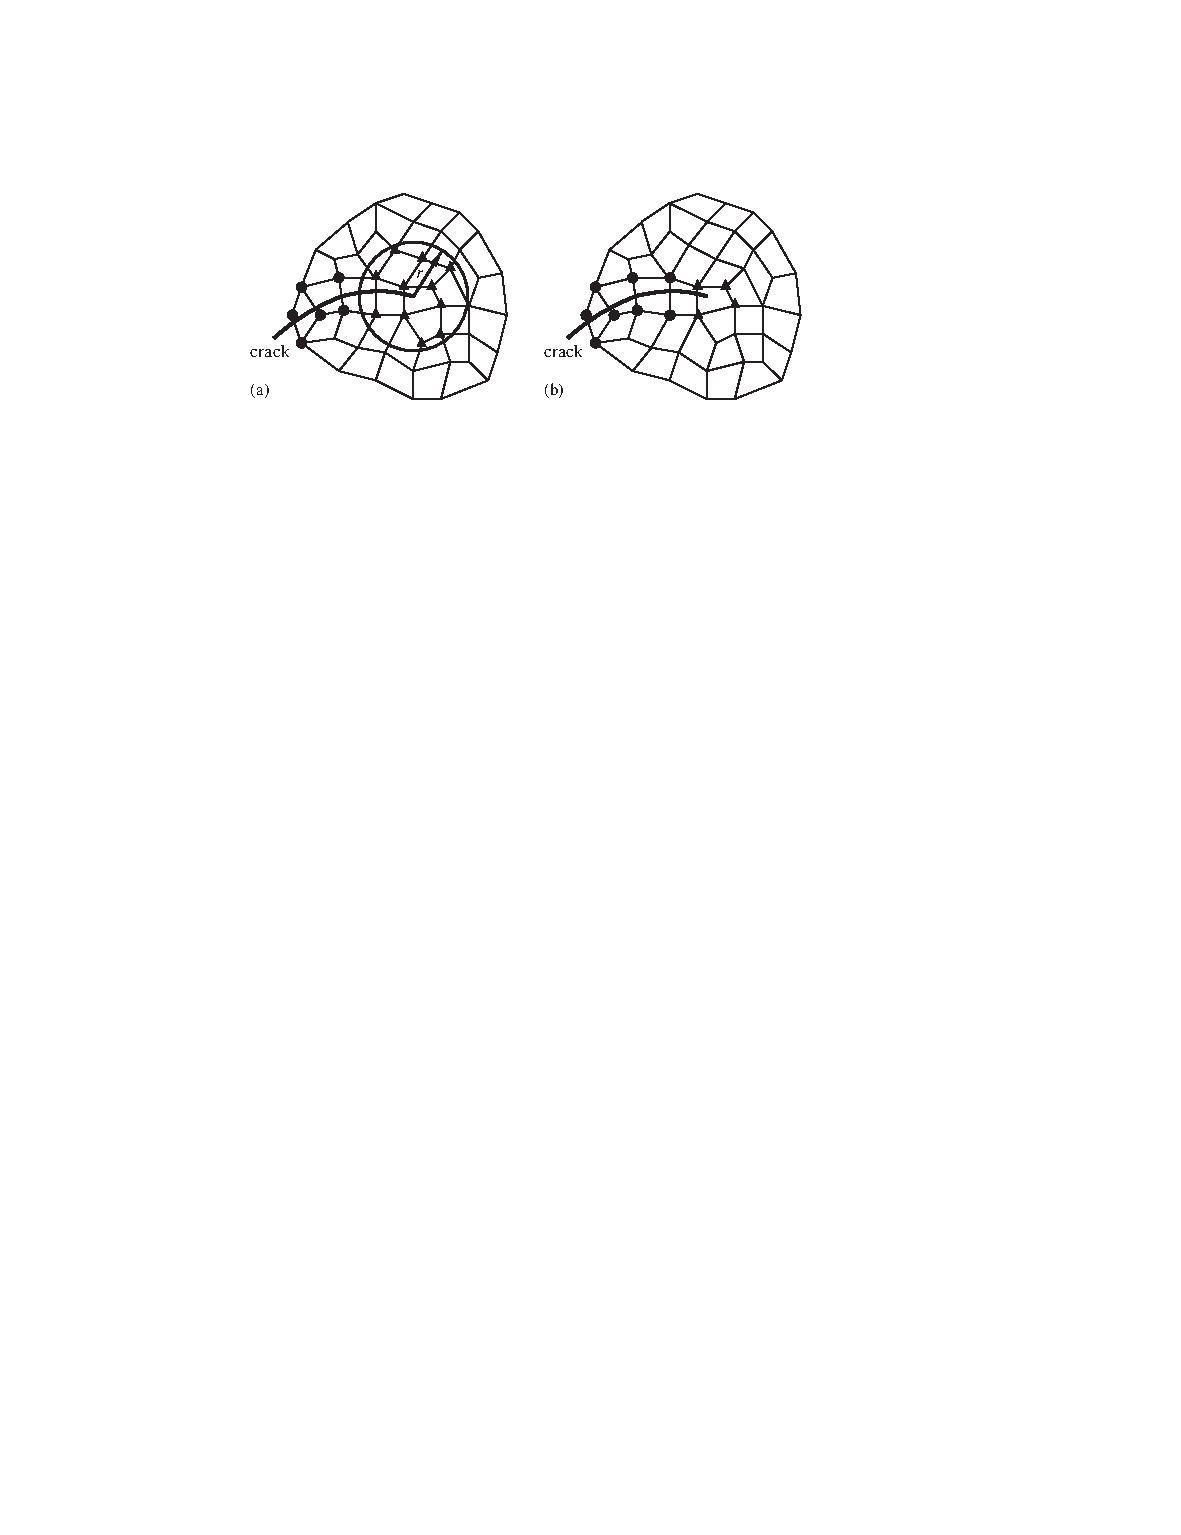
\includegraphics{XFEMenrichments}
\caption[XFEM models enrich nodes around a discontinuity]{XFEM models enrich nodes around a discontinuity\cite{fries2010extended}}
\label{fig:XFEM}
\end{figure}
%

More recently, Sauerland and Fries applied XFEM to two phase flow problems \cite{sauerland2013stable}, including standard dam-breaking and rising droplet problems.
Holl et al.~\cite{holl2013adaptive} used XFEM in the multi scale modeling of crack propagation, including multiple interacting cracks.
Mohammadnejad and Khoei~\cite{mohammadnejad2013hydro} and Hunsweck et al. \cite{hunsweck2013finite} modeled using XFEM the combination of fluid and fracture behavior found in hydraulic fracturing, a topic of considerable recent interest.

A second common method of modeling material failure is the Reproducing Kernel Particle Method (RKPM), developed by Liu et al.~\cite{liu1995reproducing}.
Mesh-based models track the connections between points in a deforming material, which can become problematic when large deformations deform the mesh and even cause it to intersect itself.
RKPM is a ``mesh-free'' method that tracks material properties by their values at selected points.
Mesh-free methods are advantageous for modeling large deformation in fluids and solids because they do not track connections between points.
Between material points, properties are interpolated from their values at nearby points by way of integration with a kernel function.
The difference in domains between RKPM and XFEM can be seen in \cref{fig:FEMvsRKPM}.
%
\begin{figure}[h]
  \centering
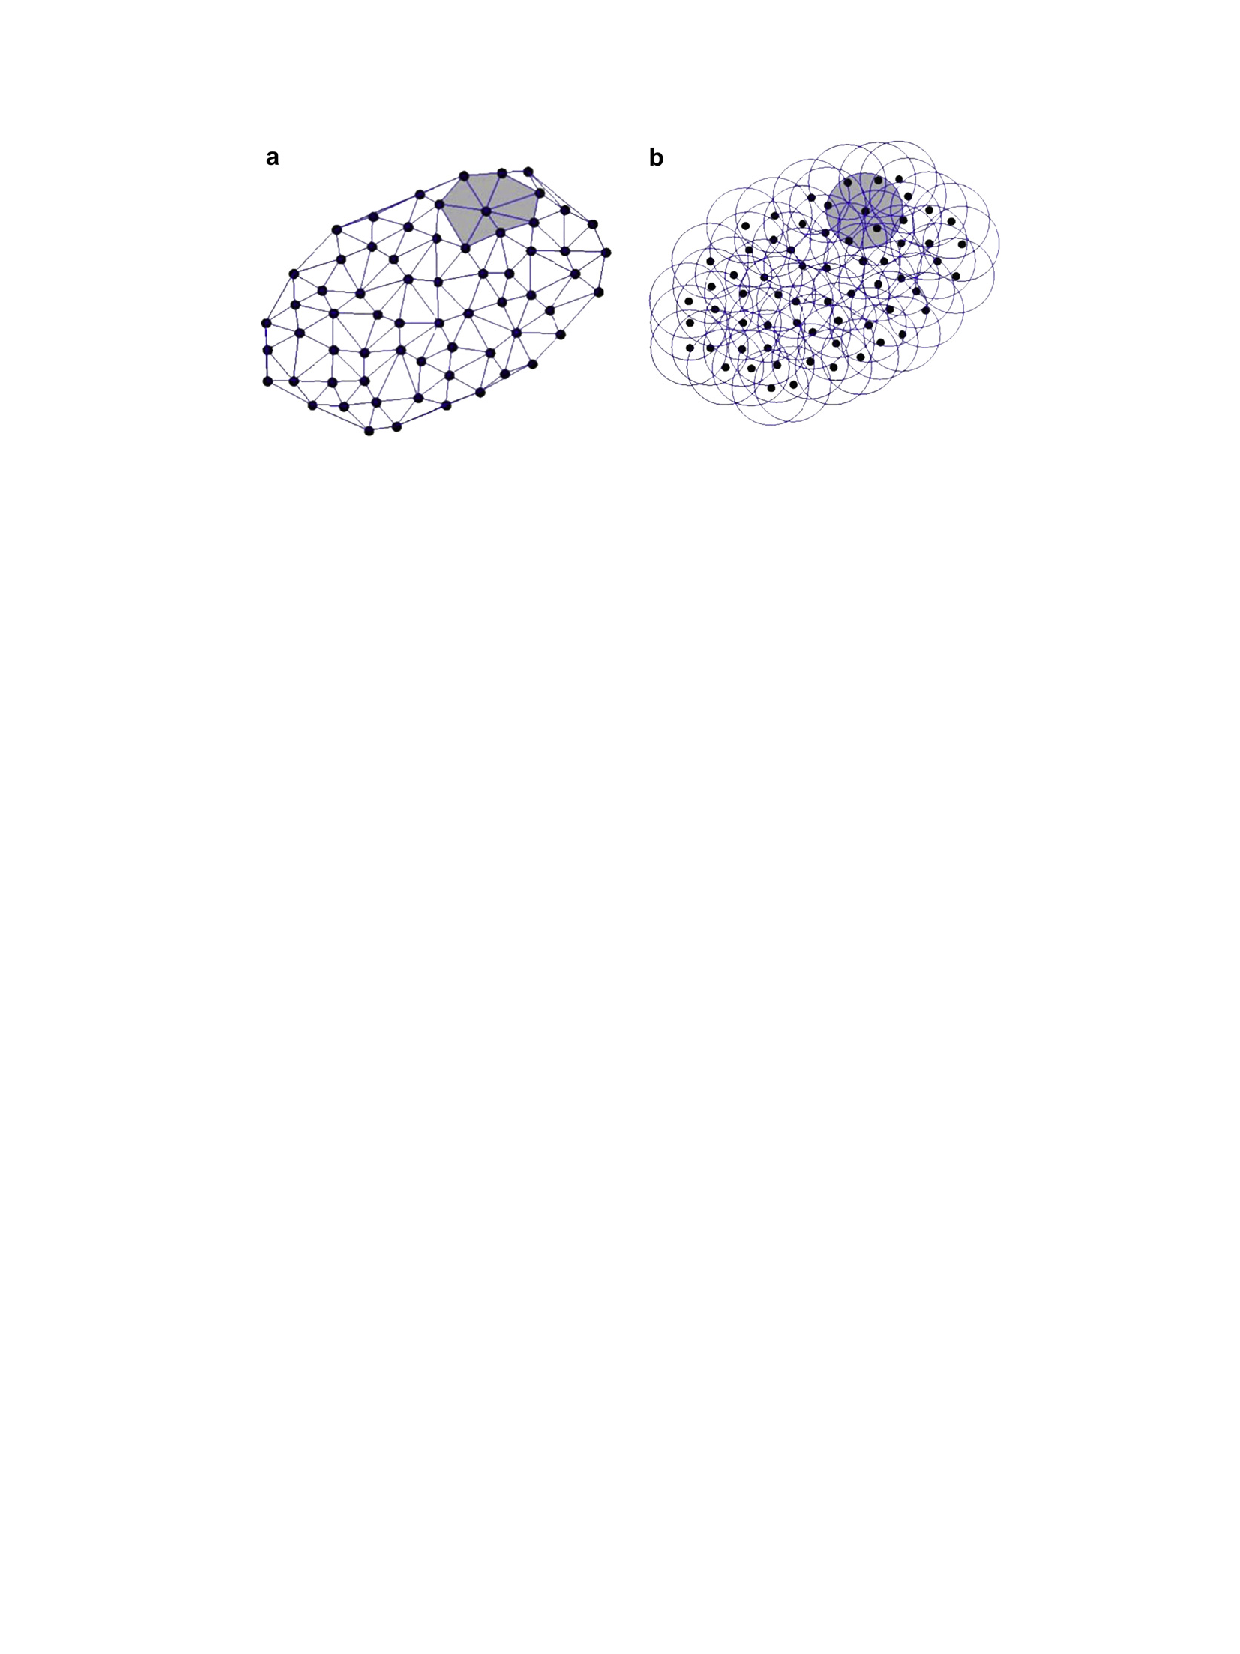
\includegraphics{FEMvsRKPM}
\caption[Comparison of domains of influence for FEM and RKPM]{Comparison of domains of influence for a)FEM and b)RKPM, by Guan et al. \cite{guan2011semi}}
\label{fig:FEMvsRKPM}
\end{figure}
%
The key to the RKPM lies in this kernel function; by using window functions from wavelet analysis, a ``reproducing'' kernel guarantees that  integrals of interpolated properties reproduce the integral of the continuous property field.
The ``reproducing'' kernel makes the RKPM a Partition of Unity method like XFEM, and is a major advantage of RKPM relative to other particle methods.
It is computationally expensive to perform the necessary shape-function integration, however.
The integration is typically performed on a background grid, raising concern over whether it is truly ``mesh-free''. 

In its original formulation, the RKPM successfully handles large deformations that would cause unacceptable distortion in Finite Element models.
A semi-Lagrangian version implemented by Guan et al. in \cite{guan2009semi} allows for recalculation of the support function.
This allows damage in the form of severing the relationship between points that have been pulled too far apart.
Recent applications of the RKPM include the work of Guan et al. on fragment-impact problems~\cite{guan2011semi} and analysis of non-linear wave equations by Cheng and Kim Meow~\cite{cheng2012analyzing}.
The RKPM has also been used by Xie and Wang~\cite{xie2014stabilized} to analyze coupled hydro-mechanical behavior.
Wu et al. have coupled RKPM and FEM in their recent work on fragmentation and debris evolution\cite{wu2014fragmentation}.

Other methods of modeling failure include multiple finite element techniques and particle methods.
Finite element methods incorporating ``element death'' remove from consideration elements that meet particular criteria and are perhaps the simplest way of modeling material failure.

Cohesive zone elements, proposed by Ortiz et al.~\cite{ortiz1987finite}, use element level information to detect the onset of plasticity (material instability) and add suitable deformation modes to model shear banding.
The additional deformation modes allow cohesive zone elements to capture the more complex displacements associated with plastic shear bands.
Other cohesive zone elements developed by Needleman\cite{needleman1987continuum} model crack growth, but Foulk et al.\cite{foulk2000formulation} note that this requires very fine meshes or prior knowledge of the crack path.
They are useful for cases such as composite delamination or debonding, where the crack follows a known surface.
Fang et al. propose in \cite{fang2011augmented} a method of augmenting the cohesive zone model to work in concert with XFEM-type elements to model both arbitrary and known crack paths.
More recently, McGarry et al. \cite{mcgarry2014potential} and M\'airt\'in et al. \cite{mairtin2014potential} developed a cohesive zone model to account for crack closure, including crack surface tractions.

Particle methods of modeling failure include the Smooth Particle Hydrodynamic (SPH) method, reviewed by Monaghan in \cite{monaghan2005smoothed}, in which a kernel (commonly a cubic spline) is used to create a smooth interpolation of actual quantities.
Unlike the wavelet basis functions of RKPM, which can be made to reproduce a polynomial field of any order, cubic splines only perfectly reproduce constant fields.
Developed for fluids, Springel notes in \cite{springel2010smoothed} that it is often used in astrophysics problems, where many fluid problems are encountered and even ``solid" bodies deform under their own gravity.
It can also predict elastic behavior and has been extended with failure models by Benz and Asphaug in \cite{benz1995simulations} by adding an evolving damage parameter.
Particle methods like SPH handle fragmentation very well, and are used in a variety of problems with material interfaces, high strains, and multiphase and multi-physics aspects.
Because cubic spline kernels do not reproduce a Partition of Unity, property interpolation does not accurately reproduce the continuum field.
Additionally, elastic SPH models do not conserve angular momentum, and in cases require artificial viscosities or artificial stresses to avoid numerical instability.

The Material Point Method, developed by Sulsky and Schreyer in~\cite{sulsky1996axisymmetric}, tracks points in both Eulerian and Lagrangian meshes.
The advantage of using both meshes is an ability to handle obstacles and boundary conditions without difficulty at large deformations.
Wieckowski notes that the downside to using both meshes is continual remeshing and added computational expense \cite{wikeckowski2004material}.
Despite this expense, the material point method was extended to model cracks by Nairn in \cite{nairn2003material}, then further enhanced by Sadeghirad et al. in \cite{sadeghirad2011convected} to improve stability when modeling massive deformations.
The Lattice Discrete Particle Method was developed by Cusatis et al.\cite{cusatis2011lattice,cusatis2011blattice} to model concrete.
Unlike perviously mentioned particle methods, the particles in LDPM represent actual particles of aggregate and the cement between them, with volume as well as mass.
It fills a volume with variously-sized particles generated from a probability density function based on aggregate size.
The relationships between these particles form tetrahedrons (the lattice) that fill the volume and allow multi-particle interaction.
As with finite element models, displacement between particle centers is linearized to compute strains, stresses, and forces.
Failure occurs at predefined surfaces between particles and can include various failure modes.
The LDPM is capable of accurately modeling many failure conditions in concrete, including the impact of specimen size on effective material behavior.
These are only a few of the myriad of models that attempt to model the progression of material failure.

All of these methods are used to solve a partial differential equation for conservation of momentum in a continuum. 
Because they are based on continuum PDEs, they do not naturally develop discontinuous displacements such as cracks. 
The PDEs that govern these methods are ill-defined at the surface of a crack, so cracks must be inserted within or between elements after discretization. 
This results in crack propagation that is discretization-dependent as well as computationally expensive and potentially unstable. 
Although progress in addressing these issues continues, much of the difficulty is essentially tied to the undefined nature of derivative equations at discontinuous displacements.
By abandoning the use of displacement derivatives, peridynamics offers an alternative way to address discontinuous displacements.
%

\section{Peridynamic Modeling}
The term \textit{peridynamic} was coined by Silling to describe the new formulation of continuum mechanics he developed in \cite{silling2000reformulation}.
From the Greek roots \textit{peri} and \textit{dyna} meaning \textit{near} and \textit{force} respectively, it alludes to the nonlocal force exerted by nearby points.
%In contrast to the nonlocal continuum mechanics models of Kr\"oner, Eringen and Edelen \cite{kroner1967elasticity,eringen1972nonlocal,eringen1983differential}, the peridynamic model casts material behavior at a point as an \textit{integral} \todo{Note Eringen's stress is an integral function of strain. Might be worth being specific.} equation of the surrounding displacement rather than the classical \textit{differential} equation.
In contrast to the nonlocal continuum mechanics models of Kr\"oner, Eringen and Edelen \cite{kroner1967elasticity,eringen1972nonlocal,eringen1983differential}, which formulate behavior as an integral function of strain (itself a spatial derivative of displacement), the peridynamic model casts material behavior at a point as an \textit{integral equation of the surrounding displacement} rather than the classical \textit{differential} equation.
Because peridynamic models do not include spatial displacement derivatives, discontinuous displacements can arise naturally and can be analyzed without first discretizing the problem or applying special heuristics.
In classical continuum mechanics, linear momentum is conserved according to the local  \cref{eq:ClassicCoPV},
%
\begin{equation}
\label{eq:ClassicCoPV}
\rho(\mathbf{x})\ddot{\mathbf{u}}(\mathbf{x}) = \nabla \cdot \mathbf{P}(\mathbf{x}) + \mathbf{b}(\mathbf{x})\, ,
\end{equation}
%
in which $\rho$ is the density, $\ddot{\mathbf{u}}$ is the second time derivative of displacement , $\mathbf{P}$ is the transpose of the First Piola Kirchhoff stress tensor, and $\mathbf{b}$ is the body force density, all of which are functions of position $\mathbf{x}$ and of time. 
Because \(\mathbf{P}\) is defined in terms of the deformation gradient, it is clear that \cref{eq:ClassicCoPV} is undefined for discontinuous displacements. 
In fact, traditional models require even the first spatial derivative of displacement to be continuous.
Strongly nonlocal models (including peridynamics) replace the divergence-of-stress term with an integral functional,
%
\begin{equation}
\label{eq:PDCoPV}
\rho(\mathbf{x})\ddot{\mathbf{u}}(\mathbf{x}) = \int_\Omega \mathbf{f}(\mathbf{x},\mathbf{q}) dV_\mathbf{q}  + \mathbf{b}(\mathbf{x})\, ,
\end{equation}
%
so that, instead of the divergence of stress, we have the integral of a ``force" function $\mathbf{f}$ of the position vector $\mathbf{x}$ and the position vector $\mathbf{q}$ of a point within the body domain $\Omega$. 
This force function may depend on \(\mathbf{x}\), \(\mathbf{q}\), their deformed positions, the original and deformed positions of other points in \(\Omega\), history, etc.
It is common for \(\mathbf{f}\) to be defined as \(0\) for any pair of points initially further than \(\delta\) apart. 
The points within \(\delta\) of a point \(\mathbf{x}\) are the \textit{neighborhood} of \(\mathbf{x}\) and are denoted in \cref{fig:PDbody} by \(\mathcal{H}\).
%
\begin{figure}[h]
  \centering
\subinputfrom{\diagrampath}{PDbody.eps_tex}
\caption{A peridynamic body \protect\(\Omega\protect\)}
\label{fig:PDbody}
\end{figure}
% 
By including the behavior of nearby material, these models introduce an inherent length scale to the model. 
This length scale is theoretically determined by material properties, though choice of length scale is sometimes limited by computational demands.

Constitutive modeling of a wide variety of materials is accomplished by choosing the appropriate form for the force function.
The form of the simplest such function is a peridynamic ``bond'' between two points that is modeled by a pairwise force function.
While the simplest force functions recreate a one-parameter linear elastic solid material, other force functions can be used to model a wide variety of material behaviors, some of which will be outlined here.
Most simulation of material behavior uses an equation of motion reformulated for a discretized model.
The typical discretization is a mesh-free numerical method in which there are no geometrical connectivities between various nodes.

A force function can be restricted to being pairwise (depending solely on the displacement of the two points \(\mathbf{x}\) and \(\mathbf{q}\)), and still model complex and varied behavior.
By including a damage parameter that sets the force contribution of ``damaged'' bonds to \(0\), Silling and Askari\cite{silling2005meshfree} were able to model a brittle material with natural crack formation, propagation, and branching.
Other examples of damage propagation include impacts against brittle structures as in \cref{fig:PDimpact} modeled by Demmie and Silling\cite{demmie2007approach} and fracturing of thermally-stressed glass modeled by Kilic and Madenci\cite{kilic2009prediction}. 
%
\begin{figure}[h]
  \centering
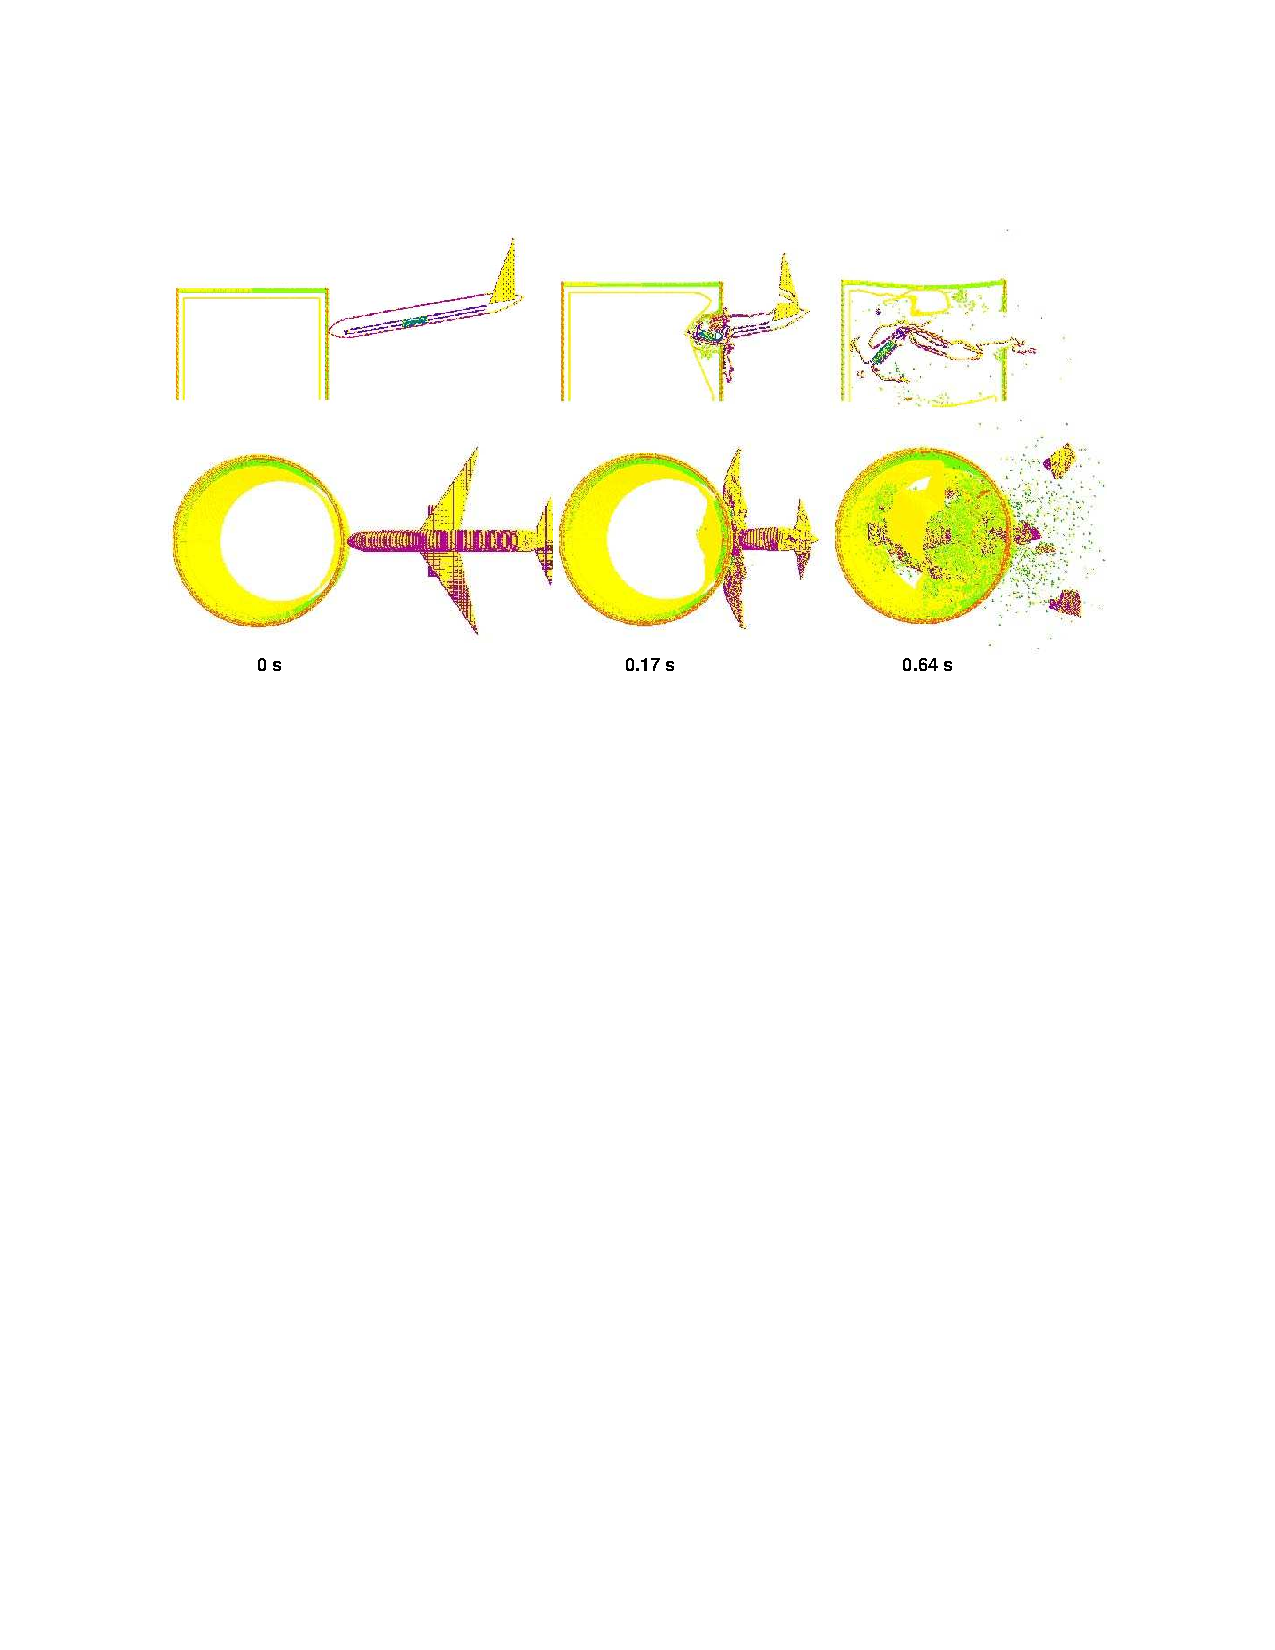
\includegraphics[width=0.8 \textwidth]{demmie07impact}
\caption[Peridynamic model of an airplane impacting a concrete structure]{Peridynamic model of an airplane impacting a concrete structure \cite{demmie2007approach} }
\label{fig:PDimpact}
\end{figure}
%
Modeling progressive fracture, including crack branching, is a major advantage of peridynamic formulations.
Using a piecewise force function, Dayal and Bhattacharya~\cite{dayal2006kinetics} were able to model phase transformation in 1D and 2D without an additional constitutive law; the transformations arose and propagated naturally as a dynamic instability, a result of the force function used.
Peridynamic models have also been used to analyze composite laminates.
In \cite{xu2008peridynamic}, Xu et al. designate peridynamic bonds as fiber or matrix bonds with different force functions to model damage in composite laminates. 
Kilic et al. model fiber, matrix, and interfacial bonds in \cite{kilic2009peridynamic} to capture stacking order effects on damage propagation.
Bobaru~\cite{bobaru2007influence} applied the peridynamic model to nano fiber networks, at a scale where long-range forces are very apparent.
In the same paper he created a Representative Volume Element (RVE) for random networks of nano fibers, laying the ground work for peridynamic multi-scale modeling.
Also related to multi-scale peridynamic modeling is work by Silling on model coarsening \cite{silling2011coarsening}, \cref{fig:PDmultiscale}.
An example of a multi-scale peridynamic simulation can be found in \cite{askari2008peridynamics}, by Askari et al.
%
\begin{figure}[h]
  \centering
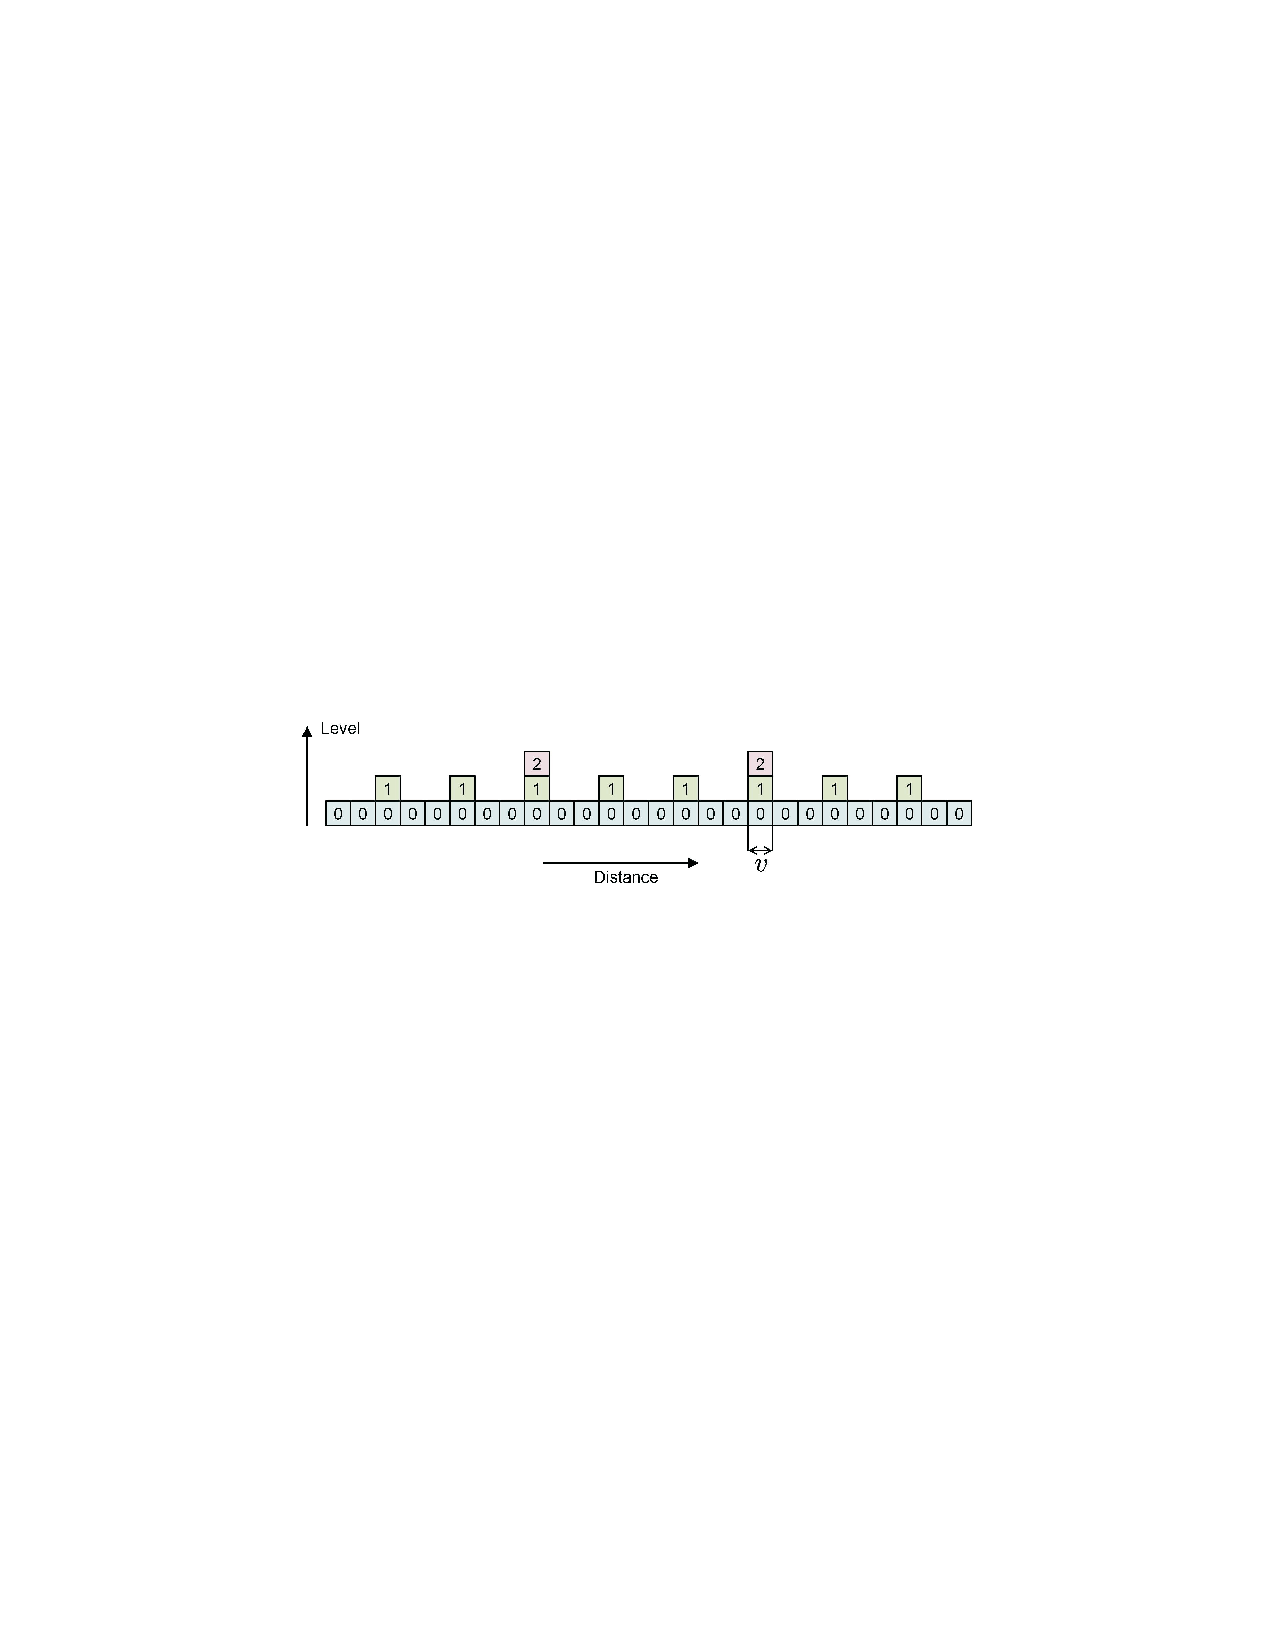
\includegraphics{PDmultiscale}
\caption[Silling's illustration of course-graining in time]{Silling's illustration of course-graining in time from \cite{silling2011coarsening}.}
\label{fig:PDmultiscale}
\end{figure}
%

Concrete is a nearly standard example material in which nonlocal behavior is easily observed, and modeling the damage accumulation and proceeding discontinuity propagation has long been the goal of nonlocal models developed by Ba\v{z}ant and Pijaudier-Cabot~\cite{bazant1988nonlocal} among others, significantly predating peridynamics.
In \cite{gerstle2007peridynamic}, Gerstle et al. use rotational degrees of freedom to create a concrete material model, capable of describing a linear elastic material with any Poisson ratio, that also handles material failure.
Peridynamic models are not limited to force-displacement relationships; the theory has also been applied to diffusion processes and multiphysics problems.
Peridynamic models can simulate heat transfer~\cite{bobaru2010peridynamic} and diffusion~\cite{burch2011classical}.

Mathematical analyses of simplified cases have also been fruitful.
Weckner~\cite{weckner2005effect} determined analytical solutions to the infinite bar problem. 
Emmerlick and Zimmerman proved solution existence and uniqueness in the simplest case of the peridynamic bar~\cite{emmrich2007analysis}.
Mikata found additional analytical solutions for the bar problem~\cite{mikata2012analytical}.
In 3D, Weckner constructed Green's functions for an infinite peridynamic solid in \cite{weckner2009green}.
All of this work was done with peridynamic models limited to pairwise force functions.

Other than Gerstle's aforementioned micropolar peridynamic model, the pairwise force function limits 3D solid materials to a Poisson ratio of  \(\nu=\sfrac{1}{4}\). 
To model additional material behavior, Silling et al. generalized the underlying peridynamic concept of bonds and forces and introduced state-based peridynamic models in \cite{silling2007peridynamic}.
By freeing the force function from the pairwise restriction, state-based models allow the force relationship between two points to depend on the collective behavior of all nearby material.
Using the concept of a deformation vector-state allows for the construction of correspondence models that can recreate any classical constitutive model.
These correspondence models use the deformation state to approximate the deformation gradient tensor, then use the deformation gradient tensor to calculate force contributions.
State-based models were used by Foster et al. to simulate viscoplasticity and hardening in~\cite{foster2010viscoplasticity}, and rate dependent failure in~\cite{foster2011energy}, with others, via an energy criterion.
Mitchell describes state-based models for plasticity in~\cite{mitchell2011nonlocal} and viscoelasticity in~\cite{mitchell2011non}.
A non-ordinary state-based model was used by Warren et al. to simulate fracture in~\cite{warren2009non}.
More recently, Tupek et al. have incorporated the idea of peridynamic damage into a Johnson-Cook based damage state that accumulates with plastic strain\cite{tupek2013approach}.
%
\section{Other Nonlocal Elasticity Models}
\label{sec:NLbeams}
%
The peridynamic formulation of continuum mechanics is neither the only nor the first nonlocal model. Nonlocal elasticity generally allows for forces at a point that are dependent on the material configuration of an entire body, rather than the configuration at that point \cite{eringen1972nonlocal}.  While long-range forces are obvious at the molecular model, material at larger scales is conventionally modeled as though internal forces are local or contact forces \cite{kroner1967elasticity}.
The result of such approximation is accurate for deformations that are homogeneous, but introduces some inaccuracy for inhomogeneous deformations like the propagation of waves with short wavelengths.
One way to distinguish between homogeneous and inhomogeneous deformations is to incorporate higher-order gradients of deformation.
While stress in classical elasticity is a function of the (first) gradient of deformation, Eringen's formulation of a nonlocal modulus in \cite{eringen1983differential} approximates a weighted sum of the first and second order gradients.
This introduces a length scale to the model and has the effect of smearing out local deformation inhomogeneities over the surrounding material, while maintaining the conventional result for homogeneous deformations.

Previous work in the nonlocal mechanics of beams is motivated by the observed stiffening of nanoscale cantilevers.
Challamel and Wang demonstrate in \cite{Challamel2008small} that Eringen nonlocal elasticity cannot reproduce the scale stiffening, but that stiffening does result from other gradient-elastic models and models incorporating nonlocal curvature.
Because all of these models incorporate higher-order gradients of deformation, they impose stronger continuity requirements than classical elasticity, and are unsuitable for discontinuous displacements.
Because the gradients are evaluated locally, gradient models are called \textit{weakly nonlocal}.
Recent work by Paolo et al. \cite{paola2013mechanically} develops a displacement-based beam in which relative axial displacement, shear displacement, and rotation of non-adjacent beam segments are resisted by three kinds of nonlocal spring, whose stiffnesses can be tuned to the expected material behavior.
With the appropriate nonlocal stiffnesses, their model reproduces the nanoscale cantilever stiffening effect.

Similarly, Duan and Wang \cite{duan2007exact} applied Eringen-type elasticity to the quasi-1D problem of axisymmetric bending in nanoscale plates.
Pradhan and Murmu~\cite{pradhan2009small} extended the concept to buckling in single-layered graphed sheets, a fully 2D problem.
Later, Ansari et al.~\cite{ansari2010nonlocal} modeled the vibration of single-layered graphed sheets using Eringen-type elasticity.

Nonlocal effects have also been incorporated into many of the modeling techniques previously discussed.
Ba\v{z}ant and Chang incorporated nonlocal strain-softening into a finite element model in \cite{bazant1987nonlocal}.
Any interpolating particle method will exhibit some measure of nonlocality, but some explicitly model nonlocal phenomena.
Vignjevic et al. used SPH to model nonlocal strain-softening in \cite{vignjevic2014sph}, and in \cite{burghardt2012nonlocal}, Burghardt et al. developed a material point method that incorporates nonlocal plasticity.

\section{Thin Features}
Many engineering analyses concern shapes that have one dimension much greater than another; numerical modeling the behavior of these shapes can be a considerable challenge for methods designed for 3D solids. 
In finite element models, for example, calculations can become unstable or too stiff when individual elements become long and thin. 
To avoid such elements while maintaining model fidelity requires a very large number of solid elements. 
By making some assumptions about the behavior along the thin direction, many such shapes can be modeled as 1D beams or 2D plates or shells without great loss of accuracy.
A comprehensive review of the classical continuum mechanics associated with thin features by Reddy \cite{reddy2007theory} also includes a section on the finite element analysis of plates and shells.
Material failure in classical thin features is modeled using the same techniques as in solids.
Dolbow et al. use XFEM in~\cite{dolbow2000modeling} to model fracture in plates.
Li et al. use a variant of RKPM in~\cite{li2000numerical} to model plastic deformation in shells.
More recently, Xu et al. have applied XFEM to plate plasticity problems\cite{xu2013xfem}, and Memar Ardestani et al. have used RKPM to model functionally graded plates\cite{memar2014analysis}.
Other authors use cohesive zone elements\cite{li2002analysis} or SPH\cite{maurel2008sph} to study failure in thin features.
%

\subsection{Peridynamic Models}
Reduced dimension thin features such as bars\cite{silling2003deformation,weckner2005effect,emmrich2007analysis,mikata2012analytical}, plates\cite{kilic2009prediction}, and membranes\cite{silling2005peridynamic} have been modeled using peridynamics, but these models are used for in-plane or membrane forces as shown in \cref{fig:PDmembrane}.
%
\begin{figure}[h]
  \centering
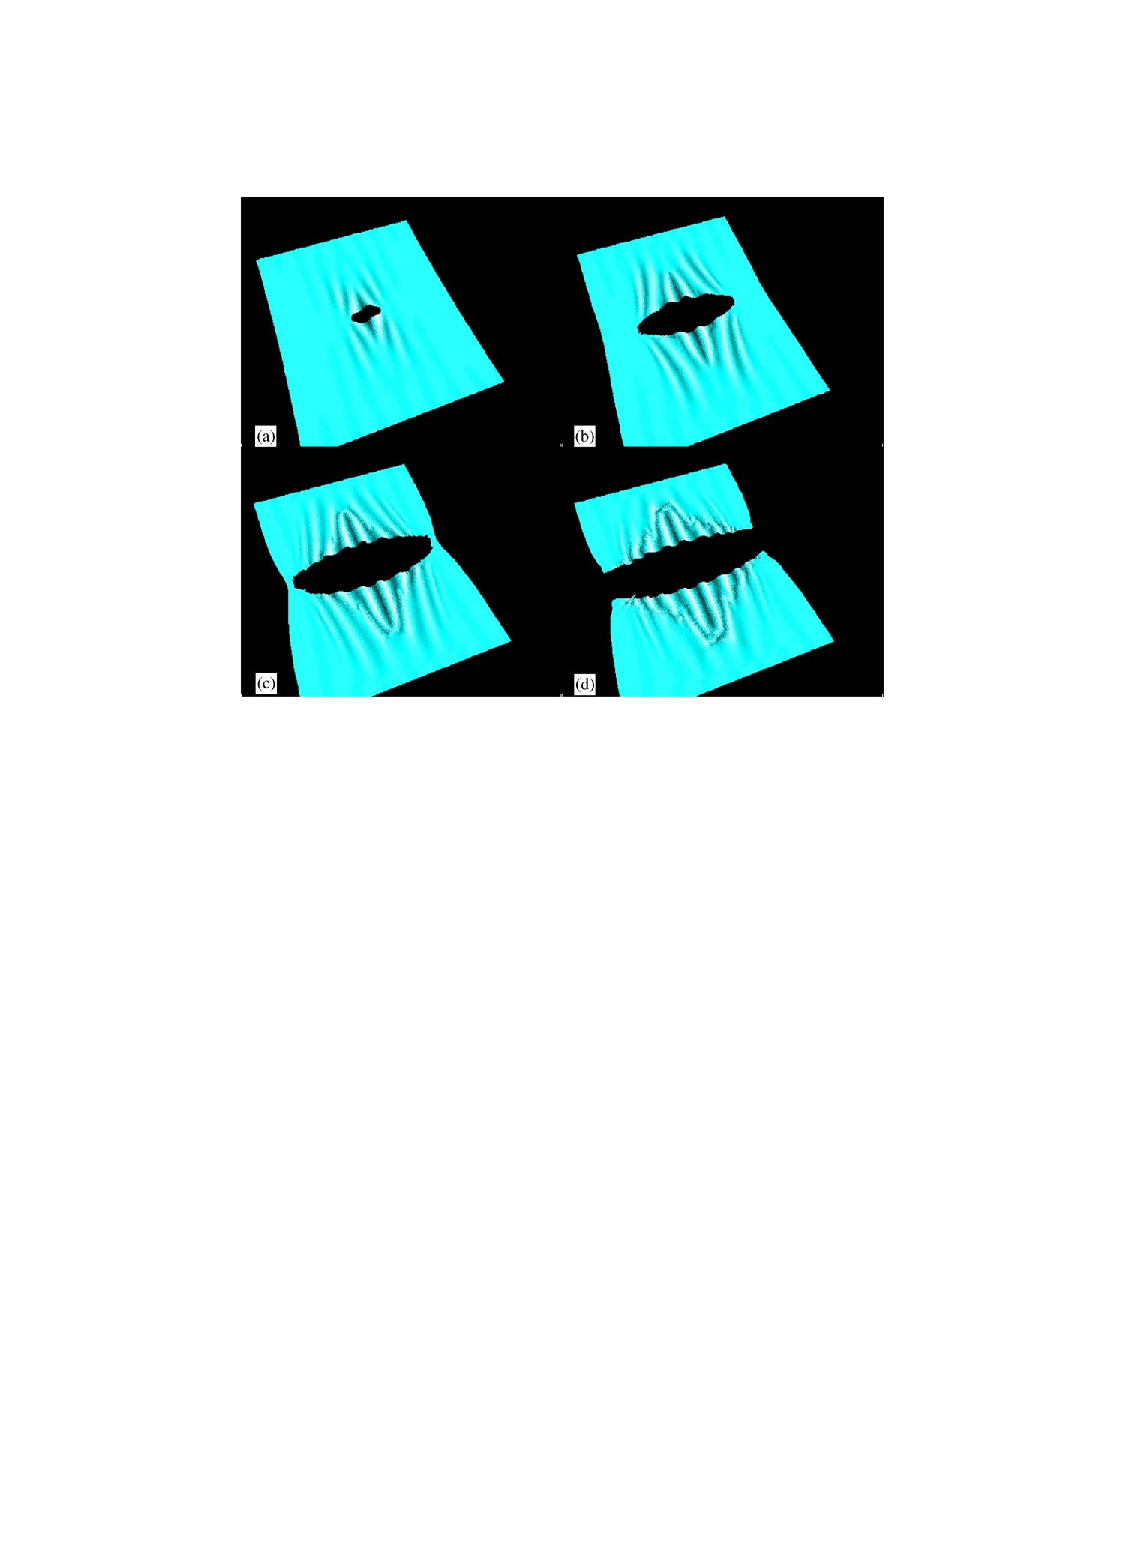
\includegraphics{PDmembrane}
\caption[Tearing a peridynamic membrane]{Tearing a peridynamic membrane \cite{silling2005peridynamic}}
\label{fig:PDmembrane}
\end{figure}
%
Because traditional peridynamic models exert forces in the direction of the bonds between points, they are not well-suited for bending problems of thin shapes, in which force and displacement are both nearly perpendicular to bonds connecting material points at separate points on a surface.
Just as with solid finite elements, most peridynamic models of thin features like the tubes in \cref{fig:LittlewoodCylinder} have included several nodes through the thickness of a thin part to capture bending behavior.
Also as with solid finite elements, this leads to very fine discretization of thin features, even when the expected behavior is quite simple.
This greatly increases the computational expense of modeling parts with thin features.
%
\begin{figure}[h!]
  \centering
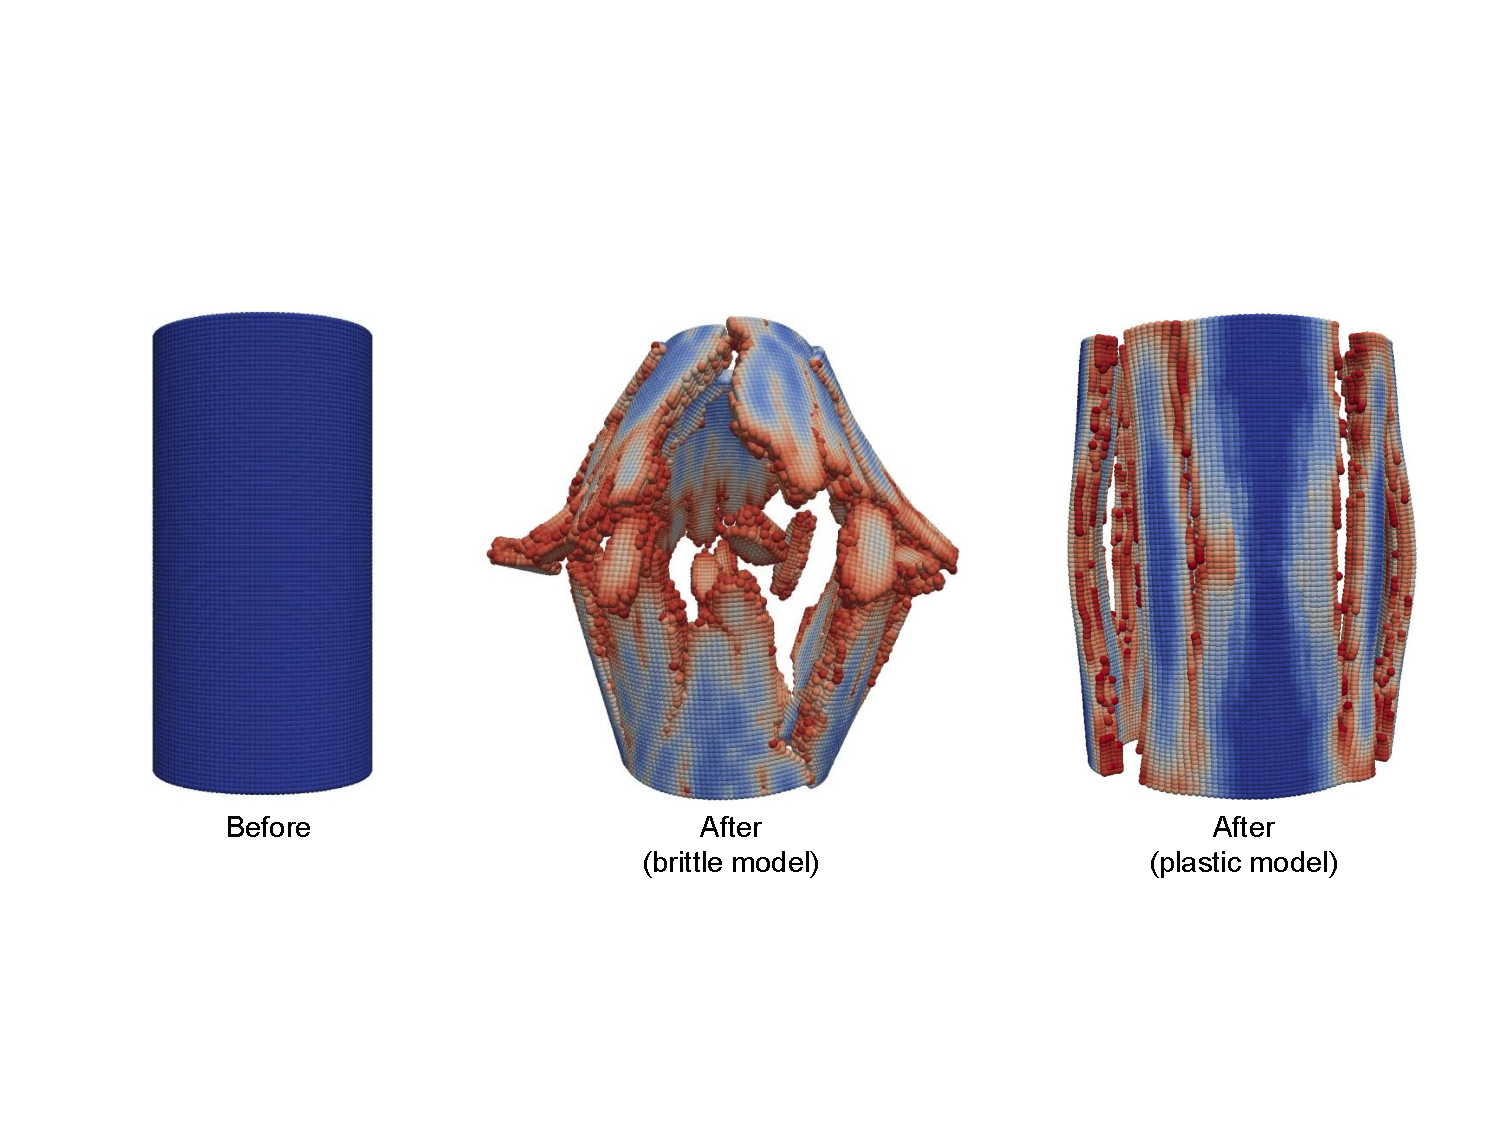
\includegraphics[width=0.9 \textwidth]{LittlewoodCylinder}
\caption[A peridynamic cylinder uses several nodes through its thickness]{A peridynamic cylinder uses several nodes through its thickness in \cite{littlewood2010simulation}}
\label{fig:LittlewoodCylinder}
\end{figure}
%

A recent paper by Taylor and Steigmann~\cite{taylor2013two} partially addresses this issue by starting with mathematical analysis of the continuous 3D bond-based peridynamic solid model of a thin plate.
By using a continuous model, they avoid the difficulties associated with discretizing thin features.
Applying asymptotic analysis to the continuous model, they reduce a 3D solid model to 2 dimensions.
The asymptotic reduction is accomplished by the addition of degrees of freedom for the derivative of displacement with respect to the through thickness direction.
By making the through-thickness derivative of displacement vector an independent variable, the resulting flat model includes a measure of angular deformation that allows resistance to bending.
Using a simple bond-stretch damage criterion, the Taylor and Steigmann's reduced model was able to capture the out-of-plane displacement (\cref{fig:TaylorTransverse}) associated with crack propagation behavior (\cref{fig:TaylorCrack}) in a pre-cracked plate under tension loading.
In general, however, the asymptotic reduction model encounters difficulty when nonlinear behaviors like damage are implemented.
The use of a bond-stretch criterion as implemented is only appropriate when deformation is dominated by in-plane tension, as failure caused by bending will not be captured.
Because of its basis in the 3D bond-based solid model, Taylor and Steigmann's model is limited to a Poisson's ratio of \sfrac{1}{3}.
While it is possible that future analysis will extend the asymptotic reduction to state-based model, allowing for arbitrary Poisson's ratios, there are significant mathematical hurdles that will have to be overcome.

%
\begin{figure}[h!]
  \centering
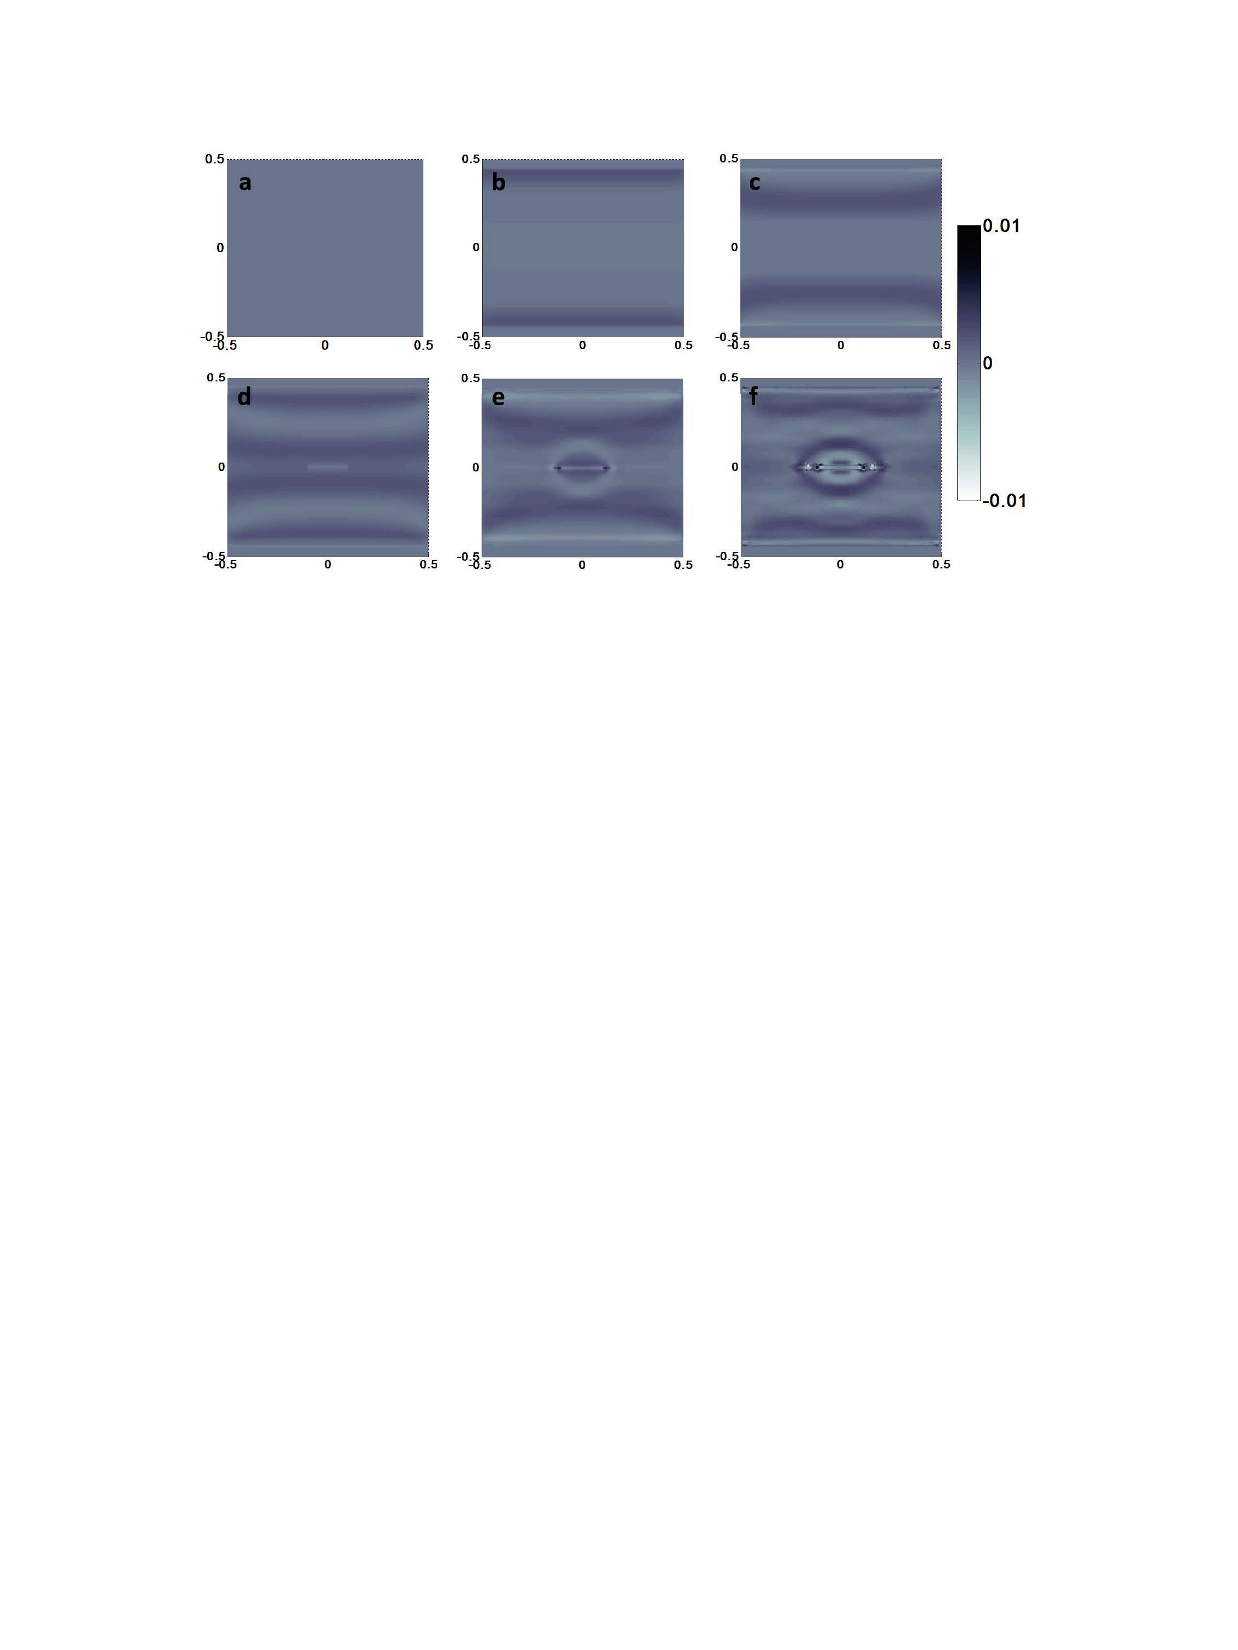
\includegraphics[width=0.9 \textwidth]{TaylorTransverseDisp}
\caption[Taylor and Steigmann plate transverse displacement]{Taylor and Steigmann's asymptotic reduction allows for bending resistance in a 2D plate in tension~\cite{taylor2013two}}
\label{fig:TaylorTransverse}
\end{figure}
%
%
\begin{figure}[h!]
  \centering
\includegraphics[width=0.4 \textwidth]{Taylor2DCrack}
\caption[Taylor and Steigmann plate cracking]{Taylor and Steigmann's crack propagation for \cref{fig:TaylorTransverse} plot \textbf{f}~\cite{taylor2013two}}
\label{fig:TaylorCrack}
\end{figure}
%

%A nonordinary model similar to those proposed by Silling in \cite{silling2007peridynamic} and \cite{silling2010peridynamic} allows for a simple bending model that can be used for one- and two-dimensional models.

%Recent work by Oterkus includes additional degrees of freedom to describe the orientation of each peridynamic point, so that each bond between points has components for differential displacements and for differential orientations. 
%These are incorporated into a bond-based thin feature model for beams, plates and shells. 
%These models appear to include spatial derivatives and in the case of plates are constrained to the same Poisson ratio as other bond-based models.

\chapter{Classical Background}
\label{ch:ClassicBack}
\section{Euler-Bernoulli Beam Theory}
%
The simplest representation of bending behavior is found in the Euler-Bernoulli beam equation, 
\begin{equation}
\label{eq:EulerBeam}
\frac{\text{d}^2}{\text{d}x^2}\left(EI\frac{\text{d}^2 v}{\text{d} x^2}\right) = q\, ,
\end{equation}
which describes the transverse deflection of long-slender beams.
\Cref{eq:EulerBeam} is for a beam in the $\hat{x}$ direction, whose displacement $v$ is perpendicular to $\hat{x}$ and parallel to the distributed load $q$ acting on the beam.
While it is only applicable to small deformations and rotations, there are many problems that can be easily and usefully simplified by the application of Euler beams.

It is important to note that \cref{eq:EulerBeam} is not a constitutive equation; it does not relate stress and strain for a material. 
Instead, it is derived from the constitutive equation for a linearly-elastic material and some assumptions about the deformation.
Euler-Bernoulli beam theory is much simpler than a 3D analysis of a beam as a solid material, but it requires the following assumptions to be met:
\begin{itemize}
 \item Slenderness: the length of the beam should be 20 times its other dimensions
 \item Loaded transversely, no axial loads or torques
 \item Small deformations and rotations
 \item Plane cross-sections of the beam remain plane under deformation
 \item Initially straight, and symmetric about the plane of bending
\end{itemize}
First, we take a infinitesimal slice of a beam as depicted in \cref{fig:Infinitesimal}.
Because we will want to compare to this model later, we use a different $y$-coordinate direction than many presentations.
We use this infinitesimal slice to derive the relationship between load, shear, and moment.

%
\begin{figure}[htbp]
  \centering
  


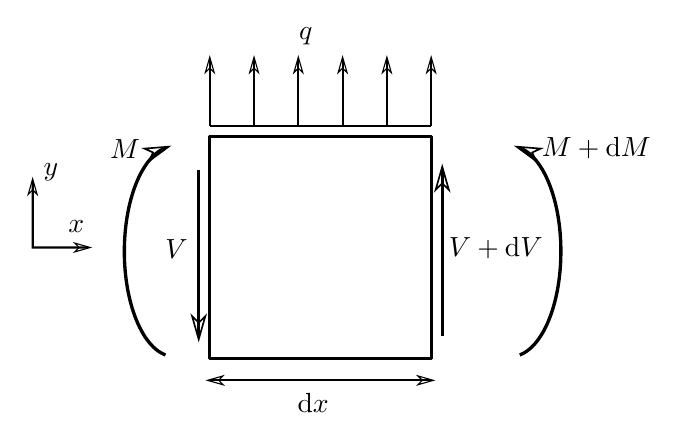
\begin{tikzpicture}[y=0.80pt, x=0.8pt,yscale=-1, inner sep=0pt, outer sep=0pt]
\begin{scope}[shift={(0,-752.36218)}]
  \path[draw=black,fill=black,line join=round,miter limit=4.00,fill
    opacity=0.000,nonzero rule,line width=1.200pt,rounded corners=0.0000cm]
    (95.0000,852.3622) rectangle (195.0000,952.3622);
    \path[color=black,fill=black,line width=0.800pt] (95.0000,961.8750) --
      (95.0000,962.8750) -- (195.0000,962.8750) -- (195.0000,961.8750) --
      (95.0000,961.8750) -- cycle;
    \path[draw=black,even odd rule,line width=0.400pt] (99.0000,962.3622) --
      (101.0000,960.3622) -- (94.0000,962.3622) -- (101.0000,964.3622) --
      (99.0000,962.3622) -- cycle;
    \path[draw=black,even odd rule,line width=0.400pt] (191.0000,962.3622) --
      (189.0000,964.3622) -- (196.0000,962.3622) -- (189.0000,960.3622) --
      (191.0000,962.3622) -- cycle;
    \path[color=black,fill=black,line width=1.200pt] (199.2500,867.3750) --
      (199.2500,942.3750) -- (200.7500,942.3750) -- (200.7500,867.3750) --
      (199.2500,867.3750) -- cycle;
    \path[draw=black,even odd rule,line width=0.600pt] (200.0000,873.3622) --
      (203.0000,876.3622) -- (200.0000,865.8622) -- (197.0000,876.3622) --
      (200.0000,873.3622) -- cycle;
    \path[color=black,fill=black,line width=1.200pt] (89.2500,867.3750) --
      (89.2500,942.3750) -- (90.7500,942.3750) -- (90.7500,867.3750) --
      (89.2500,867.3750) -- cycle;
    \path[draw=black,even odd rule,line width=0.600pt] (90.0000,936.3622) --
      (87.0000,933.3622) -- (90.0000,943.8622) -- (93.0000,933.3622) --
      (90.0000,936.3622) -- cycle;
    \path[color=black,fill=black,nonzero rule,line width=1.200pt] (74.7508,856.6718)
      .. controls (69.8130,858.5099) and (65.5561,863.3884) .. (62.3133,870.2343) ..
      controls (59.0705,877.0802) and (56.8284,885.9197) .. (56.0008,895.8280) ..
      controls (54.9137,908.8435) and (56.4098,921.5363) .. (59.7508,931.6093) ..
      controls (63.0918,941.6823) and (68.2689,949.1964) .. (74.7508,951.6093) --
      (75.2508,950.2030) .. controls (69.4951,948.0605) and (64.4529,940.9833) ..
      (61.1883,931.1405) .. controls (57.9237,921.2978) and (56.4301,908.7726) ..
      (57.5008,895.9530) .. controls (58.3158,886.1958) and (60.5450,877.4952) ..
      (63.6883,870.8593) .. controls (66.8316,864.2234) and (70.8734,859.7075) ..
      (75.2508,858.0780) -- (74.7508,856.6718) -- cycle;
    \path[draw=black,even odd rule,line width=0.600pt] (69.3769,859.4553) --
      (67.6120,863.3134) -- (76.4058,856.8389) -- (65.5188,857.6904) --
      (69.3769,859.4553) -- cycle;
    \path[color=black,fill=black,nonzero rule,line width=1.200pt]
      (235.2492,856.6718) -- (234.7492,858.0780) .. controls (240.5049,860.2206) and
      (245.5471,867.2978) .. (248.8117,877.1405) .. controls (252.0763,886.9833) and
      (253.5699,899.5085) .. (252.4992,912.3280) .. controls (251.6842,922.0852) and
      (249.4550,930.7859) .. (246.3117,937.4218) .. controls (243.1684,944.0577) and
      (239.1266,948.5735) .. (234.7492,950.2030) -- (235.2492,951.6093) .. controls
      (240.1869,949.7712) and (244.4439,944.8927) .. (247.6867,938.0468) .. controls
      (250.9295,931.2009) and (253.1716,922.3614) .. (253.9992,912.4530) .. controls
      (255.0863,899.4376) and (253.5902,886.7448) .. (250.2492,876.6718) .. controls
      (246.9082,866.5988) and (241.7311,859.0847) .. (235.2492,856.6718) -- cycle;
    \path[draw=black,even odd rule,line width=0.600pt] (240.6231,859.4553) --
      (244.4812,857.6904) -- (233.5942,856.8389) -- (242.3880,863.3134) --
      (240.6231,859.4553) -- cycle;
  \path[fill=black] (134.65359,976.70172) node[above right] (text7264) {d$x$};
  \path[fill=black] (75,907.36218) node[above right] (text7268) {$V$};
  \path[fill=black] (50,862.36218) node[above right] (text7272) {$M$};
  \path[fill=black] (203,907.36218) node[above right] (text7276) {$V+\text{d}V$};
  \path[fill=black] (245,862.36218) node[above right] (text7280) {$M+\text{d}M$};
  \path[draw=black,line join=miter,line cap=butt,line width=0.800pt]
    (95.0000,847.3622) -- (195.0000,847.3622);
    \path[color=black,fill=black,line width=0.800pt] (94.5000,817.3750) --
      (94.5000,847.3750) -- (95.5000,847.3750) -- (95.5000,817.3750) --
      (94.5000,817.3750) -- cycle;
    \path[draw=black,even odd rule,line width=0.400pt] (95.0000,821.3622) --
      (97.0000,823.3622) -- (95.0000,816.3622) -- (93.0000,823.3622) --
      (95.0000,821.3622) -- cycle;
    \path[color=black,fill=black,line width=0.800pt] (174.5000,817.3750) --
      (174.5000,847.3750) -- (175.5000,847.3750) -- (175.5000,817.3750) --
      (174.5000,817.3750) -- cycle;
    \path[draw=black,even odd rule,line width=0.400pt] (175.0000,821.3622) --
      (177.0000,823.3622) -- (175.0000,816.3622) -- (173.0000,823.3622) --
      (175.0000,821.3622) -- cycle;
    \path[color=black,fill=black,line width=0.800pt] (114.5000,817.3750) --
      (114.5000,847.3750) -- (115.5000,847.3750) -- (115.5000,817.3750) --
      (114.5000,817.3750) -- cycle;
    \path[draw=black,even odd rule,line width=0.400pt] (115.0000,821.3622) --
      (117.0000,823.3622) -- (115.0000,816.3622) -- (113.0000,823.3622) --
      (115.0000,821.3622) -- cycle;
    \path[color=black,fill=black,line width=0.800pt] (134.5000,817.3750) --
      (134.5000,847.3750) -- (135.5000,847.3750) -- (135.5000,817.3750) --
      (134.5000,817.3750) -- cycle;
    \path[draw=black,even odd rule,line width=0.400pt] (135.0000,821.3622) --
      (137.0000,823.3622) -- (135.0000,816.3622) -- (133.0000,823.3622) --
      (135.0000,821.3622) -- cycle;
    \path[color=black,fill=black,line width=0.800pt] (194.5000,817.3750) --
      (194.5000,847.3750) -- (195.5000,847.3750) -- (195.5000,817.3750) --
      (194.5000,817.3750) -- cycle;
    \path[draw=black,even odd rule,line width=0.400pt] (195.0000,821.3622) --
      (197.0000,823.3622) -- (195.0000,816.3622) -- (193.0000,823.3622) --
      (195.0000,821.3622) -- cycle;
    \path[color=black,fill=black,line width=0.800pt] (154.5000,817.3750) --
      (154.5000,847.3750) -- (155.5000,847.3750) -- (155.5000,817.3750) --
      (154.5000,817.3750) -- cycle;
    \path[draw=black,even odd rule,line width=0.400pt] (155.0000,821.3622) --
      (157.0000,823.3622) -- (155.0000,816.3622) -- (153.0000,823.3622) --
      (155.0000,821.3622) -- cycle;
  \path[fill=black] (135.3607,810.88519) node[above right] (text7684) {$q$};
    \path[color=black,fill=black,line width=0.800pt] (14.5000,872.3622) --
      (14.5000,902.3622) -- (14.5000,902.8622) -- (15.0000,902.8622) --
      (40.0000,902.8622) -- (40.0000,901.8622) -- (15.5000,901.8622) --
      (15.5000,872.3622) -- (14.5000,872.3622) -- cycle;
    \path[draw=black,even odd rule,line width=0.400pt] (36.0000,902.3622) --
      (34.0000,904.3622) -- (41.0000,902.3622) -- (34.0000,900.3622) --
      (36.0000,902.3622) -- cycle;
    \path[draw=black,even odd rule,line width=0.400pt] (15.0000,876.3622) --
      (17.0000,878.3622) -- (15.0000,871.3622) -- (13.0000,878.3622) --
      (15.0000,876.3622) -- cycle;
  \path[shift={(0,752.36218)},fill=black] (31.112698,143.02229) node[above right]
    (text9186) {$x$};
  \path[fill=black] (20,872.36218) node[above right] (text9190) {$y$};
\end{scope}

\end{tikzpicture}


  \caption{Infinitesimal Beam Slice}
  \label{fig:Infinitesimal}
\end{figure}
%
A force balance demonstrates that the x-derivative of internal shear force is the applied load.
\begin{equation}
\label{eq:EulerShear}
V = V + q\;\text{d}x + \text{d}V \implies \frac{\text{d}V}{\text{d}x} = -q\, .
\end{equation}
The moment balance can be performed about any point, but it is simplest to use the right side.
\begin{equation}
\label{eq:EulerMoment}
M - V\text{d}x +q\;\text{d}x\frac{\text{d}x}{2} = M + \text{d}M \implies \frac{\text{d} M}{\text{d}x} = -V + \mathcal{O}(\text{d}x)\, .
\end{equation}


Next, we will use the deformation assumptions to frame the bending as a simple arc
%
\begin{figure}[htbp]
  \centering
  


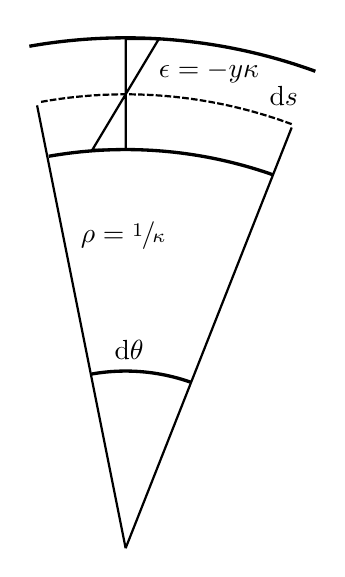
\begin{tikzpicture}[y=0.80pt, x=0.8pt,yscale=-1, inner sep=0pt, outer sep=0pt]
  \path[draw=black,miter limit=4.00,line width=1.200pt]
    (15.2615,55.3504)arc(260.000:289.500:200.051);
  \path[draw=black,line join=round,miter limit=4.00,line width=1.200pt]
    (6.4976,5.6478)arc(260.000:290.000:250.520);
  \path[draw=black,dash pattern=on 2.40pt off 0.80pt,line join=round,miter
    limit=4.00,line width=0.800pt] (11.7974,30.7804)arc(260.000:290.000:220.000000
    and 225.000);
  \path[draw=black,line join=miter,line cap=butt,line width=0.800pt]
    (50.0000,232.3622) -- (10.0000,32.3622);
  \path[draw=black,line join=miter,line cap=butt,line width=0.800pt]
    (50.0000,27.3622) -- (35.0000,52.3622) -- (50.0000,52.3622) --
    (50.0000,2.3622) -- (65.0000,2.3622) -- cycle;
  \path[fill=black] (29.7995,97.515488) node[above right] (text8240) {\(\rho =
    \sfrac{1}{\kappa}\)};
  \path[fill=black] (65,22.362183) node[above right] (text8248) {\(\epsilon = -y
    \kappa\)};
  \path[draw=black,line join=miter,line cap=butt,line width=0.800pt]
    (50.0000,232.3622) -- (125.0000,42.3622);
  \path[cm={{0.4407,0.0,0.0,0.4407,(27.965,129.30866)}},draw=black,miter
    limit=4.00,line width=1.200pt] (15.2615,55.3504)arc(260.000:289.500:200.051);
  \path[fill=black] (45,147.36218) node[above right] (text3984) {d$\theta$};
  \path[fill=black] (115,32.362183) node[above right] (text3988) {d$s$};

\end{tikzpicture}


  \caption{Small deformation in an Euler beam}
  \label{fig:EulerBeam1}
\end{figure}
%
from which we can deduce a relationship between the transverse displacement of a beam section and its angle and radius of curvature to be
\begin{equation}
 \label{eq:EulerCurve}
 \frac{1}{\rho} \approx \frac{\text{d} \phi}{\text{d} x} \approx \frac{\text{d}^2v}{\text{d}x^2} = \kappa\, .
\end{equation}
The radius of curvature, $\rho$ is the radius of the arc formed by the beam's neutral axis, which does not change in length as the beam bends.
We use this same arc to find the strain in material that is at a distance $y$ from the neutral axis.
In a linearly elastic material, the resulting stress is proportional to Young's modulus $E$.
To find the bending moment that results from that stress profile, we integrate the moment contribution through the beam.
\begin{equation}
M_\text{resisted} = \int_\text{bottom}^\text{top}y\sigma dA = \int_\text{bottom}^\text{top}y^2 E \kappa dA\, .
\end{equation}
In equilibrium, the moment resisted will be equal and opposite to the moment applied
\begin{equation}
\label{eq:MomentCurve}
\kappa = \frac{M_\text{applied}}{E \int_\text{bottom}^\text{top}y^2dA}\, .
\end{equation}
The integral in the denominator is the bending resistance of the beam's shape, called its second moment of area, about the neutral axis.
The second moment of area is generally represented by $I$.
By combining \cref{eq:EulerShear,eq:EulerMoment,eq:EulerCurve,eq:MomentCurve}, we reproduce  \cref{eq:EulerBeam}, the Euler-Bernoulli beam equation.
If the Young's modulus and beam cross section are constant throughout the beam, the equation can be further simplified to
\begin{equation}
EI\frac{\text{d}^4 v}{\text{d}x^4}=q\, .\notag
\end{equation}

Obviously, to solve for the deformed position we will require 4 constraints from boundary conditions.
The nature of the constraints is determined by the support configuration.
The most common end conditions are listed \cref{table:BeamBCs}.
Other end constraints, such 

\begin{table}
\centering
\begin{tabular}{l >{$\displaystyle}l<{$} >{$\displaystyle}l<{$}}
End Condition & \textrm{Contraint 1} & \textrm{Constraint 2}\\ \hline\hline
End Load & v'''=\pm F  &  v''=0  \\ \hline
End Torque & v'''=0  &  v''= \pm \tau  \\ \hline
Simply Supported & v''=0 & v=v_\text{support}  \\ \hline
Clamped & v'=v'_\text{clamp} & v=v_\text{clamp}  \\ \hline\hline
\end{tabular}
\caption{Common Beam End Conditions}
\label{table:BeamBCs}
\end{table}

\section{Kirchhoff-Love Plate Theory}
Like Euler-Bernoulli beam theory, Kirchhoff-Love Plate theory begins by making simplifying assumptions about the plate and its deformation.
\begin{itemize}
 \item Slenderness: the length and width of the plate should be 20 times its thickness
 \item Loaded transversely, no in-plane loads or torques
 \item Small deformations and rotations
 \item Straight lines normal to the plate remain normal to the center plane of the plate under deformation
 \item Initially flat
\end{itemize}
These assumptions allow us to simplify our strain-displacement relationships and formulate our curvatures and strains in terms of the transverse displacement $w$.
\begin{equation}
    \kappa_x=\frac{\partial^2 w}{\partial x^2}, \quad \kappa_y= \frac{\partial^2 w}{\partial y^2}, \quad \kappa_{xy}=\frac{\partial^2 w}{\partial x\partial y}\notag
\end{equation}
\begin{equation}
\varepsilon_x = -z \kappa_x, \quad \varepsilon_y = -z \kappa_y, \quad \gamma_{xy} = -2 z \kappa_{xy} \notag
\end{equation}
To find the stresses at any point, we apply Hooke's law and find\todo{equations need to be punctuated}
\begin{align*}
\sigma_x &= -\frac{E z}{1-\nu^2}\left(\kappa_x+\nu\kappa_y\right)\, ,\\
\sigma_y &= -\frac{E z}{1-\nu^2}\left(\kappa_y+\nu\kappa_x\right)\, ,\\
\tau_{xy} &= -\frac{Ez}{1+\nu}\kappa_{xy}\, .
\end{align*}
As with the beam, these stresses can be integrated over the thickness of the plate to determine the resulting moments.
\begin{align*}
M_x = \int_{\sfrac{-t}{2}}^{\sfrac{t}{2}}z\sigma_x dz &=-D\left(\kappa_x+\nu\kappa_y\right)\, ,\\
M_y = \int_{\sfrac{-t}{2}}^{\sfrac{t}{2}}z\sigma_y dz &=-D\left(\kappa_y+\nu\kappa_x\right)\, ,\\
M_{xy} = \int_{\sfrac{-t}{2}}^{\sfrac{t}{2}}z\tau_{xy}dz &= -D\left(1-\nu\right)\kappa_{xy}\, ,
\end{align*}
with
\begin{equation*}
D=\frac{Et^3}{12\left(1-\nu^2\right)}
\end{equation*}
as the flexural rigidity.
Note that a beam of unit width would have a second moment of area $I = \frac{t^3}{12}$, so the flexural rigidity of a plate is greater by a factor of $\frac{1}{1-\nu^2}$.
The difference between the values reflects the fact that, when a plate is bent in one direction, poisson ratio effects promote curvature in the opposite direction at a right angle.
Constraining this saddle-shaped (or \textit{anticlastic}) bending increases the stiffness or rigidity of the plate.

Constructing the governing equation is more complicated than for beams because, instead of shear $V$ and moment $M$ on an infinitesimal section, we have shears $V_x$ and $V_y$ and moments $M_x$, $M_y$, and $M_{xy}$.
Balancing forces gives us
\begin{equation*}
\frac{\partial V_x}{\partial x}+\frac{\partial V_y}{\partial y} = p\, ,
\end{equation*}
for transverse pressure $p$.
Balancing moments gives
\begin{align*}
\text{about} \;x:\qquad& \frac{\partial M_{xy}}{\partial x}+\frac{\partial M_{y}}{\partial y} - V_y = 0\, ,\\
\text{about} \;y:\qquad& \frac{\partial M_{xy}}{\partial y}+\frac{\partial M_{x}}{\partial x} - V_x = 0\, .
\end{align*}

Combining the force and moment balance equations generates the governing equation
\begin{equation*}
\frac{\partial^4w}{\partial x^4}+2\frac{\partial^4w}{\partial x^2 \partial y^2}+\frac{\partial^4w}{\partial y^4}=\frac{p}{D}\, .
\end{equation*}
As with the beam case, we will need to apply boundary conditions in order to find the deformed configuration.

\chapter{Peridynamics Background}
\label{ch:PDBackground}

\section{Peridynamic States}
%
Introduced by Silling et al.\ in 2007~\cite{silling2007peridynamic}, peridynamic states are functions of the behavior of the continuum points surrounding each location.
As is appropriate for a theory based on force-carrying bonds, states often operate on vectors.
The most common states are scalar-states and vector-states which are scalar and vector valued, respectively.
As a matter of convention, scalar states are usually denoted by lowercase letters (e.g. $\sstate{a}{}{}$, $\sstate{b}{}{}$), while vector states are denoted by uppercase letters (e.g. $\vstate{A}{}{}$, $\vstate{B}{}{}$).
A state that operates on vectors and is itself vector valued naturally brings to mind a two-point tensor such as the deformation gradient;
unlike a second order tensor, which can only map vectors linearly to other vectors, vector-states can produce nonlinear, discontinuous, or even noninvertable mappings.  
This difference is illustrated in \cref{fig:VectorState}.
%
\begin{figure}[h]
  \centering
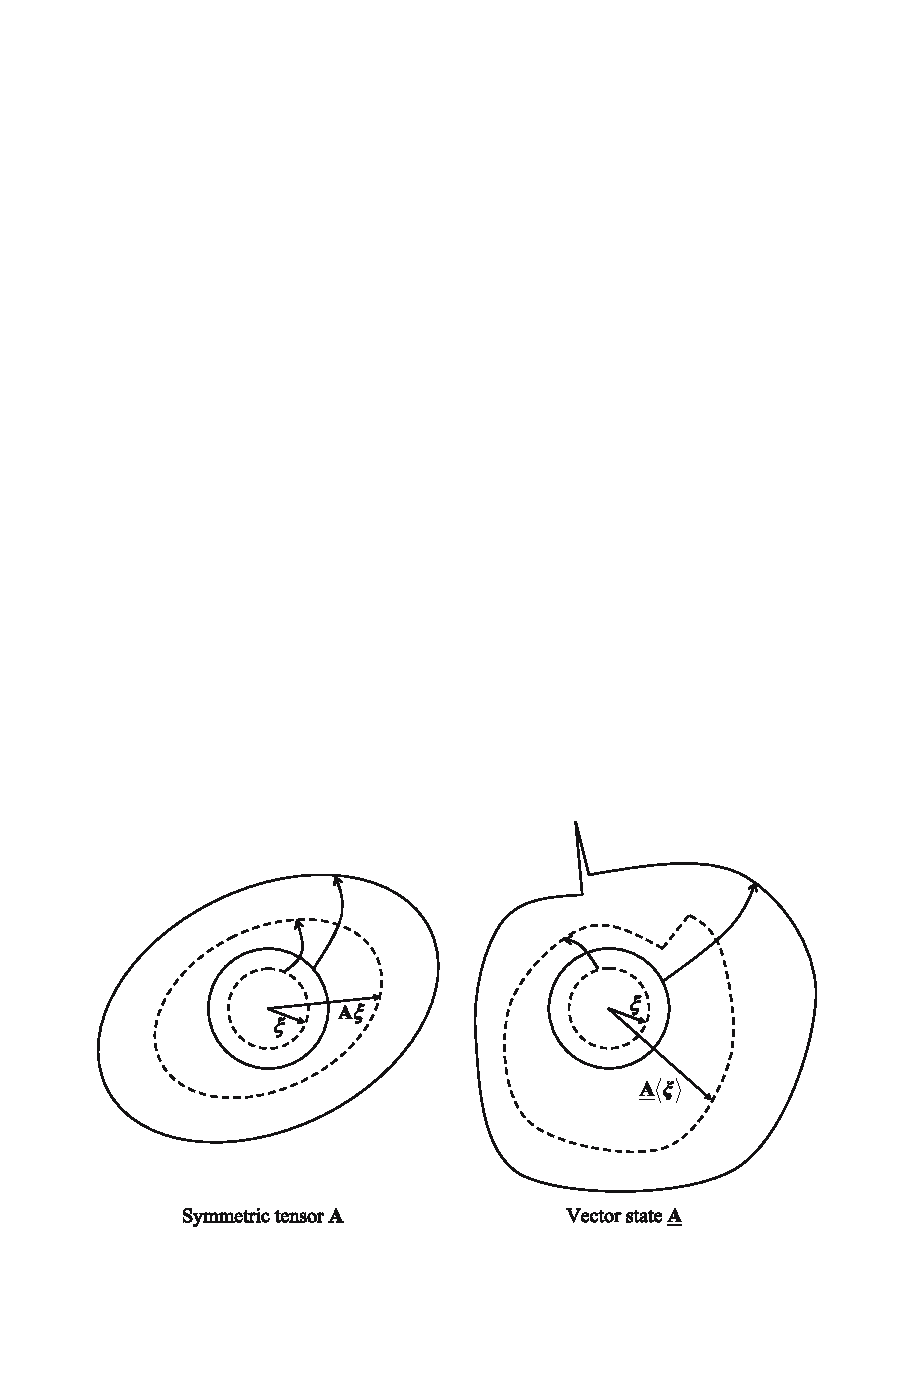
\includegraphics{VectorState}
\caption[Deformation tensor vs. deformation vector state]{The deformation tensor linearly maps spheres to ellipsoids, while a vector state can map spheres nonlinearly to complex and even discontinuous shapes \cite{silling2007peridynamic}}
\label{fig:VectorState}
\end{figure}
%

The mathematical properties of states and several related operators are defined in~\cite{silling2007peridynamic}.
Important properties of states are magnitude and direction, while important operations include the addition and composition of states, inner and tensor products, and the Fr\'{e}chet derivative of a function with respect to a state.
While some of these operations are intuitive, the nomenclature may not be.
Refer to \cref{table:StateOperations} for the notation of common state operations.
For a more rigorous definition and examples of the Fr\'echet derivative, see \cref{sec:frechet}.

\begin{table}
\centering
\caption{Common State Operation Nomenclature}
\begin{tabular}{l >{$\displaystyle}r<{$} >{$\displaystyle}l<{$}}
Operation & \textrm{Notation} & \textrm{Meaning} \\ \hline\hline
Addition & (\sstate{a}{}{} + \sstate{b}{}{})\langle\boldsymbol{\xi}\rangle & \sstate{a}{}{\boldsymbol{\xi}} + \sstate{b}{}{\boldsymbol{\xi}} \\ \hline
Multiplication & (\sstate{a}{}{}\sstate{b}{}{})\langle\boldsymbol{\xi}\rangle & \sstate{a}{}{\boldsymbol{\xi}}\sstate{b}{}{\boldsymbol{\xi}} \\  \hline
Scalar Product & (\vstate{A}{}{} \cdot \vstate{B}{}{})\langle\boldsymbol{\xi}\rangle & \vstate{A}{}{\boldsymbol{\xi}} \cdot \vstate{B}{}{\boldsymbol{\xi}} \\  \hline
Composition & (\vstate{A}{}{} \circ \vstate{B}{}{})\langle\boldsymbol{\xi}\rangle & \vstate{A}{}{ \vstate{B}{}{\boldsymbol{\xi}}}  \\ \hline \noalign{\smallskip}
\multirow{2}{*}{Dot Product} & \vstate{A}{}{} \bullet \vstate{B}{}{}& \int_\mathcal{H} \vstate{A}{}{\boldsymbol{\xi}} \cdot \vstate{B}{}{\boldsymbol{\xi}} \\ \noalign{\smallskip}
& \sstate{a}{}{} \bullet \sstate{b}{}{}&  \int_\mathcal{H} \sstate{a}{}{\boldsymbol{\xi}} \sstate{b}{}{\boldsymbol{\xi}} \\  \noalign{\smallskip} \hline \noalign{\smallskip}
Vector Norm & |\vstate{A}{}{}|\langle\boldsymbol{\xi}\rangle &  |\vstate{A}{}{}\langle\boldsymbol{\xi}\rangle|  \\\noalign{\smallskip} \hline\noalign{\smallskip}
State Norm & \|\vstate{A}{}{}\| & \sqrt{\vstate{A}{}{} \bullet \vstate{B}{}{}} \\ \noalign{\smallskip} \hline \noalign{\smallskip}
\multirow{2}{*}{Fr\'echet Derivative} & \nabla\mathit{f}(\vstate{A}{}{}) & \frac{\partial \mathit{f}}{\partial \vstate{A}{}{}} \\ \noalign{\smallskip}
& \Psi(\vstate{A}{}{},\vstate{B}{}{})_\vstate{A}{}{} & \frac{\partial \Psi}{\partial \vstate{A}{}{}} \\ \noalign{\smallskip} \hline\hline
\end{tabular}
\label{table:StateOperations}
\end{table}


\section{State-based Models}
Conservation of linear momentum in the \textit{state-based} peridynamic formulation results in the equation of motion
%
\begin{equation}
\label{eq:PDstateEoM}
\rho(\mathbf{x})\ddot{\mathbf{u}}(\mathbf{x}) = \int_\Omega (\vstate{T}{\mathbf{x}}{\mathbf{q}-\mathbf{x}}-\vstate{T}{\mathbf{q}}{\mathbf{x}-\mathbf{q}}) dV_\mathbf{q}  + \mathbf{b}(\mathbf{x})\, ,
\end{equation}
%
in which $\vstate{T}{\;}{\;}$ is a \textit{force vector-state} that maps the vector in angle brackets, $\langle \rangle$, originating at the point in square brackets, [ ], to a force vector acting on that point.
The deformed image of the vector $(\mathbf{q-x})$ is defined as the \textit{deformation vector-state}, usually denoted $\vstate{Y}{}{}$ and formulated 
%
\begin{equation}
%\label{eq:PDdeformation}
\vstate{Y}{\mathbf{x}}{\mathbf{q}-\mathbf{x}} = (\mathbf{q}-\mathbf{x}) + (\mathbf{u}(\mathbf{q})-\mathbf{u}(\mathbf{x})) 
\end{equation}
%
for a displacement field \(\mathbf{u}\). 
Just as stress and strain are work conjugate, so too are the force and deformation vector states for hyperelastic materials.

State-based models include surrounding material behavior illustrated in \cref{fig:pdDeformed} in the force function between each pair of continuum points. 
It is common for the formulation of the force state $\vstate{T}{}{}$ to be scaled by a weighting function, commonly represented by $\omega$, that makes explicit the region in which the force relationship between points is nonzero.
Perhaps the simplest and most common weight function is \cref{eq:WeightFunction}, representing a constant nonzero value for bonds shorter than the peridynamic horizon $\delta$.
%
\begin{equation}
\label{eq:WeightFunction}
\omega(\boldsymbol{\xi}) = 
\begin{cases}
1 & \text{if}\; |\boldsymbol{\xi}| \leq \delta\,, \\
0 & \text{if}\; |\boldsymbol{\xi}| > \delta\,.
\end{cases}
\end{equation}
%
Many evaluations of forces, energies, and other states at a given point are reduced from being integrals over the entire body to being integrals over that point's neighborhood $\mathcal{H}$.
This is particularly useful when trying to apply peridynamic models to real-world problems, especially when using computer models. 
%
\begin{figure}[h]
  \centering
\subinputfrom{\diagrampath}{PDbodyDeformed.eps_tex}
\caption{The body \protect\(\protect\Omega\protect\) deformed by the deformation state \protect\(\protect\vstate{Y}{}{}\protect\)}
\label{fig:pdDeformed}
\end{figure}
%
If the force state $\vstate{T}{}{}$ is always in the same direction as the deformation state $\vstate{Y}{}{}$, then the force exerted by a ``bond'' between points is in the same direction as the deformed bond, and the model is called \textit{ordinary}.  
Ordinary state-based models can reproduce linear elastic materials with arbitrary Poisson ratios by separating dilatory and deviatoric deformations and the energy corresponding to each.
%\begin{equation}
%\label{eq:wLPS}
%  \hat{W} ( \mathbf{\underline{Y}} ) = \frac{1}{2} \left( k - \frac{\alpha m}{9} \right) \vartheta^2+\frac{\alpha}{2} \int_{\mathcal{H}} \omega ( | \boldsymbol{\xi} | ) \underline{e}^2 \langle \boldsymbol{\xi} \rangle dV_{\boldsymbol{\xi}}
%\end{equation} 
They can also model a variety of elastic and inelastic behaviors.

There is no requirement that force states be in the same direction as their associated deformation states, and models in which they are not in the same direction are called \textit{nonordinary}.
Some additional care is needed to ensure that angular momentum is conserved in a \textit{nonordinary} state-based model, but they are still perfectly legitimate.
Silling et al.\ demonstrates the possibility of such models in \cite{silling2010peridynamic}, but very little work has touched on their use.  
Foster et al.\ \cite{foster2010viscoplasticity} and Warren et al.\ \cite{warren2009non} show that some correspondence models, which approximate the deformation gradient and use it to calculate bond forces, result in non-ordinary state-based constitutive models for finite deformations.
Bond-based, ordinary state-based, and nonordinary state-based models are illustrated in \cref{fig:PDmodelTypes}.
%
\begin{figure}[h]
  \centering
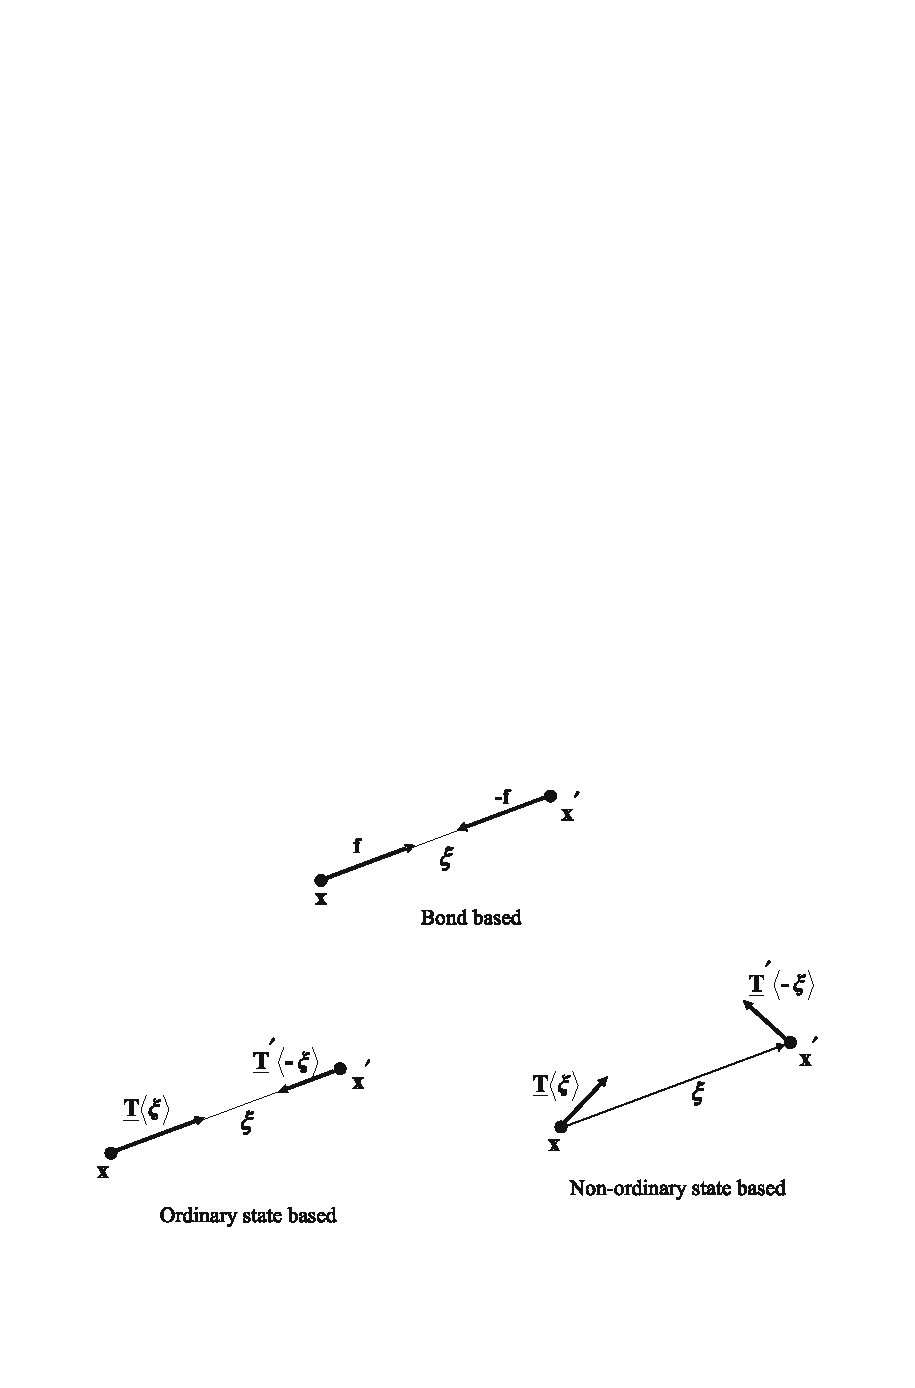
\includegraphics{PDmodelTypes}
\caption[Illustration of the three types of peridynamic models]{Illustration of the three types of peridynamic models, from specific to general \cite{silling2007peridynamic}}
\label{fig:PDmodelTypes}
\end{figure}

It should be clear that many of the concepts of classical continuum mechanics have direct equivalents in peridynamic modeling.
\Cref{table:PDconcepts} lays out some of the simplest parallels between classical and peridynamic formulations.

\begin{table}
\centering
\caption{Peridynamic Equivalents of Classical Concepts}
\begin{tabular}{l >{$\displaystyle}r<{$} >{$\displaystyle}l<{$}}
Concept & \textrm{Classical} & \textrm{Peridynamic} \\ \hline\hline
Kinematics & \mathbf{F} & \tvstate{Y}{}{} \\ \hline \noalign{\smallskip}
Linear Momentum & \nabla \cdot \boldsymbol{\sigma} & \int_\Omega (\vstate{T}{\mathbf{x}}{\mathbf{q}-\mathbf{x}}-\vstate{T}{\mathbf{q}}{\mathbf{x}-\mathbf{q}}) dV_\mathbf{q} \\    \noalign{\smallskip} \hline \noalign{\smallskip}
Angular Momentum &\boldsymbol{\sigma} = \boldsymbol{\sigma}^T  & \int_\Omega \vstate{Y}{\mathbf{x}}{\mathbf{q}-\mathbf{x}}\times\vstate{T}{\mathbf{x}}{\mathbf{q}-\mathbf{x}}dV_\mathbf{q} = 0\\   \noalign{\smallskip} \hline
Constitutive Law & \boldsymbol{\sigma} = \boldsymbol{\sigma}(\boldsymbol{\epsilon}) &\tvstate{T}{}{}=\tvstate{T}{}{}(\tvstate{Y}{}{}) \\  \hline
Stress Power  & \dot{\boldsymbol{\epsilon}} \boldsymbol{\sigma} &\tvstate{T}{}{}\bullet \tvstate{\dot{Y}}{}{} \\  \hline\hline
\end{tabular}
\label{table:PDconcepts}
\end{table}

\section{Bond-based peridynamics}
%
%If the force state \(\vstate{T}{\mathbf{x}}{\boldsymbol{\xi}} \) depends only on the deformation state \(\vstate{Y}{\mathbf{x}}{\boldsymbol{\xi}} \) \todo{This could be stated more simply by saying ``\ldots depends only on the deformed positions of the points at the end of a bond.''} of the same vector, then the model is called \textit{bond-based}.
If the force state \(\vstate{T}{\mathbf{x}}{\boldsymbol{\xi}} \) depends only on the deformed positions of the points at the end of the bond $\boldsymbol{\xi}$, then the model is called \textit{bond-based}.
In \textit{bond-based} peridynamic models, each pair of points is treated separately, without consideration of the behavior of other points. 
This makes bond-based models much simpler computationally than general state-based models, and reduces the equation of motion to
%
\begin{equation}
\label{eq:PDbondEoM}
\rho(\mathbf{x})\ddot{\mathbf{u}}(\mathbf{x}) = \int_\Omega \mathbi{f}(\mathbf{u}(\mathbf{q})-\mathbf{u}(\mathbf{x}),\mathbf{q}-\mathbf{x}) dV_\mathbf{q}  + \mathbf{b}(\mathbf{x})\, .
\end{equation}
%
By choosing an appropriate function $\mathbi{f}$, this model can reproduce the results of linear elasticity for solid materials with a Poisson ration \(\nu=\sfrac{1}{4}\) and 2-dimensional materials with a Poisson ration \(\nu=\sfrac{1}{3}\). 
It can also be used to investigate a range of nonlinear behaviors by changing the force function (examples in \cref{fig:BondForce}). 
To conserve momentum in a bond-based model, it is only necessary that $\mathbf{f}$ satisfy
%
\begin{equation}
\label{eq:PDbondF}
 \mathbi{f}(\mathbf{u}(\mathbf{q})-\mathbf{u}(\mathbf{x}),\mathbf{q}-\mathbf{x})=-\mathbi{f}(\mathbf{u}(\mathbf{x})-\mathbf{u}(\mathbf{q}),\mathbf{x}-\mathbf{q})\, ,
\end{equation}
%
i.e. the forces exerted at the opposite ends of the bond between $\mathbf{x}$ and $\mathbf{q}$ must be equal and opposite.
The first peridynamic models were all bond-based, and provide useful insight into many complex material failure phenomenon despite their limitations.
%
\begin{figure}[h]
  \centering
\subinputfrom{\diagrampath}{BondForce.eps_tex}
\caption{Bond-based models can describe a variety of material behaviors}
\label{fig:BondForce}
\end{figure}
%

\section{Important Peridynamic Models}
Though they cover only a small portion of the behaviors modeled with peridynamics, these few examples should serve to illustrate the form and analysis of peridynamic material models.
\subsection{Bond-based Elastic Solid}
The simplest peridynamic model treats each bond as a linear spring between two points.
In the bond-based formulation, there is no interaction between different bonds, so the force function is
%
\begin{equation}
\mathbi{f}(\mathbf{u}(\mathbf{q})-\mathbf{u}(\mathbf{x}),\mathbf{q}-\mathbf{x}) = \omega(|\mathbf{q}-\mathbf{x}|)\;c\;s \left[(\mathbf{q}+\mathbf{u}(\mathbf{q}))-(\mathbf{x}+\mathbf{u}(\mathbf{x}))\right]\, ,
\end{equation}
%
with weighting function $\omega$, spring constant $c$, and the stretch $s$ defined by
%
\begin{equation}
\label{eq:stretch}
s = |(\mathbf{q}+\mathbf{u}(\mathbf{q}))-(\mathbf{x}+\mathbf{u}(\mathbf{x}))| - |\mathbf{q}-\mathbf{x}|\, .
\end{equation}
%
For a deformation gradient $\mathbf{F}$ representing small uniform displacements, i.e. $\nabla \mathbf{u} << 1$, the stretch of bond $\boldsymbol{\xi}=\mathbf{q}-\mathbf{x}$ is
%
\begin{equation*}
s = |\mathbf{F}\boldsymbol{\xi}|-|\boldsymbol{\xi}| = \frac{\epsilon_{ij}\xi_i\xi_j}{|\boldsymbol{\xi}|}\, .
\end{equation*}
%
For reasons that will become clear in the discussion of the next model, we calibrate the spring constant $c$ following the approach of \cite{silling2007peridynamic}, by comparing the energy to that of a classical solid under purely deviatoric deformation, so that $\epsilon_{ij} = \epsilon_{ij}^d$.
The energy of this spring will be in units of energy per volume squared, so that integration over all the springs at a point gives energy per unit volume,
%
\begin{align}
\label{eq:deviatoricStrainEnergy}
w &= \frac{c\;s^2}{2}\, ,\notag \\
W &= \frac{c}{2}\int_\mathcal{H} \omega(|\xi|)\left( \frac{\epsilon_{ij}^d\xi_i\xi_j}{|\xi|} \right)\left( \frac{\epsilon_{kl}^d\xi_k\xi_l}{|\xi|} \right)\;dV_\xi\, ,\notag\\
&= \frac{c}{2}\epsilon_{ij}^d \epsilon_{kl}^d \int_\mathcal{H} \frac{\omega(|\xi|)}{|\xi|^2}\xi_i\xi_j\xi_k\xi_l \, .
\end{align}
%
Because $\omega$ depends only on $|\boldsymbol{\xi}|$, we can rewrite this integral in spherical coordinates as
%
\begin{equation}
W= \frac{c}{2}\epsilon_{ij}^d \epsilon_{kl}^d \int_0^\delta \frac{\omega(r)}{r^2}\int_0^{2\pi}\int_0^\pi (\xi_i\xi_j\xi_k\xi_l)\;r^2 \sin(\phi)\;d\phi\;d\theta\;dr\, .\notag
\end{equation}
%
Recognizing that $\xi_1 = r \sin\phi\cos\theta$, $\xi_2=r\sin\phi\sin\theta$, $\xi_3=r\cos\phi$, we can see that configurations of $[i,j,k,l]$ with an odd number of any index result in integrals with an odd number of one or more of $\cos\theta$, $\sin\theta$, $\cos\phi$, and therefor are equal to 0. 
For the remaining configurations,
%
\begin{equation}
\int_0^\delta \frac{\omega(r)}{r^2}\int_0^{2\pi}\int_0^\pi (r^4 \sin^4 \phi \cos^2\theta\sin^2\theta)\;r^2 \sin(\phi)\;d\phi\;d\theta\;dr =  \frac{4\pi}{15} \int_0^\delta \omega(r)r^4\;dr\, .\notag
\end{equation}
%
This leaves only configurations such as $[1,1,3,3]$, $[1,2,1,2]$ and $[3,2,2,3]$, which we can indicate by $(\delta_{ik}\delta_{jl}+\delta_{il}\delta_{jk}+\delta_{ij}\delta{kl})$ .
Additionally, any combination with $i=j$ or $k=l$ results in terms $\epsilon_{ii}^d$ or  $\epsilon_{kk}^d$.
Such terms sum to 0 in deviatoric deformation, leaving only $(\delta_{ik}\delta_{jl}+\delta_{il}\delta_{jk})$.
%
\begin{align}
W&= \frac{c}{2}\epsilon_{ij}^d \epsilon_{kl}^d \frac{4\pi}{15} \int_0^\delta \omega(r)r^4\;dr (\delta_{ik}\delta_{jl}+\delta_{il}\delta_{jk})\, ,\notag\\
&= c \;\epsilon_{ij}^d\epsilon_{ij}^d \frac{4\pi}{15} \int_0^\delta \omega(r)r^4\;dr\, , \notag\\
&= \frac{c\; \epsilon_{ij}^d\epsilon_{ij}^d }{15}m\, .\notag
\end{align}
%
To force the result to be independent of the horizon $\delta$, we normalize the expression by
%
\begin{equation}
\label{eq:weighted}
m=\int_\mathcal{H}\omega(|\boldsymbol{\xi}|)|\boldsymbol{\xi}|^2 = 4\pi \int_0^\delta \omega(r)\;r^4\;dr\, .
\end{equation}
%
By comparing to the classical strain energy density $\Omega = \mu\;\epsilon_{ij}^d\epsilon_{ij}^d$ for shear modulus $\mu$, we can determine the appropriate bond stiffness,
%
\begin{equation}
c = \frac{15\;\mu}{m}\, .\notag
\end{equation}
%
Applying a purely dilational deformation to the same model is far easier.
With dilation $\theta_{3D}$, the stretch of a bond in any direction is
%
\begin{equation}
s = \frac{\theta_{3D}}{3} r\, ,\notag
\end{equation}
%
and the corresponding energy is 
%
\begin{align}
W &= \frac{c}{2}\int_\mathcal{H} \omega(|\xi|)\frac{\theta^2_{3D}}{9} r^2 \;dV_\xi\, ,\notag\\
&=\frac{c\;\theta^2_{3D}}{18} \int_0^\delta \omega(r)\int_0^{2\pi}\int_0^\pi r^2\;r^2 \sin(\phi)\;d\phi\;d\theta\;dr\, , \notag\\
&= \frac{c\;\theta^2_{3D}}{18} m\, , \notag\\
&= \frac{15}{9}\mu\frac{\theta^2_{3D}}{2}\, .
\end{align}
%
This shows that the model based on bond-stretch has a bulk modulus that is \sfrac{15}{9} of its shear modulus, indicating a Poisson's ratio of \sfrac{1}{4}.

A nearly identical analysis can be performed on a simpler 2D version of the same model, departing after \cref{eq:deviatoricStrainEnergy}.
Applying a purely deviatoric in-plane shear to such a model, and comparing the resulting energy to that of a classical plate with thickness $t$ gives us
%
\begin{equation}
    c = \frac{8\;\mu\;t}{m_\textrm{2D}}\,,\qquad m_\textrm{2D} =\int_\mathcal{H_\textrm{2D}}\omega(|\boldsymbol{\xi}|)|\boldsymbol{\xi}|^2 dV_{\boldsymbol{\xi}}\, .  \notag
\end{equation}
%

Applying a planar dilation deformation to a 2D plate results in strain energy consistent with a Poisson's ratio of \sfrac{1}{3} rather than the value of \sfrac{1}{4} found for the 3D solid.

\subsection{State-based Elastic Solid}
The state-based linear isotropic peridynamic solid material model is both important and illustrative.
Developed in \cite{silling2007peridynamic}, it uses many of the important characteristics of peridynamic states to model a linearly-elastic material with any valid Poisson's ratio.
The extension state $\underline{e}$ is exactly the same as the stretch $s$ in \cref{eq:stretch}.
Classical material models dealing with metal plasticity often separate deformation into dilation and deviation components.
Similarly, the extension state can be decomposed into isotropic and deviatoric extension states. Using $m$ from \cref{eq:weighted} as above for normalization the dilation state is defined
%
\begin{equation}
    \theta_{3D} = \frac{3}{m} \int_\mathcal{H} \omega(\boldsymbol{\xi}) |\boldsymbol{\xi}| \underline{e} dV_{\boldsymbol{\xi}}\, .
\end{equation}
%
The isotropic and deviatoric extension states are defined in turn
%
\begin{equation}
\underline{e}^i = \frac{\theta_{3D} |\boldsymbol{\xi}|}{3},\qquad \underline{e}^d = \underline{e}-\underline{e}^i\, .
\end{equation}
%
If the energy associated with dilation is set to
%
\begin{equation}
W^i = \frac{k\;\theta^2_{3D}}{2}\, ,\notag
\end{equation}
%
then the corresponding force state is
%
\begin{equation}
\underline{t} = \frac{3k\theta_{3D}}{m}\omega(\boldsymbol{\xi})|\boldsymbol{\xi}|\, .\notag
\end{equation}
%
We saw in the analysis of the bond-based model the necessary bond stiffness to match the energy associated with purely deviatoric deformation.
The two can be combined for \cref{eq:lps}, a force state that clearly indicates the separate responses to dilation and deviatoric deformation:
%
\begin{equation}
\label{eq:lps}
\underline{t} = \frac{3k\theta_{3D}}{m}\omega(\boldsymbol{\xi})|\boldsymbol{\xi}| + \frac{15\;\mu}{m}\omega(\boldsymbol{\xi})\underline{e}^d\, .
\end{equation}
%
A quick examination shows that, in the case that the dilation $\theta_{3D}$ is not constant, the force at either end of a bond will not satisfy \cref{eq:PDbondF}.
Thus such a model is not possible in a bond-based framework without significant modification.
% \todo{If your looking to add a few pages the dissertation, you could include the recent work by Tupek on non-linear bond-strain models.  Just a thought.}

\subsection{Correspondence Models}
One way to create a peridynamic material model is to start from a material model in classical dynamics.
Classical models based on the deformation gradient have the advantage of decades of development and tens of thousands of hours of testing, and they enjoy widespread use in the continuum mechanics community.
Peridynamic \textit{correspondence} models use the relative positions of a points neighbors to determine $\bar{\mathbf{F}}(\vstate{Y}{}{})$, a nonlocal approximation of the deformation gradient $\mathbf{F}$.
%
\begin{equation}
\label{eq:PDapproxGradient}
\bar{\mathbf{F}}(\vstate{Y}{}{}) = \left[\int_\mathcal{H} \omega(|\boldsymbol{\xi}|)(\vstate{Y}{}{\boldsymbol{\xi}}\otimes \boldsymbol{\xi})\;dV_{\boldsymbol{\xi}} \right]\mathbf{K}^{-1}\, ,
\end{equation}
with the shape tensor $\mathbf{K}$ defined by
\begin{equation}
\mathbf{K} = \int_\mathcal{H}\omega(|\boldsymbol{\xi}|)(\boldsymbol{\xi} \otimes \boldsymbol{\xi})\;dV_{\boldsymbol{\xi}}\, . \notag
\end{equation}
%
When $\mathbf{F}$ is constant, $\bar{\mathbf{F}}(\vstate{Y}{}{})$ is exactly equal to $\mathbf{F}$.
If the classical model in question is hyperelastic with energy density $\Omega(\mathbf{F})$, it is a simple matter to force the peridynamic model to have identical energy by defining
\begin{equation}
W(\vstate{Y}{}{}) = \Omega(\bar{\mathbf{F}}(\vstate{Y}{}{}))\, ,
\end{equation}
and find the force vector state by taking the Fr\'echet derivative of $W$ with respect to $\vstate{Y}{}{}$.
Alternately, the classical continuum model can be applied to find the first Piola-Kirchhoff stress $\mathbf{P}$ associated with $\bar{\mathbf{F}}$:
\begin{equation}
\mathbf{P}=\frac{\partial\Omega(\bar{\mathbf{F}})}{\partial\bar{\mathbf{F}}}\, .
\end{equation}
The resulting force state is calculated from the stress according to
\begin{equation}
\vstate{T}{}{\boldsymbol{\xi}} = \omega(\boldsymbol{\xi})\mathbf{P}\mathbf{K}^{-1}\boldsymbol{\xi}\, .
\end{equation}
For homogenous deformations, the result is a peridynamic model that exactly reproduces the classical model without ever taking a derivative.
For problems with very inhomogenous (on the scale of the peridynamic horizon) deformations, the peridynamic model will exhibit scale effects not seen in the classical model, acting to smooth out the effect of short-scale deformations.
For discontinuous deformations, the classical model cannot be evaluated at all, but the peridynamic correspondence model will have no such problem.
It may be necessary however to revisit the choice of model or implement some damage condition. 

All three of these models are based on solid materials.
In such materials, the fundamental deformation mode is stretch or extension.
Consider instead a thin beam deflecting under transverse load; at the scale of the whole beam, the deflection behavior is the result of bending deformation.
To model the beam with a solid material model, it is necessary to use a much smaller scale - one in which the beam can be seen to stretch on one side and compress on the other.
Alternatively, in a model whose fundamental mode of deformation is bending, the same beam could be modeled at the same scale as its behavior.

\chapter{Model Development}
\label{ch:ModelDev}

\section{Bond Pair Material Model}
Consider the material model illustrated in \cref{fig:SimpleBondpair} in which every bond-vector originating from a point is connected by a rotational spring to its opposite originating from that same point.
%
\begin{figure}[h]
\centering
\resizebox{0.6\linewidth}{!}{\subinputfrom{\diagrampath}{simpleBondPair.eps_tex}}
\caption{Illustration of a bond pair model that resists angular deformation}
\label{fig:SimpleBondpair}
\end{figure}
%
If we call the deformed angle between these bonds \(\theta\), and choose the potential energy of that spring to be \(w(\boldsymbol{\xi}) = \omega(\boldsymbol{\xi})\alpha [1 + \cos(\theta) ] \) for the bond pair $\boldsymbol{\xi}$ and $-\boldsymbol{\xi}$, we can recover the non-ordinary force state proposed by Silling in \cite{silling2007peridynamic} by taking the Fr\'echet derivative. For the derivation and a description of the Fr\'echet derivative see \cref{sec:frechet}.
%
\begin{align}
\label{eq:SillingForceNO}
\vstate{T}{}{\boldsymbol{\xi}} &= \nabla w\!\left(\vstate{Y}{}{\boldsymbol{\xi}}\right)\notag \\
%
&=\omega(\boldsymbol{\xi})\frac{-\alpha}{|\vstate{Y}{}{\boldsymbol{\xi}}|} \frac{\vstate{Y}{}{\boldsymbol{\xi}}}{|\vstate{Y}{}{\boldsymbol{\xi}}|} \times \left[\frac{\vstate{Y}{}{\boldsymbol{\xi}}}{|\vstate{Y}{}{\boldsymbol{\xi}}|} \times \frac{\vstate{Y}{}{-\boldsymbol{\xi}}}{|\vstate{Y}{}{-\boldsymbol{\xi}}|}\right]
\end{align}
%
Though it looks complex, \cref{eq:SillingForceNO} indicates a bond force perpendicular to the deformed bond and in the plane containing both the deformed bond and its partner as illustrated in \cref{fig:Bondpair}. 
The force magnitude is proportional to the sine of the angle between the bonds divided by the length of the deformed bond. 
%
\begin{figure}[h]
\centering
\resizebox{0.6\linewidth}{!}{\subinputfrom{\diagrampath}{bondPair.eps_tex}}
\caption{Deformation and force vector states}
\label{fig:Bondpair}
\end{figure}
%
This response is consistent with the idea of a rotational spring between bonds as long as the change in angle is small. 
Because the potential energy and force states are functions of \textit{pairs} of peridynamic bonds, we will call this formulation a \textit{bond-pair model}. 
Other choices for the bond-pair potential function, such as $w = (\pi - \theta)^2$, are also possible, but result in more mathematically complex analysis.

\section{Bond Pair Beam in Bending}
\label{sec:BPbeam}
The simplest application of our bond-pair based peridynamic model is that of \cref{fig:continuousbeam}, a beam in transverse bending.
Much of the material in this section can also be found in \cite{ogrady2014beams}.
%
\begin{figure}[h]
  \centering
\subinputfrom{\diagrampath}{continuousBeam.eps_tex}
\caption{A continuous peridynamic beam with horizon $\delta$}
\label{fig:continuousbeam}
\end{figure}
%

\subsection{Energy Equivalence}
\label{sec:beamEnergy}
To determine an appropriate choice of $\alpha$ for \cref{eq:SillingForceNO}, we desire our peridynamic model to have an equivalent strain energy density to a classical Euler-Bernoulli beam in the \emph{local limit}, i.e.\ when the nonlocal length scale vanishes.  We will begin with the assumptions from Euler beam theory: the length of the beam is much greater than thickness, vertical displacements are small, and rotations are small. For small vertical displacements (i.e.\ $\sin{\theta} \approx \theta$) we have
%
\begin{equation}
\theta(\vstate{Y}{}{\xi},\vstate{Y}{}{\mathbf{-\xi}}) \approx \pi-\frac{v(x+\xi)-2v(x)+v(x-\xi)}{\xi},
\label{eq:beamdtheta}
\end{equation}
%
where $v$ is the vertical displacement of material point.  Momentarily assuming that $v$ is continuous and using a Taylor series to expand the right-hand-side of eq.~(\ref{eq:beamdtheta})  
%
\begin{align}
\theta(\vstate{Y}{}{\xi},\vstate{Y}{}{\mathbf{-\xi}}) &\approx \pi-\xi \frac{\partial^2 v}{\partial x^2}+\mathcal{O}(\xi^3) \notag \\
&\approx  \pi-\xi \kappa +\mathcal{O}(\xi^3); 
\label{eq:beamdtheta2}
\end{align}
with
\begin{equation}
\kappa = \frac{\partial^2 v}{\partial x^2}.\notag
\end{equation}
%
Substituting eq.~(\ref{eq:beamdtheta2}) into the equation for the strain energy density of a single bond-pair,
%
\begin{align}
\label{eq:continuousBeamw}
w(\xi) &= \omega(\xi) \alpha \left[1+\cos(\theta(\vstate{Y}{}{\xi},\vstate{Y}{}{\mathbf{-\xi}})) \right] \notag\\
&\approx \omega(\xi) \alpha\frac{\xi^2}{2}(\kappa)^2 +\mathcal{O}(\xi^4).\notag
\end{align}
%
If we use a weighting function \(\omega(\xi)=\omega(|\xi|)\) and assume that the $\omega$ plays the role of a localization kernel, i.e. $\omega = 0 \,\, \forall \,\, \xi > \delta$, the resulting strain energy density, $W$, for any material point in the peridynamic beam is
%
\begin{equation}
W = \frac{\alpha}{2}\kappa^2 \int_{-\delta}^\delta \omega(\xi)\xi^2 {\rm d}\xi + \mathcal{O}(\delta^5).\notag
\end{equation}
%
Equating $W$ with the classical Euler-Bernoulli beam strain-energy density, $\Omega$, and taking the limit as $\delta \to 0$ we can solve for $\alpha$
%
\begin{align}
    \lim_{\delta \to 0}  W &= \Omega, \notag \\
    \frac{\alpha}{2} m \kappa^2 &= \frac{EI}{2} \kappa^2, \notag \\
    \alpha &= \frac{EI}{m},
\label{eq:alpha}
\end{align}
%
with 
\begin{equation}
    m = \int_{-\delta}^{\delta} \omega(\xi) \xi^2 {\rm d}\xi \notag.
\end{equation}

While this demonstrates the model's equivalence to a linearly-elastic Euler beam, if we keep an additional term from the Taylor series approximation of \cref{eq:beamdtheta}, we recover a slightly more complex expressions for change in angle that is demonstrated in \ref{sec:EringenCompare} to reproduce an Euler beam governed by Eringen's model of nonlocal elasticity.

\subsection{Relation to Eringen Nonlocality}
\label{sec:EringenCompare}
%If we relax our homogeneity assumption somewhat, we recover from \cref{eq:beamdtheta} slightly more complex expressions for change in angle
If we keep an additional term from the Taylor series approximation of \cref{eq:beamdtheta}, we recover a slightly more complex expressions for change in angle
%
\begin{equation}
\label{eq:beamdthetaHOT}
%\theta(\vstate{Y}{}{\xi},\vstate{Y}{}{\mathbf{-\xi}}) \approx \pi-\xi \frac{\partial^2 y}{\partial x^2} -\frac{\xi^3}{12} \frac{\partial^4 y}{\partial x^4}  +\mathcal{O}(\xi^5)=  \pi-\xi \kappa-\frac{\xi^3}{12} \kappa''+\mathcal{O}(\xi^5)\notag
\theta(\vstate{Y}{}{\xi},\vstate{Y}{}{\mathbf{-\xi}}) \approx \arctan\left(\pi-\xi \frac{\partial^2 v}{\partial x^2} -\frac{\xi^3}{12} \frac{\partial^4 v}{\partial x^4}  +\mathcal{O}(\xi^5)\right)\notag
\end{equation}
%
and for the strain energy (again substituting \(\kappa = v''\) for readability),
%
%\begin{equation}
%W \approx \int_{-\delta}^\delta \omega(\xi)\alpha(\frac{\xi^2}{2}\kappa^2+\frac{\xi^4}{12}\kappa\kappa''-\frac{3\; \xi^4}{8}\kappa^4+\mathcal{O}(\xi^6)) d\xi .
%\end{equation}
%
%
\begin{equation}
%W \approx \int_{-\delta}^\delta \omega(\xi)\alpha(\frac{\xi^2}{2}\kappa^2+\frac{\xi^4}{12}\kappa\kappa''-\frac{\xi^4}{24}\kappa^4+\mathcal{O}(\xi^6)) d\xi .\notag
W \approx \int_{-\delta}^\delta \omega(\xi)\alpha(\frac{\xi^2}{2}\kappa^2+\frac{\xi^4}{12}\kappa\kappa''-\frac{3\; \xi^4}{8}\kappa^4+\mathcal{O}(\xi^6)) d\xi.\notag
\end{equation}
%
As the horizon \(\delta\) becomes small, higher-order \(\xi\) terms become relatively less important, and \(\xi^4\kappa^4\) is dominated by \(\xi^2\kappa^2\) for large \(\kappa\) and by \(\xi^4\kappa\kappa''\) for small \(\kappa\).
The remaining terms can be rearranged,
\begin{align}
W &\approx \int_{-\delta}^\delta \omega(\xi)\alpha \frac{\xi^2}{2}\kappa(\kappa + \frac{\xi^2}{6}\kappa'') d\xi, \notag
\end{align}
in a manner strongly suggesting an alternative bending resistance term.
We can picture a bending resistance based on the bond length and proportional to the nonlocal curvature  \(\bar{\kappa}=(\kappa + \frac{\xi^2}{6}\kappa'')\), so that 
%
\begin{align}
\label{eq:NLbending}
\bar{\kappa}&=(\kappa + \frac{\xi^2}{6}\kappa'') \implies  \\
W &\approx \int_{-\delta}^\delta \omega(\xi)\alpha \frac{\xi^2}{2}\kappa\bar{\kappa}d\xi .\notag
\end{align}
%  
The same analysis can be taken further to obtain higher-order energy terms with even powers of \(\xi\) and even order derivatives of \(\kappa\). 
Not all of these higher-order terms can be separated into the product of a local curvature and nonlocal bending resistance.

Eringen's model for nonlocal elasticity in \cite{eringen1983differential} begins with a nonlocal modulus (denoted here as \(K(|\mathbf{x}'-\mathbf{x}|,\tau)\)) that relates the nonlocal stress \(\mathbf{t}\) at a point to the classical (local) stress \(\boldsymbol{\sigma}\) in the nearby material through the integral
\begin{equation}
\mathbf{t} = \int_\mathbf{V} K(|\mathbf{x}'-\mathbf{x}|,\tau)\boldsymbol{\sigma}(\mathbf{x}')dv(\mathbf{x}').\notag
\end{equation}
In the local limit these relationships take the form of higher-order gradients.
Using a 1-dimensional decaying exponential nonlocal modulus \(K(|x|,\tau)=\frac{1}{l\tau}e^{-\frac{|x|}{l\tau}}\)results in a relationship between \(t_\text{1D}\) and \(\sigma_\text{1D}\)
\begin{align}
\left(1-\tau^2l^2\frac{\partial^2}{\partial x^2}\right)t_\text{1D}&=\sigma_\text{1D},\notag
\end{align}
in which \(\tau^2l^2\) is a scale-based material parameter.
For well-behaved \(t_\text{1D}\) and \(\sigma_\text{1D}\) and small values of \(\sigma_\text{1D}''''\) and \(\tau^2l^2\), we can see that this relationship could be reformulated as
\begin{equation}
\label{eq:NLstress}
t_\text{1D}=\left(1+\tau^2l^2\frac{\partial^2}{\partial x^2}\right)\sigma_\text{1D}.\notag
\end{equation}
If we consider the results of the previous section and let \(dM = y\sigma dA\) and \(\sigma = Ey\kappa\), the contribution to moment resulting from Eringen's nonlocal elasticity in a fiber at \(y\)
\begin{equation}
\label{eq:EringenMoment}
E y^2 (\kappa+\tau^2l^2\kappa''), \\
\end{equation}
and the resulting strain energy
\begin{equation}
\label{eq:EringenEnergy}
\int_{-\frac{t}{2}}^{\frac{t}{2}} b(y) E \frac{y^2}{2} \kappa (\kappa+\tau^2l^2\kappa'')  dy,\notag
\end{equation}
bear a striking resemblance to \cref{eq:NLbending}.
In fact, by carefully choosing peridynamic parameter values, the results can be made identical.
For a rectangular beam of width \(b\) and thickness \(t\), choosing 
\begin{equation}
\omega(\xi) = |\xi|b ;\qquad \delta = \tau l \sqrt{3} ;\qquad \alpha = \frac{E b t^3}{54 \tau^4 l^4}\notag
\end{equation}
results in
\begin{equation}
W \approx E b \frac{t^3}{12} \frac{\kappa}{2}(\kappa+\tau^2 l^2 \kappa''), \notag
\end{equation}
the same result for both models.

The similarity between \cref{eq:NLbending,eq:EringenMoment} is not accidental; Eringen's gradient elasticity is the solution to the integral formulation of the nonlocal stress integral equation just as the peridynamic energy is an integral function of nonlocal displacements.
It is therefore unsurprising that, like Eringen's nonlocal elasticity\cite{Challamel2008small}, this peridynamic bending model fails to predict the stiffening associated with nanoscale cantilevers.
Instead, the advantage of peridynamic models is their natural handling of discontinuities.

\subsection{Weighting function and inelasticity}
\label{sec:WeightFunction}
The weighting function \(\omega(\xi)\) describes the relative contribution of each bond-pair, and can be defined according to physical or mathematical considerations. 
While any function $\omega(\xi)$ that produces a convergent integral for $m$ will reproduce an elastic Euler beam, a physically meaningful choice of $\omega$ will allow us to extend our model to certain inelastic behaviors.
Consider a classical Euler-Bernoulli beam in bending with curvature \(\kappa\). 
Fibers running parallel to the neutral axis of the beam are stretched in proportion to their distance from the neutral axis, with strain \(\epsilon = y\kappa\). 
If the fibers are linearly elastic, then the axial stress at each location is \(\sigma = E\epsilon = Ey\kappa\), and the contribution to supported moment \(dM = \kappa E y^2 dA\). 
By comparing the formulations for the moments carried by the Euler beam in \cref{fig:EulerBending} and those of the bond-pair beam in \cref{fig:BPBending}, we see some definite parallels.
%
\begin{figure}[h]
\centering
\resizebox{0.5\linewidth}{!}{\subinputfrom{\diagrampath}{EulerBending.eps_tex}}
\caption{Euler beam moment contribution}
\label{fig:EulerBending}
\end{figure}
%
%
\begin{figure}[h]
\centering
\subinputfrom{\diagrampath}{BondPairBending_edit.eps_tex}
\caption{Bond-pair moment contribution}
\label{fig:BPBending}
\end{figure}
%
\begin{align}
M_\text{E}&=\int_{-\frac{t}{2}}^{\frac{t}{2}} \sigma \; y \; dA &= \int_{-\frac{t}{2}}^{\frac{t}{2}} E \kappa \; y^2 \; b(y) dy\notag \\
%
M_\text{PD}&=\int_{-\delta}^{\delta} \vstate{T}{}{\xi}\; \xi \; d\xi &\notag \\
&= \int_{-\delta}^{\delta} \alpha \frac{\sin(\Delta\theta)}{|\xi|} \; \xi \; \omega(\xi) d\xi\: &\approx \int_{-\delta}^{\delta} \alpha \kappa |\xi| \; \omega(\xi) d\xi\notag
\end{align}
%
The term \(y\) is the distance from the beam's neutral axis and \(b(y)\) is the width of the beam at that distance from the neutral axis. 
The similarity between classical and peridynamic moment formulations suggests a possible formulation for the weighting function:
%
\begin{equation}
\label{eq:WeightFunction}
\omega(\xi) = |\xi| b\left(y\right) \quad \text{at} \quad y=\frac{\xi}{\delta} \frac{t}{2}
\end{equation}
%
\begin{figure}[h]
 \centering
  \subinputfrom{\diagrampath}{WeightProfile_Uniform.eps_tex}
\caption{Weight function for a beam of rectangular cross-section}
\label{fig:WeightProfileUniform}
\end{figure}

\begin{figure}
  \centering
  \subinputfrom{\diagrampath}{WeightProfile_Ibeam.eps_tex}
\caption{Weight function for an I-beam}
\label{fig:WeightProfileIbeam}
\end{figure}
%
This weight function analogizes the relative contributions of bond pairs of different lengths to the relative contributions of fibers at different distances from the centerline. 
An example for a rectangular beam is illustrated in \cref{fig:WeightProfileUniform}.
For an I beam with height \(h_\text{beam}\), width \(w_\text{beam}\), web height \(h_\text{web}\), and web width \(w_\text{web}\), substituting the beam profile
\begin{equation}
b(y) = 
  \begin{dcases}
    w_\text{web} & \text{if } |y| \leq \frac{h_\text{web}}{2} \\
    w_\text{beam} & \text{if } \frac{h_\text{web}}{2} < |y| \leq \frac{h_\text{beam}}{2} \\
    0 &\text{otherwise}
  \end{dcases}\notag
\end{equation}
into \cref{eq:WeightFunction} gives the weight function
\begin{equation}
\omega(\xi) = 
  \begin{dcases}
    |\xi| w_\text{web}& \text{if } |\xi| \leq \delta\frac{h_\text{web}}{h_\text{beam}} \\
    |\xi| w_\text{beam} & \text{if } \delta\frac{h_\text{web}}{h_\text{beam}} < |\xi| \leq \delta \\
    0 &\text{otherwise}
  \end{dcases}\notag
\end{equation}
and is ilustrated in \cref{fig:WeightProfileIbeam}.
    While this weighting function offers no advantages over a uniform weight function in the case of the linearly elastic beam, it offers a way to model advancing plasticity.

In a deformed elastic perfectly-plastic beam, axial fibers are still stretched in proportion to their distance from the neutral axis, but the relationship \(\sigma = E\epsilon = Ey\kappa\) only holds for \(|\epsilon| = |y\kappa| < \epsilon_c\). 
For greater stretches, the relationship becomes \(\sigma = \pm E\epsilon_c \). 
To model this behavior, consider a bond pair with similar behavior: for angular deformation less than some critical angle, the model behaves as previously described, but the magnitude of the force remains constant above a critical deformation
%
\begin{equation}
|\vstate{T}{}{\xi}| = 
  \begin{cases}
    \alpha \omega(\xi) \frac{\sin(\theta(\vstate{Y}{}{\xi},\vstate{Y}{}{\mathbf{-\xi}}))}{|\vstate{Y}{}{\xi}|} & \quad \text{if } \theta < \theta_c\\
    \alpha \omega(\xi) \frac{\sin(\theta_c)}{|\vstate{Y}{}{\xi}|} & \quad \text{if } \theta \geq \theta_c\
  \end{cases}
  \label{eq:epp_force}
\end{equation}
%
to determine the critical angle \(\theta_c\), we let the onset of plasticity in pairs of the longest bonds to coincide with the onset of plasticity in the fibers at the top and bottom surfaces of the classical beam. 
For small curvatures \(\Delta\theta = \xi\kappa\implies\Delta\theta_c = \frac{2\delta\epsilon_c}{t}\). 
For curvatures \(|\kappa| > \kappa_c=\frac{2\epsilon_c}{t}\), the radius within which bonds are in the elastic region is \(\delta_e = \delta \frac{\kappa_c}{\kappa}\), and parallels the distance from the beam centerline that fibers are in the elastic region \(y_e = \frac{t}{2} \frac{\kappa_c}{\kappa}\)
%
\begin{align}
  M_\text{classical} &= 2 \int_{0}^{y_e}E b(y)y^2 \kappa dy +2 \int_{y_e}^{\frac{t}{2}}E b(y) \epsilon_c y dy\notag \\
  M_\text{PD} &= 2 \int_{0}^{\delta_e}\alpha \omega(\xi) \xi^2 \kappa d\xi +2 \int_{\delta_e}^{\delta}\alpha \omega(\xi) \Delta\theta_c \xi d\xi \notag
\end{align}
%
Of course, as long as the force is independent of history, this model only represents a nonlinear elastic material. 
By keeping track of the plastic deformation \(\theta^p (\xi) = \theta-\theta_c\) of each bond-pair, and applying it as an offset, we can reproduce the hysteresis associated with elastic-perfectly-plastic deformation.

More simply, we can model a brittle material by setting the force to zero for bond pairs exceeding a critical angle,
%
\begin{equation}
|\vstate{T}{}{\xi}| = 
  \begin{cases}
    \alpha \omega(\xi) \frac{\sin(\theta(\vstate{Y}{}{\xi},\vstate{Y}{}{\mathbf{-\xi}}))}{|\vstate{Y}{}{\xi}|} & \quad \text{if } \theta < \theta_c\\
    0 & \quad \text{if } \theta \geq \theta_c\
  \end{cases}
  \label{eq:brittle_force}
\end{equation}
%
and additionally recording bond pairs that have exceeded their critical angle and permanently setting their influence, i.e. $\omega$, to zero.
%
%
\section{Bond Pair Plate in Bending}
The next case we will analyze is the extension of the bond pair beam model to \cref{fig:BondPairPlate}, a flat plate in the \(xy\) plane, with displacement in the \(z\)-direction. 
%
\begin{figure}[tbp]
    \centering
    \subinputfrom{\diagrampath/}{continuousPlate.eps_tex}
    \caption{Illustration of a bond pair on a plate.}
    \label{fig:BondPairPlate}
\end{figure}
%

\subsection{Energy Equivalence}
%
As with the beam model, we determine an appropriate choice of $\alpha$ so that our peridynamic model will have an equivalent strain energy density to a classical Kirckhoff plate in the \emph{local limit}..  We will begin with the assumptions from Kirckhoff plate theory: straight lines normal to the mid-surface remain both straight and normal to the deformed mid-surface, and the plate thickness does not change with deformation.  As with the Euler beam energy equivalence, we will start with the original assumptions from Kirchhoff-Love plate theory of small displacements and rotations, but they will not constrain the validity of the model for larger displacements and rotations.  For small vertical displacements we have
%
\begin{equation}
    \theta(\vstate{Y}{}{\boldsymbol{\xi}},\vstate{Y}{}{\boldsymbol{-\xi}}) \approx \pi-\frac{z(\mathbf{x}+\boldsymbol{\xi})-2z(\mathbf{x})+z(\mathbf{x}-\boldsymbol{\xi})}{|\boldsymbol{\xi}|},
    \label{eq:platetheta}
\end{equation}
%
where $z$ is the vertical displacement of material point.  Taking \(\boldsymbol{\xi}=\xi (\cos(\phi),\sin(\phi))\) in cartesian coordinates and momentarily assuming continuous displacements for the sake of comparison, we use a Taylor series to expand the right-hand-side of eq.~(\ref{eq:platetheta}) about \(\xi = 0\) 
%
\begin{equation}
    \theta(\vstate{Y}{}{\boldsymbol{\xi}},\vstate{Y}{}{\boldsymbol{-\xi}}) \approx \pi-\frac{\xi}{2} \left(\cos^2(\phi) \kappa_1+\sin^2(\phi) \kappa_2+2\sin(\phi)\cos(\phi)\kappa_3\right)+\mathcal{O}(\xi^3)
    \label{eq:platetheta2}
\end{equation}
%
with
%
\begin{equation}
    \kappa_1=\frac{\partial^2 z}{\partial x_1^2}, \quad \kappa_2= \frac{\partial^2 z}{\partial x_2^2}, \quad \kappa_3=\frac{\partial^2 z}{\partial x_1\partial x_2}\notag
\end{equation}
%
substituting eq.~(\ref{eq:platetheta2}) into the equation for the strain energy density of a single bond-pair,
%
\begin{align}
%\label{eq:continuousBeamw}
    w &= \omega(\boldsymbol{\xi}) \alpha \left[1+\cos(\theta(\vstate{Y}{}{\boldsymbol{\xi}},\vstate{Y}{}{\boldsymbol{-\xi}}) ) \right] \notag \\
    &= \omega(\boldsymbol{\xi}) \alpha\frac{\xi^2}{8}(\kappa_1^2\cos^4(\phi)+\kappa_2^2\sin^4(\phi)+2\kappa_1\kappa_2\cos^2(\phi)\sin^2(\phi)+4\kappa_3^2\cos^2(\phi)\sin^2(\phi) \notag \\
    &+ 4\kappa_1\kappa_3\cos^3(\phi)\sin(\phi)+4\kappa_2\kappa_3\cos(\phi)\sin^3(\phi))+\mathcal{O}(\xi^4).\notag
\end{align}
%
If we use a weighting function \(\omega(\boldsymbol{\xi})=\omega(\xi)\) and assume that the $\omega$ plays the role of a localization kernel, i.e. $\omega = 0 \; \forall \; \xi > \delta$, the resulting strain energy density, $W$, for any material point in the peridynamic plate is
%
\begin{align}
    W =& \alpha \int_{0}^\delta\int_0^{2 \pi} w\; \xi {\rm d}\phi {\rm d}\xi ,\notag \\
    =& \alpha \frac{3\pi}{8} \left(\kappa_1^2+\kappa_2^2+\frac{2}{3}\kappa_1\kappa_1+\frac{4}{3}\kappa_3^2 \right)\int_{0}^\delta \omega(\xi)\xi^3{\rm d}\xi + \mathcal{O}(\delta^6).\notag 
\end{align}
%
Equating $W$ with the classical Kirchhoff plate strain-energy density, $\Omega$, and taking the limit as $\delta \to 0$ we can solve for $\alpha$
%
\begin{align}
    \lim_{\delta \to 0}  W &= \Omega, \notag \\
    \alpha \frac{3 \pi}{8} m \left(\kappa_1^2+\kappa_2^2+\frac{2}{3}\kappa_1\kappa_1+\frac{4}{3}\kappa_3^2 \right)&= \left[ \frac{G h^3}{12(1-\nu)} \left(\kappa_1^2+\kappa_2^2+2\nu\kappa_1\kappa_1+2(1-\nu)\kappa_3^2 \right) \right]_{\nu=1/3}, \notag \\
%    \nu = \frac{1}{3},\:\: \alpha &= \frac{8}{3 \pi m} \frac{G h^3}{12(1-\nu)},
    \alpha &= \frac{2 G h^3}{3 m}, \\
    \text{with}\qquad \qquad \notag \\
%    \label{eq:platealpha}
%    m = \int_{0}^{\delta} \omega(\xi) \xi^3 {\rm d}\xi \notag.
    m &= \int_{0}^{\delta} \int_{0}^{2\pi}\omega(\xi) \xi^2 \xi {\rm d}\phi {\rm d}\xi \notag,
\end{align}
%
where $G$ is the shear modulus, $h$ is the thickness of the plate, and we have evaluated the classical Kirchhoff strain-energy at a Poisson ratio of \(\sfrac{1}{3}\) in order to solve for alpha as a constant.  Because $\alpha$ is inversely proportional to $m$, the energy does not change with varying choices for $\omega$ and $\delta$. It should be noted that the restriction \(\nu=\sfrac{1}{3}\) is the same imposed by the use of a bond based peridynamic model for in-plane deformation of a 2D peridynamic plate. We will show an extension to this model that removes this restriction in Section~\ref{sec:arbitrary}.

\subsection{Combining Bending and Extension Models}
The bond-pair bending model does not resist in-plane stretching or shear deformation because these deformations preserve the angles between opposite bonds.  If these behaviors are expected in combination with bending, a useful model must resist both in-plane and transverse deformations.  To create a plate model that also resists these deformations, i.e.\ a flat shell, we combine the bond-pair model with a two-dimensional version of the original bond-based linearly-elastic peridynamic solid model from \cite{silling2000reformulation}.  In this model, individual bonds act as springs resisting changes in length.
%
\begin{equation}
    \label{eq:bondextension}
    \vstate{T}{}{\boldsymbol{\xi}} =\beta\left(|\vstate{Y}{}{\boldsymbol{\xi}}|-|\boldsymbol{\xi}|\right)\frac{\vstate{Y}{}{\boldsymbol{\xi}}}{|\vstate{Y}{}{\boldsymbol{\xi}}|}
\end{equation}
%
By matching the energy of a 2D material in shear deformation, we can relate \(\beta\) to the shear modulus and thickness of the shell.  Following the example of \cite{silling2007peridynamic}, we begin with a 2D material under pure in-plane shear.  In Einstein notation, the strain energy of this material is
%
%\begin{align*}
%    W^d_\text{C} &= G \; h \; \epsilon_{ij} \epsilon_{ij} = G \; h \; \epsilon_{ij}^d \epsilon_{ij}^d \\
%    W^d_\text{PD} &= \frac{\beta}{2}(\underline{\omega}\; \underline{\epsilon^d})\bullet \underline{\epsilon^d}\\
%    &=\frac{\beta}{2} \epsilon_{ij}^d \epsilon_{kl}^d \int_A \frac{\underline{\omega}\langle\xi\rangle}{|\boldsymbol{\xi}|^2}\xi_i \xi_j \xi_k \xi_l \;dA_\xi\\
%\end{align*}
%
\begin{align*}
    W_\text{C} &= G \; h \; \epsilon_{ij}^d \epsilon_{ij}^d,  \\  \\
    W_\text{PD} &= \frac{\beta}{2}\int_A \omega(\xi)\left(|\vstate{Y}{}{\boldsymbol{\xi}}|-|\boldsymbol{\xi}|\right)^2 \; {\rm d}A_{\boldsymbol{\xi}}, \\
    &=\frac{\beta}{2}\int_A  \omega(\xi) \frac{\epsilon_{ij}\xi_i \xi_j }{|\boldsymbol{\xi}|} \frac{\epsilon_{kl} \xi_k \xi_l }{|\boldsymbol{\xi}|}\;{\rm d}A_{\boldsymbol{\xi}},\\
    &=\frac{\beta}{2} \epsilon_{ij}^d \epsilon_{kl}^d \int_A \frac{ \omega(\xi)}{|\boldsymbol{\xi}|^2}\xi_i \xi_j \xi_k \xi_l \;{\rm d}A_{\boldsymbol{\xi}}.
\end{align*}
%
where $\epsilon^d$ is the deviatoric strain tensor.  Now, to evaluate the integral we will exploit the symmetry properties. With $i, j, k, l = 1,2$. For a circular $\omega(\xi) = \omega(|\xi|)$, combinations of $\{i,j,k,l\}$ with an odd number of each index, such as $\{1,1,1,2\}$ or $\{2,1,2,2\}$, will result in odd powers of sine and cosine and integrate to 0.
%
\begin{align*}
%    m&=(\underline{\omega}\:\underline{x}) \bullet \underline{x}\\
    m &= \int_A \omega(\xi)|\boldsymbol{\xi}|^2\; dA_{\boldsymbol{\xi}} \\
    W^d_\text{PD} &= \frac{\beta \; m}{16}[3(\epsilon_{11}\epsilon_{11}+\epsilon_{22}\epsilon_{22})+(\epsilon_{11}\epsilon_{22}+\epsilon_{12}\epsilon_{12}+\epsilon_{12}\epsilon_{21}+\epsilon_{21}\epsilon_{12}+\epsilon_{21}\epsilon_{21}+\epsilon_{22}\epsilon_{11})]\\
    &= \frac{\beta \; m}{16} \epsilon_{ij}^d \epsilon_{kl}^d (\delta_{ij}\delta_{kl}+\delta_{ik}\delta_{jl}+\delta_{il}\delta_{jk})\\
    &= \frac{\beta \; m}{8} \epsilon_{ij}^d \epsilon_{ij}^d \implies\\
     \beta &= \frac{8 \; G\;h}{m}
\end{align*}
%
Having calibrated the bond-extension model to the shear modulus for a case of pure in-plane shear, applying a different uniform strain (such as might result from uniaxial tension) reveals the bond-based model to result in a one-parameter linearly-elastic model with Poisson's ratio \(\nu=\sfrac{1}{3}\).  

Combining the bending and extension models allows for the description of more complex behaviors, particularly the stiffening effect of in-plane tension on the transverse bending of a shell.  Consider a single bond-pair in the combined model shown in Fig.~\ref{fig:hybridmodel}.
%
\begin{figure}[tbp]
  \centering
  


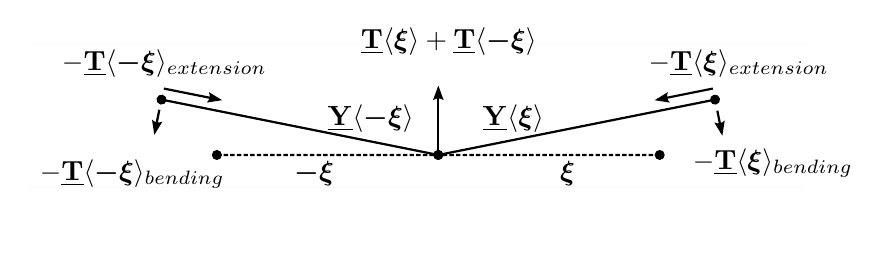
\begin{tikzpicture}[y=0.80pt, x=0.8pt,yscale=-1, inner sep=0pt, outer sep=0pt]
\begin{scope}[shift={(-16.10332,-55.70103)}]
  \begin{scope}[fill=black]
    \path[color=black,fill=black,line width=0.800pt] (101.0938,106.6875) --
      (103.0938,106.6875) -- (103.0938,105.6875) -- (101.0938,105.6875) --
      cycle(104.0938,106.6875) -- (106.0938,106.6875) -- (106.0938,105.6875) --
      (104.0938,105.6875) -- cycle(107.0938,106.6875) -- (109.0938,106.6875) --
      (109.0938,105.6875) -- (107.0938,105.6875) -- cycle(110.0938,106.6875) --
      (112.0938,106.6875) -- (112.0938,105.6875) -- (110.0938,105.6875) --
      cycle(113.0938,106.6875) -- (115.0938,106.6875) -- (115.0938,105.6875) --
      (113.0938,105.6875) -- cycle(116.0938,106.6875) -- (118.0938,106.6875) --
      (118.0938,105.6875) -- (116.0938,105.6875) -- cycle(119.0938,106.6875) --
      (121.0938,106.6875) -- (121.0938,105.6875) -- (119.0938,105.6875) --
      cycle(122.0938,106.6875) -- (124.0938,106.6875) -- (124.0938,105.6875) --
      (122.0938,105.6875) -- cycle(125.0938,106.6875) -- (127.0938,106.6875) --
      (127.0938,105.6875) -- (125.0938,105.6875) -- cycle(128.0938,106.6875) --
      (130.0938,106.6875) -- (130.0938,105.6875) -- (128.0938,105.6875) --
      cycle(131.0938,106.6875) -- (133.0938,106.6875) -- (133.0938,105.6875) --
      (131.0938,105.6875) -- cycle(134.0938,106.6875) -- (136.0938,106.6875) --
      (136.0938,105.6875) -- (134.0938,105.6875) -- cycle(137.0938,106.6875) --
      (139.0938,106.6875) -- (139.0938,105.6875) -- (137.0938,105.6875) --
      cycle(140.0938,106.6875) -- (142.0938,106.6875) -- (142.0938,105.6875) --
      (140.0938,105.6875) -- cycle(143.0938,106.6875) -- (145.0938,106.6875) --
      (145.0938,105.6875) -- (143.0938,105.6875) -- cycle(146.0938,106.6875) --
      (148.0938,106.6875) -- (148.0938,105.6875) -- (146.0938,105.6875) --
      cycle(149.0938,106.6875) -- (151.0938,106.6875) -- (151.0938,105.6875) --
      (149.0938,105.6875) -- cycle(152.0938,106.6875) -- (154.0938,106.6875) --
      (154.0938,105.6875) -- (152.0938,105.6875) -- cycle(155.0938,106.6875) --
      (157.0938,106.6875) -- (157.0938,105.6875) -- (155.0938,105.6875) --
      cycle(158.0938,106.6875) -- (160.0938,106.6875) -- (160.0938,105.6875) --
      (158.0938,105.6875) -- cycle(161.0938,106.6875) -- (163.0938,106.6875) --
      (163.0938,105.6875) -- (161.0938,105.6875) -- cycle(164.0938,106.6875) --
      (166.0938,106.6875) -- (166.0938,105.6875) -- (164.0938,105.6875) --
      cycle(167.0938,106.6875) -- (169.0938,106.6875) -- (169.0938,105.6875) --
      (167.0938,105.6875) -- cycle(170.0938,106.6875) -- (172.0938,106.6875) --
      (172.0938,105.6875) -- (170.0938,105.6875) -- cycle(173.0938,106.6875) --
      (175.0938,106.6875) -- (175.0938,105.6875) -- (173.0938,105.6875) --
      cycle(176.0938,106.6875) -- (178.0938,106.6875) -- (178.0938,105.6875) --
      (176.0938,105.6875) -- cycle(179.0938,106.6875) -- (181.0938,106.6875) --
      (181.0938,105.6875) -- (179.0938,105.6875) -- cycle(182.0938,106.6875) --
      (184.0938,106.6875) -- (184.0938,105.6875) -- (182.0938,105.6875) --
      cycle(185.0938,106.6875) -- (187.0938,106.6875) -- (187.0938,105.6875) --
      (185.0938,105.6875) -- cycle(188.0938,106.6875) -- (190.0938,106.6875) --
      (190.0938,105.6875) -- (188.0938,105.6875) -- cycle(191.0938,106.6875) --
      (193.0938,106.6875) -- (193.0938,105.6875) -- (191.0938,105.6875) --
      cycle(194.0938,106.6875) -- (196.0938,106.6875) -- (196.0938,105.6875) --
      (194.0938,105.6875) -- cycle(197.0938,106.6875) -- (199.0938,106.6875) --
      (199.0938,105.6875) -- (197.0938,105.6875) -- cycle(200.0938,106.6875) --
      (201.0938,106.6875) -- (202.0938,106.6875) -- (202.0938,105.6875) --
      (201.0938,105.6875) -- (200.0938,105.6875) -- cycle(203.0938,106.6875) --
      (205.0938,106.6875) -- (205.0938,105.6875) -- (203.0938,105.6875) --
      cycle(206.0938,106.6875) -- (208.0938,106.6875) -- (208.0938,105.6875) --
      (206.0938,105.6875) -- cycle(209.0938,106.6875) -- (211.0938,106.6875) --
      (211.0938,105.6875) -- (209.0938,105.6875) -- cycle(212.0938,106.6875) --
      (214.0938,106.6875) -- (214.0938,105.6875) -- (212.0938,105.6875) --
      cycle(215.0938,106.6875) -- (217.0938,106.6875) -- (217.0938,105.6875) --
      (215.0938,105.6875) -- cycle(218.0938,106.6875) -- (220.0938,106.6875) --
      (220.0938,105.6875) -- (218.0938,105.6875) -- cycle(221.0938,106.6875) --
      (223.0938,106.6875) -- (223.0938,105.6875) -- (221.0938,105.6875) --
      cycle(224.0938,106.6875) -- (226.0938,106.6875) -- (226.0938,105.6875) --
      (224.0938,105.6875) -- cycle(227.0938,106.6875) -- (229.0938,106.6875) --
      (229.0938,105.6875) -- (227.0938,105.6875) -- cycle(230.0938,106.6875) --
      (232.0938,106.6875) -- (232.0938,105.6875) -- (230.0938,105.6875) --
      cycle(233.0938,106.6875) -- (235.0938,106.6875) -- (235.0938,105.6875) --
      (233.0938,105.6875) -- cycle(236.0938,106.6875) -- (238.0938,106.6875) --
      (238.0938,105.6875) -- (236.0938,105.6875) -- cycle(239.0938,106.6875) --
      (241.0938,106.6875) -- (241.0938,105.6875) -- (239.0938,105.6875) --
      cycle(242.0938,106.6875) -- (244.0938,106.6875) -- (244.0938,105.6875) --
      (242.0938,105.6875) -- cycle(245.0938,106.6875) -- (247.0938,106.6875) --
      (247.0938,105.6875) -- (245.0938,105.6875) -- cycle(248.0938,106.6875) --
      (250.0938,106.6875) -- (250.0938,105.6875) -- (248.0938,105.6875) --
      cycle(251.0938,106.6875) -- (253.0938,106.6875) -- (253.0938,105.6875) --
      (251.0938,105.6875) -- cycle(254.0938,106.6875) -- (256.0938,106.6875) --
      (256.0938,105.6875) -- (254.0938,105.6875) -- cycle(257.0938,106.6875) --
      (259.0938,106.6875) -- (259.0938,105.6875) -- (257.0938,105.6875) --
      cycle(260.0938,106.6875) -- (262.0938,106.6875) -- (262.0938,105.6875) --
      (260.0938,105.6875) -- cycle(263.0938,106.6875) -- (265.0938,106.6875) --
      (265.0938,105.6875) -- (263.0938,105.6875) -- cycle(266.0938,106.6875) --
      (268.0938,106.6875) -- (268.0938,105.6875) -- (266.0938,105.6875) --
      cycle(269.0938,106.6875) -- (271.0938,106.6875) -- (271.0938,105.6875) --
      (269.0938,105.6875) -- cycle(272.0938,106.6875) -- (274.0938,106.6875) --
      (274.0938,105.6875) -- (272.0938,105.6875) -- cycle(275.0938,106.6875) --
      (277.0938,106.6875) -- (277.0938,105.6875) -- (275.0938,105.6875) --
      cycle(278.0938,106.6875) -- (280.0938,106.6875) -- (280.0938,105.6875) --
      (278.0938,105.6875) -- cycle(281.0938,106.6875) -- (283.0938,106.6875) --
      (283.0938,105.6875) -- (281.0938,105.6875) -- cycle(284.0938,106.6875) --
      (286.0938,106.6875) -- (286.0938,105.6875) -- (284.0938,105.6875) --
      cycle(287.0938,106.6875) -- (289.0938,106.6875) -- (289.0938,105.6875) --
      (287.0938,105.6875) -- cycle(290.0938,106.6875) -- (292.0938,106.6875) --
      (292.0938,105.6875) -- (290.0938,105.6875) -- cycle(293.0938,106.6875) --
      (295.0938,106.6875) -- (295.0938,105.6875) -- (293.0938,105.6875) --
      cycle(296.0938,106.6875) -- (298.0938,106.6875) -- (298.0938,105.6875) --
      (296.0938,105.6875) -- cycle(299.0938,106.6875) -- (301.0938,106.6875) --
      (301.0938,105.6875) -- (299.0938,105.6875) -- cycle;
    \path[draw=black,fill=black,even odd rule,line width=0.400pt]
      (103.0633,106.2010) .. controls (103.0633,107.3050) and (102.1673,108.2010) ..
      (101.0633,108.2010) .. controls (99.9593,108.2010) and (99.0633,107.3050) ..
      (99.0633,106.2010) .. controls (99.0633,105.0970) and (99.9593,104.2010) ..
      (101.0633,104.2010) .. controls (102.1673,104.2010) and (103.0633,105.0970) ..
      (103.0633,106.2010) -- cycle;
    \path[draw=black,fill=black,even odd rule,line width=0.400pt]
      (203.0633,106.2010) .. controls (203.0633,107.3050) and (202.1673,108.2010) ..
      (201.0633,108.2010) .. controls (199.9593,108.2010) and (199.0633,107.3050) ..
      (199.0633,106.2010) .. controls (199.0633,105.0970) and (199.9593,104.2010) ..
      (201.0633,104.2010) .. controls (202.1673,104.2010) and (203.0633,105.0970) ..
      (203.0633,106.2010) -- cycle;
    \path[draw=black,fill=black,even odd rule,line width=0.400pt]
      (303.0633,106.2010) .. controls (303.0633,107.3050) and (302.1673,108.2010) ..
      (301.0633,108.2010) .. controls (299.9593,108.2010) and (299.0633,107.3050) ..
      (299.0633,106.2010) .. controls (299.0633,105.0970) and (299.9593,104.2010) ..
      (301.0633,104.2010) .. controls (302.1673,104.2010) and (303.0633,105.0970) ..
      (303.0633,106.2010) -- cycle;
  \end{scope}
  \begin{scope}[fill=black]
    \path[color=black,fill=black,line width=0.800pt] (76.1875,80.7188) --
      (76.0000,81.6875) -- (201.0000,106.6875) -- (201.0937,106.7187) --
      (201.1874,106.6875) -- (326.1874,81.6875) -- (326.0000,80.7188) --
      (201.0938,105.6875) -- (76.1875,80.7188) -- cycle;
    \path[draw=black,fill=black,even odd rule,line width=0.400pt] (78.0253,81.5854)
      .. controls (77.8087,82.6680) and (76.7544,83.3709) .. (75.6719,83.1544) ..
      controls (74.5893,82.9378) and (73.8864,81.8835) .. (74.1029,80.8010) ..
      controls (74.3194,79.7184) and (75.3738,79.0155) .. (76.4563,79.2320) ..
      controls (77.5389,79.4485) and (78.2418,80.5029) .. (78.0253,81.5854) --
      cycle;
    \path[draw=black,fill=black,even odd rule,line width=0.400pt]
      (203.0633,106.2010) .. controls (203.0633,107.3050) and (202.1673,108.2010) ..
      (201.0633,108.2010) .. controls (199.9593,108.2010) and (199.0633,107.3050) ..
      (199.0633,106.2010) .. controls (199.0633,105.0970) and (199.9593,104.2010) ..
      (201.0633,104.2010) .. controls (202.1673,104.2010) and (203.0633,105.0970) ..
      (203.0633,106.2010) -- cycle;
    \path[draw=black,fill=black,even odd rule,line width=0.400pt] (328.0253,80.8166)
      .. controls (328.2418,81.8992) and (327.5389,82.9535) .. (326.4563,83.1700) ..
      controls (325.3738,83.3866) and (324.3194,82.6837) .. (324.1029,81.6011) ..
      controls (323.8864,80.5186) and (324.5893,79.4642) .. (325.6719,79.2477) ..
      controls (326.7544,79.0312) and (327.8087,79.7341) .. (328.0253,80.8166) --
      cycle;
  \end{scope}
  \begin{scope}[fill=black]
    \path[color=black,fill=black,line width=0.800pt] (200.5938,76.1875) --
      (200.5938,106.1875) -- (201.5938,106.1875) -- (201.5938,76.1875) --
      (200.5938,76.1875) -- cycle;
    \path[fill=black,line join=round,even odd rule,line width=0.500pt]
      (198.6831,81.4322) -- (201.0937,74.8767) -- (203.5043,81.4322) .. controls
      (202.0811,80.3849) and (200.1339,80.3909) .. (198.6831,81.4322) -- cycle;
  \end{scope}
  \path[fill=black] (178.797,148.02312) node[above right] (text6246) {};
  \path[fill=black] (256.10333,120.20103) node[above right] (text6273)
    {$\boldsymbol{\xi}$};
  \path[fill=black] (136.10332,120.20103) node[above right] (text6277)
    {$\boldsymbol{-\xi}$};
  \path[fill=black] (296.10333,71.201035) node[above right] (text6285)
    {$-\vstate{T}{}{\boldsymbol{\xi}}_{extension}$};
  \path[shift={(71.10332,65.91978)},draw=black,opacity=0.010,line join=miter,line
    cap=butt,line width=0.800pt] (-55.0000,54.7812) -- (295.0000,54.7812);
  \path[fill=black] (316.10333,116.20103) node[above right] (text4473)
    {$-\vstate{T}{}{\boldsymbol{\xi}}_{bending}$};
  \begin{scope}[shift={(0,-64.5)},shift={(0,0)}]
    \path[shift={(71.10332,65.91978)},draw=black,opacity=0.010,line join=miter,line
      cap=butt,line width=0.800pt] (-55.0000,54.7812) -- (295.0000,54.7812);
  \end{scope}
  \path[fill=black] (166.10332,61.201035) node[above right] (text4726)
    {$\vstate{T}{}{\boldsymbol{\xi}}+\vstate{T}{}{\boldsymbol{-\xi}}$};
  \begin{scope}[fill=black]
    \path[color=black,fill=black,line width=0.800pt] (74.5625,85.6875) --
      (72.5625,95.6875) -- (73.5625,95.9062) -- (75.5625,85.9062) --
      (74.5625,85.6875) -- cycle;
    \path[fill=black,line join=round,even odd rule,line width=0.500pt]
      (76.4671,91.1458) -- (72.8177,97.1013) -- (71.7395,90.2003) .. controls
      (72.9297,91.5064) and (74.8403,91.8824) .. (76.4671,91.1458) -- cycle;
  \end{scope}
  \begin{scope}[fill=black]
    \path[color=black,fill=black,line width=0.800pt] (77.1875,75.7188) --
      (77.0000,76.6875) -- (102.0000,81.6875) -- (102.1875,80.7188) --
      (77.1875,75.7188) -- cycle;
    \path[fill=black,line join=round,even odd rule,line width=0.500pt]
      (97.4484,77.8019) -- (103.4039,81.4513) -- (96.5029,82.5295) .. controls
      (97.8090,81.3393) and (98.1849,79.4287) .. (97.4484,77.8019) -- cycle;
  \end{scope}
  \begin{scope}[fill=black]
    \path[color=black,fill=black,line width=0.800pt] (327.5938,86.0938) --
      (326.6250,86.3125) -- (328.6250,96.3125) -- (329.5938,96.0938) --
      (327.5938,86.0938) -- cycle;
    \path[fill=black,line join=round,even odd rule,line width=0.500pt]
      (330.4506,90.5968) -- (329.3725,97.4978) -- (325.7230,91.5423) .. controls
      (327.3240,92.2902) and (329.2322,91.9024) .. (330.4507,90.5968) -- cycle;
  \end{scope}
  \begin{scope}[fill=black]
    \path[color=black,fill=black,line width=0.800pt] (325.0000,75.7188) --
      (300.0000,80.7188) -- (300.1875,81.6875) -- (325.1875,76.6875) --
      (325.0000,75.7188) -- cycle;
    \path[fill=black,line join=round,even odd rule,line width=0.500pt]
      (305.7075,82.5484) -- (298.8066,81.4702) -- (304.7620,77.8207) .. controls
      (304.0142,79.4217) and (304.4020,81.3299) .. (305.7075,82.5484) -- cycle;
  \end{scope}
  \path[fill=black] (21.103317,121.20103) node[above right] (text4217)
    {$-\vstate{T}{}{\boldsymbol{-\xi}}_{bending}$};
  \path[fill=black] (31.103317,71.201035) node[above right] (text4221)
    {$-\vstate{T}{}{\boldsymbol{-\xi}}_{extension}$};
  \path[fill=black] (221.10332,96.201035) node[above right] (text4282)
    {$\vstate{Y}{}{\boldsymbol{\xi}}$};
  \path[fill=black] (151.10332,96.201035) node[above right] (text4286)
    {$\vstate{Y}{}{\boldsymbol{-\xi}}$};
\end{scope}

\end{tikzpicture}


  \caption{The Hybrid Model Combines Bending and Extension Components}
  \label{fig:hybridmodel}
\end{figure}
%
As the two sides are pulled apart, the magnitude of the extension force in each bond increases, and the magnitude of the bending force decreases.  At the same time, the angle at which the extension force acts decreases, and the angle of action for the bending force increases.  For small amounts of bending and reasonable stretches, increased tension in the direction of the bond pair results in increased restorative force.
\section{Extension to arbitrary Poisson ratio}
\label{sec:arbitrary}
Although many materials have Poisson ratios of \(\nu\approx \sfrac{1}{3}\), it is nonetheless desirable to extend the model to materials with arbitrary Poisson ratios.  For isotropic, linearly elastic models of solid materials, Silling et al.\ extended the peridynamic material model to arbitrary material parameters in \cite{silling2007peridynamic} by decomposing the deformation into isotropic and deviatoric components.  In the absence of plastic deformation, we need only find the difference between the strain energy of a deformed bond-based plate and the strain energy of an elastic plate with Poisson's ratio \(\nu \neq \sfrac{1}{3}\).  The difference is a function of the isotropic strain in two dimensions, \(\theta_2\)
%
\begin{align}
    W' &= \frac{G\;h}{2}\left(\frac{3\nu-1}{1-\nu}\right)\theta_2^2 \notag \\
%    \theta_2 &= \frac{2}{m}\left(\underline{\omega x}\right)\bullet\underline{e} \notag \\
    \theta_2 &= \frac{2}{m}\int_A \omega(\boldsymbol{\xi})|\boldsymbol{\xi}|(|\vstate{Y}{}{\boldsymbol{\xi}}|-|\boldsymbol{\xi}|)\;dA_{\boldsymbol{\xi}} \notag \\
%    W_\text{total} &= \frac{G\;h}{2}\left(\frac{3\nu-1}{1-\nu}\right)\theta_2^2 + \frac{4\;G\;h}{m}\left(\underline{\omega e}\right)\bullet\underline{e}\notag
    W_\text{total} &= \frac{G\;h}{2}\left(\frac{3\nu-1}{1-\nu}\right)\theta_2^2 + \frac{4\;G\;h}{m}\int_A \omega(\boldsymbol{\xi})(|\vstate{Y}{}{\boldsymbol{\xi}}|-|\boldsymbol{\xi}|)^2\;dA_{\boldsymbol{\xi}}\notag
\end{align}
%
This is to be expected because the bond-based model was calibrated to the shear strain energy, leaving discrepancies proportional to the isotropic strain energy that fall to 0 as Poisson's ratio approaches \(\nu = \sfrac{1}{3}\).

This decomposition method inspires a similar approach to our plate model. To perform the same extension for the plate model in bending, we find the error in the 1-parameter strain energy for \(\nu \neq \sfrac{1}{3}\)
%
\begin{align}
    W'=&\frac{G h^3}{12(1-\nu)} \left(\kappa_1^2+\kappa_2^2+2\nu\kappa_1\kappa_2+2(1-\nu)\kappa_3^2 \right)\notag\\
    &-\frac{G h^3}{12(1-\frac{1}{3})} \left(\kappa_1^2+\kappa_2^2+\frac{2}{3}\nu\kappa_1\kappa_2+2(1-\frac{1}{3})\kappa_3^2 \right) \notag \\
    W'=&2G \frac{h^3}{12}\frac{3\nu-1}{1-\nu} \left(\frac{\kappa_1+\kappa_2}{2}\right)^2.\notag
\end{align}
%
The discrepancy in energy is proportional to the square of average curvature, \(\frac{\kappa_1+\kappa_2}{2} = \bar{\kappa}\), which we will also refer to as the isotropic curvature.  The isotropic curvature can be envisioned as the portion of the deformation that resembles a hemispherical bowl.  A complete decomposition of bending energy into isotropic and deviatoric components as performed by Fischer in \cite{fischer1992bending} produces a far more complex model and is unnecessary at this time.  For a single bond pair we can represent the curvature vector along the bond pair as 
%
\begin{equation}
    \boldsymbol{\kappa} _{\hat{\boldsymbol{\xi}}} = \frac{\vstate{Y}{}{\boldsymbol{\xi}}+\vstate{Y}{}{\boldsymbol{-\xi}}}{|\boldsymbol{\xi}|^2}\notag
\end{equation}
%
For large rotations, we can define an average curvature vector \(\bar{\boldsymbol{\kappa}}\).
This leads us to model the average curvature as 
%
\begin{align}
    \bar{\boldsymbol{\kappa}} &= \frac{1}{m} \int_0^\delta \int_0^{2\pi}\omega(\xi)\frac{\vstate{Y}{}{\boldsymbol{\xi}}+\vstate{Y}{}{\boldsymbol{-\xi}}}{\xi^2} \xi {\rm d}\phi {\rm d}\xi ;\notag \\
    m &= \int_0^\delta \int_0^{2\pi}\omega(\xi)\xi {\rm d}\phi {\rm d}\xi. \notag
\end{align}
%
The weighting function \(\omega(\xi)\) performs the same function as in the previous section.
We can rewrite the energy discrepancy in terms of \(\bar{\boldsymbol{\kappa}}\).
%
\begin{equation}
    W'=2G\frac{h^3}{12}\frac{3\nu-1}{1-\nu}\bar{\boldsymbol{\kappa}}^2. \notag
\end{equation}
%
We can take the Fr\'{e}chet derivative (details in \ref{sec:frechet}) to produce a correction force vector state
%
\begin{equation}
    \vstate{T'}{}{\boldsymbol{\xi}}=\frac{8G}{m}\frac{h^3}{12}\frac{3\nu-1}{1-\nu}\frac{\omega(\boldsymbol{\xi})}{\xi^2} \bar{\boldsymbol{\kappa}},
    \label{eq:pressureState}
\end{equation}
%
that is not directly dependent on the deformation of a single bond pair.  Instead, \cref{eq:pressureState} represents a bond-length dependent ``pressure'' applied to every pair of bonds extending from a node.  This ``pressure'' is proportional to the curvature vector at that node.
A weighting function \(\omega(\boldsymbol{\xi}) = |\boldsymbol{\xi}|\) can ensure that the integral expression for force at a point is convergent.  This extra term that is dependent on the bending of all the pairs around a material point means that the extension is not properly a \textit{bond-pair} model.  Instead, it would be more accurate to call it a \textit{bond-multiple} model, in which the bond forces and energies are functions of the relationship between a family of bonds.  In either the continuous or discrete cases, this model extension requires the additional step of evaluating the isotropic curvature at each point, but the increased complexity of the extended model captures in the local limit the behavior of a two-parameter elastic material plate.
%
\chapter{Numerical Simulation}
\section{Discretized Bond Pair Beam}
Discretizing the bond-pair model is primarily matter of exchanging integrals for sums. 
%
\begin{align}
%\label{eq:discreteBeamw}
w(\boldsymbol{\xi}_i) &= \omega(\boldsymbol{\xi}_i)\alpha \left[1+\cos(\theta(\vstate{Y}{}{\boldsymbol{\xi}_i},\vstate{Y}{}{-\boldsymbol{\xi}_i})) \right] \notag \\
&\approx \omega(\boldsymbol{\xi}_i)\frac{\alpha}{2}\left(\frac{v(\mathbf{x}+\boldsymbol{\xi}_i)-2v(\mathbf{x})+v(\mathbf{x}-\boldsymbol{\xi}_i)}{\boldsymbol{\xi}_i}\right)^2 \notag
\end{align}
%
in which $\boldsymbol{\xi}_i$ is the $i^\textnormal{th}$ bond emanating from the point $\mathbf{x}$ to each of the $n$ points within distance $\delta$ of point $\mathbf{x}$.
%
\begin{align}
%\label{eq:discretebeam}
\alpha &= \frac{c\; \Delta x}{m} ;\; c= EI ;\; m=\sum_{i=1}^n \omega(\boldsymbol{\xi}_i)\boldsymbol{\xi}_i^2 \implies \nonumber \\
W&=\Delta x \sum_{i=1}^n \frac{EI}{2}\omega(\boldsymbol{\xi}_i)\left(\frac{v(\mathbf{x}+\boldsymbol{\xi}_i)-2v(\mathbf{x})+v(\mathbf{x}-\boldsymbol{\xi}_i)}{\boldsymbol{\xi}_i}\right)^2\notag
\end{align}
%
Discretization of the original model results in the equation of motion
\begin{align}
\rho(\mathbf{x})\mathbf{\ddot{u}}(\mathbf{x}) = \mathbf{f}(\mathbf{x})&+\sum_i \omega(\boldsymbol{\xi}_i)\left\{\frac{\alpha(\mathbf{x})}{|\mathbf{p}_i |}\frac{\mathbf{p}_i}{|\mathbf{p}_i |}\times \left[ \frac{\mathbf{p}_i}{|\mathbf{p}_i |}\times \frac{\mathbf{q}_i}{|\mathbf{q}_i |}\right] \right. \notag \\
& \left. -\frac{\alpha(\mathbf{x}+\boldsymbol{\xi}_i)}{|\mathbf{p}_i |}\frac{(-\mathbf{p}_i)}{|\mathbf{p}_i |}\times\left[\frac{(-\mathbf{p}_i)}{|\mathbf{p}_i |}\times \frac{\mathbf{r}_i}{|\mathbf{r}_i |} \right] \right\} 
\label{eq:discretebeamEoM}
\end{align}
with
\begin{align}
\mathbf{p}_i &= \boldsymbol{\xi}_i+\mathbf{u}(\mathbf{x}+\boldsymbol{\xi}_i)-\mathbf{u}(\mathbf{x});\notag\\
\mathbf{q}_i &= -\boldsymbol{\xi}_i+\mathbf{u}(\mathbf{x}-\boldsymbol{\xi}_i)-\mathbf{u}(\mathbf{x});\notag\\
\mathbf{r}_i &= \boldsymbol{\xi}_i+\mathbf{u}(\mathbf{x}+2\boldsymbol{\xi}_i)-\mathbf{u}(\mathbf{x}+\boldsymbol{\xi}_i).\notag
\end{align}
and for small displacements and rotations in a uniform beam,
\begin{align}
\rho(\mathbf{x})\ddot{v}(\mathbf{x}) = &f(\mathbf{x})\notag \\
+&\alpha \sum_i 2\omega(\xi_i)\left(\frac{v(\mathbf{x}-2 \boldsymbol{\xi}_i)-4v(\mathbf{x}- \boldsymbol{\xi}_i)+6v(\mathbf{x})-4v(\mathbf{x}+ \boldsymbol{\xi}_i)+v(\mathbf{x}+2 \boldsymbol{\xi}_i)}{ \boldsymbol{\xi}_i^2}\right) \notag
\end{align}
It is worth noting the similarity between this expression and a finite-difference fourth derivative of displacement, a result expected from Euler beam theory.
This discretization requires that nodes be evenly spaced along the entire beam, otherwise the displacement \(v(\mathbf{x}- \boldsymbol{\xi}_i)\) is ill-defined. 
For this reason, the discretization does not allow for areas of higher and lower ``resolution''. 

\section{Discretized Bond Pair Plate}

%
\begin{figure}[h]
  \centering
\resizebox{.7\linewidth}{!}{\subinputfrom{\diagrampath}{discretePlate.eps_tex}}
\caption{Discretized peridynamic plate with illustrated bond pair}
\label{fig:discretePlate}
\end{figure}
%
As with the beam, discretizing the bond-pair model is primarily matter of exchanging integrals for sums. 
%
%\begin{align}
%w(\boldsymbol{\xi}_i) &= \omega(\boldsymbol{\xi}_i)\alpha \left[1+\cos(\theta(\vstate{Y}{}{\boldsymbol{\xi}_i},\vstate{Y}{}{-\boldsymbol{\xi}_i})) \right] \notag \\
%&\approx \omega(\boldsymbol{\xi}_i)\frac{\alpha}{2}\left(\frac{z(\mathbf{x}+\boldsymbol{\xi}_i)-2z(\mathbf{x})+z(\mathbf{x}-\boldsymbol{\xi}_i)}{\boldsymbol{\xi}_i}\right)^2 \notag
%\end{align}
%%
%in which $\boldsymbol{\xi}_i$ is the $i^\textnormal{th}$ bond emanating from the point $\mathbf{x}$ to each of the $n$ points within distance $\delta$ of point $\mathbf{x}$.
%
\begin{align}
    \alpha &= \frac{c\; (\Delta x)^2}{m} ;\; c= \frac{G}{(1-\nu)}\frac{h^3}{12};\; m=\sum_{i=1}^n \omega(\boldsymbol{\xi}_i)\boldsymbol{\xi}_i^2 \implies \nonumber \\
    W&=(\Delta x)^2 \sum_{i=1}^n \omega(\boldsymbol{\xi}_i)\frac{G}{2(1-\nu)}\frac{h^3}{12}\left(\frac{z(\mathbf{x}+\boldsymbol{\xi}_i)-2z(\mathbf{x})+z(\mathbf{x}-\boldsymbol{\xi}_i)}{|\boldsymbol{\xi}_i|}\right)^2 \notag
\end{align}
%
Discretization of the 1-parameter bending model results in the same equation of motion as for the beam model (eq. \ref{eq:discretebeamEoM}).
%
%\begin{align}
%    \label{eq:discreteEoM}
%    \rho(\mathbf{x})\mathbf{\ddot{u}}(\mathbf{x}) = \mathbf{f}(\mathbf{x})&+\sum_i \omega(\boldsymbol{\xi}_i)\left\{\frac{\alpha(\mathbf{x})}{|\mathbf{p}_i |}\frac{\mathbf{p}_i}{|\mathbf{p}_i |}\times \left[ \frac{\mathbf{p}_i}{|\mathbf{p}_i |}\times \frac{\mathbf{q}_i}{|\mathbf{q}_i |}\right] \right.  \\
%    & \left. -\frac{\alpha(\mathbf{x}+\boldsymbol{\xi}_i)}{|\mathbf{p}_i |}\frac{(-\mathbf{p}_i)}{|\mathbf{p}_i |}\times\left[\frac{(-\mathbf{p}_i)}{|\mathbf{p}_i |}\times \frac{\mathbf{r}_i}{|\mathbf{r}_i |} \right] \right\} \notag
%\end{align}
%with
%\begin{align}
%    \mathbf{p}_i &= \boldsymbol{\xi}_i+\mathbf{u}(\mathbf{x}+\boldsymbol{\xi}_i)-\mathbf{u}(\mathbf{x});\notag\\
%    \mathbf{q}_i &= -\boldsymbol{\xi}_i+\mathbf{u}(\mathbf{x}-\boldsymbol{\xi}_i)-\mathbf{u}(\mathbf{x});\notag\\
%    \mathbf{r}_i &= \boldsymbol{\xi}_i+\mathbf{u}(\mathbf{x}+2\boldsymbol{\xi}_i)-\mathbf{u}(\mathbf{x}+\boldsymbol{\xi}_i).\notag
%\end{align}
%

Implementing the 2-parameter model requires finding the isotropic curvature at each point.
%
\begin{align*}
    \bar{\boldsymbol{\kappa}}(\mathbf{x}) &= \frac{1}{m} \sum_i \omega(\boldsymbol{\xi}_i)\frac{\mathbf{p}_i +\mathbf{q}_i }{\boldsymbol{\xi}_i^2};\notag \\
    m(\mathbf{x})  &= \sum_i \omega(\boldsymbol{\xi}_i); \notag \\
    \alpha^\text{iso}(\mathbf{x}) &= \frac{4G}{m}\frac{h^3}{12}\frac{3\nu-1}{1-\nu}(\Delta x)^2;\\
    f^\text{iso}(\mathbf{x}) &= \sum_j \left\{\left[\alpha^\text{iso}(\mathbf{x})\bar{\boldsymbol{\kappa}}(\mathbf{x})-\alpha^\text{iso}(\mathbf{x}+\boldsymbol{\xi}_j)\bar{\boldsymbol{\kappa}}(\mathbf{x}+\boldsymbol{\xi}_j) \right] \frac{\omega(\boldsymbol{\xi}_j)}{\boldsymbol{\xi}_j^2} \right\}
\end{align*}
%
As with the discretized beam, the discretization of the bond-pair plate (\cref{fig:discretePlate}) must be absolutely regular. 
Discretizing the bond-pair model as proposed above requires that nodes be evenly spaced, $\Delta x$, throughout the entire plate, otherwise the displacement \(z(\mathbf{x}-\boldsymbol{\xi}_i)\) is undefined.  For this reason, the discretization does not allow for areas of higher and lower ``resolution''.  This restriction, while inconvenient in the 1D case, is fairly restricting for plate analysis. An extension to this discretization that would allow changing mesh resolution will require interpolation between the nodes.  
%
%
%
%
%\begin{figure}[tbp]
%  \centering
%  \input{\diagrampath/VirtualPoint.tex}
%  \caption{Virtual Points Pair Up Unpaired Neighbors}
%  \label{fig:virtualpoint}
%\end{figure}
%
%
%\section{Bond Multiple Material Model}
%The requirement for a perfectly regular discretization makes the bond pair model difficult to use for many problems. 
%One proposed solution to this shortcoming is the \textit{bond-multiple} material model. 
%In a bond-multiple material, there exists a bond-pair potential energy for \textit{every possible combination of 2 bonds} emanating from a material point
%%
%\begin{equation}
%\label{eq:bondMultiple}
%W=\int_{\mathcal{H}} \int_{\mathcal{H}}  \omega(\boldsymbol{\xi})\omega(\boldsymbol{\zeta})w(\vstate{Y}{}{\boldsymbol{\xi}},\vstate{Y}{}{\boldsymbol{\zeta}})d\boldsymbol{\zeta} d \boldsymbol{\xi} .
%\end{equation}
%%
%The bond-pair energy expression assumes bonds that are antiparallel in the undeformed configuration. 
%To incorporate the energy of bonds that are collinear or otherwise oriented in the undeformed configuration, we modify the bond-pair energy expression as shown in \cref{eq:bondMultw}.
%%
%\begin{equation}
%\label{eq:bondMultw}
%w(\vstate{Y}{}{\boldsymbol{\xi}},\vstate{Y}{}{\boldsymbol{\zeta}})= \alpha [1-\cos \left(\theta(\vstate{Y}{}{\boldsymbol{\xi}},\vstate{Y}{}{\boldsymbol{\zeta}})-\theta( \boldsymbol{\xi} , \boldsymbol{\zeta} )\right) ] d\boldsymbol{\zeta} d \boldsymbol{\xi} 
%\end{equation}
%%
%\section{Bond Multiple Beam}
%For the beam model, this transforms the expression for strain energy density into
%%
%\begin{equation}
%\label{eq:bondMultipleBeam}
%W=\int_{-\delta}^{\delta} \int_{-\delta}^{\delta} \omega(\xi)\omega(\zeta) \alpha[1-\cos \left(\theta(\vstate{Y}{}{\xi},\vstate{Y}{}{\zeta})-\theta( \xi , \zeta )\right) ] d\zeta d \xi .
%\end{equation}
%
%As with the bond pair model, by making the simplifying assumptions of beam length, displacement, and rotation, the strain energy density of the bond multiple beam can be shown to equal that of a classical Euler beam in bending. 
%This analysis benefits greatly from the fact that the undeformed angle between the bonds in \cref{fig:bondMultipleA,fig:bondMultipleB} is either \(0\) or \(\pi\).
%%
%\begin{figure}[h]
%  \centering
%\subinputfrom{\diagrampath}{bondMultiple.eps_tex}
%\caption{Bonds initially antiparallel}
%\label{fig:bondMultipleA}
%\end{figure}
%%
%\begin{figure}[h]
%  \centering
%\subinputfrom{\diagrampath}{bondMultiple2.eps_tex}
%\caption{Bonds initially collinear}
%\label{fig:bondMultipleB}
%\end{figure}
%%
%That is to say, all bonds run along the same beam, and so are initially collinear or antiparallel.
%%
%\begin{align}
%\label{eq:bondMultipleBeamS}
%W&= \alpha\int_{-\delta}^{\delta}  \omega(\xi) \int_{-\delta}^{\delta} \omega(\zeta) [1-\cos \left(\theta(\vstate{Y}{}{\xi},\vstate{Y}{}{\zeta})-\theta( \xi , \zeta )\right) ]  d\zeta d \xi \notag\\
%W&= \alpha\int_{-\delta}^{\delta} \omega(\xi) \int_{-\delta}^{\delta} \omega(\zeta) [1-\frac{\xi}{|\xi|}\frac{\zeta}{|\zeta|}\cos \left(\theta(\vstate{Y}{}{\xi},\vstate{Y}{}{\zeta})\right) ] d\zeta d \xi \notag\\
%W&\approx \alpha\int_{-\delta}^{\delta} \omega(\xi) \int_{-\delta}^{\delta} \omega(\zeta) \frac{1}{2}\left(\frac{y(x+\xi)-y(x)}{\xi}-\frac{y(x+\zeta)-y(x)}{\zeta}\right)^2 d\zeta d \xi \notag\\
%W&\approx \alpha\int_{-\delta}^{\delta} \omega(\xi) \int_{-\delta}^{\delta} \omega(\zeta) \frac{1}{2}\left(\frac{\partial^2 y}{\partial x^2}\right)^2\left(\xi-\zeta\right)^2 d\zeta d \xi \notag\\
%\end{align}
%%
%Again, by choosing our coefficients, we retrieve the strain energy density of the Euler beam.
%%
%\begin{align}
%\label{eq:classicMultiBeam}
%\alpha = \frac{c}{m} ;\; c= EI ;\; m=\int_{-\delta}^\delta \int_{-\delta}^\delta \omega(\xi)\omega(\zeta)\left(\xi-\zeta\right)^2 d\zeta d\xi \implies W\approx\frac{EI}{2}\left(\frac{\partial^2 y}{\partial x^2}\right)^2 
%\end{align}
%%
%The major advantage of this bond-multiple model lies in the discretization. 
%Because the two bond vectors are independent of each other, there is no need to require that node spacing be perfectly regular.
%%
%\section{Bond Multiple Plate}
%
%Analysis of a bond multiple plate is much more complex. 
%Unlike the previous analyses, the undeformed bond pairs can have any angle. 
%This means that transverse displacement of a point will result in increased bond angle for some bonds, decreased bond angle for others, and no change for orthogonal bonds. 
%It is difficult to formulate an integrable expression for the change in bond-pair angle for bonds initially separated by an arbitrary angle.
%
%For the bond-multiple beam, it was possible to find a polynomial expression for \(\theta\) and for \(\Delta\theta\) of the deformed pairs by expanding the series for sine and cosine around \(\theta\) at \(0\) and at \(\pi\), but this isn't possible when some undeformed bonds have an angle of \(\frac{\pi}{2}\) or any other angle. 
%
%Additionally, numerical integration of a plate deformed in cylindrical bending (\(\kappa_{11}\) only) with \(w=\sin^2(\theta)\) indicates a cubic relationship between curvature and strain energy density, not the quadratic relationship we are looking for. 
%For very small bending, we can expect the same result from \(w=1-\cos(\theta)\).
%
%More exotic energy functions may be possible.
%For example, the bond-multiple energy function:
%%
%\begin{equation}
%w=|\cos (\theta(\vstate{Y}{}{\xi},\vstate{Y}{}{\zeta}))-\cos(\theta( \xi , \zeta ))|
% \end{equation}
%%
%results in strain energy that is quadratic in \(\kappa_{11}\) for small cylindrical curvature, but has not been verified for other curvature types. 
%Additionally, this energy function is physically nonintuitive.
\subsection{Curved Shapes}
On a curved surface, the location of the point $\mathbf{x} - \boldsymbol{\xi}$ might be off of the surface entirely.
One method of applying the bond-pair model to curved surfaces is through the use of ``virtual'' points.
These points have no mass and do not have families of peridynamic neighbors, they only allow the definition of bond pairs that are straight in the undeformed configuration.
%
\begin{figure}[tbp]
  \centering
  
\definecolor{cffffff}{RGB}{255,255,255}


\begin{tikzpicture}[y=0.80pt, x=0.8pt,yscale=-1, inner sep=0pt, outer sep=0pt]
\begin{scope}[shift={(-16.10332,-55.70103)}]
    \path[color=black,fill=black,line width=0.800pt] (196.0312,80.7188) --
      (195.8438,80.7500) -- (196.0000,81.7188) -- (196.0938,81.6875) --
      (197.8125,82.0000) -- (197.9688,81.0000) -- (196.1875,80.7188) --
      (196.0938,80.6875) -- cycle(192.8750,81.1875) -- (193.0312,82.1875) --
      (195.0312,81.8750) -- (194.8750,80.9062) -- cycle(198.8125,82.1562) --
      (200.7812,82.5000) -- (200.9375,81.5000) -- (198.9688,81.1875) --
      cycle(189.9375,81.6562) -- (190.0938,82.6562) -- (192.0625,82.3438) --
      (191.9062,81.3438) -- cycle(201.7500,82.6562) -- (203.7500,82.9688) --
      (203.9062,82.0000) -- (201.9375,81.6562) -- cycle(186.9688,82.1250) --
      (187.1250,83.1250) -- (189.0938,82.8125) -- (188.9375,81.8125) --
      cycle(204.7188,83.1562) -- (206.6875,83.4688) -- (206.8750,82.5000) --
      (204.8750,82.1562) -- cycle(184.0000,82.5938) -- (184.1562,83.5938) --
      (186.1250,83.2812) -- (185.9688,82.2812) -- cycle(207.6875,83.6250) --
      (209.6562,83.9688) -- (209.8125,82.9688) -- (207.8438,82.6562) --
      cycle(181.0312,83.0625) -- (181.1875,84.0625) -- (183.1562,83.7500) --
      (183.0000,82.7500) -- cycle(210.6562,84.1250) -- (212.6250,84.4688) --
      (212.7812,83.4688) -- (210.8125,83.1562) -- cycle(178.0625,83.5312) --
      (178.2188,84.5312) -- (180.1875,84.2188) -- (180.0312,83.2188) --
      cycle(213.5938,84.6250) -- (215.5625,84.9688) -- (215.7500,83.9688) --
      (213.7812,83.6250) -- cycle(175.0938,84.0000) -- (175.2500,85.0000) --
      (177.2500,84.6875) -- (177.0938,83.6875) -- cycle(216.5625,85.1250) --
      (218.5312,85.4375) -- (218.6875,84.4688) -- (216.7188,84.1250) --
      cycle(172.1562,84.4688) -- (172.3125,85.4688) -- (174.2812,85.1562) --
      (174.1250,84.1562) -- cycle(169.1875,84.9375) -- (169.3438,85.9375) --
      (171.3125,85.6250) -- (171.1562,84.6250) -- cycle(219.5312,85.6250) --
      (221.5000,85.9375) -- (221.6562,84.9688) -- (219.6875,84.6250) --
      cycle(166.2188,85.4062) -- (166.3750,86.4062) -- (168.3438,86.0938) --
      (168.1875,85.0938) -- cycle(222.4688,86.0938) -- (224.4375,86.4375) --
      (224.6250,85.4375) -- (222.6562,85.1250) -- cycle(163.2500,85.8750) --
      (163.4062,86.8750) -- (165.3750,86.5625) -- (165.2188,85.5625) --
      cycle(225.4375,86.5938) -- (227.4062,86.9375) -- (227.5625,85.9375) --
      (225.5938,85.6250) -- cycle(160.2812,86.3438) -- (160.4375,87.3438) --
      (162.4375,87.0312) -- (162.2812,86.0312) -- cycle(228.4062,87.0938) --
      (230.3750,87.4062) -- (230.5312,86.4375) -- (228.5625,86.0938) --
      cycle(157.3125,86.8125) -- (157.4688,87.8125) -- (159.4688,87.5000) --
      (159.3125,86.5000) -- cycle(231.3438,87.5938) -- (233.3438,87.9062) --
      (233.5000,86.9375) -- (231.5312,86.5938) -- cycle(154.3750,87.2812) --
      (154.5312,88.2812) -- (156.5000,87.9688) -- (156.3438,86.9688) --
      cycle(234.3125,88.0625) -- (236.2812,88.4062) -- (236.4688,87.4062) --
      (234.4688,87.0938) -- cycle(151.4062,87.7500) -- (151.5625,88.7500) --
      (153.5312,88.4375) -- (153.3750,87.4375) -- cycle(237.2812,88.5625) --
      (239.2500,88.9062) -- (239.4062,87.9062) -- (237.4375,87.5938) --
      cycle(148.4375,88.2188) -- (148.5938,89.2188) -- (150.5625,88.9062) --
      (150.4062,87.9062) -- cycle(240.2188,89.0625) -- (242.2188,89.4062) --
      (242.3750,88.4062) -- (240.4062,88.0625) -- cycle(145.4688,88.6875) --
      (145.6250,89.6875) -- (147.5938,89.3750) -- (147.4375,88.3750) --
      cycle(243.1875,89.5625) -- (245.1562,89.8750) -- (245.3438,88.9062) --
      (243.3438,88.5625) -- cycle(142.5000,89.1562) -- (142.6562,90.1562) --
      (144.6562,89.8438) -- (144.5000,88.8438) -- cycle(246.1562,90.0625) --
      (248.1250,90.3750) -- (248.2812,89.4062) -- (246.3125,89.0625) --
      cycle(139.5625,89.6250) -- (139.7188,90.6250) -- (141.6875,90.3125) --
      (141.5312,89.3125) -- cycle(249.1250,90.5312) -- (251.0938,90.8750) --
      (251.2500,89.8750) -- (249.2812,89.5625) -- cycle(136.5938,90.0938) --
      (136.7500,91.0938) -- (138.7188,90.7812) -- (138.5625,89.7812) --
      cycle(252.0625,91.0312) -- (254.0312,91.3750) -- (254.2188,90.3750) --
      (252.2500,90.0625) -- cycle(133.6250,90.5625) -- (133.7812,91.5625) --
      (135.7500,91.2500) -- (135.5938,90.2500) -- cycle(255.0312,91.5312) --
      (257.0000,91.8438) -- (257.1562,90.8750) -- (255.1875,90.5312) --
      cycle(130.6562,91.0312) -- (130.8125,92.0312) -- (132.7812,91.7188) --
      (132.6250,90.7188) -- cycle(258.0000,92.0312) -- (259.9688,92.3438) --
      (260.1250,91.3750) -- (258.1562,91.0312) -- cycle(127.6875,91.5000) --
      (127.8438,92.4688) -- (129.8125,92.1875) -- (129.6562,91.1875) --
      cycle(260.9375,92.5000) -- (262.9062,92.8438) -- (263.0938,91.8438) --
      (261.1250,91.5312) -- cycle(124.7188,91.9688) -- (124.8750,92.9375) --
      (126.8750,92.6250) -- (126.7188,91.6562) -- cycle(263.9062,93.0000) --
      (265.8750,93.3438) -- (266.0312,92.3438) -- (264.0625,92.0312) --
      cycle(121.7812,92.4375) -- (121.9375,93.4062) -- (123.9062,93.0938) --
      (123.7500,92.1250) -- cycle(266.8750,93.5000) -- (268.8438,93.8438) --
      (269.0000,92.8438) -- (267.0312,92.5000) -- cycle(118.8125,92.9062) --
      (118.9688,93.8750) -- (120.9375,93.5625) -- (120.7812,92.5938) --
      cycle(269.8125,94.0000) -- (271.8125,94.3125) -- (271.9688,93.3438) --
      (270.0000,93.0000) -- cycle(115.8438,93.3750) -- (116.0000,94.3438) --
      (117.9688,94.0312) -- (117.8125,93.0625) -- cycle(272.7812,94.5000) --
      (274.7500,94.8125) -- (274.9375,93.8438) -- (272.9375,93.5000) --
      cycle(112.8750,93.8438) -- (113.0312,94.8125) -- (115.0000,94.5000) --
      (114.8438,93.5312) -- cycle(109.9062,94.3125) -- (110.0625,95.2812) --
      (112.0312,94.9688) -- (111.9062,94.0000) -- cycle(275.7500,94.9688) --
      (277.7188,95.3125) -- (277.8750,94.3125) -- (275.9062,94.0000) --
      cycle(106.9375,94.7812) -- (107.0938,95.7500) -- (109.0938,95.4375) --
      (108.9375,94.4688) -- cycle(278.7188,95.4688) -- (280.6875,95.8125) --
      (280.8438,94.8125) -- (278.8750,94.5000) -- cycle(104.0000,95.2500) --
      (104.1562,96.2188) -- (106.1250,95.9062) -- (105.9688,94.9375) --
      cycle(281.6562,95.9688) -- (283.6250,96.2812) -- (283.8125,95.3125) --
      (281.8125,94.9688) -- cycle(101.0312,95.7188) -- (101.1875,96.6875) --
      (103.1562,96.3750) -- (103.0000,95.4062) -- cycle(284.6250,96.4688) --
      (286.0312,96.6875) -- (286.1875,95.7188) -- (284.7812,95.4688) -- cycle;
    \path[draw=black,fill=cffffff,even odd rule,line width=0.200pt]
      (102.0681,94.6170) -- (100.8917,96.2344) -- (102.5092,97.4108) --
      (103.6855,95.7933) -- (102.0681,94.6170) -- cycle;
    \path[draw=black,even odd rule,line width=0.200pt] (197.0833,81.2052) ..
      controls (197.0813,81.7572) and (196.6310,82.2033) .. (196.0791,82.2009) ..
      controls (195.5271,82.1985) and (195.0810,81.7487) .. (195.0833,81.1967) ..
      controls (195.0853,80.6447) and (195.5356,80.1986) .. (196.0876,80.2010) ..
      controls (196.6396,80.2034) and (197.0857,80.6532) .. (197.0833,81.2052) --
      cycle;
    \path[draw=black,fill=cffffff,even odd rule,line width=0.200pt]
      (285.1521,94.6088) -- (283.5247,95.7713) -- (284.6871,97.3987) --
      (286.3146,96.2362) -- (285.1521,94.6088) -- cycle;
    \path[color=black,fill=black,line width=0.800pt] (101.1875,65.7188) --
      (101.0312,66.6875) -- (196.0312,81.6875) -- (196.0938,81.7188) --
      (196.1875,81.6875) -- (286.1875,66.6875) -- (286.0312,65.7188) --
      (196.0937,80.7188) -- (101.1875,65.7188) -- cycle;
    \path[draw=black,even odd rule,line width=0.200pt] (102.0713,66.3539) ..
      controls (101.9852,66.8991) and (101.4729,67.2718) .. (100.9276,67.1857) ..
      controls (100.3824,67.0996) and (100.0097,66.5872) .. (100.0958,66.0420) ..
      controls (100.1819,65.4967) and (100.6943,65.1241) .. (101.2395,65.2102) ..
      controls (101.7848,65.2962) and (102.1574,65.8086) .. (102.0713,66.3539) --
      cycle;
    \path[draw=black,even odd rule,line width=0.200pt] (197.0833,81.1968) ..
      controls (197.0853,81.7488) and (196.6396,82.1988) .. (196.0876,82.2011) ..
      controls (195.5356,82.2035) and (195.0857,81.7574) .. (195.0833,81.2054) ..
      controls (195.0813,80.6534) and (195.5271,80.2035) .. (196.0791,80.2011) ..
      controls (196.6310,80.1987) and (197.0810,80.6449) .. (197.0833,81.1968) --
      cycle;
    \path[draw=black,even odd rule,line width=0.200pt] (287.0700,66.0399) ..
      controls (287.1607,66.5844) and (286.7925,67.1000) .. (286.2480,67.1907) ..
      controls (285.7035,67.2815) and (285.1880,66.9132) .. (285.0972,66.3687) ..
      controls (285.0064,65.8242) and (285.3747,65.3087) .. (285.9192,65.2179) ..
      controls (286.4637,65.1272) and (286.9792,65.4954) .. (287.0700,66.0399) --
      cycle;
  \path[fill=black] (178.797,148.02312) node[above right] (text6246) {};
  \path[fill=black] (221.10332,71.201035) node[above right] (text6273)
    {$\boldsymbol{\xi}$};
  \path[fill=black] (156.10332,101.20103) node[above right] (text6277)
    {$\boldsymbol{-\xi}$};
  \path[shift={(71.10332,65.91978)},draw=black,opacity=0.010,line join=miter,line
    cap=butt,line width=0.800pt] (-55.0000,54.7812) -- (295.0000,54.7812);
  \begin{scope}[shift={(0,-64.5)},shift={(0,0)}]
    \path[shift={(71.10332,65.91978)},draw=black,opacity=0.010,line join=miter,line
      cap=butt,line width=0.800pt] (-55.0000,54.7812) -- (295.0000,54.7812);
  \end{scope}
  \path[fill=black] (141.10332,71.201035) node[above right] (text5341)
    {$\boldsymbol{\zeta}$};
  \path[fill=black] (211.10332,101.20103) node[above right] (text5345)
    {$\boldsymbol{-\zeta}$};
  \path[fill=black] (146.10332,116.20103) node[above right] (text5751)
    {``virtual'' points};
    \path[color=black,fill=black,line width=0.640pt] (106.1971,100.8260) --
      (106.0096,101.5760) -- (146.0096,111.5760) -- (146.1971,110.8260) --
      (106.1971,100.8260) -- cycle;
    \path[line join=round,even odd rule,line width=0.500pt] (107.3630,102.5138) --
      (105.0529,100.9424) -- (107.8307,100.6429) .. controls (107.2862,101.0936) and
      (107.0997,101.8498) .. (107.3630,102.5138) -- cycle;
    \path[color=black,fill=black,line width=0.640pt] (281.0096,100.8260) --
      (241.0096,110.8260) -- (241.1971,111.5760) -- (281.1971,101.5760) --
      (281.0096,100.8260) -- cycle;
    \path[line join=round,even odd rule,line width=0.500pt] (279.3741,100.6355) --
      (282.1518,100.9349) -- (279.8418,102.5064) .. controls (280.1101,101.8525) and
      (279.9189,101.0974) .. (279.3740,100.6355) -- cycle;
\end{scope}

\end{tikzpicture}


  \caption{Virtual Points Allow Straight Pairs on Curved Surfaces}
  \label{fig:virtualPair}
\end{figure}
%
In the simplest method, each virtual point is located just above or below a real point in the model.
In this case, properties such as displacement are taken to be the same as for the nearby real point.
%
\begin{figure}[tbp]
  \centering
  
\definecolor{cffffff}{RGB}{255,255,255}


\begin{tikzpicture}[y=0.80pt, x=0.8pt,yscale=-1, inner sep=0pt, outer sep=0pt]
\begin{scope}[shift={(-16.10332,-55.70103)}]
    \path[color=black,fill=black,line width=0.800pt] (196.0312,80.7188) --
      (195.8438,80.7500) -- (195.9688,81.5625) -- (195.9375,81.6875) --
      (196.0000,81.7188) -- (196.0312,81.7188) -- (197.6875,82.2500) --
      (198.0000,81.3125) -- (196.2500,80.7188) -- (196.1563,80.6875) --
      cycle(192.8750,81.1875) -- (193.0312,82.1875) -- (195.0312,81.8750) --
      (194.8750,80.9062) -- cycle(189.9375,81.6562) -- (190.0938,82.6562) --
      (192.0625,82.3438) -- (191.9062,81.3438) -- cycle(198.6250,82.5625) --
      (200.5312,83.1875) -- (200.8438,82.2500) -- (198.9375,81.6250) --
      cycle(186.9688,82.1250) -- (187.1250,83.1250) -- (189.0938,82.8125) --
      (188.9375,81.8125) -- cycle(184.0000,82.5938) -- (184.1562,83.5938) --
      (186.1250,83.2812) -- (185.9688,82.2812) -- cycle(201.4688,83.5312) --
      (203.3750,84.1562) -- (203.6875,83.1875) -- (201.7812,82.5625) --
      cycle(181.0312,83.0625) -- (181.1875,84.0625) -- (183.1562,83.7500) --
      (183.0000,82.7500) -- cycle(178.0625,83.5312) -- (178.2188,84.5312) --
      (180.1875,84.2188) -- (180.0312,83.2188) -- cycle(204.3125,84.4688) --
      (206.2188,85.0938) -- (206.5312,84.1562) -- (204.6250,83.5312) --
      cycle(175.0938,84.0000) -- (175.2500,85.0000) -- (177.2500,84.6875) --
      (177.0938,83.6875) -- cycle(172.1562,84.4688) -- (172.3125,85.4688) --
      (174.2812,85.1562) -- (174.1250,84.1562) -- cycle(207.1562,85.4062) --
      (209.0625,86.0312) -- (209.3750,85.0938) -- (207.4688,84.4688) --
      cycle(169.1875,84.9375) -- (169.3438,85.9375) -- (171.3125,85.6250) --
      (171.1562,84.6250) -- cycle(166.2188,85.4062) -- (166.3750,86.4062) --
      (168.3438,86.0938) -- (168.1875,85.0938) -- cycle(210.0000,86.3750) --
      (211.9062,87.0000) -- (212.2188,86.0312) -- (210.3125,85.4062) --
      cycle(163.2500,85.8750) -- (163.4062,86.8750) -- (165.3750,86.5625) --
      (165.2188,85.5625) -- cycle(160.2812,86.3438) -- (160.4375,87.3438) --
      (162.4375,87.0312) -- (162.2812,86.0312) -- cycle(212.8438,87.3125) --
      (214.7500,87.9375) -- (215.0625,87.0000) -- (213.1562,86.3750) --
      cycle(157.3125,86.8125) -- (157.4688,87.8125) -- (159.4688,87.5000) --
      (159.3125,86.5000) -- cycle(154.3750,87.2812) -- (154.5312,88.2812) --
      (156.5000,87.9688) -- (156.3438,86.9688) -- cycle(215.6875,88.2500) --
      (217.5938,88.9062) -- (217.9062,87.9375) -- (216.0312,87.3125) --
      cycle(151.4062,87.7500) -- (151.5625,88.7500) -- (153.5312,88.4375) --
      (153.3750,87.4375) -- cycle(148.4375,88.2188) -- (148.5938,89.2188) --
      (150.5625,88.9062) -- (150.4062,87.9062) -- cycle(218.5312,89.2188) --
      (220.4375,89.8438) -- (220.7500,88.9062) -- (218.8750,88.2500) --
      cycle(145.4688,88.6875) -- (145.6250,89.6875) -- (147.5938,89.3750) --
      (147.4375,88.3750) -- cycle(142.5000,89.1562) -- (142.6562,90.1562) --
      (144.6562,89.8438) -- (144.5000,88.8438) -- cycle(221.4062,90.1562) --
      (223.2812,90.7812) -- (223.5938,89.8438) -- (221.7188,89.2188) --
      cycle(139.5625,89.6250) -- (139.7188,90.6250) -- (141.6875,90.3125) --
      (141.5312,89.3125) -- cycle(136.5938,90.0938) -- (136.7500,91.0938) --
      (138.7188,90.7812) -- (138.5625,89.7812) -- cycle(224.2500,91.0938) --
      (226.1250,91.7500) -- (226.4375,90.7812) -- (224.5625,90.1562) --
      cycle(133.6250,90.5625) -- (133.7812,91.5625) -- (135.7500,91.2500) --
      (135.5938,90.2500) -- cycle(130.6562,91.0312) -- (130.8125,92.0312) --
      (132.7812,91.7188) -- (132.6250,90.7188) -- cycle(227.0938,92.0625) --
      (228.9688,92.6875) -- (229.3125,91.7500) -- (227.4062,91.0938) --
      cycle(127.6875,91.5000) -- (127.8438,92.4688) -- (129.8125,92.1875) --
      (129.6562,91.1875) -- cycle(124.7188,91.9688) -- (124.8750,92.9375) --
      (126.8750,92.6250) -- (126.7188,91.6562) -- cycle(229.9375,93.0000) --
      (231.8125,93.6250) -- (232.1562,92.6875) -- (230.2500,92.0625) --
      cycle(121.7812,92.4375) -- (121.9375,93.4062) -- (123.9062,93.0938) --
      (123.7500,92.1250) -- cycle(118.8125,92.9062) -- (118.9688,93.8750) --
      (120.9375,93.5625) -- (120.7812,92.5938) -- cycle(232.7812,93.9375) --
      (234.6875,94.5938) -- (235.0000,93.6250) -- (233.0938,93.0000) --
      cycle(115.8438,93.3750) -- (116.0000,94.3438) -- (117.9688,94.0312) --
      (117.8125,93.0625) -- cycle(112.8750,93.8438) -- (113.0312,94.8125) --
      (115.0000,94.5000) -- (114.8438,93.5312) -- cycle(235.6250,94.9062) --
      (237.5312,95.5312) -- (237.8438,94.5938) -- (235.9375,93.9375) --
      cycle(109.9062,94.3125) -- (110.0625,95.2812) -- (112.0312,94.9688) --
      (111.9062,94.0000) -- cycle(106.9375,94.7812) -- (107.0938,95.7500) --
      (109.0938,95.4375) -- (108.9375,94.4688) -- cycle(238.4688,95.8438) --
      (240.3750,96.4688) -- (240.6875,95.5312) -- (238.7812,94.9062) --
      cycle(104.0000,95.2500) -- (104.1562,96.2188) -- (106.1250,95.9062) --
      (105.9688,94.9375) -- cycle(101.0312,95.7188) -- (101.1875,96.6875) --
      (103.1562,96.3750) -- (103.0000,95.4062) -- cycle(241.3125,96.8125) --
      (243.2188,97.4375) -- (243.5312,96.4688) -- (241.6250,95.8438) --
      cycle(244.1562,97.7500) -- (246.0625,98.3750) -- (246.3750,97.4375) --
      (244.4688,96.8125) -- cycle(247.0000,98.6875) -- (248.9062,99.3438) --
      (249.2188,98.3750) -- (247.3125,97.7500) -- cycle(249.8438,99.6562) --
      (251.7500,100.2812) -- (252.0625,99.3438) -- (250.1562,98.6875) --
      cycle(252.6875,100.5938) -- (254.5938,101.2188) -- (254.9062,100.2812) --
      (253.0000,99.6562) -- cycle(255.5312,101.5312) -- (257.4375,102.1875) --
      (257.7500,101.2188) -- (255.8750,100.5938) -- cycle(258.3750,102.5000) --
      (260.2812,103.1250) -- (260.5938,102.1875) -- (258.7188,101.5312) --
      cycle(261.2500,103.4375) -- (263.1250,104.0625) -- (263.4375,103.1250) --
      (261.5625,102.5000) -- cycle(264.0938,104.3750) -- (265.9688,105.0312) --
      (266.2812,104.0625) -- (264.4062,103.4375) -- cycle(266.9375,105.3438) --
      (268.8125,105.9688) -- (269.1562,105.0312) -- (267.2500,104.3750) --
      cycle(269.7812,106.2812) -- (271.6875,106.9062) -- (272.0000,105.9688) --
      (270.0938,105.3438) -- cycle(272.6250,107.2188) -- (274.5312,107.8750) --
      (274.8438,106.9062) -- (272.9375,106.2812) -- cycle(275.4688,108.1875) --
      (277.3750,108.8125) -- (277.6875,107.8750) -- (275.7812,107.2188) --
      cycle(278.3125,109.1250) -- (280.2188,109.7500) -- (280.5312,108.8125) --
      (278.6250,108.1875) -- cycle(281.1562,110.0938) -- (283.0625,110.7188) --
      (283.3750,109.7500) -- (281.4688,109.1250) -- cycle(284.0000,111.0312) --
      (285.9062,111.6562) -- (286.2188,110.7188) -- (284.3125,110.0938) -- cycle;
    \path[draw=black,fill=cffffff,even odd rule,line width=0.200pt]
      (102.0681,94.6170) -- (100.8917,96.2344) -- (102.5092,97.4108) --
      (103.6855,95.7933) -- (102.0681,94.6170) -- cycle;
    \path[draw=black,even odd rule,line width=0.200pt] (197.0800,81.2819) ..
      controls (197.0345,81.8320) and (196.5510,82.2415) .. (196.0009,82.1960) ..
      controls (195.4508,82.1504) and (195.0413,81.6670) .. (195.0868,81.1169) ..
      controls (195.1323,80.5668) and (195.6158,80.1573) .. (196.1659,80.2028) ..
      controls (196.7160,80.2483) and (197.1255,80.7317) .. (197.0800,81.2819) --
      cycle;
    \path[draw=black,fill=cffffff,even odd rule,line width=0.200pt]
      (285.4121,109.4799) -- (283.6233,110.3743) -- (284.5177,112.1632) --
      (286.3065,111.2688) -- (285.4121,109.4799) -- cycle;
    \path[color=black,fill=black,line width=0.800pt] (101.1875,65.7188) --
      (101.0312,66.6875) -- (196.0312,81.6875) -- (196.0625,81.7188) --
      (196.1250,81.6875) -- (286.1250,76.6875) -- (286.0625,75.6875) --
      (196.0625,80.6875) -- (101.1875,65.7188) -- cycle;
    \path[draw=black,even odd rule,line width=0.200pt] (102.0713,66.3539) ..
      controls (101.9852,66.8991) and (101.4729,67.2718) .. (100.9276,67.1857) ..
      controls (100.3824,67.0996) and (100.0097,66.5872) .. (100.0958,66.0420) ..
      controls (100.1819,65.4967) and (100.6943,65.1241) .. (101.2395,65.2102) ..
      controls (101.7848,65.2962) and (102.1574,65.8086) .. (102.0713,66.3539) --
      cycle;
    \path[draw=black,even odd rule,line width=0.200pt] (197.0821,81.2506) ..
      controls (197.0542,81.8018) and (196.5841,82.2266) .. (196.0328,82.1987) ..
      controls (195.4815,82.1709) and (195.0567,81.7008) .. (195.0846,81.1495) ..
      controls (195.1125,80.5982) and (195.5826,80.1734) .. (196.1339,80.2013) ..
      controls (196.6852,80.2292) and (197.1100,80.6993) .. (197.0821,81.2506) --
      cycle;
    \path[draw=black,even odd rule,line width=0.200pt] (287.0818,76.1467) ..
      controls (287.1124,76.6978) and (286.6900,77.1700) .. (286.1388,77.2006) ..
      controls (285.5877,77.2312) and (285.1155,76.8088) .. (285.0849,76.2576) ..
      controls (285.0543,75.7065) and (285.4767,75.2343) .. (286.0279,75.2037) ..
      controls (286.5790,75.1731) and (287.0512,75.5955) .. (287.0818,76.1467) --
      cycle;
  \path[fill=black] (178.797,148.02312) node[above right] (text6246) {};
  \path[fill=black] (211.10332,76.201035) node[above right] (text6273)
    {$\vstate{Y}{}{\boldsymbol{\xi}}$};
  \path[fill=black] (136.10332,111.20103) node[above right] (text6277)
    {$\vstate{Y}{}{\boldsymbol{-\xi}}$};
  \path[shift={(71.10332,65.91978)},draw=black,opacity=0.010,line join=miter,line
    cap=butt,line width=0.800pt] (-55.0000,54.7812) -- (295.0000,54.7812);
  \begin{scope}[shift={(0,-64.5)},shift={(0,0)}]
    \path[shift={(71.10332,65.91978)},draw=black,opacity=0.010,line join=miter,line
      cap=butt,line width=0.800pt] (-55.0000,54.7812) -- (295.0000,54.7812);
  \end{scope}
  \path[fill=black] (141.10332,71.201035) node[above right] (text5341)
    {$\vstate{Y}{}{\boldsymbol{\zeta}}$};
  \path[fill=black] (201.10332,111.20103) node[above right] (text5345)
    {$\vstate{Y}{}{\boldsymbol{-\zeta}}$};
\end{scope}

\end{tikzpicture}


  \caption{Virtual Points Take the Displacement of Nearby Real Points}
  \label{fig:virtualPairDeformed}
\end{figure}
%
Because the virtual point has no mass is not part of any other bond pairs, it cannot be assigned a force. 
Instead, the force on a virtual point resulting from deformation of a bond pair is instead applied to the nearest real points.
This results in a straightforward extension of the bending model from flat plates (and beams) to features that have curvatures that are small over the peridynamic horizon.

\subsection{Irregular Discretization}
A curved surface is not the only reason to implement virtual points, and even many curved surfaces do not allow for regular discretization.
When discretization is irregular, due to three-dimensional curvature, irregular shapes, or a need for increased resolution in some areas, there are necessarily points at which there is no real point at the location of $\mathbf{x} - \boldsymbol{\xi}$.
An example of changing mesh density resulting in a need for interpolation can be found in \cref{fig:virtualpoint}, which shows a small family of nodes at the edge of a change in discretization coarseness.
%
\begin{figure}[tbp]
  \centering
  


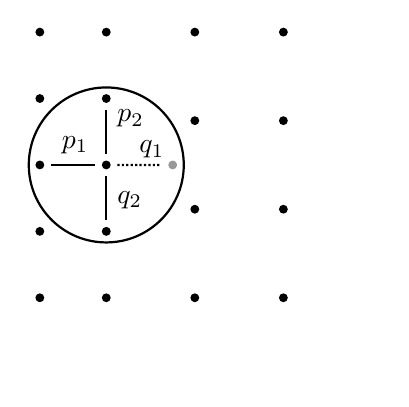
\begin{tikzpicture}[y=0.80pt, x=0.8pt,yscale=-1, inner sep=0pt, outer sep=0pt]
\begin{scope}[shift={(-16.10332,18.79897)}]
  \path[fill=black] (178.797,148.02312) node[above right] (text6246) {};
  \path[shift={(46.10332,-288.79897)},fill=black,nonzero rule] (12.0000,340.0000)
    .. controls (12.0000,341.1046) and (11.1046,342.0000) .. (10.0000,342.0000) ..
    controls (8.8954,342.0000) and (8.0000,341.1046) .. (8.0000,340.0000) ..
    controls (8.0000,338.8954) and (8.8954,338.0000) .. (10.0000,338.0000) ..
    controls (11.1046,338.0000) and (12.0000,338.8954) .. (12.0000,340.0000) --
    cycle;
  \path[shift={(46.10332,-258.79897)},fill=black,fill opacity=0.392,nonzero rule]
    (12.0000,340.0000) .. controls (12.0000,341.1046) and (11.1046,342.0000) ..
    (10.0000,342.0000) .. controls (8.8954,342.0000) and (8.0000,341.1046) ..
    (8.0000,340.0000) .. controls (8.0000,338.8954) and (8.8954,338.0000) ..
    (10.0000,338.0000) .. controls (11.1046,338.0000) and (12.0000,338.8954) ..
    (12.0000,340.0000) -- cycle;
  \path[shift={(46.10332,-318.79897)},fill=black,nonzero rule] (12.0000,340.0000)
    .. controls (12.0000,341.1046) and (11.1046,342.0000) .. (10.0000,342.0000) ..
    controls (8.8954,342.0000) and (8.0000,341.1046) .. (8.0000,340.0000) ..
    controls (8.0000,338.8954) and (8.8954,338.0000) .. (10.0000,338.0000) ..
    controls (11.1046,338.0000) and (12.0000,338.8954) .. (12.0000,340.0000) --
    cycle;
  \path[shift={(46.10332,-348.79897)},fill=black,nonzero rule] (12.0000,340.0000)
    .. controls (12.0000,341.1046) and (11.1046,342.0000) .. (10.0000,342.0000) ..
    controls (8.8954,342.0000) and (8.0000,341.1046) .. (8.0000,340.0000) ..
    controls (8.0000,338.8954) and (8.8954,338.0000) .. (10.0000,338.0000) ..
    controls (11.1046,338.0000) and (12.0000,338.8954) .. (12.0000,340.0000) --
    cycle;
  \path[shift={(46.10332,-258.79897)},fill=black,nonzero rule] (12.0000,340.0000)
    .. controls (12.0000,341.1046) and (11.1046,342.0000) .. (10.0000,342.0000) ..
    controls (8.8954,342.0000) and (8.0000,341.1046) .. (8.0000,340.0000) ..
    controls (8.0000,338.8954) and (8.8954,338.0000) .. (10.0000,338.0000) ..
    controls (11.1046,338.0000) and (12.0000,338.8954) .. (12.0000,340.0000) --
    cycle;
  \path[shift={(46.10332,-228.79897)},fill=black,nonzero rule] (12.0000,340.0000)
    .. controls (12.0000,341.1046) and (11.1046,342.0000) .. (10.0000,342.0000) ..
    controls (8.8954,342.0000) and (8.0000,341.1046) .. (8.0000,340.0000) ..
    controls (8.0000,338.8954) and (8.8954,338.0000) .. (10.0000,338.0000) ..
    controls (11.1046,338.0000) and (12.0000,338.8954) .. (12.0000,340.0000) --
    cycle;
  \path[shift={(16.10332,-288.79897)},fill=black,nonzero rule] (12.0000,340.0000)
    .. controls (12.0000,341.1046) and (11.1046,342.0000) .. (10.0000,342.0000) ..
    controls (8.8954,342.0000) and (8.0000,341.1046) .. (8.0000,340.0000) ..
    controls (8.0000,338.8954) and (8.8954,338.0000) .. (10.0000,338.0000) ..
    controls (11.1046,338.0000) and (12.0000,338.8954) .. (12.0000,340.0000) --
    cycle;
  \path[shift={(16.10332,-318.79897)},fill=black,nonzero rule] (12.0000,340.0000)
    .. controls (12.0000,341.1046) and (11.1046,342.0000) .. (10.0000,342.0000) ..
    controls (8.8954,342.0000) and (8.0000,341.1046) .. (8.0000,340.0000) ..
    controls (8.0000,338.8954) and (8.8954,338.0000) .. (10.0000,338.0000) ..
    controls (11.1046,338.0000) and (12.0000,338.8954) .. (12.0000,340.0000) --
    cycle;
  \path[shift={(16.10332,-348.79897)},fill=black,nonzero rule] (12.0000,340.0000)
    .. controls (12.0000,341.1046) and (11.1046,342.0000) .. (10.0000,342.0000) ..
    controls (8.8954,342.0000) and (8.0000,341.1046) .. (8.0000,340.0000) ..
    controls (8.0000,338.8954) and (8.8954,338.0000) .. (10.0000,338.0000) ..
    controls (11.1046,338.0000) and (12.0000,338.8954) .. (12.0000,340.0000) --
    cycle;
  \path[shift={(16.10332,-258.79897)},fill=black,nonzero rule] (12.0000,340.0000)
    .. controls (12.0000,341.1046) and (11.1046,342.0000) .. (10.0000,342.0000) ..
    controls (8.8954,342.0000) and (8.0000,341.1046) .. (8.0000,340.0000) ..
    controls (8.0000,338.8954) and (8.8954,338.0000) .. (10.0000,338.0000) ..
    controls (11.1046,338.0000) and (12.0000,338.8954) .. (12.0000,340.0000) --
    cycle;
  \path[shift={(16.10332,-228.79897)},fill=black,nonzero rule] (12.0000,340.0000)
    .. controls (12.0000,341.1046) and (11.1046,342.0000) .. (10.0000,342.0000) ..
    controls (8.8954,342.0000) and (8.0000,341.1046) .. (8.0000,340.0000) ..
    controls (8.0000,338.8954) and (8.8954,338.0000) .. (10.0000,338.0000) ..
    controls (11.1046,338.0000) and (12.0000,338.8954) .. (12.0000,340.0000) --
    cycle;
  \path[shift={(86.10332,-348.79897)},fill=black,nonzero rule] (12.0000,340.0000)
    .. controls (12.0000,341.1046) and (11.1046,342.0000) .. (10.0000,342.0000) ..
    controls (8.8954,342.0000) and (8.0000,341.1046) .. (8.0000,340.0000) ..
    controls (8.0000,338.8954) and (8.8954,338.0000) .. (10.0000,338.0000) ..
    controls (11.1046,338.0000) and (12.0000,338.8954) .. (12.0000,340.0000) --
    cycle;
  \path[shift={(86.10332,-308.79897)},fill=black,nonzero rule] (12.0000,340.0000)
    .. controls (12.0000,341.1046) and (11.1046,342.0000) .. (10.0000,342.0000) ..
    controls (8.8954,342.0000) and (8.0000,341.1046) .. (8.0000,340.0000) ..
    controls (8.0000,338.8954) and (8.8954,338.0000) .. (10.0000,338.0000) ..
    controls (11.1046,338.0000) and (12.0000,338.8954) .. (12.0000,340.0000) --
    cycle;
  \path[shift={(86.10332,-268.79897)},fill=black,nonzero rule] (12.0000,340.0000)
    .. controls (12.0000,341.1046) and (11.1046,342.0000) .. (10.0000,342.0000) ..
    controls (8.8954,342.0000) and (8.0000,341.1046) .. (8.0000,340.0000) ..
    controls (8.0000,338.8954) and (8.8954,338.0000) .. (10.0000,338.0000) ..
    controls (11.1046,338.0000) and (12.0000,338.8954) .. (12.0000,340.0000) --
    cycle;
  \path[shift={(86.10332,-228.79897)},fill=black,nonzero rule] (12.0000,340.0000)
    .. controls (12.0000,341.1046) and (11.1046,342.0000) .. (10.0000,342.0000) ..
    controls (8.8954,342.0000) and (8.0000,341.1046) .. (8.0000,340.0000) ..
    controls (8.0000,338.8954) and (8.8954,338.0000) .. (10.0000,338.0000) ..
    controls (11.1046,338.0000) and (12.0000,338.8954) .. (12.0000,340.0000) --
    cycle;
  \path[shift={(126.10332,-348.79897)},fill=black,nonzero rule] (12.0000,340.0000)
    .. controls (12.0000,341.1046) and (11.1046,342.0000) .. (10.0000,342.0000) ..
    controls (8.8954,342.0000) and (8.0000,341.1046) .. (8.0000,340.0000) ..
    controls (8.0000,338.8954) and (8.8954,338.0000) .. (10.0000,338.0000) ..
    controls (11.1046,338.0000) and (12.0000,338.8954) .. (12.0000,340.0000) --
    cycle;
  \path[shift={(126.10332,-308.79897)},fill=black,nonzero rule] (12.0000,340.0000)
    .. controls (12.0000,341.1046) and (11.1046,342.0000) .. (10.0000,342.0000) ..
    controls (8.8954,342.0000) and (8.0000,341.1046) .. (8.0000,340.0000) ..
    controls (8.0000,338.8954) and (8.8954,338.0000) .. (10.0000,338.0000) ..
    controls (11.1046,338.0000) and (12.0000,338.8954) .. (12.0000,340.0000) --
    cycle;
  \path[shift={(126.10332,-268.79897)},fill=black,nonzero rule] (12.0000,340.0000)
    .. controls (12.0000,341.1046) and (11.1046,342.0000) .. (10.0000,342.0000) ..
    controls (8.8954,342.0000) and (8.0000,341.1046) .. (8.0000,340.0000) ..
    controls (8.0000,338.8954) and (8.8954,338.0000) .. (10.0000,338.0000) ..
    controls (11.1046,338.0000) and (12.0000,338.8954) .. (12.0000,340.0000) --
    cycle;
  \path[shift={(126.10332,-228.79897)},fill=black,nonzero rule] (12.0000,340.0000)
    .. controls (12.0000,341.1046) and (11.1046,342.0000) .. (10.0000,342.0000) ..
    controls (8.8954,342.0000) and (8.0000,341.1046) .. (8.0000,340.0000) ..
    controls (8.0000,338.8954) and (8.8954,338.0000) .. (10.0000,338.0000) ..
    controls (11.1046,338.0000) and (12.0000,338.8954) .. (12.0000,340.0000) --
    cycle;
  \path[fill=black] (36.103317,46.201031) node[above right] (text4184) {$p_1$};
  \path[fill=black] (71.103317,48.201031) node[above right] (text4188) {$q_1$};
    \path[color=black,fill=black,line width=0.800pt] (31.1033,50.7010) --
      (31.1033,51.7010) -- (51.1033,51.7010) -- (51.1033,50.7010) --
      (31.1033,50.7010) -- cycle;
    \path[line join=round,even odd rule,line width=0.500pt] (33.0289,52.4112) --
      (29.7511,51.2058) -- (33.0289,50.0005) .. controls (32.5052,50.7121) and
      (32.5083,51.6858) .. (33.0289,52.4112) -- cycle;
    \path[color=black,fill=black,line width=0.800pt] (55.6033,56.2010) --
      (55.6033,76.2010) -- (56.6033,76.2010) -- (56.6033,56.2010) --
      (55.6033,56.2010) -- cycle;
    \path[line join=round,even odd rule,line width=0.500pt] (57.3134,74.2755) --
      (56.1081,77.5532) -- (54.9028,74.2755) .. controls (55.6144,74.7991) and
      (56.5880,74.7961) .. (57.3134,74.2755) -- cycle;
    \path[color=black,fill=black,line width=0.800pt] (55.6033,26.2010) --
      (55.6033,46.2010) -- (56.6033,46.2010) -- (56.6033,26.2010) --
      (55.6033,26.2010) -- cycle;
    \path[line join=round,even odd rule,line width=0.500pt] (54.8932,28.1266) --
      (56.0985,24.8488) -- (57.3038,28.1266) .. controls (56.5922,27.6030) and
      (55.6186,27.6060) .. (54.8932,28.1266) -- cycle;
    \path[color=black,fill=black,line width=0.800pt] (61.1033,51.7010) --
      (62.1033,51.7010) -- (62.1033,50.7010) -- (61.1033,50.7010) --
      cycle(63.1033,51.7010) -- (64.1033,51.7010) -- (64.1033,50.7010) --
      (63.1033,50.7010) -- cycle(65.1033,51.7010) -- (66.1033,51.7010) --
      (66.1033,50.7010) -- (65.1033,50.7010) -- cycle(67.1033,51.7010) --
      (68.1033,51.7010) -- (68.1033,50.7010) -- (67.1033,50.7010) --
      cycle(69.1033,51.7010) -- (70.1033,51.7010) -- (70.1033,50.7010) --
      (69.1033,50.7010) -- cycle(71.1033,51.7010) -- (72.1033,51.7010) --
      (72.1033,50.7010) -- (71.1033,50.7010) -- cycle(73.1033,51.7010) --
      (74.1033,51.7010) -- (74.1033,50.7010) -- (73.1033,50.7010) --
      cycle(75.1033,51.7010) -- (76.1033,51.7010) -- (76.1033,50.7010) --
      (75.1033,50.7010) -- cycle(77.1033,51.7010) -- (78.1033,51.7010) --
      (78.1033,50.7010) -- (77.1033,50.7010) -- cycle(79.1033,51.7010) --
      (80.1033,51.7010) -- (80.1033,50.7010) -- (79.1033,50.7010) -- cycle;
    \path[line join=round,even odd rule,line width=0.500pt] (79.1777,49.9909) --
      (82.4555,51.1962) -- (79.1777,52.4015) .. controls (79.7014,51.6899) and
      (79.6984,50.7163) .. (79.1777,49.9909) -- cycle;
  \path[shift={(76.10332,-288.79897)},fill=black,fill opacity=0.404,nonzero rule]
    (12.0000,340.0000) .. controls (12.0000,341.1046) and (11.1046,342.0000) ..
    (10.0000,342.0000) .. controls (8.8954,342.0000) and (8.0000,341.1046) ..
    (8.0000,340.0000) .. controls (8.0000,338.8954) and (8.8954,338.0000) ..
    (10.0000,338.0000) .. controls (11.1046,338.0000) and (12.0000,338.8954) ..
    (12.0000,340.0000) -- cycle;
  \path[shift={(16.10332,-38.79897)},draw=black,fill=black,line join=round,miter
    limit=4.00,fill opacity=0.000,nonzero rule,line width=0.800pt]
    (75.0000,90.0000) .. controls (75.0000,109.3300) and (59.3300,125.0000) ..
    (40.0000,125.0000) .. controls (20.6700,125.0000) and (5.0000,109.3300) ..
    (5.0000,90.0000) .. controls (5.0000,70.6700) and (20.6700,55.0000) ..
    (40.0000,55.0000) .. controls (59.3300,55.0000) and (75.0000,70.6700) ..
    (75.0000,90.0000) -- cycle;
  \path[fill=black] (61.103317,34.201031) node[above right] (text5037) {$p_2$};
  \path[fill=black] (61.103317,71.201027) node[above right] (text5041) {$q_2$};
\end{scope}

\end{tikzpicture}


  \caption{Virtual Points Pair Up Unpaired Neighbors}
  \label{fig:virtualpoint}
\end{figure}
%
Note that, while bonds \(p_2\) and \(q_2\) form a perfect bond pair, there is no bond exactly opposite \(p_1\).
To solve this, we add a virtual point to create a bond, \(q_1\), that will form a pair with \(p_1\).
Because this point is not part of the discretization, it has no mass, and its properties must be determined from the properties of the surrounding nodes.
An easy method of determining properties (such as displacement) at virtual nodes is to use a weighted average.
One method of generating useful weights that is relatively robust is barycentric interpolation.
We start by finding the three (non-colinear) real nodes closest to the location of the virtual node, A, B, and C.
Next, we find the signed areas of the triangles ABC, ABX, BCX, and CAX, with X being the virtual node.
The weight of node A is the area ratio between BCX and ABC, the weight of node B is the ratio of areas CAX and ABC, and the weight of node C is the ratio of areas ABX to ABC.
Using signed areas allows the weights to be negative to extrapolate properties of a virtual node outside of ABC.
Because these weights are calculated from the initial positions of the node, they can be stored for swift evaluation of properties at virtual nodes.

%
\begin{figure}[tbp]
  \centering
  


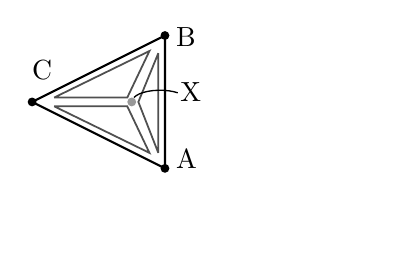
\begin{tikzpicture}[y=0.80pt, x=0.8pt,yscale=-1, inner sep=0pt, outer sep=0pt]
\begin{scope}[shift={(-16.10332,-41.20103)}]
  \path[fill=black] (178.797,148.02312) node[above right] (text6246) {};
  \path[shift={(16.10332,-258.79897)},fill=black,nonzero rule] (12.0000,340.0000)
    .. controls (12.0000,341.1046) and (11.1046,342.0000) .. (10.0000,342.0000) ..
    controls (8.8954,342.0000) and (8.0000,341.1046) .. (8.0000,340.0000) ..
    controls (8.0000,338.8954) and (8.8954,338.0000) .. (10.0000,338.0000) ..
    controls (11.1046,338.0000) and (12.0000,338.8954) .. (12.0000,340.0000) --
    cycle;
  \path[shift={(76.10332,-288.79897)},fill=black,nonzero rule] (12.0000,340.0000)
    .. controls (12.0000,341.1046) and (11.1046,342.0000) .. (10.0000,342.0000) ..
    controls (8.8954,342.0000) and (8.0000,341.1046) .. (8.0000,340.0000) ..
    controls (8.0000,338.8954) and (8.8954,338.0000) .. (10.0000,338.0000) ..
    controls (11.1046,338.0000) and (12.0000,338.8954) .. (12.0000,340.0000) --
    cycle;
  \path[shift={(76.10332,-228.79897)},fill=black,nonzero rule] (12.0000,340.0000)
    .. controls (12.0000,341.1046) and (11.1046,342.0000) .. (10.0000,342.0000) ..
    controls (8.8954,342.0000) and (8.0000,341.1046) .. (8.0000,340.0000) ..
    controls (8.0000,338.8954) and (8.8954,338.0000) .. (10.0000,338.0000) ..
    controls (11.1046,338.0000) and (12.0000,338.8954) .. (12.0000,340.0000) --
    cycle;
  \path[shift={(61.10332,-258.79897)},fill=black,fill opacity=0.404,nonzero rule]
    (12.0000,340.0000) .. controls (12.0000,341.1046) and (11.1046,342.0000) ..
    (10.0000,342.0000) .. controls (8.8954,342.0000) and (8.0000,341.1046) ..
    (8.0000,340.0000) .. controls (8.0000,338.8954) and (8.8954,338.0000) ..
    (10.0000,338.0000) .. controls (11.1046,338.0000) and (12.0000,338.8954) ..
    (12.0000,340.0000) -- cycle;
  \path[fill=black] (91.103317,111.20103) node[above right] (text3133) {A};
  \path[fill=black] (91.103317,56.201031) node[above right] (text3137) {B};
  \path[fill=black] (26.103317,71.201027) node[above right] (text3141) {C};
  \path[shift={(16.10332,-18.79897)},draw=black,line join=miter,line cap=butt,line
    width=0.800pt] (10.0000,100.0000) -- (70.0000,70.0000) -- (70.0000,130.0000)
    -- cycle;
  \path[shift={(16.10332,-18.79897)},draw=black,line join=miter,line
    cap=butt,miter limit=4.00,draw opacity=0.686,line width=0.640pt]
    (20.0000,98.0000) -- (63.0000,77.0000) -- (53.0000,98.0000) -- cycle;
  \path[shift={(16.10332,-18.79897)},draw=black,line join=miter,line
    cap=butt,miter limit=4.00,draw opacity=0.686,line width=0.640pt]
    (67.0000,78.0000) -- (58.0000,100.0000) -- (67.0000,123.0000) -- cycle;
  \path[shift={(16.10332,-18.79897)},draw=black,line join=miter,line
    cap=butt,miter limit=4.00,draw opacity=0.686,line width=0.640pt]
    (20.0000,102.0000) -- (53.0000,102.0000) -- (63.0000,123.0000) -- cycle;
  \path[fill=black] (93.103317,81.201027) node[above right] (text3157) {X};
  \path[shift={(-8.65052,-9.08887)},draw=black,fill=black,line join=round,miter
    limit=4.00,fill opacity=0.000,nonzero rule,line width=0.480pt]
    (80.7538,88.2899) .. controls (83.1150,85.6950) and (90.2880,84.3571) ..
    (96.7753,85.3015) .. controls (98.1455,85.5010) and (99.4178,85.7949) ..
    (100.5349,86.1698);
\end{scope}

\end{tikzpicture}


  \caption{Barycentric interpolation is based on the relative areas of sub triangles}
  \label{fig:BaryCentric}
\end{figure}
%

With the properties of the virtual points determined, the model can be evaluated in the same manner as the uniformly discretized models of the previous papers.
Where forces are calculated to act on a virtual node, those forces are redistributed to the supporting real nodes according to the weight each point has in the interpolation.

The same method of virtual nodes also allows the modeling of curved surfaces, in which the perfect opposite of a bond may not lie near but not on the surface of the plate or shell.
As long as the curvature of the surface is small (at the scale of the peridynamic horizon), each resulting virtual nodes will be nearly in the plane formed by its nearest neighbors.
Finding the weights of the surrounding nodes is performed just as in the planar case, except that the areas are formed between the projection of the virtual node location X onto the plane formed by A, B, and C.

%%
%\begin{figure}[tbp]
%  \centering
%  \input{\diagrampath/VirtualCurve.tex}
%  \caption{Virtual Points Allow Straight Pairs on Curved Surfaces}
%  \label{fig:virtualcurve}
%\end{figure}
%%

To compute the weight of node A in the interpolation of properties at virtual node X, let AB represent the vector from node A to node B, and use
%
\begin{equation}
\label{eq:BarycentricArea}
W'_A = \frac{B-X}{2}\bullet \left[BC \times \left(\frac{BC \times BA}{|BC \times BA|}\right)\right]
\end{equation}
%
After finding $W'_B$ and $W'_C$ in similar fashion,
%
\begin{equation}
\label{eq:BarycentricWeight}
W_A = \frac{W'_A }{W'_A + W'_B + W'_C}
\end{equation}
%
If the projection of X onto the plane defined by A, B, and C lies outside the triangle ABC,  one or two of $W_A$, $W_B$ and $W_C$ will be negative, though they will still sum to 1.

\section{``Boundary'' Conditions}
Because peridynamic models result in long range forces, it is not sufficient to apply boundary conditions to nodes on the relevant boundary; nodes near the boundary must be considered as well.
Displacement conditions are enforced on the nodes nearest to a simply-supported plate edge, while average displacements are enforced on a small collection of nodes surrounding a beam pin support.
Clamped boundary conditions are simulated by controlling the displacement of 1-5 nodes nearest the boundary and applying a symmetry boundary condition to nodes out to a distance of \(2\delta\) from the boundary. 
Point loads are evenly distributed over all nodes in a region with width or diameter of \(\delta\) centered on the point load location.
Line and pressure loads are treated normally.

\section{Numerical Solution Method}

This project uses Trilinos, a collection of open software libraries, or packages, from Sandia National Labs, including:
\begin{itemize}
  \item Epetra and EpetraExt - provide efficient parallel data structures, particularly vectors and sparse matrices
  \item Isorropia - provides load balancing, partitioning, and matrix coloring
  \item NOX - a collection of large-scale nonlinear system solver utilities
  \item PyTrilinos - a python interface providing Python wrappers for many Trilinos packages, and offering compatibility between numpy.ndarrays and Epetra.MultiVectors
\end{itemize}

The nature of discrete peridynamic models results in large numbers of parallelizable computations.
Efficient parallelization is achieved using Epetra data structures for distributed variables.
Model force evaluations are coded in Python, making extensive use of the optimized routines in the NumPy and SciPy packages operating on the distributed Epetra objects. 
To obtain quasistatic solutions, problems are coded into NOX objects and solved using NOX nonlinear solvers.
Preliminary analysis was performed using a Newton Method solver on an iMac with a 3.1GHz Intel Core i7 processor and 16GB RAM, using 1-4 cores.
The nature of the Trilinos packages and the structure of the code allow for more extensive parallel computation without major code changes.

For all but the simplest loading conditions, analytical solutions to boundary condition problems become complicated.
As load conditions and material behavior become more complex, there are no analytical solutions.
For comparison, equivalent models are created and analyzed in Abaqus 6.12 to verify simple cases.

\section{Results}
\label{sec:Results}
\FloatBarrier
\subsection{Straight Beam Results}
The simplest test case for this model is a linear-elastic beam with a square profile.
These models represent beams that are 1cm thick and 1cm wide, with a bulk modulus $k = 37.5$GPa and Poisson's ratio $\nu = \sfrac{1}{3}$.
Each is loaded transversely with a load of 0.0833N, except for \cref{fig:moment_n}, which shows a beam loaded with a moment of 0.0833N$\cdot$m.
In beams simulating inelastic behavior, the critical strain of the material is set to $\varepsilon_c = 0.001$.
The elastic cases are compared to analytical solutions of the Euler beam equation with appropriate boundary conditions.
Even a coarse discretization successfully reproduces the shape of the elastically deformed, simply-supported beam shown  in \cref{fig:elastic_g2000} deformed under uniform load.
%\todo{Your figures should not have titles on top of them.}
%
\begin{figure}[htbp]
  \centering
  \resizebox{0.6\linewidth}{!}{%% Creator: Matplotlib, PGF backend
%%
%% To include the figure in your LaTeX document, write
%%   \input{<filename>.pgf}
%%
%% Make sure the required packages are loaded in your preamble
%%   \usepackage{pgf}
%%
%% Figures using additional raster images can only be included by \input if
%% they are in the same directory as the main LaTeX file. For loading figures
%% from other directories you can use the `import` package
%%   \usepackage{import}
%% and then include the figures with
%%   \import{<path to file>}{<filename>.pgf}
%%
%% Matplotlib used the following preamble
%%
\begingroup%
\makeatletter%
\begin{pgfpicture}%
\pgfpathrectangle{\pgfpointorigin}{\pgfqpoint{6.000000in}{6.000000in}}%
\pgfusepath{use as bounding box}%
\begin{pgfscope}%
\pgfsetbuttcap%
\pgfsetroundjoin%
\definecolor{currentfill}{rgb}{1.000000,1.000000,1.000000}%
\pgfsetfillcolor{currentfill}%
\pgfsetlinewidth{0.000000pt}%
\definecolor{currentstroke}{rgb}{1.000000,1.000000,1.000000}%
\pgfsetstrokecolor{currentstroke}%
\pgfsetdash{}{0pt}%
\pgfpathmoveto{\pgfqpoint{0.000000in}{0.000000in}}%
\pgfpathlineto{\pgfqpoint{6.000000in}{0.000000in}}%
\pgfpathlineto{\pgfqpoint{6.000000in}{6.000000in}}%
\pgfpathlineto{\pgfqpoint{0.000000in}{6.000000in}}%
\pgfpathclose%
\pgfusepath{fill}%
\end{pgfscope}%
\begin{pgfscope}%
\pgfsetbuttcap%
\pgfsetroundjoin%
\definecolor{currentfill}{rgb}{1.000000,1.000000,1.000000}%
\pgfsetfillcolor{currentfill}%
\pgfsetlinewidth{0.000000pt}%
\definecolor{currentstroke}{rgb}{0.000000,0.000000,0.000000}%
\pgfsetstrokecolor{currentstroke}%
\pgfsetstrokeopacity{0.000000}%
\pgfsetdash{}{0pt}%
\pgfpathmoveto{\pgfqpoint{0.750000in}{0.600000in}}%
\pgfpathlineto{\pgfqpoint{5.400000in}{0.600000in}}%
\pgfpathlineto{\pgfqpoint{5.400000in}{5.400000in}}%
\pgfpathlineto{\pgfqpoint{0.750000in}{5.400000in}}%
\pgfpathclose%
\pgfusepath{fill}%
\end{pgfscope}%
\begin{pgfscope}%
\pgfpathrectangle{\pgfqpoint{0.750000in}{0.600000in}}{\pgfqpoint{4.650000in}{4.800000in}} %
\pgfusepath{clip}%
\pgfsetrectcap%
\pgfsetroundjoin%
\pgfsetlinewidth{1.003750pt}%
\definecolor{currentstroke}{rgb}{0.000000,0.000000,1.000000}%
\pgfsetstrokecolor{currentstroke}%
\pgfsetdash{}{0pt}%
\pgfpathmoveto{\pgfqpoint{0.750000in}{5.400000in}}%
\pgfpathlineto{\pgfqpoint{0.984825in}{4.729964in}}%
\pgfpathlineto{\pgfqpoint{1.110375in}{4.378524in}}%
\pgfpathlineto{\pgfqpoint{1.217325in}{4.085616in}}%
\pgfpathlineto{\pgfqpoint{1.312650in}{3.830940in}}%
\pgfpathlineto{\pgfqpoint{1.401000in}{3.601260in}}%
\pgfpathlineto{\pgfqpoint{1.482375in}{3.395848in}}%
\pgfpathlineto{\pgfqpoint{1.559100in}{3.208112in}}%
\pgfpathlineto{\pgfqpoint{1.633500in}{3.032040in}}%
\pgfpathlineto{\pgfqpoint{1.703250in}{2.872688in}}%
\pgfpathlineto{\pgfqpoint{1.770675in}{2.724224in}}%
\pgfpathlineto{\pgfqpoint{1.833450in}{2.591168in}}%
\pgfpathlineto{\pgfqpoint{1.896225in}{2.463328in}}%
\pgfpathlineto{\pgfqpoint{1.956675in}{2.345336in}}%
\pgfpathlineto{\pgfqpoint{2.014800in}{2.236780in}}%
\pgfpathlineto{\pgfqpoint{2.070600in}{2.137224in}}%
\pgfpathlineto{\pgfqpoint{2.124075in}{2.046208in}}%
\pgfpathlineto{\pgfqpoint{2.175225in}{1.963268in}}%
\pgfpathlineto{\pgfqpoint{2.226375in}{1.884448in}}%
\pgfpathlineto{\pgfqpoint{2.275200in}{1.813120in}}%
\pgfpathlineto{\pgfqpoint{2.324025in}{1.745680in}}%
\pgfpathlineto{\pgfqpoint{2.370525in}{1.685124in}}%
\pgfpathlineto{\pgfqpoint{2.417025in}{1.628200in}}%
\pgfpathlineto{\pgfqpoint{2.461200in}{1.577528in}}%
\pgfpathlineto{\pgfqpoint{2.505375in}{1.530216in}}%
\pgfpathlineto{\pgfqpoint{2.547225in}{1.488524in}}%
\pgfpathlineto{\pgfqpoint{2.589075in}{1.449904in}}%
\pgfpathlineto{\pgfqpoint{2.630925in}{1.414384in}}%
\pgfpathlineto{\pgfqpoint{2.670450in}{1.383720in}}%
\pgfpathlineto{\pgfqpoint{2.709975in}{1.355840in}}%
\pgfpathlineto{\pgfqpoint{2.747175in}{1.332160in}}%
\pgfpathlineto{\pgfqpoint{2.784375in}{1.311000in}}%
\pgfpathlineto{\pgfqpoint{2.821575in}{1.292360in}}%
\pgfpathlineto{\pgfqpoint{2.858775in}{1.276280in}}%
\pgfpathlineto{\pgfqpoint{2.895975in}{1.262680in}}%
\pgfpathlineto{\pgfqpoint{2.933175in}{1.251680in}}%
\pgfpathlineto{\pgfqpoint{2.970375in}{1.243200in}}%
\pgfpathlineto{\pgfqpoint{3.007575in}{1.237280in}}%
\pgfpathlineto{\pgfqpoint{3.042450in}{1.234040in}}%
\pgfpathlineto{\pgfqpoint{3.079650in}{1.233080in}}%
\pgfpathlineto{\pgfqpoint{3.116850in}{1.234680in}}%
\pgfpathlineto{\pgfqpoint{3.154050in}{1.238840in}}%
\pgfpathlineto{\pgfqpoint{3.193575in}{1.246080in}}%
\pgfpathlineto{\pgfqpoint{3.230775in}{1.255520in}}%
\pgfpathlineto{\pgfqpoint{3.267975in}{1.267480in}}%
\pgfpathlineto{\pgfqpoint{3.305175in}{1.282000in}}%
\pgfpathlineto{\pgfqpoint{3.344700in}{1.300200in}}%
\pgfpathlineto{\pgfqpoint{3.381900in}{1.319960in}}%
\pgfpathlineto{\pgfqpoint{3.419100in}{1.342200in}}%
\pgfpathlineto{\pgfqpoint{3.458625in}{1.368600in}}%
\pgfpathlineto{\pgfqpoint{3.498150in}{1.397800in}}%
\pgfpathlineto{\pgfqpoint{3.537675in}{1.429788in}}%
\pgfpathlineto{\pgfqpoint{3.577200in}{1.464556in}}%
\pgfpathlineto{\pgfqpoint{3.619050in}{1.504376in}}%
\pgfpathlineto{\pgfqpoint{3.660900in}{1.547256in}}%
\pgfpathlineto{\pgfqpoint{3.702750in}{1.593168in}}%
\pgfpathlineto{\pgfqpoint{3.746925in}{1.644892in}}%
\pgfpathlineto{\pgfqpoint{3.793425in}{1.702912in}}%
\pgfpathlineto{\pgfqpoint{3.839925in}{1.764548in}}%
\pgfpathlineto{\pgfqpoint{3.888750in}{1.833104in}}%
\pgfpathlineto{\pgfqpoint{3.937575in}{1.905532in}}%
\pgfpathlineto{\pgfqpoint{3.988725in}{1.985484in}}%
\pgfpathlineto{\pgfqpoint{4.039875in}{2.069528in}}%
\pgfpathlineto{\pgfqpoint{4.095675in}{2.165780in}}%
\pgfpathlineto{\pgfqpoint{4.151475in}{2.266684in}}%
\pgfpathlineto{\pgfqpoint{4.209600in}{2.376600in}}%
\pgfpathlineto{\pgfqpoint{4.267725in}{2.491276in}}%
\pgfpathlineto{\pgfqpoint{4.328175in}{2.615424in}}%
\pgfpathlineto{\pgfqpoint{4.390950in}{2.749416in}}%
\pgfpathlineto{\pgfqpoint{4.456050in}{2.893604in}}%
\pgfpathlineto{\pgfqpoint{4.523475in}{3.048284in}}%
\pgfpathlineto{\pgfqpoint{4.595550in}{3.219316in}}%
\pgfpathlineto{\pgfqpoint{4.669950in}{3.401628in}}%
\pgfpathlineto{\pgfqpoint{4.749000in}{3.601260in}}%
\pgfpathlineto{\pgfqpoint{4.835025in}{3.824816in}}%
\pgfpathlineto{\pgfqpoint{4.925700in}{4.066764in}}%
\pgfpathlineto{\pgfqpoint{5.025675in}{4.339944in}}%
\pgfpathlineto{\pgfqpoint{5.137275in}{4.651284in}}%
\pgfpathlineto{\pgfqpoint{5.283750in}{5.067054in}}%
\pgfpathlineto{\pgfqpoint{5.400000in}{5.400000in}}%
\pgfpathlineto{\pgfqpoint{5.400000in}{5.400000in}}%
\pgfusepath{stroke}%
\end{pgfscope}%
\begin{pgfscope}%
\pgfpathrectangle{\pgfqpoint{0.750000in}{0.600000in}}{\pgfqpoint{4.650000in}{4.800000in}} %
\pgfusepath{clip}%
\pgfsetbuttcap%
\pgfsetroundjoin%
\definecolor{currentfill}{rgb}{0.000000,0.000000,1.000000}%
\pgfsetfillcolor{currentfill}%
\pgfsetlinewidth{0.501875pt}%
\definecolor{currentstroke}{rgb}{0.000000,0.000000,0.000000}%
\pgfsetstrokecolor{currentstroke}%
\pgfsetdash{}{0pt}%
\pgfsys@defobject{currentmarker}{\pgfqpoint{-0.041667in}{-0.041667in}}{\pgfqpoint{0.041667in}{0.041667in}}{%
\pgfpathmoveto{\pgfqpoint{0.000000in}{-0.041667in}}%
\pgfpathcurveto{\pgfqpoint{0.011050in}{-0.041667in}}{\pgfqpoint{0.021649in}{-0.037276in}}{\pgfqpoint{0.029463in}{-0.029463in}}%
\pgfpathcurveto{\pgfqpoint{0.037276in}{-0.021649in}}{\pgfqpoint{0.041667in}{-0.011050in}}{\pgfqpoint{0.041667in}{0.000000in}}%
\pgfpathcurveto{\pgfqpoint{0.041667in}{0.011050in}}{\pgfqpoint{0.037276in}{0.021649in}}{\pgfqpoint{0.029463in}{0.029463in}}%
\pgfpathcurveto{\pgfqpoint{0.021649in}{0.037276in}}{\pgfqpoint{0.011050in}{0.041667in}}{\pgfqpoint{0.000000in}{0.041667in}}%
\pgfpathcurveto{\pgfqpoint{-0.011050in}{0.041667in}}{\pgfqpoint{-0.021649in}{0.037276in}}{\pgfqpoint{-0.029463in}{0.029463in}}%
\pgfpathcurveto{\pgfqpoint{-0.037276in}{0.021649in}}{\pgfqpoint{-0.041667in}{0.011050in}}{\pgfqpoint{-0.041667in}{0.000000in}}%
\pgfpathcurveto{\pgfqpoint{-0.041667in}{-0.011050in}}{\pgfqpoint{-0.037276in}{-0.021649in}}{\pgfqpoint{-0.029463in}{-0.029463in}}%
\pgfpathcurveto{\pgfqpoint{-0.021649in}{-0.037276in}}{\pgfqpoint{-0.011050in}{-0.041667in}}{\pgfqpoint{0.000000in}{-0.041667in}}%
\pgfpathclose%
\pgfusepath{stroke,fill}%
}%
\begin{pgfscope}%
\pgfsys@transformshift{0.982500in}{4.736536in}%
\pgfsys@useobject{currentmarker}{}%
\end{pgfscope}%
\begin{pgfscope}%
\pgfsys@transformshift{1.447500in}{3.483120in}%
\pgfsys@useobject{currentmarker}{}%
\end{pgfscope}%
\begin{pgfscope}%
\pgfsys@transformshift{1.912500in}{2.431060in}%
\pgfsys@useobject{currentmarker}{}%
\end{pgfscope}%
\begin{pgfscope}%
\pgfsys@transformshift{2.377500in}{1.676352in}%
\pgfsys@useobject{currentmarker}{}%
\end{pgfscope}%
\begin{pgfscope}%
\pgfsys@transformshift{2.842500in}{1.283000in}%
\pgfsys@useobject{currentmarker}{}%
\end{pgfscope}%
\begin{pgfscope}%
\pgfsys@transformshift{3.307500in}{1.283000in}%
\pgfsys@useobject{currentmarker}{}%
\end{pgfscope}%
\begin{pgfscope}%
\pgfsys@transformshift{3.772500in}{1.676352in}%
\pgfsys@useobject{currentmarker}{}%
\end{pgfscope}%
\begin{pgfscope}%
\pgfsys@transformshift{4.237500in}{2.431060in}%
\pgfsys@useobject{currentmarker}{}%
\end{pgfscope}%
\begin{pgfscope}%
\pgfsys@transformshift{4.702500in}{3.483120in}%
\pgfsys@useobject{currentmarker}{}%
\end{pgfscope}%
\begin{pgfscope}%
\pgfsys@transformshift{5.167500in}{4.736536in}%
\pgfsys@useobject{currentmarker}{}%
\end{pgfscope}%
\end{pgfscope}%
\begin{pgfscope}%
\pgfpathrectangle{\pgfqpoint{0.750000in}{0.600000in}}{\pgfqpoint{4.650000in}{4.800000in}} %
\pgfusepath{clip}%
\pgfsetrectcap%
\pgfsetroundjoin%
\pgfsetlinewidth{1.003750pt}%
\definecolor{currentstroke}{rgb}{0.000000,0.500000,0.000000}%
\pgfsetstrokecolor{currentstroke}%
\pgfsetdash{}{0pt}%
\pgfpathmoveto{\pgfqpoint{0.843000in}{5.142324in}}%
\pgfpathlineto{\pgfqpoint{0.936000in}{4.885157in}}%
\pgfpathlineto{\pgfqpoint{1.029000in}{4.629314in}}%
\pgfpathlineto{\pgfqpoint{1.122000in}{4.375370in}}%
\pgfpathlineto{\pgfqpoint{1.215000in}{4.124317in}}%
\pgfpathlineto{\pgfqpoint{1.308000in}{3.882080in}}%
\pgfpathlineto{\pgfqpoint{1.401000in}{3.645171in}}%
\pgfpathlineto{\pgfqpoint{1.494000in}{3.415281in}}%
\pgfpathlineto{\pgfqpoint{1.587000in}{3.193670in}}%
\pgfpathlineto{\pgfqpoint{1.680000in}{2.981159in}}%
\pgfpathlineto{\pgfqpoint{1.773000in}{2.778726in}}%
\pgfpathlineto{\pgfqpoint{1.866000in}{2.586899in}}%
\pgfpathlineto{\pgfqpoint{1.959000in}{2.406484in}}%
\pgfpathlineto{\pgfqpoint{2.052000in}{2.238095in}}%
\pgfpathlineto{\pgfqpoint{2.145000in}{2.082372in}}%
\pgfpathlineto{\pgfqpoint{2.238000in}{1.939808in}}%
\pgfpathlineto{\pgfqpoint{2.331000in}{1.810928in}}%
\pgfpathlineto{\pgfqpoint{2.424000in}{1.696182in}}%
\pgfpathlineto{\pgfqpoint{2.517000in}{1.595948in}}%
\pgfpathlineto{\pgfqpoint{2.610000in}{1.510572in}}%
\pgfpathlineto{\pgfqpoint{2.703000in}{1.440334in}}%
\pgfpathlineto{\pgfqpoint{2.796000in}{1.385474in}}%
\pgfpathlineto{\pgfqpoint{2.889000in}{1.346173in}}%
\pgfpathlineto{\pgfqpoint{2.982000in}{1.322560in}}%
\pgfpathlineto{\pgfqpoint{3.075000in}{1.314715in}}%
\pgfpathlineto{\pgfqpoint{3.168000in}{1.322661in}}%
\pgfpathlineto{\pgfqpoint{3.261000in}{1.346374in}}%
\pgfpathlineto{\pgfqpoint{3.354000in}{1.385773in}}%
\pgfpathlineto{\pgfqpoint{3.447000in}{1.440729in}}%
\pgfpathlineto{\pgfqpoint{3.540000in}{1.511058in}}%
\pgfpathlineto{\pgfqpoint{3.633000in}{1.596521in}}%
\pgfpathlineto{\pgfqpoint{3.726000in}{1.696835in}}%
\pgfpathlineto{\pgfqpoint{3.819000in}{1.811655in}}%
\pgfpathlineto{\pgfqpoint{3.912000in}{1.940602in}}%
\pgfpathlineto{\pgfqpoint{4.005000in}{2.083224in}}%
\pgfpathlineto{\pgfqpoint{4.098000in}{2.238995in}}%
\pgfpathlineto{\pgfqpoint{4.191000in}{2.407421in}}%
\pgfpathlineto{\pgfqpoint{4.284000in}{2.587862in}}%
\pgfpathlineto{\pgfqpoint{4.377000in}{2.779704in}}%
\pgfpathlineto{\pgfqpoint{4.470000in}{2.982137in}}%
\pgfpathlineto{\pgfqpoint{4.563000in}{3.194634in}}%
\pgfpathlineto{\pgfqpoint{4.656000in}{3.416214in}}%
\pgfpathlineto{\pgfqpoint{4.749000in}{3.646059in}}%
\pgfpathlineto{\pgfqpoint{4.842000in}{3.882903in}}%
\pgfpathlineto{\pgfqpoint{4.935000in}{4.125075in}}%
\pgfpathlineto{\pgfqpoint{5.028000in}{4.376003in}}%
\pgfpathlineto{\pgfqpoint{5.121000in}{4.629816in}}%
\pgfpathlineto{\pgfqpoint{5.214000in}{4.885599in}}%
\pgfpathlineto{\pgfqpoint{5.307000in}{5.142506in}}%
\pgfpathlineto{\pgfqpoint{5.400000in}{5.400000in}}%
\pgfusepath{stroke}%
\end{pgfscope}%
\begin{pgfscope}%
\pgfpathrectangle{\pgfqpoint{0.750000in}{0.600000in}}{\pgfqpoint{4.650000in}{4.800000in}} %
\pgfusepath{clip}%
\pgfsetbuttcap%
\pgfsetmiterjoin%
\definecolor{currentfill}{rgb}{0.000000,0.500000,0.000000}%
\pgfsetfillcolor{currentfill}%
\pgfsetlinewidth{0.501875pt}%
\definecolor{currentstroke}{rgb}{0.000000,0.000000,0.000000}%
\pgfsetstrokecolor{currentstroke}%
\pgfsetdash{}{0pt}%
\pgfsys@defobject{currentmarker}{\pgfqpoint{-0.041667in}{-0.041667in}}{\pgfqpoint{0.041667in}{0.041667in}}{%
\pgfpathmoveto{\pgfqpoint{0.000000in}{0.041667in}}%
\pgfpathlineto{\pgfqpoint{-0.041667in}{-0.041667in}}%
\pgfpathlineto{\pgfqpoint{0.041667in}{-0.041667in}}%
\pgfpathclose%
\pgfusepath{stroke,fill}%
}%
\begin{pgfscope}%
\pgfsys@transformshift{1.587000in}{3.193670in}%
\pgfsys@useobject{currentmarker}{}%
\end{pgfscope}%
\begin{pgfscope}%
\pgfsys@transformshift{2.517000in}{1.595948in}%
\pgfsys@useobject{currentmarker}{}%
\end{pgfscope}%
\begin{pgfscope}%
\pgfsys@transformshift{3.447000in}{1.440729in}%
\pgfsys@useobject{currentmarker}{}%
\end{pgfscope}%
\begin{pgfscope}%
\pgfsys@transformshift{4.377000in}{2.779704in}%
\pgfsys@useobject{currentmarker}{}%
\end{pgfscope}%
\begin{pgfscope}%
\pgfsys@transformshift{5.307000in}{5.142506in}%
\pgfsys@useobject{currentmarker}{}%
\end{pgfscope}%
\end{pgfscope}%
\begin{pgfscope}%
\pgfpathrectangle{\pgfqpoint{0.750000in}{0.600000in}}{\pgfqpoint{4.650000in}{4.800000in}} %
\pgfusepath{clip}%
\pgfsetrectcap%
\pgfsetroundjoin%
\pgfsetlinewidth{1.003750pt}%
\definecolor{currentstroke}{rgb}{1.000000,0.000000,0.000000}%
\pgfsetstrokecolor{currentstroke}%
\pgfsetdash{}{0pt}%
\pgfpathmoveto{\pgfqpoint{0.796500in}{5.268655in}}%
\pgfpathlineto{\pgfqpoint{1.029000in}{4.615916in}}%
\pgfpathlineto{\pgfqpoint{1.168500in}{4.230459in}}%
\pgfpathlineto{\pgfqpoint{1.215000in}{4.103912in}}%
\pgfpathlineto{\pgfqpoint{1.354500in}{3.737992in}}%
\pgfpathlineto{\pgfqpoint{1.447500in}{3.501530in}}%
\pgfpathlineto{\pgfqpoint{1.540500in}{3.273019in}}%
\pgfpathlineto{\pgfqpoint{1.633500in}{3.053440in}}%
\pgfpathlineto{\pgfqpoint{1.726500in}{2.843678in}}%
\pgfpathlineto{\pgfqpoint{1.773000in}{2.742676in}}%
\pgfpathlineto{\pgfqpoint{1.819500in}{2.644376in}}%
\pgfpathlineto{\pgfqpoint{1.866000in}{2.548892in}}%
\pgfpathlineto{\pgfqpoint{1.912500in}{2.456292in}}%
\pgfpathlineto{\pgfqpoint{1.959000in}{2.366675in}}%
\pgfpathlineto{\pgfqpoint{2.005500in}{2.280105in}}%
\pgfpathlineto{\pgfqpoint{2.052000in}{2.196671in}}%
\pgfpathlineto{\pgfqpoint{2.098500in}{2.116430in}}%
\pgfpathlineto{\pgfqpoint{2.145000in}{2.039464in}}%
\pgfpathlineto{\pgfqpoint{2.191500in}{1.965824in}}%
\pgfpathlineto{\pgfqpoint{2.238000in}{1.895587in}}%
\pgfpathlineto{\pgfqpoint{2.284500in}{1.828811in}}%
\pgfpathlineto{\pgfqpoint{2.331000in}{1.765550in}}%
\pgfpathlineto{\pgfqpoint{2.377500in}{1.705859in}}%
\pgfpathlineto{\pgfqpoint{2.424000in}{1.649786in}}%
\pgfpathlineto{\pgfqpoint{2.470500in}{1.597378in}}%
\pgfpathlineto{\pgfqpoint{2.517000in}{1.548679in}}%
\pgfpathlineto{\pgfqpoint{2.563500in}{1.503728in}}%
\pgfpathlineto{\pgfqpoint{2.610000in}{1.462564in}}%
\pgfpathlineto{\pgfqpoint{2.656500in}{1.425220in}}%
\pgfpathlineto{\pgfqpoint{2.703000in}{1.391727in}}%
\pgfpathlineto{\pgfqpoint{2.749500in}{1.362113in}}%
\pgfpathlineto{\pgfqpoint{2.796000in}{1.336400in}}%
\pgfpathlineto{\pgfqpoint{2.842500in}{1.314612in}}%
\pgfpathlineto{\pgfqpoint{2.889000in}{1.296764in}}%
\pgfpathlineto{\pgfqpoint{2.935500in}{1.282872in}}%
\pgfpathlineto{\pgfqpoint{2.982000in}{1.272947in}}%
\pgfpathlineto{\pgfqpoint{3.028500in}{1.266997in}}%
\pgfpathlineto{\pgfqpoint{3.075000in}{1.265027in}}%
\pgfpathlineto{\pgfqpoint{3.121500in}{1.267038in}}%
\pgfpathlineto{\pgfqpoint{3.168000in}{1.273029in}}%
\pgfpathlineto{\pgfqpoint{3.214500in}{1.282995in}}%
\pgfpathlineto{\pgfqpoint{3.261000in}{1.296927in}}%
\pgfpathlineto{\pgfqpoint{3.307500in}{1.314815in}}%
\pgfpathlineto{\pgfqpoint{3.354000in}{1.336643in}}%
\pgfpathlineto{\pgfqpoint{3.400500in}{1.362394in}}%
\pgfpathlineto{\pgfqpoint{3.447000in}{1.392047in}}%
\pgfpathlineto{\pgfqpoint{3.493500in}{1.425577in}}%
\pgfpathlineto{\pgfqpoint{3.540000in}{1.462958in}}%
\pgfpathlineto{\pgfqpoint{3.586500in}{1.504157in}}%
\pgfpathlineto{\pgfqpoint{3.633000in}{1.549142in}}%
\pgfpathlineto{\pgfqpoint{3.679500in}{1.597875in}}%
\pgfpathlineto{\pgfqpoint{3.726000in}{1.650315in}}%
\pgfpathlineto{\pgfqpoint{3.772500in}{1.706419in}}%
\pgfpathlineto{\pgfqpoint{3.819000in}{1.766140in}}%
\pgfpathlineto{\pgfqpoint{3.865500in}{1.829428in}}%
\pgfpathlineto{\pgfqpoint{3.912000in}{1.896230in}}%
\pgfpathlineto{\pgfqpoint{3.958500in}{1.966491in}}%
\pgfpathlineto{\pgfqpoint{4.005000in}{2.040154in}}%
\pgfpathlineto{\pgfqpoint{4.051500in}{2.117141in}}%
\pgfpathlineto{\pgfqpoint{4.098000in}{2.197400in}}%
\pgfpathlineto{\pgfqpoint{4.144500in}{2.280851in}}%
\pgfpathlineto{\pgfqpoint{4.191000in}{2.367435in}}%
\pgfpathlineto{\pgfqpoint{4.237500in}{2.457063in}}%
\pgfpathlineto{\pgfqpoint{4.284000in}{2.549673in}}%
\pgfpathlineto{\pgfqpoint{4.330500in}{2.645164in}}%
\pgfpathlineto{\pgfqpoint{4.377000in}{2.743468in}}%
\pgfpathlineto{\pgfqpoint{4.470000in}{2.948081in}}%
\pgfpathlineto{\pgfqpoint{4.563000in}{3.162844in}}%
\pgfpathlineto{\pgfqpoint{4.656000in}{3.386985in}}%
\pgfpathlineto{\pgfqpoint{4.749000in}{3.619569in}}%
\pgfpathlineto{\pgfqpoint{4.842000in}{3.859574in}}%
\pgfpathlineto{\pgfqpoint{4.935000in}{4.104526in}}%
\pgfpathlineto{\pgfqpoint{5.074500in}{4.487140in}}%
\pgfpathlineto{\pgfqpoint{5.260500in}{5.006869in}}%
\pgfpathlineto{\pgfqpoint{5.400000in}{5.400000in}}%
\pgfpathlineto{\pgfqpoint{5.400000in}{5.400000in}}%
\pgfusepath{stroke}%
\end{pgfscope}%
\begin{pgfscope}%
\pgfpathrectangle{\pgfqpoint{0.750000in}{0.600000in}}{\pgfqpoint{4.650000in}{4.800000in}} %
\pgfusepath{clip}%
\pgfsetbuttcap%
\pgfsetmiterjoin%
\definecolor{currentfill}{rgb}{1.000000,0.000000,0.000000}%
\pgfsetfillcolor{currentfill}%
\pgfsetlinewidth{0.501875pt}%
\definecolor{currentstroke}{rgb}{0.000000,0.000000,0.000000}%
\pgfsetstrokecolor{currentstroke}%
\pgfsetdash{}{0pt}%
\pgfsys@defobject{currentmarker}{\pgfqpoint{-0.041667in}{-0.041667in}}{\pgfqpoint{0.041667in}{0.041667in}}{%
\pgfpathmoveto{\pgfqpoint{0.041667in}{-0.000000in}}%
\pgfpathlineto{\pgfqpoint{-0.041667in}{0.041667in}}%
\pgfpathlineto{\pgfqpoint{-0.041667in}{-0.041667in}}%
\pgfpathclose%
\pgfusepath{stroke,fill}%
}%
\begin{pgfscope}%
\pgfsys@transformshift{1.075500in}{4.486677in}%
\pgfsys@useobject{currentmarker}{}%
\end{pgfscope}%
\begin{pgfscope}%
\pgfsys@transformshift{1.540500in}{3.273019in}%
\pgfsys@useobject{currentmarker}{}%
\end{pgfscope}%
\begin{pgfscope}%
\pgfsys@transformshift{2.005500in}{2.280105in}%
\pgfsys@useobject{currentmarker}{}%
\end{pgfscope}%
\begin{pgfscope}%
\pgfsys@transformshift{2.470500in}{1.597378in}%
\pgfsys@useobject{currentmarker}{}%
\end{pgfscope}%
\begin{pgfscope}%
\pgfsys@transformshift{2.935500in}{1.282872in}%
\pgfsys@useobject{currentmarker}{}%
\end{pgfscope}%
\begin{pgfscope}%
\pgfsys@transformshift{3.400500in}{1.362394in}%
\pgfsys@useobject{currentmarker}{}%
\end{pgfscope}%
\begin{pgfscope}%
\pgfsys@transformshift{3.865500in}{1.829428in}%
\pgfsys@useobject{currentmarker}{}%
\end{pgfscope}%
\begin{pgfscope}%
\pgfsys@transformshift{4.330500in}{2.645164in}%
\pgfsys@useobject{currentmarker}{}%
\end{pgfscope}%
\begin{pgfscope}%
\pgfsys@transformshift{4.795500in}{3.738687in}%
\pgfsys@useobject{currentmarker}{}%
\end{pgfscope}%
\begin{pgfscope}%
\pgfsys@transformshift{5.260500in}{5.006869in}%
\pgfsys@useobject{currentmarker}{}%
\end{pgfscope}%
\end{pgfscope}%
\begin{pgfscope}%
\pgfpathrectangle{\pgfqpoint{0.750000in}{0.600000in}}{\pgfqpoint{4.650000in}{4.800000in}} %
\pgfusepath{clip}%
\pgfsetbuttcap%
\pgfsetroundjoin%
\pgfsetlinewidth{0.501875pt}%
\definecolor{currentstroke}{rgb}{0.000000,0.000000,0.000000}%
\pgfsetstrokecolor{currentstroke}%
\pgfsetdash{{1.000000pt}{3.000000pt}}{0.000000pt}%
\pgfpathmoveto{\pgfqpoint{0.750000in}{0.600000in}}%
\pgfpathlineto{\pgfqpoint{0.750000in}{5.400000in}}%
\pgfusepath{stroke}%
\end{pgfscope}%
\begin{pgfscope}%
\pgfsetbuttcap%
\pgfsetroundjoin%
\definecolor{currentfill}{rgb}{0.000000,0.000000,0.000000}%
\pgfsetfillcolor{currentfill}%
\pgfsetlinewidth{0.501875pt}%
\definecolor{currentstroke}{rgb}{0.000000,0.000000,0.000000}%
\pgfsetstrokecolor{currentstroke}%
\pgfsetdash{}{0pt}%
\pgfsys@defobject{currentmarker}{\pgfqpoint{0.000000in}{0.000000in}}{\pgfqpoint{0.000000in}{0.055556in}}{%
\pgfpathmoveto{\pgfqpoint{0.000000in}{0.000000in}}%
\pgfpathlineto{\pgfqpoint{0.000000in}{0.055556in}}%
\pgfusepath{stroke,fill}%
}%
\begin{pgfscope}%
\pgfsys@transformshift{0.750000in}{0.600000in}%
\pgfsys@useobject{currentmarker}{}%
\end{pgfscope}%
\end{pgfscope}%
\begin{pgfscope}%
\pgfsetbuttcap%
\pgfsetroundjoin%
\definecolor{currentfill}{rgb}{0.000000,0.000000,0.000000}%
\pgfsetfillcolor{currentfill}%
\pgfsetlinewidth{0.501875pt}%
\definecolor{currentstroke}{rgb}{0.000000,0.000000,0.000000}%
\pgfsetstrokecolor{currentstroke}%
\pgfsetdash{}{0pt}%
\pgfsys@defobject{currentmarker}{\pgfqpoint{0.000000in}{-0.055556in}}{\pgfqpoint{0.000000in}{0.000000in}}{%
\pgfpathmoveto{\pgfqpoint{0.000000in}{0.000000in}}%
\pgfpathlineto{\pgfqpoint{0.000000in}{-0.055556in}}%
\pgfusepath{stroke,fill}%
}%
\begin{pgfscope}%
\pgfsys@transformshift{0.750000in}{5.400000in}%
\pgfsys@useobject{currentmarker}{}%
\end{pgfscope}%
\end{pgfscope}%
\begin{pgfscope}%
\pgftext[x=0.750000in,y=0.544444in,,top]{{\rmfamily\fontsize{12.000000}{14.400000}\selectfont \(\displaystyle 0.0\)}}%
\end{pgfscope}%
\begin{pgfscope}%
\pgfpathrectangle{\pgfqpoint{0.750000in}{0.600000in}}{\pgfqpoint{4.650000in}{4.800000in}} %
\pgfusepath{clip}%
\pgfsetbuttcap%
\pgfsetroundjoin%
\pgfsetlinewidth{0.501875pt}%
\definecolor{currentstroke}{rgb}{0.000000,0.000000,0.000000}%
\pgfsetstrokecolor{currentstroke}%
\pgfsetdash{{1.000000pt}{3.000000pt}}{0.000000pt}%
\pgfpathmoveto{\pgfqpoint{1.912500in}{0.600000in}}%
\pgfpathlineto{\pgfqpoint{1.912500in}{5.400000in}}%
\pgfusepath{stroke}%
\end{pgfscope}%
\begin{pgfscope}%
\pgfsetbuttcap%
\pgfsetroundjoin%
\definecolor{currentfill}{rgb}{0.000000,0.000000,0.000000}%
\pgfsetfillcolor{currentfill}%
\pgfsetlinewidth{0.501875pt}%
\definecolor{currentstroke}{rgb}{0.000000,0.000000,0.000000}%
\pgfsetstrokecolor{currentstroke}%
\pgfsetdash{}{0pt}%
\pgfsys@defobject{currentmarker}{\pgfqpoint{0.000000in}{0.000000in}}{\pgfqpoint{0.000000in}{0.055556in}}{%
\pgfpathmoveto{\pgfqpoint{0.000000in}{0.000000in}}%
\pgfpathlineto{\pgfqpoint{0.000000in}{0.055556in}}%
\pgfusepath{stroke,fill}%
}%
\begin{pgfscope}%
\pgfsys@transformshift{1.912500in}{0.600000in}%
\pgfsys@useobject{currentmarker}{}%
\end{pgfscope}%
\end{pgfscope}%
\begin{pgfscope}%
\pgfsetbuttcap%
\pgfsetroundjoin%
\definecolor{currentfill}{rgb}{0.000000,0.000000,0.000000}%
\pgfsetfillcolor{currentfill}%
\pgfsetlinewidth{0.501875pt}%
\definecolor{currentstroke}{rgb}{0.000000,0.000000,0.000000}%
\pgfsetstrokecolor{currentstroke}%
\pgfsetdash{}{0pt}%
\pgfsys@defobject{currentmarker}{\pgfqpoint{0.000000in}{-0.055556in}}{\pgfqpoint{0.000000in}{0.000000in}}{%
\pgfpathmoveto{\pgfqpoint{0.000000in}{0.000000in}}%
\pgfpathlineto{\pgfqpoint{0.000000in}{-0.055556in}}%
\pgfusepath{stroke,fill}%
}%
\begin{pgfscope}%
\pgfsys@transformshift{1.912500in}{5.400000in}%
\pgfsys@useobject{currentmarker}{}%
\end{pgfscope}%
\end{pgfscope}%
\begin{pgfscope}%
\pgftext[x=1.912500in,y=0.544444in,,top]{{\rmfamily\fontsize{12.000000}{14.400000}\selectfont \(\displaystyle 0.5\)}}%
\end{pgfscope}%
\begin{pgfscope}%
\pgfpathrectangle{\pgfqpoint{0.750000in}{0.600000in}}{\pgfqpoint{4.650000in}{4.800000in}} %
\pgfusepath{clip}%
\pgfsetbuttcap%
\pgfsetroundjoin%
\pgfsetlinewidth{0.501875pt}%
\definecolor{currentstroke}{rgb}{0.000000,0.000000,0.000000}%
\pgfsetstrokecolor{currentstroke}%
\pgfsetdash{{1.000000pt}{3.000000pt}}{0.000000pt}%
\pgfpathmoveto{\pgfqpoint{3.075000in}{0.600000in}}%
\pgfpathlineto{\pgfqpoint{3.075000in}{5.400000in}}%
\pgfusepath{stroke}%
\end{pgfscope}%
\begin{pgfscope}%
\pgfsetbuttcap%
\pgfsetroundjoin%
\definecolor{currentfill}{rgb}{0.000000,0.000000,0.000000}%
\pgfsetfillcolor{currentfill}%
\pgfsetlinewidth{0.501875pt}%
\definecolor{currentstroke}{rgb}{0.000000,0.000000,0.000000}%
\pgfsetstrokecolor{currentstroke}%
\pgfsetdash{}{0pt}%
\pgfsys@defobject{currentmarker}{\pgfqpoint{0.000000in}{0.000000in}}{\pgfqpoint{0.000000in}{0.055556in}}{%
\pgfpathmoveto{\pgfqpoint{0.000000in}{0.000000in}}%
\pgfpathlineto{\pgfqpoint{0.000000in}{0.055556in}}%
\pgfusepath{stroke,fill}%
}%
\begin{pgfscope}%
\pgfsys@transformshift{3.075000in}{0.600000in}%
\pgfsys@useobject{currentmarker}{}%
\end{pgfscope}%
\end{pgfscope}%
\begin{pgfscope}%
\pgfsetbuttcap%
\pgfsetroundjoin%
\definecolor{currentfill}{rgb}{0.000000,0.000000,0.000000}%
\pgfsetfillcolor{currentfill}%
\pgfsetlinewidth{0.501875pt}%
\definecolor{currentstroke}{rgb}{0.000000,0.000000,0.000000}%
\pgfsetstrokecolor{currentstroke}%
\pgfsetdash{}{0pt}%
\pgfsys@defobject{currentmarker}{\pgfqpoint{0.000000in}{-0.055556in}}{\pgfqpoint{0.000000in}{0.000000in}}{%
\pgfpathmoveto{\pgfqpoint{0.000000in}{0.000000in}}%
\pgfpathlineto{\pgfqpoint{0.000000in}{-0.055556in}}%
\pgfusepath{stroke,fill}%
}%
\begin{pgfscope}%
\pgfsys@transformshift{3.075000in}{5.400000in}%
\pgfsys@useobject{currentmarker}{}%
\end{pgfscope}%
\end{pgfscope}%
\begin{pgfscope}%
\pgftext[x=3.075000in,y=0.544444in,,top]{{\rmfamily\fontsize{12.000000}{14.400000}\selectfont \(\displaystyle 1.0\)}}%
\end{pgfscope}%
\begin{pgfscope}%
\pgfpathrectangle{\pgfqpoint{0.750000in}{0.600000in}}{\pgfqpoint{4.650000in}{4.800000in}} %
\pgfusepath{clip}%
\pgfsetbuttcap%
\pgfsetroundjoin%
\pgfsetlinewidth{0.501875pt}%
\definecolor{currentstroke}{rgb}{0.000000,0.000000,0.000000}%
\pgfsetstrokecolor{currentstroke}%
\pgfsetdash{{1.000000pt}{3.000000pt}}{0.000000pt}%
\pgfpathmoveto{\pgfqpoint{4.237500in}{0.600000in}}%
\pgfpathlineto{\pgfqpoint{4.237500in}{5.400000in}}%
\pgfusepath{stroke}%
\end{pgfscope}%
\begin{pgfscope}%
\pgfsetbuttcap%
\pgfsetroundjoin%
\definecolor{currentfill}{rgb}{0.000000,0.000000,0.000000}%
\pgfsetfillcolor{currentfill}%
\pgfsetlinewidth{0.501875pt}%
\definecolor{currentstroke}{rgb}{0.000000,0.000000,0.000000}%
\pgfsetstrokecolor{currentstroke}%
\pgfsetdash{}{0pt}%
\pgfsys@defobject{currentmarker}{\pgfqpoint{0.000000in}{0.000000in}}{\pgfqpoint{0.000000in}{0.055556in}}{%
\pgfpathmoveto{\pgfqpoint{0.000000in}{0.000000in}}%
\pgfpathlineto{\pgfqpoint{0.000000in}{0.055556in}}%
\pgfusepath{stroke,fill}%
}%
\begin{pgfscope}%
\pgfsys@transformshift{4.237500in}{0.600000in}%
\pgfsys@useobject{currentmarker}{}%
\end{pgfscope}%
\end{pgfscope}%
\begin{pgfscope}%
\pgfsetbuttcap%
\pgfsetroundjoin%
\definecolor{currentfill}{rgb}{0.000000,0.000000,0.000000}%
\pgfsetfillcolor{currentfill}%
\pgfsetlinewidth{0.501875pt}%
\definecolor{currentstroke}{rgb}{0.000000,0.000000,0.000000}%
\pgfsetstrokecolor{currentstroke}%
\pgfsetdash{}{0pt}%
\pgfsys@defobject{currentmarker}{\pgfqpoint{0.000000in}{-0.055556in}}{\pgfqpoint{0.000000in}{0.000000in}}{%
\pgfpathmoveto{\pgfqpoint{0.000000in}{0.000000in}}%
\pgfpathlineto{\pgfqpoint{0.000000in}{-0.055556in}}%
\pgfusepath{stroke,fill}%
}%
\begin{pgfscope}%
\pgfsys@transformshift{4.237500in}{5.400000in}%
\pgfsys@useobject{currentmarker}{}%
\end{pgfscope}%
\end{pgfscope}%
\begin{pgfscope}%
\pgftext[x=4.237500in,y=0.544444in,,top]{{\rmfamily\fontsize{12.000000}{14.400000}\selectfont \(\displaystyle 1.5\)}}%
\end{pgfscope}%
\begin{pgfscope}%
\pgfpathrectangle{\pgfqpoint{0.750000in}{0.600000in}}{\pgfqpoint{4.650000in}{4.800000in}} %
\pgfusepath{clip}%
\pgfsetbuttcap%
\pgfsetroundjoin%
\pgfsetlinewidth{0.501875pt}%
\definecolor{currentstroke}{rgb}{0.000000,0.000000,0.000000}%
\pgfsetstrokecolor{currentstroke}%
\pgfsetdash{{1.000000pt}{3.000000pt}}{0.000000pt}%
\pgfpathmoveto{\pgfqpoint{5.400000in}{0.600000in}}%
\pgfpathlineto{\pgfqpoint{5.400000in}{5.400000in}}%
\pgfusepath{stroke}%
\end{pgfscope}%
\begin{pgfscope}%
\pgfsetbuttcap%
\pgfsetroundjoin%
\definecolor{currentfill}{rgb}{0.000000,0.000000,0.000000}%
\pgfsetfillcolor{currentfill}%
\pgfsetlinewidth{0.501875pt}%
\definecolor{currentstroke}{rgb}{0.000000,0.000000,0.000000}%
\pgfsetstrokecolor{currentstroke}%
\pgfsetdash{}{0pt}%
\pgfsys@defobject{currentmarker}{\pgfqpoint{0.000000in}{0.000000in}}{\pgfqpoint{0.000000in}{0.055556in}}{%
\pgfpathmoveto{\pgfqpoint{0.000000in}{0.000000in}}%
\pgfpathlineto{\pgfqpoint{0.000000in}{0.055556in}}%
\pgfusepath{stroke,fill}%
}%
\begin{pgfscope}%
\pgfsys@transformshift{5.400000in}{0.600000in}%
\pgfsys@useobject{currentmarker}{}%
\end{pgfscope}%
\end{pgfscope}%
\begin{pgfscope}%
\pgfsetbuttcap%
\pgfsetroundjoin%
\definecolor{currentfill}{rgb}{0.000000,0.000000,0.000000}%
\pgfsetfillcolor{currentfill}%
\pgfsetlinewidth{0.501875pt}%
\definecolor{currentstroke}{rgb}{0.000000,0.000000,0.000000}%
\pgfsetstrokecolor{currentstroke}%
\pgfsetdash{}{0pt}%
\pgfsys@defobject{currentmarker}{\pgfqpoint{0.000000in}{-0.055556in}}{\pgfqpoint{0.000000in}{0.000000in}}{%
\pgfpathmoveto{\pgfqpoint{0.000000in}{0.000000in}}%
\pgfpathlineto{\pgfqpoint{0.000000in}{-0.055556in}}%
\pgfusepath{stroke,fill}%
}%
\begin{pgfscope}%
\pgfsys@transformshift{5.400000in}{5.400000in}%
\pgfsys@useobject{currentmarker}{}%
\end{pgfscope}%
\end{pgfscope}%
\begin{pgfscope}%
\pgftext[x=5.400000in,y=0.544444in,,top]{{\rmfamily\fontsize{12.000000}{14.400000}\selectfont \(\displaystyle 2.0\)}}%
\end{pgfscope}%
\begin{pgfscope}%
\pgftext[x=3.075000in,y=0.326852in,,top]{{\rmfamily\fontsize{12.000000}{14.400000}\selectfont Distance along Beam}}%
\end{pgfscope}%
\begin{pgfscope}%
\pgfpathrectangle{\pgfqpoint{0.750000in}{0.600000in}}{\pgfqpoint{4.650000in}{4.800000in}} %
\pgfusepath{clip}%
\pgfsetbuttcap%
\pgfsetroundjoin%
\pgfsetlinewidth{0.501875pt}%
\definecolor{currentstroke}{rgb}{0.000000,0.000000,0.000000}%
\pgfsetstrokecolor{currentstroke}%
\pgfsetdash{{1.000000pt}{3.000000pt}}{0.000000pt}%
\pgfpathmoveto{\pgfqpoint{0.750000in}{5.400000in}}%
\pgfpathlineto{\pgfqpoint{5.400000in}{5.400000in}}%
\pgfusepath{stroke}%
\end{pgfscope}%
\begin{pgfscope}%
\pgfsetbuttcap%
\pgfsetroundjoin%
\definecolor{currentfill}{rgb}{0.000000,0.000000,0.000000}%
\pgfsetfillcolor{currentfill}%
\pgfsetlinewidth{0.501875pt}%
\definecolor{currentstroke}{rgb}{0.000000,0.000000,0.000000}%
\pgfsetstrokecolor{currentstroke}%
\pgfsetdash{}{0pt}%
\pgfsys@defobject{currentmarker}{\pgfqpoint{0.000000in}{0.000000in}}{\pgfqpoint{0.055556in}{0.000000in}}{%
\pgfpathmoveto{\pgfqpoint{0.000000in}{0.000000in}}%
\pgfpathlineto{\pgfqpoint{0.055556in}{0.000000in}}%
\pgfusepath{stroke,fill}%
}%
\begin{pgfscope}%
\pgfsys@transformshift{0.750000in}{5.400000in}%
\pgfsys@useobject{currentmarker}{}%
\end{pgfscope}%
\end{pgfscope}%
\begin{pgfscope}%
\pgfsetbuttcap%
\pgfsetroundjoin%
\definecolor{currentfill}{rgb}{0.000000,0.000000,0.000000}%
\pgfsetfillcolor{currentfill}%
\pgfsetlinewidth{0.501875pt}%
\definecolor{currentstroke}{rgb}{0.000000,0.000000,0.000000}%
\pgfsetstrokecolor{currentstroke}%
\pgfsetdash{}{0pt}%
\pgfsys@defobject{currentmarker}{\pgfqpoint{-0.055556in}{0.000000in}}{\pgfqpoint{0.000000in}{0.000000in}}{%
\pgfpathmoveto{\pgfqpoint{0.000000in}{0.000000in}}%
\pgfpathlineto{\pgfqpoint{-0.055556in}{0.000000in}}%
\pgfusepath{stroke,fill}%
}%
\begin{pgfscope}%
\pgfsys@transformshift{5.400000in}{5.400000in}%
\pgfsys@useobject{currentmarker}{}%
\end{pgfscope}%
\end{pgfscope}%
\begin{pgfscope}%
\pgftext[x=0.694444in,y=5.400000in,right,]{{\rmfamily\fontsize{12.000000}{14.400000}\selectfont \(\displaystyle 0.0\)}}%
\end{pgfscope}%
\begin{pgfscope}%
\pgfpathrectangle{\pgfqpoint{0.750000in}{0.600000in}}{\pgfqpoint{4.650000in}{4.800000in}} %
\pgfusepath{clip}%
\pgfsetbuttcap%
\pgfsetroundjoin%
\pgfsetlinewidth{0.501875pt}%
\definecolor{currentstroke}{rgb}{0.000000,0.000000,0.000000}%
\pgfsetstrokecolor{currentstroke}%
\pgfsetdash{{1.000000pt}{3.000000pt}}{0.000000pt}%
\pgfpathmoveto{\pgfqpoint{0.750000in}{4.200000in}}%
\pgfpathlineto{\pgfqpoint{5.400000in}{4.200000in}}%
\pgfusepath{stroke}%
\end{pgfscope}%
\begin{pgfscope}%
\pgfsetbuttcap%
\pgfsetroundjoin%
\definecolor{currentfill}{rgb}{0.000000,0.000000,0.000000}%
\pgfsetfillcolor{currentfill}%
\pgfsetlinewidth{0.501875pt}%
\definecolor{currentstroke}{rgb}{0.000000,0.000000,0.000000}%
\pgfsetstrokecolor{currentstroke}%
\pgfsetdash{}{0pt}%
\pgfsys@defobject{currentmarker}{\pgfqpoint{0.000000in}{0.000000in}}{\pgfqpoint{0.055556in}{0.000000in}}{%
\pgfpathmoveto{\pgfqpoint{0.000000in}{0.000000in}}%
\pgfpathlineto{\pgfqpoint{0.055556in}{0.000000in}}%
\pgfusepath{stroke,fill}%
}%
\begin{pgfscope}%
\pgfsys@transformshift{0.750000in}{4.200000in}%
\pgfsys@useobject{currentmarker}{}%
\end{pgfscope}%
\end{pgfscope}%
\begin{pgfscope}%
\pgfsetbuttcap%
\pgfsetroundjoin%
\definecolor{currentfill}{rgb}{0.000000,0.000000,0.000000}%
\pgfsetfillcolor{currentfill}%
\pgfsetlinewidth{0.501875pt}%
\definecolor{currentstroke}{rgb}{0.000000,0.000000,0.000000}%
\pgfsetstrokecolor{currentstroke}%
\pgfsetdash{}{0pt}%
\pgfsys@defobject{currentmarker}{\pgfqpoint{-0.055556in}{0.000000in}}{\pgfqpoint{0.000000in}{0.000000in}}{%
\pgfpathmoveto{\pgfqpoint{0.000000in}{0.000000in}}%
\pgfpathlineto{\pgfqpoint{-0.055556in}{0.000000in}}%
\pgfusepath{stroke,fill}%
}%
\begin{pgfscope}%
\pgfsys@transformshift{5.400000in}{4.200000in}%
\pgfsys@useobject{currentmarker}{}%
\end{pgfscope}%
\end{pgfscope}%
\begin{pgfscope}%
\pgftext[x=0.694444in,y=4.200000in,right,]{{\rmfamily\fontsize{12.000000}{14.400000}\selectfont \(\displaystyle -0.3\)}}%
\end{pgfscope}%
\begin{pgfscope}%
\pgfpathrectangle{\pgfqpoint{0.750000in}{0.600000in}}{\pgfqpoint{4.650000in}{4.800000in}} %
\pgfusepath{clip}%
\pgfsetbuttcap%
\pgfsetroundjoin%
\pgfsetlinewidth{0.501875pt}%
\definecolor{currentstroke}{rgb}{0.000000,0.000000,0.000000}%
\pgfsetstrokecolor{currentstroke}%
\pgfsetdash{{1.000000pt}{3.000000pt}}{0.000000pt}%
\pgfpathmoveto{\pgfqpoint{0.750000in}{3.000000in}}%
\pgfpathlineto{\pgfqpoint{5.400000in}{3.000000in}}%
\pgfusepath{stroke}%
\end{pgfscope}%
\begin{pgfscope}%
\pgfsetbuttcap%
\pgfsetroundjoin%
\definecolor{currentfill}{rgb}{0.000000,0.000000,0.000000}%
\pgfsetfillcolor{currentfill}%
\pgfsetlinewidth{0.501875pt}%
\definecolor{currentstroke}{rgb}{0.000000,0.000000,0.000000}%
\pgfsetstrokecolor{currentstroke}%
\pgfsetdash{}{0pt}%
\pgfsys@defobject{currentmarker}{\pgfqpoint{0.000000in}{0.000000in}}{\pgfqpoint{0.055556in}{0.000000in}}{%
\pgfpathmoveto{\pgfqpoint{0.000000in}{0.000000in}}%
\pgfpathlineto{\pgfqpoint{0.055556in}{0.000000in}}%
\pgfusepath{stroke,fill}%
}%
\begin{pgfscope}%
\pgfsys@transformshift{0.750000in}{3.000000in}%
\pgfsys@useobject{currentmarker}{}%
\end{pgfscope}%
\end{pgfscope}%
\begin{pgfscope}%
\pgfsetbuttcap%
\pgfsetroundjoin%
\definecolor{currentfill}{rgb}{0.000000,0.000000,0.000000}%
\pgfsetfillcolor{currentfill}%
\pgfsetlinewidth{0.501875pt}%
\definecolor{currentstroke}{rgb}{0.000000,0.000000,0.000000}%
\pgfsetstrokecolor{currentstroke}%
\pgfsetdash{}{0pt}%
\pgfsys@defobject{currentmarker}{\pgfqpoint{-0.055556in}{0.000000in}}{\pgfqpoint{0.000000in}{0.000000in}}{%
\pgfpathmoveto{\pgfqpoint{0.000000in}{0.000000in}}%
\pgfpathlineto{\pgfqpoint{-0.055556in}{0.000000in}}%
\pgfusepath{stroke,fill}%
}%
\begin{pgfscope}%
\pgfsys@transformshift{5.400000in}{3.000000in}%
\pgfsys@useobject{currentmarker}{}%
\end{pgfscope}%
\end{pgfscope}%
\begin{pgfscope}%
\pgftext[x=0.694444in,y=3.000000in,right,]{{\rmfamily\fontsize{12.000000}{14.400000}\selectfont \(\displaystyle -0.6\)}}%
\end{pgfscope}%
\begin{pgfscope}%
\pgfpathrectangle{\pgfqpoint{0.750000in}{0.600000in}}{\pgfqpoint{4.650000in}{4.800000in}} %
\pgfusepath{clip}%
\pgfsetbuttcap%
\pgfsetroundjoin%
\pgfsetlinewidth{0.501875pt}%
\definecolor{currentstroke}{rgb}{0.000000,0.000000,0.000000}%
\pgfsetstrokecolor{currentstroke}%
\pgfsetdash{{1.000000pt}{3.000000pt}}{0.000000pt}%
\pgfpathmoveto{\pgfqpoint{0.750000in}{1.800000in}}%
\pgfpathlineto{\pgfqpoint{5.400000in}{1.800000in}}%
\pgfusepath{stroke}%
\end{pgfscope}%
\begin{pgfscope}%
\pgfsetbuttcap%
\pgfsetroundjoin%
\definecolor{currentfill}{rgb}{0.000000,0.000000,0.000000}%
\pgfsetfillcolor{currentfill}%
\pgfsetlinewidth{0.501875pt}%
\definecolor{currentstroke}{rgb}{0.000000,0.000000,0.000000}%
\pgfsetstrokecolor{currentstroke}%
\pgfsetdash{}{0pt}%
\pgfsys@defobject{currentmarker}{\pgfqpoint{0.000000in}{0.000000in}}{\pgfqpoint{0.055556in}{0.000000in}}{%
\pgfpathmoveto{\pgfqpoint{0.000000in}{0.000000in}}%
\pgfpathlineto{\pgfqpoint{0.055556in}{0.000000in}}%
\pgfusepath{stroke,fill}%
}%
\begin{pgfscope}%
\pgfsys@transformshift{0.750000in}{1.800000in}%
\pgfsys@useobject{currentmarker}{}%
\end{pgfscope}%
\end{pgfscope}%
\begin{pgfscope}%
\pgfsetbuttcap%
\pgfsetroundjoin%
\definecolor{currentfill}{rgb}{0.000000,0.000000,0.000000}%
\pgfsetfillcolor{currentfill}%
\pgfsetlinewidth{0.501875pt}%
\definecolor{currentstroke}{rgb}{0.000000,0.000000,0.000000}%
\pgfsetstrokecolor{currentstroke}%
\pgfsetdash{}{0pt}%
\pgfsys@defobject{currentmarker}{\pgfqpoint{-0.055556in}{0.000000in}}{\pgfqpoint{0.000000in}{0.000000in}}{%
\pgfpathmoveto{\pgfqpoint{0.000000in}{0.000000in}}%
\pgfpathlineto{\pgfqpoint{-0.055556in}{0.000000in}}%
\pgfusepath{stroke,fill}%
}%
\begin{pgfscope}%
\pgfsys@transformshift{5.400000in}{1.800000in}%
\pgfsys@useobject{currentmarker}{}%
\end{pgfscope}%
\end{pgfscope}%
\begin{pgfscope}%
\pgftext[x=0.694444in,y=1.800000in,right,]{{\rmfamily\fontsize{12.000000}{14.400000}\selectfont \(\displaystyle -0.9\)}}%
\end{pgfscope}%
\begin{pgfscope}%
\pgfpathrectangle{\pgfqpoint{0.750000in}{0.600000in}}{\pgfqpoint{4.650000in}{4.800000in}} %
\pgfusepath{clip}%
\pgfsetbuttcap%
\pgfsetroundjoin%
\pgfsetlinewidth{0.501875pt}%
\definecolor{currentstroke}{rgb}{0.000000,0.000000,0.000000}%
\pgfsetstrokecolor{currentstroke}%
\pgfsetdash{{1.000000pt}{3.000000pt}}{0.000000pt}%
\pgfpathmoveto{\pgfqpoint{0.750000in}{0.600000in}}%
\pgfpathlineto{\pgfqpoint{5.400000in}{0.600000in}}%
\pgfusepath{stroke}%
\end{pgfscope}%
\begin{pgfscope}%
\pgfsetbuttcap%
\pgfsetroundjoin%
\definecolor{currentfill}{rgb}{0.000000,0.000000,0.000000}%
\pgfsetfillcolor{currentfill}%
\pgfsetlinewidth{0.501875pt}%
\definecolor{currentstroke}{rgb}{0.000000,0.000000,0.000000}%
\pgfsetstrokecolor{currentstroke}%
\pgfsetdash{}{0pt}%
\pgfsys@defobject{currentmarker}{\pgfqpoint{0.000000in}{0.000000in}}{\pgfqpoint{0.055556in}{0.000000in}}{%
\pgfpathmoveto{\pgfqpoint{0.000000in}{0.000000in}}%
\pgfpathlineto{\pgfqpoint{0.055556in}{0.000000in}}%
\pgfusepath{stroke,fill}%
}%
\begin{pgfscope}%
\pgfsys@transformshift{0.750000in}{0.600000in}%
\pgfsys@useobject{currentmarker}{}%
\end{pgfscope}%
\end{pgfscope}%
\begin{pgfscope}%
\pgfsetbuttcap%
\pgfsetroundjoin%
\definecolor{currentfill}{rgb}{0.000000,0.000000,0.000000}%
\pgfsetfillcolor{currentfill}%
\pgfsetlinewidth{0.501875pt}%
\definecolor{currentstroke}{rgb}{0.000000,0.000000,0.000000}%
\pgfsetstrokecolor{currentstroke}%
\pgfsetdash{}{0pt}%
\pgfsys@defobject{currentmarker}{\pgfqpoint{-0.055556in}{0.000000in}}{\pgfqpoint{0.000000in}{0.000000in}}{%
\pgfpathmoveto{\pgfqpoint{0.000000in}{0.000000in}}%
\pgfpathlineto{\pgfqpoint{-0.055556in}{0.000000in}}%
\pgfusepath{stroke,fill}%
}%
\begin{pgfscope}%
\pgfsys@transformshift{5.400000in}{0.600000in}%
\pgfsys@useobject{currentmarker}{}%
\end{pgfscope}%
\end{pgfscope}%
\begin{pgfscope}%
\pgftext[x=0.694444in,y=0.600000in,right,]{{\rmfamily\fontsize{12.000000}{14.400000}\selectfont \(\displaystyle -1.2\)}}%
\end{pgfscope}%
\begin{pgfscope}%
\pgftext[x=0.286846in,y=3.000000in,,bottom,rotate=90.000000]{{\rmfamily\fontsize{12.000000}{14.400000}\selectfont Deflection}}%
\end{pgfscope}%
\begin{pgfscope}%
\pgftext[x=0.750000in,y=5.441667in,left,base]{{\rmfamily\fontsize{12.000000}{14.400000}\selectfont \(\displaystyle \times10^{-4}\)}}%
\end{pgfscope}%
\begin{pgfscope}%
\pgfsetbuttcap%
\pgfsetroundjoin%
\pgfsetlinewidth{1.003750pt}%
\definecolor{currentstroke}{rgb}{0.000000,0.000000,0.000000}%
\pgfsetstrokecolor{currentstroke}%
\pgfsetdash{}{0pt}%
\pgfpathmoveto{\pgfqpoint{0.750000in}{5.400000in}}%
\pgfpathlineto{\pgfqpoint{5.400000in}{5.400000in}}%
\pgfusepath{stroke}%
\end{pgfscope}%
\begin{pgfscope}%
\pgfsetbuttcap%
\pgfsetroundjoin%
\pgfsetlinewidth{1.003750pt}%
\definecolor{currentstroke}{rgb}{0.000000,0.000000,0.000000}%
\pgfsetstrokecolor{currentstroke}%
\pgfsetdash{}{0pt}%
\pgfpathmoveto{\pgfqpoint{5.400000in}{0.600000in}}%
\pgfpathlineto{\pgfqpoint{5.400000in}{5.400000in}}%
\pgfusepath{stroke}%
\end{pgfscope}%
\begin{pgfscope}%
\pgfsetbuttcap%
\pgfsetroundjoin%
\pgfsetlinewidth{1.003750pt}%
\definecolor{currentstroke}{rgb}{0.000000,0.000000,0.000000}%
\pgfsetstrokecolor{currentstroke}%
\pgfsetdash{}{0pt}%
\pgfpathmoveto{\pgfqpoint{0.750000in}{0.600000in}}%
\pgfpathlineto{\pgfqpoint{5.400000in}{0.600000in}}%
\pgfusepath{stroke}%
\end{pgfscope}%
\begin{pgfscope}%
\pgfsetbuttcap%
\pgfsetroundjoin%
\pgfsetlinewidth{1.003750pt}%
\definecolor{currentstroke}{rgb}{0.000000,0.000000,0.000000}%
\pgfsetstrokecolor{currentstroke}%
\pgfsetdash{}{0pt}%
\pgfpathmoveto{\pgfqpoint{0.750000in}{0.600000in}}%
\pgfpathlineto{\pgfqpoint{0.750000in}{5.400000in}}%
\pgfusepath{stroke}%
\end{pgfscope}%
\begin{pgfscope}%
\pgfsetbuttcap%
\pgfsetroundjoin%
\definecolor{currentfill}{rgb}{1.000000,1.000000,1.000000}%
\pgfsetfillcolor{currentfill}%
\pgfsetlinewidth{1.003750pt}%
\definecolor{currentstroke}{rgb}{0.000000,0.000000,0.000000}%
\pgfsetstrokecolor{currentstroke}%
\pgfsetdash{}{0pt}%
\pgfpathmoveto{\pgfqpoint{1.671668in}{4.503334in}}%
\pgfpathlineto{\pgfqpoint{4.478332in}{4.503334in}}%
\pgfpathlineto{\pgfqpoint{4.478332in}{5.400000in}}%
\pgfpathlineto{\pgfqpoint{1.671668in}{5.400000in}}%
\pgfpathlineto{\pgfqpoint{1.671668in}{4.503334in}}%
\pgfpathclose%
\pgfusepath{stroke,fill}%
\end{pgfscope}%
\begin{pgfscope}%
\pgfsetrectcap%
\pgfsetroundjoin%
\pgfsetlinewidth{1.003750pt}%
\definecolor{currentstroke}{rgb}{0.000000,0.000000,1.000000}%
\pgfsetstrokecolor{currentstroke}%
\pgfsetdash{}{0pt}%
\pgfpathmoveto{\pgfqpoint{1.811668in}{5.250000in}}%
\pgfpathlineto{\pgfqpoint{2.091668in}{5.250000in}}%
\pgfusepath{stroke}%
\end{pgfscope}%
\begin{pgfscope}%
\pgfsetbuttcap%
\pgfsetroundjoin%
\definecolor{currentfill}{rgb}{0.000000,0.000000,1.000000}%
\pgfsetfillcolor{currentfill}%
\pgfsetlinewidth{0.501875pt}%
\definecolor{currentstroke}{rgb}{0.000000,0.000000,0.000000}%
\pgfsetstrokecolor{currentstroke}%
\pgfsetdash{}{0pt}%
\pgfsys@defobject{currentmarker}{\pgfqpoint{-0.041667in}{-0.041667in}}{\pgfqpoint{0.041667in}{0.041667in}}{%
\pgfpathmoveto{\pgfqpoint{0.000000in}{-0.041667in}}%
\pgfpathcurveto{\pgfqpoint{0.011050in}{-0.041667in}}{\pgfqpoint{0.021649in}{-0.037276in}}{\pgfqpoint{0.029463in}{-0.029463in}}%
\pgfpathcurveto{\pgfqpoint{0.037276in}{-0.021649in}}{\pgfqpoint{0.041667in}{-0.011050in}}{\pgfqpoint{0.041667in}{0.000000in}}%
\pgfpathcurveto{\pgfqpoint{0.041667in}{0.011050in}}{\pgfqpoint{0.037276in}{0.021649in}}{\pgfqpoint{0.029463in}{0.029463in}}%
\pgfpathcurveto{\pgfqpoint{0.021649in}{0.037276in}}{\pgfqpoint{0.011050in}{0.041667in}}{\pgfqpoint{0.000000in}{0.041667in}}%
\pgfpathcurveto{\pgfqpoint{-0.011050in}{0.041667in}}{\pgfqpoint{-0.021649in}{0.037276in}}{\pgfqpoint{-0.029463in}{0.029463in}}%
\pgfpathcurveto{\pgfqpoint{-0.037276in}{0.021649in}}{\pgfqpoint{-0.041667in}{0.011050in}}{\pgfqpoint{-0.041667in}{0.000000in}}%
\pgfpathcurveto{\pgfqpoint{-0.041667in}{-0.011050in}}{\pgfqpoint{-0.037276in}{-0.021649in}}{\pgfqpoint{-0.029463in}{-0.029463in}}%
\pgfpathcurveto{\pgfqpoint{-0.021649in}{-0.037276in}}{\pgfqpoint{-0.011050in}{-0.041667in}}{\pgfqpoint{0.000000in}{-0.041667in}}%
\pgfpathclose%
\pgfusepath{stroke,fill}%
}%
\begin{pgfscope}%
\pgfsys@transformshift{1.811668in}{5.250000in}%
\pgfsys@useobject{currentmarker}{}%
\end{pgfscope}%
\begin{pgfscope}%
\pgfsys@transformshift{2.091668in}{5.250000in}%
\pgfsys@useobject{currentmarker}{}%
\end{pgfscope}%
\end{pgfscope}%
\begin{pgfscope}%
\pgftext[x=2.311668in,y=5.180000in,left,base]{{\rmfamily\fontsize{14.400000}{17.280000}\selectfont Abaqus Beam, \(\displaystyle n=2000\)}}%
\end{pgfscope}%
\begin{pgfscope}%
\pgfsetrectcap%
\pgfsetroundjoin%
\pgfsetlinewidth{1.003750pt}%
\definecolor{currentstroke}{rgb}{0.000000,0.500000,0.000000}%
\pgfsetstrokecolor{currentstroke}%
\pgfsetdash{}{0pt}%
\pgfpathmoveto{\pgfqpoint{1.811668in}{4.971111in}}%
\pgfpathlineto{\pgfqpoint{2.091668in}{4.971111in}}%
\pgfusepath{stroke}%
\end{pgfscope}%
\begin{pgfscope}%
\pgfsetbuttcap%
\pgfsetmiterjoin%
\definecolor{currentfill}{rgb}{0.000000,0.500000,0.000000}%
\pgfsetfillcolor{currentfill}%
\pgfsetlinewidth{0.501875pt}%
\definecolor{currentstroke}{rgb}{0.000000,0.000000,0.000000}%
\pgfsetstrokecolor{currentstroke}%
\pgfsetdash{}{0pt}%
\pgfsys@defobject{currentmarker}{\pgfqpoint{-0.041667in}{-0.041667in}}{\pgfqpoint{0.041667in}{0.041667in}}{%
\pgfpathmoveto{\pgfqpoint{0.000000in}{0.041667in}}%
\pgfpathlineto{\pgfqpoint{-0.041667in}{-0.041667in}}%
\pgfpathlineto{\pgfqpoint{0.041667in}{-0.041667in}}%
\pgfpathclose%
\pgfusepath{stroke,fill}%
}%
\begin{pgfscope}%
\pgfsys@transformshift{1.811668in}{4.971111in}%
\pgfsys@useobject{currentmarker}{}%
\end{pgfscope}%
\begin{pgfscope}%
\pgfsys@transformshift{2.091668in}{4.971111in}%
\pgfsys@useobject{currentmarker}{}%
\end{pgfscope}%
\end{pgfscope}%
\begin{pgfscope}%
\pgftext[x=2.311668in,y=4.901111in,left,base]{{\rmfamily\fontsize{14.400000}{17.280000}\selectfont 50 nodes, \(\displaystyle \delta = 0.20\)}}%
\end{pgfscope}%
\begin{pgfscope}%
\pgfsetrectcap%
\pgfsetroundjoin%
\pgfsetlinewidth{1.003750pt}%
\definecolor{currentstroke}{rgb}{1.000000,0.000000,0.000000}%
\pgfsetstrokecolor{currentstroke}%
\pgfsetdash{}{0pt}%
\pgfpathmoveto{\pgfqpoint{1.811668in}{4.692223in}}%
\pgfpathlineto{\pgfqpoint{2.091668in}{4.692223in}}%
\pgfusepath{stroke}%
\end{pgfscope}%
\begin{pgfscope}%
\pgfsetbuttcap%
\pgfsetmiterjoin%
\definecolor{currentfill}{rgb}{1.000000,0.000000,0.000000}%
\pgfsetfillcolor{currentfill}%
\pgfsetlinewidth{0.501875pt}%
\definecolor{currentstroke}{rgb}{0.000000,0.000000,0.000000}%
\pgfsetstrokecolor{currentstroke}%
\pgfsetdash{}{0pt}%
\pgfsys@defobject{currentmarker}{\pgfqpoint{-0.041667in}{-0.041667in}}{\pgfqpoint{0.041667in}{0.041667in}}{%
\pgfpathmoveto{\pgfqpoint{0.041667in}{-0.000000in}}%
\pgfpathlineto{\pgfqpoint{-0.041667in}{0.041667in}}%
\pgfpathlineto{\pgfqpoint{-0.041667in}{-0.041667in}}%
\pgfpathclose%
\pgfusepath{stroke,fill}%
}%
\begin{pgfscope}%
\pgfsys@transformshift{1.811668in}{4.692223in}%
\pgfsys@useobject{currentmarker}{}%
\end{pgfscope}%
\begin{pgfscope}%
\pgfsys@transformshift{2.091668in}{4.692223in}%
\pgfsys@useobject{currentmarker}{}%
\end{pgfscope}%
\end{pgfscope}%
\begin{pgfscope}%
\pgftext[x=2.311668in,y=4.622223in,left,base]{{\rmfamily\fontsize{14.400000}{17.280000}\selectfont 100 nodes, \(\displaystyle \delta = 0.20\)}}%
\end{pgfscope}%
\end{pgfpicture}%
\makeatother%
\endgroup%
}
  \caption{The uniform-load elastic beam is accurately modeled with few nodes}
  \label{fig:elastic_g2000}
\end{figure}
%
Other load types are also possible; \cref{fig:pointload_h,fig:moment_n} demonstrate simply-supported elastic beams with a point load and a point moment, respectively.
%
\begin{figure}[htbp]
  \centering
  \resizebox{0.6\linewidth}{!}{%% Creator: Matplotlib, PGF backend
%%
%% To include the figure in your LaTeX document, write
%%   \input{<filename>.pgf}
%%
%% Make sure the required packages are loaded in your preamble
%%   \usepackage{pgf}
%%
%% Figures using additional raster images can only be included by \input if
%% they are in the same directory as the main LaTeX file. For loading figures
%% from other directories you can use the `import` package
%%   \usepackage{import}
%% and then include the figures with
%%   \import{<path to file>}{<filename>.pgf}
%%
%% Matplotlib used the following preamble
%%
\begingroup%
\makeatletter%
\begin{pgfpicture}%
\pgfpathrectangle{\pgfpointorigin}{\pgfqpoint{6.000000in}{6.000000in}}%
\pgfusepath{use as bounding box}%
\begin{pgfscope}%
\pgfsetbuttcap%
\pgfsetroundjoin%
\definecolor{currentfill}{rgb}{1.000000,1.000000,1.000000}%
\pgfsetfillcolor{currentfill}%
\pgfsetlinewidth{0.000000pt}%
\definecolor{currentstroke}{rgb}{1.000000,1.000000,1.000000}%
\pgfsetstrokecolor{currentstroke}%
\pgfsetdash{}{0pt}%
\pgfpathmoveto{\pgfqpoint{0.000000in}{0.000000in}}%
\pgfpathlineto{\pgfqpoint{6.000000in}{0.000000in}}%
\pgfpathlineto{\pgfqpoint{6.000000in}{6.000000in}}%
\pgfpathlineto{\pgfqpoint{0.000000in}{6.000000in}}%
\pgfpathclose%
\pgfusepath{fill}%
\end{pgfscope}%
\begin{pgfscope}%
\pgfsetbuttcap%
\pgfsetroundjoin%
\definecolor{currentfill}{rgb}{1.000000,1.000000,1.000000}%
\pgfsetfillcolor{currentfill}%
\pgfsetlinewidth{0.000000pt}%
\definecolor{currentstroke}{rgb}{0.000000,0.000000,0.000000}%
\pgfsetstrokecolor{currentstroke}%
\pgfsetstrokeopacity{0.000000}%
\pgfsetdash{}{0pt}%
\pgfpathmoveto{\pgfqpoint{0.750000in}{0.600000in}}%
\pgfpathlineto{\pgfqpoint{5.400000in}{0.600000in}}%
\pgfpathlineto{\pgfqpoint{5.400000in}{5.400000in}}%
\pgfpathlineto{\pgfqpoint{0.750000in}{5.400000in}}%
\pgfpathclose%
\pgfusepath{fill}%
\end{pgfscope}%
\begin{pgfscope}%
\pgfpathrectangle{\pgfqpoint{0.750000in}{0.600000in}}{\pgfqpoint{4.650000in}{4.800000in}} %
\pgfusepath{clip}%
\pgfsetrectcap%
\pgfsetroundjoin%
\pgfsetlinewidth{1.003750pt}%
\definecolor{currentstroke}{rgb}{0.000000,0.000000,1.000000}%
\pgfsetstrokecolor{currentstroke}%
\pgfsetdash{}{0pt}%
\pgfpathmoveto{\pgfqpoint{0.750000in}{5.400000in}}%
\pgfpathlineto{\pgfqpoint{1.038300in}{4.821133in}}%
\pgfpathlineto{\pgfqpoint{1.196400in}{4.508847in}}%
\pgfpathlineto{\pgfqpoint{1.326600in}{4.256566in}}%
\pgfpathlineto{\pgfqpoint{1.438200in}{4.044918in}}%
\pgfpathlineto{\pgfqpoint{1.540500in}{3.855380in}}%
\pgfpathlineto{\pgfqpoint{1.633500in}{3.687340in}}%
\pgfpathlineto{\pgfqpoint{1.726500in}{3.523860in}}%
\pgfpathlineto{\pgfqpoint{1.810200in}{3.381024in}}%
\pgfpathlineto{\pgfqpoint{1.893900in}{3.242619in}}%
\pgfpathlineto{\pgfqpoint{1.968300in}{3.123597in}}%
\pgfpathlineto{\pgfqpoint{2.042700in}{3.008600in}}%
\pgfpathlineto{\pgfqpoint{2.117100in}{2.897872in}}%
\pgfpathlineto{\pgfqpoint{2.182200in}{2.804681in}}%
\pgfpathlineto{\pgfqpoint{2.247300in}{2.715112in}}%
\pgfpathlineto{\pgfqpoint{2.312400in}{2.629331in}}%
\pgfpathlineto{\pgfqpoint{2.377500in}{2.547500in}}%
\pgfpathlineto{\pgfqpoint{2.433300in}{2.480629in}}%
\pgfpathlineto{\pgfqpoint{2.489100in}{2.416886in}}%
\pgfpathlineto{\pgfqpoint{2.544900in}{2.356375in}}%
\pgfpathlineto{\pgfqpoint{2.600700in}{2.299198in}}%
\pgfpathlineto{\pgfqpoint{2.656500in}{2.245460in}}%
\pgfpathlineto{\pgfqpoint{2.712300in}{2.195264in}}%
\pgfpathlineto{\pgfqpoint{2.758800in}{2.156216in}}%
\pgfpathlineto{\pgfqpoint{2.805300in}{2.119759in}}%
\pgfpathlineto{\pgfqpoint{2.851800in}{2.085954in}}%
\pgfpathlineto{\pgfqpoint{2.898300in}{2.054861in}}%
\pgfpathlineto{\pgfqpoint{2.944800in}{2.026540in}}%
\pgfpathlineto{\pgfqpoint{2.991300in}{2.001052in}}%
\pgfpathlineto{\pgfqpoint{3.037800in}{1.978455in}}%
\pgfpathlineto{\pgfqpoint{3.084300in}{1.958810in}}%
\pgfpathlineto{\pgfqpoint{3.121500in}{1.945260in}}%
\pgfpathlineto{\pgfqpoint{3.158700in}{1.933668in}}%
\pgfpathlineto{\pgfqpoint{3.195900in}{1.924066in}}%
\pgfpathlineto{\pgfqpoint{3.233100in}{1.916483in}}%
\pgfpathlineto{\pgfqpoint{3.270300in}{1.910951in}}%
\pgfpathlineto{\pgfqpoint{3.307500in}{1.907500in}}%
\pgfpathlineto{\pgfqpoint{3.344700in}{1.906161in}}%
\pgfpathlineto{\pgfqpoint{3.381900in}{1.906965in}}%
\pgfpathlineto{\pgfqpoint{3.419100in}{1.909942in}}%
\pgfpathlineto{\pgfqpoint{3.456300in}{1.915124in}}%
\pgfpathlineto{\pgfqpoint{3.493500in}{1.922540in}}%
\pgfpathlineto{\pgfqpoint{3.530700in}{1.932222in}}%
\pgfpathlineto{\pgfqpoint{3.567900in}{1.944200in}}%
\pgfpathlineto{\pgfqpoint{3.605100in}{1.958505in}}%
\pgfpathlineto{\pgfqpoint{3.642300in}{1.975168in}}%
\pgfpathlineto{\pgfqpoint{3.679500in}{1.994220in}}%
\pgfpathlineto{\pgfqpoint{3.716700in}{2.015691in}}%
\pgfpathlineto{\pgfqpoint{3.753900in}{2.039611in}}%
\pgfpathlineto{\pgfqpoint{3.791100in}{2.066013in}}%
\pgfpathlineto{\pgfqpoint{3.828300in}{2.094925in}}%
\pgfpathlineto{\pgfqpoint{3.865500in}{2.126380in}}%
\pgfpathlineto{\pgfqpoint{3.902700in}{2.160408in}}%
\pgfpathlineto{\pgfqpoint{3.939900in}{2.197039in}}%
\pgfpathlineto{\pgfqpoint{3.977100in}{2.236304in}}%
\pgfpathlineto{\pgfqpoint{4.014300in}{2.278234in}}%
\pgfpathlineto{\pgfqpoint{4.060800in}{2.334441in}}%
\pgfpathlineto{\pgfqpoint{4.107300in}{2.394920in}}%
\pgfpathlineto{\pgfqpoint{4.153800in}{2.459732in}}%
\pgfpathlineto{\pgfqpoint{4.200300in}{2.528935in}}%
\pgfpathlineto{\pgfqpoint{4.246800in}{2.602590in}}%
\pgfpathlineto{\pgfqpoint{4.293300in}{2.680688in}}%
\pgfpathlineto{\pgfqpoint{4.339800in}{2.763071in}}%
\pgfpathlineto{\pgfqpoint{4.386300in}{2.849557in}}%
\pgfpathlineto{\pgfqpoint{4.442100in}{2.958504in}}%
\pgfpathlineto{\pgfqpoint{4.497900in}{3.072792in}}%
\pgfpathlineto{\pgfqpoint{4.553700in}{3.192107in}}%
\pgfpathlineto{\pgfqpoint{4.618800in}{3.337249in}}%
\pgfpathlineto{\pgfqpoint{4.683900in}{3.488318in}}%
\pgfpathlineto{\pgfqpoint{4.749000in}{3.644820in}}%
\pgfpathlineto{\pgfqpoint{4.823400in}{3.829699in}}%
\pgfpathlineto{\pgfqpoint{4.897800in}{4.020291in}}%
\pgfpathlineto{\pgfqpoint{4.981500in}{4.240620in}}%
\pgfpathlineto{\pgfqpoint{5.074500in}{4.491540in}}%
\pgfpathlineto{\pgfqpoint{5.186100in}{4.799170in}}%
\pgfpathlineto{\pgfqpoint{5.334900in}{5.216332in}}%
\pgfpathlineto{\pgfqpoint{5.400000in}{5.400000in}}%
\pgfpathlineto{\pgfqpoint{5.400000in}{5.400000in}}%
\pgfusepath{stroke}%
\end{pgfscope}%
\begin{pgfscope}%
\pgfpathrectangle{\pgfqpoint{0.750000in}{0.600000in}}{\pgfqpoint{4.650000in}{4.800000in}} %
\pgfusepath{clip}%
\pgfsetbuttcap%
\pgfsetmiterjoin%
\definecolor{currentfill}{rgb}{0.000000,0.500000,0.000000}%
\pgfsetfillcolor{currentfill}%
\pgfsetlinewidth{0.501875pt}%
\definecolor{currentstroke}{rgb}{0.000000,0.000000,0.000000}%
\pgfsetstrokecolor{currentstroke}%
\pgfsetdash{}{0pt}%
\pgfsys@defobject{currentmarker}{\pgfqpoint{-0.041667in}{-0.041667in}}{\pgfqpoint{0.041667in}{0.041667in}}{%
\pgfpathmoveto{\pgfqpoint{0.000000in}{0.041667in}}%
\pgfpathlineto{\pgfqpoint{-0.041667in}{-0.041667in}}%
\pgfpathlineto{\pgfqpoint{0.041667in}{-0.041667in}}%
\pgfpathclose%
\pgfusepath{stroke,fill}%
}%
\begin{pgfscope}%
\pgfsys@transformshift{0.750000in}{5.400000in}%
\pgfsys@useobject{currentmarker}{}%
\end{pgfscope}%
\begin{pgfscope}%
\pgfsys@transformshift{0.843000in}{5.212531in}%
\pgfsys@useobject{currentmarker}{}%
\end{pgfscope}%
\begin{pgfscope}%
\pgfsys@transformshift{0.936000in}{5.025547in}%
\pgfsys@useobject{currentmarker}{}%
\end{pgfscope}%
\begin{pgfscope}%
\pgfsys@transformshift{1.029000in}{4.839523in}%
\pgfsys@useobject{currentmarker}{}%
\end{pgfscope}%
\begin{pgfscope}%
\pgfsys@transformshift{1.122000in}{4.654938in}%
\pgfsys@useobject{currentmarker}{}%
\end{pgfscope}%
\begin{pgfscope}%
\pgfsys@transformshift{1.215000in}{4.472274in}%
\pgfsys@useobject{currentmarker}{}%
\end{pgfscope}%
\begin{pgfscope}%
\pgfsys@transformshift{1.308000in}{4.292010in}%
\pgfsys@useobject{currentmarker}{}%
\end{pgfscope}%
\begin{pgfscope}%
\pgfsys@transformshift{1.401000in}{4.114626in}%
\pgfsys@useobject{currentmarker}{}%
\end{pgfscope}%
\begin{pgfscope}%
\pgfsys@transformshift{1.494000in}{3.940602in}%
\pgfsys@useobject{currentmarker}{}%
\end{pgfscope}%
\begin{pgfscope}%
\pgfsys@transformshift{1.587000in}{3.770417in}%
\pgfsys@useobject{currentmarker}{}%
\end{pgfscope}%
\begin{pgfscope}%
\pgfsys@transformshift{1.680000in}{3.604553in}%
\pgfsys@useobject{currentmarker}{}%
\end{pgfscope}%
\begin{pgfscope}%
\pgfsys@transformshift{1.773000in}{3.443489in}%
\pgfsys@useobject{currentmarker}{}%
\end{pgfscope}%
\begin{pgfscope}%
\pgfsys@transformshift{1.866000in}{3.287705in}%
\pgfsys@useobject{currentmarker}{}%
\end{pgfscope}%
\begin{pgfscope}%
\pgfsys@transformshift{1.959000in}{3.137681in}%
\pgfsys@useobject{currentmarker}{}%
\end{pgfscope}%
\begin{pgfscope}%
\pgfsys@transformshift{2.052000in}{2.993896in}%
\pgfsys@useobject{currentmarker}{}%
\end{pgfscope}%
\begin{pgfscope}%
\pgfsys@transformshift{2.145000in}{2.856832in}%
\pgfsys@useobject{currentmarker}{}%
\end{pgfscope}%
\begin{pgfscope}%
\pgfsys@transformshift{2.238000in}{2.726968in}%
\pgfsys@useobject{currentmarker}{}%
\end{pgfscope}%
\begin{pgfscope}%
\pgfsys@transformshift{2.331000in}{2.604784in}%
\pgfsys@useobject{currentmarker}{}%
\end{pgfscope}%
\begin{pgfscope}%
\pgfsys@transformshift{2.424000in}{2.490760in}%
\pgfsys@useobject{currentmarker}{}%
\end{pgfscope}%
\begin{pgfscope}%
\pgfsys@transformshift{2.517000in}{2.385375in}%
\pgfsys@useobject{currentmarker}{}%
\end{pgfscope}%
\begin{pgfscope}%
\pgfsys@transformshift{2.610000in}{2.289111in}%
\pgfsys@useobject{currentmarker}{}%
\end{pgfscope}%
\begin{pgfscope}%
\pgfsys@transformshift{2.703000in}{2.202447in}%
\pgfsys@useobject{currentmarker}{}%
\end{pgfscope}%
\begin{pgfscope}%
\pgfsys@transformshift{2.796000in}{2.125863in}%
\pgfsys@useobject{currentmarker}{}%
\end{pgfscope}%
\begin{pgfscope}%
\pgfsys@transformshift{2.889000in}{2.059839in}%
\pgfsys@useobject{currentmarker}{}%
\end{pgfscope}%
\begin{pgfscope}%
\pgfsys@transformshift{2.982000in}{2.004854in}%
\pgfsys@useobject{currentmarker}{}%
\end{pgfscope}%
\begin{pgfscope}%
\pgfsys@transformshift{3.075000in}{1.961390in}%
\pgfsys@useobject{currentmarker}{}%
\end{pgfscope}%
\begin{pgfscope}%
\pgfsys@transformshift{3.168000in}{1.929926in}%
\pgfsys@useobject{currentmarker}{}%
\end{pgfscope}%
\begin{pgfscope}%
\pgfsys@transformshift{3.261000in}{1.910942in}%
\pgfsys@useobject{currentmarker}{}%
\end{pgfscope}%
\begin{pgfscope}%
\pgfsys@transformshift{3.354000in}{1.904918in}%
\pgfsys@useobject{currentmarker}{}%
\end{pgfscope}%
\begin{pgfscope}%
\pgfsys@transformshift{3.447000in}{1.912333in}%
\pgfsys@useobject{currentmarker}{}%
\end{pgfscope}%
\begin{pgfscope}%
\pgfsys@transformshift{3.540000in}{1.933669in}%
\pgfsys@useobject{currentmarker}{}%
\end{pgfscope}%
\begin{pgfscope}%
\pgfsys@transformshift{3.633000in}{1.969405in}%
\pgfsys@useobject{currentmarker}{}%
\end{pgfscope}%
\begin{pgfscope}%
\pgfsys@transformshift{3.726000in}{2.020021in}%
\pgfsys@useobject{currentmarker}{}%
\end{pgfscope}%
\begin{pgfscope}%
\pgfsys@transformshift{3.819000in}{2.085997in}%
\pgfsys@useobject{currentmarker}{}%
\end{pgfscope}%
\begin{pgfscope}%
\pgfsys@transformshift{3.912000in}{2.167813in}%
\pgfsys@useobject{currentmarker}{}%
\end{pgfscope}%
\begin{pgfscope}%
\pgfsys@transformshift{4.005000in}{2.265948in}%
\pgfsys@useobject{currentmarker}{}%
\end{pgfscope}%
\begin{pgfscope}%
\pgfsys@transformshift{4.098000in}{2.380884in}%
\pgfsys@useobject{currentmarker}{}%
\end{pgfscope}%
\begin{pgfscope}%
\pgfsys@transformshift{4.191000in}{2.513100in}%
\pgfsys@useobject{currentmarker}{}%
\end{pgfscope}%
\begin{pgfscope}%
\pgfsys@transformshift{4.284000in}{2.663124in}%
\pgfsys@useobject{currentmarker}{}%
\end{pgfscope}%
\begin{pgfscope}%
\pgfsys@transformshift{4.377000in}{2.830475in}%
\pgfsys@useobject{currentmarker}{}%
\end{pgfscope}%
\begin{pgfscope}%
\pgfsys@transformshift{4.470000in}{3.013667in}%
\pgfsys@useobject{currentmarker}{}%
\end{pgfscope}%
\begin{pgfscope}%
\pgfsys@transformshift{4.563000in}{3.211259in}%
\pgfsys@useobject{currentmarker}{}%
\end{pgfscope}%
\begin{pgfscope}%
\pgfsys@transformshift{4.656000in}{3.421811in}%
\pgfsys@useobject{currentmarker}{}%
\end{pgfscope}%
\begin{pgfscope}%
\pgfsys@transformshift{4.749000in}{3.643883in}%
\pgfsys@useobject{currentmarker}{}%
\end{pgfscope}%
\begin{pgfscope}%
\pgfsys@transformshift{4.842000in}{3.876035in}%
\pgfsys@useobject{currentmarker}{}%
\end{pgfscope}%
\begin{pgfscope}%
\pgfsys@transformshift{4.935000in}{4.116826in}%
\pgfsys@useobject{currentmarker}{}%
\end{pgfscope}%
\begin{pgfscope}%
\pgfsys@transformshift{5.028000in}{4.364818in}%
\pgfsys@useobject{currentmarker}{}%
\end{pgfscope}%
\begin{pgfscope}%
\pgfsys@transformshift{5.121000in}{4.618570in}%
\pgfsys@useobject{currentmarker}{}%
\end{pgfscope}%
\begin{pgfscope}%
\pgfsys@transformshift{5.214000in}{4.876642in}%
\pgfsys@useobject{currentmarker}{}%
\end{pgfscope}%
\begin{pgfscope}%
\pgfsys@transformshift{5.307000in}{5.137593in}%
\pgfsys@useobject{currentmarker}{}%
\end{pgfscope}%
\begin{pgfscope}%
\pgfsys@transformshift{5.400000in}{5.400000in}%
\pgfsys@useobject{currentmarker}{}%
\end{pgfscope}%
\end{pgfscope}%
\begin{pgfscope}%
\pgfpathrectangle{\pgfqpoint{0.750000in}{0.600000in}}{\pgfqpoint{4.650000in}{4.800000in}} %
\pgfusepath{clip}%
\pgfsetbuttcap%
\pgfsetmiterjoin%
\definecolor{currentfill}{rgb}{1.000000,0.000000,0.000000}%
\pgfsetfillcolor{currentfill}%
\pgfsetlinewidth{0.501875pt}%
\definecolor{currentstroke}{rgb}{0.000000,0.000000,0.000000}%
\pgfsetstrokecolor{currentstroke}%
\pgfsetdash{}{0pt}%
\pgfsys@defobject{currentmarker}{\pgfqpoint{-0.041667in}{-0.041667in}}{\pgfqpoint{0.041667in}{0.041667in}}{%
\pgfpathmoveto{\pgfqpoint{-0.041667in}{-0.041667in}}%
\pgfpathlineto{\pgfqpoint{0.041667in}{-0.041667in}}%
\pgfpathlineto{\pgfqpoint{0.041667in}{0.041667in}}%
\pgfpathlineto{\pgfqpoint{-0.041667in}{0.041667in}}%
\pgfpathclose%
\pgfusepath{stroke,fill}%
}%
\begin{pgfscope}%
\pgfsys@transformshift{0.796500in}{5.306253in}%
\pgfsys@useobject{currentmarker}{}%
\end{pgfscope}%
\begin{pgfscope}%
\pgfsys@transformshift{0.889500in}{5.119001in}%
\pgfsys@useobject{currentmarker}{}%
\end{pgfscope}%
\begin{pgfscope}%
\pgfsys@transformshift{0.982500in}{4.932469in}%
\pgfsys@useobject{currentmarker}{}%
\end{pgfscope}%
\begin{pgfscope}%
\pgfsys@transformshift{1.075500in}{4.747137in}%
\pgfsys@useobject{currentmarker}{}%
\end{pgfscope}%
\begin{pgfscope}%
\pgfsys@transformshift{1.168500in}{4.563485in}%
\pgfsys@useobject{currentmarker}{}%
\end{pgfscope}%
\begin{pgfscope}%
\pgfsys@transformshift{1.261500in}{4.381993in}%
\pgfsys@useobject{currentmarker}{}%
\end{pgfscope}%
\begin{pgfscope}%
\pgfsys@transformshift{1.354500in}{4.203141in}%
\pgfsys@useobject{currentmarker}{}%
\end{pgfscope}%
\begin{pgfscope}%
\pgfsys@transformshift{1.447500in}{4.027409in}%
\pgfsys@useobject{currentmarker}{}%
\end{pgfscope}%
\begin{pgfscope}%
\pgfsys@transformshift{1.540500in}{3.855277in}%
\pgfsys@useobject{currentmarker}{}%
\end{pgfscope}%
\begin{pgfscope}%
\pgfsys@transformshift{1.633500in}{3.687225in}%
\pgfsys@useobject{currentmarker}{}%
\end{pgfscope}%
\begin{pgfscope}%
\pgfsys@transformshift{1.726500in}{3.523733in}%
\pgfsys@useobject{currentmarker}{}%
\end{pgfscope}%
\begin{pgfscope}%
\pgfsys@transformshift{1.819500in}{3.365281in}%
\pgfsys@useobject{currentmarker}{}%
\end{pgfscope}%
\begin{pgfscope}%
\pgfsys@transformshift{1.912500in}{3.212349in}%
\pgfsys@useobject{currentmarker}{}%
\end{pgfscope}%
\begin{pgfscope}%
\pgfsys@transformshift{2.005500in}{3.065417in}%
\pgfsys@useobject{currentmarker}{}%
\end{pgfscope}%
\begin{pgfscope}%
\pgfsys@transformshift{2.098500in}{2.924965in}%
\pgfsys@useobject{currentmarker}{}%
\end{pgfscope}%
\begin{pgfscope}%
\pgfsys@transformshift{2.191500in}{2.791473in}%
\pgfsys@useobject{currentmarker}{}%
\end{pgfscope}%
\begin{pgfscope}%
\pgfsys@transformshift{2.284500in}{2.665421in}%
\pgfsys@useobject{currentmarker}{}%
\end{pgfscope}%
\begin{pgfscope}%
\pgfsys@transformshift{2.377500in}{2.547289in}%
\pgfsys@useobject{currentmarker}{}%
\end{pgfscope}%
\begin{pgfscope}%
\pgfsys@transformshift{2.470500in}{2.437557in}%
\pgfsys@useobject{currentmarker}{}%
\end{pgfscope}%
\begin{pgfscope}%
\pgfsys@transformshift{2.563500in}{2.336705in}%
\pgfsys@useobject{currentmarker}{}%
\end{pgfscope}%
\begin{pgfscope}%
\pgfsys@transformshift{2.656500in}{2.245213in}%
\pgfsys@useobject{currentmarker}{}%
\end{pgfscope}%
\begin{pgfscope}%
\pgfsys@transformshift{2.749500in}{2.163561in}%
\pgfsys@useobject{currentmarker}{}%
\end{pgfscope}%
\begin{pgfscope}%
\pgfsys@transformshift{2.842500in}{2.092229in}%
\pgfsys@useobject{currentmarker}{}%
\end{pgfscope}%
\begin{pgfscope}%
\pgfsys@transformshift{2.935500in}{2.031697in}%
\pgfsys@useobject{currentmarker}{}%
\end{pgfscope}%
\begin{pgfscope}%
\pgfsys@transformshift{3.028500in}{1.982445in}%
\pgfsys@useobject{currentmarker}{}%
\end{pgfscope}%
\begin{pgfscope}%
\pgfsys@transformshift{3.121500in}{1.944953in}%
\pgfsys@useobject{currentmarker}{}%
\end{pgfscope}%
\begin{pgfscope}%
\pgfsys@transformshift{3.214500in}{1.919701in}%
\pgfsys@useobject{currentmarker}{}%
\end{pgfscope}%
\begin{pgfscope}%
\pgfsys@transformshift{3.307500in}{1.907169in}%
\pgfsys@useobject{currentmarker}{}%
\end{pgfscope}%
\begin{pgfscope}%
\pgfsys@transformshift{3.400500in}{1.907837in}%
\pgfsys@useobject{currentmarker}{}%
\end{pgfscope}%
\begin{pgfscope}%
\pgfsys@transformshift{3.493500in}{1.922185in}%
\pgfsys@useobject{currentmarker}{}%
\end{pgfscope}%
\begin{pgfscope}%
\pgfsys@transformshift{3.586500in}{1.950693in}%
\pgfsys@useobject{currentmarker}{}%
\end{pgfscope}%
\begin{pgfscope}%
\pgfsys@transformshift{3.679500in}{1.993841in}%
\pgfsys@useobject{currentmarker}{}%
\end{pgfscope}%
\begin{pgfscope}%
\pgfsys@transformshift{3.772500in}{2.052109in}%
\pgfsys@useobject{currentmarker}{}%
\end{pgfscope}%
\begin{pgfscope}%
\pgfsys@transformshift{3.865500in}{2.125977in}%
\pgfsys@useobject{currentmarker}{}%
\end{pgfscope}%
\begin{pgfscope}%
\pgfsys@transformshift{3.958500in}{2.215925in}%
\pgfsys@useobject{currentmarker}{}%
\end{pgfscope}%
\begin{pgfscope}%
\pgfsys@transformshift{4.051500in}{2.322433in}%
\pgfsys@useobject{currentmarker}{}%
\end{pgfscope}%
\begin{pgfscope}%
\pgfsys@transformshift{4.144500in}{2.445981in}%
\pgfsys@useobject{currentmarker}{}%
\end{pgfscope}%
\begin{pgfscope}%
\pgfsys@transformshift{4.237500in}{2.587046in}%
\pgfsys@useobject{currentmarker}{}%
\end{pgfscope}%
\begin{pgfscope}%
\pgfsys@transformshift{4.330500in}{2.745844in}%
\pgfsys@useobject{currentmarker}{}%
\end{pgfscope}%
\begin{pgfscope}%
\pgfsys@transformshift{4.423500in}{2.921200in}%
\pgfsys@useobject{currentmarker}{}%
\end{pgfscope}%
\begin{pgfscope}%
\pgfsys@transformshift{4.516500in}{3.111676in}%
\pgfsys@useobject{currentmarker}{}%
\end{pgfscope}%
\begin{pgfscope}%
\pgfsys@transformshift{4.609500in}{3.315832in}%
\pgfsys@useobject{currentmarker}{}%
\end{pgfscope}%
\begin{pgfscope}%
\pgfsys@transformshift{4.702500in}{3.532228in}%
\pgfsys@useobject{currentmarker}{}%
\end{pgfscope}%
\begin{pgfscope}%
\pgfsys@transformshift{4.795500in}{3.759424in}%
\pgfsys@useobject{currentmarker}{}%
\end{pgfscope}%
\begin{pgfscope}%
\pgfsys@transformshift{4.888500in}{3.995980in}%
\pgfsys@useobject{currentmarker}{}%
\end{pgfscope}%
\begin{pgfscope}%
\pgfsys@transformshift{4.981500in}{4.240456in}%
\pgfsys@useobject{currentmarker}{}%
\end{pgfscope}%
\begin{pgfscope}%
\pgfsys@transformshift{5.074500in}{4.491412in}%
\pgfsys@useobject{currentmarker}{}%
\end{pgfscope}%
\begin{pgfscope}%
\pgfsys@transformshift{5.167500in}{4.747408in}%
\pgfsys@useobject{currentmarker}{}%
\end{pgfscope}%
\begin{pgfscope}%
\pgfsys@transformshift{5.260500in}{5.007004in}%
\pgfsys@useobject{currentmarker}{}%
\end{pgfscope}%
\begin{pgfscope}%
\pgfsys@transformshift{5.353500in}{5.268760in}%
\pgfsys@useobject{currentmarker}{}%
\end{pgfscope}%
\end{pgfscope}%
\begin{pgfscope}%
\pgfpathrectangle{\pgfqpoint{0.750000in}{0.600000in}}{\pgfqpoint{4.650000in}{4.800000in}} %
\pgfusepath{clip}%
\pgfsetbuttcap%
\pgfsetroundjoin%
\pgfsetlinewidth{0.501875pt}%
\definecolor{currentstroke}{rgb}{0.000000,0.000000,0.000000}%
\pgfsetstrokecolor{currentstroke}%
\pgfsetdash{{1.000000pt}{3.000000pt}}{0.000000pt}%
\pgfpathmoveto{\pgfqpoint{0.750000in}{0.600000in}}%
\pgfpathlineto{\pgfqpoint{0.750000in}{5.400000in}}%
\pgfusepath{stroke}%
\end{pgfscope}%
\begin{pgfscope}%
\pgfsetbuttcap%
\pgfsetroundjoin%
\definecolor{currentfill}{rgb}{0.000000,0.000000,0.000000}%
\pgfsetfillcolor{currentfill}%
\pgfsetlinewidth{0.501875pt}%
\definecolor{currentstroke}{rgb}{0.000000,0.000000,0.000000}%
\pgfsetstrokecolor{currentstroke}%
\pgfsetdash{}{0pt}%
\pgfsys@defobject{currentmarker}{\pgfqpoint{0.000000in}{0.000000in}}{\pgfqpoint{0.000000in}{0.055556in}}{%
\pgfpathmoveto{\pgfqpoint{0.000000in}{0.000000in}}%
\pgfpathlineto{\pgfqpoint{0.000000in}{0.055556in}}%
\pgfusepath{stroke,fill}%
}%
\begin{pgfscope}%
\pgfsys@transformshift{0.750000in}{0.600000in}%
\pgfsys@useobject{currentmarker}{}%
\end{pgfscope}%
\end{pgfscope}%
\begin{pgfscope}%
\pgfsetbuttcap%
\pgfsetroundjoin%
\definecolor{currentfill}{rgb}{0.000000,0.000000,0.000000}%
\pgfsetfillcolor{currentfill}%
\pgfsetlinewidth{0.501875pt}%
\definecolor{currentstroke}{rgb}{0.000000,0.000000,0.000000}%
\pgfsetstrokecolor{currentstroke}%
\pgfsetdash{}{0pt}%
\pgfsys@defobject{currentmarker}{\pgfqpoint{0.000000in}{-0.055556in}}{\pgfqpoint{0.000000in}{0.000000in}}{%
\pgfpathmoveto{\pgfqpoint{0.000000in}{0.000000in}}%
\pgfpathlineto{\pgfqpoint{0.000000in}{-0.055556in}}%
\pgfusepath{stroke,fill}%
}%
\begin{pgfscope}%
\pgfsys@transformshift{0.750000in}{5.400000in}%
\pgfsys@useobject{currentmarker}{}%
\end{pgfscope}%
\end{pgfscope}%
\begin{pgfscope}%
\pgftext[x=0.750000in,y=0.544444in,,top]{{\rmfamily\fontsize{12.000000}{14.400000}\selectfont \(\displaystyle 0.00\)}}%
\end{pgfscope}%
\begin{pgfscope}%
\pgfpathrectangle{\pgfqpoint{0.750000in}{0.600000in}}{\pgfqpoint{4.650000in}{4.800000in}} %
\pgfusepath{clip}%
\pgfsetbuttcap%
\pgfsetroundjoin%
\pgfsetlinewidth{0.501875pt}%
\definecolor{currentstroke}{rgb}{0.000000,0.000000,0.000000}%
\pgfsetstrokecolor{currentstroke}%
\pgfsetdash{{1.000000pt}{3.000000pt}}{0.000000pt}%
\pgfpathmoveto{\pgfqpoint{1.912500in}{0.600000in}}%
\pgfpathlineto{\pgfqpoint{1.912500in}{5.400000in}}%
\pgfusepath{stroke}%
\end{pgfscope}%
\begin{pgfscope}%
\pgfsetbuttcap%
\pgfsetroundjoin%
\definecolor{currentfill}{rgb}{0.000000,0.000000,0.000000}%
\pgfsetfillcolor{currentfill}%
\pgfsetlinewidth{0.501875pt}%
\definecolor{currentstroke}{rgb}{0.000000,0.000000,0.000000}%
\pgfsetstrokecolor{currentstroke}%
\pgfsetdash{}{0pt}%
\pgfsys@defobject{currentmarker}{\pgfqpoint{0.000000in}{0.000000in}}{\pgfqpoint{0.000000in}{0.055556in}}{%
\pgfpathmoveto{\pgfqpoint{0.000000in}{0.000000in}}%
\pgfpathlineto{\pgfqpoint{0.000000in}{0.055556in}}%
\pgfusepath{stroke,fill}%
}%
\begin{pgfscope}%
\pgfsys@transformshift{1.912500in}{0.600000in}%
\pgfsys@useobject{currentmarker}{}%
\end{pgfscope}%
\end{pgfscope}%
\begin{pgfscope}%
\pgfsetbuttcap%
\pgfsetroundjoin%
\definecolor{currentfill}{rgb}{0.000000,0.000000,0.000000}%
\pgfsetfillcolor{currentfill}%
\pgfsetlinewidth{0.501875pt}%
\definecolor{currentstroke}{rgb}{0.000000,0.000000,0.000000}%
\pgfsetstrokecolor{currentstroke}%
\pgfsetdash{}{0pt}%
\pgfsys@defobject{currentmarker}{\pgfqpoint{0.000000in}{-0.055556in}}{\pgfqpoint{0.000000in}{0.000000in}}{%
\pgfpathmoveto{\pgfqpoint{0.000000in}{0.000000in}}%
\pgfpathlineto{\pgfqpoint{0.000000in}{-0.055556in}}%
\pgfusepath{stroke,fill}%
}%
\begin{pgfscope}%
\pgfsys@transformshift{1.912500in}{5.400000in}%
\pgfsys@useobject{currentmarker}{}%
\end{pgfscope}%
\end{pgfscope}%
\begin{pgfscope}%
\pgftext[x=1.912500in,y=0.544444in,,top]{{\rmfamily\fontsize{12.000000}{14.400000}\selectfont \(\displaystyle 0.25\)}}%
\end{pgfscope}%
\begin{pgfscope}%
\pgfpathrectangle{\pgfqpoint{0.750000in}{0.600000in}}{\pgfqpoint{4.650000in}{4.800000in}} %
\pgfusepath{clip}%
\pgfsetbuttcap%
\pgfsetroundjoin%
\pgfsetlinewidth{0.501875pt}%
\definecolor{currentstroke}{rgb}{0.000000,0.000000,0.000000}%
\pgfsetstrokecolor{currentstroke}%
\pgfsetdash{{1.000000pt}{3.000000pt}}{0.000000pt}%
\pgfpathmoveto{\pgfqpoint{3.075000in}{0.600000in}}%
\pgfpathlineto{\pgfqpoint{3.075000in}{5.400000in}}%
\pgfusepath{stroke}%
\end{pgfscope}%
\begin{pgfscope}%
\pgfsetbuttcap%
\pgfsetroundjoin%
\definecolor{currentfill}{rgb}{0.000000,0.000000,0.000000}%
\pgfsetfillcolor{currentfill}%
\pgfsetlinewidth{0.501875pt}%
\definecolor{currentstroke}{rgb}{0.000000,0.000000,0.000000}%
\pgfsetstrokecolor{currentstroke}%
\pgfsetdash{}{0pt}%
\pgfsys@defobject{currentmarker}{\pgfqpoint{0.000000in}{0.000000in}}{\pgfqpoint{0.000000in}{0.055556in}}{%
\pgfpathmoveto{\pgfqpoint{0.000000in}{0.000000in}}%
\pgfpathlineto{\pgfqpoint{0.000000in}{0.055556in}}%
\pgfusepath{stroke,fill}%
}%
\begin{pgfscope}%
\pgfsys@transformshift{3.075000in}{0.600000in}%
\pgfsys@useobject{currentmarker}{}%
\end{pgfscope}%
\end{pgfscope}%
\begin{pgfscope}%
\pgfsetbuttcap%
\pgfsetroundjoin%
\definecolor{currentfill}{rgb}{0.000000,0.000000,0.000000}%
\pgfsetfillcolor{currentfill}%
\pgfsetlinewidth{0.501875pt}%
\definecolor{currentstroke}{rgb}{0.000000,0.000000,0.000000}%
\pgfsetstrokecolor{currentstroke}%
\pgfsetdash{}{0pt}%
\pgfsys@defobject{currentmarker}{\pgfqpoint{0.000000in}{-0.055556in}}{\pgfqpoint{0.000000in}{0.000000in}}{%
\pgfpathmoveto{\pgfqpoint{0.000000in}{0.000000in}}%
\pgfpathlineto{\pgfqpoint{0.000000in}{-0.055556in}}%
\pgfusepath{stroke,fill}%
}%
\begin{pgfscope}%
\pgfsys@transformshift{3.075000in}{5.400000in}%
\pgfsys@useobject{currentmarker}{}%
\end{pgfscope}%
\end{pgfscope}%
\begin{pgfscope}%
\pgftext[x=3.075000in,y=0.544444in,,top]{{\rmfamily\fontsize{12.000000}{14.400000}\selectfont \(\displaystyle 0.50\)}}%
\end{pgfscope}%
\begin{pgfscope}%
\pgfpathrectangle{\pgfqpoint{0.750000in}{0.600000in}}{\pgfqpoint{4.650000in}{4.800000in}} %
\pgfusepath{clip}%
\pgfsetbuttcap%
\pgfsetroundjoin%
\pgfsetlinewidth{0.501875pt}%
\definecolor{currentstroke}{rgb}{0.000000,0.000000,0.000000}%
\pgfsetstrokecolor{currentstroke}%
\pgfsetdash{{1.000000pt}{3.000000pt}}{0.000000pt}%
\pgfpathmoveto{\pgfqpoint{4.237500in}{0.600000in}}%
\pgfpathlineto{\pgfqpoint{4.237500in}{5.400000in}}%
\pgfusepath{stroke}%
\end{pgfscope}%
\begin{pgfscope}%
\pgfsetbuttcap%
\pgfsetroundjoin%
\definecolor{currentfill}{rgb}{0.000000,0.000000,0.000000}%
\pgfsetfillcolor{currentfill}%
\pgfsetlinewidth{0.501875pt}%
\definecolor{currentstroke}{rgb}{0.000000,0.000000,0.000000}%
\pgfsetstrokecolor{currentstroke}%
\pgfsetdash{}{0pt}%
\pgfsys@defobject{currentmarker}{\pgfqpoint{0.000000in}{0.000000in}}{\pgfqpoint{0.000000in}{0.055556in}}{%
\pgfpathmoveto{\pgfqpoint{0.000000in}{0.000000in}}%
\pgfpathlineto{\pgfqpoint{0.000000in}{0.055556in}}%
\pgfusepath{stroke,fill}%
}%
\begin{pgfscope}%
\pgfsys@transformshift{4.237500in}{0.600000in}%
\pgfsys@useobject{currentmarker}{}%
\end{pgfscope}%
\end{pgfscope}%
\begin{pgfscope}%
\pgfsetbuttcap%
\pgfsetroundjoin%
\definecolor{currentfill}{rgb}{0.000000,0.000000,0.000000}%
\pgfsetfillcolor{currentfill}%
\pgfsetlinewidth{0.501875pt}%
\definecolor{currentstroke}{rgb}{0.000000,0.000000,0.000000}%
\pgfsetstrokecolor{currentstroke}%
\pgfsetdash{}{0pt}%
\pgfsys@defobject{currentmarker}{\pgfqpoint{0.000000in}{-0.055556in}}{\pgfqpoint{0.000000in}{0.000000in}}{%
\pgfpathmoveto{\pgfqpoint{0.000000in}{0.000000in}}%
\pgfpathlineto{\pgfqpoint{0.000000in}{-0.055556in}}%
\pgfusepath{stroke,fill}%
}%
\begin{pgfscope}%
\pgfsys@transformshift{4.237500in}{5.400000in}%
\pgfsys@useobject{currentmarker}{}%
\end{pgfscope}%
\end{pgfscope}%
\begin{pgfscope}%
\pgftext[x=4.237500in,y=0.544444in,,top]{{\rmfamily\fontsize{12.000000}{14.400000}\selectfont \(\displaystyle 0.75\)}}%
\end{pgfscope}%
\begin{pgfscope}%
\pgfpathrectangle{\pgfqpoint{0.750000in}{0.600000in}}{\pgfqpoint{4.650000in}{4.800000in}} %
\pgfusepath{clip}%
\pgfsetbuttcap%
\pgfsetroundjoin%
\pgfsetlinewidth{0.501875pt}%
\definecolor{currentstroke}{rgb}{0.000000,0.000000,0.000000}%
\pgfsetstrokecolor{currentstroke}%
\pgfsetdash{{1.000000pt}{3.000000pt}}{0.000000pt}%
\pgfpathmoveto{\pgfqpoint{5.400000in}{0.600000in}}%
\pgfpathlineto{\pgfqpoint{5.400000in}{5.400000in}}%
\pgfusepath{stroke}%
\end{pgfscope}%
\begin{pgfscope}%
\pgfsetbuttcap%
\pgfsetroundjoin%
\definecolor{currentfill}{rgb}{0.000000,0.000000,0.000000}%
\pgfsetfillcolor{currentfill}%
\pgfsetlinewidth{0.501875pt}%
\definecolor{currentstroke}{rgb}{0.000000,0.000000,0.000000}%
\pgfsetstrokecolor{currentstroke}%
\pgfsetdash{}{0pt}%
\pgfsys@defobject{currentmarker}{\pgfqpoint{0.000000in}{0.000000in}}{\pgfqpoint{0.000000in}{0.055556in}}{%
\pgfpathmoveto{\pgfqpoint{0.000000in}{0.000000in}}%
\pgfpathlineto{\pgfqpoint{0.000000in}{0.055556in}}%
\pgfusepath{stroke,fill}%
}%
\begin{pgfscope}%
\pgfsys@transformshift{5.400000in}{0.600000in}%
\pgfsys@useobject{currentmarker}{}%
\end{pgfscope}%
\end{pgfscope}%
\begin{pgfscope}%
\pgfsetbuttcap%
\pgfsetroundjoin%
\definecolor{currentfill}{rgb}{0.000000,0.000000,0.000000}%
\pgfsetfillcolor{currentfill}%
\pgfsetlinewidth{0.501875pt}%
\definecolor{currentstroke}{rgb}{0.000000,0.000000,0.000000}%
\pgfsetstrokecolor{currentstroke}%
\pgfsetdash{}{0pt}%
\pgfsys@defobject{currentmarker}{\pgfqpoint{0.000000in}{-0.055556in}}{\pgfqpoint{0.000000in}{0.000000in}}{%
\pgfpathmoveto{\pgfqpoint{0.000000in}{0.000000in}}%
\pgfpathlineto{\pgfqpoint{0.000000in}{-0.055556in}}%
\pgfusepath{stroke,fill}%
}%
\begin{pgfscope}%
\pgfsys@transformshift{5.400000in}{5.400000in}%
\pgfsys@useobject{currentmarker}{}%
\end{pgfscope}%
\end{pgfscope}%
\begin{pgfscope}%
\pgftext[x=5.400000in,y=0.544444in,,top]{{\rmfamily\fontsize{12.000000}{14.400000}\selectfont \(\displaystyle 1.00\)}}%
\end{pgfscope}%
\begin{pgfscope}%
\pgftext[x=3.075000in,y=0.326852in,,top]{{\rmfamily\fontsize{12.000000}{14.400000}\selectfont Distance Along Beam}}%
\end{pgfscope}%
\begin{pgfscope}%
\pgfpathrectangle{\pgfqpoint{0.750000in}{0.600000in}}{\pgfqpoint{4.650000in}{4.800000in}} %
\pgfusepath{clip}%
\pgfsetbuttcap%
\pgfsetroundjoin%
\pgfsetlinewidth{0.501875pt}%
\definecolor{currentstroke}{rgb}{0.000000,0.000000,0.000000}%
\pgfsetstrokecolor{currentstroke}%
\pgfsetdash{{1.000000pt}{3.000000pt}}{0.000000pt}%
\pgfpathmoveto{\pgfqpoint{0.750000in}{5.400000in}}%
\pgfpathlineto{\pgfqpoint{5.400000in}{5.400000in}}%
\pgfusepath{stroke}%
\end{pgfscope}%
\begin{pgfscope}%
\pgfsetbuttcap%
\pgfsetroundjoin%
\definecolor{currentfill}{rgb}{0.000000,0.000000,0.000000}%
\pgfsetfillcolor{currentfill}%
\pgfsetlinewidth{0.501875pt}%
\definecolor{currentstroke}{rgb}{0.000000,0.000000,0.000000}%
\pgfsetstrokecolor{currentstroke}%
\pgfsetdash{}{0pt}%
\pgfsys@defobject{currentmarker}{\pgfqpoint{0.000000in}{0.000000in}}{\pgfqpoint{0.055556in}{0.000000in}}{%
\pgfpathmoveto{\pgfqpoint{0.000000in}{0.000000in}}%
\pgfpathlineto{\pgfqpoint{0.055556in}{0.000000in}}%
\pgfusepath{stroke,fill}%
}%
\begin{pgfscope}%
\pgfsys@transformshift{0.750000in}{5.400000in}%
\pgfsys@useobject{currentmarker}{}%
\end{pgfscope}%
\end{pgfscope}%
\begin{pgfscope}%
\pgfsetbuttcap%
\pgfsetroundjoin%
\definecolor{currentfill}{rgb}{0.000000,0.000000,0.000000}%
\pgfsetfillcolor{currentfill}%
\pgfsetlinewidth{0.501875pt}%
\definecolor{currentstroke}{rgb}{0.000000,0.000000,0.000000}%
\pgfsetstrokecolor{currentstroke}%
\pgfsetdash{}{0pt}%
\pgfsys@defobject{currentmarker}{\pgfqpoint{-0.055556in}{0.000000in}}{\pgfqpoint{0.000000in}{0.000000in}}{%
\pgfpathmoveto{\pgfqpoint{0.000000in}{0.000000in}}%
\pgfpathlineto{\pgfqpoint{-0.055556in}{0.000000in}}%
\pgfusepath{stroke,fill}%
}%
\begin{pgfscope}%
\pgfsys@transformshift{5.400000in}{5.400000in}%
\pgfsys@useobject{currentmarker}{}%
\end{pgfscope}%
\end{pgfscope}%
\begin{pgfscope}%
\pgftext[x=0.694444in,y=5.400000in,right,]{{\rmfamily\fontsize{12.000000}{14.400000}\selectfont \(\displaystyle 0.0\)}}%
\end{pgfscope}%
\begin{pgfscope}%
\pgfpathrectangle{\pgfqpoint{0.750000in}{0.600000in}}{\pgfqpoint{4.650000in}{4.800000in}} %
\pgfusepath{clip}%
\pgfsetbuttcap%
\pgfsetroundjoin%
\pgfsetlinewidth{0.501875pt}%
\definecolor{currentstroke}{rgb}{0.000000,0.000000,0.000000}%
\pgfsetstrokecolor{currentstroke}%
\pgfsetdash{{1.000000pt}{3.000000pt}}{0.000000pt}%
\pgfpathmoveto{\pgfqpoint{0.750000in}{4.200000in}}%
\pgfpathlineto{\pgfqpoint{5.400000in}{4.200000in}}%
\pgfusepath{stroke}%
\end{pgfscope}%
\begin{pgfscope}%
\pgfsetbuttcap%
\pgfsetroundjoin%
\definecolor{currentfill}{rgb}{0.000000,0.000000,0.000000}%
\pgfsetfillcolor{currentfill}%
\pgfsetlinewidth{0.501875pt}%
\definecolor{currentstroke}{rgb}{0.000000,0.000000,0.000000}%
\pgfsetstrokecolor{currentstroke}%
\pgfsetdash{}{0pt}%
\pgfsys@defobject{currentmarker}{\pgfqpoint{0.000000in}{0.000000in}}{\pgfqpoint{0.055556in}{0.000000in}}{%
\pgfpathmoveto{\pgfqpoint{0.000000in}{0.000000in}}%
\pgfpathlineto{\pgfqpoint{0.055556in}{0.000000in}}%
\pgfusepath{stroke,fill}%
}%
\begin{pgfscope}%
\pgfsys@transformshift{0.750000in}{4.200000in}%
\pgfsys@useobject{currentmarker}{}%
\end{pgfscope}%
\end{pgfscope}%
\begin{pgfscope}%
\pgfsetbuttcap%
\pgfsetroundjoin%
\definecolor{currentfill}{rgb}{0.000000,0.000000,0.000000}%
\pgfsetfillcolor{currentfill}%
\pgfsetlinewidth{0.501875pt}%
\definecolor{currentstroke}{rgb}{0.000000,0.000000,0.000000}%
\pgfsetstrokecolor{currentstroke}%
\pgfsetdash{}{0pt}%
\pgfsys@defobject{currentmarker}{\pgfqpoint{-0.055556in}{0.000000in}}{\pgfqpoint{0.000000in}{0.000000in}}{%
\pgfpathmoveto{\pgfqpoint{0.000000in}{0.000000in}}%
\pgfpathlineto{\pgfqpoint{-0.055556in}{0.000000in}}%
\pgfusepath{stroke,fill}%
}%
\begin{pgfscope}%
\pgfsys@transformshift{5.400000in}{4.200000in}%
\pgfsys@useobject{currentmarker}{}%
\end{pgfscope}%
\end{pgfscope}%
\begin{pgfscope}%
\pgftext[x=0.694444in,y=4.200000in,right,]{{\rmfamily\fontsize{12.000000}{14.400000}\selectfont \(\displaystyle -0.5\)}}%
\end{pgfscope}%
\begin{pgfscope}%
\pgfpathrectangle{\pgfqpoint{0.750000in}{0.600000in}}{\pgfqpoint{4.650000in}{4.800000in}} %
\pgfusepath{clip}%
\pgfsetbuttcap%
\pgfsetroundjoin%
\pgfsetlinewidth{0.501875pt}%
\definecolor{currentstroke}{rgb}{0.000000,0.000000,0.000000}%
\pgfsetstrokecolor{currentstroke}%
\pgfsetdash{{1.000000pt}{3.000000pt}}{0.000000pt}%
\pgfpathmoveto{\pgfqpoint{0.750000in}{3.000000in}}%
\pgfpathlineto{\pgfqpoint{5.400000in}{3.000000in}}%
\pgfusepath{stroke}%
\end{pgfscope}%
\begin{pgfscope}%
\pgfsetbuttcap%
\pgfsetroundjoin%
\definecolor{currentfill}{rgb}{0.000000,0.000000,0.000000}%
\pgfsetfillcolor{currentfill}%
\pgfsetlinewidth{0.501875pt}%
\definecolor{currentstroke}{rgb}{0.000000,0.000000,0.000000}%
\pgfsetstrokecolor{currentstroke}%
\pgfsetdash{}{0pt}%
\pgfsys@defobject{currentmarker}{\pgfqpoint{0.000000in}{0.000000in}}{\pgfqpoint{0.055556in}{0.000000in}}{%
\pgfpathmoveto{\pgfqpoint{0.000000in}{0.000000in}}%
\pgfpathlineto{\pgfqpoint{0.055556in}{0.000000in}}%
\pgfusepath{stroke,fill}%
}%
\begin{pgfscope}%
\pgfsys@transformshift{0.750000in}{3.000000in}%
\pgfsys@useobject{currentmarker}{}%
\end{pgfscope}%
\end{pgfscope}%
\begin{pgfscope}%
\pgfsetbuttcap%
\pgfsetroundjoin%
\definecolor{currentfill}{rgb}{0.000000,0.000000,0.000000}%
\pgfsetfillcolor{currentfill}%
\pgfsetlinewidth{0.501875pt}%
\definecolor{currentstroke}{rgb}{0.000000,0.000000,0.000000}%
\pgfsetstrokecolor{currentstroke}%
\pgfsetdash{}{0pt}%
\pgfsys@defobject{currentmarker}{\pgfqpoint{-0.055556in}{0.000000in}}{\pgfqpoint{0.000000in}{0.000000in}}{%
\pgfpathmoveto{\pgfqpoint{0.000000in}{0.000000in}}%
\pgfpathlineto{\pgfqpoint{-0.055556in}{0.000000in}}%
\pgfusepath{stroke,fill}%
}%
\begin{pgfscope}%
\pgfsys@transformshift{5.400000in}{3.000000in}%
\pgfsys@useobject{currentmarker}{}%
\end{pgfscope}%
\end{pgfscope}%
\begin{pgfscope}%
\pgftext[x=0.694444in,y=3.000000in,right,]{{\rmfamily\fontsize{12.000000}{14.400000}\selectfont \(\displaystyle -1.0\)}}%
\end{pgfscope}%
\begin{pgfscope}%
\pgfpathrectangle{\pgfqpoint{0.750000in}{0.600000in}}{\pgfqpoint{4.650000in}{4.800000in}} %
\pgfusepath{clip}%
\pgfsetbuttcap%
\pgfsetroundjoin%
\pgfsetlinewidth{0.501875pt}%
\definecolor{currentstroke}{rgb}{0.000000,0.000000,0.000000}%
\pgfsetstrokecolor{currentstroke}%
\pgfsetdash{{1.000000pt}{3.000000pt}}{0.000000pt}%
\pgfpathmoveto{\pgfqpoint{0.750000in}{1.800000in}}%
\pgfpathlineto{\pgfqpoint{5.400000in}{1.800000in}}%
\pgfusepath{stroke}%
\end{pgfscope}%
\begin{pgfscope}%
\pgfsetbuttcap%
\pgfsetroundjoin%
\definecolor{currentfill}{rgb}{0.000000,0.000000,0.000000}%
\pgfsetfillcolor{currentfill}%
\pgfsetlinewidth{0.501875pt}%
\definecolor{currentstroke}{rgb}{0.000000,0.000000,0.000000}%
\pgfsetstrokecolor{currentstroke}%
\pgfsetdash{}{0pt}%
\pgfsys@defobject{currentmarker}{\pgfqpoint{0.000000in}{0.000000in}}{\pgfqpoint{0.055556in}{0.000000in}}{%
\pgfpathmoveto{\pgfqpoint{0.000000in}{0.000000in}}%
\pgfpathlineto{\pgfqpoint{0.055556in}{0.000000in}}%
\pgfusepath{stroke,fill}%
}%
\begin{pgfscope}%
\pgfsys@transformshift{0.750000in}{1.800000in}%
\pgfsys@useobject{currentmarker}{}%
\end{pgfscope}%
\end{pgfscope}%
\begin{pgfscope}%
\pgfsetbuttcap%
\pgfsetroundjoin%
\definecolor{currentfill}{rgb}{0.000000,0.000000,0.000000}%
\pgfsetfillcolor{currentfill}%
\pgfsetlinewidth{0.501875pt}%
\definecolor{currentstroke}{rgb}{0.000000,0.000000,0.000000}%
\pgfsetstrokecolor{currentstroke}%
\pgfsetdash{}{0pt}%
\pgfsys@defobject{currentmarker}{\pgfqpoint{-0.055556in}{0.000000in}}{\pgfqpoint{0.000000in}{0.000000in}}{%
\pgfpathmoveto{\pgfqpoint{0.000000in}{0.000000in}}%
\pgfpathlineto{\pgfqpoint{-0.055556in}{0.000000in}}%
\pgfusepath{stroke,fill}%
}%
\begin{pgfscope}%
\pgfsys@transformshift{5.400000in}{1.800000in}%
\pgfsys@useobject{currentmarker}{}%
\end{pgfscope}%
\end{pgfscope}%
\begin{pgfscope}%
\pgftext[x=0.694444in,y=1.800000in,right,]{{\rmfamily\fontsize{12.000000}{14.400000}\selectfont \(\displaystyle -1.5\)}}%
\end{pgfscope}%
\begin{pgfscope}%
\pgfpathrectangle{\pgfqpoint{0.750000in}{0.600000in}}{\pgfqpoint{4.650000in}{4.800000in}} %
\pgfusepath{clip}%
\pgfsetbuttcap%
\pgfsetroundjoin%
\pgfsetlinewidth{0.501875pt}%
\definecolor{currentstroke}{rgb}{0.000000,0.000000,0.000000}%
\pgfsetstrokecolor{currentstroke}%
\pgfsetdash{{1.000000pt}{3.000000pt}}{0.000000pt}%
\pgfpathmoveto{\pgfqpoint{0.750000in}{0.600000in}}%
\pgfpathlineto{\pgfqpoint{5.400000in}{0.600000in}}%
\pgfusepath{stroke}%
\end{pgfscope}%
\begin{pgfscope}%
\pgfsetbuttcap%
\pgfsetroundjoin%
\definecolor{currentfill}{rgb}{0.000000,0.000000,0.000000}%
\pgfsetfillcolor{currentfill}%
\pgfsetlinewidth{0.501875pt}%
\definecolor{currentstroke}{rgb}{0.000000,0.000000,0.000000}%
\pgfsetstrokecolor{currentstroke}%
\pgfsetdash{}{0pt}%
\pgfsys@defobject{currentmarker}{\pgfqpoint{0.000000in}{0.000000in}}{\pgfqpoint{0.055556in}{0.000000in}}{%
\pgfpathmoveto{\pgfqpoint{0.000000in}{0.000000in}}%
\pgfpathlineto{\pgfqpoint{0.055556in}{0.000000in}}%
\pgfusepath{stroke,fill}%
}%
\begin{pgfscope}%
\pgfsys@transformshift{0.750000in}{0.600000in}%
\pgfsys@useobject{currentmarker}{}%
\end{pgfscope}%
\end{pgfscope}%
\begin{pgfscope}%
\pgfsetbuttcap%
\pgfsetroundjoin%
\definecolor{currentfill}{rgb}{0.000000,0.000000,0.000000}%
\pgfsetfillcolor{currentfill}%
\pgfsetlinewidth{0.501875pt}%
\definecolor{currentstroke}{rgb}{0.000000,0.000000,0.000000}%
\pgfsetstrokecolor{currentstroke}%
\pgfsetdash{}{0pt}%
\pgfsys@defobject{currentmarker}{\pgfqpoint{-0.055556in}{0.000000in}}{\pgfqpoint{0.000000in}{0.000000in}}{%
\pgfpathmoveto{\pgfqpoint{0.000000in}{0.000000in}}%
\pgfpathlineto{\pgfqpoint{-0.055556in}{0.000000in}}%
\pgfusepath{stroke,fill}%
}%
\begin{pgfscope}%
\pgfsys@transformshift{5.400000in}{0.600000in}%
\pgfsys@useobject{currentmarker}{}%
\end{pgfscope}%
\end{pgfscope}%
\begin{pgfscope}%
\pgftext[x=0.694444in,y=0.600000in,right,]{{\rmfamily\fontsize{12.000000}{14.400000}\selectfont \(\displaystyle -2.0\)}}%
\end{pgfscope}%
\begin{pgfscope}%
\pgftext[x=0.286846in,y=3.000000in,,bottom,rotate=90.000000]{{\rmfamily\fontsize{12.000000}{14.400000}\selectfont Deflection}}%
\end{pgfscope}%
\begin{pgfscope}%
\pgftext[x=0.750000in,y=5.441667in,left,base]{{\rmfamily\fontsize{12.000000}{14.400000}\selectfont \(\displaystyle \times10^{-5}\)}}%
\end{pgfscope}%
\begin{pgfscope}%
\pgfsetbuttcap%
\pgfsetroundjoin%
\pgfsetlinewidth{1.003750pt}%
\definecolor{currentstroke}{rgb}{0.000000,0.000000,0.000000}%
\pgfsetstrokecolor{currentstroke}%
\pgfsetdash{}{0pt}%
\pgfpathmoveto{\pgfqpoint{0.750000in}{5.400000in}}%
\pgfpathlineto{\pgfqpoint{5.400000in}{5.400000in}}%
\pgfusepath{stroke}%
\end{pgfscope}%
\begin{pgfscope}%
\pgfsetbuttcap%
\pgfsetroundjoin%
\pgfsetlinewidth{1.003750pt}%
\definecolor{currentstroke}{rgb}{0.000000,0.000000,0.000000}%
\pgfsetstrokecolor{currentstroke}%
\pgfsetdash{}{0pt}%
\pgfpathmoveto{\pgfqpoint{5.400000in}{0.600000in}}%
\pgfpathlineto{\pgfqpoint{5.400000in}{5.400000in}}%
\pgfusepath{stroke}%
\end{pgfscope}%
\begin{pgfscope}%
\pgfsetbuttcap%
\pgfsetroundjoin%
\pgfsetlinewidth{1.003750pt}%
\definecolor{currentstroke}{rgb}{0.000000,0.000000,0.000000}%
\pgfsetstrokecolor{currentstroke}%
\pgfsetdash{}{0pt}%
\pgfpathmoveto{\pgfqpoint{0.750000in}{0.600000in}}%
\pgfpathlineto{\pgfqpoint{5.400000in}{0.600000in}}%
\pgfusepath{stroke}%
\end{pgfscope}%
\begin{pgfscope}%
\pgfsetbuttcap%
\pgfsetroundjoin%
\pgfsetlinewidth{1.003750pt}%
\definecolor{currentstroke}{rgb}{0.000000,0.000000,0.000000}%
\pgfsetstrokecolor{currentstroke}%
\pgfsetdash{}{0pt}%
\pgfpathmoveto{\pgfqpoint{0.750000in}{0.600000in}}%
\pgfpathlineto{\pgfqpoint{0.750000in}{5.400000in}}%
\pgfusepath{stroke}%
\end{pgfscope}%
\begin{pgfscope}%
\pgfsetbuttcap%
\pgfsetroundjoin%
\definecolor{currentfill}{rgb}{1.000000,1.000000,1.000000}%
\pgfsetfillcolor{currentfill}%
\pgfsetlinewidth{1.003750pt}%
\definecolor{currentstroke}{rgb}{0.000000,0.000000,0.000000}%
\pgfsetstrokecolor{currentstroke}%
\pgfsetdash{}{0pt}%
\pgfpathmoveto{\pgfqpoint{1.880138in}{4.483334in}}%
\pgfpathlineto{\pgfqpoint{4.269862in}{4.483334in}}%
\pgfpathlineto{\pgfqpoint{4.269862in}{5.380000in}}%
\pgfpathlineto{\pgfqpoint{1.880138in}{5.380000in}}%
\pgfpathlineto{\pgfqpoint{1.880138in}{4.483334in}}%
\pgfpathclose%
\pgfusepath{stroke,fill}%
\end{pgfscope}%
\begin{pgfscope}%
\pgfsetrectcap%
\pgfsetroundjoin%
\pgfsetlinewidth{1.003750pt}%
\definecolor{currentstroke}{rgb}{0.000000,0.000000,1.000000}%
\pgfsetstrokecolor{currentstroke}%
\pgfsetdash{}{0pt}%
\pgfpathmoveto{\pgfqpoint{2.020138in}{5.230000in}}%
\pgfpathlineto{\pgfqpoint{2.300138in}{5.230000in}}%
\pgfusepath{stroke}%
\end{pgfscope}%
\begin{pgfscope}%
\pgftext[x=2.520138in,y=5.160000in,left,base]{{\rmfamily\fontsize{14.400000}{17.280000}\selectfont Analytical\(\displaystyle \,\)}}%
\end{pgfscope}%
\begin{pgfscope}%
\pgfsetbuttcap%
\pgfsetmiterjoin%
\definecolor{currentfill}{rgb}{0.000000,0.500000,0.000000}%
\pgfsetfillcolor{currentfill}%
\pgfsetlinewidth{0.501875pt}%
\definecolor{currentstroke}{rgb}{0.000000,0.000000,0.000000}%
\pgfsetstrokecolor{currentstroke}%
\pgfsetdash{}{0pt}%
\pgfsys@defobject{currentmarker}{\pgfqpoint{-0.041667in}{-0.041667in}}{\pgfqpoint{0.041667in}{0.041667in}}{%
\pgfpathmoveto{\pgfqpoint{0.000000in}{0.041667in}}%
\pgfpathlineto{\pgfqpoint{-0.041667in}{-0.041667in}}%
\pgfpathlineto{\pgfqpoint{0.041667in}{-0.041667in}}%
\pgfpathclose%
\pgfusepath{stroke,fill}%
}%
\begin{pgfscope}%
\pgfsys@transformshift{2.020138in}{4.951111in}%
\pgfsys@useobject{currentmarker}{}%
\end{pgfscope}%
\begin{pgfscope}%
\pgfsys@transformshift{2.300138in}{4.951111in}%
\pgfsys@useobject{currentmarker}{}%
\end{pgfscope}%
\end{pgfscope}%
\begin{pgfscope}%
\pgftext[x=2.520138in,y=4.881111in,left,base]{{\rmfamily\fontsize{14.400000}{17.280000}\selectfont 500 nodes, \(\displaystyle \delta=0.02\)}}%
\end{pgfscope}%
\begin{pgfscope}%
\pgfsetbuttcap%
\pgfsetmiterjoin%
\definecolor{currentfill}{rgb}{1.000000,0.000000,0.000000}%
\pgfsetfillcolor{currentfill}%
\pgfsetlinewidth{0.501875pt}%
\definecolor{currentstroke}{rgb}{0.000000,0.000000,0.000000}%
\pgfsetstrokecolor{currentstroke}%
\pgfsetdash{}{0pt}%
\pgfsys@defobject{currentmarker}{\pgfqpoint{-0.041667in}{-0.041667in}}{\pgfqpoint{0.041667in}{0.041667in}}{%
\pgfpathmoveto{\pgfqpoint{-0.041667in}{-0.041667in}}%
\pgfpathlineto{\pgfqpoint{0.041667in}{-0.041667in}}%
\pgfpathlineto{\pgfqpoint{0.041667in}{0.041667in}}%
\pgfpathlineto{\pgfqpoint{-0.041667in}{0.041667in}}%
\pgfpathclose%
\pgfusepath{stroke,fill}%
}%
\begin{pgfscope}%
\pgfsys@transformshift{2.020138in}{4.672223in}%
\pgfsys@useobject{currentmarker}{}%
\end{pgfscope}%
\begin{pgfscope}%
\pgfsys@transformshift{2.300138in}{4.672223in}%
\pgfsys@useobject{currentmarker}{}%
\end{pgfscope}%
\end{pgfscope}%
\begin{pgfscope}%
\pgftext[x=2.520138in,y=4.602223in,left,base]{{\rmfamily\fontsize{14.400000}{17.280000}\selectfont 500 nodes, \(\displaystyle \delta=0.01\)}}%
\end{pgfscope}%
\end{pgfpicture}%
\makeatother%
\endgroup%
}
  \caption{Simply Supported Beam with Point Load}
  \label{fig:pointload_h}
\end{figure}
%
%
\begin{figure}[htbp]
  \centering
  \resizebox{0.6\linewidth}{!}{%% Creator: Matplotlib, PGF backend
%%
%% To include the figure in your LaTeX document, write
%%   \input{<filename>.pgf}
%%
%% Make sure the required packages are loaded in your preamble
%%   \usepackage{pgf}
%%
%% Figures using additional raster images can only be included by \input if
%% they are in the same directory as the main LaTeX file. For loading figures
%% from other directories you can use the `import` package
%%   \usepackage{import}
%% and then include the figures with
%%   \import{<path to file>}{<filename>.pgf}
%%
%% Matplotlib used the following preamble
%%
\begingroup%
\makeatletter%
\begin{pgfpicture}%
\pgfpathrectangle{\pgfpointorigin}{\pgfqpoint{6.000000in}{6.000000in}}%
\pgfusepath{use as bounding box}%
\begin{pgfscope}%
\pgfsetbuttcap%
\pgfsetroundjoin%
\definecolor{currentfill}{rgb}{1.000000,1.000000,1.000000}%
\pgfsetfillcolor{currentfill}%
\pgfsetlinewidth{0.000000pt}%
\definecolor{currentstroke}{rgb}{1.000000,1.000000,1.000000}%
\pgfsetstrokecolor{currentstroke}%
\pgfsetdash{}{0pt}%
\pgfpathmoveto{\pgfqpoint{0.000000in}{0.000000in}}%
\pgfpathlineto{\pgfqpoint{6.000000in}{0.000000in}}%
\pgfpathlineto{\pgfqpoint{6.000000in}{6.000000in}}%
\pgfpathlineto{\pgfqpoint{0.000000in}{6.000000in}}%
\pgfpathclose%
\pgfusepath{fill}%
\end{pgfscope}%
\begin{pgfscope}%
\pgfsetbuttcap%
\pgfsetroundjoin%
\definecolor{currentfill}{rgb}{1.000000,1.000000,1.000000}%
\pgfsetfillcolor{currentfill}%
\pgfsetlinewidth{0.000000pt}%
\definecolor{currentstroke}{rgb}{0.000000,0.000000,0.000000}%
\pgfsetstrokecolor{currentstroke}%
\pgfsetstrokeopacity{0.000000}%
\pgfsetdash{}{0pt}%
\pgfpathmoveto{\pgfqpoint{0.750000in}{0.600000in}}%
\pgfpathlineto{\pgfqpoint{5.400000in}{0.600000in}}%
\pgfpathlineto{\pgfqpoint{5.400000in}{5.400000in}}%
\pgfpathlineto{\pgfqpoint{0.750000in}{5.400000in}}%
\pgfpathclose%
\pgfusepath{fill}%
\end{pgfscope}%
\begin{pgfscope}%
\pgfpathrectangle{\pgfqpoint{0.750000in}{0.600000in}}{\pgfqpoint{4.650000in}{4.800000in}} %
\pgfusepath{clip}%
\pgfsetrectcap%
\pgfsetroundjoin%
\pgfsetlinewidth{1.003750pt}%
\definecolor{currentstroke}{rgb}{0.000000,0.000000,1.000000}%
\pgfsetstrokecolor{currentstroke}%
\pgfsetdash{}{0pt}%
\pgfpathmoveto{\pgfqpoint{0.740000in}{3.021505in}}%
\pgfpathlineto{\pgfqpoint{0.936000in}{2.602560in}}%
\pgfpathlineto{\pgfqpoint{1.029000in}{2.408640in}}%
\pgfpathlineto{\pgfqpoint{1.122000in}{2.220480in}}%
\pgfpathlineto{\pgfqpoint{1.191750in}{2.084295in}}%
\pgfpathlineto{\pgfqpoint{1.261500in}{1.953240in}}%
\pgfpathlineto{\pgfqpoint{1.331250in}{1.828125in}}%
\pgfpathlineto{\pgfqpoint{1.377750in}{1.748415in}}%
\pgfpathlineto{\pgfqpoint{1.424250in}{1.671945in}}%
\pgfpathlineto{\pgfqpoint{1.470750in}{1.598955in}}%
\pgfpathlineto{\pgfqpoint{1.517250in}{1.529685in}}%
\pgfpathlineto{\pgfqpoint{1.563750in}{1.464375in}}%
\pgfpathlineto{\pgfqpoint{1.610250in}{1.403265in}}%
\pgfpathlineto{\pgfqpoint{1.656750in}{1.346595in}}%
\pgfpathlineto{\pgfqpoint{1.703250in}{1.294605in}}%
\pgfpathlineto{\pgfqpoint{1.749750in}{1.247535in}}%
\pgfpathlineto{\pgfqpoint{1.796250in}{1.205625in}}%
\pgfpathlineto{\pgfqpoint{1.842750in}{1.169115in}}%
\pgfpathlineto{\pgfqpoint{1.866000in}{1.152960in}}%
\pgfpathlineto{\pgfqpoint{1.889250in}{1.138245in}}%
\pgfpathlineto{\pgfqpoint{1.912500in}{1.125000in}}%
\pgfpathlineto{\pgfqpoint{1.935750in}{1.113255in}}%
\pgfpathlineto{\pgfqpoint{1.959000in}{1.103040in}}%
\pgfpathlineto{\pgfqpoint{1.982250in}{1.094385in}}%
\pgfpathlineto{\pgfqpoint{2.005500in}{1.087320in}}%
\pgfpathlineto{\pgfqpoint{2.028750in}{1.081875in}}%
\pgfpathlineto{\pgfqpoint{2.052000in}{1.078080in}}%
\pgfpathlineto{\pgfqpoint{2.075250in}{1.075965in}}%
\pgfpathlineto{\pgfqpoint{2.098500in}{1.075560in}}%
\pgfpathlineto{\pgfqpoint{2.121750in}{1.076895in}}%
\pgfpathlineto{\pgfqpoint{2.145000in}{1.080000in}}%
\pgfpathlineto{\pgfqpoint{2.168250in}{1.084905in}}%
\pgfpathlineto{\pgfqpoint{2.191500in}{1.091640in}}%
\pgfpathlineto{\pgfqpoint{2.214750in}{1.100235in}}%
\pgfpathlineto{\pgfqpoint{2.238000in}{1.110720in}}%
\pgfpathlineto{\pgfqpoint{2.261250in}{1.123125in}}%
\pgfpathlineto{\pgfqpoint{2.284500in}{1.137480in}}%
\pgfpathlineto{\pgfqpoint{2.307750in}{1.153815in}}%
\pgfpathlineto{\pgfqpoint{2.331000in}{1.172160in}}%
\pgfpathlineto{\pgfqpoint{2.354250in}{1.192545in}}%
\pgfpathlineto{\pgfqpoint{2.377500in}{1.215000in}}%
\pgfpathlineto{\pgfqpoint{2.400750in}{1.239555in}}%
\pgfpathlineto{\pgfqpoint{2.424000in}{1.266240in}}%
\pgfpathlineto{\pgfqpoint{2.447250in}{1.295085in}}%
\pgfpathlineto{\pgfqpoint{2.470500in}{1.326120in}}%
\pgfpathlineto{\pgfqpoint{2.493750in}{1.359375in}}%
\pgfpathlineto{\pgfqpoint{2.517000in}{1.394880in}}%
\pgfpathlineto{\pgfqpoint{2.540250in}{1.432665in}}%
\pgfpathlineto{\pgfqpoint{2.563500in}{1.472760in}}%
\pgfpathlineto{\pgfqpoint{2.586750in}{1.515195in}}%
\pgfpathlineto{\pgfqpoint{2.633250in}{1.607205in}}%
\pgfpathlineto{\pgfqpoint{2.679750in}{1.708935in}}%
\pgfpathlineto{\pgfqpoint{2.726250in}{1.820625in}}%
\pgfpathlineto{\pgfqpoint{2.772750in}{1.942515in}}%
\pgfpathlineto{\pgfqpoint{2.819250in}{2.074845in}}%
\pgfpathlineto{\pgfqpoint{2.865750in}{2.217855in}}%
\pgfpathlineto{\pgfqpoint{2.912250in}{2.371785in}}%
\pgfpathlineto{\pgfqpoint{2.958750in}{2.536875in}}%
\pgfpathlineto{\pgfqpoint{3.005250in}{2.713365in}}%
\pgfpathlineto{\pgfqpoint{3.051750in}{2.901495in}}%
\pgfpathlineto{\pgfqpoint{3.121500in}{3.194040in}}%
\pgfpathlineto{\pgfqpoint{3.168000in}{3.376320in}}%
\pgfpathlineto{\pgfqpoint{3.214500in}{3.547080in}}%
\pgfpathlineto{\pgfqpoint{3.261000in}{3.706560in}}%
\pgfpathlineto{\pgfqpoint{3.307500in}{3.855000in}}%
\pgfpathlineto{\pgfqpoint{3.354000in}{3.992640in}}%
\pgfpathlineto{\pgfqpoint{3.400500in}{4.119720in}}%
\pgfpathlineto{\pgfqpoint{3.447000in}{4.236480in}}%
\pgfpathlineto{\pgfqpoint{3.493500in}{4.343160in}}%
\pgfpathlineto{\pgfqpoint{3.540000in}{4.440000in}}%
\pgfpathlineto{\pgfqpoint{3.586500in}{4.527240in}}%
\pgfpathlineto{\pgfqpoint{3.609750in}{4.567335in}}%
\pgfpathlineto{\pgfqpoint{3.633000in}{4.605120in}}%
\pgfpathlineto{\pgfqpoint{3.656250in}{4.640625in}}%
\pgfpathlineto{\pgfqpoint{3.679500in}{4.673880in}}%
\pgfpathlineto{\pgfqpoint{3.702750in}{4.704915in}}%
\pgfpathlineto{\pgfqpoint{3.726000in}{4.733760in}}%
\pgfpathlineto{\pgfqpoint{3.749250in}{4.760445in}}%
\pgfpathlineto{\pgfqpoint{3.772500in}{4.785000in}}%
\pgfpathlineto{\pgfqpoint{3.795750in}{4.807455in}}%
\pgfpathlineto{\pgfqpoint{3.819000in}{4.827840in}}%
\pgfpathlineto{\pgfqpoint{3.842250in}{4.846185in}}%
\pgfpathlineto{\pgfqpoint{3.865500in}{4.862520in}}%
\pgfpathlineto{\pgfqpoint{3.888750in}{4.876875in}}%
\pgfpathlineto{\pgfqpoint{3.912000in}{4.889280in}}%
\pgfpathlineto{\pgfqpoint{3.935250in}{4.899765in}}%
\pgfpathlineto{\pgfqpoint{3.958500in}{4.908360in}}%
\pgfpathlineto{\pgfqpoint{3.981750in}{4.915095in}}%
\pgfpathlineto{\pgfqpoint{4.005000in}{4.920000in}}%
\pgfpathlineto{\pgfqpoint{4.028250in}{4.923105in}}%
\pgfpathlineto{\pgfqpoint{4.051500in}{4.924440in}}%
\pgfpathlineto{\pgfqpoint{4.074750in}{4.924035in}}%
\pgfpathlineto{\pgfqpoint{4.098000in}{4.921920in}}%
\pgfpathlineto{\pgfqpoint{4.121250in}{4.918125in}}%
\pgfpathlineto{\pgfqpoint{4.144500in}{4.912680in}}%
\pgfpathlineto{\pgfqpoint{4.167750in}{4.905615in}}%
\pgfpathlineto{\pgfqpoint{4.191000in}{4.896960in}}%
\pgfpathlineto{\pgfqpoint{4.214250in}{4.886745in}}%
\pgfpathlineto{\pgfqpoint{4.237500in}{4.875000in}}%
\pgfpathlineto{\pgfqpoint{4.260750in}{4.861755in}}%
\pgfpathlineto{\pgfqpoint{4.284000in}{4.847040in}}%
\pgfpathlineto{\pgfqpoint{4.307250in}{4.830885in}}%
\pgfpathlineto{\pgfqpoint{4.353750in}{4.794375in}}%
\pgfpathlineto{\pgfqpoint{4.400250in}{4.752465in}}%
\pgfpathlineto{\pgfqpoint{4.446750in}{4.705395in}}%
\pgfpathlineto{\pgfqpoint{4.493250in}{4.653405in}}%
\pgfpathlineto{\pgfqpoint{4.539750in}{4.596735in}}%
\pgfpathlineto{\pgfqpoint{4.586250in}{4.535625in}}%
\pgfpathlineto{\pgfqpoint{4.632750in}{4.470315in}}%
\pgfpathlineto{\pgfqpoint{4.679250in}{4.401045in}}%
\pgfpathlineto{\pgfqpoint{4.725750in}{4.328055in}}%
\pgfpathlineto{\pgfqpoint{4.772250in}{4.251585in}}%
\pgfpathlineto{\pgfqpoint{4.818750in}{4.171875in}}%
\pgfpathlineto{\pgfqpoint{4.888500in}{4.046760in}}%
\pgfpathlineto{\pgfqpoint{4.958250in}{3.915705in}}%
\pgfpathlineto{\pgfqpoint{5.028000in}{3.779520in}}%
\pgfpathlineto{\pgfqpoint{5.097750in}{3.639015in}}%
\pgfpathlineto{\pgfqpoint{5.190750in}{3.446355in}}%
\pgfpathlineto{\pgfqpoint{5.307000in}{3.199680in}}%
\pgfpathlineto{\pgfqpoint{5.400000in}{3.000000in}}%
\pgfpathlineto{\pgfqpoint{5.400000in}{3.000000in}}%
\pgfusepath{stroke}%
\end{pgfscope}%
\begin{pgfscope}%
\pgfpathrectangle{\pgfqpoint{0.750000in}{0.600000in}}{\pgfqpoint{4.650000in}{4.800000in}} %
\pgfusepath{clip}%
\pgfsetbuttcap%
\pgfsetmiterjoin%
\definecolor{currentfill}{rgb}{0.000000,0.500000,0.000000}%
\pgfsetfillcolor{currentfill}%
\pgfsetlinewidth{0.501875pt}%
\definecolor{currentstroke}{rgb}{0.000000,0.000000,0.000000}%
\pgfsetstrokecolor{currentstroke}%
\pgfsetdash{}{0pt}%
\pgfsys@defobject{currentmarker}{\pgfqpoint{-0.041667in}{-0.041667in}}{\pgfqpoint{0.041667in}{0.041667in}}{%
\pgfpathmoveto{\pgfqpoint{0.000000in}{0.041667in}}%
\pgfpathlineto{\pgfqpoint{-0.041667in}{-0.041667in}}%
\pgfpathlineto{\pgfqpoint{0.041667in}{-0.041667in}}%
\pgfpathclose%
\pgfusepath{stroke,fill}%
}%
\begin{pgfscope}%
\pgfsys@transformshift{0.285000in}{3.999845in}%
\pgfsys@useobject{currentmarker}{}%
\end{pgfscope}%
\begin{pgfscope}%
\pgfsys@transformshift{0.378000in}{3.799588in}%
\pgfsys@useobject{currentmarker}{}%
\end{pgfscope}%
\begin{pgfscope}%
\pgfsys@transformshift{0.471000in}{3.599724in}%
\pgfsys@useobject{currentmarker}{}%
\end{pgfscope}%
\begin{pgfscope}%
\pgfsys@transformshift{0.564000in}{3.399785in}%
\pgfsys@useobject{currentmarker}{}%
\end{pgfscope}%
\begin{pgfscope}%
\pgfsys@transformshift{0.657000in}{3.199748in}%
\pgfsys@useobject{currentmarker}{}%
\end{pgfscope}%
\begin{pgfscope}%
\pgfsys@transformshift{0.750000in}{3.000000in}%
\pgfsys@useobject{currentmarker}{}%
\end{pgfscope}%
\begin{pgfscope}%
\pgfsys@transformshift{0.843000in}{2.800505in}%
\pgfsys@useobject{currentmarker}{}%
\end{pgfscope}%
\begin{pgfscope}%
\pgfsys@transformshift{0.936000in}{2.602873in}%
\pgfsys@useobject{currentmarker}{}%
\end{pgfscope}%
\begin{pgfscope}%
\pgfsys@transformshift{1.029000in}{2.408841in}%
\pgfsys@useobject{currentmarker}{}%
\end{pgfscope}%
\begin{pgfscope}%
\pgfsys@transformshift{1.122000in}{2.220187in}%
\pgfsys@useobject{currentmarker}{}%
\end{pgfscope}%
\begin{pgfscope}%
\pgfsys@transformshift{1.215000in}{2.039417in}%
\pgfsys@useobject{currentmarker}{}%
\end{pgfscope}%
\begin{pgfscope}%
\pgfsys@transformshift{1.308000in}{1.868060in}%
\pgfsys@useobject{currentmarker}{}%
\end{pgfscope}%
\begin{pgfscope}%
\pgfsys@transformshift{1.401000in}{1.708709in}%
\pgfsys@useobject{currentmarker}{}%
\end{pgfscope}%
\begin{pgfscope}%
\pgfsys@transformshift{1.494000in}{1.562944in}%
\pgfsys@useobject{currentmarker}{}%
\end{pgfscope}%
\begin{pgfscope}%
\pgfsys@transformshift{1.587000in}{1.431687in}%
\pgfsys@useobject{currentmarker}{}%
\end{pgfscope}%
\begin{pgfscope}%
\pgfsys@transformshift{1.680000in}{1.318145in}%
\pgfsys@useobject{currentmarker}{}%
\end{pgfscope}%
\begin{pgfscope}%
\pgfsys@transformshift{1.773000in}{1.223948in}%
\pgfsys@useobject{currentmarker}{}%
\end{pgfscope}%
\begin{pgfscope}%
\pgfsys@transformshift{1.866000in}{1.150945in}%
\pgfsys@useobject{currentmarker}{}%
\end{pgfscope}%
\begin{pgfscope}%
\pgfsys@transformshift{1.959000in}{1.101073in}%
\pgfsys@useobject{currentmarker}{}%
\end{pgfscope}%
\begin{pgfscope}%
\pgfsys@transformshift{2.052000in}{1.075959in}%
\pgfsys@useobject{currentmarker}{}%
\end{pgfscope}%
\begin{pgfscope}%
\pgfsys@transformshift{2.145000in}{1.077876in}%
\pgfsys@useobject{currentmarker}{}%
\end{pgfscope}%
\begin{pgfscope}%
\pgfsys@transformshift{2.238000in}{1.108838in}%
\pgfsys@useobject{currentmarker}{}%
\end{pgfscope}%
\begin{pgfscope}%
\pgfsys@transformshift{2.331000in}{1.170136in}%
\pgfsys@useobject{currentmarker}{}%
\end{pgfscope}%
\begin{pgfscope}%
\pgfsys@transformshift{2.424000in}{1.264090in}%
\pgfsys@useobject{currentmarker}{}%
\end{pgfscope}%
\begin{pgfscope}%
\pgfsys@transformshift{2.517000in}{1.392749in}%
\pgfsys@useobject{currentmarker}{}%
\end{pgfscope}%
\begin{pgfscope}%
\pgfsys@transformshift{2.610000in}{1.557967in}%
\pgfsys@useobject{currentmarker}{}%
\end{pgfscope}%
\begin{pgfscope}%
\pgfsys@transformshift{2.703000in}{1.761543in}%
\pgfsys@useobject{currentmarker}{}%
\end{pgfscope}%
\begin{pgfscope}%
\pgfsys@transformshift{2.796000in}{2.005329in}%
\pgfsys@useobject{currentmarker}{}%
\end{pgfscope}%
\begin{pgfscope}%
\pgfsys@transformshift{2.889000in}{2.291628in}%
\pgfsys@useobject{currentmarker}{}%
\end{pgfscope}%
\begin{pgfscope}%
\pgfsys@transformshift{2.982000in}{2.621666in}%
\pgfsys@useobject{currentmarker}{}%
\end{pgfscope}%
\begin{pgfscope}%
\pgfsys@transformshift{3.075000in}{3.000000in}%
\pgfsys@useobject{currentmarker}{}%
\end{pgfscope}%
\begin{pgfscope}%
\pgfsys@transformshift{3.168000in}{3.378334in}%
\pgfsys@useobject{currentmarker}{}%
\end{pgfscope}%
\begin{pgfscope}%
\pgfsys@transformshift{3.261000in}{3.708372in}%
\pgfsys@useobject{currentmarker}{}%
\end{pgfscope}%
\begin{pgfscope}%
\pgfsys@transformshift{3.354000in}{3.994671in}%
\pgfsys@useobject{currentmarker}{}%
\end{pgfscope}%
\begin{pgfscope}%
\pgfsys@transformshift{3.447000in}{4.238457in}%
\pgfsys@useobject{currentmarker}{}%
\end{pgfscope}%
\begin{pgfscope}%
\pgfsys@transformshift{3.540000in}{4.442033in}%
\pgfsys@useobject{currentmarker}{}%
\end{pgfscope}%
\begin{pgfscope}%
\pgfsys@transformshift{3.633000in}{4.607251in}%
\pgfsys@useobject{currentmarker}{}%
\end{pgfscope}%
\begin{pgfscope}%
\pgfsys@transformshift{3.726000in}{4.735910in}%
\pgfsys@useobject{currentmarker}{}%
\end{pgfscope}%
\begin{pgfscope}%
\pgfsys@transformshift{3.819000in}{4.829864in}%
\pgfsys@useobject{currentmarker}{}%
\end{pgfscope}%
\begin{pgfscope}%
\pgfsys@transformshift{3.912000in}{4.891162in}%
\pgfsys@useobject{currentmarker}{}%
\end{pgfscope}%
\begin{pgfscope}%
\pgfsys@transformshift{4.005000in}{4.922124in}%
\pgfsys@useobject{currentmarker}{}%
\end{pgfscope}%
\begin{pgfscope}%
\pgfsys@transformshift{4.098000in}{4.924041in}%
\pgfsys@useobject{currentmarker}{}%
\end{pgfscope}%
\begin{pgfscope}%
\pgfsys@transformshift{4.191000in}{4.898927in}%
\pgfsys@useobject{currentmarker}{}%
\end{pgfscope}%
\begin{pgfscope}%
\pgfsys@transformshift{4.284000in}{4.849055in}%
\pgfsys@useobject{currentmarker}{}%
\end{pgfscope}%
\begin{pgfscope}%
\pgfsys@transformshift{4.377000in}{4.776052in}%
\pgfsys@useobject{currentmarker}{}%
\end{pgfscope}%
\begin{pgfscope}%
\pgfsys@transformshift{4.470000in}{4.681855in}%
\pgfsys@useobject{currentmarker}{}%
\end{pgfscope}%
\begin{pgfscope}%
\pgfsys@transformshift{4.563000in}{4.568313in}%
\pgfsys@useobject{currentmarker}{}%
\end{pgfscope}%
\begin{pgfscope}%
\pgfsys@transformshift{4.656000in}{4.437056in}%
\pgfsys@useobject{currentmarker}{}%
\end{pgfscope}%
\begin{pgfscope}%
\pgfsys@transformshift{4.749000in}{4.291291in}%
\pgfsys@useobject{currentmarker}{}%
\end{pgfscope}%
\begin{pgfscope}%
\pgfsys@transformshift{4.842000in}{4.131940in}%
\pgfsys@useobject{currentmarker}{}%
\end{pgfscope}%
\begin{pgfscope}%
\pgfsys@transformshift{4.935000in}{3.960583in}%
\pgfsys@useobject{currentmarker}{}%
\end{pgfscope}%
\begin{pgfscope}%
\pgfsys@transformshift{5.028000in}{3.779813in}%
\pgfsys@useobject{currentmarker}{}%
\end{pgfscope}%
\begin{pgfscope}%
\pgfsys@transformshift{5.121000in}{3.591159in}%
\pgfsys@useobject{currentmarker}{}%
\end{pgfscope}%
\begin{pgfscope}%
\pgfsys@transformshift{5.214000in}{3.397127in}%
\pgfsys@useobject{currentmarker}{}%
\end{pgfscope}%
\begin{pgfscope}%
\pgfsys@transformshift{5.307000in}{3.199495in}%
\pgfsys@useobject{currentmarker}{}%
\end{pgfscope}%
\begin{pgfscope}%
\pgfsys@transformshift{5.400000in}{3.000000in}%
\pgfsys@useobject{currentmarker}{}%
\end{pgfscope}%
\begin{pgfscope}%
\pgfsys@transformshift{5.493000in}{2.800252in}%
\pgfsys@useobject{currentmarker}{}%
\end{pgfscope}%
\begin{pgfscope}%
\pgfsys@transformshift{5.586000in}{2.600215in}%
\pgfsys@useobject{currentmarker}{}%
\end{pgfscope}%
\begin{pgfscope}%
\pgfsys@transformshift{5.679000in}{2.400276in}%
\pgfsys@useobject{currentmarker}{}%
\end{pgfscope}%
\begin{pgfscope}%
\pgfsys@transformshift{5.772000in}{2.200412in}%
\pgfsys@useobject{currentmarker}{}%
\end{pgfscope}%
\begin{pgfscope}%
\pgfsys@transformshift{5.865000in}{2.000155in}%
\pgfsys@useobject{currentmarker}{}%
\end{pgfscope}%
\end{pgfscope}%
\begin{pgfscope}%
\pgfpathrectangle{\pgfqpoint{0.750000in}{0.600000in}}{\pgfqpoint{4.650000in}{4.800000in}} %
\pgfusepath{clip}%
\pgfsetbuttcap%
\pgfsetmiterjoin%
\definecolor{currentfill}{rgb}{1.000000,0.000000,0.000000}%
\pgfsetfillcolor{currentfill}%
\pgfsetlinewidth{0.501875pt}%
\definecolor{currentstroke}{rgb}{0.000000,0.000000,0.000000}%
\pgfsetstrokecolor{currentstroke}%
\pgfsetdash{}{0pt}%
\pgfsys@defobject{currentmarker}{\pgfqpoint{-0.041667in}{-0.041667in}}{\pgfqpoint{0.041667in}{0.041667in}}{%
\pgfpathmoveto{\pgfqpoint{-0.041667in}{-0.041667in}}%
\pgfpathlineto{\pgfqpoint{0.041667in}{-0.041667in}}%
\pgfpathlineto{\pgfqpoint{0.041667in}{0.041667in}}%
\pgfpathlineto{\pgfqpoint{-0.041667in}{0.041667in}}%
\pgfpathclose%
\pgfusepath{stroke,fill}%
}%
\begin{pgfscope}%
\pgfsys@transformshift{0.331500in}{3.899065in}%
\pgfsys@useobject{currentmarker}{}%
\end{pgfscope}%
\begin{pgfscope}%
\pgfsys@transformshift{0.424500in}{3.699487in}%
\pgfsys@useobject{currentmarker}{}%
\end{pgfscope}%
\begin{pgfscope}%
\pgfsys@transformshift{0.517500in}{3.499653in}%
\pgfsys@useobject{currentmarker}{}%
\end{pgfscope}%
\begin{pgfscope}%
\pgfsys@transformshift{0.610500in}{3.299799in}%
\pgfsys@useobject{currentmarker}{}%
\end{pgfscope}%
\begin{pgfscope}%
\pgfsys@transformshift{0.703500in}{3.099915in}%
\pgfsys@useobject{currentmarker}{}%
\end{pgfscope}%
\begin{pgfscope}%
\pgfsys@transformshift{0.796500in}{2.900058in}%
\pgfsys@useobject{currentmarker}{}%
\end{pgfscope}%
\begin{pgfscope}%
\pgfsys@transformshift{0.889500in}{2.701007in}%
\pgfsys@useobject{currentmarker}{}%
\end{pgfscope}%
\begin{pgfscope}%
\pgfsys@transformshift{0.982500in}{2.504667in}%
\pgfsys@useobject{currentmarker}{}%
\end{pgfscope}%
\begin{pgfscope}%
\pgfsys@transformshift{1.075500in}{2.313077in}%
\pgfsys@useobject{currentmarker}{}%
\end{pgfscope}%
\begin{pgfscope}%
\pgfsys@transformshift{1.168500in}{2.128340in}%
\pgfsys@useobject{currentmarker}{}%
\end{pgfscope}%
\begin{pgfscope}%
\pgfsys@transformshift{1.261500in}{1.952692in}%
\pgfsys@useobject{currentmarker}{}%
\end{pgfscope}%
\begin{pgfscope}%
\pgfsys@transformshift{1.354500in}{1.786669in}%
\pgfsys@useobject{currentmarker}{}%
\end{pgfscope}%
\begin{pgfscope}%
\pgfsys@transformshift{1.447500in}{1.633698in}%
\pgfsys@useobject{currentmarker}{}%
\end{pgfscope}%
\begin{pgfscope}%
\pgfsys@transformshift{1.540500in}{1.495189in}%
\pgfsys@useobject{currentmarker}{}%
\end{pgfscope}%
\begin{pgfscope}%
\pgfsys@transformshift{1.633500in}{1.372889in}%
\pgfsys@useobject{currentmarker}{}%
\end{pgfscope}%
\begin{pgfscope}%
\pgfsys@transformshift{1.726500in}{1.269026in}%
\pgfsys@useobject{currentmarker}{}%
\end{pgfscope}%
\begin{pgfscope}%
\pgfsys@transformshift{1.819500in}{1.184753in}%
\pgfsys@useobject{currentmarker}{}%
\end{pgfscope}%
\begin{pgfscope}%
\pgfsys@transformshift{1.912500in}{1.122949in}%
\pgfsys@useobject{currentmarker}{}%
\end{pgfscope}%
\begin{pgfscope}%
\pgfsys@transformshift{2.005500in}{1.084926in}%
\pgfsys@useobject{currentmarker}{}%
\end{pgfscope}%
\begin{pgfscope}%
\pgfsys@transformshift{2.098500in}{1.072802in}%
\pgfsys@useobject{currentmarker}{}%
\end{pgfscope}%
\begin{pgfscope}%
\pgfsys@transformshift{2.191500in}{1.088742in}%
\pgfsys@useobject{currentmarker}{}%
\end{pgfscope}%
\begin{pgfscope}%
\pgfsys@transformshift{2.284500in}{1.134631in}%
\pgfsys@useobject{currentmarker}{}%
\end{pgfscope}%
\begin{pgfscope}%
\pgfsys@transformshift{2.377500in}{1.212127in}%
\pgfsys@useobject{currentmarker}{}%
\end{pgfscope}%
\begin{pgfscope}%
\pgfsys@transformshift{2.470500in}{1.323208in}%
\pgfsys@useobject{currentmarker}{}%
\end{pgfscope}%
\begin{pgfscope}%
\pgfsys@transformshift{2.563500in}{1.469476in}%
\pgfsys@useobject{currentmarker}{}%
\end{pgfscope}%
\begin{pgfscope}%
\pgfsys@transformshift{2.656500in}{1.653379in}%
\pgfsys@useobject{currentmarker}{}%
\end{pgfscope}%
\begin{pgfscope}%
\pgfsys@transformshift{2.749500in}{1.877089in}%
\pgfsys@useobject{currentmarker}{}%
\end{pgfscope}%
\begin{pgfscope}%
\pgfsys@transformshift{2.842500in}{2.142415in}%
\pgfsys@useobject{currentmarker}{}%
\end{pgfscope}%
\begin{pgfscope}%
\pgfsys@transformshift{2.935500in}{2.450372in}%
\pgfsys@useobject{currentmarker}{}%
\end{pgfscope}%
\begin{pgfscope}%
\pgfsys@transformshift{3.028500in}{2.803403in}%
\pgfsys@useobject{currentmarker}{}%
\end{pgfscope}%
\begin{pgfscope}%
\pgfsys@transformshift{3.121500in}{3.196597in}%
\pgfsys@useobject{currentmarker}{}%
\end{pgfscope}%
\begin{pgfscope}%
\pgfsys@transformshift{3.214500in}{3.549628in}%
\pgfsys@useobject{currentmarker}{}%
\end{pgfscope}%
\begin{pgfscope}%
\pgfsys@transformshift{3.307500in}{3.857585in}%
\pgfsys@useobject{currentmarker}{}%
\end{pgfscope}%
\begin{pgfscope}%
\pgfsys@transformshift{3.400500in}{4.122911in}%
\pgfsys@useobject{currentmarker}{}%
\end{pgfscope}%
\begin{pgfscope}%
\pgfsys@transformshift{3.493500in}{4.346621in}%
\pgfsys@useobject{currentmarker}{}%
\end{pgfscope}%
\begin{pgfscope}%
\pgfsys@transformshift{3.586500in}{4.530524in}%
\pgfsys@useobject{currentmarker}{}%
\end{pgfscope}%
\begin{pgfscope}%
\pgfsys@transformshift{3.679500in}{4.676792in}%
\pgfsys@useobject{currentmarker}{}%
\end{pgfscope}%
\begin{pgfscope}%
\pgfsys@transformshift{3.772500in}{4.787873in}%
\pgfsys@useobject{currentmarker}{}%
\end{pgfscope}%
\begin{pgfscope}%
\pgfsys@transformshift{3.865500in}{4.865368in}%
\pgfsys@useobject{currentmarker}{}%
\end{pgfscope}%
\begin{pgfscope}%
\pgfsys@transformshift{3.958500in}{4.911258in}%
\pgfsys@useobject{currentmarker}{}%
\end{pgfscope}%
\begin{pgfscope}%
\pgfsys@transformshift{4.051500in}{4.927198in}%
\pgfsys@useobject{currentmarker}{}%
\end{pgfscope}%
\begin{pgfscope}%
\pgfsys@transformshift{4.144500in}{4.915074in}%
\pgfsys@useobject{currentmarker}{}%
\end{pgfscope}%
\begin{pgfscope}%
\pgfsys@transformshift{4.237500in}{4.877051in}%
\pgfsys@useobject{currentmarker}{}%
\end{pgfscope}%
\begin{pgfscope}%
\pgfsys@transformshift{4.330500in}{4.815247in}%
\pgfsys@useobject{currentmarker}{}%
\end{pgfscope}%
\begin{pgfscope}%
\pgfsys@transformshift{4.423500in}{4.730974in}%
\pgfsys@useobject{currentmarker}{}%
\end{pgfscope}%
\begin{pgfscope}%
\pgfsys@transformshift{4.516500in}{4.627111in}%
\pgfsys@useobject{currentmarker}{}%
\end{pgfscope}%
\begin{pgfscope}%
\pgfsys@transformshift{4.609500in}{4.504811in}%
\pgfsys@useobject{currentmarker}{}%
\end{pgfscope}%
\begin{pgfscope}%
\pgfsys@transformshift{4.702500in}{4.366302in}%
\pgfsys@useobject{currentmarker}{}%
\end{pgfscope}%
\begin{pgfscope}%
\pgfsys@transformshift{4.795500in}{4.213331in}%
\pgfsys@useobject{currentmarker}{}%
\end{pgfscope}%
\begin{pgfscope}%
\pgfsys@transformshift{4.888500in}{4.047308in}%
\pgfsys@useobject{currentmarker}{}%
\end{pgfscope}%
\begin{pgfscope}%
\pgfsys@transformshift{4.981500in}{3.871660in}%
\pgfsys@useobject{currentmarker}{}%
\end{pgfscope}%
\begin{pgfscope}%
\pgfsys@transformshift{5.074500in}{3.686923in}%
\pgfsys@useobject{currentmarker}{}%
\end{pgfscope}%
\begin{pgfscope}%
\pgfsys@transformshift{5.167500in}{3.495333in}%
\pgfsys@useobject{currentmarker}{}%
\end{pgfscope}%
\begin{pgfscope}%
\pgfsys@transformshift{5.260500in}{3.298993in}%
\pgfsys@useobject{currentmarker}{}%
\end{pgfscope}%
\begin{pgfscope}%
\pgfsys@transformshift{5.353500in}{3.099942in}%
\pgfsys@useobject{currentmarker}{}%
\end{pgfscope}%
\begin{pgfscope}%
\pgfsys@transformshift{5.446500in}{2.900085in}%
\pgfsys@useobject{currentmarker}{}%
\end{pgfscope}%
\begin{pgfscope}%
\pgfsys@transformshift{5.539500in}{2.700201in}%
\pgfsys@useobject{currentmarker}{}%
\end{pgfscope}%
\begin{pgfscope}%
\pgfsys@transformshift{5.632500in}{2.500347in}%
\pgfsys@useobject{currentmarker}{}%
\end{pgfscope}%
\begin{pgfscope}%
\pgfsys@transformshift{5.725500in}{2.300513in}%
\pgfsys@useobject{currentmarker}{}%
\end{pgfscope}%
\begin{pgfscope}%
\pgfsys@transformshift{5.818500in}{2.100935in}%
\pgfsys@useobject{currentmarker}{}%
\end{pgfscope}%
\end{pgfscope}%
\begin{pgfscope}%
\pgfpathrectangle{\pgfqpoint{0.750000in}{0.600000in}}{\pgfqpoint{4.650000in}{4.800000in}} %
\pgfusepath{clip}%
\pgfsetbuttcap%
\pgfsetroundjoin%
\pgfsetlinewidth{0.501875pt}%
\definecolor{currentstroke}{rgb}{0.000000,0.000000,0.000000}%
\pgfsetstrokecolor{currentstroke}%
\pgfsetdash{{1.000000pt}{3.000000pt}}{0.000000pt}%
\pgfpathmoveto{\pgfqpoint{0.750000in}{0.600000in}}%
\pgfpathlineto{\pgfqpoint{0.750000in}{5.400000in}}%
\pgfusepath{stroke}%
\end{pgfscope}%
\begin{pgfscope}%
\pgfsetbuttcap%
\pgfsetroundjoin%
\definecolor{currentfill}{rgb}{0.000000,0.000000,0.000000}%
\pgfsetfillcolor{currentfill}%
\pgfsetlinewidth{0.501875pt}%
\definecolor{currentstroke}{rgb}{0.000000,0.000000,0.000000}%
\pgfsetstrokecolor{currentstroke}%
\pgfsetdash{}{0pt}%
\pgfsys@defobject{currentmarker}{\pgfqpoint{0.000000in}{0.000000in}}{\pgfqpoint{0.000000in}{0.055556in}}{%
\pgfpathmoveto{\pgfqpoint{0.000000in}{0.000000in}}%
\pgfpathlineto{\pgfqpoint{0.000000in}{0.055556in}}%
\pgfusepath{stroke,fill}%
}%
\begin{pgfscope}%
\pgfsys@transformshift{0.750000in}{0.600000in}%
\pgfsys@useobject{currentmarker}{}%
\end{pgfscope}%
\end{pgfscope}%
\begin{pgfscope}%
\pgfsetbuttcap%
\pgfsetroundjoin%
\definecolor{currentfill}{rgb}{0.000000,0.000000,0.000000}%
\pgfsetfillcolor{currentfill}%
\pgfsetlinewidth{0.501875pt}%
\definecolor{currentstroke}{rgb}{0.000000,0.000000,0.000000}%
\pgfsetstrokecolor{currentstroke}%
\pgfsetdash{}{0pt}%
\pgfsys@defobject{currentmarker}{\pgfqpoint{0.000000in}{-0.055556in}}{\pgfqpoint{0.000000in}{0.000000in}}{%
\pgfpathmoveto{\pgfqpoint{0.000000in}{0.000000in}}%
\pgfpathlineto{\pgfqpoint{0.000000in}{-0.055556in}}%
\pgfusepath{stroke,fill}%
}%
\begin{pgfscope}%
\pgfsys@transformshift{0.750000in}{5.400000in}%
\pgfsys@useobject{currentmarker}{}%
\end{pgfscope}%
\end{pgfscope}%
\begin{pgfscope}%
\pgftext[x=0.750000in,y=0.544444in,,top]{{\rmfamily\fontsize{12.000000}{14.400000}\selectfont \(\displaystyle 0.00\)}}%
\end{pgfscope}%
\begin{pgfscope}%
\pgfpathrectangle{\pgfqpoint{0.750000in}{0.600000in}}{\pgfqpoint{4.650000in}{4.800000in}} %
\pgfusepath{clip}%
\pgfsetbuttcap%
\pgfsetroundjoin%
\pgfsetlinewidth{0.501875pt}%
\definecolor{currentstroke}{rgb}{0.000000,0.000000,0.000000}%
\pgfsetstrokecolor{currentstroke}%
\pgfsetdash{{1.000000pt}{3.000000pt}}{0.000000pt}%
\pgfpathmoveto{\pgfqpoint{1.912500in}{0.600000in}}%
\pgfpathlineto{\pgfqpoint{1.912500in}{5.400000in}}%
\pgfusepath{stroke}%
\end{pgfscope}%
\begin{pgfscope}%
\pgfsetbuttcap%
\pgfsetroundjoin%
\definecolor{currentfill}{rgb}{0.000000,0.000000,0.000000}%
\pgfsetfillcolor{currentfill}%
\pgfsetlinewidth{0.501875pt}%
\definecolor{currentstroke}{rgb}{0.000000,0.000000,0.000000}%
\pgfsetstrokecolor{currentstroke}%
\pgfsetdash{}{0pt}%
\pgfsys@defobject{currentmarker}{\pgfqpoint{0.000000in}{0.000000in}}{\pgfqpoint{0.000000in}{0.055556in}}{%
\pgfpathmoveto{\pgfqpoint{0.000000in}{0.000000in}}%
\pgfpathlineto{\pgfqpoint{0.000000in}{0.055556in}}%
\pgfusepath{stroke,fill}%
}%
\begin{pgfscope}%
\pgfsys@transformshift{1.912500in}{0.600000in}%
\pgfsys@useobject{currentmarker}{}%
\end{pgfscope}%
\end{pgfscope}%
\begin{pgfscope}%
\pgfsetbuttcap%
\pgfsetroundjoin%
\definecolor{currentfill}{rgb}{0.000000,0.000000,0.000000}%
\pgfsetfillcolor{currentfill}%
\pgfsetlinewidth{0.501875pt}%
\definecolor{currentstroke}{rgb}{0.000000,0.000000,0.000000}%
\pgfsetstrokecolor{currentstroke}%
\pgfsetdash{}{0pt}%
\pgfsys@defobject{currentmarker}{\pgfqpoint{0.000000in}{-0.055556in}}{\pgfqpoint{0.000000in}{0.000000in}}{%
\pgfpathmoveto{\pgfqpoint{0.000000in}{0.000000in}}%
\pgfpathlineto{\pgfqpoint{0.000000in}{-0.055556in}}%
\pgfusepath{stroke,fill}%
}%
\begin{pgfscope}%
\pgfsys@transformshift{1.912500in}{5.400000in}%
\pgfsys@useobject{currentmarker}{}%
\end{pgfscope}%
\end{pgfscope}%
\begin{pgfscope}%
\pgftext[x=1.912500in,y=0.544444in,,top]{{\rmfamily\fontsize{12.000000}{14.400000}\selectfont \(\displaystyle 0.25\)}}%
\end{pgfscope}%
\begin{pgfscope}%
\pgfpathrectangle{\pgfqpoint{0.750000in}{0.600000in}}{\pgfqpoint{4.650000in}{4.800000in}} %
\pgfusepath{clip}%
\pgfsetbuttcap%
\pgfsetroundjoin%
\pgfsetlinewidth{0.501875pt}%
\definecolor{currentstroke}{rgb}{0.000000,0.000000,0.000000}%
\pgfsetstrokecolor{currentstroke}%
\pgfsetdash{{1.000000pt}{3.000000pt}}{0.000000pt}%
\pgfpathmoveto{\pgfqpoint{3.075000in}{0.600000in}}%
\pgfpathlineto{\pgfqpoint{3.075000in}{5.400000in}}%
\pgfusepath{stroke}%
\end{pgfscope}%
\begin{pgfscope}%
\pgfsetbuttcap%
\pgfsetroundjoin%
\definecolor{currentfill}{rgb}{0.000000,0.000000,0.000000}%
\pgfsetfillcolor{currentfill}%
\pgfsetlinewidth{0.501875pt}%
\definecolor{currentstroke}{rgb}{0.000000,0.000000,0.000000}%
\pgfsetstrokecolor{currentstroke}%
\pgfsetdash{}{0pt}%
\pgfsys@defobject{currentmarker}{\pgfqpoint{0.000000in}{0.000000in}}{\pgfqpoint{0.000000in}{0.055556in}}{%
\pgfpathmoveto{\pgfqpoint{0.000000in}{0.000000in}}%
\pgfpathlineto{\pgfqpoint{0.000000in}{0.055556in}}%
\pgfusepath{stroke,fill}%
}%
\begin{pgfscope}%
\pgfsys@transformshift{3.075000in}{0.600000in}%
\pgfsys@useobject{currentmarker}{}%
\end{pgfscope}%
\end{pgfscope}%
\begin{pgfscope}%
\pgfsetbuttcap%
\pgfsetroundjoin%
\definecolor{currentfill}{rgb}{0.000000,0.000000,0.000000}%
\pgfsetfillcolor{currentfill}%
\pgfsetlinewidth{0.501875pt}%
\definecolor{currentstroke}{rgb}{0.000000,0.000000,0.000000}%
\pgfsetstrokecolor{currentstroke}%
\pgfsetdash{}{0pt}%
\pgfsys@defobject{currentmarker}{\pgfqpoint{0.000000in}{-0.055556in}}{\pgfqpoint{0.000000in}{0.000000in}}{%
\pgfpathmoveto{\pgfqpoint{0.000000in}{0.000000in}}%
\pgfpathlineto{\pgfqpoint{0.000000in}{-0.055556in}}%
\pgfusepath{stroke,fill}%
}%
\begin{pgfscope}%
\pgfsys@transformshift{3.075000in}{5.400000in}%
\pgfsys@useobject{currentmarker}{}%
\end{pgfscope}%
\end{pgfscope}%
\begin{pgfscope}%
\pgftext[x=3.075000in,y=0.544444in,,top]{{\rmfamily\fontsize{12.000000}{14.400000}\selectfont \(\displaystyle 0.50\)}}%
\end{pgfscope}%
\begin{pgfscope}%
\pgfpathrectangle{\pgfqpoint{0.750000in}{0.600000in}}{\pgfqpoint{4.650000in}{4.800000in}} %
\pgfusepath{clip}%
\pgfsetbuttcap%
\pgfsetroundjoin%
\pgfsetlinewidth{0.501875pt}%
\definecolor{currentstroke}{rgb}{0.000000,0.000000,0.000000}%
\pgfsetstrokecolor{currentstroke}%
\pgfsetdash{{1.000000pt}{3.000000pt}}{0.000000pt}%
\pgfpathmoveto{\pgfqpoint{4.237500in}{0.600000in}}%
\pgfpathlineto{\pgfqpoint{4.237500in}{5.400000in}}%
\pgfusepath{stroke}%
\end{pgfscope}%
\begin{pgfscope}%
\pgfsetbuttcap%
\pgfsetroundjoin%
\definecolor{currentfill}{rgb}{0.000000,0.000000,0.000000}%
\pgfsetfillcolor{currentfill}%
\pgfsetlinewidth{0.501875pt}%
\definecolor{currentstroke}{rgb}{0.000000,0.000000,0.000000}%
\pgfsetstrokecolor{currentstroke}%
\pgfsetdash{}{0pt}%
\pgfsys@defobject{currentmarker}{\pgfqpoint{0.000000in}{0.000000in}}{\pgfqpoint{0.000000in}{0.055556in}}{%
\pgfpathmoveto{\pgfqpoint{0.000000in}{0.000000in}}%
\pgfpathlineto{\pgfqpoint{0.000000in}{0.055556in}}%
\pgfusepath{stroke,fill}%
}%
\begin{pgfscope}%
\pgfsys@transformshift{4.237500in}{0.600000in}%
\pgfsys@useobject{currentmarker}{}%
\end{pgfscope}%
\end{pgfscope}%
\begin{pgfscope}%
\pgfsetbuttcap%
\pgfsetroundjoin%
\definecolor{currentfill}{rgb}{0.000000,0.000000,0.000000}%
\pgfsetfillcolor{currentfill}%
\pgfsetlinewidth{0.501875pt}%
\definecolor{currentstroke}{rgb}{0.000000,0.000000,0.000000}%
\pgfsetstrokecolor{currentstroke}%
\pgfsetdash{}{0pt}%
\pgfsys@defobject{currentmarker}{\pgfqpoint{0.000000in}{-0.055556in}}{\pgfqpoint{0.000000in}{0.000000in}}{%
\pgfpathmoveto{\pgfqpoint{0.000000in}{0.000000in}}%
\pgfpathlineto{\pgfqpoint{0.000000in}{-0.055556in}}%
\pgfusepath{stroke,fill}%
}%
\begin{pgfscope}%
\pgfsys@transformshift{4.237500in}{5.400000in}%
\pgfsys@useobject{currentmarker}{}%
\end{pgfscope}%
\end{pgfscope}%
\begin{pgfscope}%
\pgftext[x=4.237500in,y=0.544444in,,top]{{\rmfamily\fontsize{12.000000}{14.400000}\selectfont \(\displaystyle 0.75\)}}%
\end{pgfscope}%
\begin{pgfscope}%
\pgfpathrectangle{\pgfqpoint{0.750000in}{0.600000in}}{\pgfqpoint{4.650000in}{4.800000in}} %
\pgfusepath{clip}%
\pgfsetbuttcap%
\pgfsetroundjoin%
\pgfsetlinewidth{0.501875pt}%
\definecolor{currentstroke}{rgb}{0.000000,0.000000,0.000000}%
\pgfsetstrokecolor{currentstroke}%
\pgfsetdash{{1.000000pt}{3.000000pt}}{0.000000pt}%
\pgfpathmoveto{\pgfqpoint{5.400000in}{0.600000in}}%
\pgfpathlineto{\pgfqpoint{5.400000in}{5.400000in}}%
\pgfusepath{stroke}%
\end{pgfscope}%
\begin{pgfscope}%
\pgfsetbuttcap%
\pgfsetroundjoin%
\definecolor{currentfill}{rgb}{0.000000,0.000000,0.000000}%
\pgfsetfillcolor{currentfill}%
\pgfsetlinewidth{0.501875pt}%
\definecolor{currentstroke}{rgb}{0.000000,0.000000,0.000000}%
\pgfsetstrokecolor{currentstroke}%
\pgfsetdash{}{0pt}%
\pgfsys@defobject{currentmarker}{\pgfqpoint{0.000000in}{0.000000in}}{\pgfqpoint{0.000000in}{0.055556in}}{%
\pgfpathmoveto{\pgfqpoint{0.000000in}{0.000000in}}%
\pgfpathlineto{\pgfqpoint{0.000000in}{0.055556in}}%
\pgfusepath{stroke,fill}%
}%
\begin{pgfscope}%
\pgfsys@transformshift{5.400000in}{0.600000in}%
\pgfsys@useobject{currentmarker}{}%
\end{pgfscope}%
\end{pgfscope}%
\begin{pgfscope}%
\pgfsetbuttcap%
\pgfsetroundjoin%
\definecolor{currentfill}{rgb}{0.000000,0.000000,0.000000}%
\pgfsetfillcolor{currentfill}%
\pgfsetlinewidth{0.501875pt}%
\definecolor{currentstroke}{rgb}{0.000000,0.000000,0.000000}%
\pgfsetstrokecolor{currentstroke}%
\pgfsetdash{}{0pt}%
\pgfsys@defobject{currentmarker}{\pgfqpoint{0.000000in}{-0.055556in}}{\pgfqpoint{0.000000in}{0.000000in}}{%
\pgfpathmoveto{\pgfqpoint{0.000000in}{0.000000in}}%
\pgfpathlineto{\pgfqpoint{0.000000in}{-0.055556in}}%
\pgfusepath{stroke,fill}%
}%
\begin{pgfscope}%
\pgfsys@transformshift{5.400000in}{5.400000in}%
\pgfsys@useobject{currentmarker}{}%
\end{pgfscope}%
\end{pgfscope}%
\begin{pgfscope}%
\pgftext[x=5.400000in,y=0.544444in,,top]{{\rmfamily\fontsize{12.000000}{14.400000}\selectfont \(\displaystyle 1.00\)}}%
\end{pgfscope}%
\begin{pgfscope}%
\pgftext[x=3.075000in,y=0.326852in,,top]{{\rmfamily\fontsize{12.000000}{14.400000}\selectfont Distance Along Beam}}%
\end{pgfscope}%
\begin{pgfscope}%
\pgfpathrectangle{\pgfqpoint{0.750000in}{0.600000in}}{\pgfqpoint{4.650000in}{4.800000in}} %
\pgfusepath{clip}%
\pgfsetbuttcap%
\pgfsetroundjoin%
\pgfsetlinewidth{0.501875pt}%
\definecolor{currentstroke}{rgb}{0.000000,0.000000,0.000000}%
\pgfsetstrokecolor{currentstroke}%
\pgfsetdash{{1.000000pt}{3.000000pt}}{0.000000pt}%
\pgfpathmoveto{\pgfqpoint{0.750000in}{0.600000in}}%
\pgfpathlineto{\pgfqpoint{5.400000in}{0.600000in}}%
\pgfusepath{stroke}%
\end{pgfscope}%
\begin{pgfscope}%
\pgfsetbuttcap%
\pgfsetroundjoin%
\definecolor{currentfill}{rgb}{0.000000,0.000000,0.000000}%
\pgfsetfillcolor{currentfill}%
\pgfsetlinewidth{0.501875pt}%
\definecolor{currentstroke}{rgb}{0.000000,0.000000,0.000000}%
\pgfsetstrokecolor{currentstroke}%
\pgfsetdash{}{0pt}%
\pgfsys@defobject{currentmarker}{\pgfqpoint{0.000000in}{0.000000in}}{\pgfqpoint{0.055556in}{0.000000in}}{%
\pgfpathmoveto{\pgfqpoint{0.000000in}{0.000000in}}%
\pgfpathlineto{\pgfqpoint{0.055556in}{0.000000in}}%
\pgfusepath{stroke,fill}%
}%
\begin{pgfscope}%
\pgfsys@transformshift{0.750000in}{0.600000in}%
\pgfsys@useobject{currentmarker}{}%
\end{pgfscope}%
\end{pgfscope}%
\begin{pgfscope}%
\pgfsetbuttcap%
\pgfsetroundjoin%
\definecolor{currentfill}{rgb}{0.000000,0.000000,0.000000}%
\pgfsetfillcolor{currentfill}%
\pgfsetlinewidth{0.501875pt}%
\definecolor{currentstroke}{rgb}{0.000000,0.000000,0.000000}%
\pgfsetstrokecolor{currentstroke}%
\pgfsetdash{}{0pt}%
\pgfsys@defobject{currentmarker}{\pgfqpoint{-0.055556in}{0.000000in}}{\pgfqpoint{0.000000in}{0.000000in}}{%
\pgfpathmoveto{\pgfqpoint{0.000000in}{0.000000in}}%
\pgfpathlineto{\pgfqpoint{-0.055556in}{0.000000in}}%
\pgfusepath{stroke,fill}%
}%
\begin{pgfscope}%
\pgfsys@transformshift{5.400000in}{0.600000in}%
\pgfsys@useobject{currentmarker}{}%
\end{pgfscope}%
\end{pgfscope}%
\begin{pgfscope}%
\pgftext[x=0.694444in,y=0.600000in,right,]{{\rmfamily\fontsize{12.000000}{14.400000}\selectfont \(\displaystyle -1.0\)}}%
\end{pgfscope}%
\begin{pgfscope}%
\pgfpathrectangle{\pgfqpoint{0.750000in}{0.600000in}}{\pgfqpoint{4.650000in}{4.800000in}} %
\pgfusepath{clip}%
\pgfsetbuttcap%
\pgfsetroundjoin%
\pgfsetlinewidth{0.501875pt}%
\definecolor{currentstroke}{rgb}{0.000000,0.000000,0.000000}%
\pgfsetstrokecolor{currentstroke}%
\pgfsetdash{{1.000000pt}{3.000000pt}}{0.000000pt}%
\pgfpathmoveto{\pgfqpoint{0.750000in}{1.800000in}}%
\pgfpathlineto{\pgfqpoint{5.400000in}{1.800000in}}%
\pgfusepath{stroke}%
\end{pgfscope}%
\begin{pgfscope}%
\pgfsetbuttcap%
\pgfsetroundjoin%
\definecolor{currentfill}{rgb}{0.000000,0.000000,0.000000}%
\pgfsetfillcolor{currentfill}%
\pgfsetlinewidth{0.501875pt}%
\definecolor{currentstroke}{rgb}{0.000000,0.000000,0.000000}%
\pgfsetstrokecolor{currentstroke}%
\pgfsetdash{}{0pt}%
\pgfsys@defobject{currentmarker}{\pgfqpoint{0.000000in}{0.000000in}}{\pgfqpoint{0.055556in}{0.000000in}}{%
\pgfpathmoveto{\pgfqpoint{0.000000in}{0.000000in}}%
\pgfpathlineto{\pgfqpoint{0.055556in}{0.000000in}}%
\pgfusepath{stroke,fill}%
}%
\begin{pgfscope}%
\pgfsys@transformshift{0.750000in}{1.800000in}%
\pgfsys@useobject{currentmarker}{}%
\end{pgfscope}%
\end{pgfscope}%
\begin{pgfscope}%
\pgfsetbuttcap%
\pgfsetroundjoin%
\definecolor{currentfill}{rgb}{0.000000,0.000000,0.000000}%
\pgfsetfillcolor{currentfill}%
\pgfsetlinewidth{0.501875pt}%
\definecolor{currentstroke}{rgb}{0.000000,0.000000,0.000000}%
\pgfsetstrokecolor{currentstroke}%
\pgfsetdash{}{0pt}%
\pgfsys@defobject{currentmarker}{\pgfqpoint{-0.055556in}{0.000000in}}{\pgfqpoint{0.000000in}{0.000000in}}{%
\pgfpathmoveto{\pgfqpoint{0.000000in}{0.000000in}}%
\pgfpathlineto{\pgfqpoint{-0.055556in}{0.000000in}}%
\pgfusepath{stroke,fill}%
}%
\begin{pgfscope}%
\pgfsys@transformshift{5.400000in}{1.800000in}%
\pgfsys@useobject{currentmarker}{}%
\end{pgfscope}%
\end{pgfscope}%
\begin{pgfscope}%
\pgftext[x=0.694444in,y=1.800000in,right,]{{\rmfamily\fontsize{12.000000}{14.400000}\selectfont \(\displaystyle -0.5\)}}%
\end{pgfscope}%
\begin{pgfscope}%
\pgfpathrectangle{\pgfqpoint{0.750000in}{0.600000in}}{\pgfqpoint{4.650000in}{4.800000in}} %
\pgfusepath{clip}%
\pgfsetbuttcap%
\pgfsetroundjoin%
\pgfsetlinewidth{0.501875pt}%
\definecolor{currentstroke}{rgb}{0.000000,0.000000,0.000000}%
\pgfsetstrokecolor{currentstroke}%
\pgfsetdash{{1.000000pt}{3.000000pt}}{0.000000pt}%
\pgfpathmoveto{\pgfqpoint{0.750000in}{3.000000in}}%
\pgfpathlineto{\pgfqpoint{5.400000in}{3.000000in}}%
\pgfusepath{stroke}%
\end{pgfscope}%
\begin{pgfscope}%
\pgfsetbuttcap%
\pgfsetroundjoin%
\definecolor{currentfill}{rgb}{0.000000,0.000000,0.000000}%
\pgfsetfillcolor{currentfill}%
\pgfsetlinewidth{0.501875pt}%
\definecolor{currentstroke}{rgb}{0.000000,0.000000,0.000000}%
\pgfsetstrokecolor{currentstroke}%
\pgfsetdash{}{0pt}%
\pgfsys@defobject{currentmarker}{\pgfqpoint{0.000000in}{0.000000in}}{\pgfqpoint{0.055556in}{0.000000in}}{%
\pgfpathmoveto{\pgfqpoint{0.000000in}{0.000000in}}%
\pgfpathlineto{\pgfqpoint{0.055556in}{0.000000in}}%
\pgfusepath{stroke,fill}%
}%
\begin{pgfscope}%
\pgfsys@transformshift{0.750000in}{3.000000in}%
\pgfsys@useobject{currentmarker}{}%
\end{pgfscope}%
\end{pgfscope}%
\begin{pgfscope}%
\pgfsetbuttcap%
\pgfsetroundjoin%
\definecolor{currentfill}{rgb}{0.000000,0.000000,0.000000}%
\pgfsetfillcolor{currentfill}%
\pgfsetlinewidth{0.501875pt}%
\definecolor{currentstroke}{rgb}{0.000000,0.000000,0.000000}%
\pgfsetstrokecolor{currentstroke}%
\pgfsetdash{}{0pt}%
\pgfsys@defobject{currentmarker}{\pgfqpoint{-0.055556in}{0.000000in}}{\pgfqpoint{0.000000in}{0.000000in}}{%
\pgfpathmoveto{\pgfqpoint{0.000000in}{0.000000in}}%
\pgfpathlineto{\pgfqpoint{-0.055556in}{0.000000in}}%
\pgfusepath{stroke,fill}%
}%
\begin{pgfscope}%
\pgfsys@transformshift{5.400000in}{3.000000in}%
\pgfsys@useobject{currentmarker}{}%
\end{pgfscope}%
\end{pgfscope}%
\begin{pgfscope}%
\pgftext[x=0.694444in,y=3.000000in,right,]{{\rmfamily\fontsize{12.000000}{14.400000}\selectfont \(\displaystyle 0.0\)}}%
\end{pgfscope}%
\begin{pgfscope}%
\pgfpathrectangle{\pgfqpoint{0.750000in}{0.600000in}}{\pgfqpoint{4.650000in}{4.800000in}} %
\pgfusepath{clip}%
\pgfsetbuttcap%
\pgfsetroundjoin%
\pgfsetlinewidth{0.501875pt}%
\definecolor{currentstroke}{rgb}{0.000000,0.000000,0.000000}%
\pgfsetstrokecolor{currentstroke}%
\pgfsetdash{{1.000000pt}{3.000000pt}}{0.000000pt}%
\pgfpathmoveto{\pgfqpoint{0.750000in}{4.200000in}}%
\pgfpathlineto{\pgfqpoint{5.400000in}{4.200000in}}%
\pgfusepath{stroke}%
\end{pgfscope}%
\begin{pgfscope}%
\pgfsetbuttcap%
\pgfsetroundjoin%
\definecolor{currentfill}{rgb}{0.000000,0.000000,0.000000}%
\pgfsetfillcolor{currentfill}%
\pgfsetlinewidth{0.501875pt}%
\definecolor{currentstroke}{rgb}{0.000000,0.000000,0.000000}%
\pgfsetstrokecolor{currentstroke}%
\pgfsetdash{}{0pt}%
\pgfsys@defobject{currentmarker}{\pgfqpoint{0.000000in}{0.000000in}}{\pgfqpoint{0.055556in}{0.000000in}}{%
\pgfpathmoveto{\pgfqpoint{0.000000in}{0.000000in}}%
\pgfpathlineto{\pgfqpoint{0.055556in}{0.000000in}}%
\pgfusepath{stroke,fill}%
}%
\begin{pgfscope}%
\pgfsys@transformshift{0.750000in}{4.200000in}%
\pgfsys@useobject{currentmarker}{}%
\end{pgfscope}%
\end{pgfscope}%
\begin{pgfscope}%
\pgfsetbuttcap%
\pgfsetroundjoin%
\definecolor{currentfill}{rgb}{0.000000,0.000000,0.000000}%
\pgfsetfillcolor{currentfill}%
\pgfsetlinewidth{0.501875pt}%
\definecolor{currentstroke}{rgb}{0.000000,0.000000,0.000000}%
\pgfsetstrokecolor{currentstroke}%
\pgfsetdash{}{0pt}%
\pgfsys@defobject{currentmarker}{\pgfqpoint{-0.055556in}{0.000000in}}{\pgfqpoint{0.000000in}{0.000000in}}{%
\pgfpathmoveto{\pgfqpoint{0.000000in}{0.000000in}}%
\pgfpathlineto{\pgfqpoint{-0.055556in}{0.000000in}}%
\pgfusepath{stroke,fill}%
}%
\begin{pgfscope}%
\pgfsys@transformshift{5.400000in}{4.200000in}%
\pgfsys@useobject{currentmarker}{}%
\end{pgfscope}%
\end{pgfscope}%
\begin{pgfscope}%
\pgftext[x=0.694444in,y=4.200000in,right,]{{\rmfamily\fontsize{12.000000}{14.400000}\selectfont \(\displaystyle 0.5\)}}%
\end{pgfscope}%
\begin{pgfscope}%
\pgfpathrectangle{\pgfqpoint{0.750000in}{0.600000in}}{\pgfqpoint{4.650000in}{4.800000in}} %
\pgfusepath{clip}%
\pgfsetbuttcap%
\pgfsetroundjoin%
\pgfsetlinewidth{0.501875pt}%
\definecolor{currentstroke}{rgb}{0.000000,0.000000,0.000000}%
\pgfsetstrokecolor{currentstroke}%
\pgfsetdash{{1.000000pt}{3.000000pt}}{0.000000pt}%
\pgfpathmoveto{\pgfqpoint{0.750000in}{5.400000in}}%
\pgfpathlineto{\pgfqpoint{5.400000in}{5.400000in}}%
\pgfusepath{stroke}%
\end{pgfscope}%
\begin{pgfscope}%
\pgfsetbuttcap%
\pgfsetroundjoin%
\definecolor{currentfill}{rgb}{0.000000,0.000000,0.000000}%
\pgfsetfillcolor{currentfill}%
\pgfsetlinewidth{0.501875pt}%
\definecolor{currentstroke}{rgb}{0.000000,0.000000,0.000000}%
\pgfsetstrokecolor{currentstroke}%
\pgfsetdash{}{0pt}%
\pgfsys@defobject{currentmarker}{\pgfqpoint{0.000000in}{0.000000in}}{\pgfqpoint{0.055556in}{0.000000in}}{%
\pgfpathmoveto{\pgfqpoint{0.000000in}{0.000000in}}%
\pgfpathlineto{\pgfqpoint{0.055556in}{0.000000in}}%
\pgfusepath{stroke,fill}%
}%
\begin{pgfscope}%
\pgfsys@transformshift{0.750000in}{5.400000in}%
\pgfsys@useobject{currentmarker}{}%
\end{pgfscope}%
\end{pgfscope}%
\begin{pgfscope}%
\pgfsetbuttcap%
\pgfsetroundjoin%
\definecolor{currentfill}{rgb}{0.000000,0.000000,0.000000}%
\pgfsetfillcolor{currentfill}%
\pgfsetlinewidth{0.501875pt}%
\definecolor{currentstroke}{rgb}{0.000000,0.000000,0.000000}%
\pgfsetstrokecolor{currentstroke}%
\pgfsetdash{}{0pt}%
\pgfsys@defobject{currentmarker}{\pgfqpoint{-0.055556in}{0.000000in}}{\pgfqpoint{0.000000in}{0.000000in}}{%
\pgfpathmoveto{\pgfqpoint{0.000000in}{0.000000in}}%
\pgfpathlineto{\pgfqpoint{-0.055556in}{0.000000in}}%
\pgfusepath{stroke,fill}%
}%
\begin{pgfscope}%
\pgfsys@transformshift{5.400000in}{5.400000in}%
\pgfsys@useobject{currentmarker}{}%
\end{pgfscope}%
\end{pgfscope}%
\begin{pgfscope}%
\pgftext[x=0.694444in,y=5.400000in,right,]{{\rmfamily\fontsize{12.000000}{14.400000}\selectfont \(\displaystyle 1.0\)}}%
\end{pgfscope}%
\begin{pgfscope}%
\pgftext[x=0.286846in,y=3.000000in,,bottom,rotate=90.000000]{{\rmfamily\fontsize{12.000000}{14.400000}\selectfont Deflection}}%
\end{pgfscope}%
\begin{pgfscope}%
\pgftext[x=0.750000in,y=5.441667in,left,base]{{\rmfamily\fontsize{12.000000}{14.400000}\selectfont \(\displaystyle \times10^{-5}\)}}%
\end{pgfscope}%
\begin{pgfscope}%
\pgfsetbuttcap%
\pgfsetroundjoin%
\pgfsetlinewidth{1.003750pt}%
\definecolor{currentstroke}{rgb}{0.000000,0.000000,0.000000}%
\pgfsetstrokecolor{currentstroke}%
\pgfsetdash{}{0pt}%
\pgfpathmoveto{\pgfqpoint{0.750000in}{5.400000in}}%
\pgfpathlineto{\pgfqpoint{5.400000in}{5.400000in}}%
\pgfusepath{stroke}%
\end{pgfscope}%
\begin{pgfscope}%
\pgfsetbuttcap%
\pgfsetroundjoin%
\pgfsetlinewidth{1.003750pt}%
\definecolor{currentstroke}{rgb}{0.000000,0.000000,0.000000}%
\pgfsetstrokecolor{currentstroke}%
\pgfsetdash{}{0pt}%
\pgfpathmoveto{\pgfqpoint{5.400000in}{0.600000in}}%
\pgfpathlineto{\pgfqpoint{5.400000in}{5.400000in}}%
\pgfusepath{stroke}%
\end{pgfscope}%
\begin{pgfscope}%
\pgfsetbuttcap%
\pgfsetroundjoin%
\pgfsetlinewidth{1.003750pt}%
\definecolor{currentstroke}{rgb}{0.000000,0.000000,0.000000}%
\pgfsetstrokecolor{currentstroke}%
\pgfsetdash{}{0pt}%
\pgfpathmoveto{\pgfqpoint{0.750000in}{0.600000in}}%
\pgfpathlineto{\pgfqpoint{5.400000in}{0.600000in}}%
\pgfusepath{stroke}%
\end{pgfscope}%
\begin{pgfscope}%
\pgfsetbuttcap%
\pgfsetroundjoin%
\pgfsetlinewidth{1.003750pt}%
\definecolor{currentstroke}{rgb}{0.000000,0.000000,0.000000}%
\pgfsetstrokecolor{currentstroke}%
\pgfsetdash{}{0pt}%
\pgfpathmoveto{\pgfqpoint{0.750000in}{0.600000in}}%
\pgfpathlineto{\pgfqpoint{0.750000in}{5.400000in}}%
\pgfusepath{stroke}%
\end{pgfscope}%
\begin{pgfscope}%
\pgfsetbuttcap%
\pgfsetroundjoin%
\definecolor{currentfill}{rgb}{1.000000,1.000000,1.000000}%
\pgfsetfillcolor{currentfill}%
\pgfsetlinewidth{1.003750pt}%
\definecolor{currentstroke}{rgb}{0.000000,0.000000,0.000000}%
\pgfsetstrokecolor{currentstroke}%
\pgfsetdash{}{0pt}%
\pgfpathmoveto{\pgfqpoint{0.770000in}{4.483334in}}%
\pgfpathlineto{\pgfqpoint{3.159723in}{4.483334in}}%
\pgfpathlineto{\pgfqpoint{3.159723in}{5.380000in}}%
\pgfpathlineto{\pgfqpoint{0.770000in}{5.380000in}}%
\pgfpathlineto{\pgfqpoint{0.770000in}{4.483334in}}%
\pgfpathclose%
\pgfusepath{stroke,fill}%
\end{pgfscope}%
\begin{pgfscope}%
\pgfsetrectcap%
\pgfsetroundjoin%
\pgfsetlinewidth{1.003750pt}%
\definecolor{currentstroke}{rgb}{0.000000,0.000000,1.000000}%
\pgfsetstrokecolor{currentstroke}%
\pgfsetdash{}{0pt}%
\pgfpathmoveto{\pgfqpoint{0.910000in}{5.230000in}}%
\pgfpathlineto{\pgfqpoint{1.190000in}{5.230000in}}%
\pgfusepath{stroke}%
\end{pgfscope}%
\begin{pgfscope}%
\pgftext[x=1.410000in,y=5.160000in,left,base]{{\rmfamily\fontsize{14.400000}{17.280000}\selectfont Analytical\(\displaystyle \,\)}}%
\end{pgfscope}%
\begin{pgfscope}%
\pgfsetbuttcap%
\pgfsetmiterjoin%
\definecolor{currentfill}{rgb}{0.000000,0.500000,0.000000}%
\pgfsetfillcolor{currentfill}%
\pgfsetlinewidth{0.501875pt}%
\definecolor{currentstroke}{rgb}{0.000000,0.000000,0.000000}%
\pgfsetstrokecolor{currentstroke}%
\pgfsetdash{}{0pt}%
\pgfsys@defobject{currentmarker}{\pgfqpoint{-0.041667in}{-0.041667in}}{\pgfqpoint{0.041667in}{0.041667in}}{%
\pgfpathmoveto{\pgfqpoint{0.000000in}{0.041667in}}%
\pgfpathlineto{\pgfqpoint{-0.041667in}{-0.041667in}}%
\pgfpathlineto{\pgfqpoint{0.041667in}{-0.041667in}}%
\pgfpathclose%
\pgfusepath{stroke,fill}%
}%
\begin{pgfscope}%
\pgfsys@transformshift{0.910000in}{4.951111in}%
\pgfsys@useobject{currentmarker}{}%
\end{pgfscope}%
\begin{pgfscope}%
\pgfsys@transformshift{1.190000in}{4.951111in}%
\pgfsys@useobject{currentmarker}{}%
\end{pgfscope}%
\end{pgfscope}%
\begin{pgfscope}%
\pgftext[x=1.410000in,y=4.881111in,left,base]{{\rmfamily\fontsize{14.400000}{17.280000}\selectfont 100 nodes, \(\displaystyle \delta=0.02\)}}%
\end{pgfscope}%
\begin{pgfscope}%
\pgfsetbuttcap%
\pgfsetmiterjoin%
\definecolor{currentfill}{rgb}{1.000000,0.000000,0.000000}%
\pgfsetfillcolor{currentfill}%
\pgfsetlinewidth{0.501875pt}%
\definecolor{currentstroke}{rgb}{0.000000,0.000000,0.000000}%
\pgfsetstrokecolor{currentstroke}%
\pgfsetdash{}{0pt}%
\pgfsys@defobject{currentmarker}{\pgfqpoint{-0.041667in}{-0.041667in}}{\pgfqpoint{0.041667in}{0.041667in}}{%
\pgfpathmoveto{\pgfqpoint{-0.041667in}{-0.041667in}}%
\pgfpathlineto{\pgfqpoint{0.041667in}{-0.041667in}}%
\pgfpathlineto{\pgfqpoint{0.041667in}{0.041667in}}%
\pgfpathlineto{\pgfqpoint{-0.041667in}{0.041667in}}%
\pgfpathclose%
\pgfusepath{stroke,fill}%
}%
\begin{pgfscope}%
\pgfsys@transformshift{0.910000in}{4.672223in}%
\pgfsys@useobject{currentmarker}{}%
\end{pgfscope}%
\begin{pgfscope}%
\pgfsys@transformshift{1.190000in}{4.672223in}%
\pgfsys@useobject{currentmarker}{}%
\end{pgfscope}%
\end{pgfscope}%
\begin{pgfscope}%
\pgftext[x=1.410000in,y=4.602223in,left,base]{{\rmfamily\fontsize{14.400000}{17.280000}\selectfont 200 nodes, \(\displaystyle \delta=0.02\)}}%
\end{pgfscope}%
\end{pgfpicture}%
\makeatother%
\endgroup%
}
  \caption{Simply Supported Beam with Point Moment at Center}
  \label{fig:moment_n}
\end{figure}
%

It is more difficult to accurately reproduce the behavior of a clamped-end beam.
It is evident from \cref{fig:clamped_n,fig:clamped_h} that the clamped end constraint requires far more nodes and a smaller horizon to reproduce the results of a classical elastic model.
\Cref{fig:cantilever_n} shows a cantilever beam with one clamped end and one free end, deflecting under a uniformly distributed load.
%
\begin{figure}[htbp]
  \centering
  \resizebox{0.6\linewidth}{!}{%% Creator: Matplotlib, PGF backend
%%
%% To include the figure in your LaTeX document, write
%%   \input{<filename>.pgf}
%%
%% Make sure the required packages are loaded in your preamble
%%   \usepackage{pgf}
%%
%% Figures using additional raster images can only be included by \input if
%% they are in the same directory as the main LaTeX file. For loading figures
%% from other directories you can use the `import` package
%%   \usepackage{import}
%% and then include the figures with
%%   \import{<path to file>}{<filename>.pgf}
%%
%% Matplotlib used the following preamble
%%
\begingroup%
\makeatletter%
\begin{pgfpicture}%
\pgfpathrectangle{\pgfpointorigin}{\pgfqpoint{6.000000in}{6.000000in}}%
\pgfusepath{use as bounding box}%
\begin{pgfscope}%
\pgfsetbuttcap%
\pgfsetroundjoin%
\definecolor{currentfill}{rgb}{1.000000,1.000000,1.000000}%
\pgfsetfillcolor{currentfill}%
\pgfsetlinewidth{0.000000pt}%
\definecolor{currentstroke}{rgb}{1.000000,1.000000,1.000000}%
\pgfsetstrokecolor{currentstroke}%
\pgfsetdash{}{0pt}%
\pgfpathmoveto{\pgfqpoint{0.000000in}{0.000000in}}%
\pgfpathlineto{\pgfqpoint{6.000000in}{0.000000in}}%
\pgfpathlineto{\pgfqpoint{6.000000in}{6.000000in}}%
\pgfpathlineto{\pgfqpoint{0.000000in}{6.000000in}}%
\pgfpathclose%
\pgfusepath{fill}%
\end{pgfscope}%
\begin{pgfscope}%
\pgfsetbuttcap%
\pgfsetroundjoin%
\definecolor{currentfill}{rgb}{1.000000,1.000000,1.000000}%
\pgfsetfillcolor{currentfill}%
\pgfsetlinewidth{0.000000pt}%
\definecolor{currentstroke}{rgb}{0.000000,0.000000,0.000000}%
\pgfsetstrokecolor{currentstroke}%
\pgfsetstrokeopacity{0.000000}%
\pgfsetdash{}{0pt}%
\pgfpathmoveto{\pgfqpoint{0.750000in}{0.600000in}}%
\pgfpathlineto{\pgfqpoint{5.400000in}{0.600000in}}%
\pgfpathlineto{\pgfqpoint{5.400000in}{5.400000in}}%
\pgfpathlineto{\pgfqpoint{0.750000in}{5.400000in}}%
\pgfpathclose%
\pgfusepath{fill}%
\end{pgfscope}%
\begin{pgfscope}%
\pgfpathrectangle{\pgfqpoint{0.750000in}{0.600000in}}{\pgfqpoint{4.650000in}{4.800000in}} %
\pgfusepath{clip}%
\pgfsetrectcap%
\pgfsetroundjoin%
\pgfsetlinewidth{1.003750pt}%
\definecolor{currentstroke}{rgb}{0.000000,0.000000,1.000000}%
\pgfsetstrokecolor{currentstroke}%
\pgfsetdash{}{0pt}%
\pgfpathmoveto{\pgfqpoint{0.750000in}{5.400000in}}%
\pgfpathlineto{\pgfqpoint{0.768600in}{5.398942in}}%
\pgfpathlineto{\pgfqpoint{0.787200in}{5.395801in}}%
\pgfpathlineto{\pgfqpoint{0.805800in}{5.390629in}}%
\pgfpathlineto{\pgfqpoint{0.824400in}{5.383475in}}%
\pgfpathlineto{\pgfqpoint{0.847650in}{5.371822in}}%
\pgfpathlineto{\pgfqpoint{0.870900in}{5.357246in}}%
\pgfpathlineto{\pgfqpoint{0.894150in}{5.339844in}}%
\pgfpathlineto{\pgfqpoint{0.917400in}{5.319709in}}%
\pgfpathlineto{\pgfqpoint{0.940650in}{5.296934in}}%
\pgfpathlineto{\pgfqpoint{0.968550in}{5.266251in}}%
\pgfpathlineto{\pgfqpoint{0.996450in}{5.232058in}}%
\pgfpathlineto{\pgfqpoint{1.024350in}{5.194509in}}%
\pgfpathlineto{\pgfqpoint{1.056900in}{5.146668in}}%
\pgfpathlineto{\pgfqpoint{1.089450in}{5.094709in}}%
\pgfpathlineto{\pgfqpoint{1.122000in}{5.038869in}}%
\pgfpathlineto{\pgfqpoint{1.159200in}{4.970598in}}%
\pgfpathlineto{\pgfqpoint{1.196400in}{4.897902in}}%
\pgfpathlineto{\pgfqpoint{1.238250in}{4.811247in}}%
\pgfpathlineto{\pgfqpoint{1.284750in}{4.709457in}}%
\pgfpathlineto{\pgfqpoint{1.335900in}{4.591514in}}%
\pgfpathlineto{\pgfqpoint{1.391700in}{4.456631in}}%
\pgfpathlineto{\pgfqpoint{1.452150in}{4.304334in}}%
\pgfpathlineto{\pgfqpoint{1.521900in}{4.122217in}}%
\pgfpathlineto{\pgfqpoint{1.605600in}{3.897119in}}%
\pgfpathlineto{\pgfqpoint{1.735800in}{3.539486in}}%
\pgfpathlineto{\pgfqpoint{1.893900in}{3.106379in}}%
\pgfpathlineto{\pgfqpoint{1.982250in}{2.870847in}}%
\pgfpathlineto{\pgfqpoint{2.056650in}{2.678683in}}%
\pgfpathlineto{\pgfqpoint{2.121750in}{2.516427in}}%
\pgfpathlineto{\pgfqpoint{2.182200in}{2.371536in}}%
\pgfpathlineto{\pgfqpoint{2.238000in}{2.243349in}}%
\pgfpathlineto{\pgfqpoint{2.289150in}{2.130985in}}%
\pgfpathlineto{\pgfqpoint{2.340300in}{2.023920in}}%
\pgfpathlineto{\pgfqpoint{2.386800in}{1.931481in}}%
\pgfpathlineto{\pgfqpoint{2.433300in}{1.843955in}}%
\pgfpathlineto{\pgfqpoint{2.475150in}{1.769572in}}%
\pgfpathlineto{\pgfqpoint{2.517000in}{1.699509in}}%
\pgfpathlineto{\pgfqpoint{2.558850in}{1.633913in}}%
\pgfpathlineto{\pgfqpoint{2.596050in}{1.579463in}}%
\pgfpathlineto{\pgfqpoint{2.633250in}{1.528737in}}%
\pgfpathlineto{\pgfqpoint{2.670450in}{1.481814in}}%
\pgfpathlineto{\pgfqpoint{2.707650in}{1.438770in}}%
\pgfpathlineto{\pgfqpoint{2.740200in}{1.404342in}}%
\pgfpathlineto{\pgfqpoint{2.772750in}{1.372977in}}%
\pgfpathlineto{\pgfqpoint{2.805300in}{1.344712in}}%
\pgfpathlineto{\pgfqpoint{2.837850in}{1.319582in}}%
\pgfpathlineto{\pgfqpoint{2.870400in}{1.297617in}}%
\pgfpathlineto{\pgfqpoint{2.898300in}{1.281328in}}%
\pgfpathlineto{\pgfqpoint{2.926200in}{1.267397in}}%
\pgfpathlineto{\pgfqpoint{2.954100in}{1.255836in}}%
\pgfpathlineto{\pgfqpoint{2.982000in}{1.246656in}}%
\pgfpathlineto{\pgfqpoint{3.009900in}{1.239864in}}%
\pgfpathlineto{\pgfqpoint{3.037800in}{1.235466in}}%
\pgfpathlineto{\pgfqpoint{3.065700in}{1.233467in}}%
\pgfpathlineto{\pgfqpoint{3.093600in}{1.233867in}}%
\pgfpathlineto{\pgfqpoint{3.121500in}{1.236666in}}%
\pgfpathlineto{\pgfqpoint{3.149400in}{1.241862in}}%
\pgfpathlineto{\pgfqpoint{3.177300in}{1.249451in}}%
\pgfpathlineto{\pgfqpoint{3.205200in}{1.259426in}}%
\pgfpathlineto{\pgfqpoint{3.233100in}{1.271778in}}%
\pgfpathlineto{\pgfqpoint{3.261000in}{1.286496in}}%
\pgfpathlineto{\pgfqpoint{3.288900in}{1.303568in}}%
\pgfpathlineto{\pgfqpoint{3.316800in}{1.322979in}}%
\pgfpathlineto{\pgfqpoint{3.349350in}{1.348559in}}%
\pgfpathlineto{\pgfqpoint{3.381900in}{1.377268in}}%
\pgfpathlineto{\pgfqpoint{3.414450in}{1.409073in}}%
\pgfpathlineto{\pgfqpoint{3.447000in}{1.443936in}}%
\pgfpathlineto{\pgfqpoint{3.479550in}{1.481814in}}%
\pgfpathlineto{\pgfqpoint{3.516750in}{1.528737in}}%
\pgfpathlineto{\pgfqpoint{3.553950in}{1.579463in}}%
\pgfpathlineto{\pgfqpoint{3.591150in}{1.633913in}}%
\pgfpathlineto{\pgfqpoint{3.628350in}{1.691998in}}%
\pgfpathlineto{\pgfqpoint{3.670200in}{1.761571in}}%
\pgfpathlineto{\pgfqpoint{3.712050in}{1.835482in}}%
\pgfpathlineto{\pgfqpoint{3.758550in}{1.922503in}}%
\pgfpathlineto{\pgfqpoint{3.805050in}{2.014462in}}%
\pgfpathlineto{\pgfqpoint{3.851550in}{2.111114in}}%
\pgfpathlineto{\pgfqpoint{3.902700in}{2.222542in}}%
\pgfpathlineto{\pgfqpoint{3.958500in}{2.349786in}}%
\pgfpathlineto{\pgfqpoint{4.014300in}{2.482469in}}%
\pgfpathlineto{\pgfqpoint{4.074750in}{2.631717in}}%
\pgfpathlineto{\pgfqpoint{4.144500in}{2.810106in}}%
\pgfpathlineto{\pgfqpoint{4.223550in}{3.018827in}}%
\pgfpathlineto{\pgfqpoint{4.321200in}{3.283554in}}%
\pgfpathlineto{\pgfqpoint{4.637400in}{4.146833in}}%
\pgfpathlineto{\pgfqpoint{4.707150in}{4.328134in}}%
\pgfpathlineto{\pgfqpoint{4.767600in}{4.479521in}}%
\pgfpathlineto{\pgfqpoint{4.823400in}{4.613388in}}%
\pgfpathlineto{\pgfqpoint{4.874550in}{4.730250in}}%
\pgfpathlineto{\pgfqpoint{4.921050in}{4.830927in}}%
\pgfpathlineto{\pgfqpoint{4.962900in}{4.916473in}}%
\pgfpathlineto{\pgfqpoint{5.004750in}{4.996737in}}%
\pgfpathlineto{\pgfqpoint{5.041950in}{5.063261in}}%
\pgfpathlineto{\pgfqpoint{5.079150in}{5.124890in}}%
\pgfpathlineto{\pgfqpoint{5.111700in}{5.174525in}}%
\pgfpathlineto{\pgfqpoint{5.144250in}{5.219907in}}%
\pgfpathlineto{\pgfqpoint{5.172150in}{5.255236in}}%
\pgfpathlineto{\pgfqpoint{5.200050in}{5.287106in}}%
\pgfpathlineto{\pgfqpoint{5.227950in}{5.315362in}}%
\pgfpathlineto{\pgfqpoint{5.251200in}{5.336032in}}%
\pgfpathlineto{\pgfqpoint{5.274450in}{5.353989in}}%
\pgfpathlineto{\pgfqpoint{5.297700in}{5.369137in}}%
\pgfpathlineto{\pgfqpoint{5.320950in}{5.381383in}}%
\pgfpathlineto{\pgfqpoint{5.344200in}{5.390629in}}%
\pgfpathlineto{\pgfqpoint{5.362800in}{5.395801in}}%
\pgfpathlineto{\pgfqpoint{5.381400in}{5.398942in}}%
\pgfpathlineto{\pgfqpoint{5.400000in}{5.400000in}}%
\pgfpathlineto{\pgfqpoint{5.400000in}{5.400000in}}%
\pgfusepath{stroke}%
\end{pgfscope}%
\begin{pgfscope}%
\pgfpathrectangle{\pgfqpoint{0.750000in}{0.600000in}}{\pgfqpoint{4.650000in}{4.800000in}} %
\pgfusepath{clip}%
\pgfsetbuttcap%
\pgfsetmiterjoin%
\definecolor{currentfill}{rgb}{0.000000,0.500000,0.000000}%
\pgfsetfillcolor{currentfill}%
\pgfsetlinewidth{0.501875pt}%
\definecolor{currentstroke}{rgb}{0.000000,0.000000,0.000000}%
\pgfsetstrokecolor{currentstroke}%
\pgfsetdash{}{0pt}%
\pgfsys@defobject{currentmarker}{\pgfqpoint{-0.041667in}{-0.041667in}}{\pgfqpoint{0.041667in}{0.041667in}}{%
\pgfpathmoveto{\pgfqpoint{0.000000in}{0.041667in}}%
\pgfpathlineto{\pgfqpoint{-0.041667in}{-0.041667in}}%
\pgfpathlineto{\pgfqpoint{0.041667in}{-0.041667in}}%
\pgfpathclose%
\pgfusepath{stroke,fill}%
}%
\begin{pgfscope}%
\pgfsys@transformshift{0.750000in}{5.400000in}%
\pgfsys@useobject{currentmarker}{}%
\end{pgfscope}%
\begin{pgfscope}%
\pgfsys@transformshift{0.843000in}{5.339676in}%
\pgfsys@useobject{currentmarker}{}%
\end{pgfscope}%
\begin{pgfscope}%
\pgfsys@transformshift{0.936000in}{5.238321in}%
\pgfsys@useobject{currentmarker}{}%
\end{pgfscope}%
\begin{pgfscope}%
\pgfsys@transformshift{1.029000in}{5.097138in}%
\pgfsys@useobject{currentmarker}{}%
\end{pgfscope}%
\begin{pgfscope}%
\pgfsys@transformshift{1.122000in}{4.921768in}%
\pgfsys@useobject{currentmarker}{}%
\end{pgfscope}%
\begin{pgfscope}%
\pgfsys@transformshift{1.215000in}{4.717745in}%
\pgfsys@useobject{currentmarker}{}%
\end{pgfscope}%
\begin{pgfscope}%
\pgfsys@transformshift{1.308000in}{4.490328in}%
\pgfsys@useobject{currentmarker}{}%
\end{pgfscope}%
\begin{pgfscope}%
\pgfsys@transformshift{1.401000in}{4.244519in}%
\pgfsys@useobject{currentmarker}{}%
\end{pgfscope}%
\begin{pgfscope}%
\pgfsys@transformshift{1.494000in}{3.985063in}%
\pgfsys@useobject{currentmarker}{}%
\end{pgfscope}%
\begin{pgfscope}%
\pgfsys@transformshift{1.587000in}{3.716448in}%
\pgfsys@useobject{currentmarker}{}%
\end{pgfscope}%
\begin{pgfscope}%
\pgfsys@transformshift{1.680000in}{3.442909in}%
\pgfsys@useobject{currentmarker}{}%
\end{pgfscope}%
\begin{pgfscope}%
\pgfsys@transformshift{1.773000in}{3.168420in}%
\pgfsys@useobject{currentmarker}{}%
\end{pgfscope}%
\begin{pgfscope}%
\pgfsys@transformshift{1.866000in}{2.896701in}%
\pgfsys@useobject{currentmarker}{}%
\end{pgfscope}%
\begin{pgfscope}%
\pgfsys@transformshift{1.959000in}{2.631215in}%
\pgfsys@useobject{currentmarker}{}%
\end{pgfscope}%
\begin{pgfscope}%
\pgfsys@transformshift{2.052000in}{2.375168in}%
\pgfsys@useobject{currentmarker}{}%
\end{pgfscope}%
\begin{pgfscope}%
\pgfsys@transformshift{2.145000in}{2.131510in}%
\pgfsys@useobject{currentmarker}{}%
\end{pgfscope}%
\begin{pgfscope}%
\pgfsys@transformshift{2.238000in}{1.902935in}%
\pgfsys@useobject{currentmarker}{}%
\end{pgfscope}%
\begin{pgfscope}%
\pgfsys@transformshift{2.331000in}{1.691879in}%
\pgfsys@useobject{currentmarker}{}%
\end{pgfscope}%
\begin{pgfscope}%
\pgfsys@transformshift{2.424000in}{1.500523in}%
\pgfsys@useobject{currentmarker}{}%
\end{pgfscope}%
\begin{pgfscope}%
\pgfsys@transformshift{2.517000in}{1.330791in}%
\pgfsys@useobject{currentmarker}{}%
\end{pgfscope}%
\begin{pgfscope}%
\pgfsys@transformshift{2.610000in}{1.184350in}%
\pgfsys@useobject{currentmarker}{}%
\end{pgfscope}%
\begin{pgfscope}%
\pgfsys@transformshift{2.703000in}{1.062610in}%
\pgfsys@useobject{currentmarker}{}%
\end{pgfscope}%
\begin{pgfscope}%
\pgfsys@transformshift{2.796000in}{0.966727in}%
\pgfsys@useobject{currentmarker}{}%
\end{pgfscope}%
\begin{pgfscope}%
\pgfsys@transformshift{2.889000in}{0.897598in}%
\pgfsys@useobject{currentmarker}{}%
\end{pgfscope}%
\begin{pgfscope}%
\pgfsys@transformshift{2.982000in}{0.855864in}%
\pgfsys@useobject{currentmarker}{}%
\end{pgfscope}%
\begin{pgfscope}%
\pgfsys@transformshift{3.075000in}{0.841910in}%
\pgfsys@useobject{currentmarker}{}%
\end{pgfscope}%
\begin{pgfscope}%
\pgfsys@transformshift{3.168000in}{0.855864in}%
\pgfsys@useobject{currentmarker}{}%
\end{pgfscope}%
\begin{pgfscope}%
\pgfsys@transformshift{3.261000in}{0.897598in}%
\pgfsys@useobject{currentmarker}{}%
\end{pgfscope}%
\begin{pgfscope}%
\pgfsys@transformshift{3.354000in}{0.966727in}%
\pgfsys@useobject{currentmarker}{}%
\end{pgfscope}%
\begin{pgfscope}%
\pgfsys@transformshift{3.447000in}{1.062610in}%
\pgfsys@useobject{currentmarker}{}%
\end{pgfscope}%
\begin{pgfscope}%
\pgfsys@transformshift{3.540000in}{1.184350in}%
\pgfsys@useobject{currentmarker}{}%
\end{pgfscope}%
\begin{pgfscope}%
\pgfsys@transformshift{3.633000in}{1.330791in}%
\pgfsys@useobject{currentmarker}{}%
\end{pgfscope}%
\begin{pgfscope}%
\pgfsys@transformshift{3.726000in}{1.500523in}%
\pgfsys@useobject{currentmarker}{}%
\end{pgfscope}%
\begin{pgfscope}%
\pgfsys@transformshift{3.819000in}{1.691879in}%
\pgfsys@useobject{currentmarker}{}%
\end{pgfscope}%
\begin{pgfscope}%
\pgfsys@transformshift{3.912000in}{1.902935in}%
\pgfsys@useobject{currentmarker}{}%
\end{pgfscope}%
\begin{pgfscope}%
\pgfsys@transformshift{4.005000in}{2.131510in}%
\pgfsys@useobject{currentmarker}{}%
\end{pgfscope}%
\begin{pgfscope}%
\pgfsys@transformshift{4.098000in}{2.375168in}%
\pgfsys@useobject{currentmarker}{}%
\end{pgfscope}%
\begin{pgfscope}%
\pgfsys@transformshift{4.191000in}{2.631215in}%
\pgfsys@useobject{currentmarker}{}%
\end{pgfscope}%
\begin{pgfscope}%
\pgfsys@transformshift{4.284000in}{2.896701in}%
\pgfsys@useobject{currentmarker}{}%
\end{pgfscope}%
\begin{pgfscope}%
\pgfsys@transformshift{4.377000in}{3.168420in}%
\pgfsys@useobject{currentmarker}{}%
\end{pgfscope}%
\begin{pgfscope}%
\pgfsys@transformshift{4.470000in}{3.442909in}%
\pgfsys@useobject{currentmarker}{}%
\end{pgfscope}%
\begin{pgfscope}%
\pgfsys@transformshift{4.563000in}{3.716448in}%
\pgfsys@useobject{currentmarker}{}%
\end{pgfscope}%
\begin{pgfscope}%
\pgfsys@transformshift{4.656000in}{3.985063in}%
\pgfsys@useobject{currentmarker}{}%
\end{pgfscope}%
\begin{pgfscope}%
\pgfsys@transformshift{4.749000in}{4.244519in}%
\pgfsys@useobject{currentmarker}{}%
\end{pgfscope}%
\begin{pgfscope}%
\pgfsys@transformshift{4.842000in}{4.490328in}%
\pgfsys@useobject{currentmarker}{}%
\end{pgfscope}%
\begin{pgfscope}%
\pgfsys@transformshift{4.935000in}{4.717745in}%
\pgfsys@useobject{currentmarker}{}%
\end{pgfscope}%
\begin{pgfscope}%
\pgfsys@transformshift{5.028000in}{4.921768in}%
\pgfsys@useobject{currentmarker}{}%
\end{pgfscope}%
\begin{pgfscope}%
\pgfsys@transformshift{5.121000in}{5.097138in}%
\pgfsys@useobject{currentmarker}{}%
\end{pgfscope}%
\begin{pgfscope}%
\pgfsys@transformshift{5.214000in}{5.238321in}%
\pgfsys@useobject{currentmarker}{}%
\end{pgfscope}%
\begin{pgfscope}%
\pgfsys@transformshift{5.307000in}{5.339676in}%
\pgfsys@useobject{currentmarker}{}%
\end{pgfscope}%
\begin{pgfscope}%
\pgfsys@transformshift{5.400000in}{5.400000in}%
\pgfsys@useobject{currentmarker}{}%
\end{pgfscope}%
\end{pgfscope}%
\begin{pgfscope}%
\pgfpathrectangle{\pgfqpoint{0.750000in}{0.600000in}}{\pgfqpoint{4.650000in}{4.800000in}} %
\pgfusepath{clip}%
\pgfsetbuttcap%
\pgfsetmiterjoin%
\definecolor{currentfill}{rgb}{1.000000,0.000000,0.000000}%
\pgfsetfillcolor{currentfill}%
\pgfsetlinewidth{0.501875pt}%
\definecolor{currentstroke}{rgb}{0.000000,0.000000,0.000000}%
\pgfsetstrokecolor{currentstroke}%
\pgfsetdash{}{0pt}%
\pgfsys@defobject{currentmarker}{\pgfqpoint{-0.041667in}{-0.041667in}}{\pgfqpoint{0.041667in}{0.041667in}}{%
\pgfpathmoveto{\pgfqpoint{-0.041667in}{-0.041667in}}%
\pgfpathlineto{\pgfqpoint{0.041667in}{-0.041667in}}%
\pgfpathlineto{\pgfqpoint{0.041667in}{0.041667in}}%
\pgfpathlineto{\pgfqpoint{-0.041667in}{0.041667in}}%
\pgfpathclose%
\pgfusepath{stroke,fill}%
}%
\begin{pgfscope}%
\pgfsys@transformshift{0.796500in}{5.388454in}%
\pgfsys@useobject{currentmarker}{}%
\end{pgfscope}%
\begin{pgfscope}%
\pgfsys@transformshift{0.889500in}{5.329248in}%
\pgfsys@useobject{currentmarker}{}%
\end{pgfscope}%
\begin{pgfscope}%
\pgfsys@transformshift{0.982500in}{5.226334in}%
\pgfsys@useobject{currentmarker}{}%
\end{pgfscope}%
\begin{pgfscope}%
\pgfsys@transformshift{1.075500in}{5.085611in}%
\pgfsys@useobject{currentmarker}{}%
\end{pgfscope}%
\begin{pgfscope}%
\pgfsys@transformshift{1.168500in}{4.912717in}%
\pgfsys@useobject{currentmarker}{}%
\end{pgfscope}%
\begin{pgfscope}%
\pgfsys@transformshift{1.261500in}{4.713033in}%
\pgfsys@useobject{currentmarker}{}%
\end{pgfscope}%
\begin{pgfscope}%
\pgfsys@transformshift{1.354500in}{4.491685in}%
\pgfsys@useobject{currentmarker}{}%
\end{pgfscope}%
\begin{pgfscope}%
\pgfsys@transformshift{1.447500in}{4.253541in}%
\pgfsys@useobject{currentmarker}{}%
\end{pgfscope}%
\begin{pgfscope}%
\pgfsys@transformshift{1.540500in}{4.003214in}%
\pgfsys@useobject{currentmarker}{}%
\end{pgfscope}%
\begin{pgfscope}%
\pgfsys@transformshift{1.633500in}{3.745061in}%
\pgfsys@useobject{currentmarker}{}%
\end{pgfscope}%
\begin{pgfscope}%
\pgfsys@transformshift{1.726500in}{3.483181in}%
\pgfsys@useobject{currentmarker}{}%
\end{pgfscope}%
\begin{pgfscope}%
\pgfsys@transformshift{1.819500in}{3.221420in}%
\pgfsys@useobject{currentmarker}{}%
\end{pgfscope}%
\begin{pgfscope}%
\pgfsys@transformshift{1.912500in}{2.963365in}%
\pgfsys@useobject{currentmarker}{}%
\end{pgfscope}%
\begin{pgfscope}%
\pgfsys@transformshift{2.005500in}{2.712346in}%
\pgfsys@useobject{currentmarker}{}%
\end{pgfscope}%
\begin{pgfscope}%
\pgfsys@transformshift{2.098500in}{2.471440in}%
\pgfsys@useobject{currentmarker}{}%
\end{pgfscope}%
\begin{pgfscope}%
\pgfsys@transformshift{2.191500in}{2.243465in}%
\pgfsys@useobject{currentmarker}{}%
\end{pgfscope}%
\begin{pgfscope}%
\pgfsys@transformshift{2.284500in}{2.030984in}%
\pgfsys@useobject{currentmarker}{}%
\end{pgfscope}%
\begin{pgfscope}%
\pgfsys@transformshift{2.377500in}{1.836303in}%
\pgfsys@useobject{currentmarker}{}%
\end{pgfscope}%
\begin{pgfscope}%
\pgfsys@transformshift{2.470500in}{1.661473in}%
\pgfsys@useobject{currentmarker}{}%
\end{pgfscope}%
\begin{pgfscope}%
\pgfsys@transformshift{2.563500in}{1.508287in}%
\pgfsys@useobject{currentmarker}{}%
\end{pgfscope}%
\begin{pgfscope}%
\pgfsys@transformshift{2.656500in}{1.378283in}%
\pgfsys@useobject{currentmarker}{}%
\end{pgfscope}%
\begin{pgfscope}%
\pgfsys@transformshift{2.749500in}{1.272742in}%
\pgfsys@useobject{currentmarker}{}%
\end{pgfscope}%
\begin{pgfscope}%
\pgfsys@transformshift{2.842500in}{1.192689in}%
\pgfsys@useobject{currentmarker}{}%
\end{pgfscope}%
\begin{pgfscope}%
\pgfsys@transformshift{2.935500in}{1.138893in}%
\pgfsys@useobject{currentmarker}{}%
\end{pgfscope}%
\begin{pgfscope}%
\pgfsys@transformshift{3.028500in}{1.111868in}%
\pgfsys@useobject{currentmarker}{}%
\end{pgfscope}%
\begin{pgfscope}%
\pgfsys@transformshift{3.121500in}{1.111868in}%
\pgfsys@useobject{currentmarker}{}%
\end{pgfscope}%
\begin{pgfscope}%
\pgfsys@transformshift{3.214500in}{1.138893in}%
\pgfsys@useobject{currentmarker}{}%
\end{pgfscope}%
\begin{pgfscope}%
\pgfsys@transformshift{3.307500in}{1.192689in}%
\pgfsys@useobject{currentmarker}{}%
\end{pgfscope}%
\begin{pgfscope}%
\pgfsys@transformshift{3.400500in}{1.272742in}%
\pgfsys@useobject{currentmarker}{}%
\end{pgfscope}%
\begin{pgfscope}%
\pgfsys@transformshift{3.493500in}{1.378283in}%
\pgfsys@useobject{currentmarker}{}%
\end{pgfscope}%
\begin{pgfscope}%
\pgfsys@transformshift{3.586500in}{1.508287in}%
\pgfsys@useobject{currentmarker}{}%
\end{pgfscope}%
\begin{pgfscope}%
\pgfsys@transformshift{3.679500in}{1.661473in}%
\pgfsys@useobject{currentmarker}{}%
\end{pgfscope}%
\begin{pgfscope}%
\pgfsys@transformshift{3.772500in}{1.836303in}%
\pgfsys@useobject{currentmarker}{}%
\end{pgfscope}%
\begin{pgfscope}%
\pgfsys@transformshift{3.865500in}{2.030984in}%
\pgfsys@useobject{currentmarker}{}%
\end{pgfscope}%
\begin{pgfscope}%
\pgfsys@transformshift{3.958500in}{2.243465in}%
\pgfsys@useobject{currentmarker}{}%
\end{pgfscope}%
\begin{pgfscope}%
\pgfsys@transformshift{4.051500in}{2.471440in}%
\pgfsys@useobject{currentmarker}{}%
\end{pgfscope}%
\begin{pgfscope}%
\pgfsys@transformshift{4.144500in}{2.712346in}%
\pgfsys@useobject{currentmarker}{}%
\end{pgfscope}%
\begin{pgfscope}%
\pgfsys@transformshift{4.237500in}{2.963365in}%
\pgfsys@useobject{currentmarker}{}%
\end{pgfscope}%
\begin{pgfscope}%
\pgfsys@transformshift{4.330500in}{3.221420in}%
\pgfsys@useobject{currentmarker}{}%
\end{pgfscope}%
\begin{pgfscope}%
\pgfsys@transformshift{4.423500in}{3.483181in}%
\pgfsys@useobject{currentmarker}{}%
\end{pgfscope}%
\begin{pgfscope}%
\pgfsys@transformshift{4.516500in}{3.745061in}%
\pgfsys@useobject{currentmarker}{}%
\end{pgfscope}%
\begin{pgfscope}%
\pgfsys@transformshift{4.609500in}{4.003214in}%
\pgfsys@useobject{currentmarker}{}%
\end{pgfscope}%
\begin{pgfscope}%
\pgfsys@transformshift{4.702500in}{4.253541in}%
\pgfsys@useobject{currentmarker}{}%
\end{pgfscope}%
\begin{pgfscope}%
\pgfsys@transformshift{4.795500in}{4.491685in}%
\pgfsys@useobject{currentmarker}{}%
\end{pgfscope}%
\begin{pgfscope}%
\pgfsys@transformshift{4.888500in}{4.713033in}%
\pgfsys@useobject{currentmarker}{}%
\end{pgfscope}%
\begin{pgfscope}%
\pgfsys@transformshift{4.981500in}{4.912717in}%
\pgfsys@useobject{currentmarker}{}%
\end{pgfscope}%
\begin{pgfscope}%
\pgfsys@transformshift{5.074500in}{5.085611in}%
\pgfsys@useobject{currentmarker}{}%
\end{pgfscope}%
\begin{pgfscope}%
\pgfsys@transformshift{5.167500in}{5.226334in}%
\pgfsys@useobject{currentmarker}{}%
\end{pgfscope}%
\begin{pgfscope}%
\pgfsys@transformshift{5.260500in}{5.329248in}%
\pgfsys@useobject{currentmarker}{}%
\end{pgfscope}%
\begin{pgfscope}%
\pgfsys@transformshift{5.353500in}{5.388454in}%
\pgfsys@useobject{currentmarker}{}%
\end{pgfscope}%
\end{pgfscope}%
\begin{pgfscope}%
\pgfpathrectangle{\pgfqpoint{0.750000in}{0.600000in}}{\pgfqpoint{4.650000in}{4.800000in}} %
\pgfusepath{clip}%
\pgfsetbuttcap%
\pgfsetroundjoin%
\pgfsetlinewidth{0.501875pt}%
\definecolor{currentstroke}{rgb}{0.000000,0.000000,0.000000}%
\pgfsetstrokecolor{currentstroke}%
\pgfsetdash{{1.000000pt}{3.000000pt}}{0.000000pt}%
\pgfpathmoveto{\pgfqpoint{0.750000in}{0.600000in}}%
\pgfpathlineto{\pgfqpoint{0.750000in}{5.400000in}}%
\pgfusepath{stroke}%
\end{pgfscope}%
\begin{pgfscope}%
\pgfsetbuttcap%
\pgfsetroundjoin%
\definecolor{currentfill}{rgb}{0.000000,0.000000,0.000000}%
\pgfsetfillcolor{currentfill}%
\pgfsetlinewidth{0.501875pt}%
\definecolor{currentstroke}{rgb}{0.000000,0.000000,0.000000}%
\pgfsetstrokecolor{currentstroke}%
\pgfsetdash{}{0pt}%
\pgfsys@defobject{currentmarker}{\pgfqpoint{0.000000in}{0.000000in}}{\pgfqpoint{0.000000in}{0.055556in}}{%
\pgfpathmoveto{\pgfqpoint{0.000000in}{0.000000in}}%
\pgfpathlineto{\pgfqpoint{0.000000in}{0.055556in}}%
\pgfusepath{stroke,fill}%
}%
\begin{pgfscope}%
\pgfsys@transformshift{0.750000in}{0.600000in}%
\pgfsys@useobject{currentmarker}{}%
\end{pgfscope}%
\end{pgfscope}%
\begin{pgfscope}%
\pgfsetbuttcap%
\pgfsetroundjoin%
\definecolor{currentfill}{rgb}{0.000000,0.000000,0.000000}%
\pgfsetfillcolor{currentfill}%
\pgfsetlinewidth{0.501875pt}%
\definecolor{currentstroke}{rgb}{0.000000,0.000000,0.000000}%
\pgfsetstrokecolor{currentstroke}%
\pgfsetdash{}{0pt}%
\pgfsys@defobject{currentmarker}{\pgfqpoint{0.000000in}{-0.055556in}}{\pgfqpoint{0.000000in}{0.000000in}}{%
\pgfpathmoveto{\pgfqpoint{0.000000in}{0.000000in}}%
\pgfpathlineto{\pgfqpoint{0.000000in}{-0.055556in}}%
\pgfusepath{stroke,fill}%
}%
\begin{pgfscope}%
\pgfsys@transformshift{0.750000in}{5.400000in}%
\pgfsys@useobject{currentmarker}{}%
\end{pgfscope}%
\end{pgfscope}%
\begin{pgfscope}%
\pgftext[x=0.750000in,y=0.544444in,,top]{{\rmfamily\fontsize{12.000000}{14.400000}\selectfont \(\displaystyle 0.00\)}}%
\end{pgfscope}%
\begin{pgfscope}%
\pgfpathrectangle{\pgfqpoint{0.750000in}{0.600000in}}{\pgfqpoint{4.650000in}{4.800000in}} %
\pgfusepath{clip}%
\pgfsetbuttcap%
\pgfsetroundjoin%
\pgfsetlinewidth{0.501875pt}%
\definecolor{currentstroke}{rgb}{0.000000,0.000000,0.000000}%
\pgfsetstrokecolor{currentstroke}%
\pgfsetdash{{1.000000pt}{3.000000pt}}{0.000000pt}%
\pgfpathmoveto{\pgfqpoint{1.912500in}{0.600000in}}%
\pgfpathlineto{\pgfqpoint{1.912500in}{5.400000in}}%
\pgfusepath{stroke}%
\end{pgfscope}%
\begin{pgfscope}%
\pgfsetbuttcap%
\pgfsetroundjoin%
\definecolor{currentfill}{rgb}{0.000000,0.000000,0.000000}%
\pgfsetfillcolor{currentfill}%
\pgfsetlinewidth{0.501875pt}%
\definecolor{currentstroke}{rgb}{0.000000,0.000000,0.000000}%
\pgfsetstrokecolor{currentstroke}%
\pgfsetdash{}{0pt}%
\pgfsys@defobject{currentmarker}{\pgfqpoint{0.000000in}{0.000000in}}{\pgfqpoint{0.000000in}{0.055556in}}{%
\pgfpathmoveto{\pgfqpoint{0.000000in}{0.000000in}}%
\pgfpathlineto{\pgfqpoint{0.000000in}{0.055556in}}%
\pgfusepath{stroke,fill}%
}%
\begin{pgfscope}%
\pgfsys@transformshift{1.912500in}{0.600000in}%
\pgfsys@useobject{currentmarker}{}%
\end{pgfscope}%
\end{pgfscope}%
\begin{pgfscope}%
\pgfsetbuttcap%
\pgfsetroundjoin%
\definecolor{currentfill}{rgb}{0.000000,0.000000,0.000000}%
\pgfsetfillcolor{currentfill}%
\pgfsetlinewidth{0.501875pt}%
\definecolor{currentstroke}{rgb}{0.000000,0.000000,0.000000}%
\pgfsetstrokecolor{currentstroke}%
\pgfsetdash{}{0pt}%
\pgfsys@defobject{currentmarker}{\pgfqpoint{0.000000in}{-0.055556in}}{\pgfqpoint{0.000000in}{0.000000in}}{%
\pgfpathmoveto{\pgfqpoint{0.000000in}{0.000000in}}%
\pgfpathlineto{\pgfqpoint{0.000000in}{-0.055556in}}%
\pgfusepath{stroke,fill}%
}%
\begin{pgfscope}%
\pgfsys@transformshift{1.912500in}{5.400000in}%
\pgfsys@useobject{currentmarker}{}%
\end{pgfscope}%
\end{pgfscope}%
\begin{pgfscope}%
\pgftext[x=1.912500in,y=0.544444in,,top]{{\rmfamily\fontsize{12.000000}{14.400000}\selectfont \(\displaystyle 0.25\)}}%
\end{pgfscope}%
\begin{pgfscope}%
\pgfpathrectangle{\pgfqpoint{0.750000in}{0.600000in}}{\pgfqpoint{4.650000in}{4.800000in}} %
\pgfusepath{clip}%
\pgfsetbuttcap%
\pgfsetroundjoin%
\pgfsetlinewidth{0.501875pt}%
\definecolor{currentstroke}{rgb}{0.000000,0.000000,0.000000}%
\pgfsetstrokecolor{currentstroke}%
\pgfsetdash{{1.000000pt}{3.000000pt}}{0.000000pt}%
\pgfpathmoveto{\pgfqpoint{3.075000in}{0.600000in}}%
\pgfpathlineto{\pgfqpoint{3.075000in}{5.400000in}}%
\pgfusepath{stroke}%
\end{pgfscope}%
\begin{pgfscope}%
\pgfsetbuttcap%
\pgfsetroundjoin%
\definecolor{currentfill}{rgb}{0.000000,0.000000,0.000000}%
\pgfsetfillcolor{currentfill}%
\pgfsetlinewidth{0.501875pt}%
\definecolor{currentstroke}{rgb}{0.000000,0.000000,0.000000}%
\pgfsetstrokecolor{currentstroke}%
\pgfsetdash{}{0pt}%
\pgfsys@defobject{currentmarker}{\pgfqpoint{0.000000in}{0.000000in}}{\pgfqpoint{0.000000in}{0.055556in}}{%
\pgfpathmoveto{\pgfqpoint{0.000000in}{0.000000in}}%
\pgfpathlineto{\pgfqpoint{0.000000in}{0.055556in}}%
\pgfusepath{stroke,fill}%
}%
\begin{pgfscope}%
\pgfsys@transformshift{3.075000in}{0.600000in}%
\pgfsys@useobject{currentmarker}{}%
\end{pgfscope}%
\end{pgfscope}%
\begin{pgfscope}%
\pgfsetbuttcap%
\pgfsetroundjoin%
\definecolor{currentfill}{rgb}{0.000000,0.000000,0.000000}%
\pgfsetfillcolor{currentfill}%
\pgfsetlinewidth{0.501875pt}%
\definecolor{currentstroke}{rgb}{0.000000,0.000000,0.000000}%
\pgfsetstrokecolor{currentstroke}%
\pgfsetdash{}{0pt}%
\pgfsys@defobject{currentmarker}{\pgfqpoint{0.000000in}{-0.055556in}}{\pgfqpoint{0.000000in}{0.000000in}}{%
\pgfpathmoveto{\pgfqpoint{0.000000in}{0.000000in}}%
\pgfpathlineto{\pgfqpoint{0.000000in}{-0.055556in}}%
\pgfusepath{stroke,fill}%
}%
\begin{pgfscope}%
\pgfsys@transformshift{3.075000in}{5.400000in}%
\pgfsys@useobject{currentmarker}{}%
\end{pgfscope}%
\end{pgfscope}%
\begin{pgfscope}%
\pgftext[x=3.075000in,y=0.544444in,,top]{{\rmfamily\fontsize{12.000000}{14.400000}\selectfont \(\displaystyle 0.50\)}}%
\end{pgfscope}%
\begin{pgfscope}%
\pgfpathrectangle{\pgfqpoint{0.750000in}{0.600000in}}{\pgfqpoint{4.650000in}{4.800000in}} %
\pgfusepath{clip}%
\pgfsetbuttcap%
\pgfsetroundjoin%
\pgfsetlinewidth{0.501875pt}%
\definecolor{currentstroke}{rgb}{0.000000,0.000000,0.000000}%
\pgfsetstrokecolor{currentstroke}%
\pgfsetdash{{1.000000pt}{3.000000pt}}{0.000000pt}%
\pgfpathmoveto{\pgfqpoint{4.237500in}{0.600000in}}%
\pgfpathlineto{\pgfqpoint{4.237500in}{5.400000in}}%
\pgfusepath{stroke}%
\end{pgfscope}%
\begin{pgfscope}%
\pgfsetbuttcap%
\pgfsetroundjoin%
\definecolor{currentfill}{rgb}{0.000000,0.000000,0.000000}%
\pgfsetfillcolor{currentfill}%
\pgfsetlinewidth{0.501875pt}%
\definecolor{currentstroke}{rgb}{0.000000,0.000000,0.000000}%
\pgfsetstrokecolor{currentstroke}%
\pgfsetdash{}{0pt}%
\pgfsys@defobject{currentmarker}{\pgfqpoint{0.000000in}{0.000000in}}{\pgfqpoint{0.000000in}{0.055556in}}{%
\pgfpathmoveto{\pgfqpoint{0.000000in}{0.000000in}}%
\pgfpathlineto{\pgfqpoint{0.000000in}{0.055556in}}%
\pgfusepath{stroke,fill}%
}%
\begin{pgfscope}%
\pgfsys@transformshift{4.237500in}{0.600000in}%
\pgfsys@useobject{currentmarker}{}%
\end{pgfscope}%
\end{pgfscope}%
\begin{pgfscope}%
\pgfsetbuttcap%
\pgfsetroundjoin%
\definecolor{currentfill}{rgb}{0.000000,0.000000,0.000000}%
\pgfsetfillcolor{currentfill}%
\pgfsetlinewidth{0.501875pt}%
\definecolor{currentstroke}{rgb}{0.000000,0.000000,0.000000}%
\pgfsetstrokecolor{currentstroke}%
\pgfsetdash{}{0pt}%
\pgfsys@defobject{currentmarker}{\pgfqpoint{0.000000in}{-0.055556in}}{\pgfqpoint{0.000000in}{0.000000in}}{%
\pgfpathmoveto{\pgfqpoint{0.000000in}{0.000000in}}%
\pgfpathlineto{\pgfqpoint{0.000000in}{-0.055556in}}%
\pgfusepath{stroke,fill}%
}%
\begin{pgfscope}%
\pgfsys@transformshift{4.237500in}{5.400000in}%
\pgfsys@useobject{currentmarker}{}%
\end{pgfscope}%
\end{pgfscope}%
\begin{pgfscope}%
\pgftext[x=4.237500in,y=0.544444in,,top]{{\rmfamily\fontsize{12.000000}{14.400000}\selectfont \(\displaystyle 0.75\)}}%
\end{pgfscope}%
\begin{pgfscope}%
\pgfpathrectangle{\pgfqpoint{0.750000in}{0.600000in}}{\pgfqpoint{4.650000in}{4.800000in}} %
\pgfusepath{clip}%
\pgfsetbuttcap%
\pgfsetroundjoin%
\pgfsetlinewidth{0.501875pt}%
\definecolor{currentstroke}{rgb}{0.000000,0.000000,0.000000}%
\pgfsetstrokecolor{currentstroke}%
\pgfsetdash{{1.000000pt}{3.000000pt}}{0.000000pt}%
\pgfpathmoveto{\pgfqpoint{5.400000in}{0.600000in}}%
\pgfpathlineto{\pgfqpoint{5.400000in}{5.400000in}}%
\pgfusepath{stroke}%
\end{pgfscope}%
\begin{pgfscope}%
\pgfsetbuttcap%
\pgfsetroundjoin%
\definecolor{currentfill}{rgb}{0.000000,0.000000,0.000000}%
\pgfsetfillcolor{currentfill}%
\pgfsetlinewidth{0.501875pt}%
\definecolor{currentstroke}{rgb}{0.000000,0.000000,0.000000}%
\pgfsetstrokecolor{currentstroke}%
\pgfsetdash{}{0pt}%
\pgfsys@defobject{currentmarker}{\pgfqpoint{0.000000in}{0.000000in}}{\pgfqpoint{0.000000in}{0.055556in}}{%
\pgfpathmoveto{\pgfqpoint{0.000000in}{0.000000in}}%
\pgfpathlineto{\pgfqpoint{0.000000in}{0.055556in}}%
\pgfusepath{stroke,fill}%
}%
\begin{pgfscope}%
\pgfsys@transformshift{5.400000in}{0.600000in}%
\pgfsys@useobject{currentmarker}{}%
\end{pgfscope}%
\end{pgfscope}%
\begin{pgfscope}%
\pgfsetbuttcap%
\pgfsetroundjoin%
\definecolor{currentfill}{rgb}{0.000000,0.000000,0.000000}%
\pgfsetfillcolor{currentfill}%
\pgfsetlinewidth{0.501875pt}%
\definecolor{currentstroke}{rgb}{0.000000,0.000000,0.000000}%
\pgfsetstrokecolor{currentstroke}%
\pgfsetdash{}{0pt}%
\pgfsys@defobject{currentmarker}{\pgfqpoint{0.000000in}{-0.055556in}}{\pgfqpoint{0.000000in}{0.000000in}}{%
\pgfpathmoveto{\pgfqpoint{0.000000in}{0.000000in}}%
\pgfpathlineto{\pgfqpoint{0.000000in}{-0.055556in}}%
\pgfusepath{stroke,fill}%
}%
\begin{pgfscope}%
\pgfsys@transformshift{5.400000in}{5.400000in}%
\pgfsys@useobject{currentmarker}{}%
\end{pgfscope}%
\end{pgfscope}%
\begin{pgfscope}%
\pgftext[x=5.400000in,y=0.544444in,,top]{{\rmfamily\fontsize{12.000000}{14.400000}\selectfont \(\displaystyle 1.00\)}}%
\end{pgfscope}%
\begin{pgfscope}%
\pgftext[x=3.075000in,y=0.326852in,,top]{{\rmfamily\fontsize{12.000000}{14.400000}\selectfont Distance Along Plate Centerline}}%
\end{pgfscope}%
\begin{pgfscope}%
\pgfpathrectangle{\pgfqpoint{0.750000in}{0.600000in}}{\pgfqpoint{4.650000in}{4.800000in}} %
\pgfusepath{clip}%
\pgfsetbuttcap%
\pgfsetroundjoin%
\pgfsetlinewidth{0.501875pt}%
\definecolor{currentstroke}{rgb}{0.000000,0.000000,0.000000}%
\pgfsetstrokecolor{currentstroke}%
\pgfsetdash{{1.000000pt}{3.000000pt}}{0.000000pt}%
\pgfpathmoveto{\pgfqpoint{0.750000in}{5.400000in}}%
\pgfpathlineto{\pgfqpoint{5.400000in}{5.400000in}}%
\pgfusepath{stroke}%
\end{pgfscope}%
\begin{pgfscope}%
\pgfsetbuttcap%
\pgfsetroundjoin%
\definecolor{currentfill}{rgb}{0.000000,0.000000,0.000000}%
\pgfsetfillcolor{currentfill}%
\pgfsetlinewidth{0.501875pt}%
\definecolor{currentstroke}{rgb}{0.000000,0.000000,0.000000}%
\pgfsetstrokecolor{currentstroke}%
\pgfsetdash{}{0pt}%
\pgfsys@defobject{currentmarker}{\pgfqpoint{0.000000in}{0.000000in}}{\pgfqpoint{0.055556in}{0.000000in}}{%
\pgfpathmoveto{\pgfqpoint{0.000000in}{0.000000in}}%
\pgfpathlineto{\pgfqpoint{0.055556in}{0.000000in}}%
\pgfusepath{stroke,fill}%
}%
\begin{pgfscope}%
\pgfsys@transformshift{0.750000in}{5.400000in}%
\pgfsys@useobject{currentmarker}{}%
\end{pgfscope}%
\end{pgfscope}%
\begin{pgfscope}%
\pgfsetbuttcap%
\pgfsetroundjoin%
\definecolor{currentfill}{rgb}{0.000000,0.000000,0.000000}%
\pgfsetfillcolor{currentfill}%
\pgfsetlinewidth{0.501875pt}%
\definecolor{currentstroke}{rgb}{0.000000,0.000000,0.000000}%
\pgfsetstrokecolor{currentstroke}%
\pgfsetdash{}{0pt}%
\pgfsys@defobject{currentmarker}{\pgfqpoint{-0.055556in}{0.000000in}}{\pgfqpoint{0.000000in}{0.000000in}}{%
\pgfpathmoveto{\pgfqpoint{0.000000in}{0.000000in}}%
\pgfpathlineto{\pgfqpoint{-0.055556in}{0.000000in}}%
\pgfusepath{stroke,fill}%
}%
\begin{pgfscope}%
\pgfsys@transformshift{5.400000in}{5.400000in}%
\pgfsys@useobject{currentmarker}{}%
\end{pgfscope}%
\end{pgfscope}%
\begin{pgfscope}%
\pgftext[x=0.694444in,y=5.400000in,right,]{{\rmfamily\fontsize{12.000000}{14.400000}\selectfont \(\displaystyle 0.0\)}}%
\end{pgfscope}%
\begin{pgfscope}%
\pgfpathrectangle{\pgfqpoint{0.750000in}{0.600000in}}{\pgfqpoint{4.650000in}{4.800000in}} %
\pgfusepath{clip}%
\pgfsetbuttcap%
\pgfsetroundjoin%
\pgfsetlinewidth{0.501875pt}%
\definecolor{currentstroke}{rgb}{0.000000,0.000000,0.000000}%
\pgfsetstrokecolor{currentstroke}%
\pgfsetdash{{1.000000pt}{3.000000pt}}{0.000000pt}%
\pgfpathmoveto{\pgfqpoint{0.750000in}{4.440000in}}%
\pgfpathlineto{\pgfqpoint{5.400000in}{4.440000in}}%
\pgfusepath{stroke}%
\end{pgfscope}%
\begin{pgfscope}%
\pgfsetbuttcap%
\pgfsetroundjoin%
\definecolor{currentfill}{rgb}{0.000000,0.000000,0.000000}%
\pgfsetfillcolor{currentfill}%
\pgfsetlinewidth{0.501875pt}%
\definecolor{currentstroke}{rgb}{0.000000,0.000000,0.000000}%
\pgfsetstrokecolor{currentstroke}%
\pgfsetdash{}{0pt}%
\pgfsys@defobject{currentmarker}{\pgfqpoint{0.000000in}{0.000000in}}{\pgfqpoint{0.055556in}{0.000000in}}{%
\pgfpathmoveto{\pgfqpoint{0.000000in}{0.000000in}}%
\pgfpathlineto{\pgfqpoint{0.055556in}{0.000000in}}%
\pgfusepath{stroke,fill}%
}%
\begin{pgfscope}%
\pgfsys@transformshift{0.750000in}{4.440000in}%
\pgfsys@useobject{currentmarker}{}%
\end{pgfscope}%
\end{pgfscope}%
\begin{pgfscope}%
\pgfsetbuttcap%
\pgfsetroundjoin%
\definecolor{currentfill}{rgb}{0.000000,0.000000,0.000000}%
\pgfsetfillcolor{currentfill}%
\pgfsetlinewidth{0.501875pt}%
\definecolor{currentstroke}{rgb}{0.000000,0.000000,0.000000}%
\pgfsetstrokecolor{currentstroke}%
\pgfsetdash{}{0pt}%
\pgfsys@defobject{currentmarker}{\pgfqpoint{-0.055556in}{0.000000in}}{\pgfqpoint{0.000000in}{0.000000in}}{%
\pgfpathmoveto{\pgfqpoint{0.000000in}{0.000000in}}%
\pgfpathlineto{\pgfqpoint{-0.055556in}{0.000000in}}%
\pgfusepath{stroke,fill}%
}%
\begin{pgfscope}%
\pgfsys@transformshift{5.400000in}{4.440000in}%
\pgfsys@useobject{currentmarker}{}%
\end{pgfscope}%
\end{pgfscope}%
\begin{pgfscope}%
\pgftext[x=0.694444in,y=4.440000in,right,]{{\rmfamily\fontsize{12.000000}{14.400000}\selectfont \(\displaystyle -0.6\)}}%
\end{pgfscope}%
\begin{pgfscope}%
\pgfpathrectangle{\pgfqpoint{0.750000in}{0.600000in}}{\pgfqpoint{4.650000in}{4.800000in}} %
\pgfusepath{clip}%
\pgfsetbuttcap%
\pgfsetroundjoin%
\pgfsetlinewidth{0.501875pt}%
\definecolor{currentstroke}{rgb}{0.000000,0.000000,0.000000}%
\pgfsetstrokecolor{currentstroke}%
\pgfsetdash{{1.000000pt}{3.000000pt}}{0.000000pt}%
\pgfpathmoveto{\pgfqpoint{0.750000in}{3.480000in}}%
\pgfpathlineto{\pgfqpoint{5.400000in}{3.480000in}}%
\pgfusepath{stroke}%
\end{pgfscope}%
\begin{pgfscope}%
\pgfsetbuttcap%
\pgfsetroundjoin%
\definecolor{currentfill}{rgb}{0.000000,0.000000,0.000000}%
\pgfsetfillcolor{currentfill}%
\pgfsetlinewidth{0.501875pt}%
\definecolor{currentstroke}{rgb}{0.000000,0.000000,0.000000}%
\pgfsetstrokecolor{currentstroke}%
\pgfsetdash{}{0pt}%
\pgfsys@defobject{currentmarker}{\pgfqpoint{0.000000in}{0.000000in}}{\pgfqpoint{0.055556in}{0.000000in}}{%
\pgfpathmoveto{\pgfqpoint{0.000000in}{0.000000in}}%
\pgfpathlineto{\pgfqpoint{0.055556in}{0.000000in}}%
\pgfusepath{stroke,fill}%
}%
\begin{pgfscope}%
\pgfsys@transformshift{0.750000in}{3.480000in}%
\pgfsys@useobject{currentmarker}{}%
\end{pgfscope}%
\end{pgfscope}%
\begin{pgfscope}%
\pgfsetbuttcap%
\pgfsetroundjoin%
\definecolor{currentfill}{rgb}{0.000000,0.000000,0.000000}%
\pgfsetfillcolor{currentfill}%
\pgfsetlinewidth{0.501875pt}%
\definecolor{currentstroke}{rgb}{0.000000,0.000000,0.000000}%
\pgfsetstrokecolor{currentstroke}%
\pgfsetdash{}{0pt}%
\pgfsys@defobject{currentmarker}{\pgfqpoint{-0.055556in}{0.000000in}}{\pgfqpoint{0.000000in}{0.000000in}}{%
\pgfpathmoveto{\pgfqpoint{0.000000in}{0.000000in}}%
\pgfpathlineto{\pgfqpoint{-0.055556in}{0.000000in}}%
\pgfusepath{stroke,fill}%
}%
\begin{pgfscope}%
\pgfsys@transformshift{5.400000in}{3.480000in}%
\pgfsys@useobject{currentmarker}{}%
\end{pgfscope}%
\end{pgfscope}%
\begin{pgfscope}%
\pgftext[x=0.694444in,y=3.480000in,right,]{{\rmfamily\fontsize{12.000000}{14.400000}\selectfont \(\displaystyle -1.2\)}}%
\end{pgfscope}%
\begin{pgfscope}%
\pgfpathrectangle{\pgfqpoint{0.750000in}{0.600000in}}{\pgfqpoint{4.650000in}{4.800000in}} %
\pgfusepath{clip}%
\pgfsetbuttcap%
\pgfsetroundjoin%
\pgfsetlinewidth{0.501875pt}%
\definecolor{currentstroke}{rgb}{0.000000,0.000000,0.000000}%
\pgfsetstrokecolor{currentstroke}%
\pgfsetdash{{1.000000pt}{3.000000pt}}{0.000000pt}%
\pgfpathmoveto{\pgfqpoint{0.750000in}{2.520000in}}%
\pgfpathlineto{\pgfqpoint{5.400000in}{2.520000in}}%
\pgfusepath{stroke}%
\end{pgfscope}%
\begin{pgfscope}%
\pgfsetbuttcap%
\pgfsetroundjoin%
\definecolor{currentfill}{rgb}{0.000000,0.000000,0.000000}%
\pgfsetfillcolor{currentfill}%
\pgfsetlinewidth{0.501875pt}%
\definecolor{currentstroke}{rgb}{0.000000,0.000000,0.000000}%
\pgfsetstrokecolor{currentstroke}%
\pgfsetdash{}{0pt}%
\pgfsys@defobject{currentmarker}{\pgfqpoint{0.000000in}{0.000000in}}{\pgfqpoint{0.055556in}{0.000000in}}{%
\pgfpathmoveto{\pgfqpoint{0.000000in}{0.000000in}}%
\pgfpathlineto{\pgfqpoint{0.055556in}{0.000000in}}%
\pgfusepath{stroke,fill}%
}%
\begin{pgfscope}%
\pgfsys@transformshift{0.750000in}{2.520000in}%
\pgfsys@useobject{currentmarker}{}%
\end{pgfscope}%
\end{pgfscope}%
\begin{pgfscope}%
\pgfsetbuttcap%
\pgfsetroundjoin%
\definecolor{currentfill}{rgb}{0.000000,0.000000,0.000000}%
\pgfsetfillcolor{currentfill}%
\pgfsetlinewidth{0.501875pt}%
\definecolor{currentstroke}{rgb}{0.000000,0.000000,0.000000}%
\pgfsetstrokecolor{currentstroke}%
\pgfsetdash{}{0pt}%
\pgfsys@defobject{currentmarker}{\pgfqpoint{-0.055556in}{0.000000in}}{\pgfqpoint{0.000000in}{0.000000in}}{%
\pgfpathmoveto{\pgfqpoint{0.000000in}{0.000000in}}%
\pgfpathlineto{\pgfqpoint{-0.055556in}{0.000000in}}%
\pgfusepath{stroke,fill}%
}%
\begin{pgfscope}%
\pgfsys@transformshift{5.400000in}{2.520000in}%
\pgfsys@useobject{currentmarker}{}%
\end{pgfscope}%
\end{pgfscope}%
\begin{pgfscope}%
\pgftext[x=0.694444in,y=2.520000in,right,]{{\rmfamily\fontsize{12.000000}{14.400000}\selectfont \(\displaystyle -1.8\)}}%
\end{pgfscope}%
\begin{pgfscope}%
\pgfpathrectangle{\pgfqpoint{0.750000in}{0.600000in}}{\pgfqpoint{4.650000in}{4.800000in}} %
\pgfusepath{clip}%
\pgfsetbuttcap%
\pgfsetroundjoin%
\pgfsetlinewidth{0.501875pt}%
\definecolor{currentstroke}{rgb}{0.000000,0.000000,0.000000}%
\pgfsetstrokecolor{currentstroke}%
\pgfsetdash{{1.000000pt}{3.000000pt}}{0.000000pt}%
\pgfpathmoveto{\pgfqpoint{0.750000in}{1.560000in}}%
\pgfpathlineto{\pgfqpoint{5.400000in}{1.560000in}}%
\pgfusepath{stroke}%
\end{pgfscope}%
\begin{pgfscope}%
\pgfsetbuttcap%
\pgfsetroundjoin%
\definecolor{currentfill}{rgb}{0.000000,0.000000,0.000000}%
\pgfsetfillcolor{currentfill}%
\pgfsetlinewidth{0.501875pt}%
\definecolor{currentstroke}{rgb}{0.000000,0.000000,0.000000}%
\pgfsetstrokecolor{currentstroke}%
\pgfsetdash{}{0pt}%
\pgfsys@defobject{currentmarker}{\pgfqpoint{0.000000in}{0.000000in}}{\pgfqpoint{0.055556in}{0.000000in}}{%
\pgfpathmoveto{\pgfqpoint{0.000000in}{0.000000in}}%
\pgfpathlineto{\pgfqpoint{0.055556in}{0.000000in}}%
\pgfusepath{stroke,fill}%
}%
\begin{pgfscope}%
\pgfsys@transformshift{0.750000in}{1.560000in}%
\pgfsys@useobject{currentmarker}{}%
\end{pgfscope}%
\end{pgfscope}%
\begin{pgfscope}%
\pgfsetbuttcap%
\pgfsetroundjoin%
\definecolor{currentfill}{rgb}{0.000000,0.000000,0.000000}%
\pgfsetfillcolor{currentfill}%
\pgfsetlinewidth{0.501875pt}%
\definecolor{currentstroke}{rgb}{0.000000,0.000000,0.000000}%
\pgfsetstrokecolor{currentstroke}%
\pgfsetdash{}{0pt}%
\pgfsys@defobject{currentmarker}{\pgfqpoint{-0.055556in}{0.000000in}}{\pgfqpoint{0.000000in}{0.000000in}}{%
\pgfpathmoveto{\pgfqpoint{0.000000in}{0.000000in}}%
\pgfpathlineto{\pgfqpoint{-0.055556in}{0.000000in}}%
\pgfusepath{stroke,fill}%
}%
\begin{pgfscope}%
\pgfsys@transformshift{5.400000in}{1.560000in}%
\pgfsys@useobject{currentmarker}{}%
\end{pgfscope}%
\end{pgfscope}%
\begin{pgfscope}%
\pgftext[x=0.694444in,y=1.560000in,right,]{{\rmfamily\fontsize{12.000000}{14.400000}\selectfont \(\displaystyle -2.4\)}}%
\end{pgfscope}%
\begin{pgfscope}%
\pgfpathrectangle{\pgfqpoint{0.750000in}{0.600000in}}{\pgfqpoint{4.650000in}{4.800000in}} %
\pgfusepath{clip}%
\pgfsetbuttcap%
\pgfsetroundjoin%
\pgfsetlinewidth{0.501875pt}%
\definecolor{currentstroke}{rgb}{0.000000,0.000000,0.000000}%
\pgfsetstrokecolor{currentstroke}%
\pgfsetdash{{1.000000pt}{3.000000pt}}{0.000000pt}%
\pgfpathmoveto{\pgfqpoint{0.750000in}{0.600000in}}%
\pgfpathlineto{\pgfqpoint{5.400000in}{0.600000in}}%
\pgfusepath{stroke}%
\end{pgfscope}%
\begin{pgfscope}%
\pgfsetbuttcap%
\pgfsetroundjoin%
\definecolor{currentfill}{rgb}{0.000000,0.000000,0.000000}%
\pgfsetfillcolor{currentfill}%
\pgfsetlinewidth{0.501875pt}%
\definecolor{currentstroke}{rgb}{0.000000,0.000000,0.000000}%
\pgfsetstrokecolor{currentstroke}%
\pgfsetdash{}{0pt}%
\pgfsys@defobject{currentmarker}{\pgfqpoint{0.000000in}{0.000000in}}{\pgfqpoint{0.055556in}{0.000000in}}{%
\pgfpathmoveto{\pgfqpoint{0.000000in}{0.000000in}}%
\pgfpathlineto{\pgfqpoint{0.055556in}{0.000000in}}%
\pgfusepath{stroke,fill}%
}%
\begin{pgfscope}%
\pgfsys@transformshift{0.750000in}{0.600000in}%
\pgfsys@useobject{currentmarker}{}%
\end{pgfscope}%
\end{pgfscope}%
\begin{pgfscope}%
\pgfsetbuttcap%
\pgfsetroundjoin%
\definecolor{currentfill}{rgb}{0.000000,0.000000,0.000000}%
\pgfsetfillcolor{currentfill}%
\pgfsetlinewidth{0.501875pt}%
\definecolor{currentstroke}{rgb}{0.000000,0.000000,0.000000}%
\pgfsetstrokecolor{currentstroke}%
\pgfsetdash{}{0pt}%
\pgfsys@defobject{currentmarker}{\pgfqpoint{-0.055556in}{0.000000in}}{\pgfqpoint{0.000000in}{0.000000in}}{%
\pgfpathmoveto{\pgfqpoint{0.000000in}{0.000000in}}%
\pgfpathlineto{\pgfqpoint{-0.055556in}{0.000000in}}%
\pgfusepath{stroke,fill}%
}%
\begin{pgfscope}%
\pgfsys@transformshift{5.400000in}{0.600000in}%
\pgfsys@useobject{currentmarker}{}%
\end{pgfscope}%
\end{pgfscope}%
\begin{pgfscope}%
\pgftext[x=0.694444in,y=0.600000in,right,]{{\rmfamily\fontsize{12.000000}{14.400000}\selectfont \(\displaystyle -3.0\)}}%
\end{pgfscope}%
\begin{pgfscope}%
\pgftext[x=0.286846in,y=3.000000in,,bottom,rotate=90.000000]{{\rmfamily\fontsize{12.000000}{14.400000}\selectfont Deflection under Uniform Load}}%
\end{pgfscope}%
\begin{pgfscope}%
\pgftext[x=0.750000in,y=5.441667in,left,base]{{\rmfamily\fontsize{12.000000}{14.400000}\selectfont \(\displaystyle \times10^{-6}\)}}%
\end{pgfscope}%
\begin{pgfscope}%
\pgfsetbuttcap%
\pgfsetroundjoin%
\pgfsetlinewidth{1.003750pt}%
\definecolor{currentstroke}{rgb}{0.000000,0.000000,0.000000}%
\pgfsetstrokecolor{currentstroke}%
\pgfsetdash{}{0pt}%
\pgfpathmoveto{\pgfqpoint{0.750000in}{5.400000in}}%
\pgfpathlineto{\pgfqpoint{5.400000in}{5.400000in}}%
\pgfusepath{stroke}%
\end{pgfscope}%
\begin{pgfscope}%
\pgfsetbuttcap%
\pgfsetroundjoin%
\pgfsetlinewidth{1.003750pt}%
\definecolor{currentstroke}{rgb}{0.000000,0.000000,0.000000}%
\pgfsetstrokecolor{currentstroke}%
\pgfsetdash{}{0pt}%
\pgfpathmoveto{\pgfqpoint{5.400000in}{0.600000in}}%
\pgfpathlineto{\pgfqpoint{5.400000in}{5.400000in}}%
\pgfusepath{stroke}%
\end{pgfscope}%
\begin{pgfscope}%
\pgfsetbuttcap%
\pgfsetroundjoin%
\pgfsetlinewidth{1.003750pt}%
\definecolor{currentstroke}{rgb}{0.000000,0.000000,0.000000}%
\pgfsetstrokecolor{currentstroke}%
\pgfsetdash{}{0pt}%
\pgfpathmoveto{\pgfqpoint{0.750000in}{0.600000in}}%
\pgfpathlineto{\pgfqpoint{5.400000in}{0.600000in}}%
\pgfusepath{stroke}%
\end{pgfscope}%
\begin{pgfscope}%
\pgfsetbuttcap%
\pgfsetroundjoin%
\pgfsetlinewidth{1.003750pt}%
\definecolor{currentstroke}{rgb}{0.000000,0.000000,0.000000}%
\pgfsetstrokecolor{currentstroke}%
\pgfsetdash{}{0pt}%
\pgfpathmoveto{\pgfqpoint{0.750000in}{0.600000in}}%
\pgfpathlineto{\pgfqpoint{0.750000in}{5.400000in}}%
\pgfusepath{stroke}%
\end{pgfscope}%
\begin{pgfscope}%
\pgfsetbuttcap%
\pgfsetroundjoin%
\definecolor{currentfill}{rgb}{1.000000,1.000000,1.000000}%
\pgfsetfillcolor{currentfill}%
\pgfsetlinewidth{1.003750pt}%
\definecolor{currentstroke}{rgb}{0.000000,0.000000,0.000000}%
\pgfsetstrokecolor{currentstroke}%
\pgfsetdash{}{0pt}%
\pgfpathmoveto{\pgfqpoint{1.831181in}{4.503334in}}%
\pgfpathlineto{\pgfqpoint{4.318819in}{4.503334in}}%
\pgfpathlineto{\pgfqpoint{4.318819in}{5.400000in}}%
\pgfpathlineto{\pgfqpoint{1.831181in}{5.400000in}}%
\pgfpathlineto{\pgfqpoint{1.831181in}{4.503334in}}%
\pgfpathclose%
\pgfusepath{stroke,fill}%
\end{pgfscope}%
\begin{pgfscope}%
\pgfsetrectcap%
\pgfsetroundjoin%
\pgfsetlinewidth{1.003750pt}%
\definecolor{currentstroke}{rgb}{0.000000,0.000000,1.000000}%
\pgfsetstrokecolor{currentstroke}%
\pgfsetdash{}{0pt}%
\pgfpathmoveto{\pgfqpoint{1.971181in}{5.250000in}}%
\pgfpathlineto{\pgfqpoint{2.251181in}{5.250000in}}%
\pgfusepath{stroke}%
\end{pgfscope}%
\begin{pgfscope}%
\pgftext[x=2.471181in,y=5.180000in,left,base]{{\rmfamily\fontsize{14.400000}{17.280000}\selectfont Analytical\(\displaystyle \,\)}}%
\end{pgfscope}%
\begin{pgfscope}%
\pgfsetbuttcap%
\pgfsetmiterjoin%
\definecolor{currentfill}{rgb}{0.000000,0.500000,0.000000}%
\pgfsetfillcolor{currentfill}%
\pgfsetlinewidth{0.501875pt}%
\definecolor{currentstroke}{rgb}{0.000000,0.000000,0.000000}%
\pgfsetstrokecolor{currentstroke}%
\pgfsetdash{}{0pt}%
\pgfsys@defobject{currentmarker}{\pgfqpoint{-0.041667in}{-0.041667in}}{\pgfqpoint{0.041667in}{0.041667in}}{%
\pgfpathmoveto{\pgfqpoint{0.000000in}{0.041667in}}%
\pgfpathlineto{\pgfqpoint{-0.041667in}{-0.041667in}}%
\pgfpathlineto{\pgfqpoint{0.041667in}{-0.041667in}}%
\pgfpathclose%
\pgfusepath{stroke,fill}%
}%
\begin{pgfscope}%
\pgfsys@transformshift{1.971181in}{4.971111in}%
\pgfsys@useobject{currentmarker}{}%
\end{pgfscope}%
\begin{pgfscope}%
\pgfsys@transformshift{2.251181in}{4.971111in}%
\pgfsys@useobject{currentmarker}{}%
\end{pgfscope}%
\end{pgfscope}%
\begin{pgfscope}%
\pgftext[x=2.471181in,y=4.901111in,left,base]{{\rmfamily\fontsize{14.400000}{17.280000}\selectfont  500 nodes, \(\displaystyle \delta=0.01\)}}%
\end{pgfscope}%
\begin{pgfscope}%
\pgfsetbuttcap%
\pgfsetmiterjoin%
\definecolor{currentfill}{rgb}{1.000000,0.000000,0.000000}%
\pgfsetfillcolor{currentfill}%
\pgfsetlinewidth{0.501875pt}%
\definecolor{currentstroke}{rgb}{0.000000,0.000000,0.000000}%
\pgfsetstrokecolor{currentstroke}%
\pgfsetdash{}{0pt}%
\pgfsys@defobject{currentmarker}{\pgfqpoint{-0.041667in}{-0.041667in}}{\pgfqpoint{0.041667in}{0.041667in}}{%
\pgfpathmoveto{\pgfqpoint{-0.041667in}{-0.041667in}}%
\pgfpathlineto{\pgfqpoint{0.041667in}{-0.041667in}}%
\pgfpathlineto{\pgfqpoint{0.041667in}{0.041667in}}%
\pgfpathlineto{\pgfqpoint{-0.041667in}{0.041667in}}%
\pgfpathclose%
\pgfusepath{stroke,fill}%
}%
\begin{pgfscope}%
\pgfsys@transformshift{1.971181in}{4.692223in}%
\pgfsys@useobject{currentmarker}{}%
\end{pgfscope}%
\begin{pgfscope}%
\pgfsys@transformshift{2.251181in}{4.692223in}%
\pgfsys@useobject{currentmarker}{}%
\end{pgfscope}%
\end{pgfscope}%
\begin{pgfscope}%
\pgftext[x=2.471181in,y=4.622223in,left,base]{{\rmfamily\fontsize{14.400000}{17.280000}\selectfont 1000 nodes, \(\displaystyle \delta=0.01\)}}%
\end{pgfscope}%
\end{pgfpicture}%
\makeatother%
\endgroup%
}
  \caption{The clamped condition requires finer discretization}
  \label{fig:clamped_n}
\end{figure}
%
%
\begin{figure}[htbp]
  \centering
  \resizebox{0.6\linewidth}{!}{%% Creator: Matplotlib, PGF backend
%%
%% To include the figure in your LaTeX document, write
%%   \input{<filename>.pgf}
%%
%% Make sure the required packages are loaded in your preamble
%%   \usepackage{pgf}
%%
%% Figures using additional raster images can only be included by \input if
%% they are in the same directory as the main LaTeX file. For loading figures
%% from other directories you can use the `import` package
%%   \usepackage{import}
%% and then include the figures with
%%   \import{<path to file>}{<filename>.pgf}
%%
%% Matplotlib used the following preamble
%%
\begingroup%
\makeatletter%
\begin{pgfpicture}%
\pgfpathrectangle{\pgfpointorigin}{\pgfqpoint{6.000000in}{6.000000in}}%
\pgfusepath{use as bounding box}%
\begin{pgfscope}%
\pgfsetbuttcap%
\pgfsetroundjoin%
\definecolor{currentfill}{rgb}{1.000000,1.000000,1.000000}%
\pgfsetfillcolor{currentfill}%
\pgfsetlinewidth{0.000000pt}%
\definecolor{currentstroke}{rgb}{1.000000,1.000000,1.000000}%
\pgfsetstrokecolor{currentstroke}%
\pgfsetdash{}{0pt}%
\pgfpathmoveto{\pgfqpoint{0.000000in}{0.000000in}}%
\pgfpathlineto{\pgfqpoint{6.000000in}{0.000000in}}%
\pgfpathlineto{\pgfqpoint{6.000000in}{6.000000in}}%
\pgfpathlineto{\pgfqpoint{0.000000in}{6.000000in}}%
\pgfpathclose%
\pgfusepath{fill}%
\end{pgfscope}%
\begin{pgfscope}%
\pgfsetbuttcap%
\pgfsetroundjoin%
\definecolor{currentfill}{rgb}{1.000000,1.000000,1.000000}%
\pgfsetfillcolor{currentfill}%
\pgfsetlinewidth{0.000000pt}%
\definecolor{currentstroke}{rgb}{0.000000,0.000000,0.000000}%
\pgfsetstrokecolor{currentstroke}%
\pgfsetstrokeopacity{0.000000}%
\pgfsetdash{}{0pt}%
\pgfpathmoveto{\pgfqpoint{0.750000in}{0.600000in}}%
\pgfpathlineto{\pgfqpoint{5.400000in}{0.600000in}}%
\pgfpathlineto{\pgfqpoint{5.400000in}{5.400000in}}%
\pgfpathlineto{\pgfqpoint{0.750000in}{5.400000in}}%
\pgfpathclose%
\pgfusepath{fill}%
\end{pgfscope}%
\begin{pgfscope}%
\pgfpathrectangle{\pgfqpoint{0.750000in}{0.600000in}}{\pgfqpoint{4.650000in}{4.800000in}} %
\pgfusepath{clip}%
\pgfsetrectcap%
\pgfsetroundjoin%
\pgfsetlinewidth{1.003750pt}%
\definecolor{currentstroke}{rgb}{0.000000,0.000000,1.000000}%
\pgfsetstrokecolor{currentstroke}%
\pgfsetdash{}{0pt}%
\pgfpathmoveto{\pgfqpoint{0.750000in}{5.400000in}}%
\pgfpathlineto{\pgfqpoint{0.768600in}{5.398942in}}%
\pgfpathlineto{\pgfqpoint{0.787200in}{5.395801in}}%
\pgfpathlineto{\pgfqpoint{0.805800in}{5.390629in}}%
\pgfpathlineto{\pgfqpoint{0.824400in}{5.383475in}}%
\pgfpathlineto{\pgfqpoint{0.847650in}{5.371822in}}%
\pgfpathlineto{\pgfqpoint{0.870900in}{5.357246in}}%
\pgfpathlineto{\pgfqpoint{0.894150in}{5.339844in}}%
\pgfpathlineto{\pgfqpoint{0.917400in}{5.319709in}}%
\pgfpathlineto{\pgfqpoint{0.940650in}{5.296934in}}%
\pgfpathlineto{\pgfqpoint{0.968550in}{5.266251in}}%
\pgfpathlineto{\pgfqpoint{0.996450in}{5.232058in}}%
\pgfpathlineto{\pgfqpoint{1.024350in}{5.194509in}}%
\pgfpathlineto{\pgfqpoint{1.056900in}{5.146668in}}%
\pgfpathlineto{\pgfqpoint{1.089450in}{5.094709in}}%
\pgfpathlineto{\pgfqpoint{1.122000in}{5.038869in}}%
\pgfpathlineto{\pgfqpoint{1.159200in}{4.970598in}}%
\pgfpathlineto{\pgfqpoint{1.196400in}{4.897902in}}%
\pgfpathlineto{\pgfqpoint{1.238250in}{4.811247in}}%
\pgfpathlineto{\pgfqpoint{1.284750in}{4.709457in}}%
\pgfpathlineto{\pgfqpoint{1.335900in}{4.591514in}}%
\pgfpathlineto{\pgfqpoint{1.391700in}{4.456631in}}%
\pgfpathlineto{\pgfqpoint{1.452150in}{4.304334in}}%
\pgfpathlineto{\pgfqpoint{1.521900in}{4.122217in}}%
\pgfpathlineto{\pgfqpoint{1.605600in}{3.897119in}}%
\pgfpathlineto{\pgfqpoint{1.735800in}{3.539486in}}%
\pgfpathlineto{\pgfqpoint{1.893900in}{3.106379in}}%
\pgfpathlineto{\pgfqpoint{1.982250in}{2.870847in}}%
\pgfpathlineto{\pgfqpoint{2.056650in}{2.678683in}}%
\pgfpathlineto{\pgfqpoint{2.121750in}{2.516427in}}%
\pgfpathlineto{\pgfqpoint{2.182200in}{2.371536in}}%
\pgfpathlineto{\pgfqpoint{2.238000in}{2.243349in}}%
\pgfpathlineto{\pgfqpoint{2.289150in}{2.130985in}}%
\pgfpathlineto{\pgfqpoint{2.340300in}{2.023920in}}%
\pgfpathlineto{\pgfqpoint{2.386800in}{1.931481in}}%
\pgfpathlineto{\pgfqpoint{2.433300in}{1.843955in}}%
\pgfpathlineto{\pgfqpoint{2.475150in}{1.769572in}}%
\pgfpathlineto{\pgfqpoint{2.517000in}{1.699509in}}%
\pgfpathlineto{\pgfqpoint{2.558850in}{1.633913in}}%
\pgfpathlineto{\pgfqpoint{2.596050in}{1.579463in}}%
\pgfpathlineto{\pgfqpoint{2.633250in}{1.528737in}}%
\pgfpathlineto{\pgfqpoint{2.670450in}{1.481814in}}%
\pgfpathlineto{\pgfqpoint{2.707650in}{1.438770in}}%
\pgfpathlineto{\pgfqpoint{2.740200in}{1.404342in}}%
\pgfpathlineto{\pgfqpoint{2.772750in}{1.372977in}}%
\pgfpathlineto{\pgfqpoint{2.805300in}{1.344712in}}%
\pgfpathlineto{\pgfqpoint{2.837850in}{1.319582in}}%
\pgfpathlineto{\pgfqpoint{2.870400in}{1.297617in}}%
\pgfpathlineto{\pgfqpoint{2.898300in}{1.281328in}}%
\pgfpathlineto{\pgfqpoint{2.926200in}{1.267397in}}%
\pgfpathlineto{\pgfqpoint{2.954100in}{1.255836in}}%
\pgfpathlineto{\pgfqpoint{2.982000in}{1.246656in}}%
\pgfpathlineto{\pgfqpoint{3.009900in}{1.239864in}}%
\pgfpathlineto{\pgfqpoint{3.037800in}{1.235466in}}%
\pgfpathlineto{\pgfqpoint{3.065700in}{1.233467in}}%
\pgfpathlineto{\pgfqpoint{3.093600in}{1.233867in}}%
\pgfpathlineto{\pgfqpoint{3.121500in}{1.236666in}}%
\pgfpathlineto{\pgfqpoint{3.149400in}{1.241862in}}%
\pgfpathlineto{\pgfqpoint{3.177300in}{1.249451in}}%
\pgfpathlineto{\pgfqpoint{3.205200in}{1.259426in}}%
\pgfpathlineto{\pgfqpoint{3.233100in}{1.271778in}}%
\pgfpathlineto{\pgfqpoint{3.261000in}{1.286496in}}%
\pgfpathlineto{\pgfqpoint{3.288900in}{1.303568in}}%
\pgfpathlineto{\pgfqpoint{3.316800in}{1.322979in}}%
\pgfpathlineto{\pgfqpoint{3.349350in}{1.348559in}}%
\pgfpathlineto{\pgfqpoint{3.381900in}{1.377268in}}%
\pgfpathlineto{\pgfqpoint{3.414450in}{1.409073in}}%
\pgfpathlineto{\pgfqpoint{3.447000in}{1.443936in}}%
\pgfpathlineto{\pgfqpoint{3.479550in}{1.481814in}}%
\pgfpathlineto{\pgfqpoint{3.516750in}{1.528737in}}%
\pgfpathlineto{\pgfqpoint{3.553950in}{1.579463in}}%
\pgfpathlineto{\pgfqpoint{3.591150in}{1.633913in}}%
\pgfpathlineto{\pgfqpoint{3.628350in}{1.691998in}}%
\pgfpathlineto{\pgfqpoint{3.670200in}{1.761571in}}%
\pgfpathlineto{\pgfqpoint{3.712050in}{1.835482in}}%
\pgfpathlineto{\pgfqpoint{3.758550in}{1.922503in}}%
\pgfpathlineto{\pgfqpoint{3.805050in}{2.014462in}}%
\pgfpathlineto{\pgfqpoint{3.851550in}{2.111114in}}%
\pgfpathlineto{\pgfqpoint{3.902700in}{2.222542in}}%
\pgfpathlineto{\pgfqpoint{3.958500in}{2.349786in}}%
\pgfpathlineto{\pgfqpoint{4.014300in}{2.482469in}}%
\pgfpathlineto{\pgfqpoint{4.074750in}{2.631717in}}%
\pgfpathlineto{\pgfqpoint{4.144500in}{2.810106in}}%
\pgfpathlineto{\pgfqpoint{4.223550in}{3.018827in}}%
\pgfpathlineto{\pgfqpoint{4.321200in}{3.283554in}}%
\pgfpathlineto{\pgfqpoint{4.637400in}{4.146833in}}%
\pgfpathlineto{\pgfqpoint{4.707150in}{4.328134in}}%
\pgfpathlineto{\pgfqpoint{4.767600in}{4.479521in}}%
\pgfpathlineto{\pgfqpoint{4.823400in}{4.613388in}}%
\pgfpathlineto{\pgfqpoint{4.874550in}{4.730250in}}%
\pgfpathlineto{\pgfqpoint{4.921050in}{4.830927in}}%
\pgfpathlineto{\pgfqpoint{4.962900in}{4.916473in}}%
\pgfpathlineto{\pgfqpoint{5.004750in}{4.996737in}}%
\pgfpathlineto{\pgfqpoint{5.041950in}{5.063261in}}%
\pgfpathlineto{\pgfqpoint{5.079150in}{5.124890in}}%
\pgfpathlineto{\pgfqpoint{5.111700in}{5.174525in}}%
\pgfpathlineto{\pgfqpoint{5.144250in}{5.219907in}}%
\pgfpathlineto{\pgfqpoint{5.172150in}{5.255236in}}%
\pgfpathlineto{\pgfqpoint{5.200050in}{5.287106in}}%
\pgfpathlineto{\pgfqpoint{5.227950in}{5.315362in}}%
\pgfpathlineto{\pgfqpoint{5.251200in}{5.336032in}}%
\pgfpathlineto{\pgfqpoint{5.274450in}{5.353989in}}%
\pgfpathlineto{\pgfqpoint{5.297700in}{5.369137in}}%
\pgfpathlineto{\pgfqpoint{5.320950in}{5.381383in}}%
\pgfpathlineto{\pgfqpoint{5.344200in}{5.390629in}}%
\pgfpathlineto{\pgfqpoint{5.362800in}{5.395801in}}%
\pgfpathlineto{\pgfqpoint{5.381400in}{5.398942in}}%
\pgfpathlineto{\pgfqpoint{5.400000in}{5.400000in}}%
\pgfpathlineto{\pgfqpoint{5.400000in}{5.400000in}}%
\pgfusepath{stroke}%
\end{pgfscope}%
\begin{pgfscope}%
\pgfpathrectangle{\pgfqpoint{0.750000in}{0.600000in}}{\pgfqpoint{4.650000in}{4.800000in}} %
\pgfusepath{clip}%
\pgfsetbuttcap%
\pgfsetmiterjoin%
\definecolor{currentfill}{rgb}{0.000000,0.500000,0.000000}%
\pgfsetfillcolor{currentfill}%
\pgfsetlinewidth{0.501875pt}%
\definecolor{currentstroke}{rgb}{0.000000,0.000000,0.000000}%
\pgfsetstrokecolor{currentstroke}%
\pgfsetdash{}{0pt}%
\pgfsys@defobject{currentmarker}{\pgfqpoint{-0.041667in}{-0.041667in}}{\pgfqpoint{0.041667in}{0.041667in}}{%
\pgfpathmoveto{\pgfqpoint{0.000000in}{0.041667in}}%
\pgfpathlineto{\pgfqpoint{-0.041667in}{-0.041667in}}%
\pgfpathlineto{\pgfqpoint{0.041667in}{-0.041667in}}%
\pgfpathclose%
\pgfusepath{stroke,fill}%
}%
\begin{pgfscope}%
\pgfsys@transformshift{0.750000in}{5.400000in}%
\pgfsys@useobject{currentmarker}{}%
\end{pgfscope}%
\begin{pgfscope}%
\pgfsys@transformshift{0.843000in}{5.338953in}%
\pgfsys@useobject{currentmarker}{}%
\end{pgfscope}%
\begin{pgfscope}%
\pgfsys@transformshift{0.936000in}{5.237409in}%
\pgfsys@useobject{currentmarker}{}%
\end{pgfscope}%
\begin{pgfscope}%
\pgfsys@transformshift{1.029000in}{5.096045in}%
\pgfsys@useobject{currentmarker}{}%
\end{pgfscope}%
\begin{pgfscope}%
\pgfsys@transformshift{1.122000in}{4.920565in}%
\pgfsys@useobject{currentmarker}{}%
\end{pgfscope}%
\begin{pgfscope}%
\pgfsys@transformshift{1.215000in}{4.716485in}%
\pgfsys@useobject{currentmarker}{}%
\end{pgfscope}%
\begin{pgfscope}%
\pgfsys@transformshift{1.308000in}{4.489056in}%
\pgfsys@useobject{currentmarker}{}%
\end{pgfscope}%
\begin{pgfscope}%
\pgfsys@transformshift{1.401000in}{4.243275in}%
\pgfsys@useobject{currentmarker}{}%
\end{pgfscope}%
\begin{pgfscope}%
\pgfsys@transformshift{1.494000in}{3.983882in}%
\pgfsys@useobject{currentmarker}{}%
\end{pgfscope}%
\begin{pgfscope}%
\pgfsys@transformshift{1.587000in}{3.715358in}%
\pgfsys@useobject{currentmarker}{}%
\end{pgfscope}%
\begin{pgfscope}%
\pgfsys@transformshift{1.680000in}{3.441932in}%
\pgfsys@useobject{currentmarker}{}%
\end{pgfscope}%
\begin{pgfscope}%
\pgfsys@transformshift{1.773000in}{3.167574in}%
\pgfsys@useobject{currentmarker}{}%
\end{pgfscope}%
\begin{pgfscope}%
\pgfsys@transformshift{1.866000in}{2.895998in}%
\pgfsys@useobject{currentmarker}{}%
\end{pgfscope}%
\begin{pgfscope}%
\pgfsys@transformshift{1.959000in}{2.630663in}%
\pgfsys@useobject{currentmarker}{}%
\end{pgfscope}%
\begin{pgfscope}%
\pgfsys@transformshift{2.052000in}{2.374772in}%
\pgfsys@useobject{currentmarker}{}%
\end{pgfscope}%
\begin{pgfscope}%
\pgfsys@transformshift{2.145000in}{2.131270in}%
\pgfsys@useobject{currentmarker}{}%
\end{pgfscope}%
\begin{pgfscope}%
\pgfsys@transformshift{2.238000in}{1.902846in}%
\pgfsys@useobject{currentmarker}{}%
\end{pgfscope}%
\begin{pgfscope}%
\pgfsys@transformshift{2.331000in}{1.691935in}%
\pgfsys@useobject{currentmarker}{}%
\end{pgfscope}%
\begin{pgfscope}%
\pgfsys@transformshift{2.424000in}{1.500714in}%
\pgfsys@useobject{currentmarker}{}%
\end{pgfscope}%
\begin{pgfscope}%
\pgfsys@transformshift{2.517000in}{1.331104in}%
\pgfsys@useobject{currentmarker}{}%
\end{pgfscope}%
\begin{pgfscope}%
\pgfsys@transformshift{2.610000in}{1.184770in}%
\pgfsys@useobject{currentmarker}{}%
\end{pgfscope}%
\begin{pgfscope}%
\pgfsys@transformshift{2.703000in}{1.063121in}%
\pgfsys@useobject{currentmarker}{}%
\end{pgfscope}%
\begin{pgfscope}%
\pgfsys@transformshift{2.796000in}{0.967310in}%
\pgfsys@useobject{currentmarker}{}%
\end{pgfscope}%
\begin{pgfscope}%
\pgfsys@transformshift{2.889000in}{0.898232in}%
\pgfsys@useobject{currentmarker}{}%
\end{pgfscope}%
\begin{pgfscope}%
\pgfsys@transformshift{2.982000in}{0.856530in}%
\pgfsys@useobject{currentmarker}{}%
\end{pgfscope}%
\begin{pgfscope}%
\pgfsys@transformshift{3.075000in}{0.842587in}%
\pgfsys@useobject{currentmarker}{}%
\end{pgfscope}%
\begin{pgfscope}%
\pgfsys@transformshift{3.168000in}{0.856530in}%
\pgfsys@useobject{currentmarker}{}%
\end{pgfscope}%
\begin{pgfscope}%
\pgfsys@transformshift{3.261000in}{0.898232in}%
\pgfsys@useobject{currentmarker}{}%
\end{pgfscope}%
\begin{pgfscope}%
\pgfsys@transformshift{3.354000in}{0.967310in}%
\pgfsys@useobject{currentmarker}{}%
\end{pgfscope}%
\begin{pgfscope}%
\pgfsys@transformshift{3.447000in}{1.063121in}%
\pgfsys@useobject{currentmarker}{}%
\end{pgfscope}%
\begin{pgfscope}%
\pgfsys@transformshift{3.540000in}{1.184770in}%
\pgfsys@useobject{currentmarker}{}%
\end{pgfscope}%
\begin{pgfscope}%
\pgfsys@transformshift{3.633000in}{1.331104in}%
\pgfsys@useobject{currentmarker}{}%
\end{pgfscope}%
\begin{pgfscope}%
\pgfsys@transformshift{3.726000in}{1.500714in}%
\pgfsys@useobject{currentmarker}{}%
\end{pgfscope}%
\begin{pgfscope}%
\pgfsys@transformshift{3.819000in}{1.691935in}%
\pgfsys@useobject{currentmarker}{}%
\end{pgfscope}%
\begin{pgfscope}%
\pgfsys@transformshift{3.912000in}{1.902846in}%
\pgfsys@useobject{currentmarker}{}%
\end{pgfscope}%
\begin{pgfscope}%
\pgfsys@transformshift{4.005000in}{2.131270in}%
\pgfsys@useobject{currentmarker}{}%
\end{pgfscope}%
\begin{pgfscope}%
\pgfsys@transformshift{4.098000in}{2.374772in}%
\pgfsys@useobject{currentmarker}{}%
\end{pgfscope}%
\begin{pgfscope}%
\pgfsys@transformshift{4.191000in}{2.630663in}%
\pgfsys@useobject{currentmarker}{}%
\end{pgfscope}%
\begin{pgfscope}%
\pgfsys@transformshift{4.284000in}{2.895998in}%
\pgfsys@useobject{currentmarker}{}%
\end{pgfscope}%
\begin{pgfscope}%
\pgfsys@transformshift{4.377000in}{3.167574in}%
\pgfsys@useobject{currentmarker}{}%
\end{pgfscope}%
\begin{pgfscope}%
\pgfsys@transformshift{4.470000in}{3.441932in}%
\pgfsys@useobject{currentmarker}{}%
\end{pgfscope}%
\begin{pgfscope}%
\pgfsys@transformshift{4.563000in}{3.715358in}%
\pgfsys@useobject{currentmarker}{}%
\end{pgfscope}%
\begin{pgfscope}%
\pgfsys@transformshift{4.656000in}{3.983882in}%
\pgfsys@useobject{currentmarker}{}%
\end{pgfscope}%
\begin{pgfscope}%
\pgfsys@transformshift{4.749000in}{4.243275in}%
\pgfsys@useobject{currentmarker}{}%
\end{pgfscope}%
\begin{pgfscope}%
\pgfsys@transformshift{4.842000in}{4.489056in}%
\pgfsys@useobject{currentmarker}{}%
\end{pgfscope}%
\begin{pgfscope}%
\pgfsys@transformshift{4.935000in}{4.716485in}%
\pgfsys@useobject{currentmarker}{}%
\end{pgfscope}%
\begin{pgfscope}%
\pgfsys@transformshift{5.028000in}{4.920565in}%
\pgfsys@useobject{currentmarker}{}%
\end{pgfscope}%
\begin{pgfscope}%
\pgfsys@transformshift{5.121000in}{5.096045in}%
\pgfsys@useobject{currentmarker}{}%
\end{pgfscope}%
\begin{pgfscope}%
\pgfsys@transformshift{5.214000in}{5.237409in}%
\pgfsys@useobject{currentmarker}{}%
\end{pgfscope}%
\begin{pgfscope}%
\pgfsys@transformshift{5.307000in}{5.338953in}%
\pgfsys@useobject{currentmarker}{}%
\end{pgfscope}%
\begin{pgfscope}%
\pgfsys@transformshift{5.400000in}{5.400000in}%
\pgfsys@useobject{currentmarker}{}%
\end{pgfscope}%
\end{pgfscope}%
\begin{pgfscope}%
\pgfpathrectangle{\pgfqpoint{0.750000in}{0.600000in}}{\pgfqpoint{4.650000in}{4.800000in}} %
\pgfusepath{clip}%
\pgfsetbuttcap%
\pgfsetmiterjoin%
\definecolor{currentfill}{rgb}{1.000000,0.000000,0.000000}%
\pgfsetfillcolor{currentfill}%
\pgfsetlinewidth{0.501875pt}%
\definecolor{currentstroke}{rgb}{0.000000,0.000000,0.000000}%
\pgfsetstrokecolor{currentstroke}%
\pgfsetdash{}{0pt}%
\pgfsys@defobject{currentmarker}{\pgfqpoint{-0.041667in}{-0.041667in}}{\pgfqpoint{0.041667in}{0.041667in}}{%
\pgfpathmoveto{\pgfqpoint{-0.041667in}{-0.041667in}}%
\pgfpathlineto{\pgfqpoint{0.041667in}{-0.041667in}}%
\pgfpathlineto{\pgfqpoint{0.041667in}{0.041667in}}%
\pgfpathlineto{\pgfqpoint{-0.041667in}{0.041667in}}%
\pgfpathclose%
\pgfusepath{stroke,fill}%
}%
\begin{pgfscope}%
\pgfsys@transformshift{0.796500in}{5.388454in}%
\pgfsys@useobject{currentmarker}{}%
\end{pgfscope}%
\begin{pgfscope}%
\pgfsys@transformshift{0.889500in}{5.329248in}%
\pgfsys@useobject{currentmarker}{}%
\end{pgfscope}%
\begin{pgfscope}%
\pgfsys@transformshift{0.982500in}{5.226334in}%
\pgfsys@useobject{currentmarker}{}%
\end{pgfscope}%
\begin{pgfscope}%
\pgfsys@transformshift{1.075500in}{5.085611in}%
\pgfsys@useobject{currentmarker}{}%
\end{pgfscope}%
\begin{pgfscope}%
\pgfsys@transformshift{1.168500in}{4.912717in}%
\pgfsys@useobject{currentmarker}{}%
\end{pgfscope}%
\begin{pgfscope}%
\pgfsys@transformshift{1.261500in}{4.713033in}%
\pgfsys@useobject{currentmarker}{}%
\end{pgfscope}%
\begin{pgfscope}%
\pgfsys@transformshift{1.354500in}{4.491685in}%
\pgfsys@useobject{currentmarker}{}%
\end{pgfscope}%
\begin{pgfscope}%
\pgfsys@transformshift{1.447500in}{4.253541in}%
\pgfsys@useobject{currentmarker}{}%
\end{pgfscope}%
\begin{pgfscope}%
\pgfsys@transformshift{1.540500in}{4.003214in}%
\pgfsys@useobject{currentmarker}{}%
\end{pgfscope}%
\begin{pgfscope}%
\pgfsys@transformshift{1.633500in}{3.745061in}%
\pgfsys@useobject{currentmarker}{}%
\end{pgfscope}%
\begin{pgfscope}%
\pgfsys@transformshift{1.726500in}{3.483181in}%
\pgfsys@useobject{currentmarker}{}%
\end{pgfscope}%
\begin{pgfscope}%
\pgfsys@transformshift{1.819500in}{3.221420in}%
\pgfsys@useobject{currentmarker}{}%
\end{pgfscope}%
\begin{pgfscope}%
\pgfsys@transformshift{1.912500in}{2.963365in}%
\pgfsys@useobject{currentmarker}{}%
\end{pgfscope}%
\begin{pgfscope}%
\pgfsys@transformshift{2.005500in}{2.712346in}%
\pgfsys@useobject{currentmarker}{}%
\end{pgfscope}%
\begin{pgfscope}%
\pgfsys@transformshift{2.098500in}{2.471440in}%
\pgfsys@useobject{currentmarker}{}%
\end{pgfscope}%
\begin{pgfscope}%
\pgfsys@transformshift{2.191500in}{2.243465in}%
\pgfsys@useobject{currentmarker}{}%
\end{pgfscope}%
\begin{pgfscope}%
\pgfsys@transformshift{2.284500in}{2.030984in}%
\pgfsys@useobject{currentmarker}{}%
\end{pgfscope}%
\begin{pgfscope}%
\pgfsys@transformshift{2.377500in}{1.836303in}%
\pgfsys@useobject{currentmarker}{}%
\end{pgfscope}%
\begin{pgfscope}%
\pgfsys@transformshift{2.470500in}{1.661473in}%
\pgfsys@useobject{currentmarker}{}%
\end{pgfscope}%
\begin{pgfscope}%
\pgfsys@transformshift{2.563500in}{1.508287in}%
\pgfsys@useobject{currentmarker}{}%
\end{pgfscope}%
\begin{pgfscope}%
\pgfsys@transformshift{2.656500in}{1.378283in}%
\pgfsys@useobject{currentmarker}{}%
\end{pgfscope}%
\begin{pgfscope}%
\pgfsys@transformshift{2.749500in}{1.272742in}%
\pgfsys@useobject{currentmarker}{}%
\end{pgfscope}%
\begin{pgfscope}%
\pgfsys@transformshift{2.842500in}{1.192689in}%
\pgfsys@useobject{currentmarker}{}%
\end{pgfscope}%
\begin{pgfscope}%
\pgfsys@transformshift{2.935500in}{1.138893in}%
\pgfsys@useobject{currentmarker}{}%
\end{pgfscope}%
\begin{pgfscope}%
\pgfsys@transformshift{3.028500in}{1.111868in}%
\pgfsys@useobject{currentmarker}{}%
\end{pgfscope}%
\begin{pgfscope}%
\pgfsys@transformshift{3.121500in}{1.111868in}%
\pgfsys@useobject{currentmarker}{}%
\end{pgfscope}%
\begin{pgfscope}%
\pgfsys@transformshift{3.214500in}{1.138893in}%
\pgfsys@useobject{currentmarker}{}%
\end{pgfscope}%
\begin{pgfscope}%
\pgfsys@transformshift{3.307500in}{1.192689in}%
\pgfsys@useobject{currentmarker}{}%
\end{pgfscope}%
\begin{pgfscope}%
\pgfsys@transformshift{3.400500in}{1.272742in}%
\pgfsys@useobject{currentmarker}{}%
\end{pgfscope}%
\begin{pgfscope}%
\pgfsys@transformshift{3.493500in}{1.378283in}%
\pgfsys@useobject{currentmarker}{}%
\end{pgfscope}%
\begin{pgfscope}%
\pgfsys@transformshift{3.586500in}{1.508287in}%
\pgfsys@useobject{currentmarker}{}%
\end{pgfscope}%
\begin{pgfscope}%
\pgfsys@transformshift{3.679500in}{1.661473in}%
\pgfsys@useobject{currentmarker}{}%
\end{pgfscope}%
\begin{pgfscope}%
\pgfsys@transformshift{3.772500in}{1.836303in}%
\pgfsys@useobject{currentmarker}{}%
\end{pgfscope}%
\begin{pgfscope}%
\pgfsys@transformshift{3.865500in}{2.030984in}%
\pgfsys@useobject{currentmarker}{}%
\end{pgfscope}%
\begin{pgfscope}%
\pgfsys@transformshift{3.958500in}{2.243465in}%
\pgfsys@useobject{currentmarker}{}%
\end{pgfscope}%
\begin{pgfscope}%
\pgfsys@transformshift{4.051500in}{2.471440in}%
\pgfsys@useobject{currentmarker}{}%
\end{pgfscope}%
\begin{pgfscope}%
\pgfsys@transformshift{4.144500in}{2.712346in}%
\pgfsys@useobject{currentmarker}{}%
\end{pgfscope}%
\begin{pgfscope}%
\pgfsys@transformshift{4.237500in}{2.963365in}%
\pgfsys@useobject{currentmarker}{}%
\end{pgfscope}%
\begin{pgfscope}%
\pgfsys@transformshift{4.330500in}{3.221420in}%
\pgfsys@useobject{currentmarker}{}%
\end{pgfscope}%
\begin{pgfscope}%
\pgfsys@transformshift{4.423500in}{3.483181in}%
\pgfsys@useobject{currentmarker}{}%
\end{pgfscope}%
\begin{pgfscope}%
\pgfsys@transformshift{4.516500in}{3.745061in}%
\pgfsys@useobject{currentmarker}{}%
\end{pgfscope}%
\begin{pgfscope}%
\pgfsys@transformshift{4.609500in}{4.003214in}%
\pgfsys@useobject{currentmarker}{}%
\end{pgfscope}%
\begin{pgfscope}%
\pgfsys@transformshift{4.702500in}{4.253541in}%
\pgfsys@useobject{currentmarker}{}%
\end{pgfscope}%
\begin{pgfscope}%
\pgfsys@transformshift{4.795500in}{4.491685in}%
\pgfsys@useobject{currentmarker}{}%
\end{pgfscope}%
\begin{pgfscope}%
\pgfsys@transformshift{4.888500in}{4.713033in}%
\pgfsys@useobject{currentmarker}{}%
\end{pgfscope}%
\begin{pgfscope}%
\pgfsys@transformshift{4.981500in}{4.912717in}%
\pgfsys@useobject{currentmarker}{}%
\end{pgfscope}%
\begin{pgfscope}%
\pgfsys@transformshift{5.074500in}{5.085611in}%
\pgfsys@useobject{currentmarker}{}%
\end{pgfscope}%
\begin{pgfscope}%
\pgfsys@transformshift{5.167500in}{5.226334in}%
\pgfsys@useobject{currentmarker}{}%
\end{pgfscope}%
\begin{pgfscope}%
\pgfsys@transformshift{5.260500in}{5.329248in}%
\pgfsys@useobject{currentmarker}{}%
\end{pgfscope}%
\begin{pgfscope}%
\pgfsys@transformshift{5.353500in}{5.388454in}%
\pgfsys@useobject{currentmarker}{}%
\end{pgfscope}%
\end{pgfscope}%
\begin{pgfscope}%
\pgfpathrectangle{\pgfqpoint{0.750000in}{0.600000in}}{\pgfqpoint{4.650000in}{4.800000in}} %
\pgfusepath{clip}%
\pgfsetbuttcap%
\pgfsetroundjoin%
\pgfsetlinewidth{0.501875pt}%
\definecolor{currentstroke}{rgb}{0.000000,0.000000,0.000000}%
\pgfsetstrokecolor{currentstroke}%
\pgfsetdash{{1.000000pt}{3.000000pt}}{0.000000pt}%
\pgfpathmoveto{\pgfqpoint{0.750000in}{0.600000in}}%
\pgfpathlineto{\pgfqpoint{0.750000in}{5.400000in}}%
\pgfusepath{stroke}%
\end{pgfscope}%
\begin{pgfscope}%
\pgfsetbuttcap%
\pgfsetroundjoin%
\definecolor{currentfill}{rgb}{0.000000,0.000000,0.000000}%
\pgfsetfillcolor{currentfill}%
\pgfsetlinewidth{0.501875pt}%
\definecolor{currentstroke}{rgb}{0.000000,0.000000,0.000000}%
\pgfsetstrokecolor{currentstroke}%
\pgfsetdash{}{0pt}%
\pgfsys@defobject{currentmarker}{\pgfqpoint{0.000000in}{0.000000in}}{\pgfqpoint{0.000000in}{0.055556in}}{%
\pgfpathmoveto{\pgfqpoint{0.000000in}{0.000000in}}%
\pgfpathlineto{\pgfqpoint{0.000000in}{0.055556in}}%
\pgfusepath{stroke,fill}%
}%
\begin{pgfscope}%
\pgfsys@transformshift{0.750000in}{0.600000in}%
\pgfsys@useobject{currentmarker}{}%
\end{pgfscope}%
\end{pgfscope}%
\begin{pgfscope}%
\pgfsetbuttcap%
\pgfsetroundjoin%
\definecolor{currentfill}{rgb}{0.000000,0.000000,0.000000}%
\pgfsetfillcolor{currentfill}%
\pgfsetlinewidth{0.501875pt}%
\definecolor{currentstroke}{rgb}{0.000000,0.000000,0.000000}%
\pgfsetstrokecolor{currentstroke}%
\pgfsetdash{}{0pt}%
\pgfsys@defobject{currentmarker}{\pgfqpoint{0.000000in}{-0.055556in}}{\pgfqpoint{0.000000in}{0.000000in}}{%
\pgfpathmoveto{\pgfqpoint{0.000000in}{0.000000in}}%
\pgfpathlineto{\pgfqpoint{0.000000in}{-0.055556in}}%
\pgfusepath{stroke,fill}%
}%
\begin{pgfscope}%
\pgfsys@transformshift{0.750000in}{5.400000in}%
\pgfsys@useobject{currentmarker}{}%
\end{pgfscope}%
\end{pgfscope}%
\begin{pgfscope}%
\pgftext[x=0.750000in,y=0.544444in,,top]{{\rmfamily\fontsize{12.000000}{14.400000}\selectfont \(\displaystyle 0.00\)}}%
\end{pgfscope}%
\begin{pgfscope}%
\pgfpathrectangle{\pgfqpoint{0.750000in}{0.600000in}}{\pgfqpoint{4.650000in}{4.800000in}} %
\pgfusepath{clip}%
\pgfsetbuttcap%
\pgfsetroundjoin%
\pgfsetlinewidth{0.501875pt}%
\definecolor{currentstroke}{rgb}{0.000000,0.000000,0.000000}%
\pgfsetstrokecolor{currentstroke}%
\pgfsetdash{{1.000000pt}{3.000000pt}}{0.000000pt}%
\pgfpathmoveto{\pgfqpoint{1.912500in}{0.600000in}}%
\pgfpathlineto{\pgfqpoint{1.912500in}{5.400000in}}%
\pgfusepath{stroke}%
\end{pgfscope}%
\begin{pgfscope}%
\pgfsetbuttcap%
\pgfsetroundjoin%
\definecolor{currentfill}{rgb}{0.000000,0.000000,0.000000}%
\pgfsetfillcolor{currentfill}%
\pgfsetlinewidth{0.501875pt}%
\definecolor{currentstroke}{rgb}{0.000000,0.000000,0.000000}%
\pgfsetstrokecolor{currentstroke}%
\pgfsetdash{}{0pt}%
\pgfsys@defobject{currentmarker}{\pgfqpoint{0.000000in}{0.000000in}}{\pgfqpoint{0.000000in}{0.055556in}}{%
\pgfpathmoveto{\pgfqpoint{0.000000in}{0.000000in}}%
\pgfpathlineto{\pgfqpoint{0.000000in}{0.055556in}}%
\pgfusepath{stroke,fill}%
}%
\begin{pgfscope}%
\pgfsys@transformshift{1.912500in}{0.600000in}%
\pgfsys@useobject{currentmarker}{}%
\end{pgfscope}%
\end{pgfscope}%
\begin{pgfscope}%
\pgfsetbuttcap%
\pgfsetroundjoin%
\definecolor{currentfill}{rgb}{0.000000,0.000000,0.000000}%
\pgfsetfillcolor{currentfill}%
\pgfsetlinewidth{0.501875pt}%
\definecolor{currentstroke}{rgb}{0.000000,0.000000,0.000000}%
\pgfsetstrokecolor{currentstroke}%
\pgfsetdash{}{0pt}%
\pgfsys@defobject{currentmarker}{\pgfqpoint{0.000000in}{-0.055556in}}{\pgfqpoint{0.000000in}{0.000000in}}{%
\pgfpathmoveto{\pgfqpoint{0.000000in}{0.000000in}}%
\pgfpathlineto{\pgfqpoint{0.000000in}{-0.055556in}}%
\pgfusepath{stroke,fill}%
}%
\begin{pgfscope}%
\pgfsys@transformshift{1.912500in}{5.400000in}%
\pgfsys@useobject{currentmarker}{}%
\end{pgfscope}%
\end{pgfscope}%
\begin{pgfscope}%
\pgftext[x=1.912500in,y=0.544444in,,top]{{\rmfamily\fontsize{12.000000}{14.400000}\selectfont \(\displaystyle 0.25\)}}%
\end{pgfscope}%
\begin{pgfscope}%
\pgfpathrectangle{\pgfqpoint{0.750000in}{0.600000in}}{\pgfqpoint{4.650000in}{4.800000in}} %
\pgfusepath{clip}%
\pgfsetbuttcap%
\pgfsetroundjoin%
\pgfsetlinewidth{0.501875pt}%
\definecolor{currentstroke}{rgb}{0.000000,0.000000,0.000000}%
\pgfsetstrokecolor{currentstroke}%
\pgfsetdash{{1.000000pt}{3.000000pt}}{0.000000pt}%
\pgfpathmoveto{\pgfqpoint{3.075000in}{0.600000in}}%
\pgfpathlineto{\pgfqpoint{3.075000in}{5.400000in}}%
\pgfusepath{stroke}%
\end{pgfscope}%
\begin{pgfscope}%
\pgfsetbuttcap%
\pgfsetroundjoin%
\definecolor{currentfill}{rgb}{0.000000,0.000000,0.000000}%
\pgfsetfillcolor{currentfill}%
\pgfsetlinewidth{0.501875pt}%
\definecolor{currentstroke}{rgb}{0.000000,0.000000,0.000000}%
\pgfsetstrokecolor{currentstroke}%
\pgfsetdash{}{0pt}%
\pgfsys@defobject{currentmarker}{\pgfqpoint{0.000000in}{0.000000in}}{\pgfqpoint{0.000000in}{0.055556in}}{%
\pgfpathmoveto{\pgfqpoint{0.000000in}{0.000000in}}%
\pgfpathlineto{\pgfqpoint{0.000000in}{0.055556in}}%
\pgfusepath{stroke,fill}%
}%
\begin{pgfscope}%
\pgfsys@transformshift{3.075000in}{0.600000in}%
\pgfsys@useobject{currentmarker}{}%
\end{pgfscope}%
\end{pgfscope}%
\begin{pgfscope}%
\pgfsetbuttcap%
\pgfsetroundjoin%
\definecolor{currentfill}{rgb}{0.000000,0.000000,0.000000}%
\pgfsetfillcolor{currentfill}%
\pgfsetlinewidth{0.501875pt}%
\definecolor{currentstroke}{rgb}{0.000000,0.000000,0.000000}%
\pgfsetstrokecolor{currentstroke}%
\pgfsetdash{}{0pt}%
\pgfsys@defobject{currentmarker}{\pgfqpoint{0.000000in}{-0.055556in}}{\pgfqpoint{0.000000in}{0.000000in}}{%
\pgfpathmoveto{\pgfqpoint{0.000000in}{0.000000in}}%
\pgfpathlineto{\pgfqpoint{0.000000in}{-0.055556in}}%
\pgfusepath{stroke,fill}%
}%
\begin{pgfscope}%
\pgfsys@transformshift{3.075000in}{5.400000in}%
\pgfsys@useobject{currentmarker}{}%
\end{pgfscope}%
\end{pgfscope}%
\begin{pgfscope}%
\pgftext[x=3.075000in,y=0.544444in,,top]{{\rmfamily\fontsize{12.000000}{14.400000}\selectfont \(\displaystyle 0.50\)}}%
\end{pgfscope}%
\begin{pgfscope}%
\pgfpathrectangle{\pgfqpoint{0.750000in}{0.600000in}}{\pgfqpoint{4.650000in}{4.800000in}} %
\pgfusepath{clip}%
\pgfsetbuttcap%
\pgfsetroundjoin%
\pgfsetlinewidth{0.501875pt}%
\definecolor{currentstroke}{rgb}{0.000000,0.000000,0.000000}%
\pgfsetstrokecolor{currentstroke}%
\pgfsetdash{{1.000000pt}{3.000000pt}}{0.000000pt}%
\pgfpathmoveto{\pgfqpoint{4.237500in}{0.600000in}}%
\pgfpathlineto{\pgfqpoint{4.237500in}{5.400000in}}%
\pgfusepath{stroke}%
\end{pgfscope}%
\begin{pgfscope}%
\pgfsetbuttcap%
\pgfsetroundjoin%
\definecolor{currentfill}{rgb}{0.000000,0.000000,0.000000}%
\pgfsetfillcolor{currentfill}%
\pgfsetlinewidth{0.501875pt}%
\definecolor{currentstroke}{rgb}{0.000000,0.000000,0.000000}%
\pgfsetstrokecolor{currentstroke}%
\pgfsetdash{}{0pt}%
\pgfsys@defobject{currentmarker}{\pgfqpoint{0.000000in}{0.000000in}}{\pgfqpoint{0.000000in}{0.055556in}}{%
\pgfpathmoveto{\pgfqpoint{0.000000in}{0.000000in}}%
\pgfpathlineto{\pgfqpoint{0.000000in}{0.055556in}}%
\pgfusepath{stroke,fill}%
}%
\begin{pgfscope}%
\pgfsys@transformshift{4.237500in}{0.600000in}%
\pgfsys@useobject{currentmarker}{}%
\end{pgfscope}%
\end{pgfscope}%
\begin{pgfscope}%
\pgfsetbuttcap%
\pgfsetroundjoin%
\definecolor{currentfill}{rgb}{0.000000,0.000000,0.000000}%
\pgfsetfillcolor{currentfill}%
\pgfsetlinewidth{0.501875pt}%
\definecolor{currentstroke}{rgb}{0.000000,0.000000,0.000000}%
\pgfsetstrokecolor{currentstroke}%
\pgfsetdash{}{0pt}%
\pgfsys@defobject{currentmarker}{\pgfqpoint{0.000000in}{-0.055556in}}{\pgfqpoint{0.000000in}{0.000000in}}{%
\pgfpathmoveto{\pgfqpoint{0.000000in}{0.000000in}}%
\pgfpathlineto{\pgfqpoint{0.000000in}{-0.055556in}}%
\pgfusepath{stroke,fill}%
}%
\begin{pgfscope}%
\pgfsys@transformshift{4.237500in}{5.400000in}%
\pgfsys@useobject{currentmarker}{}%
\end{pgfscope}%
\end{pgfscope}%
\begin{pgfscope}%
\pgftext[x=4.237500in,y=0.544444in,,top]{{\rmfamily\fontsize{12.000000}{14.400000}\selectfont \(\displaystyle 0.75\)}}%
\end{pgfscope}%
\begin{pgfscope}%
\pgfpathrectangle{\pgfqpoint{0.750000in}{0.600000in}}{\pgfqpoint{4.650000in}{4.800000in}} %
\pgfusepath{clip}%
\pgfsetbuttcap%
\pgfsetroundjoin%
\pgfsetlinewidth{0.501875pt}%
\definecolor{currentstroke}{rgb}{0.000000,0.000000,0.000000}%
\pgfsetstrokecolor{currentstroke}%
\pgfsetdash{{1.000000pt}{3.000000pt}}{0.000000pt}%
\pgfpathmoveto{\pgfqpoint{5.400000in}{0.600000in}}%
\pgfpathlineto{\pgfqpoint{5.400000in}{5.400000in}}%
\pgfusepath{stroke}%
\end{pgfscope}%
\begin{pgfscope}%
\pgfsetbuttcap%
\pgfsetroundjoin%
\definecolor{currentfill}{rgb}{0.000000,0.000000,0.000000}%
\pgfsetfillcolor{currentfill}%
\pgfsetlinewidth{0.501875pt}%
\definecolor{currentstroke}{rgb}{0.000000,0.000000,0.000000}%
\pgfsetstrokecolor{currentstroke}%
\pgfsetdash{}{0pt}%
\pgfsys@defobject{currentmarker}{\pgfqpoint{0.000000in}{0.000000in}}{\pgfqpoint{0.000000in}{0.055556in}}{%
\pgfpathmoveto{\pgfqpoint{0.000000in}{0.000000in}}%
\pgfpathlineto{\pgfqpoint{0.000000in}{0.055556in}}%
\pgfusepath{stroke,fill}%
}%
\begin{pgfscope}%
\pgfsys@transformshift{5.400000in}{0.600000in}%
\pgfsys@useobject{currentmarker}{}%
\end{pgfscope}%
\end{pgfscope}%
\begin{pgfscope}%
\pgfsetbuttcap%
\pgfsetroundjoin%
\definecolor{currentfill}{rgb}{0.000000,0.000000,0.000000}%
\pgfsetfillcolor{currentfill}%
\pgfsetlinewidth{0.501875pt}%
\definecolor{currentstroke}{rgb}{0.000000,0.000000,0.000000}%
\pgfsetstrokecolor{currentstroke}%
\pgfsetdash{}{0pt}%
\pgfsys@defobject{currentmarker}{\pgfqpoint{0.000000in}{-0.055556in}}{\pgfqpoint{0.000000in}{0.000000in}}{%
\pgfpathmoveto{\pgfqpoint{0.000000in}{0.000000in}}%
\pgfpathlineto{\pgfqpoint{0.000000in}{-0.055556in}}%
\pgfusepath{stroke,fill}%
}%
\begin{pgfscope}%
\pgfsys@transformshift{5.400000in}{5.400000in}%
\pgfsys@useobject{currentmarker}{}%
\end{pgfscope}%
\end{pgfscope}%
\begin{pgfscope}%
\pgftext[x=5.400000in,y=0.544444in,,top]{{\rmfamily\fontsize{12.000000}{14.400000}\selectfont \(\displaystyle 1.00\)}}%
\end{pgfscope}%
\begin{pgfscope}%
\pgftext[x=3.075000in,y=0.326852in,,top]{{\rmfamily\fontsize{12.000000}{14.400000}\selectfont Distance Along Plate Centerline}}%
\end{pgfscope}%
\begin{pgfscope}%
\pgfpathrectangle{\pgfqpoint{0.750000in}{0.600000in}}{\pgfqpoint{4.650000in}{4.800000in}} %
\pgfusepath{clip}%
\pgfsetbuttcap%
\pgfsetroundjoin%
\pgfsetlinewidth{0.501875pt}%
\definecolor{currentstroke}{rgb}{0.000000,0.000000,0.000000}%
\pgfsetstrokecolor{currentstroke}%
\pgfsetdash{{1.000000pt}{3.000000pt}}{0.000000pt}%
\pgfpathmoveto{\pgfqpoint{0.750000in}{5.400000in}}%
\pgfpathlineto{\pgfqpoint{5.400000in}{5.400000in}}%
\pgfusepath{stroke}%
\end{pgfscope}%
\begin{pgfscope}%
\pgfsetbuttcap%
\pgfsetroundjoin%
\definecolor{currentfill}{rgb}{0.000000,0.000000,0.000000}%
\pgfsetfillcolor{currentfill}%
\pgfsetlinewidth{0.501875pt}%
\definecolor{currentstroke}{rgb}{0.000000,0.000000,0.000000}%
\pgfsetstrokecolor{currentstroke}%
\pgfsetdash{}{0pt}%
\pgfsys@defobject{currentmarker}{\pgfqpoint{0.000000in}{0.000000in}}{\pgfqpoint{0.055556in}{0.000000in}}{%
\pgfpathmoveto{\pgfqpoint{0.000000in}{0.000000in}}%
\pgfpathlineto{\pgfqpoint{0.055556in}{0.000000in}}%
\pgfusepath{stroke,fill}%
}%
\begin{pgfscope}%
\pgfsys@transformshift{0.750000in}{5.400000in}%
\pgfsys@useobject{currentmarker}{}%
\end{pgfscope}%
\end{pgfscope}%
\begin{pgfscope}%
\pgfsetbuttcap%
\pgfsetroundjoin%
\definecolor{currentfill}{rgb}{0.000000,0.000000,0.000000}%
\pgfsetfillcolor{currentfill}%
\pgfsetlinewidth{0.501875pt}%
\definecolor{currentstroke}{rgb}{0.000000,0.000000,0.000000}%
\pgfsetstrokecolor{currentstroke}%
\pgfsetdash{}{0pt}%
\pgfsys@defobject{currentmarker}{\pgfqpoint{-0.055556in}{0.000000in}}{\pgfqpoint{0.000000in}{0.000000in}}{%
\pgfpathmoveto{\pgfqpoint{0.000000in}{0.000000in}}%
\pgfpathlineto{\pgfqpoint{-0.055556in}{0.000000in}}%
\pgfusepath{stroke,fill}%
}%
\begin{pgfscope}%
\pgfsys@transformshift{5.400000in}{5.400000in}%
\pgfsys@useobject{currentmarker}{}%
\end{pgfscope}%
\end{pgfscope}%
\begin{pgfscope}%
\pgftext[x=0.694444in,y=5.400000in,right,]{{\rmfamily\fontsize{12.000000}{14.400000}\selectfont \(\displaystyle 0.0\)}}%
\end{pgfscope}%
\begin{pgfscope}%
\pgfpathrectangle{\pgfqpoint{0.750000in}{0.600000in}}{\pgfqpoint{4.650000in}{4.800000in}} %
\pgfusepath{clip}%
\pgfsetbuttcap%
\pgfsetroundjoin%
\pgfsetlinewidth{0.501875pt}%
\definecolor{currentstroke}{rgb}{0.000000,0.000000,0.000000}%
\pgfsetstrokecolor{currentstroke}%
\pgfsetdash{{1.000000pt}{3.000000pt}}{0.000000pt}%
\pgfpathmoveto{\pgfqpoint{0.750000in}{4.440000in}}%
\pgfpathlineto{\pgfqpoint{5.400000in}{4.440000in}}%
\pgfusepath{stroke}%
\end{pgfscope}%
\begin{pgfscope}%
\pgfsetbuttcap%
\pgfsetroundjoin%
\definecolor{currentfill}{rgb}{0.000000,0.000000,0.000000}%
\pgfsetfillcolor{currentfill}%
\pgfsetlinewidth{0.501875pt}%
\definecolor{currentstroke}{rgb}{0.000000,0.000000,0.000000}%
\pgfsetstrokecolor{currentstroke}%
\pgfsetdash{}{0pt}%
\pgfsys@defobject{currentmarker}{\pgfqpoint{0.000000in}{0.000000in}}{\pgfqpoint{0.055556in}{0.000000in}}{%
\pgfpathmoveto{\pgfqpoint{0.000000in}{0.000000in}}%
\pgfpathlineto{\pgfqpoint{0.055556in}{0.000000in}}%
\pgfusepath{stroke,fill}%
}%
\begin{pgfscope}%
\pgfsys@transformshift{0.750000in}{4.440000in}%
\pgfsys@useobject{currentmarker}{}%
\end{pgfscope}%
\end{pgfscope}%
\begin{pgfscope}%
\pgfsetbuttcap%
\pgfsetroundjoin%
\definecolor{currentfill}{rgb}{0.000000,0.000000,0.000000}%
\pgfsetfillcolor{currentfill}%
\pgfsetlinewidth{0.501875pt}%
\definecolor{currentstroke}{rgb}{0.000000,0.000000,0.000000}%
\pgfsetstrokecolor{currentstroke}%
\pgfsetdash{}{0pt}%
\pgfsys@defobject{currentmarker}{\pgfqpoint{-0.055556in}{0.000000in}}{\pgfqpoint{0.000000in}{0.000000in}}{%
\pgfpathmoveto{\pgfqpoint{0.000000in}{0.000000in}}%
\pgfpathlineto{\pgfqpoint{-0.055556in}{0.000000in}}%
\pgfusepath{stroke,fill}%
}%
\begin{pgfscope}%
\pgfsys@transformshift{5.400000in}{4.440000in}%
\pgfsys@useobject{currentmarker}{}%
\end{pgfscope}%
\end{pgfscope}%
\begin{pgfscope}%
\pgftext[x=0.694444in,y=4.440000in,right,]{{\rmfamily\fontsize{12.000000}{14.400000}\selectfont \(\displaystyle -0.6\)}}%
\end{pgfscope}%
\begin{pgfscope}%
\pgfpathrectangle{\pgfqpoint{0.750000in}{0.600000in}}{\pgfqpoint{4.650000in}{4.800000in}} %
\pgfusepath{clip}%
\pgfsetbuttcap%
\pgfsetroundjoin%
\pgfsetlinewidth{0.501875pt}%
\definecolor{currentstroke}{rgb}{0.000000,0.000000,0.000000}%
\pgfsetstrokecolor{currentstroke}%
\pgfsetdash{{1.000000pt}{3.000000pt}}{0.000000pt}%
\pgfpathmoveto{\pgfqpoint{0.750000in}{3.480000in}}%
\pgfpathlineto{\pgfqpoint{5.400000in}{3.480000in}}%
\pgfusepath{stroke}%
\end{pgfscope}%
\begin{pgfscope}%
\pgfsetbuttcap%
\pgfsetroundjoin%
\definecolor{currentfill}{rgb}{0.000000,0.000000,0.000000}%
\pgfsetfillcolor{currentfill}%
\pgfsetlinewidth{0.501875pt}%
\definecolor{currentstroke}{rgb}{0.000000,0.000000,0.000000}%
\pgfsetstrokecolor{currentstroke}%
\pgfsetdash{}{0pt}%
\pgfsys@defobject{currentmarker}{\pgfqpoint{0.000000in}{0.000000in}}{\pgfqpoint{0.055556in}{0.000000in}}{%
\pgfpathmoveto{\pgfqpoint{0.000000in}{0.000000in}}%
\pgfpathlineto{\pgfqpoint{0.055556in}{0.000000in}}%
\pgfusepath{stroke,fill}%
}%
\begin{pgfscope}%
\pgfsys@transformshift{0.750000in}{3.480000in}%
\pgfsys@useobject{currentmarker}{}%
\end{pgfscope}%
\end{pgfscope}%
\begin{pgfscope}%
\pgfsetbuttcap%
\pgfsetroundjoin%
\definecolor{currentfill}{rgb}{0.000000,0.000000,0.000000}%
\pgfsetfillcolor{currentfill}%
\pgfsetlinewidth{0.501875pt}%
\definecolor{currentstroke}{rgb}{0.000000,0.000000,0.000000}%
\pgfsetstrokecolor{currentstroke}%
\pgfsetdash{}{0pt}%
\pgfsys@defobject{currentmarker}{\pgfqpoint{-0.055556in}{0.000000in}}{\pgfqpoint{0.000000in}{0.000000in}}{%
\pgfpathmoveto{\pgfqpoint{0.000000in}{0.000000in}}%
\pgfpathlineto{\pgfqpoint{-0.055556in}{0.000000in}}%
\pgfusepath{stroke,fill}%
}%
\begin{pgfscope}%
\pgfsys@transformshift{5.400000in}{3.480000in}%
\pgfsys@useobject{currentmarker}{}%
\end{pgfscope}%
\end{pgfscope}%
\begin{pgfscope}%
\pgftext[x=0.694444in,y=3.480000in,right,]{{\rmfamily\fontsize{12.000000}{14.400000}\selectfont \(\displaystyle -1.2\)}}%
\end{pgfscope}%
\begin{pgfscope}%
\pgfpathrectangle{\pgfqpoint{0.750000in}{0.600000in}}{\pgfqpoint{4.650000in}{4.800000in}} %
\pgfusepath{clip}%
\pgfsetbuttcap%
\pgfsetroundjoin%
\pgfsetlinewidth{0.501875pt}%
\definecolor{currentstroke}{rgb}{0.000000,0.000000,0.000000}%
\pgfsetstrokecolor{currentstroke}%
\pgfsetdash{{1.000000pt}{3.000000pt}}{0.000000pt}%
\pgfpathmoveto{\pgfqpoint{0.750000in}{2.520000in}}%
\pgfpathlineto{\pgfqpoint{5.400000in}{2.520000in}}%
\pgfusepath{stroke}%
\end{pgfscope}%
\begin{pgfscope}%
\pgfsetbuttcap%
\pgfsetroundjoin%
\definecolor{currentfill}{rgb}{0.000000,0.000000,0.000000}%
\pgfsetfillcolor{currentfill}%
\pgfsetlinewidth{0.501875pt}%
\definecolor{currentstroke}{rgb}{0.000000,0.000000,0.000000}%
\pgfsetstrokecolor{currentstroke}%
\pgfsetdash{}{0pt}%
\pgfsys@defobject{currentmarker}{\pgfqpoint{0.000000in}{0.000000in}}{\pgfqpoint{0.055556in}{0.000000in}}{%
\pgfpathmoveto{\pgfqpoint{0.000000in}{0.000000in}}%
\pgfpathlineto{\pgfqpoint{0.055556in}{0.000000in}}%
\pgfusepath{stroke,fill}%
}%
\begin{pgfscope}%
\pgfsys@transformshift{0.750000in}{2.520000in}%
\pgfsys@useobject{currentmarker}{}%
\end{pgfscope}%
\end{pgfscope}%
\begin{pgfscope}%
\pgfsetbuttcap%
\pgfsetroundjoin%
\definecolor{currentfill}{rgb}{0.000000,0.000000,0.000000}%
\pgfsetfillcolor{currentfill}%
\pgfsetlinewidth{0.501875pt}%
\definecolor{currentstroke}{rgb}{0.000000,0.000000,0.000000}%
\pgfsetstrokecolor{currentstroke}%
\pgfsetdash{}{0pt}%
\pgfsys@defobject{currentmarker}{\pgfqpoint{-0.055556in}{0.000000in}}{\pgfqpoint{0.000000in}{0.000000in}}{%
\pgfpathmoveto{\pgfqpoint{0.000000in}{0.000000in}}%
\pgfpathlineto{\pgfqpoint{-0.055556in}{0.000000in}}%
\pgfusepath{stroke,fill}%
}%
\begin{pgfscope}%
\pgfsys@transformshift{5.400000in}{2.520000in}%
\pgfsys@useobject{currentmarker}{}%
\end{pgfscope}%
\end{pgfscope}%
\begin{pgfscope}%
\pgftext[x=0.694444in,y=2.520000in,right,]{{\rmfamily\fontsize{12.000000}{14.400000}\selectfont \(\displaystyle -1.8\)}}%
\end{pgfscope}%
\begin{pgfscope}%
\pgfpathrectangle{\pgfqpoint{0.750000in}{0.600000in}}{\pgfqpoint{4.650000in}{4.800000in}} %
\pgfusepath{clip}%
\pgfsetbuttcap%
\pgfsetroundjoin%
\pgfsetlinewidth{0.501875pt}%
\definecolor{currentstroke}{rgb}{0.000000,0.000000,0.000000}%
\pgfsetstrokecolor{currentstroke}%
\pgfsetdash{{1.000000pt}{3.000000pt}}{0.000000pt}%
\pgfpathmoveto{\pgfqpoint{0.750000in}{1.560000in}}%
\pgfpathlineto{\pgfqpoint{5.400000in}{1.560000in}}%
\pgfusepath{stroke}%
\end{pgfscope}%
\begin{pgfscope}%
\pgfsetbuttcap%
\pgfsetroundjoin%
\definecolor{currentfill}{rgb}{0.000000,0.000000,0.000000}%
\pgfsetfillcolor{currentfill}%
\pgfsetlinewidth{0.501875pt}%
\definecolor{currentstroke}{rgb}{0.000000,0.000000,0.000000}%
\pgfsetstrokecolor{currentstroke}%
\pgfsetdash{}{0pt}%
\pgfsys@defobject{currentmarker}{\pgfqpoint{0.000000in}{0.000000in}}{\pgfqpoint{0.055556in}{0.000000in}}{%
\pgfpathmoveto{\pgfqpoint{0.000000in}{0.000000in}}%
\pgfpathlineto{\pgfqpoint{0.055556in}{0.000000in}}%
\pgfusepath{stroke,fill}%
}%
\begin{pgfscope}%
\pgfsys@transformshift{0.750000in}{1.560000in}%
\pgfsys@useobject{currentmarker}{}%
\end{pgfscope}%
\end{pgfscope}%
\begin{pgfscope}%
\pgfsetbuttcap%
\pgfsetroundjoin%
\definecolor{currentfill}{rgb}{0.000000,0.000000,0.000000}%
\pgfsetfillcolor{currentfill}%
\pgfsetlinewidth{0.501875pt}%
\definecolor{currentstroke}{rgb}{0.000000,0.000000,0.000000}%
\pgfsetstrokecolor{currentstroke}%
\pgfsetdash{}{0pt}%
\pgfsys@defobject{currentmarker}{\pgfqpoint{-0.055556in}{0.000000in}}{\pgfqpoint{0.000000in}{0.000000in}}{%
\pgfpathmoveto{\pgfqpoint{0.000000in}{0.000000in}}%
\pgfpathlineto{\pgfqpoint{-0.055556in}{0.000000in}}%
\pgfusepath{stroke,fill}%
}%
\begin{pgfscope}%
\pgfsys@transformshift{5.400000in}{1.560000in}%
\pgfsys@useobject{currentmarker}{}%
\end{pgfscope}%
\end{pgfscope}%
\begin{pgfscope}%
\pgftext[x=0.694444in,y=1.560000in,right,]{{\rmfamily\fontsize{12.000000}{14.400000}\selectfont \(\displaystyle -2.4\)}}%
\end{pgfscope}%
\begin{pgfscope}%
\pgfpathrectangle{\pgfqpoint{0.750000in}{0.600000in}}{\pgfqpoint{4.650000in}{4.800000in}} %
\pgfusepath{clip}%
\pgfsetbuttcap%
\pgfsetroundjoin%
\pgfsetlinewidth{0.501875pt}%
\definecolor{currentstroke}{rgb}{0.000000,0.000000,0.000000}%
\pgfsetstrokecolor{currentstroke}%
\pgfsetdash{{1.000000pt}{3.000000pt}}{0.000000pt}%
\pgfpathmoveto{\pgfqpoint{0.750000in}{0.600000in}}%
\pgfpathlineto{\pgfqpoint{5.400000in}{0.600000in}}%
\pgfusepath{stroke}%
\end{pgfscope}%
\begin{pgfscope}%
\pgfsetbuttcap%
\pgfsetroundjoin%
\definecolor{currentfill}{rgb}{0.000000,0.000000,0.000000}%
\pgfsetfillcolor{currentfill}%
\pgfsetlinewidth{0.501875pt}%
\definecolor{currentstroke}{rgb}{0.000000,0.000000,0.000000}%
\pgfsetstrokecolor{currentstroke}%
\pgfsetdash{}{0pt}%
\pgfsys@defobject{currentmarker}{\pgfqpoint{0.000000in}{0.000000in}}{\pgfqpoint{0.055556in}{0.000000in}}{%
\pgfpathmoveto{\pgfqpoint{0.000000in}{0.000000in}}%
\pgfpathlineto{\pgfqpoint{0.055556in}{0.000000in}}%
\pgfusepath{stroke,fill}%
}%
\begin{pgfscope}%
\pgfsys@transformshift{0.750000in}{0.600000in}%
\pgfsys@useobject{currentmarker}{}%
\end{pgfscope}%
\end{pgfscope}%
\begin{pgfscope}%
\pgfsetbuttcap%
\pgfsetroundjoin%
\definecolor{currentfill}{rgb}{0.000000,0.000000,0.000000}%
\pgfsetfillcolor{currentfill}%
\pgfsetlinewidth{0.501875pt}%
\definecolor{currentstroke}{rgb}{0.000000,0.000000,0.000000}%
\pgfsetstrokecolor{currentstroke}%
\pgfsetdash{}{0pt}%
\pgfsys@defobject{currentmarker}{\pgfqpoint{-0.055556in}{0.000000in}}{\pgfqpoint{0.000000in}{0.000000in}}{%
\pgfpathmoveto{\pgfqpoint{0.000000in}{0.000000in}}%
\pgfpathlineto{\pgfqpoint{-0.055556in}{0.000000in}}%
\pgfusepath{stroke,fill}%
}%
\begin{pgfscope}%
\pgfsys@transformshift{5.400000in}{0.600000in}%
\pgfsys@useobject{currentmarker}{}%
\end{pgfscope}%
\end{pgfscope}%
\begin{pgfscope}%
\pgftext[x=0.694444in,y=0.600000in,right,]{{\rmfamily\fontsize{12.000000}{14.400000}\selectfont \(\displaystyle -3.0\)}}%
\end{pgfscope}%
\begin{pgfscope}%
\pgftext[x=0.286846in,y=3.000000in,,bottom,rotate=90.000000]{{\rmfamily\fontsize{12.000000}{14.400000}\selectfont Deflection under Uniform Load}}%
\end{pgfscope}%
\begin{pgfscope}%
\pgftext[x=0.750000in,y=5.441667in,left,base]{{\rmfamily\fontsize{12.000000}{14.400000}\selectfont \(\displaystyle \times10^{-6}\)}}%
\end{pgfscope}%
\begin{pgfscope}%
\pgfsetbuttcap%
\pgfsetroundjoin%
\pgfsetlinewidth{1.003750pt}%
\definecolor{currentstroke}{rgb}{0.000000,0.000000,0.000000}%
\pgfsetstrokecolor{currentstroke}%
\pgfsetdash{}{0pt}%
\pgfpathmoveto{\pgfqpoint{0.750000in}{5.400000in}}%
\pgfpathlineto{\pgfqpoint{5.400000in}{5.400000in}}%
\pgfusepath{stroke}%
\end{pgfscope}%
\begin{pgfscope}%
\pgfsetbuttcap%
\pgfsetroundjoin%
\pgfsetlinewidth{1.003750pt}%
\definecolor{currentstroke}{rgb}{0.000000,0.000000,0.000000}%
\pgfsetstrokecolor{currentstroke}%
\pgfsetdash{}{0pt}%
\pgfpathmoveto{\pgfqpoint{5.400000in}{0.600000in}}%
\pgfpathlineto{\pgfqpoint{5.400000in}{5.400000in}}%
\pgfusepath{stroke}%
\end{pgfscope}%
\begin{pgfscope}%
\pgfsetbuttcap%
\pgfsetroundjoin%
\pgfsetlinewidth{1.003750pt}%
\definecolor{currentstroke}{rgb}{0.000000,0.000000,0.000000}%
\pgfsetstrokecolor{currentstroke}%
\pgfsetdash{}{0pt}%
\pgfpathmoveto{\pgfqpoint{0.750000in}{0.600000in}}%
\pgfpathlineto{\pgfqpoint{5.400000in}{0.600000in}}%
\pgfusepath{stroke}%
\end{pgfscope}%
\begin{pgfscope}%
\pgfsetbuttcap%
\pgfsetroundjoin%
\pgfsetlinewidth{1.003750pt}%
\definecolor{currentstroke}{rgb}{0.000000,0.000000,0.000000}%
\pgfsetstrokecolor{currentstroke}%
\pgfsetdash{}{0pt}%
\pgfpathmoveto{\pgfqpoint{0.750000in}{0.600000in}}%
\pgfpathlineto{\pgfqpoint{0.750000in}{5.400000in}}%
\pgfusepath{stroke}%
\end{pgfscope}%
\begin{pgfscope}%
\pgftext[x=3.075000in,y=5.469444in,,base]{{\rmfamily\fontsize{14.400000}{17.280000}\selectfont Beam Clamped on Each End}}%
\end{pgfscope}%
\begin{pgfscope}%
\pgfsetbuttcap%
\pgfsetroundjoin%
\definecolor{currentfill}{rgb}{1.000000,1.000000,1.000000}%
\pgfsetfillcolor{currentfill}%
\pgfsetlinewidth{1.003750pt}%
\definecolor{currentstroke}{rgb}{0.000000,0.000000,0.000000}%
\pgfsetstrokecolor{currentstroke}%
\pgfsetdash{}{0pt}%
\pgfpathmoveto{\pgfqpoint{1.879455in}{4.503334in}}%
\pgfpathlineto{\pgfqpoint{4.270545in}{4.503334in}}%
\pgfpathlineto{\pgfqpoint{4.270545in}{5.400000in}}%
\pgfpathlineto{\pgfqpoint{1.879455in}{5.400000in}}%
\pgfpathlineto{\pgfqpoint{1.879455in}{4.503334in}}%
\pgfpathclose%
\pgfusepath{stroke,fill}%
\end{pgfscope}%
\begin{pgfscope}%
\pgfsetrectcap%
\pgfsetroundjoin%
\pgfsetlinewidth{1.003750pt}%
\definecolor{currentstroke}{rgb}{0.000000,0.000000,1.000000}%
\pgfsetstrokecolor{currentstroke}%
\pgfsetdash{}{0pt}%
\pgfpathmoveto{\pgfqpoint{2.019455in}{5.250000in}}%
\pgfpathlineto{\pgfqpoint{2.299455in}{5.250000in}}%
\pgfusepath{stroke}%
\end{pgfscope}%
\begin{pgfscope}%
\pgftext[x=2.519455in,y=5.180000in,left,base]{{\rmfamily\fontsize{14.400000}{17.280000}\selectfont Analytical}}%
\end{pgfscope}%
\begin{pgfscope}%
\pgfsetbuttcap%
\pgfsetmiterjoin%
\definecolor{currentfill}{rgb}{0.000000,0.500000,0.000000}%
\pgfsetfillcolor{currentfill}%
\pgfsetlinewidth{0.501875pt}%
\definecolor{currentstroke}{rgb}{0.000000,0.000000,0.000000}%
\pgfsetstrokecolor{currentstroke}%
\pgfsetdash{}{0pt}%
\pgfsys@defobject{currentmarker}{\pgfqpoint{-0.041667in}{-0.041667in}}{\pgfqpoint{0.041667in}{0.041667in}}{%
\pgfpathmoveto{\pgfqpoint{0.000000in}{0.041667in}}%
\pgfpathlineto{\pgfqpoint{-0.041667in}{-0.041667in}}%
\pgfpathlineto{\pgfqpoint{0.041667in}{-0.041667in}}%
\pgfpathclose%
\pgfusepath{stroke,fill}%
}%
\begin{pgfscope}%
\pgfsys@transformshift{2.019455in}{4.971111in}%
\pgfsys@useobject{currentmarker}{}%
\end{pgfscope}%
\begin{pgfscope}%
\pgfsys@transformshift{2.299455in}{4.971111in}%
\pgfsys@useobject{currentmarker}{}%
\end{pgfscope}%
\end{pgfscope}%
\begin{pgfscope}%
\pgftext[x=2.519455in,y=4.901111in,left,base]{{\rmfamily\fontsize{14.400000}{17.280000}\selectfont 1000 nodes, h=0.02}}%
\end{pgfscope}%
\begin{pgfscope}%
\pgfsetbuttcap%
\pgfsetmiterjoin%
\definecolor{currentfill}{rgb}{1.000000,0.000000,0.000000}%
\pgfsetfillcolor{currentfill}%
\pgfsetlinewidth{0.501875pt}%
\definecolor{currentstroke}{rgb}{0.000000,0.000000,0.000000}%
\pgfsetstrokecolor{currentstroke}%
\pgfsetdash{}{0pt}%
\pgfsys@defobject{currentmarker}{\pgfqpoint{-0.041667in}{-0.041667in}}{\pgfqpoint{0.041667in}{0.041667in}}{%
\pgfpathmoveto{\pgfqpoint{-0.041667in}{-0.041667in}}%
\pgfpathlineto{\pgfqpoint{0.041667in}{-0.041667in}}%
\pgfpathlineto{\pgfqpoint{0.041667in}{0.041667in}}%
\pgfpathlineto{\pgfqpoint{-0.041667in}{0.041667in}}%
\pgfpathclose%
\pgfusepath{stroke,fill}%
}%
\begin{pgfscope}%
\pgfsys@transformshift{2.019455in}{4.692223in}%
\pgfsys@useobject{currentmarker}{}%
\end{pgfscope}%
\begin{pgfscope}%
\pgfsys@transformshift{2.299455in}{4.692223in}%
\pgfsys@useobject{currentmarker}{}%
\end{pgfscope}%
\end{pgfscope}%
\begin{pgfscope}%
\pgftext[x=2.519455in,y=4.622223in,left,base]{{\rmfamily\fontsize{14.400000}{17.280000}\selectfont 1000 nodes, h=0.01}}%
\end{pgfscope}%
\end{pgfpicture}%
\makeatother%
\endgroup%
}
  \caption{The clamped condition requires a smaller horizon}
  \label{fig:clamped_h}
\end{figure}
%
%
\begin{figure}[htbp]
  \centering
  \resizebox{0.6\linewidth}{!}{%% Creator: Matplotlib, PGF backend
%%
%% To include the figure in your LaTeX document, write
%%   \input{<filename>.pgf}
%%
%% Make sure the required packages are loaded in your preamble
%%   \usepackage{pgf}
%%
%% Figures using additional raster images can only be included by \input if
%% they are in the same directory as the main LaTeX file. For loading figures
%% from other directories you can use the `import` package
%%   \usepackage{import}
%% and then include the figures with
%%   \import{<path to file>}{<filename>.pgf}
%%
%% Matplotlib used the following preamble
%%
\begingroup%
\makeatletter%
\begin{pgfpicture}%
\pgfpathrectangle{\pgfpointorigin}{\pgfqpoint{6.000000in}{6.000000in}}%
\pgfusepath{use as bounding box}%
\begin{pgfscope}%
\pgfsetbuttcap%
\pgfsetroundjoin%
\definecolor{currentfill}{rgb}{1.000000,1.000000,1.000000}%
\pgfsetfillcolor{currentfill}%
\pgfsetlinewidth{0.000000pt}%
\definecolor{currentstroke}{rgb}{1.000000,1.000000,1.000000}%
\pgfsetstrokecolor{currentstroke}%
\pgfsetdash{}{0pt}%
\pgfpathmoveto{\pgfqpoint{0.000000in}{0.000000in}}%
\pgfpathlineto{\pgfqpoint{6.000000in}{0.000000in}}%
\pgfpathlineto{\pgfqpoint{6.000000in}{6.000000in}}%
\pgfpathlineto{\pgfqpoint{0.000000in}{6.000000in}}%
\pgfpathclose%
\pgfusepath{fill}%
\end{pgfscope}%
\begin{pgfscope}%
\pgfsetbuttcap%
\pgfsetroundjoin%
\definecolor{currentfill}{rgb}{1.000000,1.000000,1.000000}%
\pgfsetfillcolor{currentfill}%
\pgfsetlinewidth{0.000000pt}%
\definecolor{currentstroke}{rgb}{0.000000,0.000000,0.000000}%
\pgfsetstrokecolor{currentstroke}%
\pgfsetstrokeopacity{0.000000}%
\pgfsetdash{}{0pt}%
\pgfpathmoveto{\pgfqpoint{0.750000in}{0.600000in}}%
\pgfpathlineto{\pgfqpoint{5.400000in}{0.600000in}}%
\pgfpathlineto{\pgfqpoint{5.400000in}{5.400000in}}%
\pgfpathlineto{\pgfqpoint{0.750000in}{5.400000in}}%
\pgfpathclose%
\pgfusepath{fill}%
\end{pgfscope}%
\begin{pgfscope}%
\pgfpathrectangle{\pgfqpoint{0.750000in}{0.600000in}}{\pgfqpoint{4.650000in}{4.800000in}} %
\pgfusepath{clip}%
\pgfsetrectcap%
\pgfsetroundjoin%
\pgfsetlinewidth{1.003750pt}%
\definecolor{currentstroke}{rgb}{0.000000,0.000000,1.000000}%
\pgfsetstrokecolor{currentstroke}%
\pgfsetdash{}{0pt}%
\pgfpathmoveto{\pgfqpoint{0.750000in}{5.400000in}}%
\pgfpathlineto{\pgfqpoint{0.805800in}{5.398857in}}%
\pgfpathlineto{\pgfqpoint{0.861600in}{5.395465in}}%
\pgfpathlineto{\pgfqpoint{0.917400in}{5.389879in}}%
\pgfpathlineto{\pgfqpoint{0.973200in}{5.382151in}}%
\pgfpathlineto{\pgfqpoint{1.029000in}{5.372335in}}%
\pgfpathlineto{\pgfqpoint{1.084800in}{5.360483in}}%
\pgfpathlineto{\pgfqpoint{1.140600in}{5.346647in}}%
\pgfpathlineto{\pgfqpoint{1.196400in}{5.330877in}}%
\pgfpathlineto{\pgfqpoint{1.252200in}{5.313225in}}%
\pgfpathlineto{\pgfqpoint{1.308000in}{5.293740in}}%
\pgfpathlineto{\pgfqpoint{1.382400in}{5.264992in}}%
\pgfpathlineto{\pgfqpoint{1.456800in}{5.233186in}}%
\pgfpathlineto{\pgfqpoint{1.531200in}{5.198435in}}%
\pgfpathlineto{\pgfqpoint{1.605600in}{5.160848in}}%
\pgfpathlineto{\pgfqpoint{1.680000in}{5.120533in}}%
\pgfpathlineto{\pgfqpoint{1.754400in}{5.077597in}}%
\pgfpathlineto{\pgfqpoint{1.828800in}{5.032144in}}%
\pgfpathlineto{\pgfqpoint{1.903200in}{4.984274in}}%
\pgfpathlineto{\pgfqpoint{1.977600in}{4.934087in}}%
\pgfpathlineto{\pgfqpoint{2.052000in}{4.881682in}}%
\pgfpathlineto{\pgfqpoint{2.145000in}{4.813200in}}%
\pgfpathlineto{\pgfqpoint{2.238000in}{4.741582in}}%
\pgfpathlineto{\pgfqpoint{2.331000in}{4.667004in}}%
\pgfpathlineto{\pgfqpoint{2.424000in}{4.589637in}}%
\pgfpathlineto{\pgfqpoint{2.517000in}{4.509649in}}%
\pgfpathlineto{\pgfqpoint{2.628600in}{4.410429in}}%
\pgfpathlineto{\pgfqpoint{2.740200in}{4.307934in}}%
\pgfpathlineto{\pgfqpoint{2.851800in}{4.202423in}}%
\pgfpathlineto{\pgfqpoint{2.963400in}{4.094144in}}%
\pgfpathlineto{\pgfqpoint{3.093600in}{3.964635in}}%
\pgfpathlineto{\pgfqpoint{3.223800in}{3.832038in}}%
\pgfpathlineto{\pgfqpoint{3.372600in}{3.677151in}}%
\pgfpathlineto{\pgfqpoint{3.521400in}{3.519147in}}%
\pgfpathlineto{\pgfqpoint{3.688800in}{3.338214in}}%
\pgfpathlineto{\pgfqpoint{3.874800in}{3.133901in}}%
\pgfpathlineto{\pgfqpoint{4.098000in}{2.885138in}}%
\pgfpathlineto{\pgfqpoint{4.358400in}{2.591310in}}%
\pgfpathlineto{\pgfqpoint{4.693200in}{2.209955in}}%
\pgfpathlineto{\pgfqpoint{5.307000in}{1.506666in}}%
\pgfpathlineto{\pgfqpoint{5.400000in}{1.400000in}}%
\pgfpathlineto{\pgfqpoint{5.400000in}{1.400000in}}%
\pgfusepath{stroke}%
\end{pgfscope}%
\begin{pgfscope}%
\pgfpathrectangle{\pgfqpoint{0.750000in}{0.600000in}}{\pgfqpoint{4.650000in}{4.800000in}} %
\pgfusepath{clip}%
\pgfsetbuttcap%
\pgfsetmiterjoin%
\definecolor{currentfill}{rgb}{0.000000,0.500000,0.000000}%
\pgfsetfillcolor{currentfill}%
\pgfsetlinewidth{0.501875pt}%
\definecolor{currentstroke}{rgb}{0.000000,0.000000,0.000000}%
\pgfsetstrokecolor{currentstroke}%
\pgfsetdash{}{0pt}%
\pgfsys@defobject{currentmarker}{\pgfqpoint{-0.041667in}{-0.041667in}}{\pgfqpoint{0.041667in}{0.041667in}}{%
\pgfpathmoveto{\pgfqpoint{0.000000in}{0.041667in}}%
\pgfpathlineto{\pgfqpoint{-0.041667in}{-0.041667in}}%
\pgfpathlineto{\pgfqpoint{0.041667in}{-0.041667in}}%
\pgfpathclose%
\pgfusepath{stroke,fill}%
}%
\begin{pgfscope}%
\pgfsys@transformshift{0.750000in}{5.400000in}%
\pgfsys@useobject{currentmarker}{}%
\end{pgfscope}%
\begin{pgfscope}%
\pgfsys@transformshift{0.936000in}{5.383186in}%
\pgfsys@useobject{currentmarker}{}%
\end{pgfscope}%
\begin{pgfscope}%
\pgfsys@transformshift{1.122000in}{5.343420in}%
\pgfsys@useobject{currentmarker}{}%
\end{pgfscope}%
\begin{pgfscope}%
\pgfsys@transformshift{1.308000in}{5.282489in}%
\pgfsys@useobject{currentmarker}{}%
\end{pgfscope}%
\begin{pgfscope}%
\pgfsys@transformshift{1.494000in}{5.202211in}%
\pgfsys@useobject{currentmarker}{}%
\end{pgfscope}%
\begin{pgfscope}%
\pgfsys@transformshift{1.680000in}{5.104320in}%
\pgfsys@useobject{currentmarker}{}%
\end{pgfscope}%
\begin{pgfscope}%
\pgfsys@transformshift{1.866000in}{4.990470in}%
\pgfsys@useobject{currentmarker}{}%
\end{pgfscope}%
\begin{pgfscope}%
\pgfsys@transformshift{2.052000in}{4.862229in}%
\pgfsys@useobject{currentmarker}{}%
\end{pgfscope}%
\begin{pgfscope}%
\pgfsys@transformshift{2.238000in}{4.721089in}%
\pgfsys@useobject{currentmarker}{}%
\end{pgfscope}%
\begin{pgfscope}%
\pgfsys@transformshift{2.424000in}{4.568454in}%
\pgfsys@useobject{currentmarker}{}%
\end{pgfscope}%
\begin{pgfscope}%
\pgfsys@transformshift{2.610000in}{4.405652in}%
\pgfsys@useobject{currentmarker}{}%
\end{pgfscope}%
\begin{pgfscope}%
\pgfsys@transformshift{2.796000in}{4.233925in}%
\pgfsys@useobject{currentmarker}{}%
\end{pgfscope}%
\begin{pgfscope}%
\pgfsys@transformshift{2.982000in}{4.054436in}%
\pgfsys@useobject{currentmarker}{}%
\end{pgfscope}%
\begin{pgfscope}%
\pgfsys@transformshift{3.168000in}{3.868266in}%
\pgfsys@useobject{currentmarker}{}%
\end{pgfscope}%
\begin{pgfscope}%
\pgfsys@transformshift{3.354000in}{3.676413in}%
\pgfsys@useobject{currentmarker}{}%
\end{pgfscope}%
\begin{pgfscope}%
\pgfsys@transformshift{3.540000in}{3.479795in}%
\pgfsys@useobject{currentmarker}{}%
\end{pgfscope}%
\begin{pgfscope}%
\pgfsys@transformshift{3.726000in}{3.279250in}%
\pgfsys@useobject{currentmarker}{}%
\end{pgfscope}%
\begin{pgfscope}%
\pgfsys@transformshift{3.912000in}{3.075533in}%
\pgfsys@useobject{currentmarker}{}%
\end{pgfscope}%
\begin{pgfscope}%
\pgfsys@transformshift{4.098000in}{2.869320in}%
\pgfsys@useobject{currentmarker}{}%
\end{pgfscope}%
\begin{pgfscope}%
\pgfsys@transformshift{4.284000in}{2.661204in}%
\pgfsys@useobject{currentmarker}{}%
\end{pgfscope}%
\begin{pgfscope}%
\pgfsys@transformshift{4.470000in}{2.451698in}%
\pgfsys@useobject{currentmarker}{}%
\end{pgfscope}%
\begin{pgfscope}%
\pgfsys@transformshift{4.656000in}{2.241235in}%
\pgfsys@useobject{currentmarker}{}%
\end{pgfscope}%
\begin{pgfscope}%
\pgfsys@transformshift{4.842000in}{2.030169in}%
\pgfsys@useobject{currentmarker}{}%
\end{pgfscope}%
\begin{pgfscope}%
\pgfsys@transformshift{5.028000in}{1.818770in}%
\pgfsys@useobject{currentmarker}{}%
\end{pgfscope}%
\begin{pgfscope}%
\pgfsys@transformshift{5.214000in}{1.607230in}%
\pgfsys@useobject{currentmarker}{}%
\end{pgfscope}%
\begin{pgfscope}%
\pgfsys@transformshift{5.400000in}{1.395662in}%
\pgfsys@useobject{currentmarker}{}%
\end{pgfscope}%
\end{pgfscope}%
\begin{pgfscope}%
\pgfpathrectangle{\pgfqpoint{0.750000in}{0.600000in}}{\pgfqpoint{4.650000in}{4.800000in}} %
\pgfusepath{clip}%
\pgfsetbuttcap%
\pgfsetmiterjoin%
\definecolor{currentfill}{rgb}{1.000000,0.000000,0.000000}%
\pgfsetfillcolor{currentfill}%
\pgfsetlinewidth{0.501875pt}%
\definecolor{currentstroke}{rgb}{0.000000,0.000000,0.000000}%
\pgfsetstrokecolor{currentstroke}%
\pgfsetdash{}{0pt}%
\pgfsys@defobject{currentmarker}{\pgfqpoint{-0.041667in}{-0.041667in}}{\pgfqpoint{0.041667in}{0.041667in}}{%
\pgfpathmoveto{\pgfqpoint{-0.041667in}{-0.041667in}}%
\pgfpathlineto{\pgfqpoint{0.041667in}{-0.041667in}}%
\pgfpathlineto{\pgfqpoint{0.041667in}{0.041667in}}%
\pgfpathlineto{\pgfqpoint{-0.041667in}{0.041667in}}%
\pgfpathclose%
\pgfusepath{stroke,fill}%
}%
\begin{pgfscope}%
\pgfsys@transformshift{0.843000in}{5.394346in}%
\pgfsys@useobject{currentmarker}{}%
\end{pgfscope}%
\begin{pgfscope}%
\pgfsys@transformshift{1.029000in}{5.365083in}%
\pgfsys@useobject{currentmarker}{}%
\end{pgfscope}%
\begin{pgfscope}%
\pgfsys@transformshift{1.215000in}{5.313216in}%
\pgfsys@useobject{currentmarker}{}%
\end{pgfscope}%
\begin{pgfscope}%
\pgfsys@transformshift{1.401000in}{5.240633in}%
\pgfsys@useobject{currentmarker}{}%
\end{pgfscope}%
\begin{pgfscope}%
\pgfsys@transformshift{1.587000in}{5.149138in}%
\pgfsys@useobject{currentmarker}{}%
\end{pgfscope}%
\begin{pgfscope}%
\pgfsys@transformshift{1.773000in}{5.040454in}%
\pgfsys@useobject{currentmarker}{}%
\end{pgfscope}%
\begin{pgfscope}%
\pgfsys@transformshift{1.959000in}{4.916220in}%
\pgfsys@useobject{currentmarker}{}%
\end{pgfscope}%
\begin{pgfscope}%
\pgfsys@transformshift{2.145000in}{4.777996in}%
\pgfsys@useobject{currentmarker}{}%
\end{pgfscope}%
\begin{pgfscope}%
\pgfsys@transformshift{2.331000in}{4.627255in}%
\pgfsys@useobject{currentmarker}{}%
\end{pgfscope}%
\begin{pgfscope}%
\pgfsys@transformshift{2.517000in}{4.465391in}%
\pgfsys@useobject{currentmarker}{}%
\end{pgfscope}%
\begin{pgfscope}%
\pgfsys@transformshift{2.703000in}{4.293716in}%
\pgfsys@useobject{currentmarker}{}%
\end{pgfscope}%
\begin{pgfscope}%
\pgfsys@transformshift{2.889000in}{4.113458in}%
\pgfsys@useobject{currentmarker}{}%
\end{pgfscope}%
\begin{pgfscope}%
\pgfsys@transformshift{3.075000in}{3.925763in}%
\pgfsys@useobject{currentmarker}{}%
\end{pgfscope}%
\begin{pgfscope}%
\pgfsys@transformshift{3.261000in}{3.731696in}%
\pgfsys@useobject{currentmarker}{}%
\end{pgfscope}%
\begin{pgfscope}%
\pgfsys@transformshift{3.447000in}{3.532239in}%
\pgfsys@useobject{currentmarker}{}%
\end{pgfscope}%
\begin{pgfscope}%
\pgfsys@transformshift{3.633000in}{3.328293in}%
\pgfsys@useobject{currentmarker}{}%
\end{pgfscope}%
\begin{pgfscope}%
\pgfsys@transformshift{3.819000in}{3.120673in}%
\pgfsys@useobject{currentmarker}{}%
\end{pgfscope}%
\begin{pgfscope}%
\pgfsys@transformshift{4.005000in}{2.910117in}%
\pgfsys@useobject{currentmarker}{}%
\end{pgfscope}%
\begin{pgfscope}%
\pgfsys@transformshift{4.191000in}{2.697277in}%
\pgfsys@useobject{currentmarker}{}%
\end{pgfscope}%
\begin{pgfscope}%
\pgfsys@transformshift{4.377000in}{2.482724in}%
\pgfsys@useobject{currentmarker}{}%
\end{pgfscope}%
\begin{pgfscope}%
\pgfsys@transformshift{4.563000in}{2.266947in}%
\pgfsys@useobject{currentmarker}{}%
\end{pgfscope}%
\begin{pgfscope}%
\pgfsys@transformshift{4.749000in}{2.050353in}%
\pgfsys@useobject{currentmarker}{}%
\end{pgfscope}%
\begin{pgfscope}%
\pgfsys@transformshift{4.935000in}{1.833266in}%
\pgfsys@useobject{currentmarker}{}%
\end{pgfscope}%
\begin{pgfscope}%
\pgfsys@transformshift{5.121000in}{1.615928in}%
\pgfsys@useobject{currentmarker}{}%
\end{pgfscope}%
\begin{pgfscope}%
\pgfsys@transformshift{5.307000in}{1.398500in}%
\pgfsys@useobject{currentmarker}{}%
\end{pgfscope}%
\end{pgfscope}%
\begin{pgfscope}%
\pgfpathrectangle{\pgfqpoint{0.750000in}{0.600000in}}{\pgfqpoint{4.650000in}{4.800000in}} %
\pgfusepath{clip}%
\pgfsetbuttcap%
\pgfsetroundjoin%
\pgfsetlinewidth{0.501875pt}%
\definecolor{currentstroke}{rgb}{0.000000,0.000000,0.000000}%
\pgfsetstrokecolor{currentstroke}%
\pgfsetdash{{1.000000pt}{3.000000pt}}{0.000000pt}%
\pgfpathmoveto{\pgfqpoint{0.750000in}{0.600000in}}%
\pgfpathlineto{\pgfqpoint{0.750000in}{5.400000in}}%
\pgfusepath{stroke}%
\end{pgfscope}%
\begin{pgfscope}%
\pgfsetbuttcap%
\pgfsetroundjoin%
\definecolor{currentfill}{rgb}{0.000000,0.000000,0.000000}%
\pgfsetfillcolor{currentfill}%
\pgfsetlinewidth{0.501875pt}%
\definecolor{currentstroke}{rgb}{0.000000,0.000000,0.000000}%
\pgfsetstrokecolor{currentstroke}%
\pgfsetdash{}{0pt}%
\pgfsys@defobject{currentmarker}{\pgfqpoint{0.000000in}{0.000000in}}{\pgfqpoint{0.000000in}{0.055556in}}{%
\pgfpathmoveto{\pgfqpoint{0.000000in}{0.000000in}}%
\pgfpathlineto{\pgfqpoint{0.000000in}{0.055556in}}%
\pgfusepath{stroke,fill}%
}%
\begin{pgfscope}%
\pgfsys@transformshift{0.750000in}{0.600000in}%
\pgfsys@useobject{currentmarker}{}%
\end{pgfscope}%
\end{pgfscope}%
\begin{pgfscope}%
\pgfsetbuttcap%
\pgfsetroundjoin%
\definecolor{currentfill}{rgb}{0.000000,0.000000,0.000000}%
\pgfsetfillcolor{currentfill}%
\pgfsetlinewidth{0.501875pt}%
\definecolor{currentstroke}{rgb}{0.000000,0.000000,0.000000}%
\pgfsetstrokecolor{currentstroke}%
\pgfsetdash{}{0pt}%
\pgfsys@defobject{currentmarker}{\pgfqpoint{0.000000in}{-0.055556in}}{\pgfqpoint{0.000000in}{0.000000in}}{%
\pgfpathmoveto{\pgfqpoint{0.000000in}{0.000000in}}%
\pgfpathlineto{\pgfqpoint{0.000000in}{-0.055556in}}%
\pgfusepath{stroke,fill}%
}%
\begin{pgfscope}%
\pgfsys@transformshift{0.750000in}{5.400000in}%
\pgfsys@useobject{currentmarker}{}%
\end{pgfscope}%
\end{pgfscope}%
\begin{pgfscope}%
\pgftext[x=0.750000in,y=0.544444in,,top]{{\rmfamily\fontsize{12.000000}{14.400000}\selectfont \(\displaystyle 0.00\)}}%
\end{pgfscope}%
\begin{pgfscope}%
\pgfpathrectangle{\pgfqpoint{0.750000in}{0.600000in}}{\pgfqpoint{4.650000in}{4.800000in}} %
\pgfusepath{clip}%
\pgfsetbuttcap%
\pgfsetroundjoin%
\pgfsetlinewidth{0.501875pt}%
\definecolor{currentstroke}{rgb}{0.000000,0.000000,0.000000}%
\pgfsetstrokecolor{currentstroke}%
\pgfsetdash{{1.000000pt}{3.000000pt}}{0.000000pt}%
\pgfpathmoveto{\pgfqpoint{1.912500in}{0.600000in}}%
\pgfpathlineto{\pgfqpoint{1.912500in}{5.400000in}}%
\pgfusepath{stroke}%
\end{pgfscope}%
\begin{pgfscope}%
\pgfsetbuttcap%
\pgfsetroundjoin%
\definecolor{currentfill}{rgb}{0.000000,0.000000,0.000000}%
\pgfsetfillcolor{currentfill}%
\pgfsetlinewidth{0.501875pt}%
\definecolor{currentstroke}{rgb}{0.000000,0.000000,0.000000}%
\pgfsetstrokecolor{currentstroke}%
\pgfsetdash{}{0pt}%
\pgfsys@defobject{currentmarker}{\pgfqpoint{0.000000in}{0.000000in}}{\pgfqpoint{0.000000in}{0.055556in}}{%
\pgfpathmoveto{\pgfqpoint{0.000000in}{0.000000in}}%
\pgfpathlineto{\pgfqpoint{0.000000in}{0.055556in}}%
\pgfusepath{stroke,fill}%
}%
\begin{pgfscope}%
\pgfsys@transformshift{1.912500in}{0.600000in}%
\pgfsys@useobject{currentmarker}{}%
\end{pgfscope}%
\end{pgfscope}%
\begin{pgfscope}%
\pgfsetbuttcap%
\pgfsetroundjoin%
\definecolor{currentfill}{rgb}{0.000000,0.000000,0.000000}%
\pgfsetfillcolor{currentfill}%
\pgfsetlinewidth{0.501875pt}%
\definecolor{currentstroke}{rgb}{0.000000,0.000000,0.000000}%
\pgfsetstrokecolor{currentstroke}%
\pgfsetdash{}{0pt}%
\pgfsys@defobject{currentmarker}{\pgfqpoint{0.000000in}{-0.055556in}}{\pgfqpoint{0.000000in}{0.000000in}}{%
\pgfpathmoveto{\pgfqpoint{0.000000in}{0.000000in}}%
\pgfpathlineto{\pgfqpoint{0.000000in}{-0.055556in}}%
\pgfusepath{stroke,fill}%
}%
\begin{pgfscope}%
\pgfsys@transformshift{1.912500in}{5.400000in}%
\pgfsys@useobject{currentmarker}{}%
\end{pgfscope}%
\end{pgfscope}%
\begin{pgfscope}%
\pgftext[x=1.912500in,y=0.544444in,,top]{{\rmfamily\fontsize{12.000000}{14.400000}\selectfont \(\displaystyle 0.25\)}}%
\end{pgfscope}%
\begin{pgfscope}%
\pgfpathrectangle{\pgfqpoint{0.750000in}{0.600000in}}{\pgfqpoint{4.650000in}{4.800000in}} %
\pgfusepath{clip}%
\pgfsetbuttcap%
\pgfsetroundjoin%
\pgfsetlinewidth{0.501875pt}%
\definecolor{currentstroke}{rgb}{0.000000,0.000000,0.000000}%
\pgfsetstrokecolor{currentstroke}%
\pgfsetdash{{1.000000pt}{3.000000pt}}{0.000000pt}%
\pgfpathmoveto{\pgfqpoint{3.075000in}{0.600000in}}%
\pgfpathlineto{\pgfqpoint{3.075000in}{5.400000in}}%
\pgfusepath{stroke}%
\end{pgfscope}%
\begin{pgfscope}%
\pgfsetbuttcap%
\pgfsetroundjoin%
\definecolor{currentfill}{rgb}{0.000000,0.000000,0.000000}%
\pgfsetfillcolor{currentfill}%
\pgfsetlinewidth{0.501875pt}%
\definecolor{currentstroke}{rgb}{0.000000,0.000000,0.000000}%
\pgfsetstrokecolor{currentstroke}%
\pgfsetdash{}{0pt}%
\pgfsys@defobject{currentmarker}{\pgfqpoint{0.000000in}{0.000000in}}{\pgfqpoint{0.000000in}{0.055556in}}{%
\pgfpathmoveto{\pgfqpoint{0.000000in}{0.000000in}}%
\pgfpathlineto{\pgfqpoint{0.000000in}{0.055556in}}%
\pgfusepath{stroke,fill}%
}%
\begin{pgfscope}%
\pgfsys@transformshift{3.075000in}{0.600000in}%
\pgfsys@useobject{currentmarker}{}%
\end{pgfscope}%
\end{pgfscope}%
\begin{pgfscope}%
\pgfsetbuttcap%
\pgfsetroundjoin%
\definecolor{currentfill}{rgb}{0.000000,0.000000,0.000000}%
\pgfsetfillcolor{currentfill}%
\pgfsetlinewidth{0.501875pt}%
\definecolor{currentstroke}{rgb}{0.000000,0.000000,0.000000}%
\pgfsetstrokecolor{currentstroke}%
\pgfsetdash{}{0pt}%
\pgfsys@defobject{currentmarker}{\pgfqpoint{0.000000in}{-0.055556in}}{\pgfqpoint{0.000000in}{0.000000in}}{%
\pgfpathmoveto{\pgfqpoint{0.000000in}{0.000000in}}%
\pgfpathlineto{\pgfqpoint{0.000000in}{-0.055556in}}%
\pgfusepath{stroke,fill}%
}%
\begin{pgfscope}%
\pgfsys@transformshift{3.075000in}{5.400000in}%
\pgfsys@useobject{currentmarker}{}%
\end{pgfscope}%
\end{pgfscope}%
\begin{pgfscope}%
\pgftext[x=3.075000in,y=0.544444in,,top]{{\rmfamily\fontsize{12.000000}{14.400000}\selectfont \(\displaystyle 0.50\)}}%
\end{pgfscope}%
\begin{pgfscope}%
\pgfpathrectangle{\pgfqpoint{0.750000in}{0.600000in}}{\pgfqpoint{4.650000in}{4.800000in}} %
\pgfusepath{clip}%
\pgfsetbuttcap%
\pgfsetroundjoin%
\pgfsetlinewidth{0.501875pt}%
\definecolor{currentstroke}{rgb}{0.000000,0.000000,0.000000}%
\pgfsetstrokecolor{currentstroke}%
\pgfsetdash{{1.000000pt}{3.000000pt}}{0.000000pt}%
\pgfpathmoveto{\pgfqpoint{4.237500in}{0.600000in}}%
\pgfpathlineto{\pgfqpoint{4.237500in}{5.400000in}}%
\pgfusepath{stroke}%
\end{pgfscope}%
\begin{pgfscope}%
\pgfsetbuttcap%
\pgfsetroundjoin%
\definecolor{currentfill}{rgb}{0.000000,0.000000,0.000000}%
\pgfsetfillcolor{currentfill}%
\pgfsetlinewidth{0.501875pt}%
\definecolor{currentstroke}{rgb}{0.000000,0.000000,0.000000}%
\pgfsetstrokecolor{currentstroke}%
\pgfsetdash{}{0pt}%
\pgfsys@defobject{currentmarker}{\pgfqpoint{0.000000in}{0.000000in}}{\pgfqpoint{0.000000in}{0.055556in}}{%
\pgfpathmoveto{\pgfqpoint{0.000000in}{0.000000in}}%
\pgfpathlineto{\pgfqpoint{0.000000in}{0.055556in}}%
\pgfusepath{stroke,fill}%
}%
\begin{pgfscope}%
\pgfsys@transformshift{4.237500in}{0.600000in}%
\pgfsys@useobject{currentmarker}{}%
\end{pgfscope}%
\end{pgfscope}%
\begin{pgfscope}%
\pgfsetbuttcap%
\pgfsetroundjoin%
\definecolor{currentfill}{rgb}{0.000000,0.000000,0.000000}%
\pgfsetfillcolor{currentfill}%
\pgfsetlinewidth{0.501875pt}%
\definecolor{currentstroke}{rgb}{0.000000,0.000000,0.000000}%
\pgfsetstrokecolor{currentstroke}%
\pgfsetdash{}{0pt}%
\pgfsys@defobject{currentmarker}{\pgfqpoint{0.000000in}{-0.055556in}}{\pgfqpoint{0.000000in}{0.000000in}}{%
\pgfpathmoveto{\pgfqpoint{0.000000in}{0.000000in}}%
\pgfpathlineto{\pgfqpoint{0.000000in}{-0.055556in}}%
\pgfusepath{stroke,fill}%
}%
\begin{pgfscope}%
\pgfsys@transformshift{4.237500in}{5.400000in}%
\pgfsys@useobject{currentmarker}{}%
\end{pgfscope}%
\end{pgfscope}%
\begin{pgfscope}%
\pgftext[x=4.237500in,y=0.544444in,,top]{{\rmfamily\fontsize{12.000000}{14.400000}\selectfont \(\displaystyle 0.75\)}}%
\end{pgfscope}%
\begin{pgfscope}%
\pgfpathrectangle{\pgfqpoint{0.750000in}{0.600000in}}{\pgfqpoint{4.650000in}{4.800000in}} %
\pgfusepath{clip}%
\pgfsetbuttcap%
\pgfsetroundjoin%
\pgfsetlinewidth{0.501875pt}%
\definecolor{currentstroke}{rgb}{0.000000,0.000000,0.000000}%
\pgfsetstrokecolor{currentstroke}%
\pgfsetdash{{1.000000pt}{3.000000pt}}{0.000000pt}%
\pgfpathmoveto{\pgfqpoint{5.400000in}{0.600000in}}%
\pgfpathlineto{\pgfqpoint{5.400000in}{5.400000in}}%
\pgfusepath{stroke}%
\end{pgfscope}%
\begin{pgfscope}%
\pgfsetbuttcap%
\pgfsetroundjoin%
\definecolor{currentfill}{rgb}{0.000000,0.000000,0.000000}%
\pgfsetfillcolor{currentfill}%
\pgfsetlinewidth{0.501875pt}%
\definecolor{currentstroke}{rgb}{0.000000,0.000000,0.000000}%
\pgfsetstrokecolor{currentstroke}%
\pgfsetdash{}{0pt}%
\pgfsys@defobject{currentmarker}{\pgfqpoint{0.000000in}{0.000000in}}{\pgfqpoint{0.000000in}{0.055556in}}{%
\pgfpathmoveto{\pgfqpoint{0.000000in}{0.000000in}}%
\pgfpathlineto{\pgfqpoint{0.000000in}{0.055556in}}%
\pgfusepath{stroke,fill}%
}%
\begin{pgfscope}%
\pgfsys@transformshift{5.400000in}{0.600000in}%
\pgfsys@useobject{currentmarker}{}%
\end{pgfscope}%
\end{pgfscope}%
\begin{pgfscope}%
\pgfsetbuttcap%
\pgfsetroundjoin%
\definecolor{currentfill}{rgb}{0.000000,0.000000,0.000000}%
\pgfsetfillcolor{currentfill}%
\pgfsetlinewidth{0.501875pt}%
\definecolor{currentstroke}{rgb}{0.000000,0.000000,0.000000}%
\pgfsetstrokecolor{currentstroke}%
\pgfsetdash{}{0pt}%
\pgfsys@defobject{currentmarker}{\pgfqpoint{0.000000in}{-0.055556in}}{\pgfqpoint{0.000000in}{0.000000in}}{%
\pgfpathmoveto{\pgfqpoint{0.000000in}{0.000000in}}%
\pgfpathlineto{\pgfqpoint{0.000000in}{-0.055556in}}%
\pgfusepath{stroke,fill}%
}%
\begin{pgfscope}%
\pgfsys@transformshift{5.400000in}{5.400000in}%
\pgfsys@useobject{currentmarker}{}%
\end{pgfscope}%
\end{pgfscope}%
\begin{pgfscope}%
\pgftext[x=5.400000in,y=0.544444in,,top]{{\rmfamily\fontsize{12.000000}{14.400000}\selectfont \(\displaystyle 1.00\)}}%
\end{pgfscope}%
\begin{pgfscope}%
\pgftext[x=3.075000in,y=0.326852in,,top]{{\rmfamily\fontsize{12.000000}{14.400000}\selectfont Distance Along Beam}}%
\end{pgfscope}%
\begin{pgfscope}%
\pgfpathrectangle{\pgfqpoint{0.750000in}{0.600000in}}{\pgfqpoint{4.650000in}{4.800000in}} %
\pgfusepath{clip}%
\pgfsetbuttcap%
\pgfsetroundjoin%
\pgfsetlinewidth{0.501875pt}%
\definecolor{currentstroke}{rgb}{0.000000,0.000000,0.000000}%
\pgfsetstrokecolor{currentstroke}%
\pgfsetdash{{1.000000pt}{3.000000pt}}{0.000000pt}%
\pgfpathmoveto{\pgfqpoint{0.750000in}{5.400000in}}%
\pgfpathlineto{\pgfqpoint{5.400000in}{5.400000in}}%
\pgfusepath{stroke}%
\end{pgfscope}%
\begin{pgfscope}%
\pgfsetbuttcap%
\pgfsetroundjoin%
\definecolor{currentfill}{rgb}{0.000000,0.000000,0.000000}%
\pgfsetfillcolor{currentfill}%
\pgfsetlinewidth{0.501875pt}%
\definecolor{currentstroke}{rgb}{0.000000,0.000000,0.000000}%
\pgfsetstrokecolor{currentstroke}%
\pgfsetdash{}{0pt}%
\pgfsys@defobject{currentmarker}{\pgfqpoint{0.000000in}{0.000000in}}{\pgfqpoint{0.055556in}{0.000000in}}{%
\pgfpathmoveto{\pgfqpoint{0.000000in}{0.000000in}}%
\pgfpathlineto{\pgfqpoint{0.055556in}{0.000000in}}%
\pgfusepath{stroke,fill}%
}%
\begin{pgfscope}%
\pgfsys@transformshift{0.750000in}{5.400000in}%
\pgfsys@useobject{currentmarker}{}%
\end{pgfscope}%
\end{pgfscope}%
\begin{pgfscope}%
\pgfsetbuttcap%
\pgfsetroundjoin%
\definecolor{currentfill}{rgb}{0.000000,0.000000,0.000000}%
\pgfsetfillcolor{currentfill}%
\pgfsetlinewidth{0.501875pt}%
\definecolor{currentstroke}{rgb}{0.000000,0.000000,0.000000}%
\pgfsetstrokecolor{currentstroke}%
\pgfsetdash{}{0pt}%
\pgfsys@defobject{currentmarker}{\pgfqpoint{-0.055556in}{0.000000in}}{\pgfqpoint{0.000000in}{0.000000in}}{%
\pgfpathmoveto{\pgfqpoint{0.000000in}{0.000000in}}%
\pgfpathlineto{\pgfqpoint{-0.055556in}{0.000000in}}%
\pgfusepath{stroke,fill}%
}%
\begin{pgfscope}%
\pgfsys@transformshift{5.400000in}{5.400000in}%
\pgfsys@useobject{currentmarker}{}%
\end{pgfscope}%
\end{pgfscope}%
\begin{pgfscope}%
\pgftext[x=0.694444in,y=5.400000in,right,]{{\rmfamily\fontsize{12.000000}{14.400000}\selectfont \(\displaystyle 0.000\)}}%
\end{pgfscope}%
\begin{pgfscope}%
\pgfpathrectangle{\pgfqpoint{0.750000in}{0.600000in}}{\pgfqpoint{4.650000in}{4.800000in}} %
\pgfusepath{clip}%
\pgfsetbuttcap%
\pgfsetroundjoin%
\pgfsetlinewidth{0.501875pt}%
\definecolor{currentstroke}{rgb}{0.000000,0.000000,0.000000}%
\pgfsetstrokecolor{currentstroke}%
\pgfsetdash{{1.000000pt}{3.000000pt}}{0.000000pt}%
\pgfpathmoveto{\pgfqpoint{0.750000in}{4.200000in}}%
\pgfpathlineto{\pgfqpoint{5.400000in}{4.200000in}}%
\pgfusepath{stroke}%
\end{pgfscope}%
\begin{pgfscope}%
\pgfsetbuttcap%
\pgfsetroundjoin%
\definecolor{currentfill}{rgb}{0.000000,0.000000,0.000000}%
\pgfsetfillcolor{currentfill}%
\pgfsetlinewidth{0.501875pt}%
\definecolor{currentstroke}{rgb}{0.000000,0.000000,0.000000}%
\pgfsetstrokecolor{currentstroke}%
\pgfsetdash{}{0pt}%
\pgfsys@defobject{currentmarker}{\pgfqpoint{0.000000in}{0.000000in}}{\pgfqpoint{0.055556in}{0.000000in}}{%
\pgfpathmoveto{\pgfqpoint{0.000000in}{0.000000in}}%
\pgfpathlineto{\pgfqpoint{0.055556in}{0.000000in}}%
\pgfusepath{stroke,fill}%
}%
\begin{pgfscope}%
\pgfsys@transformshift{0.750000in}{4.200000in}%
\pgfsys@useobject{currentmarker}{}%
\end{pgfscope}%
\end{pgfscope}%
\begin{pgfscope}%
\pgfsetbuttcap%
\pgfsetroundjoin%
\definecolor{currentfill}{rgb}{0.000000,0.000000,0.000000}%
\pgfsetfillcolor{currentfill}%
\pgfsetlinewidth{0.501875pt}%
\definecolor{currentstroke}{rgb}{0.000000,0.000000,0.000000}%
\pgfsetstrokecolor{currentstroke}%
\pgfsetdash{}{0pt}%
\pgfsys@defobject{currentmarker}{\pgfqpoint{-0.055556in}{0.000000in}}{\pgfqpoint{0.000000in}{0.000000in}}{%
\pgfpathmoveto{\pgfqpoint{0.000000in}{0.000000in}}%
\pgfpathlineto{\pgfqpoint{-0.055556in}{0.000000in}}%
\pgfusepath{stroke,fill}%
}%
\begin{pgfscope}%
\pgfsys@transformshift{5.400000in}{4.200000in}%
\pgfsys@useobject{currentmarker}{}%
\end{pgfscope}%
\end{pgfscope}%
\begin{pgfscope}%
\pgftext[x=0.694444in,y=4.200000in,right,]{{\rmfamily\fontsize{12.000000}{14.400000}\selectfont \(\displaystyle -0.375\)}}%
\end{pgfscope}%
\begin{pgfscope}%
\pgfpathrectangle{\pgfqpoint{0.750000in}{0.600000in}}{\pgfqpoint{4.650000in}{4.800000in}} %
\pgfusepath{clip}%
\pgfsetbuttcap%
\pgfsetroundjoin%
\pgfsetlinewidth{0.501875pt}%
\definecolor{currentstroke}{rgb}{0.000000,0.000000,0.000000}%
\pgfsetstrokecolor{currentstroke}%
\pgfsetdash{{1.000000pt}{3.000000pt}}{0.000000pt}%
\pgfpathmoveto{\pgfqpoint{0.750000in}{3.000000in}}%
\pgfpathlineto{\pgfqpoint{5.400000in}{3.000000in}}%
\pgfusepath{stroke}%
\end{pgfscope}%
\begin{pgfscope}%
\pgfsetbuttcap%
\pgfsetroundjoin%
\definecolor{currentfill}{rgb}{0.000000,0.000000,0.000000}%
\pgfsetfillcolor{currentfill}%
\pgfsetlinewidth{0.501875pt}%
\definecolor{currentstroke}{rgb}{0.000000,0.000000,0.000000}%
\pgfsetstrokecolor{currentstroke}%
\pgfsetdash{}{0pt}%
\pgfsys@defobject{currentmarker}{\pgfqpoint{0.000000in}{0.000000in}}{\pgfqpoint{0.055556in}{0.000000in}}{%
\pgfpathmoveto{\pgfqpoint{0.000000in}{0.000000in}}%
\pgfpathlineto{\pgfqpoint{0.055556in}{0.000000in}}%
\pgfusepath{stroke,fill}%
}%
\begin{pgfscope}%
\pgfsys@transformshift{0.750000in}{3.000000in}%
\pgfsys@useobject{currentmarker}{}%
\end{pgfscope}%
\end{pgfscope}%
\begin{pgfscope}%
\pgfsetbuttcap%
\pgfsetroundjoin%
\definecolor{currentfill}{rgb}{0.000000,0.000000,0.000000}%
\pgfsetfillcolor{currentfill}%
\pgfsetlinewidth{0.501875pt}%
\definecolor{currentstroke}{rgb}{0.000000,0.000000,0.000000}%
\pgfsetstrokecolor{currentstroke}%
\pgfsetdash{}{0pt}%
\pgfsys@defobject{currentmarker}{\pgfqpoint{-0.055556in}{0.000000in}}{\pgfqpoint{0.000000in}{0.000000in}}{%
\pgfpathmoveto{\pgfqpoint{0.000000in}{0.000000in}}%
\pgfpathlineto{\pgfqpoint{-0.055556in}{0.000000in}}%
\pgfusepath{stroke,fill}%
}%
\begin{pgfscope}%
\pgfsys@transformshift{5.400000in}{3.000000in}%
\pgfsys@useobject{currentmarker}{}%
\end{pgfscope}%
\end{pgfscope}%
\begin{pgfscope}%
\pgftext[x=0.694444in,y=3.000000in,right,]{{\rmfamily\fontsize{12.000000}{14.400000}\selectfont \(\displaystyle -0.750\)}}%
\end{pgfscope}%
\begin{pgfscope}%
\pgfpathrectangle{\pgfqpoint{0.750000in}{0.600000in}}{\pgfqpoint{4.650000in}{4.800000in}} %
\pgfusepath{clip}%
\pgfsetbuttcap%
\pgfsetroundjoin%
\pgfsetlinewidth{0.501875pt}%
\definecolor{currentstroke}{rgb}{0.000000,0.000000,0.000000}%
\pgfsetstrokecolor{currentstroke}%
\pgfsetdash{{1.000000pt}{3.000000pt}}{0.000000pt}%
\pgfpathmoveto{\pgfqpoint{0.750000in}{1.800000in}}%
\pgfpathlineto{\pgfqpoint{5.400000in}{1.800000in}}%
\pgfusepath{stroke}%
\end{pgfscope}%
\begin{pgfscope}%
\pgfsetbuttcap%
\pgfsetroundjoin%
\definecolor{currentfill}{rgb}{0.000000,0.000000,0.000000}%
\pgfsetfillcolor{currentfill}%
\pgfsetlinewidth{0.501875pt}%
\definecolor{currentstroke}{rgb}{0.000000,0.000000,0.000000}%
\pgfsetstrokecolor{currentstroke}%
\pgfsetdash{}{0pt}%
\pgfsys@defobject{currentmarker}{\pgfqpoint{0.000000in}{0.000000in}}{\pgfqpoint{0.055556in}{0.000000in}}{%
\pgfpathmoveto{\pgfqpoint{0.000000in}{0.000000in}}%
\pgfpathlineto{\pgfqpoint{0.055556in}{0.000000in}}%
\pgfusepath{stroke,fill}%
}%
\begin{pgfscope}%
\pgfsys@transformshift{0.750000in}{1.800000in}%
\pgfsys@useobject{currentmarker}{}%
\end{pgfscope}%
\end{pgfscope}%
\begin{pgfscope}%
\pgfsetbuttcap%
\pgfsetroundjoin%
\definecolor{currentfill}{rgb}{0.000000,0.000000,0.000000}%
\pgfsetfillcolor{currentfill}%
\pgfsetlinewidth{0.501875pt}%
\definecolor{currentstroke}{rgb}{0.000000,0.000000,0.000000}%
\pgfsetstrokecolor{currentstroke}%
\pgfsetdash{}{0pt}%
\pgfsys@defobject{currentmarker}{\pgfqpoint{-0.055556in}{0.000000in}}{\pgfqpoint{0.000000in}{0.000000in}}{%
\pgfpathmoveto{\pgfqpoint{0.000000in}{0.000000in}}%
\pgfpathlineto{\pgfqpoint{-0.055556in}{0.000000in}}%
\pgfusepath{stroke,fill}%
}%
\begin{pgfscope}%
\pgfsys@transformshift{5.400000in}{1.800000in}%
\pgfsys@useobject{currentmarker}{}%
\end{pgfscope}%
\end{pgfscope}%
\begin{pgfscope}%
\pgftext[x=0.694444in,y=1.800000in,right,]{{\rmfamily\fontsize{12.000000}{14.400000}\selectfont \(\displaystyle -1.125\)}}%
\end{pgfscope}%
\begin{pgfscope}%
\pgftext[x=0.694444in,y=0.600000in,right,]{{\rmfamily\fontsize{12.000000}{14.400000}\selectfont \(\displaystyle -1.500\)}}%
\end{pgfscope}%
\begin{pgfscope}%
\pgftext[x=0.123653in,y=3.000000in,,bottom,rotate=90.000000]{{\rmfamily\fontsize{12.000000}{14.400000}\selectfont Deflection under Uniform Load}}%
\end{pgfscope}%
\begin{pgfscope}%
\pgftext[x=0.750000in,y=5.441667in,left,base]{{\rmfamily\fontsize{12.000000}{14.400000}\selectfont \(\displaystyle \times10^{-4}\)}}%
\end{pgfscope}%
\begin{pgfscope}%
\pgfsetbuttcap%
\pgfsetroundjoin%
\pgfsetlinewidth{1.003750pt}%
\definecolor{currentstroke}{rgb}{0.000000,0.000000,0.000000}%
\pgfsetstrokecolor{currentstroke}%
\pgfsetdash{}{0pt}%
\pgfpathmoveto{\pgfqpoint{0.750000in}{5.400000in}}%
\pgfpathlineto{\pgfqpoint{5.400000in}{5.400000in}}%
\pgfusepath{stroke}%
\end{pgfscope}%
\begin{pgfscope}%
\pgfsetbuttcap%
\pgfsetroundjoin%
\pgfsetlinewidth{1.003750pt}%
\definecolor{currentstroke}{rgb}{0.000000,0.000000,0.000000}%
\pgfsetstrokecolor{currentstroke}%
\pgfsetdash{}{0pt}%
\pgfpathmoveto{\pgfqpoint{5.400000in}{0.600000in}}%
\pgfpathlineto{\pgfqpoint{5.400000in}{5.400000in}}%
\pgfusepath{stroke}%
\end{pgfscope}%
\begin{pgfscope}%
\pgfsetbuttcap%
\pgfsetroundjoin%
\pgfsetlinewidth{1.003750pt}%
\definecolor{currentstroke}{rgb}{0.000000,0.000000,0.000000}%
\pgfsetstrokecolor{currentstroke}%
\pgfsetdash{}{0pt}%
\pgfpathmoveto{\pgfqpoint{0.750000in}{0.600000in}}%
\pgfpathlineto{\pgfqpoint{5.400000in}{0.600000in}}%
\pgfusepath{stroke}%
\end{pgfscope}%
\begin{pgfscope}%
\pgfsetbuttcap%
\pgfsetroundjoin%
\pgfsetlinewidth{1.003750pt}%
\definecolor{currentstroke}{rgb}{0.000000,0.000000,0.000000}%
\pgfsetstrokecolor{currentstroke}%
\pgfsetdash{}{0pt}%
\pgfpathmoveto{\pgfqpoint{0.750000in}{0.600000in}}%
\pgfpathlineto{\pgfqpoint{0.750000in}{5.400000in}}%
\pgfusepath{stroke}%
\end{pgfscope}%
\begin{pgfscope}%
\pgftext[x=3.075000in,y=5.469444in,,base]{{\rmfamily\fontsize{14.400000}{17.280000}\selectfont Cantilever Beam}}%
\end{pgfscope}%
\begin{pgfscope}%
\pgfsetbuttcap%
\pgfsetroundjoin%
\definecolor{currentfill}{rgb}{1.000000,1.000000,1.000000}%
\pgfsetfillcolor{currentfill}%
\pgfsetlinewidth{1.003750pt}%
\definecolor{currentstroke}{rgb}{0.000000,0.000000,0.000000}%
\pgfsetstrokecolor{currentstroke}%
\pgfsetdash{}{0pt}%
\pgfpathmoveto{\pgfqpoint{3.086826in}{4.483334in}}%
\pgfpathlineto{\pgfqpoint{5.380000in}{4.483334in}}%
\pgfpathlineto{\pgfqpoint{5.380000in}{5.380000in}}%
\pgfpathlineto{\pgfqpoint{3.086826in}{5.380000in}}%
\pgfpathlineto{\pgfqpoint{3.086826in}{4.483334in}}%
\pgfpathclose%
\pgfusepath{stroke,fill}%
\end{pgfscope}%
\begin{pgfscope}%
\pgfsetrectcap%
\pgfsetroundjoin%
\pgfsetlinewidth{1.003750pt}%
\definecolor{currentstroke}{rgb}{0.000000,0.000000,1.000000}%
\pgfsetstrokecolor{currentstroke}%
\pgfsetdash{}{0pt}%
\pgfpathmoveto{\pgfqpoint{3.226826in}{5.230000in}}%
\pgfpathlineto{\pgfqpoint{3.506826in}{5.230000in}}%
\pgfusepath{stroke}%
\end{pgfscope}%
\begin{pgfscope}%
\pgftext[x=3.726826in,y=5.160000in,left,base]{{\rmfamily\fontsize{14.400000}{17.280000}\selectfont Analytical}}%
\end{pgfscope}%
\begin{pgfscope}%
\pgfsetbuttcap%
\pgfsetmiterjoin%
\definecolor{currentfill}{rgb}{0.000000,0.500000,0.000000}%
\pgfsetfillcolor{currentfill}%
\pgfsetlinewidth{0.501875pt}%
\definecolor{currentstroke}{rgb}{0.000000,0.000000,0.000000}%
\pgfsetstrokecolor{currentstroke}%
\pgfsetdash{}{0pt}%
\pgfsys@defobject{currentmarker}{\pgfqpoint{-0.041667in}{-0.041667in}}{\pgfqpoint{0.041667in}{0.041667in}}{%
\pgfpathmoveto{\pgfqpoint{0.000000in}{0.041667in}}%
\pgfpathlineto{\pgfqpoint{-0.041667in}{-0.041667in}}%
\pgfpathlineto{\pgfqpoint{0.041667in}{-0.041667in}}%
\pgfpathclose%
\pgfusepath{stroke,fill}%
}%
\begin{pgfscope}%
\pgfsys@transformshift{3.226826in}{4.951111in}%
\pgfsys@useobject{currentmarker}{}%
\end{pgfscope}%
\begin{pgfscope}%
\pgfsys@transformshift{3.506826in}{4.951111in}%
\pgfsys@useobject{currentmarker}{}%
\end{pgfscope}%
\end{pgfscope}%
\begin{pgfscope}%
\pgftext[x=3.726826in,y=4.881111in,left,base]{{\rmfamily\fontsize{14.400000}{17.280000}\selectfont 500 nodes, h=0.05}}%
\end{pgfscope}%
\begin{pgfscope}%
\pgfsetbuttcap%
\pgfsetmiterjoin%
\definecolor{currentfill}{rgb}{1.000000,0.000000,0.000000}%
\pgfsetfillcolor{currentfill}%
\pgfsetlinewidth{0.501875pt}%
\definecolor{currentstroke}{rgb}{0.000000,0.000000,0.000000}%
\pgfsetstrokecolor{currentstroke}%
\pgfsetdash{}{0pt}%
\pgfsys@defobject{currentmarker}{\pgfqpoint{-0.041667in}{-0.041667in}}{\pgfqpoint{0.041667in}{0.041667in}}{%
\pgfpathmoveto{\pgfqpoint{-0.041667in}{-0.041667in}}%
\pgfpathlineto{\pgfqpoint{0.041667in}{-0.041667in}}%
\pgfpathlineto{\pgfqpoint{0.041667in}{0.041667in}}%
\pgfpathlineto{\pgfqpoint{-0.041667in}{0.041667in}}%
\pgfpathclose%
\pgfusepath{stroke,fill}%
}%
\begin{pgfscope}%
\pgfsys@transformshift{3.226826in}{4.672223in}%
\pgfsys@useobject{currentmarker}{}%
\end{pgfscope}%
\begin{pgfscope}%
\pgfsys@transformshift{3.506826in}{4.672223in}%
\pgfsys@useobject{currentmarker}{}%
\end{pgfscope}%
\end{pgfscope}%
\begin{pgfscope}%
\pgftext[x=3.726826in,y=4.602223in,left,base]{{\rmfamily\fontsize{14.400000}{17.280000}\selectfont 250 nodes, h=0.05}}%
\end{pgfscope}%
\end{pgfpicture}%
\makeatother%
\endgroup%
}
  \caption{Uniformly Loaded Cantilever Beam}
  \label{fig:cantilever_n}
\end{figure}
%

As an elastic-perfectly-plastic beam exceeds the elastic limit of its material, plastic zones begin to grow on the top and bottom of the beam's cross section.
This behavior is mimicked by the plasticity of the longest bond-pairs described in \cref{eq:epp_force}, producing the results shown in \cref{fig:eppu_h10_g2000}.
To evaluate plastic beam behavior, plastic beam models with identical material properties are created and analyzed in Abaqus 6.12 to verify simple cases.
To accurately capture this phenomenon and model beam plasticity, a finer discretization is required.
\begin{figure}[h]
  \centering
  \resizebox{0.6\linewidth}{!}{%% Creator: Matplotlib, PGF backend
%%
%% To include the figure in your LaTeX document, write
%%   \input{<filename>.pgf}
%%
%% Make sure the required packages are loaded in your preamble
%%   \usepackage{pgf}
%%
%% Figures using additional raster images can only be included by \input if
%% they are in the same directory as the main LaTeX file. For loading figures
%% from other directories you can use the `import` package
%%   \usepackage{import}
%% and then include the figures with
%%   \import{<path to file>}{<filename>.pgf}
%%
%% Matplotlib used the following preamble
%%
\begingroup%
\makeatletter%
\begin{pgfpicture}%
\pgfpathrectangle{\pgfpointorigin}{\pgfqpoint{6.000000in}{6.000000in}}%
\pgfusepath{use as bounding box}%
\begin{pgfscope}%
\pgfsetbuttcap%
\pgfsetroundjoin%
\definecolor{currentfill}{rgb}{1.000000,1.000000,1.000000}%
\pgfsetfillcolor{currentfill}%
\pgfsetlinewidth{0.000000pt}%
\definecolor{currentstroke}{rgb}{1.000000,1.000000,1.000000}%
\pgfsetstrokecolor{currentstroke}%
\pgfsetdash{}{0pt}%
\pgfpathmoveto{\pgfqpoint{0.000000in}{0.000000in}}%
\pgfpathlineto{\pgfqpoint{6.000000in}{0.000000in}}%
\pgfpathlineto{\pgfqpoint{6.000000in}{6.000000in}}%
\pgfpathlineto{\pgfqpoint{0.000000in}{6.000000in}}%
\pgfpathclose%
\pgfusepath{fill}%
\end{pgfscope}%
\begin{pgfscope}%
\pgfsetbuttcap%
\pgfsetroundjoin%
\definecolor{currentfill}{rgb}{1.000000,1.000000,1.000000}%
\pgfsetfillcolor{currentfill}%
\pgfsetlinewidth{0.000000pt}%
\definecolor{currentstroke}{rgb}{0.000000,0.000000,0.000000}%
\pgfsetstrokecolor{currentstroke}%
\pgfsetstrokeopacity{0.000000}%
\pgfsetdash{}{0pt}%
\pgfpathmoveto{\pgfqpoint{0.750000in}{0.600000in}}%
\pgfpathlineto{\pgfqpoint{5.400000in}{0.600000in}}%
\pgfpathlineto{\pgfqpoint{5.400000in}{5.400000in}}%
\pgfpathlineto{\pgfqpoint{0.750000in}{5.400000in}}%
\pgfpathclose%
\pgfusepath{fill}%
\end{pgfscope}%
\begin{pgfscope}%
\pgfpathrectangle{\pgfqpoint{0.750000in}{0.600000in}}{\pgfqpoint{4.650000in}{4.800000in}} %
\pgfusepath{clip}%
\pgfsetrectcap%
\pgfsetroundjoin%
\pgfsetlinewidth{1.003750pt}%
\definecolor{currentstroke}{rgb}{0.000000,0.000000,1.000000}%
\pgfsetstrokecolor{currentstroke}%
\pgfsetdash{}{0pt}%
\pgfpathmoveto{\pgfqpoint{0.750000in}{5.400000in}}%
\pgfpathlineto{\pgfqpoint{0.991800in}{4.755648in}}%
\pgfpathlineto{\pgfqpoint{1.119675in}{4.421129in}}%
\pgfpathlineto{\pgfqpoint{1.228950in}{4.141183in}}%
\pgfpathlineto{\pgfqpoint{1.326600in}{3.896890in}}%
\pgfpathlineto{\pgfqpoint{1.414950in}{3.681494in}}%
\pgfpathlineto{\pgfqpoint{1.500975in}{3.477590in}}%
\pgfpathlineto{\pgfqpoint{1.582350in}{3.290547in}}%
\pgfpathlineto{\pgfqpoint{1.659075in}{3.119835in}}%
\pgfpathlineto{\pgfqpoint{1.731150in}{2.964809in}}%
\pgfpathlineto{\pgfqpoint{1.800900in}{2.820007in}}%
\pgfpathlineto{\pgfqpoint{1.866000in}{2.689718in}}%
\pgfpathlineto{\pgfqpoint{1.931100in}{2.564335in}}%
\pgfpathlineto{\pgfqpoint{1.993875in}{2.448247in}}%
\pgfpathlineto{\pgfqpoint{2.054325in}{2.341090in}}%
\pgfpathlineto{\pgfqpoint{2.112450in}{2.242505in}}%
\pgfpathlineto{\pgfqpoint{2.168250in}{2.152183in}}%
\pgfpathlineto{\pgfqpoint{2.221725in}{2.069770in}}%
\pgfpathlineto{\pgfqpoint{2.272875in}{1.994887in}}%
\pgfpathlineto{\pgfqpoint{2.324025in}{1.923977in}}%
\pgfpathlineto{\pgfqpoint{2.372850in}{1.860171in}}%
\pgfpathlineto{\pgfqpoint{2.419350in}{1.802949in}}%
\pgfpathlineto{\pgfqpoint{2.463525in}{1.751863in}}%
\pgfpathlineto{\pgfqpoint{2.514675in}{1.696869in}}%
\pgfpathlineto{\pgfqpoint{2.556525in}{1.655211in}}%
\pgfpathlineto{\pgfqpoint{2.598375in}{1.616571in}}%
\pgfpathlineto{\pgfqpoint{2.647200in}{1.575463in}}%
\pgfpathlineto{\pgfqpoint{2.686725in}{1.545291in}}%
\pgfpathlineto{\pgfqpoint{2.726250in}{1.517966in}}%
\pgfpathlineto{\pgfqpoint{2.765775in}{1.493486in}}%
\pgfpathlineto{\pgfqpoint{2.805300in}{1.471920in}}%
\pgfpathlineto{\pgfqpoint{2.844825in}{1.453234in}}%
\pgfpathlineto{\pgfqpoint{2.884350in}{1.437497in}}%
\pgfpathlineto{\pgfqpoint{2.914575in}{1.427417in}}%
\pgfpathlineto{\pgfqpoint{2.954100in}{1.416857in}}%
\pgfpathlineto{\pgfqpoint{2.991300in}{1.409623in}}%
\pgfpathlineto{\pgfqpoint{3.030825in}{1.404823in}}%
\pgfpathlineto{\pgfqpoint{3.070350in}{1.403006in}}%
\pgfpathlineto{\pgfqpoint{3.100575in}{1.403589in}}%
\pgfpathlineto{\pgfqpoint{3.140100in}{1.407017in}}%
\pgfpathlineto{\pgfqpoint{3.170325in}{1.411611in}}%
\pgfpathlineto{\pgfqpoint{3.209850in}{1.420251in}}%
\pgfpathlineto{\pgfqpoint{3.249375in}{1.431840in}}%
\pgfpathlineto{\pgfqpoint{3.288900in}{1.446411in}}%
\pgfpathlineto{\pgfqpoint{3.319125in}{1.459509in}}%
\pgfpathlineto{\pgfqpoint{3.351675in}{1.475520in}}%
\pgfpathlineto{\pgfqpoint{3.384225in}{1.493486in}}%
\pgfpathlineto{\pgfqpoint{3.423750in}{1.517966in}}%
\pgfpathlineto{\pgfqpoint{3.465600in}{1.547006in}}%
\pgfpathlineto{\pgfqpoint{3.498150in}{1.571760in}}%
\pgfpathlineto{\pgfqpoint{3.540000in}{1.606423in}}%
\pgfpathlineto{\pgfqpoint{3.574875in}{1.637657in}}%
\pgfpathlineto{\pgfqpoint{3.616725in}{1.677977in}}%
\pgfpathlineto{\pgfqpoint{3.660900in}{1.723817in}}%
\pgfpathlineto{\pgfqpoint{3.705075in}{1.772983in}}%
\pgfpathlineto{\pgfqpoint{3.749250in}{1.825406in}}%
\pgfpathlineto{\pgfqpoint{3.795750in}{1.884034in}}%
\pgfpathlineto{\pgfqpoint{3.842250in}{1.946126in}}%
\pgfpathlineto{\pgfqpoint{3.891075in}{2.014920in}}%
\pgfpathlineto{\pgfqpoint{3.942225in}{2.090870in}}%
\pgfpathlineto{\pgfqpoint{3.993375in}{2.170642in}}%
\pgfpathlineto{\pgfqpoint{4.046850in}{2.257978in}}%
\pgfpathlineto{\pgfqpoint{4.102650in}{2.353217in}}%
\pgfpathlineto{\pgfqpoint{4.160775in}{2.456681in}}%
\pgfpathlineto{\pgfqpoint{4.223550in}{2.573122in}}%
\pgfpathlineto{\pgfqpoint{4.286325in}{2.694288in}}%
\pgfpathlineto{\pgfqpoint{4.351425in}{2.824745in}}%
\pgfpathlineto{\pgfqpoint{4.421175in}{2.969726in}}%
\pgfpathlineto{\pgfqpoint{4.493250in}{3.124923in}}%
\pgfpathlineto{\pgfqpoint{4.567650in}{3.290547in}}%
\pgfpathlineto{\pgfqpoint{4.644375in}{3.466745in}}%
\pgfpathlineto{\pgfqpoint{4.725750in}{3.659163in}}%
\pgfpathlineto{\pgfqpoint{4.811775in}{3.868224in}}%
\pgfpathlineto{\pgfqpoint{4.907100in}{4.105917in}}%
\pgfpathlineto{\pgfqpoint{5.011725in}{4.373047in}}%
\pgfpathlineto{\pgfqpoint{5.127975in}{4.676026in}}%
\pgfpathlineto{\pgfqpoint{5.274450in}{5.064250in}}%
\pgfpathlineto{\pgfqpoint{5.400000in}{5.400000in}}%
\pgfpathlineto{\pgfqpoint{5.400000in}{5.400000in}}%
\pgfusepath{stroke}%
\end{pgfscope}%
\begin{pgfscope}%
\pgfpathrectangle{\pgfqpoint{0.750000in}{0.600000in}}{\pgfqpoint{4.650000in}{4.800000in}} %
\pgfusepath{clip}%
\pgfsetbuttcap%
\pgfsetroundjoin%
\definecolor{currentfill}{rgb}{0.000000,0.000000,1.000000}%
\pgfsetfillcolor{currentfill}%
\pgfsetlinewidth{0.501875pt}%
\definecolor{currentstroke}{rgb}{0.000000,0.000000,0.000000}%
\pgfsetstrokecolor{currentstroke}%
\pgfsetdash{}{0pt}%
\pgfsys@defobject{currentmarker}{\pgfqpoint{-0.041667in}{-0.041667in}}{\pgfqpoint{0.041667in}{0.041667in}}{%
\pgfpathmoveto{\pgfqpoint{0.000000in}{-0.041667in}}%
\pgfpathcurveto{\pgfqpoint{0.011050in}{-0.041667in}}{\pgfqpoint{0.021649in}{-0.037276in}}{\pgfqpoint{0.029463in}{-0.029463in}}%
\pgfpathcurveto{\pgfqpoint{0.037276in}{-0.021649in}}{\pgfqpoint{0.041667in}{-0.011050in}}{\pgfqpoint{0.041667in}{0.000000in}}%
\pgfpathcurveto{\pgfqpoint{0.041667in}{0.011050in}}{\pgfqpoint{0.037276in}{0.021649in}}{\pgfqpoint{0.029463in}{0.029463in}}%
\pgfpathcurveto{\pgfqpoint{0.021649in}{0.037276in}}{\pgfqpoint{0.011050in}{0.041667in}}{\pgfqpoint{0.000000in}{0.041667in}}%
\pgfpathcurveto{\pgfqpoint{-0.011050in}{0.041667in}}{\pgfqpoint{-0.021649in}{0.037276in}}{\pgfqpoint{-0.029463in}{0.029463in}}%
\pgfpathcurveto{\pgfqpoint{-0.037276in}{0.021649in}}{\pgfqpoint{-0.041667in}{0.011050in}}{\pgfqpoint{-0.041667in}{0.000000in}}%
\pgfpathcurveto{\pgfqpoint{-0.041667in}{-0.011050in}}{\pgfqpoint{-0.037276in}{-0.021649in}}{\pgfqpoint{-0.029463in}{-0.029463in}}%
\pgfpathcurveto{\pgfqpoint{-0.021649in}{-0.037276in}}{\pgfqpoint{-0.011050in}{-0.041667in}}{\pgfqpoint{0.000000in}{-0.041667in}}%
\pgfpathclose%
\pgfusepath{stroke,fill}%
}%
\begin{pgfscope}%
\pgfsys@transformshift{0.773250in}{5.337745in}%
\pgfsys@useobject{currentmarker}{}%
\end{pgfscope}%
\begin{pgfscope}%
\pgfsys@transformshift{1.238250in}{4.117659in}%
\pgfsys@useobject{currentmarker}{}%
\end{pgfscope}%
\begin{pgfscope}%
\pgfsys@transformshift{1.703250in}{3.024185in}%
\pgfsys@useobject{currentmarker}{}%
\end{pgfscope}%
\begin{pgfscope}%
\pgfsys@transformshift{2.168250in}{2.152183in}%
\pgfsys@useobject{currentmarker}{}%
\end{pgfscope}%
\begin{pgfscope}%
\pgfsys@transformshift{2.633250in}{1.586777in}%
\pgfsys@useobject{currentmarker}{}%
\end{pgfscope}%
\begin{pgfscope}%
\pgfsys@transformshift{3.098250in}{1.403486in}%
\pgfsys@useobject{currentmarker}{}%
\end{pgfscope}%
\begin{pgfscope}%
\pgfsys@transformshift{3.563250in}{1.626994in}%
\pgfsys@useobject{currentmarker}{}%
\end{pgfscope}%
\begin{pgfscope}%
\pgfsys@transformshift{4.028250in}{2.227152in}%
\pgfsys@useobject{currentmarker}{}%
\end{pgfscope}%
\begin{pgfscope}%
\pgfsys@transformshift{4.493250in}{3.124923in}%
\pgfsys@useobject{currentmarker}{}%
\end{pgfscope}%
\begin{pgfscope}%
\pgfsys@transformshift{4.958250in}{4.235767in}%
\pgfsys@useobject{currentmarker}{}%
\end{pgfscope}%
\end{pgfscope}%
\begin{pgfscope}%
\pgfpathrectangle{\pgfqpoint{0.750000in}{0.600000in}}{\pgfqpoint{4.650000in}{4.800000in}} %
\pgfusepath{clip}%
\pgfsetrectcap%
\pgfsetroundjoin%
\pgfsetlinewidth{1.003750pt}%
\definecolor{currentstroke}{rgb}{0.000000,0.500000,0.000000}%
\pgfsetstrokecolor{currentstroke}%
\pgfsetdash{}{0pt}%
\pgfpathmoveto{\pgfqpoint{0.750000in}{5.400000in}}%
\pgfpathlineto{\pgfqpoint{1.029000in}{4.612570in}}%
\pgfpathlineto{\pgfqpoint{1.168500in}{4.225642in}}%
\pgfpathlineto{\pgfqpoint{1.261500in}{3.972400in}}%
\pgfpathlineto{\pgfqpoint{1.354500in}{3.723987in}}%
\pgfpathlineto{\pgfqpoint{1.447500in}{3.481235in}}%
\pgfpathlineto{\pgfqpoint{1.540500in}{3.244938in}}%
\pgfpathlineto{\pgfqpoint{1.633500in}{3.015845in}}%
\pgfpathlineto{\pgfqpoint{1.726500in}{2.794663in}}%
\pgfpathlineto{\pgfqpoint{1.819500in}{2.582049in}}%
\pgfpathlineto{\pgfqpoint{1.912500in}{2.378628in}}%
\pgfpathlineto{\pgfqpoint{2.005500in}{2.184978in}}%
\pgfpathlineto{\pgfqpoint{2.052000in}{2.091970in}}%
\pgfpathlineto{\pgfqpoint{2.098500in}{2.001594in}}%
\pgfpathlineto{\pgfqpoint{2.145000in}{1.913892in}}%
\pgfpathlineto{\pgfqpoint{2.191500in}{1.828952in}}%
\pgfpathlineto{\pgfqpoint{2.238000in}{1.746890in}}%
\pgfpathlineto{\pgfqpoint{2.284500in}{1.667836in}}%
\pgfpathlineto{\pgfqpoint{2.331000in}{1.591857in}}%
\pgfpathlineto{\pgfqpoint{2.377500in}{1.519075in}}%
\pgfpathlineto{\pgfqpoint{2.424000in}{1.449591in}}%
\pgfpathlineto{\pgfqpoint{2.470500in}{1.383451in}}%
\pgfpathlineto{\pgfqpoint{2.517000in}{1.320870in}}%
\pgfpathlineto{\pgfqpoint{2.563500in}{1.262027in}}%
\pgfpathlineto{\pgfqpoint{2.610000in}{1.207125in}}%
\pgfpathlineto{\pgfqpoint{2.656500in}{1.156387in}}%
\pgfpathlineto{\pgfqpoint{2.703000in}{1.109925in}}%
\pgfpathlineto{\pgfqpoint{2.749500in}{1.067869in}}%
\pgfpathlineto{\pgfqpoint{2.796000in}{1.030447in}}%
\pgfpathlineto{\pgfqpoint{2.842500in}{0.998016in}}%
\pgfpathlineto{\pgfqpoint{2.889000in}{0.970953in}}%
\pgfpathlineto{\pgfqpoint{2.935500in}{0.949586in}}%
\pgfpathlineto{\pgfqpoint{2.982000in}{0.934150in}}%
\pgfpathlineto{\pgfqpoint{3.028500in}{0.924818in}}%
\pgfpathlineto{\pgfqpoint{3.075000in}{0.921697in}}%
\pgfpathlineto{\pgfqpoint{3.121500in}{0.924818in}}%
\pgfpathlineto{\pgfqpoint{3.168000in}{0.934150in}}%
\pgfpathlineto{\pgfqpoint{3.214500in}{0.949586in}}%
\pgfpathlineto{\pgfqpoint{3.261000in}{0.970953in}}%
\pgfpathlineto{\pgfqpoint{3.307500in}{0.998016in}}%
\pgfpathlineto{\pgfqpoint{3.354000in}{1.030447in}}%
\pgfpathlineto{\pgfqpoint{3.400500in}{1.067869in}}%
\pgfpathlineto{\pgfqpoint{3.447000in}{1.109925in}}%
\pgfpathlineto{\pgfqpoint{3.493500in}{1.156387in}}%
\pgfpathlineto{\pgfqpoint{3.540000in}{1.207125in}}%
\pgfpathlineto{\pgfqpoint{3.586500in}{1.262027in}}%
\pgfpathlineto{\pgfqpoint{3.633000in}{1.320870in}}%
\pgfpathlineto{\pgfqpoint{3.679500in}{1.383451in}}%
\pgfpathlineto{\pgfqpoint{3.726000in}{1.449591in}}%
\pgfpathlineto{\pgfqpoint{3.772500in}{1.519075in}}%
\pgfpathlineto{\pgfqpoint{3.819000in}{1.591857in}}%
\pgfpathlineto{\pgfqpoint{3.865500in}{1.667836in}}%
\pgfpathlineto{\pgfqpoint{3.912000in}{1.746890in}}%
\pgfpathlineto{\pgfqpoint{3.958500in}{1.828952in}}%
\pgfpathlineto{\pgfqpoint{4.005000in}{1.913892in}}%
\pgfpathlineto{\pgfqpoint{4.051500in}{2.001594in}}%
\pgfpathlineto{\pgfqpoint{4.098000in}{2.091970in}}%
\pgfpathlineto{\pgfqpoint{4.144500in}{2.184978in}}%
\pgfpathlineto{\pgfqpoint{4.237500in}{2.378628in}}%
\pgfpathlineto{\pgfqpoint{4.330500in}{2.582049in}}%
\pgfpathlineto{\pgfqpoint{4.423500in}{2.794663in}}%
\pgfpathlineto{\pgfqpoint{4.516500in}{3.015845in}}%
\pgfpathlineto{\pgfqpoint{4.609500in}{3.244938in}}%
\pgfpathlineto{\pgfqpoint{4.702500in}{3.481235in}}%
\pgfpathlineto{\pgfqpoint{4.795500in}{3.723987in}}%
\pgfpathlineto{\pgfqpoint{4.888500in}{3.972400in}}%
\pgfpathlineto{\pgfqpoint{5.028000in}{4.353796in}}%
\pgfpathlineto{\pgfqpoint{5.167500in}{4.742955in}}%
\pgfpathlineto{\pgfqpoint{5.400000in}{5.400000in}}%
\pgfpathlineto{\pgfqpoint{5.400000in}{5.400000in}}%
\pgfusepath{stroke}%
\end{pgfscope}%
\begin{pgfscope}%
\pgfpathrectangle{\pgfqpoint{0.750000in}{0.600000in}}{\pgfqpoint{4.650000in}{4.800000in}} %
\pgfusepath{clip}%
\pgfsetbuttcap%
\pgfsetmiterjoin%
\definecolor{currentfill}{rgb}{0.000000,0.500000,0.000000}%
\pgfsetfillcolor{currentfill}%
\pgfsetlinewidth{0.501875pt}%
\definecolor{currentstroke}{rgb}{0.000000,0.000000,0.000000}%
\pgfsetstrokecolor{currentstroke}%
\pgfsetdash{}{0pt}%
\pgfsys@defobject{currentmarker}{\pgfqpoint{-0.041667in}{-0.041667in}}{\pgfqpoint{0.041667in}{0.041667in}}{%
\pgfpathmoveto{\pgfqpoint{0.000000in}{0.041667in}}%
\pgfpathlineto{\pgfqpoint{-0.041667in}{-0.041667in}}%
\pgfpathlineto{\pgfqpoint{0.041667in}{-0.041667in}}%
\pgfpathclose%
\pgfusepath{stroke,fill}%
}%
\begin{pgfscope}%
\pgfsys@transformshift{0.843000in}{5.136835in}%
\pgfsys@useobject{currentmarker}{}%
\end{pgfscope}%
\begin{pgfscope}%
\pgfsys@transformshift{1.308000in}{3.847537in}%
\pgfsys@useobject{currentmarker}{}%
\end{pgfscope}%
\begin{pgfscope}%
\pgfsys@transformshift{1.773000in}{2.687246in}%
\pgfsys@useobject{currentmarker}{}%
\end{pgfscope}%
\begin{pgfscope}%
\pgfsys@transformshift{2.238000in}{1.746890in}%
\pgfsys@useobject{currentmarker}{}%
\end{pgfscope}%
\begin{pgfscope}%
\pgfsys@transformshift{2.703000in}{1.109925in}%
\pgfsys@useobject{currentmarker}{}%
\end{pgfscope}%
\begin{pgfscope}%
\pgfsys@transformshift{3.168000in}{0.934150in}%
\pgfsys@useobject{currentmarker}{}%
\end{pgfscope}%
\begin{pgfscope}%
\pgfsys@transformshift{3.633000in}{1.320870in}%
\pgfsys@useobject{currentmarker}{}%
\end{pgfscope}%
\begin{pgfscope}%
\pgfsys@transformshift{4.098000in}{2.091970in}%
\pgfsys@useobject{currentmarker}{}%
\end{pgfscope}%
\begin{pgfscope}%
\pgfsys@transformshift{4.563000in}{3.129446in}%
\pgfsys@useobject{currentmarker}{}%
\end{pgfscope}%
\begin{pgfscope}%
\pgfsys@transformshift{5.028000in}{4.353796in}%
\pgfsys@useobject{currentmarker}{}%
\end{pgfscope}%
\end{pgfscope}%
\begin{pgfscope}%
\pgfpathrectangle{\pgfqpoint{0.750000in}{0.600000in}}{\pgfqpoint{4.650000in}{4.800000in}} %
\pgfusepath{clip}%
\pgfsetrectcap%
\pgfsetroundjoin%
\pgfsetlinewidth{1.003750pt}%
\definecolor{currentstroke}{rgb}{1.000000,0.000000,0.000000}%
\pgfsetstrokecolor{currentstroke}%
\pgfsetdash{}{0pt}%
\pgfpathmoveto{\pgfqpoint{0.750000in}{5.400000in}}%
\pgfpathlineto{\pgfqpoint{1.005750in}{4.705305in}}%
\pgfpathlineto{\pgfqpoint{1.145250in}{4.333312in}}%
\pgfpathlineto{\pgfqpoint{1.261500in}{4.030089in}}%
\pgfpathlineto{\pgfqpoint{1.354500in}{3.793208in}}%
\pgfpathlineto{\pgfqpoint{1.447500in}{3.562299in}}%
\pgfpathlineto{\pgfqpoint{1.540500in}{3.338148in}}%
\pgfpathlineto{\pgfqpoint{1.610250in}{3.174923in}}%
\pgfpathlineto{\pgfqpoint{1.680000in}{3.016221in}}%
\pgfpathlineto{\pgfqpoint{1.749750in}{2.862326in}}%
\pgfpathlineto{\pgfqpoint{1.819500in}{2.713507in}}%
\pgfpathlineto{\pgfqpoint{1.889250in}{2.570032in}}%
\pgfpathlineto{\pgfqpoint{1.959000in}{2.432131in}}%
\pgfpathlineto{\pgfqpoint{2.028750in}{2.300028in}}%
\pgfpathlineto{\pgfqpoint{2.098500in}{2.173953in}}%
\pgfpathlineto{\pgfqpoint{2.168250in}{2.054117in}}%
\pgfpathlineto{\pgfqpoint{2.214750in}{1.977830in}}%
\pgfpathlineto{\pgfqpoint{2.261250in}{1.904517in}}%
\pgfpathlineto{\pgfqpoint{2.307750in}{1.834257in}}%
\pgfpathlineto{\pgfqpoint{2.354250in}{1.767164in}}%
\pgfpathlineto{\pgfqpoint{2.400750in}{1.703326in}}%
\pgfpathlineto{\pgfqpoint{2.447250in}{1.642833in}}%
\pgfpathlineto{\pgfqpoint{2.493750in}{1.585820in}}%
\pgfpathlineto{\pgfqpoint{2.540250in}{1.532401in}}%
\pgfpathlineto{\pgfqpoint{2.586750in}{1.482698in}}%
\pgfpathlineto{\pgfqpoint{2.633250in}{1.436829in}}%
\pgfpathlineto{\pgfqpoint{2.679750in}{1.394939in}}%
\pgfpathlineto{\pgfqpoint{2.726250in}{1.357191in}}%
\pgfpathlineto{\pgfqpoint{2.772750in}{1.323720in}}%
\pgfpathlineto{\pgfqpoint{2.819250in}{1.294680in}}%
\pgfpathlineto{\pgfqpoint{2.865750in}{1.270169in}}%
\pgfpathlineto{\pgfqpoint{2.912250in}{1.250341in}}%
\pgfpathlineto{\pgfqpoint{2.935500in}{1.242227in}}%
\pgfpathlineto{\pgfqpoint{2.958750in}{1.235333in}}%
\pgfpathlineto{\pgfqpoint{2.982000in}{1.229677in}}%
\pgfpathlineto{\pgfqpoint{3.005250in}{1.225268in}}%
\pgfpathlineto{\pgfqpoint{3.028500in}{1.222113in}}%
\pgfpathlineto{\pgfqpoint{3.051750in}{1.220217in}}%
\pgfpathlineto{\pgfqpoint{3.075000in}{1.219585in}}%
\pgfpathlineto{\pgfqpoint{3.098250in}{1.220217in}}%
\pgfpathlineto{\pgfqpoint{3.121500in}{1.222113in}}%
\pgfpathlineto{\pgfqpoint{3.144750in}{1.225268in}}%
\pgfpathlineto{\pgfqpoint{3.168000in}{1.229677in}}%
\pgfpathlineto{\pgfqpoint{3.191250in}{1.235333in}}%
\pgfpathlineto{\pgfqpoint{3.214500in}{1.242227in}}%
\pgfpathlineto{\pgfqpoint{3.237750in}{1.250341in}}%
\pgfpathlineto{\pgfqpoint{3.284250in}{1.270169in}}%
\pgfpathlineto{\pgfqpoint{3.330750in}{1.294680in}}%
\pgfpathlineto{\pgfqpoint{3.377250in}{1.323720in}}%
\pgfpathlineto{\pgfqpoint{3.423750in}{1.357191in}}%
\pgfpathlineto{\pgfqpoint{3.470250in}{1.394939in}}%
\pgfpathlineto{\pgfqpoint{3.516750in}{1.436829in}}%
\pgfpathlineto{\pgfqpoint{3.563250in}{1.482698in}}%
\pgfpathlineto{\pgfqpoint{3.609750in}{1.532401in}}%
\pgfpathlineto{\pgfqpoint{3.656250in}{1.585820in}}%
\pgfpathlineto{\pgfqpoint{3.702750in}{1.642833in}}%
\pgfpathlineto{\pgfqpoint{3.749250in}{1.703326in}}%
\pgfpathlineto{\pgfqpoint{3.795750in}{1.767164in}}%
\pgfpathlineto{\pgfqpoint{3.842250in}{1.834257in}}%
\pgfpathlineto{\pgfqpoint{3.888750in}{1.904517in}}%
\pgfpathlineto{\pgfqpoint{3.935250in}{1.977830in}}%
\pgfpathlineto{\pgfqpoint{3.981750in}{2.054117in}}%
\pgfpathlineto{\pgfqpoint{4.051500in}{2.173953in}}%
\pgfpathlineto{\pgfqpoint{4.121250in}{2.300028in}}%
\pgfpathlineto{\pgfqpoint{4.191000in}{2.432131in}}%
\pgfpathlineto{\pgfqpoint{4.260750in}{2.570032in}}%
\pgfpathlineto{\pgfqpoint{4.330500in}{2.713507in}}%
\pgfpathlineto{\pgfqpoint{4.400250in}{2.862326in}}%
\pgfpathlineto{\pgfqpoint{4.470000in}{3.016221in}}%
\pgfpathlineto{\pgfqpoint{4.539750in}{3.174923in}}%
\pgfpathlineto{\pgfqpoint{4.609500in}{3.338148in}}%
\pgfpathlineto{\pgfqpoint{4.702500in}{3.562299in}}%
\pgfpathlineto{\pgfqpoint{4.795500in}{3.793208in}}%
\pgfpathlineto{\pgfqpoint{4.888500in}{4.030089in}}%
\pgfpathlineto{\pgfqpoint{5.004750in}{4.333312in}}%
\pgfpathlineto{\pgfqpoint{5.121000in}{4.642828in}}%
\pgfpathlineto{\pgfqpoint{5.283750in}{5.083316in}}%
\pgfpathlineto{\pgfqpoint{5.400000in}{5.400000in}}%
\pgfpathlineto{\pgfqpoint{5.400000in}{5.400000in}}%
\pgfusepath{stroke}%
\end{pgfscope}%
\begin{pgfscope}%
\pgfpathrectangle{\pgfqpoint{0.750000in}{0.600000in}}{\pgfqpoint{4.650000in}{4.800000in}} %
\pgfusepath{clip}%
\pgfsetbuttcap%
\pgfsetmiterjoin%
\definecolor{currentfill}{rgb}{1.000000,0.000000,0.000000}%
\pgfsetfillcolor{currentfill}%
\pgfsetlinewidth{0.501875pt}%
\definecolor{currentstroke}{rgb}{0.000000,0.000000,0.000000}%
\pgfsetstrokecolor{currentstroke}%
\pgfsetdash{}{0pt}%
\pgfsys@defobject{currentmarker}{\pgfqpoint{-0.041667in}{-0.041667in}}{\pgfqpoint{0.041667in}{0.041667in}}{%
\pgfpathmoveto{\pgfqpoint{0.041667in}{-0.000000in}}%
\pgfpathlineto{\pgfqpoint{-0.041667in}{0.041667in}}%
\pgfpathlineto{\pgfqpoint{-0.041667in}{-0.041667in}}%
\pgfpathclose%
\pgfusepath{stroke,fill}%
}%
\begin{pgfscope}%
\pgfsys@transformshift{0.982500in}{4.767847in}%
\pgfsys@useobject{currentmarker}{}%
\end{pgfscope}%
\begin{pgfscope}%
\pgfsys@transformshift{1.447500in}{3.562299in}%
\pgfsys@useobject{currentmarker}{}%
\end{pgfscope}%
\begin{pgfscope}%
\pgfsys@transformshift{1.912500in}{2.523435in}%
\pgfsys@useobject{currentmarker}{}%
\end{pgfscope}%
\begin{pgfscope}%
\pgfsys@transformshift{2.377500in}{1.734831in}%
\pgfsys@useobject{currentmarker}{}%
\end{pgfscope}%
\begin{pgfscope}%
\pgfsys@transformshift{2.842500in}{1.281850in}%
\pgfsys@useobject{currentmarker}{}%
\end{pgfscope}%
\begin{pgfscope}%
\pgfsys@transformshift{3.307500in}{1.281850in}%
\pgfsys@useobject{currentmarker}{}%
\end{pgfscope}%
\begin{pgfscope}%
\pgfsys@transformshift{3.772500in}{1.734831in}%
\pgfsys@useobject{currentmarker}{}%
\end{pgfscope}%
\begin{pgfscope}%
\pgfsys@transformshift{4.237500in}{2.523435in}%
\pgfsys@useobject{currentmarker}{}%
\end{pgfscope}%
\begin{pgfscope}%
\pgfsys@transformshift{4.702500in}{3.562299in}%
\pgfsys@useobject{currentmarker}{}%
\end{pgfscope}%
\begin{pgfscope}%
\pgfsys@transformshift{5.167500in}{4.767847in}%
\pgfsys@useobject{currentmarker}{}%
\end{pgfscope}%
\end{pgfscope}%
\begin{pgfscope}%
\pgfpathrectangle{\pgfqpoint{0.750000in}{0.600000in}}{\pgfqpoint{4.650000in}{4.800000in}} %
\pgfusepath{clip}%
\pgfsetrectcap%
\pgfsetroundjoin%
\pgfsetlinewidth{1.003750pt}%
\definecolor{currentstroke}{rgb}{0.000000,0.750000,0.750000}%
\pgfsetstrokecolor{currentstroke}%
\pgfsetdash{}{0pt}%
\pgfpathmoveto{\pgfqpoint{0.750000in}{5.400000in}}%
\pgfpathlineto{\pgfqpoint{0.991800in}{4.758577in}}%
\pgfpathlineto{\pgfqpoint{1.131300in}{4.395414in}}%
\pgfpathlineto{\pgfqpoint{1.242900in}{4.111245in}}%
\pgfpathlineto{\pgfqpoint{1.345200in}{3.857172in}}%
\pgfpathlineto{\pgfqpoint{1.438200in}{3.632493in}}%
\pgfpathlineto{\pgfqpoint{1.521900in}{3.436087in}}%
\pgfpathlineto{\pgfqpoint{1.605600in}{3.245751in}}%
\pgfpathlineto{\pgfqpoint{1.680000in}{3.082079in}}%
\pgfpathlineto{\pgfqpoint{1.754400in}{2.923959in}}%
\pgfpathlineto{\pgfqpoint{1.819500in}{2.790414in}}%
\pgfpathlineto{\pgfqpoint{1.884600in}{2.661582in}}%
\pgfpathlineto{\pgfqpoint{1.949700in}{2.537657in}}%
\pgfpathlineto{\pgfqpoint{2.014800in}{2.418824in}}%
\pgfpathlineto{\pgfqpoint{2.070600in}{2.321154in}}%
\pgfpathlineto{\pgfqpoint{2.126400in}{2.227464in}}%
\pgfpathlineto{\pgfqpoint{2.182200in}{2.137868in}}%
\pgfpathlineto{\pgfqpoint{2.238000in}{2.052492in}}%
\pgfpathlineto{\pgfqpoint{2.293800in}{1.971466in}}%
\pgfpathlineto{\pgfqpoint{2.349600in}{1.894929in}}%
\pgfpathlineto{\pgfqpoint{2.396100in}{1.834687in}}%
\pgfpathlineto{\pgfqpoint{2.442600in}{1.777754in}}%
\pgfpathlineto{\pgfqpoint{2.489100in}{1.724225in}}%
\pgfpathlineto{\pgfqpoint{2.535600in}{1.674201in}}%
\pgfpathlineto{\pgfqpoint{2.582100in}{1.627774in}}%
\pgfpathlineto{\pgfqpoint{2.628600in}{1.585059in}}%
\pgfpathlineto{\pgfqpoint{2.665800in}{1.553622in}}%
\pgfpathlineto{\pgfqpoint{2.703000in}{1.524680in}}%
\pgfpathlineto{\pgfqpoint{2.740200in}{1.498289in}}%
\pgfpathlineto{\pgfqpoint{2.777400in}{1.474496in}}%
\pgfpathlineto{\pgfqpoint{2.814600in}{1.453358in}}%
\pgfpathlineto{\pgfqpoint{2.851800in}{1.434924in}}%
\pgfpathlineto{\pgfqpoint{2.889000in}{1.419234in}}%
\pgfpathlineto{\pgfqpoint{2.926200in}{1.406336in}}%
\pgfpathlineto{\pgfqpoint{2.963400in}{1.396265in}}%
\pgfpathlineto{\pgfqpoint{3.000600in}{1.389049in}}%
\pgfpathlineto{\pgfqpoint{3.037800in}{1.384713in}}%
\pgfpathlineto{\pgfqpoint{3.075000in}{1.383266in}}%
\pgfpathlineto{\pgfqpoint{3.112200in}{1.384713in}}%
\pgfpathlineto{\pgfqpoint{3.149400in}{1.389049in}}%
\pgfpathlineto{\pgfqpoint{3.186600in}{1.396265in}}%
\pgfpathlineto{\pgfqpoint{3.223800in}{1.406336in}}%
\pgfpathlineto{\pgfqpoint{3.261000in}{1.419233in}}%
\pgfpathlineto{\pgfqpoint{3.298200in}{1.434924in}}%
\pgfpathlineto{\pgfqpoint{3.335400in}{1.453358in}}%
\pgfpathlineto{\pgfqpoint{3.372600in}{1.474496in}}%
\pgfpathlineto{\pgfqpoint{3.409800in}{1.498289in}}%
\pgfpathlineto{\pgfqpoint{3.447000in}{1.524680in}}%
\pgfpathlineto{\pgfqpoint{3.484200in}{1.553622in}}%
\pgfpathlineto{\pgfqpoint{3.521400in}{1.585059in}}%
\pgfpathlineto{\pgfqpoint{3.558600in}{1.618931in}}%
\pgfpathlineto{\pgfqpoint{3.605100in}{1.664623in}}%
\pgfpathlineto{\pgfqpoint{3.651600in}{1.713936in}}%
\pgfpathlineto{\pgfqpoint{3.698100in}{1.766774in}}%
\pgfpathlineto{\pgfqpoint{3.744600in}{1.823032in}}%
\pgfpathlineto{\pgfqpoint{3.791100in}{1.882620in}}%
\pgfpathlineto{\pgfqpoint{3.837600in}{1.945448in}}%
\pgfpathlineto{\pgfqpoint{3.893400in}{2.024993in}}%
\pgfpathlineto{\pgfqpoint{3.949200in}{2.108935in}}%
\pgfpathlineto{\pgfqpoint{4.005000in}{2.197138in}}%
\pgfpathlineto{\pgfqpoint{4.060800in}{2.289475in}}%
\pgfpathlineto{\pgfqpoint{4.116600in}{2.385833in}}%
\pgfpathlineto{\pgfqpoint{4.181700in}{2.503177in}}%
\pgfpathlineto{\pgfqpoint{4.246800in}{2.625666in}}%
\pgfpathlineto{\pgfqpoint{4.311900in}{2.753116in}}%
\pgfpathlineto{\pgfqpoint{4.377000in}{2.885334in}}%
\pgfpathlineto{\pgfqpoint{4.451400in}{3.042016in}}%
\pgfpathlineto{\pgfqpoint{4.525800in}{3.204332in}}%
\pgfpathlineto{\pgfqpoint{4.600200in}{3.371942in}}%
\pgfpathlineto{\pgfqpoint{4.683900in}{3.566383in}}%
\pgfpathlineto{\pgfqpoint{4.767600in}{3.766533in}}%
\pgfpathlineto{\pgfqpoint{4.860600in}{3.994923in}}%
\pgfpathlineto{\pgfqpoint{4.962900in}{4.252502in}}%
\pgfpathlineto{\pgfqpoint{5.074500in}{4.539781in}}%
\pgfpathlineto{\pgfqpoint{5.204700in}{4.881106in}}%
\pgfpathlineto{\pgfqpoint{5.400000in}{5.400000in}}%
\pgfpathlineto{\pgfqpoint{5.400000in}{5.400000in}}%
\pgfusepath{stroke}%
\end{pgfscope}%
\begin{pgfscope}%
\pgfpathrectangle{\pgfqpoint{0.750000in}{0.600000in}}{\pgfqpoint{4.650000in}{4.800000in}} %
\pgfusepath{clip}%
\pgfsetbuttcap%
\pgfsetmiterjoin%
\definecolor{currentfill}{rgb}{0.000000,0.750000,0.750000}%
\pgfsetfillcolor{currentfill}%
\pgfsetlinewidth{0.501875pt}%
\definecolor{currentstroke}{rgb}{0.000000,0.000000,0.000000}%
\pgfsetstrokecolor{currentstroke}%
\pgfsetdash{}{0pt}%
\pgfsys@defobject{currentmarker}{\pgfqpoint{-0.041667in}{-0.041667in}}{\pgfqpoint{0.041667in}{0.041667in}}{%
\pgfpathmoveto{\pgfqpoint{-0.000000in}{-0.041667in}}%
\pgfpathlineto{\pgfqpoint{0.041667in}{0.041667in}}%
\pgfpathlineto{\pgfqpoint{-0.041667in}{0.041667in}}%
\pgfpathclose%
\pgfusepath{stroke,fill}%
}%
\begin{pgfscope}%
\pgfsys@transformshift{1.094100in}{4.491510in}%
\pgfsys@useobject{currentmarker}{}%
\end{pgfscope}%
\begin{pgfscope}%
\pgfsys@transformshift{1.559100in}{3.350713in}%
\pgfsys@useobject{currentmarker}{}%
\end{pgfscope}%
\begin{pgfscope}%
\pgfsys@transformshift{2.024100in}{2.402274in}%
\pgfsys@useobject{currentmarker}{}%
\end{pgfscope}%
\begin{pgfscope}%
\pgfsys@transformshift{2.489100in}{1.724225in}%
\pgfsys@useobject{currentmarker}{}%
\end{pgfscope}%
\begin{pgfscope}%
\pgfsys@transformshift{2.954100in}{1.398516in}%
\pgfsys@useobject{currentmarker}{}%
\end{pgfscope}%
\begin{pgfscope}%
\pgfsys@transformshift{3.419100in}{1.504645in}%
\pgfsys@useobject{currentmarker}{}%
\end{pgfscope}%
\begin{pgfscope}%
\pgfsys@transformshift{3.884100in}{2.011426in}%
\pgfsys@useobject{currentmarker}{}%
\end{pgfscope}%
\begin{pgfscope}%
\pgfsys@transformshift{4.349100in}{2.828098in}%
\pgfsys@useobject{currentmarker}{}%
\end{pgfscope}%
\begin{pgfscope}%
\pgfsys@transformshift{4.814100in}{3.879985in}%
\pgfsys@useobject{currentmarker}{}%
\end{pgfscope}%
\begin{pgfscope}%
\pgfsys@transformshift{5.279100in}{5.078298in}%
\pgfsys@useobject{currentmarker}{}%
\end{pgfscope}%
\end{pgfscope}%
\begin{pgfscope}%
\pgfpathrectangle{\pgfqpoint{0.750000in}{0.600000in}}{\pgfqpoint{4.650000in}{4.800000in}} %
\pgfusepath{clip}%
\pgfsetbuttcap%
\pgfsetroundjoin%
\pgfsetlinewidth{0.501875pt}%
\definecolor{currentstroke}{rgb}{0.000000,0.000000,0.000000}%
\pgfsetstrokecolor{currentstroke}%
\pgfsetdash{{1.000000pt}{3.000000pt}}{0.000000pt}%
\pgfpathmoveto{\pgfqpoint{0.750000in}{0.600000in}}%
\pgfpathlineto{\pgfqpoint{0.750000in}{5.400000in}}%
\pgfusepath{stroke}%
\end{pgfscope}%
\begin{pgfscope}%
\pgfsetbuttcap%
\pgfsetroundjoin%
\definecolor{currentfill}{rgb}{0.000000,0.000000,0.000000}%
\pgfsetfillcolor{currentfill}%
\pgfsetlinewidth{0.501875pt}%
\definecolor{currentstroke}{rgb}{0.000000,0.000000,0.000000}%
\pgfsetstrokecolor{currentstroke}%
\pgfsetdash{}{0pt}%
\pgfsys@defobject{currentmarker}{\pgfqpoint{0.000000in}{0.000000in}}{\pgfqpoint{0.000000in}{0.055556in}}{%
\pgfpathmoveto{\pgfqpoint{0.000000in}{0.000000in}}%
\pgfpathlineto{\pgfqpoint{0.000000in}{0.055556in}}%
\pgfusepath{stroke,fill}%
}%
\begin{pgfscope}%
\pgfsys@transformshift{0.750000in}{0.600000in}%
\pgfsys@useobject{currentmarker}{}%
\end{pgfscope}%
\end{pgfscope}%
\begin{pgfscope}%
\pgfsetbuttcap%
\pgfsetroundjoin%
\definecolor{currentfill}{rgb}{0.000000,0.000000,0.000000}%
\pgfsetfillcolor{currentfill}%
\pgfsetlinewidth{0.501875pt}%
\definecolor{currentstroke}{rgb}{0.000000,0.000000,0.000000}%
\pgfsetstrokecolor{currentstroke}%
\pgfsetdash{}{0pt}%
\pgfsys@defobject{currentmarker}{\pgfqpoint{0.000000in}{-0.055556in}}{\pgfqpoint{0.000000in}{0.000000in}}{%
\pgfpathmoveto{\pgfqpoint{0.000000in}{0.000000in}}%
\pgfpathlineto{\pgfqpoint{0.000000in}{-0.055556in}}%
\pgfusepath{stroke,fill}%
}%
\begin{pgfscope}%
\pgfsys@transformshift{0.750000in}{5.400000in}%
\pgfsys@useobject{currentmarker}{}%
\end{pgfscope}%
\end{pgfscope}%
\begin{pgfscope}%
\pgftext[x=0.750000in,y=0.544444in,,top]{{\rmfamily\fontsize{12.000000}{14.400000}\selectfont \(\displaystyle 0.0\)}}%
\end{pgfscope}%
\begin{pgfscope}%
\pgfpathrectangle{\pgfqpoint{0.750000in}{0.600000in}}{\pgfqpoint{4.650000in}{4.800000in}} %
\pgfusepath{clip}%
\pgfsetbuttcap%
\pgfsetroundjoin%
\pgfsetlinewidth{0.501875pt}%
\definecolor{currentstroke}{rgb}{0.000000,0.000000,0.000000}%
\pgfsetstrokecolor{currentstroke}%
\pgfsetdash{{1.000000pt}{3.000000pt}}{0.000000pt}%
\pgfpathmoveto{\pgfqpoint{1.912500in}{0.600000in}}%
\pgfpathlineto{\pgfqpoint{1.912500in}{5.400000in}}%
\pgfusepath{stroke}%
\end{pgfscope}%
\begin{pgfscope}%
\pgfsetbuttcap%
\pgfsetroundjoin%
\definecolor{currentfill}{rgb}{0.000000,0.000000,0.000000}%
\pgfsetfillcolor{currentfill}%
\pgfsetlinewidth{0.501875pt}%
\definecolor{currentstroke}{rgb}{0.000000,0.000000,0.000000}%
\pgfsetstrokecolor{currentstroke}%
\pgfsetdash{}{0pt}%
\pgfsys@defobject{currentmarker}{\pgfqpoint{0.000000in}{0.000000in}}{\pgfqpoint{0.000000in}{0.055556in}}{%
\pgfpathmoveto{\pgfqpoint{0.000000in}{0.000000in}}%
\pgfpathlineto{\pgfqpoint{0.000000in}{0.055556in}}%
\pgfusepath{stroke,fill}%
}%
\begin{pgfscope}%
\pgfsys@transformshift{1.912500in}{0.600000in}%
\pgfsys@useobject{currentmarker}{}%
\end{pgfscope}%
\end{pgfscope}%
\begin{pgfscope}%
\pgfsetbuttcap%
\pgfsetroundjoin%
\definecolor{currentfill}{rgb}{0.000000,0.000000,0.000000}%
\pgfsetfillcolor{currentfill}%
\pgfsetlinewidth{0.501875pt}%
\definecolor{currentstroke}{rgb}{0.000000,0.000000,0.000000}%
\pgfsetstrokecolor{currentstroke}%
\pgfsetdash{}{0pt}%
\pgfsys@defobject{currentmarker}{\pgfqpoint{0.000000in}{-0.055556in}}{\pgfqpoint{0.000000in}{0.000000in}}{%
\pgfpathmoveto{\pgfqpoint{0.000000in}{0.000000in}}%
\pgfpathlineto{\pgfqpoint{0.000000in}{-0.055556in}}%
\pgfusepath{stroke,fill}%
}%
\begin{pgfscope}%
\pgfsys@transformshift{1.912500in}{5.400000in}%
\pgfsys@useobject{currentmarker}{}%
\end{pgfscope}%
\end{pgfscope}%
\begin{pgfscope}%
\pgftext[x=1.912500in,y=0.544444in,,top]{{\rmfamily\fontsize{12.000000}{14.400000}\selectfont \(\displaystyle 0.5\)}}%
\end{pgfscope}%
\begin{pgfscope}%
\pgfpathrectangle{\pgfqpoint{0.750000in}{0.600000in}}{\pgfqpoint{4.650000in}{4.800000in}} %
\pgfusepath{clip}%
\pgfsetbuttcap%
\pgfsetroundjoin%
\pgfsetlinewidth{0.501875pt}%
\definecolor{currentstroke}{rgb}{0.000000,0.000000,0.000000}%
\pgfsetstrokecolor{currentstroke}%
\pgfsetdash{{1.000000pt}{3.000000pt}}{0.000000pt}%
\pgfpathmoveto{\pgfqpoint{3.075000in}{0.600000in}}%
\pgfpathlineto{\pgfqpoint{3.075000in}{5.400000in}}%
\pgfusepath{stroke}%
\end{pgfscope}%
\begin{pgfscope}%
\pgfsetbuttcap%
\pgfsetroundjoin%
\definecolor{currentfill}{rgb}{0.000000,0.000000,0.000000}%
\pgfsetfillcolor{currentfill}%
\pgfsetlinewidth{0.501875pt}%
\definecolor{currentstroke}{rgb}{0.000000,0.000000,0.000000}%
\pgfsetstrokecolor{currentstroke}%
\pgfsetdash{}{0pt}%
\pgfsys@defobject{currentmarker}{\pgfqpoint{0.000000in}{0.000000in}}{\pgfqpoint{0.000000in}{0.055556in}}{%
\pgfpathmoveto{\pgfqpoint{0.000000in}{0.000000in}}%
\pgfpathlineto{\pgfqpoint{0.000000in}{0.055556in}}%
\pgfusepath{stroke,fill}%
}%
\begin{pgfscope}%
\pgfsys@transformshift{3.075000in}{0.600000in}%
\pgfsys@useobject{currentmarker}{}%
\end{pgfscope}%
\end{pgfscope}%
\begin{pgfscope}%
\pgfsetbuttcap%
\pgfsetroundjoin%
\definecolor{currentfill}{rgb}{0.000000,0.000000,0.000000}%
\pgfsetfillcolor{currentfill}%
\pgfsetlinewidth{0.501875pt}%
\definecolor{currentstroke}{rgb}{0.000000,0.000000,0.000000}%
\pgfsetstrokecolor{currentstroke}%
\pgfsetdash{}{0pt}%
\pgfsys@defobject{currentmarker}{\pgfqpoint{0.000000in}{-0.055556in}}{\pgfqpoint{0.000000in}{0.000000in}}{%
\pgfpathmoveto{\pgfqpoint{0.000000in}{0.000000in}}%
\pgfpathlineto{\pgfqpoint{0.000000in}{-0.055556in}}%
\pgfusepath{stroke,fill}%
}%
\begin{pgfscope}%
\pgfsys@transformshift{3.075000in}{5.400000in}%
\pgfsys@useobject{currentmarker}{}%
\end{pgfscope}%
\end{pgfscope}%
\begin{pgfscope}%
\pgftext[x=3.075000in,y=0.544444in,,top]{{\rmfamily\fontsize{12.000000}{14.400000}\selectfont \(\displaystyle 1.0\)}}%
\end{pgfscope}%
\begin{pgfscope}%
\pgfpathrectangle{\pgfqpoint{0.750000in}{0.600000in}}{\pgfqpoint{4.650000in}{4.800000in}} %
\pgfusepath{clip}%
\pgfsetbuttcap%
\pgfsetroundjoin%
\pgfsetlinewidth{0.501875pt}%
\definecolor{currentstroke}{rgb}{0.000000,0.000000,0.000000}%
\pgfsetstrokecolor{currentstroke}%
\pgfsetdash{{1.000000pt}{3.000000pt}}{0.000000pt}%
\pgfpathmoveto{\pgfqpoint{4.237500in}{0.600000in}}%
\pgfpathlineto{\pgfqpoint{4.237500in}{5.400000in}}%
\pgfusepath{stroke}%
\end{pgfscope}%
\begin{pgfscope}%
\pgfsetbuttcap%
\pgfsetroundjoin%
\definecolor{currentfill}{rgb}{0.000000,0.000000,0.000000}%
\pgfsetfillcolor{currentfill}%
\pgfsetlinewidth{0.501875pt}%
\definecolor{currentstroke}{rgb}{0.000000,0.000000,0.000000}%
\pgfsetstrokecolor{currentstroke}%
\pgfsetdash{}{0pt}%
\pgfsys@defobject{currentmarker}{\pgfqpoint{0.000000in}{0.000000in}}{\pgfqpoint{0.000000in}{0.055556in}}{%
\pgfpathmoveto{\pgfqpoint{0.000000in}{0.000000in}}%
\pgfpathlineto{\pgfqpoint{0.000000in}{0.055556in}}%
\pgfusepath{stroke,fill}%
}%
\begin{pgfscope}%
\pgfsys@transformshift{4.237500in}{0.600000in}%
\pgfsys@useobject{currentmarker}{}%
\end{pgfscope}%
\end{pgfscope}%
\begin{pgfscope}%
\pgfsetbuttcap%
\pgfsetroundjoin%
\definecolor{currentfill}{rgb}{0.000000,0.000000,0.000000}%
\pgfsetfillcolor{currentfill}%
\pgfsetlinewidth{0.501875pt}%
\definecolor{currentstroke}{rgb}{0.000000,0.000000,0.000000}%
\pgfsetstrokecolor{currentstroke}%
\pgfsetdash{}{0pt}%
\pgfsys@defobject{currentmarker}{\pgfqpoint{0.000000in}{-0.055556in}}{\pgfqpoint{0.000000in}{0.000000in}}{%
\pgfpathmoveto{\pgfqpoint{0.000000in}{0.000000in}}%
\pgfpathlineto{\pgfqpoint{0.000000in}{-0.055556in}}%
\pgfusepath{stroke,fill}%
}%
\begin{pgfscope}%
\pgfsys@transformshift{4.237500in}{5.400000in}%
\pgfsys@useobject{currentmarker}{}%
\end{pgfscope}%
\end{pgfscope}%
\begin{pgfscope}%
\pgftext[x=4.237500in,y=0.544444in,,top]{{\rmfamily\fontsize{12.000000}{14.400000}\selectfont \(\displaystyle 1.5\)}}%
\end{pgfscope}%
\begin{pgfscope}%
\pgfpathrectangle{\pgfqpoint{0.750000in}{0.600000in}}{\pgfqpoint{4.650000in}{4.800000in}} %
\pgfusepath{clip}%
\pgfsetbuttcap%
\pgfsetroundjoin%
\pgfsetlinewidth{0.501875pt}%
\definecolor{currentstroke}{rgb}{0.000000,0.000000,0.000000}%
\pgfsetstrokecolor{currentstroke}%
\pgfsetdash{{1.000000pt}{3.000000pt}}{0.000000pt}%
\pgfpathmoveto{\pgfqpoint{5.400000in}{0.600000in}}%
\pgfpathlineto{\pgfqpoint{5.400000in}{5.400000in}}%
\pgfusepath{stroke}%
\end{pgfscope}%
\begin{pgfscope}%
\pgfsetbuttcap%
\pgfsetroundjoin%
\definecolor{currentfill}{rgb}{0.000000,0.000000,0.000000}%
\pgfsetfillcolor{currentfill}%
\pgfsetlinewidth{0.501875pt}%
\definecolor{currentstroke}{rgb}{0.000000,0.000000,0.000000}%
\pgfsetstrokecolor{currentstroke}%
\pgfsetdash{}{0pt}%
\pgfsys@defobject{currentmarker}{\pgfqpoint{0.000000in}{0.000000in}}{\pgfqpoint{0.000000in}{0.055556in}}{%
\pgfpathmoveto{\pgfqpoint{0.000000in}{0.000000in}}%
\pgfpathlineto{\pgfqpoint{0.000000in}{0.055556in}}%
\pgfusepath{stroke,fill}%
}%
\begin{pgfscope}%
\pgfsys@transformshift{5.400000in}{0.600000in}%
\pgfsys@useobject{currentmarker}{}%
\end{pgfscope}%
\end{pgfscope}%
\begin{pgfscope}%
\pgfsetbuttcap%
\pgfsetroundjoin%
\definecolor{currentfill}{rgb}{0.000000,0.000000,0.000000}%
\pgfsetfillcolor{currentfill}%
\pgfsetlinewidth{0.501875pt}%
\definecolor{currentstroke}{rgb}{0.000000,0.000000,0.000000}%
\pgfsetstrokecolor{currentstroke}%
\pgfsetdash{}{0pt}%
\pgfsys@defobject{currentmarker}{\pgfqpoint{0.000000in}{-0.055556in}}{\pgfqpoint{0.000000in}{0.000000in}}{%
\pgfpathmoveto{\pgfqpoint{0.000000in}{0.000000in}}%
\pgfpathlineto{\pgfqpoint{0.000000in}{-0.055556in}}%
\pgfusepath{stroke,fill}%
}%
\begin{pgfscope}%
\pgfsys@transformshift{5.400000in}{5.400000in}%
\pgfsys@useobject{currentmarker}{}%
\end{pgfscope}%
\end{pgfscope}%
\begin{pgfscope}%
\pgftext[x=5.400000in,y=0.544444in,,top]{{\rmfamily\fontsize{12.000000}{14.400000}\selectfont \(\displaystyle 2.0\)}}%
\end{pgfscope}%
\begin{pgfscope}%
\pgftext[x=3.075000in,y=0.326852in,,top]{{\rmfamily\fontsize{12.000000}{14.400000}\selectfont Distance along Beam}}%
\end{pgfscope}%
\begin{pgfscope}%
\pgfpathrectangle{\pgfqpoint{0.750000in}{0.600000in}}{\pgfqpoint{4.650000in}{4.800000in}} %
\pgfusepath{clip}%
\pgfsetbuttcap%
\pgfsetroundjoin%
\pgfsetlinewidth{0.501875pt}%
\definecolor{currentstroke}{rgb}{0.000000,0.000000,0.000000}%
\pgfsetstrokecolor{currentstroke}%
\pgfsetdash{{1.000000pt}{3.000000pt}}{0.000000pt}%
\pgfpathmoveto{\pgfqpoint{0.750000in}{5.400000in}}%
\pgfpathlineto{\pgfqpoint{5.400000in}{5.400000in}}%
\pgfusepath{stroke}%
\end{pgfscope}%
\begin{pgfscope}%
\pgfsetbuttcap%
\pgfsetroundjoin%
\definecolor{currentfill}{rgb}{0.000000,0.000000,0.000000}%
\pgfsetfillcolor{currentfill}%
\pgfsetlinewidth{0.501875pt}%
\definecolor{currentstroke}{rgb}{0.000000,0.000000,0.000000}%
\pgfsetstrokecolor{currentstroke}%
\pgfsetdash{}{0pt}%
\pgfsys@defobject{currentmarker}{\pgfqpoint{0.000000in}{0.000000in}}{\pgfqpoint{0.055556in}{0.000000in}}{%
\pgfpathmoveto{\pgfqpoint{0.000000in}{0.000000in}}%
\pgfpathlineto{\pgfqpoint{0.055556in}{0.000000in}}%
\pgfusepath{stroke,fill}%
}%
\begin{pgfscope}%
\pgfsys@transformshift{0.750000in}{5.400000in}%
\pgfsys@useobject{currentmarker}{}%
\end{pgfscope}%
\end{pgfscope}%
\begin{pgfscope}%
\pgfsetbuttcap%
\pgfsetroundjoin%
\definecolor{currentfill}{rgb}{0.000000,0.000000,0.000000}%
\pgfsetfillcolor{currentfill}%
\pgfsetlinewidth{0.501875pt}%
\definecolor{currentstroke}{rgb}{0.000000,0.000000,0.000000}%
\pgfsetstrokecolor{currentstroke}%
\pgfsetdash{}{0pt}%
\pgfsys@defobject{currentmarker}{\pgfqpoint{-0.055556in}{0.000000in}}{\pgfqpoint{0.000000in}{0.000000in}}{%
\pgfpathmoveto{\pgfqpoint{0.000000in}{0.000000in}}%
\pgfpathlineto{\pgfqpoint{-0.055556in}{0.000000in}}%
\pgfusepath{stroke,fill}%
}%
\begin{pgfscope}%
\pgfsys@transformshift{5.400000in}{5.400000in}%
\pgfsys@useobject{currentmarker}{}%
\end{pgfscope}%
\end{pgfscope}%
\begin{pgfscope}%
\pgftext[x=0.694444in,y=5.400000in,right,]{{\rmfamily\fontsize{12.000000}{14.400000}\selectfont \(\displaystyle 0.0\)}}%
\end{pgfscope}%
\begin{pgfscope}%
\pgfpathrectangle{\pgfqpoint{0.750000in}{0.600000in}}{\pgfqpoint{4.650000in}{4.800000in}} %
\pgfusepath{clip}%
\pgfsetbuttcap%
\pgfsetroundjoin%
\pgfsetlinewidth{0.501875pt}%
\definecolor{currentstroke}{rgb}{0.000000,0.000000,0.000000}%
\pgfsetstrokecolor{currentstroke}%
\pgfsetdash{{1.000000pt}{3.000000pt}}{0.000000pt}%
\pgfpathmoveto{\pgfqpoint{0.750000in}{4.371429in}}%
\pgfpathlineto{\pgfqpoint{5.400000in}{4.371429in}}%
\pgfusepath{stroke}%
\end{pgfscope}%
\begin{pgfscope}%
\pgfsetbuttcap%
\pgfsetroundjoin%
\definecolor{currentfill}{rgb}{0.000000,0.000000,0.000000}%
\pgfsetfillcolor{currentfill}%
\pgfsetlinewidth{0.501875pt}%
\definecolor{currentstroke}{rgb}{0.000000,0.000000,0.000000}%
\pgfsetstrokecolor{currentstroke}%
\pgfsetdash{}{0pt}%
\pgfsys@defobject{currentmarker}{\pgfqpoint{0.000000in}{0.000000in}}{\pgfqpoint{0.055556in}{0.000000in}}{%
\pgfpathmoveto{\pgfqpoint{0.000000in}{0.000000in}}%
\pgfpathlineto{\pgfqpoint{0.055556in}{0.000000in}}%
\pgfusepath{stroke,fill}%
}%
\begin{pgfscope}%
\pgfsys@transformshift{0.750000in}{4.371429in}%
\pgfsys@useobject{currentmarker}{}%
\end{pgfscope}%
\end{pgfscope}%
\begin{pgfscope}%
\pgfsetbuttcap%
\pgfsetroundjoin%
\definecolor{currentfill}{rgb}{0.000000,0.000000,0.000000}%
\pgfsetfillcolor{currentfill}%
\pgfsetlinewidth{0.501875pt}%
\definecolor{currentstroke}{rgb}{0.000000,0.000000,0.000000}%
\pgfsetstrokecolor{currentstroke}%
\pgfsetdash{}{0pt}%
\pgfsys@defobject{currentmarker}{\pgfqpoint{-0.055556in}{0.000000in}}{\pgfqpoint{0.000000in}{0.000000in}}{%
\pgfpathmoveto{\pgfqpoint{0.000000in}{0.000000in}}%
\pgfpathlineto{\pgfqpoint{-0.055556in}{0.000000in}}%
\pgfusepath{stroke,fill}%
}%
\begin{pgfscope}%
\pgfsys@transformshift{5.400000in}{4.371429in}%
\pgfsys@useobject{currentmarker}{}%
\end{pgfscope}%
\end{pgfscope}%
\begin{pgfscope}%
\pgftext[x=0.694444in,y=4.371429in,right,]{{\rmfamily\fontsize{12.000000}{14.400000}\selectfont \(\displaystyle -0.3\)}}%
\end{pgfscope}%
\begin{pgfscope}%
\pgfpathrectangle{\pgfqpoint{0.750000in}{0.600000in}}{\pgfqpoint{4.650000in}{4.800000in}} %
\pgfusepath{clip}%
\pgfsetbuttcap%
\pgfsetroundjoin%
\pgfsetlinewidth{0.501875pt}%
\definecolor{currentstroke}{rgb}{0.000000,0.000000,0.000000}%
\pgfsetstrokecolor{currentstroke}%
\pgfsetdash{{1.000000pt}{3.000000pt}}{0.000000pt}%
\pgfpathmoveto{\pgfqpoint{0.750000in}{3.342857in}}%
\pgfpathlineto{\pgfqpoint{5.400000in}{3.342857in}}%
\pgfusepath{stroke}%
\end{pgfscope}%
\begin{pgfscope}%
\pgfsetbuttcap%
\pgfsetroundjoin%
\definecolor{currentfill}{rgb}{0.000000,0.000000,0.000000}%
\pgfsetfillcolor{currentfill}%
\pgfsetlinewidth{0.501875pt}%
\definecolor{currentstroke}{rgb}{0.000000,0.000000,0.000000}%
\pgfsetstrokecolor{currentstroke}%
\pgfsetdash{}{0pt}%
\pgfsys@defobject{currentmarker}{\pgfqpoint{0.000000in}{0.000000in}}{\pgfqpoint{0.055556in}{0.000000in}}{%
\pgfpathmoveto{\pgfqpoint{0.000000in}{0.000000in}}%
\pgfpathlineto{\pgfqpoint{0.055556in}{0.000000in}}%
\pgfusepath{stroke,fill}%
}%
\begin{pgfscope}%
\pgfsys@transformshift{0.750000in}{3.342857in}%
\pgfsys@useobject{currentmarker}{}%
\end{pgfscope}%
\end{pgfscope}%
\begin{pgfscope}%
\pgfsetbuttcap%
\pgfsetroundjoin%
\definecolor{currentfill}{rgb}{0.000000,0.000000,0.000000}%
\pgfsetfillcolor{currentfill}%
\pgfsetlinewidth{0.501875pt}%
\definecolor{currentstroke}{rgb}{0.000000,0.000000,0.000000}%
\pgfsetstrokecolor{currentstroke}%
\pgfsetdash{}{0pt}%
\pgfsys@defobject{currentmarker}{\pgfqpoint{-0.055556in}{0.000000in}}{\pgfqpoint{0.000000in}{0.000000in}}{%
\pgfpathmoveto{\pgfqpoint{0.000000in}{0.000000in}}%
\pgfpathlineto{\pgfqpoint{-0.055556in}{0.000000in}}%
\pgfusepath{stroke,fill}%
}%
\begin{pgfscope}%
\pgfsys@transformshift{5.400000in}{3.342857in}%
\pgfsys@useobject{currentmarker}{}%
\end{pgfscope}%
\end{pgfscope}%
\begin{pgfscope}%
\pgftext[x=0.694444in,y=3.342857in,right,]{{\rmfamily\fontsize{12.000000}{14.400000}\selectfont \(\displaystyle -0.6\)}}%
\end{pgfscope}%
\begin{pgfscope}%
\pgfpathrectangle{\pgfqpoint{0.750000in}{0.600000in}}{\pgfqpoint{4.650000in}{4.800000in}} %
\pgfusepath{clip}%
\pgfsetbuttcap%
\pgfsetroundjoin%
\pgfsetlinewidth{0.501875pt}%
\definecolor{currentstroke}{rgb}{0.000000,0.000000,0.000000}%
\pgfsetstrokecolor{currentstroke}%
\pgfsetdash{{1.000000pt}{3.000000pt}}{0.000000pt}%
\pgfpathmoveto{\pgfqpoint{0.750000in}{2.314286in}}%
\pgfpathlineto{\pgfqpoint{5.400000in}{2.314286in}}%
\pgfusepath{stroke}%
\end{pgfscope}%
\begin{pgfscope}%
\pgfsetbuttcap%
\pgfsetroundjoin%
\definecolor{currentfill}{rgb}{0.000000,0.000000,0.000000}%
\pgfsetfillcolor{currentfill}%
\pgfsetlinewidth{0.501875pt}%
\definecolor{currentstroke}{rgb}{0.000000,0.000000,0.000000}%
\pgfsetstrokecolor{currentstroke}%
\pgfsetdash{}{0pt}%
\pgfsys@defobject{currentmarker}{\pgfqpoint{0.000000in}{0.000000in}}{\pgfqpoint{0.055556in}{0.000000in}}{%
\pgfpathmoveto{\pgfqpoint{0.000000in}{0.000000in}}%
\pgfpathlineto{\pgfqpoint{0.055556in}{0.000000in}}%
\pgfusepath{stroke,fill}%
}%
\begin{pgfscope}%
\pgfsys@transformshift{0.750000in}{2.314286in}%
\pgfsys@useobject{currentmarker}{}%
\end{pgfscope}%
\end{pgfscope}%
\begin{pgfscope}%
\pgfsetbuttcap%
\pgfsetroundjoin%
\definecolor{currentfill}{rgb}{0.000000,0.000000,0.000000}%
\pgfsetfillcolor{currentfill}%
\pgfsetlinewidth{0.501875pt}%
\definecolor{currentstroke}{rgb}{0.000000,0.000000,0.000000}%
\pgfsetstrokecolor{currentstroke}%
\pgfsetdash{}{0pt}%
\pgfsys@defobject{currentmarker}{\pgfqpoint{-0.055556in}{0.000000in}}{\pgfqpoint{0.000000in}{0.000000in}}{%
\pgfpathmoveto{\pgfqpoint{0.000000in}{0.000000in}}%
\pgfpathlineto{\pgfqpoint{-0.055556in}{0.000000in}}%
\pgfusepath{stroke,fill}%
}%
\begin{pgfscope}%
\pgfsys@transformshift{5.400000in}{2.314286in}%
\pgfsys@useobject{currentmarker}{}%
\end{pgfscope}%
\end{pgfscope}%
\begin{pgfscope}%
\pgftext[x=0.694444in,y=2.314286in,right,]{{\rmfamily\fontsize{12.000000}{14.400000}\selectfont \(\displaystyle -0.9\)}}%
\end{pgfscope}%
\begin{pgfscope}%
\pgfpathrectangle{\pgfqpoint{0.750000in}{0.600000in}}{\pgfqpoint{4.650000in}{4.800000in}} %
\pgfusepath{clip}%
\pgfsetbuttcap%
\pgfsetroundjoin%
\pgfsetlinewidth{0.501875pt}%
\definecolor{currentstroke}{rgb}{0.000000,0.000000,0.000000}%
\pgfsetstrokecolor{currentstroke}%
\pgfsetdash{{1.000000pt}{3.000000pt}}{0.000000pt}%
\pgfpathmoveto{\pgfqpoint{0.750000in}{1.285714in}}%
\pgfpathlineto{\pgfqpoint{5.400000in}{1.285714in}}%
\pgfusepath{stroke}%
\end{pgfscope}%
\begin{pgfscope}%
\pgfsetbuttcap%
\pgfsetroundjoin%
\definecolor{currentfill}{rgb}{0.000000,0.000000,0.000000}%
\pgfsetfillcolor{currentfill}%
\pgfsetlinewidth{0.501875pt}%
\definecolor{currentstroke}{rgb}{0.000000,0.000000,0.000000}%
\pgfsetstrokecolor{currentstroke}%
\pgfsetdash{}{0pt}%
\pgfsys@defobject{currentmarker}{\pgfqpoint{0.000000in}{0.000000in}}{\pgfqpoint{0.055556in}{0.000000in}}{%
\pgfpathmoveto{\pgfqpoint{0.000000in}{0.000000in}}%
\pgfpathlineto{\pgfqpoint{0.055556in}{0.000000in}}%
\pgfusepath{stroke,fill}%
}%
\begin{pgfscope}%
\pgfsys@transformshift{0.750000in}{1.285714in}%
\pgfsys@useobject{currentmarker}{}%
\end{pgfscope}%
\end{pgfscope}%
\begin{pgfscope}%
\pgfsetbuttcap%
\pgfsetroundjoin%
\definecolor{currentfill}{rgb}{0.000000,0.000000,0.000000}%
\pgfsetfillcolor{currentfill}%
\pgfsetlinewidth{0.501875pt}%
\definecolor{currentstroke}{rgb}{0.000000,0.000000,0.000000}%
\pgfsetstrokecolor{currentstroke}%
\pgfsetdash{}{0pt}%
\pgfsys@defobject{currentmarker}{\pgfqpoint{-0.055556in}{0.000000in}}{\pgfqpoint{0.000000in}{0.000000in}}{%
\pgfpathmoveto{\pgfqpoint{0.000000in}{0.000000in}}%
\pgfpathlineto{\pgfqpoint{-0.055556in}{0.000000in}}%
\pgfusepath{stroke,fill}%
}%
\begin{pgfscope}%
\pgfsys@transformshift{5.400000in}{1.285714in}%
\pgfsys@useobject{currentmarker}{}%
\end{pgfscope}%
\end{pgfscope}%
\begin{pgfscope}%
\pgftext[x=0.694444in,y=1.285714in,right,]{{\rmfamily\fontsize{12.000000}{14.400000}\selectfont \(\displaystyle -1.2\)}}%
\end{pgfscope}%
\begin{pgfscope}%
\pgftext[x=0.286846in,y=3.000000in,,bottom,rotate=90.000000]{{\rmfamily\fontsize{12.000000}{14.400000}\selectfont Deflection}}%
\end{pgfscope}%
\begin{pgfscope}%
\pgftext[x=0.750000in,y=5.441667in,left,base]{{\rmfamily\fontsize{12.000000}{14.400000}\selectfont \(\displaystyle \times10^{-4}\)}}%
\end{pgfscope}%
\begin{pgfscope}%
\pgfsetbuttcap%
\pgfsetroundjoin%
\pgfsetlinewidth{1.003750pt}%
\definecolor{currentstroke}{rgb}{0.000000,0.000000,0.000000}%
\pgfsetstrokecolor{currentstroke}%
\pgfsetdash{}{0pt}%
\pgfpathmoveto{\pgfqpoint{0.750000in}{5.400000in}}%
\pgfpathlineto{\pgfqpoint{5.400000in}{5.400000in}}%
\pgfusepath{stroke}%
\end{pgfscope}%
\begin{pgfscope}%
\pgfsetbuttcap%
\pgfsetroundjoin%
\pgfsetlinewidth{1.003750pt}%
\definecolor{currentstroke}{rgb}{0.000000,0.000000,0.000000}%
\pgfsetstrokecolor{currentstroke}%
\pgfsetdash{}{0pt}%
\pgfpathmoveto{\pgfqpoint{5.400000in}{0.600000in}}%
\pgfpathlineto{\pgfqpoint{5.400000in}{5.400000in}}%
\pgfusepath{stroke}%
\end{pgfscope}%
\begin{pgfscope}%
\pgfsetbuttcap%
\pgfsetroundjoin%
\pgfsetlinewidth{1.003750pt}%
\definecolor{currentstroke}{rgb}{0.000000,0.000000,0.000000}%
\pgfsetstrokecolor{currentstroke}%
\pgfsetdash{}{0pt}%
\pgfpathmoveto{\pgfqpoint{0.750000in}{0.600000in}}%
\pgfpathlineto{\pgfqpoint{5.400000in}{0.600000in}}%
\pgfusepath{stroke}%
\end{pgfscope}%
\begin{pgfscope}%
\pgfsetbuttcap%
\pgfsetroundjoin%
\pgfsetlinewidth{1.003750pt}%
\definecolor{currentstroke}{rgb}{0.000000,0.000000,0.000000}%
\pgfsetstrokecolor{currentstroke}%
\pgfsetdash{}{0pt}%
\pgfpathmoveto{\pgfqpoint{0.750000in}{0.600000in}}%
\pgfpathlineto{\pgfqpoint{0.750000in}{5.400000in}}%
\pgfusepath{stroke}%
\end{pgfscope}%
\begin{pgfscope}%
\pgfsetbuttcap%
\pgfsetroundjoin%
\definecolor{currentfill}{rgb}{1.000000,1.000000,1.000000}%
\pgfsetfillcolor{currentfill}%
\pgfsetlinewidth{1.003750pt}%
\definecolor{currentstroke}{rgb}{0.000000,0.000000,0.000000}%
\pgfsetstrokecolor{currentstroke}%
\pgfsetdash{}{0pt}%
\pgfpathmoveto{\pgfqpoint{1.880138in}{4.224445in}}%
\pgfpathlineto{\pgfqpoint{4.269862in}{4.224445in}}%
\pgfpathlineto{\pgfqpoint{4.269862in}{5.400000in}}%
\pgfpathlineto{\pgfqpoint{1.880138in}{5.400000in}}%
\pgfpathlineto{\pgfqpoint{1.880138in}{4.224445in}}%
\pgfpathclose%
\pgfusepath{stroke,fill}%
\end{pgfscope}%
\begin{pgfscope}%
\pgfsetrectcap%
\pgfsetroundjoin%
\pgfsetlinewidth{1.003750pt}%
\definecolor{currentstroke}{rgb}{0.000000,0.000000,1.000000}%
\pgfsetstrokecolor{currentstroke}%
\pgfsetdash{}{0pt}%
\pgfpathmoveto{\pgfqpoint{2.020138in}{5.250000in}}%
\pgfpathlineto{\pgfqpoint{2.300138in}{5.250000in}}%
\pgfusepath{stroke}%
\end{pgfscope}%
\begin{pgfscope}%
\pgfsetbuttcap%
\pgfsetroundjoin%
\definecolor{currentfill}{rgb}{0.000000,0.000000,1.000000}%
\pgfsetfillcolor{currentfill}%
\pgfsetlinewidth{0.501875pt}%
\definecolor{currentstroke}{rgb}{0.000000,0.000000,0.000000}%
\pgfsetstrokecolor{currentstroke}%
\pgfsetdash{}{0pt}%
\pgfsys@defobject{currentmarker}{\pgfqpoint{-0.041667in}{-0.041667in}}{\pgfqpoint{0.041667in}{0.041667in}}{%
\pgfpathmoveto{\pgfqpoint{0.000000in}{-0.041667in}}%
\pgfpathcurveto{\pgfqpoint{0.011050in}{-0.041667in}}{\pgfqpoint{0.021649in}{-0.037276in}}{\pgfqpoint{0.029463in}{-0.029463in}}%
\pgfpathcurveto{\pgfqpoint{0.037276in}{-0.021649in}}{\pgfqpoint{0.041667in}{-0.011050in}}{\pgfqpoint{0.041667in}{0.000000in}}%
\pgfpathcurveto{\pgfqpoint{0.041667in}{0.011050in}}{\pgfqpoint{0.037276in}{0.021649in}}{\pgfqpoint{0.029463in}{0.029463in}}%
\pgfpathcurveto{\pgfqpoint{0.021649in}{0.037276in}}{\pgfqpoint{0.011050in}{0.041667in}}{\pgfqpoint{0.000000in}{0.041667in}}%
\pgfpathcurveto{\pgfqpoint{-0.011050in}{0.041667in}}{\pgfqpoint{-0.021649in}{0.037276in}}{\pgfqpoint{-0.029463in}{0.029463in}}%
\pgfpathcurveto{\pgfqpoint{-0.037276in}{0.021649in}}{\pgfqpoint{-0.041667in}{0.011050in}}{\pgfqpoint{-0.041667in}{0.000000in}}%
\pgfpathcurveto{\pgfqpoint{-0.041667in}{-0.011050in}}{\pgfqpoint{-0.037276in}{-0.021649in}}{\pgfqpoint{-0.029463in}{-0.029463in}}%
\pgfpathcurveto{\pgfqpoint{-0.021649in}{-0.037276in}}{\pgfqpoint{-0.011050in}{-0.041667in}}{\pgfqpoint{0.000000in}{-0.041667in}}%
\pgfpathclose%
\pgfusepath{stroke,fill}%
}%
\begin{pgfscope}%
\pgfsys@transformshift{2.020138in}{5.250000in}%
\pgfsys@useobject{currentmarker}{}%
\end{pgfscope}%
\begin{pgfscope}%
\pgfsys@transformshift{2.300138in}{5.250000in}%
\pgfsys@useobject{currentmarker}{}%
\end{pgfscope}%
\end{pgfscope}%
\begin{pgfscope}%
\pgftext[x=2.520138in,y=5.180000in,left,base]{{\rmfamily\fontsize{14.400000}{17.280000}\selectfont Abaqus, \(\displaystyle n=2000\)}}%
\end{pgfscope}%
\begin{pgfscope}%
\pgfsetrectcap%
\pgfsetroundjoin%
\pgfsetlinewidth{1.003750pt}%
\definecolor{currentstroke}{rgb}{0.000000,0.500000,0.000000}%
\pgfsetstrokecolor{currentstroke}%
\pgfsetdash{}{0pt}%
\pgfpathmoveto{\pgfqpoint{2.020138in}{4.971111in}}%
\pgfpathlineto{\pgfqpoint{2.300138in}{4.971111in}}%
\pgfusepath{stroke}%
\end{pgfscope}%
\begin{pgfscope}%
\pgfsetbuttcap%
\pgfsetmiterjoin%
\definecolor{currentfill}{rgb}{0.000000,0.500000,0.000000}%
\pgfsetfillcolor{currentfill}%
\pgfsetlinewidth{0.501875pt}%
\definecolor{currentstroke}{rgb}{0.000000,0.000000,0.000000}%
\pgfsetstrokecolor{currentstroke}%
\pgfsetdash{}{0pt}%
\pgfsys@defobject{currentmarker}{\pgfqpoint{-0.041667in}{-0.041667in}}{\pgfqpoint{0.041667in}{0.041667in}}{%
\pgfpathmoveto{\pgfqpoint{0.000000in}{0.041667in}}%
\pgfpathlineto{\pgfqpoint{-0.041667in}{-0.041667in}}%
\pgfpathlineto{\pgfqpoint{0.041667in}{-0.041667in}}%
\pgfpathclose%
\pgfusepath{stroke,fill}%
}%
\begin{pgfscope}%
\pgfsys@transformshift{2.020138in}{4.971111in}%
\pgfsys@useobject{currentmarker}{}%
\end{pgfscope}%
\begin{pgfscope}%
\pgfsys@transformshift{2.300138in}{4.971111in}%
\pgfsys@useobject{currentmarker}{}%
\end{pgfscope}%
\end{pgfscope}%
\begin{pgfscope}%
\pgftext[x=2.520138in,y=4.901111in,left,base]{{\rmfamily\fontsize{14.400000}{17.280000}\selectfont 100 nodes, \(\displaystyle \delta=0.10\)}}%
\end{pgfscope}%
\begin{pgfscope}%
\pgfsetrectcap%
\pgfsetroundjoin%
\pgfsetlinewidth{1.003750pt}%
\definecolor{currentstroke}{rgb}{1.000000,0.000000,0.000000}%
\pgfsetstrokecolor{currentstroke}%
\pgfsetdash{}{0pt}%
\pgfpathmoveto{\pgfqpoint{2.020138in}{4.692223in}}%
\pgfpathlineto{\pgfqpoint{2.300138in}{4.692223in}}%
\pgfusepath{stroke}%
\end{pgfscope}%
\begin{pgfscope}%
\pgfsetbuttcap%
\pgfsetmiterjoin%
\definecolor{currentfill}{rgb}{1.000000,0.000000,0.000000}%
\pgfsetfillcolor{currentfill}%
\pgfsetlinewidth{0.501875pt}%
\definecolor{currentstroke}{rgb}{0.000000,0.000000,0.000000}%
\pgfsetstrokecolor{currentstroke}%
\pgfsetdash{}{0pt}%
\pgfsys@defobject{currentmarker}{\pgfqpoint{-0.041667in}{-0.041667in}}{\pgfqpoint{0.041667in}{0.041667in}}{%
\pgfpathmoveto{\pgfqpoint{0.041667in}{-0.000000in}}%
\pgfpathlineto{\pgfqpoint{-0.041667in}{0.041667in}}%
\pgfpathlineto{\pgfqpoint{-0.041667in}{-0.041667in}}%
\pgfpathclose%
\pgfusepath{stroke,fill}%
}%
\begin{pgfscope}%
\pgfsys@transformshift{2.020138in}{4.692223in}%
\pgfsys@useobject{currentmarker}{}%
\end{pgfscope}%
\begin{pgfscope}%
\pgfsys@transformshift{2.300138in}{4.692223in}%
\pgfsys@useobject{currentmarker}{}%
\end{pgfscope}%
\end{pgfscope}%
\begin{pgfscope}%
\pgftext[x=2.520138in,y=4.622223in,left,base]{{\rmfamily\fontsize{14.400000}{17.280000}\selectfont 200 nodes, \(\displaystyle \delta=0.10\)}}%
\end{pgfscope}%
\begin{pgfscope}%
\pgfsetrectcap%
\pgfsetroundjoin%
\pgfsetlinewidth{1.003750pt}%
\definecolor{currentstroke}{rgb}{0.000000,0.750000,0.750000}%
\pgfsetstrokecolor{currentstroke}%
\pgfsetdash{}{0pt}%
\pgfpathmoveto{\pgfqpoint{2.020138in}{4.413334in}}%
\pgfpathlineto{\pgfqpoint{2.300138in}{4.413334in}}%
\pgfusepath{stroke}%
\end{pgfscope}%
\begin{pgfscope}%
\pgfsetbuttcap%
\pgfsetmiterjoin%
\definecolor{currentfill}{rgb}{0.000000,0.750000,0.750000}%
\pgfsetfillcolor{currentfill}%
\pgfsetlinewidth{0.501875pt}%
\definecolor{currentstroke}{rgb}{0.000000,0.000000,0.000000}%
\pgfsetstrokecolor{currentstroke}%
\pgfsetdash{}{0pt}%
\pgfsys@defobject{currentmarker}{\pgfqpoint{-0.041667in}{-0.041667in}}{\pgfqpoint{0.041667in}{0.041667in}}{%
\pgfpathmoveto{\pgfqpoint{-0.000000in}{-0.041667in}}%
\pgfpathlineto{\pgfqpoint{0.041667in}{0.041667in}}%
\pgfpathlineto{\pgfqpoint{-0.041667in}{0.041667in}}%
\pgfpathclose%
\pgfusepath{stroke,fill}%
}%
\begin{pgfscope}%
\pgfsys@transformshift{2.020138in}{4.413334in}%
\pgfsys@useobject{currentmarker}{}%
\end{pgfscope}%
\begin{pgfscope}%
\pgfsys@transformshift{2.300138in}{4.413334in}%
\pgfsys@useobject{currentmarker}{}%
\end{pgfscope}%
\end{pgfscope}%
\begin{pgfscope}%
\pgftext[x=2.520138in,y=4.343334in,left,base]{{\rmfamily\fontsize{14.400000}{17.280000}\selectfont 500 nodes, \(\displaystyle \delta=0.10\)}}%
\end{pgfscope}%
\end{pgfpicture}%
\makeatother%
\endgroup%
}
  \caption{The elastic perfectly-plastic beam requires finer discretization}
  \label{fig:eppu_h10_g2000}
\end{figure}

A material that is plastically deformed does not return to its original state when unloaded.
For a beam in bending, the residual deformations can be seen in a beam that has been loaded beyond the onset of plastic deformation and then unloaded.
The Abaqus model retains slightly more than \sfrac{1}{10} of its loaded displacement after being completely unloaded.
This result is observed in the bond-pair plasticity model, shown in \cref{fig:ResidualPlasticityN,fig:ResidualPlasticityH}. 
Accurate residual deformation modeling requires both a relatively small horizon and a fairly large number of nodes.
While this makes for a computationally expensive model in this case, it allows for implementation of more complex plasticity models without additional expense; a plasticity model that includes softening is no more effort to implement, and would result in damage fields that depend on the peridynamic horizon, not on the density of the discretization.
Because the peridynamic horizon is ideally a material property, this has the effect of regularizing the solution.
Implementing a strain-softening plasticity model in a finite element beam would, by contrast, result in the localization of plasticity into one element and depend strongly on the choice of discretization.

%
\begin{figure}[h]
  \centering
  \resizebox{0.6\linewidth}{!}{%% Creator: Matplotlib, PGF backend
%%
%% To include the figure in your LaTeX document, write
%%   \input{<filename>.pgf}
%%
%% Make sure the required packages are loaded in your preamble
%%   \usepackage{pgf}
%%
%% Figures using additional raster images can only be included by \input if
%% they are in the same directory as the main LaTeX file. For loading figures
%% from other directories you can use the `import` package
%%   \usepackage{import}
%% and then include the figures with
%%   \import{<path to file>}{<filename>.pgf}
%%
%% Matplotlib used the following preamble
%%
\begingroup%
\makeatletter%
\begin{pgfpicture}%
\pgfpathrectangle{\pgfpointorigin}{\pgfqpoint{6.000000in}{6.000000in}}%
\pgfusepath{use as bounding box}%
\begin{pgfscope}%
\pgfsetrectcap%
\pgfsetroundjoin%
\definecolor{currentfill}{rgb}{1.000000,1.000000,1.000000}%
\pgfsetfillcolor{currentfill}%
\pgfsetlinewidth{0.000000pt}%
\definecolor{currentstroke}{rgb}{1.000000,1.000000,1.000000}%
\pgfsetstrokecolor{currentstroke}%
\pgfsetdash{}{0pt}%
\pgfpathmoveto{\pgfqpoint{0.000000in}{0.000000in}}%
\pgfpathlineto{\pgfqpoint{6.000000in}{0.000000in}}%
\pgfpathlineto{\pgfqpoint{6.000000in}{6.000000in}}%
\pgfpathlineto{\pgfqpoint{0.000000in}{6.000000in}}%
\pgfpathclose%
\pgfusepath{fill}%
\end{pgfscope}%
\begin{pgfscope}%
\pgfsetrectcap%
\pgfsetroundjoin%
\definecolor{currentfill}{rgb}{1.000000,1.000000,1.000000}%
\pgfsetfillcolor{currentfill}%
\pgfsetlinewidth{0.000000pt}%
\definecolor{currentstroke}{rgb}{0.000000,0.000000,0.000000}%
\pgfsetstrokecolor{currentstroke}%
\pgfsetdash{}{0pt}%
\pgfpathmoveto{\pgfqpoint{0.750000in}{0.600000in}}%
\pgfpathlineto{\pgfqpoint{5.400000in}{0.600000in}}%
\pgfpathlineto{\pgfqpoint{5.400000in}{5.400000in}}%
\pgfpathlineto{\pgfqpoint{0.750000in}{5.400000in}}%
\pgfpathclose%
\pgfusepath{fill}%
\end{pgfscope}%
\begin{pgfscope}%
\pgfpathrectangle{\pgfqpoint{0.750000in}{0.600000in}}{\pgfqpoint{4.650000in}{4.800000in}} %
\pgfusepath{clip}%
\pgfsetrectcap%
\pgfsetroundjoin%
\pgfsetlinewidth{1.003750pt}%
\definecolor{currentstroke}{rgb}{0.000000,0.000000,1.000000}%
\pgfsetstrokecolor{currentstroke}%
\pgfsetdash{}{0pt}%
\pgfpathmoveto{\pgfqpoint{0.750000in}{5.400000in}}%
\pgfpathlineto{\pgfqpoint{2.168250in}{4.037031in}}%
\pgfpathlineto{\pgfqpoint{2.261250in}{3.951432in}}%
\pgfpathlineto{\pgfqpoint{2.331000in}{3.890190in}}%
\pgfpathlineto{\pgfqpoint{2.400750in}{3.832230in}}%
\pgfpathlineto{\pgfqpoint{2.470500in}{3.778170in}}%
\pgfpathlineto{\pgfqpoint{2.517000in}{3.744585in}}%
\pgfpathlineto{\pgfqpoint{2.563500in}{3.713130in}}%
\pgfpathlineto{\pgfqpoint{2.610000in}{3.683955in}}%
\pgfpathlineto{\pgfqpoint{2.656500in}{3.657180in}}%
\pgfpathlineto{\pgfqpoint{2.703000in}{3.632910in}}%
\pgfpathlineto{\pgfqpoint{2.749500in}{3.611250in}}%
\pgfpathlineto{\pgfqpoint{2.796000in}{3.592305in}}%
\pgfpathlineto{\pgfqpoint{2.842500in}{3.576150in}}%
\pgfpathlineto{\pgfqpoint{2.889000in}{3.562830in}}%
\pgfpathlineto{\pgfqpoint{2.935500in}{3.552420in}}%
\pgfpathlineto{\pgfqpoint{2.982000in}{3.544950in}}%
\pgfpathlineto{\pgfqpoint{3.028500in}{3.540450in}}%
\pgfpathlineto{\pgfqpoint{3.075000in}{3.538950in}}%
\pgfpathlineto{\pgfqpoint{3.121500in}{3.540450in}}%
\pgfpathlineto{\pgfqpoint{3.168000in}{3.544950in}}%
\pgfpathlineto{\pgfqpoint{3.214500in}{3.552420in}}%
\pgfpathlineto{\pgfqpoint{3.261000in}{3.562830in}}%
\pgfpathlineto{\pgfqpoint{3.307500in}{3.576150in}}%
\pgfpathlineto{\pgfqpoint{3.354000in}{3.592305in}}%
\pgfpathlineto{\pgfqpoint{3.400500in}{3.611250in}}%
\pgfpathlineto{\pgfqpoint{3.447000in}{3.632910in}}%
\pgfpathlineto{\pgfqpoint{3.493500in}{3.657180in}}%
\pgfpathlineto{\pgfqpoint{3.540000in}{3.683955in}}%
\pgfpathlineto{\pgfqpoint{3.586500in}{3.713130in}}%
\pgfpathlineto{\pgfqpoint{3.633000in}{3.744585in}}%
\pgfpathlineto{\pgfqpoint{3.679500in}{3.778170in}}%
\pgfpathlineto{\pgfqpoint{3.726000in}{3.813750in}}%
\pgfpathlineto{\pgfqpoint{3.795750in}{3.870465in}}%
\pgfpathlineto{\pgfqpoint{3.865500in}{3.930692in}}%
\pgfpathlineto{\pgfqpoint{3.935250in}{3.993759in}}%
\pgfpathlineto{\pgfqpoint{4.028250in}{4.081020in}}%
\pgfpathlineto{\pgfqpoint{4.260750in}{4.304343in}}%
\pgfpathlineto{\pgfqpoint{5.400000in}{5.400000in}}%
\pgfpathlineto{\pgfqpoint{5.400000in}{5.400000in}}%
\pgfusepath{stroke}%
\end{pgfscope}%
\begin{pgfscope}%
\pgfpathrectangle{\pgfqpoint{0.750000in}{0.600000in}}{\pgfqpoint{4.650000in}{4.800000in}} %
\pgfusepath{clip}%
\pgfsetrectcap%
\pgfsetroundjoin%
\pgfsetlinewidth{1.003750pt}%
\definecolor{currentstroke}{rgb}{0.000000,0.500000,0.000000}%
\pgfsetstrokecolor{currentstroke}%
\pgfsetdash{}{0pt}%
\pgfpathmoveto{\pgfqpoint{0.750000in}{5.400000in}}%
\pgfpathlineto{\pgfqpoint{2.331000in}{1.853536in}}%
\pgfpathlineto{\pgfqpoint{2.424000in}{1.651357in}}%
\pgfpathlineto{\pgfqpoint{2.517000in}{1.455344in}}%
\pgfpathlineto{\pgfqpoint{2.563500in}{1.361166in}}%
\pgfpathlineto{\pgfqpoint{2.610000in}{1.270496in}}%
\pgfpathlineto{\pgfqpoint{2.656500in}{1.184189in}}%
\pgfpathlineto{\pgfqpoint{2.703000in}{1.102618in}}%
\pgfpathlineto{\pgfqpoint{2.749500in}{1.026247in}}%
\pgfpathlineto{\pgfqpoint{2.796000in}{0.955985in}}%
\pgfpathlineto{\pgfqpoint{2.842500in}{0.893313in}}%
\pgfpathlineto{\pgfqpoint{2.889000in}{0.839811in}}%
\pgfpathlineto{\pgfqpoint{2.935500in}{0.796870in}}%
\pgfpathlineto{\pgfqpoint{2.982000in}{0.765461in}}%
\pgfpathlineto{\pgfqpoint{3.028500in}{0.746326in}}%
\pgfpathlineto{\pgfqpoint{3.075000in}{0.739900in}}%
\pgfpathlineto{\pgfqpoint{3.121500in}{0.746326in}}%
\pgfpathlineto{\pgfqpoint{3.168000in}{0.765461in}}%
\pgfpathlineto{\pgfqpoint{3.214500in}{0.796870in}}%
\pgfpathlineto{\pgfqpoint{3.261000in}{0.839811in}}%
\pgfpathlineto{\pgfqpoint{3.307500in}{0.893313in}}%
\pgfpathlineto{\pgfqpoint{3.354000in}{0.955985in}}%
\pgfpathlineto{\pgfqpoint{3.400500in}{1.026247in}}%
\pgfpathlineto{\pgfqpoint{3.447000in}{1.102618in}}%
\pgfpathlineto{\pgfqpoint{3.493500in}{1.184189in}}%
\pgfpathlineto{\pgfqpoint{3.540000in}{1.270496in}}%
\pgfpathlineto{\pgfqpoint{3.586500in}{1.361166in}}%
\pgfpathlineto{\pgfqpoint{3.633000in}{1.455344in}}%
\pgfpathlineto{\pgfqpoint{3.726000in}{1.651357in}}%
\pgfpathlineto{\pgfqpoint{3.819000in}{1.853536in}}%
\pgfpathlineto{\pgfqpoint{3.958500in}{2.164146in}}%
\pgfpathlineto{\pgfqpoint{4.935000in}{4.356702in}}%
\pgfpathlineto{\pgfqpoint{5.400000in}{5.400000in}}%
\pgfpathlineto{\pgfqpoint{5.400000in}{5.400000in}}%
\pgfusepath{stroke}%
\end{pgfscope}%
\begin{pgfscope}%
\pgfpathrectangle{\pgfqpoint{0.750000in}{0.600000in}}{\pgfqpoint{4.650000in}{4.800000in}} %
\pgfusepath{clip}%
\pgfsetbuttcap%
\pgfsetmiterjoin%
\definecolor{currentfill}{rgb}{0.000000,0.500000,0.000000}%
\pgfsetfillcolor{currentfill}%
\pgfsetlinewidth{0.501875pt}%
\definecolor{currentstroke}{rgb}{0.000000,0.000000,0.000000}%
\pgfsetstrokecolor{currentstroke}%
\pgfsetdash{}{0pt}%
\pgfsys@defobject{currentmarker}{\pgfqpoint{-0.041667in}{-0.041667in}}{\pgfqpoint{0.041667in}{0.041667in}}{%
\pgfpathmoveto{\pgfqpoint{0.000000in}{0.041667in}}%
\pgfpathlineto{\pgfqpoint{-0.041667in}{-0.041667in}}%
\pgfpathlineto{\pgfqpoint{0.041667in}{-0.041667in}}%
\pgfpathclose%
\pgfusepath{stroke,fill}%
}%
\begin{pgfscope}%
\pgfsys@transformshift{1.122000in}{4.565393in}%
\pgfsys@useobject{currentmarker}{}%
\end{pgfscope}%
\begin{pgfscope}%
\pgfsys@transformshift{1.587000in}{3.521767in}%
\pgfsys@useobject{currentmarker}{}%
\end{pgfscope}%
\begin{pgfscope}%
\pgfsys@transformshift{2.052000in}{2.477725in}%
\pgfsys@useobject{currentmarker}{}%
\end{pgfscope}%
\begin{pgfscope}%
\pgfsys@transformshift{2.517000in}{1.455344in}%
\pgfsys@useobject{currentmarker}{}%
\end{pgfscope}%
\begin{pgfscope}%
\pgfsys@transformshift{2.982000in}{0.765461in}%
\pgfsys@useobject{currentmarker}{}%
\end{pgfscope}%
\begin{pgfscope}%
\pgfsys@transformshift{3.447000in}{1.102618in}%
\pgfsys@useobject{currentmarker}{}%
\end{pgfscope}%
\begin{pgfscope}%
\pgfsys@transformshift{3.912000in}{2.059924in}%
\pgfsys@useobject{currentmarker}{}%
\end{pgfscope}%
\begin{pgfscope}%
\pgfsys@transformshift{4.377000in}{3.104203in}%
\pgfsys@useobject{currentmarker}{}%
\end{pgfscope}%
\begin{pgfscope}%
\pgfsys@transformshift{4.842000in}{4.147993in}%
\pgfsys@useobject{currentmarker}{}%
\end{pgfscope}%
\begin{pgfscope}%
\pgfsys@transformshift{5.307000in}{5.191368in}%
\pgfsys@useobject{currentmarker}{}%
\end{pgfscope}%
\end{pgfscope}%
\begin{pgfscope}%
\pgfpathrectangle{\pgfqpoint{0.750000in}{0.600000in}}{\pgfqpoint{4.650000in}{4.800000in}} %
\pgfusepath{clip}%
\pgfsetrectcap%
\pgfsetroundjoin%
\pgfsetlinewidth{1.003750pt}%
\definecolor{currentstroke}{rgb}{1.000000,0.000000,0.000000}%
\pgfsetstrokecolor{currentstroke}%
\pgfsetdash{}{0pt}%
\pgfpathmoveto{\pgfqpoint{0.750000in}{5.400000in}}%
\pgfpathlineto{\pgfqpoint{2.307750in}{3.149016in}}%
\pgfpathlineto{\pgfqpoint{2.400750in}{3.018868in}}%
\pgfpathlineto{\pgfqpoint{2.470500in}{2.924220in}}%
\pgfpathlineto{\pgfqpoint{2.540250in}{2.833476in}}%
\pgfpathlineto{\pgfqpoint{2.586750in}{2.775753in}}%
\pgfpathlineto{\pgfqpoint{2.633250in}{2.720711in}}%
\pgfpathlineto{\pgfqpoint{2.679750in}{2.668852in}}%
\pgfpathlineto{\pgfqpoint{2.726250in}{2.620787in}}%
\pgfpathlineto{\pgfqpoint{2.772750in}{2.577013in}}%
\pgfpathlineto{\pgfqpoint{2.819250in}{2.538113in}}%
\pgfpathlineto{\pgfqpoint{2.865750in}{2.504448in}}%
\pgfpathlineto{\pgfqpoint{2.889000in}{2.489769in}}%
\pgfpathlineto{\pgfqpoint{2.912250in}{2.476627in}}%
\pgfpathlineto{\pgfqpoint{2.935500in}{2.465086in}}%
\pgfpathlineto{\pgfqpoint{2.958750in}{2.455206in}}%
\pgfpathlineto{\pgfqpoint{2.982000in}{2.447059in}}%
\pgfpathlineto{\pgfqpoint{3.005250in}{2.440685in}}%
\pgfpathlineto{\pgfqpoint{3.028500in}{2.436107in}}%
\pgfpathlineto{\pgfqpoint{3.051750in}{2.433350in}}%
\pgfpathlineto{\pgfqpoint{3.075000in}{2.432428in}}%
\pgfpathlineto{\pgfqpoint{3.098250in}{2.433350in}}%
\pgfpathlineto{\pgfqpoint{3.121500in}{2.436107in}}%
\pgfpathlineto{\pgfqpoint{3.144750in}{2.440685in}}%
\pgfpathlineto{\pgfqpoint{3.168000in}{2.447059in}}%
\pgfpathlineto{\pgfqpoint{3.191250in}{2.455206in}}%
\pgfpathlineto{\pgfqpoint{3.214500in}{2.465086in}}%
\pgfpathlineto{\pgfqpoint{3.237750in}{2.476627in}}%
\pgfpathlineto{\pgfqpoint{3.261000in}{2.489769in}}%
\pgfpathlineto{\pgfqpoint{3.284250in}{2.504448in}}%
\pgfpathlineto{\pgfqpoint{3.307500in}{2.520593in}}%
\pgfpathlineto{\pgfqpoint{3.354000in}{2.556929in}}%
\pgfpathlineto{\pgfqpoint{3.400500in}{2.598330in}}%
\pgfpathlineto{\pgfqpoint{3.447000in}{2.644312in}}%
\pgfpathlineto{\pgfqpoint{3.493500in}{2.694345in}}%
\pgfpathlineto{\pgfqpoint{3.540000in}{2.747879in}}%
\pgfpathlineto{\pgfqpoint{3.586500in}{2.804302in}}%
\pgfpathlineto{\pgfqpoint{3.656250in}{2.893484in}}%
\pgfpathlineto{\pgfqpoint{3.726000in}{2.986988in}}%
\pgfpathlineto{\pgfqpoint{3.819000in}{3.116146in}}%
\pgfpathlineto{\pgfqpoint{3.935250in}{3.281982in}}%
\pgfpathlineto{\pgfqpoint{4.260750in}{3.752556in}}%
\pgfpathlineto{\pgfqpoint{5.400000in}{5.400000in}}%
\pgfpathlineto{\pgfqpoint{5.400000in}{5.400000in}}%
\pgfusepath{stroke}%
\end{pgfscope}%
\begin{pgfscope}%
\pgfpathrectangle{\pgfqpoint{0.750000in}{0.600000in}}{\pgfqpoint{4.650000in}{4.800000in}} %
\pgfusepath{clip}%
\pgfsetbuttcap%
\pgfsetmiterjoin%
\definecolor{currentfill}{rgb}{1.000000,0.000000,0.000000}%
\pgfsetfillcolor{currentfill}%
\pgfsetlinewidth{0.501875pt}%
\definecolor{currentstroke}{rgb}{0.000000,0.000000,0.000000}%
\pgfsetstrokecolor{currentstroke}%
\pgfsetdash{}{0pt}%
\pgfsys@defobject{currentmarker}{\pgfqpoint{-0.041667in}{-0.041667in}}{\pgfqpoint{0.041667in}{0.041667in}}{%
\pgfpathmoveto{\pgfqpoint{0.041667in}{-0.000000in}}%
\pgfpathlineto{\pgfqpoint{-0.041667in}{0.041667in}}%
\pgfpathlineto{\pgfqpoint{-0.041667in}{-0.041667in}}%
\pgfpathclose%
\pgfusepath{stroke,fill}%
}%
\begin{pgfscope}%
\pgfsys@transformshift{0.796500in}{5.332763in}%
\pgfsys@useobject{currentmarker}{}%
\end{pgfscope}%
\begin{pgfscope}%
\pgfsys@transformshift{1.261500in}{4.660368in}%
\pgfsys@useobject{currentmarker}{}%
\end{pgfscope}%
\begin{pgfscope}%
\pgfsys@transformshift{1.726500in}{3.987917in}%
\pgfsys@useobject{currentmarker}{}%
\end{pgfscope}%
\begin{pgfscope}%
\pgfsys@transformshift{2.191500in}{3.315459in}%
\pgfsys@useobject{currentmarker}{}%
\end{pgfscope}%
\begin{pgfscope}%
\pgfsys@transformshift{2.656500in}{2.694345in}%
\pgfsys@useobject{currentmarker}{}%
\end{pgfscope}%
\begin{pgfscope}%
\pgfsys@transformshift{3.121500in}{2.436107in}%
\pgfsys@useobject{currentmarker}{}%
\end{pgfscope}%
\begin{pgfscope}%
\pgfsys@transformshift{3.586500in}{2.804302in}%
\pgfsys@useobject{currentmarker}{}%
\end{pgfscope}%
\begin{pgfscope}%
\pgfsys@transformshift{4.051500in}{3.449848in}%
\pgfsys@useobject{currentmarker}{}%
\end{pgfscope}%
\begin{pgfscope}%
\pgfsys@transformshift{4.516500in}{4.122411in}%
\pgfsys@useobject{currentmarker}{}%
\end{pgfscope}%
\begin{pgfscope}%
\pgfsys@transformshift{4.981500in}{4.794852in}%
\pgfsys@useobject{currentmarker}{}%
\end{pgfscope}%
\end{pgfscope}%
\begin{pgfscope}%
\pgfpathrectangle{\pgfqpoint{0.750000in}{0.600000in}}{\pgfqpoint{4.650000in}{4.800000in}} %
\pgfusepath{clip}%
\pgfsetrectcap%
\pgfsetroundjoin%
\pgfsetlinewidth{1.003750pt}%
\definecolor{currentstroke}{rgb}{0.000000,0.750000,0.750000}%
\pgfsetstrokecolor{currentstroke}%
\pgfsetdash{}{0pt}%
\pgfpathmoveto{\pgfqpoint{0.750000in}{5.400000in}}%
\pgfpathlineto{\pgfqpoint{2.321700in}{3.798304in}}%
\pgfpathlineto{\pgfqpoint{2.424000in}{3.697998in}}%
\pgfpathlineto{\pgfqpoint{2.498400in}{3.628012in}}%
\pgfpathlineto{\pgfqpoint{2.563500in}{3.569765in}}%
\pgfpathlineto{\pgfqpoint{2.619300in}{3.522740in}}%
\pgfpathlineto{\pgfqpoint{2.665800in}{3.486007in}}%
\pgfpathlineto{\pgfqpoint{2.712300in}{3.451906in}}%
\pgfpathlineto{\pgfqpoint{2.758800in}{3.420796in}}%
\pgfpathlineto{\pgfqpoint{2.796000in}{3.398295in}}%
\pgfpathlineto{\pgfqpoint{2.833200in}{3.378135in}}%
\pgfpathlineto{\pgfqpoint{2.870400in}{3.360463in}}%
\pgfpathlineto{\pgfqpoint{2.907600in}{3.345450in}}%
\pgfpathlineto{\pgfqpoint{2.944800in}{3.333255in}}%
\pgfpathlineto{\pgfqpoint{2.982000in}{3.323993in}}%
\pgfpathlineto{\pgfqpoint{3.009900in}{3.319032in}}%
\pgfpathlineto{\pgfqpoint{3.037800in}{3.315812in}}%
\pgfpathlineto{\pgfqpoint{3.065700in}{3.314345in}}%
\pgfpathlineto{\pgfqpoint{3.093600in}{3.314639in}}%
\pgfpathlineto{\pgfqpoint{3.121500in}{3.316691in}}%
\pgfpathlineto{\pgfqpoint{3.149400in}{3.320492in}}%
\pgfpathlineto{\pgfqpoint{3.177300in}{3.326027in}}%
\pgfpathlineto{\pgfqpoint{3.214500in}{3.336033in}}%
\pgfpathlineto{\pgfqpoint{3.251700in}{3.348944in}}%
\pgfpathlineto{\pgfqpoint{3.288900in}{3.364640in}}%
\pgfpathlineto{\pgfqpoint{3.326100in}{3.382947in}}%
\pgfpathlineto{\pgfqpoint{3.363300in}{3.403708in}}%
\pgfpathlineto{\pgfqpoint{3.400500in}{3.426764in}}%
\pgfpathlineto{\pgfqpoint{3.447000in}{3.458496in}}%
\pgfpathlineto{\pgfqpoint{3.493500in}{3.493155in}}%
\pgfpathlineto{\pgfqpoint{3.540000in}{3.530365in}}%
\pgfpathlineto{\pgfqpoint{3.595800in}{3.577886in}}%
\pgfpathlineto{\pgfqpoint{3.660900in}{3.636581in}}%
\pgfpathlineto{\pgfqpoint{3.735300in}{3.706951in}}%
\pgfpathlineto{\pgfqpoint{3.828300in}{3.798303in}}%
\pgfpathlineto{\pgfqpoint{3.958500in}{3.929660in}}%
\pgfpathlineto{\pgfqpoint{4.479300in}{4.460858in}}%
\pgfpathlineto{\pgfqpoint{5.400000in}{5.400000in}}%
\pgfpathlineto{\pgfqpoint{5.400000in}{5.400000in}}%
\pgfusepath{stroke}%
\end{pgfscope}%
\begin{pgfscope}%
\pgfpathrectangle{\pgfqpoint{0.750000in}{0.600000in}}{\pgfqpoint{4.650000in}{4.800000in}} %
\pgfusepath{clip}%
\pgfsetbuttcap%
\pgfsetmiterjoin%
\definecolor{currentfill}{rgb}{0.000000,0.750000,0.750000}%
\pgfsetfillcolor{currentfill}%
\pgfsetlinewidth{0.501875pt}%
\definecolor{currentstroke}{rgb}{0.000000,0.000000,0.000000}%
\pgfsetstrokecolor{currentstroke}%
\pgfsetdash{}{0pt}%
\pgfsys@defobject{currentmarker}{\pgfqpoint{-0.041667in}{-0.041667in}}{\pgfqpoint{0.041667in}{0.041667in}}{%
\pgfpathmoveto{\pgfqpoint{-0.000000in}{-0.041667in}}%
\pgfpathlineto{\pgfqpoint{0.041667in}{0.041667in}}%
\pgfpathlineto{\pgfqpoint{-0.041667in}{0.041667in}}%
\pgfpathclose%
\pgfusepath{stroke,fill}%
}%
\begin{pgfscope}%
\pgfsys@transformshift{1.001100in}{5.143874in}%
\pgfsys@useobject{currentmarker}{}%
\end{pgfscope}%
\begin{pgfscope}%
\pgfsys@transformshift{1.466100in}{4.669559in}%
\pgfsys@useobject{currentmarker}{}%
\end{pgfscope}%
\begin{pgfscope}%
\pgfsys@transformshift{1.931100in}{4.195240in}%
\pgfsys@useobject{currentmarker}{}%
\end{pgfscope}%
\begin{pgfscope}%
\pgfsys@transformshift{2.396100in}{3.724972in}%
\pgfsys@useobject{currentmarker}{}%
\end{pgfscope}%
\begin{pgfscope}%
\pgfsys@transformshift{2.861100in}{3.364641in}%
\pgfsys@useobject{currentmarker}{}%
\end{pgfscope}%
\begin{pgfscope}%
\pgfsys@transformshift{3.326100in}{3.382947in}%
\pgfsys@useobject{currentmarker}{}%
\end{pgfscope}%
\begin{pgfscope}%
\pgfsys@transformshift{3.791100in}{3.761410in}%
\pgfsys@useobject{currentmarker}{}%
\end{pgfscope}%
\begin{pgfscope}%
\pgfsys@transformshift{4.256100in}{4.233183in}%
\pgfsys@useobject{currentmarker}{}%
\end{pgfscope}%
\begin{pgfscope}%
\pgfsys@transformshift{4.721100in}{4.707505in}%
\pgfsys@useobject{currentmarker}{}%
\end{pgfscope}%
\begin{pgfscope}%
\pgfsys@transformshift{5.186100in}{5.181819in}%
\pgfsys@useobject{currentmarker}{}%
\end{pgfscope}%
\end{pgfscope}%
\begin{pgfscope}%
\pgfpathrectangle{\pgfqpoint{0.750000in}{0.600000in}}{\pgfqpoint{4.650000in}{4.800000in}} %
\pgfusepath{clip}%
\pgfsetbuttcap%
\pgfsetroundjoin%
\pgfsetlinewidth{0.501875pt}%
\definecolor{currentstroke}{rgb}{0.000000,0.000000,0.000000}%
\pgfsetstrokecolor{currentstroke}%
\pgfsetdash{{1.000000pt}{3.000000pt}}{0.000000pt}%
\pgfpathmoveto{\pgfqpoint{0.750000in}{0.600000in}}%
\pgfpathlineto{\pgfqpoint{0.750000in}{5.400000in}}%
\pgfusepath{stroke}%
\end{pgfscope}%
\begin{pgfscope}%
\pgfsetbuttcap%
\pgfsetroundjoin%
\definecolor{currentfill}{rgb}{0.000000,0.000000,0.000000}%
\pgfsetfillcolor{currentfill}%
\pgfsetlinewidth{0.501875pt}%
\definecolor{currentstroke}{rgb}{0.000000,0.000000,0.000000}%
\pgfsetstrokecolor{currentstroke}%
\pgfsetdash{}{0pt}%
\pgfsys@defobject{currentmarker}{\pgfqpoint{0.000000in}{0.000000in}}{\pgfqpoint{0.000000in}{0.055556in}}{%
\pgfpathmoveto{\pgfqpoint{0.000000in}{0.000000in}}%
\pgfpathlineto{\pgfqpoint{0.000000in}{0.055556in}}%
\pgfusepath{stroke,fill}%
}%
\begin{pgfscope}%
\pgfsys@transformshift{0.750000in}{0.600000in}%
\pgfsys@useobject{currentmarker}{}%
\end{pgfscope}%
\end{pgfscope}%
\begin{pgfscope}%
\pgfsetbuttcap%
\pgfsetroundjoin%
\definecolor{currentfill}{rgb}{0.000000,0.000000,0.000000}%
\pgfsetfillcolor{currentfill}%
\pgfsetlinewidth{0.501875pt}%
\definecolor{currentstroke}{rgb}{0.000000,0.000000,0.000000}%
\pgfsetstrokecolor{currentstroke}%
\pgfsetdash{}{0pt}%
\pgfsys@defobject{currentmarker}{\pgfqpoint{0.000000in}{-0.055556in}}{\pgfqpoint{0.000000in}{0.000000in}}{%
\pgfpathmoveto{\pgfqpoint{0.000000in}{0.000000in}}%
\pgfpathlineto{\pgfqpoint{0.000000in}{-0.055556in}}%
\pgfusepath{stroke,fill}%
}%
\begin{pgfscope}%
\pgfsys@transformshift{0.750000in}{5.400000in}%
\pgfsys@useobject{currentmarker}{}%
\end{pgfscope}%
\end{pgfscope}%
\begin{pgfscope}%
\pgftext[x=0.750000in,y=0.544444in,,top]{{\rmfamily\fontsize{12.000000}{14.400000}\selectfont \(\displaystyle 0.0\)}}%
\end{pgfscope}%
\begin{pgfscope}%
\pgfpathrectangle{\pgfqpoint{0.750000in}{0.600000in}}{\pgfqpoint{4.650000in}{4.800000in}} %
\pgfusepath{clip}%
\pgfsetbuttcap%
\pgfsetroundjoin%
\pgfsetlinewidth{0.501875pt}%
\definecolor{currentstroke}{rgb}{0.000000,0.000000,0.000000}%
\pgfsetstrokecolor{currentstroke}%
\pgfsetdash{{1.000000pt}{3.000000pt}}{0.000000pt}%
\pgfpathmoveto{\pgfqpoint{1.912500in}{0.600000in}}%
\pgfpathlineto{\pgfqpoint{1.912500in}{5.400000in}}%
\pgfusepath{stroke}%
\end{pgfscope}%
\begin{pgfscope}%
\pgfsetbuttcap%
\pgfsetroundjoin%
\definecolor{currentfill}{rgb}{0.000000,0.000000,0.000000}%
\pgfsetfillcolor{currentfill}%
\pgfsetlinewidth{0.501875pt}%
\definecolor{currentstroke}{rgb}{0.000000,0.000000,0.000000}%
\pgfsetstrokecolor{currentstroke}%
\pgfsetdash{}{0pt}%
\pgfsys@defobject{currentmarker}{\pgfqpoint{0.000000in}{0.000000in}}{\pgfqpoint{0.000000in}{0.055556in}}{%
\pgfpathmoveto{\pgfqpoint{0.000000in}{0.000000in}}%
\pgfpathlineto{\pgfqpoint{0.000000in}{0.055556in}}%
\pgfusepath{stroke,fill}%
}%
\begin{pgfscope}%
\pgfsys@transformshift{1.912500in}{0.600000in}%
\pgfsys@useobject{currentmarker}{}%
\end{pgfscope}%
\end{pgfscope}%
\begin{pgfscope}%
\pgfsetbuttcap%
\pgfsetroundjoin%
\definecolor{currentfill}{rgb}{0.000000,0.000000,0.000000}%
\pgfsetfillcolor{currentfill}%
\pgfsetlinewidth{0.501875pt}%
\definecolor{currentstroke}{rgb}{0.000000,0.000000,0.000000}%
\pgfsetstrokecolor{currentstroke}%
\pgfsetdash{}{0pt}%
\pgfsys@defobject{currentmarker}{\pgfqpoint{0.000000in}{-0.055556in}}{\pgfqpoint{0.000000in}{0.000000in}}{%
\pgfpathmoveto{\pgfqpoint{0.000000in}{0.000000in}}%
\pgfpathlineto{\pgfqpoint{0.000000in}{-0.055556in}}%
\pgfusepath{stroke,fill}%
}%
\begin{pgfscope}%
\pgfsys@transformshift{1.912500in}{5.400000in}%
\pgfsys@useobject{currentmarker}{}%
\end{pgfscope}%
\end{pgfscope}%
\begin{pgfscope}%
\pgftext[x=1.912500in,y=0.544444in,,top]{{\rmfamily\fontsize{12.000000}{14.400000}\selectfont \(\displaystyle 0.5\)}}%
\end{pgfscope}%
\begin{pgfscope}%
\pgfpathrectangle{\pgfqpoint{0.750000in}{0.600000in}}{\pgfqpoint{4.650000in}{4.800000in}} %
\pgfusepath{clip}%
\pgfsetbuttcap%
\pgfsetroundjoin%
\pgfsetlinewidth{0.501875pt}%
\definecolor{currentstroke}{rgb}{0.000000,0.000000,0.000000}%
\pgfsetstrokecolor{currentstroke}%
\pgfsetdash{{1.000000pt}{3.000000pt}}{0.000000pt}%
\pgfpathmoveto{\pgfqpoint{3.075000in}{0.600000in}}%
\pgfpathlineto{\pgfqpoint{3.075000in}{5.400000in}}%
\pgfusepath{stroke}%
\end{pgfscope}%
\begin{pgfscope}%
\pgfsetbuttcap%
\pgfsetroundjoin%
\definecolor{currentfill}{rgb}{0.000000,0.000000,0.000000}%
\pgfsetfillcolor{currentfill}%
\pgfsetlinewidth{0.501875pt}%
\definecolor{currentstroke}{rgb}{0.000000,0.000000,0.000000}%
\pgfsetstrokecolor{currentstroke}%
\pgfsetdash{}{0pt}%
\pgfsys@defobject{currentmarker}{\pgfqpoint{0.000000in}{0.000000in}}{\pgfqpoint{0.000000in}{0.055556in}}{%
\pgfpathmoveto{\pgfqpoint{0.000000in}{0.000000in}}%
\pgfpathlineto{\pgfqpoint{0.000000in}{0.055556in}}%
\pgfusepath{stroke,fill}%
}%
\begin{pgfscope}%
\pgfsys@transformshift{3.075000in}{0.600000in}%
\pgfsys@useobject{currentmarker}{}%
\end{pgfscope}%
\end{pgfscope}%
\begin{pgfscope}%
\pgfsetbuttcap%
\pgfsetroundjoin%
\definecolor{currentfill}{rgb}{0.000000,0.000000,0.000000}%
\pgfsetfillcolor{currentfill}%
\pgfsetlinewidth{0.501875pt}%
\definecolor{currentstroke}{rgb}{0.000000,0.000000,0.000000}%
\pgfsetstrokecolor{currentstroke}%
\pgfsetdash{}{0pt}%
\pgfsys@defobject{currentmarker}{\pgfqpoint{0.000000in}{-0.055556in}}{\pgfqpoint{0.000000in}{0.000000in}}{%
\pgfpathmoveto{\pgfqpoint{0.000000in}{0.000000in}}%
\pgfpathlineto{\pgfqpoint{0.000000in}{-0.055556in}}%
\pgfusepath{stroke,fill}%
}%
\begin{pgfscope}%
\pgfsys@transformshift{3.075000in}{5.400000in}%
\pgfsys@useobject{currentmarker}{}%
\end{pgfscope}%
\end{pgfscope}%
\begin{pgfscope}%
\pgftext[x=3.075000in,y=0.544444in,,top]{{\rmfamily\fontsize{12.000000}{14.400000}\selectfont \(\displaystyle 1.0\)}}%
\end{pgfscope}%
\begin{pgfscope}%
\pgfpathrectangle{\pgfqpoint{0.750000in}{0.600000in}}{\pgfqpoint{4.650000in}{4.800000in}} %
\pgfusepath{clip}%
\pgfsetbuttcap%
\pgfsetroundjoin%
\pgfsetlinewidth{0.501875pt}%
\definecolor{currentstroke}{rgb}{0.000000,0.000000,0.000000}%
\pgfsetstrokecolor{currentstroke}%
\pgfsetdash{{1.000000pt}{3.000000pt}}{0.000000pt}%
\pgfpathmoveto{\pgfqpoint{4.237500in}{0.600000in}}%
\pgfpathlineto{\pgfqpoint{4.237500in}{5.400000in}}%
\pgfusepath{stroke}%
\end{pgfscope}%
\begin{pgfscope}%
\pgfsetbuttcap%
\pgfsetroundjoin%
\definecolor{currentfill}{rgb}{0.000000,0.000000,0.000000}%
\pgfsetfillcolor{currentfill}%
\pgfsetlinewidth{0.501875pt}%
\definecolor{currentstroke}{rgb}{0.000000,0.000000,0.000000}%
\pgfsetstrokecolor{currentstroke}%
\pgfsetdash{}{0pt}%
\pgfsys@defobject{currentmarker}{\pgfqpoint{0.000000in}{0.000000in}}{\pgfqpoint{0.000000in}{0.055556in}}{%
\pgfpathmoveto{\pgfqpoint{0.000000in}{0.000000in}}%
\pgfpathlineto{\pgfqpoint{0.000000in}{0.055556in}}%
\pgfusepath{stroke,fill}%
}%
\begin{pgfscope}%
\pgfsys@transformshift{4.237500in}{0.600000in}%
\pgfsys@useobject{currentmarker}{}%
\end{pgfscope}%
\end{pgfscope}%
\begin{pgfscope}%
\pgfsetbuttcap%
\pgfsetroundjoin%
\definecolor{currentfill}{rgb}{0.000000,0.000000,0.000000}%
\pgfsetfillcolor{currentfill}%
\pgfsetlinewidth{0.501875pt}%
\definecolor{currentstroke}{rgb}{0.000000,0.000000,0.000000}%
\pgfsetstrokecolor{currentstroke}%
\pgfsetdash{}{0pt}%
\pgfsys@defobject{currentmarker}{\pgfqpoint{0.000000in}{-0.055556in}}{\pgfqpoint{0.000000in}{0.000000in}}{%
\pgfpathmoveto{\pgfqpoint{0.000000in}{0.000000in}}%
\pgfpathlineto{\pgfqpoint{0.000000in}{-0.055556in}}%
\pgfusepath{stroke,fill}%
}%
\begin{pgfscope}%
\pgfsys@transformshift{4.237500in}{5.400000in}%
\pgfsys@useobject{currentmarker}{}%
\end{pgfscope}%
\end{pgfscope}%
\begin{pgfscope}%
\pgftext[x=4.237500in,y=0.544444in,,top]{{\rmfamily\fontsize{12.000000}{14.400000}\selectfont \(\displaystyle 1.5\)}}%
\end{pgfscope}%
\begin{pgfscope}%
\pgfpathrectangle{\pgfqpoint{0.750000in}{0.600000in}}{\pgfqpoint{4.650000in}{4.800000in}} %
\pgfusepath{clip}%
\pgfsetbuttcap%
\pgfsetroundjoin%
\pgfsetlinewidth{0.501875pt}%
\definecolor{currentstroke}{rgb}{0.000000,0.000000,0.000000}%
\pgfsetstrokecolor{currentstroke}%
\pgfsetdash{{1.000000pt}{3.000000pt}}{0.000000pt}%
\pgfpathmoveto{\pgfqpoint{5.400000in}{0.600000in}}%
\pgfpathlineto{\pgfqpoint{5.400000in}{5.400000in}}%
\pgfusepath{stroke}%
\end{pgfscope}%
\begin{pgfscope}%
\pgfsetbuttcap%
\pgfsetroundjoin%
\definecolor{currentfill}{rgb}{0.000000,0.000000,0.000000}%
\pgfsetfillcolor{currentfill}%
\pgfsetlinewidth{0.501875pt}%
\definecolor{currentstroke}{rgb}{0.000000,0.000000,0.000000}%
\pgfsetstrokecolor{currentstroke}%
\pgfsetdash{}{0pt}%
\pgfsys@defobject{currentmarker}{\pgfqpoint{0.000000in}{0.000000in}}{\pgfqpoint{0.000000in}{0.055556in}}{%
\pgfpathmoveto{\pgfqpoint{0.000000in}{0.000000in}}%
\pgfpathlineto{\pgfqpoint{0.000000in}{0.055556in}}%
\pgfusepath{stroke,fill}%
}%
\begin{pgfscope}%
\pgfsys@transformshift{5.400000in}{0.600000in}%
\pgfsys@useobject{currentmarker}{}%
\end{pgfscope}%
\end{pgfscope}%
\begin{pgfscope}%
\pgfsetbuttcap%
\pgfsetroundjoin%
\definecolor{currentfill}{rgb}{0.000000,0.000000,0.000000}%
\pgfsetfillcolor{currentfill}%
\pgfsetlinewidth{0.501875pt}%
\definecolor{currentstroke}{rgb}{0.000000,0.000000,0.000000}%
\pgfsetstrokecolor{currentstroke}%
\pgfsetdash{}{0pt}%
\pgfsys@defobject{currentmarker}{\pgfqpoint{0.000000in}{-0.055556in}}{\pgfqpoint{0.000000in}{0.000000in}}{%
\pgfpathmoveto{\pgfqpoint{0.000000in}{0.000000in}}%
\pgfpathlineto{\pgfqpoint{0.000000in}{-0.055556in}}%
\pgfusepath{stroke,fill}%
}%
\begin{pgfscope}%
\pgfsys@transformshift{5.400000in}{5.400000in}%
\pgfsys@useobject{currentmarker}{}%
\end{pgfscope}%
\end{pgfscope}%
\begin{pgfscope}%
\pgftext[x=5.400000in,y=0.544444in,,top]{{\rmfamily\fontsize{12.000000}{14.400000}\selectfont \(\displaystyle 2.0\)}}%
\end{pgfscope}%
\begin{pgfscope}%
\pgftext[x=3.075000in,y=0.367593in,,top]{{\rmfamily\fontsize{12.000000}{14.400000}\selectfont Distance along Beam}}%
\end{pgfscope}%
\begin{pgfscope}%
\pgfpathrectangle{\pgfqpoint{0.750000in}{0.600000in}}{\pgfqpoint{4.650000in}{4.800000in}} %
\pgfusepath{clip}%
\pgfsetbuttcap%
\pgfsetroundjoin%
\pgfsetlinewidth{0.501875pt}%
\definecolor{currentstroke}{rgb}{0.000000,0.000000,0.000000}%
\pgfsetstrokecolor{currentstroke}%
\pgfsetdash{{1.000000pt}{3.000000pt}}{0.000000pt}%
\pgfpathmoveto{\pgfqpoint{0.750000in}{5.400000in}}%
\pgfpathlineto{\pgfqpoint{5.400000in}{5.400000in}}%
\pgfusepath{stroke}%
\end{pgfscope}%
\begin{pgfscope}%
\pgfsetbuttcap%
\pgfsetroundjoin%
\definecolor{currentfill}{rgb}{0.000000,0.000000,0.000000}%
\pgfsetfillcolor{currentfill}%
\pgfsetlinewidth{0.501875pt}%
\definecolor{currentstroke}{rgb}{0.000000,0.000000,0.000000}%
\pgfsetstrokecolor{currentstroke}%
\pgfsetdash{}{0pt}%
\pgfsys@defobject{currentmarker}{\pgfqpoint{0.000000in}{0.000000in}}{\pgfqpoint{0.055556in}{0.000000in}}{%
\pgfpathmoveto{\pgfqpoint{0.000000in}{0.000000in}}%
\pgfpathlineto{\pgfqpoint{0.055556in}{0.000000in}}%
\pgfusepath{stroke,fill}%
}%
\begin{pgfscope}%
\pgfsys@transformshift{0.750000in}{5.400000in}%
\pgfsys@useobject{currentmarker}{}%
\end{pgfscope}%
\end{pgfscope}%
\begin{pgfscope}%
\pgfsetbuttcap%
\pgfsetroundjoin%
\definecolor{currentfill}{rgb}{0.000000,0.000000,0.000000}%
\pgfsetfillcolor{currentfill}%
\pgfsetlinewidth{0.501875pt}%
\definecolor{currentstroke}{rgb}{0.000000,0.000000,0.000000}%
\pgfsetstrokecolor{currentstroke}%
\pgfsetdash{}{0pt}%
\pgfsys@defobject{currentmarker}{\pgfqpoint{-0.055556in}{0.000000in}}{\pgfqpoint{0.000000in}{0.000000in}}{%
\pgfpathmoveto{\pgfqpoint{0.000000in}{0.000000in}}%
\pgfpathlineto{\pgfqpoint{-0.055556in}{0.000000in}}%
\pgfusepath{stroke,fill}%
}%
\begin{pgfscope}%
\pgfsys@transformshift{5.400000in}{5.400000in}%
\pgfsys@useobject{currentmarker}{}%
\end{pgfscope}%
\end{pgfscope}%
\begin{pgfscope}%
\pgftext[x=0.694444in,y=5.400000in,right,]{{\rmfamily\fontsize{12.000000}{14.400000}\selectfont \(\displaystyle 0.0\)}}%
\end{pgfscope}%
\begin{pgfscope}%
\pgfpathrectangle{\pgfqpoint{0.750000in}{0.600000in}}{\pgfqpoint{4.650000in}{4.800000in}} %
\pgfusepath{clip}%
\pgfsetbuttcap%
\pgfsetroundjoin%
\pgfsetlinewidth{0.501875pt}%
\definecolor{currentstroke}{rgb}{0.000000,0.000000,0.000000}%
\pgfsetstrokecolor{currentstroke}%
\pgfsetdash{{1.000000pt}{3.000000pt}}{0.000000pt}%
\pgfpathmoveto{\pgfqpoint{0.750000in}{4.200000in}}%
\pgfpathlineto{\pgfqpoint{5.400000in}{4.200000in}}%
\pgfusepath{stroke}%
\end{pgfscope}%
\begin{pgfscope}%
\pgfsetbuttcap%
\pgfsetroundjoin%
\definecolor{currentfill}{rgb}{0.000000,0.000000,0.000000}%
\pgfsetfillcolor{currentfill}%
\pgfsetlinewidth{0.501875pt}%
\definecolor{currentstroke}{rgb}{0.000000,0.000000,0.000000}%
\pgfsetstrokecolor{currentstroke}%
\pgfsetdash{}{0pt}%
\pgfsys@defobject{currentmarker}{\pgfqpoint{0.000000in}{0.000000in}}{\pgfqpoint{0.055556in}{0.000000in}}{%
\pgfpathmoveto{\pgfqpoint{0.000000in}{0.000000in}}%
\pgfpathlineto{\pgfqpoint{0.055556in}{0.000000in}}%
\pgfusepath{stroke,fill}%
}%
\begin{pgfscope}%
\pgfsys@transformshift{0.750000in}{4.200000in}%
\pgfsys@useobject{currentmarker}{}%
\end{pgfscope}%
\end{pgfscope}%
\begin{pgfscope}%
\pgfsetbuttcap%
\pgfsetroundjoin%
\definecolor{currentfill}{rgb}{0.000000,0.000000,0.000000}%
\pgfsetfillcolor{currentfill}%
\pgfsetlinewidth{0.501875pt}%
\definecolor{currentstroke}{rgb}{0.000000,0.000000,0.000000}%
\pgfsetstrokecolor{currentstroke}%
\pgfsetdash{}{0pt}%
\pgfsys@defobject{currentmarker}{\pgfqpoint{-0.055556in}{0.000000in}}{\pgfqpoint{0.000000in}{0.000000in}}{%
\pgfpathmoveto{\pgfqpoint{0.000000in}{0.000000in}}%
\pgfpathlineto{\pgfqpoint{-0.055556in}{0.000000in}}%
\pgfusepath{stroke,fill}%
}%
\begin{pgfscope}%
\pgfsys@transformshift{5.400000in}{4.200000in}%
\pgfsys@useobject{currentmarker}{}%
\end{pgfscope}%
\end{pgfscope}%
\begin{pgfscope}%
\pgftext[x=0.694444in,y=4.200000in,right,]{{\rmfamily\fontsize{12.000000}{14.400000}\selectfont \(\displaystyle -0.8\)}}%
\end{pgfscope}%
\begin{pgfscope}%
\pgfpathrectangle{\pgfqpoint{0.750000in}{0.600000in}}{\pgfqpoint{4.650000in}{4.800000in}} %
\pgfusepath{clip}%
\pgfsetbuttcap%
\pgfsetroundjoin%
\pgfsetlinewidth{0.501875pt}%
\definecolor{currentstroke}{rgb}{0.000000,0.000000,0.000000}%
\pgfsetstrokecolor{currentstroke}%
\pgfsetdash{{1.000000pt}{3.000000pt}}{0.000000pt}%
\pgfpathmoveto{\pgfqpoint{0.750000in}{3.000000in}}%
\pgfpathlineto{\pgfqpoint{5.400000in}{3.000000in}}%
\pgfusepath{stroke}%
\end{pgfscope}%
\begin{pgfscope}%
\pgfsetbuttcap%
\pgfsetroundjoin%
\definecolor{currentfill}{rgb}{0.000000,0.000000,0.000000}%
\pgfsetfillcolor{currentfill}%
\pgfsetlinewidth{0.501875pt}%
\definecolor{currentstroke}{rgb}{0.000000,0.000000,0.000000}%
\pgfsetstrokecolor{currentstroke}%
\pgfsetdash{}{0pt}%
\pgfsys@defobject{currentmarker}{\pgfqpoint{0.000000in}{0.000000in}}{\pgfqpoint{0.055556in}{0.000000in}}{%
\pgfpathmoveto{\pgfqpoint{0.000000in}{0.000000in}}%
\pgfpathlineto{\pgfqpoint{0.055556in}{0.000000in}}%
\pgfusepath{stroke,fill}%
}%
\begin{pgfscope}%
\pgfsys@transformshift{0.750000in}{3.000000in}%
\pgfsys@useobject{currentmarker}{}%
\end{pgfscope}%
\end{pgfscope}%
\begin{pgfscope}%
\pgfsetbuttcap%
\pgfsetroundjoin%
\definecolor{currentfill}{rgb}{0.000000,0.000000,0.000000}%
\pgfsetfillcolor{currentfill}%
\pgfsetlinewidth{0.501875pt}%
\definecolor{currentstroke}{rgb}{0.000000,0.000000,0.000000}%
\pgfsetstrokecolor{currentstroke}%
\pgfsetdash{}{0pt}%
\pgfsys@defobject{currentmarker}{\pgfqpoint{-0.055556in}{0.000000in}}{\pgfqpoint{0.000000in}{0.000000in}}{%
\pgfpathmoveto{\pgfqpoint{0.000000in}{0.000000in}}%
\pgfpathlineto{\pgfqpoint{-0.055556in}{0.000000in}}%
\pgfusepath{stroke,fill}%
}%
\begin{pgfscope}%
\pgfsys@transformshift{5.400000in}{3.000000in}%
\pgfsys@useobject{currentmarker}{}%
\end{pgfscope}%
\end{pgfscope}%
\begin{pgfscope}%
\pgftext[x=0.694444in,y=3.000000in,right,]{{\rmfamily\fontsize{12.000000}{14.400000}\selectfont \(\displaystyle -1.6\)}}%
\end{pgfscope}%
\begin{pgfscope}%
\pgfpathrectangle{\pgfqpoint{0.750000in}{0.600000in}}{\pgfqpoint{4.650000in}{4.800000in}} %
\pgfusepath{clip}%
\pgfsetbuttcap%
\pgfsetroundjoin%
\pgfsetlinewidth{0.501875pt}%
\definecolor{currentstroke}{rgb}{0.000000,0.000000,0.000000}%
\pgfsetstrokecolor{currentstroke}%
\pgfsetdash{{1.000000pt}{3.000000pt}}{0.000000pt}%
\pgfpathmoveto{\pgfqpoint{0.750000in}{1.800000in}}%
\pgfpathlineto{\pgfqpoint{5.400000in}{1.800000in}}%
\pgfusepath{stroke}%
\end{pgfscope}%
\begin{pgfscope}%
\pgfsetbuttcap%
\pgfsetroundjoin%
\definecolor{currentfill}{rgb}{0.000000,0.000000,0.000000}%
\pgfsetfillcolor{currentfill}%
\pgfsetlinewidth{0.501875pt}%
\definecolor{currentstroke}{rgb}{0.000000,0.000000,0.000000}%
\pgfsetstrokecolor{currentstroke}%
\pgfsetdash{}{0pt}%
\pgfsys@defobject{currentmarker}{\pgfqpoint{0.000000in}{0.000000in}}{\pgfqpoint{0.055556in}{0.000000in}}{%
\pgfpathmoveto{\pgfqpoint{0.000000in}{0.000000in}}%
\pgfpathlineto{\pgfqpoint{0.055556in}{0.000000in}}%
\pgfusepath{stroke,fill}%
}%
\begin{pgfscope}%
\pgfsys@transformshift{0.750000in}{1.800000in}%
\pgfsys@useobject{currentmarker}{}%
\end{pgfscope}%
\end{pgfscope}%
\begin{pgfscope}%
\pgfsetbuttcap%
\pgfsetroundjoin%
\definecolor{currentfill}{rgb}{0.000000,0.000000,0.000000}%
\pgfsetfillcolor{currentfill}%
\pgfsetlinewidth{0.501875pt}%
\definecolor{currentstroke}{rgb}{0.000000,0.000000,0.000000}%
\pgfsetstrokecolor{currentstroke}%
\pgfsetdash{}{0pt}%
\pgfsys@defobject{currentmarker}{\pgfqpoint{-0.055556in}{0.000000in}}{\pgfqpoint{0.000000in}{0.000000in}}{%
\pgfpathmoveto{\pgfqpoint{0.000000in}{0.000000in}}%
\pgfpathlineto{\pgfqpoint{-0.055556in}{0.000000in}}%
\pgfusepath{stroke,fill}%
}%
\begin{pgfscope}%
\pgfsys@transformshift{5.400000in}{1.800000in}%
\pgfsys@useobject{currentmarker}{}%
\end{pgfscope}%
\end{pgfscope}%
\begin{pgfscope}%
\pgftext[x=0.694444in,y=1.800000in,right,]{{\rmfamily\fontsize{12.000000}{14.400000}\selectfont \(\displaystyle -2.4\)}}%
\end{pgfscope}%
\begin{pgfscope}%
\pgfpathrectangle{\pgfqpoint{0.750000in}{0.600000in}}{\pgfqpoint{4.650000in}{4.800000in}} %
\pgfusepath{clip}%
\pgfsetbuttcap%
\pgfsetroundjoin%
\pgfsetlinewidth{0.501875pt}%
\definecolor{currentstroke}{rgb}{0.000000,0.000000,0.000000}%
\pgfsetstrokecolor{currentstroke}%
\pgfsetdash{{1.000000pt}{3.000000pt}}{0.000000pt}%
\pgfpathmoveto{\pgfqpoint{0.750000in}{0.600000in}}%
\pgfpathlineto{\pgfqpoint{5.400000in}{0.600000in}}%
\pgfusepath{stroke}%
\end{pgfscope}%
\begin{pgfscope}%
\pgfsetbuttcap%
\pgfsetroundjoin%
\definecolor{currentfill}{rgb}{0.000000,0.000000,0.000000}%
\pgfsetfillcolor{currentfill}%
\pgfsetlinewidth{0.501875pt}%
\definecolor{currentstroke}{rgb}{0.000000,0.000000,0.000000}%
\pgfsetstrokecolor{currentstroke}%
\pgfsetdash{}{0pt}%
\pgfsys@defobject{currentmarker}{\pgfqpoint{0.000000in}{0.000000in}}{\pgfqpoint{0.055556in}{0.000000in}}{%
\pgfpathmoveto{\pgfqpoint{0.000000in}{0.000000in}}%
\pgfpathlineto{\pgfqpoint{0.055556in}{0.000000in}}%
\pgfusepath{stroke,fill}%
}%
\begin{pgfscope}%
\pgfsys@transformshift{0.750000in}{0.600000in}%
\pgfsys@useobject{currentmarker}{}%
\end{pgfscope}%
\end{pgfscope}%
\begin{pgfscope}%
\pgfsetbuttcap%
\pgfsetroundjoin%
\definecolor{currentfill}{rgb}{0.000000,0.000000,0.000000}%
\pgfsetfillcolor{currentfill}%
\pgfsetlinewidth{0.501875pt}%
\definecolor{currentstroke}{rgb}{0.000000,0.000000,0.000000}%
\pgfsetstrokecolor{currentstroke}%
\pgfsetdash{}{0pt}%
\pgfsys@defobject{currentmarker}{\pgfqpoint{-0.055556in}{0.000000in}}{\pgfqpoint{0.000000in}{0.000000in}}{%
\pgfpathmoveto{\pgfqpoint{0.000000in}{0.000000in}}%
\pgfpathlineto{\pgfqpoint{-0.055556in}{0.000000in}}%
\pgfusepath{stroke,fill}%
}%
\begin{pgfscope}%
\pgfsys@transformshift{5.400000in}{0.600000in}%
\pgfsys@useobject{currentmarker}{}%
\end{pgfscope}%
\end{pgfscope}%
\begin{pgfscope}%
\pgftext[x=0.694444in,y=0.600000in,right,]{{\rmfamily\fontsize{12.000000}{14.400000}\selectfont \(\displaystyle -3.2\)}}%
\end{pgfscope}%
\begin{pgfscope}%
\pgftext[x=0.286846in,y=3.000000in,,bottom,rotate=90.000000]{{\rmfamily\fontsize{12.000000}{14.400000}\selectfont Deflection}}%
\end{pgfscope}%
\begin{pgfscope}%
\pgftext[x=0.750000in,y=5.441667in,left,base]{{\rmfamily\fontsize{12.000000}{14.400000}\selectfont \(\displaystyle \times10^{-5}\)}}%
\end{pgfscope}%
\begin{pgfscope}%
\pgfsetrectcap%
\pgfsetroundjoin%
\pgfsetlinewidth{1.003750pt}%
\definecolor{currentstroke}{rgb}{0.000000,0.000000,0.000000}%
\pgfsetstrokecolor{currentstroke}%
\pgfsetdash{}{0pt}%
\pgfpathmoveto{\pgfqpoint{0.750000in}{5.400000in}}%
\pgfpathlineto{\pgfqpoint{5.400000in}{5.400000in}}%
\pgfusepath{stroke}%
\end{pgfscope}%
\begin{pgfscope}%
\pgfsetrectcap%
\pgfsetroundjoin%
\pgfsetlinewidth{1.003750pt}%
\definecolor{currentstroke}{rgb}{0.000000,0.000000,0.000000}%
\pgfsetstrokecolor{currentstroke}%
\pgfsetdash{}{0pt}%
\pgfpathmoveto{\pgfqpoint{5.400000in}{0.600000in}}%
\pgfpathlineto{\pgfqpoint{5.400000in}{5.400000in}}%
\pgfusepath{stroke}%
\end{pgfscope}%
\begin{pgfscope}%
\pgfsetrectcap%
\pgfsetroundjoin%
\pgfsetlinewidth{1.003750pt}%
\definecolor{currentstroke}{rgb}{0.000000,0.000000,0.000000}%
\pgfsetstrokecolor{currentstroke}%
\pgfsetdash{}{0pt}%
\pgfpathmoveto{\pgfqpoint{0.750000in}{0.600000in}}%
\pgfpathlineto{\pgfqpoint{5.400000in}{0.600000in}}%
\pgfusepath{stroke}%
\end{pgfscope}%
\begin{pgfscope}%
\pgfsetrectcap%
\pgfsetroundjoin%
\pgfsetlinewidth{1.003750pt}%
\definecolor{currentstroke}{rgb}{0.000000,0.000000,0.000000}%
\pgfsetstrokecolor{currentstroke}%
\pgfsetdash{}{0pt}%
\pgfpathmoveto{\pgfqpoint{0.750000in}{0.600000in}}%
\pgfpathlineto{\pgfqpoint{0.750000in}{5.400000in}}%
\pgfusepath{stroke}%
\end{pgfscope}%
\begin{pgfscope}%
\pgftext[x=3.075000in,y=5.469444in,,base]{{\rmfamily\fontsize{14.400000}{17.280000}\selectfont Unloaded EPP Beam}}%
\end{pgfscope}%
\begin{pgfscope}%
\pgfsetrectcap%
\pgfsetroundjoin%
\definecolor{currentfill}{rgb}{1.000000,1.000000,1.000000}%
\pgfsetfillcolor{currentfill}%
\pgfsetlinewidth{1.003750pt}%
\definecolor{currentstroke}{rgb}{0.000000,0.000000,0.000000}%
\pgfsetstrokecolor{currentstroke}%
\pgfsetdash{}{0pt}%
\pgfpathmoveto{\pgfqpoint{1.750823in}{4.484445in}}%
\pgfpathlineto{\pgfqpoint{4.399177in}{4.484445in}}%
\pgfpathlineto{\pgfqpoint{4.399177in}{5.400000in}}%
\pgfpathlineto{\pgfqpoint{1.750823in}{5.400000in}}%
\pgfpathlineto{\pgfqpoint{1.750823in}{4.484445in}}%
\pgfpathclose%
\pgfusepath{stroke,fill}%
\end{pgfscope}%
\begin{pgfscope}%
\pgfsetrectcap%
\pgfsetroundjoin%
\pgfsetlinewidth{1.003750pt}%
\definecolor{currentstroke}{rgb}{0.000000,0.000000,1.000000}%
\pgfsetstrokecolor{currentstroke}%
\pgfsetdash{}{0pt}%
\pgfpathmoveto{\pgfqpoint{1.850823in}{5.290000in}}%
\pgfpathlineto{\pgfqpoint{2.130823in}{5.290000in}}%
\pgfusepath{stroke}%
\end{pgfscope}%
\begin{pgfscope}%
\pgftext[x=2.350823in,y=5.220000in,left,base]{{\rmfamily\fontsize{14.400000}{17.280000}\selectfont Abaqus EPP Beam}}%
\end{pgfscope}%
\begin{pgfscope}%
\pgfsetrectcap%
\pgfsetroundjoin%
\pgfsetlinewidth{1.003750pt}%
\definecolor{currentstroke}{rgb}{0.000000,0.500000,0.000000}%
\pgfsetstrokecolor{currentstroke}%
\pgfsetdash{}{0pt}%
\pgfpathmoveto{\pgfqpoint{1.850823in}{5.071111in}}%
\pgfpathlineto{\pgfqpoint{2.130823in}{5.071111in}}%
\pgfusepath{stroke}%
\end{pgfscope}%
\begin{pgfscope}%
\pgfsetbuttcap%
\pgfsetmiterjoin%
\definecolor{currentfill}{rgb}{0.000000,0.500000,0.000000}%
\pgfsetfillcolor{currentfill}%
\pgfsetlinewidth{0.501875pt}%
\definecolor{currentstroke}{rgb}{0.000000,0.000000,0.000000}%
\pgfsetstrokecolor{currentstroke}%
\pgfsetdash{}{0pt}%
\pgfsys@defobject{currentmarker}{\pgfqpoint{-0.041667in}{-0.041667in}}{\pgfqpoint{0.041667in}{0.041667in}}{%
\pgfpathmoveto{\pgfqpoint{0.000000in}{0.041667in}}%
\pgfpathlineto{\pgfqpoint{-0.041667in}{-0.041667in}}%
\pgfpathlineto{\pgfqpoint{0.041667in}{-0.041667in}}%
\pgfpathclose%
\pgfusepath{stroke,fill}%
}%
\begin{pgfscope}%
\pgfsys@transformshift{1.850823in}{5.071111in}%
\pgfsys@useobject{currentmarker}{}%
\end{pgfscope}%
\begin{pgfscope}%
\pgfsys@transformshift{2.130823in}{5.071111in}%
\pgfsys@useobject{currentmarker}{}%
\end{pgfscope}%
\end{pgfscope}%
\begin{pgfscope}%
\pgftext[x=2.350823in,y=5.001111in,left,base]{{\rmfamily\fontsize{14.400000}{17.280000}\selectfont 100 nodes, horizon 0.10}}%
\end{pgfscope}%
\begin{pgfscope}%
\pgfsetrectcap%
\pgfsetroundjoin%
\pgfsetlinewidth{1.003750pt}%
\definecolor{currentstroke}{rgb}{1.000000,0.000000,0.000000}%
\pgfsetstrokecolor{currentstroke}%
\pgfsetdash{}{0pt}%
\pgfpathmoveto{\pgfqpoint{1.850823in}{4.852223in}}%
\pgfpathlineto{\pgfqpoint{2.130823in}{4.852223in}}%
\pgfusepath{stroke}%
\end{pgfscope}%
\begin{pgfscope}%
\pgfsetbuttcap%
\pgfsetmiterjoin%
\definecolor{currentfill}{rgb}{1.000000,0.000000,0.000000}%
\pgfsetfillcolor{currentfill}%
\pgfsetlinewidth{0.501875pt}%
\definecolor{currentstroke}{rgb}{0.000000,0.000000,0.000000}%
\pgfsetstrokecolor{currentstroke}%
\pgfsetdash{}{0pt}%
\pgfsys@defobject{currentmarker}{\pgfqpoint{-0.041667in}{-0.041667in}}{\pgfqpoint{0.041667in}{0.041667in}}{%
\pgfpathmoveto{\pgfqpoint{0.041667in}{-0.000000in}}%
\pgfpathlineto{\pgfqpoint{-0.041667in}{0.041667in}}%
\pgfpathlineto{\pgfqpoint{-0.041667in}{-0.041667in}}%
\pgfpathclose%
\pgfusepath{stroke,fill}%
}%
\begin{pgfscope}%
\pgfsys@transformshift{1.850823in}{4.852223in}%
\pgfsys@useobject{currentmarker}{}%
\end{pgfscope}%
\begin{pgfscope}%
\pgfsys@transformshift{2.130823in}{4.852223in}%
\pgfsys@useobject{currentmarker}{}%
\end{pgfscope}%
\end{pgfscope}%
\begin{pgfscope}%
\pgftext[x=2.350823in,y=4.782223in,left,base]{{\rmfamily\fontsize{14.400000}{17.280000}\selectfont 200 nodes, horizon 0.10}}%
\end{pgfscope}%
\begin{pgfscope}%
\pgfsetrectcap%
\pgfsetroundjoin%
\pgfsetlinewidth{1.003750pt}%
\definecolor{currentstroke}{rgb}{0.000000,0.750000,0.750000}%
\pgfsetstrokecolor{currentstroke}%
\pgfsetdash{}{0pt}%
\pgfpathmoveto{\pgfqpoint{1.850823in}{4.633334in}}%
\pgfpathlineto{\pgfqpoint{2.130823in}{4.633334in}}%
\pgfusepath{stroke}%
\end{pgfscope}%
\begin{pgfscope}%
\pgfsetbuttcap%
\pgfsetmiterjoin%
\definecolor{currentfill}{rgb}{0.000000,0.750000,0.750000}%
\pgfsetfillcolor{currentfill}%
\pgfsetlinewidth{0.501875pt}%
\definecolor{currentstroke}{rgb}{0.000000,0.000000,0.000000}%
\pgfsetstrokecolor{currentstroke}%
\pgfsetdash{}{0pt}%
\pgfsys@defobject{currentmarker}{\pgfqpoint{-0.041667in}{-0.041667in}}{\pgfqpoint{0.041667in}{0.041667in}}{%
\pgfpathmoveto{\pgfqpoint{-0.000000in}{-0.041667in}}%
\pgfpathlineto{\pgfqpoint{0.041667in}{0.041667in}}%
\pgfpathlineto{\pgfqpoint{-0.041667in}{0.041667in}}%
\pgfpathclose%
\pgfusepath{stroke,fill}%
}%
\begin{pgfscope}%
\pgfsys@transformshift{1.850823in}{4.633334in}%
\pgfsys@useobject{currentmarker}{}%
\end{pgfscope}%
\begin{pgfscope}%
\pgfsys@transformshift{2.130823in}{4.633334in}%
\pgfsys@useobject{currentmarker}{}%
\end{pgfscope}%
\end{pgfscope}%
\begin{pgfscope}%
\pgftext[x=2.350823in,y=4.563334in,left,base]{{\rmfamily\fontsize{14.400000}{17.280000}\selectfont 500 nodes, horizon 0.10}}%
\end{pgfscope}%
\end{pgfpicture}%
\makeatother%
\endgroup%
}
  \caption{The need for fine discretization is even more apparent when representing residual plastic deformation}
  \label{fig:ResidualPlasticityN}
\end{figure}
%
\begin{figure}[h]
  \centering
  \resizebox{0.6\linewidth}{!}{%% Creator: Matplotlib, PGF backend
%%
%% To include the figure in your LaTeX document, write
%%   \input{<filename>.pgf}
%%
%% Make sure the required packages are loaded in your preamble
%%   \usepackage{pgf}
%%
%% Figures using additional raster images can only be included by \input if
%% they are in the same directory as the main LaTeX file. For loading figures
%% from other directories you can use the `import` package
%%   \usepackage{import}
%% and then include the figures with
%%   \import{<path to file>}{<filename>.pgf}
%%
%% Matplotlib used the following preamble
%%
\begingroup%
\makeatletter%
\begin{pgfpicture}%
\pgfpathrectangle{\pgfpointorigin}{\pgfqpoint{6.000000in}{6.000000in}}%
\pgfusepath{use as bounding box}%
\begin{pgfscope}%
\pgfsetbuttcap%
\pgfsetroundjoin%
\definecolor{currentfill}{rgb}{1.000000,1.000000,1.000000}%
\pgfsetfillcolor{currentfill}%
\pgfsetlinewidth{0.000000pt}%
\definecolor{currentstroke}{rgb}{1.000000,1.000000,1.000000}%
\pgfsetstrokecolor{currentstroke}%
\pgfsetdash{}{0pt}%
\pgfpathmoveto{\pgfqpoint{0.000000in}{0.000000in}}%
\pgfpathlineto{\pgfqpoint{6.000000in}{0.000000in}}%
\pgfpathlineto{\pgfqpoint{6.000000in}{6.000000in}}%
\pgfpathlineto{\pgfqpoint{0.000000in}{6.000000in}}%
\pgfpathclose%
\pgfusepath{fill}%
\end{pgfscope}%
\begin{pgfscope}%
\pgfsetbuttcap%
\pgfsetroundjoin%
\definecolor{currentfill}{rgb}{1.000000,1.000000,1.000000}%
\pgfsetfillcolor{currentfill}%
\pgfsetlinewidth{0.000000pt}%
\definecolor{currentstroke}{rgb}{0.000000,0.000000,0.000000}%
\pgfsetstrokecolor{currentstroke}%
\pgfsetstrokeopacity{0.000000}%
\pgfsetdash{}{0pt}%
\pgfpathmoveto{\pgfqpoint{0.750000in}{0.600000in}}%
\pgfpathlineto{\pgfqpoint{5.400000in}{0.600000in}}%
\pgfpathlineto{\pgfqpoint{5.400000in}{5.400000in}}%
\pgfpathlineto{\pgfqpoint{0.750000in}{5.400000in}}%
\pgfpathclose%
\pgfusepath{fill}%
\end{pgfscope}%
\begin{pgfscope}%
\pgfpathrectangle{\pgfqpoint{0.750000in}{0.600000in}}{\pgfqpoint{4.650000in}{4.800000in}} %
\pgfusepath{clip}%
\pgfsetrectcap%
\pgfsetroundjoin%
\pgfsetlinewidth{1.003750pt}%
\definecolor{currentstroke}{rgb}{0.000000,0.000000,1.000000}%
\pgfsetstrokecolor{currentstroke}%
\pgfsetdash{}{0pt}%
\pgfpathmoveto{\pgfqpoint{0.750000in}{5.400000in}}%
\pgfpathlineto{\pgfqpoint{2.168250in}{2.044999in}}%
\pgfpathlineto{\pgfqpoint{2.238000in}{1.886064in}}%
\pgfpathlineto{\pgfqpoint{2.307750in}{1.732966in}}%
\pgfpathlineto{\pgfqpoint{2.354250in}{1.634991in}}%
\pgfpathlineto{\pgfqpoint{2.400750in}{1.540874in}}%
\pgfpathlineto{\pgfqpoint{2.447250in}{1.451003in}}%
\pgfpathlineto{\pgfqpoint{2.493750in}{1.365822in}}%
\pgfpathlineto{\pgfqpoint{2.540250in}{1.285735in}}%
\pgfpathlineto{\pgfqpoint{2.586750in}{1.211077in}}%
\pgfpathlineto{\pgfqpoint{2.633250in}{1.142178in}}%
\pgfpathlineto{\pgfqpoint{2.679750in}{1.079298in}}%
\pgfpathlineto{\pgfqpoint{2.726250in}{1.022769in}}%
\pgfpathlineto{\pgfqpoint{2.749500in}{0.996923in}}%
\pgfpathlineto{\pgfqpoint{2.772750in}{0.972775in}}%
\pgfpathlineto{\pgfqpoint{2.796000in}{0.950289in}}%
\pgfpathlineto{\pgfqpoint{2.819250in}{0.929538in}}%
\pgfpathlineto{\pgfqpoint{2.842500in}{0.910523in}}%
\pgfpathlineto{\pgfqpoint{2.865750in}{0.893243in}}%
\pgfpathlineto{\pgfqpoint{2.889000in}{0.877735in}}%
\pgfpathlineto{\pgfqpoint{2.912250in}{0.864000in}}%
\pgfpathlineto{\pgfqpoint{2.935500in}{0.852111in}}%
\pgfpathlineto{\pgfqpoint{2.958750in}{0.841994in}}%
\pgfpathlineto{\pgfqpoint{2.982000in}{0.833723in}}%
\pgfpathlineto{\pgfqpoint{3.005250in}{0.827262in}}%
\pgfpathlineto{\pgfqpoint{3.028500in}{0.822646in}}%
\pgfpathlineto{\pgfqpoint{3.051750in}{0.819877in}}%
\pgfpathlineto{\pgfqpoint{3.075000in}{0.818954in}}%
\pgfpathlineto{\pgfqpoint{3.098250in}{0.819877in}}%
\pgfpathlineto{\pgfqpoint{3.121500in}{0.822646in}}%
\pgfpathlineto{\pgfqpoint{3.144750in}{0.827262in}}%
\pgfpathlineto{\pgfqpoint{3.168000in}{0.833723in}}%
\pgfpathlineto{\pgfqpoint{3.191250in}{0.841994in}}%
\pgfpathlineto{\pgfqpoint{3.214500in}{0.852111in}}%
\pgfpathlineto{\pgfqpoint{3.237750in}{0.864000in}}%
\pgfpathlineto{\pgfqpoint{3.261000in}{0.877735in}}%
\pgfpathlineto{\pgfqpoint{3.284250in}{0.893243in}}%
\pgfpathlineto{\pgfqpoint{3.307500in}{0.910523in}}%
\pgfpathlineto{\pgfqpoint{3.330750in}{0.929538in}}%
\pgfpathlineto{\pgfqpoint{3.354000in}{0.950289in}}%
\pgfpathlineto{\pgfqpoint{3.377250in}{0.972775in}}%
\pgfpathlineto{\pgfqpoint{3.400500in}{0.996923in}}%
\pgfpathlineto{\pgfqpoint{3.447000in}{1.050240in}}%
\pgfpathlineto{\pgfqpoint{3.493500in}{1.109982in}}%
\pgfpathlineto{\pgfqpoint{3.540000in}{1.175889in}}%
\pgfpathlineto{\pgfqpoint{3.586500in}{1.247705in}}%
\pgfpathlineto{\pgfqpoint{3.633000in}{1.325132in}}%
\pgfpathlineto{\pgfqpoint{3.679500in}{1.407803in}}%
\pgfpathlineto{\pgfqpoint{3.726000in}{1.495385in}}%
\pgfpathlineto{\pgfqpoint{3.772500in}{1.587434in}}%
\pgfpathlineto{\pgfqpoint{3.819000in}{1.683545in}}%
\pgfpathlineto{\pgfqpoint{3.888750in}{1.834298in}}%
\pgfpathlineto{\pgfqpoint{3.958500in}{1.991487in}}%
\pgfpathlineto{\pgfqpoint{4.051500in}{2.207900in}}%
\pgfpathlineto{\pgfqpoint{4.400250in}{3.033242in}}%
\pgfpathlineto{\pgfqpoint{5.400000in}{5.400000in}}%
\pgfpathlineto{\pgfqpoint{5.400000in}{5.400000in}}%
\pgfusepath{stroke}%
\end{pgfscope}%
\begin{pgfscope}%
\pgfpathrectangle{\pgfqpoint{0.750000in}{0.600000in}}{\pgfqpoint{4.650000in}{4.800000in}} %
\pgfusepath{clip}%
\pgfsetrectcap%
\pgfsetroundjoin%
\pgfsetlinewidth{1.003750pt}%
\definecolor{currentstroke}{rgb}{0.000000,0.500000,0.000000}%
\pgfsetstrokecolor{currentstroke}%
\pgfsetdash{}{0pt}%
\pgfpathmoveto{\pgfqpoint{0.754650in}{5.390751in}}%
\pgfpathlineto{\pgfqpoint{2.372850in}{2.174229in}}%
\pgfpathlineto{\pgfqpoint{2.451900in}{2.023865in}}%
\pgfpathlineto{\pgfqpoint{2.517000in}{1.904678in}}%
\pgfpathlineto{\pgfqpoint{2.572800in}{1.807242in}}%
\pgfpathlineto{\pgfqpoint{2.619300in}{1.730248in}}%
\pgfpathlineto{\pgfqpoint{2.661150in}{1.664795in}}%
\pgfpathlineto{\pgfqpoint{2.703000in}{1.603527in}}%
\pgfpathlineto{\pgfqpoint{2.740200in}{1.552984in}}%
\pgfpathlineto{\pgfqpoint{2.772750in}{1.512092in}}%
\pgfpathlineto{\pgfqpoint{2.805300in}{1.474566in}}%
\pgfpathlineto{\pgfqpoint{2.837850in}{1.440638in}}%
\pgfpathlineto{\pgfqpoint{2.865750in}{1.414593in}}%
\pgfpathlineto{\pgfqpoint{2.893650in}{1.391492in}}%
\pgfpathlineto{\pgfqpoint{2.921550in}{1.371447in}}%
\pgfpathlineto{\pgfqpoint{2.944800in}{1.357161in}}%
\pgfpathlineto{\pgfqpoint{2.968050in}{1.345131in}}%
\pgfpathlineto{\pgfqpoint{2.991300in}{1.335394in}}%
\pgfpathlineto{\pgfqpoint{3.014550in}{1.328000in}}%
\pgfpathlineto{\pgfqpoint{3.037800in}{1.322973in}}%
\pgfpathlineto{\pgfqpoint{3.061050in}{1.320334in}}%
\pgfpathlineto{\pgfqpoint{3.084300in}{1.320096in}}%
\pgfpathlineto{\pgfqpoint{3.107550in}{1.322258in}}%
\pgfpathlineto{\pgfqpoint{3.130800in}{1.326809in}}%
\pgfpathlineto{\pgfqpoint{3.154050in}{1.333733in}}%
\pgfpathlineto{\pgfqpoint{3.177300in}{1.343007in}}%
\pgfpathlineto{\pgfqpoint{3.200550in}{1.354583in}}%
\pgfpathlineto{\pgfqpoint{3.223800in}{1.368424in}}%
\pgfpathlineto{\pgfqpoint{3.251700in}{1.387950in}}%
\pgfpathlineto{\pgfqpoint{3.279600in}{1.410550in}}%
\pgfpathlineto{\pgfqpoint{3.307500in}{1.436118in}}%
\pgfpathlineto{\pgfqpoint{3.335400in}{1.464513in}}%
\pgfpathlineto{\pgfqpoint{3.367950in}{1.501035in}}%
\pgfpathlineto{\pgfqpoint{3.400500in}{1.540992in}}%
\pgfpathlineto{\pgfqpoint{3.437700in}{1.590551in}}%
\pgfpathlineto{\pgfqpoint{3.474900in}{1.643911in}}%
\pgfpathlineto{\pgfqpoint{3.516750in}{1.708025in}}%
\pgfpathlineto{\pgfqpoint{3.563250in}{1.783737in}}%
\pgfpathlineto{\pgfqpoint{3.614400in}{1.871678in}}%
\pgfpathlineto{\pgfqpoint{3.670200in}{1.972200in}}%
\pgfpathlineto{\pgfqpoint{3.739950in}{2.102870in}}%
\pgfpathlineto{\pgfqpoint{3.823650in}{2.264718in}}%
\pgfpathlineto{\pgfqpoint{3.944550in}{2.503858in}}%
\pgfpathlineto{\pgfqpoint{4.958250in}{4.521312in}}%
\pgfpathlineto{\pgfqpoint{5.400000in}{5.400000in}}%
\pgfpathlineto{\pgfqpoint{5.400000in}{5.400000in}}%
\pgfusepath{stroke}%
\end{pgfscope}%
\begin{pgfscope}%
\pgfpathrectangle{\pgfqpoint{0.750000in}{0.600000in}}{\pgfqpoint{4.650000in}{4.800000in}} %
\pgfusepath{clip}%
\pgfsetbuttcap%
\pgfsetmiterjoin%
\definecolor{currentfill}{rgb}{0.000000,0.500000,0.000000}%
\pgfsetfillcolor{currentfill}%
\pgfsetlinewidth{0.501875pt}%
\definecolor{currentstroke}{rgb}{0.000000,0.000000,0.000000}%
\pgfsetstrokecolor{currentstroke}%
\pgfsetdash{}{0pt}%
\pgfsys@defobject{currentmarker}{\pgfqpoint{-0.041667in}{-0.041667in}}{\pgfqpoint{0.041667in}{0.041667in}}{%
\pgfpathmoveto{\pgfqpoint{0.000000in}{0.041667in}}%
\pgfpathlineto{\pgfqpoint{-0.041667in}{-0.041667in}}%
\pgfpathlineto{\pgfqpoint{0.041667in}{-0.041667in}}%
\pgfpathclose%
\pgfusepath{stroke,fill}%
}%
\begin{pgfscope}%
\pgfsys@transformshift{1.201050in}{4.502805in}%
\pgfsys@useobject{currentmarker}{}%
\end{pgfscope}%
\begin{pgfscope}%
\pgfsys@transformshift{1.666050in}{3.577811in}%
\pgfsys@useobject{currentmarker}{}%
\end{pgfscope}%
\begin{pgfscope}%
\pgfsys@transformshift{2.131050in}{2.652260in}%
\pgfsys@useobject{currentmarker}{}%
\end{pgfscope}%
\begin{pgfscope}%
\pgfsys@transformshift{2.596050in}{1.768220in}%
\pgfsys@useobject{currentmarker}{}%
\end{pgfscope}%
\begin{pgfscope}%
\pgfsys@transformshift{3.061050in}{1.320334in}%
\pgfsys@useobject{currentmarker}{}%
\end{pgfscope}%
\begin{pgfscope}%
\pgfsys@transformshift{3.526050in}{1.722812in}%
\pgfsys@useobject{currentmarker}{}%
\end{pgfscope}%
\begin{pgfscope}%
\pgfsys@transformshift{3.991050in}{2.596592in}%
\pgfsys@useobject{currentmarker}{}%
\end{pgfscope}%
\begin{pgfscope}%
\pgfsys@transformshift{4.456050in}{3.522366in}%
\pgfsys@useobject{currentmarker}{}%
\end{pgfscope}%
\begin{pgfscope}%
\pgfsys@transformshift{4.921050in}{4.447318in}%
\pgfsys@useobject{currentmarker}{}%
\end{pgfscope}%
\begin{pgfscope}%
\pgfsys@transformshift{5.386050in}{5.372252in}%
\pgfsys@useobject{currentmarker}{}%
\end{pgfscope}%
\end{pgfscope}%
\begin{pgfscope}%
\pgfpathrectangle{\pgfqpoint{0.750000in}{0.600000in}}{\pgfqpoint{4.650000in}{4.800000in}} %
\pgfusepath{clip}%
\pgfsetrectcap%
\pgfsetroundjoin%
\pgfsetlinewidth{1.003750pt}%
\definecolor{currentstroke}{rgb}{1.000000,0.000000,0.000000}%
\pgfsetstrokecolor{currentstroke}%
\pgfsetdash{}{0pt}%
\pgfpathmoveto{\pgfqpoint{0.750000in}{5.400000in}}%
\pgfpathlineto{\pgfqpoint{2.340300in}{2.142406in}}%
\pgfpathlineto{\pgfqpoint{2.428650in}{1.968050in}}%
\pgfpathlineto{\pgfqpoint{2.493750in}{1.844224in}}%
\pgfpathlineto{\pgfqpoint{2.549550in}{1.742502in}}%
\pgfpathlineto{\pgfqpoint{2.600700in}{1.653805in}}%
\pgfpathlineto{\pgfqpoint{2.647200in}{1.577718in}}%
\pgfpathlineto{\pgfqpoint{2.689050in}{1.513554in}}%
\pgfpathlineto{\pgfqpoint{2.726250in}{1.460398in}}%
\pgfpathlineto{\pgfqpoint{2.763450in}{1.411281in}}%
\pgfpathlineto{\pgfqpoint{2.796000in}{1.371909in}}%
\pgfpathlineto{\pgfqpoint{2.828550in}{1.336153in}}%
\pgfpathlineto{\pgfqpoint{2.856450in}{1.308562in}}%
\pgfpathlineto{\pgfqpoint{2.884350in}{1.283932in}}%
\pgfpathlineto{\pgfqpoint{2.912250in}{1.262398in}}%
\pgfpathlineto{\pgfqpoint{2.940150in}{1.244059in}}%
\pgfpathlineto{\pgfqpoint{2.963400in}{1.231297in}}%
\pgfpathlineto{\pgfqpoint{2.986650in}{1.220878in}}%
\pgfpathlineto{\pgfqpoint{3.009900in}{1.212843in}}%
\pgfpathlineto{\pgfqpoint{3.033150in}{1.207221in}}%
\pgfpathlineto{\pgfqpoint{3.056400in}{1.204036in}}%
\pgfpathlineto{\pgfqpoint{3.079650in}{1.203297in}}%
\pgfpathlineto{\pgfqpoint{3.102900in}{1.205018in}}%
\pgfpathlineto{\pgfqpoint{3.126150in}{1.209179in}}%
\pgfpathlineto{\pgfqpoint{3.149400in}{1.215769in}}%
\pgfpathlineto{\pgfqpoint{3.172650in}{1.224762in}}%
\pgfpathlineto{\pgfqpoint{3.195900in}{1.236121in}}%
\pgfpathlineto{\pgfqpoint{3.219150in}{1.249809in}}%
\pgfpathlineto{\pgfqpoint{3.242400in}{1.265768in}}%
\pgfpathlineto{\pgfqpoint{3.270300in}{1.287826in}}%
\pgfpathlineto{\pgfqpoint{3.298200in}{1.312960in}}%
\pgfpathlineto{\pgfqpoint{3.326100in}{1.341030in}}%
\pgfpathlineto{\pgfqpoint{3.358650in}{1.377319in}}%
\pgfpathlineto{\pgfqpoint{3.391200in}{1.417187in}}%
\pgfpathlineto{\pgfqpoint{3.423750in}{1.460398in}}%
\pgfpathlineto{\pgfqpoint{3.460950in}{1.513553in}}%
\pgfpathlineto{\pgfqpoint{3.502800in}{1.577718in}}%
\pgfpathlineto{\pgfqpoint{3.544650in}{1.645987in}}%
\pgfpathlineto{\pgfqpoint{3.591150in}{1.726025in}}%
\pgfpathlineto{\pgfqpoint{3.642300in}{1.818364in}}%
\pgfpathlineto{\pgfqpoint{3.702750in}{1.932189in}}%
\pgfpathlineto{\pgfqpoint{3.777150in}{2.077515in}}%
\pgfpathlineto{\pgfqpoint{3.874800in}{2.273783in}}%
\pgfpathlineto{\pgfqpoint{4.042200in}{2.616340in}}%
\pgfpathlineto{\pgfqpoint{4.855950in}{4.284723in}}%
\pgfpathlineto{\pgfqpoint{5.400000in}{5.400000in}}%
\pgfpathlineto{\pgfqpoint{5.400000in}{5.400000in}}%
\pgfusepath{stroke}%
\end{pgfscope}%
\begin{pgfscope}%
\pgfpathrectangle{\pgfqpoint{0.750000in}{0.600000in}}{\pgfqpoint{4.650000in}{4.800000in}} %
\pgfusepath{clip}%
\pgfsetbuttcap%
\pgfsetmiterjoin%
\definecolor{currentfill}{rgb}{1.000000,0.000000,0.000000}%
\pgfsetfillcolor{currentfill}%
\pgfsetlinewidth{0.501875pt}%
\definecolor{currentstroke}{rgb}{0.000000,0.000000,0.000000}%
\pgfsetstrokecolor{currentstroke}%
\pgfsetdash{}{0pt}%
\pgfsys@defobject{currentmarker}{\pgfqpoint{-0.041667in}{-0.041667in}}{\pgfqpoint{0.041667in}{0.041667in}}{%
\pgfpathmoveto{\pgfqpoint{0.041667in}{-0.000000in}}%
\pgfpathlineto{\pgfqpoint{-0.041667in}{0.041667in}}%
\pgfpathlineto{\pgfqpoint{-0.041667in}{-0.041667in}}%
\pgfpathclose%
\pgfusepath{stroke,fill}%
}%
\begin{pgfscope}%
\pgfsys@transformshift{0.889500in}{5.114033in}%
\pgfsys@useobject{currentmarker}{}%
\end{pgfscope}%
\begin{pgfscope}%
\pgfsys@transformshift{1.354500in}{4.160802in}%
\pgfsys@useobject{currentmarker}{}%
\end{pgfscope}%
\begin{pgfscope}%
\pgfsys@transformshift{1.819500in}{3.207580in}%
\pgfsys@useobject{currentmarker}{}%
\end{pgfscope}%
\begin{pgfscope}%
\pgfsys@transformshift{2.284500in}{2.254913in}%
\pgfsys@useobject{currentmarker}{}%
\end{pgfscope}%
\begin{pgfscope}%
\pgfsys@transformshift{2.749500in}{1.429205in}%
\pgfsys@useobject{currentmarker}{}%
\end{pgfscope}%
\begin{pgfscope}%
\pgfsys@transformshift{3.214500in}{1.246888in}%
\pgfsys@useobject{currentmarker}{}%
\end{pgfscope}%
\begin{pgfscope}%
\pgfsys@transformshift{3.679500in}{1.887886in}%
\pgfsys@useobject{currentmarker}{}%
\end{pgfscope}%
\begin{pgfscope}%
\pgfsys@transformshift{4.144500in}{2.826259in}%
\pgfsys@useobject{currentmarker}{}%
\end{pgfscope}%
\begin{pgfscope}%
\pgfsys@transformshift{4.609500in}{3.779512in}%
\pgfsys@useobject{currentmarker}{}%
\end{pgfscope}%
\begin{pgfscope}%
\pgfsys@transformshift{5.074500in}{4.732742in}%
\pgfsys@useobject{currentmarker}{}%
\end{pgfscope}%
\end{pgfscope}%
\begin{pgfscope}%
\pgfpathrectangle{\pgfqpoint{0.750000in}{0.600000in}}{\pgfqpoint{4.650000in}{4.800000in}} %
\pgfusepath{clip}%
\pgfsetrectcap%
\pgfsetroundjoin%
\pgfsetlinewidth{1.003750pt}%
\definecolor{currentstroke}{rgb}{0.000000,0.750000,0.750000}%
\pgfsetstrokecolor{currentstroke}%
\pgfsetdash{}{0pt}%
\pgfpathmoveto{\pgfqpoint{0.750000in}{5.400000in}}%
\pgfpathlineto{\pgfqpoint{2.312400in}{1.961387in}}%
\pgfpathlineto{\pgfqpoint{2.400750in}{1.773059in}}%
\pgfpathlineto{\pgfqpoint{2.470500in}{1.629204in}}%
\pgfpathlineto{\pgfqpoint{2.530950in}{1.509520in}}%
\pgfpathlineto{\pgfqpoint{2.582100in}{1.412958in}}%
\pgfpathlineto{\pgfqpoint{2.628600in}{1.329739in}}%
\pgfpathlineto{\pgfqpoint{2.670450in}{1.259191in}}%
\pgfpathlineto{\pgfqpoint{2.707650in}{1.200414in}}%
\pgfpathlineto{\pgfqpoint{2.744850in}{1.145738in}}%
\pgfpathlineto{\pgfqpoint{2.777400in}{1.101583in}}%
\pgfpathlineto{\pgfqpoint{2.809950in}{1.061146in}}%
\pgfpathlineto{\pgfqpoint{2.837850in}{1.029639in}}%
\pgfpathlineto{\pgfqpoint{2.865750in}{1.001185in}}%
\pgfpathlineto{\pgfqpoint{2.893650in}{0.975949in}}%
\pgfpathlineto{\pgfqpoint{2.921550in}{0.954054in}}%
\pgfpathlineto{\pgfqpoint{2.944800in}{0.938443in}}%
\pgfpathlineto{\pgfqpoint{2.968050in}{0.925290in}}%
\pgfpathlineto{\pgfqpoint{2.991300in}{0.914648in}}%
\pgfpathlineto{\pgfqpoint{3.014550in}{0.906567in}}%
\pgfpathlineto{\pgfqpoint{3.037800in}{0.901072in}}%
\pgfpathlineto{\pgfqpoint{3.061050in}{0.898185in}}%
\pgfpathlineto{\pgfqpoint{3.084300in}{0.897922in}}%
\pgfpathlineto{\pgfqpoint{3.107550in}{0.900286in}}%
\pgfpathlineto{\pgfqpoint{3.130800in}{0.905261in}}%
\pgfpathlineto{\pgfqpoint{3.154050in}{0.912827in}}%
\pgfpathlineto{\pgfqpoint{3.177300in}{0.922959in}}%
\pgfpathlineto{\pgfqpoint{3.200550in}{0.935614in}}%
\pgfpathlineto{\pgfqpoint{3.223800in}{0.950738in}}%
\pgfpathlineto{\pgfqpoint{3.247050in}{0.968274in}}%
\pgfpathlineto{\pgfqpoint{3.274950in}{0.992409in}}%
\pgfpathlineto{\pgfqpoint{3.302850in}{1.019807in}}%
\pgfpathlineto{\pgfqpoint{3.330750in}{1.050310in}}%
\pgfpathlineto{\pgfqpoint{3.363300in}{1.089639in}}%
\pgfpathlineto{\pgfqpoint{3.395850in}{1.132760in}}%
\pgfpathlineto{\pgfqpoint{3.428400in}{1.179406in}}%
\pgfpathlineto{\pgfqpoint{3.465600in}{1.236688in}}%
\pgfpathlineto{\pgfqpoint{3.507450in}{1.305737in}}%
\pgfpathlineto{\pgfqpoint{3.549300in}{1.379107in}}%
\pgfpathlineto{\pgfqpoint{3.595800in}{1.465037in}}%
\pgfpathlineto{\pgfqpoint{3.646950in}{1.564090in}}%
\pgfpathlineto{\pgfqpoint{3.707400in}{1.686103in}}%
\pgfpathlineto{\pgfqpoint{3.777150in}{1.831928in}}%
\pgfpathlineto{\pgfqpoint{3.870150in}{2.031924in}}%
\pgfpathlineto{\pgfqpoint{4.018950in}{2.358156in}}%
\pgfpathlineto{\pgfqpoint{5.400000in}{5.400000in}}%
\pgfpathlineto{\pgfqpoint{5.400000in}{5.400000in}}%
\pgfusepath{stroke}%
\end{pgfscope}%
\begin{pgfscope}%
\pgfpathrectangle{\pgfqpoint{0.750000in}{0.600000in}}{\pgfqpoint{4.650000in}{4.800000in}} %
\pgfusepath{clip}%
\pgfsetbuttcap%
\pgfsetmiterjoin%
\definecolor{currentfill}{rgb}{0.000000,0.750000,0.750000}%
\pgfsetfillcolor{currentfill}%
\pgfsetlinewidth{0.501875pt}%
\definecolor{currentstroke}{rgb}{0.000000,0.000000,0.000000}%
\pgfsetstrokecolor{currentstroke}%
\pgfsetdash{}{0pt}%
\pgfsys@defobject{currentmarker}{\pgfqpoint{-0.041667in}{-0.041667in}}{\pgfqpoint{0.041667in}{0.041667in}}{%
\pgfpathmoveto{\pgfqpoint{-0.000000in}{-0.041667in}}%
\pgfpathlineto{\pgfqpoint{0.041667in}{0.041667in}}%
\pgfpathlineto{\pgfqpoint{-0.041667in}{0.041667in}}%
\pgfpathclose%
\pgfusepath{stroke,fill}%
}%
\begin{pgfscope}%
\pgfsys@transformshift{1.042950in}{4.754785in}%
\pgfsys@useobject{currentmarker}{}%
\end{pgfscope}%
\begin{pgfscope}%
\pgfsys@transformshift{1.507950in}{3.730625in}%
\pgfsys@useobject{currentmarker}{}%
\end{pgfscope}%
\begin{pgfscope}%
\pgfsys@transformshift{1.972950in}{2.706461in}%
\pgfsys@useobject{currentmarker}{}%
\end{pgfscope}%
\begin{pgfscope}%
\pgfsys@transformshift{2.437950in}{1.695675in}%
\pgfsys@useobject{currentmarker}{}%
\end{pgfscope}%
\begin{pgfscope}%
\pgfsys@transformshift{2.902950in}{0.968274in}%
\pgfsys@useobject{currentmarker}{}%
\end{pgfscope}%
\begin{pgfscope}%
\pgfsys@transformshift{3.367950in}{1.095572in}%
\pgfsys@useobject{currentmarker}{}%
\end{pgfscope}%
\begin{pgfscope}%
\pgfsys@transformshift{3.832950in}{1.951350in}%
\pgfsys@useobject{currentmarker}{}%
\end{pgfscope}%
\begin{pgfscope}%
\pgfsys@transformshift{4.297950in}{2.972735in}%
\pgfsys@useobject{currentmarker}{}%
\end{pgfscope}%
\begin{pgfscope}%
\pgfsys@transformshift{4.762950in}{3.996908in}%
\pgfsys@useobject{currentmarker}{}%
\end{pgfscope}%
\begin{pgfscope}%
\pgfsys@transformshift{5.227950in}{5.021065in}%
\pgfsys@useobject{currentmarker}{}%
\end{pgfscope}%
\end{pgfscope}%
\begin{pgfscope}%
\pgfpathrectangle{\pgfqpoint{0.750000in}{0.600000in}}{\pgfqpoint{4.650000in}{4.800000in}} %
\pgfusepath{clip}%
\pgfsetbuttcap%
\pgfsetroundjoin%
\pgfsetlinewidth{0.501875pt}%
\definecolor{currentstroke}{rgb}{0.000000,0.000000,0.000000}%
\pgfsetstrokecolor{currentstroke}%
\pgfsetdash{{1.000000pt}{3.000000pt}}{0.000000pt}%
\pgfpathmoveto{\pgfqpoint{0.750000in}{0.600000in}}%
\pgfpathlineto{\pgfqpoint{0.750000in}{5.400000in}}%
\pgfusepath{stroke}%
\end{pgfscope}%
\begin{pgfscope}%
\pgfsetbuttcap%
\pgfsetroundjoin%
\definecolor{currentfill}{rgb}{0.000000,0.000000,0.000000}%
\pgfsetfillcolor{currentfill}%
\pgfsetlinewidth{0.501875pt}%
\definecolor{currentstroke}{rgb}{0.000000,0.000000,0.000000}%
\pgfsetstrokecolor{currentstroke}%
\pgfsetdash{}{0pt}%
\pgfsys@defobject{currentmarker}{\pgfqpoint{0.000000in}{0.000000in}}{\pgfqpoint{0.000000in}{0.055556in}}{%
\pgfpathmoveto{\pgfqpoint{0.000000in}{0.000000in}}%
\pgfpathlineto{\pgfqpoint{0.000000in}{0.055556in}}%
\pgfusepath{stroke,fill}%
}%
\begin{pgfscope}%
\pgfsys@transformshift{0.750000in}{0.600000in}%
\pgfsys@useobject{currentmarker}{}%
\end{pgfscope}%
\end{pgfscope}%
\begin{pgfscope}%
\pgfsetbuttcap%
\pgfsetroundjoin%
\definecolor{currentfill}{rgb}{0.000000,0.000000,0.000000}%
\pgfsetfillcolor{currentfill}%
\pgfsetlinewidth{0.501875pt}%
\definecolor{currentstroke}{rgb}{0.000000,0.000000,0.000000}%
\pgfsetstrokecolor{currentstroke}%
\pgfsetdash{}{0pt}%
\pgfsys@defobject{currentmarker}{\pgfqpoint{0.000000in}{-0.055556in}}{\pgfqpoint{0.000000in}{0.000000in}}{%
\pgfpathmoveto{\pgfqpoint{0.000000in}{0.000000in}}%
\pgfpathlineto{\pgfqpoint{0.000000in}{-0.055556in}}%
\pgfusepath{stroke,fill}%
}%
\begin{pgfscope}%
\pgfsys@transformshift{0.750000in}{5.400000in}%
\pgfsys@useobject{currentmarker}{}%
\end{pgfscope}%
\end{pgfscope}%
\begin{pgfscope}%
\pgftext[x=0.750000in,y=0.544444in,,top]{{\rmfamily\fontsize{12.000000}{14.400000}\selectfont \(\displaystyle 0.0\)}}%
\end{pgfscope}%
\begin{pgfscope}%
\pgfpathrectangle{\pgfqpoint{0.750000in}{0.600000in}}{\pgfqpoint{4.650000in}{4.800000in}} %
\pgfusepath{clip}%
\pgfsetbuttcap%
\pgfsetroundjoin%
\pgfsetlinewidth{0.501875pt}%
\definecolor{currentstroke}{rgb}{0.000000,0.000000,0.000000}%
\pgfsetstrokecolor{currentstroke}%
\pgfsetdash{{1.000000pt}{3.000000pt}}{0.000000pt}%
\pgfpathmoveto{\pgfqpoint{1.912500in}{0.600000in}}%
\pgfpathlineto{\pgfqpoint{1.912500in}{5.400000in}}%
\pgfusepath{stroke}%
\end{pgfscope}%
\begin{pgfscope}%
\pgfsetbuttcap%
\pgfsetroundjoin%
\definecolor{currentfill}{rgb}{0.000000,0.000000,0.000000}%
\pgfsetfillcolor{currentfill}%
\pgfsetlinewidth{0.501875pt}%
\definecolor{currentstroke}{rgb}{0.000000,0.000000,0.000000}%
\pgfsetstrokecolor{currentstroke}%
\pgfsetdash{}{0pt}%
\pgfsys@defobject{currentmarker}{\pgfqpoint{0.000000in}{0.000000in}}{\pgfqpoint{0.000000in}{0.055556in}}{%
\pgfpathmoveto{\pgfqpoint{0.000000in}{0.000000in}}%
\pgfpathlineto{\pgfqpoint{0.000000in}{0.055556in}}%
\pgfusepath{stroke,fill}%
}%
\begin{pgfscope}%
\pgfsys@transformshift{1.912500in}{0.600000in}%
\pgfsys@useobject{currentmarker}{}%
\end{pgfscope}%
\end{pgfscope}%
\begin{pgfscope}%
\pgfsetbuttcap%
\pgfsetroundjoin%
\definecolor{currentfill}{rgb}{0.000000,0.000000,0.000000}%
\pgfsetfillcolor{currentfill}%
\pgfsetlinewidth{0.501875pt}%
\definecolor{currentstroke}{rgb}{0.000000,0.000000,0.000000}%
\pgfsetstrokecolor{currentstroke}%
\pgfsetdash{}{0pt}%
\pgfsys@defobject{currentmarker}{\pgfqpoint{0.000000in}{-0.055556in}}{\pgfqpoint{0.000000in}{0.000000in}}{%
\pgfpathmoveto{\pgfqpoint{0.000000in}{0.000000in}}%
\pgfpathlineto{\pgfqpoint{0.000000in}{-0.055556in}}%
\pgfusepath{stroke,fill}%
}%
\begin{pgfscope}%
\pgfsys@transformshift{1.912500in}{5.400000in}%
\pgfsys@useobject{currentmarker}{}%
\end{pgfscope}%
\end{pgfscope}%
\begin{pgfscope}%
\pgftext[x=1.912500in,y=0.544444in,,top]{{\rmfamily\fontsize{12.000000}{14.400000}\selectfont \(\displaystyle 0.5\)}}%
\end{pgfscope}%
\begin{pgfscope}%
\pgfpathrectangle{\pgfqpoint{0.750000in}{0.600000in}}{\pgfqpoint{4.650000in}{4.800000in}} %
\pgfusepath{clip}%
\pgfsetbuttcap%
\pgfsetroundjoin%
\pgfsetlinewidth{0.501875pt}%
\definecolor{currentstroke}{rgb}{0.000000,0.000000,0.000000}%
\pgfsetstrokecolor{currentstroke}%
\pgfsetdash{{1.000000pt}{3.000000pt}}{0.000000pt}%
\pgfpathmoveto{\pgfqpoint{3.075000in}{0.600000in}}%
\pgfpathlineto{\pgfqpoint{3.075000in}{5.400000in}}%
\pgfusepath{stroke}%
\end{pgfscope}%
\begin{pgfscope}%
\pgfsetbuttcap%
\pgfsetroundjoin%
\definecolor{currentfill}{rgb}{0.000000,0.000000,0.000000}%
\pgfsetfillcolor{currentfill}%
\pgfsetlinewidth{0.501875pt}%
\definecolor{currentstroke}{rgb}{0.000000,0.000000,0.000000}%
\pgfsetstrokecolor{currentstroke}%
\pgfsetdash{}{0pt}%
\pgfsys@defobject{currentmarker}{\pgfqpoint{0.000000in}{0.000000in}}{\pgfqpoint{0.000000in}{0.055556in}}{%
\pgfpathmoveto{\pgfqpoint{0.000000in}{0.000000in}}%
\pgfpathlineto{\pgfqpoint{0.000000in}{0.055556in}}%
\pgfusepath{stroke,fill}%
}%
\begin{pgfscope}%
\pgfsys@transformshift{3.075000in}{0.600000in}%
\pgfsys@useobject{currentmarker}{}%
\end{pgfscope}%
\end{pgfscope}%
\begin{pgfscope}%
\pgfsetbuttcap%
\pgfsetroundjoin%
\definecolor{currentfill}{rgb}{0.000000,0.000000,0.000000}%
\pgfsetfillcolor{currentfill}%
\pgfsetlinewidth{0.501875pt}%
\definecolor{currentstroke}{rgb}{0.000000,0.000000,0.000000}%
\pgfsetstrokecolor{currentstroke}%
\pgfsetdash{}{0pt}%
\pgfsys@defobject{currentmarker}{\pgfqpoint{0.000000in}{-0.055556in}}{\pgfqpoint{0.000000in}{0.000000in}}{%
\pgfpathmoveto{\pgfqpoint{0.000000in}{0.000000in}}%
\pgfpathlineto{\pgfqpoint{0.000000in}{-0.055556in}}%
\pgfusepath{stroke,fill}%
}%
\begin{pgfscope}%
\pgfsys@transformshift{3.075000in}{5.400000in}%
\pgfsys@useobject{currentmarker}{}%
\end{pgfscope}%
\end{pgfscope}%
\begin{pgfscope}%
\pgftext[x=3.075000in,y=0.544444in,,top]{{\rmfamily\fontsize{12.000000}{14.400000}\selectfont \(\displaystyle 1.0\)}}%
\end{pgfscope}%
\begin{pgfscope}%
\pgfpathrectangle{\pgfqpoint{0.750000in}{0.600000in}}{\pgfqpoint{4.650000in}{4.800000in}} %
\pgfusepath{clip}%
\pgfsetbuttcap%
\pgfsetroundjoin%
\pgfsetlinewidth{0.501875pt}%
\definecolor{currentstroke}{rgb}{0.000000,0.000000,0.000000}%
\pgfsetstrokecolor{currentstroke}%
\pgfsetdash{{1.000000pt}{3.000000pt}}{0.000000pt}%
\pgfpathmoveto{\pgfqpoint{4.237500in}{0.600000in}}%
\pgfpathlineto{\pgfqpoint{4.237500in}{5.400000in}}%
\pgfusepath{stroke}%
\end{pgfscope}%
\begin{pgfscope}%
\pgfsetbuttcap%
\pgfsetroundjoin%
\definecolor{currentfill}{rgb}{0.000000,0.000000,0.000000}%
\pgfsetfillcolor{currentfill}%
\pgfsetlinewidth{0.501875pt}%
\definecolor{currentstroke}{rgb}{0.000000,0.000000,0.000000}%
\pgfsetstrokecolor{currentstroke}%
\pgfsetdash{}{0pt}%
\pgfsys@defobject{currentmarker}{\pgfqpoint{0.000000in}{0.000000in}}{\pgfqpoint{0.000000in}{0.055556in}}{%
\pgfpathmoveto{\pgfqpoint{0.000000in}{0.000000in}}%
\pgfpathlineto{\pgfqpoint{0.000000in}{0.055556in}}%
\pgfusepath{stroke,fill}%
}%
\begin{pgfscope}%
\pgfsys@transformshift{4.237500in}{0.600000in}%
\pgfsys@useobject{currentmarker}{}%
\end{pgfscope}%
\end{pgfscope}%
\begin{pgfscope}%
\pgfsetbuttcap%
\pgfsetroundjoin%
\definecolor{currentfill}{rgb}{0.000000,0.000000,0.000000}%
\pgfsetfillcolor{currentfill}%
\pgfsetlinewidth{0.501875pt}%
\definecolor{currentstroke}{rgb}{0.000000,0.000000,0.000000}%
\pgfsetstrokecolor{currentstroke}%
\pgfsetdash{}{0pt}%
\pgfsys@defobject{currentmarker}{\pgfqpoint{0.000000in}{-0.055556in}}{\pgfqpoint{0.000000in}{0.000000in}}{%
\pgfpathmoveto{\pgfqpoint{0.000000in}{0.000000in}}%
\pgfpathlineto{\pgfqpoint{0.000000in}{-0.055556in}}%
\pgfusepath{stroke,fill}%
}%
\begin{pgfscope}%
\pgfsys@transformshift{4.237500in}{5.400000in}%
\pgfsys@useobject{currentmarker}{}%
\end{pgfscope}%
\end{pgfscope}%
\begin{pgfscope}%
\pgftext[x=4.237500in,y=0.544444in,,top]{{\rmfamily\fontsize{12.000000}{14.400000}\selectfont \(\displaystyle 1.5\)}}%
\end{pgfscope}%
\begin{pgfscope}%
\pgfpathrectangle{\pgfqpoint{0.750000in}{0.600000in}}{\pgfqpoint{4.650000in}{4.800000in}} %
\pgfusepath{clip}%
\pgfsetbuttcap%
\pgfsetroundjoin%
\pgfsetlinewidth{0.501875pt}%
\definecolor{currentstroke}{rgb}{0.000000,0.000000,0.000000}%
\pgfsetstrokecolor{currentstroke}%
\pgfsetdash{{1.000000pt}{3.000000pt}}{0.000000pt}%
\pgfpathmoveto{\pgfqpoint{5.400000in}{0.600000in}}%
\pgfpathlineto{\pgfqpoint{5.400000in}{5.400000in}}%
\pgfusepath{stroke}%
\end{pgfscope}%
\begin{pgfscope}%
\pgfsetbuttcap%
\pgfsetroundjoin%
\definecolor{currentfill}{rgb}{0.000000,0.000000,0.000000}%
\pgfsetfillcolor{currentfill}%
\pgfsetlinewidth{0.501875pt}%
\definecolor{currentstroke}{rgb}{0.000000,0.000000,0.000000}%
\pgfsetstrokecolor{currentstroke}%
\pgfsetdash{}{0pt}%
\pgfsys@defobject{currentmarker}{\pgfqpoint{0.000000in}{0.000000in}}{\pgfqpoint{0.000000in}{0.055556in}}{%
\pgfpathmoveto{\pgfqpoint{0.000000in}{0.000000in}}%
\pgfpathlineto{\pgfqpoint{0.000000in}{0.055556in}}%
\pgfusepath{stroke,fill}%
}%
\begin{pgfscope}%
\pgfsys@transformshift{5.400000in}{0.600000in}%
\pgfsys@useobject{currentmarker}{}%
\end{pgfscope}%
\end{pgfscope}%
\begin{pgfscope}%
\pgfsetbuttcap%
\pgfsetroundjoin%
\definecolor{currentfill}{rgb}{0.000000,0.000000,0.000000}%
\pgfsetfillcolor{currentfill}%
\pgfsetlinewidth{0.501875pt}%
\definecolor{currentstroke}{rgb}{0.000000,0.000000,0.000000}%
\pgfsetstrokecolor{currentstroke}%
\pgfsetdash{}{0pt}%
\pgfsys@defobject{currentmarker}{\pgfqpoint{0.000000in}{-0.055556in}}{\pgfqpoint{0.000000in}{0.000000in}}{%
\pgfpathmoveto{\pgfqpoint{0.000000in}{0.000000in}}%
\pgfpathlineto{\pgfqpoint{0.000000in}{-0.055556in}}%
\pgfusepath{stroke,fill}%
}%
\begin{pgfscope}%
\pgfsys@transformshift{5.400000in}{5.400000in}%
\pgfsys@useobject{currentmarker}{}%
\end{pgfscope}%
\end{pgfscope}%
\begin{pgfscope}%
\pgftext[x=5.400000in,y=0.544444in,,top]{{\rmfamily\fontsize{12.000000}{14.400000}\selectfont \(\displaystyle 2.0\)}}%
\end{pgfscope}%
\begin{pgfscope}%
\pgftext[x=3.075000in,y=0.326852in,,top]{{\rmfamily\fontsize{12.000000}{14.400000}\selectfont Distance along Beam}}%
\end{pgfscope}%
\begin{pgfscope}%
\pgfpathrectangle{\pgfqpoint{0.750000in}{0.600000in}}{\pgfqpoint{4.650000in}{4.800000in}} %
\pgfusepath{clip}%
\pgfsetbuttcap%
\pgfsetroundjoin%
\pgfsetlinewidth{0.501875pt}%
\definecolor{currentstroke}{rgb}{0.000000,0.000000,0.000000}%
\pgfsetstrokecolor{currentstroke}%
\pgfsetdash{{1.000000pt}{3.000000pt}}{0.000000pt}%
\pgfpathmoveto{\pgfqpoint{0.750000in}{5.400000in}}%
\pgfpathlineto{\pgfqpoint{5.400000in}{5.400000in}}%
\pgfusepath{stroke}%
\end{pgfscope}%
\begin{pgfscope}%
\pgfsetbuttcap%
\pgfsetroundjoin%
\definecolor{currentfill}{rgb}{0.000000,0.000000,0.000000}%
\pgfsetfillcolor{currentfill}%
\pgfsetlinewidth{0.501875pt}%
\definecolor{currentstroke}{rgb}{0.000000,0.000000,0.000000}%
\pgfsetstrokecolor{currentstroke}%
\pgfsetdash{}{0pt}%
\pgfsys@defobject{currentmarker}{\pgfqpoint{0.000000in}{0.000000in}}{\pgfqpoint{0.055556in}{0.000000in}}{%
\pgfpathmoveto{\pgfqpoint{0.000000in}{0.000000in}}%
\pgfpathlineto{\pgfqpoint{0.055556in}{0.000000in}}%
\pgfusepath{stroke,fill}%
}%
\begin{pgfscope}%
\pgfsys@transformshift{0.750000in}{5.400000in}%
\pgfsys@useobject{currentmarker}{}%
\end{pgfscope}%
\end{pgfscope}%
\begin{pgfscope}%
\pgfsetbuttcap%
\pgfsetroundjoin%
\definecolor{currentfill}{rgb}{0.000000,0.000000,0.000000}%
\pgfsetfillcolor{currentfill}%
\pgfsetlinewidth{0.501875pt}%
\definecolor{currentstroke}{rgb}{0.000000,0.000000,0.000000}%
\pgfsetstrokecolor{currentstroke}%
\pgfsetdash{}{0pt}%
\pgfsys@defobject{currentmarker}{\pgfqpoint{-0.055556in}{0.000000in}}{\pgfqpoint{0.000000in}{0.000000in}}{%
\pgfpathmoveto{\pgfqpoint{0.000000in}{0.000000in}}%
\pgfpathlineto{\pgfqpoint{-0.055556in}{0.000000in}}%
\pgfusepath{stroke,fill}%
}%
\begin{pgfscope}%
\pgfsys@transformshift{5.400000in}{5.400000in}%
\pgfsys@useobject{currentmarker}{}%
\end{pgfscope}%
\end{pgfscope}%
\begin{pgfscope}%
\pgftext[x=0.694444in,y=5.400000in,right,]{{\rmfamily\fontsize{12.000000}{14.400000}\selectfont \(\displaystyle 0.0\)}}%
\end{pgfscope}%
\begin{pgfscope}%
\pgfpathrectangle{\pgfqpoint{0.750000in}{0.600000in}}{\pgfqpoint{4.650000in}{4.800000in}} %
\pgfusepath{clip}%
\pgfsetbuttcap%
\pgfsetroundjoin%
\pgfsetlinewidth{0.501875pt}%
\definecolor{currentstroke}{rgb}{0.000000,0.000000,0.000000}%
\pgfsetstrokecolor{currentstroke}%
\pgfsetdash{{1.000000pt}{3.000000pt}}{0.000000pt}%
\pgfpathmoveto{\pgfqpoint{0.750000in}{4.292308in}}%
\pgfpathlineto{\pgfqpoint{5.400000in}{4.292308in}}%
\pgfusepath{stroke}%
\end{pgfscope}%
\begin{pgfscope}%
\pgfsetbuttcap%
\pgfsetroundjoin%
\definecolor{currentfill}{rgb}{0.000000,0.000000,0.000000}%
\pgfsetfillcolor{currentfill}%
\pgfsetlinewidth{0.501875pt}%
\definecolor{currentstroke}{rgb}{0.000000,0.000000,0.000000}%
\pgfsetstrokecolor{currentstroke}%
\pgfsetdash{}{0pt}%
\pgfsys@defobject{currentmarker}{\pgfqpoint{0.000000in}{0.000000in}}{\pgfqpoint{0.055556in}{0.000000in}}{%
\pgfpathmoveto{\pgfqpoint{0.000000in}{0.000000in}}%
\pgfpathlineto{\pgfqpoint{0.055556in}{0.000000in}}%
\pgfusepath{stroke,fill}%
}%
\begin{pgfscope}%
\pgfsys@transformshift{0.750000in}{4.292308in}%
\pgfsys@useobject{currentmarker}{}%
\end{pgfscope}%
\end{pgfscope}%
\begin{pgfscope}%
\pgfsetbuttcap%
\pgfsetroundjoin%
\definecolor{currentfill}{rgb}{0.000000,0.000000,0.000000}%
\pgfsetfillcolor{currentfill}%
\pgfsetlinewidth{0.501875pt}%
\definecolor{currentstroke}{rgb}{0.000000,0.000000,0.000000}%
\pgfsetstrokecolor{currentstroke}%
\pgfsetdash{}{0pt}%
\pgfsys@defobject{currentmarker}{\pgfqpoint{-0.055556in}{0.000000in}}{\pgfqpoint{0.000000in}{0.000000in}}{%
\pgfpathmoveto{\pgfqpoint{0.000000in}{0.000000in}}%
\pgfpathlineto{\pgfqpoint{-0.055556in}{0.000000in}}%
\pgfusepath{stroke,fill}%
}%
\begin{pgfscope}%
\pgfsys@transformshift{5.400000in}{4.292308in}%
\pgfsys@useobject{currentmarker}{}%
\end{pgfscope}%
\end{pgfscope}%
\begin{pgfscope}%
\pgftext[x=0.694444in,y=4.292308in,right,]{{\rmfamily\fontsize{12.000000}{14.400000}\selectfont \(\displaystyle -0.3\)}}%
\end{pgfscope}%
\begin{pgfscope}%
\pgfpathrectangle{\pgfqpoint{0.750000in}{0.600000in}}{\pgfqpoint{4.650000in}{4.800000in}} %
\pgfusepath{clip}%
\pgfsetbuttcap%
\pgfsetroundjoin%
\pgfsetlinewidth{0.501875pt}%
\definecolor{currentstroke}{rgb}{0.000000,0.000000,0.000000}%
\pgfsetstrokecolor{currentstroke}%
\pgfsetdash{{1.000000pt}{3.000000pt}}{0.000000pt}%
\pgfpathmoveto{\pgfqpoint{0.750000in}{3.184615in}}%
\pgfpathlineto{\pgfqpoint{5.400000in}{3.184615in}}%
\pgfusepath{stroke}%
\end{pgfscope}%
\begin{pgfscope}%
\pgfsetbuttcap%
\pgfsetroundjoin%
\definecolor{currentfill}{rgb}{0.000000,0.000000,0.000000}%
\pgfsetfillcolor{currentfill}%
\pgfsetlinewidth{0.501875pt}%
\definecolor{currentstroke}{rgb}{0.000000,0.000000,0.000000}%
\pgfsetstrokecolor{currentstroke}%
\pgfsetdash{}{0pt}%
\pgfsys@defobject{currentmarker}{\pgfqpoint{0.000000in}{0.000000in}}{\pgfqpoint{0.055556in}{0.000000in}}{%
\pgfpathmoveto{\pgfqpoint{0.000000in}{0.000000in}}%
\pgfpathlineto{\pgfqpoint{0.055556in}{0.000000in}}%
\pgfusepath{stroke,fill}%
}%
\begin{pgfscope}%
\pgfsys@transformshift{0.750000in}{3.184615in}%
\pgfsys@useobject{currentmarker}{}%
\end{pgfscope}%
\end{pgfscope}%
\begin{pgfscope}%
\pgfsetbuttcap%
\pgfsetroundjoin%
\definecolor{currentfill}{rgb}{0.000000,0.000000,0.000000}%
\pgfsetfillcolor{currentfill}%
\pgfsetlinewidth{0.501875pt}%
\definecolor{currentstroke}{rgb}{0.000000,0.000000,0.000000}%
\pgfsetstrokecolor{currentstroke}%
\pgfsetdash{}{0pt}%
\pgfsys@defobject{currentmarker}{\pgfqpoint{-0.055556in}{0.000000in}}{\pgfqpoint{0.000000in}{0.000000in}}{%
\pgfpathmoveto{\pgfqpoint{0.000000in}{0.000000in}}%
\pgfpathlineto{\pgfqpoint{-0.055556in}{0.000000in}}%
\pgfusepath{stroke,fill}%
}%
\begin{pgfscope}%
\pgfsys@transformshift{5.400000in}{3.184615in}%
\pgfsys@useobject{currentmarker}{}%
\end{pgfscope}%
\end{pgfscope}%
\begin{pgfscope}%
\pgftext[x=0.694444in,y=3.184615in,right,]{{\rmfamily\fontsize{12.000000}{14.400000}\selectfont \(\displaystyle -0.6\)}}%
\end{pgfscope}%
\begin{pgfscope}%
\pgfpathrectangle{\pgfqpoint{0.750000in}{0.600000in}}{\pgfqpoint{4.650000in}{4.800000in}} %
\pgfusepath{clip}%
\pgfsetbuttcap%
\pgfsetroundjoin%
\pgfsetlinewidth{0.501875pt}%
\definecolor{currentstroke}{rgb}{0.000000,0.000000,0.000000}%
\pgfsetstrokecolor{currentstroke}%
\pgfsetdash{{1.000000pt}{3.000000pt}}{0.000000pt}%
\pgfpathmoveto{\pgfqpoint{0.750000in}{2.076923in}}%
\pgfpathlineto{\pgfqpoint{5.400000in}{2.076923in}}%
\pgfusepath{stroke}%
\end{pgfscope}%
\begin{pgfscope}%
\pgfsetbuttcap%
\pgfsetroundjoin%
\definecolor{currentfill}{rgb}{0.000000,0.000000,0.000000}%
\pgfsetfillcolor{currentfill}%
\pgfsetlinewidth{0.501875pt}%
\definecolor{currentstroke}{rgb}{0.000000,0.000000,0.000000}%
\pgfsetstrokecolor{currentstroke}%
\pgfsetdash{}{0pt}%
\pgfsys@defobject{currentmarker}{\pgfqpoint{0.000000in}{0.000000in}}{\pgfqpoint{0.055556in}{0.000000in}}{%
\pgfpathmoveto{\pgfqpoint{0.000000in}{0.000000in}}%
\pgfpathlineto{\pgfqpoint{0.055556in}{0.000000in}}%
\pgfusepath{stroke,fill}%
}%
\begin{pgfscope}%
\pgfsys@transformshift{0.750000in}{2.076923in}%
\pgfsys@useobject{currentmarker}{}%
\end{pgfscope}%
\end{pgfscope}%
\begin{pgfscope}%
\pgfsetbuttcap%
\pgfsetroundjoin%
\definecolor{currentfill}{rgb}{0.000000,0.000000,0.000000}%
\pgfsetfillcolor{currentfill}%
\pgfsetlinewidth{0.501875pt}%
\definecolor{currentstroke}{rgb}{0.000000,0.000000,0.000000}%
\pgfsetstrokecolor{currentstroke}%
\pgfsetdash{}{0pt}%
\pgfsys@defobject{currentmarker}{\pgfqpoint{-0.055556in}{0.000000in}}{\pgfqpoint{0.000000in}{0.000000in}}{%
\pgfpathmoveto{\pgfqpoint{0.000000in}{0.000000in}}%
\pgfpathlineto{\pgfqpoint{-0.055556in}{0.000000in}}%
\pgfusepath{stroke,fill}%
}%
\begin{pgfscope}%
\pgfsys@transformshift{5.400000in}{2.076923in}%
\pgfsys@useobject{currentmarker}{}%
\end{pgfscope}%
\end{pgfscope}%
\begin{pgfscope}%
\pgftext[x=0.694444in,y=2.076923in,right,]{{\rmfamily\fontsize{12.000000}{14.400000}\selectfont \(\displaystyle -0.9\)}}%
\end{pgfscope}%
\begin{pgfscope}%
\pgfpathrectangle{\pgfqpoint{0.750000in}{0.600000in}}{\pgfqpoint{4.650000in}{4.800000in}} %
\pgfusepath{clip}%
\pgfsetbuttcap%
\pgfsetroundjoin%
\pgfsetlinewidth{0.501875pt}%
\definecolor{currentstroke}{rgb}{0.000000,0.000000,0.000000}%
\pgfsetstrokecolor{currentstroke}%
\pgfsetdash{{1.000000pt}{3.000000pt}}{0.000000pt}%
\pgfpathmoveto{\pgfqpoint{0.750000in}{0.969231in}}%
\pgfpathlineto{\pgfqpoint{5.400000in}{0.969231in}}%
\pgfusepath{stroke}%
\end{pgfscope}%
\begin{pgfscope}%
\pgfsetbuttcap%
\pgfsetroundjoin%
\definecolor{currentfill}{rgb}{0.000000,0.000000,0.000000}%
\pgfsetfillcolor{currentfill}%
\pgfsetlinewidth{0.501875pt}%
\definecolor{currentstroke}{rgb}{0.000000,0.000000,0.000000}%
\pgfsetstrokecolor{currentstroke}%
\pgfsetdash{}{0pt}%
\pgfsys@defobject{currentmarker}{\pgfqpoint{0.000000in}{0.000000in}}{\pgfqpoint{0.055556in}{0.000000in}}{%
\pgfpathmoveto{\pgfqpoint{0.000000in}{0.000000in}}%
\pgfpathlineto{\pgfqpoint{0.055556in}{0.000000in}}%
\pgfusepath{stroke,fill}%
}%
\begin{pgfscope}%
\pgfsys@transformshift{0.750000in}{0.969231in}%
\pgfsys@useobject{currentmarker}{}%
\end{pgfscope}%
\end{pgfscope}%
\begin{pgfscope}%
\pgfsetbuttcap%
\pgfsetroundjoin%
\definecolor{currentfill}{rgb}{0.000000,0.000000,0.000000}%
\pgfsetfillcolor{currentfill}%
\pgfsetlinewidth{0.501875pt}%
\definecolor{currentstroke}{rgb}{0.000000,0.000000,0.000000}%
\pgfsetstrokecolor{currentstroke}%
\pgfsetdash{}{0pt}%
\pgfsys@defobject{currentmarker}{\pgfqpoint{-0.055556in}{0.000000in}}{\pgfqpoint{0.000000in}{0.000000in}}{%
\pgfpathmoveto{\pgfqpoint{0.000000in}{0.000000in}}%
\pgfpathlineto{\pgfqpoint{-0.055556in}{0.000000in}}%
\pgfusepath{stroke,fill}%
}%
\begin{pgfscope}%
\pgfsys@transformshift{5.400000in}{0.969231in}%
\pgfsys@useobject{currentmarker}{}%
\end{pgfscope}%
\end{pgfscope}%
\begin{pgfscope}%
\pgftext[x=0.694444in,y=0.969231in,right,]{{\rmfamily\fontsize{12.000000}{14.400000}\selectfont \(\displaystyle -1.2\)}}%
\end{pgfscope}%
\begin{pgfscope}%
\pgftext[x=0.286846in,y=3.000000in,,bottom,rotate=90.000000]{{\rmfamily\fontsize{12.000000}{14.400000}\selectfont Deflection}}%
\end{pgfscope}%
\begin{pgfscope}%
\pgftext[x=0.750000in,y=5.441667in,left,base]{{\rmfamily\fontsize{12.000000}{14.400000}\selectfont \(\displaystyle \times10^{-5}\)}}%
\end{pgfscope}%
\begin{pgfscope}%
\pgfsetbuttcap%
\pgfsetroundjoin%
\pgfsetlinewidth{1.003750pt}%
\definecolor{currentstroke}{rgb}{0.000000,0.000000,0.000000}%
\pgfsetstrokecolor{currentstroke}%
\pgfsetdash{}{0pt}%
\pgfpathmoveto{\pgfqpoint{0.750000in}{5.400000in}}%
\pgfpathlineto{\pgfqpoint{5.400000in}{5.400000in}}%
\pgfusepath{stroke}%
\end{pgfscope}%
\begin{pgfscope}%
\pgfsetbuttcap%
\pgfsetroundjoin%
\pgfsetlinewidth{1.003750pt}%
\definecolor{currentstroke}{rgb}{0.000000,0.000000,0.000000}%
\pgfsetstrokecolor{currentstroke}%
\pgfsetdash{}{0pt}%
\pgfpathmoveto{\pgfqpoint{5.400000in}{0.600000in}}%
\pgfpathlineto{\pgfqpoint{5.400000in}{5.400000in}}%
\pgfusepath{stroke}%
\end{pgfscope}%
\begin{pgfscope}%
\pgfsetbuttcap%
\pgfsetroundjoin%
\pgfsetlinewidth{1.003750pt}%
\definecolor{currentstroke}{rgb}{0.000000,0.000000,0.000000}%
\pgfsetstrokecolor{currentstroke}%
\pgfsetdash{}{0pt}%
\pgfpathmoveto{\pgfqpoint{0.750000in}{0.600000in}}%
\pgfpathlineto{\pgfqpoint{5.400000in}{0.600000in}}%
\pgfusepath{stroke}%
\end{pgfscope}%
\begin{pgfscope}%
\pgfsetbuttcap%
\pgfsetroundjoin%
\pgfsetlinewidth{1.003750pt}%
\definecolor{currentstroke}{rgb}{0.000000,0.000000,0.000000}%
\pgfsetstrokecolor{currentstroke}%
\pgfsetdash{}{0pt}%
\pgfpathmoveto{\pgfqpoint{0.750000in}{0.600000in}}%
\pgfpathlineto{\pgfqpoint{0.750000in}{5.400000in}}%
\pgfusepath{stroke}%
\end{pgfscope}%
\begin{pgfscope}%
\pgfsetbuttcap%
\pgfsetroundjoin%
\definecolor{currentfill}{rgb}{1.000000,1.000000,1.000000}%
\pgfsetfillcolor{currentfill}%
\pgfsetlinewidth{1.003750pt}%
\definecolor{currentstroke}{rgb}{0.000000,0.000000,0.000000}%
\pgfsetstrokecolor{currentstroke}%
\pgfsetdash{}{0pt}%
\pgfpathmoveto{\pgfqpoint{1.831181in}{4.224445in}}%
\pgfpathlineto{\pgfqpoint{4.318819in}{4.224445in}}%
\pgfpathlineto{\pgfqpoint{4.318819in}{5.400000in}}%
\pgfpathlineto{\pgfqpoint{1.831181in}{5.400000in}}%
\pgfpathlineto{\pgfqpoint{1.831181in}{4.224445in}}%
\pgfpathclose%
\pgfusepath{stroke,fill}%
\end{pgfscope}%
\begin{pgfscope}%
\pgfsetrectcap%
\pgfsetroundjoin%
\pgfsetlinewidth{1.003750pt}%
\definecolor{currentstroke}{rgb}{0.000000,0.000000,1.000000}%
\pgfsetstrokecolor{currentstroke}%
\pgfsetdash{}{0pt}%
\pgfpathmoveto{\pgfqpoint{1.971181in}{5.250000in}}%
\pgfpathlineto{\pgfqpoint{2.251181in}{5.250000in}}%
\pgfusepath{stroke}%
\end{pgfscope}%
\begin{pgfscope}%
\pgftext[x=2.471181in,y=5.180000in,left,base]{{\rmfamily\fontsize{14.400000}{17.280000}\selectfont Abaqus, \(\displaystyle n=2000\)}}%
\end{pgfscope}%
\begin{pgfscope}%
\pgfsetrectcap%
\pgfsetroundjoin%
\pgfsetlinewidth{1.003750pt}%
\definecolor{currentstroke}{rgb}{0.000000,0.500000,0.000000}%
\pgfsetstrokecolor{currentstroke}%
\pgfsetdash{}{0pt}%
\pgfpathmoveto{\pgfqpoint{1.971181in}{4.971111in}}%
\pgfpathlineto{\pgfqpoint{2.251181in}{4.971111in}}%
\pgfusepath{stroke}%
\end{pgfscope}%
\begin{pgfscope}%
\pgfsetbuttcap%
\pgfsetmiterjoin%
\definecolor{currentfill}{rgb}{0.000000,0.500000,0.000000}%
\pgfsetfillcolor{currentfill}%
\pgfsetlinewidth{0.501875pt}%
\definecolor{currentstroke}{rgb}{0.000000,0.000000,0.000000}%
\pgfsetstrokecolor{currentstroke}%
\pgfsetdash{}{0pt}%
\pgfsys@defobject{currentmarker}{\pgfqpoint{-0.041667in}{-0.041667in}}{\pgfqpoint{0.041667in}{0.041667in}}{%
\pgfpathmoveto{\pgfqpoint{0.000000in}{0.041667in}}%
\pgfpathlineto{\pgfqpoint{-0.041667in}{-0.041667in}}%
\pgfpathlineto{\pgfqpoint{0.041667in}{-0.041667in}}%
\pgfpathclose%
\pgfusepath{stroke,fill}%
}%
\begin{pgfscope}%
\pgfsys@transformshift{1.971181in}{4.971111in}%
\pgfsys@useobject{currentmarker}{}%
\end{pgfscope}%
\begin{pgfscope}%
\pgfsys@transformshift{2.251181in}{4.971111in}%
\pgfsys@useobject{currentmarker}{}%
\end{pgfscope}%
\end{pgfscope}%
\begin{pgfscope}%
\pgftext[x=2.471181in,y=4.901111in,left,base]{{\rmfamily\fontsize{14.400000}{17.280000}\selectfont 1000 nodes, \(\displaystyle \delta=0.20\)}}%
\end{pgfscope}%
\begin{pgfscope}%
\pgfsetrectcap%
\pgfsetroundjoin%
\pgfsetlinewidth{1.003750pt}%
\definecolor{currentstroke}{rgb}{1.000000,0.000000,0.000000}%
\pgfsetstrokecolor{currentstroke}%
\pgfsetdash{}{0pt}%
\pgfpathmoveto{\pgfqpoint{1.971181in}{4.692223in}}%
\pgfpathlineto{\pgfqpoint{2.251181in}{4.692223in}}%
\pgfusepath{stroke}%
\end{pgfscope}%
\begin{pgfscope}%
\pgfsetbuttcap%
\pgfsetmiterjoin%
\definecolor{currentfill}{rgb}{1.000000,0.000000,0.000000}%
\pgfsetfillcolor{currentfill}%
\pgfsetlinewidth{0.501875pt}%
\definecolor{currentstroke}{rgb}{0.000000,0.000000,0.000000}%
\pgfsetstrokecolor{currentstroke}%
\pgfsetdash{}{0pt}%
\pgfsys@defobject{currentmarker}{\pgfqpoint{-0.041667in}{-0.041667in}}{\pgfqpoint{0.041667in}{0.041667in}}{%
\pgfpathmoveto{\pgfqpoint{0.041667in}{-0.000000in}}%
\pgfpathlineto{\pgfqpoint{-0.041667in}{0.041667in}}%
\pgfpathlineto{\pgfqpoint{-0.041667in}{-0.041667in}}%
\pgfpathclose%
\pgfusepath{stroke,fill}%
}%
\begin{pgfscope}%
\pgfsys@transformshift{1.971181in}{4.692223in}%
\pgfsys@useobject{currentmarker}{}%
\end{pgfscope}%
\begin{pgfscope}%
\pgfsys@transformshift{2.251181in}{4.692223in}%
\pgfsys@useobject{currentmarker}{}%
\end{pgfscope}%
\end{pgfscope}%
\begin{pgfscope}%
\pgftext[x=2.471181in,y=4.622223in,left,base]{{\rmfamily\fontsize{14.400000}{17.280000}\selectfont 1000 nodes, \(\displaystyle \delta=0.15\)}}%
\end{pgfscope}%
\begin{pgfscope}%
\pgfsetrectcap%
\pgfsetroundjoin%
\pgfsetlinewidth{1.003750pt}%
\definecolor{currentstroke}{rgb}{0.000000,0.750000,0.750000}%
\pgfsetstrokecolor{currentstroke}%
\pgfsetdash{}{0pt}%
\pgfpathmoveto{\pgfqpoint{1.971181in}{4.413334in}}%
\pgfpathlineto{\pgfqpoint{2.251181in}{4.413334in}}%
\pgfusepath{stroke}%
\end{pgfscope}%
\begin{pgfscope}%
\pgfsetbuttcap%
\pgfsetmiterjoin%
\definecolor{currentfill}{rgb}{0.000000,0.750000,0.750000}%
\pgfsetfillcolor{currentfill}%
\pgfsetlinewidth{0.501875pt}%
\definecolor{currentstroke}{rgb}{0.000000,0.000000,0.000000}%
\pgfsetstrokecolor{currentstroke}%
\pgfsetdash{}{0pt}%
\pgfsys@defobject{currentmarker}{\pgfqpoint{-0.041667in}{-0.041667in}}{\pgfqpoint{0.041667in}{0.041667in}}{%
\pgfpathmoveto{\pgfqpoint{-0.000000in}{-0.041667in}}%
\pgfpathlineto{\pgfqpoint{0.041667in}{0.041667in}}%
\pgfpathlineto{\pgfqpoint{-0.041667in}{0.041667in}}%
\pgfpathclose%
\pgfusepath{stroke,fill}%
}%
\begin{pgfscope}%
\pgfsys@transformshift{1.971181in}{4.413334in}%
\pgfsys@useobject{currentmarker}{}%
\end{pgfscope}%
\begin{pgfscope}%
\pgfsys@transformshift{2.251181in}{4.413334in}%
\pgfsys@useobject{currentmarker}{}%
\end{pgfscope}%
\end{pgfscope}%
\begin{pgfscope}%
\pgftext[x=2.471181in,y=4.343334in,left,base]{{\rmfamily\fontsize{14.400000}{17.280000}\selectfont 1000 nodes, \(\displaystyle \delta=0.10\)}}%
\end{pgfscope}%
\end{pgfpicture}%
\makeatother%
\endgroup%
}
  \caption{Accurately modeling residual plastic deformation also requires a small horizon}
  \label{fig:ResidualPlasticityH}
\end{figure}

It is more difficult to verify the brittle material model described by \cref{eq:brittle_force} because brittle failure is unstable.
When a crack begins, moment is transferred to other bond pairs, and failure progresses until every pair of bonds surrounding a node are broken, creating a hinge at that node.
This is borne out by the results in \cref{fig:brittleBeam}, in which ``Nodal Health'' represents the fraction of bond-pairs about each node that have never exceeded their critical angle and therefore have not failed.

\begin{figure}[h]
  \centering
  \resizebox{0.7\linewidth}{!}{%% Creator: Matplotlib, PGF backend
%%
%% To include the figure in your LaTeX document, write
%%   \input{<filename>.pgf}
%%
%% Make sure the required packages are loaded in your preamble
%%   \usepackage{pgf}
%%
%% Figures using additional raster images can only be included by \input if
%% they are in the same directory as the main LaTeX file. For loading figures
%% from other directories you can use the `import` package
%%   \usepackage{import}
%% and then include the figures with
%%   \import{<path to file>}{<filename>.pgf}
%%
%% Matplotlib used the following preamble
%%
\begingroup%
\makeatletter%
\begin{pgfpicture}%
\pgfpathrectangle{\pgfpointorigin}{\pgfqpoint{6.000000in}{6.000000in}}%
\pgfusepath{use as bounding box}%
\begin{pgfscope}%
\pgfsetbuttcap%
\pgfsetroundjoin%
\definecolor{currentfill}{rgb}{1.000000,1.000000,1.000000}%
\pgfsetfillcolor{currentfill}%
\pgfsetlinewidth{0.000000pt}%
\definecolor{currentstroke}{rgb}{1.000000,1.000000,1.000000}%
\pgfsetstrokecolor{currentstroke}%
\pgfsetdash{}{0pt}%
\pgfpathmoveto{\pgfqpoint{0.000000in}{0.000000in}}%
\pgfpathlineto{\pgfqpoint{6.000000in}{0.000000in}}%
\pgfpathlineto{\pgfqpoint{6.000000in}{6.000000in}}%
\pgfpathlineto{\pgfqpoint{0.000000in}{6.000000in}}%
\pgfpathclose%
\pgfusepath{fill}%
\end{pgfscope}%
\begin{pgfscope}%
\pgfsetbuttcap%
\pgfsetroundjoin%
\definecolor{currentfill}{rgb}{1.000000,1.000000,1.000000}%
\pgfsetfillcolor{currentfill}%
\pgfsetlinewidth{0.000000pt}%
\definecolor{currentstroke}{rgb}{0.000000,0.000000,0.000000}%
\pgfsetstrokecolor{currentstroke}%
\pgfsetstrokeopacity{0.000000}%
\pgfsetdash{}{0pt}%
\pgfpathmoveto{\pgfqpoint{0.600000in}{4.356522in}}%
\pgfpathlineto{\pgfqpoint{5.280000in}{4.356522in}}%
\pgfpathlineto{\pgfqpoint{5.280000in}{5.400000in}}%
\pgfpathlineto{\pgfqpoint{0.600000in}{5.400000in}}%
\pgfpathclose%
\pgfusepath{fill}%
\end{pgfscope}%
\begin{pgfscope}%
\pgfpathrectangle{\pgfqpoint{0.600000in}{4.356522in}}{\pgfqpoint{4.680000in}{1.043478in}} %
\pgfusepath{clip}%
\pgfsetbuttcap%
\pgfsetroundjoin%
\pgfsetlinewidth{1.003750pt}%
\definecolor{currentstroke}{rgb}{0.000000,0.000000,1.000000}%
\pgfsetstrokecolor{currentstroke}%
\pgfsetdash{{6.000000pt}{6.000000pt}}{0.000000pt}%
\pgfpathmoveto{\pgfqpoint{0.600000in}{5.400000in}}%
\pgfpathlineto{\pgfqpoint{0.951000in}{5.205397in}}%
\pgfpathlineto{\pgfqpoint{1.114800in}{5.116975in}}%
\pgfpathlineto{\pgfqpoint{1.255200in}{5.043356in}}%
\pgfpathlineto{\pgfqpoint{1.395600in}{4.972337in}}%
\pgfpathlineto{\pgfqpoint{1.512600in}{4.915549in}}%
\pgfpathlineto{\pgfqpoint{1.629600in}{4.861286in}}%
\pgfpathlineto{\pgfqpoint{1.746600in}{4.809876in}}%
\pgfpathlineto{\pgfqpoint{1.840200in}{4.771021in}}%
\pgfpathlineto{\pgfqpoint{1.933800in}{4.734369in}}%
\pgfpathlineto{\pgfqpoint{2.027400in}{4.700087in}}%
\pgfpathlineto{\pgfqpoint{2.121000in}{4.668342in}}%
\pgfpathlineto{\pgfqpoint{2.214600in}{4.639303in}}%
\pgfpathlineto{\pgfqpoint{2.308200in}{4.613137in}}%
\pgfpathlineto{\pgfqpoint{2.378400in}{4.595497in}}%
\pgfpathlineto{\pgfqpoint{2.448600in}{4.579641in}}%
\pgfpathlineto{\pgfqpoint{2.518800in}{4.565637in}}%
\pgfpathlineto{\pgfqpoint{2.589000in}{4.553541in}}%
\pgfpathlineto{\pgfqpoint{2.659200in}{4.543454in}}%
\pgfpathlineto{\pgfqpoint{2.729400in}{4.535410in}}%
\pgfpathlineto{\pgfqpoint{2.799600in}{4.529527in}}%
\pgfpathlineto{\pgfqpoint{2.869800in}{4.525894in}}%
\pgfpathlineto{\pgfqpoint{2.940000in}{4.523478in}}%
\pgfpathlineto{\pgfqpoint{3.010200in}{4.525894in}}%
\pgfpathlineto{\pgfqpoint{3.080400in}{4.529527in}}%
\pgfpathlineto{\pgfqpoint{3.150600in}{4.535410in}}%
\pgfpathlineto{\pgfqpoint{3.244200in}{4.546587in}}%
\pgfpathlineto{\pgfqpoint{3.314400in}{4.557357in}}%
\pgfpathlineto{\pgfqpoint{3.384600in}{4.570095in}}%
\pgfpathlineto{\pgfqpoint{3.454800in}{4.584722in}}%
\pgfpathlineto{\pgfqpoint{3.525000in}{4.601183in}}%
\pgfpathlineto{\pgfqpoint{3.595200in}{4.619400in}}%
\pgfpathlineto{\pgfqpoint{3.688800in}{4.646300in}}%
\pgfpathlineto{\pgfqpoint{3.782400in}{4.676031in}}%
\pgfpathlineto{\pgfqpoint{3.876000in}{4.708426in}}%
\pgfpathlineto{\pgfqpoint{3.969600in}{4.743316in}}%
\pgfpathlineto{\pgfqpoint{4.063200in}{4.780535in}}%
\pgfpathlineto{\pgfqpoint{4.156800in}{4.819914in}}%
\pgfpathlineto{\pgfqpoint{4.273800in}{4.871921in}}%
\pgfpathlineto{\pgfqpoint{4.390800in}{4.926715in}}%
\pgfpathlineto{\pgfqpoint{4.507800in}{4.983969in}}%
\pgfpathlineto{\pgfqpoint{4.648200in}{5.055460in}}%
\pgfpathlineto{\pgfqpoint{4.788600in}{5.129457in}}%
\pgfpathlineto{\pgfqpoint{4.952400in}{5.218203in}}%
\pgfpathlineto{\pgfqpoint{5.186400in}{5.347798in}}%
\pgfpathlineto{\pgfqpoint{5.280000in}{5.400000in}}%
\pgfpathlineto{\pgfqpoint{5.280000in}{5.400000in}}%
\pgfusepath{stroke}%
\end{pgfscope}%
\begin{pgfscope}%
\pgfpathrectangle{\pgfqpoint{0.600000in}{4.356522in}}{\pgfqpoint{4.680000in}{1.043478in}} %
\pgfusepath{clip}%
\pgfsetbuttcap%
\pgfsetroundjoin%
\pgfsetlinewidth{0.501875pt}%
\definecolor{currentstroke}{rgb}{0.000000,0.000000,0.000000}%
\pgfsetstrokecolor{currentstroke}%
\pgfsetdash{{1.000000pt}{3.000000pt}}{0.000000pt}%
\pgfpathmoveto{\pgfqpoint{0.600000in}{4.356522in}}%
\pgfpathlineto{\pgfqpoint{0.600000in}{5.400000in}}%
\pgfusepath{stroke}%
\end{pgfscope}%
\begin{pgfscope}%
\pgfsetbuttcap%
\pgfsetroundjoin%
\definecolor{currentfill}{rgb}{0.000000,0.000000,0.000000}%
\pgfsetfillcolor{currentfill}%
\pgfsetlinewidth{0.501875pt}%
\definecolor{currentstroke}{rgb}{0.000000,0.000000,0.000000}%
\pgfsetstrokecolor{currentstroke}%
\pgfsetdash{}{0pt}%
\pgfsys@defobject{currentmarker}{\pgfqpoint{0.000000in}{0.000000in}}{\pgfqpoint{0.000000in}{0.027778in}}{%
\pgfpathmoveto{\pgfqpoint{0.000000in}{0.000000in}}%
\pgfpathlineto{\pgfqpoint{0.000000in}{0.027778in}}%
\pgfusepath{stroke,fill}%
}%
\begin{pgfscope}%
\pgfsys@transformshift{0.600000in}{4.356522in}%
\pgfsys@useobject{currentmarker}{}%
\end{pgfscope}%
\end{pgfscope}%
\begin{pgfscope}%
\pgfsetbuttcap%
\pgfsetroundjoin%
\definecolor{currentfill}{rgb}{0.000000,0.000000,0.000000}%
\pgfsetfillcolor{currentfill}%
\pgfsetlinewidth{0.501875pt}%
\definecolor{currentstroke}{rgb}{0.000000,0.000000,0.000000}%
\pgfsetstrokecolor{currentstroke}%
\pgfsetdash{}{0pt}%
\pgfsys@defobject{currentmarker}{\pgfqpoint{0.000000in}{-0.027778in}}{\pgfqpoint{0.000000in}{0.000000in}}{%
\pgfpathmoveto{\pgfqpoint{0.000000in}{0.000000in}}%
\pgfpathlineto{\pgfqpoint{0.000000in}{-0.027778in}}%
\pgfusepath{stroke,fill}%
}%
\begin{pgfscope}%
\pgfsys@transformshift{0.600000in}{5.400000in}%
\pgfsys@useobject{currentmarker}{}%
\end{pgfscope}%
\end{pgfscope}%
\begin{pgfscope}%
\pgfpathrectangle{\pgfqpoint{0.600000in}{4.356522in}}{\pgfqpoint{4.680000in}{1.043478in}} %
\pgfusepath{clip}%
\pgfsetbuttcap%
\pgfsetroundjoin%
\pgfsetlinewidth{0.501875pt}%
\definecolor{currentstroke}{rgb}{0.000000,0.000000,0.000000}%
\pgfsetstrokecolor{currentstroke}%
\pgfsetdash{{1.000000pt}{3.000000pt}}{0.000000pt}%
\pgfpathmoveto{\pgfqpoint{1.770000in}{4.356522in}}%
\pgfpathlineto{\pgfqpoint{1.770000in}{5.400000in}}%
\pgfusepath{stroke}%
\end{pgfscope}%
\begin{pgfscope}%
\pgfsetbuttcap%
\pgfsetroundjoin%
\definecolor{currentfill}{rgb}{0.000000,0.000000,0.000000}%
\pgfsetfillcolor{currentfill}%
\pgfsetlinewidth{0.501875pt}%
\definecolor{currentstroke}{rgb}{0.000000,0.000000,0.000000}%
\pgfsetstrokecolor{currentstroke}%
\pgfsetdash{}{0pt}%
\pgfsys@defobject{currentmarker}{\pgfqpoint{0.000000in}{0.000000in}}{\pgfqpoint{0.000000in}{0.027778in}}{%
\pgfpathmoveto{\pgfqpoint{0.000000in}{0.000000in}}%
\pgfpathlineto{\pgfqpoint{0.000000in}{0.027778in}}%
\pgfusepath{stroke,fill}%
}%
\begin{pgfscope}%
\pgfsys@transformshift{1.770000in}{4.356522in}%
\pgfsys@useobject{currentmarker}{}%
\end{pgfscope}%
\end{pgfscope}%
\begin{pgfscope}%
\pgfsetbuttcap%
\pgfsetroundjoin%
\definecolor{currentfill}{rgb}{0.000000,0.000000,0.000000}%
\pgfsetfillcolor{currentfill}%
\pgfsetlinewidth{0.501875pt}%
\definecolor{currentstroke}{rgb}{0.000000,0.000000,0.000000}%
\pgfsetstrokecolor{currentstroke}%
\pgfsetdash{}{0pt}%
\pgfsys@defobject{currentmarker}{\pgfqpoint{0.000000in}{-0.027778in}}{\pgfqpoint{0.000000in}{0.000000in}}{%
\pgfpathmoveto{\pgfqpoint{0.000000in}{0.000000in}}%
\pgfpathlineto{\pgfqpoint{0.000000in}{-0.027778in}}%
\pgfusepath{stroke,fill}%
}%
\begin{pgfscope}%
\pgfsys@transformshift{1.770000in}{5.400000in}%
\pgfsys@useobject{currentmarker}{}%
\end{pgfscope}%
\end{pgfscope}%
\begin{pgfscope}%
\pgfpathrectangle{\pgfqpoint{0.600000in}{4.356522in}}{\pgfqpoint{4.680000in}{1.043478in}} %
\pgfusepath{clip}%
\pgfsetbuttcap%
\pgfsetroundjoin%
\pgfsetlinewidth{0.501875pt}%
\definecolor{currentstroke}{rgb}{0.000000,0.000000,0.000000}%
\pgfsetstrokecolor{currentstroke}%
\pgfsetdash{{1.000000pt}{3.000000pt}}{0.000000pt}%
\pgfpathmoveto{\pgfqpoint{2.940000in}{4.356522in}}%
\pgfpathlineto{\pgfqpoint{2.940000in}{5.400000in}}%
\pgfusepath{stroke}%
\end{pgfscope}%
\begin{pgfscope}%
\pgfsetbuttcap%
\pgfsetroundjoin%
\definecolor{currentfill}{rgb}{0.000000,0.000000,0.000000}%
\pgfsetfillcolor{currentfill}%
\pgfsetlinewidth{0.501875pt}%
\definecolor{currentstroke}{rgb}{0.000000,0.000000,0.000000}%
\pgfsetstrokecolor{currentstroke}%
\pgfsetdash{}{0pt}%
\pgfsys@defobject{currentmarker}{\pgfqpoint{0.000000in}{0.000000in}}{\pgfqpoint{0.000000in}{0.027778in}}{%
\pgfpathmoveto{\pgfqpoint{0.000000in}{0.000000in}}%
\pgfpathlineto{\pgfqpoint{0.000000in}{0.027778in}}%
\pgfusepath{stroke,fill}%
}%
\begin{pgfscope}%
\pgfsys@transformshift{2.940000in}{4.356522in}%
\pgfsys@useobject{currentmarker}{}%
\end{pgfscope}%
\end{pgfscope}%
\begin{pgfscope}%
\pgfsetbuttcap%
\pgfsetroundjoin%
\definecolor{currentfill}{rgb}{0.000000,0.000000,0.000000}%
\pgfsetfillcolor{currentfill}%
\pgfsetlinewidth{0.501875pt}%
\definecolor{currentstroke}{rgb}{0.000000,0.000000,0.000000}%
\pgfsetstrokecolor{currentstroke}%
\pgfsetdash{}{0pt}%
\pgfsys@defobject{currentmarker}{\pgfqpoint{0.000000in}{-0.027778in}}{\pgfqpoint{0.000000in}{0.000000in}}{%
\pgfpathmoveto{\pgfqpoint{0.000000in}{0.000000in}}%
\pgfpathlineto{\pgfqpoint{0.000000in}{-0.027778in}}%
\pgfusepath{stroke,fill}%
}%
\begin{pgfscope}%
\pgfsys@transformshift{2.940000in}{5.400000in}%
\pgfsys@useobject{currentmarker}{}%
\end{pgfscope}%
\end{pgfscope}%
\begin{pgfscope}%
\pgfpathrectangle{\pgfqpoint{0.600000in}{4.356522in}}{\pgfqpoint{4.680000in}{1.043478in}} %
\pgfusepath{clip}%
\pgfsetbuttcap%
\pgfsetroundjoin%
\pgfsetlinewidth{0.501875pt}%
\definecolor{currentstroke}{rgb}{0.000000,0.000000,0.000000}%
\pgfsetstrokecolor{currentstroke}%
\pgfsetdash{{1.000000pt}{3.000000pt}}{0.000000pt}%
\pgfpathmoveto{\pgfqpoint{4.110000in}{4.356522in}}%
\pgfpathlineto{\pgfqpoint{4.110000in}{5.400000in}}%
\pgfusepath{stroke}%
\end{pgfscope}%
\begin{pgfscope}%
\pgfsetbuttcap%
\pgfsetroundjoin%
\definecolor{currentfill}{rgb}{0.000000,0.000000,0.000000}%
\pgfsetfillcolor{currentfill}%
\pgfsetlinewidth{0.501875pt}%
\definecolor{currentstroke}{rgb}{0.000000,0.000000,0.000000}%
\pgfsetstrokecolor{currentstroke}%
\pgfsetdash{}{0pt}%
\pgfsys@defobject{currentmarker}{\pgfqpoint{0.000000in}{0.000000in}}{\pgfqpoint{0.000000in}{0.027778in}}{%
\pgfpathmoveto{\pgfqpoint{0.000000in}{0.000000in}}%
\pgfpathlineto{\pgfqpoint{0.000000in}{0.027778in}}%
\pgfusepath{stroke,fill}%
}%
\begin{pgfscope}%
\pgfsys@transformshift{4.110000in}{4.356522in}%
\pgfsys@useobject{currentmarker}{}%
\end{pgfscope}%
\end{pgfscope}%
\begin{pgfscope}%
\pgfsetbuttcap%
\pgfsetroundjoin%
\definecolor{currentfill}{rgb}{0.000000,0.000000,0.000000}%
\pgfsetfillcolor{currentfill}%
\pgfsetlinewidth{0.501875pt}%
\definecolor{currentstroke}{rgb}{0.000000,0.000000,0.000000}%
\pgfsetstrokecolor{currentstroke}%
\pgfsetdash{}{0pt}%
\pgfsys@defobject{currentmarker}{\pgfqpoint{0.000000in}{-0.027778in}}{\pgfqpoint{0.000000in}{0.000000in}}{%
\pgfpathmoveto{\pgfqpoint{0.000000in}{0.000000in}}%
\pgfpathlineto{\pgfqpoint{0.000000in}{-0.027778in}}%
\pgfusepath{stroke,fill}%
}%
\begin{pgfscope}%
\pgfsys@transformshift{4.110000in}{5.400000in}%
\pgfsys@useobject{currentmarker}{}%
\end{pgfscope}%
\end{pgfscope}%
\begin{pgfscope}%
\pgfpathrectangle{\pgfqpoint{0.600000in}{4.356522in}}{\pgfqpoint{4.680000in}{1.043478in}} %
\pgfusepath{clip}%
\pgfsetbuttcap%
\pgfsetroundjoin%
\pgfsetlinewidth{0.501875pt}%
\definecolor{currentstroke}{rgb}{0.000000,0.000000,0.000000}%
\pgfsetstrokecolor{currentstroke}%
\pgfsetdash{{1.000000pt}{3.000000pt}}{0.000000pt}%
\pgfpathmoveto{\pgfqpoint{5.280000in}{4.356522in}}%
\pgfpathlineto{\pgfqpoint{5.280000in}{5.400000in}}%
\pgfusepath{stroke}%
\end{pgfscope}%
\begin{pgfscope}%
\pgfsetbuttcap%
\pgfsetroundjoin%
\definecolor{currentfill}{rgb}{0.000000,0.000000,0.000000}%
\pgfsetfillcolor{currentfill}%
\pgfsetlinewidth{0.501875pt}%
\definecolor{currentstroke}{rgb}{0.000000,0.000000,0.000000}%
\pgfsetstrokecolor{currentstroke}%
\pgfsetdash{}{0pt}%
\pgfsys@defobject{currentmarker}{\pgfqpoint{0.000000in}{0.000000in}}{\pgfqpoint{0.000000in}{0.027778in}}{%
\pgfpathmoveto{\pgfqpoint{0.000000in}{0.000000in}}%
\pgfpathlineto{\pgfqpoint{0.000000in}{0.027778in}}%
\pgfusepath{stroke,fill}%
}%
\begin{pgfscope}%
\pgfsys@transformshift{5.280000in}{4.356522in}%
\pgfsys@useobject{currentmarker}{}%
\end{pgfscope}%
\end{pgfscope}%
\begin{pgfscope}%
\pgfsetbuttcap%
\pgfsetroundjoin%
\definecolor{currentfill}{rgb}{0.000000,0.000000,0.000000}%
\pgfsetfillcolor{currentfill}%
\pgfsetlinewidth{0.501875pt}%
\definecolor{currentstroke}{rgb}{0.000000,0.000000,0.000000}%
\pgfsetstrokecolor{currentstroke}%
\pgfsetdash{}{0pt}%
\pgfsys@defobject{currentmarker}{\pgfqpoint{0.000000in}{-0.027778in}}{\pgfqpoint{0.000000in}{0.000000in}}{%
\pgfpathmoveto{\pgfqpoint{0.000000in}{0.000000in}}%
\pgfpathlineto{\pgfqpoint{0.000000in}{-0.027778in}}%
\pgfusepath{stroke,fill}%
}%
\begin{pgfscope}%
\pgfsys@transformshift{5.280000in}{5.400000in}%
\pgfsys@useobject{currentmarker}{}%
\end{pgfscope}%
\end{pgfscope}%
\begin{pgfscope}%
\pgfpathrectangle{\pgfqpoint{0.600000in}{4.356522in}}{\pgfqpoint{4.680000in}{1.043478in}} %
\pgfusepath{clip}%
\pgfsetbuttcap%
\pgfsetroundjoin%
\pgfsetlinewidth{0.501875pt}%
\definecolor{currentstroke}{rgb}{0.000000,0.000000,0.000000}%
\pgfsetstrokecolor{currentstroke}%
\pgfsetdash{{1.000000pt}{3.000000pt}}{0.000000pt}%
\pgfpathmoveto{\pgfqpoint{0.600000in}{5.400000in}}%
\pgfpathlineto{\pgfqpoint{5.280000in}{5.400000in}}%
\pgfusepath{stroke}%
\end{pgfscope}%
\begin{pgfscope}%
\pgfsetbuttcap%
\pgfsetroundjoin%
\definecolor{currentfill}{rgb}{0.000000,0.000000,0.000000}%
\pgfsetfillcolor{currentfill}%
\pgfsetlinewidth{0.501875pt}%
\definecolor{currentstroke}{rgb}{0.000000,0.000000,0.000000}%
\pgfsetstrokecolor{currentstroke}%
\pgfsetdash{}{0pt}%
\pgfsys@defobject{currentmarker}{\pgfqpoint{0.000000in}{0.000000in}}{\pgfqpoint{0.055556in}{0.000000in}}{%
\pgfpathmoveto{\pgfqpoint{0.000000in}{0.000000in}}%
\pgfpathlineto{\pgfqpoint{0.055556in}{0.000000in}}%
\pgfusepath{stroke,fill}%
}%
\begin{pgfscope}%
\pgfsys@transformshift{0.600000in}{5.400000in}%
\pgfsys@useobject{currentmarker}{}%
\end{pgfscope}%
\end{pgfscope}%
\begin{pgfscope}%
\pgftext[x=0.544444in,y=5.400000in,right,]{{\rmfamily\fontsize{12.000000}{14.400000}\selectfont \(\displaystyle 0\)}}%
\end{pgfscope}%
\begin{pgfscope}%
\pgfpathrectangle{\pgfqpoint{0.600000in}{4.356522in}}{\pgfqpoint{4.680000in}{1.043478in}} %
\pgfusepath{clip}%
\pgfsetbuttcap%
\pgfsetroundjoin%
\pgfsetlinewidth{0.501875pt}%
\definecolor{currentstroke}{rgb}{0.000000,0.000000,0.000000}%
\pgfsetstrokecolor{currentstroke}%
\pgfsetdash{{1.000000pt}{3.000000pt}}{0.000000pt}%
\pgfpathmoveto{\pgfqpoint{0.600000in}{5.139130in}}%
\pgfpathlineto{\pgfqpoint{5.280000in}{5.139130in}}%
\pgfusepath{stroke}%
\end{pgfscope}%
\begin{pgfscope}%
\pgfsetbuttcap%
\pgfsetroundjoin%
\definecolor{currentfill}{rgb}{0.000000,0.000000,0.000000}%
\pgfsetfillcolor{currentfill}%
\pgfsetlinewidth{0.501875pt}%
\definecolor{currentstroke}{rgb}{0.000000,0.000000,0.000000}%
\pgfsetstrokecolor{currentstroke}%
\pgfsetdash{}{0pt}%
\pgfsys@defobject{currentmarker}{\pgfqpoint{0.000000in}{0.000000in}}{\pgfqpoint{0.055556in}{0.000000in}}{%
\pgfpathmoveto{\pgfqpoint{0.000000in}{0.000000in}}%
\pgfpathlineto{\pgfqpoint{0.055556in}{0.000000in}}%
\pgfusepath{stroke,fill}%
}%
\begin{pgfscope}%
\pgfsys@transformshift{0.600000in}{5.139130in}%
\pgfsys@useobject{currentmarker}{}%
\end{pgfscope}%
\end{pgfscope}%
\begin{pgfscope}%
\pgftext[x=0.544444in,y=5.139130in,right,]{{\rmfamily\fontsize{12.000000}{14.400000}\selectfont \(\displaystyle -2\)}}%
\end{pgfscope}%
\begin{pgfscope}%
\pgfpathrectangle{\pgfqpoint{0.600000in}{4.356522in}}{\pgfqpoint{4.680000in}{1.043478in}} %
\pgfusepath{clip}%
\pgfsetbuttcap%
\pgfsetroundjoin%
\pgfsetlinewidth{0.501875pt}%
\definecolor{currentstroke}{rgb}{0.000000,0.000000,0.000000}%
\pgfsetstrokecolor{currentstroke}%
\pgfsetdash{{1.000000pt}{3.000000pt}}{0.000000pt}%
\pgfpathmoveto{\pgfqpoint{0.600000in}{4.878261in}}%
\pgfpathlineto{\pgfqpoint{5.280000in}{4.878261in}}%
\pgfusepath{stroke}%
\end{pgfscope}%
\begin{pgfscope}%
\pgfsetbuttcap%
\pgfsetroundjoin%
\definecolor{currentfill}{rgb}{0.000000,0.000000,0.000000}%
\pgfsetfillcolor{currentfill}%
\pgfsetlinewidth{0.501875pt}%
\definecolor{currentstroke}{rgb}{0.000000,0.000000,0.000000}%
\pgfsetstrokecolor{currentstroke}%
\pgfsetdash{}{0pt}%
\pgfsys@defobject{currentmarker}{\pgfqpoint{0.000000in}{0.000000in}}{\pgfqpoint{0.055556in}{0.000000in}}{%
\pgfpathmoveto{\pgfqpoint{0.000000in}{0.000000in}}%
\pgfpathlineto{\pgfqpoint{0.055556in}{0.000000in}}%
\pgfusepath{stroke,fill}%
}%
\begin{pgfscope}%
\pgfsys@transformshift{0.600000in}{4.878261in}%
\pgfsys@useobject{currentmarker}{}%
\end{pgfscope}%
\end{pgfscope}%
\begin{pgfscope}%
\pgftext[x=0.544444in,y=4.878261in,right,]{{\rmfamily\fontsize{12.000000}{14.400000}\selectfont \(\displaystyle -4\)}}%
\end{pgfscope}%
\begin{pgfscope}%
\pgfpathrectangle{\pgfqpoint{0.600000in}{4.356522in}}{\pgfqpoint{4.680000in}{1.043478in}} %
\pgfusepath{clip}%
\pgfsetbuttcap%
\pgfsetroundjoin%
\pgfsetlinewidth{0.501875pt}%
\definecolor{currentstroke}{rgb}{0.000000,0.000000,0.000000}%
\pgfsetstrokecolor{currentstroke}%
\pgfsetdash{{1.000000pt}{3.000000pt}}{0.000000pt}%
\pgfpathmoveto{\pgfqpoint{0.600000in}{4.617391in}}%
\pgfpathlineto{\pgfqpoint{5.280000in}{4.617391in}}%
\pgfusepath{stroke}%
\end{pgfscope}%
\begin{pgfscope}%
\pgfsetbuttcap%
\pgfsetroundjoin%
\definecolor{currentfill}{rgb}{0.000000,0.000000,0.000000}%
\pgfsetfillcolor{currentfill}%
\pgfsetlinewidth{0.501875pt}%
\definecolor{currentstroke}{rgb}{0.000000,0.000000,0.000000}%
\pgfsetstrokecolor{currentstroke}%
\pgfsetdash{}{0pt}%
\pgfsys@defobject{currentmarker}{\pgfqpoint{0.000000in}{0.000000in}}{\pgfqpoint{0.055556in}{0.000000in}}{%
\pgfpathmoveto{\pgfqpoint{0.000000in}{0.000000in}}%
\pgfpathlineto{\pgfqpoint{0.055556in}{0.000000in}}%
\pgfusepath{stroke,fill}%
}%
\begin{pgfscope}%
\pgfsys@transformshift{0.600000in}{4.617391in}%
\pgfsys@useobject{currentmarker}{}%
\end{pgfscope}%
\end{pgfscope}%
\begin{pgfscope}%
\pgftext[x=0.544444in,y=4.617391in,right,]{{\rmfamily\fontsize{12.000000}{14.400000}\selectfont \(\displaystyle -6\)}}%
\end{pgfscope}%
\begin{pgfscope}%
\pgfpathrectangle{\pgfqpoint{0.600000in}{4.356522in}}{\pgfqpoint{4.680000in}{1.043478in}} %
\pgfusepath{clip}%
\pgfsetbuttcap%
\pgfsetroundjoin%
\pgfsetlinewidth{0.501875pt}%
\definecolor{currentstroke}{rgb}{0.000000,0.000000,0.000000}%
\pgfsetstrokecolor{currentstroke}%
\pgfsetdash{{1.000000pt}{3.000000pt}}{0.000000pt}%
\pgfpathmoveto{\pgfqpoint{0.600000in}{4.356522in}}%
\pgfpathlineto{\pgfqpoint{5.280000in}{4.356522in}}%
\pgfusepath{stroke}%
\end{pgfscope}%
\begin{pgfscope}%
\pgfsetbuttcap%
\pgfsetroundjoin%
\definecolor{currentfill}{rgb}{0.000000,0.000000,0.000000}%
\pgfsetfillcolor{currentfill}%
\pgfsetlinewidth{0.501875pt}%
\definecolor{currentstroke}{rgb}{0.000000,0.000000,0.000000}%
\pgfsetstrokecolor{currentstroke}%
\pgfsetdash{}{0pt}%
\pgfsys@defobject{currentmarker}{\pgfqpoint{0.000000in}{0.000000in}}{\pgfqpoint{0.055556in}{0.000000in}}{%
\pgfpathmoveto{\pgfqpoint{0.000000in}{0.000000in}}%
\pgfpathlineto{\pgfqpoint{0.055556in}{0.000000in}}%
\pgfusepath{stroke,fill}%
}%
\begin{pgfscope}%
\pgfsys@transformshift{0.600000in}{4.356522in}%
\pgfsys@useobject{currentmarker}{}%
\end{pgfscope}%
\end{pgfscope}%
\begin{pgfscope}%
\pgftext[x=0.544444in,y=4.356522in,right,]{{\rmfamily\fontsize{12.000000}{14.400000}\selectfont \(\displaystyle -8\)}}%
\end{pgfscope}%
\begin{pgfscope}%
\pgftext[x=0.600000in,y=5.441667in,left,base]{{\rmfamily\fontsize{12.000000}{14.400000}\selectfont \(\displaystyle \times10^{-5}\)}}%
\end{pgfscope}%
\begin{pgfscope}%
\pgfsetbuttcap%
\pgfsetroundjoin%
\pgfsetlinewidth{1.003750pt}%
\definecolor{currentstroke}{rgb}{0.000000,0.000000,0.000000}%
\pgfsetstrokecolor{currentstroke}%
\pgfsetdash{}{0pt}%
\pgfpathmoveto{\pgfqpoint{0.600000in}{5.400000in}}%
\pgfpathlineto{\pgfqpoint{5.280000in}{5.400000in}}%
\pgfusepath{stroke}%
\end{pgfscope}%
\begin{pgfscope}%
\pgfsetbuttcap%
\pgfsetroundjoin%
\pgfsetlinewidth{1.003750pt}%
\definecolor{currentstroke}{rgb}{0.000000,0.000000,0.000000}%
\pgfsetstrokecolor{currentstroke}%
\pgfsetdash{}{0pt}%
\pgfpathmoveto{\pgfqpoint{5.280000in}{4.356522in}}%
\pgfpathlineto{\pgfqpoint{5.280000in}{5.400000in}}%
\pgfusepath{stroke}%
\end{pgfscope}%
\begin{pgfscope}%
\pgfsetbuttcap%
\pgfsetroundjoin%
\pgfsetlinewidth{1.003750pt}%
\definecolor{currentstroke}{rgb}{0.000000,0.000000,0.000000}%
\pgfsetstrokecolor{currentstroke}%
\pgfsetdash{}{0pt}%
\pgfpathmoveto{\pgfqpoint{0.600000in}{4.356522in}}%
\pgfpathlineto{\pgfqpoint{5.280000in}{4.356522in}}%
\pgfusepath{stroke}%
\end{pgfscope}%
\begin{pgfscope}%
\pgfsetbuttcap%
\pgfsetroundjoin%
\pgfsetlinewidth{1.003750pt}%
\definecolor{currentstroke}{rgb}{0.000000,0.000000,0.000000}%
\pgfsetstrokecolor{currentstroke}%
\pgfsetdash{}{0pt}%
\pgfpathmoveto{\pgfqpoint{0.600000in}{4.356522in}}%
\pgfpathlineto{\pgfqpoint{0.600000in}{5.400000in}}%
\pgfusepath{stroke}%
\end{pgfscope}%
\begin{pgfscope}%
\pgfpathrectangle{\pgfqpoint{0.600000in}{4.356522in}}{\pgfqpoint{4.680000in}{1.043478in}} %
\pgfusepath{clip}%
\pgfsetrectcap%
\pgfsetroundjoin%
\pgfsetlinewidth{1.003750pt}%
\definecolor{currentstroke}{rgb}{1.000000,0.000000,0.000000}%
\pgfsetstrokecolor{currentstroke}%
\pgfsetdash{}{0pt}%
\pgfpathmoveto{\pgfqpoint{0.600000in}{5.400000in}}%
\pgfpathlineto{\pgfqpoint{2.916600in}{5.400000in}}%
\pgfpathlineto{\pgfqpoint{2.940000in}{5.295652in}}%
\pgfpathlineto{\pgfqpoint{2.963400in}{5.400000in}}%
\pgfpathlineto{\pgfqpoint{5.280000in}{5.400000in}}%
\pgfpathlineto{\pgfqpoint{5.280000in}{5.400000in}}%
\pgfusepath{stroke}%
\end{pgfscope}%
\begin{pgfscope}%
\pgfsetbuttcap%
\pgfsetroundjoin%
\definecolor{currentfill}{rgb}{0.000000,0.000000,0.000000}%
\pgfsetfillcolor{currentfill}%
\pgfsetlinewidth{0.501875pt}%
\definecolor{currentstroke}{rgb}{0.000000,0.000000,0.000000}%
\pgfsetstrokecolor{currentstroke}%
\pgfsetdash{}{0pt}%
\pgfsys@defobject{currentmarker}{\pgfqpoint{-0.055556in}{0.000000in}}{\pgfqpoint{0.000000in}{0.000000in}}{%
\pgfpathmoveto{\pgfqpoint{0.000000in}{0.000000in}}%
\pgfpathlineto{\pgfqpoint{-0.055556in}{0.000000in}}%
\pgfusepath{stroke,fill}%
}%
\begin{pgfscope}%
\pgfsys@transformshift{5.280000in}{4.356522in}%
\pgfsys@useobject{currentmarker}{}%
\end{pgfscope}%
\end{pgfscope}%
\begin{pgfscope}%
\pgftext[x=5.335556in,y=4.356522in,left,]{{\rmfamily\fontsize{12.000000}{14.400000}\selectfont \(\displaystyle 0.00\)}}%
\end{pgfscope}%
\begin{pgfscope}%
\pgfsetbuttcap%
\pgfsetroundjoin%
\definecolor{currentfill}{rgb}{0.000000,0.000000,0.000000}%
\pgfsetfillcolor{currentfill}%
\pgfsetlinewidth{0.501875pt}%
\definecolor{currentstroke}{rgb}{0.000000,0.000000,0.000000}%
\pgfsetstrokecolor{currentstroke}%
\pgfsetdash{}{0pt}%
\pgfsys@defobject{currentmarker}{\pgfqpoint{-0.055556in}{0.000000in}}{\pgfqpoint{0.000000in}{0.000000in}}{%
\pgfpathmoveto{\pgfqpoint{0.000000in}{0.000000in}}%
\pgfpathlineto{\pgfqpoint{-0.055556in}{0.000000in}}%
\pgfusepath{stroke,fill}%
}%
\begin{pgfscope}%
\pgfsys@transformshift{5.280000in}{4.617391in}%
\pgfsys@useobject{currentmarker}{}%
\end{pgfscope}%
\end{pgfscope}%
\begin{pgfscope}%
\pgftext[x=5.335556in,y=4.617391in,left,]{{\rmfamily\fontsize{12.000000}{14.400000}\selectfont \(\displaystyle 0.25\)}}%
\end{pgfscope}%
\begin{pgfscope}%
\pgfsetbuttcap%
\pgfsetroundjoin%
\definecolor{currentfill}{rgb}{0.000000,0.000000,0.000000}%
\pgfsetfillcolor{currentfill}%
\pgfsetlinewidth{0.501875pt}%
\definecolor{currentstroke}{rgb}{0.000000,0.000000,0.000000}%
\pgfsetstrokecolor{currentstroke}%
\pgfsetdash{}{0pt}%
\pgfsys@defobject{currentmarker}{\pgfqpoint{-0.055556in}{0.000000in}}{\pgfqpoint{0.000000in}{0.000000in}}{%
\pgfpathmoveto{\pgfqpoint{0.000000in}{0.000000in}}%
\pgfpathlineto{\pgfqpoint{-0.055556in}{0.000000in}}%
\pgfusepath{stroke,fill}%
}%
\begin{pgfscope}%
\pgfsys@transformshift{5.280000in}{4.878261in}%
\pgfsys@useobject{currentmarker}{}%
\end{pgfscope}%
\end{pgfscope}%
\begin{pgfscope}%
\pgftext[x=5.335556in,y=4.878261in,left,]{{\rmfamily\fontsize{12.000000}{14.400000}\selectfont \(\displaystyle 0.50\)}}%
\end{pgfscope}%
\begin{pgfscope}%
\pgfsetbuttcap%
\pgfsetroundjoin%
\definecolor{currentfill}{rgb}{0.000000,0.000000,0.000000}%
\pgfsetfillcolor{currentfill}%
\pgfsetlinewidth{0.501875pt}%
\definecolor{currentstroke}{rgb}{0.000000,0.000000,0.000000}%
\pgfsetstrokecolor{currentstroke}%
\pgfsetdash{}{0pt}%
\pgfsys@defobject{currentmarker}{\pgfqpoint{-0.055556in}{0.000000in}}{\pgfqpoint{0.000000in}{0.000000in}}{%
\pgfpathmoveto{\pgfqpoint{0.000000in}{0.000000in}}%
\pgfpathlineto{\pgfqpoint{-0.055556in}{0.000000in}}%
\pgfusepath{stroke,fill}%
}%
\begin{pgfscope}%
\pgfsys@transformshift{5.280000in}{5.139130in}%
\pgfsys@useobject{currentmarker}{}%
\end{pgfscope}%
\end{pgfscope}%
\begin{pgfscope}%
\pgftext[x=5.335556in,y=5.139130in,left,]{{\rmfamily\fontsize{12.000000}{14.400000}\selectfont \(\displaystyle 0.75\)}}%
\end{pgfscope}%
\begin{pgfscope}%
\pgfsetbuttcap%
\pgfsetroundjoin%
\definecolor{currentfill}{rgb}{0.000000,0.000000,0.000000}%
\pgfsetfillcolor{currentfill}%
\pgfsetlinewidth{0.501875pt}%
\definecolor{currentstroke}{rgb}{0.000000,0.000000,0.000000}%
\pgfsetstrokecolor{currentstroke}%
\pgfsetdash{}{0pt}%
\pgfsys@defobject{currentmarker}{\pgfqpoint{-0.055556in}{0.000000in}}{\pgfqpoint{0.000000in}{0.000000in}}{%
\pgfpathmoveto{\pgfqpoint{0.000000in}{0.000000in}}%
\pgfpathlineto{\pgfqpoint{-0.055556in}{0.000000in}}%
\pgfusepath{stroke,fill}%
}%
\begin{pgfscope}%
\pgfsys@transformshift{5.280000in}{5.400000in}%
\pgfsys@useobject{currentmarker}{}%
\end{pgfscope}%
\end{pgfscope}%
\begin{pgfscope}%
\pgftext[x=5.335556in,y=5.400000in,left,]{{\rmfamily\fontsize{12.000000}{14.400000}\selectfont \(\displaystyle 1.00\)}}%
\end{pgfscope}%
\begin{pgfscope}%
\pgfsetbuttcap%
\pgfsetroundjoin%
\definecolor{currentfill}{rgb}{1.000000,1.000000,1.000000}%
\pgfsetfillcolor{currentfill}%
\pgfsetlinewidth{1.003750pt}%
\definecolor{currentstroke}{rgb}{0.000000,0.000000,0.000000}%
\pgfsetstrokecolor{currentstroke}%
\pgfsetdash{}{0pt}%
\pgfpathmoveto{\pgfqpoint{0.600000in}{5.420870in}}%
\pgfpathlineto{\pgfqpoint{5.280000in}{5.420870in}}%
\pgfpathlineto{\pgfqpoint{5.280000in}{5.759758in}}%
\pgfpathlineto{\pgfqpoint{0.600000in}{5.759758in}}%
\pgfpathlineto{\pgfqpoint{0.600000in}{5.420870in}}%
\pgfpathclose%
\pgfusepath{stroke,fill}%
\end{pgfscope}%
\begin{pgfscope}%
\pgfsetbuttcap%
\pgfsetroundjoin%
\pgfsetlinewidth{1.003750pt}%
\definecolor{currentstroke}{rgb}{0.000000,0.000000,1.000000}%
\pgfsetstrokecolor{currentstroke}%
\pgfsetdash{{6.000000pt}{6.000000pt}}{0.000000pt}%
\pgfpathmoveto{\pgfqpoint{0.740000in}{5.609758in}}%
\pgfpathlineto{\pgfqpoint{1.020000in}{5.609758in}}%
\pgfusepath{stroke}%
\end{pgfscope}%
\begin{pgfscope}%
\pgftext[x=1.240000in,y=5.539758in,left,base]{{\rmfamily\fontsize{14.400000}{17.280000}\selectfont Deflection}}%
\end{pgfscope}%
\begin{pgfscope}%
\pgfsetrectcap%
\pgfsetroundjoin%
\pgfsetlinewidth{1.003750pt}%
\definecolor{currentstroke}{rgb}{1.000000,0.000000,0.000000}%
\pgfsetstrokecolor{currentstroke}%
\pgfsetdash{}{0pt}%
\pgfpathmoveto{\pgfqpoint{3.617629in}{5.609758in}}%
\pgfpathlineto{\pgfqpoint{3.897629in}{5.609758in}}%
\pgfusepath{stroke}%
\end{pgfscope}%
\begin{pgfscope}%
\pgftext[x=4.117629in,y=5.539758in,left,base]{{\rmfamily\fontsize{14.400000}{17.280000}\selectfont Node Health}}%
\end{pgfscope}%
\begin{pgfscope}%
\pgfsetbuttcap%
\pgfsetroundjoin%
\definecolor{currentfill}{rgb}{1.000000,1.000000,1.000000}%
\pgfsetfillcolor{currentfill}%
\pgfsetlinewidth{0.000000pt}%
\definecolor{currentstroke}{rgb}{0.000000,0.000000,0.000000}%
\pgfsetstrokecolor{currentstroke}%
\pgfsetstrokeopacity{0.000000}%
\pgfsetdash{}{0pt}%
\pgfpathmoveto{\pgfqpoint{0.600000in}{3.104348in}}%
\pgfpathlineto{\pgfqpoint{5.280000in}{3.104348in}}%
\pgfpathlineto{\pgfqpoint{5.280000in}{4.147826in}}%
\pgfpathlineto{\pgfqpoint{0.600000in}{4.147826in}}%
\pgfpathclose%
\pgfusepath{fill}%
\end{pgfscope}%
\begin{pgfscope}%
\pgfpathrectangle{\pgfqpoint{0.600000in}{3.104348in}}{\pgfqpoint{4.680000in}{1.043478in}} %
\pgfusepath{clip}%
\pgfsetbuttcap%
\pgfsetroundjoin%
\pgfsetlinewidth{1.003750pt}%
\definecolor{currentstroke}{rgb}{0.000000,0.000000,1.000000}%
\pgfsetstrokecolor{currentstroke}%
\pgfsetdash{{6.000000pt}{6.000000pt}}{0.000000pt}%
\pgfpathmoveto{\pgfqpoint{0.600000in}{4.147826in}}%
\pgfpathlineto{\pgfqpoint{0.951000in}{3.958573in}}%
\pgfpathlineto{\pgfqpoint{1.138200in}{3.860326in}}%
\pgfpathlineto{\pgfqpoint{1.278600in}{3.788848in}}%
\pgfpathlineto{\pgfqpoint{1.419000in}{3.719836in}}%
\pgfpathlineto{\pgfqpoint{1.536000in}{3.664582in}}%
\pgfpathlineto{\pgfqpoint{1.653000in}{3.611699in}}%
\pgfpathlineto{\pgfqpoint{1.770000in}{3.561485in}}%
\pgfpathlineto{\pgfqpoint{1.863600in}{3.523437in}}%
\pgfpathlineto{\pgfqpoint{1.957200in}{3.487443in}}%
\pgfpathlineto{\pgfqpoint{2.050800in}{3.453656in}}%
\pgfpathlineto{\pgfqpoint{2.144400in}{3.422230in}}%
\pgfpathlineto{\pgfqpoint{2.238000in}{3.393316in}}%
\pgfpathlineto{\pgfqpoint{2.331600in}{3.367069in}}%
\pgfpathlineto{\pgfqpoint{2.425200in}{3.343647in}}%
\pgfpathlineto{\pgfqpoint{2.518800in}{3.323190in}}%
\pgfpathlineto{\pgfqpoint{2.589000in}{3.309840in}}%
\pgfpathlineto{\pgfqpoint{2.659200in}{3.298478in}}%
\pgfpathlineto{\pgfqpoint{2.729400in}{3.288974in}}%
\pgfpathlineto{\pgfqpoint{2.823000in}{3.278780in}}%
\pgfpathlineto{\pgfqpoint{2.893200in}{3.273924in}}%
\pgfpathlineto{\pgfqpoint{2.940000in}{3.271304in}}%
\pgfpathlineto{\pgfqpoint{3.080400in}{3.280911in}}%
\pgfpathlineto{\pgfqpoint{3.174000in}{3.291961in}}%
\pgfpathlineto{\pgfqpoint{3.244200in}{3.302102in}}%
\pgfpathlineto{\pgfqpoint{3.314400in}{3.314095in}}%
\pgfpathlineto{\pgfqpoint{3.384600in}{3.328022in}}%
\pgfpathlineto{\pgfqpoint{3.478200in}{3.349230in}}%
\pgfpathlineto{\pgfqpoint{3.571800in}{3.373372in}}%
\pgfpathlineto{\pgfqpoint{3.665400in}{3.400300in}}%
\pgfpathlineto{\pgfqpoint{3.759000in}{3.429856in}}%
\pgfpathlineto{\pgfqpoint{3.852600in}{3.461887in}}%
\pgfpathlineto{\pgfqpoint{3.946200in}{3.496241in}}%
\pgfpathlineto{\pgfqpoint{4.039800in}{3.532762in}}%
\pgfpathlineto{\pgfqpoint{4.133400in}{3.571300in}}%
\pgfpathlineto{\pgfqpoint{4.250400in}{3.622071in}}%
\pgfpathlineto{\pgfqpoint{4.367400in}{3.675453in}}%
\pgfpathlineto{\pgfqpoint{4.484400in}{3.731145in}}%
\pgfpathlineto{\pgfqpoint{4.624800in}{3.800604in}}%
\pgfpathlineto{\pgfqpoint{4.765200in}{3.872442in}}%
\pgfpathlineto{\pgfqpoint{4.952400in}{3.971036in}}%
\pgfpathlineto{\pgfqpoint{5.186400in}{4.097077in}}%
\pgfpathlineto{\pgfqpoint{5.280000in}{4.147826in}}%
\pgfpathlineto{\pgfqpoint{5.280000in}{4.147826in}}%
\pgfusepath{stroke}%
\end{pgfscope}%
\begin{pgfscope}%
\pgfpathrectangle{\pgfqpoint{0.600000in}{3.104348in}}{\pgfqpoint{4.680000in}{1.043478in}} %
\pgfusepath{clip}%
\pgfsetbuttcap%
\pgfsetroundjoin%
\pgfsetlinewidth{0.501875pt}%
\definecolor{currentstroke}{rgb}{0.000000,0.000000,0.000000}%
\pgfsetstrokecolor{currentstroke}%
\pgfsetdash{{1.000000pt}{3.000000pt}}{0.000000pt}%
\pgfpathmoveto{\pgfqpoint{0.600000in}{3.104348in}}%
\pgfpathlineto{\pgfqpoint{0.600000in}{4.147826in}}%
\pgfusepath{stroke}%
\end{pgfscope}%
\begin{pgfscope}%
\pgfsetbuttcap%
\pgfsetroundjoin%
\definecolor{currentfill}{rgb}{0.000000,0.000000,0.000000}%
\pgfsetfillcolor{currentfill}%
\pgfsetlinewidth{0.501875pt}%
\definecolor{currentstroke}{rgb}{0.000000,0.000000,0.000000}%
\pgfsetstrokecolor{currentstroke}%
\pgfsetdash{}{0pt}%
\pgfsys@defobject{currentmarker}{\pgfqpoint{0.000000in}{0.000000in}}{\pgfqpoint{0.000000in}{0.027778in}}{%
\pgfpathmoveto{\pgfqpoint{0.000000in}{0.000000in}}%
\pgfpathlineto{\pgfqpoint{0.000000in}{0.027778in}}%
\pgfusepath{stroke,fill}%
}%
\begin{pgfscope}%
\pgfsys@transformshift{0.600000in}{3.104348in}%
\pgfsys@useobject{currentmarker}{}%
\end{pgfscope}%
\end{pgfscope}%
\begin{pgfscope}%
\pgfsetbuttcap%
\pgfsetroundjoin%
\definecolor{currentfill}{rgb}{0.000000,0.000000,0.000000}%
\pgfsetfillcolor{currentfill}%
\pgfsetlinewidth{0.501875pt}%
\definecolor{currentstroke}{rgb}{0.000000,0.000000,0.000000}%
\pgfsetstrokecolor{currentstroke}%
\pgfsetdash{}{0pt}%
\pgfsys@defobject{currentmarker}{\pgfqpoint{0.000000in}{-0.027778in}}{\pgfqpoint{0.000000in}{0.000000in}}{%
\pgfpathmoveto{\pgfqpoint{0.000000in}{0.000000in}}%
\pgfpathlineto{\pgfqpoint{0.000000in}{-0.027778in}}%
\pgfusepath{stroke,fill}%
}%
\begin{pgfscope}%
\pgfsys@transformshift{0.600000in}{4.147826in}%
\pgfsys@useobject{currentmarker}{}%
\end{pgfscope}%
\end{pgfscope}%
\begin{pgfscope}%
\pgfpathrectangle{\pgfqpoint{0.600000in}{3.104348in}}{\pgfqpoint{4.680000in}{1.043478in}} %
\pgfusepath{clip}%
\pgfsetbuttcap%
\pgfsetroundjoin%
\pgfsetlinewidth{0.501875pt}%
\definecolor{currentstroke}{rgb}{0.000000,0.000000,0.000000}%
\pgfsetstrokecolor{currentstroke}%
\pgfsetdash{{1.000000pt}{3.000000pt}}{0.000000pt}%
\pgfpathmoveto{\pgfqpoint{1.770000in}{3.104348in}}%
\pgfpathlineto{\pgfqpoint{1.770000in}{4.147826in}}%
\pgfusepath{stroke}%
\end{pgfscope}%
\begin{pgfscope}%
\pgfsetbuttcap%
\pgfsetroundjoin%
\definecolor{currentfill}{rgb}{0.000000,0.000000,0.000000}%
\pgfsetfillcolor{currentfill}%
\pgfsetlinewidth{0.501875pt}%
\definecolor{currentstroke}{rgb}{0.000000,0.000000,0.000000}%
\pgfsetstrokecolor{currentstroke}%
\pgfsetdash{}{0pt}%
\pgfsys@defobject{currentmarker}{\pgfqpoint{0.000000in}{0.000000in}}{\pgfqpoint{0.000000in}{0.027778in}}{%
\pgfpathmoveto{\pgfqpoint{0.000000in}{0.000000in}}%
\pgfpathlineto{\pgfqpoint{0.000000in}{0.027778in}}%
\pgfusepath{stroke,fill}%
}%
\begin{pgfscope}%
\pgfsys@transformshift{1.770000in}{3.104348in}%
\pgfsys@useobject{currentmarker}{}%
\end{pgfscope}%
\end{pgfscope}%
\begin{pgfscope}%
\pgfsetbuttcap%
\pgfsetroundjoin%
\definecolor{currentfill}{rgb}{0.000000,0.000000,0.000000}%
\pgfsetfillcolor{currentfill}%
\pgfsetlinewidth{0.501875pt}%
\definecolor{currentstroke}{rgb}{0.000000,0.000000,0.000000}%
\pgfsetstrokecolor{currentstroke}%
\pgfsetdash{}{0pt}%
\pgfsys@defobject{currentmarker}{\pgfqpoint{0.000000in}{-0.027778in}}{\pgfqpoint{0.000000in}{0.000000in}}{%
\pgfpathmoveto{\pgfqpoint{0.000000in}{0.000000in}}%
\pgfpathlineto{\pgfqpoint{0.000000in}{-0.027778in}}%
\pgfusepath{stroke,fill}%
}%
\begin{pgfscope}%
\pgfsys@transformshift{1.770000in}{4.147826in}%
\pgfsys@useobject{currentmarker}{}%
\end{pgfscope}%
\end{pgfscope}%
\begin{pgfscope}%
\pgfpathrectangle{\pgfqpoint{0.600000in}{3.104348in}}{\pgfqpoint{4.680000in}{1.043478in}} %
\pgfusepath{clip}%
\pgfsetbuttcap%
\pgfsetroundjoin%
\pgfsetlinewidth{0.501875pt}%
\definecolor{currentstroke}{rgb}{0.000000,0.000000,0.000000}%
\pgfsetstrokecolor{currentstroke}%
\pgfsetdash{{1.000000pt}{3.000000pt}}{0.000000pt}%
\pgfpathmoveto{\pgfqpoint{2.940000in}{3.104348in}}%
\pgfpathlineto{\pgfqpoint{2.940000in}{4.147826in}}%
\pgfusepath{stroke}%
\end{pgfscope}%
\begin{pgfscope}%
\pgfsetbuttcap%
\pgfsetroundjoin%
\definecolor{currentfill}{rgb}{0.000000,0.000000,0.000000}%
\pgfsetfillcolor{currentfill}%
\pgfsetlinewidth{0.501875pt}%
\definecolor{currentstroke}{rgb}{0.000000,0.000000,0.000000}%
\pgfsetstrokecolor{currentstroke}%
\pgfsetdash{}{0pt}%
\pgfsys@defobject{currentmarker}{\pgfqpoint{0.000000in}{0.000000in}}{\pgfqpoint{0.000000in}{0.027778in}}{%
\pgfpathmoveto{\pgfqpoint{0.000000in}{0.000000in}}%
\pgfpathlineto{\pgfqpoint{0.000000in}{0.027778in}}%
\pgfusepath{stroke,fill}%
}%
\begin{pgfscope}%
\pgfsys@transformshift{2.940000in}{3.104348in}%
\pgfsys@useobject{currentmarker}{}%
\end{pgfscope}%
\end{pgfscope}%
\begin{pgfscope}%
\pgfsetbuttcap%
\pgfsetroundjoin%
\definecolor{currentfill}{rgb}{0.000000,0.000000,0.000000}%
\pgfsetfillcolor{currentfill}%
\pgfsetlinewidth{0.501875pt}%
\definecolor{currentstroke}{rgb}{0.000000,0.000000,0.000000}%
\pgfsetstrokecolor{currentstroke}%
\pgfsetdash{}{0pt}%
\pgfsys@defobject{currentmarker}{\pgfqpoint{0.000000in}{-0.027778in}}{\pgfqpoint{0.000000in}{0.000000in}}{%
\pgfpathmoveto{\pgfqpoint{0.000000in}{0.000000in}}%
\pgfpathlineto{\pgfqpoint{0.000000in}{-0.027778in}}%
\pgfusepath{stroke,fill}%
}%
\begin{pgfscope}%
\pgfsys@transformshift{2.940000in}{4.147826in}%
\pgfsys@useobject{currentmarker}{}%
\end{pgfscope}%
\end{pgfscope}%
\begin{pgfscope}%
\pgfpathrectangle{\pgfqpoint{0.600000in}{3.104348in}}{\pgfqpoint{4.680000in}{1.043478in}} %
\pgfusepath{clip}%
\pgfsetbuttcap%
\pgfsetroundjoin%
\pgfsetlinewidth{0.501875pt}%
\definecolor{currentstroke}{rgb}{0.000000,0.000000,0.000000}%
\pgfsetstrokecolor{currentstroke}%
\pgfsetdash{{1.000000pt}{3.000000pt}}{0.000000pt}%
\pgfpathmoveto{\pgfqpoint{4.110000in}{3.104348in}}%
\pgfpathlineto{\pgfqpoint{4.110000in}{4.147826in}}%
\pgfusepath{stroke}%
\end{pgfscope}%
\begin{pgfscope}%
\pgfsetbuttcap%
\pgfsetroundjoin%
\definecolor{currentfill}{rgb}{0.000000,0.000000,0.000000}%
\pgfsetfillcolor{currentfill}%
\pgfsetlinewidth{0.501875pt}%
\definecolor{currentstroke}{rgb}{0.000000,0.000000,0.000000}%
\pgfsetstrokecolor{currentstroke}%
\pgfsetdash{}{0pt}%
\pgfsys@defobject{currentmarker}{\pgfqpoint{0.000000in}{0.000000in}}{\pgfqpoint{0.000000in}{0.027778in}}{%
\pgfpathmoveto{\pgfqpoint{0.000000in}{0.000000in}}%
\pgfpathlineto{\pgfqpoint{0.000000in}{0.027778in}}%
\pgfusepath{stroke,fill}%
}%
\begin{pgfscope}%
\pgfsys@transformshift{4.110000in}{3.104348in}%
\pgfsys@useobject{currentmarker}{}%
\end{pgfscope}%
\end{pgfscope}%
\begin{pgfscope}%
\pgfsetbuttcap%
\pgfsetroundjoin%
\definecolor{currentfill}{rgb}{0.000000,0.000000,0.000000}%
\pgfsetfillcolor{currentfill}%
\pgfsetlinewidth{0.501875pt}%
\definecolor{currentstroke}{rgb}{0.000000,0.000000,0.000000}%
\pgfsetstrokecolor{currentstroke}%
\pgfsetdash{}{0pt}%
\pgfsys@defobject{currentmarker}{\pgfqpoint{0.000000in}{-0.027778in}}{\pgfqpoint{0.000000in}{0.000000in}}{%
\pgfpathmoveto{\pgfqpoint{0.000000in}{0.000000in}}%
\pgfpathlineto{\pgfqpoint{0.000000in}{-0.027778in}}%
\pgfusepath{stroke,fill}%
}%
\begin{pgfscope}%
\pgfsys@transformshift{4.110000in}{4.147826in}%
\pgfsys@useobject{currentmarker}{}%
\end{pgfscope}%
\end{pgfscope}%
\begin{pgfscope}%
\pgfpathrectangle{\pgfqpoint{0.600000in}{3.104348in}}{\pgfqpoint{4.680000in}{1.043478in}} %
\pgfusepath{clip}%
\pgfsetbuttcap%
\pgfsetroundjoin%
\pgfsetlinewidth{0.501875pt}%
\definecolor{currentstroke}{rgb}{0.000000,0.000000,0.000000}%
\pgfsetstrokecolor{currentstroke}%
\pgfsetdash{{1.000000pt}{3.000000pt}}{0.000000pt}%
\pgfpathmoveto{\pgfqpoint{5.280000in}{3.104348in}}%
\pgfpathlineto{\pgfqpoint{5.280000in}{4.147826in}}%
\pgfusepath{stroke}%
\end{pgfscope}%
\begin{pgfscope}%
\pgfsetbuttcap%
\pgfsetroundjoin%
\definecolor{currentfill}{rgb}{0.000000,0.000000,0.000000}%
\pgfsetfillcolor{currentfill}%
\pgfsetlinewidth{0.501875pt}%
\definecolor{currentstroke}{rgb}{0.000000,0.000000,0.000000}%
\pgfsetstrokecolor{currentstroke}%
\pgfsetdash{}{0pt}%
\pgfsys@defobject{currentmarker}{\pgfqpoint{0.000000in}{0.000000in}}{\pgfqpoint{0.000000in}{0.027778in}}{%
\pgfpathmoveto{\pgfqpoint{0.000000in}{0.000000in}}%
\pgfpathlineto{\pgfqpoint{0.000000in}{0.027778in}}%
\pgfusepath{stroke,fill}%
}%
\begin{pgfscope}%
\pgfsys@transformshift{5.280000in}{3.104348in}%
\pgfsys@useobject{currentmarker}{}%
\end{pgfscope}%
\end{pgfscope}%
\begin{pgfscope}%
\pgfsetbuttcap%
\pgfsetroundjoin%
\definecolor{currentfill}{rgb}{0.000000,0.000000,0.000000}%
\pgfsetfillcolor{currentfill}%
\pgfsetlinewidth{0.501875pt}%
\definecolor{currentstroke}{rgb}{0.000000,0.000000,0.000000}%
\pgfsetstrokecolor{currentstroke}%
\pgfsetdash{}{0pt}%
\pgfsys@defobject{currentmarker}{\pgfqpoint{0.000000in}{-0.027778in}}{\pgfqpoint{0.000000in}{0.000000in}}{%
\pgfpathmoveto{\pgfqpoint{0.000000in}{0.000000in}}%
\pgfpathlineto{\pgfqpoint{0.000000in}{-0.027778in}}%
\pgfusepath{stroke,fill}%
}%
\begin{pgfscope}%
\pgfsys@transformshift{5.280000in}{4.147826in}%
\pgfsys@useobject{currentmarker}{}%
\end{pgfscope}%
\end{pgfscope}%
\begin{pgfscope}%
\pgfpathrectangle{\pgfqpoint{0.600000in}{3.104348in}}{\pgfqpoint{4.680000in}{1.043478in}} %
\pgfusepath{clip}%
\pgfsetbuttcap%
\pgfsetroundjoin%
\pgfsetlinewidth{0.501875pt}%
\definecolor{currentstroke}{rgb}{0.000000,0.000000,0.000000}%
\pgfsetstrokecolor{currentstroke}%
\pgfsetdash{{1.000000pt}{3.000000pt}}{0.000000pt}%
\pgfpathmoveto{\pgfqpoint{0.600000in}{4.147826in}}%
\pgfpathlineto{\pgfqpoint{5.280000in}{4.147826in}}%
\pgfusepath{stroke}%
\end{pgfscope}%
\begin{pgfscope}%
\pgfsetbuttcap%
\pgfsetroundjoin%
\definecolor{currentfill}{rgb}{0.000000,0.000000,0.000000}%
\pgfsetfillcolor{currentfill}%
\pgfsetlinewidth{0.501875pt}%
\definecolor{currentstroke}{rgb}{0.000000,0.000000,0.000000}%
\pgfsetstrokecolor{currentstroke}%
\pgfsetdash{}{0pt}%
\pgfsys@defobject{currentmarker}{\pgfqpoint{0.000000in}{0.000000in}}{\pgfqpoint{0.055556in}{0.000000in}}{%
\pgfpathmoveto{\pgfqpoint{0.000000in}{0.000000in}}%
\pgfpathlineto{\pgfqpoint{0.055556in}{0.000000in}}%
\pgfusepath{stroke,fill}%
}%
\begin{pgfscope}%
\pgfsys@transformshift{0.600000in}{4.147826in}%
\pgfsys@useobject{currentmarker}{}%
\end{pgfscope}%
\end{pgfscope}%
\begin{pgfscope}%
\pgftext[x=0.544444in,y=4.147826in,right,]{{\rmfamily\fontsize{12.000000}{14.400000}\selectfont \(\displaystyle 0\)}}%
\end{pgfscope}%
\begin{pgfscope}%
\pgfpathrectangle{\pgfqpoint{0.600000in}{3.104348in}}{\pgfqpoint{4.680000in}{1.043478in}} %
\pgfusepath{clip}%
\pgfsetbuttcap%
\pgfsetroundjoin%
\pgfsetlinewidth{0.501875pt}%
\definecolor{currentstroke}{rgb}{0.000000,0.000000,0.000000}%
\pgfsetstrokecolor{currentstroke}%
\pgfsetdash{{1.000000pt}{3.000000pt}}{0.000000pt}%
\pgfpathmoveto{\pgfqpoint{0.600000in}{3.886957in}}%
\pgfpathlineto{\pgfqpoint{5.280000in}{3.886957in}}%
\pgfusepath{stroke}%
\end{pgfscope}%
\begin{pgfscope}%
\pgfsetbuttcap%
\pgfsetroundjoin%
\definecolor{currentfill}{rgb}{0.000000,0.000000,0.000000}%
\pgfsetfillcolor{currentfill}%
\pgfsetlinewidth{0.501875pt}%
\definecolor{currentstroke}{rgb}{0.000000,0.000000,0.000000}%
\pgfsetstrokecolor{currentstroke}%
\pgfsetdash{}{0pt}%
\pgfsys@defobject{currentmarker}{\pgfqpoint{0.000000in}{0.000000in}}{\pgfqpoint{0.055556in}{0.000000in}}{%
\pgfpathmoveto{\pgfqpoint{0.000000in}{0.000000in}}%
\pgfpathlineto{\pgfqpoint{0.055556in}{0.000000in}}%
\pgfusepath{stroke,fill}%
}%
\begin{pgfscope}%
\pgfsys@transformshift{0.600000in}{3.886957in}%
\pgfsys@useobject{currentmarker}{}%
\end{pgfscope}%
\end{pgfscope}%
\begin{pgfscope}%
\pgftext[x=0.544444in,y=3.886957in,right,]{{\rmfamily\fontsize{12.000000}{14.400000}\selectfont \(\displaystyle -2\)}}%
\end{pgfscope}%
\begin{pgfscope}%
\pgfpathrectangle{\pgfqpoint{0.600000in}{3.104348in}}{\pgfqpoint{4.680000in}{1.043478in}} %
\pgfusepath{clip}%
\pgfsetbuttcap%
\pgfsetroundjoin%
\pgfsetlinewidth{0.501875pt}%
\definecolor{currentstroke}{rgb}{0.000000,0.000000,0.000000}%
\pgfsetstrokecolor{currentstroke}%
\pgfsetdash{{1.000000pt}{3.000000pt}}{0.000000pt}%
\pgfpathmoveto{\pgfqpoint{0.600000in}{3.626087in}}%
\pgfpathlineto{\pgfqpoint{5.280000in}{3.626087in}}%
\pgfusepath{stroke}%
\end{pgfscope}%
\begin{pgfscope}%
\pgfsetbuttcap%
\pgfsetroundjoin%
\definecolor{currentfill}{rgb}{0.000000,0.000000,0.000000}%
\pgfsetfillcolor{currentfill}%
\pgfsetlinewidth{0.501875pt}%
\definecolor{currentstroke}{rgb}{0.000000,0.000000,0.000000}%
\pgfsetstrokecolor{currentstroke}%
\pgfsetdash{}{0pt}%
\pgfsys@defobject{currentmarker}{\pgfqpoint{0.000000in}{0.000000in}}{\pgfqpoint{0.055556in}{0.000000in}}{%
\pgfpathmoveto{\pgfqpoint{0.000000in}{0.000000in}}%
\pgfpathlineto{\pgfqpoint{0.055556in}{0.000000in}}%
\pgfusepath{stroke,fill}%
}%
\begin{pgfscope}%
\pgfsys@transformshift{0.600000in}{3.626087in}%
\pgfsys@useobject{currentmarker}{}%
\end{pgfscope}%
\end{pgfscope}%
\begin{pgfscope}%
\pgftext[x=0.544444in,y=3.626087in,right,]{{\rmfamily\fontsize{12.000000}{14.400000}\selectfont \(\displaystyle -4\)}}%
\end{pgfscope}%
\begin{pgfscope}%
\pgfpathrectangle{\pgfqpoint{0.600000in}{3.104348in}}{\pgfqpoint{4.680000in}{1.043478in}} %
\pgfusepath{clip}%
\pgfsetbuttcap%
\pgfsetroundjoin%
\pgfsetlinewidth{0.501875pt}%
\definecolor{currentstroke}{rgb}{0.000000,0.000000,0.000000}%
\pgfsetstrokecolor{currentstroke}%
\pgfsetdash{{1.000000pt}{3.000000pt}}{0.000000pt}%
\pgfpathmoveto{\pgfqpoint{0.600000in}{3.365217in}}%
\pgfpathlineto{\pgfqpoint{5.280000in}{3.365217in}}%
\pgfusepath{stroke}%
\end{pgfscope}%
\begin{pgfscope}%
\pgfsetbuttcap%
\pgfsetroundjoin%
\definecolor{currentfill}{rgb}{0.000000,0.000000,0.000000}%
\pgfsetfillcolor{currentfill}%
\pgfsetlinewidth{0.501875pt}%
\definecolor{currentstroke}{rgb}{0.000000,0.000000,0.000000}%
\pgfsetstrokecolor{currentstroke}%
\pgfsetdash{}{0pt}%
\pgfsys@defobject{currentmarker}{\pgfqpoint{0.000000in}{0.000000in}}{\pgfqpoint{0.055556in}{0.000000in}}{%
\pgfpathmoveto{\pgfqpoint{0.000000in}{0.000000in}}%
\pgfpathlineto{\pgfqpoint{0.055556in}{0.000000in}}%
\pgfusepath{stroke,fill}%
}%
\begin{pgfscope}%
\pgfsys@transformshift{0.600000in}{3.365217in}%
\pgfsys@useobject{currentmarker}{}%
\end{pgfscope}%
\end{pgfscope}%
\begin{pgfscope}%
\pgftext[x=0.544444in,y=3.365217in,right,]{{\rmfamily\fontsize{12.000000}{14.400000}\selectfont \(\displaystyle -6\)}}%
\end{pgfscope}%
\begin{pgfscope}%
\pgfpathrectangle{\pgfqpoint{0.600000in}{3.104348in}}{\pgfqpoint{4.680000in}{1.043478in}} %
\pgfusepath{clip}%
\pgfsetbuttcap%
\pgfsetroundjoin%
\pgfsetlinewidth{0.501875pt}%
\definecolor{currentstroke}{rgb}{0.000000,0.000000,0.000000}%
\pgfsetstrokecolor{currentstroke}%
\pgfsetdash{{1.000000pt}{3.000000pt}}{0.000000pt}%
\pgfpathmoveto{\pgfqpoint{0.600000in}{3.104348in}}%
\pgfpathlineto{\pgfqpoint{5.280000in}{3.104348in}}%
\pgfusepath{stroke}%
\end{pgfscope}%
\begin{pgfscope}%
\pgfsetbuttcap%
\pgfsetroundjoin%
\definecolor{currentfill}{rgb}{0.000000,0.000000,0.000000}%
\pgfsetfillcolor{currentfill}%
\pgfsetlinewidth{0.501875pt}%
\definecolor{currentstroke}{rgb}{0.000000,0.000000,0.000000}%
\pgfsetstrokecolor{currentstroke}%
\pgfsetdash{}{0pt}%
\pgfsys@defobject{currentmarker}{\pgfqpoint{0.000000in}{0.000000in}}{\pgfqpoint{0.055556in}{0.000000in}}{%
\pgfpathmoveto{\pgfqpoint{0.000000in}{0.000000in}}%
\pgfpathlineto{\pgfqpoint{0.055556in}{0.000000in}}%
\pgfusepath{stroke,fill}%
}%
\begin{pgfscope}%
\pgfsys@transformshift{0.600000in}{3.104348in}%
\pgfsys@useobject{currentmarker}{}%
\end{pgfscope}%
\end{pgfscope}%
\begin{pgfscope}%
\pgftext[x=0.544444in,y=3.104348in,right,]{{\rmfamily\fontsize{12.000000}{14.400000}\selectfont \(\displaystyle -8\)}}%
\end{pgfscope}%
\begin{pgfscope}%
\pgftext[x=0.600000in,y=4.189493in,left,base]{{\rmfamily\fontsize{12.000000}{14.400000}\selectfont \(\displaystyle \times10^{-5}\)}}%
\end{pgfscope}%
\begin{pgfscope}%
\pgfsetbuttcap%
\pgfsetroundjoin%
\pgfsetlinewidth{1.003750pt}%
\definecolor{currentstroke}{rgb}{0.000000,0.000000,0.000000}%
\pgfsetstrokecolor{currentstroke}%
\pgfsetdash{}{0pt}%
\pgfpathmoveto{\pgfqpoint{0.600000in}{4.147826in}}%
\pgfpathlineto{\pgfqpoint{5.280000in}{4.147826in}}%
\pgfusepath{stroke}%
\end{pgfscope}%
\begin{pgfscope}%
\pgfsetbuttcap%
\pgfsetroundjoin%
\pgfsetlinewidth{1.003750pt}%
\definecolor{currentstroke}{rgb}{0.000000,0.000000,0.000000}%
\pgfsetstrokecolor{currentstroke}%
\pgfsetdash{}{0pt}%
\pgfpathmoveto{\pgfqpoint{5.280000in}{3.104348in}}%
\pgfpathlineto{\pgfqpoint{5.280000in}{4.147826in}}%
\pgfusepath{stroke}%
\end{pgfscope}%
\begin{pgfscope}%
\pgfsetbuttcap%
\pgfsetroundjoin%
\pgfsetlinewidth{1.003750pt}%
\definecolor{currentstroke}{rgb}{0.000000,0.000000,0.000000}%
\pgfsetstrokecolor{currentstroke}%
\pgfsetdash{}{0pt}%
\pgfpathmoveto{\pgfqpoint{0.600000in}{3.104348in}}%
\pgfpathlineto{\pgfqpoint{5.280000in}{3.104348in}}%
\pgfusepath{stroke}%
\end{pgfscope}%
\begin{pgfscope}%
\pgfsetbuttcap%
\pgfsetroundjoin%
\pgfsetlinewidth{1.003750pt}%
\definecolor{currentstroke}{rgb}{0.000000,0.000000,0.000000}%
\pgfsetstrokecolor{currentstroke}%
\pgfsetdash{}{0pt}%
\pgfpathmoveto{\pgfqpoint{0.600000in}{3.104348in}}%
\pgfpathlineto{\pgfqpoint{0.600000in}{4.147826in}}%
\pgfusepath{stroke}%
\end{pgfscope}%
\begin{pgfscope}%
\pgfpathrectangle{\pgfqpoint{0.600000in}{3.104348in}}{\pgfqpoint{4.680000in}{1.043478in}} %
\pgfusepath{clip}%
\pgfsetrectcap%
\pgfsetroundjoin%
\pgfsetlinewidth{1.003750pt}%
\definecolor{currentstroke}{rgb}{1.000000,0.000000,0.000000}%
\pgfsetstrokecolor{currentstroke}%
\pgfsetdash{}{0pt}%
\pgfpathmoveto{\pgfqpoint{0.600000in}{4.147826in}}%
\pgfpathlineto{\pgfqpoint{2.846400in}{4.147826in}}%
\pgfpathlineto{\pgfqpoint{2.869800in}{4.043478in}}%
\pgfpathlineto{\pgfqpoint{2.893200in}{4.043478in}}%
\pgfpathlineto{\pgfqpoint{2.940000in}{3.834783in}}%
\pgfpathlineto{\pgfqpoint{2.986800in}{4.043478in}}%
\pgfpathlineto{\pgfqpoint{3.010200in}{4.043478in}}%
\pgfpathlineto{\pgfqpoint{3.033600in}{4.147826in}}%
\pgfpathlineto{\pgfqpoint{5.280000in}{4.147826in}}%
\pgfpathlineto{\pgfqpoint{5.280000in}{4.147826in}}%
\pgfusepath{stroke}%
\end{pgfscope}%
\begin{pgfscope}%
\pgfsetbuttcap%
\pgfsetroundjoin%
\definecolor{currentfill}{rgb}{0.000000,0.000000,0.000000}%
\pgfsetfillcolor{currentfill}%
\pgfsetlinewidth{0.501875pt}%
\definecolor{currentstroke}{rgb}{0.000000,0.000000,0.000000}%
\pgfsetstrokecolor{currentstroke}%
\pgfsetdash{}{0pt}%
\pgfsys@defobject{currentmarker}{\pgfqpoint{-0.055556in}{0.000000in}}{\pgfqpoint{0.000000in}{0.000000in}}{%
\pgfpathmoveto{\pgfqpoint{0.000000in}{0.000000in}}%
\pgfpathlineto{\pgfqpoint{-0.055556in}{0.000000in}}%
\pgfusepath{stroke,fill}%
}%
\begin{pgfscope}%
\pgfsys@transformshift{5.280000in}{3.104348in}%
\pgfsys@useobject{currentmarker}{}%
\end{pgfscope}%
\end{pgfscope}%
\begin{pgfscope}%
\pgftext[x=5.335556in,y=3.104348in,left,]{{\rmfamily\fontsize{12.000000}{14.400000}\selectfont \(\displaystyle 0.00\)}}%
\end{pgfscope}%
\begin{pgfscope}%
\pgfsetbuttcap%
\pgfsetroundjoin%
\definecolor{currentfill}{rgb}{0.000000,0.000000,0.000000}%
\pgfsetfillcolor{currentfill}%
\pgfsetlinewidth{0.501875pt}%
\definecolor{currentstroke}{rgb}{0.000000,0.000000,0.000000}%
\pgfsetstrokecolor{currentstroke}%
\pgfsetdash{}{0pt}%
\pgfsys@defobject{currentmarker}{\pgfqpoint{-0.055556in}{0.000000in}}{\pgfqpoint{0.000000in}{0.000000in}}{%
\pgfpathmoveto{\pgfqpoint{0.000000in}{0.000000in}}%
\pgfpathlineto{\pgfqpoint{-0.055556in}{0.000000in}}%
\pgfusepath{stroke,fill}%
}%
\begin{pgfscope}%
\pgfsys@transformshift{5.280000in}{3.365217in}%
\pgfsys@useobject{currentmarker}{}%
\end{pgfscope}%
\end{pgfscope}%
\begin{pgfscope}%
\pgftext[x=5.335556in,y=3.365217in,left,]{{\rmfamily\fontsize{12.000000}{14.400000}\selectfont \(\displaystyle 0.25\)}}%
\end{pgfscope}%
\begin{pgfscope}%
\pgfsetbuttcap%
\pgfsetroundjoin%
\definecolor{currentfill}{rgb}{0.000000,0.000000,0.000000}%
\pgfsetfillcolor{currentfill}%
\pgfsetlinewidth{0.501875pt}%
\definecolor{currentstroke}{rgb}{0.000000,0.000000,0.000000}%
\pgfsetstrokecolor{currentstroke}%
\pgfsetdash{}{0pt}%
\pgfsys@defobject{currentmarker}{\pgfqpoint{-0.055556in}{0.000000in}}{\pgfqpoint{0.000000in}{0.000000in}}{%
\pgfpathmoveto{\pgfqpoint{0.000000in}{0.000000in}}%
\pgfpathlineto{\pgfqpoint{-0.055556in}{0.000000in}}%
\pgfusepath{stroke,fill}%
}%
\begin{pgfscope}%
\pgfsys@transformshift{5.280000in}{3.626087in}%
\pgfsys@useobject{currentmarker}{}%
\end{pgfscope}%
\end{pgfscope}%
\begin{pgfscope}%
\pgftext[x=5.335556in,y=3.626087in,left,]{{\rmfamily\fontsize{12.000000}{14.400000}\selectfont \(\displaystyle 0.50\)}}%
\end{pgfscope}%
\begin{pgfscope}%
\pgfsetbuttcap%
\pgfsetroundjoin%
\definecolor{currentfill}{rgb}{0.000000,0.000000,0.000000}%
\pgfsetfillcolor{currentfill}%
\pgfsetlinewidth{0.501875pt}%
\definecolor{currentstroke}{rgb}{0.000000,0.000000,0.000000}%
\pgfsetstrokecolor{currentstroke}%
\pgfsetdash{}{0pt}%
\pgfsys@defobject{currentmarker}{\pgfqpoint{-0.055556in}{0.000000in}}{\pgfqpoint{0.000000in}{0.000000in}}{%
\pgfpathmoveto{\pgfqpoint{0.000000in}{0.000000in}}%
\pgfpathlineto{\pgfqpoint{-0.055556in}{0.000000in}}%
\pgfusepath{stroke,fill}%
}%
\begin{pgfscope}%
\pgfsys@transformshift{5.280000in}{3.886957in}%
\pgfsys@useobject{currentmarker}{}%
\end{pgfscope}%
\end{pgfscope}%
\begin{pgfscope}%
\pgftext[x=5.335556in,y=3.886957in,left,]{{\rmfamily\fontsize{12.000000}{14.400000}\selectfont \(\displaystyle 0.75\)}}%
\end{pgfscope}%
\begin{pgfscope}%
\pgfsetbuttcap%
\pgfsetroundjoin%
\definecolor{currentfill}{rgb}{0.000000,0.000000,0.000000}%
\pgfsetfillcolor{currentfill}%
\pgfsetlinewidth{0.501875pt}%
\definecolor{currentstroke}{rgb}{0.000000,0.000000,0.000000}%
\pgfsetstrokecolor{currentstroke}%
\pgfsetdash{}{0pt}%
\pgfsys@defobject{currentmarker}{\pgfqpoint{-0.055556in}{0.000000in}}{\pgfqpoint{0.000000in}{0.000000in}}{%
\pgfpathmoveto{\pgfqpoint{0.000000in}{0.000000in}}%
\pgfpathlineto{\pgfqpoint{-0.055556in}{0.000000in}}%
\pgfusepath{stroke,fill}%
}%
\begin{pgfscope}%
\pgfsys@transformshift{5.280000in}{4.147826in}%
\pgfsys@useobject{currentmarker}{}%
\end{pgfscope}%
\end{pgfscope}%
\begin{pgfscope}%
\pgftext[x=5.335556in,y=4.147826in,left,]{{\rmfamily\fontsize{12.000000}{14.400000}\selectfont \(\displaystyle 1.00\)}}%
\end{pgfscope}%
\begin{pgfscope}%
\pgfsetbuttcap%
\pgfsetroundjoin%
\definecolor{currentfill}{rgb}{1.000000,1.000000,1.000000}%
\pgfsetfillcolor{currentfill}%
\pgfsetlinewidth{0.000000pt}%
\definecolor{currentstroke}{rgb}{0.000000,0.000000,0.000000}%
\pgfsetstrokecolor{currentstroke}%
\pgfsetstrokeopacity{0.000000}%
\pgfsetdash{}{0pt}%
\pgfpathmoveto{\pgfqpoint{0.600000in}{1.852174in}}%
\pgfpathlineto{\pgfqpoint{5.280000in}{1.852174in}}%
\pgfpathlineto{\pgfqpoint{5.280000in}{2.895652in}}%
\pgfpathlineto{\pgfqpoint{0.600000in}{2.895652in}}%
\pgfpathclose%
\pgfusepath{fill}%
\end{pgfscope}%
\begin{pgfscope}%
\pgfpathrectangle{\pgfqpoint{0.600000in}{1.852174in}}{\pgfqpoint{4.680000in}{1.043478in}} %
\pgfusepath{clip}%
\pgfsetbuttcap%
\pgfsetroundjoin%
\pgfsetlinewidth{1.003750pt}%
\definecolor{currentstroke}{rgb}{0.000000,0.000000,1.000000}%
\pgfsetstrokecolor{currentstroke}%
\pgfsetdash{{6.000000pt}{6.000000pt}}{0.000000pt}%
\pgfpathmoveto{\pgfqpoint{0.600000in}{2.895652in}}%
\pgfpathlineto{\pgfqpoint{0.974400in}{2.706086in}}%
\pgfpathlineto{\pgfqpoint{1.161600in}{2.613711in}}%
\pgfpathlineto{\pgfqpoint{1.325400in}{2.535262in}}%
\pgfpathlineto{\pgfqpoint{1.465800in}{2.470319in}}%
\pgfpathlineto{\pgfqpoint{1.606200in}{2.407942in}}%
\pgfpathlineto{\pgfqpoint{1.723200in}{2.358224in}}%
\pgfpathlineto{\pgfqpoint{1.840200in}{2.310825in}}%
\pgfpathlineto{\pgfqpoint{1.957200in}{2.265987in}}%
\pgfpathlineto{\pgfqpoint{2.074200in}{2.223953in}}%
\pgfpathlineto{\pgfqpoint{2.167800in}{2.192510in}}%
\pgfpathlineto{\pgfqpoint{2.261400in}{2.163142in}}%
\pgfpathlineto{\pgfqpoint{2.355000in}{2.135970in}}%
\pgfpathlineto{\pgfqpoint{2.448600in}{2.111154in}}%
\pgfpathlineto{\pgfqpoint{2.542200in}{2.088709in}}%
\pgfpathlineto{\pgfqpoint{2.635800in}{2.068937in}}%
\pgfpathlineto{\pgfqpoint{2.706000in}{2.055874in}}%
\pgfpathlineto{\pgfqpoint{2.823000in}{2.037349in}}%
\pgfpathlineto{\pgfqpoint{2.916600in}{2.023604in}}%
\pgfpathlineto{\pgfqpoint{2.940000in}{2.019130in}}%
\pgfpathlineto{\pgfqpoint{2.986800in}{2.027195in}}%
\pgfpathlineto{\pgfqpoint{3.103800in}{2.044669in}}%
\pgfpathlineto{\pgfqpoint{3.197400in}{2.060105in}}%
\pgfpathlineto{\pgfqpoint{3.267600in}{2.073547in}}%
\pgfpathlineto{\pgfqpoint{3.361200in}{2.094102in}}%
\pgfpathlineto{\pgfqpoint{3.454800in}{2.117126in}}%
\pgfpathlineto{\pgfqpoint{3.548400in}{2.142550in}}%
\pgfpathlineto{\pgfqpoint{3.642000in}{2.170284in}}%
\pgfpathlineto{\pgfqpoint{3.735600in}{2.200181in}}%
\pgfpathlineto{\pgfqpoint{3.829200in}{2.232124in}}%
\pgfpathlineto{\pgfqpoint{3.946200in}{2.274738in}}%
\pgfpathlineto{\pgfqpoint{4.063200in}{2.320108in}}%
\pgfpathlineto{\pgfqpoint{4.180200in}{2.367990in}}%
\pgfpathlineto{\pgfqpoint{4.297200in}{2.418142in}}%
\pgfpathlineto{\pgfqpoint{4.437600in}{2.480976in}}%
\pgfpathlineto{\pgfqpoint{4.578000in}{2.546306in}}%
\pgfpathlineto{\pgfqpoint{4.741800in}{2.625117in}}%
\pgfpathlineto{\pgfqpoint{4.929000in}{2.717791in}}%
\pgfpathlineto{\pgfqpoint{5.186400in}{2.847993in}}%
\pgfpathlineto{\pgfqpoint{5.280000in}{2.895652in}}%
\pgfpathlineto{\pgfqpoint{5.280000in}{2.895652in}}%
\pgfusepath{stroke}%
\end{pgfscope}%
\begin{pgfscope}%
\pgfpathrectangle{\pgfqpoint{0.600000in}{1.852174in}}{\pgfqpoint{4.680000in}{1.043478in}} %
\pgfusepath{clip}%
\pgfsetbuttcap%
\pgfsetroundjoin%
\pgfsetlinewidth{0.501875pt}%
\definecolor{currentstroke}{rgb}{0.000000,0.000000,0.000000}%
\pgfsetstrokecolor{currentstroke}%
\pgfsetdash{{1.000000pt}{3.000000pt}}{0.000000pt}%
\pgfpathmoveto{\pgfqpoint{0.600000in}{1.852174in}}%
\pgfpathlineto{\pgfqpoint{0.600000in}{2.895652in}}%
\pgfusepath{stroke}%
\end{pgfscope}%
\begin{pgfscope}%
\pgfsetbuttcap%
\pgfsetroundjoin%
\definecolor{currentfill}{rgb}{0.000000,0.000000,0.000000}%
\pgfsetfillcolor{currentfill}%
\pgfsetlinewidth{0.501875pt}%
\definecolor{currentstroke}{rgb}{0.000000,0.000000,0.000000}%
\pgfsetstrokecolor{currentstroke}%
\pgfsetdash{}{0pt}%
\pgfsys@defobject{currentmarker}{\pgfqpoint{0.000000in}{0.000000in}}{\pgfqpoint{0.000000in}{0.027778in}}{%
\pgfpathmoveto{\pgfqpoint{0.000000in}{0.000000in}}%
\pgfpathlineto{\pgfqpoint{0.000000in}{0.027778in}}%
\pgfusepath{stroke,fill}%
}%
\begin{pgfscope}%
\pgfsys@transformshift{0.600000in}{1.852174in}%
\pgfsys@useobject{currentmarker}{}%
\end{pgfscope}%
\end{pgfscope}%
\begin{pgfscope}%
\pgfsetbuttcap%
\pgfsetroundjoin%
\definecolor{currentfill}{rgb}{0.000000,0.000000,0.000000}%
\pgfsetfillcolor{currentfill}%
\pgfsetlinewidth{0.501875pt}%
\definecolor{currentstroke}{rgb}{0.000000,0.000000,0.000000}%
\pgfsetstrokecolor{currentstroke}%
\pgfsetdash{}{0pt}%
\pgfsys@defobject{currentmarker}{\pgfqpoint{0.000000in}{-0.027778in}}{\pgfqpoint{0.000000in}{0.000000in}}{%
\pgfpathmoveto{\pgfqpoint{0.000000in}{0.000000in}}%
\pgfpathlineto{\pgfqpoint{0.000000in}{-0.027778in}}%
\pgfusepath{stroke,fill}%
}%
\begin{pgfscope}%
\pgfsys@transformshift{0.600000in}{2.895652in}%
\pgfsys@useobject{currentmarker}{}%
\end{pgfscope}%
\end{pgfscope}%
\begin{pgfscope}%
\pgfpathrectangle{\pgfqpoint{0.600000in}{1.852174in}}{\pgfqpoint{4.680000in}{1.043478in}} %
\pgfusepath{clip}%
\pgfsetbuttcap%
\pgfsetroundjoin%
\pgfsetlinewidth{0.501875pt}%
\definecolor{currentstroke}{rgb}{0.000000,0.000000,0.000000}%
\pgfsetstrokecolor{currentstroke}%
\pgfsetdash{{1.000000pt}{3.000000pt}}{0.000000pt}%
\pgfpathmoveto{\pgfqpoint{1.770000in}{1.852174in}}%
\pgfpathlineto{\pgfqpoint{1.770000in}{2.895652in}}%
\pgfusepath{stroke}%
\end{pgfscope}%
\begin{pgfscope}%
\pgfsetbuttcap%
\pgfsetroundjoin%
\definecolor{currentfill}{rgb}{0.000000,0.000000,0.000000}%
\pgfsetfillcolor{currentfill}%
\pgfsetlinewidth{0.501875pt}%
\definecolor{currentstroke}{rgb}{0.000000,0.000000,0.000000}%
\pgfsetstrokecolor{currentstroke}%
\pgfsetdash{}{0pt}%
\pgfsys@defobject{currentmarker}{\pgfqpoint{0.000000in}{0.000000in}}{\pgfqpoint{0.000000in}{0.027778in}}{%
\pgfpathmoveto{\pgfqpoint{0.000000in}{0.000000in}}%
\pgfpathlineto{\pgfqpoint{0.000000in}{0.027778in}}%
\pgfusepath{stroke,fill}%
}%
\begin{pgfscope}%
\pgfsys@transformshift{1.770000in}{1.852174in}%
\pgfsys@useobject{currentmarker}{}%
\end{pgfscope}%
\end{pgfscope}%
\begin{pgfscope}%
\pgfsetbuttcap%
\pgfsetroundjoin%
\definecolor{currentfill}{rgb}{0.000000,0.000000,0.000000}%
\pgfsetfillcolor{currentfill}%
\pgfsetlinewidth{0.501875pt}%
\definecolor{currentstroke}{rgb}{0.000000,0.000000,0.000000}%
\pgfsetstrokecolor{currentstroke}%
\pgfsetdash{}{0pt}%
\pgfsys@defobject{currentmarker}{\pgfqpoint{0.000000in}{-0.027778in}}{\pgfqpoint{0.000000in}{0.000000in}}{%
\pgfpathmoveto{\pgfqpoint{0.000000in}{0.000000in}}%
\pgfpathlineto{\pgfqpoint{0.000000in}{-0.027778in}}%
\pgfusepath{stroke,fill}%
}%
\begin{pgfscope}%
\pgfsys@transformshift{1.770000in}{2.895652in}%
\pgfsys@useobject{currentmarker}{}%
\end{pgfscope}%
\end{pgfscope}%
\begin{pgfscope}%
\pgfpathrectangle{\pgfqpoint{0.600000in}{1.852174in}}{\pgfqpoint{4.680000in}{1.043478in}} %
\pgfusepath{clip}%
\pgfsetbuttcap%
\pgfsetroundjoin%
\pgfsetlinewidth{0.501875pt}%
\definecolor{currentstroke}{rgb}{0.000000,0.000000,0.000000}%
\pgfsetstrokecolor{currentstroke}%
\pgfsetdash{{1.000000pt}{3.000000pt}}{0.000000pt}%
\pgfpathmoveto{\pgfqpoint{2.940000in}{1.852174in}}%
\pgfpathlineto{\pgfqpoint{2.940000in}{2.895652in}}%
\pgfusepath{stroke}%
\end{pgfscope}%
\begin{pgfscope}%
\pgfsetbuttcap%
\pgfsetroundjoin%
\definecolor{currentfill}{rgb}{0.000000,0.000000,0.000000}%
\pgfsetfillcolor{currentfill}%
\pgfsetlinewidth{0.501875pt}%
\definecolor{currentstroke}{rgb}{0.000000,0.000000,0.000000}%
\pgfsetstrokecolor{currentstroke}%
\pgfsetdash{}{0pt}%
\pgfsys@defobject{currentmarker}{\pgfqpoint{0.000000in}{0.000000in}}{\pgfqpoint{0.000000in}{0.027778in}}{%
\pgfpathmoveto{\pgfqpoint{0.000000in}{0.000000in}}%
\pgfpathlineto{\pgfqpoint{0.000000in}{0.027778in}}%
\pgfusepath{stroke,fill}%
}%
\begin{pgfscope}%
\pgfsys@transformshift{2.940000in}{1.852174in}%
\pgfsys@useobject{currentmarker}{}%
\end{pgfscope}%
\end{pgfscope}%
\begin{pgfscope}%
\pgfsetbuttcap%
\pgfsetroundjoin%
\definecolor{currentfill}{rgb}{0.000000,0.000000,0.000000}%
\pgfsetfillcolor{currentfill}%
\pgfsetlinewidth{0.501875pt}%
\definecolor{currentstroke}{rgb}{0.000000,0.000000,0.000000}%
\pgfsetstrokecolor{currentstroke}%
\pgfsetdash{}{0pt}%
\pgfsys@defobject{currentmarker}{\pgfqpoint{0.000000in}{-0.027778in}}{\pgfqpoint{0.000000in}{0.000000in}}{%
\pgfpathmoveto{\pgfqpoint{0.000000in}{0.000000in}}%
\pgfpathlineto{\pgfqpoint{0.000000in}{-0.027778in}}%
\pgfusepath{stroke,fill}%
}%
\begin{pgfscope}%
\pgfsys@transformshift{2.940000in}{2.895652in}%
\pgfsys@useobject{currentmarker}{}%
\end{pgfscope}%
\end{pgfscope}%
\begin{pgfscope}%
\pgfpathrectangle{\pgfqpoint{0.600000in}{1.852174in}}{\pgfqpoint{4.680000in}{1.043478in}} %
\pgfusepath{clip}%
\pgfsetbuttcap%
\pgfsetroundjoin%
\pgfsetlinewidth{0.501875pt}%
\definecolor{currentstroke}{rgb}{0.000000,0.000000,0.000000}%
\pgfsetstrokecolor{currentstroke}%
\pgfsetdash{{1.000000pt}{3.000000pt}}{0.000000pt}%
\pgfpathmoveto{\pgfqpoint{4.110000in}{1.852174in}}%
\pgfpathlineto{\pgfqpoint{4.110000in}{2.895652in}}%
\pgfusepath{stroke}%
\end{pgfscope}%
\begin{pgfscope}%
\pgfsetbuttcap%
\pgfsetroundjoin%
\definecolor{currentfill}{rgb}{0.000000,0.000000,0.000000}%
\pgfsetfillcolor{currentfill}%
\pgfsetlinewidth{0.501875pt}%
\definecolor{currentstroke}{rgb}{0.000000,0.000000,0.000000}%
\pgfsetstrokecolor{currentstroke}%
\pgfsetdash{}{0pt}%
\pgfsys@defobject{currentmarker}{\pgfqpoint{0.000000in}{0.000000in}}{\pgfqpoint{0.000000in}{0.027778in}}{%
\pgfpathmoveto{\pgfqpoint{0.000000in}{0.000000in}}%
\pgfpathlineto{\pgfqpoint{0.000000in}{0.027778in}}%
\pgfusepath{stroke,fill}%
}%
\begin{pgfscope}%
\pgfsys@transformshift{4.110000in}{1.852174in}%
\pgfsys@useobject{currentmarker}{}%
\end{pgfscope}%
\end{pgfscope}%
\begin{pgfscope}%
\pgfsetbuttcap%
\pgfsetroundjoin%
\definecolor{currentfill}{rgb}{0.000000,0.000000,0.000000}%
\pgfsetfillcolor{currentfill}%
\pgfsetlinewidth{0.501875pt}%
\definecolor{currentstroke}{rgb}{0.000000,0.000000,0.000000}%
\pgfsetstrokecolor{currentstroke}%
\pgfsetdash{}{0pt}%
\pgfsys@defobject{currentmarker}{\pgfqpoint{0.000000in}{-0.027778in}}{\pgfqpoint{0.000000in}{0.000000in}}{%
\pgfpathmoveto{\pgfqpoint{0.000000in}{0.000000in}}%
\pgfpathlineto{\pgfqpoint{0.000000in}{-0.027778in}}%
\pgfusepath{stroke,fill}%
}%
\begin{pgfscope}%
\pgfsys@transformshift{4.110000in}{2.895652in}%
\pgfsys@useobject{currentmarker}{}%
\end{pgfscope}%
\end{pgfscope}%
\begin{pgfscope}%
\pgfpathrectangle{\pgfqpoint{0.600000in}{1.852174in}}{\pgfqpoint{4.680000in}{1.043478in}} %
\pgfusepath{clip}%
\pgfsetbuttcap%
\pgfsetroundjoin%
\pgfsetlinewidth{0.501875pt}%
\definecolor{currentstroke}{rgb}{0.000000,0.000000,0.000000}%
\pgfsetstrokecolor{currentstroke}%
\pgfsetdash{{1.000000pt}{3.000000pt}}{0.000000pt}%
\pgfpathmoveto{\pgfqpoint{5.280000in}{1.852174in}}%
\pgfpathlineto{\pgfqpoint{5.280000in}{2.895652in}}%
\pgfusepath{stroke}%
\end{pgfscope}%
\begin{pgfscope}%
\pgfsetbuttcap%
\pgfsetroundjoin%
\definecolor{currentfill}{rgb}{0.000000,0.000000,0.000000}%
\pgfsetfillcolor{currentfill}%
\pgfsetlinewidth{0.501875pt}%
\definecolor{currentstroke}{rgb}{0.000000,0.000000,0.000000}%
\pgfsetstrokecolor{currentstroke}%
\pgfsetdash{}{0pt}%
\pgfsys@defobject{currentmarker}{\pgfqpoint{0.000000in}{0.000000in}}{\pgfqpoint{0.000000in}{0.027778in}}{%
\pgfpathmoveto{\pgfqpoint{0.000000in}{0.000000in}}%
\pgfpathlineto{\pgfqpoint{0.000000in}{0.027778in}}%
\pgfusepath{stroke,fill}%
}%
\begin{pgfscope}%
\pgfsys@transformshift{5.280000in}{1.852174in}%
\pgfsys@useobject{currentmarker}{}%
\end{pgfscope}%
\end{pgfscope}%
\begin{pgfscope}%
\pgfsetbuttcap%
\pgfsetroundjoin%
\definecolor{currentfill}{rgb}{0.000000,0.000000,0.000000}%
\pgfsetfillcolor{currentfill}%
\pgfsetlinewidth{0.501875pt}%
\definecolor{currentstroke}{rgb}{0.000000,0.000000,0.000000}%
\pgfsetstrokecolor{currentstroke}%
\pgfsetdash{}{0pt}%
\pgfsys@defobject{currentmarker}{\pgfqpoint{0.000000in}{-0.027778in}}{\pgfqpoint{0.000000in}{0.000000in}}{%
\pgfpathmoveto{\pgfqpoint{0.000000in}{0.000000in}}%
\pgfpathlineto{\pgfqpoint{0.000000in}{-0.027778in}}%
\pgfusepath{stroke,fill}%
}%
\begin{pgfscope}%
\pgfsys@transformshift{5.280000in}{2.895652in}%
\pgfsys@useobject{currentmarker}{}%
\end{pgfscope}%
\end{pgfscope}%
\begin{pgfscope}%
\pgfpathrectangle{\pgfqpoint{0.600000in}{1.852174in}}{\pgfqpoint{4.680000in}{1.043478in}} %
\pgfusepath{clip}%
\pgfsetbuttcap%
\pgfsetroundjoin%
\pgfsetlinewidth{0.501875pt}%
\definecolor{currentstroke}{rgb}{0.000000,0.000000,0.000000}%
\pgfsetstrokecolor{currentstroke}%
\pgfsetdash{{1.000000pt}{3.000000pt}}{0.000000pt}%
\pgfpathmoveto{\pgfqpoint{0.600000in}{2.895652in}}%
\pgfpathlineto{\pgfqpoint{5.280000in}{2.895652in}}%
\pgfusepath{stroke}%
\end{pgfscope}%
\begin{pgfscope}%
\pgfsetbuttcap%
\pgfsetroundjoin%
\definecolor{currentfill}{rgb}{0.000000,0.000000,0.000000}%
\pgfsetfillcolor{currentfill}%
\pgfsetlinewidth{0.501875pt}%
\definecolor{currentstroke}{rgb}{0.000000,0.000000,0.000000}%
\pgfsetstrokecolor{currentstroke}%
\pgfsetdash{}{0pt}%
\pgfsys@defobject{currentmarker}{\pgfqpoint{0.000000in}{0.000000in}}{\pgfqpoint{0.055556in}{0.000000in}}{%
\pgfpathmoveto{\pgfqpoint{0.000000in}{0.000000in}}%
\pgfpathlineto{\pgfqpoint{0.055556in}{0.000000in}}%
\pgfusepath{stroke,fill}%
}%
\begin{pgfscope}%
\pgfsys@transformshift{0.600000in}{2.895652in}%
\pgfsys@useobject{currentmarker}{}%
\end{pgfscope}%
\end{pgfscope}%
\begin{pgfscope}%
\pgftext[x=0.544444in,y=2.895652in,right,]{{\rmfamily\fontsize{12.000000}{14.400000}\selectfont \(\displaystyle 0\)}}%
\end{pgfscope}%
\begin{pgfscope}%
\pgfpathrectangle{\pgfqpoint{0.600000in}{1.852174in}}{\pgfqpoint{4.680000in}{1.043478in}} %
\pgfusepath{clip}%
\pgfsetbuttcap%
\pgfsetroundjoin%
\pgfsetlinewidth{0.501875pt}%
\definecolor{currentstroke}{rgb}{0.000000,0.000000,0.000000}%
\pgfsetstrokecolor{currentstroke}%
\pgfsetdash{{1.000000pt}{3.000000pt}}{0.000000pt}%
\pgfpathmoveto{\pgfqpoint{0.600000in}{2.634783in}}%
\pgfpathlineto{\pgfqpoint{5.280000in}{2.634783in}}%
\pgfusepath{stroke}%
\end{pgfscope}%
\begin{pgfscope}%
\pgfsetbuttcap%
\pgfsetroundjoin%
\definecolor{currentfill}{rgb}{0.000000,0.000000,0.000000}%
\pgfsetfillcolor{currentfill}%
\pgfsetlinewidth{0.501875pt}%
\definecolor{currentstroke}{rgb}{0.000000,0.000000,0.000000}%
\pgfsetstrokecolor{currentstroke}%
\pgfsetdash{}{0pt}%
\pgfsys@defobject{currentmarker}{\pgfqpoint{0.000000in}{0.000000in}}{\pgfqpoint{0.055556in}{0.000000in}}{%
\pgfpathmoveto{\pgfqpoint{0.000000in}{0.000000in}}%
\pgfpathlineto{\pgfqpoint{0.055556in}{0.000000in}}%
\pgfusepath{stroke,fill}%
}%
\begin{pgfscope}%
\pgfsys@transformshift{0.600000in}{2.634783in}%
\pgfsys@useobject{currentmarker}{}%
\end{pgfscope}%
\end{pgfscope}%
\begin{pgfscope}%
\pgftext[x=0.544444in,y=2.634783in,right,]{{\rmfamily\fontsize{12.000000}{14.400000}\selectfont \(\displaystyle -2\)}}%
\end{pgfscope}%
\begin{pgfscope}%
\pgfpathrectangle{\pgfqpoint{0.600000in}{1.852174in}}{\pgfqpoint{4.680000in}{1.043478in}} %
\pgfusepath{clip}%
\pgfsetbuttcap%
\pgfsetroundjoin%
\pgfsetlinewidth{0.501875pt}%
\definecolor{currentstroke}{rgb}{0.000000,0.000000,0.000000}%
\pgfsetstrokecolor{currentstroke}%
\pgfsetdash{{1.000000pt}{3.000000pt}}{0.000000pt}%
\pgfpathmoveto{\pgfqpoint{0.600000in}{2.373913in}}%
\pgfpathlineto{\pgfqpoint{5.280000in}{2.373913in}}%
\pgfusepath{stroke}%
\end{pgfscope}%
\begin{pgfscope}%
\pgfsetbuttcap%
\pgfsetroundjoin%
\definecolor{currentfill}{rgb}{0.000000,0.000000,0.000000}%
\pgfsetfillcolor{currentfill}%
\pgfsetlinewidth{0.501875pt}%
\definecolor{currentstroke}{rgb}{0.000000,0.000000,0.000000}%
\pgfsetstrokecolor{currentstroke}%
\pgfsetdash{}{0pt}%
\pgfsys@defobject{currentmarker}{\pgfqpoint{0.000000in}{0.000000in}}{\pgfqpoint{0.055556in}{0.000000in}}{%
\pgfpathmoveto{\pgfqpoint{0.000000in}{0.000000in}}%
\pgfpathlineto{\pgfqpoint{0.055556in}{0.000000in}}%
\pgfusepath{stroke,fill}%
}%
\begin{pgfscope}%
\pgfsys@transformshift{0.600000in}{2.373913in}%
\pgfsys@useobject{currentmarker}{}%
\end{pgfscope}%
\end{pgfscope}%
\begin{pgfscope}%
\pgftext[x=0.544444in,y=2.373913in,right,]{{\rmfamily\fontsize{12.000000}{14.400000}\selectfont \(\displaystyle -4\)}}%
\end{pgfscope}%
\begin{pgfscope}%
\pgfpathrectangle{\pgfqpoint{0.600000in}{1.852174in}}{\pgfqpoint{4.680000in}{1.043478in}} %
\pgfusepath{clip}%
\pgfsetbuttcap%
\pgfsetroundjoin%
\pgfsetlinewidth{0.501875pt}%
\definecolor{currentstroke}{rgb}{0.000000,0.000000,0.000000}%
\pgfsetstrokecolor{currentstroke}%
\pgfsetdash{{1.000000pt}{3.000000pt}}{0.000000pt}%
\pgfpathmoveto{\pgfqpoint{0.600000in}{2.113043in}}%
\pgfpathlineto{\pgfqpoint{5.280000in}{2.113043in}}%
\pgfusepath{stroke}%
\end{pgfscope}%
\begin{pgfscope}%
\pgfsetbuttcap%
\pgfsetroundjoin%
\definecolor{currentfill}{rgb}{0.000000,0.000000,0.000000}%
\pgfsetfillcolor{currentfill}%
\pgfsetlinewidth{0.501875pt}%
\definecolor{currentstroke}{rgb}{0.000000,0.000000,0.000000}%
\pgfsetstrokecolor{currentstroke}%
\pgfsetdash{}{0pt}%
\pgfsys@defobject{currentmarker}{\pgfqpoint{0.000000in}{0.000000in}}{\pgfqpoint{0.055556in}{0.000000in}}{%
\pgfpathmoveto{\pgfqpoint{0.000000in}{0.000000in}}%
\pgfpathlineto{\pgfqpoint{0.055556in}{0.000000in}}%
\pgfusepath{stroke,fill}%
}%
\begin{pgfscope}%
\pgfsys@transformshift{0.600000in}{2.113043in}%
\pgfsys@useobject{currentmarker}{}%
\end{pgfscope}%
\end{pgfscope}%
\begin{pgfscope}%
\pgftext[x=0.544444in,y=2.113043in,right,]{{\rmfamily\fontsize{12.000000}{14.400000}\selectfont \(\displaystyle -6\)}}%
\end{pgfscope}%
\begin{pgfscope}%
\pgfpathrectangle{\pgfqpoint{0.600000in}{1.852174in}}{\pgfqpoint{4.680000in}{1.043478in}} %
\pgfusepath{clip}%
\pgfsetbuttcap%
\pgfsetroundjoin%
\pgfsetlinewidth{0.501875pt}%
\definecolor{currentstroke}{rgb}{0.000000,0.000000,0.000000}%
\pgfsetstrokecolor{currentstroke}%
\pgfsetdash{{1.000000pt}{3.000000pt}}{0.000000pt}%
\pgfpathmoveto{\pgfqpoint{0.600000in}{1.852174in}}%
\pgfpathlineto{\pgfqpoint{5.280000in}{1.852174in}}%
\pgfusepath{stroke}%
\end{pgfscope}%
\begin{pgfscope}%
\pgfsetbuttcap%
\pgfsetroundjoin%
\definecolor{currentfill}{rgb}{0.000000,0.000000,0.000000}%
\pgfsetfillcolor{currentfill}%
\pgfsetlinewidth{0.501875pt}%
\definecolor{currentstroke}{rgb}{0.000000,0.000000,0.000000}%
\pgfsetstrokecolor{currentstroke}%
\pgfsetdash{}{0pt}%
\pgfsys@defobject{currentmarker}{\pgfqpoint{0.000000in}{0.000000in}}{\pgfqpoint{0.055556in}{0.000000in}}{%
\pgfpathmoveto{\pgfqpoint{0.000000in}{0.000000in}}%
\pgfpathlineto{\pgfqpoint{0.055556in}{0.000000in}}%
\pgfusepath{stroke,fill}%
}%
\begin{pgfscope}%
\pgfsys@transformshift{0.600000in}{1.852174in}%
\pgfsys@useobject{currentmarker}{}%
\end{pgfscope}%
\end{pgfscope}%
\begin{pgfscope}%
\pgftext[x=0.544444in,y=1.852174in,right,]{{\rmfamily\fontsize{12.000000}{14.400000}\selectfont \(\displaystyle -8\)}}%
\end{pgfscope}%
\begin{pgfscope}%
\pgftext[x=0.600000in,y=2.937319in,left,base]{{\rmfamily\fontsize{12.000000}{14.400000}\selectfont \(\displaystyle \times10^{-5}\)}}%
\end{pgfscope}%
\begin{pgfscope}%
\pgfsetbuttcap%
\pgfsetroundjoin%
\pgfsetlinewidth{1.003750pt}%
\definecolor{currentstroke}{rgb}{0.000000,0.000000,0.000000}%
\pgfsetstrokecolor{currentstroke}%
\pgfsetdash{}{0pt}%
\pgfpathmoveto{\pgfqpoint{0.600000in}{2.895652in}}%
\pgfpathlineto{\pgfqpoint{5.280000in}{2.895652in}}%
\pgfusepath{stroke}%
\end{pgfscope}%
\begin{pgfscope}%
\pgfsetbuttcap%
\pgfsetroundjoin%
\pgfsetlinewidth{1.003750pt}%
\definecolor{currentstroke}{rgb}{0.000000,0.000000,0.000000}%
\pgfsetstrokecolor{currentstroke}%
\pgfsetdash{}{0pt}%
\pgfpathmoveto{\pgfqpoint{5.280000in}{1.852174in}}%
\pgfpathlineto{\pgfqpoint{5.280000in}{2.895652in}}%
\pgfusepath{stroke}%
\end{pgfscope}%
\begin{pgfscope}%
\pgfsetbuttcap%
\pgfsetroundjoin%
\pgfsetlinewidth{1.003750pt}%
\definecolor{currentstroke}{rgb}{0.000000,0.000000,0.000000}%
\pgfsetstrokecolor{currentstroke}%
\pgfsetdash{}{0pt}%
\pgfpathmoveto{\pgfqpoint{0.600000in}{1.852174in}}%
\pgfpathlineto{\pgfqpoint{5.280000in}{1.852174in}}%
\pgfusepath{stroke}%
\end{pgfscope}%
\begin{pgfscope}%
\pgfsetbuttcap%
\pgfsetroundjoin%
\pgfsetlinewidth{1.003750pt}%
\definecolor{currentstroke}{rgb}{0.000000,0.000000,0.000000}%
\pgfsetstrokecolor{currentstroke}%
\pgfsetdash{}{0pt}%
\pgfpathmoveto{\pgfqpoint{0.600000in}{1.852174in}}%
\pgfpathlineto{\pgfqpoint{0.600000in}{2.895652in}}%
\pgfusepath{stroke}%
\end{pgfscope}%
\begin{pgfscope}%
\pgfpathrectangle{\pgfqpoint{0.600000in}{1.852174in}}{\pgfqpoint{4.680000in}{1.043478in}} %
\pgfusepath{clip}%
\pgfsetrectcap%
\pgfsetroundjoin%
\pgfsetlinewidth{1.003750pt}%
\definecolor{currentstroke}{rgb}{1.000000,0.000000,0.000000}%
\pgfsetstrokecolor{currentstroke}%
\pgfsetdash{}{0pt}%
\pgfpathmoveto{\pgfqpoint{0.600000in}{2.895652in}}%
\pgfpathlineto{\pgfqpoint{2.846400in}{2.895652in}}%
\pgfpathlineto{\pgfqpoint{2.893200in}{2.686957in}}%
\pgfpathlineto{\pgfqpoint{2.916600in}{2.478261in}}%
\pgfpathlineto{\pgfqpoint{2.940000in}{2.165217in}}%
\pgfpathlineto{\pgfqpoint{2.963400in}{2.478261in}}%
\pgfpathlineto{\pgfqpoint{2.986800in}{2.686957in}}%
\pgfpathlineto{\pgfqpoint{3.033600in}{2.895652in}}%
\pgfpathlineto{\pgfqpoint{5.280000in}{2.895652in}}%
\pgfpathlineto{\pgfqpoint{5.280000in}{2.895652in}}%
\pgfusepath{stroke}%
\end{pgfscope}%
\begin{pgfscope}%
\pgfsetbuttcap%
\pgfsetroundjoin%
\definecolor{currentfill}{rgb}{0.000000,0.000000,0.000000}%
\pgfsetfillcolor{currentfill}%
\pgfsetlinewidth{0.501875pt}%
\definecolor{currentstroke}{rgb}{0.000000,0.000000,0.000000}%
\pgfsetstrokecolor{currentstroke}%
\pgfsetdash{}{0pt}%
\pgfsys@defobject{currentmarker}{\pgfqpoint{-0.055556in}{0.000000in}}{\pgfqpoint{0.000000in}{0.000000in}}{%
\pgfpathmoveto{\pgfqpoint{0.000000in}{0.000000in}}%
\pgfpathlineto{\pgfqpoint{-0.055556in}{0.000000in}}%
\pgfusepath{stroke,fill}%
}%
\begin{pgfscope}%
\pgfsys@transformshift{5.280000in}{1.852174in}%
\pgfsys@useobject{currentmarker}{}%
\end{pgfscope}%
\end{pgfscope}%
\begin{pgfscope}%
\pgftext[x=5.335556in,y=1.852174in,left,]{{\rmfamily\fontsize{12.000000}{14.400000}\selectfont \(\displaystyle 0.00\)}}%
\end{pgfscope}%
\begin{pgfscope}%
\pgfsetbuttcap%
\pgfsetroundjoin%
\definecolor{currentfill}{rgb}{0.000000,0.000000,0.000000}%
\pgfsetfillcolor{currentfill}%
\pgfsetlinewidth{0.501875pt}%
\definecolor{currentstroke}{rgb}{0.000000,0.000000,0.000000}%
\pgfsetstrokecolor{currentstroke}%
\pgfsetdash{}{0pt}%
\pgfsys@defobject{currentmarker}{\pgfqpoint{-0.055556in}{0.000000in}}{\pgfqpoint{0.000000in}{0.000000in}}{%
\pgfpathmoveto{\pgfqpoint{0.000000in}{0.000000in}}%
\pgfpathlineto{\pgfqpoint{-0.055556in}{0.000000in}}%
\pgfusepath{stroke,fill}%
}%
\begin{pgfscope}%
\pgfsys@transformshift{5.280000in}{2.113043in}%
\pgfsys@useobject{currentmarker}{}%
\end{pgfscope}%
\end{pgfscope}%
\begin{pgfscope}%
\pgftext[x=5.335556in,y=2.113043in,left,]{{\rmfamily\fontsize{12.000000}{14.400000}\selectfont \(\displaystyle 0.25\)}}%
\end{pgfscope}%
\begin{pgfscope}%
\pgfsetbuttcap%
\pgfsetroundjoin%
\definecolor{currentfill}{rgb}{0.000000,0.000000,0.000000}%
\pgfsetfillcolor{currentfill}%
\pgfsetlinewidth{0.501875pt}%
\definecolor{currentstroke}{rgb}{0.000000,0.000000,0.000000}%
\pgfsetstrokecolor{currentstroke}%
\pgfsetdash{}{0pt}%
\pgfsys@defobject{currentmarker}{\pgfqpoint{-0.055556in}{0.000000in}}{\pgfqpoint{0.000000in}{0.000000in}}{%
\pgfpathmoveto{\pgfqpoint{0.000000in}{0.000000in}}%
\pgfpathlineto{\pgfqpoint{-0.055556in}{0.000000in}}%
\pgfusepath{stroke,fill}%
}%
\begin{pgfscope}%
\pgfsys@transformshift{5.280000in}{2.373913in}%
\pgfsys@useobject{currentmarker}{}%
\end{pgfscope}%
\end{pgfscope}%
\begin{pgfscope}%
\pgftext[x=5.335556in,y=2.373913in,left,]{{\rmfamily\fontsize{12.000000}{14.400000}\selectfont \(\displaystyle 0.50\)}}%
\end{pgfscope}%
\begin{pgfscope}%
\pgfsetbuttcap%
\pgfsetroundjoin%
\definecolor{currentfill}{rgb}{0.000000,0.000000,0.000000}%
\pgfsetfillcolor{currentfill}%
\pgfsetlinewidth{0.501875pt}%
\definecolor{currentstroke}{rgb}{0.000000,0.000000,0.000000}%
\pgfsetstrokecolor{currentstroke}%
\pgfsetdash{}{0pt}%
\pgfsys@defobject{currentmarker}{\pgfqpoint{-0.055556in}{0.000000in}}{\pgfqpoint{0.000000in}{0.000000in}}{%
\pgfpathmoveto{\pgfqpoint{0.000000in}{0.000000in}}%
\pgfpathlineto{\pgfqpoint{-0.055556in}{0.000000in}}%
\pgfusepath{stroke,fill}%
}%
\begin{pgfscope}%
\pgfsys@transformshift{5.280000in}{2.634783in}%
\pgfsys@useobject{currentmarker}{}%
\end{pgfscope}%
\end{pgfscope}%
\begin{pgfscope}%
\pgftext[x=5.335556in,y=2.634783in,left,]{{\rmfamily\fontsize{12.000000}{14.400000}\selectfont \(\displaystyle 0.75\)}}%
\end{pgfscope}%
\begin{pgfscope}%
\pgfsetbuttcap%
\pgfsetroundjoin%
\definecolor{currentfill}{rgb}{0.000000,0.000000,0.000000}%
\pgfsetfillcolor{currentfill}%
\pgfsetlinewidth{0.501875pt}%
\definecolor{currentstroke}{rgb}{0.000000,0.000000,0.000000}%
\pgfsetstrokecolor{currentstroke}%
\pgfsetdash{}{0pt}%
\pgfsys@defobject{currentmarker}{\pgfqpoint{-0.055556in}{0.000000in}}{\pgfqpoint{0.000000in}{0.000000in}}{%
\pgfpathmoveto{\pgfqpoint{0.000000in}{0.000000in}}%
\pgfpathlineto{\pgfqpoint{-0.055556in}{0.000000in}}%
\pgfusepath{stroke,fill}%
}%
\begin{pgfscope}%
\pgfsys@transformshift{5.280000in}{2.895652in}%
\pgfsys@useobject{currentmarker}{}%
\end{pgfscope}%
\end{pgfscope}%
\begin{pgfscope}%
\pgftext[x=5.335556in,y=2.895652in,left,]{{\rmfamily\fontsize{12.000000}{14.400000}\selectfont \(\displaystyle 1.00\)}}%
\end{pgfscope}%
\begin{pgfscope}%
\pgfsetbuttcap%
\pgfsetroundjoin%
\definecolor{currentfill}{rgb}{1.000000,1.000000,1.000000}%
\pgfsetfillcolor{currentfill}%
\pgfsetlinewidth{0.000000pt}%
\definecolor{currentstroke}{rgb}{0.000000,0.000000,0.000000}%
\pgfsetstrokecolor{currentstroke}%
\pgfsetstrokeopacity{0.000000}%
\pgfsetdash{}{0pt}%
\pgfpathmoveto{\pgfqpoint{0.600000in}{0.600000in}}%
\pgfpathlineto{\pgfqpoint{5.280000in}{0.600000in}}%
\pgfpathlineto{\pgfqpoint{5.280000in}{1.643478in}}%
\pgfpathlineto{\pgfqpoint{0.600000in}{1.643478in}}%
\pgfpathclose%
\pgfusepath{fill}%
\end{pgfscope}%
\begin{pgfscope}%
\pgfpathrectangle{\pgfqpoint{0.600000in}{0.600000in}}{\pgfqpoint{4.680000in}{1.043478in}} %
\pgfusepath{clip}%
\pgfsetbuttcap%
\pgfsetroundjoin%
\pgfsetlinewidth{1.003750pt}%
\definecolor{currentstroke}{rgb}{0.000000,0.000000,1.000000}%
\pgfsetstrokecolor{currentstroke}%
\pgfsetdash{{6.000000pt}{6.000000pt}}{0.000000pt}%
\pgfpathmoveto{\pgfqpoint{0.600000in}{1.643478in}}%
\pgfpathlineto{\pgfqpoint{1.231800in}{1.393183in}}%
\pgfpathlineto{\pgfqpoint{1.559400in}{1.265749in}}%
\pgfpathlineto{\pgfqpoint{1.840200in}{1.158836in}}%
\pgfpathlineto{\pgfqpoint{2.097600in}{1.063302in}}%
\pgfpathlineto{\pgfqpoint{2.331600in}{0.978925in}}%
\pgfpathlineto{\pgfqpoint{2.542200in}{0.905239in}}%
\pgfpathlineto{\pgfqpoint{2.752800in}{0.834855in}}%
\pgfpathlineto{\pgfqpoint{2.823000in}{0.811639in}}%
\pgfpathlineto{\pgfqpoint{2.869800in}{0.793564in}}%
\pgfpathlineto{\pgfqpoint{2.916600in}{0.774110in}}%
\pgfpathlineto{\pgfqpoint{2.940000in}{0.766957in}}%
\pgfpathlineto{\pgfqpoint{2.963400in}{0.773639in}}%
\pgfpathlineto{\pgfqpoint{2.986800in}{0.782321in}}%
\pgfpathlineto{\pgfqpoint{3.033600in}{0.801879in}}%
\pgfpathlineto{\pgfqpoint{3.103800in}{0.826301in}}%
\pgfpathlineto{\pgfqpoint{3.267600in}{0.880508in}}%
\pgfpathlineto{\pgfqpoint{3.408000in}{0.928834in}}%
\pgfpathlineto{\pgfqpoint{3.618600in}{1.003233in}}%
\pgfpathlineto{\pgfqpoint{3.852600in}{1.088454in}}%
\pgfpathlineto{\pgfqpoint{4.110000in}{1.184802in}}%
\pgfpathlineto{\pgfqpoint{4.390800in}{1.292445in}}%
\pgfpathlineto{\pgfqpoint{4.718400in}{1.420526in}}%
\pgfpathlineto{\pgfqpoint{5.186400in}{1.606198in}}%
\pgfpathlineto{\pgfqpoint{5.280000in}{1.643478in}}%
\pgfpathlineto{\pgfqpoint{5.280000in}{1.643478in}}%
\pgfusepath{stroke}%
\end{pgfscope}%
\begin{pgfscope}%
\pgfpathrectangle{\pgfqpoint{0.600000in}{0.600000in}}{\pgfqpoint{4.680000in}{1.043478in}} %
\pgfusepath{clip}%
\pgfsetbuttcap%
\pgfsetroundjoin%
\pgfsetlinewidth{0.501875pt}%
\definecolor{currentstroke}{rgb}{0.000000,0.000000,0.000000}%
\pgfsetstrokecolor{currentstroke}%
\pgfsetdash{{1.000000pt}{3.000000pt}}{0.000000pt}%
\pgfpathmoveto{\pgfqpoint{0.600000in}{0.600000in}}%
\pgfpathlineto{\pgfqpoint{0.600000in}{1.643478in}}%
\pgfusepath{stroke}%
\end{pgfscope}%
\begin{pgfscope}%
\pgfsetbuttcap%
\pgfsetroundjoin%
\definecolor{currentfill}{rgb}{0.000000,0.000000,0.000000}%
\pgfsetfillcolor{currentfill}%
\pgfsetlinewidth{0.501875pt}%
\definecolor{currentstroke}{rgb}{0.000000,0.000000,0.000000}%
\pgfsetstrokecolor{currentstroke}%
\pgfsetdash{}{0pt}%
\pgfsys@defobject{currentmarker}{\pgfqpoint{0.000000in}{0.000000in}}{\pgfqpoint{0.000000in}{0.055556in}}{%
\pgfpathmoveto{\pgfqpoint{0.000000in}{0.000000in}}%
\pgfpathlineto{\pgfqpoint{0.000000in}{0.055556in}}%
\pgfusepath{stroke,fill}%
}%
\begin{pgfscope}%
\pgfsys@transformshift{0.600000in}{0.600000in}%
\pgfsys@useobject{currentmarker}{}%
\end{pgfscope}%
\end{pgfscope}%
\begin{pgfscope}%
\pgfsetbuttcap%
\pgfsetroundjoin%
\definecolor{currentfill}{rgb}{0.000000,0.000000,0.000000}%
\pgfsetfillcolor{currentfill}%
\pgfsetlinewidth{0.501875pt}%
\definecolor{currentstroke}{rgb}{0.000000,0.000000,0.000000}%
\pgfsetstrokecolor{currentstroke}%
\pgfsetdash{}{0pt}%
\pgfsys@defobject{currentmarker}{\pgfqpoint{0.000000in}{-0.055556in}}{\pgfqpoint{0.000000in}{0.000000in}}{%
\pgfpathmoveto{\pgfqpoint{0.000000in}{0.000000in}}%
\pgfpathlineto{\pgfqpoint{0.000000in}{-0.055556in}}%
\pgfusepath{stroke,fill}%
}%
\begin{pgfscope}%
\pgfsys@transformshift{0.600000in}{1.643478in}%
\pgfsys@useobject{currentmarker}{}%
\end{pgfscope}%
\end{pgfscope}%
\begin{pgfscope}%
\pgftext[x=0.600000in,y=0.544444in,,top]{{\rmfamily\fontsize{12.000000}{14.400000}\selectfont \(\displaystyle 0.0\)}}%
\end{pgfscope}%
\begin{pgfscope}%
\pgfpathrectangle{\pgfqpoint{0.600000in}{0.600000in}}{\pgfqpoint{4.680000in}{1.043478in}} %
\pgfusepath{clip}%
\pgfsetbuttcap%
\pgfsetroundjoin%
\pgfsetlinewidth{0.501875pt}%
\definecolor{currentstroke}{rgb}{0.000000,0.000000,0.000000}%
\pgfsetstrokecolor{currentstroke}%
\pgfsetdash{{1.000000pt}{3.000000pt}}{0.000000pt}%
\pgfpathmoveto{\pgfqpoint{1.770000in}{0.600000in}}%
\pgfpathlineto{\pgfqpoint{1.770000in}{1.643478in}}%
\pgfusepath{stroke}%
\end{pgfscope}%
\begin{pgfscope}%
\pgfsetbuttcap%
\pgfsetroundjoin%
\definecolor{currentfill}{rgb}{0.000000,0.000000,0.000000}%
\pgfsetfillcolor{currentfill}%
\pgfsetlinewidth{0.501875pt}%
\definecolor{currentstroke}{rgb}{0.000000,0.000000,0.000000}%
\pgfsetstrokecolor{currentstroke}%
\pgfsetdash{}{0pt}%
\pgfsys@defobject{currentmarker}{\pgfqpoint{0.000000in}{0.000000in}}{\pgfqpoint{0.000000in}{0.055556in}}{%
\pgfpathmoveto{\pgfqpoint{0.000000in}{0.000000in}}%
\pgfpathlineto{\pgfqpoint{0.000000in}{0.055556in}}%
\pgfusepath{stroke,fill}%
}%
\begin{pgfscope}%
\pgfsys@transformshift{1.770000in}{0.600000in}%
\pgfsys@useobject{currentmarker}{}%
\end{pgfscope}%
\end{pgfscope}%
\begin{pgfscope}%
\pgfsetbuttcap%
\pgfsetroundjoin%
\definecolor{currentfill}{rgb}{0.000000,0.000000,0.000000}%
\pgfsetfillcolor{currentfill}%
\pgfsetlinewidth{0.501875pt}%
\definecolor{currentstroke}{rgb}{0.000000,0.000000,0.000000}%
\pgfsetstrokecolor{currentstroke}%
\pgfsetdash{}{0pt}%
\pgfsys@defobject{currentmarker}{\pgfqpoint{0.000000in}{-0.055556in}}{\pgfqpoint{0.000000in}{0.000000in}}{%
\pgfpathmoveto{\pgfqpoint{0.000000in}{0.000000in}}%
\pgfpathlineto{\pgfqpoint{0.000000in}{-0.055556in}}%
\pgfusepath{stroke,fill}%
}%
\begin{pgfscope}%
\pgfsys@transformshift{1.770000in}{1.643478in}%
\pgfsys@useobject{currentmarker}{}%
\end{pgfscope}%
\end{pgfscope}%
\begin{pgfscope}%
\pgftext[x=1.770000in,y=0.544444in,,top]{{\rmfamily\fontsize{12.000000}{14.400000}\selectfont \(\displaystyle 0.5\)}}%
\end{pgfscope}%
\begin{pgfscope}%
\pgfpathrectangle{\pgfqpoint{0.600000in}{0.600000in}}{\pgfqpoint{4.680000in}{1.043478in}} %
\pgfusepath{clip}%
\pgfsetbuttcap%
\pgfsetroundjoin%
\pgfsetlinewidth{0.501875pt}%
\definecolor{currentstroke}{rgb}{0.000000,0.000000,0.000000}%
\pgfsetstrokecolor{currentstroke}%
\pgfsetdash{{1.000000pt}{3.000000pt}}{0.000000pt}%
\pgfpathmoveto{\pgfqpoint{2.940000in}{0.600000in}}%
\pgfpathlineto{\pgfqpoint{2.940000in}{1.643478in}}%
\pgfusepath{stroke}%
\end{pgfscope}%
\begin{pgfscope}%
\pgfsetbuttcap%
\pgfsetroundjoin%
\definecolor{currentfill}{rgb}{0.000000,0.000000,0.000000}%
\pgfsetfillcolor{currentfill}%
\pgfsetlinewidth{0.501875pt}%
\definecolor{currentstroke}{rgb}{0.000000,0.000000,0.000000}%
\pgfsetstrokecolor{currentstroke}%
\pgfsetdash{}{0pt}%
\pgfsys@defobject{currentmarker}{\pgfqpoint{0.000000in}{0.000000in}}{\pgfqpoint{0.000000in}{0.055556in}}{%
\pgfpathmoveto{\pgfqpoint{0.000000in}{0.000000in}}%
\pgfpathlineto{\pgfqpoint{0.000000in}{0.055556in}}%
\pgfusepath{stroke,fill}%
}%
\begin{pgfscope}%
\pgfsys@transformshift{2.940000in}{0.600000in}%
\pgfsys@useobject{currentmarker}{}%
\end{pgfscope}%
\end{pgfscope}%
\begin{pgfscope}%
\pgfsetbuttcap%
\pgfsetroundjoin%
\definecolor{currentfill}{rgb}{0.000000,0.000000,0.000000}%
\pgfsetfillcolor{currentfill}%
\pgfsetlinewidth{0.501875pt}%
\definecolor{currentstroke}{rgb}{0.000000,0.000000,0.000000}%
\pgfsetstrokecolor{currentstroke}%
\pgfsetdash{}{0pt}%
\pgfsys@defobject{currentmarker}{\pgfqpoint{0.000000in}{-0.055556in}}{\pgfqpoint{0.000000in}{0.000000in}}{%
\pgfpathmoveto{\pgfqpoint{0.000000in}{0.000000in}}%
\pgfpathlineto{\pgfqpoint{0.000000in}{-0.055556in}}%
\pgfusepath{stroke,fill}%
}%
\begin{pgfscope}%
\pgfsys@transformshift{2.940000in}{1.643478in}%
\pgfsys@useobject{currentmarker}{}%
\end{pgfscope}%
\end{pgfscope}%
\begin{pgfscope}%
\pgftext[x=2.940000in,y=0.544444in,,top]{{\rmfamily\fontsize{12.000000}{14.400000}\selectfont \(\displaystyle 1.0\)}}%
\end{pgfscope}%
\begin{pgfscope}%
\pgfpathrectangle{\pgfqpoint{0.600000in}{0.600000in}}{\pgfqpoint{4.680000in}{1.043478in}} %
\pgfusepath{clip}%
\pgfsetbuttcap%
\pgfsetroundjoin%
\pgfsetlinewidth{0.501875pt}%
\definecolor{currentstroke}{rgb}{0.000000,0.000000,0.000000}%
\pgfsetstrokecolor{currentstroke}%
\pgfsetdash{{1.000000pt}{3.000000pt}}{0.000000pt}%
\pgfpathmoveto{\pgfqpoint{4.110000in}{0.600000in}}%
\pgfpathlineto{\pgfqpoint{4.110000in}{1.643478in}}%
\pgfusepath{stroke}%
\end{pgfscope}%
\begin{pgfscope}%
\pgfsetbuttcap%
\pgfsetroundjoin%
\definecolor{currentfill}{rgb}{0.000000,0.000000,0.000000}%
\pgfsetfillcolor{currentfill}%
\pgfsetlinewidth{0.501875pt}%
\definecolor{currentstroke}{rgb}{0.000000,0.000000,0.000000}%
\pgfsetstrokecolor{currentstroke}%
\pgfsetdash{}{0pt}%
\pgfsys@defobject{currentmarker}{\pgfqpoint{0.000000in}{0.000000in}}{\pgfqpoint{0.000000in}{0.055556in}}{%
\pgfpathmoveto{\pgfqpoint{0.000000in}{0.000000in}}%
\pgfpathlineto{\pgfqpoint{0.000000in}{0.055556in}}%
\pgfusepath{stroke,fill}%
}%
\begin{pgfscope}%
\pgfsys@transformshift{4.110000in}{0.600000in}%
\pgfsys@useobject{currentmarker}{}%
\end{pgfscope}%
\end{pgfscope}%
\begin{pgfscope}%
\pgfsetbuttcap%
\pgfsetroundjoin%
\definecolor{currentfill}{rgb}{0.000000,0.000000,0.000000}%
\pgfsetfillcolor{currentfill}%
\pgfsetlinewidth{0.501875pt}%
\definecolor{currentstroke}{rgb}{0.000000,0.000000,0.000000}%
\pgfsetstrokecolor{currentstroke}%
\pgfsetdash{}{0pt}%
\pgfsys@defobject{currentmarker}{\pgfqpoint{0.000000in}{-0.055556in}}{\pgfqpoint{0.000000in}{0.000000in}}{%
\pgfpathmoveto{\pgfqpoint{0.000000in}{0.000000in}}%
\pgfpathlineto{\pgfqpoint{0.000000in}{-0.055556in}}%
\pgfusepath{stroke,fill}%
}%
\begin{pgfscope}%
\pgfsys@transformshift{4.110000in}{1.643478in}%
\pgfsys@useobject{currentmarker}{}%
\end{pgfscope}%
\end{pgfscope}%
\begin{pgfscope}%
\pgftext[x=4.110000in,y=0.544444in,,top]{{\rmfamily\fontsize{12.000000}{14.400000}\selectfont \(\displaystyle 1.5\)}}%
\end{pgfscope}%
\begin{pgfscope}%
\pgfpathrectangle{\pgfqpoint{0.600000in}{0.600000in}}{\pgfqpoint{4.680000in}{1.043478in}} %
\pgfusepath{clip}%
\pgfsetbuttcap%
\pgfsetroundjoin%
\pgfsetlinewidth{0.501875pt}%
\definecolor{currentstroke}{rgb}{0.000000,0.000000,0.000000}%
\pgfsetstrokecolor{currentstroke}%
\pgfsetdash{{1.000000pt}{3.000000pt}}{0.000000pt}%
\pgfpathmoveto{\pgfqpoint{5.280000in}{0.600000in}}%
\pgfpathlineto{\pgfqpoint{5.280000in}{1.643478in}}%
\pgfusepath{stroke}%
\end{pgfscope}%
\begin{pgfscope}%
\pgfsetbuttcap%
\pgfsetroundjoin%
\definecolor{currentfill}{rgb}{0.000000,0.000000,0.000000}%
\pgfsetfillcolor{currentfill}%
\pgfsetlinewidth{0.501875pt}%
\definecolor{currentstroke}{rgb}{0.000000,0.000000,0.000000}%
\pgfsetstrokecolor{currentstroke}%
\pgfsetdash{}{0pt}%
\pgfsys@defobject{currentmarker}{\pgfqpoint{0.000000in}{0.000000in}}{\pgfqpoint{0.000000in}{0.055556in}}{%
\pgfpathmoveto{\pgfqpoint{0.000000in}{0.000000in}}%
\pgfpathlineto{\pgfqpoint{0.000000in}{0.055556in}}%
\pgfusepath{stroke,fill}%
}%
\begin{pgfscope}%
\pgfsys@transformshift{5.280000in}{0.600000in}%
\pgfsys@useobject{currentmarker}{}%
\end{pgfscope}%
\end{pgfscope}%
\begin{pgfscope}%
\pgfsetbuttcap%
\pgfsetroundjoin%
\definecolor{currentfill}{rgb}{0.000000,0.000000,0.000000}%
\pgfsetfillcolor{currentfill}%
\pgfsetlinewidth{0.501875pt}%
\definecolor{currentstroke}{rgb}{0.000000,0.000000,0.000000}%
\pgfsetstrokecolor{currentstroke}%
\pgfsetdash{}{0pt}%
\pgfsys@defobject{currentmarker}{\pgfqpoint{0.000000in}{-0.055556in}}{\pgfqpoint{0.000000in}{0.000000in}}{%
\pgfpathmoveto{\pgfqpoint{0.000000in}{0.000000in}}%
\pgfpathlineto{\pgfqpoint{0.000000in}{-0.055556in}}%
\pgfusepath{stroke,fill}%
}%
\begin{pgfscope}%
\pgfsys@transformshift{5.280000in}{1.643478in}%
\pgfsys@useobject{currentmarker}{}%
\end{pgfscope}%
\end{pgfscope}%
\begin{pgfscope}%
\pgftext[x=5.280000in,y=0.544444in,,top]{{\rmfamily\fontsize{12.000000}{14.400000}\selectfont \(\displaystyle 2.0\)}}%
\end{pgfscope}%
\begin{pgfscope}%
\pgftext[x=2.940000in,y=0.326852in,,top]{{\rmfamily\fontsize{12.000000}{14.400000}\selectfont Distance along Beam}}%
\end{pgfscope}%
\begin{pgfscope}%
\pgfpathrectangle{\pgfqpoint{0.600000in}{0.600000in}}{\pgfqpoint{4.680000in}{1.043478in}} %
\pgfusepath{clip}%
\pgfsetbuttcap%
\pgfsetroundjoin%
\pgfsetlinewidth{0.501875pt}%
\definecolor{currentstroke}{rgb}{0.000000,0.000000,0.000000}%
\pgfsetstrokecolor{currentstroke}%
\pgfsetdash{{1.000000pt}{3.000000pt}}{0.000000pt}%
\pgfpathmoveto{\pgfqpoint{0.600000in}{1.643478in}}%
\pgfpathlineto{\pgfqpoint{5.280000in}{1.643478in}}%
\pgfusepath{stroke}%
\end{pgfscope}%
\begin{pgfscope}%
\pgfsetbuttcap%
\pgfsetroundjoin%
\definecolor{currentfill}{rgb}{0.000000,0.000000,0.000000}%
\pgfsetfillcolor{currentfill}%
\pgfsetlinewidth{0.501875pt}%
\definecolor{currentstroke}{rgb}{0.000000,0.000000,0.000000}%
\pgfsetstrokecolor{currentstroke}%
\pgfsetdash{}{0pt}%
\pgfsys@defobject{currentmarker}{\pgfqpoint{0.000000in}{0.000000in}}{\pgfqpoint{0.055556in}{0.000000in}}{%
\pgfpathmoveto{\pgfqpoint{0.000000in}{0.000000in}}%
\pgfpathlineto{\pgfqpoint{0.055556in}{0.000000in}}%
\pgfusepath{stroke,fill}%
}%
\begin{pgfscope}%
\pgfsys@transformshift{0.600000in}{1.643478in}%
\pgfsys@useobject{currentmarker}{}%
\end{pgfscope}%
\end{pgfscope}%
\begin{pgfscope}%
\pgftext[x=0.544444in,y=1.643478in,right,]{{\rmfamily\fontsize{12.000000}{14.400000}\selectfont \(\displaystyle 0\)}}%
\end{pgfscope}%
\begin{pgfscope}%
\pgfpathrectangle{\pgfqpoint{0.600000in}{0.600000in}}{\pgfqpoint{4.680000in}{1.043478in}} %
\pgfusepath{clip}%
\pgfsetbuttcap%
\pgfsetroundjoin%
\pgfsetlinewidth{0.501875pt}%
\definecolor{currentstroke}{rgb}{0.000000,0.000000,0.000000}%
\pgfsetstrokecolor{currentstroke}%
\pgfsetdash{{1.000000pt}{3.000000pt}}{0.000000pt}%
\pgfpathmoveto{\pgfqpoint{0.600000in}{1.382609in}}%
\pgfpathlineto{\pgfqpoint{5.280000in}{1.382609in}}%
\pgfusepath{stroke}%
\end{pgfscope}%
\begin{pgfscope}%
\pgfsetbuttcap%
\pgfsetroundjoin%
\definecolor{currentfill}{rgb}{0.000000,0.000000,0.000000}%
\pgfsetfillcolor{currentfill}%
\pgfsetlinewidth{0.501875pt}%
\definecolor{currentstroke}{rgb}{0.000000,0.000000,0.000000}%
\pgfsetstrokecolor{currentstroke}%
\pgfsetdash{}{0pt}%
\pgfsys@defobject{currentmarker}{\pgfqpoint{0.000000in}{0.000000in}}{\pgfqpoint{0.055556in}{0.000000in}}{%
\pgfpathmoveto{\pgfqpoint{0.000000in}{0.000000in}}%
\pgfpathlineto{\pgfqpoint{0.055556in}{0.000000in}}%
\pgfusepath{stroke,fill}%
}%
\begin{pgfscope}%
\pgfsys@transformshift{0.600000in}{1.382609in}%
\pgfsys@useobject{currentmarker}{}%
\end{pgfscope}%
\end{pgfscope}%
\begin{pgfscope}%
\pgftext[x=0.544444in,y=1.382609in,right,]{{\rmfamily\fontsize{12.000000}{14.400000}\selectfont \(\displaystyle -2\)}}%
\end{pgfscope}%
\begin{pgfscope}%
\pgfpathrectangle{\pgfqpoint{0.600000in}{0.600000in}}{\pgfqpoint{4.680000in}{1.043478in}} %
\pgfusepath{clip}%
\pgfsetbuttcap%
\pgfsetroundjoin%
\pgfsetlinewidth{0.501875pt}%
\definecolor{currentstroke}{rgb}{0.000000,0.000000,0.000000}%
\pgfsetstrokecolor{currentstroke}%
\pgfsetdash{{1.000000pt}{3.000000pt}}{0.000000pt}%
\pgfpathmoveto{\pgfqpoint{0.600000in}{1.121739in}}%
\pgfpathlineto{\pgfqpoint{5.280000in}{1.121739in}}%
\pgfusepath{stroke}%
\end{pgfscope}%
\begin{pgfscope}%
\pgfsetbuttcap%
\pgfsetroundjoin%
\definecolor{currentfill}{rgb}{0.000000,0.000000,0.000000}%
\pgfsetfillcolor{currentfill}%
\pgfsetlinewidth{0.501875pt}%
\definecolor{currentstroke}{rgb}{0.000000,0.000000,0.000000}%
\pgfsetstrokecolor{currentstroke}%
\pgfsetdash{}{0pt}%
\pgfsys@defobject{currentmarker}{\pgfqpoint{0.000000in}{0.000000in}}{\pgfqpoint{0.055556in}{0.000000in}}{%
\pgfpathmoveto{\pgfqpoint{0.000000in}{0.000000in}}%
\pgfpathlineto{\pgfqpoint{0.055556in}{0.000000in}}%
\pgfusepath{stroke,fill}%
}%
\begin{pgfscope}%
\pgfsys@transformshift{0.600000in}{1.121739in}%
\pgfsys@useobject{currentmarker}{}%
\end{pgfscope}%
\end{pgfscope}%
\begin{pgfscope}%
\pgftext[x=0.544444in,y=1.121739in,right,]{{\rmfamily\fontsize{12.000000}{14.400000}\selectfont \(\displaystyle -4\)}}%
\end{pgfscope}%
\begin{pgfscope}%
\pgfpathrectangle{\pgfqpoint{0.600000in}{0.600000in}}{\pgfqpoint{4.680000in}{1.043478in}} %
\pgfusepath{clip}%
\pgfsetbuttcap%
\pgfsetroundjoin%
\pgfsetlinewidth{0.501875pt}%
\definecolor{currentstroke}{rgb}{0.000000,0.000000,0.000000}%
\pgfsetstrokecolor{currentstroke}%
\pgfsetdash{{1.000000pt}{3.000000pt}}{0.000000pt}%
\pgfpathmoveto{\pgfqpoint{0.600000in}{0.860870in}}%
\pgfpathlineto{\pgfqpoint{5.280000in}{0.860870in}}%
\pgfusepath{stroke}%
\end{pgfscope}%
\begin{pgfscope}%
\pgfsetbuttcap%
\pgfsetroundjoin%
\definecolor{currentfill}{rgb}{0.000000,0.000000,0.000000}%
\pgfsetfillcolor{currentfill}%
\pgfsetlinewidth{0.501875pt}%
\definecolor{currentstroke}{rgb}{0.000000,0.000000,0.000000}%
\pgfsetstrokecolor{currentstroke}%
\pgfsetdash{}{0pt}%
\pgfsys@defobject{currentmarker}{\pgfqpoint{0.000000in}{0.000000in}}{\pgfqpoint{0.055556in}{0.000000in}}{%
\pgfpathmoveto{\pgfqpoint{0.000000in}{0.000000in}}%
\pgfpathlineto{\pgfqpoint{0.055556in}{0.000000in}}%
\pgfusepath{stroke,fill}%
}%
\begin{pgfscope}%
\pgfsys@transformshift{0.600000in}{0.860870in}%
\pgfsys@useobject{currentmarker}{}%
\end{pgfscope}%
\end{pgfscope}%
\begin{pgfscope}%
\pgftext[x=0.544444in,y=0.860870in,right,]{{\rmfamily\fontsize{12.000000}{14.400000}\selectfont \(\displaystyle -6\)}}%
\end{pgfscope}%
\begin{pgfscope}%
\pgfpathrectangle{\pgfqpoint{0.600000in}{0.600000in}}{\pgfqpoint{4.680000in}{1.043478in}} %
\pgfusepath{clip}%
\pgfsetbuttcap%
\pgfsetroundjoin%
\pgfsetlinewidth{0.501875pt}%
\definecolor{currentstroke}{rgb}{0.000000,0.000000,0.000000}%
\pgfsetstrokecolor{currentstroke}%
\pgfsetdash{{1.000000pt}{3.000000pt}}{0.000000pt}%
\pgfpathmoveto{\pgfqpoint{0.600000in}{0.600000in}}%
\pgfpathlineto{\pgfqpoint{5.280000in}{0.600000in}}%
\pgfusepath{stroke}%
\end{pgfscope}%
\begin{pgfscope}%
\pgfsetbuttcap%
\pgfsetroundjoin%
\definecolor{currentfill}{rgb}{0.000000,0.000000,0.000000}%
\pgfsetfillcolor{currentfill}%
\pgfsetlinewidth{0.501875pt}%
\definecolor{currentstroke}{rgb}{0.000000,0.000000,0.000000}%
\pgfsetstrokecolor{currentstroke}%
\pgfsetdash{}{0pt}%
\pgfsys@defobject{currentmarker}{\pgfqpoint{0.000000in}{0.000000in}}{\pgfqpoint{0.055556in}{0.000000in}}{%
\pgfpathmoveto{\pgfqpoint{0.000000in}{0.000000in}}%
\pgfpathlineto{\pgfqpoint{0.055556in}{0.000000in}}%
\pgfusepath{stroke,fill}%
}%
\begin{pgfscope}%
\pgfsys@transformshift{0.600000in}{0.600000in}%
\pgfsys@useobject{currentmarker}{}%
\end{pgfscope}%
\end{pgfscope}%
\begin{pgfscope}%
\pgftext[x=0.544444in,y=0.600000in,right,]{{\rmfamily\fontsize{12.000000}{14.400000}\selectfont \(\displaystyle -8\)}}%
\end{pgfscope}%
\begin{pgfscope}%
\pgftext[x=0.600000in,y=1.685145in,left,base]{{\rmfamily\fontsize{12.000000}{14.400000}\selectfont \(\displaystyle \times10^{-5}\)}}%
\end{pgfscope}%
\begin{pgfscope}%
\pgfsetbuttcap%
\pgfsetroundjoin%
\pgfsetlinewidth{1.003750pt}%
\definecolor{currentstroke}{rgb}{0.000000,0.000000,0.000000}%
\pgfsetstrokecolor{currentstroke}%
\pgfsetdash{}{0pt}%
\pgfpathmoveto{\pgfqpoint{0.600000in}{1.643478in}}%
\pgfpathlineto{\pgfqpoint{5.280000in}{1.643478in}}%
\pgfusepath{stroke}%
\end{pgfscope}%
\begin{pgfscope}%
\pgfsetbuttcap%
\pgfsetroundjoin%
\pgfsetlinewidth{1.003750pt}%
\definecolor{currentstroke}{rgb}{0.000000,0.000000,0.000000}%
\pgfsetstrokecolor{currentstroke}%
\pgfsetdash{}{0pt}%
\pgfpathmoveto{\pgfqpoint{5.280000in}{0.600000in}}%
\pgfpathlineto{\pgfqpoint{5.280000in}{1.643478in}}%
\pgfusepath{stroke}%
\end{pgfscope}%
\begin{pgfscope}%
\pgfsetbuttcap%
\pgfsetroundjoin%
\pgfsetlinewidth{1.003750pt}%
\definecolor{currentstroke}{rgb}{0.000000,0.000000,0.000000}%
\pgfsetstrokecolor{currentstroke}%
\pgfsetdash{}{0pt}%
\pgfpathmoveto{\pgfqpoint{0.600000in}{0.600000in}}%
\pgfpathlineto{\pgfqpoint{5.280000in}{0.600000in}}%
\pgfusepath{stroke}%
\end{pgfscope}%
\begin{pgfscope}%
\pgfsetbuttcap%
\pgfsetroundjoin%
\pgfsetlinewidth{1.003750pt}%
\definecolor{currentstroke}{rgb}{0.000000,0.000000,0.000000}%
\pgfsetstrokecolor{currentstroke}%
\pgfsetdash{}{0pt}%
\pgfpathmoveto{\pgfqpoint{0.600000in}{0.600000in}}%
\pgfpathlineto{\pgfqpoint{0.600000in}{1.643478in}}%
\pgfusepath{stroke}%
\end{pgfscope}%
\begin{pgfscope}%
\pgfpathrectangle{\pgfqpoint{0.600000in}{0.600000in}}{\pgfqpoint{4.680000in}{1.043478in}} %
\pgfusepath{clip}%
\pgfsetrectcap%
\pgfsetroundjoin%
\pgfsetlinewidth{1.003750pt}%
\definecolor{currentstroke}{rgb}{1.000000,0.000000,0.000000}%
\pgfsetstrokecolor{currentstroke}%
\pgfsetdash{}{0pt}%
\pgfpathmoveto{\pgfqpoint{0.600000in}{1.643478in}}%
\pgfpathlineto{\pgfqpoint{2.776200in}{1.643478in}}%
\pgfpathlineto{\pgfqpoint{2.823000in}{1.434783in}}%
\pgfpathlineto{\pgfqpoint{2.893200in}{0.808696in}}%
\pgfpathlineto{\pgfqpoint{2.940000in}{0.600000in}}%
\pgfpathlineto{\pgfqpoint{2.986800in}{0.808696in}}%
\pgfpathlineto{\pgfqpoint{3.033600in}{1.226087in}}%
\pgfpathlineto{\pgfqpoint{3.057000in}{1.330435in}}%
\pgfpathlineto{\pgfqpoint{3.080400in}{1.539130in}}%
\pgfpathlineto{\pgfqpoint{3.103800in}{1.643478in}}%
\pgfpathlineto{\pgfqpoint{5.280000in}{1.643478in}}%
\pgfpathlineto{\pgfqpoint{5.280000in}{1.643478in}}%
\pgfusepath{stroke}%
\end{pgfscope}%
\begin{pgfscope}%
\pgfsetbuttcap%
\pgfsetroundjoin%
\definecolor{currentfill}{rgb}{0.000000,0.000000,0.000000}%
\pgfsetfillcolor{currentfill}%
\pgfsetlinewidth{0.501875pt}%
\definecolor{currentstroke}{rgb}{0.000000,0.000000,0.000000}%
\pgfsetstrokecolor{currentstroke}%
\pgfsetdash{}{0pt}%
\pgfsys@defobject{currentmarker}{\pgfqpoint{-0.055556in}{0.000000in}}{\pgfqpoint{0.000000in}{0.000000in}}{%
\pgfpathmoveto{\pgfqpoint{0.000000in}{0.000000in}}%
\pgfpathlineto{\pgfqpoint{-0.055556in}{0.000000in}}%
\pgfusepath{stroke,fill}%
}%
\begin{pgfscope}%
\pgfsys@transformshift{5.280000in}{0.600000in}%
\pgfsys@useobject{currentmarker}{}%
\end{pgfscope}%
\end{pgfscope}%
\begin{pgfscope}%
\pgftext[x=5.335556in,y=0.600000in,left,]{{\rmfamily\fontsize{12.000000}{14.400000}\selectfont \(\displaystyle 0.00\)}}%
\end{pgfscope}%
\begin{pgfscope}%
\pgfsetbuttcap%
\pgfsetroundjoin%
\definecolor{currentfill}{rgb}{0.000000,0.000000,0.000000}%
\pgfsetfillcolor{currentfill}%
\pgfsetlinewidth{0.501875pt}%
\definecolor{currentstroke}{rgb}{0.000000,0.000000,0.000000}%
\pgfsetstrokecolor{currentstroke}%
\pgfsetdash{}{0pt}%
\pgfsys@defobject{currentmarker}{\pgfqpoint{-0.055556in}{0.000000in}}{\pgfqpoint{0.000000in}{0.000000in}}{%
\pgfpathmoveto{\pgfqpoint{0.000000in}{0.000000in}}%
\pgfpathlineto{\pgfqpoint{-0.055556in}{0.000000in}}%
\pgfusepath{stroke,fill}%
}%
\begin{pgfscope}%
\pgfsys@transformshift{5.280000in}{0.860870in}%
\pgfsys@useobject{currentmarker}{}%
\end{pgfscope}%
\end{pgfscope}%
\begin{pgfscope}%
\pgftext[x=5.335556in,y=0.860870in,left,]{{\rmfamily\fontsize{12.000000}{14.400000}\selectfont \(\displaystyle 0.25\)}}%
\end{pgfscope}%
\begin{pgfscope}%
\pgfsetbuttcap%
\pgfsetroundjoin%
\definecolor{currentfill}{rgb}{0.000000,0.000000,0.000000}%
\pgfsetfillcolor{currentfill}%
\pgfsetlinewidth{0.501875pt}%
\definecolor{currentstroke}{rgb}{0.000000,0.000000,0.000000}%
\pgfsetstrokecolor{currentstroke}%
\pgfsetdash{}{0pt}%
\pgfsys@defobject{currentmarker}{\pgfqpoint{-0.055556in}{0.000000in}}{\pgfqpoint{0.000000in}{0.000000in}}{%
\pgfpathmoveto{\pgfqpoint{0.000000in}{0.000000in}}%
\pgfpathlineto{\pgfqpoint{-0.055556in}{0.000000in}}%
\pgfusepath{stroke,fill}%
}%
\begin{pgfscope}%
\pgfsys@transformshift{5.280000in}{1.121739in}%
\pgfsys@useobject{currentmarker}{}%
\end{pgfscope}%
\end{pgfscope}%
\begin{pgfscope}%
\pgftext[x=5.335556in,y=1.121739in,left,]{{\rmfamily\fontsize{12.000000}{14.400000}\selectfont \(\displaystyle 0.50\)}}%
\end{pgfscope}%
\begin{pgfscope}%
\pgfsetbuttcap%
\pgfsetroundjoin%
\definecolor{currentfill}{rgb}{0.000000,0.000000,0.000000}%
\pgfsetfillcolor{currentfill}%
\pgfsetlinewidth{0.501875pt}%
\definecolor{currentstroke}{rgb}{0.000000,0.000000,0.000000}%
\pgfsetstrokecolor{currentstroke}%
\pgfsetdash{}{0pt}%
\pgfsys@defobject{currentmarker}{\pgfqpoint{-0.055556in}{0.000000in}}{\pgfqpoint{0.000000in}{0.000000in}}{%
\pgfpathmoveto{\pgfqpoint{0.000000in}{0.000000in}}%
\pgfpathlineto{\pgfqpoint{-0.055556in}{0.000000in}}%
\pgfusepath{stroke,fill}%
}%
\begin{pgfscope}%
\pgfsys@transformshift{5.280000in}{1.382609in}%
\pgfsys@useobject{currentmarker}{}%
\end{pgfscope}%
\end{pgfscope}%
\begin{pgfscope}%
\pgftext[x=5.335556in,y=1.382609in,left,]{{\rmfamily\fontsize{12.000000}{14.400000}\selectfont \(\displaystyle 0.75\)}}%
\end{pgfscope}%
\begin{pgfscope}%
\pgfsetbuttcap%
\pgfsetroundjoin%
\definecolor{currentfill}{rgb}{0.000000,0.000000,0.000000}%
\pgfsetfillcolor{currentfill}%
\pgfsetlinewidth{0.501875pt}%
\definecolor{currentstroke}{rgb}{0.000000,0.000000,0.000000}%
\pgfsetstrokecolor{currentstroke}%
\pgfsetdash{}{0pt}%
\pgfsys@defobject{currentmarker}{\pgfqpoint{-0.055556in}{0.000000in}}{\pgfqpoint{0.000000in}{0.000000in}}{%
\pgfpathmoveto{\pgfqpoint{0.000000in}{0.000000in}}%
\pgfpathlineto{\pgfqpoint{-0.055556in}{0.000000in}}%
\pgfusepath{stroke,fill}%
}%
\begin{pgfscope}%
\pgfsys@transformshift{5.280000in}{1.643478in}%
\pgfsys@useobject{currentmarker}{}%
\end{pgfscope}%
\end{pgfscope}%
\begin{pgfscope}%
\pgftext[x=5.335556in,y=1.643478in,left,]{{\rmfamily\fontsize{12.000000}{14.400000}\selectfont \(\displaystyle 1.00\)}}%
\end{pgfscope}%
\begin{pgfscope}%
\pgftext[x=0.221667in,y=2.643030in,left,base,rotate=90.000000]{{\rmfamily\fontsize{12.000000}{14.400000}\selectfont Deflection}}%
\end{pgfscope}%
\begin{pgfscope}%
\pgftext[x=5.921667in,y=2.549011in,left,base,rotate=90.000000]{{\rmfamily\fontsize{12.000000}{14.400000}\selectfont Node Health}}%
\end{pgfscope}%
\end{pgfpicture}%
\makeatother%
\endgroup%
}
  \caption{A brittle beam with prescribed center displacement}
  \label{fig:brittleBeam}
\end{figure}

Unlike a local model, partial failure is observed at nodes near the plastic hinge, as pairs of bonds that straddle the hinge are broken.
This is an important feature of peridynamics; as in the plastic beam, the damaged region of the brittle beam depends on the peridynamic horizon rather than on the density of the discretization.
In a finite element model, damage will occur between elements or within a single element.
Either way, mesh refinement will eventually result in damage localization to an infinitely small damage region.

\FloatBarrier
\subsection{Flat Plate Results}

The simplest test case for the 2D model is a linear-elastic 1m by 1m plate that is simply-supported on all 4 sides with a uniform transverse pressure load on the entire surface between the supports.  
The plates in this section have a shear modulus $k=37.5$Gpa, and unless otherwise noted, a Poisson's ratio of \(\nu = \sfrac{1}{3}\).
The elastic plates are all loaded with a total transverse force of $937.5$N.
As expected from an energy-equivalent model, the slice along the plate's centerline shown in \cref{fig:plate_convergence_h} demonstrates good agreement between the static deflection predicted by the bond-pair model and that of classical linear elasticity as the horizon length shrinks.  
This convergence only continues to a minimum horizon, below which the discretized equation of motion (\cref{eq:discretebeamEoM}) ceases to accurately approximate the continuous integral formulation (\cref{eq:PDstateEoM,eq:SillingForceNO}).  
The minimum horizon size depends on the discretization; it appears that three times the node spacing is sufficient, but that a horizon that is only twice the node spacing is insufficient.  
The difference is evident in \cref{fig:plate_minimum_h}, which also shows that results are insensitive to fineness of discretization once the minimum horizon criterion is met.
%
\begin{figure}[h]
  \centering
  \resizebox{0.6\linewidth}{!}{%% Creator: Matplotlib, PGF backend
%%
%% To include the figure in your LaTeX document, write
%%   \input{<filename>.pgf}
%%
%% Make sure the required packages are loaded in your preamble
%%   \usepackage{pgf}
%%
%% Figures using additional raster images can only be included by \input if
%% they are in the same directory as the main LaTeX file. For loading figures
%% from other directories you can use the `import` package
%%   \usepackage{import}
%% and then include the figures with
%%   \import{<path to file>}{<filename>.pgf}
%%
%% Matplotlib used the following preamble
%%
\begingroup%
\makeatletter%
\begin{pgfpicture}%
\pgfpathrectangle{\pgfpointorigin}{\pgfqpoint{6.000000in}{6.000000in}}%
\pgfusepath{use as bounding box}%
\begin{pgfscope}%
\pgfsetbuttcap%
\pgfsetroundjoin%
\definecolor{currentfill}{rgb}{1.000000,1.000000,1.000000}%
\pgfsetfillcolor{currentfill}%
\pgfsetlinewidth{0.000000pt}%
\definecolor{currentstroke}{rgb}{1.000000,1.000000,1.000000}%
\pgfsetstrokecolor{currentstroke}%
\pgfsetdash{}{0pt}%
\pgfpathmoveto{\pgfqpoint{0.000000in}{0.000000in}}%
\pgfpathlineto{\pgfqpoint{6.000000in}{0.000000in}}%
\pgfpathlineto{\pgfqpoint{6.000000in}{6.000000in}}%
\pgfpathlineto{\pgfqpoint{0.000000in}{6.000000in}}%
\pgfpathclose%
\pgfusepath{fill}%
\end{pgfscope}%
\begin{pgfscope}%
\pgfsetbuttcap%
\pgfsetroundjoin%
\definecolor{currentfill}{rgb}{1.000000,1.000000,1.000000}%
\pgfsetfillcolor{currentfill}%
\pgfsetlinewidth{0.000000pt}%
\definecolor{currentstroke}{rgb}{0.000000,0.000000,0.000000}%
\pgfsetstrokecolor{currentstroke}%
\pgfsetstrokeopacity{0.000000}%
\pgfsetdash{}{0pt}%
\pgfpathmoveto{\pgfqpoint{0.750000in}{0.600000in}}%
\pgfpathlineto{\pgfqpoint{5.400000in}{0.600000in}}%
\pgfpathlineto{\pgfqpoint{5.400000in}{5.400000in}}%
\pgfpathlineto{\pgfqpoint{0.750000in}{5.400000in}}%
\pgfpathclose%
\pgfusepath{fill}%
\end{pgfscope}%
\begin{pgfscope}%
\pgfpathrectangle{\pgfqpoint{0.750000in}{0.600000in}}{\pgfqpoint{4.650000in}{4.800000in}} %
\pgfusepath{clip}%
\pgfsetrectcap%
\pgfsetroundjoin%
\pgfsetlinewidth{1.003750pt}%
\definecolor{currentstroke}{rgb}{0.000000,0.000000,1.000000}%
\pgfsetstrokecolor{currentstroke}%
\pgfsetdash{}{0pt}%
\pgfpathmoveto{\pgfqpoint{0.750000in}{5.400000in}}%
\pgfpathlineto{\pgfqpoint{0.796500in}{5.270617in}}%
\pgfpathlineto{\pgfqpoint{0.843000in}{5.141433in}}%
\pgfpathlineto{\pgfqpoint{0.889500in}{5.012646in}}%
\pgfpathlineto{\pgfqpoint{0.936000in}{4.884446in}}%
\pgfpathlineto{\pgfqpoint{0.982500in}{4.757015in}}%
\pgfpathlineto{\pgfqpoint{1.029000in}{4.630524in}}%
\pgfpathlineto{\pgfqpoint{1.075500in}{4.505137in}}%
\pgfpathlineto{\pgfqpoint{1.122000in}{4.381006in}}%
\pgfpathlineto{\pgfqpoint{1.168500in}{4.258277in}}%
\pgfpathlineto{\pgfqpoint{1.215000in}{4.137087in}}%
\pgfpathlineto{\pgfqpoint{1.261500in}{4.017568in}}%
\pgfpathlineto{\pgfqpoint{1.308000in}{3.899846in}}%
\pgfpathlineto{\pgfqpoint{1.354500in}{3.784039in}}%
\pgfpathlineto{\pgfqpoint{1.401000in}{3.670263in}}%
\pgfpathlineto{\pgfqpoint{1.447500in}{3.558623in}}%
\pgfpathlineto{\pgfqpoint{1.494000in}{3.449222in}}%
\pgfpathlineto{\pgfqpoint{1.540500in}{3.342155in}}%
\pgfpathlineto{\pgfqpoint{1.587000in}{3.237511in}}%
\pgfpathlineto{\pgfqpoint{1.633500in}{3.135374in}}%
\pgfpathlineto{\pgfqpoint{1.680000in}{3.035823in}}%
\pgfpathlineto{\pgfqpoint{1.726500in}{2.938933in}}%
\pgfpathlineto{\pgfqpoint{1.773000in}{2.844775in}}%
\pgfpathlineto{\pgfqpoint{1.819500in}{2.753417in}}%
\pgfpathlineto{\pgfqpoint{1.866000in}{2.664922in}}%
\pgfpathlineto{\pgfqpoint{1.912500in}{2.579349in}}%
\pgfpathlineto{\pgfqpoint{1.959000in}{2.496753in}}%
\pgfpathlineto{\pgfqpoint{2.005500in}{2.417186in}}%
\pgfpathlineto{\pgfqpoint{2.052000in}{2.340695in}}%
\pgfpathlineto{\pgfqpoint{2.098500in}{2.267325in}}%
\pgfpathlineto{\pgfqpoint{2.145000in}{2.197118in}}%
\pgfpathlineto{\pgfqpoint{2.191500in}{2.130112in}}%
\pgfpathlineto{\pgfqpoint{2.238000in}{2.066343in}}%
\pgfpathlineto{\pgfqpoint{2.284500in}{2.005847in}}%
\pgfpathlineto{\pgfqpoint{2.331000in}{1.948654in}}%
\pgfpathlineto{\pgfqpoint{2.377500in}{1.894795in}}%
\pgfpathlineto{\pgfqpoint{2.424000in}{1.844294in}}%
\pgfpathlineto{\pgfqpoint{2.470500in}{1.797178in}}%
\pgfpathlineto{\pgfqpoint{2.517000in}{1.753468in}}%
\pgfpathlineto{\pgfqpoint{2.563500in}{1.713182in}}%
\pgfpathlineto{\pgfqpoint{2.610000in}{1.676341in}}%
\pgfpathlineto{\pgfqpoint{2.656500in}{1.642959in}}%
\pgfpathlineto{\pgfqpoint{2.703000in}{1.613052in}}%
\pgfpathlineto{\pgfqpoint{2.749500in}{1.586634in}}%
\pgfpathlineto{\pgfqpoint{2.796000in}{1.563715in}}%
\pgfpathlineto{\pgfqpoint{2.842500in}{1.544306in}}%
\pgfpathlineto{\pgfqpoint{2.889000in}{1.528416in}}%
\pgfpathlineto{\pgfqpoint{2.935500in}{1.516051in}}%
\pgfpathlineto{\pgfqpoint{2.982000in}{1.507215in}}%
\pgfpathlineto{\pgfqpoint{3.028500in}{1.501913in}}%
\pgfpathlineto{\pgfqpoint{3.075000in}{1.500145in}}%
\pgfpathlineto{\pgfqpoint{3.121500in}{1.501913in}}%
\pgfpathlineto{\pgfqpoint{3.168000in}{1.507215in}}%
\pgfpathlineto{\pgfqpoint{3.214500in}{1.516051in}}%
\pgfpathlineto{\pgfqpoint{3.261000in}{1.528416in}}%
\pgfpathlineto{\pgfqpoint{3.307500in}{1.544306in}}%
\pgfpathlineto{\pgfqpoint{3.354000in}{1.563715in}}%
\pgfpathlineto{\pgfqpoint{3.400500in}{1.586634in}}%
\pgfpathlineto{\pgfqpoint{3.447000in}{1.613052in}}%
\pgfpathlineto{\pgfqpoint{3.493500in}{1.642959in}}%
\pgfpathlineto{\pgfqpoint{3.540000in}{1.676341in}}%
\pgfpathlineto{\pgfqpoint{3.586500in}{1.713182in}}%
\pgfpathlineto{\pgfqpoint{3.633000in}{1.753468in}}%
\pgfpathlineto{\pgfqpoint{3.679500in}{1.797178in}}%
\pgfpathlineto{\pgfqpoint{3.726000in}{1.844294in}}%
\pgfpathlineto{\pgfqpoint{3.772500in}{1.894795in}}%
\pgfpathlineto{\pgfqpoint{3.819000in}{1.948654in}}%
\pgfpathlineto{\pgfqpoint{3.865500in}{2.005847in}}%
\pgfpathlineto{\pgfqpoint{3.912000in}{2.066343in}}%
\pgfpathlineto{\pgfqpoint{3.958500in}{2.130112in}}%
\pgfpathlineto{\pgfqpoint{4.005000in}{2.197118in}}%
\pgfpathlineto{\pgfqpoint{4.051500in}{2.267325in}}%
\pgfpathlineto{\pgfqpoint{4.098000in}{2.340695in}}%
\pgfpathlineto{\pgfqpoint{4.144500in}{2.417186in}}%
\pgfpathlineto{\pgfqpoint{4.191000in}{2.496753in}}%
\pgfpathlineto{\pgfqpoint{4.237500in}{2.579349in}}%
\pgfpathlineto{\pgfqpoint{4.284000in}{2.664922in}}%
\pgfpathlineto{\pgfqpoint{4.330500in}{2.753417in}}%
\pgfpathlineto{\pgfqpoint{4.377000in}{2.844775in}}%
\pgfpathlineto{\pgfqpoint{4.423500in}{2.938933in}}%
\pgfpathlineto{\pgfqpoint{4.470000in}{3.035823in}}%
\pgfpathlineto{\pgfqpoint{4.516500in}{3.135374in}}%
\pgfpathlineto{\pgfqpoint{4.563000in}{3.237511in}}%
\pgfpathlineto{\pgfqpoint{4.609500in}{3.342155in}}%
\pgfpathlineto{\pgfqpoint{4.656000in}{3.449222in}}%
\pgfpathlineto{\pgfqpoint{4.702500in}{3.558623in}}%
\pgfpathlineto{\pgfqpoint{4.749000in}{3.670263in}}%
\pgfpathlineto{\pgfqpoint{4.795500in}{3.784039in}}%
\pgfpathlineto{\pgfqpoint{4.842000in}{3.899846in}}%
\pgfpathlineto{\pgfqpoint{4.888500in}{4.017568in}}%
\pgfpathlineto{\pgfqpoint{4.935000in}{4.137087in}}%
\pgfpathlineto{\pgfqpoint{4.981500in}{4.258277in}}%
\pgfpathlineto{\pgfqpoint{5.028000in}{4.381006in}}%
\pgfpathlineto{\pgfqpoint{5.074500in}{4.505137in}}%
\pgfpathlineto{\pgfqpoint{5.121000in}{4.630524in}}%
\pgfpathlineto{\pgfqpoint{5.167500in}{4.757015in}}%
\pgfpathlineto{\pgfqpoint{5.214000in}{4.884446in}}%
\pgfpathlineto{\pgfqpoint{5.260500in}{5.012646in}}%
\pgfpathlineto{\pgfqpoint{5.307000in}{5.141433in}}%
\pgfpathlineto{\pgfqpoint{5.353500in}{5.270617in}}%
\pgfpathlineto{\pgfqpoint{5.400000in}{5.400000in}}%
\pgfusepath{stroke}%
\end{pgfscope}%
\begin{pgfscope}%
\pgfpathrectangle{\pgfqpoint{0.750000in}{0.600000in}}{\pgfqpoint{4.650000in}{4.800000in}} %
\pgfusepath{clip}%
\pgfsetbuttcap%
\pgfsetmiterjoin%
\definecolor{currentfill}{rgb}{0.000000,0.500000,0.000000}%
\pgfsetfillcolor{currentfill}%
\pgfsetlinewidth{0.501875pt}%
\definecolor{currentstroke}{rgb}{0.000000,0.000000,0.000000}%
\pgfsetstrokecolor{currentstroke}%
\pgfsetdash{}{0pt}%
\pgfsys@defobject{currentmarker}{\pgfqpoint{-0.041667in}{-0.041667in}}{\pgfqpoint{0.041667in}{0.041667in}}{%
\pgfpathmoveto{\pgfqpoint{0.000000in}{0.041667in}}%
\pgfpathlineto{\pgfqpoint{-0.041667in}{-0.041667in}}%
\pgfpathlineto{\pgfqpoint{0.041667in}{-0.041667in}}%
\pgfpathclose%
\pgfusepath{stroke,fill}%
}%
\begin{pgfscope}%
\pgfsys@transformshift{0.750000in}{5.400000in}%
\pgfsys@useobject{currentmarker}{}%
\end{pgfscope}%
\begin{pgfscope}%
\pgfsys@transformshift{1.029000in}{4.310547in}%
\pgfsys@useobject{currentmarker}{}%
\end{pgfscope}%
\begin{pgfscope}%
\pgfsys@transformshift{1.308000in}{3.564782in}%
\pgfsys@useobject{currentmarker}{}%
\end{pgfscope}%
\begin{pgfscope}%
\pgfsys@transformshift{1.587000in}{2.898760in}%
\pgfsys@useobject{currentmarker}{}%
\end{pgfscope}%
\begin{pgfscope}%
\pgfsys@transformshift{1.866000in}{2.327648in}%
\pgfsys@useobject{currentmarker}{}%
\end{pgfscope}%
\begin{pgfscope}%
\pgfsys@transformshift{2.145000in}{1.860336in}%
\pgfsys@useobject{currentmarker}{}%
\end{pgfscope}%
\begin{pgfscope}%
\pgfsys@transformshift{2.424000in}{1.508532in}%
\pgfsys@useobject{currentmarker}{}%
\end{pgfscope}%
\begin{pgfscope}%
\pgfsys@transformshift{2.703000in}{1.277825in}%
\pgfsys@useobject{currentmarker}{}%
\end{pgfscope}%
\begin{pgfscope}%
\pgfsys@transformshift{2.982000in}{1.172269in}%
\pgfsys@useobject{currentmarker}{}%
\end{pgfscope}%
\begin{pgfscope}%
\pgfsys@transformshift{3.261000in}{1.193421in}%
\pgfsys@useobject{currentmarker}{}%
\end{pgfscope}%
\begin{pgfscope}%
\pgfsys@transformshift{3.540000in}{1.340945in}%
\pgfsys@useobject{currentmarker}{}%
\end{pgfscope}%
\begin{pgfscope}%
\pgfsys@transformshift{3.819000in}{1.612666in}%
\pgfsys@useobject{currentmarker}{}%
\end{pgfscope}%
\begin{pgfscope}%
\pgfsys@transformshift{4.098000in}{2.002922in}%
\pgfsys@useobject{currentmarker}{}%
\end{pgfscope}%
\begin{pgfscope}%
\pgfsys@transformshift{4.377000in}{2.507482in}%
\pgfsys@useobject{currentmarker}{}%
\end{pgfscope}%
\begin{pgfscope}%
\pgfsys@transformshift{4.656000in}{3.109556in}%
\pgfsys@useobject{currentmarker}{}%
\end{pgfscope}%
\begin{pgfscope}%
\pgfsys@transformshift{4.935000in}{3.805866in}%
\pgfsys@useobject{currentmarker}{}%
\end{pgfscope}%
\begin{pgfscope}%
\pgfsys@transformshift{5.214000in}{4.578216in}%
\pgfsys@useobject{currentmarker}{}%
\end{pgfscope}%
\end{pgfscope}%
\begin{pgfscope}%
\pgfpathrectangle{\pgfqpoint{0.750000in}{0.600000in}}{\pgfqpoint{4.650000in}{4.800000in}} %
\pgfusepath{clip}%
\pgfsetbuttcap%
\pgfsetmiterjoin%
\definecolor{currentfill}{rgb}{1.000000,0.000000,0.000000}%
\pgfsetfillcolor{currentfill}%
\pgfsetlinewidth{0.501875pt}%
\definecolor{currentstroke}{rgb}{0.000000,0.000000,0.000000}%
\pgfsetstrokecolor{currentstroke}%
\pgfsetdash{}{0pt}%
\pgfsys@defobject{currentmarker}{\pgfqpoint{-0.041667in}{-0.041667in}}{\pgfqpoint{0.041667in}{0.041667in}}{%
\pgfpathmoveto{\pgfqpoint{-0.041667in}{-0.041667in}}%
\pgfpathlineto{\pgfqpoint{0.041667in}{-0.041667in}}%
\pgfpathlineto{\pgfqpoint{0.041667in}{0.041667in}}%
\pgfpathlineto{\pgfqpoint{-0.041667in}{0.041667in}}%
\pgfpathclose%
\pgfusepath{stroke,fill}%
}%
\begin{pgfscope}%
\pgfsys@transformshift{0.843000in}{5.056435in}%
\pgfsys@useobject{currentmarker}{}%
\end{pgfscope}%
\begin{pgfscope}%
\pgfsys@transformshift{1.122000in}{4.249976in}%
\pgfsys@useobject{currentmarker}{}%
\end{pgfscope}%
\begin{pgfscope}%
\pgfsys@transformshift{1.401000in}{3.514641in}%
\pgfsys@useobject{currentmarker}{}%
\end{pgfscope}%
\begin{pgfscope}%
\pgfsys@transformshift{1.680000in}{2.863169in}%
\pgfsys@useobject{currentmarker}{}%
\end{pgfscope}%
\begin{pgfscope}%
\pgfsys@transformshift{1.959000in}{2.312738in}%
\pgfsys@useobject{currentmarker}{}%
\end{pgfscope}%
\begin{pgfscope}%
\pgfsys@transformshift{2.238000in}{1.874931in}%
\pgfsys@useobject{currentmarker}{}%
\end{pgfscope}%
\begin{pgfscope}%
\pgfsys@transformshift{2.517000in}{1.557506in}%
\pgfsys@useobject{currentmarker}{}%
\end{pgfscope}%
\begin{pgfscope}%
\pgfsys@transformshift{2.796000in}{1.365295in}%
\pgfsys@useobject{currentmarker}{}%
\end{pgfscope}%
\begin{pgfscope}%
\pgfsys@transformshift{3.075000in}{1.300944in}%
\pgfsys@useobject{currentmarker}{}%
\end{pgfscope}%
\begin{pgfscope}%
\pgfsys@transformshift{3.354000in}{1.365294in}%
\pgfsys@useobject{currentmarker}{}%
\end{pgfscope}%
\begin{pgfscope}%
\pgfsys@transformshift{3.633000in}{1.557505in}%
\pgfsys@useobject{currentmarker}{}%
\end{pgfscope}%
\begin{pgfscope}%
\pgfsys@transformshift{3.912000in}{1.874930in}%
\pgfsys@useobject{currentmarker}{}%
\end{pgfscope}%
\begin{pgfscope}%
\pgfsys@transformshift{4.191000in}{2.312736in}%
\pgfsys@useobject{currentmarker}{}%
\end{pgfscope}%
\begin{pgfscope}%
\pgfsys@transformshift{4.470000in}{2.863167in}%
\pgfsys@useobject{currentmarker}{}%
\end{pgfscope}%
\begin{pgfscope}%
\pgfsys@transformshift{4.749000in}{3.514640in}%
\pgfsys@useobject{currentmarker}{}%
\end{pgfscope}%
\begin{pgfscope}%
\pgfsys@transformshift{5.028000in}{4.249975in}%
\pgfsys@useobject{currentmarker}{}%
\end{pgfscope}%
\begin{pgfscope}%
\pgfsys@transformshift{5.307000in}{5.056434in}%
\pgfsys@useobject{currentmarker}{}%
\end{pgfscope}%
\end{pgfscope}%
\begin{pgfscope}%
\pgfpathrectangle{\pgfqpoint{0.750000in}{0.600000in}}{\pgfqpoint{4.650000in}{4.800000in}} %
\pgfusepath{clip}%
\pgfsetbuttcap%
\pgfsetroundjoin%
\definecolor{currentfill}{rgb}{0.000000,0.750000,0.750000}%
\pgfsetfillcolor{currentfill}%
\pgfsetlinewidth{0.501875pt}%
\definecolor{currentstroke}{rgb}{0.000000,0.000000,0.000000}%
\pgfsetstrokecolor{currentstroke}%
\pgfsetdash{}{0pt}%
\pgfsys@defobject{currentmarker}{\pgfqpoint{-0.041667in}{-0.041667in}}{\pgfqpoint{0.041667in}{0.041667in}}{%
\pgfpathmoveto{\pgfqpoint{0.000000in}{-0.041667in}}%
\pgfpathcurveto{\pgfqpoint{0.011050in}{-0.041667in}}{\pgfqpoint{0.021649in}{-0.037276in}}{\pgfqpoint{0.029463in}{-0.029463in}}%
\pgfpathcurveto{\pgfqpoint{0.037276in}{-0.021649in}}{\pgfqpoint{0.041667in}{-0.011050in}}{\pgfqpoint{0.041667in}{0.000000in}}%
\pgfpathcurveto{\pgfqpoint{0.041667in}{0.011050in}}{\pgfqpoint{0.037276in}{0.021649in}}{\pgfqpoint{0.029463in}{0.029463in}}%
\pgfpathcurveto{\pgfqpoint{0.021649in}{0.037276in}}{\pgfqpoint{0.011050in}{0.041667in}}{\pgfqpoint{0.000000in}{0.041667in}}%
\pgfpathcurveto{\pgfqpoint{-0.011050in}{0.041667in}}{\pgfqpoint{-0.021649in}{0.037276in}}{\pgfqpoint{-0.029463in}{0.029463in}}%
\pgfpathcurveto{\pgfqpoint{-0.037276in}{0.021649in}}{\pgfqpoint{-0.041667in}{0.011050in}}{\pgfqpoint{-0.041667in}{0.000000in}}%
\pgfpathcurveto{\pgfqpoint{-0.041667in}{-0.011050in}}{\pgfqpoint{-0.037276in}{-0.021649in}}{\pgfqpoint{-0.029463in}{-0.029463in}}%
\pgfpathcurveto{\pgfqpoint{-0.021649in}{-0.037276in}}{\pgfqpoint{-0.011050in}{-0.041667in}}{\pgfqpoint{0.000000in}{-0.041667in}}%
\pgfpathclose%
\pgfusepath{stroke,fill}%
}%
\begin{pgfscope}%
\pgfsys@transformshift{0.936000in}{4.860898in}%
\pgfsys@useobject{currentmarker}{}%
\end{pgfscope}%
\begin{pgfscope}%
\pgfsys@transformshift{1.215000in}{4.094229in}%
\pgfsys@useobject{currentmarker}{}%
\end{pgfscope}%
\begin{pgfscope}%
\pgfsys@transformshift{1.494000in}{3.393426in}%
\pgfsys@useobject{currentmarker}{}%
\end{pgfscope}%
\begin{pgfscope}%
\pgfsys@transformshift{1.772999in}{2.781011in}%
\pgfsys@useobject{currentmarker}{}%
\end{pgfscope}%
\begin{pgfscope}%
\pgfsys@transformshift{2.051999in}{2.272458in}%
\pgfsys@useobject{currentmarker}{}%
\end{pgfscope}%
\begin{pgfscope}%
\pgfsys@transformshift{2.330999in}{1.878186in}%
\pgfsys@useobject{currentmarker}{}%
\end{pgfscope}%
\begin{pgfscope}%
\pgfsys@transformshift{2.609999in}{1.604915in}%
\pgfsys@useobject{currentmarker}{}%
\end{pgfscope}%
\begin{pgfscope}%
\pgfsys@transformshift{2.888999in}{1.456668in}%
\pgfsys@useobject{currentmarker}{}%
\end{pgfscope}%
\begin{pgfscope}%
\pgfsys@transformshift{3.167999in}{1.435435in}%
\pgfsys@useobject{currentmarker}{}%
\end{pgfscope}%
\begin{pgfscope}%
\pgfsys@transformshift{3.447000in}{1.541490in}%
\pgfsys@useobject{currentmarker}{}%
\end{pgfscope}%
\begin{pgfscope}%
\pgfsys@transformshift{3.726000in}{1.773444in}%
\pgfsys@useobject{currentmarker}{}%
\end{pgfscope}%
\begin{pgfscope}%
\pgfsys@transformshift{4.004999in}{2.127998in}%
\pgfsys@useobject{currentmarker}{}%
\end{pgfscope}%
\begin{pgfscope}%
\pgfsys@transformshift{4.283999in}{2.599413in}%
\pgfsys@useobject{currentmarker}{}%
\end{pgfscope}%
\begin{pgfscope}%
\pgfsys@transformshift{4.562999in}{3.178632in}%
\pgfsys@useobject{currentmarker}{}%
\end{pgfscope}%
\begin{pgfscope}%
\pgfsys@transformshift{4.841999in}{3.852057in}%
\pgfsys@useobject{currentmarker}{}%
\end{pgfscope}%
\begin{pgfscope}%
\pgfsys@transformshift{5.120999in}{4.599759in}%
\pgfsys@useobject{currentmarker}{}%
\end{pgfscope}%
\begin{pgfscope}%
\pgfsys@transformshift{5.399999in}{5.400000in}%
\pgfsys@useobject{currentmarker}{}%
\end{pgfscope}%
\end{pgfscope}%
\begin{pgfscope}%
\pgfpathrectangle{\pgfqpoint{0.750000in}{0.600000in}}{\pgfqpoint{4.650000in}{4.800000in}} %
\pgfusepath{clip}%
\pgfsetbuttcap%
\pgfsetroundjoin%
\pgfsetlinewidth{0.501875pt}%
\definecolor{currentstroke}{rgb}{0.000000,0.000000,0.000000}%
\pgfsetstrokecolor{currentstroke}%
\pgfsetdash{{1.000000pt}{3.000000pt}}{0.000000pt}%
\pgfpathmoveto{\pgfqpoint{0.750000in}{0.600000in}}%
\pgfpathlineto{\pgfqpoint{0.750000in}{5.400000in}}%
\pgfusepath{stroke}%
\end{pgfscope}%
\begin{pgfscope}%
\pgfsetbuttcap%
\pgfsetroundjoin%
\definecolor{currentfill}{rgb}{0.000000,0.000000,0.000000}%
\pgfsetfillcolor{currentfill}%
\pgfsetlinewidth{0.501875pt}%
\definecolor{currentstroke}{rgb}{0.000000,0.000000,0.000000}%
\pgfsetstrokecolor{currentstroke}%
\pgfsetdash{}{0pt}%
\pgfsys@defobject{currentmarker}{\pgfqpoint{0.000000in}{0.000000in}}{\pgfqpoint{0.000000in}{0.055556in}}{%
\pgfpathmoveto{\pgfqpoint{0.000000in}{0.000000in}}%
\pgfpathlineto{\pgfqpoint{0.000000in}{0.055556in}}%
\pgfusepath{stroke,fill}%
}%
\begin{pgfscope}%
\pgfsys@transformshift{0.750000in}{0.600000in}%
\pgfsys@useobject{currentmarker}{}%
\end{pgfscope}%
\end{pgfscope}%
\begin{pgfscope}%
\pgfsetbuttcap%
\pgfsetroundjoin%
\definecolor{currentfill}{rgb}{0.000000,0.000000,0.000000}%
\pgfsetfillcolor{currentfill}%
\pgfsetlinewidth{0.501875pt}%
\definecolor{currentstroke}{rgb}{0.000000,0.000000,0.000000}%
\pgfsetstrokecolor{currentstroke}%
\pgfsetdash{}{0pt}%
\pgfsys@defobject{currentmarker}{\pgfqpoint{0.000000in}{-0.055556in}}{\pgfqpoint{0.000000in}{0.000000in}}{%
\pgfpathmoveto{\pgfqpoint{0.000000in}{0.000000in}}%
\pgfpathlineto{\pgfqpoint{0.000000in}{-0.055556in}}%
\pgfusepath{stroke,fill}%
}%
\begin{pgfscope}%
\pgfsys@transformshift{0.750000in}{5.400000in}%
\pgfsys@useobject{currentmarker}{}%
\end{pgfscope}%
\end{pgfscope}%
\begin{pgfscope}%
\pgftext[x=0.750000in,y=0.544444in,,top]{{\rmfamily\fontsize{12.000000}{14.400000}\selectfont \(\displaystyle 0.00\)}}%
\end{pgfscope}%
\begin{pgfscope}%
\pgfpathrectangle{\pgfqpoint{0.750000in}{0.600000in}}{\pgfqpoint{4.650000in}{4.800000in}} %
\pgfusepath{clip}%
\pgfsetbuttcap%
\pgfsetroundjoin%
\pgfsetlinewidth{0.501875pt}%
\definecolor{currentstroke}{rgb}{0.000000,0.000000,0.000000}%
\pgfsetstrokecolor{currentstroke}%
\pgfsetdash{{1.000000pt}{3.000000pt}}{0.000000pt}%
\pgfpathmoveto{\pgfqpoint{1.912500in}{0.600000in}}%
\pgfpathlineto{\pgfqpoint{1.912500in}{5.400000in}}%
\pgfusepath{stroke}%
\end{pgfscope}%
\begin{pgfscope}%
\pgfsetbuttcap%
\pgfsetroundjoin%
\definecolor{currentfill}{rgb}{0.000000,0.000000,0.000000}%
\pgfsetfillcolor{currentfill}%
\pgfsetlinewidth{0.501875pt}%
\definecolor{currentstroke}{rgb}{0.000000,0.000000,0.000000}%
\pgfsetstrokecolor{currentstroke}%
\pgfsetdash{}{0pt}%
\pgfsys@defobject{currentmarker}{\pgfqpoint{0.000000in}{0.000000in}}{\pgfqpoint{0.000000in}{0.055556in}}{%
\pgfpathmoveto{\pgfqpoint{0.000000in}{0.000000in}}%
\pgfpathlineto{\pgfqpoint{0.000000in}{0.055556in}}%
\pgfusepath{stroke,fill}%
}%
\begin{pgfscope}%
\pgfsys@transformshift{1.912500in}{0.600000in}%
\pgfsys@useobject{currentmarker}{}%
\end{pgfscope}%
\end{pgfscope}%
\begin{pgfscope}%
\pgfsetbuttcap%
\pgfsetroundjoin%
\definecolor{currentfill}{rgb}{0.000000,0.000000,0.000000}%
\pgfsetfillcolor{currentfill}%
\pgfsetlinewidth{0.501875pt}%
\definecolor{currentstroke}{rgb}{0.000000,0.000000,0.000000}%
\pgfsetstrokecolor{currentstroke}%
\pgfsetdash{}{0pt}%
\pgfsys@defobject{currentmarker}{\pgfqpoint{0.000000in}{-0.055556in}}{\pgfqpoint{0.000000in}{0.000000in}}{%
\pgfpathmoveto{\pgfqpoint{0.000000in}{0.000000in}}%
\pgfpathlineto{\pgfqpoint{0.000000in}{-0.055556in}}%
\pgfusepath{stroke,fill}%
}%
\begin{pgfscope}%
\pgfsys@transformshift{1.912500in}{5.400000in}%
\pgfsys@useobject{currentmarker}{}%
\end{pgfscope}%
\end{pgfscope}%
\begin{pgfscope}%
\pgftext[x=1.912500in,y=0.544444in,,top]{{\rmfamily\fontsize{12.000000}{14.400000}\selectfont \(\displaystyle 0.25\)}}%
\end{pgfscope}%
\begin{pgfscope}%
\pgfpathrectangle{\pgfqpoint{0.750000in}{0.600000in}}{\pgfqpoint{4.650000in}{4.800000in}} %
\pgfusepath{clip}%
\pgfsetbuttcap%
\pgfsetroundjoin%
\pgfsetlinewidth{0.501875pt}%
\definecolor{currentstroke}{rgb}{0.000000,0.000000,0.000000}%
\pgfsetstrokecolor{currentstroke}%
\pgfsetdash{{1.000000pt}{3.000000pt}}{0.000000pt}%
\pgfpathmoveto{\pgfqpoint{3.075000in}{0.600000in}}%
\pgfpathlineto{\pgfqpoint{3.075000in}{5.400000in}}%
\pgfusepath{stroke}%
\end{pgfscope}%
\begin{pgfscope}%
\pgfsetbuttcap%
\pgfsetroundjoin%
\definecolor{currentfill}{rgb}{0.000000,0.000000,0.000000}%
\pgfsetfillcolor{currentfill}%
\pgfsetlinewidth{0.501875pt}%
\definecolor{currentstroke}{rgb}{0.000000,0.000000,0.000000}%
\pgfsetstrokecolor{currentstroke}%
\pgfsetdash{}{0pt}%
\pgfsys@defobject{currentmarker}{\pgfqpoint{0.000000in}{0.000000in}}{\pgfqpoint{0.000000in}{0.055556in}}{%
\pgfpathmoveto{\pgfqpoint{0.000000in}{0.000000in}}%
\pgfpathlineto{\pgfqpoint{0.000000in}{0.055556in}}%
\pgfusepath{stroke,fill}%
}%
\begin{pgfscope}%
\pgfsys@transformshift{3.075000in}{0.600000in}%
\pgfsys@useobject{currentmarker}{}%
\end{pgfscope}%
\end{pgfscope}%
\begin{pgfscope}%
\pgfsetbuttcap%
\pgfsetroundjoin%
\definecolor{currentfill}{rgb}{0.000000,0.000000,0.000000}%
\pgfsetfillcolor{currentfill}%
\pgfsetlinewidth{0.501875pt}%
\definecolor{currentstroke}{rgb}{0.000000,0.000000,0.000000}%
\pgfsetstrokecolor{currentstroke}%
\pgfsetdash{}{0pt}%
\pgfsys@defobject{currentmarker}{\pgfqpoint{0.000000in}{-0.055556in}}{\pgfqpoint{0.000000in}{0.000000in}}{%
\pgfpathmoveto{\pgfqpoint{0.000000in}{0.000000in}}%
\pgfpathlineto{\pgfqpoint{0.000000in}{-0.055556in}}%
\pgfusepath{stroke,fill}%
}%
\begin{pgfscope}%
\pgfsys@transformshift{3.075000in}{5.400000in}%
\pgfsys@useobject{currentmarker}{}%
\end{pgfscope}%
\end{pgfscope}%
\begin{pgfscope}%
\pgftext[x=3.075000in,y=0.544444in,,top]{{\rmfamily\fontsize{12.000000}{14.400000}\selectfont \(\displaystyle 0.50\)}}%
\end{pgfscope}%
\begin{pgfscope}%
\pgfpathrectangle{\pgfqpoint{0.750000in}{0.600000in}}{\pgfqpoint{4.650000in}{4.800000in}} %
\pgfusepath{clip}%
\pgfsetbuttcap%
\pgfsetroundjoin%
\pgfsetlinewidth{0.501875pt}%
\definecolor{currentstroke}{rgb}{0.000000,0.000000,0.000000}%
\pgfsetstrokecolor{currentstroke}%
\pgfsetdash{{1.000000pt}{3.000000pt}}{0.000000pt}%
\pgfpathmoveto{\pgfqpoint{4.237500in}{0.600000in}}%
\pgfpathlineto{\pgfqpoint{4.237500in}{5.400000in}}%
\pgfusepath{stroke}%
\end{pgfscope}%
\begin{pgfscope}%
\pgfsetbuttcap%
\pgfsetroundjoin%
\definecolor{currentfill}{rgb}{0.000000,0.000000,0.000000}%
\pgfsetfillcolor{currentfill}%
\pgfsetlinewidth{0.501875pt}%
\definecolor{currentstroke}{rgb}{0.000000,0.000000,0.000000}%
\pgfsetstrokecolor{currentstroke}%
\pgfsetdash{}{0pt}%
\pgfsys@defobject{currentmarker}{\pgfqpoint{0.000000in}{0.000000in}}{\pgfqpoint{0.000000in}{0.055556in}}{%
\pgfpathmoveto{\pgfqpoint{0.000000in}{0.000000in}}%
\pgfpathlineto{\pgfqpoint{0.000000in}{0.055556in}}%
\pgfusepath{stroke,fill}%
}%
\begin{pgfscope}%
\pgfsys@transformshift{4.237500in}{0.600000in}%
\pgfsys@useobject{currentmarker}{}%
\end{pgfscope}%
\end{pgfscope}%
\begin{pgfscope}%
\pgfsetbuttcap%
\pgfsetroundjoin%
\definecolor{currentfill}{rgb}{0.000000,0.000000,0.000000}%
\pgfsetfillcolor{currentfill}%
\pgfsetlinewidth{0.501875pt}%
\definecolor{currentstroke}{rgb}{0.000000,0.000000,0.000000}%
\pgfsetstrokecolor{currentstroke}%
\pgfsetdash{}{0pt}%
\pgfsys@defobject{currentmarker}{\pgfqpoint{0.000000in}{-0.055556in}}{\pgfqpoint{0.000000in}{0.000000in}}{%
\pgfpathmoveto{\pgfqpoint{0.000000in}{0.000000in}}%
\pgfpathlineto{\pgfqpoint{0.000000in}{-0.055556in}}%
\pgfusepath{stroke,fill}%
}%
\begin{pgfscope}%
\pgfsys@transformshift{4.237500in}{5.400000in}%
\pgfsys@useobject{currentmarker}{}%
\end{pgfscope}%
\end{pgfscope}%
\begin{pgfscope}%
\pgftext[x=4.237500in,y=0.544444in,,top]{{\rmfamily\fontsize{12.000000}{14.400000}\selectfont \(\displaystyle 0.75\)}}%
\end{pgfscope}%
\begin{pgfscope}%
\pgfpathrectangle{\pgfqpoint{0.750000in}{0.600000in}}{\pgfqpoint{4.650000in}{4.800000in}} %
\pgfusepath{clip}%
\pgfsetbuttcap%
\pgfsetroundjoin%
\pgfsetlinewidth{0.501875pt}%
\definecolor{currentstroke}{rgb}{0.000000,0.000000,0.000000}%
\pgfsetstrokecolor{currentstroke}%
\pgfsetdash{{1.000000pt}{3.000000pt}}{0.000000pt}%
\pgfpathmoveto{\pgfqpoint{5.400000in}{0.600000in}}%
\pgfpathlineto{\pgfqpoint{5.400000in}{5.400000in}}%
\pgfusepath{stroke}%
\end{pgfscope}%
\begin{pgfscope}%
\pgfsetbuttcap%
\pgfsetroundjoin%
\definecolor{currentfill}{rgb}{0.000000,0.000000,0.000000}%
\pgfsetfillcolor{currentfill}%
\pgfsetlinewidth{0.501875pt}%
\definecolor{currentstroke}{rgb}{0.000000,0.000000,0.000000}%
\pgfsetstrokecolor{currentstroke}%
\pgfsetdash{}{0pt}%
\pgfsys@defobject{currentmarker}{\pgfqpoint{0.000000in}{0.000000in}}{\pgfqpoint{0.000000in}{0.055556in}}{%
\pgfpathmoveto{\pgfqpoint{0.000000in}{0.000000in}}%
\pgfpathlineto{\pgfqpoint{0.000000in}{0.055556in}}%
\pgfusepath{stroke,fill}%
}%
\begin{pgfscope}%
\pgfsys@transformshift{5.400000in}{0.600000in}%
\pgfsys@useobject{currentmarker}{}%
\end{pgfscope}%
\end{pgfscope}%
\begin{pgfscope}%
\pgfsetbuttcap%
\pgfsetroundjoin%
\definecolor{currentfill}{rgb}{0.000000,0.000000,0.000000}%
\pgfsetfillcolor{currentfill}%
\pgfsetlinewidth{0.501875pt}%
\definecolor{currentstroke}{rgb}{0.000000,0.000000,0.000000}%
\pgfsetstrokecolor{currentstroke}%
\pgfsetdash{}{0pt}%
\pgfsys@defobject{currentmarker}{\pgfqpoint{0.000000in}{-0.055556in}}{\pgfqpoint{0.000000in}{0.000000in}}{%
\pgfpathmoveto{\pgfqpoint{0.000000in}{0.000000in}}%
\pgfpathlineto{\pgfqpoint{0.000000in}{-0.055556in}}%
\pgfusepath{stroke,fill}%
}%
\begin{pgfscope}%
\pgfsys@transformshift{5.400000in}{5.400000in}%
\pgfsys@useobject{currentmarker}{}%
\end{pgfscope}%
\end{pgfscope}%
\begin{pgfscope}%
\pgftext[x=5.400000in,y=0.544444in,,top]{{\rmfamily\fontsize{12.000000}{14.400000}\selectfont \(\displaystyle 1.00\)}}%
\end{pgfscope}%
\begin{pgfscope}%
\pgftext[x=3.075000in,y=0.326852in,,top]{{\rmfamily\fontsize{12.000000}{14.400000}\selectfont Distance Along Plate Centerline}}%
\end{pgfscope}%
\begin{pgfscope}%
\pgfpathrectangle{\pgfqpoint{0.750000in}{0.600000in}}{\pgfqpoint{4.650000in}{4.800000in}} %
\pgfusepath{clip}%
\pgfsetbuttcap%
\pgfsetroundjoin%
\pgfsetlinewidth{0.501875pt}%
\definecolor{currentstroke}{rgb}{0.000000,0.000000,0.000000}%
\pgfsetstrokecolor{currentstroke}%
\pgfsetdash{{1.000000pt}{3.000000pt}}{0.000000pt}%
\pgfpathmoveto{\pgfqpoint{0.750000in}{5.400000in}}%
\pgfpathlineto{\pgfqpoint{5.400000in}{5.400000in}}%
\pgfusepath{stroke}%
\end{pgfscope}%
\begin{pgfscope}%
\pgfsetbuttcap%
\pgfsetroundjoin%
\definecolor{currentfill}{rgb}{0.000000,0.000000,0.000000}%
\pgfsetfillcolor{currentfill}%
\pgfsetlinewidth{0.501875pt}%
\definecolor{currentstroke}{rgb}{0.000000,0.000000,0.000000}%
\pgfsetstrokecolor{currentstroke}%
\pgfsetdash{}{0pt}%
\pgfsys@defobject{currentmarker}{\pgfqpoint{0.000000in}{0.000000in}}{\pgfqpoint{0.055556in}{0.000000in}}{%
\pgfpathmoveto{\pgfqpoint{0.000000in}{0.000000in}}%
\pgfpathlineto{\pgfqpoint{0.055556in}{0.000000in}}%
\pgfusepath{stroke,fill}%
}%
\begin{pgfscope}%
\pgfsys@transformshift{0.750000in}{5.400000in}%
\pgfsys@useobject{currentmarker}{}%
\end{pgfscope}%
\end{pgfscope}%
\begin{pgfscope}%
\pgfsetbuttcap%
\pgfsetroundjoin%
\definecolor{currentfill}{rgb}{0.000000,0.000000,0.000000}%
\pgfsetfillcolor{currentfill}%
\pgfsetlinewidth{0.501875pt}%
\definecolor{currentstroke}{rgb}{0.000000,0.000000,0.000000}%
\pgfsetstrokecolor{currentstroke}%
\pgfsetdash{}{0pt}%
\pgfsys@defobject{currentmarker}{\pgfqpoint{-0.055556in}{0.000000in}}{\pgfqpoint{0.000000in}{0.000000in}}{%
\pgfpathmoveto{\pgfqpoint{0.000000in}{0.000000in}}%
\pgfpathlineto{\pgfqpoint{-0.055556in}{0.000000in}}%
\pgfusepath{stroke,fill}%
}%
\begin{pgfscope}%
\pgfsys@transformshift{5.400000in}{5.400000in}%
\pgfsys@useobject{currentmarker}{}%
\end{pgfscope}%
\end{pgfscope}%
\begin{pgfscope}%
\pgftext[x=0.694444in,y=5.400000in,right,]{{\rmfamily\fontsize{12.000000}{14.400000}\selectfont \(\displaystyle 0\)}}%
\end{pgfscope}%
\begin{pgfscope}%
\pgfpathrectangle{\pgfqpoint{0.750000in}{0.600000in}}{\pgfqpoint{4.650000in}{4.800000in}} %
\pgfusepath{clip}%
\pgfsetbuttcap%
\pgfsetroundjoin%
\pgfsetlinewidth{0.501875pt}%
\definecolor{currentstroke}{rgb}{0.000000,0.000000,0.000000}%
\pgfsetstrokecolor{currentstroke}%
\pgfsetdash{{1.000000pt}{3.000000pt}}{0.000000pt}%
\pgfpathmoveto{\pgfqpoint{0.750000in}{4.440000in}}%
\pgfpathlineto{\pgfqpoint{5.400000in}{4.440000in}}%
\pgfusepath{stroke}%
\end{pgfscope}%
\begin{pgfscope}%
\pgfsetbuttcap%
\pgfsetroundjoin%
\definecolor{currentfill}{rgb}{0.000000,0.000000,0.000000}%
\pgfsetfillcolor{currentfill}%
\pgfsetlinewidth{0.501875pt}%
\definecolor{currentstroke}{rgb}{0.000000,0.000000,0.000000}%
\pgfsetstrokecolor{currentstroke}%
\pgfsetdash{}{0pt}%
\pgfsys@defobject{currentmarker}{\pgfqpoint{0.000000in}{0.000000in}}{\pgfqpoint{0.055556in}{0.000000in}}{%
\pgfpathmoveto{\pgfqpoint{0.000000in}{0.000000in}}%
\pgfpathlineto{\pgfqpoint{0.055556in}{0.000000in}}%
\pgfusepath{stroke,fill}%
}%
\begin{pgfscope}%
\pgfsys@transformshift{0.750000in}{4.440000in}%
\pgfsys@useobject{currentmarker}{}%
\end{pgfscope}%
\end{pgfscope}%
\begin{pgfscope}%
\pgfsetbuttcap%
\pgfsetroundjoin%
\definecolor{currentfill}{rgb}{0.000000,0.000000,0.000000}%
\pgfsetfillcolor{currentfill}%
\pgfsetlinewidth{0.501875pt}%
\definecolor{currentstroke}{rgb}{0.000000,0.000000,0.000000}%
\pgfsetstrokecolor{currentstroke}%
\pgfsetdash{}{0pt}%
\pgfsys@defobject{currentmarker}{\pgfqpoint{-0.055556in}{0.000000in}}{\pgfqpoint{0.000000in}{0.000000in}}{%
\pgfpathmoveto{\pgfqpoint{0.000000in}{0.000000in}}%
\pgfpathlineto{\pgfqpoint{-0.055556in}{0.000000in}}%
\pgfusepath{stroke,fill}%
}%
\begin{pgfscope}%
\pgfsys@transformshift{5.400000in}{4.440000in}%
\pgfsys@useobject{currentmarker}{}%
\end{pgfscope}%
\end{pgfscope}%
\begin{pgfscope}%
\pgftext[x=0.694444in,y=4.440000in,right,]{{\rmfamily\fontsize{12.000000}{14.400000}\selectfont \(\displaystyle -1\)}}%
\end{pgfscope}%
\begin{pgfscope}%
\pgfpathrectangle{\pgfqpoint{0.750000in}{0.600000in}}{\pgfqpoint{4.650000in}{4.800000in}} %
\pgfusepath{clip}%
\pgfsetbuttcap%
\pgfsetroundjoin%
\pgfsetlinewidth{0.501875pt}%
\definecolor{currentstroke}{rgb}{0.000000,0.000000,0.000000}%
\pgfsetstrokecolor{currentstroke}%
\pgfsetdash{{1.000000pt}{3.000000pt}}{0.000000pt}%
\pgfpathmoveto{\pgfqpoint{0.750000in}{3.480000in}}%
\pgfpathlineto{\pgfqpoint{5.400000in}{3.480000in}}%
\pgfusepath{stroke}%
\end{pgfscope}%
\begin{pgfscope}%
\pgfsetbuttcap%
\pgfsetroundjoin%
\definecolor{currentfill}{rgb}{0.000000,0.000000,0.000000}%
\pgfsetfillcolor{currentfill}%
\pgfsetlinewidth{0.501875pt}%
\definecolor{currentstroke}{rgb}{0.000000,0.000000,0.000000}%
\pgfsetstrokecolor{currentstroke}%
\pgfsetdash{}{0pt}%
\pgfsys@defobject{currentmarker}{\pgfqpoint{0.000000in}{0.000000in}}{\pgfqpoint{0.055556in}{0.000000in}}{%
\pgfpathmoveto{\pgfqpoint{0.000000in}{0.000000in}}%
\pgfpathlineto{\pgfqpoint{0.055556in}{0.000000in}}%
\pgfusepath{stroke,fill}%
}%
\begin{pgfscope}%
\pgfsys@transformshift{0.750000in}{3.480000in}%
\pgfsys@useobject{currentmarker}{}%
\end{pgfscope}%
\end{pgfscope}%
\begin{pgfscope}%
\pgfsetbuttcap%
\pgfsetroundjoin%
\definecolor{currentfill}{rgb}{0.000000,0.000000,0.000000}%
\pgfsetfillcolor{currentfill}%
\pgfsetlinewidth{0.501875pt}%
\definecolor{currentstroke}{rgb}{0.000000,0.000000,0.000000}%
\pgfsetstrokecolor{currentstroke}%
\pgfsetdash{}{0pt}%
\pgfsys@defobject{currentmarker}{\pgfqpoint{-0.055556in}{0.000000in}}{\pgfqpoint{0.000000in}{0.000000in}}{%
\pgfpathmoveto{\pgfqpoint{0.000000in}{0.000000in}}%
\pgfpathlineto{\pgfqpoint{-0.055556in}{0.000000in}}%
\pgfusepath{stroke,fill}%
}%
\begin{pgfscope}%
\pgfsys@transformshift{5.400000in}{3.480000in}%
\pgfsys@useobject{currentmarker}{}%
\end{pgfscope}%
\end{pgfscope}%
\begin{pgfscope}%
\pgftext[x=0.694444in,y=3.480000in,right,]{{\rmfamily\fontsize{12.000000}{14.400000}\selectfont \(\displaystyle -2\)}}%
\end{pgfscope}%
\begin{pgfscope}%
\pgfpathrectangle{\pgfqpoint{0.750000in}{0.600000in}}{\pgfqpoint{4.650000in}{4.800000in}} %
\pgfusepath{clip}%
\pgfsetbuttcap%
\pgfsetroundjoin%
\pgfsetlinewidth{0.501875pt}%
\definecolor{currentstroke}{rgb}{0.000000,0.000000,0.000000}%
\pgfsetstrokecolor{currentstroke}%
\pgfsetdash{{1.000000pt}{3.000000pt}}{0.000000pt}%
\pgfpathmoveto{\pgfqpoint{0.750000in}{2.520000in}}%
\pgfpathlineto{\pgfqpoint{5.400000in}{2.520000in}}%
\pgfusepath{stroke}%
\end{pgfscope}%
\begin{pgfscope}%
\pgfsetbuttcap%
\pgfsetroundjoin%
\definecolor{currentfill}{rgb}{0.000000,0.000000,0.000000}%
\pgfsetfillcolor{currentfill}%
\pgfsetlinewidth{0.501875pt}%
\definecolor{currentstroke}{rgb}{0.000000,0.000000,0.000000}%
\pgfsetstrokecolor{currentstroke}%
\pgfsetdash{}{0pt}%
\pgfsys@defobject{currentmarker}{\pgfqpoint{0.000000in}{0.000000in}}{\pgfqpoint{0.055556in}{0.000000in}}{%
\pgfpathmoveto{\pgfqpoint{0.000000in}{0.000000in}}%
\pgfpathlineto{\pgfqpoint{0.055556in}{0.000000in}}%
\pgfusepath{stroke,fill}%
}%
\begin{pgfscope}%
\pgfsys@transformshift{0.750000in}{2.520000in}%
\pgfsys@useobject{currentmarker}{}%
\end{pgfscope}%
\end{pgfscope}%
\begin{pgfscope}%
\pgfsetbuttcap%
\pgfsetroundjoin%
\definecolor{currentfill}{rgb}{0.000000,0.000000,0.000000}%
\pgfsetfillcolor{currentfill}%
\pgfsetlinewidth{0.501875pt}%
\definecolor{currentstroke}{rgb}{0.000000,0.000000,0.000000}%
\pgfsetstrokecolor{currentstroke}%
\pgfsetdash{}{0pt}%
\pgfsys@defobject{currentmarker}{\pgfqpoint{-0.055556in}{0.000000in}}{\pgfqpoint{0.000000in}{0.000000in}}{%
\pgfpathmoveto{\pgfqpoint{0.000000in}{0.000000in}}%
\pgfpathlineto{\pgfqpoint{-0.055556in}{0.000000in}}%
\pgfusepath{stroke,fill}%
}%
\begin{pgfscope}%
\pgfsys@transformshift{5.400000in}{2.520000in}%
\pgfsys@useobject{currentmarker}{}%
\end{pgfscope}%
\end{pgfscope}%
\begin{pgfscope}%
\pgftext[x=0.694444in,y=2.520000in,right,]{{\rmfamily\fontsize{12.000000}{14.400000}\selectfont \(\displaystyle -3\)}}%
\end{pgfscope}%
\begin{pgfscope}%
\pgfpathrectangle{\pgfqpoint{0.750000in}{0.600000in}}{\pgfqpoint{4.650000in}{4.800000in}} %
\pgfusepath{clip}%
\pgfsetbuttcap%
\pgfsetroundjoin%
\pgfsetlinewidth{0.501875pt}%
\definecolor{currentstroke}{rgb}{0.000000,0.000000,0.000000}%
\pgfsetstrokecolor{currentstroke}%
\pgfsetdash{{1.000000pt}{3.000000pt}}{0.000000pt}%
\pgfpathmoveto{\pgfqpoint{0.750000in}{1.560000in}}%
\pgfpathlineto{\pgfqpoint{5.400000in}{1.560000in}}%
\pgfusepath{stroke}%
\end{pgfscope}%
\begin{pgfscope}%
\pgfsetbuttcap%
\pgfsetroundjoin%
\definecolor{currentfill}{rgb}{0.000000,0.000000,0.000000}%
\pgfsetfillcolor{currentfill}%
\pgfsetlinewidth{0.501875pt}%
\definecolor{currentstroke}{rgb}{0.000000,0.000000,0.000000}%
\pgfsetstrokecolor{currentstroke}%
\pgfsetdash{}{0pt}%
\pgfsys@defobject{currentmarker}{\pgfqpoint{0.000000in}{0.000000in}}{\pgfqpoint{0.055556in}{0.000000in}}{%
\pgfpathmoveto{\pgfqpoint{0.000000in}{0.000000in}}%
\pgfpathlineto{\pgfqpoint{0.055556in}{0.000000in}}%
\pgfusepath{stroke,fill}%
}%
\begin{pgfscope}%
\pgfsys@transformshift{0.750000in}{1.560000in}%
\pgfsys@useobject{currentmarker}{}%
\end{pgfscope}%
\end{pgfscope}%
\begin{pgfscope}%
\pgfsetbuttcap%
\pgfsetroundjoin%
\definecolor{currentfill}{rgb}{0.000000,0.000000,0.000000}%
\pgfsetfillcolor{currentfill}%
\pgfsetlinewidth{0.501875pt}%
\definecolor{currentstroke}{rgb}{0.000000,0.000000,0.000000}%
\pgfsetstrokecolor{currentstroke}%
\pgfsetdash{}{0pt}%
\pgfsys@defobject{currentmarker}{\pgfqpoint{-0.055556in}{0.000000in}}{\pgfqpoint{0.000000in}{0.000000in}}{%
\pgfpathmoveto{\pgfqpoint{0.000000in}{0.000000in}}%
\pgfpathlineto{\pgfqpoint{-0.055556in}{0.000000in}}%
\pgfusepath{stroke,fill}%
}%
\begin{pgfscope}%
\pgfsys@transformshift{5.400000in}{1.560000in}%
\pgfsys@useobject{currentmarker}{}%
\end{pgfscope}%
\end{pgfscope}%
\begin{pgfscope}%
\pgftext[x=0.694444in,y=1.560000in,right,]{{\rmfamily\fontsize{12.000000}{14.400000}\selectfont \(\displaystyle -4\)}}%
\end{pgfscope}%
\begin{pgfscope}%
\pgfpathrectangle{\pgfqpoint{0.750000in}{0.600000in}}{\pgfqpoint{4.650000in}{4.800000in}} %
\pgfusepath{clip}%
\pgfsetbuttcap%
\pgfsetroundjoin%
\pgfsetlinewidth{0.501875pt}%
\definecolor{currentstroke}{rgb}{0.000000,0.000000,0.000000}%
\pgfsetstrokecolor{currentstroke}%
\pgfsetdash{{1.000000pt}{3.000000pt}}{0.000000pt}%
\pgfpathmoveto{\pgfqpoint{0.750000in}{0.600000in}}%
\pgfpathlineto{\pgfqpoint{5.400000in}{0.600000in}}%
\pgfusepath{stroke}%
\end{pgfscope}%
\begin{pgfscope}%
\pgfsetbuttcap%
\pgfsetroundjoin%
\definecolor{currentfill}{rgb}{0.000000,0.000000,0.000000}%
\pgfsetfillcolor{currentfill}%
\pgfsetlinewidth{0.501875pt}%
\definecolor{currentstroke}{rgb}{0.000000,0.000000,0.000000}%
\pgfsetstrokecolor{currentstroke}%
\pgfsetdash{}{0pt}%
\pgfsys@defobject{currentmarker}{\pgfqpoint{0.000000in}{0.000000in}}{\pgfqpoint{0.055556in}{0.000000in}}{%
\pgfpathmoveto{\pgfqpoint{0.000000in}{0.000000in}}%
\pgfpathlineto{\pgfqpoint{0.055556in}{0.000000in}}%
\pgfusepath{stroke,fill}%
}%
\begin{pgfscope}%
\pgfsys@transformshift{0.750000in}{0.600000in}%
\pgfsys@useobject{currentmarker}{}%
\end{pgfscope}%
\end{pgfscope}%
\begin{pgfscope}%
\pgfsetbuttcap%
\pgfsetroundjoin%
\definecolor{currentfill}{rgb}{0.000000,0.000000,0.000000}%
\pgfsetfillcolor{currentfill}%
\pgfsetlinewidth{0.501875pt}%
\definecolor{currentstroke}{rgb}{0.000000,0.000000,0.000000}%
\pgfsetstrokecolor{currentstroke}%
\pgfsetdash{}{0pt}%
\pgfsys@defobject{currentmarker}{\pgfqpoint{-0.055556in}{0.000000in}}{\pgfqpoint{0.000000in}{0.000000in}}{%
\pgfpathmoveto{\pgfqpoint{0.000000in}{0.000000in}}%
\pgfpathlineto{\pgfqpoint{-0.055556in}{0.000000in}}%
\pgfusepath{stroke,fill}%
}%
\begin{pgfscope}%
\pgfsys@transformshift{5.400000in}{0.600000in}%
\pgfsys@useobject{currentmarker}{}%
\end{pgfscope}%
\end{pgfscope}%
\begin{pgfscope}%
\pgftext[x=0.694444in,y=0.600000in,right,]{{\rmfamily\fontsize{12.000000}{14.400000}\selectfont \(\displaystyle -5\)}}%
\end{pgfscope}%
\begin{pgfscope}%
\pgftext[x=0.413774in,y=3.000000in,,bottom,rotate=90.000000]{{\rmfamily\fontsize{12.000000}{14.400000}\selectfont Deflection under Uniform Pressure}}%
\end{pgfscope}%
\begin{pgfscope}%
\pgftext[x=0.750000in,y=5.441667in,left,base]{{\rmfamily\fontsize{12.000000}{14.400000}\selectfont \(\displaystyle \times10^{-5}\)}}%
\end{pgfscope}%
\begin{pgfscope}%
\pgfsetbuttcap%
\pgfsetroundjoin%
\pgfsetlinewidth{1.003750pt}%
\definecolor{currentstroke}{rgb}{0.000000,0.000000,0.000000}%
\pgfsetstrokecolor{currentstroke}%
\pgfsetdash{}{0pt}%
\pgfpathmoveto{\pgfqpoint{0.750000in}{5.400000in}}%
\pgfpathlineto{\pgfqpoint{5.400000in}{5.400000in}}%
\pgfusepath{stroke}%
\end{pgfscope}%
\begin{pgfscope}%
\pgfsetbuttcap%
\pgfsetroundjoin%
\pgfsetlinewidth{1.003750pt}%
\definecolor{currentstroke}{rgb}{0.000000,0.000000,0.000000}%
\pgfsetstrokecolor{currentstroke}%
\pgfsetdash{}{0pt}%
\pgfpathmoveto{\pgfqpoint{5.400000in}{0.600000in}}%
\pgfpathlineto{\pgfqpoint{5.400000in}{5.400000in}}%
\pgfusepath{stroke}%
\end{pgfscope}%
\begin{pgfscope}%
\pgfsetbuttcap%
\pgfsetroundjoin%
\pgfsetlinewidth{1.003750pt}%
\definecolor{currentstroke}{rgb}{0.000000,0.000000,0.000000}%
\pgfsetstrokecolor{currentstroke}%
\pgfsetdash{}{0pt}%
\pgfpathmoveto{\pgfqpoint{0.750000in}{0.600000in}}%
\pgfpathlineto{\pgfqpoint{5.400000in}{0.600000in}}%
\pgfusepath{stroke}%
\end{pgfscope}%
\begin{pgfscope}%
\pgfsetbuttcap%
\pgfsetroundjoin%
\pgfsetlinewidth{1.003750pt}%
\definecolor{currentstroke}{rgb}{0.000000,0.000000,0.000000}%
\pgfsetstrokecolor{currentstroke}%
\pgfsetdash{}{0pt}%
\pgfpathmoveto{\pgfqpoint{0.750000in}{0.600000in}}%
\pgfpathlineto{\pgfqpoint{0.750000in}{5.400000in}}%
\pgfusepath{stroke}%
\end{pgfscope}%
\begin{pgfscope}%
\pgfsetbuttcap%
\pgfsetroundjoin%
\definecolor{currentfill}{rgb}{1.000000,1.000000,1.000000}%
\pgfsetfillcolor{currentfill}%
\pgfsetlinewidth{1.003750pt}%
\definecolor{currentstroke}{rgb}{0.000000,0.000000,0.000000}%
\pgfsetstrokecolor{currentstroke}%
\pgfsetdash{}{0pt}%
\pgfpathmoveto{\pgfqpoint{1.667444in}{4.161112in}}%
\pgfpathlineto{\pgfqpoint{4.482556in}{4.161112in}}%
\pgfpathlineto{\pgfqpoint{4.482556in}{5.400000in}}%
\pgfpathlineto{\pgfqpoint{1.667444in}{5.400000in}}%
\pgfpathlineto{\pgfqpoint{1.667444in}{4.161112in}}%
\pgfpathclose%
\pgfusepath{stroke,fill}%
\end{pgfscope}%
\begin{pgfscope}%
\pgfsetrectcap%
\pgfsetroundjoin%
\pgfsetlinewidth{1.003750pt}%
\definecolor{currentstroke}{rgb}{0.000000,0.000000,1.000000}%
\pgfsetstrokecolor{currentstroke}%
\pgfsetdash{}{0pt}%
\pgfpathmoveto{\pgfqpoint{1.807444in}{5.250000in}}%
\pgfpathlineto{\pgfqpoint{2.087444in}{5.250000in}}%
\pgfusepath{stroke}%
\end{pgfscope}%
\begin{pgfscope}%
\pgftext[x=2.307444in,y=5.180000in,left,base]{{\rmfamily\fontsize{14.400000}{17.280000}\selectfont Analytical}}%
\end{pgfscope}%
\begin{pgfscope}%
\pgfsetbuttcap%
\pgfsetmiterjoin%
\definecolor{currentfill}{rgb}{0.000000,0.500000,0.000000}%
\pgfsetfillcolor{currentfill}%
\pgfsetlinewidth{0.501875pt}%
\definecolor{currentstroke}{rgb}{0.000000,0.000000,0.000000}%
\pgfsetstrokecolor{currentstroke}%
\pgfsetdash{}{0pt}%
\pgfsys@defobject{currentmarker}{\pgfqpoint{-0.041667in}{-0.041667in}}{\pgfqpoint{0.041667in}{0.041667in}}{%
\pgfpathmoveto{\pgfqpoint{0.000000in}{0.041667in}}%
\pgfpathlineto{\pgfqpoint{-0.041667in}{-0.041667in}}%
\pgfpathlineto{\pgfqpoint{0.041667in}{-0.041667in}}%
\pgfpathclose%
\pgfusepath{stroke,fill}%
}%
\begin{pgfscope}%
\pgfsys@transformshift{1.807444in}{4.961111in}%
\pgfsys@useobject{currentmarker}{}%
\end{pgfscope}%
\begin{pgfscope}%
\pgfsys@transformshift{2.087444in}{4.961111in}%
\pgfsys@useobject{currentmarker}{}%
\end{pgfscope}%
\end{pgfscope}%
\begin{pgfscope}%
\pgftext[x=2.307444in,y=4.891111in,left,base]{{\rmfamily\fontsize{14.400000}{17.280000}\selectfont 100 nodes/side, \(\displaystyle \delta=0.15\)}}%
\end{pgfscope}%
\begin{pgfscope}%
\pgfsetbuttcap%
\pgfsetmiterjoin%
\definecolor{currentfill}{rgb}{1.000000,0.000000,0.000000}%
\pgfsetfillcolor{currentfill}%
\pgfsetlinewidth{0.501875pt}%
\definecolor{currentstroke}{rgb}{0.000000,0.000000,0.000000}%
\pgfsetstrokecolor{currentstroke}%
\pgfsetdash{}{0pt}%
\pgfsys@defobject{currentmarker}{\pgfqpoint{-0.041667in}{-0.041667in}}{\pgfqpoint{0.041667in}{0.041667in}}{%
\pgfpathmoveto{\pgfqpoint{-0.041667in}{-0.041667in}}%
\pgfpathlineto{\pgfqpoint{0.041667in}{-0.041667in}}%
\pgfpathlineto{\pgfqpoint{0.041667in}{0.041667in}}%
\pgfpathlineto{\pgfqpoint{-0.041667in}{0.041667in}}%
\pgfpathclose%
\pgfusepath{stroke,fill}%
}%
\begin{pgfscope}%
\pgfsys@transformshift{1.807444in}{4.661112in}%
\pgfsys@useobject{currentmarker}{}%
\end{pgfscope}%
\begin{pgfscope}%
\pgfsys@transformshift{2.087444in}{4.661112in}%
\pgfsys@useobject{currentmarker}{}%
\end{pgfscope}%
\end{pgfscope}%
\begin{pgfscope}%
\pgftext[x=2.307444in,y=4.591112in,left,base]{{\rmfamily\fontsize{14.400000}{17.280000}\selectfont 100 nodes/side, \(\displaystyle \delta=0.10\)}}%
\end{pgfscope}%
\begin{pgfscope}%
\pgfsetbuttcap%
\pgfsetroundjoin%
\definecolor{currentfill}{rgb}{0.000000,0.750000,0.750000}%
\pgfsetfillcolor{currentfill}%
\pgfsetlinewidth{0.501875pt}%
\definecolor{currentstroke}{rgb}{0.000000,0.000000,0.000000}%
\pgfsetstrokecolor{currentstroke}%
\pgfsetdash{}{0pt}%
\pgfsys@defobject{currentmarker}{\pgfqpoint{-0.041667in}{-0.041667in}}{\pgfqpoint{0.041667in}{0.041667in}}{%
\pgfpathmoveto{\pgfqpoint{0.000000in}{-0.041667in}}%
\pgfpathcurveto{\pgfqpoint{0.011050in}{-0.041667in}}{\pgfqpoint{0.021649in}{-0.037276in}}{\pgfqpoint{0.029463in}{-0.029463in}}%
\pgfpathcurveto{\pgfqpoint{0.037276in}{-0.021649in}}{\pgfqpoint{0.041667in}{-0.011050in}}{\pgfqpoint{0.041667in}{0.000000in}}%
\pgfpathcurveto{\pgfqpoint{0.041667in}{0.011050in}}{\pgfqpoint{0.037276in}{0.021649in}}{\pgfqpoint{0.029463in}{0.029463in}}%
\pgfpathcurveto{\pgfqpoint{0.021649in}{0.037276in}}{\pgfqpoint{0.011050in}{0.041667in}}{\pgfqpoint{0.000000in}{0.041667in}}%
\pgfpathcurveto{\pgfqpoint{-0.011050in}{0.041667in}}{\pgfqpoint{-0.021649in}{0.037276in}}{\pgfqpoint{-0.029463in}{0.029463in}}%
\pgfpathcurveto{\pgfqpoint{-0.037276in}{0.021649in}}{\pgfqpoint{-0.041667in}{0.011050in}}{\pgfqpoint{-0.041667in}{0.000000in}}%
\pgfpathcurveto{\pgfqpoint{-0.041667in}{-0.011050in}}{\pgfqpoint{-0.037276in}{-0.021649in}}{\pgfqpoint{-0.029463in}{-0.029463in}}%
\pgfpathcurveto{\pgfqpoint{-0.021649in}{-0.037276in}}{\pgfqpoint{-0.011050in}{-0.041667in}}{\pgfqpoint{0.000000in}{-0.041667in}}%
\pgfpathclose%
\pgfusepath{stroke,fill}%
}%
\begin{pgfscope}%
\pgfsys@transformshift{1.807444in}{4.361112in}%
\pgfsys@useobject{currentmarker}{}%
\end{pgfscope}%
\begin{pgfscope}%
\pgfsys@transformshift{2.087444in}{4.361112in}%
\pgfsys@useobject{currentmarker}{}%
\end{pgfscope}%
\end{pgfscope}%
\begin{pgfscope}%
\pgftext[x=2.307444in,y=4.291112in,left,base]{{\rmfamily\fontsize{14.400000}{17.280000}\selectfont 100 nodes/side, \(\displaystyle \delta=0.05\)}}%
\end{pgfscope}%
\end{pgfpicture}%
\makeatother%
\endgroup%
}
  \caption{The Bond-Pair Model Converges on Accurate Plate Deflection with Smaller Horizons}
  \label{fig:plate_convergence_h}
\end{figure}
%
\begin{figure}[h]
  \centering
%  \resizebox{0.55\linewidth}{!}{\input{\plotpath/elasticPlate_minimum_h.pgf}}
  \resizebox{0.6\linewidth}{!}{%% Creator: Matplotlib, PGF backend
%%
%% To include the figure in your LaTeX document, write
%%   \input{<filename>.pgf}
%%
%% Make sure the required packages are loaded in your preamble
%%   \usepackage{pgf}
%%
%% Figures using additional raster images can only be included by \input if
%% they are in the same directory as the main LaTeX file. For loading figures
%% from other directories you can use the `import` package
%%   \usepackage{import}
%% and then include the figures with
%%   \import{<path to file>}{<filename>.pgf}
%%
%% Matplotlib used the following preamble
%%
\begingroup%
\makeatletter%
\begin{pgfpicture}%
\pgfpathrectangle{\pgfpointorigin}{\pgfqpoint{6.000000in}{6.000000in}}%
\pgfusepath{use as bounding box}%
\begin{pgfscope}%
\pgfsetbuttcap%
\pgfsetroundjoin%
\definecolor{currentfill}{rgb}{1.000000,1.000000,1.000000}%
\pgfsetfillcolor{currentfill}%
\pgfsetlinewidth{0.000000pt}%
\definecolor{currentstroke}{rgb}{1.000000,1.000000,1.000000}%
\pgfsetstrokecolor{currentstroke}%
\pgfsetdash{}{0pt}%
\pgfpathmoveto{\pgfqpoint{0.000000in}{0.000000in}}%
\pgfpathlineto{\pgfqpoint{6.000000in}{0.000000in}}%
\pgfpathlineto{\pgfqpoint{6.000000in}{6.000000in}}%
\pgfpathlineto{\pgfqpoint{0.000000in}{6.000000in}}%
\pgfpathclose%
\pgfusepath{fill}%
\end{pgfscope}%
\begin{pgfscope}%
\pgfsetbuttcap%
\pgfsetroundjoin%
\definecolor{currentfill}{rgb}{1.000000,1.000000,1.000000}%
\pgfsetfillcolor{currentfill}%
\pgfsetlinewidth{0.000000pt}%
\definecolor{currentstroke}{rgb}{0.000000,0.000000,0.000000}%
\pgfsetstrokecolor{currentstroke}%
\pgfsetstrokeopacity{0.000000}%
\pgfsetdash{}{0pt}%
\pgfpathmoveto{\pgfqpoint{0.750000in}{0.600000in}}%
\pgfpathlineto{\pgfqpoint{5.400000in}{0.600000in}}%
\pgfpathlineto{\pgfqpoint{5.400000in}{5.400000in}}%
\pgfpathlineto{\pgfqpoint{0.750000in}{5.400000in}}%
\pgfpathclose%
\pgfusepath{fill}%
\end{pgfscope}%
\begin{pgfscope}%
\pgfpathrectangle{\pgfqpoint{0.750000in}{0.600000in}}{\pgfqpoint{4.650000in}{4.800000in}} %
\pgfusepath{clip}%
\pgfsetbuttcap%
\pgfsetmiterjoin%
\definecolor{currentfill}{rgb}{0.000000,0.000000,1.000000}%
\pgfsetfillcolor{currentfill}%
\pgfsetlinewidth{0.501875pt}%
\definecolor{currentstroke}{rgb}{0.000000,0.000000,0.000000}%
\pgfsetstrokecolor{currentstroke}%
\pgfsetdash{}{0pt}%
\pgfsys@defobject{currentmarker}{\pgfqpoint{-0.041667in}{-0.041667in}}{\pgfqpoint{0.041667in}{0.041667in}}{%
\pgfpathmoveto{\pgfqpoint{0.000000in}{0.041667in}}%
\pgfpathlineto{\pgfqpoint{-0.041667in}{-0.041667in}}%
\pgfpathlineto{\pgfqpoint{0.041667in}{-0.041667in}}%
\pgfpathclose%
\pgfusepath{stroke,fill}%
}%
\begin{pgfscope}%
\pgfsys@transformshift{0.750000in}{5.400000in}%
\pgfsys@useobject{currentmarker}{}%
\end{pgfscope}%
\begin{pgfscope}%
\pgfsys@transformshift{1.215000in}{4.063758in}%
\pgfsys@useobject{currentmarker}{}%
\end{pgfscope}%
\begin{pgfscope}%
\pgfsys@transformshift{1.680000in}{2.892114in}%
\pgfsys@useobject{currentmarker}{}%
\end{pgfscope}%
\begin{pgfscope}%
\pgfsys@transformshift{2.145000in}{1.991406in}%
\pgfsys@useobject{currentmarker}{}%
\end{pgfscope}%
\begin{pgfscope}%
\pgfsys@transformshift{2.610000in}{1.427949in}%
\pgfsys@useobject{currentmarker}{}%
\end{pgfscope}%
\begin{pgfscope}%
\pgfsys@transformshift{3.075000in}{1.236549in}%
\pgfsys@useobject{currentmarker}{}%
\end{pgfscope}%
\begin{pgfscope}%
\pgfsys@transformshift{3.540000in}{1.427947in}%
\pgfsys@useobject{currentmarker}{}%
\end{pgfscope}%
\begin{pgfscope}%
\pgfsys@transformshift{4.005000in}{1.991403in}%
\pgfsys@useobject{currentmarker}{}%
\end{pgfscope}%
\begin{pgfscope}%
\pgfsys@transformshift{4.470000in}{2.892111in}%
\pgfsys@useobject{currentmarker}{}%
\end{pgfscope}%
\begin{pgfscope}%
\pgfsys@transformshift{4.935000in}{4.063756in}%
\pgfsys@useobject{currentmarker}{}%
\end{pgfscope}%
\begin{pgfscope}%
\pgfsys@transformshift{5.400000in}{5.400000in}%
\pgfsys@useobject{currentmarker}{}%
\end{pgfscope}%
\end{pgfscope}%
\begin{pgfscope}%
\pgfpathrectangle{\pgfqpoint{0.750000in}{0.600000in}}{\pgfqpoint{4.650000in}{4.800000in}} %
\pgfusepath{clip}%
\pgfsetbuttcap%
\pgfsetroundjoin%
\definecolor{currentfill}{rgb}{0.000000,0.500000,0.000000}%
\pgfsetfillcolor{currentfill}%
\pgfsetlinewidth{0.501875pt}%
\definecolor{currentstroke}{rgb}{0.000000,0.000000,0.000000}%
\pgfsetstrokecolor{currentstroke}%
\pgfsetdash{}{0pt}%
\pgfsys@defobject{currentmarker}{\pgfqpoint{-0.041667in}{-0.041667in}}{\pgfqpoint{0.041667in}{0.041667in}}{%
\pgfpathmoveto{\pgfqpoint{0.000000in}{-0.041667in}}%
\pgfpathcurveto{\pgfqpoint{0.011050in}{-0.041667in}}{\pgfqpoint{0.021649in}{-0.037276in}}{\pgfqpoint{0.029463in}{-0.029463in}}%
\pgfpathcurveto{\pgfqpoint{0.037276in}{-0.021649in}}{\pgfqpoint{0.041667in}{-0.011050in}}{\pgfqpoint{0.041667in}{0.000000in}}%
\pgfpathcurveto{\pgfqpoint{0.041667in}{0.011050in}}{\pgfqpoint{0.037276in}{0.021649in}}{\pgfqpoint{0.029463in}{0.029463in}}%
\pgfpathcurveto{\pgfqpoint{0.021649in}{0.037276in}}{\pgfqpoint{0.011050in}{0.041667in}}{\pgfqpoint{0.000000in}{0.041667in}}%
\pgfpathcurveto{\pgfqpoint{-0.011050in}{0.041667in}}{\pgfqpoint{-0.021649in}{0.037276in}}{\pgfqpoint{-0.029463in}{0.029463in}}%
\pgfpathcurveto{\pgfqpoint{-0.037276in}{0.021649in}}{\pgfqpoint{-0.041667in}{0.011050in}}{\pgfqpoint{-0.041667in}{0.000000in}}%
\pgfpathcurveto{\pgfqpoint{-0.041667in}{-0.011050in}}{\pgfqpoint{-0.037276in}{-0.021649in}}{\pgfqpoint{-0.029463in}{-0.029463in}}%
\pgfpathcurveto{\pgfqpoint{-0.021649in}{-0.037276in}}{\pgfqpoint{-0.011050in}{-0.041667in}}{\pgfqpoint{0.000000in}{-0.041667in}}%
\pgfpathclose%
\pgfusepath{stroke,fill}%
}%
\begin{pgfscope}%
\pgfsys@transformshift{0.843000in}{5.165667in}%
\pgfsys@useobject{currentmarker}{}%
\end{pgfscope}%
\begin{pgfscope}%
\pgfsys@transformshift{1.308000in}{4.056265in}%
\pgfsys@useobject{currentmarker}{}%
\end{pgfscope}%
\begin{pgfscope}%
\pgfsys@transformshift{1.773000in}{3.118560in}%
\pgfsys@useobject{currentmarker}{}%
\end{pgfscope}%
\begin{pgfscope}%
\pgfsys@transformshift{2.238000in}{2.428751in}%
\pgfsys@useobject{currentmarker}{}%
\end{pgfscope}%
\begin{pgfscope}%
\pgfsys@transformshift{2.703000in}{2.027674in}%
\pgfsys@useobject{currentmarker}{}%
\end{pgfscope}%
\begin{pgfscope}%
\pgfsys@transformshift{3.168000in}{1.934083in}%
\pgfsys@useobject{currentmarker}{}%
\end{pgfscope}%
\begin{pgfscope}%
\pgfsys@transformshift{3.633000in}{2.151871in}%
\pgfsys@useobject{currentmarker}{}%
\end{pgfscope}%
\begin{pgfscope}%
\pgfsys@transformshift{4.098000in}{2.671704in}%
\pgfsys@useobject{currentmarker}{}%
\end{pgfscope}%
\begin{pgfscope}%
\pgfsys@transformshift{4.563000in}{3.467184in}%
\pgfsys@useobject{currentmarker}{}%
\end{pgfscope}%
\begin{pgfscope}%
\pgfsys@transformshift{5.028000in}{4.485242in}%
\pgfsys@useobject{currentmarker}{}%
\end{pgfscope}%
\end{pgfscope}%
\begin{pgfscope}%
\pgfpathrectangle{\pgfqpoint{0.750000in}{0.600000in}}{\pgfqpoint{4.650000in}{4.800000in}} %
\pgfusepath{clip}%
\pgfsetbuttcap%
\pgfsetmiterjoin%
\definecolor{currentfill}{rgb}{1.000000,0.000000,0.000000}%
\pgfsetfillcolor{currentfill}%
\pgfsetlinewidth{0.501875pt}%
\definecolor{currentstroke}{rgb}{0.000000,0.000000,0.000000}%
\pgfsetstrokecolor{currentstroke}%
\pgfsetdash{}{0pt}%
\pgfsys@defobject{currentmarker}{\pgfqpoint{-0.041667in}{-0.041667in}}{\pgfqpoint{0.041667in}{0.041667in}}{%
\pgfpathmoveto{\pgfqpoint{-0.000000in}{-0.041667in}}%
\pgfpathlineto{\pgfqpoint{0.041667in}{0.041667in}}%
\pgfpathlineto{\pgfqpoint{-0.041667in}{0.041667in}}%
\pgfpathclose%
\pgfusepath{stroke,fill}%
}%
\begin{pgfscope}%
\pgfsys@transformshift{0.982500in}{4.812108in}%
\pgfsys@useobject{currentmarker}{}%
\end{pgfscope}%
\begin{pgfscope}%
\pgfsys@transformshift{1.447500in}{3.728735in}%
\pgfsys@useobject{currentmarker}{}%
\end{pgfscope}%
\begin{pgfscope}%
\pgfsys@transformshift{1.912500in}{2.847012in}%
\pgfsys@useobject{currentmarker}{}%
\end{pgfscope}%
\begin{pgfscope}%
\pgfsys@transformshift{2.377500in}{2.231624in}%
\pgfsys@useobject{currentmarker}{}%
\end{pgfscope}%
\begin{pgfscope}%
\pgfsys@transformshift{2.842500in}{1.916727in}%
\pgfsys@useobject{currentmarker}{}%
\end{pgfscope}%
\begin{pgfscope}%
\pgfsys@transformshift{3.307500in}{1.916727in}%
\pgfsys@useobject{currentmarker}{}%
\end{pgfscope}%
\begin{pgfscope}%
\pgfsys@transformshift{3.772500in}{2.231623in}%
\pgfsys@useobject{currentmarker}{}%
\end{pgfscope}%
\begin{pgfscope}%
\pgfsys@transformshift{4.237500in}{2.847010in}%
\pgfsys@useobject{currentmarker}{}%
\end{pgfscope}%
\begin{pgfscope}%
\pgfsys@transformshift{4.702500in}{3.728733in}%
\pgfsys@useobject{currentmarker}{}%
\end{pgfscope}%
\begin{pgfscope}%
\pgfsys@transformshift{5.167500in}{4.812108in}%
\pgfsys@useobject{currentmarker}{}%
\end{pgfscope}%
\end{pgfscope}%
\begin{pgfscope}%
\pgfpathrectangle{\pgfqpoint{0.750000in}{0.600000in}}{\pgfqpoint{4.650000in}{4.800000in}} %
\pgfusepath{clip}%
\pgfsetbuttcap%
\pgfsetmiterjoin%
\definecolor{currentfill}{rgb}{0.000000,0.750000,0.750000}%
\pgfsetfillcolor{currentfill}%
\pgfsetlinewidth{0.501875pt}%
\definecolor{currentstroke}{rgb}{0.000000,0.000000,0.000000}%
\pgfsetstrokecolor{currentstroke}%
\pgfsetdash{}{0pt}%
\pgfsys@defobject{currentmarker}{\pgfqpoint{-0.041667in}{-0.041667in}}{\pgfqpoint{0.041667in}{0.041667in}}{%
\pgfpathmoveto{\pgfqpoint{-0.041667in}{-0.041667in}}%
\pgfpathlineto{\pgfqpoint{0.041667in}{-0.041667in}}%
\pgfpathlineto{\pgfqpoint{0.041667in}{0.041667in}}%
\pgfpathlineto{\pgfqpoint{-0.041667in}{0.041667in}}%
\pgfpathclose%
\pgfusepath{stroke,fill}%
}%
\begin{pgfscope}%
\pgfsys@transformshift{1.098750in}{4.532243in}%
\pgfsys@useobject{currentmarker}{}%
\end{pgfscope}%
\begin{pgfscope}%
\pgfsys@transformshift{1.563750in}{3.497098in}%
\pgfsys@useobject{currentmarker}{}%
\end{pgfscope}%
\begin{pgfscope}%
\pgfsys@transformshift{2.028750in}{2.681526in}%
\pgfsys@useobject{currentmarker}{}%
\end{pgfscope}%
\begin{pgfscope}%
\pgfsys@transformshift{2.493750in}{2.141530in}%
\pgfsys@useobject{currentmarker}{}%
\end{pgfscope}%
\begin{pgfscope}%
\pgfsys@transformshift{2.958750in}{1.905681in}%
\pgfsys@useobject{currentmarker}{}%
\end{pgfscope}%
\begin{pgfscope}%
\pgfsys@transformshift{3.423750in}{1.984575in}%
\pgfsys@useobject{currentmarker}{}%
\end{pgfscope}%
\begin{pgfscope}%
\pgfsys@transformshift{3.888750in}{2.374789in}%
\pgfsys@useobject{currentmarker}{}%
\end{pgfscope}%
\begin{pgfscope}%
\pgfsys@transformshift{4.353750in}{3.057569in}%
\pgfsys@useobject{currentmarker}{}%
\end{pgfscope}%
\begin{pgfscope}%
\pgfsys@transformshift{4.818750in}{3.992193in}%
\pgfsys@useobject{currentmarker}{}%
\end{pgfscope}%
\begin{pgfscope}%
\pgfsys@transformshift{5.283750in}{5.103646in}%
\pgfsys@useobject{currentmarker}{}%
\end{pgfscope}%
\end{pgfscope}%
\begin{pgfscope}%
\pgfpathrectangle{\pgfqpoint{0.750000in}{0.600000in}}{\pgfqpoint{4.650000in}{4.800000in}} %
\pgfusepath{clip}%
\pgfsetbuttcap%
\pgfsetroundjoin%
\pgfsetlinewidth{0.501875pt}%
\definecolor{currentstroke}{rgb}{0.000000,0.000000,0.000000}%
\pgfsetstrokecolor{currentstroke}%
\pgfsetdash{{1.000000pt}{3.000000pt}}{0.000000pt}%
\pgfpathmoveto{\pgfqpoint{0.750000in}{0.600000in}}%
\pgfpathlineto{\pgfqpoint{0.750000in}{5.400000in}}%
\pgfusepath{stroke}%
\end{pgfscope}%
\begin{pgfscope}%
\pgfsetbuttcap%
\pgfsetroundjoin%
\definecolor{currentfill}{rgb}{0.000000,0.000000,0.000000}%
\pgfsetfillcolor{currentfill}%
\pgfsetlinewidth{0.501875pt}%
\definecolor{currentstroke}{rgb}{0.000000,0.000000,0.000000}%
\pgfsetstrokecolor{currentstroke}%
\pgfsetdash{}{0pt}%
\pgfsys@defobject{currentmarker}{\pgfqpoint{0.000000in}{0.000000in}}{\pgfqpoint{0.000000in}{0.055556in}}{%
\pgfpathmoveto{\pgfqpoint{0.000000in}{0.000000in}}%
\pgfpathlineto{\pgfqpoint{0.000000in}{0.055556in}}%
\pgfusepath{stroke,fill}%
}%
\begin{pgfscope}%
\pgfsys@transformshift{0.750000in}{0.600000in}%
\pgfsys@useobject{currentmarker}{}%
\end{pgfscope}%
\end{pgfscope}%
\begin{pgfscope}%
\pgfsetbuttcap%
\pgfsetroundjoin%
\definecolor{currentfill}{rgb}{0.000000,0.000000,0.000000}%
\pgfsetfillcolor{currentfill}%
\pgfsetlinewidth{0.501875pt}%
\definecolor{currentstroke}{rgb}{0.000000,0.000000,0.000000}%
\pgfsetstrokecolor{currentstroke}%
\pgfsetdash{}{0pt}%
\pgfsys@defobject{currentmarker}{\pgfqpoint{0.000000in}{-0.055556in}}{\pgfqpoint{0.000000in}{0.000000in}}{%
\pgfpathmoveto{\pgfqpoint{0.000000in}{0.000000in}}%
\pgfpathlineto{\pgfqpoint{0.000000in}{-0.055556in}}%
\pgfusepath{stroke,fill}%
}%
\begin{pgfscope}%
\pgfsys@transformshift{0.750000in}{5.400000in}%
\pgfsys@useobject{currentmarker}{}%
\end{pgfscope}%
\end{pgfscope}%
\begin{pgfscope}%
\pgftext[x=0.750000in,y=0.544444in,,top]{{\rmfamily\fontsize{12.000000}{14.400000}\selectfont \(\displaystyle 0.00\)}}%
\end{pgfscope}%
\begin{pgfscope}%
\pgfpathrectangle{\pgfqpoint{0.750000in}{0.600000in}}{\pgfqpoint{4.650000in}{4.800000in}} %
\pgfusepath{clip}%
\pgfsetbuttcap%
\pgfsetroundjoin%
\pgfsetlinewidth{0.501875pt}%
\definecolor{currentstroke}{rgb}{0.000000,0.000000,0.000000}%
\pgfsetstrokecolor{currentstroke}%
\pgfsetdash{{1.000000pt}{3.000000pt}}{0.000000pt}%
\pgfpathmoveto{\pgfqpoint{1.912500in}{0.600000in}}%
\pgfpathlineto{\pgfqpoint{1.912500in}{5.400000in}}%
\pgfusepath{stroke}%
\end{pgfscope}%
\begin{pgfscope}%
\pgfsetbuttcap%
\pgfsetroundjoin%
\definecolor{currentfill}{rgb}{0.000000,0.000000,0.000000}%
\pgfsetfillcolor{currentfill}%
\pgfsetlinewidth{0.501875pt}%
\definecolor{currentstroke}{rgb}{0.000000,0.000000,0.000000}%
\pgfsetstrokecolor{currentstroke}%
\pgfsetdash{}{0pt}%
\pgfsys@defobject{currentmarker}{\pgfqpoint{0.000000in}{0.000000in}}{\pgfqpoint{0.000000in}{0.055556in}}{%
\pgfpathmoveto{\pgfqpoint{0.000000in}{0.000000in}}%
\pgfpathlineto{\pgfqpoint{0.000000in}{0.055556in}}%
\pgfusepath{stroke,fill}%
}%
\begin{pgfscope}%
\pgfsys@transformshift{1.912500in}{0.600000in}%
\pgfsys@useobject{currentmarker}{}%
\end{pgfscope}%
\end{pgfscope}%
\begin{pgfscope}%
\pgfsetbuttcap%
\pgfsetroundjoin%
\definecolor{currentfill}{rgb}{0.000000,0.000000,0.000000}%
\pgfsetfillcolor{currentfill}%
\pgfsetlinewidth{0.501875pt}%
\definecolor{currentstroke}{rgb}{0.000000,0.000000,0.000000}%
\pgfsetstrokecolor{currentstroke}%
\pgfsetdash{}{0pt}%
\pgfsys@defobject{currentmarker}{\pgfqpoint{0.000000in}{-0.055556in}}{\pgfqpoint{0.000000in}{0.000000in}}{%
\pgfpathmoveto{\pgfqpoint{0.000000in}{0.000000in}}%
\pgfpathlineto{\pgfqpoint{0.000000in}{-0.055556in}}%
\pgfusepath{stroke,fill}%
}%
\begin{pgfscope}%
\pgfsys@transformshift{1.912500in}{5.400000in}%
\pgfsys@useobject{currentmarker}{}%
\end{pgfscope}%
\end{pgfscope}%
\begin{pgfscope}%
\pgftext[x=1.912500in,y=0.544444in,,top]{{\rmfamily\fontsize{12.000000}{14.400000}\selectfont \(\displaystyle 0.25\)}}%
\end{pgfscope}%
\begin{pgfscope}%
\pgfpathrectangle{\pgfqpoint{0.750000in}{0.600000in}}{\pgfqpoint{4.650000in}{4.800000in}} %
\pgfusepath{clip}%
\pgfsetbuttcap%
\pgfsetroundjoin%
\pgfsetlinewidth{0.501875pt}%
\definecolor{currentstroke}{rgb}{0.000000,0.000000,0.000000}%
\pgfsetstrokecolor{currentstroke}%
\pgfsetdash{{1.000000pt}{3.000000pt}}{0.000000pt}%
\pgfpathmoveto{\pgfqpoint{3.075000in}{0.600000in}}%
\pgfpathlineto{\pgfqpoint{3.075000in}{5.400000in}}%
\pgfusepath{stroke}%
\end{pgfscope}%
\begin{pgfscope}%
\pgfsetbuttcap%
\pgfsetroundjoin%
\definecolor{currentfill}{rgb}{0.000000,0.000000,0.000000}%
\pgfsetfillcolor{currentfill}%
\pgfsetlinewidth{0.501875pt}%
\definecolor{currentstroke}{rgb}{0.000000,0.000000,0.000000}%
\pgfsetstrokecolor{currentstroke}%
\pgfsetdash{}{0pt}%
\pgfsys@defobject{currentmarker}{\pgfqpoint{0.000000in}{0.000000in}}{\pgfqpoint{0.000000in}{0.055556in}}{%
\pgfpathmoveto{\pgfqpoint{0.000000in}{0.000000in}}%
\pgfpathlineto{\pgfqpoint{0.000000in}{0.055556in}}%
\pgfusepath{stroke,fill}%
}%
\begin{pgfscope}%
\pgfsys@transformshift{3.075000in}{0.600000in}%
\pgfsys@useobject{currentmarker}{}%
\end{pgfscope}%
\end{pgfscope}%
\begin{pgfscope}%
\pgfsetbuttcap%
\pgfsetroundjoin%
\definecolor{currentfill}{rgb}{0.000000,0.000000,0.000000}%
\pgfsetfillcolor{currentfill}%
\pgfsetlinewidth{0.501875pt}%
\definecolor{currentstroke}{rgb}{0.000000,0.000000,0.000000}%
\pgfsetstrokecolor{currentstroke}%
\pgfsetdash{}{0pt}%
\pgfsys@defobject{currentmarker}{\pgfqpoint{0.000000in}{-0.055556in}}{\pgfqpoint{0.000000in}{0.000000in}}{%
\pgfpathmoveto{\pgfqpoint{0.000000in}{0.000000in}}%
\pgfpathlineto{\pgfqpoint{0.000000in}{-0.055556in}}%
\pgfusepath{stroke,fill}%
}%
\begin{pgfscope}%
\pgfsys@transformshift{3.075000in}{5.400000in}%
\pgfsys@useobject{currentmarker}{}%
\end{pgfscope}%
\end{pgfscope}%
\begin{pgfscope}%
\pgftext[x=3.075000in,y=0.544444in,,top]{{\rmfamily\fontsize{12.000000}{14.400000}\selectfont \(\displaystyle 0.50\)}}%
\end{pgfscope}%
\begin{pgfscope}%
\pgfpathrectangle{\pgfqpoint{0.750000in}{0.600000in}}{\pgfqpoint{4.650000in}{4.800000in}} %
\pgfusepath{clip}%
\pgfsetbuttcap%
\pgfsetroundjoin%
\pgfsetlinewidth{0.501875pt}%
\definecolor{currentstroke}{rgb}{0.000000,0.000000,0.000000}%
\pgfsetstrokecolor{currentstroke}%
\pgfsetdash{{1.000000pt}{3.000000pt}}{0.000000pt}%
\pgfpathmoveto{\pgfqpoint{4.237500in}{0.600000in}}%
\pgfpathlineto{\pgfqpoint{4.237500in}{5.400000in}}%
\pgfusepath{stroke}%
\end{pgfscope}%
\begin{pgfscope}%
\pgfsetbuttcap%
\pgfsetroundjoin%
\definecolor{currentfill}{rgb}{0.000000,0.000000,0.000000}%
\pgfsetfillcolor{currentfill}%
\pgfsetlinewidth{0.501875pt}%
\definecolor{currentstroke}{rgb}{0.000000,0.000000,0.000000}%
\pgfsetstrokecolor{currentstroke}%
\pgfsetdash{}{0pt}%
\pgfsys@defobject{currentmarker}{\pgfqpoint{0.000000in}{0.000000in}}{\pgfqpoint{0.000000in}{0.055556in}}{%
\pgfpathmoveto{\pgfqpoint{0.000000in}{0.000000in}}%
\pgfpathlineto{\pgfqpoint{0.000000in}{0.055556in}}%
\pgfusepath{stroke,fill}%
}%
\begin{pgfscope}%
\pgfsys@transformshift{4.237500in}{0.600000in}%
\pgfsys@useobject{currentmarker}{}%
\end{pgfscope}%
\end{pgfscope}%
\begin{pgfscope}%
\pgfsetbuttcap%
\pgfsetroundjoin%
\definecolor{currentfill}{rgb}{0.000000,0.000000,0.000000}%
\pgfsetfillcolor{currentfill}%
\pgfsetlinewidth{0.501875pt}%
\definecolor{currentstroke}{rgb}{0.000000,0.000000,0.000000}%
\pgfsetstrokecolor{currentstroke}%
\pgfsetdash{}{0pt}%
\pgfsys@defobject{currentmarker}{\pgfqpoint{0.000000in}{-0.055556in}}{\pgfqpoint{0.000000in}{0.000000in}}{%
\pgfpathmoveto{\pgfqpoint{0.000000in}{0.000000in}}%
\pgfpathlineto{\pgfqpoint{0.000000in}{-0.055556in}}%
\pgfusepath{stroke,fill}%
}%
\begin{pgfscope}%
\pgfsys@transformshift{4.237500in}{5.400000in}%
\pgfsys@useobject{currentmarker}{}%
\end{pgfscope}%
\end{pgfscope}%
\begin{pgfscope}%
\pgftext[x=4.237500in,y=0.544444in,,top]{{\rmfamily\fontsize{12.000000}{14.400000}\selectfont \(\displaystyle 0.75\)}}%
\end{pgfscope}%
\begin{pgfscope}%
\pgfpathrectangle{\pgfqpoint{0.750000in}{0.600000in}}{\pgfqpoint{4.650000in}{4.800000in}} %
\pgfusepath{clip}%
\pgfsetbuttcap%
\pgfsetroundjoin%
\pgfsetlinewidth{0.501875pt}%
\definecolor{currentstroke}{rgb}{0.000000,0.000000,0.000000}%
\pgfsetstrokecolor{currentstroke}%
\pgfsetdash{{1.000000pt}{3.000000pt}}{0.000000pt}%
\pgfpathmoveto{\pgfqpoint{5.400000in}{0.600000in}}%
\pgfpathlineto{\pgfqpoint{5.400000in}{5.400000in}}%
\pgfusepath{stroke}%
\end{pgfscope}%
\begin{pgfscope}%
\pgfsetbuttcap%
\pgfsetroundjoin%
\definecolor{currentfill}{rgb}{0.000000,0.000000,0.000000}%
\pgfsetfillcolor{currentfill}%
\pgfsetlinewidth{0.501875pt}%
\definecolor{currentstroke}{rgb}{0.000000,0.000000,0.000000}%
\pgfsetstrokecolor{currentstroke}%
\pgfsetdash{}{0pt}%
\pgfsys@defobject{currentmarker}{\pgfqpoint{0.000000in}{0.000000in}}{\pgfqpoint{0.000000in}{0.055556in}}{%
\pgfpathmoveto{\pgfqpoint{0.000000in}{0.000000in}}%
\pgfpathlineto{\pgfqpoint{0.000000in}{0.055556in}}%
\pgfusepath{stroke,fill}%
}%
\begin{pgfscope}%
\pgfsys@transformshift{5.400000in}{0.600000in}%
\pgfsys@useobject{currentmarker}{}%
\end{pgfscope}%
\end{pgfscope}%
\begin{pgfscope}%
\pgfsetbuttcap%
\pgfsetroundjoin%
\definecolor{currentfill}{rgb}{0.000000,0.000000,0.000000}%
\pgfsetfillcolor{currentfill}%
\pgfsetlinewidth{0.501875pt}%
\definecolor{currentstroke}{rgb}{0.000000,0.000000,0.000000}%
\pgfsetstrokecolor{currentstroke}%
\pgfsetdash{}{0pt}%
\pgfsys@defobject{currentmarker}{\pgfqpoint{0.000000in}{-0.055556in}}{\pgfqpoint{0.000000in}{0.000000in}}{%
\pgfpathmoveto{\pgfqpoint{0.000000in}{0.000000in}}%
\pgfpathlineto{\pgfqpoint{0.000000in}{-0.055556in}}%
\pgfusepath{stroke,fill}%
}%
\begin{pgfscope}%
\pgfsys@transformshift{5.400000in}{5.400000in}%
\pgfsys@useobject{currentmarker}{}%
\end{pgfscope}%
\end{pgfscope}%
\begin{pgfscope}%
\pgftext[x=5.400000in,y=0.544444in,,top]{{\rmfamily\fontsize{12.000000}{14.400000}\selectfont \(\displaystyle 1.00\)}}%
\end{pgfscope}%
\begin{pgfscope}%
\pgftext[x=3.075000in,y=0.326852in,,top]{{\rmfamily\fontsize{12.000000}{14.400000}\selectfont Distance Along Plate Centerline}}%
\end{pgfscope}%
\begin{pgfscope}%
\pgfpathrectangle{\pgfqpoint{0.750000in}{0.600000in}}{\pgfqpoint{4.650000in}{4.800000in}} %
\pgfusepath{clip}%
\pgfsetbuttcap%
\pgfsetroundjoin%
\pgfsetlinewidth{0.501875pt}%
\definecolor{currentstroke}{rgb}{0.000000,0.000000,0.000000}%
\pgfsetstrokecolor{currentstroke}%
\pgfsetdash{{1.000000pt}{3.000000pt}}{0.000000pt}%
\pgfpathmoveto{\pgfqpoint{0.750000in}{5.400000in}}%
\pgfpathlineto{\pgfqpoint{5.400000in}{5.400000in}}%
\pgfusepath{stroke}%
\end{pgfscope}%
\begin{pgfscope}%
\pgfsetbuttcap%
\pgfsetroundjoin%
\definecolor{currentfill}{rgb}{0.000000,0.000000,0.000000}%
\pgfsetfillcolor{currentfill}%
\pgfsetlinewidth{0.501875pt}%
\definecolor{currentstroke}{rgb}{0.000000,0.000000,0.000000}%
\pgfsetstrokecolor{currentstroke}%
\pgfsetdash{}{0pt}%
\pgfsys@defobject{currentmarker}{\pgfqpoint{0.000000in}{0.000000in}}{\pgfqpoint{0.055556in}{0.000000in}}{%
\pgfpathmoveto{\pgfqpoint{0.000000in}{0.000000in}}%
\pgfpathlineto{\pgfqpoint{0.055556in}{0.000000in}}%
\pgfusepath{stroke,fill}%
}%
\begin{pgfscope}%
\pgfsys@transformshift{0.750000in}{5.400000in}%
\pgfsys@useobject{currentmarker}{}%
\end{pgfscope}%
\end{pgfscope}%
\begin{pgfscope}%
\pgfsetbuttcap%
\pgfsetroundjoin%
\definecolor{currentfill}{rgb}{0.000000,0.000000,0.000000}%
\pgfsetfillcolor{currentfill}%
\pgfsetlinewidth{0.501875pt}%
\definecolor{currentstroke}{rgb}{0.000000,0.000000,0.000000}%
\pgfsetstrokecolor{currentstroke}%
\pgfsetdash{}{0pt}%
\pgfsys@defobject{currentmarker}{\pgfqpoint{-0.055556in}{0.000000in}}{\pgfqpoint{0.000000in}{0.000000in}}{%
\pgfpathmoveto{\pgfqpoint{0.000000in}{0.000000in}}%
\pgfpathlineto{\pgfqpoint{-0.055556in}{0.000000in}}%
\pgfusepath{stroke,fill}%
}%
\begin{pgfscope}%
\pgfsys@transformshift{5.400000in}{5.400000in}%
\pgfsys@useobject{currentmarker}{}%
\end{pgfscope}%
\end{pgfscope}%
\begin{pgfscope}%
\pgftext[x=0.694444in,y=5.400000in,right,]{{\rmfamily\fontsize{12.000000}{14.400000}\selectfont \(\displaystyle 0\)}}%
\end{pgfscope}%
\begin{pgfscope}%
\pgfpathrectangle{\pgfqpoint{0.750000in}{0.600000in}}{\pgfqpoint{4.650000in}{4.800000in}} %
\pgfusepath{clip}%
\pgfsetbuttcap%
\pgfsetroundjoin%
\pgfsetlinewidth{0.501875pt}%
\definecolor{currentstroke}{rgb}{0.000000,0.000000,0.000000}%
\pgfsetstrokecolor{currentstroke}%
\pgfsetdash{{1.000000pt}{3.000000pt}}{0.000000pt}%
\pgfpathmoveto{\pgfqpoint{0.750000in}{4.600000in}}%
\pgfpathlineto{\pgfqpoint{5.400000in}{4.600000in}}%
\pgfusepath{stroke}%
\end{pgfscope}%
\begin{pgfscope}%
\pgfsetbuttcap%
\pgfsetroundjoin%
\definecolor{currentfill}{rgb}{0.000000,0.000000,0.000000}%
\pgfsetfillcolor{currentfill}%
\pgfsetlinewidth{0.501875pt}%
\definecolor{currentstroke}{rgb}{0.000000,0.000000,0.000000}%
\pgfsetstrokecolor{currentstroke}%
\pgfsetdash{}{0pt}%
\pgfsys@defobject{currentmarker}{\pgfqpoint{0.000000in}{0.000000in}}{\pgfqpoint{0.055556in}{0.000000in}}{%
\pgfpathmoveto{\pgfqpoint{0.000000in}{0.000000in}}%
\pgfpathlineto{\pgfqpoint{0.055556in}{0.000000in}}%
\pgfusepath{stroke,fill}%
}%
\begin{pgfscope}%
\pgfsys@transformshift{0.750000in}{4.600000in}%
\pgfsys@useobject{currentmarker}{}%
\end{pgfscope}%
\end{pgfscope}%
\begin{pgfscope}%
\pgfsetbuttcap%
\pgfsetroundjoin%
\definecolor{currentfill}{rgb}{0.000000,0.000000,0.000000}%
\pgfsetfillcolor{currentfill}%
\pgfsetlinewidth{0.501875pt}%
\definecolor{currentstroke}{rgb}{0.000000,0.000000,0.000000}%
\pgfsetstrokecolor{currentstroke}%
\pgfsetdash{}{0pt}%
\pgfsys@defobject{currentmarker}{\pgfqpoint{-0.055556in}{0.000000in}}{\pgfqpoint{0.000000in}{0.000000in}}{%
\pgfpathmoveto{\pgfqpoint{0.000000in}{0.000000in}}%
\pgfpathlineto{\pgfqpoint{-0.055556in}{0.000000in}}%
\pgfusepath{stroke,fill}%
}%
\begin{pgfscope}%
\pgfsys@transformshift{5.400000in}{4.600000in}%
\pgfsys@useobject{currentmarker}{}%
\end{pgfscope}%
\end{pgfscope}%
\begin{pgfscope}%
\pgftext[x=0.694444in,y=4.600000in,right,]{{\rmfamily\fontsize{12.000000}{14.400000}\selectfont \(\displaystyle -1\)}}%
\end{pgfscope}%
\begin{pgfscope}%
\pgfpathrectangle{\pgfqpoint{0.750000in}{0.600000in}}{\pgfqpoint{4.650000in}{4.800000in}} %
\pgfusepath{clip}%
\pgfsetbuttcap%
\pgfsetroundjoin%
\pgfsetlinewidth{0.501875pt}%
\definecolor{currentstroke}{rgb}{0.000000,0.000000,0.000000}%
\pgfsetstrokecolor{currentstroke}%
\pgfsetdash{{1.000000pt}{3.000000pt}}{0.000000pt}%
\pgfpathmoveto{\pgfqpoint{0.750000in}{3.800000in}}%
\pgfpathlineto{\pgfqpoint{5.400000in}{3.800000in}}%
\pgfusepath{stroke}%
\end{pgfscope}%
\begin{pgfscope}%
\pgfsetbuttcap%
\pgfsetroundjoin%
\definecolor{currentfill}{rgb}{0.000000,0.000000,0.000000}%
\pgfsetfillcolor{currentfill}%
\pgfsetlinewidth{0.501875pt}%
\definecolor{currentstroke}{rgb}{0.000000,0.000000,0.000000}%
\pgfsetstrokecolor{currentstroke}%
\pgfsetdash{}{0pt}%
\pgfsys@defobject{currentmarker}{\pgfqpoint{0.000000in}{0.000000in}}{\pgfqpoint{0.055556in}{0.000000in}}{%
\pgfpathmoveto{\pgfqpoint{0.000000in}{0.000000in}}%
\pgfpathlineto{\pgfqpoint{0.055556in}{0.000000in}}%
\pgfusepath{stroke,fill}%
}%
\begin{pgfscope}%
\pgfsys@transformshift{0.750000in}{3.800000in}%
\pgfsys@useobject{currentmarker}{}%
\end{pgfscope}%
\end{pgfscope}%
\begin{pgfscope}%
\pgfsetbuttcap%
\pgfsetroundjoin%
\definecolor{currentfill}{rgb}{0.000000,0.000000,0.000000}%
\pgfsetfillcolor{currentfill}%
\pgfsetlinewidth{0.501875pt}%
\definecolor{currentstroke}{rgb}{0.000000,0.000000,0.000000}%
\pgfsetstrokecolor{currentstroke}%
\pgfsetdash{}{0pt}%
\pgfsys@defobject{currentmarker}{\pgfqpoint{-0.055556in}{0.000000in}}{\pgfqpoint{0.000000in}{0.000000in}}{%
\pgfpathmoveto{\pgfqpoint{0.000000in}{0.000000in}}%
\pgfpathlineto{\pgfqpoint{-0.055556in}{0.000000in}}%
\pgfusepath{stroke,fill}%
}%
\begin{pgfscope}%
\pgfsys@transformshift{5.400000in}{3.800000in}%
\pgfsys@useobject{currentmarker}{}%
\end{pgfscope}%
\end{pgfscope}%
\begin{pgfscope}%
\pgftext[x=0.694444in,y=3.800000in,right,]{{\rmfamily\fontsize{12.000000}{14.400000}\selectfont \(\displaystyle -2\)}}%
\end{pgfscope}%
\begin{pgfscope}%
\pgfpathrectangle{\pgfqpoint{0.750000in}{0.600000in}}{\pgfqpoint{4.650000in}{4.800000in}} %
\pgfusepath{clip}%
\pgfsetbuttcap%
\pgfsetroundjoin%
\pgfsetlinewidth{0.501875pt}%
\definecolor{currentstroke}{rgb}{0.000000,0.000000,0.000000}%
\pgfsetstrokecolor{currentstroke}%
\pgfsetdash{{1.000000pt}{3.000000pt}}{0.000000pt}%
\pgfpathmoveto{\pgfqpoint{0.750000in}{3.000000in}}%
\pgfpathlineto{\pgfqpoint{5.400000in}{3.000000in}}%
\pgfusepath{stroke}%
\end{pgfscope}%
\begin{pgfscope}%
\pgfsetbuttcap%
\pgfsetroundjoin%
\definecolor{currentfill}{rgb}{0.000000,0.000000,0.000000}%
\pgfsetfillcolor{currentfill}%
\pgfsetlinewidth{0.501875pt}%
\definecolor{currentstroke}{rgb}{0.000000,0.000000,0.000000}%
\pgfsetstrokecolor{currentstroke}%
\pgfsetdash{}{0pt}%
\pgfsys@defobject{currentmarker}{\pgfqpoint{0.000000in}{0.000000in}}{\pgfqpoint{0.055556in}{0.000000in}}{%
\pgfpathmoveto{\pgfqpoint{0.000000in}{0.000000in}}%
\pgfpathlineto{\pgfqpoint{0.055556in}{0.000000in}}%
\pgfusepath{stroke,fill}%
}%
\begin{pgfscope}%
\pgfsys@transformshift{0.750000in}{3.000000in}%
\pgfsys@useobject{currentmarker}{}%
\end{pgfscope}%
\end{pgfscope}%
\begin{pgfscope}%
\pgfsetbuttcap%
\pgfsetroundjoin%
\definecolor{currentfill}{rgb}{0.000000,0.000000,0.000000}%
\pgfsetfillcolor{currentfill}%
\pgfsetlinewidth{0.501875pt}%
\definecolor{currentstroke}{rgb}{0.000000,0.000000,0.000000}%
\pgfsetstrokecolor{currentstroke}%
\pgfsetdash{}{0pt}%
\pgfsys@defobject{currentmarker}{\pgfqpoint{-0.055556in}{0.000000in}}{\pgfqpoint{0.000000in}{0.000000in}}{%
\pgfpathmoveto{\pgfqpoint{0.000000in}{0.000000in}}%
\pgfpathlineto{\pgfqpoint{-0.055556in}{0.000000in}}%
\pgfusepath{stroke,fill}%
}%
\begin{pgfscope}%
\pgfsys@transformshift{5.400000in}{3.000000in}%
\pgfsys@useobject{currentmarker}{}%
\end{pgfscope}%
\end{pgfscope}%
\begin{pgfscope}%
\pgftext[x=0.694444in,y=3.000000in,right,]{{\rmfamily\fontsize{12.000000}{14.400000}\selectfont \(\displaystyle -3\)}}%
\end{pgfscope}%
\begin{pgfscope}%
\pgfpathrectangle{\pgfqpoint{0.750000in}{0.600000in}}{\pgfqpoint{4.650000in}{4.800000in}} %
\pgfusepath{clip}%
\pgfsetbuttcap%
\pgfsetroundjoin%
\pgfsetlinewidth{0.501875pt}%
\definecolor{currentstroke}{rgb}{0.000000,0.000000,0.000000}%
\pgfsetstrokecolor{currentstroke}%
\pgfsetdash{{1.000000pt}{3.000000pt}}{0.000000pt}%
\pgfpathmoveto{\pgfqpoint{0.750000in}{2.200000in}}%
\pgfpathlineto{\pgfqpoint{5.400000in}{2.200000in}}%
\pgfusepath{stroke}%
\end{pgfscope}%
\begin{pgfscope}%
\pgfsetbuttcap%
\pgfsetroundjoin%
\definecolor{currentfill}{rgb}{0.000000,0.000000,0.000000}%
\pgfsetfillcolor{currentfill}%
\pgfsetlinewidth{0.501875pt}%
\definecolor{currentstroke}{rgb}{0.000000,0.000000,0.000000}%
\pgfsetstrokecolor{currentstroke}%
\pgfsetdash{}{0pt}%
\pgfsys@defobject{currentmarker}{\pgfqpoint{0.000000in}{0.000000in}}{\pgfqpoint{0.055556in}{0.000000in}}{%
\pgfpathmoveto{\pgfqpoint{0.000000in}{0.000000in}}%
\pgfpathlineto{\pgfqpoint{0.055556in}{0.000000in}}%
\pgfusepath{stroke,fill}%
}%
\begin{pgfscope}%
\pgfsys@transformshift{0.750000in}{2.200000in}%
\pgfsys@useobject{currentmarker}{}%
\end{pgfscope}%
\end{pgfscope}%
\begin{pgfscope}%
\pgfsetbuttcap%
\pgfsetroundjoin%
\definecolor{currentfill}{rgb}{0.000000,0.000000,0.000000}%
\pgfsetfillcolor{currentfill}%
\pgfsetlinewidth{0.501875pt}%
\definecolor{currentstroke}{rgb}{0.000000,0.000000,0.000000}%
\pgfsetstrokecolor{currentstroke}%
\pgfsetdash{}{0pt}%
\pgfsys@defobject{currentmarker}{\pgfqpoint{-0.055556in}{0.000000in}}{\pgfqpoint{0.000000in}{0.000000in}}{%
\pgfpathmoveto{\pgfqpoint{0.000000in}{0.000000in}}%
\pgfpathlineto{\pgfqpoint{-0.055556in}{0.000000in}}%
\pgfusepath{stroke,fill}%
}%
\begin{pgfscope}%
\pgfsys@transformshift{5.400000in}{2.200000in}%
\pgfsys@useobject{currentmarker}{}%
\end{pgfscope}%
\end{pgfscope}%
\begin{pgfscope}%
\pgftext[x=0.694444in,y=2.200000in,right,]{{\rmfamily\fontsize{12.000000}{14.400000}\selectfont \(\displaystyle -4\)}}%
\end{pgfscope}%
\begin{pgfscope}%
\pgfpathrectangle{\pgfqpoint{0.750000in}{0.600000in}}{\pgfqpoint{4.650000in}{4.800000in}} %
\pgfusepath{clip}%
\pgfsetbuttcap%
\pgfsetroundjoin%
\pgfsetlinewidth{0.501875pt}%
\definecolor{currentstroke}{rgb}{0.000000,0.000000,0.000000}%
\pgfsetstrokecolor{currentstroke}%
\pgfsetdash{{1.000000pt}{3.000000pt}}{0.000000pt}%
\pgfpathmoveto{\pgfqpoint{0.750000in}{1.400000in}}%
\pgfpathlineto{\pgfqpoint{5.400000in}{1.400000in}}%
\pgfusepath{stroke}%
\end{pgfscope}%
\begin{pgfscope}%
\pgfsetbuttcap%
\pgfsetroundjoin%
\definecolor{currentfill}{rgb}{0.000000,0.000000,0.000000}%
\pgfsetfillcolor{currentfill}%
\pgfsetlinewidth{0.501875pt}%
\definecolor{currentstroke}{rgb}{0.000000,0.000000,0.000000}%
\pgfsetstrokecolor{currentstroke}%
\pgfsetdash{}{0pt}%
\pgfsys@defobject{currentmarker}{\pgfqpoint{0.000000in}{0.000000in}}{\pgfqpoint{0.055556in}{0.000000in}}{%
\pgfpathmoveto{\pgfqpoint{0.000000in}{0.000000in}}%
\pgfpathlineto{\pgfqpoint{0.055556in}{0.000000in}}%
\pgfusepath{stroke,fill}%
}%
\begin{pgfscope}%
\pgfsys@transformshift{0.750000in}{1.400000in}%
\pgfsys@useobject{currentmarker}{}%
\end{pgfscope}%
\end{pgfscope}%
\begin{pgfscope}%
\pgfsetbuttcap%
\pgfsetroundjoin%
\definecolor{currentfill}{rgb}{0.000000,0.000000,0.000000}%
\pgfsetfillcolor{currentfill}%
\pgfsetlinewidth{0.501875pt}%
\definecolor{currentstroke}{rgb}{0.000000,0.000000,0.000000}%
\pgfsetstrokecolor{currentstroke}%
\pgfsetdash{}{0pt}%
\pgfsys@defobject{currentmarker}{\pgfqpoint{-0.055556in}{0.000000in}}{\pgfqpoint{0.000000in}{0.000000in}}{%
\pgfpathmoveto{\pgfqpoint{0.000000in}{0.000000in}}%
\pgfpathlineto{\pgfqpoint{-0.055556in}{0.000000in}}%
\pgfusepath{stroke,fill}%
}%
\begin{pgfscope}%
\pgfsys@transformshift{5.400000in}{1.400000in}%
\pgfsys@useobject{currentmarker}{}%
\end{pgfscope}%
\end{pgfscope}%
\begin{pgfscope}%
\pgftext[x=0.694444in,y=1.400000in,right,]{{\rmfamily\fontsize{12.000000}{14.400000}\selectfont \(\displaystyle -5\)}}%
\end{pgfscope}%
\begin{pgfscope}%
\pgftext[x=0.413774in,y=3.000000in,,bottom,rotate=90.000000]{{\rmfamily\fontsize{12.000000}{14.400000}\selectfont Deflection under Uniform Pressure}}%
\end{pgfscope}%
\begin{pgfscope}%
\pgftext[x=0.750000in,y=5.441667in,left,base]{{\rmfamily\fontsize{12.000000}{14.400000}\selectfont \(\displaystyle \times10^{-5}\)}}%
\end{pgfscope}%
\begin{pgfscope}%
\pgfsetbuttcap%
\pgfsetroundjoin%
\pgfsetlinewidth{1.003750pt}%
\definecolor{currentstroke}{rgb}{0.000000,0.000000,0.000000}%
\pgfsetstrokecolor{currentstroke}%
\pgfsetdash{}{0pt}%
\pgfpathmoveto{\pgfqpoint{0.750000in}{5.400000in}}%
\pgfpathlineto{\pgfqpoint{5.400000in}{5.400000in}}%
\pgfusepath{stroke}%
\end{pgfscope}%
\begin{pgfscope}%
\pgfsetbuttcap%
\pgfsetroundjoin%
\pgfsetlinewidth{1.003750pt}%
\definecolor{currentstroke}{rgb}{0.000000,0.000000,0.000000}%
\pgfsetstrokecolor{currentstroke}%
\pgfsetdash{}{0pt}%
\pgfpathmoveto{\pgfqpoint{5.400000in}{0.600000in}}%
\pgfpathlineto{\pgfqpoint{5.400000in}{5.400000in}}%
\pgfusepath{stroke}%
\end{pgfscope}%
\begin{pgfscope}%
\pgfsetbuttcap%
\pgfsetroundjoin%
\pgfsetlinewidth{1.003750pt}%
\definecolor{currentstroke}{rgb}{0.000000,0.000000,0.000000}%
\pgfsetstrokecolor{currentstroke}%
\pgfsetdash{}{0pt}%
\pgfpathmoveto{\pgfqpoint{0.750000in}{0.600000in}}%
\pgfpathlineto{\pgfqpoint{5.400000in}{0.600000in}}%
\pgfusepath{stroke}%
\end{pgfscope}%
\begin{pgfscope}%
\pgfsetbuttcap%
\pgfsetroundjoin%
\pgfsetlinewidth{1.003750pt}%
\definecolor{currentstroke}{rgb}{0.000000,0.000000,0.000000}%
\pgfsetstrokecolor{currentstroke}%
\pgfsetdash{}{0pt}%
\pgfpathmoveto{\pgfqpoint{0.750000in}{0.600000in}}%
\pgfpathlineto{\pgfqpoint{0.750000in}{5.400000in}}%
\pgfusepath{stroke}%
\end{pgfscope}%
\begin{pgfscope}%
\pgfsetbuttcap%
\pgfsetroundjoin%
\definecolor{currentfill}{rgb}{1.000000,1.000000,1.000000}%
\pgfsetfillcolor{currentfill}%
\pgfsetlinewidth{1.003750pt}%
\definecolor{currentstroke}{rgb}{0.000000,0.000000,0.000000}%
\pgfsetstrokecolor{currentstroke}%
\pgfsetdash{}{0pt}%
\pgfpathmoveto{\pgfqpoint{1.716402in}{4.140001in}}%
\pgfpathlineto{\pgfqpoint{4.433598in}{4.140001in}}%
\pgfpathlineto{\pgfqpoint{4.433598in}{5.400000in}}%
\pgfpathlineto{\pgfqpoint{1.716402in}{5.400000in}}%
\pgfpathlineto{\pgfqpoint{1.716402in}{4.140001in}}%
\pgfpathclose%
\pgfusepath{stroke,fill}%
\end{pgfscope}%
\begin{pgfscope}%
\pgfsetbuttcap%
\pgfsetmiterjoin%
\definecolor{currentfill}{rgb}{0.000000,0.000000,1.000000}%
\pgfsetfillcolor{currentfill}%
\pgfsetlinewidth{0.501875pt}%
\definecolor{currentstroke}{rgb}{0.000000,0.000000,0.000000}%
\pgfsetstrokecolor{currentstroke}%
\pgfsetdash{}{0pt}%
\pgfsys@defobject{currentmarker}{\pgfqpoint{-0.041667in}{-0.041667in}}{\pgfqpoint{0.041667in}{0.041667in}}{%
\pgfpathmoveto{\pgfqpoint{0.000000in}{0.041667in}}%
\pgfpathlineto{\pgfqpoint{-0.041667in}{-0.041667in}}%
\pgfpathlineto{\pgfqpoint{0.041667in}{-0.041667in}}%
\pgfpathclose%
\pgfusepath{stroke,fill}%
}%
\begin{pgfscope}%
\pgfsys@transformshift{1.856402in}{5.240000in}%
\pgfsys@useobject{currentmarker}{}%
\end{pgfscope}%
\begin{pgfscope}%
\pgfsys@transformshift{2.136402in}{5.240000in}%
\pgfsys@useobject{currentmarker}{}%
\end{pgfscope}%
\end{pgfscope}%
\begin{pgfscope}%
\pgftext[x=2.356402in,y=5.170000in,left,base]{{\rmfamily\fontsize{14.400000}{17.280000}\selectfont 40 nodes/side, \(\displaystyle \delta=0.05\)}}%
\end{pgfscope}%
\begin{pgfscope}%
\pgfsetbuttcap%
\pgfsetroundjoin%
\definecolor{currentfill}{rgb}{0.000000,0.500000,0.000000}%
\pgfsetfillcolor{currentfill}%
\pgfsetlinewidth{0.501875pt}%
\definecolor{currentstroke}{rgb}{0.000000,0.000000,0.000000}%
\pgfsetstrokecolor{currentstroke}%
\pgfsetdash{}{0pt}%
\pgfsys@defobject{currentmarker}{\pgfqpoint{-0.041667in}{-0.041667in}}{\pgfqpoint{0.041667in}{0.041667in}}{%
\pgfpathmoveto{\pgfqpoint{0.000000in}{-0.041667in}}%
\pgfpathcurveto{\pgfqpoint{0.011050in}{-0.041667in}}{\pgfqpoint{0.021649in}{-0.037276in}}{\pgfqpoint{0.029463in}{-0.029463in}}%
\pgfpathcurveto{\pgfqpoint{0.037276in}{-0.021649in}}{\pgfqpoint{0.041667in}{-0.011050in}}{\pgfqpoint{0.041667in}{0.000000in}}%
\pgfpathcurveto{\pgfqpoint{0.041667in}{0.011050in}}{\pgfqpoint{0.037276in}{0.021649in}}{\pgfqpoint{0.029463in}{0.029463in}}%
\pgfpathcurveto{\pgfqpoint{0.021649in}{0.037276in}}{\pgfqpoint{0.011050in}{0.041667in}}{\pgfqpoint{0.000000in}{0.041667in}}%
\pgfpathcurveto{\pgfqpoint{-0.011050in}{0.041667in}}{\pgfqpoint{-0.021649in}{0.037276in}}{\pgfqpoint{-0.029463in}{0.029463in}}%
\pgfpathcurveto{\pgfqpoint{-0.037276in}{0.021649in}}{\pgfqpoint{-0.041667in}{0.011050in}}{\pgfqpoint{-0.041667in}{0.000000in}}%
\pgfpathcurveto{\pgfqpoint{-0.041667in}{-0.011050in}}{\pgfqpoint{-0.037276in}{-0.021649in}}{\pgfqpoint{-0.029463in}{-0.029463in}}%
\pgfpathcurveto{\pgfqpoint{-0.021649in}{-0.037276in}}{\pgfqpoint{-0.011050in}{-0.041667in}}{\pgfqpoint{0.000000in}{-0.041667in}}%
\pgfpathclose%
\pgfusepath{stroke,fill}%
}%
\begin{pgfscope}%
\pgfsys@transformshift{1.856402in}{4.940000in}%
\pgfsys@useobject{currentmarker}{}%
\end{pgfscope}%
\begin{pgfscope}%
\pgfsys@transformshift{2.136402in}{4.940000in}%
\pgfsys@useobject{currentmarker}{}%
\end{pgfscope}%
\end{pgfscope}%
\begin{pgfscope}%
\pgftext[x=2.356402in,y=4.870000in,left,base]{{\rmfamily\fontsize{14.400000}{17.280000}\selectfont 50 nodes/side, \(\displaystyle \delta=0.05\)}}%
\end{pgfscope}%
\begin{pgfscope}%
\pgfsetbuttcap%
\pgfsetmiterjoin%
\definecolor{currentfill}{rgb}{1.000000,0.000000,0.000000}%
\pgfsetfillcolor{currentfill}%
\pgfsetlinewidth{0.501875pt}%
\definecolor{currentstroke}{rgb}{0.000000,0.000000,0.000000}%
\pgfsetstrokecolor{currentstroke}%
\pgfsetdash{}{0pt}%
\pgfsys@defobject{currentmarker}{\pgfqpoint{-0.041667in}{-0.041667in}}{\pgfqpoint{0.041667in}{0.041667in}}{%
\pgfpathmoveto{\pgfqpoint{-0.000000in}{-0.041667in}}%
\pgfpathlineto{\pgfqpoint{0.041667in}{0.041667in}}%
\pgfpathlineto{\pgfqpoint{-0.041667in}{0.041667in}}%
\pgfpathclose%
\pgfusepath{stroke,fill}%
}%
\begin{pgfscope}%
\pgfsys@transformshift{1.856402in}{4.640001in}%
\pgfsys@useobject{currentmarker}{}%
\end{pgfscope}%
\begin{pgfscope}%
\pgfsys@transformshift{2.136402in}{4.640001in}%
\pgfsys@useobject{currentmarker}{}%
\end{pgfscope}%
\end{pgfscope}%
\begin{pgfscope}%
\pgftext[x=2.356402in,y=4.570001in,left,base]{{\rmfamily\fontsize{14.400000}{17.280000}\selectfont 60 nodes/side, \(\displaystyle \delta=0.05\)}}%
\end{pgfscope}%
\begin{pgfscope}%
\pgfsetbuttcap%
\pgfsetmiterjoin%
\definecolor{currentfill}{rgb}{0.000000,0.750000,0.750000}%
\pgfsetfillcolor{currentfill}%
\pgfsetlinewidth{0.501875pt}%
\definecolor{currentstroke}{rgb}{0.000000,0.000000,0.000000}%
\pgfsetstrokecolor{currentstroke}%
\pgfsetdash{}{0pt}%
\pgfsys@defobject{currentmarker}{\pgfqpoint{-0.041667in}{-0.041667in}}{\pgfqpoint{0.041667in}{0.041667in}}{%
\pgfpathmoveto{\pgfqpoint{-0.041667in}{-0.041667in}}%
\pgfpathlineto{\pgfqpoint{0.041667in}{-0.041667in}}%
\pgfpathlineto{\pgfqpoint{0.041667in}{0.041667in}}%
\pgfpathlineto{\pgfqpoint{-0.041667in}{0.041667in}}%
\pgfpathclose%
\pgfusepath{stroke,fill}%
}%
\begin{pgfscope}%
\pgfsys@transformshift{1.856402in}{4.340001in}%
\pgfsys@useobject{currentmarker}{}%
\end{pgfscope}%
\begin{pgfscope}%
\pgfsys@transformshift{2.136402in}{4.340001in}%
\pgfsys@useobject{currentmarker}{}%
\end{pgfscope}%
\end{pgfscope}%
\begin{pgfscope}%
\pgftext[x=2.356402in,y=4.270001in,left,base]{{\rmfamily\fontsize{14.400000}{17.280000}\selectfont 80 nodes/side, \(\displaystyle \delta=0.05\)}}%
\end{pgfscope}%
\end{pgfpicture}%
\makeatother%
\endgroup%
}
  \caption{Horizon Must Include Sufficient Nodes}
  \label{fig:plate_minimum_h}
\end{figure}
%
Accurate results require a denser discretization than is the case for the elastic beams from previous work.  \Cref{fig:plate_convergence_n} illustrates the model converging to the analytical solution as the discretization is made finer and the horizon shrinks.
%
\begin{figure}[tbp]
  \centering
  \resizebox{0.6\linewidth}{!}{%% Creator: Matplotlib, PGF backend
%%
%% To include the figure in your LaTeX document, write
%%   \input{<filename>.pgf}
%%
%% Make sure the required packages are loaded in your preamble
%%   \usepackage{pgf}
%%
%% Figures using additional raster images can only be included by \input if
%% they are in the same directory as the main LaTeX file. For loading figures
%% from other directories you can use the `import` package
%%   \usepackage{import}
%% and then include the figures with
%%   \import{<path to file>}{<filename>.pgf}
%%
%% Matplotlib used the following preamble
%%
\begingroup%
\makeatletter%
\begin{pgfpicture}%
\pgfpathrectangle{\pgfpointorigin}{\pgfqpoint{6.000000in}{6.000000in}}%
\pgfusepath{use as bounding box}%
\begin{pgfscope}%
\pgfsetrectcap%
\pgfsetroundjoin%
\definecolor{currentfill}{rgb}{1.000000,1.000000,1.000000}%
\pgfsetfillcolor{currentfill}%
\pgfsetlinewidth{0.000000pt}%
\definecolor{currentstroke}{rgb}{1.000000,1.000000,1.000000}%
\pgfsetstrokecolor{currentstroke}%
\pgfsetdash{}{0pt}%
\pgfpathmoveto{\pgfqpoint{0.000000in}{0.000000in}}%
\pgfpathlineto{\pgfqpoint{6.000000in}{0.000000in}}%
\pgfpathlineto{\pgfqpoint{6.000000in}{6.000000in}}%
\pgfpathlineto{\pgfqpoint{0.000000in}{6.000000in}}%
\pgfpathclose%
\pgfusepath{fill}%
\end{pgfscope}%
\begin{pgfscope}%
\pgfsetrectcap%
\pgfsetroundjoin%
\definecolor{currentfill}{rgb}{1.000000,1.000000,1.000000}%
\pgfsetfillcolor{currentfill}%
\pgfsetlinewidth{0.000000pt}%
\definecolor{currentstroke}{rgb}{0.000000,0.000000,0.000000}%
\pgfsetstrokecolor{currentstroke}%
\pgfsetdash{}{0pt}%
\pgfpathmoveto{\pgfqpoint{0.750000in}{0.600000in}}%
\pgfpathlineto{\pgfqpoint{5.400000in}{0.600000in}}%
\pgfpathlineto{\pgfqpoint{5.400000in}{5.400000in}}%
\pgfpathlineto{\pgfqpoint{0.750000in}{5.400000in}}%
\pgfpathclose%
\pgfusepath{fill}%
\end{pgfscope}%
\begin{pgfscope}%
\pgfpathrectangle{\pgfqpoint{0.750000in}{0.600000in}}{\pgfqpoint{4.650000in}{4.800000in}} %
\pgfusepath{clip}%
\pgfsetrectcap%
\pgfsetroundjoin%
\pgfsetlinewidth{1.003750pt}%
\definecolor{currentstroke}{rgb}{0.000000,0.000000,1.000000}%
\pgfsetstrokecolor{currentstroke}%
\pgfsetdash{}{0pt}%
\pgfpathmoveto{\pgfqpoint{0.750000in}{5.400000in}}%
\pgfpathlineto{\pgfqpoint{0.843000in}{5.141433in}}%
\pgfpathlineto{\pgfqpoint{0.936000in}{4.884446in}}%
\pgfpathlineto{\pgfqpoint{1.029000in}{4.630524in}}%
\pgfpathlineto{\pgfqpoint{1.122000in}{4.381006in}}%
\pgfpathlineto{\pgfqpoint{1.215000in}{4.137087in}}%
\pgfpathlineto{\pgfqpoint{1.308000in}{3.899846in}}%
\pgfpathlineto{\pgfqpoint{1.401000in}{3.670263in}}%
\pgfpathlineto{\pgfqpoint{1.494000in}{3.449222in}}%
\pgfpathlineto{\pgfqpoint{1.587000in}{3.237511in}}%
\pgfpathlineto{\pgfqpoint{1.680000in}{3.035823in}}%
\pgfpathlineto{\pgfqpoint{1.773000in}{2.844775in}}%
\pgfpathlineto{\pgfqpoint{1.866000in}{2.664922in}}%
\pgfpathlineto{\pgfqpoint{1.959000in}{2.496753in}}%
\pgfpathlineto{\pgfqpoint{2.052000in}{2.340695in}}%
\pgfpathlineto{\pgfqpoint{2.145000in}{2.197118in}}%
\pgfpathlineto{\pgfqpoint{2.238000in}{2.066343in}}%
\pgfpathlineto{\pgfqpoint{2.331000in}{1.948654in}}%
\pgfpathlineto{\pgfqpoint{2.424000in}{1.844294in}}%
\pgfpathlineto{\pgfqpoint{2.517000in}{1.753468in}}%
\pgfpathlineto{\pgfqpoint{2.610000in}{1.676341in}}%
\pgfpathlineto{\pgfqpoint{2.703000in}{1.613052in}}%
\pgfpathlineto{\pgfqpoint{2.796000in}{1.563715in}}%
\pgfpathlineto{\pgfqpoint{2.889000in}{1.528416in}}%
\pgfpathlineto{\pgfqpoint{2.982000in}{1.507215in}}%
\pgfpathlineto{\pgfqpoint{3.075000in}{1.500145in}}%
\pgfpathlineto{\pgfqpoint{3.168000in}{1.507215in}}%
\pgfpathlineto{\pgfqpoint{3.261000in}{1.528416in}}%
\pgfpathlineto{\pgfqpoint{3.354000in}{1.563715in}}%
\pgfpathlineto{\pgfqpoint{3.447000in}{1.613052in}}%
\pgfpathlineto{\pgfqpoint{3.540000in}{1.676341in}}%
\pgfpathlineto{\pgfqpoint{3.633000in}{1.753468in}}%
\pgfpathlineto{\pgfqpoint{3.726000in}{1.844294in}}%
\pgfpathlineto{\pgfqpoint{3.819000in}{1.948654in}}%
\pgfpathlineto{\pgfqpoint{3.912000in}{2.066343in}}%
\pgfpathlineto{\pgfqpoint{4.005000in}{2.197118in}}%
\pgfpathlineto{\pgfqpoint{4.098000in}{2.340695in}}%
\pgfpathlineto{\pgfqpoint{4.191000in}{2.496753in}}%
\pgfpathlineto{\pgfqpoint{4.284000in}{2.664922in}}%
\pgfpathlineto{\pgfqpoint{4.377000in}{2.844775in}}%
\pgfpathlineto{\pgfqpoint{4.470000in}{3.035823in}}%
\pgfpathlineto{\pgfqpoint{4.563000in}{3.237511in}}%
\pgfpathlineto{\pgfqpoint{4.656000in}{3.449222in}}%
\pgfpathlineto{\pgfqpoint{4.749000in}{3.670263in}}%
\pgfpathlineto{\pgfqpoint{4.842000in}{3.899846in}}%
\pgfpathlineto{\pgfqpoint{4.935000in}{4.137087in}}%
\pgfpathlineto{\pgfqpoint{5.028000in}{4.381006in}}%
\pgfpathlineto{\pgfqpoint{5.121000in}{4.630524in}}%
\pgfpathlineto{\pgfqpoint{5.214000in}{4.884446in}}%
\pgfpathlineto{\pgfqpoint{5.307000in}{5.141433in}}%
\pgfpathlineto{\pgfqpoint{5.400000in}{5.400000in}}%
\pgfusepath{stroke}%
\end{pgfscope}%
\begin{pgfscope}%
\pgfpathrectangle{\pgfqpoint{0.750000in}{0.600000in}}{\pgfqpoint{4.650000in}{4.800000in}} %
\pgfusepath{clip}%
\pgfsetbuttcap%
\pgfsetmiterjoin%
\definecolor{currentfill}{rgb}{0.000000,0.500000,0.000000}%
\pgfsetfillcolor{currentfill}%
\pgfsetlinewidth{0.501875pt}%
\definecolor{currentstroke}{rgb}{0.000000,0.000000,0.000000}%
\pgfsetstrokecolor{currentstroke}%
\pgfsetdash{}{0pt}%
\pgfsys@defobject{currentmarker}{\pgfqpoint{-0.041667in}{-0.041667in}}{\pgfqpoint{0.041667in}{0.041667in}}{%
\pgfpathmoveto{\pgfqpoint{0.000000in}{0.041667in}}%
\pgfpathlineto{\pgfqpoint{-0.041667in}{-0.041667in}}%
\pgfpathlineto{\pgfqpoint{0.041667in}{-0.041667in}}%
\pgfpathclose%
\pgfusepath{stroke,fill}%
}%
\begin{pgfscope}%
\pgfsys@transformshift{0.750000in}{5.400000in}%
\pgfsys@useobject{currentmarker}{}%
\end{pgfscope}%
\begin{pgfscope}%
\pgfsys@transformshift{0.936000in}{4.821765in}%
\pgfsys@useobject{currentmarker}{}%
\end{pgfscope}%
\begin{pgfscope}%
\pgfsys@transformshift{1.122000in}{4.266871in}%
\pgfsys@useobject{currentmarker}{}%
\end{pgfscope}%
\begin{pgfscope}%
\pgfsys@transformshift{1.308000in}{3.738637in}%
\pgfsys@useobject{currentmarker}{}%
\end{pgfscope}%
\begin{pgfscope}%
\pgfsys@transformshift{1.494000in}{3.244899in}%
\pgfsys@useobject{currentmarker}{}%
\end{pgfscope}%
\begin{pgfscope}%
\pgfsys@transformshift{1.680000in}{2.792658in}%
\pgfsys@useobject{currentmarker}{}%
\end{pgfscope}%
\begin{pgfscope}%
\pgfsys@transformshift{1.866000in}{2.387416in}%
\pgfsys@useobject{currentmarker}{}%
\end{pgfscope}%
\begin{pgfscope}%
\pgfsys@transformshift{2.052000in}{2.033462in}%
\pgfsys@useobject{currentmarker}{}%
\end{pgfscope}%
\begin{pgfscope}%
\pgfsys@transformshift{2.238000in}{1.734128in}%
\pgfsys@useobject{currentmarker}{}%
\end{pgfscope}%
\begin{pgfscope}%
\pgfsys@transformshift{2.424000in}{1.491953in}%
\pgfsys@useobject{currentmarker}{}%
\end{pgfscope}%
\begin{pgfscope}%
\pgfsys@transformshift{2.610000in}{1.308815in}%
\pgfsys@useobject{currentmarker}{}%
\end{pgfscope}%
\begin{pgfscope}%
\pgfsys@transformshift{2.796000in}{1.186030in}%
\pgfsys@useobject{currentmarker}{}%
\end{pgfscope}%
\begin{pgfscope}%
\pgfsys@transformshift{2.982000in}{1.124436in}%
\pgfsys@useobject{currentmarker}{}%
\end{pgfscope}%
\begin{pgfscope}%
\pgfsys@transformshift{3.168000in}{1.124435in}%
\pgfsys@useobject{currentmarker}{}%
\end{pgfscope}%
\begin{pgfscope}%
\pgfsys@transformshift{3.354000in}{1.186030in}%
\pgfsys@useobject{currentmarker}{}%
\end{pgfscope}%
\begin{pgfscope}%
\pgfsys@transformshift{3.540000in}{1.308813in}%
\pgfsys@useobject{currentmarker}{}%
\end{pgfscope}%
\begin{pgfscope}%
\pgfsys@transformshift{3.726000in}{1.491951in}%
\pgfsys@useobject{currentmarker}{}%
\end{pgfscope}%
\begin{pgfscope}%
\pgfsys@transformshift{3.912000in}{1.734126in}%
\pgfsys@useobject{currentmarker}{}%
\end{pgfscope}%
\begin{pgfscope}%
\pgfsys@transformshift{4.098000in}{2.033460in}%
\pgfsys@useobject{currentmarker}{}%
\end{pgfscope}%
\begin{pgfscope}%
\pgfsys@transformshift{4.284000in}{2.387414in}%
\pgfsys@useobject{currentmarker}{}%
\end{pgfscope}%
\begin{pgfscope}%
\pgfsys@transformshift{4.470000in}{2.792655in}%
\pgfsys@useobject{currentmarker}{}%
\end{pgfscope}%
\begin{pgfscope}%
\pgfsys@transformshift{4.656000in}{3.244897in}%
\pgfsys@useobject{currentmarker}{}%
\end{pgfscope}%
\begin{pgfscope}%
\pgfsys@transformshift{4.842000in}{3.738636in}%
\pgfsys@useobject{currentmarker}{}%
\end{pgfscope}%
\begin{pgfscope}%
\pgfsys@transformshift{5.028000in}{4.266870in}%
\pgfsys@useobject{currentmarker}{}%
\end{pgfscope}%
\begin{pgfscope}%
\pgfsys@transformshift{5.214000in}{4.821764in}%
\pgfsys@useobject{currentmarker}{}%
\end{pgfscope}%
\begin{pgfscope}%
\pgfsys@transformshift{5.400000in}{5.400000in}%
\pgfsys@useobject{currentmarker}{}%
\end{pgfscope}%
\end{pgfscope}%
\begin{pgfscope}%
\pgfpathrectangle{\pgfqpoint{0.750000in}{0.600000in}}{\pgfqpoint{4.650000in}{4.800000in}} %
\pgfusepath{clip}%
\pgfsetbuttcap%
\pgfsetmiterjoin%
\definecolor{currentfill}{rgb}{1.000000,0.000000,0.000000}%
\pgfsetfillcolor{currentfill}%
\pgfsetlinewidth{0.501875pt}%
\definecolor{currentstroke}{rgb}{0.000000,0.000000,0.000000}%
\pgfsetstrokecolor{currentstroke}%
\pgfsetdash{}{0pt}%
\pgfsys@defobject{currentmarker}{\pgfqpoint{-0.041667in}{-0.041667in}}{\pgfqpoint{0.041667in}{0.041667in}}{%
\pgfpathmoveto{\pgfqpoint{-0.041667in}{-0.041667in}}%
\pgfpathlineto{\pgfqpoint{0.041667in}{-0.041667in}}%
\pgfpathlineto{\pgfqpoint{0.041667in}{0.041667in}}%
\pgfpathlineto{\pgfqpoint{-0.041667in}{0.041667in}}%
\pgfpathclose%
\pgfusepath{stroke,fill}%
}%
\begin{pgfscope}%
\pgfsys@transformshift{0.843000in}{5.125196in}%
\pgfsys@useobject{currentmarker}{}%
\end{pgfscope}%
\begin{pgfscope}%
\pgfsys@transformshift{1.029000in}{4.585074in}%
\pgfsys@useobject{currentmarker}{}%
\end{pgfscope}%
\begin{pgfscope}%
\pgfsys@transformshift{1.215000in}{4.064294in}%
\pgfsys@useobject{currentmarker}{}%
\end{pgfscope}%
\begin{pgfscope}%
\pgfsys@transformshift{1.401000in}{3.572212in}%
\pgfsys@useobject{currentmarker}{}%
\end{pgfscope}%
\begin{pgfscope}%
\pgfsys@transformshift{1.587000in}{3.116416in}%
\pgfsys@useobject{currentmarker}{}%
\end{pgfscope}%
\begin{pgfscope}%
\pgfsys@transformshift{1.773000in}{2.702995in}%
\pgfsys@useobject{currentmarker}{}%
\end{pgfscope}%
\begin{pgfscope}%
\pgfsys@transformshift{1.959000in}{2.336780in}%
\pgfsys@useobject{currentmarker}{}%
\end{pgfscope}%
\begin{pgfscope}%
\pgfsys@transformshift{2.145000in}{2.021547in}%
\pgfsys@useobject{currentmarker}{}%
\end{pgfscope}%
\begin{pgfscope}%
\pgfsys@transformshift{2.331000in}{1.760194in}%
\pgfsys@useobject{currentmarker}{}%
\end{pgfscope}%
\begin{pgfscope}%
\pgfsys@transformshift{2.517000in}{1.554893in}%
\pgfsys@useobject{currentmarker}{}%
\end{pgfscope}%
\begin{pgfscope}%
\pgfsys@transformshift{2.703000in}{1.407211in}%
\pgfsys@useobject{currentmarker}{}%
\end{pgfscope}%
\begin{pgfscope}%
\pgfsys@transformshift{2.889000in}{1.318198in}%
\pgfsys@useobject{currentmarker}{}%
\end{pgfscope}%
\begin{pgfscope}%
\pgfsys@transformshift{3.075000in}{1.288461in}%
\pgfsys@useobject{currentmarker}{}%
\end{pgfscope}%
\begin{pgfscope}%
\pgfsys@transformshift{3.261000in}{1.318198in}%
\pgfsys@useobject{currentmarker}{}%
\end{pgfscope}%
\begin{pgfscope}%
\pgfsys@transformshift{3.447000in}{1.407210in}%
\pgfsys@useobject{currentmarker}{}%
\end{pgfscope}%
\begin{pgfscope}%
\pgfsys@transformshift{3.633000in}{1.554892in}%
\pgfsys@useobject{currentmarker}{}%
\end{pgfscope}%
\begin{pgfscope}%
\pgfsys@transformshift{3.819000in}{1.760192in}%
\pgfsys@useobject{currentmarker}{}%
\end{pgfscope}%
\begin{pgfscope}%
\pgfsys@transformshift{4.005000in}{2.021545in}%
\pgfsys@useobject{currentmarker}{}%
\end{pgfscope}%
\begin{pgfscope}%
\pgfsys@transformshift{4.191000in}{2.336778in}%
\pgfsys@useobject{currentmarker}{}%
\end{pgfscope}%
\begin{pgfscope}%
\pgfsys@transformshift{4.377000in}{2.702993in}%
\pgfsys@useobject{currentmarker}{}%
\end{pgfscope}%
\begin{pgfscope}%
\pgfsys@transformshift{4.563000in}{3.116414in}%
\pgfsys@useobject{currentmarker}{}%
\end{pgfscope}%
\begin{pgfscope}%
\pgfsys@transformshift{4.749000in}{3.572211in}%
\pgfsys@useobject{currentmarker}{}%
\end{pgfscope}%
\begin{pgfscope}%
\pgfsys@transformshift{4.935000in}{4.064293in}%
\pgfsys@useobject{currentmarker}{}%
\end{pgfscope}%
\begin{pgfscope}%
\pgfsys@transformshift{5.121000in}{4.585073in}%
\pgfsys@useobject{currentmarker}{}%
\end{pgfscope}%
\begin{pgfscope}%
\pgfsys@transformshift{5.307000in}{5.125196in}%
\pgfsys@useobject{currentmarker}{}%
\end{pgfscope}%
\end{pgfscope}%
\begin{pgfscope}%
\pgfpathrectangle{\pgfqpoint{0.750000in}{0.600000in}}{\pgfqpoint{4.650000in}{4.800000in}} %
\pgfusepath{clip}%
\pgfsetbuttcap%
\pgfsetroundjoin%
\definecolor{currentfill}{rgb}{0.000000,0.750000,0.750000}%
\pgfsetfillcolor{currentfill}%
\pgfsetlinewidth{0.501875pt}%
\definecolor{currentstroke}{rgb}{0.000000,0.000000,0.000000}%
\pgfsetstrokecolor{currentstroke}%
\pgfsetdash{}{0pt}%
\pgfsys@defobject{currentmarker}{\pgfqpoint{-0.041667in}{-0.041667in}}{\pgfqpoint{0.041667in}{0.041667in}}{%
\pgfpathmoveto{\pgfqpoint{0.000000in}{-0.041667in}}%
\pgfpathcurveto{\pgfqpoint{0.011050in}{-0.041667in}}{\pgfqpoint{0.021649in}{-0.037276in}}{\pgfqpoint{0.029463in}{-0.029463in}}%
\pgfpathcurveto{\pgfqpoint{0.037276in}{-0.021649in}}{\pgfqpoint{0.041667in}{-0.011050in}}{\pgfqpoint{0.041667in}{0.000000in}}%
\pgfpathcurveto{\pgfqpoint{0.041667in}{0.011050in}}{\pgfqpoint{0.037276in}{0.021649in}}{\pgfqpoint{0.029463in}{0.029463in}}%
\pgfpathcurveto{\pgfqpoint{0.021649in}{0.037276in}}{\pgfqpoint{0.011050in}{0.041667in}}{\pgfqpoint{0.000000in}{0.041667in}}%
\pgfpathcurveto{\pgfqpoint{-0.011050in}{0.041667in}}{\pgfqpoint{-0.021649in}{0.037276in}}{\pgfqpoint{-0.029463in}{0.029463in}}%
\pgfpathcurveto{\pgfqpoint{-0.037276in}{0.021649in}}{\pgfqpoint{-0.041667in}{0.011050in}}{\pgfqpoint{-0.041667in}{0.000000in}}%
\pgfpathcurveto{\pgfqpoint{-0.041667in}{-0.011050in}}{\pgfqpoint{-0.037276in}{-0.021649in}}{\pgfqpoint{-0.029463in}{-0.029463in}}%
\pgfpathcurveto{\pgfqpoint{-0.021649in}{-0.037276in}}{\pgfqpoint{-0.011050in}{-0.041667in}}{\pgfqpoint{0.000000in}{-0.041667in}}%
\pgfpathclose%
\pgfusepath{stroke,fill}%
}%
\begin{pgfscope}%
\pgfsys@transformshift{0.889500in}{5.008215in}%
\pgfsys@useobject{currentmarker}{}%
\end{pgfscope}%
\begin{pgfscope}%
\pgfsys@transformshift{1.075500in}{4.498440in}%
\pgfsys@useobject{currentmarker}{}%
\end{pgfscope}%
\begin{pgfscope}%
\pgfsys@transformshift{1.261500in}{4.009997in}%
\pgfsys@useobject{currentmarker}{}%
\end{pgfscope}%
\begin{pgfscope}%
\pgfsys@transformshift{1.447500in}{3.551320in}%
\pgfsys@useobject{currentmarker}{}%
\end{pgfscope}%
\begin{pgfscope}%
\pgfsys@transformshift{1.633500in}{3.129116in}%
\pgfsys@useobject{currentmarker}{}%
\end{pgfscope}%
\begin{pgfscope}%
\pgfsys@transformshift{1.819500in}{2.748720in}%
\pgfsys@useobject{currentmarker}{}%
\end{pgfscope}%
\begin{pgfscope}%
\pgfsys@transformshift{2.005500in}{2.414296in}%
\pgfsys@useobject{currentmarker}{}%
\end{pgfscope}%
\begin{pgfscope}%
\pgfsys@transformshift{2.191500in}{2.129042in}%
\pgfsys@useobject{currentmarker}{}%
\end{pgfscope}%
\begin{pgfscope}%
\pgfsys@transformshift{2.377500in}{1.895407in}%
\pgfsys@useobject{currentmarker}{}%
\end{pgfscope}%
\begin{pgfscope}%
\pgfsys@transformshift{2.563500in}{1.715196in}%
\pgfsys@useobject{currentmarker}{}%
\end{pgfscope}%
\begin{pgfscope}%
\pgfsys@transformshift{2.749500in}{1.589689in}%
\pgfsys@useobject{currentmarker}{}%
\end{pgfscope}%
\begin{pgfscope}%
\pgfsys@transformshift{2.935500in}{1.519712in}%
\pgfsys@useobject{currentmarker}{}%
\end{pgfscope}%
\begin{pgfscope}%
\pgfsys@transformshift{3.121500in}{1.505695in}%
\pgfsys@useobject{currentmarker}{}%
\end{pgfscope}%
\begin{pgfscope}%
\pgfsys@transformshift{3.307500in}{1.547724in}%
\pgfsys@useobject{currentmarker}{}%
\end{pgfscope}%
\begin{pgfscope}%
\pgfsys@transformshift{3.493500in}{1.645543in}%
\pgfsys@useobject{currentmarker}{}%
\end{pgfscope}%
\begin{pgfscope}%
\pgfsys@transformshift{3.679500in}{1.798532in}%
\pgfsys@useobject{currentmarker}{}%
\end{pgfscope}%
\begin{pgfscope}%
\pgfsys@transformshift{3.865500in}{2.005646in}%
\pgfsys@useobject{currentmarker}{}%
\end{pgfscope}%
\begin{pgfscope}%
\pgfsys@transformshift{4.051500in}{2.265353in}%
\pgfsys@useobject{currentmarker}{}%
\end{pgfscope}%
\begin{pgfscope}%
\pgfsys@transformshift{4.237500in}{2.575541in}%
\pgfsys@useobject{currentmarker}{}%
\end{pgfscope}%
\begin{pgfscope}%
\pgfsys@transformshift{4.423500in}{2.933405in}%
\pgfsys@useobject{currentmarker}{}%
\end{pgfscope}%
\begin{pgfscope}%
\pgfsys@transformshift{4.609500in}{3.335296in}%
\pgfsys@useobject{currentmarker}{}%
\end{pgfscope}%
\begin{pgfscope}%
\pgfsys@transformshift{4.795500in}{3.776482in}%
\pgfsys@useobject{currentmarker}{}%
\end{pgfscope}%
\begin{pgfscope}%
\pgfsys@transformshift{4.981500in}{4.250980in}%
\pgfsys@useobject{currentmarker}{}%
\end{pgfscope}%
\begin{pgfscope}%
\pgfsys@transformshift{5.167500in}{4.751261in}%
\pgfsys@useobject{currentmarker}{}%
\end{pgfscope}%
\begin{pgfscope}%
\pgfsys@transformshift{5.353500in}{5.268103in}%
\pgfsys@useobject{currentmarker}{}%
\end{pgfscope}%
\end{pgfscope}%
\begin{pgfscope}%
\pgfpathrectangle{\pgfqpoint{0.750000in}{0.600000in}}{\pgfqpoint{4.650000in}{4.800000in}} %
\pgfusepath{clip}%
\pgfsetbuttcap%
\pgfsetroundjoin%
\pgfsetlinewidth{0.501875pt}%
\definecolor{currentstroke}{rgb}{0.000000,0.000000,0.000000}%
\pgfsetstrokecolor{currentstroke}%
\pgfsetdash{{1.000000pt}{3.000000pt}}{0.000000pt}%
\pgfpathmoveto{\pgfqpoint{0.750000in}{0.600000in}}%
\pgfpathlineto{\pgfqpoint{0.750000in}{5.400000in}}%
\pgfusepath{stroke}%
\end{pgfscope}%
\begin{pgfscope}%
\pgfsetbuttcap%
\pgfsetroundjoin%
\definecolor{currentfill}{rgb}{0.000000,0.000000,0.000000}%
\pgfsetfillcolor{currentfill}%
\pgfsetlinewidth{0.501875pt}%
\definecolor{currentstroke}{rgb}{0.000000,0.000000,0.000000}%
\pgfsetstrokecolor{currentstroke}%
\pgfsetdash{}{0pt}%
\pgfsys@defobject{currentmarker}{\pgfqpoint{0.000000in}{0.000000in}}{\pgfqpoint{0.000000in}{0.055556in}}{%
\pgfpathmoveto{\pgfqpoint{0.000000in}{0.000000in}}%
\pgfpathlineto{\pgfqpoint{0.000000in}{0.055556in}}%
\pgfusepath{stroke,fill}%
}%
\begin{pgfscope}%
\pgfsys@transformshift{0.750000in}{0.600000in}%
\pgfsys@useobject{currentmarker}{}%
\end{pgfscope}%
\end{pgfscope}%
\begin{pgfscope}%
\pgfsetbuttcap%
\pgfsetroundjoin%
\definecolor{currentfill}{rgb}{0.000000,0.000000,0.000000}%
\pgfsetfillcolor{currentfill}%
\pgfsetlinewidth{0.501875pt}%
\definecolor{currentstroke}{rgb}{0.000000,0.000000,0.000000}%
\pgfsetstrokecolor{currentstroke}%
\pgfsetdash{}{0pt}%
\pgfsys@defobject{currentmarker}{\pgfqpoint{0.000000in}{-0.055556in}}{\pgfqpoint{0.000000in}{0.000000in}}{%
\pgfpathmoveto{\pgfqpoint{0.000000in}{0.000000in}}%
\pgfpathlineto{\pgfqpoint{0.000000in}{-0.055556in}}%
\pgfusepath{stroke,fill}%
}%
\begin{pgfscope}%
\pgfsys@transformshift{0.750000in}{5.400000in}%
\pgfsys@useobject{currentmarker}{}%
\end{pgfscope}%
\end{pgfscope}%
\begin{pgfscope}%
\pgftext[left,bottom,x=0.604940in,y=0.437037in,rotate=0.000000]{{\rmfamily\fontsize{12.000000}{14.400000}\selectfont \(\displaystyle 0.00\)}}
%
\end{pgfscope}%
\begin{pgfscope}%
\pgfpathrectangle{\pgfqpoint{0.750000in}{0.600000in}}{\pgfqpoint{4.650000in}{4.800000in}} %
\pgfusepath{clip}%
\pgfsetbuttcap%
\pgfsetroundjoin%
\pgfsetlinewidth{0.501875pt}%
\definecolor{currentstroke}{rgb}{0.000000,0.000000,0.000000}%
\pgfsetstrokecolor{currentstroke}%
\pgfsetdash{{1.000000pt}{3.000000pt}}{0.000000pt}%
\pgfpathmoveto{\pgfqpoint{1.912500in}{0.600000in}}%
\pgfpathlineto{\pgfqpoint{1.912500in}{5.400000in}}%
\pgfusepath{stroke}%
\end{pgfscope}%
\begin{pgfscope}%
\pgfsetbuttcap%
\pgfsetroundjoin%
\definecolor{currentfill}{rgb}{0.000000,0.000000,0.000000}%
\pgfsetfillcolor{currentfill}%
\pgfsetlinewidth{0.501875pt}%
\definecolor{currentstroke}{rgb}{0.000000,0.000000,0.000000}%
\pgfsetstrokecolor{currentstroke}%
\pgfsetdash{}{0pt}%
\pgfsys@defobject{currentmarker}{\pgfqpoint{0.000000in}{0.000000in}}{\pgfqpoint{0.000000in}{0.055556in}}{%
\pgfpathmoveto{\pgfqpoint{0.000000in}{0.000000in}}%
\pgfpathlineto{\pgfqpoint{0.000000in}{0.055556in}}%
\pgfusepath{stroke,fill}%
}%
\begin{pgfscope}%
\pgfsys@transformshift{1.912500in}{0.600000in}%
\pgfsys@useobject{currentmarker}{}%
\end{pgfscope}%
\end{pgfscope}%
\begin{pgfscope}%
\pgfsetbuttcap%
\pgfsetroundjoin%
\definecolor{currentfill}{rgb}{0.000000,0.000000,0.000000}%
\pgfsetfillcolor{currentfill}%
\pgfsetlinewidth{0.501875pt}%
\definecolor{currentstroke}{rgb}{0.000000,0.000000,0.000000}%
\pgfsetstrokecolor{currentstroke}%
\pgfsetdash{}{0pt}%
\pgfsys@defobject{currentmarker}{\pgfqpoint{0.000000in}{-0.055556in}}{\pgfqpoint{0.000000in}{0.000000in}}{%
\pgfpathmoveto{\pgfqpoint{0.000000in}{0.000000in}}%
\pgfpathlineto{\pgfqpoint{0.000000in}{-0.055556in}}%
\pgfusepath{stroke,fill}%
}%
\begin{pgfscope}%
\pgfsys@transformshift{1.912500in}{5.400000in}%
\pgfsys@useobject{currentmarker}{}%
\end{pgfscope}%
\end{pgfscope}%
\begin{pgfscope}%
\pgftext[left,bottom,x=1.767440in,y=0.437037in,rotate=0.000000]{{\rmfamily\fontsize{12.000000}{14.400000}\selectfont \(\displaystyle 0.25\)}}
%
\end{pgfscope}%
\begin{pgfscope}%
\pgfpathrectangle{\pgfqpoint{0.750000in}{0.600000in}}{\pgfqpoint{4.650000in}{4.800000in}} %
\pgfusepath{clip}%
\pgfsetbuttcap%
\pgfsetroundjoin%
\pgfsetlinewidth{0.501875pt}%
\definecolor{currentstroke}{rgb}{0.000000,0.000000,0.000000}%
\pgfsetstrokecolor{currentstroke}%
\pgfsetdash{{1.000000pt}{3.000000pt}}{0.000000pt}%
\pgfpathmoveto{\pgfqpoint{3.075000in}{0.600000in}}%
\pgfpathlineto{\pgfqpoint{3.075000in}{5.400000in}}%
\pgfusepath{stroke}%
\end{pgfscope}%
\begin{pgfscope}%
\pgfsetbuttcap%
\pgfsetroundjoin%
\definecolor{currentfill}{rgb}{0.000000,0.000000,0.000000}%
\pgfsetfillcolor{currentfill}%
\pgfsetlinewidth{0.501875pt}%
\definecolor{currentstroke}{rgb}{0.000000,0.000000,0.000000}%
\pgfsetstrokecolor{currentstroke}%
\pgfsetdash{}{0pt}%
\pgfsys@defobject{currentmarker}{\pgfqpoint{0.000000in}{0.000000in}}{\pgfqpoint{0.000000in}{0.055556in}}{%
\pgfpathmoveto{\pgfqpoint{0.000000in}{0.000000in}}%
\pgfpathlineto{\pgfqpoint{0.000000in}{0.055556in}}%
\pgfusepath{stroke,fill}%
}%
\begin{pgfscope}%
\pgfsys@transformshift{3.075000in}{0.600000in}%
\pgfsys@useobject{currentmarker}{}%
\end{pgfscope}%
\end{pgfscope}%
\begin{pgfscope}%
\pgfsetbuttcap%
\pgfsetroundjoin%
\definecolor{currentfill}{rgb}{0.000000,0.000000,0.000000}%
\pgfsetfillcolor{currentfill}%
\pgfsetlinewidth{0.501875pt}%
\definecolor{currentstroke}{rgb}{0.000000,0.000000,0.000000}%
\pgfsetstrokecolor{currentstroke}%
\pgfsetdash{}{0pt}%
\pgfsys@defobject{currentmarker}{\pgfqpoint{0.000000in}{-0.055556in}}{\pgfqpoint{0.000000in}{0.000000in}}{%
\pgfpathmoveto{\pgfqpoint{0.000000in}{0.000000in}}%
\pgfpathlineto{\pgfqpoint{0.000000in}{-0.055556in}}%
\pgfusepath{stroke,fill}%
}%
\begin{pgfscope}%
\pgfsys@transformshift{3.075000in}{5.400000in}%
\pgfsys@useobject{currentmarker}{}%
\end{pgfscope}%
\end{pgfscope}%
\begin{pgfscope}%
\pgftext[left,bottom,x=2.929940in,y=0.437037in,rotate=0.000000]{{\rmfamily\fontsize{12.000000}{14.400000}\selectfont \(\displaystyle 0.50\)}}
%
\end{pgfscope}%
\begin{pgfscope}%
\pgfpathrectangle{\pgfqpoint{0.750000in}{0.600000in}}{\pgfqpoint{4.650000in}{4.800000in}} %
\pgfusepath{clip}%
\pgfsetbuttcap%
\pgfsetroundjoin%
\pgfsetlinewidth{0.501875pt}%
\definecolor{currentstroke}{rgb}{0.000000,0.000000,0.000000}%
\pgfsetstrokecolor{currentstroke}%
\pgfsetdash{{1.000000pt}{3.000000pt}}{0.000000pt}%
\pgfpathmoveto{\pgfqpoint{4.237500in}{0.600000in}}%
\pgfpathlineto{\pgfqpoint{4.237500in}{5.400000in}}%
\pgfusepath{stroke}%
\end{pgfscope}%
\begin{pgfscope}%
\pgfsetbuttcap%
\pgfsetroundjoin%
\definecolor{currentfill}{rgb}{0.000000,0.000000,0.000000}%
\pgfsetfillcolor{currentfill}%
\pgfsetlinewidth{0.501875pt}%
\definecolor{currentstroke}{rgb}{0.000000,0.000000,0.000000}%
\pgfsetstrokecolor{currentstroke}%
\pgfsetdash{}{0pt}%
\pgfsys@defobject{currentmarker}{\pgfqpoint{0.000000in}{0.000000in}}{\pgfqpoint{0.000000in}{0.055556in}}{%
\pgfpathmoveto{\pgfqpoint{0.000000in}{0.000000in}}%
\pgfpathlineto{\pgfqpoint{0.000000in}{0.055556in}}%
\pgfusepath{stroke,fill}%
}%
\begin{pgfscope}%
\pgfsys@transformshift{4.237500in}{0.600000in}%
\pgfsys@useobject{currentmarker}{}%
\end{pgfscope}%
\end{pgfscope}%
\begin{pgfscope}%
\pgfsetbuttcap%
\pgfsetroundjoin%
\definecolor{currentfill}{rgb}{0.000000,0.000000,0.000000}%
\pgfsetfillcolor{currentfill}%
\pgfsetlinewidth{0.501875pt}%
\definecolor{currentstroke}{rgb}{0.000000,0.000000,0.000000}%
\pgfsetstrokecolor{currentstroke}%
\pgfsetdash{}{0pt}%
\pgfsys@defobject{currentmarker}{\pgfqpoint{0.000000in}{-0.055556in}}{\pgfqpoint{0.000000in}{0.000000in}}{%
\pgfpathmoveto{\pgfqpoint{0.000000in}{0.000000in}}%
\pgfpathlineto{\pgfqpoint{0.000000in}{-0.055556in}}%
\pgfusepath{stroke,fill}%
}%
\begin{pgfscope}%
\pgfsys@transformshift{4.237500in}{5.400000in}%
\pgfsys@useobject{currentmarker}{}%
\end{pgfscope}%
\end{pgfscope}%
\begin{pgfscope}%
\pgftext[left,bottom,x=4.092440in,y=0.437037in,rotate=0.000000]{{\rmfamily\fontsize{12.000000}{14.400000}\selectfont \(\displaystyle 0.75\)}}
%
\end{pgfscope}%
\begin{pgfscope}%
\pgfpathrectangle{\pgfqpoint{0.750000in}{0.600000in}}{\pgfqpoint{4.650000in}{4.800000in}} %
\pgfusepath{clip}%
\pgfsetbuttcap%
\pgfsetroundjoin%
\pgfsetlinewidth{0.501875pt}%
\definecolor{currentstroke}{rgb}{0.000000,0.000000,0.000000}%
\pgfsetstrokecolor{currentstroke}%
\pgfsetdash{{1.000000pt}{3.000000pt}}{0.000000pt}%
\pgfpathmoveto{\pgfqpoint{5.400000in}{0.600000in}}%
\pgfpathlineto{\pgfqpoint{5.400000in}{5.400000in}}%
\pgfusepath{stroke}%
\end{pgfscope}%
\begin{pgfscope}%
\pgfsetbuttcap%
\pgfsetroundjoin%
\definecolor{currentfill}{rgb}{0.000000,0.000000,0.000000}%
\pgfsetfillcolor{currentfill}%
\pgfsetlinewidth{0.501875pt}%
\definecolor{currentstroke}{rgb}{0.000000,0.000000,0.000000}%
\pgfsetstrokecolor{currentstroke}%
\pgfsetdash{}{0pt}%
\pgfsys@defobject{currentmarker}{\pgfqpoint{0.000000in}{0.000000in}}{\pgfqpoint{0.000000in}{0.055556in}}{%
\pgfpathmoveto{\pgfqpoint{0.000000in}{0.000000in}}%
\pgfpathlineto{\pgfqpoint{0.000000in}{0.055556in}}%
\pgfusepath{stroke,fill}%
}%
\begin{pgfscope}%
\pgfsys@transformshift{5.400000in}{0.600000in}%
\pgfsys@useobject{currentmarker}{}%
\end{pgfscope}%
\end{pgfscope}%
\begin{pgfscope}%
\pgfsetbuttcap%
\pgfsetroundjoin%
\definecolor{currentfill}{rgb}{0.000000,0.000000,0.000000}%
\pgfsetfillcolor{currentfill}%
\pgfsetlinewidth{0.501875pt}%
\definecolor{currentstroke}{rgb}{0.000000,0.000000,0.000000}%
\pgfsetstrokecolor{currentstroke}%
\pgfsetdash{}{0pt}%
\pgfsys@defobject{currentmarker}{\pgfqpoint{0.000000in}{-0.055556in}}{\pgfqpoint{0.000000in}{0.000000in}}{%
\pgfpathmoveto{\pgfqpoint{0.000000in}{0.000000in}}%
\pgfpathlineto{\pgfqpoint{0.000000in}{-0.055556in}}%
\pgfusepath{stroke,fill}%
}%
\begin{pgfscope}%
\pgfsys@transformshift{5.400000in}{5.400000in}%
\pgfsys@useobject{currentmarker}{}%
\end{pgfscope}%
\end{pgfscope}%
\begin{pgfscope}%
\pgftext[left,bottom,x=5.254940in,y=0.437037in,rotate=0.000000]{{\rmfamily\fontsize{12.000000}{14.400000}\selectfont \(\displaystyle 1.00\)}}
%
\end{pgfscope}%
\begin{pgfscope}%
\pgftext[left,bottom,x=1.923189in,y=0.219445in,rotate=0.000000]{{\rmfamily\fontsize{12.000000}{14.400000}\selectfont Distance Along Plate Centerline}}
%
\end{pgfscope}%
\begin{pgfscope}%
\pgfpathrectangle{\pgfqpoint{0.750000in}{0.600000in}}{\pgfqpoint{4.650000in}{4.800000in}} %
\pgfusepath{clip}%
\pgfsetbuttcap%
\pgfsetroundjoin%
\pgfsetlinewidth{0.501875pt}%
\definecolor{currentstroke}{rgb}{0.000000,0.000000,0.000000}%
\pgfsetstrokecolor{currentstroke}%
\pgfsetdash{{1.000000pt}{3.000000pt}}{0.000000pt}%
\pgfpathmoveto{\pgfqpoint{0.750000in}{5.400000in}}%
\pgfpathlineto{\pgfqpoint{5.400000in}{5.400000in}}%
\pgfusepath{stroke}%
\end{pgfscope}%
\begin{pgfscope}%
\pgfsetbuttcap%
\pgfsetroundjoin%
\definecolor{currentfill}{rgb}{0.000000,0.000000,0.000000}%
\pgfsetfillcolor{currentfill}%
\pgfsetlinewidth{0.501875pt}%
\definecolor{currentstroke}{rgb}{0.000000,0.000000,0.000000}%
\pgfsetstrokecolor{currentstroke}%
\pgfsetdash{}{0pt}%
\pgfsys@defobject{currentmarker}{\pgfqpoint{0.000000in}{0.000000in}}{\pgfqpoint{0.055556in}{0.000000in}}{%
\pgfpathmoveto{\pgfqpoint{0.000000in}{0.000000in}}%
\pgfpathlineto{\pgfqpoint{0.055556in}{0.000000in}}%
\pgfusepath{stroke,fill}%
}%
\begin{pgfscope}%
\pgfsys@transformshift{0.750000in}{5.400000in}%
\pgfsys@useobject{currentmarker}{}%
\end{pgfscope}%
\end{pgfscope}%
\begin{pgfscope}%
\pgfsetbuttcap%
\pgfsetroundjoin%
\definecolor{currentfill}{rgb}{0.000000,0.000000,0.000000}%
\pgfsetfillcolor{currentfill}%
\pgfsetlinewidth{0.501875pt}%
\definecolor{currentstroke}{rgb}{0.000000,0.000000,0.000000}%
\pgfsetstrokecolor{currentstroke}%
\pgfsetdash{}{0pt}%
\pgfsys@defobject{currentmarker}{\pgfqpoint{-0.055556in}{0.000000in}}{\pgfqpoint{0.000000in}{0.000000in}}{%
\pgfpathmoveto{\pgfqpoint{0.000000in}{0.000000in}}%
\pgfpathlineto{\pgfqpoint{-0.055556in}{0.000000in}}%
\pgfusepath{stroke,fill}%
}%
\begin{pgfscope}%
\pgfsys@transformshift{5.400000in}{5.400000in}%
\pgfsys@useobject{currentmarker}{}%
\end{pgfscope}%
\end{pgfscope}%
\begin{pgfscope}%
\pgftext[left,bottom,x=0.612848in,y=5.346296in,rotate=0.000000]{{\rmfamily\fontsize{12.000000}{14.400000}\selectfont \(\displaystyle 0\)}}
%
\end{pgfscope}%
\begin{pgfscope}%
\pgfpathrectangle{\pgfqpoint{0.750000in}{0.600000in}}{\pgfqpoint{4.650000in}{4.800000in}} %
\pgfusepath{clip}%
\pgfsetbuttcap%
\pgfsetroundjoin%
\pgfsetlinewidth{0.501875pt}%
\definecolor{currentstroke}{rgb}{0.000000,0.000000,0.000000}%
\pgfsetstrokecolor{currentstroke}%
\pgfsetdash{{1.000000pt}{3.000000pt}}{0.000000pt}%
\pgfpathmoveto{\pgfqpoint{0.750000in}{4.440000in}}%
\pgfpathlineto{\pgfqpoint{5.400000in}{4.440000in}}%
\pgfusepath{stroke}%
\end{pgfscope}%
\begin{pgfscope}%
\pgfsetbuttcap%
\pgfsetroundjoin%
\definecolor{currentfill}{rgb}{0.000000,0.000000,0.000000}%
\pgfsetfillcolor{currentfill}%
\pgfsetlinewidth{0.501875pt}%
\definecolor{currentstroke}{rgb}{0.000000,0.000000,0.000000}%
\pgfsetstrokecolor{currentstroke}%
\pgfsetdash{}{0pt}%
\pgfsys@defobject{currentmarker}{\pgfqpoint{0.000000in}{0.000000in}}{\pgfqpoint{0.055556in}{0.000000in}}{%
\pgfpathmoveto{\pgfqpoint{0.000000in}{0.000000in}}%
\pgfpathlineto{\pgfqpoint{0.055556in}{0.000000in}}%
\pgfusepath{stroke,fill}%
}%
\begin{pgfscope}%
\pgfsys@transformshift{0.750000in}{4.440000in}%
\pgfsys@useobject{currentmarker}{}%
\end{pgfscope}%
\end{pgfscope}%
\begin{pgfscope}%
\pgfsetbuttcap%
\pgfsetroundjoin%
\definecolor{currentfill}{rgb}{0.000000,0.000000,0.000000}%
\pgfsetfillcolor{currentfill}%
\pgfsetlinewidth{0.501875pt}%
\definecolor{currentstroke}{rgb}{0.000000,0.000000,0.000000}%
\pgfsetstrokecolor{currentstroke}%
\pgfsetdash{}{0pt}%
\pgfsys@defobject{currentmarker}{\pgfqpoint{-0.055556in}{0.000000in}}{\pgfqpoint{0.000000in}{0.000000in}}{%
\pgfpathmoveto{\pgfqpoint{0.000000in}{0.000000in}}%
\pgfpathlineto{\pgfqpoint{-0.055556in}{0.000000in}}%
\pgfusepath{stroke,fill}%
}%
\begin{pgfscope}%
\pgfsys@transformshift{5.400000in}{4.440000in}%
\pgfsys@useobject{currentmarker}{}%
\end{pgfscope}%
\end{pgfscope}%
\begin{pgfscope}%
\pgftext[left,bottom,x=0.483218in,y=4.379352in,rotate=0.000000]{{\rmfamily\fontsize{12.000000}{14.400000}\selectfont \(\displaystyle -1\)}}
%
\end{pgfscope}%
\begin{pgfscope}%
\pgfpathrectangle{\pgfqpoint{0.750000in}{0.600000in}}{\pgfqpoint{4.650000in}{4.800000in}} %
\pgfusepath{clip}%
\pgfsetbuttcap%
\pgfsetroundjoin%
\pgfsetlinewidth{0.501875pt}%
\definecolor{currentstroke}{rgb}{0.000000,0.000000,0.000000}%
\pgfsetstrokecolor{currentstroke}%
\pgfsetdash{{1.000000pt}{3.000000pt}}{0.000000pt}%
\pgfpathmoveto{\pgfqpoint{0.750000in}{3.480000in}}%
\pgfpathlineto{\pgfqpoint{5.400000in}{3.480000in}}%
\pgfusepath{stroke}%
\end{pgfscope}%
\begin{pgfscope}%
\pgfsetbuttcap%
\pgfsetroundjoin%
\definecolor{currentfill}{rgb}{0.000000,0.000000,0.000000}%
\pgfsetfillcolor{currentfill}%
\pgfsetlinewidth{0.501875pt}%
\definecolor{currentstroke}{rgb}{0.000000,0.000000,0.000000}%
\pgfsetstrokecolor{currentstroke}%
\pgfsetdash{}{0pt}%
\pgfsys@defobject{currentmarker}{\pgfqpoint{0.000000in}{0.000000in}}{\pgfqpoint{0.055556in}{0.000000in}}{%
\pgfpathmoveto{\pgfqpoint{0.000000in}{0.000000in}}%
\pgfpathlineto{\pgfqpoint{0.055556in}{0.000000in}}%
\pgfusepath{stroke,fill}%
}%
\begin{pgfscope}%
\pgfsys@transformshift{0.750000in}{3.480000in}%
\pgfsys@useobject{currentmarker}{}%
\end{pgfscope}%
\end{pgfscope}%
\begin{pgfscope}%
\pgfsetbuttcap%
\pgfsetroundjoin%
\definecolor{currentfill}{rgb}{0.000000,0.000000,0.000000}%
\pgfsetfillcolor{currentfill}%
\pgfsetlinewidth{0.501875pt}%
\definecolor{currentstroke}{rgb}{0.000000,0.000000,0.000000}%
\pgfsetstrokecolor{currentstroke}%
\pgfsetdash{}{0pt}%
\pgfsys@defobject{currentmarker}{\pgfqpoint{-0.055556in}{0.000000in}}{\pgfqpoint{0.000000in}{0.000000in}}{%
\pgfpathmoveto{\pgfqpoint{0.000000in}{0.000000in}}%
\pgfpathlineto{\pgfqpoint{-0.055556in}{0.000000in}}%
\pgfusepath{stroke,fill}%
}%
\begin{pgfscope}%
\pgfsys@transformshift{5.400000in}{3.480000in}%
\pgfsys@useobject{currentmarker}{}%
\end{pgfscope}%
\end{pgfscope}%
\begin{pgfscope}%
\pgftext[left,bottom,x=0.483218in,y=3.419352in,rotate=0.000000]{{\rmfamily\fontsize{12.000000}{14.400000}\selectfont \(\displaystyle -2\)}}
%
\end{pgfscope}%
\begin{pgfscope}%
\pgfpathrectangle{\pgfqpoint{0.750000in}{0.600000in}}{\pgfqpoint{4.650000in}{4.800000in}} %
\pgfusepath{clip}%
\pgfsetbuttcap%
\pgfsetroundjoin%
\pgfsetlinewidth{0.501875pt}%
\definecolor{currentstroke}{rgb}{0.000000,0.000000,0.000000}%
\pgfsetstrokecolor{currentstroke}%
\pgfsetdash{{1.000000pt}{3.000000pt}}{0.000000pt}%
\pgfpathmoveto{\pgfqpoint{0.750000in}{2.520000in}}%
\pgfpathlineto{\pgfqpoint{5.400000in}{2.520000in}}%
\pgfusepath{stroke}%
\end{pgfscope}%
\begin{pgfscope}%
\pgfsetbuttcap%
\pgfsetroundjoin%
\definecolor{currentfill}{rgb}{0.000000,0.000000,0.000000}%
\pgfsetfillcolor{currentfill}%
\pgfsetlinewidth{0.501875pt}%
\definecolor{currentstroke}{rgb}{0.000000,0.000000,0.000000}%
\pgfsetstrokecolor{currentstroke}%
\pgfsetdash{}{0pt}%
\pgfsys@defobject{currentmarker}{\pgfqpoint{0.000000in}{0.000000in}}{\pgfqpoint{0.055556in}{0.000000in}}{%
\pgfpathmoveto{\pgfqpoint{0.000000in}{0.000000in}}%
\pgfpathlineto{\pgfqpoint{0.055556in}{0.000000in}}%
\pgfusepath{stroke,fill}%
}%
\begin{pgfscope}%
\pgfsys@transformshift{0.750000in}{2.520000in}%
\pgfsys@useobject{currentmarker}{}%
\end{pgfscope}%
\end{pgfscope}%
\begin{pgfscope}%
\pgfsetbuttcap%
\pgfsetroundjoin%
\definecolor{currentfill}{rgb}{0.000000,0.000000,0.000000}%
\pgfsetfillcolor{currentfill}%
\pgfsetlinewidth{0.501875pt}%
\definecolor{currentstroke}{rgb}{0.000000,0.000000,0.000000}%
\pgfsetstrokecolor{currentstroke}%
\pgfsetdash{}{0pt}%
\pgfsys@defobject{currentmarker}{\pgfqpoint{-0.055556in}{0.000000in}}{\pgfqpoint{0.000000in}{0.000000in}}{%
\pgfpathmoveto{\pgfqpoint{0.000000in}{0.000000in}}%
\pgfpathlineto{\pgfqpoint{-0.055556in}{0.000000in}}%
\pgfusepath{stroke,fill}%
}%
\begin{pgfscope}%
\pgfsys@transformshift{5.400000in}{2.520000in}%
\pgfsys@useobject{currentmarker}{}%
\end{pgfscope}%
\end{pgfscope}%
\begin{pgfscope}%
\pgftext[left,bottom,x=0.483218in,y=2.459352in,rotate=0.000000]{{\rmfamily\fontsize{12.000000}{14.400000}\selectfont \(\displaystyle -3\)}}
%
\end{pgfscope}%
\begin{pgfscope}%
\pgfpathrectangle{\pgfqpoint{0.750000in}{0.600000in}}{\pgfqpoint{4.650000in}{4.800000in}} %
\pgfusepath{clip}%
\pgfsetbuttcap%
\pgfsetroundjoin%
\pgfsetlinewidth{0.501875pt}%
\definecolor{currentstroke}{rgb}{0.000000,0.000000,0.000000}%
\pgfsetstrokecolor{currentstroke}%
\pgfsetdash{{1.000000pt}{3.000000pt}}{0.000000pt}%
\pgfpathmoveto{\pgfqpoint{0.750000in}{1.560000in}}%
\pgfpathlineto{\pgfqpoint{5.400000in}{1.560000in}}%
\pgfusepath{stroke}%
\end{pgfscope}%
\begin{pgfscope}%
\pgfsetbuttcap%
\pgfsetroundjoin%
\definecolor{currentfill}{rgb}{0.000000,0.000000,0.000000}%
\pgfsetfillcolor{currentfill}%
\pgfsetlinewidth{0.501875pt}%
\definecolor{currentstroke}{rgb}{0.000000,0.000000,0.000000}%
\pgfsetstrokecolor{currentstroke}%
\pgfsetdash{}{0pt}%
\pgfsys@defobject{currentmarker}{\pgfqpoint{0.000000in}{0.000000in}}{\pgfqpoint{0.055556in}{0.000000in}}{%
\pgfpathmoveto{\pgfqpoint{0.000000in}{0.000000in}}%
\pgfpathlineto{\pgfqpoint{0.055556in}{0.000000in}}%
\pgfusepath{stroke,fill}%
}%
\begin{pgfscope}%
\pgfsys@transformshift{0.750000in}{1.560000in}%
\pgfsys@useobject{currentmarker}{}%
\end{pgfscope}%
\end{pgfscope}%
\begin{pgfscope}%
\pgfsetbuttcap%
\pgfsetroundjoin%
\definecolor{currentfill}{rgb}{0.000000,0.000000,0.000000}%
\pgfsetfillcolor{currentfill}%
\pgfsetlinewidth{0.501875pt}%
\definecolor{currentstroke}{rgb}{0.000000,0.000000,0.000000}%
\pgfsetstrokecolor{currentstroke}%
\pgfsetdash{}{0pt}%
\pgfsys@defobject{currentmarker}{\pgfqpoint{-0.055556in}{0.000000in}}{\pgfqpoint{0.000000in}{0.000000in}}{%
\pgfpathmoveto{\pgfqpoint{0.000000in}{0.000000in}}%
\pgfpathlineto{\pgfqpoint{-0.055556in}{0.000000in}}%
\pgfusepath{stroke,fill}%
}%
\begin{pgfscope}%
\pgfsys@transformshift{5.400000in}{1.560000in}%
\pgfsys@useobject{currentmarker}{}%
\end{pgfscope}%
\end{pgfscope}%
\begin{pgfscope}%
\pgftext[left,bottom,x=0.483218in,y=1.499352in,rotate=0.000000]{{\rmfamily\fontsize{12.000000}{14.400000}\selectfont \(\displaystyle -4\)}}
%
\end{pgfscope}%
\begin{pgfscope}%
\pgfpathrectangle{\pgfqpoint{0.750000in}{0.600000in}}{\pgfqpoint{4.650000in}{4.800000in}} %
\pgfusepath{clip}%
\pgfsetbuttcap%
\pgfsetroundjoin%
\pgfsetlinewidth{0.501875pt}%
\definecolor{currentstroke}{rgb}{0.000000,0.000000,0.000000}%
\pgfsetstrokecolor{currentstroke}%
\pgfsetdash{{1.000000pt}{3.000000pt}}{0.000000pt}%
\pgfpathmoveto{\pgfqpoint{0.750000in}{0.600000in}}%
\pgfpathlineto{\pgfqpoint{5.400000in}{0.600000in}}%
\pgfusepath{stroke}%
\end{pgfscope}%
\begin{pgfscope}%
\pgfsetbuttcap%
\pgfsetroundjoin%
\definecolor{currentfill}{rgb}{0.000000,0.000000,0.000000}%
\pgfsetfillcolor{currentfill}%
\pgfsetlinewidth{0.501875pt}%
\definecolor{currentstroke}{rgb}{0.000000,0.000000,0.000000}%
\pgfsetstrokecolor{currentstroke}%
\pgfsetdash{}{0pt}%
\pgfsys@defobject{currentmarker}{\pgfqpoint{0.000000in}{0.000000in}}{\pgfqpoint{0.055556in}{0.000000in}}{%
\pgfpathmoveto{\pgfqpoint{0.000000in}{0.000000in}}%
\pgfpathlineto{\pgfqpoint{0.055556in}{0.000000in}}%
\pgfusepath{stroke,fill}%
}%
\begin{pgfscope}%
\pgfsys@transformshift{0.750000in}{0.600000in}%
\pgfsys@useobject{currentmarker}{}%
\end{pgfscope}%
\end{pgfscope}%
\begin{pgfscope}%
\pgfsetbuttcap%
\pgfsetroundjoin%
\definecolor{currentfill}{rgb}{0.000000,0.000000,0.000000}%
\pgfsetfillcolor{currentfill}%
\pgfsetlinewidth{0.501875pt}%
\definecolor{currentstroke}{rgb}{0.000000,0.000000,0.000000}%
\pgfsetstrokecolor{currentstroke}%
\pgfsetdash{}{0pt}%
\pgfsys@defobject{currentmarker}{\pgfqpoint{-0.055556in}{0.000000in}}{\pgfqpoint{0.000000in}{0.000000in}}{%
\pgfpathmoveto{\pgfqpoint{0.000000in}{0.000000in}}%
\pgfpathlineto{\pgfqpoint{-0.055556in}{0.000000in}}%
\pgfusepath{stroke,fill}%
}%
\begin{pgfscope}%
\pgfsys@transformshift{5.400000in}{0.600000in}%
\pgfsys@useobject{currentmarker}{}%
\end{pgfscope}%
\end{pgfscope}%
\begin{pgfscope}%
\pgftext[left,bottom,x=0.483218in,y=0.539352in,rotate=0.000000]{{\rmfamily\fontsize{12.000000}{14.400000}\selectfont \(\displaystyle -5\)}}
%
\end{pgfscope}%
\begin{pgfscope}%
\pgftext[left,bottom,x=0.413774in,y=1.761606in,rotate=90.000000]{{\rmfamily\fontsize{12.000000}{14.400000}\selectfont Deflection under Uniform Pressure}}
%
\end{pgfscope}%
\begin{pgfscope}%
\pgftext[left,bottom,x=0.750000in,y=5.427778in,rotate=0.000000]{{\rmfamily\fontsize{12.000000}{14.400000}\selectfont \(\displaystyle \times10^{-5}\)}}
%
\end{pgfscope}%
\begin{pgfscope}%
\pgfsetrectcap%
\pgfsetroundjoin%
\pgfsetlinewidth{1.003750pt}%
\definecolor{currentstroke}{rgb}{0.000000,0.000000,0.000000}%
\pgfsetstrokecolor{currentstroke}%
\pgfsetdash{}{0pt}%
\pgfpathmoveto{\pgfqpoint{0.750000in}{5.400000in}}%
\pgfpathlineto{\pgfqpoint{5.400000in}{5.400000in}}%
\pgfusepath{stroke}%
\end{pgfscope}%
\begin{pgfscope}%
\pgfsetrectcap%
\pgfsetroundjoin%
\pgfsetlinewidth{1.003750pt}%
\definecolor{currentstroke}{rgb}{0.000000,0.000000,0.000000}%
\pgfsetstrokecolor{currentstroke}%
\pgfsetdash{}{0pt}%
\pgfpathmoveto{\pgfqpoint{5.400000in}{0.600000in}}%
\pgfpathlineto{\pgfqpoint{5.400000in}{5.400000in}}%
\pgfusepath{stroke}%
\end{pgfscope}%
\begin{pgfscope}%
\pgfsetrectcap%
\pgfsetroundjoin%
\pgfsetlinewidth{1.003750pt}%
\definecolor{currentstroke}{rgb}{0.000000,0.000000,0.000000}%
\pgfsetstrokecolor{currentstroke}%
\pgfsetdash{}{0pt}%
\pgfpathmoveto{\pgfqpoint{0.750000in}{0.600000in}}%
\pgfpathlineto{\pgfqpoint{5.400000in}{0.600000in}}%
\pgfusepath{stroke}%
\end{pgfscope}%
\begin{pgfscope}%
\pgfsetrectcap%
\pgfsetroundjoin%
\pgfsetlinewidth{1.003750pt}%
\definecolor{currentstroke}{rgb}{0.000000,0.000000,0.000000}%
\pgfsetstrokecolor{currentstroke}%
\pgfsetdash{}{0pt}%
\pgfpathmoveto{\pgfqpoint{0.750000in}{0.600000in}}%
\pgfpathlineto{\pgfqpoint{0.750000in}{5.400000in}}%
\pgfusepath{stroke}%
\end{pgfscope}%
\begin{pgfscope}%
\pgftext[left,bottom,x=1.817076in,y=5.430556in,rotate=0.000000]{{\rmfamily\fontsize{14.400000}{17.280000}\selectfont Simply Supported Plate Slice}}
%
\end{pgfscope}%
\begin{pgfscope}%
\pgfsetrectcap%
\pgfsetroundjoin%
\definecolor{currentfill}{rgb}{1.000000,1.000000,1.000000}%
\pgfsetfillcolor{currentfill}%
\pgfsetlinewidth{1.003750pt}%
\definecolor{currentstroke}{rgb}{0.000000,0.000000,0.000000}%
\pgfsetstrokecolor{currentstroke}%
\pgfsetdash{}{0pt}%
\pgfpathmoveto{\pgfqpoint{1.925149in}{4.224445in}}%
\pgfpathlineto{\pgfqpoint{4.224851in}{4.224445in}}%
\pgfpathlineto{\pgfqpoint{4.224851in}{5.400000in}}%
\pgfpathlineto{\pgfqpoint{1.925149in}{5.400000in}}%
\pgfpathlineto{\pgfqpoint{1.925149in}{4.224445in}}%
\pgfpathclose%
\pgfusepath{stroke,fill}%
\end{pgfscope}%
\begin{pgfscope}%
\pgfsetrectcap%
\pgfsetroundjoin%
\pgfsetlinewidth{1.003750pt}%
\definecolor{currentstroke}{rgb}{0.000000,0.000000,1.000000}%
\pgfsetstrokecolor{currentstroke}%
\pgfsetdash{}{0pt}%
\pgfpathmoveto{\pgfqpoint{2.065149in}{5.250000in}}%
\pgfpathlineto{\pgfqpoint{2.345149in}{5.250000in}}%
\pgfusepath{stroke}%
\end{pgfscope}%
\begin{pgfscope}%
\pgftext[left,bottom,x=2.565149in,y=5.141111in,rotate=0.000000]{{\rmfamily\fontsize{14.400000}{17.280000}\selectfont Analytical}}
%
\end{pgfscope}%
\begin{pgfscope}%
\pgfsetbuttcap%
\pgfsetmiterjoin%
\definecolor{currentfill}{rgb}{0.000000,0.500000,0.000000}%
\pgfsetfillcolor{currentfill}%
\pgfsetlinewidth{0.501875pt}%
\definecolor{currentstroke}{rgb}{0.000000,0.000000,0.000000}%
\pgfsetstrokecolor{currentstroke}%
\pgfsetdash{}{0pt}%
\pgfsys@defobject{currentmarker}{\pgfqpoint{-0.041667in}{-0.041667in}}{\pgfqpoint{0.041667in}{0.041667in}}{%
\pgfpathmoveto{\pgfqpoint{0.000000in}{0.041667in}}%
\pgfpathlineto{\pgfqpoint{-0.041667in}{-0.041667in}}%
\pgfpathlineto{\pgfqpoint{0.041667in}{-0.041667in}}%
\pgfpathclose%
\pgfusepath{stroke,fill}%
}%
\begin{pgfscope}%
\pgfsys@transformshift{2.065149in}{4.971111in}%
\pgfsys@useobject{currentmarker}{}%
\end{pgfscope}%
\begin{pgfscope}%
\pgfsys@transformshift{2.345149in}{4.971111in}%
\pgfsys@useobject{currentmarker}{}%
\end{pgfscope}%
\end{pgfscope}%
\begin{pgfscope}%
\pgftext[left,bottom,x=2.565149in,y=4.862223in,rotate=0.000000]{{\rmfamily\fontsize{14.400000}{17.280000}\selectfont 50 nodes per side}}
%
\end{pgfscope}%
\begin{pgfscope}%
\pgfsetbuttcap%
\pgfsetmiterjoin%
\definecolor{currentfill}{rgb}{1.000000,0.000000,0.000000}%
\pgfsetfillcolor{currentfill}%
\pgfsetlinewidth{0.501875pt}%
\definecolor{currentstroke}{rgb}{0.000000,0.000000,0.000000}%
\pgfsetstrokecolor{currentstroke}%
\pgfsetdash{}{0pt}%
\pgfsys@defobject{currentmarker}{\pgfqpoint{-0.041667in}{-0.041667in}}{\pgfqpoint{0.041667in}{0.041667in}}{%
\pgfpathmoveto{\pgfqpoint{-0.041667in}{-0.041667in}}%
\pgfpathlineto{\pgfqpoint{0.041667in}{-0.041667in}}%
\pgfpathlineto{\pgfqpoint{0.041667in}{0.041667in}}%
\pgfpathlineto{\pgfqpoint{-0.041667in}{0.041667in}}%
\pgfpathclose%
\pgfusepath{stroke,fill}%
}%
\begin{pgfscope}%
\pgfsys@transformshift{2.065149in}{4.692223in}%
\pgfsys@useobject{currentmarker}{}%
\end{pgfscope}%
\begin{pgfscope}%
\pgfsys@transformshift{2.345149in}{4.692223in}%
\pgfsys@useobject{currentmarker}{}%
\end{pgfscope}%
\end{pgfscope}%
\begin{pgfscope}%
\pgftext[left,bottom,x=2.565149in,y=4.583334in,rotate=0.000000]{{\rmfamily\fontsize{14.400000}{17.280000}\selectfont 100 nodes per side}}
%
\end{pgfscope}%
\begin{pgfscope}%
\pgfsetbuttcap%
\pgfsetroundjoin%
\definecolor{currentfill}{rgb}{0.000000,0.750000,0.750000}%
\pgfsetfillcolor{currentfill}%
\pgfsetlinewidth{0.501875pt}%
\definecolor{currentstroke}{rgb}{0.000000,0.000000,0.000000}%
\pgfsetstrokecolor{currentstroke}%
\pgfsetdash{}{0pt}%
\pgfsys@defobject{currentmarker}{\pgfqpoint{-0.041667in}{-0.041667in}}{\pgfqpoint{0.041667in}{0.041667in}}{%
\pgfpathmoveto{\pgfqpoint{0.000000in}{-0.041667in}}%
\pgfpathcurveto{\pgfqpoint{0.011050in}{-0.041667in}}{\pgfqpoint{0.021649in}{-0.037276in}}{\pgfqpoint{0.029463in}{-0.029463in}}%
\pgfpathcurveto{\pgfqpoint{0.037276in}{-0.021649in}}{\pgfqpoint{0.041667in}{-0.011050in}}{\pgfqpoint{0.041667in}{0.000000in}}%
\pgfpathcurveto{\pgfqpoint{0.041667in}{0.011050in}}{\pgfqpoint{0.037276in}{0.021649in}}{\pgfqpoint{0.029463in}{0.029463in}}%
\pgfpathcurveto{\pgfqpoint{0.021649in}{0.037276in}}{\pgfqpoint{0.011050in}{0.041667in}}{\pgfqpoint{0.000000in}{0.041667in}}%
\pgfpathcurveto{\pgfqpoint{-0.011050in}{0.041667in}}{\pgfqpoint{-0.021649in}{0.037276in}}{\pgfqpoint{-0.029463in}{0.029463in}}%
\pgfpathcurveto{\pgfqpoint{-0.037276in}{0.021649in}}{\pgfqpoint{-0.041667in}{0.011050in}}{\pgfqpoint{-0.041667in}{0.000000in}}%
\pgfpathcurveto{\pgfqpoint{-0.041667in}{-0.011050in}}{\pgfqpoint{-0.037276in}{-0.021649in}}{\pgfqpoint{-0.029463in}{-0.029463in}}%
\pgfpathcurveto{\pgfqpoint{-0.021649in}{-0.037276in}}{\pgfqpoint{-0.011050in}{-0.041667in}}{\pgfqpoint{0.000000in}{-0.041667in}}%
\pgfpathclose%
\pgfusepath{stroke,fill}%
}%
\begin{pgfscope}%
\pgfsys@transformshift{2.065149in}{4.413334in}%
\pgfsys@useobject{currentmarker}{}%
\end{pgfscope}%
\begin{pgfscope}%
\pgfsys@transformshift{2.345149in}{4.413334in}%
\pgfsys@useobject{currentmarker}{}%
\end{pgfscope}%
\end{pgfscope}%
\begin{pgfscope}%
\pgftext[left,bottom,x=2.565149in,y=4.304445in,rotate=0.000000]{{\rmfamily\fontsize{14.400000}{17.280000}\selectfont 200 nodes per side}}
%
\end{pgfscope}%
\end{pgfpicture}%
\makeatother%
\endgroup%
}
  \caption{The Bond-Pair Model Converges on Accurate Plate Deflection with Finer Discretization}
  \label{fig:plate_convergence_n}
\end{figure}

The test case for the hybrid model is a similar simply-supported square plate with an additional in-plane tension load along two opposing sides.  An analytical solution for this combination of uniform transverse pressure and in-plane edge tension can be found in Timoshenko's book~\cite{timoshenko1959theory}.  As is mechanically intuitive, increasing in-plane tension results in decreasing transverse displacement, while the opposite is true for compressive edge loading.  Normalized to the the maximum displacement of a transversely-loaded plate with no in-plane edge loads, the results in \cref{fig:plateStiffening} show that the hybrid model does a good job of simulating the impact of in-plane tension on maximum transverse deflection.
%
\begin{figure}[tbhp]
  \centering
  \resizebox{0.6\linewidth}{!}{%% Creator: Matplotlib, PGF backend
%%
%% To include the figure in your LaTeX document, write
%%   \input{<filename>.pgf}
%%
%% Make sure the required packages are loaded in your preamble
%%   \usepackage{pgf}
%%
%% Figures using additional raster images can only be included by \input if
%% they are in the same directory as the main LaTeX file. For loading figures
%% from other directories you can use the `import` package
%%   \usepackage{import}
%% and then include the figures with
%%   \import{<path to file>}{<filename>.pgf}
%%
%% Matplotlib used the following preamble
%%
\begingroup%
\makeatletter%
\begin{pgfpicture}%
\pgfpathrectangle{\pgfpointorigin}{\pgfqpoint{6.000000in}{6.000000in}}%
\pgfusepath{use as bounding box}%
\begin{pgfscope}%
\pgfsetrectcap%
\pgfsetroundjoin%
\definecolor{currentfill}{rgb}{1.000000,1.000000,1.000000}%
\pgfsetfillcolor{currentfill}%
\pgfsetlinewidth{0.000000pt}%
\definecolor{currentstroke}{rgb}{1.000000,1.000000,1.000000}%
\pgfsetstrokecolor{currentstroke}%
\pgfsetdash{}{0pt}%
\pgfpathmoveto{\pgfqpoint{0.000000in}{0.000000in}}%
\pgfpathlineto{\pgfqpoint{6.000000in}{0.000000in}}%
\pgfpathlineto{\pgfqpoint{6.000000in}{6.000000in}}%
\pgfpathlineto{\pgfqpoint{0.000000in}{6.000000in}}%
\pgfpathclose%
\pgfusepath{fill}%
\end{pgfscope}%
\begin{pgfscope}%
\pgfsetrectcap%
\pgfsetroundjoin%
\definecolor{currentfill}{rgb}{1.000000,1.000000,1.000000}%
\pgfsetfillcolor{currentfill}%
\pgfsetlinewidth{0.000000pt}%
\definecolor{currentstroke}{rgb}{0.000000,0.000000,0.000000}%
\pgfsetstrokecolor{currentstroke}%
\pgfsetdash{}{0pt}%
\pgfpathmoveto{\pgfqpoint{0.750000in}{0.600000in}}%
\pgfpathlineto{\pgfqpoint{5.400000in}{0.600000in}}%
\pgfpathlineto{\pgfqpoint{5.400000in}{5.400000in}}%
\pgfpathlineto{\pgfqpoint{0.750000in}{5.400000in}}%
\pgfpathclose%
\pgfusepath{fill}%
\end{pgfscope}%
\begin{pgfscope}%
\pgfpathrectangle{\pgfqpoint{0.750000in}{0.600000in}}{\pgfqpoint{4.650000in}{4.800000in}} %
\pgfusepath{clip}%
\pgfsetrectcap%
\pgfsetroundjoin%
\pgfsetlinewidth{1.003750pt}%
\definecolor{currentstroke}{rgb}{0.000000,0.000000,1.000000}%
\pgfsetstrokecolor{currentstroke}%
\pgfsetdash{}{0pt}%
\pgfpathmoveto{\pgfqpoint{1.331250in}{4.462353in}}%
\pgfpathlineto{\pgfqpoint{1.354500in}{4.421197in}}%
\pgfpathlineto{\pgfqpoint{1.377750in}{4.381585in}}%
\pgfpathlineto{\pgfqpoint{1.424250in}{4.306557in}}%
\pgfpathlineto{\pgfqpoint{1.470750in}{4.236506in}}%
\pgfpathlineto{\pgfqpoint{1.517250in}{4.170807in}}%
\pgfpathlineto{\pgfqpoint{1.563750in}{4.108950in}}%
\pgfpathlineto{\pgfqpoint{1.610250in}{4.050508in}}%
\pgfpathlineto{\pgfqpoint{1.656750in}{3.995121in}}%
\pgfpathlineto{\pgfqpoint{1.703250in}{3.942484in}}%
\pgfpathlineto{\pgfqpoint{1.749750in}{3.892335in}}%
\pgfpathlineto{\pgfqpoint{1.819500in}{3.821292in}}%
\pgfpathlineto{\pgfqpoint{1.889250in}{3.754703in}}%
\pgfpathlineto{\pgfqpoint{1.959000in}{3.692039in}}%
\pgfpathlineto{\pgfqpoint{2.028750in}{3.632860in}}%
\pgfpathlineto{\pgfqpoint{2.098500in}{3.576797in}}%
\pgfpathlineto{\pgfqpoint{2.168250in}{3.523535in}}%
\pgfpathlineto{\pgfqpoint{2.238000in}{3.472807in}}%
\pgfpathlineto{\pgfqpoint{2.307750in}{3.424380in}}%
\pgfpathlineto{\pgfqpoint{2.400750in}{3.363048in}}%
\pgfpathlineto{\pgfqpoint{2.493750in}{3.305043in}}%
\pgfpathlineto{\pgfqpoint{2.586750in}{3.250022in}}%
\pgfpathlineto{\pgfqpoint{2.679750in}{3.197689in}}%
\pgfpathlineto{\pgfqpoint{2.772750in}{3.147793in}}%
\pgfpathlineto{\pgfqpoint{2.865750in}{3.100115in}}%
\pgfpathlineto{\pgfqpoint{2.982000in}{3.043348in}}%
\pgfpathlineto{\pgfqpoint{3.098250in}{2.989431in}}%
\pgfpathlineto{\pgfqpoint{3.214500in}{2.938087in}}%
\pgfpathlineto{\pgfqpoint{3.330750in}{2.889081in}}%
\pgfpathlineto{\pgfqpoint{3.447000in}{2.842208in}}%
\pgfpathlineto{\pgfqpoint{3.586500in}{2.788523in}}%
\pgfpathlineto{\pgfqpoint{3.726000in}{2.737381in}}%
\pgfpathlineto{\pgfqpoint{3.865500in}{2.688552in}}%
\pgfpathlineto{\pgfqpoint{4.005000in}{2.641832in}}%
\pgfpathlineto{\pgfqpoint{4.167750in}{2.589757in}}%
\pgfpathlineto{\pgfqpoint{4.330500in}{2.540070in}}%
\pgfpathlineto{\pgfqpoint{4.493250in}{2.492559in}}%
\pgfpathlineto{\pgfqpoint{4.679250in}{2.440691in}}%
\pgfpathlineto{\pgfqpoint{4.865250in}{2.391184in}}%
\pgfpathlineto{\pgfqpoint{5.051250in}{2.343832in}}%
\pgfpathlineto{\pgfqpoint{5.260500in}{2.292910in}}%
\pgfpathlineto{\pgfqpoint{5.400000in}{2.260236in}}%
\pgfpathlineto{\pgfqpoint{5.400000in}{2.260236in}}%
\pgfusepath{stroke}%
\end{pgfscope}%
\begin{pgfscope}%
\pgfpathrectangle{\pgfqpoint{0.750000in}{0.600000in}}{\pgfqpoint{4.650000in}{4.800000in}} %
\pgfusepath{clip}%
\pgfsetbuttcap%
\pgfsetroundjoin%
\definecolor{currentfill}{rgb}{0.000000,0.500000,0.000000}%
\pgfsetfillcolor{currentfill}%
\pgfsetlinewidth{0.501875pt}%
\definecolor{currentstroke}{rgb}{0.000000,0.000000,0.000000}%
\pgfsetstrokecolor{currentstroke}%
\pgfsetdash{}{0pt}%
\pgfsys@defobject{currentmarker}{\pgfqpoint{-0.041667in}{-0.041667in}}{\pgfqpoint{0.041667in}{0.041667in}}{%
\pgfpathmoveto{\pgfqpoint{0.000000in}{-0.041667in}}%
\pgfpathcurveto{\pgfqpoint{0.011050in}{-0.041667in}}{\pgfqpoint{0.021649in}{-0.037276in}}{\pgfqpoint{0.029463in}{-0.029463in}}%
\pgfpathcurveto{\pgfqpoint{0.037276in}{-0.021649in}}{\pgfqpoint{0.041667in}{-0.011050in}}{\pgfqpoint{0.041667in}{0.000000in}}%
\pgfpathcurveto{\pgfqpoint{0.041667in}{0.011050in}}{\pgfqpoint{0.037276in}{0.021649in}}{\pgfqpoint{0.029463in}{0.029463in}}%
\pgfpathcurveto{\pgfqpoint{0.021649in}{0.037276in}}{\pgfqpoint{0.011050in}{0.041667in}}{\pgfqpoint{0.000000in}{0.041667in}}%
\pgfpathcurveto{\pgfqpoint{-0.011050in}{0.041667in}}{\pgfqpoint{-0.021649in}{0.037276in}}{\pgfqpoint{-0.029463in}{0.029463in}}%
\pgfpathcurveto{\pgfqpoint{-0.037276in}{0.021649in}}{\pgfqpoint{-0.041667in}{0.011050in}}{\pgfqpoint{-0.041667in}{0.000000in}}%
\pgfpathcurveto{\pgfqpoint{-0.041667in}{-0.011050in}}{\pgfqpoint{-0.037276in}{-0.021649in}}{\pgfqpoint{-0.029463in}{-0.029463in}}%
\pgfpathcurveto{\pgfqpoint{-0.021649in}{-0.037276in}}{\pgfqpoint{-0.011050in}{-0.041667in}}{\pgfqpoint{0.000000in}{-0.041667in}}%
\pgfpathclose%
\pgfusepath{stroke,fill}%
}%
\begin{pgfscope}%
\pgfsys@transformshift{1.912500in}{3.665953in}%
\pgfsys@useobject{currentmarker}{}%
\end{pgfscope}%
\begin{pgfscope}%
\pgfsys@transformshift{2.493750in}{3.295427in}%
\pgfsys@useobject{currentmarker}{}%
\end{pgfscope}%
\begin{pgfscope}%
\pgfsys@transformshift{3.075000in}{3.000000in}%
\pgfsys@useobject{currentmarker}{}%
\end{pgfscope}%
\begin{pgfscope}%
\pgfsys@transformshift{3.423750in}{2.881884in}%
\pgfsys@useobject{currentmarker}{}%
\end{pgfscope}%
\begin{pgfscope}%
\pgfsys@transformshift{4.237500in}{2.595195in}%
\pgfsys@useobject{currentmarker}{}%
\end{pgfscope}%
\begin{pgfscope}%
\pgfsys@transformshift{5.400000in}{2.282685in}%
\pgfsys@useobject{currentmarker}{}%
\end{pgfscope}%
\end{pgfscope}%
\begin{pgfscope}%
\pgfpathrectangle{\pgfqpoint{0.750000in}{0.600000in}}{\pgfqpoint{4.650000in}{4.800000in}} %
\pgfusepath{clip}%
\pgfsetbuttcap%
\pgfsetroundjoin%
\pgfsetlinewidth{0.501875pt}%
\definecolor{currentstroke}{rgb}{0.000000,0.000000,0.000000}%
\pgfsetstrokecolor{currentstroke}%
\pgfsetdash{{1.000000pt}{3.000000pt}}{0.000000pt}%
\pgfpathmoveto{\pgfqpoint{0.750000in}{0.600000in}}%
\pgfpathlineto{\pgfqpoint{0.750000in}{5.400000in}}%
\pgfusepath{stroke}%
\end{pgfscope}%
\begin{pgfscope}%
\pgfsetbuttcap%
\pgfsetroundjoin%
\definecolor{currentfill}{rgb}{0.000000,0.000000,0.000000}%
\pgfsetfillcolor{currentfill}%
\pgfsetlinewidth{0.501875pt}%
\definecolor{currentstroke}{rgb}{0.000000,0.000000,0.000000}%
\pgfsetstrokecolor{currentstroke}%
\pgfsetdash{}{0pt}%
\pgfsys@defobject{currentmarker}{\pgfqpoint{0.000000in}{0.000000in}}{\pgfqpoint{0.000000in}{0.055556in}}{%
\pgfpathmoveto{\pgfqpoint{0.000000in}{0.000000in}}%
\pgfpathlineto{\pgfqpoint{0.000000in}{0.055556in}}%
\pgfusepath{stroke,fill}%
}%
\begin{pgfscope}%
\pgfsys@transformshift{0.750000in}{0.600000in}%
\pgfsys@useobject{currentmarker}{}%
\end{pgfscope}%
\end{pgfscope}%
\begin{pgfscope}%
\pgfsetbuttcap%
\pgfsetroundjoin%
\definecolor{currentfill}{rgb}{0.000000,0.000000,0.000000}%
\pgfsetfillcolor{currentfill}%
\pgfsetlinewidth{0.501875pt}%
\definecolor{currentstroke}{rgb}{0.000000,0.000000,0.000000}%
\pgfsetstrokecolor{currentstroke}%
\pgfsetdash{}{0pt}%
\pgfsys@defobject{currentmarker}{\pgfqpoint{0.000000in}{-0.055556in}}{\pgfqpoint{0.000000in}{0.000000in}}{%
\pgfpathmoveto{\pgfqpoint{0.000000in}{0.000000in}}%
\pgfpathlineto{\pgfqpoint{0.000000in}{-0.055556in}}%
\pgfusepath{stroke,fill}%
}%
\begin{pgfscope}%
\pgfsys@transformshift{0.750000in}{5.400000in}%
\pgfsys@useobject{currentmarker}{}%
\end{pgfscope}%
\end{pgfscope}%
\begin{pgfscope}%
\pgftext[left,bottom,x=0.580923in,y=0.423148in,rotate=0.000000]{{\rmfamily\fontsize{12.000000}{14.400000}\selectfont \(\displaystyle -1.0\)}}
%
\end{pgfscope}%
\begin{pgfscope}%
\pgfpathrectangle{\pgfqpoint{0.750000in}{0.600000in}}{\pgfqpoint{4.650000in}{4.800000in}} %
\pgfusepath{clip}%
\pgfsetbuttcap%
\pgfsetroundjoin%
\pgfsetlinewidth{0.501875pt}%
\definecolor{currentstroke}{rgb}{0.000000,0.000000,0.000000}%
\pgfsetstrokecolor{currentstroke}%
\pgfsetdash{{1.000000pt}{3.000000pt}}{0.000000pt}%
\pgfpathmoveto{\pgfqpoint{1.912500in}{0.600000in}}%
\pgfpathlineto{\pgfqpoint{1.912500in}{5.400000in}}%
\pgfusepath{stroke}%
\end{pgfscope}%
\begin{pgfscope}%
\pgfsetbuttcap%
\pgfsetroundjoin%
\definecolor{currentfill}{rgb}{0.000000,0.000000,0.000000}%
\pgfsetfillcolor{currentfill}%
\pgfsetlinewidth{0.501875pt}%
\definecolor{currentstroke}{rgb}{0.000000,0.000000,0.000000}%
\pgfsetstrokecolor{currentstroke}%
\pgfsetdash{}{0pt}%
\pgfsys@defobject{currentmarker}{\pgfqpoint{0.000000in}{0.000000in}}{\pgfqpoint{0.000000in}{0.055556in}}{%
\pgfpathmoveto{\pgfqpoint{0.000000in}{0.000000in}}%
\pgfpathlineto{\pgfqpoint{0.000000in}{0.055556in}}%
\pgfusepath{stroke,fill}%
}%
\begin{pgfscope}%
\pgfsys@transformshift{1.912500in}{0.600000in}%
\pgfsys@useobject{currentmarker}{}%
\end{pgfscope}%
\end{pgfscope}%
\begin{pgfscope}%
\pgfsetbuttcap%
\pgfsetroundjoin%
\definecolor{currentfill}{rgb}{0.000000,0.000000,0.000000}%
\pgfsetfillcolor{currentfill}%
\pgfsetlinewidth{0.501875pt}%
\definecolor{currentstroke}{rgb}{0.000000,0.000000,0.000000}%
\pgfsetstrokecolor{currentstroke}%
\pgfsetdash{}{0pt}%
\pgfsys@defobject{currentmarker}{\pgfqpoint{0.000000in}{-0.055556in}}{\pgfqpoint{0.000000in}{0.000000in}}{%
\pgfpathmoveto{\pgfqpoint{0.000000in}{0.000000in}}%
\pgfpathlineto{\pgfqpoint{0.000000in}{-0.055556in}}%
\pgfusepath{stroke,fill}%
}%
\begin{pgfscope}%
\pgfsys@transformshift{1.912500in}{5.400000in}%
\pgfsys@useobject{currentmarker}{}%
\end{pgfscope}%
\end{pgfscope}%
\begin{pgfscope}%
\pgftext[left,bottom,x=1.743423in,y=0.423148in,rotate=0.000000]{{\rmfamily\fontsize{12.000000}{14.400000}\selectfont \(\displaystyle -0.5\)}}
%
\end{pgfscope}%
\begin{pgfscope}%
\pgfpathrectangle{\pgfqpoint{0.750000in}{0.600000in}}{\pgfqpoint{4.650000in}{4.800000in}} %
\pgfusepath{clip}%
\pgfsetbuttcap%
\pgfsetroundjoin%
\pgfsetlinewidth{0.501875pt}%
\definecolor{currentstroke}{rgb}{0.000000,0.000000,0.000000}%
\pgfsetstrokecolor{currentstroke}%
\pgfsetdash{{1.000000pt}{3.000000pt}}{0.000000pt}%
\pgfpathmoveto{\pgfqpoint{3.075000in}{0.600000in}}%
\pgfpathlineto{\pgfqpoint{3.075000in}{5.400000in}}%
\pgfusepath{stroke}%
\end{pgfscope}%
\begin{pgfscope}%
\pgfsetbuttcap%
\pgfsetroundjoin%
\definecolor{currentfill}{rgb}{0.000000,0.000000,0.000000}%
\pgfsetfillcolor{currentfill}%
\pgfsetlinewidth{0.501875pt}%
\definecolor{currentstroke}{rgb}{0.000000,0.000000,0.000000}%
\pgfsetstrokecolor{currentstroke}%
\pgfsetdash{}{0pt}%
\pgfsys@defobject{currentmarker}{\pgfqpoint{0.000000in}{0.000000in}}{\pgfqpoint{0.000000in}{0.055556in}}{%
\pgfpathmoveto{\pgfqpoint{0.000000in}{0.000000in}}%
\pgfpathlineto{\pgfqpoint{0.000000in}{0.055556in}}%
\pgfusepath{stroke,fill}%
}%
\begin{pgfscope}%
\pgfsys@transformshift{3.075000in}{0.600000in}%
\pgfsys@useobject{currentmarker}{}%
\end{pgfscope}%
\end{pgfscope}%
\begin{pgfscope}%
\pgfsetbuttcap%
\pgfsetroundjoin%
\definecolor{currentfill}{rgb}{0.000000,0.000000,0.000000}%
\pgfsetfillcolor{currentfill}%
\pgfsetlinewidth{0.501875pt}%
\definecolor{currentstroke}{rgb}{0.000000,0.000000,0.000000}%
\pgfsetstrokecolor{currentstroke}%
\pgfsetdash{}{0pt}%
\pgfsys@defobject{currentmarker}{\pgfqpoint{0.000000in}{-0.055556in}}{\pgfqpoint{0.000000in}{0.000000in}}{%
\pgfpathmoveto{\pgfqpoint{0.000000in}{0.000000in}}%
\pgfpathlineto{\pgfqpoint{0.000000in}{-0.055556in}}%
\pgfusepath{stroke,fill}%
}%
\begin{pgfscope}%
\pgfsys@transformshift{3.075000in}{5.400000in}%
\pgfsys@useobject{currentmarker}{}%
\end{pgfscope}%
\end{pgfscope}%
\begin{pgfscope}%
\pgftext[left,bottom,x=2.970738in,y=0.437037in,rotate=0.000000]{{\rmfamily\fontsize{12.000000}{14.400000}\selectfont \(\displaystyle 0.0\)}}
%
\end{pgfscope}%
\begin{pgfscope}%
\pgfpathrectangle{\pgfqpoint{0.750000in}{0.600000in}}{\pgfqpoint{4.650000in}{4.800000in}} %
\pgfusepath{clip}%
\pgfsetbuttcap%
\pgfsetroundjoin%
\pgfsetlinewidth{0.501875pt}%
\definecolor{currentstroke}{rgb}{0.000000,0.000000,0.000000}%
\pgfsetstrokecolor{currentstroke}%
\pgfsetdash{{1.000000pt}{3.000000pt}}{0.000000pt}%
\pgfpathmoveto{\pgfqpoint{4.237500in}{0.600000in}}%
\pgfpathlineto{\pgfqpoint{4.237500in}{5.400000in}}%
\pgfusepath{stroke}%
\end{pgfscope}%
\begin{pgfscope}%
\pgfsetbuttcap%
\pgfsetroundjoin%
\definecolor{currentfill}{rgb}{0.000000,0.000000,0.000000}%
\pgfsetfillcolor{currentfill}%
\pgfsetlinewidth{0.501875pt}%
\definecolor{currentstroke}{rgb}{0.000000,0.000000,0.000000}%
\pgfsetstrokecolor{currentstroke}%
\pgfsetdash{}{0pt}%
\pgfsys@defobject{currentmarker}{\pgfqpoint{0.000000in}{0.000000in}}{\pgfqpoint{0.000000in}{0.055556in}}{%
\pgfpathmoveto{\pgfqpoint{0.000000in}{0.000000in}}%
\pgfpathlineto{\pgfqpoint{0.000000in}{0.055556in}}%
\pgfusepath{stroke,fill}%
}%
\begin{pgfscope}%
\pgfsys@transformshift{4.237500in}{0.600000in}%
\pgfsys@useobject{currentmarker}{}%
\end{pgfscope}%
\end{pgfscope}%
\begin{pgfscope}%
\pgfsetbuttcap%
\pgfsetroundjoin%
\definecolor{currentfill}{rgb}{0.000000,0.000000,0.000000}%
\pgfsetfillcolor{currentfill}%
\pgfsetlinewidth{0.501875pt}%
\definecolor{currentstroke}{rgb}{0.000000,0.000000,0.000000}%
\pgfsetstrokecolor{currentstroke}%
\pgfsetdash{}{0pt}%
\pgfsys@defobject{currentmarker}{\pgfqpoint{0.000000in}{-0.055556in}}{\pgfqpoint{0.000000in}{0.000000in}}{%
\pgfpathmoveto{\pgfqpoint{0.000000in}{0.000000in}}%
\pgfpathlineto{\pgfqpoint{0.000000in}{-0.055556in}}%
\pgfusepath{stroke,fill}%
}%
\begin{pgfscope}%
\pgfsys@transformshift{4.237500in}{5.400000in}%
\pgfsys@useobject{currentmarker}{}%
\end{pgfscope}%
\end{pgfscope}%
\begin{pgfscope}%
\pgftext[left,bottom,x=4.133238in,y=0.437037in,rotate=0.000000]{{\rmfamily\fontsize{12.000000}{14.400000}\selectfont \(\displaystyle 0.5\)}}
%
\end{pgfscope}%
\begin{pgfscope}%
\pgfpathrectangle{\pgfqpoint{0.750000in}{0.600000in}}{\pgfqpoint{4.650000in}{4.800000in}} %
\pgfusepath{clip}%
\pgfsetbuttcap%
\pgfsetroundjoin%
\pgfsetlinewidth{0.501875pt}%
\definecolor{currentstroke}{rgb}{0.000000,0.000000,0.000000}%
\pgfsetstrokecolor{currentstroke}%
\pgfsetdash{{1.000000pt}{3.000000pt}}{0.000000pt}%
\pgfpathmoveto{\pgfqpoint{5.400000in}{0.600000in}}%
\pgfpathlineto{\pgfqpoint{5.400000in}{5.400000in}}%
\pgfusepath{stroke}%
\end{pgfscope}%
\begin{pgfscope}%
\pgfsetbuttcap%
\pgfsetroundjoin%
\definecolor{currentfill}{rgb}{0.000000,0.000000,0.000000}%
\pgfsetfillcolor{currentfill}%
\pgfsetlinewidth{0.501875pt}%
\definecolor{currentstroke}{rgb}{0.000000,0.000000,0.000000}%
\pgfsetstrokecolor{currentstroke}%
\pgfsetdash{}{0pt}%
\pgfsys@defobject{currentmarker}{\pgfqpoint{0.000000in}{0.000000in}}{\pgfqpoint{0.000000in}{0.055556in}}{%
\pgfpathmoveto{\pgfqpoint{0.000000in}{0.000000in}}%
\pgfpathlineto{\pgfqpoint{0.000000in}{0.055556in}}%
\pgfusepath{stroke,fill}%
}%
\begin{pgfscope}%
\pgfsys@transformshift{5.400000in}{0.600000in}%
\pgfsys@useobject{currentmarker}{}%
\end{pgfscope}%
\end{pgfscope}%
\begin{pgfscope}%
\pgfsetbuttcap%
\pgfsetroundjoin%
\definecolor{currentfill}{rgb}{0.000000,0.000000,0.000000}%
\pgfsetfillcolor{currentfill}%
\pgfsetlinewidth{0.501875pt}%
\definecolor{currentstroke}{rgb}{0.000000,0.000000,0.000000}%
\pgfsetstrokecolor{currentstroke}%
\pgfsetdash{}{0pt}%
\pgfsys@defobject{currentmarker}{\pgfqpoint{0.000000in}{-0.055556in}}{\pgfqpoint{0.000000in}{0.000000in}}{%
\pgfpathmoveto{\pgfqpoint{0.000000in}{0.000000in}}%
\pgfpathlineto{\pgfqpoint{0.000000in}{-0.055556in}}%
\pgfusepath{stroke,fill}%
}%
\begin{pgfscope}%
\pgfsys@transformshift{5.400000in}{5.400000in}%
\pgfsys@useobject{currentmarker}{}%
\end{pgfscope}%
\end{pgfscope}%
\begin{pgfscope}%
\pgftext[left,bottom,x=5.295738in,y=0.437037in,rotate=0.000000]{{\rmfamily\fontsize{12.000000}{14.400000}\selectfont \(\displaystyle 1.0\)}}
%
\end{pgfscope}%
\begin{pgfscope}%
\pgftext[left,bottom,x=2.162297in,y=0.205556in,rotate=0.000000]{{\rmfamily\fontsize{12.000000}{14.400000}\selectfont Normalized Edge Tension}}
%
\end{pgfscope}%
\begin{pgfscope}%
\pgfpathrectangle{\pgfqpoint{0.750000in}{0.600000in}}{\pgfqpoint{4.650000in}{4.800000in}} %
\pgfusepath{clip}%
\pgfsetbuttcap%
\pgfsetroundjoin%
\pgfsetlinewidth{0.501875pt}%
\definecolor{currentstroke}{rgb}{0.000000,0.000000,0.000000}%
\pgfsetstrokecolor{currentstroke}%
\pgfsetdash{{1.000000pt}{3.000000pt}}{0.000000pt}%
\pgfpathmoveto{\pgfqpoint{0.750000in}{0.600000in}}%
\pgfpathlineto{\pgfqpoint{5.400000in}{0.600000in}}%
\pgfusepath{stroke}%
\end{pgfscope}%
\begin{pgfscope}%
\pgfsetbuttcap%
\pgfsetroundjoin%
\definecolor{currentfill}{rgb}{0.000000,0.000000,0.000000}%
\pgfsetfillcolor{currentfill}%
\pgfsetlinewidth{0.501875pt}%
\definecolor{currentstroke}{rgb}{0.000000,0.000000,0.000000}%
\pgfsetstrokecolor{currentstroke}%
\pgfsetdash{}{0pt}%
\pgfsys@defobject{currentmarker}{\pgfqpoint{0.000000in}{0.000000in}}{\pgfqpoint{0.055556in}{0.000000in}}{%
\pgfpathmoveto{\pgfqpoint{0.000000in}{0.000000in}}%
\pgfpathlineto{\pgfqpoint{0.055556in}{0.000000in}}%
\pgfusepath{stroke,fill}%
}%
\begin{pgfscope}%
\pgfsys@transformshift{0.750000in}{0.600000in}%
\pgfsys@useobject{currentmarker}{}%
\end{pgfscope}%
\end{pgfscope}%
\begin{pgfscope}%
\pgfsetbuttcap%
\pgfsetroundjoin%
\definecolor{currentfill}{rgb}{0.000000,0.000000,0.000000}%
\pgfsetfillcolor{currentfill}%
\pgfsetlinewidth{0.501875pt}%
\definecolor{currentstroke}{rgb}{0.000000,0.000000,0.000000}%
\pgfsetstrokecolor{currentstroke}%
\pgfsetdash{}{0pt}%
\pgfsys@defobject{currentmarker}{\pgfqpoint{-0.055556in}{0.000000in}}{\pgfqpoint{0.000000in}{0.000000in}}{%
\pgfpathmoveto{\pgfqpoint{0.000000in}{0.000000in}}%
\pgfpathlineto{\pgfqpoint{-0.055556in}{0.000000in}}%
\pgfusepath{stroke,fill}%
}%
\begin{pgfscope}%
\pgfsys@transformshift{5.400000in}{0.600000in}%
\pgfsys@useobject{currentmarker}{}%
\end{pgfscope}%
\end{pgfscope}%
\begin{pgfscope}%
\pgftext[left,bottom,x=0.373456in,y=0.529790in,rotate=0.000000]{{\rmfamily\fontsize{12.000000}{14.400000}\selectfont \(\displaystyle 10^{-1}\)}}
%
\end{pgfscope}%
\begin{pgfscope}%
\pgfpathrectangle{\pgfqpoint{0.750000in}{0.600000in}}{\pgfqpoint{4.650000in}{4.800000in}} %
\pgfusepath{clip}%
\pgfsetbuttcap%
\pgfsetroundjoin%
\pgfsetlinewidth{0.501875pt}%
\definecolor{currentstroke}{rgb}{0.000000,0.000000,0.000000}%
\pgfsetstrokecolor{currentstroke}%
\pgfsetdash{{1.000000pt}{3.000000pt}}{0.000000pt}%
\pgfpathmoveto{\pgfqpoint{0.750000in}{1.800000in}}%
\pgfpathlineto{\pgfqpoint{5.400000in}{1.800000in}}%
\pgfusepath{stroke}%
\end{pgfscope}%
\begin{pgfscope}%
\pgfsetbuttcap%
\pgfsetroundjoin%
\definecolor{currentfill}{rgb}{0.000000,0.000000,0.000000}%
\pgfsetfillcolor{currentfill}%
\pgfsetlinewidth{0.501875pt}%
\definecolor{currentstroke}{rgb}{0.000000,0.000000,0.000000}%
\pgfsetstrokecolor{currentstroke}%
\pgfsetdash{}{0pt}%
\pgfsys@defobject{currentmarker}{\pgfqpoint{0.000000in}{0.000000in}}{\pgfqpoint{0.055556in}{0.000000in}}{%
\pgfpathmoveto{\pgfqpoint{0.000000in}{0.000000in}}%
\pgfpathlineto{\pgfqpoint{0.055556in}{0.000000in}}%
\pgfusepath{stroke,fill}%
}%
\begin{pgfscope}%
\pgfsys@transformshift{0.750000in}{1.800000in}%
\pgfsys@useobject{currentmarker}{}%
\end{pgfscope}%
\end{pgfscope}%
\begin{pgfscope}%
\pgfsetbuttcap%
\pgfsetroundjoin%
\definecolor{currentfill}{rgb}{0.000000,0.000000,0.000000}%
\pgfsetfillcolor{currentfill}%
\pgfsetlinewidth{0.501875pt}%
\definecolor{currentstroke}{rgb}{0.000000,0.000000,0.000000}%
\pgfsetstrokecolor{currentstroke}%
\pgfsetdash{}{0pt}%
\pgfsys@defobject{currentmarker}{\pgfqpoint{-0.055556in}{0.000000in}}{\pgfqpoint{0.000000in}{0.000000in}}{%
\pgfpathmoveto{\pgfqpoint{0.000000in}{0.000000in}}%
\pgfpathlineto{\pgfqpoint{-0.055556in}{0.000000in}}%
\pgfusepath{stroke,fill}%
}%
\begin{pgfscope}%
\pgfsys@transformshift{5.400000in}{1.800000in}%
\pgfsys@useobject{currentmarker}{}%
\end{pgfscope}%
\end{pgfscope}%
\begin{pgfscope}%
\pgfpathrectangle{\pgfqpoint{0.750000in}{0.600000in}}{\pgfqpoint{4.650000in}{4.800000in}} %
\pgfusepath{clip}%
\pgfsetbuttcap%
\pgfsetroundjoin%
\pgfsetlinewidth{0.501875pt}%
\definecolor{currentstroke}{rgb}{0.000000,0.000000,0.000000}%
\pgfsetstrokecolor{currentstroke}%
\pgfsetdash{{1.000000pt}{3.000000pt}}{0.000000pt}%
\pgfpathmoveto{\pgfqpoint{0.750000in}{3.000000in}}%
\pgfpathlineto{\pgfqpoint{5.400000in}{3.000000in}}%
\pgfusepath{stroke}%
\end{pgfscope}%
\begin{pgfscope}%
\pgfsetbuttcap%
\pgfsetroundjoin%
\definecolor{currentfill}{rgb}{0.000000,0.000000,0.000000}%
\pgfsetfillcolor{currentfill}%
\pgfsetlinewidth{0.501875pt}%
\definecolor{currentstroke}{rgb}{0.000000,0.000000,0.000000}%
\pgfsetstrokecolor{currentstroke}%
\pgfsetdash{}{0pt}%
\pgfsys@defobject{currentmarker}{\pgfqpoint{0.000000in}{0.000000in}}{\pgfqpoint{0.055556in}{0.000000in}}{%
\pgfpathmoveto{\pgfqpoint{0.000000in}{0.000000in}}%
\pgfpathlineto{\pgfqpoint{0.055556in}{0.000000in}}%
\pgfusepath{stroke,fill}%
}%
\begin{pgfscope}%
\pgfsys@transformshift{0.750000in}{3.000000in}%
\pgfsys@useobject{currentmarker}{}%
\end{pgfscope}%
\end{pgfscope}%
\begin{pgfscope}%
\pgfsetbuttcap%
\pgfsetroundjoin%
\definecolor{currentfill}{rgb}{0.000000,0.000000,0.000000}%
\pgfsetfillcolor{currentfill}%
\pgfsetlinewidth{0.501875pt}%
\definecolor{currentstroke}{rgb}{0.000000,0.000000,0.000000}%
\pgfsetstrokecolor{currentstroke}%
\pgfsetdash{}{0pt}%
\pgfsys@defobject{currentmarker}{\pgfqpoint{-0.055556in}{0.000000in}}{\pgfqpoint{0.000000in}{0.000000in}}{%
\pgfpathmoveto{\pgfqpoint{0.000000in}{0.000000in}}%
\pgfpathlineto{\pgfqpoint{-0.055556in}{0.000000in}}%
\pgfusepath{stroke,fill}%
}%
\begin{pgfscope}%
\pgfsys@transformshift{5.400000in}{3.000000in}%
\pgfsys@useobject{currentmarker}{}%
\end{pgfscope}%
\end{pgfscope}%
\begin{pgfscope}%
\pgftext[left,bottom,x=0.465279in,y=2.929790in,rotate=0.000000]{{\rmfamily\fontsize{12.000000}{14.400000}\selectfont \(\displaystyle 10^{0}\)}}
%
\end{pgfscope}%
\begin{pgfscope}%
\pgfpathrectangle{\pgfqpoint{0.750000in}{0.600000in}}{\pgfqpoint{4.650000in}{4.800000in}} %
\pgfusepath{clip}%
\pgfsetbuttcap%
\pgfsetroundjoin%
\pgfsetlinewidth{0.501875pt}%
\definecolor{currentstroke}{rgb}{0.000000,0.000000,0.000000}%
\pgfsetstrokecolor{currentstroke}%
\pgfsetdash{{1.000000pt}{3.000000pt}}{0.000000pt}%
\pgfpathmoveto{\pgfqpoint{0.750000in}{4.200000in}}%
\pgfpathlineto{\pgfqpoint{5.400000in}{4.200000in}}%
\pgfusepath{stroke}%
\end{pgfscope}%
\begin{pgfscope}%
\pgfsetbuttcap%
\pgfsetroundjoin%
\definecolor{currentfill}{rgb}{0.000000,0.000000,0.000000}%
\pgfsetfillcolor{currentfill}%
\pgfsetlinewidth{0.501875pt}%
\definecolor{currentstroke}{rgb}{0.000000,0.000000,0.000000}%
\pgfsetstrokecolor{currentstroke}%
\pgfsetdash{}{0pt}%
\pgfsys@defobject{currentmarker}{\pgfqpoint{0.000000in}{0.000000in}}{\pgfqpoint{0.055556in}{0.000000in}}{%
\pgfpathmoveto{\pgfqpoint{0.000000in}{0.000000in}}%
\pgfpathlineto{\pgfqpoint{0.055556in}{0.000000in}}%
\pgfusepath{stroke,fill}%
}%
\begin{pgfscope}%
\pgfsys@transformshift{0.750000in}{4.200000in}%
\pgfsys@useobject{currentmarker}{}%
\end{pgfscope}%
\end{pgfscope}%
\begin{pgfscope}%
\pgfsetbuttcap%
\pgfsetroundjoin%
\definecolor{currentfill}{rgb}{0.000000,0.000000,0.000000}%
\pgfsetfillcolor{currentfill}%
\pgfsetlinewidth{0.501875pt}%
\definecolor{currentstroke}{rgb}{0.000000,0.000000,0.000000}%
\pgfsetstrokecolor{currentstroke}%
\pgfsetdash{}{0pt}%
\pgfsys@defobject{currentmarker}{\pgfqpoint{-0.055556in}{0.000000in}}{\pgfqpoint{0.000000in}{0.000000in}}{%
\pgfpathmoveto{\pgfqpoint{0.000000in}{0.000000in}}%
\pgfpathlineto{\pgfqpoint{-0.055556in}{0.000000in}}%
\pgfusepath{stroke,fill}%
}%
\begin{pgfscope}%
\pgfsys@transformshift{5.400000in}{4.200000in}%
\pgfsys@useobject{currentmarker}{}%
\end{pgfscope}%
\end{pgfscope}%
\begin{pgfscope}%
\pgfpathrectangle{\pgfqpoint{0.750000in}{0.600000in}}{\pgfqpoint{4.650000in}{4.800000in}} %
\pgfusepath{clip}%
\pgfsetbuttcap%
\pgfsetroundjoin%
\pgfsetlinewidth{0.501875pt}%
\definecolor{currentstroke}{rgb}{0.000000,0.000000,0.000000}%
\pgfsetstrokecolor{currentstroke}%
\pgfsetdash{{1.000000pt}{3.000000pt}}{0.000000pt}%
\pgfpathmoveto{\pgfqpoint{0.750000in}{5.400000in}}%
\pgfpathlineto{\pgfqpoint{5.400000in}{5.400000in}}%
\pgfusepath{stroke}%
\end{pgfscope}%
\begin{pgfscope}%
\pgfsetbuttcap%
\pgfsetroundjoin%
\definecolor{currentfill}{rgb}{0.000000,0.000000,0.000000}%
\pgfsetfillcolor{currentfill}%
\pgfsetlinewidth{0.501875pt}%
\definecolor{currentstroke}{rgb}{0.000000,0.000000,0.000000}%
\pgfsetstrokecolor{currentstroke}%
\pgfsetdash{}{0pt}%
\pgfsys@defobject{currentmarker}{\pgfqpoint{0.000000in}{0.000000in}}{\pgfqpoint{0.055556in}{0.000000in}}{%
\pgfpathmoveto{\pgfqpoint{0.000000in}{0.000000in}}%
\pgfpathlineto{\pgfqpoint{0.055556in}{0.000000in}}%
\pgfusepath{stroke,fill}%
}%
\begin{pgfscope}%
\pgfsys@transformshift{0.750000in}{5.400000in}%
\pgfsys@useobject{currentmarker}{}%
\end{pgfscope}%
\end{pgfscope}%
\begin{pgfscope}%
\pgfsetbuttcap%
\pgfsetroundjoin%
\definecolor{currentfill}{rgb}{0.000000,0.000000,0.000000}%
\pgfsetfillcolor{currentfill}%
\pgfsetlinewidth{0.501875pt}%
\definecolor{currentstroke}{rgb}{0.000000,0.000000,0.000000}%
\pgfsetstrokecolor{currentstroke}%
\pgfsetdash{}{0pt}%
\pgfsys@defobject{currentmarker}{\pgfqpoint{-0.055556in}{0.000000in}}{\pgfqpoint{0.000000in}{0.000000in}}{%
\pgfpathmoveto{\pgfqpoint{0.000000in}{0.000000in}}%
\pgfpathlineto{\pgfqpoint{-0.055556in}{0.000000in}}%
\pgfusepath{stroke,fill}%
}%
\begin{pgfscope}%
\pgfsys@transformshift{5.400000in}{5.400000in}%
\pgfsys@useobject{currentmarker}{}%
\end{pgfscope}%
\end{pgfscope}%
\begin{pgfscope}%
\pgftext[left,bottom,x=0.465279in,y=5.329790in,rotate=0.000000]{{\rmfamily\fontsize{12.000000}{14.400000}\selectfont \(\displaystyle 10^{1}\)}}
%
\end{pgfscope}%
\begin{pgfscope}%
\pgfsetbuttcap%
\pgfsetroundjoin%
\definecolor{currentfill}{rgb}{0.000000,0.000000,0.000000}%
\pgfsetfillcolor{currentfill}%
\pgfsetlinewidth{0.501875pt}%
\definecolor{currentstroke}{rgb}{0.000000,0.000000,0.000000}%
\pgfsetstrokecolor{currentstroke}%
\pgfsetdash{}{0pt}%
\pgfsys@defobject{currentmarker}{\pgfqpoint{0.000000in}{0.000000in}}{\pgfqpoint{0.027778in}{0.000000in}}{%
\pgfpathmoveto{\pgfqpoint{0.000000in}{0.000000in}}%
\pgfpathlineto{\pgfqpoint{0.027778in}{0.000000in}}%
\pgfusepath{stroke,fill}%
}%
\begin{pgfscope}%
\pgfsys@transformshift{0.750000in}{1.322472in}%
\pgfsys@useobject{currentmarker}{}%
\end{pgfscope}%
\end{pgfscope}%
\begin{pgfscope}%
\pgfsetbuttcap%
\pgfsetroundjoin%
\definecolor{currentfill}{rgb}{0.000000,0.000000,0.000000}%
\pgfsetfillcolor{currentfill}%
\pgfsetlinewidth{0.501875pt}%
\definecolor{currentstroke}{rgb}{0.000000,0.000000,0.000000}%
\pgfsetstrokecolor{currentstroke}%
\pgfsetdash{}{0pt}%
\pgfsys@defobject{currentmarker}{\pgfqpoint{-0.027778in}{0.000000in}}{\pgfqpoint{0.000000in}{0.000000in}}{%
\pgfpathmoveto{\pgfqpoint{0.000000in}{0.000000in}}%
\pgfpathlineto{\pgfqpoint{-0.027778in}{0.000000in}}%
\pgfusepath{stroke,fill}%
}%
\begin{pgfscope}%
\pgfsys@transformshift{5.400000in}{1.322472in}%
\pgfsys@useobject{currentmarker}{}%
\end{pgfscope}%
\end{pgfscope}%
\begin{pgfscope}%
\pgfsetbuttcap%
\pgfsetroundjoin%
\definecolor{currentfill}{rgb}{0.000000,0.000000,0.000000}%
\pgfsetfillcolor{currentfill}%
\pgfsetlinewidth{0.501875pt}%
\definecolor{currentstroke}{rgb}{0.000000,0.000000,0.000000}%
\pgfsetstrokecolor{currentstroke}%
\pgfsetdash{}{0pt}%
\pgfsys@defobject{currentmarker}{\pgfqpoint{0.000000in}{0.000000in}}{\pgfqpoint{0.027778in}{0.000000in}}{%
\pgfpathmoveto{\pgfqpoint{0.000000in}{0.000000in}}%
\pgfpathlineto{\pgfqpoint{0.027778in}{0.000000in}}%
\pgfusepath{stroke,fill}%
}%
\begin{pgfscope}%
\pgfsys@transformshift{0.750000in}{1.745091in}%
\pgfsys@useobject{currentmarker}{}%
\end{pgfscope}%
\end{pgfscope}%
\begin{pgfscope}%
\pgfsetbuttcap%
\pgfsetroundjoin%
\definecolor{currentfill}{rgb}{0.000000,0.000000,0.000000}%
\pgfsetfillcolor{currentfill}%
\pgfsetlinewidth{0.501875pt}%
\definecolor{currentstroke}{rgb}{0.000000,0.000000,0.000000}%
\pgfsetstrokecolor{currentstroke}%
\pgfsetdash{}{0pt}%
\pgfsys@defobject{currentmarker}{\pgfqpoint{-0.027778in}{0.000000in}}{\pgfqpoint{0.000000in}{0.000000in}}{%
\pgfpathmoveto{\pgfqpoint{0.000000in}{0.000000in}}%
\pgfpathlineto{\pgfqpoint{-0.027778in}{0.000000in}}%
\pgfusepath{stroke,fill}%
}%
\begin{pgfscope}%
\pgfsys@transformshift{5.400000in}{1.745091in}%
\pgfsys@useobject{currentmarker}{}%
\end{pgfscope}%
\end{pgfscope}%
\begin{pgfscope}%
\pgfsetbuttcap%
\pgfsetroundjoin%
\definecolor{currentfill}{rgb}{0.000000,0.000000,0.000000}%
\pgfsetfillcolor{currentfill}%
\pgfsetlinewidth{0.501875pt}%
\definecolor{currentstroke}{rgb}{0.000000,0.000000,0.000000}%
\pgfsetstrokecolor{currentstroke}%
\pgfsetdash{}{0pt}%
\pgfsys@defobject{currentmarker}{\pgfqpoint{0.000000in}{0.000000in}}{\pgfqpoint{0.027778in}{0.000000in}}{%
\pgfpathmoveto{\pgfqpoint{0.000000in}{0.000000in}}%
\pgfpathlineto{\pgfqpoint{0.027778in}{0.000000in}}%
\pgfusepath{stroke,fill}%
}%
\begin{pgfscope}%
\pgfsys@transformshift{0.750000in}{2.044944in}%
\pgfsys@useobject{currentmarker}{}%
\end{pgfscope}%
\end{pgfscope}%
\begin{pgfscope}%
\pgfsetbuttcap%
\pgfsetroundjoin%
\definecolor{currentfill}{rgb}{0.000000,0.000000,0.000000}%
\pgfsetfillcolor{currentfill}%
\pgfsetlinewidth{0.501875pt}%
\definecolor{currentstroke}{rgb}{0.000000,0.000000,0.000000}%
\pgfsetstrokecolor{currentstroke}%
\pgfsetdash{}{0pt}%
\pgfsys@defobject{currentmarker}{\pgfqpoint{-0.027778in}{0.000000in}}{\pgfqpoint{0.000000in}{0.000000in}}{%
\pgfpathmoveto{\pgfqpoint{0.000000in}{0.000000in}}%
\pgfpathlineto{\pgfqpoint{-0.027778in}{0.000000in}}%
\pgfusepath{stroke,fill}%
}%
\begin{pgfscope}%
\pgfsys@transformshift{5.400000in}{2.044944in}%
\pgfsys@useobject{currentmarker}{}%
\end{pgfscope}%
\end{pgfscope}%
\begin{pgfscope}%
\pgfsetbuttcap%
\pgfsetroundjoin%
\definecolor{currentfill}{rgb}{0.000000,0.000000,0.000000}%
\pgfsetfillcolor{currentfill}%
\pgfsetlinewidth{0.501875pt}%
\definecolor{currentstroke}{rgb}{0.000000,0.000000,0.000000}%
\pgfsetstrokecolor{currentstroke}%
\pgfsetdash{}{0pt}%
\pgfsys@defobject{currentmarker}{\pgfqpoint{0.000000in}{0.000000in}}{\pgfqpoint{0.027778in}{0.000000in}}{%
\pgfpathmoveto{\pgfqpoint{0.000000in}{0.000000in}}%
\pgfpathlineto{\pgfqpoint{0.027778in}{0.000000in}}%
\pgfusepath{stroke,fill}%
}%
\begin{pgfscope}%
\pgfsys@transformshift{0.750000in}{2.277528in}%
\pgfsys@useobject{currentmarker}{}%
\end{pgfscope}%
\end{pgfscope}%
\begin{pgfscope}%
\pgfsetbuttcap%
\pgfsetroundjoin%
\definecolor{currentfill}{rgb}{0.000000,0.000000,0.000000}%
\pgfsetfillcolor{currentfill}%
\pgfsetlinewidth{0.501875pt}%
\definecolor{currentstroke}{rgb}{0.000000,0.000000,0.000000}%
\pgfsetstrokecolor{currentstroke}%
\pgfsetdash{}{0pt}%
\pgfsys@defobject{currentmarker}{\pgfqpoint{-0.027778in}{0.000000in}}{\pgfqpoint{0.000000in}{0.000000in}}{%
\pgfpathmoveto{\pgfqpoint{0.000000in}{0.000000in}}%
\pgfpathlineto{\pgfqpoint{-0.027778in}{0.000000in}}%
\pgfusepath{stroke,fill}%
}%
\begin{pgfscope}%
\pgfsys@transformshift{5.400000in}{2.277528in}%
\pgfsys@useobject{currentmarker}{}%
\end{pgfscope}%
\end{pgfscope}%
\begin{pgfscope}%
\pgfsetbuttcap%
\pgfsetroundjoin%
\definecolor{currentfill}{rgb}{0.000000,0.000000,0.000000}%
\pgfsetfillcolor{currentfill}%
\pgfsetlinewidth{0.501875pt}%
\definecolor{currentstroke}{rgb}{0.000000,0.000000,0.000000}%
\pgfsetstrokecolor{currentstroke}%
\pgfsetdash{}{0pt}%
\pgfsys@defobject{currentmarker}{\pgfqpoint{0.000000in}{0.000000in}}{\pgfqpoint{0.027778in}{0.000000in}}{%
\pgfpathmoveto{\pgfqpoint{0.000000in}{0.000000in}}%
\pgfpathlineto{\pgfqpoint{0.027778in}{0.000000in}}%
\pgfusepath{stroke,fill}%
}%
\begin{pgfscope}%
\pgfsys@transformshift{0.750000in}{2.467563in}%
\pgfsys@useobject{currentmarker}{}%
\end{pgfscope}%
\end{pgfscope}%
\begin{pgfscope}%
\pgfsetbuttcap%
\pgfsetroundjoin%
\definecolor{currentfill}{rgb}{0.000000,0.000000,0.000000}%
\pgfsetfillcolor{currentfill}%
\pgfsetlinewidth{0.501875pt}%
\definecolor{currentstroke}{rgb}{0.000000,0.000000,0.000000}%
\pgfsetstrokecolor{currentstroke}%
\pgfsetdash{}{0pt}%
\pgfsys@defobject{currentmarker}{\pgfqpoint{-0.027778in}{0.000000in}}{\pgfqpoint{0.000000in}{0.000000in}}{%
\pgfpathmoveto{\pgfqpoint{0.000000in}{0.000000in}}%
\pgfpathlineto{\pgfqpoint{-0.027778in}{0.000000in}}%
\pgfusepath{stroke,fill}%
}%
\begin{pgfscope}%
\pgfsys@transformshift{5.400000in}{2.467563in}%
\pgfsys@useobject{currentmarker}{}%
\end{pgfscope}%
\end{pgfscope}%
\begin{pgfscope}%
\pgfsetbuttcap%
\pgfsetroundjoin%
\definecolor{currentfill}{rgb}{0.000000,0.000000,0.000000}%
\pgfsetfillcolor{currentfill}%
\pgfsetlinewidth{0.501875pt}%
\definecolor{currentstroke}{rgb}{0.000000,0.000000,0.000000}%
\pgfsetstrokecolor{currentstroke}%
\pgfsetdash{}{0pt}%
\pgfsys@defobject{currentmarker}{\pgfqpoint{0.000000in}{0.000000in}}{\pgfqpoint{0.027778in}{0.000000in}}{%
\pgfpathmoveto{\pgfqpoint{0.000000in}{0.000000in}}%
\pgfpathlineto{\pgfqpoint{0.027778in}{0.000000in}}%
\pgfusepath{stroke,fill}%
}%
\begin{pgfscope}%
\pgfsys@transformshift{0.750000in}{2.628235in}%
\pgfsys@useobject{currentmarker}{}%
\end{pgfscope}%
\end{pgfscope}%
\begin{pgfscope}%
\pgfsetbuttcap%
\pgfsetroundjoin%
\definecolor{currentfill}{rgb}{0.000000,0.000000,0.000000}%
\pgfsetfillcolor{currentfill}%
\pgfsetlinewidth{0.501875pt}%
\definecolor{currentstroke}{rgb}{0.000000,0.000000,0.000000}%
\pgfsetstrokecolor{currentstroke}%
\pgfsetdash{}{0pt}%
\pgfsys@defobject{currentmarker}{\pgfqpoint{-0.027778in}{0.000000in}}{\pgfqpoint{0.000000in}{0.000000in}}{%
\pgfpathmoveto{\pgfqpoint{0.000000in}{0.000000in}}%
\pgfpathlineto{\pgfqpoint{-0.027778in}{0.000000in}}%
\pgfusepath{stroke,fill}%
}%
\begin{pgfscope}%
\pgfsys@transformshift{5.400000in}{2.628235in}%
\pgfsys@useobject{currentmarker}{}%
\end{pgfscope}%
\end{pgfscope}%
\begin{pgfscope}%
\pgfsetbuttcap%
\pgfsetroundjoin%
\definecolor{currentfill}{rgb}{0.000000,0.000000,0.000000}%
\pgfsetfillcolor{currentfill}%
\pgfsetlinewidth{0.501875pt}%
\definecolor{currentstroke}{rgb}{0.000000,0.000000,0.000000}%
\pgfsetstrokecolor{currentstroke}%
\pgfsetdash{}{0pt}%
\pgfsys@defobject{currentmarker}{\pgfqpoint{0.000000in}{0.000000in}}{\pgfqpoint{0.027778in}{0.000000in}}{%
\pgfpathmoveto{\pgfqpoint{0.000000in}{0.000000in}}%
\pgfpathlineto{\pgfqpoint{0.027778in}{0.000000in}}%
\pgfusepath{stroke,fill}%
}%
\begin{pgfscope}%
\pgfsys@transformshift{0.750000in}{2.767416in}%
\pgfsys@useobject{currentmarker}{}%
\end{pgfscope}%
\end{pgfscope}%
\begin{pgfscope}%
\pgfsetbuttcap%
\pgfsetroundjoin%
\definecolor{currentfill}{rgb}{0.000000,0.000000,0.000000}%
\pgfsetfillcolor{currentfill}%
\pgfsetlinewidth{0.501875pt}%
\definecolor{currentstroke}{rgb}{0.000000,0.000000,0.000000}%
\pgfsetstrokecolor{currentstroke}%
\pgfsetdash{}{0pt}%
\pgfsys@defobject{currentmarker}{\pgfqpoint{-0.027778in}{0.000000in}}{\pgfqpoint{0.000000in}{0.000000in}}{%
\pgfpathmoveto{\pgfqpoint{0.000000in}{0.000000in}}%
\pgfpathlineto{\pgfqpoint{-0.027778in}{0.000000in}}%
\pgfusepath{stroke,fill}%
}%
\begin{pgfscope}%
\pgfsys@transformshift{5.400000in}{2.767416in}%
\pgfsys@useobject{currentmarker}{}%
\end{pgfscope}%
\end{pgfscope}%
\begin{pgfscope}%
\pgfsetbuttcap%
\pgfsetroundjoin%
\definecolor{currentfill}{rgb}{0.000000,0.000000,0.000000}%
\pgfsetfillcolor{currentfill}%
\pgfsetlinewidth{0.501875pt}%
\definecolor{currentstroke}{rgb}{0.000000,0.000000,0.000000}%
\pgfsetstrokecolor{currentstroke}%
\pgfsetdash{}{0pt}%
\pgfsys@defobject{currentmarker}{\pgfqpoint{0.000000in}{0.000000in}}{\pgfqpoint{0.027778in}{0.000000in}}{%
\pgfpathmoveto{\pgfqpoint{0.000000in}{0.000000in}}%
\pgfpathlineto{\pgfqpoint{0.027778in}{0.000000in}}%
\pgfusepath{stroke,fill}%
}%
\begin{pgfscope}%
\pgfsys@transformshift{0.750000in}{2.890182in}%
\pgfsys@useobject{currentmarker}{}%
\end{pgfscope}%
\end{pgfscope}%
\begin{pgfscope}%
\pgfsetbuttcap%
\pgfsetroundjoin%
\definecolor{currentfill}{rgb}{0.000000,0.000000,0.000000}%
\pgfsetfillcolor{currentfill}%
\pgfsetlinewidth{0.501875pt}%
\definecolor{currentstroke}{rgb}{0.000000,0.000000,0.000000}%
\pgfsetstrokecolor{currentstroke}%
\pgfsetdash{}{0pt}%
\pgfsys@defobject{currentmarker}{\pgfqpoint{-0.027778in}{0.000000in}}{\pgfqpoint{0.000000in}{0.000000in}}{%
\pgfpathmoveto{\pgfqpoint{0.000000in}{0.000000in}}%
\pgfpathlineto{\pgfqpoint{-0.027778in}{0.000000in}}%
\pgfusepath{stroke,fill}%
}%
\begin{pgfscope}%
\pgfsys@transformshift{5.400000in}{2.890182in}%
\pgfsys@useobject{currentmarker}{}%
\end{pgfscope}%
\end{pgfscope}%
\begin{pgfscope}%
\pgfsetbuttcap%
\pgfsetroundjoin%
\definecolor{currentfill}{rgb}{0.000000,0.000000,0.000000}%
\pgfsetfillcolor{currentfill}%
\pgfsetlinewidth{0.501875pt}%
\definecolor{currentstroke}{rgb}{0.000000,0.000000,0.000000}%
\pgfsetstrokecolor{currentstroke}%
\pgfsetdash{}{0pt}%
\pgfsys@defobject{currentmarker}{\pgfqpoint{0.000000in}{0.000000in}}{\pgfqpoint{0.027778in}{0.000000in}}{%
\pgfpathmoveto{\pgfqpoint{0.000000in}{0.000000in}}%
\pgfpathlineto{\pgfqpoint{0.027778in}{0.000000in}}%
\pgfusepath{stroke,fill}%
}%
\begin{pgfscope}%
\pgfsys@transformshift{0.750000in}{3.722472in}%
\pgfsys@useobject{currentmarker}{}%
\end{pgfscope}%
\end{pgfscope}%
\begin{pgfscope}%
\pgfsetbuttcap%
\pgfsetroundjoin%
\definecolor{currentfill}{rgb}{0.000000,0.000000,0.000000}%
\pgfsetfillcolor{currentfill}%
\pgfsetlinewidth{0.501875pt}%
\definecolor{currentstroke}{rgb}{0.000000,0.000000,0.000000}%
\pgfsetstrokecolor{currentstroke}%
\pgfsetdash{}{0pt}%
\pgfsys@defobject{currentmarker}{\pgfqpoint{-0.027778in}{0.000000in}}{\pgfqpoint{0.000000in}{0.000000in}}{%
\pgfpathmoveto{\pgfqpoint{0.000000in}{0.000000in}}%
\pgfpathlineto{\pgfqpoint{-0.027778in}{0.000000in}}%
\pgfusepath{stroke,fill}%
}%
\begin{pgfscope}%
\pgfsys@transformshift{5.400000in}{3.722472in}%
\pgfsys@useobject{currentmarker}{}%
\end{pgfscope}%
\end{pgfscope}%
\begin{pgfscope}%
\pgfsetbuttcap%
\pgfsetroundjoin%
\definecolor{currentfill}{rgb}{0.000000,0.000000,0.000000}%
\pgfsetfillcolor{currentfill}%
\pgfsetlinewidth{0.501875pt}%
\definecolor{currentstroke}{rgb}{0.000000,0.000000,0.000000}%
\pgfsetstrokecolor{currentstroke}%
\pgfsetdash{}{0pt}%
\pgfsys@defobject{currentmarker}{\pgfqpoint{0.000000in}{0.000000in}}{\pgfqpoint{0.027778in}{0.000000in}}{%
\pgfpathmoveto{\pgfqpoint{0.000000in}{0.000000in}}%
\pgfpathlineto{\pgfqpoint{0.027778in}{0.000000in}}%
\pgfusepath{stroke,fill}%
}%
\begin{pgfscope}%
\pgfsys@transformshift{0.750000in}{4.145091in}%
\pgfsys@useobject{currentmarker}{}%
\end{pgfscope}%
\end{pgfscope}%
\begin{pgfscope}%
\pgfsetbuttcap%
\pgfsetroundjoin%
\definecolor{currentfill}{rgb}{0.000000,0.000000,0.000000}%
\pgfsetfillcolor{currentfill}%
\pgfsetlinewidth{0.501875pt}%
\definecolor{currentstroke}{rgb}{0.000000,0.000000,0.000000}%
\pgfsetstrokecolor{currentstroke}%
\pgfsetdash{}{0pt}%
\pgfsys@defobject{currentmarker}{\pgfqpoint{-0.027778in}{0.000000in}}{\pgfqpoint{0.000000in}{0.000000in}}{%
\pgfpathmoveto{\pgfqpoint{0.000000in}{0.000000in}}%
\pgfpathlineto{\pgfqpoint{-0.027778in}{0.000000in}}%
\pgfusepath{stroke,fill}%
}%
\begin{pgfscope}%
\pgfsys@transformshift{5.400000in}{4.145091in}%
\pgfsys@useobject{currentmarker}{}%
\end{pgfscope}%
\end{pgfscope}%
\begin{pgfscope}%
\pgfsetbuttcap%
\pgfsetroundjoin%
\definecolor{currentfill}{rgb}{0.000000,0.000000,0.000000}%
\pgfsetfillcolor{currentfill}%
\pgfsetlinewidth{0.501875pt}%
\definecolor{currentstroke}{rgb}{0.000000,0.000000,0.000000}%
\pgfsetstrokecolor{currentstroke}%
\pgfsetdash{}{0pt}%
\pgfsys@defobject{currentmarker}{\pgfqpoint{0.000000in}{0.000000in}}{\pgfqpoint{0.027778in}{0.000000in}}{%
\pgfpathmoveto{\pgfqpoint{0.000000in}{0.000000in}}%
\pgfpathlineto{\pgfqpoint{0.027778in}{0.000000in}}%
\pgfusepath{stroke,fill}%
}%
\begin{pgfscope}%
\pgfsys@transformshift{0.750000in}{4.444944in}%
\pgfsys@useobject{currentmarker}{}%
\end{pgfscope}%
\end{pgfscope}%
\begin{pgfscope}%
\pgfsetbuttcap%
\pgfsetroundjoin%
\definecolor{currentfill}{rgb}{0.000000,0.000000,0.000000}%
\pgfsetfillcolor{currentfill}%
\pgfsetlinewidth{0.501875pt}%
\definecolor{currentstroke}{rgb}{0.000000,0.000000,0.000000}%
\pgfsetstrokecolor{currentstroke}%
\pgfsetdash{}{0pt}%
\pgfsys@defobject{currentmarker}{\pgfqpoint{-0.027778in}{0.000000in}}{\pgfqpoint{0.000000in}{0.000000in}}{%
\pgfpathmoveto{\pgfqpoint{0.000000in}{0.000000in}}%
\pgfpathlineto{\pgfqpoint{-0.027778in}{0.000000in}}%
\pgfusepath{stroke,fill}%
}%
\begin{pgfscope}%
\pgfsys@transformshift{5.400000in}{4.444944in}%
\pgfsys@useobject{currentmarker}{}%
\end{pgfscope}%
\end{pgfscope}%
\begin{pgfscope}%
\pgfsetbuttcap%
\pgfsetroundjoin%
\definecolor{currentfill}{rgb}{0.000000,0.000000,0.000000}%
\pgfsetfillcolor{currentfill}%
\pgfsetlinewidth{0.501875pt}%
\definecolor{currentstroke}{rgb}{0.000000,0.000000,0.000000}%
\pgfsetstrokecolor{currentstroke}%
\pgfsetdash{}{0pt}%
\pgfsys@defobject{currentmarker}{\pgfqpoint{0.000000in}{0.000000in}}{\pgfqpoint{0.027778in}{0.000000in}}{%
\pgfpathmoveto{\pgfqpoint{0.000000in}{0.000000in}}%
\pgfpathlineto{\pgfqpoint{0.027778in}{0.000000in}}%
\pgfusepath{stroke,fill}%
}%
\begin{pgfscope}%
\pgfsys@transformshift{0.750000in}{4.677528in}%
\pgfsys@useobject{currentmarker}{}%
\end{pgfscope}%
\end{pgfscope}%
\begin{pgfscope}%
\pgfsetbuttcap%
\pgfsetroundjoin%
\definecolor{currentfill}{rgb}{0.000000,0.000000,0.000000}%
\pgfsetfillcolor{currentfill}%
\pgfsetlinewidth{0.501875pt}%
\definecolor{currentstroke}{rgb}{0.000000,0.000000,0.000000}%
\pgfsetstrokecolor{currentstroke}%
\pgfsetdash{}{0pt}%
\pgfsys@defobject{currentmarker}{\pgfqpoint{-0.027778in}{0.000000in}}{\pgfqpoint{0.000000in}{0.000000in}}{%
\pgfpathmoveto{\pgfqpoint{0.000000in}{0.000000in}}%
\pgfpathlineto{\pgfqpoint{-0.027778in}{0.000000in}}%
\pgfusepath{stroke,fill}%
}%
\begin{pgfscope}%
\pgfsys@transformshift{5.400000in}{4.677528in}%
\pgfsys@useobject{currentmarker}{}%
\end{pgfscope}%
\end{pgfscope}%
\begin{pgfscope}%
\pgfsetbuttcap%
\pgfsetroundjoin%
\definecolor{currentfill}{rgb}{0.000000,0.000000,0.000000}%
\pgfsetfillcolor{currentfill}%
\pgfsetlinewidth{0.501875pt}%
\definecolor{currentstroke}{rgb}{0.000000,0.000000,0.000000}%
\pgfsetstrokecolor{currentstroke}%
\pgfsetdash{}{0pt}%
\pgfsys@defobject{currentmarker}{\pgfqpoint{0.000000in}{0.000000in}}{\pgfqpoint{0.027778in}{0.000000in}}{%
\pgfpathmoveto{\pgfqpoint{0.000000in}{0.000000in}}%
\pgfpathlineto{\pgfqpoint{0.027778in}{0.000000in}}%
\pgfusepath{stroke,fill}%
}%
\begin{pgfscope}%
\pgfsys@transformshift{0.750000in}{4.867563in}%
\pgfsys@useobject{currentmarker}{}%
\end{pgfscope}%
\end{pgfscope}%
\begin{pgfscope}%
\pgfsetbuttcap%
\pgfsetroundjoin%
\definecolor{currentfill}{rgb}{0.000000,0.000000,0.000000}%
\pgfsetfillcolor{currentfill}%
\pgfsetlinewidth{0.501875pt}%
\definecolor{currentstroke}{rgb}{0.000000,0.000000,0.000000}%
\pgfsetstrokecolor{currentstroke}%
\pgfsetdash{}{0pt}%
\pgfsys@defobject{currentmarker}{\pgfqpoint{-0.027778in}{0.000000in}}{\pgfqpoint{0.000000in}{0.000000in}}{%
\pgfpathmoveto{\pgfqpoint{0.000000in}{0.000000in}}%
\pgfpathlineto{\pgfqpoint{-0.027778in}{0.000000in}}%
\pgfusepath{stroke,fill}%
}%
\begin{pgfscope}%
\pgfsys@transformshift{5.400000in}{4.867563in}%
\pgfsys@useobject{currentmarker}{}%
\end{pgfscope}%
\end{pgfscope}%
\begin{pgfscope}%
\pgfsetbuttcap%
\pgfsetroundjoin%
\definecolor{currentfill}{rgb}{0.000000,0.000000,0.000000}%
\pgfsetfillcolor{currentfill}%
\pgfsetlinewidth{0.501875pt}%
\definecolor{currentstroke}{rgb}{0.000000,0.000000,0.000000}%
\pgfsetstrokecolor{currentstroke}%
\pgfsetdash{}{0pt}%
\pgfsys@defobject{currentmarker}{\pgfqpoint{0.000000in}{0.000000in}}{\pgfqpoint{0.027778in}{0.000000in}}{%
\pgfpathmoveto{\pgfqpoint{0.000000in}{0.000000in}}%
\pgfpathlineto{\pgfqpoint{0.027778in}{0.000000in}}%
\pgfusepath{stroke,fill}%
}%
\begin{pgfscope}%
\pgfsys@transformshift{0.750000in}{5.028235in}%
\pgfsys@useobject{currentmarker}{}%
\end{pgfscope}%
\end{pgfscope}%
\begin{pgfscope}%
\pgfsetbuttcap%
\pgfsetroundjoin%
\definecolor{currentfill}{rgb}{0.000000,0.000000,0.000000}%
\pgfsetfillcolor{currentfill}%
\pgfsetlinewidth{0.501875pt}%
\definecolor{currentstroke}{rgb}{0.000000,0.000000,0.000000}%
\pgfsetstrokecolor{currentstroke}%
\pgfsetdash{}{0pt}%
\pgfsys@defobject{currentmarker}{\pgfqpoint{-0.027778in}{0.000000in}}{\pgfqpoint{0.000000in}{0.000000in}}{%
\pgfpathmoveto{\pgfqpoint{0.000000in}{0.000000in}}%
\pgfpathlineto{\pgfqpoint{-0.027778in}{0.000000in}}%
\pgfusepath{stroke,fill}%
}%
\begin{pgfscope}%
\pgfsys@transformshift{5.400000in}{5.028235in}%
\pgfsys@useobject{currentmarker}{}%
\end{pgfscope}%
\end{pgfscope}%
\begin{pgfscope}%
\pgfsetbuttcap%
\pgfsetroundjoin%
\definecolor{currentfill}{rgb}{0.000000,0.000000,0.000000}%
\pgfsetfillcolor{currentfill}%
\pgfsetlinewidth{0.501875pt}%
\definecolor{currentstroke}{rgb}{0.000000,0.000000,0.000000}%
\pgfsetstrokecolor{currentstroke}%
\pgfsetdash{}{0pt}%
\pgfsys@defobject{currentmarker}{\pgfqpoint{0.000000in}{0.000000in}}{\pgfqpoint{0.027778in}{0.000000in}}{%
\pgfpathmoveto{\pgfqpoint{0.000000in}{0.000000in}}%
\pgfpathlineto{\pgfqpoint{0.027778in}{0.000000in}}%
\pgfusepath{stroke,fill}%
}%
\begin{pgfscope}%
\pgfsys@transformshift{0.750000in}{5.167416in}%
\pgfsys@useobject{currentmarker}{}%
\end{pgfscope}%
\end{pgfscope}%
\begin{pgfscope}%
\pgfsetbuttcap%
\pgfsetroundjoin%
\definecolor{currentfill}{rgb}{0.000000,0.000000,0.000000}%
\pgfsetfillcolor{currentfill}%
\pgfsetlinewidth{0.501875pt}%
\definecolor{currentstroke}{rgb}{0.000000,0.000000,0.000000}%
\pgfsetstrokecolor{currentstroke}%
\pgfsetdash{}{0pt}%
\pgfsys@defobject{currentmarker}{\pgfqpoint{-0.027778in}{0.000000in}}{\pgfqpoint{0.000000in}{0.000000in}}{%
\pgfpathmoveto{\pgfqpoint{0.000000in}{0.000000in}}%
\pgfpathlineto{\pgfqpoint{-0.027778in}{0.000000in}}%
\pgfusepath{stroke,fill}%
}%
\begin{pgfscope}%
\pgfsys@transformshift{5.400000in}{5.167416in}%
\pgfsys@useobject{currentmarker}{}%
\end{pgfscope}%
\end{pgfscope}%
\begin{pgfscope}%
\pgfsetbuttcap%
\pgfsetroundjoin%
\definecolor{currentfill}{rgb}{0.000000,0.000000,0.000000}%
\pgfsetfillcolor{currentfill}%
\pgfsetlinewidth{0.501875pt}%
\definecolor{currentstroke}{rgb}{0.000000,0.000000,0.000000}%
\pgfsetstrokecolor{currentstroke}%
\pgfsetdash{}{0pt}%
\pgfsys@defobject{currentmarker}{\pgfqpoint{0.000000in}{0.000000in}}{\pgfqpoint{0.027778in}{0.000000in}}{%
\pgfpathmoveto{\pgfqpoint{0.000000in}{0.000000in}}%
\pgfpathlineto{\pgfqpoint{0.027778in}{0.000000in}}%
\pgfusepath{stroke,fill}%
}%
\begin{pgfscope}%
\pgfsys@transformshift{0.750000in}{5.290182in}%
\pgfsys@useobject{currentmarker}{}%
\end{pgfscope}%
\end{pgfscope}%
\begin{pgfscope}%
\pgfsetbuttcap%
\pgfsetroundjoin%
\definecolor{currentfill}{rgb}{0.000000,0.000000,0.000000}%
\pgfsetfillcolor{currentfill}%
\pgfsetlinewidth{0.501875pt}%
\definecolor{currentstroke}{rgb}{0.000000,0.000000,0.000000}%
\pgfsetstrokecolor{currentstroke}%
\pgfsetdash{}{0pt}%
\pgfsys@defobject{currentmarker}{\pgfqpoint{-0.027778in}{0.000000in}}{\pgfqpoint{0.000000in}{0.000000in}}{%
\pgfpathmoveto{\pgfqpoint{0.000000in}{0.000000in}}%
\pgfpathlineto{\pgfqpoint{-0.027778in}{0.000000in}}%
\pgfusepath{stroke,fill}%
}%
\begin{pgfscope}%
\pgfsys@transformshift{5.400000in}{5.290182in}%
\pgfsys@useobject{currentmarker}{}%
\end{pgfscope}%
\end{pgfscope}%
\begin{pgfscope}%
\pgftext[left,bottom,x=0.304012in,y=2.024316in,rotate=90.000000]{{\rmfamily\fontsize{12.000000}{14.400000}\selectfont Normalized Max Deflection}}
%
\end{pgfscope}%
\begin{pgfscope}%
\pgfsetrectcap%
\pgfsetroundjoin%
\pgfsetlinewidth{1.003750pt}%
\definecolor{currentstroke}{rgb}{0.000000,0.000000,0.000000}%
\pgfsetstrokecolor{currentstroke}%
\pgfsetdash{}{0pt}%
\pgfpathmoveto{\pgfqpoint{0.750000in}{5.400000in}}%
\pgfpathlineto{\pgfqpoint{5.400000in}{5.400000in}}%
\pgfusepath{stroke}%
\end{pgfscope}%
\begin{pgfscope}%
\pgfsetrectcap%
\pgfsetroundjoin%
\pgfsetlinewidth{1.003750pt}%
\definecolor{currentstroke}{rgb}{0.000000,0.000000,0.000000}%
\pgfsetstrokecolor{currentstroke}%
\pgfsetdash{}{0pt}%
\pgfpathmoveto{\pgfqpoint{5.400000in}{0.600000in}}%
\pgfpathlineto{\pgfqpoint{5.400000in}{5.400000in}}%
\pgfusepath{stroke}%
\end{pgfscope}%
\begin{pgfscope}%
\pgfsetrectcap%
\pgfsetroundjoin%
\pgfsetlinewidth{1.003750pt}%
\definecolor{currentstroke}{rgb}{0.000000,0.000000,0.000000}%
\pgfsetstrokecolor{currentstroke}%
\pgfsetdash{}{0pt}%
\pgfpathmoveto{\pgfqpoint{0.750000in}{0.600000in}}%
\pgfpathlineto{\pgfqpoint{5.400000in}{0.600000in}}%
\pgfusepath{stroke}%
\end{pgfscope}%
\begin{pgfscope}%
\pgfsetrectcap%
\pgfsetroundjoin%
\pgfsetlinewidth{1.003750pt}%
\definecolor{currentstroke}{rgb}{0.000000,0.000000,0.000000}%
\pgfsetstrokecolor{currentstroke}%
\pgfsetdash{}{0pt}%
\pgfpathmoveto{\pgfqpoint{0.750000in}{0.600000in}}%
\pgfpathlineto{\pgfqpoint{0.750000in}{5.400000in}}%
\pgfusepath{stroke}%
\end{pgfscope}%
\begin{pgfscope}%
\pgftext[left,bottom,x=1.607646in,y=5.430556in,rotate=0.000000]{{\rmfamily\fontsize{14.400000}{17.280000}\selectfont Simply Supported Plate Stiffening}}
%
\end{pgfscope}%
\begin{pgfscope}%
\pgfsetrectcap%
\pgfsetroundjoin%
\definecolor{currentfill}{rgb}{1.000000,1.000000,1.000000}%
\pgfsetfillcolor{currentfill}%
\pgfsetlinewidth{1.003750pt}%
\definecolor{currentstroke}{rgb}{0.000000,0.000000,0.000000}%
\pgfsetstrokecolor{currentstroke}%
\pgfsetdash{}{0pt}%
\pgfpathmoveto{\pgfqpoint{2.274415in}{4.821111in}}%
\pgfpathlineto{\pgfqpoint{3.875585in}{4.821111in}}%
\pgfpathlineto{\pgfqpoint{3.875585in}{5.400000in}}%
\pgfpathlineto{\pgfqpoint{2.274415in}{5.400000in}}%
\pgfpathlineto{\pgfqpoint{2.274415in}{4.821111in}}%
\pgfpathclose%
\pgfusepath{stroke,fill}%
\end{pgfscope}%
\begin{pgfscope}%
\pgfsetrectcap%
\pgfsetroundjoin%
\pgfsetlinewidth{1.003750pt}%
\definecolor{currentstroke}{rgb}{0.000000,0.000000,1.000000}%
\pgfsetstrokecolor{currentstroke}%
\pgfsetdash{}{0pt}%
\pgfpathmoveto{\pgfqpoint{2.414415in}{5.250000in}}%
\pgfpathlineto{\pgfqpoint{2.694415in}{5.250000in}}%
\pgfusepath{stroke}%
\end{pgfscope}%
\begin{pgfscope}%
\pgftext[left,bottom,x=2.914415in,y=5.141111in,rotate=0.000000]{{\rmfamily\fontsize{14.400000}{17.280000}\selectfont Analytical}}
%
\end{pgfscope}%
\begin{pgfscope}%
\pgfsetbuttcap%
\pgfsetroundjoin%
\definecolor{currentfill}{rgb}{0.000000,0.500000,0.000000}%
\pgfsetfillcolor{currentfill}%
\pgfsetlinewidth{0.501875pt}%
\definecolor{currentstroke}{rgb}{0.000000,0.000000,0.000000}%
\pgfsetstrokecolor{currentstroke}%
\pgfsetdash{}{0pt}%
\pgfsys@defobject{currentmarker}{\pgfqpoint{-0.041667in}{-0.041667in}}{\pgfqpoint{0.041667in}{0.041667in}}{%
\pgfpathmoveto{\pgfqpoint{0.000000in}{-0.041667in}}%
\pgfpathcurveto{\pgfqpoint{0.011050in}{-0.041667in}}{\pgfqpoint{0.021649in}{-0.037276in}}{\pgfqpoint{0.029463in}{-0.029463in}}%
\pgfpathcurveto{\pgfqpoint{0.037276in}{-0.021649in}}{\pgfqpoint{0.041667in}{-0.011050in}}{\pgfqpoint{0.041667in}{0.000000in}}%
\pgfpathcurveto{\pgfqpoint{0.041667in}{0.011050in}}{\pgfqpoint{0.037276in}{0.021649in}}{\pgfqpoint{0.029463in}{0.029463in}}%
\pgfpathcurveto{\pgfqpoint{0.021649in}{0.037276in}}{\pgfqpoint{0.011050in}{0.041667in}}{\pgfqpoint{0.000000in}{0.041667in}}%
\pgfpathcurveto{\pgfqpoint{-0.011050in}{0.041667in}}{\pgfqpoint{-0.021649in}{0.037276in}}{\pgfqpoint{-0.029463in}{0.029463in}}%
\pgfpathcurveto{\pgfqpoint{-0.037276in}{0.021649in}}{\pgfqpoint{-0.041667in}{0.011050in}}{\pgfqpoint{-0.041667in}{0.000000in}}%
\pgfpathcurveto{\pgfqpoint{-0.041667in}{-0.011050in}}{\pgfqpoint{-0.037276in}{-0.021649in}}{\pgfqpoint{-0.029463in}{-0.029463in}}%
\pgfpathcurveto{\pgfqpoint{-0.021649in}{-0.037276in}}{\pgfqpoint{-0.011050in}{-0.041667in}}{\pgfqpoint{0.000000in}{-0.041667in}}%
\pgfpathclose%
\pgfusepath{stroke,fill}%
}%
\begin{pgfscope}%
\pgfsys@transformshift{2.414415in}{4.971111in}%
\pgfsys@useobject{currentmarker}{}%
\end{pgfscope}%
\begin{pgfscope}%
\pgfsys@transformshift{2.694415in}{4.971111in}%
\pgfsys@useobject{currentmarker}{}%
\end{pgfscope}%
\end{pgfscope}%
\begin{pgfscope}%
\pgftext[left,bottom,x=2.914415in,y=4.901111in,rotate=0.000000]{{\rmfamily\fontsize{14.400000}{17.280000}\selectfont Model}}
%
\end{pgfscope}%
\end{pgfpicture}%
\makeatother%
\endgroup%
}
  \caption{The Combined Model Accurately Captures the Influence of In-Plane Tension}
  \label{fig:plateStiffening}
\end{figure}
%
The bond-multiple plate model is motivated by the desire to extend the bending model to an arbitrary Poisson's ratio, so the obvious test for this model is the same as for the bond-pair model. When compared to analytical predictions, \cref{fig:plate_poisson} demonstrates the bond-multiple model's ability to simulate plates with Poisson's ratios that depart significantly from the bond-pair limitation of $\nu = \sfrac{1}{3}$.
%
\begin{figure}[tbhp]
  \centering
  \resizebox{0.6\linewidth}{!}{%% Creator: Matplotlib, PGF backend
%%
%% To include the figure in your LaTeX document, write
%%   \input{<filename>.pgf}
%%
%% Make sure the required packages are loaded in your preamble
%%   \usepackage{pgf}
%%
%% Figures using additional raster images can only be included by \input if
%% they are in the same directory as the main LaTeX file. For loading figures
%% from other directories you can use the `import` package
%%   \usepackage{import}
%% and then include the figures with
%%   \import{<path to file>}{<filename>.pgf}
%%
%% Matplotlib used the following preamble
%%
\begingroup%
\makeatletter%
\begin{pgfpicture}%
\pgfpathrectangle{\pgfpointorigin}{\pgfqpoint{6.000000in}{6.000000in}}%
\pgfusepath{use as bounding box}%
\begin{pgfscope}%
\pgfsetrectcap%
\pgfsetroundjoin%
\definecolor{currentfill}{rgb}{1.000000,1.000000,1.000000}%
\pgfsetfillcolor{currentfill}%
\pgfsetlinewidth{0.000000pt}%
\definecolor{currentstroke}{rgb}{1.000000,1.000000,1.000000}%
\pgfsetstrokecolor{currentstroke}%
\pgfsetdash{}{0pt}%
\pgfpathmoveto{\pgfqpoint{0.000000in}{0.000000in}}%
\pgfpathlineto{\pgfqpoint{6.000000in}{0.000000in}}%
\pgfpathlineto{\pgfqpoint{6.000000in}{6.000000in}}%
\pgfpathlineto{\pgfqpoint{0.000000in}{6.000000in}}%
\pgfpathclose%
\pgfusepath{fill}%
\end{pgfscope}%
\begin{pgfscope}%
\pgfsetrectcap%
\pgfsetroundjoin%
\definecolor{currentfill}{rgb}{1.000000,1.000000,1.000000}%
\pgfsetfillcolor{currentfill}%
\pgfsetlinewidth{0.000000pt}%
\definecolor{currentstroke}{rgb}{0.000000,0.000000,0.000000}%
\pgfsetstrokecolor{currentstroke}%
\pgfsetdash{}{0pt}%
\pgfpathmoveto{\pgfqpoint{0.750000in}{0.600000in}}%
\pgfpathlineto{\pgfqpoint{5.400000in}{0.600000in}}%
\pgfpathlineto{\pgfqpoint{5.400000in}{5.400000in}}%
\pgfpathlineto{\pgfqpoint{0.750000in}{5.400000in}}%
\pgfpathclose%
\pgfusepath{fill}%
\end{pgfscope}%
\begin{pgfscope}%
\pgfpathrectangle{\pgfqpoint{0.750000in}{0.600000in}}{\pgfqpoint{4.650000in}{4.800000in}} %
\pgfusepath{clip}%
\pgfsetrectcap%
\pgfsetroundjoin%
\pgfsetlinewidth{1.003750pt}%
\definecolor{currentstroke}{rgb}{0.000000,0.000000,1.000000}%
\pgfsetstrokecolor{currentstroke}%
\pgfsetdash{}{0pt}%
\pgfpathmoveto{\pgfqpoint{0.750000in}{5.400000in}}%
\pgfpathlineto{\pgfqpoint{0.959250in}{4.820624in}}%
\pgfpathlineto{\pgfqpoint{1.075500in}{4.505137in}}%
\pgfpathlineto{\pgfqpoint{1.168500in}{4.258277in}}%
\pgfpathlineto{\pgfqpoint{1.261500in}{4.017568in}}%
\pgfpathlineto{\pgfqpoint{1.354500in}{3.784039in}}%
\pgfpathlineto{\pgfqpoint{1.424250in}{3.614169in}}%
\pgfpathlineto{\pgfqpoint{1.494000in}{3.449222in}}%
\pgfpathlineto{\pgfqpoint{1.563750in}{3.289525in}}%
\pgfpathlineto{\pgfqpoint{1.633500in}{3.135374in}}%
\pgfpathlineto{\pgfqpoint{1.703250in}{2.987041in}}%
\pgfpathlineto{\pgfqpoint{1.773000in}{2.844775in}}%
\pgfpathlineto{\pgfqpoint{1.842750in}{2.708808in}}%
\pgfpathlineto{\pgfqpoint{1.912500in}{2.579349in}}%
\pgfpathlineto{\pgfqpoint{1.982250in}{2.456587in}}%
\pgfpathlineto{\pgfqpoint{2.028750in}{2.378553in}}%
\pgfpathlineto{\pgfqpoint{2.075250in}{2.303617in}}%
\pgfpathlineto{\pgfqpoint{2.121750in}{2.231824in}}%
\pgfpathlineto{\pgfqpoint{2.168250in}{2.163212in}}%
\pgfpathlineto{\pgfqpoint{2.214750in}{2.097821in}}%
\pgfpathlineto{\pgfqpoint{2.261250in}{2.035684in}}%
\pgfpathlineto{\pgfqpoint{2.307750in}{1.976836in}}%
\pgfpathlineto{\pgfqpoint{2.354250in}{1.921306in}}%
\pgfpathlineto{\pgfqpoint{2.400750in}{1.869123in}}%
\pgfpathlineto{\pgfqpoint{2.447250in}{1.820312in}}%
\pgfpathlineto{\pgfqpoint{2.493750in}{1.774896in}}%
\pgfpathlineto{\pgfqpoint{2.540250in}{1.732896in}}%
\pgfpathlineto{\pgfqpoint{2.586750in}{1.694330in}}%
\pgfpathlineto{\pgfqpoint{2.633250in}{1.659217in}}%
\pgfpathlineto{\pgfqpoint{2.679750in}{1.627571in}}%
\pgfpathlineto{\pgfqpoint{2.726250in}{1.599406in}}%
\pgfpathlineto{\pgfqpoint{2.772750in}{1.574736in}}%
\pgfpathlineto{\pgfqpoint{2.819250in}{1.553571in}}%
\pgfpathlineto{\pgfqpoint{2.865750in}{1.535921in}}%
\pgfpathlineto{\pgfqpoint{2.912250in}{1.521792in}}%
\pgfpathlineto{\pgfqpoint{2.958750in}{1.511192in}}%
\pgfpathlineto{\pgfqpoint{3.005250in}{1.504122in}}%
\pgfpathlineto{\pgfqpoint{3.051750in}{1.500587in}}%
\pgfpathlineto{\pgfqpoint{3.098250in}{1.500587in}}%
\pgfpathlineto{\pgfqpoint{3.144750in}{1.504122in}}%
\pgfpathlineto{\pgfqpoint{3.191250in}{1.511192in}}%
\pgfpathlineto{\pgfqpoint{3.237750in}{1.521792in}}%
\pgfpathlineto{\pgfqpoint{3.284250in}{1.535921in}}%
\pgfpathlineto{\pgfqpoint{3.330750in}{1.553571in}}%
\pgfpathlineto{\pgfqpoint{3.377250in}{1.574736in}}%
\pgfpathlineto{\pgfqpoint{3.423750in}{1.599406in}}%
\pgfpathlineto{\pgfqpoint{3.470250in}{1.627571in}}%
\pgfpathlineto{\pgfqpoint{3.516750in}{1.659217in}}%
\pgfpathlineto{\pgfqpoint{3.563250in}{1.694330in}}%
\pgfpathlineto{\pgfqpoint{3.609750in}{1.732896in}}%
\pgfpathlineto{\pgfqpoint{3.656250in}{1.774896in}}%
\pgfpathlineto{\pgfqpoint{3.702750in}{1.820312in}}%
\pgfpathlineto{\pgfqpoint{3.749250in}{1.869123in}}%
\pgfpathlineto{\pgfqpoint{3.795750in}{1.921306in}}%
\pgfpathlineto{\pgfqpoint{3.842250in}{1.976836in}}%
\pgfpathlineto{\pgfqpoint{3.888750in}{2.035684in}}%
\pgfpathlineto{\pgfqpoint{3.935250in}{2.097821in}}%
\pgfpathlineto{\pgfqpoint{3.981750in}{2.163212in}}%
\pgfpathlineto{\pgfqpoint{4.028250in}{2.231824in}}%
\pgfpathlineto{\pgfqpoint{4.074750in}{2.303617in}}%
\pgfpathlineto{\pgfqpoint{4.121250in}{2.378553in}}%
\pgfpathlineto{\pgfqpoint{4.167750in}{2.456587in}}%
\pgfpathlineto{\pgfqpoint{4.214250in}{2.537675in}}%
\pgfpathlineto{\pgfqpoint{4.284000in}{2.664922in}}%
\pgfpathlineto{\pgfqpoint{4.353750in}{2.798742in}}%
\pgfpathlineto{\pgfqpoint{4.423500in}{2.938933in}}%
\pgfpathlineto{\pgfqpoint{4.493250in}{3.085270in}}%
\pgfpathlineto{\pgfqpoint{4.563000in}{3.237511in}}%
\pgfpathlineto{\pgfqpoint{4.632750in}{3.395391in}}%
\pgfpathlineto{\pgfqpoint{4.702500in}{3.558623in}}%
\pgfpathlineto{\pgfqpoint{4.772250in}{3.726890in}}%
\pgfpathlineto{\pgfqpoint{4.842000in}{3.899846in}}%
\pgfpathlineto{\pgfqpoint{4.935000in}{4.137087in}}%
\pgfpathlineto{\pgfqpoint{5.028000in}{4.381006in}}%
\pgfpathlineto{\pgfqpoint{5.144250in}{4.693642in}}%
\pgfpathlineto{\pgfqpoint{5.283750in}{5.076978in}}%
\pgfpathlineto{\pgfqpoint{5.400000in}{5.400000in}}%
\pgfpathlineto{\pgfqpoint{5.400000in}{5.400000in}}%
\pgfusepath{stroke}%
\end{pgfscope}%
\begin{pgfscope}%
\pgfpathrectangle{\pgfqpoint{0.750000in}{0.600000in}}{\pgfqpoint{4.650000in}{4.800000in}} %
\pgfusepath{clip}%
\pgfsetbuttcap%
\pgfsetmiterjoin%
\definecolor{currentfill}{rgb}{0.000000,0.500000,0.000000}%
\pgfsetfillcolor{currentfill}%
\pgfsetlinewidth{0.501875pt}%
\definecolor{currentstroke}{rgb}{0.000000,0.000000,0.000000}%
\pgfsetstrokecolor{currentstroke}%
\pgfsetdash{}{0pt}%
\pgfsys@defobject{currentmarker}{\pgfqpoint{-0.041667in}{-0.041667in}}{\pgfqpoint{0.041667in}{0.041667in}}{%
\pgfpathmoveto{\pgfqpoint{0.000000in}{0.041667in}}%
\pgfpathlineto{\pgfqpoint{-0.041667in}{-0.041667in}}%
\pgfpathlineto{\pgfqpoint{0.041667in}{-0.041667in}}%
\pgfpathclose%
\pgfusepath{stroke,fill}%
}%
\begin{pgfscope}%
\pgfsys@transformshift{0.750000in}{5.400000in}%
\pgfsys@useobject{currentmarker}{}%
\end{pgfscope}%
\begin{pgfscope}%
\pgfsys@transformshift{0.936000in}{4.879313in}%
\pgfsys@useobject{currentmarker}{}%
\end{pgfscope}%
\begin{pgfscope}%
\pgfsys@transformshift{1.122000in}{4.373967in}%
\pgfsys@useobject{currentmarker}{}%
\end{pgfscope}%
\begin{pgfscope}%
\pgfsys@transformshift{1.308000in}{3.892248in}%
\pgfsys@useobject{currentmarker}{}%
\end{pgfscope}%
\begin{pgfscope}%
\pgfsys@transformshift{1.494000in}{3.442120in}%
\pgfsys@useobject{currentmarker}{}%
\end{pgfscope}%
\begin{pgfscope}%
\pgfsys@transformshift{1.680000in}{3.029915in}%
\pgfsys@useobject{currentmarker}{}%
\end{pgfscope}%
\begin{pgfscope}%
\pgfsys@transformshift{1.866000in}{2.660664in}%
\pgfsys@useobject{currentmarker}{}%
\end{pgfscope}%
\begin{pgfscope}%
\pgfsys@transformshift{2.052000in}{2.338265in}%
\pgfsys@useobject{currentmarker}{}%
\end{pgfscope}%
\begin{pgfscope}%
\pgfsys@transformshift{2.238000in}{2.065714in}%
\pgfsys@useobject{currentmarker}{}%
\end{pgfscope}%
\begin{pgfscope}%
\pgfsys@transformshift{2.424000in}{1.845288in}%
\pgfsys@useobject{currentmarker}{}%
\end{pgfscope}%
\begin{pgfscope}%
\pgfsys@transformshift{2.610000in}{1.678651in}%
\pgfsys@useobject{currentmarker}{}%
\end{pgfscope}%
\begin{pgfscope}%
\pgfsys@transformshift{2.796000in}{1.566966in}%
\pgfsys@useobject{currentmarker}{}%
\end{pgfscope}%
\begin{pgfscope}%
\pgfsys@transformshift{2.982000in}{1.510952in}%
\pgfsys@useobject{currentmarker}{}%
\end{pgfscope}%
\begin{pgfscope}%
\pgfsys@transformshift{3.168000in}{1.510952in}%
\pgfsys@useobject{currentmarker}{}%
\end{pgfscope}%
\begin{pgfscope}%
\pgfsys@transformshift{3.354000in}{1.566966in}%
\pgfsys@useobject{currentmarker}{}%
\end{pgfscope}%
\begin{pgfscope}%
\pgfsys@transformshift{3.540000in}{1.678651in}%
\pgfsys@useobject{currentmarker}{}%
\end{pgfscope}%
\begin{pgfscope}%
\pgfsys@transformshift{3.726000in}{1.845287in}%
\pgfsys@useobject{currentmarker}{}%
\end{pgfscope}%
\begin{pgfscope}%
\pgfsys@transformshift{3.912000in}{2.065713in}%
\pgfsys@useobject{currentmarker}{}%
\end{pgfscope}%
\begin{pgfscope}%
\pgfsys@transformshift{4.098000in}{2.338265in}%
\pgfsys@useobject{currentmarker}{}%
\end{pgfscope}%
\begin{pgfscope}%
\pgfsys@transformshift{4.284000in}{2.660664in}%
\pgfsys@useobject{currentmarker}{}%
\end{pgfscope}%
\begin{pgfscope}%
\pgfsys@transformshift{4.470000in}{3.029915in}%
\pgfsys@useobject{currentmarker}{}%
\end{pgfscope}%
\begin{pgfscope}%
\pgfsys@transformshift{4.656000in}{3.442120in}%
\pgfsys@useobject{currentmarker}{}%
\end{pgfscope}%
\begin{pgfscope}%
\pgfsys@transformshift{4.842000in}{3.892248in}%
\pgfsys@useobject{currentmarker}{}%
\end{pgfscope}%
\begin{pgfscope}%
\pgfsys@transformshift{5.028000in}{4.373966in}%
\pgfsys@useobject{currentmarker}{}%
\end{pgfscope}%
\begin{pgfscope}%
\pgfsys@transformshift{5.214000in}{4.879313in}%
\pgfsys@useobject{currentmarker}{}%
\end{pgfscope}%
\begin{pgfscope}%
\pgfsys@transformshift{5.400000in}{5.400000in}%
\pgfsys@useobject{currentmarker}{}%
\end{pgfscope}%
\end{pgfscope}%
\begin{pgfscope}%
\pgfpathrectangle{\pgfqpoint{0.750000in}{0.600000in}}{\pgfqpoint{4.650000in}{4.800000in}} %
\pgfusepath{clip}%
\pgfsetrectcap%
\pgfsetroundjoin%
\pgfsetlinewidth{1.003750pt}%
\definecolor{currentstroke}{rgb}{1.000000,0.000000,0.000000}%
\pgfsetstrokecolor{currentstroke}%
\pgfsetdash{}{0pt}%
\pgfpathmoveto{\pgfqpoint{0.750000in}{5.400000in}}%
\pgfpathlineto{\pgfqpoint{0.796500in}{5.254497in}}%
\pgfpathlineto{\pgfqpoint{0.843000in}{5.109208in}}%
\pgfpathlineto{\pgfqpoint{0.889500in}{4.964347in}}%
\pgfpathlineto{\pgfqpoint{0.936000in}{4.820124in}}%
\pgfpathlineto{\pgfqpoint{0.982500in}{4.676741in}}%
\pgfpathlineto{\pgfqpoint{1.029000in}{4.534398in}}%
\pgfpathlineto{\pgfqpoint{1.075500in}{4.393284in}}%
\pgfpathlineto{\pgfqpoint{1.122000in}{4.253580in}}%
\pgfpathlineto{\pgfqpoint{1.168500in}{4.115457in}}%
\pgfpathlineto{\pgfqpoint{1.215000in}{3.979077in}}%
\pgfpathlineto{\pgfqpoint{1.261500in}{3.844593in}}%
\pgfpathlineto{\pgfqpoint{1.308000in}{3.712147in}}%
\pgfpathlineto{\pgfqpoint{1.354500in}{3.581873in}}%
\pgfpathlineto{\pgfqpoint{1.401000in}{3.453895in}}%
\pgfpathlineto{\pgfqpoint{1.447500in}{3.328329in}}%
\pgfpathlineto{\pgfqpoint{1.494000in}{3.205286in}}%
\pgfpathlineto{\pgfqpoint{1.540500in}{3.084868in}}%
\pgfpathlineto{\pgfqpoint{1.587000in}{2.967173in}}%
\pgfpathlineto{\pgfqpoint{1.633500in}{2.852292in}}%
\pgfpathlineto{\pgfqpoint{1.680000in}{2.740313in}}%
\pgfpathlineto{\pgfqpoint{1.726500in}{2.631320in}}%
\pgfpathlineto{\pgfqpoint{1.773000in}{2.525392in}}%
\pgfpathlineto{\pgfqpoint{1.819500in}{2.422604in}}%
\pgfpathlineto{\pgfqpoint{1.866000in}{2.323030in}}%
\pgfpathlineto{\pgfqpoint{1.912500in}{2.226737in}}%
\pgfpathlineto{\pgfqpoint{1.959000in}{2.133790in}}%
\pgfpathlineto{\pgfqpoint{2.005500in}{2.044250in}}%
\pgfpathlineto{\pgfqpoint{2.052000in}{1.958174in}}%
\pgfpathlineto{\pgfqpoint{2.098500in}{1.875614in}}%
\pgfpathlineto{\pgfqpoint{2.145000in}{1.796621in}}%
\pgfpathlineto{\pgfqpoint{2.191500in}{1.721237in}}%
\pgfpathlineto{\pgfqpoint{2.238000in}{1.649505in}}%
\pgfpathlineto{\pgfqpoint{2.284500in}{1.581461in}}%
\pgfpathlineto{\pgfqpoint{2.331000in}{1.517138in}}%
\pgfpathlineto{\pgfqpoint{2.377500in}{1.456568in}}%
\pgfpathlineto{\pgfqpoint{2.424000in}{1.399777in}}%
\pgfpathlineto{\pgfqpoint{2.470500in}{1.346791in}}%
\pgfpathlineto{\pgfqpoint{2.517000in}{1.297633in}}%
\pgfpathlineto{\pgfqpoint{2.563500in}{1.252324in}}%
\pgfpathlineto{\pgfqpoint{2.610000in}{1.210882in}}%
\pgfpathlineto{\pgfqpoint{2.656500in}{1.173327in}}%
\pgfpathlineto{\pgfqpoint{2.703000in}{1.139675in}}%
\pgfpathlineto{\pgfqpoint{2.749500in}{1.109942in}}%
\pgfpathlineto{\pgfqpoint{2.796000in}{1.084141in}}%
\pgfpathlineto{\pgfqpoint{2.842500in}{1.062287in}}%
\pgfpathlineto{\pgfqpoint{2.889000in}{1.044389in}}%
\pgfpathlineto{\pgfqpoint{2.935500in}{1.030459in}}%
\pgfpathlineto{\pgfqpoint{2.982000in}{1.020503in}}%
\pgfpathlineto{\pgfqpoint{3.028500in}{1.014527in}}%
\pgfpathlineto{\pgfqpoint{3.075000in}{1.012534in}}%
\pgfpathlineto{\pgfqpoint{3.121500in}{1.014527in}}%
\pgfpathlineto{\pgfqpoint{3.168000in}{1.020503in}}%
\pgfpathlineto{\pgfqpoint{3.214500in}{1.030459in}}%
\pgfpathlineto{\pgfqpoint{3.261000in}{1.044389in}}%
\pgfpathlineto{\pgfqpoint{3.307500in}{1.062287in}}%
\pgfpathlineto{\pgfqpoint{3.354000in}{1.084141in}}%
\pgfpathlineto{\pgfqpoint{3.400500in}{1.109942in}}%
\pgfpathlineto{\pgfqpoint{3.447000in}{1.139675in}}%
\pgfpathlineto{\pgfqpoint{3.493500in}{1.173327in}}%
\pgfpathlineto{\pgfqpoint{3.540000in}{1.210882in}}%
\pgfpathlineto{\pgfqpoint{3.586500in}{1.252324in}}%
\pgfpathlineto{\pgfqpoint{3.633000in}{1.297633in}}%
\pgfpathlineto{\pgfqpoint{3.679500in}{1.346791in}}%
\pgfpathlineto{\pgfqpoint{3.726000in}{1.399777in}}%
\pgfpathlineto{\pgfqpoint{3.772500in}{1.456568in}}%
\pgfpathlineto{\pgfqpoint{3.819000in}{1.517138in}}%
\pgfpathlineto{\pgfqpoint{3.865500in}{1.581461in}}%
\pgfpathlineto{\pgfqpoint{3.912000in}{1.649505in}}%
\pgfpathlineto{\pgfqpoint{3.958500in}{1.721237in}}%
\pgfpathlineto{\pgfqpoint{4.005000in}{1.796621in}}%
\pgfpathlineto{\pgfqpoint{4.051500in}{1.875614in}}%
\pgfpathlineto{\pgfqpoint{4.098000in}{1.958174in}}%
\pgfpathlineto{\pgfqpoint{4.144500in}{2.044250in}}%
\pgfpathlineto{\pgfqpoint{4.191000in}{2.133790in}}%
\pgfpathlineto{\pgfqpoint{4.237500in}{2.226737in}}%
\pgfpathlineto{\pgfqpoint{4.284000in}{2.323030in}}%
\pgfpathlineto{\pgfqpoint{4.330500in}{2.422604in}}%
\pgfpathlineto{\pgfqpoint{4.377000in}{2.525392in}}%
\pgfpathlineto{\pgfqpoint{4.423500in}{2.631320in}}%
\pgfpathlineto{\pgfqpoint{4.470000in}{2.740313in}}%
\pgfpathlineto{\pgfqpoint{4.516500in}{2.852292in}}%
\pgfpathlineto{\pgfqpoint{4.563000in}{2.967173in}}%
\pgfpathlineto{\pgfqpoint{4.609500in}{3.084868in}}%
\pgfpathlineto{\pgfqpoint{4.656000in}{3.205286in}}%
\pgfpathlineto{\pgfqpoint{4.702500in}{3.328329in}}%
\pgfpathlineto{\pgfqpoint{4.749000in}{3.453895in}}%
\pgfpathlineto{\pgfqpoint{4.795500in}{3.581873in}}%
\pgfpathlineto{\pgfqpoint{4.842000in}{3.712147in}}%
\pgfpathlineto{\pgfqpoint{4.888500in}{3.844593in}}%
\pgfpathlineto{\pgfqpoint{4.935000in}{3.979077in}}%
\pgfpathlineto{\pgfqpoint{4.981500in}{4.115457in}}%
\pgfpathlineto{\pgfqpoint{5.028000in}{4.253580in}}%
\pgfpathlineto{\pgfqpoint{5.074500in}{4.393284in}}%
\pgfpathlineto{\pgfqpoint{5.121000in}{4.534398in}}%
\pgfpathlineto{\pgfqpoint{5.167500in}{4.676741in}}%
\pgfpathlineto{\pgfqpoint{5.214000in}{4.820124in}}%
\pgfpathlineto{\pgfqpoint{5.260500in}{4.964347in}}%
\pgfpathlineto{\pgfqpoint{5.307000in}{5.109208in}}%
\pgfpathlineto{\pgfqpoint{5.353500in}{5.254497in}}%
\pgfpathlineto{\pgfqpoint{5.400000in}{5.400000in}}%
\pgfusepath{stroke}%
\end{pgfscope}%
\begin{pgfscope}%
\pgfpathrectangle{\pgfqpoint{0.750000in}{0.600000in}}{\pgfqpoint{4.650000in}{4.800000in}} %
\pgfusepath{clip}%
\pgfsetbuttcap%
\pgfsetmiterjoin%
\definecolor{currentfill}{rgb}{0.000000,0.750000,0.750000}%
\pgfsetfillcolor{currentfill}%
\pgfsetlinewidth{0.501875pt}%
\definecolor{currentstroke}{rgb}{0.000000,0.000000,0.000000}%
\pgfsetstrokecolor{currentstroke}%
\pgfsetdash{}{0pt}%
\pgfsys@defobject{currentmarker}{\pgfqpoint{-0.041667in}{-0.041667in}}{\pgfqpoint{0.041667in}{0.041667in}}{%
\pgfpathmoveto{\pgfqpoint{-0.041667in}{-0.041667in}}%
\pgfpathlineto{\pgfqpoint{0.041667in}{-0.041667in}}%
\pgfpathlineto{\pgfqpoint{0.041667in}{0.041667in}}%
\pgfpathlineto{\pgfqpoint{-0.041667in}{0.041667in}}%
\pgfpathclose%
\pgfusepath{stroke,fill}%
}%
\begin{pgfscope}%
\pgfsys@transformshift{0.843000in}{5.105275in}%
\pgfsys@useobject{currentmarker}{}%
\end{pgfscope}%
\begin{pgfscope}%
\pgfsys@transformshift{1.029000in}{4.526206in}%
\pgfsys@useobject{currentmarker}{}%
\end{pgfscope}%
\begin{pgfscope}%
\pgfsys@transformshift{1.215000in}{3.968244in}%
\pgfsys@useobject{currentmarker}{}%
\end{pgfscope}%
\begin{pgfscope}%
\pgfsys@transformshift{1.401000in}{3.441433in}%
\pgfsys@useobject{currentmarker}{}%
\end{pgfscope}%
\begin{pgfscope}%
\pgfsys@transformshift{1.587000in}{2.953903in}%
\pgfsys@useobject{currentmarker}{}%
\end{pgfscope}%
\begin{pgfscope}%
\pgfsys@transformshift{1.773000in}{2.512064in}%
\pgfsys@useobject{currentmarker}{}%
\end{pgfscope}%
\begin{pgfscope}%
\pgfsys@transformshift{1.959000in}{2.120977in}%
\pgfsys@useobject{currentmarker}{}%
\end{pgfscope}%
\begin{pgfscope}%
\pgfsys@transformshift{2.145000in}{1.784629in}%
\pgfsys@useobject{currentmarker}{}%
\end{pgfscope}%
\begin{pgfscope}%
\pgfsys@transformshift{2.331000in}{1.505991in}%
\pgfsys@useobject{currentmarker}{}%
\end{pgfscope}%
\begin{pgfscope}%
\pgfsys@transformshift{2.517000in}{1.287182in}%
\pgfsys@useobject{currentmarker}{}%
\end{pgfscope}%
\begin{pgfscope}%
\pgfsys@transformshift{2.703000in}{1.129811in}%
\pgfsys@useobject{currentmarker}{}%
\end{pgfscope}%
\begin{pgfscope}%
\pgfsys@transformshift{2.889000in}{1.035031in}%
\pgfsys@useobject{currentmarker}{}%
\end{pgfscope}%
\begin{pgfscope}%
\pgfsys@transformshift{3.075000in}{1.003397in}%
\pgfsys@useobject{currentmarker}{}%
\end{pgfscope}%
\begin{pgfscope}%
\pgfsys@transformshift{3.261000in}{1.035030in}%
\pgfsys@useobject{currentmarker}{}%
\end{pgfscope}%
\begin{pgfscope}%
\pgfsys@transformshift{3.447000in}{1.129811in}%
\pgfsys@useobject{currentmarker}{}%
\end{pgfscope}%
\begin{pgfscope}%
\pgfsys@transformshift{3.633000in}{1.287182in}%
\pgfsys@useobject{currentmarker}{}%
\end{pgfscope}%
\begin{pgfscope}%
\pgfsys@transformshift{3.819000in}{1.505991in}%
\pgfsys@useobject{currentmarker}{}%
\end{pgfscope}%
\begin{pgfscope}%
\pgfsys@transformshift{4.005000in}{1.784628in}%
\pgfsys@useobject{currentmarker}{}%
\end{pgfscope}%
\begin{pgfscope}%
\pgfsys@transformshift{4.191000in}{2.120977in}%
\pgfsys@useobject{currentmarker}{}%
\end{pgfscope}%
\begin{pgfscope}%
\pgfsys@transformshift{4.377000in}{2.512063in}%
\pgfsys@useobject{currentmarker}{}%
\end{pgfscope}%
\begin{pgfscope}%
\pgfsys@transformshift{4.563000in}{2.953903in}%
\pgfsys@useobject{currentmarker}{}%
\end{pgfscope}%
\begin{pgfscope}%
\pgfsys@transformshift{4.749000in}{3.441432in}%
\pgfsys@useobject{currentmarker}{}%
\end{pgfscope}%
\begin{pgfscope}%
\pgfsys@transformshift{4.935000in}{3.968243in}%
\pgfsys@useobject{currentmarker}{}%
\end{pgfscope}%
\begin{pgfscope}%
\pgfsys@transformshift{5.121000in}{4.526206in}%
\pgfsys@useobject{currentmarker}{}%
\end{pgfscope}%
\begin{pgfscope}%
\pgfsys@transformshift{5.307000in}{5.105275in}%
\pgfsys@useobject{currentmarker}{}%
\end{pgfscope}%
\end{pgfscope}%
\begin{pgfscope}%
\pgfpathrectangle{\pgfqpoint{0.750000in}{0.600000in}}{\pgfqpoint{4.650000in}{4.800000in}} %
\pgfusepath{clip}%
\pgfsetrectcap%
\pgfsetroundjoin%
\pgfsetlinewidth{1.003750pt}%
\definecolor{currentstroke}{rgb}{0.750000,0.000000,0.750000}%
\pgfsetstrokecolor{currentstroke}%
\pgfsetdash{}{0pt}%
\pgfpathmoveto{\pgfqpoint{0.750000in}{5.400000in}}%
\pgfpathlineto{\pgfqpoint{0.796500in}{5.244796in}}%
\pgfpathlineto{\pgfqpoint{0.843000in}{5.089822in}}%
\pgfpathlineto{\pgfqpoint{0.889500in}{4.935304in}}%
\pgfpathlineto{\pgfqpoint{0.936000in}{4.781465in}}%
\pgfpathlineto{\pgfqpoint{0.982500in}{4.628524in}}%
\pgfpathlineto{\pgfqpoint{1.029000in}{4.476692in}}%
\pgfpathlineto{\pgfqpoint{1.075500in}{4.326170in}}%
\pgfpathlineto{\pgfqpoint{1.122000in}{4.177151in}}%
\pgfpathlineto{\pgfqpoint{1.168500in}{4.029820in}}%
\pgfpathlineto{\pgfqpoint{1.215000in}{3.884349in}}%
\pgfpathlineto{\pgfqpoint{1.261500in}{3.740899in}}%
\pgfpathlineto{\pgfqpoint{1.308000in}{3.599624in}}%
\pgfpathlineto{\pgfqpoint{1.354500in}{3.460664in}}%
\pgfpathlineto{\pgfqpoint{1.401000in}{3.324154in}}%
\pgfpathlineto{\pgfqpoint{1.447500in}{3.190218in}}%
\pgfpathlineto{\pgfqpoint{1.494000in}{3.058972in}}%
\pgfpathlineto{\pgfqpoint{1.540500in}{2.930526in}}%
\pgfpathlineto{\pgfqpoint{1.587000in}{2.804984in}}%
\pgfpathlineto{\pgfqpoint{1.633500in}{2.682445in}}%
\pgfpathlineto{\pgfqpoint{1.680000in}{2.563001in}}%
\pgfpathlineto{\pgfqpoint{1.726500in}{2.446741in}}%
\pgfpathlineto{\pgfqpoint{1.773000in}{2.333751in}}%
\pgfpathlineto{\pgfqpoint{1.819500in}{2.224111in}}%
\pgfpathlineto{\pgfqpoint{1.866000in}{2.117899in}}%
\pgfpathlineto{\pgfqpoint{1.912500in}{2.015186in}}%
\pgfpathlineto{\pgfqpoint{1.959000in}{1.916042in}}%
\pgfpathlineto{\pgfqpoint{2.005500in}{1.820533in}}%
\pgfpathlineto{\pgfqpoint{2.052000in}{1.728719in}}%
\pgfpathlineto{\pgfqpoint{2.098500in}{1.640655in}}%
\pgfpathlineto{\pgfqpoint{2.145000in}{1.556395in}}%
\pgfpathlineto{\pgfqpoint{2.191500in}{1.475986in}}%
\pgfpathlineto{\pgfqpoint{2.238000in}{1.399472in}}%
\pgfpathlineto{\pgfqpoint{2.284500in}{1.326891in}}%
\pgfpathlineto{\pgfqpoint{2.331000in}{1.258281in}}%
\pgfpathlineto{\pgfqpoint{2.377500in}{1.193672in}}%
\pgfpathlineto{\pgfqpoint{2.424000in}{1.133096in}}%
\pgfpathlineto{\pgfqpoint{2.470500in}{1.076577in}}%
\pgfpathlineto{\pgfqpoint{2.517000in}{1.024142in}}%
\pgfpathlineto{\pgfqpoint{2.563500in}{0.975812in}}%
\pgfpathlineto{\pgfqpoint{2.610000in}{0.931608in}}%
\pgfpathlineto{\pgfqpoint{2.656500in}{0.891549in}}%
\pgfpathlineto{\pgfqpoint{2.703000in}{0.855653in}}%
\pgfpathlineto{\pgfqpoint{2.749500in}{0.823938in}}%
\pgfpathlineto{\pgfqpoint{2.796000in}{0.796418in}}%
\pgfpathlineto{\pgfqpoint{2.842500in}{0.773106in}}%
\pgfpathlineto{\pgfqpoint{2.889000in}{0.754015in}}%
\pgfpathlineto{\pgfqpoint{2.935500in}{0.739156in}}%
\pgfpathlineto{\pgfqpoint{2.982000in}{0.728536in}}%
\pgfpathlineto{\pgfqpoint{3.028500in}{0.722162in}}%
\pgfpathlineto{\pgfqpoint{3.075000in}{0.720037in}}%
\pgfpathlineto{\pgfqpoint{3.121500in}{0.722162in}}%
\pgfpathlineto{\pgfqpoint{3.168000in}{0.728536in}}%
\pgfpathlineto{\pgfqpoint{3.214500in}{0.739156in}}%
\pgfpathlineto{\pgfqpoint{3.261000in}{0.754015in}}%
\pgfpathlineto{\pgfqpoint{3.307500in}{0.773106in}}%
\pgfpathlineto{\pgfqpoint{3.354000in}{0.796418in}}%
\pgfpathlineto{\pgfqpoint{3.400500in}{0.823938in}}%
\pgfpathlineto{\pgfqpoint{3.447000in}{0.855653in}}%
\pgfpathlineto{\pgfqpoint{3.493500in}{0.891549in}}%
\pgfpathlineto{\pgfqpoint{3.540000in}{0.931608in}}%
\pgfpathlineto{\pgfqpoint{3.586500in}{0.975812in}}%
\pgfpathlineto{\pgfqpoint{3.633000in}{1.024142in}}%
\pgfpathlineto{\pgfqpoint{3.679500in}{1.076577in}}%
\pgfpathlineto{\pgfqpoint{3.726000in}{1.133096in}}%
\pgfpathlineto{\pgfqpoint{3.772500in}{1.193672in}}%
\pgfpathlineto{\pgfqpoint{3.819000in}{1.258281in}}%
\pgfpathlineto{\pgfqpoint{3.865500in}{1.326891in}}%
\pgfpathlineto{\pgfqpoint{3.912000in}{1.399472in}}%
\pgfpathlineto{\pgfqpoint{3.958500in}{1.475986in}}%
\pgfpathlineto{\pgfqpoint{4.005000in}{1.556395in}}%
\pgfpathlineto{\pgfqpoint{4.051500in}{1.640655in}}%
\pgfpathlineto{\pgfqpoint{4.098000in}{1.728719in}}%
\pgfpathlineto{\pgfqpoint{4.144500in}{1.820533in}}%
\pgfpathlineto{\pgfqpoint{4.191000in}{1.916042in}}%
\pgfpathlineto{\pgfqpoint{4.237500in}{2.015186in}}%
\pgfpathlineto{\pgfqpoint{4.284000in}{2.117899in}}%
\pgfpathlineto{\pgfqpoint{4.330500in}{2.224111in}}%
\pgfpathlineto{\pgfqpoint{4.377000in}{2.333751in}}%
\pgfpathlineto{\pgfqpoint{4.423500in}{2.446741in}}%
\pgfpathlineto{\pgfqpoint{4.470000in}{2.563001in}}%
\pgfpathlineto{\pgfqpoint{4.516500in}{2.682445in}}%
\pgfpathlineto{\pgfqpoint{4.563000in}{2.804984in}}%
\pgfpathlineto{\pgfqpoint{4.609500in}{2.930526in}}%
\pgfpathlineto{\pgfqpoint{4.656000in}{3.058972in}}%
\pgfpathlineto{\pgfqpoint{4.702500in}{3.190218in}}%
\pgfpathlineto{\pgfqpoint{4.749000in}{3.324154in}}%
\pgfpathlineto{\pgfqpoint{4.795500in}{3.460664in}}%
\pgfpathlineto{\pgfqpoint{4.842000in}{3.599624in}}%
\pgfpathlineto{\pgfqpoint{4.888500in}{3.740899in}}%
\pgfpathlineto{\pgfqpoint{4.935000in}{3.884349in}}%
\pgfpathlineto{\pgfqpoint{4.981500in}{4.029820in}}%
\pgfpathlineto{\pgfqpoint{5.028000in}{4.177151in}}%
\pgfpathlineto{\pgfqpoint{5.074500in}{4.326170in}}%
\pgfpathlineto{\pgfqpoint{5.121000in}{4.476692in}}%
\pgfpathlineto{\pgfqpoint{5.167500in}{4.628524in}}%
\pgfpathlineto{\pgfqpoint{5.214000in}{4.781465in}}%
\pgfpathlineto{\pgfqpoint{5.260500in}{4.935304in}}%
\pgfpathlineto{\pgfqpoint{5.307000in}{5.089822in}}%
\pgfpathlineto{\pgfqpoint{5.353500in}{5.244796in}}%
\pgfpathlineto{\pgfqpoint{5.400000in}{5.400000in}}%
\pgfusepath{stroke}%
\end{pgfscope}%
\begin{pgfscope}%
\pgfpathrectangle{\pgfqpoint{0.750000in}{0.600000in}}{\pgfqpoint{4.650000in}{4.800000in}} %
\pgfusepath{clip}%
\pgfsetbuttcap%
\pgfsetroundjoin%
\definecolor{currentfill}{rgb}{0.750000,0.750000,0.000000}%
\pgfsetfillcolor{currentfill}%
\pgfsetlinewidth{0.501875pt}%
\definecolor{currentstroke}{rgb}{0.000000,0.000000,0.000000}%
\pgfsetstrokecolor{currentstroke}%
\pgfsetdash{}{0pt}%
\pgfsys@defobject{currentmarker}{\pgfqpoint{-0.041667in}{-0.041667in}}{\pgfqpoint{0.041667in}{0.041667in}}{%
\pgfpathmoveto{\pgfqpoint{0.000000in}{-0.041667in}}%
\pgfpathcurveto{\pgfqpoint{0.011050in}{-0.041667in}}{\pgfqpoint{0.021649in}{-0.037276in}}{\pgfqpoint{0.029463in}{-0.029463in}}%
\pgfpathcurveto{\pgfqpoint{0.037276in}{-0.021649in}}{\pgfqpoint{0.041667in}{-0.011050in}}{\pgfqpoint{0.041667in}{0.000000in}}%
\pgfpathcurveto{\pgfqpoint{0.041667in}{0.011050in}}{\pgfqpoint{0.037276in}{0.021649in}}{\pgfqpoint{0.029463in}{0.029463in}}%
\pgfpathcurveto{\pgfqpoint{0.021649in}{0.037276in}}{\pgfqpoint{0.011050in}{0.041667in}}{\pgfqpoint{0.000000in}{0.041667in}}%
\pgfpathcurveto{\pgfqpoint{-0.011050in}{0.041667in}}{\pgfqpoint{-0.021649in}{0.037276in}}{\pgfqpoint{-0.029463in}{0.029463in}}%
\pgfpathcurveto{\pgfqpoint{-0.037276in}{0.021649in}}{\pgfqpoint{-0.041667in}{0.011050in}}{\pgfqpoint{-0.041667in}{0.000000in}}%
\pgfpathcurveto{\pgfqpoint{-0.041667in}{-0.011050in}}{\pgfqpoint{-0.037276in}{-0.021649in}}{\pgfqpoint{-0.029463in}{-0.029463in}}%
\pgfpathcurveto{\pgfqpoint{-0.021649in}{-0.037276in}}{\pgfqpoint{-0.011050in}{-0.041667in}}{\pgfqpoint{0.000000in}{-0.041667in}}%
\pgfpathclose%
\pgfusepath{stroke,fill}%
}%
\begin{pgfscope}%
\pgfsys@transformshift{0.889500in}{4.929755in}%
\pgfsys@useobject{currentmarker}{}%
\end{pgfscope}%
\begin{pgfscope}%
\pgfsys@transformshift{1.075500in}{4.316519in}%
\pgfsys@useobject{currentmarker}{}%
\end{pgfscope}%
\begin{pgfscope}%
\pgfsys@transformshift{1.261500in}{3.728820in}%
\pgfsys@useobject{currentmarker}{}%
\end{pgfscope}%
\begin{pgfscope}%
\pgfsys@transformshift{1.447500in}{3.176755in}%
\pgfsys@useobject{currentmarker}{}%
\end{pgfscope}%
\begin{pgfscope}%
\pgfsys@transformshift{1.633500in}{2.668385in}%
\pgfsys@useobject{currentmarker}{}%
\end{pgfscope}%
\begin{pgfscope}%
\pgfsys@transformshift{1.819500in}{2.210253in}%
\pgfsys@useobject{currentmarker}{}%
\end{pgfscope}%
\begin{pgfscope}%
\pgfsys@transformshift{2.005500in}{1.807490in}%
\pgfsys@useobject{currentmarker}{}%
\end{pgfscope}%
\begin{pgfscope}%
\pgfsys@transformshift{2.191500in}{1.463899in}%
\pgfsys@useobject{currentmarker}{}%
\end{pgfscope}%
\begin{pgfscope}%
\pgfsys@transformshift{2.377500in}{1.182478in}%
\pgfsys@useobject{currentmarker}{}%
\end{pgfscope}%
\begin{pgfscope}%
\pgfsys@transformshift{2.563500in}{0.965433in}%
\pgfsys@useobject{currentmarker}{}%
\end{pgfscope}%
\begin{pgfscope}%
\pgfsys@transformshift{2.749500in}{0.814284in}%
\pgfsys@useobject{currentmarker}{}%
\end{pgfscope}%
\begin{pgfscope}%
\pgfsys@transformshift{2.935500in}{0.729958in}%
\pgfsys@useobject{currentmarker}{}%
\end{pgfscope}%
\begin{pgfscope}%
\pgfsys@transformshift{3.121500in}{0.713038in}%
\pgfsys@useobject{currentmarker}{}%
\end{pgfscope}%
\begin{pgfscope}%
\pgfsys@transformshift{3.307500in}{0.763726in}%
\pgfsys@useobject{currentmarker}{}%
\end{pgfscope}%
\begin{pgfscope}%
\pgfsys@transformshift{3.493500in}{0.881557in}%
\pgfsys@useobject{currentmarker}{}%
\end{pgfscope}%
\begin{pgfscope}%
\pgfsys@transformshift{3.679500in}{1.065787in}%
\pgfsys@useobject{currentmarker}{}%
\end{pgfscope}%
\begin{pgfscope}%
\pgfsys@transformshift{3.865500in}{1.315277in}%
\pgfsys@useobject{currentmarker}{}%
\end{pgfscope}%
\begin{pgfscope}%
\pgfsys@transformshift{4.051500in}{1.628079in}%
\pgfsys@useobject{currentmarker}{}%
\end{pgfscope}%
\begin{pgfscope}%
\pgfsys@transformshift{4.237500in}{2.001698in}%
\pgfsys@useobject{currentmarker}{}%
\end{pgfscope}%
\begin{pgfscope}%
\pgfsys@transformshift{4.423500in}{2.432673in}%
\pgfsys@useobject{currentmarker}{}%
\end{pgfscope}%
\begin{pgfscope}%
\pgfsys@transformshift{4.609500in}{2.916675in}%
\pgfsys@useobject{currentmarker}{}%
\end{pgfscope}%
\begin{pgfscope}%
\pgfsys@transformshift{4.795500in}{3.447780in}%
\pgfsys@useobject{currentmarker}{}%
\end{pgfscope}%
\begin{pgfscope}%
\pgfsys@transformshift{4.981500in}{4.018806in}%
\pgfsys@useobject{currentmarker}{}%
\end{pgfscope}%
\begin{pgfscope}%
\pgfsys@transformshift{5.167500in}{4.620677in}%
\pgfsys@useobject{currentmarker}{}%
\end{pgfscope}%
\begin{pgfscope}%
\pgfsys@transformshift{5.353500in}{5.242214in}%
\pgfsys@useobject{currentmarker}{}%
\end{pgfscope}%
\end{pgfscope}%
\begin{pgfscope}%
\pgfpathrectangle{\pgfqpoint{0.750000in}{0.600000in}}{\pgfqpoint{4.650000in}{4.800000in}} %
\pgfusepath{clip}%
\pgfsetbuttcap%
\pgfsetroundjoin%
\pgfsetlinewidth{0.501875pt}%
\definecolor{currentstroke}{rgb}{0.000000,0.000000,0.000000}%
\pgfsetstrokecolor{currentstroke}%
\pgfsetdash{{1.000000pt}{3.000000pt}}{0.000000pt}%
\pgfpathmoveto{\pgfqpoint{0.750000in}{0.600000in}}%
\pgfpathlineto{\pgfqpoint{0.750000in}{5.400000in}}%
\pgfusepath{stroke}%
\end{pgfscope}%
\begin{pgfscope}%
\pgfsetbuttcap%
\pgfsetroundjoin%
\definecolor{currentfill}{rgb}{0.000000,0.000000,0.000000}%
\pgfsetfillcolor{currentfill}%
\pgfsetlinewidth{0.501875pt}%
\definecolor{currentstroke}{rgb}{0.000000,0.000000,0.000000}%
\pgfsetstrokecolor{currentstroke}%
\pgfsetdash{}{0pt}%
\pgfsys@defobject{currentmarker}{\pgfqpoint{0.000000in}{0.000000in}}{\pgfqpoint{0.000000in}{0.055556in}}{%
\pgfpathmoveto{\pgfqpoint{0.000000in}{0.000000in}}%
\pgfpathlineto{\pgfqpoint{0.000000in}{0.055556in}}%
\pgfusepath{stroke,fill}%
}%
\begin{pgfscope}%
\pgfsys@transformshift{0.750000in}{0.600000in}%
\pgfsys@useobject{currentmarker}{}%
\end{pgfscope}%
\end{pgfscope}%
\begin{pgfscope}%
\pgfsetbuttcap%
\pgfsetroundjoin%
\definecolor{currentfill}{rgb}{0.000000,0.000000,0.000000}%
\pgfsetfillcolor{currentfill}%
\pgfsetlinewidth{0.501875pt}%
\definecolor{currentstroke}{rgb}{0.000000,0.000000,0.000000}%
\pgfsetstrokecolor{currentstroke}%
\pgfsetdash{}{0pt}%
\pgfsys@defobject{currentmarker}{\pgfqpoint{0.000000in}{-0.055556in}}{\pgfqpoint{0.000000in}{0.000000in}}{%
\pgfpathmoveto{\pgfqpoint{0.000000in}{0.000000in}}%
\pgfpathlineto{\pgfqpoint{0.000000in}{-0.055556in}}%
\pgfusepath{stroke,fill}%
}%
\begin{pgfscope}%
\pgfsys@transformshift{0.750000in}{5.400000in}%
\pgfsys@useobject{currentmarker}{}%
\end{pgfscope}%
\end{pgfscope}%
\begin{pgfscope}%
\pgftext[left,bottom,x=0.604940in,y=0.437037in,rotate=0.000000]{{\rmfamily\fontsize{12.000000}{14.400000}\selectfont \(\displaystyle 0.00\)}}
%
\end{pgfscope}%
\begin{pgfscope}%
\pgfpathrectangle{\pgfqpoint{0.750000in}{0.600000in}}{\pgfqpoint{4.650000in}{4.800000in}} %
\pgfusepath{clip}%
\pgfsetbuttcap%
\pgfsetroundjoin%
\pgfsetlinewidth{0.501875pt}%
\definecolor{currentstroke}{rgb}{0.000000,0.000000,0.000000}%
\pgfsetstrokecolor{currentstroke}%
\pgfsetdash{{1.000000pt}{3.000000pt}}{0.000000pt}%
\pgfpathmoveto{\pgfqpoint{1.912500in}{0.600000in}}%
\pgfpathlineto{\pgfqpoint{1.912500in}{5.400000in}}%
\pgfusepath{stroke}%
\end{pgfscope}%
\begin{pgfscope}%
\pgfsetbuttcap%
\pgfsetroundjoin%
\definecolor{currentfill}{rgb}{0.000000,0.000000,0.000000}%
\pgfsetfillcolor{currentfill}%
\pgfsetlinewidth{0.501875pt}%
\definecolor{currentstroke}{rgb}{0.000000,0.000000,0.000000}%
\pgfsetstrokecolor{currentstroke}%
\pgfsetdash{}{0pt}%
\pgfsys@defobject{currentmarker}{\pgfqpoint{0.000000in}{0.000000in}}{\pgfqpoint{0.000000in}{0.055556in}}{%
\pgfpathmoveto{\pgfqpoint{0.000000in}{0.000000in}}%
\pgfpathlineto{\pgfqpoint{0.000000in}{0.055556in}}%
\pgfusepath{stroke,fill}%
}%
\begin{pgfscope}%
\pgfsys@transformshift{1.912500in}{0.600000in}%
\pgfsys@useobject{currentmarker}{}%
\end{pgfscope}%
\end{pgfscope}%
\begin{pgfscope}%
\pgfsetbuttcap%
\pgfsetroundjoin%
\definecolor{currentfill}{rgb}{0.000000,0.000000,0.000000}%
\pgfsetfillcolor{currentfill}%
\pgfsetlinewidth{0.501875pt}%
\definecolor{currentstroke}{rgb}{0.000000,0.000000,0.000000}%
\pgfsetstrokecolor{currentstroke}%
\pgfsetdash{}{0pt}%
\pgfsys@defobject{currentmarker}{\pgfqpoint{0.000000in}{-0.055556in}}{\pgfqpoint{0.000000in}{0.000000in}}{%
\pgfpathmoveto{\pgfqpoint{0.000000in}{0.000000in}}%
\pgfpathlineto{\pgfqpoint{0.000000in}{-0.055556in}}%
\pgfusepath{stroke,fill}%
}%
\begin{pgfscope}%
\pgfsys@transformshift{1.912500in}{5.400000in}%
\pgfsys@useobject{currentmarker}{}%
\end{pgfscope}%
\end{pgfscope}%
\begin{pgfscope}%
\pgftext[left,bottom,x=1.767440in,y=0.437037in,rotate=0.000000]{{\rmfamily\fontsize{12.000000}{14.400000}\selectfont \(\displaystyle 0.25\)}}
%
\end{pgfscope}%
\begin{pgfscope}%
\pgfpathrectangle{\pgfqpoint{0.750000in}{0.600000in}}{\pgfqpoint{4.650000in}{4.800000in}} %
\pgfusepath{clip}%
\pgfsetbuttcap%
\pgfsetroundjoin%
\pgfsetlinewidth{0.501875pt}%
\definecolor{currentstroke}{rgb}{0.000000,0.000000,0.000000}%
\pgfsetstrokecolor{currentstroke}%
\pgfsetdash{{1.000000pt}{3.000000pt}}{0.000000pt}%
\pgfpathmoveto{\pgfqpoint{3.075000in}{0.600000in}}%
\pgfpathlineto{\pgfqpoint{3.075000in}{5.400000in}}%
\pgfusepath{stroke}%
\end{pgfscope}%
\begin{pgfscope}%
\pgfsetbuttcap%
\pgfsetroundjoin%
\definecolor{currentfill}{rgb}{0.000000,0.000000,0.000000}%
\pgfsetfillcolor{currentfill}%
\pgfsetlinewidth{0.501875pt}%
\definecolor{currentstroke}{rgb}{0.000000,0.000000,0.000000}%
\pgfsetstrokecolor{currentstroke}%
\pgfsetdash{}{0pt}%
\pgfsys@defobject{currentmarker}{\pgfqpoint{0.000000in}{0.000000in}}{\pgfqpoint{0.000000in}{0.055556in}}{%
\pgfpathmoveto{\pgfqpoint{0.000000in}{0.000000in}}%
\pgfpathlineto{\pgfqpoint{0.000000in}{0.055556in}}%
\pgfusepath{stroke,fill}%
}%
\begin{pgfscope}%
\pgfsys@transformshift{3.075000in}{0.600000in}%
\pgfsys@useobject{currentmarker}{}%
\end{pgfscope}%
\end{pgfscope}%
\begin{pgfscope}%
\pgfsetbuttcap%
\pgfsetroundjoin%
\definecolor{currentfill}{rgb}{0.000000,0.000000,0.000000}%
\pgfsetfillcolor{currentfill}%
\pgfsetlinewidth{0.501875pt}%
\definecolor{currentstroke}{rgb}{0.000000,0.000000,0.000000}%
\pgfsetstrokecolor{currentstroke}%
\pgfsetdash{}{0pt}%
\pgfsys@defobject{currentmarker}{\pgfqpoint{0.000000in}{-0.055556in}}{\pgfqpoint{0.000000in}{0.000000in}}{%
\pgfpathmoveto{\pgfqpoint{0.000000in}{0.000000in}}%
\pgfpathlineto{\pgfqpoint{0.000000in}{-0.055556in}}%
\pgfusepath{stroke,fill}%
}%
\begin{pgfscope}%
\pgfsys@transformshift{3.075000in}{5.400000in}%
\pgfsys@useobject{currentmarker}{}%
\end{pgfscope}%
\end{pgfscope}%
\begin{pgfscope}%
\pgftext[left,bottom,x=2.929940in,y=0.437037in,rotate=0.000000]{{\rmfamily\fontsize{12.000000}{14.400000}\selectfont \(\displaystyle 0.50\)}}
%
\end{pgfscope}%
\begin{pgfscope}%
\pgfpathrectangle{\pgfqpoint{0.750000in}{0.600000in}}{\pgfqpoint{4.650000in}{4.800000in}} %
\pgfusepath{clip}%
\pgfsetbuttcap%
\pgfsetroundjoin%
\pgfsetlinewidth{0.501875pt}%
\definecolor{currentstroke}{rgb}{0.000000,0.000000,0.000000}%
\pgfsetstrokecolor{currentstroke}%
\pgfsetdash{{1.000000pt}{3.000000pt}}{0.000000pt}%
\pgfpathmoveto{\pgfqpoint{4.237500in}{0.600000in}}%
\pgfpathlineto{\pgfqpoint{4.237500in}{5.400000in}}%
\pgfusepath{stroke}%
\end{pgfscope}%
\begin{pgfscope}%
\pgfsetbuttcap%
\pgfsetroundjoin%
\definecolor{currentfill}{rgb}{0.000000,0.000000,0.000000}%
\pgfsetfillcolor{currentfill}%
\pgfsetlinewidth{0.501875pt}%
\definecolor{currentstroke}{rgb}{0.000000,0.000000,0.000000}%
\pgfsetstrokecolor{currentstroke}%
\pgfsetdash{}{0pt}%
\pgfsys@defobject{currentmarker}{\pgfqpoint{0.000000in}{0.000000in}}{\pgfqpoint{0.000000in}{0.055556in}}{%
\pgfpathmoveto{\pgfqpoint{0.000000in}{0.000000in}}%
\pgfpathlineto{\pgfqpoint{0.000000in}{0.055556in}}%
\pgfusepath{stroke,fill}%
}%
\begin{pgfscope}%
\pgfsys@transformshift{4.237500in}{0.600000in}%
\pgfsys@useobject{currentmarker}{}%
\end{pgfscope}%
\end{pgfscope}%
\begin{pgfscope}%
\pgfsetbuttcap%
\pgfsetroundjoin%
\definecolor{currentfill}{rgb}{0.000000,0.000000,0.000000}%
\pgfsetfillcolor{currentfill}%
\pgfsetlinewidth{0.501875pt}%
\definecolor{currentstroke}{rgb}{0.000000,0.000000,0.000000}%
\pgfsetstrokecolor{currentstroke}%
\pgfsetdash{}{0pt}%
\pgfsys@defobject{currentmarker}{\pgfqpoint{0.000000in}{-0.055556in}}{\pgfqpoint{0.000000in}{0.000000in}}{%
\pgfpathmoveto{\pgfqpoint{0.000000in}{0.000000in}}%
\pgfpathlineto{\pgfqpoint{0.000000in}{-0.055556in}}%
\pgfusepath{stroke,fill}%
}%
\begin{pgfscope}%
\pgfsys@transformshift{4.237500in}{5.400000in}%
\pgfsys@useobject{currentmarker}{}%
\end{pgfscope}%
\end{pgfscope}%
\begin{pgfscope}%
\pgftext[left,bottom,x=4.092440in,y=0.437037in,rotate=0.000000]{{\rmfamily\fontsize{12.000000}{14.400000}\selectfont \(\displaystyle 0.75\)}}
%
\end{pgfscope}%
\begin{pgfscope}%
\pgfpathrectangle{\pgfqpoint{0.750000in}{0.600000in}}{\pgfqpoint{4.650000in}{4.800000in}} %
\pgfusepath{clip}%
\pgfsetbuttcap%
\pgfsetroundjoin%
\pgfsetlinewidth{0.501875pt}%
\definecolor{currentstroke}{rgb}{0.000000,0.000000,0.000000}%
\pgfsetstrokecolor{currentstroke}%
\pgfsetdash{{1.000000pt}{3.000000pt}}{0.000000pt}%
\pgfpathmoveto{\pgfqpoint{5.400000in}{0.600000in}}%
\pgfpathlineto{\pgfqpoint{5.400000in}{5.400000in}}%
\pgfusepath{stroke}%
\end{pgfscope}%
\begin{pgfscope}%
\pgfsetbuttcap%
\pgfsetroundjoin%
\definecolor{currentfill}{rgb}{0.000000,0.000000,0.000000}%
\pgfsetfillcolor{currentfill}%
\pgfsetlinewidth{0.501875pt}%
\definecolor{currentstroke}{rgb}{0.000000,0.000000,0.000000}%
\pgfsetstrokecolor{currentstroke}%
\pgfsetdash{}{0pt}%
\pgfsys@defobject{currentmarker}{\pgfqpoint{0.000000in}{0.000000in}}{\pgfqpoint{0.000000in}{0.055556in}}{%
\pgfpathmoveto{\pgfqpoint{0.000000in}{0.000000in}}%
\pgfpathlineto{\pgfqpoint{0.000000in}{0.055556in}}%
\pgfusepath{stroke,fill}%
}%
\begin{pgfscope}%
\pgfsys@transformshift{5.400000in}{0.600000in}%
\pgfsys@useobject{currentmarker}{}%
\end{pgfscope}%
\end{pgfscope}%
\begin{pgfscope}%
\pgfsetbuttcap%
\pgfsetroundjoin%
\definecolor{currentfill}{rgb}{0.000000,0.000000,0.000000}%
\pgfsetfillcolor{currentfill}%
\pgfsetlinewidth{0.501875pt}%
\definecolor{currentstroke}{rgb}{0.000000,0.000000,0.000000}%
\pgfsetstrokecolor{currentstroke}%
\pgfsetdash{}{0pt}%
\pgfsys@defobject{currentmarker}{\pgfqpoint{0.000000in}{-0.055556in}}{\pgfqpoint{0.000000in}{0.000000in}}{%
\pgfpathmoveto{\pgfqpoint{0.000000in}{0.000000in}}%
\pgfpathlineto{\pgfqpoint{0.000000in}{-0.055556in}}%
\pgfusepath{stroke,fill}%
}%
\begin{pgfscope}%
\pgfsys@transformshift{5.400000in}{5.400000in}%
\pgfsys@useobject{currentmarker}{}%
\end{pgfscope}%
\end{pgfscope}%
\begin{pgfscope}%
\pgftext[left,bottom,x=5.254940in,y=0.437037in,rotate=0.000000]{{\rmfamily\fontsize{12.000000}{14.400000}\selectfont \(\displaystyle 1.00\)}}
%
\end{pgfscope}%
\begin{pgfscope}%
\pgftext[left,bottom,x=1.923189in,y=0.219445in,rotate=0.000000]{{\rmfamily\fontsize{12.000000}{14.400000}\selectfont Distance Along Plate Centerline}}
%
\end{pgfscope}%
\begin{pgfscope}%
\pgfpathrectangle{\pgfqpoint{0.750000in}{0.600000in}}{\pgfqpoint{4.650000in}{4.800000in}} %
\pgfusepath{clip}%
\pgfsetbuttcap%
\pgfsetroundjoin%
\pgfsetlinewidth{0.501875pt}%
\definecolor{currentstroke}{rgb}{0.000000,0.000000,0.000000}%
\pgfsetstrokecolor{currentstroke}%
\pgfsetdash{{1.000000pt}{3.000000pt}}{0.000000pt}%
\pgfpathmoveto{\pgfqpoint{0.750000in}{5.400000in}}%
\pgfpathlineto{\pgfqpoint{5.400000in}{5.400000in}}%
\pgfusepath{stroke}%
\end{pgfscope}%
\begin{pgfscope}%
\pgfsetbuttcap%
\pgfsetroundjoin%
\definecolor{currentfill}{rgb}{0.000000,0.000000,0.000000}%
\pgfsetfillcolor{currentfill}%
\pgfsetlinewidth{0.501875pt}%
\definecolor{currentstroke}{rgb}{0.000000,0.000000,0.000000}%
\pgfsetstrokecolor{currentstroke}%
\pgfsetdash{}{0pt}%
\pgfsys@defobject{currentmarker}{\pgfqpoint{0.000000in}{0.000000in}}{\pgfqpoint{0.055556in}{0.000000in}}{%
\pgfpathmoveto{\pgfqpoint{0.000000in}{0.000000in}}%
\pgfpathlineto{\pgfqpoint{0.055556in}{0.000000in}}%
\pgfusepath{stroke,fill}%
}%
\begin{pgfscope}%
\pgfsys@transformshift{0.750000in}{5.400000in}%
\pgfsys@useobject{currentmarker}{}%
\end{pgfscope}%
\end{pgfscope}%
\begin{pgfscope}%
\pgfsetbuttcap%
\pgfsetroundjoin%
\definecolor{currentfill}{rgb}{0.000000,0.000000,0.000000}%
\pgfsetfillcolor{currentfill}%
\pgfsetlinewidth{0.501875pt}%
\definecolor{currentstroke}{rgb}{0.000000,0.000000,0.000000}%
\pgfsetstrokecolor{currentstroke}%
\pgfsetdash{}{0pt}%
\pgfsys@defobject{currentmarker}{\pgfqpoint{-0.055556in}{0.000000in}}{\pgfqpoint{0.000000in}{0.000000in}}{%
\pgfpathmoveto{\pgfqpoint{0.000000in}{0.000000in}}%
\pgfpathlineto{\pgfqpoint{-0.055556in}{0.000000in}}%
\pgfusepath{stroke,fill}%
}%
\begin{pgfscope}%
\pgfsys@transformshift{5.400000in}{5.400000in}%
\pgfsys@useobject{currentmarker}{}%
\end{pgfscope}%
\end{pgfscope}%
\begin{pgfscope}%
\pgftext[left,bottom,x=0.612848in,y=5.346296in,rotate=0.000000]{{\rmfamily\fontsize{12.000000}{14.400000}\selectfont \(\displaystyle 0\)}}
%
\end{pgfscope}%
\begin{pgfscope}%
\pgfpathrectangle{\pgfqpoint{0.750000in}{0.600000in}}{\pgfqpoint{4.650000in}{4.800000in}} %
\pgfusepath{clip}%
\pgfsetbuttcap%
\pgfsetroundjoin%
\pgfsetlinewidth{0.501875pt}%
\definecolor{currentstroke}{rgb}{0.000000,0.000000,0.000000}%
\pgfsetstrokecolor{currentstroke}%
\pgfsetdash{{1.000000pt}{3.000000pt}}{0.000000pt}%
\pgfpathmoveto{\pgfqpoint{0.750000in}{4.440000in}}%
\pgfpathlineto{\pgfqpoint{5.400000in}{4.440000in}}%
\pgfusepath{stroke}%
\end{pgfscope}%
\begin{pgfscope}%
\pgfsetbuttcap%
\pgfsetroundjoin%
\definecolor{currentfill}{rgb}{0.000000,0.000000,0.000000}%
\pgfsetfillcolor{currentfill}%
\pgfsetlinewidth{0.501875pt}%
\definecolor{currentstroke}{rgb}{0.000000,0.000000,0.000000}%
\pgfsetstrokecolor{currentstroke}%
\pgfsetdash{}{0pt}%
\pgfsys@defobject{currentmarker}{\pgfqpoint{0.000000in}{0.000000in}}{\pgfqpoint{0.055556in}{0.000000in}}{%
\pgfpathmoveto{\pgfqpoint{0.000000in}{0.000000in}}%
\pgfpathlineto{\pgfqpoint{0.055556in}{0.000000in}}%
\pgfusepath{stroke,fill}%
}%
\begin{pgfscope}%
\pgfsys@transformshift{0.750000in}{4.440000in}%
\pgfsys@useobject{currentmarker}{}%
\end{pgfscope}%
\end{pgfscope}%
\begin{pgfscope}%
\pgfsetbuttcap%
\pgfsetroundjoin%
\definecolor{currentfill}{rgb}{0.000000,0.000000,0.000000}%
\pgfsetfillcolor{currentfill}%
\pgfsetlinewidth{0.501875pt}%
\definecolor{currentstroke}{rgb}{0.000000,0.000000,0.000000}%
\pgfsetstrokecolor{currentstroke}%
\pgfsetdash{}{0pt}%
\pgfsys@defobject{currentmarker}{\pgfqpoint{-0.055556in}{0.000000in}}{\pgfqpoint{0.000000in}{0.000000in}}{%
\pgfpathmoveto{\pgfqpoint{0.000000in}{0.000000in}}%
\pgfpathlineto{\pgfqpoint{-0.055556in}{0.000000in}}%
\pgfusepath{stroke,fill}%
}%
\begin{pgfscope}%
\pgfsys@transformshift{5.400000in}{4.440000in}%
\pgfsys@useobject{currentmarker}{}%
\end{pgfscope}%
\end{pgfscope}%
\begin{pgfscope}%
\pgftext[left,bottom,x=0.483218in,y=4.379352in,rotate=0.000000]{{\rmfamily\fontsize{12.000000}{14.400000}\selectfont \(\displaystyle -1\)}}
%
\end{pgfscope}%
\begin{pgfscope}%
\pgfpathrectangle{\pgfqpoint{0.750000in}{0.600000in}}{\pgfqpoint{4.650000in}{4.800000in}} %
\pgfusepath{clip}%
\pgfsetbuttcap%
\pgfsetroundjoin%
\pgfsetlinewidth{0.501875pt}%
\definecolor{currentstroke}{rgb}{0.000000,0.000000,0.000000}%
\pgfsetstrokecolor{currentstroke}%
\pgfsetdash{{1.000000pt}{3.000000pt}}{0.000000pt}%
\pgfpathmoveto{\pgfqpoint{0.750000in}{3.480000in}}%
\pgfpathlineto{\pgfqpoint{5.400000in}{3.480000in}}%
\pgfusepath{stroke}%
\end{pgfscope}%
\begin{pgfscope}%
\pgfsetbuttcap%
\pgfsetroundjoin%
\definecolor{currentfill}{rgb}{0.000000,0.000000,0.000000}%
\pgfsetfillcolor{currentfill}%
\pgfsetlinewidth{0.501875pt}%
\definecolor{currentstroke}{rgb}{0.000000,0.000000,0.000000}%
\pgfsetstrokecolor{currentstroke}%
\pgfsetdash{}{0pt}%
\pgfsys@defobject{currentmarker}{\pgfqpoint{0.000000in}{0.000000in}}{\pgfqpoint{0.055556in}{0.000000in}}{%
\pgfpathmoveto{\pgfqpoint{0.000000in}{0.000000in}}%
\pgfpathlineto{\pgfqpoint{0.055556in}{0.000000in}}%
\pgfusepath{stroke,fill}%
}%
\begin{pgfscope}%
\pgfsys@transformshift{0.750000in}{3.480000in}%
\pgfsys@useobject{currentmarker}{}%
\end{pgfscope}%
\end{pgfscope}%
\begin{pgfscope}%
\pgfsetbuttcap%
\pgfsetroundjoin%
\definecolor{currentfill}{rgb}{0.000000,0.000000,0.000000}%
\pgfsetfillcolor{currentfill}%
\pgfsetlinewidth{0.501875pt}%
\definecolor{currentstroke}{rgb}{0.000000,0.000000,0.000000}%
\pgfsetstrokecolor{currentstroke}%
\pgfsetdash{}{0pt}%
\pgfsys@defobject{currentmarker}{\pgfqpoint{-0.055556in}{0.000000in}}{\pgfqpoint{0.000000in}{0.000000in}}{%
\pgfpathmoveto{\pgfqpoint{0.000000in}{0.000000in}}%
\pgfpathlineto{\pgfqpoint{-0.055556in}{0.000000in}}%
\pgfusepath{stroke,fill}%
}%
\begin{pgfscope}%
\pgfsys@transformshift{5.400000in}{3.480000in}%
\pgfsys@useobject{currentmarker}{}%
\end{pgfscope}%
\end{pgfscope}%
\begin{pgfscope}%
\pgftext[left,bottom,x=0.483218in,y=3.419352in,rotate=0.000000]{{\rmfamily\fontsize{12.000000}{14.400000}\selectfont \(\displaystyle -2\)}}
%
\end{pgfscope}%
\begin{pgfscope}%
\pgfpathrectangle{\pgfqpoint{0.750000in}{0.600000in}}{\pgfqpoint{4.650000in}{4.800000in}} %
\pgfusepath{clip}%
\pgfsetbuttcap%
\pgfsetroundjoin%
\pgfsetlinewidth{0.501875pt}%
\definecolor{currentstroke}{rgb}{0.000000,0.000000,0.000000}%
\pgfsetstrokecolor{currentstroke}%
\pgfsetdash{{1.000000pt}{3.000000pt}}{0.000000pt}%
\pgfpathmoveto{\pgfqpoint{0.750000in}{2.520000in}}%
\pgfpathlineto{\pgfqpoint{5.400000in}{2.520000in}}%
\pgfusepath{stroke}%
\end{pgfscope}%
\begin{pgfscope}%
\pgfsetbuttcap%
\pgfsetroundjoin%
\definecolor{currentfill}{rgb}{0.000000,0.000000,0.000000}%
\pgfsetfillcolor{currentfill}%
\pgfsetlinewidth{0.501875pt}%
\definecolor{currentstroke}{rgb}{0.000000,0.000000,0.000000}%
\pgfsetstrokecolor{currentstroke}%
\pgfsetdash{}{0pt}%
\pgfsys@defobject{currentmarker}{\pgfqpoint{0.000000in}{0.000000in}}{\pgfqpoint{0.055556in}{0.000000in}}{%
\pgfpathmoveto{\pgfqpoint{0.000000in}{0.000000in}}%
\pgfpathlineto{\pgfqpoint{0.055556in}{0.000000in}}%
\pgfusepath{stroke,fill}%
}%
\begin{pgfscope}%
\pgfsys@transformshift{0.750000in}{2.520000in}%
\pgfsys@useobject{currentmarker}{}%
\end{pgfscope}%
\end{pgfscope}%
\begin{pgfscope}%
\pgfsetbuttcap%
\pgfsetroundjoin%
\definecolor{currentfill}{rgb}{0.000000,0.000000,0.000000}%
\pgfsetfillcolor{currentfill}%
\pgfsetlinewidth{0.501875pt}%
\definecolor{currentstroke}{rgb}{0.000000,0.000000,0.000000}%
\pgfsetstrokecolor{currentstroke}%
\pgfsetdash{}{0pt}%
\pgfsys@defobject{currentmarker}{\pgfqpoint{-0.055556in}{0.000000in}}{\pgfqpoint{0.000000in}{0.000000in}}{%
\pgfpathmoveto{\pgfqpoint{0.000000in}{0.000000in}}%
\pgfpathlineto{\pgfqpoint{-0.055556in}{0.000000in}}%
\pgfusepath{stroke,fill}%
}%
\begin{pgfscope}%
\pgfsys@transformshift{5.400000in}{2.520000in}%
\pgfsys@useobject{currentmarker}{}%
\end{pgfscope}%
\end{pgfscope}%
\begin{pgfscope}%
\pgftext[left,bottom,x=0.483218in,y=2.459352in,rotate=0.000000]{{\rmfamily\fontsize{12.000000}{14.400000}\selectfont \(\displaystyle -3\)}}
%
\end{pgfscope}%
\begin{pgfscope}%
\pgfpathrectangle{\pgfqpoint{0.750000in}{0.600000in}}{\pgfqpoint{4.650000in}{4.800000in}} %
\pgfusepath{clip}%
\pgfsetbuttcap%
\pgfsetroundjoin%
\pgfsetlinewidth{0.501875pt}%
\definecolor{currentstroke}{rgb}{0.000000,0.000000,0.000000}%
\pgfsetstrokecolor{currentstroke}%
\pgfsetdash{{1.000000pt}{3.000000pt}}{0.000000pt}%
\pgfpathmoveto{\pgfqpoint{0.750000in}{1.560000in}}%
\pgfpathlineto{\pgfqpoint{5.400000in}{1.560000in}}%
\pgfusepath{stroke}%
\end{pgfscope}%
\begin{pgfscope}%
\pgfsetbuttcap%
\pgfsetroundjoin%
\definecolor{currentfill}{rgb}{0.000000,0.000000,0.000000}%
\pgfsetfillcolor{currentfill}%
\pgfsetlinewidth{0.501875pt}%
\definecolor{currentstroke}{rgb}{0.000000,0.000000,0.000000}%
\pgfsetstrokecolor{currentstroke}%
\pgfsetdash{}{0pt}%
\pgfsys@defobject{currentmarker}{\pgfqpoint{0.000000in}{0.000000in}}{\pgfqpoint{0.055556in}{0.000000in}}{%
\pgfpathmoveto{\pgfqpoint{0.000000in}{0.000000in}}%
\pgfpathlineto{\pgfqpoint{0.055556in}{0.000000in}}%
\pgfusepath{stroke,fill}%
}%
\begin{pgfscope}%
\pgfsys@transformshift{0.750000in}{1.560000in}%
\pgfsys@useobject{currentmarker}{}%
\end{pgfscope}%
\end{pgfscope}%
\begin{pgfscope}%
\pgfsetbuttcap%
\pgfsetroundjoin%
\definecolor{currentfill}{rgb}{0.000000,0.000000,0.000000}%
\pgfsetfillcolor{currentfill}%
\pgfsetlinewidth{0.501875pt}%
\definecolor{currentstroke}{rgb}{0.000000,0.000000,0.000000}%
\pgfsetstrokecolor{currentstroke}%
\pgfsetdash{}{0pt}%
\pgfsys@defobject{currentmarker}{\pgfqpoint{-0.055556in}{0.000000in}}{\pgfqpoint{0.000000in}{0.000000in}}{%
\pgfpathmoveto{\pgfqpoint{0.000000in}{0.000000in}}%
\pgfpathlineto{\pgfqpoint{-0.055556in}{0.000000in}}%
\pgfusepath{stroke,fill}%
}%
\begin{pgfscope}%
\pgfsys@transformshift{5.400000in}{1.560000in}%
\pgfsys@useobject{currentmarker}{}%
\end{pgfscope}%
\end{pgfscope}%
\begin{pgfscope}%
\pgftext[left,bottom,x=0.483218in,y=1.499352in,rotate=0.000000]{{\rmfamily\fontsize{12.000000}{14.400000}\selectfont \(\displaystyle -4\)}}
%
\end{pgfscope}%
\begin{pgfscope}%
\pgfpathrectangle{\pgfqpoint{0.750000in}{0.600000in}}{\pgfqpoint{4.650000in}{4.800000in}} %
\pgfusepath{clip}%
\pgfsetbuttcap%
\pgfsetroundjoin%
\pgfsetlinewidth{0.501875pt}%
\definecolor{currentstroke}{rgb}{0.000000,0.000000,0.000000}%
\pgfsetstrokecolor{currentstroke}%
\pgfsetdash{{1.000000pt}{3.000000pt}}{0.000000pt}%
\pgfpathmoveto{\pgfqpoint{0.750000in}{0.600000in}}%
\pgfpathlineto{\pgfqpoint{5.400000in}{0.600000in}}%
\pgfusepath{stroke}%
\end{pgfscope}%
\begin{pgfscope}%
\pgfsetbuttcap%
\pgfsetroundjoin%
\definecolor{currentfill}{rgb}{0.000000,0.000000,0.000000}%
\pgfsetfillcolor{currentfill}%
\pgfsetlinewidth{0.501875pt}%
\definecolor{currentstroke}{rgb}{0.000000,0.000000,0.000000}%
\pgfsetstrokecolor{currentstroke}%
\pgfsetdash{}{0pt}%
\pgfsys@defobject{currentmarker}{\pgfqpoint{0.000000in}{0.000000in}}{\pgfqpoint{0.055556in}{0.000000in}}{%
\pgfpathmoveto{\pgfqpoint{0.000000in}{0.000000in}}%
\pgfpathlineto{\pgfqpoint{0.055556in}{0.000000in}}%
\pgfusepath{stroke,fill}%
}%
\begin{pgfscope}%
\pgfsys@transformshift{0.750000in}{0.600000in}%
\pgfsys@useobject{currentmarker}{}%
\end{pgfscope}%
\end{pgfscope}%
\begin{pgfscope}%
\pgfsetbuttcap%
\pgfsetroundjoin%
\definecolor{currentfill}{rgb}{0.000000,0.000000,0.000000}%
\pgfsetfillcolor{currentfill}%
\pgfsetlinewidth{0.501875pt}%
\definecolor{currentstroke}{rgb}{0.000000,0.000000,0.000000}%
\pgfsetstrokecolor{currentstroke}%
\pgfsetdash{}{0pt}%
\pgfsys@defobject{currentmarker}{\pgfqpoint{-0.055556in}{0.000000in}}{\pgfqpoint{0.000000in}{0.000000in}}{%
\pgfpathmoveto{\pgfqpoint{0.000000in}{0.000000in}}%
\pgfpathlineto{\pgfqpoint{-0.055556in}{0.000000in}}%
\pgfusepath{stroke,fill}%
}%
\begin{pgfscope}%
\pgfsys@transformshift{5.400000in}{0.600000in}%
\pgfsys@useobject{currentmarker}{}%
\end{pgfscope}%
\end{pgfscope}%
\begin{pgfscope}%
\pgftext[left,bottom,x=0.483218in,y=0.539352in,rotate=0.000000]{{\rmfamily\fontsize{12.000000}{14.400000}\selectfont \(\displaystyle -5\)}}
%
\end{pgfscope}%
\begin{pgfscope}%
\pgftext[left,bottom,x=0.413774in,y=1.761606in,rotate=90.000000]{{\rmfamily\fontsize{12.000000}{14.400000}\selectfont Deflection under Uniform Pressure}}
%
\end{pgfscope}%
\begin{pgfscope}%
\pgftext[left,bottom,x=0.750000in,y=5.427778in,rotate=0.000000]{{\rmfamily\fontsize{12.000000}{14.400000}\selectfont \(\displaystyle \times10^{-5}\)}}
%
\end{pgfscope}%
\begin{pgfscope}%
\pgfsetrectcap%
\pgfsetroundjoin%
\pgfsetlinewidth{1.003750pt}%
\definecolor{currentstroke}{rgb}{0.000000,0.000000,0.000000}%
\pgfsetstrokecolor{currentstroke}%
\pgfsetdash{}{0pt}%
\pgfpathmoveto{\pgfqpoint{0.750000in}{5.400000in}}%
\pgfpathlineto{\pgfqpoint{5.400000in}{5.400000in}}%
\pgfusepath{stroke}%
\end{pgfscope}%
\begin{pgfscope}%
\pgfsetrectcap%
\pgfsetroundjoin%
\pgfsetlinewidth{1.003750pt}%
\definecolor{currentstroke}{rgb}{0.000000,0.000000,0.000000}%
\pgfsetstrokecolor{currentstroke}%
\pgfsetdash{}{0pt}%
\pgfpathmoveto{\pgfqpoint{5.400000in}{0.600000in}}%
\pgfpathlineto{\pgfqpoint{5.400000in}{5.400000in}}%
\pgfusepath{stroke}%
\end{pgfscope}%
\begin{pgfscope}%
\pgfsetrectcap%
\pgfsetroundjoin%
\pgfsetlinewidth{1.003750pt}%
\definecolor{currentstroke}{rgb}{0.000000,0.000000,0.000000}%
\pgfsetstrokecolor{currentstroke}%
\pgfsetdash{}{0pt}%
\pgfpathmoveto{\pgfqpoint{0.750000in}{0.600000in}}%
\pgfpathlineto{\pgfqpoint{5.400000in}{0.600000in}}%
\pgfusepath{stroke}%
\end{pgfscope}%
\begin{pgfscope}%
\pgfsetrectcap%
\pgfsetroundjoin%
\pgfsetlinewidth{1.003750pt}%
\definecolor{currentstroke}{rgb}{0.000000,0.000000,0.000000}%
\pgfsetstrokecolor{currentstroke}%
\pgfsetdash{}{0pt}%
\pgfpathmoveto{\pgfqpoint{0.750000in}{0.600000in}}%
\pgfpathlineto{\pgfqpoint{0.750000in}{5.400000in}}%
\pgfusepath{stroke}%
\end{pgfscope}%
\begin{pgfscope}%
\pgftext[left,bottom,x=1.817076in,y=5.430556in,rotate=0.000000]{{\rmfamily\fontsize{14.400000}{17.280000}\selectfont Simply Supported Plate Slice}}
%
\end{pgfscope}%
\begin{pgfscope}%
\pgfsetrectcap%
\pgfsetroundjoin%
\definecolor{currentfill}{rgb}{1.000000,1.000000,1.000000}%
\pgfsetfillcolor{currentfill}%
\pgfsetlinewidth{1.003750pt}%
\definecolor{currentstroke}{rgb}{0.000000,0.000000,0.000000}%
\pgfsetstrokecolor{currentstroke}%
\pgfsetdash{}{0pt}%
\pgfpathmoveto{\pgfqpoint{1.950901in}{3.705556in}}%
\pgfpathlineto{\pgfqpoint{4.199099in}{3.705556in}}%
\pgfpathlineto{\pgfqpoint{4.199099in}{5.400000in}}%
\pgfpathlineto{\pgfqpoint{1.950901in}{5.400000in}}%
\pgfpathlineto{\pgfqpoint{1.950901in}{3.705556in}}%
\pgfpathclose%
\pgfusepath{stroke,fill}%
\end{pgfscope}%
\begin{pgfscope}%
\pgfsetrectcap%
\pgfsetroundjoin%
\pgfsetlinewidth{1.003750pt}%
\definecolor{currentstroke}{rgb}{0.000000,0.000000,1.000000}%
\pgfsetstrokecolor{currentstroke}%
\pgfsetdash{}{0pt}%
\pgfpathmoveto{\pgfqpoint{2.090901in}{5.250000in}}%
\pgfpathlineto{\pgfqpoint{2.370901in}{5.250000in}}%
\pgfusepath{stroke}%
\end{pgfscope}%
\begin{pgfscope}%
\pgftext[left,bottom,x=2.590901in,y=5.180000in,rotate=0.000000]{{\rmfamily\fontsize{14.400000}{17.280000}\selectfont Classical \(\displaystyle \nu = 0.33\)}}
%
\end{pgfscope}%
\begin{pgfscope}%
\pgfsetbuttcap%
\pgfsetmiterjoin%
\definecolor{currentfill}{rgb}{0.000000,0.500000,0.000000}%
\pgfsetfillcolor{currentfill}%
\pgfsetlinewidth{0.501875pt}%
\definecolor{currentstroke}{rgb}{0.000000,0.000000,0.000000}%
\pgfsetstrokecolor{currentstroke}%
\pgfsetdash{}{0pt}%
\pgfsys@defobject{currentmarker}{\pgfqpoint{-0.041667in}{-0.041667in}}{\pgfqpoint{0.041667in}{0.041667in}}{%
\pgfpathmoveto{\pgfqpoint{0.000000in}{0.041667in}}%
\pgfpathlineto{\pgfqpoint{-0.041667in}{-0.041667in}}%
\pgfpathlineto{\pgfqpoint{0.041667in}{-0.041667in}}%
\pgfpathclose%
\pgfusepath{stroke,fill}%
}%
\begin{pgfscope}%
\pgfsys@transformshift{2.090901in}{4.971111in}%
\pgfsys@useobject{currentmarker}{}%
\end{pgfscope}%
\begin{pgfscope}%
\pgfsys@transformshift{2.370901in}{4.971111in}%
\pgfsys@useobject{currentmarker}{}%
\end{pgfscope}%
\end{pgfscope}%
\begin{pgfscope}%
\pgftext[left,bottom,x=2.590901in,y=4.901111in,rotate=0.000000]{{\rmfamily\fontsize{14.400000}{17.280000}\selectfont Model \(\displaystyle \nu = 0.33\)}}
%
\end{pgfscope}%
\begin{pgfscope}%
\pgfsetrectcap%
\pgfsetroundjoin%
\pgfsetlinewidth{1.003750pt}%
\definecolor{currentstroke}{rgb}{1.000000,0.000000,0.000000}%
\pgfsetstrokecolor{currentstroke}%
\pgfsetdash{}{0pt}%
\pgfpathmoveto{\pgfqpoint{2.090901in}{4.692223in}}%
\pgfpathlineto{\pgfqpoint{2.370901in}{4.692223in}}%
\pgfusepath{stroke}%
\end{pgfscope}%
\begin{pgfscope}%
\pgftext[left,bottom,x=2.590901in,y=4.622223in,rotate=0.000000]{{\rmfamily\fontsize{14.400000}{17.280000}\selectfont Classical \(\displaystyle \nu = 0.25\)}}
%
\end{pgfscope}%
\begin{pgfscope}%
\pgfsetbuttcap%
\pgfsetmiterjoin%
\definecolor{currentfill}{rgb}{0.000000,0.750000,0.750000}%
\pgfsetfillcolor{currentfill}%
\pgfsetlinewidth{0.501875pt}%
\definecolor{currentstroke}{rgb}{0.000000,0.000000,0.000000}%
\pgfsetstrokecolor{currentstroke}%
\pgfsetdash{}{0pt}%
\pgfsys@defobject{currentmarker}{\pgfqpoint{-0.041667in}{-0.041667in}}{\pgfqpoint{0.041667in}{0.041667in}}{%
\pgfpathmoveto{\pgfqpoint{-0.041667in}{-0.041667in}}%
\pgfpathlineto{\pgfqpoint{0.041667in}{-0.041667in}}%
\pgfpathlineto{\pgfqpoint{0.041667in}{0.041667in}}%
\pgfpathlineto{\pgfqpoint{-0.041667in}{0.041667in}}%
\pgfpathclose%
\pgfusepath{stroke,fill}%
}%
\begin{pgfscope}%
\pgfsys@transformshift{2.090901in}{4.413334in}%
\pgfsys@useobject{currentmarker}{}%
\end{pgfscope}%
\begin{pgfscope}%
\pgfsys@transformshift{2.370901in}{4.413334in}%
\pgfsys@useobject{currentmarker}{}%
\end{pgfscope}%
\end{pgfscope}%
\begin{pgfscope}%
\pgftext[left,bottom,x=2.590901in,y=4.343334in,rotate=0.000000]{{\rmfamily\fontsize{14.400000}{17.280000}\selectfont Model \(\displaystyle \nu = 0.25\)}}
%
\end{pgfscope}%
\begin{pgfscope}%
\pgfsetrectcap%
\pgfsetroundjoin%
\pgfsetlinewidth{1.003750pt}%
\definecolor{currentstroke}{rgb}{0.750000,0.000000,0.750000}%
\pgfsetstrokecolor{currentstroke}%
\pgfsetdash{}{0pt}%
\pgfpathmoveto{\pgfqpoint{2.090901in}{4.134445in}}%
\pgfpathlineto{\pgfqpoint{2.370901in}{4.134445in}}%
\pgfusepath{stroke}%
\end{pgfscope}%
\begin{pgfscope}%
\pgftext[left,bottom,x=2.590901in,y=4.064445in,rotate=0.000000]{{\rmfamily\fontsize{14.400000}{17.280000}\selectfont Classical \(\displaystyle \nu = 0.20\)}}
%
\end{pgfscope}%
\begin{pgfscope}%
\pgfsetbuttcap%
\pgfsetroundjoin%
\definecolor{currentfill}{rgb}{0.750000,0.750000,0.000000}%
\pgfsetfillcolor{currentfill}%
\pgfsetlinewidth{0.501875pt}%
\definecolor{currentstroke}{rgb}{0.000000,0.000000,0.000000}%
\pgfsetstrokecolor{currentstroke}%
\pgfsetdash{}{0pt}%
\pgfsys@defobject{currentmarker}{\pgfqpoint{-0.041667in}{-0.041667in}}{\pgfqpoint{0.041667in}{0.041667in}}{%
\pgfpathmoveto{\pgfqpoint{0.000000in}{-0.041667in}}%
\pgfpathcurveto{\pgfqpoint{0.011050in}{-0.041667in}}{\pgfqpoint{0.021649in}{-0.037276in}}{\pgfqpoint{0.029463in}{-0.029463in}}%
\pgfpathcurveto{\pgfqpoint{0.037276in}{-0.021649in}}{\pgfqpoint{0.041667in}{-0.011050in}}{\pgfqpoint{0.041667in}{0.000000in}}%
\pgfpathcurveto{\pgfqpoint{0.041667in}{0.011050in}}{\pgfqpoint{0.037276in}{0.021649in}}{\pgfqpoint{0.029463in}{0.029463in}}%
\pgfpathcurveto{\pgfqpoint{0.021649in}{0.037276in}}{\pgfqpoint{0.011050in}{0.041667in}}{\pgfqpoint{0.000000in}{0.041667in}}%
\pgfpathcurveto{\pgfqpoint{-0.011050in}{0.041667in}}{\pgfqpoint{-0.021649in}{0.037276in}}{\pgfqpoint{-0.029463in}{0.029463in}}%
\pgfpathcurveto{\pgfqpoint{-0.037276in}{0.021649in}}{\pgfqpoint{-0.041667in}{0.011050in}}{\pgfqpoint{-0.041667in}{0.000000in}}%
\pgfpathcurveto{\pgfqpoint{-0.041667in}{-0.011050in}}{\pgfqpoint{-0.037276in}{-0.021649in}}{\pgfqpoint{-0.029463in}{-0.029463in}}%
\pgfpathcurveto{\pgfqpoint{-0.021649in}{-0.037276in}}{\pgfqpoint{-0.011050in}{-0.041667in}}{\pgfqpoint{0.000000in}{-0.041667in}}%
\pgfpathclose%
\pgfusepath{stroke,fill}%
}%
\begin{pgfscope}%
\pgfsys@transformshift{2.090901in}{3.855556in}%
\pgfsys@useobject{currentmarker}{}%
\end{pgfscope}%
\begin{pgfscope}%
\pgfsys@transformshift{2.370901in}{3.855556in}%
\pgfsys@useobject{currentmarker}{}%
\end{pgfscope}%
\end{pgfscope}%
\begin{pgfscope}%
\pgftext[left,bottom,x=2.590901in,y=3.785556in,rotate=0.000000]{{\rmfamily\fontsize{14.400000}{17.280000}\selectfont Model \(\displaystyle \nu = 0.20\)}}
%
\end{pgfscope}%
\end{pgfpicture}%
\makeatother%
\endgroup%
}
  \caption{The Extended Model Matches for Arbitrary Poisson's Ratio}
  \label{fig:plate_poisson}
\end{figure}
%

Unlike the brittle beam, failure in a brittle plate need not progress unstably. 
To demonstrate the behavior of this model, a controlled-displacement double-torsion fracture test was simulated with the bond-pair model using a critical strain $\varepsilon_c = 0.001$. 
A good review of the double-torsion test is available in \cite{shyam2006double}. 
\Cref{fig:DTsetup} shows the setup of a double torsion fracture test. 
This test is particularly useful because it results in a bending crack whose growth is not unstable.
The two sides of the cracked plate act as torsion springs; as the crack grows longer, the torsion springs grow longer as well, and correspondingly softer.
The overall result is that, even though the plate's resistance to bending decreases as the crack grows, growth is stable until the crack nears the far side of the plate. 
The simple qualitative results are shown in \cref{fig:DTdamage}, colored by the fraction of failed bond pairs around each node. 
For each successive displacement load, the stable progression of the damaged region extends further into the plate. 
The relationship between load displacement and crack length is consistent with a plane-stress mode I fracture toughness around 17GPa$\sqrt{\textrm{m}}$.
As with the brittle beam, the region within one horizon of the crack shows partial damage.
%
\begin{figure}[tbhp]
  \centering
  


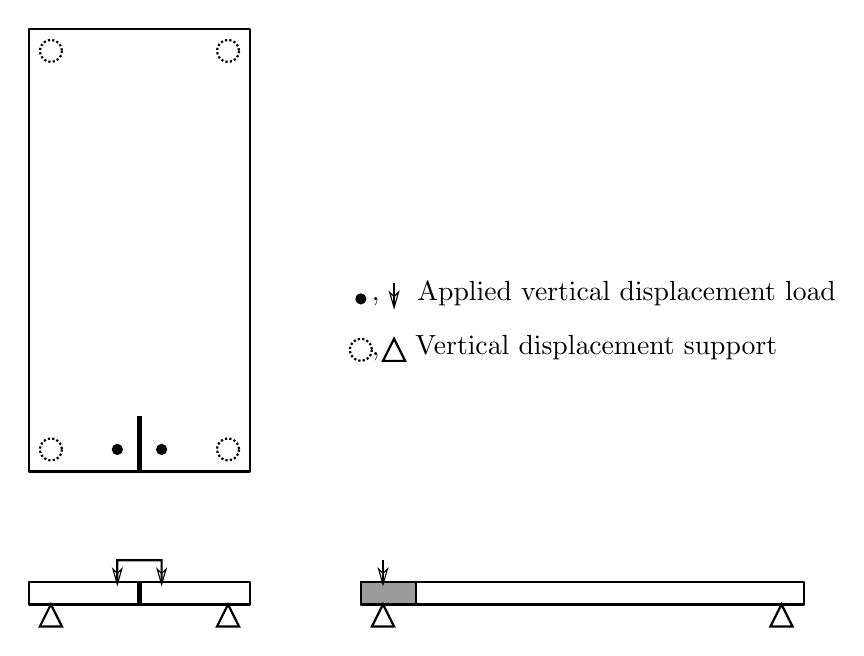
\begin{tikzpicture}[y=0.80pt, x=0.8pt,yscale=-1, inner sep=0pt, outer sep=0pt]
\begin{scope}[shift={(0,-552.36218)}]
  \path[shift={(0,552.36218)},draw=black,fill=black,line join=round,miter
    limit=4.00,fill opacity=0.000,nonzero rule,line width=0.800pt,rounded
    corners=0.0000cm] (50.0000,50.0000) rectangle (150.0000,250.0000);
  \path[shift={(0,552.36218)},draw=black,fill=black,dash pattern=on 0.80pt off
    0.80pt,line join=round,miter limit=4.00,fill opacity=0.000,nonzero rule,line
    width=0.800pt]
    (65.0000,60.0000)arc(0.000:180.000:5.000)arc(-180.000:0.000:5.000) -- cycle;
  \path[shift={(0,552.36218)},draw=black,fill=black,dash pattern=on 0.80pt off
    0.80pt,line join=round,miter limit=4.00,fill opacity=0.000,nonzero rule,line
    width=0.800pt]
    (145.0000,60.0000)arc(0.000:180.000:5.000)arc(-180.000:0.000:5.000) -- cycle;
  \path[shift={(80.0,732.36218)},draw=black,fill=black,dash pattern=on 0.80pt off
    0.80pt,line join=round,miter limit=4.00,fill opacity=0.000,nonzero rule,line
    width=0.800pt]
    (65.0000,60.0000)arc(0.000:180.000:5.000)arc(-180.000:0.000:5.000) -- cycle;
  \path[shift={(0,732.36218)},draw=black,fill=black,dash pattern=on 0.80pt off
    0.80pt,line join=round,miter limit=4.00,fill opacity=0.000,nonzero rule,line
    width=0.800pt]
    (65.0000,60.0000)arc(0.000:180.000:5.000)arc(-180.000:0.000:5.000) -- cycle;
  \path[shift={(0,552.36218)},draw=black,line join=miter,line cap=butt,miter
    limit=4.00,line width=1.600pt] (100.0000,250.0000) -- (100.0000,225.0000);
  \path[draw=black,fill=black,line join=round,miter limit=4.00,fill
    opacity=0.000,nonzero rule,line width=0.800pt,rounded corners=0.0000cm]
    (50.0000,852.3622) rectangle (150.0000,862.3622);
  \path[draw=black,line join=miter,line cap=butt,miter limit=4.00,line
    width=1.600pt] (100.0000,862.3622) -- (100.0000,852.3622);
  \path[draw=black,line join=miter,line cap=butt,line width=0.800pt]
    (55.0000,872.3622) -- (60.0000,862.3622) -- (65.0000,872.3622) -- cycle;
  \path[draw=black,line join=miter,line cap=butt,line width=0.800pt]
    (135.0000,872.3622) -- (140.0000,862.3622) -- (145.0000,872.3622) -- cycle;
    \path[color=black,fill=black,line width=0.800pt] (89.5000,841.8750) --
      (89.5000,842.3750) -- (89.5000,852.3750) -- (90.5000,852.3750) --
      (90.5000,842.8750) -- (109.5000,842.8750) -- (109.5000,852.3750) --
      (110.5000,852.3750) -- (110.5000,842.3750) -- (110.5000,841.8750) --
      (110.0000,841.8750) -- (90.0000,841.8750) -- (89.5000,841.8750) -- cycle;
    \path[draw=black,even odd rule,line width=0.400pt] (90.0000,848.3622) --
      (88.0000,846.3622) -- (90.0000,853.3622) -- (92.0000,846.3622) --
      (90.0000,848.3622) -- cycle;
    \path[draw=black,even odd rule,line width=0.400pt] (110.0000,848.3622) --
      (108.0000,846.3622) -- (110.0000,853.3622) -- (112.0000,846.3622) --
      (110.0000,848.3622) -- cycle;
  \path[shift={(0,552.36218)},draw=black,fill=black,line join=round,miter
    limit=4.00,fill opacity=0.000,nonzero rule,line width=0.800pt,rounded
    corners=0.0000cm] (200.0000,300.0000) rectangle (400.0000,310.0000);
  \path[draw=black,line join=miter,line cap=butt,line width=0.800pt]
    (385.0000,872.3622) -- (390.0000,862.3622) -- (395.0000,872.3622) -- cycle;
  \path[draw=black,line join=miter,line cap=butt,line width=0.800pt]
    (205.0000,872.3622) -- (210.0000,862.3622) -- (215.0000,872.3622) -- cycle;
    \path[color=black,fill=black,line width=0.800pt] (209.5000,842.3622) --
      (209.5000,852.3622) -- (210.5000,852.3622) -- (210.5000,842.3622) --
      (209.5000,842.3622) -- cycle;
    \path[draw=black,even odd rule,line width=0.400pt] (210.0000,848.3622) --
      (208.0000,846.3622) -- (210.0000,853.3622) -- (212.0000,846.3622) --
      (210.0000,848.3622) -- cycle;
  \path[shift={(0,552.36218)},draw=black,fill=black,line join=round,miter
    limit=4.00,fill opacity=0.392,nonzero rule,line width=0.800pt,rounded
    corners=0.0000cm] (200.0000,300.0000) rectangle (225.0000,310.0000);
  \path[shift={(0,552.36218)},draw=black,fill=black,line join=round,miter
    limit=4.00,nonzero rule,line width=0.800pt]
    (92.0000,240.0000)arc(0.000:180.000:2.000)arc(-180.000:0.000:2.000) -- cycle;
  \path[shift={(20.0,552.36218)},draw=black,fill=black,line join=round,miter
    limit=4.00,nonzero rule,line width=0.800pt]
    (92.0000,240.0000)arc(0.000:180.000:2.000)arc(-180.000:0.000:2.000) -- cycle;
  \path[shift={(110.0,484.36218)},draw=black,fill=black,line join=round,miter
    limit=4.00,nonzero rule,line width=0.800pt]
    (92.0000,240.0000)arc(0.000:180.000:2.000)arc(-180.000:0.000:2.000) -- cycle;
    \path[color=black,fill=black,line width=0.800pt] (214.5000,717.3750) --
      (214.5000,727.3750) -- (215.5000,727.3750) -- (215.5000,717.3750) --
      (214.5000,717.3750) -- cycle;
    \path[draw=black,even odd rule,line width=0.400pt] (215.0000,723.3622) --
      (213.0000,721.3622) -- (215.0000,728.3622) -- (217.0000,721.3622) --
      (215.0000,723.3622) -- cycle;
  \path[shift={(140.0,687.36218)},draw=black,fill=black,dash pattern=on 0.80pt off
    0.80pt,line join=round,miter limit=4.00,fill opacity=0.000,nonzero rule,line
    width=0.800pt]
    (65.0000,60.0000)arc(0.000:180.000:5.000)arc(-180.000:0.000:5.000) -- cycle;
  \path[fill=black] (205,727.36218) node[above right] (text6089) {,};
  \path[fill=black] (205,752.36218) node[above right] (text6093) {,};
  \path[draw=black,line join=miter,line cap=butt,line width=0.800pt]
    (210.0000,752.3622) -- (215.0000,742.3622) -- (220.0000,752.3622) -- cycle;
  \path[shift={(0,552.36218)},fill=black] (225.53571,175.17857) node[above right]
    (text6099) {Applied vertical displacement load};
  \path[shift={(0,552.36218)},fill=black] (224.64285,199.46429) node[above right]
    (text6103) {Vertical displacement support};
\end{scope}

\end{tikzpicture}


  \caption{Simple Double Torsion Setup}
  \label{fig:DTsetup}
\end{figure}
%

%
\begin{figure}[tbhp]
  \centering
  \resizebox{0.8\linewidth}{!}{%% Creator: Matplotlib, PGF backend
%%
%% To include the figure in your LaTeX document, write
%%   \input{<filename>.pgf}
%%
%% Make sure the required packages are loaded in your preamble
%%   \usepackage{pgf}
%%
%% Figures using additional raster images can only be included by \input if
%% they are in the same directory as the main LaTeX file. For loading figures
%% from other directories you can use the `import` package
%%   \usepackage{import}
%% and then include the figures with
%%   \import{<path to file>}{<filename>.pgf}
%%
%% Matplotlib used the following preamble
%%
\begingroup%
\makeatletter%
\begin{pgfpicture}%
\pgfpathrectangle{\pgfpointorigin}{\pgfqpoint{6.000000in}{9.000000in}}%
\pgfusepath{use as bounding box}%
\begin{pgfscope}%
\pgfsetrectcap%
\pgfsetroundjoin%
\definecolor{currentfill}{rgb}{1.000000,1.000000,1.000000}%
\pgfsetfillcolor{currentfill}%
\pgfsetlinewidth{0.000000pt}%
\definecolor{currentstroke}{rgb}{1.000000,1.000000,1.000000}%
\pgfsetstrokecolor{currentstroke}%
\pgfsetdash{}{0pt}%
\pgfpathmoveto{\pgfqpoint{0.000000in}{0.000000in}}%
\pgfpathlineto{\pgfqpoint{6.000000in}{0.000000in}}%
\pgfpathlineto{\pgfqpoint{6.000000in}{9.000000in}}%
\pgfpathlineto{\pgfqpoint{0.000000in}{9.000000in}}%
\pgfpathclose%
\pgfusepath{fill}%
\end{pgfscope}%
\begin{pgfscope}%
\pgfsetrectcap%
\pgfsetroundjoin%
\definecolor{currentfill}{rgb}{1.000000,1.000000,1.000000}%
\pgfsetfillcolor{currentfill}%
\pgfsetlinewidth{0.000000pt}%
\definecolor{currentstroke}{rgb}{0.000000,0.000000,0.000000}%
\pgfsetstrokecolor{currentstroke}%
\pgfsetdash{}{0pt}%
\pgfpathmoveto{\pgfqpoint{1.080000in}{6.484128in}}%
\pgfpathlineto{\pgfqpoint{2.851429in}{6.484128in}}%
\pgfpathlineto{\pgfqpoint{2.851429in}{8.280000in}}%
\pgfpathlineto{\pgfqpoint{1.080000in}{8.280000in}}%
\pgfpathclose%
\pgfusepath{fill}%
\end{pgfscope}%
\begin{pgfscope}%
\pgfsetrectcap%
\pgfsetroundjoin%
\definecolor{currentfill}{rgb}{0.950000,0.950000,0.950000}%
\pgfsetfillcolor{currentfill}%
\pgfsetfillopacity{0.500000}%
\pgfsetlinewidth{1.003750pt}%
\definecolor{currentstroke}{rgb}{0.950000,0.950000,0.950000}%
\pgfsetstrokecolor{currentstroke}%
\pgfsetstrokeopacity{0.500000}%
\pgfsetdash{}{0pt}%
\pgfpathmoveto{\pgfqpoint{2.670976in}{6.867881in}}%
\pgfpathlineto{\pgfqpoint{2.157945in}{7.186095in}}%
\pgfpathlineto{\pgfqpoint{2.163660in}{8.084400in}}%
\pgfpathlineto{\pgfqpoint{2.696149in}{7.833400in}}%
\pgfusepath{stroke,fill}%
\end{pgfscope}%
\begin{pgfscope}%
\pgfsetrectcap%
\pgfsetroundjoin%
\definecolor{currentfill}{rgb}{0.900000,0.900000,0.900000}%
\pgfsetfillcolor{currentfill}%
\pgfsetfillopacity{0.500000}%
\pgfsetlinewidth{1.003750pt}%
\definecolor{currentstroke}{rgb}{0.900000,0.900000,0.900000}%
\pgfsetstrokecolor{currentstroke}%
\pgfsetstrokeopacity{0.500000}%
\pgfsetdash{}{0pt}%
\pgfpathmoveto{\pgfqpoint{1.331898in}{7.008729in}}%
\pgfpathlineto{\pgfqpoint{2.157945in}{7.186095in}}%
\pgfpathlineto{\pgfqpoint{2.163660in}{8.084400in}}%
\pgfpathlineto{\pgfqpoint{1.308466in}{7.944676in}}%
\pgfusepath{stroke,fill}%
\end{pgfscope}%
\begin{pgfscope}%
\pgfsetrectcap%
\pgfsetroundjoin%
\definecolor{currentfill}{rgb}{0.925000,0.925000,0.925000}%
\pgfsetfillcolor{currentfill}%
\pgfsetfillopacity{0.500000}%
\pgfsetlinewidth{1.003750pt}%
\definecolor{currentstroke}{rgb}{0.925000,0.925000,0.925000}%
\pgfsetstrokecolor{currentstroke}%
\pgfsetstrokeopacity{0.500000}%
\pgfsetdash{}{0pt}%
\pgfpathmoveto{\pgfqpoint{1.797697in}{6.658327in}}%
\pgfpathlineto{\pgfqpoint{2.670976in}{6.867881in}}%
\pgfpathlineto{\pgfqpoint{2.157945in}{7.186095in}}%
\pgfpathlineto{\pgfqpoint{1.331898in}{7.008729in}}%
\pgfusepath{stroke,fill}%
\end{pgfscope}%
\begin{pgfscope}%
\pgfsetrectcap%
\pgfsetroundjoin%
\pgfsetlinewidth{0.752812pt}%
\definecolor{currentstroke}{rgb}{0.000000,0.000000,0.000000}%
\pgfsetstrokecolor{currentstroke}%
\pgfsetdash{}{0pt}%
\pgfpathmoveto{\pgfqpoint{2.670976in}{6.867881in}}%
\pgfpathlineto{\pgfqpoint{1.797697in}{6.658327in}}%
\pgfusepath{stroke}%
\end{pgfscope}%
\begin{pgfscope}%
\pgfsetbuttcap%
\pgfsetroundjoin%
\pgfsetlinewidth{1.003750pt}%
\definecolor{currentstroke}{rgb}{0.900000,0.900000,0.900000}%
\pgfsetstrokecolor{currentstroke}%
\pgfsetdash{}{0pt}%
\pgfpathmoveto{\pgfqpoint{1.816042in}{6.662729in}}%
\pgfpathlineto{\pgfqpoint{1.349183in}{7.012441in}}%
\pgfpathlineto{\pgfqpoint{1.326390in}{7.947605in}}%
\pgfusepath{stroke}%
\end{pgfscope}%
\begin{pgfscope}%
\pgfsetbuttcap%
\pgfsetroundjoin%
\pgfsetlinewidth{1.003750pt}%
\definecolor{currentstroke}{rgb}{0.900000,0.900000,0.900000}%
\pgfsetstrokecolor{currentstroke}%
\pgfsetdash{}{0pt}%
\pgfpathmoveto{\pgfqpoint{2.245290in}{6.765733in}}%
\pgfpathlineto{\pgfqpoint{1.754455in}{7.099459in}}%
\pgfpathlineto{\pgfqpoint{1.746276in}{8.016207in}}%
\pgfusepath{stroke}%
\end{pgfscope}%
\begin{pgfscope}%
\pgfsetbuttcap%
\pgfsetroundjoin%
\pgfsetlinewidth{1.003750pt}%
\definecolor{currentstroke}{rgb}{0.900000,0.900000,0.900000}%
\pgfsetstrokecolor{currentstroke}%
\pgfsetdash{}{0pt}%
\pgfpathmoveto{\pgfqpoint{2.654349in}{6.863891in}}%
\pgfpathlineto{\pgfqpoint{2.142155in}{7.182704in}}%
\pgfpathlineto{\pgfqpoint{2.147339in}{8.081733in}}%
\pgfusepath{stroke}%
\end{pgfscope}%
\begin{pgfscope}%
\pgfsetrectcap%
\pgfsetroundjoin%
\pgfsetlinewidth{1.003750pt}%
\definecolor{currentstroke}{rgb}{0.000000,0.000000,0.000000}%
\pgfsetstrokecolor{currentstroke}%
\pgfsetdash{}{0pt}%
\pgfpathmoveto{\pgfqpoint{1.811978in}{6.665774in}}%
\pgfpathlineto{\pgfqpoint{1.824189in}{6.656627in}}%
\pgfusepath{stroke}%
\end{pgfscope}%
\begin{pgfscope}%
\pgfsetrectcap%
\pgfsetroundjoin%
\pgfsetlinewidth{1.003750pt}%
\definecolor{currentstroke}{rgb}{0.000000,0.000000,0.000000}%
\pgfsetstrokecolor{currentstroke}%
\pgfsetdash{}{0pt}%
\pgfpathmoveto{\pgfqpoint{2.241026in}{6.768632in}}%
\pgfpathlineto{\pgfqpoint{2.253838in}{6.759921in}}%
\pgfusepath{stroke}%
\end{pgfscope}%
\begin{pgfscope}%
\pgftext[left,bottom,x=2.170464in,y=6.584563in,rotate=0.000000]{{\rmfamily\fontsize{12.000000}{14.400000}\selectfont 1.0}}
%
\end{pgfscope}%
\begin{pgfscope}%
\pgfsetrectcap%
\pgfsetroundjoin%
\pgfsetlinewidth{1.003750pt}%
\definecolor{currentstroke}{rgb}{0.000000,0.000000,0.000000}%
\pgfsetstrokecolor{currentstroke}%
\pgfsetdash{}{0pt}%
\pgfpathmoveto{\pgfqpoint{2.649906in}{6.866656in}}%
\pgfpathlineto{\pgfqpoint{2.663251in}{6.858350in}}%
\pgfusepath{stroke}%
\end{pgfscope}%
\begin{pgfscope}%
\pgftext[left,bottom,x=2.579958in,y=6.684732in,rotate=0.000000]{{\rmfamily\fontsize{12.000000}{14.400000}\selectfont 2.0}}
%
\end{pgfscope}%
\begin{pgfscope}%
\pgfsetrectcap%
\pgfsetroundjoin%
\pgfsetlinewidth{0.752812pt}%
\definecolor{currentstroke}{rgb}{0.000000,0.000000,0.000000}%
\pgfsetstrokecolor{currentstroke}%
\pgfsetdash{}{0pt}%
\pgfpathmoveto{\pgfqpoint{1.331898in}{7.008729in}}%
\pgfpathlineto{\pgfqpoint{1.797697in}{6.658327in}}%
\pgfusepath{stroke}%
\end{pgfscope}%
\begin{pgfscope}%
\pgfsetbuttcap%
\pgfsetroundjoin%
\pgfsetlinewidth{1.003750pt}%
\definecolor{currentstroke}{rgb}{0.900000,0.900000,0.900000}%
\pgfsetstrokecolor{currentstroke}%
\pgfsetdash{}{0pt}%
\pgfpathmoveto{\pgfqpoint{2.684583in}{7.838852in}}%
\pgfpathlineto{\pgfqpoint{2.659864in}{6.874773in}}%
\pgfpathlineto{\pgfqpoint{1.787568in}{6.665946in}}%
\pgfusepath{stroke}%
\end{pgfscope}%
\begin{pgfscope}%
\pgfsetbuttcap%
\pgfsetroundjoin%
\pgfsetlinewidth{1.003750pt}%
\definecolor{currentstroke}{rgb}{0.900000,0.900000,0.900000}%
\pgfsetstrokecolor{currentstroke}%
\pgfsetdash{}{0pt}%
\pgfpathmoveto{\pgfqpoint{2.418694in}{7.964184in}}%
\pgfpathlineto{\pgfqpoint{2.404029in}{7.033458in}}%
\pgfpathlineto{\pgfqpoint{1.554860in}{6.841004in}}%
\pgfusepath{stroke}%
\end{pgfscope}%
\begin{pgfscope}%
\pgfsetbuttcap%
\pgfsetroundjoin%
\pgfsetlinewidth{1.003750pt}%
\definecolor{currentstroke}{rgb}{0.900000,0.900000,0.900000}%
\pgfsetstrokecolor{currentstroke}%
\pgfsetdash{}{0pt}%
\pgfpathmoveto{\pgfqpoint{2.173465in}{8.079778in}}%
\pgfpathlineto{\pgfqpoint{2.167418in}{7.180219in}}%
\pgfpathlineto{\pgfqpoint{1.340465in}{7.002284in}}%
\pgfusepath{stroke}%
\end{pgfscope}%
\begin{pgfscope}%
\pgfsetrectcap%
\pgfsetroundjoin%
\pgfsetlinewidth{1.003750pt}%
\definecolor{currentstroke}{rgb}{0.000000,0.000000,0.000000}%
\pgfsetstrokecolor{currentstroke}%
\pgfsetdash{}{0pt}%
\pgfpathmoveto{\pgfqpoint{1.794902in}{6.667702in}}%
\pgfpathlineto{\pgfqpoint{1.772883in}{6.662431in}}%
\pgfusepath{stroke}%
\end{pgfscope}%
\begin{pgfscope}%
\pgfsetrectcap%
\pgfsetroundjoin%
\pgfsetlinewidth{1.003750pt}%
\definecolor{currentstroke}{rgb}{0.000000,0.000000,0.000000}%
\pgfsetstrokecolor{currentstroke}%
\pgfsetdash{}{0pt}%
\pgfpathmoveto{\pgfqpoint{1.561985in}{6.842619in}}%
\pgfpathlineto{\pgfqpoint{1.540592in}{6.837770in}}%
\pgfusepath{stroke}%
\end{pgfscope}%
\begin{pgfscope}%
\pgftext[left,bottom,x=1.401538in,y=6.669808in,rotate=0.000000]{{\rmfamily\fontsize{12.000000}{14.400000}\selectfont 0.5}}
%
\end{pgfscope}%
\begin{pgfscope}%
\pgfsetrectcap%
\pgfsetroundjoin%
\pgfsetlinewidth{1.003750pt}%
\definecolor{currentstroke}{rgb}{0.000000,0.000000,0.000000}%
\pgfsetstrokecolor{currentstroke}%
\pgfsetdash{}{0pt}%
\pgfpathmoveto{\pgfqpoint{1.347392in}{7.003774in}}%
\pgfpathlineto{\pgfqpoint{1.326597in}{6.999300in}}%
\pgfusepath{stroke}%
\end{pgfscope}%
\begin{pgfscope}%
\pgftext[left,bottom,x=1.188921in,y=6.833716in,rotate=0.000000]{{\rmfamily\fontsize{12.000000}{14.400000}\selectfont 1.0}}
%
\end{pgfscope}%
\begin{pgfscope}%
\pgfsetrectcap%
\pgfsetroundjoin%
\pgfsetlinewidth{0.752812pt}%
\definecolor{currentstroke}{rgb}{0.000000,0.000000,0.000000}%
\pgfsetstrokecolor{currentstroke}%
\pgfsetdash{}{0pt}%
\pgfpathmoveto{\pgfqpoint{1.331898in}{7.008729in}}%
\pgfpathlineto{\pgfqpoint{1.308466in}{7.944676in}}%
\pgfusepath{stroke}%
\end{pgfscope}%
\begin{pgfscope}%
\pgfpathrectangle{\pgfqpoint{1.080000in}{6.939207in}}{\pgfqpoint{1.771429in}{0.885714in}} %
\pgfusepath{clip}%
\pgfsetbuttcap%
\pgfsetroundjoin%
\definecolor{currentfill}{rgb}{1.000000,0.700543,0.378411}%
\pgfsetfillcolor{currentfill}%
\pgfsetlinewidth{1.003750pt}%
\definecolor{currentstroke}{rgb}{0.000000,0.000000,0.000000}%
\pgfsetstrokecolor{currentstroke}%
\pgfsetdash{}{0pt}%
\pgfpathmoveto{\pgfqpoint{2.164894in}{7.701302in}}%
\pgfpathlineto{\pgfqpoint{2.160142in}{7.702511in}}%
\pgfpathlineto{\pgfqpoint{2.155398in}{7.703719in}}%
\pgfpathlineto{\pgfqpoint{2.150662in}{7.704926in}}%
\pgfpathlineto{\pgfqpoint{2.145933in}{7.706132in}}%
\pgfpathlineto{\pgfqpoint{2.141211in}{7.707336in}}%
\pgfpathlineto{\pgfqpoint{2.136496in}{7.708538in}}%
\pgfpathlineto{\pgfqpoint{2.131789in}{7.709739in}}%
\pgfpathlineto{\pgfqpoint{2.127089in}{7.710938in}}%
\pgfpathlineto{\pgfqpoint{2.122396in}{7.712135in}}%
\pgfpathlineto{\pgfqpoint{2.117710in}{7.713331in}}%
\pgfpathlineto{\pgfqpoint{2.121650in}{7.713703in}}%
\pgfpathlineto{\pgfqpoint{2.125588in}{7.714076in}}%
\pgfpathlineto{\pgfqpoint{2.129525in}{7.714448in}}%
\pgfpathlineto{\pgfqpoint{2.133459in}{7.714821in}}%
\pgfpathlineto{\pgfqpoint{2.137392in}{7.715194in}}%
\pgfpathlineto{\pgfqpoint{2.141323in}{7.715566in}}%
\pgfpathlineto{\pgfqpoint{2.145252in}{7.715939in}}%
\pgfpathlineto{\pgfqpoint{2.149180in}{7.716312in}}%
\pgfpathlineto{\pgfqpoint{2.153106in}{7.716684in}}%
\pgfpathlineto{\pgfqpoint{2.157030in}{7.717057in}}%
\pgfpathlineto{\pgfqpoint{2.161736in}{7.715873in}}%
\pgfpathlineto{\pgfqpoint{2.166449in}{7.714686in}}%
\pgfpathlineto{\pgfqpoint{2.171169in}{7.713500in}}%
\pgfpathlineto{\pgfqpoint{2.175896in}{7.712310in}}%
\pgfpathlineto{\pgfqpoint{2.180631in}{7.711120in}}%
\pgfpathlineto{\pgfqpoint{2.185373in}{7.709928in}}%
\pgfpathlineto{\pgfqpoint{2.190122in}{7.708735in}}%
\pgfpathlineto{\pgfqpoint{2.194879in}{7.707540in}}%
\pgfpathlineto{\pgfqpoint{2.199644in}{7.706344in}}%
\pgfpathlineto{\pgfqpoint{2.204415in}{7.705147in}}%
\pgfpathlineto{\pgfqpoint{2.200471in}{7.704764in}}%
\pgfpathlineto{\pgfqpoint{2.196525in}{7.704381in}}%
\pgfpathlineto{\pgfqpoint{2.192577in}{7.703997in}}%
\pgfpathlineto{\pgfqpoint{2.188628in}{7.703613in}}%
\pgfpathlineto{\pgfqpoint{2.184677in}{7.703229in}}%
\pgfpathlineto{\pgfqpoint{2.180724in}{7.702844in}}%
\pgfpathlineto{\pgfqpoint{2.176769in}{7.702459in}}%
\pgfpathlineto{\pgfqpoint{2.172812in}{7.702073in}}%
\pgfpathlineto{\pgfqpoint{2.168854in}{7.701687in}}%
\pgfpathlineto{\pgfqpoint{2.164894in}{7.701302in}}%
\pgfpathclose%
\pgfusepath{stroke,fill}%
\end{pgfscope}%
\begin{pgfscope}%
\pgfpathrectangle{\pgfqpoint{1.080000in}{6.939207in}}{\pgfqpoint{1.771429in}{0.885714in}} %
\pgfusepath{clip}%
\pgfsetbuttcap%
\pgfsetroundjoin%
\definecolor{currentfill}{rgb}{1.000000,0.700543,0.378411}%
\pgfsetfillcolor{currentfill}%
\pgfsetlinewidth{1.003750pt}%
\definecolor{currentstroke}{rgb}{0.000000,0.000000,0.000000}%
\pgfsetstrokecolor{currentstroke}%
\pgfsetdash{}{0pt}%
\pgfpathmoveto{\pgfqpoint{2.125196in}{7.697418in}}%
\pgfpathlineto{\pgfqpoint{2.120465in}{7.698645in}}%
\pgfpathlineto{\pgfqpoint{2.115742in}{7.699870in}}%
\pgfpathlineto{\pgfqpoint{2.111026in}{7.701095in}}%
\pgfpathlineto{\pgfqpoint{2.106317in}{7.702317in}}%
\pgfpathlineto{\pgfqpoint{2.101615in}{7.703539in}}%
\pgfpathlineto{\pgfqpoint{2.096921in}{7.704758in}}%
\pgfpathlineto{\pgfqpoint{2.092234in}{7.705977in}}%
\pgfpathlineto{\pgfqpoint{2.087554in}{7.707193in}}%
\pgfpathlineto{\pgfqpoint{2.082882in}{7.708407in}}%
\pgfpathlineto{\pgfqpoint{2.078217in}{7.709619in}}%
\pgfpathlineto{\pgfqpoint{2.082174in}{7.709989in}}%
\pgfpathlineto{\pgfqpoint{2.086130in}{7.710359in}}%
\pgfpathlineto{\pgfqpoint{2.090083in}{7.710730in}}%
\pgfpathlineto{\pgfqpoint{2.094035in}{7.711100in}}%
\pgfpathlineto{\pgfqpoint{2.097985in}{7.711471in}}%
\pgfpathlineto{\pgfqpoint{2.101934in}{7.711843in}}%
\pgfpathlineto{\pgfqpoint{2.105881in}{7.712214in}}%
\pgfpathlineto{\pgfqpoint{2.109826in}{7.712586in}}%
\pgfpathlineto{\pgfqpoint{2.113769in}{7.712958in}}%
\pgfpathlineto{\pgfqpoint{2.117710in}{7.713331in}}%
\pgfpathlineto{\pgfqpoint{2.122396in}{7.712135in}}%
\pgfpathlineto{\pgfqpoint{2.127089in}{7.710938in}}%
\pgfpathlineto{\pgfqpoint{2.131789in}{7.709739in}}%
\pgfpathlineto{\pgfqpoint{2.136496in}{7.708538in}}%
\pgfpathlineto{\pgfqpoint{2.141211in}{7.707336in}}%
\pgfpathlineto{\pgfqpoint{2.145933in}{7.706132in}}%
\pgfpathlineto{\pgfqpoint{2.150662in}{7.704926in}}%
\pgfpathlineto{\pgfqpoint{2.155398in}{7.703719in}}%
\pgfpathlineto{\pgfqpoint{2.160142in}{7.702511in}}%
\pgfpathlineto{\pgfqpoint{2.164894in}{7.701302in}}%
\pgfpathlineto{\pgfqpoint{2.160932in}{7.700914in}}%
\pgfpathlineto{\pgfqpoint{2.156969in}{7.700527in}}%
\pgfpathlineto{\pgfqpoint{2.153003in}{7.700140in}}%
\pgfpathlineto{\pgfqpoint{2.149036in}{7.699752in}}%
\pgfpathlineto{\pgfqpoint{2.145067in}{7.699364in}}%
\pgfpathlineto{\pgfqpoint{2.141097in}{7.698975in}}%
\pgfpathlineto{\pgfqpoint{2.137124in}{7.698586in}}%
\pgfpathlineto{\pgfqpoint{2.133150in}{7.698197in}}%
\pgfpathlineto{\pgfqpoint{2.129174in}{7.697808in}}%
\pgfpathlineto{\pgfqpoint{2.125196in}{7.697418in}}%
\pgfpathclose%
\pgfusepath{stroke,fill}%
\end{pgfscope}%
\begin{pgfscope}%
\pgfpathrectangle{\pgfqpoint{1.080000in}{6.939207in}}{\pgfqpoint{1.771429in}{0.885714in}} %
\pgfusepath{clip}%
\pgfsetbuttcap%
\pgfsetroundjoin%
\definecolor{currentfill}{rgb}{0.998039,0.709281,0.384106}%
\pgfsetfillcolor{currentfill}%
\pgfsetlinewidth{1.003750pt}%
\definecolor{currentstroke}{rgb}{0.000000,0.000000,0.000000}%
\pgfsetstrokecolor{currentstroke}%
\pgfsetdash{}{0pt}%
\pgfpathmoveto{\pgfqpoint{2.085322in}{7.693506in}}%
\pgfpathlineto{\pgfqpoint{2.080611in}{7.694757in}}%
\pgfpathlineto{\pgfqpoint{2.075909in}{7.696006in}}%
\pgfpathlineto{\pgfqpoint{2.071213in}{7.697254in}}%
\pgfpathlineto{\pgfqpoint{2.066525in}{7.698501in}}%
\pgfpathlineto{\pgfqpoint{2.061844in}{7.699746in}}%
\pgfpathlineto{\pgfqpoint{2.057170in}{7.700990in}}%
\pgfpathlineto{\pgfqpoint{2.052504in}{7.702232in}}%
\pgfpathlineto{\pgfqpoint{2.047845in}{7.703473in}}%
\pgfpathlineto{\pgfqpoint{2.043193in}{7.704711in}}%
\pgfpathlineto{\pgfqpoint{2.038548in}{7.705947in}}%
\pgfpathlineto{\pgfqpoint{2.042523in}{7.706312in}}%
\pgfpathlineto{\pgfqpoint{2.046496in}{7.706677in}}%
\pgfpathlineto{\pgfqpoint{2.050467in}{7.707043in}}%
\pgfpathlineto{\pgfqpoint{2.054437in}{7.707410in}}%
\pgfpathlineto{\pgfqpoint{2.058404in}{7.707777in}}%
\pgfpathlineto{\pgfqpoint{2.062370in}{7.708144in}}%
\pgfpathlineto{\pgfqpoint{2.066335in}{7.708512in}}%
\pgfpathlineto{\pgfqpoint{2.070297in}{7.708881in}}%
\pgfpathlineto{\pgfqpoint{2.074258in}{7.709250in}}%
\pgfpathlineto{\pgfqpoint{2.078217in}{7.709619in}}%
\pgfpathlineto{\pgfqpoint{2.082882in}{7.708407in}}%
\pgfpathlineto{\pgfqpoint{2.087554in}{7.707193in}}%
\pgfpathlineto{\pgfqpoint{2.092234in}{7.705977in}}%
\pgfpathlineto{\pgfqpoint{2.096921in}{7.704758in}}%
\pgfpathlineto{\pgfqpoint{2.101615in}{7.703539in}}%
\pgfpathlineto{\pgfqpoint{2.106317in}{7.702317in}}%
\pgfpathlineto{\pgfqpoint{2.111026in}{7.701095in}}%
\pgfpathlineto{\pgfqpoint{2.115742in}{7.699870in}}%
\pgfpathlineto{\pgfqpoint{2.120465in}{7.698645in}}%
\pgfpathlineto{\pgfqpoint{2.125196in}{7.697418in}}%
\pgfpathlineto{\pgfqpoint{2.121217in}{7.697028in}}%
\pgfpathlineto{\pgfqpoint{2.117236in}{7.696638in}}%
\pgfpathlineto{\pgfqpoint{2.113253in}{7.696248in}}%
\pgfpathlineto{\pgfqpoint{2.109268in}{7.695857in}}%
\pgfpathlineto{\pgfqpoint{2.105281in}{7.695466in}}%
\pgfpathlineto{\pgfqpoint{2.101293in}{7.695074in}}%
\pgfpathlineto{\pgfqpoint{2.097303in}{7.694683in}}%
\pgfpathlineto{\pgfqpoint{2.093311in}{7.694291in}}%
\pgfpathlineto{\pgfqpoint{2.089317in}{7.693899in}}%
\pgfpathlineto{\pgfqpoint{2.085322in}{7.693506in}}%
\pgfpathclose%
\pgfusepath{stroke,fill}%
\end{pgfscope}%
\begin{pgfscope}%
\pgfpathrectangle{\pgfqpoint{1.080000in}{6.939207in}}{\pgfqpoint{1.771429in}{0.885714in}} %
\pgfusepath{clip}%
\pgfsetbuttcap%
\pgfsetroundjoin%
\definecolor{currentfill}{rgb}{0.998039,0.709281,0.384106}%
\pgfsetfillcolor{currentfill}%
\pgfsetlinewidth{1.003750pt}%
\definecolor{currentstroke}{rgb}{0.000000,0.000000,0.000000}%
\pgfsetstrokecolor{currentstroke}%
\pgfsetdash{}{0pt}%
\pgfpathmoveto{\pgfqpoint{2.045269in}{7.689568in}}%
\pgfpathlineto{\pgfqpoint{2.040579in}{7.690851in}}%
\pgfpathlineto{\pgfqpoint{2.035897in}{7.692133in}}%
\pgfpathlineto{\pgfqpoint{2.031223in}{7.693414in}}%
\pgfpathlineto{\pgfqpoint{2.026555in}{7.694694in}}%
\pgfpathlineto{\pgfqpoint{2.021895in}{7.695973in}}%
\pgfpathlineto{\pgfqpoint{2.017242in}{7.697250in}}%
\pgfpathlineto{\pgfqpoint{2.012596in}{7.698525in}}%
\pgfpathlineto{\pgfqpoint{2.007958in}{7.699799in}}%
\pgfpathlineto{\pgfqpoint{2.003326in}{7.701070in}}%
\pgfpathlineto{\pgfqpoint{1.998702in}{7.702339in}}%
\pgfpathlineto{\pgfqpoint{2.002695in}{7.702696in}}%
\pgfpathlineto{\pgfqpoint{2.006686in}{7.703054in}}%
\pgfpathlineto{\pgfqpoint{2.010675in}{7.703413in}}%
\pgfpathlineto{\pgfqpoint{2.014662in}{7.703773in}}%
\pgfpathlineto{\pgfqpoint{2.018647in}{7.704133in}}%
\pgfpathlineto{\pgfqpoint{2.022631in}{7.704495in}}%
\pgfpathlineto{\pgfqpoint{2.026613in}{7.704857in}}%
\pgfpathlineto{\pgfqpoint{2.030593in}{7.705219in}}%
\pgfpathlineto{\pgfqpoint{2.034571in}{7.705583in}}%
\pgfpathlineto{\pgfqpoint{2.038548in}{7.705947in}}%
\pgfpathlineto{\pgfqpoint{2.043193in}{7.704711in}}%
\pgfpathlineto{\pgfqpoint{2.047845in}{7.703473in}}%
\pgfpathlineto{\pgfqpoint{2.052504in}{7.702232in}}%
\pgfpathlineto{\pgfqpoint{2.057170in}{7.700990in}}%
\pgfpathlineto{\pgfqpoint{2.061844in}{7.699746in}}%
\pgfpathlineto{\pgfqpoint{2.066525in}{7.698501in}}%
\pgfpathlineto{\pgfqpoint{2.071213in}{7.697254in}}%
\pgfpathlineto{\pgfqpoint{2.075909in}{7.696006in}}%
\pgfpathlineto{\pgfqpoint{2.080611in}{7.694757in}}%
\pgfpathlineto{\pgfqpoint{2.085322in}{7.693506in}}%
\pgfpathlineto{\pgfqpoint{2.081324in}{7.693113in}}%
\pgfpathlineto{\pgfqpoint{2.077325in}{7.692721in}}%
\pgfpathlineto{\pgfqpoint{2.073324in}{7.692327in}}%
\pgfpathlineto{\pgfqpoint{2.069322in}{7.691934in}}%
\pgfpathlineto{\pgfqpoint{2.065317in}{7.691540in}}%
\pgfpathlineto{\pgfqpoint{2.061311in}{7.691146in}}%
\pgfpathlineto{\pgfqpoint{2.057303in}{7.690752in}}%
\pgfpathlineto{\pgfqpoint{2.053294in}{7.690358in}}%
\pgfpathlineto{\pgfqpoint{2.049282in}{7.689963in}}%
\pgfpathlineto{\pgfqpoint{2.045269in}{7.689568in}}%
\pgfpathclose%
\pgfusepath{stroke,fill}%
\end{pgfscope}%
\begin{pgfscope}%
\pgfpathrectangle{\pgfqpoint{1.080000in}{6.939207in}}{\pgfqpoint{1.771429in}{0.885714in}} %
\pgfusepath{clip}%
\pgfsetbuttcap%
\pgfsetroundjoin%
\definecolor{currentfill}{rgb}{0.998039,0.709281,0.384106}%
\pgfsetfillcolor{currentfill}%
\pgfsetlinewidth{1.003750pt}%
\definecolor{currentstroke}{rgb}{0.000000,0.000000,0.000000}%
\pgfsetstrokecolor{currentstroke}%
\pgfsetdash{}{0pt}%
\pgfpathmoveto{\pgfqpoint{2.212819in}{7.689154in}}%
\pgfpathlineto{\pgfqpoint{2.207993in}{7.690371in}}%
\pgfpathlineto{\pgfqpoint{2.203174in}{7.691589in}}%
\pgfpathlineto{\pgfqpoint{2.198363in}{7.692805in}}%
\pgfpathlineto{\pgfqpoint{2.193559in}{7.694021in}}%
\pgfpathlineto{\pgfqpoint{2.188763in}{7.695237in}}%
\pgfpathlineto{\pgfqpoint{2.183974in}{7.696451in}}%
\pgfpathlineto{\pgfqpoint{2.179193in}{7.697665in}}%
\pgfpathlineto{\pgfqpoint{2.174419in}{7.698878in}}%
\pgfpathlineto{\pgfqpoint{2.169653in}{7.700090in}}%
\pgfpathlineto{\pgfqpoint{2.164894in}{7.701302in}}%
\pgfpathlineto{\pgfqpoint{2.168854in}{7.701687in}}%
\pgfpathlineto{\pgfqpoint{2.172812in}{7.702073in}}%
\pgfpathlineto{\pgfqpoint{2.176769in}{7.702459in}}%
\pgfpathlineto{\pgfqpoint{2.180724in}{7.702844in}}%
\pgfpathlineto{\pgfqpoint{2.184677in}{7.703229in}}%
\pgfpathlineto{\pgfqpoint{2.188628in}{7.703613in}}%
\pgfpathlineto{\pgfqpoint{2.192577in}{7.703997in}}%
\pgfpathlineto{\pgfqpoint{2.196525in}{7.704381in}}%
\pgfpathlineto{\pgfqpoint{2.200471in}{7.704764in}}%
\pgfpathlineto{\pgfqpoint{2.204415in}{7.705147in}}%
\pgfpathlineto{\pgfqpoint{2.209194in}{7.703948in}}%
\pgfpathlineto{\pgfqpoint{2.213981in}{7.702749in}}%
\pgfpathlineto{\pgfqpoint{2.218775in}{7.701548in}}%
\pgfpathlineto{\pgfqpoint{2.223577in}{7.700346in}}%
\pgfpathlineto{\pgfqpoint{2.228386in}{7.699144in}}%
\pgfpathlineto{\pgfqpoint{2.233202in}{7.697940in}}%
\pgfpathlineto{\pgfqpoint{2.238026in}{7.696736in}}%
\pgfpathlineto{\pgfqpoint{2.242858in}{7.695531in}}%
\pgfpathlineto{\pgfqpoint{2.247698in}{7.694326in}}%
\pgfpathlineto{\pgfqpoint{2.252544in}{7.693120in}}%
\pgfpathlineto{\pgfqpoint{2.248580in}{7.692727in}}%
\pgfpathlineto{\pgfqpoint{2.244614in}{7.692333in}}%
\pgfpathlineto{\pgfqpoint{2.240646in}{7.691938in}}%
\pgfpathlineto{\pgfqpoint{2.236676in}{7.691543in}}%
\pgfpathlineto{\pgfqpoint{2.232704in}{7.691146in}}%
\pgfpathlineto{\pgfqpoint{2.228731in}{7.690749in}}%
\pgfpathlineto{\pgfqpoint{2.224756in}{7.690352in}}%
\pgfpathlineto{\pgfqpoint{2.220779in}{7.689953in}}%
\pgfpathlineto{\pgfqpoint{2.216800in}{7.689554in}}%
\pgfpathlineto{\pgfqpoint{2.212819in}{7.689154in}}%
\pgfpathclose%
\pgfusepath{stroke,fill}%
\end{pgfscope}%
\begin{pgfscope}%
\pgfpathrectangle{\pgfqpoint{1.080000in}{6.939207in}}{\pgfqpoint{1.771429in}{0.885714in}} %
\pgfusepath{clip}%
\pgfsetbuttcap%
\pgfsetroundjoin%
\definecolor{currentfill}{rgb}{0.998039,0.709281,0.384106}%
\pgfsetfillcolor{currentfill}%
\pgfsetlinewidth{1.003750pt}%
\definecolor{currentstroke}{rgb}{0.000000,0.000000,0.000000}%
\pgfsetstrokecolor{currentstroke}%
\pgfsetdash{}{0pt}%
\pgfpathmoveto{\pgfqpoint{2.005036in}{7.685606in}}%
\pgfpathlineto{\pgfqpoint{2.000368in}{7.686933in}}%
\pgfpathlineto{\pgfqpoint{1.995707in}{7.688260in}}%
\pgfpathlineto{\pgfqpoint{1.991053in}{7.689586in}}%
\pgfpathlineto{\pgfqpoint{1.986407in}{7.690910in}}%
\pgfpathlineto{\pgfqpoint{1.981767in}{7.692234in}}%
\pgfpathlineto{\pgfqpoint{1.977135in}{7.693556in}}%
\pgfpathlineto{\pgfqpoint{1.972510in}{7.694876in}}%
\pgfpathlineto{\pgfqpoint{1.967892in}{7.696195in}}%
\pgfpathlineto{\pgfqpoint{1.963281in}{7.697511in}}%
\pgfpathlineto{\pgfqpoint{1.958678in}{7.698824in}}%
\pgfpathlineto{\pgfqpoint{1.962688in}{7.699170in}}%
\pgfpathlineto{\pgfqpoint{1.966697in}{7.699518in}}%
\pgfpathlineto{\pgfqpoint{1.970704in}{7.699866in}}%
\pgfpathlineto{\pgfqpoint{1.974709in}{7.700216in}}%
\pgfpathlineto{\pgfqpoint{1.978712in}{7.700567in}}%
\pgfpathlineto{\pgfqpoint{1.982714in}{7.700920in}}%
\pgfpathlineto{\pgfqpoint{1.986714in}{7.701273in}}%
\pgfpathlineto{\pgfqpoint{1.990712in}{7.701627in}}%
\pgfpathlineto{\pgfqpoint{1.994708in}{7.701983in}}%
\pgfpathlineto{\pgfqpoint{1.998702in}{7.702339in}}%
\pgfpathlineto{\pgfqpoint{2.003326in}{7.701070in}}%
\pgfpathlineto{\pgfqpoint{2.007958in}{7.699799in}}%
\pgfpathlineto{\pgfqpoint{2.012596in}{7.698525in}}%
\pgfpathlineto{\pgfqpoint{2.017242in}{7.697250in}}%
\pgfpathlineto{\pgfqpoint{2.021895in}{7.695973in}}%
\pgfpathlineto{\pgfqpoint{2.026555in}{7.694694in}}%
\pgfpathlineto{\pgfqpoint{2.031223in}{7.693414in}}%
\pgfpathlineto{\pgfqpoint{2.035897in}{7.692133in}}%
\pgfpathlineto{\pgfqpoint{2.040579in}{7.690851in}}%
\pgfpathlineto{\pgfqpoint{2.045269in}{7.689568in}}%
\pgfpathlineto{\pgfqpoint{2.041254in}{7.689173in}}%
\pgfpathlineto{\pgfqpoint{2.037237in}{7.688777in}}%
\pgfpathlineto{\pgfqpoint{2.033218in}{7.688382in}}%
\pgfpathlineto{\pgfqpoint{2.029197in}{7.687986in}}%
\pgfpathlineto{\pgfqpoint{2.025175in}{7.687590in}}%
\pgfpathlineto{\pgfqpoint{2.021151in}{7.687193in}}%
\pgfpathlineto{\pgfqpoint{2.017125in}{7.686797in}}%
\pgfpathlineto{\pgfqpoint{2.013097in}{7.686400in}}%
\pgfpathlineto{\pgfqpoint{2.009068in}{7.686003in}}%
\pgfpathlineto{\pgfqpoint{2.005036in}{7.685606in}}%
\pgfpathclose%
\pgfusepath{stroke,fill}%
\end{pgfscope}%
\begin{pgfscope}%
\pgfpathrectangle{\pgfqpoint{1.080000in}{6.939207in}}{\pgfqpoint{1.771429in}{0.885714in}} %
\pgfusepath{clip}%
\pgfsetbuttcap%
\pgfsetroundjoin%
\definecolor{currentfill}{rgb}{0.998039,0.709281,0.384106}%
\pgfsetfillcolor{currentfill}%
\pgfsetlinewidth{1.003750pt}%
\definecolor{currentstroke}{rgb}{0.000000,0.000000,0.000000}%
\pgfsetstrokecolor{currentstroke}%
\pgfsetdash{}{0pt}%
\pgfpathmoveto{\pgfqpoint{2.172915in}{7.685109in}}%
\pgfpathlineto{\pgfqpoint{2.168110in}{7.686342in}}%
\pgfpathlineto{\pgfqpoint{2.163311in}{7.687575in}}%
\pgfpathlineto{\pgfqpoint{2.158521in}{7.688807in}}%
\pgfpathlineto{\pgfqpoint{2.153738in}{7.690039in}}%
\pgfpathlineto{\pgfqpoint{2.148962in}{7.691271in}}%
\pgfpathlineto{\pgfqpoint{2.144194in}{7.692502in}}%
\pgfpathlineto{\pgfqpoint{2.139433in}{7.693732in}}%
\pgfpathlineto{\pgfqpoint{2.134680in}{7.694962in}}%
\pgfpathlineto{\pgfqpoint{2.129935in}{7.696191in}}%
\pgfpathlineto{\pgfqpoint{2.125196in}{7.697418in}}%
\pgfpathlineto{\pgfqpoint{2.129174in}{7.697808in}}%
\pgfpathlineto{\pgfqpoint{2.133150in}{7.698197in}}%
\pgfpathlineto{\pgfqpoint{2.137124in}{7.698586in}}%
\pgfpathlineto{\pgfqpoint{2.141097in}{7.698975in}}%
\pgfpathlineto{\pgfqpoint{2.145067in}{7.699364in}}%
\pgfpathlineto{\pgfqpoint{2.149036in}{7.699752in}}%
\pgfpathlineto{\pgfqpoint{2.153003in}{7.700140in}}%
\pgfpathlineto{\pgfqpoint{2.156969in}{7.700527in}}%
\pgfpathlineto{\pgfqpoint{2.160932in}{7.700914in}}%
\pgfpathlineto{\pgfqpoint{2.164894in}{7.701302in}}%
\pgfpathlineto{\pgfqpoint{2.169653in}{7.700090in}}%
\pgfpathlineto{\pgfqpoint{2.174419in}{7.698878in}}%
\pgfpathlineto{\pgfqpoint{2.179193in}{7.697665in}}%
\pgfpathlineto{\pgfqpoint{2.183974in}{7.696451in}}%
\pgfpathlineto{\pgfqpoint{2.188763in}{7.695237in}}%
\pgfpathlineto{\pgfqpoint{2.193559in}{7.694021in}}%
\pgfpathlineto{\pgfqpoint{2.198363in}{7.692805in}}%
\pgfpathlineto{\pgfqpoint{2.203174in}{7.691589in}}%
\pgfpathlineto{\pgfqpoint{2.207993in}{7.690371in}}%
\pgfpathlineto{\pgfqpoint{2.212819in}{7.689154in}}%
\pgfpathlineto{\pgfqpoint{2.208837in}{7.688753in}}%
\pgfpathlineto{\pgfqpoint{2.204853in}{7.688352in}}%
\pgfpathlineto{\pgfqpoint{2.200867in}{7.687949in}}%
\pgfpathlineto{\pgfqpoint{2.196879in}{7.687546in}}%
\pgfpathlineto{\pgfqpoint{2.192890in}{7.687142in}}%
\pgfpathlineto{\pgfqpoint{2.188898in}{7.686737in}}%
\pgfpathlineto{\pgfqpoint{2.184905in}{7.686332in}}%
\pgfpathlineto{\pgfqpoint{2.180910in}{7.685925in}}%
\pgfpathlineto{\pgfqpoint{2.176914in}{7.685518in}}%
\pgfpathlineto{\pgfqpoint{2.172915in}{7.685109in}}%
\pgfpathclose%
\pgfusepath{stroke,fill}%
\end{pgfscope}%
\begin{pgfscope}%
\pgfpathrectangle{\pgfqpoint{1.080000in}{6.939207in}}{\pgfqpoint{1.771429in}{0.885714in}} %
\pgfusepath{clip}%
\pgfsetbuttcap%
\pgfsetroundjoin%
\definecolor{currentfill}{rgb}{0.998039,0.709281,0.384106}%
\pgfsetfillcolor{currentfill}%
\pgfsetlinewidth{1.003750pt}%
\definecolor{currentstroke}{rgb}{0.000000,0.000000,0.000000}%
\pgfsetstrokecolor{currentstroke}%
\pgfsetdash{}{0pt}%
\pgfpathmoveto{\pgfqpoint{1.964624in}{7.681623in}}%
\pgfpathlineto{\pgfqpoint{1.959976in}{7.683010in}}%
\pgfpathlineto{\pgfqpoint{1.955336in}{7.684396in}}%
\pgfpathlineto{\pgfqpoint{1.950703in}{7.685782in}}%
\pgfpathlineto{\pgfqpoint{1.946077in}{7.687166in}}%
\pgfpathlineto{\pgfqpoint{1.941459in}{7.688550in}}%
\pgfpathlineto{\pgfqpoint{1.936847in}{7.689932in}}%
\pgfpathlineto{\pgfqpoint{1.932243in}{7.691313in}}%
\pgfpathlineto{\pgfqpoint{1.927645in}{7.692692in}}%
\pgfpathlineto{\pgfqpoint{1.923055in}{7.694068in}}%
\pgfpathlineto{\pgfqpoint{1.918472in}{7.695440in}}%
\pgfpathlineto{\pgfqpoint{1.922501in}{7.695771in}}%
\pgfpathlineto{\pgfqpoint{1.926528in}{7.696104in}}%
\pgfpathlineto{\pgfqpoint{1.930553in}{7.696439in}}%
\pgfpathlineto{\pgfqpoint{1.934576in}{7.696775in}}%
\pgfpathlineto{\pgfqpoint{1.938598in}{7.697113in}}%
\pgfpathlineto{\pgfqpoint{1.942617in}{7.697452in}}%
\pgfpathlineto{\pgfqpoint{1.946635in}{7.697793in}}%
\pgfpathlineto{\pgfqpoint{1.950651in}{7.698135in}}%
\pgfpathlineto{\pgfqpoint{1.954665in}{7.698479in}}%
\pgfpathlineto{\pgfqpoint{1.958678in}{7.698824in}}%
\pgfpathlineto{\pgfqpoint{1.963281in}{7.697511in}}%
\pgfpathlineto{\pgfqpoint{1.967892in}{7.696195in}}%
\pgfpathlineto{\pgfqpoint{1.972510in}{7.694876in}}%
\pgfpathlineto{\pgfqpoint{1.977135in}{7.693556in}}%
\pgfpathlineto{\pgfqpoint{1.981767in}{7.692234in}}%
\pgfpathlineto{\pgfqpoint{1.986407in}{7.690910in}}%
\pgfpathlineto{\pgfqpoint{1.991053in}{7.689586in}}%
\pgfpathlineto{\pgfqpoint{1.995707in}{7.688260in}}%
\pgfpathlineto{\pgfqpoint{2.000368in}{7.686933in}}%
\pgfpathlineto{\pgfqpoint{2.005036in}{7.685606in}}%
\pgfpathlineto{\pgfqpoint{2.001003in}{7.685208in}}%
\pgfpathlineto{\pgfqpoint{1.996968in}{7.684811in}}%
\pgfpathlineto{\pgfqpoint{1.992932in}{7.684413in}}%
\pgfpathlineto{\pgfqpoint{1.988893in}{7.684015in}}%
\pgfpathlineto{\pgfqpoint{1.984853in}{7.683617in}}%
\pgfpathlineto{\pgfqpoint{1.980810in}{7.683218in}}%
\pgfpathlineto{\pgfqpoint{1.976767in}{7.682820in}}%
\pgfpathlineto{\pgfqpoint{1.972721in}{7.682421in}}%
\pgfpathlineto{\pgfqpoint{1.968673in}{7.682022in}}%
\pgfpathlineto{\pgfqpoint{1.964624in}{7.681623in}}%
\pgfpathclose%
\pgfusepath{stroke,fill}%
\end{pgfscope}%
\begin{pgfscope}%
\pgfpathrectangle{\pgfqpoint{1.080000in}{6.939207in}}{\pgfqpoint{1.771429in}{0.885714in}} %
\pgfusepath{clip}%
\pgfsetbuttcap%
\pgfsetroundjoin%
\definecolor{currentfill}{rgb}{0.998039,0.709281,0.384106}%
\pgfsetfillcolor{currentfill}%
\pgfsetlinewidth{1.003750pt}%
\definecolor{currentstroke}{rgb}{0.000000,0.000000,0.000000}%
\pgfsetstrokecolor{currentstroke}%
\pgfsetdash{}{0pt}%
\pgfpathmoveto{\pgfqpoint{2.132832in}{7.680973in}}%
\pgfpathlineto{\pgfqpoint{2.128047in}{7.682226in}}%
\pgfpathlineto{\pgfqpoint{2.123270in}{7.683481in}}%
\pgfpathlineto{\pgfqpoint{2.118500in}{7.684735in}}%
\pgfpathlineto{\pgfqpoint{2.113738in}{7.685989in}}%
\pgfpathlineto{\pgfqpoint{2.108983in}{7.687243in}}%
\pgfpathlineto{\pgfqpoint{2.104236in}{7.688497in}}%
\pgfpathlineto{\pgfqpoint{2.099496in}{7.689750in}}%
\pgfpathlineto{\pgfqpoint{2.094764in}{7.691003in}}%
\pgfpathlineto{\pgfqpoint{2.090039in}{7.692255in}}%
\pgfpathlineto{\pgfqpoint{2.085322in}{7.693506in}}%
\pgfpathlineto{\pgfqpoint{2.089317in}{7.693899in}}%
\pgfpathlineto{\pgfqpoint{2.093311in}{7.694291in}}%
\pgfpathlineto{\pgfqpoint{2.097303in}{7.694683in}}%
\pgfpathlineto{\pgfqpoint{2.101293in}{7.695074in}}%
\pgfpathlineto{\pgfqpoint{2.105281in}{7.695466in}}%
\pgfpathlineto{\pgfqpoint{2.109268in}{7.695857in}}%
\pgfpathlineto{\pgfqpoint{2.113253in}{7.696248in}}%
\pgfpathlineto{\pgfqpoint{2.117236in}{7.696638in}}%
\pgfpathlineto{\pgfqpoint{2.121217in}{7.697028in}}%
\pgfpathlineto{\pgfqpoint{2.125196in}{7.697418in}}%
\pgfpathlineto{\pgfqpoint{2.129935in}{7.696191in}}%
\pgfpathlineto{\pgfqpoint{2.134680in}{7.694962in}}%
\pgfpathlineto{\pgfqpoint{2.139433in}{7.693732in}}%
\pgfpathlineto{\pgfqpoint{2.144194in}{7.692502in}}%
\pgfpathlineto{\pgfqpoint{2.148962in}{7.691271in}}%
\pgfpathlineto{\pgfqpoint{2.153738in}{7.690039in}}%
\pgfpathlineto{\pgfqpoint{2.158521in}{7.688807in}}%
\pgfpathlineto{\pgfqpoint{2.163311in}{7.687575in}}%
\pgfpathlineto{\pgfqpoint{2.168110in}{7.686342in}}%
\pgfpathlineto{\pgfqpoint{2.172915in}{7.685109in}}%
\pgfpathlineto{\pgfqpoint{2.168915in}{7.684700in}}%
\pgfpathlineto{\pgfqpoint{2.164913in}{7.684290in}}%
\pgfpathlineto{\pgfqpoint{2.160909in}{7.683879in}}%
\pgfpathlineto{\pgfqpoint{2.156903in}{7.683467in}}%
\pgfpathlineto{\pgfqpoint{2.152896in}{7.683053in}}%
\pgfpathlineto{\pgfqpoint{2.148887in}{7.682639in}}%
\pgfpathlineto{\pgfqpoint{2.144876in}{7.682224in}}%
\pgfpathlineto{\pgfqpoint{2.140863in}{7.681808in}}%
\pgfpathlineto{\pgfqpoint{2.136848in}{7.681391in}}%
\pgfpathlineto{\pgfqpoint{2.132832in}{7.680973in}}%
\pgfpathclose%
\pgfusepath{stroke,fill}%
\end{pgfscope}%
\begin{pgfscope}%
\pgfpathrectangle{\pgfqpoint{1.080000in}{6.939207in}}{\pgfqpoint{1.771429in}{0.885714in}} %
\pgfusepath{clip}%
\pgfsetbuttcap%
\pgfsetroundjoin%
\definecolor{currentfill}{rgb}{0.998039,0.709281,0.384106}%
\pgfsetfillcolor{currentfill}%
\pgfsetlinewidth{1.003750pt}%
\definecolor{currentstroke}{rgb}{0.000000,0.000000,0.000000}%
\pgfsetstrokecolor{currentstroke}%
\pgfsetdash{}{0pt}%
\pgfpathmoveto{\pgfqpoint{1.924029in}{7.677626in}}%
\pgfpathlineto{\pgfqpoint{1.919403in}{7.679092in}}%
\pgfpathlineto{\pgfqpoint{1.914783in}{7.680558in}}%
\pgfpathlineto{\pgfqpoint{1.910171in}{7.682023in}}%
\pgfpathlineto{\pgfqpoint{1.905565in}{7.683488in}}%
\pgfpathlineto{\pgfqpoint{1.900967in}{7.684952in}}%
\pgfpathlineto{\pgfqpoint{1.896376in}{7.686414in}}%
\pgfpathlineto{\pgfqpoint{1.891792in}{7.687875in}}%
\pgfpathlineto{\pgfqpoint{1.887215in}{7.689334in}}%
\pgfpathlineto{\pgfqpoint{1.882645in}{7.690790in}}%
\pgfpathlineto{\pgfqpoint{1.878082in}{7.692242in}}%
\pgfpathlineto{\pgfqpoint{1.882129in}{7.692551in}}%
\pgfpathlineto{\pgfqpoint{1.886175in}{7.692863in}}%
\pgfpathlineto{\pgfqpoint{1.890218in}{7.693178in}}%
\pgfpathlineto{\pgfqpoint{1.894260in}{7.693495in}}%
\pgfpathlineto{\pgfqpoint{1.898300in}{7.693814in}}%
\pgfpathlineto{\pgfqpoint{1.902338in}{7.694135in}}%
\pgfpathlineto{\pgfqpoint{1.906374in}{7.694458in}}%
\pgfpathlineto{\pgfqpoint{1.910409in}{7.694784in}}%
\pgfpathlineto{\pgfqpoint{1.914441in}{7.695111in}}%
\pgfpathlineto{\pgfqpoint{1.918472in}{7.695440in}}%
\pgfpathlineto{\pgfqpoint{1.923055in}{7.694068in}}%
\pgfpathlineto{\pgfqpoint{1.927645in}{7.692692in}}%
\pgfpathlineto{\pgfqpoint{1.932243in}{7.691313in}}%
\pgfpathlineto{\pgfqpoint{1.936847in}{7.689932in}}%
\pgfpathlineto{\pgfqpoint{1.941459in}{7.688550in}}%
\pgfpathlineto{\pgfqpoint{1.946077in}{7.687166in}}%
\pgfpathlineto{\pgfqpoint{1.950703in}{7.685782in}}%
\pgfpathlineto{\pgfqpoint{1.955336in}{7.684396in}}%
\pgfpathlineto{\pgfqpoint{1.959976in}{7.683010in}}%
\pgfpathlineto{\pgfqpoint{1.964624in}{7.681623in}}%
\pgfpathlineto{\pgfqpoint{1.960572in}{7.681224in}}%
\pgfpathlineto{\pgfqpoint{1.956519in}{7.680824in}}%
\pgfpathlineto{\pgfqpoint{1.952464in}{7.680425in}}%
\pgfpathlineto{\pgfqpoint{1.948408in}{7.680025in}}%
\pgfpathlineto{\pgfqpoint{1.944349in}{7.679626in}}%
\pgfpathlineto{\pgfqpoint{1.940289in}{7.679226in}}%
\pgfpathlineto{\pgfqpoint{1.936227in}{7.678826in}}%
\pgfpathlineto{\pgfqpoint{1.932163in}{7.678426in}}%
\pgfpathlineto{\pgfqpoint{1.928097in}{7.678026in}}%
\pgfpathlineto{\pgfqpoint{1.924029in}{7.677626in}}%
\pgfpathclose%
\pgfusepath{stroke,fill}%
\end{pgfscope}%
\begin{pgfscope}%
\pgfpathrectangle{\pgfqpoint{1.080000in}{6.939207in}}{\pgfqpoint{1.771429in}{0.885714in}} %
\pgfusepath{clip}%
\pgfsetbuttcap%
\pgfsetroundjoin%
\definecolor{currentfill}{rgb}{0.998039,0.709281,0.384106}%
\pgfsetfillcolor{currentfill}%
\pgfsetlinewidth{1.003750pt}%
\definecolor{currentstroke}{rgb}{0.000000,0.000000,0.000000}%
\pgfsetstrokecolor{currentstroke}%
\pgfsetdash{}{0pt}%
\pgfpathmoveto{\pgfqpoint{2.092568in}{7.676726in}}%
\pgfpathlineto{\pgfqpoint{2.087804in}{7.678009in}}%
\pgfpathlineto{\pgfqpoint{2.083048in}{7.679292in}}%
\pgfpathlineto{\pgfqpoint{2.078300in}{7.680576in}}%
\pgfpathlineto{\pgfqpoint{2.073559in}{7.681861in}}%
\pgfpathlineto{\pgfqpoint{2.068825in}{7.683146in}}%
\pgfpathlineto{\pgfqpoint{2.064099in}{7.684430in}}%
\pgfpathlineto{\pgfqpoint{2.059381in}{7.685715in}}%
\pgfpathlineto{\pgfqpoint{2.054669in}{7.687000in}}%
\pgfpathlineto{\pgfqpoint{2.049965in}{7.688284in}}%
\pgfpathlineto{\pgfqpoint{2.045269in}{7.689568in}}%
\pgfpathlineto{\pgfqpoint{2.049282in}{7.689963in}}%
\pgfpathlineto{\pgfqpoint{2.053294in}{7.690358in}}%
\pgfpathlineto{\pgfqpoint{2.057303in}{7.690752in}}%
\pgfpathlineto{\pgfqpoint{2.061311in}{7.691146in}}%
\pgfpathlineto{\pgfqpoint{2.065317in}{7.691540in}}%
\pgfpathlineto{\pgfqpoint{2.069322in}{7.691934in}}%
\pgfpathlineto{\pgfqpoint{2.073324in}{7.692327in}}%
\pgfpathlineto{\pgfqpoint{2.077325in}{7.692721in}}%
\pgfpathlineto{\pgfqpoint{2.081324in}{7.693113in}}%
\pgfpathlineto{\pgfqpoint{2.085322in}{7.693506in}}%
\pgfpathlineto{\pgfqpoint{2.090039in}{7.692255in}}%
\pgfpathlineto{\pgfqpoint{2.094764in}{7.691003in}}%
\pgfpathlineto{\pgfqpoint{2.099496in}{7.689750in}}%
\pgfpathlineto{\pgfqpoint{2.104236in}{7.688497in}}%
\pgfpathlineto{\pgfqpoint{2.108983in}{7.687243in}}%
\pgfpathlineto{\pgfqpoint{2.113738in}{7.685989in}}%
\pgfpathlineto{\pgfqpoint{2.118500in}{7.684735in}}%
\pgfpathlineto{\pgfqpoint{2.123270in}{7.683481in}}%
\pgfpathlineto{\pgfqpoint{2.128047in}{7.682226in}}%
\pgfpathlineto{\pgfqpoint{2.132832in}{7.680973in}}%
\pgfpathlineto{\pgfqpoint{2.128813in}{7.680553in}}%
\pgfpathlineto{\pgfqpoint{2.124793in}{7.680133in}}%
\pgfpathlineto{\pgfqpoint{2.120772in}{7.679711in}}%
\pgfpathlineto{\pgfqpoint{2.116748in}{7.679288in}}%
\pgfpathlineto{\pgfqpoint{2.112722in}{7.678864in}}%
\pgfpathlineto{\pgfqpoint{2.108695in}{7.678439in}}%
\pgfpathlineto{\pgfqpoint{2.104666in}{7.678013in}}%
\pgfpathlineto{\pgfqpoint{2.100635in}{7.677585in}}%
\pgfpathlineto{\pgfqpoint{2.096602in}{7.677156in}}%
\pgfpathlineto{\pgfqpoint{2.092568in}{7.676726in}}%
\pgfpathclose%
\pgfusepath{stroke,fill}%
\end{pgfscope}%
\begin{pgfscope}%
\pgfpathrectangle{\pgfqpoint{1.080000in}{6.939207in}}{\pgfqpoint{1.771429in}{0.885714in}} %
\pgfusepath{clip}%
\pgfsetbuttcap%
\pgfsetroundjoin%
\definecolor{currentfill}{rgb}{0.998039,0.709281,0.384106}%
\pgfsetfillcolor{currentfill}%
\pgfsetlinewidth{1.003750pt}%
\definecolor{currentstroke}{rgb}{0.000000,0.000000,0.000000}%
\pgfsetstrokecolor{currentstroke}%
\pgfsetdash{}{0pt}%
\pgfpathmoveto{\pgfqpoint{2.261506in}{7.676972in}}%
\pgfpathlineto{\pgfqpoint{2.256603in}{7.678189in}}%
\pgfpathlineto{\pgfqpoint{2.251707in}{7.679407in}}%
\pgfpathlineto{\pgfqpoint{2.246819in}{7.680626in}}%
\pgfpathlineto{\pgfqpoint{2.241939in}{7.681844in}}%
\pgfpathlineto{\pgfqpoint{2.237066in}{7.683063in}}%
\pgfpathlineto{\pgfqpoint{2.232202in}{7.684281in}}%
\pgfpathlineto{\pgfqpoint{2.227344in}{7.685500in}}%
\pgfpathlineto{\pgfqpoint{2.222495in}{7.686718in}}%
\pgfpathlineto{\pgfqpoint{2.217653in}{7.687936in}}%
\pgfpathlineto{\pgfqpoint{2.212819in}{7.689154in}}%
\pgfpathlineto{\pgfqpoint{2.216800in}{7.689554in}}%
\pgfpathlineto{\pgfqpoint{2.220779in}{7.689953in}}%
\pgfpathlineto{\pgfqpoint{2.224756in}{7.690352in}}%
\pgfpathlineto{\pgfqpoint{2.228731in}{7.690749in}}%
\pgfpathlineto{\pgfqpoint{2.232704in}{7.691146in}}%
\pgfpathlineto{\pgfqpoint{2.236676in}{7.691543in}}%
\pgfpathlineto{\pgfqpoint{2.240646in}{7.691938in}}%
\pgfpathlineto{\pgfqpoint{2.244614in}{7.692333in}}%
\pgfpathlineto{\pgfqpoint{2.248580in}{7.692727in}}%
\pgfpathlineto{\pgfqpoint{2.252544in}{7.693120in}}%
\pgfpathlineto{\pgfqpoint{2.257399in}{7.691913in}}%
\pgfpathlineto{\pgfqpoint{2.262261in}{7.690706in}}%
\pgfpathlineto{\pgfqpoint{2.267131in}{7.689499in}}%
\pgfpathlineto{\pgfqpoint{2.272009in}{7.688291in}}%
\pgfpathlineto{\pgfqpoint{2.276894in}{7.687083in}}%
\pgfpathlineto{\pgfqpoint{2.281787in}{7.685875in}}%
\pgfpathlineto{\pgfqpoint{2.286688in}{7.684666in}}%
\pgfpathlineto{\pgfqpoint{2.291597in}{7.683458in}}%
\pgfpathlineto{\pgfqpoint{2.296513in}{7.682249in}}%
\pgfpathlineto{\pgfqpoint{2.301438in}{7.681041in}}%
\pgfpathlineto{\pgfqpoint{2.297453in}{7.680640in}}%
\pgfpathlineto{\pgfqpoint{2.293466in}{7.680236in}}%
\pgfpathlineto{\pgfqpoint{2.289477in}{7.679831in}}%
\pgfpathlineto{\pgfqpoint{2.285487in}{7.679425in}}%
\pgfpathlineto{\pgfqpoint{2.281495in}{7.679019in}}%
\pgfpathlineto{\pgfqpoint{2.277501in}{7.678611in}}%
\pgfpathlineto{\pgfqpoint{2.273505in}{7.678203in}}%
\pgfpathlineto{\pgfqpoint{2.269507in}{7.677794in}}%
\pgfpathlineto{\pgfqpoint{2.265508in}{7.677383in}}%
\pgfpathlineto{\pgfqpoint{2.261506in}{7.676972in}}%
\pgfpathclose%
\pgfusepath{stroke,fill}%
\end{pgfscope}%
\begin{pgfscope}%
\pgfpathrectangle{\pgfqpoint{1.080000in}{6.939207in}}{\pgfqpoint{1.771429in}{0.885714in}} %
\pgfusepath{clip}%
\pgfsetbuttcap%
\pgfsetroundjoin%
\definecolor{currentfill}{rgb}{0.990196,0.717912,0.389786}%
\pgfsetfillcolor{currentfill}%
\pgfsetlinewidth{1.003750pt}%
\definecolor{currentstroke}{rgb}{0.000000,0.000000,0.000000}%
\pgfsetstrokecolor{currentstroke}%
\pgfsetdash{}{0pt}%
\pgfpathmoveto{\pgfqpoint{1.883252in}{7.673627in}}%
\pgfpathlineto{\pgfqpoint{1.878645in}{7.675198in}}%
\pgfpathlineto{\pgfqpoint{1.874046in}{7.676769in}}%
\pgfpathlineto{\pgfqpoint{1.869454in}{7.678340in}}%
\pgfpathlineto{\pgfqpoint{1.864869in}{7.679911in}}%
\pgfpathlineto{\pgfqpoint{1.860290in}{7.681481in}}%
\pgfpathlineto{\pgfqpoint{1.855719in}{7.683050in}}%
\pgfpathlineto{\pgfqpoint{1.851155in}{7.684617in}}%
\pgfpathlineto{\pgfqpoint{1.846597in}{7.686182in}}%
\pgfpathlineto{\pgfqpoint{1.842047in}{7.687744in}}%
\pgfpathlineto{\pgfqpoint{1.837503in}{7.689301in}}%
\pgfpathlineto{\pgfqpoint{1.841570in}{7.689581in}}%
\pgfpathlineto{\pgfqpoint{1.845634in}{7.689864in}}%
\pgfpathlineto{\pgfqpoint{1.849697in}{7.690151in}}%
\pgfpathlineto{\pgfqpoint{1.853758in}{7.690440in}}%
\pgfpathlineto{\pgfqpoint{1.857816in}{7.690733in}}%
\pgfpathlineto{\pgfqpoint{1.861873in}{7.691029in}}%
\pgfpathlineto{\pgfqpoint{1.865928in}{7.691328in}}%
\pgfpathlineto{\pgfqpoint{1.869981in}{7.691630in}}%
\pgfpathlineto{\pgfqpoint{1.874032in}{7.691934in}}%
\pgfpathlineto{\pgfqpoint{1.878082in}{7.692242in}}%
\pgfpathlineto{\pgfqpoint{1.882645in}{7.690790in}}%
\pgfpathlineto{\pgfqpoint{1.887215in}{7.689334in}}%
\pgfpathlineto{\pgfqpoint{1.891792in}{7.687875in}}%
\pgfpathlineto{\pgfqpoint{1.896376in}{7.686414in}}%
\pgfpathlineto{\pgfqpoint{1.900967in}{7.684952in}}%
\pgfpathlineto{\pgfqpoint{1.905565in}{7.683488in}}%
\pgfpathlineto{\pgfqpoint{1.910171in}{7.682023in}}%
\pgfpathlineto{\pgfqpoint{1.914783in}{7.680558in}}%
\pgfpathlineto{\pgfqpoint{1.919403in}{7.679092in}}%
\pgfpathlineto{\pgfqpoint{1.924029in}{7.677626in}}%
\pgfpathlineto{\pgfqpoint{1.919960in}{7.677226in}}%
\pgfpathlineto{\pgfqpoint{1.915888in}{7.676826in}}%
\pgfpathlineto{\pgfqpoint{1.911815in}{7.676426in}}%
\pgfpathlineto{\pgfqpoint{1.907740in}{7.676026in}}%
\pgfpathlineto{\pgfqpoint{1.903663in}{7.675626in}}%
\pgfpathlineto{\pgfqpoint{1.899585in}{7.675226in}}%
\pgfpathlineto{\pgfqpoint{1.895504in}{7.674826in}}%
\pgfpathlineto{\pgfqpoint{1.891422in}{7.674426in}}%
\pgfpathlineto{\pgfqpoint{1.887338in}{7.674027in}}%
\pgfpathlineto{\pgfqpoint{1.883252in}{7.673627in}}%
\pgfpathclose%
\pgfusepath{stroke,fill}%
\end{pgfscope}%
\begin{pgfscope}%
\pgfpathrectangle{\pgfqpoint{1.080000in}{6.939207in}}{\pgfqpoint{1.771429in}{0.885714in}} %
\pgfusepath{clip}%
\pgfsetbuttcap%
\pgfsetroundjoin%
\definecolor{currentfill}{rgb}{0.990196,0.717912,0.389786}%
\pgfsetfillcolor{currentfill}%
\pgfsetlinewidth{1.003750pt}%
\definecolor{currentstroke}{rgb}{0.000000,0.000000,0.000000}%
\pgfsetstrokecolor{currentstroke}%
\pgfsetdash{}{0pt}%
\pgfpathmoveto{\pgfqpoint{2.052123in}{7.672345in}}%
\pgfpathlineto{\pgfqpoint{2.047381in}{7.673667in}}%
\pgfpathlineto{\pgfqpoint{2.042647in}{7.674991in}}%
\pgfpathlineto{\pgfqpoint{2.037920in}{7.676315in}}%
\pgfpathlineto{\pgfqpoint{2.033200in}{7.677641in}}%
\pgfpathlineto{\pgfqpoint{2.028488in}{7.678968in}}%
\pgfpathlineto{\pgfqpoint{2.023783in}{7.680295in}}%
\pgfpathlineto{\pgfqpoint{2.019085in}{7.681622in}}%
\pgfpathlineto{\pgfqpoint{2.014395in}{7.682950in}}%
\pgfpathlineto{\pgfqpoint{2.009712in}{7.684278in}}%
\pgfpathlineto{\pgfqpoint{2.005036in}{7.685606in}}%
\pgfpathlineto{\pgfqpoint{2.009068in}{7.686003in}}%
\pgfpathlineto{\pgfqpoint{2.013097in}{7.686400in}}%
\pgfpathlineto{\pgfqpoint{2.017125in}{7.686797in}}%
\pgfpathlineto{\pgfqpoint{2.021151in}{7.687193in}}%
\pgfpathlineto{\pgfqpoint{2.025175in}{7.687590in}}%
\pgfpathlineto{\pgfqpoint{2.029197in}{7.687986in}}%
\pgfpathlineto{\pgfqpoint{2.033218in}{7.688382in}}%
\pgfpathlineto{\pgfqpoint{2.037237in}{7.688777in}}%
\pgfpathlineto{\pgfqpoint{2.041254in}{7.689173in}}%
\pgfpathlineto{\pgfqpoint{2.045269in}{7.689568in}}%
\pgfpathlineto{\pgfqpoint{2.049965in}{7.688284in}}%
\pgfpathlineto{\pgfqpoint{2.054669in}{7.687000in}}%
\pgfpathlineto{\pgfqpoint{2.059381in}{7.685715in}}%
\pgfpathlineto{\pgfqpoint{2.064099in}{7.684430in}}%
\pgfpathlineto{\pgfqpoint{2.068825in}{7.683146in}}%
\pgfpathlineto{\pgfqpoint{2.073559in}{7.681861in}}%
\pgfpathlineto{\pgfqpoint{2.078300in}{7.680576in}}%
\pgfpathlineto{\pgfqpoint{2.083048in}{7.679292in}}%
\pgfpathlineto{\pgfqpoint{2.087804in}{7.678009in}}%
\pgfpathlineto{\pgfqpoint{2.092568in}{7.676726in}}%
\pgfpathlineto{\pgfqpoint{2.088532in}{7.676294in}}%
\pgfpathlineto{\pgfqpoint{2.084493in}{7.675861in}}%
\pgfpathlineto{\pgfqpoint{2.080454in}{7.675427in}}%
\pgfpathlineto{\pgfqpoint{2.076412in}{7.674991in}}%
\pgfpathlineto{\pgfqpoint{2.072368in}{7.674554in}}%
\pgfpathlineto{\pgfqpoint{2.068323in}{7.674115in}}%
\pgfpathlineto{\pgfqpoint{2.064276in}{7.673675in}}%
\pgfpathlineto{\pgfqpoint{2.060227in}{7.673233in}}%
\pgfpathlineto{\pgfqpoint{2.056176in}{7.672790in}}%
\pgfpathlineto{\pgfqpoint{2.052123in}{7.672345in}}%
\pgfpathclose%
\pgfusepath{stroke,fill}%
\end{pgfscope}%
\begin{pgfscope}%
\pgfpathrectangle{\pgfqpoint{1.080000in}{6.939207in}}{\pgfqpoint{1.771429in}{0.885714in}} %
\pgfusepath{clip}%
\pgfsetbuttcap%
\pgfsetroundjoin%
\definecolor{currentfill}{rgb}{0.998039,0.709281,0.384106}%
\pgfsetfillcolor{currentfill}%
\pgfsetlinewidth{1.003750pt}%
\definecolor{currentstroke}{rgb}{0.000000,0.000000,0.000000}%
\pgfsetstrokecolor{currentstroke}%
\pgfsetdash{}{0pt}%
\pgfpathmoveto{\pgfqpoint{2.221394in}{7.672791in}}%
\pgfpathlineto{\pgfqpoint{2.216511in}{7.674021in}}%
\pgfpathlineto{\pgfqpoint{2.211636in}{7.675251in}}%
\pgfpathlineto{\pgfqpoint{2.206769in}{7.676482in}}%
\pgfpathlineto{\pgfqpoint{2.201910in}{7.677714in}}%
\pgfpathlineto{\pgfqpoint{2.197058in}{7.678946in}}%
\pgfpathlineto{\pgfqpoint{2.192214in}{7.680178in}}%
\pgfpathlineto{\pgfqpoint{2.187378in}{7.681411in}}%
\pgfpathlineto{\pgfqpoint{2.182549in}{7.682643in}}%
\pgfpathlineto{\pgfqpoint{2.177729in}{7.683876in}}%
\pgfpathlineto{\pgfqpoint{2.172915in}{7.685109in}}%
\pgfpathlineto{\pgfqpoint{2.176914in}{7.685518in}}%
\pgfpathlineto{\pgfqpoint{2.180910in}{7.685925in}}%
\pgfpathlineto{\pgfqpoint{2.184905in}{7.686332in}}%
\pgfpathlineto{\pgfqpoint{2.188898in}{7.686737in}}%
\pgfpathlineto{\pgfqpoint{2.192890in}{7.687142in}}%
\pgfpathlineto{\pgfqpoint{2.196879in}{7.687546in}}%
\pgfpathlineto{\pgfqpoint{2.200867in}{7.687949in}}%
\pgfpathlineto{\pgfqpoint{2.204853in}{7.688352in}}%
\pgfpathlineto{\pgfqpoint{2.208837in}{7.688753in}}%
\pgfpathlineto{\pgfqpoint{2.212819in}{7.689154in}}%
\pgfpathlineto{\pgfqpoint{2.217653in}{7.687936in}}%
\pgfpathlineto{\pgfqpoint{2.222495in}{7.686718in}}%
\pgfpathlineto{\pgfqpoint{2.227344in}{7.685500in}}%
\pgfpathlineto{\pgfqpoint{2.232202in}{7.684281in}}%
\pgfpathlineto{\pgfqpoint{2.237066in}{7.683063in}}%
\pgfpathlineto{\pgfqpoint{2.241939in}{7.681844in}}%
\pgfpathlineto{\pgfqpoint{2.246819in}{7.680626in}}%
\pgfpathlineto{\pgfqpoint{2.251707in}{7.679407in}}%
\pgfpathlineto{\pgfqpoint{2.256603in}{7.678189in}}%
\pgfpathlineto{\pgfqpoint{2.261506in}{7.676972in}}%
\pgfpathlineto{\pgfqpoint{2.257503in}{7.676559in}}%
\pgfpathlineto{\pgfqpoint{2.253498in}{7.676145in}}%
\pgfpathlineto{\pgfqpoint{2.249492in}{7.675730in}}%
\pgfpathlineto{\pgfqpoint{2.245483in}{7.675314in}}%
\pgfpathlineto{\pgfqpoint{2.241473in}{7.674897in}}%
\pgfpathlineto{\pgfqpoint{2.237461in}{7.674478in}}%
\pgfpathlineto{\pgfqpoint{2.233447in}{7.674059in}}%
\pgfpathlineto{\pgfqpoint{2.229431in}{7.673637in}}%
\pgfpathlineto{\pgfqpoint{2.225413in}{7.673215in}}%
\pgfpathlineto{\pgfqpoint{2.221394in}{7.672791in}}%
\pgfpathclose%
\pgfusepath{stroke,fill}%
\end{pgfscope}%
\begin{pgfscope}%
\pgfpathrectangle{\pgfqpoint{1.080000in}{6.939207in}}{\pgfqpoint{1.771429in}{0.885714in}} %
\pgfusepath{clip}%
\pgfsetbuttcap%
\pgfsetroundjoin%
\definecolor{currentfill}{rgb}{0.990196,0.717912,0.389786}%
\pgfsetfillcolor{currentfill}%
\pgfsetlinewidth{1.003750pt}%
\definecolor{currentstroke}{rgb}{0.000000,0.000000,0.000000}%
\pgfsetstrokecolor{currentstroke}%
\pgfsetdash{}{0pt}%
\pgfpathmoveto{\pgfqpoint{1.842290in}{7.669646in}}%
\pgfpathlineto{\pgfqpoint{1.837703in}{7.671355in}}%
\pgfpathlineto{\pgfqpoint{1.833123in}{7.673065in}}%
\pgfpathlineto{\pgfqpoint{1.828550in}{7.674776in}}%
\pgfpathlineto{\pgfqpoint{1.823984in}{7.676487in}}%
\pgfpathlineto{\pgfqpoint{1.819425in}{7.678198in}}%
\pgfpathlineto{\pgfqpoint{1.814872in}{7.679907in}}%
\pgfpathlineto{\pgfqpoint{1.810327in}{7.681614in}}%
\pgfpathlineto{\pgfqpoint{1.805788in}{7.683319in}}%
\pgfpathlineto{\pgfqpoint{1.801257in}{7.685021in}}%
\pgfpathlineto{\pgfqpoint{1.796732in}{7.686715in}}%
\pgfpathlineto{\pgfqpoint{1.800818in}{7.686954in}}%
\pgfpathlineto{\pgfqpoint{1.804902in}{7.687198in}}%
\pgfpathlineto{\pgfqpoint{1.808984in}{7.687447in}}%
\pgfpathlineto{\pgfqpoint{1.813064in}{7.687699in}}%
\pgfpathlineto{\pgfqpoint{1.817142in}{7.687956in}}%
\pgfpathlineto{\pgfqpoint{1.821218in}{7.688217in}}%
\pgfpathlineto{\pgfqpoint{1.825292in}{7.688482in}}%
\pgfpathlineto{\pgfqpoint{1.829365in}{7.688751in}}%
\pgfpathlineto{\pgfqpoint{1.833435in}{7.689024in}}%
\pgfpathlineto{\pgfqpoint{1.837503in}{7.689301in}}%
\pgfpathlineto{\pgfqpoint{1.842047in}{7.687744in}}%
\pgfpathlineto{\pgfqpoint{1.846597in}{7.686182in}}%
\pgfpathlineto{\pgfqpoint{1.851155in}{7.684617in}}%
\pgfpathlineto{\pgfqpoint{1.855719in}{7.683050in}}%
\pgfpathlineto{\pgfqpoint{1.860290in}{7.681481in}}%
\pgfpathlineto{\pgfqpoint{1.864869in}{7.679911in}}%
\pgfpathlineto{\pgfqpoint{1.869454in}{7.678340in}}%
\pgfpathlineto{\pgfqpoint{1.874046in}{7.676769in}}%
\pgfpathlineto{\pgfqpoint{1.878645in}{7.675198in}}%
\pgfpathlineto{\pgfqpoint{1.883252in}{7.673627in}}%
\pgfpathlineto{\pgfqpoint{1.879164in}{7.673228in}}%
\pgfpathlineto{\pgfqpoint{1.875074in}{7.672829in}}%
\pgfpathlineto{\pgfqpoint{1.870983in}{7.672430in}}%
\pgfpathlineto{\pgfqpoint{1.866889in}{7.672031in}}%
\pgfpathlineto{\pgfqpoint{1.862794in}{7.671633in}}%
\pgfpathlineto{\pgfqpoint{1.858697in}{7.671235in}}%
\pgfpathlineto{\pgfqpoint{1.854598in}{7.670837in}}%
\pgfpathlineto{\pgfqpoint{1.850497in}{7.670440in}}%
\pgfpathlineto{\pgfqpoint{1.846394in}{7.670043in}}%
\pgfpathlineto{\pgfqpoint{1.842290in}{7.669646in}}%
\pgfpathclose%
\pgfusepath{stroke,fill}%
\end{pgfscope}%
\begin{pgfscope}%
\pgfpathrectangle{\pgfqpoint{1.080000in}{6.939207in}}{\pgfqpoint{1.771429in}{0.885714in}} %
\pgfusepath{clip}%
\pgfsetbuttcap%
\pgfsetroundjoin%
\definecolor{currentfill}{rgb}{0.990196,0.717912,0.389786}%
\pgfsetfillcolor{currentfill}%
\pgfsetlinewidth{1.003750pt}%
\definecolor{currentstroke}{rgb}{0.000000,0.000000,0.000000}%
\pgfsetstrokecolor{currentstroke}%
\pgfsetdash{}{0pt}%
\pgfpathmoveto{\pgfqpoint{2.011498in}{7.667802in}}%
\pgfpathlineto{\pgfqpoint{2.006778in}{7.669176in}}%
\pgfpathlineto{\pgfqpoint{2.002064in}{7.670553in}}%
\pgfpathlineto{\pgfqpoint{1.997359in}{7.671932in}}%
\pgfpathlineto{\pgfqpoint{1.992660in}{7.673313in}}%
\pgfpathlineto{\pgfqpoint{1.987969in}{7.674695in}}%
\pgfpathlineto{\pgfqpoint{1.983286in}{7.676079in}}%
\pgfpathlineto{\pgfqpoint{1.978609in}{7.677464in}}%
\pgfpathlineto{\pgfqpoint{1.973940in}{7.678850in}}%
\pgfpathlineto{\pgfqpoint{1.969278in}{7.680236in}}%
\pgfpathlineto{\pgfqpoint{1.964624in}{7.681623in}}%
\pgfpathlineto{\pgfqpoint{1.968673in}{7.682022in}}%
\pgfpathlineto{\pgfqpoint{1.972721in}{7.682421in}}%
\pgfpathlineto{\pgfqpoint{1.976767in}{7.682820in}}%
\pgfpathlineto{\pgfqpoint{1.980810in}{7.683218in}}%
\pgfpathlineto{\pgfqpoint{1.984853in}{7.683617in}}%
\pgfpathlineto{\pgfqpoint{1.988893in}{7.684015in}}%
\pgfpathlineto{\pgfqpoint{1.992932in}{7.684413in}}%
\pgfpathlineto{\pgfqpoint{1.996968in}{7.684811in}}%
\pgfpathlineto{\pgfqpoint{2.001003in}{7.685208in}}%
\pgfpathlineto{\pgfqpoint{2.005036in}{7.685606in}}%
\pgfpathlineto{\pgfqpoint{2.009712in}{7.684278in}}%
\pgfpathlineto{\pgfqpoint{2.014395in}{7.682950in}}%
\pgfpathlineto{\pgfqpoint{2.019085in}{7.681622in}}%
\pgfpathlineto{\pgfqpoint{2.023783in}{7.680295in}}%
\pgfpathlineto{\pgfqpoint{2.028488in}{7.678968in}}%
\pgfpathlineto{\pgfqpoint{2.033200in}{7.677641in}}%
\pgfpathlineto{\pgfqpoint{2.037920in}{7.676315in}}%
\pgfpathlineto{\pgfqpoint{2.042647in}{7.674991in}}%
\pgfpathlineto{\pgfqpoint{2.047381in}{7.673667in}}%
\pgfpathlineto{\pgfqpoint{2.052123in}{7.672345in}}%
\pgfpathlineto{\pgfqpoint{2.048069in}{7.671899in}}%
\pgfpathlineto{\pgfqpoint{2.044013in}{7.671451in}}%
\pgfpathlineto{\pgfqpoint{2.039955in}{7.671001in}}%
\pgfpathlineto{\pgfqpoint{2.035895in}{7.670549in}}%
\pgfpathlineto{\pgfqpoint{2.031833in}{7.670096in}}%
\pgfpathlineto{\pgfqpoint{2.027770in}{7.669641in}}%
\pgfpathlineto{\pgfqpoint{2.023705in}{7.669184in}}%
\pgfpathlineto{\pgfqpoint{2.019638in}{7.668725in}}%
\pgfpathlineto{\pgfqpoint{2.015569in}{7.668264in}}%
\pgfpathlineto{\pgfqpoint{2.011498in}{7.667802in}}%
\pgfpathclose%
\pgfusepath{stroke,fill}%
\end{pgfscope}%
\begin{pgfscope}%
\pgfpathrectangle{\pgfqpoint{1.080000in}{6.939207in}}{\pgfqpoint{1.771429in}{0.885714in}} %
\pgfusepath{clip}%
\pgfsetbuttcap%
\pgfsetroundjoin%
\definecolor{currentfill}{rgb}{0.990196,0.717912,0.389786}%
\pgfsetfillcolor{currentfill}%
\pgfsetlinewidth{1.003750pt}%
\definecolor{currentstroke}{rgb}{0.000000,0.000000,0.000000}%
\pgfsetstrokecolor{currentstroke}%
\pgfsetdash{}{0pt}%
\pgfpathmoveto{\pgfqpoint{2.181099in}{7.668468in}}%
\pgfpathlineto{\pgfqpoint{2.176237in}{7.669714in}}%
\pgfpathlineto{\pgfqpoint{2.171384in}{7.670962in}}%
\pgfpathlineto{\pgfqpoint{2.166538in}{7.672210in}}%
\pgfpathlineto{\pgfqpoint{2.161700in}{7.673459in}}%
\pgfpathlineto{\pgfqpoint{2.156869in}{7.674710in}}%
\pgfpathlineto{\pgfqpoint{2.152046in}{7.675961in}}%
\pgfpathlineto{\pgfqpoint{2.147231in}{7.677213in}}%
\pgfpathlineto{\pgfqpoint{2.142424in}{7.678466in}}%
\pgfpathlineto{\pgfqpoint{2.137624in}{7.679719in}}%
\pgfpathlineto{\pgfqpoint{2.132832in}{7.680973in}}%
\pgfpathlineto{\pgfqpoint{2.136848in}{7.681391in}}%
\pgfpathlineto{\pgfqpoint{2.140863in}{7.681808in}}%
\pgfpathlineto{\pgfqpoint{2.144876in}{7.682224in}}%
\pgfpathlineto{\pgfqpoint{2.148887in}{7.682639in}}%
\pgfpathlineto{\pgfqpoint{2.152896in}{7.683053in}}%
\pgfpathlineto{\pgfqpoint{2.156903in}{7.683467in}}%
\pgfpathlineto{\pgfqpoint{2.160909in}{7.683879in}}%
\pgfpathlineto{\pgfqpoint{2.164913in}{7.684290in}}%
\pgfpathlineto{\pgfqpoint{2.168915in}{7.684700in}}%
\pgfpathlineto{\pgfqpoint{2.172915in}{7.685109in}}%
\pgfpathlineto{\pgfqpoint{2.177729in}{7.683876in}}%
\pgfpathlineto{\pgfqpoint{2.182549in}{7.682643in}}%
\pgfpathlineto{\pgfqpoint{2.187378in}{7.681411in}}%
\pgfpathlineto{\pgfqpoint{2.192214in}{7.680178in}}%
\pgfpathlineto{\pgfqpoint{2.197058in}{7.678946in}}%
\pgfpathlineto{\pgfqpoint{2.201910in}{7.677714in}}%
\pgfpathlineto{\pgfqpoint{2.206769in}{7.676482in}}%
\pgfpathlineto{\pgfqpoint{2.211636in}{7.675251in}}%
\pgfpathlineto{\pgfqpoint{2.216511in}{7.674021in}}%
\pgfpathlineto{\pgfqpoint{2.221394in}{7.672791in}}%
\pgfpathlineto{\pgfqpoint{2.217372in}{7.672366in}}%
\pgfpathlineto{\pgfqpoint{2.213349in}{7.671939in}}%
\pgfpathlineto{\pgfqpoint{2.209324in}{7.671510in}}%
\pgfpathlineto{\pgfqpoint{2.205298in}{7.671081in}}%
\pgfpathlineto{\pgfqpoint{2.201269in}{7.670649in}}%
\pgfpathlineto{\pgfqpoint{2.197239in}{7.670216in}}%
\pgfpathlineto{\pgfqpoint{2.193206in}{7.669782in}}%
\pgfpathlineto{\pgfqpoint{2.189172in}{7.669346in}}%
\pgfpathlineto{\pgfqpoint{2.185136in}{7.668908in}}%
\pgfpathlineto{\pgfqpoint{2.181099in}{7.668468in}}%
\pgfpathclose%
\pgfusepath{stroke,fill}%
\end{pgfscope}%
\begin{pgfscope}%
\pgfpathrectangle{\pgfqpoint{1.080000in}{6.939207in}}{\pgfqpoint{1.771429in}{0.885714in}} %
\pgfusepath{clip}%
\pgfsetbuttcap%
\pgfsetroundjoin%
\definecolor{currentfill}{rgb}{0.998039,0.709281,0.384106}%
\pgfsetfillcolor{currentfill}%
\pgfsetlinewidth{1.003750pt}%
\definecolor{currentstroke}{rgb}{0.000000,0.000000,0.000000}%
\pgfsetstrokecolor{currentstroke}%
\pgfsetdash{}{0pt}%
\pgfpathmoveto{\pgfqpoint{1.801141in}{7.665714in}}%
\pgfpathlineto{\pgfqpoint{1.796572in}{7.667605in}}%
\pgfpathlineto{\pgfqpoint{1.792011in}{7.669498in}}%
\pgfpathlineto{\pgfqpoint{1.787456in}{7.671392in}}%
\pgfpathlineto{\pgfqpoint{1.782908in}{7.673287in}}%
\pgfpathlineto{\pgfqpoint{1.778366in}{7.675181in}}%
\pgfpathlineto{\pgfqpoint{1.773831in}{7.677075in}}%
\pgfpathlineto{\pgfqpoint{1.769303in}{7.678966in}}%
\pgfpathlineto{\pgfqpoint{1.764782in}{7.680854in}}%
\pgfpathlineto{\pgfqpoint{1.760268in}{7.682740in}}%
\pgfpathlineto{\pgfqpoint{1.755760in}{7.684615in}}%
\pgfpathlineto{\pgfqpoint{1.759866in}{7.684799in}}%
\pgfpathlineto{\pgfqpoint{1.763971in}{7.684989in}}%
\pgfpathlineto{\pgfqpoint{1.768073in}{7.685185in}}%
\pgfpathlineto{\pgfqpoint{1.772173in}{7.685387in}}%
\pgfpathlineto{\pgfqpoint{1.776271in}{7.685595in}}%
\pgfpathlineto{\pgfqpoint{1.780368in}{7.685809in}}%
\pgfpathlineto{\pgfqpoint{1.784462in}{7.686028in}}%
\pgfpathlineto{\pgfqpoint{1.788554in}{7.686252in}}%
\pgfpathlineto{\pgfqpoint{1.792644in}{7.686481in}}%
\pgfpathlineto{\pgfqpoint{1.796732in}{7.686715in}}%
\pgfpathlineto{\pgfqpoint{1.801257in}{7.685021in}}%
\pgfpathlineto{\pgfqpoint{1.805788in}{7.683319in}}%
\pgfpathlineto{\pgfqpoint{1.810327in}{7.681614in}}%
\pgfpathlineto{\pgfqpoint{1.814872in}{7.679907in}}%
\pgfpathlineto{\pgfqpoint{1.819425in}{7.678198in}}%
\pgfpathlineto{\pgfqpoint{1.823984in}{7.676487in}}%
\pgfpathlineto{\pgfqpoint{1.828550in}{7.674776in}}%
\pgfpathlineto{\pgfqpoint{1.833123in}{7.673065in}}%
\pgfpathlineto{\pgfqpoint{1.837703in}{7.671355in}}%
\pgfpathlineto{\pgfqpoint{1.842290in}{7.669646in}}%
\pgfpathlineto{\pgfqpoint{1.838183in}{7.669250in}}%
\pgfpathlineto{\pgfqpoint{1.834075in}{7.668855in}}%
\pgfpathlineto{\pgfqpoint{1.829965in}{7.668460in}}%
\pgfpathlineto{\pgfqpoint{1.825853in}{7.668065in}}%
\pgfpathlineto{\pgfqpoint{1.821739in}{7.667671in}}%
\pgfpathlineto{\pgfqpoint{1.817623in}{7.667278in}}%
\pgfpathlineto{\pgfqpoint{1.813505in}{7.666886in}}%
\pgfpathlineto{\pgfqpoint{1.809386in}{7.666495in}}%
\pgfpathlineto{\pgfqpoint{1.805264in}{7.666104in}}%
\pgfpathlineto{\pgfqpoint{1.801141in}{7.665714in}}%
\pgfpathclose%
\pgfusepath{stroke,fill}%
\end{pgfscope}%
\begin{pgfscope}%
\pgfpathrectangle{\pgfqpoint{1.080000in}{6.939207in}}{\pgfqpoint{1.771429in}{0.885714in}} %
\pgfusepath{clip}%
\pgfsetbuttcap%
\pgfsetroundjoin%
\definecolor{currentfill}{rgb}{0.982353,0.726434,0.395451}%
\pgfsetfillcolor{currentfill}%
\pgfsetlinewidth{1.003750pt}%
\definecolor{currentstroke}{rgb}{0.000000,0.000000,0.000000}%
\pgfsetstrokecolor{currentstroke}%
\pgfsetdash{}{0pt}%
\pgfpathmoveto{\pgfqpoint{1.970692in}{7.663057in}}%
\pgfpathlineto{\pgfqpoint{1.965993in}{7.664501in}}%
\pgfpathlineto{\pgfqpoint{1.961301in}{7.665950in}}%
\pgfpathlineto{\pgfqpoint{1.956617in}{7.667401in}}%
\pgfpathlineto{\pgfqpoint{1.951940in}{7.668856in}}%
\pgfpathlineto{\pgfqpoint{1.947270in}{7.670313in}}%
\pgfpathlineto{\pgfqpoint{1.942607in}{7.671772in}}%
\pgfpathlineto{\pgfqpoint{1.937952in}{7.673234in}}%
\pgfpathlineto{\pgfqpoint{1.933304in}{7.674697in}}%
\pgfpathlineto{\pgfqpoint{1.928663in}{7.676161in}}%
\pgfpathlineto{\pgfqpoint{1.924029in}{7.677626in}}%
\pgfpathlineto{\pgfqpoint{1.928097in}{7.678026in}}%
\pgfpathlineto{\pgfqpoint{1.932163in}{7.678426in}}%
\pgfpathlineto{\pgfqpoint{1.936227in}{7.678826in}}%
\pgfpathlineto{\pgfqpoint{1.940289in}{7.679226in}}%
\pgfpathlineto{\pgfqpoint{1.944349in}{7.679626in}}%
\pgfpathlineto{\pgfqpoint{1.948408in}{7.680025in}}%
\pgfpathlineto{\pgfqpoint{1.952464in}{7.680425in}}%
\pgfpathlineto{\pgfqpoint{1.956519in}{7.680824in}}%
\pgfpathlineto{\pgfqpoint{1.960572in}{7.681224in}}%
\pgfpathlineto{\pgfqpoint{1.964624in}{7.681623in}}%
\pgfpathlineto{\pgfqpoint{1.969278in}{7.680236in}}%
\pgfpathlineto{\pgfqpoint{1.973940in}{7.678850in}}%
\pgfpathlineto{\pgfqpoint{1.978609in}{7.677464in}}%
\pgfpathlineto{\pgfqpoint{1.983286in}{7.676079in}}%
\pgfpathlineto{\pgfqpoint{1.987969in}{7.674695in}}%
\pgfpathlineto{\pgfqpoint{1.992660in}{7.673313in}}%
\pgfpathlineto{\pgfqpoint{1.997359in}{7.671932in}}%
\pgfpathlineto{\pgfqpoint{2.002064in}{7.670553in}}%
\pgfpathlineto{\pgfqpoint{2.006778in}{7.669176in}}%
\pgfpathlineto{\pgfqpoint{2.011498in}{7.667802in}}%
\pgfpathlineto{\pgfqpoint{2.007426in}{7.667337in}}%
\pgfpathlineto{\pgfqpoint{2.003351in}{7.666870in}}%
\pgfpathlineto{\pgfqpoint{1.999275in}{7.666401in}}%
\pgfpathlineto{\pgfqpoint{1.995197in}{7.665930in}}%
\pgfpathlineto{\pgfqpoint{1.991118in}{7.665457in}}%
\pgfpathlineto{\pgfqpoint{1.987036in}{7.664982in}}%
\pgfpathlineto{\pgfqpoint{1.982953in}{7.664504in}}%
\pgfpathlineto{\pgfqpoint{1.978868in}{7.664024in}}%
\pgfpathlineto{\pgfqpoint{1.974781in}{7.663542in}}%
\pgfpathlineto{\pgfqpoint{1.970692in}{7.663057in}}%
\pgfpathclose%
\pgfusepath{stroke,fill}%
\end{pgfscope}%
\begin{pgfscope}%
\pgfpathrectangle{\pgfqpoint{1.080000in}{6.939207in}}{\pgfqpoint{1.771429in}{0.885714in}} %
\pgfusepath{clip}%
\pgfsetbuttcap%
\pgfsetroundjoin%
\definecolor{currentfill}{rgb}{0.990196,0.717912,0.389786}%
\pgfsetfillcolor{currentfill}%
\pgfsetlinewidth{1.003750pt}%
\definecolor{currentstroke}{rgb}{0.000000,0.000000,0.000000}%
\pgfsetstrokecolor{currentstroke}%
\pgfsetdash{}{0pt}%
\pgfpathmoveto{\pgfqpoint{2.140621in}{7.663968in}}%
\pgfpathlineto{\pgfqpoint{2.135781in}{7.665236in}}%
\pgfpathlineto{\pgfqpoint{2.130949in}{7.666506in}}%
\pgfpathlineto{\pgfqpoint{2.126124in}{7.667778in}}%
\pgfpathlineto{\pgfqpoint{2.121308in}{7.669052in}}%
\pgfpathlineto{\pgfqpoint{2.116499in}{7.670327in}}%
\pgfpathlineto{\pgfqpoint{2.111697in}{7.671604in}}%
\pgfpathlineto{\pgfqpoint{2.106904in}{7.672883in}}%
\pgfpathlineto{\pgfqpoint{2.102117in}{7.674163in}}%
\pgfpathlineto{\pgfqpoint{2.097339in}{7.675444in}}%
\pgfpathlineto{\pgfqpoint{2.092568in}{7.676726in}}%
\pgfpathlineto{\pgfqpoint{2.096602in}{7.677156in}}%
\pgfpathlineto{\pgfqpoint{2.100635in}{7.677585in}}%
\pgfpathlineto{\pgfqpoint{2.104666in}{7.678013in}}%
\pgfpathlineto{\pgfqpoint{2.108695in}{7.678439in}}%
\pgfpathlineto{\pgfqpoint{2.112722in}{7.678864in}}%
\pgfpathlineto{\pgfqpoint{2.116748in}{7.679288in}}%
\pgfpathlineto{\pgfqpoint{2.120772in}{7.679711in}}%
\pgfpathlineto{\pgfqpoint{2.124793in}{7.680133in}}%
\pgfpathlineto{\pgfqpoint{2.128813in}{7.680553in}}%
\pgfpathlineto{\pgfqpoint{2.132832in}{7.680973in}}%
\pgfpathlineto{\pgfqpoint{2.137624in}{7.679719in}}%
\pgfpathlineto{\pgfqpoint{2.142424in}{7.678466in}}%
\pgfpathlineto{\pgfqpoint{2.147231in}{7.677213in}}%
\pgfpathlineto{\pgfqpoint{2.152046in}{7.675961in}}%
\pgfpathlineto{\pgfqpoint{2.156869in}{7.674710in}}%
\pgfpathlineto{\pgfqpoint{2.161700in}{7.673459in}}%
\pgfpathlineto{\pgfqpoint{2.166538in}{7.672210in}}%
\pgfpathlineto{\pgfqpoint{2.171384in}{7.670962in}}%
\pgfpathlineto{\pgfqpoint{2.176237in}{7.669714in}}%
\pgfpathlineto{\pgfqpoint{2.181099in}{7.668468in}}%
\pgfpathlineto{\pgfqpoint{2.177059in}{7.668027in}}%
\pgfpathlineto{\pgfqpoint{2.173018in}{7.667584in}}%
\pgfpathlineto{\pgfqpoint{2.168974in}{7.667139in}}%
\pgfpathlineto{\pgfqpoint{2.164929in}{7.666692in}}%
\pgfpathlineto{\pgfqpoint{2.160882in}{7.666243in}}%
\pgfpathlineto{\pgfqpoint{2.156834in}{7.665792in}}%
\pgfpathlineto{\pgfqpoint{2.152783in}{7.665339in}}%
\pgfpathlineto{\pgfqpoint{2.148731in}{7.664884in}}%
\pgfpathlineto{\pgfqpoint{2.144677in}{7.664427in}}%
\pgfpathlineto{\pgfqpoint{2.140621in}{7.663968in}}%
\pgfpathclose%
\pgfusepath{stroke,fill}%
\end{pgfscope}%
\begin{pgfscope}%
\pgfpathrectangle{\pgfqpoint{1.080000in}{6.939207in}}{\pgfqpoint{1.771429in}{0.885714in}} %
\pgfusepath{clip}%
\pgfsetbuttcap%
\pgfsetroundjoin%
\definecolor{currentfill}{rgb}{0.998039,0.709281,0.384106}%
\pgfsetfillcolor{currentfill}%
\pgfsetlinewidth{1.003750pt}%
\definecolor{currentstroke}{rgb}{0.000000,0.000000,0.000000}%
\pgfsetstrokecolor{currentstroke}%
\pgfsetdash{}{0pt}%
\pgfpathmoveto{\pgfqpoint{1.759802in}{7.661880in}}%
\pgfpathlineto{\pgfqpoint{1.755251in}{7.664008in}}%
\pgfpathlineto{\pgfqpoint{1.750705in}{7.666139in}}%
\pgfpathlineto{\pgfqpoint{1.746166in}{7.668272in}}%
\pgfpathlineto{\pgfqpoint{1.741634in}{7.670406in}}%
\pgfpathlineto{\pgfqpoint{1.737109in}{7.672539in}}%
\pgfpathlineto{\pgfqpoint{1.732589in}{7.674672in}}%
\pgfpathlineto{\pgfqpoint{1.728077in}{7.676802in}}%
\pgfpathlineto{\pgfqpoint{1.723571in}{7.678929in}}%
\pgfpathlineto{\pgfqpoint{1.719071in}{7.681052in}}%
\pgfpathlineto{\pgfqpoint{1.714579in}{7.683163in}}%
\pgfpathlineto{\pgfqpoint{1.718706in}{7.683274in}}%
\pgfpathlineto{\pgfqpoint{1.722832in}{7.683393in}}%
\pgfpathlineto{\pgfqpoint{1.726956in}{7.683520in}}%
\pgfpathlineto{\pgfqpoint{1.731077in}{7.683654in}}%
\pgfpathlineto{\pgfqpoint{1.735196in}{7.683797in}}%
\pgfpathlineto{\pgfqpoint{1.739313in}{7.683946in}}%
\pgfpathlineto{\pgfqpoint{1.743428in}{7.684103in}}%
\pgfpathlineto{\pgfqpoint{1.747541in}{7.684267in}}%
\pgfpathlineto{\pgfqpoint{1.751651in}{7.684438in}}%
\pgfpathlineto{\pgfqpoint{1.755760in}{7.684615in}}%
\pgfpathlineto{\pgfqpoint{1.760268in}{7.682740in}}%
\pgfpathlineto{\pgfqpoint{1.764782in}{7.680854in}}%
\pgfpathlineto{\pgfqpoint{1.769303in}{7.678966in}}%
\pgfpathlineto{\pgfqpoint{1.773831in}{7.677075in}}%
\pgfpathlineto{\pgfqpoint{1.778366in}{7.675181in}}%
\pgfpathlineto{\pgfqpoint{1.782908in}{7.673287in}}%
\pgfpathlineto{\pgfqpoint{1.787456in}{7.671392in}}%
\pgfpathlineto{\pgfqpoint{1.792011in}{7.669498in}}%
\pgfpathlineto{\pgfqpoint{1.796572in}{7.667605in}}%
\pgfpathlineto{\pgfqpoint{1.801141in}{7.665714in}}%
\pgfpathlineto{\pgfqpoint{1.797015in}{7.665325in}}%
\pgfpathlineto{\pgfqpoint{1.792888in}{7.664938in}}%
\pgfpathlineto{\pgfqpoint{1.788759in}{7.664551in}}%
\pgfpathlineto{\pgfqpoint{1.784628in}{7.664165in}}%
\pgfpathlineto{\pgfqpoint{1.780495in}{7.663781in}}%
\pgfpathlineto{\pgfqpoint{1.776361in}{7.663398in}}%
\pgfpathlineto{\pgfqpoint{1.772224in}{7.663016in}}%
\pgfpathlineto{\pgfqpoint{1.768085in}{7.662636in}}%
\pgfpathlineto{\pgfqpoint{1.763945in}{7.662257in}}%
\pgfpathlineto{\pgfqpoint{1.759802in}{7.661880in}}%
\pgfpathclose%
\pgfusepath{stroke,fill}%
\end{pgfscope}%
\begin{pgfscope}%
\pgfpathrectangle{\pgfqpoint{1.080000in}{6.939207in}}{\pgfqpoint{1.771429in}{0.885714in}} %
\pgfusepath{clip}%
\pgfsetbuttcap%
\pgfsetroundjoin%
\definecolor{currentfill}{rgb}{0.982353,0.726434,0.395451}%
\pgfsetfillcolor{currentfill}%
\pgfsetlinewidth{1.003750pt}%
\definecolor{currentstroke}{rgb}{0.000000,0.000000,0.000000}%
\pgfsetstrokecolor{currentstroke}%
\pgfsetdash{}{0pt}%
\pgfpathmoveto{\pgfqpoint{1.929706in}{7.658065in}}%
\pgfpathlineto{\pgfqpoint{1.925028in}{7.659602in}}%
\pgfpathlineto{\pgfqpoint{1.920357in}{7.661145in}}%
\pgfpathlineto{\pgfqpoint{1.915694in}{7.662693in}}%
\pgfpathlineto{\pgfqpoint{1.911038in}{7.664246in}}%
\pgfpathlineto{\pgfqpoint{1.906389in}{7.665802in}}%
\pgfpathlineto{\pgfqpoint{1.901748in}{7.667362in}}%
\pgfpathlineto{\pgfqpoint{1.897113in}{7.668925in}}%
\pgfpathlineto{\pgfqpoint{1.892486in}{7.670490in}}%
\pgfpathlineto{\pgfqpoint{1.887865in}{7.672058in}}%
\pgfpathlineto{\pgfqpoint{1.883252in}{7.673627in}}%
\pgfpathlineto{\pgfqpoint{1.887338in}{7.674027in}}%
\pgfpathlineto{\pgfqpoint{1.891422in}{7.674426in}}%
\pgfpathlineto{\pgfqpoint{1.895504in}{7.674826in}}%
\pgfpathlineto{\pgfqpoint{1.899585in}{7.675226in}}%
\pgfpathlineto{\pgfqpoint{1.903663in}{7.675626in}}%
\pgfpathlineto{\pgfqpoint{1.907740in}{7.676026in}}%
\pgfpathlineto{\pgfqpoint{1.911815in}{7.676426in}}%
\pgfpathlineto{\pgfqpoint{1.915888in}{7.676826in}}%
\pgfpathlineto{\pgfqpoint{1.919960in}{7.677226in}}%
\pgfpathlineto{\pgfqpoint{1.924029in}{7.677626in}}%
\pgfpathlineto{\pgfqpoint{1.928663in}{7.676161in}}%
\pgfpathlineto{\pgfqpoint{1.933304in}{7.674697in}}%
\pgfpathlineto{\pgfqpoint{1.937952in}{7.673234in}}%
\pgfpathlineto{\pgfqpoint{1.942607in}{7.671772in}}%
\pgfpathlineto{\pgfqpoint{1.947270in}{7.670313in}}%
\pgfpathlineto{\pgfqpoint{1.951940in}{7.668856in}}%
\pgfpathlineto{\pgfqpoint{1.956617in}{7.667401in}}%
\pgfpathlineto{\pgfqpoint{1.961301in}{7.665950in}}%
\pgfpathlineto{\pgfqpoint{1.965993in}{7.664501in}}%
\pgfpathlineto{\pgfqpoint{1.970692in}{7.663057in}}%
\pgfpathlineto{\pgfqpoint{1.966601in}{7.662570in}}%
\pgfpathlineto{\pgfqpoint{1.962509in}{7.662080in}}%
\pgfpathlineto{\pgfqpoint{1.958415in}{7.661588in}}%
\pgfpathlineto{\pgfqpoint{1.954319in}{7.661093in}}%
\pgfpathlineto{\pgfqpoint{1.950221in}{7.660595in}}%
\pgfpathlineto{\pgfqpoint{1.946122in}{7.660095in}}%
\pgfpathlineto{\pgfqpoint{1.942020in}{7.659592in}}%
\pgfpathlineto{\pgfqpoint{1.937917in}{7.659086in}}%
\pgfpathlineto{\pgfqpoint{1.933812in}{7.658577in}}%
\pgfpathlineto{\pgfqpoint{1.929706in}{7.658065in}}%
\pgfpathclose%
\pgfusepath{stroke,fill}%
\end{pgfscope}%
\begin{pgfscope}%
\pgfpathrectangle{\pgfqpoint{1.080000in}{6.939207in}}{\pgfqpoint{1.771429in}{0.885714in}} %
\pgfusepath{clip}%
\pgfsetbuttcap%
\pgfsetroundjoin%
\definecolor{currentfill}{rgb}{0.998039,0.709281,0.384106}%
\pgfsetfillcolor{currentfill}%
\pgfsetlinewidth{1.003750pt}%
\definecolor{currentstroke}{rgb}{0.000000,0.000000,0.000000}%
\pgfsetstrokecolor{currentstroke}%
\pgfsetdash{}{0pt}%
\pgfpathmoveto{\pgfqpoint{2.310977in}{7.664820in}}%
\pgfpathlineto{\pgfqpoint{2.305994in}{7.666032in}}%
\pgfpathlineto{\pgfqpoint{2.301019in}{7.667245in}}%
\pgfpathlineto{\pgfqpoint{2.296052in}{7.668459in}}%
\pgfpathlineto{\pgfqpoint{2.291093in}{7.669674in}}%
\pgfpathlineto{\pgfqpoint{2.286142in}{7.670889in}}%
\pgfpathlineto{\pgfqpoint{2.281199in}{7.672104in}}%
\pgfpathlineto{\pgfqpoint{2.276264in}{7.673321in}}%
\pgfpathlineto{\pgfqpoint{2.271337in}{7.674537in}}%
\pgfpathlineto{\pgfqpoint{2.266418in}{7.675754in}}%
\pgfpathlineto{\pgfqpoint{2.261506in}{7.676972in}}%
\pgfpathlineto{\pgfqpoint{2.265508in}{7.677383in}}%
\pgfpathlineto{\pgfqpoint{2.269507in}{7.677794in}}%
\pgfpathlineto{\pgfqpoint{2.273505in}{7.678203in}}%
\pgfpathlineto{\pgfqpoint{2.277501in}{7.678611in}}%
\pgfpathlineto{\pgfqpoint{2.281495in}{7.679019in}}%
\pgfpathlineto{\pgfqpoint{2.285487in}{7.679425in}}%
\pgfpathlineto{\pgfqpoint{2.289477in}{7.679831in}}%
\pgfpathlineto{\pgfqpoint{2.293466in}{7.680236in}}%
\pgfpathlineto{\pgfqpoint{2.297453in}{7.680640in}}%
\pgfpathlineto{\pgfqpoint{2.301438in}{7.681041in}}%
\pgfpathlineto{\pgfqpoint{2.306370in}{7.679832in}}%
\pgfpathlineto{\pgfqpoint{2.311310in}{7.678624in}}%
\pgfpathlineto{\pgfqpoint{2.316258in}{7.677415in}}%
\pgfpathlineto{\pgfqpoint{2.321213in}{7.676207in}}%
\pgfpathlineto{\pgfqpoint{2.326177in}{7.674999in}}%
\pgfpathlineto{\pgfqpoint{2.331149in}{7.673791in}}%
\pgfpathlineto{\pgfqpoint{2.336129in}{7.672584in}}%
\pgfpathlineto{\pgfqpoint{2.341116in}{7.671376in}}%
\pgfpathlineto{\pgfqpoint{2.346112in}{7.670169in}}%
\pgfpathlineto{\pgfqpoint{2.351116in}{7.668963in}}%
\pgfpathlineto{\pgfqpoint{2.347110in}{7.668555in}}%
\pgfpathlineto{\pgfqpoint{2.343103in}{7.668145in}}%
\pgfpathlineto{\pgfqpoint{2.339094in}{7.667733in}}%
\pgfpathlineto{\pgfqpoint{2.335082in}{7.667320in}}%
\pgfpathlineto{\pgfqpoint{2.331070in}{7.666906in}}%
\pgfpathlineto{\pgfqpoint{2.327055in}{7.666491in}}%
\pgfpathlineto{\pgfqpoint{2.323038in}{7.666075in}}%
\pgfpathlineto{\pgfqpoint{2.319020in}{7.665658in}}%
\pgfpathlineto{\pgfqpoint{2.314999in}{7.665240in}}%
\pgfpathlineto{\pgfqpoint{2.310977in}{7.664820in}}%
\pgfpathclose%
\pgfusepath{stroke,fill}%
\end{pgfscope}%
\begin{pgfscope}%
\pgfpathrectangle{\pgfqpoint{1.080000in}{6.939207in}}{\pgfqpoint{1.771429in}{0.885714in}} %
\pgfusepath{clip}%
\pgfsetbuttcap%
\pgfsetroundjoin%
\definecolor{currentfill}{rgb}{0.990196,0.717912,0.389786}%
\pgfsetfillcolor{currentfill}%
\pgfsetlinewidth{1.003750pt}%
\definecolor{currentstroke}{rgb}{0.000000,0.000000,0.000000}%
\pgfsetstrokecolor{currentstroke}%
\pgfsetdash{}{0pt}%
\pgfpathmoveto{\pgfqpoint{2.099959in}{7.659244in}}%
\pgfpathlineto{\pgfqpoint{2.095141in}{7.660542in}}%
\pgfpathlineto{\pgfqpoint{2.090331in}{7.661843in}}%
\pgfpathlineto{\pgfqpoint{2.085529in}{7.663147in}}%
\pgfpathlineto{\pgfqpoint{2.080734in}{7.664454in}}%
\pgfpathlineto{\pgfqpoint{2.075946in}{7.665764in}}%
\pgfpathlineto{\pgfqpoint{2.071167in}{7.667076in}}%
\pgfpathlineto{\pgfqpoint{2.066395in}{7.668390in}}%
\pgfpathlineto{\pgfqpoint{2.061630in}{7.669707in}}%
\pgfpathlineto{\pgfqpoint{2.056873in}{7.671025in}}%
\pgfpathlineto{\pgfqpoint{2.052123in}{7.672345in}}%
\pgfpathlineto{\pgfqpoint{2.056176in}{7.672790in}}%
\pgfpathlineto{\pgfqpoint{2.060227in}{7.673233in}}%
\pgfpathlineto{\pgfqpoint{2.064276in}{7.673675in}}%
\pgfpathlineto{\pgfqpoint{2.068323in}{7.674115in}}%
\pgfpathlineto{\pgfqpoint{2.072368in}{7.674554in}}%
\pgfpathlineto{\pgfqpoint{2.076412in}{7.674991in}}%
\pgfpathlineto{\pgfqpoint{2.080454in}{7.675427in}}%
\pgfpathlineto{\pgfqpoint{2.084493in}{7.675861in}}%
\pgfpathlineto{\pgfqpoint{2.088532in}{7.676294in}}%
\pgfpathlineto{\pgfqpoint{2.092568in}{7.676726in}}%
\pgfpathlineto{\pgfqpoint{2.097339in}{7.675444in}}%
\pgfpathlineto{\pgfqpoint{2.102117in}{7.674163in}}%
\pgfpathlineto{\pgfqpoint{2.106904in}{7.672883in}}%
\pgfpathlineto{\pgfqpoint{2.111697in}{7.671604in}}%
\pgfpathlineto{\pgfqpoint{2.116499in}{7.670327in}}%
\pgfpathlineto{\pgfqpoint{2.121308in}{7.669052in}}%
\pgfpathlineto{\pgfqpoint{2.126124in}{7.667778in}}%
\pgfpathlineto{\pgfqpoint{2.130949in}{7.666506in}}%
\pgfpathlineto{\pgfqpoint{2.135781in}{7.665236in}}%
\pgfpathlineto{\pgfqpoint{2.140621in}{7.663968in}}%
\pgfpathlineto{\pgfqpoint{2.136563in}{7.663506in}}%
\pgfpathlineto{\pgfqpoint{2.132503in}{7.663042in}}%
\pgfpathlineto{\pgfqpoint{2.128441in}{7.662576in}}%
\pgfpathlineto{\pgfqpoint{2.124378in}{7.662108in}}%
\pgfpathlineto{\pgfqpoint{2.120313in}{7.661637in}}%
\pgfpathlineto{\pgfqpoint{2.116246in}{7.661164in}}%
\pgfpathlineto{\pgfqpoint{2.112177in}{7.660688in}}%
\pgfpathlineto{\pgfqpoint{2.108106in}{7.660209in}}%
\pgfpathlineto{\pgfqpoint{2.104034in}{7.659728in}}%
\pgfpathlineto{\pgfqpoint{2.099959in}{7.659244in}}%
\pgfpathclose%
\pgfusepath{stroke,fill}%
\end{pgfscope}%
\begin{pgfscope}%
\pgfpathrectangle{\pgfqpoint{1.080000in}{6.939207in}}{\pgfqpoint{1.771429in}{0.885714in}} %
\pgfusepath{clip}%
\pgfsetbuttcap%
\pgfsetroundjoin%
\definecolor{currentfill}{rgb}{0.998039,0.709281,0.384106}%
\pgfsetfillcolor{currentfill}%
\pgfsetlinewidth{1.003750pt}%
\definecolor{currentstroke}{rgb}{0.000000,0.000000,0.000000}%
\pgfsetstrokecolor{currentstroke}%
\pgfsetdash{}{0pt}%
\pgfpathmoveto{\pgfqpoint{1.718271in}{7.658217in}}%
\pgfpathlineto{\pgfqpoint{1.713733in}{7.660650in}}%
\pgfpathlineto{\pgfqpoint{1.709201in}{7.663087in}}%
\pgfpathlineto{\pgfqpoint{1.704676in}{7.665525in}}%
\pgfpathlineto{\pgfqpoint{1.700157in}{7.667965in}}%
\pgfpathlineto{\pgfqpoint{1.695644in}{7.670405in}}%
\pgfpathlineto{\pgfqpoint{1.691138in}{7.672843in}}%
\pgfpathlineto{\pgfqpoint{1.686638in}{7.675279in}}%
\pgfpathlineto{\pgfqpoint{1.682144in}{7.677711in}}%
\pgfpathlineto{\pgfqpoint{1.677656in}{7.680138in}}%
\pgfpathlineto{\pgfqpoint{1.673176in}{7.682551in}}%
\pgfpathlineto{\pgfqpoint{1.677326in}{7.682569in}}%
\pgfpathlineto{\pgfqpoint{1.681475in}{7.682597in}}%
\pgfpathlineto{\pgfqpoint{1.685621in}{7.682635in}}%
\pgfpathlineto{\pgfqpoint{1.689764in}{7.682682in}}%
\pgfpathlineto{\pgfqpoint{1.693906in}{7.682739in}}%
\pgfpathlineto{\pgfqpoint{1.698045in}{7.682806in}}%
\pgfpathlineto{\pgfqpoint{1.702182in}{7.682882in}}%
\pgfpathlineto{\pgfqpoint{1.706316in}{7.682967in}}%
\pgfpathlineto{\pgfqpoint{1.710449in}{7.683061in}}%
\pgfpathlineto{\pgfqpoint{1.714579in}{7.683163in}}%
\pgfpathlineto{\pgfqpoint{1.719071in}{7.681052in}}%
\pgfpathlineto{\pgfqpoint{1.723571in}{7.678929in}}%
\pgfpathlineto{\pgfqpoint{1.728077in}{7.676802in}}%
\pgfpathlineto{\pgfqpoint{1.732589in}{7.674672in}}%
\pgfpathlineto{\pgfqpoint{1.737109in}{7.672539in}}%
\pgfpathlineto{\pgfqpoint{1.741634in}{7.670406in}}%
\pgfpathlineto{\pgfqpoint{1.746166in}{7.668272in}}%
\pgfpathlineto{\pgfqpoint{1.750705in}{7.666139in}}%
\pgfpathlineto{\pgfqpoint{1.755251in}{7.664008in}}%
\pgfpathlineto{\pgfqpoint{1.759802in}{7.661880in}}%
\pgfpathlineto{\pgfqpoint{1.755658in}{7.661505in}}%
\pgfpathlineto{\pgfqpoint{1.751512in}{7.661131in}}%
\pgfpathlineto{\pgfqpoint{1.747363in}{7.660759in}}%
\pgfpathlineto{\pgfqpoint{1.743213in}{7.660389in}}%
\pgfpathlineto{\pgfqpoint{1.739061in}{7.660022in}}%
\pgfpathlineto{\pgfqpoint{1.734907in}{7.659656in}}%
\pgfpathlineto{\pgfqpoint{1.730751in}{7.659293in}}%
\pgfpathlineto{\pgfqpoint{1.726593in}{7.658932in}}%
\pgfpathlineto{\pgfqpoint{1.722433in}{7.658573in}}%
\pgfpathlineto{\pgfqpoint{1.718271in}{7.658217in}}%
\pgfpathclose%
\pgfusepath{stroke,fill}%
\end{pgfscope}%
\begin{pgfscope}%
\pgfpathrectangle{\pgfqpoint{1.080000in}{6.939207in}}{\pgfqpoint{1.771429in}{0.885714in}} %
\pgfusepath{clip}%
\pgfsetbuttcap%
\pgfsetroundjoin%
\definecolor{currentfill}{rgb}{0.974510,0.734845,0.401102}%
\pgfsetfillcolor{currentfill}%
\pgfsetlinewidth{1.003750pt}%
\definecolor{currentstroke}{rgb}{0.000000,0.000000,0.000000}%
\pgfsetstrokecolor{currentstroke}%
\pgfsetdash{}{0pt}%
\pgfpathmoveto{\pgfqpoint{1.888540in}{7.652768in}}%
\pgfpathlineto{\pgfqpoint{1.883884in}{7.654430in}}%
\pgfpathlineto{\pgfqpoint{1.879234in}{7.656099in}}%
\pgfpathlineto{\pgfqpoint{1.874591in}{7.657774in}}%
\pgfpathlineto{\pgfqpoint{1.869956in}{7.659456in}}%
\pgfpathlineto{\pgfqpoint{1.865327in}{7.661144in}}%
\pgfpathlineto{\pgfqpoint{1.860706in}{7.662837in}}%
\pgfpathlineto{\pgfqpoint{1.856091in}{7.664534in}}%
\pgfpathlineto{\pgfqpoint{1.851484in}{7.666235in}}%
\pgfpathlineto{\pgfqpoint{1.846883in}{7.667939in}}%
\pgfpathlineto{\pgfqpoint{1.842290in}{7.669646in}}%
\pgfpathlineto{\pgfqpoint{1.846394in}{7.670043in}}%
\pgfpathlineto{\pgfqpoint{1.850497in}{7.670440in}}%
\pgfpathlineto{\pgfqpoint{1.854598in}{7.670837in}}%
\pgfpathlineto{\pgfqpoint{1.858697in}{7.671235in}}%
\pgfpathlineto{\pgfqpoint{1.862794in}{7.671633in}}%
\pgfpathlineto{\pgfqpoint{1.866889in}{7.672031in}}%
\pgfpathlineto{\pgfqpoint{1.870983in}{7.672430in}}%
\pgfpathlineto{\pgfqpoint{1.875074in}{7.672829in}}%
\pgfpathlineto{\pgfqpoint{1.879164in}{7.673228in}}%
\pgfpathlineto{\pgfqpoint{1.883252in}{7.673627in}}%
\pgfpathlineto{\pgfqpoint{1.887865in}{7.672058in}}%
\pgfpathlineto{\pgfqpoint{1.892486in}{7.670490in}}%
\pgfpathlineto{\pgfqpoint{1.897113in}{7.668925in}}%
\pgfpathlineto{\pgfqpoint{1.901748in}{7.667362in}}%
\pgfpathlineto{\pgfqpoint{1.906389in}{7.665802in}}%
\pgfpathlineto{\pgfqpoint{1.911038in}{7.664246in}}%
\pgfpathlineto{\pgfqpoint{1.915694in}{7.662693in}}%
\pgfpathlineto{\pgfqpoint{1.920357in}{7.661145in}}%
\pgfpathlineto{\pgfqpoint{1.925028in}{7.659602in}}%
\pgfpathlineto{\pgfqpoint{1.929706in}{7.658065in}}%
\pgfpathlineto{\pgfqpoint{1.925597in}{7.657550in}}%
\pgfpathlineto{\pgfqpoint{1.921487in}{7.657032in}}%
\pgfpathlineto{\pgfqpoint{1.917375in}{7.656511in}}%
\pgfpathlineto{\pgfqpoint{1.913261in}{7.655986in}}%
\pgfpathlineto{\pgfqpoint{1.909145in}{7.655459in}}%
\pgfpathlineto{\pgfqpoint{1.905028in}{7.654928in}}%
\pgfpathlineto{\pgfqpoint{1.900909in}{7.654393in}}%
\pgfpathlineto{\pgfqpoint{1.896788in}{7.653855in}}%
\pgfpathlineto{\pgfqpoint{1.892665in}{7.653314in}}%
\pgfpathlineto{\pgfqpoint{1.888540in}{7.652768in}}%
\pgfpathclose%
\pgfusepath{stroke,fill}%
\end{pgfscope}%
\begin{pgfscope}%
\pgfpathrectangle{\pgfqpoint{1.080000in}{6.939207in}}{\pgfqpoint{1.771429in}{0.885714in}} %
\pgfusepath{clip}%
\pgfsetbuttcap%
\pgfsetroundjoin%
\definecolor{currentfill}{rgb}{0.998039,0.709281,0.384106}%
\pgfsetfillcolor{currentfill}%
\pgfsetlinewidth{1.003750pt}%
\definecolor{currentstroke}{rgb}{0.000000,0.000000,0.000000}%
\pgfsetstrokecolor{currentstroke}%
\pgfsetdash{}{0pt}%
\pgfpathmoveto{\pgfqpoint{2.270654in}{7.660544in}}%
\pgfpathlineto{\pgfqpoint{2.265692in}{7.661763in}}%
\pgfpathlineto{\pgfqpoint{2.260738in}{7.662984in}}%
\pgfpathlineto{\pgfqpoint{2.255792in}{7.664207in}}%
\pgfpathlineto{\pgfqpoint{2.250855in}{7.665430in}}%
\pgfpathlineto{\pgfqpoint{2.245925in}{7.666654in}}%
\pgfpathlineto{\pgfqpoint{2.241003in}{7.667880in}}%
\pgfpathlineto{\pgfqpoint{2.236089in}{7.669106in}}%
\pgfpathlineto{\pgfqpoint{2.231183in}{7.670334in}}%
\pgfpathlineto{\pgfqpoint{2.226284in}{7.671562in}}%
\pgfpathlineto{\pgfqpoint{2.221394in}{7.672791in}}%
\pgfpathlineto{\pgfqpoint{2.225413in}{7.673215in}}%
\pgfpathlineto{\pgfqpoint{2.229431in}{7.673637in}}%
\pgfpathlineto{\pgfqpoint{2.233447in}{7.674059in}}%
\pgfpathlineto{\pgfqpoint{2.237461in}{7.674478in}}%
\pgfpathlineto{\pgfqpoint{2.241473in}{7.674897in}}%
\pgfpathlineto{\pgfqpoint{2.245483in}{7.675314in}}%
\pgfpathlineto{\pgfqpoint{2.249492in}{7.675730in}}%
\pgfpathlineto{\pgfqpoint{2.253498in}{7.676145in}}%
\pgfpathlineto{\pgfqpoint{2.257503in}{7.676559in}}%
\pgfpathlineto{\pgfqpoint{2.261506in}{7.676972in}}%
\pgfpathlineto{\pgfqpoint{2.266418in}{7.675754in}}%
\pgfpathlineto{\pgfqpoint{2.271337in}{7.674537in}}%
\pgfpathlineto{\pgfqpoint{2.276264in}{7.673321in}}%
\pgfpathlineto{\pgfqpoint{2.281199in}{7.672104in}}%
\pgfpathlineto{\pgfqpoint{2.286142in}{7.670889in}}%
\pgfpathlineto{\pgfqpoint{2.291093in}{7.669674in}}%
\pgfpathlineto{\pgfqpoint{2.296052in}{7.668459in}}%
\pgfpathlineto{\pgfqpoint{2.301019in}{7.667245in}}%
\pgfpathlineto{\pgfqpoint{2.305994in}{7.666032in}}%
\pgfpathlineto{\pgfqpoint{2.310977in}{7.664820in}}%
\pgfpathlineto{\pgfqpoint{2.306953in}{7.664399in}}%
\pgfpathlineto{\pgfqpoint{2.302927in}{7.663977in}}%
\pgfpathlineto{\pgfqpoint{2.298900in}{7.663553in}}%
\pgfpathlineto{\pgfqpoint{2.294870in}{7.663128in}}%
\pgfpathlineto{\pgfqpoint{2.290839in}{7.662701in}}%
\pgfpathlineto{\pgfqpoint{2.286805in}{7.662273in}}%
\pgfpathlineto{\pgfqpoint{2.282770in}{7.661843in}}%
\pgfpathlineto{\pgfqpoint{2.278733in}{7.661411in}}%
\pgfpathlineto{\pgfqpoint{2.274695in}{7.660978in}}%
\pgfpathlineto{\pgfqpoint{2.270654in}{7.660544in}}%
\pgfpathclose%
\pgfusepath{stroke,fill}%
\end{pgfscope}%
\begin{pgfscope}%
\pgfpathrectangle{\pgfqpoint{1.080000in}{6.939207in}}{\pgfqpoint{1.771429in}{0.885714in}} %
\pgfusepath{clip}%
\pgfsetbuttcap%
\pgfsetroundjoin%
\definecolor{currentfill}{rgb}{0.982353,0.726434,0.395451}%
\pgfsetfillcolor{currentfill}%
\pgfsetlinewidth{1.003750pt}%
\definecolor{currentstroke}{rgb}{0.000000,0.000000,0.000000}%
\pgfsetstrokecolor{currentstroke}%
\pgfsetdash{}{0pt}%
\pgfpathmoveto{\pgfqpoint{2.059116in}{7.654240in}}%
\pgfpathlineto{\pgfqpoint{2.054320in}{7.655578in}}%
\pgfpathlineto{\pgfqpoint{2.049531in}{7.656921in}}%
\pgfpathlineto{\pgfqpoint{2.044751in}{7.658267in}}%
\pgfpathlineto{\pgfqpoint{2.039978in}{7.659618in}}%
\pgfpathlineto{\pgfqpoint{2.035212in}{7.660974in}}%
\pgfpathlineto{\pgfqpoint{2.030455in}{7.662333in}}%
\pgfpathlineto{\pgfqpoint{2.025704in}{7.663695in}}%
\pgfpathlineto{\pgfqpoint{2.020961in}{7.665061in}}%
\pgfpathlineto{\pgfqpoint{2.016226in}{7.666430in}}%
\pgfpathlineto{\pgfqpoint{2.011498in}{7.667802in}}%
\pgfpathlineto{\pgfqpoint{2.015569in}{7.668264in}}%
\pgfpathlineto{\pgfqpoint{2.019638in}{7.668725in}}%
\pgfpathlineto{\pgfqpoint{2.023705in}{7.669184in}}%
\pgfpathlineto{\pgfqpoint{2.027770in}{7.669641in}}%
\pgfpathlineto{\pgfqpoint{2.031833in}{7.670096in}}%
\pgfpathlineto{\pgfqpoint{2.035895in}{7.670549in}}%
\pgfpathlineto{\pgfqpoint{2.039955in}{7.671001in}}%
\pgfpathlineto{\pgfqpoint{2.044013in}{7.671451in}}%
\pgfpathlineto{\pgfqpoint{2.048069in}{7.671899in}}%
\pgfpathlineto{\pgfqpoint{2.052123in}{7.672345in}}%
\pgfpathlineto{\pgfqpoint{2.056873in}{7.671025in}}%
\pgfpathlineto{\pgfqpoint{2.061630in}{7.669707in}}%
\pgfpathlineto{\pgfqpoint{2.066395in}{7.668390in}}%
\pgfpathlineto{\pgfqpoint{2.071167in}{7.667076in}}%
\pgfpathlineto{\pgfqpoint{2.075946in}{7.665764in}}%
\pgfpathlineto{\pgfqpoint{2.080734in}{7.664454in}}%
\pgfpathlineto{\pgfqpoint{2.085529in}{7.663147in}}%
\pgfpathlineto{\pgfqpoint{2.090331in}{7.661843in}}%
\pgfpathlineto{\pgfqpoint{2.095141in}{7.660542in}}%
\pgfpathlineto{\pgfqpoint{2.099959in}{7.659244in}}%
\pgfpathlineto{\pgfqpoint{2.095883in}{7.658757in}}%
\pgfpathlineto{\pgfqpoint{2.091805in}{7.658268in}}%
\pgfpathlineto{\pgfqpoint{2.087725in}{7.657775in}}%
\pgfpathlineto{\pgfqpoint{2.083644in}{7.657280in}}%
\pgfpathlineto{\pgfqpoint{2.079560in}{7.656781in}}%
\pgfpathlineto{\pgfqpoint{2.075475in}{7.656280in}}%
\pgfpathlineto{\pgfqpoint{2.071388in}{7.655775in}}%
\pgfpathlineto{\pgfqpoint{2.067299in}{7.655267in}}%
\pgfpathlineto{\pgfqpoint{2.063208in}{7.654755in}}%
\pgfpathlineto{\pgfqpoint{2.059116in}{7.654240in}}%
\pgfpathclose%
\pgfusepath{stroke,fill}%
\end{pgfscope}%
\begin{pgfscope}%
\pgfpathrectangle{\pgfqpoint{1.080000in}{6.939207in}}{\pgfqpoint{1.771429in}{0.885714in}} %
\pgfusepath{clip}%
\pgfsetbuttcap%
\pgfsetroundjoin%
\definecolor{currentfill}{rgb}{1.000000,0.700543,0.378411}%
\pgfsetfillcolor{currentfill}%
\pgfsetlinewidth{1.003750pt}%
\definecolor{currentstroke}{rgb}{0.000000,0.000000,0.000000}%
\pgfsetstrokecolor{currentstroke}%
\pgfsetdash{}{0pt}%
\pgfpathmoveto{\pgfqpoint{1.676541in}{7.654827in}}%
\pgfpathlineto{\pgfqpoint{1.672013in}{7.657643in}}%
\pgfpathlineto{\pgfqpoint{1.667491in}{7.660462in}}%
\pgfpathlineto{\pgfqpoint{1.662976in}{7.663284in}}%
\pgfpathlineto{\pgfqpoint{1.658466in}{7.666107in}}%
\pgfpathlineto{\pgfqpoint{1.653962in}{7.668929in}}%
\pgfpathlineto{\pgfqpoint{1.649465in}{7.671750in}}%
\pgfpathlineto{\pgfqpoint{1.644974in}{7.674567in}}%
\pgfpathlineto{\pgfqpoint{1.640488in}{7.677380in}}%
\pgfpathlineto{\pgfqpoint{1.636009in}{7.680188in}}%
\pgfpathlineto{\pgfqpoint{1.631537in}{7.682979in}}%
\pgfpathlineto{\pgfqpoint{1.635712in}{7.682885in}}%
\pgfpathlineto{\pgfqpoint{1.639884in}{7.682802in}}%
\pgfpathlineto{\pgfqpoint{1.644054in}{7.682731in}}%
\pgfpathlineto{\pgfqpoint{1.648222in}{7.682672in}}%
\pgfpathlineto{\pgfqpoint{1.652387in}{7.682624in}}%
\pgfpathlineto{\pgfqpoint{1.656549in}{7.682587in}}%
\pgfpathlineto{\pgfqpoint{1.660710in}{7.682562in}}%
\pgfpathlineto{\pgfqpoint{1.664867in}{7.682548in}}%
\pgfpathlineto{\pgfqpoint{1.669023in}{7.682544in}}%
\pgfpathlineto{\pgfqpoint{1.673176in}{7.682551in}}%
\pgfpathlineto{\pgfqpoint{1.677656in}{7.680138in}}%
\pgfpathlineto{\pgfqpoint{1.682144in}{7.677711in}}%
\pgfpathlineto{\pgfqpoint{1.686638in}{7.675279in}}%
\pgfpathlineto{\pgfqpoint{1.691138in}{7.672843in}}%
\pgfpathlineto{\pgfqpoint{1.695644in}{7.670405in}}%
\pgfpathlineto{\pgfqpoint{1.700157in}{7.667965in}}%
\pgfpathlineto{\pgfqpoint{1.704676in}{7.665525in}}%
\pgfpathlineto{\pgfqpoint{1.709201in}{7.663087in}}%
\pgfpathlineto{\pgfqpoint{1.713733in}{7.660650in}}%
\pgfpathlineto{\pgfqpoint{1.718271in}{7.658217in}}%
\pgfpathlineto{\pgfqpoint{1.714107in}{7.657864in}}%
\pgfpathlineto{\pgfqpoint{1.709941in}{7.657513in}}%
\pgfpathlineto{\pgfqpoint{1.705773in}{7.657166in}}%
\pgfpathlineto{\pgfqpoint{1.701603in}{7.656822in}}%
\pgfpathlineto{\pgfqpoint{1.697431in}{7.656480in}}%
\pgfpathlineto{\pgfqpoint{1.693257in}{7.656143in}}%
\pgfpathlineto{\pgfqpoint{1.689081in}{7.655808in}}%
\pgfpathlineto{\pgfqpoint{1.684903in}{7.655477in}}%
\pgfpathlineto{\pgfqpoint{1.680723in}{7.655150in}}%
\pgfpathlineto{\pgfqpoint{1.676541in}{7.654827in}}%
\pgfpathclose%
\pgfusepath{stroke,fill}%
\end{pgfscope}%
\begin{pgfscope}%
\pgfpathrectangle{\pgfqpoint{1.080000in}{6.939207in}}{\pgfqpoint{1.771429in}{0.885714in}} %
\pgfusepath{clip}%
\pgfsetbuttcap%
\pgfsetroundjoin%
\definecolor{currentfill}{rgb}{0.974510,0.734845,0.401102}%
\pgfsetfillcolor{currentfill}%
\pgfsetlinewidth{1.003750pt}%
\definecolor{currentstroke}{rgb}{0.000000,0.000000,0.000000}%
\pgfsetstrokecolor{currentstroke}%
\pgfsetdash{}{0pt}%
\pgfpathmoveto{\pgfqpoint{1.847198in}{7.647100in}}%
\pgfpathlineto{\pgfqpoint{1.842562in}{7.648926in}}%
\pgfpathlineto{\pgfqpoint{1.837932in}{7.650761in}}%
\pgfpathlineto{\pgfqpoint{1.833309in}{7.652606in}}%
\pgfpathlineto{\pgfqpoint{1.828693in}{7.654459in}}%
\pgfpathlineto{\pgfqpoint{1.824084in}{7.656320in}}%
\pgfpathlineto{\pgfqpoint{1.819482in}{7.658188in}}%
\pgfpathlineto{\pgfqpoint{1.814886in}{7.660063in}}%
\pgfpathlineto{\pgfqpoint{1.810298in}{7.661942in}}%
\pgfpathlineto{\pgfqpoint{1.805716in}{7.663826in}}%
\pgfpathlineto{\pgfqpoint{1.801141in}{7.665714in}}%
\pgfpathlineto{\pgfqpoint{1.805264in}{7.666104in}}%
\pgfpathlineto{\pgfqpoint{1.809386in}{7.666495in}}%
\pgfpathlineto{\pgfqpoint{1.813505in}{7.666886in}}%
\pgfpathlineto{\pgfqpoint{1.817623in}{7.667278in}}%
\pgfpathlineto{\pgfqpoint{1.821739in}{7.667671in}}%
\pgfpathlineto{\pgfqpoint{1.825853in}{7.668065in}}%
\pgfpathlineto{\pgfqpoint{1.829965in}{7.668460in}}%
\pgfpathlineto{\pgfqpoint{1.834075in}{7.668855in}}%
\pgfpathlineto{\pgfqpoint{1.838183in}{7.669250in}}%
\pgfpathlineto{\pgfqpoint{1.842290in}{7.669646in}}%
\pgfpathlineto{\pgfqpoint{1.846883in}{7.667939in}}%
\pgfpathlineto{\pgfqpoint{1.851484in}{7.666235in}}%
\pgfpathlineto{\pgfqpoint{1.856091in}{7.664534in}}%
\pgfpathlineto{\pgfqpoint{1.860706in}{7.662837in}}%
\pgfpathlineto{\pgfqpoint{1.865327in}{7.661144in}}%
\pgfpathlineto{\pgfqpoint{1.869956in}{7.659456in}}%
\pgfpathlineto{\pgfqpoint{1.874591in}{7.657774in}}%
\pgfpathlineto{\pgfqpoint{1.879234in}{7.656099in}}%
\pgfpathlineto{\pgfqpoint{1.883884in}{7.654430in}}%
\pgfpathlineto{\pgfqpoint{1.888540in}{7.652768in}}%
\pgfpathlineto{\pgfqpoint{1.884414in}{7.652219in}}%
\pgfpathlineto{\pgfqpoint{1.880286in}{7.651667in}}%
\pgfpathlineto{\pgfqpoint{1.876156in}{7.651110in}}%
\pgfpathlineto{\pgfqpoint{1.872025in}{7.650550in}}%
\pgfpathlineto{\pgfqpoint{1.867891in}{7.649985in}}%
\pgfpathlineto{\pgfqpoint{1.863756in}{7.649417in}}%
\pgfpathlineto{\pgfqpoint{1.859619in}{7.648844in}}%
\pgfpathlineto{\pgfqpoint{1.855481in}{7.648267in}}%
\pgfpathlineto{\pgfqpoint{1.851341in}{7.647686in}}%
\pgfpathlineto{\pgfqpoint{1.847198in}{7.647100in}}%
\pgfpathclose%
\pgfusepath{stroke,fill}%
\end{pgfscope}%
\begin{pgfscope}%
\pgfpathrectangle{\pgfqpoint{1.080000in}{6.939207in}}{\pgfqpoint{1.771429in}{0.885714in}} %
\pgfusepath{clip}%
\pgfsetbuttcap%
\pgfsetroundjoin%
\definecolor{currentfill}{rgb}{0.990196,0.717912,0.389786}%
\pgfsetfillcolor{currentfill}%
\pgfsetlinewidth{1.003750pt}%
\definecolor{currentstroke}{rgb}{0.000000,0.000000,0.000000}%
\pgfsetstrokecolor{currentstroke}%
\pgfsetdash{}{0pt}%
\pgfpathmoveto{\pgfqpoint{2.230145in}{7.656093in}}%
\pgfpathlineto{\pgfqpoint{2.225205in}{7.657323in}}%
\pgfpathlineto{\pgfqpoint{2.220272in}{7.658554in}}%
\pgfpathlineto{\pgfqpoint{2.215348in}{7.659787in}}%
\pgfpathlineto{\pgfqpoint{2.210431in}{7.661023in}}%
\pgfpathlineto{\pgfqpoint{2.205523in}{7.662259in}}%
\pgfpathlineto{\pgfqpoint{2.200622in}{7.663498in}}%
\pgfpathlineto{\pgfqpoint{2.195730in}{7.664738in}}%
\pgfpathlineto{\pgfqpoint{2.190845in}{7.665980in}}%
\pgfpathlineto{\pgfqpoint{2.185968in}{7.667224in}}%
\pgfpathlineto{\pgfqpoint{2.181099in}{7.668468in}}%
\pgfpathlineto{\pgfqpoint{2.185136in}{7.668908in}}%
\pgfpathlineto{\pgfqpoint{2.189172in}{7.669346in}}%
\pgfpathlineto{\pgfqpoint{2.193206in}{7.669782in}}%
\pgfpathlineto{\pgfqpoint{2.197239in}{7.670216in}}%
\pgfpathlineto{\pgfqpoint{2.201269in}{7.670649in}}%
\pgfpathlineto{\pgfqpoint{2.205298in}{7.671081in}}%
\pgfpathlineto{\pgfqpoint{2.209324in}{7.671510in}}%
\pgfpathlineto{\pgfqpoint{2.213349in}{7.671939in}}%
\pgfpathlineto{\pgfqpoint{2.217372in}{7.672366in}}%
\pgfpathlineto{\pgfqpoint{2.221394in}{7.672791in}}%
\pgfpathlineto{\pgfqpoint{2.226284in}{7.671562in}}%
\pgfpathlineto{\pgfqpoint{2.231183in}{7.670334in}}%
\pgfpathlineto{\pgfqpoint{2.236089in}{7.669106in}}%
\pgfpathlineto{\pgfqpoint{2.241003in}{7.667880in}}%
\pgfpathlineto{\pgfqpoint{2.245925in}{7.666654in}}%
\pgfpathlineto{\pgfqpoint{2.250855in}{7.665430in}}%
\pgfpathlineto{\pgfqpoint{2.255792in}{7.664207in}}%
\pgfpathlineto{\pgfqpoint{2.260738in}{7.662984in}}%
\pgfpathlineto{\pgfqpoint{2.265692in}{7.661763in}}%
\pgfpathlineto{\pgfqpoint{2.270654in}{7.660544in}}%
\pgfpathlineto{\pgfqpoint{2.266611in}{7.660107in}}%
\pgfpathlineto{\pgfqpoint{2.262567in}{7.659669in}}%
\pgfpathlineto{\pgfqpoint{2.258521in}{7.659229in}}%
\pgfpathlineto{\pgfqpoint{2.254473in}{7.658787in}}%
\pgfpathlineto{\pgfqpoint{2.250423in}{7.658343in}}%
\pgfpathlineto{\pgfqpoint{2.246371in}{7.657897in}}%
\pgfpathlineto{\pgfqpoint{2.242317in}{7.657449in}}%
\pgfpathlineto{\pgfqpoint{2.238262in}{7.656999in}}%
\pgfpathlineto{\pgfqpoint{2.234204in}{7.656547in}}%
\pgfpathlineto{\pgfqpoint{2.230145in}{7.656093in}}%
\pgfpathclose%
\pgfusepath{stroke,fill}%
\end{pgfscope}%
\begin{pgfscope}%
\pgfpathrectangle{\pgfqpoint{1.080000in}{6.939207in}}{\pgfqpoint{1.771429in}{0.885714in}} %
\pgfusepath{clip}%
\pgfsetbuttcap%
\pgfsetroundjoin%
\definecolor{currentfill}{rgb}{0.974510,0.734845,0.401102}%
\pgfsetfillcolor{currentfill}%
\pgfsetlinewidth{1.003750pt}%
\definecolor{currentstroke}{rgb}{0.000000,0.000000,0.000000}%
\pgfsetstrokecolor{currentstroke}%
\pgfsetdash{}{0pt}%
\pgfpathmoveto{\pgfqpoint{2.018090in}{7.648881in}}%
\pgfpathlineto{\pgfqpoint{2.013316in}{7.650272in}}%
\pgfpathlineto{\pgfqpoint{2.008550in}{7.651670in}}%
\pgfpathlineto{\pgfqpoint{2.003792in}{7.653074in}}%
\pgfpathlineto{\pgfqpoint{1.999041in}{7.654484in}}%
\pgfpathlineto{\pgfqpoint{1.994297in}{7.655900in}}%
\pgfpathlineto{\pgfqpoint{1.989561in}{7.657322in}}%
\pgfpathlineto{\pgfqpoint{1.984833in}{7.658748in}}%
\pgfpathlineto{\pgfqpoint{1.980112in}{7.660180in}}%
\pgfpathlineto{\pgfqpoint{1.975398in}{7.661616in}}%
\pgfpathlineto{\pgfqpoint{1.970692in}{7.663057in}}%
\pgfpathlineto{\pgfqpoint{1.974781in}{7.663542in}}%
\pgfpathlineto{\pgfqpoint{1.978868in}{7.664024in}}%
\pgfpathlineto{\pgfqpoint{1.982953in}{7.664504in}}%
\pgfpathlineto{\pgfqpoint{1.987036in}{7.664982in}}%
\pgfpathlineto{\pgfqpoint{1.991118in}{7.665457in}}%
\pgfpathlineto{\pgfqpoint{1.995197in}{7.665930in}}%
\pgfpathlineto{\pgfqpoint{1.999275in}{7.666401in}}%
\pgfpathlineto{\pgfqpoint{2.003351in}{7.666870in}}%
\pgfpathlineto{\pgfqpoint{2.007426in}{7.667337in}}%
\pgfpathlineto{\pgfqpoint{2.011498in}{7.667802in}}%
\pgfpathlineto{\pgfqpoint{2.016226in}{7.666430in}}%
\pgfpathlineto{\pgfqpoint{2.020961in}{7.665061in}}%
\pgfpathlineto{\pgfqpoint{2.025704in}{7.663695in}}%
\pgfpathlineto{\pgfqpoint{2.030455in}{7.662333in}}%
\pgfpathlineto{\pgfqpoint{2.035212in}{7.660974in}}%
\pgfpathlineto{\pgfqpoint{2.039978in}{7.659618in}}%
\pgfpathlineto{\pgfqpoint{2.044751in}{7.658267in}}%
\pgfpathlineto{\pgfqpoint{2.049531in}{7.656921in}}%
\pgfpathlineto{\pgfqpoint{2.054320in}{7.655578in}}%
\pgfpathlineto{\pgfqpoint{2.059116in}{7.654240in}}%
\pgfpathlineto{\pgfqpoint{2.055021in}{7.653722in}}%
\pgfpathlineto{\pgfqpoint{2.050925in}{7.653200in}}%
\pgfpathlineto{\pgfqpoint{2.046827in}{7.652674in}}%
\pgfpathlineto{\pgfqpoint{2.042727in}{7.652144in}}%
\pgfpathlineto{\pgfqpoint{2.038625in}{7.651611in}}%
\pgfpathlineto{\pgfqpoint{2.034522in}{7.651073in}}%
\pgfpathlineto{\pgfqpoint{2.030417in}{7.650532in}}%
\pgfpathlineto{\pgfqpoint{2.026309in}{7.649986in}}%
\pgfpathlineto{\pgfqpoint{2.022201in}{7.649436in}}%
\pgfpathlineto{\pgfqpoint{2.018090in}{7.648881in}}%
\pgfpathclose%
\pgfusepath{stroke,fill}%
\end{pgfscope}%
\begin{pgfscope}%
\pgfpathrectangle{\pgfqpoint{1.080000in}{6.939207in}}{\pgfqpoint{1.771429in}{0.885714in}} %
\pgfusepath{clip}%
\pgfsetbuttcap%
\pgfsetroundjoin%
\definecolor{currentfill}{rgb}{1.000000,0.691698,0.372702}%
\pgfsetfillcolor{currentfill}%
\pgfsetlinewidth{1.003750pt}%
\definecolor{currentstroke}{rgb}{0.000000,0.000000,0.000000}%
\pgfsetstrokecolor{currentstroke}%
\pgfsetdash{}{0pt}%
\pgfpathmoveto{\pgfqpoint{1.634605in}{7.651828in}}%
\pgfpathlineto{\pgfqpoint{1.630083in}{7.655109in}}%
\pgfpathlineto{\pgfqpoint{1.625567in}{7.658393in}}%
\pgfpathlineto{\pgfqpoint{1.621056in}{7.661678in}}%
\pgfpathlineto{\pgfqpoint{1.616551in}{7.664964in}}%
\pgfpathlineto{\pgfqpoint{1.612053in}{7.668248in}}%
\pgfpathlineto{\pgfqpoint{1.607559in}{7.671531in}}%
\pgfpathlineto{\pgfqpoint{1.603072in}{7.674809in}}%
\pgfpathlineto{\pgfqpoint{1.598591in}{7.678082in}}%
\pgfpathlineto{\pgfqpoint{1.594115in}{7.681350in}}%
\pgfpathlineto{\pgfqpoint{1.589646in}{7.684601in}}%
\pgfpathlineto{\pgfqpoint{1.593846in}{7.684383in}}%
\pgfpathlineto{\pgfqpoint{1.598045in}{7.684177in}}%
\pgfpathlineto{\pgfqpoint{1.602240in}{7.683984in}}%
\pgfpathlineto{\pgfqpoint{1.606433in}{7.683803in}}%
\pgfpathlineto{\pgfqpoint{1.610624in}{7.683635in}}%
\pgfpathlineto{\pgfqpoint{1.614811in}{7.683479in}}%
\pgfpathlineto{\pgfqpoint{1.618997in}{7.683336in}}%
\pgfpathlineto{\pgfqpoint{1.623179in}{7.683205in}}%
\pgfpathlineto{\pgfqpoint{1.627359in}{7.683086in}}%
\pgfpathlineto{\pgfqpoint{1.631537in}{7.682979in}}%
\pgfpathlineto{\pgfqpoint{1.636009in}{7.680188in}}%
\pgfpathlineto{\pgfqpoint{1.640488in}{7.677380in}}%
\pgfpathlineto{\pgfqpoint{1.644974in}{7.674567in}}%
\pgfpathlineto{\pgfqpoint{1.649465in}{7.671750in}}%
\pgfpathlineto{\pgfqpoint{1.653962in}{7.668929in}}%
\pgfpathlineto{\pgfqpoint{1.658466in}{7.666107in}}%
\pgfpathlineto{\pgfqpoint{1.662976in}{7.663284in}}%
\pgfpathlineto{\pgfqpoint{1.667491in}{7.660462in}}%
\pgfpathlineto{\pgfqpoint{1.672013in}{7.657643in}}%
\pgfpathlineto{\pgfqpoint{1.676541in}{7.654827in}}%
\pgfpathlineto{\pgfqpoint{1.672356in}{7.654507in}}%
\pgfpathlineto{\pgfqpoint{1.668170in}{7.654192in}}%
\pgfpathlineto{\pgfqpoint{1.663982in}{7.653881in}}%
\pgfpathlineto{\pgfqpoint{1.659791in}{7.653574in}}%
\pgfpathlineto{\pgfqpoint{1.655599in}{7.653272in}}%
\pgfpathlineto{\pgfqpoint{1.651404in}{7.652974in}}%
\pgfpathlineto{\pgfqpoint{1.647207in}{7.652680in}}%
\pgfpathlineto{\pgfqpoint{1.643009in}{7.652391in}}%
\pgfpathlineto{\pgfqpoint{1.638808in}{7.652107in}}%
\pgfpathlineto{\pgfqpoint{1.634605in}{7.651828in}}%
\pgfpathclose%
\pgfusepath{stroke,fill}%
\end{pgfscope}%
\begin{pgfscope}%
\pgfpathrectangle{\pgfqpoint{1.080000in}{6.939207in}}{\pgfqpoint{1.771429in}{0.885714in}} %
\pgfusepath{clip}%
\pgfsetbuttcap%
\pgfsetroundjoin%
\definecolor{currentfill}{rgb}{0.966667,0.743145,0.406737}%
\pgfsetfillcolor{currentfill}%
\pgfsetlinewidth{1.003750pt}%
\definecolor{currentstroke}{rgb}{0.000000,0.000000,0.000000}%
\pgfsetstrokecolor{currentstroke}%
\pgfsetdash{}{0pt}%
\pgfpathmoveto{\pgfqpoint{1.805683in}{7.640987in}}%
\pgfpathlineto{\pgfqpoint{1.801065in}{7.643029in}}%
\pgfpathlineto{\pgfqpoint{1.796454in}{7.645084in}}%
\pgfpathlineto{\pgfqpoint{1.791849in}{7.647152in}}%
\pgfpathlineto{\pgfqpoint{1.787252in}{7.649231in}}%
\pgfpathlineto{\pgfqpoint{1.782660in}{7.651320in}}%
\pgfpathlineto{\pgfqpoint{1.778076in}{7.653418in}}%
\pgfpathlineto{\pgfqpoint{1.773497in}{7.655524in}}%
\pgfpathlineto{\pgfqpoint{1.768926in}{7.657637in}}%
\pgfpathlineto{\pgfqpoint{1.764361in}{7.659756in}}%
\pgfpathlineto{\pgfqpoint{1.759802in}{7.661880in}}%
\pgfpathlineto{\pgfqpoint{1.763945in}{7.662257in}}%
\pgfpathlineto{\pgfqpoint{1.768085in}{7.662636in}}%
\pgfpathlineto{\pgfqpoint{1.772224in}{7.663016in}}%
\pgfpathlineto{\pgfqpoint{1.776361in}{7.663398in}}%
\pgfpathlineto{\pgfqpoint{1.780495in}{7.663781in}}%
\pgfpathlineto{\pgfqpoint{1.784628in}{7.664165in}}%
\pgfpathlineto{\pgfqpoint{1.788759in}{7.664551in}}%
\pgfpathlineto{\pgfqpoint{1.792888in}{7.664938in}}%
\pgfpathlineto{\pgfqpoint{1.797015in}{7.665325in}}%
\pgfpathlineto{\pgfqpoint{1.801141in}{7.665714in}}%
\pgfpathlineto{\pgfqpoint{1.805716in}{7.663826in}}%
\pgfpathlineto{\pgfqpoint{1.810298in}{7.661942in}}%
\pgfpathlineto{\pgfqpoint{1.814886in}{7.660063in}}%
\pgfpathlineto{\pgfqpoint{1.819482in}{7.658188in}}%
\pgfpathlineto{\pgfqpoint{1.824084in}{7.656320in}}%
\pgfpathlineto{\pgfqpoint{1.828693in}{7.654459in}}%
\pgfpathlineto{\pgfqpoint{1.833309in}{7.652606in}}%
\pgfpathlineto{\pgfqpoint{1.837932in}{7.650761in}}%
\pgfpathlineto{\pgfqpoint{1.842562in}{7.648926in}}%
\pgfpathlineto{\pgfqpoint{1.847198in}{7.647100in}}%
\pgfpathlineto{\pgfqpoint{1.843055in}{7.646510in}}%
\pgfpathlineto{\pgfqpoint{1.838909in}{7.645916in}}%
\pgfpathlineto{\pgfqpoint{1.834762in}{7.645317in}}%
\pgfpathlineto{\pgfqpoint{1.830613in}{7.644713in}}%
\pgfpathlineto{\pgfqpoint{1.826462in}{7.644104in}}%
\pgfpathlineto{\pgfqpoint{1.822310in}{7.643491in}}%
\pgfpathlineto{\pgfqpoint{1.818156in}{7.642872in}}%
\pgfpathlineto{\pgfqpoint{1.814000in}{7.642249in}}%
\pgfpathlineto{\pgfqpoint{1.809842in}{7.641620in}}%
\pgfpathlineto{\pgfqpoint{1.805683in}{7.640987in}}%
\pgfpathclose%
\pgfusepath{stroke,fill}%
\end{pgfscope}%
\begin{pgfscope}%
\pgfpathrectangle{\pgfqpoint{1.080000in}{6.939207in}}{\pgfqpoint{1.771429in}{0.885714in}} %
\pgfusepath{clip}%
\pgfsetbuttcap%
\pgfsetroundjoin%
\definecolor{currentfill}{rgb}{0.990196,0.717912,0.389786}%
\pgfsetfillcolor{currentfill}%
\pgfsetlinewidth{1.003750pt}%
\definecolor{currentstroke}{rgb}{0.000000,0.000000,0.000000}%
\pgfsetstrokecolor{currentstroke}%
\pgfsetdash{}{0pt}%
\pgfpathmoveto{\pgfqpoint{2.189450in}{7.651421in}}%
\pgfpathlineto{\pgfqpoint{2.184531in}{7.652663in}}%
\pgfpathlineto{\pgfqpoint{2.179621in}{7.653908in}}%
\pgfpathlineto{\pgfqpoint{2.174718in}{7.655157in}}%
\pgfpathlineto{\pgfqpoint{2.169823in}{7.656408in}}%
\pgfpathlineto{\pgfqpoint{2.164937in}{7.657661in}}%
\pgfpathlineto{\pgfqpoint{2.160058in}{7.658918in}}%
\pgfpathlineto{\pgfqpoint{2.155187in}{7.660177in}}%
\pgfpathlineto{\pgfqpoint{2.150324in}{7.661438in}}%
\pgfpathlineto{\pgfqpoint{2.145468in}{7.662702in}}%
\pgfpathlineto{\pgfqpoint{2.140621in}{7.663968in}}%
\pgfpathlineto{\pgfqpoint{2.144677in}{7.664427in}}%
\pgfpathlineto{\pgfqpoint{2.148731in}{7.664884in}}%
\pgfpathlineto{\pgfqpoint{2.152783in}{7.665339in}}%
\pgfpathlineto{\pgfqpoint{2.156834in}{7.665792in}}%
\pgfpathlineto{\pgfqpoint{2.160882in}{7.666243in}}%
\pgfpathlineto{\pgfqpoint{2.164929in}{7.666692in}}%
\pgfpathlineto{\pgfqpoint{2.168974in}{7.667139in}}%
\pgfpathlineto{\pgfqpoint{2.173018in}{7.667584in}}%
\pgfpathlineto{\pgfqpoint{2.177059in}{7.668027in}}%
\pgfpathlineto{\pgfqpoint{2.181099in}{7.668468in}}%
\pgfpathlineto{\pgfqpoint{2.185968in}{7.667224in}}%
\pgfpathlineto{\pgfqpoint{2.190845in}{7.665980in}}%
\pgfpathlineto{\pgfqpoint{2.195730in}{7.664738in}}%
\pgfpathlineto{\pgfqpoint{2.200622in}{7.663498in}}%
\pgfpathlineto{\pgfqpoint{2.205523in}{7.662259in}}%
\pgfpathlineto{\pgfqpoint{2.210431in}{7.661023in}}%
\pgfpathlineto{\pgfqpoint{2.215348in}{7.659787in}}%
\pgfpathlineto{\pgfqpoint{2.220272in}{7.658554in}}%
\pgfpathlineto{\pgfqpoint{2.225205in}{7.657323in}}%
\pgfpathlineto{\pgfqpoint{2.230145in}{7.656093in}}%
\pgfpathlineto{\pgfqpoint{2.226084in}{7.655637in}}%
\pgfpathlineto{\pgfqpoint{2.222021in}{7.655178in}}%
\pgfpathlineto{\pgfqpoint{2.217956in}{7.654717in}}%
\pgfpathlineto{\pgfqpoint{2.213889in}{7.654254in}}%
\pgfpathlineto{\pgfqpoint{2.209821in}{7.653788in}}%
\pgfpathlineto{\pgfqpoint{2.205750in}{7.653320in}}%
\pgfpathlineto{\pgfqpoint{2.201678in}{7.652849in}}%
\pgfpathlineto{\pgfqpoint{2.197604in}{7.652375in}}%
\pgfpathlineto{\pgfqpoint{2.193528in}{7.651899in}}%
\pgfpathlineto{\pgfqpoint{2.189450in}{7.651421in}}%
\pgfpathclose%
\pgfusepath{stroke,fill}%
\end{pgfscope}%
\begin{pgfscope}%
\pgfpathrectangle{\pgfqpoint{1.080000in}{6.939207in}}{\pgfqpoint{1.771429in}{0.885714in}} %
\pgfusepath{clip}%
\pgfsetbuttcap%
\pgfsetroundjoin%
\definecolor{currentfill}{rgb}{0.974510,0.734845,0.401102}%
\pgfsetfillcolor{currentfill}%
\pgfsetlinewidth{1.003750pt}%
\definecolor{currentstroke}{rgb}{0.000000,0.000000,0.000000}%
\pgfsetstrokecolor{currentstroke}%
\pgfsetdash{}{0pt}%
\pgfpathmoveto{\pgfqpoint{1.976884in}{7.643071in}}%
\pgfpathlineto{\pgfqpoint{1.972133in}{7.644534in}}%
\pgfpathlineto{\pgfqpoint{1.967389in}{7.646005in}}%
\pgfpathlineto{\pgfqpoint{1.962653in}{7.647485in}}%
\pgfpathlineto{\pgfqpoint{1.957924in}{7.648974in}}%
\pgfpathlineto{\pgfqpoint{1.953203in}{7.650471in}}%
\pgfpathlineto{\pgfqpoint{1.948489in}{7.651976in}}%
\pgfpathlineto{\pgfqpoint{1.943782in}{7.653488in}}%
\pgfpathlineto{\pgfqpoint{1.939083in}{7.655007in}}%
\pgfpathlineto{\pgfqpoint{1.934390in}{7.656533in}}%
\pgfpathlineto{\pgfqpoint{1.929706in}{7.658065in}}%
\pgfpathlineto{\pgfqpoint{1.933812in}{7.658577in}}%
\pgfpathlineto{\pgfqpoint{1.937917in}{7.659086in}}%
\pgfpathlineto{\pgfqpoint{1.942020in}{7.659592in}}%
\pgfpathlineto{\pgfqpoint{1.946122in}{7.660095in}}%
\pgfpathlineto{\pgfqpoint{1.950221in}{7.660595in}}%
\pgfpathlineto{\pgfqpoint{1.954319in}{7.661093in}}%
\pgfpathlineto{\pgfqpoint{1.958415in}{7.661588in}}%
\pgfpathlineto{\pgfqpoint{1.962509in}{7.662080in}}%
\pgfpathlineto{\pgfqpoint{1.966601in}{7.662570in}}%
\pgfpathlineto{\pgfqpoint{1.970692in}{7.663057in}}%
\pgfpathlineto{\pgfqpoint{1.975398in}{7.661616in}}%
\pgfpathlineto{\pgfqpoint{1.980112in}{7.660180in}}%
\pgfpathlineto{\pgfqpoint{1.984833in}{7.658748in}}%
\pgfpathlineto{\pgfqpoint{1.989561in}{7.657322in}}%
\pgfpathlineto{\pgfqpoint{1.994297in}{7.655900in}}%
\pgfpathlineto{\pgfqpoint{1.999041in}{7.654484in}}%
\pgfpathlineto{\pgfqpoint{2.003792in}{7.653074in}}%
\pgfpathlineto{\pgfqpoint{2.008550in}{7.651670in}}%
\pgfpathlineto{\pgfqpoint{2.013316in}{7.650272in}}%
\pgfpathlineto{\pgfqpoint{2.018090in}{7.648881in}}%
\pgfpathlineto{\pgfqpoint{2.013977in}{7.648322in}}%
\pgfpathlineto{\pgfqpoint{2.009863in}{7.647759in}}%
\pgfpathlineto{\pgfqpoint{2.005747in}{7.647191in}}%
\pgfpathlineto{\pgfqpoint{2.001629in}{7.646618in}}%
\pgfpathlineto{\pgfqpoint{1.997509in}{7.646040in}}%
\pgfpathlineto{\pgfqpoint{1.993388in}{7.645457in}}%
\pgfpathlineto{\pgfqpoint{1.989265in}{7.644869in}}%
\pgfpathlineto{\pgfqpoint{1.985140in}{7.644275in}}%
\pgfpathlineto{\pgfqpoint{1.981013in}{7.643676in}}%
\pgfpathlineto{\pgfqpoint{1.976884in}{7.643071in}}%
\pgfpathclose%
\pgfusepath{stroke,fill}%
\end{pgfscope}%
\begin{pgfscope}%
\pgfpathrectangle{\pgfqpoint{1.080000in}{6.939207in}}{\pgfqpoint{1.771429in}{0.885714in}} %
\pgfusepath{clip}%
\pgfsetbuttcap%
\pgfsetroundjoin%
\definecolor{currentfill}{rgb}{0.998039,0.709281,0.384106}%
\pgfsetfillcolor{currentfill}%
\pgfsetlinewidth{1.003750pt}%
\definecolor{currentstroke}{rgb}{0.000000,0.000000,0.000000}%
\pgfsetstrokecolor{currentstroke}%
\pgfsetdash{}{0pt}%
\pgfpathmoveto{\pgfqpoint{2.361254in}{7.652742in}}%
\pgfpathlineto{\pgfqpoint{2.356189in}{7.653946in}}%
\pgfpathlineto{\pgfqpoint{2.351133in}{7.655151in}}%
\pgfpathlineto{\pgfqpoint{2.346085in}{7.656356in}}%
\pgfpathlineto{\pgfqpoint{2.341045in}{7.657563in}}%
\pgfpathlineto{\pgfqpoint{2.336013in}{7.658770in}}%
\pgfpathlineto{\pgfqpoint{2.330990in}{7.659978in}}%
\pgfpathlineto{\pgfqpoint{2.325975in}{7.661188in}}%
\pgfpathlineto{\pgfqpoint{2.320967in}{7.662398in}}%
\pgfpathlineto{\pgfqpoint{2.315968in}{7.663608in}}%
\pgfpathlineto{\pgfqpoint{2.310977in}{7.664820in}}%
\pgfpathlineto{\pgfqpoint{2.314999in}{7.665240in}}%
\pgfpathlineto{\pgfqpoint{2.319020in}{7.665658in}}%
\pgfpathlineto{\pgfqpoint{2.323038in}{7.666075in}}%
\pgfpathlineto{\pgfqpoint{2.327055in}{7.666491in}}%
\pgfpathlineto{\pgfqpoint{2.331070in}{7.666906in}}%
\pgfpathlineto{\pgfqpoint{2.335082in}{7.667320in}}%
\pgfpathlineto{\pgfqpoint{2.339094in}{7.667733in}}%
\pgfpathlineto{\pgfqpoint{2.343103in}{7.668145in}}%
\pgfpathlineto{\pgfqpoint{2.347110in}{7.668555in}}%
\pgfpathlineto{\pgfqpoint{2.351116in}{7.668963in}}%
\pgfpathlineto{\pgfqpoint{2.356128in}{7.667757in}}%
\pgfpathlineto{\pgfqpoint{2.361148in}{7.666551in}}%
\pgfpathlineto{\pgfqpoint{2.366176in}{7.665346in}}%
\pgfpathlineto{\pgfqpoint{2.371212in}{7.664141in}}%
\pgfpathlineto{\pgfqpoint{2.376256in}{7.662936in}}%
\pgfpathlineto{\pgfqpoint{2.381309in}{7.661732in}}%
\pgfpathlineto{\pgfqpoint{2.386370in}{7.660529in}}%
\pgfpathlineto{\pgfqpoint{2.391439in}{7.659326in}}%
\pgfpathlineto{\pgfqpoint{2.396516in}{7.658124in}}%
\pgfpathlineto{\pgfqpoint{2.401601in}{7.656922in}}%
\pgfpathlineto{\pgfqpoint{2.397575in}{7.656511in}}%
\pgfpathlineto{\pgfqpoint{2.393547in}{7.656097in}}%
\pgfpathlineto{\pgfqpoint{2.389517in}{7.655682in}}%
\pgfpathlineto{\pgfqpoint{2.385485in}{7.655266in}}%
\pgfpathlineto{\pgfqpoint{2.381451in}{7.654848in}}%
\pgfpathlineto{\pgfqpoint{2.377416in}{7.654429in}}%
\pgfpathlineto{\pgfqpoint{2.373378in}{7.654010in}}%
\pgfpathlineto{\pgfqpoint{2.369339in}{7.653588in}}%
\pgfpathlineto{\pgfqpoint{2.365297in}{7.653166in}}%
\pgfpathlineto{\pgfqpoint{2.361254in}{7.652742in}}%
\pgfpathclose%
\pgfusepath{stroke,fill}%
\end{pgfscope}%
\begin{pgfscope}%
\pgfpathrectangle{\pgfqpoint{1.080000in}{6.939207in}}{\pgfqpoint{1.771429in}{0.885714in}} %
\pgfusepath{clip}%
\pgfsetbuttcap%
\pgfsetroundjoin%
\definecolor{currentfill}{rgb}{0.966667,0.743145,0.406737}%
\pgfsetfillcolor{currentfill}%
\pgfsetlinewidth{1.003750pt}%
\definecolor{currentstroke}{rgb}{0.000000,0.000000,0.000000}%
\pgfsetstrokecolor{currentstroke}%
\pgfsetdash{}{0pt}%
\pgfpathmoveto{\pgfqpoint{1.763998in}{7.634359in}}%
\pgfpathlineto{\pgfqpoint{1.759397in}{7.636687in}}%
\pgfpathlineto{\pgfqpoint{1.754802in}{7.639031in}}%
\pgfpathlineto{\pgfqpoint{1.750213in}{7.641390in}}%
\pgfpathlineto{\pgfqpoint{1.745631in}{7.643763in}}%
\pgfpathlineto{\pgfqpoint{1.741055in}{7.646149in}}%
\pgfpathlineto{\pgfqpoint{1.736486in}{7.648545in}}%
\pgfpathlineto{\pgfqpoint{1.731923in}{7.650952in}}%
\pgfpathlineto{\pgfqpoint{1.727366in}{7.653367in}}%
\pgfpathlineto{\pgfqpoint{1.722815in}{7.655789in}}%
\pgfpathlineto{\pgfqpoint{1.718271in}{7.658217in}}%
\pgfpathlineto{\pgfqpoint{1.722433in}{7.658573in}}%
\pgfpathlineto{\pgfqpoint{1.726593in}{7.658932in}}%
\pgfpathlineto{\pgfqpoint{1.730751in}{7.659293in}}%
\pgfpathlineto{\pgfqpoint{1.734907in}{7.659656in}}%
\pgfpathlineto{\pgfqpoint{1.739061in}{7.660022in}}%
\pgfpathlineto{\pgfqpoint{1.743213in}{7.660389in}}%
\pgfpathlineto{\pgfqpoint{1.747363in}{7.660759in}}%
\pgfpathlineto{\pgfqpoint{1.751512in}{7.661131in}}%
\pgfpathlineto{\pgfqpoint{1.755658in}{7.661505in}}%
\pgfpathlineto{\pgfqpoint{1.759802in}{7.661880in}}%
\pgfpathlineto{\pgfqpoint{1.764361in}{7.659756in}}%
\pgfpathlineto{\pgfqpoint{1.768926in}{7.657637in}}%
\pgfpathlineto{\pgfqpoint{1.773497in}{7.655524in}}%
\pgfpathlineto{\pgfqpoint{1.778076in}{7.653418in}}%
\pgfpathlineto{\pgfqpoint{1.782660in}{7.651320in}}%
\pgfpathlineto{\pgfqpoint{1.787252in}{7.649231in}}%
\pgfpathlineto{\pgfqpoint{1.791849in}{7.647152in}}%
\pgfpathlineto{\pgfqpoint{1.796454in}{7.645084in}}%
\pgfpathlineto{\pgfqpoint{1.801065in}{7.643029in}}%
\pgfpathlineto{\pgfqpoint{1.805683in}{7.640987in}}%
\pgfpathlineto{\pgfqpoint{1.801522in}{7.640348in}}%
\pgfpathlineto{\pgfqpoint{1.797359in}{7.639704in}}%
\pgfpathlineto{\pgfqpoint{1.793195in}{7.639055in}}%
\pgfpathlineto{\pgfqpoint{1.789029in}{7.638401in}}%
\pgfpathlineto{\pgfqpoint{1.784861in}{7.637741in}}%
\pgfpathlineto{\pgfqpoint{1.780692in}{7.637075in}}%
\pgfpathlineto{\pgfqpoint{1.776521in}{7.636405in}}%
\pgfpathlineto{\pgfqpoint{1.772348in}{7.635728in}}%
\pgfpathlineto{\pgfqpoint{1.768174in}{7.635046in}}%
\pgfpathlineto{\pgfqpoint{1.763998in}{7.634359in}}%
\pgfpathclose%
\pgfusepath{stroke,fill}%
\end{pgfscope}%
\begin{pgfscope}%
\pgfpathrectangle{\pgfqpoint{1.080000in}{6.939207in}}{\pgfqpoint{1.771429in}{0.885714in}} %
\pgfusepath{clip}%
\pgfsetbuttcap%
\pgfsetroundjoin%
\definecolor{currentfill}{rgb}{1.000000,0.682749,0.366979}%
\pgfsetfillcolor{currentfill}%
\pgfsetlinewidth{1.003750pt}%
\definecolor{currentstroke}{rgb}{0.000000,0.000000,0.000000}%
\pgfsetstrokecolor{currentstroke}%
\pgfsetdash{}{0pt}%
\pgfpathmoveto{\pgfqpoint{1.592455in}{7.649300in}}%
\pgfpathlineto{\pgfqpoint{1.587934in}{7.653121in}}%
\pgfpathlineto{\pgfqpoint{1.583418in}{7.656944in}}%
\pgfpathlineto{\pgfqpoint{1.578908in}{7.660767in}}%
\pgfpathlineto{\pgfqpoint{1.574403in}{7.664590in}}%
\pgfpathlineto{\pgfqpoint{1.569904in}{7.668410in}}%
\pgfpathlineto{\pgfqpoint{1.565410in}{7.672228in}}%
\pgfpathlineto{\pgfqpoint{1.560921in}{7.676041in}}%
\pgfpathlineto{\pgfqpoint{1.556438in}{7.679849in}}%
\pgfpathlineto{\pgfqpoint{1.551960in}{7.683651in}}%
\pgfpathlineto{\pgfqpoint{1.547489in}{7.687438in}}%
\pgfpathlineto{\pgfqpoint{1.551717in}{7.687103in}}%
\pgfpathlineto{\pgfqpoint{1.555942in}{7.686779in}}%
\pgfpathlineto{\pgfqpoint{1.560164in}{7.686466in}}%
\pgfpathlineto{\pgfqpoint{1.564384in}{7.686164in}}%
\pgfpathlineto{\pgfqpoint{1.568601in}{7.685874in}}%
\pgfpathlineto{\pgfqpoint{1.572815in}{7.685595in}}%
\pgfpathlineto{\pgfqpoint{1.577027in}{7.685328in}}%
\pgfpathlineto{\pgfqpoint{1.581236in}{7.685074in}}%
\pgfpathlineto{\pgfqpoint{1.585442in}{7.684831in}}%
\pgfpathlineto{\pgfqpoint{1.589646in}{7.684601in}}%
\pgfpathlineto{\pgfqpoint{1.594115in}{7.681350in}}%
\pgfpathlineto{\pgfqpoint{1.598591in}{7.678082in}}%
\pgfpathlineto{\pgfqpoint{1.603072in}{7.674809in}}%
\pgfpathlineto{\pgfqpoint{1.607559in}{7.671531in}}%
\pgfpathlineto{\pgfqpoint{1.612053in}{7.668248in}}%
\pgfpathlineto{\pgfqpoint{1.616551in}{7.664964in}}%
\pgfpathlineto{\pgfqpoint{1.621056in}{7.661678in}}%
\pgfpathlineto{\pgfqpoint{1.625567in}{7.658393in}}%
\pgfpathlineto{\pgfqpoint{1.630083in}{7.655109in}}%
\pgfpathlineto{\pgfqpoint{1.634605in}{7.651828in}}%
\pgfpathlineto{\pgfqpoint{1.630399in}{7.651554in}}%
\pgfpathlineto{\pgfqpoint{1.626192in}{7.651284in}}%
\pgfpathlineto{\pgfqpoint{1.621982in}{7.651019in}}%
\pgfpathlineto{\pgfqpoint{1.617771in}{7.650760in}}%
\pgfpathlineto{\pgfqpoint{1.613557in}{7.650504in}}%
\pgfpathlineto{\pgfqpoint{1.609341in}{7.650254in}}%
\pgfpathlineto{\pgfqpoint{1.605123in}{7.650009in}}%
\pgfpathlineto{\pgfqpoint{1.600902in}{7.649768in}}%
\pgfpathlineto{\pgfqpoint{1.596680in}{7.649532in}}%
\pgfpathlineto{\pgfqpoint{1.592455in}{7.649300in}}%
\pgfpathclose%
\pgfusepath{stroke,fill}%
\end{pgfscope}%
\begin{pgfscope}%
\pgfpathrectangle{\pgfqpoint{1.080000in}{6.939207in}}{\pgfqpoint{1.771429in}{0.885714in}} %
\pgfusepath{clip}%
\pgfsetbuttcap%
\pgfsetroundjoin%
\definecolor{currentfill}{rgb}{0.982353,0.726434,0.395451}%
\pgfsetfillcolor{currentfill}%
\pgfsetlinewidth{1.003750pt}%
\definecolor{currentstroke}{rgb}{0.000000,0.000000,0.000000}%
\pgfsetstrokecolor{currentstroke}%
\pgfsetdash{}{0pt}%
\pgfpathmoveto{\pgfqpoint{2.148568in}{7.646466in}}%
\pgfpathlineto{\pgfqpoint{2.143672in}{7.647726in}}%
\pgfpathlineto{\pgfqpoint{2.138783in}{7.648990in}}%
\pgfpathlineto{\pgfqpoint{2.133903in}{7.650258in}}%
\pgfpathlineto{\pgfqpoint{2.129030in}{7.651530in}}%
\pgfpathlineto{\pgfqpoint{2.124166in}{7.652806in}}%
\pgfpathlineto{\pgfqpoint{2.119309in}{7.654087in}}%
\pgfpathlineto{\pgfqpoint{2.114460in}{7.655371in}}%
\pgfpathlineto{\pgfqpoint{2.109619in}{7.656658in}}%
\pgfpathlineto{\pgfqpoint{2.104785in}{7.657950in}}%
\pgfpathlineto{\pgfqpoint{2.099959in}{7.659244in}}%
\pgfpathlineto{\pgfqpoint{2.104034in}{7.659728in}}%
\pgfpathlineto{\pgfqpoint{2.108106in}{7.660209in}}%
\pgfpathlineto{\pgfqpoint{2.112177in}{7.660688in}}%
\pgfpathlineto{\pgfqpoint{2.116246in}{7.661164in}}%
\pgfpathlineto{\pgfqpoint{2.120313in}{7.661637in}}%
\pgfpathlineto{\pgfqpoint{2.124378in}{7.662108in}}%
\pgfpathlineto{\pgfqpoint{2.128441in}{7.662576in}}%
\pgfpathlineto{\pgfqpoint{2.132503in}{7.663042in}}%
\pgfpathlineto{\pgfqpoint{2.136563in}{7.663506in}}%
\pgfpathlineto{\pgfqpoint{2.140621in}{7.663968in}}%
\pgfpathlineto{\pgfqpoint{2.145468in}{7.662702in}}%
\pgfpathlineto{\pgfqpoint{2.150324in}{7.661438in}}%
\pgfpathlineto{\pgfqpoint{2.155187in}{7.660177in}}%
\pgfpathlineto{\pgfqpoint{2.160058in}{7.658918in}}%
\pgfpathlineto{\pgfqpoint{2.164937in}{7.657661in}}%
\pgfpathlineto{\pgfqpoint{2.169823in}{7.656408in}}%
\pgfpathlineto{\pgfqpoint{2.174718in}{7.655157in}}%
\pgfpathlineto{\pgfqpoint{2.179621in}{7.653908in}}%
\pgfpathlineto{\pgfqpoint{2.184531in}{7.652663in}}%
\pgfpathlineto{\pgfqpoint{2.189450in}{7.651421in}}%
\pgfpathlineto{\pgfqpoint{2.185370in}{7.650939in}}%
\pgfpathlineto{\pgfqpoint{2.181288in}{7.650454in}}%
\pgfpathlineto{\pgfqpoint{2.177205in}{7.649967in}}%
\pgfpathlineto{\pgfqpoint{2.173120in}{7.649476in}}%
\pgfpathlineto{\pgfqpoint{2.169032in}{7.648983in}}%
\pgfpathlineto{\pgfqpoint{2.164943in}{7.648486in}}%
\pgfpathlineto{\pgfqpoint{2.160852in}{7.647986in}}%
\pgfpathlineto{\pgfqpoint{2.156759in}{7.647483in}}%
\pgfpathlineto{\pgfqpoint{2.152665in}{7.646976in}}%
\pgfpathlineto{\pgfqpoint{2.148568in}{7.646466in}}%
\pgfpathclose%
\pgfusepath{stroke,fill}%
\end{pgfscope}%
\begin{pgfscope}%
\pgfpathrectangle{\pgfqpoint{1.080000in}{6.939207in}}{\pgfqpoint{1.771429in}{0.885714in}} %
\pgfusepath{clip}%
\pgfsetbuttcap%
\pgfsetroundjoin%
\definecolor{currentfill}{rgb}{0.966667,0.743145,0.406737}%
\pgfsetfillcolor{currentfill}%
\pgfsetlinewidth{1.003750pt}%
\definecolor{currentstroke}{rgb}{0.000000,0.000000,0.000000}%
\pgfsetstrokecolor{currentstroke}%
\pgfsetdash{}{0pt}%
\pgfpathmoveto{\pgfqpoint{1.935502in}{7.636686in}}%
\pgfpathlineto{\pgfqpoint{1.930774in}{7.638243in}}%
\pgfpathlineto{\pgfqpoint{1.926052in}{7.639813in}}%
\pgfpathlineto{\pgfqpoint{1.921338in}{7.641395in}}%
\pgfpathlineto{\pgfqpoint{1.916631in}{7.642988in}}%
\pgfpathlineto{\pgfqpoint{1.911931in}{7.644593in}}%
\pgfpathlineto{\pgfqpoint{1.907238in}{7.646209in}}%
\pgfpathlineto{\pgfqpoint{1.902553in}{7.647835in}}%
\pgfpathlineto{\pgfqpoint{1.897875in}{7.649470in}}%
\pgfpathlineto{\pgfqpoint{1.893204in}{7.651115in}}%
\pgfpathlineto{\pgfqpoint{1.888540in}{7.652768in}}%
\pgfpathlineto{\pgfqpoint{1.892665in}{7.653314in}}%
\pgfpathlineto{\pgfqpoint{1.896788in}{7.653855in}}%
\pgfpathlineto{\pgfqpoint{1.900909in}{7.654393in}}%
\pgfpathlineto{\pgfqpoint{1.905028in}{7.654928in}}%
\pgfpathlineto{\pgfqpoint{1.909145in}{7.655459in}}%
\pgfpathlineto{\pgfqpoint{1.913261in}{7.655986in}}%
\pgfpathlineto{\pgfqpoint{1.917375in}{7.656511in}}%
\pgfpathlineto{\pgfqpoint{1.921487in}{7.657032in}}%
\pgfpathlineto{\pgfqpoint{1.925597in}{7.657550in}}%
\pgfpathlineto{\pgfqpoint{1.929706in}{7.658065in}}%
\pgfpathlineto{\pgfqpoint{1.934390in}{7.656533in}}%
\pgfpathlineto{\pgfqpoint{1.939083in}{7.655007in}}%
\pgfpathlineto{\pgfqpoint{1.943782in}{7.653488in}}%
\pgfpathlineto{\pgfqpoint{1.948489in}{7.651976in}}%
\pgfpathlineto{\pgfqpoint{1.953203in}{7.650471in}}%
\pgfpathlineto{\pgfqpoint{1.957924in}{7.648974in}}%
\pgfpathlineto{\pgfqpoint{1.962653in}{7.647485in}}%
\pgfpathlineto{\pgfqpoint{1.967389in}{7.646005in}}%
\pgfpathlineto{\pgfqpoint{1.972133in}{7.644534in}}%
\pgfpathlineto{\pgfqpoint{1.976884in}{7.643071in}}%
\pgfpathlineto{\pgfqpoint{1.972754in}{7.642461in}}%
\pgfpathlineto{\pgfqpoint{1.968622in}{7.641845in}}%
\pgfpathlineto{\pgfqpoint{1.964488in}{7.641223in}}%
\pgfpathlineto{\pgfqpoint{1.960353in}{7.640594in}}%
\pgfpathlineto{\pgfqpoint{1.956215in}{7.639960in}}%
\pgfpathlineto{\pgfqpoint{1.952076in}{7.639319in}}%
\pgfpathlineto{\pgfqpoint{1.947935in}{7.638671in}}%
\pgfpathlineto{\pgfqpoint{1.943793in}{7.638016in}}%
\pgfpathlineto{\pgfqpoint{1.939648in}{7.637355in}}%
\pgfpathlineto{\pgfqpoint{1.935502in}{7.636686in}}%
\pgfpathclose%
\pgfusepath{stroke,fill}%
\end{pgfscope}%
\begin{pgfscope}%
\pgfpathrectangle{\pgfqpoint{1.080000in}{6.939207in}}{\pgfqpoint{1.771429in}{0.885714in}} %
\pgfusepath{clip}%
\pgfsetbuttcap%
\pgfsetroundjoin%
\definecolor{currentfill}{rgb}{0.990196,0.717912,0.389786}%
\pgfsetfillcolor{currentfill}%
\pgfsetlinewidth{1.003750pt}%
\definecolor{currentstroke}{rgb}{0.000000,0.000000,0.000000}%
\pgfsetstrokecolor{currentstroke}%
\pgfsetdash{}{0pt}%
\pgfpathmoveto{\pgfqpoint{2.320719in}{7.648421in}}%
\pgfpathlineto{\pgfqpoint{2.315675in}{7.649627in}}%
\pgfpathlineto{\pgfqpoint{2.310640in}{7.650834in}}%
\pgfpathlineto{\pgfqpoint{2.305613in}{7.652043in}}%
\pgfpathlineto{\pgfqpoint{2.300595in}{7.653253in}}%
\pgfpathlineto{\pgfqpoint{2.295584in}{7.654465in}}%
\pgfpathlineto{\pgfqpoint{2.290582in}{7.655678in}}%
\pgfpathlineto{\pgfqpoint{2.285588in}{7.656892in}}%
\pgfpathlineto{\pgfqpoint{2.280602in}{7.658108in}}%
\pgfpathlineto{\pgfqpoint{2.275624in}{7.659325in}}%
\pgfpathlineto{\pgfqpoint{2.270654in}{7.660544in}}%
\pgfpathlineto{\pgfqpoint{2.274695in}{7.660978in}}%
\pgfpathlineto{\pgfqpoint{2.278733in}{7.661411in}}%
\pgfpathlineto{\pgfqpoint{2.282770in}{7.661843in}}%
\pgfpathlineto{\pgfqpoint{2.286805in}{7.662273in}}%
\pgfpathlineto{\pgfqpoint{2.290839in}{7.662701in}}%
\pgfpathlineto{\pgfqpoint{2.294870in}{7.663128in}}%
\pgfpathlineto{\pgfqpoint{2.298900in}{7.663553in}}%
\pgfpathlineto{\pgfqpoint{2.302927in}{7.663977in}}%
\pgfpathlineto{\pgfqpoint{2.306953in}{7.664399in}}%
\pgfpathlineto{\pgfqpoint{2.310977in}{7.664820in}}%
\pgfpathlineto{\pgfqpoint{2.315968in}{7.663608in}}%
\pgfpathlineto{\pgfqpoint{2.320967in}{7.662398in}}%
\pgfpathlineto{\pgfqpoint{2.325975in}{7.661188in}}%
\pgfpathlineto{\pgfqpoint{2.330990in}{7.659978in}}%
\pgfpathlineto{\pgfqpoint{2.336013in}{7.658770in}}%
\pgfpathlineto{\pgfqpoint{2.341045in}{7.657563in}}%
\pgfpathlineto{\pgfqpoint{2.346085in}{7.656356in}}%
\pgfpathlineto{\pgfqpoint{2.351133in}{7.655151in}}%
\pgfpathlineto{\pgfqpoint{2.356189in}{7.653946in}}%
\pgfpathlineto{\pgfqpoint{2.361254in}{7.652742in}}%
\pgfpathlineto{\pgfqpoint{2.357209in}{7.652317in}}%
\pgfpathlineto{\pgfqpoint{2.353162in}{7.651891in}}%
\pgfpathlineto{\pgfqpoint{2.349113in}{7.651463in}}%
\pgfpathlineto{\pgfqpoint{2.345063in}{7.651033in}}%
\pgfpathlineto{\pgfqpoint{2.341010in}{7.650602in}}%
\pgfpathlineto{\pgfqpoint{2.336956in}{7.650169in}}%
\pgfpathlineto{\pgfqpoint{2.332899in}{7.649735in}}%
\pgfpathlineto{\pgfqpoint{2.328841in}{7.649299in}}%
\pgfpathlineto{\pgfqpoint{2.324781in}{7.648861in}}%
\pgfpathlineto{\pgfqpoint{2.320719in}{7.648421in}}%
\pgfpathclose%
\pgfusepath{stroke,fill}%
\end{pgfscope}%
\begin{pgfscope}%
\pgfpathrectangle{\pgfqpoint{1.080000in}{6.939207in}}{\pgfqpoint{1.771429in}{0.885714in}} %
\pgfusepath{clip}%
\pgfsetbuttcap%
\pgfsetroundjoin%
\definecolor{currentfill}{rgb}{0.958824,0.751332,0.412356}%
\pgfsetfillcolor{currentfill}%
\pgfsetlinewidth{1.003750pt}%
\definecolor{currentstroke}{rgb}{0.000000,0.000000,0.000000}%
\pgfsetstrokecolor{currentstroke}%
\pgfsetdash{}{0pt}%
\pgfpathmoveto{\pgfqpoint{1.722147in}{7.627185in}}%
\pgfpathlineto{\pgfqpoint{1.717559in}{7.629884in}}%
\pgfpathlineto{\pgfqpoint{1.712978in}{7.632602in}}%
\pgfpathlineto{\pgfqpoint{1.708402in}{7.635336in}}%
\pgfpathlineto{\pgfqpoint{1.703833in}{7.638087in}}%
\pgfpathlineto{\pgfqpoint{1.699269in}{7.640851in}}%
\pgfpathlineto{\pgfqpoint{1.694711in}{7.643627in}}%
\pgfpathlineto{\pgfqpoint{1.690160in}{7.646415in}}%
\pgfpathlineto{\pgfqpoint{1.685614in}{7.649211in}}%
\pgfpathlineto{\pgfqpoint{1.681074in}{7.652016in}}%
\pgfpathlineto{\pgfqpoint{1.676541in}{7.654827in}}%
\pgfpathlineto{\pgfqpoint{1.680723in}{7.655150in}}%
\pgfpathlineto{\pgfqpoint{1.684903in}{7.655477in}}%
\pgfpathlineto{\pgfqpoint{1.689081in}{7.655808in}}%
\pgfpathlineto{\pgfqpoint{1.693257in}{7.656143in}}%
\pgfpathlineto{\pgfqpoint{1.697431in}{7.656480in}}%
\pgfpathlineto{\pgfqpoint{1.701603in}{7.656822in}}%
\pgfpathlineto{\pgfqpoint{1.705773in}{7.657166in}}%
\pgfpathlineto{\pgfqpoint{1.709941in}{7.657513in}}%
\pgfpathlineto{\pgfqpoint{1.714107in}{7.657864in}}%
\pgfpathlineto{\pgfqpoint{1.718271in}{7.658217in}}%
\pgfpathlineto{\pgfqpoint{1.722815in}{7.655789in}}%
\pgfpathlineto{\pgfqpoint{1.727366in}{7.653367in}}%
\pgfpathlineto{\pgfqpoint{1.731923in}{7.650952in}}%
\pgfpathlineto{\pgfqpoint{1.736486in}{7.648545in}}%
\pgfpathlineto{\pgfqpoint{1.741055in}{7.646149in}}%
\pgfpathlineto{\pgfqpoint{1.745631in}{7.643763in}}%
\pgfpathlineto{\pgfqpoint{1.750213in}{7.641390in}}%
\pgfpathlineto{\pgfqpoint{1.754802in}{7.639031in}}%
\pgfpathlineto{\pgfqpoint{1.759397in}{7.636687in}}%
\pgfpathlineto{\pgfqpoint{1.763998in}{7.634359in}}%
\pgfpathlineto{\pgfqpoint{1.759820in}{7.633666in}}%
\pgfpathlineto{\pgfqpoint{1.755641in}{7.632968in}}%
\pgfpathlineto{\pgfqpoint{1.751460in}{7.632264in}}%
\pgfpathlineto{\pgfqpoint{1.747277in}{7.631555in}}%
\pgfpathlineto{\pgfqpoint{1.743093in}{7.630840in}}%
\pgfpathlineto{\pgfqpoint{1.738907in}{7.630119in}}%
\pgfpathlineto{\pgfqpoint{1.734719in}{7.629394in}}%
\pgfpathlineto{\pgfqpoint{1.730530in}{7.628663in}}%
\pgfpathlineto{\pgfqpoint{1.726339in}{7.627926in}}%
\pgfpathlineto{\pgfqpoint{1.722147in}{7.627185in}}%
\pgfpathclose%
\pgfusepath{stroke,fill}%
\end{pgfscope}%
\begin{pgfscope}%
\pgfpathrectangle{\pgfqpoint{1.080000in}{6.939207in}}{\pgfqpoint{1.771429in}{0.885714in}} %
\pgfusepath{clip}%
\pgfsetbuttcap%
\pgfsetroundjoin%
\definecolor{currentfill}{rgb}{0.982353,0.726434,0.395451}%
\pgfsetfillcolor{currentfill}%
\pgfsetlinewidth{1.003750pt}%
\definecolor{currentstroke}{rgb}{0.000000,0.000000,0.000000}%
\pgfsetstrokecolor{currentstroke}%
\pgfsetdash{}{0pt}%
\pgfpathmoveto{\pgfqpoint{2.107501in}{7.641154in}}%
\pgfpathlineto{\pgfqpoint{2.102627in}{7.642436in}}%
\pgfpathlineto{\pgfqpoint{2.097761in}{7.643725in}}%
\pgfpathlineto{\pgfqpoint{2.092903in}{7.645020in}}%
\pgfpathlineto{\pgfqpoint{2.088053in}{7.646320in}}%
\pgfpathlineto{\pgfqpoint{2.083211in}{7.647627in}}%
\pgfpathlineto{\pgfqpoint{2.078376in}{7.648939in}}%
\pgfpathlineto{\pgfqpoint{2.073549in}{7.650256in}}%
\pgfpathlineto{\pgfqpoint{2.068730in}{7.651579in}}%
\pgfpathlineto{\pgfqpoint{2.063919in}{7.652907in}}%
\pgfpathlineto{\pgfqpoint{2.059116in}{7.654240in}}%
\pgfpathlineto{\pgfqpoint{2.063208in}{7.654755in}}%
\pgfpathlineto{\pgfqpoint{2.067299in}{7.655267in}}%
\pgfpathlineto{\pgfqpoint{2.071388in}{7.655775in}}%
\pgfpathlineto{\pgfqpoint{2.075475in}{7.656280in}}%
\pgfpathlineto{\pgfqpoint{2.079560in}{7.656781in}}%
\pgfpathlineto{\pgfqpoint{2.083644in}{7.657280in}}%
\pgfpathlineto{\pgfqpoint{2.087725in}{7.657775in}}%
\pgfpathlineto{\pgfqpoint{2.091805in}{7.658268in}}%
\pgfpathlineto{\pgfqpoint{2.095883in}{7.658757in}}%
\pgfpathlineto{\pgfqpoint{2.099959in}{7.659244in}}%
\pgfpathlineto{\pgfqpoint{2.104785in}{7.657950in}}%
\pgfpathlineto{\pgfqpoint{2.109619in}{7.656658in}}%
\pgfpathlineto{\pgfqpoint{2.114460in}{7.655371in}}%
\pgfpathlineto{\pgfqpoint{2.119309in}{7.654087in}}%
\pgfpathlineto{\pgfqpoint{2.124166in}{7.652806in}}%
\pgfpathlineto{\pgfqpoint{2.129030in}{7.651530in}}%
\pgfpathlineto{\pgfqpoint{2.133903in}{7.650258in}}%
\pgfpathlineto{\pgfqpoint{2.138783in}{7.648990in}}%
\pgfpathlineto{\pgfqpoint{2.143672in}{7.647726in}}%
\pgfpathlineto{\pgfqpoint{2.148568in}{7.646466in}}%
\pgfpathlineto{\pgfqpoint{2.144470in}{7.645952in}}%
\pgfpathlineto{\pgfqpoint{2.140370in}{7.645435in}}%
\pgfpathlineto{\pgfqpoint{2.136268in}{7.644914in}}%
\pgfpathlineto{\pgfqpoint{2.132164in}{7.644389in}}%
\pgfpathlineto{\pgfqpoint{2.128058in}{7.643860in}}%
\pgfpathlineto{\pgfqpoint{2.123950in}{7.643327in}}%
\pgfpathlineto{\pgfqpoint{2.119841in}{7.642790in}}%
\pgfpathlineto{\pgfqpoint{2.115729in}{7.642249in}}%
\pgfpathlineto{\pgfqpoint{2.111616in}{7.641704in}}%
\pgfpathlineto{\pgfqpoint{2.107501in}{7.641154in}}%
\pgfpathclose%
\pgfusepath{stroke,fill}%
\end{pgfscope}%
\begin{pgfscope}%
\pgfpathrectangle{\pgfqpoint{1.080000in}{6.939207in}}{\pgfqpoint{1.771429in}{0.885714in}} %
\pgfusepath{clip}%
\pgfsetbuttcap%
\pgfsetroundjoin%
\definecolor{currentfill}{rgb}{1.000000,0.664540,0.355491}%
\pgfsetfillcolor{currentfill}%
\pgfsetlinewidth{1.003750pt}%
\definecolor{currentstroke}{rgb}{0.000000,0.000000,0.000000}%
\pgfsetstrokecolor{currentstroke}%
\pgfsetdash{}{0pt}%
\pgfpathmoveto{\pgfqpoint{1.550087in}{7.647192in}}%
\pgfpathlineto{\pgfqpoint{1.545562in}{7.651613in}}%
\pgfpathlineto{\pgfqpoint{1.541041in}{7.656033in}}%
\pgfpathlineto{\pgfqpoint{1.536526in}{7.660452in}}%
\pgfpathlineto{\pgfqpoint{1.532016in}{7.664869in}}%
\pgfpathlineto{\pgfqpoint{1.527510in}{7.669282in}}%
\pgfpathlineto{\pgfqpoint{1.523010in}{7.673692in}}%
\pgfpathlineto{\pgfqpoint{1.518515in}{7.678098in}}%
\pgfpathlineto{\pgfqpoint{1.514025in}{7.682499in}}%
\pgfpathlineto{\pgfqpoint{1.509540in}{7.686894in}}%
\pgfpathlineto{\pgfqpoint{1.505061in}{7.691280in}}%
\pgfpathlineto{\pgfqpoint{1.509315in}{7.690863in}}%
\pgfpathlineto{\pgfqpoint{1.513568in}{7.690452in}}%
\pgfpathlineto{\pgfqpoint{1.517817in}{7.690047in}}%
\pgfpathlineto{\pgfqpoint{1.522064in}{7.689649in}}%
\pgfpathlineto{\pgfqpoint{1.526308in}{7.689258in}}%
\pgfpathlineto{\pgfqpoint{1.530550in}{7.688876in}}%
\pgfpathlineto{\pgfqpoint{1.534789in}{7.688502in}}%
\pgfpathlineto{\pgfqpoint{1.539025in}{7.688138in}}%
\pgfpathlineto{\pgfqpoint{1.543258in}{7.687783in}}%
\pgfpathlineto{\pgfqpoint{1.547489in}{7.687438in}}%
\pgfpathlineto{\pgfqpoint{1.551960in}{7.683651in}}%
\pgfpathlineto{\pgfqpoint{1.556438in}{7.679849in}}%
\pgfpathlineto{\pgfqpoint{1.560921in}{7.676041in}}%
\pgfpathlineto{\pgfqpoint{1.565410in}{7.672228in}}%
\pgfpathlineto{\pgfqpoint{1.569904in}{7.668410in}}%
\pgfpathlineto{\pgfqpoint{1.574403in}{7.664590in}}%
\pgfpathlineto{\pgfqpoint{1.578908in}{7.660767in}}%
\pgfpathlineto{\pgfqpoint{1.583418in}{7.656944in}}%
\pgfpathlineto{\pgfqpoint{1.587934in}{7.653121in}}%
\pgfpathlineto{\pgfqpoint{1.592455in}{7.649300in}}%
\pgfpathlineto{\pgfqpoint{1.588228in}{7.649073in}}%
\pgfpathlineto{\pgfqpoint{1.583999in}{7.648850in}}%
\pgfpathlineto{\pgfqpoint{1.579768in}{7.648631in}}%
\pgfpathlineto{\pgfqpoint{1.575534in}{7.648416in}}%
\pgfpathlineto{\pgfqpoint{1.571298in}{7.648204in}}%
\pgfpathlineto{\pgfqpoint{1.567061in}{7.647996in}}%
\pgfpathlineto{\pgfqpoint{1.562821in}{7.647791in}}%
\pgfpathlineto{\pgfqpoint{1.558578in}{7.647588in}}%
\pgfpathlineto{\pgfqpoint{1.554334in}{7.647389in}}%
\pgfpathlineto{\pgfqpoint{1.550087in}{7.647192in}}%
\pgfpathclose%
\pgfusepath{stroke,fill}%
\end{pgfscope}%
\begin{pgfscope}%
\pgfpathrectangle{\pgfqpoint{1.080000in}{6.939207in}}{\pgfqpoint{1.771429in}{0.885714in}} %
\pgfusepath{clip}%
\pgfsetbuttcap%
\pgfsetroundjoin%
\definecolor{currentfill}{rgb}{0.958824,0.751332,0.412356}%
\pgfsetfillcolor{currentfill}%
\pgfsetlinewidth{1.003750pt}%
\definecolor{currentstroke}{rgb}{0.000000,0.000000,0.000000}%
\pgfsetstrokecolor{currentstroke}%
\pgfsetdash{}{0pt}%
\pgfpathmoveto{\pgfqpoint{1.893949in}{7.629567in}}%
\pgfpathlineto{\pgfqpoint{1.889242in}{7.631251in}}%
\pgfpathlineto{\pgfqpoint{1.884542in}{7.632952in}}%
\pgfpathlineto{\pgfqpoint{1.879850in}{7.634670in}}%
\pgfpathlineto{\pgfqpoint{1.875164in}{7.636403in}}%
\pgfpathlineto{\pgfqpoint{1.870486in}{7.638152in}}%
\pgfpathlineto{\pgfqpoint{1.865814in}{7.639916in}}%
\pgfpathlineto{\pgfqpoint{1.861150in}{7.641693in}}%
\pgfpathlineto{\pgfqpoint{1.856492in}{7.643483in}}%
\pgfpathlineto{\pgfqpoint{1.851842in}{7.645286in}}%
\pgfpathlineto{\pgfqpoint{1.847198in}{7.647100in}}%
\pgfpathlineto{\pgfqpoint{1.851341in}{7.647686in}}%
\pgfpathlineto{\pgfqpoint{1.855481in}{7.648267in}}%
\pgfpathlineto{\pgfqpoint{1.859619in}{7.648844in}}%
\pgfpathlineto{\pgfqpoint{1.863756in}{7.649417in}}%
\pgfpathlineto{\pgfqpoint{1.867891in}{7.649985in}}%
\pgfpathlineto{\pgfqpoint{1.872025in}{7.650550in}}%
\pgfpathlineto{\pgfqpoint{1.876156in}{7.651110in}}%
\pgfpathlineto{\pgfqpoint{1.880286in}{7.651667in}}%
\pgfpathlineto{\pgfqpoint{1.884414in}{7.652219in}}%
\pgfpathlineto{\pgfqpoint{1.888540in}{7.652768in}}%
\pgfpathlineto{\pgfqpoint{1.893204in}{7.651115in}}%
\pgfpathlineto{\pgfqpoint{1.897875in}{7.649470in}}%
\pgfpathlineto{\pgfqpoint{1.902553in}{7.647835in}}%
\pgfpathlineto{\pgfqpoint{1.907238in}{7.646209in}}%
\pgfpathlineto{\pgfqpoint{1.911931in}{7.644593in}}%
\pgfpathlineto{\pgfqpoint{1.916631in}{7.642988in}}%
\pgfpathlineto{\pgfqpoint{1.921338in}{7.641395in}}%
\pgfpathlineto{\pgfqpoint{1.926052in}{7.639813in}}%
\pgfpathlineto{\pgfqpoint{1.930774in}{7.638243in}}%
\pgfpathlineto{\pgfqpoint{1.935502in}{7.636686in}}%
\pgfpathlineto{\pgfqpoint{1.931355in}{7.636010in}}%
\pgfpathlineto{\pgfqpoint{1.927205in}{7.635327in}}%
\pgfpathlineto{\pgfqpoint{1.923054in}{7.634636in}}%
\pgfpathlineto{\pgfqpoint{1.918901in}{7.633937in}}%
\pgfpathlineto{\pgfqpoint{1.914747in}{7.633230in}}%
\pgfpathlineto{\pgfqpoint{1.910591in}{7.632515in}}%
\pgfpathlineto{\pgfqpoint{1.906433in}{7.631791in}}%
\pgfpathlineto{\pgfqpoint{1.902273in}{7.631059in}}%
\pgfpathlineto{\pgfqpoint{1.898112in}{7.630317in}}%
\pgfpathlineto{\pgfqpoint{1.893949in}{7.629567in}}%
\pgfpathclose%
\pgfusepath{stroke,fill}%
\end{pgfscope}%
\begin{pgfscope}%
\pgfpathrectangle{\pgfqpoint{1.080000in}{6.939207in}}{\pgfqpoint{1.771429in}{0.885714in}} %
\pgfusepath{clip}%
\pgfsetbuttcap%
\pgfsetroundjoin%
\definecolor{currentfill}{rgb}{0.990196,0.717912,0.389786}%
\pgfsetfillcolor{currentfill}%
\pgfsetlinewidth{1.003750pt}%
\definecolor{currentstroke}{rgb}{0.000000,0.000000,0.000000}%
\pgfsetstrokecolor{currentstroke}%
\pgfsetdash{}{0pt}%
\pgfpathmoveto{\pgfqpoint{2.279994in}{7.643914in}}%
\pgfpathlineto{\pgfqpoint{2.274973in}{7.645122in}}%
\pgfpathlineto{\pgfqpoint{2.269959in}{7.646332in}}%
\pgfpathlineto{\pgfqpoint{2.264954in}{7.647545in}}%
\pgfpathlineto{\pgfqpoint{2.259957in}{7.648760in}}%
\pgfpathlineto{\pgfqpoint{2.254968in}{7.649976in}}%
\pgfpathlineto{\pgfqpoint{2.249987in}{7.651196in}}%
\pgfpathlineto{\pgfqpoint{2.245014in}{7.652417in}}%
\pgfpathlineto{\pgfqpoint{2.240050in}{7.653640in}}%
\pgfpathlineto{\pgfqpoint{2.235093in}{7.654866in}}%
\pgfpathlineto{\pgfqpoint{2.230145in}{7.656093in}}%
\pgfpathlineto{\pgfqpoint{2.234204in}{7.656547in}}%
\pgfpathlineto{\pgfqpoint{2.238262in}{7.656999in}}%
\pgfpathlineto{\pgfqpoint{2.242317in}{7.657449in}}%
\pgfpathlineto{\pgfqpoint{2.246371in}{7.657897in}}%
\pgfpathlineto{\pgfqpoint{2.250423in}{7.658343in}}%
\pgfpathlineto{\pgfqpoint{2.254473in}{7.658787in}}%
\pgfpathlineto{\pgfqpoint{2.258521in}{7.659229in}}%
\pgfpathlineto{\pgfqpoint{2.262567in}{7.659669in}}%
\pgfpathlineto{\pgfqpoint{2.266611in}{7.660107in}}%
\pgfpathlineto{\pgfqpoint{2.270654in}{7.660544in}}%
\pgfpathlineto{\pgfqpoint{2.275624in}{7.659325in}}%
\pgfpathlineto{\pgfqpoint{2.280602in}{7.658108in}}%
\pgfpathlineto{\pgfqpoint{2.285588in}{7.656892in}}%
\pgfpathlineto{\pgfqpoint{2.290582in}{7.655678in}}%
\pgfpathlineto{\pgfqpoint{2.295584in}{7.654465in}}%
\pgfpathlineto{\pgfqpoint{2.300595in}{7.653253in}}%
\pgfpathlineto{\pgfqpoint{2.305613in}{7.652043in}}%
\pgfpathlineto{\pgfqpoint{2.310640in}{7.650834in}}%
\pgfpathlineto{\pgfqpoint{2.315675in}{7.649627in}}%
\pgfpathlineto{\pgfqpoint{2.320719in}{7.648421in}}%
\pgfpathlineto{\pgfqpoint{2.316655in}{7.647979in}}%
\pgfpathlineto{\pgfqpoint{2.312589in}{7.647536in}}%
\pgfpathlineto{\pgfqpoint{2.308521in}{7.647091in}}%
\pgfpathlineto{\pgfqpoint{2.304452in}{7.646643in}}%
\pgfpathlineto{\pgfqpoint{2.300380in}{7.646194in}}%
\pgfpathlineto{\pgfqpoint{2.296307in}{7.645742in}}%
\pgfpathlineto{\pgfqpoint{2.292232in}{7.645289in}}%
\pgfpathlineto{\pgfqpoint{2.288155in}{7.644833in}}%
\pgfpathlineto{\pgfqpoint{2.284075in}{7.644375in}}%
\pgfpathlineto{\pgfqpoint{2.279994in}{7.643914in}}%
\pgfpathclose%
\pgfusepath{stroke,fill}%
\end{pgfscope}%
\begin{pgfscope}%
\pgfpathrectangle{\pgfqpoint{1.080000in}{6.939207in}}{\pgfqpoint{1.771429in}{0.885714in}} %
\pgfusepath{clip}%
\pgfsetbuttcap%
\pgfsetroundjoin%
\definecolor{currentfill}{rgb}{0.950980,0.759405,0.417960}%
\pgfsetfillcolor{currentfill}%
\pgfsetlinewidth{1.003750pt}%
\definecolor{currentstroke}{rgb}{0.000000,0.000000,0.000000}%
\pgfsetstrokecolor{currentstroke}%
\pgfsetdash{}{0pt}%
\pgfpathmoveto{\pgfqpoint{1.680133in}{7.619513in}}%
\pgfpathlineto{\pgfqpoint{1.675555in}{7.622680in}}%
\pgfpathlineto{\pgfqpoint{1.670983in}{7.625865in}}%
\pgfpathlineto{\pgfqpoint{1.666416in}{7.629069in}}%
\pgfpathlineto{\pgfqpoint{1.661854in}{7.632287in}}%
\pgfpathlineto{\pgfqpoint{1.657299in}{7.635519in}}%
\pgfpathlineto{\pgfqpoint{1.652749in}{7.638763in}}%
\pgfpathlineto{\pgfqpoint{1.648204in}{7.642018in}}%
\pgfpathlineto{\pgfqpoint{1.643665in}{7.645281in}}%
\pgfpathlineto{\pgfqpoint{1.639132in}{7.648552in}}%
\pgfpathlineto{\pgfqpoint{1.634605in}{7.651828in}}%
\pgfpathlineto{\pgfqpoint{1.638808in}{7.652107in}}%
\pgfpathlineto{\pgfqpoint{1.643009in}{7.652391in}}%
\pgfpathlineto{\pgfqpoint{1.647207in}{7.652680in}}%
\pgfpathlineto{\pgfqpoint{1.651404in}{7.652974in}}%
\pgfpathlineto{\pgfqpoint{1.655599in}{7.653272in}}%
\pgfpathlineto{\pgfqpoint{1.659791in}{7.653574in}}%
\pgfpathlineto{\pgfqpoint{1.663982in}{7.653881in}}%
\pgfpathlineto{\pgfqpoint{1.668170in}{7.654192in}}%
\pgfpathlineto{\pgfqpoint{1.672356in}{7.654507in}}%
\pgfpathlineto{\pgfqpoint{1.676541in}{7.654827in}}%
\pgfpathlineto{\pgfqpoint{1.681074in}{7.652016in}}%
\pgfpathlineto{\pgfqpoint{1.685614in}{7.649211in}}%
\pgfpathlineto{\pgfqpoint{1.690160in}{7.646415in}}%
\pgfpathlineto{\pgfqpoint{1.694711in}{7.643627in}}%
\pgfpathlineto{\pgfqpoint{1.699269in}{7.640851in}}%
\pgfpathlineto{\pgfqpoint{1.703833in}{7.638087in}}%
\pgfpathlineto{\pgfqpoint{1.708402in}{7.635336in}}%
\pgfpathlineto{\pgfqpoint{1.712978in}{7.632602in}}%
\pgfpathlineto{\pgfqpoint{1.717559in}{7.629884in}}%
\pgfpathlineto{\pgfqpoint{1.722147in}{7.627185in}}%
\pgfpathlineto{\pgfqpoint{1.717953in}{7.626438in}}%
\pgfpathlineto{\pgfqpoint{1.713757in}{7.625687in}}%
\pgfpathlineto{\pgfqpoint{1.709560in}{7.624931in}}%
\pgfpathlineto{\pgfqpoint{1.705361in}{7.624170in}}%
\pgfpathlineto{\pgfqpoint{1.701160in}{7.623404in}}%
\pgfpathlineto{\pgfqpoint{1.696958in}{7.622634in}}%
\pgfpathlineto{\pgfqpoint{1.692754in}{7.621860in}}%
\pgfpathlineto{\pgfqpoint{1.688549in}{7.621081in}}%
\pgfpathlineto{\pgfqpoint{1.684342in}{7.620299in}}%
\pgfpathlineto{\pgfqpoint{1.680133in}{7.619513in}}%
\pgfpathclose%
\pgfusepath{stroke,fill}%
\end{pgfscope}%
\begin{pgfscope}%
\pgfpathrectangle{\pgfqpoint{1.080000in}{6.939207in}}{\pgfqpoint{1.771429in}{0.885714in}} %
\pgfusepath{clip}%
\pgfsetbuttcap%
\pgfsetroundjoin%
\definecolor{currentfill}{rgb}{0.974510,0.734845,0.401102}%
\pgfsetfillcolor{currentfill}%
\pgfsetlinewidth{1.003750pt}%
\definecolor{currentstroke}{rgb}{0.000000,0.000000,0.000000}%
\pgfsetstrokecolor{currentstroke}%
\pgfsetdash{}{0pt}%
\pgfpathmoveto{\pgfqpoint{2.066249in}{7.635384in}}%
\pgfpathlineto{\pgfqpoint{2.061398in}{7.636697in}}%
\pgfpathlineto{\pgfqpoint{2.056555in}{7.638018in}}%
\pgfpathlineto{\pgfqpoint{2.051720in}{7.639348in}}%
\pgfpathlineto{\pgfqpoint{2.046892in}{7.640687in}}%
\pgfpathlineto{\pgfqpoint{2.042073in}{7.642033in}}%
\pgfpathlineto{\pgfqpoint{2.037261in}{7.643388in}}%
\pgfpathlineto{\pgfqpoint{2.032456in}{7.644750in}}%
\pgfpathlineto{\pgfqpoint{2.027660in}{7.646120in}}%
\pgfpathlineto{\pgfqpoint{2.022871in}{7.647497in}}%
\pgfpathlineto{\pgfqpoint{2.018090in}{7.648881in}}%
\pgfpathlineto{\pgfqpoint{2.022201in}{7.649436in}}%
\pgfpathlineto{\pgfqpoint{2.026309in}{7.649986in}}%
\pgfpathlineto{\pgfqpoint{2.030417in}{7.650532in}}%
\pgfpathlineto{\pgfqpoint{2.034522in}{7.651073in}}%
\pgfpathlineto{\pgfqpoint{2.038625in}{7.651611in}}%
\pgfpathlineto{\pgfqpoint{2.042727in}{7.652144in}}%
\pgfpathlineto{\pgfqpoint{2.046827in}{7.652674in}}%
\pgfpathlineto{\pgfqpoint{2.050925in}{7.653200in}}%
\pgfpathlineto{\pgfqpoint{2.055021in}{7.653722in}}%
\pgfpathlineto{\pgfqpoint{2.059116in}{7.654240in}}%
\pgfpathlineto{\pgfqpoint{2.063919in}{7.652907in}}%
\pgfpathlineto{\pgfqpoint{2.068730in}{7.651579in}}%
\pgfpathlineto{\pgfqpoint{2.073549in}{7.650256in}}%
\pgfpathlineto{\pgfqpoint{2.078376in}{7.648939in}}%
\pgfpathlineto{\pgfqpoint{2.083211in}{7.647627in}}%
\pgfpathlineto{\pgfqpoint{2.088053in}{7.646320in}}%
\pgfpathlineto{\pgfqpoint{2.092903in}{7.645020in}}%
\pgfpathlineto{\pgfqpoint{2.097761in}{7.643725in}}%
\pgfpathlineto{\pgfqpoint{2.102627in}{7.642436in}}%
\pgfpathlineto{\pgfqpoint{2.107501in}{7.641154in}}%
\pgfpathlineto{\pgfqpoint{2.103384in}{7.640599in}}%
\pgfpathlineto{\pgfqpoint{2.099265in}{7.640040in}}%
\pgfpathlineto{\pgfqpoint{2.095145in}{7.639476in}}%
\pgfpathlineto{\pgfqpoint{2.091022in}{7.638907in}}%
\pgfpathlineto{\pgfqpoint{2.086898in}{7.638333in}}%
\pgfpathlineto{\pgfqpoint{2.082772in}{7.637754in}}%
\pgfpathlineto{\pgfqpoint{2.078644in}{7.637170in}}%
\pgfpathlineto{\pgfqpoint{2.074514in}{7.636580in}}%
\pgfpathlineto{\pgfqpoint{2.070383in}{7.635985in}}%
\pgfpathlineto{\pgfqpoint{2.066249in}{7.635384in}}%
\pgfpathclose%
\pgfusepath{stroke,fill}%
\end{pgfscope}%
\begin{pgfscope}%
\pgfpathrectangle{\pgfqpoint{1.080000in}{6.939207in}}{\pgfqpoint{1.771429in}{0.885714in}} %
\pgfusepath{clip}%
\pgfsetbuttcap%
\pgfsetroundjoin%
\definecolor{currentfill}{rgb}{0.943137,0.767363,0.423549}%
\pgfsetfillcolor{currentfill}%
\pgfsetlinewidth{1.003750pt}%
\definecolor{currentstroke}{rgb}{0.000000,0.000000,0.000000}%
\pgfsetstrokecolor{currentstroke}%
\pgfsetdash{}{0pt}%
\pgfpathmoveto{\pgfqpoint{1.852232in}{7.621513in}}%
\pgfpathlineto{\pgfqpoint{1.847546in}{7.623368in}}%
\pgfpathlineto{\pgfqpoint{1.842867in}{7.625246in}}%
\pgfpathlineto{\pgfqpoint{1.838196in}{7.627147in}}%
\pgfpathlineto{\pgfqpoint{1.833531in}{7.629068in}}%
\pgfpathlineto{\pgfqpoint{1.828873in}{7.631010in}}%
\pgfpathlineto{\pgfqpoint{1.824221in}{7.632971in}}%
\pgfpathlineto{\pgfqpoint{1.819577in}{7.634950in}}%
\pgfpathlineto{\pgfqpoint{1.814939in}{7.636946in}}%
\pgfpathlineto{\pgfqpoint{1.810307in}{7.638959in}}%
\pgfpathlineto{\pgfqpoint{1.805683in}{7.640987in}}%
\pgfpathlineto{\pgfqpoint{1.809842in}{7.641620in}}%
\pgfpathlineto{\pgfqpoint{1.814000in}{7.642249in}}%
\pgfpathlineto{\pgfqpoint{1.818156in}{7.642872in}}%
\pgfpathlineto{\pgfqpoint{1.822310in}{7.643491in}}%
\pgfpathlineto{\pgfqpoint{1.826462in}{7.644104in}}%
\pgfpathlineto{\pgfqpoint{1.830613in}{7.644713in}}%
\pgfpathlineto{\pgfqpoint{1.834762in}{7.645317in}}%
\pgfpathlineto{\pgfqpoint{1.838909in}{7.645916in}}%
\pgfpathlineto{\pgfqpoint{1.843055in}{7.646510in}}%
\pgfpathlineto{\pgfqpoint{1.847198in}{7.647100in}}%
\pgfpathlineto{\pgfqpoint{1.851842in}{7.645286in}}%
\pgfpathlineto{\pgfqpoint{1.856492in}{7.643483in}}%
\pgfpathlineto{\pgfqpoint{1.861150in}{7.641693in}}%
\pgfpathlineto{\pgfqpoint{1.865814in}{7.639916in}}%
\pgfpathlineto{\pgfqpoint{1.870486in}{7.638152in}}%
\pgfpathlineto{\pgfqpoint{1.875164in}{7.636403in}}%
\pgfpathlineto{\pgfqpoint{1.879850in}{7.634670in}}%
\pgfpathlineto{\pgfqpoint{1.884542in}{7.632952in}}%
\pgfpathlineto{\pgfqpoint{1.889242in}{7.631251in}}%
\pgfpathlineto{\pgfqpoint{1.893949in}{7.629567in}}%
\pgfpathlineto{\pgfqpoint{1.889785in}{7.628807in}}%
\pgfpathlineto{\pgfqpoint{1.885618in}{7.628038in}}%
\pgfpathlineto{\pgfqpoint{1.881451in}{7.627259in}}%
\pgfpathlineto{\pgfqpoint{1.877281in}{7.626470in}}%
\pgfpathlineto{\pgfqpoint{1.873110in}{7.625671in}}%
\pgfpathlineto{\pgfqpoint{1.868938in}{7.624862in}}%
\pgfpathlineto{\pgfqpoint{1.864764in}{7.624041in}}%
\pgfpathlineto{\pgfqpoint{1.860588in}{7.623210in}}%
\pgfpathlineto{\pgfqpoint{1.856411in}{7.622367in}}%
\pgfpathlineto{\pgfqpoint{1.852232in}{7.621513in}}%
\pgfpathclose%
\pgfusepath{stroke,fill}%
\end{pgfscope}%
\begin{pgfscope}%
\pgfpathrectangle{\pgfqpoint{1.080000in}{6.939207in}}{\pgfqpoint{1.771429in}{0.885714in}} %
\pgfusepath{clip}%
\pgfsetbuttcap%
\pgfsetroundjoin%
\definecolor{currentfill}{rgb}{1.000000,0.645928,0.343949}%
\pgfsetfillcolor{currentfill}%
\pgfsetlinewidth{1.003750pt}%
\definecolor{currentstroke}{rgb}{0.000000,0.000000,0.000000}%
\pgfsetstrokecolor{currentstroke}%
\pgfsetdash{}{0pt}%
\pgfpathmoveto{\pgfqpoint{1.507505in}{7.645270in}}%
\pgfpathlineto{\pgfqpoint{1.502970in}{7.650322in}}%
\pgfpathlineto{\pgfqpoint{1.498440in}{7.655369in}}%
\pgfpathlineto{\pgfqpoint{1.493915in}{7.660411in}}%
\pgfpathlineto{\pgfqpoint{1.489395in}{7.665449in}}%
\pgfpathlineto{\pgfqpoint{1.484879in}{7.670481in}}%
\pgfpathlineto{\pgfqpoint{1.480368in}{7.675509in}}%
\pgfpathlineto{\pgfqpoint{1.475862in}{7.680531in}}%
\pgfpathlineto{\pgfqpoint{1.471360in}{7.685550in}}%
\pgfpathlineto{\pgfqpoint{1.466864in}{7.690564in}}%
\pgfpathlineto{\pgfqpoint{1.462371in}{7.695579in}}%
\pgfpathlineto{\pgfqpoint{1.466651in}{7.695153in}}%
\pgfpathlineto{\pgfqpoint{1.470929in}{7.694723in}}%
\pgfpathlineto{\pgfqpoint{1.475204in}{7.694290in}}%
\pgfpathlineto{\pgfqpoint{1.479477in}{7.693857in}}%
\pgfpathlineto{\pgfqpoint{1.483747in}{7.693422in}}%
\pgfpathlineto{\pgfqpoint{1.488015in}{7.692989in}}%
\pgfpathlineto{\pgfqpoint{1.492280in}{7.692557in}}%
\pgfpathlineto{\pgfqpoint{1.496543in}{7.692128in}}%
\pgfpathlineto{\pgfqpoint{1.500803in}{7.691702in}}%
\pgfpathlineto{\pgfqpoint{1.505061in}{7.691280in}}%
\pgfpathlineto{\pgfqpoint{1.509540in}{7.686894in}}%
\pgfpathlineto{\pgfqpoint{1.514025in}{7.682499in}}%
\pgfpathlineto{\pgfqpoint{1.518515in}{7.678098in}}%
\pgfpathlineto{\pgfqpoint{1.523010in}{7.673692in}}%
\pgfpathlineto{\pgfqpoint{1.527510in}{7.669282in}}%
\pgfpathlineto{\pgfqpoint{1.532016in}{7.664869in}}%
\pgfpathlineto{\pgfqpoint{1.536526in}{7.660452in}}%
\pgfpathlineto{\pgfqpoint{1.541041in}{7.656033in}}%
\pgfpathlineto{\pgfqpoint{1.545562in}{7.651613in}}%
\pgfpathlineto{\pgfqpoint{1.550087in}{7.647192in}}%
\pgfpathlineto{\pgfqpoint{1.545839in}{7.646996in}}%
\pgfpathlineto{\pgfqpoint{1.541588in}{7.646803in}}%
\pgfpathlineto{\pgfqpoint{1.537335in}{7.646611in}}%
\pgfpathlineto{\pgfqpoint{1.533080in}{7.646419in}}%
\pgfpathlineto{\pgfqpoint{1.528823in}{7.646229in}}%
\pgfpathlineto{\pgfqpoint{1.524563in}{7.646038in}}%
\pgfpathlineto{\pgfqpoint{1.520302in}{7.645847in}}%
\pgfpathlineto{\pgfqpoint{1.516038in}{7.645656in}}%
\pgfpathlineto{\pgfqpoint{1.511773in}{7.645464in}}%
\pgfpathlineto{\pgfqpoint{1.507505in}{7.645270in}}%
\pgfpathclose%
\pgfusepath{stroke,fill}%
\end{pgfscope}%
\begin{pgfscope}%
\pgfpathrectangle{\pgfqpoint{1.080000in}{6.939207in}}{\pgfqpoint{1.771429in}{0.885714in}} %
\pgfusepath{clip}%
\pgfsetbuttcap%
\pgfsetroundjoin%
\definecolor{currentfill}{rgb}{0.990196,0.717912,0.389786}%
\pgfsetfillcolor{currentfill}%
\pgfsetlinewidth{1.003750pt}%
\definecolor{currentstroke}{rgb}{0.000000,0.000000,0.000000}%
\pgfsetstrokecolor{currentstroke}%
\pgfsetdash{}{0pt}%
\pgfpathmoveto{\pgfqpoint{2.239080in}{7.639169in}}%
\pgfpathlineto{\pgfqpoint{2.234081in}{7.640380in}}%
\pgfpathlineto{\pgfqpoint{2.229089in}{7.641594in}}%
\pgfpathlineto{\pgfqpoint{2.224106in}{7.642811in}}%
\pgfpathlineto{\pgfqpoint{2.219130in}{7.644031in}}%
\pgfpathlineto{\pgfqpoint{2.214163in}{7.645255in}}%
\pgfpathlineto{\pgfqpoint{2.209204in}{7.646481in}}%
\pgfpathlineto{\pgfqpoint{2.204254in}{7.647712in}}%
\pgfpathlineto{\pgfqpoint{2.199311in}{7.648945in}}%
\pgfpathlineto{\pgfqpoint{2.194376in}{7.650181in}}%
\pgfpathlineto{\pgfqpoint{2.189450in}{7.651421in}}%
\pgfpathlineto{\pgfqpoint{2.193528in}{7.651899in}}%
\pgfpathlineto{\pgfqpoint{2.197604in}{7.652375in}}%
\pgfpathlineto{\pgfqpoint{2.201678in}{7.652849in}}%
\pgfpathlineto{\pgfqpoint{2.205750in}{7.653320in}}%
\pgfpathlineto{\pgfqpoint{2.209821in}{7.653788in}}%
\pgfpathlineto{\pgfqpoint{2.213889in}{7.654254in}}%
\pgfpathlineto{\pgfqpoint{2.217956in}{7.654717in}}%
\pgfpathlineto{\pgfqpoint{2.222021in}{7.655178in}}%
\pgfpathlineto{\pgfqpoint{2.226084in}{7.655637in}}%
\pgfpathlineto{\pgfqpoint{2.230145in}{7.656093in}}%
\pgfpathlineto{\pgfqpoint{2.235093in}{7.654866in}}%
\pgfpathlineto{\pgfqpoint{2.240050in}{7.653640in}}%
\pgfpathlineto{\pgfqpoint{2.245014in}{7.652417in}}%
\pgfpathlineto{\pgfqpoint{2.249987in}{7.651196in}}%
\pgfpathlineto{\pgfqpoint{2.254968in}{7.649976in}}%
\pgfpathlineto{\pgfqpoint{2.259957in}{7.648760in}}%
\pgfpathlineto{\pgfqpoint{2.264954in}{7.647545in}}%
\pgfpathlineto{\pgfqpoint{2.269959in}{7.646332in}}%
\pgfpathlineto{\pgfqpoint{2.274973in}{7.645122in}}%
\pgfpathlineto{\pgfqpoint{2.279994in}{7.643914in}}%
\pgfpathlineto{\pgfqpoint{2.275912in}{7.643451in}}%
\pgfpathlineto{\pgfqpoint{2.271827in}{7.642986in}}%
\pgfpathlineto{\pgfqpoint{2.267740in}{7.642518in}}%
\pgfpathlineto{\pgfqpoint{2.263652in}{7.642048in}}%
\pgfpathlineto{\pgfqpoint{2.259561in}{7.641575in}}%
\pgfpathlineto{\pgfqpoint{2.255469in}{7.641100in}}%
\pgfpathlineto{\pgfqpoint{2.251375in}{7.640621in}}%
\pgfpathlineto{\pgfqpoint{2.247278in}{7.640140in}}%
\pgfpathlineto{\pgfqpoint{2.243180in}{7.639656in}}%
\pgfpathlineto{\pgfqpoint{2.239080in}{7.639169in}}%
\pgfpathclose%
\pgfusepath{stroke,fill}%
\end{pgfscope}%
\begin{pgfscope}%
\pgfpathrectangle{\pgfqpoint{1.080000in}{6.939207in}}{\pgfqpoint{1.771429in}{0.885714in}} %
\pgfusepath{clip}%
\pgfsetbuttcap%
\pgfsetroundjoin%
\definecolor{currentfill}{rgb}{0.943137,0.767363,0.423549}%
\pgfsetfillcolor{currentfill}%
\pgfsetlinewidth{1.003750pt}%
\definecolor{currentstroke}{rgb}{0.000000,0.000000,0.000000}%
\pgfsetstrokecolor{currentstroke}%
\pgfsetdash{}{0pt}%
\pgfpathmoveto{\pgfqpoint{1.637956in}{7.611475in}}%
\pgfpathlineto{\pgfqpoint{1.633383in}{7.615204in}}%
\pgfpathlineto{\pgfqpoint{1.628814in}{7.618949in}}%
\pgfpathlineto{\pgfqpoint{1.624251in}{7.622708in}}%
\pgfpathlineto{\pgfqpoint{1.619693in}{7.626480in}}%
\pgfpathlineto{\pgfqpoint{1.615140in}{7.630264in}}%
\pgfpathlineto{\pgfqpoint{1.610592in}{7.634057in}}%
\pgfpathlineto{\pgfqpoint{1.606050in}{7.637859in}}%
\pgfpathlineto{\pgfqpoint{1.601513in}{7.641668in}}%
\pgfpathlineto{\pgfqpoint{1.596981in}{7.645482in}}%
\pgfpathlineto{\pgfqpoint{1.592455in}{7.649300in}}%
\pgfpathlineto{\pgfqpoint{1.596680in}{7.649532in}}%
\pgfpathlineto{\pgfqpoint{1.600902in}{7.649768in}}%
\pgfpathlineto{\pgfqpoint{1.605123in}{7.650009in}}%
\pgfpathlineto{\pgfqpoint{1.609341in}{7.650254in}}%
\pgfpathlineto{\pgfqpoint{1.613557in}{7.650504in}}%
\pgfpathlineto{\pgfqpoint{1.617771in}{7.650760in}}%
\pgfpathlineto{\pgfqpoint{1.621982in}{7.651019in}}%
\pgfpathlineto{\pgfqpoint{1.626192in}{7.651284in}}%
\pgfpathlineto{\pgfqpoint{1.630399in}{7.651554in}}%
\pgfpathlineto{\pgfqpoint{1.634605in}{7.651828in}}%
\pgfpathlineto{\pgfqpoint{1.639132in}{7.648552in}}%
\pgfpathlineto{\pgfqpoint{1.643665in}{7.645281in}}%
\pgfpathlineto{\pgfqpoint{1.648204in}{7.642018in}}%
\pgfpathlineto{\pgfqpoint{1.652749in}{7.638763in}}%
\pgfpathlineto{\pgfqpoint{1.657299in}{7.635519in}}%
\pgfpathlineto{\pgfqpoint{1.661854in}{7.632287in}}%
\pgfpathlineto{\pgfqpoint{1.666416in}{7.629069in}}%
\pgfpathlineto{\pgfqpoint{1.670983in}{7.625865in}}%
\pgfpathlineto{\pgfqpoint{1.675555in}{7.622680in}}%
\pgfpathlineto{\pgfqpoint{1.680133in}{7.619513in}}%
\pgfpathlineto{\pgfqpoint{1.675923in}{7.618723in}}%
\pgfpathlineto{\pgfqpoint{1.671711in}{7.617929in}}%
\pgfpathlineto{\pgfqpoint{1.667497in}{7.617133in}}%
\pgfpathlineto{\pgfqpoint{1.663282in}{7.616333in}}%
\pgfpathlineto{\pgfqpoint{1.659065in}{7.615530in}}%
\pgfpathlineto{\pgfqpoint{1.654847in}{7.614725in}}%
\pgfpathlineto{\pgfqpoint{1.650627in}{7.613916in}}%
\pgfpathlineto{\pgfqpoint{1.646405in}{7.613105in}}%
\pgfpathlineto{\pgfqpoint{1.642181in}{7.612291in}}%
\pgfpathlineto{\pgfqpoint{1.637956in}{7.611475in}}%
\pgfpathclose%
\pgfusepath{stroke,fill}%
\end{pgfscope}%
\begin{pgfscope}%
\pgfpathrectangle{\pgfqpoint{1.080000in}{6.939207in}}{\pgfqpoint{1.771429in}{0.885714in}} %
\pgfusepath{clip}%
\pgfsetbuttcap%
\pgfsetroundjoin%
\definecolor{currentfill}{rgb}{0.966667,0.743145,0.406737}%
\pgfsetfillcolor{currentfill}%
\pgfsetlinewidth{1.003750pt}%
\definecolor{currentstroke}{rgb}{0.000000,0.000000,0.000000}%
\pgfsetstrokecolor{currentstroke}%
\pgfsetdash{}{0pt}%
\pgfpathmoveto{\pgfqpoint{2.024815in}{7.629026in}}%
\pgfpathlineto{\pgfqpoint{2.019988in}{7.630380in}}%
\pgfpathlineto{\pgfqpoint{2.015168in}{7.631745in}}%
\pgfpathlineto{\pgfqpoint{2.010355in}{7.633122in}}%
\pgfpathlineto{\pgfqpoint{2.005551in}{7.634511in}}%
\pgfpathlineto{\pgfqpoint{2.000754in}{7.635911in}}%
\pgfpathlineto{\pgfqpoint{1.995965in}{7.637322in}}%
\pgfpathlineto{\pgfqpoint{1.991183in}{7.638744in}}%
\pgfpathlineto{\pgfqpoint{1.986410in}{7.640176in}}%
\pgfpathlineto{\pgfqpoint{1.981643in}{7.641619in}}%
\pgfpathlineto{\pgfqpoint{1.976884in}{7.643071in}}%
\pgfpathlineto{\pgfqpoint{1.981013in}{7.643676in}}%
\pgfpathlineto{\pgfqpoint{1.985140in}{7.644275in}}%
\pgfpathlineto{\pgfqpoint{1.989265in}{7.644869in}}%
\pgfpathlineto{\pgfqpoint{1.993388in}{7.645457in}}%
\pgfpathlineto{\pgfqpoint{1.997509in}{7.646040in}}%
\pgfpathlineto{\pgfqpoint{2.001629in}{7.646618in}}%
\pgfpathlineto{\pgfqpoint{2.005747in}{7.647191in}}%
\pgfpathlineto{\pgfqpoint{2.009863in}{7.647759in}}%
\pgfpathlineto{\pgfqpoint{2.013977in}{7.648322in}}%
\pgfpathlineto{\pgfqpoint{2.018090in}{7.648881in}}%
\pgfpathlineto{\pgfqpoint{2.022871in}{7.647497in}}%
\pgfpathlineto{\pgfqpoint{2.027660in}{7.646120in}}%
\pgfpathlineto{\pgfqpoint{2.032456in}{7.644750in}}%
\pgfpathlineto{\pgfqpoint{2.037261in}{7.643388in}}%
\pgfpathlineto{\pgfqpoint{2.042073in}{7.642033in}}%
\pgfpathlineto{\pgfqpoint{2.046892in}{7.640687in}}%
\pgfpathlineto{\pgfqpoint{2.051720in}{7.639348in}}%
\pgfpathlineto{\pgfqpoint{2.056555in}{7.638018in}}%
\pgfpathlineto{\pgfqpoint{2.061398in}{7.636697in}}%
\pgfpathlineto{\pgfqpoint{2.066249in}{7.635384in}}%
\pgfpathlineto{\pgfqpoint{2.062114in}{7.634777in}}%
\pgfpathlineto{\pgfqpoint{2.057977in}{7.634164in}}%
\pgfpathlineto{\pgfqpoint{2.053838in}{7.633545in}}%
\pgfpathlineto{\pgfqpoint{2.049697in}{7.632920in}}%
\pgfpathlineto{\pgfqpoint{2.045555in}{7.632288in}}%
\pgfpathlineto{\pgfqpoint{2.041411in}{7.631650in}}%
\pgfpathlineto{\pgfqpoint{2.037265in}{7.631005in}}%
\pgfpathlineto{\pgfqpoint{2.033117in}{7.630352in}}%
\pgfpathlineto{\pgfqpoint{2.028967in}{7.629693in}}%
\pgfpathlineto{\pgfqpoint{2.024815in}{7.629026in}}%
\pgfpathclose%
\pgfusepath{stroke,fill}%
\end{pgfscope}%
\begin{pgfscope}%
\pgfpathrectangle{\pgfqpoint{1.080000in}{6.939207in}}{\pgfqpoint{1.771429in}{0.885714in}} %
\pgfusepath{clip}%
\pgfsetbuttcap%
\pgfsetroundjoin%
\definecolor{currentfill}{rgb}{0.935294,0.775204,0.429121}%
\pgfsetfillcolor{currentfill}%
\pgfsetlinewidth{1.003750pt}%
\definecolor{currentstroke}{rgb}{0.000000,0.000000,0.000000}%
\pgfsetstrokecolor{currentstroke}%
\pgfsetdash{}{0pt}%
\pgfpathmoveto{\pgfqpoint{1.810361in}{7.612282in}}%
\pgfpathlineto{\pgfqpoint{1.805696in}{7.614371in}}%
\pgfpathlineto{\pgfqpoint{1.801037in}{7.616490in}}%
\pgfpathlineto{\pgfqpoint{1.796384in}{7.618638in}}%
\pgfpathlineto{\pgfqpoint{1.791738in}{7.620813in}}%
\pgfpathlineto{\pgfqpoint{1.787099in}{7.623014in}}%
\pgfpathlineto{\pgfqpoint{1.782466in}{7.625239in}}%
\pgfpathlineto{\pgfqpoint{1.777839in}{7.627488in}}%
\pgfpathlineto{\pgfqpoint{1.773219in}{7.629758in}}%
\pgfpathlineto{\pgfqpoint{1.768605in}{7.632049in}}%
\pgfpathlineto{\pgfqpoint{1.763998in}{7.634359in}}%
\pgfpathlineto{\pgfqpoint{1.768174in}{7.635046in}}%
\pgfpathlineto{\pgfqpoint{1.772348in}{7.635728in}}%
\pgfpathlineto{\pgfqpoint{1.776521in}{7.636405in}}%
\pgfpathlineto{\pgfqpoint{1.780692in}{7.637075in}}%
\pgfpathlineto{\pgfqpoint{1.784861in}{7.637741in}}%
\pgfpathlineto{\pgfqpoint{1.789029in}{7.638401in}}%
\pgfpathlineto{\pgfqpoint{1.793195in}{7.639055in}}%
\pgfpathlineto{\pgfqpoint{1.797359in}{7.639704in}}%
\pgfpathlineto{\pgfqpoint{1.801522in}{7.640348in}}%
\pgfpathlineto{\pgfqpoint{1.805683in}{7.640987in}}%
\pgfpathlineto{\pgfqpoint{1.810307in}{7.638959in}}%
\pgfpathlineto{\pgfqpoint{1.814939in}{7.636946in}}%
\pgfpathlineto{\pgfqpoint{1.819577in}{7.634950in}}%
\pgfpathlineto{\pgfqpoint{1.824221in}{7.632971in}}%
\pgfpathlineto{\pgfqpoint{1.828873in}{7.631010in}}%
\pgfpathlineto{\pgfqpoint{1.833531in}{7.629068in}}%
\pgfpathlineto{\pgfqpoint{1.838196in}{7.627147in}}%
\pgfpathlineto{\pgfqpoint{1.842867in}{7.625246in}}%
\pgfpathlineto{\pgfqpoint{1.847546in}{7.623368in}}%
\pgfpathlineto{\pgfqpoint{1.852232in}{7.621513in}}%
\pgfpathlineto{\pgfqpoint{1.848051in}{7.620647in}}%
\pgfpathlineto{\pgfqpoint{1.843870in}{7.619769in}}%
\pgfpathlineto{\pgfqpoint{1.839686in}{7.618879in}}%
\pgfpathlineto{\pgfqpoint{1.835501in}{7.617977in}}%
\pgfpathlineto{\pgfqpoint{1.831315in}{7.617061in}}%
\pgfpathlineto{\pgfqpoint{1.827127in}{7.616133in}}%
\pgfpathlineto{\pgfqpoint{1.822938in}{7.615191in}}%
\pgfpathlineto{\pgfqpoint{1.818747in}{7.614235in}}%
\pgfpathlineto{\pgfqpoint{1.814555in}{7.613266in}}%
\pgfpathlineto{\pgfqpoint{1.810361in}{7.612282in}}%
\pgfpathclose%
\pgfusepath{stroke,fill}%
\end{pgfscope}%
\begin{pgfscope}%
\pgfpathrectangle{\pgfqpoint{1.080000in}{6.939207in}}{\pgfqpoint{1.771429in}{0.885714in}} %
\pgfusepath{clip}%
\pgfsetbuttcap%
\pgfsetroundjoin%
\definecolor{currentfill}{rgb}{0.998039,0.709281,0.384106}%
\pgfsetfillcolor{currentfill}%
\pgfsetlinewidth{1.003750pt}%
\definecolor{currentstroke}{rgb}{0.000000,0.000000,0.000000}%
\pgfsetstrokecolor{currentstroke}%
\pgfsetdash{}{0pt}%
\pgfpathmoveto{\pgfqpoint{2.412361in}{7.640757in}}%
\pgfpathlineto{\pgfqpoint{2.407212in}{7.641951in}}%
\pgfpathlineto{\pgfqpoint{2.402072in}{7.643147in}}%
\pgfpathlineto{\pgfqpoint{2.396940in}{7.644343in}}%
\pgfpathlineto{\pgfqpoint{2.391817in}{7.645540in}}%
\pgfpathlineto{\pgfqpoint{2.386702in}{7.646738in}}%
\pgfpathlineto{\pgfqpoint{2.381596in}{7.647937in}}%
\pgfpathlineto{\pgfqpoint{2.376498in}{7.649137in}}%
\pgfpathlineto{\pgfqpoint{2.371408in}{7.650338in}}%
\pgfpathlineto{\pgfqpoint{2.366327in}{7.651540in}}%
\pgfpathlineto{\pgfqpoint{2.361254in}{7.652742in}}%
\pgfpathlineto{\pgfqpoint{2.365297in}{7.653166in}}%
\pgfpathlineto{\pgfqpoint{2.369339in}{7.653588in}}%
\pgfpathlineto{\pgfqpoint{2.373378in}{7.654010in}}%
\pgfpathlineto{\pgfqpoint{2.377416in}{7.654429in}}%
\pgfpathlineto{\pgfqpoint{2.381451in}{7.654848in}}%
\pgfpathlineto{\pgfqpoint{2.385485in}{7.655266in}}%
\pgfpathlineto{\pgfqpoint{2.389517in}{7.655682in}}%
\pgfpathlineto{\pgfqpoint{2.393547in}{7.656097in}}%
\pgfpathlineto{\pgfqpoint{2.397575in}{7.656511in}}%
\pgfpathlineto{\pgfqpoint{2.401601in}{7.656922in}}%
\pgfpathlineto{\pgfqpoint{2.406695in}{7.655721in}}%
\pgfpathlineto{\pgfqpoint{2.411798in}{7.654520in}}%
\pgfpathlineto{\pgfqpoint{2.416908in}{7.653320in}}%
\pgfpathlineto{\pgfqpoint{2.422027in}{7.652120in}}%
\pgfpathlineto{\pgfqpoint{2.427154in}{7.650921in}}%
\pgfpathlineto{\pgfqpoint{2.432290in}{7.649723in}}%
\pgfpathlineto{\pgfqpoint{2.437434in}{7.648525in}}%
\pgfpathlineto{\pgfqpoint{2.442587in}{7.647327in}}%
\pgfpathlineto{\pgfqpoint{2.447748in}{7.646130in}}%
\pgfpathlineto{\pgfqpoint{2.452918in}{7.644934in}}%
\pgfpathlineto{\pgfqpoint{2.448870in}{7.644523in}}%
\pgfpathlineto{\pgfqpoint{2.444821in}{7.644109in}}%
\pgfpathlineto{\pgfqpoint{2.440770in}{7.643694in}}%
\pgfpathlineto{\pgfqpoint{2.436718in}{7.643278in}}%
\pgfpathlineto{\pgfqpoint{2.432663in}{7.642861in}}%
\pgfpathlineto{\pgfqpoint{2.428606in}{7.642442in}}%
\pgfpathlineto{\pgfqpoint{2.424548in}{7.642023in}}%
\pgfpathlineto{\pgfqpoint{2.420487in}{7.641602in}}%
\pgfpathlineto{\pgfqpoint{2.416425in}{7.641180in}}%
\pgfpathlineto{\pgfqpoint{2.412361in}{7.640757in}}%
\pgfpathclose%
\pgfusepath{stroke,fill}%
\end{pgfscope}%
\begin{pgfscope}%
\pgfpathrectangle{\pgfqpoint{1.080000in}{6.939207in}}{\pgfqpoint{1.771429in}{0.885714in}} %
\pgfusepath{clip}%
\pgfsetbuttcap%
\pgfsetroundjoin%
\definecolor{currentfill}{rgb}{1.000000,0.636474,0.338158}%
\pgfsetfillcolor{currentfill}%
\pgfsetlinewidth{1.003750pt}%
\definecolor{currentstroke}{rgb}{0.000000,0.000000,0.000000}%
\pgfsetstrokecolor{currentstroke}%
\pgfsetdash{}{0pt}%
\pgfpathmoveto{\pgfqpoint{1.464720in}{7.643135in}}%
\pgfpathlineto{\pgfqpoint{1.460173in}{7.648799in}}%
\pgfpathlineto{\pgfqpoint{1.455631in}{7.654449in}}%
\pgfpathlineto{\pgfqpoint{1.451093in}{7.660086in}}%
\pgfpathlineto{\pgfqpoint{1.446561in}{7.665710in}}%
\pgfpathlineto{\pgfqpoint{1.442032in}{7.671325in}}%
\pgfpathlineto{\pgfqpoint{1.437509in}{7.676931in}}%
\pgfpathlineto{\pgfqpoint{1.432990in}{7.682531in}}%
\pgfpathlineto{\pgfqpoint{1.428475in}{7.688126in}}%
\pgfpathlineto{\pgfqpoint{1.423964in}{7.693719in}}%
\pgfpathlineto{\pgfqpoint{1.419457in}{7.699329in}}%
\pgfpathlineto{\pgfqpoint{1.423757in}{7.699019in}}%
\pgfpathlineto{\pgfqpoint{1.428055in}{7.698690in}}%
\pgfpathlineto{\pgfqpoint{1.432351in}{7.698344in}}%
\pgfpathlineto{\pgfqpoint{1.436646in}{7.697983in}}%
\pgfpathlineto{\pgfqpoint{1.440939in}{7.697608in}}%
\pgfpathlineto{\pgfqpoint{1.445229in}{7.697220in}}%
\pgfpathlineto{\pgfqpoint{1.449518in}{7.696822in}}%
\pgfpathlineto{\pgfqpoint{1.453805in}{7.696415in}}%
\pgfpathlineto{\pgfqpoint{1.458089in}{7.696000in}}%
\pgfpathlineto{\pgfqpoint{1.462371in}{7.695579in}}%
\pgfpathlineto{\pgfqpoint{1.466864in}{7.690564in}}%
\pgfpathlineto{\pgfqpoint{1.471360in}{7.685550in}}%
\pgfpathlineto{\pgfqpoint{1.475862in}{7.680531in}}%
\pgfpathlineto{\pgfqpoint{1.480368in}{7.675509in}}%
\pgfpathlineto{\pgfqpoint{1.484879in}{7.670481in}}%
\pgfpathlineto{\pgfqpoint{1.489395in}{7.665449in}}%
\pgfpathlineto{\pgfqpoint{1.493915in}{7.660411in}}%
\pgfpathlineto{\pgfqpoint{1.498440in}{7.655369in}}%
\pgfpathlineto{\pgfqpoint{1.502970in}{7.650322in}}%
\pgfpathlineto{\pgfqpoint{1.507505in}{7.645270in}}%
\pgfpathlineto{\pgfqpoint{1.503235in}{7.645074in}}%
\pgfpathlineto{\pgfqpoint{1.498964in}{7.644876in}}%
\pgfpathlineto{\pgfqpoint{1.494690in}{7.644675in}}%
\pgfpathlineto{\pgfqpoint{1.490414in}{7.644470in}}%
\pgfpathlineto{\pgfqpoint{1.486136in}{7.644261in}}%
\pgfpathlineto{\pgfqpoint{1.481857in}{7.644048in}}%
\pgfpathlineto{\pgfqpoint{1.477575in}{7.643829in}}%
\pgfpathlineto{\pgfqpoint{1.473292in}{7.643605in}}%
\pgfpathlineto{\pgfqpoint{1.469007in}{7.643374in}}%
\pgfpathlineto{\pgfqpoint{1.464720in}{7.643135in}}%
\pgfpathclose%
\pgfusepath{stroke,fill}%
\end{pgfscope}%
\begin{pgfscope}%
\pgfpathrectangle{\pgfqpoint{1.080000in}{6.939207in}}{\pgfqpoint{1.771429in}{0.885714in}} %
\pgfusepath{clip}%
\pgfsetbuttcap%
\pgfsetroundjoin%
\definecolor{currentfill}{rgb}{0.982353,0.726434,0.395451}%
\pgfsetfillcolor{currentfill}%
\pgfsetlinewidth{1.003750pt}%
\definecolor{currentstroke}{rgb}{0.000000,0.000000,0.000000}%
\pgfsetstrokecolor{currentstroke}%
\pgfsetdash{}{0pt}%
\pgfpathmoveto{\pgfqpoint{2.197976in}{7.634122in}}%
\pgfpathlineto{\pgfqpoint{2.192999in}{7.635335in}}%
\pgfpathlineto{\pgfqpoint{2.188029in}{7.636553in}}%
\pgfpathlineto{\pgfqpoint{2.183068in}{7.637775in}}%
\pgfpathlineto{\pgfqpoint{2.178115in}{7.639003in}}%
\pgfpathlineto{\pgfqpoint{2.173171in}{7.640235in}}%
\pgfpathlineto{\pgfqpoint{2.168234in}{7.641472in}}%
\pgfpathlineto{\pgfqpoint{2.163306in}{7.642714in}}%
\pgfpathlineto{\pgfqpoint{2.158385in}{7.643960in}}%
\pgfpathlineto{\pgfqpoint{2.153473in}{7.645211in}}%
\pgfpathlineto{\pgfqpoint{2.148568in}{7.646466in}}%
\pgfpathlineto{\pgfqpoint{2.152665in}{7.646976in}}%
\pgfpathlineto{\pgfqpoint{2.156759in}{7.647483in}}%
\pgfpathlineto{\pgfqpoint{2.160852in}{7.647986in}}%
\pgfpathlineto{\pgfqpoint{2.164943in}{7.648486in}}%
\pgfpathlineto{\pgfqpoint{2.169032in}{7.648983in}}%
\pgfpathlineto{\pgfqpoint{2.173120in}{7.649476in}}%
\pgfpathlineto{\pgfqpoint{2.177205in}{7.649967in}}%
\pgfpathlineto{\pgfqpoint{2.181288in}{7.650454in}}%
\pgfpathlineto{\pgfqpoint{2.185370in}{7.650939in}}%
\pgfpathlineto{\pgfqpoint{2.189450in}{7.651421in}}%
\pgfpathlineto{\pgfqpoint{2.194376in}{7.650181in}}%
\pgfpathlineto{\pgfqpoint{2.199311in}{7.648945in}}%
\pgfpathlineto{\pgfqpoint{2.204254in}{7.647712in}}%
\pgfpathlineto{\pgfqpoint{2.209204in}{7.646481in}}%
\pgfpathlineto{\pgfqpoint{2.214163in}{7.645255in}}%
\pgfpathlineto{\pgfqpoint{2.219130in}{7.644031in}}%
\pgfpathlineto{\pgfqpoint{2.224106in}{7.642811in}}%
\pgfpathlineto{\pgfqpoint{2.229089in}{7.641594in}}%
\pgfpathlineto{\pgfqpoint{2.234081in}{7.640380in}}%
\pgfpathlineto{\pgfqpoint{2.239080in}{7.639169in}}%
\pgfpathlineto{\pgfqpoint{2.234979in}{7.638680in}}%
\pgfpathlineto{\pgfqpoint{2.230875in}{7.638187in}}%
\pgfpathlineto{\pgfqpoint{2.226769in}{7.637690in}}%
\pgfpathlineto{\pgfqpoint{2.222662in}{7.637191in}}%
\pgfpathlineto{\pgfqpoint{2.218552in}{7.636688in}}%
\pgfpathlineto{\pgfqpoint{2.214441in}{7.636182in}}%
\pgfpathlineto{\pgfqpoint{2.210328in}{7.635672in}}%
\pgfpathlineto{\pgfqpoint{2.206212in}{7.635159in}}%
\pgfpathlineto{\pgfqpoint{2.202095in}{7.634642in}}%
\pgfpathlineto{\pgfqpoint{2.197976in}{7.634122in}}%
\pgfpathclose%
\pgfusepath{stroke,fill}%
\end{pgfscope}%
\begin{pgfscope}%
\pgfpathrectangle{\pgfqpoint{1.080000in}{6.939207in}}{\pgfqpoint{1.771429in}{0.885714in}} %
\pgfusepath{clip}%
\pgfsetbuttcap%
\pgfsetroundjoin%
\definecolor{currentfill}{rgb}{0.943137,0.767363,0.423549}%
\pgfsetfillcolor{currentfill}%
\pgfsetlinewidth{1.003750pt}%
\definecolor{currentstroke}{rgb}{0.000000,0.000000,0.000000}%
\pgfsetstrokecolor{currentstroke}%
\pgfsetdash{}{0pt}%
\pgfpathmoveto{\pgfqpoint{1.595615in}{7.603174in}}%
\pgfpathlineto{\pgfqpoint{1.591041in}{7.607542in}}%
\pgfpathlineto{\pgfqpoint{1.586471in}{7.611922in}}%
\pgfpathlineto{\pgfqpoint{1.581905in}{7.616310in}}%
\pgfpathlineto{\pgfqpoint{1.577345in}{7.620707in}}%
\pgfpathlineto{\pgfqpoint{1.572790in}{7.625111in}}%
\pgfpathlineto{\pgfqpoint{1.568239in}{7.629521in}}%
\pgfpathlineto{\pgfqpoint{1.563694in}{7.633934in}}%
\pgfpathlineto{\pgfqpoint{1.559153in}{7.638352in}}%
\pgfpathlineto{\pgfqpoint{1.554618in}{7.642771in}}%
\pgfpathlineto{\pgfqpoint{1.550087in}{7.647192in}}%
\pgfpathlineto{\pgfqpoint{1.554334in}{7.647389in}}%
\pgfpathlineto{\pgfqpoint{1.558578in}{7.647588in}}%
\pgfpathlineto{\pgfqpoint{1.562821in}{7.647791in}}%
\pgfpathlineto{\pgfqpoint{1.567061in}{7.647996in}}%
\pgfpathlineto{\pgfqpoint{1.571298in}{7.648204in}}%
\pgfpathlineto{\pgfqpoint{1.575534in}{7.648416in}}%
\pgfpathlineto{\pgfqpoint{1.579768in}{7.648631in}}%
\pgfpathlineto{\pgfqpoint{1.583999in}{7.648850in}}%
\pgfpathlineto{\pgfqpoint{1.588228in}{7.649073in}}%
\pgfpathlineto{\pgfqpoint{1.592455in}{7.649300in}}%
\pgfpathlineto{\pgfqpoint{1.596981in}{7.645482in}}%
\pgfpathlineto{\pgfqpoint{1.601513in}{7.641668in}}%
\pgfpathlineto{\pgfqpoint{1.606050in}{7.637859in}}%
\pgfpathlineto{\pgfqpoint{1.610592in}{7.634057in}}%
\pgfpathlineto{\pgfqpoint{1.615140in}{7.630264in}}%
\pgfpathlineto{\pgfqpoint{1.619693in}{7.626480in}}%
\pgfpathlineto{\pgfqpoint{1.624251in}{7.622708in}}%
\pgfpathlineto{\pgfqpoint{1.628814in}{7.618949in}}%
\pgfpathlineto{\pgfqpoint{1.633383in}{7.615204in}}%
\pgfpathlineto{\pgfqpoint{1.637956in}{7.611475in}}%
\pgfpathlineto{\pgfqpoint{1.633730in}{7.610656in}}%
\pgfpathlineto{\pgfqpoint{1.629501in}{7.609835in}}%
\pgfpathlineto{\pgfqpoint{1.625271in}{7.609011in}}%
\pgfpathlineto{\pgfqpoint{1.621040in}{7.608185in}}%
\pgfpathlineto{\pgfqpoint{1.616806in}{7.607356in}}%
\pgfpathlineto{\pgfqpoint{1.612571in}{7.606525in}}%
\pgfpathlineto{\pgfqpoint{1.608335in}{7.605691in}}%
\pgfpathlineto{\pgfqpoint{1.604097in}{7.604855in}}%
\pgfpathlineto{\pgfqpoint{1.599857in}{7.604016in}}%
\pgfpathlineto{\pgfqpoint{1.595615in}{7.603174in}}%
\pgfpathclose%
\pgfusepath{stroke,fill}%
\end{pgfscope}%
\begin{pgfscope}%
\pgfpathrectangle{\pgfqpoint{1.080000in}{6.939207in}}{\pgfqpoint{1.771429in}{0.885714in}} %
\pgfusepath{clip}%
\pgfsetbuttcap%
\pgfsetroundjoin%
\definecolor{currentfill}{rgb}{0.958824,0.751332,0.412356}%
\pgfsetfillcolor{currentfill}%
\pgfsetlinewidth{1.003750pt}%
\definecolor{currentstroke}{rgb}{0.000000,0.000000,0.000000}%
\pgfsetstrokecolor{currentstroke}%
\pgfsetdash{}{0pt}%
\pgfpathmoveto{\pgfqpoint{1.983204in}{7.621910in}}%
\pgfpathlineto{\pgfqpoint{1.978399in}{7.623317in}}%
\pgfpathlineto{\pgfqpoint{1.973603in}{7.624741in}}%
\pgfpathlineto{\pgfqpoint{1.968814in}{7.626181in}}%
\pgfpathlineto{\pgfqpoint{1.964032in}{7.627637in}}%
\pgfpathlineto{\pgfqpoint{1.959259in}{7.629108in}}%
\pgfpathlineto{\pgfqpoint{1.954492in}{7.630595in}}%
\pgfpathlineto{\pgfqpoint{1.949734in}{7.632097in}}%
\pgfpathlineto{\pgfqpoint{1.944983in}{7.633613in}}%
\pgfpathlineto{\pgfqpoint{1.940239in}{7.635143in}}%
\pgfpathlineto{\pgfqpoint{1.935502in}{7.636686in}}%
\pgfpathlineto{\pgfqpoint{1.939648in}{7.637355in}}%
\pgfpathlineto{\pgfqpoint{1.943793in}{7.638016in}}%
\pgfpathlineto{\pgfqpoint{1.947935in}{7.638671in}}%
\pgfpathlineto{\pgfqpoint{1.952076in}{7.639319in}}%
\pgfpathlineto{\pgfqpoint{1.956215in}{7.639960in}}%
\pgfpathlineto{\pgfqpoint{1.960353in}{7.640594in}}%
\pgfpathlineto{\pgfqpoint{1.964488in}{7.641223in}}%
\pgfpathlineto{\pgfqpoint{1.968622in}{7.641845in}}%
\pgfpathlineto{\pgfqpoint{1.972754in}{7.642461in}}%
\pgfpathlineto{\pgfqpoint{1.976884in}{7.643071in}}%
\pgfpathlineto{\pgfqpoint{1.981643in}{7.641619in}}%
\pgfpathlineto{\pgfqpoint{1.986410in}{7.640176in}}%
\pgfpathlineto{\pgfqpoint{1.991183in}{7.638744in}}%
\pgfpathlineto{\pgfqpoint{1.995965in}{7.637322in}}%
\pgfpathlineto{\pgfqpoint{2.000754in}{7.635911in}}%
\pgfpathlineto{\pgfqpoint{2.005551in}{7.634511in}}%
\pgfpathlineto{\pgfqpoint{2.010355in}{7.633122in}}%
\pgfpathlineto{\pgfqpoint{2.015168in}{7.631745in}}%
\pgfpathlineto{\pgfqpoint{2.019988in}{7.630380in}}%
\pgfpathlineto{\pgfqpoint{2.024815in}{7.629026in}}%
\pgfpathlineto{\pgfqpoint{2.020662in}{7.628352in}}%
\pgfpathlineto{\pgfqpoint{2.016507in}{7.627670in}}%
\pgfpathlineto{\pgfqpoint{2.012350in}{7.626980in}}%
\pgfpathlineto{\pgfqpoint{2.008192in}{7.626282in}}%
\pgfpathlineto{\pgfqpoint{2.004032in}{7.625576in}}%
\pgfpathlineto{\pgfqpoint{1.999869in}{7.624861in}}%
\pgfpathlineto{\pgfqpoint{1.995706in}{7.624137in}}%
\pgfpathlineto{\pgfqpoint{1.991540in}{7.623404in}}%
\pgfpathlineto{\pgfqpoint{1.987373in}{7.622661in}}%
\pgfpathlineto{\pgfqpoint{1.983204in}{7.621910in}}%
\pgfpathclose%
\pgfusepath{stroke,fill}%
\end{pgfscope}%
\begin{pgfscope}%
\pgfpathrectangle{\pgfqpoint{1.080000in}{6.939207in}}{\pgfqpoint{1.771429in}{0.885714in}} %
\pgfusepath{clip}%
\pgfsetbuttcap%
\pgfsetroundjoin%
\definecolor{currentfill}{rgb}{0.919608,0.790532,0.440216}%
\pgfsetfillcolor{currentfill}%
\pgfsetlinewidth{1.003750pt}%
\definecolor{currentstroke}{rgb}{0.000000,0.000000,0.000000}%
\pgfsetstrokecolor{currentstroke}%
\pgfsetdash{}{0pt}%
\pgfpathmoveto{\pgfqpoint{1.768352in}{7.601617in}}%
\pgfpathlineto{\pgfqpoint{1.763704in}{7.604030in}}%
\pgfpathlineto{\pgfqpoint{1.759062in}{7.606479in}}%
\pgfpathlineto{\pgfqpoint{1.754427in}{7.608964in}}%
\pgfpathlineto{\pgfqpoint{1.749798in}{7.611483in}}%
\pgfpathlineto{\pgfqpoint{1.745174in}{7.614032in}}%
\pgfpathlineto{\pgfqpoint{1.740557in}{7.616611in}}%
\pgfpathlineto{\pgfqpoint{1.735945in}{7.619218in}}%
\pgfpathlineto{\pgfqpoint{1.731340in}{7.621850in}}%
\pgfpathlineto{\pgfqpoint{1.726740in}{7.624506in}}%
\pgfpathlineto{\pgfqpoint{1.722147in}{7.627185in}}%
\pgfpathlineto{\pgfqpoint{1.726339in}{7.627926in}}%
\pgfpathlineto{\pgfqpoint{1.730530in}{7.628663in}}%
\pgfpathlineto{\pgfqpoint{1.734719in}{7.629394in}}%
\pgfpathlineto{\pgfqpoint{1.738907in}{7.630119in}}%
\pgfpathlineto{\pgfqpoint{1.743093in}{7.630840in}}%
\pgfpathlineto{\pgfqpoint{1.747277in}{7.631555in}}%
\pgfpathlineto{\pgfqpoint{1.751460in}{7.632264in}}%
\pgfpathlineto{\pgfqpoint{1.755641in}{7.632968in}}%
\pgfpathlineto{\pgfqpoint{1.759820in}{7.633666in}}%
\pgfpathlineto{\pgfqpoint{1.763998in}{7.634359in}}%
\pgfpathlineto{\pgfqpoint{1.768605in}{7.632049in}}%
\pgfpathlineto{\pgfqpoint{1.773219in}{7.629758in}}%
\pgfpathlineto{\pgfqpoint{1.777839in}{7.627488in}}%
\pgfpathlineto{\pgfqpoint{1.782466in}{7.625239in}}%
\pgfpathlineto{\pgfqpoint{1.787099in}{7.623014in}}%
\pgfpathlineto{\pgfqpoint{1.791738in}{7.620813in}}%
\pgfpathlineto{\pgfqpoint{1.796384in}{7.618638in}}%
\pgfpathlineto{\pgfqpoint{1.801037in}{7.616490in}}%
\pgfpathlineto{\pgfqpoint{1.805696in}{7.614371in}}%
\pgfpathlineto{\pgfqpoint{1.810361in}{7.612282in}}%
\pgfpathlineto{\pgfqpoint{1.806166in}{7.611285in}}%
\pgfpathlineto{\pgfqpoint{1.801970in}{7.610272in}}%
\pgfpathlineto{\pgfqpoint{1.797772in}{7.609245in}}%
\pgfpathlineto{\pgfqpoint{1.793573in}{7.608202in}}%
\pgfpathlineto{\pgfqpoint{1.789373in}{7.607144in}}%
\pgfpathlineto{\pgfqpoint{1.785171in}{7.606071in}}%
\pgfpathlineto{\pgfqpoint{1.780968in}{7.604981in}}%
\pgfpathlineto{\pgfqpoint{1.776764in}{7.603876in}}%
\pgfpathlineto{\pgfqpoint{1.772558in}{7.602755in}}%
\pgfpathlineto{\pgfqpoint{1.768352in}{7.601617in}}%
\pgfpathclose%
\pgfusepath{stroke,fill}%
\end{pgfscope}%
\begin{pgfscope}%
\pgfpathrectangle{\pgfqpoint{1.080000in}{6.939207in}}{\pgfqpoint{1.771429in}{0.885714in}} %
\pgfusepath{clip}%
\pgfsetbuttcap%
\pgfsetroundjoin%
\definecolor{currentfill}{rgb}{0.998039,0.709281,0.384106}%
\pgfsetfillcolor{currentfill}%
\pgfsetlinewidth{1.003750pt}%
\definecolor{currentstroke}{rgb}{0.000000,0.000000,0.000000}%
\pgfsetstrokecolor{currentstroke}%
\pgfsetdash{}{0pt}%
\pgfpathmoveto{\pgfqpoint{2.371613in}{7.636444in}}%
\pgfpathlineto{\pgfqpoint{2.366485in}{7.637636in}}%
\pgfpathlineto{\pgfqpoint{2.361366in}{7.638828in}}%
\pgfpathlineto{\pgfqpoint{2.356256in}{7.640022in}}%
\pgfpathlineto{\pgfqpoint{2.351154in}{7.641218in}}%
\pgfpathlineto{\pgfqpoint{2.346061in}{7.642414in}}%
\pgfpathlineto{\pgfqpoint{2.340975in}{7.643613in}}%
\pgfpathlineto{\pgfqpoint{2.335899in}{7.644813in}}%
\pgfpathlineto{\pgfqpoint{2.330830in}{7.646014in}}%
\pgfpathlineto{\pgfqpoint{2.325770in}{7.647217in}}%
\pgfpathlineto{\pgfqpoint{2.320719in}{7.648421in}}%
\pgfpathlineto{\pgfqpoint{2.324781in}{7.648861in}}%
\pgfpathlineto{\pgfqpoint{2.328841in}{7.649299in}}%
\pgfpathlineto{\pgfqpoint{2.332899in}{7.649735in}}%
\pgfpathlineto{\pgfqpoint{2.336956in}{7.650169in}}%
\pgfpathlineto{\pgfqpoint{2.341010in}{7.650602in}}%
\pgfpathlineto{\pgfqpoint{2.345063in}{7.651033in}}%
\pgfpathlineto{\pgfqpoint{2.349113in}{7.651463in}}%
\pgfpathlineto{\pgfqpoint{2.353162in}{7.651891in}}%
\pgfpathlineto{\pgfqpoint{2.357209in}{7.652317in}}%
\pgfpathlineto{\pgfqpoint{2.361254in}{7.652742in}}%
\pgfpathlineto{\pgfqpoint{2.366327in}{7.651540in}}%
\pgfpathlineto{\pgfqpoint{2.371408in}{7.650338in}}%
\pgfpathlineto{\pgfqpoint{2.376498in}{7.649137in}}%
\pgfpathlineto{\pgfqpoint{2.381596in}{7.647937in}}%
\pgfpathlineto{\pgfqpoint{2.386702in}{7.646738in}}%
\pgfpathlineto{\pgfqpoint{2.391817in}{7.645540in}}%
\pgfpathlineto{\pgfqpoint{2.396940in}{7.644343in}}%
\pgfpathlineto{\pgfqpoint{2.402072in}{7.643147in}}%
\pgfpathlineto{\pgfqpoint{2.407212in}{7.641951in}}%
\pgfpathlineto{\pgfqpoint{2.412361in}{7.640757in}}%
\pgfpathlineto{\pgfqpoint{2.408294in}{7.640332in}}%
\pgfpathlineto{\pgfqpoint{2.404226in}{7.639906in}}%
\pgfpathlineto{\pgfqpoint{2.400156in}{7.639479in}}%
\pgfpathlineto{\pgfqpoint{2.396084in}{7.639050in}}%
\pgfpathlineto{\pgfqpoint{2.392010in}{7.638620in}}%
\pgfpathlineto{\pgfqpoint{2.387935in}{7.638188in}}%
\pgfpathlineto{\pgfqpoint{2.383857in}{7.637754in}}%
\pgfpathlineto{\pgfqpoint{2.379777in}{7.637319in}}%
\pgfpathlineto{\pgfqpoint{2.375696in}{7.636883in}}%
\pgfpathlineto{\pgfqpoint{2.371613in}{7.636444in}}%
\pgfpathclose%
\pgfusepath{stroke,fill}%
\end{pgfscope}%
\begin{pgfscope}%
\pgfpathrectangle{\pgfqpoint{1.080000in}{6.939207in}}{\pgfqpoint{1.771429in}{0.885714in}} %
\pgfusepath{clip}%
\pgfsetbuttcap%
\pgfsetroundjoin%
\definecolor{currentfill}{rgb}{0.974510,0.734845,0.401102}%
\pgfsetfillcolor{currentfill}%
\pgfsetlinewidth{1.003750pt}%
\definecolor{currentstroke}{rgb}{0.000000,0.000000,0.000000}%
\pgfsetstrokecolor{currentstroke}%
\pgfsetdash{}{0pt}%
\pgfpathmoveto{\pgfqpoint{2.156682in}{7.628687in}}%
\pgfpathlineto{\pgfqpoint{2.151728in}{7.629903in}}%
\pgfpathlineto{\pgfqpoint{2.146781in}{7.631127in}}%
\pgfpathlineto{\pgfqpoint{2.141843in}{7.632357in}}%
\pgfpathlineto{\pgfqpoint{2.136913in}{7.633593in}}%
\pgfpathlineto{\pgfqpoint{2.131990in}{7.634837in}}%
\pgfpathlineto{\pgfqpoint{2.127076in}{7.636087in}}%
\pgfpathlineto{\pgfqpoint{2.122171in}{7.637344in}}%
\pgfpathlineto{\pgfqpoint{2.117273in}{7.638608in}}%
\pgfpathlineto{\pgfqpoint{2.112383in}{7.639877in}}%
\pgfpathlineto{\pgfqpoint{2.107501in}{7.641154in}}%
\pgfpathlineto{\pgfqpoint{2.111616in}{7.641704in}}%
\pgfpathlineto{\pgfqpoint{2.115729in}{7.642249in}}%
\pgfpathlineto{\pgfqpoint{2.119841in}{7.642790in}}%
\pgfpathlineto{\pgfqpoint{2.123950in}{7.643327in}}%
\pgfpathlineto{\pgfqpoint{2.128058in}{7.643860in}}%
\pgfpathlineto{\pgfqpoint{2.132164in}{7.644389in}}%
\pgfpathlineto{\pgfqpoint{2.136268in}{7.644914in}}%
\pgfpathlineto{\pgfqpoint{2.140370in}{7.645435in}}%
\pgfpathlineto{\pgfqpoint{2.144470in}{7.645952in}}%
\pgfpathlineto{\pgfqpoint{2.148568in}{7.646466in}}%
\pgfpathlineto{\pgfqpoint{2.153473in}{7.645211in}}%
\pgfpathlineto{\pgfqpoint{2.158385in}{7.643960in}}%
\pgfpathlineto{\pgfqpoint{2.163306in}{7.642714in}}%
\pgfpathlineto{\pgfqpoint{2.168234in}{7.641472in}}%
\pgfpathlineto{\pgfqpoint{2.173171in}{7.640235in}}%
\pgfpathlineto{\pgfqpoint{2.178115in}{7.639003in}}%
\pgfpathlineto{\pgfqpoint{2.183068in}{7.637775in}}%
\pgfpathlineto{\pgfqpoint{2.188029in}{7.636553in}}%
\pgfpathlineto{\pgfqpoint{2.192999in}{7.635335in}}%
\pgfpathlineto{\pgfqpoint{2.197976in}{7.634122in}}%
\pgfpathlineto{\pgfqpoint{2.193855in}{7.633597in}}%
\pgfpathlineto{\pgfqpoint{2.189733in}{7.633069in}}%
\pgfpathlineto{\pgfqpoint{2.185608in}{7.632536in}}%
\pgfpathlineto{\pgfqpoint{2.181482in}{7.632000in}}%
\pgfpathlineto{\pgfqpoint{2.177353in}{7.631459in}}%
\pgfpathlineto{\pgfqpoint{2.173223in}{7.630914in}}%
\pgfpathlineto{\pgfqpoint{2.169091in}{7.630364in}}%
\pgfpathlineto{\pgfqpoint{2.164956in}{7.629810in}}%
\pgfpathlineto{\pgfqpoint{2.160820in}{7.629251in}}%
\pgfpathlineto{\pgfqpoint{2.156682in}{7.628687in}}%
\pgfpathclose%
\pgfusepath{stroke,fill}%
\end{pgfscope}%
\begin{pgfscope}%
\pgfpathrectangle{\pgfqpoint{1.080000in}{6.939207in}}{\pgfqpoint{1.771429in}{0.885714in}} %
\pgfusepath{clip}%
\pgfsetbuttcap%
\pgfsetroundjoin%
\definecolor{currentfill}{rgb}{1.000000,0.617278,0.326539}%
\pgfsetfillcolor{currentfill}%
\pgfsetlinewidth{1.003750pt}%
\definecolor{currentstroke}{rgb}{0.000000,0.000000,0.000000}%
\pgfsetstrokecolor{currentstroke}%
\pgfsetdash{}{0pt}%
\pgfpathmoveto{\pgfqpoint{1.421754in}{7.640261in}}%
\pgfpathlineto{\pgfqpoint{1.417205in}{7.646237in}}%
\pgfpathlineto{\pgfqpoint{1.412652in}{7.652377in}}%
\pgfpathlineto{\pgfqpoint{1.408104in}{7.658499in}}%
\pgfpathlineto{\pgfqpoint{1.403561in}{7.664588in}}%
\pgfpathlineto{\pgfqpoint{1.399022in}{7.670673in}}%
\pgfpathlineto{\pgfqpoint{1.394488in}{7.676743in}}%
\pgfpathlineto{\pgfqpoint{1.389958in}{7.682811in}}%
\pgfpathlineto{\pgfqpoint{1.385432in}{7.688874in}}%
\pgfpathlineto{\pgfqpoint{1.380910in}{7.694936in}}%
\pgfpathlineto{\pgfqpoint{1.376390in}{7.701025in}}%
\pgfpathlineto{\pgfqpoint{1.380701in}{7.700987in}}%
\pgfpathlineto{\pgfqpoint{1.385012in}{7.700919in}}%
\pgfpathlineto{\pgfqpoint{1.389321in}{7.700820in}}%
\pgfpathlineto{\pgfqpoint{1.393630in}{7.700690in}}%
\pgfpathlineto{\pgfqpoint{1.397937in}{7.700530in}}%
\pgfpathlineto{\pgfqpoint{1.402244in}{7.700342in}}%
\pgfpathlineto{\pgfqpoint{1.406549in}{7.700126in}}%
\pgfpathlineto{\pgfqpoint{1.410853in}{7.699884in}}%
\pgfpathlineto{\pgfqpoint{1.415156in}{7.699617in}}%
\pgfpathlineto{\pgfqpoint{1.419457in}{7.699329in}}%
\pgfpathlineto{\pgfqpoint{1.423964in}{7.693719in}}%
\pgfpathlineto{\pgfqpoint{1.428475in}{7.688126in}}%
\pgfpathlineto{\pgfqpoint{1.432990in}{7.682531in}}%
\pgfpathlineto{\pgfqpoint{1.437509in}{7.676931in}}%
\pgfpathlineto{\pgfqpoint{1.442032in}{7.671325in}}%
\pgfpathlineto{\pgfqpoint{1.446561in}{7.665710in}}%
\pgfpathlineto{\pgfqpoint{1.451093in}{7.660086in}}%
\pgfpathlineto{\pgfqpoint{1.455631in}{7.654449in}}%
\pgfpathlineto{\pgfqpoint{1.460173in}{7.648799in}}%
\pgfpathlineto{\pgfqpoint{1.464720in}{7.643135in}}%
\pgfpathlineto{\pgfqpoint{1.460431in}{7.642888in}}%
\pgfpathlineto{\pgfqpoint{1.456140in}{7.642632in}}%
\pgfpathlineto{\pgfqpoint{1.451848in}{7.642366in}}%
\pgfpathlineto{\pgfqpoint{1.447554in}{7.642087in}}%
\pgfpathlineto{\pgfqpoint{1.443259in}{7.641798in}}%
\pgfpathlineto{\pgfqpoint{1.438962in}{7.641491in}}%
\pgfpathlineto{\pgfqpoint{1.434663in}{7.641176in}}%
\pgfpathlineto{\pgfqpoint{1.430364in}{7.640828in}}%
\pgfpathlineto{\pgfqpoint{1.426064in}{7.640461in}}%
\pgfpathlineto{\pgfqpoint{1.421754in}{7.640261in}}%
\pgfpathclose%
\pgfusepath{stroke,fill}%
\end{pgfscope}%
\begin{pgfscope}%
\pgfpathrectangle{\pgfqpoint{1.080000in}{6.939207in}}{\pgfqpoint{1.771429in}{0.885714in}} %
\pgfusepath{clip}%
\pgfsetbuttcap%
\pgfsetroundjoin%
\definecolor{currentfill}{rgb}{0.935294,0.775204,0.429121}%
\pgfsetfillcolor{currentfill}%
\pgfsetlinewidth{1.003750pt}%
\definecolor{currentstroke}{rgb}{0.000000,0.000000,0.000000}%
\pgfsetstrokecolor{currentstroke}%
\pgfsetdash{}{0pt}%
\pgfpathmoveto{\pgfqpoint{1.553112in}{7.594611in}}%
\pgfpathlineto{\pgfqpoint{1.548530in}{7.599676in}}%
\pgfpathlineto{\pgfqpoint{1.543953in}{7.604744in}}%
\pgfpathlineto{\pgfqpoint{1.539380in}{7.609814in}}%
\pgfpathlineto{\pgfqpoint{1.534813in}{7.614884in}}%
\pgfpathlineto{\pgfqpoint{1.530250in}{7.619954in}}%
\pgfpathlineto{\pgfqpoint{1.525691in}{7.625023in}}%
\pgfpathlineto{\pgfqpoint{1.521138in}{7.630090in}}%
\pgfpathlineto{\pgfqpoint{1.516589in}{7.635153in}}%
\pgfpathlineto{\pgfqpoint{1.512044in}{7.640214in}}%
\pgfpathlineto{\pgfqpoint{1.507505in}{7.645270in}}%
\pgfpathlineto{\pgfqpoint{1.511773in}{7.645464in}}%
\pgfpathlineto{\pgfqpoint{1.516038in}{7.645656in}}%
\pgfpathlineto{\pgfqpoint{1.520302in}{7.645847in}}%
\pgfpathlineto{\pgfqpoint{1.524563in}{7.646038in}}%
\pgfpathlineto{\pgfqpoint{1.528823in}{7.646229in}}%
\pgfpathlineto{\pgfqpoint{1.533080in}{7.646419in}}%
\pgfpathlineto{\pgfqpoint{1.537335in}{7.646611in}}%
\pgfpathlineto{\pgfqpoint{1.541588in}{7.646803in}}%
\pgfpathlineto{\pgfqpoint{1.545839in}{7.646996in}}%
\pgfpathlineto{\pgfqpoint{1.550087in}{7.647192in}}%
\pgfpathlineto{\pgfqpoint{1.554618in}{7.642771in}}%
\pgfpathlineto{\pgfqpoint{1.559153in}{7.638352in}}%
\pgfpathlineto{\pgfqpoint{1.563694in}{7.633934in}}%
\pgfpathlineto{\pgfqpoint{1.568239in}{7.629521in}}%
\pgfpathlineto{\pgfqpoint{1.572790in}{7.625111in}}%
\pgfpathlineto{\pgfqpoint{1.577345in}{7.620707in}}%
\pgfpathlineto{\pgfqpoint{1.581905in}{7.616310in}}%
\pgfpathlineto{\pgfqpoint{1.586471in}{7.611922in}}%
\pgfpathlineto{\pgfqpoint{1.591041in}{7.607542in}}%
\pgfpathlineto{\pgfqpoint{1.595615in}{7.603174in}}%
\pgfpathlineto{\pgfqpoint{1.591372in}{7.602330in}}%
\pgfpathlineto{\pgfqpoint{1.587128in}{7.601483in}}%
\pgfpathlineto{\pgfqpoint{1.582881in}{7.600633in}}%
\pgfpathlineto{\pgfqpoint{1.578633in}{7.599781in}}%
\pgfpathlineto{\pgfqpoint{1.574384in}{7.598926in}}%
\pgfpathlineto{\pgfqpoint{1.570133in}{7.598068in}}%
\pgfpathlineto{\pgfqpoint{1.565880in}{7.597208in}}%
\pgfpathlineto{\pgfqpoint{1.561625in}{7.596345in}}%
\pgfpathlineto{\pgfqpoint{1.557369in}{7.595479in}}%
\pgfpathlineto{\pgfqpoint{1.553112in}{7.594611in}}%
\pgfpathclose%
\pgfusepath{stroke,fill}%
\end{pgfscope}%
\begin{pgfscope}%
\pgfpathrectangle{\pgfqpoint{1.080000in}{6.939207in}}{\pgfqpoint{1.771429in}{0.885714in}} %
\pgfusepath{clip}%
\pgfsetbuttcap%
\pgfsetroundjoin%
\definecolor{currentfill}{rgb}{0.943137,0.767363,0.423549}%
\pgfsetfillcolor{currentfill}%
\pgfsetlinewidth{1.003750pt}%
\definecolor{currentstroke}{rgb}{0.000000,0.000000,0.000000}%
\pgfsetstrokecolor{currentstroke}%
\pgfsetdash{}{0pt}%
\pgfpathmoveto{\pgfqpoint{1.941421in}{7.613807in}}%
\pgfpathlineto{\pgfqpoint{1.936640in}{7.615287in}}%
\pgfpathlineto{\pgfqpoint{1.931867in}{7.616790in}}%
\pgfpathlineto{\pgfqpoint{1.927101in}{7.618314in}}%
\pgfpathlineto{\pgfqpoint{1.922343in}{7.619861in}}%
\pgfpathlineto{\pgfqpoint{1.917593in}{7.621428in}}%
\pgfpathlineto{\pgfqpoint{1.912849in}{7.623017in}}%
\pgfpathlineto{\pgfqpoint{1.908113in}{7.624626in}}%
\pgfpathlineto{\pgfqpoint{1.903385in}{7.626254in}}%
\pgfpathlineto{\pgfqpoint{1.898663in}{7.627901in}}%
\pgfpathlineto{\pgfqpoint{1.893949in}{7.629567in}}%
\pgfpathlineto{\pgfqpoint{1.898112in}{7.630317in}}%
\pgfpathlineto{\pgfqpoint{1.902273in}{7.631059in}}%
\pgfpathlineto{\pgfqpoint{1.906433in}{7.631791in}}%
\pgfpathlineto{\pgfqpoint{1.910591in}{7.632515in}}%
\pgfpathlineto{\pgfqpoint{1.914747in}{7.633230in}}%
\pgfpathlineto{\pgfqpoint{1.918901in}{7.633937in}}%
\pgfpathlineto{\pgfqpoint{1.923054in}{7.634636in}}%
\pgfpathlineto{\pgfqpoint{1.927205in}{7.635327in}}%
\pgfpathlineto{\pgfqpoint{1.931355in}{7.636010in}}%
\pgfpathlineto{\pgfqpoint{1.935502in}{7.636686in}}%
\pgfpathlineto{\pgfqpoint{1.940239in}{7.635143in}}%
\pgfpathlineto{\pgfqpoint{1.944983in}{7.633613in}}%
\pgfpathlineto{\pgfqpoint{1.949734in}{7.632097in}}%
\pgfpathlineto{\pgfqpoint{1.954492in}{7.630595in}}%
\pgfpathlineto{\pgfqpoint{1.959259in}{7.629108in}}%
\pgfpathlineto{\pgfqpoint{1.964032in}{7.627637in}}%
\pgfpathlineto{\pgfqpoint{1.968814in}{7.626181in}}%
\pgfpathlineto{\pgfqpoint{1.973603in}{7.624741in}}%
\pgfpathlineto{\pgfqpoint{1.978399in}{7.623317in}}%
\pgfpathlineto{\pgfqpoint{1.983204in}{7.621910in}}%
\pgfpathlineto{\pgfqpoint{1.979033in}{7.621148in}}%
\pgfpathlineto{\pgfqpoint{1.974861in}{7.620377in}}%
\pgfpathlineto{\pgfqpoint{1.970686in}{7.619595in}}%
\pgfpathlineto{\pgfqpoint{1.966511in}{7.618802in}}%
\pgfpathlineto{\pgfqpoint{1.962333in}{7.617998in}}%
\pgfpathlineto{\pgfqpoint{1.958154in}{7.617184in}}%
\pgfpathlineto{\pgfqpoint{1.953973in}{7.616358in}}%
\pgfpathlineto{\pgfqpoint{1.949791in}{7.615520in}}%
\pgfpathlineto{\pgfqpoint{1.945606in}{7.614670in}}%
\pgfpathlineto{\pgfqpoint{1.941421in}{7.613807in}}%
\pgfpathclose%
\pgfusepath{stroke,fill}%
\end{pgfscope}%
\begin{pgfscope}%
\pgfpathrectangle{\pgfqpoint{1.080000in}{6.939207in}}{\pgfqpoint{1.771429in}{0.885714in}} %
\pgfusepath{clip}%
\pgfsetbuttcap%
\pgfsetroundjoin%
\definecolor{currentfill}{rgb}{0.896078,0.812622,0.456733}%
\pgfsetfillcolor{currentfill}%
\pgfsetlinewidth{1.003750pt}%
\definecolor{currentstroke}{rgb}{0.000000,0.000000,0.000000}%
\pgfsetstrokecolor{currentstroke}%
\pgfsetdash{}{0pt}%
\pgfpathmoveto{\pgfqpoint{1.726219in}{7.589336in}}%
\pgfpathlineto{\pgfqpoint{1.721585in}{7.592197in}}%
\pgfpathlineto{\pgfqpoint{1.716957in}{7.595100in}}%
\pgfpathlineto{\pgfqpoint{1.712335in}{7.598041in}}%
\pgfpathlineto{\pgfqpoint{1.707718in}{7.601019in}}%
\pgfpathlineto{\pgfqpoint{1.703107in}{7.604030in}}%
\pgfpathlineto{\pgfqpoint{1.698501in}{7.607073in}}%
\pgfpathlineto{\pgfqpoint{1.693901in}{7.610144in}}%
\pgfpathlineto{\pgfqpoint{1.689306in}{7.613243in}}%
\pgfpathlineto{\pgfqpoint{1.684717in}{7.616366in}}%
\pgfpathlineto{\pgfqpoint{1.680133in}{7.619513in}}%
\pgfpathlineto{\pgfqpoint{1.684342in}{7.620299in}}%
\pgfpathlineto{\pgfqpoint{1.688549in}{7.621081in}}%
\pgfpathlineto{\pgfqpoint{1.692754in}{7.621860in}}%
\pgfpathlineto{\pgfqpoint{1.696958in}{7.622634in}}%
\pgfpathlineto{\pgfqpoint{1.701160in}{7.623404in}}%
\pgfpathlineto{\pgfqpoint{1.705361in}{7.624170in}}%
\pgfpathlineto{\pgfqpoint{1.709560in}{7.624931in}}%
\pgfpathlineto{\pgfqpoint{1.713757in}{7.625687in}}%
\pgfpathlineto{\pgfqpoint{1.717953in}{7.626438in}}%
\pgfpathlineto{\pgfqpoint{1.722147in}{7.627185in}}%
\pgfpathlineto{\pgfqpoint{1.726740in}{7.624506in}}%
\pgfpathlineto{\pgfqpoint{1.731340in}{7.621850in}}%
\pgfpathlineto{\pgfqpoint{1.735945in}{7.619218in}}%
\pgfpathlineto{\pgfqpoint{1.740557in}{7.616611in}}%
\pgfpathlineto{\pgfqpoint{1.745174in}{7.614032in}}%
\pgfpathlineto{\pgfqpoint{1.749798in}{7.611483in}}%
\pgfpathlineto{\pgfqpoint{1.754427in}{7.608964in}}%
\pgfpathlineto{\pgfqpoint{1.759062in}{7.606479in}}%
\pgfpathlineto{\pgfqpoint{1.763704in}{7.604030in}}%
\pgfpathlineto{\pgfqpoint{1.768352in}{7.601617in}}%
\pgfpathlineto{\pgfqpoint{1.764144in}{7.600463in}}%
\pgfpathlineto{\pgfqpoint{1.759934in}{7.599293in}}%
\pgfpathlineto{\pgfqpoint{1.755724in}{7.598106in}}%
\pgfpathlineto{\pgfqpoint{1.751512in}{7.596902in}}%
\pgfpathlineto{\pgfqpoint{1.747300in}{7.595682in}}%
\pgfpathlineto{\pgfqpoint{1.743086in}{7.594445in}}%
\pgfpathlineto{\pgfqpoint{1.738871in}{7.593192in}}%
\pgfpathlineto{\pgfqpoint{1.734655in}{7.591923in}}%
\pgfpathlineto{\pgfqpoint{1.730437in}{7.590638in}}%
\pgfpathlineto{\pgfqpoint{1.726219in}{7.589336in}}%
\pgfpathclose%
\pgfusepath{stroke,fill}%
\end{pgfscope}%
\begin{pgfscope}%
\pgfpathrectangle{\pgfqpoint{1.080000in}{6.939207in}}{\pgfqpoint{1.771429in}{0.885714in}} %
\pgfusepath{clip}%
\pgfsetbuttcap%
\pgfsetroundjoin%
\definecolor{currentfill}{rgb}{0.990196,0.717912,0.389786}%
\pgfsetfillcolor{currentfill}%
\pgfsetlinewidth{1.003750pt}%
\definecolor{currentstroke}{rgb}{0.000000,0.000000,0.000000}%
\pgfsetstrokecolor{currentstroke}%
\pgfsetdash{}{0pt}%
\pgfpathmoveto{\pgfqpoint{2.330672in}{7.631958in}}%
\pgfpathlineto{\pgfqpoint{2.325566in}{7.633144in}}%
\pgfpathlineto{\pgfqpoint{2.320469in}{7.634332in}}%
\pgfpathlineto{\pgfqpoint{2.315380in}{7.635522in}}%
\pgfpathlineto{\pgfqpoint{2.310300in}{7.636714in}}%
\pgfpathlineto{\pgfqpoint{2.305228in}{7.637908in}}%
\pgfpathlineto{\pgfqpoint{2.300165in}{7.639105in}}%
\pgfpathlineto{\pgfqpoint{2.295110in}{7.640304in}}%
\pgfpathlineto{\pgfqpoint{2.290063in}{7.641505in}}%
\pgfpathlineto{\pgfqpoint{2.285025in}{7.642709in}}%
\pgfpathlineto{\pgfqpoint{2.279994in}{7.643914in}}%
\pgfpathlineto{\pgfqpoint{2.284075in}{7.644375in}}%
\pgfpathlineto{\pgfqpoint{2.288155in}{7.644833in}}%
\pgfpathlineto{\pgfqpoint{2.292232in}{7.645289in}}%
\pgfpathlineto{\pgfqpoint{2.296307in}{7.645742in}}%
\pgfpathlineto{\pgfqpoint{2.300380in}{7.646194in}}%
\pgfpathlineto{\pgfqpoint{2.304452in}{7.646643in}}%
\pgfpathlineto{\pgfqpoint{2.308521in}{7.647091in}}%
\pgfpathlineto{\pgfqpoint{2.312589in}{7.647536in}}%
\pgfpathlineto{\pgfqpoint{2.316655in}{7.647979in}}%
\pgfpathlineto{\pgfqpoint{2.320719in}{7.648421in}}%
\pgfpathlineto{\pgfqpoint{2.325770in}{7.647217in}}%
\pgfpathlineto{\pgfqpoint{2.330830in}{7.646014in}}%
\pgfpathlineto{\pgfqpoint{2.335899in}{7.644813in}}%
\pgfpathlineto{\pgfqpoint{2.340975in}{7.643613in}}%
\pgfpathlineto{\pgfqpoint{2.346061in}{7.642414in}}%
\pgfpathlineto{\pgfqpoint{2.351154in}{7.641218in}}%
\pgfpathlineto{\pgfqpoint{2.356256in}{7.640022in}}%
\pgfpathlineto{\pgfqpoint{2.361366in}{7.638828in}}%
\pgfpathlineto{\pgfqpoint{2.366485in}{7.637636in}}%
\pgfpathlineto{\pgfqpoint{2.371613in}{7.636444in}}%
\pgfpathlineto{\pgfqpoint{2.367527in}{7.636004in}}%
\pgfpathlineto{\pgfqpoint{2.363440in}{7.635563in}}%
\pgfpathlineto{\pgfqpoint{2.359351in}{7.635119in}}%
\pgfpathlineto{\pgfqpoint{2.355260in}{7.634673in}}%
\pgfpathlineto{\pgfqpoint{2.351166in}{7.634226in}}%
\pgfpathlineto{\pgfqpoint{2.347071in}{7.633777in}}%
\pgfpathlineto{\pgfqpoint{2.342975in}{7.633325in}}%
\pgfpathlineto{\pgfqpoint{2.338876in}{7.632872in}}%
\pgfpathlineto{\pgfqpoint{2.334775in}{7.632416in}}%
\pgfpathlineto{\pgfqpoint{2.330672in}{7.631958in}}%
\pgfpathclose%
\pgfusepath{stroke,fill}%
\end{pgfscope}%
\begin{pgfscope}%
\pgfpathrectangle{\pgfqpoint{1.080000in}{6.939207in}}{\pgfqpoint{1.771429in}{0.885714in}} %
\pgfusepath{clip}%
\pgfsetbuttcap%
\pgfsetroundjoin%
\definecolor{currentfill}{rgb}{0.966667,0.743145,0.406737}%
\pgfsetfillcolor{currentfill}%
\pgfsetlinewidth{1.003750pt}%
\definecolor{currentstroke}{rgb}{0.000000,0.000000,0.000000}%
\pgfsetstrokecolor{currentstroke}%
\pgfsetdash{}{0pt}%
\pgfpathmoveto{\pgfqpoint{2.115200in}{7.622757in}}%
\pgfpathlineto{\pgfqpoint{2.110268in}{7.623977in}}%
\pgfpathlineto{\pgfqpoint{2.105345in}{7.625207in}}%
\pgfpathlineto{\pgfqpoint{2.100430in}{7.626447in}}%
\pgfpathlineto{\pgfqpoint{2.095523in}{7.627695in}}%
\pgfpathlineto{\pgfqpoint{2.090624in}{7.628954in}}%
\pgfpathlineto{\pgfqpoint{2.085733in}{7.630221in}}%
\pgfpathlineto{\pgfqpoint{2.080850in}{7.631498in}}%
\pgfpathlineto{\pgfqpoint{2.075975in}{7.632785in}}%
\pgfpathlineto{\pgfqpoint{2.071108in}{7.634080in}}%
\pgfpathlineto{\pgfqpoint{2.066249in}{7.635384in}}%
\pgfpathlineto{\pgfqpoint{2.070383in}{7.635985in}}%
\pgfpathlineto{\pgfqpoint{2.074514in}{7.636580in}}%
\pgfpathlineto{\pgfqpoint{2.078644in}{7.637170in}}%
\pgfpathlineto{\pgfqpoint{2.082772in}{7.637754in}}%
\pgfpathlineto{\pgfqpoint{2.086898in}{7.638333in}}%
\pgfpathlineto{\pgfqpoint{2.091022in}{7.638907in}}%
\pgfpathlineto{\pgfqpoint{2.095145in}{7.639476in}}%
\pgfpathlineto{\pgfqpoint{2.099265in}{7.640040in}}%
\pgfpathlineto{\pgfqpoint{2.103384in}{7.640599in}}%
\pgfpathlineto{\pgfqpoint{2.107501in}{7.641154in}}%
\pgfpathlineto{\pgfqpoint{2.112383in}{7.639877in}}%
\pgfpathlineto{\pgfqpoint{2.117273in}{7.638608in}}%
\pgfpathlineto{\pgfqpoint{2.122171in}{7.637344in}}%
\pgfpathlineto{\pgfqpoint{2.127076in}{7.636087in}}%
\pgfpathlineto{\pgfqpoint{2.131990in}{7.634837in}}%
\pgfpathlineto{\pgfqpoint{2.136913in}{7.633593in}}%
\pgfpathlineto{\pgfqpoint{2.141843in}{7.632357in}}%
\pgfpathlineto{\pgfqpoint{2.146781in}{7.631127in}}%
\pgfpathlineto{\pgfqpoint{2.151728in}{7.629903in}}%
\pgfpathlineto{\pgfqpoint{2.156682in}{7.628687in}}%
\pgfpathlineto{\pgfqpoint{2.152543in}{7.628118in}}%
\pgfpathlineto{\pgfqpoint{2.148401in}{7.627545in}}%
\pgfpathlineto{\pgfqpoint{2.144257in}{7.626966in}}%
\pgfpathlineto{\pgfqpoint{2.140112in}{7.626382in}}%
\pgfpathlineto{\pgfqpoint{2.135965in}{7.625792in}}%
\pgfpathlineto{\pgfqpoint{2.131816in}{7.625197in}}%
\pgfpathlineto{\pgfqpoint{2.127664in}{7.624596in}}%
\pgfpathlineto{\pgfqpoint{2.123511in}{7.623989in}}%
\pgfpathlineto{\pgfqpoint{2.119357in}{7.623376in}}%
\pgfpathlineto{\pgfqpoint{2.115200in}{7.622757in}}%
\pgfpathclose%
\pgfusepath{stroke,fill}%
\end{pgfscope}%
\begin{pgfscope}%
\pgfpathrectangle{\pgfqpoint{1.080000in}{6.939207in}}{\pgfqpoint{1.771429in}{0.885714in}} %
\pgfusepath{clip}%
\pgfsetbuttcap%
\pgfsetroundjoin%
\definecolor{currentfill}{rgb}{0.927451,0.782928,0.434676}%
\pgfsetfillcolor{currentfill}%
\pgfsetlinewidth{1.003750pt}%
\definecolor{currentstroke}{rgb}{0.000000,0.000000,0.000000}%
\pgfsetstrokecolor{currentstroke}%
\pgfsetdash{}{0pt}%
\pgfpathmoveto{\pgfqpoint{1.899476in}{7.604415in}}%
\pgfpathlineto{\pgfqpoint{1.894719in}{7.605995in}}%
\pgfpathlineto{\pgfqpoint{1.889970in}{7.607605in}}%
\pgfpathlineto{\pgfqpoint{1.885228in}{7.609245in}}%
\pgfpathlineto{\pgfqpoint{1.880493in}{7.610915in}}%
\pgfpathlineto{\pgfqpoint{1.875765in}{7.612614in}}%
\pgfpathlineto{\pgfqpoint{1.871044in}{7.614341in}}%
\pgfpathlineto{\pgfqpoint{1.866330in}{7.616095in}}%
\pgfpathlineto{\pgfqpoint{1.861624in}{7.617876in}}%
\pgfpathlineto{\pgfqpoint{1.856924in}{7.619682in}}%
\pgfpathlineto{\pgfqpoint{1.852232in}{7.621513in}}%
\pgfpathlineto{\pgfqpoint{1.856411in}{7.622367in}}%
\pgfpathlineto{\pgfqpoint{1.860588in}{7.623210in}}%
\pgfpathlineto{\pgfqpoint{1.864764in}{7.624041in}}%
\pgfpathlineto{\pgfqpoint{1.868938in}{7.624862in}}%
\pgfpathlineto{\pgfqpoint{1.873110in}{7.625671in}}%
\pgfpathlineto{\pgfqpoint{1.877281in}{7.626470in}}%
\pgfpathlineto{\pgfqpoint{1.881451in}{7.627259in}}%
\pgfpathlineto{\pgfqpoint{1.885618in}{7.628038in}}%
\pgfpathlineto{\pgfqpoint{1.889785in}{7.628807in}}%
\pgfpathlineto{\pgfqpoint{1.893949in}{7.629567in}}%
\pgfpathlineto{\pgfqpoint{1.898663in}{7.627901in}}%
\pgfpathlineto{\pgfqpoint{1.903385in}{7.626254in}}%
\pgfpathlineto{\pgfqpoint{1.908113in}{7.624626in}}%
\pgfpathlineto{\pgfqpoint{1.912849in}{7.623017in}}%
\pgfpathlineto{\pgfqpoint{1.917593in}{7.621428in}}%
\pgfpathlineto{\pgfqpoint{1.922343in}{7.619861in}}%
\pgfpathlineto{\pgfqpoint{1.927101in}{7.618314in}}%
\pgfpathlineto{\pgfqpoint{1.931867in}{7.616790in}}%
\pgfpathlineto{\pgfqpoint{1.936640in}{7.615287in}}%
\pgfpathlineto{\pgfqpoint{1.941421in}{7.613807in}}%
\pgfpathlineto{\pgfqpoint{1.937233in}{7.612932in}}%
\pgfpathlineto{\pgfqpoint{1.933044in}{7.612043in}}%
\pgfpathlineto{\pgfqpoint{1.928854in}{7.611141in}}%
\pgfpathlineto{\pgfqpoint{1.924662in}{7.610225in}}%
\pgfpathlineto{\pgfqpoint{1.920468in}{7.609295in}}%
\pgfpathlineto{\pgfqpoint{1.916272in}{7.608350in}}%
\pgfpathlineto{\pgfqpoint{1.912076in}{7.607390in}}%
\pgfpathlineto{\pgfqpoint{1.907877in}{7.606414in}}%
\pgfpathlineto{\pgfqpoint{1.903677in}{7.605423in}}%
\pgfpathlineto{\pgfqpoint{1.899476in}{7.604415in}}%
\pgfpathclose%
\pgfusepath{stroke,fill}%
\end{pgfscope}%
\begin{pgfscope}%
\pgfpathrectangle{\pgfqpoint{1.080000in}{6.939207in}}{\pgfqpoint{1.771429in}{0.885714in}} %
\pgfusepath{clip}%
\pgfsetbuttcap%
\pgfsetroundjoin%
\definecolor{currentfill}{rgb}{0.872549,0.833602,0.473094}%
\pgfsetfillcolor{currentfill}%
\pgfsetlinewidth{1.003750pt}%
\definecolor{currentstroke}{rgb}{0.000000,0.000000,0.000000}%
\pgfsetstrokecolor{currentstroke}%
\pgfsetdash{}{0pt}%
\pgfpathmoveto{\pgfqpoint{1.683975in}{7.575519in}}%
\pgfpathlineto{\pgfqpoint{1.679350in}{7.578972in}}%
\pgfpathlineto{\pgfqpoint{1.674731in}{7.582464in}}%
\pgfpathlineto{\pgfqpoint{1.670116in}{7.585991in}}%
\pgfpathlineto{\pgfqpoint{1.665506in}{7.589551in}}%
\pgfpathlineto{\pgfqpoint{1.660902in}{7.593142in}}%
\pgfpathlineto{\pgfqpoint{1.656302in}{7.596760in}}%
\pgfpathlineto{\pgfqpoint{1.651708in}{7.600405in}}%
\pgfpathlineto{\pgfqpoint{1.647119in}{7.604074in}}%
\pgfpathlineto{\pgfqpoint{1.642535in}{7.607765in}}%
\pgfpathlineto{\pgfqpoint{1.637956in}{7.611475in}}%
\pgfpathlineto{\pgfqpoint{1.642181in}{7.612291in}}%
\pgfpathlineto{\pgfqpoint{1.646405in}{7.613105in}}%
\pgfpathlineto{\pgfqpoint{1.650627in}{7.613916in}}%
\pgfpathlineto{\pgfqpoint{1.654847in}{7.614725in}}%
\pgfpathlineto{\pgfqpoint{1.659065in}{7.615530in}}%
\pgfpathlineto{\pgfqpoint{1.663282in}{7.616333in}}%
\pgfpathlineto{\pgfqpoint{1.667497in}{7.617133in}}%
\pgfpathlineto{\pgfqpoint{1.671711in}{7.617929in}}%
\pgfpathlineto{\pgfqpoint{1.675923in}{7.618723in}}%
\pgfpathlineto{\pgfqpoint{1.680133in}{7.619513in}}%
\pgfpathlineto{\pgfqpoint{1.684717in}{7.616366in}}%
\pgfpathlineto{\pgfqpoint{1.689306in}{7.613243in}}%
\pgfpathlineto{\pgfqpoint{1.693901in}{7.610144in}}%
\pgfpathlineto{\pgfqpoint{1.698501in}{7.607073in}}%
\pgfpathlineto{\pgfqpoint{1.703107in}{7.604030in}}%
\pgfpathlineto{\pgfqpoint{1.707718in}{7.601019in}}%
\pgfpathlineto{\pgfqpoint{1.712335in}{7.598041in}}%
\pgfpathlineto{\pgfqpoint{1.716957in}{7.595100in}}%
\pgfpathlineto{\pgfqpoint{1.721585in}{7.592197in}}%
\pgfpathlineto{\pgfqpoint{1.726219in}{7.589336in}}%
\pgfpathlineto{\pgfqpoint{1.721999in}{7.588019in}}%
\pgfpathlineto{\pgfqpoint{1.717779in}{7.586687in}}%
\pgfpathlineto{\pgfqpoint{1.713557in}{7.585340in}}%
\pgfpathlineto{\pgfqpoint{1.709334in}{7.583978in}}%
\pgfpathlineto{\pgfqpoint{1.705110in}{7.582602in}}%
\pgfpathlineto{\pgfqpoint{1.700885in}{7.581212in}}%
\pgfpathlineto{\pgfqpoint{1.696660in}{7.579808in}}%
\pgfpathlineto{\pgfqpoint{1.692432in}{7.578391in}}%
\pgfpathlineto{\pgfqpoint{1.688204in}{7.576961in}}%
\pgfpathlineto{\pgfqpoint{1.683975in}{7.575519in}}%
\pgfpathclose%
\pgfusepath{stroke,fill}%
\end{pgfscope}%
\begin{pgfscope}%
\pgfpathrectangle{\pgfqpoint{1.080000in}{6.939207in}}{\pgfqpoint{1.771429in}{0.885714in}} %
\pgfusepath{clip}%
\pgfsetbuttcap%
\pgfsetroundjoin%
\definecolor{currentfill}{rgb}{0.927451,0.782928,0.434676}%
\pgfsetfillcolor{currentfill}%
\pgfsetlinewidth{1.003750pt}%
\definecolor{currentstroke}{rgb}{0.000000,0.000000,0.000000}%
\pgfsetstrokecolor{currentstroke}%
\pgfsetdash{}{0pt}%
\pgfpathmoveto{\pgfqpoint{1.510447in}{7.585778in}}%
\pgfpathlineto{\pgfqpoint{1.505853in}{7.591557in}}%
\pgfpathlineto{\pgfqpoint{1.501264in}{7.597330in}}%
\pgfpathlineto{\pgfqpoint{1.496680in}{7.603096in}}%
\pgfpathlineto{\pgfqpoint{1.492100in}{7.608852in}}%
\pgfpathlineto{\pgfqpoint{1.487525in}{7.614598in}}%
\pgfpathlineto{\pgfqpoint{1.482955in}{7.620333in}}%
\pgfpathlineto{\pgfqpoint{1.478389in}{7.626055in}}%
\pgfpathlineto{\pgfqpoint{1.473828in}{7.631763in}}%
\pgfpathlineto{\pgfqpoint{1.469271in}{7.637456in}}%
\pgfpathlineto{\pgfqpoint{1.464720in}{7.643135in}}%
\pgfpathlineto{\pgfqpoint{1.469007in}{7.643374in}}%
\pgfpathlineto{\pgfqpoint{1.473292in}{7.643605in}}%
\pgfpathlineto{\pgfqpoint{1.477575in}{7.643829in}}%
\pgfpathlineto{\pgfqpoint{1.481857in}{7.644048in}}%
\pgfpathlineto{\pgfqpoint{1.486136in}{7.644261in}}%
\pgfpathlineto{\pgfqpoint{1.490414in}{7.644470in}}%
\pgfpathlineto{\pgfqpoint{1.494690in}{7.644675in}}%
\pgfpathlineto{\pgfqpoint{1.498964in}{7.644876in}}%
\pgfpathlineto{\pgfqpoint{1.503235in}{7.645074in}}%
\pgfpathlineto{\pgfqpoint{1.507505in}{7.645270in}}%
\pgfpathlineto{\pgfqpoint{1.512044in}{7.640214in}}%
\pgfpathlineto{\pgfqpoint{1.516589in}{7.635153in}}%
\pgfpathlineto{\pgfqpoint{1.521138in}{7.630090in}}%
\pgfpathlineto{\pgfqpoint{1.525691in}{7.625023in}}%
\pgfpathlineto{\pgfqpoint{1.530250in}{7.619954in}}%
\pgfpathlineto{\pgfqpoint{1.534813in}{7.614884in}}%
\pgfpathlineto{\pgfqpoint{1.539380in}{7.609814in}}%
\pgfpathlineto{\pgfqpoint{1.543953in}{7.604744in}}%
\pgfpathlineto{\pgfqpoint{1.548530in}{7.599676in}}%
\pgfpathlineto{\pgfqpoint{1.553112in}{7.594611in}}%
\pgfpathlineto{\pgfqpoint{1.548852in}{7.593740in}}%
\pgfpathlineto{\pgfqpoint{1.544591in}{7.592866in}}%
\pgfpathlineto{\pgfqpoint{1.540329in}{7.591991in}}%
\pgfpathlineto{\pgfqpoint{1.536065in}{7.591112in}}%
\pgfpathlineto{\pgfqpoint{1.531799in}{7.590231in}}%
\pgfpathlineto{\pgfqpoint{1.527532in}{7.589347in}}%
\pgfpathlineto{\pgfqpoint{1.523263in}{7.588460in}}%
\pgfpathlineto{\pgfqpoint{1.518992in}{7.587569in}}%
\pgfpathlineto{\pgfqpoint{1.514720in}{7.586676in}}%
\pgfpathlineto{\pgfqpoint{1.510447in}{7.585778in}}%
\pgfpathclose%
\pgfusepath{stroke,fill}%
\end{pgfscope}%
\begin{pgfscope}%
\pgfpathrectangle{\pgfqpoint{1.080000in}{6.939207in}}{\pgfqpoint{1.771429in}{0.885714in}} %
\pgfusepath{clip}%
\pgfsetbuttcap%
\pgfsetroundjoin%
\definecolor{currentfill}{rgb}{1.000000,0.617278,0.326539}%
\pgfsetfillcolor{currentfill}%
\pgfsetlinewidth{1.003750pt}%
\definecolor{currentstroke}{rgb}{0.000000,0.000000,0.000000}%
\pgfsetstrokecolor{currentstroke}%
\pgfsetdash{}{0pt}%
\pgfpathmoveto{\pgfqpoint{1.378703in}{7.634709in}}%
\pgfpathlineto{\pgfqpoint{1.374132in}{7.641366in}}%
\pgfpathlineto{\pgfqpoint{1.369567in}{7.647991in}}%
\pgfpathlineto{\pgfqpoint{1.365007in}{7.654588in}}%
\pgfpathlineto{\pgfqpoint{1.360451in}{7.661153in}}%
\pgfpathlineto{\pgfqpoint{1.355901in}{7.667693in}}%
\pgfpathlineto{\pgfqpoint{1.351354in}{7.674218in}}%
\pgfpathlineto{\pgfqpoint{1.346814in}{7.680702in}}%
\pgfpathlineto{\pgfqpoint{1.342276in}{7.687191in}}%
\pgfpathlineto{\pgfqpoint{1.337744in}{7.693641in}}%
\pgfpathlineto{\pgfqpoint{1.333216in}{7.700094in}}%
\pgfpathlineto{\pgfqpoint{1.337539in}{7.700261in}}%
\pgfpathlineto{\pgfqpoint{1.341862in}{7.700411in}}%
\pgfpathlineto{\pgfqpoint{1.346182in}{7.700552in}}%
\pgfpathlineto{\pgfqpoint{1.350501in}{7.700686in}}%
\pgfpathlineto{\pgfqpoint{1.354819in}{7.700793in}}%
\pgfpathlineto{\pgfqpoint{1.359135in}{7.700891in}}%
\pgfpathlineto{\pgfqpoint{1.363450in}{7.700964in}}%
\pgfpathlineto{\pgfqpoint{1.367765in}{7.701011in}}%
\pgfpathlineto{\pgfqpoint{1.372078in}{7.701033in}}%
\pgfpathlineto{\pgfqpoint{1.376390in}{7.701025in}}%
\pgfpathlineto{\pgfqpoint{1.380910in}{7.694936in}}%
\pgfpathlineto{\pgfqpoint{1.385432in}{7.688874in}}%
\pgfpathlineto{\pgfqpoint{1.389958in}{7.682811in}}%
\pgfpathlineto{\pgfqpoint{1.394488in}{7.676743in}}%
\pgfpathlineto{\pgfqpoint{1.399022in}{7.670673in}}%
\pgfpathlineto{\pgfqpoint{1.403561in}{7.664588in}}%
\pgfpathlineto{\pgfqpoint{1.408104in}{7.658499in}}%
\pgfpathlineto{\pgfqpoint{1.412652in}{7.652377in}}%
\pgfpathlineto{\pgfqpoint{1.417205in}{7.646237in}}%
\pgfpathlineto{\pgfqpoint{1.421754in}{7.640261in}}%
\pgfpathlineto{\pgfqpoint{1.417463in}{7.639587in}}%
\pgfpathlineto{\pgfqpoint{1.413162in}{7.639080in}}%
\pgfpathlineto{\pgfqpoint{1.408860in}{7.638559in}}%
\pgfpathlineto{\pgfqpoint{1.404558in}{7.638011in}}%
\pgfpathlineto{\pgfqpoint{1.400253in}{7.637461in}}%
\pgfpathlineto{\pgfqpoint{1.395947in}{7.636903in}}%
\pgfpathlineto{\pgfqpoint{1.391639in}{7.636346in}}%
\pgfpathlineto{\pgfqpoint{1.387330in}{7.635788in}}%
\pgfpathlineto{\pgfqpoint{1.383018in}{7.635234in}}%
\pgfpathlineto{\pgfqpoint{1.378703in}{7.634709in}}%
\pgfpathclose%
\pgfusepath{stroke,fill}%
\end{pgfscope}%
\begin{pgfscope}%
\pgfpathrectangle{\pgfqpoint{1.080000in}{6.939207in}}{\pgfqpoint{1.771429in}{0.885714in}} %
\pgfusepath{clip}%
\pgfsetbuttcap%
\pgfsetroundjoin%
\definecolor{currentfill}{rgb}{0.990196,0.717912,0.389786}%
\pgfsetfillcolor{currentfill}%
\pgfsetlinewidth{1.003750pt}%
\definecolor{currentstroke}{rgb}{0.000000,0.000000,0.000000}%
\pgfsetstrokecolor{currentstroke}%
\pgfsetdash{}{0pt}%
\pgfpathmoveto{\pgfqpoint{2.289539in}{7.627249in}}%
\pgfpathlineto{\pgfqpoint{2.284455in}{7.628426in}}%
\pgfpathlineto{\pgfqpoint{2.279379in}{7.629607in}}%
\pgfpathlineto{\pgfqpoint{2.274313in}{7.630791in}}%
\pgfpathlineto{\pgfqpoint{2.269254in}{7.631978in}}%
\pgfpathlineto{\pgfqpoint{2.264204in}{7.633168in}}%
\pgfpathlineto{\pgfqpoint{2.259163in}{7.634362in}}%
\pgfpathlineto{\pgfqpoint{2.254130in}{7.635558in}}%
\pgfpathlineto{\pgfqpoint{2.249105in}{7.636759in}}%
\pgfpathlineto{\pgfqpoint{2.244089in}{7.637962in}}%
\pgfpathlineto{\pgfqpoint{2.239080in}{7.639169in}}%
\pgfpathlineto{\pgfqpoint{2.243180in}{7.639656in}}%
\pgfpathlineto{\pgfqpoint{2.247278in}{7.640140in}}%
\pgfpathlineto{\pgfqpoint{2.251375in}{7.640621in}}%
\pgfpathlineto{\pgfqpoint{2.255469in}{7.641100in}}%
\pgfpathlineto{\pgfqpoint{2.259561in}{7.641575in}}%
\pgfpathlineto{\pgfqpoint{2.263652in}{7.642048in}}%
\pgfpathlineto{\pgfqpoint{2.267740in}{7.642518in}}%
\pgfpathlineto{\pgfqpoint{2.271827in}{7.642986in}}%
\pgfpathlineto{\pgfqpoint{2.275912in}{7.643451in}}%
\pgfpathlineto{\pgfqpoint{2.279994in}{7.643914in}}%
\pgfpathlineto{\pgfqpoint{2.285025in}{7.642709in}}%
\pgfpathlineto{\pgfqpoint{2.290063in}{7.641505in}}%
\pgfpathlineto{\pgfqpoint{2.295110in}{7.640304in}}%
\pgfpathlineto{\pgfqpoint{2.300165in}{7.639105in}}%
\pgfpathlineto{\pgfqpoint{2.305228in}{7.637908in}}%
\pgfpathlineto{\pgfqpoint{2.310300in}{7.636714in}}%
\pgfpathlineto{\pgfqpoint{2.315380in}{7.635522in}}%
\pgfpathlineto{\pgfqpoint{2.320469in}{7.634332in}}%
\pgfpathlineto{\pgfqpoint{2.325566in}{7.633144in}}%
\pgfpathlineto{\pgfqpoint{2.330672in}{7.631958in}}%
\pgfpathlineto{\pgfqpoint{2.326568in}{7.631498in}}%
\pgfpathlineto{\pgfqpoint{2.322461in}{7.631036in}}%
\pgfpathlineto{\pgfqpoint{2.318352in}{7.630571in}}%
\pgfpathlineto{\pgfqpoint{2.314242in}{7.630104in}}%
\pgfpathlineto{\pgfqpoint{2.310130in}{7.629635in}}%
\pgfpathlineto{\pgfqpoint{2.306015in}{7.629163in}}%
\pgfpathlineto{\pgfqpoint{2.301899in}{7.628689in}}%
\pgfpathlineto{\pgfqpoint{2.297781in}{7.628211in}}%
\pgfpathlineto{\pgfqpoint{2.293661in}{7.627732in}}%
\pgfpathlineto{\pgfqpoint{2.289539in}{7.627249in}}%
\pgfpathclose%
\pgfusepath{stroke,fill}%
\end{pgfscope}%
\begin{pgfscope}%
\pgfpathrectangle{\pgfqpoint{1.080000in}{6.939207in}}{\pgfqpoint{1.771429in}{0.885714in}} %
\pgfusepath{clip}%
\pgfsetbuttcap%
\pgfsetroundjoin%
\definecolor{currentfill}{rgb}{0.849020,0.853444,0.489293}%
\pgfsetfillcolor{currentfill}%
\pgfsetlinewidth{1.003750pt}%
\definecolor{currentstroke}{rgb}{0.000000,0.000000,0.000000}%
\pgfsetstrokecolor{currentstroke}%
\pgfsetdash{}{0pt}%
\pgfpathmoveto{\pgfqpoint{1.641627in}{7.560441in}}%
\pgfpathlineto{\pgfqpoint{1.637005in}{7.564611in}}%
\pgfpathlineto{\pgfqpoint{1.632387in}{7.568809in}}%
\pgfpathlineto{\pgfqpoint{1.627774in}{7.573032in}}%
\pgfpathlineto{\pgfqpoint{1.623165in}{7.577280in}}%
\pgfpathlineto{\pgfqpoint{1.618562in}{7.581550in}}%
\pgfpathlineto{\pgfqpoint{1.613963in}{7.585841in}}%
\pgfpathlineto{\pgfqpoint{1.609369in}{7.590150in}}%
\pgfpathlineto{\pgfqpoint{1.604780in}{7.594476in}}%
\pgfpathlineto{\pgfqpoint{1.600195in}{7.598818in}}%
\pgfpathlineto{\pgfqpoint{1.595615in}{7.603174in}}%
\pgfpathlineto{\pgfqpoint{1.599857in}{7.604016in}}%
\pgfpathlineto{\pgfqpoint{1.604097in}{7.604855in}}%
\pgfpathlineto{\pgfqpoint{1.608335in}{7.605691in}}%
\pgfpathlineto{\pgfqpoint{1.612571in}{7.606525in}}%
\pgfpathlineto{\pgfqpoint{1.616806in}{7.607356in}}%
\pgfpathlineto{\pgfqpoint{1.621040in}{7.608185in}}%
\pgfpathlineto{\pgfqpoint{1.625271in}{7.609011in}}%
\pgfpathlineto{\pgfqpoint{1.629501in}{7.609835in}}%
\pgfpathlineto{\pgfqpoint{1.633730in}{7.610656in}}%
\pgfpathlineto{\pgfqpoint{1.637956in}{7.611475in}}%
\pgfpathlineto{\pgfqpoint{1.642535in}{7.607765in}}%
\pgfpathlineto{\pgfqpoint{1.647119in}{7.604074in}}%
\pgfpathlineto{\pgfqpoint{1.651708in}{7.600405in}}%
\pgfpathlineto{\pgfqpoint{1.656302in}{7.596760in}}%
\pgfpathlineto{\pgfqpoint{1.660902in}{7.593142in}}%
\pgfpathlineto{\pgfqpoint{1.665506in}{7.589551in}}%
\pgfpathlineto{\pgfqpoint{1.670116in}{7.585991in}}%
\pgfpathlineto{\pgfqpoint{1.674731in}{7.582464in}}%
\pgfpathlineto{\pgfqpoint{1.679350in}{7.578972in}}%
\pgfpathlineto{\pgfqpoint{1.683975in}{7.575519in}}%
\pgfpathlineto{\pgfqpoint{1.679745in}{7.574064in}}%
\pgfpathlineto{\pgfqpoint{1.675514in}{7.572597in}}%
\pgfpathlineto{\pgfqpoint{1.671282in}{7.571117in}}%
\pgfpathlineto{\pgfqpoint{1.667048in}{7.569627in}}%
\pgfpathlineto{\pgfqpoint{1.662814in}{7.568124in}}%
\pgfpathlineto{\pgfqpoint{1.658579in}{7.566610in}}%
\pgfpathlineto{\pgfqpoint{1.654342in}{7.565084in}}%
\pgfpathlineto{\pgfqpoint{1.650105in}{7.563547in}}%
\pgfpathlineto{\pgfqpoint{1.645867in}{7.561999in}}%
\pgfpathlineto{\pgfqpoint{1.641627in}{7.560441in}}%
\pgfpathclose%
\pgfusepath{stroke,fill}%
\end{pgfscope}%
\begin{pgfscope}%
\pgfpathrectangle{\pgfqpoint{1.080000in}{6.939207in}}{\pgfqpoint{1.771429in}{0.885714in}} %
\pgfusepath{clip}%
\pgfsetbuttcap%
\pgfsetroundjoin%
\definecolor{currentfill}{rgb}{0.958824,0.751332,0.412356}%
\pgfsetfillcolor{currentfill}%
\pgfsetlinewidth{1.003750pt}%
\definecolor{currentstroke}{rgb}{0.000000,0.000000,0.000000}%
\pgfsetstrokecolor{currentstroke}%
\pgfsetdash{}{0pt}%
\pgfpathmoveto{\pgfqpoint{2.073531in}{7.616189in}}%
\pgfpathlineto{\pgfqpoint{2.068623in}{7.617414in}}%
\pgfpathlineto{\pgfqpoint{2.063724in}{7.618652in}}%
\pgfpathlineto{\pgfqpoint{2.058832in}{7.619904in}}%
\pgfpathlineto{\pgfqpoint{2.053948in}{7.621168in}}%
\pgfpathlineto{\pgfqpoint{2.049073in}{7.622446in}}%
\pgfpathlineto{\pgfqpoint{2.044206in}{7.623737in}}%
\pgfpathlineto{\pgfqpoint{2.039346in}{7.625040in}}%
\pgfpathlineto{\pgfqpoint{2.034495in}{7.626356in}}%
\pgfpathlineto{\pgfqpoint{2.029651in}{7.627685in}}%
\pgfpathlineto{\pgfqpoint{2.024815in}{7.629026in}}%
\pgfpathlineto{\pgfqpoint{2.028967in}{7.629693in}}%
\pgfpathlineto{\pgfqpoint{2.033117in}{7.630352in}}%
\pgfpathlineto{\pgfqpoint{2.037265in}{7.631005in}}%
\pgfpathlineto{\pgfqpoint{2.041411in}{7.631650in}}%
\pgfpathlineto{\pgfqpoint{2.045555in}{7.632288in}}%
\pgfpathlineto{\pgfqpoint{2.049697in}{7.632920in}}%
\pgfpathlineto{\pgfqpoint{2.053838in}{7.633545in}}%
\pgfpathlineto{\pgfqpoint{2.057977in}{7.634164in}}%
\pgfpathlineto{\pgfqpoint{2.062114in}{7.634777in}}%
\pgfpathlineto{\pgfqpoint{2.066249in}{7.635384in}}%
\pgfpathlineto{\pgfqpoint{2.071108in}{7.634080in}}%
\pgfpathlineto{\pgfqpoint{2.075975in}{7.632785in}}%
\pgfpathlineto{\pgfqpoint{2.080850in}{7.631498in}}%
\pgfpathlineto{\pgfqpoint{2.085733in}{7.630221in}}%
\pgfpathlineto{\pgfqpoint{2.090624in}{7.628954in}}%
\pgfpathlineto{\pgfqpoint{2.095523in}{7.627695in}}%
\pgfpathlineto{\pgfqpoint{2.100430in}{7.626447in}}%
\pgfpathlineto{\pgfqpoint{2.105345in}{7.625207in}}%
\pgfpathlineto{\pgfqpoint{2.110268in}{7.623977in}}%
\pgfpathlineto{\pgfqpoint{2.115200in}{7.622757in}}%
\pgfpathlineto{\pgfqpoint{2.111041in}{7.622132in}}%
\pgfpathlineto{\pgfqpoint{2.106881in}{7.621500in}}%
\pgfpathlineto{\pgfqpoint{2.102719in}{7.620861in}}%
\pgfpathlineto{\pgfqpoint{2.098555in}{7.620216in}}%
\pgfpathlineto{\pgfqpoint{2.094389in}{7.619563in}}%
\pgfpathlineto{\pgfqpoint{2.090221in}{7.618904in}}%
\pgfpathlineto{\pgfqpoint{2.086051in}{7.618237in}}%
\pgfpathlineto{\pgfqpoint{2.081880in}{7.617562in}}%
\pgfpathlineto{\pgfqpoint{2.077706in}{7.616879in}}%
\pgfpathlineto{\pgfqpoint{2.073531in}{7.616189in}}%
\pgfpathclose%
\pgfusepath{stroke,fill}%
\end{pgfscope}%
\begin{pgfscope}%
\pgfpathrectangle{\pgfqpoint{1.080000in}{6.939207in}}{\pgfqpoint{1.771429in}{0.885714in}} %
\pgfusepath{clip}%
\pgfsetbuttcap%
\pgfsetroundjoin%
\definecolor{currentfill}{rgb}{0.911765,0.798017,0.445738}%
\pgfsetfillcolor{currentfill}%
\pgfsetlinewidth{1.003750pt}%
\definecolor{currentstroke}{rgb}{0.000000,0.000000,0.000000}%
\pgfsetstrokecolor{currentstroke}%
\pgfsetdash{}{0pt}%
\pgfpathmoveto{\pgfqpoint{1.857385in}{7.593328in}}%
\pgfpathlineto{\pgfqpoint{1.852652in}{7.595047in}}%
\pgfpathlineto{\pgfqpoint{1.847926in}{7.596808in}}%
\pgfpathlineto{\pgfqpoint{1.843206in}{7.598611in}}%
\pgfpathlineto{\pgfqpoint{1.838494in}{7.600453in}}%
\pgfpathlineto{\pgfqpoint{1.833788in}{7.602335in}}%
\pgfpathlineto{\pgfqpoint{1.829090in}{7.604254in}}%
\pgfpathlineto{\pgfqpoint{1.824397in}{7.606209in}}%
\pgfpathlineto{\pgfqpoint{1.819712in}{7.608200in}}%
\pgfpathlineto{\pgfqpoint{1.815033in}{7.610225in}}%
\pgfpathlineto{\pgfqpoint{1.810361in}{7.612282in}}%
\pgfpathlineto{\pgfqpoint{1.814555in}{7.613266in}}%
\pgfpathlineto{\pgfqpoint{1.818747in}{7.614235in}}%
\pgfpathlineto{\pgfqpoint{1.822938in}{7.615191in}}%
\pgfpathlineto{\pgfqpoint{1.827127in}{7.616133in}}%
\pgfpathlineto{\pgfqpoint{1.831315in}{7.617061in}}%
\pgfpathlineto{\pgfqpoint{1.835501in}{7.617977in}}%
\pgfpathlineto{\pgfqpoint{1.839686in}{7.618879in}}%
\pgfpathlineto{\pgfqpoint{1.843870in}{7.619769in}}%
\pgfpathlineto{\pgfqpoint{1.848051in}{7.620647in}}%
\pgfpathlineto{\pgfqpoint{1.852232in}{7.621513in}}%
\pgfpathlineto{\pgfqpoint{1.856924in}{7.619682in}}%
\pgfpathlineto{\pgfqpoint{1.861624in}{7.617876in}}%
\pgfpathlineto{\pgfqpoint{1.866330in}{7.616095in}}%
\pgfpathlineto{\pgfqpoint{1.871044in}{7.614341in}}%
\pgfpathlineto{\pgfqpoint{1.875765in}{7.612614in}}%
\pgfpathlineto{\pgfqpoint{1.880493in}{7.610915in}}%
\pgfpathlineto{\pgfqpoint{1.885228in}{7.609245in}}%
\pgfpathlineto{\pgfqpoint{1.889970in}{7.607605in}}%
\pgfpathlineto{\pgfqpoint{1.894719in}{7.605995in}}%
\pgfpathlineto{\pgfqpoint{1.899476in}{7.604415in}}%
\pgfpathlineto{\pgfqpoint{1.895273in}{7.603391in}}%
\pgfpathlineto{\pgfqpoint{1.891069in}{7.602349in}}%
\pgfpathlineto{\pgfqpoint{1.886863in}{7.601289in}}%
\pgfpathlineto{\pgfqpoint{1.882656in}{7.600211in}}%
\pgfpathlineto{\pgfqpoint{1.878448in}{7.599114in}}%
\pgfpathlineto{\pgfqpoint{1.874238in}{7.597998in}}%
\pgfpathlineto{\pgfqpoint{1.870027in}{7.596861in}}%
\pgfpathlineto{\pgfqpoint{1.865814in}{7.595705in}}%
\pgfpathlineto{\pgfqpoint{1.861600in}{7.594527in}}%
\pgfpathlineto{\pgfqpoint{1.857385in}{7.593328in}}%
\pgfpathclose%
\pgfusepath{stroke,fill}%
\end{pgfscope}%
\begin{pgfscope}%
\pgfpathrectangle{\pgfqpoint{1.080000in}{6.939207in}}{\pgfqpoint{1.771429in}{0.885714in}} %
\pgfusepath{clip}%
\pgfsetbuttcap%
\pgfsetroundjoin%
\definecolor{currentfill}{rgb}{0.919608,0.790532,0.440216}%
\pgfsetfillcolor{currentfill}%
\pgfsetlinewidth{1.003750pt}%
\definecolor{currentstroke}{rgb}{0.000000,0.000000,0.000000}%
\pgfsetstrokecolor{currentstroke}%
\pgfsetdash{}{0pt}%
\pgfpathmoveto{\pgfqpoint{1.467630in}{7.576463in}}%
\pgfpathlineto{\pgfqpoint{1.463023in}{7.582892in}}%
\pgfpathlineto{\pgfqpoint{1.458421in}{7.589311in}}%
\pgfpathlineto{\pgfqpoint{1.453823in}{7.595718in}}%
\pgfpathlineto{\pgfqpoint{1.449229in}{7.602111in}}%
\pgfpathlineto{\pgfqpoint{1.444639in}{7.608492in}}%
\pgfpathlineto{\pgfqpoint{1.440054in}{7.614853in}}%
\pgfpathlineto{\pgfqpoint{1.435474in}{7.621202in}}%
\pgfpathlineto{\pgfqpoint{1.430899in}{7.627515in}}%
\pgfpathlineto{\pgfqpoint{1.426328in}{7.633807in}}%
\pgfpathlineto{\pgfqpoint{1.421754in}{7.640261in}}%
\pgfpathlineto{\pgfqpoint{1.426064in}{7.640461in}}%
\pgfpathlineto{\pgfqpoint{1.430364in}{7.640828in}}%
\pgfpathlineto{\pgfqpoint{1.434663in}{7.641176in}}%
\pgfpathlineto{\pgfqpoint{1.438962in}{7.641491in}}%
\pgfpathlineto{\pgfqpoint{1.443259in}{7.641798in}}%
\pgfpathlineto{\pgfqpoint{1.447554in}{7.642087in}}%
\pgfpathlineto{\pgfqpoint{1.451848in}{7.642366in}}%
\pgfpathlineto{\pgfqpoint{1.456140in}{7.642632in}}%
\pgfpathlineto{\pgfqpoint{1.460431in}{7.642888in}}%
\pgfpathlineto{\pgfqpoint{1.464720in}{7.643135in}}%
\pgfpathlineto{\pgfqpoint{1.469271in}{7.637456in}}%
\pgfpathlineto{\pgfqpoint{1.473828in}{7.631763in}}%
\pgfpathlineto{\pgfqpoint{1.478389in}{7.626055in}}%
\pgfpathlineto{\pgfqpoint{1.482955in}{7.620333in}}%
\pgfpathlineto{\pgfqpoint{1.487525in}{7.614598in}}%
\pgfpathlineto{\pgfqpoint{1.492100in}{7.608852in}}%
\pgfpathlineto{\pgfqpoint{1.496680in}{7.603096in}}%
\pgfpathlineto{\pgfqpoint{1.501264in}{7.597330in}}%
\pgfpathlineto{\pgfqpoint{1.505853in}{7.591557in}}%
\pgfpathlineto{\pgfqpoint{1.510447in}{7.585778in}}%
\pgfpathlineto{\pgfqpoint{1.506171in}{7.584876in}}%
\pgfpathlineto{\pgfqpoint{1.501895in}{7.583969in}}%
\pgfpathlineto{\pgfqpoint{1.497616in}{7.583057in}}%
\pgfpathlineto{\pgfqpoint{1.493337in}{7.582139in}}%
\pgfpathlineto{\pgfqpoint{1.489056in}{7.581214in}}%
\pgfpathlineto{\pgfqpoint{1.484773in}{7.580281in}}%
\pgfpathlineto{\pgfqpoint{1.480489in}{7.579340in}}%
\pgfpathlineto{\pgfqpoint{1.476204in}{7.578390in}}%
\pgfpathlineto{\pgfqpoint{1.471917in}{7.577431in}}%
\pgfpathlineto{\pgfqpoint{1.467630in}{7.576463in}}%
\pgfpathclose%
\pgfusepath{stroke,fill}%
\end{pgfscope}%
\begin{pgfscope}%
\pgfpathrectangle{\pgfqpoint{1.080000in}{6.939207in}}{\pgfqpoint{1.771429in}{0.885714in}} %
\pgfusepath{clip}%
\pgfsetbuttcap%
\pgfsetroundjoin%
\definecolor{currentfill}{rgb}{0.998039,0.709281,0.384106}%
\pgfsetfillcolor{currentfill}%
\pgfsetlinewidth{1.003750pt}%
\definecolor{currentstroke}{rgb}{0.000000,0.000000,0.000000}%
\pgfsetstrokecolor{currentstroke}%
\pgfsetdash{}{0pt}%
\pgfpathmoveto{\pgfqpoint{2.464320in}{7.628853in}}%
\pgfpathlineto{\pgfqpoint{2.459085in}{7.630041in}}%
\pgfpathlineto{\pgfqpoint{2.453859in}{7.631229in}}%
\pgfpathlineto{\pgfqpoint{2.448641in}{7.632417in}}%
\pgfpathlineto{\pgfqpoint{2.443432in}{7.633607in}}%
\pgfpathlineto{\pgfqpoint{2.438232in}{7.634796in}}%
\pgfpathlineto{\pgfqpoint{2.433041in}{7.635987in}}%
\pgfpathlineto{\pgfqpoint{2.427858in}{7.637178in}}%
\pgfpathlineto{\pgfqpoint{2.422683in}{7.638370in}}%
\pgfpathlineto{\pgfqpoint{2.417518in}{7.639563in}}%
\pgfpathlineto{\pgfqpoint{2.412361in}{7.640757in}}%
\pgfpathlineto{\pgfqpoint{2.416425in}{7.641180in}}%
\pgfpathlineto{\pgfqpoint{2.420487in}{7.641602in}}%
\pgfpathlineto{\pgfqpoint{2.424548in}{7.642023in}}%
\pgfpathlineto{\pgfqpoint{2.428606in}{7.642442in}}%
\pgfpathlineto{\pgfqpoint{2.432663in}{7.642861in}}%
\pgfpathlineto{\pgfqpoint{2.436718in}{7.643278in}}%
\pgfpathlineto{\pgfqpoint{2.440770in}{7.643694in}}%
\pgfpathlineto{\pgfqpoint{2.444821in}{7.644109in}}%
\pgfpathlineto{\pgfqpoint{2.448870in}{7.644523in}}%
\pgfpathlineto{\pgfqpoint{2.452918in}{7.644934in}}%
\pgfpathlineto{\pgfqpoint{2.458096in}{7.643738in}}%
\pgfpathlineto{\pgfqpoint{2.463282in}{7.642543in}}%
\pgfpathlineto{\pgfqpoint{2.468478in}{7.641348in}}%
\pgfpathlineto{\pgfqpoint{2.473682in}{7.640153in}}%
\pgfpathlineto{\pgfqpoint{2.478894in}{7.638959in}}%
\pgfpathlineto{\pgfqpoint{2.484115in}{7.637765in}}%
\pgfpathlineto{\pgfqpoint{2.489345in}{7.636572in}}%
\pgfpathlineto{\pgfqpoint{2.494584in}{7.635379in}}%
\pgfpathlineto{\pgfqpoint{2.499831in}{7.634186in}}%
\pgfpathlineto{\pgfqpoint{2.505087in}{7.632993in}}%
\pgfpathlineto{\pgfqpoint{2.501019in}{7.632585in}}%
\pgfpathlineto{\pgfqpoint{2.496949in}{7.632175in}}%
\pgfpathlineto{\pgfqpoint{2.492877in}{7.631763in}}%
\pgfpathlineto{\pgfqpoint{2.488803in}{7.631350in}}%
\pgfpathlineto{\pgfqpoint{2.484728in}{7.630936in}}%
\pgfpathlineto{\pgfqpoint{2.480650in}{7.630522in}}%
\pgfpathlineto{\pgfqpoint{2.476570in}{7.630106in}}%
\pgfpathlineto{\pgfqpoint{2.472489in}{7.629690in}}%
\pgfpathlineto{\pgfqpoint{2.468405in}{7.629272in}}%
\pgfpathlineto{\pgfqpoint{2.464320in}{7.628853in}}%
\pgfpathclose%
\pgfusepath{stroke,fill}%
\end{pgfscope}%
\begin{pgfscope}%
\pgfpathrectangle{\pgfqpoint{1.080000in}{6.939207in}}{\pgfqpoint{1.771429in}{0.885714in}} %
\pgfusepath{clip}%
\pgfsetbuttcap%
\pgfsetroundjoin%
\definecolor{currentfill}{rgb}{0.982353,0.726434,0.395451}%
\pgfsetfillcolor{currentfill}%
\pgfsetlinewidth{1.003750pt}%
\definecolor{currentstroke}{rgb}{0.000000,0.000000,0.000000}%
\pgfsetstrokecolor{currentstroke}%
\pgfsetdash{}{0pt}%
\pgfpathmoveto{\pgfqpoint{2.248211in}{7.622255in}}%
\pgfpathlineto{\pgfqpoint{2.243150in}{7.623421in}}%
\pgfpathlineto{\pgfqpoint{2.238097in}{7.624591in}}%
\pgfpathlineto{\pgfqpoint{2.233052in}{7.625765in}}%
\pgfpathlineto{\pgfqpoint{2.228016in}{7.626945in}}%
\pgfpathlineto{\pgfqpoint{2.222989in}{7.628129in}}%
\pgfpathlineto{\pgfqpoint{2.217969in}{7.629318in}}%
\pgfpathlineto{\pgfqpoint{2.212959in}{7.630511in}}%
\pgfpathlineto{\pgfqpoint{2.207956in}{7.631710in}}%
\pgfpathlineto{\pgfqpoint{2.202962in}{7.632913in}}%
\pgfpathlineto{\pgfqpoint{2.197976in}{7.634122in}}%
\pgfpathlineto{\pgfqpoint{2.202095in}{7.634642in}}%
\pgfpathlineto{\pgfqpoint{2.206212in}{7.635159in}}%
\pgfpathlineto{\pgfqpoint{2.210328in}{7.635672in}}%
\pgfpathlineto{\pgfqpoint{2.214441in}{7.636182in}}%
\pgfpathlineto{\pgfqpoint{2.218552in}{7.636688in}}%
\pgfpathlineto{\pgfqpoint{2.222662in}{7.637191in}}%
\pgfpathlineto{\pgfqpoint{2.226769in}{7.637690in}}%
\pgfpathlineto{\pgfqpoint{2.230875in}{7.638187in}}%
\pgfpathlineto{\pgfqpoint{2.234979in}{7.638680in}}%
\pgfpathlineto{\pgfqpoint{2.239080in}{7.639169in}}%
\pgfpathlineto{\pgfqpoint{2.244089in}{7.637962in}}%
\pgfpathlineto{\pgfqpoint{2.249105in}{7.636759in}}%
\pgfpathlineto{\pgfqpoint{2.254130in}{7.635558in}}%
\pgfpathlineto{\pgfqpoint{2.259163in}{7.634362in}}%
\pgfpathlineto{\pgfqpoint{2.264204in}{7.633168in}}%
\pgfpathlineto{\pgfqpoint{2.269254in}{7.631978in}}%
\pgfpathlineto{\pgfqpoint{2.274313in}{7.630791in}}%
\pgfpathlineto{\pgfqpoint{2.279379in}{7.629607in}}%
\pgfpathlineto{\pgfqpoint{2.284455in}{7.628426in}}%
\pgfpathlineto{\pgfqpoint{2.289539in}{7.627249in}}%
\pgfpathlineto{\pgfqpoint{2.285415in}{7.626764in}}%
\pgfpathlineto{\pgfqpoint{2.281289in}{7.626275in}}%
\pgfpathlineto{\pgfqpoint{2.277161in}{7.625784in}}%
\pgfpathlineto{\pgfqpoint{2.273031in}{7.625290in}}%
\pgfpathlineto{\pgfqpoint{2.268899in}{7.624792in}}%
\pgfpathlineto{\pgfqpoint{2.264765in}{7.624292in}}%
\pgfpathlineto{\pgfqpoint{2.260630in}{7.623788in}}%
\pgfpathlineto{\pgfqpoint{2.256492in}{7.623280in}}%
\pgfpathlineto{\pgfqpoint{2.252353in}{7.622770in}}%
\pgfpathlineto{\pgfqpoint{2.248211in}{7.622255in}}%
\pgfpathclose%
\pgfusepath{stroke,fill}%
\end{pgfscope}%
\begin{pgfscope}%
\pgfpathrectangle{\pgfqpoint{1.080000in}{6.939207in}}{\pgfqpoint{1.771429in}{0.885714in}} %
\pgfusepath{clip}%
\pgfsetbuttcap%
\pgfsetroundjoin%
\definecolor{currentfill}{rgb}{0.817647,0.878081,0.510631}%
\pgfsetfillcolor{currentfill}%
\pgfsetlinewidth{1.003750pt}%
\definecolor{currentstroke}{rgb}{0.000000,0.000000,0.000000}%
\pgfsetstrokecolor{currentstroke}%
\pgfsetdash{}{0pt}%
\pgfpathmoveto{\pgfqpoint{1.599178in}{7.544369in}}%
\pgfpathlineto{\pgfqpoint{1.594551in}{7.549343in}}%
\pgfpathlineto{\pgfqpoint{1.589929in}{7.554330in}}%
\pgfpathlineto{\pgfqpoint{1.585311in}{7.559331in}}%
\pgfpathlineto{\pgfqpoint{1.580697in}{7.564344in}}%
\pgfpathlineto{\pgfqpoint{1.576088in}{7.569367in}}%
\pgfpathlineto{\pgfqpoint{1.571484in}{7.574401in}}%
\pgfpathlineto{\pgfqpoint{1.566884in}{7.579443in}}%
\pgfpathlineto{\pgfqpoint{1.562289in}{7.584493in}}%
\pgfpathlineto{\pgfqpoint{1.557698in}{7.589549in}}%
\pgfpathlineto{\pgfqpoint{1.553112in}{7.594611in}}%
\pgfpathlineto{\pgfqpoint{1.557369in}{7.595479in}}%
\pgfpathlineto{\pgfqpoint{1.561625in}{7.596345in}}%
\pgfpathlineto{\pgfqpoint{1.565880in}{7.597208in}}%
\pgfpathlineto{\pgfqpoint{1.570133in}{7.598068in}}%
\pgfpathlineto{\pgfqpoint{1.574384in}{7.598926in}}%
\pgfpathlineto{\pgfqpoint{1.578633in}{7.599781in}}%
\pgfpathlineto{\pgfqpoint{1.582881in}{7.600633in}}%
\pgfpathlineto{\pgfqpoint{1.587128in}{7.601483in}}%
\pgfpathlineto{\pgfqpoint{1.591372in}{7.602330in}}%
\pgfpathlineto{\pgfqpoint{1.595615in}{7.603174in}}%
\pgfpathlineto{\pgfqpoint{1.600195in}{7.598818in}}%
\pgfpathlineto{\pgfqpoint{1.604780in}{7.594476in}}%
\pgfpathlineto{\pgfqpoint{1.609369in}{7.590150in}}%
\pgfpathlineto{\pgfqpoint{1.613963in}{7.585841in}}%
\pgfpathlineto{\pgfqpoint{1.618562in}{7.581550in}}%
\pgfpathlineto{\pgfqpoint{1.623165in}{7.577280in}}%
\pgfpathlineto{\pgfqpoint{1.627774in}{7.573032in}}%
\pgfpathlineto{\pgfqpoint{1.632387in}{7.568809in}}%
\pgfpathlineto{\pgfqpoint{1.637005in}{7.564611in}}%
\pgfpathlineto{\pgfqpoint{1.641627in}{7.560441in}}%
\pgfpathlineto{\pgfqpoint{1.637387in}{7.558871in}}%
\pgfpathlineto{\pgfqpoint{1.633146in}{7.557292in}}%
\pgfpathlineto{\pgfqpoint{1.628903in}{7.555704in}}%
\pgfpathlineto{\pgfqpoint{1.624660in}{7.554106in}}%
\pgfpathlineto{\pgfqpoint{1.620416in}{7.552500in}}%
\pgfpathlineto{\pgfqpoint{1.616170in}{7.550886in}}%
\pgfpathlineto{\pgfqpoint{1.611924in}{7.549265in}}%
\pgfpathlineto{\pgfqpoint{1.607676in}{7.547639in}}%
\pgfpathlineto{\pgfqpoint{1.603428in}{7.546006in}}%
\pgfpathlineto{\pgfqpoint{1.599178in}{7.544369in}}%
\pgfpathclose%
\pgfusepath{stroke,fill}%
\end{pgfscope}%
\begin{pgfscope}%
\pgfpathrectangle{\pgfqpoint{1.080000in}{6.939207in}}{\pgfqpoint{1.771429in}{0.885714in}} %
\pgfusepath{clip}%
\pgfsetbuttcap%
\pgfsetroundjoin%
\definecolor{currentfill}{rgb}{0.888235,0.819740,0.462204}%
\pgfsetfillcolor{currentfill}%
\pgfsetlinewidth{1.003750pt}%
\definecolor{currentstroke}{rgb}{0.000000,0.000000,0.000000}%
\pgfsetstrokecolor{currentstroke}%
\pgfsetdash{}{0pt}%
\pgfpathmoveto{\pgfqpoint{1.815169in}{7.579998in}}%
\pgfpathlineto{\pgfqpoint{1.810459in}{7.581924in}}%
\pgfpathlineto{\pgfqpoint{1.805755in}{7.583908in}}%
\pgfpathlineto{\pgfqpoint{1.801058in}{7.585948in}}%
\pgfpathlineto{\pgfqpoint{1.796367in}{7.588041in}}%
\pgfpathlineto{\pgfqpoint{1.791682in}{7.590186in}}%
\pgfpathlineto{\pgfqpoint{1.787004in}{7.592381in}}%
\pgfpathlineto{\pgfqpoint{1.782331in}{7.594624in}}%
\pgfpathlineto{\pgfqpoint{1.777665in}{7.596912in}}%
\pgfpathlineto{\pgfqpoint{1.773005in}{7.599244in}}%
\pgfpathlineto{\pgfqpoint{1.768352in}{7.601617in}}%
\pgfpathlineto{\pgfqpoint{1.772558in}{7.602755in}}%
\pgfpathlineto{\pgfqpoint{1.776764in}{7.603876in}}%
\pgfpathlineto{\pgfqpoint{1.780968in}{7.604981in}}%
\pgfpathlineto{\pgfqpoint{1.785171in}{7.606071in}}%
\pgfpathlineto{\pgfqpoint{1.789373in}{7.607144in}}%
\pgfpathlineto{\pgfqpoint{1.793573in}{7.608202in}}%
\pgfpathlineto{\pgfqpoint{1.797772in}{7.609245in}}%
\pgfpathlineto{\pgfqpoint{1.801970in}{7.610272in}}%
\pgfpathlineto{\pgfqpoint{1.806166in}{7.611285in}}%
\pgfpathlineto{\pgfqpoint{1.810361in}{7.612282in}}%
\pgfpathlineto{\pgfqpoint{1.815033in}{7.610225in}}%
\pgfpathlineto{\pgfqpoint{1.819712in}{7.608200in}}%
\pgfpathlineto{\pgfqpoint{1.824397in}{7.606209in}}%
\pgfpathlineto{\pgfqpoint{1.829090in}{7.604254in}}%
\pgfpathlineto{\pgfqpoint{1.833788in}{7.602335in}}%
\pgfpathlineto{\pgfqpoint{1.838494in}{7.600453in}}%
\pgfpathlineto{\pgfqpoint{1.843206in}{7.598611in}}%
\pgfpathlineto{\pgfqpoint{1.847926in}{7.596808in}}%
\pgfpathlineto{\pgfqpoint{1.852652in}{7.595047in}}%
\pgfpathlineto{\pgfqpoint{1.857385in}{7.593328in}}%
\pgfpathlineto{\pgfqpoint{1.853169in}{7.592106in}}%
\pgfpathlineto{\pgfqpoint{1.848951in}{7.590862in}}%
\pgfpathlineto{\pgfqpoint{1.844732in}{7.589594in}}%
\pgfpathlineto{\pgfqpoint{1.840512in}{7.588301in}}%
\pgfpathlineto{\pgfqpoint{1.836291in}{7.586984in}}%
\pgfpathlineto{\pgfqpoint{1.832069in}{7.585641in}}%
\pgfpathlineto{\pgfqpoint{1.827846in}{7.584272in}}%
\pgfpathlineto{\pgfqpoint{1.823621in}{7.582875in}}%
\pgfpathlineto{\pgfqpoint{1.819396in}{7.581451in}}%
\pgfpathlineto{\pgfqpoint{1.815169in}{7.579998in}}%
\pgfpathclose%
\pgfusepath{stroke,fill}%
\end{pgfscope}%
\begin{pgfscope}%
\pgfpathrectangle{\pgfqpoint{1.080000in}{6.939207in}}{\pgfqpoint{1.771429in}{0.885714in}} %
\pgfusepath{clip}%
\pgfsetbuttcap%
\pgfsetroundjoin%
\definecolor{currentfill}{rgb}{0.950980,0.759405,0.417960}%
\pgfsetfillcolor{currentfill}%
\pgfsetlinewidth{1.003750pt}%
\definecolor{currentstroke}{rgb}{0.000000,0.000000,0.000000}%
\pgfsetstrokecolor{currentstroke}%
\pgfsetdash{}{0pt}%
\pgfpathmoveto{\pgfqpoint{2.031680in}{7.608793in}}%
\pgfpathlineto{\pgfqpoint{2.026796in}{7.610024in}}%
\pgfpathlineto{\pgfqpoint{2.021921in}{7.611273in}}%
\pgfpathlineto{\pgfqpoint{2.017053in}{7.612541in}}%
\pgfpathlineto{\pgfqpoint{2.012194in}{7.613826in}}%
\pgfpathlineto{\pgfqpoint{2.007342in}{7.615129in}}%
\pgfpathlineto{\pgfqpoint{2.002499in}{7.616451in}}%
\pgfpathlineto{\pgfqpoint{1.997663in}{7.617789in}}%
\pgfpathlineto{\pgfqpoint{1.992836in}{7.619146in}}%
\pgfpathlineto{\pgfqpoint{1.988016in}{7.620519in}}%
\pgfpathlineto{\pgfqpoint{1.983204in}{7.621910in}}%
\pgfpathlineto{\pgfqpoint{1.987373in}{7.622661in}}%
\pgfpathlineto{\pgfqpoint{1.991540in}{7.623404in}}%
\pgfpathlineto{\pgfqpoint{1.995706in}{7.624137in}}%
\pgfpathlineto{\pgfqpoint{1.999869in}{7.624861in}}%
\pgfpathlineto{\pgfqpoint{2.004032in}{7.625576in}}%
\pgfpathlineto{\pgfqpoint{2.008192in}{7.626282in}}%
\pgfpathlineto{\pgfqpoint{2.012350in}{7.626980in}}%
\pgfpathlineto{\pgfqpoint{2.016507in}{7.627670in}}%
\pgfpathlineto{\pgfqpoint{2.020662in}{7.628352in}}%
\pgfpathlineto{\pgfqpoint{2.024815in}{7.629026in}}%
\pgfpathlineto{\pgfqpoint{2.029651in}{7.627685in}}%
\pgfpathlineto{\pgfqpoint{2.034495in}{7.626356in}}%
\pgfpathlineto{\pgfqpoint{2.039346in}{7.625040in}}%
\pgfpathlineto{\pgfqpoint{2.044206in}{7.623737in}}%
\pgfpathlineto{\pgfqpoint{2.049073in}{7.622446in}}%
\pgfpathlineto{\pgfqpoint{2.053948in}{7.621168in}}%
\pgfpathlineto{\pgfqpoint{2.058832in}{7.619904in}}%
\pgfpathlineto{\pgfqpoint{2.063724in}{7.618652in}}%
\pgfpathlineto{\pgfqpoint{2.068623in}{7.617414in}}%
\pgfpathlineto{\pgfqpoint{2.073531in}{7.616189in}}%
\pgfpathlineto{\pgfqpoint{2.069354in}{7.615490in}}%
\pgfpathlineto{\pgfqpoint{2.065175in}{7.614783in}}%
\pgfpathlineto{\pgfqpoint{2.060995in}{7.614067in}}%
\pgfpathlineto{\pgfqpoint{2.056812in}{7.613342in}}%
\pgfpathlineto{\pgfqpoint{2.052628in}{7.612608in}}%
\pgfpathlineto{\pgfqpoint{2.048442in}{7.611865in}}%
\pgfpathlineto{\pgfqpoint{2.044254in}{7.611112in}}%
\pgfpathlineto{\pgfqpoint{2.040064in}{7.610349in}}%
\pgfpathlineto{\pgfqpoint{2.035873in}{7.609577in}}%
\pgfpathlineto{\pgfqpoint{2.031680in}{7.608793in}}%
\pgfpathclose%
\pgfusepath{stroke,fill}%
\end{pgfscope}%
\begin{pgfscope}%
\pgfpathrectangle{\pgfqpoint{1.080000in}{6.939207in}}{\pgfqpoint{1.771429in}{0.885714in}} %
\pgfusepath{clip}%
\pgfsetbuttcap%
\pgfsetroundjoin%
\definecolor{currentfill}{rgb}{0.911765,0.798017,0.445738}%
\pgfsetfillcolor{currentfill}%
\pgfsetlinewidth{1.003750pt}%
\definecolor{currentstroke}{rgb}{0.000000,0.000000,0.000000}%
\pgfsetstrokecolor{currentstroke}%
\pgfsetdash{}{0pt}%
\pgfpathmoveto{\pgfqpoint{1.424673in}{7.566451in}}%
\pgfpathlineto{\pgfqpoint{1.420056in}{7.573392in}}%
\pgfpathlineto{\pgfqpoint{1.415442in}{7.580313in}}%
\pgfpathlineto{\pgfqpoint{1.410833in}{7.587212in}}%
\pgfpathlineto{\pgfqpoint{1.406229in}{7.594086in}}%
\pgfpathlineto{\pgfqpoint{1.401629in}{7.600934in}}%
\pgfpathlineto{\pgfqpoint{1.397034in}{7.607752in}}%
\pgfpathlineto{\pgfqpoint{1.392443in}{7.614539in}}%
\pgfpathlineto{\pgfqpoint{1.387858in}{7.621295in}}%
\pgfpathlineto{\pgfqpoint{1.383278in}{7.628018in}}%
\pgfpathlineto{\pgfqpoint{1.378703in}{7.634709in}}%
\pgfpathlineto{\pgfqpoint{1.383018in}{7.635234in}}%
\pgfpathlineto{\pgfqpoint{1.387330in}{7.635788in}}%
\pgfpathlineto{\pgfqpoint{1.391639in}{7.636346in}}%
\pgfpathlineto{\pgfqpoint{1.395947in}{7.636903in}}%
\pgfpathlineto{\pgfqpoint{1.400253in}{7.637461in}}%
\pgfpathlineto{\pgfqpoint{1.404558in}{7.638011in}}%
\pgfpathlineto{\pgfqpoint{1.408860in}{7.638559in}}%
\pgfpathlineto{\pgfqpoint{1.413162in}{7.639080in}}%
\pgfpathlineto{\pgfqpoint{1.417463in}{7.639587in}}%
\pgfpathlineto{\pgfqpoint{1.421754in}{7.640261in}}%
\pgfpathlineto{\pgfqpoint{1.426328in}{7.633807in}}%
\pgfpathlineto{\pgfqpoint{1.430899in}{7.627515in}}%
\pgfpathlineto{\pgfqpoint{1.435474in}{7.621202in}}%
\pgfpathlineto{\pgfqpoint{1.440054in}{7.614853in}}%
\pgfpathlineto{\pgfqpoint{1.444639in}{7.608492in}}%
\pgfpathlineto{\pgfqpoint{1.449229in}{7.602111in}}%
\pgfpathlineto{\pgfqpoint{1.453823in}{7.595718in}}%
\pgfpathlineto{\pgfqpoint{1.458421in}{7.589311in}}%
\pgfpathlineto{\pgfqpoint{1.463023in}{7.582892in}}%
\pgfpathlineto{\pgfqpoint{1.467630in}{7.576463in}}%
\pgfpathlineto{\pgfqpoint{1.463340in}{7.575485in}}%
\pgfpathlineto{\pgfqpoint{1.459050in}{7.574499in}}%
\pgfpathlineto{\pgfqpoint{1.454758in}{7.573505in}}%
\pgfpathlineto{\pgfqpoint{1.450465in}{7.572505in}}%
\pgfpathlineto{\pgfqpoint{1.446170in}{7.571499in}}%
\pgfpathlineto{\pgfqpoint{1.441874in}{7.570489in}}%
\pgfpathlineto{\pgfqpoint{1.437577in}{7.569477in}}%
\pgfpathlineto{\pgfqpoint{1.433277in}{7.568464in}}%
\pgfpathlineto{\pgfqpoint{1.428976in}{7.567452in}}%
\pgfpathlineto{\pgfqpoint{1.424673in}{7.566451in}}%
\pgfpathclose%
\pgfusepath{stroke,fill}%
\end{pgfscope}%
\begin{pgfscope}%
\pgfpathrectangle{\pgfqpoint{1.080000in}{6.939207in}}{\pgfqpoint{1.771429in}{0.885714in}} %
\pgfusepath{clip}%
\pgfsetbuttcap%
\pgfsetroundjoin%
\definecolor{currentfill}{rgb}{0.998039,0.709281,0.384106}%
\pgfsetfillcolor{currentfill}%
\pgfsetlinewidth{1.003750pt}%
\definecolor{currentstroke}{rgb}{0.000000,0.000000,0.000000}%
\pgfsetstrokecolor{currentstroke}%
\pgfsetdash{}{0pt}%
\pgfpathmoveto{\pgfqpoint{2.423359in}{7.624601in}}%
\pgfpathlineto{\pgfqpoint{2.418145in}{7.625780in}}%
\pgfpathlineto{\pgfqpoint{2.412940in}{7.626961in}}%
\pgfpathlineto{\pgfqpoint{2.407744in}{7.628142in}}%
\pgfpathlineto{\pgfqpoint{2.402557in}{7.629325in}}%
\pgfpathlineto{\pgfqpoint{2.397378in}{7.630508in}}%
\pgfpathlineto{\pgfqpoint{2.392207in}{7.631693in}}%
\pgfpathlineto{\pgfqpoint{2.387046in}{7.632879in}}%
\pgfpathlineto{\pgfqpoint{2.381893in}{7.634066in}}%
\pgfpathlineto{\pgfqpoint{2.376748in}{7.635255in}}%
\pgfpathlineto{\pgfqpoint{2.371613in}{7.636444in}}%
\pgfpathlineto{\pgfqpoint{2.375696in}{7.636883in}}%
\pgfpathlineto{\pgfqpoint{2.379777in}{7.637319in}}%
\pgfpathlineto{\pgfqpoint{2.383857in}{7.637754in}}%
\pgfpathlineto{\pgfqpoint{2.387935in}{7.638188in}}%
\pgfpathlineto{\pgfqpoint{2.392010in}{7.638620in}}%
\pgfpathlineto{\pgfqpoint{2.396084in}{7.639050in}}%
\pgfpathlineto{\pgfqpoint{2.400156in}{7.639479in}}%
\pgfpathlineto{\pgfqpoint{2.404226in}{7.639906in}}%
\pgfpathlineto{\pgfqpoint{2.408294in}{7.640332in}}%
\pgfpathlineto{\pgfqpoint{2.412361in}{7.640757in}}%
\pgfpathlineto{\pgfqpoint{2.417518in}{7.639563in}}%
\pgfpathlineto{\pgfqpoint{2.422683in}{7.638370in}}%
\pgfpathlineto{\pgfqpoint{2.427858in}{7.637178in}}%
\pgfpathlineto{\pgfqpoint{2.433041in}{7.635987in}}%
\pgfpathlineto{\pgfqpoint{2.438232in}{7.634796in}}%
\pgfpathlineto{\pgfqpoint{2.443432in}{7.633607in}}%
\pgfpathlineto{\pgfqpoint{2.448641in}{7.632417in}}%
\pgfpathlineto{\pgfqpoint{2.453859in}{7.631229in}}%
\pgfpathlineto{\pgfqpoint{2.459085in}{7.630041in}}%
\pgfpathlineto{\pgfqpoint{2.464320in}{7.628853in}}%
\pgfpathlineto{\pgfqpoint{2.460233in}{7.628433in}}%
\pgfpathlineto{\pgfqpoint{2.456143in}{7.628012in}}%
\pgfpathlineto{\pgfqpoint{2.452052in}{7.627590in}}%
\pgfpathlineto{\pgfqpoint{2.447959in}{7.627167in}}%
\pgfpathlineto{\pgfqpoint{2.443864in}{7.626742in}}%
\pgfpathlineto{\pgfqpoint{2.439767in}{7.626317in}}%
\pgfpathlineto{\pgfqpoint{2.435668in}{7.625890in}}%
\pgfpathlineto{\pgfqpoint{2.431567in}{7.625461in}}%
\pgfpathlineto{\pgfqpoint{2.427464in}{7.625032in}}%
\pgfpathlineto{\pgfqpoint{2.423359in}{7.624601in}}%
\pgfpathclose%
\pgfusepath{stroke,fill}%
\end{pgfscope}%
\begin{pgfscope}%
\pgfpathrectangle{\pgfqpoint{1.080000in}{6.939207in}}{\pgfqpoint{1.771429in}{0.885714in}} %
\pgfusepath{clip}%
\pgfsetbuttcap%
\pgfsetroundjoin%
\definecolor{currentfill}{rgb}{0.794118,0.895163,0.526432}%
\pgfsetfillcolor{currentfill}%
\pgfsetlinewidth{1.003750pt}%
\definecolor{currentstroke}{rgb}{0.000000,0.000000,0.000000}%
\pgfsetstrokecolor{currentstroke}%
\pgfsetdash{}{0pt}%
\pgfpathmoveto{\pgfqpoint{1.556616in}{7.527922in}}%
\pgfpathlineto{\pgfqpoint{1.551980in}{7.533697in}}%
\pgfpathlineto{\pgfqpoint{1.547348in}{7.539477in}}%
\pgfpathlineto{\pgfqpoint{1.542721in}{7.545261in}}%
\pgfpathlineto{\pgfqpoint{1.538097in}{7.551048in}}%
\pgfpathlineto{\pgfqpoint{1.533478in}{7.556837in}}%
\pgfpathlineto{\pgfqpoint{1.528863in}{7.562627in}}%
\pgfpathlineto{\pgfqpoint{1.524253in}{7.568417in}}%
\pgfpathlineto{\pgfqpoint{1.519646in}{7.574207in}}%
\pgfpathlineto{\pgfqpoint{1.515044in}{7.579994in}}%
\pgfpathlineto{\pgfqpoint{1.510447in}{7.585778in}}%
\pgfpathlineto{\pgfqpoint{1.514720in}{7.586676in}}%
\pgfpathlineto{\pgfqpoint{1.518992in}{7.587569in}}%
\pgfpathlineto{\pgfqpoint{1.523263in}{7.588460in}}%
\pgfpathlineto{\pgfqpoint{1.527532in}{7.589347in}}%
\pgfpathlineto{\pgfqpoint{1.531799in}{7.590231in}}%
\pgfpathlineto{\pgfqpoint{1.536065in}{7.591112in}}%
\pgfpathlineto{\pgfqpoint{1.540329in}{7.591991in}}%
\pgfpathlineto{\pgfqpoint{1.544591in}{7.592866in}}%
\pgfpathlineto{\pgfqpoint{1.548852in}{7.593740in}}%
\pgfpathlineto{\pgfqpoint{1.553112in}{7.594611in}}%
\pgfpathlineto{\pgfqpoint{1.557698in}{7.589549in}}%
\pgfpathlineto{\pgfqpoint{1.562289in}{7.584493in}}%
\pgfpathlineto{\pgfqpoint{1.566884in}{7.579443in}}%
\pgfpathlineto{\pgfqpoint{1.571484in}{7.574401in}}%
\pgfpathlineto{\pgfqpoint{1.576088in}{7.569367in}}%
\pgfpathlineto{\pgfqpoint{1.580697in}{7.564344in}}%
\pgfpathlineto{\pgfqpoint{1.585311in}{7.559331in}}%
\pgfpathlineto{\pgfqpoint{1.589929in}{7.554330in}}%
\pgfpathlineto{\pgfqpoint{1.594551in}{7.549343in}}%
\pgfpathlineto{\pgfqpoint{1.599178in}{7.544369in}}%
\pgfpathlineto{\pgfqpoint{1.594927in}{7.542728in}}%
\pgfpathlineto{\pgfqpoint{1.590675in}{7.541084in}}%
\pgfpathlineto{\pgfqpoint{1.586422in}{7.539438in}}%
\pgfpathlineto{\pgfqpoint{1.582168in}{7.537791in}}%
\pgfpathlineto{\pgfqpoint{1.577913in}{7.536143in}}%
\pgfpathlineto{\pgfqpoint{1.573656in}{7.534495in}}%
\pgfpathlineto{\pgfqpoint{1.569398in}{7.532849in}}%
\pgfpathlineto{\pgfqpoint{1.565139in}{7.531204in}}%
\pgfpathlineto{\pgfqpoint{1.560878in}{7.529561in}}%
\pgfpathlineto{\pgfqpoint{1.556616in}{7.527922in}}%
\pgfpathclose%
\pgfusepath{stroke,fill}%
\end{pgfscope}%
\begin{pgfscope}%
\pgfpathrectangle{\pgfqpoint{1.080000in}{6.939207in}}{\pgfqpoint{1.771429in}{0.885714in}} %
\pgfusepath{clip}%
\pgfsetbuttcap%
\pgfsetroundjoin%
\definecolor{currentfill}{rgb}{0.856863,0.846958,0.483911}%
\pgfsetfillcolor{currentfill}%
\pgfsetlinewidth{1.003750pt}%
\definecolor{currentstroke}{rgb}{0.000000,0.000000,0.000000}%
\pgfsetstrokecolor{currentstroke}%
\pgfsetdash{}{0pt}%
\pgfpathmoveto{\pgfqpoint{1.772861in}{7.563715in}}%
\pgfpathlineto{\pgfqpoint{1.768172in}{7.565978in}}%
\pgfpathlineto{\pgfqpoint{1.763488in}{7.568318in}}%
\pgfpathlineto{\pgfqpoint{1.758809in}{7.570731in}}%
\pgfpathlineto{\pgfqpoint{1.754137in}{7.573213in}}%
\pgfpathlineto{\pgfqpoint{1.749470in}{7.575760in}}%
\pgfpathlineto{\pgfqpoint{1.744809in}{7.578367in}}%
\pgfpathlineto{\pgfqpoint{1.740153in}{7.581032in}}%
\pgfpathlineto{\pgfqpoint{1.735503in}{7.583751in}}%
\pgfpathlineto{\pgfqpoint{1.730858in}{7.586520in}}%
\pgfpathlineto{\pgfqpoint{1.726219in}{7.589336in}}%
\pgfpathlineto{\pgfqpoint{1.730437in}{7.590638in}}%
\pgfpathlineto{\pgfqpoint{1.734655in}{7.591923in}}%
\pgfpathlineto{\pgfqpoint{1.738871in}{7.593192in}}%
\pgfpathlineto{\pgfqpoint{1.743086in}{7.594445in}}%
\pgfpathlineto{\pgfqpoint{1.747300in}{7.595682in}}%
\pgfpathlineto{\pgfqpoint{1.751512in}{7.596902in}}%
\pgfpathlineto{\pgfqpoint{1.755724in}{7.598106in}}%
\pgfpathlineto{\pgfqpoint{1.759934in}{7.599293in}}%
\pgfpathlineto{\pgfqpoint{1.764144in}{7.600463in}}%
\pgfpathlineto{\pgfqpoint{1.768352in}{7.601617in}}%
\pgfpathlineto{\pgfqpoint{1.773005in}{7.599244in}}%
\pgfpathlineto{\pgfqpoint{1.777665in}{7.596912in}}%
\pgfpathlineto{\pgfqpoint{1.782331in}{7.594624in}}%
\pgfpathlineto{\pgfqpoint{1.787004in}{7.592381in}}%
\pgfpathlineto{\pgfqpoint{1.791682in}{7.590186in}}%
\pgfpathlineto{\pgfqpoint{1.796367in}{7.588041in}}%
\pgfpathlineto{\pgfqpoint{1.801058in}{7.585948in}}%
\pgfpathlineto{\pgfqpoint{1.805755in}{7.583908in}}%
\pgfpathlineto{\pgfqpoint{1.810459in}{7.581924in}}%
\pgfpathlineto{\pgfqpoint{1.815169in}{7.579998in}}%
\pgfpathlineto{\pgfqpoint{1.810942in}{7.578515in}}%
\pgfpathlineto{\pgfqpoint{1.806714in}{7.577003in}}%
\pgfpathlineto{\pgfqpoint{1.802485in}{7.575459in}}%
\pgfpathlineto{\pgfqpoint{1.798255in}{7.573883in}}%
\pgfpathlineto{\pgfqpoint{1.794024in}{7.572275in}}%
\pgfpathlineto{\pgfqpoint{1.789793in}{7.570633in}}%
\pgfpathlineto{\pgfqpoint{1.785561in}{7.568956in}}%
\pgfpathlineto{\pgfqpoint{1.781328in}{7.567245in}}%
\pgfpathlineto{\pgfqpoint{1.777095in}{7.565498in}}%
\pgfpathlineto{\pgfqpoint{1.772861in}{7.563715in}}%
\pgfpathclose%
\pgfusepath{stroke,fill}%
\end{pgfscope}%
\begin{pgfscope}%
\pgfpathrectangle{\pgfqpoint{1.080000in}{6.939207in}}{\pgfqpoint{1.771429in}{0.885714in}} %
\pgfusepath{clip}%
\pgfsetbuttcap%
\pgfsetroundjoin%
\definecolor{currentfill}{rgb}{0.974510,0.734845,0.401102}%
\pgfsetfillcolor{currentfill}%
\pgfsetlinewidth{1.003750pt}%
\definecolor{currentstroke}{rgb}{0.000000,0.000000,0.000000}%
\pgfsetstrokecolor{currentstroke}%
\pgfsetdash{}{0pt}%
\pgfpathmoveto{\pgfqpoint{2.206690in}{7.616900in}}%
\pgfpathlineto{\pgfqpoint{2.201651in}{7.618048in}}%
\pgfpathlineto{\pgfqpoint{2.196621in}{7.619203in}}%
\pgfpathlineto{\pgfqpoint{2.191599in}{7.620365in}}%
\pgfpathlineto{\pgfqpoint{2.186586in}{7.621533in}}%
\pgfpathlineto{\pgfqpoint{2.181581in}{7.622708in}}%
\pgfpathlineto{\pgfqpoint{2.176585in}{7.623890in}}%
\pgfpathlineto{\pgfqpoint{2.171597in}{7.625079in}}%
\pgfpathlineto{\pgfqpoint{2.166617in}{7.626275in}}%
\pgfpathlineto{\pgfqpoint{2.161646in}{7.627478in}}%
\pgfpathlineto{\pgfqpoint{2.156682in}{7.628687in}}%
\pgfpathlineto{\pgfqpoint{2.160820in}{7.629251in}}%
\pgfpathlineto{\pgfqpoint{2.164956in}{7.629810in}}%
\pgfpathlineto{\pgfqpoint{2.169091in}{7.630364in}}%
\pgfpathlineto{\pgfqpoint{2.173223in}{7.630914in}}%
\pgfpathlineto{\pgfqpoint{2.177353in}{7.631459in}}%
\pgfpathlineto{\pgfqpoint{2.181482in}{7.632000in}}%
\pgfpathlineto{\pgfqpoint{2.185608in}{7.632536in}}%
\pgfpathlineto{\pgfqpoint{2.189733in}{7.633069in}}%
\pgfpathlineto{\pgfqpoint{2.193855in}{7.633597in}}%
\pgfpathlineto{\pgfqpoint{2.197976in}{7.634122in}}%
\pgfpathlineto{\pgfqpoint{2.202962in}{7.632913in}}%
\pgfpathlineto{\pgfqpoint{2.207956in}{7.631710in}}%
\pgfpathlineto{\pgfqpoint{2.212959in}{7.630511in}}%
\pgfpathlineto{\pgfqpoint{2.217969in}{7.629318in}}%
\pgfpathlineto{\pgfqpoint{2.222989in}{7.628129in}}%
\pgfpathlineto{\pgfqpoint{2.228016in}{7.626945in}}%
\pgfpathlineto{\pgfqpoint{2.233052in}{7.625765in}}%
\pgfpathlineto{\pgfqpoint{2.238097in}{7.624591in}}%
\pgfpathlineto{\pgfqpoint{2.243150in}{7.623421in}}%
\pgfpathlineto{\pgfqpoint{2.248211in}{7.622255in}}%
\pgfpathlineto{\pgfqpoint{2.244068in}{7.621738in}}%
\pgfpathlineto{\pgfqpoint{2.239922in}{7.621216in}}%
\pgfpathlineto{\pgfqpoint{2.235775in}{7.620691in}}%
\pgfpathlineto{\pgfqpoint{2.231626in}{7.620162in}}%
\pgfpathlineto{\pgfqpoint{2.227475in}{7.619629in}}%
\pgfpathlineto{\pgfqpoint{2.223321in}{7.619091in}}%
\pgfpathlineto{\pgfqpoint{2.219166in}{7.618550in}}%
\pgfpathlineto{\pgfqpoint{2.215009in}{7.618004in}}%
\pgfpathlineto{\pgfqpoint{2.210850in}{7.617454in}}%
\pgfpathlineto{\pgfqpoint{2.206690in}{7.616900in}}%
\pgfpathclose%
\pgfusepath{stroke,fill}%
\end{pgfscope}%
\begin{pgfscope}%
\pgfpathrectangle{\pgfqpoint{1.080000in}{6.939207in}}{\pgfqpoint{1.771429in}{0.885714in}} %
\pgfusepath{clip}%
\pgfsetbuttcap%
\pgfsetroundjoin%
\definecolor{currentfill}{rgb}{0.935294,0.775204,0.429121}%
\pgfsetfillcolor{currentfill}%
\pgfsetlinewidth{1.003750pt}%
\definecolor{currentstroke}{rgb}{0.000000,0.000000,0.000000}%
\pgfsetstrokecolor{currentstroke}%
\pgfsetdash{}{0pt}%
\pgfpathmoveto{\pgfqpoint{1.989653in}{7.600317in}}%
\pgfpathlineto{\pgfqpoint{1.984794in}{7.601555in}}%
\pgfpathlineto{\pgfqpoint{1.979943in}{7.602819in}}%
\pgfpathlineto{\pgfqpoint{1.975100in}{7.604107in}}%
\pgfpathlineto{\pgfqpoint{1.970266in}{7.605420in}}%
\pgfpathlineto{\pgfqpoint{1.965439in}{7.606758in}}%
\pgfpathlineto{\pgfqpoint{1.960620in}{7.608120in}}%
\pgfpathlineto{\pgfqpoint{1.955808in}{7.609506in}}%
\pgfpathlineto{\pgfqpoint{1.951005in}{7.610916in}}%
\pgfpathlineto{\pgfqpoint{1.946209in}{7.612350in}}%
\pgfpathlineto{\pgfqpoint{1.941421in}{7.613807in}}%
\pgfpathlineto{\pgfqpoint{1.945606in}{7.614670in}}%
\pgfpathlineto{\pgfqpoint{1.949791in}{7.615520in}}%
\pgfpathlineto{\pgfqpoint{1.953973in}{7.616358in}}%
\pgfpathlineto{\pgfqpoint{1.958154in}{7.617184in}}%
\pgfpathlineto{\pgfqpoint{1.962333in}{7.617998in}}%
\pgfpathlineto{\pgfqpoint{1.966511in}{7.618802in}}%
\pgfpathlineto{\pgfqpoint{1.970686in}{7.619595in}}%
\pgfpathlineto{\pgfqpoint{1.974861in}{7.620377in}}%
\pgfpathlineto{\pgfqpoint{1.979033in}{7.621148in}}%
\pgfpathlineto{\pgfqpoint{1.983204in}{7.621910in}}%
\pgfpathlineto{\pgfqpoint{1.988016in}{7.620519in}}%
\pgfpathlineto{\pgfqpoint{1.992836in}{7.619146in}}%
\pgfpathlineto{\pgfqpoint{1.997663in}{7.617789in}}%
\pgfpathlineto{\pgfqpoint{2.002499in}{7.616451in}}%
\pgfpathlineto{\pgfqpoint{2.007342in}{7.615129in}}%
\pgfpathlineto{\pgfqpoint{2.012194in}{7.613826in}}%
\pgfpathlineto{\pgfqpoint{2.017053in}{7.612541in}}%
\pgfpathlineto{\pgfqpoint{2.021921in}{7.611273in}}%
\pgfpathlineto{\pgfqpoint{2.026796in}{7.610024in}}%
\pgfpathlineto{\pgfqpoint{2.031680in}{7.608793in}}%
\pgfpathlineto{\pgfqpoint{2.027485in}{7.607999in}}%
\pgfpathlineto{\pgfqpoint{2.023288in}{7.607194in}}%
\pgfpathlineto{\pgfqpoint{2.019090in}{7.606377in}}%
\pgfpathlineto{\pgfqpoint{2.014890in}{7.605549in}}%
\pgfpathlineto{\pgfqpoint{2.010688in}{7.604709in}}%
\pgfpathlineto{\pgfqpoint{2.006484in}{7.603857in}}%
\pgfpathlineto{\pgfqpoint{2.002279in}{7.602992in}}%
\pgfpathlineto{\pgfqpoint{1.998072in}{7.602114in}}%
\pgfpathlineto{\pgfqpoint{1.993863in}{7.601222in}}%
\pgfpathlineto{\pgfqpoint{1.989653in}{7.600317in}}%
\pgfpathclose%
\pgfusepath{stroke,fill}%
\end{pgfscope}%
\begin{pgfscope}%
\pgfpathrectangle{\pgfqpoint{1.080000in}{6.939207in}}{\pgfqpoint{1.771429in}{0.885714in}} %
\pgfusepath{clip}%
\pgfsetbuttcap%
\pgfsetroundjoin%
\definecolor{currentfill}{rgb}{0.817647,0.878081,0.510631}%
\pgfsetfillcolor{currentfill}%
\pgfsetlinewidth{1.003750pt}%
\definecolor{currentstroke}{rgb}{0.000000,0.000000,0.000000}%
\pgfsetstrokecolor{currentstroke}%
\pgfsetdash{}{0pt}%
\pgfpathmoveto{\pgfqpoint{1.730500in}{7.543843in}}%
\pgfpathlineto{\pgfqpoint{1.725825in}{7.546711in}}%
\pgfpathlineto{\pgfqpoint{1.721155in}{7.549660in}}%
\pgfpathlineto{\pgfqpoint{1.716490in}{7.552684in}}%
\pgfpathlineto{\pgfqpoint{1.711830in}{7.555776in}}%
\pgfpathlineto{\pgfqpoint{1.707175in}{7.558932in}}%
\pgfpathlineto{\pgfqpoint{1.702525in}{7.562147in}}%
\pgfpathlineto{\pgfqpoint{1.697880in}{7.565417in}}%
\pgfpathlineto{\pgfqpoint{1.693240in}{7.568738in}}%
\pgfpathlineto{\pgfqpoint{1.688605in}{7.572106in}}%
\pgfpathlineto{\pgfqpoint{1.683975in}{7.575519in}}%
\pgfpathlineto{\pgfqpoint{1.688204in}{7.576961in}}%
\pgfpathlineto{\pgfqpoint{1.692432in}{7.578391in}}%
\pgfpathlineto{\pgfqpoint{1.696660in}{7.579808in}}%
\pgfpathlineto{\pgfqpoint{1.700885in}{7.581212in}}%
\pgfpathlineto{\pgfqpoint{1.705110in}{7.582602in}}%
\pgfpathlineto{\pgfqpoint{1.709334in}{7.583978in}}%
\pgfpathlineto{\pgfqpoint{1.713557in}{7.585340in}}%
\pgfpathlineto{\pgfqpoint{1.717779in}{7.586687in}}%
\pgfpathlineto{\pgfqpoint{1.721999in}{7.588019in}}%
\pgfpathlineto{\pgfqpoint{1.726219in}{7.589336in}}%
\pgfpathlineto{\pgfqpoint{1.730858in}{7.586520in}}%
\pgfpathlineto{\pgfqpoint{1.735503in}{7.583751in}}%
\pgfpathlineto{\pgfqpoint{1.740153in}{7.581032in}}%
\pgfpathlineto{\pgfqpoint{1.744809in}{7.578367in}}%
\pgfpathlineto{\pgfqpoint{1.749470in}{7.575760in}}%
\pgfpathlineto{\pgfqpoint{1.754137in}{7.573213in}}%
\pgfpathlineto{\pgfqpoint{1.758809in}{7.570731in}}%
\pgfpathlineto{\pgfqpoint{1.763488in}{7.568318in}}%
\pgfpathlineto{\pgfqpoint{1.768172in}{7.565978in}}%
\pgfpathlineto{\pgfqpoint{1.772861in}{7.563715in}}%
\pgfpathlineto{\pgfqpoint{1.768627in}{7.561894in}}%
\pgfpathlineto{\pgfqpoint{1.764392in}{7.560037in}}%
\pgfpathlineto{\pgfqpoint{1.760157in}{7.558141in}}%
\pgfpathlineto{\pgfqpoint{1.755921in}{7.556208in}}%
\pgfpathlineto{\pgfqpoint{1.751685in}{7.554238in}}%
\pgfpathlineto{\pgfqpoint{1.747448in}{7.552230in}}%
\pgfpathlineto{\pgfqpoint{1.743212in}{7.550186in}}%
\pgfpathlineto{\pgfqpoint{1.738975in}{7.548106in}}%
\pgfpathlineto{\pgfqpoint{1.734737in}{7.545991in}}%
\pgfpathlineto{\pgfqpoint{1.730500in}{7.543843in}}%
\pgfpathclose%
\pgfusepath{stroke,fill}%
\end{pgfscope}%
\begin{pgfscope}%
\pgfpathrectangle{\pgfqpoint{1.080000in}{6.939207in}}{\pgfqpoint{1.771429in}{0.885714in}} %
\pgfusepath{clip}%
\pgfsetbuttcap%
\pgfsetroundjoin%
\definecolor{currentfill}{rgb}{0.762745,0.916034,0.547220}%
\pgfsetfillcolor{currentfill}%
\pgfsetlinewidth{1.003750pt}%
\definecolor{currentstroke}{rgb}{0.000000,0.000000,0.000000}%
\pgfsetstrokecolor{currentstroke}%
\pgfsetdash{}{0pt}%
\pgfpathmoveto{\pgfqpoint{1.513916in}{7.511889in}}%
\pgfpathlineto{\pgfqpoint{1.509270in}{7.518353in}}%
\pgfpathlineto{\pgfqpoint{1.504627in}{7.524819in}}%
\pgfpathlineto{\pgfqpoint{1.499989in}{7.531285in}}%
\pgfpathlineto{\pgfqpoint{1.495354in}{7.537749in}}%
\pgfpathlineto{\pgfqpoint{1.490724in}{7.544212in}}%
\pgfpathlineto{\pgfqpoint{1.486097in}{7.550673in}}%
\pgfpathlineto{\pgfqpoint{1.481474in}{7.557129in}}%
\pgfpathlineto{\pgfqpoint{1.476855in}{7.563580in}}%
\pgfpathlineto{\pgfqpoint{1.472240in}{7.570025in}}%
\pgfpathlineto{\pgfqpoint{1.467630in}{7.576463in}}%
\pgfpathlineto{\pgfqpoint{1.471917in}{7.577431in}}%
\pgfpathlineto{\pgfqpoint{1.476204in}{7.578390in}}%
\pgfpathlineto{\pgfqpoint{1.480489in}{7.579340in}}%
\pgfpathlineto{\pgfqpoint{1.484773in}{7.580281in}}%
\pgfpathlineto{\pgfqpoint{1.489056in}{7.581214in}}%
\pgfpathlineto{\pgfqpoint{1.493337in}{7.582139in}}%
\pgfpathlineto{\pgfqpoint{1.497616in}{7.583057in}}%
\pgfpathlineto{\pgfqpoint{1.501895in}{7.583969in}}%
\pgfpathlineto{\pgfqpoint{1.506171in}{7.584876in}}%
\pgfpathlineto{\pgfqpoint{1.510447in}{7.585778in}}%
\pgfpathlineto{\pgfqpoint{1.515044in}{7.579994in}}%
\pgfpathlineto{\pgfqpoint{1.519646in}{7.574207in}}%
\pgfpathlineto{\pgfqpoint{1.524253in}{7.568417in}}%
\pgfpathlineto{\pgfqpoint{1.528863in}{7.562627in}}%
\pgfpathlineto{\pgfqpoint{1.533478in}{7.556837in}}%
\pgfpathlineto{\pgfqpoint{1.538097in}{7.551048in}}%
\pgfpathlineto{\pgfqpoint{1.542721in}{7.545261in}}%
\pgfpathlineto{\pgfqpoint{1.547348in}{7.539477in}}%
\pgfpathlineto{\pgfqpoint{1.551980in}{7.533697in}}%
\pgfpathlineto{\pgfqpoint{1.556616in}{7.527922in}}%
\pgfpathlineto{\pgfqpoint{1.552353in}{7.526288in}}%
\pgfpathlineto{\pgfqpoint{1.548088in}{7.524658in}}%
\pgfpathlineto{\pgfqpoint{1.543822in}{7.523034in}}%
\pgfpathlineto{\pgfqpoint{1.539554in}{7.521417in}}%
\pgfpathlineto{\pgfqpoint{1.535285in}{7.519807in}}%
\pgfpathlineto{\pgfqpoint{1.531015in}{7.518205in}}%
\pgfpathlineto{\pgfqpoint{1.526742in}{7.516612in}}%
\pgfpathlineto{\pgfqpoint{1.522469in}{7.515028in}}%
\pgfpathlineto{\pgfqpoint{1.518193in}{7.513454in}}%
\pgfpathlineto{\pgfqpoint{1.513916in}{7.511889in}}%
\pgfpathclose%
\pgfusepath{stroke,fill}%
\end{pgfscope}%
\begin{pgfscope}%
\pgfpathrectangle{\pgfqpoint{1.080000in}{6.939207in}}{\pgfqpoint{1.771429in}{0.885714in}} %
\pgfusepath{clip}%
\pgfsetbuttcap%
\pgfsetroundjoin%
\definecolor{currentfill}{rgb}{0.990196,0.717912,0.389786}%
\pgfsetfillcolor{currentfill}%
\pgfsetlinewidth{1.003750pt}%
\definecolor{currentstroke}{rgb}{0.000000,0.000000,0.000000}%
\pgfsetstrokecolor{currentstroke}%
\pgfsetdash{}{0pt}%
\pgfpathmoveto{\pgfqpoint{2.382203in}{7.620209in}}%
\pgfpathlineto{\pgfqpoint{2.377011in}{7.621376in}}%
\pgfpathlineto{\pgfqpoint{2.371827in}{7.622544in}}%
\pgfpathlineto{\pgfqpoint{2.366653in}{7.623715in}}%
\pgfpathlineto{\pgfqpoint{2.361487in}{7.624887in}}%
\pgfpathlineto{\pgfqpoint{2.356329in}{7.626060in}}%
\pgfpathlineto{\pgfqpoint{2.351181in}{7.627236in}}%
\pgfpathlineto{\pgfqpoint{2.346041in}{7.628414in}}%
\pgfpathlineto{\pgfqpoint{2.340909in}{7.629593in}}%
\pgfpathlineto{\pgfqpoint{2.335786in}{7.630775in}}%
\pgfpathlineto{\pgfqpoint{2.330672in}{7.631958in}}%
\pgfpathlineto{\pgfqpoint{2.334775in}{7.632416in}}%
\pgfpathlineto{\pgfqpoint{2.338876in}{7.632872in}}%
\pgfpathlineto{\pgfqpoint{2.342975in}{7.633325in}}%
\pgfpathlineto{\pgfqpoint{2.347071in}{7.633777in}}%
\pgfpathlineto{\pgfqpoint{2.351166in}{7.634226in}}%
\pgfpathlineto{\pgfqpoint{2.355260in}{7.634673in}}%
\pgfpathlineto{\pgfqpoint{2.359351in}{7.635119in}}%
\pgfpathlineto{\pgfqpoint{2.363440in}{7.635563in}}%
\pgfpathlineto{\pgfqpoint{2.367527in}{7.636004in}}%
\pgfpathlineto{\pgfqpoint{2.371613in}{7.636444in}}%
\pgfpathlineto{\pgfqpoint{2.376748in}{7.635255in}}%
\pgfpathlineto{\pgfqpoint{2.381893in}{7.634066in}}%
\pgfpathlineto{\pgfqpoint{2.387046in}{7.632879in}}%
\pgfpathlineto{\pgfqpoint{2.392207in}{7.631693in}}%
\pgfpathlineto{\pgfqpoint{2.397378in}{7.630508in}}%
\pgfpathlineto{\pgfqpoint{2.402557in}{7.629325in}}%
\pgfpathlineto{\pgfqpoint{2.407744in}{7.628142in}}%
\pgfpathlineto{\pgfqpoint{2.412940in}{7.626961in}}%
\pgfpathlineto{\pgfqpoint{2.418145in}{7.625780in}}%
\pgfpathlineto{\pgfqpoint{2.423359in}{7.624601in}}%
\pgfpathlineto{\pgfqpoint{2.419252in}{7.624168in}}%
\pgfpathlineto{\pgfqpoint{2.415143in}{7.623735in}}%
\pgfpathlineto{\pgfqpoint{2.411033in}{7.623299in}}%
\pgfpathlineto{\pgfqpoint{2.406920in}{7.622863in}}%
\pgfpathlineto{\pgfqpoint{2.402805in}{7.622424in}}%
\pgfpathlineto{\pgfqpoint{2.398689in}{7.621984in}}%
\pgfpathlineto{\pgfqpoint{2.394570in}{7.621543in}}%
\pgfpathlineto{\pgfqpoint{2.390450in}{7.621100in}}%
\pgfpathlineto{\pgfqpoint{2.386327in}{7.620655in}}%
\pgfpathlineto{\pgfqpoint{2.382203in}{7.620209in}}%
\pgfpathclose%
\pgfusepath{stroke,fill}%
\end{pgfscope}%
\begin{pgfscope}%
\pgfpathrectangle{\pgfqpoint{1.080000in}{6.939207in}}{\pgfqpoint{1.771429in}{0.885714in}} %
\pgfusepath{clip}%
\pgfsetbuttcap%
\pgfsetroundjoin%
\definecolor{currentfill}{rgb}{0.974510,0.734845,0.401102}%
\pgfsetfillcolor{currentfill}%
\pgfsetlinewidth{1.003750pt}%
\definecolor{currentstroke}{rgb}{0.000000,0.000000,0.000000}%
\pgfsetstrokecolor{currentstroke}%
\pgfsetdash{}{0pt}%
\pgfpathmoveto{\pgfqpoint{2.164975in}{7.611081in}}%
\pgfpathlineto{\pgfqpoint{2.159959in}{7.612206in}}%
\pgfpathlineto{\pgfqpoint{2.154952in}{7.613340in}}%
\pgfpathlineto{\pgfqpoint{2.149954in}{7.614484in}}%
\pgfpathlineto{\pgfqpoint{2.144964in}{7.615637in}}%
\pgfpathlineto{\pgfqpoint{2.139982in}{7.616800in}}%
\pgfpathlineto{\pgfqpoint{2.135009in}{7.617972in}}%
\pgfpathlineto{\pgfqpoint{2.130044in}{7.619154in}}%
\pgfpathlineto{\pgfqpoint{2.125088in}{7.620345in}}%
\pgfpathlineto{\pgfqpoint{2.120140in}{7.621546in}}%
\pgfpathlineto{\pgfqpoint{2.115200in}{7.622757in}}%
\pgfpathlineto{\pgfqpoint{2.119357in}{7.623376in}}%
\pgfpathlineto{\pgfqpoint{2.123511in}{7.623989in}}%
\pgfpathlineto{\pgfqpoint{2.127664in}{7.624596in}}%
\pgfpathlineto{\pgfqpoint{2.131816in}{7.625197in}}%
\pgfpathlineto{\pgfqpoint{2.135965in}{7.625792in}}%
\pgfpathlineto{\pgfqpoint{2.140112in}{7.626382in}}%
\pgfpathlineto{\pgfqpoint{2.144257in}{7.626966in}}%
\pgfpathlineto{\pgfqpoint{2.148401in}{7.627545in}}%
\pgfpathlineto{\pgfqpoint{2.152543in}{7.628118in}}%
\pgfpathlineto{\pgfqpoint{2.156682in}{7.628687in}}%
\pgfpathlineto{\pgfqpoint{2.161646in}{7.627478in}}%
\pgfpathlineto{\pgfqpoint{2.166617in}{7.626275in}}%
\pgfpathlineto{\pgfqpoint{2.171597in}{7.625079in}}%
\pgfpathlineto{\pgfqpoint{2.176585in}{7.623890in}}%
\pgfpathlineto{\pgfqpoint{2.181581in}{7.622708in}}%
\pgfpathlineto{\pgfqpoint{2.186586in}{7.621533in}}%
\pgfpathlineto{\pgfqpoint{2.191599in}{7.620365in}}%
\pgfpathlineto{\pgfqpoint{2.196621in}{7.619203in}}%
\pgfpathlineto{\pgfqpoint{2.201651in}{7.618048in}}%
\pgfpathlineto{\pgfqpoint{2.206690in}{7.616900in}}%
\pgfpathlineto{\pgfqpoint{2.202527in}{7.616341in}}%
\pgfpathlineto{\pgfqpoint{2.198362in}{7.615777in}}%
\pgfpathlineto{\pgfqpoint{2.194195in}{7.615208in}}%
\pgfpathlineto{\pgfqpoint{2.190027in}{7.614634in}}%
\pgfpathlineto{\pgfqpoint{2.185856in}{7.614056in}}%
\pgfpathlineto{\pgfqpoint{2.181684in}{7.613472in}}%
\pgfpathlineto{\pgfqpoint{2.177509in}{7.612882in}}%
\pgfpathlineto{\pgfqpoint{2.173333in}{7.612287in}}%
\pgfpathlineto{\pgfqpoint{2.169155in}{7.611687in}}%
\pgfpathlineto{\pgfqpoint{2.164975in}{7.611081in}}%
\pgfpathclose%
\pgfusepath{stroke,fill}%
\end{pgfscope}%
\begin{pgfscope}%
\pgfpathrectangle{\pgfqpoint{1.080000in}{6.939207in}}{\pgfqpoint{1.771429in}{0.885714in}} %
\pgfusepath{clip}%
\pgfsetbuttcap%
\pgfsetroundjoin%
\definecolor{currentfill}{rgb}{0.919608,0.790532,0.440216}%
\pgfsetfillcolor{currentfill}%
\pgfsetlinewidth{1.003750pt}%
\definecolor{currentstroke}{rgb}{0.000000,0.000000,0.000000}%
\pgfsetstrokecolor{currentstroke}%
\pgfsetdash{}{0pt}%
\pgfpathmoveto{\pgfqpoint{1.947459in}{7.590418in}}%
\pgfpathlineto{\pgfqpoint{1.942626in}{7.591666in}}%
\pgfpathlineto{\pgfqpoint{1.937801in}{7.592948in}}%
\pgfpathlineto{\pgfqpoint{1.932983in}{7.594264in}}%
\pgfpathlineto{\pgfqpoint{1.928174in}{7.595614in}}%
\pgfpathlineto{\pgfqpoint{1.923372in}{7.596998in}}%
\pgfpathlineto{\pgfqpoint{1.918578in}{7.598416in}}%
\pgfpathlineto{\pgfqpoint{1.913791in}{7.599867in}}%
\pgfpathlineto{\pgfqpoint{1.909012in}{7.601351in}}%
\pgfpathlineto{\pgfqpoint{1.904240in}{7.602867in}}%
\pgfpathlineto{\pgfqpoint{1.899476in}{7.604415in}}%
\pgfpathlineto{\pgfqpoint{1.903677in}{7.605423in}}%
\pgfpathlineto{\pgfqpoint{1.907877in}{7.606414in}}%
\pgfpathlineto{\pgfqpoint{1.912076in}{7.607390in}}%
\pgfpathlineto{\pgfqpoint{1.916272in}{7.608350in}}%
\pgfpathlineto{\pgfqpoint{1.920468in}{7.609295in}}%
\pgfpathlineto{\pgfqpoint{1.924662in}{7.610225in}}%
\pgfpathlineto{\pgfqpoint{1.928854in}{7.611141in}}%
\pgfpathlineto{\pgfqpoint{1.933044in}{7.612043in}}%
\pgfpathlineto{\pgfqpoint{1.937233in}{7.612932in}}%
\pgfpathlineto{\pgfqpoint{1.941421in}{7.613807in}}%
\pgfpathlineto{\pgfqpoint{1.946209in}{7.612350in}}%
\pgfpathlineto{\pgfqpoint{1.951005in}{7.610916in}}%
\pgfpathlineto{\pgfqpoint{1.955808in}{7.609506in}}%
\pgfpathlineto{\pgfqpoint{1.960620in}{7.608120in}}%
\pgfpathlineto{\pgfqpoint{1.965439in}{7.606758in}}%
\pgfpathlineto{\pgfqpoint{1.970266in}{7.605420in}}%
\pgfpathlineto{\pgfqpoint{1.975100in}{7.604107in}}%
\pgfpathlineto{\pgfqpoint{1.979943in}{7.602819in}}%
\pgfpathlineto{\pgfqpoint{1.984794in}{7.601555in}}%
\pgfpathlineto{\pgfqpoint{1.989653in}{7.600317in}}%
\pgfpathlineto{\pgfqpoint{1.985440in}{7.599398in}}%
\pgfpathlineto{\pgfqpoint{1.981227in}{7.598464in}}%
\pgfpathlineto{\pgfqpoint{1.977011in}{7.597515in}}%
\pgfpathlineto{\pgfqpoint{1.972794in}{7.596551in}}%
\pgfpathlineto{\pgfqpoint{1.968576in}{7.595571in}}%
\pgfpathlineto{\pgfqpoint{1.964356in}{7.594575in}}%
\pgfpathlineto{\pgfqpoint{1.960134in}{7.593562in}}%
\pgfpathlineto{\pgfqpoint{1.955910in}{7.592532in}}%
\pgfpathlineto{\pgfqpoint{1.951685in}{7.591484in}}%
\pgfpathlineto{\pgfqpoint{1.947459in}{7.590418in}}%
\pgfpathclose%
\pgfusepath{stroke,fill}%
\end{pgfscope}%
\begin{pgfscope}%
\pgfpathrectangle{\pgfqpoint{1.080000in}{6.939207in}}{\pgfqpoint{1.771429in}{0.885714in}} %
\pgfusepath{clip}%
\pgfsetbuttcap%
\pgfsetroundjoin%
\definecolor{currentfill}{rgb}{0.770588,0.911023,0.542053}%
\pgfsetfillcolor{currentfill}%
\pgfsetlinewidth{1.003750pt}%
\definecolor{currentstroke}{rgb}{0.000000,0.000000,0.000000}%
\pgfsetstrokecolor{currentstroke}%
\pgfsetdash{}{0pt}%
\pgfpathmoveto{\pgfqpoint{1.688112in}{7.520681in}}%
\pgfpathlineto{\pgfqpoint{1.683442in}{7.524471in}}%
\pgfpathlineto{\pgfqpoint{1.678777in}{7.528307in}}%
\pgfpathlineto{\pgfqpoint{1.674117in}{7.532187in}}%
\pgfpathlineto{\pgfqpoint{1.669461in}{7.536109in}}%
\pgfpathlineto{\pgfqpoint{1.664811in}{7.540073in}}%
\pgfpathlineto{\pgfqpoint{1.660164in}{7.544076in}}%
\pgfpathlineto{\pgfqpoint{1.655523in}{7.548116in}}%
\pgfpathlineto{\pgfqpoint{1.650886in}{7.552191in}}%
\pgfpathlineto{\pgfqpoint{1.646254in}{7.556300in}}%
\pgfpathlineto{\pgfqpoint{1.641627in}{7.560441in}}%
\pgfpathlineto{\pgfqpoint{1.645867in}{7.561999in}}%
\pgfpathlineto{\pgfqpoint{1.650105in}{7.563547in}}%
\pgfpathlineto{\pgfqpoint{1.654342in}{7.565084in}}%
\pgfpathlineto{\pgfqpoint{1.658579in}{7.566610in}}%
\pgfpathlineto{\pgfqpoint{1.662814in}{7.568124in}}%
\pgfpathlineto{\pgfqpoint{1.667048in}{7.569627in}}%
\pgfpathlineto{\pgfqpoint{1.671282in}{7.571117in}}%
\pgfpathlineto{\pgfqpoint{1.675514in}{7.572597in}}%
\pgfpathlineto{\pgfqpoint{1.679745in}{7.574064in}}%
\pgfpathlineto{\pgfqpoint{1.683975in}{7.575519in}}%
\pgfpathlineto{\pgfqpoint{1.688605in}{7.572106in}}%
\pgfpathlineto{\pgfqpoint{1.693240in}{7.568738in}}%
\pgfpathlineto{\pgfqpoint{1.697880in}{7.565417in}}%
\pgfpathlineto{\pgfqpoint{1.702525in}{7.562147in}}%
\pgfpathlineto{\pgfqpoint{1.707175in}{7.558932in}}%
\pgfpathlineto{\pgfqpoint{1.711830in}{7.555776in}}%
\pgfpathlineto{\pgfqpoint{1.716490in}{7.552684in}}%
\pgfpathlineto{\pgfqpoint{1.721155in}{7.549660in}}%
\pgfpathlineto{\pgfqpoint{1.725825in}{7.546711in}}%
\pgfpathlineto{\pgfqpoint{1.730500in}{7.543843in}}%
\pgfpathlineto{\pgfqpoint{1.726262in}{7.541663in}}%
\pgfpathlineto{\pgfqpoint{1.722024in}{7.539451in}}%
\pgfpathlineto{\pgfqpoint{1.717785in}{7.537208in}}%
\pgfpathlineto{\pgfqpoint{1.713547in}{7.534935in}}%
\pgfpathlineto{\pgfqpoint{1.709308in}{7.532631in}}%
\pgfpathlineto{\pgfqpoint{1.705069in}{7.530297in}}%
\pgfpathlineto{\pgfqpoint{1.700830in}{7.527934in}}%
\pgfpathlineto{\pgfqpoint{1.696591in}{7.525542in}}%
\pgfpathlineto{\pgfqpoint{1.692352in}{7.523123in}}%
\pgfpathlineto{\pgfqpoint{1.688112in}{7.520681in}}%
\pgfpathclose%
\pgfusepath{stroke,fill}%
\end{pgfscope}%
\begin{pgfscope}%
\pgfpathrectangle{\pgfqpoint{1.080000in}{6.939207in}}{\pgfqpoint{1.771429in}{0.885714in}} %
\pgfusepath{clip}%
\pgfsetbuttcap%
\pgfsetroundjoin%
\definecolor{currentfill}{rgb}{0.731373,0.934680,0.567675}%
\pgfsetfillcolor{currentfill}%
\pgfsetlinewidth{1.003750pt}%
\definecolor{currentstroke}{rgb}{0.000000,0.000000,0.000000}%
\pgfsetstrokecolor{currentstroke}%
\pgfsetdash{}{0pt}%
\pgfpathmoveto{\pgfqpoint{1.471062in}{7.496530in}}%
\pgfpathlineto{\pgfqpoint{1.466408in}{7.503524in}}%
\pgfpathlineto{\pgfqpoint{1.461756in}{7.510525in}}%
\pgfpathlineto{\pgfqpoint{1.457108in}{7.517529in}}%
\pgfpathlineto{\pgfqpoint{1.452464in}{7.524535in}}%
\pgfpathlineto{\pgfqpoint{1.447822in}{7.531539in}}%
\pgfpathlineto{\pgfqpoint{1.443185in}{7.538540in}}%
\pgfpathlineto{\pgfqpoint{1.438551in}{7.545534in}}%
\pgfpathlineto{\pgfqpoint{1.433921in}{7.552519in}}%
\pgfpathlineto{\pgfqpoint{1.429295in}{7.559492in}}%
\pgfpathlineto{\pgfqpoint{1.424673in}{7.566451in}}%
\pgfpathlineto{\pgfqpoint{1.428976in}{7.567452in}}%
\pgfpathlineto{\pgfqpoint{1.433277in}{7.568464in}}%
\pgfpathlineto{\pgfqpoint{1.437577in}{7.569477in}}%
\pgfpathlineto{\pgfqpoint{1.441874in}{7.570489in}}%
\pgfpathlineto{\pgfqpoint{1.446170in}{7.571499in}}%
\pgfpathlineto{\pgfqpoint{1.450465in}{7.572505in}}%
\pgfpathlineto{\pgfqpoint{1.454758in}{7.573505in}}%
\pgfpathlineto{\pgfqpoint{1.459050in}{7.574499in}}%
\pgfpathlineto{\pgfqpoint{1.463340in}{7.575485in}}%
\pgfpathlineto{\pgfqpoint{1.467630in}{7.576463in}}%
\pgfpathlineto{\pgfqpoint{1.472240in}{7.570025in}}%
\pgfpathlineto{\pgfqpoint{1.476855in}{7.563580in}}%
\pgfpathlineto{\pgfqpoint{1.481474in}{7.557129in}}%
\pgfpathlineto{\pgfqpoint{1.486097in}{7.550673in}}%
\pgfpathlineto{\pgfqpoint{1.490724in}{7.544212in}}%
\pgfpathlineto{\pgfqpoint{1.495354in}{7.537749in}}%
\pgfpathlineto{\pgfqpoint{1.499989in}{7.531285in}}%
\pgfpathlineto{\pgfqpoint{1.504627in}{7.524819in}}%
\pgfpathlineto{\pgfqpoint{1.509270in}{7.518353in}}%
\pgfpathlineto{\pgfqpoint{1.513916in}{7.511889in}}%
\pgfpathlineto{\pgfqpoint{1.509637in}{7.510333in}}%
\pgfpathlineto{\pgfqpoint{1.505357in}{7.508785in}}%
\pgfpathlineto{\pgfqpoint{1.501075in}{7.507244in}}%
\pgfpathlineto{\pgfqpoint{1.496792in}{7.505710in}}%
\pgfpathlineto{\pgfqpoint{1.492507in}{7.504180in}}%
\pgfpathlineto{\pgfqpoint{1.488221in}{7.502653in}}%
\pgfpathlineto{\pgfqpoint{1.483933in}{7.501127in}}%
\pgfpathlineto{\pgfqpoint{1.479644in}{7.499601in}}%
\pgfpathlineto{\pgfqpoint{1.475353in}{7.498073in}}%
\pgfpathlineto{\pgfqpoint{1.471062in}{7.496530in}}%
\pgfpathclose%
\pgfusepath{stroke,fill}%
\end{pgfscope}%
\begin{pgfscope}%
\pgfpathrectangle{\pgfqpoint{1.080000in}{6.939207in}}{\pgfqpoint{1.771429in}{0.885714in}} %
\pgfusepath{clip}%
\pgfsetbuttcap%
\pgfsetroundjoin%
\definecolor{currentfill}{rgb}{0.715686,0.943154,0.577774}%
\pgfsetfillcolor{currentfill}%
\pgfsetlinewidth{1.003750pt}%
\definecolor{currentstroke}{rgb}{0.000000,0.000000,0.000000}%
\pgfsetstrokecolor{currentstroke}%
\pgfsetdash{}{0pt}%
\pgfpathmoveto{\pgfqpoint{1.645697in}{7.495486in}}%
\pgfpathlineto{\pgfqpoint{1.641024in}{7.500307in}}%
\pgfpathlineto{\pgfqpoint{1.636356in}{7.505142in}}%
\pgfpathlineto{\pgfqpoint{1.631693in}{7.509990in}}%
\pgfpathlineto{\pgfqpoint{1.627034in}{7.514853in}}%
\pgfpathlineto{\pgfqpoint{1.622380in}{7.519732in}}%
\pgfpathlineto{\pgfqpoint{1.617731in}{7.524628in}}%
\pgfpathlineto{\pgfqpoint{1.613086in}{7.529539in}}%
\pgfpathlineto{\pgfqpoint{1.608445in}{7.534467in}}%
\pgfpathlineto{\pgfqpoint{1.603809in}{7.539410in}}%
\pgfpathlineto{\pgfqpoint{1.599178in}{7.544369in}}%
\pgfpathlineto{\pgfqpoint{1.603428in}{7.546006in}}%
\pgfpathlineto{\pgfqpoint{1.607676in}{7.547639in}}%
\pgfpathlineto{\pgfqpoint{1.611924in}{7.549265in}}%
\pgfpathlineto{\pgfqpoint{1.616170in}{7.550886in}}%
\pgfpathlineto{\pgfqpoint{1.620416in}{7.552500in}}%
\pgfpathlineto{\pgfqpoint{1.624660in}{7.554106in}}%
\pgfpathlineto{\pgfqpoint{1.628903in}{7.555704in}}%
\pgfpathlineto{\pgfqpoint{1.633146in}{7.557292in}}%
\pgfpathlineto{\pgfqpoint{1.637387in}{7.558871in}}%
\pgfpathlineto{\pgfqpoint{1.641627in}{7.560441in}}%
\pgfpathlineto{\pgfqpoint{1.646254in}{7.556300in}}%
\pgfpathlineto{\pgfqpoint{1.650886in}{7.552191in}}%
\pgfpathlineto{\pgfqpoint{1.655523in}{7.548116in}}%
\pgfpathlineto{\pgfqpoint{1.660164in}{7.544076in}}%
\pgfpathlineto{\pgfqpoint{1.664811in}{7.540073in}}%
\pgfpathlineto{\pgfqpoint{1.669461in}{7.536109in}}%
\pgfpathlineto{\pgfqpoint{1.674117in}{7.532187in}}%
\pgfpathlineto{\pgfqpoint{1.678777in}{7.528307in}}%
\pgfpathlineto{\pgfqpoint{1.683442in}{7.524471in}}%
\pgfpathlineto{\pgfqpoint{1.688112in}{7.520681in}}%
\pgfpathlineto{\pgfqpoint{1.683872in}{7.518216in}}%
\pgfpathlineto{\pgfqpoint{1.679632in}{7.515732in}}%
\pgfpathlineto{\pgfqpoint{1.675392in}{7.513231in}}%
\pgfpathlineto{\pgfqpoint{1.671152in}{7.510717in}}%
\pgfpathlineto{\pgfqpoint{1.666910in}{7.508191in}}%
\pgfpathlineto{\pgfqpoint{1.662669in}{7.505657in}}%
\pgfpathlineto{\pgfqpoint{1.658427in}{7.503117in}}%
\pgfpathlineto{\pgfqpoint{1.654184in}{7.500574in}}%
\pgfpathlineto{\pgfqpoint{1.649941in}{7.498029in}}%
\pgfpathlineto{\pgfqpoint{1.645697in}{7.495486in}}%
\pgfpathclose%
\pgfusepath{stroke,fill}%
\end{pgfscope}%
\begin{pgfscope}%
\pgfpathrectangle{\pgfqpoint{1.080000in}{6.939207in}}{\pgfqpoint{1.771429in}{0.885714in}} %
\pgfusepath{clip}%
\pgfsetbuttcap%
\pgfsetroundjoin%
\definecolor{currentfill}{rgb}{0.990196,0.717912,0.389786}%
\pgfsetfillcolor{currentfill}%
\pgfsetlinewidth{1.003750pt}%
\definecolor{currentstroke}{rgb}{0.000000,0.000000,0.000000}%
\pgfsetstrokecolor{currentstroke}%
\pgfsetdash{}{0pt}%
\pgfpathmoveto{\pgfqpoint{2.340850in}{7.615638in}}%
\pgfpathlineto{\pgfqpoint{2.335680in}{7.616787in}}%
\pgfpathlineto{\pgfqpoint{2.330518in}{7.617938in}}%
\pgfpathlineto{\pgfqpoint{2.325366in}{7.619092in}}%
\pgfpathlineto{\pgfqpoint{2.320222in}{7.620249in}}%
\pgfpathlineto{\pgfqpoint{2.315086in}{7.621408in}}%
\pgfpathlineto{\pgfqpoint{2.309959in}{7.622570in}}%
\pgfpathlineto{\pgfqpoint{2.304841in}{7.623736in}}%
\pgfpathlineto{\pgfqpoint{2.299732in}{7.624904in}}%
\pgfpathlineto{\pgfqpoint{2.294631in}{7.626075in}}%
\pgfpathlineto{\pgfqpoint{2.289539in}{7.627249in}}%
\pgfpathlineto{\pgfqpoint{2.293661in}{7.627732in}}%
\pgfpathlineto{\pgfqpoint{2.297781in}{7.628211in}}%
\pgfpathlineto{\pgfqpoint{2.301899in}{7.628689in}}%
\pgfpathlineto{\pgfqpoint{2.306015in}{7.629163in}}%
\pgfpathlineto{\pgfqpoint{2.310130in}{7.629635in}}%
\pgfpathlineto{\pgfqpoint{2.314242in}{7.630104in}}%
\pgfpathlineto{\pgfqpoint{2.318352in}{7.630571in}}%
\pgfpathlineto{\pgfqpoint{2.322461in}{7.631036in}}%
\pgfpathlineto{\pgfqpoint{2.326568in}{7.631498in}}%
\pgfpathlineto{\pgfqpoint{2.330672in}{7.631958in}}%
\pgfpathlineto{\pgfqpoint{2.335786in}{7.630775in}}%
\pgfpathlineto{\pgfqpoint{2.340909in}{7.629593in}}%
\pgfpathlineto{\pgfqpoint{2.346041in}{7.628414in}}%
\pgfpathlineto{\pgfqpoint{2.351181in}{7.627236in}}%
\pgfpathlineto{\pgfqpoint{2.356329in}{7.626060in}}%
\pgfpathlineto{\pgfqpoint{2.361487in}{7.624887in}}%
\pgfpathlineto{\pgfqpoint{2.366653in}{7.623715in}}%
\pgfpathlineto{\pgfqpoint{2.371827in}{7.622544in}}%
\pgfpathlineto{\pgfqpoint{2.377011in}{7.621376in}}%
\pgfpathlineto{\pgfqpoint{2.382203in}{7.620209in}}%
\pgfpathlineto{\pgfqpoint{2.378076in}{7.619760in}}%
\pgfpathlineto{\pgfqpoint{2.373948in}{7.619310in}}%
\pgfpathlineto{\pgfqpoint{2.369818in}{7.618858in}}%
\pgfpathlineto{\pgfqpoint{2.365685in}{7.618404in}}%
\pgfpathlineto{\pgfqpoint{2.361551in}{7.617948in}}%
\pgfpathlineto{\pgfqpoint{2.357415in}{7.617490in}}%
\pgfpathlineto{\pgfqpoint{2.353277in}{7.617031in}}%
\pgfpathlineto{\pgfqpoint{2.349137in}{7.616569in}}%
\pgfpathlineto{\pgfqpoint{2.344994in}{7.616104in}}%
\pgfpathlineto{\pgfqpoint{2.340850in}{7.615638in}}%
\pgfpathclose%
\pgfusepath{stroke,fill}%
\end{pgfscope}%
\begin{pgfscope}%
\pgfpathrectangle{\pgfqpoint{1.080000in}{6.939207in}}{\pgfqpoint{1.771429in}{0.885714in}} %
\pgfusepath{clip}%
\pgfsetbuttcap%
\pgfsetroundjoin%
\definecolor{currentfill}{rgb}{0.896078,0.812622,0.456733}%
\pgfsetfillcolor{currentfill}%
\pgfsetlinewidth{1.003750pt}%
\definecolor{currentstroke}{rgb}{0.000000,0.000000,0.000000}%
\pgfsetstrokecolor{currentstroke}%
\pgfsetdash{}{0pt}%
\pgfpathmoveto{\pgfqpoint{1.905115in}{7.578623in}}%
\pgfpathlineto{\pgfqpoint{1.900308in}{7.579881in}}%
\pgfpathlineto{\pgfqpoint{1.895509in}{7.581188in}}%
\pgfpathlineto{\pgfqpoint{1.890718in}{7.582543in}}%
\pgfpathlineto{\pgfqpoint{1.885934in}{7.583945in}}%
\pgfpathlineto{\pgfqpoint{1.881158in}{7.585394in}}%
\pgfpathlineto{\pgfqpoint{1.876389in}{7.586890in}}%
\pgfpathlineto{\pgfqpoint{1.871627in}{7.588432in}}%
\pgfpathlineto{\pgfqpoint{1.866873in}{7.590019in}}%
\pgfpathlineto{\pgfqpoint{1.862125in}{7.591652in}}%
\pgfpathlineto{\pgfqpoint{1.857385in}{7.593328in}}%
\pgfpathlineto{\pgfqpoint{1.861600in}{7.594527in}}%
\pgfpathlineto{\pgfqpoint{1.865814in}{7.595705in}}%
\pgfpathlineto{\pgfqpoint{1.870027in}{7.596861in}}%
\pgfpathlineto{\pgfqpoint{1.874238in}{7.597998in}}%
\pgfpathlineto{\pgfqpoint{1.878448in}{7.599114in}}%
\pgfpathlineto{\pgfqpoint{1.882656in}{7.600211in}}%
\pgfpathlineto{\pgfqpoint{1.886863in}{7.601289in}}%
\pgfpathlineto{\pgfqpoint{1.891069in}{7.602349in}}%
\pgfpathlineto{\pgfqpoint{1.895273in}{7.603391in}}%
\pgfpathlineto{\pgfqpoint{1.899476in}{7.604415in}}%
\pgfpathlineto{\pgfqpoint{1.904240in}{7.602867in}}%
\pgfpathlineto{\pgfqpoint{1.909012in}{7.601351in}}%
\pgfpathlineto{\pgfqpoint{1.913791in}{7.599867in}}%
\pgfpathlineto{\pgfqpoint{1.918578in}{7.598416in}}%
\pgfpathlineto{\pgfqpoint{1.923372in}{7.596998in}}%
\pgfpathlineto{\pgfqpoint{1.928174in}{7.595614in}}%
\pgfpathlineto{\pgfqpoint{1.932983in}{7.594264in}}%
\pgfpathlineto{\pgfqpoint{1.937801in}{7.592948in}}%
\pgfpathlineto{\pgfqpoint{1.942626in}{7.591666in}}%
\pgfpathlineto{\pgfqpoint{1.947459in}{7.590418in}}%
\pgfpathlineto{\pgfqpoint{1.943231in}{7.589333in}}%
\pgfpathlineto{\pgfqpoint{1.939002in}{7.588229in}}%
\pgfpathlineto{\pgfqpoint{1.934771in}{7.587105in}}%
\pgfpathlineto{\pgfqpoint{1.930538in}{7.585960in}}%
\pgfpathlineto{\pgfqpoint{1.926304in}{7.584794in}}%
\pgfpathlineto{\pgfqpoint{1.922069in}{7.583606in}}%
\pgfpathlineto{\pgfqpoint{1.917833in}{7.582396in}}%
\pgfpathlineto{\pgfqpoint{1.913595in}{7.581162in}}%
\pgfpathlineto{\pgfqpoint{1.909355in}{7.579905in}}%
\pgfpathlineto{\pgfqpoint{1.905115in}{7.578623in}}%
\pgfpathclose%
\pgfusepath{stroke,fill}%
\end{pgfscope}%
\begin{pgfscope}%
\pgfpathrectangle{\pgfqpoint{1.080000in}{6.939207in}}{\pgfqpoint{1.771429in}{0.885714in}} %
\pgfusepath{clip}%
\pgfsetbuttcap%
\pgfsetroundjoin%
\definecolor{currentfill}{rgb}{0.966667,0.743145,0.406737}%
\pgfsetfillcolor{currentfill}%
\pgfsetlinewidth{1.003750pt}%
\definecolor{currentstroke}{rgb}{0.000000,0.000000,0.000000}%
\pgfsetstrokecolor{currentstroke}%
\pgfsetdash{}{0pt}%
\pgfpathmoveto{\pgfqpoint{2.123068in}{7.604666in}}%
\pgfpathlineto{\pgfqpoint{2.118076in}{7.605760in}}%
\pgfpathlineto{\pgfqpoint{2.113093in}{7.606866in}}%
\pgfpathlineto{\pgfqpoint{2.108118in}{7.607985in}}%
\pgfpathlineto{\pgfqpoint{2.103152in}{7.609118in}}%
\pgfpathlineto{\pgfqpoint{2.098194in}{7.610263in}}%
\pgfpathlineto{\pgfqpoint{2.093245in}{7.611422in}}%
\pgfpathlineto{\pgfqpoint{2.088304in}{7.612594in}}%
\pgfpathlineto{\pgfqpoint{2.083372in}{7.613779in}}%
\pgfpathlineto{\pgfqpoint{2.078447in}{7.614977in}}%
\pgfpathlineto{\pgfqpoint{2.073531in}{7.616189in}}%
\pgfpathlineto{\pgfqpoint{2.077706in}{7.616879in}}%
\pgfpathlineto{\pgfqpoint{2.081880in}{7.617562in}}%
\pgfpathlineto{\pgfqpoint{2.086051in}{7.618237in}}%
\pgfpathlineto{\pgfqpoint{2.090221in}{7.618904in}}%
\pgfpathlineto{\pgfqpoint{2.094389in}{7.619563in}}%
\pgfpathlineto{\pgfqpoint{2.098555in}{7.620216in}}%
\pgfpathlineto{\pgfqpoint{2.102719in}{7.620861in}}%
\pgfpathlineto{\pgfqpoint{2.106881in}{7.621500in}}%
\pgfpathlineto{\pgfqpoint{2.111041in}{7.622132in}}%
\pgfpathlineto{\pgfqpoint{2.115200in}{7.622757in}}%
\pgfpathlineto{\pgfqpoint{2.120140in}{7.621546in}}%
\pgfpathlineto{\pgfqpoint{2.125088in}{7.620345in}}%
\pgfpathlineto{\pgfqpoint{2.130044in}{7.619154in}}%
\pgfpathlineto{\pgfqpoint{2.135009in}{7.617972in}}%
\pgfpathlineto{\pgfqpoint{2.139982in}{7.616800in}}%
\pgfpathlineto{\pgfqpoint{2.144964in}{7.615637in}}%
\pgfpathlineto{\pgfqpoint{2.149954in}{7.614484in}}%
\pgfpathlineto{\pgfqpoint{2.154952in}{7.613340in}}%
\pgfpathlineto{\pgfqpoint{2.159959in}{7.612206in}}%
\pgfpathlineto{\pgfqpoint{2.164975in}{7.611081in}}%
\pgfpathlineto{\pgfqpoint{2.160792in}{7.610468in}}%
\pgfpathlineto{\pgfqpoint{2.156608in}{7.609850in}}%
\pgfpathlineto{\pgfqpoint{2.152422in}{7.609226in}}%
\pgfpathlineto{\pgfqpoint{2.148235in}{7.608595in}}%
\pgfpathlineto{\pgfqpoint{2.144045in}{7.607958in}}%
\pgfpathlineto{\pgfqpoint{2.139853in}{7.607313in}}%
\pgfpathlineto{\pgfqpoint{2.135660in}{7.606662in}}%
\pgfpathlineto{\pgfqpoint{2.131464in}{7.606004in}}%
\pgfpathlineto{\pgfqpoint{2.127267in}{7.605339in}}%
\pgfpathlineto{\pgfqpoint{2.123068in}{7.604666in}}%
\pgfpathclose%
\pgfusepath{stroke,fill}%
\end{pgfscope}%
\begin{pgfscope}%
\pgfpathrectangle{\pgfqpoint{1.080000in}{6.939207in}}{\pgfqpoint{1.771429in}{0.885714in}} %
\pgfusepath{clip}%
\pgfsetbuttcap%
\pgfsetroundjoin%
\definecolor{currentfill}{rgb}{0.660784,0.968276,0.612420}%
\pgfsetfillcolor{currentfill}%
\pgfsetlinewidth{1.003750pt}%
\definecolor{currentstroke}{rgb}{0.000000,0.000000,0.000000}%
\pgfsetstrokecolor{currentstroke}%
\pgfsetdash{}{0pt}%
\pgfpathmoveto{\pgfqpoint{1.603207in}{7.470550in}}%
\pgfpathlineto{\pgfqpoint{1.598529in}{7.476256in}}%
\pgfpathlineto{\pgfqpoint{1.593855in}{7.481968in}}%
\pgfpathlineto{\pgfqpoint{1.589185in}{7.487686in}}%
\pgfpathlineto{\pgfqpoint{1.584520in}{7.493411in}}%
\pgfpathlineto{\pgfqpoint{1.579859in}{7.499144in}}%
\pgfpathlineto{\pgfqpoint{1.575202in}{7.504885in}}%
\pgfpathlineto{\pgfqpoint{1.570549in}{7.510634in}}%
\pgfpathlineto{\pgfqpoint{1.565901in}{7.516390in}}%
\pgfpathlineto{\pgfqpoint{1.561256in}{7.522153in}}%
\pgfpathlineto{\pgfqpoint{1.556616in}{7.527922in}}%
\pgfpathlineto{\pgfqpoint{1.560878in}{7.529561in}}%
\pgfpathlineto{\pgfqpoint{1.565139in}{7.531204in}}%
\pgfpathlineto{\pgfqpoint{1.569398in}{7.532849in}}%
\pgfpathlineto{\pgfqpoint{1.573656in}{7.534495in}}%
\pgfpathlineto{\pgfqpoint{1.577913in}{7.536143in}}%
\pgfpathlineto{\pgfqpoint{1.582168in}{7.537791in}}%
\pgfpathlineto{\pgfqpoint{1.586422in}{7.539438in}}%
\pgfpathlineto{\pgfqpoint{1.590675in}{7.541084in}}%
\pgfpathlineto{\pgfqpoint{1.594927in}{7.542728in}}%
\pgfpathlineto{\pgfqpoint{1.599178in}{7.544369in}}%
\pgfpathlineto{\pgfqpoint{1.603809in}{7.539410in}}%
\pgfpathlineto{\pgfqpoint{1.608445in}{7.534467in}}%
\pgfpathlineto{\pgfqpoint{1.613086in}{7.529539in}}%
\pgfpathlineto{\pgfqpoint{1.617731in}{7.524628in}}%
\pgfpathlineto{\pgfqpoint{1.622380in}{7.519732in}}%
\pgfpathlineto{\pgfqpoint{1.627034in}{7.514853in}}%
\pgfpathlineto{\pgfqpoint{1.631693in}{7.509990in}}%
\pgfpathlineto{\pgfqpoint{1.636356in}{7.505142in}}%
\pgfpathlineto{\pgfqpoint{1.641024in}{7.500307in}}%
\pgfpathlineto{\pgfqpoint{1.645697in}{7.495486in}}%
\pgfpathlineto{\pgfqpoint{1.641452in}{7.492946in}}%
\pgfpathlineto{\pgfqpoint{1.637207in}{7.490411in}}%
\pgfpathlineto{\pgfqpoint{1.632961in}{7.487884in}}%
\pgfpathlineto{\pgfqpoint{1.628713in}{7.485366in}}%
\pgfpathlineto{\pgfqpoint{1.624465in}{7.482860in}}%
\pgfpathlineto{\pgfqpoint{1.620216in}{7.480366in}}%
\pgfpathlineto{\pgfqpoint{1.615965in}{7.477887in}}%
\pgfpathlineto{\pgfqpoint{1.611714in}{7.475424in}}%
\pgfpathlineto{\pgfqpoint{1.607461in}{7.472978in}}%
\pgfpathlineto{\pgfqpoint{1.603207in}{7.470550in}}%
\pgfpathclose%
\pgfusepath{stroke,fill}%
\end{pgfscope}%
\begin{pgfscope}%
\pgfpathrectangle{\pgfqpoint{1.080000in}{6.939207in}}{\pgfqpoint{1.771429in}{0.885714in}} %
\pgfusepath{clip}%
\pgfsetbuttcap%
\pgfsetroundjoin%
\definecolor{currentfill}{rgb}{0.998039,0.709281,0.384106}%
\pgfsetfillcolor{currentfill}%
\pgfsetlinewidth{1.003750pt}%
\definecolor{currentstroke}{rgb}{0.000000,0.000000,0.000000}%
\pgfsetstrokecolor{currentstroke}%
\pgfsetdash{}{0pt}%
\pgfpathmoveto{\pgfqpoint{2.517155in}{7.616994in}}%
\pgfpathlineto{\pgfqpoint{2.511832in}{7.618180in}}%
\pgfpathlineto{\pgfqpoint{2.506517in}{7.619365in}}%
\pgfpathlineto{\pgfqpoint{2.501211in}{7.620551in}}%
\pgfpathlineto{\pgfqpoint{2.495915in}{7.621736in}}%
\pgfpathlineto{\pgfqpoint{2.490627in}{7.622922in}}%
\pgfpathlineto{\pgfqpoint{2.485348in}{7.624107in}}%
\pgfpathlineto{\pgfqpoint{2.480078in}{7.625293in}}%
\pgfpathlineto{\pgfqpoint{2.474816in}{7.626479in}}%
\pgfpathlineto{\pgfqpoint{2.469564in}{7.627666in}}%
\pgfpathlineto{\pgfqpoint{2.464320in}{7.628853in}}%
\pgfpathlineto{\pgfqpoint{2.468405in}{7.629272in}}%
\pgfpathlineto{\pgfqpoint{2.472489in}{7.629690in}}%
\pgfpathlineto{\pgfqpoint{2.476570in}{7.630106in}}%
\pgfpathlineto{\pgfqpoint{2.480650in}{7.630522in}}%
\pgfpathlineto{\pgfqpoint{2.484728in}{7.630936in}}%
\pgfpathlineto{\pgfqpoint{2.488803in}{7.631350in}}%
\pgfpathlineto{\pgfqpoint{2.492877in}{7.631763in}}%
\pgfpathlineto{\pgfqpoint{2.496949in}{7.632175in}}%
\pgfpathlineto{\pgfqpoint{2.501019in}{7.632585in}}%
\pgfpathlineto{\pgfqpoint{2.505087in}{7.632993in}}%
\pgfpathlineto{\pgfqpoint{2.510352in}{7.631801in}}%
\pgfpathlineto{\pgfqpoint{2.515625in}{7.630609in}}%
\pgfpathlineto{\pgfqpoint{2.520908in}{7.629417in}}%
\pgfpathlineto{\pgfqpoint{2.526199in}{7.628225in}}%
\pgfpathlineto{\pgfqpoint{2.531499in}{7.627033in}}%
\pgfpathlineto{\pgfqpoint{2.536808in}{7.625842in}}%
\pgfpathlineto{\pgfqpoint{2.542126in}{7.624650in}}%
\pgfpathlineto{\pgfqpoint{2.547453in}{7.623458in}}%
\pgfpathlineto{\pgfqpoint{2.552788in}{7.622266in}}%
\pgfpathlineto{\pgfqpoint{2.558133in}{7.621074in}}%
\pgfpathlineto{\pgfqpoint{2.554044in}{7.620671in}}%
\pgfpathlineto{\pgfqpoint{2.549953in}{7.620265in}}%
\pgfpathlineto{\pgfqpoint{2.545860in}{7.619859in}}%
\pgfpathlineto{\pgfqpoint{2.541765in}{7.619452in}}%
\pgfpathlineto{\pgfqpoint{2.537669in}{7.619044in}}%
\pgfpathlineto{\pgfqpoint{2.533570in}{7.618635in}}%
\pgfpathlineto{\pgfqpoint{2.529469in}{7.618226in}}%
\pgfpathlineto{\pgfqpoint{2.525367in}{7.617816in}}%
\pgfpathlineto{\pgfqpoint{2.521262in}{7.617406in}}%
\pgfpathlineto{\pgfqpoint{2.517155in}{7.616994in}}%
\pgfpathclose%
\pgfusepath{stroke,fill}%
\end{pgfscope}%
\begin{pgfscope}%
\pgfpathrectangle{\pgfqpoint{1.080000in}{6.939207in}}{\pgfqpoint{1.771429in}{0.885714in}} %
\pgfusepath{clip}%
\pgfsetbuttcap%
\pgfsetroundjoin%
\definecolor{currentfill}{rgb}{0.605882,0.986201,0.645928}%
\pgfsetfillcolor{currentfill}%
\pgfsetlinewidth{1.003750pt}%
\definecolor{currentstroke}{rgb}{0.000000,0.000000,0.000000}%
\pgfsetstrokecolor{currentstroke}%
\pgfsetdash{}{0pt}%
\pgfpathmoveto{\pgfqpoint{1.560590in}{7.447352in}}%
\pgfpathlineto{\pgfqpoint{1.555901in}{7.453916in}}%
\pgfpathlineto{\pgfqpoint{1.551222in}{7.460322in}}%
\pgfpathlineto{\pgfqpoint{1.546546in}{7.466737in}}%
\pgfpathlineto{\pgfqpoint{1.541873in}{7.473173in}}%
\pgfpathlineto{\pgfqpoint{1.537204in}{7.479612in}}%
\pgfpathlineto{\pgfqpoint{1.532539in}{7.486059in}}%
\pgfpathlineto{\pgfqpoint{1.527878in}{7.492510in}}%
\pgfpathlineto{\pgfqpoint{1.523220in}{7.498966in}}%
\pgfpathlineto{\pgfqpoint{1.518566in}{7.505426in}}%
\pgfpathlineto{\pgfqpoint{1.513916in}{7.511889in}}%
\pgfpathlineto{\pgfqpoint{1.518193in}{7.513454in}}%
\pgfpathlineto{\pgfqpoint{1.522469in}{7.515028in}}%
\pgfpathlineto{\pgfqpoint{1.526742in}{7.516612in}}%
\pgfpathlineto{\pgfqpoint{1.531015in}{7.518205in}}%
\pgfpathlineto{\pgfqpoint{1.535285in}{7.519807in}}%
\pgfpathlineto{\pgfqpoint{1.539554in}{7.521417in}}%
\pgfpathlineto{\pgfqpoint{1.543822in}{7.523034in}}%
\pgfpathlineto{\pgfqpoint{1.548088in}{7.524658in}}%
\pgfpathlineto{\pgfqpoint{1.552353in}{7.526288in}}%
\pgfpathlineto{\pgfqpoint{1.556616in}{7.527922in}}%
\pgfpathlineto{\pgfqpoint{1.561256in}{7.522153in}}%
\pgfpathlineto{\pgfqpoint{1.565901in}{7.516390in}}%
\pgfpathlineto{\pgfqpoint{1.570549in}{7.510634in}}%
\pgfpathlineto{\pgfqpoint{1.575202in}{7.504885in}}%
\pgfpathlineto{\pgfqpoint{1.579859in}{7.499144in}}%
\pgfpathlineto{\pgfqpoint{1.584520in}{7.493411in}}%
\pgfpathlineto{\pgfqpoint{1.589185in}{7.487686in}}%
\pgfpathlineto{\pgfqpoint{1.593855in}{7.481968in}}%
\pgfpathlineto{\pgfqpoint{1.598529in}{7.476256in}}%
\pgfpathlineto{\pgfqpoint{1.603207in}{7.470550in}}%
\pgfpathlineto{\pgfqpoint{1.598951in}{7.468142in}}%
\pgfpathlineto{\pgfqpoint{1.594695in}{7.465754in}}%
\pgfpathlineto{\pgfqpoint{1.590437in}{7.463387in}}%
\pgfpathlineto{\pgfqpoint{1.586177in}{7.461043in}}%
\pgfpathlineto{\pgfqpoint{1.581916in}{7.458720in}}%
\pgfpathlineto{\pgfqpoint{1.577653in}{7.456424in}}%
\pgfpathlineto{\pgfqpoint{1.573389in}{7.454147in}}%
\pgfpathlineto{\pgfqpoint{1.569123in}{7.451910in}}%
\pgfpathlineto{\pgfqpoint{1.564855in}{7.449701in}}%
\pgfpathlineto{\pgfqpoint{1.560590in}{7.447352in}}%
\pgfpathclose%
\pgfusepath{stroke,fill}%
\end{pgfscope}%
\begin{pgfscope}%
\pgfpathrectangle{\pgfqpoint{1.080000in}{6.939207in}}{\pgfqpoint{1.771429in}{0.885714in}} %
\pgfusepath{clip}%
\pgfsetbuttcap%
\pgfsetroundjoin%
\definecolor{currentfill}{rgb}{0.864706,0.840344,0.478512}%
\pgfsetfillcolor{currentfill}%
\pgfsetlinewidth{1.003750pt}%
\definecolor{currentstroke}{rgb}{0.000000,0.000000,0.000000}%
\pgfsetstrokecolor{currentstroke}%
\pgfsetdash{}{0pt}%
\pgfpathmoveto{\pgfqpoint{1.862643in}{7.564246in}}%
\pgfpathlineto{\pgfqpoint{1.857864in}{7.565518in}}%
\pgfpathlineto{\pgfqpoint{1.853092in}{7.566859in}}%
\pgfpathlineto{\pgfqpoint{1.848328in}{7.568269in}}%
\pgfpathlineto{\pgfqpoint{1.843570in}{7.569747in}}%
\pgfpathlineto{\pgfqpoint{1.838820in}{7.571293in}}%
\pgfpathlineto{\pgfqpoint{1.834076in}{7.572905in}}%
\pgfpathlineto{\pgfqpoint{1.829340in}{7.574583in}}%
\pgfpathlineto{\pgfqpoint{1.824610in}{7.576326in}}%
\pgfpathlineto{\pgfqpoint{1.819886in}{7.578131in}}%
\pgfpathlineto{\pgfqpoint{1.815169in}{7.579998in}}%
\pgfpathlineto{\pgfqpoint{1.819396in}{7.581451in}}%
\pgfpathlineto{\pgfqpoint{1.823621in}{7.582875in}}%
\pgfpathlineto{\pgfqpoint{1.827846in}{7.584272in}}%
\pgfpathlineto{\pgfqpoint{1.832069in}{7.585641in}}%
\pgfpathlineto{\pgfqpoint{1.836291in}{7.586984in}}%
\pgfpathlineto{\pgfqpoint{1.840512in}{7.588301in}}%
\pgfpathlineto{\pgfqpoint{1.844732in}{7.589594in}}%
\pgfpathlineto{\pgfqpoint{1.848951in}{7.590862in}}%
\pgfpathlineto{\pgfqpoint{1.853169in}{7.592106in}}%
\pgfpathlineto{\pgfqpoint{1.857385in}{7.593328in}}%
\pgfpathlineto{\pgfqpoint{1.862125in}{7.591652in}}%
\pgfpathlineto{\pgfqpoint{1.866873in}{7.590019in}}%
\pgfpathlineto{\pgfqpoint{1.871627in}{7.588432in}}%
\pgfpathlineto{\pgfqpoint{1.876389in}{7.586890in}}%
\pgfpathlineto{\pgfqpoint{1.881158in}{7.585394in}}%
\pgfpathlineto{\pgfqpoint{1.885934in}{7.583945in}}%
\pgfpathlineto{\pgfqpoint{1.890718in}{7.582543in}}%
\pgfpathlineto{\pgfqpoint{1.895509in}{7.581188in}}%
\pgfpathlineto{\pgfqpoint{1.900308in}{7.579881in}}%
\pgfpathlineto{\pgfqpoint{1.905115in}{7.578623in}}%
\pgfpathlineto{\pgfqpoint{1.900873in}{7.577315in}}%
\pgfpathlineto{\pgfqpoint{1.896629in}{7.575981in}}%
\pgfpathlineto{\pgfqpoint{1.892385in}{7.574619in}}%
\pgfpathlineto{\pgfqpoint{1.888139in}{7.573230in}}%
\pgfpathlineto{\pgfqpoint{1.883893in}{7.571812in}}%
\pgfpathlineto{\pgfqpoint{1.879645in}{7.570363in}}%
\pgfpathlineto{\pgfqpoint{1.875396in}{7.568883in}}%
\pgfpathlineto{\pgfqpoint{1.871146in}{7.567371in}}%
\pgfpathlineto{\pgfqpoint{1.866895in}{7.565826in}}%
\pgfpathlineto{\pgfqpoint{1.862643in}{7.564246in}}%
\pgfpathclose%
\pgfusepath{stroke,fill}%
\end{pgfscope}%
\begin{pgfscope}%
\pgfpathrectangle{\pgfqpoint{1.080000in}{6.939207in}}{\pgfqpoint{1.771429in}{0.885714in}} %
\pgfusepath{clip}%
\pgfsetbuttcap%
\pgfsetroundjoin%
\definecolor{currentfill}{rgb}{0.982353,0.726434,0.395451}%
\pgfsetfillcolor{currentfill}%
\pgfsetlinewidth{1.003750pt}%
\definecolor{currentstroke}{rgb}{0.000000,0.000000,0.000000}%
\pgfsetstrokecolor{currentstroke}%
\pgfsetdash{}{0pt}%
\pgfpathmoveto{\pgfqpoint{2.299300in}{7.610841in}}%
\pgfpathlineto{\pgfqpoint{2.294152in}{7.611965in}}%
\pgfpathlineto{\pgfqpoint{2.289013in}{7.613092in}}%
\pgfpathlineto{\pgfqpoint{2.283882in}{7.614223in}}%
\pgfpathlineto{\pgfqpoint{2.278760in}{7.615357in}}%
\pgfpathlineto{\pgfqpoint{2.273647in}{7.616496in}}%
\pgfpathlineto{\pgfqpoint{2.268543in}{7.617639in}}%
\pgfpathlineto{\pgfqpoint{2.263447in}{7.618787in}}%
\pgfpathlineto{\pgfqpoint{2.258360in}{7.619939in}}%
\pgfpathlineto{\pgfqpoint{2.253281in}{7.621095in}}%
\pgfpathlineto{\pgfqpoint{2.248211in}{7.622255in}}%
\pgfpathlineto{\pgfqpoint{2.252353in}{7.622770in}}%
\pgfpathlineto{\pgfqpoint{2.256492in}{7.623280in}}%
\pgfpathlineto{\pgfqpoint{2.260630in}{7.623788in}}%
\pgfpathlineto{\pgfqpoint{2.264765in}{7.624292in}}%
\pgfpathlineto{\pgfqpoint{2.268899in}{7.624792in}}%
\pgfpathlineto{\pgfqpoint{2.273031in}{7.625290in}}%
\pgfpathlineto{\pgfqpoint{2.277161in}{7.625784in}}%
\pgfpathlineto{\pgfqpoint{2.281289in}{7.626275in}}%
\pgfpathlineto{\pgfqpoint{2.285415in}{7.626764in}}%
\pgfpathlineto{\pgfqpoint{2.289539in}{7.627249in}}%
\pgfpathlineto{\pgfqpoint{2.294631in}{7.626075in}}%
\pgfpathlineto{\pgfqpoint{2.299732in}{7.624904in}}%
\pgfpathlineto{\pgfqpoint{2.304841in}{7.623736in}}%
\pgfpathlineto{\pgfqpoint{2.309959in}{7.622570in}}%
\pgfpathlineto{\pgfqpoint{2.315086in}{7.621408in}}%
\pgfpathlineto{\pgfqpoint{2.320222in}{7.620249in}}%
\pgfpathlineto{\pgfqpoint{2.325366in}{7.619092in}}%
\pgfpathlineto{\pgfqpoint{2.330518in}{7.617938in}}%
\pgfpathlineto{\pgfqpoint{2.335680in}{7.616787in}}%
\pgfpathlineto{\pgfqpoint{2.340850in}{7.615638in}}%
\pgfpathlineto{\pgfqpoint{2.336704in}{7.615169in}}%
\pgfpathlineto{\pgfqpoint{2.332556in}{7.614699in}}%
\pgfpathlineto{\pgfqpoint{2.328406in}{7.614225in}}%
\pgfpathlineto{\pgfqpoint{2.324254in}{7.613750in}}%
\pgfpathlineto{\pgfqpoint{2.320100in}{7.613271in}}%
\pgfpathlineto{\pgfqpoint{2.315944in}{7.612791in}}%
\pgfpathlineto{\pgfqpoint{2.311786in}{7.612307in}}%
\pgfpathlineto{\pgfqpoint{2.307626in}{7.611822in}}%
\pgfpathlineto{\pgfqpoint{2.303464in}{7.611333in}}%
\pgfpathlineto{\pgfqpoint{2.299300in}{7.610841in}}%
\pgfpathclose%
\pgfusepath{stroke,fill}%
\end{pgfscope}%
\begin{pgfscope}%
\pgfpathrectangle{\pgfqpoint{1.080000in}{6.939207in}}{\pgfqpoint{1.771429in}{0.885714in}} %
\pgfusepath{clip}%
\pgfsetbuttcap%
\pgfsetroundjoin%
\definecolor{currentfill}{rgb}{0.950980,0.759405,0.417960}%
\pgfsetfillcolor{currentfill}%
\pgfsetlinewidth{1.003750pt}%
\definecolor{currentstroke}{rgb}{0.000000,0.000000,0.000000}%
\pgfsetstrokecolor{currentstroke}%
\pgfsetdash{}{0pt}%
\pgfpathmoveto{\pgfqpoint{2.080972in}{7.597483in}}%
\pgfpathlineto{\pgfqpoint{2.076005in}{7.598533in}}%
\pgfpathlineto{\pgfqpoint{2.071046in}{7.599601in}}%
\pgfpathlineto{\pgfqpoint{2.066096in}{7.600687in}}%
\pgfpathlineto{\pgfqpoint{2.061154in}{7.601790in}}%
\pgfpathlineto{\pgfqpoint{2.056221in}{7.602912in}}%
\pgfpathlineto{\pgfqpoint{2.051296in}{7.604052in}}%
\pgfpathlineto{\pgfqpoint{2.046380in}{7.605210in}}%
\pgfpathlineto{\pgfqpoint{2.041472in}{7.606386in}}%
\pgfpathlineto{\pgfqpoint{2.036572in}{7.607580in}}%
\pgfpathlineto{\pgfqpoint{2.031680in}{7.608793in}}%
\pgfpathlineto{\pgfqpoint{2.035873in}{7.609577in}}%
\pgfpathlineto{\pgfqpoint{2.040064in}{7.610349in}}%
\pgfpathlineto{\pgfqpoint{2.044254in}{7.611112in}}%
\pgfpathlineto{\pgfqpoint{2.048442in}{7.611865in}}%
\pgfpathlineto{\pgfqpoint{2.052628in}{7.612608in}}%
\pgfpathlineto{\pgfqpoint{2.056812in}{7.613342in}}%
\pgfpathlineto{\pgfqpoint{2.060995in}{7.614067in}}%
\pgfpathlineto{\pgfqpoint{2.065175in}{7.614783in}}%
\pgfpathlineto{\pgfqpoint{2.069354in}{7.615490in}}%
\pgfpathlineto{\pgfqpoint{2.073531in}{7.616189in}}%
\pgfpathlineto{\pgfqpoint{2.078447in}{7.614977in}}%
\pgfpathlineto{\pgfqpoint{2.083372in}{7.613779in}}%
\pgfpathlineto{\pgfqpoint{2.088304in}{7.612594in}}%
\pgfpathlineto{\pgfqpoint{2.093245in}{7.611422in}}%
\pgfpathlineto{\pgfqpoint{2.098194in}{7.610263in}}%
\pgfpathlineto{\pgfqpoint{2.103152in}{7.609118in}}%
\pgfpathlineto{\pgfqpoint{2.108118in}{7.607985in}}%
\pgfpathlineto{\pgfqpoint{2.113093in}{7.606866in}}%
\pgfpathlineto{\pgfqpoint{2.118076in}{7.605760in}}%
\pgfpathlineto{\pgfqpoint{2.123068in}{7.604666in}}%
\pgfpathlineto{\pgfqpoint{2.118866in}{7.603986in}}%
\pgfpathlineto{\pgfqpoint{2.114663in}{7.603297in}}%
\pgfpathlineto{\pgfqpoint{2.110458in}{7.602601in}}%
\pgfpathlineto{\pgfqpoint{2.106252in}{7.601896in}}%
\pgfpathlineto{\pgfqpoint{2.102043in}{7.601183in}}%
\pgfpathlineto{\pgfqpoint{2.097832in}{7.600462in}}%
\pgfpathlineto{\pgfqpoint{2.093620in}{7.599731in}}%
\pgfpathlineto{\pgfqpoint{2.089406in}{7.598991in}}%
\pgfpathlineto{\pgfqpoint{2.085190in}{7.598242in}}%
\pgfpathlineto{\pgfqpoint{2.080972in}{7.597483in}}%
\pgfpathclose%
\pgfusepath{stroke,fill}%
\end{pgfscope}%
\begin{pgfscope}%
\pgfpathrectangle{\pgfqpoint{1.080000in}{6.939207in}}{\pgfqpoint{1.771429in}{0.885714in}} %
\pgfusepath{clip}%
\pgfsetbuttcap%
\pgfsetroundjoin%
\definecolor{currentfill}{rgb}{0.558824,0.995734,0.673696}%
\pgfsetfillcolor{currentfill}%
\pgfsetlinewidth{1.003750pt}%
\definecolor{currentstroke}{rgb}{0.000000,0.000000,0.000000}%
\pgfsetstrokecolor{currentstroke}%
\pgfsetdash{}{0pt}%
\pgfpathmoveto{\pgfqpoint{1.517776in}{7.427391in}}%
\pgfpathlineto{\pgfqpoint{1.513091in}{7.434218in}}%
\pgfpathlineto{\pgfqpoint{1.508410in}{7.441067in}}%
\pgfpathlineto{\pgfqpoint{1.503731in}{7.447936in}}%
\pgfpathlineto{\pgfqpoint{1.499055in}{7.454826in}}%
\pgfpathlineto{\pgfqpoint{1.494382in}{7.461736in}}%
\pgfpathlineto{\pgfqpoint{1.489712in}{7.468664in}}%
\pgfpathlineto{\pgfqpoint{1.485045in}{7.475609in}}%
\pgfpathlineto{\pgfqpoint{1.480381in}{7.482570in}}%
\pgfpathlineto{\pgfqpoint{1.475720in}{7.489545in}}%
\pgfpathlineto{\pgfqpoint{1.471062in}{7.496530in}}%
\pgfpathlineto{\pgfqpoint{1.475353in}{7.498073in}}%
\pgfpathlineto{\pgfqpoint{1.479644in}{7.499601in}}%
\pgfpathlineto{\pgfqpoint{1.483933in}{7.501127in}}%
\pgfpathlineto{\pgfqpoint{1.488221in}{7.502653in}}%
\pgfpathlineto{\pgfqpoint{1.492507in}{7.504180in}}%
\pgfpathlineto{\pgfqpoint{1.496792in}{7.505710in}}%
\pgfpathlineto{\pgfqpoint{1.501075in}{7.507244in}}%
\pgfpathlineto{\pgfqpoint{1.505357in}{7.508785in}}%
\pgfpathlineto{\pgfqpoint{1.509637in}{7.510333in}}%
\pgfpathlineto{\pgfqpoint{1.513916in}{7.511889in}}%
\pgfpathlineto{\pgfqpoint{1.518566in}{7.505426in}}%
\pgfpathlineto{\pgfqpoint{1.523220in}{7.498966in}}%
\pgfpathlineto{\pgfqpoint{1.527878in}{7.492510in}}%
\pgfpathlineto{\pgfqpoint{1.532539in}{7.486059in}}%
\pgfpathlineto{\pgfqpoint{1.537204in}{7.479612in}}%
\pgfpathlineto{\pgfqpoint{1.541873in}{7.473173in}}%
\pgfpathlineto{\pgfqpoint{1.546546in}{7.466737in}}%
\pgfpathlineto{\pgfqpoint{1.551222in}{7.460322in}}%
\pgfpathlineto{\pgfqpoint{1.555901in}{7.453916in}}%
\pgfpathlineto{\pgfqpoint{1.560590in}{7.447352in}}%
\pgfpathlineto{\pgfqpoint{1.556311in}{7.445437in}}%
\pgfpathlineto{\pgfqpoint{1.552035in}{7.443379in}}%
\pgfpathlineto{\pgfqpoint{1.547757in}{7.441342in}}%
\pgfpathlineto{\pgfqpoint{1.543478in}{7.439336in}}%
\pgfpathlineto{\pgfqpoint{1.539197in}{7.437337in}}%
\pgfpathlineto{\pgfqpoint{1.534915in}{7.435351in}}%
\pgfpathlineto{\pgfqpoint{1.530631in}{7.433366in}}%
\pgfpathlineto{\pgfqpoint{1.526347in}{7.431384in}}%
\pgfpathlineto{\pgfqpoint{1.522061in}{7.429401in}}%
\pgfpathlineto{\pgfqpoint{1.517776in}{7.427391in}}%
\pgfpathclose%
\pgfusepath{stroke,fill}%
\end{pgfscope}%
\begin{pgfscope}%
\pgfpathrectangle{\pgfqpoint{1.080000in}{6.939207in}}{\pgfqpoint{1.771429in}{0.885714in}} %
\pgfusepath{clip}%
\pgfsetbuttcap%
\pgfsetroundjoin%
\definecolor{currentfill}{rgb}{0.833333,0.866025,0.500000}%
\pgfsetfillcolor{currentfill}%
\pgfsetlinewidth{1.003750pt}%
\definecolor{currentstroke}{rgb}{0.000000,0.000000,0.000000}%
\pgfsetstrokecolor{currentstroke}%
\pgfsetdash{}{0pt}%
\pgfpathmoveto{\pgfqpoint{1.820080in}{7.546218in}}%
\pgfpathlineto{\pgfqpoint{1.815331in}{7.547500in}}%
\pgfpathlineto{\pgfqpoint{1.810588in}{7.548891in}}%
\pgfpathlineto{\pgfqpoint{1.805851in}{7.550390in}}%
\pgfpathlineto{\pgfqpoint{1.801120in}{7.551997in}}%
\pgfpathlineto{\pgfqpoint{1.796396in}{7.553708in}}%
\pgfpathlineto{\pgfqpoint{1.791677in}{7.555521in}}%
\pgfpathlineto{\pgfqpoint{1.786964in}{7.557432in}}%
\pgfpathlineto{\pgfqpoint{1.782257in}{7.559437in}}%
\pgfpathlineto{\pgfqpoint{1.777556in}{7.561533in}}%
\pgfpathlineto{\pgfqpoint{1.772861in}{7.563715in}}%
\pgfpathlineto{\pgfqpoint{1.777095in}{7.565498in}}%
\pgfpathlineto{\pgfqpoint{1.781328in}{7.567245in}}%
\pgfpathlineto{\pgfqpoint{1.785561in}{7.568956in}}%
\pgfpathlineto{\pgfqpoint{1.789793in}{7.570633in}}%
\pgfpathlineto{\pgfqpoint{1.794024in}{7.572275in}}%
\pgfpathlineto{\pgfqpoint{1.798255in}{7.573883in}}%
\pgfpathlineto{\pgfqpoint{1.802485in}{7.575459in}}%
\pgfpathlineto{\pgfqpoint{1.806714in}{7.577003in}}%
\pgfpathlineto{\pgfqpoint{1.810942in}{7.578515in}}%
\pgfpathlineto{\pgfqpoint{1.815169in}{7.579998in}}%
\pgfpathlineto{\pgfqpoint{1.819886in}{7.578131in}}%
\pgfpathlineto{\pgfqpoint{1.824610in}{7.576326in}}%
\pgfpathlineto{\pgfqpoint{1.829340in}{7.574583in}}%
\pgfpathlineto{\pgfqpoint{1.834076in}{7.572905in}}%
\pgfpathlineto{\pgfqpoint{1.838820in}{7.571293in}}%
\pgfpathlineto{\pgfqpoint{1.843570in}{7.569747in}}%
\pgfpathlineto{\pgfqpoint{1.848328in}{7.568269in}}%
\pgfpathlineto{\pgfqpoint{1.853092in}{7.566859in}}%
\pgfpathlineto{\pgfqpoint{1.857864in}{7.565518in}}%
\pgfpathlineto{\pgfqpoint{1.862643in}{7.564246in}}%
\pgfpathlineto{\pgfqpoint{1.858390in}{7.562631in}}%
\pgfpathlineto{\pgfqpoint{1.854136in}{7.560978in}}%
\pgfpathlineto{\pgfqpoint{1.849881in}{7.559286in}}%
\pgfpathlineto{\pgfqpoint{1.845626in}{7.557555in}}%
\pgfpathlineto{\pgfqpoint{1.841370in}{7.555781in}}%
\pgfpathlineto{\pgfqpoint{1.837113in}{7.553964in}}%
\pgfpathlineto{\pgfqpoint{1.832855in}{7.552101in}}%
\pgfpathlineto{\pgfqpoint{1.828597in}{7.550190in}}%
\pgfpathlineto{\pgfqpoint{1.824339in}{7.548230in}}%
\pgfpathlineto{\pgfqpoint{1.820080in}{7.546218in}}%
\pgfpathclose%
\pgfusepath{stroke,fill}%
\end{pgfscope}%
\begin{pgfscope}%
\pgfpathrectangle{\pgfqpoint{1.080000in}{6.939207in}}{\pgfqpoint{1.771429in}{0.885714in}} %
\pgfusepath{clip}%
\pgfsetbuttcap%
\pgfsetroundjoin%
\definecolor{currentfill}{rgb}{0.998039,0.709281,0.384106}%
\pgfsetfillcolor{currentfill}%
\pgfsetlinewidth{1.003750pt}%
\definecolor{currentstroke}{rgb}{0.000000,0.000000,0.000000}%
\pgfsetstrokecolor{currentstroke}%
\pgfsetdash{}{0pt}%
\pgfpathmoveto{\pgfqpoint{2.475982in}{7.612842in}}%
\pgfpathlineto{\pgfqpoint{2.470679in}{7.614016in}}%
\pgfpathlineto{\pgfqpoint{2.465386in}{7.615190in}}%
\pgfpathlineto{\pgfqpoint{2.460102in}{7.616365in}}%
\pgfpathlineto{\pgfqpoint{2.454826in}{7.617540in}}%
\pgfpathlineto{\pgfqpoint{2.449559in}{7.618715in}}%
\pgfpathlineto{\pgfqpoint{2.444302in}{7.619891in}}%
\pgfpathlineto{\pgfqpoint{2.439053in}{7.621067in}}%
\pgfpathlineto{\pgfqpoint{2.433813in}{7.622244in}}%
\pgfpathlineto{\pgfqpoint{2.428581in}{7.623422in}}%
\pgfpathlineto{\pgfqpoint{2.423359in}{7.624601in}}%
\pgfpathlineto{\pgfqpoint{2.427464in}{7.625032in}}%
\pgfpathlineto{\pgfqpoint{2.431567in}{7.625461in}}%
\pgfpathlineto{\pgfqpoint{2.435668in}{7.625890in}}%
\pgfpathlineto{\pgfqpoint{2.439767in}{7.626317in}}%
\pgfpathlineto{\pgfqpoint{2.443864in}{7.626742in}}%
\pgfpathlineto{\pgfqpoint{2.447959in}{7.627167in}}%
\pgfpathlineto{\pgfqpoint{2.452052in}{7.627590in}}%
\pgfpathlineto{\pgfqpoint{2.456143in}{7.628012in}}%
\pgfpathlineto{\pgfqpoint{2.460233in}{7.628433in}}%
\pgfpathlineto{\pgfqpoint{2.464320in}{7.628853in}}%
\pgfpathlineto{\pgfqpoint{2.469564in}{7.627666in}}%
\pgfpathlineto{\pgfqpoint{2.474816in}{7.626479in}}%
\pgfpathlineto{\pgfqpoint{2.480078in}{7.625293in}}%
\pgfpathlineto{\pgfqpoint{2.485348in}{7.624107in}}%
\pgfpathlineto{\pgfqpoint{2.490627in}{7.622922in}}%
\pgfpathlineto{\pgfqpoint{2.495915in}{7.621736in}}%
\pgfpathlineto{\pgfqpoint{2.501211in}{7.620551in}}%
\pgfpathlineto{\pgfqpoint{2.506517in}{7.619365in}}%
\pgfpathlineto{\pgfqpoint{2.511832in}{7.618180in}}%
\pgfpathlineto{\pgfqpoint{2.517155in}{7.616994in}}%
\pgfpathlineto{\pgfqpoint{2.513047in}{7.616582in}}%
\pgfpathlineto{\pgfqpoint{2.508936in}{7.616170in}}%
\pgfpathlineto{\pgfqpoint{2.504824in}{7.615756in}}%
\pgfpathlineto{\pgfqpoint{2.500710in}{7.615342in}}%
\pgfpathlineto{\pgfqpoint{2.496593in}{7.614928in}}%
\pgfpathlineto{\pgfqpoint{2.492475in}{7.614512in}}%
\pgfpathlineto{\pgfqpoint{2.488354in}{7.614096in}}%
\pgfpathlineto{\pgfqpoint{2.484232in}{7.613679in}}%
\pgfpathlineto{\pgfqpoint{2.480108in}{7.613261in}}%
\pgfpathlineto{\pgfqpoint{2.475982in}{7.612842in}}%
\pgfpathclose%
\pgfusepath{stroke,fill}%
\end{pgfscope}%
\begin{pgfscope}%
\pgfpathrectangle{\pgfqpoint{1.080000in}{6.939207in}}{\pgfqpoint{1.771429in}{0.885714in}} %
\pgfusepath{clip}%
\pgfsetbuttcap%
\pgfsetroundjoin%
\definecolor{currentfill}{rgb}{0.982353,0.726434,0.395451}%
\pgfsetfillcolor{currentfill}%
\pgfsetlinewidth{1.003750pt}%
\definecolor{currentstroke}{rgb}{0.000000,0.000000,0.000000}%
\pgfsetstrokecolor{currentstroke}%
\pgfsetdash{}{0pt}%
\pgfpathmoveto{\pgfqpoint{2.257552in}{7.605758in}}%
\pgfpathlineto{\pgfqpoint{2.252426in}{7.606846in}}%
\pgfpathlineto{\pgfqpoint{2.247310in}{7.607939in}}%
\pgfpathlineto{\pgfqpoint{2.242202in}{7.609038in}}%
\pgfpathlineto{\pgfqpoint{2.237103in}{7.610143in}}%
\pgfpathlineto{\pgfqpoint{2.232012in}{7.611254in}}%
\pgfpathlineto{\pgfqpoint{2.226930in}{7.612371in}}%
\pgfpathlineto{\pgfqpoint{2.221857in}{7.613493in}}%
\pgfpathlineto{\pgfqpoint{2.216793in}{7.614622in}}%
\pgfpathlineto{\pgfqpoint{2.211737in}{7.615758in}}%
\pgfpathlineto{\pgfqpoint{2.206690in}{7.616900in}}%
\pgfpathlineto{\pgfqpoint{2.210850in}{7.617454in}}%
\pgfpathlineto{\pgfqpoint{2.215009in}{7.618004in}}%
\pgfpathlineto{\pgfqpoint{2.219166in}{7.618550in}}%
\pgfpathlineto{\pgfqpoint{2.223321in}{7.619091in}}%
\pgfpathlineto{\pgfqpoint{2.227475in}{7.619629in}}%
\pgfpathlineto{\pgfqpoint{2.231626in}{7.620162in}}%
\pgfpathlineto{\pgfqpoint{2.235775in}{7.620691in}}%
\pgfpathlineto{\pgfqpoint{2.239922in}{7.621216in}}%
\pgfpathlineto{\pgfqpoint{2.244068in}{7.621738in}}%
\pgfpathlineto{\pgfqpoint{2.248211in}{7.622255in}}%
\pgfpathlineto{\pgfqpoint{2.253281in}{7.621095in}}%
\pgfpathlineto{\pgfqpoint{2.258360in}{7.619939in}}%
\pgfpathlineto{\pgfqpoint{2.263447in}{7.618787in}}%
\pgfpathlineto{\pgfqpoint{2.268543in}{7.617639in}}%
\pgfpathlineto{\pgfqpoint{2.273647in}{7.616496in}}%
\pgfpathlineto{\pgfqpoint{2.278760in}{7.615357in}}%
\pgfpathlineto{\pgfqpoint{2.283882in}{7.614223in}}%
\pgfpathlineto{\pgfqpoint{2.289013in}{7.613092in}}%
\pgfpathlineto{\pgfqpoint{2.294152in}{7.611965in}}%
\pgfpathlineto{\pgfqpoint{2.299300in}{7.610841in}}%
\pgfpathlineto{\pgfqpoint{2.295134in}{7.610347in}}%
\pgfpathlineto{\pgfqpoint{2.290966in}{7.609850in}}%
\pgfpathlineto{\pgfqpoint{2.286797in}{7.609350in}}%
\pgfpathlineto{\pgfqpoint{2.282625in}{7.608846in}}%
\pgfpathlineto{\pgfqpoint{2.278451in}{7.608340in}}%
\pgfpathlineto{\pgfqpoint{2.274275in}{7.607830in}}%
\pgfpathlineto{\pgfqpoint{2.270097in}{7.607317in}}%
\pgfpathlineto{\pgfqpoint{2.265918in}{7.606801in}}%
\pgfpathlineto{\pgfqpoint{2.261736in}{7.606281in}}%
\pgfpathlineto{\pgfqpoint{2.257552in}{7.605758in}}%
\pgfpathclose%
\pgfusepath{stroke,fill}%
\end{pgfscope}%
\begin{pgfscope}%
\pgfpathrectangle{\pgfqpoint{1.080000in}{6.939207in}}{\pgfqpoint{1.771429in}{0.885714in}} %
\pgfusepath{clip}%
\pgfsetbuttcap%
\pgfsetroundjoin%
\definecolor{currentfill}{rgb}{0.778431,0.905873,0.536867}%
\pgfsetfillcolor{currentfill}%
\pgfsetlinewidth{1.003750pt}%
\definecolor{currentstroke}{rgb}{0.000000,0.000000,0.000000}%
\pgfsetstrokecolor{currentstroke}%
\pgfsetdash{}{0pt}%
\pgfpathmoveto{\pgfqpoint{1.777496in}{7.522436in}}%
\pgfpathlineto{\pgfqpoint{1.772778in}{7.523678in}}%
\pgfpathlineto{\pgfqpoint{1.768065in}{7.525166in}}%
\pgfpathlineto{\pgfqpoint{1.763355in}{7.526911in}}%
\pgfpathlineto{\pgfqpoint{1.758648in}{7.528876in}}%
\pgfpathlineto{\pgfqpoint{1.753945in}{7.531037in}}%
\pgfpathlineto{\pgfqpoint{1.749247in}{7.533354in}}%
\pgfpathlineto{\pgfqpoint{1.744553in}{7.535807in}}%
\pgfpathlineto{\pgfqpoint{1.739864in}{7.538381in}}%
\pgfpathlineto{\pgfqpoint{1.735179in}{7.541063in}}%
\pgfpathlineto{\pgfqpoint{1.730500in}{7.543843in}}%
\pgfpathlineto{\pgfqpoint{1.734737in}{7.545991in}}%
\pgfpathlineto{\pgfqpoint{1.738975in}{7.548106in}}%
\pgfpathlineto{\pgfqpoint{1.743212in}{7.550186in}}%
\pgfpathlineto{\pgfqpoint{1.747448in}{7.552230in}}%
\pgfpathlineto{\pgfqpoint{1.751685in}{7.554238in}}%
\pgfpathlineto{\pgfqpoint{1.755921in}{7.556208in}}%
\pgfpathlineto{\pgfqpoint{1.760157in}{7.558141in}}%
\pgfpathlineto{\pgfqpoint{1.764392in}{7.560037in}}%
\pgfpathlineto{\pgfqpoint{1.768627in}{7.561894in}}%
\pgfpathlineto{\pgfqpoint{1.772861in}{7.563715in}}%
\pgfpathlineto{\pgfqpoint{1.777556in}{7.561533in}}%
\pgfpathlineto{\pgfqpoint{1.782257in}{7.559437in}}%
\pgfpathlineto{\pgfqpoint{1.786964in}{7.557432in}}%
\pgfpathlineto{\pgfqpoint{1.791677in}{7.555521in}}%
\pgfpathlineto{\pgfqpoint{1.796396in}{7.553708in}}%
\pgfpathlineto{\pgfqpoint{1.801120in}{7.551997in}}%
\pgfpathlineto{\pgfqpoint{1.805851in}{7.550390in}}%
\pgfpathlineto{\pgfqpoint{1.810588in}{7.548891in}}%
\pgfpathlineto{\pgfqpoint{1.815331in}{7.547500in}}%
\pgfpathlineto{\pgfqpoint{1.820080in}{7.546218in}}%
\pgfpathlineto{\pgfqpoint{1.815821in}{7.544150in}}%
\pgfpathlineto{\pgfqpoint{1.811562in}{7.542025in}}%
\pgfpathlineto{\pgfqpoint{1.807303in}{7.539839in}}%
\pgfpathlineto{\pgfqpoint{1.803043in}{7.537588in}}%
\pgfpathlineto{\pgfqpoint{1.798784in}{7.535268in}}%
\pgfpathlineto{\pgfqpoint{1.794525in}{7.532875in}}%
\pgfpathlineto{\pgfqpoint{1.790267in}{7.530402in}}%
\pgfpathlineto{\pgfqpoint{1.786009in}{7.527843in}}%
\pgfpathlineto{\pgfqpoint{1.781752in}{7.525191in}}%
\pgfpathlineto{\pgfqpoint{1.777496in}{7.522436in}}%
\pgfpathclose%
\pgfusepath{stroke,fill}%
\end{pgfscope}%
\begin{pgfscope}%
\pgfpathrectangle{\pgfqpoint{1.080000in}{6.939207in}}{\pgfqpoint{1.771429in}{0.885714in}} %
\pgfusepath{clip}%
\pgfsetbuttcap%
\pgfsetroundjoin%
\definecolor{currentfill}{rgb}{0.935294,0.775204,0.429121}%
\pgfsetfillcolor{currentfill}%
\pgfsetlinewidth{1.003750pt}%
\definecolor{currentstroke}{rgb}{0.000000,0.000000,0.000000}%
\pgfsetstrokecolor{currentstroke}%
\pgfsetdash{}{0pt}%
\pgfpathmoveto{\pgfqpoint{2.038692in}{7.589302in}}%
\pgfpathlineto{\pgfqpoint{2.033750in}{7.590294in}}%
\pgfpathlineto{\pgfqpoint{2.028817in}{7.591309in}}%
\pgfpathlineto{\pgfqpoint{2.023892in}{7.592348in}}%
\pgfpathlineto{\pgfqpoint{2.018976in}{7.593412in}}%
\pgfpathlineto{\pgfqpoint{2.014068in}{7.594501in}}%
\pgfpathlineto{\pgfqpoint{2.009169in}{7.595614in}}%
\pgfpathlineto{\pgfqpoint{2.004277in}{7.596752in}}%
\pgfpathlineto{\pgfqpoint{1.999394in}{7.597915in}}%
\pgfpathlineto{\pgfqpoint{1.994519in}{7.599104in}}%
\pgfpathlineto{\pgfqpoint{1.989653in}{7.600317in}}%
\pgfpathlineto{\pgfqpoint{1.993863in}{7.601222in}}%
\pgfpathlineto{\pgfqpoint{1.998072in}{7.602114in}}%
\pgfpathlineto{\pgfqpoint{2.002279in}{7.602992in}}%
\pgfpathlineto{\pgfqpoint{2.006484in}{7.603857in}}%
\pgfpathlineto{\pgfqpoint{2.010688in}{7.604709in}}%
\pgfpathlineto{\pgfqpoint{2.014890in}{7.605549in}}%
\pgfpathlineto{\pgfqpoint{2.019090in}{7.606377in}}%
\pgfpathlineto{\pgfqpoint{2.023288in}{7.607194in}}%
\pgfpathlineto{\pgfqpoint{2.027485in}{7.607999in}}%
\pgfpathlineto{\pgfqpoint{2.031680in}{7.608793in}}%
\pgfpathlineto{\pgfqpoint{2.036572in}{7.607580in}}%
\pgfpathlineto{\pgfqpoint{2.041472in}{7.606386in}}%
\pgfpathlineto{\pgfqpoint{2.046380in}{7.605210in}}%
\pgfpathlineto{\pgfqpoint{2.051296in}{7.604052in}}%
\pgfpathlineto{\pgfqpoint{2.056221in}{7.602912in}}%
\pgfpathlineto{\pgfqpoint{2.061154in}{7.601790in}}%
\pgfpathlineto{\pgfqpoint{2.066096in}{7.600687in}}%
\pgfpathlineto{\pgfqpoint{2.071046in}{7.599601in}}%
\pgfpathlineto{\pgfqpoint{2.076005in}{7.598533in}}%
\pgfpathlineto{\pgfqpoint{2.080972in}{7.597483in}}%
\pgfpathlineto{\pgfqpoint{2.076752in}{7.596714in}}%
\pgfpathlineto{\pgfqpoint{2.072530in}{7.595935in}}%
\pgfpathlineto{\pgfqpoint{2.068307in}{7.595146in}}%
\pgfpathlineto{\pgfqpoint{2.064081in}{7.594345in}}%
\pgfpathlineto{\pgfqpoint{2.059854in}{7.593534in}}%
\pgfpathlineto{\pgfqpoint{2.055625in}{7.592712in}}%
\pgfpathlineto{\pgfqpoint{2.051395in}{7.591878in}}%
\pgfpathlineto{\pgfqpoint{2.047162in}{7.591032in}}%
\pgfpathlineto{\pgfqpoint{2.042928in}{7.590173in}}%
\pgfpathlineto{\pgfqpoint{2.038692in}{7.589302in}}%
\pgfpathclose%
\pgfusepath{stroke,fill}%
\end{pgfscope}%
\begin{pgfscope}%
\pgfpathrectangle{\pgfqpoint{1.080000in}{6.939207in}}{\pgfqpoint{1.771429in}{0.885714in}} %
\pgfusepath{clip}%
\pgfsetbuttcap%
\pgfsetroundjoin%
\definecolor{currentfill}{rgb}{0.707843,0.947177,0.582791}%
\pgfsetfillcolor{currentfill}%
\pgfsetlinewidth{1.003750pt}%
\definecolor{currentstroke}{rgb}{0.000000,0.000000,0.000000}%
\pgfsetstrokecolor{currentstroke}%
\pgfsetdash{}{0pt}%
\pgfpathmoveto{\pgfqpoint{1.735020in}{7.488938in}}%
\pgfpathlineto{\pgfqpoint{1.730373in}{7.488361in}}%
\pgfpathlineto{\pgfqpoint{1.725656in}{7.491828in}}%
\pgfpathlineto{\pgfqpoint{1.720943in}{7.495353in}}%
\pgfpathlineto{\pgfqpoint{1.716237in}{7.498873in}}%
\pgfpathlineto{\pgfqpoint{1.711536in}{7.502404in}}%
\pgfpathlineto{\pgfqpoint{1.706841in}{7.505977in}}%
\pgfpathlineto{\pgfqpoint{1.702151in}{7.509586in}}%
\pgfpathlineto{\pgfqpoint{1.697467in}{7.513238in}}%
\pgfpathlineto{\pgfqpoint{1.692787in}{7.516937in}}%
\pgfpathlineto{\pgfqpoint{1.688112in}{7.520681in}}%
\pgfpathlineto{\pgfqpoint{1.692352in}{7.523123in}}%
\pgfpathlineto{\pgfqpoint{1.696591in}{7.525542in}}%
\pgfpathlineto{\pgfqpoint{1.700830in}{7.527934in}}%
\pgfpathlineto{\pgfqpoint{1.705069in}{7.530297in}}%
\pgfpathlineto{\pgfqpoint{1.709308in}{7.532631in}}%
\pgfpathlineto{\pgfqpoint{1.713547in}{7.534935in}}%
\pgfpathlineto{\pgfqpoint{1.717785in}{7.537208in}}%
\pgfpathlineto{\pgfqpoint{1.722024in}{7.539451in}}%
\pgfpathlineto{\pgfqpoint{1.726262in}{7.541663in}}%
\pgfpathlineto{\pgfqpoint{1.730500in}{7.543843in}}%
\pgfpathlineto{\pgfqpoint{1.735179in}{7.541063in}}%
\pgfpathlineto{\pgfqpoint{1.739864in}{7.538381in}}%
\pgfpathlineto{\pgfqpoint{1.744553in}{7.535807in}}%
\pgfpathlineto{\pgfqpoint{1.749247in}{7.533354in}}%
\pgfpathlineto{\pgfqpoint{1.753945in}{7.531037in}}%
\pgfpathlineto{\pgfqpoint{1.758648in}{7.528876in}}%
\pgfpathlineto{\pgfqpoint{1.763355in}{7.526911in}}%
\pgfpathlineto{\pgfqpoint{1.768065in}{7.525166in}}%
\pgfpathlineto{\pgfqpoint{1.772778in}{7.523678in}}%
\pgfpathlineto{\pgfqpoint{1.777496in}{7.522436in}}%
\pgfpathlineto{\pgfqpoint{1.773241in}{7.519571in}}%
\pgfpathlineto{\pgfqpoint{1.768988in}{7.516579in}}%
\pgfpathlineto{\pgfqpoint{1.764736in}{7.513448in}}%
\pgfpathlineto{\pgfqpoint{1.760485in}{7.510292in}}%
\pgfpathlineto{\pgfqpoint{1.756238in}{7.506925in}}%
\pgfpathlineto{\pgfqpoint{1.751994in}{7.503316in}}%
\pgfpathlineto{\pgfqpoint{1.747751in}{7.499726in}}%
\pgfpathlineto{\pgfqpoint{1.743507in}{7.496141in}}%
\pgfpathlineto{\pgfqpoint{1.739264in}{7.492519in}}%
\pgfpathlineto{\pgfqpoint{1.735020in}{7.488938in}}%
\pgfpathclose%
\pgfusepath{stroke,fill}%
\end{pgfscope}%
\begin{pgfscope}%
\pgfpathrectangle{\pgfqpoint{1.080000in}{6.939207in}}{\pgfqpoint{1.771429in}{0.885714in}} %
\pgfusepath{clip}%
\pgfsetbuttcap%
\pgfsetroundjoin%
\definecolor{currentfill}{rgb}{0.998039,0.709281,0.384106}%
\pgfsetfillcolor{currentfill}%
\pgfsetlinewidth{1.003750pt}%
\definecolor{currentstroke}{rgb}{0.000000,0.000000,0.000000}%
\pgfsetstrokecolor{currentstroke}%
\pgfsetdash{}{0pt}%
\pgfpathmoveto{\pgfqpoint{2.434611in}{7.608605in}}%
\pgfpathlineto{\pgfqpoint{2.429330in}{7.609762in}}%
\pgfpathlineto{\pgfqpoint{2.424058in}{7.610919in}}%
\pgfpathlineto{\pgfqpoint{2.418795in}{7.612076in}}%
\pgfpathlineto{\pgfqpoint{2.413541in}{7.613235in}}%
\pgfpathlineto{\pgfqpoint{2.408296in}{7.614394in}}%
\pgfpathlineto{\pgfqpoint{2.403059in}{7.615554in}}%
\pgfpathlineto{\pgfqpoint{2.397832in}{7.616716in}}%
\pgfpathlineto{\pgfqpoint{2.392613in}{7.617879in}}%
\pgfpathlineto{\pgfqpoint{2.387404in}{7.619043in}}%
\pgfpathlineto{\pgfqpoint{2.382203in}{7.620209in}}%
\pgfpathlineto{\pgfqpoint{2.386327in}{7.620655in}}%
\pgfpathlineto{\pgfqpoint{2.390450in}{7.621100in}}%
\pgfpathlineto{\pgfqpoint{2.394570in}{7.621543in}}%
\pgfpathlineto{\pgfqpoint{2.398689in}{7.621984in}}%
\pgfpathlineto{\pgfqpoint{2.402805in}{7.622424in}}%
\pgfpathlineto{\pgfqpoint{2.406920in}{7.622863in}}%
\pgfpathlineto{\pgfqpoint{2.411033in}{7.623299in}}%
\pgfpathlineto{\pgfqpoint{2.415143in}{7.623735in}}%
\pgfpathlineto{\pgfqpoint{2.419252in}{7.624168in}}%
\pgfpathlineto{\pgfqpoint{2.423359in}{7.624601in}}%
\pgfpathlineto{\pgfqpoint{2.428581in}{7.623422in}}%
\pgfpathlineto{\pgfqpoint{2.433813in}{7.622244in}}%
\pgfpathlineto{\pgfqpoint{2.439053in}{7.621067in}}%
\pgfpathlineto{\pgfqpoint{2.444302in}{7.619891in}}%
\pgfpathlineto{\pgfqpoint{2.449559in}{7.618715in}}%
\pgfpathlineto{\pgfqpoint{2.454826in}{7.617540in}}%
\pgfpathlineto{\pgfqpoint{2.460102in}{7.616365in}}%
\pgfpathlineto{\pgfqpoint{2.465386in}{7.615190in}}%
\pgfpathlineto{\pgfqpoint{2.470679in}{7.614016in}}%
\pgfpathlineto{\pgfqpoint{2.475982in}{7.612842in}}%
\pgfpathlineto{\pgfqpoint{2.471854in}{7.612423in}}%
\pgfpathlineto{\pgfqpoint{2.467723in}{7.612002in}}%
\pgfpathlineto{\pgfqpoint{2.463591in}{7.611581in}}%
\pgfpathlineto{\pgfqpoint{2.459457in}{7.611159in}}%
\pgfpathlineto{\pgfqpoint{2.455321in}{7.610736in}}%
\pgfpathlineto{\pgfqpoint{2.451183in}{7.610312in}}%
\pgfpathlineto{\pgfqpoint{2.447043in}{7.609887in}}%
\pgfpathlineto{\pgfqpoint{2.442901in}{7.609461in}}%
\pgfpathlineto{\pgfqpoint{2.438757in}{7.609033in}}%
\pgfpathlineto{\pgfqpoint{2.434611in}{7.608605in}}%
\pgfpathclose%
\pgfusepath{stroke,fill}%
\end{pgfscope}%
\begin{pgfscope}%
\pgfpathrectangle{\pgfqpoint{1.080000in}{6.939207in}}{\pgfqpoint{1.771429in}{0.885714in}} %
\pgfusepath{clip}%
\pgfsetbuttcap%
\pgfsetroundjoin%
\definecolor{currentfill}{rgb}{0.621569,0.981823,0.636474}%
\pgfsetfillcolor{currentfill}%
\pgfsetlinewidth{1.003750pt}%
\definecolor{currentstroke}{rgb}{0.000000,0.000000,0.000000}%
\pgfsetstrokecolor{currentstroke}%
\pgfsetdash{}{0pt}%
\pgfpathmoveto{\pgfqpoint{1.692562in}{7.453950in}}%
\pgfpathlineto{\pgfqpoint{1.687983in}{7.452265in}}%
\pgfpathlineto{\pgfqpoint{1.683263in}{7.457094in}}%
\pgfpathlineto{\pgfqpoint{1.678549in}{7.461903in}}%
\pgfpathlineto{\pgfqpoint{1.673840in}{7.466703in}}%
\pgfpathlineto{\pgfqpoint{1.669137in}{7.471496in}}%
\pgfpathlineto{\pgfqpoint{1.664438in}{7.476286in}}%
\pgfpathlineto{\pgfqpoint{1.659745in}{7.481078in}}%
\pgfpathlineto{\pgfqpoint{1.655058in}{7.485873in}}%
\pgfpathlineto{\pgfqpoint{1.650375in}{7.490675in}}%
\pgfpathlineto{\pgfqpoint{1.645697in}{7.495486in}}%
\pgfpathlineto{\pgfqpoint{1.649941in}{7.498029in}}%
\pgfpathlineto{\pgfqpoint{1.654184in}{7.500574in}}%
\pgfpathlineto{\pgfqpoint{1.658427in}{7.503117in}}%
\pgfpathlineto{\pgfqpoint{1.662669in}{7.505657in}}%
\pgfpathlineto{\pgfqpoint{1.666910in}{7.508191in}}%
\pgfpathlineto{\pgfqpoint{1.671152in}{7.510717in}}%
\pgfpathlineto{\pgfqpoint{1.675392in}{7.513231in}}%
\pgfpathlineto{\pgfqpoint{1.679632in}{7.515732in}}%
\pgfpathlineto{\pgfqpoint{1.683872in}{7.518216in}}%
\pgfpathlineto{\pgfqpoint{1.688112in}{7.520681in}}%
\pgfpathlineto{\pgfqpoint{1.692787in}{7.516937in}}%
\pgfpathlineto{\pgfqpoint{1.697467in}{7.513238in}}%
\pgfpathlineto{\pgfqpoint{1.702151in}{7.509586in}}%
\pgfpathlineto{\pgfqpoint{1.706841in}{7.505977in}}%
\pgfpathlineto{\pgfqpoint{1.711536in}{7.502404in}}%
\pgfpathlineto{\pgfqpoint{1.716237in}{7.498873in}}%
\pgfpathlineto{\pgfqpoint{1.720943in}{7.495353in}}%
\pgfpathlineto{\pgfqpoint{1.725656in}{7.491828in}}%
\pgfpathlineto{\pgfqpoint{1.730373in}{7.488361in}}%
\pgfpathlineto{\pgfqpoint{1.735020in}{7.488938in}}%
\pgfpathlineto{\pgfqpoint{1.730775in}{7.485404in}}%
\pgfpathlineto{\pgfqpoint{1.726530in}{7.481859in}}%
\pgfpathlineto{\pgfqpoint{1.722285in}{7.478328in}}%
\pgfpathlineto{\pgfqpoint{1.718040in}{7.474809in}}%
\pgfpathlineto{\pgfqpoint{1.713795in}{7.471302in}}%
\pgfpathlineto{\pgfqpoint{1.709549in}{7.467807in}}%
\pgfpathlineto{\pgfqpoint{1.705303in}{7.464323in}}%
\pgfpathlineto{\pgfqpoint{1.701056in}{7.460853in}}%
\pgfpathlineto{\pgfqpoint{1.696809in}{7.457395in}}%
\pgfpathlineto{\pgfqpoint{1.692562in}{7.453950in}}%
\pgfpathclose%
\pgfusepath{stroke,fill}%
\end{pgfscope}%
\begin{pgfscope}%
\pgfpathrectangle{\pgfqpoint{1.080000in}{6.939207in}}{\pgfqpoint{1.771429in}{0.885714in}} %
\pgfusepath{clip}%
\pgfsetbuttcap%
\pgfsetroundjoin%
\definecolor{currentfill}{rgb}{0.535294,0.998464,0.687237}%
\pgfsetfillcolor{currentfill}%
\pgfsetlinewidth{1.003750pt}%
\definecolor{currentstroke}{rgb}{0.000000,0.000000,0.000000}%
\pgfsetstrokecolor{currentstroke}%
\pgfsetdash{}{0pt}%
\pgfpathmoveto{\pgfqpoint{1.650090in}{7.419323in}}%
\pgfpathlineto{\pgfqpoint{1.645522in}{7.418983in}}%
\pgfpathlineto{\pgfqpoint{1.640799in}{7.424799in}}%
\pgfpathlineto{\pgfqpoint{1.636083in}{7.430560in}}%
\pgfpathlineto{\pgfqpoint{1.631372in}{7.436300in}}%
\pgfpathlineto{\pgfqpoint{1.626666in}{7.442026in}}%
\pgfpathlineto{\pgfqpoint{1.621965in}{7.447738in}}%
\pgfpathlineto{\pgfqpoint{1.617268in}{7.453445in}}%
\pgfpathlineto{\pgfqpoint{1.612577in}{7.459147in}}%
\pgfpathlineto{\pgfqpoint{1.607890in}{7.464848in}}%
\pgfpathlineto{\pgfqpoint{1.603207in}{7.470550in}}%
\pgfpathlineto{\pgfqpoint{1.607461in}{7.472978in}}%
\pgfpathlineto{\pgfqpoint{1.611714in}{7.475424in}}%
\pgfpathlineto{\pgfqpoint{1.615965in}{7.477887in}}%
\pgfpathlineto{\pgfqpoint{1.620216in}{7.480366in}}%
\pgfpathlineto{\pgfqpoint{1.624465in}{7.482860in}}%
\pgfpathlineto{\pgfqpoint{1.628713in}{7.485366in}}%
\pgfpathlineto{\pgfqpoint{1.632961in}{7.487884in}}%
\pgfpathlineto{\pgfqpoint{1.637207in}{7.490411in}}%
\pgfpathlineto{\pgfqpoint{1.641452in}{7.492946in}}%
\pgfpathlineto{\pgfqpoint{1.645697in}{7.495486in}}%
\pgfpathlineto{\pgfqpoint{1.650375in}{7.490675in}}%
\pgfpathlineto{\pgfqpoint{1.655058in}{7.485873in}}%
\pgfpathlineto{\pgfqpoint{1.659745in}{7.481078in}}%
\pgfpathlineto{\pgfqpoint{1.664438in}{7.476286in}}%
\pgfpathlineto{\pgfqpoint{1.669137in}{7.471496in}}%
\pgfpathlineto{\pgfqpoint{1.673840in}{7.466703in}}%
\pgfpathlineto{\pgfqpoint{1.678549in}{7.461903in}}%
\pgfpathlineto{\pgfqpoint{1.683263in}{7.457094in}}%
\pgfpathlineto{\pgfqpoint{1.687983in}{7.452265in}}%
\pgfpathlineto{\pgfqpoint{1.692562in}{7.453950in}}%
\pgfpathlineto{\pgfqpoint{1.688315in}{7.450517in}}%
\pgfpathlineto{\pgfqpoint{1.684067in}{7.447094in}}%
\pgfpathlineto{\pgfqpoint{1.679819in}{7.443673in}}%
\pgfpathlineto{\pgfqpoint{1.675571in}{7.440255in}}%
\pgfpathlineto{\pgfqpoint{1.671322in}{7.436830in}}%
\pgfpathlineto{\pgfqpoint{1.667077in}{7.433300in}}%
\pgfpathlineto{\pgfqpoint{1.662831in}{7.429781in}}%
\pgfpathlineto{\pgfqpoint{1.658584in}{7.426283in}}%
\pgfpathlineto{\pgfqpoint{1.654337in}{7.422792in}}%
\pgfpathlineto{\pgfqpoint{1.650090in}{7.419323in}}%
\pgfpathclose%
\pgfusepath{stroke,fill}%
\end{pgfscope}%
\begin{pgfscope}%
\pgfpathrectangle{\pgfqpoint{1.080000in}{6.939207in}}{\pgfqpoint{1.771429in}{0.885714in}} %
\pgfusepath{clip}%
\pgfsetbuttcap%
\pgfsetroundjoin%
\definecolor{currentfill}{rgb}{0.974510,0.734845,0.401102}%
\pgfsetfillcolor{currentfill}%
\pgfsetlinewidth{1.003750pt}%
\definecolor{currentstroke}{rgb}{0.000000,0.000000,0.000000}%
\pgfsetstrokecolor{currentstroke}%
\pgfsetdash{}{0pt}%
\pgfpathmoveto{\pgfqpoint{2.215606in}{7.600310in}}%
\pgfpathlineto{\pgfqpoint{2.210503in}{7.601350in}}%
\pgfpathlineto{\pgfqpoint{2.205409in}{7.602398in}}%
\pgfpathlineto{\pgfqpoint{2.200324in}{7.603453in}}%
\pgfpathlineto{\pgfqpoint{2.195248in}{7.604517in}}%
\pgfpathlineto{\pgfqpoint{2.190181in}{7.605590in}}%
\pgfpathlineto{\pgfqpoint{2.185122in}{7.606670in}}%
\pgfpathlineto{\pgfqpoint{2.180072in}{7.607760in}}%
\pgfpathlineto{\pgfqpoint{2.175031in}{7.608858in}}%
\pgfpathlineto{\pgfqpoint{2.169999in}{7.609965in}}%
\pgfpathlineto{\pgfqpoint{2.164975in}{7.611081in}}%
\pgfpathlineto{\pgfqpoint{2.169155in}{7.611687in}}%
\pgfpathlineto{\pgfqpoint{2.173333in}{7.612287in}}%
\pgfpathlineto{\pgfqpoint{2.177509in}{7.612882in}}%
\pgfpathlineto{\pgfqpoint{2.181684in}{7.613472in}}%
\pgfpathlineto{\pgfqpoint{2.185856in}{7.614056in}}%
\pgfpathlineto{\pgfqpoint{2.190027in}{7.614634in}}%
\pgfpathlineto{\pgfqpoint{2.194195in}{7.615208in}}%
\pgfpathlineto{\pgfqpoint{2.198362in}{7.615777in}}%
\pgfpathlineto{\pgfqpoint{2.202527in}{7.616341in}}%
\pgfpathlineto{\pgfqpoint{2.206690in}{7.616900in}}%
\pgfpathlineto{\pgfqpoint{2.211737in}{7.615758in}}%
\pgfpathlineto{\pgfqpoint{2.216793in}{7.614622in}}%
\pgfpathlineto{\pgfqpoint{2.221857in}{7.613493in}}%
\pgfpathlineto{\pgfqpoint{2.226930in}{7.612371in}}%
\pgfpathlineto{\pgfqpoint{2.232012in}{7.611254in}}%
\pgfpathlineto{\pgfqpoint{2.237103in}{7.610143in}}%
\pgfpathlineto{\pgfqpoint{2.242202in}{7.609038in}}%
\pgfpathlineto{\pgfqpoint{2.247310in}{7.607939in}}%
\pgfpathlineto{\pgfqpoint{2.252426in}{7.606846in}}%
\pgfpathlineto{\pgfqpoint{2.257552in}{7.605758in}}%
\pgfpathlineto{\pgfqpoint{2.253366in}{7.605231in}}%
\pgfpathlineto{\pgfqpoint{2.249179in}{7.604700in}}%
\pgfpathlineto{\pgfqpoint{2.244989in}{7.604166in}}%
\pgfpathlineto{\pgfqpoint{2.240797in}{7.603627in}}%
\pgfpathlineto{\pgfqpoint{2.236604in}{7.603085in}}%
\pgfpathlineto{\pgfqpoint{2.232408in}{7.602538in}}%
\pgfpathlineto{\pgfqpoint{2.228210in}{7.601988in}}%
\pgfpathlineto{\pgfqpoint{2.224011in}{7.601433in}}%
\pgfpathlineto{\pgfqpoint{2.219809in}{7.600873in}}%
\pgfpathlineto{\pgfqpoint{2.215606in}{7.600310in}}%
\pgfpathclose%
\pgfusepath{stroke,fill}%
\end{pgfscope}%
\begin{pgfscope}%
\pgfpathrectangle{\pgfqpoint{1.080000in}{6.939207in}}{\pgfqpoint{1.771429in}{0.885714in}} %
\pgfusepath{clip}%
\pgfsetbuttcap%
\pgfsetroundjoin%
\definecolor{currentfill}{rgb}{0.919608,0.790532,0.440216}%
\pgfsetfillcolor{currentfill}%
\pgfsetlinewidth{1.003750pt}%
\definecolor{currentstroke}{rgb}{0.000000,0.000000,0.000000}%
\pgfsetstrokecolor{currentstroke}%
\pgfsetdash{}{0pt}%
\pgfpathmoveto{\pgfqpoint{1.996236in}{7.579823in}}%
\pgfpathlineto{\pgfqpoint{1.991320in}{7.580732in}}%
\pgfpathlineto{\pgfqpoint{1.986414in}{7.581673in}}%
\pgfpathlineto{\pgfqpoint{1.981516in}{7.582647in}}%
\pgfpathlineto{\pgfqpoint{1.976626in}{7.583655in}}%
\pgfpathlineto{\pgfqpoint{1.971744in}{7.584697in}}%
\pgfpathlineto{\pgfqpoint{1.966871in}{7.585772in}}%
\pgfpathlineto{\pgfqpoint{1.962006in}{7.586882in}}%
\pgfpathlineto{\pgfqpoint{1.957149in}{7.588026in}}%
\pgfpathlineto{\pgfqpoint{1.952300in}{7.589205in}}%
\pgfpathlineto{\pgfqpoint{1.947459in}{7.590418in}}%
\pgfpathlineto{\pgfqpoint{1.951685in}{7.591484in}}%
\pgfpathlineto{\pgfqpoint{1.955910in}{7.592532in}}%
\pgfpathlineto{\pgfqpoint{1.960134in}{7.593562in}}%
\pgfpathlineto{\pgfqpoint{1.964356in}{7.594575in}}%
\pgfpathlineto{\pgfqpoint{1.968576in}{7.595571in}}%
\pgfpathlineto{\pgfqpoint{1.972794in}{7.596551in}}%
\pgfpathlineto{\pgfqpoint{1.977011in}{7.597515in}}%
\pgfpathlineto{\pgfqpoint{1.981227in}{7.598464in}}%
\pgfpathlineto{\pgfqpoint{1.985440in}{7.599398in}}%
\pgfpathlineto{\pgfqpoint{1.989653in}{7.600317in}}%
\pgfpathlineto{\pgfqpoint{1.994519in}{7.599104in}}%
\pgfpathlineto{\pgfqpoint{1.999394in}{7.597915in}}%
\pgfpathlineto{\pgfqpoint{2.004277in}{7.596752in}}%
\pgfpathlineto{\pgfqpoint{2.009169in}{7.595614in}}%
\pgfpathlineto{\pgfqpoint{2.014068in}{7.594501in}}%
\pgfpathlineto{\pgfqpoint{2.018976in}{7.593412in}}%
\pgfpathlineto{\pgfqpoint{2.023892in}{7.592348in}}%
\pgfpathlineto{\pgfqpoint{2.028817in}{7.591309in}}%
\pgfpathlineto{\pgfqpoint{2.033750in}{7.590294in}}%
\pgfpathlineto{\pgfqpoint{2.038692in}{7.589302in}}%
\pgfpathlineto{\pgfqpoint{2.034454in}{7.588419in}}%
\pgfpathlineto{\pgfqpoint{2.030214in}{7.587522in}}%
\pgfpathlineto{\pgfqpoint{2.025973in}{7.586611in}}%
\pgfpathlineto{\pgfqpoint{2.021730in}{7.585686in}}%
\pgfpathlineto{\pgfqpoint{2.017485in}{7.584747in}}%
\pgfpathlineto{\pgfqpoint{2.013238in}{7.583794in}}%
\pgfpathlineto{\pgfqpoint{2.008990in}{7.582825in}}%
\pgfpathlineto{\pgfqpoint{2.004740in}{7.581840in}}%
\pgfpathlineto{\pgfqpoint{2.000489in}{7.580840in}}%
\pgfpathlineto{\pgfqpoint{1.996236in}{7.579823in}}%
\pgfpathclose%
\pgfusepath{stroke,fill}%
\end{pgfscope}%
\begin{pgfscope}%
\pgfpathrectangle{\pgfqpoint{1.080000in}{6.939207in}}{\pgfqpoint{1.771429in}{0.885714in}} %
\pgfusepath{clip}%
\pgfsetbuttcap%
\pgfsetroundjoin%
\definecolor{currentfill}{rgb}{0.456863,0.997705,0.730653}%
\pgfsetfillcolor{currentfill}%
\pgfsetlinewidth{1.003750pt}%
\definecolor{currentstroke}{rgb}{0.000000,0.000000,0.000000}%
\pgfsetstrokecolor{currentstroke}%
\pgfsetdash{}{0pt}%
\pgfpathmoveto{\pgfqpoint{1.607552in}{7.386687in}}%
\pgfpathlineto{\pgfqpoint{1.602900in}{7.390596in}}%
\pgfpathlineto{\pgfqpoint{1.598179in}{7.396992in}}%
\pgfpathlineto{\pgfqpoint{1.593464in}{7.403341in}}%
\pgfpathlineto{\pgfqpoint{1.588754in}{7.409670in}}%
\pgfpathlineto{\pgfqpoint{1.584049in}{7.415985in}}%
\pgfpathlineto{\pgfqpoint{1.579348in}{7.422290in}}%
\pgfpathlineto{\pgfqpoint{1.574651in}{7.428587in}}%
\pgfpathlineto{\pgfqpoint{1.569958in}{7.434894in}}%
\pgfpathlineto{\pgfqpoint{1.565270in}{7.441203in}}%
\pgfpathlineto{\pgfqpoint{1.560590in}{7.447352in}}%
\pgfpathlineto{\pgfqpoint{1.564855in}{7.449701in}}%
\pgfpathlineto{\pgfqpoint{1.569123in}{7.451910in}}%
\pgfpathlineto{\pgfqpoint{1.573389in}{7.454147in}}%
\pgfpathlineto{\pgfqpoint{1.577653in}{7.456424in}}%
\pgfpathlineto{\pgfqpoint{1.581916in}{7.458720in}}%
\pgfpathlineto{\pgfqpoint{1.586177in}{7.461043in}}%
\pgfpathlineto{\pgfqpoint{1.590437in}{7.463387in}}%
\pgfpathlineto{\pgfqpoint{1.594695in}{7.465754in}}%
\pgfpathlineto{\pgfqpoint{1.598951in}{7.468142in}}%
\pgfpathlineto{\pgfqpoint{1.603207in}{7.470550in}}%
\pgfpathlineto{\pgfqpoint{1.607890in}{7.464848in}}%
\pgfpathlineto{\pgfqpoint{1.612577in}{7.459147in}}%
\pgfpathlineto{\pgfqpoint{1.617268in}{7.453445in}}%
\pgfpathlineto{\pgfqpoint{1.621965in}{7.447738in}}%
\pgfpathlineto{\pgfqpoint{1.626666in}{7.442026in}}%
\pgfpathlineto{\pgfqpoint{1.631372in}{7.436300in}}%
\pgfpathlineto{\pgfqpoint{1.636083in}{7.430560in}}%
\pgfpathlineto{\pgfqpoint{1.640799in}{7.424799in}}%
\pgfpathlineto{\pgfqpoint{1.645522in}{7.418983in}}%
\pgfpathlineto{\pgfqpoint{1.650090in}{7.419323in}}%
\pgfpathlineto{\pgfqpoint{1.645842in}{7.415881in}}%
\pgfpathlineto{\pgfqpoint{1.641593in}{7.412470in}}%
\pgfpathlineto{\pgfqpoint{1.637342in}{7.409093in}}%
\pgfpathlineto{\pgfqpoint{1.633091in}{7.405755in}}%
\pgfpathlineto{\pgfqpoint{1.628839in}{7.402458in}}%
\pgfpathlineto{\pgfqpoint{1.624585in}{7.399206in}}%
\pgfpathlineto{\pgfqpoint{1.620329in}{7.396001in}}%
\pgfpathlineto{\pgfqpoint{1.616072in}{7.392846in}}%
\pgfpathlineto{\pgfqpoint{1.611813in}{7.389741in}}%
\pgfpathlineto{\pgfqpoint{1.607552in}{7.386687in}}%
\pgfpathclose%
\pgfusepath{stroke,fill}%
\end{pgfscope}%
\begin{pgfscope}%
\pgfpathrectangle{\pgfqpoint{1.080000in}{6.939207in}}{\pgfqpoint{1.771429in}{0.885714in}} %
\pgfusepath{clip}%
\pgfsetbuttcap%
\pgfsetroundjoin%
\definecolor{currentfill}{rgb}{0.386275,0.984086,0.767363}%
\pgfsetfillcolor{currentfill}%
\pgfsetlinewidth{1.003750pt}%
\definecolor{currentstroke}{rgb}{0.000000,0.000000,0.000000}%
\pgfsetstrokecolor{currentstroke}%
\pgfsetdash{}{0pt}%
\pgfpathmoveto{\pgfqpoint{1.564854in}{7.358325in}}%
\pgfpathlineto{\pgfqpoint{1.560086in}{7.366564in}}%
\pgfpathlineto{\pgfqpoint{1.555370in}{7.373301in}}%
\pgfpathlineto{\pgfqpoint{1.550658in}{7.380038in}}%
\pgfpathlineto{\pgfqpoint{1.545950in}{7.386779in}}%
\pgfpathlineto{\pgfqpoint{1.541246in}{7.393517in}}%
\pgfpathlineto{\pgfqpoint{1.536545in}{7.400265in}}%
\pgfpathlineto{\pgfqpoint{1.531848in}{7.407023in}}%
\pgfpathlineto{\pgfqpoint{1.527154in}{7.413795in}}%
\pgfpathlineto{\pgfqpoint{1.522463in}{7.420584in}}%
\pgfpathlineto{\pgfqpoint{1.517776in}{7.427391in}}%
\pgfpathlineto{\pgfqpoint{1.522061in}{7.429401in}}%
\pgfpathlineto{\pgfqpoint{1.526347in}{7.431384in}}%
\pgfpathlineto{\pgfqpoint{1.530631in}{7.433366in}}%
\pgfpathlineto{\pgfqpoint{1.534915in}{7.435351in}}%
\pgfpathlineto{\pgfqpoint{1.539197in}{7.437337in}}%
\pgfpathlineto{\pgfqpoint{1.543478in}{7.439336in}}%
\pgfpathlineto{\pgfqpoint{1.547757in}{7.441342in}}%
\pgfpathlineto{\pgfqpoint{1.552035in}{7.443379in}}%
\pgfpathlineto{\pgfqpoint{1.556311in}{7.445437in}}%
\pgfpathlineto{\pgfqpoint{1.560590in}{7.447352in}}%
\pgfpathlineto{\pgfqpoint{1.565270in}{7.441203in}}%
\pgfpathlineto{\pgfqpoint{1.569958in}{7.434894in}}%
\pgfpathlineto{\pgfqpoint{1.574651in}{7.428587in}}%
\pgfpathlineto{\pgfqpoint{1.579348in}{7.422290in}}%
\pgfpathlineto{\pgfqpoint{1.584049in}{7.415985in}}%
\pgfpathlineto{\pgfqpoint{1.588754in}{7.409670in}}%
\pgfpathlineto{\pgfqpoint{1.593464in}{7.403341in}}%
\pgfpathlineto{\pgfqpoint{1.598179in}{7.396992in}}%
\pgfpathlineto{\pgfqpoint{1.602900in}{7.390596in}}%
\pgfpathlineto{\pgfqpoint{1.607552in}{7.386687in}}%
\pgfpathlineto{\pgfqpoint{1.603289in}{7.383683in}}%
\pgfpathlineto{\pgfqpoint{1.599025in}{7.380728in}}%
\pgfpathlineto{\pgfqpoint{1.594759in}{7.377818in}}%
\pgfpathlineto{\pgfqpoint{1.590491in}{7.374951in}}%
\pgfpathlineto{\pgfqpoint{1.586221in}{7.372122in}}%
\pgfpathlineto{\pgfqpoint{1.581950in}{7.369320in}}%
\pgfpathlineto{\pgfqpoint{1.577678in}{7.366555in}}%
\pgfpathlineto{\pgfqpoint{1.573404in}{7.363787in}}%
\pgfpathlineto{\pgfqpoint{1.569130in}{7.361055in}}%
\pgfpathlineto{\pgfqpoint{1.564854in}{7.358325in}}%
\pgfpathclose%
\pgfusepath{stroke,fill}%
\end{pgfscope}%
\begin{pgfscope}%
\pgfpathrectangle{\pgfqpoint{1.080000in}{6.939207in}}{\pgfqpoint{1.771429in}{0.885714in}} %
\pgfusepath{clip}%
\pgfsetbuttcap%
\pgfsetroundjoin%
\definecolor{currentfill}{rgb}{0.990196,0.717912,0.389786}%
\pgfsetfillcolor{currentfill}%
\pgfsetlinewidth{1.003750pt}%
\definecolor{currentstroke}{rgb}{0.000000,0.000000,0.000000}%
\pgfsetstrokecolor{currentstroke}%
\pgfsetdash{}{0pt}%
\pgfpathmoveto{\pgfqpoint{2.393040in}{7.604261in}}%
\pgfpathlineto{\pgfqpoint{2.387781in}{7.605392in}}%
\pgfpathlineto{\pgfqpoint{2.382531in}{7.606523in}}%
\pgfpathlineto{\pgfqpoint{2.377290in}{7.607656in}}%
\pgfpathlineto{\pgfqpoint{2.372057in}{7.608791in}}%
\pgfpathlineto{\pgfqpoint{2.366834in}{7.609927in}}%
\pgfpathlineto{\pgfqpoint{2.361620in}{7.611065in}}%
\pgfpathlineto{\pgfqpoint{2.356414in}{7.612205in}}%
\pgfpathlineto{\pgfqpoint{2.351217in}{7.613347in}}%
\pgfpathlineto{\pgfqpoint{2.346029in}{7.614492in}}%
\pgfpathlineto{\pgfqpoint{2.340850in}{7.615638in}}%
\pgfpathlineto{\pgfqpoint{2.344994in}{7.616104in}}%
\pgfpathlineto{\pgfqpoint{2.349137in}{7.616569in}}%
\pgfpathlineto{\pgfqpoint{2.353277in}{7.617031in}}%
\pgfpathlineto{\pgfqpoint{2.357415in}{7.617490in}}%
\pgfpathlineto{\pgfqpoint{2.361551in}{7.617948in}}%
\pgfpathlineto{\pgfqpoint{2.365685in}{7.618404in}}%
\pgfpathlineto{\pgfqpoint{2.369818in}{7.618858in}}%
\pgfpathlineto{\pgfqpoint{2.373948in}{7.619310in}}%
\pgfpathlineto{\pgfqpoint{2.378076in}{7.619760in}}%
\pgfpathlineto{\pgfqpoint{2.382203in}{7.620209in}}%
\pgfpathlineto{\pgfqpoint{2.387404in}{7.619043in}}%
\pgfpathlineto{\pgfqpoint{2.392613in}{7.617879in}}%
\pgfpathlineto{\pgfqpoint{2.397832in}{7.616716in}}%
\pgfpathlineto{\pgfqpoint{2.403059in}{7.615554in}}%
\pgfpathlineto{\pgfqpoint{2.408296in}{7.614394in}}%
\pgfpathlineto{\pgfqpoint{2.413541in}{7.613235in}}%
\pgfpathlineto{\pgfqpoint{2.418795in}{7.612076in}}%
\pgfpathlineto{\pgfqpoint{2.424058in}{7.610919in}}%
\pgfpathlineto{\pgfqpoint{2.429330in}{7.609762in}}%
\pgfpathlineto{\pgfqpoint{2.434611in}{7.608605in}}%
\pgfpathlineto{\pgfqpoint{2.430462in}{7.608176in}}%
\pgfpathlineto{\pgfqpoint{2.426312in}{7.607746in}}%
\pgfpathlineto{\pgfqpoint{2.422160in}{7.607315in}}%
\pgfpathlineto{\pgfqpoint{2.418006in}{7.606882in}}%
\pgfpathlineto{\pgfqpoint{2.413850in}{7.606448in}}%
\pgfpathlineto{\pgfqpoint{2.409692in}{7.606013in}}%
\pgfpathlineto{\pgfqpoint{2.405532in}{7.605577in}}%
\pgfpathlineto{\pgfqpoint{2.401370in}{7.605140in}}%
\pgfpathlineto{\pgfqpoint{2.397206in}{7.604701in}}%
\pgfpathlineto{\pgfqpoint{2.393040in}{7.604261in}}%
\pgfpathclose%
\pgfusepath{stroke,fill}%
\end{pgfscope}%
\begin{pgfscope}%
\pgfpathrectangle{\pgfqpoint{1.080000in}{6.939207in}}{\pgfqpoint{1.771429in}{0.885714in}} %
\pgfusepath{clip}%
\pgfsetbuttcap%
\pgfsetroundjoin%
\definecolor{currentfill}{rgb}{0.896078,0.812622,0.456733}%
\pgfsetfillcolor{currentfill}%
\pgfsetlinewidth{1.003750pt}%
\definecolor{currentstroke}{rgb}{0.000000,0.000000,0.000000}%
\pgfsetstrokecolor{currentstroke}%
\pgfsetdash{}{0pt}%
\pgfpathmoveto{\pgfqpoint{1.953615in}{7.568645in}}%
\pgfpathlineto{\pgfqpoint{1.948728in}{7.569435in}}%
\pgfpathlineto{\pgfqpoint{1.943850in}{7.570269in}}%
\pgfpathlineto{\pgfqpoint{1.938980in}{7.571149in}}%
\pgfpathlineto{\pgfqpoint{1.934118in}{7.572075in}}%
\pgfpathlineto{\pgfqpoint{1.929264in}{7.573048in}}%
\pgfpathlineto{\pgfqpoint{1.924418in}{7.574067in}}%
\pgfpathlineto{\pgfqpoint{1.919580in}{7.575134in}}%
\pgfpathlineto{\pgfqpoint{1.914751in}{7.576249in}}%
\pgfpathlineto{\pgfqpoint{1.909929in}{7.577412in}}%
\pgfpathlineto{\pgfqpoint{1.905115in}{7.578623in}}%
\pgfpathlineto{\pgfqpoint{1.909355in}{7.579905in}}%
\pgfpathlineto{\pgfqpoint{1.913595in}{7.581162in}}%
\pgfpathlineto{\pgfqpoint{1.917833in}{7.582396in}}%
\pgfpathlineto{\pgfqpoint{1.922069in}{7.583606in}}%
\pgfpathlineto{\pgfqpoint{1.926304in}{7.584794in}}%
\pgfpathlineto{\pgfqpoint{1.930538in}{7.585960in}}%
\pgfpathlineto{\pgfqpoint{1.934771in}{7.587105in}}%
\pgfpathlineto{\pgfqpoint{1.939002in}{7.588229in}}%
\pgfpathlineto{\pgfqpoint{1.943231in}{7.589333in}}%
\pgfpathlineto{\pgfqpoint{1.947459in}{7.590418in}}%
\pgfpathlineto{\pgfqpoint{1.952300in}{7.589205in}}%
\pgfpathlineto{\pgfqpoint{1.957149in}{7.588026in}}%
\pgfpathlineto{\pgfqpoint{1.962006in}{7.586882in}}%
\pgfpathlineto{\pgfqpoint{1.966871in}{7.585772in}}%
\pgfpathlineto{\pgfqpoint{1.971744in}{7.584697in}}%
\pgfpathlineto{\pgfqpoint{1.976626in}{7.583655in}}%
\pgfpathlineto{\pgfqpoint{1.981516in}{7.582647in}}%
\pgfpathlineto{\pgfqpoint{1.986414in}{7.581673in}}%
\pgfpathlineto{\pgfqpoint{1.991320in}{7.580732in}}%
\pgfpathlineto{\pgfqpoint{1.996236in}{7.579823in}}%
\pgfpathlineto{\pgfqpoint{1.991981in}{7.578789in}}%
\pgfpathlineto{\pgfqpoint{1.987724in}{7.577738in}}%
\pgfpathlineto{\pgfqpoint{1.983466in}{7.576669in}}%
\pgfpathlineto{\pgfqpoint{1.979206in}{7.575582in}}%
\pgfpathlineto{\pgfqpoint{1.974945in}{7.574476in}}%
\pgfpathlineto{\pgfqpoint{1.970682in}{7.573350in}}%
\pgfpathlineto{\pgfqpoint{1.966418in}{7.572205in}}%
\pgfpathlineto{\pgfqpoint{1.962152in}{7.571040in}}%
\pgfpathlineto{\pgfqpoint{1.957884in}{7.569853in}}%
\pgfpathlineto{\pgfqpoint{1.953615in}{7.568645in}}%
\pgfpathclose%
\pgfusepath{stroke,fill}%
\end{pgfscope}%
\begin{pgfscope}%
\pgfpathrectangle{\pgfqpoint{1.080000in}{6.939207in}}{\pgfqpoint{1.771429in}{0.885714in}} %
\pgfusepath{clip}%
\pgfsetbuttcap%
\pgfsetroundjoin%
\definecolor{currentfill}{rgb}{0.966667,0.743145,0.406737}%
\pgfsetfillcolor{currentfill}%
\pgfsetlinewidth{1.003750pt}%
\definecolor{currentstroke}{rgb}{0.000000,0.000000,0.000000}%
\pgfsetstrokecolor{currentstroke}%
\pgfsetdash{}{0pt}%
\pgfpathmoveto{\pgfqpoint{2.173461in}{7.594397in}}%
\pgfpathlineto{\pgfqpoint{2.168382in}{7.595373in}}%
\pgfpathlineto{\pgfqpoint{2.163312in}{7.596359in}}%
\pgfpathlineto{\pgfqpoint{2.158251in}{7.597356in}}%
\pgfpathlineto{\pgfqpoint{2.153199in}{7.598365in}}%
\pgfpathlineto{\pgfqpoint{2.148155in}{7.599385in}}%
\pgfpathlineto{\pgfqpoint{2.143120in}{7.600417in}}%
\pgfpathlineto{\pgfqpoint{2.138094in}{7.601461in}}%
\pgfpathlineto{\pgfqpoint{2.133077in}{7.602517in}}%
\pgfpathlineto{\pgfqpoint{2.128068in}{7.603585in}}%
\pgfpathlineto{\pgfqpoint{2.123068in}{7.604666in}}%
\pgfpathlineto{\pgfqpoint{2.127267in}{7.605339in}}%
\pgfpathlineto{\pgfqpoint{2.131464in}{7.606004in}}%
\pgfpathlineto{\pgfqpoint{2.135660in}{7.606662in}}%
\pgfpathlineto{\pgfqpoint{2.139853in}{7.607313in}}%
\pgfpathlineto{\pgfqpoint{2.144045in}{7.607958in}}%
\pgfpathlineto{\pgfqpoint{2.148235in}{7.608595in}}%
\pgfpathlineto{\pgfqpoint{2.152422in}{7.609226in}}%
\pgfpathlineto{\pgfqpoint{2.156608in}{7.609850in}}%
\pgfpathlineto{\pgfqpoint{2.160792in}{7.610468in}}%
\pgfpathlineto{\pgfqpoint{2.164975in}{7.611081in}}%
\pgfpathlineto{\pgfqpoint{2.169999in}{7.609965in}}%
\pgfpathlineto{\pgfqpoint{2.175031in}{7.608858in}}%
\pgfpathlineto{\pgfqpoint{2.180072in}{7.607760in}}%
\pgfpathlineto{\pgfqpoint{2.185122in}{7.606670in}}%
\pgfpathlineto{\pgfqpoint{2.190181in}{7.605590in}}%
\pgfpathlineto{\pgfqpoint{2.195248in}{7.604517in}}%
\pgfpathlineto{\pgfqpoint{2.200324in}{7.603453in}}%
\pgfpathlineto{\pgfqpoint{2.205409in}{7.602398in}}%
\pgfpathlineto{\pgfqpoint{2.210503in}{7.601350in}}%
\pgfpathlineto{\pgfqpoint{2.215606in}{7.600310in}}%
\pgfpathlineto{\pgfqpoint{2.211400in}{7.599741in}}%
\pgfpathlineto{\pgfqpoint{2.207193in}{7.599168in}}%
\pgfpathlineto{\pgfqpoint{2.202983in}{7.598590in}}%
\pgfpathlineto{\pgfqpoint{2.198772in}{7.598007in}}%
\pgfpathlineto{\pgfqpoint{2.194558in}{7.597419in}}%
\pgfpathlineto{\pgfqpoint{2.190343in}{7.596825in}}%
\pgfpathlineto{\pgfqpoint{2.186125in}{7.596227in}}%
\pgfpathlineto{\pgfqpoint{2.181906in}{7.595622in}}%
\pgfpathlineto{\pgfqpoint{2.177685in}{7.595013in}}%
\pgfpathlineto{\pgfqpoint{2.173461in}{7.594397in}}%
\pgfpathclose%
\pgfusepath{stroke,fill}%
\end{pgfscope}%
\begin{pgfscope}%
\pgfpathrectangle{\pgfqpoint{1.080000in}{6.939207in}}{\pgfqpoint{1.771429in}{0.885714in}} %
\pgfusepath{clip}%
\pgfsetbuttcap%
\pgfsetroundjoin%
\definecolor{currentfill}{rgb}{0.998039,0.709281,0.384106}%
\pgfsetfillcolor{currentfill}%
\pgfsetlinewidth{1.003750pt}%
\definecolor{currentstroke}{rgb}{0.000000,0.000000,0.000000}%
\pgfsetstrokecolor{currentstroke}%
\pgfsetdash{}{0pt}%
\pgfpathmoveto{\pgfqpoint{2.570889in}{7.605116in}}%
\pgfpathlineto{\pgfqpoint{2.565475in}{7.606309in}}%
\pgfpathlineto{\pgfqpoint{2.560070in}{7.607498in}}%
\pgfpathlineto{\pgfqpoint{2.554674in}{7.608687in}}%
\pgfpathlineto{\pgfqpoint{2.549287in}{7.609875in}}%
\pgfpathlineto{\pgfqpoint{2.543909in}{7.611063in}}%
\pgfpathlineto{\pgfqpoint{2.538540in}{7.612250in}}%
\pgfpathlineto{\pgfqpoint{2.533180in}{7.613437in}}%
\pgfpathlineto{\pgfqpoint{2.527830in}{7.614623in}}%
\pgfpathlineto{\pgfqpoint{2.522488in}{7.615809in}}%
\pgfpathlineto{\pgfqpoint{2.517155in}{7.616994in}}%
\pgfpathlineto{\pgfqpoint{2.521262in}{7.617406in}}%
\pgfpathlineto{\pgfqpoint{2.525367in}{7.617816in}}%
\pgfpathlineto{\pgfqpoint{2.529469in}{7.618226in}}%
\pgfpathlineto{\pgfqpoint{2.533570in}{7.618635in}}%
\pgfpathlineto{\pgfqpoint{2.537669in}{7.619044in}}%
\pgfpathlineto{\pgfqpoint{2.541765in}{7.619452in}}%
\pgfpathlineto{\pgfqpoint{2.545860in}{7.619859in}}%
\pgfpathlineto{\pgfqpoint{2.549953in}{7.620265in}}%
\pgfpathlineto{\pgfqpoint{2.554044in}{7.620671in}}%
\pgfpathlineto{\pgfqpoint{2.558133in}{7.621074in}}%
\pgfpathlineto{\pgfqpoint{2.563487in}{7.619882in}}%
\pgfpathlineto{\pgfqpoint{2.568849in}{7.618689in}}%
\pgfpathlineto{\pgfqpoint{2.574221in}{7.617496in}}%
\pgfpathlineto{\pgfqpoint{2.579602in}{7.616303in}}%
\pgfpathlineto{\pgfqpoint{2.584992in}{7.615109in}}%
\pgfpathlineto{\pgfqpoint{2.590391in}{7.613915in}}%
\pgfpathlineto{\pgfqpoint{2.595799in}{7.612720in}}%
\pgfpathlineto{\pgfqpoint{2.601216in}{7.611525in}}%
\pgfpathlineto{\pgfqpoint{2.606642in}{7.610329in}}%
\pgfpathlineto{\pgfqpoint{2.612078in}{7.609132in}}%
\pgfpathlineto{\pgfqpoint{2.607968in}{7.608733in}}%
\pgfpathlineto{\pgfqpoint{2.603856in}{7.608333in}}%
\pgfpathlineto{\pgfqpoint{2.599742in}{7.607932in}}%
\pgfpathlineto{\pgfqpoint{2.595626in}{7.607531in}}%
\pgfpathlineto{\pgfqpoint{2.591508in}{7.607129in}}%
\pgfpathlineto{\pgfqpoint{2.587389in}{7.606728in}}%
\pgfpathlineto{\pgfqpoint{2.583267in}{7.606325in}}%
\pgfpathlineto{\pgfqpoint{2.579143in}{7.605923in}}%
\pgfpathlineto{\pgfqpoint{2.575017in}{7.605521in}}%
\pgfpathlineto{\pgfqpoint{2.570889in}{7.605116in}}%
\pgfpathclose%
\pgfusepath{stroke,fill}%
\end{pgfscope}%
\begin{pgfscope}%
\pgfpathrectangle{\pgfqpoint{1.080000in}{6.939207in}}{\pgfqpoint{1.771429in}{0.885714in}} %
\pgfusepath{clip}%
\pgfsetbuttcap%
\pgfsetroundjoin%
\definecolor{currentfill}{rgb}{0.872549,0.833602,0.473094}%
\pgfsetfillcolor{currentfill}%
\pgfsetlinewidth{1.003750pt}%
\definecolor{currentstroke}{rgb}{0.000000,0.000000,0.000000}%
\pgfsetstrokecolor{currentstroke}%
\pgfsetdash{}{0pt}%
\pgfpathmoveto{\pgfqpoint{1.910849in}{7.555248in}}%
\pgfpathlineto{\pgfqpoint{1.905993in}{7.555857in}}%
\pgfpathlineto{\pgfqpoint{1.901145in}{7.556528in}}%
\pgfpathlineto{\pgfqpoint{1.896304in}{7.557261in}}%
\pgfpathlineto{\pgfqpoint{1.891472in}{7.558058in}}%
\pgfpathlineto{\pgfqpoint{1.886648in}{7.558921in}}%
\pgfpathlineto{\pgfqpoint{1.881832in}{7.559850in}}%
\pgfpathlineto{\pgfqpoint{1.877023in}{7.560846in}}%
\pgfpathlineto{\pgfqpoint{1.872222in}{7.561911in}}%
\pgfpathlineto{\pgfqpoint{1.867429in}{7.563044in}}%
\pgfpathlineto{\pgfqpoint{1.862643in}{7.564246in}}%
\pgfpathlineto{\pgfqpoint{1.866895in}{7.565826in}}%
\pgfpathlineto{\pgfqpoint{1.871146in}{7.567371in}}%
\pgfpathlineto{\pgfqpoint{1.875396in}{7.568883in}}%
\pgfpathlineto{\pgfqpoint{1.879645in}{7.570363in}}%
\pgfpathlineto{\pgfqpoint{1.883893in}{7.571812in}}%
\pgfpathlineto{\pgfqpoint{1.888139in}{7.573230in}}%
\pgfpathlineto{\pgfqpoint{1.892385in}{7.574619in}}%
\pgfpathlineto{\pgfqpoint{1.896629in}{7.575981in}}%
\pgfpathlineto{\pgfqpoint{1.900873in}{7.577315in}}%
\pgfpathlineto{\pgfqpoint{1.905115in}{7.578623in}}%
\pgfpathlineto{\pgfqpoint{1.909929in}{7.577412in}}%
\pgfpathlineto{\pgfqpoint{1.914751in}{7.576249in}}%
\pgfpathlineto{\pgfqpoint{1.919580in}{7.575134in}}%
\pgfpathlineto{\pgfqpoint{1.924418in}{7.574067in}}%
\pgfpathlineto{\pgfqpoint{1.929264in}{7.573048in}}%
\pgfpathlineto{\pgfqpoint{1.934118in}{7.572075in}}%
\pgfpathlineto{\pgfqpoint{1.938980in}{7.571149in}}%
\pgfpathlineto{\pgfqpoint{1.943850in}{7.570269in}}%
\pgfpathlineto{\pgfqpoint{1.948728in}{7.569435in}}%
\pgfpathlineto{\pgfqpoint{1.953615in}{7.568645in}}%
\pgfpathlineto{\pgfqpoint{1.949345in}{7.567415in}}%
\pgfpathlineto{\pgfqpoint{1.945073in}{7.566162in}}%
\pgfpathlineto{\pgfqpoint{1.940800in}{7.564886in}}%
\pgfpathlineto{\pgfqpoint{1.936525in}{7.563586in}}%
\pgfpathlineto{\pgfqpoint{1.932249in}{7.562262in}}%
\pgfpathlineto{\pgfqpoint{1.927972in}{7.560912in}}%
\pgfpathlineto{\pgfqpoint{1.923693in}{7.559536in}}%
\pgfpathlineto{\pgfqpoint{1.919413in}{7.558134in}}%
\pgfpathlineto{\pgfqpoint{1.915132in}{7.556705in}}%
\pgfpathlineto{\pgfqpoint{1.910849in}{7.555248in}}%
\pgfpathclose%
\pgfusepath{stroke,fill}%
\end{pgfscope}%
\begin{pgfscope}%
\pgfpathrectangle{\pgfqpoint{1.080000in}{6.939207in}}{\pgfqpoint{1.771429in}{0.885714in}} %
\pgfusepath{clip}%
\pgfsetbuttcap%
\pgfsetroundjoin%
\definecolor{currentfill}{rgb}{0.990196,0.717912,0.389786}%
\pgfsetfillcolor{currentfill}%
\pgfsetlinewidth{1.003750pt}%
\definecolor{currentstroke}{rgb}{0.000000,0.000000,0.000000}%
\pgfsetstrokecolor{currentstroke}%
\pgfsetdash{}{0pt}%
\pgfpathmoveto{\pgfqpoint{2.351270in}{7.599783in}}%
\pgfpathlineto{\pgfqpoint{2.346033in}{7.600877in}}%
\pgfpathlineto{\pgfqpoint{2.340804in}{7.601973in}}%
\pgfpathlineto{\pgfqpoint{2.335585in}{7.603071in}}%
\pgfpathlineto{\pgfqpoint{2.330375in}{7.604172in}}%
\pgfpathlineto{\pgfqpoint{2.325173in}{7.605276in}}%
\pgfpathlineto{\pgfqpoint{2.319981in}{7.606383in}}%
\pgfpathlineto{\pgfqpoint{2.314797in}{7.607493in}}%
\pgfpathlineto{\pgfqpoint{2.309623in}{7.608605in}}%
\pgfpathlineto{\pgfqpoint{2.304457in}{7.609722in}}%
\pgfpathlineto{\pgfqpoint{2.299300in}{7.610841in}}%
\pgfpathlineto{\pgfqpoint{2.303464in}{7.611333in}}%
\pgfpathlineto{\pgfqpoint{2.307626in}{7.611822in}}%
\pgfpathlineto{\pgfqpoint{2.311786in}{7.612307in}}%
\pgfpathlineto{\pgfqpoint{2.315944in}{7.612791in}}%
\pgfpathlineto{\pgfqpoint{2.320100in}{7.613271in}}%
\pgfpathlineto{\pgfqpoint{2.324254in}{7.613750in}}%
\pgfpathlineto{\pgfqpoint{2.328406in}{7.614225in}}%
\pgfpathlineto{\pgfqpoint{2.332556in}{7.614699in}}%
\pgfpathlineto{\pgfqpoint{2.336704in}{7.615169in}}%
\pgfpathlineto{\pgfqpoint{2.340850in}{7.615638in}}%
\pgfpathlineto{\pgfqpoint{2.346029in}{7.614492in}}%
\pgfpathlineto{\pgfqpoint{2.351217in}{7.613347in}}%
\pgfpathlineto{\pgfqpoint{2.356414in}{7.612205in}}%
\pgfpathlineto{\pgfqpoint{2.361620in}{7.611065in}}%
\pgfpathlineto{\pgfqpoint{2.366834in}{7.609927in}}%
\pgfpathlineto{\pgfqpoint{2.372057in}{7.608791in}}%
\pgfpathlineto{\pgfqpoint{2.377290in}{7.607656in}}%
\pgfpathlineto{\pgfqpoint{2.382531in}{7.606523in}}%
\pgfpathlineto{\pgfqpoint{2.387781in}{7.605392in}}%
\pgfpathlineto{\pgfqpoint{2.393040in}{7.604261in}}%
\pgfpathlineto{\pgfqpoint{2.388872in}{7.603820in}}%
\pgfpathlineto{\pgfqpoint{2.384702in}{7.603377in}}%
\pgfpathlineto{\pgfqpoint{2.380530in}{7.602933in}}%
\pgfpathlineto{\pgfqpoint{2.376356in}{7.602488in}}%
\pgfpathlineto{\pgfqpoint{2.372180in}{7.602041in}}%
\pgfpathlineto{\pgfqpoint{2.368002in}{7.601592in}}%
\pgfpathlineto{\pgfqpoint{2.363822in}{7.601142in}}%
\pgfpathlineto{\pgfqpoint{2.359640in}{7.600691in}}%
\pgfpathlineto{\pgfqpoint{2.355456in}{7.600238in}}%
\pgfpathlineto{\pgfqpoint{2.351270in}{7.599783in}}%
\pgfpathclose%
\pgfusepath{stroke,fill}%
\end{pgfscope}%
\begin{pgfscope}%
\pgfpathrectangle{\pgfqpoint{1.080000in}{6.939207in}}{\pgfqpoint{1.771429in}{0.885714in}} %
\pgfusepath{clip}%
\pgfsetbuttcap%
\pgfsetroundjoin%
\definecolor{currentfill}{rgb}{0.958824,0.751332,0.412356}%
\pgfsetfillcolor{currentfill}%
\pgfsetlinewidth{1.003750pt}%
\definecolor{currentstroke}{rgb}{0.000000,0.000000,0.000000}%
\pgfsetstrokecolor{currentstroke}%
\pgfsetdash{}{0pt}%
\pgfpathmoveto{\pgfqpoint{2.131121in}{7.587893in}}%
\pgfpathlineto{\pgfqpoint{2.126066in}{7.588782in}}%
\pgfpathlineto{\pgfqpoint{2.121021in}{7.589685in}}%
\pgfpathlineto{\pgfqpoint{2.115984in}{7.590603in}}%
\pgfpathlineto{\pgfqpoint{2.110956in}{7.591537in}}%
\pgfpathlineto{\pgfqpoint{2.105937in}{7.592487in}}%
\pgfpathlineto{\pgfqpoint{2.100926in}{7.593453in}}%
\pgfpathlineto{\pgfqpoint{2.095925in}{7.594435in}}%
\pgfpathlineto{\pgfqpoint{2.090932in}{7.595434in}}%
\pgfpathlineto{\pgfqpoint{2.085947in}{7.596450in}}%
\pgfpathlineto{\pgfqpoint{2.080972in}{7.597483in}}%
\pgfpathlineto{\pgfqpoint{2.085190in}{7.598242in}}%
\pgfpathlineto{\pgfqpoint{2.089406in}{7.598991in}}%
\pgfpathlineto{\pgfqpoint{2.093620in}{7.599731in}}%
\pgfpathlineto{\pgfqpoint{2.097832in}{7.600462in}}%
\pgfpathlineto{\pgfqpoint{2.102043in}{7.601183in}}%
\pgfpathlineto{\pgfqpoint{2.106252in}{7.601896in}}%
\pgfpathlineto{\pgfqpoint{2.110458in}{7.602601in}}%
\pgfpathlineto{\pgfqpoint{2.114663in}{7.603297in}}%
\pgfpathlineto{\pgfqpoint{2.118866in}{7.603986in}}%
\pgfpathlineto{\pgfqpoint{2.123068in}{7.604666in}}%
\pgfpathlineto{\pgfqpoint{2.128068in}{7.603585in}}%
\pgfpathlineto{\pgfqpoint{2.133077in}{7.602517in}}%
\pgfpathlineto{\pgfqpoint{2.138094in}{7.601461in}}%
\pgfpathlineto{\pgfqpoint{2.143120in}{7.600417in}}%
\pgfpathlineto{\pgfqpoint{2.148155in}{7.599385in}}%
\pgfpathlineto{\pgfqpoint{2.153199in}{7.598365in}}%
\pgfpathlineto{\pgfqpoint{2.158251in}{7.597356in}}%
\pgfpathlineto{\pgfqpoint{2.163312in}{7.596359in}}%
\pgfpathlineto{\pgfqpoint{2.168382in}{7.595373in}}%
\pgfpathlineto{\pgfqpoint{2.173461in}{7.594397in}}%
\pgfpathlineto{\pgfqpoint{2.169236in}{7.593776in}}%
\pgfpathlineto{\pgfqpoint{2.165009in}{7.593148in}}%
\pgfpathlineto{\pgfqpoint{2.160780in}{7.592515in}}%
\pgfpathlineto{\pgfqpoint{2.156549in}{7.591875in}}%
\pgfpathlineto{\pgfqpoint{2.152316in}{7.591228in}}%
\pgfpathlineto{\pgfqpoint{2.148081in}{7.590575in}}%
\pgfpathlineto{\pgfqpoint{2.143844in}{7.589915in}}%
\pgfpathlineto{\pgfqpoint{2.139605in}{7.589248in}}%
\pgfpathlineto{\pgfqpoint{2.135364in}{7.588574in}}%
\pgfpathlineto{\pgfqpoint{2.131121in}{7.587893in}}%
\pgfpathclose%
\pgfusepath{stroke,fill}%
\end{pgfscope}%
\begin{pgfscope}%
\pgfpathrectangle{\pgfqpoint{1.080000in}{6.939207in}}{\pgfqpoint{1.771429in}{0.885714in}} %
\pgfusepath{clip}%
\pgfsetbuttcap%
\pgfsetroundjoin%
\definecolor{currentfill}{rgb}{0.833333,0.866025,0.500000}%
\pgfsetfillcolor{currentfill}%
\pgfsetlinewidth{1.003750pt}%
\definecolor{currentstroke}{rgb}{0.000000,0.000000,0.000000}%
\pgfsetstrokecolor{currentstroke}%
\pgfsetdash{}{0pt}%
\pgfpathmoveto{\pgfqpoint{1.867963in}{7.539005in}}%
\pgfpathlineto{\pgfqpoint{1.863141in}{7.539314in}}%
\pgfpathlineto{\pgfqpoint{1.858326in}{7.539705in}}%
\pgfpathlineto{\pgfqpoint{1.853520in}{7.540181in}}%
\pgfpathlineto{\pgfqpoint{1.848721in}{7.540747in}}%
\pgfpathlineto{\pgfqpoint{1.843930in}{7.541406in}}%
\pgfpathlineto{\pgfqpoint{1.839146in}{7.542162in}}%
\pgfpathlineto{\pgfqpoint{1.834369in}{7.543019in}}%
\pgfpathlineto{\pgfqpoint{1.829599in}{7.543978in}}%
\pgfpathlineto{\pgfqpoint{1.824836in}{7.545044in}}%
\pgfpathlineto{\pgfqpoint{1.820080in}{7.546218in}}%
\pgfpathlineto{\pgfqpoint{1.824339in}{7.548230in}}%
\pgfpathlineto{\pgfqpoint{1.828597in}{7.550190in}}%
\pgfpathlineto{\pgfqpoint{1.832855in}{7.552101in}}%
\pgfpathlineto{\pgfqpoint{1.837113in}{7.553964in}}%
\pgfpathlineto{\pgfqpoint{1.841370in}{7.555781in}}%
\pgfpathlineto{\pgfqpoint{1.845626in}{7.557555in}}%
\pgfpathlineto{\pgfqpoint{1.849881in}{7.559286in}}%
\pgfpathlineto{\pgfqpoint{1.854136in}{7.560978in}}%
\pgfpathlineto{\pgfqpoint{1.858390in}{7.562631in}}%
\pgfpathlineto{\pgfqpoint{1.862643in}{7.564246in}}%
\pgfpathlineto{\pgfqpoint{1.867429in}{7.563044in}}%
\pgfpathlineto{\pgfqpoint{1.872222in}{7.561911in}}%
\pgfpathlineto{\pgfqpoint{1.877023in}{7.560846in}}%
\pgfpathlineto{\pgfqpoint{1.881832in}{7.559850in}}%
\pgfpathlineto{\pgfqpoint{1.886648in}{7.558921in}}%
\pgfpathlineto{\pgfqpoint{1.891472in}{7.558058in}}%
\pgfpathlineto{\pgfqpoint{1.896304in}{7.557261in}}%
\pgfpathlineto{\pgfqpoint{1.901145in}{7.556528in}}%
\pgfpathlineto{\pgfqpoint{1.905993in}{7.555857in}}%
\pgfpathlineto{\pgfqpoint{1.910849in}{7.555248in}}%
\pgfpathlineto{\pgfqpoint{1.906566in}{7.553762in}}%
\pgfpathlineto{\pgfqpoint{1.902281in}{7.552248in}}%
\pgfpathlineto{\pgfqpoint{1.897995in}{7.550703in}}%
\pgfpathlineto{\pgfqpoint{1.893708in}{7.549128in}}%
\pgfpathlineto{\pgfqpoint{1.889419in}{7.547522in}}%
\pgfpathlineto{\pgfqpoint{1.885130in}{7.545884in}}%
\pgfpathlineto{\pgfqpoint{1.880840in}{7.544214in}}%
\pgfpathlineto{\pgfqpoint{1.876549in}{7.542511in}}%
\pgfpathlineto{\pgfqpoint{1.872256in}{7.540775in}}%
\pgfpathlineto{\pgfqpoint{1.867963in}{7.539005in}}%
\pgfpathclose%
\pgfusepath{stroke,fill}%
\end{pgfscope}%
\begin{pgfscope}%
\pgfpathrectangle{\pgfqpoint{1.080000in}{6.939207in}}{\pgfqpoint{1.771429in}{0.885714in}} %
\pgfusepath{clip}%
\pgfsetbuttcap%
\pgfsetroundjoin%
\definecolor{currentfill}{rgb}{0.998039,0.709281,0.384106}%
\pgfsetfillcolor{currentfill}%
\pgfsetlinewidth{1.003750pt}%
\definecolor{currentstroke}{rgb}{0.000000,0.000000,0.000000}%
\pgfsetstrokecolor{currentstroke}%
\pgfsetdash{}{0pt}%
\pgfpathmoveto{\pgfqpoint{2.529503in}{7.601090in}}%
\pgfpathlineto{\pgfqpoint{2.524110in}{7.602268in}}%
\pgfpathlineto{\pgfqpoint{2.518726in}{7.603445in}}%
\pgfpathlineto{\pgfqpoint{2.513351in}{7.604621in}}%
\pgfpathlineto{\pgfqpoint{2.507985in}{7.605796in}}%
\pgfpathlineto{\pgfqpoint{2.502629in}{7.606971in}}%
\pgfpathlineto{\pgfqpoint{2.497281in}{7.608146in}}%
\pgfpathlineto{\pgfqpoint{2.491943in}{7.609320in}}%
\pgfpathlineto{\pgfqpoint{2.486613in}{7.610494in}}%
\pgfpathlineto{\pgfqpoint{2.481293in}{7.611668in}}%
\pgfpathlineto{\pgfqpoint{2.475982in}{7.612842in}}%
\pgfpathlineto{\pgfqpoint{2.480108in}{7.613261in}}%
\pgfpathlineto{\pgfqpoint{2.484232in}{7.613679in}}%
\pgfpathlineto{\pgfqpoint{2.488354in}{7.614096in}}%
\pgfpathlineto{\pgfqpoint{2.492475in}{7.614512in}}%
\pgfpathlineto{\pgfqpoint{2.496593in}{7.614928in}}%
\pgfpathlineto{\pgfqpoint{2.500710in}{7.615342in}}%
\pgfpathlineto{\pgfqpoint{2.504824in}{7.615756in}}%
\pgfpathlineto{\pgfqpoint{2.508936in}{7.616170in}}%
\pgfpathlineto{\pgfqpoint{2.513047in}{7.616582in}}%
\pgfpathlineto{\pgfqpoint{2.517155in}{7.616994in}}%
\pgfpathlineto{\pgfqpoint{2.522488in}{7.615809in}}%
\pgfpathlineto{\pgfqpoint{2.527830in}{7.614623in}}%
\pgfpathlineto{\pgfqpoint{2.533180in}{7.613437in}}%
\pgfpathlineto{\pgfqpoint{2.538540in}{7.612250in}}%
\pgfpathlineto{\pgfqpoint{2.543909in}{7.611063in}}%
\pgfpathlineto{\pgfqpoint{2.549287in}{7.609875in}}%
\pgfpathlineto{\pgfqpoint{2.554674in}{7.608687in}}%
\pgfpathlineto{\pgfqpoint{2.560070in}{7.607498in}}%
\pgfpathlineto{\pgfqpoint{2.565475in}{7.606309in}}%
\pgfpathlineto{\pgfqpoint{2.570889in}{7.605116in}}%
\pgfpathlineto{\pgfqpoint{2.566760in}{7.604716in}}%
\pgfpathlineto{\pgfqpoint{2.562628in}{7.604313in}}%
\pgfpathlineto{\pgfqpoint{2.558494in}{7.603911in}}%
\pgfpathlineto{\pgfqpoint{2.554359in}{7.603508in}}%
\pgfpathlineto{\pgfqpoint{2.550221in}{7.603106in}}%
\pgfpathlineto{\pgfqpoint{2.546081in}{7.602703in}}%
\pgfpathlineto{\pgfqpoint{2.541940in}{7.602300in}}%
\pgfpathlineto{\pgfqpoint{2.537796in}{7.601897in}}%
\pgfpathlineto{\pgfqpoint{2.533651in}{7.601494in}}%
\pgfpathlineto{\pgfqpoint{2.529503in}{7.601090in}}%
\pgfpathclose%
\pgfusepath{stroke,fill}%
\end{pgfscope}%
\begin{pgfscope}%
\pgfpathrectangle{\pgfqpoint{1.080000in}{6.939207in}}{\pgfqpoint{1.771429in}{0.885714in}} %
\pgfusepath{clip}%
\pgfsetbuttcap%
\pgfsetroundjoin%
\definecolor{currentfill}{rgb}{0.990196,0.717912,0.389786}%
\pgfsetfillcolor{currentfill}%
\pgfsetlinewidth{1.003750pt}%
\definecolor{currentstroke}{rgb}{0.000000,0.000000,0.000000}%
\pgfsetstrokecolor{currentstroke}%
\pgfsetdash{}{0pt}%
\pgfpathmoveto{\pgfqpoint{2.309298in}{7.595136in}}%
\pgfpathlineto{\pgfqpoint{2.304083in}{7.596180in}}%
\pgfpathlineto{\pgfqpoint{2.298877in}{7.597227in}}%
\pgfpathlineto{\pgfqpoint{2.293680in}{7.598279in}}%
\pgfpathlineto{\pgfqpoint{2.288492in}{7.599334in}}%
\pgfpathlineto{\pgfqpoint{2.283313in}{7.600393in}}%
\pgfpathlineto{\pgfqpoint{2.278143in}{7.601456in}}%
\pgfpathlineto{\pgfqpoint{2.272982in}{7.602525in}}%
\pgfpathlineto{\pgfqpoint{2.267830in}{7.603597in}}%
\pgfpathlineto{\pgfqpoint{2.262686in}{7.604675in}}%
\pgfpathlineto{\pgfqpoint{2.257552in}{7.605758in}}%
\pgfpathlineto{\pgfqpoint{2.261736in}{7.606281in}}%
\pgfpathlineto{\pgfqpoint{2.265918in}{7.606801in}}%
\pgfpathlineto{\pgfqpoint{2.270097in}{7.607317in}}%
\pgfpathlineto{\pgfqpoint{2.274275in}{7.607830in}}%
\pgfpathlineto{\pgfqpoint{2.278451in}{7.608340in}}%
\pgfpathlineto{\pgfqpoint{2.282625in}{7.608846in}}%
\pgfpathlineto{\pgfqpoint{2.286797in}{7.609350in}}%
\pgfpathlineto{\pgfqpoint{2.290966in}{7.609850in}}%
\pgfpathlineto{\pgfqpoint{2.295134in}{7.610347in}}%
\pgfpathlineto{\pgfqpoint{2.299300in}{7.610841in}}%
\pgfpathlineto{\pgfqpoint{2.304457in}{7.609722in}}%
\pgfpathlineto{\pgfqpoint{2.309623in}{7.608605in}}%
\pgfpathlineto{\pgfqpoint{2.314797in}{7.607493in}}%
\pgfpathlineto{\pgfqpoint{2.319981in}{7.606383in}}%
\pgfpathlineto{\pgfqpoint{2.325173in}{7.605276in}}%
\pgfpathlineto{\pgfqpoint{2.330375in}{7.604172in}}%
\pgfpathlineto{\pgfqpoint{2.335585in}{7.603071in}}%
\pgfpathlineto{\pgfqpoint{2.340804in}{7.601973in}}%
\pgfpathlineto{\pgfqpoint{2.346033in}{7.600877in}}%
\pgfpathlineto{\pgfqpoint{2.351270in}{7.599783in}}%
\pgfpathlineto{\pgfqpoint{2.347082in}{7.599326in}}%
\pgfpathlineto{\pgfqpoint{2.342892in}{7.598868in}}%
\pgfpathlineto{\pgfqpoint{2.338700in}{7.598408in}}%
\pgfpathlineto{\pgfqpoint{2.334505in}{7.597946in}}%
\pgfpathlineto{\pgfqpoint{2.330309in}{7.597483in}}%
\pgfpathlineto{\pgfqpoint{2.326111in}{7.597017in}}%
\pgfpathlineto{\pgfqpoint{2.321911in}{7.596550in}}%
\pgfpathlineto{\pgfqpoint{2.317709in}{7.596080in}}%
\pgfpathlineto{\pgfqpoint{2.313504in}{7.595609in}}%
\pgfpathlineto{\pgfqpoint{2.309298in}{7.595136in}}%
\pgfpathclose%
\pgfusepath{stroke,fill}%
\end{pgfscope}%
\begin{pgfscope}%
\pgfpathrectangle{\pgfqpoint{1.080000in}{6.939207in}}{\pgfqpoint{1.771429in}{0.885714in}} %
\pgfusepath{clip}%
\pgfsetbuttcap%
\pgfsetroundjoin%
\definecolor{currentfill}{rgb}{0.778431,0.905873,0.536867}%
\pgfsetfillcolor{currentfill}%
\pgfsetlinewidth{1.003750pt}%
\definecolor{currentstroke}{rgb}{0.000000,0.000000,0.000000}%
\pgfsetstrokecolor{currentstroke}%
\pgfsetdash{}{0pt}%
\pgfpathmoveto{\pgfqpoint{1.824990in}{7.519451in}}%
\pgfpathlineto{\pgfqpoint{1.820208in}{7.519227in}}%
\pgfpathlineto{\pgfqpoint{1.815434in}{7.519093in}}%
\pgfpathlineto{\pgfqpoint{1.810667in}{7.519055in}}%
\pgfpathlineto{\pgfqpoint{1.805909in}{7.519122in}}%
\pgfpathlineto{\pgfqpoint{1.801157in}{7.519302in}}%
\pgfpathlineto{\pgfqpoint{1.796413in}{7.519609in}}%
\pgfpathlineto{\pgfqpoint{1.791675in}{7.520056in}}%
\pgfpathlineto{\pgfqpoint{1.786943in}{7.520657in}}%
\pgfpathlineto{\pgfqpoint{1.782217in}{7.521442in}}%
\pgfpathlineto{\pgfqpoint{1.777496in}{7.522436in}}%
\pgfpathlineto{\pgfqpoint{1.781752in}{7.525191in}}%
\pgfpathlineto{\pgfqpoint{1.786009in}{7.527843in}}%
\pgfpathlineto{\pgfqpoint{1.790267in}{7.530402in}}%
\pgfpathlineto{\pgfqpoint{1.794525in}{7.532875in}}%
\pgfpathlineto{\pgfqpoint{1.798784in}{7.535268in}}%
\pgfpathlineto{\pgfqpoint{1.803043in}{7.537588in}}%
\pgfpathlineto{\pgfqpoint{1.807303in}{7.539839in}}%
\pgfpathlineto{\pgfqpoint{1.811562in}{7.542025in}}%
\pgfpathlineto{\pgfqpoint{1.815821in}{7.544150in}}%
\pgfpathlineto{\pgfqpoint{1.820080in}{7.546218in}}%
\pgfpathlineto{\pgfqpoint{1.824836in}{7.545044in}}%
\pgfpathlineto{\pgfqpoint{1.829599in}{7.543978in}}%
\pgfpathlineto{\pgfqpoint{1.834369in}{7.543019in}}%
\pgfpathlineto{\pgfqpoint{1.839146in}{7.542162in}}%
\pgfpathlineto{\pgfqpoint{1.843930in}{7.541406in}}%
\pgfpathlineto{\pgfqpoint{1.848721in}{7.540747in}}%
\pgfpathlineto{\pgfqpoint{1.853520in}{7.540181in}}%
\pgfpathlineto{\pgfqpoint{1.858326in}{7.539705in}}%
\pgfpathlineto{\pgfqpoint{1.863141in}{7.539314in}}%
\pgfpathlineto{\pgfqpoint{1.867963in}{7.539005in}}%
\pgfpathlineto{\pgfqpoint{1.863669in}{7.537202in}}%
\pgfpathlineto{\pgfqpoint{1.859375in}{7.535364in}}%
\pgfpathlineto{\pgfqpoint{1.855079in}{7.533492in}}%
\pgfpathlineto{\pgfqpoint{1.850783in}{7.531586in}}%
\pgfpathlineto{\pgfqpoint{1.846486in}{7.529646in}}%
\pgfpathlineto{\pgfqpoint{1.842188in}{7.527672in}}%
\pgfpathlineto{\pgfqpoint{1.837889in}{7.525665in}}%
\pgfpathlineto{\pgfqpoint{1.833590in}{7.523626in}}%
\pgfpathlineto{\pgfqpoint{1.829290in}{7.521554in}}%
\pgfpathlineto{\pgfqpoint{1.824990in}{7.519451in}}%
\pgfpathclose%
\pgfusepath{stroke,fill}%
\end{pgfscope}%
\begin{pgfscope}%
\pgfpathrectangle{\pgfqpoint{1.080000in}{6.939207in}}{\pgfqpoint{1.771429in}{0.885714in}} %
\pgfusepath{clip}%
\pgfsetbuttcap%
\pgfsetroundjoin%
\definecolor{currentfill}{rgb}{0.950980,0.759405,0.417960}%
\pgfsetfillcolor{currentfill}%
\pgfsetlinewidth{1.003750pt}%
\definecolor{currentstroke}{rgb}{0.000000,0.000000,0.000000}%
\pgfsetstrokecolor{currentstroke}%
\pgfsetdash{}{0pt}%
\pgfpathmoveto{\pgfqpoint{2.088587in}{7.580634in}}%
\pgfpathlineto{\pgfqpoint{2.083558in}{7.581406in}}%
\pgfpathlineto{\pgfqpoint{2.078537in}{7.582197in}}%
\pgfpathlineto{\pgfqpoint{2.073526in}{7.583009in}}%
\pgfpathlineto{\pgfqpoint{2.068523in}{7.583841in}}%
\pgfpathlineto{\pgfqpoint{2.063529in}{7.584696in}}%
\pgfpathlineto{\pgfqpoint{2.058544in}{7.585572in}}%
\pgfpathlineto{\pgfqpoint{2.053568in}{7.586470in}}%
\pgfpathlineto{\pgfqpoint{2.048601in}{7.587391in}}%
\pgfpathlineto{\pgfqpoint{2.043642in}{7.588335in}}%
\pgfpathlineto{\pgfqpoint{2.038692in}{7.589302in}}%
\pgfpathlineto{\pgfqpoint{2.042928in}{7.590173in}}%
\pgfpathlineto{\pgfqpoint{2.047162in}{7.591032in}}%
\pgfpathlineto{\pgfqpoint{2.051395in}{7.591878in}}%
\pgfpathlineto{\pgfqpoint{2.055625in}{7.592712in}}%
\pgfpathlineto{\pgfqpoint{2.059854in}{7.593534in}}%
\pgfpathlineto{\pgfqpoint{2.064081in}{7.594345in}}%
\pgfpathlineto{\pgfqpoint{2.068307in}{7.595146in}}%
\pgfpathlineto{\pgfqpoint{2.072530in}{7.595935in}}%
\pgfpathlineto{\pgfqpoint{2.076752in}{7.596714in}}%
\pgfpathlineto{\pgfqpoint{2.080972in}{7.597483in}}%
\pgfpathlineto{\pgfqpoint{2.085947in}{7.596450in}}%
\pgfpathlineto{\pgfqpoint{2.090932in}{7.595434in}}%
\pgfpathlineto{\pgfqpoint{2.095925in}{7.594435in}}%
\pgfpathlineto{\pgfqpoint{2.100926in}{7.593453in}}%
\pgfpathlineto{\pgfqpoint{2.105937in}{7.592487in}}%
\pgfpathlineto{\pgfqpoint{2.110956in}{7.591537in}}%
\pgfpathlineto{\pgfqpoint{2.115984in}{7.590603in}}%
\pgfpathlineto{\pgfqpoint{2.121021in}{7.589685in}}%
\pgfpathlineto{\pgfqpoint{2.126066in}{7.588782in}}%
\pgfpathlineto{\pgfqpoint{2.131121in}{7.587893in}}%
\pgfpathlineto{\pgfqpoint{2.126876in}{7.587204in}}%
\pgfpathlineto{\pgfqpoint{2.122630in}{7.586507in}}%
\pgfpathlineto{\pgfqpoint{2.118381in}{7.585803in}}%
\pgfpathlineto{\pgfqpoint{2.114131in}{7.585090in}}%
\pgfpathlineto{\pgfqpoint{2.109878in}{7.584369in}}%
\pgfpathlineto{\pgfqpoint{2.105624in}{7.583640in}}%
\pgfpathlineto{\pgfqpoint{2.101368in}{7.582902in}}%
\pgfpathlineto{\pgfqpoint{2.097109in}{7.582155in}}%
\pgfpathlineto{\pgfqpoint{2.092849in}{7.581399in}}%
\pgfpathlineto{\pgfqpoint{2.088587in}{7.580634in}}%
\pgfpathclose%
\pgfusepath{stroke,fill}%
\end{pgfscope}%
\begin{pgfscope}%
\pgfpathrectangle{\pgfqpoint{1.080000in}{6.939207in}}{\pgfqpoint{1.771429in}{0.885714in}} %
\pgfusepath{clip}%
\pgfsetbuttcap%
\pgfsetroundjoin%
\definecolor{currentfill}{rgb}{0.715686,0.943154,0.577774}%
\pgfsetfillcolor{currentfill}%
\pgfsetlinewidth{1.003750pt}%
\definecolor{currentstroke}{rgb}{0.000000,0.000000,0.000000}%
\pgfsetstrokecolor{currentstroke}%
\pgfsetdash{}{0pt}%
\pgfpathmoveto{\pgfqpoint{1.781957in}{7.496780in}}%
\pgfpathlineto{\pgfqpoint{1.777224in}{7.495761in}}%
\pgfpathlineto{\pgfqpoint{1.772501in}{7.494800in}}%
\pgfpathlineto{\pgfqpoint{1.767786in}{7.493897in}}%
\pgfpathlineto{\pgfqpoint{1.763079in}{7.493053in}}%
\pgfpathlineto{\pgfqpoint{1.758381in}{7.492263in}}%
\pgfpathlineto{\pgfqpoint{1.753691in}{7.491528in}}%
\pgfpathlineto{\pgfqpoint{1.749010in}{7.490838in}}%
\pgfpathlineto{\pgfqpoint{1.744338in}{7.490194in}}%
\pgfpathlineto{\pgfqpoint{1.739674in}{7.489567in}}%
\pgfpathlineto{\pgfqpoint{1.735020in}{7.488938in}}%
\pgfpathlineto{\pgfqpoint{1.739264in}{7.492519in}}%
\pgfpathlineto{\pgfqpoint{1.743507in}{7.496141in}}%
\pgfpathlineto{\pgfqpoint{1.747751in}{7.499726in}}%
\pgfpathlineto{\pgfqpoint{1.751994in}{7.503316in}}%
\pgfpathlineto{\pgfqpoint{1.756238in}{7.506925in}}%
\pgfpathlineto{\pgfqpoint{1.760485in}{7.510292in}}%
\pgfpathlineto{\pgfqpoint{1.764736in}{7.513448in}}%
\pgfpathlineto{\pgfqpoint{1.768988in}{7.516579in}}%
\pgfpathlineto{\pgfqpoint{1.773241in}{7.519571in}}%
\pgfpathlineto{\pgfqpoint{1.777496in}{7.522436in}}%
\pgfpathlineto{\pgfqpoint{1.782217in}{7.521442in}}%
\pgfpathlineto{\pgfqpoint{1.786943in}{7.520657in}}%
\pgfpathlineto{\pgfqpoint{1.791675in}{7.520056in}}%
\pgfpathlineto{\pgfqpoint{1.796413in}{7.519609in}}%
\pgfpathlineto{\pgfqpoint{1.801157in}{7.519302in}}%
\pgfpathlineto{\pgfqpoint{1.805909in}{7.519122in}}%
\pgfpathlineto{\pgfqpoint{1.810667in}{7.519055in}}%
\pgfpathlineto{\pgfqpoint{1.815434in}{7.519093in}}%
\pgfpathlineto{\pgfqpoint{1.820208in}{7.519227in}}%
\pgfpathlineto{\pgfqpoint{1.824990in}{7.519451in}}%
\pgfpathlineto{\pgfqpoint{1.820689in}{7.517317in}}%
\pgfpathlineto{\pgfqpoint{1.816387in}{7.515153in}}%
\pgfpathlineto{\pgfqpoint{1.812085in}{7.512958in}}%
\pgfpathlineto{\pgfqpoint{1.807782in}{7.510734in}}%
\pgfpathlineto{\pgfqpoint{1.803479in}{7.508480in}}%
\pgfpathlineto{\pgfqpoint{1.799176in}{7.506197in}}%
\pgfpathlineto{\pgfqpoint{1.794872in}{7.503884in}}%
\pgfpathlineto{\pgfqpoint{1.790567in}{7.501544in}}%
\pgfpathlineto{\pgfqpoint{1.786262in}{7.499175in}}%
\pgfpathlineto{\pgfqpoint{1.781957in}{7.496780in}}%
\pgfpathclose%
\pgfusepath{stroke,fill}%
\end{pgfscope}%
\begin{pgfscope}%
\pgfpathrectangle{\pgfqpoint{1.080000in}{6.939207in}}{\pgfqpoint{1.771429in}{0.885714in}} %
\pgfusepath{clip}%
\pgfsetbuttcap%
\pgfsetroundjoin%
\definecolor{currentfill}{rgb}{0.998039,0.709281,0.384106}%
\pgfsetfillcolor{currentfill}%
\pgfsetlinewidth{1.003750pt}%
\definecolor{currentstroke}{rgb}{0.000000,0.000000,0.000000}%
\pgfsetstrokecolor{currentstroke}%
\pgfsetdash{}{0pt}%
\pgfpathmoveto{\pgfqpoint{2.487918in}{7.597050in}}%
\pgfpathlineto{\pgfqpoint{2.482546in}{7.598207in}}%
\pgfpathlineto{\pgfqpoint{2.477183in}{7.599363in}}%
\pgfpathlineto{\pgfqpoint{2.471830in}{7.600519in}}%
\pgfpathlineto{\pgfqpoint{2.466486in}{7.601674in}}%
\pgfpathlineto{\pgfqpoint{2.461150in}{7.602829in}}%
\pgfpathlineto{\pgfqpoint{2.455824in}{7.603984in}}%
\pgfpathlineto{\pgfqpoint{2.450507in}{7.605139in}}%
\pgfpathlineto{\pgfqpoint{2.445199in}{7.606294in}}%
\pgfpathlineto{\pgfqpoint{2.439900in}{7.607450in}}%
\pgfpathlineto{\pgfqpoint{2.434611in}{7.608605in}}%
\pgfpathlineto{\pgfqpoint{2.438757in}{7.609033in}}%
\pgfpathlineto{\pgfqpoint{2.442901in}{7.609461in}}%
\pgfpathlineto{\pgfqpoint{2.447043in}{7.609887in}}%
\pgfpathlineto{\pgfqpoint{2.451183in}{7.610312in}}%
\pgfpathlineto{\pgfqpoint{2.455321in}{7.610736in}}%
\pgfpathlineto{\pgfqpoint{2.459457in}{7.611159in}}%
\pgfpathlineto{\pgfqpoint{2.463591in}{7.611581in}}%
\pgfpathlineto{\pgfqpoint{2.467723in}{7.612002in}}%
\pgfpathlineto{\pgfqpoint{2.471854in}{7.612423in}}%
\pgfpathlineto{\pgfqpoint{2.475982in}{7.612842in}}%
\pgfpathlineto{\pgfqpoint{2.481293in}{7.611668in}}%
\pgfpathlineto{\pgfqpoint{2.486613in}{7.610494in}}%
\pgfpathlineto{\pgfqpoint{2.491943in}{7.609320in}}%
\pgfpathlineto{\pgfqpoint{2.497281in}{7.608146in}}%
\pgfpathlineto{\pgfqpoint{2.502629in}{7.606971in}}%
\pgfpathlineto{\pgfqpoint{2.507985in}{7.605796in}}%
\pgfpathlineto{\pgfqpoint{2.513351in}{7.604621in}}%
\pgfpathlineto{\pgfqpoint{2.518726in}{7.603445in}}%
\pgfpathlineto{\pgfqpoint{2.524110in}{7.602268in}}%
\pgfpathlineto{\pgfqpoint{2.529503in}{7.601090in}}%
\pgfpathlineto{\pgfqpoint{2.525354in}{7.600687in}}%
\pgfpathlineto{\pgfqpoint{2.521202in}{7.600283in}}%
\pgfpathlineto{\pgfqpoint{2.517048in}{7.599880in}}%
\pgfpathlineto{\pgfqpoint{2.512893in}{7.599476in}}%
\pgfpathlineto{\pgfqpoint{2.508735in}{7.599072in}}%
\pgfpathlineto{\pgfqpoint{2.504576in}{7.598668in}}%
\pgfpathlineto{\pgfqpoint{2.500414in}{7.598263in}}%
\pgfpathlineto{\pgfqpoint{2.496251in}{7.597859in}}%
\pgfpathlineto{\pgfqpoint{2.492085in}{7.597454in}}%
\pgfpathlineto{\pgfqpoint{2.487918in}{7.597050in}}%
\pgfpathclose%
\pgfusepath{stroke,fill}%
\end{pgfscope}%
\begin{pgfscope}%
\pgfpathrectangle{\pgfqpoint{1.080000in}{6.939207in}}{\pgfqpoint{1.771429in}{0.885714in}} %
\pgfusepath{clip}%
\pgfsetbuttcap%
\pgfsetroundjoin%
\definecolor{currentfill}{rgb}{0.637255,0.976848,0.626924}%
\pgfsetfillcolor{currentfill}%
\pgfsetlinewidth{1.003750pt}%
\definecolor{currentstroke}{rgb}{0.000000,0.000000,0.000000}%
\pgfsetstrokecolor{currentstroke}%
\pgfsetdash{}{0pt}%
\pgfpathmoveto{\pgfqpoint{1.738882in}{7.471642in}}%
\pgfpathlineto{\pgfqpoint{1.734207in}{7.469741in}}%
\pgfpathlineto{\pgfqpoint{1.729542in}{7.467875in}}%
\pgfpathlineto{\pgfqpoint{1.724886in}{7.466043in}}%
\pgfpathlineto{\pgfqpoint{1.720240in}{7.464243in}}%
\pgfpathlineto{\pgfqpoint{1.715603in}{7.462474in}}%
\pgfpathlineto{\pgfqpoint{1.710976in}{7.460730in}}%
\pgfpathlineto{\pgfqpoint{1.706358in}{7.459010in}}%
\pgfpathlineto{\pgfqpoint{1.701750in}{7.457312in}}%
\pgfpathlineto{\pgfqpoint{1.697151in}{7.455625in}}%
\pgfpathlineto{\pgfqpoint{1.692562in}{7.453950in}}%
\pgfpathlineto{\pgfqpoint{1.696809in}{7.457395in}}%
\pgfpathlineto{\pgfqpoint{1.701056in}{7.460853in}}%
\pgfpathlineto{\pgfqpoint{1.705303in}{7.464323in}}%
\pgfpathlineto{\pgfqpoint{1.709549in}{7.467807in}}%
\pgfpathlineto{\pgfqpoint{1.713795in}{7.471302in}}%
\pgfpathlineto{\pgfqpoint{1.718040in}{7.474809in}}%
\pgfpathlineto{\pgfqpoint{1.722285in}{7.478328in}}%
\pgfpathlineto{\pgfqpoint{1.726530in}{7.481859in}}%
\pgfpathlineto{\pgfqpoint{1.730775in}{7.485404in}}%
\pgfpathlineto{\pgfqpoint{1.735020in}{7.488938in}}%
\pgfpathlineto{\pgfqpoint{1.739674in}{7.489567in}}%
\pgfpathlineto{\pgfqpoint{1.744338in}{7.490194in}}%
\pgfpathlineto{\pgfqpoint{1.749010in}{7.490838in}}%
\pgfpathlineto{\pgfqpoint{1.753691in}{7.491528in}}%
\pgfpathlineto{\pgfqpoint{1.758381in}{7.492263in}}%
\pgfpathlineto{\pgfqpoint{1.763079in}{7.493053in}}%
\pgfpathlineto{\pgfqpoint{1.767786in}{7.493897in}}%
\pgfpathlineto{\pgfqpoint{1.772501in}{7.494800in}}%
\pgfpathlineto{\pgfqpoint{1.777224in}{7.495761in}}%
\pgfpathlineto{\pgfqpoint{1.781957in}{7.496780in}}%
\pgfpathlineto{\pgfqpoint{1.777651in}{7.494359in}}%
\pgfpathlineto{\pgfqpoint{1.773345in}{7.491913in}}%
\pgfpathlineto{\pgfqpoint{1.769039in}{7.489445in}}%
\pgfpathlineto{\pgfqpoint{1.764732in}{7.486955in}}%
\pgfpathlineto{\pgfqpoint{1.760425in}{7.484445in}}%
\pgfpathlineto{\pgfqpoint{1.756117in}{7.481916in}}%
\pgfpathlineto{\pgfqpoint{1.751809in}{7.479370in}}%
\pgfpathlineto{\pgfqpoint{1.747500in}{7.476809in}}%
\pgfpathlineto{\pgfqpoint{1.743192in}{7.474232in}}%
\pgfpathlineto{\pgfqpoint{1.738882in}{7.471642in}}%
\pgfpathclose%
\pgfusepath{stroke,fill}%
\end{pgfscope}%
\begin{pgfscope}%
\pgfpathrectangle{\pgfqpoint{1.080000in}{6.939207in}}{\pgfqpoint{1.771429in}{0.885714in}} %
\pgfusepath{clip}%
\pgfsetbuttcap%
\pgfsetroundjoin%
\definecolor{currentfill}{rgb}{0.550980,0.996795,0.678235}%
\pgfsetfillcolor{currentfill}%
\pgfsetlinewidth{1.003750pt}%
\definecolor{currentstroke}{rgb}{0.000000,0.000000,0.000000}%
\pgfsetstrokecolor{currentstroke}%
\pgfsetdash{}{0pt}%
\pgfpathmoveto{\pgfqpoint{1.695763in}{7.445247in}}%
\pgfpathlineto{\pgfqpoint{1.691150in}{7.442540in}}%
\pgfpathlineto{\pgfqpoint{1.686548in}{7.439867in}}%
\pgfpathlineto{\pgfqpoint{1.681955in}{7.437228in}}%
\pgfpathlineto{\pgfqpoint{1.677373in}{7.434617in}}%
\pgfpathlineto{\pgfqpoint{1.672800in}{7.432032in}}%
\pgfpathlineto{\pgfqpoint{1.668238in}{7.429469in}}%
\pgfpathlineto{\pgfqpoint{1.663685in}{7.426924in}}%
\pgfpathlineto{\pgfqpoint{1.659143in}{7.424389in}}%
\pgfpathlineto{\pgfqpoint{1.654611in}{7.421861in}}%
\pgfpathlineto{\pgfqpoint{1.650090in}{7.419323in}}%
\pgfpathlineto{\pgfqpoint{1.654337in}{7.422792in}}%
\pgfpathlineto{\pgfqpoint{1.658584in}{7.426283in}}%
\pgfpathlineto{\pgfqpoint{1.662831in}{7.429781in}}%
\pgfpathlineto{\pgfqpoint{1.667077in}{7.433300in}}%
\pgfpathlineto{\pgfqpoint{1.671322in}{7.436830in}}%
\pgfpathlineto{\pgfqpoint{1.675571in}{7.440255in}}%
\pgfpathlineto{\pgfqpoint{1.679819in}{7.443673in}}%
\pgfpathlineto{\pgfqpoint{1.684067in}{7.447094in}}%
\pgfpathlineto{\pgfqpoint{1.688315in}{7.450517in}}%
\pgfpathlineto{\pgfqpoint{1.692562in}{7.453950in}}%
\pgfpathlineto{\pgfqpoint{1.697151in}{7.455625in}}%
\pgfpathlineto{\pgfqpoint{1.701750in}{7.457312in}}%
\pgfpathlineto{\pgfqpoint{1.706358in}{7.459010in}}%
\pgfpathlineto{\pgfqpoint{1.710976in}{7.460730in}}%
\pgfpathlineto{\pgfqpoint{1.715603in}{7.462474in}}%
\pgfpathlineto{\pgfqpoint{1.720240in}{7.464243in}}%
\pgfpathlineto{\pgfqpoint{1.724886in}{7.466043in}}%
\pgfpathlineto{\pgfqpoint{1.729542in}{7.467875in}}%
\pgfpathlineto{\pgfqpoint{1.734207in}{7.469741in}}%
\pgfpathlineto{\pgfqpoint{1.738882in}{7.471642in}}%
\pgfpathlineto{\pgfqpoint{1.734572in}{7.469040in}}%
\pgfpathlineto{\pgfqpoint{1.730262in}{7.466426in}}%
\pgfpathlineto{\pgfqpoint{1.725952in}{7.463802in}}%
\pgfpathlineto{\pgfqpoint{1.721640in}{7.461169in}}%
\pgfpathlineto{\pgfqpoint{1.717329in}{7.458528in}}%
\pgfpathlineto{\pgfqpoint{1.713017in}{7.455880in}}%
\pgfpathlineto{\pgfqpoint{1.708704in}{7.453227in}}%
\pgfpathlineto{\pgfqpoint{1.704391in}{7.450569in}}%
\pgfpathlineto{\pgfqpoint{1.700077in}{7.447909in}}%
\pgfpathlineto{\pgfqpoint{1.695763in}{7.445247in}}%
\pgfpathclose%
\pgfusepath{stroke,fill}%
\end{pgfscope}%
\begin{pgfscope}%
\pgfpathrectangle{\pgfqpoint{1.080000in}{6.939207in}}{\pgfqpoint{1.771429in}{0.885714in}} %
\pgfusepath{clip}%
\pgfsetbuttcap%
\pgfsetroundjoin%
\definecolor{currentfill}{rgb}{0.982353,0.726434,0.395451}%
\pgfsetfillcolor{currentfill}%
\pgfsetlinewidth{1.003750pt}%
\definecolor{currentstroke}{rgb}{0.000000,0.000000,0.000000}%
\pgfsetstrokecolor{currentstroke}%
\pgfsetdash{}{0pt}%
\pgfpathmoveto{\pgfqpoint{2.267124in}{7.590279in}}%
\pgfpathlineto{\pgfqpoint{2.261931in}{7.591255in}}%
\pgfpathlineto{\pgfqpoint{2.256748in}{7.592237in}}%
\pgfpathlineto{\pgfqpoint{2.251574in}{7.593224in}}%
\pgfpathlineto{\pgfqpoint{2.246408in}{7.594217in}}%
\pgfpathlineto{\pgfqpoint{2.241252in}{7.595216in}}%
\pgfpathlineto{\pgfqpoint{2.236105in}{7.596221in}}%
\pgfpathlineto{\pgfqpoint{2.230967in}{7.597233in}}%
\pgfpathlineto{\pgfqpoint{2.225837in}{7.598251in}}%
\pgfpathlineto{\pgfqpoint{2.220717in}{7.599277in}}%
\pgfpathlineto{\pgfqpoint{2.215606in}{7.600310in}}%
\pgfpathlineto{\pgfqpoint{2.219809in}{7.600873in}}%
\pgfpathlineto{\pgfqpoint{2.224011in}{7.601433in}}%
\pgfpathlineto{\pgfqpoint{2.228210in}{7.601988in}}%
\pgfpathlineto{\pgfqpoint{2.232408in}{7.602538in}}%
\pgfpathlineto{\pgfqpoint{2.236604in}{7.603085in}}%
\pgfpathlineto{\pgfqpoint{2.240797in}{7.603627in}}%
\pgfpathlineto{\pgfqpoint{2.244989in}{7.604166in}}%
\pgfpathlineto{\pgfqpoint{2.249179in}{7.604700in}}%
\pgfpathlineto{\pgfqpoint{2.253366in}{7.605231in}}%
\pgfpathlineto{\pgfqpoint{2.257552in}{7.605758in}}%
\pgfpathlineto{\pgfqpoint{2.262686in}{7.604675in}}%
\pgfpathlineto{\pgfqpoint{2.267830in}{7.603597in}}%
\pgfpathlineto{\pgfqpoint{2.272982in}{7.602525in}}%
\pgfpathlineto{\pgfqpoint{2.278143in}{7.601456in}}%
\pgfpathlineto{\pgfqpoint{2.283313in}{7.600393in}}%
\pgfpathlineto{\pgfqpoint{2.288492in}{7.599334in}}%
\pgfpathlineto{\pgfqpoint{2.293680in}{7.598279in}}%
\pgfpathlineto{\pgfqpoint{2.298877in}{7.597227in}}%
\pgfpathlineto{\pgfqpoint{2.304083in}{7.596180in}}%
\pgfpathlineto{\pgfqpoint{2.309298in}{7.595136in}}%
\pgfpathlineto{\pgfqpoint{2.305090in}{7.594660in}}%
\pgfpathlineto{\pgfqpoint{2.300880in}{7.594183in}}%
\pgfpathlineto{\pgfqpoint{2.296667in}{7.593703in}}%
\pgfpathlineto{\pgfqpoint{2.292453in}{7.593221in}}%
\pgfpathlineto{\pgfqpoint{2.288236in}{7.592736in}}%
\pgfpathlineto{\pgfqpoint{2.284018in}{7.592250in}}%
\pgfpathlineto{\pgfqpoint{2.279798in}{7.591761in}}%
\pgfpathlineto{\pgfqpoint{2.275575in}{7.591269in}}%
\pgfpathlineto{\pgfqpoint{2.271351in}{7.590775in}}%
\pgfpathlineto{\pgfqpoint{2.267124in}{7.590279in}}%
\pgfpathclose%
\pgfusepath{stroke,fill}%
\end{pgfscope}%
\begin{pgfscope}%
\pgfpathrectangle{\pgfqpoint{1.080000in}{6.939207in}}{\pgfqpoint{1.771429in}{0.885714in}} %
\pgfusepath{clip}%
\pgfsetbuttcap%
\pgfsetroundjoin%
\definecolor{currentfill}{rgb}{0.935294,0.775204,0.429121}%
\pgfsetfillcolor{currentfill}%
\pgfsetlinewidth{1.003750pt}%
\definecolor{currentstroke}{rgb}{0.000000,0.000000,0.000000}%
\pgfsetstrokecolor{currentstroke}%
\pgfsetdash{}{0pt}%
\pgfpathmoveto{\pgfqpoint{2.045865in}{7.572418in}}%
\pgfpathlineto{\pgfqpoint{2.040862in}{7.573031in}}%
\pgfpathlineto{\pgfqpoint{2.035868in}{7.573670in}}%
\pgfpathlineto{\pgfqpoint{2.030883in}{7.574336in}}%
\pgfpathlineto{\pgfqpoint{2.025907in}{7.575030in}}%
\pgfpathlineto{\pgfqpoint{2.020940in}{7.575754in}}%
\pgfpathlineto{\pgfqpoint{2.015982in}{7.576506in}}%
\pgfpathlineto{\pgfqpoint{2.011032in}{7.577289in}}%
\pgfpathlineto{\pgfqpoint{2.006091in}{7.578102in}}%
\pgfpathlineto{\pgfqpoint{2.001159in}{7.578947in}}%
\pgfpathlineto{\pgfqpoint{1.996236in}{7.579823in}}%
\pgfpathlineto{\pgfqpoint{2.000489in}{7.580840in}}%
\pgfpathlineto{\pgfqpoint{2.004740in}{7.581840in}}%
\pgfpathlineto{\pgfqpoint{2.008990in}{7.582825in}}%
\pgfpathlineto{\pgfqpoint{2.013238in}{7.583794in}}%
\pgfpathlineto{\pgfqpoint{2.017485in}{7.584747in}}%
\pgfpathlineto{\pgfqpoint{2.021730in}{7.585686in}}%
\pgfpathlineto{\pgfqpoint{2.025973in}{7.586611in}}%
\pgfpathlineto{\pgfqpoint{2.030214in}{7.587522in}}%
\pgfpathlineto{\pgfqpoint{2.034454in}{7.588419in}}%
\pgfpathlineto{\pgfqpoint{2.038692in}{7.589302in}}%
\pgfpathlineto{\pgfqpoint{2.043642in}{7.588335in}}%
\pgfpathlineto{\pgfqpoint{2.048601in}{7.587391in}}%
\pgfpathlineto{\pgfqpoint{2.053568in}{7.586470in}}%
\pgfpathlineto{\pgfqpoint{2.058544in}{7.585572in}}%
\pgfpathlineto{\pgfqpoint{2.063529in}{7.584696in}}%
\pgfpathlineto{\pgfqpoint{2.068523in}{7.583841in}}%
\pgfpathlineto{\pgfqpoint{2.073526in}{7.583009in}}%
\pgfpathlineto{\pgfqpoint{2.078537in}{7.582197in}}%
\pgfpathlineto{\pgfqpoint{2.083558in}{7.581406in}}%
\pgfpathlineto{\pgfqpoint{2.088587in}{7.580634in}}%
\pgfpathlineto{\pgfqpoint{2.084323in}{7.579859in}}%
\pgfpathlineto{\pgfqpoint{2.080058in}{7.579075in}}%
\pgfpathlineto{\pgfqpoint{2.075790in}{7.578280in}}%
\pgfpathlineto{\pgfqpoint{2.071521in}{7.577475in}}%
\pgfpathlineto{\pgfqpoint{2.067249in}{7.576660in}}%
\pgfpathlineto{\pgfqpoint{2.062976in}{7.575834in}}%
\pgfpathlineto{\pgfqpoint{2.058701in}{7.574997in}}%
\pgfpathlineto{\pgfqpoint{2.054424in}{7.574149in}}%
\pgfpathlineto{\pgfqpoint{2.050146in}{7.573289in}}%
\pgfpathlineto{\pgfqpoint{2.045865in}{7.572418in}}%
\pgfpathclose%
\pgfusepath{stroke,fill}%
\end{pgfscope}%
\begin{pgfscope}%
\pgfpathrectangle{\pgfqpoint{1.080000in}{6.939207in}}{\pgfqpoint{1.771429in}{0.885714in}} %
\pgfusepath{clip}%
\pgfsetbuttcap%
\pgfsetroundjoin%
\definecolor{currentfill}{rgb}{0.464706,0.998464,0.726434}%
\pgfsetfillcolor{currentfill}%
\pgfsetlinewidth{1.003750pt}%
\definecolor{currentstroke}{rgb}{0.000000,0.000000,0.000000}%
\pgfsetstrokecolor{currentstroke}%
\pgfsetdash{}{0pt}%
\pgfpathmoveto{\pgfqpoint{1.652578in}{7.418861in}}%
\pgfpathlineto{\pgfqpoint{1.648023in}{7.415750in}}%
\pgfpathlineto{\pgfqpoint{1.643484in}{7.412448in}}%
\pgfpathlineto{\pgfqpoint{1.638956in}{7.409174in}}%
\pgfpathlineto{\pgfqpoint{1.634437in}{7.405944in}}%
\pgfpathlineto{\pgfqpoint{1.629929in}{7.402722in}}%
\pgfpathlineto{\pgfqpoint{1.625432in}{7.399519in}}%
\pgfpathlineto{\pgfqpoint{1.620945in}{7.396319in}}%
\pgfpathlineto{\pgfqpoint{1.616470in}{7.393122in}}%
\pgfpathlineto{\pgfqpoint{1.612005in}{7.389921in}}%
\pgfpathlineto{\pgfqpoint{1.607552in}{7.386687in}}%
\pgfpathlineto{\pgfqpoint{1.611813in}{7.389741in}}%
\pgfpathlineto{\pgfqpoint{1.616072in}{7.392846in}}%
\pgfpathlineto{\pgfqpoint{1.620329in}{7.396001in}}%
\pgfpathlineto{\pgfqpoint{1.624585in}{7.399206in}}%
\pgfpathlineto{\pgfqpoint{1.628839in}{7.402458in}}%
\pgfpathlineto{\pgfqpoint{1.633091in}{7.405755in}}%
\pgfpathlineto{\pgfqpoint{1.637342in}{7.409093in}}%
\pgfpathlineto{\pgfqpoint{1.641593in}{7.412470in}}%
\pgfpathlineto{\pgfqpoint{1.645842in}{7.415881in}}%
\pgfpathlineto{\pgfqpoint{1.650090in}{7.419323in}}%
\pgfpathlineto{\pgfqpoint{1.654611in}{7.421861in}}%
\pgfpathlineto{\pgfqpoint{1.659143in}{7.424389in}}%
\pgfpathlineto{\pgfqpoint{1.663685in}{7.426924in}}%
\pgfpathlineto{\pgfqpoint{1.668238in}{7.429469in}}%
\pgfpathlineto{\pgfqpoint{1.672800in}{7.432032in}}%
\pgfpathlineto{\pgfqpoint{1.677373in}{7.434617in}}%
\pgfpathlineto{\pgfqpoint{1.681955in}{7.437228in}}%
\pgfpathlineto{\pgfqpoint{1.686548in}{7.439867in}}%
\pgfpathlineto{\pgfqpoint{1.691150in}{7.442540in}}%
\pgfpathlineto{\pgfqpoint{1.695763in}{7.445247in}}%
\pgfpathlineto{\pgfqpoint{1.691448in}{7.442586in}}%
\pgfpathlineto{\pgfqpoint{1.687132in}{7.439927in}}%
\pgfpathlineto{\pgfqpoint{1.682815in}{7.437274in}}%
\pgfpathlineto{\pgfqpoint{1.678498in}{7.434629in}}%
\pgfpathlineto{\pgfqpoint{1.674180in}{7.431991in}}%
\pgfpathlineto{\pgfqpoint{1.669861in}{7.429370in}}%
\pgfpathlineto{\pgfqpoint{1.665541in}{7.426756in}}%
\pgfpathlineto{\pgfqpoint{1.661219in}{7.424179in}}%
\pgfpathlineto{\pgfqpoint{1.656896in}{7.421621in}}%
\pgfpathlineto{\pgfqpoint{1.652578in}{7.418861in}}%
\pgfpathclose%
\pgfusepath{stroke,fill}%
\end{pgfscope}%
\begin{pgfscope}%
\pgfpathrectangle{\pgfqpoint{1.080000in}{6.939207in}}{\pgfqpoint{1.771429in}{0.885714in}} %
\pgfusepath{clip}%
\pgfsetbuttcap%
\pgfsetroundjoin%
\definecolor{currentfill}{rgb}{0.386275,0.984086,0.767363}%
\pgfsetfillcolor{currentfill}%
\pgfsetlinewidth{1.003750pt}%
\definecolor{currentstroke}{rgb}{0.000000,0.000000,0.000000}%
\pgfsetstrokecolor{currentstroke}%
\pgfsetdash{}{0pt}%
\pgfpathmoveto{\pgfqpoint{1.609240in}{7.395490in}}%
\pgfpathlineto{\pgfqpoint{1.604755in}{7.391610in}}%
\pgfpathlineto{\pgfqpoint{1.600281in}{7.387776in}}%
\pgfpathlineto{\pgfqpoint{1.595816in}{7.383986in}}%
\pgfpathlineto{\pgfqpoint{1.591362in}{7.380237in}}%
\pgfpathlineto{\pgfqpoint{1.586918in}{7.376524in}}%
\pgfpathlineto{\pgfqpoint{1.582485in}{7.372841in}}%
\pgfpathlineto{\pgfqpoint{1.578061in}{7.369187in}}%
\pgfpathlineto{\pgfqpoint{1.573648in}{7.365547in}}%
\pgfpathlineto{\pgfqpoint{1.569246in}{7.361929in}}%
\pgfpathlineto{\pgfqpoint{1.564854in}{7.358325in}}%
\pgfpathlineto{\pgfqpoint{1.569130in}{7.361055in}}%
\pgfpathlineto{\pgfqpoint{1.573404in}{7.363787in}}%
\pgfpathlineto{\pgfqpoint{1.577678in}{7.366555in}}%
\pgfpathlineto{\pgfqpoint{1.581950in}{7.369320in}}%
\pgfpathlineto{\pgfqpoint{1.586221in}{7.372122in}}%
\pgfpathlineto{\pgfqpoint{1.590491in}{7.374951in}}%
\pgfpathlineto{\pgfqpoint{1.594759in}{7.377818in}}%
\pgfpathlineto{\pgfqpoint{1.599025in}{7.380728in}}%
\pgfpathlineto{\pgfqpoint{1.603289in}{7.383683in}}%
\pgfpathlineto{\pgfqpoint{1.607552in}{7.386687in}}%
\pgfpathlineto{\pgfqpoint{1.612005in}{7.389921in}}%
\pgfpathlineto{\pgfqpoint{1.616470in}{7.393122in}}%
\pgfpathlineto{\pgfqpoint{1.620945in}{7.396319in}}%
\pgfpathlineto{\pgfqpoint{1.625432in}{7.399519in}}%
\pgfpathlineto{\pgfqpoint{1.629929in}{7.402722in}}%
\pgfpathlineto{\pgfqpoint{1.634437in}{7.405944in}}%
\pgfpathlineto{\pgfqpoint{1.638956in}{7.409174in}}%
\pgfpathlineto{\pgfqpoint{1.643484in}{7.412448in}}%
\pgfpathlineto{\pgfqpoint{1.648023in}{7.415750in}}%
\pgfpathlineto{\pgfqpoint{1.652578in}{7.418861in}}%
\pgfpathlineto{\pgfqpoint{1.648244in}{7.416673in}}%
\pgfpathlineto{\pgfqpoint{1.643914in}{7.414281in}}%
\pgfpathlineto{\pgfqpoint{1.639584in}{7.411906in}}%
\pgfpathlineto{\pgfqpoint{1.635251in}{7.409563in}}%
\pgfpathlineto{\pgfqpoint{1.630918in}{7.407220in}}%
\pgfpathlineto{\pgfqpoint{1.626584in}{7.404888in}}%
\pgfpathlineto{\pgfqpoint{1.622249in}{7.402552in}}%
\pgfpathlineto{\pgfqpoint{1.617913in}{7.400216in}}%
\pgfpathlineto{\pgfqpoint{1.613576in}{7.397874in}}%
\pgfpathlineto{\pgfqpoint{1.609240in}{7.395490in}}%
\pgfpathclose%
\pgfusepath{stroke,fill}%
\end{pgfscope}%
\begin{pgfscope}%
\pgfpathrectangle{\pgfqpoint{1.080000in}{6.939207in}}{\pgfqpoint{1.771429in}{0.885714in}} %
\pgfusepath{clip}%
\pgfsetbuttcap%
\pgfsetroundjoin%
\definecolor{currentfill}{rgb}{0.998039,0.709281,0.384106}%
\pgfsetfillcolor{currentfill}%
\pgfsetlinewidth{1.003750pt}%
\definecolor{currentstroke}{rgb}{0.000000,0.000000,0.000000}%
\pgfsetstrokecolor{currentstroke}%
\pgfsetdash{}{0pt}%
\pgfpathmoveto{\pgfqpoint{2.446132in}{7.592994in}}%
\pgfpathlineto{\pgfqpoint{2.440782in}{7.594120in}}%
\pgfpathlineto{\pgfqpoint{2.435441in}{7.595246in}}%
\pgfpathlineto{\pgfqpoint{2.430109in}{7.596372in}}%
\pgfpathlineto{\pgfqpoint{2.424786in}{7.597498in}}%
\pgfpathlineto{\pgfqpoint{2.419472in}{7.598623in}}%
\pgfpathlineto{\pgfqpoint{2.414168in}{7.599750in}}%
\pgfpathlineto{\pgfqpoint{2.408872in}{7.600876in}}%
\pgfpathlineto{\pgfqpoint{2.403586in}{7.602004in}}%
\pgfpathlineto{\pgfqpoint{2.398309in}{7.603132in}}%
\pgfpathlineto{\pgfqpoint{2.393040in}{7.604261in}}%
\pgfpathlineto{\pgfqpoint{2.397206in}{7.604701in}}%
\pgfpathlineto{\pgfqpoint{2.401370in}{7.605140in}}%
\pgfpathlineto{\pgfqpoint{2.405532in}{7.605577in}}%
\pgfpathlineto{\pgfqpoint{2.409692in}{7.606013in}}%
\pgfpathlineto{\pgfqpoint{2.413850in}{7.606448in}}%
\pgfpathlineto{\pgfqpoint{2.418006in}{7.606882in}}%
\pgfpathlineto{\pgfqpoint{2.422160in}{7.607315in}}%
\pgfpathlineto{\pgfqpoint{2.426312in}{7.607746in}}%
\pgfpathlineto{\pgfqpoint{2.430462in}{7.608176in}}%
\pgfpathlineto{\pgfqpoint{2.434611in}{7.608605in}}%
\pgfpathlineto{\pgfqpoint{2.439900in}{7.607450in}}%
\pgfpathlineto{\pgfqpoint{2.445199in}{7.606294in}}%
\pgfpathlineto{\pgfqpoint{2.450507in}{7.605139in}}%
\pgfpathlineto{\pgfqpoint{2.455824in}{7.603984in}}%
\pgfpathlineto{\pgfqpoint{2.461150in}{7.602829in}}%
\pgfpathlineto{\pgfqpoint{2.466486in}{7.601674in}}%
\pgfpathlineto{\pgfqpoint{2.471830in}{7.600519in}}%
\pgfpathlineto{\pgfqpoint{2.477183in}{7.599363in}}%
\pgfpathlineto{\pgfqpoint{2.482546in}{7.598207in}}%
\pgfpathlineto{\pgfqpoint{2.487918in}{7.597050in}}%
\pgfpathlineto{\pgfqpoint{2.483748in}{7.596645in}}%
\pgfpathlineto{\pgfqpoint{2.479577in}{7.596240in}}%
\pgfpathlineto{\pgfqpoint{2.475403in}{7.595835in}}%
\pgfpathlineto{\pgfqpoint{2.471228in}{7.595429in}}%
\pgfpathlineto{\pgfqpoint{2.467050in}{7.595024in}}%
\pgfpathlineto{\pgfqpoint{2.462871in}{7.594618in}}%
\pgfpathlineto{\pgfqpoint{2.458689in}{7.594212in}}%
\pgfpathlineto{\pgfqpoint{2.454505in}{7.593806in}}%
\pgfpathlineto{\pgfqpoint{2.450320in}{7.593400in}}%
\pgfpathlineto{\pgfqpoint{2.446132in}{7.592994in}}%
\pgfpathclose%
\pgfusepath{stroke,fill}%
\end{pgfscope}%
\begin{pgfscope}%
\pgfpathrectangle{\pgfqpoint{1.080000in}{6.939207in}}{\pgfqpoint{1.771429in}{0.885714in}} %
\pgfusepath{clip}%
\pgfsetbuttcap%
\pgfsetroundjoin%
\definecolor{currentfill}{rgb}{0.911765,0.798017,0.445738}%
\pgfsetfillcolor{currentfill}%
\pgfsetlinewidth{1.003750pt}%
\definecolor{currentstroke}{rgb}{0.000000,0.000000,0.000000}%
\pgfsetstrokecolor{currentstroke}%
\pgfsetdash{}{0pt}%
\pgfpathmoveto{\pgfqpoint{2.002962in}{7.563005in}}%
\pgfpathlineto{\pgfqpoint{1.997987in}{7.563400in}}%
\pgfpathlineto{\pgfqpoint{1.993021in}{7.563829in}}%
\pgfpathlineto{\pgfqpoint{1.988065in}{7.564294in}}%
\pgfpathlineto{\pgfqpoint{1.983117in}{7.564796in}}%
\pgfpathlineto{\pgfqpoint{1.978178in}{7.565336in}}%
\pgfpathlineto{\pgfqpoint{1.973248in}{7.565916in}}%
\pgfpathlineto{\pgfqpoint{1.968327in}{7.566535in}}%
\pgfpathlineto{\pgfqpoint{1.963415in}{7.567196in}}%
\pgfpathlineto{\pgfqpoint{1.958511in}{7.567899in}}%
\pgfpathlineto{\pgfqpoint{1.953615in}{7.568645in}}%
\pgfpathlineto{\pgfqpoint{1.957884in}{7.569853in}}%
\pgfpathlineto{\pgfqpoint{1.962152in}{7.571040in}}%
\pgfpathlineto{\pgfqpoint{1.966418in}{7.572205in}}%
\pgfpathlineto{\pgfqpoint{1.970682in}{7.573350in}}%
\pgfpathlineto{\pgfqpoint{1.974945in}{7.574476in}}%
\pgfpathlineto{\pgfqpoint{1.979206in}{7.575582in}}%
\pgfpathlineto{\pgfqpoint{1.983466in}{7.576669in}}%
\pgfpathlineto{\pgfqpoint{1.987724in}{7.577738in}}%
\pgfpathlineto{\pgfqpoint{1.991981in}{7.578789in}}%
\pgfpathlineto{\pgfqpoint{1.996236in}{7.579823in}}%
\pgfpathlineto{\pgfqpoint{2.001159in}{7.578947in}}%
\pgfpathlineto{\pgfqpoint{2.006091in}{7.578102in}}%
\pgfpathlineto{\pgfqpoint{2.011032in}{7.577289in}}%
\pgfpathlineto{\pgfqpoint{2.015982in}{7.576506in}}%
\pgfpathlineto{\pgfqpoint{2.020940in}{7.575754in}}%
\pgfpathlineto{\pgfqpoint{2.025907in}{7.575030in}}%
\pgfpathlineto{\pgfqpoint{2.030883in}{7.574336in}}%
\pgfpathlineto{\pgfqpoint{2.035868in}{7.573670in}}%
\pgfpathlineto{\pgfqpoint{2.040862in}{7.573031in}}%
\pgfpathlineto{\pgfqpoint{2.045865in}{7.572418in}}%
\pgfpathlineto{\pgfqpoint{2.041583in}{7.571535in}}%
\pgfpathlineto{\pgfqpoint{2.037299in}{7.570639in}}%
\pgfpathlineto{\pgfqpoint{2.033013in}{7.569732in}}%
\pgfpathlineto{\pgfqpoint{2.028725in}{7.568811in}}%
\pgfpathlineto{\pgfqpoint{2.024436in}{7.567877in}}%
\pgfpathlineto{\pgfqpoint{2.020144in}{7.566930in}}%
\pgfpathlineto{\pgfqpoint{2.015851in}{7.565970in}}%
\pgfpathlineto{\pgfqpoint{2.011557in}{7.564996in}}%
\pgfpathlineto{\pgfqpoint{2.007260in}{7.564007in}}%
\pgfpathlineto{\pgfqpoint{2.002962in}{7.563005in}}%
\pgfpathclose%
\pgfusepath{stroke,fill}%
\end{pgfscope}%
\begin{pgfscope}%
\pgfpathrectangle{\pgfqpoint{1.080000in}{6.939207in}}{\pgfqpoint{1.771429in}{0.885714in}} %
\pgfusepath{clip}%
\pgfsetbuttcap%
\pgfsetroundjoin%
\definecolor{currentfill}{rgb}{0.974510,0.734845,0.401102}%
\pgfsetfillcolor{currentfill}%
\pgfsetlinewidth{1.003750pt}%
\definecolor{currentstroke}{rgb}{0.000000,0.000000,0.000000}%
\pgfsetstrokecolor{currentstroke}%
\pgfsetdash{}{0pt}%
\pgfpathmoveto{\pgfqpoint{2.224747in}{7.585161in}}%
\pgfpathlineto{\pgfqpoint{2.219578in}{7.586047in}}%
\pgfpathlineto{\pgfqpoint{2.214417in}{7.586941in}}%
\pgfpathlineto{\pgfqpoint{2.209266in}{7.587842in}}%
\pgfpathlineto{\pgfqpoint{2.204124in}{7.588752in}}%
\pgfpathlineto{\pgfqpoint{2.198991in}{7.589669in}}%
\pgfpathlineto{\pgfqpoint{2.193867in}{7.590596in}}%
\pgfpathlineto{\pgfqpoint{2.188752in}{7.591532in}}%
\pgfpathlineto{\pgfqpoint{2.183646in}{7.592477in}}%
\pgfpathlineto{\pgfqpoint{2.178549in}{7.593432in}}%
\pgfpathlineto{\pgfqpoint{2.173461in}{7.594397in}}%
\pgfpathlineto{\pgfqpoint{2.177685in}{7.595013in}}%
\pgfpathlineto{\pgfqpoint{2.181906in}{7.595622in}}%
\pgfpathlineto{\pgfqpoint{2.186125in}{7.596227in}}%
\pgfpathlineto{\pgfqpoint{2.190343in}{7.596825in}}%
\pgfpathlineto{\pgfqpoint{2.194558in}{7.597419in}}%
\pgfpathlineto{\pgfqpoint{2.198772in}{7.598007in}}%
\pgfpathlineto{\pgfqpoint{2.202983in}{7.598590in}}%
\pgfpathlineto{\pgfqpoint{2.207193in}{7.599168in}}%
\pgfpathlineto{\pgfqpoint{2.211400in}{7.599741in}}%
\pgfpathlineto{\pgfqpoint{2.215606in}{7.600310in}}%
\pgfpathlineto{\pgfqpoint{2.220717in}{7.599277in}}%
\pgfpathlineto{\pgfqpoint{2.225837in}{7.598251in}}%
\pgfpathlineto{\pgfqpoint{2.230967in}{7.597233in}}%
\pgfpathlineto{\pgfqpoint{2.236105in}{7.596221in}}%
\pgfpathlineto{\pgfqpoint{2.241252in}{7.595216in}}%
\pgfpathlineto{\pgfqpoint{2.246408in}{7.594217in}}%
\pgfpathlineto{\pgfqpoint{2.251574in}{7.593224in}}%
\pgfpathlineto{\pgfqpoint{2.256748in}{7.592237in}}%
\pgfpathlineto{\pgfqpoint{2.261931in}{7.591255in}}%
\pgfpathlineto{\pgfqpoint{2.267124in}{7.590279in}}%
\pgfpathlineto{\pgfqpoint{2.262895in}{7.589780in}}%
\pgfpathlineto{\pgfqpoint{2.258665in}{7.589278in}}%
\pgfpathlineto{\pgfqpoint{2.254432in}{7.588773in}}%
\pgfpathlineto{\pgfqpoint{2.250198in}{7.588266in}}%
\pgfpathlineto{\pgfqpoint{2.245961in}{7.587756in}}%
\pgfpathlineto{\pgfqpoint{2.241722in}{7.587243in}}%
\pgfpathlineto{\pgfqpoint{2.237482in}{7.586727in}}%
\pgfpathlineto{\pgfqpoint{2.233239in}{7.586208in}}%
\pgfpathlineto{\pgfqpoint{2.228994in}{7.585686in}}%
\pgfpathlineto{\pgfqpoint{2.224747in}{7.585161in}}%
\pgfpathclose%
\pgfusepath{stroke,fill}%
\end{pgfscope}%
\begin{pgfscope}%
\pgfpathrectangle{\pgfqpoint{1.080000in}{6.939207in}}{\pgfqpoint{1.771429in}{0.885714in}} %
\pgfusepath{clip}%
\pgfsetbuttcap%
\pgfsetroundjoin%
\definecolor{currentfill}{rgb}{1.000000,0.700543,0.378411}%
\pgfsetfillcolor{currentfill}%
\pgfsetlinewidth{1.003750pt}%
\definecolor{currentstroke}{rgb}{0.000000,0.000000,0.000000}%
\pgfsetstrokecolor{currentstroke}%
\pgfsetdash{}{0pt}%
\pgfpathmoveto{\pgfqpoint{2.625543in}{7.593141in}}%
\pgfpathlineto{\pgfqpoint{2.620036in}{7.594347in}}%
\pgfpathlineto{\pgfqpoint{2.614538in}{7.595551in}}%
\pgfpathlineto{\pgfqpoint{2.609049in}{7.596753in}}%
\pgfpathlineto{\pgfqpoint{2.603570in}{7.597952in}}%
\pgfpathlineto{\pgfqpoint{2.598100in}{7.599150in}}%
\pgfpathlineto{\pgfqpoint{2.592639in}{7.600347in}}%
\pgfpathlineto{\pgfqpoint{2.587188in}{7.601541in}}%
\pgfpathlineto{\pgfqpoint{2.581746in}{7.602735in}}%
\pgfpathlineto{\pgfqpoint{2.576313in}{7.603927in}}%
\pgfpathlineto{\pgfqpoint{2.570889in}{7.605116in}}%
\pgfpathlineto{\pgfqpoint{2.575017in}{7.605521in}}%
\pgfpathlineto{\pgfqpoint{2.579143in}{7.605923in}}%
\pgfpathlineto{\pgfqpoint{2.583267in}{7.606325in}}%
\pgfpathlineto{\pgfqpoint{2.587389in}{7.606728in}}%
\pgfpathlineto{\pgfqpoint{2.591508in}{7.607129in}}%
\pgfpathlineto{\pgfqpoint{2.595626in}{7.607531in}}%
\pgfpathlineto{\pgfqpoint{2.599742in}{7.607932in}}%
\pgfpathlineto{\pgfqpoint{2.603856in}{7.608333in}}%
\pgfpathlineto{\pgfqpoint{2.607968in}{7.608733in}}%
\pgfpathlineto{\pgfqpoint{2.612078in}{7.609132in}}%
\pgfpathlineto{\pgfqpoint{2.617523in}{7.607934in}}%
\pgfpathlineto{\pgfqpoint{2.622977in}{7.606735in}}%
\pgfpathlineto{\pgfqpoint{2.628440in}{7.605535in}}%
\pgfpathlineto{\pgfqpoint{2.633913in}{7.604334in}}%
\pgfpathlineto{\pgfqpoint{2.639395in}{7.603131in}}%
\pgfpathlineto{\pgfqpoint{2.644886in}{7.601927in}}%
\pgfpathlineto{\pgfqpoint{2.650386in}{7.600722in}}%
\pgfpathlineto{\pgfqpoint{2.655896in}{7.599514in}}%
\pgfpathlineto{\pgfqpoint{2.661415in}{7.598306in}}%
\pgfpathlineto{\pgfqpoint{2.666944in}{7.597096in}}%
\pgfpathlineto{\pgfqpoint{2.662813in}{7.596699in}}%
\pgfpathlineto{\pgfqpoint{2.658679in}{7.596302in}}%
\pgfpathlineto{\pgfqpoint{2.654544in}{7.595907in}}%
\pgfpathlineto{\pgfqpoint{2.650407in}{7.595511in}}%
\pgfpathlineto{\pgfqpoint{2.646268in}{7.595115in}}%
\pgfpathlineto{\pgfqpoint{2.642127in}{7.594719in}}%
\pgfpathlineto{\pgfqpoint{2.637984in}{7.594324in}}%
\pgfpathlineto{\pgfqpoint{2.633839in}{7.593929in}}%
\pgfpathlineto{\pgfqpoint{2.629692in}{7.593535in}}%
\pgfpathlineto{\pgfqpoint{2.625543in}{7.593141in}}%
\pgfpathclose%
\pgfusepath{stroke,fill}%
\end{pgfscope}%
\begin{pgfscope}%
\pgfpathrectangle{\pgfqpoint{1.080000in}{6.939207in}}{\pgfqpoint{1.771429in}{0.885714in}} %
\pgfusepath{clip}%
\pgfsetbuttcap%
\pgfsetroundjoin%
\definecolor{currentfill}{rgb}{0.998039,0.709281,0.384106}%
\pgfsetfillcolor{currentfill}%
\pgfsetlinewidth{1.003750pt}%
\definecolor{currentstroke}{rgb}{0.000000,0.000000,0.000000}%
\pgfsetstrokecolor{currentstroke}%
\pgfsetdash{}{0pt}%
\pgfpathmoveto{\pgfqpoint{2.404144in}{7.588920in}}%
\pgfpathlineto{\pgfqpoint{2.398816in}{7.590003in}}%
\pgfpathlineto{\pgfqpoint{2.393496in}{7.591086in}}%
\pgfpathlineto{\pgfqpoint{2.388186in}{7.592170in}}%
\pgfpathlineto{\pgfqpoint{2.382885in}{7.593254in}}%
\pgfpathlineto{\pgfqpoint{2.377593in}{7.594339in}}%
\pgfpathlineto{\pgfqpoint{2.372310in}{7.595425in}}%
\pgfpathlineto{\pgfqpoint{2.367036in}{7.596512in}}%
\pgfpathlineto{\pgfqpoint{2.361772in}{7.597601in}}%
\pgfpathlineto{\pgfqpoint{2.356516in}{7.598691in}}%
\pgfpathlineto{\pgfqpoint{2.351270in}{7.599783in}}%
\pgfpathlineto{\pgfqpoint{2.355456in}{7.600238in}}%
\pgfpathlineto{\pgfqpoint{2.359640in}{7.600691in}}%
\pgfpathlineto{\pgfqpoint{2.363822in}{7.601142in}}%
\pgfpathlineto{\pgfqpoint{2.368002in}{7.601592in}}%
\pgfpathlineto{\pgfqpoint{2.372180in}{7.602041in}}%
\pgfpathlineto{\pgfqpoint{2.376356in}{7.602488in}}%
\pgfpathlineto{\pgfqpoint{2.380530in}{7.602933in}}%
\pgfpathlineto{\pgfqpoint{2.384702in}{7.603377in}}%
\pgfpathlineto{\pgfqpoint{2.388872in}{7.603820in}}%
\pgfpathlineto{\pgfqpoint{2.393040in}{7.604261in}}%
\pgfpathlineto{\pgfqpoint{2.398309in}{7.603132in}}%
\pgfpathlineto{\pgfqpoint{2.403586in}{7.602004in}}%
\pgfpathlineto{\pgfqpoint{2.408872in}{7.600876in}}%
\pgfpathlineto{\pgfqpoint{2.414168in}{7.599750in}}%
\pgfpathlineto{\pgfqpoint{2.419472in}{7.598623in}}%
\pgfpathlineto{\pgfqpoint{2.424786in}{7.597498in}}%
\pgfpathlineto{\pgfqpoint{2.430109in}{7.596372in}}%
\pgfpathlineto{\pgfqpoint{2.435441in}{7.595246in}}%
\pgfpathlineto{\pgfqpoint{2.440782in}{7.594120in}}%
\pgfpathlineto{\pgfqpoint{2.446132in}{7.592994in}}%
\pgfpathlineto{\pgfqpoint{2.441943in}{7.592587in}}%
\pgfpathlineto{\pgfqpoint{2.437751in}{7.592180in}}%
\pgfpathlineto{\pgfqpoint{2.433557in}{7.591774in}}%
\pgfpathlineto{\pgfqpoint{2.429361in}{7.591366in}}%
\pgfpathlineto{\pgfqpoint{2.425164in}{7.590959in}}%
\pgfpathlineto{\pgfqpoint{2.420964in}{7.590552in}}%
\pgfpathlineto{\pgfqpoint{2.416762in}{7.590144in}}%
\pgfpathlineto{\pgfqpoint{2.412558in}{7.589736in}}%
\pgfpathlineto{\pgfqpoint{2.408352in}{7.589328in}}%
\pgfpathlineto{\pgfqpoint{2.404144in}{7.588920in}}%
\pgfpathclose%
\pgfusepath{stroke,fill}%
\end{pgfscope}%
\begin{pgfscope}%
\pgfpathrectangle{\pgfqpoint{1.080000in}{6.939207in}}{\pgfqpoint{1.771429in}{0.885714in}} %
\pgfusepath{clip}%
\pgfsetbuttcap%
\pgfsetroundjoin%
\definecolor{currentfill}{rgb}{0.888235,0.819740,0.462204}%
\pgfsetfillcolor{currentfill}%
\pgfsetlinewidth{1.003750pt}%
\definecolor{currentstroke}{rgb}{0.000000,0.000000,0.000000}%
\pgfsetstrokecolor{currentstroke}%
\pgfsetdash{}{0pt}%
\pgfpathmoveto{\pgfqpoint{1.959888in}{7.552144in}}%
\pgfpathlineto{\pgfqpoint{1.954944in}{7.552236in}}%
\pgfpathlineto{\pgfqpoint{1.950009in}{7.552373in}}%
\pgfpathlineto{\pgfqpoint{1.945084in}{7.552554in}}%
\pgfpathlineto{\pgfqpoint{1.940167in}{7.552783in}}%
\pgfpathlineto{\pgfqpoint{1.935259in}{7.553061in}}%
\pgfpathlineto{\pgfqpoint{1.930360in}{7.553390in}}%
\pgfpathlineto{\pgfqpoint{1.925469in}{7.553771in}}%
\pgfpathlineto{\pgfqpoint{1.920587in}{7.554206in}}%
\pgfpathlineto{\pgfqpoint{1.915714in}{7.554698in}}%
\pgfpathlineto{\pgfqpoint{1.910849in}{7.555248in}}%
\pgfpathlineto{\pgfqpoint{1.915132in}{7.556705in}}%
\pgfpathlineto{\pgfqpoint{1.919413in}{7.558134in}}%
\pgfpathlineto{\pgfqpoint{1.923693in}{7.559536in}}%
\pgfpathlineto{\pgfqpoint{1.927972in}{7.560912in}}%
\pgfpathlineto{\pgfqpoint{1.932249in}{7.562262in}}%
\pgfpathlineto{\pgfqpoint{1.936525in}{7.563586in}}%
\pgfpathlineto{\pgfqpoint{1.940800in}{7.564886in}}%
\pgfpathlineto{\pgfqpoint{1.945073in}{7.566162in}}%
\pgfpathlineto{\pgfqpoint{1.949345in}{7.567415in}}%
\pgfpathlineto{\pgfqpoint{1.953615in}{7.568645in}}%
\pgfpathlineto{\pgfqpoint{1.958511in}{7.567899in}}%
\pgfpathlineto{\pgfqpoint{1.963415in}{7.567196in}}%
\pgfpathlineto{\pgfqpoint{1.968327in}{7.566535in}}%
\pgfpathlineto{\pgfqpoint{1.973248in}{7.565916in}}%
\pgfpathlineto{\pgfqpoint{1.978178in}{7.565336in}}%
\pgfpathlineto{\pgfqpoint{1.983117in}{7.564796in}}%
\pgfpathlineto{\pgfqpoint{1.988065in}{7.564294in}}%
\pgfpathlineto{\pgfqpoint{1.993021in}{7.563829in}}%
\pgfpathlineto{\pgfqpoint{1.997987in}{7.563400in}}%
\pgfpathlineto{\pgfqpoint{2.002962in}{7.563005in}}%
\pgfpathlineto{\pgfqpoint{1.998662in}{7.561988in}}%
\pgfpathlineto{\pgfqpoint{1.994360in}{7.560956in}}%
\pgfpathlineto{\pgfqpoint{1.990057in}{7.559909in}}%
\pgfpathlineto{\pgfqpoint{1.985752in}{7.558847in}}%
\pgfpathlineto{\pgfqpoint{1.981446in}{7.557770in}}%
\pgfpathlineto{\pgfqpoint{1.977137in}{7.556677in}}%
\pgfpathlineto{\pgfqpoint{1.972828in}{7.555567in}}%
\pgfpathlineto{\pgfqpoint{1.968516in}{7.554442in}}%
\pgfpathlineto{\pgfqpoint{1.964203in}{7.553301in}}%
\pgfpathlineto{\pgfqpoint{1.959888in}{7.552144in}}%
\pgfpathclose%
\pgfusepath{stroke,fill}%
\end{pgfscope}%
\begin{pgfscope}%
\pgfpathrectangle{\pgfqpoint{1.080000in}{6.939207in}}{\pgfqpoint{1.771429in}{0.885714in}} %
\pgfusepath{clip}%
\pgfsetbuttcap%
\pgfsetroundjoin%
\definecolor{currentfill}{rgb}{0.974510,0.734845,0.401102}%
\pgfsetfillcolor{currentfill}%
\pgfsetlinewidth{1.003750pt}%
\definecolor{currentstroke}{rgb}{0.000000,0.000000,0.000000}%
\pgfsetstrokecolor{currentstroke}%
\pgfsetdash{}{0pt}%
\pgfpathmoveto{\pgfqpoint{2.182167in}{7.579720in}}%
\pgfpathlineto{\pgfqpoint{2.177021in}{7.580486in}}%
\pgfpathlineto{\pgfqpoint{2.171885in}{7.581262in}}%
\pgfpathlineto{\pgfqpoint{2.166757in}{7.582048in}}%
\pgfpathlineto{\pgfqpoint{2.161639in}{7.582846in}}%
\pgfpathlineto{\pgfqpoint{2.156530in}{7.583656in}}%
\pgfpathlineto{\pgfqpoint{2.151430in}{7.584477in}}%
\pgfpathlineto{\pgfqpoint{2.146339in}{7.585311in}}%
\pgfpathlineto{\pgfqpoint{2.141257in}{7.586158in}}%
\pgfpathlineto{\pgfqpoint{2.136185in}{7.587018in}}%
\pgfpathlineto{\pgfqpoint{2.131121in}{7.587893in}}%
\pgfpathlineto{\pgfqpoint{2.135364in}{7.588574in}}%
\pgfpathlineto{\pgfqpoint{2.139605in}{7.589248in}}%
\pgfpathlineto{\pgfqpoint{2.143844in}{7.589915in}}%
\pgfpathlineto{\pgfqpoint{2.148081in}{7.590575in}}%
\pgfpathlineto{\pgfqpoint{2.152316in}{7.591228in}}%
\pgfpathlineto{\pgfqpoint{2.156549in}{7.591875in}}%
\pgfpathlineto{\pgfqpoint{2.160780in}{7.592515in}}%
\pgfpathlineto{\pgfqpoint{2.165009in}{7.593148in}}%
\pgfpathlineto{\pgfqpoint{2.169236in}{7.593776in}}%
\pgfpathlineto{\pgfqpoint{2.173461in}{7.594397in}}%
\pgfpathlineto{\pgfqpoint{2.178549in}{7.593432in}}%
\pgfpathlineto{\pgfqpoint{2.183646in}{7.592477in}}%
\pgfpathlineto{\pgfqpoint{2.188752in}{7.591532in}}%
\pgfpathlineto{\pgfqpoint{2.193867in}{7.590596in}}%
\pgfpathlineto{\pgfqpoint{2.198991in}{7.589669in}}%
\pgfpathlineto{\pgfqpoint{2.204124in}{7.588752in}}%
\pgfpathlineto{\pgfqpoint{2.209266in}{7.587842in}}%
\pgfpathlineto{\pgfqpoint{2.214417in}{7.586941in}}%
\pgfpathlineto{\pgfqpoint{2.219578in}{7.586047in}}%
\pgfpathlineto{\pgfqpoint{2.224747in}{7.585161in}}%
\pgfpathlineto{\pgfqpoint{2.220498in}{7.584632in}}%
\pgfpathlineto{\pgfqpoint{2.216247in}{7.584101in}}%
\pgfpathlineto{\pgfqpoint{2.211995in}{7.583565in}}%
\pgfpathlineto{\pgfqpoint{2.207740in}{7.583027in}}%
\pgfpathlineto{\pgfqpoint{2.203483in}{7.582485in}}%
\pgfpathlineto{\pgfqpoint{2.199224in}{7.581939in}}%
\pgfpathlineto{\pgfqpoint{2.194963in}{7.581390in}}%
\pgfpathlineto{\pgfqpoint{2.190700in}{7.580837in}}%
\pgfpathlineto{\pgfqpoint{2.186434in}{7.580280in}}%
\pgfpathlineto{\pgfqpoint{2.182167in}{7.579720in}}%
\pgfpathclose%
\pgfusepath{stroke,fill}%
\end{pgfscope}%
\begin{pgfscope}%
\pgfpathrectangle{\pgfqpoint{1.080000in}{6.939207in}}{\pgfqpoint{1.771429in}{0.885714in}} %
\pgfusepath{clip}%
\pgfsetbuttcap%
\pgfsetroundjoin%
\definecolor{currentfill}{rgb}{1.000000,0.700543,0.378411}%
\pgfsetfillcolor{currentfill}%
\pgfsetlinewidth{1.003750pt}%
\definecolor{currentstroke}{rgb}{0.000000,0.000000,0.000000}%
\pgfsetstrokecolor{currentstroke}%
\pgfsetdash{}{0pt}%
\pgfpathmoveto{\pgfqpoint{2.583944in}{7.589236in}}%
\pgfpathlineto{\pgfqpoint{2.578458in}{7.590431in}}%
\pgfpathlineto{\pgfqpoint{2.572981in}{7.591622in}}%
\pgfpathlineto{\pgfqpoint{2.567514in}{7.592811in}}%
\pgfpathlineto{\pgfqpoint{2.562056in}{7.593999in}}%
\pgfpathlineto{\pgfqpoint{2.556607in}{7.595184in}}%
\pgfpathlineto{\pgfqpoint{2.551168in}{7.596368in}}%
\pgfpathlineto{\pgfqpoint{2.545738in}{7.597551in}}%
\pgfpathlineto{\pgfqpoint{2.540317in}{7.598732in}}%
\pgfpathlineto{\pgfqpoint{2.534905in}{7.599912in}}%
\pgfpathlineto{\pgfqpoint{2.529503in}{7.601090in}}%
\pgfpathlineto{\pgfqpoint{2.533651in}{7.601494in}}%
\pgfpathlineto{\pgfqpoint{2.537796in}{7.601897in}}%
\pgfpathlineto{\pgfqpoint{2.541940in}{7.602300in}}%
\pgfpathlineto{\pgfqpoint{2.546081in}{7.602703in}}%
\pgfpathlineto{\pgfqpoint{2.550221in}{7.603106in}}%
\pgfpathlineto{\pgfqpoint{2.554359in}{7.603508in}}%
\pgfpathlineto{\pgfqpoint{2.558494in}{7.603911in}}%
\pgfpathlineto{\pgfqpoint{2.562628in}{7.604313in}}%
\pgfpathlineto{\pgfqpoint{2.566760in}{7.604716in}}%
\pgfpathlineto{\pgfqpoint{2.570889in}{7.605116in}}%
\pgfpathlineto{\pgfqpoint{2.576313in}{7.603927in}}%
\pgfpathlineto{\pgfqpoint{2.581746in}{7.602735in}}%
\pgfpathlineto{\pgfqpoint{2.587188in}{7.601541in}}%
\pgfpathlineto{\pgfqpoint{2.592639in}{7.600347in}}%
\pgfpathlineto{\pgfqpoint{2.598100in}{7.599150in}}%
\pgfpathlineto{\pgfqpoint{2.603570in}{7.597952in}}%
\pgfpathlineto{\pgfqpoint{2.609049in}{7.596753in}}%
\pgfpathlineto{\pgfqpoint{2.614538in}{7.595551in}}%
\pgfpathlineto{\pgfqpoint{2.620036in}{7.594347in}}%
\pgfpathlineto{\pgfqpoint{2.625543in}{7.593141in}}%
\pgfpathlineto{\pgfqpoint{2.621392in}{7.592748in}}%
\pgfpathlineto{\pgfqpoint{2.617239in}{7.592355in}}%
\pgfpathlineto{\pgfqpoint{2.613084in}{7.591962in}}%
\pgfpathlineto{\pgfqpoint{2.608927in}{7.591571in}}%
\pgfpathlineto{\pgfqpoint{2.604768in}{7.591180in}}%
\pgfpathlineto{\pgfqpoint{2.600607in}{7.590790in}}%
\pgfpathlineto{\pgfqpoint{2.596444in}{7.590400in}}%
\pgfpathlineto{\pgfqpoint{2.592279in}{7.590011in}}%
\pgfpathlineto{\pgfqpoint{2.588113in}{7.589623in}}%
\pgfpathlineto{\pgfqpoint{2.583944in}{7.589236in}}%
\pgfpathclose%
\pgfusepath{stroke,fill}%
\end{pgfscope}%
\begin{pgfscope}%
\pgfpathrectangle{\pgfqpoint{1.080000in}{6.939207in}}{\pgfqpoint{1.771429in}{0.885714in}} %
\pgfusepath{clip}%
\pgfsetbuttcap%
\pgfsetroundjoin%
\definecolor{currentfill}{rgb}{0.864706,0.840344,0.478512}%
\pgfsetfillcolor{currentfill}%
\pgfsetlinewidth{1.003750pt}%
\definecolor{currentstroke}{rgb}{0.000000,0.000000,0.000000}%
\pgfsetstrokecolor{currentstroke}%
\pgfsetdash{}{0pt}%
\pgfpathmoveto{\pgfqpoint{1.916658in}{7.539655in}}%
\pgfpathlineto{\pgfqpoint{1.911749in}{7.539331in}}%
\pgfpathlineto{\pgfqpoint{1.906848in}{7.539057in}}%
\pgfpathlineto{\pgfqpoint{1.901957in}{7.538836in}}%
\pgfpathlineto{\pgfqpoint{1.897074in}{7.538670in}}%
\pgfpathlineto{\pgfqpoint{1.892201in}{7.538562in}}%
\pgfpathlineto{\pgfqpoint{1.887336in}{7.538516in}}%
\pgfpathlineto{\pgfqpoint{1.882480in}{7.538533in}}%
\pgfpathlineto{\pgfqpoint{1.877633in}{7.538619in}}%
\pgfpathlineto{\pgfqpoint{1.872794in}{7.538775in}}%
\pgfpathlineto{\pgfqpoint{1.867963in}{7.539005in}}%
\pgfpathlineto{\pgfqpoint{1.872256in}{7.540775in}}%
\pgfpathlineto{\pgfqpoint{1.876549in}{7.542511in}}%
\pgfpathlineto{\pgfqpoint{1.880840in}{7.544214in}}%
\pgfpathlineto{\pgfqpoint{1.885130in}{7.545884in}}%
\pgfpathlineto{\pgfqpoint{1.889419in}{7.547522in}}%
\pgfpathlineto{\pgfqpoint{1.893708in}{7.549128in}}%
\pgfpathlineto{\pgfqpoint{1.897995in}{7.550703in}}%
\pgfpathlineto{\pgfqpoint{1.902281in}{7.552248in}}%
\pgfpathlineto{\pgfqpoint{1.906566in}{7.553762in}}%
\pgfpathlineto{\pgfqpoint{1.910849in}{7.555248in}}%
\pgfpathlineto{\pgfqpoint{1.915714in}{7.554698in}}%
\pgfpathlineto{\pgfqpoint{1.920587in}{7.554206in}}%
\pgfpathlineto{\pgfqpoint{1.925469in}{7.553771in}}%
\pgfpathlineto{\pgfqpoint{1.930360in}{7.553390in}}%
\pgfpathlineto{\pgfqpoint{1.935259in}{7.553061in}}%
\pgfpathlineto{\pgfqpoint{1.940167in}{7.552783in}}%
\pgfpathlineto{\pgfqpoint{1.945084in}{7.552554in}}%
\pgfpathlineto{\pgfqpoint{1.950009in}{7.552373in}}%
\pgfpathlineto{\pgfqpoint{1.954944in}{7.552236in}}%
\pgfpathlineto{\pgfqpoint{1.959888in}{7.552144in}}%
\pgfpathlineto{\pgfqpoint{1.955572in}{7.550970in}}%
\pgfpathlineto{\pgfqpoint{1.951254in}{7.549779in}}%
\pgfpathlineto{\pgfqpoint{1.946935in}{7.548572in}}%
\pgfpathlineto{\pgfqpoint{1.942614in}{7.547348in}}%
\pgfpathlineto{\pgfqpoint{1.938292in}{7.546107in}}%
\pgfpathlineto{\pgfqpoint{1.933968in}{7.544850in}}%
\pgfpathlineto{\pgfqpoint{1.929643in}{7.543576in}}%
\pgfpathlineto{\pgfqpoint{1.925316in}{7.542285in}}%
\pgfpathlineto{\pgfqpoint{1.920988in}{7.540978in}}%
\pgfpathlineto{\pgfqpoint{1.916658in}{7.539655in}}%
\pgfpathclose%
\pgfusepath{stroke,fill}%
\end{pgfscope}%
\begin{pgfscope}%
\pgfpathrectangle{\pgfqpoint{1.080000in}{6.939207in}}{\pgfqpoint{1.771429in}{0.885714in}} %
\pgfusepath{clip}%
\pgfsetbuttcap%
\pgfsetroundjoin%
\definecolor{currentfill}{rgb}{0.990196,0.717912,0.389786}%
\pgfsetfillcolor{currentfill}%
\pgfsetlinewidth{1.003750pt}%
\definecolor{currentstroke}{rgb}{0.000000,0.000000,0.000000}%
\pgfsetstrokecolor{currentstroke}%
\pgfsetdash{}{0pt}%
\pgfpathmoveto{\pgfqpoint{2.361953in}{7.584827in}}%
\pgfpathlineto{\pgfqpoint{2.356646in}{7.585851in}}%
\pgfpathlineto{\pgfqpoint{2.351348in}{7.586876in}}%
\pgfpathlineto{\pgfqpoint{2.346060in}{7.587902in}}%
\pgfpathlineto{\pgfqpoint{2.340781in}{7.588929in}}%
\pgfpathlineto{\pgfqpoint{2.335511in}{7.589958in}}%
\pgfpathlineto{\pgfqpoint{2.330250in}{7.590989in}}%
\pgfpathlineto{\pgfqpoint{2.324998in}{7.592021in}}%
\pgfpathlineto{\pgfqpoint{2.319756in}{7.593057in}}%
\pgfpathlineto{\pgfqpoint{2.314522in}{7.594095in}}%
\pgfpathlineto{\pgfqpoint{2.309298in}{7.595136in}}%
\pgfpathlineto{\pgfqpoint{2.313504in}{7.595609in}}%
\pgfpathlineto{\pgfqpoint{2.317709in}{7.596080in}}%
\pgfpathlineto{\pgfqpoint{2.321911in}{7.596550in}}%
\pgfpathlineto{\pgfqpoint{2.326111in}{7.597017in}}%
\pgfpathlineto{\pgfqpoint{2.330309in}{7.597483in}}%
\pgfpathlineto{\pgfqpoint{2.334505in}{7.597946in}}%
\pgfpathlineto{\pgfqpoint{2.338700in}{7.598408in}}%
\pgfpathlineto{\pgfqpoint{2.342892in}{7.598868in}}%
\pgfpathlineto{\pgfqpoint{2.347082in}{7.599326in}}%
\pgfpathlineto{\pgfqpoint{2.351270in}{7.599783in}}%
\pgfpathlineto{\pgfqpoint{2.356516in}{7.598691in}}%
\pgfpathlineto{\pgfqpoint{2.361772in}{7.597601in}}%
\pgfpathlineto{\pgfqpoint{2.367036in}{7.596512in}}%
\pgfpathlineto{\pgfqpoint{2.372310in}{7.595425in}}%
\pgfpathlineto{\pgfqpoint{2.377593in}{7.594339in}}%
\pgfpathlineto{\pgfqpoint{2.382885in}{7.593254in}}%
\pgfpathlineto{\pgfqpoint{2.388186in}{7.592170in}}%
\pgfpathlineto{\pgfqpoint{2.393496in}{7.591086in}}%
\pgfpathlineto{\pgfqpoint{2.398816in}{7.590003in}}%
\pgfpathlineto{\pgfqpoint{2.404144in}{7.588920in}}%
\pgfpathlineto{\pgfqpoint{2.399935in}{7.588512in}}%
\pgfpathlineto{\pgfqpoint{2.395723in}{7.588103in}}%
\pgfpathlineto{\pgfqpoint{2.391508in}{7.587694in}}%
\pgfpathlineto{\pgfqpoint{2.387292in}{7.587285in}}%
\pgfpathlineto{\pgfqpoint{2.383074in}{7.586876in}}%
\pgfpathlineto{\pgfqpoint{2.378854in}{7.586467in}}%
\pgfpathlineto{\pgfqpoint{2.374632in}{7.586057in}}%
\pgfpathlineto{\pgfqpoint{2.370408in}{7.585647in}}%
\pgfpathlineto{\pgfqpoint{2.366181in}{7.585237in}}%
\pgfpathlineto{\pgfqpoint{2.361953in}{7.584827in}}%
\pgfpathclose%
\pgfusepath{stroke,fill}%
\end{pgfscope}%
\begin{pgfscope}%
\pgfpathrectangle{\pgfqpoint{1.080000in}{6.939207in}}{\pgfqpoint{1.771429in}{0.885714in}} %
\pgfusepath{clip}%
\pgfsetbuttcap%
\pgfsetroundjoin%
\definecolor{currentfill}{rgb}{0.966667,0.743145,0.406737}%
\pgfsetfillcolor{currentfill}%
\pgfsetlinewidth{1.003750pt}%
\definecolor{currentstroke}{rgb}{0.000000,0.000000,0.000000}%
\pgfsetstrokecolor{currentstroke}%
\pgfsetdash{}{0pt}%
\pgfpathmoveto{\pgfqpoint{2.139385in}{7.573883in}}%
\pgfpathlineto{\pgfqpoint{2.134264in}{7.574489in}}%
\pgfpathlineto{\pgfqpoint{2.129152in}{7.575108in}}%
\pgfpathlineto{\pgfqpoint{2.124049in}{7.575742in}}%
\pgfpathlineto{\pgfqpoint{2.118955in}{7.576391in}}%
\pgfpathlineto{\pgfqpoint{2.113871in}{7.577055in}}%
\pgfpathlineto{\pgfqpoint{2.108796in}{7.577736in}}%
\pgfpathlineto{\pgfqpoint{2.103730in}{7.578433in}}%
\pgfpathlineto{\pgfqpoint{2.098673in}{7.579149in}}%
\pgfpathlineto{\pgfqpoint{2.093626in}{7.579882in}}%
\pgfpathlineto{\pgfqpoint{2.088587in}{7.580634in}}%
\pgfpathlineto{\pgfqpoint{2.092849in}{7.581399in}}%
\pgfpathlineto{\pgfqpoint{2.097109in}{7.582155in}}%
\pgfpathlineto{\pgfqpoint{2.101368in}{7.582902in}}%
\pgfpathlineto{\pgfqpoint{2.105624in}{7.583640in}}%
\pgfpathlineto{\pgfqpoint{2.109878in}{7.584369in}}%
\pgfpathlineto{\pgfqpoint{2.114131in}{7.585090in}}%
\pgfpathlineto{\pgfqpoint{2.118381in}{7.585803in}}%
\pgfpathlineto{\pgfqpoint{2.122630in}{7.586507in}}%
\pgfpathlineto{\pgfqpoint{2.126876in}{7.587204in}}%
\pgfpathlineto{\pgfqpoint{2.131121in}{7.587893in}}%
\pgfpathlineto{\pgfqpoint{2.136185in}{7.587018in}}%
\pgfpathlineto{\pgfqpoint{2.141257in}{7.586158in}}%
\pgfpathlineto{\pgfqpoint{2.146339in}{7.585311in}}%
\pgfpathlineto{\pgfqpoint{2.151430in}{7.584477in}}%
\pgfpathlineto{\pgfqpoint{2.156530in}{7.583656in}}%
\pgfpathlineto{\pgfqpoint{2.161639in}{7.582846in}}%
\pgfpathlineto{\pgfqpoint{2.166757in}{7.582048in}}%
\pgfpathlineto{\pgfqpoint{2.171885in}{7.581262in}}%
\pgfpathlineto{\pgfqpoint{2.177021in}{7.580486in}}%
\pgfpathlineto{\pgfqpoint{2.182167in}{7.579720in}}%
\pgfpathlineto{\pgfqpoint{2.177898in}{7.579155in}}%
\pgfpathlineto{\pgfqpoint{2.173627in}{7.578587in}}%
\pgfpathlineto{\pgfqpoint{2.169354in}{7.578014in}}%
\pgfpathlineto{\pgfqpoint{2.165079in}{7.577437in}}%
\pgfpathlineto{\pgfqpoint{2.160802in}{7.576856in}}%
\pgfpathlineto{\pgfqpoint{2.156522in}{7.576270in}}%
\pgfpathlineto{\pgfqpoint{2.152241in}{7.575680in}}%
\pgfpathlineto{\pgfqpoint{2.147958in}{7.575086in}}%
\pgfpathlineto{\pgfqpoint{2.143673in}{7.574486in}}%
\pgfpathlineto{\pgfqpoint{2.139385in}{7.573883in}}%
\pgfpathclose%
\pgfusepath{stroke,fill}%
\end{pgfscope}%
\begin{pgfscope}%
\pgfpathrectangle{\pgfqpoint{1.080000in}{6.939207in}}{\pgfqpoint{1.771429in}{0.885714in}} %
\pgfusepath{clip}%
\pgfsetbuttcap%
\pgfsetroundjoin%
\definecolor{currentfill}{rgb}{0.825490,0.872120,0.505325}%
\pgfsetfillcolor{currentfill}%
\pgfsetlinewidth{1.003750pt}%
\definecolor{currentstroke}{rgb}{0.000000,0.000000,0.000000}%
\pgfsetstrokecolor{currentstroke}%
\pgfsetdash{}{0pt}%
\pgfpathmoveto{\pgfqpoint{1.873286in}{7.525548in}}%
\pgfpathlineto{\pgfqpoint{1.868415in}{7.524677in}}%
\pgfpathlineto{\pgfqpoint{1.863554in}{7.523856in}}%
\pgfpathlineto{\pgfqpoint{1.858702in}{7.523088in}}%
\pgfpathlineto{\pgfqpoint{1.853860in}{7.522376in}}%
\pgfpathlineto{\pgfqpoint{1.849026in}{7.521721in}}%
\pgfpathlineto{\pgfqpoint{1.844201in}{7.521129in}}%
\pgfpathlineto{\pgfqpoint{1.839386in}{7.520601in}}%
\pgfpathlineto{\pgfqpoint{1.834579in}{7.520143in}}%
\pgfpathlineto{\pgfqpoint{1.829780in}{7.519758in}}%
\pgfpathlineto{\pgfqpoint{1.824990in}{7.519451in}}%
\pgfpathlineto{\pgfqpoint{1.829290in}{7.521554in}}%
\pgfpathlineto{\pgfqpoint{1.833590in}{7.523626in}}%
\pgfpathlineto{\pgfqpoint{1.837889in}{7.525665in}}%
\pgfpathlineto{\pgfqpoint{1.842188in}{7.527672in}}%
\pgfpathlineto{\pgfqpoint{1.846486in}{7.529646in}}%
\pgfpathlineto{\pgfqpoint{1.850783in}{7.531586in}}%
\pgfpathlineto{\pgfqpoint{1.855079in}{7.533492in}}%
\pgfpathlineto{\pgfqpoint{1.859375in}{7.535364in}}%
\pgfpathlineto{\pgfqpoint{1.863669in}{7.537202in}}%
\pgfpathlineto{\pgfqpoint{1.867963in}{7.539005in}}%
\pgfpathlineto{\pgfqpoint{1.872794in}{7.538775in}}%
\pgfpathlineto{\pgfqpoint{1.877633in}{7.538619in}}%
\pgfpathlineto{\pgfqpoint{1.882480in}{7.538533in}}%
\pgfpathlineto{\pgfqpoint{1.887336in}{7.538516in}}%
\pgfpathlineto{\pgfqpoint{1.892201in}{7.538562in}}%
\pgfpathlineto{\pgfqpoint{1.897074in}{7.538670in}}%
\pgfpathlineto{\pgfqpoint{1.901957in}{7.538836in}}%
\pgfpathlineto{\pgfqpoint{1.906848in}{7.539057in}}%
\pgfpathlineto{\pgfqpoint{1.911749in}{7.539331in}}%
\pgfpathlineto{\pgfqpoint{1.916658in}{7.539655in}}%
\pgfpathlineto{\pgfqpoint{1.912327in}{7.538315in}}%
\pgfpathlineto{\pgfqpoint{1.907995in}{7.536959in}}%
\pgfpathlineto{\pgfqpoint{1.903661in}{7.535587in}}%
\pgfpathlineto{\pgfqpoint{1.899326in}{7.534199in}}%
\pgfpathlineto{\pgfqpoint{1.894989in}{7.532795in}}%
\pgfpathlineto{\pgfqpoint{1.890651in}{7.531376in}}%
\pgfpathlineto{\pgfqpoint{1.886312in}{7.529942in}}%
\pgfpathlineto{\pgfqpoint{1.881971in}{7.528492in}}%
\pgfpathlineto{\pgfqpoint{1.877629in}{7.527028in}}%
\pgfpathlineto{\pgfqpoint{1.873286in}{7.525548in}}%
\pgfpathclose%
\pgfusepath{stroke,fill}%
\end{pgfscope}%
\begin{pgfscope}%
\pgfpathrectangle{\pgfqpoint{1.080000in}{6.939207in}}{\pgfqpoint{1.771429in}{0.885714in}} %
\pgfusepath{clip}%
\pgfsetbuttcap%
\pgfsetroundjoin%
\definecolor{currentfill}{rgb}{1.000000,0.700543,0.378411}%
\pgfsetfillcolor{currentfill}%
\pgfsetlinewidth{1.003750pt}%
\definecolor{currentstroke}{rgb}{0.000000,0.000000,0.000000}%
\pgfsetstrokecolor{currentstroke}%
\pgfsetdash{}{0pt}%
\pgfpathmoveto{\pgfqpoint{2.542145in}{7.585407in}}%
\pgfpathlineto{\pgfqpoint{2.536681in}{7.586580in}}%
\pgfpathlineto{\pgfqpoint{2.531225in}{7.587751in}}%
\pgfpathlineto{\pgfqpoint{2.525779in}{7.588919in}}%
\pgfpathlineto{\pgfqpoint{2.520343in}{7.590085in}}%
\pgfpathlineto{\pgfqpoint{2.514915in}{7.591249in}}%
\pgfpathlineto{\pgfqpoint{2.509497in}{7.592412in}}%
\pgfpathlineto{\pgfqpoint{2.504089in}{7.593573in}}%
\pgfpathlineto{\pgfqpoint{2.498689in}{7.594733in}}%
\pgfpathlineto{\pgfqpoint{2.493299in}{7.595892in}}%
\pgfpathlineto{\pgfqpoint{2.487918in}{7.597050in}}%
\pgfpathlineto{\pgfqpoint{2.492085in}{7.597454in}}%
\pgfpathlineto{\pgfqpoint{2.496251in}{7.597859in}}%
\pgfpathlineto{\pgfqpoint{2.500414in}{7.598263in}}%
\pgfpathlineto{\pgfqpoint{2.504576in}{7.598668in}}%
\pgfpathlineto{\pgfqpoint{2.508735in}{7.599072in}}%
\pgfpathlineto{\pgfqpoint{2.512893in}{7.599476in}}%
\pgfpathlineto{\pgfqpoint{2.517048in}{7.599880in}}%
\pgfpathlineto{\pgfqpoint{2.521202in}{7.600283in}}%
\pgfpathlineto{\pgfqpoint{2.525354in}{7.600687in}}%
\pgfpathlineto{\pgfqpoint{2.529503in}{7.601090in}}%
\pgfpathlineto{\pgfqpoint{2.534905in}{7.599912in}}%
\pgfpathlineto{\pgfqpoint{2.540317in}{7.598732in}}%
\pgfpathlineto{\pgfqpoint{2.545738in}{7.597551in}}%
\pgfpathlineto{\pgfqpoint{2.551168in}{7.596368in}}%
\pgfpathlineto{\pgfqpoint{2.556607in}{7.595184in}}%
\pgfpathlineto{\pgfqpoint{2.562056in}{7.593999in}}%
\pgfpathlineto{\pgfqpoint{2.567514in}{7.592811in}}%
\pgfpathlineto{\pgfqpoint{2.572981in}{7.591622in}}%
\pgfpathlineto{\pgfqpoint{2.578458in}{7.590431in}}%
\pgfpathlineto{\pgfqpoint{2.583944in}{7.589236in}}%
\pgfpathlineto{\pgfqpoint{2.579773in}{7.588850in}}%
\pgfpathlineto{\pgfqpoint{2.575600in}{7.588464in}}%
\pgfpathlineto{\pgfqpoint{2.571425in}{7.588079in}}%
\pgfpathlineto{\pgfqpoint{2.567248in}{7.587695in}}%
\pgfpathlineto{\pgfqpoint{2.563070in}{7.587311in}}%
\pgfpathlineto{\pgfqpoint{2.558889in}{7.586929in}}%
\pgfpathlineto{\pgfqpoint{2.554706in}{7.586547in}}%
\pgfpathlineto{\pgfqpoint{2.550521in}{7.586166in}}%
\pgfpathlineto{\pgfqpoint{2.546334in}{7.585786in}}%
\pgfpathlineto{\pgfqpoint{2.542145in}{7.585407in}}%
\pgfpathclose%
\pgfusepath{stroke,fill}%
\end{pgfscope}%
\begin{pgfscope}%
\pgfpathrectangle{\pgfqpoint{1.080000in}{6.939207in}}{\pgfqpoint{1.771429in}{0.885714in}} %
\pgfusepath{clip}%
\pgfsetbuttcap%
\pgfsetroundjoin%
\definecolor{currentfill}{rgb}{0.990196,0.717912,0.389786}%
\pgfsetfillcolor{currentfill}%
\pgfsetlinewidth{1.003750pt}%
\definecolor{currentstroke}{rgb}{0.000000,0.000000,0.000000}%
\pgfsetstrokecolor{currentstroke}%
\pgfsetdash{}{0pt}%
\pgfpathmoveto{\pgfqpoint{2.319557in}{7.580718in}}%
\pgfpathlineto{\pgfqpoint{2.314272in}{7.581663in}}%
\pgfpathlineto{\pgfqpoint{2.308996in}{7.582609in}}%
\pgfpathlineto{\pgfqpoint{2.303730in}{7.583557in}}%
\pgfpathlineto{\pgfqpoint{2.298472in}{7.584507in}}%
\pgfpathlineto{\pgfqpoint{2.293225in}{7.585460in}}%
\pgfpathlineto{\pgfqpoint{2.287986in}{7.586416in}}%
\pgfpathlineto{\pgfqpoint{2.282757in}{7.587376in}}%
\pgfpathlineto{\pgfqpoint{2.277537in}{7.588339in}}%
\pgfpathlineto{\pgfqpoint{2.272326in}{7.589307in}}%
\pgfpathlineto{\pgfqpoint{2.267124in}{7.590279in}}%
\pgfpathlineto{\pgfqpoint{2.271351in}{7.590775in}}%
\pgfpathlineto{\pgfqpoint{2.275575in}{7.591269in}}%
\pgfpathlineto{\pgfqpoint{2.279798in}{7.591761in}}%
\pgfpathlineto{\pgfqpoint{2.284018in}{7.592250in}}%
\pgfpathlineto{\pgfqpoint{2.288236in}{7.592736in}}%
\pgfpathlineto{\pgfqpoint{2.292453in}{7.593221in}}%
\pgfpathlineto{\pgfqpoint{2.296667in}{7.593703in}}%
\pgfpathlineto{\pgfqpoint{2.300880in}{7.594183in}}%
\pgfpathlineto{\pgfqpoint{2.305090in}{7.594660in}}%
\pgfpathlineto{\pgfqpoint{2.309298in}{7.595136in}}%
\pgfpathlineto{\pgfqpoint{2.314522in}{7.594095in}}%
\pgfpathlineto{\pgfqpoint{2.319756in}{7.593057in}}%
\pgfpathlineto{\pgfqpoint{2.324998in}{7.592021in}}%
\pgfpathlineto{\pgfqpoint{2.330250in}{7.590989in}}%
\pgfpathlineto{\pgfqpoint{2.335511in}{7.589958in}}%
\pgfpathlineto{\pgfqpoint{2.340781in}{7.588929in}}%
\pgfpathlineto{\pgfqpoint{2.346060in}{7.587902in}}%
\pgfpathlineto{\pgfqpoint{2.351348in}{7.586876in}}%
\pgfpathlineto{\pgfqpoint{2.356646in}{7.585851in}}%
\pgfpathlineto{\pgfqpoint{2.361953in}{7.584827in}}%
\pgfpathlineto{\pgfqpoint{2.357723in}{7.584417in}}%
\pgfpathlineto{\pgfqpoint{2.353490in}{7.584007in}}%
\pgfpathlineto{\pgfqpoint{2.349256in}{7.583596in}}%
\pgfpathlineto{\pgfqpoint{2.345019in}{7.583185in}}%
\pgfpathlineto{\pgfqpoint{2.340781in}{7.582775in}}%
\pgfpathlineto{\pgfqpoint{2.336540in}{7.582364in}}%
\pgfpathlineto{\pgfqpoint{2.332297in}{7.581952in}}%
\pgfpathlineto{\pgfqpoint{2.328053in}{7.581541in}}%
\pgfpathlineto{\pgfqpoint{2.323806in}{7.581130in}}%
\pgfpathlineto{\pgfqpoint{2.319557in}{7.580718in}}%
\pgfpathclose%
\pgfusepath{stroke,fill}%
\end{pgfscope}%
\begin{pgfscope}%
\pgfpathrectangle{\pgfqpoint{1.080000in}{6.939207in}}{\pgfqpoint{1.771429in}{0.885714in}} %
\pgfusepath{clip}%
\pgfsetbuttcap%
\pgfsetroundjoin%
\definecolor{currentfill}{rgb}{0.778431,0.905873,0.536867}%
\pgfsetfillcolor{currentfill}%
\pgfsetlinewidth{1.003750pt}%
\definecolor{currentstroke}{rgb}{0.000000,0.000000,0.000000}%
\pgfsetstrokecolor{currentstroke}%
\pgfsetdash{}{0pt}%
\pgfpathmoveto{\pgfqpoint{1.829785in}{7.509919in}}%
\pgfpathlineto{\pgfqpoint{1.824960in}{7.508387in}}%
\pgfpathlineto{\pgfqpoint{1.820144in}{7.506899in}}%
\pgfpathlineto{\pgfqpoint{1.815338in}{7.505456in}}%
\pgfpathlineto{\pgfqpoint{1.810541in}{7.504061in}}%
\pgfpathlineto{\pgfqpoint{1.805754in}{7.502715in}}%
\pgfpathlineto{\pgfqpoint{1.800976in}{7.501420in}}%
\pgfpathlineto{\pgfqpoint{1.796208in}{7.500178in}}%
\pgfpathlineto{\pgfqpoint{1.791449in}{7.498989in}}%
\pgfpathlineto{\pgfqpoint{1.786698in}{7.497856in}}%
\pgfpathlineto{\pgfqpoint{1.781957in}{7.496780in}}%
\pgfpathlineto{\pgfqpoint{1.786262in}{7.499175in}}%
\pgfpathlineto{\pgfqpoint{1.790567in}{7.501544in}}%
\pgfpathlineto{\pgfqpoint{1.794872in}{7.503884in}}%
\pgfpathlineto{\pgfqpoint{1.799176in}{7.506197in}}%
\pgfpathlineto{\pgfqpoint{1.803479in}{7.508480in}}%
\pgfpathlineto{\pgfqpoint{1.807782in}{7.510734in}}%
\pgfpathlineto{\pgfqpoint{1.812085in}{7.512958in}}%
\pgfpathlineto{\pgfqpoint{1.816387in}{7.515153in}}%
\pgfpathlineto{\pgfqpoint{1.820689in}{7.517317in}}%
\pgfpathlineto{\pgfqpoint{1.824990in}{7.519451in}}%
\pgfpathlineto{\pgfqpoint{1.829780in}{7.519758in}}%
\pgfpathlineto{\pgfqpoint{1.834579in}{7.520143in}}%
\pgfpathlineto{\pgfqpoint{1.839386in}{7.520601in}}%
\pgfpathlineto{\pgfqpoint{1.844201in}{7.521129in}}%
\pgfpathlineto{\pgfqpoint{1.849026in}{7.521721in}}%
\pgfpathlineto{\pgfqpoint{1.853860in}{7.522376in}}%
\pgfpathlineto{\pgfqpoint{1.858702in}{7.523088in}}%
\pgfpathlineto{\pgfqpoint{1.863554in}{7.523856in}}%
\pgfpathlineto{\pgfqpoint{1.868415in}{7.524677in}}%
\pgfpathlineto{\pgfqpoint{1.873286in}{7.525548in}}%
\pgfpathlineto{\pgfqpoint{1.868942in}{7.524053in}}%
\pgfpathlineto{\pgfqpoint{1.864596in}{7.522544in}}%
\pgfpathlineto{\pgfqpoint{1.860249in}{7.521019in}}%
\pgfpathlineto{\pgfqpoint{1.855900in}{7.519479in}}%
\pgfpathlineto{\pgfqpoint{1.851551in}{7.517924in}}%
\pgfpathlineto{\pgfqpoint{1.847200in}{7.516354in}}%
\pgfpathlineto{\pgfqpoint{1.842848in}{7.514768in}}%
\pgfpathlineto{\pgfqpoint{1.838495in}{7.513167in}}%
\pgfpathlineto{\pgfqpoint{1.834141in}{7.511551in}}%
\pgfpathlineto{\pgfqpoint{1.829785in}{7.509919in}}%
\pgfpathclose%
\pgfusepath{stroke,fill}%
\end{pgfscope}%
\begin{pgfscope}%
\pgfpathrectangle{\pgfqpoint{1.080000in}{6.939207in}}{\pgfqpoint{1.771429in}{0.885714in}} %
\pgfusepath{clip}%
\pgfsetbuttcap%
\pgfsetroundjoin%
\definecolor{currentfill}{rgb}{0.950980,0.759405,0.417960}%
\pgfsetfillcolor{currentfill}%
\pgfsetlinewidth{1.003750pt}%
\definecolor{currentstroke}{rgb}{0.000000,0.000000,0.000000}%
\pgfsetstrokecolor{currentstroke}%
\pgfsetdash{}{0pt}%
\pgfpathmoveto{\pgfqpoint{2.096403in}{7.567568in}}%
\pgfpathlineto{\pgfqpoint{2.091307in}{7.567962in}}%
\pgfpathlineto{\pgfqpoint{2.086220in}{7.568374in}}%
\pgfpathlineto{\pgfqpoint{2.081143in}{7.568804in}}%
\pgfpathlineto{\pgfqpoint{2.076076in}{7.569254in}}%
\pgfpathlineto{\pgfqpoint{2.071017in}{7.569725in}}%
\pgfpathlineto{\pgfqpoint{2.065968in}{7.570217in}}%
\pgfpathlineto{\pgfqpoint{2.060929in}{7.570732in}}%
\pgfpathlineto{\pgfqpoint{2.055898in}{7.571270in}}%
\pgfpathlineto{\pgfqpoint{2.050877in}{7.571831in}}%
\pgfpathlineto{\pgfqpoint{2.045865in}{7.572418in}}%
\pgfpathlineto{\pgfqpoint{2.050146in}{7.573289in}}%
\pgfpathlineto{\pgfqpoint{2.054424in}{7.574149in}}%
\pgfpathlineto{\pgfqpoint{2.058701in}{7.574997in}}%
\pgfpathlineto{\pgfqpoint{2.062976in}{7.575834in}}%
\pgfpathlineto{\pgfqpoint{2.067249in}{7.576660in}}%
\pgfpathlineto{\pgfqpoint{2.071521in}{7.577475in}}%
\pgfpathlineto{\pgfqpoint{2.075790in}{7.578280in}}%
\pgfpathlineto{\pgfqpoint{2.080058in}{7.579075in}}%
\pgfpathlineto{\pgfqpoint{2.084323in}{7.579859in}}%
\pgfpathlineto{\pgfqpoint{2.088587in}{7.580634in}}%
\pgfpathlineto{\pgfqpoint{2.093626in}{7.579882in}}%
\pgfpathlineto{\pgfqpoint{2.098673in}{7.579149in}}%
\pgfpathlineto{\pgfqpoint{2.103730in}{7.578433in}}%
\pgfpathlineto{\pgfqpoint{2.108796in}{7.577736in}}%
\pgfpathlineto{\pgfqpoint{2.113871in}{7.577055in}}%
\pgfpathlineto{\pgfqpoint{2.118955in}{7.576391in}}%
\pgfpathlineto{\pgfqpoint{2.124049in}{7.575742in}}%
\pgfpathlineto{\pgfqpoint{2.129152in}{7.575108in}}%
\pgfpathlineto{\pgfqpoint{2.134264in}{7.574489in}}%
\pgfpathlineto{\pgfqpoint{2.139385in}{7.573883in}}%
\pgfpathlineto{\pgfqpoint{2.135096in}{7.573274in}}%
\pgfpathlineto{\pgfqpoint{2.130805in}{7.572661in}}%
\pgfpathlineto{\pgfqpoint{2.126512in}{7.572042in}}%
\pgfpathlineto{\pgfqpoint{2.122216in}{7.571419in}}%
\pgfpathlineto{\pgfqpoint{2.117919in}{7.570790in}}%
\pgfpathlineto{\pgfqpoint{2.113620in}{7.570156in}}%
\pgfpathlineto{\pgfqpoint{2.109319in}{7.569517in}}%
\pgfpathlineto{\pgfqpoint{2.105015in}{7.568873in}}%
\pgfpathlineto{\pgfqpoint{2.100710in}{7.568223in}}%
\pgfpathlineto{\pgfqpoint{2.096403in}{7.567568in}}%
\pgfpathclose%
\pgfusepath{stroke,fill}%
\end{pgfscope}%
\begin{pgfscope}%
\pgfpathrectangle{\pgfqpoint{1.080000in}{6.939207in}}{\pgfqpoint{1.771429in}{0.885714in}} %
\pgfusepath{clip}%
\pgfsetbuttcap%
\pgfsetroundjoin%
\definecolor{currentfill}{rgb}{0.723529,0.938988,0.572735}%
\pgfsetfillcolor{currentfill}%
\pgfsetlinewidth{1.003750pt}%
\definecolor{currentstroke}{rgb}{0.000000,0.000000,0.000000}%
\pgfsetstrokecolor{currentstroke}%
\pgfsetdash{}{0pt}%
\pgfpathmoveto{\pgfqpoint{1.786170in}{7.492770in}}%
\pgfpathlineto{\pgfqpoint{1.781396in}{7.490486in}}%
\pgfpathlineto{\pgfqpoint{1.776632in}{7.488238in}}%
\pgfpathlineto{\pgfqpoint{1.771879in}{7.486027in}}%
\pgfpathlineto{\pgfqpoint{1.767135in}{7.483855in}}%
\pgfpathlineto{\pgfqpoint{1.762402in}{7.481721in}}%
\pgfpathlineto{\pgfqpoint{1.757678in}{7.479627in}}%
\pgfpathlineto{\pgfqpoint{1.752965in}{7.477573in}}%
\pgfpathlineto{\pgfqpoint{1.748261in}{7.475557in}}%
\pgfpathlineto{\pgfqpoint{1.743567in}{7.473580in}}%
\pgfpathlineto{\pgfqpoint{1.738882in}{7.471642in}}%
\pgfpathlineto{\pgfqpoint{1.743192in}{7.474232in}}%
\pgfpathlineto{\pgfqpoint{1.747500in}{7.476809in}}%
\pgfpathlineto{\pgfqpoint{1.751809in}{7.479370in}}%
\pgfpathlineto{\pgfqpoint{1.756117in}{7.481916in}}%
\pgfpathlineto{\pgfqpoint{1.760425in}{7.484445in}}%
\pgfpathlineto{\pgfqpoint{1.764732in}{7.486955in}}%
\pgfpathlineto{\pgfqpoint{1.769039in}{7.489445in}}%
\pgfpathlineto{\pgfqpoint{1.773345in}{7.491913in}}%
\pgfpathlineto{\pgfqpoint{1.777651in}{7.494359in}}%
\pgfpathlineto{\pgfqpoint{1.781957in}{7.496780in}}%
\pgfpathlineto{\pgfqpoint{1.786698in}{7.497856in}}%
\pgfpathlineto{\pgfqpoint{1.791449in}{7.498989in}}%
\pgfpathlineto{\pgfqpoint{1.796208in}{7.500178in}}%
\pgfpathlineto{\pgfqpoint{1.800976in}{7.501420in}}%
\pgfpathlineto{\pgfqpoint{1.805754in}{7.502715in}}%
\pgfpathlineto{\pgfqpoint{1.810541in}{7.504061in}}%
\pgfpathlineto{\pgfqpoint{1.815338in}{7.505456in}}%
\pgfpathlineto{\pgfqpoint{1.820144in}{7.506899in}}%
\pgfpathlineto{\pgfqpoint{1.824960in}{7.508387in}}%
\pgfpathlineto{\pgfqpoint{1.829785in}{7.509919in}}%
\pgfpathlineto{\pgfqpoint{1.825429in}{7.508272in}}%
\pgfpathlineto{\pgfqpoint{1.821071in}{7.506609in}}%
\pgfpathlineto{\pgfqpoint{1.816712in}{7.504931in}}%
\pgfpathlineto{\pgfqpoint{1.812352in}{7.503237in}}%
\pgfpathlineto{\pgfqpoint{1.807991in}{7.501529in}}%
\pgfpathlineto{\pgfqpoint{1.803629in}{7.499805in}}%
\pgfpathlineto{\pgfqpoint{1.799266in}{7.498067in}}%
\pgfpathlineto{\pgfqpoint{1.794902in}{7.496315in}}%
\pgfpathlineto{\pgfqpoint{1.790536in}{7.494549in}}%
\pgfpathlineto{\pgfqpoint{1.786170in}{7.492770in}}%
\pgfpathclose%
\pgfusepath{stroke,fill}%
\end{pgfscope}%
\begin{pgfscope}%
\pgfpathrectangle{\pgfqpoint{1.080000in}{6.939207in}}{\pgfqpoint{1.771429in}{0.885714in}} %
\pgfusepath{clip}%
\pgfsetbuttcap%
\pgfsetroundjoin%
\definecolor{currentfill}{rgb}{1.000000,0.700543,0.378411}%
\pgfsetfillcolor{currentfill}%
\pgfsetlinewidth{1.003750pt}%
\definecolor{currentstroke}{rgb}{0.000000,0.000000,0.000000}%
\pgfsetstrokecolor{currentstroke}%
\pgfsetdash{}{0pt}%
\pgfpathmoveto{\pgfqpoint{2.500146in}{7.581669in}}%
\pgfpathlineto{\pgfqpoint{2.494703in}{7.582810in}}%
\pgfpathlineto{\pgfqpoint{2.489269in}{7.583948in}}%
\pgfpathlineto{\pgfqpoint{2.483844in}{7.585084in}}%
\pgfpathlineto{\pgfqpoint{2.478429in}{7.586218in}}%
\pgfpathlineto{\pgfqpoint{2.473023in}{7.587350in}}%
\pgfpathlineto{\pgfqpoint{2.467626in}{7.588481in}}%
\pgfpathlineto{\pgfqpoint{2.462239in}{7.589611in}}%
\pgfpathlineto{\pgfqpoint{2.456861in}{7.590739in}}%
\pgfpathlineto{\pgfqpoint{2.451492in}{7.591867in}}%
\pgfpathlineto{\pgfqpoint{2.446132in}{7.592994in}}%
\pgfpathlineto{\pgfqpoint{2.450320in}{7.593400in}}%
\pgfpathlineto{\pgfqpoint{2.454505in}{7.593806in}}%
\pgfpathlineto{\pgfqpoint{2.458689in}{7.594212in}}%
\pgfpathlineto{\pgfqpoint{2.462871in}{7.594618in}}%
\pgfpathlineto{\pgfqpoint{2.467050in}{7.595024in}}%
\pgfpathlineto{\pgfqpoint{2.471228in}{7.595429in}}%
\pgfpathlineto{\pgfqpoint{2.475403in}{7.595835in}}%
\pgfpathlineto{\pgfqpoint{2.479577in}{7.596240in}}%
\pgfpathlineto{\pgfqpoint{2.483748in}{7.596645in}}%
\pgfpathlineto{\pgfqpoint{2.487918in}{7.597050in}}%
\pgfpathlineto{\pgfqpoint{2.493299in}{7.595892in}}%
\pgfpathlineto{\pgfqpoint{2.498689in}{7.594733in}}%
\pgfpathlineto{\pgfqpoint{2.504089in}{7.593573in}}%
\pgfpathlineto{\pgfqpoint{2.509497in}{7.592412in}}%
\pgfpathlineto{\pgfqpoint{2.514915in}{7.591249in}}%
\pgfpathlineto{\pgfqpoint{2.520343in}{7.590085in}}%
\pgfpathlineto{\pgfqpoint{2.525779in}{7.588919in}}%
\pgfpathlineto{\pgfqpoint{2.531225in}{7.587751in}}%
\pgfpathlineto{\pgfqpoint{2.536681in}{7.586580in}}%
\pgfpathlineto{\pgfqpoint{2.542145in}{7.585407in}}%
\pgfpathlineto{\pgfqpoint{2.537955in}{7.585029in}}%
\pgfpathlineto{\pgfqpoint{2.533762in}{7.584652in}}%
\pgfpathlineto{\pgfqpoint{2.529567in}{7.584276in}}%
\pgfpathlineto{\pgfqpoint{2.525370in}{7.583900in}}%
\pgfpathlineto{\pgfqpoint{2.521171in}{7.583526in}}%
\pgfpathlineto{\pgfqpoint{2.516970in}{7.583152in}}%
\pgfpathlineto{\pgfqpoint{2.512767in}{7.582780in}}%
\pgfpathlineto{\pgfqpoint{2.508562in}{7.582409in}}%
\pgfpathlineto{\pgfqpoint{2.504355in}{7.582038in}}%
\pgfpathlineto{\pgfqpoint{2.500146in}{7.581669in}}%
\pgfpathclose%
\pgfusepath{stroke,fill}%
\end{pgfscope}%
\begin{pgfscope}%
\pgfpathrectangle{\pgfqpoint{1.080000in}{6.939207in}}{\pgfqpoint{1.771429in}{0.885714in}} %
\pgfusepath{clip}%
\pgfsetbuttcap%
\pgfsetroundjoin%
\definecolor{currentfill}{rgb}{0.668627,0.965124,0.607539}%
\pgfsetfillcolor{currentfill}%
\pgfsetlinewidth{1.003750pt}%
\definecolor{currentstroke}{rgb}{0.000000,0.000000,0.000000}%
\pgfsetstrokecolor{currentstroke}%
\pgfsetdash{}{0pt}%
\pgfpathmoveto{\pgfqpoint{1.742449in}{7.474374in}}%
\pgfpathlineto{\pgfqpoint{1.737733in}{7.471300in}}%
\pgfpathlineto{\pgfqpoint{1.733028in}{7.468259in}}%
\pgfpathlineto{\pgfqpoint{1.728334in}{7.465253in}}%
\pgfpathlineto{\pgfqpoint{1.723650in}{7.462282in}}%
\pgfpathlineto{\pgfqpoint{1.718976in}{7.459347in}}%
\pgfpathlineto{\pgfqpoint{1.714313in}{7.456450in}}%
\pgfpathlineto{\pgfqpoint{1.709660in}{7.453592in}}%
\pgfpathlineto{\pgfqpoint{1.705018in}{7.450772in}}%
\pgfpathlineto{\pgfqpoint{1.700385in}{7.447990in}}%
\pgfpathlineto{\pgfqpoint{1.695763in}{7.445247in}}%
\pgfpathlineto{\pgfqpoint{1.700077in}{7.447909in}}%
\pgfpathlineto{\pgfqpoint{1.704391in}{7.450569in}}%
\pgfpathlineto{\pgfqpoint{1.708704in}{7.453227in}}%
\pgfpathlineto{\pgfqpoint{1.713017in}{7.455880in}}%
\pgfpathlineto{\pgfqpoint{1.717329in}{7.458528in}}%
\pgfpathlineto{\pgfqpoint{1.721640in}{7.461169in}}%
\pgfpathlineto{\pgfqpoint{1.725952in}{7.463802in}}%
\pgfpathlineto{\pgfqpoint{1.730262in}{7.466426in}}%
\pgfpathlineto{\pgfqpoint{1.734572in}{7.469040in}}%
\pgfpathlineto{\pgfqpoint{1.738882in}{7.471642in}}%
\pgfpathlineto{\pgfqpoint{1.743567in}{7.473580in}}%
\pgfpathlineto{\pgfqpoint{1.748261in}{7.475557in}}%
\pgfpathlineto{\pgfqpoint{1.752965in}{7.477573in}}%
\pgfpathlineto{\pgfqpoint{1.757678in}{7.479627in}}%
\pgfpathlineto{\pgfqpoint{1.762402in}{7.481721in}}%
\pgfpathlineto{\pgfqpoint{1.767135in}{7.483855in}}%
\pgfpathlineto{\pgfqpoint{1.771879in}{7.486027in}}%
\pgfpathlineto{\pgfqpoint{1.776632in}{7.488238in}}%
\pgfpathlineto{\pgfqpoint{1.781396in}{7.490486in}}%
\pgfpathlineto{\pgfqpoint{1.786170in}{7.492770in}}%
\pgfpathlineto{\pgfqpoint{1.781803in}{7.490978in}}%
\pgfpathlineto{\pgfqpoint{1.777434in}{7.489174in}}%
\pgfpathlineto{\pgfqpoint{1.773065in}{7.487358in}}%
\pgfpathlineto{\pgfqpoint{1.768694in}{7.485530in}}%
\pgfpathlineto{\pgfqpoint{1.764322in}{7.483692in}}%
\pgfpathlineto{\pgfqpoint{1.759950in}{7.481845in}}%
\pgfpathlineto{\pgfqpoint{1.755576in}{7.479988in}}%
\pgfpathlineto{\pgfqpoint{1.751201in}{7.478123in}}%
\pgfpathlineto{\pgfqpoint{1.746826in}{7.476252in}}%
\pgfpathlineto{\pgfqpoint{1.742449in}{7.474374in}}%
\pgfpathclose%
\pgfusepath{stroke,fill}%
\end{pgfscope}%
\begin{pgfscope}%
\pgfpathrectangle{\pgfqpoint{1.080000in}{6.939207in}}{\pgfqpoint{1.771429in}{0.885714in}} %
\pgfusepath{clip}%
\pgfsetbuttcap%
\pgfsetroundjoin%
\definecolor{currentfill}{rgb}{0.990196,0.717912,0.389786}%
\pgfsetfillcolor{currentfill}%
\pgfsetlinewidth{1.003750pt}%
\definecolor{currentstroke}{rgb}{0.000000,0.000000,0.000000}%
\pgfsetstrokecolor{currentstroke}%
\pgfsetdash{}{0pt}%
\pgfpathmoveto{\pgfqpoint{2.276954in}{7.576600in}}%
\pgfpathlineto{\pgfqpoint{2.271691in}{7.577438in}}%
\pgfpathlineto{\pgfqpoint{2.266438in}{7.578279in}}%
\pgfpathlineto{\pgfqpoint{2.261194in}{7.579123in}}%
\pgfpathlineto{\pgfqpoint{2.255959in}{7.579971in}}%
\pgfpathlineto{\pgfqpoint{2.250734in}{7.580823in}}%
\pgfpathlineto{\pgfqpoint{2.245518in}{7.581679in}}%
\pgfpathlineto{\pgfqpoint{2.240311in}{7.582541in}}%
\pgfpathlineto{\pgfqpoint{2.235114in}{7.583408in}}%
\pgfpathlineto{\pgfqpoint{2.229926in}{7.584281in}}%
\pgfpathlineto{\pgfqpoint{2.224747in}{7.585161in}}%
\pgfpathlineto{\pgfqpoint{2.228994in}{7.585686in}}%
\pgfpathlineto{\pgfqpoint{2.233239in}{7.586208in}}%
\pgfpathlineto{\pgfqpoint{2.237482in}{7.586727in}}%
\pgfpathlineto{\pgfqpoint{2.241722in}{7.587243in}}%
\pgfpathlineto{\pgfqpoint{2.245961in}{7.587756in}}%
\pgfpathlineto{\pgfqpoint{2.250198in}{7.588266in}}%
\pgfpathlineto{\pgfqpoint{2.254432in}{7.588773in}}%
\pgfpathlineto{\pgfqpoint{2.258665in}{7.589278in}}%
\pgfpathlineto{\pgfqpoint{2.262895in}{7.589780in}}%
\pgfpathlineto{\pgfqpoint{2.267124in}{7.590279in}}%
\pgfpathlineto{\pgfqpoint{2.272326in}{7.589307in}}%
\pgfpathlineto{\pgfqpoint{2.277537in}{7.588339in}}%
\pgfpathlineto{\pgfqpoint{2.282757in}{7.587376in}}%
\pgfpathlineto{\pgfqpoint{2.287986in}{7.586416in}}%
\pgfpathlineto{\pgfqpoint{2.293225in}{7.585460in}}%
\pgfpathlineto{\pgfqpoint{2.298472in}{7.584507in}}%
\pgfpathlineto{\pgfqpoint{2.303730in}{7.583557in}}%
\pgfpathlineto{\pgfqpoint{2.308996in}{7.582609in}}%
\pgfpathlineto{\pgfqpoint{2.314272in}{7.581663in}}%
\pgfpathlineto{\pgfqpoint{2.319557in}{7.580718in}}%
\pgfpathlineto{\pgfqpoint{2.315306in}{7.580307in}}%
\pgfpathlineto{\pgfqpoint{2.311053in}{7.579895in}}%
\pgfpathlineto{\pgfqpoint{2.306798in}{7.579483in}}%
\pgfpathlineto{\pgfqpoint{2.302541in}{7.579072in}}%
\pgfpathlineto{\pgfqpoint{2.298281in}{7.578660in}}%
\pgfpathlineto{\pgfqpoint{2.294020in}{7.578248in}}%
\pgfpathlineto{\pgfqpoint{2.289757in}{7.577836in}}%
\pgfpathlineto{\pgfqpoint{2.285491in}{7.577424in}}%
\pgfpathlineto{\pgfqpoint{2.281224in}{7.577012in}}%
\pgfpathlineto{\pgfqpoint{2.276954in}{7.576600in}}%
\pgfpathclose%
\pgfusepath{stroke,fill}%
\end{pgfscope}%
\begin{pgfscope}%
\pgfpathrectangle{\pgfqpoint{1.080000in}{6.939207in}}{\pgfqpoint{1.771429in}{0.885714in}} %
\pgfusepath{clip}%
\pgfsetbuttcap%
\pgfsetroundjoin%
\definecolor{currentfill}{rgb}{0.943137,0.767363,0.423549}%
\pgfsetfillcolor{currentfill}%
\pgfsetlinewidth{1.003750pt}%
\definecolor{currentstroke}{rgb}{0.000000,0.000000,0.000000}%
\pgfsetstrokecolor{currentstroke}%
\pgfsetdash{}{0pt}%
\pgfpathmoveto{\pgfqpoint{2.053222in}{7.560697in}}%
\pgfpathlineto{\pgfqpoint{2.048154in}{7.560812in}}%
\pgfpathlineto{\pgfqpoint{2.043094in}{7.560950in}}%
\pgfpathlineto{\pgfqpoint{2.038045in}{7.561111in}}%
\pgfpathlineto{\pgfqpoint{2.033005in}{7.561297in}}%
\pgfpathlineto{\pgfqpoint{2.027974in}{7.561510in}}%
\pgfpathlineto{\pgfqpoint{2.022953in}{7.561749in}}%
\pgfpathlineto{\pgfqpoint{2.017941in}{7.562017in}}%
\pgfpathlineto{\pgfqpoint{2.012939in}{7.562315in}}%
\pgfpathlineto{\pgfqpoint{2.007946in}{7.562644in}}%
\pgfpathlineto{\pgfqpoint{2.002962in}{7.563005in}}%
\pgfpathlineto{\pgfqpoint{2.007260in}{7.564007in}}%
\pgfpathlineto{\pgfqpoint{2.011557in}{7.564996in}}%
\pgfpathlineto{\pgfqpoint{2.015851in}{7.565970in}}%
\pgfpathlineto{\pgfqpoint{2.020144in}{7.566930in}}%
\pgfpathlineto{\pgfqpoint{2.024436in}{7.567877in}}%
\pgfpathlineto{\pgfqpoint{2.028725in}{7.568811in}}%
\pgfpathlineto{\pgfqpoint{2.033013in}{7.569732in}}%
\pgfpathlineto{\pgfqpoint{2.037299in}{7.570639in}}%
\pgfpathlineto{\pgfqpoint{2.041583in}{7.571535in}}%
\pgfpathlineto{\pgfqpoint{2.045865in}{7.572418in}}%
\pgfpathlineto{\pgfqpoint{2.050877in}{7.571831in}}%
\pgfpathlineto{\pgfqpoint{2.055898in}{7.571270in}}%
\pgfpathlineto{\pgfqpoint{2.060929in}{7.570732in}}%
\pgfpathlineto{\pgfqpoint{2.065968in}{7.570217in}}%
\pgfpathlineto{\pgfqpoint{2.071017in}{7.569725in}}%
\pgfpathlineto{\pgfqpoint{2.076076in}{7.569254in}}%
\pgfpathlineto{\pgfqpoint{2.081143in}{7.568804in}}%
\pgfpathlineto{\pgfqpoint{2.086220in}{7.568374in}}%
\pgfpathlineto{\pgfqpoint{2.091307in}{7.567962in}}%
\pgfpathlineto{\pgfqpoint{2.096403in}{7.567568in}}%
\pgfpathlineto{\pgfqpoint{2.092094in}{7.566907in}}%
\pgfpathlineto{\pgfqpoint{2.087783in}{7.566240in}}%
\pgfpathlineto{\pgfqpoint{2.083469in}{7.565568in}}%
\pgfpathlineto{\pgfqpoint{2.079154in}{7.564890in}}%
\pgfpathlineto{\pgfqpoint{2.074837in}{7.564206in}}%
\pgfpathlineto{\pgfqpoint{2.070518in}{7.563516in}}%
\pgfpathlineto{\pgfqpoint{2.066197in}{7.562821in}}%
\pgfpathlineto{\pgfqpoint{2.061874in}{7.562119in}}%
\pgfpathlineto{\pgfqpoint{2.057549in}{7.561411in}}%
\pgfpathlineto{\pgfqpoint{2.053222in}{7.560697in}}%
\pgfpathclose%
\pgfusepath{stroke,fill}%
\end{pgfscope}%
\begin{pgfscope}%
\pgfpathrectangle{\pgfqpoint{1.080000in}{6.939207in}}{\pgfqpoint{1.771429in}{0.885714in}} %
\pgfusepath{clip}%
\pgfsetbuttcap%
\pgfsetroundjoin%
\definecolor{currentfill}{rgb}{0.613725,0.984086,0.641213}%
\pgfsetfillcolor{currentfill}%
\pgfsetlinewidth{1.003750pt}%
\definecolor{currentstroke}{rgb}{0.000000,0.000000,0.000000}%
\pgfsetstrokecolor{currentstroke}%
\pgfsetdash{}{0pt}%
\pgfpathmoveto{\pgfqpoint{1.698615in}{7.455533in}}%
\pgfpathlineto{\pgfqpoint{1.693962in}{7.451737in}}%
\pgfpathlineto{\pgfqpoint{1.689320in}{7.447971in}}%
\pgfpathlineto{\pgfqpoint{1.684689in}{7.444235in}}%
\pgfpathlineto{\pgfqpoint{1.680069in}{7.440533in}}%
\pgfpathlineto{\pgfqpoint{1.675460in}{7.436861in}}%
\pgfpathlineto{\pgfqpoint{1.670861in}{7.433227in}}%
\pgfpathlineto{\pgfqpoint{1.666273in}{7.429621in}}%
\pgfpathlineto{\pgfqpoint{1.661696in}{7.426071in}}%
\pgfpathlineto{\pgfqpoint{1.657129in}{7.422559in}}%
\pgfpathlineto{\pgfqpoint{1.652578in}{7.418861in}}%
\pgfpathlineto{\pgfqpoint{1.656896in}{7.421621in}}%
\pgfpathlineto{\pgfqpoint{1.661219in}{7.424179in}}%
\pgfpathlineto{\pgfqpoint{1.665541in}{7.426756in}}%
\pgfpathlineto{\pgfqpoint{1.669861in}{7.429370in}}%
\pgfpathlineto{\pgfqpoint{1.674180in}{7.431991in}}%
\pgfpathlineto{\pgfqpoint{1.678498in}{7.434629in}}%
\pgfpathlineto{\pgfqpoint{1.682815in}{7.437274in}}%
\pgfpathlineto{\pgfqpoint{1.687132in}{7.439927in}}%
\pgfpathlineto{\pgfqpoint{1.691448in}{7.442586in}}%
\pgfpathlineto{\pgfqpoint{1.695763in}{7.445247in}}%
\pgfpathlineto{\pgfqpoint{1.700385in}{7.447990in}}%
\pgfpathlineto{\pgfqpoint{1.705018in}{7.450772in}}%
\pgfpathlineto{\pgfqpoint{1.709660in}{7.453592in}}%
\pgfpathlineto{\pgfqpoint{1.714313in}{7.456450in}}%
\pgfpathlineto{\pgfqpoint{1.718976in}{7.459347in}}%
\pgfpathlineto{\pgfqpoint{1.723650in}{7.462282in}}%
\pgfpathlineto{\pgfqpoint{1.728334in}{7.465253in}}%
\pgfpathlineto{\pgfqpoint{1.733028in}{7.468259in}}%
\pgfpathlineto{\pgfqpoint{1.737733in}{7.471300in}}%
\pgfpathlineto{\pgfqpoint{1.742449in}{7.474374in}}%
\pgfpathlineto{\pgfqpoint{1.738071in}{7.472491in}}%
\pgfpathlineto{\pgfqpoint{1.733692in}{7.470604in}}%
\pgfpathlineto{\pgfqpoint{1.729311in}{7.468715in}}%
\pgfpathlineto{\pgfqpoint{1.724930in}{7.466825in}}%
\pgfpathlineto{\pgfqpoint{1.720547in}{7.464935in}}%
\pgfpathlineto{\pgfqpoint{1.716164in}{7.463046in}}%
\pgfpathlineto{\pgfqpoint{1.711778in}{7.461161in}}%
\pgfpathlineto{\pgfqpoint{1.707392in}{7.459280in}}%
\pgfpathlineto{\pgfqpoint{1.703004in}{7.457404in}}%
\pgfpathlineto{\pgfqpoint{1.698615in}{7.455533in}}%
\pgfpathclose%
\pgfusepath{stroke,fill}%
\end{pgfscope}%
\begin{pgfscope}%
\pgfpathrectangle{\pgfqpoint{1.080000in}{6.939207in}}{\pgfqpoint{1.771429in}{0.885714in}} %
\pgfusepath{clip}%
\pgfsetbuttcap%
\pgfsetroundjoin%
\definecolor{currentfill}{rgb}{0.998039,0.709281,0.384106}%
\pgfsetfillcolor{currentfill}%
\pgfsetlinewidth{1.003750pt}%
\definecolor{currentstroke}{rgb}{0.000000,0.000000,0.000000}%
\pgfsetstrokecolor{currentstroke}%
\pgfsetdash{}{0pt}%
\pgfpathmoveto{\pgfqpoint{2.457944in}{7.578043in}}%
\pgfpathlineto{\pgfqpoint{2.452522in}{7.579139in}}%
\pgfpathlineto{\pgfqpoint{2.447109in}{7.580231in}}%
\pgfpathlineto{\pgfqpoint{2.441706in}{7.581322in}}%
\pgfpathlineto{\pgfqpoint{2.436312in}{7.582411in}}%
\pgfpathlineto{\pgfqpoint{2.430928in}{7.583498in}}%
\pgfpathlineto{\pgfqpoint{2.425552in}{7.584584in}}%
\pgfpathlineto{\pgfqpoint{2.420186in}{7.585669in}}%
\pgfpathlineto{\pgfqpoint{2.414830in}{7.586753in}}%
\pgfpathlineto{\pgfqpoint{2.409482in}{7.587837in}}%
\pgfpathlineto{\pgfqpoint{2.404144in}{7.588920in}}%
\pgfpathlineto{\pgfqpoint{2.408352in}{7.589328in}}%
\pgfpathlineto{\pgfqpoint{2.412558in}{7.589736in}}%
\pgfpathlineto{\pgfqpoint{2.416762in}{7.590144in}}%
\pgfpathlineto{\pgfqpoint{2.420964in}{7.590552in}}%
\pgfpathlineto{\pgfqpoint{2.425164in}{7.590959in}}%
\pgfpathlineto{\pgfqpoint{2.429361in}{7.591366in}}%
\pgfpathlineto{\pgfqpoint{2.433557in}{7.591774in}}%
\pgfpathlineto{\pgfqpoint{2.437751in}{7.592180in}}%
\pgfpathlineto{\pgfqpoint{2.441943in}{7.592587in}}%
\pgfpathlineto{\pgfqpoint{2.446132in}{7.592994in}}%
\pgfpathlineto{\pgfqpoint{2.451492in}{7.591867in}}%
\pgfpathlineto{\pgfqpoint{2.456861in}{7.590739in}}%
\pgfpathlineto{\pgfqpoint{2.462239in}{7.589611in}}%
\pgfpathlineto{\pgfqpoint{2.467626in}{7.588481in}}%
\pgfpathlineto{\pgfqpoint{2.473023in}{7.587350in}}%
\pgfpathlineto{\pgfqpoint{2.478429in}{7.586218in}}%
\pgfpathlineto{\pgfqpoint{2.483844in}{7.585084in}}%
\pgfpathlineto{\pgfqpoint{2.489269in}{7.583948in}}%
\pgfpathlineto{\pgfqpoint{2.494703in}{7.582810in}}%
\pgfpathlineto{\pgfqpoint{2.500146in}{7.581669in}}%
\pgfpathlineto{\pgfqpoint{2.495935in}{7.581301in}}%
\pgfpathlineto{\pgfqpoint{2.491722in}{7.580934in}}%
\pgfpathlineto{\pgfqpoint{2.487507in}{7.580568in}}%
\pgfpathlineto{\pgfqpoint{2.483290in}{7.580203in}}%
\pgfpathlineto{\pgfqpoint{2.479071in}{7.579840in}}%
\pgfpathlineto{\pgfqpoint{2.474850in}{7.579478in}}%
\pgfpathlineto{\pgfqpoint{2.470626in}{7.579117in}}%
\pgfpathlineto{\pgfqpoint{2.466401in}{7.578758in}}%
\pgfpathlineto{\pgfqpoint{2.462174in}{7.578399in}}%
\pgfpathlineto{\pgfqpoint{2.457944in}{7.578043in}}%
\pgfpathclose%
\pgfusepath{stroke,fill}%
\end{pgfscope}%
\begin{pgfscope}%
\pgfpathrectangle{\pgfqpoint{1.080000in}{6.939207in}}{\pgfqpoint{1.771429in}{0.885714in}} %
\pgfusepath{clip}%
\pgfsetbuttcap%
\pgfsetroundjoin%
\definecolor{currentfill}{rgb}{0.558824,0.995734,0.673696}%
\pgfsetfillcolor{currentfill}%
\pgfsetlinewidth{1.003750pt}%
\definecolor{currentstroke}{rgb}{0.000000,0.000000,0.000000}%
\pgfsetstrokecolor{currentstroke}%
\pgfsetdash{}{0pt}%
\pgfpathmoveto{\pgfqpoint{1.654656in}{7.436931in}}%
\pgfpathlineto{\pgfqpoint{1.650066in}{7.432587in}}%
\pgfpathlineto{\pgfqpoint{1.645487in}{7.428282in}}%
\pgfpathlineto{\pgfqpoint{1.640919in}{7.424019in}}%
\pgfpathlineto{\pgfqpoint{1.636362in}{7.419799in}}%
\pgfpathlineto{\pgfqpoint{1.631815in}{7.415625in}}%
\pgfpathlineto{\pgfqpoint{1.627280in}{7.411499in}}%
\pgfpathlineto{\pgfqpoint{1.622754in}{7.407422in}}%
\pgfpathlineto{\pgfqpoint{1.618239in}{7.403395in}}%
\pgfpathlineto{\pgfqpoint{1.613734in}{7.399417in}}%
\pgfpathlineto{\pgfqpoint{1.609240in}{7.395490in}}%
\pgfpathlineto{\pgfqpoint{1.613576in}{7.397874in}}%
\pgfpathlineto{\pgfqpoint{1.617913in}{7.400216in}}%
\pgfpathlineto{\pgfqpoint{1.622249in}{7.402552in}}%
\pgfpathlineto{\pgfqpoint{1.626584in}{7.404888in}}%
\pgfpathlineto{\pgfqpoint{1.630918in}{7.407220in}}%
\pgfpathlineto{\pgfqpoint{1.635251in}{7.409563in}}%
\pgfpathlineto{\pgfqpoint{1.639584in}{7.411906in}}%
\pgfpathlineto{\pgfqpoint{1.643914in}{7.414281in}}%
\pgfpathlineto{\pgfqpoint{1.648244in}{7.416673in}}%
\pgfpathlineto{\pgfqpoint{1.652578in}{7.418861in}}%
\pgfpathlineto{\pgfqpoint{1.657129in}{7.422559in}}%
\pgfpathlineto{\pgfqpoint{1.661696in}{7.426071in}}%
\pgfpathlineto{\pgfqpoint{1.666273in}{7.429621in}}%
\pgfpathlineto{\pgfqpoint{1.670861in}{7.433227in}}%
\pgfpathlineto{\pgfqpoint{1.675460in}{7.436861in}}%
\pgfpathlineto{\pgfqpoint{1.680069in}{7.440533in}}%
\pgfpathlineto{\pgfqpoint{1.684689in}{7.444235in}}%
\pgfpathlineto{\pgfqpoint{1.689320in}{7.447971in}}%
\pgfpathlineto{\pgfqpoint{1.693962in}{7.451737in}}%
\pgfpathlineto{\pgfqpoint{1.698615in}{7.455533in}}%
\pgfpathlineto{\pgfqpoint{1.694225in}{7.453667in}}%
\pgfpathlineto{\pgfqpoint{1.689833in}{7.451807in}}%
\pgfpathlineto{\pgfqpoint{1.685441in}{7.449951in}}%
\pgfpathlineto{\pgfqpoint{1.681046in}{7.448097in}}%
\pgfpathlineto{\pgfqpoint{1.676651in}{7.446245in}}%
\pgfpathlineto{\pgfqpoint{1.672254in}{7.444394in}}%
\pgfpathlineto{\pgfqpoint{1.667856in}{7.442540in}}%
\pgfpathlineto{\pgfqpoint{1.663457in}{7.440684in}}%
\pgfpathlineto{\pgfqpoint{1.659057in}{7.438822in}}%
\pgfpathlineto{\pgfqpoint{1.654656in}{7.436931in}}%
\pgfpathclose%
\pgfusepath{stroke,fill}%
\end{pgfscope}%
\begin{pgfscope}%
\pgfpathrectangle{\pgfqpoint{1.080000in}{6.939207in}}{\pgfqpoint{1.771429in}{0.885714in}} %
\pgfusepath{clip}%
\pgfsetbuttcap%
\pgfsetroundjoin%
\definecolor{currentfill}{rgb}{0.927451,0.782928,0.434676}%
\pgfsetfillcolor{currentfill}%
\pgfsetlinewidth{1.003750pt}%
\definecolor{currentstroke}{rgb}{0.000000,0.000000,0.000000}%
\pgfsetstrokecolor{currentstroke}%
\pgfsetdash{}{0pt}%
\pgfpathmoveto{\pgfqpoint{2.009848in}{7.553219in}}%
\pgfpathlineto{\pgfqpoint{2.004808in}{7.552973in}}%
\pgfpathlineto{\pgfqpoint{1.999779in}{7.552753in}}%
\pgfpathlineto{\pgfqpoint{1.994759in}{7.552562in}}%
\pgfpathlineto{\pgfqpoint{1.989749in}{7.552400in}}%
\pgfpathlineto{\pgfqpoint{1.984748in}{7.552269in}}%
\pgfpathlineto{\pgfqpoint{1.979757in}{7.552171in}}%
\pgfpathlineto{\pgfqpoint{1.974776in}{7.552108in}}%
\pgfpathlineto{\pgfqpoint{1.969804in}{7.552081in}}%
\pgfpathlineto{\pgfqpoint{1.964842in}{7.552092in}}%
\pgfpathlineto{\pgfqpoint{1.959888in}{7.552144in}}%
\pgfpathlineto{\pgfqpoint{1.964203in}{7.553301in}}%
\pgfpathlineto{\pgfqpoint{1.968516in}{7.554442in}}%
\pgfpathlineto{\pgfqpoint{1.972828in}{7.555567in}}%
\pgfpathlineto{\pgfqpoint{1.977137in}{7.556677in}}%
\pgfpathlineto{\pgfqpoint{1.981446in}{7.557770in}}%
\pgfpathlineto{\pgfqpoint{1.985752in}{7.558847in}}%
\pgfpathlineto{\pgfqpoint{1.990057in}{7.559909in}}%
\pgfpathlineto{\pgfqpoint{1.994360in}{7.560956in}}%
\pgfpathlineto{\pgfqpoint{1.998662in}{7.561988in}}%
\pgfpathlineto{\pgfqpoint{2.002962in}{7.563005in}}%
\pgfpathlineto{\pgfqpoint{2.007946in}{7.562644in}}%
\pgfpathlineto{\pgfqpoint{2.012939in}{7.562315in}}%
\pgfpathlineto{\pgfqpoint{2.017941in}{7.562017in}}%
\pgfpathlineto{\pgfqpoint{2.022953in}{7.561749in}}%
\pgfpathlineto{\pgfqpoint{2.027974in}{7.561510in}}%
\pgfpathlineto{\pgfqpoint{2.033005in}{7.561297in}}%
\pgfpathlineto{\pgfqpoint{2.038045in}{7.561111in}}%
\pgfpathlineto{\pgfqpoint{2.043094in}{7.560950in}}%
\pgfpathlineto{\pgfqpoint{2.048154in}{7.560812in}}%
\pgfpathlineto{\pgfqpoint{2.053222in}{7.560697in}}%
\pgfpathlineto{\pgfqpoint{2.048894in}{7.559977in}}%
\pgfpathlineto{\pgfqpoint{2.044563in}{7.559251in}}%
\pgfpathlineto{\pgfqpoint{2.040230in}{7.558519in}}%
\pgfpathlineto{\pgfqpoint{2.035896in}{7.557780in}}%
\pgfpathlineto{\pgfqpoint{2.031559in}{7.557035in}}%
\pgfpathlineto{\pgfqpoint{2.027221in}{7.556284in}}%
\pgfpathlineto{\pgfqpoint{2.022880in}{7.555527in}}%
\pgfpathlineto{\pgfqpoint{2.018538in}{7.554764in}}%
\pgfpathlineto{\pgfqpoint{2.014194in}{7.553995in}}%
\pgfpathlineto{\pgfqpoint{2.009848in}{7.553219in}}%
\pgfpathclose%
\pgfusepath{stroke,fill}%
\end{pgfscope}%
\begin{pgfscope}%
\pgfpathrectangle{\pgfqpoint{1.080000in}{6.939207in}}{\pgfqpoint{1.771429in}{0.885714in}} %
\pgfusepath{clip}%
\pgfsetbuttcap%
\pgfsetroundjoin%
\definecolor{currentfill}{rgb}{0.990196,0.717912,0.389786}%
\pgfsetfillcolor{currentfill}%
\pgfsetlinewidth{1.003750pt}%
\definecolor{currentstroke}{rgb}{0.000000,0.000000,0.000000}%
\pgfsetstrokecolor{currentstroke}%
\pgfsetdash{}{0pt}%
\pgfpathmoveto{\pgfqpoint{2.234144in}{7.572487in}}%
\pgfpathlineto{\pgfqpoint{2.228903in}{7.573185in}}%
\pgfpathlineto{\pgfqpoint{2.223673in}{7.573886in}}%
\pgfpathlineto{\pgfqpoint{2.218451in}{7.574592in}}%
\pgfpathlineto{\pgfqpoint{2.213240in}{7.575303in}}%
\pgfpathlineto{\pgfqpoint{2.208038in}{7.576021in}}%
\pgfpathlineto{\pgfqpoint{2.202845in}{7.576745in}}%
\pgfpathlineto{\pgfqpoint{2.197661in}{7.577477in}}%
\pgfpathlineto{\pgfqpoint{2.192487in}{7.578216in}}%
\pgfpathlineto{\pgfqpoint{2.187323in}{7.578963in}}%
\pgfpathlineto{\pgfqpoint{2.182167in}{7.579720in}}%
\pgfpathlineto{\pgfqpoint{2.186434in}{7.580280in}}%
\pgfpathlineto{\pgfqpoint{2.190700in}{7.580837in}}%
\pgfpathlineto{\pgfqpoint{2.194963in}{7.581390in}}%
\pgfpathlineto{\pgfqpoint{2.199224in}{7.581939in}}%
\pgfpathlineto{\pgfqpoint{2.203483in}{7.582485in}}%
\pgfpathlineto{\pgfqpoint{2.207740in}{7.583027in}}%
\pgfpathlineto{\pgfqpoint{2.211995in}{7.583565in}}%
\pgfpathlineto{\pgfqpoint{2.216247in}{7.584101in}}%
\pgfpathlineto{\pgfqpoint{2.220498in}{7.584632in}}%
\pgfpathlineto{\pgfqpoint{2.224747in}{7.585161in}}%
\pgfpathlineto{\pgfqpoint{2.229926in}{7.584281in}}%
\pgfpathlineto{\pgfqpoint{2.235114in}{7.583408in}}%
\pgfpathlineto{\pgfqpoint{2.240311in}{7.582541in}}%
\pgfpathlineto{\pgfqpoint{2.245518in}{7.581679in}}%
\pgfpathlineto{\pgfqpoint{2.250734in}{7.580823in}}%
\pgfpathlineto{\pgfqpoint{2.255959in}{7.579971in}}%
\pgfpathlineto{\pgfqpoint{2.261194in}{7.579123in}}%
\pgfpathlineto{\pgfqpoint{2.266438in}{7.578279in}}%
\pgfpathlineto{\pgfqpoint{2.271691in}{7.577438in}}%
\pgfpathlineto{\pgfqpoint{2.276954in}{7.576600in}}%
\pgfpathlineto{\pgfqpoint{2.272682in}{7.576188in}}%
\pgfpathlineto{\pgfqpoint{2.268409in}{7.575777in}}%
\pgfpathlineto{\pgfqpoint{2.264133in}{7.575365in}}%
\pgfpathlineto{\pgfqpoint{2.259855in}{7.574953in}}%
\pgfpathlineto{\pgfqpoint{2.255575in}{7.574542in}}%
\pgfpathlineto{\pgfqpoint{2.251293in}{7.574131in}}%
\pgfpathlineto{\pgfqpoint{2.247009in}{7.573720in}}%
\pgfpathlineto{\pgfqpoint{2.242722in}{7.573309in}}%
\pgfpathlineto{\pgfqpoint{2.238434in}{7.572898in}}%
\pgfpathlineto{\pgfqpoint{2.234144in}{7.572487in}}%
\pgfpathclose%
\pgfusepath{stroke,fill}%
\end{pgfscope}%
\begin{pgfscope}%
\pgfpathrectangle{\pgfqpoint{1.080000in}{6.939207in}}{\pgfqpoint{1.771429in}{0.885714in}} %
\pgfusepath{clip}%
\pgfsetbuttcap%
\pgfsetroundjoin%
\definecolor{currentfill}{rgb}{0.998039,0.709281,0.384106}%
\pgfsetfillcolor{currentfill}%
\pgfsetlinewidth{1.003750pt}%
\definecolor{currentstroke}{rgb}{0.000000,0.000000,0.000000}%
\pgfsetstrokecolor{currentstroke}%
\pgfsetdash{}{0pt}%
\pgfpathmoveto{\pgfqpoint{2.415538in}{7.574562in}}%
\pgfpathlineto{\pgfqpoint{2.410137in}{7.575597in}}%
\pgfpathlineto{\pgfqpoint{2.404746in}{7.576627in}}%
\pgfpathlineto{\pgfqpoint{2.399364in}{7.577656in}}%
\pgfpathlineto{\pgfqpoint{2.393991in}{7.578683in}}%
\pgfpathlineto{\pgfqpoint{2.388628in}{7.579709in}}%
\pgfpathlineto{\pgfqpoint{2.383274in}{7.580733in}}%
\pgfpathlineto{\pgfqpoint{2.377930in}{7.581757in}}%
\pgfpathlineto{\pgfqpoint{2.372595in}{7.582781in}}%
\pgfpathlineto{\pgfqpoint{2.367269in}{7.583804in}}%
\pgfpathlineto{\pgfqpoint{2.361953in}{7.584827in}}%
\pgfpathlineto{\pgfqpoint{2.366181in}{7.585237in}}%
\pgfpathlineto{\pgfqpoint{2.370408in}{7.585647in}}%
\pgfpathlineto{\pgfqpoint{2.374632in}{7.586057in}}%
\pgfpathlineto{\pgfqpoint{2.378854in}{7.586467in}}%
\pgfpathlineto{\pgfqpoint{2.383074in}{7.586876in}}%
\pgfpathlineto{\pgfqpoint{2.387292in}{7.587285in}}%
\pgfpathlineto{\pgfqpoint{2.391508in}{7.587694in}}%
\pgfpathlineto{\pgfqpoint{2.395723in}{7.588103in}}%
\pgfpathlineto{\pgfqpoint{2.399935in}{7.588512in}}%
\pgfpathlineto{\pgfqpoint{2.404144in}{7.588920in}}%
\pgfpathlineto{\pgfqpoint{2.409482in}{7.587837in}}%
\pgfpathlineto{\pgfqpoint{2.414830in}{7.586753in}}%
\pgfpathlineto{\pgfqpoint{2.420186in}{7.585669in}}%
\pgfpathlineto{\pgfqpoint{2.425552in}{7.584584in}}%
\pgfpathlineto{\pgfqpoint{2.430928in}{7.583498in}}%
\pgfpathlineto{\pgfqpoint{2.436312in}{7.582411in}}%
\pgfpathlineto{\pgfqpoint{2.441706in}{7.581322in}}%
\pgfpathlineto{\pgfqpoint{2.447109in}{7.580231in}}%
\pgfpathlineto{\pgfqpoint{2.452522in}{7.579139in}}%
\pgfpathlineto{\pgfqpoint{2.457944in}{7.578043in}}%
\pgfpathlineto{\pgfqpoint{2.453713in}{7.577687in}}%
\pgfpathlineto{\pgfqpoint{2.449479in}{7.577334in}}%
\pgfpathlineto{\pgfqpoint{2.445244in}{7.576981in}}%
\pgfpathlineto{\pgfqpoint{2.441006in}{7.576631in}}%
\pgfpathlineto{\pgfqpoint{2.436767in}{7.576282in}}%
\pgfpathlineto{\pgfqpoint{2.432525in}{7.575934in}}%
\pgfpathlineto{\pgfqpoint{2.428281in}{7.575588in}}%
\pgfpathlineto{\pgfqpoint{2.424036in}{7.575244in}}%
\pgfpathlineto{\pgfqpoint{2.419788in}{7.574902in}}%
\pgfpathlineto{\pgfqpoint{2.415538in}{7.574562in}}%
\pgfpathclose%
\pgfusepath{stroke,fill}%
\end{pgfscope}%
\begin{pgfscope}%
\pgfpathrectangle{\pgfqpoint{1.080000in}{6.939207in}}{\pgfqpoint{1.771429in}{0.885714in}} %
\pgfusepath{clip}%
\pgfsetbuttcap%
\pgfsetroundjoin%
\definecolor{currentfill}{rgb}{0.903922,0.805381,0.451244}%
\pgfsetfillcolor{currentfill}%
\pgfsetlinewidth{1.003750pt}%
\definecolor{currentstroke}{rgb}{0.000000,0.000000,0.000000}%
\pgfsetstrokecolor{currentstroke}%
\pgfsetdash{}{0pt}%
\pgfpathmoveto{\pgfqpoint{1.966283in}{7.545138in}}%
\pgfpathlineto{\pgfqpoint{1.961276in}{7.544437in}}%
\pgfpathlineto{\pgfqpoint{1.956279in}{7.543765in}}%
\pgfpathlineto{\pgfqpoint{1.951293in}{7.543123in}}%
\pgfpathlineto{\pgfqpoint{1.946316in}{7.542514in}}%
\pgfpathlineto{\pgfqpoint{1.941349in}{7.541940in}}%
\pgfpathlineto{\pgfqpoint{1.936391in}{7.541401in}}%
\pgfpathlineto{\pgfqpoint{1.931444in}{7.540901in}}%
\pgfpathlineto{\pgfqpoint{1.926506in}{7.540442in}}%
\pgfpathlineto{\pgfqpoint{1.921577in}{7.540026in}}%
\pgfpathlineto{\pgfqpoint{1.916658in}{7.539655in}}%
\pgfpathlineto{\pgfqpoint{1.920988in}{7.540978in}}%
\pgfpathlineto{\pgfqpoint{1.925316in}{7.542285in}}%
\pgfpathlineto{\pgfqpoint{1.929643in}{7.543576in}}%
\pgfpathlineto{\pgfqpoint{1.933968in}{7.544850in}}%
\pgfpathlineto{\pgfqpoint{1.938292in}{7.546107in}}%
\pgfpathlineto{\pgfqpoint{1.942614in}{7.547348in}}%
\pgfpathlineto{\pgfqpoint{1.946935in}{7.548572in}}%
\pgfpathlineto{\pgfqpoint{1.951254in}{7.549779in}}%
\pgfpathlineto{\pgfqpoint{1.955572in}{7.550970in}}%
\pgfpathlineto{\pgfqpoint{1.959888in}{7.552144in}}%
\pgfpathlineto{\pgfqpoint{1.964842in}{7.552092in}}%
\pgfpathlineto{\pgfqpoint{1.969804in}{7.552081in}}%
\pgfpathlineto{\pgfqpoint{1.974776in}{7.552108in}}%
\pgfpathlineto{\pgfqpoint{1.979757in}{7.552171in}}%
\pgfpathlineto{\pgfqpoint{1.984748in}{7.552269in}}%
\pgfpathlineto{\pgfqpoint{1.989749in}{7.552400in}}%
\pgfpathlineto{\pgfqpoint{1.994759in}{7.552562in}}%
\pgfpathlineto{\pgfqpoint{1.999779in}{7.552753in}}%
\pgfpathlineto{\pgfqpoint{2.004808in}{7.552973in}}%
\pgfpathlineto{\pgfqpoint{2.009848in}{7.553219in}}%
\pgfpathlineto{\pgfqpoint{2.005500in}{7.552437in}}%
\pgfpathlineto{\pgfqpoint{2.001150in}{7.551650in}}%
\pgfpathlineto{\pgfqpoint{1.996798in}{7.550856in}}%
\pgfpathlineto{\pgfqpoint{1.992444in}{7.550057in}}%
\pgfpathlineto{\pgfqpoint{1.988089in}{7.549251in}}%
\pgfpathlineto{\pgfqpoint{1.983731in}{7.548440in}}%
\pgfpathlineto{\pgfqpoint{1.979372in}{7.547623in}}%
\pgfpathlineto{\pgfqpoint{1.975011in}{7.546801in}}%
\pgfpathlineto{\pgfqpoint{1.970648in}{7.545972in}}%
\pgfpathlineto{\pgfqpoint{1.966283in}{7.545138in}}%
\pgfpathclose%
\pgfusepath{stroke,fill}%
\end{pgfscope}%
\begin{pgfscope}%
\pgfpathrectangle{\pgfqpoint{1.080000in}{6.939207in}}{\pgfqpoint{1.771429in}{0.885714in}} %
\pgfusepath{clip}%
\pgfsetbuttcap%
\pgfsetroundjoin%
\definecolor{currentfill}{rgb}{0.982353,0.726434,0.395451}%
\pgfsetfillcolor{currentfill}%
\pgfsetlinewidth{1.003750pt}%
\definecolor{currentstroke}{rgb}{0.000000,0.000000,0.000000}%
\pgfsetstrokecolor{currentstroke}%
\pgfsetdash{}{0pt}%
\pgfpathmoveto{\pgfqpoint{2.191124in}{7.568404in}}%
\pgfpathlineto{\pgfqpoint{2.185907in}{7.568916in}}%
\pgfpathlineto{\pgfqpoint{2.180700in}{7.569434in}}%
\pgfpathlineto{\pgfqpoint{2.175502in}{7.569958in}}%
\pgfpathlineto{\pgfqpoint{2.170314in}{7.570490in}}%
\pgfpathlineto{\pgfqpoint{2.165135in}{7.571030in}}%
\pgfpathlineto{\pgfqpoint{2.159966in}{7.571580in}}%
\pgfpathlineto{\pgfqpoint{2.154807in}{7.572139in}}%
\pgfpathlineto{\pgfqpoint{2.149657in}{7.572708in}}%
\pgfpathlineto{\pgfqpoint{2.144516in}{7.573289in}}%
\pgfpathlineto{\pgfqpoint{2.139385in}{7.573883in}}%
\pgfpathlineto{\pgfqpoint{2.143673in}{7.574486in}}%
\pgfpathlineto{\pgfqpoint{2.147958in}{7.575086in}}%
\pgfpathlineto{\pgfqpoint{2.152241in}{7.575680in}}%
\pgfpathlineto{\pgfqpoint{2.156522in}{7.576270in}}%
\pgfpathlineto{\pgfqpoint{2.160802in}{7.576856in}}%
\pgfpathlineto{\pgfqpoint{2.165079in}{7.577437in}}%
\pgfpathlineto{\pgfqpoint{2.169354in}{7.578014in}}%
\pgfpathlineto{\pgfqpoint{2.173627in}{7.578587in}}%
\pgfpathlineto{\pgfqpoint{2.177898in}{7.579155in}}%
\pgfpathlineto{\pgfqpoint{2.182167in}{7.579720in}}%
\pgfpathlineto{\pgfqpoint{2.187323in}{7.578963in}}%
\pgfpathlineto{\pgfqpoint{2.192487in}{7.578216in}}%
\pgfpathlineto{\pgfqpoint{2.197661in}{7.577477in}}%
\pgfpathlineto{\pgfqpoint{2.202845in}{7.576745in}}%
\pgfpathlineto{\pgfqpoint{2.208038in}{7.576021in}}%
\pgfpathlineto{\pgfqpoint{2.213240in}{7.575303in}}%
\pgfpathlineto{\pgfqpoint{2.218451in}{7.574592in}}%
\pgfpathlineto{\pgfqpoint{2.223673in}{7.573886in}}%
\pgfpathlineto{\pgfqpoint{2.228903in}{7.573185in}}%
\pgfpathlineto{\pgfqpoint{2.234144in}{7.572487in}}%
\pgfpathlineto{\pgfqpoint{2.229851in}{7.572077in}}%
\pgfpathlineto{\pgfqpoint{2.225556in}{7.571667in}}%
\pgfpathlineto{\pgfqpoint{2.221260in}{7.571258in}}%
\pgfpathlineto{\pgfqpoint{2.216961in}{7.570849in}}%
\pgfpathlineto{\pgfqpoint{2.212660in}{7.570440in}}%
\pgfpathlineto{\pgfqpoint{2.208357in}{7.570032in}}%
\pgfpathlineto{\pgfqpoint{2.204052in}{7.569624in}}%
\pgfpathlineto{\pgfqpoint{2.199745in}{7.569217in}}%
\pgfpathlineto{\pgfqpoint{2.195435in}{7.568810in}}%
\pgfpathlineto{\pgfqpoint{2.191124in}{7.568404in}}%
\pgfpathclose%
\pgfusepath{stroke,fill}%
\end{pgfscope}%
\begin{pgfscope}%
\pgfpathrectangle{\pgfqpoint{1.080000in}{6.939207in}}{\pgfqpoint{1.771429in}{0.885714in}} %
\pgfusepath{clip}%
\pgfsetbuttcap%
\pgfsetroundjoin%
\definecolor{currentfill}{rgb}{0.888235,0.819740,0.462204}%
\pgfsetfillcolor{currentfill}%
\pgfsetlinewidth{1.003750pt}%
\definecolor{currentstroke}{rgb}{0.000000,0.000000,0.000000}%
\pgfsetstrokecolor{currentstroke}%
\pgfsetdash{}{0pt}%
\pgfpathmoveto{\pgfqpoint{1.922532in}{7.536499in}}%
\pgfpathlineto{\pgfqpoint{1.917562in}{7.535251in}}%
\pgfpathlineto{\pgfqpoint{1.912603in}{7.534032in}}%
\pgfpathlineto{\pgfqpoint{1.907653in}{7.532844in}}%
\pgfpathlineto{\pgfqpoint{1.902714in}{7.531688in}}%
\pgfpathlineto{\pgfqpoint{1.897784in}{7.530567in}}%
\pgfpathlineto{\pgfqpoint{1.892865in}{7.529482in}}%
\pgfpathlineto{\pgfqpoint{1.887956in}{7.528435in}}%
\pgfpathlineto{\pgfqpoint{1.883056in}{7.527429in}}%
\pgfpathlineto{\pgfqpoint{1.878166in}{7.526466in}}%
\pgfpathlineto{\pgfqpoint{1.873286in}{7.525548in}}%
\pgfpathlineto{\pgfqpoint{1.877629in}{7.527028in}}%
\pgfpathlineto{\pgfqpoint{1.881971in}{7.528492in}}%
\pgfpathlineto{\pgfqpoint{1.886312in}{7.529942in}}%
\pgfpathlineto{\pgfqpoint{1.890651in}{7.531376in}}%
\pgfpathlineto{\pgfqpoint{1.894989in}{7.532795in}}%
\pgfpathlineto{\pgfqpoint{1.899326in}{7.534199in}}%
\pgfpathlineto{\pgfqpoint{1.903661in}{7.535587in}}%
\pgfpathlineto{\pgfqpoint{1.907995in}{7.536959in}}%
\pgfpathlineto{\pgfqpoint{1.912327in}{7.538315in}}%
\pgfpathlineto{\pgfqpoint{1.916658in}{7.539655in}}%
\pgfpathlineto{\pgfqpoint{1.921577in}{7.540026in}}%
\pgfpathlineto{\pgfqpoint{1.926506in}{7.540442in}}%
\pgfpathlineto{\pgfqpoint{1.931444in}{7.540901in}}%
\pgfpathlineto{\pgfqpoint{1.936391in}{7.541401in}}%
\pgfpathlineto{\pgfqpoint{1.941349in}{7.541940in}}%
\pgfpathlineto{\pgfqpoint{1.946316in}{7.542514in}}%
\pgfpathlineto{\pgfqpoint{1.951293in}{7.543123in}}%
\pgfpathlineto{\pgfqpoint{1.956279in}{7.543765in}}%
\pgfpathlineto{\pgfqpoint{1.961276in}{7.544437in}}%
\pgfpathlineto{\pgfqpoint{1.966283in}{7.545138in}}%
\pgfpathlineto{\pgfqpoint{1.961916in}{7.544299in}}%
\pgfpathlineto{\pgfqpoint{1.957548in}{7.543454in}}%
\pgfpathlineto{\pgfqpoint{1.953177in}{7.542604in}}%
\pgfpathlineto{\pgfqpoint{1.948805in}{7.541748in}}%
\pgfpathlineto{\pgfqpoint{1.944431in}{7.540887in}}%
\pgfpathlineto{\pgfqpoint{1.940055in}{7.540020in}}%
\pgfpathlineto{\pgfqpoint{1.935677in}{7.539148in}}%
\pgfpathlineto{\pgfqpoint{1.931297in}{7.538271in}}%
\pgfpathlineto{\pgfqpoint{1.926916in}{7.537388in}}%
\pgfpathlineto{\pgfqpoint{1.922532in}{7.536499in}}%
\pgfpathclose%
\pgfusepath{stroke,fill}%
\end{pgfscope}%
\begin{pgfscope}%
\pgfpathrectangle{\pgfqpoint{1.080000in}{6.939207in}}{\pgfqpoint{1.771429in}{0.885714in}} %
\pgfusepath{clip}%
\pgfsetbuttcap%
\pgfsetroundjoin%
\definecolor{currentfill}{rgb}{1.000000,0.700543,0.378411}%
\pgfsetfillcolor{currentfill}%
\pgfsetlinewidth{1.003750pt}%
\definecolor{currentstroke}{rgb}{0.000000,0.000000,0.000000}%
\pgfsetstrokecolor{currentstroke}%
\pgfsetdash{}{0pt}%
\pgfpathmoveto{\pgfqpoint{2.372925in}{7.571277in}}%
\pgfpathlineto{\pgfqpoint{2.367546in}{7.572229in}}%
\pgfpathlineto{\pgfqpoint{2.362176in}{7.573176in}}%
\pgfpathlineto{\pgfqpoint{2.356815in}{7.574121in}}%
\pgfpathlineto{\pgfqpoint{2.351465in}{7.575065in}}%
\pgfpathlineto{\pgfqpoint{2.346123in}{7.576008in}}%
\pgfpathlineto{\pgfqpoint{2.340791in}{7.576950in}}%
\pgfpathlineto{\pgfqpoint{2.335468in}{7.577891in}}%
\pgfpathlineto{\pgfqpoint{2.330155in}{7.578833in}}%
\pgfpathlineto{\pgfqpoint{2.324851in}{7.579775in}}%
\pgfpathlineto{\pgfqpoint{2.319557in}{7.580718in}}%
\pgfpathlineto{\pgfqpoint{2.323806in}{7.581130in}}%
\pgfpathlineto{\pgfqpoint{2.328053in}{7.581541in}}%
\pgfpathlineto{\pgfqpoint{2.332297in}{7.581952in}}%
\pgfpathlineto{\pgfqpoint{2.336540in}{7.582364in}}%
\pgfpathlineto{\pgfqpoint{2.340781in}{7.582775in}}%
\pgfpathlineto{\pgfqpoint{2.345019in}{7.583185in}}%
\pgfpathlineto{\pgfqpoint{2.349256in}{7.583596in}}%
\pgfpathlineto{\pgfqpoint{2.353490in}{7.584007in}}%
\pgfpathlineto{\pgfqpoint{2.357723in}{7.584417in}}%
\pgfpathlineto{\pgfqpoint{2.361953in}{7.584827in}}%
\pgfpathlineto{\pgfqpoint{2.367269in}{7.583804in}}%
\pgfpathlineto{\pgfqpoint{2.372595in}{7.582781in}}%
\pgfpathlineto{\pgfqpoint{2.377930in}{7.581757in}}%
\pgfpathlineto{\pgfqpoint{2.383274in}{7.580733in}}%
\pgfpathlineto{\pgfqpoint{2.388628in}{7.579709in}}%
\pgfpathlineto{\pgfqpoint{2.393991in}{7.578683in}}%
\pgfpathlineto{\pgfqpoint{2.399364in}{7.577656in}}%
\pgfpathlineto{\pgfqpoint{2.404746in}{7.576627in}}%
\pgfpathlineto{\pgfqpoint{2.410137in}{7.575597in}}%
\pgfpathlineto{\pgfqpoint{2.415538in}{7.574562in}}%
\pgfpathlineto{\pgfqpoint{2.411286in}{7.574224in}}%
\pgfpathlineto{\pgfqpoint{2.407032in}{7.573888in}}%
\pgfpathlineto{\pgfqpoint{2.402776in}{7.573553in}}%
\pgfpathlineto{\pgfqpoint{2.398518in}{7.573221in}}%
\pgfpathlineto{\pgfqpoint{2.394257in}{7.572891in}}%
\pgfpathlineto{\pgfqpoint{2.389995in}{7.572564in}}%
\pgfpathlineto{\pgfqpoint{2.385731in}{7.572238in}}%
\pgfpathlineto{\pgfqpoint{2.381464in}{7.571916in}}%
\pgfpathlineto{\pgfqpoint{2.377196in}{7.571595in}}%
\pgfpathlineto{\pgfqpoint{2.372925in}{7.571277in}}%
\pgfpathclose%
\pgfusepath{stroke,fill}%
\end{pgfscope}%
\begin{pgfscope}%
\pgfpathrectangle{\pgfqpoint{1.080000in}{6.939207in}}{\pgfqpoint{1.771429in}{0.885714in}} %
\pgfusepath{clip}%
\pgfsetbuttcap%
\pgfsetroundjoin%
\definecolor{currentfill}{rgb}{0.982353,0.726434,0.395451}%
\pgfsetfillcolor{currentfill}%
\pgfsetlinewidth{1.003750pt}%
\definecolor{currentstroke}{rgb}{0.000000,0.000000,0.000000}%
\pgfsetstrokecolor{currentstroke}%
\pgfsetdash{}{0pt}%
\pgfpathmoveto{\pgfqpoint{2.147894in}{7.564388in}}%
\pgfpathlineto{\pgfqpoint{2.142701in}{7.564659in}}%
\pgfpathlineto{\pgfqpoint{2.137518in}{7.564937in}}%
\pgfpathlineto{\pgfqpoint{2.132344in}{7.565225in}}%
\pgfpathlineto{\pgfqpoint{2.127181in}{7.565522in}}%
\pgfpathlineto{\pgfqpoint{2.122027in}{7.565830in}}%
\pgfpathlineto{\pgfqpoint{2.116883in}{7.566150in}}%
\pgfpathlineto{\pgfqpoint{2.111748in}{7.566482in}}%
\pgfpathlineto{\pgfqpoint{2.106624in}{7.566829in}}%
\pgfpathlineto{\pgfqpoint{2.101509in}{7.567191in}}%
\pgfpathlineto{\pgfqpoint{2.096403in}{7.567568in}}%
\pgfpathlineto{\pgfqpoint{2.100710in}{7.568223in}}%
\pgfpathlineto{\pgfqpoint{2.105015in}{7.568873in}}%
\pgfpathlineto{\pgfqpoint{2.109319in}{7.569517in}}%
\pgfpathlineto{\pgfqpoint{2.113620in}{7.570156in}}%
\pgfpathlineto{\pgfqpoint{2.117919in}{7.570790in}}%
\pgfpathlineto{\pgfqpoint{2.122216in}{7.571419in}}%
\pgfpathlineto{\pgfqpoint{2.126512in}{7.572042in}}%
\pgfpathlineto{\pgfqpoint{2.130805in}{7.572661in}}%
\pgfpathlineto{\pgfqpoint{2.135096in}{7.573274in}}%
\pgfpathlineto{\pgfqpoint{2.139385in}{7.573883in}}%
\pgfpathlineto{\pgfqpoint{2.144516in}{7.573289in}}%
\pgfpathlineto{\pgfqpoint{2.149657in}{7.572708in}}%
\pgfpathlineto{\pgfqpoint{2.154807in}{7.572139in}}%
\pgfpathlineto{\pgfqpoint{2.159966in}{7.571580in}}%
\pgfpathlineto{\pgfqpoint{2.165135in}{7.571030in}}%
\pgfpathlineto{\pgfqpoint{2.170314in}{7.570490in}}%
\pgfpathlineto{\pgfqpoint{2.175502in}{7.569958in}}%
\pgfpathlineto{\pgfqpoint{2.180700in}{7.569434in}}%
\pgfpathlineto{\pgfqpoint{2.185907in}{7.568916in}}%
\pgfpathlineto{\pgfqpoint{2.191124in}{7.568404in}}%
\pgfpathlineto{\pgfqpoint{2.186810in}{7.567999in}}%
\pgfpathlineto{\pgfqpoint{2.182495in}{7.567594in}}%
\pgfpathlineto{\pgfqpoint{2.178177in}{7.567190in}}%
\pgfpathlineto{\pgfqpoint{2.173857in}{7.566787in}}%
\pgfpathlineto{\pgfqpoint{2.169535in}{7.566385in}}%
\pgfpathlineto{\pgfqpoint{2.165211in}{7.565983in}}%
\pgfpathlineto{\pgfqpoint{2.160885in}{7.565583in}}%
\pgfpathlineto{\pgfqpoint{2.156557in}{7.565184in}}%
\pgfpathlineto{\pgfqpoint{2.152226in}{7.564785in}}%
\pgfpathlineto{\pgfqpoint{2.147894in}{7.564388in}}%
\pgfpathclose%
\pgfusepath{stroke,fill}%
\end{pgfscope}%
\begin{pgfscope}%
\pgfpathrectangle{\pgfqpoint{1.080000in}{6.939207in}}{\pgfqpoint{1.771429in}{0.885714in}} %
\pgfusepath{clip}%
\pgfsetbuttcap%
\pgfsetroundjoin%
\definecolor{currentfill}{rgb}{0.856863,0.846958,0.483911}%
\pgfsetfillcolor{currentfill}%
\pgfsetlinewidth{1.003750pt}%
\definecolor{currentstroke}{rgb}{0.000000,0.000000,0.000000}%
\pgfsetstrokecolor{currentstroke}%
\pgfsetdash{}{0pt}%
\pgfpathmoveto{\pgfqpoint{1.878600in}{7.527278in}}%
\pgfpathlineto{\pgfqpoint{1.873672in}{7.525401in}}%
\pgfpathlineto{\pgfqpoint{1.868754in}{7.523551in}}%
\pgfpathlineto{\pgfqpoint{1.863847in}{7.521730in}}%
\pgfpathlineto{\pgfqpoint{1.858950in}{7.519938in}}%
\pgfpathlineto{\pgfqpoint{1.854064in}{7.518179in}}%
\pgfpathlineto{\pgfqpoint{1.849188in}{7.516453in}}%
\pgfpathlineto{\pgfqpoint{1.844322in}{7.514762in}}%
\pgfpathlineto{\pgfqpoint{1.839466in}{7.513109in}}%
\pgfpathlineto{\pgfqpoint{1.834621in}{7.511494in}}%
\pgfpathlineto{\pgfqpoint{1.829785in}{7.509919in}}%
\pgfpathlineto{\pgfqpoint{1.834141in}{7.511551in}}%
\pgfpathlineto{\pgfqpoint{1.838495in}{7.513167in}}%
\pgfpathlineto{\pgfqpoint{1.842848in}{7.514768in}}%
\pgfpathlineto{\pgfqpoint{1.847200in}{7.516354in}}%
\pgfpathlineto{\pgfqpoint{1.851551in}{7.517924in}}%
\pgfpathlineto{\pgfqpoint{1.855900in}{7.519479in}}%
\pgfpathlineto{\pgfqpoint{1.860249in}{7.521019in}}%
\pgfpathlineto{\pgfqpoint{1.864596in}{7.522544in}}%
\pgfpathlineto{\pgfqpoint{1.868942in}{7.524053in}}%
\pgfpathlineto{\pgfqpoint{1.873286in}{7.525548in}}%
\pgfpathlineto{\pgfqpoint{1.878166in}{7.526466in}}%
\pgfpathlineto{\pgfqpoint{1.883056in}{7.527429in}}%
\pgfpathlineto{\pgfqpoint{1.887956in}{7.528435in}}%
\pgfpathlineto{\pgfqpoint{1.892865in}{7.529482in}}%
\pgfpathlineto{\pgfqpoint{1.897784in}{7.530567in}}%
\pgfpathlineto{\pgfqpoint{1.902714in}{7.531688in}}%
\pgfpathlineto{\pgfqpoint{1.907653in}{7.532844in}}%
\pgfpathlineto{\pgfqpoint{1.912603in}{7.534032in}}%
\pgfpathlineto{\pgfqpoint{1.917562in}{7.535251in}}%
\pgfpathlineto{\pgfqpoint{1.922532in}{7.536499in}}%
\pgfpathlineto{\pgfqpoint{1.918147in}{7.535605in}}%
\pgfpathlineto{\pgfqpoint{1.913760in}{7.534705in}}%
\pgfpathlineto{\pgfqpoint{1.909372in}{7.533799in}}%
\pgfpathlineto{\pgfqpoint{1.904981in}{7.532886in}}%
\pgfpathlineto{\pgfqpoint{1.900589in}{7.531968in}}%
\pgfpathlineto{\pgfqpoint{1.896195in}{7.531043in}}%
\pgfpathlineto{\pgfqpoint{1.891799in}{7.530112in}}%
\pgfpathlineto{\pgfqpoint{1.887401in}{7.529174in}}%
\pgfpathlineto{\pgfqpoint{1.883002in}{7.528230in}}%
\pgfpathlineto{\pgfqpoint{1.878600in}{7.527278in}}%
\pgfpathclose%
\pgfusepath{stroke,fill}%
\end{pgfscope}%
\begin{pgfscope}%
\pgfpathrectangle{\pgfqpoint{1.080000in}{6.939207in}}{\pgfqpoint{1.771429in}{0.885714in}} %
\pgfusepath{clip}%
\pgfsetbuttcap%
\pgfsetroundjoin%
\definecolor{currentfill}{rgb}{1.000000,0.700543,0.378411}%
\pgfsetfillcolor{currentfill}%
\pgfsetlinewidth{1.003750pt}%
\definecolor{currentstroke}{rgb}{0.000000,0.000000,0.000000}%
\pgfsetstrokecolor{currentstroke}%
\pgfsetdash{}{0pt}%
\pgfpathmoveto{\pgfqpoint{2.330105in}{7.568258in}}%
\pgfpathlineto{\pgfqpoint{2.324747in}{7.569099in}}%
\pgfpathlineto{\pgfqpoint{2.319398in}{7.569935in}}%
\pgfpathlineto{\pgfqpoint{2.314059in}{7.570769in}}%
\pgfpathlineto{\pgfqpoint{2.308730in}{7.571602in}}%
\pgfpathlineto{\pgfqpoint{2.303410in}{7.572434in}}%
\pgfpathlineto{\pgfqpoint{2.298100in}{7.573266in}}%
\pgfpathlineto{\pgfqpoint{2.292799in}{7.574098in}}%
\pgfpathlineto{\pgfqpoint{2.287508in}{7.574930in}}%
\pgfpathlineto{\pgfqpoint{2.282226in}{7.575764in}}%
\pgfpathlineto{\pgfqpoint{2.276954in}{7.576600in}}%
\pgfpathlineto{\pgfqpoint{2.281224in}{7.577012in}}%
\pgfpathlineto{\pgfqpoint{2.285491in}{7.577424in}}%
\pgfpathlineto{\pgfqpoint{2.289757in}{7.577836in}}%
\pgfpathlineto{\pgfqpoint{2.294020in}{7.578248in}}%
\pgfpathlineto{\pgfqpoint{2.298281in}{7.578660in}}%
\pgfpathlineto{\pgfqpoint{2.302541in}{7.579072in}}%
\pgfpathlineto{\pgfqpoint{2.306798in}{7.579483in}}%
\pgfpathlineto{\pgfqpoint{2.311053in}{7.579895in}}%
\pgfpathlineto{\pgfqpoint{2.315306in}{7.580307in}}%
\pgfpathlineto{\pgfqpoint{2.319557in}{7.580718in}}%
\pgfpathlineto{\pgfqpoint{2.324851in}{7.579775in}}%
\pgfpathlineto{\pgfqpoint{2.330155in}{7.578833in}}%
\pgfpathlineto{\pgfqpoint{2.335468in}{7.577891in}}%
\pgfpathlineto{\pgfqpoint{2.340791in}{7.576950in}}%
\pgfpathlineto{\pgfqpoint{2.346123in}{7.576008in}}%
\pgfpathlineto{\pgfqpoint{2.351465in}{7.575065in}}%
\pgfpathlineto{\pgfqpoint{2.356815in}{7.574121in}}%
\pgfpathlineto{\pgfqpoint{2.362176in}{7.573176in}}%
\pgfpathlineto{\pgfqpoint{2.367546in}{7.572229in}}%
\pgfpathlineto{\pgfqpoint{2.372925in}{7.571277in}}%
\pgfpathlineto{\pgfqpoint{2.368653in}{7.570962in}}%
\pgfpathlineto{\pgfqpoint{2.364378in}{7.570649in}}%
\pgfpathlineto{\pgfqpoint{2.360101in}{7.570340in}}%
\pgfpathlineto{\pgfqpoint{2.355822in}{7.570033in}}%
\pgfpathlineto{\pgfqpoint{2.351541in}{7.569729in}}%
\pgfpathlineto{\pgfqpoint{2.347258in}{7.569428in}}%
\pgfpathlineto{\pgfqpoint{2.342973in}{7.569131in}}%
\pgfpathlineto{\pgfqpoint{2.338686in}{7.568836in}}%
\pgfpathlineto{\pgfqpoint{2.334396in}{7.568545in}}%
\pgfpathlineto{\pgfqpoint{2.330105in}{7.568258in}}%
\pgfpathclose%
\pgfusepath{stroke,fill}%
\end{pgfscope}%
\begin{pgfscope}%
\pgfpathrectangle{\pgfqpoint{1.080000in}{6.939207in}}{\pgfqpoint{1.771429in}{0.885714in}} %
\pgfusepath{clip}%
\pgfsetbuttcap%
\pgfsetroundjoin%
\definecolor{currentfill}{rgb}{0.974510,0.734845,0.401102}%
\pgfsetfillcolor{currentfill}%
\pgfsetlinewidth{1.003750pt}%
\definecolor{currentstroke}{rgb}{0.000000,0.000000,0.000000}%
\pgfsetstrokecolor{currentstroke}%
\pgfsetdash{}{0pt}%
\pgfpathmoveto{\pgfqpoint{2.104451in}{7.560495in}}%
\pgfpathlineto{\pgfqpoint{2.099283in}{7.560456in}}%
\pgfpathlineto{\pgfqpoint{2.094126in}{7.560427in}}%
\pgfpathlineto{\pgfqpoint{2.088978in}{7.560409in}}%
\pgfpathlineto{\pgfqpoint{2.083841in}{7.560403in}}%
\pgfpathlineto{\pgfqpoint{2.078713in}{7.560411in}}%
\pgfpathlineto{\pgfqpoint{2.073595in}{7.560434in}}%
\pgfpathlineto{\pgfqpoint{2.068487in}{7.560472in}}%
\pgfpathlineto{\pgfqpoint{2.063389in}{7.560528in}}%
\pgfpathlineto{\pgfqpoint{2.058301in}{7.560603in}}%
\pgfpathlineto{\pgfqpoint{2.053222in}{7.560697in}}%
\pgfpathlineto{\pgfqpoint{2.057549in}{7.561411in}}%
\pgfpathlineto{\pgfqpoint{2.061874in}{7.562119in}}%
\pgfpathlineto{\pgfqpoint{2.066197in}{7.562821in}}%
\pgfpathlineto{\pgfqpoint{2.070518in}{7.563516in}}%
\pgfpathlineto{\pgfqpoint{2.074837in}{7.564206in}}%
\pgfpathlineto{\pgfqpoint{2.079154in}{7.564890in}}%
\pgfpathlineto{\pgfqpoint{2.083469in}{7.565568in}}%
\pgfpathlineto{\pgfqpoint{2.087783in}{7.566240in}}%
\pgfpathlineto{\pgfqpoint{2.092094in}{7.566907in}}%
\pgfpathlineto{\pgfqpoint{2.096403in}{7.567568in}}%
\pgfpathlineto{\pgfqpoint{2.101509in}{7.567191in}}%
\pgfpathlineto{\pgfqpoint{2.106624in}{7.566829in}}%
\pgfpathlineto{\pgfqpoint{2.111748in}{7.566482in}}%
\pgfpathlineto{\pgfqpoint{2.116883in}{7.566150in}}%
\pgfpathlineto{\pgfqpoint{2.122027in}{7.565830in}}%
\pgfpathlineto{\pgfqpoint{2.127181in}{7.565522in}}%
\pgfpathlineto{\pgfqpoint{2.132344in}{7.565225in}}%
\pgfpathlineto{\pgfqpoint{2.137518in}{7.564937in}}%
\pgfpathlineto{\pgfqpoint{2.142701in}{7.564659in}}%
\pgfpathlineto{\pgfqpoint{2.147894in}{7.564388in}}%
\pgfpathlineto{\pgfqpoint{2.143559in}{7.563992in}}%
\pgfpathlineto{\pgfqpoint{2.139222in}{7.563598in}}%
\pgfpathlineto{\pgfqpoint{2.134883in}{7.563204in}}%
\pgfpathlineto{\pgfqpoint{2.130542in}{7.562812in}}%
\pgfpathlineto{\pgfqpoint{2.126199in}{7.562422in}}%
\pgfpathlineto{\pgfqpoint{2.121854in}{7.562033in}}%
\pgfpathlineto{\pgfqpoint{2.117506in}{7.561646in}}%
\pgfpathlineto{\pgfqpoint{2.113156in}{7.561261in}}%
\pgfpathlineto{\pgfqpoint{2.108805in}{7.560877in}}%
\pgfpathlineto{\pgfqpoint{2.104451in}{7.560495in}}%
\pgfpathclose%
\pgfusepath{stroke,fill}%
\end{pgfscope}%
\begin{pgfscope}%
\pgfpathrectangle{\pgfqpoint{1.080000in}{6.939207in}}{\pgfqpoint{1.771429in}{0.885714in}} %
\pgfusepath{clip}%
\pgfsetbuttcap%
\pgfsetroundjoin%
\definecolor{currentfill}{rgb}{0.833333,0.866025,0.500000}%
\pgfsetfillcolor{currentfill}%
\pgfsetlinewidth{1.003750pt}%
\definecolor{currentstroke}{rgb}{0.000000,0.000000,0.000000}%
\pgfsetstrokecolor{currentstroke}%
\pgfsetdash{}{0pt}%
\pgfpathmoveto{\pgfqpoint{1.834493in}{7.517345in}}%
\pgfpathlineto{\pgfqpoint{1.829611in}{7.514768in}}%
\pgfpathlineto{\pgfqpoint{1.824741in}{7.512214in}}%
\pgfpathlineto{\pgfqpoint{1.819882in}{7.509683in}}%
\pgfpathlineto{\pgfqpoint{1.815034in}{7.507178in}}%
\pgfpathlineto{\pgfqpoint{1.810197in}{7.504701in}}%
\pgfpathlineto{\pgfqpoint{1.805370in}{7.502251in}}%
\pgfpathlineto{\pgfqpoint{1.800554in}{7.499832in}}%
\pgfpathlineto{\pgfqpoint{1.795749in}{7.497445in}}%
\pgfpathlineto{\pgfqpoint{1.790954in}{7.495090in}}%
\pgfpathlineto{\pgfqpoint{1.786170in}{7.492770in}}%
\pgfpathlineto{\pgfqpoint{1.790536in}{7.494549in}}%
\pgfpathlineto{\pgfqpoint{1.794902in}{7.496315in}}%
\pgfpathlineto{\pgfqpoint{1.799266in}{7.498067in}}%
\pgfpathlineto{\pgfqpoint{1.803629in}{7.499805in}}%
\pgfpathlineto{\pgfqpoint{1.807991in}{7.501529in}}%
\pgfpathlineto{\pgfqpoint{1.812352in}{7.503237in}}%
\pgfpathlineto{\pgfqpoint{1.816712in}{7.504931in}}%
\pgfpathlineto{\pgfqpoint{1.821071in}{7.506609in}}%
\pgfpathlineto{\pgfqpoint{1.825429in}{7.508272in}}%
\pgfpathlineto{\pgfqpoint{1.829785in}{7.509919in}}%
\pgfpathlineto{\pgfqpoint{1.834621in}{7.511494in}}%
\pgfpathlineto{\pgfqpoint{1.839466in}{7.513109in}}%
\pgfpathlineto{\pgfqpoint{1.844322in}{7.514762in}}%
\pgfpathlineto{\pgfqpoint{1.849188in}{7.516453in}}%
\pgfpathlineto{\pgfqpoint{1.854064in}{7.518179in}}%
\pgfpathlineto{\pgfqpoint{1.858950in}{7.519938in}}%
\pgfpathlineto{\pgfqpoint{1.863847in}{7.521730in}}%
\pgfpathlineto{\pgfqpoint{1.868754in}{7.523551in}}%
\pgfpathlineto{\pgfqpoint{1.873672in}{7.525401in}}%
\pgfpathlineto{\pgfqpoint{1.878600in}{7.527278in}}%
\pgfpathlineto{\pgfqpoint{1.874197in}{7.526319in}}%
\pgfpathlineto{\pgfqpoint{1.869793in}{7.525353in}}%
\pgfpathlineto{\pgfqpoint{1.865386in}{7.524379in}}%
\pgfpathlineto{\pgfqpoint{1.860978in}{7.523398in}}%
\pgfpathlineto{\pgfqpoint{1.856568in}{7.522409in}}%
\pgfpathlineto{\pgfqpoint{1.852156in}{7.521412in}}%
\pgfpathlineto{\pgfqpoint{1.847743in}{7.520408in}}%
\pgfpathlineto{\pgfqpoint{1.843328in}{7.519395in}}%
\pgfpathlineto{\pgfqpoint{1.838911in}{7.518374in}}%
\pgfpathlineto{\pgfqpoint{1.834493in}{7.517345in}}%
\pgfpathclose%
\pgfusepath{stroke,fill}%
\end{pgfscope}%
\begin{pgfscope}%
\pgfpathrectangle{\pgfqpoint{1.080000in}{6.939207in}}{\pgfqpoint{1.771429in}{0.885714in}} %
\pgfusepath{clip}%
\pgfsetbuttcap%
\pgfsetroundjoin%
\definecolor{currentfill}{rgb}{1.000000,0.700543,0.378411}%
\pgfsetfillcolor{currentfill}%
\pgfsetlinewidth{1.003750pt}%
\definecolor{currentstroke}{rgb}{0.000000,0.000000,0.000000}%
\pgfsetstrokecolor{currentstroke}%
\pgfsetdash{}{0pt}%
\pgfpathmoveto{\pgfqpoint{2.287074in}{7.565598in}}%
\pgfpathlineto{\pgfqpoint{2.281738in}{7.566293in}}%
\pgfpathlineto{\pgfqpoint{2.276411in}{7.566982in}}%
\pgfpathlineto{\pgfqpoint{2.271094in}{7.567670in}}%
\pgfpathlineto{\pgfqpoint{2.265786in}{7.568356in}}%
\pgfpathlineto{\pgfqpoint{2.260488in}{7.569041in}}%
\pgfpathlineto{\pgfqpoint{2.255200in}{7.569728in}}%
\pgfpathlineto{\pgfqpoint{2.249922in}{7.570415in}}%
\pgfpathlineto{\pgfqpoint{2.244653in}{7.571103in}}%
\pgfpathlineto{\pgfqpoint{2.239393in}{7.571794in}}%
\pgfpathlineto{\pgfqpoint{2.234144in}{7.572487in}}%
\pgfpathlineto{\pgfqpoint{2.238434in}{7.572898in}}%
\pgfpathlineto{\pgfqpoint{2.242722in}{7.573309in}}%
\pgfpathlineto{\pgfqpoint{2.247009in}{7.573720in}}%
\pgfpathlineto{\pgfqpoint{2.251293in}{7.574131in}}%
\pgfpathlineto{\pgfqpoint{2.255575in}{7.574542in}}%
\pgfpathlineto{\pgfqpoint{2.259855in}{7.574953in}}%
\pgfpathlineto{\pgfqpoint{2.264133in}{7.575365in}}%
\pgfpathlineto{\pgfqpoint{2.268409in}{7.575777in}}%
\pgfpathlineto{\pgfqpoint{2.272682in}{7.576188in}}%
\pgfpathlineto{\pgfqpoint{2.276954in}{7.576600in}}%
\pgfpathlineto{\pgfqpoint{2.282226in}{7.575764in}}%
\pgfpathlineto{\pgfqpoint{2.287508in}{7.574930in}}%
\pgfpathlineto{\pgfqpoint{2.292799in}{7.574098in}}%
\pgfpathlineto{\pgfqpoint{2.298100in}{7.573266in}}%
\pgfpathlineto{\pgfqpoint{2.303410in}{7.572434in}}%
\pgfpathlineto{\pgfqpoint{2.308730in}{7.571602in}}%
\pgfpathlineto{\pgfqpoint{2.314059in}{7.570769in}}%
\pgfpathlineto{\pgfqpoint{2.319398in}{7.569935in}}%
\pgfpathlineto{\pgfqpoint{2.324747in}{7.569099in}}%
\pgfpathlineto{\pgfqpoint{2.330105in}{7.568258in}}%
\pgfpathlineto{\pgfqpoint{2.325811in}{7.567974in}}%
\pgfpathlineto{\pgfqpoint{2.321516in}{7.567694in}}%
\pgfpathlineto{\pgfqpoint{2.317218in}{7.567417in}}%
\pgfpathlineto{\pgfqpoint{2.312918in}{7.567144in}}%
\pgfpathlineto{\pgfqpoint{2.308616in}{7.566876in}}%
\pgfpathlineto{\pgfqpoint{2.304312in}{7.566612in}}%
\pgfpathlineto{\pgfqpoint{2.300005in}{7.566352in}}%
\pgfpathlineto{\pgfqpoint{2.295697in}{7.566096in}}%
\pgfpathlineto{\pgfqpoint{2.291387in}{7.565845in}}%
\pgfpathlineto{\pgfqpoint{2.287074in}{7.565598in}}%
\pgfpathclose%
\pgfusepath{stroke,fill}%
\end{pgfscope}%
\begin{pgfscope}%
\pgfpathrectangle{\pgfqpoint{1.080000in}{6.939207in}}{\pgfqpoint{1.771429in}{0.885714in}} %
\pgfusepath{clip}%
\pgfsetbuttcap%
\pgfsetroundjoin%
\definecolor{currentfill}{rgb}{0.801961,0.889604,0.521185}%
\pgfsetfillcolor{currentfill}%
\pgfsetlinewidth{1.003750pt}%
\definecolor{currentstroke}{rgb}{0.000000,0.000000,0.000000}%
\pgfsetstrokecolor{currentstroke}%
\pgfsetdash{}{0pt}%
\pgfpathmoveto{\pgfqpoint{1.790216in}{7.506590in}}%
\pgfpathlineto{\pgfqpoint{1.785388in}{7.503271in}}%
\pgfpathlineto{\pgfqpoint{1.780572in}{7.499970in}}%
\pgfpathlineto{\pgfqpoint{1.775767in}{7.496687in}}%
\pgfpathlineto{\pgfqpoint{1.770974in}{7.493425in}}%
\pgfpathlineto{\pgfqpoint{1.766192in}{7.490185in}}%
\pgfpathlineto{\pgfqpoint{1.761421in}{7.486968in}}%
\pgfpathlineto{\pgfqpoint{1.756661in}{7.483778in}}%
\pgfpathlineto{\pgfqpoint{1.751913in}{7.480614in}}%
\pgfpathlineto{\pgfqpoint{1.747175in}{7.477479in}}%
\pgfpathlineto{\pgfqpoint{1.742449in}{7.474374in}}%
\pgfpathlineto{\pgfqpoint{1.746826in}{7.476252in}}%
\pgfpathlineto{\pgfqpoint{1.751201in}{7.478123in}}%
\pgfpathlineto{\pgfqpoint{1.755576in}{7.479988in}}%
\pgfpathlineto{\pgfqpoint{1.759950in}{7.481845in}}%
\pgfpathlineto{\pgfqpoint{1.764322in}{7.483692in}}%
\pgfpathlineto{\pgfqpoint{1.768694in}{7.485530in}}%
\pgfpathlineto{\pgfqpoint{1.773065in}{7.487358in}}%
\pgfpathlineto{\pgfqpoint{1.777434in}{7.489174in}}%
\pgfpathlineto{\pgfqpoint{1.781803in}{7.490978in}}%
\pgfpathlineto{\pgfqpoint{1.786170in}{7.492770in}}%
\pgfpathlineto{\pgfqpoint{1.790954in}{7.495090in}}%
\pgfpathlineto{\pgfqpoint{1.795749in}{7.497445in}}%
\pgfpathlineto{\pgfqpoint{1.800554in}{7.499832in}}%
\pgfpathlineto{\pgfqpoint{1.805370in}{7.502251in}}%
\pgfpathlineto{\pgfqpoint{1.810197in}{7.504701in}}%
\pgfpathlineto{\pgfqpoint{1.815034in}{7.507178in}}%
\pgfpathlineto{\pgfqpoint{1.819882in}{7.509683in}}%
\pgfpathlineto{\pgfqpoint{1.824741in}{7.512214in}}%
\pgfpathlineto{\pgfqpoint{1.829611in}{7.514768in}}%
\pgfpathlineto{\pgfqpoint{1.834493in}{7.517345in}}%
\pgfpathlineto{\pgfqpoint{1.830072in}{7.516308in}}%
\pgfpathlineto{\pgfqpoint{1.825650in}{7.515263in}}%
\pgfpathlineto{\pgfqpoint{1.821227in}{7.514209in}}%
\pgfpathlineto{\pgfqpoint{1.816802in}{7.513147in}}%
\pgfpathlineto{\pgfqpoint{1.812375in}{7.512076in}}%
\pgfpathlineto{\pgfqpoint{1.807946in}{7.510997in}}%
\pgfpathlineto{\pgfqpoint{1.803516in}{7.509909in}}%
\pgfpathlineto{\pgfqpoint{1.799084in}{7.508812in}}%
\pgfpathlineto{\pgfqpoint{1.794651in}{7.507705in}}%
\pgfpathlineto{\pgfqpoint{1.790216in}{7.506590in}}%
\pgfpathclose%
\pgfusepath{stroke,fill}%
\end{pgfscope}%
\begin{pgfscope}%
\pgfpathrectangle{\pgfqpoint{1.080000in}{6.939207in}}{\pgfqpoint{1.771429in}{0.885714in}} %
\pgfusepath{clip}%
\pgfsetbuttcap%
\pgfsetroundjoin%
\definecolor{currentfill}{rgb}{0.966667,0.743145,0.406737}%
\pgfsetfillcolor{currentfill}%
\pgfsetlinewidth{1.003750pt}%
\definecolor{currentstroke}{rgb}{0.000000,0.000000,0.000000}%
\pgfsetstrokecolor{currentstroke}%
\pgfsetdash{}{0pt}%
\pgfpathmoveto{\pgfqpoint{2.060792in}{7.556797in}}%
\pgfpathlineto{\pgfqpoint{2.055652in}{7.556370in}}%
\pgfpathlineto{\pgfqpoint{2.050522in}{7.555955in}}%
\pgfpathlineto{\pgfqpoint{2.045403in}{7.555552in}}%
\pgfpathlineto{\pgfqpoint{2.040293in}{7.555164in}}%
\pgfpathlineto{\pgfqpoint{2.035194in}{7.554791in}}%
\pgfpathlineto{\pgfqpoint{2.030104in}{7.554436in}}%
\pgfpathlineto{\pgfqpoint{2.025025in}{7.554100in}}%
\pgfpathlineto{\pgfqpoint{2.019956in}{7.553784in}}%
\pgfpathlineto{\pgfqpoint{2.014897in}{7.553490in}}%
\pgfpathlineto{\pgfqpoint{2.009848in}{7.553219in}}%
\pgfpathlineto{\pgfqpoint{2.014194in}{7.553995in}}%
\pgfpathlineto{\pgfqpoint{2.018538in}{7.554764in}}%
\pgfpathlineto{\pgfqpoint{2.022880in}{7.555527in}}%
\pgfpathlineto{\pgfqpoint{2.027221in}{7.556284in}}%
\pgfpathlineto{\pgfqpoint{2.031559in}{7.557035in}}%
\pgfpathlineto{\pgfqpoint{2.035896in}{7.557780in}}%
\pgfpathlineto{\pgfqpoint{2.040230in}{7.558519in}}%
\pgfpathlineto{\pgfqpoint{2.044563in}{7.559251in}}%
\pgfpathlineto{\pgfqpoint{2.048894in}{7.559977in}}%
\pgfpathlineto{\pgfqpoint{2.053222in}{7.560697in}}%
\pgfpathlineto{\pgfqpoint{2.058301in}{7.560603in}}%
\pgfpathlineto{\pgfqpoint{2.063389in}{7.560528in}}%
\pgfpathlineto{\pgfqpoint{2.068487in}{7.560472in}}%
\pgfpathlineto{\pgfqpoint{2.073595in}{7.560434in}}%
\pgfpathlineto{\pgfqpoint{2.078713in}{7.560411in}}%
\pgfpathlineto{\pgfqpoint{2.083841in}{7.560403in}}%
\pgfpathlineto{\pgfqpoint{2.088978in}{7.560409in}}%
\pgfpathlineto{\pgfqpoint{2.094126in}{7.560427in}}%
\pgfpathlineto{\pgfqpoint{2.099283in}{7.560456in}}%
\pgfpathlineto{\pgfqpoint{2.104451in}{7.560495in}}%
\pgfpathlineto{\pgfqpoint{2.100095in}{7.560115in}}%
\pgfpathlineto{\pgfqpoint{2.095736in}{7.559737in}}%
\pgfpathlineto{\pgfqpoint{2.091376in}{7.559362in}}%
\pgfpathlineto{\pgfqpoint{2.087013in}{7.558988in}}%
\pgfpathlineto{\pgfqpoint{2.082649in}{7.558617in}}%
\pgfpathlineto{\pgfqpoint{2.078282in}{7.558248in}}%
\pgfpathlineto{\pgfqpoint{2.073913in}{7.557882in}}%
\pgfpathlineto{\pgfqpoint{2.069541in}{7.557518in}}%
\pgfpathlineto{\pgfqpoint{2.065168in}{7.557156in}}%
\pgfpathlineto{\pgfqpoint{2.060792in}{7.556797in}}%
\pgfpathclose%
\pgfusepath{stroke,fill}%
\end{pgfscope}%
\begin{pgfscope}%
\pgfpathrectangle{\pgfqpoint{1.080000in}{6.939207in}}{\pgfqpoint{1.771429in}{0.885714in}} %
\pgfusepath{clip}%
\pgfsetbuttcap%
\pgfsetroundjoin%
\definecolor{currentfill}{rgb}{0.770588,0.911023,0.542053}%
\pgfsetfillcolor{currentfill}%
\pgfsetlinewidth{1.003750pt}%
\definecolor{currentstroke}{rgb}{0.000000,0.000000,0.000000}%
\pgfsetstrokecolor{currentstroke}%
\pgfsetdash{}{0pt}%
\pgfpathmoveto{\pgfqpoint{1.745782in}{7.494790in}}%
\pgfpathlineto{\pgfqpoint{1.741012in}{7.490780in}}%
\pgfpathlineto{\pgfqpoint{1.736254in}{7.486784in}}%
\pgfpathlineto{\pgfqpoint{1.731508in}{7.482805in}}%
\pgfpathlineto{\pgfqpoint{1.726775in}{7.478843in}}%
\pgfpathlineto{\pgfqpoint{1.722052in}{7.474901in}}%
\pgfpathlineto{\pgfqpoint{1.717342in}{7.470980in}}%
\pgfpathlineto{\pgfqpoint{1.712643in}{7.467081in}}%
\pgfpathlineto{\pgfqpoint{1.707956in}{7.463206in}}%
\pgfpathlineto{\pgfqpoint{1.703280in}{7.459356in}}%
\pgfpathlineto{\pgfqpoint{1.698615in}{7.455533in}}%
\pgfpathlineto{\pgfqpoint{1.703004in}{7.457404in}}%
\pgfpathlineto{\pgfqpoint{1.707392in}{7.459280in}}%
\pgfpathlineto{\pgfqpoint{1.711778in}{7.461161in}}%
\pgfpathlineto{\pgfqpoint{1.716164in}{7.463046in}}%
\pgfpathlineto{\pgfqpoint{1.720547in}{7.464935in}}%
\pgfpathlineto{\pgfqpoint{1.724930in}{7.466825in}}%
\pgfpathlineto{\pgfqpoint{1.729311in}{7.468715in}}%
\pgfpathlineto{\pgfqpoint{1.733692in}{7.470604in}}%
\pgfpathlineto{\pgfqpoint{1.738071in}{7.472491in}}%
\pgfpathlineto{\pgfqpoint{1.742449in}{7.474374in}}%
\pgfpathlineto{\pgfqpoint{1.747175in}{7.477479in}}%
\pgfpathlineto{\pgfqpoint{1.751913in}{7.480614in}}%
\pgfpathlineto{\pgfqpoint{1.756661in}{7.483778in}}%
\pgfpathlineto{\pgfqpoint{1.761421in}{7.486968in}}%
\pgfpathlineto{\pgfqpoint{1.766192in}{7.490185in}}%
\pgfpathlineto{\pgfqpoint{1.770974in}{7.493425in}}%
\pgfpathlineto{\pgfqpoint{1.775767in}{7.496687in}}%
\pgfpathlineto{\pgfqpoint{1.780572in}{7.499970in}}%
\pgfpathlineto{\pgfqpoint{1.785388in}{7.503271in}}%
\pgfpathlineto{\pgfqpoint{1.790216in}{7.506590in}}%
\pgfpathlineto{\pgfqpoint{1.785779in}{7.505464in}}%
\pgfpathlineto{\pgfqpoint{1.781341in}{7.504327in}}%
\pgfpathlineto{\pgfqpoint{1.776902in}{7.503180in}}%
\pgfpathlineto{\pgfqpoint{1.772460in}{7.502021in}}%
\pgfpathlineto{\pgfqpoint{1.768018in}{7.500850in}}%
\pgfpathlineto{\pgfqpoint{1.763573in}{7.499666in}}%
\pgfpathlineto{\pgfqpoint{1.759128in}{7.498468in}}%
\pgfpathlineto{\pgfqpoint{1.754681in}{7.497256in}}%
\pgfpathlineto{\pgfqpoint{1.750232in}{7.496030in}}%
\pgfpathlineto{\pgfqpoint{1.745782in}{7.494790in}}%
\pgfpathclose%
\pgfusepath{stroke,fill}%
\end{pgfscope}%
\begin{pgfscope}%
\pgfpathrectangle{\pgfqpoint{1.080000in}{6.939207in}}{\pgfqpoint{1.771429in}{0.885714in}} %
\pgfusepath{clip}%
\pgfsetbuttcap%
\pgfsetroundjoin%
\definecolor{currentfill}{rgb}{1.000000,0.700543,0.378411}%
\pgfsetfillcolor{currentfill}%
\pgfsetlinewidth{1.003750pt}%
\definecolor{currentstroke}{rgb}{0.000000,0.000000,0.000000}%
\pgfsetstrokecolor{currentstroke}%
\pgfsetdash{}{0pt}%
\pgfpathmoveto{\pgfqpoint{2.243830in}{7.563422in}}%
\pgfpathlineto{\pgfqpoint{2.238515in}{7.563925in}}%
\pgfpathlineto{\pgfqpoint{2.233211in}{7.564421in}}%
\pgfpathlineto{\pgfqpoint{2.227916in}{7.564916in}}%
\pgfpathlineto{\pgfqpoint{2.222630in}{7.565410in}}%
\pgfpathlineto{\pgfqpoint{2.217355in}{7.565904in}}%
\pgfpathlineto{\pgfqpoint{2.212089in}{7.566399in}}%
\pgfpathlineto{\pgfqpoint{2.206833in}{7.566896in}}%
\pgfpathlineto{\pgfqpoint{2.201587in}{7.567395in}}%
\pgfpathlineto{\pgfqpoint{2.196351in}{7.567897in}}%
\pgfpathlineto{\pgfqpoint{2.191124in}{7.568404in}}%
\pgfpathlineto{\pgfqpoint{2.195435in}{7.568810in}}%
\pgfpathlineto{\pgfqpoint{2.199745in}{7.569217in}}%
\pgfpathlineto{\pgfqpoint{2.204052in}{7.569624in}}%
\pgfpathlineto{\pgfqpoint{2.208357in}{7.570032in}}%
\pgfpathlineto{\pgfqpoint{2.212660in}{7.570440in}}%
\pgfpathlineto{\pgfqpoint{2.216961in}{7.570849in}}%
\pgfpathlineto{\pgfqpoint{2.221260in}{7.571258in}}%
\pgfpathlineto{\pgfqpoint{2.225556in}{7.571667in}}%
\pgfpathlineto{\pgfqpoint{2.229851in}{7.572077in}}%
\pgfpathlineto{\pgfqpoint{2.234144in}{7.572487in}}%
\pgfpathlineto{\pgfqpoint{2.239393in}{7.571794in}}%
\pgfpathlineto{\pgfqpoint{2.244653in}{7.571103in}}%
\pgfpathlineto{\pgfqpoint{2.249922in}{7.570415in}}%
\pgfpathlineto{\pgfqpoint{2.255200in}{7.569728in}}%
\pgfpathlineto{\pgfqpoint{2.260488in}{7.569041in}}%
\pgfpathlineto{\pgfqpoint{2.265786in}{7.568356in}}%
\pgfpathlineto{\pgfqpoint{2.271094in}{7.567670in}}%
\pgfpathlineto{\pgfqpoint{2.276411in}{7.566982in}}%
\pgfpathlineto{\pgfqpoint{2.281738in}{7.566293in}}%
\pgfpathlineto{\pgfqpoint{2.287074in}{7.565598in}}%
\pgfpathlineto{\pgfqpoint{2.282759in}{7.565357in}}%
\pgfpathlineto{\pgfqpoint{2.278442in}{7.565120in}}%
\pgfpathlineto{\pgfqpoint{2.274123in}{7.564888in}}%
\pgfpathlineto{\pgfqpoint{2.269802in}{7.564662in}}%
\pgfpathlineto{\pgfqpoint{2.265479in}{7.564441in}}%
\pgfpathlineto{\pgfqpoint{2.261153in}{7.564225in}}%
\pgfpathlineto{\pgfqpoint{2.256826in}{7.564016in}}%
\pgfpathlineto{\pgfqpoint{2.252496in}{7.563812in}}%
\pgfpathlineto{\pgfqpoint{2.248164in}{7.563614in}}%
\pgfpathlineto{\pgfqpoint{2.243830in}{7.563422in}}%
\pgfpathclose%
\pgfusepath{stroke,fill}%
\end{pgfscope}%
\begin{pgfscope}%
\pgfpathrectangle{\pgfqpoint{1.080000in}{6.939207in}}{\pgfqpoint{1.771429in}{0.885714in}} %
\pgfusepath{clip}%
\pgfsetbuttcap%
\pgfsetroundjoin%
\definecolor{currentfill}{rgb}{0.966667,0.743145,0.406737}%
\pgfsetfillcolor{currentfill}%
\pgfsetlinewidth{1.003750pt}%
\definecolor{currentstroke}{rgb}{0.000000,0.000000,0.000000}%
\pgfsetstrokecolor{currentstroke}%
\pgfsetdash{}{0pt}%
\pgfpathmoveto{\pgfqpoint{2.016915in}{7.553365in}}%
\pgfpathlineto{\pgfqpoint{2.011805in}{7.552467in}}%
\pgfpathlineto{\pgfqpoint{2.006705in}{7.551581in}}%
\pgfpathlineto{\pgfqpoint{2.001616in}{7.550710in}}%
\pgfpathlineto{\pgfqpoint{1.996538in}{7.549854in}}%
\pgfpathlineto{\pgfqpoint{1.991469in}{7.549016in}}%
\pgfpathlineto{\pgfqpoint{1.986412in}{7.548196in}}%
\pgfpathlineto{\pgfqpoint{1.981364in}{7.547397in}}%
\pgfpathlineto{\pgfqpoint{1.976327in}{7.546620in}}%
\pgfpathlineto{\pgfqpoint{1.971300in}{7.545867in}}%
\pgfpathlineto{\pgfqpoint{1.966283in}{7.545138in}}%
\pgfpathlineto{\pgfqpoint{1.970648in}{7.545972in}}%
\pgfpathlineto{\pgfqpoint{1.975011in}{7.546801in}}%
\pgfpathlineto{\pgfqpoint{1.979372in}{7.547623in}}%
\pgfpathlineto{\pgfqpoint{1.983731in}{7.548440in}}%
\pgfpathlineto{\pgfqpoint{1.988089in}{7.549251in}}%
\pgfpathlineto{\pgfqpoint{1.992444in}{7.550057in}}%
\pgfpathlineto{\pgfqpoint{1.996798in}{7.550856in}}%
\pgfpathlineto{\pgfqpoint{2.001150in}{7.551650in}}%
\pgfpathlineto{\pgfqpoint{2.005500in}{7.552437in}}%
\pgfpathlineto{\pgfqpoint{2.009848in}{7.553219in}}%
\pgfpathlineto{\pgfqpoint{2.014897in}{7.553490in}}%
\pgfpathlineto{\pgfqpoint{2.019956in}{7.553784in}}%
\pgfpathlineto{\pgfqpoint{2.025025in}{7.554100in}}%
\pgfpathlineto{\pgfqpoint{2.030104in}{7.554436in}}%
\pgfpathlineto{\pgfqpoint{2.035194in}{7.554791in}}%
\pgfpathlineto{\pgfqpoint{2.040293in}{7.555164in}}%
\pgfpathlineto{\pgfqpoint{2.045403in}{7.555552in}}%
\pgfpathlineto{\pgfqpoint{2.050522in}{7.555955in}}%
\pgfpathlineto{\pgfqpoint{2.055652in}{7.556370in}}%
\pgfpathlineto{\pgfqpoint{2.060792in}{7.556797in}}%
\pgfpathlineto{\pgfqpoint{2.056415in}{7.556441in}}%
\pgfpathlineto{\pgfqpoint{2.052035in}{7.556088in}}%
\pgfpathlineto{\pgfqpoint{2.047653in}{7.555738in}}%
\pgfpathlineto{\pgfqpoint{2.043268in}{7.555390in}}%
\pgfpathlineto{\pgfqpoint{2.038882in}{7.555045in}}%
\pgfpathlineto{\pgfqpoint{2.034493in}{7.554703in}}%
\pgfpathlineto{\pgfqpoint{2.030102in}{7.554365in}}%
\pgfpathlineto{\pgfqpoint{2.025708in}{7.554029in}}%
\pgfpathlineto{\pgfqpoint{2.021313in}{7.553696in}}%
\pgfpathlineto{\pgfqpoint{2.016915in}{7.553365in}}%
\pgfpathclose%
\pgfusepath{stroke,fill}%
\end{pgfscope}%
\begin{pgfscope}%
\pgfpathrectangle{\pgfqpoint{1.080000in}{6.939207in}}{\pgfqpoint{1.771429in}{0.885714in}} %
\pgfusepath{clip}%
\pgfsetbuttcap%
\pgfsetroundjoin%
\definecolor{currentfill}{rgb}{0.731373,0.934680,0.567675}%
\pgfsetfillcolor{currentfill}%
\pgfsetlinewidth{1.003750pt}%
\definecolor{currentstroke}{rgb}{0.000000,0.000000,0.000000}%
\pgfsetstrokecolor{currentstroke}%
\pgfsetdash{}{0pt}%
\pgfpathmoveto{\pgfqpoint{1.701201in}{7.481849in}}%
\pgfpathlineto{\pgfqpoint{1.696492in}{7.477284in}}%
\pgfpathlineto{\pgfqpoint{1.691795in}{7.472727in}}%
\pgfpathlineto{\pgfqpoint{1.687111in}{7.468180in}}%
\pgfpathlineto{\pgfqpoint{1.682439in}{7.463648in}}%
\pgfpathlineto{\pgfqpoint{1.677779in}{7.459133in}}%
\pgfpathlineto{\pgfqpoint{1.673131in}{7.454638in}}%
\pgfpathlineto{\pgfqpoint{1.668495in}{7.450168in}}%
\pgfpathlineto{\pgfqpoint{1.663870in}{7.445724in}}%
\pgfpathlineto{\pgfqpoint{1.659258in}{7.441311in}}%
\pgfpathlineto{\pgfqpoint{1.654656in}{7.436931in}}%
\pgfpathlineto{\pgfqpoint{1.659057in}{7.438822in}}%
\pgfpathlineto{\pgfqpoint{1.663457in}{7.440684in}}%
\pgfpathlineto{\pgfqpoint{1.667856in}{7.442540in}}%
\pgfpathlineto{\pgfqpoint{1.672254in}{7.444394in}}%
\pgfpathlineto{\pgfqpoint{1.676651in}{7.446245in}}%
\pgfpathlineto{\pgfqpoint{1.681046in}{7.448097in}}%
\pgfpathlineto{\pgfqpoint{1.685441in}{7.449951in}}%
\pgfpathlineto{\pgfqpoint{1.689833in}{7.451807in}}%
\pgfpathlineto{\pgfqpoint{1.694225in}{7.453667in}}%
\pgfpathlineto{\pgfqpoint{1.698615in}{7.455533in}}%
\pgfpathlineto{\pgfqpoint{1.703280in}{7.459356in}}%
\pgfpathlineto{\pgfqpoint{1.707956in}{7.463206in}}%
\pgfpathlineto{\pgfqpoint{1.712643in}{7.467081in}}%
\pgfpathlineto{\pgfqpoint{1.717342in}{7.470980in}}%
\pgfpathlineto{\pgfqpoint{1.722052in}{7.474901in}}%
\pgfpathlineto{\pgfqpoint{1.726775in}{7.478843in}}%
\pgfpathlineto{\pgfqpoint{1.731508in}{7.482805in}}%
\pgfpathlineto{\pgfqpoint{1.736254in}{7.486784in}}%
\pgfpathlineto{\pgfqpoint{1.741012in}{7.490780in}}%
\pgfpathlineto{\pgfqpoint{1.745782in}{7.494790in}}%
\pgfpathlineto{\pgfqpoint{1.741330in}{7.493536in}}%
\pgfpathlineto{\pgfqpoint{1.736878in}{7.492269in}}%
\pgfpathlineto{\pgfqpoint{1.732423in}{7.490990in}}%
\pgfpathlineto{\pgfqpoint{1.727968in}{7.489700in}}%
\pgfpathlineto{\pgfqpoint{1.723510in}{7.488402in}}%
\pgfpathlineto{\pgfqpoint{1.719052in}{7.487097in}}%
\pgfpathlineto{\pgfqpoint{1.714592in}{7.485786in}}%
\pgfpathlineto{\pgfqpoint{1.710130in}{7.484473in}}%
\pgfpathlineto{\pgfqpoint{1.705666in}{7.483158in}}%
\pgfpathlineto{\pgfqpoint{1.701201in}{7.481849in}}%
\pgfpathclose%
\pgfusepath{stroke,fill}%
\end{pgfscope}%
\begin{pgfscope}%
\pgfpathrectangle{\pgfqpoint{1.080000in}{6.939207in}}{\pgfqpoint{1.771429in}{0.885714in}} %
\pgfusepath{clip}%
\pgfsetbuttcap%
\pgfsetroundjoin%
\definecolor{currentfill}{rgb}{1.000000,0.700543,0.378411}%
\pgfsetfillcolor{currentfill}%
\pgfsetlinewidth{1.003750pt}%
\definecolor{currentstroke}{rgb}{0.000000,0.000000,0.000000}%
\pgfsetstrokecolor{currentstroke}%
\pgfsetdash{}{0pt}%
\pgfpathmoveto{\pgfqpoint{2.200368in}{7.561881in}}%
\pgfpathlineto{\pgfqpoint{2.195076in}{7.562136in}}%
\pgfpathlineto{\pgfqpoint{2.189794in}{7.562382in}}%
\pgfpathlineto{\pgfqpoint{2.184522in}{7.562627in}}%
\pgfpathlineto{\pgfqpoint{2.179259in}{7.562872in}}%
\pgfpathlineto{\pgfqpoint{2.174007in}{7.563117in}}%
\pgfpathlineto{\pgfqpoint{2.168764in}{7.563364in}}%
\pgfpathlineto{\pgfqpoint{2.163532in}{7.563613in}}%
\pgfpathlineto{\pgfqpoint{2.158309in}{7.563866in}}%
\pgfpathlineto{\pgfqpoint{2.153097in}{7.564124in}}%
\pgfpathlineto{\pgfqpoint{2.147894in}{7.564388in}}%
\pgfpathlineto{\pgfqpoint{2.152226in}{7.564785in}}%
\pgfpathlineto{\pgfqpoint{2.156557in}{7.565184in}}%
\pgfpathlineto{\pgfqpoint{2.160885in}{7.565583in}}%
\pgfpathlineto{\pgfqpoint{2.165211in}{7.565983in}}%
\pgfpathlineto{\pgfqpoint{2.169535in}{7.566385in}}%
\pgfpathlineto{\pgfqpoint{2.173857in}{7.566787in}}%
\pgfpathlineto{\pgfqpoint{2.178177in}{7.567190in}}%
\pgfpathlineto{\pgfqpoint{2.182495in}{7.567594in}}%
\pgfpathlineto{\pgfqpoint{2.186810in}{7.567999in}}%
\pgfpathlineto{\pgfqpoint{2.191124in}{7.568404in}}%
\pgfpathlineto{\pgfqpoint{2.196351in}{7.567897in}}%
\pgfpathlineto{\pgfqpoint{2.201587in}{7.567395in}}%
\pgfpathlineto{\pgfqpoint{2.206833in}{7.566896in}}%
\pgfpathlineto{\pgfqpoint{2.212089in}{7.566399in}}%
\pgfpathlineto{\pgfqpoint{2.217355in}{7.565904in}}%
\pgfpathlineto{\pgfqpoint{2.222630in}{7.565410in}}%
\pgfpathlineto{\pgfqpoint{2.227916in}{7.564916in}}%
\pgfpathlineto{\pgfqpoint{2.233211in}{7.564421in}}%
\pgfpathlineto{\pgfqpoint{2.238515in}{7.563925in}}%
\pgfpathlineto{\pgfqpoint{2.243830in}{7.563422in}}%
\pgfpathlineto{\pgfqpoint{2.239494in}{7.563236in}}%
\pgfpathlineto{\pgfqpoint{2.235155in}{7.563058in}}%
\pgfpathlineto{\pgfqpoint{2.230815in}{7.562885in}}%
\pgfpathlineto{\pgfqpoint{2.226472in}{7.562720in}}%
\pgfpathlineto{\pgfqpoint{2.222127in}{7.562562in}}%
\pgfpathlineto{\pgfqpoint{2.217779in}{7.562410in}}%
\pgfpathlineto{\pgfqpoint{2.213430in}{7.562267in}}%
\pgfpathlineto{\pgfqpoint{2.209078in}{7.562130in}}%
\pgfpathlineto{\pgfqpoint{2.204725in}{7.562002in}}%
\pgfpathlineto{\pgfqpoint{2.200368in}{7.561881in}}%
\pgfpathclose%
\pgfusepath{stroke,fill}%
\end{pgfscope}%
\begin{pgfscope}%
\pgfpathrectangle{\pgfqpoint{1.080000in}{6.939207in}}{\pgfqpoint{1.771429in}{0.885714in}} %
\pgfusepath{clip}%
\pgfsetbuttcap%
\pgfsetroundjoin%
\definecolor{currentfill}{rgb}{0.958824,0.751332,0.412356}%
\pgfsetfillcolor{currentfill}%
\pgfsetlinewidth{1.003750pt}%
\definecolor{currentstroke}{rgb}{0.000000,0.000000,0.000000}%
\pgfsetstrokecolor{currentstroke}%
\pgfsetdash{}{0pt}%
\pgfpathmoveto{\pgfqpoint{1.972815in}{7.550210in}}%
\pgfpathlineto{\pgfqpoint{1.967738in}{7.548761in}}%
\pgfpathlineto{\pgfqpoint{1.962672in}{7.547325in}}%
\pgfpathlineto{\pgfqpoint{1.957617in}{7.545904in}}%
\pgfpathlineto{\pgfqpoint{1.952573in}{7.544500in}}%
\pgfpathlineto{\pgfqpoint{1.947540in}{7.543113in}}%
\pgfpathlineto{\pgfqpoint{1.942517in}{7.541746in}}%
\pgfpathlineto{\pgfqpoint{1.937505in}{7.540399in}}%
\pgfpathlineto{\pgfqpoint{1.932504in}{7.539075in}}%
\pgfpathlineto{\pgfqpoint{1.927513in}{7.537774in}}%
\pgfpathlineto{\pgfqpoint{1.922532in}{7.536499in}}%
\pgfpathlineto{\pgfqpoint{1.926916in}{7.537388in}}%
\pgfpathlineto{\pgfqpoint{1.931297in}{7.538271in}}%
\pgfpathlineto{\pgfqpoint{1.935677in}{7.539148in}}%
\pgfpathlineto{\pgfqpoint{1.940055in}{7.540020in}}%
\pgfpathlineto{\pgfqpoint{1.944431in}{7.540887in}}%
\pgfpathlineto{\pgfqpoint{1.948805in}{7.541748in}}%
\pgfpathlineto{\pgfqpoint{1.953177in}{7.542604in}}%
\pgfpathlineto{\pgfqpoint{1.957548in}{7.543454in}}%
\pgfpathlineto{\pgfqpoint{1.961916in}{7.544299in}}%
\pgfpathlineto{\pgfqpoint{1.966283in}{7.545138in}}%
\pgfpathlineto{\pgfqpoint{1.971300in}{7.545867in}}%
\pgfpathlineto{\pgfqpoint{1.976327in}{7.546620in}}%
\pgfpathlineto{\pgfqpoint{1.981364in}{7.547397in}}%
\pgfpathlineto{\pgfqpoint{1.986412in}{7.548196in}}%
\pgfpathlineto{\pgfqpoint{1.991469in}{7.549016in}}%
\pgfpathlineto{\pgfqpoint{1.996538in}{7.549854in}}%
\pgfpathlineto{\pgfqpoint{2.001616in}{7.550710in}}%
\pgfpathlineto{\pgfqpoint{2.006705in}{7.551581in}}%
\pgfpathlineto{\pgfqpoint{2.011805in}{7.552467in}}%
\pgfpathlineto{\pgfqpoint{2.016915in}{7.553365in}}%
\pgfpathlineto{\pgfqpoint{2.012515in}{7.553038in}}%
\pgfpathlineto{\pgfqpoint{2.008113in}{7.552714in}}%
\pgfpathlineto{\pgfqpoint{2.003709in}{7.552392in}}%
\pgfpathlineto{\pgfqpoint{1.999302in}{7.552073in}}%
\pgfpathlineto{\pgfqpoint{1.994893in}{7.551757in}}%
\pgfpathlineto{\pgfqpoint{1.990482in}{7.551443in}}%
\pgfpathlineto{\pgfqpoint{1.986069in}{7.551132in}}%
\pgfpathlineto{\pgfqpoint{1.981653in}{7.550822in}}%
\pgfpathlineto{\pgfqpoint{1.977235in}{7.550515in}}%
\pgfpathlineto{\pgfqpoint{1.972815in}{7.550210in}}%
\pgfpathclose%
\pgfusepath{stroke,fill}%
\end{pgfscope}%
\begin{pgfscope}%
\pgfpathrectangle{\pgfqpoint{1.080000in}{6.939207in}}{\pgfqpoint{1.771429in}{0.885714in}} %
\pgfusepath{clip}%
\pgfsetbuttcap%
\pgfsetroundjoin%
\definecolor{currentfill}{rgb}{0.950980,0.759405,0.417960}%
\pgfsetfillcolor{currentfill}%
\pgfsetlinewidth{1.003750pt}%
\definecolor{currentstroke}{rgb}{0.000000,0.000000,0.000000}%
\pgfsetstrokecolor{currentstroke}%
\pgfsetdash{}{0pt}%
\pgfpathmoveto{\pgfqpoint{1.928487in}{7.547202in}}%
\pgfpathlineto{\pgfqpoint{1.923448in}{7.545135in}}%
\pgfpathlineto{\pgfqpoint{1.918421in}{7.543082in}}%
\pgfpathlineto{\pgfqpoint{1.913404in}{7.541043in}}%
\pgfpathlineto{\pgfqpoint{1.908399in}{7.539019in}}%
\pgfpathlineto{\pgfqpoint{1.903405in}{7.537012in}}%
\pgfpathlineto{\pgfqpoint{1.898422in}{7.535024in}}%
\pgfpathlineto{\pgfqpoint{1.893451in}{7.533055in}}%
\pgfpathlineto{\pgfqpoint{1.888490in}{7.531106in}}%
\pgfpathlineto{\pgfqpoint{1.883540in}{7.529180in}}%
\pgfpathlineto{\pgfqpoint{1.878600in}{7.527278in}}%
\pgfpathlineto{\pgfqpoint{1.883002in}{7.528230in}}%
\pgfpathlineto{\pgfqpoint{1.887401in}{7.529174in}}%
\pgfpathlineto{\pgfqpoint{1.891799in}{7.530112in}}%
\pgfpathlineto{\pgfqpoint{1.896195in}{7.531043in}}%
\pgfpathlineto{\pgfqpoint{1.900589in}{7.531968in}}%
\pgfpathlineto{\pgfqpoint{1.904981in}{7.532886in}}%
\pgfpathlineto{\pgfqpoint{1.909372in}{7.533799in}}%
\pgfpathlineto{\pgfqpoint{1.913760in}{7.534705in}}%
\pgfpathlineto{\pgfqpoint{1.918147in}{7.535605in}}%
\pgfpathlineto{\pgfqpoint{1.922532in}{7.536499in}}%
\pgfpathlineto{\pgfqpoint{1.927513in}{7.537774in}}%
\pgfpathlineto{\pgfqpoint{1.932504in}{7.539075in}}%
\pgfpathlineto{\pgfqpoint{1.937505in}{7.540399in}}%
\pgfpathlineto{\pgfqpoint{1.942517in}{7.541746in}}%
\pgfpathlineto{\pgfqpoint{1.947540in}{7.543113in}}%
\pgfpathlineto{\pgfqpoint{1.952573in}{7.544500in}}%
\pgfpathlineto{\pgfqpoint{1.957617in}{7.545904in}}%
\pgfpathlineto{\pgfqpoint{1.962672in}{7.547325in}}%
\pgfpathlineto{\pgfqpoint{1.967738in}{7.548761in}}%
\pgfpathlineto{\pgfqpoint{1.972815in}{7.550210in}}%
\pgfpathlineto{\pgfqpoint{1.968392in}{7.549906in}}%
\pgfpathlineto{\pgfqpoint{1.963968in}{7.549604in}}%
\pgfpathlineto{\pgfqpoint{1.959540in}{7.549302in}}%
\pgfpathlineto{\pgfqpoint{1.955111in}{7.549002in}}%
\pgfpathlineto{\pgfqpoint{1.950680in}{7.548702in}}%
\pgfpathlineto{\pgfqpoint{1.946246in}{7.548403in}}%
\pgfpathlineto{\pgfqpoint{1.941809in}{7.548103in}}%
\pgfpathlineto{\pgfqpoint{1.937371in}{7.547804in}}%
\pgfpathlineto{\pgfqpoint{1.932930in}{7.547503in}}%
\pgfpathlineto{\pgfqpoint{1.928487in}{7.547202in}}%
\pgfpathclose%
\pgfusepath{stroke,fill}%
\end{pgfscope}%
\begin{pgfscope}%
\pgfpathrectangle{\pgfqpoint{1.080000in}{6.939207in}}{\pgfqpoint{1.771429in}{0.885714in}} %
\pgfusepath{clip}%
\pgfsetbuttcap%
\pgfsetroundjoin%
\definecolor{currentfill}{rgb}{1.000000,0.691698,0.372702}%
\pgfsetfillcolor{currentfill}%
\pgfsetlinewidth{1.003750pt}%
\definecolor{currentstroke}{rgb}{0.000000,0.000000,0.000000}%
\pgfsetstrokecolor{currentstroke}%
\pgfsetdash{}{0pt}%
\pgfpathmoveto{\pgfqpoint{2.156684in}{7.561151in}}%
\pgfpathlineto{\pgfqpoint{2.151415in}{7.561088in}}%
\pgfpathlineto{\pgfqpoint{2.146156in}{7.561015in}}%
\pgfpathlineto{\pgfqpoint{2.140907in}{7.560941in}}%
\pgfpathlineto{\pgfqpoint{2.135668in}{7.560867in}}%
\pgfpathlineto{\pgfqpoint{2.130440in}{7.560795in}}%
\pgfpathlineto{\pgfqpoint{2.125222in}{7.560725in}}%
\pgfpathlineto{\pgfqpoint{2.120014in}{7.560659in}}%
\pgfpathlineto{\pgfqpoint{2.114816in}{7.560598in}}%
\pgfpathlineto{\pgfqpoint{2.109628in}{7.560543in}}%
\pgfpathlineto{\pgfqpoint{2.104451in}{7.560495in}}%
\pgfpathlineto{\pgfqpoint{2.108805in}{7.560877in}}%
\pgfpathlineto{\pgfqpoint{2.113156in}{7.561261in}}%
\pgfpathlineto{\pgfqpoint{2.117506in}{7.561646in}}%
\pgfpathlineto{\pgfqpoint{2.121854in}{7.562033in}}%
\pgfpathlineto{\pgfqpoint{2.126199in}{7.562422in}}%
\pgfpathlineto{\pgfqpoint{2.130542in}{7.562812in}}%
\pgfpathlineto{\pgfqpoint{2.134883in}{7.563204in}}%
\pgfpathlineto{\pgfqpoint{2.139222in}{7.563598in}}%
\pgfpathlineto{\pgfqpoint{2.143559in}{7.563992in}}%
\pgfpathlineto{\pgfqpoint{2.147894in}{7.564388in}}%
\pgfpathlineto{\pgfqpoint{2.153097in}{7.564124in}}%
\pgfpathlineto{\pgfqpoint{2.158309in}{7.563866in}}%
\pgfpathlineto{\pgfqpoint{2.163532in}{7.563613in}}%
\pgfpathlineto{\pgfqpoint{2.168764in}{7.563364in}}%
\pgfpathlineto{\pgfqpoint{2.174007in}{7.563117in}}%
\pgfpathlineto{\pgfqpoint{2.179259in}{7.562872in}}%
\pgfpathlineto{\pgfqpoint{2.184522in}{7.562627in}}%
\pgfpathlineto{\pgfqpoint{2.189794in}{7.562382in}}%
\pgfpathlineto{\pgfqpoint{2.195076in}{7.562136in}}%
\pgfpathlineto{\pgfqpoint{2.200368in}{7.561881in}}%
\pgfpathlineto{\pgfqpoint{2.196010in}{7.561769in}}%
\pgfpathlineto{\pgfqpoint{2.191650in}{7.561665in}}%
\pgfpathlineto{\pgfqpoint{2.187287in}{7.561569in}}%
\pgfpathlineto{\pgfqpoint{2.182922in}{7.561482in}}%
\pgfpathlineto{\pgfqpoint{2.178554in}{7.561404in}}%
\pgfpathlineto{\pgfqpoint{2.174185in}{7.561335in}}%
\pgfpathlineto{\pgfqpoint{2.169813in}{7.561274in}}%
\pgfpathlineto{\pgfqpoint{2.165439in}{7.561224in}}%
\pgfpathlineto{\pgfqpoint{2.161062in}{7.561183in}}%
\pgfpathlineto{\pgfqpoint{2.156684in}{7.561151in}}%
\pgfpathclose%
\pgfusepath{stroke,fill}%
\end{pgfscope}%
\begin{pgfscope}%
\pgfpathrectangle{\pgfqpoint{1.080000in}{6.939207in}}{\pgfqpoint{1.771429in}{0.885714in}} %
\pgfusepath{clip}%
\pgfsetbuttcap%
\pgfsetroundjoin%
\definecolor{currentfill}{rgb}{0.943137,0.767363,0.423549}%
\pgfsetfillcolor{currentfill}%
\pgfsetlinewidth{1.003750pt}%
\definecolor{currentstroke}{rgb}{0.000000,0.000000,0.000000}%
\pgfsetstrokecolor{currentstroke}%
\pgfsetdash{}{0pt}%
\pgfpathmoveto{\pgfqpoint{1.883931in}{7.544043in}}%
\pgfpathlineto{\pgfqpoint{1.878935in}{7.541315in}}%
\pgfpathlineto{\pgfqpoint{1.873950in}{7.538597in}}%
\pgfpathlineto{\pgfqpoint{1.868978in}{7.535891in}}%
\pgfpathlineto{\pgfqpoint{1.864017in}{7.533196in}}%
\pgfpathlineto{\pgfqpoint{1.859068in}{7.530515in}}%
\pgfpathlineto{\pgfqpoint{1.854130in}{7.527848in}}%
\pgfpathlineto{\pgfqpoint{1.849204in}{7.525196in}}%
\pgfpathlineto{\pgfqpoint{1.844289in}{7.522560in}}%
\pgfpathlineto{\pgfqpoint{1.839385in}{7.519943in}}%
\pgfpathlineto{\pgfqpoint{1.834493in}{7.517345in}}%
\pgfpathlineto{\pgfqpoint{1.838911in}{7.518374in}}%
\pgfpathlineto{\pgfqpoint{1.843328in}{7.519395in}}%
\pgfpathlineto{\pgfqpoint{1.847743in}{7.520408in}}%
\pgfpathlineto{\pgfqpoint{1.852156in}{7.521412in}}%
\pgfpathlineto{\pgfqpoint{1.856568in}{7.522409in}}%
\pgfpathlineto{\pgfqpoint{1.860978in}{7.523398in}}%
\pgfpathlineto{\pgfqpoint{1.865386in}{7.524379in}}%
\pgfpathlineto{\pgfqpoint{1.869793in}{7.525353in}}%
\pgfpathlineto{\pgfqpoint{1.874197in}{7.526319in}}%
\pgfpathlineto{\pgfqpoint{1.878600in}{7.527278in}}%
\pgfpathlineto{\pgfqpoint{1.883540in}{7.529180in}}%
\pgfpathlineto{\pgfqpoint{1.888490in}{7.531106in}}%
\pgfpathlineto{\pgfqpoint{1.893451in}{7.533055in}}%
\pgfpathlineto{\pgfqpoint{1.898422in}{7.535024in}}%
\pgfpathlineto{\pgfqpoint{1.903405in}{7.537012in}}%
\pgfpathlineto{\pgfqpoint{1.908399in}{7.539019in}}%
\pgfpathlineto{\pgfqpoint{1.913404in}{7.541043in}}%
\pgfpathlineto{\pgfqpoint{1.918421in}{7.543082in}}%
\pgfpathlineto{\pgfqpoint{1.923448in}{7.545135in}}%
\pgfpathlineto{\pgfqpoint{1.928487in}{7.547202in}}%
\pgfpathlineto{\pgfqpoint{1.924042in}{7.546899in}}%
\pgfpathlineto{\pgfqpoint{1.919594in}{7.546594in}}%
\pgfpathlineto{\pgfqpoint{1.915144in}{7.546288in}}%
\pgfpathlineto{\pgfqpoint{1.910692in}{7.545978in}}%
\pgfpathlineto{\pgfqpoint{1.906237in}{7.545666in}}%
\pgfpathlineto{\pgfqpoint{1.901780in}{7.545350in}}%
\pgfpathlineto{\pgfqpoint{1.897321in}{7.545030in}}%
\pgfpathlineto{\pgfqpoint{1.892860in}{7.544706in}}%
\pgfpathlineto{\pgfqpoint{1.888396in}{7.544377in}}%
\pgfpathlineto{\pgfqpoint{1.883931in}{7.544043in}}%
\pgfpathclose%
\pgfusepath{stroke,fill}%
\end{pgfscope}%
\begin{pgfscope}%
\pgfpathrectangle{\pgfqpoint{1.080000in}{6.939207in}}{\pgfqpoint{1.771429in}{0.885714in}} %
\pgfusepath{clip}%
\pgfsetbuttcap%
\pgfsetroundjoin%
\definecolor{currentfill}{rgb}{1.000000,0.682749,0.366979}%
\pgfsetfillcolor{currentfill}%
\pgfsetlinewidth{1.003750pt}%
\definecolor{currentstroke}{rgb}{0.000000,0.000000,0.000000}%
\pgfsetstrokecolor{currentstroke}%
\pgfsetdash{}{0pt}%
\pgfpathmoveto{\pgfqpoint{2.112767in}{7.561401in}}%
\pgfpathlineto{\pgfqpoint{2.107522in}{7.560941in}}%
\pgfpathlineto{\pgfqpoint{2.102288in}{7.560469in}}%
\pgfpathlineto{\pgfqpoint{2.097065in}{7.559998in}}%
\pgfpathlineto{\pgfqpoint{2.091852in}{7.559528in}}%
\pgfpathlineto{\pgfqpoint{2.086649in}{7.559060in}}%
\pgfpathlineto{\pgfqpoint{2.081457in}{7.558595in}}%
\pgfpathlineto{\pgfqpoint{2.076275in}{7.558135in}}%
\pgfpathlineto{\pgfqpoint{2.071104in}{7.557681in}}%
\pgfpathlineto{\pgfqpoint{2.065943in}{7.557235in}}%
\pgfpathlineto{\pgfqpoint{2.060792in}{7.556797in}}%
\pgfpathlineto{\pgfqpoint{2.065168in}{7.557156in}}%
\pgfpathlineto{\pgfqpoint{2.069541in}{7.557518in}}%
\pgfpathlineto{\pgfqpoint{2.073913in}{7.557882in}}%
\pgfpathlineto{\pgfqpoint{2.078282in}{7.558248in}}%
\pgfpathlineto{\pgfqpoint{2.082649in}{7.558617in}}%
\pgfpathlineto{\pgfqpoint{2.087013in}{7.558988in}}%
\pgfpathlineto{\pgfqpoint{2.091376in}{7.559362in}}%
\pgfpathlineto{\pgfqpoint{2.095736in}{7.559737in}}%
\pgfpathlineto{\pgfqpoint{2.100095in}{7.560115in}}%
\pgfpathlineto{\pgfqpoint{2.104451in}{7.560495in}}%
\pgfpathlineto{\pgfqpoint{2.109628in}{7.560543in}}%
\pgfpathlineto{\pgfqpoint{2.114816in}{7.560598in}}%
\pgfpathlineto{\pgfqpoint{2.120014in}{7.560659in}}%
\pgfpathlineto{\pgfqpoint{2.125222in}{7.560725in}}%
\pgfpathlineto{\pgfqpoint{2.130440in}{7.560795in}}%
\pgfpathlineto{\pgfqpoint{2.135668in}{7.560867in}}%
\pgfpathlineto{\pgfqpoint{2.140907in}{7.560941in}}%
\pgfpathlineto{\pgfqpoint{2.146156in}{7.561015in}}%
\pgfpathlineto{\pgfqpoint{2.151415in}{7.561088in}}%
\pgfpathlineto{\pgfqpoint{2.156684in}{7.561151in}}%
\pgfpathlineto{\pgfqpoint{2.152303in}{7.561129in}}%
\pgfpathlineto{\pgfqpoint{2.147919in}{7.561118in}}%
\pgfpathlineto{\pgfqpoint{2.143533in}{7.561116in}}%
\pgfpathlineto{\pgfqpoint{2.139145in}{7.561125in}}%
\pgfpathlineto{\pgfqpoint{2.134755in}{7.561144in}}%
\pgfpathlineto{\pgfqpoint{2.130362in}{7.561174in}}%
\pgfpathlineto{\pgfqpoint{2.125967in}{7.561215in}}%
\pgfpathlineto{\pgfqpoint{2.121569in}{7.561266in}}%
\pgfpathlineto{\pgfqpoint{2.117169in}{7.561328in}}%
\pgfpathlineto{\pgfqpoint{2.112767in}{7.561401in}}%
\pgfpathclose%
\pgfusepath{stroke,fill}%
\end{pgfscope}%
\begin{pgfscope}%
\pgfpathrectangle{\pgfqpoint{1.080000in}{6.939207in}}{\pgfqpoint{1.771429in}{0.885714in}} %
\pgfusepath{clip}%
\pgfsetbuttcap%
\pgfsetroundjoin%
\definecolor{currentfill}{rgb}{0.935294,0.775204,0.429121}%
\pgfsetfillcolor{currentfill}%
\pgfsetlinewidth{1.003750pt}%
\definecolor{currentstroke}{rgb}{0.000000,0.000000,0.000000}%
\pgfsetstrokecolor{currentstroke}%
\pgfsetdash{}{0pt}%
\pgfpathmoveto{\pgfqpoint{1.839150in}{7.540291in}}%
\pgfpathlineto{\pgfqpoint{1.834202in}{7.536904in}}%
\pgfpathlineto{\pgfqpoint{1.829267in}{7.533517in}}%
\pgfpathlineto{\pgfqpoint{1.824343in}{7.530132in}}%
\pgfpathlineto{\pgfqpoint{1.819432in}{7.526748in}}%
\pgfpathlineto{\pgfqpoint{1.814533in}{7.523369in}}%
\pgfpathlineto{\pgfqpoint{1.809645in}{7.519994in}}%
\pgfpathlineto{\pgfqpoint{1.804770in}{7.516627in}}%
\pgfpathlineto{\pgfqpoint{1.799907in}{7.513270in}}%
\pgfpathlineto{\pgfqpoint{1.795056in}{7.509923in}}%
\pgfpathlineto{\pgfqpoint{1.790216in}{7.506590in}}%
\pgfpathlineto{\pgfqpoint{1.794651in}{7.507705in}}%
\pgfpathlineto{\pgfqpoint{1.799084in}{7.508812in}}%
\pgfpathlineto{\pgfqpoint{1.803516in}{7.509909in}}%
\pgfpathlineto{\pgfqpoint{1.807946in}{7.510997in}}%
\pgfpathlineto{\pgfqpoint{1.812375in}{7.512076in}}%
\pgfpathlineto{\pgfqpoint{1.816802in}{7.513147in}}%
\pgfpathlineto{\pgfqpoint{1.821227in}{7.514209in}}%
\pgfpathlineto{\pgfqpoint{1.825650in}{7.515263in}}%
\pgfpathlineto{\pgfqpoint{1.830072in}{7.516308in}}%
\pgfpathlineto{\pgfqpoint{1.834493in}{7.517345in}}%
\pgfpathlineto{\pgfqpoint{1.839385in}{7.519943in}}%
\pgfpathlineto{\pgfqpoint{1.844289in}{7.522560in}}%
\pgfpathlineto{\pgfqpoint{1.849204in}{7.525196in}}%
\pgfpathlineto{\pgfqpoint{1.854130in}{7.527848in}}%
\pgfpathlineto{\pgfqpoint{1.859068in}{7.530515in}}%
\pgfpathlineto{\pgfqpoint{1.864017in}{7.533196in}}%
\pgfpathlineto{\pgfqpoint{1.868978in}{7.535891in}}%
\pgfpathlineto{\pgfqpoint{1.873950in}{7.538597in}}%
\pgfpathlineto{\pgfqpoint{1.878935in}{7.541315in}}%
\pgfpathlineto{\pgfqpoint{1.883931in}{7.544043in}}%
\pgfpathlineto{\pgfqpoint{1.879463in}{7.543703in}}%
\pgfpathlineto{\pgfqpoint{1.874992in}{7.543356in}}%
\pgfpathlineto{\pgfqpoint{1.870520in}{7.543003in}}%
\pgfpathlineto{\pgfqpoint{1.866045in}{7.542643in}}%
\pgfpathlineto{\pgfqpoint{1.861568in}{7.542274in}}%
\pgfpathlineto{\pgfqpoint{1.857089in}{7.541898in}}%
\pgfpathlineto{\pgfqpoint{1.852607in}{7.541511in}}%
\pgfpathlineto{\pgfqpoint{1.848124in}{7.541116in}}%
\pgfpathlineto{\pgfqpoint{1.843638in}{7.540709in}}%
\pgfpathlineto{\pgfqpoint{1.839150in}{7.540291in}}%
\pgfpathclose%
\pgfusepath{stroke,fill}%
\end{pgfscope}%
\begin{pgfscope}%
\pgfpathrectangle{\pgfqpoint{1.080000in}{6.939207in}}{\pgfqpoint{1.771429in}{0.885714in}} %
\pgfusepath{clip}%
\pgfsetbuttcap%
\pgfsetroundjoin%
\definecolor{currentfill}{rgb}{1.000000,0.673696,0.361242}%
\pgfsetfillcolor{currentfill}%
\pgfsetlinewidth{1.003750pt}%
\definecolor{currentstroke}{rgb}{0.000000,0.000000,0.000000}%
\pgfsetstrokecolor{currentstroke}%
\pgfsetdash{}{0pt}%
\pgfpathmoveto{\pgfqpoint{2.068607in}{7.562746in}}%
\pgfpathlineto{\pgfqpoint{2.063390in}{7.561802in}}%
\pgfpathlineto{\pgfqpoint{2.058183in}{7.560850in}}%
\pgfpathlineto{\pgfqpoint{2.052986in}{7.559898in}}%
\pgfpathlineto{\pgfqpoint{2.047801in}{7.558949in}}%
\pgfpathlineto{\pgfqpoint{2.042627in}{7.558002in}}%
\pgfpathlineto{\pgfqpoint{2.037463in}{7.557060in}}%
\pgfpathlineto{\pgfqpoint{2.032310in}{7.556124in}}%
\pgfpathlineto{\pgfqpoint{2.027168in}{7.555196in}}%
\pgfpathlineto{\pgfqpoint{2.022036in}{7.554276in}}%
\pgfpathlineto{\pgfqpoint{2.016915in}{7.553365in}}%
\pgfpathlineto{\pgfqpoint{2.021313in}{7.553696in}}%
\pgfpathlineto{\pgfqpoint{2.025708in}{7.554029in}}%
\pgfpathlineto{\pgfqpoint{2.030102in}{7.554365in}}%
\pgfpathlineto{\pgfqpoint{2.034493in}{7.554703in}}%
\pgfpathlineto{\pgfqpoint{2.038882in}{7.555045in}}%
\pgfpathlineto{\pgfqpoint{2.043268in}{7.555390in}}%
\pgfpathlineto{\pgfqpoint{2.047653in}{7.555738in}}%
\pgfpathlineto{\pgfqpoint{2.052035in}{7.556088in}}%
\pgfpathlineto{\pgfqpoint{2.056415in}{7.556441in}}%
\pgfpathlineto{\pgfqpoint{2.060792in}{7.556797in}}%
\pgfpathlineto{\pgfqpoint{2.065943in}{7.557235in}}%
\pgfpathlineto{\pgfqpoint{2.071104in}{7.557681in}}%
\pgfpathlineto{\pgfqpoint{2.076275in}{7.558135in}}%
\pgfpathlineto{\pgfqpoint{2.081457in}{7.558595in}}%
\pgfpathlineto{\pgfqpoint{2.086649in}{7.559060in}}%
\pgfpathlineto{\pgfqpoint{2.091852in}{7.559528in}}%
\pgfpathlineto{\pgfqpoint{2.097065in}{7.559998in}}%
\pgfpathlineto{\pgfqpoint{2.102288in}{7.560469in}}%
\pgfpathlineto{\pgfqpoint{2.107522in}{7.560941in}}%
\pgfpathlineto{\pgfqpoint{2.112767in}{7.561401in}}%
\pgfpathlineto{\pgfqpoint{2.108362in}{7.561485in}}%
\pgfpathlineto{\pgfqpoint{2.103955in}{7.561581in}}%
\pgfpathlineto{\pgfqpoint{2.099545in}{7.561687in}}%
\pgfpathlineto{\pgfqpoint{2.095133in}{7.561805in}}%
\pgfpathlineto{\pgfqpoint{2.090718in}{7.561934in}}%
\pgfpathlineto{\pgfqpoint{2.086301in}{7.562074in}}%
\pgfpathlineto{\pgfqpoint{2.081882in}{7.562225in}}%
\pgfpathlineto{\pgfqpoint{2.077459in}{7.562388in}}%
\pgfpathlineto{\pgfqpoint{2.073035in}{7.562561in}}%
\pgfpathlineto{\pgfqpoint{2.068607in}{7.562746in}}%
\pgfpathclose%
\pgfusepath{stroke,fill}%
\end{pgfscope}%
\begin{pgfscope}%
\pgfpathrectangle{\pgfqpoint{1.080000in}{6.939207in}}{\pgfqpoint{1.771429in}{0.885714in}} %
\pgfusepath{clip}%
\pgfsetbuttcap%
\pgfsetroundjoin%
\definecolor{currentfill}{rgb}{0.927451,0.782928,0.434676}%
\pgfsetfillcolor{currentfill}%
\pgfsetlinewidth{1.003750pt}%
\definecolor{currentstroke}{rgb}{0.000000,0.000000,0.000000}%
\pgfsetstrokecolor{currentstroke}%
\pgfsetdash{}{0pt}%
\pgfpathmoveto{\pgfqpoint{1.794158in}{7.535422in}}%
\pgfpathlineto{\pgfqpoint{1.789266in}{7.531181in}}%
\pgfpathlineto{\pgfqpoint{1.784384in}{7.527146in}}%
\pgfpathlineto{\pgfqpoint{1.779515in}{7.523106in}}%
\pgfpathlineto{\pgfqpoint{1.774658in}{7.519046in}}%
\pgfpathlineto{\pgfqpoint{1.769815in}{7.514992in}}%
\pgfpathlineto{\pgfqpoint{1.764983in}{7.510937in}}%
\pgfpathlineto{\pgfqpoint{1.760164in}{7.506889in}}%
\pgfpathlineto{\pgfqpoint{1.755358in}{7.502847in}}%
\pgfpathlineto{\pgfqpoint{1.750564in}{7.498813in}}%
\pgfpathlineto{\pgfqpoint{1.745782in}{7.494790in}}%
\pgfpathlineto{\pgfqpoint{1.750232in}{7.496030in}}%
\pgfpathlineto{\pgfqpoint{1.754681in}{7.497256in}}%
\pgfpathlineto{\pgfqpoint{1.759128in}{7.498468in}}%
\pgfpathlineto{\pgfqpoint{1.763573in}{7.499666in}}%
\pgfpathlineto{\pgfqpoint{1.768018in}{7.500850in}}%
\pgfpathlineto{\pgfqpoint{1.772460in}{7.502021in}}%
\pgfpathlineto{\pgfqpoint{1.776902in}{7.503180in}}%
\pgfpathlineto{\pgfqpoint{1.781341in}{7.504327in}}%
\pgfpathlineto{\pgfqpoint{1.785779in}{7.505464in}}%
\pgfpathlineto{\pgfqpoint{1.790216in}{7.506590in}}%
\pgfpathlineto{\pgfqpoint{1.795056in}{7.509923in}}%
\pgfpathlineto{\pgfqpoint{1.799907in}{7.513270in}}%
\pgfpathlineto{\pgfqpoint{1.804770in}{7.516627in}}%
\pgfpathlineto{\pgfqpoint{1.809645in}{7.519994in}}%
\pgfpathlineto{\pgfqpoint{1.814533in}{7.523369in}}%
\pgfpathlineto{\pgfqpoint{1.819432in}{7.526748in}}%
\pgfpathlineto{\pgfqpoint{1.824343in}{7.530132in}}%
\pgfpathlineto{\pgfqpoint{1.829267in}{7.533517in}}%
\pgfpathlineto{\pgfqpoint{1.834202in}{7.536904in}}%
\pgfpathlineto{\pgfqpoint{1.839150in}{7.540291in}}%
\pgfpathlineto{\pgfqpoint{1.834660in}{7.539861in}}%
\pgfpathlineto{\pgfqpoint{1.830168in}{7.539418in}}%
\pgfpathlineto{\pgfqpoint{1.825674in}{7.538961in}}%
\pgfpathlineto{\pgfqpoint{1.821178in}{7.538486in}}%
\pgfpathlineto{\pgfqpoint{1.816680in}{7.537998in}}%
\pgfpathlineto{\pgfqpoint{1.812180in}{7.537488in}}%
\pgfpathlineto{\pgfqpoint{1.807678in}{7.536965in}}%
\pgfpathlineto{\pgfqpoint{1.803174in}{7.536403in}}%
\pgfpathlineto{\pgfqpoint{1.798669in}{7.535818in}}%
\pgfpathlineto{\pgfqpoint{1.794158in}{7.535422in}}%
\pgfpathclose%
\pgfusepath{stroke,fill}%
\end{pgfscope}%
\begin{pgfscope}%
\pgfpathrectangle{\pgfqpoint{1.080000in}{6.939207in}}{\pgfqpoint{1.771429in}{0.885714in}} %
\pgfusepath{clip}%
\pgfsetbuttcap%
\pgfsetroundjoin%
\definecolor{currentfill}{rgb}{1.000000,0.664540,0.355491}%
\pgfsetfillcolor{currentfill}%
\pgfsetlinewidth{1.003750pt}%
\definecolor{currentstroke}{rgb}{0.000000,0.000000,0.000000}%
\pgfsetstrokecolor{currentstroke}%
\pgfsetdash{}{0pt}%
\pgfpathmoveto{\pgfqpoint{2.024192in}{7.565161in}}%
\pgfpathlineto{\pgfqpoint{2.019004in}{7.563651in}}%
\pgfpathlineto{\pgfqpoint{2.013827in}{7.562136in}}%
\pgfpathlineto{\pgfqpoint{2.008661in}{7.560625in}}%
\pgfpathlineto{\pgfqpoint{2.003507in}{7.559116in}}%
\pgfpathlineto{\pgfqpoint{1.998364in}{7.557613in}}%
\pgfpathlineto{\pgfqpoint{1.993232in}{7.556116in}}%
\pgfpathlineto{\pgfqpoint{1.988111in}{7.554625in}}%
\pgfpathlineto{\pgfqpoint{1.983001in}{7.553143in}}%
\pgfpathlineto{\pgfqpoint{1.977903in}{7.551671in}}%
\pgfpathlineto{\pgfqpoint{1.972815in}{7.550210in}}%
\pgfpathlineto{\pgfqpoint{1.977235in}{7.550515in}}%
\pgfpathlineto{\pgfqpoint{1.981653in}{7.550822in}}%
\pgfpathlineto{\pgfqpoint{1.986069in}{7.551132in}}%
\pgfpathlineto{\pgfqpoint{1.990482in}{7.551443in}}%
\pgfpathlineto{\pgfqpoint{1.994893in}{7.551757in}}%
\pgfpathlineto{\pgfqpoint{1.999302in}{7.552073in}}%
\pgfpathlineto{\pgfqpoint{2.003709in}{7.552392in}}%
\pgfpathlineto{\pgfqpoint{2.008113in}{7.552714in}}%
\pgfpathlineto{\pgfqpoint{2.012515in}{7.553038in}}%
\pgfpathlineto{\pgfqpoint{2.016915in}{7.553365in}}%
\pgfpathlineto{\pgfqpoint{2.022036in}{7.554276in}}%
\pgfpathlineto{\pgfqpoint{2.027168in}{7.555196in}}%
\pgfpathlineto{\pgfqpoint{2.032310in}{7.556124in}}%
\pgfpathlineto{\pgfqpoint{2.037463in}{7.557060in}}%
\pgfpathlineto{\pgfqpoint{2.042627in}{7.558002in}}%
\pgfpathlineto{\pgfqpoint{2.047801in}{7.558949in}}%
\pgfpathlineto{\pgfqpoint{2.052986in}{7.559898in}}%
\pgfpathlineto{\pgfqpoint{2.058183in}{7.560850in}}%
\pgfpathlineto{\pgfqpoint{2.063390in}{7.561802in}}%
\pgfpathlineto{\pgfqpoint{2.068607in}{7.562746in}}%
\pgfpathlineto{\pgfqpoint{2.064178in}{7.562941in}}%
\pgfpathlineto{\pgfqpoint{2.059745in}{7.563148in}}%
\pgfpathlineto{\pgfqpoint{2.055310in}{7.563364in}}%
\pgfpathlineto{\pgfqpoint{2.050873in}{7.563592in}}%
\pgfpathlineto{\pgfqpoint{2.046433in}{7.563829in}}%
\pgfpathlineto{\pgfqpoint{2.041990in}{7.564077in}}%
\pgfpathlineto{\pgfqpoint{2.037544in}{7.564334in}}%
\pgfpathlineto{\pgfqpoint{2.033096in}{7.564601in}}%
\pgfpathlineto{\pgfqpoint{2.028645in}{7.564876in}}%
\pgfpathlineto{\pgfqpoint{2.024192in}{7.565161in}}%
\pgfpathclose%
\pgfusepath{stroke,fill}%
\end{pgfscope}%
\begin{pgfscope}%
\pgfpathrectangle{\pgfqpoint{1.080000in}{6.939207in}}{\pgfqpoint{1.771429in}{0.885714in}} %
\pgfusepath{clip}%
\pgfsetbuttcap%
\pgfsetroundjoin%
\definecolor{currentfill}{rgb}{0.911765,0.798017,0.445738}%
\pgfsetfillcolor{currentfill}%
\pgfsetlinewidth{1.003750pt}%
\definecolor{currentstroke}{rgb}{0.000000,0.000000,0.000000}%
\pgfsetstrokecolor{currentstroke}%
\pgfsetdash{}{0pt}%
\pgfpathmoveto{\pgfqpoint{1.749003in}{7.527249in}}%
\pgfpathlineto{\pgfqpoint{1.744163in}{7.522765in}}%
\pgfpathlineto{\pgfqpoint{1.739337in}{7.518264in}}%
\pgfpathlineto{\pgfqpoint{1.734525in}{7.513747in}}%
\pgfpathlineto{\pgfqpoint{1.729725in}{7.509216in}}%
\pgfpathlineto{\pgfqpoint{1.724939in}{7.504672in}}%
\pgfpathlineto{\pgfqpoint{1.720165in}{7.500118in}}%
\pgfpathlineto{\pgfqpoint{1.715405in}{7.495555in}}%
\pgfpathlineto{\pgfqpoint{1.710658in}{7.490988in}}%
\pgfpathlineto{\pgfqpoint{1.705923in}{7.486418in}}%
\pgfpathlineto{\pgfqpoint{1.701201in}{7.481849in}}%
\pgfpathlineto{\pgfqpoint{1.705666in}{7.483158in}}%
\pgfpathlineto{\pgfqpoint{1.710130in}{7.484473in}}%
\pgfpathlineto{\pgfqpoint{1.714592in}{7.485786in}}%
\pgfpathlineto{\pgfqpoint{1.719052in}{7.487097in}}%
\pgfpathlineto{\pgfqpoint{1.723510in}{7.488402in}}%
\pgfpathlineto{\pgfqpoint{1.727968in}{7.489700in}}%
\pgfpathlineto{\pgfqpoint{1.732423in}{7.490990in}}%
\pgfpathlineto{\pgfqpoint{1.736878in}{7.492269in}}%
\pgfpathlineto{\pgfqpoint{1.741330in}{7.493536in}}%
\pgfpathlineto{\pgfqpoint{1.745782in}{7.494790in}}%
\pgfpathlineto{\pgfqpoint{1.750564in}{7.498813in}}%
\pgfpathlineto{\pgfqpoint{1.755358in}{7.502847in}}%
\pgfpathlineto{\pgfqpoint{1.760164in}{7.506889in}}%
\pgfpathlineto{\pgfqpoint{1.764983in}{7.510937in}}%
\pgfpathlineto{\pgfqpoint{1.769815in}{7.514992in}}%
\pgfpathlineto{\pgfqpoint{1.774658in}{7.519046in}}%
\pgfpathlineto{\pgfqpoint{1.779515in}{7.523106in}}%
\pgfpathlineto{\pgfqpoint{1.784384in}{7.527146in}}%
\pgfpathlineto{\pgfqpoint{1.789266in}{7.531181in}}%
\pgfpathlineto{\pgfqpoint{1.794158in}{7.535422in}}%
\pgfpathlineto{\pgfqpoint{1.789654in}{7.534478in}}%
\pgfpathlineto{\pgfqpoint{1.785144in}{7.533726in}}%
\pgfpathlineto{\pgfqpoint{1.780633in}{7.532955in}}%
\pgfpathlineto{\pgfqpoint{1.776120in}{7.532150in}}%
\pgfpathlineto{\pgfqpoint{1.771606in}{7.531341in}}%
\pgfpathlineto{\pgfqpoint{1.767089in}{7.530520in}}%
\pgfpathlineto{\pgfqpoint{1.762571in}{7.529698in}}%
\pgfpathlineto{\pgfqpoint{1.758050in}{7.528872in}}%
\pgfpathlineto{\pgfqpoint{1.753528in}{7.528048in}}%
\pgfpathlineto{\pgfqpoint{1.749003in}{7.527249in}}%
\pgfpathclose%
\pgfusepath{stroke,fill}%
\end{pgfscope}%
\begin{pgfscope}%
\pgfpathrectangle{\pgfqpoint{1.080000in}{6.939207in}}{\pgfqpoint{1.771429in}{0.885714in}} %
\pgfusepath{clip}%
\pgfsetbuttcap%
\pgfsetroundjoin%
\definecolor{currentfill}{rgb}{1.000000,0.645928,0.343949}%
\pgfsetfillcolor{currentfill}%
\pgfsetlinewidth{1.003750pt}%
\definecolor{currentstroke}{rgb}{0.000000,0.000000,0.000000}%
\pgfsetstrokecolor{currentstroke}%
\pgfsetdash{}{0pt}%
\pgfpathmoveto{\pgfqpoint{1.979508in}{7.568386in}}%
\pgfpathlineto{\pgfqpoint{1.974353in}{7.566239in}}%
\pgfpathlineto{\pgfqpoint{1.969210in}{7.564095in}}%
\pgfpathlineto{\pgfqpoint{1.964079in}{7.561957in}}%
\pgfpathlineto{\pgfqpoint{1.958960in}{7.559824in}}%
\pgfpathlineto{\pgfqpoint{1.953852in}{7.557699in}}%
\pgfpathlineto{\pgfqpoint{1.948756in}{7.555581in}}%
\pgfpathlineto{\pgfqpoint{1.943672in}{7.553471in}}%
\pgfpathlineto{\pgfqpoint{1.938599in}{7.551371in}}%
\pgfpathlineto{\pgfqpoint{1.933537in}{7.549281in}}%
\pgfpathlineto{\pgfqpoint{1.928487in}{7.547202in}}%
\pgfpathlineto{\pgfqpoint{1.932930in}{7.547503in}}%
\pgfpathlineto{\pgfqpoint{1.937371in}{7.547804in}}%
\pgfpathlineto{\pgfqpoint{1.941809in}{7.548103in}}%
\pgfpathlineto{\pgfqpoint{1.946246in}{7.548403in}}%
\pgfpathlineto{\pgfqpoint{1.950680in}{7.548702in}}%
\pgfpathlineto{\pgfqpoint{1.955111in}{7.549002in}}%
\pgfpathlineto{\pgfqpoint{1.959540in}{7.549302in}}%
\pgfpathlineto{\pgfqpoint{1.963968in}{7.549604in}}%
\pgfpathlineto{\pgfqpoint{1.968392in}{7.549906in}}%
\pgfpathlineto{\pgfqpoint{1.972815in}{7.550210in}}%
\pgfpathlineto{\pgfqpoint{1.977903in}{7.551671in}}%
\pgfpathlineto{\pgfqpoint{1.983001in}{7.553143in}}%
\pgfpathlineto{\pgfqpoint{1.988111in}{7.554625in}}%
\pgfpathlineto{\pgfqpoint{1.993232in}{7.556116in}}%
\pgfpathlineto{\pgfqpoint{1.998364in}{7.557613in}}%
\pgfpathlineto{\pgfqpoint{2.003507in}{7.559116in}}%
\pgfpathlineto{\pgfqpoint{2.008661in}{7.560625in}}%
\pgfpathlineto{\pgfqpoint{2.013827in}{7.562136in}}%
\pgfpathlineto{\pgfqpoint{2.019004in}{7.563651in}}%
\pgfpathlineto{\pgfqpoint{2.024192in}{7.565161in}}%
\pgfpathlineto{\pgfqpoint{2.019736in}{7.565454in}}%
\pgfpathlineto{\pgfqpoint{2.015277in}{7.565755in}}%
\pgfpathlineto{\pgfqpoint{2.010815in}{7.566063in}}%
\pgfpathlineto{\pgfqpoint{2.006351in}{7.566379in}}%
\pgfpathlineto{\pgfqpoint{2.001884in}{7.566700in}}%
\pgfpathlineto{\pgfqpoint{1.997414in}{7.567028in}}%
\pgfpathlineto{\pgfqpoint{1.992942in}{7.567361in}}%
\pgfpathlineto{\pgfqpoint{1.988466in}{7.567699in}}%
\pgfpathlineto{\pgfqpoint{1.983988in}{7.568041in}}%
\pgfpathlineto{\pgfqpoint{1.979508in}{7.568386in}}%
\pgfpathclose%
\pgfusepath{stroke,fill}%
\end{pgfscope}%
\begin{pgfscope}%
\pgfpathrectangle{\pgfqpoint{1.080000in}{6.939207in}}{\pgfqpoint{1.771429in}{0.885714in}} %
\pgfusepath{clip}%
\pgfsetbuttcap%
\pgfsetroundjoin%
\definecolor{currentfill}{rgb}{1.000000,0.636474,0.338158}%
\pgfsetfillcolor{currentfill}%
\pgfsetlinewidth{1.003750pt}%
\definecolor{currentstroke}{rgb}{0.000000,0.000000,0.000000}%
\pgfsetstrokecolor{currentstroke}%
\pgfsetdash{}{0pt}%
\pgfpathmoveto{\pgfqpoint{1.934546in}{7.571823in}}%
\pgfpathlineto{\pgfqpoint{1.929430in}{7.568999in}}%
\pgfpathlineto{\pgfqpoint{1.924327in}{7.566191in}}%
\pgfpathlineto{\pgfqpoint{1.919235in}{7.563392in}}%
\pgfpathlineto{\pgfqpoint{1.914156in}{7.560602in}}%
\pgfpathlineto{\pgfqpoint{1.909088in}{7.557821in}}%
\pgfpathlineto{\pgfqpoint{1.904033in}{7.555048in}}%
\pgfpathlineto{\pgfqpoint{1.898989in}{7.552283in}}%
\pgfpathlineto{\pgfqpoint{1.893958in}{7.549527in}}%
\pgfpathlineto{\pgfqpoint{1.888938in}{7.546780in}}%
\pgfpathlineto{\pgfqpoint{1.883931in}{7.544043in}}%
\pgfpathlineto{\pgfqpoint{1.888396in}{7.544377in}}%
\pgfpathlineto{\pgfqpoint{1.892860in}{7.544706in}}%
\pgfpathlineto{\pgfqpoint{1.897321in}{7.545030in}}%
\pgfpathlineto{\pgfqpoint{1.901780in}{7.545350in}}%
\pgfpathlineto{\pgfqpoint{1.906237in}{7.545666in}}%
\pgfpathlineto{\pgfqpoint{1.910692in}{7.545978in}}%
\pgfpathlineto{\pgfqpoint{1.915144in}{7.546288in}}%
\pgfpathlineto{\pgfqpoint{1.919594in}{7.546594in}}%
\pgfpathlineto{\pgfqpoint{1.924042in}{7.546899in}}%
\pgfpathlineto{\pgfqpoint{1.928487in}{7.547202in}}%
\pgfpathlineto{\pgfqpoint{1.933537in}{7.549281in}}%
\pgfpathlineto{\pgfqpoint{1.938599in}{7.551371in}}%
\pgfpathlineto{\pgfqpoint{1.943672in}{7.553471in}}%
\pgfpathlineto{\pgfqpoint{1.948756in}{7.555581in}}%
\pgfpathlineto{\pgfqpoint{1.953852in}{7.557699in}}%
\pgfpathlineto{\pgfqpoint{1.958960in}{7.559824in}}%
\pgfpathlineto{\pgfqpoint{1.964079in}{7.561957in}}%
\pgfpathlineto{\pgfqpoint{1.969210in}{7.564095in}}%
\pgfpathlineto{\pgfqpoint{1.974353in}{7.566239in}}%
\pgfpathlineto{\pgfqpoint{1.979508in}{7.568386in}}%
\pgfpathlineto{\pgfqpoint{1.975024in}{7.568734in}}%
\pgfpathlineto{\pgfqpoint{1.970538in}{7.569084in}}%
\pgfpathlineto{\pgfqpoint{1.966048in}{7.569434in}}%
\pgfpathlineto{\pgfqpoint{1.961556in}{7.569784in}}%
\pgfpathlineto{\pgfqpoint{1.957062in}{7.570133in}}%
\pgfpathlineto{\pgfqpoint{1.952564in}{7.570480in}}%
\pgfpathlineto{\pgfqpoint{1.948064in}{7.570823in}}%
\pgfpathlineto{\pgfqpoint{1.943561in}{7.571163in}}%
\pgfpathlineto{\pgfqpoint{1.939055in}{7.571496in}}%
\pgfpathlineto{\pgfqpoint{1.934546in}{7.571823in}}%
\pgfpathclose%
\pgfusepath{stroke,fill}%
\end{pgfscope}%
\begin{pgfscope}%
\pgfpathrectangle{\pgfqpoint{1.080000in}{6.939207in}}{\pgfqpoint{1.771429in}{0.885714in}} %
\pgfusepath{clip}%
\pgfsetbuttcap%
\pgfsetroundjoin%
\definecolor{currentfill}{rgb}{1.000000,0.617278,0.326539}%
\pgfsetfillcolor{currentfill}%
\pgfsetlinewidth{1.003750pt}%
\definecolor{currentstroke}{rgb}{0.000000,0.000000,0.000000}%
\pgfsetstrokecolor{currentstroke}%
\pgfsetdash{}{0pt}%
\pgfpathmoveto{\pgfqpoint{1.889312in}{7.574383in}}%
\pgfpathlineto{\pgfqpoint{1.884240in}{7.570913in}}%
\pgfpathlineto{\pgfqpoint{1.879180in}{7.567479in}}%
\pgfpathlineto{\pgfqpoint{1.874133in}{7.564058in}}%
\pgfpathlineto{\pgfqpoint{1.869098in}{7.560646in}}%
\pgfpathlineto{\pgfqpoint{1.864076in}{7.557245in}}%
\pgfpathlineto{\pgfqpoint{1.859066in}{7.553848in}}%
\pgfpathlineto{\pgfqpoint{1.854068in}{7.550456in}}%
\pgfpathlineto{\pgfqpoint{1.849083in}{7.547067in}}%
\pgfpathlineto{\pgfqpoint{1.844111in}{7.543679in}}%
\pgfpathlineto{\pgfqpoint{1.839150in}{7.540291in}}%
\pgfpathlineto{\pgfqpoint{1.843638in}{7.540709in}}%
\pgfpathlineto{\pgfqpoint{1.848124in}{7.541116in}}%
\pgfpathlineto{\pgfqpoint{1.852607in}{7.541511in}}%
\pgfpathlineto{\pgfqpoint{1.857089in}{7.541898in}}%
\pgfpathlineto{\pgfqpoint{1.861568in}{7.542274in}}%
\pgfpathlineto{\pgfqpoint{1.866045in}{7.542643in}}%
\pgfpathlineto{\pgfqpoint{1.870520in}{7.543003in}}%
\pgfpathlineto{\pgfqpoint{1.874992in}{7.543356in}}%
\pgfpathlineto{\pgfqpoint{1.879463in}{7.543703in}}%
\pgfpathlineto{\pgfqpoint{1.883931in}{7.544043in}}%
\pgfpathlineto{\pgfqpoint{1.888938in}{7.546780in}}%
\pgfpathlineto{\pgfqpoint{1.893958in}{7.549527in}}%
\pgfpathlineto{\pgfqpoint{1.898989in}{7.552283in}}%
\pgfpathlineto{\pgfqpoint{1.904033in}{7.555048in}}%
\pgfpathlineto{\pgfqpoint{1.909088in}{7.557821in}}%
\pgfpathlineto{\pgfqpoint{1.914156in}{7.560602in}}%
\pgfpathlineto{\pgfqpoint{1.919235in}{7.563392in}}%
\pgfpathlineto{\pgfqpoint{1.924327in}{7.566191in}}%
\pgfpathlineto{\pgfqpoint{1.929430in}{7.568999in}}%
\pgfpathlineto{\pgfqpoint{1.934546in}{7.571823in}}%
\pgfpathlineto{\pgfqpoint{1.930035in}{7.572142in}}%
\pgfpathlineto{\pgfqpoint{1.925521in}{7.572451in}}%
\pgfpathlineto{\pgfqpoint{1.921004in}{7.572749in}}%
\pgfpathlineto{\pgfqpoint{1.916485in}{7.573034in}}%
\pgfpathlineto{\pgfqpoint{1.911962in}{7.573305in}}%
\pgfpathlineto{\pgfqpoint{1.907437in}{7.573560in}}%
\pgfpathlineto{\pgfqpoint{1.902910in}{7.573797in}}%
\pgfpathlineto{\pgfqpoint{1.898380in}{7.574015in}}%
\pgfpathlineto{\pgfqpoint{1.893847in}{7.574210in}}%
\pgfpathlineto{\pgfqpoint{1.889312in}{7.574383in}}%
\pgfpathclose%
\pgfusepath{stroke,fill}%
\end{pgfscope}%
\begin{pgfscope}%
\pgfpathrectangle{\pgfqpoint{1.080000in}{6.939207in}}{\pgfqpoint{1.771429in}{0.885714in}} %
\pgfusepath{clip}%
\pgfsetbuttcap%
\pgfsetroundjoin%
\definecolor{currentfill}{rgb}{1.000000,0.607539,0.320710}%
\pgfsetfillcolor{currentfill}%
\pgfsetlinewidth{1.003750pt}%
\definecolor{currentstroke}{rgb}{0.000000,0.000000,0.000000}%
\pgfsetstrokecolor{currentstroke}%
\pgfsetdash{}{0pt}%
\pgfpathmoveto{\pgfqpoint{1.843829in}{7.574426in}}%
\pgfpathlineto{\pgfqpoint{1.838805in}{7.570439in}}%
\pgfpathlineto{\pgfqpoint{1.833793in}{7.566500in}}%
\pgfpathlineto{\pgfqpoint{1.828794in}{7.562575in}}%
\pgfpathlineto{\pgfqpoint{1.823809in}{7.558659in}}%
\pgfpathlineto{\pgfqpoint{1.818835in}{7.554756in}}%
\pgfpathlineto{\pgfqpoint{1.813875in}{7.550853in}}%
\pgfpathlineto{\pgfqpoint{1.808927in}{7.546960in}}%
\pgfpathlineto{\pgfqpoint{1.803992in}{7.543048in}}%
\pgfpathlineto{\pgfqpoint{1.799070in}{7.539131in}}%
\pgfpathlineto{\pgfqpoint{1.794158in}{7.535422in}}%
\pgfpathlineto{\pgfqpoint{1.798669in}{7.535818in}}%
\pgfpathlineto{\pgfqpoint{1.803174in}{7.536403in}}%
\pgfpathlineto{\pgfqpoint{1.807678in}{7.536965in}}%
\pgfpathlineto{\pgfqpoint{1.812180in}{7.537488in}}%
\pgfpathlineto{\pgfqpoint{1.816680in}{7.537998in}}%
\pgfpathlineto{\pgfqpoint{1.821178in}{7.538486in}}%
\pgfpathlineto{\pgfqpoint{1.825674in}{7.538961in}}%
\pgfpathlineto{\pgfqpoint{1.830168in}{7.539418in}}%
\pgfpathlineto{\pgfqpoint{1.834660in}{7.539861in}}%
\pgfpathlineto{\pgfqpoint{1.839150in}{7.540291in}}%
\pgfpathlineto{\pgfqpoint{1.844111in}{7.543679in}}%
\pgfpathlineto{\pgfqpoint{1.849083in}{7.547067in}}%
\pgfpathlineto{\pgfqpoint{1.854068in}{7.550456in}}%
\pgfpathlineto{\pgfqpoint{1.859066in}{7.553848in}}%
\pgfpathlineto{\pgfqpoint{1.864076in}{7.557245in}}%
\pgfpathlineto{\pgfqpoint{1.869098in}{7.560646in}}%
\pgfpathlineto{\pgfqpoint{1.874133in}{7.564058in}}%
\pgfpathlineto{\pgfqpoint{1.879180in}{7.567479in}}%
\pgfpathlineto{\pgfqpoint{1.884240in}{7.570913in}}%
\pgfpathlineto{\pgfqpoint{1.889312in}{7.574383in}}%
\pgfpathlineto{\pgfqpoint{1.884774in}{7.574529in}}%
\pgfpathlineto{\pgfqpoint{1.880234in}{7.574649in}}%
\pgfpathlineto{\pgfqpoint{1.875691in}{7.574739in}}%
\pgfpathlineto{\pgfqpoint{1.871146in}{7.574797in}}%
\pgfpathlineto{\pgfqpoint{1.866599in}{7.574823in}}%
\pgfpathlineto{\pgfqpoint{1.862049in}{7.574815in}}%
\pgfpathlineto{\pgfqpoint{1.857498in}{7.574772in}}%
\pgfpathlineto{\pgfqpoint{1.852944in}{7.574692in}}%
\pgfpathlineto{\pgfqpoint{1.848387in}{7.574576in}}%
\pgfpathlineto{\pgfqpoint{1.843829in}{7.574426in}}%
\pgfpathclose%
\pgfusepath{stroke,fill}%
\end{pgfscope}%
\begin{pgfscope}%
\pgfpathrectangle{\pgfqpoint{1.080000in}{6.939207in}}{\pgfqpoint{1.771429in}{0.885714in}} %
\pgfusepath{clip}%
\pgfsetbuttcap%
\pgfsetroundjoin%
\definecolor{currentfill}{rgb}{1.000000,0.607539,0.320710}%
\pgfsetfillcolor{currentfill}%
\pgfsetlinewidth{1.003750pt}%
\definecolor{currentstroke}{rgb}{0.000000,0.000000,0.000000}%
\pgfsetstrokecolor{currentstroke}%
\pgfsetdash{}{0pt}%
\pgfpathmoveto{\pgfqpoint{1.798129in}{7.571407in}}%
\pgfpathlineto{\pgfqpoint{1.793156in}{7.567056in}}%
\pgfpathlineto{\pgfqpoint{1.788195in}{7.562754in}}%
\pgfpathlineto{\pgfqpoint{1.783249in}{7.558382in}}%
\pgfpathlineto{\pgfqpoint{1.778317in}{7.553929in}}%
\pgfpathlineto{\pgfqpoint{1.773399in}{7.549487in}}%
\pgfpathlineto{\pgfqpoint{1.768493in}{7.545052in}}%
\pgfpathlineto{\pgfqpoint{1.763601in}{7.540616in}}%
\pgfpathlineto{\pgfqpoint{1.758721in}{7.536176in}}%
\pgfpathlineto{\pgfqpoint{1.753855in}{7.531719in}}%
\pgfpathlineto{\pgfqpoint{1.749003in}{7.527249in}}%
\pgfpathlineto{\pgfqpoint{1.753528in}{7.528048in}}%
\pgfpathlineto{\pgfqpoint{1.758050in}{7.528872in}}%
\pgfpathlineto{\pgfqpoint{1.762571in}{7.529698in}}%
\pgfpathlineto{\pgfqpoint{1.767089in}{7.530520in}}%
\pgfpathlineto{\pgfqpoint{1.771606in}{7.531341in}}%
\pgfpathlineto{\pgfqpoint{1.776120in}{7.532150in}}%
\pgfpathlineto{\pgfqpoint{1.780633in}{7.532955in}}%
\pgfpathlineto{\pgfqpoint{1.785144in}{7.533726in}}%
\pgfpathlineto{\pgfqpoint{1.789654in}{7.534478in}}%
\pgfpathlineto{\pgfqpoint{1.794158in}{7.535422in}}%
\pgfpathlineto{\pgfqpoint{1.799070in}{7.539131in}}%
\pgfpathlineto{\pgfqpoint{1.803992in}{7.543048in}}%
\pgfpathlineto{\pgfqpoint{1.808927in}{7.546960in}}%
\pgfpathlineto{\pgfqpoint{1.813875in}{7.550853in}}%
\pgfpathlineto{\pgfqpoint{1.818835in}{7.554756in}}%
\pgfpathlineto{\pgfqpoint{1.823809in}{7.558659in}}%
\pgfpathlineto{\pgfqpoint{1.828794in}{7.562575in}}%
\pgfpathlineto{\pgfqpoint{1.833793in}{7.566500in}}%
\pgfpathlineto{\pgfqpoint{1.838805in}{7.570439in}}%
\pgfpathlineto{\pgfqpoint{1.843829in}{7.574426in}}%
\pgfpathlineto{\pgfqpoint{1.839268in}{7.574240in}}%
\pgfpathlineto{\pgfqpoint{1.834706in}{7.574018in}}%
\pgfpathlineto{\pgfqpoint{1.830141in}{7.573777in}}%
\pgfpathlineto{\pgfqpoint{1.825574in}{7.573495in}}%
\pgfpathlineto{\pgfqpoint{1.821005in}{7.573204in}}%
\pgfpathlineto{\pgfqpoint{1.816434in}{7.572896in}}%
\pgfpathlineto{\pgfqpoint{1.811862in}{7.572509in}}%
\pgfpathlineto{\pgfqpoint{1.807288in}{7.572019in}}%
\pgfpathlineto{\pgfqpoint{1.802708in}{7.571823in}}%
\pgfpathlineto{\pgfqpoint{1.798129in}{7.571407in}}%
\pgfpathclose%
\pgfusepath{stroke,fill}%
\end{pgfscope}%
\begin{pgfscope}%
\pgfsetrectcap%
\pgfsetroundjoin%
\definecolor{currentfill}{rgb}{1.000000,1.000000,1.000000}%
\pgfsetfillcolor{currentfill}%
\pgfsetlinewidth{0.000000pt}%
\definecolor{currentstroke}{rgb}{0.000000,0.000000,0.000000}%
\pgfsetstrokecolor{currentstroke}%
\pgfsetdash{}{0pt}%
\pgfpathmoveto{\pgfqpoint{3.028571in}{6.939207in}}%
\pgfpathlineto{\pgfqpoint{4.800000in}{6.939207in}}%
\pgfpathlineto{\pgfqpoint{4.800000in}{7.824921in}}%
\pgfpathlineto{\pgfqpoint{3.028571in}{7.824921in}}%
\pgfpathclose%
\pgfusepath{fill}%
\end{pgfscope}%
\begin{pgfscope}%
\pgfpathrectangle{\pgfqpoint{3.028571in}{6.939207in}}{\pgfqpoint{1.771429in}{0.885714in}} %
\pgfusepath{clip}%
\pgfsetbuttcap%
\pgfsetroundjoin%
\definecolor{currentfill}{rgb}{0.000000,0.000000,0.713904}%
\pgfsetfillcolor{currentfill}%
\pgfsetlinewidth{0.000000pt}%
\definecolor{currentstroke}{rgb}{0.000000,0.000000,0.000000}%
\pgfsetstrokecolor{currentstroke}%
\pgfsetdash{}{0pt}%
\pgfpathmoveto{\pgfqpoint{3.028571in}{6.939207in}}%
\pgfpathlineto{\pgfqpoint{3.028571in}{6.940093in}}%
\pgfpathlineto{\pgfqpoint{3.029457in}{6.939207in}}%
\pgfpathlineto{\pgfqpoint{3.028571in}{6.939207in}}%
\pgfusepath{fill}%
\end{pgfscope}%
\begin{pgfscope}%
\pgfpathrectangle{\pgfqpoint{3.028571in}{6.939207in}}{\pgfqpoint{1.771429in}{0.885714in}} %
\pgfusepath{clip}%
\pgfsetbuttcap%
\pgfsetroundjoin%
\definecolor{currentfill}{rgb}{0.000000,0.000000,0.713904}%
\pgfsetfillcolor{currentfill}%
\pgfsetlinewidth{0.000000pt}%
\definecolor{currentstroke}{rgb}{0.000000,0.000000,0.000000}%
\pgfsetstrokecolor{currentstroke}%
\pgfsetdash{}{0pt}%
\pgfpathmoveto{\pgfqpoint{3.028571in}{6.991021in}}%
\pgfpathlineto{\pgfqpoint{3.028571in}{7.358150in}}%
\pgfpathlineto{\pgfqpoint{3.042034in}{7.364350in}}%
\pgfpathlineto{\pgfqpoint{3.055143in}{7.365059in}}%
\pgfpathlineto{\pgfqpoint{3.241143in}{7.365531in}}%
\pgfpathlineto{\pgfqpoint{3.250000in}{7.368483in}}%
\pgfpathlineto{\pgfqpoint{3.258857in}{7.368483in}}%
\pgfpathlineto{\pgfqpoint{3.267714in}{7.373916in}}%
\pgfpathlineto{\pgfqpoint{3.418286in}{7.374388in}}%
\pgfpathlineto{\pgfqpoint{3.427143in}{7.382507in}}%
\pgfpathlineto{\pgfqpoint{3.436000in}{7.382950in}}%
\pgfpathlineto{\pgfqpoint{3.444857in}{7.385607in}}%
\pgfpathlineto{\pgfqpoint{3.450171in}{7.390921in}}%
\pgfpathlineto{\pgfqpoint{3.444857in}{7.396236in}}%
\pgfpathlineto{\pgfqpoint{3.443086in}{7.399779in}}%
\pgfpathlineto{\pgfqpoint{3.436000in}{7.406864in}}%
\pgfpathlineto{\pgfqpoint{3.409429in}{7.407750in}}%
\pgfpathlineto{\pgfqpoint{3.042034in}{7.408636in}}%
\pgfpathlineto{\pgfqpoint{3.028571in}{7.414836in}}%
\pgfpathlineto{\pgfqpoint{3.028571in}{7.800121in}}%
\pgfpathlineto{\pgfqpoint{3.046286in}{7.807936in}}%
\pgfpathlineto{\pgfqpoint{3.055143in}{7.810750in}}%
\pgfpathlineto{\pgfqpoint{3.060457in}{7.816064in}}%
\pgfpathlineto{\pgfqpoint{3.061343in}{7.824921in}}%
\pgfpathlineto{\pgfqpoint{4.705229in}{7.824921in}}%
\pgfpathlineto{\pgfqpoint{4.711429in}{7.818721in}}%
\pgfpathlineto{\pgfqpoint{4.720286in}{7.818721in}}%
\pgfpathlineto{\pgfqpoint{4.726486in}{7.824921in}}%
\pgfpathlineto{\pgfqpoint{4.740657in}{7.824921in}}%
\pgfpathlineto{\pgfqpoint{4.746857in}{7.818721in}}%
\pgfpathlineto{\pgfqpoint{4.764571in}{7.811459in}}%
\pgfpathlineto{\pgfqpoint{4.767229in}{7.807207in}}%
\pgfpathlineto{\pgfqpoint{4.786537in}{7.798350in}}%
\pgfpathlineto{\pgfqpoint{4.789371in}{7.789493in}}%
\pgfpathlineto{\pgfqpoint{4.791143in}{7.787721in}}%
\pgfpathlineto{\pgfqpoint{4.800000in}{7.781964in}}%
\pgfpathlineto{\pgfqpoint{4.800000in}{6.998550in}}%
\pgfpathlineto{\pgfqpoint{4.793800in}{6.992350in}}%
\pgfpathlineto{\pgfqpoint{4.800000in}{6.986150in}}%
\pgfpathlineto{\pgfqpoint{4.800000in}{6.980836in}}%
\pgfpathlineto{\pgfqpoint{4.789371in}{6.974636in}}%
\pgfpathlineto{\pgfqpoint{4.791143in}{6.972864in}}%
\pgfpathlineto{\pgfqpoint{4.793800in}{6.965779in}}%
\pgfpathlineto{\pgfqpoint{4.791143in}{6.953379in}}%
\pgfpathlineto{\pgfqpoint{4.782286in}{6.960464in}}%
\pgfpathlineto{\pgfqpoint{4.778743in}{6.956921in}}%
\pgfpathlineto{\pgfqpoint{4.773429in}{6.953379in}}%
\pgfpathlineto{\pgfqpoint{4.762800in}{6.948064in}}%
\pgfpathlineto{\pgfqpoint{4.757043in}{6.939207in}}%
\pgfpathlineto{\pgfqpoint{3.079057in}{6.939207in}}%
\pgfpathlineto{\pgfqpoint{3.072857in}{6.949836in}}%
\pgfpathlineto{\pgfqpoint{3.067100in}{6.956921in}}%
\pgfpathlineto{\pgfqpoint{3.064000in}{6.962708in}}%
\pgfpathlineto{\pgfqpoint{3.054335in}{6.965779in}}%
\pgfpathlineto{\pgfqpoint{3.045803in}{6.974636in}}%
\pgfpathlineto{\pgfqpoint{3.046286in}{6.977293in}}%
\pgfpathlineto{\pgfqpoint{3.049386in}{6.983493in}}%
\pgfpathlineto{\pgfqpoint{3.046286in}{6.986593in}}%
\pgfpathlineto{\pgfqpoint{3.037429in}{6.989988in}}%
\pgfpathlineto{\pgfqpoint{3.028571in}{6.991021in}}%
\pgfpathmoveto{\pgfqpoint{3.035657in}{7.780636in}}%
\pgfpathlineto{\pgfqpoint{3.037429in}{7.778864in}}%
\pgfpathlineto{\pgfqpoint{3.039200in}{7.780636in}}%
\pgfpathlineto{\pgfqpoint{3.039200in}{7.789493in}}%
\pgfpathlineto{\pgfqpoint{3.037429in}{7.791264in}}%
\pgfpathlineto{\pgfqpoint{3.035657in}{7.789493in}}%
\pgfpathlineto{\pgfqpoint{3.035657in}{7.780636in}}%
\pgfpathlineto{\pgfqpoint{3.035657in}{7.780636in}}%
\pgfusepath{fill}%
\end{pgfscope}%
\begin{pgfscope}%
\pgfpathrectangle{\pgfqpoint{3.028571in}{6.939207in}}{\pgfqpoint{1.771429in}{0.885714in}} %
\pgfusepath{clip}%
\pgfsetbuttcap%
\pgfsetroundjoin%
\definecolor{currentfill}{rgb}{0.000000,0.000000,0.713904}%
\pgfsetfillcolor{currentfill}%
\pgfsetlinewidth{0.000000pt}%
\definecolor{currentstroke}{rgb}{0.000000,0.000000,0.000000}%
\pgfsetstrokecolor{currentstroke}%
\pgfsetdash{}{0pt}%
\pgfpathmoveto{\pgfqpoint{3.028571in}{7.824036in}}%
\pgfpathlineto{\pgfqpoint{3.028571in}{7.824921in}}%
\pgfpathlineto{\pgfqpoint{3.029457in}{7.824921in}}%
\pgfpathlineto{\pgfqpoint{3.028571in}{7.824036in}}%
\pgfusepath{fill}%
\end{pgfscope}%
\begin{pgfscope}%
\pgfpathrectangle{\pgfqpoint{3.028571in}{6.939207in}}{\pgfqpoint{1.771429in}{0.885714in}} %
\pgfusepath{clip}%
\pgfsetbuttcap%
\pgfsetroundjoin%
\definecolor{currentfill}{rgb}{0.000000,0.000000,0.713904}%
\pgfsetfillcolor{currentfill}%
\pgfsetlinewidth{0.000000pt}%
\definecolor{currentstroke}{rgb}{0.000000,0.000000,0.000000}%
\pgfsetstrokecolor{currentstroke}%
\pgfsetdash{}{0pt}%
\pgfpathmoveto{\pgfqpoint{3.045400in}{7.824921in}}%
\pgfpathlineto{\pgfqpoint{3.046286in}{7.824921in}}%
\pgfpathlineto{\pgfqpoint{3.048943in}{7.824921in}}%
\pgfpathlineto{\pgfqpoint{3.046286in}{7.821821in}}%
\pgfpathlineto{\pgfqpoint{3.045400in}{7.824921in}}%
\pgfusepath{fill}%
\end{pgfscope}%
\begin{pgfscope}%
\pgfpathrectangle{\pgfqpoint{3.028571in}{6.939207in}}{\pgfqpoint{1.771429in}{0.885714in}} %
\pgfusepath{clip}%
\pgfsetbuttcap%
\pgfsetroundjoin%
\definecolor{currentfill}{rgb}{0.000000,0.000000,0.713904}%
\pgfsetfillcolor{currentfill}%
\pgfsetlinewidth{0.000000pt}%
\definecolor{currentstroke}{rgb}{0.000000,0.000000,0.000000}%
\pgfsetstrokecolor{currentstroke}%
\pgfsetdash{}{0pt}%
\pgfpathmoveto{\pgfqpoint{4.773429in}{6.939207in}}%
\pgfpathlineto{\pgfqpoint{4.772100in}{6.939207in}}%
\pgfpathlineto{\pgfqpoint{4.773429in}{6.942750in}}%
\pgfpathlineto{\pgfqpoint{4.774314in}{6.939207in}}%
\pgfpathlineto{\pgfqpoint{4.773429in}{6.939207in}}%
\pgfusepath{fill}%
\end{pgfscope}%
\begin{pgfscope}%
\pgfpathrectangle{\pgfqpoint{3.028571in}{6.939207in}}{\pgfqpoint{1.771429in}{0.885714in}} %
\pgfusepath{clip}%
\pgfsetbuttcap%
\pgfsetroundjoin%
\definecolor{currentfill}{rgb}{0.000000,0.000000,0.713904}%
\pgfsetfillcolor{currentfill}%
\pgfsetlinewidth{0.000000pt}%
\definecolor{currentstroke}{rgb}{0.000000,0.000000,0.000000}%
\pgfsetstrokecolor{currentstroke}%
\pgfsetdash{}{0pt}%
\pgfpathmoveto{\pgfqpoint{4.791143in}{6.939207in}}%
\pgfpathlineto{\pgfqpoint{4.790257in}{6.939207in}}%
\pgfpathlineto{\pgfqpoint{4.791143in}{6.942750in}}%
\pgfpathlineto{\pgfqpoint{4.800000in}{6.940093in}}%
\pgfpathlineto{\pgfqpoint{4.800000in}{6.939207in}}%
\pgfpathlineto{\pgfqpoint{4.791143in}{6.939207in}}%
\pgfusepath{fill}%
\end{pgfscope}%
\begin{pgfscope}%
\pgfpathrectangle{\pgfqpoint{3.028571in}{6.939207in}}{\pgfqpoint{1.771429in}{0.885714in}} %
\pgfusepath{clip}%
\pgfsetbuttcap%
\pgfsetroundjoin%
\definecolor{currentfill}{rgb}{0.000000,0.000000,0.713904}%
\pgfsetfillcolor{currentfill}%
\pgfsetlinewidth{0.000000pt}%
\definecolor{currentstroke}{rgb}{0.000000,0.000000,0.000000}%
\pgfsetstrokecolor{currentstroke}%
\pgfsetdash{}{0pt}%
\pgfpathmoveto{\pgfqpoint{4.798229in}{7.816064in}}%
\pgfpathlineto{\pgfqpoint{4.799114in}{7.824921in}}%
\pgfpathlineto{\pgfqpoint{4.800000in}{7.824921in}}%
\pgfpathlineto{\pgfqpoint{4.800000in}{7.816064in}}%
\pgfpathlineto{\pgfqpoint{4.800000in}{7.815179in}}%
\pgfpathlineto{\pgfqpoint{4.798229in}{7.816064in}}%
\pgfusepath{fill}%
\end{pgfscope}%
\begin{pgfscope}%
\pgfpathrectangle{\pgfqpoint{3.028571in}{6.939207in}}{\pgfqpoint{1.771429in}{0.885714in}} %
\pgfusepath{clip}%
\pgfsetbuttcap%
\pgfsetroundjoin%
\definecolor{currentfill}{rgb}{0.000000,0.096078,1.000000}%
\pgfsetfillcolor{currentfill}%
\pgfsetlinewidth{0.000000pt}%
\definecolor{currentstroke}{rgb}{0.000000,0.000000,0.000000}%
\pgfsetstrokecolor{currentstroke}%
\pgfsetdash{}{0pt}%
\pgfpathmoveto{\pgfqpoint{3.028571in}{6.940093in}}%
\pgfpathlineto{\pgfqpoint{3.028571in}{6.940979in}}%
\pgfpathlineto{\pgfqpoint{3.030343in}{6.939207in}}%
\pgfpathlineto{\pgfqpoint{3.029457in}{6.939207in}}%
\pgfpathlineto{\pgfqpoint{3.028571in}{6.940093in}}%
\pgfusepath{fill}%
\end{pgfscope}%
\begin{pgfscope}%
\pgfpathrectangle{\pgfqpoint{3.028571in}{6.939207in}}{\pgfqpoint{1.771429in}{0.885714in}} %
\pgfusepath{clip}%
\pgfsetbuttcap%
\pgfsetroundjoin%
\definecolor{currentfill}{rgb}{0.000000,0.096078,1.000000}%
\pgfsetfillcolor{currentfill}%
\pgfsetlinewidth{0.000000pt}%
\definecolor{currentstroke}{rgb}{0.000000,0.000000,0.000000}%
\pgfsetstrokecolor{currentstroke}%
\pgfsetdash{}{0pt}%
\pgfpathmoveto{\pgfqpoint{3.028571in}{6.989693in}}%
\pgfpathlineto{\pgfqpoint{3.028571in}{6.991021in}}%
\pgfpathlineto{\pgfqpoint{3.037429in}{6.989988in}}%
\pgfpathlineto{\pgfqpoint{3.046286in}{6.986593in}}%
\pgfpathlineto{\pgfqpoint{3.049386in}{6.983493in}}%
\pgfpathlineto{\pgfqpoint{3.046286in}{6.977293in}}%
\pgfpathlineto{\pgfqpoint{3.045803in}{6.974636in}}%
\pgfpathlineto{\pgfqpoint{3.046286in}{6.973971in}}%
\pgfpathlineto{\pgfqpoint{3.054335in}{6.965779in}}%
\pgfpathlineto{\pgfqpoint{3.055143in}{6.964970in}}%
\pgfpathlineto{\pgfqpoint{3.064000in}{6.962708in}}%
\pgfpathlineto{\pgfqpoint{3.067100in}{6.956921in}}%
\pgfpathlineto{\pgfqpoint{3.072857in}{6.949836in}}%
\pgfpathlineto{\pgfqpoint{3.074629in}{6.948064in}}%
\pgfpathlineto{\pgfqpoint{3.079057in}{6.939207in}}%
\pgfpathlineto{\pgfqpoint{3.076400in}{6.939207in}}%
\pgfpathlineto{\pgfqpoint{3.072857in}{6.944876in}}%
\pgfpathlineto{\pgfqpoint{3.064000in}{6.946838in}}%
\pgfpathlineto{\pgfqpoint{3.058686in}{6.948064in}}%
\pgfpathlineto{\pgfqpoint{3.062229in}{6.956921in}}%
\pgfpathlineto{\pgfqpoint{3.055143in}{6.962142in}}%
\pgfpathlineto{\pgfqpoint{3.051507in}{6.965779in}}%
\pgfpathlineto{\pgfqpoint{3.046286in}{6.971093in}}%
\pgfpathlineto{\pgfqpoint{3.043709in}{6.974636in}}%
\pgfpathlineto{\pgfqpoint{3.044437in}{6.983493in}}%
\pgfpathlineto{\pgfqpoint{3.037429in}{6.987626in}}%
\pgfpathlineto{\pgfqpoint{3.028571in}{6.989693in}}%
\pgfusepath{fill}%
\end{pgfscope}%
\begin{pgfscope}%
\pgfpathrectangle{\pgfqpoint{3.028571in}{6.939207in}}{\pgfqpoint{1.771429in}{0.885714in}} %
\pgfusepath{clip}%
\pgfsetbuttcap%
\pgfsetroundjoin%
\definecolor{currentfill}{rgb}{0.000000,0.096078,1.000000}%
\pgfsetfillcolor{currentfill}%
\pgfsetlinewidth{0.000000pt}%
\definecolor{currentstroke}{rgb}{0.000000,0.000000,0.000000}%
\pgfsetstrokecolor{currentstroke}%
\pgfsetdash{}{0pt}%
\pgfpathmoveto{\pgfqpoint{3.028571in}{7.358150in}}%
\pgfpathlineto{\pgfqpoint{3.028571in}{7.360807in}}%
\pgfpathlineto{\pgfqpoint{3.037429in}{7.366121in}}%
\pgfpathlineto{\pgfqpoint{3.055143in}{7.367539in}}%
\pgfpathlineto{\pgfqpoint{3.232286in}{7.368336in}}%
\pgfpathlineto{\pgfqpoint{3.241143in}{7.369664in}}%
\pgfpathlineto{\pgfqpoint{3.250000in}{7.372617in}}%
\pgfpathlineto{\pgfqpoint{3.259743in}{7.373207in}}%
\pgfpathlineto{\pgfqpoint{3.267714in}{7.376396in}}%
\pgfpathlineto{\pgfqpoint{3.409429in}{7.377193in}}%
\pgfpathlineto{\pgfqpoint{3.418286in}{7.378521in}}%
\pgfpathlineto{\pgfqpoint{3.421829in}{7.382064in}}%
\pgfpathlineto{\pgfqpoint{3.427143in}{7.384057in}}%
\pgfpathlineto{\pgfqpoint{3.436000in}{7.386050in}}%
\pgfpathlineto{\pgfqpoint{3.442495in}{7.390921in}}%
\pgfpathlineto{\pgfqpoint{3.436000in}{7.400664in}}%
\pgfpathlineto{\pgfqpoint{3.427143in}{7.403321in}}%
\pgfpathlineto{\pgfqpoint{3.418286in}{7.404650in}}%
\pgfpathlineto{\pgfqpoint{3.055143in}{7.405447in}}%
\pgfpathlineto{\pgfqpoint{3.037429in}{7.406864in}}%
\pgfpathlineto{\pgfqpoint{3.028571in}{7.412179in}}%
\pgfpathlineto{\pgfqpoint{3.028571in}{7.414836in}}%
\pgfpathlineto{\pgfqpoint{3.042034in}{7.408636in}}%
\pgfpathlineto{\pgfqpoint{3.055143in}{7.407927in}}%
\pgfpathlineto{\pgfqpoint{3.436000in}{7.406864in}}%
\pgfpathlineto{\pgfqpoint{3.443086in}{7.399779in}}%
\pgfpathlineto{\pgfqpoint{3.444857in}{7.396236in}}%
\pgfpathlineto{\pgfqpoint{3.450171in}{7.390921in}}%
\pgfpathlineto{\pgfqpoint{3.444857in}{7.385607in}}%
\pgfpathlineto{\pgfqpoint{3.436000in}{7.382950in}}%
\pgfpathlineto{\pgfqpoint{3.425962in}{7.382064in}}%
\pgfpathlineto{\pgfqpoint{3.418286in}{7.374388in}}%
\pgfpathlineto{\pgfqpoint{3.374000in}{7.373916in}}%
\pgfpathlineto{\pgfqpoint{3.265943in}{7.373207in}}%
\pgfpathlineto{\pgfqpoint{3.258857in}{7.368483in}}%
\pgfpathlineto{\pgfqpoint{3.250000in}{7.368483in}}%
\pgfpathlineto{\pgfqpoint{3.241143in}{7.365531in}}%
\pgfpathlineto{\pgfqpoint{3.196857in}{7.365059in}}%
\pgfpathlineto{\pgfqpoint{3.042034in}{7.364350in}}%
\pgfpathlineto{\pgfqpoint{3.028571in}{7.358150in}}%
\pgfpathlineto{\pgfqpoint{3.028571in}{7.358150in}}%
\pgfusepath{fill}%
\end{pgfscope}%
\begin{pgfscope}%
\pgfpathrectangle{\pgfqpoint{3.028571in}{6.939207in}}{\pgfqpoint{1.771429in}{0.885714in}} %
\pgfusepath{clip}%
\pgfsetbuttcap%
\pgfsetroundjoin%
\definecolor{currentfill}{rgb}{0.000000,0.096078,1.000000}%
\pgfsetfillcolor{currentfill}%
\pgfsetlinewidth{0.000000pt}%
\definecolor{currentstroke}{rgb}{0.000000,0.000000,0.000000}%
\pgfsetstrokecolor{currentstroke}%
\pgfsetdash{}{0pt}%
\pgfpathmoveto{\pgfqpoint{3.028571in}{7.800121in}}%
\pgfpathlineto{\pgfqpoint{3.028571in}{7.801893in}}%
\pgfpathlineto{\pgfqpoint{3.036011in}{7.807207in}}%
\pgfpathlineto{\pgfqpoint{3.037429in}{7.811931in}}%
\pgfpathlineto{\pgfqpoint{3.046286in}{7.812313in}}%
\pgfpathlineto{\pgfqpoint{3.055143in}{7.814293in}}%
\pgfpathlineto{\pgfqpoint{3.056914in}{7.816064in}}%
\pgfpathlineto{\pgfqpoint{3.058686in}{7.824921in}}%
\pgfpathlineto{\pgfqpoint{3.061343in}{7.824921in}}%
\pgfpathlineto{\pgfqpoint{3.060457in}{7.816064in}}%
\pgfpathlineto{\pgfqpoint{3.055143in}{7.810750in}}%
\pgfpathlineto{\pgfqpoint{3.046286in}{7.807936in}}%
\pgfpathlineto{\pgfqpoint{3.043806in}{7.807207in}}%
\pgfpathlineto{\pgfqpoint{3.037429in}{7.804550in}}%
\pgfpathlineto{\pgfqpoint{3.028571in}{7.800121in}}%
\pgfusepath{fill}%
\end{pgfscope}%
\begin{pgfscope}%
\pgfpathrectangle{\pgfqpoint{3.028571in}{6.939207in}}{\pgfqpoint{1.771429in}{0.885714in}} %
\pgfusepath{clip}%
\pgfsetbuttcap%
\pgfsetroundjoin%
\definecolor{currentfill}{rgb}{0.000000,0.096078,1.000000}%
\pgfsetfillcolor{currentfill}%
\pgfsetlinewidth{0.000000pt}%
\definecolor{currentstroke}{rgb}{0.000000,0.000000,0.000000}%
\pgfsetstrokecolor{currentstroke}%
\pgfsetdash{}{0pt}%
\pgfpathmoveto{\pgfqpoint{3.028571in}{7.823150in}}%
\pgfpathlineto{\pgfqpoint{3.028571in}{7.824036in}}%
\pgfpathlineto{\pgfqpoint{3.029457in}{7.824921in}}%
\pgfpathlineto{\pgfqpoint{3.030343in}{7.824921in}}%
\pgfpathlineto{\pgfqpoint{3.028571in}{7.823150in}}%
\pgfusepath{fill}%
\end{pgfscope}%
\begin{pgfscope}%
\pgfpathrectangle{\pgfqpoint{3.028571in}{6.939207in}}{\pgfqpoint{1.771429in}{0.885714in}} %
\pgfusepath{clip}%
\pgfsetbuttcap%
\pgfsetroundjoin%
\definecolor{currentfill}{rgb}{0.000000,0.096078,1.000000}%
\pgfsetfillcolor{currentfill}%
\pgfsetlinewidth{0.000000pt}%
\definecolor{currentstroke}{rgb}{0.000000,0.000000,0.000000}%
\pgfsetstrokecolor{currentstroke}%
\pgfsetdash{}{0pt}%
\pgfpathmoveto{\pgfqpoint{3.035657in}{7.780636in}}%
\pgfpathlineto{\pgfqpoint{3.035657in}{7.789493in}}%
\pgfpathlineto{\pgfqpoint{3.037429in}{7.791264in}}%
\pgfpathlineto{\pgfqpoint{3.039200in}{7.789493in}}%
\pgfpathlineto{\pgfqpoint{3.039200in}{7.780636in}}%
\pgfpathlineto{\pgfqpoint{3.037429in}{7.778864in}}%
\pgfpathlineto{\pgfqpoint{3.035657in}{7.780636in}}%
\pgfusepath{fill}%
\end{pgfscope}%
\begin{pgfscope}%
\pgfpathrectangle{\pgfqpoint{3.028571in}{6.939207in}}{\pgfqpoint{1.771429in}{0.885714in}} %
\pgfusepath{clip}%
\pgfsetbuttcap%
\pgfsetroundjoin%
\definecolor{currentfill}{rgb}{0.000000,0.096078,1.000000}%
\pgfsetfillcolor{currentfill}%
\pgfsetlinewidth{0.000000pt}%
\definecolor{currentstroke}{rgb}{0.000000,0.000000,0.000000}%
\pgfsetstrokecolor{currentstroke}%
\pgfsetdash{}{0pt}%
\pgfpathmoveto{\pgfqpoint{3.044514in}{7.824921in}}%
\pgfpathlineto{\pgfqpoint{3.045400in}{7.824921in}}%
\pgfpathlineto{\pgfqpoint{3.046286in}{7.821821in}}%
\pgfpathlineto{\pgfqpoint{3.048943in}{7.824921in}}%
\pgfpathlineto{\pgfqpoint{3.051600in}{7.824921in}}%
\pgfpathlineto{\pgfqpoint{3.046286in}{7.818721in}}%
\pgfpathlineto{\pgfqpoint{3.044514in}{7.824921in}}%
\pgfusepath{fill}%
\end{pgfscope}%
\begin{pgfscope}%
\pgfpathrectangle{\pgfqpoint{3.028571in}{6.939207in}}{\pgfqpoint{1.771429in}{0.885714in}} %
\pgfusepath{clip}%
\pgfsetbuttcap%
\pgfsetroundjoin%
\definecolor{currentfill}{rgb}{0.000000,0.096078,1.000000}%
\pgfsetfillcolor{currentfill}%
\pgfsetlinewidth{0.000000pt}%
\definecolor{currentstroke}{rgb}{0.000000,0.000000,0.000000}%
\pgfsetstrokecolor{currentstroke}%
\pgfsetdash{}{0pt}%
\pgfpathmoveto{\pgfqpoint{4.705229in}{7.824921in}}%
\pgfpathlineto{\pgfqpoint{4.707886in}{7.824921in}}%
\pgfpathlineto{\pgfqpoint{4.711429in}{7.821379in}}%
\pgfpathlineto{\pgfqpoint{4.720286in}{7.821379in}}%
\pgfpathlineto{\pgfqpoint{4.723829in}{7.824921in}}%
\pgfpathlineto{\pgfqpoint{4.726486in}{7.824921in}}%
\pgfpathlineto{\pgfqpoint{4.720286in}{7.818721in}}%
\pgfpathlineto{\pgfqpoint{4.711429in}{7.818721in}}%
\pgfpathlineto{\pgfqpoint{4.705229in}{7.824921in}}%
\pgfusepath{fill}%
\end{pgfscope}%
\begin{pgfscope}%
\pgfpathrectangle{\pgfqpoint{3.028571in}{6.939207in}}{\pgfqpoint{1.771429in}{0.885714in}} %
\pgfusepath{clip}%
\pgfsetbuttcap%
\pgfsetroundjoin%
\definecolor{currentfill}{rgb}{0.000000,0.096078,1.000000}%
\pgfsetfillcolor{currentfill}%
\pgfsetlinewidth{0.000000pt}%
\definecolor{currentstroke}{rgb}{0.000000,0.000000,0.000000}%
\pgfsetstrokecolor{currentstroke}%
\pgfsetdash{}{0pt}%
\pgfpathmoveto{\pgfqpoint{4.740657in}{7.824921in}}%
\pgfpathlineto{\pgfqpoint{4.743314in}{7.824921in}}%
\pgfpathlineto{\pgfqpoint{4.746857in}{7.821379in}}%
\pgfpathlineto{\pgfqpoint{4.755714in}{7.819253in}}%
\pgfpathlineto{\pgfqpoint{4.764571in}{7.817291in}}%
\pgfpathlineto{\pgfqpoint{4.767229in}{7.816064in}}%
\pgfpathlineto{\pgfqpoint{4.773429in}{7.809056in}}%
\pgfpathlineto{\pgfqpoint{4.775706in}{7.807207in}}%
\pgfpathlineto{\pgfqpoint{4.782286in}{7.802601in}}%
\pgfpathlineto{\pgfqpoint{4.791143in}{7.800538in}}%
\pgfpathlineto{\pgfqpoint{4.792369in}{7.798350in}}%
\pgfpathlineto{\pgfqpoint{4.792369in}{7.789493in}}%
\pgfpathlineto{\pgfqpoint{4.800000in}{7.783293in}}%
\pgfpathlineto{\pgfqpoint{4.800000in}{7.781964in}}%
\pgfpathlineto{\pgfqpoint{4.791143in}{7.787721in}}%
\pgfpathlineto{\pgfqpoint{4.789371in}{7.789493in}}%
\pgfpathlineto{\pgfqpoint{4.786537in}{7.798350in}}%
\pgfpathlineto{\pgfqpoint{4.782286in}{7.799147in}}%
\pgfpathlineto{\pgfqpoint{4.773429in}{7.804107in}}%
\pgfpathlineto{\pgfqpoint{4.767229in}{7.807207in}}%
\pgfpathlineto{\pgfqpoint{4.764571in}{7.811459in}}%
\pgfpathlineto{\pgfqpoint{4.755714in}{7.814293in}}%
\pgfpathlineto{\pgfqpoint{4.753943in}{7.816064in}}%
\pgfpathlineto{\pgfqpoint{4.746857in}{7.818721in}}%
\pgfpathlineto{\pgfqpoint{4.740657in}{7.824921in}}%
\pgfusepath{fill}%
\end{pgfscope}%
\begin{pgfscope}%
\pgfpathrectangle{\pgfqpoint{3.028571in}{6.939207in}}{\pgfqpoint{1.771429in}{0.885714in}} %
\pgfusepath{clip}%
\pgfsetbuttcap%
\pgfsetroundjoin%
\definecolor{currentfill}{rgb}{0.000000,0.096078,1.000000}%
\pgfsetfillcolor{currentfill}%
\pgfsetlinewidth{0.000000pt}%
\definecolor{currentstroke}{rgb}{0.000000,0.000000,0.000000}%
\pgfsetstrokecolor{currentstroke}%
\pgfsetdash{}{0pt}%
\pgfpathmoveto{\pgfqpoint{4.758371in}{6.939207in}}%
\pgfpathlineto{\pgfqpoint{4.757043in}{6.939207in}}%
\pgfpathlineto{\pgfqpoint{4.762800in}{6.948064in}}%
\pgfpathlineto{\pgfqpoint{4.764571in}{6.949836in}}%
\pgfpathlineto{\pgfqpoint{4.773429in}{6.953379in}}%
\pgfpathlineto{\pgfqpoint{4.778743in}{6.956921in}}%
\pgfpathlineto{\pgfqpoint{4.782286in}{6.960464in}}%
\pgfpathlineto{\pgfqpoint{4.785829in}{6.956921in}}%
\pgfpathlineto{\pgfqpoint{4.791143in}{6.953379in}}%
\pgfpathlineto{\pgfqpoint{4.792029in}{6.956921in}}%
\pgfpathlineto{\pgfqpoint{4.793800in}{6.965779in}}%
\pgfpathlineto{\pgfqpoint{4.791143in}{6.972864in}}%
\pgfpathlineto{\pgfqpoint{4.789371in}{6.974636in}}%
\pgfpathlineto{\pgfqpoint{4.791143in}{6.976407in}}%
\pgfpathlineto{\pgfqpoint{4.800000in}{6.980836in}}%
\pgfpathlineto{\pgfqpoint{4.800000in}{6.978179in}}%
\pgfpathlineto{\pgfqpoint{4.794331in}{6.974636in}}%
\pgfpathlineto{\pgfqpoint{4.796457in}{6.965779in}}%
\pgfpathlineto{\pgfqpoint{4.792914in}{6.956921in}}%
\pgfpathlineto{\pgfqpoint{4.791143in}{6.949836in}}%
\pgfpathlineto{\pgfqpoint{4.787010in}{6.948064in}}%
\pgfpathlineto{\pgfqpoint{4.782286in}{6.947474in}}%
\pgfpathlineto{\pgfqpoint{4.777562in}{6.948064in}}%
\pgfpathlineto{\pgfqpoint{4.773429in}{6.949836in}}%
\pgfpathlineto{\pgfqpoint{4.769886in}{6.948064in}}%
\pgfpathlineto{\pgfqpoint{4.764571in}{6.946838in}}%
\pgfpathlineto{\pgfqpoint{4.758371in}{6.939207in}}%
\pgfusepath{fill}%
\end{pgfscope}%
\begin{pgfscope}%
\pgfpathrectangle{\pgfqpoint{3.028571in}{6.939207in}}{\pgfqpoint{1.771429in}{0.885714in}} %
\pgfusepath{clip}%
\pgfsetbuttcap%
\pgfsetroundjoin%
\definecolor{currentfill}{rgb}{0.000000,0.096078,1.000000}%
\pgfsetfillcolor{currentfill}%
\pgfsetlinewidth{0.000000pt}%
\definecolor{currentstroke}{rgb}{0.000000,0.000000,0.000000}%
\pgfsetstrokecolor{currentstroke}%
\pgfsetdash{}{0pt}%
\pgfpathmoveto{\pgfqpoint{4.772100in}{6.939207in}}%
\pgfpathlineto{\pgfqpoint{4.770771in}{6.939207in}}%
\pgfpathlineto{\pgfqpoint{4.773429in}{6.946293in}}%
\pgfpathlineto{\pgfqpoint{4.775200in}{6.939207in}}%
\pgfpathlineto{\pgfqpoint{4.774314in}{6.939207in}}%
\pgfpathlineto{\pgfqpoint{4.773429in}{6.942750in}}%
\pgfpathlineto{\pgfqpoint{4.772100in}{6.939207in}}%
\pgfusepath{fill}%
\end{pgfscope}%
\begin{pgfscope}%
\pgfpathrectangle{\pgfqpoint{3.028571in}{6.939207in}}{\pgfqpoint{1.771429in}{0.885714in}} %
\pgfusepath{clip}%
\pgfsetbuttcap%
\pgfsetroundjoin%
\definecolor{currentfill}{rgb}{0.000000,0.096078,1.000000}%
\pgfsetfillcolor{currentfill}%
\pgfsetlinewidth{0.000000pt}%
\definecolor{currentstroke}{rgb}{0.000000,0.000000,0.000000}%
\pgfsetstrokecolor{currentstroke}%
\pgfsetdash{}{0pt}%
\pgfpathmoveto{\pgfqpoint{4.790257in}{6.939207in}}%
\pgfpathlineto{\pgfqpoint{4.789371in}{6.939207in}}%
\pgfpathlineto{\pgfqpoint{4.791143in}{6.946293in}}%
\pgfpathlineto{\pgfqpoint{4.800000in}{6.940979in}}%
\pgfpathlineto{\pgfqpoint{4.800000in}{6.940093in}}%
\pgfpathlineto{\pgfqpoint{4.791143in}{6.942750in}}%
\pgfpathlineto{\pgfqpoint{4.790257in}{6.939207in}}%
\pgfusepath{fill}%
\end{pgfscope}%
\begin{pgfscope}%
\pgfpathrectangle{\pgfqpoint{3.028571in}{6.939207in}}{\pgfqpoint{1.771429in}{0.885714in}} %
\pgfusepath{clip}%
\pgfsetbuttcap%
\pgfsetroundjoin%
\definecolor{currentfill}{rgb}{0.000000,0.096078,1.000000}%
\pgfsetfillcolor{currentfill}%
\pgfsetlinewidth{0.000000pt}%
\definecolor{currentstroke}{rgb}{0.000000,0.000000,0.000000}%
\pgfsetstrokecolor{currentstroke}%
\pgfsetdash{}{0pt}%
\pgfpathmoveto{\pgfqpoint{4.793800in}{6.992350in}}%
\pgfpathlineto{\pgfqpoint{4.800000in}{6.998550in}}%
\pgfpathlineto{\pgfqpoint{4.800000in}{6.995893in}}%
\pgfpathlineto{\pgfqpoint{4.796457in}{6.992350in}}%
\pgfpathlineto{\pgfqpoint{4.800000in}{6.988807in}}%
\pgfpathlineto{\pgfqpoint{4.800000in}{6.986150in}}%
\pgfpathlineto{\pgfqpoint{4.793800in}{6.992350in}}%
\pgfusepath{fill}%
\end{pgfscope}%
\begin{pgfscope}%
\pgfpathrectangle{\pgfqpoint{3.028571in}{6.939207in}}{\pgfqpoint{1.771429in}{0.885714in}} %
\pgfusepath{clip}%
\pgfsetbuttcap%
\pgfsetroundjoin%
\definecolor{currentfill}{rgb}{0.000000,0.096078,1.000000}%
\pgfsetfillcolor{currentfill}%
\pgfsetlinewidth{0.000000pt}%
\definecolor{currentstroke}{rgb}{0.000000,0.000000,0.000000}%
\pgfsetstrokecolor{currentstroke}%
\pgfsetdash{}{0pt}%
\pgfpathmoveto{\pgfqpoint{4.796457in}{7.816064in}}%
\pgfpathlineto{\pgfqpoint{4.798229in}{7.824921in}}%
\pgfpathlineto{\pgfqpoint{4.799114in}{7.824921in}}%
\pgfpathlineto{\pgfqpoint{4.798229in}{7.816064in}}%
\pgfpathlineto{\pgfqpoint{4.800000in}{7.815179in}}%
\pgfpathlineto{\pgfqpoint{4.800000in}{7.814293in}}%
\pgfpathlineto{\pgfqpoint{4.796457in}{7.816064in}}%
\pgfusepath{fill}%
\end{pgfscope}%
\begin{pgfscope}%
\pgfpathrectangle{\pgfqpoint{3.028571in}{6.939207in}}{\pgfqpoint{1.771429in}{0.885714in}} %
\pgfusepath{clip}%
\pgfsetbuttcap%
\pgfsetroundjoin%
\definecolor{currentfill}{rgb}{0.000000,0.503922,1.000000}%
\pgfsetfillcolor{currentfill}%
\pgfsetlinewidth{0.000000pt}%
\definecolor{currentstroke}{rgb}{0.000000,0.000000,0.000000}%
\pgfsetstrokecolor{currentstroke}%
\pgfsetdash{}{0pt}%
\pgfpathmoveto{\pgfqpoint{3.028571in}{6.940979in}}%
\pgfpathlineto{\pgfqpoint{3.028571in}{6.941864in}}%
\pgfpathlineto{\pgfqpoint{3.031229in}{6.939207in}}%
\pgfpathlineto{\pgfqpoint{3.030343in}{6.939207in}}%
\pgfpathlineto{\pgfqpoint{3.028571in}{6.940979in}}%
\pgfusepath{fill}%
\end{pgfscope}%
\begin{pgfscope}%
\pgfpathrectangle{\pgfqpoint{3.028571in}{6.939207in}}{\pgfqpoint{1.771429in}{0.885714in}} %
\pgfusepath{clip}%
\pgfsetbuttcap%
\pgfsetroundjoin%
\definecolor{currentfill}{rgb}{0.000000,0.503922,1.000000}%
\pgfsetfillcolor{currentfill}%
\pgfsetlinewidth{0.000000pt}%
\definecolor{currentstroke}{rgb}{0.000000,0.000000,0.000000}%
\pgfsetstrokecolor{currentstroke}%
\pgfsetdash{}{0pt}%
\pgfpathmoveto{\pgfqpoint{3.028571in}{6.988364in}}%
\pgfpathlineto{\pgfqpoint{3.028571in}{6.989693in}}%
\pgfpathlineto{\pgfqpoint{3.037429in}{6.987626in}}%
\pgfpathlineto{\pgfqpoint{3.044437in}{6.983493in}}%
\pgfpathlineto{\pgfqpoint{3.043709in}{6.974636in}}%
\pgfpathlineto{\pgfqpoint{3.046286in}{6.971093in}}%
\pgfpathlineto{\pgfqpoint{3.051507in}{6.965779in}}%
\pgfpathlineto{\pgfqpoint{3.055143in}{6.962142in}}%
\pgfpathlineto{\pgfqpoint{3.062229in}{6.956921in}}%
\pgfpathlineto{\pgfqpoint{3.058686in}{6.948064in}}%
\pgfpathlineto{\pgfqpoint{3.064000in}{6.946838in}}%
\pgfpathlineto{\pgfqpoint{3.072857in}{6.944876in}}%
\pgfpathlineto{\pgfqpoint{3.076400in}{6.939207in}}%
\pgfpathlineto{\pgfqpoint{3.073743in}{6.939207in}}%
\pgfpathlineto{\pgfqpoint{3.072857in}{6.940624in}}%
\pgfpathlineto{\pgfqpoint{3.064000in}{6.945203in}}%
\pgfpathlineto{\pgfqpoint{3.055143in}{6.947001in}}%
\pgfpathlineto{\pgfqpoint{3.052663in}{6.948064in}}%
\pgfpathlineto{\pgfqpoint{3.055143in}{6.951354in}}%
\pgfpathlineto{\pgfqpoint{3.058390in}{6.956921in}}%
\pgfpathlineto{\pgfqpoint{3.055143in}{6.959314in}}%
\pgfpathlineto{\pgfqpoint{3.048679in}{6.965779in}}%
\pgfpathlineto{\pgfqpoint{3.046286in}{6.968214in}}%
\pgfpathlineto{\pgfqpoint{3.041616in}{6.974636in}}%
\pgfpathlineto{\pgfqpoint{3.040432in}{6.983493in}}%
\pgfpathlineto{\pgfqpoint{3.037429in}{6.985264in}}%
\pgfpathlineto{\pgfqpoint{3.028571in}{6.988364in}}%
\pgfusepath{fill}%
\end{pgfscope}%
\begin{pgfscope}%
\pgfpathrectangle{\pgfqpoint{3.028571in}{6.939207in}}{\pgfqpoint{1.771429in}{0.885714in}} %
\pgfusepath{clip}%
\pgfsetbuttcap%
\pgfsetroundjoin%
\definecolor{currentfill}{rgb}{0.000000,0.503922,1.000000}%
\pgfsetfillcolor{currentfill}%
\pgfsetlinewidth{0.000000pt}%
\definecolor{currentstroke}{rgb}{0.000000,0.000000,0.000000}%
\pgfsetstrokecolor{currentstroke}%
\pgfsetdash{}{0pt}%
\pgfpathmoveto{\pgfqpoint{3.028571in}{7.360807in}}%
\pgfpathlineto{\pgfqpoint{3.028571in}{7.363464in}}%
\pgfpathlineto{\pgfqpoint{3.037429in}{7.368483in}}%
\pgfpathlineto{\pgfqpoint{3.055143in}{7.370019in}}%
\pgfpathlineto{\pgfqpoint{3.223429in}{7.370019in}}%
\pgfpathlineto{\pgfqpoint{3.241143in}{7.373502in}}%
\pgfpathlineto{\pgfqpoint{3.250000in}{7.376750in}}%
\pgfpathlineto{\pgfqpoint{3.258857in}{7.376750in}}%
\pgfpathlineto{\pgfqpoint{3.267714in}{7.378876in}}%
\pgfpathlineto{\pgfqpoint{3.391714in}{7.378876in}}%
\pgfpathlineto{\pgfqpoint{3.400571in}{7.380293in}}%
\pgfpathlineto{\pgfqpoint{3.409429in}{7.380293in}}%
\pgfpathlineto{\pgfqpoint{3.427143in}{7.385607in}}%
\pgfpathlineto{\pgfqpoint{3.438362in}{7.390921in}}%
\pgfpathlineto{\pgfqpoint{3.436000in}{7.394464in}}%
\pgfpathlineto{\pgfqpoint{3.425371in}{7.399779in}}%
\pgfpathlineto{\pgfqpoint{3.418286in}{7.401550in}}%
\pgfpathlineto{\pgfqpoint{3.400571in}{7.401550in}}%
\pgfpathlineto{\pgfqpoint{3.391714in}{7.402967in}}%
\pgfpathlineto{\pgfqpoint{3.046286in}{7.403499in}}%
\pgfpathlineto{\pgfqpoint{3.037429in}{7.404502in}}%
\pgfpathlineto{\pgfqpoint{3.028571in}{7.409521in}}%
\pgfpathlineto{\pgfqpoint{3.028571in}{7.412179in}}%
\pgfpathlineto{\pgfqpoint{3.037429in}{7.406864in}}%
\pgfpathlineto{\pgfqpoint{3.055143in}{7.405447in}}%
\pgfpathlineto{\pgfqpoint{3.418286in}{7.404650in}}%
\pgfpathlineto{\pgfqpoint{3.427143in}{7.403321in}}%
\pgfpathlineto{\pgfqpoint{3.436886in}{7.399779in}}%
\pgfpathlineto{\pgfqpoint{3.442495in}{7.390921in}}%
\pgfpathlineto{\pgfqpoint{3.436000in}{7.386050in}}%
\pgfpathlineto{\pgfqpoint{3.421829in}{7.382064in}}%
\pgfpathlineto{\pgfqpoint{3.418286in}{7.378521in}}%
\pgfpathlineto{\pgfqpoint{3.409429in}{7.377193in}}%
\pgfpathlineto{\pgfqpoint{3.267714in}{7.376396in}}%
\pgfpathlineto{\pgfqpoint{3.258857in}{7.372617in}}%
\pgfpathlineto{\pgfqpoint{3.250000in}{7.372617in}}%
\pgfpathlineto{\pgfqpoint{3.241143in}{7.369664in}}%
\pgfpathlineto{\pgfqpoint{3.223429in}{7.367539in}}%
\pgfpathlineto{\pgfqpoint{3.046286in}{7.367184in}}%
\pgfpathlineto{\pgfqpoint{3.037429in}{7.366121in}}%
\pgfpathlineto{\pgfqpoint{3.028571in}{7.360807in}}%
\pgfpathlineto{\pgfqpoint{3.028571in}{7.360807in}}%
\pgfusepath{fill}%
\end{pgfscope}%
\begin{pgfscope}%
\pgfpathrectangle{\pgfqpoint{3.028571in}{6.939207in}}{\pgfqpoint{1.771429in}{0.885714in}} %
\pgfusepath{clip}%
\pgfsetbuttcap%
\pgfsetroundjoin%
\definecolor{currentfill}{rgb}{0.000000,0.503922,1.000000}%
\pgfsetfillcolor{currentfill}%
\pgfsetlinewidth{0.000000pt}%
\definecolor{currentstroke}{rgb}{0.000000,0.000000,0.000000}%
\pgfsetstrokecolor{currentstroke}%
\pgfsetdash{}{0pt}%
\pgfpathmoveto{\pgfqpoint{3.028571in}{7.801893in}}%
\pgfpathlineto{\pgfqpoint{3.028571in}{7.803664in}}%
\pgfpathlineto{\pgfqpoint{3.033531in}{7.807207in}}%
\pgfpathlineto{\pgfqpoint{3.036838in}{7.816064in}}%
\pgfpathlineto{\pgfqpoint{3.037429in}{7.816655in}}%
\pgfpathlineto{\pgfqpoint{3.043629in}{7.824921in}}%
\pgfpathlineto{\pgfqpoint{3.044514in}{7.824921in}}%
\pgfpathlineto{\pgfqpoint{3.046286in}{7.818721in}}%
\pgfpathlineto{\pgfqpoint{3.051600in}{7.824921in}}%
\pgfpathlineto{\pgfqpoint{3.054257in}{7.824921in}}%
\pgfpathlineto{\pgfqpoint{3.055143in}{7.821379in}}%
\pgfpathlineto{\pgfqpoint{3.056029in}{7.824921in}}%
\pgfpathlineto{\pgfqpoint{3.058686in}{7.824921in}}%
\pgfpathlineto{\pgfqpoint{3.056914in}{7.816064in}}%
\pgfpathlineto{\pgfqpoint{3.055143in}{7.814293in}}%
\pgfpathlineto{\pgfqpoint{3.046286in}{7.812313in}}%
\pgfpathlineto{\pgfqpoint{3.037429in}{7.811931in}}%
\pgfpathlineto{\pgfqpoint{3.036011in}{7.807207in}}%
\pgfpathlineto{\pgfqpoint{3.028571in}{7.801893in}}%
\pgfusepath{fill}%
\end{pgfscope}%
\begin{pgfscope}%
\pgfpathrectangle{\pgfqpoint{3.028571in}{6.939207in}}{\pgfqpoint{1.771429in}{0.885714in}} %
\pgfusepath{clip}%
\pgfsetbuttcap%
\pgfsetroundjoin%
\definecolor{currentfill}{rgb}{0.000000,0.503922,1.000000}%
\pgfsetfillcolor{currentfill}%
\pgfsetlinewidth{0.000000pt}%
\definecolor{currentstroke}{rgb}{0.000000,0.000000,0.000000}%
\pgfsetstrokecolor{currentstroke}%
\pgfsetdash{}{0pt}%
\pgfpathmoveto{\pgfqpoint{3.028571in}{7.822264in}}%
\pgfpathlineto{\pgfqpoint{3.028571in}{7.823150in}}%
\pgfpathlineto{\pgfqpoint{3.030343in}{7.824921in}}%
\pgfpathlineto{\pgfqpoint{3.031229in}{7.824921in}}%
\pgfpathlineto{\pgfqpoint{3.028571in}{7.822264in}}%
\pgfusepath{fill}%
\end{pgfscope}%
\begin{pgfscope}%
\pgfpathrectangle{\pgfqpoint{3.028571in}{6.939207in}}{\pgfqpoint{1.771429in}{0.885714in}} %
\pgfusepath{clip}%
\pgfsetbuttcap%
\pgfsetroundjoin%
\definecolor{currentfill}{rgb}{0.000000,0.503922,1.000000}%
\pgfsetfillcolor{currentfill}%
\pgfsetlinewidth{0.000000pt}%
\definecolor{currentstroke}{rgb}{0.000000,0.000000,0.000000}%
\pgfsetstrokecolor{currentstroke}%
\pgfsetdash{}{0pt}%
\pgfpathmoveto{\pgfqpoint{4.707886in}{7.824921in}}%
\pgfpathlineto{\pgfqpoint{4.710543in}{7.824921in}}%
\pgfpathlineto{\pgfqpoint{4.711429in}{7.824036in}}%
\pgfpathlineto{\pgfqpoint{4.720286in}{7.824036in}}%
\pgfpathlineto{\pgfqpoint{4.721171in}{7.824921in}}%
\pgfpathlineto{\pgfqpoint{4.723829in}{7.824921in}}%
\pgfpathlineto{\pgfqpoint{4.720286in}{7.821379in}}%
\pgfpathlineto{\pgfqpoint{4.711429in}{7.821379in}}%
\pgfpathlineto{\pgfqpoint{4.707886in}{7.824921in}}%
\pgfusepath{fill}%
\end{pgfscope}%
\begin{pgfscope}%
\pgfpathrectangle{\pgfqpoint{3.028571in}{6.939207in}}{\pgfqpoint{1.771429in}{0.885714in}} %
\pgfusepath{clip}%
\pgfsetbuttcap%
\pgfsetroundjoin%
\definecolor{currentfill}{rgb}{0.000000,0.503922,1.000000}%
\pgfsetfillcolor{currentfill}%
\pgfsetlinewidth{0.000000pt}%
\definecolor{currentstroke}{rgb}{0.000000,0.000000,0.000000}%
\pgfsetstrokecolor{currentstroke}%
\pgfsetdash{}{0pt}%
\pgfpathmoveto{\pgfqpoint{4.743314in}{7.824921in}}%
\pgfpathlineto{\pgfqpoint{4.745971in}{7.824921in}}%
\pgfpathlineto{\pgfqpoint{4.746857in}{7.824036in}}%
\pgfpathlineto{\pgfqpoint{4.755714in}{7.823504in}}%
\pgfpathlineto{\pgfqpoint{4.764571in}{7.818926in}}%
\pgfpathlineto{\pgfqpoint{4.770771in}{7.816064in}}%
\pgfpathlineto{\pgfqpoint{4.773429in}{7.813060in}}%
\pgfpathlineto{\pgfqpoint{4.780641in}{7.807207in}}%
\pgfpathlineto{\pgfqpoint{4.782286in}{7.806056in}}%
\pgfpathlineto{\pgfqpoint{4.791143in}{7.803456in}}%
\pgfpathlineto{\pgfqpoint{4.794004in}{7.798350in}}%
\pgfpathlineto{\pgfqpoint{4.794004in}{7.789493in}}%
\pgfpathlineto{\pgfqpoint{4.800000in}{7.784621in}}%
\pgfpathlineto{\pgfqpoint{4.800000in}{7.783293in}}%
\pgfpathlineto{\pgfqpoint{4.792369in}{7.789493in}}%
\pgfpathlineto{\pgfqpoint{4.792369in}{7.798350in}}%
\pgfpathlineto{\pgfqpoint{4.791143in}{7.800538in}}%
\pgfpathlineto{\pgfqpoint{4.782286in}{7.802601in}}%
\pgfpathlineto{\pgfqpoint{4.775706in}{7.807207in}}%
\pgfpathlineto{\pgfqpoint{4.773429in}{7.809056in}}%
\pgfpathlineto{\pgfqpoint{4.767229in}{7.816064in}}%
\pgfpathlineto{\pgfqpoint{4.764571in}{7.817291in}}%
\pgfpathlineto{\pgfqpoint{4.755714in}{7.819253in}}%
\pgfpathlineto{\pgfqpoint{4.746857in}{7.821379in}}%
\pgfpathlineto{\pgfqpoint{4.743314in}{7.824921in}}%
\pgfusepath{fill}%
\end{pgfscope}%
\begin{pgfscope}%
\pgfpathrectangle{\pgfqpoint{3.028571in}{6.939207in}}{\pgfqpoint{1.771429in}{0.885714in}} %
\pgfusepath{clip}%
\pgfsetbuttcap%
\pgfsetroundjoin%
\definecolor{currentfill}{rgb}{0.000000,0.503922,1.000000}%
\pgfsetfillcolor{currentfill}%
\pgfsetlinewidth{0.000000pt}%
\definecolor{currentstroke}{rgb}{0.000000,0.000000,0.000000}%
\pgfsetstrokecolor{currentstroke}%
\pgfsetdash{}{0pt}%
\pgfpathmoveto{\pgfqpoint{4.759700in}{6.939207in}}%
\pgfpathlineto{\pgfqpoint{4.758371in}{6.939207in}}%
\pgfpathlineto{\pgfqpoint{4.764571in}{6.946838in}}%
\pgfpathlineto{\pgfqpoint{4.769886in}{6.948064in}}%
\pgfpathlineto{\pgfqpoint{4.773429in}{6.949836in}}%
\pgfpathlineto{\pgfqpoint{4.777562in}{6.948064in}}%
\pgfpathlineto{\pgfqpoint{4.782286in}{6.947474in}}%
\pgfpathlineto{\pgfqpoint{4.787010in}{6.948064in}}%
\pgfpathlineto{\pgfqpoint{4.791143in}{6.949836in}}%
\pgfpathlineto{\pgfqpoint{4.792914in}{6.956921in}}%
\pgfpathlineto{\pgfqpoint{4.796457in}{6.965779in}}%
\pgfpathlineto{\pgfqpoint{4.794331in}{6.974636in}}%
\pgfpathlineto{\pgfqpoint{4.800000in}{6.978179in}}%
\pgfpathlineto{\pgfqpoint{4.800000in}{6.975521in}}%
\pgfpathlineto{\pgfqpoint{4.798583in}{6.974636in}}%
\pgfpathlineto{\pgfqpoint{4.799114in}{6.965779in}}%
\pgfpathlineto{\pgfqpoint{4.793800in}{6.956921in}}%
\pgfpathlineto{\pgfqpoint{4.791733in}{6.948064in}}%
\pgfpathlineto{\pgfqpoint{4.800000in}{6.941864in}}%
\pgfpathlineto{\pgfqpoint{4.800000in}{6.940979in}}%
\pgfpathlineto{\pgfqpoint{4.791143in}{6.946293in}}%
\pgfpathlineto{\pgfqpoint{4.789371in}{6.939207in}}%
\pgfpathlineto{\pgfqpoint{4.788486in}{6.939207in}}%
\pgfpathlineto{\pgfqpoint{4.782286in}{6.946440in}}%
\pgfpathlineto{\pgfqpoint{4.776086in}{6.939207in}}%
\pgfpathlineto{\pgfqpoint{4.775200in}{6.939207in}}%
\pgfpathlineto{\pgfqpoint{4.773429in}{6.946293in}}%
\pgfpathlineto{\pgfqpoint{4.770771in}{6.939207in}}%
\pgfpathlineto{\pgfqpoint{4.769443in}{6.939207in}}%
\pgfpathlineto{\pgfqpoint{4.764571in}{6.945203in}}%
\pgfpathlineto{\pgfqpoint{4.759700in}{6.939207in}}%
\pgfusepath{fill}%
\end{pgfscope}%
\begin{pgfscope}%
\pgfpathrectangle{\pgfqpoint{3.028571in}{6.939207in}}{\pgfqpoint{1.771429in}{0.885714in}} %
\pgfusepath{clip}%
\pgfsetbuttcap%
\pgfsetroundjoin%
\definecolor{currentfill}{rgb}{0.000000,0.503922,1.000000}%
\pgfsetfillcolor{currentfill}%
\pgfsetlinewidth{0.000000pt}%
\definecolor{currentstroke}{rgb}{0.000000,0.000000,0.000000}%
\pgfsetstrokecolor{currentstroke}%
\pgfsetdash{}{0pt}%
\pgfpathmoveto{\pgfqpoint{4.796457in}{6.992350in}}%
\pgfpathlineto{\pgfqpoint{4.800000in}{6.995893in}}%
\pgfpathlineto{\pgfqpoint{4.800000in}{6.993236in}}%
\pgfpathlineto{\pgfqpoint{4.799114in}{6.992350in}}%
\pgfpathlineto{\pgfqpoint{4.800000in}{6.991464in}}%
\pgfpathlineto{\pgfqpoint{4.800000in}{6.988807in}}%
\pgfpathlineto{\pgfqpoint{4.796457in}{6.992350in}}%
\pgfusepath{fill}%
\end{pgfscope}%
\begin{pgfscope}%
\pgfpathrectangle{\pgfqpoint{3.028571in}{6.939207in}}{\pgfqpoint{1.771429in}{0.885714in}} %
\pgfusepath{clip}%
\pgfsetbuttcap%
\pgfsetroundjoin%
\definecolor{currentfill}{rgb}{0.000000,0.503922,1.000000}%
\pgfsetfillcolor{currentfill}%
\pgfsetlinewidth{0.000000pt}%
\definecolor{currentstroke}{rgb}{0.000000,0.000000,0.000000}%
\pgfsetstrokecolor{currentstroke}%
\pgfsetdash{}{0pt}%
\pgfpathmoveto{\pgfqpoint{4.794686in}{7.816064in}}%
\pgfpathlineto{\pgfqpoint{4.797343in}{7.824921in}}%
\pgfpathlineto{\pgfqpoint{4.798229in}{7.824921in}}%
\pgfpathlineto{\pgfqpoint{4.796457in}{7.816064in}}%
\pgfpathlineto{\pgfqpoint{4.800000in}{7.814293in}}%
\pgfpathlineto{\pgfqpoint{4.800000in}{7.813407in}}%
\pgfpathlineto{\pgfqpoint{4.794686in}{7.816064in}}%
\pgfusepath{fill}%
\end{pgfscope}%
\begin{pgfscope}%
\pgfpathrectangle{\pgfqpoint{3.028571in}{6.939207in}}{\pgfqpoint{1.771429in}{0.885714in}} %
\pgfusepath{clip}%
\pgfsetbuttcap%
\pgfsetroundjoin%
\definecolor{currentfill}{rgb}{0.000000,0.896078,0.970904}%
\pgfsetfillcolor{currentfill}%
\pgfsetlinewidth{0.000000pt}%
\definecolor{currentstroke}{rgb}{0.000000,0.000000,0.000000}%
\pgfsetstrokecolor{currentstroke}%
\pgfsetdash{}{0pt}%
\pgfpathmoveto{\pgfqpoint{3.028571in}{6.941864in}}%
\pgfpathlineto{\pgfqpoint{3.028571in}{6.942750in}}%
\pgfpathlineto{\pgfqpoint{3.032114in}{6.939207in}}%
\pgfpathlineto{\pgfqpoint{3.031229in}{6.939207in}}%
\pgfpathlineto{\pgfqpoint{3.028571in}{6.941864in}}%
\pgfusepath{fill}%
\end{pgfscope}%
\begin{pgfscope}%
\pgfpathrectangle{\pgfqpoint{3.028571in}{6.939207in}}{\pgfqpoint{1.771429in}{0.885714in}} %
\pgfusepath{clip}%
\pgfsetbuttcap%
\pgfsetroundjoin%
\definecolor{currentfill}{rgb}{0.000000,0.896078,0.970904}%
\pgfsetfillcolor{currentfill}%
\pgfsetlinewidth{0.000000pt}%
\definecolor{currentstroke}{rgb}{0.000000,0.000000,0.000000}%
\pgfsetstrokecolor{currentstroke}%
\pgfsetdash{}{0pt}%
\pgfpathmoveto{\pgfqpoint{3.028571in}{6.987036in}}%
\pgfpathlineto{\pgfqpoint{3.028571in}{6.988364in}}%
\pgfpathlineto{\pgfqpoint{3.037429in}{6.985264in}}%
\pgfpathlineto{\pgfqpoint{3.040432in}{6.983493in}}%
\pgfpathlineto{\pgfqpoint{3.041616in}{6.974636in}}%
\pgfpathlineto{\pgfqpoint{3.046286in}{6.968214in}}%
\pgfpathlineto{\pgfqpoint{3.048679in}{6.965779in}}%
\pgfpathlineto{\pgfqpoint{3.055143in}{6.959314in}}%
\pgfpathlineto{\pgfqpoint{3.058390in}{6.956921in}}%
\pgfpathlineto{\pgfqpoint{3.055143in}{6.951354in}}%
\pgfpathlineto{\pgfqpoint{3.052663in}{6.948064in}}%
\pgfpathlineto{\pgfqpoint{3.055143in}{6.947001in}}%
\pgfpathlineto{\pgfqpoint{3.064000in}{6.945203in}}%
\pgfpathlineto{\pgfqpoint{3.072857in}{6.940624in}}%
\pgfpathlineto{\pgfqpoint{3.073743in}{6.939207in}}%
\pgfpathlineto{\pgfqpoint{3.072857in}{6.939207in}}%
\pgfpathlineto{\pgfqpoint{3.071086in}{6.939207in}}%
\pgfpathlineto{\pgfqpoint{3.064000in}{6.943568in}}%
\pgfpathlineto{\pgfqpoint{3.055143in}{6.944876in}}%
\pgfpathlineto{\pgfqpoint{3.047703in}{6.948064in}}%
\pgfpathlineto{\pgfqpoint{3.054770in}{6.956921in}}%
\pgfpathlineto{\pgfqpoint{3.046286in}{6.965406in}}%
\pgfpathlineto{\pgfqpoint{3.045719in}{6.965779in}}%
\pgfpathlineto{\pgfqpoint{3.039522in}{6.974636in}}%
\pgfpathlineto{\pgfqpoint{3.037429in}{6.981721in}}%
\pgfpathlineto{\pgfqpoint{3.036669in}{6.983493in}}%
\pgfpathlineto{\pgfqpoint{3.028571in}{6.987036in}}%
\pgfusepath{fill}%
\end{pgfscope}%
\begin{pgfscope}%
\pgfpathrectangle{\pgfqpoint{3.028571in}{6.939207in}}{\pgfqpoint{1.771429in}{0.885714in}} %
\pgfusepath{clip}%
\pgfsetbuttcap%
\pgfsetroundjoin%
\definecolor{currentfill}{rgb}{0.000000,0.896078,0.970904}%
\pgfsetfillcolor{currentfill}%
\pgfsetlinewidth{0.000000pt}%
\definecolor{currentstroke}{rgb}{0.000000,0.000000,0.000000}%
\pgfsetstrokecolor{currentstroke}%
\pgfsetdash{}{0pt}%
\pgfpathmoveto{\pgfqpoint{3.028571in}{7.363464in}}%
\pgfpathlineto{\pgfqpoint{3.028571in}{7.366121in}}%
\pgfpathlineto{\pgfqpoint{3.037429in}{7.370845in}}%
\pgfpathlineto{\pgfqpoint{3.055143in}{7.372499in}}%
\pgfpathlineto{\pgfqpoint{3.226971in}{7.373207in}}%
\pgfpathlineto{\pgfqpoint{3.241143in}{7.375569in}}%
\pgfpathlineto{\pgfqpoint{3.250000in}{7.380883in}}%
\pgfpathlineto{\pgfqpoint{3.391714in}{7.381356in}}%
\pgfpathlineto{\pgfqpoint{3.400571in}{7.382950in}}%
\pgfpathlineto{\pgfqpoint{3.409429in}{7.382950in}}%
\pgfpathlineto{\pgfqpoint{3.418286in}{7.384426in}}%
\pgfpathlineto{\pgfqpoint{3.427143in}{7.387157in}}%
\pgfpathlineto{\pgfqpoint{3.434671in}{7.390921in}}%
\pgfpathlineto{\pgfqpoint{3.427143in}{7.396944in}}%
\pgfpathlineto{\pgfqpoint{3.418286in}{7.398716in}}%
\pgfpathlineto{\pgfqpoint{3.395257in}{7.399779in}}%
\pgfpathlineto{\pgfqpoint{3.391714in}{7.400487in}}%
\pgfpathlineto{\pgfqpoint{3.046286in}{7.401196in}}%
\pgfpathlineto{\pgfqpoint{3.037429in}{7.402140in}}%
\pgfpathlineto{\pgfqpoint{3.028571in}{7.406864in}}%
\pgfpathlineto{\pgfqpoint{3.028571in}{7.409521in}}%
\pgfpathlineto{\pgfqpoint{3.037429in}{7.404502in}}%
\pgfpathlineto{\pgfqpoint{3.055143in}{7.402967in}}%
\pgfpathlineto{\pgfqpoint{3.391714in}{7.402967in}}%
\pgfpathlineto{\pgfqpoint{3.400571in}{7.401550in}}%
\pgfpathlineto{\pgfqpoint{3.418286in}{7.401550in}}%
\pgfpathlineto{\pgfqpoint{3.427143in}{7.399424in}}%
\pgfpathlineto{\pgfqpoint{3.436000in}{7.394464in}}%
\pgfpathlineto{\pgfqpoint{3.438362in}{7.390921in}}%
\pgfpathlineto{\pgfqpoint{3.436000in}{7.389150in}}%
\pgfpathlineto{\pgfqpoint{3.416514in}{7.382064in}}%
\pgfpathlineto{\pgfqpoint{3.409429in}{7.380293in}}%
\pgfpathlineto{\pgfqpoint{3.400571in}{7.380293in}}%
\pgfpathlineto{\pgfqpoint{3.391714in}{7.378876in}}%
\pgfpathlineto{\pgfqpoint{3.267714in}{7.378876in}}%
\pgfpathlineto{\pgfqpoint{3.258857in}{7.376750in}}%
\pgfpathlineto{\pgfqpoint{3.250000in}{7.376750in}}%
\pgfpathlineto{\pgfqpoint{3.232286in}{7.371436in}}%
\pgfpathlineto{\pgfqpoint{3.223429in}{7.370019in}}%
\pgfpathlineto{\pgfqpoint{3.046286in}{7.369487in}}%
\pgfpathlineto{\pgfqpoint{3.037429in}{7.368483in}}%
\pgfpathlineto{\pgfqpoint{3.028571in}{7.363464in}}%
\pgfpathlineto{\pgfqpoint{3.028571in}{7.363464in}}%
\pgfusepath{fill}%
\end{pgfscope}%
\begin{pgfscope}%
\pgfpathrectangle{\pgfqpoint{3.028571in}{6.939207in}}{\pgfqpoint{1.771429in}{0.885714in}} %
\pgfusepath{clip}%
\pgfsetbuttcap%
\pgfsetroundjoin%
\definecolor{currentfill}{rgb}{0.000000,0.896078,0.970904}%
\pgfsetfillcolor{currentfill}%
\pgfsetlinewidth{0.000000pt}%
\definecolor{currentstroke}{rgb}{0.000000,0.000000,0.000000}%
\pgfsetstrokecolor{currentstroke}%
\pgfsetdash{}{0pt}%
\pgfpathmoveto{\pgfqpoint{3.028571in}{7.803664in}}%
\pgfpathlineto{\pgfqpoint{3.028571in}{7.805436in}}%
\pgfpathlineto{\pgfqpoint{3.031051in}{7.807207in}}%
\pgfpathlineto{\pgfqpoint{3.035657in}{7.816064in}}%
\pgfpathlineto{\pgfqpoint{3.037429in}{7.817836in}}%
\pgfpathlineto{\pgfqpoint{3.042743in}{7.824921in}}%
\pgfpathlineto{\pgfqpoint{3.043629in}{7.824921in}}%
\pgfpathlineto{\pgfqpoint{3.037429in}{7.816655in}}%
\pgfpathlineto{\pgfqpoint{3.036838in}{7.816064in}}%
\pgfpathlineto{\pgfqpoint{3.033531in}{7.807207in}}%
\pgfpathlineto{\pgfqpoint{3.028571in}{7.803664in}}%
\pgfusepath{fill}%
\end{pgfscope}%
\begin{pgfscope}%
\pgfpathrectangle{\pgfqpoint{3.028571in}{6.939207in}}{\pgfqpoint{1.771429in}{0.885714in}} %
\pgfusepath{clip}%
\pgfsetbuttcap%
\pgfsetroundjoin%
\definecolor{currentfill}{rgb}{0.000000,0.896078,0.970904}%
\pgfsetfillcolor{currentfill}%
\pgfsetlinewidth{0.000000pt}%
\definecolor{currentstroke}{rgb}{0.000000,0.000000,0.000000}%
\pgfsetstrokecolor{currentstroke}%
\pgfsetdash{}{0pt}%
\pgfpathmoveto{\pgfqpoint{3.028571in}{7.821379in}}%
\pgfpathlineto{\pgfqpoint{3.028571in}{7.822264in}}%
\pgfpathlineto{\pgfqpoint{3.031229in}{7.824921in}}%
\pgfpathlineto{\pgfqpoint{3.032114in}{7.824921in}}%
\pgfpathlineto{\pgfqpoint{3.028571in}{7.821379in}}%
\pgfusepath{fill}%
\end{pgfscope}%
\begin{pgfscope}%
\pgfpathrectangle{\pgfqpoint{3.028571in}{6.939207in}}{\pgfqpoint{1.771429in}{0.885714in}} %
\pgfusepath{clip}%
\pgfsetbuttcap%
\pgfsetroundjoin%
\definecolor{currentfill}{rgb}{0.000000,0.896078,0.970904}%
\pgfsetfillcolor{currentfill}%
\pgfsetlinewidth{0.000000pt}%
\definecolor{currentstroke}{rgb}{0.000000,0.000000,0.000000}%
\pgfsetstrokecolor{currentstroke}%
\pgfsetdash{}{0pt}%
\pgfpathmoveto{\pgfqpoint{3.054257in}{7.824921in}}%
\pgfpathlineto{\pgfqpoint{3.055143in}{7.824921in}}%
\pgfpathlineto{\pgfqpoint{3.056029in}{7.824921in}}%
\pgfpathlineto{\pgfqpoint{3.055143in}{7.821379in}}%
\pgfpathlineto{\pgfqpoint{3.054257in}{7.824921in}}%
\pgfusepath{fill}%
\end{pgfscope}%
\begin{pgfscope}%
\pgfpathrectangle{\pgfqpoint{3.028571in}{6.939207in}}{\pgfqpoint{1.771429in}{0.885714in}} %
\pgfusepath{clip}%
\pgfsetbuttcap%
\pgfsetroundjoin%
\definecolor{currentfill}{rgb}{0.000000,0.896078,0.970904}%
\pgfsetfillcolor{currentfill}%
\pgfsetlinewidth{0.000000pt}%
\definecolor{currentstroke}{rgb}{0.000000,0.000000,0.000000}%
\pgfsetstrokecolor{currentstroke}%
\pgfsetdash{}{0pt}%
\pgfpathmoveto{\pgfqpoint{4.710543in}{7.824921in}}%
\pgfpathlineto{\pgfqpoint{4.711429in}{7.824921in}}%
\pgfpathlineto{\pgfqpoint{4.720286in}{7.824921in}}%
\pgfpathlineto{\pgfqpoint{4.721171in}{7.824921in}}%
\pgfpathlineto{\pgfqpoint{4.720286in}{7.824036in}}%
\pgfpathlineto{\pgfqpoint{4.711429in}{7.824036in}}%
\pgfpathlineto{\pgfqpoint{4.710543in}{7.824921in}}%
\pgfusepath{fill}%
\end{pgfscope}%
\begin{pgfscope}%
\pgfpathrectangle{\pgfqpoint{3.028571in}{6.939207in}}{\pgfqpoint{1.771429in}{0.885714in}} %
\pgfusepath{clip}%
\pgfsetbuttcap%
\pgfsetroundjoin%
\definecolor{currentfill}{rgb}{0.000000,0.896078,0.970904}%
\pgfsetfillcolor{currentfill}%
\pgfsetlinewidth{0.000000pt}%
\definecolor{currentstroke}{rgb}{0.000000,0.000000,0.000000}%
\pgfsetstrokecolor{currentstroke}%
\pgfsetdash{}{0pt}%
\pgfpathmoveto{\pgfqpoint{4.745971in}{7.824921in}}%
\pgfpathlineto{\pgfqpoint{4.746857in}{7.824921in}}%
\pgfpathlineto{\pgfqpoint{4.755714in}{7.824921in}}%
\pgfpathlineto{\pgfqpoint{4.757486in}{7.824921in}}%
\pgfpathlineto{\pgfqpoint{4.764571in}{7.820561in}}%
\pgfpathlineto{\pgfqpoint{4.771657in}{7.824921in}}%
\pgfpathlineto{\pgfqpoint{4.773429in}{7.824921in}}%
\pgfpathlineto{\pgfqpoint{4.776971in}{7.824921in}}%
\pgfpathlineto{\pgfqpoint{4.774081in}{7.816064in}}%
\pgfpathlineto{\pgfqpoint{4.782286in}{7.808757in}}%
\pgfpathlineto{\pgfqpoint{4.788486in}{7.807207in}}%
\pgfpathlineto{\pgfqpoint{4.791143in}{7.806373in}}%
\pgfpathlineto{\pgfqpoint{4.795640in}{7.798350in}}%
\pgfpathlineto{\pgfqpoint{4.795640in}{7.789493in}}%
\pgfpathlineto{\pgfqpoint{4.800000in}{7.785950in}}%
\pgfpathlineto{\pgfqpoint{4.800000in}{7.784621in}}%
\pgfpathlineto{\pgfqpoint{4.794004in}{7.789493in}}%
\pgfpathlineto{\pgfqpoint{4.794004in}{7.798350in}}%
\pgfpathlineto{\pgfqpoint{4.791143in}{7.803456in}}%
\pgfpathlineto{\pgfqpoint{4.782286in}{7.806056in}}%
\pgfpathlineto{\pgfqpoint{4.780641in}{7.807207in}}%
\pgfpathlineto{\pgfqpoint{4.773429in}{7.813060in}}%
\pgfpathlineto{\pgfqpoint{4.770771in}{7.816064in}}%
\pgfpathlineto{\pgfqpoint{4.764571in}{7.818926in}}%
\pgfpathlineto{\pgfqpoint{4.755714in}{7.823504in}}%
\pgfpathlineto{\pgfqpoint{4.746857in}{7.824036in}}%
\pgfpathlineto{\pgfqpoint{4.745971in}{7.824921in}}%
\pgfusepath{fill}%
\end{pgfscope}%
\begin{pgfscope}%
\pgfpathrectangle{\pgfqpoint{3.028571in}{6.939207in}}{\pgfqpoint{1.771429in}{0.885714in}} %
\pgfusepath{clip}%
\pgfsetbuttcap%
\pgfsetroundjoin%
\definecolor{currentfill}{rgb}{0.000000,0.896078,0.970904}%
\pgfsetfillcolor{currentfill}%
\pgfsetlinewidth{0.000000pt}%
\definecolor{currentstroke}{rgb}{0.000000,0.000000,0.000000}%
\pgfsetstrokecolor{currentstroke}%
\pgfsetdash{}{0pt}%
\pgfpathmoveto{\pgfqpoint{4.761029in}{6.939207in}}%
\pgfpathlineto{\pgfqpoint{4.759700in}{6.939207in}}%
\pgfpathlineto{\pgfqpoint{4.764571in}{6.945203in}}%
\pgfpathlineto{\pgfqpoint{4.769443in}{6.939207in}}%
\pgfpathlineto{\pgfqpoint{4.768114in}{6.939207in}}%
\pgfpathlineto{\pgfqpoint{4.764571in}{6.943568in}}%
\pgfpathlineto{\pgfqpoint{4.761029in}{6.939207in}}%
\pgfusepath{fill}%
\end{pgfscope}%
\begin{pgfscope}%
\pgfpathrectangle{\pgfqpoint{3.028571in}{6.939207in}}{\pgfqpoint{1.771429in}{0.885714in}} %
\pgfusepath{clip}%
\pgfsetbuttcap%
\pgfsetroundjoin%
\definecolor{currentfill}{rgb}{0.000000,0.896078,0.970904}%
\pgfsetfillcolor{currentfill}%
\pgfsetlinewidth{0.000000pt}%
\definecolor{currentstroke}{rgb}{0.000000,0.000000,0.000000}%
\pgfsetstrokecolor{currentstroke}%
\pgfsetdash{}{0pt}%
\pgfpathmoveto{\pgfqpoint{4.776971in}{6.939207in}}%
\pgfpathlineto{\pgfqpoint{4.776086in}{6.939207in}}%
\pgfpathlineto{\pgfqpoint{4.782286in}{6.946440in}}%
\pgfpathlineto{\pgfqpoint{4.788486in}{6.939207in}}%
\pgfpathlineto{\pgfqpoint{4.787600in}{6.939207in}}%
\pgfpathlineto{\pgfqpoint{4.782286in}{6.945407in}}%
\pgfpathlineto{\pgfqpoint{4.776971in}{6.939207in}}%
\pgfusepath{fill}%
\end{pgfscope}%
\begin{pgfscope}%
\pgfpathrectangle{\pgfqpoint{3.028571in}{6.939207in}}{\pgfqpoint{1.771429in}{0.885714in}} %
\pgfusepath{clip}%
\pgfsetbuttcap%
\pgfsetroundjoin%
\definecolor{currentfill}{rgb}{0.000000,0.896078,0.970904}%
\pgfsetfillcolor{currentfill}%
\pgfsetlinewidth{0.000000pt}%
\definecolor{currentstroke}{rgb}{0.000000,0.000000,0.000000}%
\pgfsetstrokecolor{currentstroke}%
\pgfsetdash{}{0pt}%
\pgfpathmoveto{\pgfqpoint{4.791733in}{6.948064in}}%
\pgfpathlineto{\pgfqpoint{4.793800in}{6.956921in}}%
\pgfpathlineto{\pgfqpoint{4.799114in}{6.965779in}}%
\pgfpathlineto{\pgfqpoint{4.798583in}{6.974636in}}%
\pgfpathlineto{\pgfqpoint{4.800000in}{6.975521in}}%
\pgfpathlineto{\pgfqpoint{4.800000in}{6.974636in}}%
\pgfpathlineto{\pgfqpoint{4.800000in}{6.965779in}}%
\pgfpathlineto{\pgfqpoint{4.800000in}{6.964893in}}%
\pgfpathlineto{\pgfqpoint{4.794686in}{6.956921in}}%
\pgfpathlineto{\pgfqpoint{4.792914in}{6.948064in}}%
\pgfpathlineto{\pgfqpoint{4.800000in}{6.942750in}}%
\pgfpathlineto{\pgfqpoint{4.800000in}{6.941864in}}%
\pgfpathlineto{\pgfqpoint{4.791733in}{6.948064in}}%
\pgfusepath{fill}%
\end{pgfscope}%
\begin{pgfscope}%
\pgfpathrectangle{\pgfqpoint{3.028571in}{6.939207in}}{\pgfqpoint{1.771429in}{0.885714in}} %
\pgfusepath{clip}%
\pgfsetbuttcap%
\pgfsetroundjoin%
\definecolor{currentfill}{rgb}{0.000000,0.896078,0.970904}%
\pgfsetfillcolor{currentfill}%
\pgfsetlinewidth{0.000000pt}%
\definecolor{currentstroke}{rgb}{0.000000,0.000000,0.000000}%
\pgfsetstrokecolor{currentstroke}%
\pgfsetdash{}{0pt}%
\pgfpathmoveto{\pgfqpoint{4.799114in}{6.992350in}}%
\pgfpathlineto{\pgfqpoint{4.800000in}{6.993236in}}%
\pgfpathlineto{\pgfqpoint{4.800000in}{6.992350in}}%
\pgfpathlineto{\pgfqpoint{4.800000in}{6.991464in}}%
\pgfpathlineto{\pgfqpoint{4.799114in}{6.992350in}}%
\pgfusepath{fill}%
\end{pgfscope}%
\begin{pgfscope}%
\pgfpathrectangle{\pgfqpoint{3.028571in}{6.939207in}}{\pgfqpoint{1.771429in}{0.885714in}} %
\pgfusepath{clip}%
\pgfsetbuttcap%
\pgfsetroundjoin%
\definecolor{currentfill}{rgb}{0.000000,0.896078,0.970904}%
\pgfsetfillcolor{currentfill}%
\pgfsetlinewidth{0.000000pt}%
\definecolor{currentstroke}{rgb}{0.000000,0.000000,0.000000}%
\pgfsetstrokecolor{currentstroke}%
\pgfsetdash{}{0pt}%
\pgfpathmoveto{\pgfqpoint{4.792914in}{7.816064in}}%
\pgfpathlineto{\pgfqpoint{4.796457in}{7.824921in}}%
\pgfpathlineto{\pgfqpoint{4.797343in}{7.824921in}}%
\pgfpathlineto{\pgfqpoint{4.794686in}{7.816064in}}%
\pgfpathlineto{\pgfqpoint{4.800000in}{7.813407in}}%
\pgfpathlineto{\pgfqpoint{4.800000in}{7.812521in}}%
\pgfpathlineto{\pgfqpoint{4.792914in}{7.816064in}}%
\pgfusepath{fill}%
\end{pgfscope}%
\begin{pgfscope}%
\pgfpathrectangle{\pgfqpoint{3.028571in}{6.939207in}}{\pgfqpoint{1.771429in}{0.885714in}} %
\pgfusepath{clip}%
\pgfsetbuttcap%
\pgfsetroundjoin%
\definecolor{currentfill}{rgb}{0.325743,1.000000,0.641999}%
\pgfsetfillcolor{currentfill}%
\pgfsetlinewidth{0.000000pt}%
\definecolor{currentstroke}{rgb}{0.000000,0.000000,0.000000}%
\pgfsetstrokecolor{currentstroke}%
\pgfsetdash{}{0pt}%
\pgfpathmoveto{\pgfqpoint{3.028571in}{6.942750in}}%
\pgfpathlineto{\pgfqpoint{3.028571in}{6.943636in}}%
\pgfpathlineto{\pgfqpoint{3.033000in}{6.939207in}}%
\pgfpathlineto{\pgfqpoint{3.032114in}{6.939207in}}%
\pgfpathlineto{\pgfqpoint{3.028571in}{6.942750in}}%
\pgfusepath{fill}%
\end{pgfscope}%
\begin{pgfscope}%
\pgfpathrectangle{\pgfqpoint{3.028571in}{6.939207in}}{\pgfqpoint{1.771429in}{0.885714in}} %
\pgfusepath{clip}%
\pgfsetbuttcap%
\pgfsetroundjoin%
\definecolor{currentfill}{rgb}{0.325743,1.000000,0.641999}%
\pgfsetfillcolor{currentfill}%
\pgfsetlinewidth{0.000000pt}%
\definecolor{currentstroke}{rgb}{0.000000,0.000000,0.000000}%
\pgfsetstrokecolor{currentstroke}%
\pgfsetdash{}{0pt}%
\pgfpathmoveto{\pgfqpoint{3.028571in}{6.985707in}}%
\pgfpathlineto{\pgfqpoint{3.028571in}{6.987036in}}%
\pgfpathlineto{\pgfqpoint{3.036669in}{6.983493in}}%
\pgfpathlineto{\pgfqpoint{3.037429in}{6.981721in}}%
\pgfpathlineto{\pgfqpoint{3.039522in}{6.974636in}}%
\pgfpathlineto{\pgfqpoint{3.045719in}{6.965779in}}%
\pgfpathlineto{\pgfqpoint{3.046286in}{6.965406in}}%
\pgfpathlineto{\pgfqpoint{3.054770in}{6.956921in}}%
\pgfpathlineto{\pgfqpoint{3.047703in}{6.948064in}}%
\pgfpathlineto{\pgfqpoint{3.055143in}{6.944876in}}%
\pgfpathlineto{\pgfqpoint{3.064000in}{6.943568in}}%
\pgfpathlineto{\pgfqpoint{3.071086in}{6.939207in}}%
\pgfpathlineto{\pgfqpoint{3.068429in}{6.939207in}}%
\pgfpathlineto{\pgfqpoint{3.064000in}{6.941932in}}%
\pgfpathlineto{\pgfqpoint{3.055143in}{6.942750in}}%
\pgfpathlineto{\pgfqpoint{3.046286in}{6.946957in}}%
\pgfpathlineto{\pgfqpoint{3.045179in}{6.948064in}}%
\pgfpathlineto{\pgfqpoint{3.046286in}{6.950032in}}%
\pgfpathlineto{\pgfqpoint{3.052346in}{6.956921in}}%
\pgfpathlineto{\pgfqpoint{3.046286in}{6.962982in}}%
\pgfpathlineto{\pgfqpoint{3.042034in}{6.965779in}}%
\pgfpathlineto{\pgfqpoint{3.037429in}{6.974636in}}%
\pgfpathlineto{\pgfqpoint{3.037429in}{6.974636in}}%
\pgfpathlineto{\pgfqpoint{3.033633in}{6.983493in}}%
\pgfpathlineto{\pgfqpoint{3.028571in}{6.985707in}}%
\pgfusepath{fill}%
\end{pgfscope}%
\begin{pgfscope}%
\pgfpathrectangle{\pgfqpoint{3.028571in}{6.939207in}}{\pgfqpoint{1.771429in}{0.885714in}} %
\pgfusepath{clip}%
\pgfsetbuttcap%
\pgfsetroundjoin%
\definecolor{currentfill}{rgb}{0.325743,1.000000,0.641999}%
\pgfsetfillcolor{currentfill}%
\pgfsetlinewidth{0.000000pt}%
\definecolor{currentstroke}{rgb}{0.000000,0.000000,0.000000}%
\pgfsetstrokecolor{currentstroke}%
\pgfsetdash{}{0pt}%
\pgfpathmoveto{\pgfqpoint{3.028571in}{7.366121in}}%
\pgfpathlineto{\pgfqpoint{3.028571in}{7.368779in}}%
\pgfpathlineto{\pgfqpoint{3.037429in}{7.373207in}}%
\pgfpathlineto{\pgfqpoint{3.037429in}{7.373207in}}%
\pgfpathlineto{\pgfqpoint{3.064000in}{7.374979in}}%
\pgfpathlineto{\pgfqpoint{3.223429in}{7.374979in}}%
\pgfpathlineto{\pgfqpoint{3.241143in}{7.377636in}}%
\pgfpathlineto{\pgfqpoint{3.250000in}{7.383836in}}%
\pgfpathlineto{\pgfqpoint{3.391714in}{7.383836in}}%
\pgfpathlineto{\pgfqpoint{3.400571in}{7.385017in}}%
\pgfpathlineto{\pgfqpoint{3.409429in}{7.385017in}}%
\pgfpathlineto{\pgfqpoint{3.427143in}{7.388707in}}%
\pgfpathlineto{\pgfqpoint{3.431571in}{7.390921in}}%
\pgfpathlineto{\pgfqpoint{3.427143in}{7.394464in}}%
\pgfpathlineto{\pgfqpoint{3.418286in}{7.396236in}}%
\pgfpathlineto{\pgfqpoint{3.382857in}{7.398007in}}%
\pgfpathlineto{\pgfqpoint{3.046286in}{7.398893in}}%
\pgfpathlineto{\pgfqpoint{3.037429in}{7.399779in}}%
\pgfpathlineto{\pgfqpoint{3.037429in}{7.399779in}}%
\pgfpathlineto{\pgfqpoint{3.028571in}{7.404207in}}%
\pgfpathlineto{\pgfqpoint{3.028571in}{7.406864in}}%
\pgfpathlineto{\pgfqpoint{3.037429in}{7.402140in}}%
\pgfpathlineto{\pgfqpoint{3.055143in}{7.400487in}}%
\pgfpathlineto{\pgfqpoint{3.395257in}{7.399779in}}%
\pgfpathlineto{\pgfqpoint{3.400571in}{7.398893in}}%
\pgfpathlineto{\pgfqpoint{3.418286in}{7.398716in}}%
\pgfpathlineto{\pgfqpoint{3.427143in}{7.396944in}}%
\pgfpathlineto{\pgfqpoint{3.434671in}{7.390921in}}%
\pgfpathlineto{\pgfqpoint{3.427143in}{7.387157in}}%
\pgfpathlineto{\pgfqpoint{3.418286in}{7.384426in}}%
\pgfpathlineto{\pgfqpoint{3.409429in}{7.382950in}}%
\pgfpathlineto{\pgfqpoint{3.395257in}{7.382064in}}%
\pgfpathlineto{\pgfqpoint{3.391714in}{7.381356in}}%
\pgfpathlineto{\pgfqpoint{3.250000in}{7.380883in}}%
\pgfpathlineto{\pgfqpoint{3.241143in}{7.375569in}}%
\pgfpathlineto{\pgfqpoint{3.223429in}{7.372499in}}%
\pgfpathlineto{\pgfqpoint{3.046286in}{7.371790in}}%
\pgfpathlineto{\pgfqpoint{3.037429in}{7.370845in}}%
\pgfpathlineto{\pgfqpoint{3.028571in}{7.366121in}}%
\pgfpathlineto{\pgfqpoint{3.028571in}{7.366121in}}%
\pgfusepath{fill}%
\end{pgfscope}%
\begin{pgfscope}%
\pgfpathrectangle{\pgfqpoint{3.028571in}{6.939207in}}{\pgfqpoint{1.771429in}{0.885714in}} %
\pgfusepath{clip}%
\pgfsetbuttcap%
\pgfsetroundjoin%
\definecolor{currentfill}{rgb}{0.325743,1.000000,0.641999}%
\pgfsetfillcolor{currentfill}%
\pgfsetlinewidth{0.000000pt}%
\definecolor{currentstroke}{rgb}{0.000000,0.000000,0.000000}%
\pgfsetstrokecolor{currentstroke}%
\pgfsetdash{}{0pt}%
\pgfpathmoveto{\pgfqpoint{3.028571in}{7.805436in}}%
\pgfpathlineto{\pgfqpoint{3.028571in}{7.807207in}}%
\pgfpathlineto{\pgfqpoint{3.028571in}{7.807207in}}%
\pgfpathlineto{\pgfqpoint{3.034476in}{7.816064in}}%
\pgfpathlineto{\pgfqpoint{3.037429in}{7.819017in}}%
\pgfpathlineto{\pgfqpoint{3.041857in}{7.824921in}}%
\pgfpathlineto{\pgfqpoint{3.042743in}{7.824921in}}%
\pgfpathlineto{\pgfqpoint{3.037429in}{7.817836in}}%
\pgfpathlineto{\pgfqpoint{3.035657in}{7.816064in}}%
\pgfpathlineto{\pgfqpoint{3.031051in}{7.807207in}}%
\pgfpathlineto{\pgfqpoint{3.028571in}{7.805436in}}%
\pgfusepath{fill}%
\end{pgfscope}%
\begin{pgfscope}%
\pgfpathrectangle{\pgfqpoint{3.028571in}{6.939207in}}{\pgfqpoint{1.771429in}{0.885714in}} %
\pgfusepath{clip}%
\pgfsetbuttcap%
\pgfsetroundjoin%
\definecolor{currentfill}{rgb}{0.325743,1.000000,0.641999}%
\pgfsetfillcolor{currentfill}%
\pgfsetlinewidth{0.000000pt}%
\definecolor{currentstroke}{rgb}{0.000000,0.000000,0.000000}%
\pgfsetstrokecolor{currentstroke}%
\pgfsetdash{}{0pt}%
\pgfpathmoveto{\pgfqpoint{3.028571in}{7.820493in}}%
\pgfpathlineto{\pgfqpoint{3.028571in}{7.821379in}}%
\pgfpathlineto{\pgfqpoint{3.032114in}{7.824921in}}%
\pgfpathlineto{\pgfqpoint{3.033000in}{7.824921in}}%
\pgfpathlineto{\pgfqpoint{3.028571in}{7.820493in}}%
\pgfusepath{fill}%
\end{pgfscope}%
\begin{pgfscope}%
\pgfpathrectangle{\pgfqpoint{3.028571in}{6.939207in}}{\pgfqpoint{1.771429in}{0.885714in}} %
\pgfusepath{clip}%
\pgfsetbuttcap%
\pgfsetroundjoin%
\definecolor{currentfill}{rgb}{0.325743,1.000000,0.641999}%
\pgfsetfillcolor{currentfill}%
\pgfsetlinewidth{0.000000pt}%
\definecolor{currentstroke}{rgb}{0.000000,0.000000,0.000000}%
\pgfsetstrokecolor{currentstroke}%
\pgfsetdash{}{0pt}%
\pgfpathmoveto{\pgfqpoint{4.762357in}{6.939207in}}%
\pgfpathlineto{\pgfqpoint{4.761029in}{6.939207in}}%
\pgfpathlineto{\pgfqpoint{4.764571in}{6.943568in}}%
\pgfpathlineto{\pgfqpoint{4.768114in}{6.939207in}}%
\pgfpathlineto{\pgfqpoint{4.766786in}{6.939207in}}%
\pgfpathlineto{\pgfqpoint{4.764571in}{6.941932in}}%
\pgfpathlineto{\pgfqpoint{4.762357in}{6.939207in}}%
\pgfusepath{fill}%
\end{pgfscope}%
\begin{pgfscope}%
\pgfpathrectangle{\pgfqpoint{3.028571in}{6.939207in}}{\pgfqpoint{1.771429in}{0.885714in}} %
\pgfusepath{clip}%
\pgfsetbuttcap%
\pgfsetroundjoin%
\definecolor{currentfill}{rgb}{0.325743,1.000000,0.641999}%
\pgfsetfillcolor{currentfill}%
\pgfsetlinewidth{0.000000pt}%
\definecolor{currentstroke}{rgb}{0.000000,0.000000,0.000000}%
\pgfsetstrokecolor{currentstroke}%
\pgfsetdash{}{0pt}%
\pgfpathmoveto{\pgfqpoint{4.757486in}{7.824921in}}%
\pgfpathlineto{\pgfqpoint{4.760143in}{7.824921in}}%
\pgfpathlineto{\pgfqpoint{4.764571in}{7.822196in}}%
\pgfpathlineto{\pgfqpoint{4.769000in}{7.824921in}}%
\pgfpathlineto{\pgfqpoint{4.771657in}{7.824921in}}%
\pgfpathlineto{\pgfqpoint{4.764571in}{7.820561in}}%
\pgfpathlineto{\pgfqpoint{4.757486in}{7.824921in}}%
\pgfusepath{fill}%
\end{pgfscope}%
\begin{pgfscope}%
\pgfpathrectangle{\pgfqpoint{3.028571in}{6.939207in}}{\pgfqpoint{1.771429in}{0.885714in}} %
\pgfusepath{clip}%
\pgfsetbuttcap%
\pgfsetroundjoin%
\definecolor{currentfill}{rgb}{0.325743,1.000000,0.641999}%
\pgfsetfillcolor{currentfill}%
\pgfsetlinewidth{0.000000pt}%
\definecolor{currentstroke}{rgb}{0.000000,0.000000,0.000000}%
\pgfsetstrokecolor{currentstroke}%
\pgfsetdash{}{0pt}%
\pgfpathmoveto{\pgfqpoint{4.777857in}{6.939207in}}%
\pgfpathlineto{\pgfqpoint{4.776971in}{6.939207in}}%
\pgfpathlineto{\pgfqpoint{4.782286in}{6.945407in}}%
\pgfpathlineto{\pgfqpoint{4.787600in}{6.939207in}}%
\pgfpathlineto{\pgfqpoint{4.786714in}{6.939207in}}%
\pgfpathlineto{\pgfqpoint{4.782286in}{6.944374in}}%
\pgfpathlineto{\pgfqpoint{4.777857in}{6.939207in}}%
\pgfusepath{fill}%
\end{pgfscope}%
\begin{pgfscope}%
\pgfpathrectangle{\pgfqpoint{3.028571in}{6.939207in}}{\pgfqpoint{1.771429in}{0.885714in}} %
\pgfusepath{clip}%
\pgfsetbuttcap%
\pgfsetroundjoin%
\definecolor{currentfill}{rgb}{0.325743,1.000000,0.641999}%
\pgfsetfillcolor{currentfill}%
\pgfsetlinewidth{0.000000pt}%
\definecolor{currentstroke}{rgb}{0.000000,0.000000,0.000000}%
\pgfsetstrokecolor{currentstroke}%
\pgfsetdash{}{0pt}%
\pgfpathmoveto{\pgfqpoint{4.774081in}{7.816064in}}%
\pgfpathlineto{\pgfqpoint{4.776971in}{7.824921in}}%
\pgfpathlineto{\pgfqpoint{4.782286in}{7.824921in}}%
\pgfpathlineto{\pgfqpoint{4.782286in}{7.824921in}}%
\pgfpathlineto{\pgfqpoint{4.782286in}{7.824921in}}%
\pgfpathlineto{\pgfqpoint{4.776692in}{7.816064in}}%
\pgfpathlineto{\pgfqpoint{4.782286in}{7.811082in}}%
\pgfpathlineto{\pgfqpoint{4.791143in}{7.816064in}}%
\pgfpathlineto{\pgfqpoint{4.791143in}{7.816064in}}%
\pgfpathlineto{\pgfqpoint{4.795571in}{7.824921in}}%
\pgfpathlineto{\pgfqpoint{4.796457in}{7.824921in}}%
\pgfpathlineto{\pgfqpoint{4.792914in}{7.816064in}}%
\pgfpathlineto{\pgfqpoint{4.800000in}{7.812521in}}%
\pgfpathlineto{\pgfqpoint{4.800000in}{7.811636in}}%
\pgfpathlineto{\pgfqpoint{4.792250in}{7.807207in}}%
\pgfpathlineto{\pgfqpoint{4.797275in}{7.798350in}}%
\pgfpathlineto{\pgfqpoint{4.797275in}{7.789493in}}%
\pgfpathlineto{\pgfqpoint{4.800000in}{7.787279in}}%
\pgfpathlineto{\pgfqpoint{4.800000in}{7.785950in}}%
\pgfpathlineto{\pgfqpoint{4.795640in}{7.789493in}}%
\pgfpathlineto{\pgfqpoint{4.795640in}{7.798350in}}%
\pgfpathlineto{\pgfqpoint{4.791143in}{7.806373in}}%
\pgfpathlineto{\pgfqpoint{4.788486in}{7.807207in}}%
\pgfpathlineto{\pgfqpoint{4.782286in}{7.808757in}}%
\pgfpathlineto{\pgfqpoint{4.774081in}{7.816064in}}%
\pgfusepath{fill}%
\end{pgfscope}%
\begin{pgfscope}%
\pgfpathrectangle{\pgfqpoint{3.028571in}{6.939207in}}{\pgfqpoint{1.771429in}{0.885714in}} %
\pgfusepath{clip}%
\pgfsetbuttcap%
\pgfsetroundjoin%
\definecolor{currentfill}{rgb}{0.325743,1.000000,0.641999}%
\pgfsetfillcolor{currentfill}%
\pgfsetlinewidth{0.000000pt}%
\definecolor{currentstroke}{rgb}{0.000000,0.000000,0.000000}%
\pgfsetstrokecolor{currentstroke}%
\pgfsetdash{}{0pt}%
\pgfpathmoveto{\pgfqpoint{4.792914in}{6.948064in}}%
\pgfpathlineto{\pgfqpoint{4.794686in}{6.956921in}}%
\pgfpathlineto{\pgfqpoint{4.800000in}{6.964893in}}%
\pgfpathlineto{\pgfqpoint{4.800000in}{6.963564in}}%
\pgfpathlineto{\pgfqpoint{4.795571in}{6.956921in}}%
\pgfpathlineto{\pgfqpoint{4.794095in}{6.948064in}}%
\pgfpathlineto{\pgfqpoint{4.800000in}{6.943636in}}%
\pgfpathlineto{\pgfqpoint{4.800000in}{6.942750in}}%
\pgfpathlineto{\pgfqpoint{4.792914in}{6.948064in}}%
\pgfusepath{fill}%
\end{pgfscope}%
\begin{pgfscope}%
\pgfpathrectangle{\pgfqpoint{3.028571in}{6.939207in}}{\pgfqpoint{1.771429in}{0.885714in}} %
\pgfusepath{clip}%
\pgfsetbuttcap%
\pgfsetroundjoin%
\definecolor{currentfill}{rgb}{0.641999,1.000000,0.325743}%
\pgfsetfillcolor{currentfill}%
\pgfsetlinewidth{0.000000pt}%
\definecolor{currentstroke}{rgb}{0.000000,0.000000,0.000000}%
\pgfsetstrokecolor{currentstroke}%
\pgfsetdash{}{0pt}%
\pgfpathmoveto{\pgfqpoint{3.028571in}{6.943636in}}%
\pgfpathlineto{\pgfqpoint{3.028571in}{6.944521in}}%
\pgfpathlineto{\pgfqpoint{3.033886in}{6.939207in}}%
\pgfpathlineto{\pgfqpoint{3.033000in}{6.939207in}}%
\pgfpathlineto{\pgfqpoint{3.028571in}{6.943636in}}%
\pgfusepath{fill}%
\end{pgfscope}%
\begin{pgfscope}%
\pgfpathrectangle{\pgfqpoint{3.028571in}{6.939207in}}{\pgfqpoint{1.771429in}{0.885714in}} %
\pgfusepath{clip}%
\pgfsetbuttcap%
\pgfsetroundjoin%
\definecolor{currentfill}{rgb}{0.641999,1.000000,0.325743}%
\pgfsetfillcolor{currentfill}%
\pgfsetlinewidth{0.000000pt}%
\definecolor{currentstroke}{rgb}{0.000000,0.000000,0.000000}%
\pgfsetstrokecolor{currentstroke}%
\pgfsetdash{}{0pt}%
\pgfpathmoveto{\pgfqpoint{3.028571in}{6.984379in}}%
\pgfpathlineto{\pgfqpoint{3.028571in}{6.985707in}}%
\pgfpathlineto{\pgfqpoint{3.033633in}{6.983493in}}%
\pgfpathlineto{\pgfqpoint{3.037429in}{6.974636in}}%
\pgfpathlineto{\pgfqpoint{3.037429in}{6.974636in}}%
\pgfpathlineto{\pgfqpoint{3.042034in}{6.965779in}}%
\pgfpathlineto{\pgfqpoint{3.046286in}{6.962982in}}%
\pgfpathlineto{\pgfqpoint{3.052346in}{6.956921in}}%
\pgfpathlineto{\pgfqpoint{3.046286in}{6.950032in}}%
\pgfpathlineto{\pgfqpoint{3.045179in}{6.948064in}}%
\pgfpathlineto{\pgfqpoint{3.046286in}{6.946957in}}%
\pgfpathlineto{\pgfqpoint{3.055143in}{6.942750in}}%
\pgfpathlineto{\pgfqpoint{3.064000in}{6.941932in}}%
\pgfpathlineto{\pgfqpoint{3.068429in}{6.939207in}}%
\pgfpathlineto{\pgfqpoint{3.065771in}{6.939207in}}%
\pgfpathlineto{\pgfqpoint{3.064000in}{6.940297in}}%
\pgfpathlineto{\pgfqpoint{3.055143in}{6.940624in}}%
\pgfpathlineto{\pgfqpoint{3.046286in}{6.945407in}}%
\pgfpathlineto{\pgfqpoint{3.043629in}{6.948064in}}%
\pgfpathlineto{\pgfqpoint{3.046286in}{6.952788in}}%
\pgfpathlineto{\pgfqpoint{3.049922in}{6.956921in}}%
\pgfpathlineto{\pgfqpoint{3.046286in}{6.960557in}}%
\pgfpathlineto{\pgfqpoint{3.038350in}{6.965779in}}%
\pgfpathlineto{\pgfqpoint{3.037429in}{6.967550in}}%
\pgfpathlineto{\pgfqpoint{3.035657in}{6.974636in}}%
\pgfpathlineto{\pgfqpoint{3.030596in}{6.983493in}}%
\pgfpathlineto{\pgfqpoint{3.028571in}{6.984379in}}%
\pgfusepath{fill}%
\end{pgfscope}%
\begin{pgfscope}%
\pgfpathrectangle{\pgfqpoint{3.028571in}{6.939207in}}{\pgfqpoint{1.771429in}{0.885714in}} %
\pgfusepath{clip}%
\pgfsetbuttcap%
\pgfsetroundjoin%
\definecolor{currentfill}{rgb}{0.641999,1.000000,0.325743}%
\pgfsetfillcolor{currentfill}%
\pgfsetlinewidth{0.000000pt}%
\definecolor{currentstroke}{rgb}{0.000000,0.000000,0.000000}%
\pgfsetstrokecolor{currentstroke}%
\pgfsetdash{}{0pt}%
\pgfpathmoveto{\pgfqpoint{3.028571in}{7.368779in}}%
\pgfpathlineto{\pgfqpoint{3.028571in}{7.371436in}}%
\pgfpathlineto{\pgfqpoint{3.037429in}{7.375569in}}%
\pgfpathlineto{\pgfqpoint{3.064000in}{7.377459in}}%
\pgfpathlineto{\pgfqpoint{3.232286in}{7.378226in}}%
\pgfpathlineto{\pgfqpoint{3.241143in}{7.379702in}}%
\pgfpathlineto{\pgfqpoint{3.250000in}{7.386316in}}%
\pgfpathlineto{\pgfqpoint{3.409429in}{7.387083in}}%
\pgfpathlineto{\pgfqpoint{3.428471in}{7.390921in}}%
\pgfpathlineto{\pgfqpoint{3.427143in}{7.391984in}}%
\pgfpathlineto{\pgfqpoint{3.409429in}{7.394759in}}%
\pgfpathlineto{\pgfqpoint{3.055143in}{7.395527in}}%
\pgfpathlineto{\pgfqpoint{3.037429in}{7.397417in}}%
\pgfpathlineto{\pgfqpoint{3.028571in}{7.401550in}}%
\pgfpathlineto{\pgfqpoint{3.028571in}{7.404207in}}%
\pgfpathlineto{\pgfqpoint{3.037429in}{7.399779in}}%
\pgfpathlineto{\pgfqpoint{3.037429in}{7.399779in}}%
\pgfpathlineto{\pgfqpoint{3.064000in}{7.398007in}}%
\pgfpathlineto{\pgfqpoint{3.391714in}{7.398007in}}%
\pgfpathlineto{\pgfqpoint{3.400571in}{7.396826in}}%
\pgfpathlineto{\pgfqpoint{3.418286in}{7.396236in}}%
\pgfpathlineto{\pgfqpoint{3.427143in}{7.394464in}}%
\pgfpathlineto{\pgfqpoint{3.431571in}{7.390921in}}%
\pgfpathlineto{\pgfqpoint{3.427143in}{7.388707in}}%
\pgfpathlineto{\pgfqpoint{3.409429in}{7.385017in}}%
\pgfpathlineto{\pgfqpoint{3.400571in}{7.385017in}}%
\pgfpathlineto{\pgfqpoint{3.391714in}{7.383836in}}%
\pgfpathlineto{\pgfqpoint{3.250000in}{7.383836in}}%
\pgfpathlineto{\pgfqpoint{3.241143in}{7.377636in}}%
\pgfpathlineto{\pgfqpoint{3.223429in}{7.374979in}}%
\pgfpathlineto{\pgfqpoint{3.046286in}{7.374093in}}%
\pgfpathlineto{\pgfqpoint{3.037429in}{7.373207in}}%
\pgfpathlineto{\pgfqpoint{3.037429in}{7.373207in}}%
\pgfpathlineto{\pgfqpoint{3.028571in}{7.368779in}}%
\pgfpathlineto{\pgfqpoint{3.028571in}{7.368779in}}%
\pgfusepath{fill}%
\end{pgfscope}%
\begin{pgfscope}%
\pgfpathrectangle{\pgfqpoint{3.028571in}{6.939207in}}{\pgfqpoint{1.771429in}{0.885714in}} %
\pgfusepath{clip}%
\pgfsetbuttcap%
\pgfsetroundjoin%
\definecolor{currentfill}{rgb}{0.641999,1.000000,0.325743}%
\pgfsetfillcolor{currentfill}%
\pgfsetlinewidth{0.000000pt}%
\definecolor{currentstroke}{rgb}{0.000000,0.000000,0.000000}%
\pgfsetstrokecolor{currentstroke}%
\pgfsetdash{}{0pt}%
\pgfpathmoveto{\pgfqpoint{3.028571in}{7.807207in}}%
\pgfpathlineto{\pgfqpoint{3.028571in}{7.808979in}}%
\pgfpathlineto{\pgfqpoint{3.033295in}{7.816064in}}%
\pgfpathlineto{\pgfqpoint{3.028571in}{7.819607in}}%
\pgfpathlineto{\pgfqpoint{3.028571in}{7.820493in}}%
\pgfpathlineto{\pgfqpoint{3.033000in}{7.824921in}}%
\pgfpathlineto{\pgfqpoint{3.033886in}{7.824921in}}%
\pgfpathlineto{\pgfqpoint{3.037429in}{7.820198in}}%
\pgfpathlineto{\pgfqpoint{3.040971in}{7.824921in}}%
\pgfpathlineto{\pgfqpoint{3.041857in}{7.824921in}}%
\pgfpathlineto{\pgfqpoint{3.037429in}{7.819017in}}%
\pgfpathlineto{\pgfqpoint{3.034476in}{7.816064in}}%
\pgfpathlineto{\pgfqpoint{3.028571in}{7.807207in}}%
\pgfusepath{fill}%
\end{pgfscope}%
\begin{pgfscope}%
\pgfpathrectangle{\pgfqpoint{3.028571in}{6.939207in}}{\pgfqpoint{1.771429in}{0.885714in}} %
\pgfusepath{clip}%
\pgfsetbuttcap%
\pgfsetroundjoin%
\definecolor{currentfill}{rgb}{0.641999,1.000000,0.325743}%
\pgfsetfillcolor{currentfill}%
\pgfsetlinewidth{0.000000pt}%
\definecolor{currentstroke}{rgb}{0.000000,0.000000,0.000000}%
\pgfsetstrokecolor{currentstroke}%
\pgfsetdash{}{0pt}%
\pgfpathmoveto{\pgfqpoint{4.763686in}{6.939207in}}%
\pgfpathlineto{\pgfqpoint{4.762357in}{6.939207in}}%
\pgfpathlineto{\pgfqpoint{4.764571in}{6.941932in}}%
\pgfpathlineto{\pgfqpoint{4.766786in}{6.939207in}}%
\pgfpathlineto{\pgfqpoint{4.765457in}{6.939207in}}%
\pgfpathlineto{\pgfqpoint{4.764571in}{6.940297in}}%
\pgfpathlineto{\pgfqpoint{4.763686in}{6.939207in}}%
\pgfusepath{fill}%
\end{pgfscope}%
\begin{pgfscope}%
\pgfpathrectangle{\pgfqpoint{3.028571in}{6.939207in}}{\pgfqpoint{1.771429in}{0.885714in}} %
\pgfusepath{clip}%
\pgfsetbuttcap%
\pgfsetroundjoin%
\definecolor{currentfill}{rgb}{0.641999,1.000000,0.325743}%
\pgfsetfillcolor{currentfill}%
\pgfsetlinewidth{0.000000pt}%
\definecolor{currentstroke}{rgb}{0.000000,0.000000,0.000000}%
\pgfsetstrokecolor{currentstroke}%
\pgfsetdash{}{0pt}%
\pgfpathmoveto{\pgfqpoint{4.760143in}{7.824921in}}%
\pgfpathlineto{\pgfqpoint{4.762800in}{7.824921in}}%
\pgfpathlineto{\pgfqpoint{4.764571in}{7.823831in}}%
\pgfpathlineto{\pgfqpoint{4.766343in}{7.824921in}}%
\pgfpathlineto{\pgfqpoint{4.769000in}{7.824921in}}%
\pgfpathlineto{\pgfqpoint{4.764571in}{7.822196in}}%
\pgfpathlineto{\pgfqpoint{4.760143in}{7.824921in}}%
\pgfusepath{fill}%
\end{pgfscope}%
\begin{pgfscope}%
\pgfpathrectangle{\pgfqpoint{3.028571in}{6.939207in}}{\pgfqpoint{1.771429in}{0.885714in}} %
\pgfusepath{clip}%
\pgfsetbuttcap%
\pgfsetroundjoin%
\definecolor{currentfill}{rgb}{0.641999,1.000000,0.325743}%
\pgfsetfillcolor{currentfill}%
\pgfsetlinewidth{0.000000pt}%
\definecolor{currentstroke}{rgb}{0.000000,0.000000,0.000000}%
\pgfsetstrokecolor{currentstroke}%
\pgfsetdash{}{0pt}%
\pgfpathmoveto{\pgfqpoint{4.778743in}{6.939207in}}%
\pgfpathlineto{\pgfqpoint{4.777857in}{6.939207in}}%
\pgfpathlineto{\pgfqpoint{4.782286in}{6.944374in}}%
\pgfpathlineto{\pgfqpoint{4.786714in}{6.939207in}}%
\pgfpathlineto{\pgfqpoint{4.785829in}{6.939207in}}%
\pgfpathlineto{\pgfqpoint{4.782286in}{6.943340in}}%
\pgfpathlineto{\pgfqpoint{4.778743in}{6.939207in}}%
\pgfusepath{fill}%
\end{pgfscope}%
\begin{pgfscope}%
\pgfpathrectangle{\pgfqpoint{3.028571in}{6.939207in}}{\pgfqpoint{1.771429in}{0.885714in}} %
\pgfusepath{clip}%
\pgfsetbuttcap%
\pgfsetroundjoin%
\definecolor{currentfill}{rgb}{0.641999,1.000000,0.325743}%
\pgfsetfillcolor{currentfill}%
\pgfsetlinewidth{0.000000pt}%
\definecolor{currentstroke}{rgb}{0.000000,0.000000,0.000000}%
\pgfsetstrokecolor{currentstroke}%
\pgfsetdash{}{0pt}%
\pgfpathmoveto{\pgfqpoint{4.776692in}{7.816064in}}%
\pgfpathlineto{\pgfqpoint{4.782286in}{7.824921in}}%
\pgfpathlineto{\pgfqpoint{4.782286in}{7.824921in}}%
\pgfpathlineto{\pgfqpoint{4.784057in}{7.824921in}}%
\pgfpathlineto{\pgfqpoint{4.782286in}{7.820788in}}%
\pgfpathlineto{\pgfqpoint{4.779302in}{7.816064in}}%
\pgfpathlineto{\pgfqpoint{4.782286in}{7.813407in}}%
\pgfpathlineto{\pgfqpoint{4.787010in}{7.816064in}}%
\pgfpathlineto{\pgfqpoint{4.791143in}{7.817836in}}%
\pgfpathlineto{\pgfqpoint{4.794686in}{7.824921in}}%
\pgfpathlineto{\pgfqpoint{4.795571in}{7.824921in}}%
\pgfpathlineto{\pgfqpoint{4.791143in}{7.816064in}}%
\pgfpathlineto{\pgfqpoint{4.791143in}{7.816064in}}%
\pgfpathlineto{\pgfqpoint{4.782286in}{7.811082in}}%
\pgfpathlineto{\pgfqpoint{4.776692in}{7.816064in}}%
\pgfusepath{fill}%
\end{pgfscope}%
\begin{pgfscope}%
\pgfpathrectangle{\pgfqpoint{3.028571in}{6.939207in}}{\pgfqpoint{1.771429in}{0.885714in}} %
\pgfusepath{clip}%
\pgfsetbuttcap%
\pgfsetroundjoin%
\definecolor{currentfill}{rgb}{0.641999,1.000000,0.325743}%
\pgfsetfillcolor{currentfill}%
\pgfsetlinewidth{0.000000pt}%
\definecolor{currentstroke}{rgb}{0.000000,0.000000,0.000000}%
\pgfsetstrokecolor{currentstroke}%
\pgfsetdash{}{0pt}%
\pgfpathmoveto{\pgfqpoint{4.794095in}{6.948064in}}%
\pgfpathlineto{\pgfqpoint{4.795571in}{6.956921in}}%
\pgfpathlineto{\pgfqpoint{4.800000in}{6.963564in}}%
\pgfpathlineto{\pgfqpoint{4.800000in}{6.962236in}}%
\pgfpathlineto{\pgfqpoint{4.796457in}{6.956921in}}%
\pgfpathlineto{\pgfqpoint{4.795276in}{6.948064in}}%
\pgfpathlineto{\pgfqpoint{4.800000in}{6.944521in}}%
\pgfpathlineto{\pgfqpoint{4.800000in}{6.943636in}}%
\pgfpathlineto{\pgfqpoint{4.794095in}{6.948064in}}%
\pgfusepath{fill}%
\end{pgfscope}%
\begin{pgfscope}%
\pgfpathrectangle{\pgfqpoint{3.028571in}{6.939207in}}{\pgfqpoint{1.771429in}{0.885714in}} %
\pgfusepath{clip}%
\pgfsetbuttcap%
\pgfsetroundjoin%
\definecolor{currentfill}{rgb}{0.641999,1.000000,0.325743}%
\pgfsetfillcolor{currentfill}%
\pgfsetlinewidth{0.000000pt}%
\definecolor{currentstroke}{rgb}{0.000000,0.000000,0.000000}%
\pgfsetstrokecolor{currentstroke}%
\pgfsetdash{}{0pt}%
\pgfpathmoveto{\pgfqpoint{4.797275in}{7.789493in}}%
\pgfpathlineto{\pgfqpoint{4.797275in}{7.798350in}}%
\pgfpathlineto{\pgfqpoint{4.792250in}{7.807207in}}%
\pgfpathlineto{\pgfqpoint{4.800000in}{7.811636in}}%
\pgfpathlineto{\pgfqpoint{4.800000in}{7.810750in}}%
\pgfpathlineto{\pgfqpoint{4.793800in}{7.807207in}}%
\pgfpathlineto{\pgfqpoint{4.798910in}{7.798350in}}%
\pgfpathlineto{\pgfqpoint{4.798910in}{7.789493in}}%
\pgfpathlineto{\pgfqpoint{4.800000in}{7.788607in}}%
\pgfpathlineto{\pgfqpoint{4.800000in}{7.787279in}}%
\pgfpathlineto{\pgfqpoint{4.797275in}{7.789493in}}%
\pgfusepath{fill}%
\end{pgfscope}%
\begin{pgfscope}%
\pgfpathrectangle{\pgfqpoint{3.028571in}{6.939207in}}{\pgfqpoint{1.771429in}{0.885714in}} %
\pgfusepath{clip}%
\pgfsetbuttcap%
\pgfsetroundjoin%
\definecolor{currentfill}{rgb}{0.970904,0.959332,0.000000}%
\pgfsetfillcolor{currentfill}%
\pgfsetlinewidth{0.000000pt}%
\definecolor{currentstroke}{rgb}{0.000000,0.000000,0.000000}%
\pgfsetstrokecolor{currentstroke}%
\pgfsetdash{}{0pt}%
\pgfpathmoveto{\pgfqpoint{3.028571in}{6.944521in}}%
\pgfpathlineto{\pgfqpoint{3.028571in}{6.945407in}}%
\pgfpathlineto{\pgfqpoint{3.034771in}{6.939207in}}%
\pgfpathlineto{\pgfqpoint{3.033886in}{6.939207in}}%
\pgfpathlineto{\pgfqpoint{3.028571in}{6.944521in}}%
\pgfusepath{fill}%
\end{pgfscope}%
\begin{pgfscope}%
\pgfpathrectangle{\pgfqpoint{3.028571in}{6.939207in}}{\pgfqpoint{1.771429in}{0.885714in}} %
\pgfusepath{clip}%
\pgfsetbuttcap%
\pgfsetroundjoin%
\definecolor{currentfill}{rgb}{0.970904,0.959332,0.000000}%
\pgfsetfillcolor{currentfill}%
\pgfsetlinewidth{0.000000pt}%
\definecolor{currentstroke}{rgb}{0.000000,0.000000,0.000000}%
\pgfsetstrokecolor{currentstroke}%
\pgfsetdash{}{0pt}%
\pgfpathmoveto{\pgfqpoint{3.028571in}{6.982607in}}%
\pgfpathlineto{\pgfqpoint{3.028571in}{6.983493in}}%
\pgfpathlineto{\pgfqpoint{3.028571in}{6.984379in}}%
\pgfpathlineto{\pgfqpoint{3.030596in}{6.983493in}}%
\pgfpathlineto{\pgfqpoint{3.035657in}{6.974636in}}%
\pgfpathlineto{\pgfqpoint{3.037429in}{6.967550in}}%
\pgfpathlineto{\pgfqpoint{3.038350in}{6.965779in}}%
\pgfpathlineto{\pgfqpoint{3.046286in}{6.960557in}}%
\pgfpathlineto{\pgfqpoint{3.049922in}{6.956921in}}%
\pgfpathlineto{\pgfqpoint{3.046286in}{6.952788in}}%
\pgfpathlineto{\pgfqpoint{3.043629in}{6.948064in}}%
\pgfpathlineto{\pgfqpoint{3.046286in}{6.945407in}}%
\pgfpathlineto{\pgfqpoint{3.055143in}{6.940624in}}%
\pgfpathlineto{\pgfqpoint{3.064000in}{6.940297in}}%
\pgfpathlineto{\pgfqpoint{3.065771in}{6.939207in}}%
\pgfpathlineto{\pgfqpoint{3.064000in}{6.939207in}}%
\pgfpathlineto{\pgfqpoint{3.055143in}{6.939207in}}%
\pgfpathlineto{\pgfqpoint{3.054257in}{6.939207in}}%
\pgfpathlineto{\pgfqpoint{3.046286in}{6.943857in}}%
\pgfpathlineto{\pgfqpoint{3.042079in}{6.948064in}}%
\pgfpathlineto{\pgfqpoint{3.046286in}{6.955544in}}%
\pgfpathlineto{\pgfqpoint{3.047498in}{6.956921in}}%
\pgfpathlineto{\pgfqpoint{3.046286in}{6.958133in}}%
\pgfpathlineto{\pgfqpoint{3.037429in}{6.958339in}}%
\pgfpathlineto{\pgfqpoint{3.035657in}{6.965779in}}%
\pgfpathlineto{\pgfqpoint{3.033886in}{6.974636in}}%
\pgfpathlineto{\pgfqpoint{3.028571in}{6.982607in}}%
\pgfusepath{fill}%
\end{pgfscope}%
\begin{pgfscope}%
\pgfpathrectangle{\pgfqpoint{3.028571in}{6.939207in}}{\pgfqpoint{1.771429in}{0.885714in}} %
\pgfusepath{clip}%
\pgfsetbuttcap%
\pgfsetroundjoin%
\definecolor{currentfill}{rgb}{0.970904,0.959332,0.000000}%
\pgfsetfillcolor{currentfill}%
\pgfsetlinewidth{0.000000pt}%
\definecolor{currentstroke}{rgb}{0.000000,0.000000,0.000000}%
\pgfsetstrokecolor{currentstroke}%
\pgfsetdash{}{0pt}%
\pgfpathmoveto{\pgfqpoint{3.028571in}{7.371436in}}%
\pgfpathlineto{\pgfqpoint{3.028571in}{7.373207in}}%
\pgfpathlineto{\pgfqpoint{3.028571in}{7.374093in}}%
\pgfpathlineto{\pgfqpoint{3.037429in}{7.377931in}}%
\pgfpathlineto{\pgfqpoint{3.072857in}{7.379939in}}%
\pgfpathlineto{\pgfqpoint{3.232286in}{7.380293in}}%
\pgfpathlineto{\pgfqpoint{3.241586in}{7.382064in}}%
\pgfpathlineto{\pgfqpoint{3.250000in}{7.388796in}}%
\pgfpathlineto{\pgfqpoint{3.409429in}{7.389150in}}%
\pgfpathlineto{\pgfqpoint{3.420057in}{7.390921in}}%
\pgfpathlineto{\pgfqpoint{3.418286in}{7.391276in}}%
\pgfpathlineto{\pgfqpoint{3.409429in}{7.392693in}}%
\pgfpathlineto{\pgfqpoint{3.055143in}{7.393047in}}%
\pgfpathlineto{\pgfqpoint{3.037429in}{7.395055in}}%
\pgfpathlineto{\pgfqpoint{3.028571in}{7.399779in}}%
\pgfpathlineto{\pgfqpoint{3.028571in}{7.401550in}}%
\pgfpathlineto{\pgfqpoint{3.037429in}{7.397417in}}%
\pgfpathlineto{\pgfqpoint{3.064000in}{7.395527in}}%
\pgfpathlineto{\pgfqpoint{3.409429in}{7.394759in}}%
\pgfpathlineto{\pgfqpoint{3.427143in}{7.391984in}}%
\pgfpathlineto{\pgfqpoint{3.428471in}{7.390921in}}%
\pgfpathlineto{\pgfqpoint{3.427143in}{7.390257in}}%
\pgfpathlineto{\pgfqpoint{3.409429in}{7.387083in}}%
\pgfpathlineto{\pgfqpoint{3.250000in}{7.386316in}}%
\pgfpathlineto{\pgfqpoint{3.241143in}{7.379702in}}%
\pgfpathlineto{\pgfqpoint{3.223429in}{7.377459in}}%
\pgfpathlineto{\pgfqpoint{3.046286in}{7.376396in}}%
\pgfpathlineto{\pgfqpoint{3.037429in}{7.375569in}}%
\pgfpathlineto{\pgfqpoint{3.028571in}{7.371436in}}%
\pgfpathlineto{\pgfqpoint{3.028571in}{7.371436in}}%
\pgfusepath{fill}%
\end{pgfscope}%
\begin{pgfscope}%
\pgfpathrectangle{\pgfqpoint{3.028571in}{6.939207in}}{\pgfqpoint{1.771429in}{0.885714in}} %
\pgfusepath{clip}%
\pgfsetbuttcap%
\pgfsetroundjoin%
\definecolor{currentfill}{rgb}{0.970904,0.959332,0.000000}%
\pgfsetfillcolor{currentfill}%
\pgfsetlinewidth{0.000000pt}%
\definecolor{currentstroke}{rgb}{0.000000,0.000000,0.000000}%
\pgfsetstrokecolor{currentstroke}%
\pgfsetdash{}{0pt}%
\pgfpathmoveto{\pgfqpoint{3.028571in}{7.808979in}}%
\pgfpathlineto{\pgfqpoint{3.028571in}{7.810750in}}%
\pgfpathlineto{\pgfqpoint{3.032114in}{7.816064in}}%
\pgfpathlineto{\pgfqpoint{3.028571in}{7.818721in}}%
\pgfpathlineto{\pgfqpoint{3.028571in}{7.819607in}}%
\pgfpathlineto{\pgfqpoint{3.033295in}{7.816064in}}%
\pgfpathlineto{\pgfqpoint{3.028571in}{7.808979in}}%
\pgfusepath{fill}%
\end{pgfscope}%
\begin{pgfscope}%
\pgfpathrectangle{\pgfqpoint{3.028571in}{6.939207in}}{\pgfqpoint{1.771429in}{0.885714in}} %
\pgfusepath{clip}%
\pgfsetbuttcap%
\pgfsetroundjoin%
\definecolor{currentfill}{rgb}{0.970904,0.959332,0.000000}%
\pgfsetfillcolor{currentfill}%
\pgfsetlinewidth{0.000000pt}%
\definecolor{currentstroke}{rgb}{0.000000,0.000000,0.000000}%
\pgfsetstrokecolor{currentstroke}%
\pgfsetdash{}{0pt}%
\pgfpathmoveto{\pgfqpoint{3.033886in}{7.824921in}}%
\pgfpathlineto{\pgfqpoint{3.034771in}{7.824921in}}%
\pgfpathlineto{\pgfqpoint{3.037429in}{7.821379in}}%
\pgfpathlineto{\pgfqpoint{3.040086in}{7.824921in}}%
\pgfpathlineto{\pgfqpoint{3.040971in}{7.824921in}}%
\pgfpathlineto{\pgfqpoint{3.037429in}{7.820198in}}%
\pgfpathlineto{\pgfqpoint{3.033886in}{7.824921in}}%
\pgfusepath{fill}%
\end{pgfscope}%
\begin{pgfscope}%
\pgfpathrectangle{\pgfqpoint{3.028571in}{6.939207in}}{\pgfqpoint{1.771429in}{0.885714in}} %
\pgfusepath{clip}%
\pgfsetbuttcap%
\pgfsetroundjoin%
\definecolor{currentfill}{rgb}{0.970904,0.959332,0.000000}%
\pgfsetfillcolor{currentfill}%
\pgfsetlinewidth{0.000000pt}%
\definecolor{currentstroke}{rgb}{0.000000,0.000000,0.000000}%
\pgfsetstrokecolor{currentstroke}%
\pgfsetdash{}{0pt}%
\pgfpathmoveto{\pgfqpoint{4.764571in}{6.939207in}}%
\pgfpathlineto{\pgfqpoint{4.763686in}{6.939207in}}%
\pgfpathlineto{\pgfqpoint{4.764571in}{6.940297in}}%
\pgfpathlineto{\pgfqpoint{4.765457in}{6.939207in}}%
\pgfpathlineto{\pgfqpoint{4.764571in}{6.939207in}}%
\pgfusepath{fill}%
\end{pgfscope}%
\begin{pgfscope}%
\pgfpathrectangle{\pgfqpoint{3.028571in}{6.939207in}}{\pgfqpoint{1.771429in}{0.885714in}} %
\pgfusepath{clip}%
\pgfsetbuttcap%
\pgfsetroundjoin%
\definecolor{currentfill}{rgb}{0.970904,0.959332,0.000000}%
\pgfsetfillcolor{currentfill}%
\pgfsetlinewidth{0.000000pt}%
\definecolor{currentstroke}{rgb}{0.000000,0.000000,0.000000}%
\pgfsetstrokecolor{currentstroke}%
\pgfsetdash{}{0pt}%
\pgfpathmoveto{\pgfqpoint{4.762800in}{7.824921in}}%
\pgfpathlineto{\pgfqpoint{4.764571in}{7.824921in}}%
\pgfpathlineto{\pgfqpoint{4.766343in}{7.824921in}}%
\pgfpathlineto{\pgfqpoint{4.764571in}{7.823831in}}%
\pgfpathlineto{\pgfqpoint{4.762800in}{7.824921in}}%
\pgfusepath{fill}%
\end{pgfscope}%
\begin{pgfscope}%
\pgfpathrectangle{\pgfqpoint{3.028571in}{6.939207in}}{\pgfqpoint{1.771429in}{0.885714in}} %
\pgfusepath{clip}%
\pgfsetbuttcap%
\pgfsetroundjoin%
\definecolor{currentfill}{rgb}{0.970904,0.959332,0.000000}%
\pgfsetfillcolor{currentfill}%
\pgfsetlinewidth{0.000000pt}%
\definecolor{currentstroke}{rgb}{0.000000,0.000000,0.000000}%
\pgfsetstrokecolor{currentstroke}%
\pgfsetdash{}{0pt}%
\pgfpathmoveto{\pgfqpoint{4.779629in}{6.939207in}}%
\pgfpathlineto{\pgfqpoint{4.778743in}{6.939207in}}%
\pgfpathlineto{\pgfqpoint{4.782286in}{6.943340in}}%
\pgfpathlineto{\pgfqpoint{4.785829in}{6.939207in}}%
\pgfpathlineto{\pgfqpoint{4.784943in}{6.939207in}}%
\pgfpathlineto{\pgfqpoint{4.782286in}{6.942307in}}%
\pgfpathlineto{\pgfqpoint{4.779629in}{6.939207in}}%
\pgfusepath{fill}%
\end{pgfscope}%
\begin{pgfscope}%
\pgfpathrectangle{\pgfqpoint{3.028571in}{6.939207in}}{\pgfqpoint{1.771429in}{0.885714in}} %
\pgfusepath{clip}%
\pgfsetbuttcap%
\pgfsetroundjoin%
\definecolor{currentfill}{rgb}{0.970904,0.959332,0.000000}%
\pgfsetfillcolor{currentfill}%
\pgfsetlinewidth{0.000000pt}%
\definecolor{currentstroke}{rgb}{0.000000,0.000000,0.000000}%
\pgfsetstrokecolor{currentstroke}%
\pgfsetdash{}{0pt}%
\pgfpathmoveto{\pgfqpoint{4.779302in}{7.816064in}}%
\pgfpathlineto{\pgfqpoint{4.782286in}{7.820788in}}%
\pgfpathlineto{\pgfqpoint{4.784057in}{7.824921in}}%
\pgfpathlineto{\pgfqpoint{4.785829in}{7.824921in}}%
\pgfpathlineto{\pgfqpoint{4.791143in}{7.819607in}}%
\pgfpathlineto{\pgfqpoint{4.793800in}{7.824921in}}%
\pgfpathlineto{\pgfqpoint{4.794686in}{7.824921in}}%
\pgfpathlineto{\pgfqpoint{4.791143in}{7.817836in}}%
\pgfpathlineto{\pgfqpoint{4.787010in}{7.816064in}}%
\pgfpathlineto{\pgfqpoint{4.782286in}{7.813407in}}%
\pgfpathlineto{\pgfqpoint{4.779302in}{7.816064in}}%
\pgfpathmoveto{\pgfqpoint{4.781913in}{7.816064in}}%
\pgfpathlineto{\pgfqpoint{4.782286in}{7.815732in}}%
\pgfpathlineto{\pgfqpoint{4.782876in}{7.816064in}}%
\pgfpathlineto{\pgfqpoint{4.782286in}{7.816655in}}%
\pgfpathlineto{\pgfqpoint{4.781913in}{7.816064in}}%
\pgfusepath{fill}%
\end{pgfscope}%
\begin{pgfscope}%
\pgfpathrectangle{\pgfqpoint{3.028571in}{6.939207in}}{\pgfqpoint{1.771429in}{0.885714in}} %
\pgfusepath{clip}%
\pgfsetbuttcap%
\pgfsetroundjoin%
\definecolor{currentfill}{rgb}{0.970904,0.959332,0.000000}%
\pgfsetfillcolor{currentfill}%
\pgfsetlinewidth{0.000000pt}%
\definecolor{currentstroke}{rgb}{0.000000,0.000000,0.000000}%
\pgfsetstrokecolor{currentstroke}%
\pgfsetdash{}{0pt}%
\pgfpathmoveto{\pgfqpoint{4.795276in}{6.948064in}}%
\pgfpathlineto{\pgfqpoint{4.796457in}{6.956921in}}%
\pgfpathlineto{\pgfqpoint{4.800000in}{6.962236in}}%
\pgfpathlineto{\pgfqpoint{4.800000in}{6.960907in}}%
\pgfpathlineto{\pgfqpoint{4.797343in}{6.956921in}}%
\pgfpathlineto{\pgfqpoint{4.796457in}{6.948064in}}%
\pgfpathlineto{\pgfqpoint{4.800000in}{6.945407in}}%
\pgfpathlineto{\pgfqpoint{4.800000in}{6.944521in}}%
\pgfpathlineto{\pgfqpoint{4.795276in}{6.948064in}}%
\pgfusepath{fill}%
\end{pgfscope}%
\begin{pgfscope}%
\pgfpathrectangle{\pgfqpoint{3.028571in}{6.939207in}}{\pgfqpoint{1.771429in}{0.885714in}} %
\pgfusepath{clip}%
\pgfsetbuttcap%
\pgfsetroundjoin%
\definecolor{currentfill}{rgb}{0.970904,0.959332,0.000000}%
\pgfsetfillcolor{currentfill}%
\pgfsetlinewidth{0.000000pt}%
\definecolor{currentstroke}{rgb}{0.000000,0.000000,0.000000}%
\pgfsetstrokecolor{currentstroke}%
\pgfsetdash{}{0pt}%
\pgfpathmoveto{\pgfqpoint{4.798910in}{7.789493in}}%
\pgfpathlineto{\pgfqpoint{4.798910in}{7.798350in}}%
\pgfpathlineto{\pgfqpoint{4.793800in}{7.807207in}}%
\pgfpathlineto{\pgfqpoint{4.800000in}{7.810750in}}%
\pgfpathlineto{\pgfqpoint{4.800000in}{7.809864in}}%
\pgfpathlineto{\pgfqpoint{4.795350in}{7.807207in}}%
\pgfpathlineto{\pgfqpoint{4.800000in}{7.799236in}}%
\pgfpathlineto{\pgfqpoint{4.800000in}{7.798350in}}%
\pgfpathlineto{\pgfqpoint{4.800000in}{7.789493in}}%
\pgfpathlineto{\pgfqpoint{4.800000in}{7.788607in}}%
\pgfpathlineto{\pgfqpoint{4.798910in}{7.789493in}}%
\pgfusepath{fill}%
\end{pgfscope}%
\begin{pgfscope}%
\pgfpathrectangle{\pgfqpoint{3.028571in}{6.939207in}}{\pgfqpoint{1.771429in}{0.885714in}} %
\pgfusepath{clip}%
\pgfsetbuttcap%
\pgfsetroundjoin%
\definecolor{currentfill}{rgb}{1.000000,0.581699,0.000000}%
\pgfsetfillcolor{currentfill}%
\pgfsetlinewidth{0.000000pt}%
\definecolor{currentstroke}{rgb}{0.000000,0.000000,0.000000}%
\pgfsetstrokecolor{currentstroke}%
\pgfsetdash{}{0pt}%
\pgfpathmoveto{\pgfqpoint{3.028571in}{6.945407in}}%
\pgfpathlineto{\pgfqpoint{3.028571in}{6.946293in}}%
\pgfpathlineto{\pgfqpoint{3.035657in}{6.939207in}}%
\pgfpathlineto{\pgfqpoint{3.034771in}{6.939207in}}%
\pgfpathlineto{\pgfqpoint{3.028571in}{6.945407in}}%
\pgfusepath{fill}%
\end{pgfscope}%
\begin{pgfscope}%
\pgfpathrectangle{\pgfqpoint{3.028571in}{6.939207in}}{\pgfqpoint{1.771429in}{0.885714in}} %
\pgfusepath{clip}%
\pgfsetbuttcap%
\pgfsetroundjoin%
\definecolor{currentfill}{rgb}{1.000000,0.581699,0.000000}%
\pgfsetfillcolor{currentfill}%
\pgfsetlinewidth{0.000000pt}%
\definecolor{currentstroke}{rgb}{0.000000,0.000000,0.000000}%
\pgfsetstrokecolor{currentstroke}%
\pgfsetdash{}{0pt}%
\pgfpathmoveto{\pgfqpoint{3.028571in}{6.979950in}}%
\pgfpathlineto{\pgfqpoint{3.028571in}{6.982607in}}%
\pgfpathlineto{\pgfqpoint{3.033886in}{6.974636in}}%
\pgfpathlineto{\pgfqpoint{3.035657in}{6.965779in}}%
\pgfpathlineto{\pgfqpoint{3.037429in}{6.958339in}}%
\pgfpathlineto{\pgfqpoint{3.046286in}{6.958133in}}%
\pgfpathlineto{\pgfqpoint{3.047498in}{6.956921in}}%
\pgfpathlineto{\pgfqpoint{3.046286in}{6.955544in}}%
\pgfpathlineto{\pgfqpoint{3.042079in}{6.948064in}}%
\pgfpathlineto{\pgfqpoint{3.046286in}{6.943857in}}%
\pgfpathlineto{\pgfqpoint{3.054257in}{6.939207in}}%
\pgfpathlineto{\pgfqpoint{3.051600in}{6.939207in}}%
\pgfpathlineto{\pgfqpoint{3.046286in}{6.942307in}}%
\pgfpathlineto{\pgfqpoint{3.040529in}{6.948064in}}%
\pgfpathlineto{\pgfqpoint{3.037429in}{6.954264in}}%
\pgfpathlineto{\pgfqpoint{3.034771in}{6.956921in}}%
\pgfpathlineto{\pgfqpoint{3.033295in}{6.965779in}}%
\pgfpathlineto{\pgfqpoint{3.032114in}{6.974636in}}%
\pgfpathlineto{\pgfqpoint{3.028571in}{6.979950in}}%
\pgfusepath{fill}%
\end{pgfscope}%
\begin{pgfscope}%
\pgfpathrectangle{\pgfqpoint{3.028571in}{6.939207in}}{\pgfqpoint{1.771429in}{0.885714in}} %
\pgfusepath{clip}%
\pgfsetbuttcap%
\pgfsetroundjoin%
\definecolor{currentfill}{rgb}{1.000000,0.581699,0.000000}%
\pgfsetfillcolor{currentfill}%
\pgfsetlinewidth{0.000000pt}%
\definecolor{currentstroke}{rgb}{0.000000,0.000000,0.000000}%
\pgfsetstrokecolor{currentstroke}%
\pgfsetdash{}{0pt}%
\pgfpathmoveto{\pgfqpoint{3.028571in}{7.374093in}}%
\pgfpathlineto{\pgfqpoint{3.028571in}{7.376750in}}%
\pgfpathlineto{\pgfqpoint{3.037429in}{7.380293in}}%
\pgfpathlineto{\pgfqpoint{3.046286in}{7.381001in}}%
\pgfpathlineto{\pgfqpoint{3.053049in}{7.382064in}}%
\pgfpathlineto{\pgfqpoint{3.053049in}{7.390921in}}%
\pgfpathlineto{\pgfqpoint{3.046286in}{7.391984in}}%
\pgfpathlineto{\pgfqpoint{3.037429in}{7.392693in}}%
\pgfpathlineto{\pgfqpoint{3.028571in}{7.396236in}}%
\pgfpathlineto{\pgfqpoint{3.028571in}{7.398893in}}%
\pgfpathlineto{\pgfqpoint{3.037429in}{7.395055in}}%
\pgfpathlineto{\pgfqpoint{3.046286in}{7.394287in}}%
\pgfpathlineto{\pgfqpoint{3.055143in}{7.393047in}}%
\pgfpathlineto{\pgfqpoint{3.064000in}{7.393047in}}%
\pgfpathlineto{\pgfqpoint{3.072857in}{7.393047in}}%
\pgfpathlineto{\pgfqpoint{3.081714in}{7.393047in}}%
\pgfpathlineto{\pgfqpoint{3.090571in}{7.393047in}}%
\pgfpathlineto{\pgfqpoint{3.099429in}{7.393047in}}%
\pgfpathlineto{\pgfqpoint{3.108286in}{7.393047in}}%
\pgfpathlineto{\pgfqpoint{3.117143in}{7.393047in}}%
\pgfpathlineto{\pgfqpoint{3.126000in}{7.393047in}}%
\pgfpathlineto{\pgfqpoint{3.134857in}{7.393047in}}%
\pgfpathlineto{\pgfqpoint{3.143714in}{7.393047in}}%
\pgfpathlineto{\pgfqpoint{3.152571in}{7.393047in}}%
\pgfpathlineto{\pgfqpoint{3.161429in}{7.393047in}}%
\pgfpathlineto{\pgfqpoint{3.170286in}{7.393047in}}%
\pgfpathlineto{\pgfqpoint{3.179143in}{7.393047in}}%
\pgfpathlineto{\pgfqpoint{3.188000in}{7.393047in}}%
\pgfpathlineto{\pgfqpoint{3.196857in}{7.393047in}}%
\pgfpathlineto{\pgfqpoint{3.205714in}{7.393047in}}%
\pgfpathlineto{\pgfqpoint{3.214571in}{7.393047in}}%
\pgfpathlineto{\pgfqpoint{3.223429in}{7.393047in}}%
\pgfpathlineto{\pgfqpoint{3.232286in}{7.393047in}}%
\pgfpathlineto{\pgfqpoint{3.241143in}{7.393047in}}%
\pgfpathlineto{\pgfqpoint{3.250000in}{7.393047in}}%
\pgfpathlineto{\pgfqpoint{3.258857in}{7.393047in}}%
\pgfpathlineto{\pgfqpoint{3.267714in}{7.393047in}}%
\pgfpathlineto{\pgfqpoint{3.276571in}{7.393047in}}%
\pgfpathlineto{\pgfqpoint{3.285429in}{7.393047in}}%
\pgfpathlineto{\pgfqpoint{3.294286in}{7.393047in}}%
\pgfpathlineto{\pgfqpoint{3.303143in}{7.393047in}}%
\pgfpathlineto{\pgfqpoint{3.312000in}{7.393047in}}%
\pgfpathlineto{\pgfqpoint{3.320857in}{7.393047in}}%
\pgfpathlineto{\pgfqpoint{3.329714in}{7.393047in}}%
\pgfpathlineto{\pgfqpoint{3.338571in}{7.393047in}}%
\pgfpathlineto{\pgfqpoint{3.347429in}{7.393047in}}%
\pgfpathlineto{\pgfqpoint{3.356286in}{7.393047in}}%
\pgfpathlineto{\pgfqpoint{3.365143in}{7.393047in}}%
\pgfpathlineto{\pgfqpoint{3.374000in}{7.393047in}}%
\pgfpathlineto{\pgfqpoint{3.382857in}{7.393047in}}%
\pgfpathlineto{\pgfqpoint{3.391714in}{7.393047in}}%
\pgfpathlineto{\pgfqpoint{3.400571in}{7.392693in}}%
\pgfpathlineto{\pgfqpoint{3.409429in}{7.392693in}}%
\pgfpathlineto{\pgfqpoint{3.418286in}{7.391276in}}%
\pgfpathlineto{\pgfqpoint{3.420057in}{7.390921in}}%
\pgfpathlineto{\pgfqpoint{3.418286in}{7.390626in}}%
\pgfpathlineto{\pgfqpoint{3.409429in}{7.389150in}}%
\pgfpathlineto{\pgfqpoint{3.400571in}{7.389150in}}%
\pgfpathlineto{\pgfqpoint{3.391714in}{7.388796in}}%
\pgfpathlineto{\pgfqpoint{3.382857in}{7.388796in}}%
\pgfpathlineto{\pgfqpoint{3.374000in}{7.388796in}}%
\pgfpathlineto{\pgfqpoint{3.365143in}{7.388796in}}%
\pgfpathlineto{\pgfqpoint{3.356286in}{7.388796in}}%
\pgfpathlineto{\pgfqpoint{3.347429in}{7.388796in}}%
\pgfpathlineto{\pgfqpoint{3.338571in}{7.388796in}}%
\pgfpathlineto{\pgfqpoint{3.329714in}{7.388796in}}%
\pgfpathlineto{\pgfqpoint{3.320857in}{7.388796in}}%
\pgfpathlineto{\pgfqpoint{3.312000in}{7.388796in}}%
\pgfpathlineto{\pgfqpoint{3.303143in}{7.388796in}}%
\pgfpathlineto{\pgfqpoint{3.294286in}{7.388796in}}%
\pgfpathlineto{\pgfqpoint{3.285429in}{7.388796in}}%
\pgfpathlineto{\pgfqpoint{3.276571in}{7.388796in}}%
\pgfpathlineto{\pgfqpoint{3.267714in}{7.388796in}}%
\pgfpathlineto{\pgfqpoint{3.258857in}{7.388796in}}%
\pgfpathlineto{\pgfqpoint{3.250000in}{7.388796in}}%
\pgfpathlineto{\pgfqpoint{3.241586in}{7.382064in}}%
\pgfpathlineto{\pgfqpoint{3.241143in}{7.381769in}}%
\pgfpathlineto{\pgfqpoint{3.232286in}{7.380293in}}%
\pgfpathlineto{\pgfqpoint{3.223429in}{7.379939in}}%
\pgfpathlineto{\pgfqpoint{3.214571in}{7.379939in}}%
\pgfpathlineto{\pgfqpoint{3.205714in}{7.379939in}}%
\pgfpathlineto{\pgfqpoint{3.196857in}{7.379939in}}%
\pgfpathlineto{\pgfqpoint{3.188000in}{7.379939in}}%
\pgfpathlineto{\pgfqpoint{3.179143in}{7.379939in}}%
\pgfpathlineto{\pgfqpoint{3.170286in}{7.379939in}}%
\pgfpathlineto{\pgfqpoint{3.161429in}{7.379939in}}%
\pgfpathlineto{\pgfqpoint{3.152571in}{7.379939in}}%
\pgfpathlineto{\pgfqpoint{3.143714in}{7.379939in}}%
\pgfpathlineto{\pgfqpoint{3.134857in}{7.379939in}}%
\pgfpathlineto{\pgfqpoint{3.126000in}{7.379939in}}%
\pgfpathlineto{\pgfqpoint{3.117143in}{7.379939in}}%
\pgfpathlineto{\pgfqpoint{3.108286in}{7.379939in}}%
\pgfpathlineto{\pgfqpoint{3.099429in}{7.379939in}}%
\pgfpathlineto{\pgfqpoint{3.090571in}{7.379939in}}%
\pgfpathlineto{\pgfqpoint{3.081714in}{7.379939in}}%
\pgfpathlineto{\pgfqpoint{3.072857in}{7.379939in}}%
\pgfpathlineto{\pgfqpoint{3.064000in}{7.379939in}}%
\pgfpathlineto{\pgfqpoint{3.055143in}{7.379939in}}%
\pgfpathlineto{\pgfqpoint{3.046286in}{7.378699in}}%
\pgfpathlineto{\pgfqpoint{3.037429in}{7.377931in}}%
\pgfpathlineto{\pgfqpoint{3.028571in}{7.374093in}}%
\pgfusepath{fill}%
\end{pgfscope}%
\begin{pgfscope}%
\pgfpathrectangle{\pgfqpoint{3.028571in}{6.939207in}}{\pgfqpoint{1.771429in}{0.885714in}} %
\pgfusepath{clip}%
\pgfsetbuttcap%
\pgfsetroundjoin%
\definecolor{currentfill}{rgb}{1.000000,0.581699,0.000000}%
\pgfsetfillcolor{currentfill}%
\pgfsetlinewidth{0.000000pt}%
\definecolor{currentstroke}{rgb}{0.000000,0.000000,0.000000}%
\pgfsetstrokecolor{currentstroke}%
\pgfsetdash{}{0pt}%
\pgfpathmoveto{\pgfqpoint{3.028571in}{7.810750in}}%
\pgfpathlineto{\pgfqpoint{3.028571in}{7.812521in}}%
\pgfpathlineto{\pgfqpoint{3.030933in}{7.816064in}}%
\pgfpathlineto{\pgfqpoint{3.028571in}{7.817836in}}%
\pgfpathlineto{\pgfqpoint{3.028571in}{7.818721in}}%
\pgfpathlineto{\pgfqpoint{3.032114in}{7.816064in}}%
\pgfpathlineto{\pgfqpoint{3.028571in}{7.810750in}}%
\pgfusepath{fill}%
\end{pgfscope}%
\begin{pgfscope}%
\pgfpathrectangle{\pgfqpoint{3.028571in}{6.939207in}}{\pgfqpoint{1.771429in}{0.885714in}} %
\pgfusepath{clip}%
\pgfsetbuttcap%
\pgfsetroundjoin%
\definecolor{currentfill}{rgb}{1.000000,0.581699,0.000000}%
\pgfsetfillcolor{currentfill}%
\pgfsetlinewidth{0.000000pt}%
\definecolor{currentstroke}{rgb}{0.000000,0.000000,0.000000}%
\pgfsetstrokecolor{currentstroke}%
\pgfsetdash{}{0pt}%
\pgfpathmoveto{\pgfqpoint{3.034771in}{7.824921in}}%
\pgfpathlineto{\pgfqpoint{3.035657in}{7.824921in}}%
\pgfpathlineto{\pgfqpoint{3.037429in}{7.822559in}}%
\pgfpathlineto{\pgfqpoint{3.039200in}{7.824921in}}%
\pgfpathlineto{\pgfqpoint{3.040086in}{7.824921in}}%
\pgfpathlineto{\pgfqpoint{3.037429in}{7.821379in}}%
\pgfpathlineto{\pgfqpoint{3.034771in}{7.824921in}}%
\pgfusepath{fill}%
\end{pgfscope}%
\begin{pgfscope}%
\pgfpathrectangle{\pgfqpoint{3.028571in}{6.939207in}}{\pgfqpoint{1.771429in}{0.885714in}} %
\pgfusepath{clip}%
\pgfsetbuttcap%
\pgfsetroundjoin%
\definecolor{currentfill}{rgb}{1.000000,0.581699,0.000000}%
\pgfsetfillcolor{currentfill}%
\pgfsetlinewidth{0.000000pt}%
\definecolor{currentstroke}{rgb}{0.000000,0.000000,0.000000}%
\pgfsetstrokecolor{currentstroke}%
\pgfsetdash{}{0pt}%
\pgfpathmoveto{\pgfqpoint{4.780514in}{6.939207in}}%
\pgfpathlineto{\pgfqpoint{4.779629in}{6.939207in}}%
\pgfpathlineto{\pgfqpoint{4.782286in}{6.942307in}}%
\pgfpathlineto{\pgfqpoint{4.784943in}{6.939207in}}%
\pgfpathlineto{\pgfqpoint{4.784057in}{6.939207in}}%
\pgfpathlineto{\pgfqpoint{4.782286in}{6.941274in}}%
\pgfpathlineto{\pgfqpoint{4.780514in}{6.939207in}}%
\pgfusepath{fill}%
\end{pgfscope}%
\begin{pgfscope}%
\pgfpathrectangle{\pgfqpoint{3.028571in}{6.939207in}}{\pgfqpoint{1.771429in}{0.885714in}} %
\pgfusepath{clip}%
\pgfsetbuttcap%
\pgfsetroundjoin%
\definecolor{currentfill}{rgb}{1.000000,0.581699,0.000000}%
\pgfsetfillcolor{currentfill}%
\pgfsetlinewidth{0.000000pt}%
\definecolor{currentstroke}{rgb}{0.000000,0.000000,0.000000}%
\pgfsetstrokecolor{currentstroke}%
\pgfsetdash{}{0pt}%
\pgfpathmoveto{\pgfqpoint{4.781913in}{7.816064in}}%
\pgfpathlineto{\pgfqpoint{4.782286in}{7.816655in}}%
\pgfpathlineto{\pgfqpoint{4.782876in}{7.816064in}}%
\pgfpathlineto{\pgfqpoint{4.782286in}{7.815732in}}%
\pgfpathlineto{\pgfqpoint{4.781913in}{7.816064in}}%
\pgfusepath{fill}%
\end{pgfscope}%
\begin{pgfscope}%
\pgfpathrectangle{\pgfqpoint{3.028571in}{6.939207in}}{\pgfqpoint{1.771429in}{0.885714in}} %
\pgfusepath{clip}%
\pgfsetbuttcap%
\pgfsetroundjoin%
\definecolor{currentfill}{rgb}{1.000000,0.581699,0.000000}%
\pgfsetfillcolor{currentfill}%
\pgfsetlinewidth{0.000000pt}%
\definecolor{currentstroke}{rgb}{0.000000,0.000000,0.000000}%
\pgfsetstrokecolor{currentstroke}%
\pgfsetdash{}{0pt}%
\pgfpathmoveto{\pgfqpoint{4.785829in}{7.824921in}}%
\pgfpathlineto{\pgfqpoint{4.787600in}{7.824921in}}%
\pgfpathlineto{\pgfqpoint{4.791143in}{7.821379in}}%
\pgfpathlineto{\pgfqpoint{4.792914in}{7.824921in}}%
\pgfpathlineto{\pgfqpoint{4.793800in}{7.824921in}}%
\pgfpathlineto{\pgfqpoint{4.791143in}{7.819607in}}%
\pgfpathlineto{\pgfqpoint{4.785829in}{7.824921in}}%
\pgfusepath{fill}%
\end{pgfscope}%
\begin{pgfscope}%
\pgfpathrectangle{\pgfqpoint{3.028571in}{6.939207in}}{\pgfqpoint{1.771429in}{0.885714in}} %
\pgfusepath{clip}%
\pgfsetbuttcap%
\pgfsetroundjoin%
\definecolor{currentfill}{rgb}{1.000000,0.581699,0.000000}%
\pgfsetfillcolor{currentfill}%
\pgfsetlinewidth{0.000000pt}%
\definecolor{currentstroke}{rgb}{0.000000,0.000000,0.000000}%
\pgfsetstrokecolor{currentstroke}%
\pgfsetdash{}{0pt}%
\pgfpathmoveto{\pgfqpoint{4.796457in}{6.948064in}}%
\pgfpathlineto{\pgfqpoint{4.797343in}{6.956921in}}%
\pgfpathlineto{\pgfqpoint{4.800000in}{6.960907in}}%
\pgfpathlineto{\pgfqpoint{4.800000in}{6.959579in}}%
\pgfpathlineto{\pgfqpoint{4.798229in}{6.956921in}}%
\pgfpathlineto{\pgfqpoint{4.797638in}{6.948064in}}%
\pgfpathlineto{\pgfqpoint{4.800000in}{6.946293in}}%
\pgfpathlineto{\pgfqpoint{4.800000in}{6.945407in}}%
\pgfpathlineto{\pgfqpoint{4.796457in}{6.948064in}}%
\pgfusepath{fill}%
\end{pgfscope}%
\begin{pgfscope}%
\pgfpathrectangle{\pgfqpoint{3.028571in}{6.939207in}}{\pgfqpoint{1.771429in}{0.885714in}} %
\pgfusepath{clip}%
\pgfsetbuttcap%
\pgfsetroundjoin%
\definecolor{currentfill}{rgb}{1.000000,0.581699,0.000000}%
\pgfsetfillcolor{currentfill}%
\pgfsetlinewidth{0.000000pt}%
\definecolor{currentstroke}{rgb}{0.000000,0.000000,0.000000}%
\pgfsetstrokecolor{currentstroke}%
\pgfsetdash{}{0pt}%
\pgfpathmoveto{\pgfqpoint{4.795350in}{7.807207in}}%
\pgfpathlineto{\pgfqpoint{4.800000in}{7.809864in}}%
\pgfpathlineto{\pgfqpoint{4.800000in}{7.808979in}}%
\pgfpathlineto{\pgfqpoint{4.796900in}{7.807207in}}%
\pgfpathlineto{\pgfqpoint{4.800000in}{7.801893in}}%
\pgfpathlineto{\pgfqpoint{4.800000in}{7.799236in}}%
\pgfpathlineto{\pgfqpoint{4.795350in}{7.807207in}}%
\pgfusepath{fill}%
\end{pgfscope}%
\begin{pgfscope}%
\pgfpathrectangle{\pgfqpoint{3.028571in}{6.939207in}}{\pgfqpoint{1.771429in}{0.885714in}} %
\pgfusepath{clip}%
\pgfsetbuttcap%
\pgfsetroundjoin%
\definecolor{currentfill}{rgb}{1.000000,0.218591,0.000000}%
\pgfsetfillcolor{currentfill}%
\pgfsetlinewidth{0.000000pt}%
\definecolor{currentstroke}{rgb}{0.000000,0.000000,0.000000}%
\pgfsetstrokecolor{currentstroke}%
\pgfsetdash{}{0pt}%
\pgfpathmoveto{\pgfqpoint{3.028571in}{6.946293in}}%
\pgfpathlineto{\pgfqpoint{3.028571in}{6.947179in}}%
\pgfpathlineto{\pgfqpoint{3.036543in}{6.939207in}}%
\pgfpathlineto{\pgfqpoint{3.035657in}{6.939207in}}%
\pgfpathlineto{\pgfqpoint{3.028571in}{6.946293in}}%
\pgfusepath{fill}%
\end{pgfscope}%
\begin{pgfscope}%
\pgfpathrectangle{\pgfqpoint{3.028571in}{6.939207in}}{\pgfqpoint{1.771429in}{0.885714in}} %
\pgfusepath{clip}%
\pgfsetbuttcap%
\pgfsetroundjoin%
\definecolor{currentfill}{rgb}{1.000000,0.218591,0.000000}%
\pgfsetfillcolor{currentfill}%
\pgfsetlinewidth{0.000000pt}%
\definecolor{currentstroke}{rgb}{0.000000,0.000000,0.000000}%
\pgfsetstrokecolor{currentstroke}%
\pgfsetdash{}{0pt}%
\pgfpathmoveto{\pgfqpoint{3.028571in}{6.977293in}}%
\pgfpathlineto{\pgfqpoint{3.028571in}{6.979950in}}%
\pgfpathlineto{\pgfqpoint{3.032114in}{6.974636in}}%
\pgfpathlineto{\pgfqpoint{3.033295in}{6.965779in}}%
\pgfpathlineto{\pgfqpoint{3.034771in}{6.956921in}}%
\pgfpathlineto{\pgfqpoint{3.037429in}{6.954264in}}%
\pgfpathlineto{\pgfqpoint{3.040529in}{6.948064in}}%
\pgfpathlineto{\pgfqpoint{3.046286in}{6.942307in}}%
\pgfpathlineto{\pgfqpoint{3.051600in}{6.939207in}}%
\pgfpathlineto{\pgfqpoint{3.048943in}{6.939207in}}%
\pgfpathlineto{\pgfqpoint{3.046286in}{6.940757in}}%
\pgfpathlineto{\pgfqpoint{3.038979in}{6.948064in}}%
\pgfpathlineto{\pgfqpoint{3.037429in}{6.951164in}}%
\pgfpathlineto{\pgfqpoint{3.031671in}{6.956921in}}%
\pgfpathlineto{\pgfqpoint{3.030933in}{6.965779in}}%
\pgfpathlineto{\pgfqpoint{3.030343in}{6.974636in}}%
\pgfpathlineto{\pgfqpoint{3.028571in}{6.977293in}}%
\pgfusepath{fill}%
\end{pgfscope}%
\begin{pgfscope}%
\pgfpathrectangle{\pgfqpoint{3.028571in}{6.939207in}}{\pgfqpoint{1.771429in}{0.885714in}} %
\pgfusepath{clip}%
\pgfsetbuttcap%
\pgfsetroundjoin%
\definecolor{currentfill}{rgb}{1.000000,0.218591,0.000000}%
\pgfsetfillcolor{currentfill}%
\pgfsetlinewidth{0.000000pt}%
\definecolor{currentstroke}{rgb}{0.000000,0.000000,0.000000}%
\pgfsetstrokecolor{currentstroke}%
\pgfsetdash{}{0pt}%
\pgfpathmoveto{\pgfqpoint{3.028571in}{7.376750in}}%
\pgfpathlineto{\pgfqpoint{3.028571in}{7.379407in}}%
\pgfpathlineto{\pgfqpoint{3.035657in}{7.382064in}}%
\pgfpathlineto{\pgfqpoint{3.035657in}{7.390921in}}%
\pgfpathlineto{\pgfqpoint{3.028571in}{7.393579in}}%
\pgfpathlineto{\pgfqpoint{3.028571in}{7.396236in}}%
\pgfpathlineto{\pgfqpoint{3.037429in}{7.392693in}}%
\pgfpathlineto{\pgfqpoint{3.046286in}{7.391984in}}%
\pgfpathlineto{\pgfqpoint{3.053049in}{7.390921in}}%
\pgfpathlineto{\pgfqpoint{3.053049in}{7.382064in}}%
\pgfpathlineto{\pgfqpoint{3.046286in}{7.381001in}}%
\pgfpathlineto{\pgfqpoint{3.037429in}{7.380293in}}%
\pgfpathlineto{\pgfqpoint{3.028571in}{7.376750in}}%
\pgfusepath{fill}%
\end{pgfscope}%
\begin{pgfscope}%
\pgfpathrectangle{\pgfqpoint{3.028571in}{6.939207in}}{\pgfqpoint{1.771429in}{0.885714in}} %
\pgfusepath{clip}%
\pgfsetbuttcap%
\pgfsetroundjoin%
\definecolor{currentfill}{rgb}{1.000000,0.218591,0.000000}%
\pgfsetfillcolor{currentfill}%
\pgfsetlinewidth{0.000000pt}%
\definecolor{currentstroke}{rgb}{0.000000,0.000000,0.000000}%
\pgfsetstrokecolor{currentstroke}%
\pgfsetdash{}{0pt}%
\pgfpathmoveto{\pgfqpoint{3.028571in}{7.812521in}}%
\pgfpathlineto{\pgfqpoint{3.028571in}{7.814293in}}%
\pgfpathlineto{\pgfqpoint{3.029752in}{7.816064in}}%
\pgfpathlineto{\pgfqpoint{3.028571in}{7.816950in}}%
\pgfpathlineto{\pgfqpoint{3.028571in}{7.817836in}}%
\pgfpathlineto{\pgfqpoint{3.030933in}{7.816064in}}%
\pgfpathlineto{\pgfqpoint{3.028571in}{7.812521in}}%
\pgfusepath{fill}%
\end{pgfscope}%
\begin{pgfscope}%
\pgfpathrectangle{\pgfqpoint{3.028571in}{6.939207in}}{\pgfqpoint{1.771429in}{0.885714in}} %
\pgfusepath{clip}%
\pgfsetbuttcap%
\pgfsetroundjoin%
\definecolor{currentfill}{rgb}{1.000000,0.218591,0.000000}%
\pgfsetfillcolor{currentfill}%
\pgfsetlinewidth{0.000000pt}%
\definecolor{currentstroke}{rgb}{0.000000,0.000000,0.000000}%
\pgfsetstrokecolor{currentstroke}%
\pgfsetdash{}{0pt}%
\pgfpathmoveto{\pgfqpoint{3.035657in}{7.824921in}}%
\pgfpathlineto{\pgfqpoint{3.036543in}{7.824921in}}%
\pgfpathlineto{\pgfqpoint{3.037429in}{7.823740in}}%
\pgfpathlineto{\pgfqpoint{3.038314in}{7.824921in}}%
\pgfpathlineto{\pgfqpoint{3.039200in}{7.824921in}}%
\pgfpathlineto{\pgfqpoint{3.037429in}{7.822559in}}%
\pgfpathlineto{\pgfqpoint{3.035657in}{7.824921in}}%
\pgfusepath{fill}%
\end{pgfscope}%
\begin{pgfscope}%
\pgfpathrectangle{\pgfqpoint{3.028571in}{6.939207in}}{\pgfqpoint{1.771429in}{0.885714in}} %
\pgfusepath{clip}%
\pgfsetbuttcap%
\pgfsetroundjoin%
\definecolor{currentfill}{rgb}{1.000000,0.218591,0.000000}%
\pgfsetfillcolor{currentfill}%
\pgfsetlinewidth{0.000000pt}%
\definecolor{currentstroke}{rgb}{0.000000,0.000000,0.000000}%
\pgfsetstrokecolor{currentstroke}%
\pgfsetdash{}{0pt}%
\pgfpathmoveto{\pgfqpoint{4.781400in}{6.939207in}}%
\pgfpathlineto{\pgfqpoint{4.780514in}{6.939207in}}%
\pgfpathlineto{\pgfqpoint{4.782286in}{6.941274in}}%
\pgfpathlineto{\pgfqpoint{4.784057in}{6.939207in}}%
\pgfpathlineto{\pgfqpoint{4.783171in}{6.939207in}}%
\pgfpathlineto{\pgfqpoint{4.782286in}{6.940240in}}%
\pgfpathlineto{\pgfqpoint{4.781400in}{6.939207in}}%
\pgfusepath{fill}%
\end{pgfscope}%
\begin{pgfscope}%
\pgfpathrectangle{\pgfqpoint{3.028571in}{6.939207in}}{\pgfqpoint{1.771429in}{0.885714in}} %
\pgfusepath{clip}%
\pgfsetbuttcap%
\pgfsetroundjoin%
\definecolor{currentfill}{rgb}{1.000000,0.218591,0.000000}%
\pgfsetfillcolor{currentfill}%
\pgfsetlinewidth{0.000000pt}%
\definecolor{currentstroke}{rgb}{0.000000,0.000000,0.000000}%
\pgfsetstrokecolor{currentstroke}%
\pgfsetdash{}{0pt}%
\pgfpathmoveto{\pgfqpoint{4.787600in}{7.824921in}}%
\pgfpathlineto{\pgfqpoint{4.789371in}{7.824921in}}%
\pgfpathlineto{\pgfqpoint{4.791143in}{7.823150in}}%
\pgfpathlineto{\pgfqpoint{4.792029in}{7.824921in}}%
\pgfpathlineto{\pgfqpoint{4.792914in}{7.824921in}}%
\pgfpathlineto{\pgfqpoint{4.791143in}{7.821379in}}%
\pgfpathlineto{\pgfqpoint{4.787600in}{7.824921in}}%
\pgfusepath{fill}%
\end{pgfscope}%
\begin{pgfscope}%
\pgfpathrectangle{\pgfqpoint{3.028571in}{6.939207in}}{\pgfqpoint{1.771429in}{0.885714in}} %
\pgfusepath{clip}%
\pgfsetbuttcap%
\pgfsetroundjoin%
\definecolor{currentfill}{rgb}{1.000000,0.218591,0.000000}%
\pgfsetfillcolor{currentfill}%
\pgfsetlinewidth{0.000000pt}%
\definecolor{currentstroke}{rgb}{0.000000,0.000000,0.000000}%
\pgfsetstrokecolor{currentstroke}%
\pgfsetdash{}{0pt}%
\pgfpathmoveto{\pgfqpoint{4.797638in}{6.948064in}}%
\pgfpathlineto{\pgfqpoint{4.798229in}{6.956921in}}%
\pgfpathlineto{\pgfqpoint{4.800000in}{6.959579in}}%
\pgfpathlineto{\pgfqpoint{4.800000in}{6.958250in}}%
\pgfpathlineto{\pgfqpoint{4.799114in}{6.956921in}}%
\pgfpathlineto{\pgfqpoint{4.798819in}{6.948064in}}%
\pgfpathlineto{\pgfqpoint{4.800000in}{6.947179in}}%
\pgfpathlineto{\pgfqpoint{4.800000in}{6.946293in}}%
\pgfpathlineto{\pgfqpoint{4.797638in}{6.948064in}}%
\pgfusepath{fill}%
\end{pgfscope}%
\begin{pgfscope}%
\pgfpathrectangle{\pgfqpoint{3.028571in}{6.939207in}}{\pgfqpoint{1.771429in}{0.885714in}} %
\pgfusepath{clip}%
\pgfsetbuttcap%
\pgfsetroundjoin%
\definecolor{currentfill}{rgb}{1.000000,0.218591,0.000000}%
\pgfsetfillcolor{currentfill}%
\pgfsetlinewidth{0.000000pt}%
\definecolor{currentstroke}{rgb}{0.000000,0.000000,0.000000}%
\pgfsetstrokecolor{currentstroke}%
\pgfsetdash{}{0pt}%
\pgfpathmoveto{\pgfqpoint{4.796900in}{7.807207in}}%
\pgfpathlineto{\pgfqpoint{4.800000in}{7.808979in}}%
\pgfpathlineto{\pgfqpoint{4.800000in}{7.808093in}}%
\pgfpathlineto{\pgfqpoint{4.798450in}{7.807207in}}%
\pgfpathlineto{\pgfqpoint{4.800000in}{7.804550in}}%
\pgfpathlineto{\pgfqpoint{4.800000in}{7.801893in}}%
\pgfpathlineto{\pgfqpoint{4.796900in}{7.807207in}}%
\pgfusepath{fill}%
\end{pgfscope}%
\begin{pgfscope}%
\pgfpathrectangle{\pgfqpoint{3.028571in}{6.939207in}}{\pgfqpoint{1.771429in}{0.885714in}} %
\pgfusepath{clip}%
\pgfsetbuttcap%
\pgfsetroundjoin%
\definecolor{currentfill}{rgb}{0.713904,0.000000,0.000000}%
\pgfsetfillcolor{currentfill}%
\pgfsetlinewidth{0.000000pt}%
\definecolor{currentstroke}{rgb}{0.000000,0.000000,0.000000}%
\pgfsetstrokecolor{currentstroke}%
\pgfsetdash{}{0pt}%
\pgfpathmoveto{\pgfqpoint{3.028571in}{6.947179in}}%
\pgfpathlineto{\pgfqpoint{3.028571in}{6.948064in}}%
\pgfpathlineto{\pgfqpoint{3.028571in}{6.956921in}}%
\pgfpathlineto{\pgfqpoint{3.028571in}{6.965779in}}%
\pgfpathlineto{\pgfqpoint{3.028571in}{6.974636in}}%
\pgfpathlineto{\pgfqpoint{3.028571in}{6.977293in}}%
\pgfpathlineto{\pgfqpoint{3.030343in}{6.974636in}}%
\pgfpathlineto{\pgfqpoint{3.030933in}{6.965779in}}%
\pgfpathlineto{\pgfqpoint{3.031671in}{6.956921in}}%
\pgfpathlineto{\pgfqpoint{3.037429in}{6.951164in}}%
\pgfpathlineto{\pgfqpoint{3.038979in}{6.948064in}}%
\pgfpathlineto{\pgfqpoint{3.046286in}{6.940757in}}%
\pgfpathlineto{\pgfqpoint{3.048943in}{6.939207in}}%
\pgfpathlineto{\pgfqpoint{3.046286in}{6.939207in}}%
\pgfpathlineto{\pgfqpoint{3.037429in}{6.939207in}}%
\pgfpathlineto{\pgfqpoint{3.036543in}{6.939207in}}%
\pgfpathlineto{\pgfqpoint{3.028571in}{6.947179in}}%
\pgfusepath{fill}%
\end{pgfscope}%
\begin{pgfscope}%
\pgfpathrectangle{\pgfqpoint{3.028571in}{6.939207in}}{\pgfqpoint{1.771429in}{0.885714in}} %
\pgfusepath{clip}%
\pgfsetbuttcap%
\pgfsetroundjoin%
\definecolor{currentfill}{rgb}{0.713904,0.000000,0.000000}%
\pgfsetfillcolor{currentfill}%
\pgfsetlinewidth{0.000000pt}%
\definecolor{currentstroke}{rgb}{0.000000,0.000000,0.000000}%
\pgfsetstrokecolor{currentstroke}%
\pgfsetdash{}{0pt}%
\pgfpathmoveto{\pgfqpoint{3.028571in}{7.379407in}}%
\pgfpathlineto{\pgfqpoint{3.028571in}{7.382064in}}%
\pgfpathlineto{\pgfqpoint{3.028571in}{7.390921in}}%
\pgfpathlineto{\pgfqpoint{3.028571in}{7.393579in}}%
\pgfpathlineto{\pgfqpoint{3.035657in}{7.390921in}}%
\pgfpathlineto{\pgfqpoint{3.035657in}{7.382064in}}%
\pgfpathlineto{\pgfqpoint{3.028571in}{7.379407in}}%
\pgfusepath{fill}%
\end{pgfscope}%
\begin{pgfscope}%
\pgfpathrectangle{\pgfqpoint{3.028571in}{6.939207in}}{\pgfqpoint{1.771429in}{0.885714in}} %
\pgfusepath{clip}%
\pgfsetbuttcap%
\pgfsetroundjoin%
\definecolor{currentfill}{rgb}{0.713904,0.000000,0.000000}%
\pgfsetfillcolor{currentfill}%
\pgfsetlinewidth{0.000000pt}%
\definecolor{currentstroke}{rgb}{0.000000,0.000000,0.000000}%
\pgfsetstrokecolor{currentstroke}%
\pgfsetdash{}{0pt}%
\pgfpathmoveto{\pgfqpoint{3.028571in}{7.814293in}}%
\pgfpathlineto{\pgfqpoint{3.028571in}{7.816064in}}%
\pgfpathlineto{\pgfqpoint{3.028571in}{7.816950in}}%
\pgfpathlineto{\pgfqpoint{3.029752in}{7.816064in}}%
\pgfpathlineto{\pgfqpoint{3.028571in}{7.814293in}}%
\pgfusepath{fill}%
\end{pgfscope}%
\begin{pgfscope}%
\pgfpathrectangle{\pgfqpoint{3.028571in}{6.939207in}}{\pgfqpoint{1.771429in}{0.885714in}} %
\pgfusepath{clip}%
\pgfsetbuttcap%
\pgfsetroundjoin%
\definecolor{currentfill}{rgb}{0.713904,0.000000,0.000000}%
\pgfsetfillcolor{currentfill}%
\pgfsetlinewidth{0.000000pt}%
\definecolor{currentstroke}{rgb}{0.000000,0.000000,0.000000}%
\pgfsetstrokecolor{currentstroke}%
\pgfsetdash{}{0pt}%
\pgfpathmoveto{\pgfqpoint{3.036543in}{7.824921in}}%
\pgfpathlineto{\pgfqpoint{3.037429in}{7.824921in}}%
\pgfpathlineto{\pgfqpoint{3.038314in}{7.824921in}}%
\pgfpathlineto{\pgfqpoint{3.037429in}{7.823740in}}%
\pgfpathlineto{\pgfqpoint{3.036543in}{7.824921in}}%
\pgfusepath{fill}%
\end{pgfscope}%
\begin{pgfscope}%
\pgfpathrectangle{\pgfqpoint{3.028571in}{6.939207in}}{\pgfqpoint{1.771429in}{0.885714in}} %
\pgfusepath{clip}%
\pgfsetbuttcap%
\pgfsetroundjoin%
\definecolor{currentfill}{rgb}{0.713904,0.000000,0.000000}%
\pgfsetfillcolor{currentfill}%
\pgfsetlinewidth{0.000000pt}%
\definecolor{currentstroke}{rgb}{0.000000,0.000000,0.000000}%
\pgfsetstrokecolor{currentstroke}%
\pgfsetdash{}{0pt}%
\pgfpathmoveto{\pgfqpoint{4.782286in}{6.939207in}}%
\pgfpathlineto{\pgfqpoint{4.781400in}{6.939207in}}%
\pgfpathlineto{\pgfqpoint{4.782286in}{6.940240in}}%
\pgfpathlineto{\pgfqpoint{4.783171in}{6.939207in}}%
\pgfpathlineto{\pgfqpoint{4.782286in}{6.939207in}}%
\pgfusepath{fill}%
\end{pgfscope}%
\begin{pgfscope}%
\pgfpathrectangle{\pgfqpoint{3.028571in}{6.939207in}}{\pgfqpoint{1.771429in}{0.885714in}} %
\pgfusepath{clip}%
\pgfsetbuttcap%
\pgfsetroundjoin%
\definecolor{currentfill}{rgb}{0.713904,0.000000,0.000000}%
\pgfsetfillcolor{currentfill}%
\pgfsetlinewidth{0.000000pt}%
\definecolor{currentstroke}{rgb}{0.000000,0.000000,0.000000}%
\pgfsetstrokecolor{currentstroke}%
\pgfsetdash{}{0pt}%
\pgfpathmoveto{\pgfqpoint{4.789371in}{7.824921in}}%
\pgfpathlineto{\pgfqpoint{4.791143in}{7.824921in}}%
\pgfpathlineto{\pgfqpoint{4.792029in}{7.824921in}}%
\pgfpathlineto{\pgfqpoint{4.791143in}{7.823150in}}%
\pgfpathlineto{\pgfqpoint{4.789371in}{7.824921in}}%
\pgfusepath{fill}%
\end{pgfscope}%
\begin{pgfscope}%
\pgfpathrectangle{\pgfqpoint{3.028571in}{6.939207in}}{\pgfqpoint{1.771429in}{0.885714in}} %
\pgfusepath{clip}%
\pgfsetbuttcap%
\pgfsetroundjoin%
\definecolor{currentfill}{rgb}{0.713904,0.000000,0.000000}%
\pgfsetfillcolor{currentfill}%
\pgfsetlinewidth{0.000000pt}%
\definecolor{currentstroke}{rgb}{0.000000,0.000000,0.000000}%
\pgfsetstrokecolor{currentstroke}%
\pgfsetdash{}{0pt}%
\pgfpathmoveto{\pgfqpoint{4.798819in}{6.948064in}}%
\pgfpathlineto{\pgfqpoint{4.799114in}{6.956921in}}%
\pgfpathlineto{\pgfqpoint{4.800000in}{6.958250in}}%
\pgfpathlineto{\pgfqpoint{4.800000in}{6.956921in}}%
\pgfpathlineto{\pgfqpoint{4.800000in}{6.948064in}}%
\pgfpathlineto{\pgfqpoint{4.800000in}{6.947179in}}%
\pgfpathlineto{\pgfqpoint{4.798819in}{6.948064in}}%
\pgfusepath{fill}%
\end{pgfscope}%
\begin{pgfscope}%
\pgfpathrectangle{\pgfqpoint{3.028571in}{6.939207in}}{\pgfqpoint{1.771429in}{0.885714in}} %
\pgfusepath{clip}%
\pgfsetbuttcap%
\pgfsetroundjoin%
\definecolor{currentfill}{rgb}{0.713904,0.000000,0.000000}%
\pgfsetfillcolor{currentfill}%
\pgfsetlinewidth{0.000000pt}%
\definecolor{currentstroke}{rgb}{0.000000,0.000000,0.000000}%
\pgfsetstrokecolor{currentstroke}%
\pgfsetdash{}{0pt}%
\pgfpathmoveto{\pgfqpoint{4.798450in}{7.807207in}}%
\pgfpathlineto{\pgfqpoint{4.800000in}{7.808093in}}%
\pgfpathlineto{\pgfqpoint{4.800000in}{7.807207in}}%
\pgfpathlineto{\pgfqpoint{4.800000in}{7.804550in}}%
\pgfpathlineto{\pgfqpoint{4.798450in}{7.807207in}}%
\pgfusepath{fill}%
\end{pgfscope}%
\begin{pgfscope}%
\pgfsetbuttcap%
\pgfsetroundjoin%
\definecolor{currentfill}{rgb}{0.000000,0.000000,0.000000}%
\pgfsetfillcolor{currentfill}%
\pgfsetlinewidth{0.501875pt}%
\definecolor{currentstroke}{rgb}{0.000000,0.000000,0.000000}%
\pgfsetstrokecolor{currentstroke}%
\pgfsetdash{}{0pt}%
\pgfsys@defobject{currentmarker}{\pgfqpoint{0.000000in}{0.000000in}}{\pgfqpoint{0.000000in}{0.055556in}}{%
\pgfpathmoveto{\pgfqpoint{0.000000in}{0.000000in}}%
\pgfpathlineto{\pgfqpoint{0.000000in}{0.055556in}}%
\pgfusepath{stroke,fill}%
}%
\begin{pgfscope}%
\pgfsys@transformshift{3.028571in}{6.939207in}%
\pgfsys@useobject{currentmarker}{}%
\end{pgfscope}%
\end{pgfscope}%
\begin{pgfscope}%
\pgfsetbuttcap%
\pgfsetroundjoin%
\definecolor{currentfill}{rgb}{0.000000,0.000000,0.000000}%
\pgfsetfillcolor{currentfill}%
\pgfsetlinewidth{0.501875pt}%
\definecolor{currentstroke}{rgb}{0.000000,0.000000,0.000000}%
\pgfsetstrokecolor{currentstroke}%
\pgfsetdash{}{0pt}%
\pgfsys@defobject{currentmarker}{\pgfqpoint{0.000000in}{-0.055556in}}{\pgfqpoint{0.000000in}{0.000000in}}{%
\pgfpathmoveto{\pgfqpoint{0.000000in}{0.000000in}}%
\pgfpathlineto{\pgfqpoint{0.000000in}{-0.055556in}}%
\pgfusepath{stroke,fill}%
}%
\begin{pgfscope}%
\pgfsys@transformshift{3.028571in}{7.824921in}%
\pgfsys@useobject{currentmarker}{}%
\end{pgfscope}%
\end{pgfscope}%
\begin{pgfscope}%
\pgftext[left,bottom,x=2.924309in,y=6.776244in,rotate=0.000000]{{\rmfamily\fontsize{12.000000}{14.400000}\selectfont \(\displaystyle 0.0\)}}
%
\end{pgfscope}%
\begin{pgfscope}%
\pgfsetbuttcap%
\pgfsetroundjoin%
\definecolor{currentfill}{rgb}{0.000000,0.000000,0.000000}%
\pgfsetfillcolor{currentfill}%
\pgfsetlinewidth{0.501875pt}%
\definecolor{currentstroke}{rgb}{0.000000,0.000000,0.000000}%
\pgfsetstrokecolor{currentstroke}%
\pgfsetdash{}{0pt}%
\pgfsys@defobject{currentmarker}{\pgfqpoint{0.000000in}{0.000000in}}{\pgfqpoint{0.000000in}{0.055556in}}{%
\pgfpathmoveto{\pgfqpoint{0.000000in}{0.000000in}}%
\pgfpathlineto{\pgfqpoint{0.000000in}{0.055556in}}%
\pgfusepath{stroke,fill}%
}%
\begin{pgfscope}%
\pgfsys@transformshift{3.471429in}{6.939207in}%
\pgfsys@useobject{currentmarker}{}%
\end{pgfscope}%
\end{pgfscope}%
\begin{pgfscope}%
\pgfsetbuttcap%
\pgfsetroundjoin%
\definecolor{currentfill}{rgb}{0.000000,0.000000,0.000000}%
\pgfsetfillcolor{currentfill}%
\pgfsetlinewidth{0.501875pt}%
\definecolor{currentstroke}{rgb}{0.000000,0.000000,0.000000}%
\pgfsetstrokecolor{currentstroke}%
\pgfsetdash{}{0pt}%
\pgfsys@defobject{currentmarker}{\pgfqpoint{0.000000in}{-0.055556in}}{\pgfqpoint{0.000000in}{0.000000in}}{%
\pgfpathmoveto{\pgfqpoint{0.000000in}{0.000000in}}%
\pgfpathlineto{\pgfqpoint{0.000000in}{-0.055556in}}%
\pgfusepath{stroke,fill}%
}%
\begin{pgfscope}%
\pgfsys@transformshift{3.471429in}{7.824921in}%
\pgfsys@useobject{currentmarker}{}%
\end{pgfscope}%
\end{pgfscope}%
\begin{pgfscope}%
\pgftext[left,bottom,x=3.367167in,y=6.776244in,rotate=0.000000]{{\rmfamily\fontsize{12.000000}{14.400000}\selectfont \(\displaystyle 0.5\)}}
%
\end{pgfscope}%
\begin{pgfscope}%
\pgfsetbuttcap%
\pgfsetroundjoin%
\definecolor{currentfill}{rgb}{0.000000,0.000000,0.000000}%
\pgfsetfillcolor{currentfill}%
\pgfsetlinewidth{0.501875pt}%
\definecolor{currentstroke}{rgb}{0.000000,0.000000,0.000000}%
\pgfsetstrokecolor{currentstroke}%
\pgfsetdash{}{0pt}%
\pgfsys@defobject{currentmarker}{\pgfqpoint{0.000000in}{0.000000in}}{\pgfqpoint{0.000000in}{0.055556in}}{%
\pgfpathmoveto{\pgfqpoint{0.000000in}{0.000000in}}%
\pgfpathlineto{\pgfqpoint{0.000000in}{0.055556in}}%
\pgfusepath{stroke,fill}%
}%
\begin{pgfscope}%
\pgfsys@transformshift{3.914286in}{6.939207in}%
\pgfsys@useobject{currentmarker}{}%
\end{pgfscope}%
\end{pgfscope}%
\begin{pgfscope}%
\pgfsetbuttcap%
\pgfsetroundjoin%
\definecolor{currentfill}{rgb}{0.000000,0.000000,0.000000}%
\pgfsetfillcolor{currentfill}%
\pgfsetlinewidth{0.501875pt}%
\definecolor{currentstroke}{rgb}{0.000000,0.000000,0.000000}%
\pgfsetstrokecolor{currentstroke}%
\pgfsetdash{}{0pt}%
\pgfsys@defobject{currentmarker}{\pgfqpoint{0.000000in}{-0.055556in}}{\pgfqpoint{0.000000in}{0.000000in}}{%
\pgfpathmoveto{\pgfqpoint{0.000000in}{0.000000in}}%
\pgfpathlineto{\pgfqpoint{0.000000in}{-0.055556in}}%
\pgfusepath{stroke,fill}%
}%
\begin{pgfscope}%
\pgfsys@transformshift{3.914286in}{7.824921in}%
\pgfsys@useobject{currentmarker}{}%
\end{pgfscope}%
\end{pgfscope}%
\begin{pgfscope}%
\pgftext[left,bottom,x=3.810024in,y=6.776244in,rotate=0.000000]{{\rmfamily\fontsize{12.000000}{14.400000}\selectfont \(\displaystyle 1.0\)}}
%
\end{pgfscope}%
\begin{pgfscope}%
\pgfsetbuttcap%
\pgfsetroundjoin%
\definecolor{currentfill}{rgb}{0.000000,0.000000,0.000000}%
\pgfsetfillcolor{currentfill}%
\pgfsetlinewidth{0.501875pt}%
\definecolor{currentstroke}{rgb}{0.000000,0.000000,0.000000}%
\pgfsetstrokecolor{currentstroke}%
\pgfsetdash{}{0pt}%
\pgfsys@defobject{currentmarker}{\pgfqpoint{0.000000in}{0.000000in}}{\pgfqpoint{0.000000in}{0.055556in}}{%
\pgfpathmoveto{\pgfqpoint{0.000000in}{0.000000in}}%
\pgfpathlineto{\pgfqpoint{0.000000in}{0.055556in}}%
\pgfusepath{stroke,fill}%
}%
\begin{pgfscope}%
\pgfsys@transformshift{4.357143in}{6.939207in}%
\pgfsys@useobject{currentmarker}{}%
\end{pgfscope}%
\end{pgfscope}%
\begin{pgfscope}%
\pgfsetbuttcap%
\pgfsetroundjoin%
\definecolor{currentfill}{rgb}{0.000000,0.000000,0.000000}%
\pgfsetfillcolor{currentfill}%
\pgfsetlinewidth{0.501875pt}%
\definecolor{currentstroke}{rgb}{0.000000,0.000000,0.000000}%
\pgfsetstrokecolor{currentstroke}%
\pgfsetdash{}{0pt}%
\pgfsys@defobject{currentmarker}{\pgfqpoint{0.000000in}{-0.055556in}}{\pgfqpoint{0.000000in}{0.000000in}}{%
\pgfpathmoveto{\pgfqpoint{0.000000in}{0.000000in}}%
\pgfpathlineto{\pgfqpoint{0.000000in}{-0.055556in}}%
\pgfusepath{stroke,fill}%
}%
\begin{pgfscope}%
\pgfsys@transformshift{4.357143in}{7.824921in}%
\pgfsys@useobject{currentmarker}{}%
\end{pgfscope}%
\end{pgfscope}%
\begin{pgfscope}%
\pgftext[left,bottom,x=4.252881in,y=6.776244in,rotate=0.000000]{{\rmfamily\fontsize{12.000000}{14.400000}\selectfont \(\displaystyle 1.5\)}}
%
\end{pgfscope}%
\begin{pgfscope}%
\pgfsetbuttcap%
\pgfsetroundjoin%
\definecolor{currentfill}{rgb}{0.000000,0.000000,0.000000}%
\pgfsetfillcolor{currentfill}%
\pgfsetlinewidth{0.501875pt}%
\definecolor{currentstroke}{rgb}{0.000000,0.000000,0.000000}%
\pgfsetstrokecolor{currentstroke}%
\pgfsetdash{}{0pt}%
\pgfsys@defobject{currentmarker}{\pgfqpoint{0.000000in}{0.000000in}}{\pgfqpoint{0.000000in}{0.055556in}}{%
\pgfpathmoveto{\pgfqpoint{0.000000in}{0.000000in}}%
\pgfpathlineto{\pgfqpoint{0.000000in}{0.055556in}}%
\pgfusepath{stroke,fill}%
}%
\begin{pgfscope}%
\pgfsys@transformshift{4.800000in}{6.939207in}%
\pgfsys@useobject{currentmarker}{}%
\end{pgfscope}%
\end{pgfscope}%
\begin{pgfscope}%
\pgfsetbuttcap%
\pgfsetroundjoin%
\definecolor{currentfill}{rgb}{0.000000,0.000000,0.000000}%
\pgfsetfillcolor{currentfill}%
\pgfsetlinewidth{0.501875pt}%
\definecolor{currentstroke}{rgb}{0.000000,0.000000,0.000000}%
\pgfsetstrokecolor{currentstroke}%
\pgfsetdash{}{0pt}%
\pgfsys@defobject{currentmarker}{\pgfqpoint{0.000000in}{-0.055556in}}{\pgfqpoint{0.000000in}{0.000000in}}{%
\pgfpathmoveto{\pgfqpoint{0.000000in}{0.000000in}}%
\pgfpathlineto{\pgfqpoint{0.000000in}{-0.055556in}}%
\pgfusepath{stroke,fill}%
}%
\begin{pgfscope}%
\pgfsys@transformshift{4.800000in}{7.824921in}%
\pgfsys@useobject{currentmarker}{}%
\end{pgfscope}%
\end{pgfscope}%
\begin{pgfscope}%
\pgftext[left,bottom,x=4.695738in,y=6.776244in,rotate=0.000000]{{\rmfamily\fontsize{12.000000}{14.400000}\selectfont \(\displaystyle 2.0\)}}
%
\end{pgfscope}%
\begin{pgfscope}%
\pgfsetbuttcap%
\pgfsetroundjoin%
\definecolor{currentfill}{rgb}{0.000000,0.000000,0.000000}%
\pgfsetfillcolor{currentfill}%
\pgfsetlinewidth{0.501875pt}%
\definecolor{currentstroke}{rgb}{0.000000,0.000000,0.000000}%
\pgfsetstrokecolor{currentstroke}%
\pgfsetdash{}{0pt}%
\pgfsys@defobject{currentmarker}{\pgfqpoint{-0.055556in}{0.000000in}}{\pgfqpoint{0.000000in}{0.000000in}}{%
\pgfpathmoveto{\pgfqpoint{0.000000in}{0.000000in}}%
\pgfpathlineto{\pgfqpoint{-0.055556in}{0.000000in}}%
\pgfusepath{stroke,fill}%
}%
\begin{pgfscope}%
\pgfsys@transformshift{4.800000in}{6.939207in}%
\pgfsys@useobject{currentmarker}{}%
\end{pgfscope}%
\end{pgfscope}%
\begin{pgfscope}%
\pgftext[left,bottom,x=4.855556in,y=6.885503in,rotate=0.000000]{{\rmfamily\fontsize{12.000000}{14.400000}\selectfont \(\displaystyle 0.0\)}}
%
\end{pgfscope}%
\begin{pgfscope}%
\pgfsetbuttcap%
\pgfsetroundjoin%
\definecolor{currentfill}{rgb}{0.000000,0.000000,0.000000}%
\pgfsetfillcolor{currentfill}%
\pgfsetlinewidth{0.501875pt}%
\definecolor{currentstroke}{rgb}{0.000000,0.000000,0.000000}%
\pgfsetstrokecolor{currentstroke}%
\pgfsetdash{}{0pt}%
\pgfsys@defobject{currentmarker}{\pgfqpoint{-0.055556in}{0.000000in}}{\pgfqpoint{0.000000in}{0.000000in}}{%
\pgfpathmoveto{\pgfqpoint{0.000000in}{0.000000in}}%
\pgfpathlineto{\pgfqpoint{-0.055556in}{0.000000in}}%
\pgfusepath{stroke,fill}%
}%
\begin{pgfscope}%
\pgfsys@transformshift{4.800000in}{7.116350in}%
\pgfsys@useobject{currentmarker}{}%
\end{pgfscope}%
\end{pgfscope}%
\begin{pgfscope}%
\pgftext[left,bottom,x=4.855556in,y=7.062646in,rotate=0.000000]{{\rmfamily\fontsize{12.000000}{14.400000}\selectfont \(\displaystyle 0.2\)}}
%
\end{pgfscope}%
\begin{pgfscope}%
\pgfsetbuttcap%
\pgfsetroundjoin%
\definecolor{currentfill}{rgb}{0.000000,0.000000,0.000000}%
\pgfsetfillcolor{currentfill}%
\pgfsetlinewidth{0.501875pt}%
\definecolor{currentstroke}{rgb}{0.000000,0.000000,0.000000}%
\pgfsetstrokecolor{currentstroke}%
\pgfsetdash{}{0pt}%
\pgfsys@defobject{currentmarker}{\pgfqpoint{-0.055556in}{0.000000in}}{\pgfqpoint{0.000000in}{0.000000in}}{%
\pgfpathmoveto{\pgfqpoint{0.000000in}{0.000000in}}%
\pgfpathlineto{\pgfqpoint{-0.055556in}{0.000000in}}%
\pgfusepath{stroke,fill}%
}%
\begin{pgfscope}%
\pgfsys@transformshift{4.800000in}{7.293493in}%
\pgfsys@useobject{currentmarker}{}%
\end{pgfscope}%
\end{pgfscope}%
\begin{pgfscope}%
\pgftext[left,bottom,x=4.855556in,y=7.239789in,rotate=0.000000]{{\rmfamily\fontsize{12.000000}{14.400000}\selectfont \(\displaystyle 0.4\)}}
%
\end{pgfscope}%
\begin{pgfscope}%
\pgfsetbuttcap%
\pgfsetroundjoin%
\definecolor{currentfill}{rgb}{0.000000,0.000000,0.000000}%
\pgfsetfillcolor{currentfill}%
\pgfsetlinewidth{0.501875pt}%
\definecolor{currentstroke}{rgb}{0.000000,0.000000,0.000000}%
\pgfsetstrokecolor{currentstroke}%
\pgfsetdash{}{0pt}%
\pgfsys@defobject{currentmarker}{\pgfqpoint{-0.055556in}{0.000000in}}{\pgfqpoint{0.000000in}{0.000000in}}{%
\pgfpathmoveto{\pgfqpoint{0.000000in}{0.000000in}}%
\pgfpathlineto{\pgfqpoint{-0.055556in}{0.000000in}}%
\pgfusepath{stroke,fill}%
}%
\begin{pgfscope}%
\pgfsys@transformshift{4.800000in}{7.470636in}%
\pgfsys@useobject{currentmarker}{}%
\end{pgfscope}%
\end{pgfscope}%
\begin{pgfscope}%
\pgftext[left,bottom,x=4.855556in,y=7.416932in,rotate=0.000000]{{\rmfamily\fontsize{12.000000}{14.400000}\selectfont \(\displaystyle 0.6\)}}
%
\end{pgfscope}%
\begin{pgfscope}%
\pgfsetbuttcap%
\pgfsetroundjoin%
\definecolor{currentfill}{rgb}{0.000000,0.000000,0.000000}%
\pgfsetfillcolor{currentfill}%
\pgfsetlinewidth{0.501875pt}%
\definecolor{currentstroke}{rgb}{0.000000,0.000000,0.000000}%
\pgfsetstrokecolor{currentstroke}%
\pgfsetdash{}{0pt}%
\pgfsys@defobject{currentmarker}{\pgfqpoint{-0.055556in}{0.000000in}}{\pgfqpoint{0.000000in}{0.000000in}}{%
\pgfpathmoveto{\pgfqpoint{0.000000in}{0.000000in}}%
\pgfpathlineto{\pgfqpoint{-0.055556in}{0.000000in}}%
\pgfusepath{stroke,fill}%
}%
\begin{pgfscope}%
\pgfsys@transformshift{4.800000in}{7.647779in}%
\pgfsys@useobject{currentmarker}{}%
\end{pgfscope}%
\end{pgfscope}%
\begin{pgfscope}%
\pgftext[left,bottom,x=4.855556in,y=7.594075in,rotate=0.000000]{{\rmfamily\fontsize{12.000000}{14.400000}\selectfont \(\displaystyle 0.8\)}}
%
\end{pgfscope}%
\begin{pgfscope}%
\pgfsetbuttcap%
\pgfsetroundjoin%
\definecolor{currentfill}{rgb}{0.000000,0.000000,0.000000}%
\pgfsetfillcolor{currentfill}%
\pgfsetlinewidth{0.501875pt}%
\definecolor{currentstroke}{rgb}{0.000000,0.000000,0.000000}%
\pgfsetstrokecolor{currentstroke}%
\pgfsetdash{}{0pt}%
\pgfsys@defobject{currentmarker}{\pgfqpoint{-0.055556in}{0.000000in}}{\pgfqpoint{0.000000in}{0.000000in}}{%
\pgfpathmoveto{\pgfqpoint{0.000000in}{0.000000in}}%
\pgfpathlineto{\pgfqpoint{-0.055556in}{0.000000in}}%
\pgfusepath{stroke,fill}%
}%
\begin{pgfscope}%
\pgfsys@transformshift{4.800000in}{7.824921in}%
\pgfsys@useobject{currentmarker}{}%
\end{pgfscope}%
\end{pgfscope}%
\begin{pgfscope}%
\pgftext[left,bottom,x=4.855556in,y=7.771218in,rotate=0.000000]{{\rmfamily\fontsize{12.000000}{14.400000}\selectfont \(\displaystyle 1.0\)}}
%
\end{pgfscope}%
\begin{pgfscope}%
\pgfsetrectcap%
\pgfsetroundjoin%
\pgfsetlinewidth{1.003750pt}%
\definecolor{currentstroke}{rgb}{0.000000,0.000000,0.000000}%
\pgfsetstrokecolor{currentstroke}%
\pgfsetdash{}{0pt}%
\pgfpathmoveto{\pgfqpoint{3.028571in}{7.824921in}}%
\pgfpathlineto{\pgfqpoint{4.800000in}{7.824921in}}%
\pgfusepath{stroke}%
\end{pgfscope}%
\begin{pgfscope}%
\pgfsetrectcap%
\pgfsetroundjoin%
\pgfsetlinewidth{1.003750pt}%
\definecolor{currentstroke}{rgb}{0.000000,0.000000,0.000000}%
\pgfsetstrokecolor{currentstroke}%
\pgfsetdash{}{0pt}%
\pgfpathmoveto{\pgfqpoint{4.800000in}{6.939207in}}%
\pgfpathlineto{\pgfqpoint{4.800000in}{7.824921in}}%
\pgfusepath{stroke}%
\end{pgfscope}%
\begin{pgfscope}%
\pgfsetrectcap%
\pgfsetroundjoin%
\pgfsetlinewidth{1.003750pt}%
\definecolor{currentstroke}{rgb}{0.000000,0.000000,0.000000}%
\pgfsetstrokecolor{currentstroke}%
\pgfsetdash{}{0pt}%
\pgfpathmoveto{\pgfqpoint{3.028571in}{6.939207in}}%
\pgfpathlineto{\pgfqpoint{4.800000in}{6.939207in}}%
\pgfusepath{stroke}%
\end{pgfscope}%
\begin{pgfscope}%
\pgfsetrectcap%
\pgfsetroundjoin%
\pgfsetlinewidth{1.003750pt}%
\definecolor{currentstroke}{rgb}{0.000000,0.000000,0.000000}%
\pgfsetstrokecolor{currentstroke}%
\pgfsetdash{}{0pt}%
\pgfpathmoveto{\pgfqpoint{3.028571in}{6.939207in}}%
\pgfpathlineto{\pgfqpoint{3.028571in}{7.824921in}}%
\pgfusepath{stroke}%
\end{pgfscope}%
\begin{pgfscope}%
\pgftext[left,bottom,x=3.133015in,y=7.861959in,rotate=0.000000]{{\rmfamily\fontsize{13.000000}{15.600000}\selectfont Displacement = 0.010}}
%
\end{pgfscope}%
\begin{pgfscope}%
\pgfsetrectcap%
\pgfsetroundjoin%
\definecolor{currentfill}{rgb}{1.000000,1.000000,1.000000}%
\pgfsetfillcolor{currentfill}%
\pgfsetlinewidth{0.000000pt}%
\definecolor{currentstroke}{rgb}{0.000000,0.000000,0.000000}%
\pgfsetstrokecolor{currentstroke}%
\pgfsetdash{}{0pt}%
\pgfpathmoveto{\pgfqpoint{1.080000in}{4.472752in}}%
\pgfpathlineto{\pgfqpoint{2.851429in}{4.472752in}}%
\pgfpathlineto{\pgfqpoint{2.851429in}{6.268624in}}%
\pgfpathlineto{\pgfqpoint{1.080000in}{6.268624in}}%
\pgfpathclose%
\pgfusepath{fill}%
\end{pgfscope}%
\begin{pgfscope}%
\pgfsetrectcap%
\pgfsetroundjoin%
\definecolor{currentfill}{rgb}{0.950000,0.950000,0.950000}%
\pgfsetfillcolor{currentfill}%
\pgfsetfillopacity{0.500000}%
\pgfsetlinewidth{1.003750pt}%
\definecolor{currentstroke}{rgb}{0.950000,0.950000,0.950000}%
\pgfsetstrokecolor{currentstroke}%
\pgfsetstrokeopacity{0.500000}%
\pgfsetdash{}{0pt}%
\pgfpathmoveto{\pgfqpoint{2.670976in}{4.856505in}}%
\pgfpathlineto{\pgfqpoint{2.157945in}{5.174719in}}%
\pgfpathlineto{\pgfqpoint{2.163660in}{6.073024in}}%
\pgfpathlineto{\pgfqpoint{2.696149in}{5.822024in}}%
\pgfusepath{stroke,fill}%
\end{pgfscope}%
\begin{pgfscope}%
\pgfsetrectcap%
\pgfsetroundjoin%
\definecolor{currentfill}{rgb}{0.900000,0.900000,0.900000}%
\pgfsetfillcolor{currentfill}%
\pgfsetfillopacity{0.500000}%
\pgfsetlinewidth{1.003750pt}%
\definecolor{currentstroke}{rgb}{0.900000,0.900000,0.900000}%
\pgfsetstrokecolor{currentstroke}%
\pgfsetstrokeopacity{0.500000}%
\pgfsetdash{}{0pt}%
\pgfpathmoveto{\pgfqpoint{1.331898in}{4.997353in}}%
\pgfpathlineto{\pgfqpoint{2.157945in}{5.174719in}}%
\pgfpathlineto{\pgfqpoint{2.163660in}{6.073024in}}%
\pgfpathlineto{\pgfqpoint{1.308466in}{5.933300in}}%
\pgfusepath{stroke,fill}%
\end{pgfscope}%
\begin{pgfscope}%
\pgfsetrectcap%
\pgfsetroundjoin%
\definecolor{currentfill}{rgb}{0.925000,0.925000,0.925000}%
\pgfsetfillcolor{currentfill}%
\pgfsetfillopacity{0.500000}%
\pgfsetlinewidth{1.003750pt}%
\definecolor{currentstroke}{rgb}{0.925000,0.925000,0.925000}%
\pgfsetstrokecolor{currentstroke}%
\pgfsetstrokeopacity{0.500000}%
\pgfsetdash{}{0pt}%
\pgfpathmoveto{\pgfqpoint{1.797697in}{4.646951in}}%
\pgfpathlineto{\pgfqpoint{2.670976in}{4.856505in}}%
\pgfpathlineto{\pgfqpoint{2.157945in}{5.174719in}}%
\pgfpathlineto{\pgfqpoint{1.331898in}{4.997353in}}%
\pgfusepath{stroke,fill}%
\end{pgfscope}%
\begin{pgfscope}%
\pgfsetrectcap%
\pgfsetroundjoin%
\pgfsetlinewidth{0.752812pt}%
\definecolor{currentstroke}{rgb}{0.000000,0.000000,0.000000}%
\pgfsetstrokecolor{currentstroke}%
\pgfsetdash{}{0pt}%
\pgfpathmoveto{\pgfqpoint{2.670976in}{4.856505in}}%
\pgfpathlineto{\pgfqpoint{1.797697in}{4.646951in}}%
\pgfusepath{stroke}%
\end{pgfscope}%
\begin{pgfscope}%
\pgfsetbuttcap%
\pgfsetroundjoin%
\pgfsetlinewidth{1.003750pt}%
\definecolor{currentstroke}{rgb}{0.900000,0.900000,0.900000}%
\pgfsetstrokecolor{currentstroke}%
\pgfsetdash{}{0pt}%
\pgfpathmoveto{\pgfqpoint{1.816042in}{4.651353in}}%
\pgfpathlineto{\pgfqpoint{1.349183in}{5.001064in}}%
\pgfpathlineto{\pgfqpoint{1.326390in}{5.936229in}}%
\pgfusepath{stroke}%
\end{pgfscope}%
\begin{pgfscope}%
\pgfsetbuttcap%
\pgfsetroundjoin%
\pgfsetlinewidth{1.003750pt}%
\definecolor{currentstroke}{rgb}{0.900000,0.900000,0.900000}%
\pgfsetstrokecolor{currentstroke}%
\pgfsetdash{}{0pt}%
\pgfpathmoveto{\pgfqpoint{2.245290in}{4.754356in}}%
\pgfpathlineto{\pgfqpoint{1.754455in}{5.088083in}}%
\pgfpathlineto{\pgfqpoint{1.746276in}{6.004830in}}%
\pgfusepath{stroke}%
\end{pgfscope}%
\begin{pgfscope}%
\pgfsetbuttcap%
\pgfsetroundjoin%
\pgfsetlinewidth{1.003750pt}%
\definecolor{currentstroke}{rgb}{0.900000,0.900000,0.900000}%
\pgfsetstrokecolor{currentstroke}%
\pgfsetdash{}{0pt}%
\pgfpathmoveto{\pgfqpoint{2.654349in}{4.852515in}}%
\pgfpathlineto{\pgfqpoint{2.142155in}{5.171328in}}%
\pgfpathlineto{\pgfqpoint{2.147339in}{6.070357in}}%
\pgfusepath{stroke}%
\end{pgfscope}%
\begin{pgfscope}%
\pgfsetrectcap%
\pgfsetroundjoin%
\pgfsetlinewidth{1.003750pt}%
\definecolor{currentstroke}{rgb}{0.000000,0.000000,0.000000}%
\pgfsetstrokecolor{currentstroke}%
\pgfsetdash{}{0pt}%
\pgfpathmoveto{\pgfqpoint{1.811978in}{4.654398in}}%
\pgfpathlineto{\pgfqpoint{1.824189in}{4.645251in}}%
\pgfusepath{stroke}%
\end{pgfscope}%
\begin{pgfscope}%
\pgfsetrectcap%
\pgfsetroundjoin%
\pgfsetlinewidth{1.003750pt}%
\definecolor{currentstroke}{rgb}{0.000000,0.000000,0.000000}%
\pgfsetstrokecolor{currentstroke}%
\pgfsetdash{}{0pt}%
\pgfpathmoveto{\pgfqpoint{2.241026in}{4.757256in}}%
\pgfpathlineto{\pgfqpoint{2.253838in}{4.748545in}}%
\pgfusepath{stroke}%
\end{pgfscope}%
\begin{pgfscope}%
\pgftext[left,bottom,x=2.170464in,y=4.573186in,rotate=0.000000]{{\rmfamily\fontsize{12.000000}{14.400000}\selectfont 1.0}}
%
\end{pgfscope}%
\begin{pgfscope}%
\pgfsetrectcap%
\pgfsetroundjoin%
\pgfsetlinewidth{1.003750pt}%
\definecolor{currentstroke}{rgb}{0.000000,0.000000,0.000000}%
\pgfsetstrokecolor{currentstroke}%
\pgfsetdash{}{0pt}%
\pgfpathmoveto{\pgfqpoint{2.649906in}{4.855280in}}%
\pgfpathlineto{\pgfqpoint{2.663251in}{4.846973in}}%
\pgfusepath{stroke}%
\end{pgfscope}%
\begin{pgfscope}%
\pgftext[left,bottom,x=2.579958in,y=4.673356in,rotate=0.000000]{{\rmfamily\fontsize{12.000000}{14.400000}\selectfont 2.0}}
%
\end{pgfscope}%
\begin{pgfscope}%
\pgfsetrectcap%
\pgfsetroundjoin%
\pgfsetlinewidth{0.752812pt}%
\definecolor{currentstroke}{rgb}{0.000000,0.000000,0.000000}%
\pgfsetstrokecolor{currentstroke}%
\pgfsetdash{}{0pt}%
\pgfpathmoveto{\pgfqpoint{1.331898in}{4.997353in}}%
\pgfpathlineto{\pgfqpoint{1.797697in}{4.646951in}}%
\pgfusepath{stroke}%
\end{pgfscope}%
\begin{pgfscope}%
\pgfsetbuttcap%
\pgfsetroundjoin%
\pgfsetlinewidth{1.003750pt}%
\definecolor{currentstroke}{rgb}{0.900000,0.900000,0.900000}%
\pgfsetstrokecolor{currentstroke}%
\pgfsetdash{}{0pt}%
\pgfpathmoveto{\pgfqpoint{2.684583in}{5.827475in}}%
\pgfpathlineto{\pgfqpoint{2.659864in}{4.863397in}}%
\pgfpathlineto{\pgfqpoint{1.787568in}{4.654570in}}%
\pgfusepath{stroke}%
\end{pgfscope}%
\begin{pgfscope}%
\pgfsetbuttcap%
\pgfsetroundjoin%
\pgfsetlinewidth{1.003750pt}%
\definecolor{currentstroke}{rgb}{0.900000,0.900000,0.900000}%
\pgfsetstrokecolor{currentstroke}%
\pgfsetdash{}{0pt}%
\pgfpathmoveto{\pgfqpoint{2.418694in}{5.952808in}}%
\pgfpathlineto{\pgfqpoint{2.404029in}{5.022082in}}%
\pgfpathlineto{\pgfqpoint{1.554860in}{4.829628in}}%
\pgfusepath{stroke}%
\end{pgfscope}%
\begin{pgfscope}%
\pgfsetbuttcap%
\pgfsetroundjoin%
\pgfsetlinewidth{1.003750pt}%
\definecolor{currentstroke}{rgb}{0.900000,0.900000,0.900000}%
\pgfsetstrokecolor{currentstroke}%
\pgfsetdash{}{0pt}%
\pgfpathmoveto{\pgfqpoint{2.173465in}{6.068402in}}%
\pgfpathlineto{\pgfqpoint{2.167418in}{5.168843in}}%
\pgfpathlineto{\pgfqpoint{1.340465in}{4.990908in}}%
\pgfusepath{stroke}%
\end{pgfscope}%
\begin{pgfscope}%
\pgfsetrectcap%
\pgfsetroundjoin%
\pgfsetlinewidth{1.003750pt}%
\definecolor{currentstroke}{rgb}{0.000000,0.000000,0.000000}%
\pgfsetstrokecolor{currentstroke}%
\pgfsetdash{}{0pt}%
\pgfpathmoveto{\pgfqpoint{1.794902in}{4.656326in}}%
\pgfpathlineto{\pgfqpoint{1.772883in}{4.651054in}}%
\pgfusepath{stroke}%
\end{pgfscope}%
\begin{pgfscope}%
\pgfsetrectcap%
\pgfsetroundjoin%
\pgfsetlinewidth{1.003750pt}%
\definecolor{currentstroke}{rgb}{0.000000,0.000000,0.000000}%
\pgfsetstrokecolor{currentstroke}%
\pgfsetdash{}{0pt}%
\pgfpathmoveto{\pgfqpoint{1.561985in}{4.831243in}}%
\pgfpathlineto{\pgfqpoint{1.540592in}{4.826394in}}%
\pgfusepath{stroke}%
\end{pgfscope}%
\begin{pgfscope}%
\pgftext[left,bottom,x=1.401538in,y=4.658431in,rotate=0.000000]{{\rmfamily\fontsize{12.000000}{14.400000}\selectfont 0.5}}
%
\end{pgfscope}%
\begin{pgfscope}%
\pgfsetrectcap%
\pgfsetroundjoin%
\pgfsetlinewidth{1.003750pt}%
\definecolor{currentstroke}{rgb}{0.000000,0.000000,0.000000}%
\pgfsetstrokecolor{currentstroke}%
\pgfsetdash{}{0pt}%
\pgfpathmoveto{\pgfqpoint{1.347392in}{4.992398in}}%
\pgfpathlineto{\pgfqpoint{1.326597in}{4.987924in}}%
\pgfusepath{stroke}%
\end{pgfscope}%
\begin{pgfscope}%
\pgftext[left,bottom,x=1.188921in,y=4.822340in,rotate=0.000000]{{\rmfamily\fontsize{12.000000}{14.400000}\selectfont 1.0}}
%
\end{pgfscope}%
\begin{pgfscope}%
\pgfsetrectcap%
\pgfsetroundjoin%
\pgfsetlinewidth{0.752812pt}%
\definecolor{currentstroke}{rgb}{0.000000,0.000000,0.000000}%
\pgfsetstrokecolor{currentstroke}%
\pgfsetdash{}{0pt}%
\pgfpathmoveto{\pgfqpoint{1.331898in}{4.997353in}}%
\pgfpathlineto{\pgfqpoint{1.308466in}{5.933300in}}%
\pgfusepath{stroke}%
\end{pgfscope}%
\begin{pgfscope}%
\pgfpathrectangle{\pgfqpoint{1.080000in}{4.927831in}}{\pgfqpoint{1.771429in}{0.885714in}} %
\pgfusepath{clip}%
\pgfsetbuttcap%
\pgfsetroundjoin%
\definecolor{currentfill}{rgb}{1.000000,0.700543,0.378411}%
\pgfsetfillcolor{currentfill}%
\pgfsetlinewidth{1.003750pt}%
\definecolor{currentstroke}{rgb}{0.000000,0.000000,0.000000}%
\pgfsetstrokecolor{currentstroke}%
\pgfsetdash{}{0pt}%
\pgfpathmoveto{\pgfqpoint{2.164894in}{5.689925in}}%
\pgfpathlineto{\pgfqpoint{2.160143in}{5.691168in}}%
\pgfpathlineto{\pgfqpoint{2.155399in}{5.692409in}}%
\pgfpathlineto{\pgfqpoint{2.150663in}{5.693649in}}%
\pgfpathlineto{\pgfqpoint{2.145934in}{5.694888in}}%
\pgfpathlineto{\pgfqpoint{2.141212in}{5.696125in}}%
\pgfpathlineto{\pgfqpoint{2.136498in}{5.697361in}}%
\pgfpathlineto{\pgfqpoint{2.131791in}{5.698596in}}%
\pgfpathlineto{\pgfqpoint{2.127091in}{5.699828in}}%
\pgfpathlineto{\pgfqpoint{2.122399in}{5.701059in}}%
\pgfpathlineto{\pgfqpoint{2.117714in}{5.702288in}}%
\pgfpathlineto{\pgfqpoint{2.121653in}{5.702619in}}%
\pgfpathlineto{\pgfqpoint{2.125591in}{5.702950in}}%
\pgfpathlineto{\pgfqpoint{2.129527in}{5.703282in}}%
\pgfpathlineto{\pgfqpoint{2.133461in}{5.703614in}}%
\pgfpathlineto{\pgfqpoint{2.137393in}{5.703946in}}%
\pgfpathlineto{\pgfqpoint{2.141324in}{5.704277in}}%
\pgfpathlineto{\pgfqpoint{2.145253in}{5.704610in}}%
\pgfpathlineto{\pgfqpoint{2.149180in}{5.704942in}}%
\pgfpathlineto{\pgfqpoint{2.153105in}{5.705274in}}%
\pgfpathlineto{\pgfqpoint{2.157029in}{5.705607in}}%
\pgfpathlineto{\pgfqpoint{2.161734in}{5.704392in}}%
\pgfpathlineto{\pgfqpoint{2.166447in}{5.703175in}}%
\pgfpathlineto{\pgfqpoint{2.171166in}{5.701959in}}%
\pgfpathlineto{\pgfqpoint{2.175893in}{5.700740in}}%
\pgfpathlineto{\pgfqpoint{2.180628in}{5.699520in}}%
\pgfpathlineto{\pgfqpoint{2.185369in}{5.698298in}}%
\pgfpathlineto{\pgfqpoint{2.190118in}{5.697075in}}%
\pgfpathlineto{\pgfqpoint{2.194875in}{5.695851in}}%
\pgfpathlineto{\pgfqpoint{2.199638in}{5.694626in}}%
\pgfpathlineto{\pgfqpoint{2.204409in}{5.693400in}}%
\pgfpathlineto{\pgfqpoint{2.200466in}{5.693056in}}%
\pgfpathlineto{\pgfqpoint{2.196521in}{5.692710in}}%
\pgfpathlineto{\pgfqpoint{2.192573in}{5.692363in}}%
\pgfpathlineto{\pgfqpoint{2.188625in}{5.692016in}}%
\pgfpathlineto{\pgfqpoint{2.184674in}{5.691669in}}%
\pgfpathlineto{\pgfqpoint{2.180721in}{5.691321in}}%
\pgfpathlineto{\pgfqpoint{2.176767in}{5.690973in}}%
\pgfpathlineto{\pgfqpoint{2.172811in}{5.690624in}}%
\pgfpathlineto{\pgfqpoint{2.168853in}{5.690275in}}%
\pgfpathlineto{\pgfqpoint{2.164894in}{5.689925in}}%
\pgfpathclose%
\pgfusepath{stroke,fill}%
\end{pgfscope}%
\begin{pgfscope}%
\pgfpathrectangle{\pgfqpoint{1.080000in}{4.927831in}}{\pgfqpoint{1.771429in}{0.885714in}} %
\pgfusepath{clip}%
\pgfsetbuttcap%
\pgfsetroundjoin%
\definecolor{currentfill}{rgb}{1.000000,0.700543,0.378411}%
\pgfsetfillcolor{currentfill}%
\pgfsetlinewidth{1.003750pt}%
\definecolor{currentstroke}{rgb}{0.000000,0.000000,0.000000}%
\pgfsetstrokecolor{currentstroke}%
\pgfsetdash{}{0pt}%
\pgfpathmoveto{\pgfqpoint{2.125200in}{5.686411in}}%
\pgfpathlineto{\pgfqpoint{2.120469in}{5.687676in}}%
\pgfpathlineto{\pgfqpoint{2.115746in}{5.688940in}}%
\pgfpathlineto{\pgfqpoint{2.111030in}{5.690202in}}%
\pgfpathlineto{\pgfqpoint{2.106321in}{5.691464in}}%
\pgfpathlineto{\pgfqpoint{2.101620in}{5.692724in}}%
\pgfpathlineto{\pgfqpoint{2.096926in}{5.693983in}}%
\pgfpathlineto{\pgfqpoint{2.092239in}{5.695240in}}%
\pgfpathlineto{\pgfqpoint{2.087559in}{5.696496in}}%
\pgfpathlineto{\pgfqpoint{2.082887in}{5.697750in}}%
\pgfpathlineto{\pgfqpoint{2.078222in}{5.699001in}}%
\pgfpathlineto{\pgfqpoint{2.082179in}{5.699327in}}%
\pgfpathlineto{\pgfqpoint{2.086134in}{5.699654in}}%
\pgfpathlineto{\pgfqpoint{2.090088in}{5.699982in}}%
\pgfpathlineto{\pgfqpoint{2.094040in}{5.700310in}}%
\pgfpathlineto{\pgfqpoint{2.097990in}{5.700639in}}%
\pgfpathlineto{\pgfqpoint{2.101938in}{5.700968in}}%
\pgfpathlineto{\pgfqpoint{2.105885in}{5.701297in}}%
\pgfpathlineto{\pgfqpoint{2.109829in}{5.701627in}}%
\pgfpathlineto{\pgfqpoint{2.113772in}{5.701957in}}%
\pgfpathlineto{\pgfqpoint{2.117714in}{5.702288in}}%
\pgfpathlineto{\pgfqpoint{2.122399in}{5.701059in}}%
\pgfpathlineto{\pgfqpoint{2.127091in}{5.699828in}}%
\pgfpathlineto{\pgfqpoint{2.131791in}{5.698596in}}%
\pgfpathlineto{\pgfqpoint{2.136498in}{5.697361in}}%
\pgfpathlineto{\pgfqpoint{2.141212in}{5.696125in}}%
\pgfpathlineto{\pgfqpoint{2.145934in}{5.694888in}}%
\pgfpathlineto{\pgfqpoint{2.150663in}{5.693649in}}%
\pgfpathlineto{\pgfqpoint{2.155399in}{5.692409in}}%
\pgfpathlineto{\pgfqpoint{2.160143in}{5.691168in}}%
\pgfpathlineto{\pgfqpoint{2.164894in}{5.689925in}}%
\pgfpathlineto{\pgfqpoint{2.160933in}{5.689576in}}%
\pgfpathlineto{\pgfqpoint{2.156969in}{5.689226in}}%
\pgfpathlineto{\pgfqpoint{2.153005in}{5.688876in}}%
\pgfpathlineto{\pgfqpoint{2.149038in}{5.688525in}}%
\pgfpathlineto{\pgfqpoint{2.145069in}{5.688174in}}%
\pgfpathlineto{\pgfqpoint{2.141099in}{5.687822in}}%
\pgfpathlineto{\pgfqpoint{2.137127in}{5.687470in}}%
\pgfpathlineto{\pgfqpoint{2.133153in}{5.687117in}}%
\pgfpathlineto{\pgfqpoint{2.129177in}{5.686764in}}%
\pgfpathlineto{\pgfqpoint{2.125200in}{5.686411in}}%
\pgfpathclose%
\pgfusepath{stroke,fill}%
\end{pgfscope}%
\begin{pgfscope}%
\pgfpathrectangle{\pgfqpoint{1.080000in}{4.927831in}}{\pgfqpoint{1.771429in}{0.885714in}} %
\pgfusepath{clip}%
\pgfsetbuttcap%
\pgfsetroundjoin%
\definecolor{currentfill}{rgb}{1.000000,0.700543,0.378411}%
\pgfsetfillcolor{currentfill}%
\pgfsetlinewidth{1.003750pt}%
\definecolor{currentstroke}{rgb}{0.000000,0.000000,0.000000}%
\pgfsetstrokecolor{currentstroke}%
\pgfsetdash{}{0pt}%
\pgfpathmoveto{\pgfqpoint{2.085327in}{5.682851in}}%
\pgfpathlineto{\pgfqpoint{2.080617in}{5.684148in}}%
\pgfpathlineto{\pgfqpoint{2.075914in}{5.685444in}}%
\pgfpathlineto{\pgfqpoint{2.071218in}{5.686739in}}%
\pgfpathlineto{\pgfqpoint{2.066530in}{5.688034in}}%
\pgfpathlineto{\pgfqpoint{2.061849in}{5.689327in}}%
\pgfpathlineto{\pgfqpoint{2.057175in}{5.690619in}}%
\pgfpathlineto{\pgfqpoint{2.052509in}{5.691909in}}%
\pgfpathlineto{\pgfqpoint{2.047849in}{5.693197in}}%
\pgfpathlineto{\pgfqpoint{2.043197in}{5.694484in}}%
\pgfpathlineto{\pgfqpoint{2.038552in}{5.695768in}}%
\pgfpathlineto{\pgfqpoint{2.042527in}{5.696088in}}%
\pgfpathlineto{\pgfqpoint{2.046501in}{5.696409in}}%
\pgfpathlineto{\pgfqpoint{2.050472in}{5.696731in}}%
\pgfpathlineto{\pgfqpoint{2.054442in}{5.697054in}}%
\pgfpathlineto{\pgfqpoint{2.058409in}{5.697377in}}%
\pgfpathlineto{\pgfqpoint{2.062375in}{5.697700in}}%
\pgfpathlineto{\pgfqpoint{2.066340in}{5.698025in}}%
\pgfpathlineto{\pgfqpoint{2.070302in}{5.698349in}}%
\pgfpathlineto{\pgfqpoint{2.074263in}{5.698675in}}%
\pgfpathlineto{\pgfqpoint{2.078222in}{5.699001in}}%
\pgfpathlineto{\pgfqpoint{2.082887in}{5.697750in}}%
\pgfpathlineto{\pgfqpoint{2.087559in}{5.696496in}}%
\pgfpathlineto{\pgfqpoint{2.092239in}{5.695240in}}%
\pgfpathlineto{\pgfqpoint{2.096926in}{5.693983in}}%
\pgfpathlineto{\pgfqpoint{2.101620in}{5.692724in}}%
\pgfpathlineto{\pgfqpoint{2.106321in}{5.691464in}}%
\pgfpathlineto{\pgfqpoint{2.111030in}{5.690202in}}%
\pgfpathlineto{\pgfqpoint{2.115746in}{5.688940in}}%
\pgfpathlineto{\pgfqpoint{2.120469in}{5.687676in}}%
\pgfpathlineto{\pgfqpoint{2.125200in}{5.686411in}}%
\pgfpathlineto{\pgfqpoint{2.121221in}{5.686057in}}%
\pgfpathlineto{\pgfqpoint{2.117240in}{5.685703in}}%
\pgfpathlineto{\pgfqpoint{2.113257in}{5.685348in}}%
\pgfpathlineto{\pgfqpoint{2.109272in}{5.684993in}}%
\pgfpathlineto{\pgfqpoint{2.105286in}{5.684637in}}%
\pgfpathlineto{\pgfqpoint{2.101298in}{5.684281in}}%
\pgfpathlineto{\pgfqpoint{2.097308in}{5.683924in}}%
\pgfpathlineto{\pgfqpoint{2.093316in}{5.683567in}}%
\pgfpathlineto{\pgfqpoint{2.089322in}{5.683209in}}%
\pgfpathlineto{\pgfqpoint{2.085327in}{5.682851in}}%
\pgfpathclose%
\pgfusepath{stroke,fill}%
\end{pgfscope}%
\begin{pgfscope}%
\pgfpathrectangle{\pgfqpoint{1.080000in}{4.927831in}}{\pgfqpoint{1.771429in}{0.885714in}} %
\pgfusepath{clip}%
\pgfsetbuttcap%
\pgfsetroundjoin%
\definecolor{currentfill}{rgb}{1.000000,0.700543,0.378411}%
\pgfsetfillcolor{currentfill}%
\pgfsetlinewidth{1.003750pt}%
\definecolor{currentstroke}{rgb}{0.000000,0.000000,0.000000}%
\pgfsetstrokecolor{currentstroke}%
\pgfsetdash{}{0pt}%
\pgfpathmoveto{\pgfqpoint{2.045273in}{5.679233in}}%
\pgfpathlineto{\pgfqpoint{2.040584in}{5.680575in}}%
\pgfpathlineto{\pgfqpoint{2.035901in}{5.681917in}}%
\pgfpathlineto{\pgfqpoint{2.031226in}{5.683257in}}%
\pgfpathlineto{\pgfqpoint{2.026559in}{5.684597in}}%
\pgfpathlineto{\pgfqpoint{2.021898in}{5.685936in}}%
\pgfpathlineto{\pgfqpoint{2.017245in}{5.687274in}}%
\pgfpathlineto{\pgfqpoint{2.012599in}{5.688610in}}%
\pgfpathlineto{\pgfqpoint{2.007960in}{5.689944in}}%
\pgfpathlineto{\pgfqpoint{2.003328in}{5.691276in}}%
\pgfpathlineto{\pgfqpoint{1.998703in}{5.692606in}}%
\pgfpathlineto{\pgfqpoint{2.002696in}{5.692918in}}%
\pgfpathlineto{\pgfqpoint{2.006688in}{5.693231in}}%
\pgfpathlineto{\pgfqpoint{2.010677in}{5.693546in}}%
\pgfpathlineto{\pgfqpoint{2.014665in}{5.693861in}}%
\pgfpathlineto{\pgfqpoint{2.018650in}{5.694177in}}%
\pgfpathlineto{\pgfqpoint{2.022634in}{5.694493in}}%
\pgfpathlineto{\pgfqpoint{2.026617in}{5.694811in}}%
\pgfpathlineto{\pgfqpoint{2.030597in}{5.695129in}}%
\pgfpathlineto{\pgfqpoint{2.034576in}{5.695448in}}%
\pgfpathlineto{\pgfqpoint{2.038552in}{5.695768in}}%
\pgfpathlineto{\pgfqpoint{2.043197in}{5.694484in}}%
\pgfpathlineto{\pgfqpoint{2.047849in}{5.693197in}}%
\pgfpathlineto{\pgfqpoint{2.052509in}{5.691909in}}%
\pgfpathlineto{\pgfqpoint{2.057175in}{5.690619in}}%
\pgfpathlineto{\pgfqpoint{2.061849in}{5.689327in}}%
\pgfpathlineto{\pgfqpoint{2.066530in}{5.688034in}}%
\pgfpathlineto{\pgfqpoint{2.071218in}{5.686739in}}%
\pgfpathlineto{\pgfqpoint{2.075914in}{5.685444in}}%
\pgfpathlineto{\pgfqpoint{2.080617in}{5.684148in}}%
\pgfpathlineto{\pgfqpoint{2.085327in}{5.682851in}}%
\pgfpathlineto{\pgfqpoint{2.081329in}{5.682492in}}%
\pgfpathlineto{\pgfqpoint{2.077330in}{5.682132in}}%
\pgfpathlineto{\pgfqpoint{2.073330in}{5.681772in}}%
\pgfpathlineto{\pgfqpoint{2.069327in}{5.681411in}}%
\pgfpathlineto{\pgfqpoint{2.065322in}{5.681050in}}%
\pgfpathlineto{\pgfqpoint{2.061316in}{5.680688in}}%
\pgfpathlineto{\pgfqpoint{2.057308in}{5.680325in}}%
\pgfpathlineto{\pgfqpoint{2.053298in}{5.679962in}}%
\pgfpathlineto{\pgfqpoint{2.049286in}{5.679598in}}%
\pgfpathlineto{\pgfqpoint{2.045273in}{5.679233in}}%
\pgfpathclose%
\pgfusepath{stroke,fill}%
\end{pgfscope}%
\begin{pgfscope}%
\pgfpathrectangle{\pgfqpoint{1.080000in}{4.927831in}}{\pgfqpoint{1.771429in}{0.885714in}} %
\pgfusepath{clip}%
\pgfsetbuttcap%
\pgfsetroundjoin%
\definecolor{currentfill}{rgb}{0.998039,0.709281,0.384106}%
\pgfsetfillcolor{currentfill}%
\pgfsetlinewidth{1.003750pt}%
\definecolor{currentstroke}{rgb}{0.000000,0.000000,0.000000}%
\pgfsetstrokecolor{currentstroke}%
\pgfsetdash{}{0pt}%
\pgfpathmoveto{\pgfqpoint{2.212814in}{5.677481in}}%
\pgfpathlineto{\pgfqpoint{2.207988in}{5.678726in}}%
\pgfpathlineto{\pgfqpoint{2.203170in}{5.679971in}}%
\pgfpathlineto{\pgfqpoint{2.198359in}{5.681216in}}%
\pgfpathlineto{\pgfqpoint{2.193556in}{5.682461in}}%
\pgfpathlineto{\pgfqpoint{2.188760in}{5.683706in}}%
\pgfpathlineto{\pgfqpoint{2.183972in}{5.684951in}}%
\pgfpathlineto{\pgfqpoint{2.179191in}{5.686196in}}%
\pgfpathlineto{\pgfqpoint{2.174418in}{5.687440in}}%
\pgfpathlineto{\pgfqpoint{2.169652in}{5.688683in}}%
\pgfpathlineto{\pgfqpoint{2.164894in}{5.689925in}}%
\pgfpathlineto{\pgfqpoint{2.168853in}{5.690275in}}%
\pgfpathlineto{\pgfqpoint{2.172811in}{5.690624in}}%
\pgfpathlineto{\pgfqpoint{2.176767in}{5.690973in}}%
\pgfpathlineto{\pgfqpoint{2.180721in}{5.691321in}}%
\pgfpathlineto{\pgfqpoint{2.184674in}{5.691669in}}%
\pgfpathlineto{\pgfqpoint{2.188625in}{5.692016in}}%
\pgfpathlineto{\pgfqpoint{2.192573in}{5.692363in}}%
\pgfpathlineto{\pgfqpoint{2.196521in}{5.692710in}}%
\pgfpathlineto{\pgfqpoint{2.200466in}{5.693056in}}%
\pgfpathlineto{\pgfqpoint{2.204409in}{5.693400in}}%
\pgfpathlineto{\pgfqpoint{2.209188in}{5.692173in}}%
\pgfpathlineto{\pgfqpoint{2.213974in}{5.690946in}}%
\pgfpathlineto{\pgfqpoint{2.218767in}{5.689717in}}%
\pgfpathlineto{\pgfqpoint{2.223568in}{5.688489in}}%
\pgfpathlineto{\pgfqpoint{2.228377in}{5.687259in}}%
\pgfpathlineto{\pgfqpoint{2.233193in}{5.686030in}}%
\pgfpathlineto{\pgfqpoint{2.238016in}{5.684800in}}%
\pgfpathlineto{\pgfqpoint{2.242847in}{5.683569in}}%
\pgfpathlineto{\pgfqpoint{2.247686in}{5.682339in}}%
\pgfpathlineto{\pgfqpoint{2.252532in}{5.681109in}}%
\pgfpathlineto{\pgfqpoint{2.248568in}{5.680751in}}%
\pgfpathlineto{\pgfqpoint{2.244603in}{5.680392in}}%
\pgfpathlineto{\pgfqpoint{2.240636in}{5.680031in}}%
\pgfpathlineto{\pgfqpoint{2.236667in}{5.679669in}}%
\pgfpathlineto{\pgfqpoint{2.232696in}{5.679307in}}%
\pgfpathlineto{\pgfqpoint{2.228723in}{5.678943in}}%
\pgfpathlineto{\pgfqpoint{2.224749in}{5.678579in}}%
\pgfpathlineto{\pgfqpoint{2.220772in}{5.678214in}}%
\pgfpathlineto{\pgfqpoint{2.216794in}{5.677848in}}%
\pgfpathlineto{\pgfqpoint{2.212814in}{5.677481in}}%
\pgfpathclose%
\pgfusepath{stroke,fill}%
\end{pgfscope}%
\begin{pgfscope}%
\pgfpathrectangle{\pgfqpoint{1.080000in}{4.927831in}}{\pgfqpoint{1.771429in}{0.885714in}} %
\pgfusepath{clip}%
\pgfsetbuttcap%
\pgfsetroundjoin%
\definecolor{currentfill}{rgb}{1.000000,0.700543,0.378411}%
\pgfsetfillcolor{currentfill}%
\pgfsetlinewidth{1.003750pt}%
\definecolor{currentstroke}{rgb}{0.000000,0.000000,0.000000}%
\pgfsetstrokecolor{currentstroke}%
\pgfsetdash{}{0pt}%
\pgfpathmoveto{\pgfqpoint{2.005038in}{5.675548in}}%
\pgfpathlineto{\pgfqpoint{2.000369in}{5.676951in}}%
\pgfpathlineto{\pgfqpoint{1.995708in}{5.678354in}}%
\pgfpathlineto{\pgfqpoint{1.991053in}{5.679757in}}%
\pgfpathlineto{\pgfqpoint{1.986406in}{5.681158in}}%
\pgfpathlineto{\pgfqpoint{1.981766in}{5.682559in}}%
\pgfpathlineto{\pgfqpoint{1.977133in}{5.683959in}}%
\pgfpathlineto{\pgfqpoint{1.972508in}{5.685357in}}%
\pgfpathlineto{\pgfqpoint{1.967889in}{5.686754in}}%
\pgfpathlineto{\pgfqpoint{1.963277in}{5.688148in}}%
\pgfpathlineto{\pgfqpoint{1.958673in}{5.689539in}}%
\pgfpathlineto{\pgfqpoint{1.962684in}{5.689840in}}%
\pgfpathlineto{\pgfqpoint{1.966694in}{5.690143in}}%
\pgfpathlineto{\pgfqpoint{1.970701in}{5.690447in}}%
\pgfpathlineto{\pgfqpoint{1.974707in}{5.690752in}}%
\pgfpathlineto{\pgfqpoint{1.978711in}{5.691058in}}%
\pgfpathlineto{\pgfqpoint{1.982713in}{5.691366in}}%
\pgfpathlineto{\pgfqpoint{1.986713in}{5.691674in}}%
\pgfpathlineto{\pgfqpoint{1.990712in}{5.691984in}}%
\pgfpathlineto{\pgfqpoint{1.994708in}{5.692294in}}%
\pgfpathlineto{\pgfqpoint{1.998703in}{5.692606in}}%
\pgfpathlineto{\pgfqpoint{2.003328in}{5.691276in}}%
\pgfpathlineto{\pgfqpoint{2.007960in}{5.689944in}}%
\pgfpathlineto{\pgfqpoint{2.012599in}{5.688610in}}%
\pgfpathlineto{\pgfqpoint{2.017245in}{5.687274in}}%
\pgfpathlineto{\pgfqpoint{2.021898in}{5.685936in}}%
\pgfpathlineto{\pgfqpoint{2.026559in}{5.684597in}}%
\pgfpathlineto{\pgfqpoint{2.031226in}{5.683257in}}%
\pgfpathlineto{\pgfqpoint{2.035901in}{5.681917in}}%
\pgfpathlineto{\pgfqpoint{2.040584in}{5.680575in}}%
\pgfpathlineto{\pgfqpoint{2.045273in}{5.679233in}}%
\pgfpathlineto{\pgfqpoint{2.041258in}{5.678868in}}%
\pgfpathlineto{\pgfqpoint{2.037240in}{5.678502in}}%
\pgfpathlineto{\pgfqpoint{2.033222in}{5.678135in}}%
\pgfpathlineto{\pgfqpoint{2.029201in}{5.677768in}}%
\pgfpathlineto{\pgfqpoint{2.025178in}{5.677400in}}%
\pgfpathlineto{\pgfqpoint{2.021154in}{5.677031in}}%
\pgfpathlineto{\pgfqpoint{2.017128in}{5.676662in}}%
\pgfpathlineto{\pgfqpoint{2.013099in}{5.676291in}}%
\pgfpathlineto{\pgfqpoint{2.009070in}{5.675920in}}%
\pgfpathlineto{\pgfqpoint{2.005038in}{5.675548in}}%
\pgfpathclose%
\pgfusepath{stroke,fill}%
\end{pgfscope}%
\begin{pgfscope}%
\pgfpathrectangle{\pgfqpoint{1.080000in}{4.927831in}}{\pgfqpoint{1.771429in}{0.885714in}} %
\pgfusepath{clip}%
\pgfsetbuttcap%
\pgfsetroundjoin%
\definecolor{currentfill}{rgb}{0.998039,0.709281,0.384106}%
\pgfsetfillcolor{currentfill}%
\pgfsetlinewidth{1.003750pt}%
\definecolor{currentstroke}{rgb}{0.000000,0.000000,0.000000}%
\pgfsetstrokecolor{currentstroke}%
\pgfsetdash{}{0pt}%
\pgfpathmoveto{\pgfqpoint{2.172915in}{5.673749in}}%
\pgfpathlineto{\pgfqpoint{2.168110in}{5.675015in}}%
\pgfpathlineto{\pgfqpoint{2.163312in}{5.676281in}}%
\pgfpathlineto{\pgfqpoint{2.158522in}{5.677547in}}%
\pgfpathlineto{\pgfqpoint{2.153740in}{5.678813in}}%
\pgfpathlineto{\pgfqpoint{2.148964in}{5.680080in}}%
\pgfpathlineto{\pgfqpoint{2.144197in}{5.681347in}}%
\pgfpathlineto{\pgfqpoint{2.139436in}{5.682614in}}%
\pgfpathlineto{\pgfqpoint{2.134684in}{5.683880in}}%
\pgfpathlineto{\pgfqpoint{2.129938in}{5.685146in}}%
\pgfpathlineto{\pgfqpoint{2.125200in}{5.686411in}}%
\pgfpathlineto{\pgfqpoint{2.129177in}{5.686764in}}%
\pgfpathlineto{\pgfqpoint{2.133153in}{5.687117in}}%
\pgfpathlineto{\pgfqpoint{2.137127in}{5.687470in}}%
\pgfpathlineto{\pgfqpoint{2.141099in}{5.687822in}}%
\pgfpathlineto{\pgfqpoint{2.145069in}{5.688174in}}%
\pgfpathlineto{\pgfqpoint{2.149038in}{5.688525in}}%
\pgfpathlineto{\pgfqpoint{2.153005in}{5.688876in}}%
\pgfpathlineto{\pgfqpoint{2.156969in}{5.689226in}}%
\pgfpathlineto{\pgfqpoint{2.160933in}{5.689576in}}%
\pgfpathlineto{\pgfqpoint{2.164894in}{5.689925in}}%
\pgfpathlineto{\pgfqpoint{2.169652in}{5.688683in}}%
\pgfpathlineto{\pgfqpoint{2.174418in}{5.687440in}}%
\pgfpathlineto{\pgfqpoint{2.179191in}{5.686196in}}%
\pgfpathlineto{\pgfqpoint{2.183972in}{5.684951in}}%
\pgfpathlineto{\pgfqpoint{2.188760in}{5.683706in}}%
\pgfpathlineto{\pgfqpoint{2.193556in}{5.682461in}}%
\pgfpathlineto{\pgfqpoint{2.198359in}{5.681216in}}%
\pgfpathlineto{\pgfqpoint{2.203170in}{5.679971in}}%
\pgfpathlineto{\pgfqpoint{2.207988in}{5.678726in}}%
\pgfpathlineto{\pgfqpoint{2.212814in}{5.677481in}}%
\pgfpathlineto{\pgfqpoint{2.208833in}{5.677113in}}%
\pgfpathlineto{\pgfqpoint{2.204849in}{5.676744in}}%
\pgfpathlineto{\pgfqpoint{2.200864in}{5.676373in}}%
\pgfpathlineto{\pgfqpoint{2.196877in}{5.676002in}}%
\pgfpathlineto{\pgfqpoint{2.192888in}{5.675630in}}%
\pgfpathlineto{\pgfqpoint{2.188897in}{5.675256in}}%
\pgfpathlineto{\pgfqpoint{2.184904in}{5.674881in}}%
\pgfpathlineto{\pgfqpoint{2.180910in}{5.674505in}}%
\pgfpathlineto{\pgfqpoint{2.176914in}{5.674128in}}%
\pgfpathlineto{\pgfqpoint{2.172915in}{5.673749in}}%
\pgfpathclose%
\pgfusepath{stroke,fill}%
\end{pgfscope}%
\begin{pgfscope}%
\pgfpathrectangle{\pgfqpoint{1.080000in}{4.927831in}}{\pgfqpoint{1.771429in}{0.885714in}} %
\pgfusepath{clip}%
\pgfsetbuttcap%
\pgfsetroundjoin%
\definecolor{currentfill}{rgb}{0.998039,0.709281,0.384106}%
\pgfsetfillcolor{currentfill}%
\pgfsetlinewidth{1.003750pt}%
\definecolor{currentstroke}{rgb}{0.000000,0.000000,0.000000}%
\pgfsetstrokecolor{currentstroke}%
\pgfsetdash{}{0pt}%
\pgfpathmoveto{\pgfqpoint{1.964621in}{5.671788in}}%
\pgfpathlineto{\pgfqpoint{1.959973in}{5.673273in}}%
\pgfpathlineto{\pgfqpoint{1.955332in}{5.674758in}}%
\pgfpathlineto{\pgfqpoint{1.950698in}{5.676243in}}%
\pgfpathlineto{\pgfqpoint{1.946071in}{5.677728in}}%
\pgfpathlineto{\pgfqpoint{1.941451in}{5.679212in}}%
\pgfpathlineto{\pgfqpoint{1.936839in}{5.680696in}}%
\pgfpathlineto{\pgfqpoint{1.932233in}{5.682177in}}%
\pgfpathlineto{\pgfqpoint{1.927634in}{5.683657in}}%
\pgfpathlineto{\pgfqpoint{1.923043in}{5.685134in}}%
\pgfpathlineto{\pgfqpoint{1.918458in}{5.686608in}}%
\pgfpathlineto{\pgfqpoint{1.922488in}{5.686893in}}%
\pgfpathlineto{\pgfqpoint{1.926516in}{5.687181in}}%
\pgfpathlineto{\pgfqpoint{1.930542in}{5.687470in}}%
\pgfpathlineto{\pgfqpoint{1.934566in}{5.687761in}}%
\pgfpathlineto{\pgfqpoint{1.938589in}{5.688053in}}%
\pgfpathlineto{\pgfqpoint{1.942609in}{5.688347in}}%
\pgfpathlineto{\pgfqpoint{1.946628in}{5.688643in}}%
\pgfpathlineto{\pgfqpoint{1.950645in}{5.688940in}}%
\pgfpathlineto{\pgfqpoint{1.954660in}{5.689239in}}%
\pgfpathlineto{\pgfqpoint{1.958673in}{5.689539in}}%
\pgfpathlineto{\pgfqpoint{1.963277in}{5.688148in}}%
\pgfpathlineto{\pgfqpoint{1.967889in}{5.686754in}}%
\pgfpathlineto{\pgfqpoint{1.972508in}{5.685357in}}%
\pgfpathlineto{\pgfqpoint{1.977133in}{5.683959in}}%
\pgfpathlineto{\pgfqpoint{1.981766in}{5.682559in}}%
\pgfpathlineto{\pgfqpoint{1.986406in}{5.681158in}}%
\pgfpathlineto{\pgfqpoint{1.991053in}{5.679757in}}%
\pgfpathlineto{\pgfqpoint{1.995708in}{5.678354in}}%
\pgfpathlineto{\pgfqpoint{2.000369in}{5.676951in}}%
\pgfpathlineto{\pgfqpoint{2.005038in}{5.675548in}}%
\pgfpathlineto{\pgfqpoint{2.001004in}{5.675176in}}%
\pgfpathlineto{\pgfqpoint{1.996969in}{5.674803in}}%
\pgfpathlineto{\pgfqpoint{1.992932in}{5.674429in}}%
\pgfpathlineto{\pgfqpoint{1.988893in}{5.674054in}}%
\pgfpathlineto{\pgfqpoint{1.984852in}{5.673678in}}%
\pgfpathlineto{\pgfqpoint{1.980810in}{5.673302in}}%
\pgfpathlineto{\pgfqpoint{1.976765in}{5.672924in}}%
\pgfpathlineto{\pgfqpoint{1.972719in}{5.672546in}}%
\pgfpathlineto{\pgfqpoint{1.968671in}{5.672168in}}%
\pgfpathlineto{\pgfqpoint{1.964621in}{5.671788in}}%
\pgfpathclose%
\pgfusepath{stroke,fill}%
\end{pgfscope}%
\begin{pgfscope}%
\pgfpathrectangle{\pgfqpoint{1.080000in}{4.927831in}}{\pgfqpoint{1.771429in}{0.885714in}} %
\pgfusepath{clip}%
\pgfsetbuttcap%
\pgfsetroundjoin%
\definecolor{currentfill}{rgb}{0.998039,0.709281,0.384106}%
\pgfsetfillcolor{currentfill}%
\pgfsetlinewidth{1.003750pt}%
\definecolor{currentstroke}{rgb}{0.000000,0.000000,0.000000}%
\pgfsetstrokecolor{currentstroke}%
\pgfsetdash{}{0pt}%
\pgfpathmoveto{\pgfqpoint{2.132835in}{5.669884in}}%
\pgfpathlineto{\pgfqpoint{2.128050in}{5.671177in}}%
\pgfpathlineto{\pgfqpoint{2.123273in}{5.672472in}}%
\pgfpathlineto{\pgfqpoint{2.118504in}{5.673768in}}%
\pgfpathlineto{\pgfqpoint{2.113742in}{5.675065in}}%
\pgfpathlineto{\pgfqpoint{2.108988in}{5.676362in}}%
\pgfpathlineto{\pgfqpoint{2.104241in}{5.677660in}}%
\pgfpathlineto{\pgfqpoint{2.099501in}{5.678957in}}%
\pgfpathlineto{\pgfqpoint{2.094769in}{5.680255in}}%
\pgfpathlineto{\pgfqpoint{2.090044in}{5.681553in}}%
\pgfpathlineto{\pgfqpoint{2.085327in}{5.682851in}}%
\pgfpathlineto{\pgfqpoint{2.089322in}{5.683209in}}%
\pgfpathlineto{\pgfqpoint{2.093316in}{5.683567in}}%
\pgfpathlineto{\pgfqpoint{2.097308in}{5.683924in}}%
\pgfpathlineto{\pgfqpoint{2.101298in}{5.684281in}}%
\pgfpathlineto{\pgfqpoint{2.105286in}{5.684637in}}%
\pgfpathlineto{\pgfqpoint{2.109272in}{5.684993in}}%
\pgfpathlineto{\pgfqpoint{2.113257in}{5.685348in}}%
\pgfpathlineto{\pgfqpoint{2.117240in}{5.685703in}}%
\pgfpathlineto{\pgfqpoint{2.121221in}{5.686057in}}%
\pgfpathlineto{\pgfqpoint{2.125200in}{5.686411in}}%
\pgfpathlineto{\pgfqpoint{2.129938in}{5.685146in}}%
\pgfpathlineto{\pgfqpoint{2.134684in}{5.683880in}}%
\pgfpathlineto{\pgfqpoint{2.139436in}{5.682614in}}%
\pgfpathlineto{\pgfqpoint{2.144197in}{5.681347in}}%
\pgfpathlineto{\pgfqpoint{2.148964in}{5.680080in}}%
\pgfpathlineto{\pgfqpoint{2.153740in}{5.678813in}}%
\pgfpathlineto{\pgfqpoint{2.158522in}{5.677547in}}%
\pgfpathlineto{\pgfqpoint{2.163312in}{5.676281in}}%
\pgfpathlineto{\pgfqpoint{2.168110in}{5.675015in}}%
\pgfpathlineto{\pgfqpoint{2.172915in}{5.673749in}}%
\pgfpathlineto{\pgfqpoint{2.168916in}{5.673369in}}%
\pgfpathlineto{\pgfqpoint{2.164914in}{5.672988in}}%
\pgfpathlineto{\pgfqpoint{2.160910in}{5.672605in}}%
\pgfpathlineto{\pgfqpoint{2.156905in}{5.672221in}}%
\pgfpathlineto{\pgfqpoint{2.152898in}{5.671836in}}%
\pgfpathlineto{\pgfqpoint{2.148889in}{5.671448in}}%
\pgfpathlineto{\pgfqpoint{2.144878in}{5.671060in}}%
\pgfpathlineto{\pgfqpoint{2.140865in}{5.670669in}}%
\pgfpathlineto{\pgfqpoint{2.136851in}{5.670277in}}%
\pgfpathlineto{\pgfqpoint{2.132835in}{5.669884in}}%
\pgfpathclose%
\pgfusepath{stroke,fill}%
\end{pgfscope}%
\begin{pgfscope}%
\pgfpathrectangle{\pgfqpoint{1.080000in}{4.927831in}}{\pgfqpoint{1.771429in}{0.885714in}} %
\pgfusepath{clip}%
\pgfsetbuttcap%
\pgfsetroundjoin%
\definecolor{currentfill}{rgb}{0.998039,0.709281,0.384106}%
\pgfsetfillcolor{currentfill}%
\pgfsetlinewidth{1.003750pt}%
\definecolor{currentstroke}{rgb}{0.000000,0.000000,0.000000}%
\pgfsetstrokecolor{currentstroke}%
\pgfsetdash{}{0pt}%
\pgfpathmoveto{\pgfqpoint{1.924021in}{5.667951in}}%
\pgfpathlineto{\pgfqpoint{1.919393in}{5.669545in}}%
\pgfpathlineto{\pgfqpoint{1.914772in}{5.671140in}}%
\pgfpathlineto{\pgfqpoint{1.910158in}{5.672736in}}%
\pgfpathlineto{\pgfqpoint{1.905551in}{5.674331in}}%
\pgfpathlineto{\pgfqpoint{1.900952in}{5.675926in}}%
\pgfpathlineto{\pgfqpoint{1.896359in}{5.677520in}}%
\pgfpathlineto{\pgfqpoint{1.891773in}{5.679113in}}%
\pgfpathlineto{\pgfqpoint{1.887194in}{5.680703in}}%
\pgfpathlineto{\pgfqpoint{1.882622in}{5.682291in}}%
\pgfpathlineto{\pgfqpoint{1.878057in}{5.683874in}}%
\pgfpathlineto{\pgfqpoint{1.882105in}{5.684136in}}%
\pgfpathlineto{\pgfqpoint{1.886152in}{5.684401in}}%
\pgfpathlineto{\pgfqpoint{1.890197in}{5.684669in}}%
\pgfpathlineto{\pgfqpoint{1.894240in}{5.684939in}}%
\pgfpathlineto{\pgfqpoint{1.898281in}{5.685211in}}%
\pgfpathlineto{\pgfqpoint{1.902320in}{5.685486in}}%
\pgfpathlineto{\pgfqpoint{1.906358in}{5.685763in}}%
\pgfpathlineto{\pgfqpoint{1.910393in}{5.686043in}}%
\pgfpathlineto{\pgfqpoint{1.914427in}{5.686324in}}%
\pgfpathlineto{\pgfqpoint{1.918458in}{5.686608in}}%
\pgfpathlineto{\pgfqpoint{1.923043in}{5.685134in}}%
\pgfpathlineto{\pgfqpoint{1.927634in}{5.683657in}}%
\pgfpathlineto{\pgfqpoint{1.932233in}{5.682177in}}%
\pgfpathlineto{\pgfqpoint{1.936839in}{5.680696in}}%
\pgfpathlineto{\pgfqpoint{1.941451in}{5.679212in}}%
\pgfpathlineto{\pgfqpoint{1.946071in}{5.677728in}}%
\pgfpathlineto{\pgfqpoint{1.950698in}{5.676243in}}%
\pgfpathlineto{\pgfqpoint{1.955332in}{5.674758in}}%
\pgfpathlineto{\pgfqpoint{1.959973in}{5.673273in}}%
\pgfpathlineto{\pgfqpoint{1.964621in}{5.671788in}}%
\pgfpathlineto{\pgfqpoint{1.960569in}{5.671408in}}%
\pgfpathlineto{\pgfqpoint{1.956515in}{5.671027in}}%
\pgfpathlineto{\pgfqpoint{1.952460in}{5.670645in}}%
\pgfpathlineto{\pgfqpoint{1.948403in}{5.670262in}}%
\pgfpathlineto{\pgfqpoint{1.944344in}{5.669879in}}%
\pgfpathlineto{\pgfqpoint{1.940283in}{5.669495in}}%
\pgfpathlineto{\pgfqpoint{1.936220in}{5.669110in}}%
\pgfpathlineto{\pgfqpoint{1.932156in}{5.668725in}}%
\pgfpathlineto{\pgfqpoint{1.928089in}{5.668338in}}%
\pgfpathlineto{\pgfqpoint{1.924021in}{5.667951in}}%
\pgfpathclose%
\pgfusepath{stroke,fill}%
\end{pgfscope}%
\begin{pgfscope}%
\pgfpathrectangle{\pgfqpoint{1.080000in}{4.927831in}}{\pgfqpoint{1.771429in}{0.885714in}} %
\pgfusepath{clip}%
\pgfsetbuttcap%
\pgfsetroundjoin%
\definecolor{currentfill}{rgb}{0.998039,0.709281,0.384106}%
\pgfsetfillcolor{currentfill}%
\pgfsetlinewidth{1.003750pt}%
\definecolor{currentstroke}{rgb}{0.000000,0.000000,0.000000}%
\pgfsetstrokecolor{currentstroke}%
\pgfsetdash{}{0pt}%
\pgfpathmoveto{\pgfqpoint{2.092572in}{5.665844in}}%
\pgfpathlineto{\pgfqpoint{2.087808in}{5.667177in}}%
\pgfpathlineto{\pgfqpoint{2.083053in}{5.668513in}}%
\pgfpathlineto{\pgfqpoint{2.078304in}{5.669849in}}%
\pgfpathlineto{\pgfqpoint{2.073563in}{5.671187in}}%
\pgfpathlineto{\pgfqpoint{2.068830in}{5.672527in}}%
\pgfpathlineto{\pgfqpoint{2.064104in}{5.673867in}}%
\pgfpathlineto{\pgfqpoint{2.059385in}{5.675208in}}%
\pgfpathlineto{\pgfqpoint{2.054674in}{5.676549in}}%
\pgfpathlineto{\pgfqpoint{2.049970in}{5.677891in}}%
\pgfpathlineto{\pgfqpoint{2.045273in}{5.679233in}}%
\pgfpathlineto{\pgfqpoint{2.049286in}{5.679598in}}%
\pgfpathlineto{\pgfqpoint{2.053298in}{5.679962in}}%
\pgfpathlineto{\pgfqpoint{2.057308in}{5.680325in}}%
\pgfpathlineto{\pgfqpoint{2.061316in}{5.680688in}}%
\pgfpathlineto{\pgfqpoint{2.065322in}{5.681050in}}%
\pgfpathlineto{\pgfqpoint{2.069327in}{5.681411in}}%
\pgfpathlineto{\pgfqpoint{2.073330in}{5.681772in}}%
\pgfpathlineto{\pgfqpoint{2.077330in}{5.682132in}}%
\pgfpathlineto{\pgfqpoint{2.081329in}{5.682492in}}%
\pgfpathlineto{\pgfqpoint{2.085327in}{5.682851in}}%
\pgfpathlineto{\pgfqpoint{2.090044in}{5.681553in}}%
\pgfpathlineto{\pgfqpoint{2.094769in}{5.680255in}}%
\pgfpathlineto{\pgfqpoint{2.099501in}{5.678957in}}%
\pgfpathlineto{\pgfqpoint{2.104241in}{5.677660in}}%
\pgfpathlineto{\pgfqpoint{2.108988in}{5.676362in}}%
\pgfpathlineto{\pgfqpoint{2.113742in}{5.675065in}}%
\pgfpathlineto{\pgfqpoint{2.118504in}{5.673768in}}%
\pgfpathlineto{\pgfqpoint{2.123273in}{5.672472in}}%
\pgfpathlineto{\pgfqpoint{2.128050in}{5.671177in}}%
\pgfpathlineto{\pgfqpoint{2.132835in}{5.669884in}}%
\pgfpathlineto{\pgfqpoint{2.128817in}{5.669488in}}%
\pgfpathlineto{\pgfqpoint{2.124797in}{5.669091in}}%
\pgfpathlineto{\pgfqpoint{2.120775in}{5.668692in}}%
\pgfpathlineto{\pgfqpoint{2.116751in}{5.668291in}}%
\pgfpathlineto{\pgfqpoint{2.112726in}{5.667888in}}%
\pgfpathlineto{\pgfqpoint{2.108699in}{5.667484in}}%
\pgfpathlineto{\pgfqpoint{2.104670in}{5.667077in}}%
\pgfpathlineto{\pgfqpoint{2.100639in}{5.666668in}}%
\pgfpathlineto{\pgfqpoint{2.096606in}{5.666257in}}%
\pgfpathlineto{\pgfqpoint{2.092572in}{5.665844in}}%
\pgfpathclose%
\pgfusepath{stroke,fill}%
\end{pgfscope}%
\begin{pgfscope}%
\pgfpathrectangle{\pgfqpoint{1.080000in}{4.927831in}}{\pgfqpoint{1.771429in}{0.885714in}} %
\pgfusepath{clip}%
\pgfsetbuttcap%
\pgfsetroundjoin%
\definecolor{currentfill}{rgb}{0.998039,0.709281,0.384106}%
\pgfsetfillcolor{currentfill}%
\pgfsetlinewidth{1.003750pt}%
\definecolor{currentstroke}{rgb}{0.000000,0.000000,0.000000}%
\pgfsetstrokecolor{currentstroke}%
\pgfsetdash{}{0pt}%
\pgfpathmoveto{\pgfqpoint{2.261496in}{5.665061in}}%
\pgfpathlineto{\pgfqpoint{2.256593in}{5.666299in}}%
\pgfpathlineto{\pgfqpoint{2.251697in}{5.667538in}}%
\pgfpathlineto{\pgfqpoint{2.246810in}{5.668778in}}%
\pgfpathlineto{\pgfqpoint{2.241930in}{5.670020in}}%
\pgfpathlineto{\pgfqpoint{2.237058in}{5.671262in}}%
\pgfpathlineto{\pgfqpoint{2.232194in}{5.672504in}}%
\pgfpathlineto{\pgfqpoint{2.227338in}{5.673748in}}%
\pgfpathlineto{\pgfqpoint{2.222489in}{5.674992in}}%
\pgfpathlineto{\pgfqpoint{2.217648in}{5.676236in}}%
\pgfpathlineto{\pgfqpoint{2.212814in}{5.677481in}}%
\pgfpathlineto{\pgfqpoint{2.216794in}{5.677848in}}%
\pgfpathlineto{\pgfqpoint{2.220772in}{5.678214in}}%
\pgfpathlineto{\pgfqpoint{2.224749in}{5.678579in}}%
\pgfpathlineto{\pgfqpoint{2.228723in}{5.678943in}}%
\pgfpathlineto{\pgfqpoint{2.232696in}{5.679307in}}%
\pgfpathlineto{\pgfqpoint{2.236667in}{5.679669in}}%
\pgfpathlineto{\pgfqpoint{2.240636in}{5.680031in}}%
\pgfpathlineto{\pgfqpoint{2.244603in}{5.680392in}}%
\pgfpathlineto{\pgfqpoint{2.248568in}{5.680751in}}%
\pgfpathlineto{\pgfqpoint{2.252532in}{5.681109in}}%
\pgfpathlineto{\pgfqpoint{2.257386in}{5.679878in}}%
\pgfpathlineto{\pgfqpoint{2.262247in}{5.678648in}}%
\pgfpathlineto{\pgfqpoint{2.267117in}{5.677418in}}%
\pgfpathlineto{\pgfqpoint{2.271994in}{5.676188in}}%
\pgfpathlineto{\pgfqpoint{2.276878in}{5.674959in}}%
\pgfpathlineto{\pgfqpoint{2.281771in}{5.673730in}}%
\pgfpathlineto{\pgfqpoint{2.286671in}{5.672501in}}%
\pgfpathlineto{\pgfqpoint{2.291579in}{5.671273in}}%
\pgfpathlineto{\pgfqpoint{2.296494in}{5.670046in}}%
\pgfpathlineto{\pgfqpoint{2.301418in}{5.668819in}}%
\pgfpathlineto{\pgfqpoint{2.297434in}{5.668450in}}%
\pgfpathlineto{\pgfqpoint{2.293448in}{5.668079in}}%
\pgfpathlineto{\pgfqpoint{2.289461in}{5.667706in}}%
\pgfpathlineto{\pgfqpoint{2.285471in}{5.667332in}}%
\pgfpathlineto{\pgfqpoint{2.281480in}{5.666956in}}%
\pgfpathlineto{\pgfqpoint{2.277487in}{5.666580in}}%
\pgfpathlineto{\pgfqpoint{2.273492in}{5.666202in}}%
\pgfpathlineto{\pgfqpoint{2.269495in}{5.665823in}}%
\pgfpathlineto{\pgfqpoint{2.265496in}{5.665443in}}%
\pgfpathlineto{\pgfqpoint{2.261496in}{5.665061in}}%
\pgfpathclose%
\pgfusepath{stroke,fill}%
\end{pgfscope}%
\begin{pgfscope}%
\pgfpathrectangle{\pgfqpoint{1.080000in}{4.927831in}}{\pgfqpoint{1.771429in}{0.885714in}} %
\pgfusepath{clip}%
\pgfsetbuttcap%
\pgfsetroundjoin%
\definecolor{currentfill}{rgb}{1.000000,0.700543,0.378411}%
\pgfsetfillcolor{currentfill}%
\pgfsetlinewidth{1.003750pt}%
\definecolor{currentstroke}{rgb}{0.000000,0.000000,0.000000}%
\pgfsetstrokecolor{currentstroke}%
\pgfsetdash{}{0pt}%
\pgfpathmoveto{\pgfqpoint{1.883238in}{5.664047in}}%
\pgfpathlineto{\pgfqpoint{1.878629in}{5.665785in}}%
\pgfpathlineto{\pgfqpoint{1.874028in}{5.667526in}}%
\pgfpathlineto{\pgfqpoint{1.869433in}{5.669267in}}%
\pgfpathlineto{\pgfqpoint{1.864846in}{5.671009in}}%
\pgfpathlineto{\pgfqpoint{1.860265in}{5.672750in}}%
\pgfpathlineto{\pgfqpoint{1.855691in}{5.674491in}}%
\pgfpathlineto{\pgfqpoint{1.851124in}{5.676230in}}%
\pgfpathlineto{\pgfqpoint{1.846564in}{5.677967in}}%
\pgfpathlineto{\pgfqpoint{1.842010in}{5.679701in}}%
\pgfpathlineto{\pgfqpoint{1.837464in}{5.681428in}}%
\pgfpathlineto{\pgfqpoint{1.841532in}{5.681657in}}%
\pgfpathlineto{\pgfqpoint{1.845598in}{5.681889in}}%
\pgfpathlineto{\pgfqpoint{1.849662in}{5.682125in}}%
\pgfpathlineto{\pgfqpoint{1.853724in}{5.682365in}}%
\pgfpathlineto{\pgfqpoint{1.857784in}{5.682608in}}%
\pgfpathlineto{\pgfqpoint{1.861843in}{5.682855in}}%
\pgfpathlineto{\pgfqpoint{1.865899in}{5.683105in}}%
\pgfpathlineto{\pgfqpoint{1.869954in}{5.683358in}}%
\pgfpathlineto{\pgfqpoint{1.874006in}{5.683615in}}%
\pgfpathlineto{\pgfqpoint{1.878057in}{5.683874in}}%
\pgfpathlineto{\pgfqpoint{1.882622in}{5.682291in}}%
\pgfpathlineto{\pgfqpoint{1.887194in}{5.680703in}}%
\pgfpathlineto{\pgfqpoint{1.891773in}{5.679113in}}%
\pgfpathlineto{\pgfqpoint{1.896359in}{5.677520in}}%
\pgfpathlineto{\pgfqpoint{1.900952in}{5.675926in}}%
\pgfpathlineto{\pgfqpoint{1.905551in}{5.674331in}}%
\pgfpathlineto{\pgfqpoint{1.910158in}{5.672736in}}%
\pgfpathlineto{\pgfqpoint{1.914772in}{5.671140in}}%
\pgfpathlineto{\pgfqpoint{1.919393in}{5.669545in}}%
\pgfpathlineto{\pgfqpoint{1.924021in}{5.667951in}}%
\pgfpathlineto{\pgfqpoint{1.919951in}{5.667564in}}%
\pgfpathlineto{\pgfqpoint{1.915879in}{5.667175in}}%
\pgfpathlineto{\pgfqpoint{1.911805in}{5.666786in}}%
\pgfpathlineto{\pgfqpoint{1.907730in}{5.666397in}}%
\pgfpathlineto{\pgfqpoint{1.903652in}{5.666007in}}%
\pgfpathlineto{\pgfqpoint{1.899573in}{5.665616in}}%
\pgfpathlineto{\pgfqpoint{1.895492in}{5.665224in}}%
\pgfpathlineto{\pgfqpoint{1.891409in}{5.664832in}}%
\pgfpathlineto{\pgfqpoint{1.887324in}{5.664440in}}%
\pgfpathlineto{\pgfqpoint{1.883238in}{5.664047in}}%
\pgfpathclose%
\pgfusepath{stroke,fill}%
\end{pgfscope}%
\begin{pgfscope}%
\pgfpathrectangle{\pgfqpoint{1.080000in}{4.927831in}}{\pgfqpoint{1.771429in}{0.885714in}} %
\pgfusepath{clip}%
\pgfsetbuttcap%
\pgfsetroundjoin%
\definecolor{currentfill}{rgb}{0.998039,0.709281,0.384106}%
\pgfsetfillcolor{currentfill}%
\pgfsetlinewidth{1.003750pt}%
\definecolor{currentstroke}{rgb}{0.000000,0.000000,0.000000}%
\pgfsetstrokecolor{currentstroke}%
\pgfsetdash{}{0pt}%
\pgfpathmoveto{\pgfqpoint{2.052126in}{5.661585in}}%
\pgfpathlineto{\pgfqpoint{2.047384in}{5.662972in}}%
\pgfpathlineto{\pgfqpoint{2.042650in}{5.664361in}}%
\pgfpathlineto{\pgfqpoint{2.037923in}{5.665754in}}%
\pgfpathlineto{\pgfqpoint{2.033203in}{5.667148in}}%
\pgfpathlineto{\pgfqpoint{2.028490in}{5.668545in}}%
\pgfpathlineto{\pgfqpoint{2.023785in}{5.669943in}}%
\pgfpathlineto{\pgfqpoint{2.019088in}{5.671343in}}%
\pgfpathlineto{\pgfqpoint{2.014397in}{5.672744in}}%
\pgfpathlineto{\pgfqpoint{2.009714in}{5.674146in}}%
\pgfpathlineto{\pgfqpoint{2.005038in}{5.675548in}}%
\pgfpathlineto{\pgfqpoint{2.009070in}{5.675920in}}%
\pgfpathlineto{\pgfqpoint{2.013099in}{5.676291in}}%
\pgfpathlineto{\pgfqpoint{2.017128in}{5.676662in}}%
\pgfpathlineto{\pgfqpoint{2.021154in}{5.677031in}}%
\pgfpathlineto{\pgfqpoint{2.025178in}{5.677400in}}%
\pgfpathlineto{\pgfqpoint{2.029201in}{5.677768in}}%
\pgfpathlineto{\pgfqpoint{2.033222in}{5.678135in}}%
\pgfpathlineto{\pgfqpoint{2.037240in}{5.678502in}}%
\pgfpathlineto{\pgfqpoint{2.041258in}{5.678868in}}%
\pgfpathlineto{\pgfqpoint{2.045273in}{5.679233in}}%
\pgfpathlineto{\pgfqpoint{2.049970in}{5.677891in}}%
\pgfpathlineto{\pgfqpoint{2.054674in}{5.676549in}}%
\pgfpathlineto{\pgfqpoint{2.059385in}{5.675208in}}%
\pgfpathlineto{\pgfqpoint{2.064104in}{5.673867in}}%
\pgfpathlineto{\pgfqpoint{2.068830in}{5.672527in}}%
\pgfpathlineto{\pgfqpoint{2.073563in}{5.671187in}}%
\pgfpathlineto{\pgfqpoint{2.078304in}{5.669849in}}%
\pgfpathlineto{\pgfqpoint{2.083053in}{5.668513in}}%
\pgfpathlineto{\pgfqpoint{2.087808in}{5.667177in}}%
\pgfpathlineto{\pgfqpoint{2.092572in}{5.665844in}}%
\pgfpathlineto{\pgfqpoint{2.088535in}{5.665429in}}%
\pgfpathlineto{\pgfqpoint{2.084497in}{5.665012in}}%
\pgfpathlineto{\pgfqpoint{2.080457in}{5.664592in}}%
\pgfpathlineto{\pgfqpoint{2.076415in}{5.664170in}}%
\pgfpathlineto{\pgfqpoint{2.072372in}{5.663745in}}%
\pgfpathlineto{\pgfqpoint{2.068326in}{5.663318in}}%
\pgfpathlineto{\pgfqpoint{2.064279in}{5.662889in}}%
\pgfpathlineto{\pgfqpoint{2.060230in}{5.662457in}}%
\pgfpathlineto{\pgfqpoint{2.056179in}{5.662022in}}%
\pgfpathlineto{\pgfqpoint{2.052126in}{5.661585in}}%
\pgfpathclose%
\pgfusepath{stroke,fill}%
\end{pgfscope}%
\begin{pgfscope}%
\pgfpathrectangle{\pgfqpoint{1.080000in}{4.927831in}}{\pgfqpoint{1.771429in}{0.885714in}} %
\pgfusepath{clip}%
\pgfsetbuttcap%
\pgfsetroundjoin%
\definecolor{currentfill}{rgb}{0.998039,0.709281,0.384106}%
\pgfsetfillcolor{currentfill}%
\pgfsetlinewidth{1.003750pt}%
\definecolor{currentstroke}{rgb}{0.000000,0.000000,0.000000}%
\pgfsetstrokecolor{currentstroke}%
\pgfsetdash{}{0pt}%
\pgfpathmoveto{\pgfqpoint{2.221389in}{5.661151in}}%
\pgfpathlineto{\pgfqpoint{2.216507in}{5.662405in}}%
\pgfpathlineto{\pgfqpoint{2.211633in}{5.663660in}}%
\pgfpathlineto{\pgfqpoint{2.206766in}{5.664917in}}%
\pgfpathlineto{\pgfqpoint{2.201907in}{5.666175in}}%
\pgfpathlineto{\pgfqpoint{2.197056in}{5.667435in}}%
\pgfpathlineto{\pgfqpoint{2.192213in}{5.668696in}}%
\pgfpathlineto{\pgfqpoint{2.187377in}{5.669958in}}%
\pgfpathlineto{\pgfqpoint{2.182549in}{5.671221in}}%
\pgfpathlineto{\pgfqpoint{2.177728in}{5.672485in}}%
\pgfpathlineto{\pgfqpoint{2.172915in}{5.673749in}}%
\pgfpathlineto{\pgfqpoint{2.176914in}{5.674128in}}%
\pgfpathlineto{\pgfqpoint{2.180910in}{5.674505in}}%
\pgfpathlineto{\pgfqpoint{2.184904in}{5.674881in}}%
\pgfpathlineto{\pgfqpoint{2.188897in}{5.675256in}}%
\pgfpathlineto{\pgfqpoint{2.192888in}{5.675630in}}%
\pgfpathlineto{\pgfqpoint{2.196877in}{5.676002in}}%
\pgfpathlineto{\pgfqpoint{2.200864in}{5.676373in}}%
\pgfpathlineto{\pgfqpoint{2.204849in}{5.676744in}}%
\pgfpathlineto{\pgfqpoint{2.208833in}{5.677113in}}%
\pgfpathlineto{\pgfqpoint{2.212814in}{5.677481in}}%
\pgfpathlineto{\pgfqpoint{2.217648in}{5.676236in}}%
\pgfpathlineto{\pgfqpoint{2.222489in}{5.674992in}}%
\pgfpathlineto{\pgfqpoint{2.227338in}{5.673748in}}%
\pgfpathlineto{\pgfqpoint{2.232194in}{5.672504in}}%
\pgfpathlineto{\pgfqpoint{2.237058in}{5.671262in}}%
\pgfpathlineto{\pgfqpoint{2.241930in}{5.670020in}}%
\pgfpathlineto{\pgfqpoint{2.246810in}{5.668778in}}%
\pgfpathlineto{\pgfqpoint{2.251697in}{5.667538in}}%
\pgfpathlineto{\pgfqpoint{2.256593in}{5.666299in}}%
\pgfpathlineto{\pgfqpoint{2.261496in}{5.665061in}}%
\pgfpathlineto{\pgfqpoint{2.257493in}{5.664677in}}%
\pgfpathlineto{\pgfqpoint{2.253489in}{5.664292in}}%
\pgfpathlineto{\pgfqpoint{2.249483in}{5.663906in}}%
\pgfpathlineto{\pgfqpoint{2.245475in}{5.663518in}}%
\pgfpathlineto{\pgfqpoint{2.241465in}{5.663128in}}%
\pgfpathlineto{\pgfqpoint{2.237454in}{5.662736in}}%
\pgfpathlineto{\pgfqpoint{2.233441in}{5.662343in}}%
\pgfpathlineto{\pgfqpoint{2.229425in}{5.661947in}}%
\pgfpathlineto{\pgfqpoint{2.225408in}{5.661550in}}%
\pgfpathlineto{\pgfqpoint{2.221389in}{5.661151in}}%
\pgfpathclose%
\pgfusepath{stroke,fill}%
\end{pgfscope}%
\begin{pgfscope}%
\pgfpathrectangle{\pgfqpoint{1.080000in}{4.927831in}}{\pgfqpoint{1.771429in}{0.885714in}} %
\pgfusepath{clip}%
\pgfsetbuttcap%
\pgfsetroundjoin%
\definecolor{currentfill}{rgb}{1.000000,0.700543,0.378411}%
\pgfsetfillcolor{currentfill}%
\pgfsetlinewidth{1.003750pt}%
\definecolor{currentstroke}{rgb}{0.000000,0.000000,0.000000}%
\pgfsetstrokecolor{currentstroke}%
\pgfsetdash{}{0pt}%
\pgfpathmoveto{\pgfqpoint{1.842269in}{5.660099in}}%
\pgfpathlineto{\pgfqpoint{1.837680in}{5.662028in}}%
\pgfpathlineto{\pgfqpoint{1.833097in}{5.663959in}}%
\pgfpathlineto{\pgfqpoint{1.828520in}{5.665892in}}%
\pgfpathlineto{\pgfqpoint{1.823951in}{5.667826in}}%
\pgfpathlineto{\pgfqpoint{1.819388in}{5.669760in}}%
\pgfpathlineto{\pgfqpoint{1.814831in}{5.671693in}}%
\pgfpathlineto{\pgfqpoint{1.810282in}{5.673624in}}%
\pgfpathlineto{\pgfqpoint{1.805739in}{5.675553in}}%
\pgfpathlineto{\pgfqpoint{1.801203in}{5.677479in}}%
\pgfpathlineto{\pgfqpoint{1.796674in}{5.679396in}}%
\pgfpathlineto{\pgfqpoint{1.800762in}{5.679577in}}%
\pgfpathlineto{\pgfqpoint{1.804848in}{5.679762in}}%
\pgfpathlineto{\pgfqpoint{1.808932in}{5.679954in}}%
\pgfpathlineto{\pgfqpoint{1.813014in}{5.680150in}}%
\pgfpathlineto{\pgfqpoint{1.817094in}{5.680351in}}%
\pgfpathlineto{\pgfqpoint{1.821172in}{5.680558in}}%
\pgfpathlineto{\pgfqpoint{1.825248in}{5.680769in}}%
\pgfpathlineto{\pgfqpoint{1.829322in}{5.680984in}}%
\pgfpathlineto{\pgfqpoint{1.833394in}{5.681204in}}%
\pgfpathlineto{\pgfqpoint{1.837464in}{5.681428in}}%
\pgfpathlineto{\pgfqpoint{1.842010in}{5.679701in}}%
\pgfpathlineto{\pgfqpoint{1.846564in}{5.677967in}}%
\pgfpathlineto{\pgfqpoint{1.851124in}{5.676230in}}%
\pgfpathlineto{\pgfqpoint{1.855691in}{5.674491in}}%
\pgfpathlineto{\pgfqpoint{1.860265in}{5.672750in}}%
\pgfpathlineto{\pgfqpoint{1.864846in}{5.671009in}}%
\pgfpathlineto{\pgfqpoint{1.869433in}{5.669267in}}%
\pgfpathlineto{\pgfqpoint{1.874028in}{5.667526in}}%
\pgfpathlineto{\pgfqpoint{1.878629in}{5.665785in}}%
\pgfpathlineto{\pgfqpoint{1.883238in}{5.664047in}}%
\pgfpathlineto{\pgfqpoint{1.879149in}{5.663654in}}%
\pgfpathlineto{\pgfqpoint{1.875059in}{5.663260in}}%
\pgfpathlineto{\pgfqpoint{1.870967in}{5.662866in}}%
\pgfpathlineto{\pgfqpoint{1.866873in}{5.662471in}}%
\pgfpathlineto{\pgfqpoint{1.862777in}{5.662076in}}%
\pgfpathlineto{\pgfqpoint{1.858679in}{5.661681in}}%
\pgfpathlineto{\pgfqpoint{1.854579in}{5.661286in}}%
\pgfpathlineto{\pgfqpoint{1.850478in}{5.660890in}}%
\pgfpathlineto{\pgfqpoint{1.846375in}{5.660495in}}%
\pgfpathlineto{\pgfqpoint{1.842269in}{5.660099in}}%
\pgfpathclose%
\pgfusepath{stroke,fill}%
\end{pgfscope}%
\begin{pgfscope}%
\pgfpathrectangle{\pgfqpoint{1.080000in}{4.927831in}}{\pgfqpoint{1.771429in}{0.885714in}} %
\pgfusepath{clip}%
\pgfsetbuttcap%
\pgfsetroundjoin%
\definecolor{currentfill}{rgb}{0.990196,0.717912,0.389786}%
\pgfsetfillcolor{currentfill}%
\pgfsetlinewidth{1.003750pt}%
\definecolor{currentstroke}{rgb}{0.000000,0.000000,0.000000}%
\pgfsetstrokecolor{currentstroke}%
\pgfsetdash{}{0pt}%
\pgfpathmoveto{\pgfqpoint{2.011499in}{5.657052in}}%
\pgfpathlineto{\pgfqpoint{2.006778in}{5.658511in}}%
\pgfpathlineto{\pgfqpoint{2.002065in}{5.659974in}}%
\pgfpathlineto{\pgfqpoint{1.997359in}{5.661441in}}%
\pgfpathlineto{\pgfqpoint{1.992661in}{5.662912in}}%
\pgfpathlineto{\pgfqpoint{1.987969in}{5.664386in}}%
\pgfpathlineto{\pgfqpoint{1.983285in}{5.665862in}}%
\pgfpathlineto{\pgfqpoint{1.978608in}{5.667341in}}%
\pgfpathlineto{\pgfqpoint{1.973939in}{5.668822in}}%
\pgfpathlineto{\pgfqpoint{1.969276in}{5.670304in}}%
\pgfpathlineto{\pgfqpoint{1.964621in}{5.671788in}}%
\pgfpathlineto{\pgfqpoint{1.968671in}{5.672168in}}%
\pgfpathlineto{\pgfqpoint{1.972719in}{5.672546in}}%
\pgfpathlineto{\pgfqpoint{1.976765in}{5.672924in}}%
\pgfpathlineto{\pgfqpoint{1.980810in}{5.673302in}}%
\pgfpathlineto{\pgfqpoint{1.984852in}{5.673678in}}%
\pgfpathlineto{\pgfqpoint{1.988893in}{5.674054in}}%
\pgfpathlineto{\pgfqpoint{1.992932in}{5.674429in}}%
\pgfpathlineto{\pgfqpoint{1.996969in}{5.674803in}}%
\pgfpathlineto{\pgfqpoint{2.001004in}{5.675176in}}%
\pgfpathlineto{\pgfqpoint{2.005038in}{5.675548in}}%
\pgfpathlineto{\pgfqpoint{2.009714in}{5.674146in}}%
\pgfpathlineto{\pgfqpoint{2.014397in}{5.672744in}}%
\pgfpathlineto{\pgfqpoint{2.019088in}{5.671343in}}%
\pgfpathlineto{\pgfqpoint{2.023785in}{5.669943in}}%
\pgfpathlineto{\pgfqpoint{2.028490in}{5.668545in}}%
\pgfpathlineto{\pgfqpoint{2.033203in}{5.667148in}}%
\pgfpathlineto{\pgfqpoint{2.037923in}{5.665754in}}%
\pgfpathlineto{\pgfqpoint{2.042650in}{5.664361in}}%
\pgfpathlineto{\pgfqpoint{2.047384in}{5.662972in}}%
\pgfpathlineto{\pgfqpoint{2.052126in}{5.661585in}}%
\pgfpathlineto{\pgfqpoint{2.048072in}{5.661145in}}%
\pgfpathlineto{\pgfqpoint{2.044015in}{5.660702in}}%
\pgfpathlineto{\pgfqpoint{2.039957in}{5.660256in}}%
\pgfpathlineto{\pgfqpoint{2.035897in}{5.659808in}}%
\pgfpathlineto{\pgfqpoint{2.031835in}{5.659356in}}%
\pgfpathlineto{\pgfqpoint{2.027772in}{5.658902in}}%
\pgfpathlineto{\pgfqpoint{2.023706in}{5.658444in}}%
\pgfpathlineto{\pgfqpoint{2.019639in}{5.657983in}}%
\pgfpathlineto{\pgfqpoint{2.015570in}{5.657519in}}%
\pgfpathlineto{\pgfqpoint{2.011499in}{5.657052in}}%
\pgfpathclose%
\pgfusepath{stroke,fill}%
\end{pgfscope}%
\begin{pgfscope}%
\pgfpathrectangle{\pgfqpoint{1.080000in}{4.927831in}}{\pgfqpoint{1.771429in}{0.885714in}} %
\pgfusepath{clip}%
\pgfsetbuttcap%
\pgfsetroundjoin%
\definecolor{currentfill}{rgb}{0.990196,0.717912,0.389786}%
\pgfsetfillcolor{currentfill}%
\pgfsetlinewidth{1.003750pt}%
\definecolor{currentstroke}{rgb}{0.000000,0.000000,0.000000}%
\pgfsetstrokecolor{currentstroke}%
\pgfsetdash{}{0pt}%
\pgfpathmoveto{\pgfqpoint{2.181098in}{5.657037in}}%
\pgfpathlineto{\pgfqpoint{2.176237in}{5.658312in}}%
\pgfpathlineto{\pgfqpoint{2.171384in}{5.659589in}}%
\pgfpathlineto{\pgfqpoint{2.166538in}{5.660869in}}%
\pgfpathlineto{\pgfqpoint{2.161701in}{5.662151in}}%
\pgfpathlineto{\pgfqpoint{2.156870in}{5.663436in}}%
\pgfpathlineto{\pgfqpoint{2.152048in}{5.664722in}}%
\pgfpathlineto{\pgfqpoint{2.147233in}{5.666010in}}%
\pgfpathlineto{\pgfqpoint{2.142426in}{5.667300in}}%
\pgfpathlineto{\pgfqpoint{2.137627in}{5.668591in}}%
\pgfpathlineto{\pgfqpoint{2.132835in}{5.669884in}}%
\pgfpathlineto{\pgfqpoint{2.136851in}{5.670277in}}%
\pgfpathlineto{\pgfqpoint{2.140865in}{5.670669in}}%
\pgfpathlineto{\pgfqpoint{2.144878in}{5.671060in}}%
\pgfpathlineto{\pgfqpoint{2.148889in}{5.671448in}}%
\pgfpathlineto{\pgfqpoint{2.152898in}{5.671836in}}%
\pgfpathlineto{\pgfqpoint{2.156905in}{5.672221in}}%
\pgfpathlineto{\pgfqpoint{2.160910in}{5.672605in}}%
\pgfpathlineto{\pgfqpoint{2.164914in}{5.672988in}}%
\pgfpathlineto{\pgfqpoint{2.168916in}{5.673369in}}%
\pgfpathlineto{\pgfqpoint{2.172915in}{5.673749in}}%
\pgfpathlineto{\pgfqpoint{2.177728in}{5.672485in}}%
\pgfpathlineto{\pgfqpoint{2.182549in}{5.671221in}}%
\pgfpathlineto{\pgfqpoint{2.187377in}{5.669958in}}%
\pgfpathlineto{\pgfqpoint{2.192213in}{5.668696in}}%
\pgfpathlineto{\pgfqpoint{2.197056in}{5.667435in}}%
\pgfpathlineto{\pgfqpoint{2.201907in}{5.666175in}}%
\pgfpathlineto{\pgfqpoint{2.206766in}{5.664917in}}%
\pgfpathlineto{\pgfqpoint{2.211633in}{5.663660in}}%
\pgfpathlineto{\pgfqpoint{2.216507in}{5.662405in}}%
\pgfpathlineto{\pgfqpoint{2.221389in}{5.661151in}}%
\pgfpathlineto{\pgfqpoint{2.217368in}{5.660750in}}%
\pgfpathlineto{\pgfqpoint{2.213346in}{5.660346in}}%
\pgfpathlineto{\pgfqpoint{2.209321in}{5.659941in}}%
\pgfpathlineto{\pgfqpoint{2.205295in}{5.659533in}}%
\pgfpathlineto{\pgfqpoint{2.201267in}{5.659123in}}%
\pgfpathlineto{\pgfqpoint{2.197237in}{5.658711in}}%
\pgfpathlineto{\pgfqpoint{2.193205in}{5.658296in}}%
\pgfpathlineto{\pgfqpoint{2.189171in}{5.657879in}}%
\pgfpathlineto{\pgfqpoint{2.185135in}{5.657459in}}%
\pgfpathlineto{\pgfqpoint{2.181098in}{5.657037in}}%
\pgfpathclose%
\pgfusepath{stroke,fill}%
\end{pgfscope}%
\begin{pgfscope}%
\pgfpathrectangle{\pgfqpoint{1.080000in}{4.927831in}}{\pgfqpoint{1.771429in}{0.885714in}} %
\pgfusepath{clip}%
\pgfsetbuttcap%
\pgfsetroundjoin%
\definecolor{currentfill}{rgb}{1.000000,0.700543,0.378411}%
\pgfsetfillcolor{currentfill}%
\pgfsetlinewidth{1.003750pt}%
\definecolor{currentstroke}{rgb}{0.000000,0.000000,0.000000}%
\pgfsetstrokecolor{currentstroke}%
\pgfsetdash{}{0pt}%
\pgfpathmoveto{\pgfqpoint{1.801115in}{5.656153in}}%
\pgfpathlineto{\pgfqpoint{1.796542in}{5.658330in}}%
\pgfpathlineto{\pgfqpoint{1.791976in}{5.660510in}}%
\pgfpathlineto{\pgfqpoint{1.787415in}{5.662693in}}%
\pgfpathlineto{\pgfqpoint{1.782862in}{5.664876in}}%
\pgfpathlineto{\pgfqpoint{1.778315in}{5.667060in}}%
\pgfpathlineto{\pgfqpoint{1.773775in}{5.669243in}}%
\pgfpathlineto{\pgfqpoint{1.769241in}{5.671424in}}%
\pgfpathlineto{\pgfqpoint{1.764713in}{5.673602in}}%
\pgfpathlineto{\pgfqpoint{1.760192in}{5.675777in}}%
\pgfpathlineto{\pgfqpoint{1.755678in}{5.677941in}}%
\pgfpathlineto{\pgfqpoint{1.759787in}{5.678055in}}%
\pgfpathlineto{\pgfqpoint{1.763894in}{5.678177in}}%
\pgfpathlineto{\pgfqpoint{1.767999in}{5.678306in}}%
\pgfpathlineto{\pgfqpoint{1.772102in}{5.678442in}}%
\pgfpathlineto{\pgfqpoint{1.776202in}{5.678585in}}%
\pgfpathlineto{\pgfqpoint{1.780301in}{5.678734in}}%
\pgfpathlineto{\pgfqpoint{1.784397in}{5.678891in}}%
\pgfpathlineto{\pgfqpoint{1.788491in}{5.679053in}}%
\pgfpathlineto{\pgfqpoint{1.792583in}{5.679222in}}%
\pgfpathlineto{\pgfqpoint{1.796674in}{5.679396in}}%
\pgfpathlineto{\pgfqpoint{1.801203in}{5.677479in}}%
\pgfpathlineto{\pgfqpoint{1.805739in}{5.675553in}}%
\pgfpathlineto{\pgfqpoint{1.810282in}{5.673624in}}%
\pgfpathlineto{\pgfqpoint{1.814831in}{5.671693in}}%
\pgfpathlineto{\pgfqpoint{1.819388in}{5.669760in}}%
\pgfpathlineto{\pgfqpoint{1.823951in}{5.667826in}}%
\pgfpathlineto{\pgfqpoint{1.828520in}{5.665892in}}%
\pgfpathlineto{\pgfqpoint{1.833097in}{5.663959in}}%
\pgfpathlineto{\pgfqpoint{1.837680in}{5.662028in}}%
\pgfpathlineto{\pgfqpoint{1.842269in}{5.660099in}}%
\pgfpathlineto{\pgfqpoint{1.838162in}{5.659703in}}%
\pgfpathlineto{\pgfqpoint{1.834054in}{5.659308in}}%
\pgfpathlineto{\pgfqpoint{1.829943in}{5.658912in}}%
\pgfpathlineto{\pgfqpoint{1.825830in}{5.658517in}}%
\pgfpathlineto{\pgfqpoint{1.821716in}{5.658122in}}%
\pgfpathlineto{\pgfqpoint{1.817599in}{5.657727in}}%
\pgfpathlineto{\pgfqpoint{1.813481in}{5.657333in}}%
\pgfpathlineto{\pgfqpoint{1.809361in}{5.656939in}}%
\pgfpathlineto{\pgfqpoint{1.805239in}{5.656546in}}%
\pgfpathlineto{\pgfqpoint{1.801115in}{5.656153in}}%
\pgfpathclose%
\pgfusepath{stroke,fill}%
\end{pgfscope}%
\begin{pgfscope}%
\pgfpathrectangle{\pgfqpoint{1.080000in}{4.927831in}}{\pgfqpoint{1.771429in}{0.885714in}} %
\pgfusepath{clip}%
\pgfsetbuttcap%
\pgfsetroundjoin%
\definecolor{currentfill}{rgb}{0.990196,0.717912,0.389786}%
\pgfsetfillcolor{currentfill}%
\pgfsetlinewidth{1.003750pt}%
\definecolor{currentstroke}{rgb}{0.000000,0.000000,0.000000}%
\pgfsetstrokecolor{currentstroke}%
\pgfsetdash{}{0pt}%
\pgfpathmoveto{\pgfqpoint{1.970691in}{5.652183in}}%
\pgfpathlineto{\pgfqpoint{1.965992in}{5.653738in}}%
\pgfpathlineto{\pgfqpoint{1.961300in}{5.655300in}}%
\pgfpathlineto{\pgfqpoint{1.956615in}{5.656867in}}%
\pgfpathlineto{\pgfqpoint{1.951937in}{5.658439in}}%
\pgfpathlineto{\pgfqpoint{1.947267in}{5.660016in}}%
\pgfpathlineto{\pgfqpoint{1.942603in}{5.661597in}}%
\pgfpathlineto{\pgfqpoint{1.937947in}{5.663182in}}%
\pgfpathlineto{\pgfqpoint{1.933298in}{5.664769in}}%
\pgfpathlineto{\pgfqpoint{1.928656in}{5.666359in}}%
\pgfpathlineto{\pgfqpoint{1.924021in}{5.667951in}}%
\pgfpathlineto{\pgfqpoint{1.928089in}{5.668338in}}%
\pgfpathlineto{\pgfqpoint{1.932156in}{5.668725in}}%
\pgfpathlineto{\pgfqpoint{1.936220in}{5.669110in}}%
\pgfpathlineto{\pgfqpoint{1.940283in}{5.669495in}}%
\pgfpathlineto{\pgfqpoint{1.944344in}{5.669879in}}%
\pgfpathlineto{\pgfqpoint{1.948403in}{5.670262in}}%
\pgfpathlineto{\pgfqpoint{1.952460in}{5.670645in}}%
\pgfpathlineto{\pgfqpoint{1.956515in}{5.671027in}}%
\pgfpathlineto{\pgfqpoint{1.960569in}{5.671408in}}%
\pgfpathlineto{\pgfqpoint{1.964621in}{5.671788in}}%
\pgfpathlineto{\pgfqpoint{1.969276in}{5.670304in}}%
\pgfpathlineto{\pgfqpoint{1.973939in}{5.668822in}}%
\pgfpathlineto{\pgfqpoint{1.978608in}{5.667341in}}%
\pgfpathlineto{\pgfqpoint{1.983285in}{5.665862in}}%
\pgfpathlineto{\pgfqpoint{1.987969in}{5.664386in}}%
\pgfpathlineto{\pgfqpoint{1.992661in}{5.662912in}}%
\pgfpathlineto{\pgfqpoint{1.997359in}{5.661441in}}%
\pgfpathlineto{\pgfqpoint{2.002065in}{5.659974in}}%
\pgfpathlineto{\pgfqpoint{2.006778in}{5.658511in}}%
\pgfpathlineto{\pgfqpoint{2.011499in}{5.657052in}}%
\pgfpathlineto{\pgfqpoint{2.007426in}{5.656581in}}%
\pgfpathlineto{\pgfqpoint{2.003352in}{5.656107in}}%
\pgfpathlineto{\pgfqpoint{1.999276in}{5.655629in}}%
\pgfpathlineto{\pgfqpoint{1.995197in}{5.655148in}}%
\pgfpathlineto{\pgfqpoint{1.991118in}{5.654663in}}%
\pgfpathlineto{\pgfqpoint{1.987036in}{5.654175in}}%
\pgfpathlineto{\pgfqpoint{1.982952in}{5.653683in}}%
\pgfpathlineto{\pgfqpoint{1.978867in}{5.653187in}}%
\pgfpathlineto{\pgfqpoint{1.974780in}{5.652687in}}%
\pgfpathlineto{\pgfqpoint{1.970691in}{5.652183in}}%
\pgfpathclose%
\pgfusepath{stroke,fill}%
\end{pgfscope}%
\begin{pgfscope}%
\pgfpathrectangle{\pgfqpoint{1.080000in}{4.927831in}}{\pgfqpoint{1.771429in}{0.885714in}} %
\pgfusepath{clip}%
\pgfsetbuttcap%
\pgfsetroundjoin%
\definecolor{currentfill}{rgb}{0.990196,0.717912,0.389786}%
\pgfsetfillcolor{currentfill}%
\pgfsetlinewidth{1.003750pt}%
\definecolor{currentstroke}{rgb}{0.000000,0.000000,0.000000}%
\pgfsetstrokecolor{currentstroke}%
\pgfsetdash{}{0pt}%
\pgfpathmoveto{\pgfqpoint{2.140621in}{5.652655in}}%
\pgfpathlineto{\pgfqpoint{2.135782in}{5.653959in}}%
\pgfpathlineto{\pgfqpoint{2.130950in}{5.655267in}}%
\pgfpathlineto{\pgfqpoint{2.126126in}{5.656579in}}%
\pgfpathlineto{\pgfqpoint{2.121310in}{5.657894in}}%
\pgfpathlineto{\pgfqpoint{2.116501in}{5.659212in}}%
\pgfpathlineto{\pgfqpoint{2.111700in}{5.660534in}}%
\pgfpathlineto{\pgfqpoint{2.106907in}{5.661857in}}%
\pgfpathlineto{\pgfqpoint{2.102121in}{5.663184in}}%
\pgfpathlineto{\pgfqpoint{2.097342in}{5.664513in}}%
\pgfpathlineto{\pgfqpoint{2.092572in}{5.665844in}}%
\pgfpathlineto{\pgfqpoint{2.096606in}{5.666257in}}%
\pgfpathlineto{\pgfqpoint{2.100639in}{5.666668in}}%
\pgfpathlineto{\pgfqpoint{2.104670in}{5.667077in}}%
\pgfpathlineto{\pgfqpoint{2.108699in}{5.667484in}}%
\pgfpathlineto{\pgfqpoint{2.112726in}{5.667888in}}%
\pgfpathlineto{\pgfqpoint{2.116751in}{5.668291in}}%
\pgfpathlineto{\pgfqpoint{2.120775in}{5.668692in}}%
\pgfpathlineto{\pgfqpoint{2.124797in}{5.669091in}}%
\pgfpathlineto{\pgfqpoint{2.128817in}{5.669488in}}%
\pgfpathlineto{\pgfqpoint{2.132835in}{5.669884in}}%
\pgfpathlineto{\pgfqpoint{2.137627in}{5.668591in}}%
\pgfpathlineto{\pgfqpoint{2.142426in}{5.667300in}}%
\pgfpathlineto{\pgfqpoint{2.147233in}{5.666010in}}%
\pgfpathlineto{\pgfqpoint{2.152048in}{5.664722in}}%
\pgfpathlineto{\pgfqpoint{2.156870in}{5.663436in}}%
\pgfpathlineto{\pgfqpoint{2.161701in}{5.662151in}}%
\pgfpathlineto{\pgfqpoint{2.166538in}{5.660869in}}%
\pgfpathlineto{\pgfqpoint{2.171384in}{5.659589in}}%
\pgfpathlineto{\pgfqpoint{2.176237in}{5.658312in}}%
\pgfpathlineto{\pgfqpoint{2.181098in}{5.657037in}}%
\pgfpathlineto{\pgfqpoint{2.177059in}{5.656612in}}%
\pgfpathlineto{\pgfqpoint{2.173017in}{5.656184in}}%
\pgfpathlineto{\pgfqpoint{2.168974in}{5.655754in}}%
\pgfpathlineto{\pgfqpoint{2.164929in}{5.655320in}}%
\pgfpathlineto{\pgfqpoint{2.160883in}{5.654884in}}%
\pgfpathlineto{\pgfqpoint{2.156834in}{5.654444in}}%
\pgfpathlineto{\pgfqpoint{2.152784in}{5.654002in}}%
\pgfpathlineto{\pgfqpoint{2.148731in}{5.653556in}}%
\pgfpathlineto{\pgfqpoint{2.144677in}{5.653107in}}%
\pgfpathlineto{\pgfqpoint{2.140621in}{5.652655in}}%
\pgfpathclose%
\pgfusepath{stroke,fill}%
\end{pgfscope}%
\begin{pgfscope}%
\pgfpathrectangle{\pgfqpoint{1.080000in}{4.927831in}}{\pgfqpoint{1.771429in}{0.885714in}} %
\pgfusepath{clip}%
\pgfsetbuttcap%
\pgfsetroundjoin%
\definecolor{currentfill}{rgb}{1.000000,0.700543,0.378411}%
\pgfsetfillcolor{currentfill}%
\pgfsetlinewidth{1.003750pt}%
\definecolor{currentstroke}{rgb}{0.000000,0.000000,0.000000}%
\pgfsetstrokecolor{currentstroke}%
\pgfsetdash{}{0pt}%
\pgfpathmoveto{\pgfqpoint{1.759772in}{5.652285in}}%
\pgfpathlineto{\pgfqpoint{1.755213in}{5.654781in}}%
\pgfpathlineto{\pgfqpoint{1.750660in}{5.657280in}}%
\pgfpathlineto{\pgfqpoint{1.746114in}{5.659782in}}%
\pgfpathlineto{\pgfqpoint{1.741574in}{5.662285in}}%
\pgfpathlineto{\pgfqpoint{1.737040in}{5.664788in}}%
\pgfpathlineto{\pgfqpoint{1.732513in}{5.667291in}}%
\pgfpathlineto{\pgfqpoint{1.727992in}{5.669791in}}%
\pgfpathlineto{\pgfqpoint{1.723477in}{5.672287in}}%
\pgfpathlineto{\pgfqpoint{1.718969in}{5.674779in}}%
\pgfpathlineto{\pgfqpoint{1.714467in}{5.677258in}}%
\pgfpathlineto{\pgfqpoint{1.718598in}{5.677286in}}%
\pgfpathlineto{\pgfqpoint{1.722727in}{5.677323in}}%
\pgfpathlineto{\pgfqpoint{1.726854in}{5.677369in}}%
\pgfpathlineto{\pgfqpoint{1.730978in}{5.677425in}}%
\pgfpathlineto{\pgfqpoint{1.735100in}{5.677490in}}%
\pgfpathlineto{\pgfqpoint{1.739220in}{5.677563in}}%
\pgfpathlineto{\pgfqpoint{1.743338in}{5.677645in}}%
\pgfpathlineto{\pgfqpoint{1.747454in}{5.677736in}}%
\pgfpathlineto{\pgfqpoint{1.751567in}{5.677834in}}%
\pgfpathlineto{\pgfqpoint{1.755678in}{5.677941in}}%
\pgfpathlineto{\pgfqpoint{1.760192in}{5.675777in}}%
\pgfpathlineto{\pgfqpoint{1.764713in}{5.673602in}}%
\pgfpathlineto{\pgfqpoint{1.769241in}{5.671424in}}%
\pgfpathlineto{\pgfqpoint{1.773775in}{5.669243in}}%
\pgfpathlineto{\pgfqpoint{1.778315in}{5.667060in}}%
\pgfpathlineto{\pgfqpoint{1.782862in}{5.664876in}}%
\pgfpathlineto{\pgfqpoint{1.787415in}{5.662693in}}%
\pgfpathlineto{\pgfqpoint{1.791976in}{5.660510in}}%
\pgfpathlineto{\pgfqpoint{1.796542in}{5.658330in}}%
\pgfpathlineto{\pgfqpoint{1.801115in}{5.656153in}}%
\pgfpathlineto{\pgfqpoint{1.796989in}{5.655762in}}%
\pgfpathlineto{\pgfqpoint{1.792862in}{5.655371in}}%
\pgfpathlineto{\pgfqpoint{1.788732in}{5.654980in}}%
\pgfpathlineto{\pgfqpoint{1.784601in}{5.654591in}}%
\pgfpathlineto{\pgfqpoint{1.780467in}{5.654204in}}%
\pgfpathlineto{\pgfqpoint{1.776332in}{5.653817in}}%
\pgfpathlineto{\pgfqpoint{1.772195in}{5.653432in}}%
\pgfpathlineto{\pgfqpoint{1.768056in}{5.653048in}}%
\pgfpathlineto{\pgfqpoint{1.763915in}{5.652666in}}%
\pgfpathlineto{\pgfqpoint{1.759772in}{5.652285in}}%
\pgfpathclose%
\pgfusepath{stroke,fill}%
\end{pgfscope}%
\begin{pgfscope}%
\pgfpathrectangle{\pgfqpoint{1.080000in}{4.927831in}}{\pgfqpoint{1.771429in}{0.885714in}} %
\pgfusepath{clip}%
\pgfsetbuttcap%
\pgfsetroundjoin%
\definecolor{currentfill}{rgb}{0.982353,0.726434,0.395451}%
\pgfsetfillcolor{currentfill}%
\pgfsetlinewidth{1.003750pt}%
\definecolor{currentstroke}{rgb}{0.000000,0.000000,0.000000}%
\pgfsetstrokecolor{currentstroke}%
\pgfsetdash{}{0pt}%
\pgfpathmoveto{\pgfqpoint{1.929705in}{5.646906in}}%
\pgfpathlineto{\pgfqpoint{1.925026in}{5.648591in}}%
\pgfpathlineto{\pgfqpoint{1.920355in}{5.650284in}}%
\pgfpathlineto{\pgfqpoint{1.915691in}{5.651984in}}%
\pgfpathlineto{\pgfqpoint{1.911033in}{5.653691in}}%
\pgfpathlineto{\pgfqpoint{1.906383in}{5.655405in}}%
\pgfpathlineto{\pgfqpoint{1.901740in}{5.657125in}}%
\pgfpathlineto{\pgfqpoint{1.897104in}{5.658849in}}%
\pgfpathlineto{\pgfqpoint{1.892475in}{5.660578in}}%
\pgfpathlineto{\pgfqpoint{1.887853in}{5.662311in}}%
\pgfpathlineto{\pgfqpoint{1.883238in}{5.664047in}}%
\pgfpathlineto{\pgfqpoint{1.887324in}{5.664440in}}%
\pgfpathlineto{\pgfqpoint{1.891409in}{5.664832in}}%
\pgfpathlineto{\pgfqpoint{1.895492in}{5.665224in}}%
\pgfpathlineto{\pgfqpoint{1.899573in}{5.665616in}}%
\pgfpathlineto{\pgfqpoint{1.903652in}{5.666007in}}%
\pgfpathlineto{\pgfqpoint{1.907730in}{5.666397in}}%
\pgfpathlineto{\pgfqpoint{1.911805in}{5.666786in}}%
\pgfpathlineto{\pgfqpoint{1.915879in}{5.667175in}}%
\pgfpathlineto{\pgfqpoint{1.919951in}{5.667564in}}%
\pgfpathlineto{\pgfqpoint{1.924021in}{5.667951in}}%
\pgfpathlineto{\pgfqpoint{1.928656in}{5.666359in}}%
\pgfpathlineto{\pgfqpoint{1.933298in}{5.664769in}}%
\pgfpathlineto{\pgfqpoint{1.937947in}{5.663182in}}%
\pgfpathlineto{\pgfqpoint{1.942603in}{5.661597in}}%
\pgfpathlineto{\pgfqpoint{1.947267in}{5.660016in}}%
\pgfpathlineto{\pgfqpoint{1.951937in}{5.658439in}}%
\pgfpathlineto{\pgfqpoint{1.956615in}{5.656867in}}%
\pgfpathlineto{\pgfqpoint{1.961300in}{5.655300in}}%
\pgfpathlineto{\pgfqpoint{1.965992in}{5.653738in}}%
\pgfpathlineto{\pgfqpoint{1.970691in}{5.652183in}}%
\pgfpathlineto{\pgfqpoint{1.966600in}{5.651675in}}%
\pgfpathlineto{\pgfqpoint{1.962508in}{5.651162in}}%
\pgfpathlineto{\pgfqpoint{1.958414in}{5.650646in}}%
\pgfpathlineto{\pgfqpoint{1.954318in}{5.650125in}}%
\pgfpathlineto{\pgfqpoint{1.950220in}{5.649600in}}%
\pgfpathlineto{\pgfqpoint{1.946120in}{5.649071in}}%
\pgfpathlineto{\pgfqpoint{1.942019in}{5.648536in}}%
\pgfpathlineto{\pgfqpoint{1.937916in}{5.647998in}}%
\pgfpathlineto{\pgfqpoint{1.933811in}{5.647454in}}%
\pgfpathlineto{\pgfqpoint{1.929705in}{5.646906in}}%
\pgfpathclose%
\pgfusepath{stroke,fill}%
\end{pgfscope}%
\begin{pgfscope}%
\pgfpathrectangle{\pgfqpoint{1.080000in}{4.927831in}}{\pgfqpoint{1.771429in}{0.885714in}} %
\pgfusepath{clip}%
\pgfsetbuttcap%
\pgfsetroundjoin%
\definecolor{currentfill}{rgb}{0.998039,0.709281,0.384106}%
\pgfsetfillcolor{currentfill}%
\pgfsetlinewidth{1.003750pt}%
\definecolor{currentstroke}{rgb}{0.000000,0.000000,0.000000}%
\pgfsetstrokecolor{currentstroke}%
\pgfsetdash{}{0pt}%
\pgfpathmoveto{\pgfqpoint{2.310961in}{5.652753in}}%
\pgfpathlineto{\pgfqpoint{2.305978in}{5.653977in}}%
\pgfpathlineto{\pgfqpoint{2.301004in}{5.655202in}}%
\pgfpathlineto{\pgfqpoint{2.296037in}{5.656429in}}%
\pgfpathlineto{\pgfqpoint{2.291079in}{5.657658in}}%
\pgfpathlineto{\pgfqpoint{2.286129in}{5.658888in}}%
\pgfpathlineto{\pgfqpoint{2.281186in}{5.660120in}}%
\pgfpathlineto{\pgfqpoint{2.276252in}{5.661353in}}%
\pgfpathlineto{\pgfqpoint{2.271325in}{5.662588in}}%
\pgfpathlineto{\pgfqpoint{2.266406in}{5.663824in}}%
\pgfpathlineto{\pgfqpoint{2.261496in}{5.665061in}}%
\pgfpathlineto{\pgfqpoint{2.265496in}{5.665443in}}%
\pgfpathlineto{\pgfqpoint{2.269495in}{5.665823in}}%
\pgfpathlineto{\pgfqpoint{2.273492in}{5.666202in}}%
\pgfpathlineto{\pgfqpoint{2.277487in}{5.666580in}}%
\pgfpathlineto{\pgfqpoint{2.281480in}{5.666956in}}%
\pgfpathlineto{\pgfqpoint{2.285471in}{5.667332in}}%
\pgfpathlineto{\pgfqpoint{2.289461in}{5.667706in}}%
\pgfpathlineto{\pgfqpoint{2.293448in}{5.668079in}}%
\pgfpathlineto{\pgfqpoint{2.297434in}{5.668450in}}%
\pgfpathlineto{\pgfqpoint{2.301418in}{5.668819in}}%
\pgfpathlineto{\pgfqpoint{2.306349in}{5.667593in}}%
\pgfpathlineto{\pgfqpoint{2.311289in}{5.666367in}}%
\pgfpathlineto{\pgfqpoint{2.316236in}{5.665143in}}%
\pgfpathlineto{\pgfqpoint{2.321191in}{5.663919in}}%
\pgfpathlineto{\pgfqpoint{2.326154in}{5.662696in}}%
\pgfpathlineto{\pgfqpoint{2.331125in}{5.661474in}}%
\pgfpathlineto{\pgfqpoint{2.336104in}{5.660254in}}%
\pgfpathlineto{\pgfqpoint{2.341091in}{5.659034in}}%
\pgfpathlineto{\pgfqpoint{2.346086in}{5.657815in}}%
\pgfpathlineto{\pgfqpoint{2.351089in}{5.656598in}}%
\pgfpathlineto{\pgfqpoint{2.347085in}{5.656222in}}%
\pgfpathlineto{\pgfqpoint{2.343078in}{5.655843in}}%
\pgfpathlineto{\pgfqpoint{2.339070in}{5.655461in}}%
\pgfpathlineto{\pgfqpoint{2.335060in}{5.655079in}}%
\pgfpathlineto{\pgfqpoint{2.331048in}{5.654695in}}%
\pgfpathlineto{\pgfqpoint{2.327034in}{5.654310in}}%
\pgfpathlineto{\pgfqpoint{2.323019in}{5.653923in}}%
\pgfpathlineto{\pgfqpoint{2.319001in}{5.653535in}}%
\pgfpathlineto{\pgfqpoint{2.314982in}{5.653145in}}%
\pgfpathlineto{\pgfqpoint{2.310961in}{5.652753in}}%
\pgfpathclose%
\pgfusepath{stroke,fill}%
\end{pgfscope}%
\begin{pgfscope}%
\pgfpathrectangle{\pgfqpoint{1.080000in}{4.927831in}}{\pgfqpoint{1.771429in}{0.885714in}} %
\pgfusepath{clip}%
\pgfsetbuttcap%
\pgfsetroundjoin%
\definecolor{currentfill}{rgb}{0.990196,0.717912,0.389786}%
\pgfsetfillcolor{currentfill}%
\pgfsetlinewidth{1.003750pt}%
\definecolor{currentstroke}{rgb}{0.000000,0.000000,0.000000}%
\pgfsetstrokecolor{currentstroke}%
\pgfsetdash{}{0pt}%
\pgfpathmoveto{\pgfqpoint{2.099960in}{5.647928in}}%
\pgfpathlineto{\pgfqpoint{2.095142in}{5.649273in}}%
\pgfpathlineto{\pgfqpoint{2.090332in}{5.650623in}}%
\pgfpathlineto{\pgfqpoint{2.085530in}{5.651978in}}%
\pgfpathlineto{\pgfqpoint{2.080735in}{5.653338in}}%
\pgfpathlineto{\pgfqpoint{2.075948in}{5.654702in}}%
\pgfpathlineto{\pgfqpoint{2.071169in}{5.656071in}}%
\pgfpathlineto{\pgfqpoint{2.066397in}{5.657444in}}%
\pgfpathlineto{\pgfqpoint{2.061633in}{5.658821in}}%
\pgfpathlineto{\pgfqpoint{2.056876in}{5.660201in}}%
\pgfpathlineto{\pgfqpoint{2.052126in}{5.661585in}}%
\pgfpathlineto{\pgfqpoint{2.056179in}{5.662022in}}%
\pgfpathlineto{\pgfqpoint{2.060230in}{5.662457in}}%
\pgfpathlineto{\pgfqpoint{2.064279in}{5.662889in}}%
\pgfpathlineto{\pgfqpoint{2.068326in}{5.663318in}}%
\pgfpathlineto{\pgfqpoint{2.072372in}{5.663745in}}%
\pgfpathlineto{\pgfqpoint{2.076415in}{5.664170in}}%
\pgfpathlineto{\pgfqpoint{2.080457in}{5.664592in}}%
\pgfpathlineto{\pgfqpoint{2.084497in}{5.665012in}}%
\pgfpathlineto{\pgfqpoint{2.088535in}{5.665429in}}%
\pgfpathlineto{\pgfqpoint{2.092572in}{5.665844in}}%
\pgfpathlineto{\pgfqpoint{2.097342in}{5.664513in}}%
\pgfpathlineto{\pgfqpoint{2.102121in}{5.663184in}}%
\pgfpathlineto{\pgfqpoint{2.106907in}{5.661857in}}%
\pgfpathlineto{\pgfqpoint{2.111700in}{5.660534in}}%
\pgfpathlineto{\pgfqpoint{2.116501in}{5.659212in}}%
\pgfpathlineto{\pgfqpoint{2.121310in}{5.657894in}}%
\pgfpathlineto{\pgfqpoint{2.126126in}{5.656579in}}%
\pgfpathlineto{\pgfqpoint{2.130950in}{5.655267in}}%
\pgfpathlineto{\pgfqpoint{2.135782in}{5.653959in}}%
\pgfpathlineto{\pgfqpoint{2.140621in}{5.652655in}}%
\pgfpathlineto{\pgfqpoint{2.136563in}{5.652199in}}%
\pgfpathlineto{\pgfqpoint{2.132504in}{5.651740in}}%
\pgfpathlineto{\pgfqpoint{2.128442in}{5.651277in}}%
\pgfpathlineto{\pgfqpoint{2.124379in}{5.650810in}}%
\pgfpathlineto{\pgfqpoint{2.120314in}{5.650340in}}%
\pgfpathlineto{\pgfqpoint{2.116247in}{5.649866in}}%
\pgfpathlineto{\pgfqpoint{2.112178in}{5.649388in}}%
\pgfpathlineto{\pgfqpoint{2.108107in}{5.648905in}}%
\pgfpathlineto{\pgfqpoint{2.104034in}{5.648419in}}%
\pgfpathlineto{\pgfqpoint{2.099960in}{5.647928in}}%
\pgfpathclose%
\pgfusepath{stroke,fill}%
\end{pgfscope}%
\begin{pgfscope}%
\pgfpathrectangle{\pgfqpoint{1.080000in}{4.927831in}}{\pgfqpoint{1.771429in}{0.885714in}} %
\pgfusepath{clip}%
\pgfsetbuttcap%
\pgfsetroundjoin%
\definecolor{currentfill}{rgb}{1.000000,0.691698,0.372702}%
\pgfsetfillcolor{currentfill}%
\pgfsetlinewidth{1.003750pt}%
\definecolor{currentstroke}{rgb}{0.000000,0.000000,0.000000}%
\pgfsetstrokecolor{currentstroke}%
\pgfsetdash{}{0pt}%
\pgfpathmoveto{\pgfqpoint{1.718235in}{5.648606in}}%
\pgfpathlineto{\pgfqpoint{1.713687in}{5.651500in}}%
\pgfpathlineto{\pgfqpoint{1.709145in}{5.654398in}}%
\pgfpathlineto{\pgfqpoint{1.704609in}{5.657299in}}%
\pgfpathlineto{\pgfqpoint{1.700079in}{5.660201in}}%
\pgfpathlineto{\pgfqpoint{1.695555in}{5.663102in}}%
\pgfpathlineto{\pgfqpoint{1.691037in}{5.666003in}}%
\pgfpathlineto{\pgfqpoint{1.686525in}{5.668900in}}%
\pgfpathlineto{\pgfqpoint{1.682019in}{5.671793in}}%
\pgfpathlineto{\pgfqpoint{1.677519in}{5.674681in}}%
\pgfpathlineto{\pgfqpoint{1.673026in}{5.677553in}}%
\pgfpathlineto{\pgfqpoint{1.677180in}{5.677474in}}%
\pgfpathlineto{\pgfqpoint{1.681333in}{5.677407in}}%
\pgfpathlineto{\pgfqpoint{1.685483in}{5.677351in}}%
\pgfpathlineto{\pgfqpoint{1.689631in}{5.677305in}}%
\pgfpathlineto{\pgfqpoint{1.693776in}{5.677271in}}%
\pgfpathlineto{\pgfqpoint{1.697919in}{5.677248in}}%
\pgfpathlineto{\pgfqpoint{1.702059in}{5.677235in}}%
\pgfpathlineto{\pgfqpoint{1.706197in}{5.677232in}}%
\pgfpathlineto{\pgfqpoint{1.710333in}{5.677240in}}%
\pgfpathlineto{\pgfqpoint{1.714467in}{5.677258in}}%
\pgfpathlineto{\pgfqpoint{1.718969in}{5.674779in}}%
\pgfpathlineto{\pgfqpoint{1.723477in}{5.672287in}}%
\pgfpathlineto{\pgfqpoint{1.727992in}{5.669791in}}%
\pgfpathlineto{\pgfqpoint{1.732513in}{5.667291in}}%
\pgfpathlineto{\pgfqpoint{1.737040in}{5.664788in}}%
\pgfpathlineto{\pgfqpoint{1.741574in}{5.662285in}}%
\pgfpathlineto{\pgfqpoint{1.746114in}{5.659782in}}%
\pgfpathlineto{\pgfqpoint{1.750660in}{5.657280in}}%
\pgfpathlineto{\pgfqpoint{1.755213in}{5.654781in}}%
\pgfpathlineto{\pgfqpoint{1.759772in}{5.652285in}}%
\pgfpathlineto{\pgfqpoint{1.755627in}{5.651907in}}%
\pgfpathlineto{\pgfqpoint{1.751480in}{5.651530in}}%
\pgfpathlineto{\pgfqpoint{1.747331in}{5.651156in}}%
\pgfpathlineto{\pgfqpoint{1.743181in}{5.650784in}}%
\pgfpathlineto{\pgfqpoint{1.739028in}{5.650414in}}%
\pgfpathlineto{\pgfqpoint{1.734873in}{5.650047in}}%
\pgfpathlineto{\pgfqpoint{1.730717in}{5.649682in}}%
\pgfpathlineto{\pgfqpoint{1.726558in}{5.649320in}}%
\pgfpathlineto{\pgfqpoint{1.722398in}{5.648961in}}%
\pgfpathlineto{\pgfqpoint{1.718235in}{5.648606in}}%
\pgfpathclose%
\pgfusepath{stroke,fill}%
\end{pgfscope}%
\begin{pgfscope}%
\pgfpathrectangle{\pgfqpoint{1.080000in}{4.927831in}}{\pgfqpoint{1.771429in}{0.885714in}} %
\pgfusepath{clip}%
\pgfsetbuttcap%
\pgfsetroundjoin%
\definecolor{currentfill}{rgb}{0.982353,0.726434,0.395451}%
\pgfsetfillcolor{currentfill}%
\pgfsetlinewidth{1.003750pt}%
\definecolor{currentstroke}{rgb}{0.000000,0.000000,0.000000}%
\pgfsetstrokecolor{currentstroke}%
\pgfsetdash{}{0pt}%
\pgfpathmoveto{\pgfqpoint{1.888542in}{5.641143in}}%
\pgfpathlineto{\pgfqpoint{1.883884in}{5.642999in}}%
\pgfpathlineto{\pgfqpoint{1.879233in}{5.644866in}}%
\pgfpathlineto{\pgfqpoint{1.874588in}{5.646743in}}%
\pgfpathlineto{\pgfqpoint{1.869951in}{5.648630in}}%
\pgfpathlineto{\pgfqpoint{1.865320in}{5.650525in}}%
\pgfpathlineto{\pgfqpoint{1.860697in}{5.652428in}}%
\pgfpathlineto{\pgfqpoint{1.856080in}{5.654337in}}%
\pgfpathlineto{\pgfqpoint{1.851469in}{5.656253in}}%
\pgfpathlineto{\pgfqpoint{1.846866in}{5.658174in}}%
\pgfpathlineto{\pgfqpoint{1.842269in}{5.660099in}}%
\pgfpathlineto{\pgfqpoint{1.846375in}{5.660495in}}%
\pgfpathlineto{\pgfqpoint{1.850478in}{5.660890in}}%
\pgfpathlineto{\pgfqpoint{1.854579in}{5.661286in}}%
\pgfpathlineto{\pgfqpoint{1.858679in}{5.661681in}}%
\pgfpathlineto{\pgfqpoint{1.862777in}{5.662076in}}%
\pgfpathlineto{\pgfqpoint{1.866873in}{5.662471in}}%
\pgfpathlineto{\pgfqpoint{1.870967in}{5.662866in}}%
\pgfpathlineto{\pgfqpoint{1.875059in}{5.663260in}}%
\pgfpathlineto{\pgfqpoint{1.879149in}{5.663654in}}%
\pgfpathlineto{\pgfqpoint{1.883238in}{5.664047in}}%
\pgfpathlineto{\pgfqpoint{1.887853in}{5.662311in}}%
\pgfpathlineto{\pgfqpoint{1.892475in}{5.660578in}}%
\pgfpathlineto{\pgfqpoint{1.897104in}{5.658849in}}%
\pgfpathlineto{\pgfqpoint{1.901740in}{5.657125in}}%
\pgfpathlineto{\pgfqpoint{1.906383in}{5.655405in}}%
\pgfpathlineto{\pgfqpoint{1.911033in}{5.653691in}}%
\pgfpathlineto{\pgfqpoint{1.915691in}{5.651984in}}%
\pgfpathlineto{\pgfqpoint{1.920355in}{5.650284in}}%
\pgfpathlineto{\pgfqpoint{1.925026in}{5.648591in}}%
\pgfpathlineto{\pgfqpoint{1.929705in}{5.646906in}}%
\pgfpathlineto{\pgfqpoint{1.925596in}{5.646353in}}%
\pgfpathlineto{\pgfqpoint{1.921486in}{5.645795in}}%
\pgfpathlineto{\pgfqpoint{1.917374in}{5.645232in}}%
\pgfpathlineto{\pgfqpoint{1.913260in}{5.644664in}}%
\pgfpathlineto{\pgfqpoint{1.909145in}{5.644091in}}%
\pgfpathlineto{\pgfqpoint{1.905028in}{5.643512in}}%
\pgfpathlineto{\pgfqpoint{1.900909in}{5.642928in}}%
\pgfpathlineto{\pgfqpoint{1.896789in}{5.642338in}}%
\pgfpathlineto{\pgfqpoint{1.892666in}{5.641743in}}%
\pgfpathlineto{\pgfqpoint{1.888542in}{5.641143in}}%
\pgfpathclose%
\pgfusepath{stroke,fill}%
\end{pgfscope}%
\begin{pgfscope}%
\pgfpathrectangle{\pgfqpoint{1.080000in}{4.927831in}}{\pgfqpoint{1.771429in}{0.885714in}} %
\pgfusepath{clip}%
\pgfsetbuttcap%
\pgfsetroundjoin%
\definecolor{currentfill}{rgb}{0.990196,0.717912,0.389786}%
\pgfsetfillcolor{currentfill}%
\pgfsetlinewidth{1.003750pt}%
\definecolor{currentstroke}{rgb}{0.000000,0.000000,0.000000}%
\pgfsetstrokecolor{currentstroke}%
\pgfsetdash{}{0pt}%
\pgfpathmoveto{\pgfqpoint{2.270645in}{5.648725in}}%
\pgfpathlineto{\pgfqpoint{2.265683in}{5.649958in}}%
\pgfpathlineto{\pgfqpoint{2.260730in}{5.651193in}}%
\pgfpathlineto{\pgfqpoint{2.255784in}{5.652430in}}%
\pgfpathlineto{\pgfqpoint{2.250847in}{5.653669in}}%
\pgfpathlineto{\pgfqpoint{2.245918in}{5.654911in}}%
\pgfpathlineto{\pgfqpoint{2.240996in}{5.656155in}}%
\pgfpathlineto{\pgfqpoint{2.236083in}{5.657401in}}%
\pgfpathlineto{\pgfqpoint{2.231177in}{5.658649in}}%
\pgfpathlineto{\pgfqpoint{2.226279in}{5.659899in}}%
\pgfpathlineto{\pgfqpoint{2.221389in}{5.661151in}}%
\pgfpathlineto{\pgfqpoint{2.225408in}{5.661550in}}%
\pgfpathlineto{\pgfqpoint{2.229425in}{5.661947in}}%
\pgfpathlineto{\pgfqpoint{2.233441in}{5.662343in}}%
\pgfpathlineto{\pgfqpoint{2.237454in}{5.662736in}}%
\pgfpathlineto{\pgfqpoint{2.241465in}{5.663128in}}%
\pgfpathlineto{\pgfqpoint{2.245475in}{5.663518in}}%
\pgfpathlineto{\pgfqpoint{2.249483in}{5.663906in}}%
\pgfpathlineto{\pgfqpoint{2.253489in}{5.664292in}}%
\pgfpathlineto{\pgfqpoint{2.257493in}{5.664677in}}%
\pgfpathlineto{\pgfqpoint{2.261496in}{5.665061in}}%
\pgfpathlineto{\pgfqpoint{2.266406in}{5.663824in}}%
\pgfpathlineto{\pgfqpoint{2.271325in}{5.662588in}}%
\pgfpathlineto{\pgfqpoint{2.276252in}{5.661353in}}%
\pgfpathlineto{\pgfqpoint{2.281186in}{5.660120in}}%
\pgfpathlineto{\pgfqpoint{2.286129in}{5.658888in}}%
\pgfpathlineto{\pgfqpoint{2.291079in}{5.657658in}}%
\pgfpathlineto{\pgfqpoint{2.296037in}{5.656429in}}%
\pgfpathlineto{\pgfqpoint{2.301004in}{5.655202in}}%
\pgfpathlineto{\pgfqpoint{2.305978in}{5.653977in}}%
\pgfpathlineto{\pgfqpoint{2.310961in}{5.652753in}}%
\pgfpathlineto{\pgfqpoint{2.306937in}{5.652359in}}%
\pgfpathlineto{\pgfqpoint{2.302912in}{5.651964in}}%
\pgfpathlineto{\pgfqpoint{2.298886in}{5.651566in}}%
\pgfpathlineto{\pgfqpoint{2.294857in}{5.651167in}}%
\pgfpathlineto{\pgfqpoint{2.290826in}{5.650766in}}%
\pgfpathlineto{\pgfqpoint{2.286794in}{5.650362in}}%
\pgfpathlineto{\pgfqpoint{2.282759in}{5.649956in}}%
\pgfpathlineto{\pgfqpoint{2.278723in}{5.649548in}}%
\pgfpathlineto{\pgfqpoint{2.274685in}{5.649138in}}%
\pgfpathlineto{\pgfqpoint{2.270645in}{5.648725in}}%
\pgfpathclose%
\pgfusepath{stroke,fill}%
\end{pgfscope}%
\begin{pgfscope}%
\pgfpathrectangle{\pgfqpoint{1.080000in}{4.927831in}}{\pgfqpoint{1.771429in}{0.885714in}} %
\pgfusepath{clip}%
\pgfsetbuttcap%
\pgfsetroundjoin%
\definecolor{currentfill}{rgb}{0.982353,0.726434,0.395451}%
\pgfsetfillcolor{currentfill}%
\pgfsetlinewidth{1.003750pt}%
\definecolor{currentstroke}{rgb}{0.000000,0.000000,0.000000}%
\pgfsetstrokecolor{currentstroke}%
\pgfsetdash{}{0pt}%
\pgfpathmoveto{\pgfqpoint{2.059115in}{5.642765in}}%
\pgfpathlineto{\pgfqpoint{2.054319in}{5.644164in}}%
\pgfpathlineto{\pgfqpoint{2.049532in}{5.645571in}}%
\pgfpathlineto{\pgfqpoint{2.044751in}{5.646984in}}%
\pgfpathlineto{\pgfqpoint{2.039978in}{5.648405in}}%
\pgfpathlineto{\pgfqpoint{2.035213in}{5.649831in}}%
\pgfpathlineto{\pgfqpoint{2.030455in}{5.651264in}}%
\pgfpathlineto{\pgfqpoint{2.025705in}{5.652703in}}%
\pgfpathlineto{\pgfqpoint{2.020962in}{5.654148in}}%
\pgfpathlineto{\pgfqpoint{2.016227in}{5.655597in}}%
\pgfpathlineto{\pgfqpoint{2.011499in}{5.657052in}}%
\pgfpathlineto{\pgfqpoint{2.015570in}{5.657519in}}%
\pgfpathlineto{\pgfqpoint{2.019639in}{5.657983in}}%
\pgfpathlineto{\pgfqpoint{2.023706in}{5.658444in}}%
\pgfpathlineto{\pgfqpoint{2.027772in}{5.658902in}}%
\pgfpathlineto{\pgfqpoint{2.031835in}{5.659356in}}%
\pgfpathlineto{\pgfqpoint{2.035897in}{5.659808in}}%
\pgfpathlineto{\pgfqpoint{2.039957in}{5.660256in}}%
\pgfpathlineto{\pgfqpoint{2.044015in}{5.660702in}}%
\pgfpathlineto{\pgfqpoint{2.048072in}{5.661145in}}%
\pgfpathlineto{\pgfqpoint{2.052126in}{5.661585in}}%
\pgfpathlineto{\pgfqpoint{2.056876in}{5.660201in}}%
\pgfpathlineto{\pgfqpoint{2.061633in}{5.658821in}}%
\pgfpathlineto{\pgfqpoint{2.066397in}{5.657444in}}%
\pgfpathlineto{\pgfqpoint{2.071169in}{5.656071in}}%
\pgfpathlineto{\pgfqpoint{2.075948in}{5.654702in}}%
\pgfpathlineto{\pgfqpoint{2.080735in}{5.653338in}}%
\pgfpathlineto{\pgfqpoint{2.085530in}{5.651978in}}%
\pgfpathlineto{\pgfqpoint{2.090332in}{5.650623in}}%
\pgfpathlineto{\pgfqpoint{2.095142in}{5.649273in}}%
\pgfpathlineto{\pgfqpoint{2.099960in}{5.647928in}}%
\pgfpathlineto{\pgfqpoint{2.095884in}{5.647433in}}%
\pgfpathlineto{\pgfqpoint{2.091806in}{5.646934in}}%
\pgfpathlineto{\pgfqpoint{2.087726in}{5.646430in}}%
\pgfpathlineto{\pgfqpoint{2.083644in}{5.645921in}}%
\pgfpathlineto{\pgfqpoint{2.079560in}{5.645408in}}%
\pgfpathlineto{\pgfqpoint{2.075475in}{5.644890in}}%
\pgfpathlineto{\pgfqpoint{2.071388in}{5.644366in}}%
\pgfpathlineto{\pgfqpoint{2.067299in}{5.643838in}}%
\pgfpathlineto{\pgfqpoint{2.063208in}{5.643304in}}%
\pgfpathlineto{\pgfqpoint{2.059115in}{5.642765in}}%
\pgfpathclose%
\pgfusepath{stroke,fill}%
\end{pgfscope}%
\begin{pgfscope}%
\pgfpathrectangle{\pgfqpoint{1.080000in}{4.927831in}}{\pgfqpoint{1.771429in}{0.885714in}} %
\pgfusepath{clip}%
\pgfsetbuttcap%
\pgfsetroundjoin%
\definecolor{currentfill}{rgb}{1.000000,0.682749,0.366979}%
\pgfsetfillcolor{currentfill}%
\pgfsetlinewidth{1.003750pt}%
\definecolor{currentstroke}{rgb}{0.000000,0.000000,0.000000}%
\pgfsetstrokecolor{currentstroke}%
\pgfsetdash{}{0pt}%
\pgfpathmoveto{\pgfqpoint{1.676499in}{5.645242in}}%
\pgfpathlineto{\pgfqpoint{1.671957in}{5.648620in}}%
\pgfpathlineto{\pgfqpoint{1.667421in}{5.652000in}}%
\pgfpathlineto{\pgfqpoint{1.662891in}{5.655382in}}%
\pgfpathlineto{\pgfqpoint{1.658366in}{5.658765in}}%
\pgfpathlineto{\pgfqpoint{1.653848in}{5.662147in}}%
\pgfpathlineto{\pgfqpoint{1.649335in}{5.665527in}}%
\pgfpathlineto{\pgfqpoint{1.644827in}{5.668903in}}%
\pgfpathlineto{\pgfqpoint{1.640326in}{5.672275in}}%
\pgfpathlineto{\pgfqpoint{1.635830in}{5.675640in}}%
\pgfpathlineto{\pgfqpoint{1.631340in}{5.678989in}}%
\pgfpathlineto{\pgfqpoint{1.635520in}{5.678791in}}%
\pgfpathlineto{\pgfqpoint{1.639697in}{5.678606in}}%
\pgfpathlineto{\pgfqpoint{1.643872in}{5.678433in}}%
\pgfpathlineto{\pgfqpoint{1.648045in}{5.678271in}}%
\pgfpathlineto{\pgfqpoint{1.652214in}{5.678122in}}%
\pgfpathlineto{\pgfqpoint{1.656382in}{5.677984in}}%
\pgfpathlineto{\pgfqpoint{1.660546in}{5.677859in}}%
\pgfpathlineto{\pgfqpoint{1.664709in}{5.677745in}}%
\pgfpathlineto{\pgfqpoint{1.668868in}{5.677643in}}%
\pgfpathlineto{\pgfqpoint{1.673026in}{5.677553in}}%
\pgfpathlineto{\pgfqpoint{1.677519in}{5.674681in}}%
\pgfpathlineto{\pgfqpoint{1.682019in}{5.671793in}}%
\pgfpathlineto{\pgfqpoint{1.686525in}{5.668900in}}%
\pgfpathlineto{\pgfqpoint{1.691037in}{5.666003in}}%
\pgfpathlineto{\pgfqpoint{1.695555in}{5.663102in}}%
\pgfpathlineto{\pgfqpoint{1.700079in}{5.660201in}}%
\pgfpathlineto{\pgfqpoint{1.704609in}{5.657299in}}%
\pgfpathlineto{\pgfqpoint{1.709145in}{5.654398in}}%
\pgfpathlineto{\pgfqpoint{1.713687in}{5.651500in}}%
\pgfpathlineto{\pgfqpoint{1.718235in}{5.648606in}}%
\pgfpathlineto{\pgfqpoint{1.714071in}{5.648253in}}%
\pgfpathlineto{\pgfqpoint{1.709904in}{5.647904in}}%
\pgfpathlineto{\pgfqpoint{1.705736in}{5.647558in}}%
\pgfpathlineto{\pgfqpoint{1.701565in}{5.647216in}}%
\pgfpathlineto{\pgfqpoint{1.697392in}{5.646877in}}%
\pgfpathlineto{\pgfqpoint{1.693218in}{5.646542in}}%
\pgfpathlineto{\pgfqpoint{1.689041in}{5.646211in}}%
\pgfpathlineto{\pgfqpoint{1.684862in}{5.645884in}}%
\pgfpathlineto{\pgfqpoint{1.680682in}{5.645561in}}%
\pgfpathlineto{\pgfqpoint{1.676499in}{5.645242in}}%
\pgfpathclose%
\pgfusepath{stroke,fill}%
\end{pgfscope}%
\begin{pgfscope}%
\pgfpathrectangle{\pgfqpoint{1.080000in}{4.927831in}}{\pgfqpoint{1.771429in}{0.885714in}} %
\pgfusepath{clip}%
\pgfsetbuttcap%
\pgfsetroundjoin%
\definecolor{currentfill}{rgb}{0.974510,0.734845,0.401102}%
\pgfsetfillcolor{currentfill}%
\pgfsetlinewidth{1.003750pt}%
\definecolor{currentstroke}{rgb}{0.000000,0.000000,0.000000}%
\pgfsetstrokecolor{currentstroke}%
\pgfsetdash{}{0pt}%
\pgfpathmoveto{\pgfqpoint{1.847208in}{5.634810in}}%
\pgfpathlineto{\pgfqpoint{1.842569in}{5.636894in}}%
\pgfpathlineto{\pgfqpoint{1.837937in}{5.638991in}}%
\pgfpathlineto{\pgfqpoint{1.833311in}{5.641102in}}%
\pgfpathlineto{\pgfqpoint{1.828692in}{5.643225in}}%
\pgfpathlineto{\pgfqpoint{1.824079in}{5.645358in}}%
\pgfpathlineto{\pgfqpoint{1.819473in}{5.647502in}}%
\pgfpathlineto{\pgfqpoint{1.814874in}{5.649654in}}%
\pgfpathlineto{\pgfqpoint{1.810281in}{5.651815in}}%
\pgfpathlineto{\pgfqpoint{1.805695in}{5.653981in}}%
\pgfpathlineto{\pgfqpoint{1.801115in}{5.656153in}}%
\pgfpathlineto{\pgfqpoint{1.805239in}{5.656546in}}%
\pgfpathlineto{\pgfqpoint{1.809361in}{5.656939in}}%
\pgfpathlineto{\pgfqpoint{1.813481in}{5.657333in}}%
\pgfpathlineto{\pgfqpoint{1.817599in}{5.657727in}}%
\pgfpathlineto{\pgfqpoint{1.821716in}{5.658122in}}%
\pgfpathlineto{\pgfqpoint{1.825830in}{5.658517in}}%
\pgfpathlineto{\pgfqpoint{1.829943in}{5.658912in}}%
\pgfpathlineto{\pgfqpoint{1.834054in}{5.659308in}}%
\pgfpathlineto{\pgfqpoint{1.838162in}{5.659703in}}%
\pgfpathlineto{\pgfqpoint{1.842269in}{5.660099in}}%
\pgfpathlineto{\pgfqpoint{1.846866in}{5.658174in}}%
\pgfpathlineto{\pgfqpoint{1.851469in}{5.656253in}}%
\pgfpathlineto{\pgfqpoint{1.856080in}{5.654337in}}%
\pgfpathlineto{\pgfqpoint{1.860697in}{5.652428in}}%
\pgfpathlineto{\pgfqpoint{1.865320in}{5.650525in}}%
\pgfpathlineto{\pgfqpoint{1.869951in}{5.648630in}}%
\pgfpathlineto{\pgfqpoint{1.874588in}{5.646743in}}%
\pgfpathlineto{\pgfqpoint{1.879233in}{5.644866in}}%
\pgfpathlineto{\pgfqpoint{1.883884in}{5.642999in}}%
\pgfpathlineto{\pgfqpoint{1.888542in}{5.641143in}}%
\pgfpathlineto{\pgfqpoint{1.884416in}{5.640536in}}%
\pgfpathlineto{\pgfqpoint{1.880289in}{5.639924in}}%
\pgfpathlineto{\pgfqpoint{1.876160in}{5.639306in}}%
\pgfpathlineto{\pgfqpoint{1.872029in}{5.638682in}}%
\pgfpathlineto{\pgfqpoint{1.867896in}{5.638053in}}%
\pgfpathlineto{\pgfqpoint{1.863762in}{5.637417in}}%
\pgfpathlineto{\pgfqpoint{1.859626in}{5.636774in}}%
\pgfpathlineto{\pgfqpoint{1.855489in}{5.636126in}}%
\pgfpathlineto{\pgfqpoint{1.851349in}{5.635471in}}%
\pgfpathlineto{\pgfqpoint{1.847208in}{5.634810in}}%
\pgfpathclose%
\pgfusepath{stroke,fill}%
\end{pgfscope}%
\begin{pgfscope}%
\pgfpathrectangle{\pgfqpoint{1.080000in}{4.927831in}}{\pgfqpoint{1.771429in}{0.885714in}} %
\pgfusepath{clip}%
\pgfsetbuttcap%
\pgfsetroundjoin%
\definecolor{currentfill}{rgb}{0.990196,0.717912,0.389786}%
\pgfsetfillcolor{currentfill}%
\pgfsetlinewidth{1.003750pt}%
\definecolor{currentstroke}{rgb}{0.000000,0.000000,0.000000}%
\pgfsetstrokecolor{currentstroke}%
\pgfsetdash{}{0pt}%
\pgfpathmoveto{\pgfqpoint{2.230140in}{5.644448in}}%
\pgfpathlineto{\pgfqpoint{2.225200in}{5.645692in}}%
\pgfpathlineto{\pgfqpoint{2.220268in}{5.646940in}}%
\pgfpathlineto{\pgfqpoint{2.215344in}{5.648191in}}%
\pgfpathlineto{\pgfqpoint{2.210428in}{5.649446in}}%
\pgfpathlineto{\pgfqpoint{2.205520in}{5.650703in}}%
\pgfpathlineto{\pgfqpoint{2.200620in}{5.651964in}}%
\pgfpathlineto{\pgfqpoint{2.195728in}{5.653228in}}%
\pgfpathlineto{\pgfqpoint{2.190843in}{5.654495in}}%
\pgfpathlineto{\pgfqpoint{2.185967in}{5.655764in}}%
\pgfpathlineto{\pgfqpoint{2.181098in}{5.657037in}}%
\pgfpathlineto{\pgfqpoint{2.185135in}{5.657459in}}%
\pgfpathlineto{\pgfqpoint{2.189171in}{5.657879in}}%
\pgfpathlineto{\pgfqpoint{2.193205in}{5.658296in}}%
\pgfpathlineto{\pgfqpoint{2.197237in}{5.658711in}}%
\pgfpathlineto{\pgfqpoint{2.201267in}{5.659123in}}%
\pgfpathlineto{\pgfqpoint{2.205295in}{5.659533in}}%
\pgfpathlineto{\pgfqpoint{2.209321in}{5.659941in}}%
\pgfpathlineto{\pgfqpoint{2.213346in}{5.660346in}}%
\pgfpathlineto{\pgfqpoint{2.217368in}{5.660750in}}%
\pgfpathlineto{\pgfqpoint{2.221389in}{5.661151in}}%
\pgfpathlineto{\pgfqpoint{2.226279in}{5.659899in}}%
\pgfpathlineto{\pgfqpoint{2.231177in}{5.658649in}}%
\pgfpathlineto{\pgfqpoint{2.236083in}{5.657401in}}%
\pgfpathlineto{\pgfqpoint{2.240996in}{5.656155in}}%
\pgfpathlineto{\pgfqpoint{2.245918in}{5.654911in}}%
\pgfpathlineto{\pgfqpoint{2.250847in}{5.653669in}}%
\pgfpathlineto{\pgfqpoint{2.255784in}{5.652430in}}%
\pgfpathlineto{\pgfqpoint{2.260730in}{5.651193in}}%
\pgfpathlineto{\pgfqpoint{2.265683in}{5.649958in}}%
\pgfpathlineto{\pgfqpoint{2.270645in}{5.648725in}}%
\pgfpathlineto{\pgfqpoint{2.266603in}{5.648310in}}%
\pgfpathlineto{\pgfqpoint{2.262559in}{5.647892in}}%
\pgfpathlineto{\pgfqpoint{2.258513in}{5.647472in}}%
\pgfpathlineto{\pgfqpoint{2.254465in}{5.647049in}}%
\pgfpathlineto{\pgfqpoint{2.250416in}{5.646623in}}%
\pgfpathlineto{\pgfqpoint{2.246365in}{5.646194in}}%
\pgfpathlineto{\pgfqpoint{2.242311in}{5.645762in}}%
\pgfpathlineto{\pgfqpoint{2.238256in}{5.645327in}}%
\pgfpathlineto{\pgfqpoint{2.234199in}{5.644889in}}%
\pgfpathlineto{\pgfqpoint{2.230140in}{5.644448in}}%
\pgfpathclose%
\pgfusepath{stroke,fill}%
\end{pgfscope}%
\begin{pgfscope}%
\pgfpathrectangle{\pgfqpoint{1.080000in}{4.927831in}}{\pgfqpoint{1.771429in}{0.885714in}} %
\pgfusepath{clip}%
\pgfsetbuttcap%
\pgfsetroundjoin%
\definecolor{currentfill}{rgb}{0.982353,0.726434,0.395451}%
\pgfsetfillcolor{currentfill}%
\pgfsetlinewidth{1.003750pt}%
\definecolor{currentstroke}{rgb}{0.000000,0.000000,0.000000}%
\pgfsetstrokecolor{currentstroke}%
\pgfsetdash{}{0pt}%
\pgfpathmoveto{\pgfqpoint{2.018089in}{5.637050in}}%
\pgfpathlineto{\pgfqpoint{2.013316in}{5.638522in}}%
\pgfpathlineto{\pgfqpoint{2.008550in}{5.640005in}}%
\pgfpathlineto{\pgfqpoint{2.003792in}{5.641497in}}%
\pgfpathlineto{\pgfqpoint{1.999041in}{5.642999in}}%
\pgfpathlineto{\pgfqpoint{1.994297in}{5.644509in}}%
\pgfpathlineto{\pgfqpoint{1.989561in}{5.646029in}}%
\pgfpathlineto{\pgfqpoint{1.984833in}{5.647556in}}%
\pgfpathlineto{\pgfqpoint{1.980112in}{5.649091in}}%
\pgfpathlineto{\pgfqpoint{1.975398in}{5.650633in}}%
\pgfpathlineto{\pgfqpoint{1.970691in}{5.652183in}}%
\pgfpathlineto{\pgfqpoint{1.974780in}{5.652687in}}%
\pgfpathlineto{\pgfqpoint{1.978867in}{5.653187in}}%
\pgfpathlineto{\pgfqpoint{1.982952in}{5.653683in}}%
\pgfpathlineto{\pgfqpoint{1.987036in}{5.654175in}}%
\pgfpathlineto{\pgfqpoint{1.991118in}{5.654663in}}%
\pgfpathlineto{\pgfqpoint{1.995197in}{5.655148in}}%
\pgfpathlineto{\pgfqpoint{1.999276in}{5.655629in}}%
\pgfpathlineto{\pgfqpoint{2.003352in}{5.656107in}}%
\pgfpathlineto{\pgfqpoint{2.007426in}{5.656581in}}%
\pgfpathlineto{\pgfqpoint{2.011499in}{5.657052in}}%
\pgfpathlineto{\pgfqpoint{2.016227in}{5.655597in}}%
\pgfpathlineto{\pgfqpoint{2.020962in}{5.654148in}}%
\pgfpathlineto{\pgfqpoint{2.025705in}{5.652703in}}%
\pgfpathlineto{\pgfqpoint{2.030455in}{5.651264in}}%
\pgfpathlineto{\pgfqpoint{2.035213in}{5.649831in}}%
\pgfpathlineto{\pgfqpoint{2.039978in}{5.648405in}}%
\pgfpathlineto{\pgfqpoint{2.044751in}{5.646984in}}%
\pgfpathlineto{\pgfqpoint{2.049532in}{5.645571in}}%
\pgfpathlineto{\pgfqpoint{2.054319in}{5.644164in}}%
\pgfpathlineto{\pgfqpoint{2.059115in}{5.642765in}}%
\pgfpathlineto{\pgfqpoint{2.055021in}{5.642221in}}%
\pgfpathlineto{\pgfqpoint{2.050924in}{5.641670in}}%
\pgfpathlineto{\pgfqpoint{2.046826in}{5.641114in}}%
\pgfpathlineto{\pgfqpoint{2.042726in}{5.640553in}}%
\pgfpathlineto{\pgfqpoint{2.038624in}{5.639985in}}%
\pgfpathlineto{\pgfqpoint{2.034521in}{5.639411in}}%
\pgfpathlineto{\pgfqpoint{2.030416in}{5.638830in}}%
\pgfpathlineto{\pgfqpoint{2.026308in}{5.638244in}}%
\pgfpathlineto{\pgfqpoint{2.022200in}{5.637650in}}%
\pgfpathlineto{\pgfqpoint{2.018089in}{5.637050in}}%
\pgfpathclose%
\pgfusepath{stroke,fill}%
\end{pgfscope}%
\begin{pgfscope}%
\pgfpathrectangle{\pgfqpoint{1.080000in}{4.927831in}}{\pgfqpoint{1.771429in}{0.885714in}} %
\pgfusepath{clip}%
\pgfsetbuttcap%
\pgfsetroundjoin%
\definecolor{currentfill}{rgb}{0.966667,0.743145,0.406737}%
\pgfsetfillcolor{currentfill}%
\pgfsetlinewidth{1.003750pt}%
\definecolor{currentstroke}{rgb}{0.000000,0.000000,0.000000}%
\pgfsetstrokecolor{currentstroke}%
\pgfsetdash{}{0pt}%
\pgfpathmoveto{\pgfqpoint{1.805707in}{5.627838in}}%
\pgfpathlineto{\pgfqpoint{1.801085in}{5.630222in}}%
\pgfpathlineto{\pgfqpoint{1.796470in}{5.632622in}}%
\pgfpathlineto{\pgfqpoint{1.791860in}{5.635039in}}%
\pgfpathlineto{\pgfqpoint{1.787257in}{5.637470in}}%
\pgfpathlineto{\pgfqpoint{1.782661in}{5.639914in}}%
\pgfpathlineto{\pgfqpoint{1.778070in}{5.642370in}}%
\pgfpathlineto{\pgfqpoint{1.773486in}{5.644836in}}%
\pgfpathlineto{\pgfqpoint{1.768909in}{5.647312in}}%
\pgfpathlineto{\pgfqpoint{1.764337in}{5.649795in}}%
\pgfpathlineto{\pgfqpoint{1.759772in}{5.652285in}}%
\pgfpathlineto{\pgfqpoint{1.763915in}{5.652666in}}%
\pgfpathlineto{\pgfqpoint{1.768056in}{5.653048in}}%
\pgfpathlineto{\pgfqpoint{1.772195in}{5.653432in}}%
\pgfpathlineto{\pgfqpoint{1.776332in}{5.653817in}}%
\pgfpathlineto{\pgfqpoint{1.780467in}{5.654204in}}%
\pgfpathlineto{\pgfqpoint{1.784601in}{5.654591in}}%
\pgfpathlineto{\pgfqpoint{1.788732in}{5.654980in}}%
\pgfpathlineto{\pgfqpoint{1.792862in}{5.655371in}}%
\pgfpathlineto{\pgfqpoint{1.796989in}{5.655762in}}%
\pgfpathlineto{\pgfqpoint{1.801115in}{5.656153in}}%
\pgfpathlineto{\pgfqpoint{1.805695in}{5.653981in}}%
\pgfpathlineto{\pgfqpoint{1.810281in}{5.651815in}}%
\pgfpathlineto{\pgfqpoint{1.814874in}{5.649654in}}%
\pgfpathlineto{\pgfqpoint{1.819473in}{5.647502in}}%
\pgfpathlineto{\pgfqpoint{1.824079in}{5.645358in}}%
\pgfpathlineto{\pgfqpoint{1.828692in}{5.643225in}}%
\pgfpathlineto{\pgfqpoint{1.833311in}{5.641102in}}%
\pgfpathlineto{\pgfqpoint{1.837937in}{5.638991in}}%
\pgfpathlineto{\pgfqpoint{1.842569in}{5.636894in}}%
\pgfpathlineto{\pgfqpoint{1.847208in}{5.634810in}}%
\pgfpathlineto{\pgfqpoint{1.843066in}{5.634143in}}%
\pgfpathlineto{\pgfqpoint{1.838921in}{5.633469in}}%
\pgfpathlineto{\pgfqpoint{1.834775in}{5.632788in}}%
\pgfpathlineto{\pgfqpoint{1.830628in}{5.632101in}}%
\pgfpathlineto{\pgfqpoint{1.826478in}{5.631407in}}%
\pgfpathlineto{\pgfqpoint{1.822327in}{5.630707in}}%
\pgfpathlineto{\pgfqpoint{1.818175in}{5.630000in}}%
\pgfpathlineto{\pgfqpoint{1.814021in}{5.629286in}}%
\pgfpathlineto{\pgfqpoint{1.809865in}{5.628565in}}%
\pgfpathlineto{\pgfqpoint{1.805707in}{5.627838in}}%
\pgfpathclose%
\pgfusepath{stroke,fill}%
\end{pgfscope}%
\begin{pgfscope}%
\pgfpathrectangle{\pgfqpoint{1.080000in}{4.927831in}}{\pgfqpoint{1.771429in}{0.885714in}} %
\pgfusepath{clip}%
\pgfsetbuttcap%
\pgfsetroundjoin%
\definecolor{currentfill}{rgb}{1.000000,0.673696,0.361242}%
\pgfsetfillcolor{currentfill}%
\pgfsetlinewidth{1.003750pt}%
\definecolor{currentstroke}{rgb}{0.000000,0.000000,0.000000}%
\pgfsetstrokecolor{currentstroke}%
\pgfsetdash{}{0pt}%
\pgfpathmoveto{\pgfqpoint{1.634556in}{5.642282in}}%
\pgfpathlineto{\pgfqpoint{1.630016in}{5.646222in}}%
\pgfpathlineto{\pgfqpoint{1.625481in}{5.650163in}}%
\pgfpathlineto{\pgfqpoint{1.620952in}{5.654106in}}%
\pgfpathlineto{\pgfqpoint{1.616427in}{5.658048in}}%
\pgfpathlineto{\pgfqpoint{1.611909in}{5.661988in}}%
\pgfpathlineto{\pgfqpoint{1.607395in}{5.665925in}}%
\pgfpathlineto{\pgfqpoint{1.602887in}{5.669858in}}%
\pgfpathlineto{\pgfqpoint{1.598385in}{5.673786in}}%
\pgfpathlineto{\pgfqpoint{1.593887in}{5.677708in}}%
\pgfpathlineto{\pgfqpoint{1.589396in}{5.681615in}}%
\pgfpathlineto{\pgfqpoint{1.593602in}{5.681301in}}%
\pgfpathlineto{\pgfqpoint{1.597806in}{5.680998in}}%
\pgfpathlineto{\pgfqpoint{1.602007in}{5.680706in}}%
\pgfpathlineto{\pgfqpoint{1.606205in}{5.680426in}}%
\pgfpathlineto{\pgfqpoint{1.610401in}{5.680157in}}%
\pgfpathlineto{\pgfqpoint{1.614594in}{5.679899in}}%
\pgfpathlineto{\pgfqpoint{1.618784in}{5.679654in}}%
\pgfpathlineto{\pgfqpoint{1.622972in}{5.679420in}}%
\pgfpathlineto{\pgfqpoint{1.627157in}{5.679199in}}%
\pgfpathlineto{\pgfqpoint{1.631340in}{5.678989in}}%
\pgfpathlineto{\pgfqpoint{1.635830in}{5.675640in}}%
\pgfpathlineto{\pgfqpoint{1.640326in}{5.672275in}}%
\pgfpathlineto{\pgfqpoint{1.644827in}{5.668903in}}%
\pgfpathlineto{\pgfqpoint{1.649335in}{5.665527in}}%
\pgfpathlineto{\pgfqpoint{1.653848in}{5.662147in}}%
\pgfpathlineto{\pgfqpoint{1.658366in}{5.658765in}}%
\pgfpathlineto{\pgfqpoint{1.662891in}{5.655382in}}%
\pgfpathlineto{\pgfqpoint{1.667421in}{5.652000in}}%
\pgfpathlineto{\pgfqpoint{1.671957in}{5.648620in}}%
\pgfpathlineto{\pgfqpoint{1.676499in}{5.645242in}}%
\pgfpathlineto{\pgfqpoint{1.672314in}{5.644928in}}%
\pgfpathlineto{\pgfqpoint{1.668127in}{5.644617in}}%
\pgfpathlineto{\pgfqpoint{1.663938in}{5.644311in}}%
\pgfpathlineto{\pgfqpoint{1.659747in}{5.644008in}}%
\pgfpathlineto{\pgfqpoint{1.655554in}{5.643710in}}%
\pgfpathlineto{\pgfqpoint{1.651358in}{5.643417in}}%
\pgfpathlineto{\pgfqpoint{1.647161in}{5.643127in}}%
\pgfpathlineto{\pgfqpoint{1.642961in}{5.642841in}}%
\pgfpathlineto{\pgfqpoint{1.638760in}{5.642560in}}%
\pgfpathlineto{\pgfqpoint{1.634556in}{5.642282in}}%
\pgfpathclose%
\pgfusepath{stroke,fill}%
\end{pgfscope}%
\begin{pgfscope}%
\pgfpathrectangle{\pgfqpoint{1.080000in}{4.927831in}}{\pgfqpoint{1.771429in}{0.885714in}} %
\pgfusepath{clip}%
\pgfsetbuttcap%
\pgfsetroundjoin%
\definecolor{currentfill}{rgb}{0.990196,0.717912,0.389786}%
\pgfsetfillcolor{currentfill}%
\pgfsetlinewidth{1.003750pt}%
\definecolor{currentstroke}{rgb}{0.000000,0.000000,0.000000}%
\pgfsetstrokecolor{currentstroke}%
\pgfsetdash{}{0pt}%
\pgfpathmoveto{\pgfqpoint{2.189447in}{5.639841in}}%
\pgfpathlineto{\pgfqpoint{2.184529in}{5.641102in}}%
\pgfpathlineto{\pgfqpoint{2.179618in}{5.642367in}}%
\pgfpathlineto{\pgfqpoint{2.174716in}{5.643637in}}%
\pgfpathlineto{\pgfqpoint{2.169822in}{5.644912in}}%
\pgfpathlineto{\pgfqpoint{2.164935in}{5.646192in}}%
\pgfpathlineto{\pgfqpoint{2.160057in}{5.647476in}}%
\pgfpathlineto{\pgfqpoint{2.155186in}{5.648765in}}%
\pgfpathlineto{\pgfqpoint{2.150323in}{5.650057in}}%
\pgfpathlineto{\pgfqpoint{2.145468in}{5.651354in}}%
\pgfpathlineto{\pgfqpoint{2.140621in}{5.652655in}}%
\pgfpathlineto{\pgfqpoint{2.144677in}{5.653107in}}%
\pgfpathlineto{\pgfqpoint{2.148731in}{5.653556in}}%
\pgfpathlineto{\pgfqpoint{2.152784in}{5.654002in}}%
\pgfpathlineto{\pgfqpoint{2.156834in}{5.654444in}}%
\pgfpathlineto{\pgfqpoint{2.160883in}{5.654884in}}%
\pgfpathlineto{\pgfqpoint{2.164929in}{5.655320in}}%
\pgfpathlineto{\pgfqpoint{2.168974in}{5.655754in}}%
\pgfpathlineto{\pgfqpoint{2.173017in}{5.656184in}}%
\pgfpathlineto{\pgfqpoint{2.177059in}{5.656612in}}%
\pgfpathlineto{\pgfqpoint{2.181098in}{5.657037in}}%
\pgfpathlineto{\pgfqpoint{2.185967in}{5.655764in}}%
\pgfpathlineto{\pgfqpoint{2.190843in}{5.654495in}}%
\pgfpathlineto{\pgfqpoint{2.195728in}{5.653228in}}%
\pgfpathlineto{\pgfqpoint{2.200620in}{5.651964in}}%
\pgfpathlineto{\pgfqpoint{2.205520in}{5.650703in}}%
\pgfpathlineto{\pgfqpoint{2.210428in}{5.649446in}}%
\pgfpathlineto{\pgfqpoint{2.215344in}{5.648191in}}%
\pgfpathlineto{\pgfqpoint{2.220268in}{5.646940in}}%
\pgfpathlineto{\pgfqpoint{2.225200in}{5.645692in}}%
\pgfpathlineto{\pgfqpoint{2.230140in}{5.644448in}}%
\pgfpathlineto{\pgfqpoint{2.226079in}{5.644004in}}%
\pgfpathlineto{\pgfqpoint{2.222017in}{5.643556in}}%
\pgfpathlineto{\pgfqpoint{2.217952in}{5.643105in}}%
\pgfpathlineto{\pgfqpoint{2.213885in}{5.642650in}}%
\pgfpathlineto{\pgfqpoint{2.209817in}{5.642191in}}%
\pgfpathlineto{\pgfqpoint{2.205747in}{5.641729in}}%
\pgfpathlineto{\pgfqpoint{2.201675in}{5.641263in}}%
\pgfpathlineto{\pgfqpoint{2.197600in}{5.640793in}}%
\pgfpathlineto{\pgfqpoint{2.193525in}{5.640319in}}%
\pgfpathlineto{\pgfqpoint{2.189447in}{5.639841in}}%
\pgfpathclose%
\pgfusepath{stroke,fill}%
\end{pgfscope}%
\begin{pgfscope}%
\pgfpathrectangle{\pgfqpoint{1.080000in}{4.927831in}}{\pgfqpoint{1.771429in}{0.885714in}} %
\pgfusepath{clip}%
\pgfsetbuttcap%
\pgfsetroundjoin%
\definecolor{currentfill}{rgb}{0.974510,0.734845,0.401102}%
\pgfsetfillcolor{currentfill}%
\pgfsetlinewidth{1.003750pt}%
\definecolor{currentstroke}{rgb}{0.000000,0.000000,0.000000}%
\pgfsetstrokecolor{currentstroke}%
\pgfsetdash{}{0pt}%
\pgfpathmoveto{\pgfqpoint{1.976885in}{5.630641in}}%
\pgfpathlineto{\pgfqpoint{1.972134in}{5.632212in}}%
\pgfpathlineto{\pgfqpoint{1.967391in}{5.633796in}}%
\pgfpathlineto{\pgfqpoint{1.962655in}{5.635394in}}%
\pgfpathlineto{\pgfqpoint{1.957926in}{5.637004in}}%
\pgfpathlineto{\pgfqpoint{1.953204in}{5.638627in}}%
\pgfpathlineto{\pgfqpoint{1.948490in}{5.640262in}}%
\pgfpathlineto{\pgfqpoint{1.943783in}{5.641908in}}%
\pgfpathlineto{\pgfqpoint{1.939083in}{5.643564in}}%
\pgfpathlineto{\pgfqpoint{1.934390in}{5.645230in}}%
\pgfpathlineto{\pgfqpoint{1.929705in}{5.646906in}}%
\pgfpathlineto{\pgfqpoint{1.933811in}{5.647454in}}%
\pgfpathlineto{\pgfqpoint{1.937916in}{5.647998in}}%
\pgfpathlineto{\pgfqpoint{1.942019in}{5.648536in}}%
\pgfpathlineto{\pgfqpoint{1.946120in}{5.649071in}}%
\pgfpathlineto{\pgfqpoint{1.950220in}{5.649600in}}%
\pgfpathlineto{\pgfqpoint{1.954318in}{5.650125in}}%
\pgfpathlineto{\pgfqpoint{1.958414in}{5.650646in}}%
\pgfpathlineto{\pgfqpoint{1.962508in}{5.651162in}}%
\pgfpathlineto{\pgfqpoint{1.966600in}{5.651675in}}%
\pgfpathlineto{\pgfqpoint{1.970691in}{5.652183in}}%
\pgfpathlineto{\pgfqpoint{1.975398in}{5.650633in}}%
\pgfpathlineto{\pgfqpoint{1.980112in}{5.649091in}}%
\pgfpathlineto{\pgfqpoint{1.984833in}{5.647556in}}%
\pgfpathlineto{\pgfqpoint{1.989561in}{5.646029in}}%
\pgfpathlineto{\pgfqpoint{1.994297in}{5.644509in}}%
\pgfpathlineto{\pgfqpoint{1.999041in}{5.642999in}}%
\pgfpathlineto{\pgfqpoint{2.003792in}{5.641497in}}%
\pgfpathlineto{\pgfqpoint{2.008550in}{5.640005in}}%
\pgfpathlineto{\pgfqpoint{2.013316in}{5.638522in}}%
\pgfpathlineto{\pgfqpoint{2.018089in}{5.637050in}}%
\pgfpathlineto{\pgfqpoint{2.013976in}{5.636443in}}%
\pgfpathlineto{\pgfqpoint{2.009862in}{5.635829in}}%
\pgfpathlineto{\pgfqpoint{2.005746in}{5.635207in}}%
\pgfpathlineto{\pgfqpoint{2.001629in}{5.634579in}}%
\pgfpathlineto{\pgfqpoint{1.997509in}{5.633942in}}%
\pgfpathlineto{\pgfqpoint{1.993388in}{5.633298in}}%
\pgfpathlineto{\pgfqpoint{1.989265in}{5.632646in}}%
\pgfpathlineto{\pgfqpoint{1.985140in}{5.631986in}}%
\pgfpathlineto{\pgfqpoint{1.981014in}{5.631318in}}%
\pgfpathlineto{\pgfqpoint{1.976885in}{5.630641in}}%
\pgfpathclose%
\pgfusepath{stroke,fill}%
\end{pgfscope}%
\begin{pgfscope}%
\pgfpathrectangle{\pgfqpoint{1.080000in}{4.927831in}}{\pgfqpoint{1.771429in}{0.885714in}} %
\pgfusepath{clip}%
\pgfsetbuttcap%
\pgfsetroundjoin%
\definecolor{currentfill}{rgb}{0.990196,0.717912,0.389786}%
\pgfsetfillcolor{currentfill}%
\pgfsetlinewidth{1.003750pt}%
\definecolor{currentstroke}{rgb}{0.000000,0.000000,0.000000}%
\pgfsetstrokecolor{currentstroke}%
\pgfsetdash{}{0pt}%
\pgfpathmoveto{\pgfqpoint{2.361233in}{5.640616in}}%
\pgfpathlineto{\pgfqpoint{2.356169in}{5.641821in}}%
\pgfpathlineto{\pgfqpoint{2.351113in}{5.643028in}}%
\pgfpathlineto{\pgfqpoint{2.346065in}{5.644237in}}%
\pgfpathlineto{\pgfqpoint{2.341026in}{5.645448in}}%
\pgfpathlineto{\pgfqpoint{2.335994in}{5.646661in}}%
\pgfpathlineto{\pgfqpoint{2.330971in}{5.647875in}}%
\pgfpathlineto{\pgfqpoint{2.325957in}{5.649092in}}%
\pgfpathlineto{\pgfqpoint{2.320950in}{5.650310in}}%
\pgfpathlineto{\pgfqpoint{2.315951in}{5.651531in}}%
\pgfpathlineto{\pgfqpoint{2.310961in}{5.652753in}}%
\pgfpathlineto{\pgfqpoint{2.314982in}{5.653145in}}%
\pgfpathlineto{\pgfqpoint{2.319001in}{5.653535in}}%
\pgfpathlineto{\pgfqpoint{2.323019in}{5.653923in}}%
\pgfpathlineto{\pgfqpoint{2.327034in}{5.654310in}}%
\pgfpathlineto{\pgfqpoint{2.331048in}{5.654695in}}%
\pgfpathlineto{\pgfqpoint{2.335060in}{5.655079in}}%
\pgfpathlineto{\pgfqpoint{2.339070in}{5.655461in}}%
\pgfpathlineto{\pgfqpoint{2.343078in}{5.655843in}}%
\pgfpathlineto{\pgfqpoint{2.347085in}{5.656222in}}%
\pgfpathlineto{\pgfqpoint{2.351089in}{5.656598in}}%
\pgfpathlineto{\pgfqpoint{2.356100in}{5.655382in}}%
\pgfpathlineto{\pgfqpoint{2.361120in}{5.654167in}}%
\pgfpathlineto{\pgfqpoint{2.366147in}{5.652953in}}%
\pgfpathlineto{\pgfqpoint{2.371183in}{5.651740in}}%
\pgfpathlineto{\pgfqpoint{2.376227in}{5.650529in}}%
\pgfpathlineto{\pgfqpoint{2.381279in}{5.649319in}}%
\pgfpathlineto{\pgfqpoint{2.386339in}{5.648111in}}%
\pgfpathlineto{\pgfqpoint{2.391407in}{5.646903in}}%
\pgfpathlineto{\pgfqpoint{2.396484in}{5.645697in}}%
\pgfpathlineto{\pgfqpoint{2.401569in}{5.644493in}}%
\pgfpathlineto{\pgfqpoint{2.397544in}{5.644115in}}%
\pgfpathlineto{\pgfqpoint{2.393517in}{5.643732in}}%
\pgfpathlineto{\pgfqpoint{2.389488in}{5.643348in}}%
\pgfpathlineto{\pgfqpoint{2.385458in}{5.642962in}}%
\pgfpathlineto{\pgfqpoint{2.381425in}{5.642575in}}%
\pgfpathlineto{\pgfqpoint{2.377390in}{5.642187in}}%
\pgfpathlineto{\pgfqpoint{2.373354in}{5.641797in}}%
\pgfpathlineto{\pgfqpoint{2.369316in}{5.641405in}}%
\pgfpathlineto{\pgfqpoint{2.365275in}{5.641011in}}%
\pgfpathlineto{\pgfqpoint{2.361233in}{5.640616in}}%
\pgfpathclose%
\pgfusepath{stroke,fill}%
\end{pgfscope}%
\begin{pgfscope}%
\pgfpathrectangle{\pgfqpoint{1.080000in}{4.927831in}}{\pgfqpoint{1.771429in}{0.885714in}} %
\pgfusepath{clip}%
\pgfsetbuttcap%
\pgfsetroundjoin%
\definecolor{currentfill}{rgb}{0.958824,0.751332,0.412356}%
\pgfsetfillcolor{currentfill}%
\pgfsetlinewidth{1.003750pt}%
\definecolor{currentstroke}{rgb}{0.000000,0.000000,0.000000}%
\pgfsetstrokecolor{currentstroke}%
\pgfsetdash{}{0pt}%
\pgfpathmoveto{\pgfqpoint{1.764045in}{5.620205in}}%
\pgfpathlineto{\pgfqpoint{1.759437in}{5.622978in}}%
\pgfpathlineto{\pgfqpoint{1.754835in}{5.625769in}}%
\pgfpathlineto{\pgfqpoint{1.750239in}{5.628579in}}%
\pgfpathlineto{\pgfqpoint{1.745649in}{5.631404in}}%
\pgfpathlineto{\pgfqpoint{1.741065in}{5.634244in}}%
\pgfpathlineto{\pgfqpoint{1.736487in}{5.637097in}}%
\pgfpathlineto{\pgfqpoint{1.731915in}{5.639961in}}%
\pgfpathlineto{\pgfqpoint{1.727349in}{5.642835in}}%
\pgfpathlineto{\pgfqpoint{1.722789in}{5.645717in}}%
\pgfpathlineto{\pgfqpoint{1.718235in}{5.648606in}}%
\pgfpathlineto{\pgfqpoint{1.722398in}{5.648961in}}%
\pgfpathlineto{\pgfqpoint{1.726558in}{5.649320in}}%
\pgfpathlineto{\pgfqpoint{1.730717in}{5.649682in}}%
\pgfpathlineto{\pgfqpoint{1.734873in}{5.650047in}}%
\pgfpathlineto{\pgfqpoint{1.739028in}{5.650414in}}%
\pgfpathlineto{\pgfqpoint{1.743181in}{5.650784in}}%
\pgfpathlineto{\pgfqpoint{1.747331in}{5.651156in}}%
\pgfpathlineto{\pgfqpoint{1.751480in}{5.651530in}}%
\pgfpathlineto{\pgfqpoint{1.755627in}{5.651907in}}%
\pgfpathlineto{\pgfqpoint{1.759772in}{5.652285in}}%
\pgfpathlineto{\pgfqpoint{1.764337in}{5.649795in}}%
\pgfpathlineto{\pgfqpoint{1.768909in}{5.647312in}}%
\pgfpathlineto{\pgfqpoint{1.773486in}{5.644836in}}%
\pgfpathlineto{\pgfqpoint{1.778070in}{5.642370in}}%
\pgfpathlineto{\pgfqpoint{1.782661in}{5.639914in}}%
\pgfpathlineto{\pgfqpoint{1.787257in}{5.637470in}}%
\pgfpathlineto{\pgfqpoint{1.791860in}{5.635039in}}%
\pgfpathlineto{\pgfqpoint{1.796470in}{5.632622in}}%
\pgfpathlineto{\pgfqpoint{1.801085in}{5.630222in}}%
\pgfpathlineto{\pgfqpoint{1.805707in}{5.627838in}}%
\pgfpathlineto{\pgfqpoint{1.801548in}{5.627105in}}%
\pgfpathlineto{\pgfqpoint{1.797388in}{5.626364in}}%
\pgfpathlineto{\pgfqpoint{1.793225in}{5.625617in}}%
\pgfpathlineto{\pgfqpoint{1.789061in}{5.624863in}}%
\pgfpathlineto{\pgfqpoint{1.784896in}{5.624103in}}%
\pgfpathlineto{\pgfqpoint{1.780729in}{5.623336in}}%
\pgfpathlineto{\pgfqpoint{1.776560in}{5.622563in}}%
\pgfpathlineto{\pgfqpoint{1.772390in}{5.621783in}}%
\pgfpathlineto{\pgfqpoint{1.768218in}{5.620997in}}%
\pgfpathlineto{\pgfqpoint{1.764045in}{5.620205in}}%
\pgfpathclose%
\pgfusepath{stroke,fill}%
\end{pgfscope}%
\begin{pgfscope}%
\pgfpathrectangle{\pgfqpoint{1.080000in}{4.927831in}}{\pgfqpoint{1.771429in}{0.885714in}} %
\pgfusepath{clip}%
\pgfsetbuttcap%
\pgfsetroundjoin%
\definecolor{currentfill}{rgb}{0.982353,0.726434,0.395451}%
\pgfsetfillcolor{currentfill}%
\pgfsetlinewidth{1.003750pt}%
\definecolor{currentstroke}{rgb}{0.000000,0.000000,0.000000}%
\pgfsetstrokecolor{currentstroke}%
\pgfsetdash{}{0pt}%
\pgfpathmoveto{\pgfqpoint{2.148565in}{5.634808in}}%
\pgfpathlineto{\pgfqpoint{2.143669in}{5.636091in}}%
\pgfpathlineto{\pgfqpoint{2.138781in}{5.637381in}}%
\pgfpathlineto{\pgfqpoint{2.133901in}{5.638677in}}%
\pgfpathlineto{\pgfqpoint{2.129029in}{5.639980in}}%
\pgfpathlineto{\pgfqpoint{2.124164in}{5.641290in}}%
\pgfpathlineto{\pgfqpoint{2.119308in}{5.642605in}}%
\pgfpathlineto{\pgfqpoint{2.114459in}{5.643927in}}%
\pgfpathlineto{\pgfqpoint{2.109618in}{5.645255in}}%
\pgfpathlineto{\pgfqpoint{2.104785in}{5.646589in}}%
\pgfpathlineto{\pgfqpoint{2.099960in}{5.647928in}}%
\pgfpathlineto{\pgfqpoint{2.104034in}{5.648419in}}%
\pgfpathlineto{\pgfqpoint{2.108107in}{5.648905in}}%
\pgfpathlineto{\pgfqpoint{2.112178in}{5.649388in}}%
\pgfpathlineto{\pgfqpoint{2.116247in}{5.649866in}}%
\pgfpathlineto{\pgfqpoint{2.120314in}{5.650340in}}%
\pgfpathlineto{\pgfqpoint{2.124379in}{5.650810in}}%
\pgfpathlineto{\pgfqpoint{2.128442in}{5.651277in}}%
\pgfpathlineto{\pgfqpoint{2.132504in}{5.651740in}}%
\pgfpathlineto{\pgfqpoint{2.136563in}{5.652199in}}%
\pgfpathlineto{\pgfqpoint{2.140621in}{5.652655in}}%
\pgfpathlineto{\pgfqpoint{2.145468in}{5.651354in}}%
\pgfpathlineto{\pgfqpoint{2.150323in}{5.650057in}}%
\pgfpathlineto{\pgfqpoint{2.155186in}{5.648765in}}%
\pgfpathlineto{\pgfqpoint{2.160057in}{5.647476in}}%
\pgfpathlineto{\pgfqpoint{2.164935in}{5.646192in}}%
\pgfpathlineto{\pgfqpoint{2.169822in}{5.644912in}}%
\pgfpathlineto{\pgfqpoint{2.174716in}{5.643637in}}%
\pgfpathlineto{\pgfqpoint{2.179618in}{5.642367in}}%
\pgfpathlineto{\pgfqpoint{2.184529in}{5.641102in}}%
\pgfpathlineto{\pgfqpoint{2.189447in}{5.639841in}}%
\pgfpathlineto{\pgfqpoint{2.185367in}{5.639359in}}%
\pgfpathlineto{\pgfqpoint{2.181285in}{5.638872in}}%
\pgfpathlineto{\pgfqpoint{2.177202in}{5.638381in}}%
\pgfpathlineto{\pgfqpoint{2.173117in}{5.637885in}}%
\pgfpathlineto{\pgfqpoint{2.169029in}{5.637385in}}%
\pgfpathlineto{\pgfqpoint{2.164940in}{5.636880in}}%
\pgfpathlineto{\pgfqpoint{2.160849in}{5.636369in}}%
\pgfpathlineto{\pgfqpoint{2.156756in}{5.635854in}}%
\pgfpathlineto{\pgfqpoint{2.152662in}{5.635334in}}%
\pgfpathlineto{\pgfqpoint{2.148565in}{5.634808in}}%
\pgfpathclose%
\pgfusepath{stroke,fill}%
\end{pgfscope}%
\begin{pgfscope}%
\pgfpathrectangle{\pgfqpoint{1.080000in}{4.927831in}}{\pgfqpoint{1.771429in}{0.885714in}} %
\pgfusepath{clip}%
\pgfsetbuttcap%
\pgfsetroundjoin%
\definecolor{currentfill}{rgb}{1.000000,0.664540,0.355491}%
\pgfsetfillcolor{currentfill}%
\pgfsetlinewidth{1.003750pt}%
\definecolor{currentstroke}{rgb}{0.000000,0.000000,0.000000}%
\pgfsetstrokecolor{currentstroke}%
\pgfsetdash{}{0pt}%
\pgfpathmoveto{\pgfqpoint{1.592402in}{5.639695in}}%
\pgfpathlineto{\pgfqpoint{1.587858in}{5.644266in}}%
\pgfpathlineto{\pgfqpoint{1.583319in}{5.648837in}}%
\pgfpathlineto{\pgfqpoint{1.578785in}{5.653407in}}%
\pgfpathlineto{\pgfqpoint{1.574256in}{5.657976in}}%
\pgfpathlineto{\pgfqpoint{1.569731in}{5.662542in}}%
\pgfpathlineto{\pgfqpoint{1.565212in}{5.667104in}}%
\pgfpathlineto{\pgfqpoint{1.560698in}{5.671662in}}%
\pgfpathlineto{\pgfqpoint{1.556188in}{5.676215in}}%
\pgfpathlineto{\pgfqpoint{1.551684in}{5.680763in}}%
\pgfpathlineto{\pgfqpoint{1.547185in}{5.685297in}}%
\pgfpathlineto{\pgfqpoint{1.551418in}{5.684890in}}%
\pgfpathlineto{\pgfqpoint{1.555649in}{5.684490in}}%
\pgfpathlineto{\pgfqpoint{1.559877in}{5.684098in}}%
\pgfpathlineto{\pgfqpoint{1.564102in}{5.683715in}}%
\pgfpathlineto{\pgfqpoint{1.568324in}{5.683340in}}%
\pgfpathlineto{\pgfqpoint{1.572544in}{5.682975in}}%
\pgfpathlineto{\pgfqpoint{1.576761in}{5.682620in}}%
\pgfpathlineto{\pgfqpoint{1.580975in}{5.682275in}}%
\pgfpathlineto{\pgfqpoint{1.585187in}{5.681939in}}%
\pgfpathlineto{\pgfqpoint{1.589396in}{5.681615in}}%
\pgfpathlineto{\pgfqpoint{1.593887in}{5.677708in}}%
\pgfpathlineto{\pgfqpoint{1.598385in}{5.673786in}}%
\pgfpathlineto{\pgfqpoint{1.602887in}{5.669858in}}%
\pgfpathlineto{\pgfqpoint{1.607395in}{5.665925in}}%
\pgfpathlineto{\pgfqpoint{1.611909in}{5.661988in}}%
\pgfpathlineto{\pgfqpoint{1.616427in}{5.658048in}}%
\pgfpathlineto{\pgfqpoint{1.620952in}{5.654106in}}%
\pgfpathlineto{\pgfqpoint{1.625481in}{5.650163in}}%
\pgfpathlineto{\pgfqpoint{1.630016in}{5.646222in}}%
\pgfpathlineto{\pgfqpoint{1.634556in}{5.642282in}}%
\pgfpathlineto{\pgfqpoint{1.630350in}{5.642008in}}%
\pgfpathlineto{\pgfqpoint{1.626142in}{5.641738in}}%
\pgfpathlineto{\pgfqpoint{1.621932in}{5.641472in}}%
\pgfpathlineto{\pgfqpoint{1.617720in}{5.641209in}}%
\pgfpathlineto{\pgfqpoint{1.613506in}{5.640949in}}%
\pgfpathlineto{\pgfqpoint{1.609289in}{5.640693in}}%
\pgfpathlineto{\pgfqpoint{1.605071in}{5.640439in}}%
\pgfpathlineto{\pgfqpoint{1.600850in}{5.640188in}}%
\pgfpathlineto{\pgfqpoint{1.596627in}{5.639940in}}%
\pgfpathlineto{\pgfqpoint{1.592402in}{5.639695in}}%
\pgfpathclose%
\pgfusepath{stroke,fill}%
\end{pgfscope}%
\begin{pgfscope}%
\pgfpathrectangle{\pgfqpoint{1.080000in}{4.927831in}}{\pgfqpoint{1.771429in}{0.885714in}} %
\pgfusepath{clip}%
\pgfsetbuttcap%
\pgfsetroundjoin%
\definecolor{currentfill}{rgb}{0.958824,0.751332,0.412356}%
\pgfsetfillcolor{currentfill}%
\pgfsetlinewidth{1.003750pt}%
\definecolor{currentstroke}{rgb}{0.000000,0.000000,0.000000}%
\pgfsetstrokecolor{currentstroke}%
\pgfsetdash{}{0pt}%
\pgfpathmoveto{\pgfqpoint{1.935510in}{5.623360in}}%
\pgfpathlineto{\pgfqpoint{1.930781in}{5.625063in}}%
\pgfpathlineto{\pgfqpoint{1.926060in}{5.626785in}}%
\pgfpathlineto{\pgfqpoint{1.921345in}{5.628525in}}%
\pgfpathlineto{\pgfqpoint{1.916638in}{5.630282in}}%
\pgfpathlineto{\pgfqpoint{1.911938in}{5.632055in}}%
\pgfpathlineto{\pgfqpoint{1.907245in}{5.633845in}}%
\pgfpathlineto{\pgfqpoint{1.902558in}{5.635649in}}%
\pgfpathlineto{\pgfqpoint{1.897879in}{5.637467in}}%
\pgfpathlineto{\pgfqpoint{1.893207in}{5.639299in}}%
\pgfpathlineto{\pgfqpoint{1.888542in}{5.641143in}}%
\pgfpathlineto{\pgfqpoint{1.892666in}{5.641743in}}%
\pgfpathlineto{\pgfqpoint{1.896789in}{5.642338in}}%
\pgfpathlineto{\pgfqpoint{1.900909in}{5.642928in}}%
\pgfpathlineto{\pgfqpoint{1.905028in}{5.643512in}}%
\pgfpathlineto{\pgfqpoint{1.909145in}{5.644091in}}%
\pgfpathlineto{\pgfqpoint{1.913260in}{5.644664in}}%
\pgfpathlineto{\pgfqpoint{1.917374in}{5.645232in}}%
\pgfpathlineto{\pgfqpoint{1.921486in}{5.645795in}}%
\pgfpathlineto{\pgfqpoint{1.925596in}{5.646353in}}%
\pgfpathlineto{\pgfqpoint{1.929705in}{5.646906in}}%
\pgfpathlineto{\pgfqpoint{1.934390in}{5.645230in}}%
\pgfpathlineto{\pgfqpoint{1.939083in}{5.643564in}}%
\pgfpathlineto{\pgfqpoint{1.943783in}{5.641908in}}%
\pgfpathlineto{\pgfqpoint{1.948490in}{5.640262in}}%
\pgfpathlineto{\pgfqpoint{1.953204in}{5.638627in}}%
\pgfpathlineto{\pgfqpoint{1.957926in}{5.637004in}}%
\pgfpathlineto{\pgfqpoint{1.962655in}{5.635394in}}%
\pgfpathlineto{\pgfqpoint{1.967391in}{5.633796in}}%
\pgfpathlineto{\pgfqpoint{1.972134in}{5.632212in}}%
\pgfpathlineto{\pgfqpoint{1.976885in}{5.630641in}}%
\pgfpathlineto{\pgfqpoint{1.972756in}{5.629955in}}%
\pgfpathlineto{\pgfqpoint{1.968624in}{5.629261in}}%
\pgfpathlineto{\pgfqpoint{1.964491in}{5.628557in}}%
\pgfpathlineto{\pgfqpoint{1.960356in}{5.627844in}}%
\pgfpathlineto{\pgfqpoint{1.956219in}{5.627122in}}%
\pgfpathlineto{\pgfqpoint{1.952081in}{5.626390in}}%
\pgfpathlineto{\pgfqpoint{1.947940in}{5.625648in}}%
\pgfpathlineto{\pgfqpoint{1.943799in}{5.624896in}}%
\pgfpathlineto{\pgfqpoint{1.939655in}{5.624133in}}%
\pgfpathlineto{\pgfqpoint{1.935510in}{5.623360in}}%
\pgfpathclose%
\pgfusepath{stroke,fill}%
\end{pgfscope}%
\begin{pgfscope}%
\pgfpathrectangle{\pgfqpoint{1.080000in}{4.927831in}}{\pgfqpoint{1.771429in}{0.885714in}} %
\pgfusepath{clip}%
\pgfsetbuttcap%
\pgfsetroundjoin%
\definecolor{currentfill}{rgb}{0.990196,0.717912,0.389786}%
\pgfsetfillcolor{currentfill}%
\pgfsetlinewidth{1.003750pt}%
\definecolor{currentstroke}{rgb}{0.000000,0.000000,0.000000}%
\pgfsetstrokecolor{currentstroke}%
\pgfsetdash{}{0pt}%
\pgfpathmoveto{\pgfqpoint{2.320706in}{5.636546in}}%
\pgfpathlineto{\pgfqpoint{2.315663in}{5.637751in}}%
\pgfpathlineto{\pgfqpoint{2.310628in}{5.638960in}}%
\pgfpathlineto{\pgfqpoint{2.305602in}{5.640171in}}%
\pgfpathlineto{\pgfqpoint{2.300583in}{5.641385in}}%
\pgfpathlineto{\pgfqpoint{2.295573in}{5.642602in}}%
\pgfpathlineto{\pgfqpoint{2.290571in}{5.643821in}}%
\pgfpathlineto{\pgfqpoint{2.285577in}{5.645043in}}%
\pgfpathlineto{\pgfqpoint{2.280592in}{5.646268in}}%
\pgfpathlineto{\pgfqpoint{2.275614in}{5.647495in}}%
\pgfpathlineto{\pgfqpoint{2.270645in}{5.648725in}}%
\pgfpathlineto{\pgfqpoint{2.274685in}{5.649138in}}%
\pgfpathlineto{\pgfqpoint{2.278723in}{5.649548in}}%
\pgfpathlineto{\pgfqpoint{2.282759in}{5.649956in}}%
\pgfpathlineto{\pgfqpoint{2.286794in}{5.650362in}}%
\pgfpathlineto{\pgfqpoint{2.290826in}{5.650766in}}%
\pgfpathlineto{\pgfqpoint{2.294857in}{5.651167in}}%
\pgfpathlineto{\pgfqpoint{2.298886in}{5.651566in}}%
\pgfpathlineto{\pgfqpoint{2.302912in}{5.651964in}}%
\pgfpathlineto{\pgfqpoint{2.306937in}{5.652359in}}%
\pgfpathlineto{\pgfqpoint{2.310961in}{5.652753in}}%
\pgfpathlineto{\pgfqpoint{2.315951in}{5.651531in}}%
\pgfpathlineto{\pgfqpoint{2.320950in}{5.650310in}}%
\pgfpathlineto{\pgfqpoint{2.325957in}{5.649092in}}%
\pgfpathlineto{\pgfqpoint{2.330971in}{5.647875in}}%
\pgfpathlineto{\pgfqpoint{2.335994in}{5.646661in}}%
\pgfpathlineto{\pgfqpoint{2.341026in}{5.645448in}}%
\pgfpathlineto{\pgfqpoint{2.346065in}{5.644237in}}%
\pgfpathlineto{\pgfqpoint{2.351113in}{5.643028in}}%
\pgfpathlineto{\pgfqpoint{2.356169in}{5.641821in}}%
\pgfpathlineto{\pgfqpoint{2.361233in}{5.640616in}}%
\pgfpathlineto{\pgfqpoint{2.357189in}{5.640219in}}%
\pgfpathlineto{\pgfqpoint{2.353143in}{5.639820in}}%
\pgfpathlineto{\pgfqpoint{2.349095in}{5.639418in}}%
\pgfpathlineto{\pgfqpoint{2.345046in}{5.639015in}}%
\pgfpathlineto{\pgfqpoint{2.340994in}{5.638609in}}%
\pgfpathlineto{\pgfqpoint{2.336940in}{5.638201in}}%
\pgfpathlineto{\pgfqpoint{2.332885in}{5.637791in}}%
\pgfpathlineto{\pgfqpoint{2.328827in}{5.637379in}}%
\pgfpathlineto{\pgfqpoint{2.324768in}{5.636963in}}%
\pgfpathlineto{\pgfqpoint{2.320706in}{5.636546in}}%
\pgfpathclose%
\pgfusepath{stroke,fill}%
\end{pgfscope}%
\begin{pgfscope}%
\pgfpathrectangle{\pgfqpoint{1.080000in}{4.927831in}}{\pgfqpoint{1.771429in}{0.885714in}} %
\pgfusepath{clip}%
\pgfsetbuttcap%
\pgfsetroundjoin%
\definecolor{currentfill}{rgb}{0.950980,0.759405,0.417960}%
\pgfsetfillcolor{currentfill}%
\pgfsetlinewidth{1.003750pt}%
\definecolor{currentstroke}{rgb}{0.000000,0.000000,0.000000}%
\pgfsetstrokecolor{currentstroke}%
\pgfsetdash{}{0pt}%
\pgfpathmoveto{\pgfqpoint{1.722223in}{5.611978in}}%
\pgfpathlineto{\pgfqpoint{1.717626in}{5.615239in}}%
\pgfpathlineto{\pgfqpoint{1.713034in}{5.618518in}}%
\pgfpathlineto{\pgfqpoint{1.708447in}{5.621816in}}%
\pgfpathlineto{\pgfqpoint{1.703867in}{5.625129in}}%
\pgfpathlineto{\pgfqpoint{1.699291in}{5.628455in}}%
\pgfpathlineto{\pgfqpoint{1.694722in}{5.631794in}}%
\pgfpathlineto{\pgfqpoint{1.690157in}{5.635144in}}%
\pgfpathlineto{\pgfqpoint{1.685599in}{5.638503in}}%
\pgfpathlineto{\pgfqpoint{1.681046in}{5.641870in}}%
\pgfpathlineto{\pgfqpoint{1.676499in}{5.645242in}}%
\pgfpathlineto{\pgfqpoint{1.680682in}{5.645561in}}%
\pgfpathlineto{\pgfqpoint{1.684862in}{5.645884in}}%
\pgfpathlineto{\pgfqpoint{1.689041in}{5.646211in}}%
\pgfpathlineto{\pgfqpoint{1.693218in}{5.646542in}}%
\pgfpathlineto{\pgfqpoint{1.697392in}{5.646877in}}%
\pgfpathlineto{\pgfqpoint{1.701565in}{5.647216in}}%
\pgfpathlineto{\pgfqpoint{1.705736in}{5.647558in}}%
\pgfpathlineto{\pgfqpoint{1.709904in}{5.647904in}}%
\pgfpathlineto{\pgfqpoint{1.714071in}{5.648253in}}%
\pgfpathlineto{\pgfqpoint{1.718235in}{5.648606in}}%
\pgfpathlineto{\pgfqpoint{1.722789in}{5.645717in}}%
\pgfpathlineto{\pgfqpoint{1.727349in}{5.642835in}}%
\pgfpathlineto{\pgfqpoint{1.731915in}{5.639961in}}%
\pgfpathlineto{\pgfqpoint{1.736487in}{5.637097in}}%
\pgfpathlineto{\pgfqpoint{1.741065in}{5.634244in}}%
\pgfpathlineto{\pgfqpoint{1.745649in}{5.631404in}}%
\pgfpathlineto{\pgfqpoint{1.750239in}{5.628579in}}%
\pgfpathlineto{\pgfqpoint{1.754835in}{5.625769in}}%
\pgfpathlineto{\pgfqpoint{1.759437in}{5.622978in}}%
\pgfpathlineto{\pgfqpoint{1.764045in}{5.620205in}}%
\pgfpathlineto{\pgfqpoint{1.759870in}{5.619407in}}%
\pgfpathlineto{\pgfqpoint{1.755693in}{5.618603in}}%
\pgfpathlineto{\pgfqpoint{1.751515in}{5.617794in}}%
\pgfpathlineto{\pgfqpoint{1.747335in}{5.616978in}}%
\pgfpathlineto{\pgfqpoint{1.743154in}{5.616158in}}%
\pgfpathlineto{\pgfqpoint{1.738971in}{5.615332in}}%
\pgfpathlineto{\pgfqpoint{1.734786in}{5.614501in}}%
\pgfpathlineto{\pgfqpoint{1.730600in}{5.613664in}}%
\pgfpathlineto{\pgfqpoint{1.726413in}{5.612824in}}%
\pgfpathlineto{\pgfqpoint{1.722223in}{5.611978in}}%
\pgfpathclose%
\pgfusepath{stroke,fill}%
\end{pgfscope}%
\begin{pgfscope}%
\pgfpathrectangle{\pgfqpoint{1.080000in}{4.927831in}}{\pgfqpoint{1.771429in}{0.885714in}} %
\pgfusepath{clip}%
\pgfsetbuttcap%
\pgfsetroundjoin%
\definecolor{currentfill}{rgb}{0.974510,0.734845,0.401102}%
\pgfsetfillcolor{currentfill}%
\pgfsetlinewidth{1.003750pt}%
\definecolor{currentstroke}{rgb}{0.000000,0.000000,0.000000}%
\pgfsetstrokecolor{currentstroke}%
\pgfsetdash{}{0pt}%
\pgfpathmoveto{\pgfqpoint{2.107496in}{5.629229in}}%
\pgfpathlineto{\pgfqpoint{2.102623in}{5.630542in}}%
\pgfpathlineto{\pgfqpoint{2.097757in}{5.631865in}}%
\pgfpathlineto{\pgfqpoint{2.092900in}{5.633197in}}%
\pgfpathlineto{\pgfqpoint{2.088050in}{5.634538in}}%
\pgfpathlineto{\pgfqpoint{2.083208in}{5.635888in}}%
\pgfpathlineto{\pgfqpoint{2.078374in}{5.637247in}}%
\pgfpathlineto{\pgfqpoint{2.073548in}{5.638614in}}%
\pgfpathlineto{\pgfqpoint{2.068729in}{5.639990in}}%
\pgfpathlineto{\pgfqpoint{2.063918in}{5.641373in}}%
\pgfpathlineto{\pgfqpoint{2.059115in}{5.642765in}}%
\pgfpathlineto{\pgfqpoint{2.063208in}{5.643304in}}%
\pgfpathlineto{\pgfqpoint{2.067299in}{5.643838in}}%
\pgfpathlineto{\pgfqpoint{2.071388in}{5.644366in}}%
\pgfpathlineto{\pgfqpoint{2.075475in}{5.644890in}}%
\pgfpathlineto{\pgfqpoint{2.079560in}{5.645408in}}%
\pgfpathlineto{\pgfqpoint{2.083644in}{5.645921in}}%
\pgfpathlineto{\pgfqpoint{2.087726in}{5.646430in}}%
\pgfpathlineto{\pgfqpoint{2.091806in}{5.646934in}}%
\pgfpathlineto{\pgfqpoint{2.095884in}{5.647433in}}%
\pgfpathlineto{\pgfqpoint{2.099960in}{5.647928in}}%
\pgfpathlineto{\pgfqpoint{2.104785in}{5.646589in}}%
\pgfpathlineto{\pgfqpoint{2.109618in}{5.645255in}}%
\pgfpathlineto{\pgfqpoint{2.114459in}{5.643927in}}%
\pgfpathlineto{\pgfqpoint{2.119308in}{5.642605in}}%
\pgfpathlineto{\pgfqpoint{2.124164in}{5.641290in}}%
\pgfpathlineto{\pgfqpoint{2.129029in}{5.639980in}}%
\pgfpathlineto{\pgfqpoint{2.133901in}{5.638677in}}%
\pgfpathlineto{\pgfqpoint{2.138781in}{5.637381in}}%
\pgfpathlineto{\pgfqpoint{2.143669in}{5.636091in}}%
\pgfpathlineto{\pgfqpoint{2.148565in}{5.634808in}}%
\pgfpathlineto{\pgfqpoint{2.144466in}{5.634277in}}%
\pgfpathlineto{\pgfqpoint{2.140366in}{5.633740in}}%
\pgfpathlineto{\pgfqpoint{2.136264in}{5.633198in}}%
\pgfpathlineto{\pgfqpoint{2.132160in}{5.632650in}}%
\pgfpathlineto{\pgfqpoint{2.128054in}{5.632096in}}%
\pgfpathlineto{\pgfqpoint{2.123946in}{5.631535in}}%
\pgfpathlineto{\pgfqpoint{2.119836in}{5.630969in}}%
\pgfpathlineto{\pgfqpoint{2.115725in}{5.630396in}}%
\pgfpathlineto{\pgfqpoint{2.111611in}{5.629816in}}%
\pgfpathlineto{\pgfqpoint{2.107496in}{5.629229in}}%
\pgfpathclose%
\pgfusepath{stroke,fill}%
\end{pgfscope}%
\begin{pgfscope}%
\pgfpathrectangle{\pgfqpoint{1.080000in}{4.927831in}}{\pgfqpoint{1.771429in}{0.885714in}} %
\pgfusepath{clip}%
\pgfsetbuttcap%
\pgfsetroundjoin%
\definecolor{currentfill}{rgb}{0.950980,0.759405,0.417960}%
\pgfsetfillcolor{currentfill}%
\pgfsetlinewidth{1.003750pt}%
\definecolor{currentstroke}{rgb}{0.000000,0.000000,0.000000}%
\pgfsetstrokecolor{currentstroke}%
\pgfsetdash{}{0pt}%
\pgfpathmoveto{\pgfqpoint{1.893972in}{5.614990in}}%
\pgfpathlineto{\pgfqpoint{1.889265in}{5.616873in}}%
\pgfpathlineto{\pgfqpoint{1.884564in}{5.618781in}}%
\pgfpathlineto{\pgfqpoint{1.879871in}{5.620713in}}%
\pgfpathlineto{\pgfqpoint{1.875184in}{5.622667in}}%
\pgfpathlineto{\pgfqpoint{1.870505in}{5.624643in}}%
\pgfpathlineto{\pgfqpoint{1.865832in}{5.626639in}}%
\pgfpathlineto{\pgfqpoint{1.861166in}{5.628655in}}%
\pgfpathlineto{\pgfqpoint{1.856507in}{5.630690in}}%
\pgfpathlineto{\pgfqpoint{1.851854in}{5.632742in}}%
\pgfpathlineto{\pgfqpoint{1.847208in}{5.634810in}}%
\pgfpathlineto{\pgfqpoint{1.851349in}{5.635471in}}%
\pgfpathlineto{\pgfqpoint{1.855489in}{5.636126in}}%
\pgfpathlineto{\pgfqpoint{1.859626in}{5.636774in}}%
\pgfpathlineto{\pgfqpoint{1.863762in}{5.637417in}}%
\pgfpathlineto{\pgfqpoint{1.867896in}{5.638053in}}%
\pgfpathlineto{\pgfqpoint{1.872029in}{5.638682in}}%
\pgfpathlineto{\pgfqpoint{1.876160in}{5.639306in}}%
\pgfpathlineto{\pgfqpoint{1.880289in}{5.639924in}}%
\pgfpathlineto{\pgfqpoint{1.884416in}{5.640536in}}%
\pgfpathlineto{\pgfqpoint{1.888542in}{5.641143in}}%
\pgfpathlineto{\pgfqpoint{1.893207in}{5.639299in}}%
\pgfpathlineto{\pgfqpoint{1.897879in}{5.637467in}}%
\pgfpathlineto{\pgfqpoint{1.902558in}{5.635649in}}%
\pgfpathlineto{\pgfqpoint{1.907245in}{5.633845in}}%
\pgfpathlineto{\pgfqpoint{1.911938in}{5.632055in}}%
\pgfpathlineto{\pgfqpoint{1.916638in}{5.630282in}}%
\pgfpathlineto{\pgfqpoint{1.921345in}{5.628525in}}%
\pgfpathlineto{\pgfqpoint{1.926060in}{5.626785in}}%
\pgfpathlineto{\pgfqpoint{1.930781in}{5.625063in}}%
\pgfpathlineto{\pgfqpoint{1.935510in}{5.623360in}}%
\pgfpathlineto{\pgfqpoint{1.931364in}{5.622576in}}%
\pgfpathlineto{\pgfqpoint{1.927215in}{5.621781in}}%
\pgfpathlineto{\pgfqpoint{1.923066in}{5.620974in}}%
\pgfpathlineto{\pgfqpoint{1.918914in}{5.620156in}}%
\pgfpathlineto{\pgfqpoint{1.914761in}{5.619326in}}%
\pgfpathlineto{\pgfqpoint{1.910606in}{5.618484in}}%
\pgfpathlineto{\pgfqpoint{1.906450in}{5.617630in}}%
\pgfpathlineto{\pgfqpoint{1.902292in}{5.616763in}}%
\pgfpathlineto{\pgfqpoint{1.898133in}{5.615883in}}%
\pgfpathlineto{\pgfqpoint{1.893972in}{5.614990in}}%
\pgfpathclose%
\pgfusepath{stroke,fill}%
\end{pgfscope}%
\begin{pgfscope}%
\pgfpathrectangle{\pgfqpoint{1.080000in}{4.927831in}}{\pgfqpoint{1.771429in}{0.885714in}} %
\pgfusepath{clip}%
\pgfsetbuttcap%
\pgfsetroundjoin%
\definecolor{currentfill}{rgb}{1.000000,0.645928,0.343949}%
\pgfsetfillcolor{currentfill}%
\pgfsetlinewidth{1.003750pt}%
\definecolor{currentstroke}{rgb}{0.000000,0.000000,0.000000}%
\pgfsetstrokecolor{currentstroke}%
\pgfsetdash{}{0pt}%
\pgfpathmoveto{\pgfqpoint{1.550038in}{5.637327in}}%
\pgfpathlineto{\pgfqpoint{1.545484in}{5.642580in}}%
\pgfpathlineto{\pgfqpoint{1.540935in}{5.647831in}}%
\pgfpathlineto{\pgfqpoint{1.536391in}{5.653078in}}%
\pgfpathlineto{\pgfqpoint{1.531851in}{5.658322in}}%
\pgfpathlineto{\pgfqpoint{1.527316in}{5.663562in}}%
\pgfpathlineto{\pgfqpoint{1.522785in}{5.668798in}}%
\pgfpathlineto{\pgfqpoint{1.518259in}{5.674029in}}%
\pgfpathlineto{\pgfqpoint{1.513737in}{5.679255in}}%
\pgfpathlineto{\pgfqpoint{1.509220in}{5.684476in}}%
\pgfpathlineto{\pgfqpoint{1.504708in}{5.689691in}}%
\pgfpathlineto{\pgfqpoint{1.508967in}{5.689234in}}%
\pgfpathlineto{\pgfqpoint{1.513224in}{5.688780in}}%
\pgfpathlineto{\pgfqpoint{1.517479in}{5.688328in}}%
\pgfpathlineto{\pgfqpoint{1.521730in}{5.687880in}}%
\pgfpathlineto{\pgfqpoint{1.525979in}{5.687436in}}%
\pgfpathlineto{\pgfqpoint{1.530226in}{5.686997in}}%
\pgfpathlineto{\pgfqpoint{1.534470in}{5.686563in}}%
\pgfpathlineto{\pgfqpoint{1.538711in}{5.686134in}}%
\pgfpathlineto{\pgfqpoint{1.542949in}{5.685712in}}%
\pgfpathlineto{\pgfqpoint{1.547185in}{5.685297in}}%
\pgfpathlineto{\pgfqpoint{1.551684in}{5.680763in}}%
\pgfpathlineto{\pgfqpoint{1.556188in}{5.676215in}}%
\pgfpathlineto{\pgfqpoint{1.560698in}{5.671662in}}%
\pgfpathlineto{\pgfqpoint{1.565212in}{5.667104in}}%
\pgfpathlineto{\pgfqpoint{1.569731in}{5.662542in}}%
\pgfpathlineto{\pgfqpoint{1.574256in}{5.657976in}}%
\pgfpathlineto{\pgfqpoint{1.578785in}{5.653407in}}%
\pgfpathlineto{\pgfqpoint{1.583319in}{5.648837in}}%
\pgfpathlineto{\pgfqpoint{1.587858in}{5.644266in}}%
\pgfpathlineto{\pgfqpoint{1.592402in}{5.639695in}}%
\pgfpathlineto{\pgfqpoint{1.588175in}{5.639451in}}%
\pgfpathlineto{\pgfqpoint{1.583946in}{5.639210in}}%
\pgfpathlineto{\pgfqpoint{1.579715in}{5.638970in}}%
\pgfpathlineto{\pgfqpoint{1.575482in}{5.638732in}}%
\pgfpathlineto{\pgfqpoint{1.571246in}{5.638496in}}%
\pgfpathlineto{\pgfqpoint{1.567009in}{5.638261in}}%
\pgfpathlineto{\pgfqpoint{1.562769in}{5.638026in}}%
\pgfpathlineto{\pgfqpoint{1.558528in}{5.637793in}}%
\pgfpathlineto{\pgfqpoint{1.554284in}{5.637560in}}%
\pgfpathlineto{\pgfqpoint{1.550038in}{5.637327in}}%
\pgfpathclose%
\pgfusepath{stroke,fill}%
\end{pgfscope}%
\begin{pgfscope}%
\pgfpathrectangle{\pgfqpoint{1.080000in}{4.927831in}}{\pgfqpoint{1.771429in}{0.885714in}} %
\pgfusepath{clip}%
\pgfsetbuttcap%
\pgfsetroundjoin%
\definecolor{currentfill}{rgb}{0.990196,0.717912,0.389786}%
\pgfsetfillcolor{currentfill}%
\pgfsetlinewidth{1.003750pt}%
\definecolor{currentstroke}{rgb}{0.000000,0.000000,0.000000}%
\pgfsetstrokecolor{currentstroke}%
\pgfsetdash{}{0pt}%
\pgfpathmoveto{\pgfqpoint{2.279987in}{5.632210in}}%
\pgfpathlineto{\pgfqpoint{2.274966in}{5.633416in}}%
\pgfpathlineto{\pgfqpoint{2.269952in}{5.634627in}}%
\pgfpathlineto{\pgfqpoint{2.264947in}{5.635841in}}%
\pgfpathlineto{\pgfqpoint{2.259950in}{5.637059in}}%
\pgfpathlineto{\pgfqpoint{2.254961in}{5.638281in}}%
\pgfpathlineto{\pgfqpoint{2.249981in}{5.639507in}}%
\pgfpathlineto{\pgfqpoint{2.245009in}{5.640737in}}%
\pgfpathlineto{\pgfqpoint{2.240044in}{5.641970in}}%
\pgfpathlineto{\pgfqpoint{2.235088in}{5.643207in}}%
\pgfpathlineto{\pgfqpoint{2.230140in}{5.644448in}}%
\pgfpathlineto{\pgfqpoint{2.234199in}{5.644889in}}%
\pgfpathlineto{\pgfqpoint{2.238256in}{5.645327in}}%
\pgfpathlineto{\pgfqpoint{2.242311in}{5.645762in}}%
\pgfpathlineto{\pgfqpoint{2.246365in}{5.646194in}}%
\pgfpathlineto{\pgfqpoint{2.250416in}{5.646623in}}%
\pgfpathlineto{\pgfqpoint{2.254465in}{5.647049in}}%
\pgfpathlineto{\pgfqpoint{2.258513in}{5.647472in}}%
\pgfpathlineto{\pgfqpoint{2.262559in}{5.647892in}}%
\pgfpathlineto{\pgfqpoint{2.266603in}{5.648310in}}%
\pgfpathlineto{\pgfqpoint{2.270645in}{5.648725in}}%
\pgfpathlineto{\pgfqpoint{2.275614in}{5.647495in}}%
\pgfpathlineto{\pgfqpoint{2.280592in}{5.646268in}}%
\pgfpathlineto{\pgfqpoint{2.285577in}{5.645043in}}%
\pgfpathlineto{\pgfqpoint{2.290571in}{5.643821in}}%
\pgfpathlineto{\pgfqpoint{2.295573in}{5.642602in}}%
\pgfpathlineto{\pgfqpoint{2.300583in}{5.641385in}}%
\pgfpathlineto{\pgfqpoint{2.305602in}{5.640171in}}%
\pgfpathlineto{\pgfqpoint{2.310628in}{5.638960in}}%
\pgfpathlineto{\pgfqpoint{2.315663in}{5.637751in}}%
\pgfpathlineto{\pgfqpoint{2.320706in}{5.636546in}}%
\pgfpathlineto{\pgfqpoint{2.316643in}{5.636125in}}%
\pgfpathlineto{\pgfqpoint{2.312578in}{5.635702in}}%
\pgfpathlineto{\pgfqpoint{2.308511in}{5.635277in}}%
\pgfpathlineto{\pgfqpoint{2.304442in}{5.634848in}}%
\pgfpathlineto{\pgfqpoint{2.300371in}{5.634416in}}%
\pgfpathlineto{\pgfqpoint{2.296298in}{5.633981in}}%
\pgfpathlineto{\pgfqpoint{2.292223in}{5.633543in}}%
\pgfpathlineto{\pgfqpoint{2.288147in}{5.633102in}}%
\pgfpathlineto{\pgfqpoint{2.284068in}{5.632658in}}%
\pgfpathlineto{\pgfqpoint{2.279987in}{5.632210in}}%
\pgfpathclose%
\pgfusepath{stroke,fill}%
\end{pgfscope}%
\begin{pgfscope}%
\pgfpathrectangle{\pgfqpoint{1.080000in}{4.927831in}}{\pgfqpoint{1.771429in}{0.885714in}} %
\pgfusepath{clip}%
\pgfsetbuttcap%
\pgfsetroundjoin%
\definecolor{currentfill}{rgb}{0.943137,0.767363,0.423549}%
\pgfsetfillcolor{currentfill}%
\pgfsetlinewidth{1.003750pt}%
\definecolor{currentstroke}{rgb}{0.000000,0.000000,0.000000}%
\pgfsetstrokecolor{currentstroke}%
\pgfsetdash{}{0pt}%
\pgfpathmoveto{\pgfqpoint{1.680245in}{5.603293in}}%
\pgfpathlineto{\pgfqpoint{1.675653in}{5.607137in}}%
\pgfpathlineto{\pgfqpoint{1.671066in}{5.610997in}}%
\pgfpathlineto{\pgfqpoint{1.666484in}{5.614872in}}%
\pgfpathlineto{\pgfqpoint{1.661907in}{5.618760in}}%
\pgfpathlineto{\pgfqpoint{1.657335in}{5.622660in}}%
\pgfpathlineto{\pgfqpoint{1.652769in}{5.626569in}}%
\pgfpathlineto{\pgfqpoint{1.648208in}{5.630488in}}%
\pgfpathlineto{\pgfqpoint{1.643652in}{5.634414in}}%
\pgfpathlineto{\pgfqpoint{1.639101in}{5.638346in}}%
\pgfpathlineto{\pgfqpoint{1.634556in}{5.642282in}}%
\pgfpathlineto{\pgfqpoint{1.638760in}{5.642560in}}%
\pgfpathlineto{\pgfqpoint{1.642961in}{5.642841in}}%
\pgfpathlineto{\pgfqpoint{1.647161in}{5.643127in}}%
\pgfpathlineto{\pgfqpoint{1.651358in}{5.643417in}}%
\pgfpathlineto{\pgfqpoint{1.655554in}{5.643710in}}%
\pgfpathlineto{\pgfqpoint{1.659747in}{5.644008in}}%
\pgfpathlineto{\pgfqpoint{1.663938in}{5.644311in}}%
\pgfpathlineto{\pgfqpoint{1.668127in}{5.644617in}}%
\pgfpathlineto{\pgfqpoint{1.672314in}{5.644928in}}%
\pgfpathlineto{\pgfqpoint{1.676499in}{5.645242in}}%
\pgfpathlineto{\pgfqpoint{1.681046in}{5.641870in}}%
\pgfpathlineto{\pgfqpoint{1.685599in}{5.638503in}}%
\pgfpathlineto{\pgfqpoint{1.690157in}{5.635144in}}%
\pgfpathlineto{\pgfqpoint{1.694722in}{5.631794in}}%
\pgfpathlineto{\pgfqpoint{1.699291in}{5.628455in}}%
\pgfpathlineto{\pgfqpoint{1.703867in}{5.625129in}}%
\pgfpathlineto{\pgfqpoint{1.708447in}{5.621816in}}%
\pgfpathlineto{\pgfqpoint{1.713034in}{5.618518in}}%
\pgfpathlineto{\pgfqpoint{1.717626in}{5.615239in}}%
\pgfpathlineto{\pgfqpoint{1.722223in}{5.611978in}}%
\pgfpathlineto{\pgfqpoint{1.718033in}{5.611128in}}%
\pgfpathlineto{\pgfqpoint{1.713840in}{5.610273in}}%
\pgfpathlineto{\pgfqpoint{1.709646in}{5.609415in}}%
\pgfpathlineto{\pgfqpoint{1.705451in}{5.608552in}}%
\pgfpathlineto{\pgfqpoint{1.701254in}{5.607685in}}%
\pgfpathlineto{\pgfqpoint{1.697055in}{5.606814in}}%
\pgfpathlineto{\pgfqpoint{1.692855in}{5.605940in}}%
\pgfpathlineto{\pgfqpoint{1.688653in}{5.605061in}}%
\pgfpathlineto{\pgfqpoint{1.684450in}{5.604179in}}%
\pgfpathlineto{\pgfqpoint{1.680245in}{5.603293in}}%
\pgfpathclose%
\pgfusepath{stroke,fill}%
\end{pgfscope}%
\begin{pgfscope}%
\pgfpathrectangle{\pgfqpoint{1.080000in}{4.927831in}}{\pgfqpoint{1.771429in}{0.885714in}} %
\pgfusepath{clip}%
\pgfsetbuttcap%
\pgfsetroundjoin%
\definecolor{currentfill}{rgb}{0.974510,0.734845,0.401102}%
\pgfsetfillcolor{currentfill}%
\pgfsetlinewidth{1.003750pt}%
\definecolor{currentstroke}{rgb}{0.000000,0.000000,0.000000}%
\pgfsetstrokecolor{currentstroke}%
\pgfsetdash{}{0pt}%
\pgfpathmoveto{\pgfqpoint{2.066243in}{5.622954in}}%
\pgfpathlineto{\pgfqpoint{2.061393in}{5.624308in}}%
\pgfpathlineto{\pgfqpoint{2.056550in}{5.625675in}}%
\pgfpathlineto{\pgfqpoint{2.051716in}{5.627055in}}%
\pgfpathlineto{\pgfqpoint{2.046889in}{5.628447in}}%
\pgfpathlineto{\pgfqpoint{2.042069in}{5.629852in}}%
\pgfpathlineto{\pgfqpoint{2.037258in}{5.631269in}}%
\pgfpathlineto{\pgfqpoint{2.032454in}{5.632697in}}%
\pgfpathlineto{\pgfqpoint{2.027658in}{5.634137in}}%
\pgfpathlineto{\pgfqpoint{2.022870in}{5.635588in}}%
\pgfpathlineto{\pgfqpoint{2.018089in}{5.637050in}}%
\pgfpathlineto{\pgfqpoint{2.022200in}{5.637650in}}%
\pgfpathlineto{\pgfqpoint{2.026308in}{5.638244in}}%
\pgfpathlineto{\pgfqpoint{2.030416in}{5.638830in}}%
\pgfpathlineto{\pgfqpoint{2.034521in}{5.639411in}}%
\pgfpathlineto{\pgfqpoint{2.038624in}{5.639985in}}%
\pgfpathlineto{\pgfqpoint{2.042726in}{5.640553in}}%
\pgfpathlineto{\pgfqpoint{2.046826in}{5.641114in}}%
\pgfpathlineto{\pgfqpoint{2.050924in}{5.641670in}}%
\pgfpathlineto{\pgfqpoint{2.055021in}{5.642221in}}%
\pgfpathlineto{\pgfqpoint{2.059115in}{5.642765in}}%
\pgfpathlineto{\pgfqpoint{2.063918in}{5.641373in}}%
\pgfpathlineto{\pgfqpoint{2.068729in}{5.639990in}}%
\pgfpathlineto{\pgfqpoint{2.073548in}{5.638614in}}%
\pgfpathlineto{\pgfqpoint{2.078374in}{5.637247in}}%
\pgfpathlineto{\pgfqpoint{2.083208in}{5.635888in}}%
\pgfpathlineto{\pgfqpoint{2.088050in}{5.634538in}}%
\pgfpathlineto{\pgfqpoint{2.092900in}{5.633197in}}%
\pgfpathlineto{\pgfqpoint{2.097757in}{5.631865in}}%
\pgfpathlineto{\pgfqpoint{2.102623in}{5.630542in}}%
\pgfpathlineto{\pgfqpoint{2.107496in}{5.629229in}}%
\pgfpathlineto{\pgfqpoint{2.103379in}{5.628636in}}%
\pgfpathlineto{\pgfqpoint{2.099260in}{5.628036in}}%
\pgfpathlineto{\pgfqpoint{2.095140in}{5.627428in}}%
\pgfpathlineto{\pgfqpoint{2.091017in}{5.626813in}}%
\pgfpathlineto{\pgfqpoint{2.086893in}{5.626190in}}%
\pgfpathlineto{\pgfqpoint{2.082766in}{5.625559in}}%
\pgfpathlineto{\pgfqpoint{2.078638in}{5.624921in}}%
\pgfpathlineto{\pgfqpoint{2.074508in}{5.624274in}}%
\pgfpathlineto{\pgfqpoint{2.070377in}{5.623618in}}%
\pgfpathlineto{\pgfqpoint{2.066243in}{5.622954in}}%
\pgfpathclose%
\pgfusepath{stroke,fill}%
\end{pgfscope}%
\begin{pgfscope}%
\pgfpathrectangle{\pgfqpoint{1.080000in}{4.927831in}}{\pgfqpoint{1.771429in}{0.885714in}} %
\pgfusepath{clip}%
\pgfsetbuttcap%
\pgfsetroundjoin%
\definecolor{currentfill}{rgb}{0.935294,0.775204,0.429121}%
\pgfsetfillcolor{currentfill}%
\pgfsetlinewidth{1.003750pt}%
\definecolor{currentstroke}{rgb}{0.000000,0.000000,0.000000}%
\pgfsetstrokecolor{currentstroke}%
\pgfsetdash{}{0pt}%
\pgfpathmoveto{\pgfqpoint{1.852282in}{5.605274in}}%
\pgfpathlineto{\pgfqpoint{1.847595in}{5.607405in}}%
\pgfpathlineto{\pgfqpoint{1.842915in}{5.609568in}}%
\pgfpathlineto{\pgfqpoint{1.838241in}{5.611761in}}%
\pgfpathlineto{\pgfqpoint{1.833574in}{5.613983in}}%
\pgfpathlineto{\pgfqpoint{1.828913in}{5.616232in}}%
\pgfpathlineto{\pgfqpoint{1.824259in}{5.618507in}}%
\pgfpathlineto{\pgfqpoint{1.819612in}{5.620807in}}%
\pgfpathlineto{\pgfqpoint{1.814970in}{5.623129in}}%
\pgfpathlineto{\pgfqpoint{1.810336in}{5.625474in}}%
\pgfpathlineto{\pgfqpoint{1.805707in}{5.627838in}}%
\pgfpathlineto{\pgfqpoint{1.809865in}{5.628565in}}%
\pgfpathlineto{\pgfqpoint{1.814021in}{5.629286in}}%
\pgfpathlineto{\pgfqpoint{1.818175in}{5.630000in}}%
\pgfpathlineto{\pgfqpoint{1.822327in}{5.630707in}}%
\pgfpathlineto{\pgfqpoint{1.826478in}{5.631407in}}%
\pgfpathlineto{\pgfqpoint{1.830628in}{5.632101in}}%
\pgfpathlineto{\pgfqpoint{1.834775in}{5.632788in}}%
\pgfpathlineto{\pgfqpoint{1.838921in}{5.633469in}}%
\pgfpathlineto{\pgfqpoint{1.843066in}{5.634143in}}%
\pgfpathlineto{\pgfqpoint{1.847208in}{5.634810in}}%
\pgfpathlineto{\pgfqpoint{1.851854in}{5.632742in}}%
\pgfpathlineto{\pgfqpoint{1.856507in}{5.630690in}}%
\pgfpathlineto{\pgfqpoint{1.861166in}{5.628655in}}%
\pgfpathlineto{\pgfqpoint{1.865832in}{5.626639in}}%
\pgfpathlineto{\pgfqpoint{1.870505in}{5.624643in}}%
\pgfpathlineto{\pgfqpoint{1.875184in}{5.622667in}}%
\pgfpathlineto{\pgfqpoint{1.879871in}{5.620713in}}%
\pgfpathlineto{\pgfqpoint{1.884564in}{5.618781in}}%
\pgfpathlineto{\pgfqpoint{1.889265in}{5.616873in}}%
\pgfpathlineto{\pgfqpoint{1.893972in}{5.614990in}}%
\pgfpathlineto{\pgfqpoint{1.889810in}{5.614083in}}%
\pgfpathlineto{\pgfqpoint{1.885646in}{5.613163in}}%
\pgfpathlineto{\pgfqpoint{1.881480in}{5.612229in}}%
\pgfpathlineto{\pgfqpoint{1.877313in}{5.611280in}}%
\pgfpathlineto{\pgfqpoint{1.873145in}{5.610317in}}%
\pgfpathlineto{\pgfqpoint{1.868975in}{5.609339in}}%
\pgfpathlineto{\pgfqpoint{1.864804in}{5.608346in}}%
\pgfpathlineto{\pgfqpoint{1.860631in}{5.607338in}}%
\pgfpathlineto{\pgfqpoint{1.856457in}{5.606314in}}%
\pgfpathlineto{\pgfqpoint{1.852282in}{5.605274in}}%
\pgfpathclose%
\pgfusepath{stroke,fill}%
\end{pgfscope}%
\begin{pgfscope}%
\pgfpathrectangle{\pgfqpoint{1.080000in}{4.927831in}}{\pgfqpoint{1.771429in}{0.885714in}} %
\pgfusepath{clip}%
\pgfsetbuttcap%
\pgfsetroundjoin%
\definecolor{currentfill}{rgb}{1.000000,0.626924,0.332355}%
\pgfsetfillcolor{currentfill}%
\pgfsetlinewidth{1.003750pt}%
\definecolor{currentstroke}{rgb}{0.000000,0.000000,0.000000}%
\pgfsetstrokecolor{currentstroke}%
\pgfsetdash{}{0pt}%
\pgfpathmoveto{\pgfqpoint{1.507467in}{5.634960in}}%
\pgfpathlineto{\pgfqpoint{1.502899in}{5.640911in}}%
\pgfpathlineto{\pgfqpoint{1.498336in}{5.646855in}}%
\pgfpathlineto{\pgfqpoint{1.493776in}{5.652792in}}%
\pgfpathlineto{\pgfqpoint{1.489221in}{5.658723in}}%
\pgfpathlineto{\pgfqpoint{1.484671in}{5.664647in}}%
\pgfpathlineto{\pgfqpoint{1.480124in}{5.670566in}}%
\pgfpathlineto{\pgfqpoint{1.475582in}{5.676480in}}%
\pgfpathlineto{\pgfqpoint{1.471044in}{5.682389in}}%
\pgfpathlineto{\pgfqpoint{1.466510in}{5.688295in}}%
\pgfpathlineto{\pgfqpoint{1.461979in}{5.694203in}}%
\pgfpathlineto{\pgfqpoint{1.466263in}{5.693770in}}%
\pgfpathlineto{\pgfqpoint{1.470544in}{5.693331in}}%
\pgfpathlineto{\pgfqpoint{1.474823in}{5.692885in}}%
\pgfpathlineto{\pgfqpoint{1.479099in}{5.692435in}}%
\pgfpathlineto{\pgfqpoint{1.483373in}{5.691981in}}%
\pgfpathlineto{\pgfqpoint{1.487645in}{5.691525in}}%
\pgfpathlineto{\pgfqpoint{1.491915in}{5.691067in}}%
\pgfpathlineto{\pgfqpoint{1.496182in}{5.690608in}}%
\pgfpathlineto{\pgfqpoint{1.500446in}{5.690149in}}%
\pgfpathlineto{\pgfqpoint{1.504708in}{5.689691in}}%
\pgfpathlineto{\pgfqpoint{1.509220in}{5.684476in}}%
\pgfpathlineto{\pgfqpoint{1.513737in}{5.679255in}}%
\pgfpathlineto{\pgfqpoint{1.518259in}{5.674029in}}%
\pgfpathlineto{\pgfqpoint{1.522785in}{5.668798in}}%
\pgfpathlineto{\pgfqpoint{1.527316in}{5.663562in}}%
\pgfpathlineto{\pgfqpoint{1.531851in}{5.658322in}}%
\pgfpathlineto{\pgfqpoint{1.536391in}{5.653078in}}%
\pgfpathlineto{\pgfqpoint{1.540935in}{5.647831in}}%
\pgfpathlineto{\pgfqpoint{1.545484in}{5.642580in}}%
\pgfpathlineto{\pgfqpoint{1.550038in}{5.637327in}}%
\pgfpathlineto{\pgfqpoint{1.545790in}{5.637094in}}%
\pgfpathlineto{\pgfqpoint{1.541540in}{5.636862in}}%
\pgfpathlineto{\pgfqpoint{1.537288in}{5.636628in}}%
\pgfpathlineto{\pgfqpoint{1.533034in}{5.636394in}}%
\pgfpathlineto{\pgfqpoint{1.528778in}{5.636159in}}%
\pgfpathlineto{\pgfqpoint{1.524519in}{5.635923in}}%
\pgfpathlineto{\pgfqpoint{1.520259in}{5.635686in}}%
\pgfpathlineto{\pgfqpoint{1.515997in}{5.635446in}}%
\pgfpathlineto{\pgfqpoint{1.511733in}{5.635205in}}%
\pgfpathlineto{\pgfqpoint{1.507467in}{5.634960in}}%
\pgfpathclose%
\pgfusepath{stroke,fill}%
\end{pgfscope}%
\begin{pgfscope}%
\pgfpathrectangle{\pgfqpoint{1.080000in}{4.927831in}}{\pgfqpoint{1.771429in}{0.885714in}} %
\pgfusepath{clip}%
\pgfsetbuttcap%
\pgfsetroundjoin%
\definecolor{currentfill}{rgb}{0.990196,0.717912,0.389786}%
\pgfsetfillcolor{currentfill}%
\pgfsetlinewidth{1.003750pt}%
\definecolor{currentstroke}{rgb}{0.000000,0.000000,0.000000}%
\pgfsetstrokecolor{currentstroke}%
\pgfsetdash{}{0pt}%
\pgfpathmoveto{\pgfqpoint{2.239075in}{5.627522in}}%
\pgfpathlineto{\pgfqpoint{2.234076in}{5.628730in}}%
\pgfpathlineto{\pgfqpoint{2.229084in}{5.629943in}}%
\pgfpathlineto{\pgfqpoint{2.224101in}{5.631162in}}%
\pgfpathlineto{\pgfqpoint{2.219126in}{5.632386in}}%
\pgfpathlineto{\pgfqpoint{2.214159in}{5.633615in}}%
\pgfpathlineto{\pgfqpoint{2.209200in}{5.634850in}}%
\pgfpathlineto{\pgfqpoint{2.204250in}{5.636090in}}%
\pgfpathlineto{\pgfqpoint{2.199307in}{5.637335in}}%
\pgfpathlineto{\pgfqpoint{2.194373in}{5.638586in}}%
\pgfpathlineto{\pgfqpoint{2.189447in}{5.639841in}}%
\pgfpathlineto{\pgfqpoint{2.193525in}{5.640319in}}%
\pgfpathlineto{\pgfqpoint{2.197600in}{5.640793in}}%
\pgfpathlineto{\pgfqpoint{2.201675in}{5.641263in}}%
\pgfpathlineto{\pgfqpoint{2.205747in}{5.641729in}}%
\pgfpathlineto{\pgfqpoint{2.209817in}{5.642191in}}%
\pgfpathlineto{\pgfqpoint{2.213885in}{5.642650in}}%
\pgfpathlineto{\pgfqpoint{2.217952in}{5.643105in}}%
\pgfpathlineto{\pgfqpoint{2.222017in}{5.643556in}}%
\pgfpathlineto{\pgfqpoint{2.226079in}{5.644004in}}%
\pgfpathlineto{\pgfqpoint{2.230140in}{5.644448in}}%
\pgfpathlineto{\pgfqpoint{2.235088in}{5.643207in}}%
\pgfpathlineto{\pgfqpoint{2.240044in}{5.641970in}}%
\pgfpathlineto{\pgfqpoint{2.245009in}{5.640737in}}%
\pgfpathlineto{\pgfqpoint{2.249981in}{5.639507in}}%
\pgfpathlineto{\pgfqpoint{2.254961in}{5.638281in}}%
\pgfpathlineto{\pgfqpoint{2.259950in}{5.637059in}}%
\pgfpathlineto{\pgfqpoint{2.264947in}{5.635841in}}%
\pgfpathlineto{\pgfqpoint{2.269952in}{5.634627in}}%
\pgfpathlineto{\pgfqpoint{2.274966in}{5.633416in}}%
\pgfpathlineto{\pgfqpoint{2.279987in}{5.632210in}}%
\pgfpathlineto{\pgfqpoint{2.275905in}{5.631759in}}%
\pgfpathlineto{\pgfqpoint{2.271820in}{5.631304in}}%
\pgfpathlineto{\pgfqpoint{2.267734in}{5.630845in}}%
\pgfpathlineto{\pgfqpoint{2.263646in}{5.630382in}}%
\pgfpathlineto{\pgfqpoint{2.259555in}{5.629916in}}%
\pgfpathlineto{\pgfqpoint{2.255463in}{5.629446in}}%
\pgfpathlineto{\pgfqpoint{2.251369in}{5.628971in}}%
\pgfpathlineto{\pgfqpoint{2.247273in}{5.628493in}}%
\pgfpathlineto{\pgfqpoint{2.243175in}{5.628010in}}%
\pgfpathlineto{\pgfqpoint{2.239075in}{5.627522in}}%
\pgfpathclose%
\pgfusepath{stroke,fill}%
\end{pgfscope}%
\begin{pgfscope}%
\pgfpathrectangle{\pgfqpoint{1.080000in}{4.927831in}}{\pgfqpoint{1.771429in}{0.885714in}} %
\pgfusepath{clip}%
\pgfsetbuttcap%
\pgfsetroundjoin%
\definecolor{currentfill}{rgb}{0.935294,0.775204,0.429121}%
\pgfsetfillcolor{currentfill}%
\pgfsetlinewidth{1.003750pt}%
\definecolor{currentstroke}{rgb}{0.000000,0.000000,0.000000}%
\pgfsetstrokecolor{currentstroke}%
\pgfsetdash{}{0pt}%
\pgfpathmoveto{\pgfqpoint{1.638111in}{5.594225in}}%
\pgfpathlineto{\pgfqpoint{1.633518in}{5.598735in}}%
\pgfpathlineto{\pgfqpoint{1.628930in}{5.603257in}}%
\pgfpathlineto{\pgfqpoint{1.624348in}{5.607789in}}%
\pgfpathlineto{\pgfqpoint{1.619769in}{5.612329in}}%
\pgfpathlineto{\pgfqpoint{1.615196in}{5.616878in}}%
\pgfpathlineto{\pgfqpoint{1.610628in}{5.621432in}}%
\pgfpathlineto{\pgfqpoint{1.606064in}{5.625993in}}%
\pgfpathlineto{\pgfqpoint{1.601505in}{5.630557in}}%
\pgfpathlineto{\pgfqpoint{1.596951in}{5.635125in}}%
\pgfpathlineto{\pgfqpoint{1.592402in}{5.639695in}}%
\pgfpathlineto{\pgfqpoint{1.596627in}{5.639940in}}%
\pgfpathlineto{\pgfqpoint{1.600850in}{5.640188in}}%
\pgfpathlineto{\pgfqpoint{1.605071in}{5.640439in}}%
\pgfpathlineto{\pgfqpoint{1.609289in}{5.640693in}}%
\pgfpathlineto{\pgfqpoint{1.613506in}{5.640949in}}%
\pgfpathlineto{\pgfqpoint{1.617720in}{5.641209in}}%
\pgfpathlineto{\pgfqpoint{1.621932in}{5.641472in}}%
\pgfpathlineto{\pgfqpoint{1.626142in}{5.641738in}}%
\pgfpathlineto{\pgfqpoint{1.630350in}{5.642008in}}%
\pgfpathlineto{\pgfqpoint{1.634556in}{5.642282in}}%
\pgfpathlineto{\pgfqpoint{1.639101in}{5.638346in}}%
\pgfpathlineto{\pgfqpoint{1.643652in}{5.634414in}}%
\pgfpathlineto{\pgfqpoint{1.648208in}{5.630488in}}%
\pgfpathlineto{\pgfqpoint{1.652769in}{5.626569in}}%
\pgfpathlineto{\pgfqpoint{1.657335in}{5.622660in}}%
\pgfpathlineto{\pgfqpoint{1.661907in}{5.618760in}}%
\pgfpathlineto{\pgfqpoint{1.666484in}{5.614872in}}%
\pgfpathlineto{\pgfqpoint{1.671066in}{5.610997in}}%
\pgfpathlineto{\pgfqpoint{1.675653in}{5.607137in}}%
\pgfpathlineto{\pgfqpoint{1.680245in}{5.603293in}}%
\pgfpathlineto{\pgfqpoint{1.676039in}{5.602403in}}%
\pgfpathlineto{\pgfqpoint{1.671831in}{5.601510in}}%
\pgfpathlineto{\pgfqpoint{1.667621in}{5.600612in}}%
\pgfpathlineto{\pgfqpoint{1.663410in}{5.599711in}}%
\pgfpathlineto{\pgfqpoint{1.659197in}{5.598807in}}%
\pgfpathlineto{\pgfqpoint{1.654983in}{5.597898in}}%
\pgfpathlineto{\pgfqpoint{1.650767in}{5.596985in}}%
\pgfpathlineto{\pgfqpoint{1.646550in}{5.596069in}}%
\pgfpathlineto{\pgfqpoint{1.642331in}{5.595149in}}%
\pgfpathlineto{\pgfqpoint{1.638111in}{5.594225in}}%
\pgfpathclose%
\pgfusepath{stroke,fill}%
\end{pgfscope}%
\begin{pgfscope}%
\pgfpathrectangle{\pgfqpoint{1.080000in}{4.927831in}}{\pgfqpoint{1.771429in}{0.885714in}} %
\pgfusepath{clip}%
\pgfsetbuttcap%
\pgfsetroundjoin%
\definecolor{currentfill}{rgb}{0.958824,0.751332,0.412356}%
\pgfsetfillcolor{currentfill}%
\pgfsetlinewidth{1.003750pt}%
\definecolor{currentstroke}{rgb}{0.000000,0.000000,0.000000}%
\pgfsetstrokecolor{currentstroke}%
\pgfsetdash{}{0pt}%
\pgfpathmoveto{\pgfqpoint{2.024811in}{5.615790in}}%
\pgfpathlineto{\pgfqpoint{2.019984in}{5.617199in}}%
\pgfpathlineto{\pgfqpoint{2.015164in}{5.618626in}}%
\pgfpathlineto{\pgfqpoint{2.010353in}{5.620070in}}%
\pgfpathlineto{\pgfqpoint{2.005549in}{5.621532in}}%
\pgfpathlineto{\pgfqpoint{2.000753in}{5.623010in}}%
\pgfpathlineto{\pgfqpoint{1.995964in}{5.624505in}}%
\pgfpathlineto{\pgfqpoint{1.991183in}{5.626016in}}%
\pgfpathlineto{\pgfqpoint{1.986410in}{5.627543in}}%
\pgfpathlineto{\pgfqpoint{1.981644in}{5.629084in}}%
\pgfpathlineto{\pgfqpoint{1.976885in}{5.630641in}}%
\pgfpathlineto{\pgfqpoint{1.981014in}{5.631318in}}%
\pgfpathlineto{\pgfqpoint{1.985140in}{5.631986in}}%
\pgfpathlineto{\pgfqpoint{1.989265in}{5.632646in}}%
\pgfpathlineto{\pgfqpoint{1.993388in}{5.633298in}}%
\pgfpathlineto{\pgfqpoint{1.997509in}{5.633942in}}%
\pgfpathlineto{\pgfqpoint{2.001629in}{5.634579in}}%
\pgfpathlineto{\pgfqpoint{2.005746in}{5.635207in}}%
\pgfpathlineto{\pgfqpoint{2.009862in}{5.635829in}}%
\pgfpathlineto{\pgfqpoint{2.013976in}{5.636443in}}%
\pgfpathlineto{\pgfqpoint{2.018089in}{5.637050in}}%
\pgfpathlineto{\pgfqpoint{2.022870in}{5.635588in}}%
\pgfpathlineto{\pgfqpoint{2.027658in}{5.634137in}}%
\pgfpathlineto{\pgfqpoint{2.032454in}{5.632697in}}%
\pgfpathlineto{\pgfqpoint{2.037258in}{5.631269in}}%
\pgfpathlineto{\pgfqpoint{2.042069in}{5.629852in}}%
\pgfpathlineto{\pgfqpoint{2.046889in}{5.628447in}}%
\pgfpathlineto{\pgfqpoint{2.051716in}{5.627055in}}%
\pgfpathlineto{\pgfqpoint{2.056550in}{5.625675in}}%
\pgfpathlineto{\pgfqpoint{2.061393in}{5.624308in}}%
\pgfpathlineto{\pgfqpoint{2.066243in}{5.622954in}}%
\pgfpathlineto{\pgfqpoint{2.062108in}{5.622282in}}%
\pgfpathlineto{\pgfqpoint{2.057971in}{5.621600in}}%
\pgfpathlineto{\pgfqpoint{2.053832in}{5.620909in}}%
\pgfpathlineto{\pgfqpoint{2.049691in}{5.620208in}}%
\pgfpathlineto{\pgfqpoint{2.045549in}{5.619498in}}%
\pgfpathlineto{\pgfqpoint{2.041405in}{5.618777in}}%
\pgfpathlineto{\pgfqpoint{2.037259in}{5.618046in}}%
\pgfpathlineto{\pgfqpoint{2.033111in}{5.617305in}}%
\pgfpathlineto{\pgfqpoint{2.028962in}{5.616553in}}%
\pgfpathlineto{\pgfqpoint{2.024811in}{5.615790in}}%
\pgfpathclose%
\pgfusepath{stroke,fill}%
\end{pgfscope}%
\begin{pgfscope}%
\pgfpathrectangle{\pgfqpoint{1.080000in}{4.927831in}}{\pgfqpoint{1.771429in}{0.885714in}} %
\pgfusepath{clip}%
\pgfsetbuttcap%
\pgfsetroundjoin%
\definecolor{currentfill}{rgb}{0.919608,0.790532,0.440216}%
\pgfsetfillcolor{currentfill}%
\pgfsetlinewidth{1.003750pt}%
\definecolor{currentstroke}{rgb}{0.000000,0.000000,0.000000}%
\pgfsetstrokecolor{currentstroke}%
\pgfsetdash{}{0pt}%
\pgfpathmoveto{\pgfqpoint{1.810455in}{5.593954in}}%
\pgfpathlineto{\pgfqpoint{1.805786in}{5.596429in}}%
\pgfpathlineto{\pgfqpoint{1.801124in}{5.598943in}}%
\pgfpathlineto{\pgfqpoint{1.796468in}{5.601494in}}%
\pgfpathlineto{\pgfqpoint{1.791818in}{5.604079in}}%
\pgfpathlineto{\pgfqpoint{1.787174in}{5.606697in}}%
\pgfpathlineto{\pgfqpoint{1.782536in}{5.609345in}}%
\pgfpathlineto{\pgfqpoint{1.777904in}{5.612022in}}%
\pgfpathlineto{\pgfqpoint{1.773278in}{5.614726in}}%
\pgfpathlineto{\pgfqpoint{1.768658in}{5.617454in}}%
\pgfpathlineto{\pgfqpoint{1.764045in}{5.620205in}}%
\pgfpathlineto{\pgfqpoint{1.768218in}{5.620997in}}%
\pgfpathlineto{\pgfqpoint{1.772390in}{5.621783in}}%
\pgfpathlineto{\pgfqpoint{1.776560in}{5.622563in}}%
\pgfpathlineto{\pgfqpoint{1.780729in}{5.623336in}}%
\pgfpathlineto{\pgfqpoint{1.784896in}{5.624103in}}%
\pgfpathlineto{\pgfqpoint{1.789061in}{5.624863in}}%
\pgfpathlineto{\pgfqpoint{1.793225in}{5.625617in}}%
\pgfpathlineto{\pgfqpoint{1.797388in}{5.626364in}}%
\pgfpathlineto{\pgfqpoint{1.801548in}{5.627105in}}%
\pgfpathlineto{\pgfqpoint{1.805707in}{5.627838in}}%
\pgfpathlineto{\pgfqpoint{1.810336in}{5.625474in}}%
\pgfpathlineto{\pgfqpoint{1.814970in}{5.623129in}}%
\pgfpathlineto{\pgfqpoint{1.819612in}{5.620807in}}%
\pgfpathlineto{\pgfqpoint{1.824259in}{5.618507in}}%
\pgfpathlineto{\pgfqpoint{1.828913in}{5.616232in}}%
\pgfpathlineto{\pgfqpoint{1.833574in}{5.613983in}}%
\pgfpathlineto{\pgfqpoint{1.838241in}{5.611761in}}%
\pgfpathlineto{\pgfqpoint{1.842915in}{5.609568in}}%
\pgfpathlineto{\pgfqpoint{1.847595in}{5.607405in}}%
\pgfpathlineto{\pgfqpoint{1.852282in}{5.605274in}}%
\pgfpathlineto{\pgfqpoint{1.848105in}{5.604218in}}%
\pgfpathlineto{\pgfqpoint{1.843927in}{5.603146in}}%
\pgfpathlineto{\pgfqpoint{1.839747in}{5.602057in}}%
\pgfpathlineto{\pgfqpoint{1.835566in}{5.600951in}}%
\pgfpathlineto{\pgfqpoint{1.831384in}{5.599829in}}%
\pgfpathlineto{\pgfqpoint{1.827201in}{5.598689in}}%
\pgfpathlineto{\pgfqpoint{1.823016in}{5.597531in}}%
\pgfpathlineto{\pgfqpoint{1.818830in}{5.596356in}}%
\pgfpathlineto{\pgfqpoint{1.814643in}{5.595164in}}%
\pgfpathlineto{\pgfqpoint{1.810455in}{5.593954in}}%
\pgfpathclose%
\pgfusepath{stroke,fill}%
\end{pgfscope}%
\begin{pgfscope}%
\pgfpathrectangle{\pgfqpoint{1.080000in}{4.927831in}}{\pgfqpoint{1.771429in}{0.885714in}} %
\pgfusepath{clip}%
\pgfsetbuttcap%
\pgfsetroundjoin%
\definecolor{currentfill}{rgb}{0.990196,0.717912,0.389786}%
\pgfsetfillcolor{currentfill}%
\pgfsetlinewidth{1.003750pt}%
\definecolor{currentstroke}{rgb}{0.000000,0.000000,0.000000}%
\pgfsetstrokecolor{currentstroke}%
\pgfsetdash{}{0pt}%
\pgfpathmoveto{\pgfqpoint{2.412338in}{5.628676in}}%
\pgfpathlineto{\pgfqpoint{2.407190in}{5.629861in}}%
\pgfpathlineto{\pgfqpoint{2.402050in}{5.631048in}}%
\pgfpathlineto{\pgfqpoint{2.396918in}{5.632237in}}%
\pgfpathlineto{\pgfqpoint{2.391795in}{5.633428in}}%
\pgfpathlineto{\pgfqpoint{2.386680in}{5.634621in}}%
\pgfpathlineto{\pgfqpoint{2.381574in}{5.635816in}}%
\pgfpathlineto{\pgfqpoint{2.376476in}{5.637013in}}%
\pgfpathlineto{\pgfqpoint{2.371387in}{5.638212in}}%
\pgfpathlineto{\pgfqpoint{2.366306in}{5.639413in}}%
\pgfpathlineto{\pgfqpoint{2.361233in}{5.640616in}}%
\pgfpathlineto{\pgfqpoint{2.365275in}{5.641011in}}%
\pgfpathlineto{\pgfqpoint{2.369316in}{5.641405in}}%
\pgfpathlineto{\pgfqpoint{2.373354in}{5.641797in}}%
\pgfpathlineto{\pgfqpoint{2.377390in}{5.642187in}}%
\pgfpathlineto{\pgfqpoint{2.381425in}{5.642575in}}%
\pgfpathlineto{\pgfqpoint{2.385458in}{5.642962in}}%
\pgfpathlineto{\pgfqpoint{2.389488in}{5.643348in}}%
\pgfpathlineto{\pgfqpoint{2.393517in}{5.643732in}}%
\pgfpathlineto{\pgfqpoint{2.397544in}{5.644115in}}%
\pgfpathlineto{\pgfqpoint{2.401569in}{5.644493in}}%
\pgfpathlineto{\pgfqpoint{2.406663in}{5.643290in}}%
\pgfpathlineto{\pgfqpoint{2.411764in}{5.642088in}}%
\pgfpathlineto{\pgfqpoint{2.416874in}{5.640888in}}%
\pgfpathlineto{\pgfqpoint{2.421993in}{5.639689in}}%
\pgfpathlineto{\pgfqpoint{2.427120in}{5.638491in}}%
\pgfpathlineto{\pgfqpoint{2.432255in}{5.637295in}}%
\pgfpathlineto{\pgfqpoint{2.437399in}{5.636101in}}%
\pgfpathlineto{\pgfqpoint{2.442551in}{5.634907in}}%
\pgfpathlineto{\pgfqpoint{2.447712in}{5.633715in}}%
\pgfpathlineto{\pgfqpoint{2.452882in}{5.632525in}}%
\pgfpathlineto{\pgfqpoint{2.448836in}{5.632149in}}%
\pgfpathlineto{\pgfqpoint{2.444789in}{5.631769in}}%
\pgfpathlineto{\pgfqpoint{2.440739in}{5.631387in}}%
\pgfpathlineto{\pgfqpoint{2.436688in}{5.631005in}}%
\pgfpathlineto{\pgfqpoint{2.432634in}{5.630620in}}%
\pgfpathlineto{\pgfqpoint{2.428579in}{5.630235in}}%
\pgfpathlineto{\pgfqpoint{2.424522in}{5.629847in}}%
\pgfpathlineto{\pgfqpoint{2.420463in}{5.629459in}}%
\pgfpathlineto{\pgfqpoint{2.416401in}{5.629068in}}%
\pgfpathlineto{\pgfqpoint{2.412338in}{5.628676in}}%
\pgfpathclose%
\pgfusepath{stroke,fill}%
\end{pgfscope}%
\begin{pgfscope}%
\pgfpathrectangle{\pgfqpoint{1.080000in}{4.927831in}}{\pgfqpoint{1.771429in}{0.885714in}} %
\pgfusepath{clip}%
\pgfsetbuttcap%
\pgfsetroundjoin%
\definecolor{currentfill}{rgb}{0.982353,0.726434,0.395451}%
\pgfsetfillcolor{currentfill}%
\pgfsetlinewidth{1.003750pt}%
\definecolor{currentstroke}{rgb}{0.000000,0.000000,0.000000}%
\pgfsetstrokecolor{currentstroke}%
\pgfsetdash{}{0pt}%
\pgfpathmoveto{\pgfqpoint{2.197971in}{5.622379in}}%
\pgfpathlineto{\pgfqpoint{2.192993in}{5.623588in}}%
\pgfpathlineto{\pgfqpoint{2.188024in}{5.624805in}}%
\pgfpathlineto{\pgfqpoint{2.183063in}{5.626029in}}%
\pgfpathlineto{\pgfqpoint{2.178110in}{5.627261in}}%
\pgfpathlineto{\pgfqpoint{2.173166in}{5.628501in}}%
\pgfpathlineto{\pgfqpoint{2.168229in}{5.629748in}}%
\pgfpathlineto{\pgfqpoint{2.163301in}{5.631002in}}%
\pgfpathlineto{\pgfqpoint{2.158381in}{5.632264in}}%
\pgfpathlineto{\pgfqpoint{2.153469in}{5.633532in}}%
\pgfpathlineto{\pgfqpoint{2.148565in}{5.634808in}}%
\pgfpathlineto{\pgfqpoint{2.152662in}{5.635334in}}%
\pgfpathlineto{\pgfqpoint{2.156756in}{5.635854in}}%
\pgfpathlineto{\pgfqpoint{2.160849in}{5.636369in}}%
\pgfpathlineto{\pgfqpoint{2.164940in}{5.636880in}}%
\pgfpathlineto{\pgfqpoint{2.169029in}{5.637385in}}%
\pgfpathlineto{\pgfqpoint{2.173117in}{5.637885in}}%
\pgfpathlineto{\pgfqpoint{2.177202in}{5.638381in}}%
\pgfpathlineto{\pgfqpoint{2.181285in}{5.638872in}}%
\pgfpathlineto{\pgfqpoint{2.185367in}{5.639359in}}%
\pgfpathlineto{\pgfqpoint{2.189447in}{5.639841in}}%
\pgfpathlineto{\pgfqpoint{2.194373in}{5.638586in}}%
\pgfpathlineto{\pgfqpoint{2.199307in}{5.637335in}}%
\pgfpathlineto{\pgfqpoint{2.204250in}{5.636090in}}%
\pgfpathlineto{\pgfqpoint{2.209200in}{5.634850in}}%
\pgfpathlineto{\pgfqpoint{2.214159in}{5.633615in}}%
\pgfpathlineto{\pgfqpoint{2.219126in}{5.632386in}}%
\pgfpathlineto{\pgfqpoint{2.224101in}{5.631162in}}%
\pgfpathlineto{\pgfqpoint{2.229084in}{5.629943in}}%
\pgfpathlineto{\pgfqpoint{2.234076in}{5.628730in}}%
\pgfpathlineto{\pgfqpoint{2.239075in}{5.627522in}}%
\pgfpathlineto{\pgfqpoint{2.234974in}{5.627030in}}%
\pgfpathlineto{\pgfqpoint{2.230870in}{5.626534in}}%
\pgfpathlineto{\pgfqpoint{2.226764in}{5.626032in}}%
\pgfpathlineto{\pgfqpoint{2.222657in}{5.625526in}}%
\pgfpathlineto{\pgfqpoint{2.218547in}{5.625015in}}%
\pgfpathlineto{\pgfqpoint{2.214436in}{5.624499in}}%
\pgfpathlineto{\pgfqpoint{2.210322in}{5.623977in}}%
\pgfpathlineto{\pgfqpoint{2.206207in}{5.623450in}}%
\pgfpathlineto{\pgfqpoint{2.202090in}{5.622917in}}%
\pgfpathlineto{\pgfqpoint{2.197971in}{5.622379in}}%
\pgfpathclose%
\pgfusepath{stroke,fill}%
\end{pgfscope}%
\begin{pgfscope}%
\pgfpathrectangle{\pgfqpoint{1.080000in}{4.927831in}}{\pgfqpoint{1.771429in}{0.885714in}} %
\pgfusepath{clip}%
\pgfsetbuttcap%
\pgfsetroundjoin%
\definecolor{currentfill}{rgb}{1.000000,0.607539,0.320710}%
\pgfsetfillcolor{currentfill}%
\pgfsetlinewidth{1.003750pt}%
\definecolor{currentstroke}{rgb}{0.000000,0.000000,0.000000}%
\pgfsetstrokecolor{currentstroke}%
\pgfsetdash{}{0pt}%
\pgfpathmoveto{\pgfqpoint{1.464699in}{5.632291in}}%
\pgfpathlineto{\pgfqpoint{1.460114in}{5.638900in}}%
\pgfpathlineto{\pgfqpoint{1.455534in}{5.645492in}}%
\pgfpathlineto{\pgfqpoint{1.450958in}{5.652070in}}%
\pgfpathlineto{\pgfqpoint{1.446387in}{5.658634in}}%
\pgfpathlineto{\pgfqpoint{1.441819in}{5.665187in}}%
\pgfpathlineto{\pgfqpoint{1.437255in}{5.671731in}}%
\pgfpathlineto{\pgfqpoint{1.432695in}{5.678269in}}%
\pgfpathlineto{\pgfqpoint{1.428139in}{5.684801in}}%
\pgfpathlineto{\pgfqpoint{1.423586in}{5.691331in}}%
\pgfpathlineto{\pgfqpoint{1.419036in}{5.697880in}}%
\pgfpathlineto{\pgfqpoint{1.423339in}{5.697588in}}%
\pgfpathlineto{\pgfqpoint{1.427639in}{5.697274in}}%
\pgfpathlineto{\pgfqpoint{1.431938in}{5.696942in}}%
\pgfpathlineto{\pgfqpoint{1.436236in}{5.696592in}}%
\pgfpathlineto{\pgfqpoint{1.440531in}{5.696225in}}%
\pgfpathlineto{\pgfqpoint{1.444825in}{5.695844in}}%
\pgfpathlineto{\pgfqpoint{1.449116in}{5.695450in}}%
\pgfpathlineto{\pgfqpoint{1.453406in}{5.695045in}}%
\pgfpathlineto{\pgfqpoint{1.457694in}{5.694629in}}%
\pgfpathlineto{\pgfqpoint{1.461979in}{5.694203in}}%
\pgfpathlineto{\pgfqpoint{1.466510in}{5.688295in}}%
\pgfpathlineto{\pgfqpoint{1.471044in}{5.682389in}}%
\pgfpathlineto{\pgfqpoint{1.475582in}{5.676480in}}%
\pgfpathlineto{\pgfqpoint{1.480124in}{5.670566in}}%
\pgfpathlineto{\pgfqpoint{1.484671in}{5.664647in}}%
\pgfpathlineto{\pgfqpoint{1.489221in}{5.658723in}}%
\pgfpathlineto{\pgfqpoint{1.493776in}{5.652792in}}%
\pgfpathlineto{\pgfqpoint{1.498336in}{5.646855in}}%
\pgfpathlineto{\pgfqpoint{1.502899in}{5.640911in}}%
\pgfpathlineto{\pgfqpoint{1.507467in}{5.634960in}}%
\pgfpathlineto{\pgfqpoint{1.503198in}{5.634714in}}%
\pgfpathlineto{\pgfqpoint{1.498928in}{5.634463in}}%
\pgfpathlineto{\pgfqpoint{1.494656in}{5.634210in}}%
\pgfpathlineto{\pgfqpoint{1.490382in}{5.633952in}}%
\pgfpathlineto{\pgfqpoint{1.486106in}{5.633689in}}%
\pgfpathlineto{\pgfqpoint{1.481828in}{5.633422in}}%
\pgfpathlineto{\pgfqpoint{1.477549in}{5.633149in}}%
\pgfpathlineto{\pgfqpoint{1.473267in}{5.632870in}}%
\pgfpathlineto{\pgfqpoint{1.468984in}{5.632585in}}%
\pgfpathlineto{\pgfqpoint{1.464699in}{5.632291in}}%
\pgfpathclose%
\pgfusepath{stroke,fill}%
\end{pgfscope}%
\begin{pgfscope}%
\pgfpathrectangle{\pgfqpoint{1.080000in}{4.927831in}}{\pgfqpoint{1.771429in}{0.885714in}} %
\pgfusepath{clip}%
\pgfsetbuttcap%
\pgfsetroundjoin%
\definecolor{currentfill}{rgb}{0.927451,0.782928,0.434676}%
\pgfsetfillcolor{currentfill}%
\pgfsetlinewidth{1.003750pt}%
\definecolor{currentstroke}{rgb}{0.000000,0.000000,0.000000}%
\pgfsetstrokecolor{currentstroke}%
\pgfsetdash{}{0pt}%
\pgfpathmoveto{\pgfqpoint{1.595822in}{5.584786in}}%
\pgfpathlineto{\pgfqpoint{1.591223in}{5.590031in}}%
\pgfpathlineto{\pgfqpoint{1.586629in}{5.595279in}}%
\pgfpathlineto{\pgfqpoint{1.582040in}{5.600531in}}%
\pgfpathlineto{\pgfqpoint{1.577454in}{5.605786in}}%
\pgfpathlineto{\pgfqpoint{1.572874in}{5.611042in}}%
\pgfpathlineto{\pgfqpoint{1.568297in}{5.616300in}}%
\pgfpathlineto{\pgfqpoint{1.563726in}{5.621558in}}%
\pgfpathlineto{\pgfqpoint{1.559159in}{5.626815in}}%
\pgfpathlineto{\pgfqpoint{1.554596in}{5.632072in}}%
\pgfpathlineto{\pgfqpoint{1.550038in}{5.637327in}}%
\pgfpathlineto{\pgfqpoint{1.554284in}{5.637560in}}%
\pgfpathlineto{\pgfqpoint{1.558528in}{5.637793in}}%
\pgfpathlineto{\pgfqpoint{1.562769in}{5.638026in}}%
\pgfpathlineto{\pgfqpoint{1.567009in}{5.638261in}}%
\pgfpathlineto{\pgfqpoint{1.571246in}{5.638496in}}%
\pgfpathlineto{\pgfqpoint{1.575482in}{5.638732in}}%
\pgfpathlineto{\pgfqpoint{1.579715in}{5.638970in}}%
\pgfpathlineto{\pgfqpoint{1.583946in}{5.639210in}}%
\pgfpathlineto{\pgfqpoint{1.588175in}{5.639451in}}%
\pgfpathlineto{\pgfqpoint{1.592402in}{5.639695in}}%
\pgfpathlineto{\pgfqpoint{1.596951in}{5.635125in}}%
\pgfpathlineto{\pgfqpoint{1.601505in}{5.630557in}}%
\pgfpathlineto{\pgfqpoint{1.606064in}{5.625993in}}%
\pgfpathlineto{\pgfqpoint{1.610628in}{5.621432in}}%
\pgfpathlineto{\pgfqpoint{1.615196in}{5.616878in}}%
\pgfpathlineto{\pgfqpoint{1.619769in}{5.612329in}}%
\pgfpathlineto{\pgfqpoint{1.624348in}{5.607789in}}%
\pgfpathlineto{\pgfqpoint{1.628930in}{5.603257in}}%
\pgfpathlineto{\pgfqpoint{1.633518in}{5.598735in}}%
\pgfpathlineto{\pgfqpoint{1.638111in}{5.594225in}}%
\pgfpathlineto{\pgfqpoint{1.633889in}{5.593297in}}%
\pgfpathlineto{\pgfqpoint{1.629665in}{5.592365in}}%
\pgfpathlineto{\pgfqpoint{1.625440in}{5.591430in}}%
\pgfpathlineto{\pgfqpoint{1.621214in}{5.590491in}}%
\pgfpathlineto{\pgfqpoint{1.616986in}{5.589548in}}%
\pgfpathlineto{\pgfqpoint{1.612756in}{5.588602in}}%
\pgfpathlineto{\pgfqpoint{1.608525in}{5.587652in}}%
\pgfpathlineto{\pgfqpoint{1.604292in}{5.586700in}}%
\pgfpathlineto{\pgfqpoint{1.600058in}{5.585744in}}%
\pgfpathlineto{\pgfqpoint{1.595822in}{5.584786in}}%
\pgfpathclose%
\pgfusepath{stroke,fill}%
\end{pgfscope}%
\begin{pgfscope}%
\pgfpathrectangle{\pgfqpoint{1.080000in}{4.927831in}}{\pgfqpoint{1.771429in}{0.885714in}} %
\pgfusepath{clip}%
\pgfsetbuttcap%
\pgfsetroundjoin%
\definecolor{currentfill}{rgb}{0.950980,0.759405,0.417960}%
\pgfsetfillcolor{currentfill}%
\pgfsetlinewidth{1.003750pt}%
\definecolor{currentstroke}{rgb}{0.000000,0.000000,0.000000}%
\pgfsetstrokecolor{currentstroke}%
\pgfsetdash{}{0pt}%
\pgfpathmoveto{\pgfqpoint{1.983205in}{5.607486in}}%
\pgfpathlineto{\pgfqpoint{1.978402in}{5.608970in}}%
\pgfpathlineto{\pgfqpoint{1.973606in}{5.610478in}}%
\pgfpathlineto{\pgfqpoint{1.968818in}{5.612011in}}%
\pgfpathlineto{\pgfqpoint{1.964038in}{5.613566in}}%
\pgfpathlineto{\pgfqpoint{1.959265in}{5.615145in}}%
\pgfpathlineto{\pgfqpoint{1.954499in}{5.616746in}}%
\pgfpathlineto{\pgfqpoint{1.949741in}{5.618368in}}%
\pgfpathlineto{\pgfqpoint{1.944990in}{5.620012in}}%
\pgfpathlineto{\pgfqpoint{1.940247in}{5.621676in}}%
\pgfpathlineto{\pgfqpoint{1.935510in}{5.623360in}}%
\pgfpathlineto{\pgfqpoint{1.939655in}{5.624133in}}%
\pgfpathlineto{\pgfqpoint{1.943799in}{5.624896in}}%
\pgfpathlineto{\pgfqpoint{1.947940in}{5.625648in}}%
\pgfpathlineto{\pgfqpoint{1.952081in}{5.626390in}}%
\pgfpathlineto{\pgfqpoint{1.956219in}{5.627122in}}%
\pgfpathlineto{\pgfqpoint{1.960356in}{5.627844in}}%
\pgfpathlineto{\pgfqpoint{1.964491in}{5.628557in}}%
\pgfpathlineto{\pgfqpoint{1.968624in}{5.629261in}}%
\pgfpathlineto{\pgfqpoint{1.972756in}{5.629955in}}%
\pgfpathlineto{\pgfqpoint{1.976885in}{5.630641in}}%
\pgfpathlineto{\pgfqpoint{1.981644in}{5.629084in}}%
\pgfpathlineto{\pgfqpoint{1.986410in}{5.627543in}}%
\pgfpathlineto{\pgfqpoint{1.991183in}{5.626016in}}%
\pgfpathlineto{\pgfqpoint{1.995964in}{5.624505in}}%
\pgfpathlineto{\pgfqpoint{2.000753in}{5.623010in}}%
\pgfpathlineto{\pgfqpoint{2.005549in}{5.621532in}}%
\pgfpathlineto{\pgfqpoint{2.010353in}{5.620070in}}%
\pgfpathlineto{\pgfqpoint{2.015164in}{5.618626in}}%
\pgfpathlineto{\pgfqpoint{2.019984in}{5.617199in}}%
\pgfpathlineto{\pgfqpoint{2.024811in}{5.615790in}}%
\pgfpathlineto{\pgfqpoint{2.020658in}{5.615016in}}%
\pgfpathlineto{\pgfqpoint{2.016503in}{5.614230in}}%
\pgfpathlineto{\pgfqpoint{2.012347in}{5.613432in}}%
\pgfpathlineto{\pgfqpoint{2.008189in}{5.612622in}}%
\pgfpathlineto{\pgfqpoint{2.004029in}{5.611799in}}%
\pgfpathlineto{\pgfqpoint{1.999868in}{5.610963in}}%
\pgfpathlineto{\pgfqpoint{1.995704in}{5.610114in}}%
\pgfpathlineto{\pgfqpoint{1.991540in}{5.609252in}}%
\pgfpathlineto{\pgfqpoint{1.987373in}{5.608376in}}%
\pgfpathlineto{\pgfqpoint{1.983205in}{5.607486in}}%
\pgfpathclose%
\pgfusepath{stroke,fill}%
\end{pgfscope}%
\begin{pgfscope}%
\pgfpathrectangle{\pgfqpoint{1.080000in}{4.927831in}}{\pgfqpoint{1.771429in}{0.885714in}} %
\pgfusepath{clip}%
\pgfsetbuttcap%
\pgfsetroundjoin%
\definecolor{currentfill}{rgb}{0.896078,0.812622,0.456733}%
\pgfsetfillcolor{currentfill}%
\pgfsetlinewidth{1.003750pt}%
\definecolor{currentstroke}{rgb}{0.000000,0.000000,0.000000}%
\pgfsetstrokecolor{currentstroke}%
\pgfsetdash{}{0pt}%
\pgfpathmoveto{\pgfqpoint{1.768507in}{5.580876in}}%
\pgfpathlineto{\pgfqpoint{1.763853in}{5.583829in}}%
\pgfpathlineto{\pgfqpoint{1.759205in}{5.586823in}}%
\pgfpathlineto{\pgfqpoint{1.754563in}{5.589857in}}%
\pgfpathlineto{\pgfqpoint{1.749926in}{5.592927in}}%
\pgfpathlineto{\pgfqpoint{1.745295in}{5.596030in}}%
\pgfpathlineto{\pgfqpoint{1.740670in}{5.599166in}}%
\pgfpathlineto{\pgfqpoint{1.736050in}{5.602330in}}%
\pgfpathlineto{\pgfqpoint{1.731435in}{5.605522in}}%
\pgfpathlineto{\pgfqpoint{1.726827in}{5.608738in}}%
\pgfpathlineto{\pgfqpoint{1.722223in}{5.611978in}}%
\pgfpathlineto{\pgfqpoint{1.726413in}{5.612824in}}%
\pgfpathlineto{\pgfqpoint{1.730600in}{5.613664in}}%
\pgfpathlineto{\pgfqpoint{1.734786in}{5.614501in}}%
\pgfpathlineto{\pgfqpoint{1.738971in}{5.615332in}}%
\pgfpathlineto{\pgfqpoint{1.743154in}{5.616158in}}%
\pgfpathlineto{\pgfqpoint{1.747335in}{5.616978in}}%
\pgfpathlineto{\pgfqpoint{1.751515in}{5.617794in}}%
\pgfpathlineto{\pgfqpoint{1.755693in}{5.618603in}}%
\pgfpathlineto{\pgfqpoint{1.759870in}{5.619407in}}%
\pgfpathlineto{\pgfqpoint{1.764045in}{5.620205in}}%
\pgfpathlineto{\pgfqpoint{1.768658in}{5.617454in}}%
\pgfpathlineto{\pgfqpoint{1.773278in}{5.614726in}}%
\pgfpathlineto{\pgfqpoint{1.777904in}{5.612022in}}%
\pgfpathlineto{\pgfqpoint{1.782536in}{5.609345in}}%
\pgfpathlineto{\pgfqpoint{1.787174in}{5.606697in}}%
\pgfpathlineto{\pgfqpoint{1.791818in}{5.604079in}}%
\pgfpathlineto{\pgfqpoint{1.796468in}{5.601494in}}%
\pgfpathlineto{\pgfqpoint{1.801124in}{5.598943in}}%
\pgfpathlineto{\pgfqpoint{1.805786in}{5.596429in}}%
\pgfpathlineto{\pgfqpoint{1.810455in}{5.593954in}}%
\pgfpathlineto{\pgfqpoint{1.806265in}{5.592725in}}%
\pgfpathlineto{\pgfqpoint{1.802074in}{5.591479in}}%
\pgfpathlineto{\pgfqpoint{1.797882in}{5.590215in}}%
\pgfpathlineto{\pgfqpoint{1.793689in}{5.588934in}}%
\pgfpathlineto{\pgfqpoint{1.789495in}{5.587634in}}%
\pgfpathlineto{\pgfqpoint{1.785299in}{5.586317in}}%
\pgfpathlineto{\pgfqpoint{1.781103in}{5.584983in}}%
\pgfpathlineto{\pgfqpoint{1.776905in}{5.583631in}}%
\pgfpathlineto{\pgfqpoint{1.772707in}{5.582262in}}%
\pgfpathlineto{\pgfqpoint{1.768507in}{5.580876in}}%
\pgfpathclose%
\pgfusepath{stroke,fill}%
\end{pgfscope}%
\begin{pgfscope}%
\pgfpathrectangle{\pgfqpoint{1.080000in}{4.927831in}}{\pgfqpoint{1.771429in}{0.885714in}} %
\pgfusepath{clip}%
\pgfsetbuttcap%
\pgfsetroundjoin%
\definecolor{currentfill}{rgb}{0.990196,0.717912,0.389786}%
\pgfsetfillcolor{currentfill}%
\pgfsetlinewidth{1.003750pt}%
\definecolor{currentstroke}{rgb}{0.000000,0.000000,0.000000}%
\pgfsetstrokecolor{currentstroke}%
\pgfsetdash{}{0pt}%
\pgfpathmoveto{\pgfqpoint{2.371600in}{5.624643in}}%
\pgfpathlineto{\pgfqpoint{2.366473in}{5.625821in}}%
\pgfpathlineto{\pgfqpoint{2.361354in}{5.627001in}}%
\pgfpathlineto{\pgfqpoint{2.356243in}{5.628185in}}%
\pgfpathlineto{\pgfqpoint{2.351141in}{5.629371in}}%
\pgfpathlineto{\pgfqpoint{2.346048in}{5.630560in}}%
\pgfpathlineto{\pgfqpoint{2.340963in}{5.631751in}}%
\pgfpathlineto{\pgfqpoint{2.335886in}{5.632946in}}%
\pgfpathlineto{\pgfqpoint{2.330818in}{5.634143in}}%
\pgfpathlineto{\pgfqpoint{2.325758in}{5.635343in}}%
\pgfpathlineto{\pgfqpoint{2.320706in}{5.636546in}}%
\pgfpathlineto{\pgfqpoint{2.324768in}{5.636963in}}%
\pgfpathlineto{\pgfqpoint{2.328827in}{5.637379in}}%
\pgfpathlineto{\pgfqpoint{2.332885in}{5.637791in}}%
\pgfpathlineto{\pgfqpoint{2.336940in}{5.638201in}}%
\pgfpathlineto{\pgfqpoint{2.340994in}{5.638609in}}%
\pgfpathlineto{\pgfqpoint{2.345046in}{5.639015in}}%
\pgfpathlineto{\pgfqpoint{2.349095in}{5.639418in}}%
\pgfpathlineto{\pgfqpoint{2.353143in}{5.639820in}}%
\pgfpathlineto{\pgfqpoint{2.357189in}{5.640219in}}%
\pgfpathlineto{\pgfqpoint{2.361233in}{5.640616in}}%
\pgfpathlineto{\pgfqpoint{2.366306in}{5.639413in}}%
\pgfpathlineto{\pgfqpoint{2.371387in}{5.638212in}}%
\pgfpathlineto{\pgfqpoint{2.376476in}{5.637013in}}%
\pgfpathlineto{\pgfqpoint{2.381574in}{5.635816in}}%
\pgfpathlineto{\pgfqpoint{2.386680in}{5.634621in}}%
\pgfpathlineto{\pgfqpoint{2.391795in}{5.633428in}}%
\pgfpathlineto{\pgfqpoint{2.396918in}{5.632237in}}%
\pgfpathlineto{\pgfqpoint{2.402050in}{5.631048in}}%
\pgfpathlineto{\pgfqpoint{2.407190in}{5.629861in}}%
\pgfpathlineto{\pgfqpoint{2.412338in}{5.628676in}}%
\pgfpathlineto{\pgfqpoint{2.408273in}{5.628282in}}%
\pgfpathlineto{\pgfqpoint{2.404206in}{5.627886in}}%
\pgfpathlineto{\pgfqpoint{2.400137in}{5.627488in}}%
\pgfpathlineto{\pgfqpoint{2.396067in}{5.627088in}}%
\pgfpathlineto{\pgfqpoint{2.391994in}{5.626686in}}%
\pgfpathlineto{\pgfqpoint{2.387919in}{5.626282in}}%
\pgfpathlineto{\pgfqpoint{2.383842in}{5.625876in}}%
\pgfpathlineto{\pgfqpoint{2.379764in}{5.625467in}}%
\pgfpathlineto{\pgfqpoint{2.375683in}{5.625056in}}%
\pgfpathlineto{\pgfqpoint{2.371600in}{5.624643in}}%
\pgfpathclose%
\pgfusepath{stroke,fill}%
\end{pgfscope}%
\begin{pgfscope}%
\pgfpathrectangle{\pgfqpoint{1.080000in}{4.927831in}}{\pgfqpoint{1.771429in}{0.885714in}} %
\pgfusepath{clip}%
\pgfsetbuttcap%
\pgfsetroundjoin%
\definecolor{currentfill}{rgb}{0.974510,0.734845,0.401102}%
\pgfsetfillcolor{currentfill}%
\pgfsetlinewidth{1.003750pt}%
\definecolor{currentstroke}{rgb}{0.000000,0.000000,0.000000}%
\pgfsetstrokecolor{currentstroke}%
\pgfsetdash{}{0pt}%
\pgfpathmoveto{\pgfqpoint{2.156674in}{5.616650in}}%
\pgfpathlineto{\pgfqpoint{2.151720in}{5.617861in}}%
\pgfpathlineto{\pgfqpoint{2.146773in}{5.619083in}}%
\pgfpathlineto{\pgfqpoint{2.141835in}{5.620316in}}%
\pgfpathlineto{\pgfqpoint{2.136905in}{5.621559in}}%
\pgfpathlineto{\pgfqpoint{2.131984in}{5.622812in}}%
\pgfpathlineto{\pgfqpoint{2.127070in}{5.624075in}}%
\pgfpathlineto{\pgfqpoint{2.122164in}{5.625349in}}%
\pgfpathlineto{\pgfqpoint{2.117267in}{5.626632in}}%
\pgfpathlineto{\pgfqpoint{2.112378in}{5.627926in}}%
\pgfpathlineto{\pgfqpoint{2.107496in}{5.629229in}}%
\pgfpathlineto{\pgfqpoint{2.111611in}{5.629816in}}%
\pgfpathlineto{\pgfqpoint{2.115725in}{5.630396in}}%
\pgfpathlineto{\pgfqpoint{2.119836in}{5.630969in}}%
\pgfpathlineto{\pgfqpoint{2.123946in}{5.631535in}}%
\pgfpathlineto{\pgfqpoint{2.128054in}{5.632096in}}%
\pgfpathlineto{\pgfqpoint{2.132160in}{5.632650in}}%
\pgfpathlineto{\pgfqpoint{2.136264in}{5.633198in}}%
\pgfpathlineto{\pgfqpoint{2.140366in}{5.633740in}}%
\pgfpathlineto{\pgfqpoint{2.144466in}{5.634277in}}%
\pgfpathlineto{\pgfqpoint{2.148565in}{5.634808in}}%
\pgfpathlineto{\pgfqpoint{2.153469in}{5.633532in}}%
\pgfpathlineto{\pgfqpoint{2.158381in}{5.632264in}}%
\pgfpathlineto{\pgfqpoint{2.163301in}{5.631002in}}%
\pgfpathlineto{\pgfqpoint{2.168229in}{5.629748in}}%
\pgfpathlineto{\pgfqpoint{2.173166in}{5.628501in}}%
\pgfpathlineto{\pgfqpoint{2.178110in}{5.627261in}}%
\pgfpathlineto{\pgfqpoint{2.183063in}{5.626029in}}%
\pgfpathlineto{\pgfqpoint{2.188024in}{5.624805in}}%
\pgfpathlineto{\pgfqpoint{2.192993in}{5.623588in}}%
\pgfpathlineto{\pgfqpoint{2.197971in}{5.622379in}}%
\pgfpathlineto{\pgfqpoint{2.193850in}{5.621835in}}%
\pgfpathlineto{\pgfqpoint{2.189727in}{5.621285in}}%
\pgfpathlineto{\pgfqpoint{2.185602in}{5.620728in}}%
\pgfpathlineto{\pgfqpoint{2.181475in}{5.620166in}}%
\pgfpathlineto{\pgfqpoint{2.177346in}{5.619597in}}%
\pgfpathlineto{\pgfqpoint{2.173216in}{5.619021in}}%
\pgfpathlineto{\pgfqpoint{2.169083in}{5.618439in}}%
\pgfpathlineto{\pgfqpoint{2.164949in}{5.617850in}}%
\pgfpathlineto{\pgfqpoint{2.160812in}{5.617253in}}%
\pgfpathlineto{\pgfqpoint{2.156674in}{5.616650in}}%
\pgfpathclose%
\pgfusepath{stroke,fill}%
\end{pgfscope}%
\begin{pgfscope}%
\pgfpathrectangle{\pgfqpoint{1.080000in}{4.927831in}}{\pgfqpoint{1.771429in}{0.885714in}} %
\pgfusepath{clip}%
\pgfsetbuttcap%
\pgfsetroundjoin%
\definecolor{currentfill}{rgb}{0.872549,0.833602,0.473094}%
\pgfsetfillcolor{currentfill}%
\pgfsetlinewidth{1.003750pt}%
\definecolor{currentstroke}{rgb}{0.000000,0.000000,0.000000}%
\pgfsetstrokecolor{currentstroke}%
\pgfsetdash{}{0pt}%
\pgfpathmoveto{\pgfqpoint{1.726452in}{5.566165in}}%
\pgfpathlineto{\pgfqpoint{1.721808in}{5.569740in}}%
\pgfpathlineto{\pgfqpoint{1.717169in}{5.573351in}}%
\pgfpathlineto{\pgfqpoint{1.712536in}{5.576996in}}%
\pgfpathlineto{\pgfqpoint{1.707907in}{5.580674in}}%
\pgfpathlineto{\pgfqpoint{1.703284in}{5.584382in}}%
\pgfpathlineto{\pgfqpoint{1.698666in}{5.588117in}}%
\pgfpathlineto{\pgfqpoint{1.694053in}{5.591877in}}%
\pgfpathlineto{\pgfqpoint{1.689445in}{5.595661in}}%
\pgfpathlineto{\pgfqpoint{1.684843in}{5.599467in}}%
\pgfpathlineto{\pgfqpoint{1.680245in}{5.603293in}}%
\pgfpathlineto{\pgfqpoint{1.684450in}{5.604179in}}%
\pgfpathlineto{\pgfqpoint{1.688653in}{5.605061in}}%
\pgfpathlineto{\pgfqpoint{1.692855in}{5.605940in}}%
\pgfpathlineto{\pgfqpoint{1.697055in}{5.606814in}}%
\pgfpathlineto{\pgfqpoint{1.701254in}{5.607685in}}%
\pgfpathlineto{\pgfqpoint{1.705451in}{5.608552in}}%
\pgfpathlineto{\pgfqpoint{1.709646in}{5.609415in}}%
\pgfpathlineto{\pgfqpoint{1.713840in}{5.610273in}}%
\pgfpathlineto{\pgfqpoint{1.718033in}{5.611128in}}%
\pgfpathlineto{\pgfqpoint{1.722223in}{5.611978in}}%
\pgfpathlineto{\pgfqpoint{1.726827in}{5.608738in}}%
\pgfpathlineto{\pgfqpoint{1.731435in}{5.605522in}}%
\pgfpathlineto{\pgfqpoint{1.736050in}{5.602330in}}%
\pgfpathlineto{\pgfqpoint{1.740670in}{5.599166in}}%
\pgfpathlineto{\pgfqpoint{1.745295in}{5.596030in}}%
\pgfpathlineto{\pgfqpoint{1.749926in}{5.592927in}}%
\pgfpathlineto{\pgfqpoint{1.754563in}{5.589857in}}%
\pgfpathlineto{\pgfqpoint{1.759205in}{5.586823in}}%
\pgfpathlineto{\pgfqpoint{1.763853in}{5.583829in}}%
\pgfpathlineto{\pgfqpoint{1.768507in}{5.580876in}}%
\pgfpathlineto{\pgfqpoint{1.764306in}{5.579474in}}%
\pgfpathlineto{\pgfqpoint{1.760104in}{5.578056in}}%
\pgfpathlineto{\pgfqpoint{1.755901in}{5.576622in}}%
\pgfpathlineto{\pgfqpoint{1.751697in}{5.575172in}}%
\pgfpathlineto{\pgfqpoint{1.747492in}{5.573708in}}%
\pgfpathlineto{\pgfqpoint{1.743286in}{5.572228in}}%
\pgfpathlineto{\pgfqpoint{1.739079in}{5.570734in}}%
\pgfpathlineto{\pgfqpoint{1.734871in}{5.569225in}}%
\pgfpathlineto{\pgfqpoint{1.730662in}{5.567702in}}%
\pgfpathlineto{\pgfqpoint{1.726452in}{5.566165in}}%
\pgfpathclose%
\pgfusepath{stroke,fill}%
\end{pgfscope}%
\begin{pgfscope}%
\pgfpathrectangle{\pgfqpoint{1.080000in}{4.927831in}}{\pgfqpoint{1.771429in}{0.885714in}} %
\pgfusepath{clip}%
\pgfsetbuttcap%
\pgfsetroundjoin%
\definecolor{currentfill}{rgb}{0.919608,0.790532,0.440216}%
\pgfsetfillcolor{currentfill}%
\pgfsetlinewidth{1.003750pt}%
\definecolor{currentstroke}{rgb}{0.000000,0.000000,0.000000}%
\pgfsetstrokecolor{currentstroke}%
\pgfsetdash{}{0pt}%
\pgfpathmoveto{\pgfqpoint{1.553378in}{5.575097in}}%
\pgfpathlineto{\pgfqpoint{1.548767in}{5.581107in}}%
\pgfpathlineto{\pgfqpoint{1.544162in}{5.587113in}}%
\pgfpathlineto{\pgfqpoint{1.539560in}{5.593115in}}%
\pgfpathlineto{\pgfqpoint{1.534962in}{5.599112in}}%
\pgfpathlineto{\pgfqpoint{1.530369in}{5.605103in}}%
\pgfpathlineto{\pgfqpoint{1.525780in}{5.611088in}}%
\pgfpathlineto{\pgfqpoint{1.521195in}{5.617066in}}%
\pgfpathlineto{\pgfqpoint{1.516615in}{5.623038in}}%
\pgfpathlineto{\pgfqpoint{1.512039in}{5.629003in}}%
\pgfpathlineto{\pgfqpoint{1.507467in}{5.634960in}}%
\pgfpathlineto{\pgfqpoint{1.511733in}{5.635205in}}%
\pgfpathlineto{\pgfqpoint{1.515997in}{5.635446in}}%
\pgfpathlineto{\pgfqpoint{1.520259in}{5.635686in}}%
\pgfpathlineto{\pgfqpoint{1.524519in}{5.635923in}}%
\pgfpathlineto{\pgfqpoint{1.528778in}{5.636159in}}%
\pgfpathlineto{\pgfqpoint{1.533034in}{5.636394in}}%
\pgfpathlineto{\pgfqpoint{1.537288in}{5.636628in}}%
\pgfpathlineto{\pgfqpoint{1.541540in}{5.636862in}}%
\pgfpathlineto{\pgfqpoint{1.545790in}{5.637094in}}%
\pgfpathlineto{\pgfqpoint{1.550038in}{5.637327in}}%
\pgfpathlineto{\pgfqpoint{1.554596in}{5.632072in}}%
\pgfpathlineto{\pgfqpoint{1.559159in}{5.626815in}}%
\pgfpathlineto{\pgfqpoint{1.563726in}{5.621558in}}%
\pgfpathlineto{\pgfqpoint{1.568297in}{5.616300in}}%
\pgfpathlineto{\pgfqpoint{1.572874in}{5.611042in}}%
\pgfpathlineto{\pgfqpoint{1.577454in}{5.605786in}}%
\pgfpathlineto{\pgfqpoint{1.582040in}{5.600531in}}%
\pgfpathlineto{\pgfqpoint{1.586629in}{5.595279in}}%
\pgfpathlineto{\pgfqpoint{1.591223in}{5.590031in}}%
\pgfpathlineto{\pgfqpoint{1.595822in}{5.584786in}}%
\pgfpathlineto{\pgfqpoint{1.591585in}{5.583825in}}%
\pgfpathlineto{\pgfqpoint{1.587346in}{5.582862in}}%
\pgfpathlineto{\pgfqpoint{1.583105in}{5.581897in}}%
\pgfpathlineto{\pgfqpoint{1.578863in}{5.580930in}}%
\pgfpathlineto{\pgfqpoint{1.574620in}{5.579961in}}%
\pgfpathlineto{\pgfqpoint{1.570374in}{5.578990in}}%
\pgfpathlineto{\pgfqpoint{1.566128in}{5.578018in}}%
\pgfpathlineto{\pgfqpoint{1.561879in}{5.577045in}}%
\pgfpathlineto{\pgfqpoint{1.557629in}{5.576072in}}%
\pgfpathlineto{\pgfqpoint{1.553378in}{5.575097in}}%
\pgfpathclose%
\pgfusepath{stroke,fill}%
\end{pgfscope}%
\begin{pgfscope}%
\pgfpathrectangle{\pgfqpoint{1.080000in}{4.927831in}}{\pgfqpoint{1.771429in}{0.885714in}} %
\pgfusepath{clip}%
\pgfsetbuttcap%
\pgfsetroundjoin%
\definecolor{currentfill}{rgb}{0.935294,0.775204,0.429121}%
\pgfsetfillcolor{currentfill}%
\pgfsetlinewidth{1.003750pt}%
\definecolor{currentstroke}{rgb}{0.000000,0.000000,0.000000}%
\pgfsetstrokecolor{currentstroke}%
\pgfsetdash{}{0pt}%
\pgfpathmoveto{\pgfqpoint{1.941438in}{5.597711in}}%
\pgfpathlineto{\pgfqpoint{1.936658in}{5.599299in}}%
\pgfpathlineto{\pgfqpoint{1.931886in}{5.600920in}}%
\pgfpathlineto{\pgfqpoint{1.927122in}{5.602574in}}%
\pgfpathlineto{\pgfqpoint{1.922364in}{5.604259in}}%
\pgfpathlineto{\pgfqpoint{1.917614in}{5.605975in}}%
\pgfpathlineto{\pgfqpoint{1.912872in}{5.607722in}}%
\pgfpathlineto{\pgfqpoint{1.908136in}{5.609497in}}%
\pgfpathlineto{\pgfqpoint{1.903408in}{5.611301in}}%
\pgfpathlineto{\pgfqpoint{1.898686in}{5.613132in}}%
\pgfpathlineto{\pgfqpoint{1.893972in}{5.614990in}}%
\pgfpathlineto{\pgfqpoint{1.898133in}{5.615883in}}%
\pgfpathlineto{\pgfqpoint{1.902292in}{5.616763in}}%
\pgfpathlineto{\pgfqpoint{1.906450in}{5.617630in}}%
\pgfpathlineto{\pgfqpoint{1.910606in}{5.618484in}}%
\pgfpathlineto{\pgfqpoint{1.914761in}{5.619326in}}%
\pgfpathlineto{\pgfqpoint{1.918914in}{5.620156in}}%
\pgfpathlineto{\pgfqpoint{1.923066in}{5.620974in}}%
\pgfpathlineto{\pgfqpoint{1.927215in}{5.621781in}}%
\pgfpathlineto{\pgfqpoint{1.931364in}{5.622576in}}%
\pgfpathlineto{\pgfqpoint{1.935510in}{5.623360in}}%
\pgfpathlineto{\pgfqpoint{1.940247in}{5.621676in}}%
\pgfpathlineto{\pgfqpoint{1.944990in}{5.620012in}}%
\pgfpathlineto{\pgfqpoint{1.949741in}{5.618368in}}%
\pgfpathlineto{\pgfqpoint{1.954499in}{5.616746in}}%
\pgfpathlineto{\pgfqpoint{1.959265in}{5.615145in}}%
\pgfpathlineto{\pgfqpoint{1.964038in}{5.613566in}}%
\pgfpathlineto{\pgfqpoint{1.968818in}{5.612011in}}%
\pgfpathlineto{\pgfqpoint{1.973606in}{5.610478in}}%
\pgfpathlineto{\pgfqpoint{1.978402in}{5.608970in}}%
\pgfpathlineto{\pgfqpoint{1.983205in}{5.607486in}}%
\pgfpathlineto{\pgfqpoint{1.979036in}{5.606581in}}%
\pgfpathlineto{\pgfqpoint{1.974864in}{5.605661in}}%
\pgfpathlineto{\pgfqpoint{1.970691in}{5.604725in}}%
\pgfpathlineto{\pgfqpoint{1.966517in}{5.603774in}}%
\pgfpathlineto{\pgfqpoint{1.962341in}{5.602807in}}%
\pgfpathlineto{\pgfqpoint{1.958163in}{5.601823in}}%
\pgfpathlineto{\pgfqpoint{1.953984in}{5.600821in}}%
\pgfpathlineto{\pgfqpoint{1.949804in}{5.599803in}}%
\pgfpathlineto{\pgfqpoint{1.945621in}{5.598766in}}%
\pgfpathlineto{\pgfqpoint{1.941438in}{5.597711in}}%
\pgfpathclose%
\pgfusepath{stroke,fill}%
\end{pgfscope}%
\begin{pgfscope}%
\pgfpathrectangle{\pgfqpoint{1.080000in}{4.927831in}}{\pgfqpoint{1.771429in}{0.885714in}} %
\pgfusepath{clip}%
\pgfsetbuttcap%
\pgfsetroundjoin%
\definecolor{currentfill}{rgb}{1.000000,0.597707,0.314870}%
\pgfsetfillcolor{currentfill}%
\pgfsetlinewidth{1.003750pt}%
\definecolor{currentstroke}{rgb}{0.000000,0.000000,0.000000}%
\pgfsetstrokecolor{currentstroke}%
\pgfsetdash{}{0pt}%
\pgfpathmoveto{\pgfqpoint{1.421754in}{5.628885in}}%
\pgfpathlineto{\pgfqpoint{1.417163in}{5.635835in}}%
\pgfpathlineto{\pgfqpoint{1.412568in}{5.642945in}}%
\pgfpathlineto{\pgfqpoint{1.407978in}{5.650035in}}%
\pgfpathlineto{\pgfqpoint{1.403392in}{5.657093in}}%
\pgfpathlineto{\pgfqpoint{1.398809in}{5.664144in}}%
\pgfpathlineto{\pgfqpoint{1.394231in}{5.671181in}}%
\pgfpathlineto{\pgfqpoint{1.389655in}{5.678215in}}%
\pgfpathlineto{\pgfqpoint{1.385084in}{5.685243in}}%
\pgfpathlineto{\pgfqpoint{1.380515in}{5.692271in}}%
\pgfpathlineto{\pgfqpoint{1.375949in}{5.699327in}}%
\pgfpathlineto{\pgfqpoint{1.380262in}{5.699319in}}%
\pgfpathlineto{\pgfqpoint{1.384574in}{5.699279in}}%
\pgfpathlineto{\pgfqpoint{1.388886in}{5.699208in}}%
\pgfpathlineto{\pgfqpoint{1.393196in}{5.699105in}}%
\pgfpathlineto{\pgfqpoint{1.397506in}{5.698971in}}%
\pgfpathlineto{\pgfqpoint{1.401814in}{5.698808in}}%
\pgfpathlineto{\pgfqpoint{1.406122in}{5.698615in}}%
\pgfpathlineto{\pgfqpoint{1.410428in}{5.698395in}}%
\pgfpathlineto{\pgfqpoint{1.414733in}{5.698150in}}%
\pgfpathlineto{\pgfqpoint{1.419036in}{5.697880in}}%
\pgfpathlineto{\pgfqpoint{1.423586in}{5.691331in}}%
\pgfpathlineto{\pgfqpoint{1.428139in}{5.684801in}}%
\pgfpathlineto{\pgfqpoint{1.432695in}{5.678269in}}%
\pgfpathlineto{\pgfqpoint{1.437255in}{5.671731in}}%
\pgfpathlineto{\pgfqpoint{1.441819in}{5.665187in}}%
\pgfpathlineto{\pgfqpoint{1.446387in}{5.658634in}}%
\pgfpathlineto{\pgfqpoint{1.450958in}{5.652070in}}%
\pgfpathlineto{\pgfqpoint{1.455534in}{5.645492in}}%
\pgfpathlineto{\pgfqpoint{1.460114in}{5.638900in}}%
\pgfpathlineto{\pgfqpoint{1.464699in}{5.632291in}}%
\pgfpathlineto{\pgfqpoint{1.460412in}{5.631990in}}%
\pgfpathlineto{\pgfqpoint{1.456123in}{5.631680in}}%
\pgfpathlineto{\pgfqpoint{1.451833in}{5.631359in}}%
\pgfpathlineto{\pgfqpoint{1.447541in}{5.631027in}}%
\pgfpathlineto{\pgfqpoint{1.443248in}{5.630684in}}%
\pgfpathlineto{\pgfqpoint{1.438953in}{5.630325in}}%
\pgfpathlineto{\pgfqpoint{1.434657in}{5.629957in}}%
\pgfpathlineto{\pgfqpoint{1.430360in}{5.629557in}}%
\pgfpathlineto{\pgfqpoint{1.426061in}{5.629139in}}%
\pgfpathlineto{\pgfqpoint{1.421754in}{5.628885in}}%
\pgfpathclose%
\pgfusepath{stroke,fill}%
\end{pgfscope}%
\begin{pgfscope}%
\pgfpathrectangle{\pgfqpoint{1.080000in}{4.927831in}}{\pgfqpoint{1.771429in}{0.885714in}} %
\pgfusepath{clip}%
\pgfsetbuttcap%
\pgfsetroundjoin%
\definecolor{currentfill}{rgb}{0.990196,0.717912,0.389786}%
\pgfsetfillcolor{currentfill}%
\pgfsetlinewidth{1.003750pt}%
\definecolor{currentstroke}{rgb}{0.000000,0.000000,0.000000}%
\pgfsetstrokecolor{currentstroke}%
\pgfsetdash{}{0pt}%
\pgfpathmoveto{\pgfqpoint{2.330667in}{5.620361in}}%
\pgfpathlineto{\pgfqpoint{2.325560in}{5.621528in}}%
\pgfpathlineto{\pgfqpoint{2.320463in}{5.622699in}}%
\pgfpathlineto{\pgfqpoint{2.315374in}{5.623875in}}%
\pgfpathlineto{\pgfqpoint{2.310293in}{5.625054in}}%
\pgfpathlineto{\pgfqpoint{2.305221in}{5.626237in}}%
\pgfpathlineto{\pgfqpoint{2.300158in}{5.627423in}}%
\pgfpathlineto{\pgfqpoint{2.295103in}{5.628614in}}%
\pgfpathlineto{\pgfqpoint{2.290056in}{5.629809in}}%
\pgfpathlineto{\pgfqpoint{2.285017in}{5.631007in}}%
\pgfpathlineto{\pgfqpoint{2.279987in}{5.632210in}}%
\pgfpathlineto{\pgfqpoint{2.284068in}{5.632658in}}%
\pgfpathlineto{\pgfqpoint{2.288147in}{5.633102in}}%
\pgfpathlineto{\pgfqpoint{2.292223in}{5.633543in}}%
\pgfpathlineto{\pgfqpoint{2.296298in}{5.633981in}}%
\pgfpathlineto{\pgfqpoint{2.300371in}{5.634416in}}%
\pgfpathlineto{\pgfqpoint{2.304442in}{5.634848in}}%
\pgfpathlineto{\pgfqpoint{2.308511in}{5.635277in}}%
\pgfpathlineto{\pgfqpoint{2.312578in}{5.635702in}}%
\pgfpathlineto{\pgfqpoint{2.316643in}{5.636125in}}%
\pgfpathlineto{\pgfqpoint{2.320706in}{5.636546in}}%
\pgfpathlineto{\pgfqpoint{2.325758in}{5.635343in}}%
\pgfpathlineto{\pgfqpoint{2.330818in}{5.634143in}}%
\pgfpathlineto{\pgfqpoint{2.335886in}{5.632946in}}%
\pgfpathlineto{\pgfqpoint{2.340963in}{5.631751in}}%
\pgfpathlineto{\pgfqpoint{2.346048in}{5.630560in}}%
\pgfpathlineto{\pgfqpoint{2.351141in}{5.629371in}}%
\pgfpathlineto{\pgfqpoint{2.356243in}{5.628185in}}%
\pgfpathlineto{\pgfqpoint{2.361354in}{5.627001in}}%
\pgfpathlineto{\pgfqpoint{2.366473in}{5.625821in}}%
\pgfpathlineto{\pgfqpoint{2.371600in}{5.624643in}}%
\pgfpathlineto{\pgfqpoint{2.367516in}{5.624227in}}%
\pgfpathlineto{\pgfqpoint{2.363429in}{5.623809in}}%
\pgfpathlineto{\pgfqpoint{2.359341in}{5.623388in}}%
\pgfpathlineto{\pgfqpoint{2.355250in}{5.622964in}}%
\pgfpathlineto{\pgfqpoint{2.351158in}{5.622538in}}%
\pgfpathlineto{\pgfqpoint{2.347064in}{5.622108in}}%
\pgfpathlineto{\pgfqpoint{2.342967in}{5.621676in}}%
\pgfpathlineto{\pgfqpoint{2.338869in}{5.621241in}}%
\pgfpathlineto{\pgfqpoint{2.334769in}{5.620802in}}%
\pgfpathlineto{\pgfqpoint{2.330667in}{5.620361in}}%
\pgfpathclose%
\pgfusepath{stroke,fill}%
\end{pgfscope}%
\begin{pgfscope}%
\pgfpathrectangle{\pgfqpoint{1.080000in}{4.927831in}}{\pgfqpoint{1.771429in}{0.885714in}} %
\pgfusepath{clip}%
\pgfsetbuttcap%
\pgfsetroundjoin%
\definecolor{currentfill}{rgb}{0.841176,0.859800,0.494656}%
\pgfsetfillcolor{currentfill}%
\pgfsetlinewidth{1.003750pt}%
\definecolor{currentstroke}{rgb}{0.000000,0.000000,0.000000}%
\pgfsetstrokecolor{currentstroke}%
\pgfsetdash{}{0pt}%
\pgfpathmoveto{\pgfqpoint{1.684298in}{5.550042in}}%
\pgfpathlineto{\pgfqpoint{1.679658in}{5.554364in}}%
\pgfpathlineto{\pgfqpoint{1.675023in}{5.558711in}}%
\pgfpathlineto{\pgfqpoint{1.670392in}{5.563081in}}%
\pgfpathlineto{\pgfqpoint{1.665766in}{5.567475in}}%
\pgfpathlineto{\pgfqpoint{1.661145in}{5.571889in}}%
\pgfpathlineto{\pgfqpoint{1.656529in}{5.576323in}}%
\pgfpathlineto{\pgfqpoint{1.651917in}{5.580775in}}%
\pgfpathlineto{\pgfqpoint{1.647310in}{5.585243in}}%
\pgfpathlineto{\pgfqpoint{1.642708in}{5.589727in}}%
\pgfpathlineto{\pgfqpoint{1.638111in}{5.594225in}}%
\pgfpathlineto{\pgfqpoint{1.642331in}{5.595149in}}%
\pgfpathlineto{\pgfqpoint{1.646550in}{5.596069in}}%
\pgfpathlineto{\pgfqpoint{1.650767in}{5.596985in}}%
\pgfpathlineto{\pgfqpoint{1.654983in}{5.597898in}}%
\pgfpathlineto{\pgfqpoint{1.659197in}{5.598807in}}%
\pgfpathlineto{\pgfqpoint{1.663410in}{5.599711in}}%
\pgfpathlineto{\pgfqpoint{1.667621in}{5.600612in}}%
\pgfpathlineto{\pgfqpoint{1.671831in}{5.601510in}}%
\pgfpathlineto{\pgfqpoint{1.676039in}{5.602403in}}%
\pgfpathlineto{\pgfqpoint{1.680245in}{5.603293in}}%
\pgfpathlineto{\pgfqpoint{1.684843in}{5.599467in}}%
\pgfpathlineto{\pgfqpoint{1.689445in}{5.595661in}}%
\pgfpathlineto{\pgfqpoint{1.694053in}{5.591877in}}%
\pgfpathlineto{\pgfqpoint{1.698666in}{5.588117in}}%
\pgfpathlineto{\pgfqpoint{1.703284in}{5.584382in}}%
\pgfpathlineto{\pgfqpoint{1.707907in}{5.580674in}}%
\pgfpathlineto{\pgfqpoint{1.712536in}{5.576996in}}%
\pgfpathlineto{\pgfqpoint{1.717169in}{5.573351in}}%
\pgfpathlineto{\pgfqpoint{1.721808in}{5.569740in}}%
\pgfpathlineto{\pgfqpoint{1.726452in}{5.566165in}}%
\pgfpathlineto{\pgfqpoint{1.722241in}{5.564614in}}%
\pgfpathlineto{\pgfqpoint{1.718028in}{5.563050in}}%
\pgfpathlineto{\pgfqpoint{1.713815in}{5.561471in}}%
\pgfpathlineto{\pgfqpoint{1.709602in}{5.559879in}}%
\pgfpathlineto{\pgfqpoint{1.705387in}{5.558272in}}%
\pgfpathlineto{\pgfqpoint{1.701171in}{5.556653in}}%
\pgfpathlineto{\pgfqpoint{1.696954in}{5.555020in}}%
\pgfpathlineto{\pgfqpoint{1.692736in}{5.553373in}}%
\pgfpathlineto{\pgfqpoint{1.688518in}{5.551714in}}%
\pgfpathlineto{\pgfqpoint{1.684298in}{5.550042in}}%
\pgfpathclose%
\pgfusepath{stroke,fill}%
\end{pgfscope}%
\begin{pgfscope}%
\pgfpathrectangle{\pgfqpoint{1.080000in}{4.927831in}}{\pgfqpoint{1.771429in}{0.885714in}} %
\pgfusepath{clip}%
\pgfsetbuttcap%
\pgfsetroundjoin%
\definecolor{currentfill}{rgb}{0.911765,0.798017,0.445738}%
\pgfsetfillcolor{currentfill}%
\pgfsetlinewidth{1.003750pt}%
\definecolor{currentstroke}{rgb}{0.000000,0.000000,0.000000}%
\pgfsetstrokecolor{currentstroke}%
\pgfsetdash{}{0pt}%
\pgfpathmoveto{\pgfqpoint{1.899523in}{5.586025in}}%
\pgfpathlineto{\pgfqpoint{1.894768in}{5.587762in}}%
\pgfpathlineto{\pgfqpoint{1.890020in}{5.589543in}}%
\pgfpathlineto{\pgfqpoint{1.885278in}{5.591369in}}%
\pgfpathlineto{\pgfqpoint{1.880544in}{5.593238in}}%
\pgfpathlineto{\pgfqpoint{1.875817in}{5.595148in}}%
\pgfpathlineto{\pgfqpoint{1.871096in}{5.597098in}}%
\pgfpathlineto{\pgfqpoint{1.866382in}{5.599087in}}%
\pgfpathlineto{\pgfqpoint{1.861675in}{5.601114in}}%
\pgfpathlineto{\pgfqpoint{1.856975in}{5.603177in}}%
\pgfpathlineto{\pgfqpoint{1.852282in}{5.605274in}}%
\pgfpathlineto{\pgfqpoint{1.856457in}{5.606314in}}%
\pgfpathlineto{\pgfqpoint{1.860631in}{5.607338in}}%
\pgfpathlineto{\pgfqpoint{1.864804in}{5.608346in}}%
\pgfpathlineto{\pgfqpoint{1.868975in}{5.609339in}}%
\pgfpathlineto{\pgfqpoint{1.873145in}{5.610317in}}%
\pgfpathlineto{\pgfqpoint{1.877313in}{5.611280in}}%
\pgfpathlineto{\pgfqpoint{1.881480in}{5.612229in}}%
\pgfpathlineto{\pgfqpoint{1.885646in}{5.613163in}}%
\pgfpathlineto{\pgfqpoint{1.889810in}{5.614083in}}%
\pgfpathlineto{\pgfqpoint{1.893972in}{5.614990in}}%
\pgfpathlineto{\pgfqpoint{1.898686in}{5.613132in}}%
\pgfpathlineto{\pgfqpoint{1.903408in}{5.611301in}}%
\pgfpathlineto{\pgfqpoint{1.908136in}{5.609497in}}%
\pgfpathlineto{\pgfqpoint{1.912872in}{5.607722in}}%
\pgfpathlineto{\pgfqpoint{1.917614in}{5.605975in}}%
\pgfpathlineto{\pgfqpoint{1.922364in}{5.604259in}}%
\pgfpathlineto{\pgfqpoint{1.927122in}{5.602574in}}%
\pgfpathlineto{\pgfqpoint{1.931886in}{5.600920in}}%
\pgfpathlineto{\pgfqpoint{1.936658in}{5.599299in}}%
\pgfpathlineto{\pgfqpoint{1.941438in}{5.597711in}}%
\pgfpathlineto{\pgfqpoint{1.937253in}{5.596637in}}%
\pgfpathlineto{\pgfqpoint{1.933066in}{5.595543in}}%
\pgfpathlineto{\pgfqpoint{1.928878in}{5.594430in}}%
\pgfpathlineto{\pgfqpoint{1.924689in}{5.593295in}}%
\pgfpathlineto{\pgfqpoint{1.920498in}{5.592140in}}%
\pgfpathlineto{\pgfqpoint{1.916305in}{5.590963in}}%
\pgfpathlineto{\pgfqpoint{1.912112in}{5.589763in}}%
\pgfpathlineto{\pgfqpoint{1.907917in}{5.588541in}}%
\pgfpathlineto{\pgfqpoint{1.903721in}{5.587295in}}%
\pgfpathlineto{\pgfqpoint{1.899523in}{5.586025in}}%
\pgfpathclose%
\pgfusepath{stroke,fill}%
\end{pgfscope}%
\begin{pgfscope}%
\pgfpathrectangle{\pgfqpoint{1.080000in}{4.927831in}}{\pgfqpoint{1.771429in}{0.885714in}} %
\pgfusepath{clip}%
\pgfsetbuttcap%
\pgfsetroundjoin%
\definecolor{currentfill}{rgb}{0.966667,0.743145,0.406737}%
\pgfsetfillcolor{currentfill}%
\pgfsetlinewidth{1.003750pt}%
\definecolor{currentstroke}{rgb}{0.000000,0.000000,0.000000}%
\pgfsetstrokecolor{currentstroke}%
\pgfsetdash{}{0pt}%
\pgfpathmoveto{\pgfqpoint{2.115189in}{5.610171in}}%
\pgfpathlineto{\pgfqpoint{2.110257in}{5.611386in}}%
\pgfpathlineto{\pgfqpoint{2.105334in}{5.612615in}}%
\pgfpathlineto{\pgfqpoint{2.100420in}{5.613858in}}%
\pgfpathlineto{\pgfqpoint{2.095513in}{5.615116in}}%
\pgfpathlineto{\pgfqpoint{2.090615in}{5.616388in}}%
\pgfpathlineto{\pgfqpoint{2.085724in}{5.617673in}}%
\pgfpathlineto{\pgfqpoint{2.080842in}{5.618973in}}%
\pgfpathlineto{\pgfqpoint{2.075968in}{5.620287in}}%
\pgfpathlineto{\pgfqpoint{2.071102in}{5.621614in}}%
\pgfpathlineto{\pgfqpoint{2.066243in}{5.622954in}}%
\pgfpathlineto{\pgfqpoint{2.070377in}{5.623618in}}%
\pgfpathlineto{\pgfqpoint{2.074508in}{5.624274in}}%
\pgfpathlineto{\pgfqpoint{2.078638in}{5.624921in}}%
\pgfpathlineto{\pgfqpoint{2.082766in}{5.625559in}}%
\pgfpathlineto{\pgfqpoint{2.086893in}{5.626190in}}%
\pgfpathlineto{\pgfqpoint{2.091017in}{5.626813in}}%
\pgfpathlineto{\pgfqpoint{2.095140in}{5.627428in}}%
\pgfpathlineto{\pgfqpoint{2.099260in}{5.628036in}}%
\pgfpathlineto{\pgfqpoint{2.103379in}{5.628636in}}%
\pgfpathlineto{\pgfqpoint{2.107496in}{5.629229in}}%
\pgfpathlineto{\pgfqpoint{2.112378in}{5.627926in}}%
\pgfpathlineto{\pgfqpoint{2.117267in}{5.626632in}}%
\pgfpathlineto{\pgfqpoint{2.122164in}{5.625349in}}%
\pgfpathlineto{\pgfqpoint{2.127070in}{5.624075in}}%
\pgfpathlineto{\pgfqpoint{2.131984in}{5.622812in}}%
\pgfpathlineto{\pgfqpoint{2.136905in}{5.621559in}}%
\pgfpathlineto{\pgfqpoint{2.141835in}{5.620316in}}%
\pgfpathlineto{\pgfqpoint{2.146773in}{5.619083in}}%
\pgfpathlineto{\pgfqpoint{2.151720in}{5.617861in}}%
\pgfpathlineto{\pgfqpoint{2.156674in}{5.616650in}}%
\pgfpathlineto{\pgfqpoint{2.152534in}{5.616039in}}%
\pgfpathlineto{\pgfqpoint{2.148392in}{5.615420in}}%
\pgfpathlineto{\pgfqpoint{2.144248in}{5.614794in}}%
\pgfpathlineto{\pgfqpoint{2.140103in}{5.614159in}}%
\pgfpathlineto{\pgfqpoint{2.135955in}{5.613516in}}%
\pgfpathlineto{\pgfqpoint{2.131805in}{5.612865in}}%
\pgfpathlineto{\pgfqpoint{2.127654in}{5.612205in}}%
\pgfpathlineto{\pgfqpoint{2.123501in}{5.611536in}}%
\pgfpathlineto{\pgfqpoint{2.119346in}{5.610858in}}%
\pgfpathlineto{\pgfqpoint{2.115189in}{5.610171in}}%
\pgfpathclose%
\pgfusepath{stroke,fill}%
\end{pgfscope}%
\begin{pgfscope}%
\pgfpathrectangle{\pgfqpoint{1.080000in}{4.927831in}}{\pgfqpoint{1.771429in}{0.885714in}} %
\pgfusepath{clip}%
\pgfsetbuttcap%
\pgfsetroundjoin%
\definecolor{currentfill}{rgb}{0.911765,0.798017,0.445738}%
\pgfsetfillcolor{currentfill}%
\pgfsetlinewidth{1.003750pt}%
\definecolor{currentstroke}{rgb}{0.000000,0.000000,0.000000}%
\pgfsetstrokecolor{currentstroke}%
\pgfsetdash{}{0pt}%
\pgfpathmoveto{\pgfqpoint{1.510773in}{5.565318in}}%
\pgfpathlineto{\pgfqpoint{1.506147in}{5.572078in}}%
\pgfpathlineto{\pgfqpoint{1.501525in}{5.578827in}}%
\pgfpathlineto{\pgfqpoint{1.496907in}{5.585563in}}%
\pgfpathlineto{\pgfqpoint{1.492294in}{5.592286in}}%
\pgfpathlineto{\pgfqpoint{1.487684in}{5.598995in}}%
\pgfpathlineto{\pgfqpoint{1.483078in}{5.605688in}}%
\pgfpathlineto{\pgfqpoint{1.478477in}{5.612364in}}%
\pgfpathlineto{\pgfqpoint{1.473880in}{5.619024in}}%
\pgfpathlineto{\pgfqpoint{1.469287in}{5.625666in}}%
\pgfpathlineto{\pgfqpoint{1.464699in}{5.632291in}}%
\pgfpathlineto{\pgfqpoint{1.468984in}{5.632585in}}%
\pgfpathlineto{\pgfqpoint{1.473267in}{5.632870in}}%
\pgfpathlineto{\pgfqpoint{1.477549in}{5.633149in}}%
\pgfpathlineto{\pgfqpoint{1.481828in}{5.633422in}}%
\pgfpathlineto{\pgfqpoint{1.486106in}{5.633689in}}%
\pgfpathlineto{\pgfqpoint{1.490382in}{5.633952in}}%
\pgfpathlineto{\pgfqpoint{1.494656in}{5.634210in}}%
\pgfpathlineto{\pgfqpoint{1.498928in}{5.634463in}}%
\pgfpathlineto{\pgfqpoint{1.503198in}{5.634714in}}%
\pgfpathlineto{\pgfqpoint{1.507467in}{5.634960in}}%
\pgfpathlineto{\pgfqpoint{1.512039in}{5.629003in}}%
\pgfpathlineto{\pgfqpoint{1.516615in}{5.623038in}}%
\pgfpathlineto{\pgfqpoint{1.521195in}{5.617066in}}%
\pgfpathlineto{\pgfqpoint{1.525780in}{5.611088in}}%
\pgfpathlineto{\pgfqpoint{1.530369in}{5.605103in}}%
\pgfpathlineto{\pgfqpoint{1.534962in}{5.599112in}}%
\pgfpathlineto{\pgfqpoint{1.539560in}{5.593115in}}%
\pgfpathlineto{\pgfqpoint{1.544162in}{5.587113in}}%
\pgfpathlineto{\pgfqpoint{1.548767in}{5.581107in}}%
\pgfpathlineto{\pgfqpoint{1.553378in}{5.575097in}}%
\pgfpathlineto{\pgfqpoint{1.549124in}{5.574122in}}%
\pgfpathlineto{\pgfqpoint{1.544870in}{5.573146in}}%
\pgfpathlineto{\pgfqpoint{1.540613in}{5.572170in}}%
\pgfpathlineto{\pgfqpoint{1.536355in}{5.571193in}}%
\pgfpathlineto{\pgfqpoint{1.532095in}{5.570216in}}%
\pgfpathlineto{\pgfqpoint{1.527834in}{5.569238in}}%
\pgfpathlineto{\pgfqpoint{1.523571in}{5.568260in}}%
\pgfpathlineto{\pgfqpoint{1.519307in}{5.567281in}}%
\pgfpathlineto{\pgfqpoint{1.515040in}{5.566300in}}%
\pgfpathlineto{\pgfqpoint{1.510773in}{5.565318in}}%
\pgfpathclose%
\pgfusepath{stroke,fill}%
\end{pgfscope}%
\begin{pgfscope}%
\pgfpathrectangle{\pgfqpoint{1.080000in}{4.927831in}}{\pgfqpoint{1.771429in}{0.885714in}} %
\pgfusepath{clip}%
\pgfsetbuttcap%
\pgfsetroundjoin%
\definecolor{currentfill}{rgb}{1.000000,0.597707,0.314870}%
\pgfsetfillcolor{currentfill}%
\pgfsetlinewidth{1.003750pt}%
\definecolor{currentstroke}{rgb}{0.000000,0.000000,0.000000}%
\pgfsetstrokecolor{currentstroke}%
\pgfsetdash{}{0pt}%
\pgfpathmoveto{\pgfqpoint{1.378723in}{5.622887in}}%
\pgfpathlineto{\pgfqpoint{1.374108in}{5.630527in}}%
\pgfpathlineto{\pgfqpoint{1.369497in}{5.638134in}}%
\pgfpathlineto{\pgfqpoint{1.364890in}{5.645712in}}%
\pgfpathlineto{\pgfqpoint{1.360288in}{5.653258in}}%
\pgfpathlineto{\pgfqpoint{1.355690in}{5.660778in}}%
\pgfpathlineto{\pgfqpoint{1.351096in}{5.668282in}}%
\pgfpathlineto{\pgfqpoint{1.346507in}{5.675745in}}%
\pgfpathlineto{\pgfqpoint{1.341920in}{5.683215in}}%
\pgfpathlineto{\pgfqpoint{1.337338in}{5.690643in}}%
\pgfpathlineto{\pgfqpoint{1.332759in}{5.698076in}}%
\pgfpathlineto{\pgfqpoint{1.337084in}{5.698276in}}%
\pgfpathlineto{\pgfqpoint{1.341408in}{5.698459in}}%
\pgfpathlineto{\pgfqpoint{1.345730in}{5.698633in}}%
\pgfpathlineto{\pgfqpoint{1.350051in}{5.698799in}}%
\pgfpathlineto{\pgfqpoint{1.354370in}{5.698939in}}%
\pgfpathlineto{\pgfqpoint{1.358688in}{5.699069in}}%
\pgfpathlineto{\pgfqpoint{1.363005in}{5.699173in}}%
\pgfpathlineto{\pgfqpoint{1.367320in}{5.699252in}}%
\pgfpathlineto{\pgfqpoint{1.371635in}{5.699304in}}%
\pgfpathlineto{\pgfqpoint{1.375949in}{5.699327in}}%
\pgfpathlineto{\pgfqpoint{1.380515in}{5.692271in}}%
\pgfpathlineto{\pgfqpoint{1.385084in}{5.685243in}}%
\pgfpathlineto{\pgfqpoint{1.389655in}{5.678215in}}%
\pgfpathlineto{\pgfqpoint{1.394231in}{5.671181in}}%
\pgfpathlineto{\pgfqpoint{1.398809in}{5.664144in}}%
\pgfpathlineto{\pgfqpoint{1.403392in}{5.657093in}}%
\pgfpathlineto{\pgfqpoint{1.407978in}{5.650035in}}%
\pgfpathlineto{\pgfqpoint{1.412568in}{5.642945in}}%
\pgfpathlineto{\pgfqpoint{1.417163in}{5.635835in}}%
\pgfpathlineto{\pgfqpoint{1.421754in}{5.628885in}}%
\pgfpathlineto{\pgfqpoint{1.417465in}{5.628166in}}%
\pgfpathlineto{\pgfqpoint{1.413166in}{5.627613in}}%
\pgfpathlineto{\pgfqpoint{1.408866in}{5.627045in}}%
\pgfpathlineto{\pgfqpoint{1.404566in}{5.626451in}}%
\pgfpathlineto{\pgfqpoint{1.400263in}{5.625856in}}%
\pgfpathlineto{\pgfqpoint{1.395960in}{5.625253in}}%
\pgfpathlineto{\pgfqpoint{1.391654in}{5.624652in}}%
\pgfpathlineto{\pgfqpoint{1.387346in}{5.624051in}}%
\pgfpathlineto{\pgfqpoint{1.383036in}{5.623453in}}%
\pgfpathlineto{\pgfqpoint{1.378723in}{5.622887in}}%
\pgfpathclose%
\pgfusepath{stroke,fill}%
\end{pgfscope}%
\begin{pgfscope}%
\pgfpathrectangle{\pgfqpoint{1.080000in}{4.927831in}}{\pgfqpoint{1.771429in}{0.885714in}} %
\pgfusepath{clip}%
\pgfsetbuttcap%
\pgfsetroundjoin%
\definecolor{currentfill}{rgb}{0.809804,0.883910,0.515918}%
\pgfsetfillcolor{currentfill}%
\pgfsetlinewidth{1.003750pt}%
\definecolor{currentstroke}{rgb}{0.000000,0.000000,0.000000}%
\pgfsetstrokecolor{currentstroke}%
\pgfsetdash{}{0pt}%
\pgfpathmoveto{\pgfqpoint{1.642054in}{5.532744in}}%
\pgfpathlineto{\pgfqpoint{1.637410in}{5.537905in}}%
\pgfpathlineto{\pgfqpoint{1.632772in}{5.543076in}}%
\pgfpathlineto{\pgfqpoint{1.628137in}{5.548259in}}%
\pgfpathlineto{\pgfqpoint{1.623508in}{5.553452in}}%
\pgfpathlineto{\pgfqpoint{1.618882in}{5.558655in}}%
\pgfpathlineto{\pgfqpoint{1.614261in}{5.563866in}}%
\pgfpathlineto{\pgfqpoint{1.609645in}{5.569086in}}%
\pgfpathlineto{\pgfqpoint{1.605033in}{5.574313in}}%
\pgfpathlineto{\pgfqpoint{1.600425in}{5.579547in}}%
\pgfpathlineto{\pgfqpoint{1.595822in}{5.584786in}}%
\pgfpathlineto{\pgfqpoint{1.600058in}{5.585744in}}%
\pgfpathlineto{\pgfqpoint{1.604292in}{5.586700in}}%
\pgfpathlineto{\pgfqpoint{1.608525in}{5.587652in}}%
\pgfpathlineto{\pgfqpoint{1.612756in}{5.588602in}}%
\pgfpathlineto{\pgfqpoint{1.616986in}{5.589548in}}%
\pgfpathlineto{\pgfqpoint{1.621214in}{5.590491in}}%
\pgfpathlineto{\pgfqpoint{1.625440in}{5.591430in}}%
\pgfpathlineto{\pgfqpoint{1.629665in}{5.592365in}}%
\pgfpathlineto{\pgfqpoint{1.633889in}{5.593297in}}%
\pgfpathlineto{\pgfqpoint{1.638111in}{5.594225in}}%
\pgfpathlineto{\pgfqpoint{1.642708in}{5.589727in}}%
\pgfpathlineto{\pgfqpoint{1.647310in}{5.585243in}}%
\pgfpathlineto{\pgfqpoint{1.651917in}{5.580775in}}%
\pgfpathlineto{\pgfqpoint{1.656529in}{5.576323in}}%
\pgfpathlineto{\pgfqpoint{1.661145in}{5.571889in}}%
\pgfpathlineto{\pgfqpoint{1.665766in}{5.567475in}}%
\pgfpathlineto{\pgfqpoint{1.670392in}{5.563081in}}%
\pgfpathlineto{\pgfqpoint{1.675023in}{5.558711in}}%
\pgfpathlineto{\pgfqpoint{1.679658in}{5.554364in}}%
\pgfpathlineto{\pgfqpoint{1.684298in}{5.550042in}}%
\pgfpathlineto{\pgfqpoint{1.680078in}{5.548358in}}%
\pgfpathlineto{\pgfqpoint{1.675857in}{5.546662in}}%
\pgfpathlineto{\pgfqpoint{1.671635in}{5.544954in}}%
\pgfpathlineto{\pgfqpoint{1.667412in}{5.543237in}}%
\pgfpathlineto{\pgfqpoint{1.663188in}{5.541509in}}%
\pgfpathlineto{\pgfqpoint{1.658963in}{5.539771in}}%
\pgfpathlineto{\pgfqpoint{1.654737in}{5.538026in}}%
\pgfpathlineto{\pgfqpoint{1.650510in}{5.536272in}}%
\pgfpathlineto{\pgfqpoint{1.646282in}{5.534511in}}%
\pgfpathlineto{\pgfqpoint{1.642054in}{5.532744in}}%
\pgfpathclose%
\pgfusepath{stroke,fill}%
\end{pgfscope}%
\begin{pgfscope}%
\pgfpathrectangle{\pgfqpoint{1.080000in}{4.927831in}}{\pgfqpoint{1.771429in}{0.885714in}} %
\pgfusepath{clip}%
\pgfsetbuttcap%
\pgfsetroundjoin%
\definecolor{currentfill}{rgb}{0.990196,0.717912,0.389786}%
\pgfsetfillcolor{currentfill}%
\pgfsetlinewidth{1.003750pt}%
\definecolor{currentstroke}{rgb}{0.000000,0.000000,0.000000}%
\pgfsetstrokecolor{currentstroke}%
\pgfsetdash{}{0pt}%
\pgfpathmoveto{\pgfqpoint{2.289536in}{5.615747in}}%
\pgfpathlineto{\pgfqpoint{2.284451in}{5.616900in}}%
\pgfpathlineto{\pgfqpoint{2.279376in}{5.618059in}}%
\pgfpathlineto{\pgfqpoint{2.274309in}{5.619223in}}%
\pgfpathlineto{\pgfqpoint{2.269250in}{5.620392in}}%
\pgfpathlineto{\pgfqpoint{2.264200in}{5.621567in}}%
\pgfpathlineto{\pgfqpoint{2.259158in}{5.622747in}}%
\pgfpathlineto{\pgfqpoint{2.254125in}{5.623932in}}%
\pgfpathlineto{\pgfqpoint{2.249100in}{5.625124in}}%
\pgfpathlineto{\pgfqpoint{2.244084in}{5.626320in}}%
\pgfpathlineto{\pgfqpoint{2.239075in}{5.627522in}}%
\pgfpathlineto{\pgfqpoint{2.243175in}{5.628010in}}%
\pgfpathlineto{\pgfqpoint{2.247273in}{5.628493in}}%
\pgfpathlineto{\pgfqpoint{2.251369in}{5.628971in}}%
\pgfpathlineto{\pgfqpoint{2.255463in}{5.629446in}}%
\pgfpathlineto{\pgfqpoint{2.259555in}{5.629916in}}%
\pgfpathlineto{\pgfqpoint{2.263646in}{5.630382in}}%
\pgfpathlineto{\pgfqpoint{2.267734in}{5.630845in}}%
\pgfpathlineto{\pgfqpoint{2.271820in}{5.631304in}}%
\pgfpathlineto{\pgfqpoint{2.275905in}{5.631759in}}%
\pgfpathlineto{\pgfqpoint{2.279987in}{5.632210in}}%
\pgfpathlineto{\pgfqpoint{2.285017in}{5.631007in}}%
\pgfpathlineto{\pgfqpoint{2.290056in}{5.629809in}}%
\pgfpathlineto{\pgfqpoint{2.295103in}{5.628614in}}%
\pgfpathlineto{\pgfqpoint{2.300158in}{5.627423in}}%
\pgfpathlineto{\pgfqpoint{2.305221in}{5.626237in}}%
\pgfpathlineto{\pgfqpoint{2.310293in}{5.625054in}}%
\pgfpathlineto{\pgfqpoint{2.315374in}{5.623875in}}%
\pgfpathlineto{\pgfqpoint{2.320463in}{5.622699in}}%
\pgfpathlineto{\pgfqpoint{2.325560in}{5.621528in}}%
\pgfpathlineto{\pgfqpoint{2.330667in}{5.620361in}}%
\pgfpathlineto{\pgfqpoint{2.326562in}{5.619916in}}%
\pgfpathlineto{\pgfqpoint{2.322456in}{5.619467in}}%
\pgfpathlineto{\pgfqpoint{2.318348in}{5.619015in}}%
\pgfpathlineto{\pgfqpoint{2.314238in}{5.618560in}}%
\pgfpathlineto{\pgfqpoint{2.310126in}{5.618101in}}%
\pgfpathlineto{\pgfqpoint{2.306012in}{5.617638in}}%
\pgfpathlineto{\pgfqpoint{2.301896in}{5.617171in}}%
\pgfpathlineto{\pgfqpoint{2.297778in}{5.616701in}}%
\pgfpathlineto{\pgfqpoint{2.293658in}{5.616226in}}%
\pgfpathlineto{\pgfqpoint{2.289536in}{5.615747in}}%
\pgfpathclose%
\pgfusepath{stroke,fill}%
\end{pgfscope}%
\begin{pgfscope}%
\pgfpathrectangle{\pgfqpoint{1.080000in}{4.927831in}}{\pgfqpoint{1.771429in}{0.885714in}} %
\pgfusepath{clip}%
\pgfsetbuttcap%
\pgfsetroundjoin%
\definecolor{currentfill}{rgb}{0.888235,0.819740,0.462204}%
\pgfsetfillcolor{currentfill}%
\pgfsetlinewidth{1.003750pt}%
\definecolor{currentstroke}{rgb}{0.000000,0.000000,0.000000}%
\pgfsetstrokecolor{currentstroke}%
\pgfsetdash{}{0pt}%
\pgfpathmoveto{\pgfqpoint{1.857485in}{5.571836in}}%
\pgfpathlineto{\pgfqpoint{1.852753in}{5.573798in}}%
\pgfpathlineto{\pgfqpoint{1.848028in}{5.575821in}}%
\pgfpathlineto{\pgfqpoint{1.843309in}{5.577903in}}%
\pgfpathlineto{\pgfqpoint{1.838596in}{5.580043in}}%
\pgfpathlineto{\pgfqpoint{1.833890in}{5.582238in}}%
\pgfpathlineto{\pgfqpoint{1.829190in}{5.584485in}}%
\pgfpathlineto{\pgfqpoint{1.824497in}{5.586783in}}%
\pgfpathlineto{\pgfqpoint{1.819810in}{5.589128in}}%
\pgfpathlineto{\pgfqpoint{1.815129in}{5.591519in}}%
\pgfpathlineto{\pgfqpoint{1.810455in}{5.593954in}}%
\pgfpathlineto{\pgfqpoint{1.814643in}{5.595164in}}%
\pgfpathlineto{\pgfqpoint{1.818830in}{5.596356in}}%
\pgfpathlineto{\pgfqpoint{1.823016in}{5.597531in}}%
\pgfpathlineto{\pgfqpoint{1.827201in}{5.598689in}}%
\pgfpathlineto{\pgfqpoint{1.831384in}{5.599829in}}%
\pgfpathlineto{\pgfqpoint{1.835566in}{5.600951in}}%
\pgfpathlineto{\pgfqpoint{1.839747in}{5.602057in}}%
\pgfpathlineto{\pgfqpoint{1.843927in}{5.603146in}}%
\pgfpathlineto{\pgfqpoint{1.848105in}{5.604218in}}%
\pgfpathlineto{\pgfqpoint{1.852282in}{5.605274in}}%
\pgfpathlineto{\pgfqpoint{1.856975in}{5.603177in}}%
\pgfpathlineto{\pgfqpoint{1.861675in}{5.601114in}}%
\pgfpathlineto{\pgfqpoint{1.866382in}{5.599087in}}%
\pgfpathlineto{\pgfqpoint{1.871096in}{5.597098in}}%
\pgfpathlineto{\pgfqpoint{1.875817in}{5.595148in}}%
\pgfpathlineto{\pgfqpoint{1.880544in}{5.593238in}}%
\pgfpathlineto{\pgfqpoint{1.885278in}{5.591369in}}%
\pgfpathlineto{\pgfqpoint{1.890020in}{5.589543in}}%
\pgfpathlineto{\pgfqpoint{1.894768in}{5.587762in}}%
\pgfpathlineto{\pgfqpoint{1.899523in}{5.586025in}}%
\pgfpathlineto{\pgfqpoint{1.895325in}{5.584730in}}%
\pgfpathlineto{\pgfqpoint{1.891125in}{5.583410in}}%
\pgfpathlineto{\pgfqpoint{1.886924in}{5.582063in}}%
\pgfpathlineto{\pgfqpoint{1.882721in}{5.580689in}}%
\pgfpathlineto{\pgfqpoint{1.878518in}{5.579288in}}%
\pgfpathlineto{\pgfqpoint{1.874314in}{5.577858in}}%
\pgfpathlineto{\pgfqpoint{1.870108in}{5.576398in}}%
\pgfpathlineto{\pgfqpoint{1.865901in}{5.574909in}}%
\pgfpathlineto{\pgfqpoint{1.861694in}{5.573388in}}%
\pgfpathlineto{\pgfqpoint{1.857485in}{5.571836in}}%
\pgfpathclose%
\pgfusepath{stroke,fill}%
\end{pgfscope}%
\begin{pgfscope}%
\pgfpathrectangle{\pgfqpoint{1.080000in}{4.927831in}}{\pgfqpoint{1.771429in}{0.885714in}} %
\pgfusepath{clip}%
\pgfsetbuttcap%
\pgfsetroundjoin%
\definecolor{currentfill}{rgb}{0.958824,0.751332,0.412356}%
\pgfsetfillcolor{currentfill}%
\pgfsetlinewidth{1.003750pt}%
\definecolor{currentstroke}{rgb}{0.000000,0.000000,0.000000}%
\pgfsetstrokecolor{currentstroke}%
\pgfsetdash{}{0pt}%
\pgfpathmoveto{\pgfqpoint{2.073518in}{5.602731in}}%
\pgfpathlineto{\pgfqpoint{2.068611in}{5.603950in}}%
\pgfpathlineto{\pgfqpoint{2.063712in}{5.605188in}}%
\pgfpathlineto{\pgfqpoint{2.058821in}{5.606447in}}%
\pgfpathlineto{\pgfqpoint{2.053939in}{5.607724in}}%
\pgfpathlineto{\pgfqpoint{2.049064in}{5.609021in}}%
\pgfpathlineto{\pgfqpoint{2.044197in}{5.610337in}}%
\pgfpathlineto{\pgfqpoint{2.039339in}{5.611672in}}%
\pgfpathlineto{\pgfqpoint{2.034488in}{5.613026in}}%
\pgfpathlineto{\pgfqpoint{2.029645in}{5.614399in}}%
\pgfpathlineto{\pgfqpoint{2.024811in}{5.615790in}}%
\pgfpathlineto{\pgfqpoint{2.028962in}{5.616553in}}%
\pgfpathlineto{\pgfqpoint{2.033111in}{5.617305in}}%
\pgfpathlineto{\pgfqpoint{2.037259in}{5.618046in}}%
\pgfpathlineto{\pgfqpoint{2.041405in}{5.618777in}}%
\pgfpathlineto{\pgfqpoint{2.045549in}{5.619498in}}%
\pgfpathlineto{\pgfqpoint{2.049691in}{5.620208in}}%
\pgfpathlineto{\pgfqpoint{2.053832in}{5.620909in}}%
\pgfpathlineto{\pgfqpoint{2.057971in}{5.621600in}}%
\pgfpathlineto{\pgfqpoint{2.062108in}{5.622282in}}%
\pgfpathlineto{\pgfqpoint{2.066243in}{5.622954in}}%
\pgfpathlineto{\pgfqpoint{2.071102in}{5.621614in}}%
\pgfpathlineto{\pgfqpoint{2.075968in}{5.620287in}}%
\pgfpathlineto{\pgfqpoint{2.080842in}{5.618973in}}%
\pgfpathlineto{\pgfqpoint{2.085724in}{5.617673in}}%
\pgfpathlineto{\pgfqpoint{2.090615in}{5.616388in}}%
\pgfpathlineto{\pgfqpoint{2.095513in}{5.615116in}}%
\pgfpathlineto{\pgfqpoint{2.100420in}{5.613858in}}%
\pgfpathlineto{\pgfqpoint{2.105334in}{5.612615in}}%
\pgfpathlineto{\pgfqpoint{2.110257in}{5.611386in}}%
\pgfpathlineto{\pgfqpoint{2.115189in}{5.610171in}}%
\pgfpathlineto{\pgfqpoint{2.111030in}{5.609474in}}%
\pgfpathlineto{\pgfqpoint{2.106869in}{5.608768in}}%
\pgfpathlineto{\pgfqpoint{2.102707in}{5.608051in}}%
\pgfpathlineto{\pgfqpoint{2.098542in}{5.607324in}}%
\pgfpathlineto{\pgfqpoint{2.094376in}{5.606587in}}%
\pgfpathlineto{\pgfqpoint{2.090208in}{5.605838in}}%
\pgfpathlineto{\pgfqpoint{2.086038in}{5.605079in}}%
\pgfpathlineto{\pgfqpoint{2.081867in}{5.604308in}}%
\pgfpathlineto{\pgfqpoint{2.077693in}{5.603525in}}%
\pgfpathlineto{\pgfqpoint{2.073518in}{5.602731in}}%
\pgfpathclose%
\pgfusepath{stroke,fill}%
\end{pgfscope}%
\begin{pgfscope}%
\pgfpathrectangle{\pgfqpoint{1.080000in}{4.927831in}}{\pgfqpoint{1.771429in}{0.885714in}} %
\pgfusepath{clip}%
\pgfsetbuttcap%
\pgfsetroundjoin%
\definecolor{currentfill}{rgb}{0.903922,0.805381,0.451244}%
\pgfsetfillcolor{currentfill}%
\pgfsetlinewidth{1.003750pt}%
\definecolor{currentstroke}{rgb}{0.000000,0.000000,0.000000}%
\pgfsetstrokecolor{currentstroke}%
\pgfsetdash{}{0pt}%
\pgfpathmoveto{\pgfqpoint{1.468013in}{5.555280in}}%
\pgfpathlineto{\pgfqpoint{1.463371in}{5.562703in}}%
\pgfpathlineto{\pgfqpoint{1.458732in}{5.570113in}}%
\pgfpathlineto{\pgfqpoint{1.454097in}{5.577508in}}%
\pgfpathlineto{\pgfqpoint{1.449465in}{5.584885in}}%
\pgfpathlineto{\pgfqpoint{1.444838in}{5.592247in}}%
\pgfpathlineto{\pgfqpoint{1.440214in}{5.599587in}}%
\pgfpathlineto{\pgfqpoint{1.435594in}{5.606912in}}%
\pgfpathlineto{\pgfqpoint{1.430979in}{5.614200in}}%
\pgfpathlineto{\pgfqpoint{1.426369in}{5.621464in}}%
\pgfpathlineto{\pgfqpoint{1.421754in}{5.628885in}}%
\pgfpathlineto{\pgfqpoint{1.426061in}{5.629139in}}%
\pgfpathlineto{\pgfqpoint{1.430360in}{5.629557in}}%
\pgfpathlineto{\pgfqpoint{1.434657in}{5.629957in}}%
\pgfpathlineto{\pgfqpoint{1.438953in}{5.630325in}}%
\pgfpathlineto{\pgfqpoint{1.443248in}{5.630684in}}%
\pgfpathlineto{\pgfqpoint{1.447541in}{5.631027in}}%
\pgfpathlineto{\pgfqpoint{1.451833in}{5.631359in}}%
\pgfpathlineto{\pgfqpoint{1.456123in}{5.631680in}}%
\pgfpathlineto{\pgfqpoint{1.460412in}{5.631990in}}%
\pgfpathlineto{\pgfqpoint{1.464699in}{5.632291in}}%
\pgfpathlineto{\pgfqpoint{1.469287in}{5.625666in}}%
\pgfpathlineto{\pgfqpoint{1.473880in}{5.619024in}}%
\pgfpathlineto{\pgfqpoint{1.478477in}{5.612364in}}%
\pgfpathlineto{\pgfqpoint{1.483078in}{5.605688in}}%
\pgfpathlineto{\pgfqpoint{1.487684in}{5.598995in}}%
\pgfpathlineto{\pgfqpoint{1.492294in}{5.592286in}}%
\pgfpathlineto{\pgfqpoint{1.496907in}{5.585563in}}%
\pgfpathlineto{\pgfqpoint{1.501525in}{5.578827in}}%
\pgfpathlineto{\pgfqpoint{1.506147in}{5.572078in}}%
\pgfpathlineto{\pgfqpoint{1.510773in}{5.565318in}}%
\pgfpathlineto{\pgfqpoint{1.506503in}{5.564334in}}%
\pgfpathlineto{\pgfqpoint{1.502233in}{5.563348in}}%
\pgfpathlineto{\pgfqpoint{1.497960in}{5.562358in}}%
\pgfpathlineto{\pgfqpoint{1.493686in}{5.561365in}}%
\pgfpathlineto{\pgfqpoint{1.489411in}{5.560366in}}%
\pgfpathlineto{\pgfqpoint{1.485134in}{5.559363in}}%
\pgfpathlineto{\pgfqpoint{1.480856in}{5.558353in}}%
\pgfpathlineto{\pgfqpoint{1.476577in}{5.557336in}}%
\pgfpathlineto{\pgfqpoint{1.472296in}{5.556312in}}%
\pgfpathlineto{\pgfqpoint{1.468013in}{5.555280in}}%
\pgfpathclose%
\pgfusepath{stroke,fill}%
\end{pgfscope}%
\begin{pgfscope}%
\pgfpathrectangle{\pgfqpoint{1.080000in}{4.927831in}}{\pgfqpoint{1.771429in}{0.885714in}} %
\pgfusepath{clip}%
\pgfsetbuttcap%
\pgfsetroundjoin%
\definecolor{currentfill}{rgb}{0.998039,0.709281,0.384106}%
\pgfsetfillcolor{currentfill}%
\pgfsetlinewidth{1.003750pt}%
\definecolor{currentstroke}{rgb}{0.000000,0.000000,0.000000}%
\pgfsetstrokecolor{currentstroke}%
\pgfsetdash{}{0pt}%
\pgfpathmoveto{\pgfqpoint{2.464300in}{5.616920in}}%
\pgfpathlineto{\pgfqpoint{2.459065in}{5.618089in}}%
\pgfpathlineto{\pgfqpoint{2.453838in}{5.619258in}}%
\pgfpathlineto{\pgfqpoint{2.448620in}{5.620430in}}%
\pgfpathlineto{\pgfqpoint{2.443411in}{5.621603in}}%
\pgfpathlineto{\pgfqpoint{2.438211in}{5.622777in}}%
\pgfpathlineto{\pgfqpoint{2.433019in}{5.623953in}}%
\pgfpathlineto{\pgfqpoint{2.427836in}{5.625131in}}%
\pgfpathlineto{\pgfqpoint{2.422661in}{5.626311in}}%
\pgfpathlineto{\pgfqpoint{2.417496in}{5.627492in}}%
\pgfpathlineto{\pgfqpoint{2.412338in}{5.628676in}}%
\pgfpathlineto{\pgfqpoint{2.416401in}{5.629068in}}%
\pgfpathlineto{\pgfqpoint{2.420463in}{5.629459in}}%
\pgfpathlineto{\pgfqpoint{2.424522in}{5.629847in}}%
\pgfpathlineto{\pgfqpoint{2.428579in}{5.630235in}}%
\pgfpathlineto{\pgfqpoint{2.432634in}{5.630620in}}%
\pgfpathlineto{\pgfqpoint{2.436688in}{5.631005in}}%
\pgfpathlineto{\pgfqpoint{2.440739in}{5.631387in}}%
\pgfpathlineto{\pgfqpoint{2.444789in}{5.631769in}}%
\pgfpathlineto{\pgfqpoint{2.448836in}{5.632149in}}%
\pgfpathlineto{\pgfqpoint{2.452882in}{5.632525in}}%
\pgfpathlineto{\pgfqpoint{2.458060in}{5.631335in}}%
\pgfpathlineto{\pgfqpoint{2.463246in}{5.630148in}}%
\pgfpathlineto{\pgfqpoint{2.468442in}{5.628961in}}%
\pgfpathlineto{\pgfqpoint{2.473645in}{5.627775in}}%
\pgfpathlineto{\pgfqpoint{2.478858in}{5.626591in}}%
\pgfpathlineto{\pgfqpoint{2.484079in}{5.625408in}}%
\pgfpathlineto{\pgfqpoint{2.489309in}{5.624227in}}%
\pgfpathlineto{\pgfqpoint{2.494548in}{5.623046in}}%
\pgfpathlineto{\pgfqpoint{2.499795in}{5.621867in}}%
\pgfpathlineto{\pgfqpoint{2.505051in}{5.620688in}}%
\pgfpathlineto{\pgfqpoint{2.500985in}{5.620320in}}%
\pgfpathlineto{\pgfqpoint{2.496917in}{5.619947in}}%
\pgfpathlineto{\pgfqpoint{2.492847in}{5.619573in}}%
\pgfpathlineto{\pgfqpoint{2.488774in}{5.619198in}}%
\pgfpathlineto{\pgfqpoint{2.484700in}{5.618822in}}%
\pgfpathlineto{\pgfqpoint{2.480624in}{5.618444in}}%
\pgfpathlineto{\pgfqpoint{2.476546in}{5.618065in}}%
\pgfpathlineto{\pgfqpoint{2.472466in}{5.617685in}}%
\pgfpathlineto{\pgfqpoint{2.468384in}{5.617303in}}%
\pgfpathlineto{\pgfqpoint{2.464300in}{5.616920in}}%
\pgfpathclose%
\pgfusepath{stroke,fill}%
\end{pgfscope}%
\begin{pgfscope}%
\pgfpathrectangle{\pgfqpoint{1.080000in}{4.927831in}}{\pgfqpoint{1.771429in}{0.885714in}} %
\pgfusepath{clip}%
\pgfsetbuttcap%
\pgfsetroundjoin%
\definecolor{currentfill}{rgb}{0.778431,0.905873,0.536867}%
\pgfsetfillcolor{currentfill}%
\pgfsetlinewidth{1.003750pt}%
\definecolor{currentstroke}{rgb}{0.000000,0.000000,0.000000}%
\pgfsetstrokecolor{currentstroke}%
\pgfsetdash{}{0pt}%
\pgfpathmoveto{\pgfqpoint{1.599709in}{5.514909in}}%
\pgfpathlineto{\pgfqpoint{1.595057in}{5.520927in}}%
\pgfpathlineto{\pgfqpoint{1.590409in}{5.526946in}}%
\pgfpathlineto{\pgfqpoint{1.585766in}{5.532966in}}%
\pgfpathlineto{\pgfqpoint{1.581127in}{5.538987in}}%
\pgfpathlineto{\pgfqpoint{1.576491in}{5.545008in}}%
\pgfpathlineto{\pgfqpoint{1.571860in}{5.551029in}}%
\pgfpathlineto{\pgfqpoint{1.567233in}{5.557049in}}%
\pgfpathlineto{\pgfqpoint{1.562611in}{5.563067in}}%
\pgfpathlineto{\pgfqpoint{1.557992in}{5.569083in}}%
\pgfpathlineto{\pgfqpoint{1.553378in}{5.575097in}}%
\pgfpathlineto{\pgfqpoint{1.557629in}{5.576072in}}%
\pgfpathlineto{\pgfqpoint{1.561879in}{5.577045in}}%
\pgfpathlineto{\pgfqpoint{1.566128in}{5.578018in}}%
\pgfpathlineto{\pgfqpoint{1.570374in}{5.578990in}}%
\pgfpathlineto{\pgfqpoint{1.574620in}{5.579961in}}%
\pgfpathlineto{\pgfqpoint{1.578863in}{5.580930in}}%
\pgfpathlineto{\pgfqpoint{1.583105in}{5.581897in}}%
\pgfpathlineto{\pgfqpoint{1.587346in}{5.582862in}}%
\pgfpathlineto{\pgfqpoint{1.591585in}{5.583825in}}%
\pgfpathlineto{\pgfqpoint{1.595822in}{5.584786in}}%
\pgfpathlineto{\pgfqpoint{1.600425in}{5.579547in}}%
\pgfpathlineto{\pgfqpoint{1.605033in}{5.574313in}}%
\pgfpathlineto{\pgfqpoint{1.609645in}{5.569086in}}%
\pgfpathlineto{\pgfqpoint{1.614261in}{5.563866in}}%
\pgfpathlineto{\pgfqpoint{1.618882in}{5.558655in}}%
\pgfpathlineto{\pgfqpoint{1.623508in}{5.553452in}}%
\pgfpathlineto{\pgfqpoint{1.628137in}{5.548259in}}%
\pgfpathlineto{\pgfqpoint{1.632772in}{5.543076in}}%
\pgfpathlineto{\pgfqpoint{1.637410in}{5.537905in}}%
\pgfpathlineto{\pgfqpoint{1.642054in}{5.532744in}}%
\pgfpathlineto{\pgfqpoint{1.637824in}{5.530972in}}%
\pgfpathlineto{\pgfqpoint{1.633593in}{5.529195in}}%
\pgfpathlineto{\pgfqpoint{1.629361in}{5.527414in}}%
\pgfpathlineto{\pgfqpoint{1.625129in}{5.525630in}}%
\pgfpathlineto{\pgfqpoint{1.620895in}{5.523844in}}%
\pgfpathlineto{\pgfqpoint{1.616660in}{5.522057in}}%
\pgfpathlineto{\pgfqpoint{1.612424in}{5.520269in}}%
\pgfpathlineto{\pgfqpoint{1.608187in}{5.518481in}}%
\pgfpathlineto{\pgfqpoint{1.603948in}{5.516694in}}%
\pgfpathlineto{\pgfqpoint{1.599709in}{5.514909in}}%
\pgfpathclose%
\pgfusepath{stroke,fill}%
\end{pgfscope}%
\begin{pgfscope}%
\pgfpathrectangle{\pgfqpoint{1.080000in}{4.927831in}}{\pgfqpoint{1.771429in}{0.885714in}} %
\pgfusepath{clip}%
\pgfsetbuttcap%
\pgfsetroundjoin%
\definecolor{currentfill}{rgb}{0.849020,0.853444,0.489293}%
\pgfsetfillcolor{currentfill}%
\pgfsetlinewidth{1.003750pt}%
\definecolor{currentstroke}{rgb}{0.000000,0.000000,0.000000}%
\pgfsetstrokecolor{currentstroke}%
\pgfsetdash{}{0pt}%
\pgfpathmoveto{\pgfqpoint{1.815356in}{5.554391in}}%
\pgfpathlineto{\pgfqpoint{1.810645in}{5.556731in}}%
\pgfpathlineto{\pgfqpoint{1.805940in}{5.559151in}}%
\pgfpathlineto{\pgfqpoint{1.801241in}{5.561648in}}%
\pgfpathlineto{\pgfqpoint{1.796547in}{5.564215in}}%
\pgfpathlineto{\pgfqpoint{1.791859in}{5.566849in}}%
\pgfpathlineto{\pgfqpoint{1.787178in}{5.569545in}}%
\pgfpathlineto{\pgfqpoint{1.782501in}{5.572299in}}%
\pgfpathlineto{\pgfqpoint{1.777831in}{5.575108in}}%
\pgfpathlineto{\pgfqpoint{1.773166in}{5.577968in}}%
\pgfpathlineto{\pgfqpoint{1.768507in}{5.580876in}}%
\pgfpathlineto{\pgfqpoint{1.772707in}{5.582262in}}%
\pgfpathlineto{\pgfqpoint{1.776905in}{5.583631in}}%
\pgfpathlineto{\pgfqpoint{1.781103in}{5.584983in}}%
\pgfpathlineto{\pgfqpoint{1.785299in}{5.586317in}}%
\pgfpathlineto{\pgfqpoint{1.789495in}{5.587634in}}%
\pgfpathlineto{\pgfqpoint{1.793689in}{5.588934in}}%
\pgfpathlineto{\pgfqpoint{1.797882in}{5.590215in}}%
\pgfpathlineto{\pgfqpoint{1.802074in}{5.591479in}}%
\pgfpathlineto{\pgfqpoint{1.806265in}{5.592725in}}%
\pgfpathlineto{\pgfqpoint{1.810455in}{5.593954in}}%
\pgfpathlineto{\pgfqpoint{1.815129in}{5.591519in}}%
\pgfpathlineto{\pgfqpoint{1.819810in}{5.589128in}}%
\pgfpathlineto{\pgfqpoint{1.824497in}{5.586783in}}%
\pgfpathlineto{\pgfqpoint{1.829190in}{5.584485in}}%
\pgfpathlineto{\pgfqpoint{1.833890in}{5.582238in}}%
\pgfpathlineto{\pgfqpoint{1.838596in}{5.580043in}}%
\pgfpathlineto{\pgfqpoint{1.843309in}{5.577903in}}%
\pgfpathlineto{\pgfqpoint{1.848028in}{5.575821in}}%
\pgfpathlineto{\pgfqpoint{1.852753in}{5.573798in}}%
\pgfpathlineto{\pgfqpoint{1.857485in}{5.571836in}}%
\pgfpathlineto{\pgfqpoint{1.853276in}{5.570252in}}%
\pgfpathlineto{\pgfqpoint{1.849065in}{5.568634in}}%
\pgfpathlineto{\pgfqpoint{1.844854in}{5.566981in}}%
\pgfpathlineto{\pgfqpoint{1.840642in}{5.565294in}}%
\pgfpathlineto{\pgfqpoint{1.836429in}{5.563571in}}%
\pgfpathlineto{\pgfqpoint{1.832216in}{5.561811in}}%
\pgfpathlineto{\pgfqpoint{1.828002in}{5.560013in}}%
\pgfpathlineto{\pgfqpoint{1.823787in}{5.558178in}}%
\pgfpathlineto{\pgfqpoint{1.819572in}{5.556304in}}%
\pgfpathlineto{\pgfqpoint{1.815356in}{5.554391in}}%
\pgfpathclose%
\pgfusepath{stroke,fill}%
\end{pgfscope}%
\begin{pgfscope}%
\pgfpathrectangle{\pgfqpoint{1.080000in}{4.927831in}}{\pgfqpoint{1.771429in}{0.885714in}} %
\pgfusepath{clip}%
\pgfsetbuttcap%
\pgfsetroundjoin%
\definecolor{currentfill}{rgb}{0.982353,0.726434,0.395451}%
\pgfsetfillcolor{currentfill}%
\pgfsetlinewidth{1.003750pt}%
\definecolor{currentstroke}{rgb}{0.000000,0.000000,0.000000}%
\pgfsetstrokecolor{currentstroke}%
\pgfsetdash{}{0pt}%
\pgfpathmoveto{\pgfqpoint{2.248208in}{5.610704in}}%
\pgfpathlineto{\pgfqpoint{2.243146in}{5.611838in}}%
\pgfpathlineto{\pgfqpoint{2.238092in}{5.612979in}}%
\pgfpathlineto{\pgfqpoint{2.233047in}{5.614128in}}%
\pgfpathlineto{\pgfqpoint{2.228011in}{5.615284in}}%
\pgfpathlineto{\pgfqpoint{2.222983in}{5.616447in}}%
\pgfpathlineto{\pgfqpoint{2.217964in}{5.617618in}}%
\pgfpathlineto{\pgfqpoint{2.212953in}{5.618797in}}%
\pgfpathlineto{\pgfqpoint{2.207951in}{5.619983in}}%
\pgfpathlineto{\pgfqpoint{2.202956in}{5.621177in}}%
\pgfpathlineto{\pgfqpoint{2.197971in}{5.622379in}}%
\pgfpathlineto{\pgfqpoint{2.202090in}{5.622917in}}%
\pgfpathlineto{\pgfqpoint{2.206207in}{5.623450in}}%
\pgfpathlineto{\pgfqpoint{2.210322in}{5.623977in}}%
\pgfpathlineto{\pgfqpoint{2.214436in}{5.624499in}}%
\pgfpathlineto{\pgfqpoint{2.218547in}{5.625015in}}%
\pgfpathlineto{\pgfqpoint{2.222657in}{5.625526in}}%
\pgfpathlineto{\pgfqpoint{2.226764in}{5.626032in}}%
\pgfpathlineto{\pgfqpoint{2.230870in}{5.626534in}}%
\pgfpathlineto{\pgfqpoint{2.234974in}{5.627030in}}%
\pgfpathlineto{\pgfqpoint{2.239075in}{5.627522in}}%
\pgfpathlineto{\pgfqpoint{2.244084in}{5.626320in}}%
\pgfpathlineto{\pgfqpoint{2.249100in}{5.625124in}}%
\pgfpathlineto{\pgfqpoint{2.254125in}{5.623932in}}%
\pgfpathlineto{\pgfqpoint{2.259158in}{5.622747in}}%
\pgfpathlineto{\pgfqpoint{2.264200in}{5.621567in}}%
\pgfpathlineto{\pgfqpoint{2.269250in}{5.620392in}}%
\pgfpathlineto{\pgfqpoint{2.274309in}{5.619223in}}%
\pgfpathlineto{\pgfqpoint{2.279376in}{5.618059in}}%
\pgfpathlineto{\pgfqpoint{2.284451in}{5.616900in}}%
\pgfpathlineto{\pgfqpoint{2.289536in}{5.615747in}}%
\pgfpathlineto{\pgfqpoint{2.285412in}{5.615264in}}%
\pgfpathlineto{\pgfqpoint{2.281286in}{5.614777in}}%
\pgfpathlineto{\pgfqpoint{2.277158in}{5.614285in}}%
\pgfpathlineto{\pgfqpoint{2.273028in}{5.613788in}}%
\pgfpathlineto{\pgfqpoint{2.268896in}{5.613287in}}%
\pgfpathlineto{\pgfqpoint{2.264763in}{5.612780in}}%
\pgfpathlineto{\pgfqpoint{2.260627in}{5.612269in}}%
\pgfpathlineto{\pgfqpoint{2.256489in}{5.611753in}}%
\pgfpathlineto{\pgfqpoint{2.252349in}{5.611231in}}%
\pgfpathlineto{\pgfqpoint{2.248208in}{5.610704in}}%
\pgfpathclose%
\pgfusepath{stroke,fill}%
\end{pgfscope}%
\begin{pgfscope}%
\pgfpathrectangle{\pgfqpoint{1.080000in}{4.927831in}}{\pgfqpoint{1.771429in}{0.885714in}} %
\pgfusepath{clip}%
\pgfsetbuttcap%
\pgfsetroundjoin%
\definecolor{currentfill}{rgb}{0.943137,0.767363,0.423549}%
\pgfsetfillcolor{currentfill}%
\pgfsetlinewidth{1.003750pt}%
\definecolor{currentstroke}{rgb}{0.000000,0.000000,0.000000}%
\pgfsetstrokecolor{currentstroke}%
\pgfsetdash{}{0pt}%
\pgfpathmoveto{\pgfqpoint{2.031669in}{5.594051in}}%
\pgfpathlineto{\pgfqpoint{2.026787in}{5.595276in}}%
\pgfpathlineto{\pgfqpoint{2.021913in}{5.596527in}}%
\pgfpathlineto{\pgfqpoint{2.017046in}{5.597805in}}%
\pgfpathlineto{\pgfqpoint{2.012188in}{5.599110in}}%
\pgfpathlineto{\pgfqpoint{2.007338in}{5.600441in}}%
\pgfpathlineto{\pgfqpoint{2.002496in}{5.601799in}}%
\pgfpathlineto{\pgfqpoint{1.997662in}{5.603182in}}%
\pgfpathlineto{\pgfqpoint{1.992835in}{5.604591in}}%
\pgfpathlineto{\pgfqpoint{1.988016in}{5.606026in}}%
\pgfpathlineto{\pgfqpoint{1.983205in}{5.607486in}}%
\pgfpathlineto{\pgfqpoint{1.987373in}{5.608376in}}%
\pgfpathlineto{\pgfqpoint{1.991540in}{5.609252in}}%
\pgfpathlineto{\pgfqpoint{1.995704in}{5.610114in}}%
\pgfpathlineto{\pgfqpoint{1.999868in}{5.610963in}}%
\pgfpathlineto{\pgfqpoint{2.004029in}{5.611799in}}%
\pgfpathlineto{\pgfqpoint{2.008189in}{5.612622in}}%
\pgfpathlineto{\pgfqpoint{2.012347in}{5.613432in}}%
\pgfpathlineto{\pgfqpoint{2.016503in}{5.614230in}}%
\pgfpathlineto{\pgfqpoint{2.020658in}{5.615016in}}%
\pgfpathlineto{\pgfqpoint{2.024811in}{5.615790in}}%
\pgfpathlineto{\pgfqpoint{2.029645in}{5.614399in}}%
\pgfpathlineto{\pgfqpoint{2.034488in}{5.613026in}}%
\pgfpathlineto{\pgfqpoint{2.039339in}{5.611672in}}%
\pgfpathlineto{\pgfqpoint{2.044197in}{5.610337in}}%
\pgfpathlineto{\pgfqpoint{2.049064in}{5.609021in}}%
\pgfpathlineto{\pgfqpoint{2.053939in}{5.607724in}}%
\pgfpathlineto{\pgfqpoint{2.058821in}{5.606447in}}%
\pgfpathlineto{\pgfqpoint{2.063712in}{5.605188in}}%
\pgfpathlineto{\pgfqpoint{2.068611in}{5.603950in}}%
\pgfpathlineto{\pgfqpoint{2.073518in}{5.602731in}}%
\pgfpathlineto{\pgfqpoint{2.069341in}{5.601924in}}%
\pgfpathlineto{\pgfqpoint{2.065162in}{5.601104in}}%
\pgfpathlineto{\pgfqpoint{2.060982in}{5.600272in}}%
\pgfpathlineto{\pgfqpoint{2.056799in}{5.599426in}}%
\pgfpathlineto{\pgfqpoint{2.052615in}{5.598567in}}%
\pgfpathlineto{\pgfqpoint{2.048430in}{5.597693in}}%
\pgfpathlineto{\pgfqpoint{2.044242in}{5.596805in}}%
\pgfpathlineto{\pgfqpoint{2.040053in}{5.595902in}}%
\pgfpathlineto{\pgfqpoint{2.035862in}{5.594985in}}%
\pgfpathlineto{\pgfqpoint{2.031669in}{5.594051in}}%
\pgfpathclose%
\pgfusepath{stroke,fill}%
\end{pgfscope}%
\begin{pgfscope}%
\pgfpathrectangle{\pgfqpoint{1.080000in}{4.927831in}}{\pgfqpoint{1.771429in}{0.885714in}} %
\pgfusepath{clip}%
\pgfsetbuttcap%
\pgfsetroundjoin%
\definecolor{currentfill}{rgb}{0.888235,0.819740,0.462204}%
\pgfsetfillcolor{currentfill}%
\pgfsetlinewidth{1.003750pt}%
\definecolor{currentstroke}{rgb}{0.000000,0.000000,0.000000}%
\pgfsetstrokecolor{currentstroke}%
\pgfsetdash{}{0pt}%
\pgfpathmoveto{\pgfqpoint{1.425112in}{5.544725in}}%
\pgfpathlineto{\pgfqpoint{1.420455in}{5.552665in}}%
\pgfpathlineto{\pgfqpoint{1.415802in}{5.560583in}}%
\pgfpathlineto{\pgfqpoint{1.411152in}{5.568477in}}%
\pgfpathlineto{\pgfqpoint{1.406507in}{5.576343in}}%
\pgfpathlineto{\pgfqpoint{1.401865in}{5.584181in}}%
\pgfpathlineto{\pgfqpoint{1.397228in}{5.591988in}}%
\pgfpathlineto{\pgfqpoint{1.392595in}{5.599763in}}%
\pgfpathlineto{\pgfqpoint{1.387967in}{5.607505in}}%
\pgfpathlineto{\pgfqpoint{1.383343in}{5.615213in}}%
\pgfpathlineto{\pgfqpoint{1.378723in}{5.622887in}}%
\pgfpathlineto{\pgfqpoint{1.383036in}{5.623453in}}%
\pgfpathlineto{\pgfqpoint{1.387346in}{5.624051in}}%
\pgfpathlineto{\pgfqpoint{1.391654in}{5.624652in}}%
\pgfpathlineto{\pgfqpoint{1.395960in}{5.625253in}}%
\pgfpathlineto{\pgfqpoint{1.400263in}{5.625856in}}%
\pgfpathlineto{\pgfqpoint{1.404566in}{5.626451in}}%
\pgfpathlineto{\pgfqpoint{1.408866in}{5.627045in}}%
\pgfpathlineto{\pgfqpoint{1.413166in}{5.627613in}}%
\pgfpathlineto{\pgfqpoint{1.417465in}{5.628166in}}%
\pgfpathlineto{\pgfqpoint{1.421754in}{5.628885in}}%
\pgfpathlineto{\pgfqpoint{1.426369in}{5.621464in}}%
\pgfpathlineto{\pgfqpoint{1.430979in}{5.614200in}}%
\pgfpathlineto{\pgfqpoint{1.435594in}{5.606912in}}%
\pgfpathlineto{\pgfqpoint{1.440214in}{5.599587in}}%
\pgfpathlineto{\pgfqpoint{1.444838in}{5.592247in}}%
\pgfpathlineto{\pgfqpoint{1.449465in}{5.584885in}}%
\pgfpathlineto{\pgfqpoint{1.454097in}{5.577508in}}%
\pgfpathlineto{\pgfqpoint{1.458732in}{5.570113in}}%
\pgfpathlineto{\pgfqpoint{1.463371in}{5.562703in}}%
\pgfpathlineto{\pgfqpoint{1.468013in}{5.555280in}}%
\pgfpathlineto{\pgfqpoint{1.463730in}{5.554241in}}%
\pgfpathlineto{\pgfqpoint{1.459445in}{5.553196in}}%
\pgfpathlineto{\pgfqpoint{1.455159in}{5.552144in}}%
\pgfpathlineto{\pgfqpoint{1.450871in}{5.551087in}}%
\pgfpathlineto{\pgfqpoint{1.446582in}{5.550026in}}%
\pgfpathlineto{\pgfqpoint{1.442291in}{5.548963in}}%
\pgfpathlineto{\pgfqpoint{1.437999in}{5.547899in}}%
\pgfpathlineto{\pgfqpoint{1.433705in}{5.546835in}}%
\pgfpathlineto{\pgfqpoint{1.429410in}{5.545772in}}%
\pgfpathlineto{\pgfqpoint{1.425112in}{5.544725in}}%
\pgfpathclose%
\pgfusepath{stroke,fill}%
\end{pgfscope}%
\begin{pgfscope}%
\pgfpathrectangle{\pgfqpoint{1.080000in}{4.927831in}}{\pgfqpoint{1.771429in}{0.885714in}} %
\pgfusepath{clip}%
\pgfsetbuttcap%
\pgfsetroundjoin%
\definecolor{currentfill}{rgb}{0.747059,0.925638,0.557489}%
\pgfsetfillcolor{currentfill}%
\pgfsetlinewidth{1.003750pt}%
\definecolor{currentstroke}{rgb}{0.000000,0.000000,0.000000}%
\pgfsetstrokecolor{currentstroke}%
\pgfsetdash{}{0pt}%
\pgfpathmoveto{\pgfqpoint{1.557243in}{5.497301in}}%
\pgfpathlineto{\pgfqpoint{1.552579in}{5.504124in}}%
\pgfpathlineto{\pgfqpoint{1.547919in}{5.510945in}}%
\pgfpathlineto{\pgfqpoint{1.543262in}{5.517763in}}%
\pgfpathlineto{\pgfqpoint{1.538609in}{5.524575in}}%
\pgfpathlineto{\pgfqpoint{1.533960in}{5.531383in}}%
\pgfpathlineto{\pgfqpoint{1.529315in}{5.538185in}}%
\pgfpathlineto{\pgfqpoint{1.524674in}{5.544981in}}%
\pgfpathlineto{\pgfqpoint{1.520036in}{5.551768in}}%
\pgfpathlineto{\pgfqpoint{1.515402in}{5.558548in}}%
\pgfpathlineto{\pgfqpoint{1.510773in}{5.565318in}}%
\pgfpathlineto{\pgfqpoint{1.515040in}{5.566300in}}%
\pgfpathlineto{\pgfqpoint{1.519307in}{5.567281in}}%
\pgfpathlineto{\pgfqpoint{1.523571in}{5.568260in}}%
\pgfpathlineto{\pgfqpoint{1.527834in}{5.569238in}}%
\pgfpathlineto{\pgfqpoint{1.532095in}{5.570216in}}%
\pgfpathlineto{\pgfqpoint{1.536355in}{5.571193in}}%
\pgfpathlineto{\pgfqpoint{1.540613in}{5.572170in}}%
\pgfpathlineto{\pgfqpoint{1.544870in}{5.573146in}}%
\pgfpathlineto{\pgfqpoint{1.549124in}{5.574122in}}%
\pgfpathlineto{\pgfqpoint{1.553378in}{5.575097in}}%
\pgfpathlineto{\pgfqpoint{1.557992in}{5.569083in}}%
\pgfpathlineto{\pgfqpoint{1.562611in}{5.563067in}}%
\pgfpathlineto{\pgfqpoint{1.567233in}{5.557049in}}%
\pgfpathlineto{\pgfqpoint{1.571860in}{5.551029in}}%
\pgfpathlineto{\pgfqpoint{1.576491in}{5.545008in}}%
\pgfpathlineto{\pgfqpoint{1.581127in}{5.538987in}}%
\pgfpathlineto{\pgfqpoint{1.585766in}{5.532966in}}%
\pgfpathlineto{\pgfqpoint{1.590409in}{5.526946in}}%
\pgfpathlineto{\pgfqpoint{1.595057in}{5.520927in}}%
\pgfpathlineto{\pgfqpoint{1.599709in}{5.514909in}}%
\pgfpathlineto{\pgfqpoint{1.595468in}{5.513127in}}%
\pgfpathlineto{\pgfqpoint{1.591226in}{5.511347in}}%
\pgfpathlineto{\pgfqpoint{1.586983in}{5.509571in}}%
\pgfpathlineto{\pgfqpoint{1.582738in}{5.507800in}}%
\pgfpathlineto{\pgfqpoint{1.578493in}{5.506034in}}%
\pgfpathlineto{\pgfqpoint{1.574246in}{5.504274in}}%
\pgfpathlineto{\pgfqpoint{1.569997in}{5.502520in}}%
\pgfpathlineto{\pgfqpoint{1.565747in}{5.500772in}}%
\pgfpathlineto{\pgfqpoint{1.561496in}{5.499032in}}%
\pgfpathlineto{\pgfqpoint{1.557243in}{5.497301in}}%
\pgfpathclose%
\pgfusepath{stroke,fill}%
\end{pgfscope}%
\begin{pgfscope}%
\pgfpathrectangle{\pgfqpoint{1.080000in}{4.927831in}}{\pgfqpoint{1.771429in}{0.885714in}} %
\pgfusepath{clip}%
\pgfsetbuttcap%
\pgfsetroundjoin%
\definecolor{currentfill}{rgb}{0.809804,0.883910,0.515918}%
\pgfsetfillcolor{currentfill}%
\pgfsetlinewidth{1.003750pt}%
\definecolor{currentstroke}{rgb}{0.000000,0.000000,0.000000}%
\pgfsetstrokecolor{currentstroke}%
\pgfsetdash{}{0pt}%
\pgfpathmoveto{\pgfqpoint{1.773173in}{5.533150in}}%
\pgfpathlineto{\pgfqpoint{1.768478in}{5.536168in}}%
\pgfpathlineto{\pgfqpoint{1.763788in}{5.539263in}}%
\pgfpathlineto{\pgfqpoint{1.759103in}{5.542427in}}%
\pgfpathlineto{\pgfqpoint{1.754423in}{5.545657in}}%
\pgfpathlineto{\pgfqpoint{1.749748in}{5.548947in}}%
\pgfpathlineto{\pgfqpoint{1.745078in}{5.552293in}}%
\pgfpathlineto{\pgfqpoint{1.740414in}{5.555691in}}%
\pgfpathlineto{\pgfqpoint{1.735755in}{5.559138in}}%
\pgfpathlineto{\pgfqpoint{1.731101in}{5.562630in}}%
\pgfpathlineto{\pgfqpoint{1.726452in}{5.566165in}}%
\pgfpathlineto{\pgfqpoint{1.730662in}{5.567702in}}%
\pgfpathlineto{\pgfqpoint{1.734871in}{5.569225in}}%
\pgfpathlineto{\pgfqpoint{1.739079in}{5.570734in}}%
\pgfpathlineto{\pgfqpoint{1.743286in}{5.572228in}}%
\pgfpathlineto{\pgfqpoint{1.747492in}{5.573708in}}%
\pgfpathlineto{\pgfqpoint{1.751697in}{5.575172in}}%
\pgfpathlineto{\pgfqpoint{1.755901in}{5.576622in}}%
\pgfpathlineto{\pgfqpoint{1.760104in}{5.578056in}}%
\pgfpathlineto{\pgfqpoint{1.764306in}{5.579474in}}%
\pgfpathlineto{\pgfqpoint{1.768507in}{5.580876in}}%
\pgfpathlineto{\pgfqpoint{1.773166in}{5.577968in}}%
\pgfpathlineto{\pgfqpoint{1.777831in}{5.575108in}}%
\pgfpathlineto{\pgfqpoint{1.782501in}{5.572299in}}%
\pgfpathlineto{\pgfqpoint{1.787178in}{5.569545in}}%
\pgfpathlineto{\pgfqpoint{1.791859in}{5.566849in}}%
\pgfpathlineto{\pgfqpoint{1.796547in}{5.564215in}}%
\pgfpathlineto{\pgfqpoint{1.801241in}{5.561648in}}%
\pgfpathlineto{\pgfqpoint{1.805940in}{5.559151in}}%
\pgfpathlineto{\pgfqpoint{1.810645in}{5.556731in}}%
\pgfpathlineto{\pgfqpoint{1.815356in}{5.554391in}}%
\pgfpathlineto{\pgfqpoint{1.811139in}{5.552438in}}%
\pgfpathlineto{\pgfqpoint{1.806922in}{5.550447in}}%
\pgfpathlineto{\pgfqpoint{1.802705in}{5.548415in}}%
\pgfpathlineto{\pgfqpoint{1.798487in}{5.546345in}}%
\pgfpathlineto{\pgfqpoint{1.794269in}{5.544237in}}%
\pgfpathlineto{\pgfqpoint{1.790050in}{5.542091in}}%
\pgfpathlineto{\pgfqpoint{1.785832in}{5.539908in}}%
\pgfpathlineto{\pgfqpoint{1.781612in}{5.537690in}}%
\pgfpathlineto{\pgfqpoint{1.777393in}{5.535437in}}%
\pgfpathlineto{\pgfqpoint{1.773173in}{5.533150in}}%
\pgfpathclose%
\pgfusepath{stroke,fill}%
\end{pgfscope}%
\begin{pgfscope}%
\pgfpathrectangle{\pgfqpoint{1.080000in}{4.927831in}}{\pgfqpoint{1.771429in}{0.885714in}} %
\pgfusepath{clip}%
\pgfsetbuttcap%
\pgfsetroundjoin%
\definecolor{currentfill}{rgb}{0.990196,0.717912,0.389786}%
\pgfsetfillcolor{currentfill}%
\pgfsetlinewidth{1.003750pt}%
\definecolor{currentstroke}{rgb}{0.000000,0.000000,0.000000}%
\pgfsetstrokecolor{currentstroke}%
\pgfsetdash{}{0pt}%
\pgfpathmoveto{\pgfqpoint{2.423352in}{5.613001in}}%
\pgfpathlineto{\pgfqpoint{2.418137in}{5.614155in}}%
\pgfpathlineto{\pgfqpoint{2.412932in}{5.615311in}}%
\pgfpathlineto{\pgfqpoint{2.407735in}{5.616469in}}%
\pgfpathlineto{\pgfqpoint{2.402547in}{5.617629in}}%
\pgfpathlineto{\pgfqpoint{2.397367in}{5.618792in}}%
\pgfpathlineto{\pgfqpoint{2.392197in}{5.619957in}}%
\pgfpathlineto{\pgfqpoint{2.387035in}{5.621125in}}%
\pgfpathlineto{\pgfqpoint{2.381881in}{5.622295in}}%
\pgfpathlineto{\pgfqpoint{2.376737in}{5.623468in}}%
\pgfpathlineto{\pgfqpoint{2.371600in}{5.624643in}}%
\pgfpathlineto{\pgfqpoint{2.375683in}{5.625056in}}%
\pgfpathlineto{\pgfqpoint{2.379764in}{5.625467in}}%
\pgfpathlineto{\pgfqpoint{2.383842in}{5.625876in}}%
\pgfpathlineto{\pgfqpoint{2.387919in}{5.626282in}}%
\pgfpathlineto{\pgfqpoint{2.391994in}{5.626686in}}%
\pgfpathlineto{\pgfqpoint{2.396067in}{5.627088in}}%
\pgfpathlineto{\pgfqpoint{2.400137in}{5.627488in}}%
\pgfpathlineto{\pgfqpoint{2.404206in}{5.627886in}}%
\pgfpathlineto{\pgfqpoint{2.408273in}{5.628282in}}%
\pgfpathlineto{\pgfqpoint{2.412338in}{5.628676in}}%
\pgfpathlineto{\pgfqpoint{2.417496in}{5.627492in}}%
\pgfpathlineto{\pgfqpoint{2.422661in}{5.626311in}}%
\pgfpathlineto{\pgfqpoint{2.427836in}{5.625131in}}%
\pgfpathlineto{\pgfqpoint{2.433019in}{5.623953in}}%
\pgfpathlineto{\pgfqpoint{2.438211in}{5.622777in}}%
\pgfpathlineto{\pgfqpoint{2.443411in}{5.621603in}}%
\pgfpathlineto{\pgfqpoint{2.448620in}{5.620430in}}%
\pgfpathlineto{\pgfqpoint{2.453838in}{5.619258in}}%
\pgfpathlineto{\pgfqpoint{2.459065in}{5.618089in}}%
\pgfpathlineto{\pgfqpoint{2.464300in}{5.616920in}}%
\pgfpathlineto{\pgfqpoint{2.460214in}{5.616536in}}%
\pgfpathlineto{\pgfqpoint{2.456126in}{5.616150in}}%
\pgfpathlineto{\pgfqpoint{2.452036in}{5.615762in}}%
\pgfpathlineto{\pgfqpoint{2.447945in}{5.615373in}}%
\pgfpathlineto{\pgfqpoint{2.443851in}{5.614982in}}%
\pgfpathlineto{\pgfqpoint{2.439755in}{5.614589in}}%
\pgfpathlineto{\pgfqpoint{2.435657in}{5.614195in}}%
\pgfpathlineto{\pgfqpoint{2.431557in}{5.613799in}}%
\pgfpathlineto{\pgfqpoint{2.427456in}{5.613401in}}%
\pgfpathlineto{\pgfqpoint{2.423352in}{5.613001in}}%
\pgfpathclose%
\pgfusepath{stroke,fill}%
\end{pgfscope}%
\begin{pgfscope}%
\pgfpathrectangle{\pgfqpoint{1.080000in}{4.927831in}}{\pgfqpoint{1.771429in}{0.885714in}} %
\pgfusepath{clip}%
\pgfsetbuttcap%
\pgfsetroundjoin%
\definecolor{currentfill}{rgb}{0.754902,0.920906,0.552365}%
\pgfsetfillcolor{currentfill}%
\pgfsetlinewidth{1.003750pt}%
\definecolor{currentstroke}{rgb}{0.000000,0.000000,0.000000}%
\pgfsetstrokecolor{currentstroke}%
\pgfsetdash{}{0pt}%
\pgfpathmoveto{\pgfqpoint{1.730966in}{5.508518in}}%
\pgfpathlineto{\pgfqpoint{1.726277in}{5.512516in}}%
\pgfpathlineto{\pgfqpoint{1.721593in}{5.516550in}}%
\pgfpathlineto{\pgfqpoint{1.716915in}{5.520620in}}%
\pgfpathlineto{\pgfqpoint{1.712241in}{5.524725in}}%
\pgfpathlineto{\pgfqpoint{1.707571in}{5.528865in}}%
\pgfpathlineto{\pgfqpoint{1.702907in}{5.533038in}}%
\pgfpathlineto{\pgfqpoint{1.698248in}{5.537244in}}%
\pgfpathlineto{\pgfqpoint{1.693593in}{5.541481in}}%
\pgfpathlineto{\pgfqpoint{1.688943in}{5.545747in}}%
\pgfpathlineto{\pgfqpoint{1.684298in}{5.550042in}}%
\pgfpathlineto{\pgfqpoint{1.688518in}{5.551714in}}%
\pgfpathlineto{\pgfqpoint{1.692736in}{5.553373in}}%
\pgfpathlineto{\pgfqpoint{1.696954in}{5.555020in}}%
\pgfpathlineto{\pgfqpoint{1.701171in}{5.556653in}}%
\pgfpathlineto{\pgfqpoint{1.705387in}{5.558272in}}%
\pgfpathlineto{\pgfqpoint{1.709602in}{5.559879in}}%
\pgfpathlineto{\pgfqpoint{1.713815in}{5.561471in}}%
\pgfpathlineto{\pgfqpoint{1.718028in}{5.563050in}}%
\pgfpathlineto{\pgfqpoint{1.722241in}{5.564614in}}%
\pgfpathlineto{\pgfqpoint{1.726452in}{5.566165in}}%
\pgfpathlineto{\pgfqpoint{1.731101in}{5.562630in}}%
\pgfpathlineto{\pgfqpoint{1.735755in}{5.559138in}}%
\pgfpathlineto{\pgfqpoint{1.740414in}{5.555691in}}%
\pgfpathlineto{\pgfqpoint{1.745078in}{5.552293in}}%
\pgfpathlineto{\pgfqpoint{1.749748in}{5.548947in}}%
\pgfpathlineto{\pgfqpoint{1.754423in}{5.545657in}}%
\pgfpathlineto{\pgfqpoint{1.759103in}{5.542427in}}%
\pgfpathlineto{\pgfqpoint{1.763788in}{5.539263in}}%
\pgfpathlineto{\pgfqpoint{1.768478in}{5.536168in}}%
\pgfpathlineto{\pgfqpoint{1.773173in}{5.533150in}}%
\pgfpathlineto{\pgfqpoint{1.768953in}{5.530830in}}%
\pgfpathlineto{\pgfqpoint{1.764733in}{5.528477in}}%
\pgfpathlineto{\pgfqpoint{1.760513in}{5.526089in}}%
\pgfpathlineto{\pgfqpoint{1.756292in}{5.523669in}}%
\pgfpathlineto{\pgfqpoint{1.752072in}{5.521216in}}%
\pgfpathlineto{\pgfqpoint{1.747851in}{5.518732in}}%
\pgfpathlineto{\pgfqpoint{1.743630in}{5.516218in}}%
\pgfpathlineto{\pgfqpoint{1.739409in}{5.513676in}}%
\pgfpathlineto{\pgfqpoint{1.735188in}{5.511109in}}%
\pgfpathlineto{\pgfqpoint{1.730966in}{5.508518in}}%
\pgfpathclose%
\pgfusepath{stroke,fill}%
\end{pgfscope}%
\begin{pgfscope}%
\pgfpathrectangle{\pgfqpoint{1.080000in}{4.927831in}}{\pgfqpoint{1.771429in}{0.885714in}} %
\pgfusepath{clip}%
\pgfsetbuttcap%
\pgfsetroundjoin%
\definecolor{currentfill}{rgb}{0.974510,0.734845,0.401102}%
\pgfsetfillcolor{currentfill}%
\pgfsetlinewidth{1.003750pt}%
\definecolor{currentstroke}{rgb}{0.000000,0.000000,0.000000}%
\pgfsetstrokecolor{currentstroke}%
\pgfsetdash{}{0pt}%
\pgfpathmoveto{\pgfqpoint{2.206683in}{5.605111in}}%
\pgfpathlineto{\pgfqpoint{2.201644in}{5.606218in}}%
\pgfpathlineto{\pgfqpoint{2.196613in}{5.607336in}}%
\pgfpathlineto{\pgfqpoint{2.191591in}{5.608463in}}%
\pgfpathlineto{\pgfqpoint{2.186578in}{5.609602in}}%
\pgfpathlineto{\pgfqpoint{2.181573in}{5.610750in}}%
\pgfpathlineto{\pgfqpoint{2.176576in}{5.611909in}}%
\pgfpathlineto{\pgfqpoint{2.171588in}{5.613078in}}%
\pgfpathlineto{\pgfqpoint{2.166608in}{5.614258in}}%
\pgfpathlineto{\pgfqpoint{2.161637in}{5.615449in}}%
\pgfpathlineto{\pgfqpoint{2.156674in}{5.616650in}}%
\pgfpathlineto{\pgfqpoint{2.160812in}{5.617253in}}%
\pgfpathlineto{\pgfqpoint{2.164949in}{5.617850in}}%
\pgfpathlineto{\pgfqpoint{2.169083in}{5.618439in}}%
\pgfpathlineto{\pgfqpoint{2.173216in}{5.619021in}}%
\pgfpathlineto{\pgfqpoint{2.177346in}{5.619597in}}%
\pgfpathlineto{\pgfqpoint{2.181475in}{5.620166in}}%
\pgfpathlineto{\pgfqpoint{2.185602in}{5.620728in}}%
\pgfpathlineto{\pgfqpoint{2.189727in}{5.621285in}}%
\pgfpathlineto{\pgfqpoint{2.193850in}{5.621835in}}%
\pgfpathlineto{\pgfqpoint{2.197971in}{5.622379in}}%
\pgfpathlineto{\pgfqpoint{2.202956in}{5.621177in}}%
\pgfpathlineto{\pgfqpoint{2.207951in}{5.619983in}}%
\pgfpathlineto{\pgfqpoint{2.212953in}{5.618797in}}%
\pgfpathlineto{\pgfqpoint{2.217964in}{5.617618in}}%
\pgfpathlineto{\pgfqpoint{2.222983in}{5.616447in}}%
\pgfpathlineto{\pgfqpoint{2.228011in}{5.615284in}}%
\pgfpathlineto{\pgfqpoint{2.233047in}{5.614128in}}%
\pgfpathlineto{\pgfqpoint{2.238092in}{5.612979in}}%
\pgfpathlineto{\pgfqpoint{2.243146in}{5.611838in}}%
\pgfpathlineto{\pgfqpoint{2.248208in}{5.610704in}}%
\pgfpathlineto{\pgfqpoint{2.244064in}{5.610172in}}%
\pgfpathlineto{\pgfqpoint{2.239918in}{5.609634in}}%
\pgfpathlineto{\pgfqpoint{2.235771in}{5.609090in}}%
\pgfpathlineto{\pgfqpoint{2.231621in}{5.608541in}}%
\pgfpathlineto{\pgfqpoint{2.227470in}{5.607985in}}%
\pgfpathlineto{\pgfqpoint{2.223316in}{5.607423in}}%
\pgfpathlineto{\pgfqpoint{2.219161in}{5.606855in}}%
\pgfpathlineto{\pgfqpoint{2.215003in}{5.606280in}}%
\pgfpathlineto{\pgfqpoint{2.210844in}{5.605699in}}%
\pgfpathlineto{\pgfqpoint{2.206683in}{5.605111in}}%
\pgfpathclose%
\pgfusepath{stroke,fill}%
\end{pgfscope}%
\begin{pgfscope}%
\pgfpathrectangle{\pgfqpoint{1.080000in}{4.927831in}}{\pgfqpoint{1.771429in}{0.885714in}} %
\pgfusepath{clip}%
\pgfsetbuttcap%
\pgfsetroundjoin%
\definecolor{currentfill}{rgb}{0.927451,0.782928,0.434676}%
\pgfsetfillcolor{currentfill}%
\pgfsetlinewidth{1.003750pt}%
\definecolor{currentstroke}{rgb}{0.000000,0.000000,0.000000}%
\pgfsetstrokecolor{currentstroke}%
\pgfsetdash{}{0pt}%
\pgfpathmoveto{\pgfqpoint{1.989653in}{5.583758in}}%
\pgfpathlineto{\pgfqpoint{1.984796in}{5.584990in}}%
\pgfpathlineto{\pgfqpoint{1.979947in}{5.586259in}}%
\pgfpathlineto{\pgfqpoint{1.975106in}{5.587565in}}%
\pgfpathlineto{\pgfqpoint{1.970273in}{5.588907in}}%
\pgfpathlineto{\pgfqpoint{1.965448in}{5.590285in}}%
\pgfpathlineto{\pgfqpoint{1.960631in}{5.591700in}}%
\pgfpathlineto{\pgfqpoint{1.955821in}{5.593150in}}%
\pgfpathlineto{\pgfqpoint{1.951019in}{5.594636in}}%
\pgfpathlineto{\pgfqpoint{1.946225in}{5.596156in}}%
\pgfpathlineto{\pgfqpoint{1.941438in}{5.597711in}}%
\pgfpathlineto{\pgfqpoint{1.945621in}{5.598766in}}%
\pgfpathlineto{\pgfqpoint{1.949804in}{5.599803in}}%
\pgfpathlineto{\pgfqpoint{1.953984in}{5.600821in}}%
\pgfpathlineto{\pgfqpoint{1.958163in}{5.601823in}}%
\pgfpathlineto{\pgfqpoint{1.962341in}{5.602807in}}%
\pgfpathlineto{\pgfqpoint{1.966517in}{5.603774in}}%
\pgfpathlineto{\pgfqpoint{1.970691in}{5.604725in}}%
\pgfpathlineto{\pgfqpoint{1.974864in}{5.605661in}}%
\pgfpathlineto{\pgfqpoint{1.979036in}{5.606581in}}%
\pgfpathlineto{\pgfqpoint{1.983205in}{5.607486in}}%
\pgfpathlineto{\pgfqpoint{1.988016in}{5.606026in}}%
\pgfpathlineto{\pgfqpoint{1.992835in}{5.604591in}}%
\pgfpathlineto{\pgfqpoint{1.997662in}{5.603182in}}%
\pgfpathlineto{\pgfqpoint{2.002496in}{5.601799in}}%
\pgfpathlineto{\pgfqpoint{2.007338in}{5.600441in}}%
\pgfpathlineto{\pgfqpoint{2.012188in}{5.599110in}}%
\pgfpathlineto{\pgfqpoint{2.017046in}{5.597805in}}%
\pgfpathlineto{\pgfqpoint{2.021913in}{5.596527in}}%
\pgfpathlineto{\pgfqpoint{2.026787in}{5.595276in}}%
\pgfpathlineto{\pgfqpoint{2.031669in}{5.594051in}}%
\pgfpathlineto{\pgfqpoint{2.027475in}{5.593102in}}%
\pgfpathlineto{\pgfqpoint{2.023279in}{5.592136in}}%
\pgfpathlineto{\pgfqpoint{2.019081in}{5.591153in}}%
\pgfpathlineto{\pgfqpoint{2.014882in}{5.590152in}}%
\pgfpathlineto{\pgfqpoint{2.010681in}{5.589134in}}%
\pgfpathlineto{\pgfqpoint{2.006479in}{5.588098in}}%
\pgfpathlineto{\pgfqpoint{2.002274in}{5.587043in}}%
\pgfpathlineto{\pgfqpoint{1.998069in}{5.585968in}}%
\pgfpathlineto{\pgfqpoint{1.993861in}{5.584873in}}%
\pgfpathlineto{\pgfqpoint{1.989653in}{5.583758in}}%
\pgfpathclose%
\pgfusepath{stroke,fill}%
\end{pgfscope}%
\begin{pgfscope}%
\pgfpathrectangle{\pgfqpoint{1.080000in}{4.927831in}}{\pgfqpoint{1.771429in}{0.885714in}} %
\pgfusepath{clip}%
\pgfsetbuttcap%
\pgfsetroundjoin%
\definecolor{currentfill}{rgb}{0.715686,0.943154,0.577774}%
\pgfsetfillcolor{currentfill}%
\pgfsetlinewidth{1.003750pt}%
\definecolor{currentstroke}{rgb}{0.000000,0.000000,0.000000}%
\pgfsetstrokecolor{currentstroke}%
\pgfsetdash{}{0pt}%
\pgfpathmoveto{\pgfqpoint{1.514632in}{5.480534in}}%
\pgfpathlineto{\pgfqpoint{1.509955in}{5.488036in}}%
\pgfpathlineto{\pgfqpoint{1.505281in}{5.495535in}}%
\pgfpathlineto{\pgfqpoint{1.500611in}{5.503028in}}%
\pgfpathlineto{\pgfqpoint{1.495944in}{5.510517in}}%
\pgfpathlineto{\pgfqpoint{1.491280in}{5.517999in}}%
\pgfpathlineto{\pgfqpoint{1.486620in}{5.525474in}}%
\pgfpathlineto{\pgfqpoint{1.481963in}{5.532940in}}%
\pgfpathlineto{\pgfqpoint{1.477309in}{5.540397in}}%
\pgfpathlineto{\pgfqpoint{1.472660in}{5.547844in}}%
\pgfpathlineto{\pgfqpoint{1.468013in}{5.555280in}}%
\pgfpathlineto{\pgfqpoint{1.472296in}{5.556312in}}%
\pgfpathlineto{\pgfqpoint{1.476577in}{5.557336in}}%
\pgfpathlineto{\pgfqpoint{1.480856in}{5.558353in}}%
\pgfpathlineto{\pgfqpoint{1.485134in}{5.559363in}}%
\pgfpathlineto{\pgfqpoint{1.489411in}{5.560366in}}%
\pgfpathlineto{\pgfqpoint{1.493686in}{5.561365in}}%
\pgfpathlineto{\pgfqpoint{1.497960in}{5.562358in}}%
\pgfpathlineto{\pgfqpoint{1.502233in}{5.563348in}}%
\pgfpathlineto{\pgfqpoint{1.506503in}{5.564334in}}%
\pgfpathlineto{\pgfqpoint{1.510773in}{5.565318in}}%
\pgfpathlineto{\pgfqpoint{1.515402in}{5.558548in}}%
\pgfpathlineto{\pgfqpoint{1.520036in}{5.551768in}}%
\pgfpathlineto{\pgfqpoint{1.524674in}{5.544981in}}%
\pgfpathlineto{\pgfqpoint{1.529315in}{5.538185in}}%
\pgfpathlineto{\pgfqpoint{1.533960in}{5.531383in}}%
\pgfpathlineto{\pgfqpoint{1.538609in}{5.524575in}}%
\pgfpathlineto{\pgfqpoint{1.543262in}{5.517763in}}%
\pgfpathlineto{\pgfqpoint{1.547919in}{5.510945in}}%
\pgfpathlineto{\pgfqpoint{1.552579in}{5.504124in}}%
\pgfpathlineto{\pgfqpoint{1.557243in}{5.497301in}}%
\pgfpathlineto{\pgfqpoint{1.552989in}{5.495577in}}%
\pgfpathlineto{\pgfqpoint{1.548734in}{5.493863in}}%
\pgfpathlineto{\pgfqpoint{1.544477in}{5.492158in}}%
\pgfpathlineto{\pgfqpoint{1.540218in}{5.490464in}}%
\pgfpathlineto{\pgfqpoint{1.535958in}{5.488780in}}%
\pgfpathlineto{\pgfqpoint{1.531696in}{5.487107in}}%
\pgfpathlineto{\pgfqpoint{1.527432in}{5.485447in}}%
\pgfpathlineto{\pgfqpoint{1.523167in}{5.483797in}}%
\pgfpathlineto{\pgfqpoint{1.518901in}{5.482160in}}%
\pgfpathlineto{\pgfqpoint{1.514632in}{5.480534in}}%
\pgfpathclose%
\pgfusepath{stroke,fill}%
\end{pgfscope}%
\begin{pgfscope}%
\pgfpathrectangle{\pgfqpoint{1.080000in}{4.927831in}}{\pgfqpoint{1.771429in}{0.885714in}} %
\pgfusepath{clip}%
\pgfsetbuttcap%
\pgfsetroundjoin%
\definecolor{currentfill}{rgb}{0.700000,0.951057,0.587785}%
\pgfsetfillcolor{currentfill}%
\pgfsetlinewidth{1.003750pt}%
\definecolor{currentstroke}{rgb}{0.000000,0.000000,0.000000}%
\pgfsetstrokecolor{currentstroke}%
\pgfsetdash{}{0pt}%
\pgfpathmoveto{\pgfqpoint{1.688736in}{5.481809in}}%
\pgfpathlineto{\pgfqpoint{1.684047in}{5.486852in}}%
\pgfpathlineto{\pgfqpoint{1.679363in}{5.491904in}}%
\pgfpathlineto{\pgfqpoint{1.674683in}{5.496967in}}%
\pgfpathlineto{\pgfqpoint{1.670008in}{5.502041in}}%
\pgfpathlineto{\pgfqpoint{1.665337in}{5.507127in}}%
\pgfpathlineto{\pgfqpoint{1.660672in}{5.512225in}}%
\pgfpathlineto{\pgfqpoint{1.656010in}{5.517336in}}%
\pgfpathlineto{\pgfqpoint{1.651354in}{5.522460in}}%
\pgfpathlineto{\pgfqpoint{1.646701in}{5.527596in}}%
\pgfpathlineto{\pgfqpoint{1.642054in}{5.532744in}}%
\pgfpathlineto{\pgfqpoint{1.646282in}{5.534511in}}%
\pgfpathlineto{\pgfqpoint{1.650510in}{5.536272in}}%
\pgfpathlineto{\pgfqpoint{1.654737in}{5.538026in}}%
\pgfpathlineto{\pgfqpoint{1.658963in}{5.539771in}}%
\pgfpathlineto{\pgfqpoint{1.663188in}{5.541509in}}%
\pgfpathlineto{\pgfqpoint{1.667412in}{5.543237in}}%
\pgfpathlineto{\pgfqpoint{1.671635in}{5.544954in}}%
\pgfpathlineto{\pgfqpoint{1.675857in}{5.546662in}}%
\pgfpathlineto{\pgfqpoint{1.680078in}{5.548358in}}%
\pgfpathlineto{\pgfqpoint{1.684298in}{5.550042in}}%
\pgfpathlineto{\pgfqpoint{1.688943in}{5.545747in}}%
\pgfpathlineto{\pgfqpoint{1.693593in}{5.541481in}}%
\pgfpathlineto{\pgfqpoint{1.698248in}{5.537244in}}%
\pgfpathlineto{\pgfqpoint{1.702907in}{5.533038in}}%
\pgfpathlineto{\pgfqpoint{1.707571in}{5.528865in}}%
\pgfpathlineto{\pgfqpoint{1.712241in}{5.524725in}}%
\pgfpathlineto{\pgfqpoint{1.716915in}{5.520620in}}%
\pgfpathlineto{\pgfqpoint{1.721593in}{5.516550in}}%
\pgfpathlineto{\pgfqpoint{1.726277in}{5.512516in}}%
\pgfpathlineto{\pgfqpoint{1.730966in}{5.508518in}}%
\pgfpathlineto{\pgfqpoint{1.726745in}{5.505906in}}%
\pgfpathlineto{\pgfqpoint{1.722523in}{5.503276in}}%
\pgfpathlineto{\pgfqpoint{1.718301in}{5.500629in}}%
\pgfpathlineto{\pgfqpoint{1.714078in}{5.497968in}}%
\pgfpathlineto{\pgfqpoint{1.709856in}{5.495296in}}%
\pgfpathlineto{\pgfqpoint{1.705633in}{5.492612in}}%
\pgfpathlineto{\pgfqpoint{1.701409in}{5.489921in}}%
\pgfpathlineto{\pgfqpoint{1.697185in}{5.487222in}}%
\pgfpathlineto{\pgfqpoint{1.692961in}{5.484518in}}%
\pgfpathlineto{\pgfqpoint{1.688736in}{5.481809in}}%
\pgfpathclose%
\pgfusepath{stroke,fill}%
\end{pgfscope}%
\begin{pgfscope}%
\pgfpathrectangle{\pgfqpoint{1.080000in}{4.927831in}}{\pgfqpoint{1.771429in}{0.885714in}} %
\pgfusepath{clip}%
\pgfsetbuttcap%
\pgfsetroundjoin%
\definecolor{currentfill}{rgb}{0.990196,0.717912,0.389786}%
\pgfsetfillcolor{currentfill}%
\pgfsetlinewidth{1.003750pt}%
\definecolor{currentstroke}{rgb}{0.000000,0.000000,0.000000}%
\pgfsetstrokecolor{currentstroke}%
\pgfsetdash{}{0pt}%
\pgfpathmoveto{\pgfqpoint{2.382204in}{5.608879in}}%
\pgfpathlineto{\pgfqpoint{2.377011in}{5.610012in}}%
\pgfpathlineto{\pgfqpoint{2.371827in}{5.611149in}}%
\pgfpathlineto{\pgfqpoint{2.366651in}{5.612288in}}%
\pgfpathlineto{\pgfqpoint{2.361484in}{5.613431in}}%
\pgfpathlineto{\pgfqpoint{2.356326in}{5.614577in}}%
\pgfpathlineto{\pgfqpoint{2.351177in}{5.615727in}}%
\pgfpathlineto{\pgfqpoint{2.346037in}{5.616880in}}%
\pgfpathlineto{\pgfqpoint{2.340905in}{5.618037in}}%
\pgfpathlineto{\pgfqpoint{2.335781in}{5.619197in}}%
\pgfpathlineto{\pgfqpoint{2.330667in}{5.620361in}}%
\pgfpathlineto{\pgfqpoint{2.334769in}{5.620802in}}%
\pgfpathlineto{\pgfqpoint{2.338869in}{5.621241in}}%
\pgfpathlineto{\pgfqpoint{2.342967in}{5.621676in}}%
\pgfpathlineto{\pgfqpoint{2.347064in}{5.622108in}}%
\pgfpathlineto{\pgfqpoint{2.351158in}{5.622538in}}%
\pgfpathlineto{\pgfqpoint{2.355250in}{5.622964in}}%
\pgfpathlineto{\pgfqpoint{2.359341in}{5.623388in}}%
\pgfpathlineto{\pgfqpoint{2.363429in}{5.623809in}}%
\pgfpathlineto{\pgfqpoint{2.367516in}{5.624227in}}%
\pgfpathlineto{\pgfqpoint{2.371600in}{5.624643in}}%
\pgfpathlineto{\pgfqpoint{2.376737in}{5.623468in}}%
\pgfpathlineto{\pgfqpoint{2.381881in}{5.622295in}}%
\pgfpathlineto{\pgfqpoint{2.387035in}{5.621125in}}%
\pgfpathlineto{\pgfqpoint{2.392197in}{5.619957in}}%
\pgfpathlineto{\pgfqpoint{2.397367in}{5.618792in}}%
\pgfpathlineto{\pgfqpoint{2.402547in}{5.617629in}}%
\pgfpathlineto{\pgfqpoint{2.407735in}{5.616469in}}%
\pgfpathlineto{\pgfqpoint{2.412932in}{5.615311in}}%
\pgfpathlineto{\pgfqpoint{2.418137in}{5.614155in}}%
\pgfpathlineto{\pgfqpoint{2.423352in}{5.613001in}}%
\pgfpathlineto{\pgfqpoint{2.419246in}{5.612599in}}%
\pgfpathlineto{\pgfqpoint{2.415138in}{5.612194in}}%
\pgfpathlineto{\pgfqpoint{2.411028in}{5.611788in}}%
\pgfpathlineto{\pgfqpoint{2.406917in}{5.611380in}}%
\pgfpathlineto{\pgfqpoint{2.402803in}{5.610969in}}%
\pgfpathlineto{\pgfqpoint{2.398687in}{5.610556in}}%
\pgfpathlineto{\pgfqpoint{2.394569in}{5.610140in}}%
\pgfpathlineto{\pgfqpoint{2.390450in}{5.609723in}}%
\pgfpathlineto{\pgfqpoint{2.386328in}{5.609302in}}%
\pgfpathlineto{\pgfqpoint{2.382204in}{5.608879in}}%
\pgfpathclose%
\pgfusepath{stroke,fill}%
\end{pgfscope}%
\begin{pgfscope}%
\pgfpathrectangle{\pgfqpoint{1.080000in}{4.927831in}}{\pgfqpoint{1.771429in}{0.885714in}} %
\pgfusepath{clip}%
\pgfsetbuttcap%
\pgfsetroundjoin%
\definecolor{currentfill}{rgb}{0.684314,0.958381,0.597707}%
\pgfsetfillcolor{currentfill}%
\pgfsetlinewidth{1.003750pt}%
\definecolor{currentstroke}{rgb}{0.000000,0.000000,0.000000}%
\pgfsetstrokecolor{currentstroke}%
\pgfsetdash{}{0pt}%
\pgfpathmoveto{\pgfqpoint{1.471864in}{5.464664in}}%
\pgfpathlineto{\pgfqpoint{1.467176in}{5.472686in}}%
\pgfpathlineto{\pgfqpoint{1.462490in}{5.480711in}}%
\pgfpathlineto{\pgfqpoint{1.457807in}{5.488737in}}%
\pgfpathlineto{\pgfqpoint{1.453127in}{5.496761in}}%
\pgfpathlineto{\pgfqpoint{1.448450in}{5.504781in}}%
\pgfpathlineto{\pgfqpoint{1.443775in}{5.512793in}}%
\pgfpathlineto{\pgfqpoint{1.439105in}{5.520797in}}%
\pgfpathlineto{\pgfqpoint{1.434437in}{5.528788in}}%
\pgfpathlineto{\pgfqpoint{1.429773in}{5.536765in}}%
\pgfpathlineto{\pgfqpoint{1.425112in}{5.544725in}}%
\pgfpathlineto{\pgfqpoint{1.429410in}{5.545772in}}%
\pgfpathlineto{\pgfqpoint{1.433705in}{5.546835in}}%
\pgfpathlineto{\pgfqpoint{1.437999in}{5.547899in}}%
\pgfpathlineto{\pgfqpoint{1.442291in}{5.548963in}}%
\pgfpathlineto{\pgfqpoint{1.446582in}{5.550026in}}%
\pgfpathlineto{\pgfqpoint{1.450871in}{5.551087in}}%
\pgfpathlineto{\pgfqpoint{1.455159in}{5.552144in}}%
\pgfpathlineto{\pgfqpoint{1.459445in}{5.553196in}}%
\pgfpathlineto{\pgfqpoint{1.463730in}{5.554241in}}%
\pgfpathlineto{\pgfqpoint{1.468013in}{5.555280in}}%
\pgfpathlineto{\pgfqpoint{1.472660in}{5.547844in}}%
\pgfpathlineto{\pgfqpoint{1.477309in}{5.540397in}}%
\pgfpathlineto{\pgfqpoint{1.481963in}{5.532940in}}%
\pgfpathlineto{\pgfqpoint{1.486620in}{5.525474in}}%
\pgfpathlineto{\pgfqpoint{1.491280in}{5.517999in}}%
\pgfpathlineto{\pgfqpoint{1.495944in}{5.510517in}}%
\pgfpathlineto{\pgfqpoint{1.500611in}{5.503028in}}%
\pgfpathlineto{\pgfqpoint{1.505281in}{5.495535in}}%
\pgfpathlineto{\pgfqpoint{1.509955in}{5.488036in}}%
\pgfpathlineto{\pgfqpoint{1.514632in}{5.480534in}}%
\pgfpathlineto{\pgfqpoint{1.510362in}{5.478919in}}%
\pgfpathlineto{\pgfqpoint{1.506091in}{5.477315in}}%
\pgfpathlineto{\pgfqpoint{1.501817in}{5.475719in}}%
\pgfpathlineto{\pgfqpoint{1.497542in}{5.474132in}}%
\pgfpathlineto{\pgfqpoint{1.493266in}{5.472550in}}%
\pgfpathlineto{\pgfqpoint{1.488988in}{5.470972in}}%
\pgfpathlineto{\pgfqpoint{1.484709in}{5.469398in}}%
\pgfpathlineto{\pgfqpoint{1.480428in}{5.467823in}}%
\pgfpathlineto{\pgfqpoint{1.476147in}{5.466249in}}%
\pgfpathlineto{\pgfqpoint{1.471864in}{5.464664in}}%
\pgfpathclose%
\pgfusepath{stroke,fill}%
\end{pgfscope}%
\begin{pgfscope}%
\pgfpathrectangle{\pgfqpoint{1.080000in}{4.927831in}}{\pgfqpoint{1.771429in}{0.885714in}} %
\pgfusepath{clip}%
\pgfsetbuttcap%
\pgfsetroundjoin%
\definecolor{currentfill}{rgb}{0.896078,0.812622,0.456733}%
\pgfsetfillcolor{currentfill}%
\pgfsetlinewidth{1.003750pt}%
\definecolor{currentstroke}{rgb}{0.000000,0.000000,0.000000}%
\pgfsetstrokecolor{currentstroke}%
\pgfsetdash{}{0pt}%
\pgfpathmoveto{\pgfqpoint{1.947483in}{5.571335in}}%
\pgfpathlineto{\pgfqpoint{1.942653in}{5.572576in}}%
\pgfpathlineto{\pgfqpoint{1.937831in}{5.573868in}}%
\pgfpathlineto{\pgfqpoint{1.933016in}{5.575213in}}%
\pgfpathlineto{\pgfqpoint{1.928209in}{5.576608in}}%
\pgfpathlineto{\pgfqpoint{1.923410in}{5.578054in}}%
\pgfpathlineto{\pgfqpoint{1.918618in}{5.579551in}}%
\pgfpathlineto{\pgfqpoint{1.913833in}{5.581097in}}%
\pgfpathlineto{\pgfqpoint{1.909056in}{5.582692in}}%
\pgfpathlineto{\pgfqpoint{1.904286in}{5.584335in}}%
\pgfpathlineto{\pgfqpoint{1.899523in}{5.586025in}}%
\pgfpathlineto{\pgfqpoint{1.903721in}{5.587295in}}%
\pgfpathlineto{\pgfqpoint{1.907917in}{5.588541in}}%
\pgfpathlineto{\pgfqpoint{1.912112in}{5.589763in}}%
\pgfpathlineto{\pgfqpoint{1.916305in}{5.590963in}}%
\pgfpathlineto{\pgfqpoint{1.920498in}{5.592140in}}%
\pgfpathlineto{\pgfqpoint{1.924689in}{5.593295in}}%
\pgfpathlineto{\pgfqpoint{1.928878in}{5.594430in}}%
\pgfpathlineto{\pgfqpoint{1.933066in}{5.595543in}}%
\pgfpathlineto{\pgfqpoint{1.937253in}{5.596637in}}%
\pgfpathlineto{\pgfqpoint{1.941438in}{5.597711in}}%
\pgfpathlineto{\pgfqpoint{1.946225in}{5.596156in}}%
\pgfpathlineto{\pgfqpoint{1.951019in}{5.594636in}}%
\pgfpathlineto{\pgfqpoint{1.955821in}{5.593150in}}%
\pgfpathlineto{\pgfqpoint{1.960631in}{5.591700in}}%
\pgfpathlineto{\pgfqpoint{1.965448in}{5.590285in}}%
\pgfpathlineto{\pgfqpoint{1.970273in}{5.588907in}}%
\pgfpathlineto{\pgfqpoint{1.975106in}{5.587565in}}%
\pgfpathlineto{\pgfqpoint{1.979947in}{5.586259in}}%
\pgfpathlineto{\pgfqpoint{1.984796in}{5.584990in}}%
\pgfpathlineto{\pgfqpoint{1.989653in}{5.583758in}}%
\pgfpathlineto{\pgfqpoint{1.985442in}{5.582622in}}%
\pgfpathlineto{\pgfqpoint{1.981230in}{5.581464in}}%
\pgfpathlineto{\pgfqpoint{1.977017in}{5.580284in}}%
\pgfpathlineto{\pgfqpoint{1.972802in}{5.579080in}}%
\pgfpathlineto{\pgfqpoint{1.968586in}{5.577853in}}%
\pgfpathlineto{\pgfqpoint{1.964368in}{5.576601in}}%
\pgfpathlineto{\pgfqpoint{1.960149in}{5.575325in}}%
\pgfpathlineto{\pgfqpoint{1.955928in}{5.574022in}}%
\pgfpathlineto{\pgfqpoint{1.951707in}{5.572692in}}%
\pgfpathlineto{\pgfqpoint{1.947483in}{5.571335in}}%
\pgfpathclose%
\pgfusepath{stroke,fill}%
\end{pgfscope}%
\begin{pgfscope}%
\pgfpathrectangle{\pgfqpoint{1.080000in}{4.927831in}}{\pgfqpoint{1.771429in}{0.885714in}} %
\pgfusepath{clip}%
\pgfsetbuttcap%
\pgfsetroundjoin%
\definecolor{currentfill}{rgb}{0.637255,0.976848,0.626924}%
\pgfsetfillcolor{currentfill}%
\pgfsetlinewidth{1.003750pt}%
\definecolor{currentstroke}{rgb}{0.000000,0.000000,0.000000}%
\pgfsetstrokecolor{currentstroke}%
\pgfsetdash{}{0pt}%
\pgfpathmoveto{\pgfqpoint{1.646457in}{5.454812in}}%
\pgfpathlineto{\pgfqpoint{1.641763in}{5.460820in}}%
\pgfpathlineto{\pgfqpoint{1.637074in}{5.466827in}}%
\pgfpathlineto{\pgfqpoint{1.632388in}{5.472834in}}%
\pgfpathlineto{\pgfqpoint{1.627707in}{5.478840in}}%
\pgfpathlineto{\pgfqpoint{1.623030in}{5.484848in}}%
\pgfpathlineto{\pgfqpoint{1.618358in}{5.490857in}}%
\pgfpathlineto{\pgfqpoint{1.613689in}{5.496867in}}%
\pgfpathlineto{\pgfqpoint{1.609025in}{5.502879in}}%
\pgfpathlineto{\pgfqpoint{1.604365in}{5.508893in}}%
\pgfpathlineto{\pgfqpoint{1.599709in}{5.514909in}}%
\pgfpathlineto{\pgfqpoint{1.603948in}{5.516694in}}%
\pgfpathlineto{\pgfqpoint{1.608187in}{5.518481in}}%
\pgfpathlineto{\pgfqpoint{1.612424in}{5.520269in}}%
\pgfpathlineto{\pgfqpoint{1.616660in}{5.522057in}}%
\pgfpathlineto{\pgfqpoint{1.620895in}{5.523844in}}%
\pgfpathlineto{\pgfqpoint{1.625129in}{5.525630in}}%
\pgfpathlineto{\pgfqpoint{1.629361in}{5.527414in}}%
\pgfpathlineto{\pgfqpoint{1.633593in}{5.529195in}}%
\pgfpathlineto{\pgfqpoint{1.637824in}{5.530972in}}%
\pgfpathlineto{\pgfqpoint{1.642054in}{5.532744in}}%
\pgfpathlineto{\pgfqpoint{1.646701in}{5.527596in}}%
\pgfpathlineto{\pgfqpoint{1.651354in}{5.522460in}}%
\pgfpathlineto{\pgfqpoint{1.656010in}{5.517336in}}%
\pgfpathlineto{\pgfqpoint{1.660672in}{5.512225in}}%
\pgfpathlineto{\pgfqpoint{1.665337in}{5.507127in}}%
\pgfpathlineto{\pgfqpoint{1.670008in}{5.502041in}}%
\pgfpathlineto{\pgfqpoint{1.674683in}{5.496967in}}%
\pgfpathlineto{\pgfqpoint{1.679363in}{5.491904in}}%
\pgfpathlineto{\pgfqpoint{1.684047in}{5.486852in}}%
\pgfpathlineto{\pgfqpoint{1.688736in}{5.481809in}}%
\pgfpathlineto{\pgfqpoint{1.684511in}{5.479099in}}%
\pgfpathlineto{\pgfqpoint{1.680286in}{5.476387in}}%
\pgfpathlineto{\pgfqpoint{1.676059in}{5.473675in}}%
\pgfpathlineto{\pgfqpoint{1.671833in}{5.470964in}}%
\pgfpathlineto{\pgfqpoint{1.667605in}{5.468257in}}%
\pgfpathlineto{\pgfqpoint{1.663377in}{5.465553in}}%
\pgfpathlineto{\pgfqpoint{1.659148in}{5.462856in}}%
\pgfpathlineto{\pgfqpoint{1.654919in}{5.460165in}}%
\pgfpathlineto{\pgfqpoint{1.650689in}{5.457484in}}%
\pgfpathlineto{\pgfqpoint{1.646457in}{5.454812in}}%
\pgfpathclose%
\pgfusepath{stroke,fill}%
\end{pgfscope}%
\begin{pgfscope}%
\pgfpathrectangle{\pgfqpoint{1.080000in}{4.927831in}}{\pgfqpoint{1.771429in}{0.885714in}} %
\pgfusepath{clip}%
\pgfsetbuttcap%
\pgfsetroundjoin%
\definecolor{currentfill}{rgb}{0.966667,0.743145,0.406737}%
\pgfsetfillcolor{currentfill}%
\pgfsetlinewidth{1.003750pt}%
\definecolor{currentstroke}{rgb}{0.000000,0.000000,0.000000}%
\pgfsetstrokecolor{currentstroke}%
\pgfsetdash{}{0pt}%
\pgfpathmoveto{\pgfqpoint{2.164963in}{5.598814in}}%
\pgfpathlineto{\pgfqpoint{2.159947in}{5.599886in}}%
\pgfpathlineto{\pgfqpoint{2.154940in}{5.600972in}}%
\pgfpathlineto{\pgfqpoint{2.149941in}{5.602072in}}%
\pgfpathlineto{\pgfqpoint{2.144951in}{5.603186in}}%
\pgfpathlineto{\pgfqpoint{2.139970in}{5.604314in}}%
\pgfpathlineto{\pgfqpoint{2.134997in}{5.605457in}}%
\pgfpathlineto{\pgfqpoint{2.130032in}{5.606614in}}%
\pgfpathlineto{\pgfqpoint{2.125076in}{5.607785in}}%
\pgfpathlineto{\pgfqpoint{2.120128in}{5.608971in}}%
\pgfpathlineto{\pgfqpoint{2.115189in}{5.610171in}}%
\pgfpathlineto{\pgfqpoint{2.119346in}{5.610858in}}%
\pgfpathlineto{\pgfqpoint{2.123501in}{5.611536in}}%
\pgfpathlineto{\pgfqpoint{2.127654in}{5.612205in}}%
\pgfpathlineto{\pgfqpoint{2.131805in}{5.612865in}}%
\pgfpathlineto{\pgfqpoint{2.135955in}{5.613516in}}%
\pgfpathlineto{\pgfqpoint{2.140103in}{5.614159in}}%
\pgfpathlineto{\pgfqpoint{2.144248in}{5.614794in}}%
\pgfpathlineto{\pgfqpoint{2.148392in}{5.615420in}}%
\pgfpathlineto{\pgfqpoint{2.152534in}{5.616039in}}%
\pgfpathlineto{\pgfqpoint{2.156674in}{5.616650in}}%
\pgfpathlineto{\pgfqpoint{2.161637in}{5.615449in}}%
\pgfpathlineto{\pgfqpoint{2.166608in}{5.614258in}}%
\pgfpathlineto{\pgfqpoint{2.171588in}{5.613078in}}%
\pgfpathlineto{\pgfqpoint{2.176576in}{5.611909in}}%
\pgfpathlineto{\pgfqpoint{2.181573in}{5.610750in}}%
\pgfpathlineto{\pgfqpoint{2.186578in}{5.609602in}}%
\pgfpathlineto{\pgfqpoint{2.191591in}{5.608463in}}%
\pgfpathlineto{\pgfqpoint{2.196613in}{5.607336in}}%
\pgfpathlineto{\pgfqpoint{2.201644in}{5.606218in}}%
\pgfpathlineto{\pgfqpoint{2.206683in}{5.605111in}}%
\pgfpathlineto{\pgfqpoint{2.202520in}{5.604516in}}%
\pgfpathlineto{\pgfqpoint{2.198354in}{5.603913in}}%
\pgfpathlineto{\pgfqpoint{2.194187in}{5.603303in}}%
\pgfpathlineto{\pgfqpoint{2.190018in}{5.602686in}}%
\pgfpathlineto{\pgfqpoint{2.185847in}{5.602061in}}%
\pgfpathlineto{\pgfqpoint{2.181674in}{5.601428in}}%
\pgfpathlineto{\pgfqpoint{2.177499in}{5.600787in}}%
\pgfpathlineto{\pgfqpoint{2.173322in}{5.600138in}}%
\pgfpathlineto{\pgfqpoint{2.169144in}{5.599480in}}%
\pgfpathlineto{\pgfqpoint{2.164963in}{5.598814in}}%
\pgfpathclose%
\pgfusepath{stroke,fill}%
\end{pgfscope}%
\begin{pgfscope}%
\pgfpathrectangle{\pgfqpoint{1.080000in}{4.927831in}}{\pgfqpoint{1.771429in}{0.885714in}} %
\pgfusepath{clip}%
\pgfsetbuttcap%
\pgfsetroundjoin%
\definecolor{currentfill}{rgb}{0.582353,0.991645,0.659925}%
\pgfsetfillcolor{currentfill}%
\pgfsetlinewidth{1.003750pt}%
\definecolor{currentstroke}{rgb}{0.000000,0.000000,0.000000}%
\pgfsetstrokecolor{currentstroke}%
\pgfsetdash{}{0pt}%
\pgfpathmoveto{\pgfqpoint{1.604088in}{5.428994in}}%
\pgfpathlineto{\pgfqpoint{1.599387in}{5.435828in}}%
\pgfpathlineto{\pgfqpoint{1.594690in}{5.442661in}}%
\pgfpathlineto{\pgfqpoint{1.589996in}{5.449493in}}%
\pgfpathlineto{\pgfqpoint{1.585306in}{5.456324in}}%
\pgfpathlineto{\pgfqpoint{1.580620in}{5.463155in}}%
\pgfpathlineto{\pgfqpoint{1.575937in}{5.469986in}}%
\pgfpathlineto{\pgfqpoint{1.571258in}{5.476817in}}%
\pgfpathlineto{\pgfqpoint{1.566583in}{5.483646in}}%
\pgfpathlineto{\pgfqpoint{1.561911in}{5.490474in}}%
\pgfpathlineto{\pgfqpoint{1.557243in}{5.497301in}}%
\pgfpathlineto{\pgfqpoint{1.561496in}{5.499032in}}%
\pgfpathlineto{\pgfqpoint{1.565747in}{5.500772in}}%
\pgfpathlineto{\pgfqpoint{1.569997in}{5.502520in}}%
\pgfpathlineto{\pgfqpoint{1.574246in}{5.504274in}}%
\pgfpathlineto{\pgfqpoint{1.578493in}{5.506034in}}%
\pgfpathlineto{\pgfqpoint{1.582738in}{5.507800in}}%
\pgfpathlineto{\pgfqpoint{1.586983in}{5.509571in}}%
\pgfpathlineto{\pgfqpoint{1.591226in}{5.511347in}}%
\pgfpathlineto{\pgfqpoint{1.595468in}{5.513127in}}%
\pgfpathlineto{\pgfqpoint{1.599709in}{5.514909in}}%
\pgfpathlineto{\pgfqpoint{1.604365in}{5.508893in}}%
\pgfpathlineto{\pgfqpoint{1.609025in}{5.502879in}}%
\pgfpathlineto{\pgfqpoint{1.613689in}{5.496867in}}%
\pgfpathlineto{\pgfqpoint{1.618358in}{5.490857in}}%
\pgfpathlineto{\pgfqpoint{1.623030in}{5.484848in}}%
\pgfpathlineto{\pgfqpoint{1.627707in}{5.478840in}}%
\pgfpathlineto{\pgfqpoint{1.632388in}{5.472834in}}%
\pgfpathlineto{\pgfqpoint{1.637074in}{5.466827in}}%
\pgfpathlineto{\pgfqpoint{1.641763in}{5.460820in}}%
\pgfpathlineto{\pgfqpoint{1.646457in}{5.454812in}}%
\pgfpathlineto{\pgfqpoint{1.642225in}{5.452152in}}%
\pgfpathlineto{\pgfqpoint{1.637992in}{5.449506in}}%
\pgfpathlineto{\pgfqpoint{1.633758in}{5.446875in}}%
\pgfpathlineto{\pgfqpoint{1.629524in}{5.444260in}}%
\pgfpathlineto{\pgfqpoint{1.625287in}{5.441664in}}%
\pgfpathlineto{\pgfqpoint{1.621050in}{5.439086in}}%
\pgfpathlineto{\pgfqpoint{1.616812in}{5.436530in}}%
\pgfpathlineto{\pgfqpoint{1.612572in}{5.433995in}}%
\pgfpathlineto{\pgfqpoint{1.608331in}{5.431483in}}%
\pgfpathlineto{\pgfqpoint{1.604088in}{5.428994in}}%
\pgfpathclose%
\pgfusepath{stroke,fill}%
\end{pgfscope}%
\begin{pgfscope}%
\pgfpathrectangle{\pgfqpoint{1.080000in}{4.927831in}}{\pgfqpoint{1.771429in}{0.885714in}} %
\pgfusepath{clip}%
\pgfsetbuttcap%
\pgfsetroundjoin%
\definecolor{currentfill}{rgb}{0.864706,0.840344,0.478512}%
\pgfsetfillcolor{currentfill}%
\pgfsetlinewidth{1.003750pt}%
\definecolor{currentstroke}{rgb}{0.000000,0.000000,0.000000}%
\pgfsetstrokecolor{currentstroke}%
\pgfsetdash{}{0pt}%
\pgfpathmoveto{\pgfqpoint{1.905186in}{5.556025in}}%
\pgfpathlineto{\pgfqpoint{1.900383in}{5.557276in}}%
\pgfpathlineto{\pgfqpoint{1.895588in}{5.558602in}}%
\pgfpathlineto{\pgfqpoint{1.890801in}{5.560003in}}%
\pgfpathlineto{\pgfqpoint{1.886020in}{5.561479in}}%
\pgfpathlineto{\pgfqpoint{1.881247in}{5.563029in}}%
\pgfpathlineto{\pgfqpoint{1.876481in}{5.564651in}}%
\pgfpathlineto{\pgfqpoint{1.871722in}{5.566344in}}%
\pgfpathlineto{\pgfqpoint{1.866970in}{5.568108in}}%
\pgfpathlineto{\pgfqpoint{1.862224in}{5.569939in}}%
\pgfpathlineto{\pgfqpoint{1.857485in}{5.571836in}}%
\pgfpathlineto{\pgfqpoint{1.861694in}{5.573388in}}%
\pgfpathlineto{\pgfqpoint{1.865901in}{5.574909in}}%
\pgfpathlineto{\pgfqpoint{1.870108in}{5.576398in}}%
\pgfpathlineto{\pgfqpoint{1.874314in}{5.577858in}}%
\pgfpathlineto{\pgfqpoint{1.878518in}{5.579288in}}%
\pgfpathlineto{\pgfqpoint{1.882721in}{5.580689in}}%
\pgfpathlineto{\pgfqpoint{1.886924in}{5.582063in}}%
\pgfpathlineto{\pgfqpoint{1.891125in}{5.583410in}}%
\pgfpathlineto{\pgfqpoint{1.895325in}{5.584730in}}%
\pgfpathlineto{\pgfqpoint{1.899523in}{5.586025in}}%
\pgfpathlineto{\pgfqpoint{1.904286in}{5.584335in}}%
\pgfpathlineto{\pgfqpoint{1.909056in}{5.582692in}}%
\pgfpathlineto{\pgfqpoint{1.913833in}{5.581097in}}%
\pgfpathlineto{\pgfqpoint{1.918618in}{5.579551in}}%
\pgfpathlineto{\pgfqpoint{1.923410in}{5.578054in}}%
\pgfpathlineto{\pgfqpoint{1.928209in}{5.576608in}}%
\pgfpathlineto{\pgfqpoint{1.933016in}{5.575213in}}%
\pgfpathlineto{\pgfqpoint{1.937831in}{5.573868in}}%
\pgfpathlineto{\pgfqpoint{1.942653in}{5.572576in}}%
\pgfpathlineto{\pgfqpoint{1.947483in}{5.571335in}}%
\pgfpathlineto{\pgfqpoint{1.943259in}{5.569949in}}%
\pgfpathlineto{\pgfqpoint{1.939033in}{5.568534in}}%
\pgfpathlineto{\pgfqpoint{1.934806in}{5.567089in}}%
\pgfpathlineto{\pgfqpoint{1.930578in}{5.565612in}}%
\pgfpathlineto{\pgfqpoint{1.926349in}{5.564102in}}%
\pgfpathlineto{\pgfqpoint{1.922118in}{5.562559in}}%
\pgfpathlineto{\pgfqpoint{1.917887in}{5.560981in}}%
\pgfpathlineto{\pgfqpoint{1.913654in}{5.559367in}}%
\pgfpathlineto{\pgfqpoint{1.909420in}{5.557716in}}%
\pgfpathlineto{\pgfqpoint{1.905186in}{5.556025in}}%
\pgfpathclose%
\pgfusepath{stroke,fill}%
\end{pgfscope}%
\begin{pgfscope}%
\pgfpathrectangle{\pgfqpoint{1.080000in}{4.927831in}}{\pgfqpoint{1.771429in}{0.885714in}} %
\pgfusepath{clip}%
\pgfsetbuttcap%
\pgfsetroundjoin%
\definecolor{currentfill}{rgb}{0.990196,0.717912,0.389786}%
\pgfsetfillcolor{currentfill}%
\pgfsetlinewidth{1.003750pt}%
\definecolor{currentstroke}{rgb}{0.000000,0.000000,0.000000}%
\pgfsetstrokecolor{currentstroke}%
\pgfsetdash{}{0pt}%
\pgfpathmoveto{\pgfqpoint{2.340856in}{5.604489in}}%
\pgfpathlineto{\pgfqpoint{2.335685in}{5.605594in}}%
\pgfpathlineto{\pgfqpoint{2.330522in}{5.606703in}}%
\pgfpathlineto{\pgfqpoint{2.325368in}{5.607817in}}%
\pgfpathlineto{\pgfqpoint{2.320223in}{5.608935in}}%
\pgfpathlineto{\pgfqpoint{2.315087in}{5.610058in}}%
\pgfpathlineto{\pgfqpoint{2.309959in}{5.611186in}}%
\pgfpathlineto{\pgfqpoint{2.304840in}{5.612319in}}%
\pgfpathlineto{\pgfqpoint{2.299730in}{5.613456in}}%
\pgfpathlineto{\pgfqpoint{2.294629in}{5.614599in}}%
\pgfpathlineto{\pgfqpoint{2.289536in}{5.615747in}}%
\pgfpathlineto{\pgfqpoint{2.293658in}{5.616226in}}%
\pgfpathlineto{\pgfqpoint{2.297778in}{5.616701in}}%
\pgfpathlineto{\pgfqpoint{2.301896in}{5.617171in}}%
\pgfpathlineto{\pgfqpoint{2.306012in}{5.617638in}}%
\pgfpathlineto{\pgfqpoint{2.310126in}{5.618101in}}%
\pgfpathlineto{\pgfqpoint{2.314238in}{5.618560in}}%
\pgfpathlineto{\pgfqpoint{2.318348in}{5.619015in}}%
\pgfpathlineto{\pgfqpoint{2.322456in}{5.619467in}}%
\pgfpathlineto{\pgfqpoint{2.326562in}{5.619916in}}%
\pgfpathlineto{\pgfqpoint{2.330667in}{5.620361in}}%
\pgfpathlineto{\pgfqpoint{2.335781in}{5.619197in}}%
\pgfpathlineto{\pgfqpoint{2.340905in}{5.618037in}}%
\pgfpathlineto{\pgfqpoint{2.346037in}{5.616880in}}%
\pgfpathlineto{\pgfqpoint{2.351177in}{5.615727in}}%
\pgfpathlineto{\pgfqpoint{2.356326in}{5.614577in}}%
\pgfpathlineto{\pgfqpoint{2.361484in}{5.613431in}}%
\pgfpathlineto{\pgfqpoint{2.366651in}{5.612288in}}%
\pgfpathlineto{\pgfqpoint{2.371827in}{5.611149in}}%
\pgfpathlineto{\pgfqpoint{2.377011in}{5.610012in}}%
\pgfpathlineto{\pgfqpoint{2.382204in}{5.608879in}}%
\pgfpathlineto{\pgfqpoint{2.378078in}{5.608453in}}%
\pgfpathlineto{\pgfqpoint{2.373951in}{5.608025in}}%
\pgfpathlineto{\pgfqpoint{2.369821in}{5.607594in}}%
\pgfpathlineto{\pgfqpoint{2.365689in}{5.607159in}}%
\pgfpathlineto{\pgfqpoint{2.361555in}{5.606722in}}%
\pgfpathlineto{\pgfqpoint{2.357420in}{5.606282in}}%
\pgfpathlineto{\pgfqpoint{2.353282in}{5.605839in}}%
\pgfpathlineto{\pgfqpoint{2.349142in}{5.605392in}}%
\pgfpathlineto{\pgfqpoint{2.345000in}{5.604942in}}%
\pgfpathlineto{\pgfqpoint{2.340856in}{5.604489in}}%
\pgfpathclose%
\pgfusepath{stroke,fill}%
\end{pgfscope}%
\begin{pgfscope}%
\pgfpathrectangle{\pgfqpoint{1.080000in}{4.927831in}}{\pgfqpoint{1.771429in}{0.885714in}} %
\pgfusepath{clip}%
\pgfsetbuttcap%
\pgfsetroundjoin%
\definecolor{currentfill}{rgb}{0.519608,0.999526,0.696134}%
\pgfsetfillcolor{currentfill}%
\pgfsetlinewidth{1.003750pt}%
\definecolor{currentstroke}{rgb}{0.000000,0.000000,0.000000}%
\pgfsetstrokecolor{currentstroke}%
\pgfsetdash{}{0pt}%
\pgfpathmoveto{\pgfqpoint{1.561584in}{5.405380in}}%
\pgfpathlineto{\pgfqpoint{1.556871in}{5.413016in}}%
\pgfpathlineto{\pgfqpoint{1.552165in}{5.420500in}}%
\pgfpathlineto{\pgfqpoint{1.547463in}{5.427990in}}%
\pgfpathlineto{\pgfqpoint{1.542763in}{5.435496in}}%
\pgfpathlineto{\pgfqpoint{1.538067in}{5.443000in}}%
\pgfpathlineto{\pgfqpoint{1.533373in}{5.450508in}}%
\pgfpathlineto{\pgfqpoint{1.528683in}{5.458015in}}%
\pgfpathlineto{\pgfqpoint{1.523996in}{5.465523in}}%
\pgfpathlineto{\pgfqpoint{1.519313in}{5.473029in}}%
\pgfpathlineto{\pgfqpoint{1.514632in}{5.480534in}}%
\pgfpathlineto{\pgfqpoint{1.518901in}{5.482160in}}%
\pgfpathlineto{\pgfqpoint{1.523167in}{5.483797in}}%
\pgfpathlineto{\pgfqpoint{1.527432in}{5.485447in}}%
\pgfpathlineto{\pgfqpoint{1.531696in}{5.487107in}}%
\pgfpathlineto{\pgfqpoint{1.535958in}{5.488780in}}%
\pgfpathlineto{\pgfqpoint{1.540218in}{5.490464in}}%
\pgfpathlineto{\pgfqpoint{1.544477in}{5.492158in}}%
\pgfpathlineto{\pgfqpoint{1.548734in}{5.493863in}}%
\pgfpathlineto{\pgfqpoint{1.552989in}{5.495577in}}%
\pgfpathlineto{\pgfqpoint{1.557243in}{5.497301in}}%
\pgfpathlineto{\pgfqpoint{1.561911in}{5.490474in}}%
\pgfpathlineto{\pgfqpoint{1.566583in}{5.483646in}}%
\pgfpathlineto{\pgfqpoint{1.571258in}{5.476817in}}%
\pgfpathlineto{\pgfqpoint{1.575937in}{5.469986in}}%
\pgfpathlineto{\pgfqpoint{1.580620in}{5.463155in}}%
\pgfpathlineto{\pgfqpoint{1.585306in}{5.456324in}}%
\pgfpathlineto{\pgfqpoint{1.589996in}{5.449493in}}%
\pgfpathlineto{\pgfqpoint{1.594690in}{5.442661in}}%
\pgfpathlineto{\pgfqpoint{1.599387in}{5.435828in}}%
\pgfpathlineto{\pgfqpoint{1.604088in}{5.428994in}}%
\pgfpathlineto{\pgfqpoint{1.599845in}{5.426529in}}%
\pgfpathlineto{\pgfqpoint{1.595599in}{5.424088in}}%
\pgfpathlineto{\pgfqpoint{1.591353in}{5.421673in}}%
\pgfpathlineto{\pgfqpoint{1.587104in}{5.419284in}}%
\pgfpathlineto{\pgfqpoint{1.582854in}{5.416919in}}%
\pgfpathlineto{\pgfqpoint{1.578603in}{5.414583in}}%
\pgfpathlineto{\pgfqpoint{1.574350in}{5.412269in}}%
\pgfpathlineto{\pgfqpoint{1.570095in}{5.409997in}}%
\pgfpathlineto{\pgfqpoint{1.565838in}{5.407752in}}%
\pgfpathlineto{\pgfqpoint{1.561584in}{5.405380in}}%
\pgfpathclose%
\pgfusepath{stroke,fill}%
\end{pgfscope}%
\begin{pgfscope}%
\pgfpathrectangle{\pgfqpoint{1.080000in}{4.927831in}}{\pgfqpoint{1.771429in}{0.885714in}} %
\pgfusepath{clip}%
\pgfsetbuttcap%
\pgfsetroundjoin%
\definecolor{currentfill}{rgb}{0.958824,0.751332,0.412356}%
\pgfsetfillcolor{currentfill}%
\pgfsetlinewidth{1.003750pt}%
\definecolor{currentstroke}{rgb}{0.000000,0.000000,0.000000}%
\pgfsetstrokecolor{currentstroke}%
\pgfsetdash{}{0pt}%
\pgfpathmoveto{\pgfqpoint{2.123051in}{5.591618in}}%
\pgfpathlineto{\pgfqpoint{2.118059in}{5.592643in}}%
\pgfpathlineto{\pgfqpoint{2.113076in}{5.593686in}}%
\pgfpathlineto{\pgfqpoint{2.108102in}{5.594749in}}%
\pgfpathlineto{\pgfqpoint{2.103136in}{5.595830in}}%
\pgfpathlineto{\pgfqpoint{2.098179in}{5.596931in}}%
\pgfpathlineto{\pgfqpoint{2.093230in}{5.598052in}}%
\pgfpathlineto{\pgfqpoint{2.088289in}{5.599192in}}%
\pgfpathlineto{\pgfqpoint{2.083357in}{5.600352in}}%
\pgfpathlineto{\pgfqpoint{2.078434in}{5.601532in}}%
\pgfpathlineto{\pgfqpoint{2.073518in}{5.602731in}}%
\pgfpathlineto{\pgfqpoint{2.077693in}{5.603525in}}%
\pgfpathlineto{\pgfqpoint{2.081867in}{5.604308in}}%
\pgfpathlineto{\pgfqpoint{2.086038in}{5.605079in}}%
\pgfpathlineto{\pgfqpoint{2.090208in}{5.605838in}}%
\pgfpathlineto{\pgfqpoint{2.094376in}{5.606587in}}%
\pgfpathlineto{\pgfqpoint{2.098542in}{5.607324in}}%
\pgfpathlineto{\pgfqpoint{2.102707in}{5.608051in}}%
\pgfpathlineto{\pgfqpoint{2.106869in}{5.608768in}}%
\pgfpathlineto{\pgfqpoint{2.111030in}{5.609474in}}%
\pgfpathlineto{\pgfqpoint{2.115189in}{5.610171in}}%
\pgfpathlineto{\pgfqpoint{2.120128in}{5.608971in}}%
\pgfpathlineto{\pgfqpoint{2.125076in}{5.607785in}}%
\pgfpathlineto{\pgfqpoint{2.130032in}{5.606614in}}%
\pgfpathlineto{\pgfqpoint{2.134997in}{5.605457in}}%
\pgfpathlineto{\pgfqpoint{2.139970in}{5.604314in}}%
\pgfpathlineto{\pgfqpoint{2.144951in}{5.603186in}}%
\pgfpathlineto{\pgfqpoint{2.149941in}{5.602072in}}%
\pgfpathlineto{\pgfqpoint{2.154940in}{5.600972in}}%
\pgfpathlineto{\pgfqpoint{2.159947in}{5.599886in}}%
\pgfpathlineto{\pgfqpoint{2.164963in}{5.598814in}}%
\pgfpathlineto{\pgfqpoint{2.160780in}{5.598138in}}%
\pgfpathlineto{\pgfqpoint{2.156596in}{5.597453in}}%
\pgfpathlineto{\pgfqpoint{2.152409in}{5.596759in}}%
\pgfpathlineto{\pgfqpoint{2.148221in}{5.596056in}}%
\pgfpathlineto{\pgfqpoint{2.144031in}{5.595342in}}%
\pgfpathlineto{\pgfqpoint{2.139838in}{5.594619in}}%
\pgfpathlineto{\pgfqpoint{2.135644in}{5.593885in}}%
\pgfpathlineto{\pgfqpoint{2.131448in}{5.593140in}}%
\pgfpathlineto{\pgfqpoint{2.127251in}{5.592385in}}%
\pgfpathlineto{\pgfqpoint{2.123051in}{5.591618in}}%
\pgfpathclose%
\pgfusepath{stroke,fill}%
\end{pgfscope}%
\begin{pgfscope}%
\pgfpathrectangle{\pgfqpoint{1.080000in}{4.927831in}}{\pgfqpoint{1.771429in}{0.885714in}} %
\pgfusepath{clip}%
\pgfsetbuttcap%
\pgfsetroundjoin%
\definecolor{currentfill}{rgb}{0.825490,0.872120,0.505325}%
\pgfsetfillcolor{currentfill}%
\pgfsetlinewidth{1.003750pt}%
\definecolor{currentstroke}{rgb}{0.000000,0.000000,0.000000}%
\pgfsetstrokecolor{currentstroke}%
\pgfsetdash{}{0pt}%
\pgfpathmoveto{\pgfqpoint{1.862798in}{5.536598in}}%
\pgfpathlineto{\pgfqpoint{1.858025in}{5.537852in}}%
\pgfpathlineto{\pgfqpoint{1.853259in}{5.539231in}}%
\pgfpathlineto{\pgfqpoint{1.848499in}{5.540732in}}%
\pgfpathlineto{\pgfqpoint{1.843746in}{5.542354in}}%
\pgfpathlineto{\pgfqpoint{1.838999in}{5.544095in}}%
\pgfpathlineto{\pgfqpoint{1.834258in}{5.545948in}}%
\pgfpathlineto{\pgfqpoint{1.829524in}{5.547910in}}%
\pgfpathlineto{\pgfqpoint{1.824795in}{5.549975in}}%
\pgfpathlineto{\pgfqpoint{1.820072in}{5.552137in}}%
\pgfpathlineto{\pgfqpoint{1.815356in}{5.554391in}}%
\pgfpathlineto{\pgfqpoint{1.819572in}{5.556304in}}%
\pgfpathlineto{\pgfqpoint{1.823787in}{5.558178in}}%
\pgfpathlineto{\pgfqpoint{1.828002in}{5.560013in}}%
\pgfpathlineto{\pgfqpoint{1.832216in}{5.561811in}}%
\pgfpathlineto{\pgfqpoint{1.836429in}{5.563571in}}%
\pgfpathlineto{\pgfqpoint{1.840642in}{5.565294in}}%
\pgfpathlineto{\pgfqpoint{1.844854in}{5.566981in}}%
\pgfpathlineto{\pgfqpoint{1.849065in}{5.568634in}}%
\pgfpathlineto{\pgfqpoint{1.853276in}{5.570252in}}%
\pgfpathlineto{\pgfqpoint{1.857485in}{5.571836in}}%
\pgfpathlineto{\pgfqpoint{1.862224in}{5.569939in}}%
\pgfpathlineto{\pgfqpoint{1.866970in}{5.568108in}}%
\pgfpathlineto{\pgfqpoint{1.871722in}{5.566344in}}%
\pgfpathlineto{\pgfqpoint{1.876481in}{5.564651in}}%
\pgfpathlineto{\pgfqpoint{1.881247in}{5.563029in}}%
\pgfpathlineto{\pgfqpoint{1.886020in}{5.561479in}}%
\pgfpathlineto{\pgfqpoint{1.890801in}{5.560003in}}%
\pgfpathlineto{\pgfqpoint{1.895588in}{5.558602in}}%
\pgfpathlineto{\pgfqpoint{1.900383in}{5.557276in}}%
\pgfpathlineto{\pgfqpoint{1.905186in}{5.556025in}}%
\pgfpathlineto{\pgfqpoint{1.900950in}{5.554295in}}%
\pgfpathlineto{\pgfqpoint{1.896714in}{5.552522in}}%
\pgfpathlineto{\pgfqpoint{1.892476in}{5.550706in}}%
\pgfpathlineto{\pgfqpoint{1.888238in}{5.548845in}}%
\pgfpathlineto{\pgfqpoint{1.884000in}{5.546936in}}%
\pgfpathlineto{\pgfqpoint{1.879760in}{5.544977in}}%
\pgfpathlineto{\pgfqpoint{1.875520in}{5.542967in}}%
\pgfpathlineto{\pgfqpoint{1.871280in}{5.540902in}}%
\pgfpathlineto{\pgfqpoint{1.867039in}{5.538781in}}%
\pgfpathlineto{\pgfqpoint{1.862798in}{5.536598in}}%
\pgfpathclose%
\pgfusepath{stroke,fill}%
\end{pgfscope}%
\begin{pgfscope}%
\pgfpathrectangle{\pgfqpoint{1.080000in}{4.927831in}}{\pgfqpoint{1.771429in}{0.885714in}} %
\pgfusepath{clip}%
\pgfsetbuttcap%
\pgfsetroundjoin%
\definecolor{currentfill}{rgb}{0.998039,0.709281,0.384106}%
\pgfsetfillcolor{currentfill}%
\pgfsetlinewidth{1.003750pt}%
\definecolor{currentstroke}{rgb}{0.000000,0.000000,0.000000}%
\pgfsetstrokecolor{currentstroke}%
\pgfsetdash{}{0pt}%
\pgfpathmoveto{\pgfqpoint{2.517143in}{5.605303in}}%
\pgfpathlineto{\pgfqpoint{2.511818in}{5.606460in}}%
\pgfpathlineto{\pgfqpoint{2.506503in}{5.607619in}}%
\pgfpathlineto{\pgfqpoint{2.501196in}{5.608778in}}%
\pgfpathlineto{\pgfqpoint{2.495899in}{5.609938in}}%
\pgfpathlineto{\pgfqpoint{2.490610in}{5.611099in}}%
\pgfpathlineto{\pgfqpoint{2.485330in}{5.612261in}}%
\pgfpathlineto{\pgfqpoint{2.480059in}{5.613424in}}%
\pgfpathlineto{\pgfqpoint{2.474798in}{5.614588in}}%
\pgfpathlineto{\pgfqpoint{2.469544in}{5.615754in}}%
\pgfpathlineto{\pgfqpoint{2.464300in}{5.616920in}}%
\pgfpathlineto{\pgfqpoint{2.468384in}{5.617303in}}%
\pgfpathlineto{\pgfqpoint{2.472466in}{5.617685in}}%
\pgfpathlineto{\pgfqpoint{2.476546in}{5.618065in}}%
\pgfpathlineto{\pgfqpoint{2.480624in}{5.618444in}}%
\pgfpathlineto{\pgfqpoint{2.484700in}{5.618822in}}%
\pgfpathlineto{\pgfqpoint{2.488774in}{5.619198in}}%
\pgfpathlineto{\pgfqpoint{2.492847in}{5.619573in}}%
\pgfpathlineto{\pgfqpoint{2.496917in}{5.619947in}}%
\pgfpathlineto{\pgfqpoint{2.500985in}{5.620320in}}%
\pgfpathlineto{\pgfqpoint{2.505051in}{5.620688in}}%
\pgfpathlineto{\pgfqpoint{2.510316in}{5.619511in}}%
\pgfpathlineto{\pgfqpoint{2.515590in}{5.618335in}}%
\pgfpathlineto{\pgfqpoint{2.520873in}{5.617159in}}%
\pgfpathlineto{\pgfqpoint{2.526164in}{5.615985in}}%
\pgfpathlineto{\pgfqpoint{2.531465in}{5.614811in}}%
\pgfpathlineto{\pgfqpoint{2.536774in}{5.613638in}}%
\pgfpathlineto{\pgfqpoint{2.542092in}{5.612466in}}%
\pgfpathlineto{\pgfqpoint{2.547420in}{5.611295in}}%
\pgfpathlineto{\pgfqpoint{2.552756in}{5.610124in}}%
\pgfpathlineto{\pgfqpoint{2.558101in}{5.608954in}}%
\pgfpathlineto{\pgfqpoint{2.554015in}{5.608595in}}%
\pgfpathlineto{\pgfqpoint{2.549926in}{5.608233in}}%
\pgfpathlineto{\pgfqpoint{2.545835in}{5.607869in}}%
\pgfpathlineto{\pgfqpoint{2.541742in}{5.607506in}}%
\pgfpathlineto{\pgfqpoint{2.537647in}{5.607141in}}%
\pgfpathlineto{\pgfqpoint{2.533550in}{5.606775in}}%
\pgfpathlineto{\pgfqpoint{2.529451in}{5.606408in}}%
\pgfpathlineto{\pgfqpoint{2.525351in}{5.606040in}}%
\pgfpathlineto{\pgfqpoint{2.521248in}{5.605672in}}%
\pgfpathlineto{\pgfqpoint{2.517143in}{5.605303in}}%
\pgfpathclose%
\pgfusepath{stroke,fill}%
\end{pgfscope}%
\begin{pgfscope}%
\pgfpathrectangle{\pgfqpoint{1.080000in}{4.927831in}}{\pgfqpoint{1.771429in}{0.885714in}} %
\pgfusepath{clip}%
\pgfsetbuttcap%
\pgfsetroundjoin%
\definecolor{currentfill}{rgb}{0.472549,0.999070,0.722186}%
\pgfsetfillcolor{currentfill}%
\pgfsetlinewidth{1.003750pt}%
\definecolor{currentstroke}{rgb}{0.000000,0.000000,0.000000}%
\pgfsetstrokecolor{currentstroke}%
\pgfsetdash{}{0pt}%
\pgfpathmoveto{\pgfqpoint{1.518883in}{5.385069in}}%
\pgfpathlineto{\pgfqpoint{1.514171in}{5.392956in}}%
\pgfpathlineto{\pgfqpoint{1.509461in}{5.400861in}}%
\pgfpathlineto{\pgfqpoint{1.504753in}{5.408784in}}%
\pgfpathlineto{\pgfqpoint{1.500047in}{5.416724in}}%
\pgfpathlineto{\pgfqpoint{1.495344in}{5.424681in}}%
\pgfpathlineto{\pgfqpoint{1.490643in}{5.432654in}}%
\pgfpathlineto{\pgfqpoint{1.485945in}{5.440641in}}%
\pgfpathlineto{\pgfqpoint{1.481249in}{5.448639in}}%
\pgfpathlineto{\pgfqpoint{1.476555in}{5.456648in}}%
\pgfpathlineto{\pgfqpoint{1.471864in}{5.464664in}}%
\pgfpathlineto{\pgfqpoint{1.476147in}{5.466249in}}%
\pgfpathlineto{\pgfqpoint{1.480428in}{5.467823in}}%
\pgfpathlineto{\pgfqpoint{1.484709in}{5.469398in}}%
\pgfpathlineto{\pgfqpoint{1.488988in}{5.470972in}}%
\pgfpathlineto{\pgfqpoint{1.493266in}{5.472550in}}%
\pgfpathlineto{\pgfqpoint{1.497542in}{5.474132in}}%
\pgfpathlineto{\pgfqpoint{1.501817in}{5.475719in}}%
\pgfpathlineto{\pgfqpoint{1.506091in}{5.477315in}}%
\pgfpathlineto{\pgfqpoint{1.510362in}{5.478919in}}%
\pgfpathlineto{\pgfqpoint{1.514632in}{5.480534in}}%
\pgfpathlineto{\pgfqpoint{1.519313in}{5.473029in}}%
\pgfpathlineto{\pgfqpoint{1.523996in}{5.465523in}}%
\pgfpathlineto{\pgfqpoint{1.528683in}{5.458015in}}%
\pgfpathlineto{\pgfqpoint{1.533373in}{5.450508in}}%
\pgfpathlineto{\pgfqpoint{1.538067in}{5.443000in}}%
\pgfpathlineto{\pgfqpoint{1.542763in}{5.435496in}}%
\pgfpathlineto{\pgfqpoint{1.547463in}{5.427990in}}%
\pgfpathlineto{\pgfqpoint{1.552165in}{5.420500in}}%
\pgfpathlineto{\pgfqpoint{1.556871in}{5.413016in}}%
\pgfpathlineto{\pgfqpoint{1.561584in}{5.405380in}}%
\pgfpathlineto{\pgfqpoint{1.557316in}{5.403417in}}%
\pgfpathlineto{\pgfqpoint{1.553052in}{5.401323in}}%
\pgfpathlineto{\pgfqpoint{1.548786in}{5.399251in}}%
\pgfpathlineto{\pgfqpoint{1.544517in}{5.397209in}}%
\pgfpathlineto{\pgfqpoint{1.540248in}{5.395175in}}%
\pgfpathlineto{\pgfqpoint{1.535977in}{5.393154in}}%
\pgfpathlineto{\pgfqpoint{1.531705in}{5.391137in}}%
\pgfpathlineto{\pgfqpoint{1.527432in}{5.389122in}}%
\pgfpathlineto{\pgfqpoint{1.523158in}{5.387107in}}%
\pgfpathlineto{\pgfqpoint{1.518883in}{5.385069in}}%
\pgfpathclose%
\pgfusepath{stroke,fill}%
\end{pgfscope}%
\begin{pgfscope}%
\pgfpathrectangle{\pgfqpoint{1.080000in}{4.927831in}}{\pgfqpoint{1.771429in}{0.885714in}} %
\pgfusepath{clip}%
\pgfsetbuttcap%
\pgfsetroundjoin%
\definecolor{currentfill}{rgb}{0.770588,0.911023,0.542053}%
\pgfsetfillcolor{currentfill}%
\pgfsetlinewidth{1.003750pt}%
\definecolor{currentstroke}{rgb}{0.000000,0.000000,0.000000}%
\pgfsetstrokecolor{currentstroke}%
\pgfsetdash{}{0pt}%
\pgfpathmoveto{\pgfqpoint{1.820393in}{5.510341in}}%
\pgfpathlineto{\pgfqpoint{1.815653in}{5.511492in}}%
\pgfpathlineto{\pgfqpoint{1.810917in}{5.513022in}}%
\pgfpathlineto{\pgfqpoint{1.806183in}{5.514978in}}%
\pgfpathlineto{\pgfqpoint{1.801453in}{5.517144in}}%
\pgfpathlineto{\pgfqpoint{1.796727in}{5.519514in}}%
\pgfpathlineto{\pgfqpoint{1.792006in}{5.521997in}}%
\pgfpathlineto{\pgfqpoint{1.787290in}{5.524629in}}%
\pgfpathlineto{\pgfqpoint{1.782580in}{5.527372in}}%
\pgfpathlineto{\pgfqpoint{1.777874in}{5.530215in}}%
\pgfpathlineto{\pgfqpoint{1.773173in}{5.533150in}}%
\pgfpathlineto{\pgfqpoint{1.777393in}{5.535437in}}%
\pgfpathlineto{\pgfqpoint{1.781612in}{5.537690in}}%
\pgfpathlineto{\pgfqpoint{1.785832in}{5.539908in}}%
\pgfpathlineto{\pgfqpoint{1.790050in}{5.542091in}}%
\pgfpathlineto{\pgfqpoint{1.794269in}{5.544237in}}%
\pgfpathlineto{\pgfqpoint{1.798487in}{5.546345in}}%
\pgfpathlineto{\pgfqpoint{1.802705in}{5.548415in}}%
\pgfpathlineto{\pgfqpoint{1.806922in}{5.550447in}}%
\pgfpathlineto{\pgfqpoint{1.811139in}{5.552438in}}%
\pgfpathlineto{\pgfqpoint{1.815356in}{5.554391in}}%
\pgfpathlineto{\pgfqpoint{1.820072in}{5.552137in}}%
\pgfpathlineto{\pgfqpoint{1.824795in}{5.549975in}}%
\pgfpathlineto{\pgfqpoint{1.829524in}{5.547910in}}%
\pgfpathlineto{\pgfqpoint{1.834258in}{5.545948in}}%
\pgfpathlineto{\pgfqpoint{1.838999in}{5.544095in}}%
\pgfpathlineto{\pgfqpoint{1.843746in}{5.542354in}}%
\pgfpathlineto{\pgfqpoint{1.848499in}{5.540732in}}%
\pgfpathlineto{\pgfqpoint{1.853259in}{5.539231in}}%
\pgfpathlineto{\pgfqpoint{1.858025in}{5.537852in}}%
\pgfpathlineto{\pgfqpoint{1.862798in}{5.536598in}}%
\pgfpathlineto{\pgfqpoint{1.858556in}{5.534353in}}%
\pgfpathlineto{\pgfqpoint{1.854314in}{5.532039in}}%
\pgfpathlineto{\pgfqpoint{1.850073in}{5.529654in}}%
\pgfpathlineto{\pgfqpoint{1.845831in}{5.527191in}}%
\pgfpathlineto{\pgfqpoint{1.841590in}{5.524646in}}%
\pgfpathlineto{\pgfqpoint{1.837349in}{5.522010in}}%
\pgfpathlineto{\pgfqpoint{1.833108in}{5.519276in}}%
\pgfpathlineto{\pgfqpoint{1.828868in}{5.516433in}}%
\pgfpathlineto{\pgfqpoint{1.824629in}{5.513474in}}%
\pgfpathlineto{\pgfqpoint{1.820393in}{5.510341in}}%
\pgfpathclose%
\pgfusepath{stroke,fill}%
\end{pgfscope}%
\begin{pgfscope}%
\pgfpathrectangle{\pgfqpoint{1.080000in}{4.927831in}}{\pgfqpoint{1.771429in}{0.885714in}} %
\pgfusepath{clip}%
\pgfsetbuttcap%
\pgfsetroundjoin%
\definecolor{currentfill}{rgb}{0.982353,0.726434,0.395451}%
\pgfsetfillcolor{currentfill}%
\pgfsetlinewidth{1.003750pt}%
\definecolor{currentstroke}{rgb}{0.000000,0.000000,0.000000}%
\pgfsetstrokecolor{currentstroke}%
\pgfsetdash{}{0pt}%
\pgfpathmoveto{\pgfqpoint{2.299307in}{5.599750in}}%
\pgfpathlineto{\pgfqpoint{2.294157in}{5.600816in}}%
\pgfpathlineto{\pgfqpoint{2.289017in}{5.601888in}}%
\pgfpathlineto{\pgfqpoint{2.283885in}{5.602967in}}%
\pgfpathlineto{\pgfqpoint{2.278762in}{5.604052in}}%
\pgfpathlineto{\pgfqpoint{2.273648in}{5.605143in}}%
\pgfpathlineto{\pgfqpoint{2.268542in}{5.606242in}}%
\pgfpathlineto{\pgfqpoint{2.263446in}{5.607347in}}%
\pgfpathlineto{\pgfqpoint{2.258358in}{5.608459in}}%
\pgfpathlineto{\pgfqpoint{2.253278in}{5.609578in}}%
\pgfpathlineto{\pgfqpoint{2.248208in}{5.610704in}}%
\pgfpathlineto{\pgfqpoint{2.252349in}{5.611231in}}%
\pgfpathlineto{\pgfqpoint{2.256489in}{5.611753in}}%
\pgfpathlineto{\pgfqpoint{2.260627in}{5.612269in}}%
\pgfpathlineto{\pgfqpoint{2.264763in}{5.612780in}}%
\pgfpathlineto{\pgfqpoint{2.268896in}{5.613287in}}%
\pgfpathlineto{\pgfqpoint{2.273028in}{5.613788in}}%
\pgfpathlineto{\pgfqpoint{2.277158in}{5.614285in}}%
\pgfpathlineto{\pgfqpoint{2.281286in}{5.614777in}}%
\pgfpathlineto{\pgfqpoint{2.285412in}{5.615264in}}%
\pgfpathlineto{\pgfqpoint{2.289536in}{5.615747in}}%
\pgfpathlineto{\pgfqpoint{2.294629in}{5.614599in}}%
\pgfpathlineto{\pgfqpoint{2.299730in}{5.613456in}}%
\pgfpathlineto{\pgfqpoint{2.304840in}{5.612319in}}%
\pgfpathlineto{\pgfqpoint{2.309959in}{5.611186in}}%
\pgfpathlineto{\pgfqpoint{2.315087in}{5.610058in}}%
\pgfpathlineto{\pgfqpoint{2.320223in}{5.608935in}}%
\pgfpathlineto{\pgfqpoint{2.325368in}{5.607817in}}%
\pgfpathlineto{\pgfqpoint{2.330522in}{5.606703in}}%
\pgfpathlineto{\pgfqpoint{2.335685in}{5.605594in}}%
\pgfpathlineto{\pgfqpoint{2.340856in}{5.604489in}}%
\pgfpathlineto{\pgfqpoint{2.336710in}{5.604032in}}%
\pgfpathlineto{\pgfqpoint{2.332562in}{5.603572in}}%
\pgfpathlineto{\pgfqpoint{2.328413in}{5.603108in}}%
\pgfpathlineto{\pgfqpoint{2.324261in}{5.602640in}}%
\pgfpathlineto{\pgfqpoint{2.320107in}{5.602169in}}%
\pgfpathlineto{\pgfqpoint{2.315951in}{5.601693in}}%
\pgfpathlineto{\pgfqpoint{2.311793in}{5.601214in}}%
\pgfpathlineto{\pgfqpoint{2.307633in}{5.600730in}}%
\pgfpathlineto{\pgfqpoint{2.303471in}{5.600242in}}%
\pgfpathlineto{\pgfqpoint{2.299307in}{5.599750in}}%
\pgfpathclose%
\pgfusepath{stroke,fill}%
\end{pgfscope}%
\begin{pgfscope}%
\pgfpathrectangle{\pgfqpoint{1.080000in}{4.927831in}}{\pgfqpoint{1.771429in}{0.885714in}} %
\pgfusepath{clip}%
\pgfsetbuttcap%
\pgfsetroundjoin%
\definecolor{currentfill}{rgb}{0.943137,0.767363,0.423549}%
\pgfsetfillcolor{currentfill}%
\pgfsetlinewidth{1.003750pt}%
\definecolor{currentstroke}{rgb}{0.000000,0.000000,0.000000}%
\pgfsetstrokecolor{currentstroke}%
\pgfsetdash{}{0pt}%
\pgfpathmoveto{\pgfqpoint{2.080952in}{5.583275in}}%
\pgfpathlineto{\pgfqpoint{2.075986in}{5.584234in}}%
\pgfpathlineto{\pgfqpoint{2.071028in}{5.585219in}}%
\pgfpathlineto{\pgfqpoint{2.066078in}{5.586230in}}%
\pgfpathlineto{\pgfqpoint{2.061137in}{5.587267in}}%
\pgfpathlineto{\pgfqpoint{2.056205in}{5.588331in}}%
\pgfpathlineto{\pgfqpoint{2.051281in}{5.589421in}}%
\pgfpathlineto{\pgfqpoint{2.046366in}{5.590539in}}%
\pgfpathlineto{\pgfqpoint{2.041459in}{5.591682in}}%
\pgfpathlineto{\pgfqpoint{2.036560in}{5.592853in}}%
\pgfpathlineto{\pgfqpoint{2.031669in}{5.594051in}}%
\pgfpathlineto{\pgfqpoint{2.035862in}{5.594985in}}%
\pgfpathlineto{\pgfqpoint{2.040053in}{5.595902in}}%
\pgfpathlineto{\pgfqpoint{2.044242in}{5.596805in}}%
\pgfpathlineto{\pgfqpoint{2.048430in}{5.597693in}}%
\pgfpathlineto{\pgfqpoint{2.052615in}{5.598567in}}%
\pgfpathlineto{\pgfqpoint{2.056799in}{5.599426in}}%
\pgfpathlineto{\pgfqpoint{2.060982in}{5.600272in}}%
\pgfpathlineto{\pgfqpoint{2.065162in}{5.601104in}}%
\pgfpathlineto{\pgfqpoint{2.069341in}{5.601924in}}%
\pgfpathlineto{\pgfqpoint{2.073518in}{5.602731in}}%
\pgfpathlineto{\pgfqpoint{2.078434in}{5.601532in}}%
\pgfpathlineto{\pgfqpoint{2.083357in}{5.600352in}}%
\pgfpathlineto{\pgfqpoint{2.088289in}{5.599192in}}%
\pgfpathlineto{\pgfqpoint{2.093230in}{5.598052in}}%
\pgfpathlineto{\pgfqpoint{2.098179in}{5.596931in}}%
\pgfpathlineto{\pgfqpoint{2.103136in}{5.595830in}}%
\pgfpathlineto{\pgfqpoint{2.108102in}{5.594749in}}%
\pgfpathlineto{\pgfqpoint{2.113076in}{5.593686in}}%
\pgfpathlineto{\pgfqpoint{2.118059in}{5.592643in}}%
\pgfpathlineto{\pgfqpoint{2.123051in}{5.591618in}}%
\pgfpathlineto{\pgfqpoint{2.118849in}{5.590841in}}%
\pgfpathlineto{\pgfqpoint{2.114646in}{5.590051in}}%
\pgfpathlineto{\pgfqpoint{2.110441in}{5.589249in}}%
\pgfpathlineto{\pgfqpoint{2.106233in}{5.588435in}}%
\pgfpathlineto{\pgfqpoint{2.102024in}{5.587609in}}%
\pgfpathlineto{\pgfqpoint{2.097814in}{5.586769in}}%
\pgfpathlineto{\pgfqpoint{2.093601in}{5.585916in}}%
\pgfpathlineto{\pgfqpoint{2.089387in}{5.585050in}}%
\pgfpathlineto{\pgfqpoint{2.085170in}{5.584170in}}%
\pgfpathlineto{\pgfqpoint{2.080952in}{5.583275in}}%
\pgfpathclose%
\pgfusepath{stroke,fill}%
\end{pgfscope}%
\begin{pgfscope}%
\pgfpathrectangle{\pgfqpoint{1.080000in}{4.927831in}}{\pgfqpoint{1.771429in}{0.885714in}} %
\pgfusepath{clip}%
\pgfsetbuttcap%
\pgfsetroundjoin%
\definecolor{currentfill}{rgb}{0.692157,0.954791,0.592758}%
\pgfsetfillcolor{currentfill}%
\pgfsetlinewidth{1.003750pt}%
\definecolor{currentstroke}{rgb}{0.000000,0.000000,0.000000}%
\pgfsetstrokecolor{currentstroke}%
\pgfsetdash{}{0pt}%
\pgfpathmoveto{\pgfqpoint{1.778076in}{5.474707in}}%
\pgfpathlineto{\pgfqpoint{1.773408in}{5.473736in}}%
\pgfpathlineto{\pgfqpoint{1.768669in}{5.477560in}}%
\pgfpathlineto{\pgfqpoint{1.763936in}{5.481374in}}%
\pgfpathlineto{\pgfqpoint{1.759210in}{5.485192in}}%
\pgfpathlineto{\pgfqpoint{1.754489in}{5.489017in}}%
\pgfpathlineto{\pgfqpoint{1.749774in}{5.492861in}}%
\pgfpathlineto{\pgfqpoint{1.745064in}{5.496729in}}%
\pgfpathlineto{\pgfqpoint{1.740359in}{5.500626in}}%
\pgfpathlineto{\pgfqpoint{1.735660in}{5.504555in}}%
\pgfpathlineto{\pgfqpoint{1.730966in}{5.508518in}}%
\pgfpathlineto{\pgfqpoint{1.735188in}{5.511109in}}%
\pgfpathlineto{\pgfqpoint{1.739409in}{5.513676in}}%
\pgfpathlineto{\pgfqpoint{1.743630in}{5.516218in}}%
\pgfpathlineto{\pgfqpoint{1.747851in}{5.518732in}}%
\pgfpathlineto{\pgfqpoint{1.752072in}{5.521216in}}%
\pgfpathlineto{\pgfqpoint{1.756292in}{5.523669in}}%
\pgfpathlineto{\pgfqpoint{1.760513in}{5.526089in}}%
\pgfpathlineto{\pgfqpoint{1.764733in}{5.528477in}}%
\pgfpathlineto{\pgfqpoint{1.768953in}{5.530830in}}%
\pgfpathlineto{\pgfqpoint{1.773173in}{5.533150in}}%
\pgfpathlineto{\pgfqpoint{1.777874in}{5.530215in}}%
\pgfpathlineto{\pgfqpoint{1.782580in}{5.527372in}}%
\pgfpathlineto{\pgfqpoint{1.787290in}{5.524629in}}%
\pgfpathlineto{\pgfqpoint{1.792006in}{5.521997in}}%
\pgfpathlineto{\pgfqpoint{1.796727in}{5.519514in}}%
\pgfpathlineto{\pgfqpoint{1.801453in}{5.517144in}}%
\pgfpathlineto{\pgfqpoint{1.806183in}{5.514978in}}%
\pgfpathlineto{\pgfqpoint{1.810917in}{5.513022in}}%
\pgfpathlineto{\pgfqpoint{1.815653in}{5.511492in}}%
\pgfpathlineto{\pgfqpoint{1.820393in}{5.510341in}}%
\pgfpathlineto{\pgfqpoint{1.816156in}{5.507143in}}%
\pgfpathlineto{\pgfqpoint{1.811920in}{5.503882in}}%
\pgfpathlineto{\pgfqpoint{1.807689in}{5.500302in}}%
\pgfpathlineto{\pgfqpoint{1.803459in}{5.496625in}}%
\pgfpathlineto{\pgfqpoint{1.799228in}{5.492996in}}%
\pgfpathlineto{\pgfqpoint{1.794998in}{5.489297in}}%
\pgfpathlineto{\pgfqpoint{1.790768in}{5.485624in}}%
\pgfpathlineto{\pgfqpoint{1.786538in}{5.481963in}}%
\pgfpathlineto{\pgfqpoint{1.782307in}{5.478343in}}%
\pgfpathlineto{\pgfqpoint{1.778076in}{5.474707in}}%
\pgfpathclose%
\pgfusepath{stroke,fill}%
\end{pgfscope}%
\begin{pgfscope}%
\pgfpathrectangle{\pgfqpoint{1.080000in}{4.927831in}}{\pgfqpoint{1.771429in}{0.885714in}} %
\pgfusepath{clip}%
\pgfsetbuttcap%
\pgfsetroundjoin%
\definecolor{currentfill}{rgb}{0.598039,0.988165,0.650618}%
\pgfsetfillcolor{currentfill}%
\pgfsetlinewidth{1.003750pt}%
\definecolor{currentstroke}{rgb}{0.000000,0.000000,0.000000}%
\pgfsetstrokecolor{currentstroke}%
\pgfsetdash{}{0pt}%
\pgfpathmoveto{\pgfqpoint{1.735768in}{5.438636in}}%
\pgfpathlineto{\pgfqpoint{1.731164in}{5.436589in}}%
\pgfpathlineto{\pgfqpoint{1.726429in}{5.441625in}}%
\pgfpathlineto{\pgfqpoint{1.721700in}{5.446652in}}%
\pgfpathlineto{\pgfqpoint{1.716975in}{5.451673in}}%
\pgfpathlineto{\pgfqpoint{1.712256in}{5.456691in}}%
\pgfpathlineto{\pgfqpoint{1.707542in}{5.461708in}}%
\pgfpathlineto{\pgfqpoint{1.702833in}{5.466726in}}%
\pgfpathlineto{\pgfqpoint{1.698130in}{5.471748in}}%
\pgfpathlineto{\pgfqpoint{1.693431in}{5.476775in}}%
\pgfpathlineto{\pgfqpoint{1.688736in}{5.481809in}}%
\pgfpathlineto{\pgfqpoint{1.692961in}{5.484518in}}%
\pgfpathlineto{\pgfqpoint{1.697185in}{5.487222in}}%
\pgfpathlineto{\pgfqpoint{1.701409in}{5.489921in}}%
\pgfpathlineto{\pgfqpoint{1.705633in}{5.492612in}}%
\pgfpathlineto{\pgfqpoint{1.709856in}{5.495296in}}%
\pgfpathlineto{\pgfqpoint{1.714078in}{5.497968in}}%
\pgfpathlineto{\pgfqpoint{1.718301in}{5.500629in}}%
\pgfpathlineto{\pgfqpoint{1.722523in}{5.503276in}}%
\pgfpathlineto{\pgfqpoint{1.726745in}{5.505906in}}%
\pgfpathlineto{\pgfqpoint{1.730966in}{5.508518in}}%
\pgfpathlineto{\pgfqpoint{1.735660in}{5.504555in}}%
\pgfpathlineto{\pgfqpoint{1.740359in}{5.500626in}}%
\pgfpathlineto{\pgfqpoint{1.745064in}{5.496729in}}%
\pgfpathlineto{\pgfqpoint{1.749774in}{5.492861in}}%
\pgfpathlineto{\pgfqpoint{1.754489in}{5.489017in}}%
\pgfpathlineto{\pgfqpoint{1.759210in}{5.485192in}}%
\pgfpathlineto{\pgfqpoint{1.763936in}{5.481374in}}%
\pgfpathlineto{\pgfqpoint{1.768669in}{5.477560in}}%
\pgfpathlineto{\pgfqpoint{1.773408in}{5.473736in}}%
\pgfpathlineto{\pgfqpoint{1.778076in}{5.474707in}}%
\pgfpathlineto{\pgfqpoint{1.773846in}{5.471075in}}%
\pgfpathlineto{\pgfqpoint{1.769615in}{5.467450in}}%
\pgfpathlineto{\pgfqpoint{1.765384in}{5.463829in}}%
\pgfpathlineto{\pgfqpoint{1.761154in}{5.460213in}}%
\pgfpathlineto{\pgfqpoint{1.756923in}{5.456602in}}%
\pgfpathlineto{\pgfqpoint{1.752692in}{5.452996in}}%
\pgfpathlineto{\pgfqpoint{1.748461in}{5.449397in}}%
\pgfpathlineto{\pgfqpoint{1.744230in}{5.445803in}}%
\pgfpathlineto{\pgfqpoint{1.739999in}{5.442216in}}%
\pgfpathlineto{\pgfqpoint{1.735768in}{5.438636in}}%
\pgfpathclose%
\pgfusepath{stroke,fill}%
\end{pgfscope}%
\begin{pgfscope}%
\pgfpathrectangle{\pgfqpoint{1.080000in}{4.927831in}}{\pgfqpoint{1.771429in}{0.885714in}} %
\pgfusepath{clip}%
\pgfsetbuttcap%
\pgfsetroundjoin%
\definecolor{currentfill}{rgb}{0.511765,0.999829,0.700543}%
\pgfsetfillcolor{currentfill}%
\pgfsetlinewidth{1.003750pt}%
\definecolor{currentstroke}{rgb}{0.000000,0.000000,0.000000}%
\pgfsetstrokecolor{currentstroke}%
\pgfsetdash{}{0pt}%
\pgfpathmoveto{\pgfqpoint{1.693445in}{5.403308in}}%
\pgfpathlineto{\pgfqpoint{1.688906in}{5.400476in}}%
\pgfpathlineto{\pgfqpoint{1.684171in}{5.406558in}}%
\pgfpathlineto{\pgfqpoint{1.679441in}{5.412621in}}%
\pgfpathlineto{\pgfqpoint{1.674715in}{5.418671in}}%
\pgfpathlineto{\pgfqpoint{1.669994in}{5.424712in}}%
\pgfpathlineto{\pgfqpoint{1.665278in}{5.430744in}}%
\pgfpathlineto{\pgfqpoint{1.660566in}{5.436769in}}%
\pgfpathlineto{\pgfqpoint{1.655859in}{5.442787in}}%
\pgfpathlineto{\pgfqpoint{1.651156in}{5.448801in}}%
\pgfpathlineto{\pgfqpoint{1.646457in}{5.454812in}}%
\pgfpathlineto{\pgfqpoint{1.650689in}{5.457484in}}%
\pgfpathlineto{\pgfqpoint{1.654919in}{5.460165in}}%
\pgfpathlineto{\pgfqpoint{1.659148in}{5.462856in}}%
\pgfpathlineto{\pgfqpoint{1.663377in}{5.465553in}}%
\pgfpathlineto{\pgfqpoint{1.667605in}{5.468257in}}%
\pgfpathlineto{\pgfqpoint{1.671833in}{5.470964in}}%
\pgfpathlineto{\pgfqpoint{1.676059in}{5.473675in}}%
\pgfpathlineto{\pgfqpoint{1.680286in}{5.476387in}}%
\pgfpathlineto{\pgfqpoint{1.684511in}{5.479099in}}%
\pgfpathlineto{\pgfqpoint{1.688736in}{5.481809in}}%
\pgfpathlineto{\pgfqpoint{1.693431in}{5.476775in}}%
\pgfpathlineto{\pgfqpoint{1.698130in}{5.471748in}}%
\pgfpathlineto{\pgfqpoint{1.702833in}{5.466726in}}%
\pgfpathlineto{\pgfqpoint{1.707542in}{5.461708in}}%
\pgfpathlineto{\pgfqpoint{1.712256in}{5.456691in}}%
\pgfpathlineto{\pgfqpoint{1.716975in}{5.451673in}}%
\pgfpathlineto{\pgfqpoint{1.721700in}{5.446652in}}%
\pgfpathlineto{\pgfqpoint{1.726429in}{5.441625in}}%
\pgfpathlineto{\pgfqpoint{1.731164in}{5.436589in}}%
\pgfpathlineto{\pgfqpoint{1.735768in}{5.438636in}}%
\pgfpathlineto{\pgfqpoint{1.731536in}{5.435062in}}%
\pgfpathlineto{\pgfqpoint{1.727305in}{5.431497in}}%
\pgfpathlineto{\pgfqpoint{1.723073in}{5.427939in}}%
\pgfpathlineto{\pgfqpoint{1.718841in}{5.424390in}}%
\pgfpathlineto{\pgfqpoint{1.714609in}{5.420850in}}%
\pgfpathlineto{\pgfqpoint{1.710377in}{5.417320in}}%
\pgfpathlineto{\pgfqpoint{1.706144in}{5.413801in}}%
\pgfpathlineto{\pgfqpoint{1.701912in}{5.410292in}}%
\pgfpathlineto{\pgfqpoint{1.697678in}{5.406794in}}%
\pgfpathlineto{\pgfqpoint{1.693445in}{5.403308in}}%
\pgfpathclose%
\pgfusepath{stroke,fill}%
\end{pgfscope}%
\begin{pgfscope}%
\pgfpathrectangle{\pgfqpoint{1.080000in}{4.927831in}}{\pgfqpoint{1.771429in}{0.885714in}} %
\pgfusepath{clip}%
\pgfsetbuttcap%
\pgfsetroundjoin%
\definecolor{currentfill}{rgb}{0.998039,0.709281,0.384106}%
\pgfsetfillcolor{currentfill}%
\pgfsetlinewidth{1.003750pt}%
\definecolor{currentstroke}{rgb}{0.000000,0.000000,0.000000}%
\pgfsetstrokecolor{currentstroke}%
\pgfsetdash{}{0pt}%
\pgfpathmoveto{\pgfqpoint{2.475985in}{5.601557in}}%
\pgfpathlineto{\pgfqpoint{2.470681in}{5.602695in}}%
\pgfpathlineto{\pgfqpoint{2.465387in}{5.603834in}}%
\pgfpathlineto{\pgfqpoint{2.460101in}{5.604974in}}%
\pgfpathlineto{\pgfqpoint{2.454824in}{5.606116in}}%
\pgfpathlineto{\pgfqpoint{2.449557in}{5.607259in}}%
\pgfpathlineto{\pgfqpoint{2.444298in}{5.608404in}}%
\pgfpathlineto{\pgfqpoint{2.439048in}{5.609551in}}%
\pgfpathlineto{\pgfqpoint{2.433807in}{5.610699in}}%
\pgfpathlineto{\pgfqpoint{2.428575in}{5.611849in}}%
\pgfpathlineto{\pgfqpoint{2.423352in}{5.613001in}}%
\pgfpathlineto{\pgfqpoint{2.427456in}{5.613401in}}%
\pgfpathlineto{\pgfqpoint{2.431557in}{5.613799in}}%
\pgfpathlineto{\pgfqpoint{2.435657in}{5.614195in}}%
\pgfpathlineto{\pgfqpoint{2.439755in}{5.614589in}}%
\pgfpathlineto{\pgfqpoint{2.443851in}{5.614982in}}%
\pgfpathlineto{\pgfqpoint{2.447945in}{5.615373in}}%
\pgfpathlineto{\pgfqpoint{2.452036in}{5.615762in}}%
\pgfpathlineto{\pgfqpoint{2.456126in}{5.616150in}}%
\pgfpathlineto{\pgfqpoint{2.460214in}{5.616536in}}%
\pgfpathlineto{\pgfqpoint{2.464300in}{5.616920in}}%
\pgfpathlineto{\pgfqpoint{2.469544in}{5.615754in}}%
\pgfpathlineto{\pgfqpoint{2.474798in}{5.614588in}}%
\pgfpathlineto{\pgfqpoint{2.480059in}{5.613424in}}%
\pgfpathlineto{\pgfqpoint{2.485330in}{5.612261in}}%
\pgfpathlineto{\pgfqpoint{2.490610in}{5.611099in}}%
\pgfpathlineto{\pgfqpoint{2.495899in}{5.609938in}}%
\pgfpathlineto{\pgfqpoint{2.501196in}{5.608778in}}%
\pgfpathlineto{\pgfqpoint{2.506503in}{5.607619in}}%
\pgfpathlineto{\pgfqpoint{2.511818in}{5.606460in}}%
\pgfpathlineto{\pgfqpoint{2.517143in}{5.605303in}}%
\pgfpathlineto{\pgfqpoint{2.513036in}{5.604933in}}%
\pgfpathlineto{\pgfqpoint{2.508927in}{5.604561in}}%
\pgfpathlineto{\pgfqpoint{2.504817in}{5.604189in}}%
\pgfpathlineto{\pgfqpoint{2.500704in}{5.603816in}}%
\pgfpathlineto{\pgfqpoint{2.496589in}{5.603443in}}%
\pgfpathlineto{\pgfqpoint{2.492472in}{5.603068in}}%
\pgfpathlineto{\pgfqpoint{2.488353in}{5.602692in}}%
\pgfpathlineto{\pgfqpoint{2.484233in}{5.602314in}}%
\pgfpathlineto{\pgfqpoint{2.480110in}{5.601936in}}%
\pgfpathlineto{\pgfqpoint{2.475985in}{5.601557in}}%
\pgfpathclose%
\pgfusepath{stroke,fill}%
\end{pgfscope}%
\begin{pgfscope}%
\pgfpathrectangle{\pgfqpoint{1.080000in}{4.927831in}}{\pgfqpoint{1.771429in}{0.885714in}} %
\pgfusepath{clip}%
\pgfsetbuttcap%
\pgfsetroundjoin%
\definecolor{currentfill}{rgb}{0.425490,0.993159,0.747253}%
\pgfsetfillcolor{currentfill}%
\pgfsetlinewidth{1.003750pt}%
\definecolor{currentstroke}{rgb}{0.000000,0.000000,0.000000}%
\pgfsetstrokecolor{currentstroke}%
\pgfsetdash{}{0pt}%
\pgfpathmoveto{\pgfqpoint{1.651119in}{5.368019in}}%
\pgfpathlineto{\pgfqpoint{1.646581in}{5.367029in}}%
\pgfpathlineto{\pgfqpoint{1.641842in}{5.374017in}}%
\pgfpathlineto{\pgfqpoint{1.637108in}{5.380945in}}%
\pgfpathlineto{\pgfqpoint{1.632379in}{5.387849in}}%
\pgfpathlineto{\pgfqpoint{1.627653in}{5.394736in}}%
\pgfpathlineto{\pgfqpoint{1.622932in}{5.401605in}}%
\pgfpathlineto{\pgfqpoint{1.618215in}{5.408465in}}%
\pgfpathlineto{\pgfqpoint{1.613502in}{5.415314in}}%
\pgfpathlineto{\pgfqpoint{1.608794in}{5.422156in}}%
\pgfpathlineto{\pgfqpoint{1.604088in}{5.428994in}}%
\pgfpathlineto{\pgfqpoint{1.608331in}{5.431483in}}%
\pgfpathlineto{\pgfqpoint{1.612572in}{5.433995in}}%
\pgfpathlineto{\pgfqpoint{1.616812in}{5.436530in}}%
\pgfpathlineto{\pgfqpoint{1.621050in}{5.439086in}}%
\pgfpathlineto{\pgfqpoint{1.625287in}{5.441664in}}%
\pgfpathlineto{\pgfqpoint{1.629524in}{5.444260in}}%
\pgfpathlineto{\pgfqpoint{1.633758in}{5.446875in}}%
\pgfpathlineto{\pgfqpoint{1.637992in}{5.449506in}}%
\pgfpathlineto{\pgfqpoint{1.642225in}{5.452152in}}%
\pgfpathlineto{\pgfqpoint{1.646457in}{5.454812in}}%
\pgfpathlineto{\pgfqpoint{1.651156in}{5.448801in}}%
\pgfpathlineto{\pgfqpoint{1.655859in}{5.442787in}}%
\pgfpathlineto{\pgfqpoint{1.660566in}{5.436769in}}%
\pgfpathlineto{\pgfqpoint{1.665278in}{5.430744in}}%
\pgfpathlineto{\pgfqpoint{1.669994in}{5.424712in}}%
\pgfpathlineto{\pgfqpoint{1.674715in}{5.418671in}}%
\pgfpathlineto{\pgfqpoint{1.679441in}{5.412621in}}%
\pgfpathlineto{\pgfqpoint{1.684171in}{5.406558in}}%
\pgfpathlineto{\pgfqpoint{1.688906in}{5.400476in}}%
\pgfpathlineto{\pgfqpoint{1.693445in}{5.403308in}}%
\pgfpathlineto{\pgfqpoint{1.689211in}{5.399832in}}%
\pgfpathlineto{\pgfqpoint{1.684977in}{5.396365in}}%
\pgfpathlineto{\pgfqpoint{1.680743in}{5.392899in}}%
\pgfpathlineto{\pgfqpoint{1.676509in}{5.389432in}}%
\pgfpathlineto{\pgfqpoint{1.672275in}{5.385954in}}%
\pgfpathlineto{\pgfqpoint{1.668044in}{5.382350in}}%
\pgfpathlineto{\pgfqpoint{1.663813in}{5.378758in}}%
\pgfpathlineto{\pgfqpoint{1.659582in}{5.375174in}}%
\pgfpathlineto{\pgfqpoint{1.655350in}{5.371588in}}%
\pgfpathlineto{\pgfqpoint{1.651119in}{5.368019in}}%
\pgfpathclose%
\pgfusepath{stroke,fill}%
\end{pgfscope}%
\begin{pgfscope}%
\pgfpathrectangle{\pgfqpoint{1.080000in}{4.927831in}}{\pgfqpoint{1.771429in}{0.885714in}} %
\pgfusepath{clip}%
\pgfsetbuttcap%
\pgfsetroundjoin%
\definecolor{currentfill}{rgb}{0.339216,0.968276,0.790532}%
\pgfsetfillcolor{currentfill}%
\pgfsetlinewidth{1.003750pt}%
\definecolor{currentstroke}{rgb}{0.000000,0.000000,0.000000}%
\pgfsetstrokecolor{currentstroke}%
\pgfsetdash{}{0pt}%
\pgfpathmoveto{\pgfqpoint{1.608747in}{5.334198in}}%
\pgfpathlineto{\pgfqpoint{1.604090in}{5.338730in}}%
\pgfpathlineto{\pgfqpoint{1.599351in}{5.346226in}}%
\pgfpathlineto{\pgfqpoint{1.594617in}{5.353676in}}%
\pgfpathlineto{\pgfqpoint{1.589886in}{5.361107in}}%
\pgfpathlineto{\pgfqpoint{1.585160in}{5.368523in}}%
\pgfpathlineto{\pgfqpoint{1.580437in}{5.375929in}}%
\pgfpathlineto{\pgfqpoint{1.575718in}{5.383324in}}%
\pgfpathlineto{\pgfqpoint{1.571001in}{5.390728in}}%
\pgfpathlineto{\pgfqpoint{1.566289in}{5.398131in}}%
\pgfpathlineto{\pgfqpoint{1.561584in}{5.405380in}}%
\pgfpathlineto{\pgfqpoint{1.565838in}{5.407752in}}%
\pgfpathlineto{\pgfqpoint{1.570095in}{5.409997in}}%
\pgfpathlineto{\pgfqpoint{1.574350in}{5.412269in}}%
\pgfpathlineto{\pgfqpoint{1.578603in}{5.414583in}}%
\pgfpathlineto{\pgfqpoint{1.582854in}{5.416919in}}%
\pgfpathlineto{\pgfqpoint{1.587104in}{5.419284in}}%
\pgfpathlineto{\pgfqpoint{1.591353in}{5.421673in}}%
\pgfpathlineto{\pgfqpoint{1.595599in}{5.424088in}}%
\pgfpathlineto{\pgfqpoint{1.599845in}{5.426529in}}%
\pgfpathlineto{\pgfqpoint{1.604088in}{5.428994in}}%
\pgfpathlineto{\pgfqpoint{1.608794in}{5.422156in}}%
\pgfpathlineto{\pgfqpoint{1.613502in}{5.415314in}}%
\pgfpathlineto{\pgfqpoint{1.618215in}{5.408465in}}%
\pgfpathlineto{\pgfqpoint{1.622932in}{5.401605in}}%
\pgfpathlineto{\pgfqpoint{1.627653in}{5.394736in}}%
\pgfpathlineto{\pgfqpoint{1.632379in}{5.387849in}}%
\pgfpathlineto{\pgfqpoint{1.637108in}{5.380945in}}%
\pgfpathlineto{\pgfqpoint{1.641842in}{5.374017in}}%
\pgfpathlineto{\pgfqpoint{1.646581in}{5.367029in}}%
\pgfpathlineto{\pgfqpoint{1.651119in}{5.368019in}}%
\pgfpathlineto{\pgfqpoint{1.646886in}{5.364470in}}%
\pgfpathlineto{\pgfqpoint{1.642653in}{5.360948in}}%
\pgfpathlineto{\pgfqpoint{1.638420in}{5.357457in}}%
\pgfpathlineto{\pgfqpoint{1.634185in}{5.354002in}}%
\pgfpathlineto{\pgfqpoint{1.629949in}{5.350586in}}%
\pgfpathlineto{\pgfqpoint{1.625711in}{5.347212in}}%
\pgfpathlineto{\pgfqpoint{1.621473in}{5.343885in}}%
\pgfpathlineto{\pgfqpoint{1.617232in}{5.340606in}}%
\pgfpathlineto{\pgfqpoint{1.612990in}{5.337377in}}%
\pgfpathlineto{\pgfqpoint{1.608747in}{5.334198in}}%
\pgfpathclose%
\pgfusepath{stroke,fill}%
\end{pgfscope}%
\begin{pgfscope}%
\pgfpathrectangle{\pgfqpoint{1.080000in}{4.927831in}}{\pgfqpoint{1.771429in}{0.885714in}} %
\pgfusepath{clip}%
\pgfsetbuttcap%
\pgfsetroundjoin%
\definecolor{currentfill}{rgb}{0.982353,0.726434,0.395451}%
\pgfsetfillcolor{currentfill}%
\pgfsetlinewidth{1.003750pt}%
\definecolor{currentstroke}{rgb}{0.000000,0.000000,0.000000}%
\pgfsetstrokecolor{currentstroke}%
\pgfsetdash{}{0pt}%
\pgfpathmoveto{\pgfqpoint{2.257556in}{5.594566in}}%
\pgfpathlineto{\pgfqpoint{2.252429in}{5.595579in}}%
\pgfpathlineto{\pgfqpoint{2.247310in}{5.596602in}}%
\pgfpathlineto{\pgfqpoint{2.242201in}{5.597633in}}%
\pgfpathlineto{\pgfqpoint{2.237101in}{5.598673in}}%
\pgfpathlineto{\pgfqpoint{2.232009in}{5.599722in}}%
\pgfpathlineto{\pgfqpoint{2.226926in}{5.600780in}}%
\pgfpathlineto{\pgfqpoint{2.221852in}{5.601848in}}%
\pgfpathlineto{\pgfqpoint{2.216787in}{5.602926in}}%
\pgfpathlineto{\pgfqpoint{2.211731in}{5.604013in}}%
\pgfpathlineto{\pgfqpoint{2.206683in}{5.605111in}}%
\pgfpathlineto{\pgfqpoint{2.210844in}{5.605699in}}%
\pgfpathlineto{\pgfqpoint{2.215003in}{5.606280in}}%
\pgfpathlineto{\pgfqpoint{2.219161in}{5.606855in}}%
\pgfpathlineto{\pgfqpoint{2.223316in}{5.607423in}}%
\pgfpathlineto{\pgfqpoint{2.227470in}{5.607985in}}%
\pgfpathlineto{\pgfqpoint{2.231621in}{5.608541in}}%
\pgfpathlineto{\pgfqpoint{2.235771in}{5.609090in}}%
\pgfpathlineto{\pgfqpoint{2.239918in}{5.609634in}}%
\pgfpathlineto{\pgfqpoint{2.244064in}{5.610172in}}%
\pgfpathlineto{\pgfqpoint{2.248208in}{5.610704in}}%
\pgfpathlineto{\pgfqpoint{2.253278in}{5.609578in}}%
\pgfpathlineto{\pgfqpoint{2.258358in}{5.608459in}}%
\pgfpathlineto{\pgfqpoint{2.263446in}{5.607347in}}%
\pgfpathlineto{\pgfqpoint{2.268542in}{5.606242in}}%
\pgfpathlineto{\pgfqpoint{2.273648in}{5.605143in}}%
\pgfpathlineto{\pgfqpoint{2.278762in}{5.604052in}}%
\pgfpathlineto{\pgfqpoint{2.283885in}{5.602967in}}%
\pgfpathlineto{\pgfqpoint{2.289017in}{5.601888in}}%
\pgfpathlineto{\pgfqpoint{2.294157in}{5.600816in}}%
\pgfpathlineto{\pgfqpoint{2.299307in}{5.599750in}}%
\pgfpathlineto{\pgfqpoint{2.295141in}{5.599253in}}%
\pgfpathlineto{\pgfqpoint{2.290973in}{5.598752in}}%
\pgfpathlineto{\pgfqpoint{2.286803in}{5.598246in}}%
\pgfpathlineto{\pgfqpoint{2.282631in}{5.597736in}}%
\pgfpathlineto{\pgfqpoint{2.278456in}{5.597220in}}%
\pgfpathlineto{\pgfqpoint{2.274280in}{5.596700in}}%
\pgfpathlineto{\pgfqpoint{2.270102in}{5.596174in}}%
\pgfpathlineto{\pgfqpoint{2.265922in}{5.595643in}}%
\pgfpathlineto{\pgfqpoint{2.261740in}{5.595107in}}%
\pgfpathlineto{\pgfqpoint{2.257556in}{5.594566in}}%
\pgfpathclose%
\pgfusepath{stroke,fill}%
\end{pgfscope}%
\begin{pgfscope}%
\pgfpathrectangle{\pgfqpoint{1.080000in}{4.927831in}}{\pgfqpoint{1.771429in}{0.885714in}} %
\pgfusepath{clip}%
\pgfsetbuttcap%
\pgfsetroundjoin%
\definecolor{currentfill}{rgb}{0.927451,0.782928,0.434676}%
\pgfsetfillcolor{currentfill}%
\pgfsetlinewidth{1.003750pt}%
\definecolor{currentstroke}{rgb}{0.000000,0.000000,0.000000}%
\pgfsetstrokecolor{currentstroke}%
\pgfsetdash{}{0pt}%
\pgfpathmoveto{\pgfqpoint{2.038675in}{5.573456in}}%
\pgfpathlineto{\pgfqpoint{2.033735in}{5.574325in}}%
\pgfpathlineto{\pgfqpoint{2.028803in}{5.575228in}}%
\pgfpathlineto{\pgfqpoint{2.023880in}{5.576167in}}%
\pgfpathlineto{\pgfqpoint{2.018965in}{5.577142in}}%
\pgfpathlineto{\pgfqpoint{2.014059in}{5.578153in}}%
\pgfpathlineto{\pgfqpoint{2.009161in}{5.579200in}}%
\pgfpathlineto{\pgfqpoint{2.004272in}{5.580284in}}%
\pgfpathlineto{\pgfqpoint{1.999390in}{5.581405in}}%
\pgfpathlineto{\pgfqpoint{1.994517in}{5.582563in}}%
\pgfpathlineto{\pgfqpoint{1.989653in}{5.583758in}}%
\pgfpathlineto{\pgfqpoint{1.993861in}{5.584873in}}%
\pgfpathlineto{\pgfqpoint{1.998069in}{5.585968in}}%
\pgfpathlineto{\pgfqpoint{2.002274in}{5.587043in}}%
\pgfpathlineto{\pgfqpoint{2.006479in}{5.588098in}}%
\pgfpathlineto{\pgfqpoint{2.010681in}{5.589134in}}%
\pgfpathlineto{\pgfqpoint{2.014882in}{5.590152in}}%
\pgfpathlineto{\pgfqpoint{2.019081in}{5.591153in}}%
\pgfpathlineto{\pgfqpoint{2.023279in}{5.592136in}}%
\pgfpathlineto{\pgfqpoint{2.027475in}{5.593102in}}%
\pgfpathlineto{\pgfqpoint{2.031669in}{5.594051in}}%
\pgfpathlineto{\pgfqpoint{2.036560in}{5.592853in}}%
\pgfpathlineto{\pgfqpoint{2.041459in}{5.591682in}}%
\pgfpathlineto{\pgfqpoint{2.046366in}{5.590539in}}%
\pgfpathlineto{\pgfqpoint{2.051281in}{5.589421in}}%
\pgfpathlineto{\pgfqpoint{2.056205in}{5.588331in}}%
\pgfpathlineto{\pgfqpoint{2.061137in}{5.587267in}}%
\pgfpathlineto{\pgfqpoint{2.066078in}{5.586230in}}%
\pgfpathlineto{\pgfqpoint{2.071028in}{5.585219in}}%
\pgfpathlineto{\pgfqpoint{2.075986in}{5.584234in}}%
\pgfpathlineto{\pgfqpoint{2.080952in}{5.583275in}}%
\pgfpathlineto{\pgfqpoint{2.076732in}{5.582366in}}%
\pgfpathlineto{\pgfqpoint{2.072511in}{5.581441in}}%
\pgfpathlineto{\pgfqpoint{2.068287in}{5.580501in}}%
\pgfpathlineto{\pgfqpoint{2.064062in}{5.579546in}}%
\pgfpathlineto{\pgfqpoint{2.059835in}{5.578574in}}%
\pgfpathlineto{\pgfqpoint{2.055607in}{5.577585in}}%
\pgfpathlineto{\pgfqpoint{2.051376in}{5.576580in}}%
\pgfpathlineto{\pgfqpoint{2.047144in}{5.575557in}}%
\pgfpathlineto{\pgfqpoint{2.042911in}{5.574516in}}%
\pgfpathlineto{\pgfqpoint{2.038675in}{5.573456in}}%
\pgfpathclose%
\pgfusepath{stroke,fill}%
\end{pgfscope}%
\begin{pgfscope}%
\pgfpathrectangle{\pgfqpoint{1.080000in}{4.927831in}}{\pgfqpoint{1.771429in}{0.885714in}} %
\pgfusepath{clip}%
\pgfsetbuttcap%
\pgfsetroundjoin%
\definecolor{currentfill}{rgb}{0.268627,0.934680,0.823253}%
\pgfsetfillcolor{currentfill}%
\pgfsetlinewidth{1.003750pt}%
\definecolor{currentstroke}{rgb}{0.000000,0.000000,0.000000}%
\pgfsetstrokecolor{currentstroke}%
\pgfsetdash{}{0pt}%
\pgfpathmoveto{\pgfqpoint{1.566227in}{5.304567in}}%
\pgfpathlineto{\pgfqpoint{1.561413in}{5.314634in}}%
\pgfpathlineto{\pgfqpoint{1.556676in}{5.322441in}}%
\pgfpathlineto{\pgfqpoint{1.551942in}{5.330248in}}%
\pgfpathlineto{\pgfqpoint{1.547211in}{5.338059in}}%
\pgfpathlineto{\pgfqpoint{1.542483in}{5.345867in}}%
\pgfpathlineto{\pgfqpoint{1.537757in}{5.353684in}}%
\pgfpathlineto{\pgfqpoint{1.533035in}{5.361509in}}%
\pgfpathlineto{\pgfqpoint{1.528315in}{5.369347in}}%
\pgfpathlineto{\pgfqpoint{1.523598in}{5.377200in}}%
\pgfpathlineto{\pgfqpoint{1.518883in}{5.385069in}}%
\pgfpathlineto{\pgfqpoint{1.523158in}{5.387107in}}%
\pgfpathlineto{\pgfqpoint{1.527432in}{5.389122in}}%
\pgfpathlineto{\pgfqpoint{1.531705in}{5.391137in}}%
\pgfpathlineto{\pgfqpoint{1.535977in}{5.393154in}}%
\pgfpathlineto{\pgfqpoint{1.540248in}{5.395175in}}%
\pgfpathlineto{\pgfqpoint{1.544517in}{5.397209in}}%
\pgfpathlineto{\pgfqpoint{1.548786in}{5.399251in}}%
\pgfpathlineto{\pgfqpoint{1.553052in}{5.401323in}}%
\pgfpathlineto{\pgfqpoint{1.557316in}{5.403417in}}%
\pgfpathlineto{\pgfqpoint{1.561584in}{5.405380in}}%
\pgfpathlineto{\pgfqpoint{1.566289in}{5.398131in}}%
\pgfpathlineto{\pgfqpoint{1.571001in}{5.390728in}}%
\pgfpathlineto{\pgfqpoint{1.575718in}{5.383324in}}%
\pgfpathlineto{\pgfqpoint{1.580437in}{5.375929in}}%
\pgfpathlineto{\pgfqpoint{1.585160in}{5.368523in}}%
\pgfpathlineto{\pgfqpoint{1.589886in}{5.361107in}}%
\pgfpathlineto{\pgfqpoint{1.594617in}{5.353676in}}%
\pgfpathlineto{\pgfqpoint{1.599351in}{5.346226in}}%
\pgfpathlineto{\pgfqpoint{1.604090in}{5.338730in}}%
\pgfpathlineto{\pgfqpoint{1.608747in}{5.334198in}}%
\pgfpathlineto{\pgfqpoint{1.604502in}{5.331068in}}%
\pgfpathlineto{\pgfqpoint{1.600255in}{5.327987in}}%
\pgfpathlineto{\pgfqpoint{1.596006in}{5.324951in}}%
\pgfpathlineto{\pgfqpoint{1.591755in}{5.321957in}}%
\pgfpathlineto{\pgfqpoint{1.587504in}{5.319001in}}%
\pgfpathlineto{\pgfqpoint{1.583250in}{5.316073in}}%
\pgfpathlineto{\pgfqpoint{1.578996in}{5.313180in}}%
\pgfpathlineto{\pgfqpoint{1.574741in}{5.310285in}}%
\pgfpathlineto{\pgfqpoint{1.570484in}{5.307426in}}%
\pgfpathlineto{\pgfqpoint{1.566227in}{5.304567in}}%
\pgfpathclose%
\pgfusepath{stroke,fill}%
\end{pgfscope}%
\begin{pgfscope}%
\pgfpathrectangle{\pgfqpoint{1.080000in}{4.927831in}}{\pgfqpoint{1.771429in}{0.885714in}} %
\pgfusepath{clip}%
\pgfsetbuttcap%
\pgfsetroundjoin%
\definecolor{currentfill}{rgb}{0.998039,0.709281,0.384106}%
\pgfsetfillcolor{currentfill}%
\pgfsetlinewidth{1.003750pt}%
\definecolor{currentstroke}{rgb}{0.000000,0.000000,0.000000}%
\pgfsetstrokecolor{currentstroke}%
\pgfsetdash{}{0pt}%
\pgfpathmoveto{\pgfqpoint{2.434626in}{5.597686in}}%
\pgfpathlineto{\pgfqpoint{2.429343in}{5.598796in}}%
\pgfpathlineto{\pgfqpoint{2.424070in}{5.599907in}}%
\pgfpathlineto{\pgfqpoint{2.418805in}{5.601021in}}%
\pgfpathlineto{\pgfqpoint{2.413550in}{5.602136in}}%
\pgfpathlineto{\pgfqpoint{2.408303in}{5.603254in}}%
\pgfpathlineto{\pgfqpoint{2.403065in}{5.604374in}}%
\pgfpathlineto{\pgfqpoint{2.397837in}{5.605496in}}%
\pgfpathlineto{\pgfqpoint{2.392617in}{5.606621in}}%
\pgfpathlineto{\pgfqpoint{2.387406in}{5.607749in}}%
\pgfpathlineto{\pgfqpoint{2.382204in}{5.608879in}}%
\pgfpathlineto{\pgfqpoint{2.386328in}{5.609302in}}%
\pgfpathlineto{\pgfqpoint{2.390450in}{5.609723in}}%
\pgfpathlineto{\pgfqpoint{2.394569in}{5.610140in}}%
\pgfpathlineto{\pgfqpoint{2.398687in}{5.610556in}}%
\pgfpathlineto{\pgfqpoint{2.402803in}{5.610969in}}%
\pgfpathlineto{\pgfqpoint{2.406917in}{5.611380in}}%
\pgfpathlineto{\pgfqpoint{2.411028in}{5.611788in}}%
\pgfpathlineto{\pgfqpoint{2.415138in}{5.612194in}}%
\pgfpathlineto{\pgfqpoint{2.419246in}{5.612599in}}%
\pgfpathlineto{\pgfqpoint{2.423352in}{5.613001in}}%
\pgfpathlineto{\pgfqpoint{2.428575in}{5.611849in}}%
\pgfpathlineto{\pgfqpoint{2.433807in}{5.610699in}}%
\pgfpathlineto{\pgfqpoint{2.439048in}{5.609551in}}%
\pgfpathlineto{\pgfqpoint{2.444298in}{5.608404in}}%
\pgfpathlineto{\pgfqpoint{2.449557in}{5.607259in}}%
\pgfpathlineto{\pgfqpoint{2.454824in}{5.606116in}}%
\pgfpathlineto{\pgfqpoint{2.460101in}{5.604974in}}%
\pgfpathlineto{\pgfqpoint{2.465387in}{5.603834in}}%
\pgfpathlineto{\pgfqpoint{2.470681in}{5.602695in}}%
\pgfpathlineto{\pgfqpoint{2.475985in}{5.601557in}}%
\pgfpathlineto{\pgfqpoint{2.471858in}{5.601176in}}%
\pgfpathlineto{\pgfqpoint{2.467729in}{5.600794in}}%
\pgfpathlineto{\pgfqpoint{2.463598in}{5.600411in}}%
\pgfpathlineto{\pgfqpoint{2.459466in}{5.600026in}}%
\pgfpathlineto{\pgfqpoint{2.455331in}{5.599640in}}%
\pgfpathlineto{\pgfqpoint{2.451194in}{5.599252in}}%
\pgfpathlineto{\pgfqpoint{2.447055in}{5.598863in}}%
\pgfpathlineto{\pgfqpoint{2.442914in}{5.598472in}}%
\pgfpathlineto{\pgfqpoint{2.438771in}{5.598080in}}%
\pgfpathlineto{\pgfqpoint{2.434626in}{5.597686in}}%
\pgfpathclose%
\pgfusepath{stroke,fill}%
\end{pgfscope}%
\begin{pgfscope}%
\pgfpathrectangle{\pgfqpoint{1.080000in}{4.927831in}}{\pgfqpoint{1.771429in}{0.885714in}} %
\pgfusepath{clip}%
\pgfsetbuttcap%
\pgfsetroundjoin%
\definecolor{currentfill}{rgb}{0.903922,0.805381,0.451244}%
\pgfsetfillcolor{currentfill}%
\pgfsetlinewidth{1.003750pt}%
\definecolor{currentstroke}{rgb}{0.000000,0.000000,0.000000}%
\pgfsetstrokecolor{currentstroke}%
\pgfsetdash{}{0pt}%
\pgfpathmoveto{\pgfqpoint{1.996232in}{5.561735in}}%
\pgfpathlineto{\pgfqpoint{1.991320in}{5.562472in}}%
\pgfpathlineto{\pgfqpoint{1.986416in}{5.563257in}}%
\pgfpathlineto{\pgfqpoint{1.981520in}{5.564090in}}%
\pgfpathlineto{\pgfqpoint{1.976633in}{5.564973in}}%
\pgfpathlineto{\pgfqpoint{1.971754in}{5.565906in}}%
\pgfpathlineto{\pgfqpoint{1.966884in}{5.566889in}}%
\pgfpathlineto{\pgfqpoint{1.962022in}{5.567923in}}%
\pgfpathlineto{\pgfqpoint{1.957168in}{5.569009in}}%
\pgfpathlineto{\pgfqpoint{1.952321in}{5.570146in}}%
\pgfpathlineto{\pgfqpoint{1.947483in}{5.571335in}}%
\pgfpathlineto{\pgfqpoint{1.951707in}{5.572692in}}%
\pgfpathlineto{\pgfqpoint{1.955928in}{5.574022in}}%
\pgfpathlineto{\pgfqpoint{1.960149in}{5.575325in}}%
\pgfpathlineto{\pgfqpoint{1.964368in}{5.576601in}}%
\pgfpathlineto{\pgfqpoint{1.968586in}{5.577853in}}%
\pgfpathlineto{\pgfqpoint{1.972802in}{5.579080in}}%
\pgfpathlineto{\pgfqpoint{1.977017in}{5.580284in}}%
\pgfpathlineto{\pgfqpoint{1.981230in}{5.581464in}}%
\pgfpathlineto{\pgfqpoint{1.985442in}{5.582622in}}%
\pgfpathlineto{\pgfqpoint{1.989653in}{5.583758in}}%
\pgfpathlineto{\pgfqpoint{1.994517in}{5.582563in}}%
\pgfpathlineto{\pgfqpoint{1.999390in}{5.581405in}}%
\pgfpathlineto{\pgfqpoint{2.004272in}{5.580284in}}%
\pgfpathlineto{\pgfqpoint{2.009161in}{5.579200in}}%
\pgfpathlineto{\pgfqpoint{2.014059in}{5.578153in}}%
\pgfpathlineto{\pgfqpoint{2.018965in}{5.577142in}}%
\pgfpathlineto{\pgfqpoint{2.023880in}{5.576167in}}%
\pgfpathlineto{\pgfqpoint{2.028803in}{5.575228in}}%
\pgfpathlineto{\pgfqpoint{2.033735in}{5.574325in}}%
\pgfpathlineto{\pgfqpoint{2.038675in}{5.573456in}}%
\pgfpathlineto{\pgfqpoint{2.034438in}{5.572378in}}%
\pgfpathlineto{\pgfqpoint{2.030199in}{5.571280in}}%
\pgfpathlineto{\pgfqpoint{2.025959in}{5.570162in}}%
\pgfpathlineto{\pgfqpoint{2.021717in}{5.569024in}}%
\pgfpathlineto{\pgfqpoint{2.017473in}{5.567865in}}%
\pgfpathlineto{\pgfqpoint{2.013228in}{5.566684in}}%
\pgfpathlineto{\pgfqpoint{2.008982in}{5.565481in}}%
\pgfpathlineto{\pgfqpoint{2.004733in}{5.564256in}}%
\pgfpathlineto{\pgfqpoint{2.000484in}{5.563007in}}%
\pgfpathlineto{\pgfqpoint{1.996232in}{5.561735in}}%
\pgfpathclose%
\pgfusepath{stroke,fill}%
\end{pgfscope}%
\begin{pgfscope}%
\pgfpathrectangle{\pgfqpoint{1.080000in}{4.927831in}}{\pgfqpoint{1.771429in}{0.885714in}} %
\pgfusepath{clip}%
\pgfsetbuttcap%
\pgfsetroundjoin%
\definecolor{currentfill}{rgb}{0.974510,0.734845,0.401102}%
\pgfsetfillcolor{currentfill}%
\pgfsetlinewidth{1.003750pt}%
\definecolor{currentstroke}{rgb}{0.000000,0.000000,0.000000}%
\pgfsetstrokecolor{currentstroke}%
\pgfsetdash{}{0pt}%
\pgfpathmoveto{\pgfqpoint{2.215604in}{5.588817in}}%
\pgfpathlineto{\pgfqpoint{2.210500in}{5.589761in}}%
\pgfpathlineto{\pgfqpoint{2.205404in}{5.590717in}}%
\pgfpathlineto{\pgfqpoint{2.200318in}{5.591684in}}%
\pgfpathlineto{\pgfqpoint{2.195241in}{5.592664in}}%
\pgfpathlineto{\pgfqpoint{2.190173in}{5.593656in}}%
\pgfpathlineto{\pgfqpoint{2.185113in}{5.594661in}}%
\pgfpathlineto{\pgfqpoint{2.180062in}{5.595679in}}%
\pgfpathlineto{\pgfqpoint{2.175021in}{5.596711in}}%
\pgfpathlineto{\pgfqpoint{2.169987in}{5.597755in}}%
\pgfpathlineto{\pgfqpoint{2.164963in}{5.598814in}}%
\pgfpathlineto{\pgfqpoint{2.169144in}{5.599480in}}%
\pgfpathlineto{\pgfqpoint{2.173322in}{5.600138in}}%
\pgfpathlineto{\pgfqpoint{2.177499in}{5.600787in}}%
\pgfpathlineto{\pgfqpoint{2.181674in}{5.601428in}}%
\pgfpathlineto{\pgfqpoint{2.185847in}{5.602061in}}%
\pgfpathlineto{\pgfqpoint{2.190018in}{5.602686in}}%
\pgfpathlineto{\pgfqpoint{2.194187in}{5.603303in}}%
\pgfpathlineto{\pgfqpoint{2.198354in}{5.603913in}}%
\pgfpathlineto{\pgfqpoint{2.202520in}{5.604516in}}%
\pgfpathlineto{\pgfqpoint{2.206683in}{5.605111in}}%
\pgfpathlineto{\pgfqpoint{2.211731in}{5.604013in}}%
\pgfpathlineto{\pgfqpoint{2.216787in}{5.602926in}}%
\pgfpathlineto{\pgfqpoint{2.221852in}{5.601848in}}%
\pgfpathlineto{\pgfqpoint{2.226926in}{5.600780in}}%
\pgfpathlineto{\pgfqpoint{2.232009in}{5.599722in}}%
\pgfpathlineto{\pgfqpoint{2.237101in}{5.598673in}}%
\pgfpathlineto{\pgfqpoint{2.242201in}{5.597633in}}%
\pgfpathlineto{\pgfqpoint{2.247310in}{5.596602in}}%
\pgfpathlineto{\pgfqpoint{2.252429in}{5.595579in}}%
\pgfpathlineto{\pgfqpoint{2.257556in}{5.594566in}}%
\pgfpathlineto{\pgfqpoint{2.253370in}{5.594018in}}%
\pgfpathlineto{\pgfqpoint{2.249181in}{5.593465in}}%
\pgfpathlineto{\pgfqpoint{2.244991in}{5.592906in}}%
\pgfpathlineto{\pgfqpoint{2.240799in}{5.592341in}}%
\pgfpathlineto{\pgfqpoint{2.236605in}{5.591770in}}%
\pgfpathlineto{\pgfqpoint{2.232409in}{5.591193in}}%
\pgfpathlineto{\pgfqpoint{2.228210in}{5.590609in}}%
\pgfpathlineto{\pgfqpoint{2.224010in}{5.590019in}}%
\pgfpathlineto{\pgfqpoint{2.219808in}{5.589421in}}%
\pgfpathlineto{\pgfqpoint{2.215604in}{5.588817in}}%
\pgfpathclose%
\pgfusepath{stroke,fill}%
\end{pgfscope}%
\begin{pgfscope}%
\pgfpathrectangle{\pgfqpoint{1.080000in}{4.927831in}}{\pgfqpoint{1.771429in}{0.885714in}} %
\pgfusepath{clip}%
\pgfsetbuttcap%
\pgfsetroundjoin%
\definecolor{currentfill}{rgb}{0.872549,0.833602,0.473094}%
\pgfsetfillcolor{currentfill}%
\pgfsetlinewidth{1.003750pt}%
\definecolor{currentstroke}{rgb}{0.000000,0.000000,0.000000}%
\pgfsetstrokecolor{currentstroke}%
\pgfsetdash{}{0pt}%
\pgfpathmoveto{\pgfqpoint{1.953642in}{5.547559in}}%
\pgfpathlineto{\pgfqpoint{1.948759in}{5.548093in}}%
\pgfpathlineto{\pgfqpoint{1.943885in}{5.548692in}}%
\pgfpathlineto{\pgfqpoint{1.939019in}{5.549358in}}%
\pgfpathlineto{\pgfqpoint{1.934162in}{5.550093in}}%
\pgfpathlineto{\pgfqpoint{1.929313in}{5.550899in}}%
\pgfpathlineto{\pgfqpoint{1.924472in}{5.551776in}}%
\pgfpathlineto{\pgfqpoint{1.919638in}{5.552727in}}%
\pgfpathlineto{\pgfqpoint{1.914813in}{5.553751in}}%
\pgfpathlineto{\pgfqpoint{1.909996in}{5.554851in}}%
\pgfpathlineto{\pgfqpoint{1.905186in}{5.556025in}}%
\pgfpathlineto{\pgfqpoint{1.909420in}{5.557716in}}%
\pgfpathlineto{\pgfqpoint{1.913654in}{5.559367in}}%
\pgfpathlineto{\pgfqpoint{1.917887in}{5.560981in}}%
\pgfpathlineto{\pgfqpoint{1.922118in}{5.562559in}}%
\pgfpathlineto{\pgfqpoint{1.926349in}{5.564102in}}%
\pgfpathlineto{\pgfqpoint{1.930578in}{5.565612in}}%
\pgfpathlineto{\pgfqpoint{1.934806in}{5.567089in}}%
\pgfpathlineto{\pgfqpoint{1.939033in}{5.568534in}}%
\pgfpathlineto{\pgfqpoint{1.943259in}{5.569949in}}%
\pgfpathlineto{\pgfqpoint{1.947483in}{5.571335in}}%
\pgfpathlineto{\pgfqpoint{1.952321in}{5.570146in}}%
\pgfpathlineto{\pgfqpoint{1.957168in}{5.569009in}}%
\pgfpathlineto{\pgfqpoint{1.962022in}{5.567923in}}%
\pgfpathlineto{\pgfqpoint{1.966884in}{5.566889in}}%
\pgfpathlineto{\pgfqpoint{1.971754in}{5.565906in}}%
\pgfpathlineto{\pgfqpoint{1.976633in}{5.564973in}}%
\pgfpathlineto{\pgfqpoint{1.981520in}{5.564090in}}%
\pgfpathlineto{\pgfqpoint{1.986416in}{5.563257in}}%
\pgfpathlineto{\pgfqpoint{1.991320in}{5.562472in}}%
\pgfpathlineto{\pgfqpoint{1.996232in}{5.561735in}}%
\pgfpathlineto{\pgfqpoint{1.991979in}{5.560438in}}%
\pgfpathlineto{\pgfqpoint{1.987725in}{5.559116in}}%
\pgfpathlineto{\pgfqpoint{1.983470in}{5.557768in}}%
\pgfpathlineto{\pgfqpoint{1.979212in}{5.556394in}}%
\pgfpathlineto{\pgfqpoint{1.974954in}{5.554993in}}%
\pgfpathlineto{\pgfqpoint{1.970694in}{5.553565in}}%
\pgfpathlineto{\pgfqpoint{1.966433in}{5.552107in}}%
\pgfpathlineto{\pgfqpoint{1.962170in}{5.550621in}}%
\pgfpathlineto{\pgfqpoint{1.957907in}{5.549106in}}%
\pgfpathlineto{\pgfqpoint{1.953642in}{5.547559in}}%
\pgfpathclose%
\pgfusepath{stroke,fill}%
\end{pgfscope}%
\begin{pgfscope}%
\pgfpathrectangle{\pgfqpoint{1.080000in}{4.927831in}}{\pgfqpoint{1.771429in}{0.885714in}} %
\pgfusepath{clip}%
\pgfsetbuttcap%
\pgfsetroundjoin%
\definecolor{currentfill}{rgb}{0.990196,0.717912,0.389786}%
\pgfsetfillcolor{currentfill}%
\pgfsetlinewidth{1.003750pt}%
\definecolor{currentstroke}{rgb}{0.000000,0.000000,0.000000}%
\pgfsetstrokecolor{currentstroke}%
\pgfsetdash{}{0pt}%
\pgfpathmoveto{\pgfqpoint{2.393063in}{5.593646in}}%
\pgfpathlineto{\pgfqpoint{2.387802in}{5.594716in}}%
\pgfpathlineto{\pgfqpoint{2.382550in}{5.595788in}}%
\pgfpathlineto{\pgfqpoint{2.377307in}{5.596864in}}%
\pgfpathlineto{\pgfqpoint{2.372072in}{5.597943in}}%
\pgfpathlineto{\pgfqpoint{2.366847in}{5.599025in}}%
\pgfpathlineto{\pgfqpoint{2.361631in}{5.600110in}}%
\pgfpathlineto{\pgfqpoint{2.356424in}{5.601199in}}%
\pgfpathlineto{\pgfqpoint{2.351226in}{5.602292in}}%
\pgfpathlineto{\pgfqpoint{2.346037in}{5.603388in}}%
\pgfpathlineto{\pgfqpoint{2.340856in}{5.604489in}}%
\pgfpathlineto{\pgfqpoint{2.345000in}{5.604942in}}%
\pgfpathlineto{\pgfqpoint{2.349142in}{5.605392in}}%
\pgfpathlineto{\pgfqpoint{2.353282in}{5.605839in}}%
\pgfpathlineto{\pgfqpoint{2.357420in}{5.606282in}}%
\pgfpathlineto{\pgfqpoint{2.361555in}{5.606722in}}%
\pgfpathlineto{\pgfqpoint{2.365689in}{5.607159in}}%
\pgfpathlineto{\pgfqpoint{2.369821in}{5.607594in}}%
\pgfpathlineto{\pgfqpoint{2.373951in}{5.608025in}}%
\pgfpathlineto{\pgfqpoint{2.378078in}{5.608453in}}%
\pgfpathlineto{\pgfqpoint{2.382204in}{5.608879in}}%
\pgfpathlineto{\pgfqpoint{2.387406in}{5.607749in}}%
\pgfpathlineto{\pgfqpoint{2.392617in}{5.606621in}}%
\pgfpathlineto{\pgfqpoint{2.397837in}{5.605496in}}%
\pgfpathlineto{\pgfqpoint{2.403065in}{5.604374in}}%
\pgfpathlineto{\pgfqpoint{2.408303in}{5.603254in}}%
\pgfpathlineto{\pgfqpoint{2.413550in}{5.602136in}}%
\pgfpathlineto{\pgfqpoint{2.418805in}{5.601021in}}%
\pgfpathlineto{\pgfqpoint{2.424070in}{5.599907in}}%
\pgfpathlineto{\pgfqpoint{2.429343in}{5.598796in}}%
\pgfpathlineto{\pgfqpoint{2.434626in}{5.597686in}}%
\pgfpathlineto{\pgfqpoint{2.430479in}{5.597291in}}%
\pgfpathlineto{\pgfqpoint{2.426330in}{5.596893in}}%
\pgfpathlineto{\pgfqpoint{2.422178in}{5.596494in}}%
\pgfpathlineto{\pgfqpoint{2.418025in}{5.596093in}}%
\pgfpathlineto{\pgfqpoint{2.413870in}{5.595690in}}%
\pgfpathlineto{\pgfqpoint{2.409713in}{5.595286in}}%
\pgfpathlineto{\pgfqpoint{2.405553in}{5.594879in}}%
\pgfpathlineto{\pgfqpoint{2.401392in}{5.594470in}}%
\pgfpathlineto{\pgfqpoint{2.397229in}{5.594059in}}%
\pgfpathlineto{\pgfqpoint{2.393063in}{5.593646in}}%
\pgfpathclose%
\pgfusepath{stroke,fill}%
\end{pgfscope}%
\begin{pgfscope}%
\pgfpathrectangle{\pgfqpoint{1.080000in}{4.927831in}}{\pgfqpoint{1.771429in}{0.885714in}} %
\pgfusepath{clip}%
\pgfsetbuttcap%
\pgfsetroundjoin%
\definecolor{currentfill}{rgb}{0.966667,0.743145,0.406737}%
\pgfsetfillcolor{currentfill}%
\pgfsetlinewidth{1.003750pt}%
\definecolor{currentstroke}{rgb}{0.000000,0.000000,0.000000}%
\pgfsetstrokecolor{currentstroke}%
\pgfsetdash{}{0pt}%
\pgfpathmoveto{\pgfqpoint{2.173452in}{5.582360in}}%
\pgfpathlineto{\pgfqpoint{2.168372in}{5.583210in}}%
\pgfpathlineto{\pgfqpoint{2.163301in}{5.584076in}}%
\pgfpathlineto{\pgfqpoint{2.158238in}{5.584958in}}%
\pgfpathlineto{\pgfqpoint{2.153185in}{5.585857in}}%
\pgfpathlineto{\pgfqpoint{2.148140in}{5.586773in}}%
\pgfpathlineto{\pgfqpoint{2.143105in}{5.587706in}}%
\pgfpathlineto{\pgfqpoint{2.138078in}{5.588657in}}%
\pgfpathlineto{\pgfqpoint{2.133060in}{5.589626in}}%
\pgfpathlineto{\pgfqpoint{2.128051in}{5.590613in}}%
\pgfpathlineto{\pgfqpoint{2.123051in}{5.591618in}}%
\pgfpathlineto{\pgfqpoint{2.127251in}{5.592385in}}%
\pgfpathlineto{\pgfqpoint{2.131448in}{5.593140in}}%
\pgfpathlineto{\pgfqpoint{2.135644in}{5.593885in}}%
\pgfpathlineto{\pgfqpoint{2.139838in}{5.594619in}}%
\pgfpathlineto{\pgfqpoint{2.144031in}{5.595342in}}%
\pgfpathlineto{\pgfqpoint{2.148221in}{5.596056in}}%
\pgfpathlineto{\pgfqpoint{2.152409in}{5.596759in}}%
\pgfpathlineto{\pgfqpoint{2.156596in}{5.597453in}}%
\pgfpathlineto{\pgfqpoint{2.160780in}{5.598138in}}%
\pgfpathlineto{\pgfqpoint{2.164963in}{5.598814in}}%
\pgfpathlineto{\pgfqpoint{2.169987in}{5.597755in}}%
\pgfpathlineto{\pgfqpoint{2.175021in}{5.596711in}}%
\pgfpathlineto{\pgfqpoint{2.180062in}{5.595679in}}%
\pgfpathlineto{\pgfqpoint{2.185113in}{5.594661in}}%
\pgfpathlineto{\pgfqpoint{2.190173in}{5.593656in}}%
\pgfpathlineto{\pgfqpoint{2.195241in}{5.592664in}}%
\pgfpathlineto{\pgfqpoint{2.200318in}{5.591684in}}%
\pgfpathlineto{\pgfqpoint{2.205404in}{5.590717in}}%
\pgfpathlineto{\pgfqpoint{2.210500in}{5.589761in}}%
\pgfpathlineto{\pgfqpoint{2.215604in}{5.588817in}}%
\pgfpathlineto{\pgfqpoint{2.211397in}{5.588206in}}%
\pgfpathlineto{\pgfqpoint{2.207189in}{5.587588in}}%
\pgfpathlineto{\pgfqpoint{2.202979in}{5.586962in}}%
\pgfpathlineto{\pgfqpoint{2.198767in}{5.586329in}}%
\pgfpathlineto{\pgfqpoint{2.194553in}{5.585688in}}%
\pgfpathlineto{\pgfqpoint{2.190337in}{5.585039in}}%
\pgfpathlineto{\pgfqpoint{2.186119in}{5.584382in}}%
\pgfpathlineto{\pgfqpoint{2.181898in}{5.583716in}}%
\pgfpathlineto{\pgfqpoint{2.177676in}{5.583042in}}%
\pgfpathlineto{\pgfqpoint{2.173452in}{5.582360in}}%
\pgfpathclose%
\pgfusepath{stroke,fill}%
\end{pgfscope}%
\begin{pgfscope}%
\pgfpathrectangle{\pgfqpoint{1.080000in}{4.927831in}}{\pgfqpoint{1.771429in}{0.885714in}} %
\pgfusepath{clip}%
\pgfsetbuttcap%
\pgfsetroundjoin%
\definecolor{currentfill}{rgb}{0.825490,0.872120,0.505325}%
\pgfsetfillcolor{currentfill}%
\pgfsetlinewidth{1.003750pt}%
\definecolor{currentstroke}{rgb}{0.000000,0.000000,0.000000}%
\pgfsetstrokecolor{currentstroke}%
\pgfsetdash{}{0pt}%
\pgfpathmoveto{\pgfqpoint{1.910930in}{5.530295in}}%
\pgfpathlineto{\pgfqpoint{1.906081in}{5.530481in}}%
\pgfpathlineto{\pgfqpoint{1.901240in}{5.530753in}}%
\pgfpathlineto{\pgfqpoint{1.896408in}{5.531115in}}%
\pgfpathlineto{\pgfqpoint{1.891584in}{5.531573in}}%
\pgfpathlineto{\pgfqpoint{1.886767in}{5.532131in}}%
\pgfpathlineto{\pgfqpoint{1.881959in}{5.532795in}}%
\pgfpathlineto{\pgfqpoint{1.877158in}{5.533570in}}%
\pgfpathlineto{\pgfqpoint{1.872364in}{5.534459in}}%
\pgfpathlineto{\pgfqpoint{1.867577in}{5.535468in}}%
\pgfpathlineto{\pgfqpoint{1.862798in}{5.536598in}}%
\pgfpathlineto{\pgfqpoint{1.867039in}{5.538781in}}%
\pgfpathlineto{\pgfqpoint{1.871280in}{5.540902in}}%
\pgfpathlineto{\pgfqpoint{1.875520in}{5.542967in}}%
\pgfpathlineto{\pgfqpoint{1.879760in}{5.544977in}}%
\pgfpathlineto{\pgfqpoint{1.884000in}{5.546936in}}%
\pgfpathlineto{\pgfqpoint{1.888238in}{5.548845in}}%
\pgfpathlineto{\pgfqpoint{1.892476in}{5.550706in}}%
\pgfpathlineto{\pgfqpoint{1.896714in}{5.552522in}}%
\pgfpathlineto{\pgfqpoint{1.900950in}{5.554295in}}%
\pgfpathlineto{\pgfqpoint{1.905186in}{5.556025in}}%
\pgfpathlineto{\pgfqpoint{1.909996in}{5.554851in}}%
\pgfpathlineto{\pgfqpoint{1.914813in}{5.553751in}}%
\pgfpathlineto{\pgfqpoint{1.919638in}{5.552727in}}%
\pgfpathlineto{\pgfqpoint{1.924472in}{5.551776in}}%
\pgfpathlineto{\pgfqpoint{1.929313in}{5.550899in}}%
\pgfpathlineto{\pgfqpoint{1.934162in}{5.550093in}}%
\pgfpathlineto{\pgfqpoint{1.939019in}{5.549358in}}%
\pgfpathlineto{\pgfqpoint{1.943885in}{5.548692in}}%
\pgfpathlineto{\pgfqpoint{1.948759in}{5.548093in}}%
\pgfpathlineto{\pgfqpoint{1.953642in}{5.547559in}}%
\pgfpathlineto{\pgfqpoint{1.949375in}{5.545982in}}%
\pgfpathlineto{\pgfqpoint{1.945108in}{5.544373in}}%
\pgfpathlineto{\pgfqpoint{1.940839in}{5.542732in}}%
\pgfpathlineto{\pgfqpoint{1.936570in}{5.541058in}}%
\pgfpathlineto{\pgfqpoint{1.932299in}{5.539350in}}%
\pgfpathlineto{\pgfqpoint{1.928027in}{5.537609in}}%
\pgfpathlineto{\pgfqpoint{1.923754in}{5.535833in}}%
\pgfpathlineto{\pgfqpoint{1.919480in}{5.534022in}}%
\pgfpathlineto{\pgfqpoint{1.915205in}{5.532176in}}%
\pgfpathlineto{\pgfqpoint{1.910930in}{5.530295in}}%
\pgfpathclose%
\pgfusepath{stroke,fill}%
\end{pgfscope}%
\begin{pgfscope}%
\pgfpathrectangle{\pgfqpoint{1.080000in}{4.927831in}}{\pgfqpoint{1.771429in}{0.885714in}} %
\pgfusepath{clip}%
\pgfsetbuttcap%
\pgfsetroundjoin%
\definecolor{currentfill}{rgb}{0.998039,0.709281,0.384106}%
\pgfsetfillcolor{currentfill}%
\pgfsetlinewidth{1.003750pt}%
\definecolor{currentstroke}{rgb}{0.000000,0.000000,0.000000}%
\pgfsetstrokecolor{currentstroke}%
\pgfsetdash{}{0pt}%
\pgfpathmoveto{\pgfqpoint{2.570889in}{5.593740in}}%
\pgfpathlineto{\pgfqpoint{2.565473in}{5.594899in}}%
\pgfpathlineto{\pgfqpoint{2.560067in}{5.596055in}}%
\pgfpathlineto{\pgfqpoint{2.554669in}{5.597210in}}%
\pgfpathlineto{\pgfqpoint{2.549281in}{5.598366in}}%
\pgfpathlineto{\pgfqpoint{2.543902in}{5.599522in}}%
\pgfpathlineto{\pgfqpoint{2.538532in}{5.600677in}}%
\pgfpathlineto{\pgfqpoint{2.533171in}{5.601833in}}%
\pgfpathlineto{\pgfqpoint{2.527819in}{5.602989in}}%
\pgfpathlineto{\pgfqpoint{2.522477in}{5.604146in}}%
\pgfpathlineto{\pgfqpoint{2.517143in}{5.605303in}}%
\pgfpathlineto{\pgfqpoint{2.521248in}{5.605672in}}%
\pgfpathlineto{\pgfqpoint{2.525351in}{5.606040in}}%
\pgfpathlineto{\pgfqpoint{2.529451in}{5.606408in}}%
\pgfpathlineto{\pgfqpoint{2.533550in}{5.606775in}}%
\pgfpathlineto{\pgfqpoint{2.537647in}{5.607141in}}%
\pgfpathlineto{\pgfqpoint{2.541742in}{5.607506in}}%
\pgfpathlineto{\pgfqpoint{2.545835in}{5.607869in}}%
\pgfpathlineto{\pgfqpoint{2.549926in}{5.608233in}}%
\pgfpathlineto{\pgfqpoint{2.554015in}{5.608595in}}%
\pgfpathlineto{\pgfqpoint{2.558101in}{5.608954in}}%
\pgfpathlineto{\pgfqpoint{2.563456in}{5.607784in}}%
\pgfpathlineto{\pgfqpoint{2.568819in}{5.606615in}}%
\pgfpathlineto{\pgfqpoint{2.574192in}{5.605446in}}%
\pgfpathlineto{\pgfqpoint{2.579573in}{5.604278in}}%
\pgfpathlineto{\pgfqpoint{2.584964in}{5.603110in}}%
\pgfpathlineto{\pgfqpoint{2.590364in}{5.601942in}}%
\pgfpathlineto{\pgfqpoint{2.595773in}{5.600774in}}%
\pgfpathlineto{\pgfqpoint{2.601191in}{5.599606in}}%
\pgfpathlineto{\pgfqpoint{2.606619in}{5.598438in}}%
\pgfpathlineto{\pgfqpoint{2.612055in}{5.597269in}}%
\pgfpathlineto{\pgfqpoint{2.607948in}{5.596920in}}%
\pgfpathlineto{\pgfqpoint{2.603838in}{5.596569in}}%
\pgfpathlineto{\pgfqpoint{2.599727in}{5.596217in}}%
\pgfpathlineto{\pgfqpoint{2.595613in}{5.595864in}}%
\pgfpathlineto{\pgfqpoint{2.591498in}{5.595512in}}%
\pgfpathlineto{\pgfqpoint{2.587380in}{5.595158in}}%
\pgfpathlineto{\pgfqpoint{2.583260in}{5.594805in}}%
\pgfpathlineto{\pgfqpoint{2.579139in}{5.594451in}}%
\pgfpathlineto{\pgfqpoint{2.575015in}{5.594097in}}%
\pgfpathlineto{\pgfqpoint{2.570889in}{5.593740in}}%
\pgfpathclose%
\pgfusepath{stroke,fill}%
\end{pgfscope}%
\begin{pgfscope}%
\pgfpathrectangle{\pgfqpoint{1.080000in}{4.927831in}}{\pgfqpoint{1.771429in}{0.885714in}} %
\pgfusepath{clip}%
\pgfsetbuttcap%
\pgfsetroundjoin%
\definecolor{currentfill}{rgb}{0.770588,0.911023,0.542053}%
\pgfsetfillcolor{currentfill}%
\pgfsetlinewidth{1.003750pt}%
\definecolor{currentstroke}{rgb}{0.000000,0.000000,0.000000}%
\pgfsetstrokecolor{currentstroke}%
\pgfsetdash{}{0pt}%
\pgfpathmoveto{\pgfqpoint{1.868128in}{5.509599in}}%
\pgfpathlineto{\pgfqpoint{1.863319in}{5.509177in}}%
\pgfpathlineto{\pgfqpoint{1.858519in}{5.508839in}}%
\pgfpathlineto{\pgfqpoint{1.853727in}{5.508591in}}%
\pgfpathlineto{\pgfqpoint{1.848943in}{5.508443in}}%
\pgfpathlineto{\pgfqpoint{1.844167in}{5.508401in}}%
\pgfpathlineto{\pgfqpoint{1.839398in}{5.508478in}}%
\pgfpathlineto{\pgfqpoint{1.834637in}{5.508710in}}%
\pgfpathlineto{\pgfqpoint{1.829882in}{5.509059in}}%
\pgfpathlineto{\pgfqpoint{1.825135in}{5.509603in}}%
\pgfpathlineto{\pgfqpoint{1.820393in}{5.510341in}}%
\pgfpathlineto{\pgfqpoint{1.824629in}{5.513474in}}%
\pgfpathlineto{\pgfqpoint{1.828868in}{5.516433in}}%
\pgfpathlineto{\pgfqpoint{1.833108in}{5.519276in}}%
\pgfpathlineto{\pgfqpoint{1.837349in}{5.522010in}}%
\pgfpathlineto{\pgfqpoint{1.841590in}{5.524646in}}%
\pgfpathlineto{\pgfqpoint{1.845831in}{5.527191in}}%
\pgfpathlineto{\pgfqpoint{1.850073in}{5.529654in}}%
\pgfpathlineto{\pgfqpoint{1.854314in}{5.532039in}}%
\pgfpathlineto{\pgfqpoint{1.858556in}{5.534353in}}%
\pgfpathlineto{\pgfqpoint{1.862798in}{5.536598in}}%
\pgfpathlineto{\pgfqpoint{1.867577in}{5.535468in}}%
\pgfpathlineto{\pgfqpoint{1.872364in}{5.534459in}}%
\pgfpathlineto{\pgfqpoint{1.877158in}{5.533570in}}%
\pgfpathlineto{\pgfqpoint{1.881959in}{5.532795in}}%
\pgfpathlineto{\pgfqpoint{1.886767in}{5.532131in}}%
\pgfpathlineto{\pgfqpoint{1.891584in}{5.531573in}}%
\pgfpathlineto{\pgfqpoint{1.896408in}{5.531115in}}%
\pgfpathlineto{\pgfqpoint{1.901240in}{5.530753in}}%
\pgfpathlineto{\pgfqpoint{1.906081in}{5.530481in}}%
\pgfpathlineto{\pgfqpoint{1.910930in}{5.530295in}}%
\pgfpathlineto{\pgfqpoint{1.906653in}{5.528379in}}%
\pgfpathlineto{\pgfqpoint{1.902376in}{5.526427in}}%
\pgfpathlineto{\pgfqpoint{1.898097in}{5.524441in}}%
\pgfpathlineto{\pgfqpoint{1.893818in}{5.522420in}}%
\pgfpathlineto{\pgfqpoint{1.889538in}{5.520365in}}%
\pgfpathlineto{\pgfqpoint{1.885258in}{5.518277in}}%
\pgfpathlineto{\pgfqpoint{1.880976in}{5.516155in}}%
\pgfpathlineto{\pgfqpoint{1.876694in}{5.514002in}}%
\pgfpathlineto{\pgfqpoint{1.872412in}{5.511816in}}%
\pgfpathlineto{\pgfqpoint{1.868128in}{5.509599in}}%
\pgfpathclose%
\pgfusepath{stroke,fill}%
\end{pgfscope}%
\begin{pgfscope}%
\pgfpathrectangle{\pgfqpoint{1.080000in}{4.927831in}}{\pgfqpoint{1.771429in}{0.885714in}} %
\pgfusepath{clip}%
\pgfsetbuttcap%
\pgfsetroundjoin%
\definecolor{currentfill}{rgb}{0.990196,0.717912,0.389786}%
\pgfsetfillcolor{currentfill}%
\pgfsetlinewidth{1.003750pt}%
\definecolor{currentstroke}{rgb}{0.000000,0.000000,0.000000}%
\pgfsetstrokecolor{currentstroke}%
\pgfsetdash{}{0pt}%
\pgfpathmoveto{\pgfqpoint{2.351296in}{5.589383in}}%
\pgfpathlineto{\pgfqpoint{2.346057in}{5.590399in}}%
\pgfpathlineto{\pgfqpoint{2.340826in}{5.591419in}}%
\pgfpathlineto{\pgfqpoint{2.335604in}{5.592443in}}%
\pgfpathlineto{\pgfqpoint{2.330392in}{5.593472in}}%
\pgfpathlineto{\pgfqpoint{2.325189in}{5.594505in}}%
\pgfpathlineto{\pgfqpoint{2.319994in}{5.595543in}}%
\pgfpathlineto{\pgfqpoint{2.314809in}{5.596587in}}%
\pgfpathlineto{\pgfqpoint{2.309633in}{5.597635in}}%
\pgfpathlineto{\pgfqpoint{2.304465in}{5.598690in}}%
\pgfpathlineto{\pgfqpoint{2.299307in}{5.599750in}}%
\pgfpathlineto{\pgfqpoint{2.303471in}{5.600242in}}%
\pgfpathlineto{\pgfqpoint{2.307633in}{5.600730in}}%
\pgfpathlineto{\pgfqpoint{2.311793in}{5.601214in}}%
\pgfpathlineto{\pgfqpoint{2.315951in}{5.601693in}}%
\pgfpathlineto{\pgfqpoint{2.320107in}{5.602169in}}%
\pgfpathlineto{\pgfqpoint{2.324261in}{5.602640in}}%
\pgfpathlineto{\pgfqpoint{2.328413in}{5.603108in}}%
\pgfpathlineto{\pgfqpoint{2.332562in}{5.603572in}}%
\pgfpathlineto{\pgfqpoint{2.336710in}{5.604032in}}%
\pgfpathlineto{\pgfqpoint{2.340856in}{5.604489in}}%
\pgfpathlineto{\pgfqpoint{2.346037in}{5.603388in}}%
\pgfpathlineto{\pgfqpoint{2.351226in}{5.602292in}}%
\pgfpathlineto{\pgfqpoint{2.356424in}{5.601199in}}%
\pgfpathlineto{\pgfqpoint{2.361631in}{5.600110in}}%
\pgfpathlineto{\pgfqpoint{2.366847in}{5.599025in}}%
\pgfpathlineto{\pgfqpoint{2.372072in}{5.597943in}}%
\pgfpathlineto{\pgfqpoint{2.377307in}{5.596864in}}%
\pgfpathlineto{\pgfqpoint{2.382550in}{5.595788in}}%
\pgfpathlineto{\pgfqpoint{2.387802in}{5.594716in}}%
\pgfpathlineto{\pgfqpoint{2.393063in}{5.593646in}}%
\pgfpathlineto{\pgfqpoint{2.388896in}{5.593230in}}%
\pgfpathlineto{\pgfqpoint{2.384726in}{5.592813in}}%
\pgfpathlineto{\pgfqpoint{2.380555in}{5.592393in}}%
\pgfpathlineto{\pgfqpoint{2.376381in}{5.591970in}}%
\pgfpathlineto{\pgfqpoint{2.372206in}{5.591546in}}%
\pgfpathlineto{\pgfqpoint{2.368028in}{5.591118in}}%
\pgfpathlineto{\pgfqpoint{2.363848in}{5.590689in}}%
\pgfpathlineto{\pgfqpoint{2.359666in}{5.590256in}}%
\pgfpathlineto{\pgfqpoint{2.355482in}{5.589821in}}%
\pgfpathlineto{\pgfqpoint{2.351296in}{5.589383in}}%
\pgfpathclose%
\pgfusepath{stroke,fill}%
\end{pgfscope}%
\begin{pgfscope}%
\pgfpathrectangle{\pgfqpoint{1.080000in}{4.927831in}}{\pgfqpoint{1.771429in}{0.885714in}} %
\pgfusepath{clip}%
\pgfsetbuttcap%
\pgfsetroundjoin%
\definecolor{currentfill}{rgb}{0.950980,0.759405,0.417960}%
\pgfsetfillcolor{currentfill}%
\pgfsetlinewidth{1.003750pt}%
\definecolor{currentstroke}{rgb}{0.000000,0.000000,0.000000}%
\pgfsetstrokecolor{currentstroke}%
\pgfsetdash{}{0pt}%
\pgfpathmoveto{\pgfqpoint{2.131105in}{5.575015in}}%
\pgfpathlineto{\pgfqpoint{2.126049in}{5.575739in}}%
\pgfpathlineto{\pgfqpoint{2.121003in}{5.576484in}}%
\pgfpathlineto{\pgfqpoint{2.115965in}{5.577251in}}%
\pgfpathlineto{\pgfqpoint{2.110936in}{5.578040in}}%
\pgfpathlineto{\pgfqpoint{2.105917in}{5.578853in}}%
\pgfpathlineto{\pgfqpoint{2.100906in}{5.579689in}}%
\pgfpathlineto{\pgfqpoint{2.095905in}{5.580548in}}%
\pgfpathlineto{\pgfqpoint{2.090912in}{5.581432in}}%
\pgfpathlineto{\pgfqpoint{2.085928in}{5.582341in}}%
\pgfpathlineto{\pgfqpoint{2.080952in}{5.583275in}}%
\pgfpathlineto{\pgfqpoint{2.085170in}{5.584170in}}%
\pgfpathlineto{\pgfqpoint{2.089387in}{5.585050in}}%
\pgfpathlineto{\pgfqpoint{2.093601in}{5.585916in}}%
\pgfpathlineto{\pgfqpoint{2.097814in}{5.586769in}}%
\pgfpathlineto{\pgfqpoint{2.102024in}{5.587609in}}%
\pgfpathlineto{\pgfqpoint{2.106233in}{5.588435in}}%
\pgfpathlineto{\pgfqpoint{2.110441in}{5.589249in}}%
\pgfpathlineto{\pgfqpoint{2.114646in}{5.590051in}}%
\pgfpathlineto{\pgfqpoint{2.118849in}{5.590841in}}%
\pgfpathlineto{\pgfqpoint{2.123051in}{5.591618in}}%
\pgfpathlineto{\pgfqpoint{2.128051in}{5.590613in}}%
\pgfpathlineto{\pgfqpoint{2.133060in}{5.589626in}}%
\pgfpathlineto{\pgfqpoint{2.138078in}{5.588657in}}%
\pgfpathlineto{\pgfqpoint{2.143105in}{5.587706in}}%
\pgfpathlineto{\pgfqpoint{2.148140in}{5.586773in}}%
\pgfpathlineto{\pgfqpoint{2.153185in}{5.585857in}}%
\pgfpathlineto{\pgfqpoint{2.158238in}{5.584958in}}%
\pgfpathlineto{\pgfqpoint{2.163301in}{5.584076in}}%
\pgfpathlineto{\pgfqpoint{2.168372in}{5.583210in}}%
\pgfpathlineto{\pgfqpoint{2.173452in}{5.582360in}}%
\pgfpathlineto{\pgfqpoint{2.169226in}{5.581669in}}%
\pgfpathlineto{\pgfqpoint{2.164998in}{5.580968in}}%
\pgfpathlineto{\pgfqpoint{2.160769in}{5.580259in}}%
\pgfpathlineto{\pgfqpoint{2.156537in}{5.579540in}}%
\pgfpathlineto{\pgfqpoint{2.152303in}{5.578811in}}%
\pgfpathlineto{\pgfqpoint{2.148067in}{5.578072in}}%
\pgfpathlineto{\pgfqpoint{2.143830in}{5.577324in}}%
\pgfpathlineto{\pgfqpoint{2.139590in}{5.576565in}}%
\pgfpathlineto{\pgfqpoint{2.135349in}{5.575795in}}%
\pgfpathlineto{\pgfqpoint{2.131105in}{5.575015in}}%
\pgfpathclose%
\pgfusepath{stroke,fill}%
\end{pgfscope}%
\begin{pgfscope}%
\pgfpathrectangle{\pgfqpoint{1.080000in}{4.927831in}}{\pgfqpoint{1.771429in}{0.885714in}} %
\pgfusepath{clip}%
\pgfsetbuttcap%
\pgfsetroundjoin%
\definecolor{currentfill}{rgb}{0.700000,0.951057,0.587785}%
\pgfsetfillcolor{currentfill}%
\pgfsetlinewidth{1.003750pt}%
\definecolor{currentstroke}{rgb}{0.000000,0.000000,0.000000}%
\pgfsetstrokecolor{currentstroke}%
\pgfsetdash{}{0pt}%
\pgfpathmoveto{\pgfqpoint{1.825266in}{5.485778in}}%
\pgfpathlineto{\pgfqpoint{1.820506in}{5.484493in}}%
\pgfpathlineto{\pgfqpoint{1.815755in}{5.483254in}}%
\pgfpathlineto{\pgfqpoint{1.811013in}{5.482061in}}%
\pgfpathlineto{\pgfqpoint{1.806280in}{5.480912in}}%
\pgfpathlineto{\pgfqpoint{1.801557in}{5.479804in}}%
\pgfpathlineto{\pgfqpoint{1.796842in}{5.478734in}}%
\pgfpathlineto{\pgfqpoint{1.792137in}{5.477694in}}%
\pgfpathlineto{\pgfqpoint{1.787441in}{5.476685in}}%
\pgfpathlineto{\pgfqpoint{1.782754in}{5.475688in}}%
\pgfpathlineto{\pgfqpoint{1.778076in}{5.474707in}}%
\pgfpathlineto{\pgfqpoint{1.782307in}{5.478343in}}%
\pgfpathlineto{\pgfqpoint{1.786538in}{5.481963in}}%
\pgfpathlineto{\pgfqpoint{1.790768in}{5.485624in}}%
\pgfpathlineto{\pgfqpoint{1.794998in}{5.489297in}}%
\pgfpathlineto{\pgfqpoint{1.799228in}{5.492996in}}%
\pgfpathlineto{\pgfqpoint{1.803459in}{5.496625in}}%
\pgfpathlineto{\pgfqpoint{1.807689in}{5.500302in}}%
\pgfpathlineto{\pgfqpoint{1.811920in}{5.503882in}}%
\pgfpathlineto{\pgfqpoint{1.816156in}{5.507143in}}%
\pgfpathlineto{\pgfqpoint{1.820393in}{5.510341in}}%
\pgfpathlineto{\pgfqpoint{1.825135in}{5.509603in}}%
\pgfpathlineto{\pgfqpoint{1.829882in}{5.509059in}}%
\pgfpathlineto{\pgfqpoint{1.834637in}{5.508710in}}%
\pgfpathlineto{\pgfqpoint{1.839398in}{5.508478in}}%
\pgfpathlineto{\pgfqpoint{1.844167in}{5.508401in}}%
\pgfpathlineto{\pgfqpoint{1.848943in}{5.508443in}}%
\pgfpathlineto{\pgfqpoint{1.853727in}{5.508591in}}%
\pgfpathlineto{\pgfqpoint{1.858519in}{5.508839in}}%
\pgfpathlineto{\pgfqpoint{1.863319in}{5.509177in}}%
\pgfpathlineto{\pgfqpoint{1.868128in}{5.509599in}}%
\pgfpathlineto{\pgfqpoint{1.863844in}{5.507351in}}%
\pgfpathlineto{\pgfqpoint{1.859560in}{5.505073in}}%
\pgfpathlineto{\pgfqpoint{1.855275in}{5.502763in}}%
\pgfpathlineto{\pgfqpoint{1.850989in}{5.500423in}}%
\pgfpathlineto{\pgfqpoint{1.846703in}{5.498052in}}%
\pgfpathlineto{\pgfqpoint{1.842417in}{5.495652in}}%
\pgfpathlineto{\pgfqpoint{1.838130in}{5.493224in}}%
\pgfpathlineto{\pgfqpoint{1.833842in}{5.490767in}}%
\pgfpathlineto{\pgfqpoint{1.829555in}{5.488285in}}%
\pgfpathlineto{\pgfqpoint{1.825266in}{5.485778in}}%
\pgfpathclose%
\pgfusepath{stroke,fill}%
\end{pgfscope}%
\begin{pgfscope}%
\pgfpathrectangle{\pgfqpoint{1.080000in}{4.927831in}}{\pgfqpoint{1.771429in}{0.885714in}} %
\pgfusepath{clip}%
\pgfsetbuttcap%
\pgfsetroundjoin%
\definecolor{currentfill}{rgb}{0.613725,0.984086,0.641213}%
\pgfsetfillcolor{currentfill}%
\pgfsetlinewidth{1.003750pt}%
\definecolor{currentstroke}{rgb}{0.000000,0.000000,0.000000}%
\pgfsetstrokecolor{currentstroke}%
\pgfsetdash{}{0pt}%
\pgfpathmoveto{\pgfqpoint{1.782360in}{5.459657in}}%
\pgfpathlineto{\pgfqpoint{1.777656in}{5.457465in}}%
\pgfpathlineto{\pgfqpoint{1.772961in}{5.455300in}}%
\pgfpathlineto{\pgfqpoint{1.768277in}{5.453158in}}%
\pgfpathlineto{\pgfqpoint{1.763603in}{5.451039in}}%
\pgfpathlineto{\pgfqpoint{1.758939in}{5.448939in}}%
\pgfpathlineto{\pgfqpoint{1.754284in}{5.446856in}}%
\pgfpathlineto{\pgfqpoint{1.749640in}{5.444788in}}%
\pgfpathlineto{\pgfqpoint{1.745006in}{5.442730in}}%
\pgfpathlineto{\pgfqpoint{1.740382in}{5.440680in}}%
\pgfpathlineto{\pgfqpoint{1.735768in}{5.438636in}}%
\pgfpathlineto{\pgfqpoint{1.739999in}{5.442216in}}%
\pgfpathlineto{\pgfqpoint{1.744230in}{5.445803in}}%
\pgfpathlineto{\pgfqpoint{1.748461in}{5.449397in}}%
\pgfpathlineto{\pgfqpoint{1.752692in}{5.452996in}}%
\pgfpathlineto{\pgfqpoint{1.756923in}{5.456602in}}%
\pgfpathlineto{\pgfqpoint{1.761154in}{5.460213in}}%
\pgfpathlineto{\pgfqpoint{1.765384in}{5.463829in}}%
\pgfpathlineto{\pgfqpoint{1.769615in}{5.467450in}}%
\pgfpathlineto{\pgfqpoint{1.773846in}{5.471075in}}%
\pgfpathlineto{\pgfqpoint{1.778076in}{5.474707in}}%
\pgfpathlineto{\pgfqpoint{1.782754in}{5.475688in}}%
\pgfpathlineto{\pgfqpoint{1.787441in}{5.476685in}}%
\pgfpathlineto{\pgfqpoint{1.792137in}{5.477694in}}%
\pgfpathlineto{\pgfqpoint{1.796842in}{5.478734in}}%
\pgfpathlineto{\pgfqpoint{1.801557in}{5.479804in}}%
\pgfpathlineto{\pgfqpoint{1.806280in}{5.480912in}}%
\pgfpathlineto{\pgfqpoint{1.811013in}{5.482061in}}%
\pgfpathlineto{\pgfqpoint{1.815755in}{5.483254in}}%
\pgfpathlineto{\pgfqpoint{1.820506in}{5.484493in}}%
\pgfpathlineto{\pgfqpoint{1.825266in}{5.485778in}}%
\pgfpathlineto{\pgfqpoint{1.820978in}{5.483248in}}%
\pgfpathlineto{\pgfqpoint{1.816688in}{5.480695in}}%
\pgfpathlineto{\pgfqpoint{1.812399in}{5.478123in}}%
\pgfpathlineto{\pgfqpoint{1.808109in}{5.475532in}}%
\pgfpathlineto{\pgfqpoint{1.803819in}{5.472923in}}%
\pgfpathlineto{\pgfqpoint{1.799528in}{5.470298in}}%
\pgfpathlineto{\pgfqpoint{1.795237in}{5.467658in}}%
\pgfpathlineto{\pgfqpoint{1.790945in}{5.465004in}}%
\pgfpathlineto{\pgfqpoint{1.786653in}{5.462336in}}%
\pgfpathlineto{\pgfqpoint{1.782360in}{5.459657in}}%
\pgfpathclose%
\pgfusepath{stroke,fill}%
\end{pgfscope}%
\begin{pgfscope}%
\pgfpathrectangle{\pgfqpoint{1.080000in}{4.927831in}}{\pgfqpoint{1.771429in}{0.885714in}} %
\pgfusepath{clip}%
\pgfsetbuttcap%
\pgfsetroundjoin%
\definecolor{currentfill}{rgb}{0.998039,0.709281,0.384106}%
\pgfsetfillcolor{currentfill}%
\pgfsetlinewidth{1.003750pt}%
\definecolor{currentstroke}{rgb}{0.000000,0.000000,0.000000}%
\pgfsetstrokecolor{currentstroke}%
\pgfsetdash{}{0pt}%
\pgfpathmoveto{\pgfqpoint{2.529523in}{5.590209in}}%
\pgfpathlineto{\pgfqpoint{2.524128in}{5.591343in}}%
\pgfpathlineto{\pgfqpoint{2.518742in}{5.592477in}}%
\pgfpathlineto{\pgfqpoint{2.513365in}{5.593610in}}%
\pgfpathlineto{\pgfqpoint{2.507998in}{5.594744in}}%
\pgfpathlineto{\pgfqpoint{2.502640in}{5.595878in}}%
\pgfpathlineto{\pgfqpoint{2.497290in}{5.597013in}}%
\pgfpathlineto{\pgfqpoint{2.491950in}{5.598148in}}%
\pgfpathlineto{\pgfqpoint{2.486620in}{5.599283in}}%
\pgfpathlineto{\pgfqpoint{2.481298in}{5.600420in}}%
\pgfpathlineto{\pgfqpoint{2.475985in}{5.601557in}}%
\pgfpathlineto{\pgfqpoint{2.480110in}{5.601936in}}%
\pgfpathlineto{\pgfqpoint{2.484233in}{5.602314in}}%
\pgfpathlineto{\pgfqpoint{2.488353in}{5.602692in}}%
\pgfpathlineto{\pgfqpoint{2.492472in}{5.603068in}}%
\pgfpathlineto{\pgfqpoint{2.496589in}{5.603443in}}%
\pgfpathlineto{\pgfqpoint{2.500704in}{5.603816in}}%
\pgfpathlineto{\pgfqpoint{2.504817in}{5.604189in}}%
\pgfpathlineto{\pgfqpoint{2.508927in}{5.604561in}}%
\pgfpathlineto{\pgfqpoint{2.513036in}{5.604933in}}%
\pgfpathlineto{\pgfqpoint{2.517143in}{5.605303in}}%
\pgfpathlineto{\pgfqpoint{2.522477in}{5.604146in}}%
\pgfpathlineto{\pgfqpoint{2.527819in}{5.602989in}}%
\pgfpathlineto{\pgfqpoint{2.533171in}{5.601833in}}%
\pgfpathlineto{\pgfqpoint{2.538532in}{5.600677in}}%
\pgfpathlineto{\pgfqpoint{2.543902in}{5.599522in}}%
\pgfpathlineto{\pgfqpoint{2.549281in}{5.598366in}}%
\pgfpathlineto{\pgfqpoint{2.554669in}{5.597210in}}%
\pgfpathlineto{\pgfqpoint{2.560067in}{5.596055in}}%
\pgfpathlineto{\pgfqpoint{2.565473in}{5.594899in}}%
\pgfpathlineto{\pgfqpoint{2.570889in}{5.593740in}}%
\pgfpathlineto{\pgfqpoint{2.566762in}{5.593390in}}%
\pgfpathlineto{\pgfqpoint{2.562632in}{5.593037in}}%
\pgfpathlineto{\pgfqpoint{2.558501in}{5.592684in}}%
\pgfpathlineto{\pgfqpoint{2.554367in}{5.592331in}}%
\pgfpathlineto{\pgfqpoint{2.550231in}{5.591978in}}%
\pgfpathlineto{\pgfqpoint{2.546094in}{5.591624in}}%
\pgfpathlineto{\pgfqpoint{2.541954in}{5.591271in}}%
\pgfpathlineto{\pgfqpoint{2.537812in}{5.590917in}}%
\pgfpathlineto{\pgfqpoint{2.533669in}{5.590563in}}%
\pgfpathlineto{\pgfqpoint{2.529523in}{5.590209in}}%
\pgfpathclose%
\pgfusepath{stroke,fill}%
\end{pgfscope}%
\begin{pgfscope}%
\pgfpathrectangle{\pgfqpoint{1.080000in}{4.927831in}}{\pgfqpoint{1.771429in}{0.885714in}} %
\pgfusepath{clip}%
\pgfsetbuttcap%
\pgfsetroundjoin%
\definecolor{currentfill}{rgb}{0.527451,0.999070,0.691698}%
\pgfsetfillcolor{currentfill}%
\pgfsetlinewidth{1.003750pt}%
\definecolor{currentstroke}{rgb}{0.000000,0.000000,0.000000}%
\pgfsetstrokecolor{currentstroke}%
\pgfsetdash{}{0pt}%
\pgfpathmoveto{\pgfqpoint{1.739412in}{5.432328in}}%
\pgfpathlineto{\pgfqpoint{1.734768in}{5.429321in}}%
\pgfpathlineto{\pgfqpoint{1.730135in}{5.426342in}}%
\pgfpathlineto{\pgfqpoint{1.725512in}{5.423388in}}%
\pgfpathlineto{\pgfqpoint{1.720900in}{5.420459in}}%
\pgfpathlineto{\pgfqpoint{1.716298in}{5.417553in}}%
\pgfpathlineto{\pgfqpoint{1.711707in}{5.414669in}}%
\pgfpathlineto{\pgfqpoint{1.707126in}{5.411805in}}%
\pgfpathlineto{\pgfqpoint{1.702555in}{5.408961in}}%
\pgfpathlineto{\pgfqpoint{1.697995in}{5.406129in}}%
\pgfpathlineto{\pgfqpoint{1.693445in}{5.403308in}}%
\pgfpathlineto{\pgfqpoint{1.697678in}{5.406794in}}%
\pgfpathlineto{\pgfqpoint{1.701912in}{5.410292in}}%
\pgfpathlineto{\pgfqpoint{1.706144in}{5.413801in}}%
\pgfpathlineto{\pgfqpoint{1.710377in}{5.417320in}}%
\pgfpathlineto{\pgfqpoint{1.714609in}{5.420850in}}%
\pgfpathlineto{\pgfqpoint{1.718841in}{5.424390in}}%
\pgfpathlineto{\pgfqpoint{1.723073in}{5.427939in}}%
\pgfpathlineto{\pgfqpoint{1.727305in}{5.431497in}}%
\pgfpathlineto{\pgfqpoint{1.731536in}{5.435062in}}%
\pgfpathlineto{\pgfqpoint{1.735768in}{5.438636in}}%
\pgfpathlineto{\pgfqpoint{1.740382in}{5.440680in}}%
\pgfpathlineto{\pgfqpoint{1.745006in}{5.442730in}}%
\pgfpathlineto{\pgfqpoint{1.749640in}{5.444788in}}%
\pgfpathlineto{\pgfqpoint{1.754284in}{5.446856in}}%
\pgfpathlineto{\pgfqpoint{1.758939in}{5.448939in}}%
\pgfpathlineto{\pgfqpoint{1.763603in}{5.451039in}}%
\pgfpathlineto{\pgfqpoint{1.768277in}{5.453158in}}%
\pgfpathlineto{\pgfqpoint{1.772961in}{5.455300in}}%
\pgfpathlineto{\pgfqpoint{1.777656in}{5.457465in}}%
\pgfpathlineto{\pgfqpoint{1.782360in}{5.459657in}}%
\pgfpathlineto{\pgfqpoint{1.778067in}{5.456966in}}%
\pgfpathlineto{\pgfqpoint{1.773774in}{5.454265in}}%
\pgfpathlineto{\pgfqpoint{1.769480in}{5.451553in}}%
\pgfpathlineto{\pgfqpoint{1.765186in}{5.448832in}}%
\pgfpathlineto{\pgfqpoint{1.760891in}{5.446102in}}%
\pgfpathlineto{\pgfqpoint{1.756596in}{5.443363in}}%
\pgfpathlineto{\pgfqpoint{1.752301in}{5.440616in}}%
\pgfpathlineto{\pgfqpoint{1.748005in}{5.437861in}}%
\pgfpathlineto{\pgfqpoint{1.743709in}{5.435098in}}%
\pgfpathlineto{\pgfqpoint{1.739412in}{5.432328in}}%
\pgfpathclose%
\pgfusepath{stroke,fill}%
\end{pgfscope}%
\begin{pgfscope}%
\pgfpathrectangle{\pgfqpoint{1.080000in}{4.927831in}}{\pgfqpoint{1.771429in}{0.885714in}} %
\pgfusepath{clip}%
\pgfsetbuttcap%
\pgfsetroundjoin%
\definecolor{currentfill}{rgb}{0.441176,0.995734,0.739009}%
\pgfsetfillcolor{currentfill}%
\pgfsetlinewidth{1.003750pt}%
\definecolor{currentstroke}{rgb}{0.000000,0.000000,0.000000}%
\pgfsetstrokecolor{currentstroke}%
\pgfsetdash{}{0pt}%
\pgfpathmoveto{\pgfqpoint{1.696420in}{5.404326in}}%
\pgfpathlineto{\pgfqpoint{1.691842in}{5.400574in}}%
\pgfpathlineto{\pgfqpoint{1.687274in}{5.396857in}}%
\pgfpathlineto{\pgfqpoint{1.682717in}{5.393172in}}%
\pgfpathlineto{\pgfqpoint{1.678171in}{5.389518in}}%
\pgfpathlineto{\pgfqpoint{1.673635in}{5.385892in}}%
\pgfpathlineto{\pgfqpoint{1.669110in}{5.382289in}}%
\pgfpathlineto{\pgfqpoint{1.664596in}{5.378707in}}%
\pgfpathlineto{\pgfqpoint{1.660093in}{5.375137in}}%
\pgfpathlineto{\pgfqpoint{1.655600in}{5.371579in}}%
\pgfpathlineto{\pgfqpoint{1.651119in}{5.368019in}}%
\pgfpathlineto{\pgfqpoint{1.655350in}{5.371588in}}%
\pgfpathlineto{\pgfqpoint{1.659582in}{5.375174in}}%
\pgfpathlineto{\pgfqpoint{1.663813in}{5.378758in}}%
\pgfpathlineto{\pgfqpoint{1.668044in}{5.382350in}}%
\pgfpathlineto{\pgfqpoint{1.672275in}{5.385954in}}%
\pgfpathlineto{\pgfqpoint{1.676509in}{5.389432in}}%
\pgfpathlineto{\pgfqpoint{1.680743in}{5.392899in}}%
\pgfpathlineto{\pgfqpoint{1.684977in}{5.396365in}}%
\pgfpathlineto{\pgfqpoint{1.689211in}{5.399832in}}%
\pgfpathlineto{\pgfqpoint{1.693445in}{5.403308in}}%
\pgfpathlineto{\pgfqpoint{1.697995in}{5.406129in}}%
\pgfpathlineto{\pgfqpoint{1.702555in}{5.408961in}}%
\pgfpathlineto{\pgfqpoint{1.707126in}{5.411805in}}%
\pgfpathlineto{\pgfqpoint{1.711707in}{5.414669in}}%
\pgfpathlineto{\pgfqpoint{1.716298in}{5.417553in}}%
\pgfpathlineto{\pgfqpoint{1.720900in}{5.420459in}}%
\pgfpathlineto{\pgfqpoint{1.725512in}{5.423388in}}%
\pgfpathlineto{\pgfqpoint{1.730135in}{5.426342in}}%
\pgfpathlineto{\pgfqpoint{1.734768in}{5.429321in}}%
\pgfpathlineto{\pgfqpoint{1.739412in}{5.432328in}}%
\pgfpathlineto{\pgfqpoint{1.735115in}{5.429551in}}%
\pgfpathlineto{\pgfqpoint{1.730817in}{5.426768in}}%
\pgfpathlineto{\pgfqpoint{1.726519in}{5.423978in}}%
\pgfpathlineto{\pgfqpoint{1.722220in}{5.421183in}}%
\pgfpathlineto{\pgfqpoint{1.717922in}{5.418382in}}%
\pgfpathlineto{\pgfqpoint{1.713622in}{5.415577in}}%
\pgfpathlineto{\pgfqpoint{1.709322in}{5.412767in}}%
\pgfpathlineto{\pgfqpoint{1.705022in}{5.409955in}}%
\pgfpathlineto{\pgfqpoint{1.700721in}{5.407140in}}%
\pgfpathlineto{\pgfqpoint{1.696420in}{5.404326in}}%
\pgfpathclose%
\pgfusepath{stroke,fill}%
\end{pgfscope}%
\begin{pgfscope}%
\pgfpathrectangle{\pgfqpoint{1.080000in}{4.927831in}}{\pgfqpoint{1.771429in}{0.885714in}} %
\pgfusepath{clip}%
\pgfsetbuttcap%
\pgfsetroundjoin%
\definecolor{currentfill}{rgb}{0.347059,0.971281,0.786745}%
\pgfsetfillcolor{currentfill}%
\pgfsetlinewidth{1.003750pt}%
\definecolor{currentstroke}{rgb}{0.000000,0.000000,0.000000}%
\pgfsetstrokecolor{currentstroke}%
\pgfsetdash{}{0pt}%
\pgfpathmoveto{\pgfqpoint{1.653372in}{5.376441in}}%
\pgfpathlineto{\pgfqpoint{1.648854in}{5.372320in}}%
\pgfpathlineto{\pgfqpoint{1.644353in}{5.368001in}}%
\pgfpathlineto{\pgfqpoint{1.639863in}{5.363713in}}%
\pgfpathlineto{\pgfqpoint{1.635384in}{5.359471in}}%
\pgfpathlineto{\pgfqpoint{1.630916in}{5.355240in}}%
\pgfpathlineto{\pgfqpoint{1.626459in}{5.351029in}}%
\pgfpathlineto{\pgfqpoint{1.622014in}{5.346825in}}%
\pgfpathlineto{\pgfqpoint{1.617580in}{5.342627in}}%
\pgfpathlineto{\pgfqpoint{1.613157in}{5.338427in}}%
\pgfpathlineto{\pgfqpoint{1.608747in}{5.334198in}}%
\pgfpathlineto{\pgfqpoint{1.612990in}{5.337377in}}%
\pgfpathlineto{\pgfqpoint{1.617232in}{5.340606in}}%
\pgfpathlineto{\pgfqpoint{1.621473in}{5.343885in}}%
\pgfpathlineto{\pgfqpoint{1.625711in}{5.347212in}}%
\pgfpathlineto{\pgfqpoint{1.629949in}{5.350586in}}%
\pgfpathlineto{\pgfqpoint{1.634185in}{5.354002in}}%
\pgfpathlineto{\pgfqpoint{1.638420in}{5.357457in}}%
\pgfpathlineto{\pgfqpoint{1.642653in}{5.360948in}}%
\pgfpathlineto{\pgfqpoint{1.646886in}{5.364470in}}%
\pgfpathlineto{\pgfqpoint{1.651119in}{5.368019in}}%
\pgfpathlineto{\pgfqpoint{1.655600in}{5.371579in}}%
\pgfpathlineto{\pgfqpoint{1.660093in}{5.375137in}}%
\pgfpathlineto{\pgfqpoint{1.664596in}{5.378707in}}%
\pgfpathlineto{\pgfqpoint{1.669110in}{5.382289in}}%
\pgfpathlineto{\pgfqpoint{1.673635in}{5.385892in}}%
\pgfpathlineto{\pgfqpoint{1.678171in}{5.389518in}}%
\pgfpathlineto{\pgfqpoint{1.682717in}{5.393172in}}%
\pgfpathlineto{\pgfqpoint{1.687274in}{5.396857in}}%
\pgfpathlineto{\pgfqpoint{1.691842in}{5.400574in}}%
\pgfpathlineto{\pgfqpoint{1.696420in}{5.404326in}}%
\pgfpathlineto{\pgfqpoint{1.692118in}{5.401513in}}%
\pgfpathlineto{\pgfqpoint{1.687816in}{5.398702in}}%
\pgfpathlineto{\pgfqpoint{1.683513in}{5.395898in}}%
\pgfpathlineto{\pgfqpoint{1.679209in}{5.393103in}}%
\pgfpathlineto{\pgfqpoint{1.674904in}{5.390316in}}%
\pgfpathlineto{\pgfqpoint{1.670599in}{5.387545in}}%
\pgfpathlineto{\pgfqpoint{1.666293in}{5.384783in}}%
\pgfpathlineto{\pgfqpoint{1.661985in}{5.382059in}}%
\pgfpathlineto{\pgfqpoint{1.657676in}{5.379355in}}%
\pgfpathlineto{\pgfqpoint{1.653372in}{5.376441in}}%
\pgfpathclose%
\pgfusepath{stroke,fill}%
\end{pgfscope}%
\begin{pgfscope}%
\pgfpathrectangle{\pgfqpoint{1.080000in}{4.927831in}}{\pgfqpoint{1.771429in}{0.885714in}} %
\pgfusepath{clip}%
\pgfsetbuttcap%
\pgfsetroundjoin%
\definecolor{currentfill}{rgb}{0.990196,0.717912,0.389786}%
\pgfsetfillcolor{currentfill}%
\pgfsetlinewidth{1.003750pt}%
\definecolor{currentstroke}{rgb}{0.000000,0.000000,0.000000}%
\pgfsetstrokecolor{currentstroke}%
\pgfsetdash{}{0pt}%
\pgfpathmoveto{\pgfqpoint{2.309324in}{5.584840in}}%
\pgfpathlineto{\pgfqpoint{2.304106in}{5.585783in}}%
\pgfpathlineto{\pgfqpoint{2.298897in}{5.586732in}}%
\pgfpathlineto{\pgfqpoint{2.293698in}{5.587686in}}%
\pgfpathlineto{\pgfqpoint{2.288507in}{5.588648in}}%
\pgfpathlineto{\pgfqpoint{2.283326in}{5.589616in}}%
\pgfpathlineto{\pgfqpoint{2.278154in}{5.590591in}}%
\pgfpathlineto{\pgfqpoint{2.272991in}{5.591573in}}%
\pgfpathlineto{\pgfqpoint{2.267837in}{5.592562in}}%
\pgfpathlineto{\pgfqpoint{2.262692in}{5.593560in}}%
\pgfpathlineto{\pgfqpoint{2.257556in}{5.594566in}}%
\pgfpathlineto{\pgfqpoint{2.261740in}{5.595107in}}%
\pgfpathlineto{\pgfqpoint{2.265922in}{5.595643in}}%
\pgfpathlineto{\pgfqpoint{2.270102in}{5.596174in}}%
\pgfpathlineto{\pgfqpoint{2.274280in}{5.596700in}}%
\pgfpathlineto{\pgfqpoint{2.278456in}{5.597220in}}%
\pgfpathlineto{\pgfqpoint{2.282631in}{5.597736in}}%
\pgfpathlineto{\pgfqpoint{2.286803in}{5.598246in}}%
\pgfpathlineto{\pgfqpoint{2.290973in}{5.598752in}}%
\pgfpathlineto{\pgfqpoint{2.295141in}{5.599253in}}%
\pgfpathlineto{\pgfqpoint{2.299307in}{5.599750in}}%
\pgfpathlineto{\pgfqpoint{2.304465in}{5.598690in}}%
\pgfpathlineto{\pgfqpoint{2.309633in}{5.597635in}}%
\pgfpathlineto{\pgfqpoint{2.314809in}{5.596587in}}%
\pgfpathlineto{\pgfqpoint{2.319994in}{5.595543in}}%
\pgfpathlineto{\pgfqpoint{2.325189in}{5.594505in}}%
\pgfpathlineto{\pgfqpoint{2.330392in}{5.593472in}}%
\pgfpathlineto{\pgfqpoint{2.335604in}{5.592443in}}%
\pgfpathlineto{\pgfqpoint{2.340826in}{5.591419in}}%
\pgfpathlineto{\pgfqpoint{2.346057in}{5.590399in}}%
\pgfpathlineto{\pgfqpoint{2.351296in}{5.589383in}}%
\pgfpathlineto{\pgfqpoint{2.347108in}{5.588942in}}%
\pgfpathlineto{\pgfqpoint{2.342918in}{5.588499in}}%
\pgfpathlineto{\pgfqpoint{2.338726in}{5.588052in}}%
\pgfpathlineto{\pgfqpoint{2.334532in}{5.587603in}}%
\pgfpathlineto{\pgfqpoint{2.330336in}{5.587150in}}%
\pgfpathlineto{\pgfqpoint{2.326138in}{5.586695in}}%
\pgfpathlineto{\pgfqpoint{2.321937in}{5.586236in}}%
\pgfpathlineto{\pgfqpoint{2.317735in}{5.585774in}}%
\pgfpathlineto{\pgfqpoint{2.313531in}{5.585308in}}%
\pgfpathlineto{\pgfqpoint{2.309324in}{5.584840in}}%
\pgfpathclose%
\pgfusepath{stroke,fill}%
\end{pgfscope}%
\begin{pgfscope}%
\pgfpathrectangle{\pgfqpoint{1.080000in}{4.927831in}}{\pgfqpoint{1.771429in}{0.885714in}} %
\pgfusepath{clip}%
\pgfsetbuttcap%
\pgfsetroundjoin%
\definecolor{currentfill}{rgb}{0.935294,0.775204,0.429121}%
\pgfsetfillcolor{currentfill}%
\pgfsetlinewidth{1.003750pt}%
\definecolor{currentstroke}{rgb}{0.000000,0.000000,0.000000}%
\pgfsetstrokecolor{currentstroke}%
\pgfsetdash{}{0pt}%
\pgfpathmoveto{\pgfqpoint{2.088567in}{5.566565in}}%
\pgfpathlineto{\pgfqpoint{2.083537in}{5.567118in}}%
\pgfpathlineto{\pgfqpoint{2.078517in}{5.567699in}}%
\pgfpathlineto{\pgfqpoint{2.073505in}{5.568309in}}%
\pgfpathlineto{\pgfqpoint{2.068502in}{5.568949in}}%
\pgfpathlineto{\pgfqpoint{2.063509in}{5.569620in}}%
\pgfpathlineto{\pgfqpoint{2.058524in}{5.570321in}}%
\pgfpathlineto{\pgfqpoint{2.053549in}{5.571055in}}%
\pgfpathlineto{\pgfqpoint{2.048582in}{5.571822in}}%
\pgfpathlineto{\pgfqpoint{2.043624in}{5.572622in}}%
\pgfpathlineto{\pgfqpoint{2.038675in}{5.573456in}}%
\pgfpathlineto{\pgfqpoint{2.042911in}{5.574516in}}%
\pgfpathlineto{\pgfqpoint{2.047144in}{5.575557in}}%
\pgfpathlineto{\pgfqpoint{2.051376in}{5.576580in}}%
\pgfpathlineto{\pgfqpoint{2.055607in}{5.577585in}}%
\pgfpathlineto{\pgfqpoint{2.059835in}{5.578574in}}%
\pgfpathlineto{\pgfqpoint{2.064062in}{5.579546in}}%
\pgfpathlineto{\pgfqpoint{2.068287in}{5.580501in}}%
\pgfpathlineto{\pgfqpoint{2.072511in}{5.581441in}}%
\pgfpathlineto{\pgfqpoint{2.076732in}{5.582366in}}%
\pgfpathlineto{\pgfqpoint{2.080952in}{5.583275in}}%
\pgfpathlineto{\pgfqpoint{2.085928in}{5.582341in}}%
\pgfpathlineto{\pgfqpoint{2.090912in}{5.581432in}}%
\pgfpathlineto{\pgfqpoint{2.095905in}{5.580548in}}%
\pgfpathlineto{\pgfqpoint{2.100906in}{5.579689in}}%
\pgfpathlineto{\pgfqpoint{2.105917in}{5.578853in}}%
\pgfpathlineto{\pgfqpoint{2.110936in}{5.578040in}}%
\pgfpathlineto{\pgfqpoint{2.115965in}{5.577251in}}%
\pgfpathlineto{\pgfqpoint{2.121003in}{5.576484in}}%
\pgfpathlineto{\pgfqpoint{2.126049in}{5.575739in}}%
\pgfpathlineto{\pgfqpoint{2.131105in}{5.575015in}}%
\pgfpathlineto{\pgfqpoint{2.126860in}{5.574223in}}%
\pgfpathlineto{\pgfqpoint{2.122613in}{5.573421in}}%
\pgfpathlineto{\pgfqpoint{2.118364in}{5.572607in}}%
\pgfpathlineto{\pgfqpoint{2.114113in}{5.571781in}}%
\pgfpathlineto{\pgfqpoint{2.109860in}{5.570943in}}%
\pgfpathlineto{\pgfqpoint{2.105605in}{5.570093in}}%
\pgfpathlineto{\pgfqpoint{2.101348in}{5.569230in}}%
\pgfpathlineto{\pgfqpoint{2.097090in}{5.568355in}}%
\pgfpathlineto{\pgfqpoint{2.092830in}{5.567467in}}%
\pgfpathlineto{\pgfqpoint{2.088567in}{5.566565in}}%
\pgfpathclose%
\pgfusepath{stroke,fill}%
\end{pgfscope}%
\begin{pgfscope}%
\pgfpathrectangle{\pgfqpoint{1.080000in}{4.927831in}}{\pgfqpoint{1.771429in}{0.885714in}} %
\pgfusepath{clip}%
\pgfsetbuttcap%
\pgfsetroundjoin%
\definecolor{currentfill}{rgb}{0.268627,0.934680,0.823253}%
\pgfsetfillcolor{currentfill}%
\pgfsetlinewidth{1.003750pt}%
\definecolor{currentstroke}{rgb}{0.000000,0.000000,0.000000}%
\pgfsetstrokecolor{currentstroke}%
\pgfsetdash{}{0pt}%
\pgfpathmoveto{\pgfqpoint{1.610176in}{5.351713in}}%
\pgfpathlineto{\pgfqpoint{1.605733in}{5.346821in}}%
\pgfpathlineto{\pgfqpoint{1.601300in}{5.341979in}}%
\pgfpathlineto{\pgfqpoint{1.596878in}{5.337183in}}%
\pgfpathlineto{\pgfqpoint{1.592466in}{5.332431in}}%
\pgfpathlineto{\pgfqpoint{1.588066in}{5.327719in}}%
\pgfpathlineto{\pgfqpoint{1.583676in}{5.323039in}}%
\pgfpathlineto{\pgfqpoint{1.579297in}{5.318391in}}%
\pgfpathlineto{\pgfqpoint{1.574929in}{5.313761in}}%
\pgfpathlineto{\pgfqpoint{1.570572in}{5.309156in}}%
\pgfpathlineto{\pgfqpoint{1.566227in}{5.304567in}}%
\pgfpathlineto{\pgfqpoint{1.570484in}{5.307426in}}%
\pgfpathlineto{\pgfqpoint{1.574741in}{5.310285in}}%
\pgfpathlineto{\pgfqpoint{1.578996in}{5.313180in}}%
\pgfpathlineto{\pgfqpoint{1.583250in}{5.316073in}}%
\pgfpathlineto{\pgfqpoint{1.587504in}{5.319001in}}%
\pgfpathlineto{\pgfqpoint{1.591755in}{5.321957in}}%
\pgfpathlineto{\pgfqpoint{1.596006in}{5.324951in}}%
\pgfpathlineto{\pgfqpoint{1.600255in}{5.327987in}}%
\pgfpathlineto{\pgfqpoint{1.604502in}{5.331068in}}%
\pgfpathlineto{\pgfqpoint{1.608747in}{5.334198in}}%
\pgfpathlineto{\pgfqpoint{1.613157in}{5.338427in}}%
\pgfpathlineto{\pgfqpoint{1.617580in}{5.342627in}}%
\pgfpathlineto{\pgfqpoint{1.622014in}{5.346825in}}%
\pgfpathlineto{\pgfqpoint{1.626459in}{5.351029in}}%
\pgfpathlineto{\pgfqpoint{1.630916in}{5.355240in}}%
\pgfpathlineto{\pgfqpoint{1.635384in}{5.359471in}}%
\pgfpathlineto{\pgfqpoint{1.639863in}{5.363713in}}%
\pgfpathlineto{\pgfqpoint{1.644353in}{5.368001in}}%
\pgfpathlineto{\pgfqpoint{1.648854in}{5.372320in}}%
\pgfpathlineto{\pgfqpoint{1.653372in}{5.376441in}}%
\pgfpathlineto{\pgfqpoint{1.649052in}{5.374122in}}%
\pgfpathlineto{\pgfqpoint{1.644736in}{5.371591in}}%
\pgfpathlineto{\pgfqpoint{1.640420in}{5.369077in}}%
\pgfpathlineto{\pgfqpoint{1.636101in}{5.366597in}}%
\pgfpathlineto{\pgfqpoint{1.631783in}{5.364118in}}%
\pgfpathlineto{\pgfqpoint{1.627462in}{5.361650in}}%
\pgfpathlineto{\pgfqpoint{1.623142in}{5.359179in}}%
\pgfpathlineto{\pgfqpoint{1.618820in}{5.356708in}}%
\pgfpathlineto{\pgfqpoint{1.614498in}{5.354231in}}%
\pgfpathlineto{\pgfqpoint{1.610176in}{5.351713in}}%
\pgfpathclose%
\pgfusepath{stroke,fill}%
\end{pgfscope}%
\begin{pgfscope}%
\pgfpathrectangle{\pgfqpoint{1.080000in}{4.927831in}}{\pgfqpoint{1.771429in}{0.885714in}} %
\pgfusepath{clip}%
\pgfsetbuttcap%
\pgfsetroundjoin%
\definecolor{currentfill}{rgb}{0.998039,0.709281,0.384106}%
\pgfsetfillcolor{currentfill}%
\pgfsetlinewidth{1.003750pt}%
\definecolor{currentstroke}{rgb}{0.000000,0.000000,0.000000}%
\pgfsetstrokecolor{currentstroke}%
\pgfsetdash{}{0pt}%
\pgfpathmoveto{\pgfqpoint{2.487954in}{5.586650in}}%
\pgfpathlineto{\pgfqpoint{2.482580in}{5.587751in}}%
\pgfpathlineto{\pgfqpoint{2.477215in}{5.588853in}}%
\pgfpathlineto{\pgfqpoint{2.471859in}{5.589954in}}%
\pgfpathlineto{\pgfqpoint{2.466513in}{5.591056in}}%
\pgfpathlineto{\pgfqpoint{2.461175in}{5.592159in}}%
\pgfpathlineto{\pgfqpoint{2.455847in}{5.593262in}}%
\pgfpathlineto{\pgfqpoint{2.450528in}{5.594366in}}%
\pgfpathlineto{\pgfqpoint{2.445218in}{5.595472in}}%
\pgfpathlineto{\pgfqpoint{2.439917in}{5.596578in}}%
\pgfpathlineto{\pgfqpoint{2.434626in}{5.597686in}}%
\pgfpathlineto{\pgfqpoint{2.438771in}{5.598080in}}%
\pgfpathlineto{\pgfqpoint{2.442914in}{5.598472in}}%
\pgfpathlineto{\pgfqpoint{2.447055in}{5.598863in}}%
\pgfpathlineto{\pgfqpoint{2.451194in}{5.599252in}}%
\pgfpathlineto{\pgfqpoint{2.455331in}{5.599640in}}%
\pgfpathlineto{\pgfqpoint{2.459466in}{5.600026in}}%
\pgfpathlineto{\pgfqpoint{2.463598in}{5.600411in}}%
\pgfpathlineto{\pgfqpoint{2.467729in}{5.600794in}}%
\pgfpathlineto{\pgfqpoint{2.471858in}{5.601176in}}%
\pgfpathlineto{\pgfqpoint{2.475985in}{5.601557in}}%
\pgfpathlineto{\pgfqpoint{2.481298in}{5.600420in}}%
\pgfpathlineto{\pgfqpoint{2.486620in}{5.599283in}}%
\pgfpathlineto{\pgfqpoint{2.491950in}{5.598148in}}%
\pgfpathlineto{\pgfqpoint{2.497290in}{5.597013in}}%
\pgfpathlineto{\pgfqpoint{2.502640in}{5.595878in}}%
\pgfpathlineto{\pgfqpoint{2.507998in}{5.594744in}}%
\pgfpathlineto{\pgfqpoint{2.513365in}{5.593610in}}%
\pgfpathlineto{\pgfqpoint{2.518742in}{5.592477in}}%
\pgfpathlineto{\pgfqpoint{2.524128in}{5.591343in}}%
\pgfpathlineto{\pgfqpoint{2.529523in}{5.590209in}}%
\pgfpathlineto{\pgfqpoint{2.525375in}{5.589854in}}%
\pgfpathlineto{\pgfqpoint{2.521226in}{5.589499in}}%
\pgfpathlineto{\pgfqpoint{2.517074in}{5.589144in}}%
\pgfpathlineto{\pgfqpoint{2.512920in}{5.588789in}}%
\pgfpathlineto{\pgfqpoint{2.508764in}{5.588433in}}%
\pgfpathlineto{\pgfqpoint{2.504606in}{5.588077in}}%
\pgfpathlineto{\pgfqpoint{2.500446in}{5.587721in}}%
\pgfpathlineto{\pgfqpoint{2.496284in}{5.587364in}}%
\pgfpathlineto{\pgfqpoint{2.492120in}{5.587007in}}%
\pgfpathlineto{\pgfqpoint{2.487954in}{5.586650in}}%
\pgfpathclose%
\pgfusepath{stroke,fill}%
\end{pgfscope}%
\begin{pgfscope}%
\pgfpathrectangle{\pgfqpoint{1.080000in}{4.927831in}}{\pgfqpoint{1.771429in}{0.885714in}} %
\pgfusepath{clip}%
\pgfsetbuttcap%
\pgfsetroundjoin%
\definecolor{currentfill}{rgb}{0.919608,0.790532,0.440216}%
\pgfsetfillcolor{currentfill}%
\pgfsetlinewidth{1.003750pt}%
\definecolor{currentstroke}{rgb}{0.000000,0.000000,0.000000}%
\pgfsetstrokecolor{currentstroke}%
\pgfsetdash{}{0pt}%
\pgfpathmoveto{\pgfqpoint{2.045847in}{5.556765in}}%
\pgfpathlineto{\pgfqpoint{2.040845in}{5.557083in}}%
\pgfpathlineto{\pgfqpoint{2.035851in}{5.557437in}}%
\pgfpathlineto{\pgfqpoint{2.030867in}{5.557829in}}%
\pgfpathlineto{\pgfqpoint{2.025893in}{5.558261in}}%
\pgfpathlineto{\pgfqpoint{2.020927in}{5.558732in}}%
\pgfpathlineto{\pgfqpoint{2.015970in}{5.559245in}}%
\pgfpathlineto{\pgfqpoint{2.011022in}{5.559801in}}%
\pgfpathlineto{\pgfqpoint{2.006084in}{5.560400in}}%
\pgfpathlineto{\pgfqpoint{2.001153in}{5.561045in}}%
\pgfpathlineto{\pgfqpoint{1.996232in}{5.561735in}}%
\pgfpathlineto{\pgfqpoint{2.000484in}{5.563007in}}%
\pgfpathlineto{\pgfqpoint{2.004733in}{5.564256in}}%
\pgfpathlineto{\pgfqpoint{2.008982in}{5.565481in}}%
\pgfpathlineto{\pgfqpoint{2.013228in}{5.566684in}}%
\pgfpathlineto{\pgfqpoint{2.017473in}{5.567865in}}%
\pgfpathlineto{\pgfqpoint{2.021717in}{5.569024in}}%
\pgfpathlineto{\pgfqpoint{2.025959in}{5.570162in}}%
\pgfpathlineto{\pgfqpoint{2.030199in}{5.571280in}}%
\pgfpathlineto{\pgfqpoint{2.034438in}{5.572378in}}%
\pgfpathlineto{\pgfqpoint{2.038675in}{5.573456in}}%
\pgfpathlineto{\pgfqpoint{2.043624in}{5.572622in}}%
\pgfpathlineto{\pgfqpoint{2.048582in}{5.571822in}}%
\pgfpathlineto{\pgfqpoint{2.053549in}{5.571055in}}%
\pgfpathlineto{\pgfqpoint{2.058524in}{5.570321in}}%
\pgfpathlineto{\pgfqpoint{2.063509in}{5.569620in}}%
\pgfpathlineto{\pgfqpoint{2.068502in}{5.568949in}}%
\pgfpathlineto{\pgfqpoint{2.073505in}{5.568309in}}%
\pgfpathlineto{\pgfqpoint{2.078517in}{5.567699in}}%
\pgfpathlineto{\pgfqpoint{2.083537in}{5.567118in}}%
\pgfpathlineto{\pgfqpoint{2.088567in}{5.566565in}}%
\pgfpathlineto{\pgfqpoint{2.084303in}{5.565650in}}%
\pgfpathlineto{\pgfqpoint{2.080038in}{5.564721in}}%
\pgfpathlineto{\pgfqpoint{2.075770in}{5.563779in}}%
\pgfpathlineto{\pgfqpoint{2.071501in}{5.562822in}}%
\pgfpathlineto{\pgfqpoint{2.067229in}{5.561850in}}%
\pgfpathlineto{\pgfqpoint{2.062956in}{5.560863in}}%
\pgfpathlineto{\pgfqpoint{2.058682in}{5.559862in}}%
\pgfpathlineto{\pgfqpoint{2.054405in}{5.558845in}}%
\pgfpathlineto{\pgfqpoint{2.050127in}{5.557813in}}%
\pgfpathlineto{\pgfqpoint{2.045847in}{5.556765in}}%
\pgfpathclose%
\pgfusepath{stroke,fill}%
\end{pgfscope}%
\begin{pgfscope}%
\pgfpathrectangle{\pgfqpoint{1.080000in}{4.927831in}}{\pgfqpoint{1.771429in}{0.885714in}} %
\pgfusepath{clip}%
\pgfsetbuttcap%
\pgfsetroundjoin%
\definecolor{currentfill}{rgb}{0.982353,0.726434,0.395451}%
\pgfsetfillcolor{currentfill}%
\pgfsetlinewidth{1.003750pt}%
\definecolor{currentstroke}{rgb}{0.000000,0.000000,0.000000}%
\pgfsetstrokecolor{currentstroke}%
\pgfsetdash{}{0pt}%
\pgfpathmoveto{\pgfqpoint{2.267146in}{5.579948in}}%
\pgfpathlineto{\pgfqpoint{2.261950in}{5.580794in}}%
\pgfpathlineto{\pgfqpoint{2.256764in}{5.581648in}}%
\pgfpathlineto{\pgfqpoint{2.251587in}{5.582511in}}%
\pgfpathlineto{\pgfqpoint{2.246419in}{5.583382in}}%
\pgfpathlineto{\pgfqpoint{2.241260in}{5.584262in}}%
\pgfpathlineto{\pgfqpoint{2.236111in}{5.585153in}}%
\pgfpathlineto{\pgfqpoint{2.230970in}{5.586053in}}%
\pgfpathlineto{\pgfqpoint{2.225839in}{5.586964in}}%
\pgfpathlineto{\pgfqpoint{2.220717in}{5.587885in}}%
\pgfpathlineto{\pgfqpoint{2.215604in}{5.588817in}}%
\pgfpathlineto{\pgfqpoint{2.219808in}{5.589421in}}%
\pgfpathlineto{\pgfqpoint{2.224010in}{5.590019in}}%
\pgfpathlineto{\pgfqpoint{2.228210in}{5.590609in}}%
\pgfpathlineto{\pgfqpoint{2.232409in}{5.591193in}}%
\pgfpathlineto{\pgfqpoint{2.236605in}{5.591770in}}%
\pgfpathlineto{\pgfqpoint{2.240799in}{5.592341in}}%
\pgfpathlineto{\pgfqpoint{2.244991in}{5.592906in}}%
\pgfpathlineto{\pgfqpoint{2.249181in}{5.593465in}}%
\pgfpathlineto{\pgfqpoint{2.253370in}{5.594018in}}%
\pgfpathlineto{\pgfqpoint{2.257556in}{5.594566in}}%
\pgfpathlineto{\pgfqpoint{2.262692in}{5.593560in}}%
\pgfpathlineto{\pgfqpoint{2.267837in}{5.592562in}}%
\pgfpathlineto{\pgfqpoint{2.272991in}{5.591573in}}%
\pgfpathlineto{\pgfqpoint{2.278154in}{5.590591in}}%
\pgfpathlineto{\pgfqpoint{2.283326in}{5.589616in}}%
\pgfpathlineto{\pgfqpoint{2.288507in}{5.588648in}}%
\pgfpathlineto{\pgfqpoint{2.293698in}{5.587686in}}%
\pgfpathlineto{\pgfqpoint{2.298897in}{5.586732in}}%
\pgfpathlineto{\pgfqpoint{2.304106in}{5.585783in}}%
\pgfpathlineto{\pgfqpoint{2.309324in}{5.584840in}}%
\pgfpathlineto{\pgfqpoint{2.305115in}{5.584367in}}%
\pgfpathlineto{\pgfqpoint{2.300905in}{5.583891in}}%
\pgfpathlineto{\pgfqpoint{2.296692in}{5.583412in}}%
\pgfpathlineto{\pgfqpoint{2.292477in}{5.582929in}}%
\pgfpathlineto{\pgfqpoint{2.288261in}{5.582442in}}%
\pgfpathlineto{\pgfqpoint{2.284042in}{5.581951in}}%
\pgfpathlineto{\pgfqpoint{2.279821in}{5.581456in}}%
\pgfpathlineto{\pgfqpoint{2.275598in}{5.580958in}}%
\pgfpathlineto{\pgfqpoint{2.271373in}{5.580455in}}%
\pgfpathlineto{\pgfqpoint{2.267146in}{5.579948in}}%
\pgfpathclose%
\pgfusepath{stroke,fill}%
\end{pgfscope}%
\begin{pgfscope}%
\pgfpathrectangle{\pgfqpoint{1.080000in}{4.927831in}}{\pgfqpoint{1.771429in}{0.885714in}} %
\pgfusepath{clip}%
\pgfsetbuttcap%
\pgfsetroundjoin%
\definecolor{currentfill}{rgb}{0.998039,0.709281,0.384106}%
\pgfsetfillcolor{currentfill}%
\pgfsetlinewidth{1.003750pt}%
\definecolor{currentstroke}{rgb}{0.000000,0.000000,0.000000}%
\pgfsetstrokecolor{currentstroke}%
\pgfsetdash{}{0pt}%
\pgfpathmoveto{\pgfqpoint{2.446181in}{5.583048in}}%
\pgfpathlineto{\pgfqpoint{2.440828in}{5.584103in}}%
\pgfpathlineto{\pgfqpoint{2.435484in}{5.585158in}}%
\pgfpathlineto{\pgfqpoint{2.430149in}{5.586214in}}%
\pgfpathlineto{\pgfqpoint{2.424823in}{5.587271in}}%
\pgfpathlineto{\pgfqpoint{2.419507in}{5.588329in}}%
\pgfpathlineto{\pgfqpoint{2.414200in}{5.589389in}}%
\pgfpathlineto{\pgfqpoint{2.408902in}{5.590450in}}%
\pgfpathlineto{\pgfqpoint{2.403613in}{5.591513in}}%
\pgfpathlineto{\pgfqpoint{2.398334in}{5.592578in}}%
\pgfpathlineto{\pgfqpoint{2.393063in}{5.593646in}}%
\pgfpathlineto{\pgfqpoint{2.397229in}{5.594059in}}%
\pgfpathlineto{\pgfqpoint{2.401392in}{5.594470in}}%
\pgfpathlineto{\pgfqpoint{2.405553in}{5.594879in}}%
\pgfpathlineto{\pgfqpoint{2.409713in}{5.595286in}}%
\pgfpathlineto{\pgfqpoint{2.413870in}{5.595690in}}%
\pgfpathlineto{\pgfqpoint{2.418025in}{5.596093in}}%
\pgfpathlineto{\pgfqpoint{2.422178in}{5.596494in}}%
\pgfpathlineto{\pgfqpoint{2.426330in}{5.596893in}}%
\pgfpathlineto{\pgfqpoint{2.430479in}{5.597291in}}%
\pgfpathlineto{\pgfqpoint{2.434626in}{5.597686in}}%
\pgfpathlineto{\pgfqpoint{2.439917in}{5.596578in}}%
\pgfpathlineto{\pgfqpoint{2.445218in}{5.595472in}}%
\pgfpathlineto{\pgfqpoint{2.450528in}{5.594366in}}%
\pgfpathlineto{\pgfqpoint{2.455847in}{5.593262in}}%
\pgfpathlineto{\pgfqpoint{2.461175in}{5.592159in}}%
\pgfpathlineto{\pgfqpoint{2.466513in}{5.591056in}}%
\pgfpathlineto{\pgfqpoint{2.471859in}{5.589954in}}%
\pgfpathlineto{\pgfqpoint{2.477215in}{5.588853in}}%
\pgfpathlineto{\pgfqpoint{2.482580in}{5.587751in}}%
\pgfpathlineto{\pgfqpoint{2.487954in}{5.586650in}}%
\pgfpathlineto{\pgfqpoint{2.483786in}{5.586292in}}%
\pgfpathlineto{\pgfqpoint{2.479616in}{5.585933in}}%
\pgfpathlineto{\pgfqpoint{2.475444in}{5.585575in}}%
\pgfpathlineto{\pgfqpoint{2.471270in}{5.585215in}}%
\pgfpathlineto{\pgfqpoint{2.467093in}{5.584855in}}%
\pgfpathlineto{\pgfqpoint{2.462915in}{5.584495in}}%
\pgfpathlineto{\pgfqpoint{2.458735in}{5.584134in}}%
\pgfpathlineto{\pgfqpoint{2.454552in}{5.583773in}}%
\pgfpathlineto{\pgfqpoint{2.450368in}{5.583411in}}%
\pgfpathlineto{\pgfqpoint{2.446181in}{5.583048in}}%
\pgfpathclose%
\pgfusepath{stroke,fill}%
\end{pgfscope}%
\begin{pgfscope}%
\pgfpathrectangle{\pgfqpoint{1.080000in}{4.927831in}}{\pgfqpoint{1.771429in}{0.885714in}} %
\pgfusepath{clip}%
\pgfsetbuttcap%
\pgfsetroundjoin%
\definecolor{currentfill}{rgb}{0.896078,0.812622,0.456733}%
\pgfsetfillcolor{currentfill}%
\pgfsetlinewidth{1.003750pt}%
\definecolor{currentstroke}{rgb}{0.000000,0.000000,0.000000}%
\pgfsetstrokecolor{currentstroke}%
\pgfsetdash{}{0pt}%
\pgfpathmoveto{\pgfqpoint{2.002956in}{5.545372in}}%
\pgfpathlineto{\pgfqpoint{1.997983in}{5.545364in}}%
\pgfpathlineto{\pgfqpoint{1.993020in}{5.545400in}}%
\pgfpathlineto{\pgfqpoint{1.988066in}{5.545484in}}%
\pgfpathlineto{\pgfqpoint{1.983121in}{5.545617in}}%
\pgfpathlineto{\pgfqpoint{1.978185in}{5.545801in}}%
\pgfpathlineto{\pgfqpoint{1.973259in}{5.546038in}}%
\pgfpathlineto{\pgfqpoint{1.968341in}{5.546331in}}%
\pgfpathlineto{\pgfqpoint{1.963433in}{5.546680in}}%
\pgfpathlineto{\pgfqpoint{1.958533in}{5.547089in}}%
\pgfpathlineto{\pgfqpoint{1.953642in}{5.547559in}}%
\pgfpathlineto{\pgfqpoint{1.957907in}{5.549106in}}%
\pgfpathlineto{\pgfqpoint{1.962170in}{5.550621in}}%
\pgfpathlineto{\pgfqpoint{1.966433in}{5.552107in}}%
\pgfpathlineto{\pgfqpoint{1.970694in}{5.553565in}}%
\pgfpathlineto{\pgfqpoint{1.974954in}{5.554993in}}%
\pgfpathlineto{\pgfqpoint{1.979212in}{5.556394in}}%
\pgfpathlineto{\pgfqpoint{1.983470in}{5.557768in}}%
\pgfpathlineto{\pgfqpoint{1.987725in}{5.559116in}}%
\pgfpathlineto{\pgfqpoint{1.991979in}{5.560438in}}%
\pgfpathlineto{\pgfqpoint{1.996232in}{5.561735in}}%
\pgfpathlineto{\pgfqpoint{2.001153in}{5.561045in}}%
\pgfpathlineto{\pgfqpoint{2.006084in}{5.560400in}}%
\pgfpathlineto{\pgfqpoint{2.011022in}{5.559801in}}%
\pgfpathlineto{\pgfqpoint{2.015970in}{5.559245in}}%
\pgfpathlineto{\pgfqpoint{2.020927in}{5.558732in}}%
\pgfpathlineto{\pgfqpoint{2.025893in}{5.558261in}}%
\pgfpathlineto{\pgfqpoint{2.030867in}{5.557829in}}%
\pgfpathlineto{\pgfqpoint{2.035851in}{5.557437in}}%
\pgfpathlineto{\pgfqpoint{2.040845in}{5.557083in}}%
\pgfpathlineto{\pgfqpoint{2.045847in}{5.556765in}}%
\pgfpathlineto{\pgfqpoint{2.041565in}{5.555701in}}%
\pgfpathlineto{\pgfqpoint{2.037282in}{5.554620in}}%
\pgfpathlineto{\pgfqpoint{2.032997in}{5.553523in}}%
\pgfpathlineto{\pgfqpoint{2.028710in}{5.552410in}}%
\pgfpathlineto{\pgfqpoint{2.024422in}{5.551280in}}%
\pgfpathlineto{\pgfqpoint{2.020132in}{5.550133in}}%
\pgfpathlineto{\pgfqpoint{2.015840in}{5.548968in}}%
\pgfpathlineto{\pgfqpoint{2.011547in}{5.547787in}}%
\pgfpathlineto{\pgfqpoint{2.007252in}{5.546588in}}%
\pgfpathlineto{\pgfqpoint{2.002956in}{5.545372in}}%
\pgfpathclose%
\pgfusepath{stroke,fill}%
\end{pgfscope}%
\begin{pgfscope}%
\pgfpathrectangle{\pgfqpoint{1.080000in}{4.927831in}}{\pgfqpoint{1.771429in}{0.885714in}} %
\pgfusepath{clip}%
\pgfsetbuttcap%
\pgfsetroundjoin%
\definecolor{currentfill}{rgb}{0.974510,0.734845,0.401102}%
\pgfsetfillcolor{currentfill}%
\pgfsetlinewidth{1.003750pt}%
\definecolor{currentstroke}{rgb}{0.000000,0.000000,0.000000}%
\pgfsetstrokecolor{currentstroke}%
\pgfsetdash{}{0pt}%
\pgfpathmoveto{\pgfqpoint{2.224762in}{5.574633in}}%
\pgfpathlineto{\pgfqpoint{2.219589in}{5.575350in}}%
\pgfpathlineto{\pgfqpoint{2.214426in}{5.576078in}}%
\pgfpathlineto{\pgfqpoint{2.209272in}{5.576817in}}%
\pgfpathlineto{\pgfqpoint{2.204127in}{5.577569in}}%
\pgfpathlineto{\pgfqpoint{2.198991in}{5.578333in}}%
\pgfpathlineto{\pgfqpoint{2.193865in}{5.579110in}}%
\pgfpathlineto{\pgfqpoint{2.188748in}{5.579901in}}%
\pgfpathlineto{\pgfqpoint{2.183640in}{5.580706in}}%
\pgfpathlineto{\pgfqpoint{2.178542in}{5.581525in}}%
\pgfpathlineto{\pgfqpoint{2.173452in}{5.582360in}}%
\pgfpathlineto{\pgfqpoint{2.177676in}{5.583042in}}%
\pgfpathlineto{\pgfqpoint{2.181898in}{5.583716in}}%
\pgfpathlineto{\pgfqpoint{2.186119in}{5.584382in}}%
\pgfpathlineto{\pgfqpoint{2.190337in}{5.585039in}}%
\pgfpathlineto{\pgfqpoint{2.194553in}{5.585688in}}%
\pgfpathlineto{\pgfqpoint{2.198767in}{5.586329in}}%
\pgfpathlineto{\pgfqpoint{2.202979in}{5.586962in}}%
\pgfpathlineto{\pgfqpoint{2.207189in}{5.587588in}}%
\pgfpathlineto{\pgfqpoint{2.211397in}{5.588206in}}%
\pgfpathlineto{\pgfqpoint{2.215604in}{5.588817in}}%
\pgfpathlineto{\pgfqpoint{2.220717in}{5.587885in}}%
\pgfpathlineto{\pgfqpoint{2.225839in}{5.586964in}}%
\pgfpathlineto{\pgfqpoint{2.230970in}{5.586053in}}%
\pgfpathlineto{\pgfqpoint{2.236111in}{5.585153in}}%
\pgfpathlineto{\pgfqpoint{2.241260in}{5.584262in}}%
\pgfpathlineto{\pgfqpoint{2.246419in}{5.583382in}}%
\pgfpathlineto{\pgfqpoint{2.251587in}{5.582511in}}%
\pgfpathlineto{\pgfqpoint{2.256764in}{5.581648in}}%
\pgfpathlineto{\pgfqpoint{2.261950in}{5.580794in}}%
\pgfpathlineto{\pgfqpoint{2.267146in}{5.579948in}}%
\pgfpathlineto{\pgfqpoint{2.262917in}{5.579437in}}%
\pgfpathlineto{\pgfqpoint{2.258685in}{5.578922in}}%
\pgfpathlineto{\pgfqpoint{2.254452in}{5.578402in}}%
\pgfpathlineto{\pgfqpoint{2.250217in}{5.577877in}}%
\pgfpathlineto{\pgfqpoint{2.245980in}{5.577348in}}%
\pgfpathlineto{\pgfqpoint{2.241740in}{5.576815in}}%
\pgfpathlineto{\pgfqpoint{2.237499in}{5.576277in}}%
\pgfpathlineto{\pgfqpoint{2.233255in}{5.575734in}}%
\pgfpathlineto{\pgfqpoint{2.229010in}{5.575186in}}%
\pgfpathlineto{\pgfqpoint{2.224762in}{5.574633in}}%
\pgfpathclose%
\pgfusepath{stroke,fill}%
\end{pgfscope}%
\begin{pgfscope}%
\pgfpathrectangle{\pgfqpoint{1.080000in}{4.927831in}}{\pgfqpoint{1.771429in}{0.885714in}} %
\pgfusepath{clip}%
\pgfsetbuttcap%
\pgfsetroundjoin%
\definecolor{currentfill}{rgb}{1.000000,0.700543,0.378411}%
\pgfsetfillcolor{currentfill}%
\pgfsetlinewidth{1.003750pt}%
\definecolor{currentstroke}{rgb}{0.000000,0.000000,0.000000}%
\pgfsetstrokecolor{currentstroke}%
\pgfsetdash{}{0pt}%
\pgfpathmoveto{\pgfqpoint{2.625561in}{5.582137in}}%
\pgfpathlineto{\pgfqpoint{2.620051in}{5.583306in}}%
\pgfpathlineto{\pgfqpoint{2.614552in}{5.584472in}}%
\pgfpathlineto{\pgfqpoint{2.609061in}{5.585636in}}%
\pgfpathlineto{\pgfqpoint{2.603580in}{5.586798in}}%
\pgfpathlineto{\pgfqpoint{2.598108in}{5.587958in}}%
\pgfpathlineto{\pgfqpoint{2.592646in}{5.589117in}}%
\pgfpathlineto{\pgfqpoint{2.587193in}{5.590275in}}%
\pgfpathlineto{\pgfqpoint{2.581749in}{5.591432in}}%
\pgfpathlineto{\pgfqpoint{2.576315in}{5.592588in}}%
\pgfpathlineto{\pgfqpoint{2.570889in}{5.593740in}}%
\pgfpathlineto{\pgfqpoint{2.575015in}{5.594097in}}%
\pgfpathlineto{\pgfqpoint{2.579139in}{5.594451in}}%
\pgfpathlineto{\pgfqpoint{2.583260in}{5.594805in}}%
\pgfpathlineto{\pgfqpoint{2.587380in}{5.595158in}}%
\pgfpathlineto{\pgfqpoint{2.591498in}{5.595512in}}%
\pgfpathlineto{\pgfqpoint{2.595613in}{5.595864in}}%
\pgfpathlineto{\pgfqpoint{2.599727in}{5.596217in}}%
\pgfpathlineto{\pgfqpoint{2.603838in}{5.596569in}}%
\pgfpathlineto{\pgfqpoint{2.607948in}{5.596920in}}%
\pgfpathlineto{\pgfqpoint{2.612055in}{5.597269in}}%
\pgfpathlineto{\pgfqpoint{2.617501in}{5.596101in}}%
\pgfpathlineto{\pgfqpoint{2.622957in}{5.594931in}}%
\pgfpathlineto{\pgfqpoint{2.628421in}{5.593762in}}%
\pgfpathlineto{\pgfqpoint{2.633895in}{5.592591in}}%
\pgfpathlineto{\pgfqpoint{2.639378in}{5.591420in}}%
\pgfpathlineto{\pgfqpoint{2.644871in}{5.590247in}}%
\pgfpathlineto{\pgfqpoint{2.650373in}{5.589073in}}%
\pgfpathlineto{\pgfqpoint{2.655884in}{5.587896in}}%
\pgfpathlineto{\pgfqpoint{2.661405in}{5.586721in}}%
\pgfpathlineto{\pgfqpoint{2.666935in}{5.585544in}}%
\pgfpathlineto{\pgfqpoint{2.662806in}{5.585200in}}%
\pgfpathlineto{\pgfqpoint{2.658676in}{5.584857in}}%
\pgfpathlineto{\pgfqpoint{2.654544in}{5.584517in}}%
\pgfpathlineto{\pgfqpoint{2.650409in}{5.584175in}}%
\pgfpathlineto{\pgfqpoint{2.646273in}{5.583834in}}%
\pgfpathlineto{\pgfqpoint{2.642134in}{5.583493in}}%
\pgfpathlineto{\pgfqpoint{2.637994in}{5.583153in}}%
\pgfpathlineto{\pgfqpoint{2.633851in}{5.582814in}}%
\pgfpathlineto{\pgfqpoint{2.629707in}{5.582475in}}%
\pgfpathlineto{\pgfqpoint{2.625561in}{5.582137in}}%
\pgfpathclose%
\pgfusepath{stroke,fill}%
\end{pgfscope}%
\begin{pgfscope}%
\pgfpathrectangle{\pgfqpoint{1.080000in}{4.927831in}}{\pgfqpoint{1.771429in}{0.885714in}} %
\pgfusepath{clip}%
\pgfsetbuttcap%
\pgfsetroundjoin%
\definecolor{currentfill}{rgb}{0.856863,0.846958,0.483911}%
\pgfsetfillcolor{currentfill}%
\pgfsetlinewidth{1.003750pt}%
\definecolor{currentstroke}{rgb}{0.000000,0.000000,0.000000}%
\pgfsetstrokecolor{currentstroke}%
\pgfsetdash{}{0pt}%
\pgfpathmoveto{\pgfqpoint{1.959907in}{5.532250in}}%
\pgfpathlineto{\pgfqpoint{1.954968in}{5.531794in}}%
\pgfpathlineto{\pgfqpoint{1.950038in}{5.531388in}}%
\pgfpathlineto{\pgfqpoint{1.945118in}{5.531034in}}%
\pgfpathlineto{\pgfqpoint{1.940206in}{5.530736in}}%
\pgfpathlineto{\pgfqpoint{1.935305in}{5.530496in}}%
\pgfpathlineto{\pgfqpoint{1.930412in}{5.530318in}}%
\pgfpathlineto{\pgfqpoint{1.925528in}{5.530205in}}%
\pgfpathlineto{\pgfqpoint{1.920653in}{5.530161in}}%
\pgfpathlineto{\pgfqpoint{1.915787in}{5.530190in}}%
\pgfpathlineto{\pgfqpoint{1.910930in}{5.530295in}}%
\pgfpathlineto{\pgfqpoint{1.915205in}{5.532176in}}%
\pgfpathlineto{\pgfqpoint{1.919480in}{5.534022in}}%
\pgfpathlineto{\pgfqpoint{1.923754in}{5.535833in}}%
\pgfpathlineto{\pgfqpoint{1.928027in}{5.537609in}}%
\pgfpathlineto{\pgfqpoint{1.932299in}{5.539350in}}%
\pgfpathlineto{\pgfqpoint{1.936570in}{5.541058in}}%
\pgfpathlineto{\pgfqpoint{1.940839in}{5.542732in}}%
\pgfpathlineto{\pgfqpoint{1.945108in}{5.544373in}}%
\pgfpathlineto{\pgfqpoint{1.949375in}{5.545982in}}%
\pgfpathlineto{\pgfqpoint{1.953642in}{5.547559in}}%
\pgfpathlineto{\pgfqpoint{1.958533in}{5.547089in}}%
\pgfpathlineto{\pgfqpoint{1.963433in}{5.546680in}}%
\pgfpathlineto{\pgfqpoint{1.968341in}{5.546331in}}%
\pgfpathlineto{\pgfqpoint{1.973259in}{5.546038in}}%
\pgfpathlineto{\pgfqpoint{1.978185in}{5.545801in}}%
\pgfpathlineto{\pgfqpoint{1.983121in}{5.545617in}}%
\pgfpathlineto{\pgfqpoint{1.988066in}{5.545484in}}%
\pgfpathlineto{\pgfqpoint{1.993020in}{5.545400in}}%
\pgfpathlineto{\pgfqpoint{1.997983in}{5.545364in}}%
\pgfpathlineto{\pgfqpoint{2.002956in}{5.545372in}}%
\pgfpathlineto{\pgfqpoint{1.998658in}{5.544138in}}%
\pgfpathlineto{\pgfqpoint{1.994358in}{5.542886in}}%
\pgfpathlineto{\pgfqpoint{1.990057in}{5.541618in}}%
\pgfpathlineto{\pgfqpoint{1.985754in}{5.540331in}}%
\pgfpathlineto{\pgfqpoint{1.981450in}{5.539027in}}%
\pgfpathlineto{\pgfqpoint{1.977145in}{5.537706in}}%
\pgfpathlineto{\pgfqpoint{1.972837in}{5.536368in}}%
\pgfpathlineto{\pgfqpoint{1.968529in}{5.535012in}}%
\pgfpathlineto{\pgfqpoint{1.964219in}{5.533640in}}%
\pgfpathlineto{\pgfqpoint{1.959907in}{5.532250in}}%
\pgfpathclose%
\pgfusepath{stroke,fill}%
\end{pgfscope}%
\begin{pgfscope}%
\pgfpathrectangle{\pgfqpoint{1.080000in}{4.927831in}}{\pgfqpoint{1.771429in}{0.885714in}} %
\pgfusepath{clip}%
\pgfsetbuttcap%
\pgfsetroundjoin%
\definecolor{currentfill}{rgb}{0.998039,0.709281,0.384106}%
\pgfsetfillcolor{currentfill}%
\pgfsetlinewidth{1.003750pt}%
\definecolor{currentstroke}{rgb}{0.000000,0.000000,0.000000}%
\pgfsetstrokecolor{currentstroke}%
\pgfsetdash{}{0pt}%
\pgfpathmoveto{\pgfqpoint{2.404202in}{5.579386in}}%
\pgfpathlineto{\pgfqpoint{2.398869in}{5.580376in}}%
\pgfpathlineto{\pgfqpoint{2.393546in}{5.581368in}}%
\pgfpathlineto{\pgfqpoint{2.388233in}{5.582362in}}%
\pgfpathlineto{\pgfqpoint{2.382928in}{5.583357in}}%
\pgfpathlineto{\pgfqpoint{2.377633in}{5.584355in}}%
\pgfpathlineto{\pgfqpoint{2.372347in}{5.585355in}}%
\pgfpathlineto{\pgfqpoint{2.367071in}{5.586357in}}%
\pgfpathlineto{\pgfqpoint{2.361803in}{5.587362in}}%
\pgfpathlineto{\pgfqpoint{2.356545in}{5.588371in}}%
\pgfpathlineto{\pgfqpoint{2.351296in}{5.589383in}}%
\pgfpathlineto{\pgfqpoint{2.355482in}{5.589821in}}%
\pgfpathlineto{\pgfqpoint{2.359666in}{5.590256in}}%
\pgfpathlineto{\pgfqpoint{2.363848in}{5.590689in}}%
\pgfpathlineto{\pgfqpoint{2.368028in}{5.591118in}}%
\pgfpathlineto{\pgfqpoint{2.372206in}{5.591546in}}%
\pgfpathlineto{\pgfqpoint{2.376381in}{5.591970in}}%
\pgfpathlineto{\pgfqpoint{2.380555in}{5.592393in}}%
\pgfpathlineto{\pgfqpoint{2.384726in}{5.592813in}}%
\pgfpathlineto{\pgfqpoint{2.388896in}{5.593230in}}%
\pgfpathlineto{\pgfqpoint{2.393063in}{5.593646in}}%
\pgfpathlineto{\pgfqpoint{2.398334in}{5.592578in}}%
\pgfpathlineto{\pgfqpoint{2.403613in}{5.591513in}}%
\pgfpathlineto{\pgfqpoint{2.408902in}{5.590450in}}%
\pgfpathlineto{\pgfqpoint{2.414200in}{5.589389in}}%
\pgfpathlineto{\pgfqpoint{2.419507in}{5.588329in}}%
\pgfpathlineto{\pgfqpoint{2.424823in}{5.587271in}}%
\pgfpathlineto{\pgfqpoint{2.430149in}{5.586214in}}%
\pgfpathlineto{\pgfqpoint{2.435484in}{5.585158in}}%
\pgfpathlineto{\pgfqpoint{2.440828in}{5.584103in}}%
\pgfpathlineto{\pgfqpoint{2.446181in}{5.583048in}}%
\pgfpathlineto{\pgfqpoint{2.441992in}{5.582685in}}%
\pgfpathlineto{\pgfqpoint{2.437802in}{5.582321in}}%
\pgfpathlineto{\pgfqpoint{2.433609in}{5.581956in}}%
\pgfpathlineto{\pgfqpoint{2.429414in}{5.581591in}}%
\pgfpathlineto{\pgfqpoint{2.425217in}{5.581225in}}%
\pgfpathlineto{\pgfqpoint{2.421018in}{5.580859in}}%
\pgfpathlineto{\pgfqpoint{2.416817in}{5.580492in}}%
\pgfpathlineto{\pgfqpoint{2.412614in}{5.580124in}}%
\pgfpathlineto{\pgfqpoint{2.408409in}{5.579755in}}%
\pgfpathlineto{\pgfqpoint{2.404202in}{5.579386in}}%
\pgfpathclose%
\pgfusepath{stroke,fill}%
\end{pgfscope}%
\begin{pgfscope}%
\pgfpathrectangle{\pgfqpoint{1.080000in}{4.927831in}}{\pgfqpoint{1.771429in}{0.885714in}} %
\pgfusepath{clip}%
\pgfsetbuttcap%
\pgfsetroundjoin%
\definecolor{currentfill}{rgb}{0.966667,0.743145,0.406737}%
\pgfsetfillcolor{currentfill}%
\pgfsetlinewidth{1.003750pt}%
\definecolor{currentstroke}{rgb}{0.000000,0.000000,0.000000}%
\pgfsetstrokecolor{currentstroke}%
\pgfsetdash{}{0pt}%
\pgfpathmoveto{\pgfqpoint{2.182174in}{5.568809in}}%
\pgfpathlineto{\pgfqpoint{2.177025in}{5.569356in}}%
\pgfpathlineto{\pgfqpoint{2.171885in}{5.569916in}}%
\pgfpathlineto{\pgfqpoint{2.166755in}{5.570493in}}%
\pgfpathlineto{\pgfqpoint{2.161634in}{5.571085in}}%
\pgfpathlineto{\pgfqpoint{2.156523in}{5.571694in}}%
\pgfpathlineto{\pgfqpoint{2.151420in}{5.572320in}}%
\pgfpathlineto{\pgfqpoint{2.146328in}{5.572965in}}%
\pgfpathlineto{\pgfqpoint{2.141244in}{5.573629in}}%
\pgfpathlineto{\pgfqpoint{2.136170in}{5.574312in}}%
\pgfpathlineto{\pgfqpoint{2.131105in}{5.575015in}}%
\pgfpathlineto{\pgfqpoint{2.135349in}{5.575795in}}%
\pgfpathlineto{\pgfqpoint{2.139590in}{5.576565in}}%
\pgfpathlineto{\pgfqpoint{2.143830in}{5.577324in}}%
\pgfpathlineto{\pgfqpoint{2.148067in}{5.578072in}}%
\pgfpathlineto{\pgfqpoint{2.152303in}{5.578811in}}%
\pgfpathlineto{\pgfqpoint{2.156537in}{5.579540in}}%
\pgfpathlineto{\pgfqpoint{2.160769in}{5.580259in}}%
\pgfpathlineto{\pgfqpoint{2.164998in}{5.580968in}}%
\pgfpathlineto{\pgfqpoint{2.169226in}{5.581669in}}%
\pgfpathlineto{\pgfqpoint{2.173452in}{5.582360in}}%
\pgfpathlineto{\pgfqpoint{2.178542in}{5.581525in}}%
\pgfpathlineto{\pgfqpoint{2.183640in}{5.580706in}}%
\pgfpathlineto{\pgfqpoint{2.188748in}{5.579901in}}%
\pgfpathlineto{\pgfqpoint{2.193865in}{5.579110in}}%
\pgfpathlineto{\pgfqpoint{2.198991in}{5.578333in}}%
\pgfpathlineto{\pgfqpoint{2.204127in}{5.577569in}}%
\pgfpathlineto{\pgfqpoint{2.209272in}{5.576817in}}%
\pgfpathlineto{\pgfqpoint{2.214426in}{5.576078in}}%
\pgfpathlineto{\pgfqpoint{2.219589in}{5.575350in}}%
\pgfpathlineto{\pgfqpoint{2.224762in}{5.574633in}}%
\pgfpathlineto{\pgfqpoint{2.220512in}{5.574075in}}%
\pgfpathlineto{\pgfqpoint{2.216261in}{5.573511in}}%
\pgfpathlineto{\pgfqpoint{2.212007in}{5.572943in}}%
\pgfpathlineto{\pgfqpoint{2.207751in}{5.572369in}}%
\pgfpathlineto{\pgfqpoint{2.203494in}{5.571790in}}%
\pgfpathlineto{\pgfqpoint{2.199234in}{5.571205in}}%
\pgfpathlineto{\pgfqpoint{2.194972in}{5.570615in}}%
\pgfpathlineto{\pgfqpoint{2.190708in}{5.570019in}}%
\pgfpathlineto{\pgfqpoint{2.186442in}{5.569417in}}%
\pgfpathlineto{\pgfqpoint{2.182174in}{5.568809in}}%
\pgfpathclose%
\pgfusepath{stroke,fill}%
\end{pgfscope}%
\begin{pgfscope}%
\pgfpathrectangle{\pgfqpoint{1.080000in}{4.927831in}}{\pgfqpoint{1.771429in}{0.885714in}} %
\pgfusepath{clip}%
\pgfsetbuttcap%
\pgfsetroundjoin%
\definecolor{currentfill}{rgb}{0.817647,0.878081,0.510631}%
\pgfsetfillcolor{currentfill}%
\pgfsetlinewidth{1.003750pt}%
\definecolor{currentstroke}{rgb}{0.000000,0.000000,0.000000}%
\pgfsetstrokecolor{currentstroke}%
\pgfsetdash{}{0pt}%
\pgfpathmoveto{\pgfqpoint{1.916718in}{5.517469in}}%
\pgfpathlineto{\pgfqpoint{1.911816in}{5.516435in}}%
\pgfpathlineto{\pgfqpoint{1.906924in}{5.515447in}}%
\pgfpathlineto{\pgfqpoint{1.902042in}{5.514510in}}%
\pgfpathlineto{\pgfqpoint{1.897169in}{5.513626in}}%
\pgfpathlineto{\pgfqpoint{1.892306in}{5.512797in}}%
\pgfpathlineto{\pgfqpoint{1.887453in}{5.512027in}}%
\pgfpathlineto{\pgfqpoint{1.882608in}{5.511318in}}%
\pgfpathlineto{\pgfqpoint{1.877773in}{5.510674in}}%
\pgfpathlineto{\pgfqpoint{1.872946in}{5.510100in}}%
\pgfpathlineto{\pgfqpoint{1.868128in}{5.509599in}}%
\pgfpathlineto{\pgfqpoint{1.872412in}{5.511816in}}%
\pgfpathlineto{\pgfqpoint{1.876694in}{5.514002in}}%
\pgfpathlineto{\pgfqpoint{1.880976in}{5.516155in}}%
\pgfpathlineto{\pgfqpoint{1.885258in}{5.518277in}}%
\pgfpathlineto{\pgfqpoint{1.889538in}{5.520365in}}%
\pgfpathlineto{\pgfqpoint{1.893818in}{5.522420in}}%
\pgfpathlineto{\pgfqpoint{1.898097in}{5.524441in}}%
\pgfpathlineto{\pgfqpoint{1.902376in}{5.526427in}}%
\pgfpathlineto{\pgfqpoint{1.906653in}{5.528379in}}%
\pgfpathlineto{\pgfqpoint{1.910930in}{5.530295in}}%
\pgfpathlineto{\pgfqpoint{1.915787in}{5.530190in}}%
\pgfpathlineto{\pgfqpoint{1.920653in}{5.530161in}}%
\pgfpathlineto{\pgfqpoint{1.925528in}{5.530205in}}%
\pgfpathlineto{\pgfqpoint{1.930412in}{5.530318in}}%
\pgfpathlineto{\pgfqpoint{1.935305in}{5.530496in}}%
\pgfpathlineto{\pgfqpoint{1.940206in}{5.530736in}}%
\pgfpathlineto{\pgfqpoint{1.945118in}{5.531034in}}%
\pgfpathlineto{\pgfqpoint{1.950038in}{5.531388in}}%
\pgfpathlineto{\pgfqpoint{1.954968in}{5.531794in}}%
\pgfpathlineto{\pgfqpoint{1.959907in}{5.532250in}}%
\pgfpathlineto{\pgfqpoint{1.955595in}{5.530844in}}%
\pgfpathlineto{\pgfqpoint{1.951280in}{5.529422in}}%
\pgfpathlineto{\pgfqpoint{1.946965in}{5.527983in}}%
\pgfpathlineto{\pgfqpoint{1.942648in}{5.526528in}}%
\pgfpathlineto{\pgfqpoint{1.938329in}{5.525058in}}%
\pgfpathlineto{\pgfqpoint{1.934010in}{5.523571in}}%
\pgfpathlineto{\pgfqpoint{1.929689in}{5.522069in}}%
\pgfpathlineto{\pgfqpoint{1.925366in}{5.520551in}}%
\pgfpathlineto{\pgfqpoint{1.921043in}{5.519018in}}%
\pgfpathlineto{\pgfqpoint{1.916718in}{5.517469in}}%
\pgfpathclose%
\pgfusepath{stroke,fill}%
\end{pgfscope}%
\begin{pgfscope}%
\pgfpathrectangle{\pgfqpoint{1.080000in}{4.927831in}}{\pgfqpoint{1.771429in}{0.885714in}} %
\pgfusepath{clip}%
\pgfsetbuttcap%
\pgfsetroundjoin%
\definecolor{currentfill}{rgb}{1.000000,0.700543,0.378411}%
\pgfsetfillcolor{currentfill}%
\pgfsetlinewidth{1.003750pt}%
\definecolor{currentstroke}{rgb}{0.000000,0.000000,0.000000}%
\pgfsetstrokecolor{currentstroke}%
\pgfsetdash{}{0pt}%
\pgfpathmoveto{\pgfqpoint{2.583986in}{5.578811in}}%
\pgfpathlineto{\pgfqpoint{2.578498in}{5.579959in}}%
\pgfpathlineto{\pgfqpoint{2.573019in}{5.581104in}}%
\pgfpathlineto{\pgfqpoint{2.567549in}{5.582247in}}%
\pgfpathlineto{\pgfqpoint{2.562089in}{5.583388in}}%
\pgfpathlineto{\pgfqpoint{2.556638in}{5.584528in}}%
\pgfpathlineto{\pgfqpoint{2.551196in}{5.585666in}}%
\pgfpathlineto{\pgfqpoint{2.545764in}{5.586803in}}%
\pgfpathlineto{\pgfqpoint{2.540341in}{5.587939in}}%
\pgfpathlineto{\pgfqpoint{2.534927in}{5.589074in}}%
\pgfpathlineto{\pgfqpoint{2.529523in}{5.590209in}}%
\pgfpathlineto{\pgfqpoint{2.533669in}{5.590563in}}%
\pgfpathlineto{\pgfqpoint{2.537812in}{5.590917in}}%
\pgfpathlineto{\pgfqpoint{2.541954in}{5.591271in}}%
\pgfpathlineto{\pgfqpoint{2.546094in}{5.591624in}}%
\pgfpathlineto{\pgfqpoint{2.550231in}{5.591978in}}%
\pgfpathlineto{\pgfqpoint{2.554367in}{5.592331in}}%
\pgfpathlineto{\pgfqpoint{2.558501in}{5.592684in}}%
\pgfpathlineto{\pgfqpoint{2.562632in}{5.593037in}}%
\pgfpathlineto{\pgfqpoint{2.566762in}{5.593390in}}%
\pgfpathlineto{\pgfqpoint{2.570889in}{5.593740in}}%
\pgfpathlineto{\pgfqpoint{2.576315in}{5.592588in}}%
\pgfpathlineto{\pgfqpoint{2.581749in}{5.591432in}}%
\pgfpathlineto{\pgfqpoint{2.587193in}{5.590275in}}%
\pgfpathlineto{\pgfqpoint{2.592646in}{5.589117in}}%
\pgfpathlineto{\pgfqpoint{2.598108in}{5.587958in}}%
\pgfpathlineto{\pgfqpoint{2.603580in}{5.586798in}}%
\pgfpathlineto{\pgfqpoint{2.609061in}{5.585636in}}%
\pgfpathlineto{\pgfqpoint{2.614552in}{5.584472in}}%
\pgfpathlineto{\pgfqpoint{2.620051in}{5.583306in}}%
\pgfpathlineto{\pgfqpoint{2.625561in}{5.582137in}}%
\pgfpathlineto{\pgfqpoint{2.621412in}{5.581800in}}%
\pgfpathlineto{\pgfqpoint{2.617262in}{5.581464in}}%
\pgfpathlineto{\pgfqpoint{2.613109in}{5.581129in}}%
\pgfpathlineto{\pgfqpoint{2.608955in}{5.580795in}}%
\pgfpathlineto{\pgfqpoint{2.604798in}{5.580461in}}%
\pgfpathlineto{\pgfqpoint{2.600640in}{5.580129in}}%
\pgfpathlineto{\pgfqpoint{2.596479in}{5.579798in}}%
\pgfpathlineto{\pgfqpoint{2.592317in}{5.579468in}}%
\pgfpathlineto{\pgfqpoint{2.588153in}{5.579139in}}%
\pgfpathlineto{\pgfqpoint{2.583986in}{5.578811in}}%
\pgfpathclose%
\pgfusepath{stroke,fill}%
\end{pgfscope}%
\begin{pgfscope}%
\pgfpathrectangle{\pgfqpoint{1.080000in}{4.927831in}}{\pgfqpoint{1.771429in}{0.885714in}} %
\pgfusepath{clip}%
\pgfsetbuttcap%
\pgfsetroundjoin%
\definecolor{currentfill}{rgb}{0.770588,0.911023,0.542053}%
\pgfsetfillcolor{currentfill}%
\pgfsetlinewidth{1.003750pt}%
\definecolor{currentstroke}{rgb}{0.000000,0.000000,0.000000}%
\pgfsetstrokecolor{currentstroke}%
\pgfsetdash{}{0pt}%
\pgfpathmoveto{\pgfqpoint{1.873400in}{5.501118in}}%
\pgfpathlineto{\pgfqpoint{1.868542in}{5.499393in}}%
\pgfpathlineto{\pgfqpoint{1.863695in}{5.497708in}}%
\pgfpathlineto{\pgfqpoint{1.858857in}{5.496063in}}%
\pgfpathlineto{\pgfqpoint{1.854029in}{5.494460in}}%
\pgfpathlineto{\pgfqpoint{1.849211in}{5.492900in}}%
\pgfpathlineto{\pgfqpoint{1.844403in}{5.491384in}}%
\pgfpathlineto{\pgfqpoint{1.839604in}{5.489913in}}%
\pgfpathlineto{\pgfqpoint{1.834815in}{5.488488in}}%
\pgfpathlineto{\pgfqpoint{1.830036in}{5.487110in}}%
\pgfpathlineto{\pgfqpoint{1.825266in}{5.485778in}}%
\pgfpathlineto{\pgfqpoint{1.829555in}{5.488285in}}%
\pgfpathlineto{\pgfqpoint{1.833842in}{5.490767in}}%
\pgfpathlineto{\pgfqpoint{1.838130in}{5.493224in}}%
\pgfpathlineto{\pgfqpoint{1.842417in}{5.495652in}}%
\pgfpathlineto{\pgfqpoint{1.846703in}{5.498052in}}%
\pgfpathlineto{\pgfqpoint{1.850989in}{5.500423in}}%
\pgfpathlineto{\pgfqpoint{1.855275in}{5.502763in}}%
\pgfpathlineto{\pgfqpoint{1.859560in}{5.505073in}}%
\pgfpathlineto{\pgfqpoint{1.863844in}{5.507351in}}%
\pgfpathlineto{\pgfqpoint{1.868128in}{5.509599in}}%
\pgfpathlineto{\pgfqpoint{1.872946in}{5.510100in}}%
\pgfpathlineto{\pgfqpoint{1.877773in}{5.510674in}}%
\pgfpathlineto{\pgfqpoint{1.882608in}{5.511318in}}%
\pgfpathlineto{\pgfqpoint{1.887453in}{5.512027in}}%
\pgfpathlineto{\pgfqpoint{1.892306in}{5.512797in}}%
\pgfpathlineto{\pgfqpoint{1.897169in}{5.513626in}}%
\pgfpathlineto{\pgfqpoint{1.902042in}{5.514510in}}%
\pgfpathlineto{\pgfqpoint{1.906924in}{5.515447in}}%
\pgfpathlineto{\pgfqpoint{1.911816in}{5.516435in}}%
\pgfpathlineto{\pgfqpoint{1.916718in}{5.517469in}}%
\pgfpathlineto{\pgfqpoint{1.912391in}{5.515905in}}%
\pgfpathlineto{\pgfqpoint{1.908064in}{5.514325in}}%
\pgfpathlineto{\pgfqpoint{1.903735in}{5.512730in}}%
\pgfpathlineto{\pgfqpoint{1.899405in}{5.511118in}}%
\pgfpathlineto{\pgfqpoint{1.895074in}{5.509491in}}%
\pgfpathlineto{\pgfqpoint{1.890742in}{5.507849in}}%
\pgfpathlineto{\pgfqpoint{1.886408in}{5.506190in}}%
\pgfpathlineto{\pgfqpoint{1.882073in}{5.504515in}}%
\pgfpathlineto{\pgfqpoint{1.877737in}{5.502825in}}%
\pgfpathlineto{\pgfqpoint{1.873400in}{5.501118in}}%
\pgfpathclose%
\pgfusepath{stroke,fill}%
\end{pgfscope}%
\begin{pgfscope}%
\pgfpathrectangle{\pgfqpoint{1.080000in}{4.927831in}}{\pgfqpoint{1.771429in}{0.885714in}} %
\pgfusepath{clip}%
\pgfsetbuttcap%
\pgfsetroundjoin%
\definecolor{currentfill}{rgb}{0.998039,0.709281,0.384106}%
\pgfsetfillcolor{currentfill}%
\pgfsetlinewidth{1.003750pt}%
\definecolor{currentstroke}{rgb}{0.000000,0.000000,0.000000}%
\pgfsetstrokecolor{currentstroke}%
\pgfsetdash{}{0pt}%
\pgfpathmoveto{\pgfqpoint{2.362014in}{5.575649in}}%
\pgfpathlineto{\pgfqpoint{2.356703in}{5.576554in}}%
\pgfpathlineto{\pgfqpoint{2.351401in}{5.577461in}}%
\pgfpathlineto{\pgfqpoint{2.346109in}{5.578370in}}%
\pgfpathlineto{\pgfqpoint{2.340826in}{5.579283in}}%
\pgfpathlineto{\pgfqpoint{2.335553in}{5.580199in}}%
\pgfpathlineto{\pgfqpoint{2.330288in}{5.581118in}}%
\pgfpathlineto{\pgfqpoint{2.325033in}{5.582042in}}%
\pgfpathlineto{\pgfqpoint{2.319788in}{5.582969in}}%
\pgfpathlineto{\pgfqpoint{2.314551in}{5.583902in}}%
\pgfpathlineto{\pgfqpoint{2.309324in}{5.584840in}}%
\pgfpathlineto{\pgfqpoint{2.313531in}{5.585308in}}%
\pgfpathlineto{\pgfqpoint{2.317735in}{5.585774in}}%
\pgfpathlineto{\pgfqpoint{2.321937in}{5.586236in}}%
\pgfpathlineto{\pgfqpoint{2.326138in}{5.586695in}}%
\pgfpathlineto{\pgfqpoint{2.330336in}{5.587150in}}%
\pgfpathlineto{\pgfqpoint{2.334532in}{5.587603in}}%
\pgfpathlineto{\pgfqpoint{2.338726in}{5.588052in}}%
\pgfpathlineto{\pgfqpoint{2.342918in}{5.588499in}}%
\pgfpathlineto{\pgfqpoint{2.347108in}{5.588942in}}%
\pgfpathlineto{\pgfqpoint{2.351296in}{5.589383in}}%
\pgfpathlineto{\pgfqpoint{2.356545in}{5.588371in}}%
\pgfpathlineto{\pgfqpoint{2.361803in}{5.587362in}}%
\pgfpathlineto{\pgfqpoint{2.367071in}{5.586357in}}%
\pgfpathlineto{\pgfqpoint{2.372347in}{5.585355in}}%
\pgfpathlineto{\pgfqpoint{2.377633in}{5.584355in}}%
\pgfpathlineto{\pgfqpoint{2.382928in}{5.583357in}}%
\pgfpathlineto{\pgfqpoint{2.388233in}{5.582362in}}%
\pgfpathlineto{\pgfqpoint{2.393546in}{5.581368in}}%
\pgfpathlineto{\pgfqpoint{2.398869in}{5.580376in}}%
\pgfpathlineto{\pgfqpoint{2.404202in}{5.579386in}}%
\pgfpathlineto{\pgfqpoint{2.399992in}{5.579015in}}%
\pgfpathlineto{\pgfqpoint{2.395781in}{5.578644in}}%
\pgfpathlineto{\pgfqpoint{2.391567in}{5.578273in}}%
\pgfpathlineto{\pgfqpoint{2.387352in}{5.577900in}}%
\pgfpathlineto{\pgfqpoint{2.383134in}{5.577527in}}%
\pgfpathlineto{\pgfqpoint{2.378914in}{5.577153in}}%
\pgfpathlineto{\pgfqpoint{2.374692in}{5.576778in}}%
\pgfpathlineto{\pgfqpoint{2.370469in}{5.576402in}}%
\pgfpathlineto{\pgfqpoint{2.366243in}{5.576026in}}%
\pgfpathlineto{\pgfqpoint{2.362014in}{5.575649in}}%
\pgfpathclose%
\pgfusepath{stroke,fill}%
\end{pgfscope}%
\begin{pgfscope}%
\pgfpathrectangle{\pgfqpoint{1.080000in}{4.927831in}}{\pgfqpoint{1.771429in}{0.885714in}} %
\pgfusepath{clip}%
\pgfsetbuttcap%
\pgfsetroundjoin%
\definecolor{currentfill}{rgb}{0.958824,0.751332,0.412356}%
\pgfsetfillcolor{currentfill}%
\pgfsetlinewidth{1.003750pt}%
\definecolor{currentstroke}{rgb}{0.000000,0.000000,0.000000}%
\pgfsetstrokecolor{currentstroke}%
\pgfsetdash{}{0pt}%
\pgfpathmoveto{\pgfqpoint{2.139384in}{5.562391in}}%
\pgfpathlineto{\pgfqpoint{2.134260in}{5.562712in}}%
\pgfpathlineto{\pgfqpoint{2.129145in}{5.563052in}}%
\pgfpathlineto{\pgfqpoint{2.124039in}{5.563411in}}%
\pgfpathlineto{\pgfqpoint{2.118943in}{5.563792in}}%
\pgfpathlineto{\pgfqpoint{2.113857in}{5.564194in}}%
\pgfpathlineto{\pgfqpoint{2.108780in}{5.564619in}}%
\pgfpathlineto{\pgfqpoint{2.103713in}{5.565068in}}%
\pgfpathlineto{\pgfqpoint{2.098655in}{5.565541in}}%
\pgfpathlineto{\pgfqpoint{2.093607in}{5.566040in}}%
\pgfpathlineto{\pgfqpoint{2.088567in}{5.566565in}}%
\pgfpathlineto{\pgfqpoint{2.092830in}{5.567467in}}%
\pgfpathlineto{\pgfqpoint{2.097090in}{5.568355in}}%
\pgfpathlineto{\pgfqpoint{2.101348in}{5.569230in}}%
\pgfpathlineto{\pgfqpoint{2.105605in}{5.570093in}}%
\pgfpathlineto{\pgfqpoint{2.109860in}{5.570943in}}%
\pgfpathlineto{\pgfqpoint{2.114113in}{5.571781in}}%
\pgfpathlineto{\pgfqpoint{2.118364in}{5.572607in}}%
\pgfpathlineto{\pgfqpoint{2.122613in}{5.573421in}}%
\pgfpathlineto{\pgfqpoint{2.126860in}{5.574223in}}%
\pgfpathlineto{\pgfqpoint{2.131105in}{5.575015in}}%
\pgfpathlineto{\pgfqpoint{2.136170in}{5.574312in}}%
\pgfpathlineto{\pgfqpoint{2.141244in}{5.573629in}}%
\pgfpathlineto{\pgfqpoint{2.146328in}{5.572965in}}%
\pgfpathlineto{\pgfqpoint{2.151420in}{5.572320in}}%
\pgfpathlineto{\pgfqpoint{2.156523in}{5.571694in}}%
\pgfpathlineto{\pgfqpoint{2.161634in}{5.571085in}}%
\pgfpathlineto{\pgfqpoint{2.166755in}{5.570493in}}%
\pgfpathlineto{\pgfqpoint{2.171885in}{5.569916in}}%
\pgfpathlineto{\pgfqpoint{2.177025in}{5.569356in}}%
\pgfpathlineto{\pgfqpoint{2.182174in}{5.568809in}}%
\pgfpathlineto{\pgfqpoint{2.177904in}{5.568196in}}%
\pgfpathlineto{\pgfqpoint{2.173632in}{5.567576in}}%
\pgfpathlineto{\pgfqpoint{2.169358in}{5.566950in}}%
\pgfpathlineto{\pgfqpoint{2.165082in}{5.566318in}}%
\pgfpathlineto{\pgfqpoint{2.160804in}{5.565680in}}%
\pgfpathlineto{\pgfqpoint{2.156524in}{5.565035in}}%
\pgfpathlineto{\pgfqpoint{2.152242in}{5.564384in}}%
\pgfpathlineto{\pgfqpoint{2.147958in}{5.563727in}}%
\pgfpathlineto{\pgfqpoint{2.143672in}{5.563062in}}%
\pgfpathlineto{\pgfqpoint{2.139384in}{5.562391in}}%
\pgfpathclose%
\pgfusepath{stroke,fill}%
\end{pgfscope}%
\begin{pgfscope}%
\pgfpathrectangle{\pgfqpoint{1.080000in}{4.927831in}}{\pgfqpoint{1.771429in}{0.885714in}} %
\pgfusepath{clip}%
\pgfsetbuttcap%
\pgfsetroundjoin%
\definecolor{currentfill}{rgb}{0.715686,0.943154,0.577774}%
\pgfsetfillcolor{currentfill}%
\pgfsetlinewidth{1.003750pt}%
\definecolor{currentstroke}{rgb}{0.000000,0.000000,0.000000}%
\pgfsetstrokecolor{currentstroke}%
\pgfsetdash{}{0pt}%
\pgfpathmoveto{\pgfqpoint{1.829970in}{5.483219in}}%
\pgfpathlineto{\pgfqpoint{1.825162in}{5.480722in}}%
\pgfpathlineto{\pgfqpoint{1.820365in}{5.478257in}}%
\pgfpathlineto{\pgfqpoint{1.815578in}{5.475822in}}%
\pgfpathlineto{\pgfqpoint{1.810801in}{5.473420in}}%
\pgfpathlineto{\pgfqpoint{1.806035in}{5.471049in}}%
\pgfpathlineto{\pgfqpoint{1.801280in}{5.468710in}}%
\pgfpathlineto{\pgfqpoint{1.796535in}{5.466401in}}%
\pgfpathlineto{\pgfqpoint{1.791800in}{5.464124in}}%
\pgfpathlineto{\pgfqpoint{1.787075in}{5.461876in}}%
\pgfpathlineto{\pgfqpoint{1.782360in}{5.459657in}}%
\pgfpathlineto{\pgfqpoint{1.786653in}{5.462336in}}%
\pgfpathlineto{\pgfqpoint{1.790945in}{5.465004in}}%
\pgfpathlineto{\pgfqpoint{1.795237in}{5.467658in}}%
\pgfpathlineto{\pgfqpoint{1.799528in}{5.470298in}}%
\pgfpathlineto{\pgfqpoint{1.803819in}{5.472923in}}%
\pgfpathlineto{\pgfqpoint{1.808109in}{5.475532in}}%
\pgfpathlineto{\pgfqpoint{1.812399in}{5.478123in}}%
\pgfpathlineto{\pgfqpoint{1.816688in}{5.480695in}}%
\pgfpathlineto{\pgfqpoint{1.820978in}{5.483248in}}%
\pgfpathlineto{\pgfqpoint{1.825266in}{5.485778in}}%
\pgfpathlineto{\pgfqpoint{1.830036in}{5.487110in}}%
\pgfpathlineto{\pgfqpoint{1.834815in}{5.488488in}}%
\pgfpathlineto{\pgfqpoint{1.839604in}{5.489913in}}%
\pgfpathlineto{\pgfqpoint{1.844403in}{5.491384in}}%
\pgfpathlineto{\pgfqpoint{1.849211in}{5.492900in}}%
\pgfpathlineto{\pgfqpoint{1.854029in}{5.494460in}}%
\pgfpathlineto{\pgfqpoint{1.858857in}{5.496063in}}%
\pgfpathlineto{\pgfqpoint{1.863695in}{5.497708in}}%
\pgfpathlineto{\pgfqpoint{1.868542in}{5.499393in}}%
\pgfpathlineto{\pgfqpoint{1.873400in}{5.501118in}}%
\pgfpathlineto{\pgfqpoint{1.869062in}{5.499396in}}%
\pgfpathlineto{\pgfqpoint{1.864723in}{5.497658in}}%
\pgfpathlineto{\pgfqpoint{1.860383in}{5.495905in}}%
\pgfpathlineto{\pgfqpoint{1.856041in}{5.494136in}}%
\pgfpathlineto{\pgfqpoint{1.851699in}{5.492353in}}%
\pgfpathlineto{\pgfqpoint{1.847355in}{5.490554in}}%
\pgfpathlineto{\pgfqpoint{1.843010in}{5.488741in}}%
\pgfpathlineto{\pgfqpoint{1.838665in}{5.486914in}}%
\pgfpathlineto{\pgfqpoint{1.834318in}{5.485073in}}%
\pgfpathlineto{\pgfqpoint{1.829970in}{5.483219in}}%
\pgfpathclose%
\pgfusepath{stroke,fill}%
\end{pgfscope}%
\begin{pgfscope}%
\pgfpathrectangle{\pgfqpoint{1.080000in}{4.927831in}}{\pgfqpoint{1.771429in}{0.885714in}} %
\pgfusepath{clip}%
\pgfsetbuttcap%
\pgfsetroundjoin%
\definecolor{currentfill}{rgb}{1.000000,0.700543,0.378411}%
\pgfsetfillcolor{currentfill}%
\pgfsetlinewidth{1.003750pt}%
\definecolor{currentstroke}{rgb}{0.000000,0.000000,0.000000}%
\pgfsetstrokecolor{currentstroke}%
\pgfsetdash{}{0pt}%
\pgfpathmoveto{\pgfqpoint{2.542210in}{5.575588in}}%
\pgfpathlineto{\pgfqpoint{2.536742in}{5.576702in}}%
\pgfpathlineto{\pgfqpoint{2.531284in}{5.577813in}}%
\pgfpathlineto{\pgfqpoint{2.525835in}{5.578922in}}%
\pgfpathlineto{\pgfqpoint{2.520395in}{5.580029in}}%
\pgfpathlineto{\pgfqpoint{2.514965in}{5.581135in}}%
\pgfpathlineto{\pgfqpoint{2.509544in}{5.582240in}}%
\pgfpathlineto{\pgfqpoint{2.504133in}{5.583343in}}%
\pgfpathlineto{\pgfqpoint{2.498731in}{5.584446in}}%
\pgfpathlineto{\pgfqpoint{2.493338in}{5.585548in}}%
\pgfpathlineto{\pgfqpoint{2.487954in}{5.586650in}}%
\pgfpathlineto{\pgfqpoint{2.492120in}{5.587007in}}%
\pgfpathlineto{\pgfqpoint{2.496284in}{5.587364in}}%
\pgfpathlineto{\pgfqpoint{2.500446in}{5.587721in}}%
\pgfpathlineto{\pgfqpoint{2.504606in}{5.588077in}}%
\pgfpathlineto{\pgfqpoint{2.508764in}{5.588433in}}%
\pgfpathlineto{\pgfqpoint{2.512920in}{5.588789in}}%
\pgfpathlineto{\pgfqpoint{2.517074in}{5.589144in}}%
\pgfpathlineto{\pgfqpoint{2.521226in}{5.589499in}}%
\pgfpathlineto{\pgfqpoint{2.525375in}{5.589854in}}%
\pgfpathlineto{\pgfqpoint{2.529523in}{5.590209in}}%
\pgfpathlineto{\pgfqpoint{2.534927in}{5.589074in}}%
\pgfpathlineto{\pgfqpoint{2.540341in}{5.587939in}}%
\pgfpathlineto{\pgfqpoint{2.545764in}{5.586803in}}%
\pgfpathlineto{\pgfqpoint{2.551196in}{5.585666in}}%
\pgfpathlineto{\pgfqpoint{2.556638in}{5.584528in}}%
\pgfpathlineto{\pgfqpoint{2.562089in}{5.583388in}}%
\pgfpathlineto{\pgfqpoint{2.567549in}{5.582247in}}%
\pgfpathlineto{\pgfqpoint{2.573019in}{5.581104in}}%
\pgfpathlineto{\pgfqpoint{2.578498in}{5.579959in}}%
\pgfpathlineto{\pgfqpoint{2.583986in}{5.578811in}}%
\pgfpathlineto{\pgfqpoint{2.579818in}{5.578484in}}%
\pgfpathlineto{\pgfqpoint{2.575647in}{5.578158in}}%
\pgfpathlineto{\pgfqpoint{2.571475in}{5.577833in}}%
\pgfpathlineto{\pgfqpoint{2.567300in}{5.577509in}}%
\pgfpathlineto{\pgfqpoint{2.563123in}{5.577187in}}%
\pgfpathlineto{\pgfqpoint{2.558945in}{5.576865in}}%
\pgfpathlineto{\pgfqpoint{2.554764in}{5.576544in}}%
\pgfpathlineto{\pgfqpoint{2.550581in}{5.576224in}}%
\pgfpathlineto{\pgfqpoint{2.546397in}{5.575905in}}%
\pgfpathlineto{\pgfqpoint{2.542210in}{5.575588in}}%
\pgfpathclose%
\pgfusepath{stroke,fill}%
\end{pgfscope}%
\begin{pgfscope}%
\pgfpathrectangle{\pgfqpoint{1.080000in}{4.927831in}}{\pgfqpoint{1.771429in}{0.885714in}} %
\pgfusepath{clip}%
\pgfsetbuttcap%
\pgfsetroundjoin%
\definecolor{currentfill}{rgb}{0.660784,0.968276,0.612420}%
\pgfsetfillcolor{currentfill}%
\pgfsetlinewidth{1.003750pt}%
\definecolor{currentstroke}{rgb}{0.000000,0.000000,0.000000}%
\pgfsetstrokecolor{currentstroke}%
\pgfsetdash{}{0pt}%
\pgfpathmoveto{\pgfqpoint{1.786437in}{5.463998in}}%
\pgfpathlineto{\pgfqpoint{1.781685in}{5.460698in}}%
\pgfpathlineto{\pgfqpoint{1.776945in}{5.457428in}}%
\pgfpathlineto{\pgfqpoint{1.772215in}{5.454186in}}%
\pgfpathlineto{\pgfqpoint{1.767497in}{5.450975in}}%
\pgfpathlineto{\pgfqpoint{1.762789in}{5.447793in}}%
\pgfpathlineto{\pgfqpoint{1.758092in}{5.444641in}}%
\pgfpathlineto{\pgfqpoint{1.753406in}{5.441519in}}%
\pgfpathlineto{\pgfqpoint{1.748731in}{5.438426in}}%
\pgfpathlineto{\pgfqpoint{1.744066in}{5.435363in}}%
\pgfpathlineto{\pgfqpoint{1.739412in}{5.432328in}}%
\pgfpathlineto{\pgfqpoint{1.743709in}{5.435098in}}%
\pgfpathlineto{\pgfqpoint{1.748005in}{5.437861in}}%
\pgfpathlineto{\pgfqpoint{1.752301in}{5.440616in}}%
\pgfpathlineto{\pgfqpoint{1.756596in}{5.443363in}}%
\pgfpathlineto{\pgfqpoint{1.760891in}{5.446102in}}%
\pgfpathlineto{\pgfqpoint{1.765186in}{5.448832in}}%
\pgfpathlineto{\pgfqpoint{1.769480in}{5.451553in}}%
\pgfpathlineto{\pgfqpoint{1.773774in}{5.454265in}}%
\pgfpathlineto{\pgfqpoint{1.778067in}{5.456966in}}%
\pgfpathlineto{\pgfqpoint{1.782360in}{5.459657in}}%
\pgfpathlineto{\pgfqpoint{1.787075in}{5.461876in}}%
\pgfpathlineto{\pgfqpoint{1.791800in}{5.464124in}}%
\pgfpathlineto{\pgfqpoint{1.796535in}{5.466401in}}%
\pgfpathlineto{\pgfqpoint{1.801280in}{5.468710in}}%
\pgfpathlineto{\pgfqpoint{1.806035in}{5.471049in}}%
\pgfpathlineto{\pgfqpoint{1.810801in}{5.473420in}}%
\pgfpathlineto{\pgfqpoint{1.815578in}{5.475822in}}%
\pgfpathlineto{\pgfqpoint{1.820365in}{5.478257in}}%
\pgfpathlineto{\pgfqpoint{1.825162in}{5.480722in}}%
\pgfpathlineto{\pgfqpoint{1.829970in}{5.483219in}}%
\pgfpathlineto{\pgfqpoint{1.825621in}{5.481351in}}%
\pgfpathlineto{\pgfqpoint{1.821271in}{5.479470in}}%
\pgfpathlineto{\pgfqpoint{1.816921in}{5.477576in}}%
\pgfpathlineto{\pgfqpoint{1.812569in}{5.475671in}}%
\pgfpathlineto{\pgfqpoint{1.808216in}{5.473753in}}%
\pgfpathlineto{\pgfqpoint{1.803862in}{5.471824in}}%
\pgfpathlineto{\pgfqpoint{1.799507in}{5.469883in}}%
\pgfpathlineto{\pgfqpoint{1.795151in}{5.467932in}}%
\pgfpathlineto{\pgfqpoint{1.790795in}{5.465970in}}%
\pgfpathlineto{\pgfqpoint{1.786437in}{5.463998in}}%
\pgfpathclose%
\pgfusepath{stroke,fill}%
\end{pgfscope}%
\begin{pgfscope}%
\pgfpathrectangle{\pgfqpoint{1.080000in}{4.927831in}}{\pgfqpoint{1.771429in}{0.885714in}} %
\pgfusepath{clip}%
\pgfsetbuttcap%
\pgfsetroundjoin%
\definecolor{currentfill}{rgb}{0.998039,0.709281,0.384106}%
\pgfsetfillcolor{currentfill}%
\pgfsetlinewidth{1.003750pt}%
\definecolor{currentstroke}{rgb}{0.000000,0.000000,0.000000}%
\pgfsetstrokecolor{currentstroke}%
\pgfsetdash{}{0pt}%
\pgfpathmoveto{\pgfqpoint{2.319618in}{5.571830in}}%
\pgfpathlineto{\pgfqpoint{2.314329in}{5.572621in}}%
\pgfpathlineto{\pgfqpoint{2.309048in}{5.573416in}}%
\pgfpathlineto{\pgfqpoint{2.303777in}{5.574214in}}%
\pgfpathlineto{\pgfqpoint{2.298516in}{5.575016in}}%
\pgfpathlineto{\pgfqpoint{2.293264in}{5.575823in}}%
\pgfpathlineto{\pgfqpoint{2.288022in}{5.576636in}}%
\pgfpathlineto{\pgfqpoint{2.282789in}{5.577454in}}%
\pgfpathlineto{\pgfqpoint{2.277565in}{5.578279in}}%
\pgfpathlineto{\pgfqpoint{2.272351in}{5.579110in}}%
\pgfpathlineto{\pgfqpoint{2.267146in}{5.579948in}}%
\pgfpathlineto{\pgfqpoint{2.271373in}{5.580455in}}%
\pgfpathlineto{\pgfqpoint{2.275598in}{5.580958in}}%
\pgfpathlineto{\pgfqpoint{2.279821in}{5.581456in}}%
\pgfpathlineto{\pgfqpoint{2.284042in}{5.581951in}}%
\pgfpathlineto{\pgfqpoint{2.288261in}{5.582442in}}%
\pgfpathlineto{\pgfqpoint{2.292477in}{5.582929in}}%
\pgfpathlineto{\pgfqpoint{2.296692in}{5.583412in}}%
\pgfpathlineto{\pgfqpoint{2.300905in}{5.583891in}}%
\pgfpathlineto{\pgfqpoint{2.305115in}{5.584367in}}%
\pgfpathlineto{\pgfqpoint{2.309324in}{5.584840in}}%
\pgfpathlineto{\pgfqpoint{2.314551in}{5.583902in}}%
\pgfpathlineto{\pgfqpoint{2.319788in}{5.582969in}}%
\pgfpathlineto{\pgfqpoint{2.325033in}{5.582042in}}%
\pgfpathlineto{\pgfqpoint{2.330288in}{5.581118in}}%
\pgfpathlineto{\pgfqpoint{2.335553in}{5.580199in}}%
\pgfpathlineto{\pgfqpoint{2.340826in}{5.579283in}}%
\pgfpathlineto{\pgfqpoint{2.346109in}{5.578370in}}%
\pgfpathlineto{\pgfqpoint{2.351401in}{5.577461in}}%
\pgfpathlineto{\pgfqpoint{2.356703in}{5.576554in}}%
\pgfpathlineto{\pgfqpoint{2.362014in}{5.575649in}}%
\pgfpathlineto{\pgfqpoint{2.357784in}{5.575271in}}%
\pgfpathlineto{\pgfqpoint{2.353552in}{5.574892in}}%
\pgfpathlineto{\pgfqpoint{2.349318in}{5.574512in}}%
\pgfpathlineto{\pgfqpoint{2.345081in}{5.574131in}}%
\pgfpathlineto{\pgfqpoint{2.340843in}{5.573750in}}%
\pgfpathlineto{\pgfqpoint{2.336602in}{5.573368in}}%
\pgfpathlineto{\pgfqpoint{2.332359in}{5.572984in}}%
\pgfpathlineto{\pgfqpoint{2.328114in}{5.572601in}}%
\pgfpathlineto{\pgfqpoint{2.323867in}{5.572216in}}%
\pgfpathlineto{\pgfqpoint{2.319618in}{5.571830in}}%
\pgfpathclose%
\pgfusepath{stroke,fill}%
\end{pgfscope}%
\begin{pgfscope}%
\pgfpathrectangle{\pgfqpoint{1.080000in}{4.927831in}}{\pgfqpoint{1.771429in}{0.885714in}} %
\pgfusepath{clip}%
\pgfsetbuttcap%
\pgfsetroundjoin%
\definecolor{currentfill}{rgb}{0.943137,0.767363,0.423549}%
\pgfsetfillcolor{currentfill}%
\pgfsetlinewidth{1.003750pt}%
\definecolor{currentstroke}{rgb}{0.000000,0.000000,0.000000}%
\pgfsetstrokecolor{currentstroke}%
\pgfsetdash{}{0pt}%
\pgfpathmoveto{\pgfqpoint{2.096396in}{5.555305in}}%
\pgfpathlineto{\pgfqpoint{2.091297in}{5.555330in}}%
\pgfpathlineto{\pgfqpoint{2.086209in}{5.555378in}}%
\pgfpathlineto{\pgfqpoint{2.081130in}{5.555451in}}%
\pgfpathlineto{\pgfqpoint{2.076061in}{5.555551in}}%
\pgfpathlineto{\pgfqpoint{2.071001in}{5.555677in}}%
\pgfpathlineto{\pgfqpoint{2.065951in}{5.555832in}}%
\pgfpathlineto{\pgfqpoint{2.060911in}{5.556017in}}%
\pgfpathlineto{\pgfqpoint{2.055880in}{5.556233in}}%
\pgfpathlineto{\pgfqpoint{2.050859in}{5.556482in}}%
\pgfpathlineto{\pgfqpoint{2.045847in}{5.556765in}}%
\pgfpathlineto{\pgfqpoint{2.050127in}{5.557813in}}%
\pgfpathlineto{\pgfqpoint{2.054405in}{5.558845in}}%
\pgfpathlineto{\pgfqpoint{2.058682in}{5.559862in}}%
\pgfpathlineto{\pgfqpoint{2.062956in}{5.560863in}}%
\pgfpathlineto{\pgfqpoint{2.067229in}{5.561850in}}%
\pgfpathlineto{\pgfqpoint{2.071501in}{5.562822in}}%
\pgfpathlineto{\pgfqpoint{2.075770in}{5.563779in}}%
\pgfpathlineto{\pgfqpoint{2.080038in}{5.564721in}}%
\pgfpathlineto{\pgfqpoint{2.084303in}{5.565650in}}%
\pgfpathlineto{\pgfqpoint{2.088567in}{5.566565in}}%
\pgfpathlineto{\pgfqpoint{2.093607in}{5.566040in}}%
\pgfpathlineto{\pgfqpoint{2.098655in}{5.565541in}}%
\pgfpathlineto{\pgfqpoint{2.103713in}{5.565068in}}%
\pgfpathlineto{\pgfqpoint{2.108780in}{5.564619in}}%
\pgfpathlineto{\pgfqpoint{2.113857in}{5.564194in}}%
\pgfpathlineto{\pgfqpoint{2.118943in}{5.563792in}}%
\pgfpathlineto{\pgfqpoint{2.124039in}{5.563411in}}%
\pgfpathlineto{\pgfqpoint{2.129145in}{5.563052in}}%
\pgfpathlineto{\pgfqpoint{2.134260in}{5.562712in}}%
\pgfpathlineto{\pgfqpoint{2.139384in}{5.562391in}}%
\pgfpathlineto{\pgfqpoint{2.135094in}{5.561714in}}%
\pgfpathlineto{\pgfqpoint{2.130802in}{5.561029in}}%
\pgfpathlineto{\pgfqpoint{2.126508in}{5.560338in}}%
\pgfpathlineto{\pgfqpoint{2.122212in}{5.559640in}}%
\pgfpathlineto{\pgfqpoint{2.117915in}{5.558935in}}%
\pgfpathlineto{\pgfqpoint{2.113615in}{5.558223in}}%
\pgfpathlineto{\pgfqpoint{2.109313in}{5.557504in}}%
\pgfpathlineto{\pgfqpoint{2.105009in}{5.556778in}}%
\pgfpathlineto{\pgfqpoint{2.100703in}{5.556045in}}%
\pgfpathlineto{\pgfqpoint{2.096396in}{5.555305in}}%
\pgfpathclose%
\pgfusepath{stroke,fill}%
\end{pgfscope}%
\begin{pgfscope}%
\pgfpathrectangle{\pgfqpoint{1.080000in}{4.927831in}}{\pgfqpoint{1.771429in}{0.885714in}} %
\pgfusepath{clip}%
\pgfsetbuttcap%
\pgfsetroundjoin%
\definecolor{currentfill}{rgb}{0.598039,0.988165,0.650618}%
\pgfsetfillcolor{currentfill}%
\pgfsetlinewidth{1.003750pt}%
\definecolor{currentstroke}{rgb}{0.000000,0.000000,0.000000}%
\pgfsetstrokecolor{currentstroke}%
\pgfsetdash{}{0pt}%
\pgfpathmoveto{\pgfqpoint{1.742807in}{5.443826in}}%
\pgfpathlineto{\pgfqpoint{1.738118in}{5.439724in}}%
\pgfpathlineto{\pgfqpoint{1.733440in}{5.435654in}}%
\pgfpathlineto{\pgfqpoint{1.728773in}{5.431615in}}%
\pgfpathlineto{\pgfqpoint{1.724118in}{5.427609in}}%
\pgfpathlineto{\pgfqpoint{1.719474in}{5.423637in}}%
\pgfpathlineto{\pgfqpoint{1.714842in}{5.419701in}}%
\pgfpathlineto{\pgfqpoint{1.710220in}{5.415802in}}%
\pgfpathlineto{\pgfqpoint{1.705609in}{5.411939in}}%
\pgfpathlineto{\pgfqpoint{1.701009in}{5.408114in}}%
\pgfpathlineto{\pgfqpoint{1.696420in}{5.404326in}}%
\pgfpathlineto{\pgfqpoint{1.700721in}{5.407140in}}%
\pgfpathlineto{\pgfqpoint{1.705022in}{5.409955in}}%
\pgfpathlineto{\pgfqpoint{1.709322in}{5.412767in}}%
\pgfpathlineto{\pgfqpoint{1.713622in}{5.415577in}}%
\pgfpathlineto{\pgfqpoint{1.717922in}{5.418382in}}%
\pgfpathlineto{\pgfqpoint{1.722220in}{5.421183in}}%
\pgfpathlineto{\pgfqpoint{1.726519in}{5.423978in}}%
\pgfpathlineto{\pgfqpoint{1.730817in}{5.426768in}}%
\pgfpathlineto{\pgfqpoint{1.735115in}{5.429551in}}%
\pgfpathlineto{\pgfqpoint{1.739412in}{5.432328in}}%
\pgfpathlineto{\pgfqpoint{1.744066in}{5.435363in}}%
\pgfpathlineto{\pgfqpoint{1.748731in}{5.438426in}}%
\pgfpathlineto{\pgfqpoint{1.753406in}{5.441519in}}%
\pgfpathlineto{\pgfqpoint{1.758092in}{5.444641in}}%
\pgfpathlineto{\pgfqpoint{1.762789in}{5.447793in}}%
\pgfpathlineto{\pgfqpoint{1.767497in}{5.450975in}}%
\pgfpathlineto{\pgfqpoint{1.772215in}{5.454186in}}%
\pgfpathlineto{\pgfqpoint{1.776945in}{5.457428in}}%
\pgfpathlineto{\pgfqpoint{1.781685in}{5.460698in}}%
\pgfpathlineto{\pgfqpoint{1.786437in}{5.463998in}}%
\pgfpathlineto{\pgfqpoint{1.782078in}{5.462016in}}%
\pgfpathlineto{\pgfqpoint{1.777719in}{5.460024in}}%
\pgfpathlineto{\pgfqpoint{1.773358in}{5.458024in}}%
\pgfpathlineto{\pgfqpoint{1.768997in}{5.456016in}}%
\pgfpathlineto{\pgfqpoint{1.764634in}{5.454000in}}%
\pgfpathlineto{\pgfqpoint{1.760271in}{5.451977in}}%
\pgfpathlineto{\pgfqpoint{1.755906in}{5.449947in}}%
\pgfpathlineto{\pgfqpoint{1.751541in}{5.447911in}}%
\pgfpathlineto{\pgfqpoint{1.747174in}{5.445870in}}%
\pgfpathlineto{\pgfqpoint{1.742807in}{5.443826in}}%
\pgfpathclose%
\pgfusepath{stroke,fill}%
\end{pgfscope}%
\begin{pgfscope}%
\pgfpathrectangle{\pgfqpoint{1.080000in}{4.927831in}}{\pgfqpoint{1.771429in}{0.885714in}} %
\pgfusepath{clip}%
\pgfsetbuttcap%
\pgfsetroundjoin%
\definecolor{currentfill}{rgb}{1.000000,0.700543,0.378411}%
\pgfsetfillcolor{currentfill}%
\pgfsetlinewidth{1.003750pt}%
\definecolor{currentstroke}{rgb}{0.000000,0.000000,0.000000}%
\pgfsetstrokecolor{currentstroke}%
\pgfsetdash{}{0pt}%
\pgfpathmoveto{\pgfqpoint{2.500230in}{5.572470in}}%
\pgfpathlineto{\pgfqpoint{2.494782in}{5.573535in}}%
\pgfpathlineto{\pgfqpoint{2.489345in}{5.574597in}}%
\pgfpathlineto{\pgfqpoint{2.483916in}{5.575657in}}%
\pgfpathlineto{\pgfqpoint{2.478497in}{5.576715in}}%
\pgfpathlineto{\pgfqpoint{2.473088in}{5.577772in}}%
\pgfpathlineto{\pgfqpoint{2.467688in}{5.578829in}}%
\pgfpathlineto{\pgfqpoint{2.462297in}{5.579884in}}%
\pgfpathlineto{\pgfqpoint{2.456916in}{5.580939in}}%
\pgfpathlineto{\pgfqpoint{2.451544in}{5.581993in}}%
\pgfpathlineto{\pgfqpoint{2.446181in}{5.583048in}}%
\pgfpathlineto{\pgfqpoint{2.450368in}{5.583411in}}%
\pgfpathlineto{\pgfqpoint{2.454552in}{5.583773in}}%
\pgfpathlineto{\pgfqpoint{2.458735in}{5.584134in}}%
\pgfpathlineto{\pgfqpoint{2.462915in}{5.584495in}}%
\pgfpathlineto{\pgfqpoint{2.467093in}{5.584855in}}%
\pgfpathlineto{\pgfqpoint{2.471270in}{5.585215in}}%
\pgfpathlineto{\pgfqpoint{2.475444in}{5.585575in}}%
\pgfpathlineto{\pgfqpoint{2.479616in}{5.585933in}}%
\pgfpathlineto{\pgfqpoint{2.483786in}{5.586292in}}%
\pgfpathlineto{\pgfqpoint{2.487954in}{5.586650in}}%
\pgfpathlineto{\pgfqpoint{2.493338in}{5.585548in}}%
\pgfpathlineto{\pgfqpoint{2.498731in}{5.584446in}}%
\pgfpathlineto{\pgfqpoint{2.504133in}{5.583343in}}%
\pgfpathlineto{\pgfqpoint{2.509544in}{5.582240in}}%
\pgfpathlineto{\pgfqpoint{2.514965in}{5.581135in}}%
\pgfpathlineto{\pgfqpoint{2.520395in}{5.580029in}}%
\pgfpathlineto{\pgfqpoint{2.525835in}{5.578922in}}%
\pgfpathlineto{\pgfqpoint{2.531284in}{5.577813in}}%
\pgfpathlineto{\pgfqpoint{2.536742in}{5.576702in}}%
\pgfpathlineto{\pgfqpoint{2.542210in}{5.575588in}}%
\pgfpathlineto{\pgfqpoint{2.538021in}{5.575271in}}%
\pgfpathlineto{\pgfqpoint{2.533830in}{5.574956in}}%
\pgfpathlineto{\pgfqpoint{2.529637in}{5.574641in}}%
\pgfpathlineto{\pgfqpoint{2.525442in}{5.574328in}}%
\pgfpathlineto{\pgfqpoint{2.521245in}{5.574015in}}%
\pgfpathlineto{\pgfqpoint{2.517046in}{5.573704in}}%
\pgfpathlineto{\pgfqpoint{2.512845in}{5.573394in}}%
\pgfpathlineto{\pgfqpoint{2.508642in}{5.573085in}}%
\pgfpathlineto{\pgfqpoint{2.504437in}{5.572777in}}%
\pgfpathlineto{\pgfqpoint{2.500230in}{5.572470in}}%
\pgfpathclose%
\pgfusepath{stroke,fill}%
\end{pgfscope}%
\begin{pgfscope}%
\pgfpathrectangle{\pgfqpoint{1.080000in}{4.927831in}}{\pgfqpoint{1.771429in}{0.885714in}} %
\pgfusepath{clip}%
\pgfsetbuttcap%
\pgfsetroundjoin%
\definecolor{currentfill}{rgb}{0.535294,0.998464,0.687237}%
\pgfsetfillcolor{currentfill}%
\pgfsetlinewidth{1.003750pt}%
\definecolor{currentstroke}{rgb}{0.000000,0.000000,0.000000}%
\pgfsetstrokecolor{currentstroke}%
\pgfsetdash{}{0pt}%
\pgfpathmoveto{\pgfqpoint{1.699072in}{5.423424in}}%
\pgfpathlineto{\pgfqpoint{1.694449in}{5.418595in}}%
\pgfpathlineto{\pgfqpoint{1.689838in}{5.413796in}}%
\pgfpathlineto{\pgfqpoint{1.685239in}{5.409027in}}%
\pgfpathlineto{\pgfqpoint{1.680652in}{5.404293in}}%
\pgfpathlineto{\pgfqpoint{1.676076in}{5.399589in}}%
\pgfpathlineto{\pgfqpoint{1.671512in}{5.394924in}}%
\pgfpathlineto{\pgfqpoint{1.666959in}{5.390289in}}%
\pgfpathlineto{\pgfqpoint{1.662417in}{5.385711in}}%
\pgfpathlineto{\pgfqpoint{1.657886in}{5.381173in}}%
\pgfpathlineto{\pgfqpoint{1.653372in}{5.376441in}}%
\pgfpathlineto{\pgfqpoint{1.657676in}{5.379355in}}%
\pgfpathlineto{\pgfqpoint{1.661985in}{5.382059in}}%
\pgfpathlineto{\pgfqpoint{1.666293in}{5.384783in}}%
\pgfpathlineto{\pgfqpoint{1.670599in}{5.387545in}}%
\pgfpathlineto{\pgfqpoint{1.674904in}{5.390316in}}%
\pgfpathlineto{\pgfqpoint{1.679209in}{5.393103in}}%
\pgfpathlineto{\pgfqpoint{1.683513in}{5.395898in}}%
\pgfpathlineto{\pgfqpoint{1.687816in}{5.398702in}}%
\pgfpathlineto{\pgfqpoint{1.692118in}{5.401513in}}%
\pgfpathlineto{\pgfqpoint{1.696420in}{5.404326in}}%
\pgfpathlineto{\pgfqpoint{1.701009in}{5.408114in}}%
\pgfpathlineto{\pgfqpoint{1.705609in}{5.411939in}}%
\pgfpathlineto{\pgfqpoint{1.710220in}{5.415802in}}%
\pgfpathlineto{\pgfqpoint{1.714842in}{5.419701in}}%
\pgfpathlineto{\pgfqpoint{1.719474in}{5.423637in}}%
\pgfpathlineto{\pgfqpoint{1.724118in}{5.427609in}}%
\pgfpathlineto{\pgfqpoint{1.728773in}{5.431615in}}%
\pgfpathlineto{\pgfqpoint{1.733440in}{5.435654in}}%
\pgfpathlineto{\pgfqpoint{1.738118in}{5.439724in}}%
\pgfpathlineto{\pgfqpoint{1.742807in}{5.443826in}}%
\pgfpathlineto{\pgfqpoint{1.738438in}{5.441778in}}%
\pgfpathlineto{\pgfqpoint{1.734069in}{5.439729in}}%
\pgfpathlineto{\pgfqpoint{1.729698in}{5.437679in}}%
\pgfpathlineto{\pgfqpoint{1.725327in}{5.435630in}}%
\pgfpathlineto{\pgfqpoint{1.720954in}{5.433583in}}%
\pgfpathlineto{\pgfqpoint{1.716580in}{5.431540in}}%
\pgfpathlineto{\pgfqpoint{1.712205in}{5.429501in}}%
\pgfpathlineto{\pgfqpoint{1.707828in}{5.427469in}}%
\pgfpathlineto{\pgfqpoint{1.703451in}{5.425443in}}%
\pgfpathlineto{\pgfqpoint{1.699072in}{5.423424in}}%
\pgfpathclose%
\pgfusepath{stroke,fill}%
\end{pgfscope}%
\begin{pgfscope}%
\pgfpathrectangle{\pgfqpoint{1.080000in}{4.927831in}}{\pgfqpoint{1.771429in}{0.885714in}} %
\pgfusepath{clip}%
\pgfsetbuttcap%
\pgfsetroundjoin%
\definecolor{currentfill}{rgb}{0.927451,0.782928,0.434676}%
\pgfsetfillcolor{currentfill}%
\pgfsetlinewidth{1.003750pt}%
\definecolor{currentstroke}{rgb}{0.000000,0.000000,0.000000}%
\pgfsetstrokecolor{currentstroke}%
\pgfsetdash{}{0pt}%
\pgfpathmoveto{\pgfqpoint{2.053214in}{5.547514in}}%
\pgfpathlineto{\pgfqpoint{2.048144in}{5.547158in}}%
\pgfpathlineto{\pgfqpoint{2.043083in}{5.546829in}}%
\pgfpathlineto{\pgfqpoint{2.038033in}{5.546528in}}%
\pgfpathlineto{\pgfqpoint{2.032993in}{5.546258in}}%
\pgfpathlineto{\pgfqpoint{2.027962in}{5.546020in}}%
\pgfpathlineto{\pgfqpoint{2.022942in}{5.545815in}}%
\pgfpathlineto{\pgfqpoint{2.017931in}{5.545646in}}%
\pgfpathlineto{\pgfqpoint{2.012929in}{5.545515in}}%
\pgfpathlineto{\pgfqpoint{2.007938in}{5.545423in}}%
\pgfpathlineto{\pgfqpoint{2.002956in}{5.545372in}}%
\pgfpathlineto{\pgfqpoint{2.007252in}{5.546588in}}%
\pgfpathlineto{\pgfqpoint{2.011547in}{5.547787in}}%
\pgfpathlineto{\pgfqpoint{2.015840in}{5.548968in}}%
\pgfpathlineto{\pgfqpoint{2.020132in}{5.550133in}}%
\pgfpathlineto{\pgfqpoint{2.024422in}{5.551280in}}%
\pgfpathlineto{\pgfqpoint{2.028710in}{5.552410in}}%
\pgfpathlineto{\pgfqpoint{2.032997in}{5.553523in}}%
\pgfpathlineto{\pgfqpoint{2.037282in}{5.554620in}}%
\pgfpathlineto{\pgfqpoint{2.041565in}{5.555701in}}%
\pgfpathlineto{\pgfqpoint{2.045847in}{5.556765in}}%
\pgfpathlineto{\pgfqpoint{2.050859in}{5.556482in}}%
\pgfpathlineto{\pgfqpoint{2.055880in}{5.556233in}}%
\pgfpathlineto{\pgfqpoint{2.060911in}{5.556017in}}%
\pgfpathlineto{\pgfqpoint{2.065951in}{5.555832in}}%
\pgfpathlineto{\pgfqpoint{2.071001in}{5.555677in}}%
\pgfpathlineto{\pgfqpoint{2.076061in}{5.555551in}}%
\pgfpathlineto{\pgfqpoint{2.081130in}{5.555451in}}%
\pgfpathlineto{\pgfqpoint{2.086209in}{5.555378in}}%
\pgfpathlineto{\pgfqpoint{2.091297in}{5.555330in}}%
\pgfpathlineto{\pgfqpoint{2.096396in}{5.555305in}}%
\pgfpathlineto{\pgfqpoint{2.092086in}{5.554557in}}%
\pgfpathlineto{\pgfqpoint{2.087775in}{5.553803in}}%
\pgfpathlineto{\pgfqpoint{2.083461in}{5.553041in}}%
\pgfpathlineto{\pgfqpoint{2.079146in}{5.552273in}}%
\pgfpathlineto{\pgfqpoint{2.074829in}{5.551497in}}%
\pgfpathlineto{\pgfqpoint{2.070510in}{5.550714in}}%
\pgfpathlineto{\pgfqpoint{2.066188in}{5.549925in}}%
\pgfpathlineto{\pgfqpoint{2.061865in}{5.549128in}}%
\pgfpathlineto{\pgfqpoint{2.057541in}{5.548325in}}%
\pgfpathlineto{\pgfqpoint{2.053214in}{5.547514in}}%
\pgfpathclose%
\pgfusepath{stroke,fill}%
\end{pgfscope}%
\begin{pgfscope}%
\pgfpathrectangle{\pgfqpoint{1.080000in}{4.927831in}}{\pgfqpoint{1.771429in}{0.885714in}} %
\pgfusepath{clip}%
\pgfsetbuttcap%
\pgfsetroundjoin%
\definecolor{currentfill}{rgb}{0.998039,0.709281,0.384106}%
\pgfsetfillcolor{currentfill}%
\pgfsetlinewidth{1.003750pt}%
\definecolor{currentstroke}{rgb}{0.000000,0.000000,0.000000}%
\pgfsetstrokecolor{currentstroke}%
\pgfsetdash{}{0pt}%
\pgfpathmoveto{\pgfqpoint{2.277012in}{5.567934in}}%
\pgfpathlineto{\pgfqpoint{2.271744in}{5.568575in}}%
\pgfpathlineto{\pgfqpoint{2.266486in}{5.569220in}}%
\pgfpathlineto{\pgfqpoint{2.261237in}{5.569871in}}%
\pgfpathlineto{\pgfqpoint{2.255998in}{5.570528in}}%
\pgfpathlineto{\pgfqpoint{2.250768in}{5.571191in}}%
\pgfpathlineto{\pgfqpoint{2.245548in}{5.571863in}}%
\pgfpathlineto{\pgfqpoint{2.240337in}{5.572542in}}%
\pgfpathlineto{\pgfqpoint{2.235136in}{5.573229in}}%
\pgfpathlineto{\pgfqpoint{2.229944in}{5.573926in}}%
\pgfpathlineto{\pgfqpoint{2.224762in}{5.574633in}}%
\pgfpathlineto{\pgfqpoint{2.229010in}{5.575186in}}%
\pgfpathlineto{\pgfqpoint{2.233255in}{5.575734in}}%
\pgfpathlineto{\pgfqpoint{2.237499in}{5.576277in}}%
\pgfpathlineto{\pgfqpoint{2.241740in}{5.576815in}}%
\pgfpathlineto{\pgfqpoint{2.245980in}{5.577348in}}%
\pgfpathlineto{\pgfqpoint{2.250217in}{5.577877in}}%
\pgfpathlineto{\pgfqpoint{2.254452in}{5.578402in}}%
\pgfpathlineto{\pgfqpoint{2.258685in}{5.578922in}}%
\pgfpathlineto{\pgfqpoint{2.262917in}{5.579437in}}%
\pgfpathlineto{\pgfqpoint{2.267146in}{5.579948in}}%
\pgfpathlineto{\pgfqpoint{2.272351in}{5.579110in}}%
\pgfpathlineto{\pgfqpoint{2.277565in}{5.578279in}}%
\pgfpathlineto{\pgfqpoint{2.282789in}{5.577454in}}%
\pgfpathlineto{\pgfqpoint{2.288022in}{5.576636in}}%
\pgfpathlineto{\pgfqpoint{2.293264in}{5.575823in}}%
\pgfpathlineto{\pgfqpoint{2.298516in}{5.575016in}}%
\pgfpathlineto{\pgfqpoint{2.303777in}{5.574214in}}%
\pgfpathlineto{\pgfqpoint{2.309048in}{5.573416in}}%
\pgfpathlineto{\pgfqpoint{2.314329in}{5.572621in}}%
\pgfpathlineto{\pgfqpoint{2.319618in}{5.571830in}}%
\pgfpathlineto{\pgfqpoint{2.315367in}{5.571444in}}%
\pgfpathlineto{\pgfqpoint{2.311114in}{5.571057in}}%
\pgfpathlineto{\pgfqpoint{2.306859in}{5.570669in}}%
\pgfpathlineto{\pgfqpoint{2.302601in}{5.570281in}}%
\pgfpathlineto{\pgfqpoint{2.298342in}{5.569891in}}%
\pgfpathlineto{\pgfqpoint{2.294080in}{5.569501in}}%
\pgfpathlineto{\pgfqpoint{2.289816in}{5.569110in}}%
\pgfpathlineto{\pgfqpoint{2.285550in}{5.568719in}}%
\pgfpathlineto{\pgfqpoint{2.281282in}{5.568327in}}%
\pgfpathlineto{\pgfqpoint{2.277012in}{5.567934in}}%
\pgfpathclose%
\pgfusepath{stroke,fill}%
\end{pgfscope}%
\begin{pgfscope}%
\pgfpathrectangle{\pgfqpoint{1.080000in}{4.927831in}}{\pgfqpoint{1.771429in}{0.885714in}} %
\pgfusepath{clip}%
\pgfsetbuttcap%
\pgfsetroundjoin%
\definecolor{currentfill}{rgb}{0.472549,0.999070,0.722186}%
\pgfsetfillcolor{currentfill}%
\pgfsetlinewidth{1.003750pt}%
\definecolor{currentstroke}{rgb}{0.000000,0.000000,0.000000}%
\pgfsetstrokecolor{currentstroke}%
\pgfsetdash{}{0pt}%
\pgfpathmoveto{\pgfqpoint{1.655218in}{5.403418in}}%
\pgfpathlineto{\pgfqpoint{1.650663in}{5.398038in}}%
\pgfpathlineto{\pgfqpoint{1.646119in}{5.392698in}}%
\pgfpathlineto{\pgfqpoint{1.641587in}{5.387402in}}%
\pgfpathlineto{\pgfqpoint{1.637066in}{5.382152in}}%
\pgfpathlineto{\pgfqpoint{1.632557in}{5.376950in}}%
\pgfpathlineto{\pgfqpoint{1.628059in}{5.371799in}}%
\pgfpathlineto{\pgfqpoint{1.623572in}{5.366699in}}%
\pgfpathlineto{\pgfqpoint{1.619096in}{5.361651in}}%
\pgfpathlineto{\pgfqpoint{1.614631in}{5.356656in}}%
\pgfpathlineto{\pgfqpoint{1.610176in}{5.351713in}}%
\pgfpathlineto{\pgfqpoint{1.614498in}{5.354231in}}%
\pgfpathlineto{\pgfqpoint{1.618820in}{5.356708in}}%
\pgfpathlineto{\pgfqpoint{1.623142in}{5.359179in}}%
\pgfpathlineto{\pgfqpoint{1.627462in}{5.361650in}}%
\pgfpathlineto{\pgfqpoint{1.631783in}{5.364118in}}%
\pgfpathlineto{\pgfqpoint{1.636101in}{5.366597in}}%
\pgfpathlineto{\pgfqpoint{1.640420in}{5.369077in}}%
\pgfpathlineto{\pgfqpoint{1.644736in}{5.371591in}}%
\pgfpathlineto{\pgfqpoint{1.649052in}{5.374122in}}%
\pgfpathlineto{\pgfqpoint{1.653372in}{5.376441in}}%
\pgfpathlineto{\pgfqpoint{1.657886in}{5.381173in}}%
\pgfpathlineto{\pgfqpoint{1.662417in}{5.385711in}}%
\pgfpathlineto{\pgfqpoint{1.666959in}{5.390289in}}%
\pgfpathlineto{\pgfqpoint{1.671512in}{5.394924in}}%
\pgfpathlineto{\pgfqpoint{1.676076in}{5.399589in}}%
\pgfpathlineto{\pgfqpoint{1.680652in}{5.404293in}}%
\pgfpathlineto{\pgfqpoint{1.685239in}{5.409027in}}%
\pgfpathlineto{\pgfqpoint{1.689838in}{5.413796in}}%
\pgfpathlineto{\pgfqpoint{1.694449in}{5.418595in}}%
\pgfpathlineto{\pgfqpoint{1.699072in}{5.423424in}}%
\pgfpathlineto{\pgfqpoint{1.694692in}{5.421412in}}%
\pgfpathlineto{\pgfqpoint{1.690311in}{5.419406in}}%
\pgfpathlineto{\pgfqpoint{1.685928in}{5.417407in}}%
\pgfpathlineto{\pgfqpoint{1.681544in}{5.415412in}}%
\pgfpathlineto{\pgfqpoint{1.677159in}{5.413419in}}%
\pgfpathlineto{\pgfqpoint{1.672773in}{5.411429in}}%
\pgfpathlineto{\pgfqpoint{1.668386in}{5.409436in}}%
\pgfpathlineto{\pgfqpoint{1.663997in}{5.407441in}}%
\pgfpathlineto{\pgfqpoint{1.659608in}{5.405443in}}%
\pgfpathlineto{\pgfqpoint{1.655218in}{5.403418in}}%
\pgfpathclose%
\pgfusepath{stroke,fill}%
\end{pgfscope}%
\begin{pgfscope}%
\pgfpathrectangle{\pgfqpoint{1.080000in}{4.927831in}}{\pgfqpoint{1.771429in}{0.885714in}} %
\pgfusepath{clip}%
\pgfsetbuttcap%
\pgfsetroundjoin%
\definecolor{currentfill}{rgb}{1.000000,0.700543,0.378411}%
\pgfsetfillcolor{currentfill}%
\pgfsetlinewidth{1.003750pt}%
\definecolor{currentstroke}{rgb}{0.000000,0.000000,0.000000}%
\pgfsetstrokecolor{currentstroke}%
\pgfsetdash{}{0pt}%
\pgfpathmoveto{\pgfqpoint{2.458043in}{5.569471in}}%
\pgfpathlineto{\pgfqpoint{2.452616in}{5.570468in}}%
\pgfpathlineto{\pgfqpoint{2.447199in}{5.571463in}}%
\pgfpathlineto{\pgfqpoint{2.441791in}{5.572456in}}%
\pgfpathlineto{\pgfqpoint{2.436393in}{5.573448in}}%
\pgfpathlineto{\pgfqpoint{2.431004in}{5.574438in}}%
\pgfpathlineto{\pgfqpoint{2.425625in}{5.575428in}}%
\pgfpathlineto{\pgfqpoint{2.420255in}{5.576417in}}%
\pgfpathlineto{\pgfqpoint{2.414894in}{5.577406in}}%
\pgfpathlineto{\pgfqpoint{2.409543in}{5.578396in}}%
\pgfpathlineto{\pgfqpoint{2.404202in}{5.579386in}}%
\pgfpathlineto{\pgfqpoint{2.408409in}{5.579755in}}%
\pgfpathlineto{\pgfqpoint{2.412614in}{5.580124in}}%
\pgfpathlineto{\pgfqpoint{2.416817in}{5.580492in}}%
\pgfpathlineto{\pgfqpoint{2.421018in}{5.580859in}}%
\pgfpathlineto{\pgfqpoint{2.425217in}{5.581225in}}%
\pgfpathlineto{\pgfqpoint{2.429414in}{5.581591in}}%
\pgfpathlineto{\pgfqpoint{2.433609in}{5.581956in}}%
\pgfpathlineto{\pgfqpoint{2.437802in}{5.582321in}}%
\pgfpathlineto{\pgfqpoint{2.441992in}{5.582685in}}%
\pgfpathlineto{\pgfqpoint{2.446181in}{5.583048in}}%
\pgfpathlineto{\pgfqpoint{2.451544in}{5.581993in}}%
\pgfpathlineto{\pgfqpoint{2.456916in}{5.580939in}}%
\pgfpathlineto{\pgfqpoint{2.462297in}{5.579884in}}%
\pgfpathlineto{\pgfqpoint{2.467688in}{5.578829in}}%
\pgfpathlineto{\pgfqpoint{2.473088in}{5.577772in}}%
\pgfpathlineto{\pgfqpoint{2.478497in}{5.576715in}}%
\pgfpathlineto{\pgfqpoint{2.483916in}{5.575657in}}%
\pgfpathlineto{\pgfqpoint{2.489345in}{5.574597in}}%
\pgfpathlineto{\pgfqpoint{2.494782in}{5.573535in}}%
\pgfpathlineto{\pgfqpoint{2.500230in}{5.572470in}}%
\pgfpathlineto{\pgfqpoint{2.496020in}{5.572164in}}%
\pgfpathlineto{\pgfqpoint{2.491809in}{5.571860in}}%
\pgfpathlineto{\pgfqpoint{2.487595in}{5.571556in}}%
\pgfpathlineto{\pgfqpoint{2.483380in}{5.571255in}}%
\pgfpathlineto{\pgfqpoint{2.479162in}{5.570954in}}%
\pgfpathlineto{\pgfqpoint{2.474942in}{5.570654in}}%
\pgfpathlineto{\pgfqpoint{2.470721in}{5.570356in}}%
\pgfpathlineto{\pgfqpoint{2.466497in}{5.570060in}}%
\pgfpathlineto{\pgfqpoint{2.462271in}{5.569764in}}%
\pgfpathlineto{\pgfqpoint{2.458043in}{5.569471in}}%
\pgfpathclose%
\pgfusepath{stroke,fill}%
\end{pgfscope}%
\begin{pgfscope}%
\pgfpathrectangle{\pgfqpoint{1.080000in}{4.927831in}}{\pgfqpoint{1.771429in}{0.885714in}} %
\pgfusepath{clip}%
\pgfsetbuttcap%
\pgfsetroundjoin%
\definecolor{currentfill}{rgb}{0.911765,0.798017,0.445738}%
\pgfsetfillcolor{currentfill}%
\pgfsetlinewidth{1.003750pt}%
\definecolor{currentstroke}{rgb}{0.000000,0.000000,0.000000}%
\pgfsetstrokecolor{currentstroke}%
\pgfsetdash{}{0pt}%
\pgfpathmoveto{\pgfqpoint{2.009843in}{5.539052in}}%
\pgfpathlineto{\pgfqpoint{2.004804in}{5.538220in}}%
\pgfpathlineto{\pgfqpoint{1.999776in}{5.537416in}}%
\pgfpathlineto{\pgfqpoint{1.994757in}{5.536643in}}%
\pgfpathlineto{\pgfqpoint{1.989749in}{5.535902in}}%
\pgfpathlineto{\pgfqpoint{1.984750in}{5.535196in}}%
\pgfpathlineto{\pgfqpoint{1.979762in}{5.534526in}}%
\pgfpathlineto{\pgfqpoint{1.974784in}{5.533894in}}%
\pgfpathlineto{\pgfqpoint{1.969815in}{5.533303in}}%
\pgfpathlineto{\pgfqpoint{1.964856in}{5.532754in}}%
\pgfpathlineto{\pgfqpoint{1.959907in}{5.532250in}}%
\pgfpathlineto{\pgfqpoint{1.964219in}{5.533640in}}%
\pgfpathlineto{\pgfqpoint{1.968529in}{5.535012in}}%
\pgfpathlineto{\pgfqpoint{1.972837in}{5.536368in}}%
\pgfpathlineto{\pgfqpoint{1.977145in}{5.537706in}}%
\pgfpathlineto{\pgfqpoint{1.981450in}{5.539027in}}%
\pgfpathlineto{\pgfqpoint{1.985754in}{5.540331in}}%
\pgfpathlineto{\pgfqpoint{1.990057in}{5.541618in}}%
\pgfpathlineto{\pgfqpoint{1.994358in}{5.542886in}}%
\pgfpathlineto{\pgfqpoint{1.998658in}{5.544138in}}%
\pgfpathlineto{\pgfqpoint{2.002956in}{5.545372in}}%
\pgfpathlineto{\pgfqpoint{2.007938in}{5.545423in}}%
\pgfpathlineto{\pgfqpoint{2.012929in}{5.545515in}}%
\pgfpathlineto{\pgfqpoint{2.017931in}{5.545646in}}%
\pgfpathlineto{\pgfqpoint{2.022942in}{5.545815in}}%
\pgfpathlineto{\pgfqpoint{2.027962in}{5.546020in}}%
\pgfpathlineto{\pgfqpoint{2.032993in}{5.546258in}}%
\pgfpathlineto{\pgfqpoint{2.038033in}{5.546528in}}%
\pgfpathlineto{\pgfqpoint{2.043083in}{5.546829in}}%
\pgfpathlineto{\pgfqpoint{2.048144in}{5.547158in}}%
\pgfpathlineto{\pgfqpoint{2.053214in}{5.547514in}}%
\pgfpathlineto{\pgfqpoint{2.048885in}{5.546697in}}%
\pgfpathlineto{\pgfqpoint{2.044555in}{5.545874in}}%
\pgfpathlineto{\pgfqpoint{2.040222in}{5.545043in}}%
\pgfpathlineto{\pgfqpoint{2.035888in}{5.544206in}}%
\pgfpathlineto{\pgfqpoint{2.031552in}{5.543363in}}%
\pgfpathlineto{\pgfqpoint{2.027214in}{5.542513in}}%
\pgfpathlineto{\pgfqpoint{2.022874in}{5.541657in}}%
\pgfpathlineto{\pgfqpoint{2.018532in}{5.540795in}}%
\pgfpathlineto{\pgfqpoint{2.014189in}{5.539927in}}%
\pgfpathlineto{\pgfqpoint{2.009843in}{5.539052in}}%
\pgfpathclose%
\pgfusepath{stroke,fill}%
\end{pgfscope}%
\begin{pgfscope}%
\pgfpathrectangle{\pgfqpoint{1.080000in}{4.927831in}}{\pgfqpoint{1.771429in}{0.885714in}} %
\pgfusepath{clip}%
\pgfsetbuttcap%
\pgfsetroundjoin%
\definecolor{currentfill}{rgb}{0.990196,0.717912,0.389786}%
\pgfsetfillcolor{currentfill}%
\pgfsetlinewidth{1.003750pt}%
\definecolor{currentstroke}{rgb}{0.000000,0.000000,0.000000}%
\pgfsetstrokecolor{currentstroke}%
\pgfsetdash{}{0pt}%
\pgfpathmoveto{\pgfqpoint{2.234196in}{5.563977in}}%
\pgfpathlineto{\pgfqpoint{2.228950in}{5.564421in}}%
\pgfpathlineto{\pgfqpoint{2.223714in}{5.564871in}}%
\pgfpathlineto{\pgfqpoint{2.218488in}{5.565329in}}%
\pgfpathlineto{\pgfqpoint{2.213271in}{5.565795in}}%
\pgfpathlineto{\pgfqpoint{2.208064in}{5.566270in}}%
\pgfpathlineto{\pgfqpoint{2.202867in}{5.566755in}}%
\pgfpathlineto{\pgfqpoint{2.197679in}{5.567250in}}%
\pgfpathlineto{\pgfqpoint{2.192501in}{5.567757in}}%
\pgfpathlineto{\pgfqpoint{2.187333in}{5.568277in}}%
\pgfpathlineto{\pgfqpoint{2.182174in}{5.568809in}}%
\pgfpathlineto{\pgfqpoint{2.186442in}{5.569417in}}%
\pgfpathlineto{\pgfqpoint{2.190708in}{5.570019in}}%
\pgfpathlineto{\pgfqpoint{2.194972in}{5.570615in}}%
\pgfpathlineto{\pgfqpoint{2.199234in}{5.571205in}}%
\pgfpathlineto{\pgfqpoint{2.203494in}{5.571790in}}%
\pgfpathlineto{\pgfqpoint{2.207751in}{5.572369in}}%
\pgfpathlineto{\pgfqpoint{2.212007in}{5.572943in}}%
\pgfpathlineto{\pgfqpoint{2.216261in}{5.573511in}}%
\pgfpathlineto{\pgfqpoint{2.220512in}{5.574075in}}%
\pgfpathlineto{\pgfqpoint{2.224762in}{5.574633in}}%
\pgfpathlineto{\pgfqpoint{2.229944in}{5.573926in}}%
\pgfpathlineto{\pgfqpoint{2.235136in}{5.573229in}}%
\pgfpathlineto{\pgfqpoint{2.240337in}{5.572542in}}%
\pgfpathlineto{\pgfqpoint{2.245548in}{5.571863in}}%
\pgfpathlineto{\pgfqpoint{2.250768in}{5.571191in}}%
\pgfpathlineto{\pgfqpoint{2.255998in}{5.570528in}}%
\pgfpathlineto{\pgfqpoint{2.261237in}{5.569871in}}%
\pgfpathlineto{\pgfqpoint{2.266486in}{5.569220in}}%
\pgfpathlineto{\pgfqpoint{2.271744in}{5.568575in}}%
\pgfpathlineto{\pgfqpoint{2.277012in}{5.567934in}}%
\pgfpathlineto{\pgfqpoint{2.272740in}{5.567541in}}%
\pgfpathlineto{\pgfqpoint{2.268466in}{5.567147in}}%
\pgfpathlineto{\pgfqpoint{2.264190in}{5.566752in}}%
\pgfpathlineto{\pgfqpoint{2.259911in}{5.566357in}}%
\pgfpathlineto{\pgfqpoint{2.255631in}{5.565961in}}%
\pgfpathlineto{\pgfqpoint{2.251348in}{5.565565in}}%
\pgfpathlineto{\pgfqpoint{2.247063in}{5.565169in}}%
\pgfpathlineto{\pgfqpoint{2.242776in}{5.564772in}}%
\pgfpathlineto{\pgfqpoint{2.238487in}{5.564374in}}%
\pgfpathlineto{\pgfqpoint{2.234196in}{5.563977in}}%
\pgfpathclose%
\pgfusepath{stroke,fill}%
\end{pgfscope}%
\begin{pgfscope}%
\pgfpathrectangle{\pgfqpoint{1.080000in}{4.927831in}}{\pgfqpoint{1.771429in}{0.885714in}} %
\pgfusepath{clip}%
\pgfsetbuttcap%
\pgfsetroundjoin%
\definecolor{currentfill}{rgb}{0.888235,0.819740,0.462204}%
\pgfsetfillcolor{currentfill}%
\pgfsetlinewidth{1.003750pt}%
\definecolor{currentstroke}{rgb}{0.000000,0.000000,0.000000}%
\pgfsetstrokecolor{currentstroke}%
\pgfsetdash{}{0pt}%
\pgfpathmoveto{\pgfqpoint{1.966290in}{5.529977in}}%
\pgfpathlineto{\pgfqpoint{1.961286in}{5.528577in}}%
\pgfpathlineto{\pgfqpoint{1.956292in}{5.527206in}}%
\pgfpathlineto{\pgfqpoint{1.951310in}{5.525866in}}%
\pgfpathlineto{\pgfqpoint{1.946337in}{5.524556in}}%
\pgfpathlineto{\pgfqpoint{1.941375in}{5.523281in}}%
\pgfpathlineto{\pgfqpoint{1.936423in}{5.522040in}}%
\pgfpathlineto{\pgfqpoint{1.931482in}{5.520837in}}%
\pgfpathlineto{\pgfqpoint{1.926550in}{5.519673in}}%
\pgfpathlineto{\pgfqpoint{1.921629in}{5.518549in}}%
\pgfpathlineto{\pgfqpoint{1.916718in}{5.517469in}}%
\pgfpathlineto{\pgfqpoint{1.921043in}{5.519018in}}%
\pgfpathlineto{\pgfqpoint{1.925366in}{5.520551in}}%
\pgfpathlineto{\pgfqpoint{1.929689in}{5.522069in}}%
\pgfpathlineto{\pgfqpoint{1.934010in}{5.523571in}}%
\pgfpathlineto{\pgfqpoint{1.938329in}{5.525058in}}%
\pgfpathlineto{\pgfqpoint{1.942648in}{5.526528in}}%
\pgfpathlineto{\pgfqpoint{1.946965in}{5.527983in}}%
\pgfpathlineto{\pgfqpoint{1.951280in}{5.529422in}}%
\pgfpathlineto{\pgfqpoint{1.955595in}{5.530844in}}%
\pgfpathlineto{\pgfqpoint{1.959907in}{5.532250in}}%
\pgfpathlineto{\pgfqpoint{1.964856in}{5.532754in}}%
\pgfpathlineto{\pgfqpoint{1.969815in}{5.533303in}}%
\pgfpathlineto{\pgfqpoint{1.974784in}{5.533894in}}%
\pgfpathlineto{\pgfqpoint{1.979762in}{5.534526in}}%
\pgfpathlineto{\pgfqpoint{1.984750in}{5.535196in}}%
\pgfpathlineto{\pgfqpoint{1.989749in}{5.535902in}}%
\pgfpathlineto{\pgfqpoint{1.994757in}{5.536643in}}%
\pgfpathlineto{\pgfqpoint{1.999776in}{5.537416in}}%
\pgfpathlineto{\pgfqpoint{2.004804in}{5.538220in}}%
\pgfpathlineto{\pgfqpoint{2.009843in}{5.539052in}}%
\pgfpathlineto{\pgfqpoint{2.005496in}{5.538172in}}%
\pgfpathlineto{\pgfqpoint{2.001147in}{5.537285in}}%
\pgfpathlineto{\pgfqpoint{1.996796in}{5.536393in}}%
\pgfpathlineto{\pgfqpoint{1.992444in}{5.535494in}}%
\pgfpathlineto{\pgfqpoint{1.988089in}{5.534590in}}%
\pgfpathlineto{\pgfqpoint{1.983733in}{5.533679in}}%
\pgfpathlineto{\pgfqpoint{1.979375in}{5.532763in}}%
\pgfpathlineto{\pgfqpoint{1.975015in}{5.531840in}}%
\pgfpathlineto{\pgfqpoint{1.970653in}{5.530912in}}%
\pgfpathlineto{\pgfqpoint{1.966290in}{5.529977in}}%
\pgfpathclose%
\pgfusepath{stroke,fill}%
\end{pgfscope}%
\begin{pgfscope}%
\pgfpathrectangle{\pgfqpoint{1.080000in}{4.927831in}}{\pgfqpoint{1.771429in}{0.885714in}} %
\pgfusepath{clip}%
\pgfsetbuttcap%
\pgfsetroundjoin%
\definecolor{currentfill}{rgb}{1.000000,0.691698,0.372702}%
\pgfsetfillcolor{currentfill}%
\pgfsetlinewidth{1.003750pt}%
\definecolor{currentstroke}{rgb}{0.000000,0.000000,0.000000}%
\pgfsetstrokecolor{currentstroke}%
\pgfsetdash{}{0pt}%
\pgfpathmoveto{\pgfqpoint{2.415648in}{5.566623in}}%
\pgfpathlineto{\pgfqpoint{2.410241in}{5.567531in}}%
\pgfpathlineto{\pgfqpoint{2.404845in}{5.568436in}}%
\pgfpathlineto{\pgfqpoint{2.399458in}{5.569339in}}%
\pgfpathlineto{\pgfqpoint{2.394080in}{5.570240in}}%
\pgfpathlineto{\pgfqpoint{2.388712in}{5.571141in}}%
\pgfpathlineto{\pgfqpoint{2.383354in}{5.572042in}}%
\pgfpathlineto{\pgfqpoint{2.378005in}{5.572942in}}%
\pgfpathlineto{\pgfqpoint{2.372665in}{5.573843in}}%
\pgfpathlineto{\pgfqpoint{2.367335in}{5.574745in}}%
\pgfpathlineto{\pgfqpoint{2.362014in}{5.575649in}}%
\pgfpathlineto{\pgfqpoint{2.366243in}{5.576026in}}%
\pgfpathlineto{\pgfqpoint{2.370469in}{5.576402in}}%
\pgfpathlineto{\pgfqpoint{2.374692in}{5.576778in}}%
\pgfpathlineto{\pgfqpoint{2.378914in}{5.577153in}}%
\pgfpathlineto{\pgfqpoint{2.383134in}{5.577527in}}%
\pgfpathlineto{\pgfqpoint{2.387352in}{5.577900in}}%
\pgfpathlineto{\pgfqpoint{2.391567in}{5.578273in}}%
\pgfpathlineto{\pgfqpoint{2.395781in}{5.578644in}}%
\pgfpathlineto{\pgfqpoint{2.399992in}{5.579015in}}%
\pgfpathlineto{\pgfqpoint{2.404202in}{5.579386in}}%
\pgfpathlineto{\pgfqpoint{2.409543in}{5.578396in}}%
\pgfpathlineto{\pgfqpoint{2.414894in}{5.577406in}}%
\pgfpathlineto{\pgfqpoint{2.420255in}{5.576417in}}%
\pgfpathlineto{\pgfqpoint{2.425625in}{5.575428in}}%
\pgfpathlineto{\pgfqpoint{2.431004in}{5.574438in}}%
\pgfpathlineto{\pgfqpoint{2.436393in}{5.573448in}}%
\pgfpathlineto{\pgfqpoint{2.441791in}{5.572456in}}%
\pgfpathlineto{\pgfqpoint{2.447199in}{5.571463in}}%
\pgfpathlineto{\pgfqpoint{2.452616in}{5.570468in}}%
\pgfpathlineto{\pgfqpoint{2.458043in}{5.569471in}}%
\pgfpathlineto{\pgfqpoint{2.453813in}{5.569178in}}%
\pgfpathlineto{\pgfqpoint{2.449580in}{5.568888in}}%
\pgfpathlineto{\pgfqpoint{2.445346in}{5.568598in}}%
\pgfpathlineto{\pgfqpoint{2.441110in}{5.568311in}}%
\pgfpathlineto{\pgfqpoint{2.436871in}{5.568025in}}%
\pgfpathlineto{\pgfqpoint{2.432631in}{5.567741in}}%
\pgfpathlineto{\pgfqpoint{2.428388in}{5.567459in}}%
\pgfpathlineto{\pgfqpoint{2.424143in}{5.567178in}}%
\pgfpathlineto{\pgfqpoint{2.419897in}{5.566900in}}%
\pgfpathlineto{\pgfqpoint{2.415648in}{5.566623in}}%
\pgfpathclose%
\pgfusepath{stroke,fill}%
\end{pgfscope}%
\begin{pgfscope}%
\pgfpathrectangle{\pgfqpoint{1.080000in}{4.927831in}}{\pgfqpoint{1.771429in}{0.885714in}} %
\pgfusepath{clip}%
\pgfsetbuttcap%
\pgfsetroundjoin%
\definecolor{currentfill}{rgb}{0.990196,0.717912,0.389786}%
\pgfsetfillcolor{currentfill}%
\pgfsetlinewidth{1.003750pt}%
\definecolor{currentstroke}{rgb}{0.000000,0.000000,0.000000}%
\pgfsetstrokecolor{currentstroke}%
\pgfsetdash{}{0pt}%
\pgfpathmoveto{\pgfqpoint{2.191169in}{5.559995in}}%
\pgfpathlineto{\pgfqpoint{2.185946in}{5.560184in}}%
\pgfpathlineto{\pgfqpoint{2.180733in}{5.560381in}}%
\pgfpathlineto{\pgfqpoint{2.175530in}{5.560588in}}%
\pgfpathlineto{\pgfqpoint{2.170337in}{5.560805in}}%
\pgfpathlineto{\pgfqpoint{2.165153in}{5.561035in}}%
\pgfpathlineto{\pgfqpoint{2.159980in}{5.561276in}}%
\pgfpathlineto{\pgfqpoint{2.154816in}{5.561532in}}%
\pgfpathlineto{\pgfqpoint{2.149663in}{5.561802in}}%
\pgfpathlineto{\pgfqpoint{2.144519in}{5.562088in}}%
\pgfpathlineto{\pgfqpoint{2.139384in}{5.562391in}}%
\pgfpathlineto{\pgfqpoint{2.143672in}{5.563062in}}%
\pgfpathlineto{\pgfqpoint{2.147958in}{5.563727in}}%
\pgfpathlineto{\pgfqpoint{2.152242in}{5.564384in}}%
\pgfpathlineto{\pgfqpoint{2.156524in}{5.565035in}}%
\pgfpathlineto{\pgfqpoint{2.160804in}{5.565680in}}%
\pgfpathlineto{\pgfqpoint{2.165082in}{5.566318in}}%
\pgfpathlineto{\pgfqpoint{2.169358in}{5.566950in}}%
\pgfpathlineto{\pgfqpoint{2.173632in}{5.567576in}}%
\pgfpathlineto{\pgfqpoint{2.177904in}{5.568196in}}%
\pgfpathlineto{\pgfqpoint{2.182174in}{5.568809in}}%
\pgfpathlineto{\pgfqpoint{2.187333in}{5.568277in}}%
\pgfpathlineto{\pgfqpoint{2.192501in}{5.567757in}}%
\pgfpathlineto{\pgfqpoint{2.197679in}{5.567250in}}%
\pgfpathlineto{\pgfqpoint{2.202867in}{5.566755in}}%
\pgfpathlineto{\pgfqpoint{2.208064in}{5.566270in}}%
\pgfpathlineto{\pgfqpoint{2.213271in}{5.565795in}}%
\pgfpathlineto{\pgfqpoint{2.218488in}{5.565329in}}%
\pgfpathlineto{\pgfqpoint{2.223714in}{5.564871in}}%
\pgfpathlineto{\pgfqpoint{2.228950in}{5.564421in}}%
\pgfpathlineto{\pgfqpoint{2.234196in}{5.563977in}}%
\pgfpathlineto{\pgfqpoint{2.229903in}{5.563579in}}%
\pgfpathlineto{\pgfqpoint{2.225608in}{5.563181in}}%
\pgfpathlineto{\pgfqpoint{2.221310in}{5.562783in}}%
\pgfpathlineto{\pgfqpoint{2.217011in}{5.562384in}}%
\pgfpathlineto{\pgfqpoint{2.212709in}{5.561986in}}%
\pgfpathlineto{\pgfqpoint{2.208405in}{5.561587in}}%
\pgfpathlineto{\pgfqpoint{2.204099in}{5.561189in}}%
\pgfpathlineto{\pgfqpoint{2.199791in}{5.560791in}}%
\pgfpathlineto{\pgfqpoint{2.195481in}{5.560393in}}%
\pgfpathlineto{\pgfqpoint{2.191169in}{5.559995in}}%
\pgfpathclose%
\pgfusepath{stroke,fill}%
\end{pgfscope}%
\begin{pgfscope}%
\pgfpathrectangle{\pgfqpoint{1.080000in}{4.927831in}}{\pgfqpoint{1.771429in}{0.885714in}} %
\pgfusepath{clip}%
\pgfsetbuttcap%
\pgfsetroundjoin%
\definecolor{currentfill}{rgb}{0.856863,0.846958,0.483911}%
\pgfsetfillcolor{currentfill}%
\pgfsetlinewidth{1.003750pt}%
\definecolor{currentstroke}{rgb}{0.000000,0.000000,0.000000}%
\pgfsetstrokecolor{currentstroke}%
\pgfsetdash{}{0pt}%
\pgfpathmoveto{\pgfqpoint{1.922557in}{5.520254in}}%
\pgfpathlineto{\pgfqpoint{1.917593in}{5.518206in}}%
\pgfpathlineto{\pgfqpoint{1.912640in}{5.516184in}}%
\pgfpathlineto{\pgfqpoint{1.907698in}{5.514190in}}%
\pgfpathlineto{\pgfqpoint{1.902767in}{5.512225in}}%
\pgfpathlineto{\pgfqpoint{1.897846in}{5.510290in}}%
\pgfpathlineto{\pgfqpoint{1.892936in}{5.508387in}}%
\pgfpathlineto{\pgfqpoint{1.888036in}{5.506517in}}%
\pgfpathlineto{\pgfqpoint{1.883147in}{5.504682in}}%
\pgfpathlineto{\pgfqpoint{1.878269in}{5.502881in}}%
\pgfpathlineto{\pgfqpoint{1.873400in}{5.501118in}}%
\pgfpathlineto{\pgfqpoint{1.877737in}{5.502825in}}%
\pgfpathlineto{\pgfqpoint{1.882073in}{5.504515in}}%
\pgfpathlineto{\pgfqpoint{1.886408in}{5.506190in}}%
\pgfpathlineto{\pgfqpoint{1.890742in}{5.507849in}}%
\pgfpathlineto{\pgfqpoint{1.895074in}{5.509491in}}%
\pgfpathlineto{\pgfqpoint{1.899405in}{5.511118in}}%
\pgfpathlineto{\pgfqpoint{1.903735in}{5.512730in}}%
\pgfpathlineto{\pgfqpoint{1.908064in}{5.514325in}}%
\pgfpathlineto{\pgfqpoint{1.912391in}{5.515905in}}%
\pgfpathlineto{\pgfqpoint{1.916718in}{5.517469in}}%
\pgfpathlineto{\pgfqpoint{1.921629in}{5.518549in}}%
\pgfpathlineto{\pgfqpoint{1.926550in}{5.519673in}}%
\pgfpathlineto{\pgfqpoint{1.931482in}{5.520837in}}%
\pgfpathlineto{\pgfqpoint{1.936423in}{5.522040in}}%
\pgfpathlineto{\pgfqpoint{1.941375in}{5.523281in}}%
\pgfpathlineto{\pgfqpoint{1.946337in}{5.524556in}}%
\pgfpathlineto{\pgfqpoint{1.951310in}{5.525866in}}%
\pgfpathlineto{\pgfqpoint{1.956292in}{5.527206in}}%
\pgfpathlineto{\pgfqpoint{1.961286in}{5.528577in}}%
\pgfpathlineto{\pgfqpoint{1.966290in}{5.529977in}}%
\pgfpathlineto{\pgfqpoint{1.961924in}{5.529035in}}%
\pgfpathlineto{\pgfqpoint{1.957557in}{5.528088in}}%
\pgfpathlineto{\pgfqpoint{1.953188in}{5.527133in}}%
\pgfpathlineto{\pgfqpoint{1.948818in}{5.526172in}}%
\pgfpathlineto{\pgfqpoint{1.944445in}{5.525204in}}%
\pgfpathlineto{\pgfqpoint{1.940071in}{5.524229in}}%
\pgfpathlineto{\pgfqpoint{1.935695in}{5.523246in}}%
\pgfpathlineto{\pgfqpoint{1.931318in}{5.522256in}}%
\pgfpathlineto{\pgfqpoint{1.926938in}{5.521259in}}%
\pgfpathlineto{\pgfqpoint{1.922557in}{5.520254in}}%
\pgfpathclose%
\pgfusepath{stroke,fill}%
\end{pgfscope}%
\begin{pgfscope}%
\pgfpathrectangle{\pgfqpoint{1.080000in}{4.927831in}}{\pgfqpoint{1.771429in}{0.885714in}} %
\pgfusepath{clip}%
\pgfsetbuttcap%
\pgfsetroundjoin%
\definecolor{currentfill}{rgb}{1.000000,0.691698,0.372702}%
\pgfsetfillcolor{currentfill}%
\pgfsetlinewidth{1.003750pt}%
\definecolor{currentstroke}{rgb}{0.000000,0.000000,0.000000}%
\pgfsetstrokecolor{currentstroke}%
\pgfsetdash{}{0pt}%
\pgfpathmoveto{\pgfqpoint{2.373043in}{5.563984in}}%
\pgfpathlineto{\pgfqpoint{2.367657in}{5.564773in}}%
\pgfpathlineto{\pgfqpoint{2.362281in}{5.565558in}}%
\pgfpathlineto{\pgfqpoint{2.356915in}{5.566342in}}%
\pgfpathlineto{\pgfqpoint{2.351558in}{5.567125in}}%
\pgfpathlineto{\pgfqpoint{2.346211in}{5.567907in}}%
\pgfpathlineto{\pgfqpoint{2.340873in}{5.568689in}}%
\pgfpathlineto{\pgfqpoint{2.335545in}{5.569472in}}%
\pgfpathlineto{\pgfqpoint{2.330227in}{5.570256in}}%
\pgfpathlineto{\pgfqpoint{2.324918in}{5.571042in}}%
\pgfpathlineto{\pgfqpoint{2.319618in}{5.571830in}}%
\pgfpathlineto{\pgfqpoint{2.323867in}{5.572216in}}%
\pgfpathlineto{\pgfqpoint{2.328114in}{5.572601in}}%
\pgfpathlineto{\pgfqpoint{2.332359in}{5.572984in}}%
\pgfpathlineto{\pgfqpoint{2.336602in}{5.573368in}}%
\pgfpathlineto{\pgfqpoint{2.340843in}{5.573750in}}%
\pgfpathlineto{\pgfqpoint{2.345081in}{5.574131in}}%
\pgfpathlineto{\pgfqpoint{2.349318in}{5.574512in}}%
\pgfpathlineto{\pgfqpoint{2.353552in}{5.574892in}}%
\pgfpathlineto{\pgfqpoint{2.357784in}{5.575271in}}%
\pgfpathlineto{\pgfqpoint{2.362014in}{5.575649in}}%
\pgfpathlineto{\pgfqpoint{2.367335in}{5.574745in}}%
\pgfpathlineto{\pgfqpoint{2.372665in}{5.573843in}}%
\pgfpathlineto{\pgfqpoint{2.378005in}{5.572942in}}%
\pgfpathlineto{\pgfqpoint{2.383354in}{5.572042in}}%
\pgfpathlineto{\pgfqpoint{2.388712in}{5.571141in}}%
\pgfpathlineto{\pgfqpoint{2.394080in}{5.570240in}}%
\pgfpathlineto{\pgfqpoint{2.399458in}{5.569339in}}%
\pgfpathlineto{\pgfqpoint{2.404845in}{5.568436in}}%
\pgfpathlineto{\pgfqpoint{2.410241in}{5.567531in}}%
\pgfpathlineto{\pgfqpoint{2.415648in}{5.566623in}}%
\pgfpathlineto{\pgfqpoint{2.411397in}{5.566349in}}%
\pgfpathlineto{\pgfqpoint{2.407144in}{5.566076in}}%
\pgfpathlineto{\pgfqpoint{2.402888in}{5.565806in}}%
\pgfpathlineto{\pgfqpoint{2.398631in}{5.565539in}}%
\pgfpathlineto{\pgfqpoint{2.394372in}{5.565273in}}%
\pgfpathlineto{\pgfqpoint{2.390110in}{5.565010in}}%
\pgfpathlineto{\pgfqpoint{2.385846in}{5.564750in}}%
\pgfpathlineto{\pgfqpoint{2.381581in}{5.564492in}}%
\pgfpathlineto{\pgfqpoint{2.377313in}{5.564236in}}%
\pgfpathlineto{\pgfqpoint{2.373043in}{5.563984in}}%
\pgfpathclose%
\pgfusepath{stroke,fill}%
\end{pgfscope}%
\begin{pgfscope}%
\pgfpathrectangle{\pgfqpoint{1.080000in}{4.927831in}}{\pgfqpoint{1.771429in}{0.885714in}} %
\pgfusepath{clip}%
\pgfsetbuttcap%
\pgfsetroundjoin%
\definecolor{currentfill}{rgb}{0.982353,0.726434,0.395451}%
\pgfsetfillcolor{currentfill}%
\pgfsetlinewidth{1.003750pt}%
\definecolor{currentstroke}{rgb}{0.000000,0.000000,0.000000}%
\pgfsetstrokecolor{currentstroke}%
\pgfsetdash{}{0pt}%
\pgfpathmoveto{\pgfqpoint{2.147930in}{5.556050in}}%
\pgfpathlineto{\pgfqpoint{2.142731in}{5.555913in}}%
\pgfpathlineto{\pgfqpoint{2.137542in}{5.555787in}}%
\pgfpathlineto{\pgfqpoint{2.132364in}{5.555672in}}%
\pgfpathlineto{\pgfqpoint{2.127195in}{5.555570in}}%
\pgfpathlineto{\pgfqpoint{2.122037in}{5.555483in}}%
\pgfpathlineto{\pgfqpoint{2.116889in}{5.555411in}}%
\pgfpathlineto{\pgfqpoint{2.111751in}{5.555356in}}%
\pgfpathlineto{\pgfqpoint{2.106622in}{5.555319in}}%
\pgfpathlineto{\pgfqpoint{2.101504in}{5.555301in}}%
\pgfpathlineto{\pgfqpoint{2.096396in}{5.555305in}}%
\pgfpathlineto{\pgfqpoint{2.100703in}{5.556045in}}%
\pgfpathlineto{\pgfqpoint{2.105009in}{5.556778in}}%
\pgfpathlineto{\pgfqpoint{2.109313in}{5.557504in}}%
\pgfpathlineto{\pgfqpoint{2.113615in}{5.558223in}}%
\pgfpathlineto{\pgfqpoint{2.117915in}{5.558935in}}%
\pgfpathlineto{\pgfqpoint{2.122212in}{5.559640in}}%
\pgfpathlineto{\pgfqpoint{2.126508in}{5.560338in}}%
\pgfpathlineto{\pgfqpoint{2.130802in}{5.561029in}}%
\pgfpathlineto{\pgfqpoint{2.135094in}{5.561714in}}%
\pgfpathlineto{\pgfqpoint{2.139384in}{5.562391in}}%
\pgfpathlineto{\pgfqpoint{2.144519in}{5.562088in}}%
\pgfpathlineto{\pgfqpoint{2.149663in}{5.561802in}}%
\pgfpathlineto{\pgfqpoint{2.154816in}{5.561532in}}%
\pgfpathlineto{\pgfqpoint{2.159980in}{5.561276in}}%
\pgfpathlineto{\pgfqpoint{2.165153in}{5.561035in}}%
\pgfpathlineto{\pgfqpoint{2.170337in}{5.560805in}}%
\pgfpathlineto{\pgfqpoint{2.175530in}{5.560588in}}%
\pgfpathlineto{\pgfqpoint{2.180733in}{5.560381in}}%
\pgfpathlineto{\pgfqpoint{2.185946in}{5.560184in}}%
\pgfpathlineto{\pgfqpoint{2.191169in}{5.559995in}}%
\pgfpathlineto{\pgfqpoint{2.186855in}{5.559598in}}%
\pgfpathlineto{\pgfqpoint{2.182538in}{5.559201in}}%
\pgfpathlineto{\pgfqpoint{2.178219in}{5.558804in}}%
\pgfpathlineto{\pgfqpoint{2.173899in}{5.558408in}}%
\pgfpathlineto{\pgfqpoint{2.169576in}{5.558013in}}%
\pgfpathlineto{\pgfqpoint{2.165251in}{5.557619in}}%
\pgfpathlineto{\pgfqpoint{2.160924in}{5.557225in}}%
\pgfpathlineto{\pgfqpoint{2.156595in}{5.556832in}}%
\pgfpathlineto{\pgfqpoint{2.152263in}{5.556440in}}%
\pgfpathlineto{\pgfqpoint{2.147930in}{5.556050in}}%
\pgfpathclose%
\pgfusepath{stroke,fill}%
\end{pgfscope}%
\begin{pgfscope}%
\pgfpathrectangle{\pgfqpoint{1.080000in}{4.927831in}}{\pgfqpoint{1.771429in}{0.885714in}} %
\pgfusepath{clip}%
\pgfsetbuttcap%
\pgfsetroundjoin%
\definecolor{currentfill}{rgb}{0.833333,0.866025,0.500000}%
\pgfsetfillcolor{currentfill}%
\pgfsetlinewidth{1.003750pt}%
\definecolor{currentstroke}{rgb}{0.000000,0.000000,0.000000}%
\pgfsetstrokecolor{currentstroke}%
\pgfsetdash{}{0pt}%
\pgfpathmoveto{\pgfqpoint{1.878652in}{5.509749in}}%
\pgfpathlineto{\pgfqpoint{1.873733in}{5.506981in}}%
\pgfpathlineto{\pgfqpoint{1.868826in}{5.504236in}}%
\pgfpathlineto{\pgfqpoint{1.863931in}{5.501514in}}%
\pgfpathlineto{\pgfqpoint{1.859046in}{5.498818in}}%
\pgfpathlineto{\pgfqpoint{1.854173in}{5.496148in}}%
\pgfpathlineto{\pgfqpoint{1.849310in}{5.493505in}}%
\pgfpathlineto{\pgfqpoint{1.844459in}{5.490890in}}%
\pgfpathlineto{\pgfqpoint{1.839618in}{5.488303in}}%
\pgfpathlineto{\pgfqpoint{1.834789in}{5.485746in}}%
\pgfpathlineto{\pgfqpoint{1.829970in}{5.483219in}}%
\pgfpathlineto{\pgfqpoint{1.834318in}{5.485073in}}%
\pgfpathlineto{\pgfqpoint{1.838665in}{5.486914in}}%
\pgfpathlineto{\pgfqpoint{1.843010in}{5.488741in}}%
\pgfpathlineto{\pgfqpoint{1.847355in}{5.490554in}}%
\pgfpathlineto{\pgfqpoint{1.851699in}{5.492353in}}%
\pgfpathlineto{\pgfqpoint{1.856041in}{5.494136in}}%
\pgfpathlineto{\pgfqpoint{1.860383in}{5.495905in}}%
\pgfpathlineto{\pgfqpoint{1.864723in}{5.497658in}}%
\pgfpathlineto{\pgfqpoint{1.869062in}{5.499396in}}%
\pgfpathlineto{\pgfqpoint{1.873400in}{5.501118in}}%
\pgfpathlineto{\pgfqpoint{1.878269in}{5.502881in}}%
\pgfpathlineto{\pgfqpoint{1.883147in}{5.504682in}}%
\pgfpathlineto{\pgfqpoint{1.888036in}{5.506517in}}%
\pgfpathlineto{\pgfqpoint{1.892936in}{5.508387in}}%
\pgfpathlineto{\pgfqpoint{1.897846in}{5.510290in}}%
\pgfpathlineto{\pgfqpoint{1.902767in}{5.512225in}}%
\pgfpathlineto{\pgfqpoint{1.907698in}{5.514190in}}%
\pgfpathlineto{\pgfqpoint{1.912640in}{5.516184in}}%
\pgfpathlineto{\pgfqpoint{1.917593in}{5.518206in}}%
\pgfpathlineto{\pgfqpoint{1.922557in}{5.520254in}}%
\pgfpathlineto{\pgfqpoint{1.918174in}{5.519241in}}%
\pgfpathlineto{\pgfqpoint{1.913790in}{5.518219in}}%
\pgfpathlineto{\pgfqpoint{1.909403in}{5.517190in}}%
\pgfpathlineto{\pgfqpoint{1.905015in}{5.516153in}}%
\pgfpathlineto{\pgfqpoint{1.900626in}{5.515107in}}%
\pgfpathlineto{\pgfqpoint{1.896234in}{5.514052in}}%
\pgfpathlineto{\pgfqpoint{1.891841in}{5.512990in}}%
\pgfpathlineto{\pgfqpoint{1.887446in}{5.511918in}}%
\pgfpathlineto{\pgfqpoint{1.883050in}{5.510838in}}%
\pgfpathlineto{\pgfqpoint{1.878652in}{5.509749in}}%
\pgfpathclose%
\pgfusepath{stroke,fill}%
\end{pgfscope}%
\begin{pgfscope}%
\pgfpathrectangle{\pgfqpoint{1.080000in}{4.927831in}}{\pgfqpoint{1.771429in}{0.885714in}} %
\pgfusepath{clip}%
\pgfsetbuttcap%
\pgfsetroundjoin%
\definecolor{currentfill}{rgb}{0.794118,0.895163,0.526432}%
\pgfsetfillcolor{currentfill}%
\pgfsetlinewidth{1.003750pt}%
\definecolor{currentstroke}{rgb}{0.000000,0.000000,0.000000}%
\pgfsetstrokecolor{currentstroke}%
\pgfsetdash{}{0pt}%
\pgfpathmoveto{\pgfqpoint{1.834581in}{5.498390in}}%
\pgfpathlineto{\pgfqpoint{1.829714in}{5.494851in}}%
\pgfpathlineto{\pgfqpoint{1.824859in}{5.491331in}}%
\pgfpathlineto{\pgfqpoint{1.820016in}{5.487832in}}%
\pgfpathlineto{\pgfqpoint{1.815185in}{5.484354in}}%
\pgfpathlineto{\pgfqpoint{1.810365in}{5.480899in}}%
\pgfpathlineto{\pgfqpoint{1.805556in}{5.477468in}}%
\pgfpathlineto{\pgfqpoint{1.800759in}{5.474061in}}%
\pgfpathlineto{\pgfqpoint{1.795974in}{5.470679in}}%
\pgfpathlineto{\pgfqpoint{1.791200in}{5.467325in}}%
\pgfpathlineto{\pgfqpoint{1.786437in}{5.463998in}}%
\pgfpathlineto{\pgfqpoint{1.790795in}{5.465970in}}%
\pgfpathlineto{\pgfqpoint{1.795151in}{5.467932in}}%
\pgfpathlineto{\pgfqpoint{1.799507in}{5.469883in}}%
\pgfpathlineto{\pgfqpoint{1.803862in}{5.471824in}}%
\pgfpathlineto{\pgfqpoint{1.808216in}{5.473753in}}%
\pgfpathlineto{\pgfqpoint{1.812569in}{5.475671in}}%
\pgfpathlineto{\pgfqpoint{1.816921in}{5.477576in}}%
\pgfpathlineto{\pgfqpoint{1.821271in}{5.479470in}}%
\pgfpathlineto{\pgfqpoint{1.825621in}{5.481351in}}%
\pgfpathlineto{\pgfqpoint{1.829970in}{5.483219in}}%
\pgfpathlineto{\pgfqpoint{1.834789in}{5.485746in}}%
\pgfpathlineto{\pgfqpoint{1.839618in}{5.488303in}}%
\pgfpathlineto{\pgfqpoint{1.844459in}{5.490890in}}%
\pgfpathlineto{\pgfqpoint{1.849310in}{5.493505in}}%
\pgfpathlineto{\pgfqpoint{1.854173in}{5.496148in}}%
\pgfpathlineto{\pgfqpoint{1.859046in}{5.498818in}}%
\pgfpathlineto{\pgfqpoint{1.863931in}{5.501514in}}%
\pgfpathlineto{\pgfqpoint{1.868826in}{5.504236in}}%
\pgfpathlineto{\pgfqpoint{1.873733in}{5.506981in}}%
\pgfpathlineto{\pgfqpoint{1.878652in}{5.509749in}}%
\pgfpathlineto{\pgfqpoint{1.874252in}{5.508652in}}%
\pgfpathlineto{\pgfqpoint{1.869851in}{5.507546in}}%
\pgfpathlineto{\pgfqpoint{1.865448in}{5.506431in}}%
\pgfpathlineto{\pgfqpoint{1.861043in}{5.505308in}}%
\pgfpathlineto{\pgfqpoint{1.856637in}{5.504176in}}%
\pgfpathlineto{\pgfqpoint{1.852229in}{5.503036in}}%
\pgfpathlineto{\pgfqpoint{1.847819in}{5.501887in}}%
\pgfpathlineto{\pgfqpoint{1.843408in}{5.500730in}}%
\pgfpathlineto{\pgfqpoint{1.838995in}{5.499564in}}%
\pgfpathlineto{\pgfqpoint{1.834581in}{5.498390in}}%
\pgfpathclose%
\pgfusepath{stroke,fill}%
\end{pgfscope}%
\begin{pgfscope}%
\pgfpathrectangle{\pgfqpoint{1.080000in}{4.927831in}}{\pgfqpoint{1.771429in}{0.885714in}} %
\pgfusepath{clip}%
\pgfsetbuttcap%
\pgfsetroundjoin%
\definecolor{currentfill}{rgb}{1.000000,0.691698,0.372702}%
\pgfsetfillcolor{currentfill}%
\pgfsetlinewidth{1.003750pt}%
\definecolor{currentstroke}{rgb}{0.000000,0.000000,0.000000}%
\pgfsetstrokecolor{currentstroke}%
\pgfsetdash{}{0pt}%
\pgfpathmoveto{\pgfqpoint{2.330226in}{5.561639in}}%
\pgfpathlineto{\pgfqpoint{2.324861in}{5.562272in}}%
\pgfpathlineto{\pgfqpoint{2.319506in}{5.562900in}}%
\pgfpathlineto{\pgfqpoint{2.314160in}{5.563527in}}%
\pgfpathlineto{\pgfqpoint{2.308824in}{5.564153in}}%
\pgfpathlineto{\pgfqpoint{2.303498in}{5.564779in}}%
\pgfpathlineto{\pgfqpoint{2.298181in}{5.565406in}}%
\pgfpathlineto{\pgfqpoint{2.292875in}{5.566034in}}%
\pgfpathlineto{\pgfqpoint{2.287578in}{5.566664in}}%
\pgfpathlineto{\pgfqpoint{2.282290in}{5.567297in}}%
\pgfpathlineto{\pgfqpoint{2.277012in}{5.567934in}}%
\pgfpathlineto{\pgfqpoint{2.281282in}{5.568327in}}%
\pgfpathlineto{\pgfqpoint{2.285550in}{5.568719in}}%
\pgfpathlineto{\pgfqpoint{2.289816in}{5.569110in}}%
\pgfpathlineto{\pgfqpoint{2.294080in}{5.569501in}}%
\pgfpathlineto{\pgfqpoint{2.298342in}{5.569891in}}%
\pgfpathlineto{\pgfqpoint{2.302601in}{5.570281in}}%
\pgfpathlineto{\pgfqpoint{2.306859in}{5.570669in}}%
\pgfpathlineto{\pgfqpoint{2.311114in}{5.571057in}}%
\pgfpathlineto{\pgfqpoint{2.315367in}{5.571444in}}%
\pgfpathlineto{\pgfqpoint{2.319618in}{5.571830in}}%
\pgfpathlineto{\pgfqpoint{2.324918in}{5.571042in}}%
\pgfpathlineto{\pgfqpoint{2.330227in}{5.570256in}}%
\pgfpathlineto{\pgfqpoint{2.335545in}{5.569472in}}%
\pgfpathlineto{\pgfqpoint{2.340873in}{5.568689in}}%
\pgfpathlineto{\pgfqpoint{2.346211in}{5.567907in}}%
\pgfpathlineto{\pgfqpoint{2.351558in}{5.567125in}}%
\pgfpathlineto{\pgfqpoint{2.356915in}{5.566342in}}%
\pgfpathlineto{\pgfqpoint{2.362281in}{5.565558in}}%
\pgfpathlineto{\pgfqpoint{2.367657in}{5.564773in}}%
\pgfpathlineto{\pgfqpoint{2.373043in}{5.563984in}}%
\pgfpathlineto{\pgfqpoint{2.368771in}{5.563735in}}%
\pgfpathlineto{\pgfqpoint{2.364496in}{5.563488in}}%
\pgfpathlineto{\pgfqpoint{2.360220in}{5.563245in}}%
\pgfpathlineto{\pgfqpoint{2.355942in}{5.563005in}}%
\pgfpathlineto{\pgfqpoint{2.351661in}{5.562768in}}%
\pgfpathlineto{\pgfqpoint{2.347378in}{5.562535in}}%
\pgfpathlineto{\pgfqpoint{2.343094in}{5.562305in}}%
\pgfpathlineto{\pgfqpoint{2.338807in}{5.562079in}}%
\pgfpathlineto{\pgfqpoint{2.334517in}{5.561857in}}%
\pgfpathlineto{\pgfqpoint{2.330226in}{5.561639in}}%
\pgfpathclose%
\pgfusepath{stroke,fill}%
\end{pgfscope}%
\begin{pgfscope}%
\pgfpathrectangle{\pgfqpoint{1.080000in}{4.927831in}}{\pgfqpoint{1.771429in}{0.885714in}} %
\pgfusepath{clip}%
\pgfsetbuttcap%
\pgfsetroundjoin%
\definecolor{currentfill}{rgb}{0.974510,0.734845,0.401102}%
\pgfsetfillcolor{currentfill}%
\pgfsetlinewidth{1.003750pt}%
\definecolor{currentstroke}{rgb}{0.000000,0.000000,0.000000}%
\pgfsetstrokecolor{currentstroke}%
\pgfsetdash{}{0pt}%
\pgfpathmoveto{\pgfqpoint{2.104477in}{5.552225in}}%
\pgfpathlineto{\pgfqpoint{2.099305in}{5.551682in}}%
\pgfpathlineto{\pgfqpoint{2.094142in}{5.551151in}}%
\pgfpathlineto{\pgfqpoint{2.088990in}{5.550634in}}%
\pgfpathlineto{\pgfqpoint{2.083848in}{5.550132in}}%
\pgfpathlineto{\pgfqpoint{2.078717in}{5.549646in}}%
\pgfpathlineto{\pgfqpoint{2.073596in}{5.549178in}}%
\pgfpathlineto{\pgfqpoint{2.068485in}{5.548730in}}%
\pgfpathlineto{\pgfqpoint{2.063385in}{5.548302in}}%
\pgfpathlineto{\pgfqpoint{2.058294in}{5.547896in}}%
\pgfpathlineto{\pgfqpoint{2.053214in}{5.547514in}}%
\pgfpathlineto{\pgfqpoint{2.057541in}{5.548325in}}%
\pgfpathlineto{\pgfqpoint{2.061865in}{5.549128in}}%
\pgfpathlineto{\pgfqpoint{2.066188in}{5.549925in}}%
\pgfpathlineto{\pgfqpoint{2.070510in}{5.550714in}}%
\pgfpathlineto{\pgfqpoint{2.074829in}{5.551497in}}%
\pgfpathlineto{\pgfqpoint{2.079146in}{5.552273in}}%
\pgfpathlineto{\pgfqpoint{2.083461in}{5.553041in}}%
\pgfpathlineto{\pgfqpoint{2.087775in}{5.553803in}}%
\pgfpathlineto{\pgfqpoint{2.092086in}{5.554557in}}%
\pgfpathlineto{\pgfqpoint{2.096396in}{5.555305in}}%
\pgfpathlineto{\pgfqpoint{2.101504in}{5.555301in}}%
\pgfpathlineto{\pgfqpoint{2.106622in}{5.555319in}}%
\pgfpathlineto{\pgfqpoint{2.111751in}{5.555356in}}%
\pgfpathlineto{\pgfqpoint{2.116889in}{5.555411in}}%
\pgfpathlineto{\pgfqpoint{2.122037in}{5.555483in}}%
\pgfpathlineto{\pgfqpoint{2.127195in}{5.555570in}}%
\pgfpathlineto{\pgfqpoint{2.132364in}{5.555672in}}%
\pgfpathlineto{\pgfqpoint{2.137542in}{5.555787in}}%
\pgfpathlineto{\pgfqpoint{2.142731in}{5.555913in}}%
\pgfpathlineto{\pgfqpoint{2.147930in}{5.556050in}}%
\pgfpathlineto{\pgfqpoint{2.143594in}{5.555660in}}%
\pgfpathlineto{\pgfqpoint{2.139256in}{5.555272in}}%
\pgfpathlineto{\pgfqpoint{2.134917in}{5.554885in}}%
\pgfpathlineto{\pgfqpoint{2.130575in}{5.554500in}}%
\pgfpathlineto{\pgfqpoint{2.126230in}{5.554116in}}%
\pgfpathlineto{\pgfqpoint{2.121884in}{5.553734in}}%
\pgfpathlineto{\pgfqpoint{2.117536in}{5.553354in}}%
\pgfpathlineto{\pgfqpoint{2.113185in}{5.552976in}}%
\pgfpathlineto{\pgfqpoint{2.108832in}{5.552599in}}%
\pgfpathlineto{\pgfqpoint{2.104477in}{5.552225in}}%
\pgfpathclose%
\pgfusepath{stroke,fill}%
\end{pgfscope}%
\begin{pgfscope}%
\pgfpathrectangle{\pgfqpoint{1.080000in}{4.927831in}}{\pgfqpoint{1.771429in}{0.885714in}} %
\pgfusepath{clip}%
\pgfsetbuttcap%
\pgfsetroundjoin%
\definecolor{currentfill}{rgb}{0.762745,0.916034,0.547220}%
\pgfsetfillcolor{currentfill}%
\pgfsetlinewidth{1.003750pt}%
\definecolor{currentstroke}{rgb}{0.000000,0.000000,0.000000}%
\pgfsetstrokecolor{currentstroke}%
\pgfsetdash{}{0pt}%
\pgfpathmoveto{\pgfqpoint{1.790352in}{5.486196in}}%
\pgfpathlineto{\pgfqpoint{1.785542in}{5.481871in}}%
\pgfpathlineto{\pgfqpoint{1.780746in}{5.477560in}}%
\pgfpathlineto{\pgfqpoint{1.775961in}{5.473267in}}%
\pgfpathlineto{\pgfqpoint{1.771189in}{5.468993in}}%
\pgfpathlineto{\pgfqpoint{1.766429in}{5.464739in}}%
\pgfpathlineto{\pgfqpoint{1.761681in}{5.460507in}}%
\pgfpathlineto{\pgfqpoint{1.756945in}{5.456298in}}%
\pgfpathlineto{\pgfqpoint{1.752220in}{5.452114in}}%
\pgfpathlineto{\pgfqpoint{1.747508in}{5.447956in}}%
\pgfpathlineto{\pgfqpoint{1.742807in}{5.443826in}}%
\pgfpathlineto{\pgfqpoint{1.747174in}{5.445870in}}%
\pgfpathlineto{\pgfqpoint{1.751541in}{5.447911in}}%
\pgfpathlineto{\pgfqpoint{1.755906in}{5.449947in}}%
\pgfpathlineto{\pgfqpoint{1.760271in}{5.451977in}}%
\pgfpathlineto{\pgfqpoint{1.764634in}{5.454000in}}%
\pgfpathlineto{\pgfqpoint{1.768997in}{5.456016in}}%
\pgfpathlineto{\pgfqpoint{1.773358in}{5.458024in}}%
\pgfpathlineto{\pgfqpoint{1.777719in}{5.460024in}}%
\pgfpathlineto{\pgfqpoint{1.782078in}{5.462016in}}%
\pgfpathlineto{\pgfqpoint{1.786437in}{5.463998in}}%
\pgfpathlineto{\pgfqpoint{1.791200in}{5.467325in}}%
\pgfpathlineto{\pgfqpoint{1.795974in}{5.470679in}}%
\pgfpathlineto{\pgfqpoint{1.800759in}{5.474061in}}%
\pgfpathlineto{\pgfqpoint{1.805556in}{5.477468in}}%
\pgfpathlineto{\pgfqpoint{1.810365in}{5.480899in}}%
\pgfpathlineto{\pgfqpoint{1.815185in}{5.484354in}}%
\pgfpathlineto{\pgfqpoint{1.820016in}{5.487832in}}%
\pgfpathlineto{\pgfqpoint{1.824859in}{5.491331in}}%
\pgfpathlineto{\pgfqpoint{1.829714in}{5.494851in}}%
\pgfpathlineto{\pgfqpoint{1.834581in}{5.498390in}}%
\pgfpathlineto{\pgfqpoint{1.830165in}{5.497208in}}%
\pgfpathlineto{\pgfqpoint{1.825748in}{5.496018in}}%
\pgfpathlineto{\pgfqpoint{1.821329in}{5.494819in}}%
\pgfpathlineto{\pgfqpoint{1.816908in}{5.493612in}}%
\pgfpathlineto{\pgfqpoint{1.812486in}{5.492397in}}%
\pgfpathlineto{\pgfqpoint{1.808062in}{5.491174in}}%
\pgfpathlineto{\pgfqpoint{1.803637in}{5.489943in}}%
\pgfpathlineto{\pgfqpoint{1.799210in}{5.488703in}}%
\pgfpathlineto{\pgfqpoint{1.794781in}{5.487454in}}%
\pgfpathlineto{\pgfqpoint{1.790352in}{5.486196in}}%
\pgfpathclose%
\pgfusepath{stroke,fill}%
\end{pgfscope}%
\begin{pgfscope}%
\pgfpathrectangle{\pgfqpoint{1.080000in}{4.927831in}}{\pgfqpoint{1.771429in}{0.885714in}} %
\pgfusepath{clip}%
\pgfsetbuttcap%
\pgfsetroundjoin%
\definecolor{currentfill}{rgb}{1.000000,0.691698,0.372702}%
\pgfsetfillcolor{currentfill}%
\pgfsetlinewidth{1.003750pt}%
\definecolor{currentstroke}{rgb}{0.000000,0.000000,0.000000}%
\pgfsetstrokecolor{currentstroke}%
\pgfsetdash{}{0pt}%
\pgfpathmoveto{\pgfqpoint{2.287196in}{5.559706in}}%
\pgfpathlineto{\pgfqpoint{2.281852in}{5.560136in}}%
\pgfpathlineto{\pgfqpoint{2.276517in}{5.560559in}}%
\pgfpathlineto{\pgfqpoint{2.271193in}{5.560982in}}%
\pgfpathlineto{\pgfqpoint{2.265878in}{5.561404in}}%
\pgfpathlineto{\pgfqpoint{2.260573in}{5.561826in}}%
\pgfpathlineto{\pgfqpoint{2.255278in}{5.562250in}}%
\pgfpathlineto{\pgfqpoint{2.249993in}{5.562676in}}%
\pgfpathlineto{\pgfqpoint{2.244717in}{5.563105in}}%
\pgfpathlineto{\pgfqpoint{2.239452in}{5.563539in}}%
\pgfpathlineto{\pgfqpoint{2.234196in}{5.563977in}}%
\pgfpathlineto{\pgfqpoint{2.238487in}{5.564374in}}%
\pgfpathlineto{\pgfqpoint{2.242776in}{5.564772in}}%
\pgfpathlineto{\pgfqpoint{2.247063in}{5.565169in}}%
\pgfpathlineto{\pgfqpoint{2.251348in}{5.565565in}}%
\pgfpathlineto{\pgfqpoint{2.255631in}{5.565961in}}%
\pgfpathlineto{\pgfqpoint{2.259911in}{5.566357in}}%
\pgfpathlineto{\pgfqpoint{2.264190in}{5.566752in}}%
\pgfpathlineto{\pgfqpoint{2.268466in}{5.567147in}}%
\pgfpathlineto{\pgfqpoint{2.272740in}{5.567541in}}%
\pgfpathlineto{\pgfqpoint{2.277012in}{5.567934in}}%
\pgfpathlineto{\pgfqpoint{2.282290in}{5.567297in}}%
\pgfpathlineto{\pgfqpoint{2.287578in}{5.566664in}}%
\pgfpathlineto{\pgfqpoint{2.292875in}{5.566034in}}%
\pgfpathlineto{\pgfqpoint{2.298181in}{5.565406in}}%
\pgfpathlineto{\pgfqpoint{2.303498in}{5.564779in}}%
\pgfpathlineto{\pgfqpoint{2.308824in}{5.564153in}}%
\pgfpathlineto{\pgfqpoint{2.314160in}{5.563527in}}%
\pgfpathlineto{\pgfqpoint{2.319506in}{5.562900in}}%
\pgfpathlineto{\pgfqpoint{2.324861in}{5.562272in}}%
\pgfpathlineto{\pgfqpoint{2.330226in}{5.561639in}}%
\pgfpathlineto{\pgfqpoint{2.325933in}{5.561425in}}%
\pgfpathlineto{\pgfqpoint{2.321637in}{5.561215in}}%
\pgfpathlineto{\pgfqpoint{2.317340in}{5.561009in}}%
\pgfpathlineto{\pgfqpoint{2.313040in}{5.560808in}}%
\pgfpathlineto{\pgfqpoint{2.308738in}{5.560612in}}%
\pgfpathlineto{\pgfqpoint{2.304434in}{5.560421in}}%
\pgfpathlineto{\pgfqpoint{2.300128in}{5.560234in}}%
\pgfpathlineto{\pgfqpoint{2.295820in}{5.560053in}}%
\pgfpathlineto{\pgfqpoint{2.291509in}{5.559877in}}%
\pgfpathlineto{\pgfqpoint{2.287196in}{5.559706in}}%
\pgfpathclose%
\pgfusepath{stroke,fill}%
\end{pgfscope}%
\begin{pgfscope}%
\pgfpathrectangle{\pgfqpoint{1.080000in}{4.927831in}}{\pgfqpoint{1.771429in}{0.885714in}} %
\pgfusepath{clip}%
\pgfsetbuttcap%
\pgfsetroundjoin%
\definecolor{currentfill}{rgb}{0.974510,0.734845,0.401102}%
\pgfsetfillcolor{currentfill}%
\pgfsetlinewidth{1.003750pt}%
\definecolor{currentstroke}{rgb}{0.000000,0.000000,0.000000}%
\pgfsetstrokecolor{currentstroke}%
\pgfsetdash{}{0pt}%
\pgfpathmoveto{\pgfqpoint{2.060809in}{5.548602in}}%
\pgfpathlineto{\pgfqpoint{2.055665in}{5.547570in}}%
\pgfpathlineto{\pgfqpoint{2.050531in}{5.546551in}}%
\pgfpathlineto{\pgfqpoint{2.045408in}{5.545547in}}%
\pgfpathlineto{\pgfqpoint{2.040296in}{5.544559in}}%
\pgfpathlineto{\pgfqpoint{2.035194in}{5.543588in}}%
\pgfpathlineto{\pgfqpoint{2.030103in}{5.542636in}}%
\pgfpathlineto{\pgfqpoint{2.025022in}{5.541705in}}%
\pgfpathlineto{\pgfqpoint{2.019952in}{5.540797in}}%
\pgfpathlineto{\pgfqpoint{2.014893in}{5.539912in}}%
\pgfpathlineto{\pgfqpoint{2.009843in}{5.539052in}}%
\pgfpathlineto{\pgfqpoint{2.014189in}{5.539927in}}%
\pgfpathlineto{\pgfqpoint{2.018532in}{5.540795in}}%
\pgfpathlineto{\pgfqpoint{2.022874in}{5.541657in}}%
\pgfpathlineto{\pgfqpoint{2.027214in}{5.542513in}}%
\pgfpathlineto{\pgfqpoint{2.031552in}{5.543363in}}%
\pgfpathlineto{\pgfqpoint{2.035888in}{5.544206in}}%
\pgfpathlineto{\pgfqpoint{2.040222in}{5.545043in}}%
\pgfpathlineto{\pgfqpoint{2.044555in}{5.545874in}}%
\pgfpathlineto{\pgfqpoint{2.048885in}{5.546697in}}%
\pgfpathlineto{\pgfqpoint{2.053214in}{5.547514in}}%
\pgfpathlineto{\pgfqpoint{2.058294in}{5.547896in}}%
\pgfpathlineto{\pgfqpoint{2.063385in}{5.548302in}}%
\pgfpathlineto{\pgfqpoint{2.068485in}{5.548730in}}%
\pgfpathlineto{\pgfqpoint{2.073596in}{5.549178in}}%
\pgfpathlineto{\pgfqpoint{2.078717in}{5.549646in}}%
\pgfpathlineto{\pgfqpoint{2.083848in}{5.550132in}}%
\pgfpathlineto{\pgfqpoint{2.088990in}{5.550634in}}%
\pgfpathlineto{\pgfqpoint{2.094142in}{5.551151in}}%
\pgfpathlineto{\pgfqpoint{2.099305in}{5.551682in}}%
\pgfpathlineto{\pgfqpoint{2.104477in}{5.552225in}}%
\pgfpathlineto{\pgfqpoint{2.100120in}{5.551852in}}%
\pgfpathlineto{\pgfqpoint{2.095761in}{5.551482in}}%
\pgfpathlineto{\pgfqpoint{2.091400in}{5.551114in}}%
\pgfpathlineto{\pgfqpoint{2.087036in}{5.550748in}}%
\pgfpathlineto{\pgfqpoint{2.082671in}{5.550384in}}%
\pgfpathlineto{\pgfqpoint{2.078303in}{5.550023in}}%
\pgfpathlineto{\pgfqpoint{2.073933in}{5.549664in}}%
\pgfpathlineto{\pgfqpoint{2.069560in}{5.549308in}}%
\pgfpathlineto{\pgfqpoint{2.065186in}{5.548954in}}%
\pgfpathlineto{\pgfqpoint{2.060809in}{5.548602in}}%
\pgfpathclose%
\pgfusepath{stroke,fill}%
\end{pgfscope}%
\begin{pgfscope}%
\pgfpathrectangle{\pgfqpoint{1.080000in}{4.927831in}}{\pgfqpoint{1.771429in}{0.885714in}} %
\pgfusepath{clip}%
\pgfsetbuttcap%
\pgfsetroundjoin%
\definecolor{currentfill}{rgb}{0.723529,0.938988,0.572735}%
\pgfsetfillcolor{currentfill}%
\pgfsetlinewidth{1.003750pt}%
\definecolor{currentstroke}{rgb}{0.000000,0.000000,0.000000}%
\pgfsetstrokecolor{currentstroke}%
\pgfsetdash{}{0pt}%
\pgfpathmoveto{\pgfqpoint{1.745973in}{5.473022in}}%
\pgfpathlineto{\pgfqpoint{1.741227in}{5.467977in}}%
\pgfpathlineto{\pgfqpoint{1.736493in}{5.462947in}}%
\pgfpathlineto{\pgfqpoint{1.731772in}{5.457933in}}%
\pgfpathlineto{\pgfqpoint{1.727063in}{5.452937in}}%
\pgfpathlineto{\pgfqpoint{1.722367in}{5.447961in}}%
\pgfpathlineto{\pgfqpoint{1.717684in}{5.443006in}}%
\pgfpathlineto{\pgfqpoint{1.713012in}{5.438073in}}%
\pgfpathlineto{\pgfqpoint{1.708353in}{5.433164in}}%
\pgfpathlineto{\pgfqpoint{1.703707in}{5.428281in}}%
\pgfpathlineto{\pgfqpoint{1.699072in}{5.423424in}}%
\pgfpathlineto{\pgfqpoint{1.703451in}{5.425443in}}%
\pgfpathlineto{\pgfqpoint{1.707828in}{5.427469in}}%
\pgfpathlineto{\pgfqpoint{1.712205in}{5.429501in}}%
\pgfpathlineto{\pgfqpoint{1.716580in}{5.431540in}}%
\pgfpathlineto{\pgfqpoint{1.720954in}{5.433583in}}%
\pgfpathlineto{\pgfqpoint{1.725327in}{5.435630in}}%
\pgfpathlineto{\pgfqpoint{1.729698in}{5.437679in}}%
\pgfpathlineto{\pgfqpoint{1.734069in}{5.439729in}}%
\pgfpathlineto{\pgfqpoint{1.738438in}{5.441778in}}%
\pgfpathlineto{\pgfqpoint{1.742807in}{5.443826in}}%
\pgfpathlineto{\pgfqpoint{1.747508in}{5.447956in}}%
\pgfpathlineto{\pgfqpoint{1.752220in}{5.452114in}}%
\pgfpathlineto{\pgfqpoint{1.756945in}{5.456298in}}%
\pgfpathlineto{\pgfqpoint{1.761681in}{5.460507in}}%
\pgfpathlineto{\pgfqpoint{1.766429in}{5.464739in}}%
\pgfpathlineto{\pgfqpoint{1.771189in}{5.468993in}}%
\pgfpathlineto{\pgfqpoint{1.775961in}{5.473267in}}%
\pgfpathlineto{\pgfqpoint{1.780746in}{5.477560in}}%
\pgfpathlineto{\pgfqpoint{1.785542in}{5.481871in}}%
\pgfpathlineto{\pgfqpoint{1.790352in}{5.486196in}}%
\pgfpathlineto{\pgfqpoint{1.785920in}{5.484930in}}%
\pgfpathlineto{\pgfqpoint{1.781487in}{5.483653in}}%
\pgfpathlineto{\pgfqpoint{1.777053in}{5.482366in}}%
\pgfpathlineto{\pgfqpoint{1.772617in}{5.481069in}}%
\pgfpathlineto{\pgfqpoint{1.768180in}{5.479759in}}%
\pgfpathlineto{\pgfqpoint{1.763741in}{5.478438in}}%
\pgfpathlineto{\pgfqpoint{1.759301in}{5.477104in}}%
\pgfpathlineto{\pgfqpoint{1.754860in}{5.475757in}}%
\pgfpathlineto{\pgfqpoint{1.750417in}{5.474396in}}%
\pgfpathlineto{\pgfqpoint{1.745973in}{5.473022in}}%
\pgfpathclose%
\pgfusepath{stroke,fill}%
\end{pgfscope}%
\begin{pgfscope}%
\pgfpathrectangle{\pgfqpoint{1.080000in}{4.927831in}}{\pgfqpoint{1.771429in}{0.885714in}} %
\pgfusepath{clip}%
\pgfsetbuttcap%
\pgfsetroundjoin%
\definecolor{currentfill}{rgb}{0.676471,0.961826,0.602635}%
\pgfsetfillcolor{currentfill}%
\pgfsetlinewidth{1.003750pt}%
\definecolor{currentstroke}{rgb}{0.000000,0.000000,0.000000}%
\pgfsetstrokecolor{currentstroke}%
\pgfsetdash{}{0pt}%
\pgfpathmoveto{\pgfqpoint{1.701456in}{5.458790in}}%
\pgfpathlineto{\pgfqpoint{1.696774in}{5.453173in}}%
\pgfpathlineto{\pgfqpoint{1.692106in}{5.447565in}}%
\pgfpathlineto{\pgfqpoint{1.687450in}{5.441970in}}%
\pgfpathlineto{\pgfqpoint{1.682808in}{5.436389in}}%
\pgfpathlineto{\pgfqpoint{1.678178in}{5.430828in}}%
\pgfpathlineto{\pgfqpoint{1.673562in}{5.425288in}}%
\pgfpathlineto{\pgfqpoint{1.668957in}{5.419775in}}%
\pgfpathlineto{\pgfqpoint{1.664365in}{5.414289in}}%
\pgfpathlineto{\pgfqpoint{1.659786in}{5.408836in}}%
\pgfpathlineto{\pgfqpoint{1.655218in}{5.403418in}}%
\pgfpathlineto{\pgfqpoint{1.659608in}{5.405443in}}%
\pgfpathlineto{\pgfqpoint{1.663997in}{5.407441in}}%
\pgfpathlineto{\pgfqpoint{1.668386in}{5.409436in}}%
\pgfpathlineto{\pgfqpoint{1.672773in}{5.411429in}}%
\pgfpathlineto{\pgfqpoint{1.677159in}{5.413419in}}%
\pgfpathlineto{\pgfqpoint{1.681544in}{5.415412in}}%
\pgfpathlineto{\pgfqpoint{1.685928in}{5.417407in}}%
\pgfpathlineto{\pgfqpoint{1.690311in}{5.419406in}}%
\pgfpathlineto{\pgfqpoint{1.694692in}{5.421412in}}%
\pgfpathlineto{\pgfqpoint{1.699072in}{5.423424in}}%
\pgfpathlineto{\pgfqpoint{1.703707in}{5.428281in}}%
\pgfpathlineto{\pgfqpoint{1.708353in}{5.433164in}}%
\pgfpathlineto{\pgfqpoint{1.713012in}{5.438073in}}%
\pgfpathlineto{\pgfqpoint{1.717684in}{5.443006in}}%
\pgfpathlineto{\pgfqpoint{1.722367in}{5.447961in}}%
\pgfpathlineto{\pgfqpoint{1.727063in}{5.452937in}}%
\pgfpathlineto{\pgfqpoint{1.731772in}{5.457933in}}%
\pgfpathlineto{\pgfqpoint{1.736493in}{5.462947in}}%
\pgfpathlineto{\pgfqpoint{1.741227in}{5.467977in}}%
\pgfpathlineto{\pgfqpoint{1.745973in}{5.473022in}}%
\pgfpathlineto{\pgfqpoint{1.741528in}{5.471635in}}%
\pgfpathlineto{\pgfqpoint{1.737081in}{5.470235in}}%
\pgfpathlineto{\pgfqpoint{1.732633in}{5.468825in}}%
\pgfpathlineto{\pgfqpoint{1.728183in}{5.467405in}}%
\pgfpathlineto{\pgfqpoint{1.723732in}{5.465977in}}%
\pgfpathlineto{\pgfqpoint{1.719280in}{5.464543in}}%
\pgfpathlineto{\pgfqpoint{1.714826in}{5.463105in}}%
\pgfpathlineto{\pgfqpoint{1.710371in}{5.461665in}}%
\pgfpathlineto{\pgfqpoint{1.705914in}{5.460223in}}%
\pgfpathlineto{\pgfqpoint{1.701456in}{5.458790in}}%
\pgfpathclose%
\pgfusepath{stroke,fill}%
\end{pgfscope}%
\begin{pgfscope}%
\pgfpathrectangle{\pgfqpoint{1.080000in}{4.927831in}}{\pgfqpoint{1.771429in}{0.885714in}} %
\pgfusepath{clip}%
\pgfsetbuttcap%
\pgfsetroundjoin%
\definecolor{currentfill}{rgb}{1.000000,0.682749,0.366979}%
\pgfsetfillcolor{currentfill}%
\pgfsetlinewidth{1.003750pt}%
\definecolor{currentstroke}{rgb}{0.000000,0.000000,0.000000}%
\pgfsetstrokecolor{currentstroke}%
\pgfsetdash{}{0pt}%
\pgfpathmoveto{\pgfqpoint{2.243950in}{5.558339in}}%
\pgfpathlineto{\pgfqpoint{2.238627in}{5.558506in}}%
\pgfpathlineto{\pgfqpoint{2.233313in}{5.558665in}}%
\pgfpathlineto{\pgfqpoint{2.228010in}{5.558824in}}%
\pgfpathlineto{\pgfqpoint{2.222717in}{5.558983in}}%
\pgfpathlineto{\pgfqpoint{2.217434in}{5.559142in}}%
\pgfpathlineto{\pgfqpoint{2.212161in}{5.559304in}}%
\pgfpathlineto{\pgfqpoint{2.206898in}{5.559469in}}%
\pgfpathlineto{\pgfqpoint{2.201645in}{5.559639in}}%
\pgfpathlineto{\pgfqpoint{2.196402in}{5.559814in}}%
\pgfpathlineto{\pgfqpoint{2.191169in}{5.559995in}}%
\pgfpathlineto{\pgfqpoint{2.195481in}{5.560393in}}%
\pgfpathlineto{\pgfqpoint{2.199791in}{5.560791in}}%
\pgfpathlineto{\pgfqpoint{2.204099in}{5.561189in}}%
\pgfpathlineto{\pgfqpoint{2.208405in}{5.561587in}}%
\pgfpathlineto{\pgfqpoint{2.212709in}{5.561986in}}%
\pgfpathlineto{\pgfqpoint{2.217011in}{5.562384in}}%
\pgfpathlineto{\pgfqpoint{2.221310in}{5.562783in}}%
\pgfpathlineto{\pgfqpoint{2.225608in}{5.563181in}}%
\pgfpathlineto{\pgfqpoint{2.229903in}{5.563579in}}%
\pgfpathlineto{\pgfqpoint{2.234196in}{5.563977in}}%
\pgfpathlineto{\pgfqpoint{2.239452in}{5.563539in}}%
\pgfpathlineto{\pgfqpoint{2.244717in}{5.563105in}}%
\pgfpathlineto{\pgfqpoint{2.249993in}{5.562676in}}%
\pgfpathlineto{\pgfqpoint{2.255278in}{5.562250in}}%
\pgfpathlineto{\pgfqpoint{2.260573in}{5.561826in}}%
\pgfpathlineto{\pgfqpoint{2.265878in}{5.561404in}}%
\pgfpathlineto{\pgfqpoint{2.271193in}{5.560982in}}%
\pgfpathlineto{\pgfqpoint{2.276517in}{5.560559in}}%
\pgfpathlineto{\pgfqpoint{2.281852in}{5.560136in}}%
\pgfpathlineto{\pgfqpoint{2.287196in}{5.559706in}}%
\pgfpathlineto{\pgfqpoint{2.282882in}{5.559541in}}%
\pgfpathlineto{\pgfqpoint{2.278565in}{5.559382in}}%
\pgfpathlineto{\pgfqpoint{2.274245in}{5.559229in}}%
\pgfpathlineto{\pgfqpoint{2.269924in}{5.559082in}}%
\pgfpathlineto{\pgfqpoint{2.265600in}{5.558941in}}%
\pgfpathlineto{\pgfqpoint{2.261275in}{5.558807in}}%
\pgfpathlineto{\pgfqpoint{2.256947in}{5.558679in}}%
\pgfpathlineto{\pgfqpoint{2.252617in}{5.558559in}}%
\pgfpathlineto{\pgfqpoint{2.248284in}{5.558445in}}%
\pgfpathlineto{\pgfqpoint{2.243950in}{5.558339in}}%
\pgfpathclose%
\pgfusepath{stroke,fill}%
\end{pgfscope}%
\begin{pgfscope}%
\pgfpathrectangle{\pgfqpoint{1.080000in}{4.927831in}}{\pgfqpoint{1.771429in}{0.885714in}} %
\pgfusepath{clip}%
\pgfsetbuttcap%
\pgfsetroundjoin%
\definecolor{currentfill}{rgb}{0.966667,0.743145,0.406737}%
\pgfsetfillcolor{currentfill}%
\pgfsetlinewidth{1.003750pt}%
\definecolor{currentstroke}{rgb}{0.000000,0.000000,0.000000}%
\pgfsetstrokecolor{currentstroke}%
\pgfsetdash{}{0pt}%
\pgfpathmoveto{\pgfqpoint{2.016922in}{5.545203in}}%
\pgfpathlineto{\pgfqpoint{2.011809in}{5.543601in}}%
\pgfpathlineto{\pgfqpoint{2.006708in}{5.542013in}}%
\pgfpathlineto{\pgfqpoint{2.001617in}{5.540440in}}%
\pgfpathlineto{\pgfqpoint{1.996538in}{5.538884in}}%
\pgfpathlineto{\pgfqpoint{1.991469in}{5.537346in}}%
\pgfpathlineto{\pgfqpoint{1.986412in}{5.535828in}}%
\pgfpathlineto{\pgfqpoint{1.981365in}{5.534330in}}%
\pgfpathlineto{\pgfqpoint{1.976329in}{5.532855in}}%
\pgfpathlineto{\pgfqpoint{1.971304in}{5.531403in}}%
\pgfpathlineto{\pgfqpoint{1.966290in}{5.529977in}}%
\pgfpathlineto{\pgfqpoint{1.970653in}{5.530912in}}%
\pgfpathlineto{\pgfqpoint{1.975015in}{5.531840in}}%
\pgfpathlineto{\pgfqpoint{1.979375in}{5.532763in}}%
\pgfpathlineto{\pgfqpoint{1.983733in}{5.533679in}}%
\pgfpathlineto{\pgfqpoint{1.988089in}{5.534590in}}%
\pgfpathlineto{\pgfqpoint{1.992444in}{5.535494in}}%
\pgfpathlineto{\pgfqpoint{1.996796in}{5.536393in}}%
\pgfpathlineto{\pgfqpoint{2.001147in}{5.537285in}}%
\pgfpathlineto{\pgfqpoint{2.005496in}{5.538172in}}%
\pgfpathlineto{\pgfqpoint{2.009843in}{5.539052in}}%
\pgfpathlineto{\pgfqpoint{2.014893in}{5.539912in}}%
\pgfpathlineto{\pgfqpoint{2.019952in}{5.540797in}}%
\pgfpathlineto{\pgfqpoint{2.025022in}{5.541705in}}%
\pgfpathlineto{\pgfqpoint{2.030103in}{5.542636in}}%
\pgfpathlineto{\pgfqpoint{2.035194in}{5.543588in}}%
\pgfpathlineto{\pgfqpoint{2.040296in}{5.544559in}}%
\pgfpathlineto{\pgfqpoint{2.045408in}{5.545547in}}%
\pgfpathlineto{\pgfqpoint{2.050531in}{5.546551in}}%
\pgfpathlineto{\pgfqpoint{2.055665in}{5.547570in}}%
\pgfpathlineto{\pgfqpoint{2.060809in}{5.548602in}}%
\pgfpathlineto{\pgfqpoint{2.056431in}{5.548253in}}%
\pgfpathlineto{\pgfqpoint{2.052050in}{5.547906in}}%
\pgfpathlineto{\pgfqpoint{2.047666in}{5.547561in}}%
\pgfpathlineto{\pgfqpoint{2.043281in}{5.547219in}}%
\pgfpathlineto{\pgfqpoint{2.038893in}{5.546878in}}%
\pgfpathlineto{\pgfqpoint{2.034504in}{5.546540in}}%
\pgfpathlineto{\pgfqpoint{2.030111in}{5.546203in}}%
\pgfpathlineto{\pgfqpoint{2.025717in}{5.545868in}}%
\pgfpathlineto{\pgfqpoint{2.021321in}{5.545535in}}%
\pgfpathlineto{\pgfqpoint{2.016922in}{5.545203in}}%
\pgfpathclose%
\pgfusepath{stroke,fill}%
\end{pgfscope}%
\begin{pgfscope}%
\pgfpathrectangle{\pgfqpoint{1.080000in}{4.927831in}}{\pgfqpoint{1.771429in}{0.885714in}} %
\pgfusepath{clip}%
\pgfsetbuttcap%
\pgfsetroundjoin%
\definecolor{currentfill}{rgb}{0.958824,0.751332,0.412356}%
\pgfsetfillcolor{currentfill}%
\pgfsetlinewidth{1.003750pt}%
\definecolor{currentstroke}{rgb}{0.000000,0.000000,0.000000}%
\pgfsetstrokecolor{currentstroke}%
\pgfsetdash{}{0pt}%
\pgfpathmoveto{\pgfqpoint{1.972811in}{5.541915in}}%
\pgfpathlineto{\pgfqpoint{1.967734in}{5.539670in}}%
\pgfpathlineto{\pgfqpoint{1.962669in}{5.537440in}}%
\pgfpathlineto{\pgfqpoint{1.957616in}{5.535225in}}%
\pgfpathlineto{\pgfqpoint{1.952574in}{5.533027in}}%
\pgfpathlineto{\pgfqpoint{1.947543in}{5.530846in}}%
\pgfpathlineto{\pgfqpoint{1.942523in}{5.528685in}}%
\pgfpathlineto{\pgfqpoint{1.937515in}{5.526544in}}%
\pgfpathlineto{\pgfqpoint{1.932518in}{5.524424in}}%
\pgfpathlineto{\pgfqpoint{1.927532in}{5.522327in}}%
\pgfpathlineto{\pgfqpoint{1.922557in}{5.520254in}}%
\pgfpathlineto{\pgfqpoint{1.926938in}{5.521259in}}%
\pgfpathlineto{\pgfqpoint{1.931318in}{5.522256in}}%
\pgfpathlineto{\pgfqpoint{1.935695in}{5.523246in}}%
\pgfpathlineto{\pgfqpoint{1.940071in}{5.524229in}}%
\pgfpathlineto{\pgfqpoint{1.944445in}{5.525204in}}%
\pgfpathlineto{\pgfqpoint{1.948818in}{5.526172in}}%
\pgfpathlineto{\pgfqpoint{1.953188in}{5.527133in}}%
\pgfpathlineto{\pgfqpoint{1.957557in}{5.528088in}}%
\pgfpathlineto{\pgfqpoint{1.961924in}{5.529035in}}%
\pgfpathlineto{\pgfqpoint{1.966290in}{5.529977in}}%
\pgfpathlineto{\pgfqpoint{1.971304in}{5.531403in}}%
\pgfpathlineto{\pgfqpoint{1.976329in}{5.532855in}}%
\pgfpathlineto{\pgfqpoint{1.981365in}{5.534330in}}%
\pgfpathlineto{\pgfqpoint{1.986412in}{5.535828in}}%
\pgfpathlineto{\pgfqpoint{1.991469in}{5.537346in}}%
\pgfpathlineto{\pgfqpoint{1.996538in}{5.538884in}}%
\pgfpathlineto{\pgfqpoint{2.001617in}{5.540440in}}%
\pgfpathlineto{\pgfqpoint{2.006708in}{5.542013in}}%
\pgfpathlineto{\pgfqpoint{2.011809in}{5.543601in}}%
\pgfpathlineto{\pgfqpoint{2.016922in}{5.545203in}}%
\pgfpathlineto{\pgfqpoint{2.012521in}{5.544873in}}%
\pgfpathlineto{\pgfqpoint{2.008118in}{5.544543in}}%
\pgfpathlineto{\pgfqpoint{2.003712in}{5.544214in}}%
\pgfpathlineto{\pgfqpoint{1.999305in}{5.543886in}}%
\pgfpathlineto{\pgfqpoint{1.994895in}{5.543558in}}%
\pgfpathlineto{\pgfqpoint{1.990482in}{5.543231in}}%
\pgfpathlineto{\pgfqpoint{1.986068in}{5.542903in}}%
\pgfpathlineto{\pgfqpoint{1.981651in}{5.542574in}}%
\pgfpathlineto{\pgfqpoint{1.977232in}{5.542245in}}%
\pgfpathlineto{\pgfqpoint{1.972811in}{5.541915in}}%
\pgfpathclose%
\pgfusepath{stroke,fill}%
\end{pgfscope}%
\begin{pgfscope}%
\pgfpathrectangle{\pgfqpoint{1.080000in}{4.927831in}}{\pgfqpoint{1.771429in}{0.885714in}} %
\pgfusepath{clip}%
\pgfsetbuttcap%
\pgfsetroundjoin%
\definecolor{currentfill}{rgb}{1.000000,0.682749,0.366979}%
\pgfsetfillcolor{currentfill}%
\pgfsetlinewidth{1.003750pt}%
\definecolor{currentstroke}{rgb}{0.000000,0.000000,0.000000}%
\pgfsetstrokecolor{currentstroke}%
\pgfsetdash{}{0pt}%
\pgfpathmoveto{\pgfqpoint{2.200483in}{5.557714in}}%
\pgfpathlineto{\pgfqpoint{2.195181in}{5.557548in}}%
\pgfpathlineto{\pgfqpoint{2.189890in}{5.557372in}}%
\pgfpathlineto{\pgfqpoint{2.184608in}{5.557196in}}%
\pgfpathlineto{\pgfqpoint{2.179338in}{5.557021in}}%
\pgfpathlineto{\pgfqpoint{2.174077in}{5.556847in}}%
\pgfpathlineto{\pgfqpoint{2.168827in}{5.556677in}}%
\pgfpathlineto{\pgfqpoint{2.163588in}{5.556511in}}%
\pgfpathlineto{\pgfqpoint{2.158358in}{5.556350in}}%
\pgfpathlineto{\pgfqpoint{2.153139in}{5.556196in}}%
\pgfpathlineto{\pgfqpoint{2.147930in}{5.556050in}}%
\pgfpathlineto{\pgfqpoint{2.152263in}{5.556440in}}%
\pgfpathlineto{\pgfqpoint{2.156595in}{5.556832in}}%
\pgfpathlineto{\pgfqpoint{2.160924in}{5.557225in}}%
\pgfpathlineto{\pgfqpoint{2.165251in}{5.557619in}}%
\pgfpathlineto{\pgfqpoint{2.169576in}{5.558013in}}%
\pgfpathlineto{\pgfqpoint{2.173899in}{5.558408in}}%
\pgfpathlineto{\pgfqpoint{2.178219in}{5.558804in}}%
\pgfpathlineto{\pgfqpoint{2.182538in}{5.559201in}}%
\pgfpathlineto{\pgfqpoint{2.186855in}{5.559598in}}%
\pgfpathlineto{\pgfqpoint{2.191169in}{5.559995in}}%
\pgfpathlineto{\pgfqpoint{2.196402in}{5.559814in}}%
\pgfpathlineto{\pgfqpoint{2.201645in}{5.559639in}}%
\pgfpathlineto{\pgfqpoint{2.206898in}{5.559469in}}%
\pgfpathlineto{\pgfqpoint{2.212161in}{5.559304in}}%
\pgfpathlineto{\pgfqpoint{2.217434in}{5.559142in}}%
\pgfpathlineto{\pgfqpoint{2.222717in}{5.558983in}}%
\pgfpathlineto{\pgfqpoint{2.228010in}{5.558824in}}%
\pgfpathlineto{\pgfqpoint{2.233313in}{5.558665in}}%
\pgfpathlineto{\pgfqpoint{2.238627in}{5.558506in}}%
\pgfpathlineto{\pgfqpoint{2.243950in}{5.558339in}}%
\pgfpathlineto{\pgfqpoint{2.239613in}{5.558240in}}%
\pgfpathlineto{\pgfqpoint{2.235274in}{5.558149in}}%
\pgfpathlineto{\pgfqpoint{2.230933in}{5.558065in}}%
\pgfpathlineto{\pgfqpoint{2.226590in}{5.557989in}}%
\pgfpathlineto{\pgfqpoint{2.222244in}{5.557922in}}%
\pgfpathlineto{\pgfqpoint{2.217896in}{5.557863in}}%
\pgfpathlineto{\pgfqpoint{2.213546in}{5.557813in}}%
\pgfpathlineto{\pgfqpoint{2.209194in}{5.557771in}}%
\pgfpathlineto{\pgfqpoint{2.204839in}{5.557738in}}%
\pgfpathlineto{\pgfqpoint{2.200483in}{5.557714in}}%
\pgfpathclose%
\pgfusepath{stroke,fill}%
\end{pgfscope}%
\begin{pgfscope}%
\pgfpathrectangle{\pgfqpoint{1.080000in}{4.927831in}}{\pgfqpoint{1.771429in}{0.885714in}} %
\pgfusepath{clip}%
\pgfsetbuttcap%
\pgfsetroundjoin%
\definecolor{currentfill}{rgb}{0.950980,0.759405,0.417960}%
\pgfsetfillcolor{currentfill}%
\pgfsetlinewidth{1.003750pt}%
\definecolor{currentstroke}{rgb}{0.000000,0.000000,0.000000}%
\pgfsetstrokecolor{currentstroke}%
\pgfsetdash{}{0pt}%
\pgfpathmoveto{\pgfqpoint{1.928475in}{5.538494in}}%
\pgfpathlineto{\pgfqpoint{1.923439in}{5.535547in}}%
\pgfpathlineto{\pgfqpoint{1.918416in}{5.532613in}}%
\pgfpathlineto{\pgfqpoint{1.913404in}{5.529694in}}%
\pgfpathlineto{\pgfqpoint{1.908404in}{5.526791in}}%
\pgfpathlineto{\pgfqpoint{1.903417in}{5.523904in}}%
\pgfpathlineto{\pgfqpoint{1.898440in}{5.521035in}}%
\pgfpathlineto{\pgfqpoint{1.893476in}{5.518184in}}%
\pgfpathlineto{\pgfqpoint{1.888523in}{5.515352in}}%
\pgfpathlineto{\pgfqpoint{1.883582in}{5.512540in}}%
\pgfpathlineto{\pgfqpoint{1.878652in}{5.509749in}}%
\pgfpathlineto{\pgfqpoint{1.883050in}{5.510838in}}%
\pgfpathlineto{\pgfqpoint{1.887446in}{5.511918in}}%
\pgfpathlineto{\pgfqpoint{1.891841in}{5.512990in}}%
\pgfpathlineto{\pgfqpoint{1.896234in}{5.514052in}}%
\pgfpathlineto{\pgfqpoint{1.900626in}{5.515107in}}%
\pgfpathlineto{\pgfqpoint{1.905015in}{5.516153in}}%
\pgfpathlineto{\pgfqpoint{1.909403in}{5.517190in}}%
\pgfpathlineto{\pgfqpoint{1.913790in}{5.518219in}}%
\pgfpathlineto{\pgfqpoint{1.918174in}{5.519241in}}%
\pgfpathlineto{\pgfqpoint{1.922557in}{5.520254in}}%
\pgfpathlineto{\pgfqpoint{1.927532in}{5.522327in}}%
\pgfpathlineto{\pgfqpoint{1.932518in}{5.524424in}}%
\pgfpathlineto{\pgfqpoint{1.937515in}{5.526544in}}%
\pgfpathlineto{\pgfqpoint{1.942523in}{5.528685in}}%
\pgfpathlineto{\pgfqpoint{1.947543in}{5.530846in}}%
\pgfpathlineto{\pgfqpoint{1.952574in}{5.533027in}}%
\pgfpathlineto{\pgfqpoint{1.957616in}{5.535225in}}%
\pgfpathlineto{\pgfqpoint{1.962669in}{5.537440in}}%
\pgfpathlineto{\pgfqpoint{1.967734in}{5.539670in}}%
\pgfpathlineto{\pgfqpoint{1.972811in}{5.541915in}}%
\pgfpathlineto{\pgfqpoint{1.968387in}{5.541584in}}%
\pgfpathlineto{\pgfqpoint{1.963962in}{5.541251in}}%
\pgfpathlineto{\pgfqpoint{1.959534in}{5.540917in}}%
\pgfpathlineto{\pgfqpoint{1.955103in}{5.540580in}}%
\pgfpathlineto{\pgfqpoint{1.950671in}{5.540240in}}%
\pgfpathlineto{\pgfqpoint{1.946236in}{5.539898in}}%
\pgfpathlineto{\pgfqpoint{1.941799in}{5.539553in}}%
\pgfpathlineto{\pgfqpoint{1.937360in}{5.539204in}}%
\pgfpathlineto{\pgfqpoint{1.932918in}{5.538851in}}%
\pgfpathlineto{\pgfqpoint{1.928475in}{5.538494in}}%
\pgfpathclose%
\pgfusepath{stroke,fill}%
\end{pgfscope}%
\begin{pgfscope}%
\pgfpathrectangle{\pgfqpoint{1.080000in}{4.927831in}}{\pgfqpoint{1.771429in}{0.885714in}} %
\pgfusepath{clip}%
\pgfsetbuttcap%
\pgfsetroundjoin%
\definecolor{currentfill}{rgb}{1.000000,0.673696,0.361242}%
\pgfsetfillcolor{currentfill}%
\pgfsetlinewidth{1.003750pt}%
\definecolor{currentstroke}{rgb}{0.000000,0.000000,0.000000}%
\pgfsetstrokecolor{currentstroke}%
\pgfsetdash{}{0pt}%
\pgfpathmoveto{\pgfqpoint{2.156787in}{5.558008in}}%
\pgfpathlineto{\pgfqpoint{2.151508in}{5.557427in}}%
\pgfpathlineto{\pgfqpoint{2.146240in}{5.556836in}}%
\pgfpathlineto{\pgfqpoint{2.140983in}{5.556246in}}%
\pgfpathlineto{\pgfqpoint{2.135736in}{5.555657in}}%
\pgfpathlineto{\pgfqpoint{2.130500in}{5.555071in}}%
\pgfpathlineto{\pgfqpoint{2.125274in}{5.554488in}}%
\pgfpathlineto{\pgfqpoint{2.120059in}{5.553911in}}%
\pgfpathlineto{\pgfqpoint{2.114855in}{5.553341in}}%
\pgfpathlineto{\pgfqpoint{2.109661in}{5.552778in}}%
\pgfpathlineto{\pgfqpoint{2.104477in}{5.552225in}}%
\pgfpathlineto{\pgfqpoint{2.108832in}{5.552599in}}%
\pgfpathlineto{\pgfqpoint{2.113185in}{5.552976in}}%
\pgfpathlineto{\pgfqpoint{2.117536in}{5.553354in}}%
\pgfpathlineto{\pgfqpoint{2.121884in}{5.553734in}}%
\pgfpathlineto{\pgfqpoint{2.126230in}{5.554116in}}%
\pgfpathlineto{\pgfqpoint{2.130575in}{5.554500in}}%
\pgfpathlineto{\pgfqpoint{2.134917in}{5.554885in}}%
\pgfpathlineto{\pgfqpoint{2.139256in}{5.555272in}}%
\pgfpathlineto{\pgfqpoint{2.143594in}{5.555660in}}%
\pgfpathlineto{\pgfqpoint{2.147930in}{5.556050in}}%
\pgfpathlineto{\pgfqpoint{2.153139in}{5.556196in}}%
\pgfpathlineto{\pgfqpoint{2.158358in}{5.556350in}}%
\pgfpathlineto{\pgfqpoint{2.163588in}{5.556511in}}%
\pgfpathlineto{\pgfqpoint{2.168827in}{5.556677in}}%
\pgfpathlineto{\pgfqpoint{2.174077in}{5.556847in}}%
\pgfpathlineto{\pgfqpoint{2.179338in}{5.557021in}}%
\pgfpathlineto{\pgfqpoint{2.184608in}{5.557196in}}%
\pgfpathlineto{\pgfqpoint{2.189890in}{5.557372in}}%
\pgfpathlineto{\pgfqpoint{2.195181in}{5.557548in}}%
\pgfpathlineto{\pgfqpoint{2.200483in}{5.557714in}}%
\pgfpathlineto{\pgfqpoint{2.196123in}{5.557700in}}%
\pgfpathlineto{\pgfqpoint{2.191762in}{5.557694in}}%
\pgfpathlineto{\pgfqpoint{2.187398in}{5.557699in}}%
\pgfpathlineto{\pgfqpoint{2.183032in}{5.557713in}}%
\pgfpathlineto{\pgfqpoint{2.178664in}{5.557737in}}%
\pgfpathlineto{\pgfqpoint{2.174293in}{5.557770in}}%
\pgfpathlineto{\pgfqpoint{2.169920in}{5.557814in}}%
\pgfpathlineto{\pgfqpoint{2.165545in}{5.557868in}}%
\pgfpathlineto{\pgfqpoint{2.161167in}{5.557933in}}%
\pgfpathlineto{\pgfqpoint{2.156787in}{5.558008in}}%
\pgfpathclose%
\pgfusepath{stroke,fill}%
\end{pgfscope}%
\begin{pgfscope}%
\pgfpathrectangle{\pgfqpoint{1.080000in}{4.927831in}}{\pgfqpoint{1.771429in}{0.885714in}} %
\pgfusepath{clip}%
\pgfsetbuttcap%
\pgfsetroundjoin%
\definecolor{currentfill}{rgb}{0.935294,0.775204,0.429121}%
\pgfsetfillcolor{currentfill}%
\pgfsetlinewidth{1.003750pt}%
\definecolor{currentstroke}{rgb}{0.000000,0.000000,0.000000}%
\pgfsetstrokecolor{currentstroke}%
\pgfsetdash{}{0pt}%
\pgfpathmoveto{\pgfqpoint{1.883915in}{5.534627in}}%
\pgfpathlineto{\pgfqpoint{1.878926in}{5.530946in}}%
\pgfpathlineto{\pgfqpoint{1.873950in}{5.527277in}}%
\pgfpathlineto{\pgfqpoint{1.868986in}{5.523618in}}%
\pgfpathlineto{\pgfqpoint{1.864034in}{5.519972in}}%
\pgfpathlineto{\pgfqpoint{1.859095in}{5.516339in}}%
\pgfpathlineto{\pgfqpoint{1.854168in}{5.512718in}}%
\pgfpathlineto{\pgfqpoint{1.849253in}{5.509113in}}%
\pgfpathlineto{\pgfqpoint{1.844351in}{5.505522in}}%
\pgfpathlineto{\pgfqpoint{1.839460in}{5.501947in}}%
\pgfpathlineto{\pgfqpoint{1.834581in}{5.498390in}}%
\pgfpathlineto{\pgfqpoint{1.838995in}{5.499564in}}%
\pgfpathlineto{\pgfqpoint{1.843408in}{5.500730in}}%
\pgfpathlineto{\pgfqpoint{1.847819in}{5.501887in}}%
\pgfpathlineto{\pgfqpoint{1.852229in}{5.503036in}}%
\pgfpathlineto{\pgfqpoint{1.856637in}{5.504176in}}%
\pgfpathlineto{\pgfqpoint{1.861043in}{5.505308in}}%
\pgfpathlineto{\pgfqpoint{1.865448in}{5.506431in}}%
\pgfpathlineto{\pgfqpoint{1.869851in}{5.507546in}}%
\pgfpathlineto{\pgfqpoint{1.874252in}{5.508652in}}%
\pgfpathlineto{\pgfqpoint{1.878652in}{5.509749in}}%
\pgfpathlineto{\pgfqpoint{1.883582in}{5.512540in}}%
\pgfpathlineto{\pgfqpoint{1.888523in}{5.515352in}}%
\pgfpathlineto{\pgfqpoint{1.893476in}{5.518184in}}%
\pgfpathlineto{\pgfqpoint{1.898440in}{5.521035in}}%
\pgfpathlineto{\pgfqpoint{1.903417in}{5.523904in}}%
\pgfpathlineto{\pgfqpoint{1.908404in}{5.526791in}}%
\pgfpathlineto{\pgfqpoint{1.913404in}{5.529694in}}%
\pgfpathlineto{\pgfqpoint{1.918416in}{5.532613in}}%
\pgfpathlineto{\pgfqpoint{1.923439in}{5.535547in}}%
\pgfpathlineto{\pgfqpoint{1.928475in}{5.538494in}}%
\pgfpathlineto{\pgfqpoint{1.924029in}{5.538133in}}%
\pgfpathlineto{\pgfqpoint{1.919580in}{5.537767in}}%
\pgfpathlineto{\pgfqpoint{1.915130in}{5.537396in}}%
\pgfpathlineto{\pgfqpoint{1.910677in}{5.537020in}}%
\pgfpathlineto{\pgfqpoint{1.906222in}{5.536637in}}%
\pgfpathlineto{\pgfqpoint{1.901765in}{5.536249in}}%
\pgfpathlineto{\pgfqpoint{1.897306in}{5.535854in}}%
\pgfpathlineto{\pgfqpoint{1.892845in}{5.535453in}}%
\pgfpathlineto{\pgfqpoint{1.888381in}{5.535044in}}%
\pgfpathlineto{\pgfqpoint{1.883915in}{5.534627in}}%
\pgfpathclose%
\pgfusepath{stroke,fill}%
\end{pgfscope}%
\begin{pgfscope}%
\pgfpathrectangle{\pgfqpoint{1.080000in}{4.927831in}}{\pgfqpoint{1.771429in}{0.885714in}} %
\pgfusepath{clip}%
\pgfsetbuttcap%
\pgfsetroundjoin%
\definecolor{currentfill}{rgb}{1.000000,0.664540,0.355491}%
\pgfsetfillcolor{currentfill}%
\pgfsetlinewidth{1.003750pt}%
\definecolor{currentstroke}{rgb}{0.000000,0.000000,0.000000}%
\pgfsetstrokecolor{currentstroke}%
\pgfsetdash{}{0pt}%
\pgfpathmoveto{\pgfqpoint{2.112853in}{5.559341in}}%
\pgfpathlineto{\pgfqpoint{2.107599in}{5.558260in}}%
\pgfpathlineto{\pgfqpoint{2.102357in}{5.557170in}}%
\pgfpathlineto{\pgfqpoint{2.097125in}{5.556081in}}%
\pgfpathlineto{\pgfqpoint{2.091904in}{5.554995in}}%
\pgfpathlineto{\pgfqpoint{2.086694in}{5.553913in}}%
\pgfpathlineto{\pgfqpoint{2.081496in}{5.552835in}}%
\pgfpathlineto{\pgfqpoint{2.076308in}{5.551764in}}%
\pgfpathlineto{\pgfqpoint{2.071131in}{5.550701in}}%
\pgfpathlineto{\pgfqpoint{2.065965in}{5.549646in}}%
\pgfpathlineto{\pgfqpoint{2.060809in}{5.548602in}}%
\pgfpathlineto{\pgfqpoint{2.065186in}{5.548954in}}%
\pgfpathlineto{\pgfqpoint{2.069560in}{5.549308in}}%
\pgfpathlineto{\pgfqpoint{2.073933in}{5.549664in}}%
\pgfpathlineto{\pgfqpoint{2.078303in}{5.550023in}}%
\pgfpathlineto{\pgfqpoint{2.082671in}{5.550384in}}%
\pgfpathlineto{\pgfqpoint{2.087036in}{5.550748in}}%
\pgfpathlineto{\pgfqpoint{2.091400in}{5.551114in}}%
\pgfpathlineto{\pgfqpoint{2.095761in}{5.551482in}}%
\pgfpathlineto{\pgfqpoint{2.100120in}{5.551852in}}%
\pgfpathlineto{\pgfqpoint{2.104477in}{5.552225in}}%
\pgfpathlineto{\pgfqpoint{2.109661in}{5.552778in}}%
\pgfpathlineto{\pgfqpoint{2.114855in}{5.553341in}}%
\pgfpathlineto{\pgfqpoint{2.120059in}{5.553911in}}%
\pgfpathlineto{\pgfqpoint{2.125274in}{5.554488in}}%
\pgfpathlineto{\pgfqpoint{2.130500in}{5.555071in}}%
\pgfpathlineto{\pgfqpoint{2.135736in}{5.555657in}}%
\pgfpathlineto{\pgfqpoint{2.140983in}{5.556246in}}%
\pgfpathlineto{\pgfqpoint{2.146240in}{5.556836in}}%
\pgfpathlineto{\pgfqpoint{2.151508in}{5.557427in}}%
\pgfpathlineto{\pgfqpoint{2.156787in}{5.558008in}}%
\pgfpathlineto{\pgfqpoint{2.152404in}{5.558093in}}%
\pgfpathlineto{\pgfqpoint{2.148020in}{5.558189in}}%
\pgfpathlineto{\pgfqpoint{2.143632in}{5.558296in}}%
\pgfpathlineto{\pgfqpoint{2.139243in}{5.558413in}}%
\pgfpathlineto{\pgfqpoint{2.134851in}{5.558541in}}%
\pgfpathlineto{\pgfqpoint{2.130456in}{5.558680in}}%
\pgfpathlineto{\pgfqpoint{2.126059in}{5.558829in}}%
\pgfpathlineto{\pgfqpoint{2.121660in}{5.558989in}}%
\pgfpathlineto{\pgfqpoint{2.117258in}{5.559160in}}%
\pgfpathlineto{\pgfqpoint{2.112853in}{5.559341in}}%
\pgfpathclose%
\pgfusepath{stroke,fill}%
\end{pgfscope}%
\begin{pgfscope}%
\pgfpathrectangle{\pgfqpoint{1.080000in}{4.927831in}}{\pgfqpoint{1.771429in}{0.885714in}} %
\pgfusepath{clip}%
\pgfsetbuttcap%
\pgfsetroundjoin%
\definecolor{currentfill}{rgb}{0.927451,0.782928,0.434676}%
\pgfsetfillcolor{currentfill}%
\pgfsetlinewidth{1.003750pt}%
\definecolor{currentstroke}{rgb}{0.000000,0.000000,0.000000}%
\pgfsetstrokecolor{currentstroke}%
\pgfsetdash{}{0pt}%
\pgfpathmoveto{\pgfqpoint{1.839139in}{5.529953in}}%
\pgfpathlineto{\pgfqpoint{1.834202in}{5.525558in}}%
\pgfpathlineto{\pgfqpoint{1.829278in}{5.521165in}}%
\pgfpathlineto{\pgfqpoint{1.824368in}{5.516774in}}%
\pgfpathlineto{\pgfqpoint{1.819470in}{5.512386in}}%
\pgfpathlineto{\pgfqpoint{1.814585in}{5.508001in}}%
\pgfpathlineto{\pgfqpoint{1.809713in}{5.503623in}}%
\pgfpathlineto{\pgfqpoint{1.804854in}{5.499251in}}%
\pgfpathlineto{\pgfqpoint{1.800007in}{5.494889in}}%
\pgfpathlineto{\pgfqpoint{1.795173in}{5.490536in}}%
\pgfpathlineto{\pgfqpoint{1.790352in}{5.486196in}}%
\pgfpathlineto{\pgfqpoint{1.794781in}{5.487454in}}%
\pgfpathlineto{\pgfqpoint{1.799210in}{5.488703in}}%
\pgfpathlineto{\pgfqpoint{1.803637in}{5.489943in}}%
\pgfpathlineto{\pgfqpoint{1.808062in}{5.491174in}}%
\pgfpathlineto{\pgfqpoint{1.812486in}{5.492397in}}%
\pgfpathlineto{\pgfqpoint{1.816908in}{5.493612in}}%
\pgfpathlineto{\pgfqpoint{1.821329in}{5.494819in}}%
\pgfpathlineto{\pgfqpoint{1.825748in}{5.496018in}}%
\pgfpathlineto{\pgfqpoint{1.830165in}{5.497208in}}%
\pgfpathlineto{\pgfqpoint{1.834581in}{5.498390in}}%
\pgfpathlineto{\pgfqpoint{1.839460in}{5.501947in}}%
\pgfpathlineto{\pgfqpoint{1.844351in}{5.505522in}}%
\pgfpathlineto{\pgfqpoint{1.849253in}{5.509113in}}%
\pgfpathlineto{\pgfqpoint{1.854168in}{5.512718in}}%
\pgfpathlineto{\pgfqpoint{1.859095in}{5.516339in}}%
\pgfpathlineto{\pgfqpoint{1.864034in}{5.519972in}}%
\pgfpathlineto{\pgfqpoint{1.868986in}{5.523618in}}%
\pgfpathlineto{\pgfqpoint{1.873950in}{5.527277in}}%
\pgfpathlineto{\pgfqpoint{1.878926in}{5.530946in}}%
\pgfpathlineto{\pgfqpoint{1.883915in}{5.534627in}}%
\pgfpathlineto{\pgfqpoint{1.879447in}{5.534203in}}%
\pgfpathlineto{\pgfqpoint{1.874977in}{5.533770in}}%
\pgfpathlineto{\pgfqpoint{1.870504in}{5.533329in}}%
\pgfpathlineto{\pgfqpoint{1.866030in}{5.532878in}}%
\pgfpathlineto{\pgfqpoint{1.861553in}{5.532418in}}%
\pgfpathlineto{\pgfqpoint{1.857075in}{5.531947in}}%
\pgfpathlineto{\pgfqpoint{1.852594in}{5.531466in}}%
\pgfpathlineto{\pgfqpoint{1.848111in}{5.530974in}}%
\pgfpathlineto{\pgfqpoint{1.843626in}{5.530469in}}%
\pgfpathlineto{\pgfqpoint{1.839139in}{5.529953in}}%
\pgfpathclose%
\pgfusepath{stroke,fill}%
\end{pgfscope}%
\begin{pgfscope}%
\pgfpathrectangle{\pgfqpoint{1.080000in}{4.927831in}}{\pgfqpoint{1.771429in}{0.885714in}} %
\pgfusepath{clip}%
\pgfsetbuttcap%
\pgfsetroundjoin%
\definecolor{currentfill}{rgb}{1.000000,0.655284,0.349727}%
\pgfsetfillcolor{currentfill}%
\pgfsetlinewidth{1.003750pt}%
\definecolor{currentstroke}{rgb}{0.000000,0.000000,0.000000}%
\pgfsetstrokecolor{currentstroke}%
\pgfsetdash{}{0pt}%
\pgfpathmoveto{\pgfqpoint{2.068669in}{5.561712in}}%
\pgfpathlineto{\pgfqpoint{2.063443in}{5.560044in}}%
\pgfpathlineto{\pgfqpoint{2.058228in}{5.558372in}}%
\pgfpathlineto{\pgfqpoint{2.053025in}{5.556703in}}%
\pgfpathlineto{\pgfqpoint{2.047834in}{5.555039in}}%
\pgfpathlineto{\pgfqpoint{2.042653in}{5.553379in}}%
\pgfpathlineto{\pgfqpoint{2.037485in}{5.551726in}}%
\pgfpathlineto{\pgfqpoint{2.032327in}{5.550081in}}%
\pgfpathlineto{\pgfqpoint{2.027181in}{5.548444in}}%
\pgfpathlineto{\pgfqpoint{2.022046in}{5.546818in}}%
\pgfpathlineto{\pgfqpoint{2.016922in}{5.545203in}}%
\pgfpathlineto{\pgfqpoint{2.021321in}{5.545535in}}%
\pgfpathlineto{\pgfqpoint{2.025717in}{5.545868in}}%
\pgfpathlineto{\pgfqpoint{2.030111in}{5.546203in}}%
\pgfpathlineto{\pgfqpoint{2.034504in}{5.546540in}}%
\pgfpathlineto{\pgfqpoint{2.038893in}{5.546878in}}%
\pgfpathlineto{\pgfqpoint{2.043281in}{5.547219in}}%
\pgfpathlineto{\pgfqpoint{2.047666in}{5.547561in}}%
\pgfpathlineto{\pgfqpoint{2.052050in}{5.547906in}}%
\pgfpathlineto{\pgfqpoint{2.056431in}{5.548253in}}%
\pgfpathlineto{\pgfqpoint{2.060809in}{5.548602in}}%
\pgfpathlineto{\pgfqpoint{2.065965in}{5.549646in}}%
\pgfpathlineto{\pgfqpoint{2.071131in}{5.550701in}}%
\pgfpathlineto{\pgfqpoint{2.076308in}{5.551764in}}%
\pgfpathlineto{\pgfqpoint{2.081496in}{5.552835in}}%
\pgfpathlineto{\pgfqpoint{2.086694in}{5.553913in}}%
\pgfpathlineto{\pgfqpoint{2.091904in}{5.554995in}}%
\pgfpathlineto{\pgfqpoint{2.097125in}{5.556081in}}%
\pgfpathlineto{\pgfqpoint{2.102357in}{5.557170in}}%
\pgfpathlineto{\pgfqpoint{2.107599in}{5.558260in}}%
\pgfpathlineto{\pgfqpoint{2.112853in}{5.559341in}}%
\pgfpathlineto{\pgfqpoint{2.108446in}{5.559533in}}%
\pgfpathlineto{\pgfqpoint{2.104037in}{5.559735in}}%
\pgfpathlineto{\pgfqpoint{2.099625in}{5.559948in}}%
\pgfpathlineto{\pgfqpoint{2.095210in}{5.560171in}}%
\pgfpathlineto{\pgfqpoint{2.090793in}{5.560404in}}%
\pgfpathlineto{\pgfqpoint{2.086373in}{5.560646in}}%
\pgfpathlineto{\pgfqpoint{2.081951in}{5.560899in}}%
\pgfpathlineto{\pgfqpoint{2.077526in}{5.561161in}}%
\pgfpathlineto{\pgfqpoint{2.073099in}{5.561432in}}%
\pgfpathlineto{\pgfqpoint{2.068669in}{5.561712in}}%
\pgfpathclose%
\pgfusepath{stroke,fill}%
\end{pgfscope}%
\begin{pgfscope}%
\pgfpathrectangle{\pgfqpoint{1.080000in}{4.927831in}}{\pgfqpoint{1.771429in}{0.885714in}} %
\pgfusepath{clip}%
\pgfsetbuttcap%
\pgfsetroundjoin%
\definecolor{currentfill}{rgb}{0.911765,0.798017,0.445738}%
\pgfsetfillcolor{currentfill}%
\pgfsetlinewidth{1.003750pt}%
\definecolor{currentstroke}{rgb}{0.000000,0.000000,0.000000}%
\pgfsetstrokecolor{currentstroke}%
\pgfsetdash{}{0pt}%
\pgfpathmoveto{\pgfqpoint{1.794158in}{5.524046in}}%
\pgfpathlineto{\pgfqpoint{1.789282in}{5.518758in}}%
\pgfpathlineto{\pgfqpoint{1.784416in}{5.513681in}}%
\pgfpathlineto{\pgfqpoint{1.779564in}{5.508600in}}%
\pgfpathlineto{\pgfqpoint{1.774726in}{5.503499in}}%
\pgfpathlineto{\pgfqpoint{1.769901in}{5.498406in}}%
\pgfpathlineto{\pgfqpoint{1.765089in}{5.493313in}}%
\pgfpathlineto{\pgfqpoint{1.760290in}{5.488228in}}%
\pgfpathlineto{\pgfqpoint{1.755505in}{5.483149in}}%
\pgfpathlineto{\pgfqpoint{1.750733in}{5.478080in}}%
\pgfpathlineto{\pgfqpoint{1.745973in}{5.473022in}}%
\pgfpathlineto{\pgfqpoint{1.750417in}{5.474396in}}%
\pgfpathlineto{\pgfqpoint{1.754860in}{5.475757in}}%
\pgfpathlineto{\pgfqpoint{1.759301in}{5.477104in}}%
\pgfpathlineto{\pgfqpoint{1.763741in}{5.478438in}}%
\pgfpathlineto{\pgfqpoint{1.768180in}{5.479759in}}%
\pgfpathlineto{\pgfqpoint{1.772617in}{5.481069in}}%
\pgfpathlineto{\pgfqpoint{1.777053in}{5.482366in}}%
\pgfpathlineto{\pgfqpoint{1.781487in}{5.483653in}}%
\pgfpathlineto{\pgfqpoint{1.785920in}{5.484930in}}%
\pgfpathlineto{\pgfqpoint{1.790352in}{5.486196in}}%
\pgfpathlineto{\pgfqpoint{1.795173in}{5.490536in}}%
\pgfpathlineto{\pgfqpoint{1.800007in}{5.494889in}}%
\pgfpathlineto{\pgfqpoint{1.804854in}{5.499251in}}%
\pgfpathlineto{\pgfqpoint{1.809713in}{5.503623in}}%
\pgfpathlineto{\pgfqpoint{1.814585in}{5.508001in}}%
\pgfpathlineto{\pgfqpoint{1.819470in}{5.512386in}}%
\pgfpathlineto{\pgfqpoint{1.824368in}{5.516774in}}%
\pgfpathlineto{\pgfqpoint{1.829278in}{5.521165in}}%
\pgfpathlineto{\pgfqpoint{1.834202in}{5.525558in}}%
\pgfpathlineto{\pgfqpoint{1.839139in}{5.529953in}}%
\pgfpathlineto{\pgfqpoint{1.834650in}{5.529422in}}%
\pgfpathlineto{\pgfqpoint{1.830158in}{5.528878in}}%
\pgfpathlineto{\pgfqpoint{1.825665in}{5.528318in}}%
\pgfpathlineto{\pgfqpoint{1.821170in}{5.527741in}}%
\pgfpathlineto{\pgfqpoint{1.816673in}{5.527149in}}%
\pgfpathlineto{\pgfqpoint{1.812174in}{5.526534in}}%
\pgfpathlineto{\pgfqpoint{1.807674in}{5.525906in}}%
\pgfpathlineto{\pgfqpoint{1.803171in}{5.525238in}}%
\pgfpathlineto{\pgfqpoint{1.798667in}{5.524547in}}%
\pgfpathlineto{\pgfqpoint{1.794158in}{5.524046in}}%
\pgfpathclose%
\pgfusepath{stroke,fill}%
\end{pgfscope}%
\begin{pgfscope}%
\pgfpathrectangle{\pgfqpoint{1.080000in}{4.927831in}}{\pgfqpoint{1.771429in}{0.885714in}} %
\pgfusepath{clip}%
\pgfsetbuttcap%
\pgfsetroundjoin%
\definecolor{currentfill}{rgb}{0.888235,0.819740,0.462204}%
\pgfsetfillcolor{currentfill}%
\pgfsetlinewidth{1.003750pt}%
\definecolor{currentstroke}{rgb}{0.000000,0.000000,0.000000}%
\pgfsetstrokecolor{currentstroke}%
\pgfsetdash{}{0pt}%
\pgfpathmoveto{\pgfqpoint{1.749022in}{5.514793in}}%
\pgfpathlineto{\pgfqpoint{1.744203in}{5.509241in}}%
\pgfpathlineto{\pgfqpoint{1.739398in}{5.503674in}}%
\pgfpathlineto{\pgfqpoint{1.734607in}{5.498093in}}%
\pgfpathlineto{\pgfqpoint{1.729830in}{5.492500in}}%
\pgfpathlineto{\pgfqpoint{1.725066in}{5.486895in}}%
\pgfpathlineto{\pgfqpoint{1.720317in}{5.481282in}}%
\pgfpathlineto{\pgfqpoint{1.715581in}{5.475661in}}%
\pgfpathlineto{\pgfqpoint{1.710859in}{5.470038in}}%
\pgfpathlineto{\pgfqpoint{1.706151in}{5.464413in}}%
\pgfpathlineto{\pgfqpoint{1.701456in}{5.458790in}}%
\pgfpathlineto{\pgfqpoint{1.705914in}{5.460223in}}%
\pgfpathlineto{\pgfqpoint{1.710371in}{5.461665in}}%
\pgfpathlineto{\pgfqpoint{1.714826in}{5.463105in}}%
\pgfpathlineto{\pgfqpoint{1.719280in}{5.464543in}}%
\pgfpathlineto{\pgfqpoint{1.723732in}{5.465977in}}%
\pgfpathlineto{\pgfqpoint{1.728183in}{5.467405in}}%
\pgfpathlineto{\pgfqpoint{1.732633in}{5.468825in}}%
\pgfpathlineto{\pgfqpoint{1.737081in}{5.470235in}}%
\pgfpathlineto{\pgfqpoint{1.741528in}{5.471635in}}%
\pgfpathlineto{\pgfqpoint{1.745973in}{5.473022in}}%
\pgfpathlineto{\pgfqpoint{1.750733in}{5.478080in}}%
\pgfpathlineto{\pgfqpoint{1.755505in}{5.483149in}}%
\pgfpathlineto{\pgfqpoint{1.760290in}{5.488228in}}%
\pgfpathlineto{\pgfqpoint{1.765089in}{5.493313in}}%
\pgfpathlineto{\pgfqpoint{1.769901in}{5.498406in}}%
\pgfpathlineto{\pgfqpoint{1.774726in}{5.503499in}}%
\pgfpathlineto{\pgfqpoint{1.779564in}{5.508600in}}%
\pgfpathlineto{\pgfqpoint{1.784416in}{5.513681in}}%
\pgfpathlineto{\pgfqpoint{1.789282in}{5.518758in}}%
\pgfpathlineto{\pgfqpoint{1.794158in}{5.524046in}}%
\pgfpathlineto{\pgfqpoint{1.789655in}{5.522993in}}%
\pgfpathlineto{\pgfqpoint{1.785147in}{5.522132in}}%
\pgfpathlineto{\pgfqpoint{1.780638in}{5.521253in}}%
\pgfpathlineto{\pgfqpoint{1.776127in}{5.520340in}}%
\pgfpathlineto{\pgfqpoint{1.771614in}{5.519423in}}%
\pgfpathlineto{\pgfqpoint{1.767100in}{5.518493in}}%
\pgfpathlineto{\pgfqpoint{1.762584in}{5.517563in}}%
\pgfpathlineto{\pgfqpoint{1.758065in}{5.516629in}}%
\pgfpathlineto{\pgfqpoint{1.753545in}{5.515697in}}%
\pgfpathlineto{\pgfqpoint{1.749022in}{5.514793in}}%
\pgfpathclose%
\pgfusepath{stroke,fill}%
\end{pgfscope}%
\begin{pgfscope}%
\pgfpathrectangle{\pgfqpoint{1.080000in}{4.927831in}}{\pgfqpoint{1.771429in}{0.885714in}} %
\pgfusepath{clip}%
\pgfsetbuttcap%
\pgfsetroundjoin%
\definecolor{currentfill}{rgb}{1.000000,0.636474,0.338158}%
\pgfsetfillcolor{currentfill}%
\pgfsetlinewidth{1.003750pt}%
\definecolor{currentstroke}{rgb}{0.000000,0.000000,0.000000}%
\pgfsetstrokecolor{currentstroke}%
\pgfsetdash{}{0pt}%
\pgfpathmoveto{\pgfqpoint{2.024221in}{5.564932in}}%
\pgfpathlineto{\pgfqpoint{2.019026in}{5.562601in}}%
\pgfpathlineto{\pgfqpoint{2.013844in}{5.560271in}}%
\pgfpathlineto{\pgfqpoint{2.008674in}{5.557948in}}%
\pgfpathlineto{\pgfqpoint{2.003515in}{5.555631in}}%
\pgfpathlineto{\pgfqpoint{1.998368in}{5.553321in}}%
\pgfpathlineto{\pgfqpoint{1.993233in}{5.551019in}}%
\pgfpathlineto{\pgfqpoint{1.988110in}{5.548727in}}%
\pgfpathlineto{\pgfqpoint{1.982999in}{5.546445in}}%
\pgfpathlineto{\pgfqpoint{1.977899in}{5.544174in}}%
\pgfpathlineto{\pgfqpoint{1.972811in}{5.541915in}}%
\pgfpathlineto{\pgfqpoint{1.977232in}{5.542245in}}%
\pgfpathlineto{\pgfqpoint{1.981651in}{5.542574in}}%
\pgfpathlineto{\pgfqpoint{1.986068in}{5.542903in}}%
\pgfpathlineto{\pgfqpoint{1.990482in}{5.543231in}}%
\pgfpathlineto{\pgfqpoint{1.994895in}{5.543558in}}%
\pgfpathlineto{\pgfqpoint{1.999305in}{5.543886in}}%
\pgfpathlineto{\pgfqpoint{2.003712in}{5.544214in}}%
\pgfpathlineto{\pgfqpoint{2.008118in}{5.544543in}}%
\pgfpathlineto{\pgfqpoint{2.012521in}{5.544873in}}%
\pgfpathlineto{\pgfqpoint{2.016922in}{5.545203in}}%
\pgfpathlineto{\pgfqpoint{2.022046in}{5.546818in}}%
\pgfpathlineto{\pgfqpoint{2.027181in}{5.548444in}}%
\pgfpathlineto{\pgfqpoint{2.032327in}{5.550081in}}%
\pgfpathlineto{\pgfqpoint{2.037485in}{5.551726in}}%
\pgfpathlineto{\pgfqpoint{2.042653in}{5.553379in}}%
\pgfpathlineto{\pgfqpoint{2.047834in}{5.555039in}}%
\pgfpathlineto{\pgfqpoint{2.053025in}{5.556703in}}%
\pgfpathlineto{\pgfqpoint{2.058228in}{5.558372in}}%
\pgfpathlineto{\pgfqpoint{2.063443in}{5.560044in}}%
\pgfpathlineto{\pgfqpoint{2.068669in}{5.561712in}}%
\pgfpathlineto{\pgfqpoint{2.064236in}{5.562000in}}%
\pgfpathlineto{\pgfqpoint{2.059801in}{5.562297in}}%
\pgfpathlineto{\pgfqpoint{2.055363in}{5.562602in}}%
\pgfpathlineto{\pgfqpoint{2.050922in}{5.562915in}}%
\pgfpathlineto{\pgfqpoint{2.046479in}{5.563235in}}%
\pgfpathlineto{\pgfqpoint{2.042032in}{5.563563in}}%
\pgfpathlineto{\pgfqpoint{2.037584in}{5.563896in}}%
\pgfpathlineto{\pgfqpoint{2.033132in}{5.564236in}}%
\pgfpathlineto{\pgfqpoint{2.028678in}{5.564581in}}%
\pgfpathlineto{\pgfqpoint{2.024221in}{5.564932in}}%
\pgfpathclose%
\pgfusepath{stroke,fill}%
\end{pgfscope}%
\begin{pgfscope}%
\pgfpathrectangle{\pgfqpoint{1.080000in}{4.927831in}}{\pgfqpoint{1.771429in}{0.885714in}} %
\pgfusepath{clip}%
\pgfsetbuttcap%
\pgfsetroundjoin%
\definecolor{currentfill}{rgb}{1.000000,0.626924,0.332355}%
\pgfsetfillcolor{currentfill}%
\pgfsetlinewidth{1.003750pt}%
\definecolor{currentstroke}{rgb}{0.000000,0.000000,0.000000}%
\pgfsetstrokecolor{currentstroke}%
\pgfsetdash{}{0pt}%
\pgfpathmoveto{\pgfqpoint{1.979499in}{5.568599in}}%
\pgfpathlineto{\pgfqpoint{1.974341in}{5.565543in}}%
\pgfpathlineto{\pgfqpoint{1.969195in}{5.562498in}}%
\pgfpathlineto{\pgfqpoint{1.964062in}{5.559462in}}%
\pgfpathlineto{\pgfqpoint{1.958942in}{5.556435in}}%
\pgfpathlineto{\pgfqpoint{1.953833in}{5.553418in}}%
\pgfpathlineto{\pgfqpoint{1.948737in}{5.550410in}}%
\pgfpathlineto{\pgfqpoint{1.943653in}{5.547414in}}%
\pgfpathlineto{\pgfqpoint{1.938582in}{5.544429in}}%
\pgfpathlineto{\pgfqpoint{1.933522in}{5.541455in}}%
\pgfpathlineto{\pgfqpoint{1.928475in}{5.538494in}}%
\pgfpathlineto{\pgfqpoint{1.932918in}{5.538851in}}%
\pgfpathlineto{\pgfqpoint{1.937360in}{5.539204in}}%
\pgfpathlineto{\pgfqpoint{1.941799in}{5.539553in}}%
\pgfpathlineto{\pgfqpoint{1.946236in}{5.539898in}}%
\pgfpathlineto{\pgfqpoint{1.950671in}{5.540240in}}%
\pgfpathlineto{\pgfqpoint{1.955103in}{5.540580in}}%
\pgfpathlineto{\pgfqpoint{1.959534in}{5.540917in}}%
\pgfpathlineto{\pgfqpoint{1.963962in}{5.541251in}}%
\pgfpathlineto{\pgfqpoint{1.968387in}{5.541584in}}%
\pgfpathlineto{\pgfqpoint{1.972811in}{5.541915in}}%
\pgfpathlineto{\pgfqpoint{1.977899in}{5.544174in}}%
\pgfpathlineto{\pgfqpoint{1.982999in}{5.546445in}}%
\pgfpathlineto{\pgfqpoint{1.988110in}{5.548727in}}%
\pgfpathlineto{\pgfqpoint{1.993233in}{5.551019in}}%
\pgfpathlineto{\pgfqpoint{1.998368in}{5.553321in}}%
\pgfpathlineto{\pgfqpoint{2.003515in}{5.555631in}}%
\pgfpathlineto{\pgfqpoint{2.008674in}{5.557948in}}%
\pgfpathlineto{\pgfqpoint{2.013844in}{5.560271in}}%
\pgfpathlineto{\pgfqpoint{2.019026in}{5.562601in}}%
\pgfpathlineto{\pgfqpoint{2.024221in}{5.564932in}}%
\pgfpathlineto{\pgfqpoint{2.019761in}{5.565287in}}%
\pgfpathlineto{\pgfqpoint{2.015299in}{5.565647in}}%
\pgfpathlineto{\pgfqpoint{2.010833in}{5.566010in}}%
\pgfpathlineto{\pgfqpoint{2.006365in}{5.566376in}}%
\pgfpathlineto{\pgfqpoint{2.001894in}{5.566744in}}%
\pgfpathlineto{\pgfqpoint{1.997421in}{5.567114in}}%
\pgfpathlineto{\pgfqpoint{1.992945in}{5.567485in}}%
\pgfpathlineto{\pgfqpoint{1.988465in}{5.567857in}}%
\pgfpathlineto{\pgfqpoint{1.983983in}{5.568229in}}%
\pgfpathlineto{\pgfqpoint{1.979499in}{5.568599in}}%
\pgfpathclose%
\pgfusepath{stroke,fill}%
\end{pgfscope}%
\begin{pgfscope}%
\pgfpathrectangle{\pgfqpoint{1.080000in}{4.927831in}}{\pgfqpoint{1.771429in}{0.885714in}} %
\pgfusepath{clip}%
\pgfsetbuttcap%
\pgfsetroundjoin%
\definecolor{currentfill}{rgb}{1.000000,0.607539,0.320710}%
\pgfsetfillcolor{currentfill}%
\pgfsetlinewidth{1.003750pt}%
\definecolor{currentstroke}{rgb}{0.000000,0.000000,0.000000}%
\pgfsetstrokecolor{currentstroke}%
\pgfsetdash{}{0pt}%
\pgfpathmoveto{\pgfqpoint{1.934498in}{5.572055in}}%
\pgfpathlineto{\pgfqpoint{1.929382in}{5.568248in}}%
\pgfpathlineto{\pgfqpoint{1.924279in}{5.564466in}}%
\pgfpathlineto{\pgfqpoint{1.919189in}{5.560697in}}%
\pgfpathlineto{\pgfqpoint{1.914112in}{5.556939in}}%
\pgfpathlineto{\pgfqpoint{1.909047in}{5.553193in}}%
\pgfpathlineto{\pgfqpoint{1.903996in}{5.549458in}}%
\pgfpathlineto{\pgfqpoint{1.898957in}{5.545735in}}%
\pgfpathlineto{\pgfqpoint{1.893930in}{5.542022in}}%
\pgfpathlineto{\pgfqpoint{1.888916in}{5.538319in}}%
\pgfpathlineto{\pgfqpoint{1.883915in}{5.534627in}}%
\pgfpathlineto{\pgfqpoint{1.888381in}{5.535044in}}%
\pgfpathlineto{\pgfqpoint{1.892845in}{5.535453in}}%
\pgfpathlineto{\pgfqpoint{1.897306in}{5.535854in}}%
\pgfpathlineto{\pgfqpoint{1.901765in}{5.536249in}}%
\pgfpathlineto{\pgfqpoint{1.906222in}{5.536637in}}%
\pgfpathlineto{\pgfqpoint{1.910677in}{5.537020in}}%
\pgfpathlineto{\pgfqpoint{1.915130in}{5.537396in}}%
\pgfpathlineto{\pgfqpoint{1.919580in}{5.537767in}}%
\pgfpathlineto{\pgfqpoint{1.924029in}{5.538133in}}%
\pgfpathlineto{\pgfqpoint{1.928475in}{5.538494in}}%
\pgfpathlineto{\pgfqpoint{1.933522in}{5.541455in}}%
\pgfpathlineto{\pgfqpoint{1.938582in}{5.544429in}}%
\pgfpathlineto{\pgfqpoint{1.943653in}{5.547414in}}%
\pgfpathlineto{\pgfqpoint{1.948737in}{5.550410in}}%
\pgfpathlineto{\pgfqpoint{1.953833in}{5.553418in}}%
\pgfpathlineto{\pgfqpoint{1.958942in}{5.556435in}}%
\pgfpathlineto{\pgfqpoint{1.964062in}{5.559462in}}%
\pgfpathlineto{\pgfqpoint{1.969195in}{5.562498in}}%
\pgfpathlineto{\pgfqpoint{1.974341in}{5.565543in}}%
\pgfpathlineto{\pgfqpoint{1.979499in}{5.568599in}}%
\pgfpathlineto{\pgfqpoint{1.975011in}{5.568968in}}%
\pgfpathlineto{\pgfqpoint{1.970521in}{5.569334in}}%
\pgfpathlineto{\pgfqpoint{1.966028in}{5.569696in}}%
\pgfpathlineto{\pgfqpoint{1.961532in}{5.570055in}}%
\pgfpathlineto{\pgfqpoint{1.957033in}{5.570407in}}%
\pgfpathlineto{\pgfqpoint{1.952532in}{5.570754in}}%
\pgfpathlineto{\pgfqpoint{1.948028in}{5.571093in}}%
\pgfpathlineto{\pgfqpoint{1.943521in}{5.571424in}}%
\pgfpathlineto{\pgfqpoint{1.939011in}{5.571744in}}%
\pgfpathlineto{\pgfqpoint{1.934498in}{5.572055in}}%
\pgfpathclose%
\pgfusepath{stroke,fill}%
\end{pgfscope}%
\begin{pgfscope}%
\pgfpathrectangle{\pgfqpoint{1.080000in}{4.927831in}}{\pgfqpoint{1.771429in}{0.885714in}} %
\pgfusepath{clip}%
\pgfsetbuttcap%
\pgfsetroundjoin%
\definecolor{currentfill}{rgb}{1.000000,0.597707,0.314870}%
\pgfsetfillcolor{currentfill}%
\pgfsetlinewidth{1.003750pt}%
\definecolor{currentstroke}{rgb}{0.000000,0.000000,0.000000}%
\pgfsetstrokecolor{currentstroke}%
\pgfsetdash{}{0pt}%
\pgfpathmoveto{\pgfqpoint{1.889227in}{5.574244in}}%
\pgfpathlineto{\pgfqpoint{1.884159in}{5.569737in}}%
\pgfpathlineto{\pgfqpoint{1.879104in}{5.565273in}}%
\pgfpathlineto{\pgfqpoint{1.874062in}{5.560826in}}%
\pgfpathlineto{\pgfqpoint{1.869033in}{5.556391in}}%
\pgfpathlineto{\pgfqpoint{1.864018in}{5.551969in}}%
\pgfpathlineto{\pgfqpoint{1.859016in}{5.547556in}}%
\pgfpathlineto{\pgfqpoint{1.854027in}{5.543149in}}%
\pgfpathlineto{\pgfqpoint{1.849051in}{5.538747in}}%
\pgfpathlineto{\pgfqpoint{1.844088in}{5.534349in}}%
\pgfpathlineto{\pgfqpoint{1.839139in}{5.529953in}}%
\pgfpathlineto{\pgfqpoint{1.843626in}{5.530469in}}%
\pgfpathlineto{\pgfqpoint{1.848111in}{5.530974in}}%
\pgfpathlineto{\pgfqpoint{1.852594in}{5.531466in}}%
\pgfpathlineto{\pgfqpoint{1.857075in}{5.531947in}}%
\pgfpathlineto{\pgfqpoint{1.861553in}{5.532418in}}%
\pgfpathlineto{\pgfqpoint{1.866030in}{5.532878in}}%
\pgfpathlineto{\pgfqpoint{1.870504in}{5.533329in}}%
\pgfpathlineto{\pgfqpoint{1.874977in}{5.533770in}}%
\pgfpathlineto{\pgfqpoint{1.879447in}{5.534203in}}%
\pgfpathlineto{\pgfqpoint{1.883915in}{5.534627in}}%
\pgfpathlineto{\pgfqpoint{1.888916in}{5.538319in}}%
\pgfpathlineto{\pgfqpoint{1.893930in}{5.542022in}}%
\pgfpathlineto{\pgfqpoint{1.898957in}{5.545735in}}%
\pgfpathlineto{\pgfqpoint{1.903996in}{5.549458in}}%
\pgfpathlineto{\pgfqpoint{1.909047in}{5.553193in}}%
\pgfpathlineto{\pgfqpoint{1.914112in}{5.556939in}}%
\pgfpathlineto{\pgfqpoint{1.919189in}{5.560697in}}%
\pgfpathlineto{\pgfqpoint{1.924279in}{5.564466in}}%
\pgfpathlineto{\pgfqpoint{1.929382in}{5.568248in}}%
\pgfpathlineto{\pgfqpoint{1.934498in}{5.572055in}}%
\pgfpathlineto{\pgfqpoint{1.929983in}{5.572353in}}%
\pgfpathlineto{\pgfqpoint{1.925465in}{5.572637in}}%
\pgfpathlineto{\pgfqpoint{1.920945in}{5.572907in}}%
\pgfpathlineto{\pgfqpoint{1.916421in}{5.573160in}}%
\pgfpathlineto{\pgfqpoint{1.911896in}{5.573395in}}%
\pgfpathlineto{\pgfqpoint{1.907367in}{5.573611in}}%
\pgfpathlineto{\pgfqpoint{1.902836in}{5.573805in}}%
\pgfpathlineto{\pgfqpoint{1.898302in}{5.573977in}}%
\pgfpathlineto{\pgfqpoint{1.893766in}{5.574124in}}%
\pgfpathlineto{\pgfqpoint{1.889227in}{5.574244in}}%
\pgfpathclose%
\pgfusepath{stroke,fill}%
\end{pgfscope}%
\begin{pgfscope}%
\pgfpathrectangle{\pgfqpoint{1.080000in}{4.927831in}}{\pgfqpoint{1.771429in}{0.885714in}} %
\pgfusepath{clip}%
\pgfsetbuttcap%
\pgfsetroundjoin%
\definecolor{currentfill}{rgb}{1.000000,0.587785,0.309017}%
\pgfsetfillcolor{currentfill}%
\pgfsetlinewidth{1.003750pt}%
\definecolor{currentstroke}{rgb}{0.000000,0.000000,0.000000}%
\pgfsetstrokecolor{currentstroke}%
\pgfsetdash{}{0pt}%
\pgfpathmoveto{\pgfqpoint{1.843713in}{5.573619in}}%
\pgfpathlineto{\pgfqpoint{1.838697in}{5.568560in}}%
\pgfpathlineto{\pgfqpoint{1.833695in}{5.563553in}}%
\pgfpathlineto{\pgfqpoint{1.828706in}{5.558564in}}%
\pgfpathlineto{\pgfqpoint{1.823730in}{5.553588in}}%
\pgfpathlineto{\pgfqpoint{1.818768in}{5.548627in}}%
\pgfpathlineto{\pgfqpoint{1.813819in}{5.543670in}}%
\pgfpathlineto{\pgfqpoint{1.808884in}{5.538725in}}%
\pgfpathlineto{\pgfqpoint{1.803963in}{5.533763in}}%
\pgfpathlineto{\pgfqpoint{1.799055in}{5.528799in}}%
\pgfpathlineto{\pgfqpoint{1.794158in}{5.524046in}}%
\pgfpathlineto{\pgfqpoint{1.798667in}{5.524547in}}%
\pgfpathlineto{\pgfqpoint{1.803171in}{5.525238in}}%
\pgfpathlineto{\pgfqpoint{1.807674in}{5.525906in}}%
\pgfpathlineto{\pgfqpoint{1.812174in}{5.526534in}}%
\pgfpathlineto{\pgfqpoint{1.816673in}{5.527149in}}%
\pgfpathlineto{\pgfqpoint{1.821170in}{5.527741in}}%
\pgfpathlineto{\pgfqpoint{1.825665in}{5.528318in}}%
\pgfpathlineto{\pgfqpoint{1.830158in}{5.528878in}}%
\pgfpathlineto{\pgfqpoint{1.834650in}{5.529422in}}%
\pgfpathlineto{\pgfqpoint{1.839139in}{5.529953in}}%
\pgfpathlineto{\pgfqpoint{1.844088in}{5.534349in}}%
\pgfpathlineto{\pgfqpoint{1.849051in}{5.538747in}}%
\pgfpathlineto{\pgfqpoint{1.854027in}{5.543149in}}%
\pgfpathlineto{\pgfqpoint{1.859016in}{5.547556in}}%
\pgfpathlineto{\pgfqpoint{1.864018in}{5.551969in}}%
\pgfpathlineto{\pgfqpoint{1.869033in}{5.556391in}}%
\pgfpathlineto{\pgfqpoint{1.874062in}{5.560826in}}%
\pgfpathlineto{\pgfqpoint{1.879104in}{5.565273in}}%
\pgfpathlineto{\pgfqpoint{1.884159in}{5.569737in}}%
\pgfpathlineto{\pgfqpoint{1.889227in}{5.574244in}}%
\pgfpathlineto{\pgfqpoint{1.884686in}{5.574335in}}%
\pgfpathlineto{\pgfqpoint{1.880143in}{5.574396in}}%
\pgfpathlineto{\pgfqpoint{1.875597in}{5.574426in}}%
\pgfpathlineto{\pgfqpoint{1.871049in}{5.574421in}}%
\pgfpathlineto{\pgfqpoint{1.866498in}{5.574381in}}%
\pgfpathlineto{\pgfqpoint{1.861946in}{5.574304in}}%
\pgfpathlineto{\pgfqpoint{1.857391in}{5.574190in}}%
\pgfpathlineto{\pgfqpoint{1.852834in}{5.574038in}}%
\pgfpathlineto{\pgfqpoint{1.848275in}{5.573847in}}%
\pgfpathlineto{\pgfqpoint{1.843713in}{5.573619in}}%
\pgfpathclose%
\pgfusepath{stroke,fill}%
\end{pgfscope}%
\begin{pgfscope}%
\pgfpathrectangle{\pgfqpoint{1.080000in}{4.927831in}}{\pgfqpoint{1.771429in}{0.885714in}} %
\pgfusepath{clip}%
\pgfsetbuttcap%
\pgfsetroundjoin%
\definecolor{currentfill}{rgb}{1.000000,0.587785,0.309017}%
\pgfsetfillcolor{currentfill}%
\pgfsetlinewidth{1.003750pt}%
\definecolor{currentstroke}{rgb}{0.000000,0.000000,0.000000}%
\pgfsetstrokecolor{currentstroke}%
\pgfsetdash{}{0pt}%
\pgfpathmoveto{\pgfqpoint{1.797989in}{5.569759in}}%
\pgfpathlineto{\pgfqpoint{1.793028in}{5.564317in}}%
\pgfpathlineto{\pgfqpoint{1.788081in}{5.558929in}}%
\pgfpathlineto{\pgfqpoint{1.783149in}{5.553471in}}%
\pgfpathlineto{\pgfqpoint{1.778232in}{5.547931in}}%
\pgfpathlineto{\pgfqpoint{1.773329in}{5.542405in}}%
\pgfpathlineto{\pgfqpoint{1.768440in}{5.536890in}}%
\pgfpathlineto{\pgfqpoint{1.763564in}{5.531376in}}%
\pgfpathlineto{\pgfqpoint{1.758703in}{5.525861in}}%
\pgfpathlineto{\pgfqpoint{1.753856in}{5.520333in}}%
\pgfpathlineto{\pgfqpoint{1.749022in}{5.514793in}}%
\pgfpathlineto{\pgfqpoint{1.753545in}{5.515697in}}%
\pgfpathlineto{\pgfqpoint{1.758065in}{5.516629in}}%
\pgfpathlineto{\pgfqpoint{1.762584in}{5.517563in}}%
\pgfpathlineto{\pgfqpoint{1.767100in}{5.518493in}}%
\pgfpathlineto{\pgfqpoint{1.771614in}{5.519423in}}%
\pgfpathlineto{\pgfqpoint{1.776127in}{5.520340in}}%
\pgfpathlineto{\pgfqpoint{1.780638in}{5.521253in}}%
\pgfpathlineto{\pgfqpoint{1.785147in}{5.522132in}}%
\pgfpathlineto{\pgfqpoint{1.789655in}{5.522993in}}%
\pgfpathlineto{\pgfqpoint{1.794158in}{5.524046in}}%
\pgfpathlineto{\pgfqpoint{1.799055in}{5.528799in}}%
\pgfpathlineto{\pgfqpoint{1.803963in}{5.533763in}}%
\pgfpathlineto{\pgfqpoint{1.808884in}{5.538725in}}%
\pgfpathlineto{\pgfqpoint{1.813819in}{5.543670in}}%
\pgfpathlineto{\pgfqpoint{1.818768in}{5.548627in}}%
\pgfpathlineto{\pgfqpoint{1.823730in}{5.553588in}}%
\pgfpathlineto{\pgfqpoint{1.828706in}{5.558564in}}%
\pgfpathlineto{\pgfqpoint{1.833695in}{5.563553in}}%
\pgfpathlineto{\pgfqpoint{1.838697in}{5.568560in}}%
\pgfpathlineto{\pgfqpoint{1.843713in}{5.573619in}}%
\pgfpathlineto{\pgfqpoint{1.839150in}{5.573355in}}%
\pgfpathlineto{\pgfqpoint{1.834585in}{5.573053in}}%
\pgfpathlineto{\pgfqpoint{1.830018in}{5.572730in}}%
\pgfpathlineto{\pgfqpoint{1.825448in}{5.572365in}}%
\pgfpathlineto{\pgfqpoint{1.820877in}{5.571990in}}%
\pgfpathlineto{\pgfqpoint{1.816303in}{5.571598in}}%
\pgfpathlineto{\pgfqpoint{1.811728in}{5.571123in}}%
\pgfpathlineto{\pgfqpoint{1.807153in}{5.570539in}}%
\pgfpathlineto{\pgfqpoint{1.802570in}{5.570265in}}%
\pgfpathlineto{\pgfqpoint{1.797989in}{5.569759in}}%
\pgfpathclose%
\pgfusepath{stroke,fill}%
\end{pgfscope}%
\begin{pgfscope}%
\pgfsetrectcap%
\pgfsetroundjoin%
\definecolor{currentfill}{rgb}{1.000000,1.000000,1.000000}%
\pgfsetfillcolor{currentfill}%
\pgfsetlinewidth{0.000000pt}%
\definecolor{currentstroke}{rgb}{0.000000,0.000000,0.000000}%
\pgfsetstrokecolor{currentstroke}%
\pgfsetdash{}{0pt}%
\pgfpathmoveto{\pgfqpoint{3.028571in}{4.927831in}}%
\pgfpathlineto{\pgfqpoint{4.800000in}{4.927831in}}%
\pgfpathlineto{\pgfqpoint{4.800000in}{5.813545in}}%
\pgfpathlineto{\pgfqpoint{3.028571in}{5.813545in}}%
\pgfpathclose%
\pgfusepath{fill}%
\end{pgfscope}%
\begin{pgfscope}%
\pgfpathrectangle{\pgfqpoint{3.028571in}{4.927831in}}{\pgfqpoint{1.771429in}{0.885714in}} %
\pgfusepath{clip}%
\pgfsetbuttcap%
\pgfsetroundjoin%
\definecolor{currentfill}{rgb}{0.000000,0.000000,0.713904}%
\pgfsetfillcolor{currentfill}%
\pgfsetlinewidth{0.000000pt}%
\definecolor{currentstroke}{rgb}{0.000000,0.000000,0.000000}%
\pgfsetstrokecolor{currentstroke}%
\pgfsetdash{}{0pt}%
\pgfpathmoveto{\pgfqpoint{3.028571in}{4.927831in}}%
\pgfpathlineto{\pgfqpoint{3.028571in}{4.928717in}}%
\pgfpathlineto{\pgfqpoint{3.029457in}{4.927831in}}%
\pgfpathlineto{\pgfqpoint{3.028571in}{4.927831in}}%
\pgfusepath{fill}%
\end{pgfscope}%
\begin{pgfscope}%
\pgfpathrectangle{\pgfqpoint{3.028571in}{4.927831in}}{\pgfqpoint{1.771429in}{0.885714in}} %
\pgfusepath{clip}%
\pgfsetbuttcap%
\pgfsetroundjoin%
\definecolor{currentfill}{rgb}{0.000000,0.000000,0.713904}%
\pgfsetfillcolor{currentfill}%
\pgfsetlinewidth{0.000000pt}%
\definecolor{currentstroke}{rgb}{0.000000,0.000000,0.000000}%
\pgfsetstrokecolor{currentstroke}%
\pgfsetdash{}{0pt}%
\pgfpathmoveto{\pgfqpoint{3.028571in}{4.979645in}}%
\pgfpathlineto{\pgfqpoint{3.028571in}{5.346774in}}%
\pgfpathlineto{\pgfqpoint{3.042034in}{5.352974in}}%
\pgfpathlineto{\pgfqpoint{3.055143in}{5.353682in}}%
\pgfpathlineto{\pgfqpoint{3.241143in}{5.354155in}}%
\pgfpathlineto{\pgfqpoint{3.250000in}{5.357107in}}%
\pgfpathlineto{\pgfqpoint{3.258857in}{5.357107in}}%
\pgfpathlineto{\pgfqpoint{3.267714in}{5.362540in}}%
\pgfpathlineto{\pgfqpoint{3.533429in}{5.363602in}}%
\pgfpathlineto{\pgfqpoint{3.542286in}{5.371574in}}%
\pgfpathlineto{\pgfqpoint{3.551143in}{5.374231in}}%
\pgfpathlineto{\pgfqpoint{3.556457in}{5.379545in}}%
\pgfpathlineto{\pgfqpoint{3.551143in}{5.384860in}}%
\pgfpathlineto{\pgfqpoint{3.549371in}{5.388402in}}%
\pgfpathlineto{\pgfqpoint{3.542286in}{5.395488in}}%
\pgfpathlineto{\pgfqpoint{3.515714in}{5.396374in}}%
\pgfpathlineto{\pgfqpoint{3.042034in}{5.397260in}}%
\pgfpathlineto{\pgfqpoint{3.028571in}{5.403460in}}%
\pgfpathlineto{\pgfqpoint{3.028571in}{5.788745in}}%
\pgfpathlineto{\pgfqpoint{3.046286in}{5.796560in}}%
\pgfpathlineto{\pgfqpoint{3.055143in}{5.799374in}}%
\pgfpathlineto{\pgfqpoint{3.060457in}{5.804688in}}%
\pgfpathlineto{\pgfqpoint{3.061343in}{5.813545in}}%
\pgfpathlineto{\pgfqpoint{4.705229in}{5.813545in}}%
\pgfpathlineto{\pgfqpoint{4.711429in}{5.807345in}}%
\pgfpathlineto{\pgfqpoint{4.720286in}{5.807345in}}%
\pgfpathlineto{\pgfqpoint{4.726486in}{5.813545in}}%
\pgfpathlineto{\pgfqpoint{4.740657in}{5.813545in}}%
\pgfpathlineto{\pgfqpoint{4.746857in}{5.807345in}}%
\pgfpathlineto{\pgfqpoint{4.764571in}{5.800082in}}%
\pgfpathlineto{\pgfqpoint{4.767229in}{5.795831in}}%
\pgfpathlineto{\pgfqpoint{4.786537in}{5.786974in}}%
\pgfpathlineto{\pgfqpoint{4.789371in}{5.778117in}}%
\pgfpathlineto{\pgfqpoint{4.791143in}{5.776345in}}%
\pgfpathlineto{\pgfqpoint{4.800000in}{5.770588in}}%
\pgfpathlineto{\pgfqpoint{4.800000in}{4.987174in}}%
\pgfpathlineto{\pgfqpoint{4.793800in}{4.980974in}}%
\pgfpathlineto{\pgfqpoint{4.800000in}{4.974774in}}%
\pgfpathlineto{\pgfqpoint{4.800000in}{4.969460in}}%
\pgfpathlineto{\pgfqpoint{4.789371in}{4.963260in}}%
\pgfpathlineto{\pgfqpoint{4.791143in}{4.961488in}}%
\pgfpathlineto{\pgfqpoint{4.793800in}{4.954402in}}%
\pgfpathlineto{\pgfqpoint{4.791143in}{4.942002in}}%
\pgfpathlineto{\pgfqpoint{4.782286in}{4.949088in}}%
\pgfpathlineto{\pgfqpoint{4.778743in}{4.945545in}}%
\pgfpathlineto{\pgfqpoint{4.773429in}{4.942002in}}%
\pgfpathlineto{\pgfqpoint{4.762800in}{4.936688in}}%
\pgfpathlineto{\pgfqpoint{4.757043in}{4.927831in}}%
\pgfpathlineto{\pgfqpoint{3.079057in}{4.927831in}}%
\pgfpathlineto{\pgfqpoint{3.072857in}{4.938460in}}%
\pgfpathlineto{\pgfqpoint{3.067100in}{4.945545in}}%
\pgfpathlineto{\pgfqpoint{3.064000in}{4.951332in}}%
\pgfpathlineto{\pgfqpoint{3.054335in}{4.954402in}}%
\pgfpathlineto{\pgfqpoint{3.045803in}{4.963260in}}%
\pgfpathlineto{\pgfqpoint{3.046286in}{4.965917in}}%
\pgfpathlineto{\pgfqpoint{3.049386in}{4.972117in}}%
\pgfpathlineto{\pgfqpoint{3.046286in}{4.975217in}}%
\pgfpathlineto{\pgfqpoint{3.037429in}{4.978612in}}%
\pgfpathlineto{\pgfqpoint{3.028571in}{4.979645in}}%
\pgfpathmoveto{\pgfqpoint{3.035657in}{5.769260in}}%
\pgfpathlineto{\pgfqpoint{3.037429in}{5.767488in}}%
\pgfpathlineto{\pgfqpoint{3.039200in}{5.769260in}}%
\pgfpathlineto{\pgfqpoint{3.039200in}{5.778117in}}%
\pgfpathlineto{\pgfqpoint{3.037429in}{5.779888in}}%
\pgfpathlineto{\pgfqpoint{3.035657in}{5.778117in}}%
\pgfpathlineto{\pgfqpoint{3.035657in}{5.769260in}}%
\pgfpathlineto{\pgfqpoint{3.035657in}{5.769260in}}%
\pgfusepath{fill}%
\end{pgfscope}%
\begin{pgfscope}%
\pgfpathrectangle{\pgfqpoint{3.028571in}{4.927831in}}{\pgfqpoint{1.771429in}{0.885714in}} %
\pgfusepath{clip}%
\pgfsetbuttcap%
\pgfsetroundjoin%
\definecolor{currentfill}{rgb}{0.000000,0.000000,0.713904}%
\pgfsetfillcolor{currentfill}%
\pgfsetlinewidth{0.000000pt}%
\definecolor{currentstroke}{rgb}{0.000000,0.000000,0.000000}%
\pgfsetstrokecolor{currentstroke}%
\pgfsetdash{}{0pt}%
\pgfpathmoveto{\pgfqpoint{3.028571in}{5.812660in}}%
\pgfpathlineto{\pgfqpoint{3.028571in}{5.813545in}}%
\pgfpathlineto{\pgfqpoint{3.029457in}{5.813545in}}%
\pgfpathlineto{\pgfqpoint{3.028571in}{5.812660in}}%
\pgfusepath{fill}%
\end{pgfscope}%
\begin{pgfscope}%
\pgfpathrectangle{\pgfqpoint{3.028571in}{4.927831in}}{\pgfqpoint{1.771429in}{0.885714in}} %
\pgfusepath{clip}%
\pgfsetbuttcap%
\pgfsetroundjoin%
\definecolor{currentfill}{rgb}{0.000000,0.000000,0.713904}%
\pgfsetfillcolor{currentfill}%
\pgfsetlinewidth{0.000000pt}%
\definecolor{currentstroke}{rgb}{0.000000,0.000000,0.000000}%
\pgfsetstrokecolor{currentstroke}%
\pgfsetdash{}{0pt}%
\pgfpathmoveto{\pgfqpoint{3.045400in}{5.813545in}}%
\pgfpathlineto{\pgfqpoint{3.046286in}{5.813545in}}%
\pgfpathlineto{\pgfqpoint{3.048943in}{5.813545in}}%
\pgfpathlineto{\pgfqpoint{3.046286in}{5.810445in}}%
\pgfpathlineto{\pgfqpoint{3.045400in}{5.813545in}}%
\pgfusepath{fill}%
\end{pgfscope}%
\begin{pgfscope}%
\pgfpathrectangle{\pgfqpoint{3.028571in}{4.927831in}}{\pgfqpoint{1.771429in}{0.885714in}} %
\pgfusepath{clip}%
\pgfsetbuttcap%
\pgfsetroundjoin%
\definecolor{currentfill}{rgb}{0.000000,0.000000,0.713904}%
\pgfsetfillcolor{currentfill}%
\pgfsetlinewidth{0.000000pt}%
\definecolor{currentstroke}{rgb}{0.000000,0.000000,0.000000}%
\pgfsetstrokecolor{currentstroke}%
\pgfsetdash{}{0pt}%
\pgfpathmoveto{\pgfqpoint{4.773429in}{4.927831in}}%
\pgfpathlineto{\pgfqpoint{4.772100in}{4.927831in}}%
\pgfpathlineto{\pgfqpoint{4.773429in}{4.931374in}}%
\pgfpathlineto{\pgfqpoint{4.774314in}{4.927831in}}%
\pgfpathlineto{\pgfqpoint{4.773429in}{4.927831in}}%
\pgfusepath{fill}%
\end{pgfscope}%
\begin{pgfscope}%
\pgfpathrectangle{\pgfqpoint{3.028571in}{4.927831in}}{\pgfqpoint{1.771429in}{0.885714in}} %
\pgfusepath{clip}%
\pgfsetbuttcap%
\pgfsetroundjoin%
\definecolor{currentfill}{rgb}{0.000000,0.000000,0.713904}%
\pgfsetfillcolor{currentfill}%
\pgfsetlinewidth{0.000000pt}%
\definecolor{currentstroke}{rgb}{0.000000,0.000000,0.000000}%
\pgfsetstrokecolor{currentstroke}%
\pgfsetdash{}{0pt}%
\pgfpathmoveto{\pgfqpoint{4.791143in}{4.927831in}}%
\pgfpathlineto{\pgfqpoint{4.790257in}{4.927831in}}%
\pgfpathlineto{\pgfqpoint{4.791143in}{4.931374in}}%
\pgfpathlineto{\pgfqpoint{4.800000in}{4.928717in}}%
\pgfpathlineto{\pgfqpoint{4.800000in}{4.927831in}}%
\pgfpathlineto{\pgfqpoint{4.791143in}{4.927831in}}%
\pgfusepath{fill}%
\end{pgfscope}%
\begin{pgfscope}%
\pgfpathrectangle{\pgfqpoint{3.028571in}{4.927831in}}{\pgfqpoint{1.771429in}{0.885714in}} %
\pgfusepath{clip}%
\pgfsetbuttcap%
\pgfsetroundjoin%
\definecolor{currentfill}{rgb}{0.000000,0.000000,0.713904}%
\pgfsetfillcolor{currentfill}%
\pgfsetlinewidth{0.000000pt}%
\definecolor{currentstroke}{rgb}{0.000000,0.000000,0.000000}%
\pgfsetstrokecolor{currentstroke}%
\pgfsetdash{}{0pt}%
\pgfpathmoveto{\pgfqpoint{4.798229in}{5.804688in}}%
\pgfpathlineto{\pgfqpoint{4.799114in}{5.813545in}}%
\pgfpathlineto{\pgfqpoint{4.800000in}{5.813545in}}%
\pgfpathlineto{\pgfqpoint{4.800000in}{5.804688in}}%
\pgfpathlineto{\pgfqpoint{4.800000in}{5.803802in}}%
\pgfpathlineto{\pgfqpoint{4.798229in}{5.804688in}}%
\pgfusepath{fill}%
\end{pgfscope}%
\begin{pgfscope}%
\pgfpathrectangle{\pgfqpoint{3.028571in}{4.927831in}}{\pgfqpoint{1.771429in}{0.885714in}} %
\pgfusepath{clip}%
\pgfsetbuttcap%
\pgfsetroundjoin%
\definecolor{currentfill}{rgb}{0.000000,0.096078,1.000000}%
\pgfsetfillcolor{currentfill}%
\pgfsetlinewidth{0.000000pt}%
\definecolor{currentstroke}{rgb}{0.000000,0.000000,0.000000}%
\pgfsetstrokecolor{currentstroke}%
\pgfsetdash{}{0pt}%
\pgfpathmoveto{\pgfqpoint{3.028571in}{4.928717in}}%
\pgfpathlineto{\pgfqpoint{3.028571in}{4.929602in}}%
\pgfpathlineto{\pgfqpoint{3.030343in}{4.927831in}}%
\pgfpathlineto{\pgfqpoint{3.029457in}{4.927831in}}%
\pgfpathlineto{\pgfqpoint{3.028571in}{4.928717in}}%
\pgfusepath{fill}%
\end{pgfscope}%
\begin{pgfscope}%
\pgfpathrectangle{\pgfqpoint{3.028571in}{4.927831in}}{\pgfqpoint{1.771429in}{0.885714in}} %
\pgfusepath{clip}%
\pgfsetbuttcap%
\pgfsetroundjoin%
\definecolor{currentfill}{rgb}{0.000000,0.096078,1.000000}%
\pgfsetfillcolor{currentfill}%
\pgfsetlinewidth{0.000000pt}%
\definecolor{currentstroke}{rgb}{0.000000,0.000000,0.000000}%
\pgfsetstrokecolor{currentstroke}%
\pgfsetdash{}{0pt}%
\pgfpathmoveto{\pgfqpoint{3.028571in}{4.978317in}}%
\pgfpathlineto{\pgfqpoint{3.028571in}{4.979645in}}%
\pgfpathlineto{\pgfqpoint{3.037429in}{4.978612in}}%
\pgfpathlineto{\pgfqpoint{3.046286in}{4.975217in}}%
\pgfpathlineto{\pgfqpoint{3.049386in}{4.972117in}}%
\pgfpathlineto{\pgfqpoint{3.046286in}{4.965917in}}%
\pgfpathlineto{\pgfqpoint{3.045803in}{4.963260in}}%
\pgfpathlineto{\pgfqpoint{3.046286in}{4.962595in}}%
\pgfpathlineto{\pgfqpoint{3.054335in}{4.954402in}}%
\pgfpathlineto{\pgfqpoint{3.055143in}{4.953594in}}%
\pgfpathlineto{\pgfqpoint{3.064000in}{4.951332in}}%
\pgfpathlineto{\pgfqpoint{3.067100in}{4.945545in}}%
\pgfpathlineto{\pgfqpoint{3.072857in}{4.938460in}}%
\pgfpathlineto{\pgfqpoint{3.074629in}{4.936688in}}%
\pgfpathlineto{\pgfqpoint{3.079057in}{4.927831in}}%
\pgfpathlineto{\pgfqpoint{3.076400in}{4.927831in}}%
\pgfpathlineto{\pgfqpoint{3.072857in}{4.933500in}}%
\pgfpathlineto{\pgfqpoint{3.064000in}{4.935462in}}%
\pgfpathlineto{\pgfqpoint{3.058686in}{4.936688in}}%
\pgfpathlineto{\pgfqpoint{3.062229in}{4.945545in}}%
\pgfpathlineto{\pgfqpoint{3.055143in}{4.950766in}}%
\pgfpathlineto{\pgfqpoint{3.051507in}{4.954402in}}%
\pgfpathlineto{\pgfqpoint{3.046286in}{4.959717in}}%
\pgfpathlineto{\pgfqpoint{3.043709in}{4.963260in}}%
\pgfpathlineto{\pgfqpoint{3.044437in}{4.972117in}}%
\pgfpathlineto{\pgfqpoint{3.037429in}{4.976250in}}%
\pgfpathlineto{\pgfqpoint{3.028571in}{4.978317in}}%
\pgfusepath{fill}%
\end{pgfscope}%
\begin{pgfscope}%
\pgfpathrectangle{\pgfqpoint{3.028571in}{4.927831in}}{\pgfqpoint{1.771429in}{0.885714in}} %
\pgfusepath{clip}%
\pgfsetbuttcap%
\pgfsetroundjoin%
\definecolor{currentfill}{rgb}{0.000000,0.096078,1.000000}%
\pgfsetfillcolor{currentfill}%
\pgfsetlinewidth{0.000000pt}%
\definecolor{currentstroke}{rgb}{0.000000,0.000000,0.000000}%
\pgfsetstrokecolor{currentstroke}%
\pgfsetdash{}{0pt}%
\pgfpathmoveto{\pgfqpoint{3.028571in}{5.346774in}}%
\pgfpathlineto{\pgfqpoint{3.028571in}{5.349431in}}%
\pgfpathlineto{\pgfqpoint{3.037429in}{5.354745in}}%
\pgfpathlineto{\pgfqpoint{3.055143in}{5.356162in}}%
\pgfpathlineto{\pgfqpoint{3.232286in}{5.356960in}}%
\pgfpathlineto{\pgfqpoint{3.241143in}{5.358288in}}%
\pgfpathlineto{\pgfqpoint{3.250000in}{5.361240in}}%
\pgfpathlineto{\pgfqpoint{3.259743in}{5.361831in}}%
\pgfpathlineto{\pgfqpoint{3.267714in}{5.365020in}}%
\pgfpathlineto{\pgfqpoint{3.524571in}{5.365817in}}%
\pgfpathlineto{\pgfqpoint{3.542286in}{5.374674in}}%
\pgfpathlineto{\pgfqpoint{3.548781in}{5.379545in}}%
\pgfpathlineto{\pgfqpoint{3.542286in}{5.389288in}}%
\pgfpathlineto{\pgfqpoint{3.533429in}{5.391945in}}%
\pgfpathlineto{\pgfqpoint{3.524571in}{5.393274in}}%
\pgfpathlineto{\pgfqpoint{3.055143in}{5.394071in}}%
\pgfpathlineto{\pgfqpoint{3.037429in}{5.395488in}}%
\pgfpathlineto{\pgfqpoint{3.028571in}{5.400802in}}%
\pgfpathlineto{\pgfqpoint{3.028571in}{5.403460in}}%
\pgfpathlineto{\pgfqpoint{3.042034in}{5.397260in}}%
\pgfpathlineto{\pgfqpoint{3.055143in}{5.396551in}}%
\pgfpathlineto{\pgfqpoint{3.542286in}{5.395488in}}%
\pgfpathlineto{\pgfqpoint{3.549371in}{5.388402in}}%
\pgfpathlineto{\pgfqpoint{3.551143in}{5.384860in}}%
\pgfpathlineto{\pgfqpoint{3.556457in}{5.379545in}}%
\pgfpathlineto{\pgfqpoint{3.551143in}{5.374231in}}%
\pgfpathlineto{\pgfqpoint{3.540514in}{5.370688in}}%
\pgfpathlineto{\pgfqpoint{3.533429in}{5.363602in}}%
\pgfpathlineto{\pgfqpoint{3.515714in}{5.362717in}}%
\pgfpathlineto{\pgfqpoint{3.453714in}{5.362540in}}%
\pgfpathlineto{\pgfqpoint{3.265943in}{5.361831in}}%
\pgfpathlineto{\pgfqpoint{3.258857in}{5.357107in}}%
\pgfpathlineto{\pgfqpoint{3.250000in}{5.357107in}}%
\pgfpathlineto{\pgfqpoint{3.241143in}{5.354155in}}%
\pgfpathlineto{\pgfqpoint{3.196857in}{5.353682in}}%
\pgfpathlineto{\pgfqpoint{3.042034in}{5.352974in}}%
\pgfpathlineto{\pgfqpoint{3.028571in}{5.346774in}}%
\pgfpathlineto{\pgfqpoint{3.028571in}{5.346774in}}%
\pgfusepath{fill}%
\end{pgfscope}%
\begin{pgfscope}%
\pgfpathrectangle{\pgfqpoint{3.028571in}{4.927831in}}{\pgfqpoint{1.771429in}{0.885714in}} %
\pgfusepath{clip}%
\pgfsetbuttcap%
\pgfsetroundjoin%
\definecolor{currentfill}{rgb}{0.000000,0.096078,1.000000}%
\pgfsetfillcolor{currentfill}%
\pgfsetlinewidth{0.000000pt}%
\definecolor{currentstroke}{rgb}{0.000000,0.000000,0.000000}%
\pgfsetstrokecolor{currentstroke}%
\pgfsetdash{}{0pt}%
\pgfpathmoveto{\pgfqpoint{3.028571in}{5.788745in}}%
\pgfpathlineto{\pgfqpoint{3.028571in}{5.790517in}}%
\pgfpathlineto{\pgfqpoint{3.036011in}{5.795831in}}%
\pgfpathlineto{\pgfqpoint{3.037429in}{5.800555in}}%
\pgfpathlineto{\pgfqpoint{3.046286in}{5.800937in}}%
\pgfpathlineto{\pgfqpoint{3.055143in}{5.802917in}}%
\pgfpathlineto{\pgfqpoint{3.056914in}{5.804688in}}%
\pgfpathlineto{\pgfqpoint{3.058686in}{5.813545in}}%
\pgfpathlineto{\pgfqpoint{3.061343in}{5.813545in}}%
\pgfpathlineto{\pgfqpoint{3.060457in}{5.804688in}}%
\pgfpathlineto{\pgfqpoint{3.055143in}{5.799374in}}%
\pgfpathlineto{\pgfqpoint{3.046286in}{5.796560in}}%
\pgfpathlineto{\pgfqpoint{3.043806in}{5.795831in}}%
\pgfpathlineto{\pgfqpoint{3.037429in}{5.793174in}}%
\pgfpathlineto{\pgfqpoint{3.028571in}{5.788745in}}%
\pgfusepath{fill}%
\end{pgfscope}%
\begin{pgfscope}%
\pgfpathrectangle{\pgfqpoint{3.028571in}{4.927831in}}{\pgfqpoint{1.771429in}{0.885714in}} %
\pgfusepath{clip}%
\pgfsetbuttcap%
\pgfsetroundjoin%
\definecolor{currentfill}{rgb}{0.000000,0.096078,1.000000}%
\pgfsetfillcolor{currentfill}%
\pgfsetlinewidth{0.000000pt}%
\definecolor{currentstroke}{rgb}{0.000000,0.000000,0.000000}%
\pgfsetstrokecolor{currentstroke}%
\pgfsetdash{}{0pt}%
\pgfpathmoveto{\pgfqpoint{3.028571in}{5.811774in}}%
\pgfpathlineto{\pgfqpoint{3.028571in}{5.812660in}}%
\pgfpathlineto{\pgfqpoint{3.029457in}{5.813545in}}%
\pgfpathlineto{\pgfqpoint{3.030343in}{5.813545in}}%
\pgfpathlineto{\pgfqpoint{3.028571in}{5.811774in}}%
\pgfusepath{fill}%
\end{pgfscope}%
\begin{pgfscope}%
\pgfpathrectangle{\pgfqpoint{3.028571in}{4.927831in}}{\pgfqpoint{1.771429in}{0.885714in}} %
\pgfusepath{clip}%
\pgfsetbuttcap%
\pgfsetroundjoin%
\definecolor{currentfill}{rgb}{0.000000,0.096078,1.000000}%
\pgfsetfillcolor{currentfill}%
\pgfsetlinewidth{0.000000pt}%
\definecolor{currentstroke}{rgb}{0.000000,0.000000,0.000000}%
\pgfsetstrokecolor{currentstroke}%
\pgfsetdash{}{0pt}%
\pgfpathmoveto{\pgfqpoint{3.035657in}{5.769260in}}%
\pgfpathlineto{\pgfqpoint{3.035657in}{5.778117in}}%
\pgfpathlineto{\pgfqpoint{3.037429in}{5.779888in}}%
\pgfpathlineto{\pgfqpoint{3.039200in}{5.778117in}}%
\pgfpathlineto{\pgfqpoint{3.039200in}{5.769260in}}%
\pgfpathlineto{\pgfqpoint{3.037429in}{5.767488in}}%
\pgfpathlineto{\pgfqpoint{3.035657in}{5.769260in}}%
\pgfusepath{fill}%
\end{pgfscope}%
\begin{pgfscope}%
\pgfpathrectangle{\pgfqpoint{3.028571in}{4.927831in}}{\pgfqpoint{1.771429in}{0.885714in}} %
\pgfusepath{clip}%
\pgfsetbuttcap%
\pgfsetroundjoin%
\definecolor{currentfill}{rgb}{0.000000,0.096078,1.000000}%
\pgfsetfillcolor{currentfill}%
\pgfsetlinewidth{0.000000pt}%
\definecolor{currentstroke}{rgb}{0.000000,0.000000,0.000000}%
\pgfsetstrokecolor{currentstroke}%
\pgfsetdash{}{0pt}%
\pgfpathmoveto{\pgfqpoint{3.044514in}{5.813545in}}%
\pgfpathlineto{\pgfqpoint{3.045400in}{5.813545in}}%
\pgfpathlineto{\pgfqpoint{3.046286in}{5.810445in}}%
\pgfpathlineto{\pgfqpoint{3.048943in}{5.813545in}}%
\pgfpathlineto{\pgfqpoint{3.051600in}{5.813545in}}%
\pgfpathlineto{\pgfqpoint{3.046286in}{5.807345in}}%
\pgfpathlineto{\pgfqpoint{3.044514in}{5.813545in}}%
\pgfusepath{fill}%
\end{pgfscope}%
\begin{pgfscope}%
\pgfpathrectangle{\pgfqpoint{3.028571in}{4.927831in}}{\pgfqpoint{1.771429in}{0.885714in}} %
\pgfusepath{clip}%
\pgfsetbuttcap%
\pgfsetroundjoin%
\definecolor{currentfill}{rgb}{0.000000,0.096078,1.000000}%
\pgfsetfillcolor{currentfill}%
\pgfsetlinewidth{0.000000pt}%
\definecolor{currentstroke}{rgb}{0.000000,0.000000,0.000000}%
\pgfsetstrokecolor{currentstroke}%
\pgfsetdash{}{0pt}%
\pgfpathmoveto{\pgfqpoint{4.705229in}{5.813545in}}%
\pgfpathlineto{\pgfqpoint{4.707886in}{5.813545in}}%
\pgfpathlineto{\pgfqpoint{4.711429in}{5.810002in}}%
\pgfpathlineto{\pgfqpoint{4.720286in}{5.810002in}}%
\pgfpathlineto{\pgfqpoint{4.723829in}{5.813545in}}%
\pgfpathlineto{\pgfqpoint{4.726486in}{5.813545in}}%
\pgfpathlineto{\pgfqpoint{4.720286in}{5.807345in}}%
\pgfpathlineto{\pgfqpoint{4.711429in}{5.807345in}}%
\pgfpathlineto{\pgfqpoint{4.705229in}{5.813545in}}%
\pgfusepath{fill}%
\end{pgfscope}%
\begin{pgfscope}%
\pgfpathrectangle{\pgfqpoint{3.028571in}{4.927831in}}{\pgfqpoint{1.771429in}{0.885714in}} %
\pgfusepath{clip}%
\pgfsetbuttcap%
\pgfsetroundjoin%
\definecolor{currentfill}{rgb}{0.000000,0.096078,1.000000}%
\pgfsetfillcolor{currentfill}%
\pgfsetlinewidth{0.000000pt}%
\definecolor{currentstroke}{rgb}{0.000000,0.000000,0.000000}%
\pgfsetstrokecolor{currentstroke}%
\pgfsetdash{}{0pt}%
\pgfpathmoveto{\pgfqpoint{4.740657in}{5.813545in}}%
\pgfpathlineto{\pgfqpoint{4.743314in}{5.813545in}}%
\pgfpathlineto{\pgfqpoint{4.746857in}{5.810002in}}%
\pgfpathlineto{\pgfqpoint{4.755714in}{5.807877in}}%
\pgfpathlineto{\pgfqpoint{4.764571in}{5.805914in}}%
\pgfpathlineto{\pgfqpoint{4.767229in}{5.804688in}}%
\pgfpathlineto{\pgfqpoint{4.773429in}{5.797679in}}%
\pgfpathlineto{\pgfqpoint{4.775706in}{5.795831in}}%
\pgfpathlineto{\pgfqpoint{4.782286in}{5.791225in}}%
\pgfpathlineto{\pgfqpoint{4.791143in}{5.789162in}}%
\pgfpathlineto{\pgfqpoint{4.792369in}{5.786974in}}%
\pgfpathlineto{\pgfqpoint{4.792369in}{5.778117in}}%
\pgfpathlineto{\pgfqpoint{4.800000in}{5.771917in}}%
\pgfpathlineto{\pgfqpoint{4.800000in}{5.770588in}}%
\pgfpathlineto{\pgfqpoint{4.791143in}{5.776345in}}%
\pgfpathlineto{\pgfqpoint{4.789371in}{5.778117in}}%
\pgfpathlineto{\pgfqpoint{4.786537in}{5.786974in}}%
\pgfpathlineto{\pgfqpoint{4.782286in}{5.787771in}}%
\pgfpathlineto{\pgfqpoint{4.773429in}{5.792731in}}%
\pgfpathlineto{\pgfqpoint{4.767229in}{5.795831in}}%
\pgfpathlineto{\pgfqpoint{4.764571in}{5.800082in}}%
\pgfpathlineto{\pgfqpoint{4.755714in}{5.802917in}}%
\pgfpathlineto{\pgfqpoint{4.753943in}{5.804688in}}%
\pgfpathlineto{\pgfqpoint{4.746857in}{5.807345in}}%
\pgfpathlineto{\pgfqpoint{4.740657in}{5.813545in}}%
\pgfusepath{fill}%
\end{pgfscope}%
\begin{pgfscope}%
\pgfpathrectangle{\pgfqpoint{3.028571in}{4.927831in}}{\pgfqpoint{1.771429in}{0.885714in}} %
\pgfusepath{clip}%
\pgfsetbuttcap%
\pgfsetroundjoin%
\definecolor{currentfill}{rgb}{0.000000,0.096078,1.000000}%
\pgfsetfillcolor{currentfill}%
\pgfsetlinewidth{0.000000pt}%
\definecolor{currentstroke}{rgb}{0.000000,0.000000,0.000000}%
\pgfsetstrokecolor{currentstroke}%
\pgfsetdash{}{0pt}%
\pgfpathmoveto{\pgfqpoint{4.758371in}{4.927831in}}%
\pgfpathlineto{\pgfqpoint{4.757043in}{4.927831in}}%
\pgfpathlineto{\pgfqpoint{4.762800in}{4.936688in}}%
\pgfpathlineto{\pgfqpoint{4.764571in}{4.938460in}}%
\pgfpathlineto{\pgfqpoint{4.773429in}{4.942002in}}%
\pgfpathlineto{\pgfqpoint{4.778743in}{4.945545in}}%
\pgfpathlineto{\pgfqpoint{4.782286in}{4.949088in}}%
\pgfpathlineto{\pgfqpoint{4.785829in}{4.945545in}}%
\pgfpathlineto{\pgfqpoint{4.791143in}{4.942002in}}%
\pgfpathlineto{\pgfqpoint{4.792029in}{4.945545in}}%
\pgfpathlineto{\pgfqpoint{4.793800in}{4.954402in}}%
\pgfpathlineto{\pgfqpoint{4.791143in}{4.961488in}}%
\pgfpathlineto{\pgfqpoint{4.789371in}{4.963260in}}%
\pgfpathlineto{\pgfqpoint{4.791143in}{4.965031in}}%
\pgfpathlineto{\pgfqpoint{4.800000in}{4.969460in}}%
\pgfpathlineto{\pgfqpoint{4.800000in}{4.966802in}}%
\pgfpathlineto{\pgfqpoint{4.794331in}{4.963260in}}%
\pgfpathlineto{\pgfqpoint{4.796457in}{4.954402in}}%
\pgfpathlineto{\pgfqpoint{4.792914in}{4.945545in}}%
\pgfpathlineto{\pgfqpoint{4.791143in}{4.938460in}}%
\pgfpathlineto{\pgfqpoint{4.787010in}{4.936688in}}%
\pgfpathlineto{\pgfqpoint{4.782286in}{4.936098in}}%
\pgfpathlineto{\pgfqpoint{4.777562in}{4.936688in}}%
\pgfpathlineto{\pgfqpoint{4.773429in}{4.938460in}}%
\pgfpathlineto{\pgfqpoint{4.769886in}{4.936688in}}%
\pgfpathlineto{\pgfqpoint{4.764571in}{4.935462in}}%
\pgfpathlineto{\pgfqpoint{4.758371in}{4.927831in}}%
\pgfusepath{fill}%
\end{pgfscope}%
\begin{pgfscope}%
\pgfpathrectangle{\pgfqpoint{3.028571in}{4.927831in}}{\pgfqpoint{1.771429in}{0.885714in}} %
\pgfusepath{clip}%
\pgfsetbuttcap%
\pgfsetroundjoin%
\definecolor{currentfill}{rgb}{0.000000,0.096078,1.000000}%
\pgfsetfillcolor{currentfill}%
\pgfsetlinewidth{0.000000pt}%
\definecolor{currentstroke}{rgb}{0.000000,0.000000,0.000000}%
\pgfsetstrokecolor{currentstroke}%
\pgfsetdash{}{0pt}%
\pgfpathmoveto{\pgfqpoint{4.772100in}{4.927831in}}%
\pgfpathlineto{\pgfqpoint{4.770771in}{4.927831in}}%
\pgfpathlineto{\pgfqpoint{4.773429in}{4.934917in}}%
\pgfpathlineto{\pgfqpoint{4.775200in}{4.927831in}}%
\pgfpathlineto{\pgfqpoint{4.774314in}{4.927831in}}%
\pgfpathlineto{\pgfqpoint{4.773429in}{4.931374in}}%
\pgfpathlineto{\pgfqpoint{4.772100in}{4.927831in}}%
\pgfusepath{fill}%
\end{pgfscope}%
\begin{pgfscope}%
\pgfpathrectangle{\pgfqpoint{3.028571in}{4.927831in}}{\pgfqpoint{1.771429in}{0.885714in}} %
\pgfusepath{clip}%
\pgfsetbuttcap%
\pgfsetroundjoin%
\definecolor{currentfill}{rgb}{0.000000,0.096078,1.000000}%
\pgfsetfillcolor{currentfill}%
\pgfsetlinewidth{0.000000pt}%
\definecolor{currentstroke}{rgb}{0.000000,0.000000,0.000000}%
\pgfsetstrokecolor{currentstroke}%
\pgfsetdash{}{0pt}%
\pgfpathmoveto{\pgfqpoint{4.790257in}{4.927831in}}%
\pgfpathlineto{\pgfqpoint{4.789371in}{4.927831in}}%
\pgfpathlineto{\pgfqpoint{4.791143in}{4.934917in}}%
\pgfpathlineto{\pgfqpoint{4.800000in}{4.929602in}}%
\pgfpathlineto{\pgfqpoint{4.800000in}{4.928717in}}%
\pgfpathlineto{\pgfqpoint{4.791143in}{4.931374in}}%
\pgfpathlineto{\pgfqpoint{4.790257in}{4.927831in}}%
\pgfusepath{fill}%
\end{pgfscope}%
\begin{pgfscope}%
\pgfpathrectangle{\pgfqpoint{3.028571in}{4.927831in}}{\pgfqpoint{1.771429in}{0.885714in}} %
\pgfusepath{clip}%
\pgfsetbuttcap%
\pgfsetroundjoin%
\definecolor{currentfill}{rgb}{0.000000,0.096078,1.000000}%
\pgfsetfillcolor{currentfill}%
\pgfsetlinewidth{0.000000pt}%
\definecolor{currentstroke}{rgb}{0.000000,0.000000,0.000000}%
\pgfsetstrokecolor{currentstroke}%
\pgfsetdash{}{0pt}%
\pgfpathmoveto{\pgfqpoint{4.793800in}{4.980974in}}%
\pgfpathlineto{\pgfqpoint{4.800000in}{4.987174in}}%
\pgfpathlineto{\pgfqpoint{4.800000in}{4.984517in}}%
\pgfpathlineto{\pgfqpoint{4.796457in}{4.980974in}}%
\pgfpathlineto{\pgfqpoint{4.800000in}{4.977431in}}%
\pgfpathlineto{\pgfqpoint{4.800000in}{4.974774in}}%
\pgfpathlineto{\pgfqpoint{4.793800in}{4.980974in}}%
\pgfusepath{fill}%
\end{pgfscope}%
\begin{pgfscope}%
\pgfpathrectangle{\pgfqpoint{3.028571in}{4.927831in}}{\pgfqpoint{1.771429in}{0.885714in}} %
\pgfusepath{clip}%
\pgfsetbuttcap%
\pgfsetroundjoin%
\definecolor{currentfill}{rgb}{0.000000,0.096078,1.000000}%
\pgfsetfillcolor{currentfill}%
\pgfsetlinewidth{0.000000pt}%
\definecolor{currentstroke}{rgb}{0.000000,0.000000,0.000000}%
\pgfsetstrokecolor{currentstroke}%
\pgfsetdash{}{0pt}%
\pgfpathmoveto{\pgfqpoint{4.796457in}{5.804688in}}%
\pgfpathlineto{\pgfqpoint{4.798229in}{5.813545in}}%
\pgfpathlineto{\pgfqpoint{4.799114in}{5.813545in}}%
\pgfpathlineto{\pgfqpoint{4.798229in}{5.804688in}}%
\pgfpathlineto{\pgfqpoint{4.800000in}{5.803802in}}%
\pgfpathlineto{\pgfqpoint{4.800000in}{5.802917in}}%
\pgfpathlineto{\pgfqpoint{4.796457in}{5.804688in}}%
\pgfusepath{fill}%
\end{pgfscope}%
\begin{pgfscope}%
\pgfpathrectangle{\pgfqpoint{3.028571in}{4.927831in}}{\pgfqpoint{1.771429in}{0.885714in}} %
\pgfusepath{clip}%
\pgfsetbuttcap%
\pgfsetroundjoin%
\definecolor{currentfill}{rgb}{0.000000,0.503922,1.000000}%
\pgfsetfillcolor{currentfill}%
\pgfsetlinewidth{0.000000pt}%
\definecolor{currentstroke}{rgb}{0.000000,0.000000,0.000000}%
\pgfsetstrokecolor{currentstroke}%
\pgfsetdash{}{0pt}%
\pgfpathmoveto{\pgfqpoint{3.028571in}{4.929602in}}%
\pgfpathlineto{\pgfqpoint{3.028571in}{4.930488in}}%
\pgfpathlineto{\pgfqpoint{3.031229in}{4.927831in}}%
\pgfpathlineto{\pgfqpoint{3.030343in}{4.927831in}}%
\pgfpathlineto{\pgfqpoint{3.028571in}{4.929602in}}%
\pgfusepath{fill}%
\end{pgfscope}%
\begin{pgfscope}%
\pgfpathrectangle{\pgfqpoint{3.028571in}{4.927831in}}{\pgfqpoint{1.771429in}{0.885714in}} %
\pgfusepath{clip}%
\pgfsetbuttcap%
\pgfsetroundjoin%
\definecolor{currentfill}{rgb}{0.000000,0.503922,1.000000}%
\pgfsetfillcolor{currentfill}%
\pgfsetlinewidth{0.000000pt}%
\definecolor{currentstroke}{rgb}{0.000000,0.000000,0.000000}%
\pgfsetstrokecolor{currentstroke}%
\pgfsetdash{}{0pt}%
\pgfpathmoveto{\pgfqpoint{3.028571in}{4.976988in}}%
\pgfpathlineto{\pgfqpoint{3.028571in}{4.978317in}}%
\pgfpathlineto{\pgfqpoint{3.037429in}{4.976250in}}%
\pgfpathlineto{\pgfqpoint{3.044437in}{4.972117in}}%
\pgfpathlineto{\pgfqpoint{3.043709in}{4.963260in}}%
\pgfpathlineto{\pgfqpoint{3.046286in}{4.959717in}}%
\pgfpathlineto{\pgfqpoint{3.051507in}{4.954402in}}%
\pgfpathlineto{\pgfqpoint{3.055143in}{4.950766in}}%
\pgfpathlineto{\pgfqpoint{3.062229in}{4.945545in}}%
\pgfpathlineto{\pgfqpoint{3.058686in}{4.936688in}}%
\pgfpathlineto{\pgfqpoint{3.064000in}{4.935462in}}%
\pgfpathlineto{\pgfqpoint{3.072857in}{4.933500in}}%
\pgfpathlineto{\pgfqpoint{3.076400in}{4.927831in}}%
\pgfpathlineto{\pgfqpoint{3.073743in}{4.927831in}}%
\pgfpathlineto{\pgfqpoint{3.072857in}{4.929248in}}%
\pgfpathlineto{\pgfqpoint{3.064000in}{4.933827in}}%
\pgfpathlineto{\pgfqpoint{3.055143in}{4.935625in}}%
\pgfpathlineto{\pgfqpoint{3.052663in}{4.936688in}}%
\pgfpathlineto{\pgfqpoint{3.055143in}{4.939978in}}%
\pgfpathlineto{\pgfqpoint{3.058390in}{4.945545in}}%
\pgfpathlineto{\pgfqpoint{3.055143in}{4.947938in}}%
\pgfpathlineto{\pgfqpoint{3.048679in}{4.954402in}}%
\pgfpathlineto{\pgfqpoint{3.046286in}{4.956838in}}%
\pgfpathlineto{\pgfqpoint{3.041616in}{4.963260in}}%
\pgfpathlineto{\pgfqpoint{3.040432in}{4.972117in}}%
\pgfpathlineto{\pgfqpoint{3.037429in}{4.973888in}}%
\pgfpathlineto{\pgfqpoint{3.028571in}{4.976988in}}%
\pgfusepath{fill}%
\end{pgfscope}%
\begin{pgfscope}%
\pgfpathrectangle{\pgfqpoint{3.028571in}{4.927831in}}{\pgfqpoint{1.771429in}{0.885714in}} %
\pgfusepath{clip}%
\pgfsetbuttcap%
\pgfsetroundjoin%
\definecolor{currentfill}{rgb}{0.000000,0.503922,1.000000}%
\pgfsetfillcolor{currentfill}%
\pgfsetlinewidth{0.000000pt}%
\definecolor{currentstroke}{rgb}{0.000000,0.000000,0.000000}%
\pgfsetstrokecolor{currentstroke}%
\pgfsetdash{}{0pt}%
\pgfpathmoveto{\pgfqpoint{3.028571in}{5.349431in}}%
\pgfpathlineto{\pgfqpoint{3.028571in}{5.352088in}}%
\pgfpathlineto{\pgfqpoint{3.037429in}{5.357107in}}%
\pgfpathlineto{\pgfqpoint{3.055143in}{5.358642in}}%
\pgfpathlineto{\pgfqpoint{3.223429in}{5.358642in}}%
\pgfpathlineto{\pgfqpoint{3.241143in}{5.362126in}}%
\pgfpathlineto{\pgfqpoint{3.250000in}{5.365374in}}%
\pgfpathlineto{\pgfqpoint{3.258857in}{5.365374in}}%
\pgfpathlineto{\pgfqpoint{3.267714in}{5.367500in}}%
\pgfpathlineto{\pgfqpoint{3.506857in}{5.367500in}}%
\pgfpathlineto{\pgfqpoint{3.515714in}{5.368917in}}%
\pgfpathlineto{\pgfqpoint{3.524571in}{5.368917in}}%
\pgfpathlineto{\pgfqpoint{3.544648in}{5.379545in}}%
\pgfpathlineto{\pgfqpoint{3.542286in}{5.383088in}}%
\pgfpathlineto{\pgfqpoint{3.531657in}{5.388402in}}%
\pgfpathlineto{\pgfqpoint{3.524571in}{5.390174in}}%
\pgfpathlineto{\pgfqpoint{3.506857in}{5.390174in}}%
\pgfpathlineto{\pgfqpoint{3.498000in}{5.391591in}}%
\pgfpathlineto{\pgfqpoint{3.046286in}{5.392122in}}%
\pgfpathlineto{\pgfqpoint{3.037429in}{5.393126in}}%
\pgfpathlineto{\pgfqpoint{3.028571in}{5.398145in}}%
\pgfpathlineto{\pgfqpoint{3.028571in}{5.400802in}}%
\pgfpathlineto{\pgfqpoint{3.037429in}{5.395488in}}%
\pgfpathlineto{\pgfqpoint{3.055143in}{5.394071in}}%
\pgfpathlineto{\pgfqpoint{3.524571in}{5.393274in}}%
\pgfpathlineto{\pgfqpoint{3.533429in}{5.391945in}}%
\pgfpathlineto{\pgfqpoint{3.543171in}{5.388402in}}%
\pgfpathlineto{\pgfqpoint{3.548781in}{5.379545in}}%
\pgfpathlineto{\pgfqpoint{3.542286in}{5.374674in}}%
\pgfpathlineto{\pgfqpoint{3.524571in}{5.365817in}}%
\pgfpathlineto{\pgfqpoint{3.267714in}{5.365020in}}%
\pgfpathlineto{\pgfqpoint{3.258857in}{5.361240in}}%
\pgfpathlineto{\pgfqpoint{3.250000in}{5.361240in}}%
\pgfpathlineto{\pgfqpoint{3.241143in}{5.358288in}}%
\pgfpathlineto{\pgfqpoint{3.223429in}{5.356162in}}%
\pgfpathlineto{\pgfqpoint{3.046286in}{5.355808in}}%
\pgfpathlineto{\pgfqpoint{3.037429in}{5.354745in}}%
\pgfpathlineto{\pgfqpoint{3.028571in}{5.349431in}}%
\pgfpathlineto{\pgfqpoint{3.028571in}{5.349431in}}%
\pgfusepath{fill}%
\end{pgfscope}%
\begin{pgfscope}%
\pgfpathrectangle{\pgfqpoint{3.028571in}{4.927831in}}{\pgfqpoint{1.771429in}{0.885714in}} %
\pgfusepath{clip}%
\pgfsetbuttcap%
\pgfsetroundjoin%
\definecolor{currentfill}{rgb}{0.000000,0.503922,1.000000}%
\pgfsetfillcolor{currentfill}%
\pgfsetlinewidth{0.000000pt}%
\definecolor{currentstroke}{rgb}{0.000000,0.000000,0.000000}%
\pgfsetstrokecolor{currentstroke}%
\pgfsetdash{}{0pt}%
\pgfpathmoveto{\pgfqpoint{3.028571in}{5.790517in}}%
\pgfpathlineto{\pgfqpoint{3.028571in}{5.792288in}}%
\pgfpathlineto{\pgfqpoint{3.033531in}{5.795831in}}%
\pgfpathlineto{\pgfqpoint{3.036838in}{5.804688in}}%
\pgfpathlineto{\pgfqpoint{3.037429in}{5.805279in}}%
\pgfpathlineto{\pgfqpoint{3.043629in}{5.813545in}}%
\pgfpathlineto{\pgfqpoint{3.044514in}{5.813545in}}%
\pgfpathlineto{\pgfqpoint{3.046286in}{5.807345in}}%
\pgfpathlineto{\pgfqpoint{3.051600in}{5.813545in}}%
\pgfpathlineto{\pgfqpoint{3.054257in}{5.813545in}}%
\pgfpathlineto{\pgfqpoint{3.055143in}{5.810002in}}%
\pgfpathlineto{\pgfqpoint{3.056029in}{5.813545in}}%
\pgfpathlineto{\pgfqpoint{3.058686in}{5.813545in}}%
\pgfpathlineto{\pgfqpoint{3.056914in}{5.804688in}}%
\pgfpathlineto{\pgfqpoint{3.055143in}{5.802917in}}%
\pgfpathlineto{\pgfqpoint{3.046286in}{5.800937in}}%
\pgfpathlineto{\pgfqpoint{3.037429in}{5.800555in}}%
\pgfpathlineto{\pgfqpoint{3.036011in}{5.795831in}}%
\pgfpathlineto{\pgfqpoint{3.028571in}{5.790517in}}%
\pgfusepath{fill}%
\end{pgfscope}%
\begin{pgfscope}%
\pgfpathrectangle{\pgfqpoint{3.028571in}{4.927831in}}{\pgfqpoint{1.771429in}{0.885714in}} %
\pgfusepath{clip}%
\pgfsetbuttcap%
\pgfsetroundjoin%
\definecolor{currentfill}{rgb}{0.000000,0.503922,1.000000}%
\pgfsetfillcolor{currentfill}%
\pgfsetlinewidth{0.000000pt}%
\definecolor{currentstroke}{rgb}{0.000000,0.000000,0.000000}%
\pgfsetstrokecolor{currentstroke}%
\pgfsetdash{}{0pt}%
\pgfpathmoveto{\pgfqpoint{3.028571in}{5.810888in}}%
\pgfpathlineto{\pgfqpoint{3.028571in}{5.811774in}}%
\pgfpathlineto{\pgfqpoint{3.030343in}{5.813545in}}%
\pgfpathlineto{\pgfqpoint{3.031229in}{5.813545in}}%
\pgfpathlineto{\pgfqpoint{3.028571in}{5.810888in}}%
\pgfusepath{fill}%
\end{pgfscope}%
\begin{pgfscope}%
\pgfpathrectangle{\pgfqpoint{3.028571in}{4.927831in}}{\pgfqpoint{1.771429in}{0.885714in}} %
\pgfusepath{clip}%
\pgfsetbuttcap%
\pgfsetroundjoin%
\definecolor{currentfill}{rgb}{0.000000,0.503922,1.000000}%
\pgfsetfillcolor{currentfill}%
\pgfsetlinewidth{0.000000pt}%
\definecolor{currentstroke}{rgb}{0.000000,0.000000,0.000000}%
\pgfsetstrokecolor{currentstroke}%
\pgfsetdash{}{0pt}%
\pgfpathmoveto{\pgfqpoint{4.707886in}{5.813545in}}%
\pgfpathlineto{\pgfqpoint{4.710543in}{5.813545in}}%
\pgfpathlineto{\pgfqpoint{4.711429in}{5.812660in}}%
\pgfpathlineto{\pgfqpoint{4.720286in}{5.812660in}}%
\pgfpathlineto{\pgfqpoint{4.721171in}{5.813545in}}%
\pgfpathlineto{\pgfqpoint{4.723829in}{5.813545in}}%
\pgfpathlineto{\pgfqpoint{4.720286in}{5.810002in}}%
\pgfpathlineto{\pgfqpoint{4.711429in}{5.810002in}}%
\pgfpathlineto{\pgfqpoint{4.707886in}{5.813545in}}%
\pgfusepath{fill}%
\end{pgfscope}%
\begin{pgfscope}%
\pgfpathrectangle{\pgfqpoint{3.028571in}{4.927831in}}{\pgfqpoint{1.771429in}{0.885714in}} %
\pgfusepath{clip}%
\pgfsetbuttcap%
\pgfsetroundjoin%
\definecolor{currentfill}{rgb}{0.000000,0.503922,1.000000}%
\pgfsetfillcolor{currentfill}%
\pgfsetlinewidth{0.000000pt}%
\definecolor{currentstroke}{rgb}{0.000000,0.000000,0.000000}%
\pgfsetstrokecolor{currentstroke}%
\pgfsetdash{}{0pt}%
\pgfpathmoveto{\pgfqpoint{4.743314in}{5.813545in}}%
\pgfpathlineto{\pgfqpoint{4.745971in}{5.813545in}}%
\pgfpathlineto{\pgfqpoint{4.746857in}{5.812660in}}%
\pgfpathlineto{\pgfqpoint{4.755714in}{5.812128in}}%
\pgfpathlineto{\pgfqpoint{4.764571in}{5.807550in}}%
\pgfpathlineto{\pgfqpoint{4.770771in}{5.804688in}}%
\pgfpathlineto{\pgfqpoint{4.773429in}{5.801684in}}%
\pgfpathlineto{\pgfqpoint{4.780641in}{5.795831in}}%
\pgfpathlineto{\pgfqpoint{4.782286in}{5.794680in}}%
\pgfpathlineto{\pgfqpoint{4.791143in}{5.792080in}}%
\pgfpathlineto{\pgfqpoint{4.794004in}{5.786974in}}%
\pgfpathlineto{\pgfqpoint{4.794004in}{5.778117in}}%
\pgfpathlineto{\pgfqpoint{4.800000in}{5.773245in}}%
\pgfpathlineto{\pgfqpoint{4.800000in}{5.771917in}}%
\pgfpathlineto{\pgfqpoint{4.792369in}{5.778117in}}%
\pgfpathlineto{\pgfqpoint{4.792369in}{5.786974in}}%
\pgfpathlineto{\pgfqpoint{4.791143in}{5.789162in}}%
\pgfpathlineto{\pgfqpoint{4.782286in}{5.791225in}}%
\pgfpathlineto{\pgfqpoint{4.775706in}{5.795831in}}%
\pgfpathlineto{\pgfqpoint{4.773429in}{5.797679in}}%
\pgfpathlineto{\pgfqpoint{4.767229in}{5.804688in}}%
\pgfpathlineto{\pgfqpoint{4.764571in}{5.805914in}}%
\pgfpathlineto{\pgfqpoint{4.755714in}{5.807877in}}%
\pgfpathlineto{\pgfqpoint{4.746857in}{5.810002in}}%
\pgfpathlineto{\pgfqpoint{4.743314in}{5.813545in}}%
\pgfusepath{fill}%
\end{pgfscope}%
\begin{pgfscope}%
\pgfpathrectangle{\pgfqpoint{3.028571in}{4.927831in}}{\pgfqpoint{1.771429in}{0.885714in}} %
\pgfusepath{clip}%
\pgfsetbuttcap%
\pgfsetroundjoin%
\definecolor{currentfill}{rgb}{0.000000,0.503922,1.000000}%
\pgfsetfillcolor{currentfill}%
\pgfsetlinewidth{0.000000pt}%
\definecolor{currentstroke}{rgb}{0.000000,0.000000,0.000000}%
\pgfsetstrokecolor{currentstroke}%
\pgfsetdash{}{0pt}%
\pgfpathmoveto{\pgfqpoint{4.759700in}{4.927831in}}%
\pgfpathlineto{\pgfqpoint{4.758371in}{4.927831in}}%
\pgfpathlineto{\pgfqpoint{4.764571in}{4.935462in}}%
\pgfpathlineto{\pgfqpoint{4.769886in}{4.936688in}}%
\pgfpathlineto{\pgfqpoint{4.773429in}{4.938460in}}%
\pgfpathlineto{\pgfqpoint{4.777562in}{4.936688in}}%
\pgfpathlineto{\pgfqpoint{4.782286in}{4.936098in}}%
\pgfpathlineto{\pgfqpoint{4.787010in}{4.936688in}}%
\pgfpathlineto{\pgfqpoint{4.791143in}{4.938460in}}%
\pgfpathlineto{\pgfqpoint{4.792914in}{4.945545in}}%
\pgfpathlineto{\pgfqpoint{4.796457in}{4.954402in}}%
\pgfpathlineto{\pgfqpoint{4.794331in}{4.963260in}}%
\pgfpathlineto{\pgfqpoint{4.800000in}{4.966802in}}%
\pgfpathlineto{\pgfqpoint{4.800000in}{4.964145in}}%
\pgfpathlineto{\pgfqpoint{4.798583in}{4.963260in}}%
\pgfpathlineto{\pgfqpoint{4.799114in}{4.954402in}}%
\pgfpathlineto{\pgfqpoint{4.793800in}{4.945545in}}%
\pgfpathlineto{\pgfqpoint{4.791733in}{4.936688in}}%
\pgfpathlineto{\pgfqpoint{4.800000in}{4.930488in}}%
\pgfpathlineto{\pgfqpoint{4.800000in}{4.929602in}}%
\pgfpathlineto{\pgfqpoint{4.791143in}{4.934917in}}%
\pgfpathlineto{\pgfqpoint{4.789371in}{4.927831in}}%
\pgfpathlineto{\pgfqpoint{4.788486in}{4.927831in}}%
\pgfpathlineto{\pgfqpoint{4.782286in}{4.935064in}}%
\pgfpathlineto{\pgfqpoint{4.776086in}{4.927831in}}%
\pgfpathlineto{\pgfqpoint{4.775200in}{4.927831in}}%
\pgfpathlineto{\pgfqpoint{4.773429in}{4.934917in}}%
\pgfpathlineto{\pgfqpoint{4.770771in}{4.927831in}}%
\pgfpathlineto{\pgfqpoint{4.769443in}{4.927831in}}%
\pgfpathlineto{\pgfqpoint{4.764571in}{4.933827in}}%
\pgfpathlineto{\pgfqpoint{4.759700in}{4.927831in}}%
\pgfusepath{fill}%
\end{pgfscope}%
\begin{pgfscope}%
\pgfpathrectangle{\pgfqpoint{3.028571in}{4.927831in}}{\pgfqpoint{1.771429in}{0.885714in}} %
\pgfusepath{clip}%
\pgfsetbuttcap%
\pgfsetroundjoin%
\definecolor{currentfill}{rgb}{0.000000,0.503922,1.000000}%
\pgfsetfillcolor{currentfill}%
\pgfsetlinewidth{0.000000pt}%
\definecolor{currentstroke}{rgb}{0.000000,0.000000,0.000000}%
\pgfsetstrokecolor{currentstroke}%
\pgfsetdash{}{0pt}%
\pgfpathmoveto{\pgfqpoint{4.796457in}{4.980974in}}%
\pgfpathlineto{\pgfqpoint{4.800000in}{4.984517in}}%
\pgfpathlineto{\pgfqpoint{4.800000in}{4.981860in}}%
\pgfpathlineto{\pgfqpoint{4.799114in}{4.980974in}}%
\pgfpathlineto{\pgfqpoint{4.800000in}{4.980088in}}%
\pgfpathlineto{\pgfqpoint{4.800000in}{4.977431in}}%
\pgfpathlineto{\pgfqpoint{4.796457in}{4.980974in}}%
\pgfusepath{fill}%
\end{pgfscope}%
\begin{pgfscope}%
\pgfpathrectangle{\pgfqpoint{3.028571in}{4.927831in}}{\pgfqpoint{1.771429in}{0.885714in}} %
\pgfusepath{clip}%
\pgfsetbuttcap%
\pgfsetroundjoin%
\definecolor{currentfill}{rgb}{0.000000,0.503922,1.000000}%
\pgfsetfillcolor{currentfill}%
\pgfsetlinewidth{0.000000pt}%
\definecolor{currentstroke}{rgb}{0.000000,0.000000,0.000000}%
\pgfsetstrokecolor{currentstroke}%
\pgfsetdash{}{0pt}%
\pgfpathmoveto{\pgfqpoint{4.794686in}{5.804688in}}%
\pgfpathlineto{\pgfqpoint{4.797343in}{5.813545in}}%
\pgfpathlineto{\pgfqpoint{4.798229in}{5.813545in}}%
\pgfpathlineto{\pgfqpoint{4.796457in}{5.804688in}}%
\pgfpathlineto{\pgfqpoint{4.800000in}{5.802917in}}%
\pgfpathlineto{\pgfqpoint{4.800000in}{5.802031in}}%
\pgfpathlineto{\pgfqpoint{4.794686in}{5.804688in}}%
\pgfusepath{fill}%
\end{pgfscope}%
\begin{pgfscope}%
\pgfpathrectangle{\pgfqpoint{3.028571in}{4.927831in}}{\pgfqpoint{1.771429in}{0.885714in}} %
\pgfusepath{clip}%
\pgfsetbuttcap%
\pgfsetroundjoin%
\definecolor{currentfill}{rgb}{0.000000,0.896078,0.970904}%
\pgfsetfillcolor{currentfill}%
\pgfsetlinewidth{0.000000pt}%
\definecolor{currentstroke}{rgb}{0.000000,0.000000,0.000000}%
\pgfsetstrokecolor{currentstroke}%
\pgfsetdash{}{0pt}%
\pgfpathmoveto{\pgfqpoint{3.028571in}{4.930488in}}%
\pgfpathlineto{\pgfqpoint{3.028571in}{4.931374in}}%
\pgfpathlineto{\pgfqpoint{3.032114in}{4.927831in}}%
\pgfpathlineto{\pgfqpoint{3.031229in}{4.927831in}}%
\pgfpathlineto{\pgfqpoint{3.028571in}{4.930488in}}%
\pgfusepath{fill}%
\end{pgfscope}%
\begin{pgfscope}%
\pgfpathrectangle{\pgfqpoint{3.028571in}{4.927831in}}{\pgfqpoint{1.771429in}{0.885714in}} %
\pgfusepath{clip}%
\pgfsetbuttcap%
\pgfsetroundjoin%
\definecolor{currentfill}{rgb}{0.000000,0.896078,0.970904}%
\pgfsetfillcolor{currentfill}%
\pgfsetlinewidth{0.000000pt}%
\definecolor{currentstroke}{rgb}{0.000000,0.000000,0.000000}%
\pgfsetstrokecolor{currentstroke}%
\pgfsetdash{}{0pt}%
\pgfpathmoveto{\pgfqpoint{3.028571in}{4.975660in}}%
\pgfpathlineto{\pgfqpoint{3.028571in}{4.976988in}}%
\pgfpathlineto{\pgfqpoint{3.037429in}{4.973888in}}%
\pgfpathlineto{\pgfqpoint{3.040432in}{4.972117in}}%
\pgfpathlineto{\pgfqpoint{3.041616in}{4.963260in}}%
\pgfpathlineto{\pgfqpoint{3.046286in}{4.956838in}}%
\pgfpathlineto{\pgfqpoint{3.048679in}{4.954402in}}%
\pgfpathlineto{\pgfqpoint{3.055143in}{4.947938in}}%
\pgfpathlineto{\pgfqpoint{3.058390in}{4.945545in}}%
\pgfpathlineto{\pgfqpoint{3.055143in}{4.939978in}}%
\pgfpathlineto{\pgfqpoint{3.052663in}{4.936688in}}%
\pgfpathlineto{\pgfqpoint{3.055143in}{4.935625in}}%
\pgfpathlineto{\pgfqpoint{3.064000in}{4.933827in}}%
\pgfpathlineto{\pgfqpoint{3.072857in}{4.929248in}}%
\pgfpathlineto{\pgfqpoint{3.073743in}{4.927831in}}%
\pgfpathlineto{\pgfqpoint{3.072857in}{4.927831in}}%
\pgfpathlineto{\pgfqpoint{3.071086in}{4.927831in}}%
\pgfpathlineto{\pgfqpoint{3.064000in}{4.932191in}}%
\pgfpathlineto{\pgfqpoint{3.055143in}{4.933500in}}%
\pgfpathlineto{\pgfqpoint{3.047703in}{4.936688in}}%
\pgfpathlineto{\pgfqpoint{3.054770in}{4.945545in}}%
\pgfpathlineto{\pgfqpoint{3.046286in}{4.954029in}}%
\pgfpathlineto{\pgfqpoint{3.045719in}{4.954402in}}%
\pgfpathlineto{\pgfqpoint{3.039522in}{4.963260in}}%
\pgfpathlineto{\pgfqpoint{3.037429in}{4.970345in}}%
\pgfpathlineto{\pgfqpoint{3.036669in}{4.972117in}}%
\pgfpathlineto{\pgfqpoint{3.028571in}{4.975660in}}%
\pgfusepath{fill}%
\end{pgfscope}%
\begin{pgfscope}%
\pgfpathrectangle{\pgfqpoint{3.028571in}{4.927831in}}{\pgfqpoint{1.771429in}{0.885714in}} %
\pgfusepath{clip}%
\pgfsetbuttcap%
\pgfsetroundjoin%
\definecolor{currentfill}{rgb}{0.000000,0.896078,0.970904}%
\pgfsetfillcolor{currentfill}%
\pgfsetlinewidth{0.000000pt}%
\definecolor{currentstroke}{rgb}{0.000000,0.000000,0.000000}%
\pgfsetstrokecolor{currentstroke}%
\pgfsetdash{}{0pt}%
\pgfpathmoveto{\pgfqpoint{3.028571in}{5.352088in}}%
\pgfpathlineto{\pgfqpoint{3.028571in}{5.354745in}}%
\pgfpathlineto{\pgfqpoint{3.037429in}{5.359469in}}%
\pgfpathlineto{\pgfqpoint{3.055143in}{5.361122in}}%
\pgfpathlineto{\pgfqpoint{3.226971in}{5.361831in}}%
\pgfpathlineto{\pgfqpoint{3.241143in}{5.364193in}}%
\pgfpathlineto{\pgfqpoint{3.250000in}{5.369507in}}%
\pgfpathlineto{\pgfqpoint{3.506857in}{5.369980in}}%
\pgfpathlineto{\pgfqpoint{3.515714in}{5.371574in}}%
\pgfpathlineto{\pgfqpoint{3.524571in}{5.371574in}}%
\pgfpathlineto{\pgfqpoint{3.533429in}{5.374526in}}%
\pgfpathlineto{\pgfqpoint{3.540957in}{5.379545in}}%
\pgfpathlineto{\pgfqpoint{3.533429in}{5.385568in}}%
\pgfpathlineto{\pgfqpoint{3.524571in}{5.387517in}}%
\pgfpathlineto{\pgfqpoint{3.501543in}{5.388402in}}%
\pgfpathlineto{\pgfqpoint{3.498000in}{5.389111in}}%
\pgfpathlineto{\pgfqpoint{3.046286in}{5.389820in}}%
\pgfpathlineto{\pgfqpoint{3.037429in}{5.390764in}}%
\pgfpathlineto{\pgfqpoint{3.028571in}{5.395488in}}%
\pgfpathlineto{\pgfqpoint{3.028571in}{5.398145in}}%
\pgfpathlineto{\pgfqpoint{3.037429in}{5.393126in}}%
\pgfpathlineto{\pgfqpoint{3.055143in}{5.391591in}}%
\pgfpathlineto{\pgfqpoint{3.498000in}{5.391591in}}%
\pgfpathlineto{\pgfqpoint{3.506857in}{5.390174in}}%
\pgfpathlineto{\pgfqpoint{3.524571in}{5.390174in}}%
\pgfpathlineto{\pgfqpoint{3.533429in}{5.388048in}}%
\pgfpathlineto{\pgfqpoint{3.542286in}{5.383088in}}%
\pgfpathlineto{\pgfqpoint{3.544648in}{5.379545in}}%
\pgfpathlineto{\pgfqpoint{3.533429in}{5.372460in}}%
\pgfpathlineto{\pgfqpoint{3.524571in}{5.368917in}}%
\pgfpathlineto{\pgfqpoint{3.515714in}{5.368917in}}%
\pgfpathlineto{\pgfqpoint{3.506857in}{5.367500in}}%
\pgfpathlineto{\pgfqpoint{3.267714in}{5.367500in}}%
\pgfpathlineto{\pgfqpoint{3.258857in}{5.365374in}}%
\pgfpathlineto{\pgfqpoint{3.250000in}{5.365374in}}%
\pgfpathlineto{\pgfqpoint{3.232286in}{5.360060in}}%
\pgfpathlineto{\pgfqpoint{3.223429in}{5.358642in}}%
\pgfpathlineto{\pgfqpoint{3.046286in}{5.358111in}}%
\pgfpathlineto{\pgfqpoint{3.037429in}{5.357107in}}%
\pgfpathlineto{\pgfqpoint{3.028571in}{5.352088in}}%
\pgfpathlineto{\pgfqpoint{3.028571in}{5.352088in}}%
\pgfusepath{fill}%
\end{pgfscope}%
\begin{pgfscope}%
\pgfpathrectangle{\pgfqpoint{3.028571in}{4.927831in}}{\pgfqpoint{1.771429in}{0.885714in}} %
\pgfusepath{clip}%
\pgfsetbuttcap%
\pgfsetroundjoin%
\definecolor{currentfill}{rgb}{0.000000,0.896078,0.970904}%
\pgfsetfillcolor{currentfill}%
\pgfsetlinewidth{0.000000pt}%
\definecolor{currentstroke}{rgb}{0.000000,0.000000,0.000000}%
\pgfsetstrokecolor{currentstroke}%
\pgfsetdash{}{0pt}%
\pgfpathmoveto{\pgfqpoint{3.028571in}{5.792288in}}%
\pgfpathlineto{\pgfqpoint{3.028571in}{5.794060in}}%
\pgfpathlineto{\pgfqpoint{3.031051in}{5.795831in}}%
\pgfpathlineto{\pgfqpoint{3.035657in}{5.804688in}}%
\pgfpathlineto{\pgfqpoint{3.037429in}{5.806460in}}%
\pgfpathlineto{\pgfqpoint{3.042743in}{5.813545in}}%
\pgfpathlineto{\pgfqpoint{3.043629in}{5.813545in}}%
\pgfpathlineto{\pgfqpoint{3.037429in}{5.805279in}}%
\pgfpathlineto{\pgfqpoint{3.036838in}{5.804688in}}%
\pgfpathlineto{\pgfqpoint{3.033531in}{5.795831in}}%
\pgfpathlineto{\pgfqpoint{3.028571in}{5.792288in}}%
\pgfusepath{fill}%
\end{pgfscope}%
\begin{pgfscope}%
\pgfpathrectangle{\pgfqpoint{3.028571in}{4.927831in}}{\pgfqpoint{1.771429in}{0.885714in}} %
\pgfusepath{clip}%
\pgfsetbuttcap%
\pgfsetroundjoin%
\definecolor{currentfill}{rgb}{0.000000,0.896078,0.970904}%
\pgfsetfillcolor{currentfill}%
\pgfsetlinewidth{0.000000pt}%
\definecolor{currentstroke}{rgb}{0.000000,0.000000,0.000000}%
\pgfsetstrokecolor{currentstroke}%
\pgfsetdash{}{0pt}%
\pgfpathmoveto{\pgfqpoint{3.028571in}{5.810002in}}%
\pgfpathlineto{\pgfqpoint{3.028571in}{5.810888in}}%
\pgfpathlineto{\pgfqpoint{3.031229in}{5.813545in}}%
\pgfpathlineto{\pgfqpoint{3.032114in}{5.813545in}}%
\pgfpathlineto{\pgfqpoint{3.028571in}{5.810002in}}%
\pgfusepath{fill}%
\end{pgfscope}%
\begin{pgfscope}%
\pgfpathrectangle{\pgfqpoint{3.028571in}{4.927831in}}{\pgfqpoint{1.771429in}{0.885714in}} %
\pgfusepath{clip}%
\pgfsetbuttcap%
\pgfsetroundjoin%
\definecolor{currentfill}{rgb}{0.000000,0.896078,0.970904}%
\pgfsetfillcolor{currentfill}%
\pgfsetlinewidth{0.000000pt}%
\definecolor{currentstroke}{rgb}{0.000000,0.000000,0.000000}%
\pgfsetstrokecolor{currentstroke}%
\pgfsetdash{}{0pt}%
\pgfpathmoveto{\pgfqpoint{3.054257in}{5.813545in}}%
\pgfpathlineto{\pgfqpoint{3.055143in}{5.813545in}}%
\pgfpathlineto{\pgfqpoint{3.056029in}{5.813545in}}%
\pgfpathlineto{\pgfqpoint{3.055143in}{5.810002in}}%
\pgfpathlineto{\pgfqpoint{3.054257in}{5.813545in}}%
\pgfusepath{fill}%
\end{pgfscope}%
\begin{pgfscope}%
\pgfpathrectangle{\pgfqpoint{3.028571in}{4.927831in}}{\pgfqpoint{1.771429in}{0.885714in}} %
\pgfusepath{clip}%
\pgfsetbuttcap%
\pgfsetroundjoin%
\definecolor{currentfill}{rgb}{0.000000,0.896078,0.970904}%
\pgfsetfillcolor{currentfill}%
\pgfsetlinewidth{0.000000pt}%
\definecolor{currentstroke}{rgb}{0.000000,0.000000,0.000000}%
\pgfsetstrokecolor{currentstroke}%
\pgfsetdash{}{0pt}%
\pgfpathmoveto{\pgfqpoint{4.710543in}{5.813545in}}%
\pgfpathlineto{\pgfqpoint{4.711429in}{5.813545in}}%
\pgfpathlineto{\pgfqpoint{4.720286in}{5.813545in}}%
\pgfpathlineto{\pgfqpoint{4.721171in}{5.813545in}}%
\pgfpathlineto{\pgfqpoint{4.720286in}{5.812660in}}%
\pgfpathlineto{\pgfqpoint{4.711429in}{5.812660in}}%
\pgfpathlineto{\pgfqpoint{4.710543in}{5.813545in}}%
\pgfusepath{fill}%
\end{pgfscope}%
\begin{pgfscope}%
\pgfpathrectangle{\pgfqpoint{3.028571in}{4.927831in}}{\pgfqpoint{1.771429in}{0.885714in}} %
\pgfusepath{clip}%
\pgfsetbuttcap%
\pgfsetroundjoin%
\definecolor{currentfill}{rgb}{0.000000,0.896078,0.970904}%
\pgfsetfillcolor{currentfill}%
\pgfsetlinewidth{0.000000pt}%
\definecolor{currentstroke}{rgb}{0.000000,0.000000,0.000000}%
\pgfsetstrokecolor{currentstroke}%
\pgfsetdash{}{0pt}%
\pgfpathmoveto{\pgfqpoint{4.745971in}{5.813545in}}%
\pgfpathlineto{\pgfqpoint{4.746857in}{5.813545in}}%
\pgfpathlineto{\pgfqpoint{4.755714in}{5.813545in}}%
\pgfpathlineto{\pgfqpoint{4.757486in}{5.813545in}}%
\pgfpathlineto{\pgfqpoint{4.764571in}{5.809185in}}%
\pgfpathlineto{\pgfqpoint{4.771657in}{5.813545in}}%
\pgfpathlineto{\pgfqpoint{4.773429in}{5.813545in}}%
\pgfpathlineto{\pgfqpoint{4.776971in}{5.813545in}}%
\pgfpathlineto{\pgfqpoint{4.774081in}{5.804688in}}%
\pgfpathlineto{\pgfqpoint{4.782286in}{5.797381in}}%
\pgfpathlineto{\pgfqpoint{4.788486in}{5.795831in}}%
\pgfpathlineto{\pgfqpoint{4.791143in}{5.794997in}}%
\pgfpathlineto{\pgfqpoint{4.795640in}{5.786974in}}%
\pgfpathlineto{\pgfqpoint{4.795640in}{5.778117in}}%
\pgfpathlineto{\pgfqpoint{4.800000in}{5.774574in}}%
\pgfpathlineto{\pgfqpoint{4.800000in}{5.773245in}}%
\pgfpathlineto{\pgfqpoint{4.794004in}{5.778117in}}%
\pgfpathlineto{\pgfqpoint{4.794004in}{5.786974in}}%
\pgfpathlineto{\pgfqpoint{4.791143in}{5.792080in}}%
\pgfpathlineto{\pgfqpoint{4.782286in}{5.794680in}}%
\pgfpathlineto{\pgfqpoint{4.780641in}{5.795831in}}%
\pgfpathlineto{\pgfqpoint{4.773429in}{5.801684in}}%
\pgfpathlineto{\pgfqpoint{4.770771in}{5.804688in}}%
\pgfpathlineto{\pgfqpoint{4.764571in}{5.807550in}}%
\pgfpathlineto{\pgfqpoint{4.755714in}{5.812128in}}%
\pgfpathlineto{\pgfqpoint{4.746857in}{5.812660in}}%
\pgfpathlineto{\pgfqpoint{4.745971in}{5.813545in}}%
\pgfusepath{fill}%
\end{pgfscope}%
\begin{pgfscope}%
\pgfpathrectangle{\pgfqpoint{3.028571in}{4.927831in}}{\pgfqpoint{1.771429in}{0.885714in}} %
\pgfusepath{clip}%
\pgfsetbuttcap%
\pgfsetroundjoin%
\definecolor{currentfill}{rgb}{0.000000,0.896078,0.970904}%
\pgfsetfillcolor{currentfill}%
\pgfsetlinewidth{0.000000pt}%
\definecolor{currentstroke}{rgb}{0.000000,0.000000,0.000000}%
\pgfsetstrokecolor{currentstroke}%
\pgfsetdash{}{0pt}%
\pgfpathmoveto{\pgfqpoint{4.761029in}{4.927831in}}%
\pgfpathlineto{\pgfqpoint{4.759700in}{4.927831in}}%
\pgfpathlineto{\pgfqpoint{4.764571in}{4.933827in}}%
\pgfpathlineto{\pgfqpoint{4.769443in}{4.927831in}}%
\pgfpathlineto{\pgfqpoint{4.768114in}{4.927831in}}%
\pgfpathlineto{\pgfqpoint{4.764571in}{4.932191in}}%
\pgfpathlineto{\pgfqpoint{4.761029in}{4.927831in}}%
\pgfusepath{fill}%
\end{pgfscope}%
\begin{pgfscope}%
\pgfpathrectangle{\pgfqpoint{3.028571in}{4.927831in}}{\pgfqpoint{1.771429in}{0.885714in}} %
\pgfusepath{clip}%
\pgfsetbuttcap%
\pgfsetroundjoin%
\definecolor{currentfill}{rgb}{0.000000,0.896078,0.970904}%
\pgfsetfillcolor{currentfill}%
\pgfsetlinewidth{0.000000pt}%
\definecolor{currentstroke}{rgb}{0.000000,0.000000,0.000000}%
\pgfsetstrokecolor{currentstroke}%
\pgfsetdash{}{0pt}%
\pgfpathmoveto{\pgfqpoint{4.776971in}{4.927831in}}%
\pgfpathlineto{\pgfqpoint{4.776086in}{4.927831in}}%
\pgfpathlineto{\pgfqpoint{4.782286in}{4.935064in}}%
\pgfpathlineto{\pgfqpoint{4.788486in}{4.927831in}}%
\pgfpathlineto{\pgfqpoint{4.787600in}{4.927831in}}%
\pgfpathlineto{\pgfqpoint{4.782286in}{4.934031in}}%
\pgfpathlineto{\pgfqpoint{4.776971in}{4.927831in}}%
\pgfusepath{fill}%
\end{pgfscope}%
\begin{pgfscope}%
\pgfpathrectangle{\pgfqpoint{3.028571in}{4.927831in}}{\pgfqpoint{1.771429in}{0.885714in}} %
\pgfusepath{clip}%
\pgfsetbuttcap%
\pgfsetroundjoin%
\definecolor{currentfill}{rgb}{0.000000,0.896078,0.970904}%
\pgfsetfillcolor{currentfill}%
\pgfsetlinewidth{0.000000pt}%
\definecolor{currentstroke}{rgb}{0.000000,0.000000,0.000000}%
\pgfsetstrokecolor{currentstroke}%
\pgfsetdash{}{0pt}%
\pgfpathmoveto{\pgfqpoint{4.791733in}{4.936688in}}%
\pgfpathlineto{\pgfqpoint{4.793800in}{4.945545in}}%
\pgfpathlineto{\pgfqpoint{4.799114in}{4.954402in}}%
\pgfpathlineto{\pgfqpoint{4.798583in}{4.963260in}}%
\pgfpathlineto{\pgfqpoint{4.800000in}{4.964145in}}%
\pgfpathlineto{\pgfqpoint{4.800000in}{4.963260in}}%
\pgfpathlineto{\pgfqpoint{4.800000in}{4.954402in}}%
\pgfpathlineto{\pgfqpoint{4.800000in}{4.953517in}}%
\pgfpathlineto{\pgfqpoint{4.794686in}{4.945545in}}%
\pgfpathlineto{\pgfqpoint{4.792914in}{4.936688in}}%
\pgfpathlineto{\pgfqpoint{4.800000in}{4.931374in}}%
\pgfpathlineto{\pgfqpoint{4.800000in}{4.930488in}}%
\pgfpathlineto{\pgfqpoint{4.791733in}{4.936688in}}%
\pgfusepath{fill}%
\end{pgfscope}%
\begin{pgfscope}%
\pgfpathrectangle{\pgfqpoint{3.028571in}{4.927831in}}{\pgfqpoint{1.771429in}{0.885714in}} %
\pgfusepath{clip}%
\pgfsetbuttcap%
\pgfsetroundjoin%
\definecolor{currentfill}{rgb}{0.000000,0.896078,0.970904}%
\pgfsetfillcolor{currentfill}%
\pgfsetlinewidth{0.000000pt}%
\definecolor{currentstroke}{rgb}{0.000000,0.000000,0.000000}%
\pgfsetstrokecolor{currentstroke}%
\pgfsetdash{}{0pt}%
\pgfpathmoveto{\pgfqpoint{4.799114in}{4.980974in}}%
\pgfpathlineto{\pgfqpoint{4.800000in}{4.981860in}}%
\pgfpathlineto{\pgfqpoint{4.800000in}{4.980974in}}%
\pgfpathlineto{\pgfqpoint{4.800000in}{4.980088in}}%
\pgfpathlineto{\pgfqpoint{4.799114in}{4.980974in}}%
\pgfusepath{fill}%
\end{pgfscope}%
\begin{pgfscope}%
\pgfpathrectangle{\pgfqpoint{3.028571in}{4.927831in}}{\pgfqpoint{1.771429in}{0.885714in}} %
\pgfusepath{clip}%
\pgfsetbuttcap%
\pgfsetroundjoin%
\definecolor{currentfill}{rgb}{0.000000,0.896078,0.970904}%
\pgfsetfillcolor{currentfill}%
\pgfsetlinewidth{0.000000pt}%
\definecolor{currentstroke}{rgb}{0.000000,0.000000,0.000000}%
\pgfsetstrokecolor{currentstroke}%
\pgfsetdash{}{0pt}%
\pgfpathmoveto{\pgfqpoint{4.792914in}{5.804688in}}%
\pgfpathlineto{\pgfqpoint{4.796457in}{5.813545in}}%
\pgfpathlineto{\pgfqpoint{4.797343in}{5.813545in}}%
\pgfpathlineto{\pgfqpoint{4.794686in}{5.804688in}}%
\pgfpathlineto{\pgfqpoint{4.800000in}{5.802031in}}%
\pgfpathlineto{\pgfqpoint{4.800000in}{5.801145in}}%
\pgfpathlineto{\pgfqpoint{4.792914in}{5.804688in}}%
\pgfusepath{fill}%
\end{pgfscope}%
\begin{pgfscope}%
\pgfpathrectangle{\pgfqpoint{3.028571in}{4.927831in}}{\pgfqpoint{1.771429in}{0.885714in}} %
\pgfusepath{clip}%
\pgfsetbuttcap%
\pgfsetroundjoin%
\definecolor{currentfill}{rgb}{0.325743,1.000000,0.641999}%
\pgfsetfillcolor{currentfill}%
\pgfsetlinewidth{0.000000pt}%
\definecolor{currentstroke}{rgb}{0.000000,0.000000,0.000000}%
\pgfsetstrokecolor{currentstroke}%
\pgfsetdash{}{0pt}%
\pgfpathmoveto{\pgfqpoint{3.028571in}{4.931374in}}%
\pgfpathlineto{\pgfqpoint{3.028571in}{4.932260in}}%
\pgfpathlineto{\pgfqpoint{3.033000in}{4.927831in}}%
\pgfpathlineto{\pgfqpoint{3.032114in}{4.927831in}}%
\pgfpathlineto{\pgfqpoint{3.028571in}{4.931374in}}%
\pgfusepath{fill}%
\end{pgfscope}%
\begin{pgfscope}%
\pgfpathrectangle{\pgfqpoint{3.028571in}{4.927831in}}{\pgfqpoint{1.771429in}{0.885714in}} %
\pgfusepath{clip}%
\pgfsetbuttcap%
\pgfsetroundjoin%
\definecolor{currentfill}{rgb}{0.325743,1.000000,0.641999}%
\pgfsetfillcolor{currentfill}%
\pgfsetlinewidth{0.000000pt}%
\definecolor{currentstroke}{rgb}{0.000000,0.000000,0.000000}%
\pgfsetstrokecolor{currentstroke}%
\pgfsetdash{}{0pt}%
\pgfpathmoveto{\pgfqpoint{3.028571in}{4.974331in}}%
\pgfpathlineto{\pgfqpoint{3.028571in}{4.975660in}}%
\pgfpathlineto{\pgfqpoint{3.036669in}{4.972117in}}%
\pgfpathlineto{\pgfqpoint{3.037429in}{4.970345in}}%
\pgfpathlineto{\pgfqpoint{3.039522in}{4.963260in}}%
\pgfpathlineto{\pgfqpoint{3.045719in}{4.954402in}}%
\pgfpathlineto{\pgfqpoint{3.046286in}{4.954029in}}%
\pgfpathlineto{\pgfqpoint{3.054770in}{4.945545in}}%
\pgfpathlineto{\pgfqpoint{3.047703in}{4.936688in}}%
\pgfpathlineto{\pgfqpoint{3.055143in}{4.933500in}}%
\pgfpathlineto{\pgfqpoint{3.064000in}{4.932191in}}%
\pgfpathlineto{\pgfqpoint{3.071086in}{4.927831in}}%
\pgfpathlineto{\pgfqpoint{3.068429in}{4.927831in}}%
\pgfpathlineto{\pgfqpoint{3.064000in}{4.930556in}}%
\pgfpathlineto{\pgfqpoint{3.055143in}{4.931374in}}%
\pgfpathlineto{\pgfqpoint{3.046286in}{4.935581in}}%
\pgfpathlineto{\pgfqpoint{3.045179in}{4.936688in}}%
\pgfpathlineto{\pgfqpoint{3.046286in}{4.938656in}}%
\pgfpathlineto{\pgfqpoint{3.052346in}{4.945545in}}%
\pgfpathlineto{\pgfqpoint{3.046286in}{4.951605in}}%
\pgfpathlineto{\pgfqpoint{3.042034in}{4.954402in}}%
\pgfpathlineto{\pgfqpoint{3.037429in}{4.963260in}}%
\pgfpathlineto{\pgfqpoint{3.037429in}{4.963260in}}%
\pgfpathlineto{\pgfqpoint{3.033633in}{4.972117in}}%
\pgfpathlineto{\pgfqpoint{3.028571in}{4.974331in}}%
\pgfusepath{fill}%
\end{pgfscope}%
\begin{pgfscope}%
\pgfpathrectangle{\pgfqpoint{3.028571in}{4.927831in}}{\pgfqpoint{1.771429in}{0.885714in}} %
\pgfusepath{clip}%
\pgfsetbuttcap%
\pgfsetroundjoin%
\definecolor{currentfill}{rgb}{0.325743,1.000000,0.641999}%
\pgfsetfillcolor{currentfill}%
\pgfsetlinewidth{0.000000pt}%
\definecolor{currentstroke}{rgb}{0.000000,0.000000,0.000000}%
\pgfsetstrokecolor{currentstroke}%
\pgfsetdash{}{0pt}%
\pgfpathmoveto{\pgfqpoint{3.028571in}{5.354745in}}%
\pgfpathlineto{\pgfqpoint{3.028571in}{5.357402in}}%
\pgfpathlineto{\pgfqpoint{3.037429in}{5.361831in}}%
\pgfpathlineto{\pgfqpoint{3.037429in}{5.361831in}}%
\pgfpathlineto{\pgfqpoint{3.064000in}{5.363602in}}%
\pgfpathlineto{\pgfqpoint{3.223429in}{5.363602in}}%
\pgfpathlineto{\pgfqpoint{3.241143in}{5.366260in}}%
\pgfpathlineto{\pgfqpoint{3.250000in}{5.372460in}}%
\pgfpathlineto{\pgfqpoint{3.506857in}{5.372460in}}%
\pgfpathlineto{\pgfqpoint{3.515714in}{5.373640in}}%
\pgfpathlineto{\pgfqpoint{3.524571in}{5.373640in}}%
\pgfpathlineto{\pgfqpoint{3.533429in}{5.376593in}}%
\pgfpathlineto{\pgfqpoint{3.537857in}{5.379545in}}%
\pgfpathlineto{\pgfqpoint{3.533429in}{5.383088in}}%
\pgfpathlineto{\pgfqpoint{3.524571in}{5.385450in}}%
\pgfpathlineto{\pgfqpoint{3.506857in}{5.385450in}}%
\pgfpathlineto{\pgfqpoint{3.498000in}{5.386631in}}%
\pgfpathlineto{\pgfqpoint{3.046286in}{5.387517in}}%
\pgfpathlineto{\pgfqpoint{3.037429in}{5.388402in}}%
\pgfpathlineto{\pgfqpoint{3.037429in}{5.388402in}}%
\pgfpathlineto{\pgfqpoint{3.028571in}{5.392831in}}%
\pgfpathlineto{\pgfqpoint{3.028571in}{5.395488in}}%
\pgfpathlineto{\pgfqpoint{3.037429in}{5.390764in}}%
\pgfpathlineto{\pgfqpoint{3.055143in}{5.389111in}}%
\pgfpathlineto{\pgfqpoint{3.501543in}{5.388402in}}%
\pgfpathlineto{\pgfqpoint{3.506857in}{5.387517in}}%
\pgfpathlineto{\pgfqpoint{3.524571in}{5.387517in}}%
\pgfpathlineto{\pgfqpoint{3.533429in}{5.385568in}}%
\pgfpathlineto{\pgfqpoint{3.540957in}{5.379545in}}%
\pgfpathlineto{\pgfqpoint{3.533429in}{5.374526in}}%
\pgfpathlineto{\pgfqpoint{3.524571in}{5.371574in}}%
\pgfpathlineto{\pgfqpoint{3.510400in}{5.370688in}}%
\pgfpathlineto{\pgfqpoint{3.506857in}{5.369980in}}%
\pgfpathlineto{\pgfqpoint{3.250000in}{5.369507in}}%
\pgfpathlineto{\pgfqpoint{3.241143in}{5.364193in}}%
\pgfpathlineto{\pgfqpoint{3.223429in}{5.361122in}}%
\pgfpathlineto{\pgfqpoint{3.046286in}{5.360414in}}%
\pgfpathlineto{\pgfqpoint{3.037429in}{5.359469in}}%
\pgfpathlineto{\pgfqpoint{3.028571in}{5.354745in}}%
\pgfpathlineto{\pgfqpoint{3.028571in}{5.354745in}}%
\pgfusepath{fill}%
\end{pgfscope}%
\begin{pgfscope}%
\pgfpathrectangle{\pgfqpoint{3.028571in}{4.927831in}}{\pgfqpoint{1.771429in}{0.885714in}} %
\pgfusepath{clip}%
\pgfsetbuttcap%
\pgfsetroundjoin%
\definecolor{currentfill}{rgb}{0.325743,1.000000,0.641999}%
\pgfsetfillcolor{currentfill}%
\pgfsetlinewidth{0.000000pt}%
\definecolor{currentstroke}{rgb}{0.000000,0.000000,0.000000}%
\pgfsetstrokecolor{currentstroke}%
\pgfsetdash{}{0pt}%
\pgfpathmoveto{\pgfqpoint{3.028571in}{5.794060in}}%
\pgfpathlineto{\pgfqpoint{3.028571in}{5.795831in}}%
\pgfpathlineto{\pgfqpoint{3.028571in}{5.795831in}}%
\pgfpathlineto{\pgfqpoint{3.034476in}{5.804688in}}%
\pgfpathlineto{\pgfqpoint{3.037429in}{5.807640in}}%
\pgfpathlineto{\pgfqpoint{3.041857in}{5.813545in}}%
\pgfpathlineto{\pgfqpoint{3.042743in}{5.813545in}}%
\pgfpathlineto{\pgfqpoint{3.037429in}{5.806460in}}%
\pgfpathlineto{\pgfqpoint{3.035657in}{5.804688in}}%
\pgfpathlineto{\pgfqpoint{3.031051in}{5.795831in}}%
\pgfpathlineto{\pgfqpoint{3.028571in}{5.794060in}}%
\pgfusepath{fill}%
\end{pgfscope}%
\begin{pgfscope}%
\pgfpathrectangle{\pgfqpoint{3.028571in}{4.927831in}}{\pgfqpoint{1.771429in}{0.885714in}} %
\pgfusepath{clip}%
\pgfsetbuttcap%
\pgfsetroundjoin%
\definecolor{currentfill}{rgb}{0.325743,1.000000,0.641999}%
\pgfsetfillcolor{currentfill}%
\pgfsetlinewidth{0.000000pt}%
\definecolor{currentstroke}{rgb}{0.000000,0.000000,0.000000}%
\pgfsetstrokecolor{currentstroke}%
\pgfsetdash{}{0pt}%
\pgfpathmoveto{\pgfqpoint{3.028571in}{5.809117in}}%
\pgfpathlineto{\pgfqpoint{3.028571in}{5.810002in}}%
\pgfpathlineto{\pgfqpoint{3.032114in}{5.813545in}}%
\pgfpathlineto{\pgfqpoint{3.033000in}{5.813545in}}%
\pgfpathlineto{\pgfqpoint{3.028571in}{5.809117in}}%
\pgfusepath{fill}%
\end{pgfscope}%
\begin{pgfscope}%
\pgfpathrectangle{\pgfqpoint{3.028571in}{4.927831in}}{\pgfqpoint{1.771429in}{0.885714in}} %
\pgfusepath{clip}%
\pgfsetbuttcap%
\pgfsetroundjoin%
\definecolor{currentfill}{rgb}{0.325743,1.000000,0.641999}%
\pgfsetfillcolor{currentfill}%
\pgfsetlinewidth{0.000000pt}%
\definecolor{currentstroke}{rgb}{0.000000,0.000000,0.000000}%
\pgfsetstrokecolor{currentstroke}%
\pgfsetdash{}{0pt}%
\pgfpathmoveto{\pgfqpoint{4.762357in}{4.927831in}}%
\pgfpathlineto{\pgfqpoint{4.761029in}{4.927831in}}%
\pgfpathlineto{\pgfqpoint{4.764571in}{4.932191in}}%
\pgfpathlineto{\pgfqpoint{4.768114in}{4.927831in}}%
\pgfpathlineto{\pgfqpoint{4.766786in}{4.927831in}}%
\pgfpathlineto{\pgfqpoint{4.764571in}{4.930556in}}%
\pgfpathlineto{\pgfqpoint{4.762357in}{4.927831in}}%
\pgfusepath{fill}%
\end{pgfscope}%
\begin{pgfscope}%
\pgfpathrectangle{\pgfqpoint{3.028571in}{4.927831in}}{\pgfqpoint{1.771429in}{0.885714in}} %
\pgfusepath{clip}%
\pgfsetbuttcap%
\pgfsetroundjoin%
\definecolor{currentfill}{rgb}{0.325743,1.000000,0.641999}%
\pgfsetfillcolor{currentfill}%
\pgfsetlinewidth{0.000000pt}%
\definecolor{currentstroke}{rgb}{0.000000,0.000000,0.000000}%
\pgfsetstrokecolor{currentstroke}%
\pgfsetdash{}{0pt}%
\pgfpathmoveto{\pgfqpoint{4.757486in}{5.813545in}}%
\pgfpathlineto{\pgfqpoint{4.760143in}{5.813545in}}%
\pgfpathlineto{\pgfqpoint{4.764571in}{5.810820in}}%
\pgfpathlineto{\pgfqpoint{4.769000in}{5.813545in}}%
\pgfpathlineto{\pgfqpoint{4.771657in}{5.813545in}}%
\pgfpathlineto{\pgfqpoint{4.764571in}{5.809185in}}%
\pgfpathlineto{\pgfqpoint{4.757486in}{5.813545in}}%
\pgfusepath{fill}%
\end{pgfscope}%
\begin{pgfscope}%
\pgfpathrectangle{\pgfqpoint{3.028571in}{4.927831in}}{\pgfqpoint{1.771429in}{0.885714in}} %
\pgfusepath{clip}%
\pgfsetbuttcap%
\pgfsetroundjoin%
\definecolor{currentfill}{rgb}{0.325743,1.000000,0.641999}%
\pgfsetfillcolor{currentfill}%
\pgfsetlinewidth{0.000000pt}%
\definecolor{currentstroke}{rgb}{0.000000,0.000000,0.000000}%
\pgfsetstrokecolor{currentstroke}%
\pgfsetdash{}{0pt}%
\pgfpathmoveto{\pgfqpoint{4.777857in}{4.927831in}}%
\pgfpathlineto{\pgfqpoint{4.776971in}{4.927831in}}%
\pgfpathlineto{\pgfqpoint{4.782286in}{4.934031in}}%
\pgfpathlineto{\pgfqpoint{4.787600in}{4.927831in}}%
\pgfpathlineto{\pgfqpoint{4.786714in}{4.927831in}}%
\pgfpathlineto{\pgfqpoint{4.782286in}{4.932998in}}%
\pgfpathlineto{\pgfqpoint{4.777857in}{4.927831in}}%
\pgfusepath{fill}%
\end{pgfscope}%
\begin{pgfscope}%
\pgfpathrectangle{\pgfqpoint{3.028571in}{4.927831in}}{\pgfqpoint{1.771429in}{0.885714in}} %
\pgfusepath{clip}%
\pgfsetbuttcap%
\pgfsetroundjoin%
\definecolor{currentfill}{rgb}{0.325743,1.000000,0.641999}%
\pgfsetfillcolor{currentfill}%
\pgfsetlinewidth{0.000000pt}%
\definecolor{currentstroke}{rgb}{0.000000,0.000000,0.000000}%
\pgfsetstrokecolor{currentstroke}%
\pgfsetdash{}{0pt}%
\pgfpathmoveto{\pgfqpoint{4.774081in}{5.804688in}}%
\pgfpathlineto{\pgfqpoint{4.776971in}{5.813545in}}%
\pgfpathlineto{\pgfqpoint{4.782286in}{5.813545in}}%
\pgfpathlineto{\pgfqpoint{4.782286in}{5.813545in}}%
\pgfpathlineto{\pgfqpoint{4.782286in}{5.813545in}}%
\pgfpathlineto{\pgfqpoint{4.776692in}{5.804688in}}%
\pgfpathlineto{\pgfqpoint{4.782286in}{5.799706in}}%
\pgfpathlineto{\pgfqpoint{4.791143in}{5.804688in}}%
\pgfpathlineto{\pgfqpoint{4.791143in}{5.804688in}}%
\pgfpathlineto{\pgfqpoint{4.795571in}{5.813545in}}%
\pgfpathlineto{\pgfqpoint{4.796457in}{5.813545in}}%
\pgfpathlineto{\pgfqpoint{4.792914in}{5.804688in}}%
\pgfpathlineto{\pgfqpoint{4.800000in}{5.801145in}}%
\pgfpathlineto{\pgfqpoint{4.800000in}{5.800260in}}%
\pgfpathlineto{\pgfqpoint{4.792250in}{5.795831in}}%
\pgfpathlineto{\pgfqpoint{4.797275in}{5.786974in}}%
\pgfpathlineto{\pgfqpoint{4.797275in}{5.778117in}}%
\pgfpathlineto{\pgfqpoint{4.800000in}{5.775902in}}%
\pgfpathlineto{\pgfqpoint{4.800000in}{5.774574in}}%
\pgfpathlineto{\pgfqpoint{4.795640in}{5.778117in}}%
\pgfpathlineto{\pgfqpoint{4.795640in}{5.786974in}}%
\pgfpathlineto{\pgfqpoint{4.791143in}{5.794997in}}%
\pgfpathlineto{\pgfqpoint{4.788486in}{5.795831in}}%
\pgfpathlineto{\pgfqpoint{4.782286in}{5.797381in}}%
\pgfpathlineto{\pgfqpoint{4.774081in}{5.804688in}}%
\pgfusepath{fill}%
\end{pgfscope}%
\begin{pgfscope}%
\pgfpathrectangle{\pgfqpoint{3.028571in}{4.927831in}}{\pgfqpoint{1.771429in}{0.885714in}} %
\pgfusepath{clip}%
\pgfsetbuttcap%
\pgfsetroundjoin%
\definecolor{currentfill}{rgb}{0.325743,1.000000,0.641999}%
\pgfsetfillcolor{currentfill}%
\pgfsetlinewidth{0.000000pt}%
\definecolor{currentstroke}{rgb}{0.000000,0.000000,0.000000}%
\pgfsetstrokecolor{currentstroke}%
\pgfsetdash{}{0pt}%
\pgfpathmoveto{\pgfqpoint{4.792914in}{4.936688in}}%
\pgfpathlineto{\pgfqpoint{4.794686in}{4.945545in}}%
\pgfpathlineto{\pgfqpoint{4.800000in}{4.953517in}}%
\pgfpathlineto{\pgfqpoint{4.800000in}{4.952188in}}%
\pgfpathlineto{\pgfqpoint{4.795571in}{4.945545in}}%
\pgfpathlineto{\pgfqpoint{4.794095in}{4.936688in}}%
\pgfpathlineto{\pgfqpoint{4.800000in}{4.932260in}}%
\pgfpathlineto{\pgfqpoint{4.800000in}{4.931374in}}%
\pgfpathlineto{\pgfqpoint{4.792914in}{4.936688in}}%
\pgfusepath{fill}%
\end{pgfscope}%
\begin{pgfscope}%
\pgfpathrectangle{\pgfqpoint{3.028571in}{4.927831in}}{\pgfqpoint{1.771429in}{0.885714in}} %
\pgfusepath{clip}%
\pgfsetbuttcap%
\pgfsetroundjoin%
\definecolor{currentfill}{rgb}{0.641999,1.000000,0.325743}%
\pgfsetfillcolor{currentfill}%
\pgfsetlinewidth{0.000000pt}%
\definecolor{currentstroke}{rgb}{0.000000,0.000000,0.000000}%
\pgfsetstrokecolor{currentstroke}%
\pgfsetdash{}{0pt}%
\pgfpathmoveto{\pgfqpoint{3.028571in}{4.932260in}}%
\pgfpathlineto{\pgfqpoint{3.028571in}{4.933145in}}%
\pgfpathlineto{\pgfqpoint{3.033886in}{4.927831in}}%
\pgfpathlineto{\pgfqpoint{3.033000in}{4.927831in}}%
\pgfpathlineto{\pgfqpoint{3.028571in}{4.932260in}}%
\pgfusepath{fill}%
\end{pgfscope}%
\begin{pgfscope}%
\pgfpathrectangle{\pgfqpoint{3.028571in}{4.927831in}}{\pgfqpoint{1.771429in}{0.885714in}} %
\pgfusepath{clip}%
\pgfsetbuttcap%
\pgfsetroundjoin%
\definecolor{currentfill}{rgb}{0.641999,1.000000,0.325743}%
\pgfsetfillcolor{currentfill}%
\pgfsetlinewidth{0.000000pt}%
\definecolor{currentstroke}{rgb}{0.000000,0.000000,0.000000}%
\pgfsetstrokecolor{currentstroke}%
\pgfsetdash{}{0pt}%
\pgfpathmoveto{\pgfqpoint{3.028571in}{4.973002in}}%
\pgfpathlineto{\pgfqpoint{3.028571in}{4.974331in}}%
\pgfpathlineto{\pgfqpoint{3.033633in}{4.972117in}}%
\pgfpathlineto{\pgfqpoint{3.037429in}{4.963260in}}%
\pgfpathlineto{\pgfqpoint{3.037429in}{4.963260in}}%
\pgfpathlineto{\pgfqpoint{3.042034in}{4.954402in}}%
\pgfpathlineto{\pgfqpoint{3.046286in}{4.951605in}}%
\pgfpathlineto{\pgfqpoint{3.052346in}{4.945545in}}%
\pgfpathlineto{\pgfqpoint{3.046286in}{4.938656in}}%
\pgfpathlineto{\pgfqpoint{3.045179in}{4.936688in}}%
\pgfpathlineto{\pgfqpoint{3.046286in}{4.935581in}}%
\pgfpathlineto{\pgfqpoint{3.055143in}{4.931374in}}%
\pgfpathlineto{\pgfqpoint{3.064000in}{4.930556in}}%
\pgfpathlineto{\pgfqpoint{3.068429in}{4.927831in}}%
\pgfpathlineto{\pgfqpoint{3.065771in}{4.927831in}}%
\pgfpathlineto{\pgfqpoint{3.064000in}{4.928921in}}%
\pgfpathlineto{\pgfqpoint{3.055143in}{4.929248in}}%
\pgfpathlineto{\pgfqpoint{3.046286in}{4.934031in}}%
\pgfpathlineto{\pgfqpoint{3.043629in}{4.936688in}}%
\pgfpathlineto{\pgfqpoint{3.046286in}{4.941412in}}%
\pgfpathlineto{\pgfqpoint{3.049922in}{4.945545in}}%
\pgfpathlineto{\pgfqpoint{3.046286in}{4.949181in}}%
\pgfpathlineto{\pgfqpoint{3.038350in}{4.954402in}}%
\pgfpathlineto{\pgfqpoint{3.037429in}{4.956174in}}%
\pgfpathlineto{\pgfqpoint{3.035657in}{4.963260in}}%
\pgfpathlineto{\pgfqpoint{3.030596in}{4.972117in}}%
\pgfpathlineto{\pgfqpoint{3.028571in}{4.973002in}}%
\pgfusepath{fill}%
\end{pgfscope}%
\begin{pgfscope}%
\pgfpathrectangle{\pgfqpoint{3.028571in}{4.927831in}}{\pgfqpoint{1.771429in}{0.885714in}} %
\pgfusepath{clip}%
\pgfsetbuttcap%
\pgfsetroundjoin%
\definecolor{currentfill}{rgb}{0.641999,1.000000,0.325743}%
\pgfsetfillcolor{currentfill}%
\pgfsetlinewidth{0.000000pt}%
\definecolor{currentstroke}{rgb}{0.000000,0.000000,0.000000}%
\pgfsetstrokecolor{currentstroke}%
\pgfsetdash{}{0pt}%
\pgfpathmoveto{\pgfqpoint{3.028571in}{5.357402in}}%
\pgfpathlineto{\pgfqpoint{3.028571in}{5.360060in}}%
\pgfpathlineto{\pgfqpoint{3.037429in}{5.364193in}}%
\pgfpathlineto{\pgfqpoint{3.064000in}{5.366082in}}%
\pgfpathlineto{\pgfqpoint{3.232286in}{5.366850in}}%
\pgfpathlineto{\pgfqpoint{3.241143in}{5.368326in}}%
\pgfpathlineto{\pgfqpoint{3.250000in}{5.374940in}}%
\pgfpathlineto{\pgfqpoint{3.524571in}{5.375707in}}%
\pgfpathlineto{\pgfqpoint{3.534757in}{5.379545in}}%
\pgfpathlineto{\pgfqpoint{3.533429in}{5.380608in}}%
\pgfpathlineto{\pgfqpoint{3.524571in}{5.383383in}}%
\pgfpathlineto{\pgfqpoint{3.055143in}{5.384151in}}%
\pgfpathlineto{\pgfqpoint{3.037429in}{5.386040in}}%
\pgfpathlineto{\pgfqpoint{3.028571in}{5.390174in}}%
\pgfpathlineto{\pgfqpoint{3.028571in}{5.392831in}}%
\pgfpathlineto{\pgfqpoint{3.037429in}{5.388402in}}%
\pgfpathlineto{\pgfqpoint{3.037429in}{5.388402in}}%
\pgfpathlineto{\pgfqpoint{3.064000in}{5.386631in}}%
\pgfpathlineto{\pgfqpoint{3.498000in}{5.386631in}}%
\pgfpathlineto{\pgfqpoint{3.506857in}{5.385450in}}%
\pgfpathlineto{\pgfqpoint{3.524571in}{5.385450in}}%
\pgfpathlineto{\pgfqpoint{3.533429in}{5.383088in}}%
\pgfpathlineto{\pgfqpoint{3.537857in}{5.379545in}}%
\pgfpathlineto{\pgfqpoint{3.533429in}{5.376593in}}%
\pgfpathlineto{\pgfqpoint{3.524571in}{5.373640in}}%
\pgfpathlineto{\pgfqpoint{3.515714in}{5.373640in}}%
\pgfpathlineto{\pgfqpoint{3.506857in}{5.372460in}}%
\pgfpathlineto{\pgfqpoint{3.250000in}{5.372460in}}%
\pgfpathlineto{\pgfqpoint{3.241143in}{5.366260in}}%
\pgfpathlineto{\pgfqpoint{3.223429in}{5.363602in}}%
\pgfpathlineto{\pgfqpoint{3.046286in}{5.362717in}}%
\pgfpathlineto{\pgfqpoint{3.037429in}{5.361831in}}%
\pgfpathlineto{\pgfqpoint{3.037429in}{5.361831in}}%
\pgfpathlineto{\pgfqpoint{3.028571in}{5.357402in}}%
\pgfpathlineto{\pgfqpoint{3.028571in}{5.357402in}}%
\pgfusepath{fill}%
\end{pgfscope}%
\begin{pgfscope}%
\pgfpathrectangle{\pgfqpoint{3.028571in}{4.927831in}}{\pgfqpoint{1.771429in}{0.885714in}} %
\pgfusepath{clip}%
\pgfsetbuttcap%
\pgfsetroundjoin%
\definecolor{currentfill}{rgb}{0.641999,1.000000,0.325743}%
\pgfsetfillcolor{currentfill}%
\pgfsetlinewidth{0.000000pt}%
\definecolor{currentstroke}{rgb}{0.000000,0.000000,0.000000}%
\pgfsetstrokecolor{currentstroke}%
\pgfsetdash{}{0pt}%
\pgfpathmoveto{\pgfqpoint{3.028571in}{5.795831in}}%
\pgfpathlineto{\pgfqpoint{3.028571in}{5.797602in}}%
\pgfpathlineto{\pgfqpoint{3.033295in}{5.804688in}}%
\pgfpathlineto{\pgfqpoint{3.028571in}{5.808231in}}%
\pgfpathlineto{\pgfqpoint{3.028571in}{5.809117in}}%
\pgfpathlineto{\pgfqpoint{3.033000in}{5.813545in}}%
\pgfpathlineto{\pgfqpoint{3.033886in}{5.813545in}}%
\pgfpathlineto{\pgfqpoint{3.037429in}{5.808821in}}%
\pgfpathlineto{\pgfqpoint{3.040971in}{5.813545in}}%
\pgfpathlineto{\pgfqpoint{3.041857in}{5.813545in}}%
\pgfpathlineto{\pgfqpoint{3.037429in}{5.807640in}}%
\pgfpathlineto{\pgfqpoint{3.034476in}{5.804688in}}%
\pgfpathlineto{\pgfqpoint{3.028571in}{5.795831in}}%
\pgfusepath{fill}%
\end{pgfscope}%
\begin{pgfscope}%
\pgfpathrectangle{\pgfqpoint{3.028571in}{4.927831in}}{\pgfqpoint{1.771429in}{0.885714in}} %
\pgfusepath{clip}%
\pgfsetbuttcap%
\pgfsetroundjoin%
\definecolor{currentfill}{rgb}{0.641999,1.000000,0.325743}%
\pgfsetfillcolor{currentfill}%
\pgfsetlinewidth{0.000000pt}%
\definecolor{currentstroke}{rgb}{0.000000,0.000000,0.000000}%
\pgfsetstrokecolor{currentstroke}%
\pgfsetdash{}{0pt}%
\pgfpathmoveto{\pgfqpoint{4.763686in}{4.927831in}}%
\pgfpathlineto{\pgfqpoint{4.762357in}{4.927831in}}%
\pgfpathlineto{\pgfqpoint{4.764571in}{4.930556in}}%
\pgfpathlineto{\pgfqpoint{4.766786in}{4.927831in}}%
\pgfpathlineto{\pgfqpoint{4.765457in}{4.927831in}}%
\pgfpathlineto{\pgfqpoint{4.764571in}{4.928921in}}%
\pgfpathlineto{\pgfqpoint{4.763686in}{4.927831in}}%
\pgfusepath{fill}%
\end{pgfscope}%
\begin{pgfscope}%
\pgfpathrectangle{\pgfqpoint{3.028571in}{4.927831in}}{\pgfqpoint{1.771429in}{0.885714in}} %
\pgfusepath{clip}%
\pgfsetbuttcap%
\pgfsetroundjoin%
\definecolor{currentfill}{rgb}{0.641999,1.000000,0.325743}%
\pgfsetfillcolor{currentfill}%
\pgfsetlinewidth{0.000000pt}%
\definecolor{currentstroke}{rgb}{0.000000,0.000000,0.000000}%
\pgfsetstrokecolor{currentstroke}%
\pgfsetdash{}{0pt}%
\pgfpathmoveto{\pgfqpoint{4.760143in}{5.813545in}}%
\pgfpathlineto{\pgfqpoint{4.762800in}{5.813545in}}%
\pgfpathlineto{\pgfqpoint{4.764571in}{5.812455in}}%
\pgfpathlineto{\pgfqpoint{4.766343in}{5.813545in}}%
\pgfpathlineto{\pgfqpoint{4.769000in}{5.813545in}}%
\pgfpathlineto{\pgfqpoint{4.764571in}{5.810820in}}%
\pgfpathlineto{\pgfqpoint{4.760143in}{5.813545in}}%
\pgfusepath{fill}%
\end{pgfscope}%
\begin{pgfscope}%
\pgfpathrectangle{\pgfqpoint{3.028571in}{4.927831in}}{\pgfqpoint{1.771429in}{0.885714in}} %
\pgfusepath{clip}%
\pgfsetbuttcap%
\pgfsetroundjoin%
\definecolor{currentfill}{rgb}{0.641999,1.000000,0.325743}%
\pgfsetfillcolor{currentfill}%
\pgfsetlinewidth{0.000000pt}%
\definecolor{currentstroke}{rgb}{0.000000,0.000000,0.000000}%
\pgfsetstrokecolor{currentstroke}%
\pgfsetdash{}{0pt}%
\pgfpathmoveto{\pgfqpoint{4.778743in}{4.927831in}}%
\pgfpathlineto{\pgfqpoint{4.777857in}{4.927831in}}%
\pgfpathlineto{\pgfqpoint{4.782286in}{4.932998in}}%
\pgfpathlineto{\pgfqpoint{4.786714in}{4.927831in}}%
\pgfpathlineto{\pgfqpoint{4.785829in}{4.927831in}}%
\pgfpathlineto{\pgfqpoint{4.782286in}{4.931964in}}%
\pgfpathlineto{\pgfqpoint{4.778743in}{4.927831in}}%
\pgfusepath{fill}%
\end{pgfscope}%
\begin{pgfscope}%
\pgfpathrectangle{\pgfqpoint{3.028571in}{4.927831in}}{\pgfqpoint{1.771429in}{0.885714in}} %
\pgfusepath{clip}%
\pgfsetbuttcap%
\pgfsetroundjoin%
\definecolor{currentfill}{rgb}{0.641999,1.000000,0.325743}%
\pgfsetfillcolor{currentfill}%
\pgfsetlinewidth{0.000000pt}%
\definecolor{currentstroke}{rgb}{0.000000,0.000000,0.000000}%
\pgfsetstrokecolor{currentstroke}%
\pgfsetdash{}{0pt}%
\pgfpathmoveto{\pgfqpoint{4.776692in}{5.804688in}}%
\pgfpathlineto{\pgfqpoint{4.782286in}{5.813545in}}%
\pgfpathlineto{\pgfqpoint{4.782286in}{5.813545in}}%
\pgfpathlineto{\pgfqpoint{4.784057in}{5.813545in}}%
\pgfpathlineto{\pgfqpoint{4.782286in}{5.809412in}}%
\pgfpathlineto{\pgfqpoint{4.779302in}{5.804688in}}%
\pgfpathlineto{\pgfqpoint{4.782286in}{5.802031in}}%
\pgfpathlineto{\pgfqpoint{4.787010in}{5.804688in}}%
\pgfpathlineto{\pgfqpoint{4.791143in}{5.806460in}}%
\pgfpathlineto{\pgfqpoint{4.794686in}{5.813545in}}%
\pgfpathlineto{\pgfqpoint{4.795571in}{5.813545in}}%
\pgfpathlineto{\pgfqpoint{4.791143in}{5.804688in}}%
\pgfpathlineto{\pgfqpoint{4.791143in}{5.804688in}}%
\pgfpathlineto{\pgfqpoint{4.782286in}{5.799706in}}%
\pgfpathlineto{\pgfqpoint{4.776692in}{5.804688in}}%
\pgfusepath{fill}%
\end{pgfscope}%
\begin{pgfscope}%
\pgfpathrectangle{\pgfqpoint{3.028571in}{4.927831in}}{\pgfqpoint{1.771429in}{0.885714in}} %
\pgfusepath{clip}%
\pgfsetbuttcap%
\pgfsetroundjoin%
\definecolor{currentfill}{rgb}{0.641999,1.000000,0.325743}%
\pgfsetfillcolor{currentfill}%
\pgfsetlinewidth{0.000000pt}%
\definecolor{currentstroke}{rgb}{0.000000,0.000000,0.000000}%
\pgfsetstrokecolor{currentstroke}%
\pgfsetdash{}{0pt}%
\pgfpathmoveto{\pgfqpoint{4.794095in}{4.936688in}}%
\pgfpathlineto{\pgfqpoint{4.795571in}{4.945545in}}%
\pgfpathlineto{\pgfqpoint{4.800000in}{4.952188in}}%
\pgfpathlineto{\pgfqpoint{4.800000in}{4.950860in}}%
\pgfpathlineto{\pgfqpoint{4.796457in}{4.945545in}}%
\pgfpathlineto{\pgfqpoint{4.795276in}{4.936688in}}%
\pgfpathlineto{\pgfqpoint{4.800000in}{4.933145in}}%
\pgfpathlineto{\pgfqpoint{4.800000in}{4.932260in}}%
\pgfpathlineto{\pgfqpoint{4.794095in}{4.936688in}}%
\pgfusepath{fill}%
\end{pgfscope}%
\begin{pgfscope}%
\pgfpathrectangle{\pgfqpoint{3.028571in}{4.927831in}}{\pgfqpoint{1.771429in}{0.885714in}} %
\pgfusepath{clip}%
\pgfsetbuttcap%
\pgfsetroundjoin%
\definecolor{currentfill}{rgb}{0.641999,1.000000,0.325743}%
\pgfsetfillcolor{currentfill}%
\pgfsetlinewidth{0.000000pt}%
\definecolor{currentstroke}{rgb}{0.000000,0.000000,0.000000}%
\pgfsetstrokecolor{currentstroke}%
\pgfsetdash{}{0pt}%
\pgfpathmoveto{\pgfqpoint{4.797275in}{5.778117in}}%
\pgfpathlineto{\pgfqpoint{4.797275in}{5.786974in}}%
\pgfpathlineto{\pgfqpoint{4.792250in}{5.795831in}}%
\pgfpathlineto{\pgfqpoint{4.800000in}{5.800260in}}%
\pgfpathlineto{\pgfqpoint{4.800000in}{5.799374in}}%
\pgfpathlineto{\pgfqpoint{4.793800in}{5.795831in}}%
\pgfpathlineto{\pgfqpoint{4.798910in}{5.786974in}}%
\pgfpathlineto{\pgfqpoint{4.798910in}{5.778117in}}%
\pgfpathlineto{\pgfqpoint{4.800000in}{5.777231in}}%
\pgfpathlineto{\pgfqpoint{4.800000in}{5.775902in}}%
\pgfpathlineto{\pgfqpoint{4.797275in}{5.778117in}}%
\pgfusepath{fill}%
\end{pgfscope}%
\begin{pgfscope}%
\pgfpathrectangle{\pgfqpoint{3.028571in}{4.927831in}}{\pgfqpoint{1.771429in}{0.885714in}} %
\pgfusepath{clip}%
\pgfsetbuttcap%
\pgfsetroundjoin%
\definecolor{currentfill}{rgb}{0.970904,0.959332,0.000000}%
\pgfsetfillcolor{currentfill}%
\pgfsetlinewidth{0.000000pt}%
\definecolor{currentstroke}{rgb}{0.000000,0.000000,0.000000}%
\pgfsetstrokecolor{currentstroke}%
\pgfsetdash{}{0pt}%
\pgfpathmoveto{\pgfqpoint{3.028571in}{4.933145in}}%
\pgfpathlineto{\pgfqpoint{3.028571in}{4.934031in}}%
\pgfpathlineto{\pgfqpoint{3.034771in}{4.927831in}}%
\pgfpathlineto{\pgfqpoint{3.033886in}{4.927831in}}%
\pgfpathlineto{\pgfqpoint{3.028571in}{4.933145in}}%
\pgfusepath{fill}%
\end{pgfscope}%
\begin{pgfscope}%
\pgfpathrectangle{\pgfqpoint{3.028571in}{4.927831in}}{\pgfqpoint{1.771429in}{0.885714in}} %
\pgfusepath{clip}%
\pgfsetbuttcap%
\pgfsetroundjoin%
\definecolor{currentfill}{rgb}{0.970904,0.959332,0.000000}%
\pgfsetfillcolor{currentfill}%
\pgfsetlinewidth{0.000000pt}%
\definecolor{currentstroke}{rgb}{0.000000,0.000000,0.000000}%
\pgfsetstrokecolor{currentstroke}%
\pgfsetdash{}{0pt}%
\pgfpathmoveto{\pgfqpoint{3.028571in}{4.971231in}}%
\pgfpathlineto{\pgfqpoint{3.028571in}{4.972117in}}%
\pgfpathlineto{\pgfqpoint{3.028571in}{4.973002in}}%
\pgfpathlineto{\pgfqpoint{3.030596in}{4.972117in}}%
\pgfpathlineto{\pgfqpoint{3.035657in}{4.963260in}}%
\pgfpathlineto{\pgfqpoint{3.037429in}{4.956174in}}%
\pgfpathlineto{\pgfqpoint{3.038350in}{4.954402in}}%
\pgfpathlineto{\pgfqpoint{3.046286in}{4.949181in}}%
\pgfpathlineto{\pgfqpoint{3.049922in}{4.945545in}}%
\pgfpathlineto{\pgfqpoint{3.046286in}{4.941412in}}%
\pgfpathlineto{\pgfqpoint{3.043629in}{4.936688in}}%
\pgfpathlineto{\pgfqpoint{3.046286in}{4.934031in}}%
\pgfpathlineto{\pgfqpoint{3.055143in}{4.929248in}}%
\pgfpathlineto{\pgfqpoint{3.064000in}{4.928921in}}%
\pgfpathlineto{\pgfqpoint{3.065771in}{4.927831in}}%
\pgfpathlineto{\pgfqpoint{3.064000in}{4.927831in}}%
\pgfpathlineto{\pgfqpoint{3.055143in}{4.927831in}}%
\pgfpathlineto{\pgfqpoint{3.054257in}{4.927831in}}%
\pgfpathlineto{\pgfqpoint{3.046286in}{4.932481in}}%
\pgfpathlineto{\pgfqpoint{3.042079in}{4.936688in}}%
\pgfpathlineto{\pgfqpoint{3.046286in}{4.944167in}}%
\pgfpathlineto{\pgfqpoint{3.047498in}{4.945545in}}%
\pgfpathlineto{\pgfqpoint{3.046286in}{4.946757in}}%
\pgfpathlineto{\pgfqpoint{3.037429in}{4.946962in}}%
\pgfpathlineto{\pgfqpoint{3.035657in}{4.954402in}}%
\pgfpathlineto{\pgfqpoint{3.033886in}{4.963260in}}%
\pgfpathlineto{\pgfqpoint{3.028571in}{4.971231in}}%
\pgfusepath{fill}%
\end{pgfscope}%
\begin{pgfscope}%
\pgfpathrectangle{\pgfqpoint{3.028571in}{4.927831in}}{\pgfqpoint{1.771429in}{0.885714in}} %
\pgfusepath{clip}%
\pgfsetbuttcap%
\pgfsetroundjoin%
\definecolor{currentfill}{rgb}{0.970904,0.959332,0.000000}%
\pgfsetfillcolor{currentfill}%
\pgfsetlinewidth{0.000000pt}%
\definecolor{currentstroke}{rgb}{0.000000,0.000000,0.000000}%
\pgfsetstrokecolor{currentstroke}%
\pgfsetdash{}{0pt}%
\pgfpathmoveto{\pgfqpoint{3.028571in}{5.360060in}}%
\pgfpathlineto{\pgfqpoint{3.028571in}{5.361831in}}%
\pgfpathlineto{\pgfqpoint{3.028571in}{5.362717in}}%
\pgfpathlineto{\pgfqpoint{3.037429in}{5.366555in}}%
\pgfpathlineto{\pgfqpoint{3.072857in}{5.368562in}}%
\pgfpathlineto{\pgfqpoint{3.232286in}{5.368917in}}%
\pgfpathlineto{\pgfqpoint{3.241586in}{5.370688in}}%
\pgfpathlineto{\pgfqpoint{3.250000in}{5.377420in}}%
\pgfpathlineto{\pgfqpoint{3.524571in}{5.377774in}}%
\pgfpathlineto{\pgfqpoint{3.529886in}{5.379545in}}%
\pgfpathlineto{\pgfqpoint{3.524571in}{5.381317in}}%
\pgfpathlineto{\pgfqpoint{3.055143in}{5.381671in}}%
\pgfpathlineto{\pgfqpoint{3.037429in}{5.383679in}}%
\pgfpathlineto{\pgfqpoint{3.028571in}{5.388402in}}%
\pgfpathlineto{\pgfqpoint{3.028571in}{5.390174in}}%
\pgfpathlineto{\pgfqpoint{3.037429in}{5.386040in}}%
\pgfpathlineto{\pgfqpoint{3.064000in}{5.384151in}}%
\pgfpathlineto{\pgfqpoint{3.524571in}{5.383383in}}%
\pgfpathlineto{\pgfqpoint{3.534757in}{5.379545in}}%
\pgfpathlineto{\pgfqpoint{3.533429in}{5.378660in}}%
\pgfpathlineto{\pgfqpoint{3.524571in}{5.375707in}}%
\pgfpathlineto{\pgfqpoint{3.250000in}{5.374940in}}%
\pgfpathlineto{\pgfqpoint{3.241143in}{5.368326in}}%
\pgfpathlineto{\pgfqpoint{3.223429in}{5.366082in}}%
\pgfpathlineto{\pgfqpoint{3.046286in}{5.365020in}}%
\pgfpathlineto{\pgfqpoint{3.037429in}{5.364193in}}%
\pgfpathlineto{\pgfqpoint{3.028571in}{5.360060in}}%
\pgfpathlineto{\pgfqpoint{3.028571in}{5.360060in}}%
\pgfusepath{fill}%
\end{pgfscope}%
\begin{pgfscope}%
\pgfpathrectangle{\pgfqpoint{3.028571in}{4.927831in}}{\pgfqpoint{1.771429in}{0.885714in}} %
\pgfusepath{clip}%
\pgfsetbuttcap%
\pgfsetroundjoin%
\definecolor{currentfill}{rgb}{0.970904,0.959332,0.000000}%
\pgfsetfillcolor{currentfill}%
\pgfsetlinewidth{0.000000pt}%
\definecolor{currentstroke}{rgb}{0.000000,0.000000,0.000000}%
\pgfsetstrokecolor{currentstroke}%
\pgfsetdash{}{0pt}%
\pgfpathmoveto{\pgfqpoint{3.028571in}{5.797602in}}%
\pgfpathlineto{\pgfqpoint{3.028571in}{5.799374in}}%
\pgfpathlineto{\pgfqpoint{3.032114in}{5.804688in}}%
\pgfpathlineto{\pgfqpoint{3.028571in}{5.807345in}}%
\pgfpathlineto{\pgfqpoint{3.028571in}{5.808231in}}%
\pgfpathlineto{\pgfqpoint{3.033295in}{5.804688in}}%
\pgfpathlineto{\pgfqpoint{3.028571in}{5.797602in}}%
\pgfusepath{fill}%
\end{pgfscope}%
\begin{pgfscope}%
\pgfpathrectangle{\pgfqpoint{3.028571in}{4.927831in}}{\pgfqpoint{1.771429in}{0.885714in}} %
\pgfusepath{clip}%
\pgfsetbuttcap%
\pgfsetroundjoin%
\definecolor{currentfill}{rgb}{0.970904,0.959332,0.000000}%
\pgfsetfillcolor{currentfill}%
\pgfsetlinewidth{0.000000pt}%
\definecolor{currentstroke}{rgb}{0.000000,0.000000,0.000000}%
\pgfsetstrokecolor{currentstroke}%
\pgfsetdash{}{0pt}%
\pgfpathmoveto{\pgfqpoint{3.033886in}{5.813545in}}%
\pgfpathlineto{\pgfqpoint{3.034771in}{5.813545in}}%
\pgfpathlineto{\pgfqpoint{3.037429in}{5.810002in}}%
\pgfpathlineto{\pgfqpoint{3.040086in}{5.813545in}}%
\pgfpathlineto{\pgfqpoint{3.040971in}{5.813545in}}%
\pgfpathlineto{\pgfqpoint{3.037429in}{5.808821in}}%
\pgfpathlineto{\pgfqpoint{3.033886in}{5.813545in}}%
\pgfusepath{fill}%
\end{pgfscope}%
\begin{pgfscope}%
\pgfpathrectangle{\pgfqpoint{3.028571in}{4.927831in}}{\pgfqpoint{1.771429in}{0.885714in}} %
\pgfusepath{clip}%
\pgfsetbuttcap%
\pgfsetroundjoin%
\definecolor{currentfill}{rgb}{0.970904,0.959332,0.000000}%
\pgfsetfillcolor{currentfill}%
\pgfsetlinewidth{0.000000pt}%
\definecolor{currentstroke}{rgb}{0.000000,0.000000,0.000000}%
\pgfsetstrokecolor{currentstroke}%
\pgfsetdash{}{0pt}%
\pgfpathmoveto{\pgfqpoint{4.764571in}{4.927831in}}%
\pgfpathlineto{\pgfqpoint{4.763686in}{4.927831in}}%
\pgfpathlineto{\pgfqpoint{4.764571in}{4.928921in}}%
\pgfpathlineto{\pgfqpoint{4.765457in}{4.927831in}}%
\pgfpathlineto{\pgfqpoint{4.764571in}{4.927831in}}%
\pgfusepath{fill}%
\end{pgfscope}%
\begin{pgfscope}%
\pgfpathrectangle{\pgfqpoint{3.028571in}{4.927831in}}{\pgfqpoint{1.771429in}{0.885714in}} %
\pgfusepath{clip}%
\pgfsetbuttcap%
\pgfsetroundjoin%
\definecolor{currentfill}{rgb}{0.970904,0.959332,0.000000}%
\pgfsetfillcolor{currentfill}%
\pgfsetlinewidth{0.000000pt}%
\definecolor{currentstroke}{rgb}{0.000000,0.000000,0.000000}%
\pgfsetstrokecolor{currentstroke}%
\pgfsetdash{}{0pt}%
\pgfpathmoveto{\pgfqpoint{4.762800in}{5.813545in}}%
\pgfpathlineto{\pgfqpoint{4.764571in}{5.813545in}}%
\pgfpathlineto{\pgfqpoint{4.766343in}{5.813545in}}%
\pgfpathlineto{\pgfqpoint{4.764571in}{5.812455in}}%
\pgfpathlineto{\pgfqpoint{4.762800in}{5.813545in}}%
\pgfusepath{fill}%
\end{pgfscope}%
\begin{pgfscope}%
\pgfpathrectangle{\pgfqpoint{3.028571in}{4.927831in}}{\pgfqpoint{1.771429in}{0.885714in}} %
\pgfusepath{clip}%
\pgfsetbuttcap%
\pgfsetroundjoin%
\definecolor{currentfill}{rgb}{0.970904,0.959332,0.000000}%
\pgfsetfillcolor{currentfill}%
\pgfsetlinewidth{0.000000pt}%
\definecolor{currentstroke}{rgb}{0.000000,0.000000,0.000000}%
\pgfsetstrokecolor{currentstroke}%
\pgfsetdash{}{0pt}%
\pgfpathmoveto{\pgfqpoint{4.779629in}{4.927831in}}%
\pgfpathlineto{\pgfqpoint{4.778743in}{4.927831in}}%
\pgfpathlineto{\pgfqpoint{4.782286in}{4.931964in}}%
\pgfpathlineto{\pgfqpoint{4.785829in}{4.927831in}}%
\pgfpathlineto{\pgfqpoint{4.784943in}{4.927831in}}%
\pgfpathlineto{\pgfqpoint{4.782286in}{4.930931in}}%
\pgfpathlineto{\pgfqpoint{4.779629in}{4.927831in}}%
\pgfusepath{fill}%
\end{pgfscope}%
\begin{pgfscope}%
\pgfpathrectangle{\pgfqpoint{3.028571in}{4.927831in}}{\pgfqpoint{1.771429in}{0.885714in}} %
\pgfusepath{clip}%
\pgfsetbuttcap%
\pgfsetroundjoin%
\definecolor{currentfill}{rgb}{0.970904,0.959332,0.000000}%
\pgfsetfillcolor{currentfill}%
\pgfsetlinewidth{0.000000pt}%
\definecolor{currentstroke}{rgb}{0.000000,0.000000,0.000000}%
\pgfsetstrokecolor{currentstroke}%
\pgfsetdash{}{0pt}%
\pgfpathmoveto{\pgfqpoint{4.779302in}{5.804688in}}%
\pgfpathlineto{\pgfqpoint{4.782286in}{5.809412in}}%
\pgfpathlineto{\pgfqpoint{4.784057in}{5.813545in}}%
\pgfpathlineto{\pgfqpoint{4.785829in}{5.813545in}}%
\pgfpathlineto{\pgfqpoint{4.791143in}{5.808231in}}%
\pgfpathlineto{\pgfqpoint{4.793800in}{5.813545in}}%
\pgfpathlineto{\pgfqpoint{4.794686in}{5.813545in}}%
\pgfpathlineto{\pgfqpoint{4.791143in}{5.806460in}}%
\pgfpathlineto{\pgfqpoint{4.787010in}{5.804688in}}%
\pgfpathlineto{\pgfqpoint{4.782286in}{5.802031in}}%
\pgfpathlineto{\pgfqpoint{4.779302in}{5.804688in}}%
\pgfpathmoveto{\pgfqpoint{4.781913in}{5.804688in}}%
\pgfpathlineto{\pgfqpoint{4.782286in}{5.804356in}}%
\pgfpathlineto{\pgfqpoint{4.782876in}{5.804688in}}%
\pgfpathlineto{\pgfqpoint{4.782286in}{5.805279in}}%
\pgfpathlineto{\pgfqpoint{4.781913in}{5.804688in}}%
\pgfusepath{fill}%
\end{pgfscope}%
\begin{pgfscope}%
\pgfpathrectangle{\pgfqpoint{3.028571in}{4.927831in}}{\pgfqpoint{1.771429in}{0.885714in}} %
\pgfusepath{clip}%
\pgfsetbuttcap%
\pgfsetroundjoin%
\definecolor{currentfill}{rgb}{0.970904,0.959332,0.000000}%
\pgfsetfillcolor{currentfill}%
\pgfsetlinewidth{0.000000pt}%
\definecolor{currentstroke}{rgb}{0.000000,0.000000,0.000000}%
\pgfsetstrokecolor{currentstroke}%
\pgfsetdash{}{0pt}%
\pgfpathmoveto{\pgfqpoint{4.795276in}{4.936688in}}%
\pgfpathlineto{\pgfqpoint{4.796457in}{4.945545in}}%
\pgfpathlineto{\pgfqpoint{4.800000in}{4.950860in}}%
\pgfpathlineto{\pgfqpoint{4.800000in}{4.949531in}}%
\pgfpathlineto{\pgfqpoint{4.797343in}{4.945545in}}%
\pgfpathlineto{\pgfqpoint{4.796457in}{4.936688in}}%
\pgfpathlineto{\pgfqpoint{4.800000in}{4.934031in}}%
\pgfpathlineto{\pgfqpoint{4.800000in}{4.933145in}}%
\pgfpathlineto{\pgfqpoint{4.795276in}{4.936688in}}%
\pgfusepath{fill}%
\end{pgfscope}%
\begin{pgfscope}%
\pgfpathrectangle{\pgfqpoint{3.028571in}{4.927831in}}{\pgfqpoint{1.771429in}{0.885714in}} %
\pgfusepath{clip}%
\pgfsetbuttcap%
\pgfsetroundjoin%
\definecolor{currentfill}{rgb}{0.970904,0.959332,0.000000}%
\pgfsetfillcolor{currentfill}%
\pgfsetlinewidth{0.000000pt}%
\definecolor{currentstroke}{rgb}{0.000000,0.000000,0.000000}%
\pgfsetstrokecolor{currentstroke}%
\pgfsetdash{}{0pt}%
\pgfpathmoveto{\pgfqpoint{4.798910in}{5.778117in}}%
\pgfpathlineto{\pgfqpoint{4.798910in}{5.786974in}}%
\pgfpathlineto{\pgfqpoint{4.793800in}{5.795831in}}%
\pgfpathlineto{\pgfqpoint{4.800000in}{5.799374in}}%
\pgfpathlineto{\pgfqpoint{4.800000in}{5.798488in}}%
\pgfpathlineto{\pgfqpoint{4.795350in}{5.795831in}}%
\pgfpathlineto{\pgfqpoint{4.800000in}{5.787860in}}%
\pgfpathlineto{\pgfqpoint{4.800000in}{5.786974in}}%
\pgfpathlineto{\pgfqpoint{4.800000in}{5.778117in}}%
\pgfpathlineto{\pgfqpoint{4.800000in}{5.777231in}}%
\pgfpathlineto{\pgfqpoint{4.798910in}{5.778117in}}%
\pgfusepath{fill}%
\end{pgfscope}%
\begin{pgfscope}%
\pgfpathrectangle{\pgfqpoint{3.028571in}{4.927831in}}{\pgfqpoint{1.771429in}{0.885714in}} %
\pgfusepath{clip}%
\pgfsetbuttcap%
\pgfsetroundjoin%
\definecolor{currentfill}{rgb}{1.000000,0.581699,0.000000}%
\pgfsetfillcolor{currentfill}%
\pgfsetlinewidth{0.000000pt}%
\definecolor{currentstroke}{rgb}{0.000000,0.000000,0.000000}%
\pgfsetstrokecolor{currentstroke}%
\pgfsetdash{}{0pt}%
\pgfpathmoveto{\pgfqpoint{3.028571in}{4.934031in}}%
\pgfpathlineto{\pgfqpoint{3.028571in}{4.934917in}}%
\pgfpathlineto{\pgfqpoint{3.035657in}{4.927831in}}%
\pgfpathlineto{\pgfqpoint{3.034771in}{4.927831in}}%
\pgfpathlineto{\pgfqpoint{3.028571in}{4.934031in}}%
\pgfusepath{fill}%
\end{pgfscope}%
\begin{pgfscope}%
\pgfpathrectangle{\pgfqpoint{3.028571in}{4.927831in}}{\pgfqpoint{1.771429in}{0.885714in}} %
\pgfusepath{clip}%
\pgfsetbuttcap%
\pgfsetroundjoin%
\definecolor{currentfill}{rgb}{1.000000,0.581699,0.000000}%
\pgfsetfillcolor{currentfill}%
\pgfsetlinewidth{0.000000pt}%
\definecolor{currentstroke}{rgb}{0.000000,0.000000,0.000000}%
\pgfsetstrokecolor{currentstroke}%
\pgfsetdash{}{0pt}%
\pgfpathmoveto{\pgfqpoint{3.028571in}{4.968574in}}%
\pgfpathlineto{\pgfqpoint{3.028571in}{4.971231in}}%
\pgfpathlineto{\pgfqpoint{3.033886in}{4.963260in}}%
\pgfpathlineto{\pgfqpoint{3.035657in}{4.954402in}}%
\pgfpathlineto{\pgfqpoint{3.037429in}{4.946962in}}%
\pgfpathlineto{\pgfqpoint{3.046286in}{4.946757in}}%
\pgfpathlineto{\pgfqpoint{3.047498in}{4.945545in}}%
\pgfpathlineto{\pgfqpoint{3.046286in}{4.944167in}}%
\pgfpathlineto{\pgfqpoint{3.042079in}{4.936688in}}%
\pgfpathlineto{\pgfqpoint{3.046286in}{4.932481in}}%
\pgfpathlineto{\pgfqpoint{3.054257in}{4.927831in}}%
\pgfpathlineto{\pgfqpoint{3.051600in}{4.927831in}}%
\pgfpathlineto{\pgfqpoint{3.046286in}{4.930931in}}%
\pgfpathlineto{\pgfqpoint{3.040529in}{4.936688in}}%
\pgfpathlineto{\pgfqpoint{3.037429in}{4.942888in}}%
\pgfpathlineto{\pgfqpoint{3.034771in}{4.945545in}}%
\pgfpathlineto{\pgfqpoint{3.033295in}{4.954402in}}%
\pgfpathlineto{\pgfqpoint{3.032114in}{4.963260in}}%
\pgfpathlineto{\pgfqpoint{3.028571in}{4.968574in}}%
\pgfusepath{fill}%
\end{pgfscope}%
\begin{pgfscope}%
\pgfpathrectangle{\pgfqpoint{3.028571in}{4.927831in}}{\pgfqpoint{1.771429in}{0.885714in}} %
\pgfusepath{clip}%
\pgfsetbuttcap%
\pgfsetroundjoin%
\definecolor{currentfill}{rgb}{1.000000,0.581699,0.000000}%
\pgfsetfillcolor{currentfill}%
\pgfsetlinewidth{0.000000pt}%
\definecolor{currentstroke}{rgb}{0.000000,0.000000,0.000000}%
\pgfsetstrokecolor{currentstroke}%
\pgfsetdash{}{0pt}%
\pgfpathmoveto{\pgfqpoint{3.028571in}{5.362717in}}%
\pgfpathlineto{\pgfqpoint{3.028571in}{5.365374in}}%
\pgfpathlineto{\pgfqpoint{3.037429in}{5.368917in}}%
\pgfpathlineto{\pgfqpoint{3.046286in}{5.369625in}}%
\pgfpathlineto{\pgfqpoint{3.053049in}{5.370688in}}%
\pgfpathlineto{\pgfqpoint{3.053049in}{5.379545in}}%
\pgfpathlineto{\pgfqpoint{3.046286in}{5.380608in}}%
\pgfpathlineto{\pgfqpoint{3.037429in}{5.381317in}}%
\pgfpathlineto{\pgfqpoint{3.028571in}{5.384860in}}%
\pgfpathlineto{\pgfqpoint{3.028571in}{5.387517in}}%
\pgfpathlineto{\pgfqpoint{3.037429in}{5.383679in}}%
\pgfpathlineto{\pgfqpoint{3.046286in}{5.382911in}}%
\pgfpathlineto{\pgfqpoint{3.055143in}{5.381671in}}%
\pgfpathlineto{\pgfqpoint{3.064000in}{5.381671in}}%
\pgfpathlineto{\pgfqpoint{3.072857in}{5.381671in}}%
\pgfpathlineto{\pgfqpoint{3.081714in}{5.381671in}}%
\pgfpathlineto{\pgfqpoint{3.090571in}{5.381671in}}%
\pgfpathlineto{\pgfqpoint{3.099429in}{5.381671in}}%
\pgfpathlineto{\pgfqpoint{3.108286in}{5.381671in}}%
\pgfpathlineto{\pgfqpoint{3.117143in}{5.381671in}}%
\pgfpathlineto{\pgfqpoint{3.126000in}{5.381671in}}%
\pgfpathlineto{\pgfqpoint{3.134857in}{5.381671in}}%
\pgfpathlineto{\pgfqpoint{3.143714in}{5.381671in}}%
\pgfpathlineto{\pgfqpoint{3.152571in}{5.381671in}}%
\pgfpathlineto{\pgfqpoint{3.161429in}{5.381671in}}%
\pgfpathlineto{\pgfqpoint{3.170286in}{5.381671in}}%
\pgfpathlineto{\pgfqpoint{3.179143in}{5.381671in}}%
\pgfpathlineto{\pgfqpoint{3.188000in}{5.381671in}}%
\pgfpathlineto{\pgfqpoint{3.196857in}{5.381671in}}%
\pgfpathlineto{\pgfqpoint{3.205714in}{5.381671in}}%
\pgfpathlineto{\pgfqpoint{3.214571in}{5.381671in}}%
\pgfpathlineto{\pgfqpoint{3.223429in}{5.381671in}}%
\pgfpathlineto{\pgfqpoint{3.232286in}{5.381671in}}%
\pgfpathlineto{\pgfqpoint{3.241143in}{5.381671in}}%
\pgfpathlineto{\pgfqpoint{3.250000in}{5.381671in}}%
\pgfpathlineto{\pgfqpoint{3.258857in}{5.381671in}}%
\pgfpathlineto{\pgfqpoint{3.267714in}{5.381671in}}%
\pgfpathlineto{\pgfqpoint{3.276571in}{5.381671in}}%
\pgfpathlineto{\pgfqpoint{3.285429in}{5.381671in}}%
\pgfpathlineto{\pgfqpoint{3.294286in}{5.381671in}}%
\pgfpathlineto{\pgfqpoint{3.303143in}{5.381671in}}%
\pgfpathlineto{\pgfqpoint{3.312000in}{5.381671in}}%
\pgfpathlineto{\pgfqpoint{3.320857in}{5.381671in}}%
\pgfpathlineto{\pgfqpoint{3.329714in}{5.381671in}}%
\pgfpathlineto{\pgfqpoint{3.338571in}{5.381671in}}%
\pgfpathlineto{\pgfqpoint{3.347429in}{5.381671in}}%
\pgfpathlineto{\pgfqpoint{3.356286in}{5.381671in}}%
\pgfpathlineto{\pgfqpoint{3.365143in}{5.381671in}}%
\pgfpathlineto{\pgfqpoint{3.374000in}{5.381671in}}%
\pgfpathlineto{\pgfqpoint{3.382857in}{5.381671in}}%
\pgfpathlineto{\pgfqpoint{3.391714in}{5.381671in}}%
\pgfpathlineto{\pgfqpoint{3.400571in}{5.381671in}}%
\pgfpathlineto{\pgfqpoint{3.409429in}{5.381671in}}%
\pgfpathlineto{\pgfqpoint{3.418286in}{5.381671in}}%
\pgfpathlineto{\pgfqpoint{3.427143in}{5.381671in}}%
\pgfpathlineto{\pgfqpoint{3.436000in}{5.381671in}}%
\pgfpathlineto{\pgfqpoint{3.444857in}{5.381671in}}%
\pgfpathlineto{\pgfqpoint{3.453714in}{5.381671in}}%
\pgfpathlineto{\pgfqpoint{3.462571in}{5.381671in}}%
\pgfpathlineto{\pgfqpoint{3.471429in}{5.381671in}}%
\pgfpathlineto{\pgfqpoint{3.480286in}{5.381671in}}%
\pgfpathlineto{\pgfqpoint{3.489143in}{5.381671in}}%
\pgfpathlineto{\pgfqpoint{3.498000in}{5.381671in}}%
\pgfpathlineto{\pgfqpoint{3.506857in}{5.381317in}}%
\pgfpathlineto{\pgfqpoint{3.515714in}{5.381317in}}%
\pgfpathlineto{\pgfqpoint{3.524571in}{5.381317in}}%
\pgfpathlineto{\pgfqpoint{3.529886in}{5.379545in}}%
\pgfpathlineto{\pgfqpoint{3.524571in}{5.377774in}}%
\pgfpathlineto{\pgfqpoint{3.515714in}{5.377774in}}%
\pgfpathlineto{\pgfqpoint{3.506857in}{5.377420in}}%
\pgfpathlineto{\pgfqpoint{3.498000in}{5.377420in}}%
\pgfpathlineto{\pgfqpoint{3.489143in}{5.377420in}}%
\pgfpathlineto{\pgfqpoint{3.480286in}{5.377420in}}%
\pgfpathlineto{\pgfqpoint{3.471429in}{5.377420in}}%
\pgfpathlineto{\pgfqpoint{3.462571in}{5.377420in}}%
\pgfpathlineto{\pgfqpoint{3.453714in}{5.377420in}}%
\pgfpathlineto{\pgfqpoint{3.444857in}{5.377420in}}%
\pgfpathlineto{\pgfqpoint{3.436000in}{5.377420in}}%
\pgfpathlineto{\pgfqpoint{3.427143in}{5.377420in}}%
\pgfpathlineto{\pgfqpoint{3.418286in}{5.377420in}}%
\pgfpathlineto{\pgfqpoint{3.409429in}{5.377420in}}%
\pgfpathlineto{\pgfqpoint{3.400571in}{5.377420in}}%
\pgfpathlineto{\pgfqpoint{3.391714in}{5.377420in}}%
\pgfpathlineto{\pgfqpoint{3.382857in}{5.377420in}}%
\pgfpathlineto{\pgfqpoint{3.374000in}{5.377420in}}%
\pgfpathlineto{\pgfqpoint{3.365143in}{5.377420in}}%
\pgfpathlineto{\pgfqpoint{3.356286in}{5.377420in}}%
\pgfpathlineto{\pgfqpoint{3.347429in}{5.377420in}}%
\pgfpathlineto{\pgfqpoint{3.338571in}{5.377420in}}%
\pgfpathlineto{\pgfqpoint{3.329714in}{5.377420in}}%
\pgfpathlineto{\pgfqpoint{3.320857in}{5.377420in}}%
\pgfpathlineto{\pgfqpoint{3.312000in}{5.377420in}}%
\pgfpathlineto{\pgfqpoint{3.303143in}{5.377420in}}%
\pgfpathlineto{\pgfqpoint{3.294286in}{5.377420in}}%
\pgfpathlineto{\pgfqpoint{3.285429in}{5.377420in}}%
\pgfpathlineto{\pgfqpoint{3.276571in}{5.377420in}}%
\pgfpathlineto{\pgfqpoint{3.267714in}{5.377420in}}%
\pgfpathlineto{\pgfqpoint{3.258857in}{5.377420in}}%
\pgfpathlineto{\pgfqpoint{3.250000in}{5.377420in}}%
\pgfpathlineto{\pgfqpoint{3.241586in}{5.370688in}}%
\pgfpathlineto{\pgfqpoint{3.241143in}{5.370393in}}%
\pgfpathlineto{\pgfqpoint{3.232286in}{5.368917in}}%
\pgfpathlineto{\pgfqpoint{3.223429in}{5.368562in}}%
\pgfpathlineto{\pgfqpoint{3.214571in}{5.368562in}}%
\pgfpathlineto{\pgfqpoint{3.205714in}{5.368562in}}%
\pgfpathlineto{\pgfqpoint{3.196857in}{5.368562in}}%
\pgfpathlineto{\pgfqpoint{3.188000in}{5.368562in}}%
\pgfpathlineto{\pgfqpoint{3.179143in}{5.368562in}}%
\pgfpathlineto{\pgfqpoint{3.170286in}{5.368562in}}%
\pgfpathlineto{\pgfqpoint{3.161429in}{5.368562in}}%
\pgfpathlineto{\pgfqpoint{3.152571in}{5.368562in}}%
\pgfpathlineto{\pgfqpoint{3.143714in}{5.368562in}}%
\pgfpathlineto{\pgfqpoint{3.134857in}{5.368562in}}%
\pgfpathlineto{\pgfqpoint{3.126000in}{5.368562in}}%
\pgfpathlineto{\pgfqpoint{3.117143in}{5.368562in}}%
\pgfpathlineto{\pgfqpoint{3.108286in}{5.368562in}}%
\pgfpathlineto{\pgfqpoint{3.099429in}{5.368562in}}%
\pgfpathlineto{\pgfqpoint{3.090571in}{5.368562in}}%
\pgfpathlineto{\pgfqpoint{3.081714in}{5.368562in}}%
\pgfpathlineto{\pgfqpoint{3.072857in}{5.368562in}}%
\pgfpathlineto{\pgfqpoint{3.064000in}{5.368562in}}%
\pgfpathlineto{\pgfqpoint{3.055143in}{5.368562in}}%
\pgfpathlineto{\pgfqpoint{3.046286in}{5.367322in}}%
\pgfpathlineto{\pgfqpoint{3.037429in}{5.366555in}}%
\pgfpathlineto{\pgfqpoint{3.028571in}{5.362717in}}%
\pgfusepath{fill}%
\end{pgfscope}%
\begin{pgfscope}%
\pgfpathrectangle{\pgfqpoint{3.028571in}{4.927831in}}{\pgfqpoint{1.771429in}{0.885714in}} %
\pgfusepath{clip}%
\pgfsetbuttcap%
\pgfsetroundjoin%
\definecolor{currentfill}{rgb}{1.000000,0.581699,0.000000}%
\pgfsetfillcolor{currentfill}%
\pgfsetlinewidth{0.000000pt}%
\definecolor{currentstroke}{rgb}{0.000000,0.000000,0.000000}%
\pgfsetstrokecolor{currentstroke}%
\pgfsetdash{}{0pt}%
\pgfpathmoveto{\pgfqpoint{3.028571in}{5.799374in}}%
\pgfpathlineto{\pgfqpoint{3.028571in}{5.801145in}}%
\pgfpathlineto{\pgfqpoint{3.030933in}{5.804688in}}%
\pgfpathlineto{\pgfqpoint{3.028571in}{5.806460in}}%
\pgfpathlineto{\pgfqpoint{3.028571in}{5.807345in}}%
\pgfpathlineto{\pgfqpoint{3.032114in}{5.804688in}}%
\pgfpathlineto{\pgfqpoint{3.028571in}{5.799374in}}%
\pgfusepath{fill}%
\end{pgfscope}%
\begin{pgfscope}%
\pgfpathrectangle{\pgfqpoint{3.028571in}{4.927831in}}{\pgfqpoint{1.771429in}{0.885714in}} %
\pgfusepath{clip}%
\pgfsetbuttcap%
\pgfsetroundjoin%
\definecolor{currentfill}{rgb}{1.000000,0.581699,0.000000}%
\pgfsetfillcolor{currentfill}%
\pgfsetlinewidth{0.000000pt}%
\definecolor{currentstroke}{rgb}{0.000000,0.000000,0.000000}%
\pgfsetstrokecolor{currentstroke}%
\pgfsetdash{}{0pt}%
\pgfpathmoveto{\pgfqpoint{3.034771in}{5.813545in}}%
\pgfpathlineto{\pgfqpoint{3.035657in}{5.813545in}}%
\pgfpathlineto{\pgfqpoint{3.037429in}{5.811183in}}%
\pgfpathlineto{\pgfqpoint{3.039200in}{5.813545in}}%
\pgfpathlineto{\pgfqpoint{3.040086in}{5.813545in}}%
\pgfpathlineto{\pgfqpoint{3.037429in}{5.810002in}}%
\pgfpathlineto{\pgfqpoint{3.034771in}{5.813545in}}%
\pgfusepath{fill}%
\end{pgfscope}%
\begin{pgfscope}%
\pgfpathrectangle{\pgfqpoint{3.028571in}{4.927831in}}{\pgfqpoint{1.771429in}{0.885714in}} %
\pgfusepath{clip}%
\pgfsetbuttcap%
\pgfsetroundjoin%
\definecolor{currentfill}{rgb}{1.000000,0.581699,0.000000}%
\pgfsetfillcolor{currentfill}%
\pgfsetlinewidth{0.000000pt}%
\definecolor{currentstroke}{rgb}{0.000000,0.000000,0.000000}%
\pgfsetstrokecolor{currentstroke}%
\pgfsetdash{}{0pt}%
\pgfpathmoveto{\pgfqpoint{4.780514in}{4.927831in}}%
\pgfpathlineto{\pgfqpoint{4.779629in}{4.927831in}}%
\pgfpathlineto{\pgfqpoint{4.782286in}{4.930931in}}%
\pgfpathlineto{\pgfqpoint{4.784943in}{4.927831in}}%
\pgfpathlineto{\pgfqpoint{4.784057in}{4.927831in}}%
\pgfpathlineto{\pgfqpoint{4.782286in}{4.929898in}}%
\pgfpathlineto{\pgfqpoint{4.780514in}{4.927831in}}%
\pgfusepath{fill}%
\end{pgfscope}%
\begin{pgfscope}%
\pgfpathrectangle{\pgfqpoint{3.028571in}{4.927831in}}{\pgfqpoint{1.771429in}{0.885714in}} %
\pgfusepath{clip}%
\pgfsetbuttcap%
\pgfsetroundjoin%
\definecolor{currentfill}{rgb}{1.000000,0.581699,0.000000}%
\pgfsetfillcolor{currentfill}%
\pgfsetlinewidth{0.000000pt}%
\definecolor{currentstroke}{rgb}{0.000000,0.000000,0.000000}%
\pgfsetstrokecolor{currentstroke}%
\pgfsetdash{}{0pt}%
\pgfpathmoveto{\pgfqpoint{4.781913in}{5.804688in}}%
\pgfpathlineto{\pgfqpoint{4.782286in}{5.805279in}}%
\pgfpathlineto{\pgfqpoint{4.782876in}{5.804688in}}%
\pgfpathlineto{\pgfqpoint{4.782286in}{5.804356in}}%
\pgfpathlineto{\pgfqpoint{4.781913in}{5.804688in}}%
\pgfusepath{fill}%
\end{pgfscope}%
\begin{pgfscope}%
\pgfpathrectangle{\pgfqpoint{3.028571in}{4.927831in}}{\pgfqpoint{1.771429in}{0.885714in}} %
\pgfusepath{clip}%
\pgfsetbuttcap%
\pgfsetroundjoin%
\definecolor{currentfill}{rgb}{1.000000,0.581699,0.000000}%
\pgfsetfillcolor{currentfill}%
\pgfsetlinewidth{0.000000pt}%
\definecolor{currentstroke}{rgb}{0.000000,0.000000,0.000000}%
\pgfsetstrokecolor{currentstroke}%
\pgfsetdash{}{0pt}%
\pgfpathmoveto{\pgfqpoint{4.785829in}{5.813545in}}%
\pgfpathlineto{\pgfqpoint{4.787600in}{5.813545in}}%
\pgfpathlineto{\pgfqpoint{4.791143in}{5.810002in}}%
\pgfpathlineto{\pgfqpoint{4.792914in}{5.813545in}}%
\pgfpathlineto{\pgfqpoint{4.793800in}{5.813545in}}%
\pgfpathlineto{\pgfqpoint{4.791143in}{5.808231in}}%
\pgfpathlineto{\pgfqpoint{4.785829in}{5.813545in}}%
\pgfusepath{fill}%
\end{pgfscope}%
\begin{pgfscope}%
\pgfpathrectangle{\pgfqpoint{3.028571in}{4.927831in}}{\pgfqpoint{1.771429in}{0.885714in}} %
\pgfusepath{clip}%
\pgfsetbuttcap%
\pgfsetroundjoin%
\definecolor{currentfill}{rgb}{1.000000,0.581699,0.000000}%
\pgfsetfillcolor{currentfill}%
\pgfsetlinewidth{0.000000pt}%
\definecolor{currentstroke}{rgb}{0.000000,0.000000,0.000000}%
\pgfsetstrokecolor{currentstroke}%
\pgfsetdash{}{0pt}%
\pgfpathmoveto{\pgfqpoint{4.796457in}{4.936688in}}%
\pgfpathlineto{\pgfqpoint{4.797343in}{4.945545in}}%
\pgfpathlineto{\pgfqpoint{4.800000in}{4.949531in}}%
\pgfpathlineto{\pgfqpoint{4.800000in}{4.948202in}}%
\pgfpathlineto{\pgfqpoint{4.798229in}{4.945545in}}%
\pgfpathlineto{\pgfqpoint{4.797638in}{4.936688in}}%
\pgfpathlineto{\pgfqpoint{4.800000in}{4.934917in}}%
\pgfpathlineto{\pgfqpoint{4.800000in}{4.934031in}}%
\pgfpathlineto{\pgfqpoint{4.796457in}{4.936688in}}%
\pgfusepath{fill}%
\end{pgfscope}%
\begin{pgfscope}%
\pgfpathrectangle{\pgfqpoint{3.028571in}{4.927831in}}{\pgfqpoint{1.771429in}{0.885714in}} %
\pgfusepath{clip}%
\pgfsetbuttcap%
\pgfsetroundjoin%
\definecolor{currentfill}{rgb}{1.000000,0.581699,0.000000}%
\pgfsetfillcolor{currentfill}%
\pgfsetlinewidth{0.000000pt}%
\definecolor{currentstroke}{rgb}{0.000000,0.000000,0.000000}%
\pgfsetstrokecolor{currentstroke}%
\pgfsetdash{}{0pt}%
\pgfpathmoveto{\pgfqpoint{4.795350in}{5.795831in}}%
\pgfpathlineto{\pgfqpoint{4.800000in}{5.798488in}}%
\pgfpathlineto{\pgfqpoint{4.800000in}{5.797602in}}%
\pgfpathlineto{\pgfqpoint{4.796900in}{5.795831in}}%
\pgfpathlineto{\pgfqpoint{4.800000in}{5.790517in}}%
\pgfpathlineto{\pgfqpoint{4.800000in}{5.787860in}}%
\pgfpathlineto{\pgfqpoint{4.795350in}{5.795831in}}%
\pgfusepath{fill}%
\end{pgfscope}%
\begin{pgfscope}%
\pgfpathrectangle{\pgfqpoint{3.028571in}{4.927831in}}{\pgfqpoint{1.771429in}{0.885714in}} %
\pgfusepath{clip}%
\pgfsetbuttcap%
\pgfsetroundjoin%
\definecolor{currentfill}{rgb}{1.000000,0.218591,0.000000}%
\pgfsetfillcolor{currentfill}%
\pgfsetlinewidth{0.000000pt}%
\definecolor{currentstroke}{rgb}{0.000000,0.000000,0.000000}%
\pgfsetstrokecolor{currentstroke}%
\pgfsetdash{}{0pt}%
\pgfpathmoveto{\pgfqpoint{3.028571in}{4.934917in}}%
\pgfpathlineto{\pgfqpoint{3.028571in}{4.935802in}}%
\pgfpathlineto{\pgfqpoint{3.036543in}{4.927831in}}%
\pgfpathlineto{\pgfqpoint{3.035657in}{4.927831in}}%
\pgfpathlineto{\pgfqpoint{3.028571in}{4.934917in}}%
\pgfusepath{fill}%
\end{pgfscope}%
\begin{pgfscope}%
\pgfpathrectangle{\pgfqpoint{3.028571in}{4.927831in}}{\pgfqpoint{1.771429in}{0.885714in}} %
\pgfusepath{clip}%
\pgfsetbuttcap%
\pgfsetroundjoin%
\definecolor{currentfill}{rgb}{1.000000,0.218591,0.000000}%
\pgfsetfillcolor{currentfill}%
\pgfsetlinewidth{0.000000pt}%
\definecolor{currentstroke}{rgb}{0.000000,0.000000,0.000000}%
\pgfsetstrokecolor{currentstroke}%
\pgfsetdash{}{0pt}%
\pgfpathmoveto{\pgfqpoint{3.028571in}{4.965917in}}%
\pgfpathlineto{\pgfqpoint{3.028571in}{4.968574in}}%
\pgfpathlineto{\pgfqpoint{3.032114in}{4.963260in}}%
\pgfpathlineto{\pgfqpoint{3.033295in}{4.954402in}}%
\pgfpathlineto{\pgfqpoint{3.034771in}{4.945545in}}%
\pgfpathlineto{\pgfqpoint{3.037429in}{4.942888in}}%
\pgfpathlineto{\pgfqpoint{3.040529in}{4.936688in}}%
\pgfpathlineto{\pgfqpoint{3.046286in}{4.930931in}}%
\pgfpathlineto{\pgfqpoint{3.051600in}{4.927831in}}%
\pgfpathlineto{\pgfqpoint{3.048943in}{4.927831in}}%
\pgfpathlineto{\pgfqpoint{3.046286in}{4.929381in}}%
\pgfpathlineto{\pgfqpoint{3.038979in}{4.936688in}}%
\pgfpathlineto{\pgfqpoint{3.037429in}{4.939788in}}%
\pgfpathlineto{\pgfqpoint{3.031671in}{4.945545in}}%
\pgfpathlineto{\pgfqpoint{3.030933in}{4.954402in}}%
\pgfpathlineto{\pgfqpoint{3.030343in}{4.963260in}}%
\pgfpathlineto{\pgfqpoint{3.028571in}{4.965917in}}%
\pgfusepath{fill}%
\end{pgfscope}%
\begin{pgfscope}%
\pgfpathrectangle{\pgfqpoint{3.028571in}{4.927831in}}{\pgfqpoint{1.771429in}{0.885714in}} %
\pgfusepath{clip}%
\pgfsetbuttcap%
\pgfsetroundjoin%
\definecolor{currentfill}{rgb}{1.000000,0.218591,0.000000}%
\pgfsetfillcolor{currentfill}%
\pgfsetlinewidth{0.000000pt}%
\definecolor{currentstroke}{rgb}{0.000000,0.000000,0.000000}%
\pgfsetstrokecolor{currentstroke}%
\pgfsetdash{}{0pt}%
\pgfpathmoveto{\pgfqpoint{3.028571in}{5.365374in}}%
\pgfpathlineto{\pgfqpoint{3.028571in}{5.368031in}}%
\pgfpathlineto{\pgfqpoint{3.035657in}{5.370688in}}%
\pgfpathlineto{\pgfqpoint{3.035657in}{5.379545in}}%
\pgfpathlineto{\pgfqpoint{3.028571in}{5.382202in}}%
\pgfpathlineto{\pgfqpoint{3.028571in}{5.384860in}}%
\pgfpathlineto{\pgfqpoint{3.037429in}{5.381317in}}%
\pgfpathlineto{\pgfqpoint{3.046286in}{5.380608in}}%
\pgfpathlineto{\pgfqpoint{3.053049in}{5.379545in}}%
\pgfpathlineto{\pgfqpoint{3.053049in}{5.370688in}}%
\pgfpathlineto{\pgfqpoint{3.046286in}{5.369625in}}%
\pgfpathlineto{\pgfqpoint{3.037429in}{5.368917in}}%
\pgfpathlineto{\pgfqpoint{3.028571in}{5.365374in}}%
\pgfusepath{fill}%
\end{pgfscope}%
\begin{pgfscope}%
\pgfpathrectangle{\pgfqpoint{3.028571in}{4.927831in}}{\pgfqpoint{1.771429in}{0.885714in}} %
\pgfusepath{clip}%
\pgfsetbuttcap%
\pgfsetroundjoin%
\definecolor{currentfill}{rgb}{1.000000,0.218591,0.000000}%
\pgfsetfillcolor{currentfill}%
\pgfsetlinewidth{0.000000pt}%
\definecolor{currentstroke}{rgb}{0.000000,0.000000,0.000000}%
\pgfsetstrokecolor{currentstroke}%
\pgfsetdash{}{0pt}%
\pgfpathmoveto{\pgfqpoint{3.028571in}{5.801145in}}%
\pgfpathlineto{\pgfqpoint{3.028571in}{5.802917in}}%
\pgfpathlineto{\pgfqpoint{3.029752in}{5.804688in}}%
\pgfpathlineto{\pgfqpoint{3.028571in}{5.805574in}}%
\pgfpathlineto{\pgfqpoint{3.028571in}{5.806460in}}%
\pgfpathlineto{\pgfqpoint{3.030933in}{5.804688in}}%
\pgfpathlineto{\pgfqpoint{3.028571in}{5.801145in}}%
\pgfusepath{fill}%
\end{pgfscope}%
\begin{pgfscope}%
\pgfpathrectangle{\pgfqpoint{3.028571in}{4.927831in}}{\pgfqpoint{1.771429in}{0.885714in}} %
\pgfusepath{clip}%
\pgfsetbuttcap%
\pgfsetroundjoin%
\definecolor{currentfill}{rgb}{1.000000,0.218591,0.000000}%
\pgfsetfillcolor{currentfill}%
\pgfsetlinewidth{0.000000pt}%
\definecolor{currentstroke}{rgb}{0.000000,0.000000,0.000000}%
\pgfsetstrokecolor{currentstroke}%
\pgfsetdash{}{0pt}%
\pgfpathmoveto{\pgfqpoint{3.035657in}{5.813545in}}%
\pgfpathlineto{\pgfqpoint{3.036543in}{5.813545in}}%
\pgfpathlineto{\pgfqpoint{3.037429in}{5.812364in}}%
\pgfpathlineto{\pgfqpoint{3.038314in}{5.813545in}}%
\pgfpathlineto{\pgfqpoint{3.039200in}{5.813545in}}%
\pgfpathlineto{\pgfqpoint{3.037429in}{5.811183in}}%
\pgfpathlineto{\pgfqpoint{3.035657in}{5.813545in}}%
\pgfusepath{fill}%
\end{pgfscope}%
\begin{pgfscope}%
\pgfpathrectangle{\pgfqpoint{3.028571in}{4.927831in}}{\pgfqpoint{1.771429in}{0.885714in}} %
\pgfusepath{clip}%
\pgfsetbuttcap%
\pgfsetroundjoin%
\definecolor{currentfill}{rgb}{1.000000,0.218591,0.000000}%
\pgfsetfillcolor{currentfill}%
\pgfsetlinewidth{0.000000pt}%
\definecolor{currentstroke}{rgb}{0.000000,0.000000,0.000000}%
\pgfsetstrokecolor{currentstroke}%
\pgfsetdash{}{0pt}%
\pgfpathmoveto{\pgfqpoint{4.781400in}{4.927831in}}%
\pgfpathlineto{\pgfqpoint{4.780514in}{4.927831in}}%
\pgfpathlineto{\pgfqpoint{4.782286in}{4.929898in}}%
\pgfpathlineto{\pgfqpoint{4.784057in}{4.927831in}}%
\pgfpathlineto{\pgfqpoint{4.783171in}{4.927831in}}%
\pgfpathlineto{\pgfqpoint{4.782286in}{4.928864in}}%
\pgfpathlineto{\pgfqpoint{4.781400in}{4.927831in}}%
\pgfusepath{fill}%
\end{pgfscope}%
\begin{pgfscope}%
\pgfpathrectangle{\pgfqpoint{3.028571in}{4.927831in}}{\pgfqpoint{1.771429in}{0.885714in}} %
\pgfusepath{clip}%
\pgfsetbuttcap%
\pgfsetroundjoin%
\definecolor{currentfill}{rgb}{1.000000,0.218591,0.000000}%
\pgfsetfillcolor{currentfill}%
\pgfsetlinewidth{0.000000pt}%
\definecolor{currentstroke}{rgb}{0.000000,0.000000,0.000000}%
\pgfsetstrokecolor{currentstroke}%
\pgfsetdash{}{0pt}%
\pgfpathmoveto{\pgfqpoint{4.787600in}{5.813545in}}%
\pgfpathlineto{\pgfqpoint{4.789371in}{5.813545in}}%
\pgfpathlineto{\pgfqpoint{4.791143in}{5.811774in}}%
\pgfpathlineto{\pgfqpoint{4.792029in}{5.813545in}}%
\pgfpathlineto{\pgfqpoint{4.792914in}{5.813545in}}%
\pgfpathlineto{\pgfqpoint{4.791143in}{5.810002in}}%
\pgfpathlineto{\pgfqpoint{4.787600in}{5.813545in}}%
\pgfusepath{fill}%
\end{pgfscope}%
\begin{pgfscope}%
\pgfpathrectangle{\pgfqpoint{3.028571in}{4.927831in}}{\pgfqpoint{1.771429in}{0.885714in}} %
\pgfusepath{clip}%
\pgfsetbuttcap%
\pgfsetroundjoin%
\definecolor{currentfill}{rgb}{1.000000,0.218591,0.000000}%
\pgfsetfillcolor{currentfill}%
\pgfsetlinewidth{0.000000pt}%
\definecolor{currentstroke}{rgb}{0.000000,0.000000,0.000000}%
\pgfsetstrokecolor{currentstroke}%
\pgfsetdash{}{0pt}%
\pgfpathmoveto{\pgfqpoint{4.797638in}{4.936688in}}%
\pgfpathlineto{\pgfqpoint{4.798229in}{4.945545in}}%
\pgfpathlineto{\pgfqpoint{4.800000in}{4.948202in}}%
\pgfpathlineto{\pgfqpoint{4.800000in}{4.946874in}}%
\pgfpathlineto{\pgfqpoint{4.799114in}{4.945545in}}%
\pgfpathlineto{\pgfqpoint{4.798819in}{4.936688in}}%
\pgfpathlineto{\pgfqpoint{4.800000in}{4.935802in}}%
\pgfpathlineto{\pgfqpoint{4.800000in}{4.934917in}}%
\pgfpathlineto{\pgfqpoint{4.797638in}{4.936688in}}%
\pgfusepath{fill}%
\end{pgfscope}%
\begin{pgfscope}%
\pgfpathrectangle{\pgfqpoint{3.028571in}{4.927831in}}{\pgfqpoint{1.771429in}{0.885714in}} %
\pgfusepath{clip}%
\pgfsetbuttcap%
\pgfsetroundjoin%
\definecolor{currentfill}{rgb}{1.000000,0.218591,0.000000}%
\pgfsetfillcolor{currentfill}%
\pgfsetlinewidth{0.000000pt}%
\definecolor{currentstroke}{rgb}{0.000000,0.000000,0.000000}%
\pgfsetstrokecolor{currentstroke}%
\pgfsetdash{}{0pt}%
\pgfpathmoveto{\pgfqpoint{4.796900in}{5.795831in}}%
\pgfpathlineto{\pgfqpoint{4.800000in}{5.797602in}}%
\pgfpathlineto{\pgfqpoint{4.800000in}{5.796717in}}%
\pgfpathlineto{\pgfqpoint{4.798450in}{5.795831in}}%
\pgfpathlineto{\pgfqpoint{4.800000in}{5.793174in}}%
\pgfpathlineto{\pgfqpoint{4.800000in}{5.790517in}}%
\pgfpathlineto{\pgfqpoint{4.796900in}{5.795831in}}%
\pgfusepath{fill}%
\end{pgfscope}%
\begin{pgfscope}%
\pgfpathrectangle{\pgfqpoint{3.028571in}{4.927831in}}{\pgfqpoint{1.771429in}{0.885714in}} %
\pgfusepath{clip}%
\pgfsetbuttcap%
\pgfsetroundjoin%
\definecolor{currentfill}{rgb}{0.713904,0.000000,0.000000}%
\pgfsetfillcolor{currentfill}%
\pgfsetlinewidth{0.000000pt}%
\definecolor{currentstroke}{rgb}{0.000000,0.000000,0.000000}%
\pgfsetstrokecolor{currentstroke}%
\pgfsetdash{}{0pt}%
\pgfpathmoveto{\pgfqpoint{3.028571in}{4.935802in}}%
\pgfpathlineto{\pgfqpoint{3.028571in}{4.936688in}}%
\pgfpathlineto{\pgfqpoint{3.028571in}{4.945545in}}%
\pgfpathlineto{\pgfqpoint{3.028571in}{4.954402in}}%
\pgfpathlineto{\pgfqpoint{3.028571in}{4.963260in}}%
\pgfpathlineto{\pgfqpoint{3.028571in}{4.965917in}}%
\pgfpathlineto{\pgfqpoint{3.030343in}{4.963260in}}%
\pgfpathlineto{\pgfqpoint{3.030933in}{4.954402in}}%
\pgfpathlineto{\pgfqpoint{3.031671in}{4.945545in}}%
\pgfpathlineto{\pgfqpoint{3.037429in}{4.939788in}}%
\pgfpathlineto{\pgfqpoint{3.038979in}{4.936688in}}%
\pgfpathlineto{\pgfqpoint{3.046286in}{4.929381in}}%
\pgfpathlineto{\pgfqpoint{3.048943in}{4.927831in}}%
\pgfpathlineto{\pgfqpoint{3.046286in}{4.927831in}}%
\pgfpathlineto{\pgfqpoint{3.037429in}{4.927831in}}%
\pgfpathlineto{\pgfqpoint{3.036543in}{4.927831in}}%
\pgfpathlineto{\pgfqpoint{3.028571in}{4.935802in}}%
\pgfusepath{fill}%
\end{pgfscope}%
\begin{pgfscope}%
\pgfpathrectangle{\pgfqpoint{3.028571in}{4.927831in}}{\pgfqpoint{1.771429in}{0.885714in}} %
\pgfusepath{clip}%
\pgfsetbuttcap%
\pgfsetroundjoin%
\definecolor{currentfill}{rgb}{0.713904,0.000000,0.000000}%
\pgfsetfillcolor{currentfill}%
\pgfsetlinewidth{0.000000pt}%
\definecolor{currentstroke}{rgb}{0.000000,0.000000,0.000000}%
\pgfsetstrokecolor{currentstroke}%
\pgfsetdash{}{0pt}%
\pgfpathmoveto{\pgfqpoint{3.028571in}{5.368031in}}%
\pgfpathlineto{\pgfqpoint{3.028571in}{5.370688in}}%
\pgfpathlineto{\pgfqpoint{3.028571in}{5.379545in}}%
\pgfpathlineto{\pgfqpoint{3.028571in}{5.382202in}}%
\pgfpathlineto{\pgfqpoint{3.035657in}{5.379545in}}%
\pgfpathlineto{\pgfqpoint{3.035657in}{5.370688in}}%
\pgfpathlineto{\pgfqpoint{3.028571in}{5.368031in}}%
\pgfusepath{fill}%
\end{pgfscope}%
\begin{pgfscope}%
\pgfpathrectangle{\pgfqpoint{3.028571in}{4.927831in}}{\pgfqpoint{1.771429in}{0.885714in}} %
\pgfusepath{clip}%
\pgfsetbuttcap%
\pgfsetroundjoin%
\definecolor{currentfill}{rgb}{0.713904,0.000000,0.000000}%
\pgfsetfillcolor{currentfill}%
\pgfsetlinewidth{0.000000pt}%
\definecolor{currentstroke}{rgb}{0.000000,0.000000,0.000000}%
\pgfsetstrokecolor{currentstroke}%
\pgfsetdash{}{0pt}%
\pgfpathmoveto{\pgfqpoint{3.028571in}{5.802917in}}%
\pgfpathlineto{\pgfqpoint{3.028571in}{5.804688in}}%
\pgfpathlineto{\pgfqpoint{3.028571in}{5.805574in}}%
\pgfpathlineto{\pgfqpoint{3.029752in}{5.804688in}}%
\pgfpathlineto{\pgfqpoint{3.028571in}{5.802917in}}%
\pgfusepath{fill}%
\end{pgfscope}%
\begin{pgfscope}%
\pgfpathrectangle{\pgfqpoint{3.028571in}{4.927831in}}{\pgfqpoint{1.771429in}{0.885714in}} %
\pgfusepath{clip}%
\pgfsetbuttcap%
\pgfsetroundjoin%
\definecolor{currentfill}{rgb}{0.713904,0.000000,0.000000}%
\pgfsetfillcolor{currentfill}%
\pgfsetlinewidth{0.000000pt}%
\definecolor{currentstroke}{rgb}{0.000000,0.000000,0.000000}%
\pgfsetstrokecolor{currentstroke}%
\pgfsetdash{}{0pt}%
\pgfpathmoveto{\pgfqpoint{3.036543in}{5.813545in}}%
\pgfpathlineto{\pgfqpoint{3.037429in}{5.813545in}}%
\pgfpathlineto{\pgfqpoint{3.038314in}{5.813545in}}%
\pgfpathlineto{\pgfqpoint{3.037429in}{5.812364in}}%
\pgfpathlineto{\pgfqpoint{3.036543in}{5.813545in}}%
\pgfusepath{fill}%
\end{pgfscope}%
\begin{pgfscope}%
\pgfpathrectangle{\pgfqpoint{3.028571in}{4.927831in}}{\pgfqpoint{1.771429in}{0.885714in}} %
\pgfusepath{clip}%
\pgfsetbuttcap%
\pgfsetroundjoin%
\definecolor{currentfill}{rgb}{0.713904,0.000000,0.000000}%
\pgfsetfillcolor{currentfill}%
\pgfsetlinewidth{0.000000pt}%
\definecolor{currentstroke}{rgb}{0.000000,0.000000,0.000000}%
\pgfsetstrokecolor{currentstroke}%
\pgfsetdash{}{0pt}%
\pgfpathmoveto{\pgfqpoint{4.782286in}{4.927831in}}%
\pgfpathlineto{\pgfqpoint{4.781400in}{4.927831in}}%
\pgfpathlineto{\pgfqpoint{4.782286in}{4.928864in}}%
\pgfpathlineto{\pgfqpoint{4.783171in}{4.927831in}}%
\pgfpathlineto{\pgfqpoint{4.782286in}{4.927831in}}%
\pgfusepath{fill}%
\end{pgfscope}%
\begin{pgfscope}%
\pgfpathrectangle{\pgfqpoint{3.028571in}{4.927831in}}{\pgfqpoint{1.771429in}{0.885714in}} %
\pgfusepath{clip}%
\pgfsetbuttcap%
\pgfsetroundjoin%
\definecolor{currentfill}{rgb}{0.713904,0.000000,0.000000}%
\pgfsetfillcolor{currentfill}%
\pgfsetlinewidth{0.000000pt}%
\definecolor{currentstroke}{rgb}{0.000000,0.000000,0.000000}%
\pgfsetstrokecolor{currentstroke}%
\pgfsetdash{}{0pt}%
\pgfpathmoveto{\pgfqpoint{4.789371in}{5.813545in}}%
\pgfpathlineto{\pgfqpoint{4.791143in}{5.813545in}}%
\pgfpathlineto{\pgfqpoint{4.792029in}{5.813545in}}%
\pgfpathlineto{\pgfqpoint{4.791143in}{5.811774in}}%
\pgfpathlineto{\pgfqpoint{4.789371in}{5.813545in}}%
\pgfusepath{fill}%
\end{pgfscope}%
\begin{pgfscope}%
\pgfpathrectangle{\pgfqpoint{3.028571in}{4.927831in}}{\pgfqpoint{1.771429in}{0.885714in}} %
\pgfusepath{clip}%
\pgfsetbuttcap%
\pgfsetroundjoin%
\definecolor{currentfill}{rgb}{0.713904,0.000000,0.000000}%
\pgfsetfillcolor{currentfill}%
\pgfsetlinewidth{0.000000pt}%
\definecolor{currentstroke}{rgb}{0.000000,0.000000,0.000000}%
\pgfsetstrokecolor{currentstroke}%
\pgfsetdash{}{0pt}%
\pgfpathmoveto{\pgfqpoint{4.798819in}{4.936688in}}%
\pgfpathlineto{\pgfqpoint{4.799114in}{4.945545in}}%
\pgfpathlineto{\pgfqpoint{4.800000in}{4.946874in}}%
\pgfpathlineto{\pgfqpoint{4.800000in}{4.945545in}}%
\pgfpathlineto{\pgfqpoint{4.800000in}{4.936688in}}%
\pgfpathlineto{\pgfqpoint{4.800000in}{4.935802in}}%
\pgfpathlineto{\pgfqpoint{4.798819in}{4.936688in}}%
\pgfusepath{fill}%
\end{pgfscope}%
\begin{pgfscope}%
\pgfpathrectangle{\pgfqpoint{3.028571in}{4.927831in}}{\pgfqpoint{1.771429in}{0.885714in}} %
\pgfusepath{clip}%
\pgfsetbuttcap%
\pgfsetroundjoin%
\definecolor{currentfill}{rgb}{0.713904,0.000000,0.000000}%
\pgfsetfillcolor{currentfill}%
\pgfsetlinewidth{0.000000pt}%
\definecolor{currentstroke}{rgb}{0.000000,0.000000,0.000000}%
\pgfsetstrokecolor{currentstroke}%
\pgfsetdash{}{0pt}%
\pgfpathmoveto{\pgfqpoint{4.798450in}{5.795831in}}%
\pgfpathlineto{\pgfqpoint{4.800000in}{5.796717in}}%
\pgfpathlineto{\pgfqpoint{4.800000in}{5.795831in}}%
\pgfpathlineto{\pgfqpoint{4.800000in}{5.793174in}}%
\pgfpathlineto{\pgfqpoint{4.798450in}{5.795831in}}%
\pgfusepath{fill}%
\end{pgfscope}%
\begin{pgfscope}%
\pgfsetbuttcap%
\pgfsetroundjoin%
\definecolor{currentfill}{rgb}{0.000000,0.000000,0.000000}%
\pgfsetfillcolor{currentfill}%
\pgfsetlinewidth{0.501875pt}%
\definecolor{currentstroke}{rgb}{0.000000,0.000000,0.000000}%
\pgfsetstrokecolor{currentstroke}%
\pgfsetdash{}{0pt}%
\pgfsys@defobject{currentmarker}{\pgfqpoint{0.000000in}{0.000000in}}{\pgfqpoint{0.000000in}{0.055556in}}{%
\pgfpathmoveto{\pgfqpoint{0.000000in}{0.000000in}}%
\pgfpathlineto{\pgfqpoint{0.000000in}{0.055556in}}%
\pgfusepath{stroke,fill}%
}%
\begin{pgfscope}%
\pgfsys@transformshift{3.028571in}{4.927831in}%
\pgfsys@useobject{currentmarker}{}%
\end{pgfscope}%
\end{pgfscope}%
\begin{pgfscope}%
\pgfsetbuttcap%
\pgfsetroundjoin%
\definecolor{currentfill}{rgb}{0.000000,0.000000,0.000000}%
\pgfsetfillcolor{currentfill}%
\pgfsetlinewidth{0.501875pt}%
\definecolor{currentstroke}{rgb}{0.000000,0.000000,0.000000}%
\pgfsetstrokecolor{currentstroke}%
\pgfsetdash{}{0pt}%
\pgfsys@defobject{currentmarker}{\pgfqpoint{0.000000in}{-0.055556in}}{\pgfqpoint{0.000000in}{0.000000in}}{%
\pgfpathmoveto{\pgfqpoint{0.000000in}{0.000000in}}%
\pgfpathlineto{\pgfqpoint{0.000000in}{-0.055556in}}%
\pgfusepath{stroke,fill}%
}%
\begin{pgfscope}%
\pgfsys@transformshift{3.028571in}{5.813545in}%
\pgfsys@useobject{currentmarker}{}%
\end{pgfscope}%
\end{pgfscope}%
\begin{pgfscope}%
\pgftext[left,bottom,x=2.924309in,y=4.764868in,rotate=0.000000]{{\rmfamily\fontsize{12.000000}{14.400000}\selectfont \(\displaystyle 0.0\)}}
%
\end{pgfscope}%
\begin{pgfscope}%
\pgfsetbuttcap%
\pgfsetroundjoin%
\definecolor{currentfill}{rgb}{0.000000,0.000000,0.000000}%
\pgfsetfillcolor{currentfill}%
\pgfsetlinewidth{0.501875pt}%
\definecolor{currentstroke}{rgb}{0.000000,0.000000,0.000000}%
\pgfsetstrokecolor{currentstroke}%
\pgfsetdash{}{0pt}%
\pgfsys@defobject{currentmarker}{\pgfqpoint{0.000000in}{0.000000in}}{\pgfqpoint{0.000000in}{0.055556in}}{%
\pgfpathmoveto{\pgfqpoint{0.000000in}{0.000000in}}%
\pgfpathlineto{\pgfqpoint{0.000000in}{0.055556in}}%
\pgfusepath{stroke,fill}%
}%
\begin{pgfscope}%
\pgfsys@transformshift{3.471429in}{4.927831in}%
\pgfsys@useobject{currentmarker}{}%
\end{pgfscope}%
\end{pgfscope}%
\begin{pgfscope}%
\pgfsetbuttcap%
\pgfsetroundjoin%
\definecolor{currentfill}{rgb}{0.000000,0.000000,0.000000}%
\pgfsetfillcolor{currentfill}%
\pgfsetlinewidth{0.501875pt}%
\definecolor{currentstroke}{rgb}{0.000000,0.000000,0.000000}%
\pgfsetstrokecolor{currentstroke}%
\pgfsetdash{}{0pt}%
\pgfsys@defobject{currentmarker}{\pgfqpoint{0.000000in}{-0.055556in}}{\pgfqpoint{0.000000in}{0.000000in}}{%
\pgfpathmoveto{\pgfqpoint{0.000000in}{0.000000in}}%
\pgfpathlineto{\pgfqpoint{0.000000in}{-0.055556in}}%
\pgfusepath{stroke,fill}%
}%
\begin{pgfscope}%
\pgfsys@transformshift{3.471429in}{5.813545in}%
\pgfsys@useobject{currentmarker}{}%
\end{pgfscope}%
\end{pgfscope}%
\begin{pgfscope}%
\pgftext[left,bottom,x=3.367167in,y=4.764868in,rotate=0.000000]{{\rmfamily\fontsize{12.000000}{14.400000}\selectfont \(\displaystyle 0.5\)}}
%
\end{pgfscope}%
\begin{pgfscope}%
\pgfsetbuttcap%
\pgfsetroundjoin%
\definecolor{currentfill}{rgb}{0.000000,0.000000,0.000000}%
\pgfsetfillcolor{currentfill}%
\pgfsetlinewidth{0.501875pt}%
\definecolor{currentstroke}{rgb}{0.000000,0.000000,0.000000}%
\pgfsetstrokecolor{currentstroke}%
\pgfsetdash{}{0pt}%
\pgfsys@defobject{currentmarker}{\pgfqpoint{0.000000in}{0.000000in}}{\pgfqpoint{0.000000in}{0.055556in}}{%
\pgfpathmoveto{\pgfqpoint{0.000000in}{0.000000in}}%
\pgfpathlineto{\pgfqpoint{0.000000in}{0.055556in}}%
\pgfusepath{stroke,fill}%
}%
\begin{pgfscope}%
\pgfsys@transformshift{3.914286in}{4.927831in}%
\pgfsys@useobject{currentmarker}{}%
\end{pgfscope}%
\end{pgfscope}%
\begin{pgfscope}%
\pgfsetbuttcap%
\pgfsetroundjoin%
\definecolor{currentfill}{rgb}{0.000000,0.000000,0.000000}%
\pgfsetfillcolor{currentfill}%
\pgfsetlinewidth{0.501875pt}%
\definecolor{currentstroke}{rgb}{0.000000,0.000000,0.000000}%
\pgfsetstrokecolor{currentstroke}%
\pgfsetdash{}{0pt}%
\pgfsys@defobject{currentmarker}{\pgfqpoint{0.000000in}{-0.055556in}}{\pgfqpoint{0.000000in}{0.000000in}}{%
\pgfpathmoveto{\pgfqpoint{0.000000in}{0.000000in}}%
\pgfpathlineto{\pgfqpoint{0.000000in}{-0.055556in}}%
\pgfusepath{stroke,fill}%
}%
\begin{pgfscope}%
\pgfsys@transformshift{3.914286in}{5.813545in}%
\pgfsys@useobject{currentmarker}{}%
\end{pgfscope}%
\end{pgfscope}%
\begin{pgfscope}%
\pgftext[left,bottom,x=3.810024in,y=4.764868in,rotate=0.000000]{{\rmfamily\fontsize{12.000000}{14.400000}\selectfont \(\displaystyle 1.0\)}}
%
\end{pgfscope}%
\begin{pgfscope}%
\pgfsetbuttcap%
\pgfsetroundjoin%
\definecolor{currentfill}{rgb}{0.000000,0.000000,0.000000}%
\pgfsetfillcolor{currentfill}%
\pgfsetlinewidth{0.501875pt}%
\definecolor{currentstroke}{rgb}{0.000000,0.000000,0.000000}%
\pgfsetstrokecolor{currentstroke}%
\pgfsetdash{}{0pt}%
\pgfsys@defobject{currentmarker}{\pgfqpoint{0.000000in}{0.000000in}}{\pgfqpoint{0.000000in}{0.055556in}}{%
\pgfpathmoveto{\pgfqpoint{0.000000in}{0.000000in}}%
\pgfpathlineto{\pgfqpoint{0.000000in}{0.055556in}}%
\pgfusepath{stroke,fill}%
}%
\begin{pgfscope}%
\pgfsys@transformshift{4.357143in}{4.927831in}%
\pgfsys@useobject{currentmarker}{}%
\end{pgfscope}%
\end{pgfscope}%
\begin{pgfscope}%
\pgfsetbuttcap%
\pgfsetroundjoin%
\definecolor{currentfill}{rgb}{0.000000,0.000000,0.000000}%
\pgfsetfillcolor{currentfill}%
\pgfsetlinewidth{0.501875pt}%
\definecolor{currentstroke}{rgb}{0.000000,0.000000,0.000000}%
\pgfsetstrokecolor{currentstroke}%
\pgfsetdash{}{0pt}%
\pgfsys@defobject{currentmarker}{\pgfqpoint{0.000000in}{-0.055556in}}{\pgfqpoint{0.000000in}{0.000000in}}{%
\pgfpathmoveto{\pgfqpoint{0.000000in}{0.000000in}}%
\pgfpathlineto{\pgfqpoint{0.000000in}{-0.055556in}}%
\pgfusepath{stroke,fill}%
}%
\begin{pgfscope}%
\pgfsys@transformshift{4.357143in}{5.813545in}%
\pgfsys@useobject{currentmarker}{}%
\end{pgfscope}%
\end{pgfscope}%
\begin{pgfscope}%
\pgftext[left,bottom,x=4.252881in,y=4.764868in,rotate=0.000000]{{\rmfamily\fontsize{12.000000}{14.400000}\selectfont \(\displaystyle 1.5\)}}
%
\end{pgfscope}%
\begin{pgfscope}%
\pgfsetbuttcap%
\pgfsetroundjoin%
\definecolor{currentfill}{rgb}{0.000000,0.000000,0.000000}%
\pgfsetfillcolor{currentfill}%
\pgfsetlinewidth{0.501875pt}%
\definecolor{currentstroke}{rgb}{0.000000,0.000000,0.000000}%
\pgfsetstrokecolor{currentstroke}%
\pgfsetdash{}{0pt}%
\pgfsys@defobject{currentmarker}{\pgfqpoint{0.000000in}{0.000000in}}{\pgfqpoint{0.000000in}{0.055556in}}{%
\pgfpathmoveto{\pgfqpoint{0.000000in}{0.000000in}}%
\pgfpathlineto{\pgfqpoint{0.000000in}{0.055556in}}%
\pgfusepath{stroke,fill}%
}%
\begin{pgfscope}%
\pgfsys@transformshift{4.800000in}{4.927831in}%
\pgfsys@useobject{currentmarker}{}%
\end{pgfscope}%
\end{pgfscope}%
\begin{pgfscope}%
\pgfsetbuttcap%
\pgfsetroundjoin%
\definecolor{currentfill}{rgb}{0.000000,0.000000,0.000000}%
\pgfsetfillcolor{currentfill}%
\pgfsetlinewidth{0.501875pt}%
\definecolor{currentstroke}{rgb}{0.000000,0.000000,0.000000}%
\pgfsetstrokecolor{currentstroke}%
\pgfsetdash{}{0pt}%
\pgfsys@defobject{currentmarker}{\pgfqpoint{0.000000in}{-0.055556in}}{\pgfqpoint{0.000000in}{0.000000in}}{%
\pgfpathmoveto{\pgfqpoint{0.000000in}{0.000000in}}%
\pgfpathlineto{\pgfqpoint{0.000000in}{-0.055556in}}%
\pgfusepath{stroke,fill}%
}%
\begin{pgfscope}%
\pgfsys@transformshift{4.800000in}{5.813545in}%
\pgfsys@useobject{currentmarker}{}%
\end{pgfscope}%
\end{pgfscope}%
\begin{pgfscope}%
\pgftext[left,bottom,x=4.695738in,y=4.764868in,rotate=0.000000]{{\rmfamily\fontsize{12.000000}{14.400000}\selectfont \(\displaystyle 2.0\)}}
%
\end{pgfscope}%
\begin{pgfscope}%
\pgfsetbuttcap%
\pgfsetroundjoin%
\definecolor{currentfill}{rgb}{0.000000,0.000000,0.000000}%
\pgfsetfillcolor{currentfill}%
\pgfsetlinewidth{0.501875pt}%
\definecolor{currentstroke}{rgb}{0.000000,0.000000,0.000000}%
\pgfsetstrokecolor{currentstroke}%
\pgfsetdash{}{0pt}%
\pgfsys@defobject{currentmarker}{\pgfqpoint{-0.055556in}{0.000000in}}{\pgfqpoint{0.000000in}{0.000000in}}{%
\pgfpathmoveto{\pgfqpoint{0.000000in}{0.000000in}}%
\pgfpathlineto{\pgfqpoint{-0.055556in}{0.000000in}}%
\pgfusepath{stroke,fill}%
}%
\begin{pgfscope}%
\pgfsys@transformshift{4.800000in}{4.927831in}%
\pgfsys@useobject{currentmarker}{}%
\end{pgfscope}%
\end{pgfscope}%
\begin{pgfscope}%
\pgftext[left,bottom,x=4.855556in,y=4.874127in,rotate=0.000000]{{\rmfamily\fontsize{12.000000}{14.400000}\selectfont \(\displaystyle 0.0\)}}
%
\end{pgfscope}%
\begin{pgfscope}%
\pgfsetbuttcap%
\pgfsetroundjoin%
\definecolor{currentfill}{rgb}{0.000000,0.000000,0.000000}%
\pgfsetfillcolor{currentfill}%
\pgfsetlinewidth{0.501875pt}%
\definecolor{currentstroke}{rgb}{0.000000,0.000000,0.000000}%
\pgfsetstrokecolor{currentstroke}%
\pgfsetdash{}{0pt}%
\pgfsys@defobject{currentmarker}{\pgfqpoint{-0.055556in}{0.000000in}}{\pgfqpoint{0.000000in}{0.000000in}}{%
\pgfpathmoveto{\pgfqpoint{0.000000in}{0.000000in}}%
\pgfpathlineto{\pgfqpoint{-0.055556in}{0.000000in}}%
\pgfusepath{stroke,fill}%
}%
\begin{pgfscope}%
\pgfsys@transformshift{4.800000in}{5.104974in}%
\pgfsys@useobject{currentmarker}{}%
\end{pgfscope}%
\end{pgfscope}%
\begin{pgfscope}%
\pgftext[left,bottom,x=4.855556in,y=5.051270in,rotate=0.000000]{{\rmfamily\fontsize{12.000000}{14.400000}\selectfont \(\displaystyle 0.2\)}}
%
\end{pgfscope}%
\begin{pgfscope}%
\pgfsetbuttcap%
\pgfsetroundjoin%
\definecolor{currentfill}{rgb}{0.000000,0.000000,0.000000}%
\pgfsetfillcolor{currentfill}%
\pgfsetlinewidth{0.501875pt}%
\definecolor{currentstroke}{rgb}{0.000000,0.000000,0.000000}%
\pgfsetstrokecolor{currentstroke}%
\pgfsetdash{}{0pt}%
\pgfsys@defobject{currentmarker}{\pgfqpoint{-0.055556in}{0.000000in}}{\pgfqpoint{0.000000in}{0.000000in}}{%
\pgfpathmoveto{\pgfqpoint{0.000000in}{0.000000in}}%
\pgfpathlineto{\pgfqpoint{-0.055556in}{0.000000in}}%
\pgfusepath{stroke,fill}%
}%
\begin{pgfscope}%
\pgfsys@transformshift{4.800000in}{5.282117in}%
\pgfsys@useobject{currentmarker}{}%
\end{pgfscope}%
\end{pgfscope}%
\begin{pgfscope}%
\pgftext[left,bottom,x=4.855556in,y=5.228413in,rotate=0.000000]{{\rmfamily\fontsize{12.000000}{14.400000}\selectfont \(\displaystyle 0.4\)}}
%
\end{pgfscope}%
\begin{pgfscope}%
\pgfsetbuttcap%
\pgfsetroundjoin%
\definecolor{currentfill}{rgb}{0.000000,0.000000,0.000000}%
\pgfsetfillcolor{currentfill}%
\pgfsetlinewidth{0.501875pt}%
\definecolor{currentstroke}{rgb}{0.000000,0.000000,0.000000}%
\pgfsetstrokecolor{currentstroke}%
\pgfsetdash{}{0pt}%
\pgfsys@defobject{currentmarker}{\pgfqpoint{-0.055556in}{0.000000in}}{\pgfqpoint{0.000000in}{0.000000in}}{%
\pgfpathmoveto{\pgfqpoint{0.000000in}{0.000000in}}%
\pgfpathlineto{\pgfqpoint{-0.055556in}{0.000000in}}%
\pgfusepath{stroke,fill}%
}%
\begin{pgfscope}%
\pgfsys@transformshift{4.800000in}{5.459260in}%
\pgfsys@useobject{currentmarker}{}%
\end{pgfscope}%
\end{pgfscope}%
\begin{pgfscope}%
\pgftext[left,bottom,x=4.855556in,y=5.405556in,rotate=0.000000]{{\rmfamily\fontsize{12.000000}{14.400000}\selectfont \(\displaystyle 0.6\)}}
%
\end{pgfscope}%
\begin{pgfscope}%
\pgfsetbuttcap%
\pgfsetroundjoin%
\definecolor{currentfill}{rgb}{0.000000,0.000000,0.000000}%
\pgfsetfillcolor{currentfill}%
\pgfsetlinewidth{0.501875pt}%
\definecolor{currentstroke}{rgb}{0.000000,0.000000,0.000000}%
\pgfsetstrokecolor{currentstroke}%
\pgfsetdash{}{0pt}%
\pgfsys@defobject{currentmarker}{\pgfqpoint{-0.055556in}{0.000000in}}{\pgfqpoint{0.000000in}{0.000000in}}{%
\pgfpathmoveto{\pgfqpoint{0.000000in}{0.000000in}}%
\pgfpathlineto{\pgfqpoint{-0.055556in}{0.000000in}}%
\pgfusepath{stroke,fill}%
}%
\begin{pgfscope}%
\pgfsys@transformshift{4.800000in}{5.636402in}%
\pgfsys@useobject{currentmarker}{}%
\end{pgfscope}%
\end{pgfscope}%
\begin{pgfscope}%
\pgftext[left,bottom,x=4.855556in,y=5.582699in,rotate=0.000000]{{\rmfamily\fontsize{12.000000}{14.400000}\selectfont \(\displaystyle 0.8\)}}
%
\end{pgfscope}%
\begin{pgfscope}%
\pgfsetbuttcap%
\pgfsetroundjoin%
\definecolor{currentfill}{rgb}{0.000000,0.000000,0.000000}%
\pgfsetfillcolor{currentfill}%
\pgfsetlinewidth{0.501875pt}%
\definecolor{currentstroke}{rgb}{0.000000,0.000000,0.000000}%
\pgfsetstrokecolor{currentstroke}%
\pgfsetdash{}{0pt}%
\pgfsys@defobject{currentmarker}{\pgfqpoint{-0.055556in}{0.000000in}}{\pgfqpoint{0.000000in}{0.000000in}}{%
\pgfpathmoveto{\pgfqpoint{0.000000in}{0.000000in}}%
\pgfpathlineto{\pgfqpoint{-0.055556in}{0.000000in}}%
\pgfusepath{stroke,fill}%
}%
\begin{pgfscope}%
\pgfsys@transformshift{4.800000in}{5.813545in}%
\pgfsys@useobject{currentmarker}{}%
\end{pgfscope}%
\end{pgfscope}%
\begin{pgfscope}%
\pgftext[left,bottom,x=4.855556in,y=5.759842in,rotate=0.000000]{{\rmfamily\fontsize{12.000000}{14.400000}\selectfont \(\displaystyle 1.0\)}}
%
\end{pgfscope}%
\begin{pgfscope}%
\pgfsetrectcap%
\pgfsetroundjoin%
\pgfsetlinewidth{1.003750pt}%
\definecolor{currentstroke}{rgb}{0.000000,0.000000,0.000000}%
\pgfsetstrokecolor{currentstroke}%
\pgfsetdash{}{0pt}%
\pgfpathmoveto{\pgfqpoint{3.028571in}{5.813545in}}%
\pgfpathlineto{\pgfqpoint{4.800000in}{5.813545in}}%
\pgfusepath{stroke}%
\end{pgfscope}%
\begin{pgfscope}%
\pgfsetrectcap%
\pgfsetroundjoin%
\pgfsetlinewidth{1.003750pt}%
\definecolor{currentstroke}{rgb}{0.000000,0.000000,0.000000}%
\pgfsetstrokecolor{currentstroke}%
\pgfsetdash{}{0pt}%
\pgfpathmoveto{\pgfqpoint{4.800000in}{4.927831in}}%
\pgfpathlineto{\pgfqpoint{4.800000in}{5.813545in}}%
\pgfusepath{stroke}%
\end{pgfscope}%
\begin{pgfscope}%
\pgfsetrectcap%
\pgfsetroundjoin%
\pgfsetlinewidth{1.003750pt}%
\definecolor{currentstroke}{rgb}{0.000000,0.000000,0.000000}%
\pgfsetstrokecolor{currentstroke}%
\pgfsetdash{}{0pt}%
\pgfpathmoveto{\pgfqpoint{3.028571in}{4.927831in}}%
\pgfpathlineto{\pgfqpoint{4.800000in}{4.927831in}}%
\pgfusepath{stroke}%
\end{pgfscope}%
\begin{pgfscope}%
\pgfsetrectcap%
\pgfsetroundjoin%
\pgfsetlinewidth{1.003750pt}%
\definecolor{currentstroke}{rgb}{0.000000,0.000000,0.000000}%
\pgfsetstrokecolor{currentstroke}%
\pgfsetdash{}{0pt}%
\pgfpathmoveto{\pgfqpoint{3.028571in}{4.927831in}}%
\pgfpathlineto{\pgfqpoint{3.028571in}{5.813545in}}%
\pgfusepath{stroke}%
\end{pgfscope}%
\begin{pgfscope}%
\pgftext[left,bottom,x=3.133015in,y=5.850583in,rotate=0.000000]{{\rmfamily\fontsize{13.000000}{15.600000}\selectfont Displacement = 0.012}}
%
\end{pgfscope}%
\begin{pgfscope}%
\pgfsetrectcap%
\pgfsetroundjoin%
\definecolor{currentfill}{rgb}{1.000000,1.000000,1.000000}%
\pgfsetfillcolor{currentfill}%
\pgfsetlinewidth{0.000000pt}%
\definecolor{currentstroke}{rgb}{0.000000,0.000000,0.000000}%
\pgfsetstrokecolor{currentstroke}%
\pgfsetdash{}{0pt}%
\pgfpathmoveto{\pgfqpoint{1.080000in}{2.461376in}}%
\pgfpathlineto{\pgfqpoint{2.851429in}{2.461376in}}%
\pgfpathlineto{\pgfqpoint{2.851429in}{4.257248in}}%
\pgfpathlineto{\pgfqpoint{1.080000in}{4.257248in}}%
\pgfpathclose%
\pgfusepath{fill}%
\end{pgfscope}%
\begin{pgfscope}%
\pgfsetrectcap%
\pgfsetroundjoin%
\definecolor{currentfill}{rgb}{0.950000,0.950000,0.950000}%
\pgfsetfillcolor{currentfill}%
\pgfsetfillopacity{0.500000}%
\pgfsetlinewidth{1.003750pt}%
\definecolor{currentstroke}{rgb}{0.950000,0.950000,0.950000}%
\pgfsetstrokecolor{currentstroke}%
\pgfsetstrokeopacity{0.500000}%
\pgfsetdash{}{0pt}%
\pgfpathmoveto{\pgfqpoint{2.670976in}{2.845129in}}%
\pgfpathlineto{\pgfqpoint{2.157945in}{3.163343in}}%
\pgfpathlineto{\pgfqpoint{2.163660in}{4.061647in}}%
\pgfpathlineto{\pgfqpoint{2.696149in}{3.810648in}}%
\pgfusepath{stroke,fill}%
\end{pgfscope}%
\begin{pgfscope}%
\pgfsetrectcap%
\pgfsetroundjoin%
\definecolor{currentfill}{rgb}{0.900000,0.900000,0.900000}%
\pgfsetfillcolor{currentfill}%
\pgfsetfillopacity{0.500000}%
\pgfsetlinewidth{1.003750pt}%
\definecolor{currentstroke}{rgb}{0.900000,0.900000,0.900000}%
\pgfsetstrokecolor{currentstroke}%
\pgfsetstrokeopacity{0.500000}%
\pgfsetdash{}{0pt}%
\pgfpathmoveto{\pgfqpoint{1.331898in}{2.985977in}}%
\pgfpathlineto{\pgfqpoint{2.157945in}{3.163343in}}%
\pgfpathlineto{\pgfqpoint{2.163660in}{4.061647in}}%
\pgfpathlineto{\pgfqpoint{1.308466in}{3.921924in}}%
\pgfusepath{stroke,fill}%
\end{pgfscope}%
\begin{pgfscope}%
\pgfsetrectcap%
\pgfsetroundjoin%
\definecolor{currentfill}{rgb}{0.925000,0.925000,0.925000}%
\pgfsetfillcolor{currentfill}%
\pgfsetfillopacity{0.500000}%
\pgfsetlinewidth{1.003750pt}%
\definecolor{currentstroke}{rgb}{0.925000,0.925000,0.925000}%
\pgfsetstrokecolor{currentstroke}%
\pgfsetstrokeopacity{0.500000}%
\pgfsetdash{}{0pt}%
\pgfpathmoveto{\pgfqpoint{1.797697in}{2.635575in}}%
\pgfpathlineto{\pgfqpoint{2.670976in}{2.845129in}}%
\pgfpathlineto{\pgfqpoint{2.157945in}{3.163343in}}%
\pgfpathlineto{\pgfqpoint{1.331898in}{2.985977in}}%
\pgfusepath{stroke,fill}%
\end{pgfscope}%
\begin{pgfscope}%
\pgfsetrectcap%
\pgfsetroundjoin%
\pgfsetlinewidth{0.752812pt}%
\definecolor{currentstroke}{rgb}{0.000000,0.000000,0.000000}%
\pgfsetstrokecolor{currentstroke}%
\pgfsetdash{}{0pt}%
\pgfpathmoveto{\pgfqpoint{2.670976in}{2.845129in}}%
\pgfpathlineto{\pgfqpoint{1.797697in}{2.635575in}}%
\pgfusepath{stroke}%
\end{pgfscope}%
\begin{pgfscope}%
\pgfsetbuttcap%
\pgfsetroundjoin%
\pgfsetlinewidth{1.003750pt}%
\definecolor{currentstroke}{rgb}{0.900000,0.900000,0.900000}%
\pgfsetstrokecolor{currentstroke}%
\pgfsetdash{}{0pt}%
\pgfpathmoveto{\pgfqpoint{1.816042in}{2.639977in}}%
\pgfpathlineto{\pgfqpoint{1.349183in}{2.989688in}}%
\pgfpathlineto{\pgfqpoint{1.326390in}{3.924852in}}%
\pgfusepath{stroke}%
\end{pgfscope}%
\begin{pgfscope}%
\pgfsetbuttcap%
\pgfsetroundjoin%
\pgfsetlinewidth{1.003750pt}%
\definecolor{currentstroke}{rgb}{0.900000,0.900000,0.900000}%
\pgfsetstrokecolor{currentstroke}%
\pgfsetdash{}{0pt}%
\pgfpathmoveto{\pgfqpoint{2.245290in}{2.742980in}}%
\pgfpathlineto{\pgfqpoint{1.754455in}{3.076707in}}%
\pgfpathlineto{\pgfqpoint{1.746276in}{3.993454in}}%
\pgfusepath{stroke}%
\end{pgfscope}%
\begin{pgfscope}%
\pgfsetbuttcap%
\pgfsetroundjoin%
\pgfsetlinewidth{1.003750pt}%
\definecolor{currentstroke}{rgb}{0.900000,0.900000,0.900000}%
\pgfsetstrokecolor{currentstroke}%
\pgfsetdash{}{0pt}%
\pgfpathmoveto{\pgfqpoint{2.654349in}{2.841139in}}%
\pgfpathlineto{\pgfqpoint{2.142155in}{3.159952in}}%
\pgfpathlineto{\pgfqpoint{2.147339in}{4.058981in}}%
\pgfusepath{stroke}%
\end{pgfscope}%
\begin{pgfscope}%
\pgfsetrectcap%
\pgfsetroundjoin%
\pgfsetlinewidth{1.003750pt}%
\definecolor{currentstroke}{rgb}{0.000000,0.000000,0.000000}%
\pgfsetstrokecolor{currentstroke}%
\pgfsetdash{}{0pt}%
\pgfpathmoveto{\pgfqpoint{1.811978in}{2.643022in}}%
\pgfpathlineto{\pgfqpoint{1.824189in}{2.633875in}}%
\pgfusepath{stroke}%
\end{pgfscope}%
\begin{pgfscope}%
\pgfsetrectcap%
\pgfsetroundjoin%
\pgfsetlinewidth{1.003750pt}%
\definecolor{currentstroke}{rgb}{0.000000,0.000000,0.000000}%
\pgfsetstrokecolor{currentstroke}%
\pgfsetdash{}{0pt}%
\pgfpathmoveto{\pgfqpoint{2.241026in}{2.745880in}}%
\pgfpathlineto{\pgfqpoint{2.253838in}{2.737169in}}%
\pgfusepath{stroke}%
\end{pgfscope}%
\begin{pgfscope}%
\pgftext[left,bottom,x=2.170464in,y=2.561810in,rotate=0.000000]{{\rmfamily\fontsize{12.000000}{14.400000}\selectfont 1.0}}
%
\end{pgfscope}%
\begin{pgfscope}%
\pgfsetrectcap%
\pgfsetroundjoin%
\pgfsetlinewidth{1.003750pt}%
\definecolor{currentstroke}{rgb}{0.000000,0.000000,0.000000}%
\pgfsetstrokecolor{currentstroke}%
\pgfsetdash{}{0pt}%
\pgfpathmoveto{\pgfqpoint{2.649906in}{2.843904in}}%
\pgfpathlineto{\pgfqpoint{2.663251in}{2.835597in}}%
\pgfusepath{stroke}%
\end{pgfscope}%
\begin{pgfscope}%
\pgftext[left,bottom,x=2.579958in,y=2.661979in,rotate=0.000000]{{\rmfamily\fontsize{12.000000}{14.400000}\selectfont 2.0}}
%
\end{pgfscope}%
\begin{pgfscope}%
\pgfsetrectcap%
\pgfsetroundjoin%
\pgfsetlinewidth{0.752812pt}%
\definecolor{currentstroke}{rgb}{0.000000,0.000000,0.000000}%
\pgfsetstrokecolor{currentstroke}%
\pgfsetdash{}{0pt}%
\pgfpathmoveto{\pgfqpoint{1.331898in}{2.985977in}}%
\pgfpathlineto{\pgfqpoint{1.797697in}{2.635575in}}%
\pgfusepath{stroke}%
\end{pgfscope}%
\begin{pgfscope}%
\pgfsetbuttcap%
\pgfsetroundjoin%
\pgfsetlinewidth{1.003750pt}%
\definecolor{currentstroke}{rgb}{0.900000,0.900000,0.900000}%
\pgfsetstrokecolor{currentstroke}%
\pgfsetdash{}{0pt}%
\pgfpathmoveto{\pgfqpoint{2.684583in}{3.816099in}}%
\pgfpathlineto{\pgfqpoint{2.659864in}{2.852021in}}%
\pgfpathlineto{\pgfqpoint{1.787568in}{2.643194in}}%
\pgfusepath{stroke}%
\end{pgfscope}%
\begin{pgfscope}%
\pgfsetbuttcap%
\pgfsetroundjoin%
\pgfsetlinewidth{1.003750pt}%
\definecolor{currentstroke}{rgb}{0.900000,0.900000,0.900000}%
\pgfsetstrokecolor{currentstroke}%
\pgfsetdash{}{0pt}%
\pgfpathmoveto{\pgfqpoint{2.418694in}{3.941432in}}%
\pgfpathlineto{\pgfqpoint{2.404029in}{3.010706in}}%
\pgfpathlineto{\pgfqpoint{1.554860in}{2.818252in}}%
\pgfusepath{stroke}%
\end{pgfscope}%
\begin{pgfscope}%
\pgfsetbuttcap%
\pgfsetroundjoin%
\pgfsetlinewidth{1.003750pt}%
\definecolor{currentstroke}{rgb}{0.900000,0.900000,0.900000}%
\pgfsetstrokecolor{currentstroke}%
\pgfsetdash{}{0pt}%
\pgfpathmoveto{\pgfqpoint{2.173465in}{4.057026in}}%
\pgfpathlineto{\pgfqpoint{2.167418in}{3.157466in}}%
\pgfpathlineto{\pgfqpoint{1.340465in}{2.979532in}}%
\pgfusepath{stroke}%
\end{pgfscope}%
\begin{pgfscope}%
\pgfsetrectcap%
\pgfsetroundjoin%
\pgfsetlinewidth{1.003750pt}%
\definecolor{currentstroke}{rgb}{0.000000,0.000000,0.000000}%
\pgfsetstrokecolor{currentstroke}%
\pgfsetdash{}{0pt}%
\pgfpathmoveto{\pgfqpoint{1.794902in}{2.644950in}}%
\pgfpathlineto{\pgfqpoint{1.772883in}{2.639678in}}%
\pgfusepath{stroke}%
\end{pgfscope}%
\begin{pgfscope}%
\pgfsetrectcap%
\pgfsetroundjoin%
\pgfsetlinewidth{1.003750pt}%
\definecolor{currentstroke}{rgb}{0.000000,0.000000,0.000000}%
\pgfsetstrokecolor{currentstroke}%
\pgfsetdash{}{0pt}%
\pgfpathmoveto{\pgfqpoint{1.561985in}{2.819866in}}%
\pgfpathlineto{\pgfqpoint{1.540592in}{2.815018in}}%
\pgfusepath{stroke}%
\end{pgfscope}%
\begin{pgfscope}%
\pgftext[left,bottom,x=1.401538in,y=2.647055in,rotate=0.000000]{{\rmfamily\fontsize{12.000000}{14.400000}\selectfont 0.5}}
%
\end{pgfscope}%
\begin{pgfscope}%
\pgfsetrectcap%
\pgfsetroundjoin%
\pgfsetlinewidth{1.003750pt}%
\definecolor{currentstroke}{rgb}{0.000000,0.000000,0.000000}%
\pgfsetstrokecolor{currentstroke}%
\pgfsetdash{}{0pt}%
\pgfpathmoveto{\pgfqpoint{1.347392in}{2.981022in}}%
\pgfpathlineto{\pgfqpoint{1.326597in}{2.976548in}}%
\pgfusepath{stroke}%
\end{pgfscope}%
\begin{pgfscope}%
\pgftext[left,bottom,x=1.188921in,y=2.810964in,rotate=0.000000]{{\rmfamily\fontsize{12.000000}{14.400000}\selectfont 1.0}}
%
\end{pgfscope}%
\begin{pgfscope}%
\pgfsetrectcap%
\pgfsetroundjoin%
\pgfsetlinewidth{0.752812pt}%
\definecolor{currentstroke}{rgb}{0.000000,0.000000,0.000000}%
\pgfsetstrokecolor{currentstroke}%
\pgfsetdash{}{0pt}%
\pgfpathmoveto{\pgfqpoint{1.331898in}{2.985977in}}%
\pgfpathlineto{\pgfqpoint{1.308466in}{3.921924in}}%
\pgfusepath{stroke}%
\end{pgfscope}%
\begin{pgfscope}%
\pgfpathrectangle{\pgfqpoint{1.080000in}{2.916455in}}{\pgfqpoint{1.771429in}{0.885714in}} %
\pgfusepath{clip}%
\pgfsetbuttcap%
\pgfsetroundjoin%
\definecolor{currentfill}{rgb}{1.000000,0.700543,0.378411}%
\pgfsetfillcolor{currentfill}%
\pgfsetlinewidth{1.003750pt}%
\definecolor{currentstroke}{rgb}{0.000000,0.000000,0.000000}%
\pgfsetstrokecolor{currentstroke}%
\pgfsetdash{}{0pt}%
\pgfpathmoveto{\pgfqpoint{2.164894in}{3.678549in}}%
\pgfpathlineto{\pgfqpoint{2.160144in}{3.679864in}}%
\pgfpathlineto{\pgfqpoint{2.155401in}{3.681176in}}%
\pgfpathlineto{\pgfqpoint{2.150666in}{3.682488in}}%
\pgfpathlineto{\pgfqpoint{2.145937in}{3.683799in}}%
\pgfpathlineto{\pgfqpoint{2.141217in}{3.685109in}}%
\pgfpathlineto{\pgfqpoint{2.136503in}{3.686418in}}%
\pgfpathlineto{\pgfqpoint{2.131796in}{3.687725in}}%
\pgfpathlineto{\pgfqpoint{2.127097in}{3.689031in}}%
\pgfpathlineto{\pgfqpoint{2.122405in}{3.690335in}}%
\pgfpathlineto{\pgfqpoint{2.117720in}{3.691636in}}%
\pgfpathlineto{\pgfqpoint{2.121659in}{3.691877in}}%
\pgfpathlineto{\pgfqpoint{2.125596in}{3.692118in}}%
\pgfpathlineto{\pgfqpoint{2.129531in}{3.692360in}}%
\pgfpathlineto{\pgfqpoint{2.133465in}{3.692603in}}%
\pgfpathlineto{\pgfqpoint{2.137396in}{3.692846in}}%
\pgfpathlineto{\pgfqpoint{2.141326in}{3.693089in}}%
\pgfpathlineto{\pgfqpoint{2.145254in}{3.693334in}}%
\pgfpathlineto{\pgfqpoint{2.149180in}{3.693578in}}%
\pgfpathlineto{\pgfqpoint{2.153105in}{3.693822in}}%
\pgfpathlineto{\pgfqpoint{2.157027in}{3.694068in}}%
\pgfpathlineto{\pgfqpoint{2.161731in}{3.692787in}}%
\pgfpathlineto{\pgfqpoint{2.166443in}{3.691504in}}%
\pgfpathlineto{\pgfqpoint{2.171162in}{3.690224in}}%
\pgfpathlineto{\pgfqpoint{2.175888in}{3.688939in}}%
\pgfpathlineto{\pgfqpoint{2.180621in}{3.687655in}}%
\pgfpathlineto{\pgfqpoint{2.185361in}{3.686370in}}%
\pgfpathlineto{\pgfqpoint{2.190109in}{3.685083in}}%
\pgfpathlineto{\pgfqpoint{2.194864in}{3.683795in}}%
\pgfpathlineto{\pgfqpoint{2.199627in}{3.682507in}}%
\pgfpathlineto{\pgfqpoint{2.204397in}{3.681219in}}%
\pgfpathlineto{\pgfqpoint{2.200455in}{3.680957in}}%
\pgfpathlineto{\pgfqpoint{2.196511in}{3.680692in}}%
\pgfpathlineto{\pgfqpoint{2.192565in}{3.680426in}}%
\pgfpathlineto{\pgfqpoint{2.188617in}{3.680160in}}%
\pgfpathlineto{\pgfqpoint{2.184668in}{3.679893in}}%
\pgfpathlineto{\pgfqpoint{2.180717in}{3.679625in}}%
\pgfpathlineto{\pgfqpoint{2.176764in}{3.679357in}}%
\pgfpathlineto{\pgfqpoint{2.172809in}{3.679089in}}%
\pgfpathlineto{\pgfqpoint{2.168852in}{3.678820in}}%
\pgfpathlineto{\pgfqpoint{2.164894in}{3.678549in}}%
\pgfpathclose%
\pgfusepath{stroke,fill}%
\end{pgfscope}%
\begin{pgfscope}%
\pgfpathrectangle{\pgfqpoint{1.080000in}{2.916455in}}{\pgfqpoint{1.771429in}{0.885714in}} %
\pgfusepath{clip}%
\pgfsetbuttcap%
\pgfsetroundjoin%
\definecolor{currentfill}{rgb}{1.000000,0.700543,0.378411}%
\pgfsetfillcolor{currentfill}%
\pgfsetlinewidth{1.003750pt}%
\definecolor{currentstroke}{rgb}{0.000000,0.000000,0.000000}%
\pgfsetstrokecolor{currentstroke}%
\pgfsetdash{}{0pt}%
\pgfpathmoveto{\pgfqpoint{2.125208in}{3.675840in}}%
\pgfpathlineto{\pgfqpoint{2.120478in}{3.677188in}}%
\pgfpathlineto{\pgfqpoint{2.115755in}{3.678536in}}%
\pgfpathlineto{\pgfqpoint{2.111040in}{3.679883in}}%
\pgfpathlineto{\pgfqpoint{2.106331in}{3.681230in}}%
\pgfpathlineto{\pgfqpoint{2.101630in}{3.682575in}}%
\pgfpathlineto{\pgfqpoint{2.096936in}{3.683920in}}%
\pgfpathlineto{\pgfqpoint{2.092250in}{3.685263in}}%
\pgfpathlineto{\pgfqpoint{2.087570in}{3.686604in}}%
\pgfpathlineto{\pgfqpoint{2.082898in}{3.687943in}}%
\pgfpathlineto{\pgfqpoint{2.078233in}{3.689280in}}%
\pgfpathlineto{\pgfqpoint{2.082190in}{3.689511in}}%
\pgfpathlineto{\pgfqpoint{2.086145in}{3.689743in}}%
\pgfpathlineto{\pgfqpoint{2.090098in}{3.689976in}}%
\pgfpathlineto{\pgfqpoint{2.094050in}{3.690211in}}%
\pgfpathlineto{\pgfqpoint{2.097999in}{3.690446in}}%
\pgfpathlineto{\pgfqpoint{2.101947in}{3.690682in}}%
\pgfpathlineto{\pgfqpoint{2.105893in}{3.690919in}}%
\pgfpathlineto{\pgfqpoint{2.109837in}{3.691157in}}%
\pgfpathlineto{\pgfqpoint{2.113780in}{3.691396in}}%
\pgfpathlineto{\pgfqpoint{2.117720in}{3.691636in}}%
\pgfpathlineto{\pgfqpoint{2.122405in}{3.690335in}}%
\pgfpathlineto{\pgfqpoint{2.127097in}{3.689031in}}%
\pgfpathlineto{\pgfqpoint{2.131796in}{3.687725in}}%
\pgfpathlineto{\pgfqpoint{2.136503in}{3.686418in}}%
\pgfpathlineto{\pgfqpoint{2.141217in}{3.685109in}}%
\pgfpathlineto{\pgfqpoint{2.145937in}{3.683799in}}%
\pgfpathlineto{\pgfqpoint{2.150666in}{3.682488in}}%
\pgfpathlineto{\pgfqpoint{2.155401in}{3.681176in}}%
\pgfpathlineto{\pgfqpoint{2.160144in}{3.679864in}}%
\pgfpathlineto{\pgfqpoint{2.164894in}{3.678549in}}%
\pgfpathlineto{\pgfqpoint{2.160934in}{3.678282in}}%
\pgfpathlineto{\pgfqpoint{2.156971in}{3.678013in}}%
\pgfpathlineto{\pgfqpoint{2.153007in}{3.677743in}}%
\pgfpathlineto{\pgfqpoint{2.149042in}{3.677473in}}%
\pgfpathlineto{\pgfqpoint{2.145074in}{3.677202in}}%
\pgfpathlineto{\pgfqpoint{2.141105in}{3.676931in}}%
\pgfpathlineto{\pgfqpoint{2.137133in}{3.676659in}}%
\pgfpathlineto{\pgfqpoint{2.133160in}{3.676387in}}%
\pgfpathlineto{\pgfqpoint{2.129185in}{3.676114in}}%
\pgfpathlineto{\pgfqpoint{2.125208in}{3.675840in}}%
\pgfpathclose%
\pgfusepath{stroke,fill}%
\end{pgfscope}%
\begin{pgfscope}%
\pgfpathrectangle{\pgfqpoint{1.080000in}{2.916455in}}{\pgfqpoint{1.771429in}{0.885714in}} %
\pgfusepath{clip}%
\pgfsetbuttcap%
\pgfsetroundjoin%
\definecolor{currentfill}{rgb}{1.000000,0.700543,0.378411}%
\pgfsetfillcolor{currentfill}%
\pgfsetlinewidth{1.003750pt}%
\definecolor{currentstroke}{rgb}{0.000000,0.000000,0.000000}%
\pgfsetstrokecolor{currentstroke}%
\pgfsetdash{}{0pt}%
\pgfpathmoveto{\pgfqpoint{2.085338in}{3.673062in}}%
\pgfpathlineto{\pgfqpoint{2.080628in}{3.674461in}}%
\pgfpathlineto{\pgfqpoint{2.075925in}{3.675861in}}%
\pgfpathlineto{\pgfqpoint{2.071230in}{3.677260in}}%
\pgfpathlineto{\pgfqpoint{2.066541in}{3.678659in}}%
\pgfpathlineto{\pgfqpoint{2.061860in}{3.680057in}}%
\pgfpathlineto{\pgfqpoint{2.057186in}{3.681454in}}%
\pgfpathlineto{\pgfqpoint{2.052520in}{3.682850in}}%
\pgfpathlineto{\pgfqpoint{2.047860in}{3.684244in}}%
\pgfpathlineto{\pgfqpoint{2.043207in}{3.685636in}}%
\pgfpathlineto{\pgfqpoint{2.038562in}{3.687024in}}%
\pgfpathlineto{\pgfqpoint{2.042537in}{3.687245in}}%
\pgfpathlineto{\pgfqpoint{2.046511in}{3.687467in}}%
\pgfpathlineto{\pgfqpoint{2.050482in}{3.687690in}}%
\pgfpathlineto{\pgfqpoint{2.054452in}{3.687914in}}%
\pgfpathlineto{\pgfqpoint{2.058420in}{3.688139in}}%
\pgfpathlineto{\pgfqpoint{2.062386in}{3.688365in}}%
\pgfpathlineto{\pgfqpoint{2.066351in}{3.688592in}}%
\pgfpathlineto{\pgfqpoint{2.070313in}{3.688820in}}%
\pgfpathlineto{\pgfqpoint{2.074274in}{3.689050in}}%
\pgfpathlineto{\pgfqpoint{2.078233in}{3.689280in}}%
\pgfpathlineto{\pgfqpoint{2.082898in}{3.687943in}}%
\pgfpathlineto{\pgfqpoint{2.087570in}{3.686604in}}%
\pgfpathlineto{\pgfqpoint{2.092250in}{3.685263in}}%
\pgfpathlineto{\pgfqpoint{2.096936in}{3.683920in}}%
\pgfpathlineto{\pgfqpoint{2.101630in}{3.682575in}}%
\pgfpathlineto{\pgfqpoint{2.106331in}{3.681230in}}%
\pgfpathlineto{\pgfqpoint{2.111040in}{3.679883in}}%
\pgfpathlineto{\pgfqpoint{2.115755in}{3.678536in}}%
\pgfpathlineto{\pgfqpoint{2.120478in}{3.677188in}}%
\pgfpathlineto{\pgfqpoint{2.125208in}{3.675840in}}%
\pgfpathlineto{\pgfqpoint{2.121229in}{3.675566in}}%
\pgfpathlineto{\pgfqpoint{2.117249in}{3.675291in}}%
\pgfpathlineto{\pgfqpoint{2.113267in}{3.675015in}}%
\pgfpathlineto{\pgfqpoint{2.109282in}{3.674739in}}%
\pgfpathlineto{\pgfqpoint{2.105296in}{3.674462in}}%
\pgfpathlineto{\pgfqpoint{2.101308in}{3.674184in}}%
\pgfpathlineto{\pgfqpoint{2.097318in}{3.673905in}}%
\pgfpathlineto{\pgfqpoint{2.093327in}{3.673625in}}%
\pgfpathlineto{\pgfqpoint{2.089333in}{3.673344in}}%
\pgfpathlineto{\pgfqpoint{2.085338in}{3.673062in}}%
\pgfpathclose%
\pgfusepath{stroke,fill}%
\end{pgfscope}%
\begin{pgfscope}%
\pgfpathrectangle{\pgfqpoint{1.080000in}{2.916455in}}{\pgfqpoint{1.771429in}{0.885714in}} %
\pgfusepath{clip}%
\pgfsetbuttcap%
\pgfsetroundjoin%
\definecolor{currentfill}{rgb}{1.000000,0.691698,0.372702}%
\pgfsetfillcolor{currentfill}%
\pgfsetlinewidth{1.003750pt}%
\definecolor{currentstroke}{rgb}{0.000000,0.000000,0.000000}%
\pgfsetstrokecolor{currentstroke}%
\pgfsetdash{}{0pt}%
\pgfpathmoveto{\pgfqpoint{2.045283in}{3.670184in}}%
\pgfpathlineto{\pgfqpoint{2.040593in}{3.671656in}}%
\pgfpathlineto{\pgfqpoint{2.035910in}{3.673128in}}%
\pgfpathlineto{\pgfqpoint{2.031235in}{3.674600in}}%
\pgfpathlineto{\pgfqpoint{2.026567in}{3.676072in}}%
\pgfpathlineto{\pgfqpoint{2.021905in}{3.677544in}}%
\pgfpathlineto{\pgfqpoint{2.017251in}{3.679014in}}%
\pgfpathlineto{\pgfqpoint{2.012604in}{3.680484in}}%
\pgfpathlineto{\pgfqpoint{2.007964in}{3.681951in}}%
\pgfpathlineto{\pgfqpoint{2.003332in}{3.683417in}}%
\pgfpathlineto{\pgfqpoint{1.998706in}{3.684879in}}%
\pgfpathlineto{\pgfqpoint{2.002700in}{3.685088in}}%
\pgfpathlineto{\pgfqpoint{2.006692in}{3.685299in}}%
\pgfpathlineto{\pgfqpoint{2.010682in}{3.685510in}}%
\pgfpathlineto{\pgfqpoint{2.014671in}{3.685723in}}%
\pgfpathlineto{\pgfqpoint{2.018657in}{3.685937in}}%
\pgfpathlineto{\pgfqpoint{2.022642in}{3.686152in}}%
\pgfpathlineto{\pgfqpoint{2.026625in}{3.686369in}}%
\pgfpathlineto{\pgfqpoint{2.030606in}{3.686586in}}%
\pgfpathlineto{\pgfqpoint{2.034585in}{3.686805in}}%
\pgfpathlineto{\pgfqpoint{2.038562in}{3.687024in}}%
\pgfpathlineto{\pgfqpoint{2.043207in}{3.685636in}}%
\pgfpathlineto{\pgfqpoint{2.047860in}{3.684244in}}%
\pgfpathlineto{\pgfqpoint{2.052520in}{3.682850in}}%
\pgfpathlineto{\pgfqpoint{2.057186in}{3.681454in}}%
\pgfpathlineto{\pgfqpoint{2.061860in}{3.680057in}}%
\pgfpathlineto{\pgfqpoint{2.066541in}{3.678659in}}%
\pgfpathlineto{\pgfqpoint{2.071230in}{3.677260in}}%
\pgfpathlineto{\pgfqpoint{2.075925in}{3.675861in}}%
\pgfpathlineto{\pgfqpoint{2.080628in}{3.674461in}}%
\pgfpathlineto{\pgfqpoint{2.085338in}{3.673062in}}%
\pgfpathlineto{\pgfqpoint{2.081341in}{3.672779in}}%
\pgfpathlineto{\pgfqpoint{2.077342in}{3.672495in}}%
\pgfpathlineto{\pgfqpoint{2.073341in}{3.672211in}}%
\pgfpathlineto{\pgfqpoint{2.069338in}{3.671925in}}%
\pgfpathlineto{\pgfqpoint{2.065334in}{3.671638in}}%
\pgfpathlineto{\pgfqpoint{2.061327in}{3.671349in}}%
\pgfpathlineto{\pgfqpoint{2.057319in}{3.671060in}}%
\pgfpathlineto{\pgfqpoint{2.053309in}{3.670769in}}%
\pgfpathlineto{\pgfqpoint{2.049296in}{3.670477in}}%
\pgfpathlineto{\pgfqpoint{2.045283in}{3.670184in}}%
\pgfpathclose%
\pgfusepath{stroke,fill}%
\end{pgfscope}%
\begin{pgfscope}%
\pgfpathrectangle{\pgfqpoint{1.080000in}{2.916455in}}{\pgfqpoint{1.771429in}{0.885714in}} %
\pgfusepath{clip}%
\pgfsetbuttcap%
\pgfsetroundjoin%
\definecolor{currentfill}{rgb}{0.998039,0.709281,0.384106}%
\pgfsetfillcolor{currentfill}%
\pgfsetlinewidth{1.003750pt}%
\definecolor{currentstroke}{rgb}{0.000000,0.000000,0.000000}%
\pgfsetstrokecolor{currentstroke}%
\pgfsetdash{}{0pt}%
\pgfpathmoveto{\pgfqpoint{2.212804in}{3.665456in}}%
\pgfpathlineto{\pgfqpoint{2.207979in}{3.666761in}}%
\pgfpathlineto{\pgfqpoint{2.203162in}{3.668068in}}%
\pgfpathlineto{\pgfqpoint{2.198352in}{3.669375in}}%
\pgfpathlineto{\pgfqpoint{2.193550in}{3.670684in}}%
\pgfpathlineto{\pgfqpoint{2.188755in}{3.671994in}}%
\pgfpathlineto{\pgfqpoint{2.183968in}{3.673304in}}%
\pgfpathlineto{\pgfqpoint{2.179189in}{3.674615in}}%
\pgfpathlineto{\pgfqpoint{2.174416in}{3.675927in}}%
\pgfpathlineto{\pgfqpoint{2.169651in}{3.677239in}}%
\pgfpathlineto{\pgfqpoint{2.164894in}{3.678549in}}%
\pgfpathlineto{\pgfqpoint{2.168852in}{3.678820in}}%
\pgfpathlineto{\pgfqpoint{2.172809in}{3.679089in}}%
\pgfpathlineto{\pgfqpoint{2.176764in}{3.679357in}}%
\pgfpathlineto{\pgfqpoint{2.180717in}{3.679625in}}%
\pgfpathlineto{\pgfqpoint{2.184668in}{3.679893in}}%
\pgfpathlineto{\pgfqpoint{2.188617in}{3.680160in}}%
\pgfpathlineto{\pgfqpoint{2.192565in}{3.680426in}}%
\pgfpathlineto{\pgfqpoint{2.196511in}{3.680692in}}%
\pgfpathlineto{\pgfqpoint{2.200455in}{3.680957in}}%
\pgfpathlineto{\pgfqpoint{2.204397in}{3.681219in}}%
\pgfpathlineto{\pgfqpoint{2.209174in}{3.679931in}}%
\pgfpathlineto{\pgfqpoint{2.213958in}{3.678643in}}%
\pgfpathlineto{\pgfqpoint{2.218751in}{3.677355in}}%
\pgfpathlineto{\pgfqpoint{2.223550in}{3.676067in}}%
\pgfpathlineto{\pgfqpoint{2.228357in}{3.674780in}}%
\pgfpathlineto{\pgfqpoint{2.233172in}{3.673493in}}%
\pgfpathlineto{\pgfqpoint{2.237994in}{3.672207in}}%
\pgfpathlineto{\pgfqpoint{2.242823in}{3.670922in}}%
\pgfpathlineto{\pgfqpoint{2.247660in}{3.669638in}}%
\pgfpathlineto{\pgfqpoint{2.252505in}{3.668356in}}%
\pgfpathlineto{\pgfqpoint{2.248543in}{3.668074in}}%
\pgfpathlineto{\pgfqpoint{2.244580in}{3.667788in}}%
\pgfpathlineto{\pgfqpoint{2.240614in}{3.667501in}}%
\pgfpathlineto{\pgfqpoint{2.236647in}{3.667213in}}%
\pgfpathlineto{\pgfqpoint{2.232678in}{3.666923in}}%
\pgfpathlineto{\pgfqpoint{2.228706in}{3.666633in}}%
\pgfpathlineto{\pgfqpoint{2.224734in}{3.666340in}}%
\pgfpathlineto{\pgfqpoint{2.220759in}{3.666047in}}%
\pgfpathlineto{\pgfqpoint{2.216782in}{3.665752in}}%
\pgfpathlineto{\pgfqpoint{2.212804in}{3.665456in}}%
\pgfpathclose%
\pgfusepath{stroke,fill}%
\end{pgfscope}%
\begin{pgfscope}%
\pgfpathrectangle{\pgfqpoint{1.080000in}{2.916455in}}{\pgfqpoint{1.771429in}{0.885714in}} %
\pgfusepath{clip}%
\pgfsetbuttcap%
\pgfsetroundjoin%
\definecolor{currentfill}{rgb}{1.000000,0.691698,0.372702}%
\pgfsetfillcolor{currentfill}%
\pgfsetlinewidth{1.003750pt}%
\definecolor{currentstroke}{rgb}{0.000000,0.000000,0.000000}%
\pgfsetstrokecolor{currentstroke}%
\pgfsetdash{}{0pt}%
\pgfpathmoveto{\pgfqpoint{2.005041in}{3.667176in}}%
\pgfpathlineto{\pgfqpoint{2.000372in}{3.668745in}}%
\pgfpathlineto{\pgfqpoint{1.995709in}{3.670316in}}%
\pgfpathlineto{\pgfqpoint{1.991054in}{3.671888in}}%
\pgfpathlineto{\pgfqpoint{1.986405in}{3.673459in}}%
\pgfpathlineto{\pgfqpoint{1.981764in}{3.675031in}}%
\pgfpathlineto{\pgfqpoint{1.977130in}{3.676602in}}%
\pgfpathlineto{\pgfqpoint{1.972502in}{3.678171in}}%
\pgfpathlineto{\pgfqpoint{1.967882in}{3.679739in}}%
\pgfpathlineto{\pgfqpoint{1.963268in}{3.681305in}}%
\pgfpathlineto{\pgfqpoint{1.958662in}{3.682867in}}%
\pgfpathlineto{\pgfqpoint{1.962675in}{3.683061in}}%
\pgfpathlineto{\pgfqpoint{1.966686in}{3.683257in}}%
\pgfpathlineto{\pgfqpoint{1.970695in}{3.683454in}}%
\pgfpathlineto{\pgfqpoint{1.974702in}{3.683654in}}%
\pgfpathlineto{\pgfqpoint{1.978708in}{3.683854in}}%
\pgfpathlineto{\pgfqpoint{1.982711in}{3.684056in}}%
\pgfpathlineto{\pgfqpoint{1.986712in}{3.684260in}}%
\pgfpathlineto{\pgfqpoint{1.990712in}{3.684465in}}%
\pgfpathlineto{\pgfqpoint{1.994710in}{3.684671in}}%
\pgfpathlineto{\pgfqpoint{1.998706in}{3.684879in}}%
\pgfpathlineto{\pgfqpoint{2.003332in}{3.683417in}}%
\pgfpathlineto{\pgfqpoint{2.007964in}{3.681951in}}%
\pgfpathlineto{\pgfqpoint{2.012604in}{3.680484in}}%
\pgfpathlineto{\pgfqpoint{2.017251in}{3.679014in}}%
\pgfpathlineto{\pgfqpoint{2.021905in}{3.677544in}}%
\pgfpathlineto{\pgfqpoint{2.026567in}{3.676072in}}%
\pgfpathlineto{\pgfqpoint{2.031235in}{3.674600in}}%
\pgfpathlineto{\pgfqpoint{2.035910in}{3.673128in}}%
\pgfpathlineto{\pgfqpoint{2.040593in}{3.671656in}}%
\pgfpathlineto{\pgfqpoint{2.045283in}{3.670184in}}%
\pgfpathlineto{\pgfqpoint{2.041267in}{3.669890in}}%
\pgfpathlineto{\pgfqpoint{2.037249in}{3.669594in}}%
\pgfpathlineto{\pgfqpoint{2.033230in}{3.669297in}}%
\pgfpathlineto{\pgfqpoint{2.029208in}{3.668998in}}%
\pgfpathlineto{\pgfqpoint{2.025185in}{3.668698in}}%
\pgfpathlineto{\pgfqpoint{2.021160in}{3.668397in}}%
\pgfpathlineto{\pgfqpoint{2.017133in}{3.668094in}}%
\pgfpathlineto{\pgfqpoint{2.013104in}{3.667789in}}%
\pgfpathlineto{\pgfqpoint{2.009074in}{3.667483in}}%
\pgfpathlineto{\pgfqpoint{2.005041in}{3.667176in}}%
\pgfpathclose%
\pgfusepath{stroke,fill}%
\end{pgfscope}%
\begin{pgfscope}%
\pgfpathrectangle{\pgfqpoint{1.080000in}{2.916455in}}{\pgfqpoint{1.771429in}{0.885714in}} %
\pgfusepath{clip}%
\pgfsetbuttcap%
\pgfsetroundjoin%
\definecolor{currentfill}{rgb}{0.998039,0.709281,0.384106}%
\pgfsetfillcolor{currentfill}%
\pgfsetlinewidth{1.003750pt}%
\definecolor{currentstroke}{rgb}{0.000000,0.000000,0.000000}%
\pgfsetstrokecolor{currentstroke}%
\pgfsetdash{}{0pt}%
\pgfpathmoveto{\pgfqpoint{2.172916in}{3.662403in}}%
\pgfpathlineto{\pgfqpoint{2.168111in}{3.663740in}}%
\pgfpathlineto{\pgfqpoint{2.163315in}{3.665079in}}%
\pgfpathlineto{\pgfqpoint{2.158525in}{3.666420in}}%
\pgfpathlineto{\pgfqpoint{2.153743in}{3.667763in}}%
\pgfpathlineto{\pgfqpoint{2.148969in}{3.669107in}}%
\pgfpathlineto{\pgfqpoint{2.144202in}{3.670452in}}%
\pgfpathlineto{\pgfqpoint{2.139443in}{3.671798in}}%
\pgfpathlineto{\pgfqpoint{2.134690in}{3.673145in}}%
\pgfpathlineto{\pgfqpoint{2.129946in}{3.674493in}}%
\pgfpathlineto{\pgfqpoint{2.125208in}{3.675840in}}%
\pgfpathlineto{\pgfqpoint{2.129185in}{3.676114in}}%
\pgfpathlineto{\pgfqpoint{2.133160in}{3.676387in}}%
\pgfpathlineto{\pgfqpoint{2.137133in}{3.676659in}}%
\pgfpathlineto{\pgfqpoint{2.141105in}{3.676931in}}%
\pgfpathlineto{\pgfqpoint{2.145074in}{3.677202in}}%
\pgfpathlineto{\pgfqpoint{2.149042in}{3.677473in}}%
\pgfpathlineto{\pgfqpoint{2.153007in}{3.677743in}}%
\pgfpathlineto{\pgfqpoint{2.156971in}{3.678013in}}%
\pgfpathlineto{\pgfqpoint{2.160934in}{3.678282in}}%
\pgfpathlineto{\pgfqpoint{2.164894in}{3.678549in}}%
\pgfpathlineto{\pgfqpoint{2.169651in}{3.677239in}}%
\pgfpathlineto{\pgfqpoint{2.174416in}{3.675927in}}%
\pgfpathlineto{\pgfqpoint{2.179189in}{3.674615in}}%
\pgfpathlineto{\pgfqpoint{2.183968in}{3.673304in}}%
\pgfpathlineto{\pgfqpoint{2.188755in}{3.671994in}}%
\pgfpathlineto{\pgfqpoint{2.193550in}{3.670684in}}%
\pgfpathlineto{\pgfqpoint{2.198352in}{3.669375in}}%
\pgfpathlineto{\pgfqpoint{2.203162in}{3.668068in}}%
\pgfpathlineto{\pgfqpoint{2.207979in}{3.666761in}}%
\pgfpathlineto{\pgfqpoint{2.212804in}{3.665456in}}%
\pgfpathlineto{\pgfqpoint{2.208823in}{3.665158in}}%
\pgfpathlineto{\pgfqpoint{2.204841in}{3.664859in}}%
\pgfpathlineto{\pgfqpoint{2.200857in}{3.664558in}}%
\pgfpathlineto{\pgfqpoint{2.196871in}{3.664256in}}%
\pgfpathlineto{\pgfqpoint{2.192883in}{3.663952in}}%
\pgfpathlineto{\pgfqpoint{2.188893in}{3.663646in}}%
\pgfpathlineto{\pgfqpoint{2.184902in}{3.663338in}}%
\pgfpathlineto{\pgfqpoint{2.180908in}{3.663028in}}%
\pgfpathlineto{\pgfqpoint{2.176913in}{3.662717in}}%
\pgfpathlineto{\pgfqpoint{2.172916in}{3.662403in}}%
\pgfpathclose%
\pgfusepath{stroke,fill}%
\end{pgfscope}%
\begin{pgfscope}%
\pgfpathrectangle{\pgfqpoint{1.080000in}{2.916455in}}{\pgfqpoint{1.771429in}{0.885714in}} %
\pgfusepath{clip}%
\pgfsetbuttcap%
\pgfsetroundjoin%
\definecolor{currentfill}{rgb}{1.000000,0.691698,0.372702}%
\pgfsetfillcolor{currentfill}%
\pgfsetlinewidth{1.003750pt}%
\definecolor{currentstroke}{rgb}{0.000000,0.000000,0.000000}%
\pgfsetstrokecolor{currentstroke}%
\pgfsetdash{}{0pt}%
\pgfpathmoveto{\pgfqpoint{1.964614in}{3.664010in}}%
\pgfpathlineto{\pgfqpoint{1.959964in}{3.665712in}}%
\pgfpathlineto{\pgfqpoint{1.955321in}{3.667415in}}%
\pgfpathlineto{\pgfqpoint{1.950685in}{3.669120in}}%
\pgfpathlineto{\pgfqpoint{1.946056in}{3.670825in}}%
\pgfpathlineto{\pgfqpoint{1.941434in}{3.672530in}}%
\pgfpathlineto{\pgfqpoint{1.936819in}{3.674235in}}%
\pgfpathlineto{\pgfqpoint{1.932211in}{3.675939in}}%
\pgfpathlineto{\pgfqpoint{1.927610in}{3.677641in}}%
\pgfpathlineto{\pgfqpoint{1.923015in}{3.679341in}}%
\pgfpathlineto{\pgfqpoint{1.918428in}{3.681036in}}%
\pgfpathlineto{\pgfqpoint{1.922460in}{3.681209in}}%
\pgfpathlineto{\pgfqpoint{1.926490in}{3.681384in}}%
\pgfpathlineto{\pgfqpoint{1.930518in}{3.681562in}}%
\pgfpathlineto{\pgfqpoint{1.934544in}{3.681742in}}%
\pgfpathlineto{\pgfqpoint{1.938569in}{3.681925in}}%
\pgfpathlineto{\pgfqpoint{1.942591in}{3.682109in}}%
\pgfpathlineto{\pgfqpoint{1.946612in}{3.682296in}}%
\pgfpathlineto{\pgfqpoint{1.950630in}{3.682484in}}%
\pgfpathlineto{\pgfqpoint{1.954647in}{3.682675in}}%
\pgfpathlineto{\pgfqpoint{1.958662in}{3.682867in}}%
\pgfpathlineto{\pgfqpoint{1.963268in}{3.681305in}}%
\pgfpathlineto{\pgfqpoint{1.967882in}{3.679739in}}%
\pgfpathlineto{\pgfqpoint{1.972502in}{3.678171in}}%
\pgfpathlineto{\pgfqpoint{1.977130in}{3.676602in}}%
\pgfpathlineto{\pgfqpoint{1.981764in}{3.675031in}}%
\pgfpathlineto{\pgfqpoint{1.986405in}{3.673459in}}%
\pgfpathlineto{\pgfqpoint{1.991054in}{3.671888in}}%
\pgfpathlineto{\pgfqpoint{1.995709in}{3.670316in}}%
\pgfpathlineto{\pgfqpoint{2.000372in}{3.668745in}}%
\pgfpathlineto{\pgfqpoint{2.005041in}{3.667176in}}%
\pgfpathlineto{\pgfqpoint{2.001007in}{3.666866in}}%
\pgfpathlineto{\pgfqpoint{1.996971in}{3.666556in}}%
\pgfpathlineto{\pgfqpoint{1.992933in}{3.666243in}}%
\pgfpathlineto{\pgfqpoint{1.988893in}{3.665929in}}%
\pgfpathlineto{\pgfqpoint{1.984851in}{3.665614in}}%
\pgfpathlineto{\pgfqpoint{1.980807in}{3.665296in}}%
\pgfpathlineto{\pgfqpoint{1.976762in}{3.664978in}}%
\pgfpathlineto{\pgfqpoint{1.972714in}{3.664657in}}%
\pgfpathlineto{\pgfqpoint{1.968665in}{3.664335in}}%
\pgfpathlineto{\pgfqpoint{1.964614in}{3.664010in}}%
\pgfpathclose%
\pgfusepath{stroke,fill}%
\end{pgfscope}%
\begin{pgfscope}%
\pgfpathrectangle{\pgfqpoint{1.080000in}{2.916455in}}{\pgfqpoint{1.771429in}{0.885714in}} %
\pgfusepath{clip}%
\pgfsetbuttcap%
\pgfsetroundjoin%
\definecolor{currentfill}{rgb}{0.998039,0.709281,0.384106}%
\pgfsetfillcolor{currentfill}%
\pgfsetlinewidth{1.003750pt}%
\definecolor{currentstroke}{rgb}{0.000000,0.000000,0.000000}%
\pgfsetstrokecolor{currentstroke}%
\pgfsetdash{}{0pt}%
\pgfpathmoveto{\pgfqpoint{2.132841in}{3.659138in}}%
\pgfpathlineto{\pgfqpoint{2.128058in}{3.660521in}}%
\pgfpathlineto{\pgfqpoint{2.123282in}{3.661906in}}%
\pgfpathlineto{\pgfqpoint{2.118513in}{3.663294in}}%
\pgfpathlineto{\pgfqpoint{2.113751in}{3.664684in}}%
\pgfpathlineto{\pgfqpoint{2.108997in}{3.666077in}}%
\pgfpathlineto{\pgfqpoint{2.104251in}{3.667471in}}%
\pgfpathlineto{\pgfqpoint{2.099512in}{3.668867in}}%
\pgfpathlineto{\pgfqpoint{2.094780in}{3.670265in}}%
\pgfpathlineto{\pgfqpoint{2.090055in}{3.671663in}}%
\pgfpathlineto{\pgfqpoint{2.085338in}{3.673062in}}%
\pgfpathlineto{\pgfqpoint{2.089333in}{3.673344in}}%
\pgfpathlineto{\pgfqpoint{2.093327in}{3.673625in}}%
\pgfpathlineto{\pgfqpoint{2.097318in}{3.673905in}}%
\pgfpathlineto{\pgfqpoint{2.101308in}{3.674184in}}%
\pgfpathlineto{\pgfqpoint{2.105296in}{3.674462in}}%
\pgfpathlineto{\pgfqpoint{2.109282in}{3.674739in}}%
\pgfpathlineto{\pgfqpoint{2.113267in}{3.675015in}}%
\pgfpathlineto{\pgfqpoint{2.117249in}{3.675291in}}%
\pgfpathlineto{\pgfqpoint{2.121229in}{3.675566in}}%
\pgfpathlineto{\pgfqpoint{2.125208in}{3.675840in}}%
\pgfpathlineto{\pgfqpoint{2.129946in}{3.674493in}}%
\pgfpathlineto{\pgfqpoint{2.134690in}{3.673145in}}%
\pgfpathlineto{\pgfqpoint{2.139443in}{3.671798in}}%
\pgfpathlineto{\pgfqpoint{2.144202in}{3.670452in}}%
\pgfpathlineto{\pgfqpoint{2.148969in}{3.669107in}}%
\pgfpathlineto{\pgfqpoint{2.153743in}{3.667763in}}%
\pgfpathlineto{\pgfqpoint{2.158525in}{3.666420in}}%
\pgfpathlineto{\pgfqpoint{2.163315in}{3.665079in}}%
\pgfpathlineto{\pgfqpoint{2.168111in}{3.663740in}}%
\pgfpathlineto{\pgfqpoint{2.172916in}{3.662403in}}%
\pgfpathlineto{\pgfqpoint{2.168917in}{3.662087in}}%
\pgfpathlineto{\pgfqpoint{2.164916in}{3.661770in}}%
\pgfpathlineto{\pgfqpoint{2.160913in}{3.661449in}}%
\pgfpathlineto{\pgfqpoint{2.156909in}{3.661127in}}%
\pgfpathlineto{\pgfqpoint{2.152902in}{3.660802in}}%
\pgfpathlineto{\pgfqpoint{2.148894in}{3.660474in}}%
\pgfpathlineto{\pgfqpoint{2.144883in}{3.660144in}}%
\pgfpathlineto{\pgfqpoint{2.140871in}{3.659812in}}%
\pgfpathlineto{\pgfqpoint{2.136857in}{3.659476in}}%
\pgfpathlineto{\pgfqpoint{2.132841in}{3.659138in}}%
\pgfpathclose%
\pgfusepath{stroke,fill}%
\end{pgfscope}%
\begin{pgfscope}%
\pgfpathrectangle{\pgfqpoint{1.080000in}{2.916455in}}{\pgfqpoint{1.771429in}{0.885714in}} %
\pgfusepath{clip}%
\pgfsetbuttcap%
\pgfsetroundjoin%
\definecolor{currentfill}{rgb}{1.000000,0.682749,0.366979}%
\pgfsetfillcolor{currentfill}%
\pgfsetlinewidth{1.003750pt}%
\definecolor{currentstroke}{rgb}{0.000000,0.000000,0.000000}%
\pgfsetstrokecolor{currentstroke}%
\pgfsetdash{}{0pt}%
\pgfpathmoveto{\pgfqpoint{1.924001in}{3.660675in}}%
\pgfpathlineto{\pgfqpoint{1.919370in}{3.662551in}}%
\pgfpathlineto{\pgfqpoint{1.914746in}{3.664430in}}%
\pgfpathlineto{\pgfqpoint{1.910129in}{3.666311in}}%
\pgfpathlineto{\pgfqpoint{1.905519in}{3.668193in}}%
\pgfpathlineto{\pgfqpoint{1.900915in}{3.670076in}}%
\pgfpathlineto{\pgfqpoint{1.896318in}{3.671958in}}%
\pgfpathlineto{\pgfqpoint{1.891728in}{3.673839in}}%
\pgfpathlineto{\pgfqpoint{1.887145in}{3.675718in}}%
\pgfpathlineto{\pgfqpoint{1.882569in}{3.677595in}}%
\pgfpathlineto{\pgfqpoint{1.877999in}{3.679466in}}%
\pgfpathlineto{\pgfqpoint{1.882051in}{3.679608in}}%
\pgfpathlineto{\pgfqpoint{1.886100in}{3.679754in}}%
\pgfpathlineto{\pgfqpoint{1.890148in}{3.679903in}}%
\pgfpathlineto{\pgfqpoint{1.894194in}{3.680056in}}%
\pgfpathlineto{\pgfqpoint{1.898238in}{3.680212in}}%
\pgfpathlineto{\pgfqpoint{1.902280in}{3.680371in}}%
\pgfpathlineto{\pgfqpoint{1.906320in}{3.680533in}}%
\pgfpathlineto{\pgfqpoint{1.910358in}{3.680698in}}%
\pgfpathlineto{\pgfqpoint{1.914394in}{3.680865in}}%
\pgfpathlineto{\pgfqpoint{1.918428in}{3.681036in}}%
\pgfpathlineto{\pgfqpoint{1.923015in}{3.679341in}}%
\pgfpathlineto{\pgfqpoint{1.927610in}{3.677641in}}%
\pgfpathlineto{\pgfqpoint{1.932211in}{3.675939in}}%
\pgfpathlineto{\pgfqpoint{1.936819in}{3.674235in}}%
\pgfpathlineto{\pgfqpoint{1.941434in}{3.672530in}}%
\pgfpathlineto{\pgfqpoint{1.946056in}{3.670825in}}%
\pgfpathlineto{\pgfqpoint{1.950685in}{3.669120in}}%
\pgfpathlineto{\pgfqpoint{1.955321in}{3.667415in}}%
\pgfpathlineto{\pgfqpoint{1.959964in}{3.665712in}}%
\pgfpathlineto{\pgfqpoint{1.964614in}{3.664010in}}%
\pgfpathlineto{\pgfqpoint{1.960561in}{3.663685in}}%
\pgfpathlineto{\pgfqpoint{1.956506in}{3.663357in}}%
\pgfpathlineto{\pgfqpoint{1.952450in}{3.663028in}}%
\pgfpathlineto{\pgfqpoint{1.948391in}{3.662697in}}%
\pgfpathlineto{\pgfqpoint{1.944331in}{3.662364in}}%
\pgfpathlineto{\pgfqpoint{1.940268in}{3.662030in}}%
\pgfpathlineto{\pgfqpoint{1.936204in}{3.661694in}}%
\pgfpathlineto{\pgfqpoint{1.932138in}{3.661356in}}%
\pgfpathlineto{\pgfqpoint{1.928071in}{3.661016in}}%
\pgfpathlineto{\pgfqpoint{1.924001in}{3.660675in}}%
\pgfpathclose%
\pgfusepath{stroke,fill}%
\end{pgfscope}%
\begin{pgfscope}%
\pgfpathrectangle{\pgfqpoint{1.080000in}{2.916455in}}{\pgfqpoint{1.771429in}{0.885714in}} %
\pgfusepath{clip}%
\pgfsetbuttcap%
\pgfsetroundjoin%
\definecolor{currentfill}{rgb}{0.998039,0.709281,0.384106}%
\pgfsetfillcolor{currentfill}%
\pgfsetlinewidth{1.003750pt}%
\definecolor{currentstroke}{rgb}{0.000000,0.000000,0.000000}%
\pgfsetstrokecolor{currentstroke}%
\pgfsetdash{}{0pt}%
\pgfpathmoveto{\pgfqpoint{2.092580in}{3.655583in}}%
\pgfpathlineto{\pgfqpoint{2.087817in}{3.657028in}}%
\pgfpathlineto{\pgfqpoint{2.083062in}{3.658478in}}%
\pgfpathlineto{\pgfqpoint{2.078314in}{3.659932in}}%
\pgfpathlineto{\pgfqpoint{2.073573in}{3.661389in}}%
\pgfpathlineto{\pgfqpoint{2.068840in}{3.662849in}}%
\pgfpathlineto{\pgfqpoint{2.064114in}{3.664312in}}%
\pgfpathlineto{\pgfqpoint{2.059395in}{3.665777in}}%
\pgfpathlineto{\pgfqpoint{2.054684in}{3.667245in}}%
\pgfpathlineto{\pgfqpoint{2.049980in}{3.668714in}}%
\pgfpathlineto{\pgfqpoint{2.045283in}{3.670184in}}%
\pgfpathlineto{\pgfqpoint{2.049296in}{3.670477in}}%
\pgfpathlineto{\pgfqpoint{2.053309in}{3.670769in}}%
\pgfpathlineto{\pgfqpoint{2.057319in}{3.671060in}}%
\pgfpathlineto{\pgfqpoint{2.061327in}{3.671349in}}%
\pgfpathlineto{\pgfqpoint{2.065334in}{3.671638in}}%
\pgfpathlineto{\pgfqpoint{2.069338in}{3.671925in}}%
\pgfpathlineto{\pgfqpoint{2.073341in}{3.672211in}}%
\pgfpathlineto{\pgfqpoint{2.077342in}{3.672495in}}%
\pgfpathlineto{\pgfqpoint{2.081341in}{3.672779in}}%
\pgfpathlineto{\pgfqpoint{2.085338in}{3.673062in}}%
\pgfpathlineto{\pgfqpoint{2.090055in}{3.671663in}}%
\pgfpathlineto{\pgfqpoint{2.094780in}{3.670265in}}%
\pgfpathlineto{\pgfqpoint{2.099512in}{3.668867in}}%
\pgfpathlineto{\pgfqpoint{2.104251in}{3.667471in}}%
\pgfpathlineto{\pgfqpoint{2.108997in}{3.666077in}}%
\pgfpathlineto{\pgfqpoint{2.113751in}{3.664684in}}%
\pgfpathlineto{\pgfqpoint{2.118513in}{3.663294in}}%
\pgfpathlineto{\pgfqpoint{2.123282in}{3.661906in}}%
\pgfpathlineto{\pgfqpoint{2.128058in}{3.660521in}}%
\pgfpathlineto{\pgfqpoint{2.132841in}{3.659138in}}%
\pgfpathlineto{\pgfqpoint{2.128824in}{3.658797in}}%
\pgfpathlineto{\pgfqpoint{2.124804in}{3.658453in}}%
\pgfpathlineto{\pgfqpoint{2.120783in}{3.658106in}}%
\pgfpathlineto{\pgfqpoint{2.116759in}{3.657755in}}%
\pgfpathlineto{\pgfqpoint{2.112734in}{3.657402in}}%
\pgfpathlineto{\pgfqpoint{2.108707in}{3.657045in}}%
\pgfpathlineto{\pgfqpoint{2.104678in}{3.656685in}}%
\pgfpathlineto{\pgfqpoint{2.100647in}{3.656321in}}%
\pgfpathlineto{\pgfqpoint{2.096615in}{3.655954in}}%
\pgfpathlineto{\pgfqpoint{2.092580in}{3.655583in}}%
\pgfpathclose%
\pgfusepath{stroke,fill}%
\end{pgfscope}%
\begin{pgfscope}%
\pgfpathrectangle{\pgfqpoint{1.080000in}{2.916455in}}{\pgfqpoint{1.771429in}{0.885714in}} %
\pgfusepath{clip}%
\pgfsetbuttcap%
\pgfsetroundjoin%
\definecolor{currentfill}{rgb}{0.990196,0.717912,0.389786}%
\pgfsetfillcolor{currentfill}%
\pgfsetlinewidth{1.003750pt}%
\definecolor{currentstroke}{rgb}{0.000000,0.000000,0.000000}%
\pgfsetstrokecolor{currentstroke}%
\pgfsetdash{}{0pt}%
\pgfpathmoveto{\pgfqpoint{2.261472in}{3.652517in}}%
\pgfpathlineto{\pgfqpoint{2.256570in}{3.653799in}}%
\pgfpathlineto{\pgfqpoint{2.251676in}{3.655085in}}%
\pgfpathlineto{\pgfqpoint{2.246790in}{3.656373in}}%
\pgfpathlineto{\pgfqpoint{2.241912in}{3.657664in}}%
\pgfpathlineto{\pgfqpoint{2.237041in}{3.658957in}}%
\pgfpathlineto{\pgfqpoint{2.232178in}{3.660253in}}%
\pgfpathlineto{\pgfqpoint{2.227323in}{3.661551in}}%
\pgfpathlineto{\pgfqpoint{2.222476in}{3.662851in}}%
\pgfpathlineto{\pgfqpoint{2.217636in}{3.664153in}}%
\pgfpathlineto{\pgfqpoint{2.212804in}{3.665456in}}%
\pgfpathlineto{\pgfqpoint{2.216782in}{3.665752in}}%
\pgfpathlineto{\pgfqpoint{2.220759in}{3.666047in}}%
\pgfpathlineto{\pgfqpoint{2.224734in}{3.666340in}}%
\pgfpathlineto{\pgfqpoint{2.228706in}{3.666633in}}%
\pgfpathlineto{\pgfqpoint{2.232678in}{3.666923in}}%
\pgfpathlineto{\pgfqpoint{2.236647in}{3.667213in}}%
\pgfpathlineto{\pgfqpoint{2.240614in}{3.667501in}}%
\pgfpathlineto{\pgfqpoint{2.244580in}{3.667788in}}%
\pgfpathlineto{\pgfqpoint{2.248543in}{3.668074in}}%
\pgfpathlineto{\pgfqpoint{2.252505in}{3.668356in}}%
\pgfpathlineto{\pgfqpoint{2.257358in}{3.667074in}}%
\pgfpathlineto{\pgfqpoint{2.262218in}{3.665794in}}%
\pgfpathlineto{\pgfqpoint{2.267085in}{3.664515in}}%
\pgfpathlineto{\pgfqpoint{2.271961in}{3.663238in}}%
\pgfpathlineto{\pgfqpoint{2.276844in}{3.661962in}}%
\pgfpathlineto{\pgfqpoint{2.281734in}{3.660689in}}%
\pgfpathlineto{\pgfqpoint{2.286633in}{3.659417in}}%
\pgfpathlineto{\pgfqpoint{2.291539in}{3.658147in}}%
\pgfpathlineto{\pgfqpoint{2.296453in}{3.656879in}}%
\pgfpathlineto{\pgfqpoint{2.301375in}{3.655613in}}%
\pgfpathlineto{\pgfqpoint{2.297394in}{3.655315in}}%
\pgfpathlineto{\pgfqpoint{2.293410in}{3.655012in}}%
\pgfpathlineto{\pgfqpoint{2.289424in}{3.654706in}}%
\pgfpathlineto{\pgfqpoint{2.285437in}{3.654399in}}%
\pgfpathlineto{\pgfqpoint{2.281447in}{3.654090in}}%
\pgfpathlineto{\pgfqpoint{2.277456in}{3.653780in}}%
\pgfpathlineto{\pgfqpoint{2.273463in}{3.653467in}}%
\pgfpathlineto{\pgfqpoint{2.269468in}{3.653152in}}%
\pgfpathlineto{\pgfqpoint{2.265471in}{3.652836in}}%
\pgfpathlineto{\pgfqpoint{2.261472in}{3.652517in}}%
\pgfpathclose%
\pgfusepath{stroke,fill}%
\end{pgfscope}%
\begin{pgfscope}%
\pgfpathrectangle{\pgfqpoint{1.080000in}{2.916455in}}{\pgfqpoint{1.771429in}{0.885714in}} %
\pgfusepath{clip}%
\pgfsetbuttcap%
\pgfsetroundjoin%
\definecolor{currentfill}{rgb}{1.000000,0.682749,0.366979}%
\pgfsetfillcolor{currentfill}%
\pgfsetlinewidth{1.003750pt}%
\definecolor{currentstroke}{rgb}{0.000000,0.000000,0.000000}%
\pgfsetstrokecolor{currentstroke}%
\pgfsetdash{}{0pt}%
\pgfpathmoveto{\pgfqpoint{1.883202in}{3.657176in}}%
\pgfpathlineto{\pgfqpoint{1.878589in}{3.659282in}}%
\pgfpathlineto{\pgfqpoint{1.873983in}{3.661391in}}%
\pgfpathlineto{\pgfqpoint{1.869383in}{3.663503in}}%
\pgfpathlineto{\pgfqpoint{1.864790in}{3.665616in}}%
\pgfpathlineto{\pgfqpoint{1.860204in}{3.667731in}}%
\pgfpathlineto{\pgfqpoint{1.855624in}{3.669845in}}%
\pgfpathlineto{\pgfqpoint{1.851051in}{3.671958in}}%
\pgfpathlineto{\pgfqpoint{1.846484in}{3.674068in}}%
\pgfpathlineto{\pgfqpoint{1.841924in}{3.676176in}}%
\pgfpathlineto{\pgfqpoint{1.837371in}{3.678276in}}%
\pgfpathlineto{\pgfqpoint{1.841443in}{3.678373in}}%
\pgfpathlineto{\pgfqpoint{1.845513in}{3.678476in}}%
\pgfpathlineto{\pgfqpoint{1.849580in}{3.678584in}}%
\pgfpathlineto{\pgfqpoint{1.853646in}{3.678697in}}%
\pgfpathlineto{\pgfqpoint{1.857710in}{3.678814in}}%
\pgfpathlineto{\pgfqpoint{1.861772in}{3.678936in}}%
\pgfpathlineto{\pgfqpoint{1.865832in}{3.679062in}}%
\pgfpathlineto{\pgfqpoint{1.869889in}{3.679193in}}%
\pgfpathlineto{\pgfqpoint{1.873945in}{3.679327in}}%
\pgfpathlineto{\pgfqpoint{1.877999in}{3.679466in}}%
\pgfpathlineto{\pgfqpoint{1.882569in}{3.677595in}}%
\pgfpathlineto{\pgfqpoint{1.887145in}{3.675718in}}%
\pgfpathlineto{\pgfqpoint{1.891728in}{3.673839in}}%
\pgfpathlineto{\pgfqpoint{1.896318in}{3.671958in}}%
\pgfpathlineto{\pgfqpoint{1.900915in}{3.670076in}}%
\pgfpathlineto{\pgfqpoint{1.905519in}{3.668193in}}%
\pgfpathlineto{\pgfqpoint{1.910129in}{3.666311in}}%
\pgfpathlineto{\pgfqpoint{1.914746in}{3.664430in}}%
\pgfpathlineto{\pgfqpoint{1.919370in}{3.662551in}}%
\pgfpathlineto{\pgfqpoint{1.924001in}{3.660675in}}%
\pgfpathlineto{\pgfqpoint{1.919929in}{3.660332in}}%
\pgfpathlineto{\pgfqpoint{1.915856in}{3.659988in}}%
\pgfpathlineto{\pgfqpoint{1.911781in}{3.659642in}}%
\pgfpathlineto{\pgfqpoint{1.907704in}{3.659294in}}%
\pgfpathlineto{\pgfqpoint{1.903625in}{3.658945in}}%
\pgfpathlineto{\pgfqpoint{1.899544in}{3.658594in}}%
\pgfpathlineto{\pgfqpoint{1.895461in}{3.658242in}}%
\pgfpathlineto{\pgfqpoint{1.891377in}{3.657888in}}%
\pgfpathlineto{\pgfqpoint{1.887290in}{3.657533in}}%
\pgfpathlineto{\pgfqpoint{1.883202in}{3.657176in}}%
\pgfpathclose%
\pgfusepath{stroke,fill}%
\end{pgfscope}%
\begin{pgfscope}%
\pgfpathrectangle{\pgfqpoint{1.080000in}{2.916455in}}{\pgfqpoint{1.771429in}{0.885714in}} %
\pgfusepath{clip}%
\pgfsetbuttcap%
\pgfsetroundjoin%
\definecolor{currentfill}{rgb}{0.998039,0.709281,0.384106}%
\pgfsetfillcolor{currentfill}%
\pgfsetlinewidth{1.003750pt}%
\definecolor{currentstroke}{rgb}{0.000000,0.000000,0.000000}%
\pgfsetstrokecolor{currentstroke}%
\pgfsetdash{}{0pt}%
\pgfpathmoveto{\pgfqpoint{2.052133in}{3.651650in}}%
\pgfpathlineto{\pgfqpoint{2.047391in}{3.653182in}}%
\pgfpathlineto{\pgfqpoint{2.042657in}{3.654719in}}%
\pgfpathlineto{\pgfqpoint{2.037929in}{3.656262in}}%
\pgfpathlineto{\pgfqpoint{2.033209in}{3.657810in}}%
\pgfpathlineto{\pgfqpoint{2.028497in}{3.659362in}}%
\pgfpathlineto{\pgfqpoint{2.023791in}{3.660919in}}%
\pgfpathlineto{\pgfqpoint{2.019093in}{3.662479in}}%
\pgfpathlineto{\pgfqpoint{2.014402in}{3.664042in}}%
\pgfpathlineto{\pgfqpoint{2.009718in}{3.665608in}}%
\pgfpathlineto{\pgfqpoint{2.005041in}{3.667176in}}%
\pgfpathlineto{\pgfqpoint{2.009074in}{3.667483in}}%
\pgfpathlineto{\pgfqpoint{2.013104in}{3.667789in}}%
\pgfpathlineto{\pgfqpoint{2.017133in}{3.668094in}}%
\pgfpathlineto{\pgfqpoint{2.021160in}{3.668397in}}%
\pgfpathlineto{\pgfqpoint{2.025185in}{3.668698in}}%
\pgfpathlineto{\pgfqpoint{2.029208in}{3.668998in}}%
\pgfpathlineto{\pgfqpoint{2.033230in}{3.669297in}}%
\pgfpathlineto{\pgfqpoint{2.037249in}{3.669594in}}%
\pgfpathlineto{\pgfqpoint{2.041267in}{3.669890in}}%
\pgfpathlineto{\pgfqpoint{2.045283in}{3.670184in}}%
\pgfpathlineto{\pgfqpoint{2.049980in}{3.668714in}}%
\pgfpathlineto{\pgfqpoint{2.054684in}{3.667245in}}%
\pgfpathlineto{\pgfqpoint{2.059395in}{3.665777in}}%
\pgfpathlineto{\pgfqpoint{2.064114in}{3.664312in}}%
\pgfpathlineto{\pgfqpoint{2.068840in}{3.662849in}}%
\pgfpathlineto{\pgfqpoint{2.073573in}{3.661389in}}%
\pgfpathlineto{\pgfqpoint{2.078314in}{3.659932in}}%
\pgfpathlineto{\pgfqpoint{2.083062in}{3.658478in}}%
\pgfpathlineto{\pgfqpoint{2.087817in}{3.657028in}}%
\pgfpathlineto{\pgfqpoint{2.092580in}{3.655583in}}%
\pgfpathlineto{\pgfqpoint{2.088544in}{3.655208in}}%
\pgfpathlineto{\pgfqpoint{2.084506in}{3.654830in}}%
\pgfpathlineto{\pgfqpoint{2.080466in}{3.654447in}}%
\pgfpathlineto{\pgfqpoint{2.076424in}{3.654060in}}%
\pgfpathlineto{\pgfqpoint{2.072380in}{3.653670in}}%
\pgfpathlineto{\pgfqpoint{2.068334in}{3.653275in}}%
\pgfpathlineto{\pgfqpoint{2.064287in}{3.652875in}}%
\pgfpathlineto{\pgfqpoint{2.060237in}{3.652471in}}%
\pgfpathlineto{\pgfqpoint{2.056186in}{3.652063in}}%
\pgfpathlineto{\pgfqpoint{2.052133in}{3.651650in}}%
\pgfpathclose%
\pgfusepath{stroke,fill}%
\end{pgfscope}%
\begin{pgfscope}%
\pgfpathrectangle{\pgfqpoint{1.080000in}{2.916455in}}{\pgfqpoint{1.771429in}{0.885714in}} %
\pgfusepath{clip}%
\pgfsetbuttcap%
\pgfsetroundjoin%
\definecolor{currentfill}{rgb}{0.990196,0.717912,0.389786}%
\pgfsetfillcolor{currentfill}%
\pgfsetlinewidth{1.003750pt}%
\definecolor{currentstroke}{rgb}{0.000000,0.000000,0.000000}%
\pgfsetstrokecolor{currentstroke}%
\pgfsetdash{}{0pt}%
\pgfpathmoveto{\pgfqpoint{2.221379in}{3.649186in}}%
\pgfpathlineto{\pgfqpoint{2.216498in}{3.650492in}}%
\pgfpathlineto{\pgfqpoint{2.211625in}{3.651803in}}%
\pgfpathlineto{\pgfqpoint{2.206759in}{3.653117in}}%
\pgfpathlineto{\pgfqpoint{2.201901in}{3.654434in}}%
\pgfpathlineto{\pgfqpoint{2.197051in}{3.655755in}}%
\pgfpathlineto{\pgfqpoint{2.192209in}{3.657079in}}%
\pgfpathlineto{\pgfqpoint{2.187374in}{3.658406in}}%
\pgfpathlineto{\pgfqpoint{2.182547in}{3.659736in}}%
\pgfpathlineto{\pgfqpoint{2.177728in}{3.661068in}}%
\pgfpathlineto{\pgfqpoint{2.172916in}{3.662403in}}%
\pgfpathlineto{\pgfqpoint{2.176913in}{3.662717in}}%
\pgfpathlineto{\pgfqpoint{2.180908in}{3.663028in}}%
\pgfpathlineto{\pgfqpoint{2.184902in}{3.663338in}}%
\pgfpathlineto{\pgfqpoint{2.188893in}{3.663646in}}%
\pgfpathlineto{\pgfqpoint{2.192883in}{3.663952in}}%
\pgfpathlineto{\pgfqpoint{2.196871in}{3.664256in}}%
\pgfpathlineto{\pgfqpoint{2.200857in}{3.664558in}}%
\pgfpathlineto{\pgfqpoint{2.204841in}{3.664859in}}%
\pgfpathlineto{\pgfqpoint{2.208823in}{3.665158in}}%
\pgfpathlineto{\pgfqpoint{2.212804in}{3.665456in}}%
\pgfpathlineto{\pgfqpoint{2.217636in}{3.664153in}}%
\pgfpathlineto{\pgfqpoint{2.222476in}{3.662851in}}%
\pgfpathlineto{\pgfqpoint{2.227323in}{3.661551in}}%
\pgfpathlineto{\pgfqpoint{2.232178in}{3.660253in}}%
\pgfpathlineto{\pgfqpoint{2.237041in}{3.658957in}}%
\pgfpathlineto{\pgfqpoint{2.241912in}{3.657664in}}%
\pgfpathlineto{\pgfqpoint{2.246790in}{3.656373in}}%
\pgfpathlineto{\pgfqpoint{2.251676in}{3.655085in}}%
\pgfpathlineto{\pgfqpoint{2.256570in}{3.653799in}}%
\pgfpathlineto{\pgfqpoint{2.261472in}{3.652517in}}%
\pgfpathlineto{\pgfqpoint{2.257471in}{3.652195in}}%
\pgfpathlineto{\pgfqpoint{2.253469in}{3.651872in}}%
\pgfpathlineto{\pgfqpoint{2.249464in}{3.651546in}}%
\pgfpathlineto{\pgfqpoint{2.245458in}{3.651217in}}%
\pgfpathlineto{\pgfqpoint{2.241449in}{3.650886in}}%
\pgfpathlineto{\pgfqpoint{2.237439in}{3.650552in}}%
\pgfpathlineto{\pgfqpoint{2.233427in}{3.650215in}}%
\pgfpathlineto{\pgfqpoint{2.229413in}{3.649875in}}%
\pgfpathlineto{\pgfqpoint{2.225397in}{3.649532in}}%
\pgfpathlineto{\pgfqpoint{2.221379in}{3.649186in}}%
\pgfpathclose%
\pgfusepath{stroke,fill}%
\end{pgfscope}%
\begin{pgfscope}%
\pgfpathrectangle{\pgfqpoint{1.080000in}{2.916455in}}{\pgfqpoint{1.771429in}{0.885714in}} %
\pgfusepath{clip}%
\pgfsetbuttcap%
\pgfsetroundjoin%
\definecolor{currentfill}{rgb}{1.000000,0.682749,0.366979}%
\pgfsetfillcolor{currentfill}%
\pgfsetlinewidth{1.003750pt}%
\definecolor{currentstroke}{rgb}{0.000000,0.000000,0.000000}%
\pgfsetstrokecolor{currentstroke}%
\pgfsetdash{}{0pt}%
\pgfpathmoveto{\pgfqpoint{1.842217in}{3.653549in}}%
\pgfpathlineto{\pgfqpoint{1.837620in}{3.655951in}}%
\pgfpathlineto{\pgfqpoint{1.833029in}{3.658358in}}%
\pgfpathlineto{\pgfqpoint{1.828445in}{3.660768in}}%
\pgfpathlineto{\pgfqpoint{1.823868in}{3.663180in}}%
\pgfpathlineto{\pgfqpoint{1.819296in}{3.665593in}}%
\pgfpathlineto{\pgfqpoint{1.814731in}{3.668005in}}%
\pgfpathlineto{\pgfqpoint{1.810173in}{3.670416in}}%
\pgfpathlineto{\pgfqpoint{1.805621in}{3.672824in}}%
\pgfpathlineto{\pgfqpoint{1.801075in}{3.675229in}}%
\pgfpathlineto{\pgfqpoint{1.796536in}{3.677624in}}%
\pgfpathlineto{\pgfqpoint{1.800629in}{3.677659in}}%
\pgfpathlineto{\pgfqpoint{1.804720in}{3.677702in}}%
\pgfpathlineto{\pgfqpoint{1.808808in}{3.677752in}}%
\pgfpathlineto{\pgfqpoint{1.812895in}{3.677809in}}%
\pgfpathlineto{\pgfqpoint{1.816980in}{3.677871in}}%
\pgfpathlineto{\pgfqpoint{1.821062in}{3.677940in}}%
\pgfpathlineto{\pgfqpoint{1.825142in}{3.678016in}}%
\pgfpathlineto{\pgfqpoint{1.829220in}{3.678097in}}%
\pgfpathlineto{\pgfqpoint{1.833297in}{3.678183in}}%
\pgfpathlineto{\pgfqpoint{1.837371in}{3.678276in}}%
\pgfpathlineto{\pgfqpoint{1.841924in}{3.676176in}}%
\pgfpathlineto{\pgfqpoint{1.846484in}{3.674068in}}%
\pgfpathlineto{\pgfqpoint{1.851051in}{3.671958in}}%
\pgfpathlineto{\pgfqpoint{1.855624in}{3.669845in}}%
\pgfpathlineto{\pgfqpoint{1.860204in}{3.667731in}}%
\pgfpathlineto{\pgfqpoint{1.864790in}{3.665616in}}%
\pgfpathlineto{\pgfqpoint{1.869383in}{3.663503in}}%
\pgfpathlineto{\pgfqpoint{1.873983in}{3.661391in}}%
\pgfpathlineto{\pgfqpoint{1.878589in}{3.659282in}}%
\pgfpathlineto{\pgfqpoint{1.883202in}{3.657176in}}%
\pgfpathlineto{\pgfqpoint{1.879112in}{3.656819in}}%
\pgfpathlineto{\pgfqpoint{1.875020in}{3.656459in}}%
\pgfpathlineto{\pgfqpoint{1.870926in}{3.656099in}}%
\pgfpathlineto{\pgfqpoint{1.866830in}{3.655738in}}%
\pgfpathlineto{\pgfqpoint{1.862733in}{3.655375in}}%
\pgfpathlineto{\pgfqpoint{1.858633in}{3.655012in}}%
\pgfpathlineto{\pgfqpoint{1.854532in}{3.654647in}}%
\pgfpathlineto{\pgfqpoint{1.850429in}{3.654282in}}%
\pgfpathlineto{\pgfqpoint{1.846323in}{3.653916in}}%
\pgfpathlineto{\pgfqpoint{1.842217in}{3.653549in}}%
\pgfpathclose%
\pgfusepath{stroke,fill}%
\end{pgfscope}%
\begin{pgfscope}%
\pgfpathrectangle{\pgfqpoint{1.080000in}{2.916455in}}{\pgfqpoint{1.771429in}{0.885714in}} %
\pgfusepath{clip}%
\pgfsetbuttcap%
\pgfsetroundjoin%
\definecolor{currentfill}{rgb}{0.998039,0.709281,0.384106}%
\pgfsetfillcolor{currentfill}%
\pgfsetlinewidth{1.003750pt}%
\definecolor{currentstroke}{rgb}{0.000000,0.000000,0.000000}%
\pgfsetstrokecolor{currentstroke}%
\pgfsetdash{}{0pt}%
\pgfpathmoveto{\pgfqpoint{2.011502in}{3.647241in}}%
\pgfpathlineto{\pgfqpoint{2.006781in}{3.648889in}}%
\pgfpathlineto{\pgfqpoint{2.002067in}{3.650545in}}%
\pgfpathlineto{\pgfqpoint{1.997360in}{3.652208in}}%
\pgfpathlineto{\pgfqpoint{1.992661in}{3.653879in}}%
\pgfpathlineto{\pgfqpoint{1.987969in}{3.655555in}}%
\pgfpathlineto{\pgfqpoint{1.983284in}{3.657237in}}%
\pgfpathlineto{\pgfqpoint{1.978606in}{3.658925in}}%
\pgfpathlineto{\pgfqpoint{1.973935in}{3.660616in}}%
\pgfpathlineto{\pgfqpoint{1.969271in}{3.662312in}}%
\pgfpathlineto{\pgfqpoint{1.964614in}{3.664010in}}%
\pgfpathlineto{\pgfqpoint{1.968665in}{3.664335in}}%
\pgfpathlineto{\pgfqpoint{1.972714in}{3.664657in}}%
\pgfpathlineto{\pgfqpoint{1.976762in}{3.664978in}}%
\pgfpathlineto{\pgfqpoint{1.980807in}{3.665296in}}%
\pgfpathlineto{\pgfqpoint{1.984851in}{3.665614in}}%
\pgfpathlineto{\pgfqpoint{1.988893in}{3.665929in}}%
\pgfpathlineto{\pgfqpoint{1.992933in}{3.666243in}}%
\pgfpathlineto{\pgfqpoint{1.996971in}{3.666556in}}%
\pgfpathlineto{\pgfqpoint{2.001007in}{3.666866in}}%
\pgfpathlineto{\pgfqpoint{2.005041in}{3.667176in}}%
\pgfpathlineto{\pgfqpoint{2.009718in}{3.665608in}}%
\pgfpathlineto{\pgfqpoint{2.014402in}{3.664042in}}%
\pgfpathlineto{\pgfqpoint{2.019093in}{3.662479in}}%
\pgfpathlineto{\pgfqpoint{2.023791in}{3.660919in}}%
\pgfpathlineto{\pgfqpoint{2.028497in}{3.659362in}}%
\pgfpathlineto{\pgfqpoint{2.033209in}{3.657810in}}%
\pgfpathlineto{\pgfqpoint{2.037929in}{3.656262in}}%
\pgfpathlineto{\pgfqpoint{2.042657in}{3.654719in}}%
\pgfpathlineto{\pgfqpoint{2.047391in}{3.653182in}}%
\pgfpathlineto{\pgfqpoint{2.052133in}{3.651650in}}%
\pgfpathlineto{\pgfqpoint{2.048078in}{3.651232in}}%
\pgfpathlineto{\pgfqpoint{2.044021in}{3.650810in}}%
\pgfpathlineto{\pgfqpoint{2.039963in}{3.650382in}}%
\pgfpathlineto{\pgfqpoint{2.035902in}{3.649949in}}%
\pgfpathlineto{\pgfqpoint{2.031840in}{3.649512in}}%
\pgfpathlineto{\pgfqpoint{2.027776in}{3.649069in}}%
\pgfpathlineto{\pgfqpoint{2.023710in}{3.648620in}}%
\pgfpathlineto{\pgfqpoint{2.019642in}{3.648166in}}%
\pgfpathlineto{\pgfqpoint{2.015573in}{3.647706in}}%
\pgfpathlineto{\pgfqpoint{2.011502in}{3.647241in}}%
\pgfpathclose%
\pgfusepath{stroke,fill}%
\end{pgfscope}%
\begin{pgfscope}%
\pgfpathrectangle{\pgfqpoint{1.080000in}{2.916455in}}{\pgfqpoint{1.771429in}{0.885714in}} %
\pgfusepath{clip}%
\pgfsetbuttcap%
\pgfsetroundjoin%
\definecolor{currentfill}{rgb}{0.990196,0.717912,0.389786}%
\pgfsetfillcolor{currentfill}%
\pgfsetlinewidth{1.003750pt}%
\definecolor{currentstroke}{rgb}{0.000000,0.000000,0.000000}%
\pgfsetstrokecolor{currentstroke}%
\pgfsetdash{}{0pt}%
\pgfpathmoveto{\pgfqpoint{2.181096in}{3.645527in}}%
\pgfpathlineto{\pgfqpoint{2.176236in}{3.646867in}}%
\pgfpathlineto{\pgfqpoint{2.171384in}{3.648213in}}%
\pgfpathlineto{\pgfqpoint{2.166539in}{3.649563in}}%
\pgfpathlineto{\pgfqpoint{2.161702in}{3.650918in}}%
\pgfpathlineto{\pgfqpoint{2.156873in}{3.652278in}}%
\pgfpathlineto{\pgfqpoint{2.152052in}{3.653642in}}%
\pgfpathlineto{\pgfqpoint{2.147238in}{3.655011in}}%
\pgfpathlineto{\pgfqpoint{2.142431in}{3.656383in}}%
\pgfpathlineto{\pgfqpoint{2.137633in}{3.657759in}}%
\pgfpathlineto{\pgfqpoint{2.132841in}{3.659138in}}%
\pgfpathlineto{\pgfqpoint{2.136857in}{3.659476in}}%
\pgfpathlineto{\pgfqpoint{2.140871in}{3.659812in}}%
\pgfpathlineto{\pgfqpoint{2.144883in}{3.660144in}}%
\pgfpathlineto{\pgfqpoint{2.148894in}{3.660474in}}%
\pgfpathlineto{\pgfqpoint{2.152902in}{3.660802in}}%
\pgfpathlineto{\pgfqpoint{2.156909in}{3.661127in}}%
\pgfpathlineto{\pgfqpoint{2.160913in}{3.661449in}}%
\pgfpathlineto{\pgfqpoint{2.164916in}{3.661770in}}%
\pgfpathlineto{\pgfqpoint{2.168917in}{3.662087in}}%
\pgfpathlineto{\pgfqpoint{2.172916in}{3.662403in}}%
\pgfpathlineto{\pgfqpoint{2.177728in}{3.661068in}}%
\pgfpathlineto{\pgfqpoint{2.182547in}{3.659736in}}%
\pgfpathlineto{\pgfqpoint{2.187374in}{3.658406in}}%
\pgfpathlineto{\pgfqpoint{2.192209in}{3.657079in}}%
\pgfpathlineto{\pgfqpoint{2.197051in}{3.655755in}}%
\pgfpathlineto{\pgfqpoint{2.201901in}{3.654434in}}%
\pgfpathlineto{\pgfqpoint{2.206759in}{3.653117in}}%
\pgfpathlineto{\pgfqpoint{2.211625in}{3.651803in}}%
\pgfpathlineto{\pgfqpoint{2.216498in}{3.650492in}}%
\pgfpathlineto{\pgfqpoint{2.221379in}{3.649186in}}%
\pgfpathlineto{\pgfqpoint{2.217359in}{3.648836in}}%
\pgfpathlineto{\pgfqpoint{2.213338in}{3.648484in}}%
\pgfpathlineto{\pgfqpoint{2.209314in}{3.648128in}}%
\pgfpathlineto{\pgfqpoint{2.205289in}{3.647768in}}%
\pgfpathlineto{\pgfqpoint{2.201261in}{3.647404in}}%
\pgfpathlineto{\pgfqpoint{2.197232in}{3.647037in}}%
\pgfpathlineto{\pgfqpoint{2.193201in}{3.646666in}}%
\pgfpathlineto{\pgfqpoint{2.189168in}{3.646290in}}%
\pgfpathlineto{\pgfqpoint{2.185133in}{3.645911in}}%
\pgfpathlineto{\pgfqpoint{2.181096in}{3.645527in}}%
\pgfpathclose%
\pgfusepath{stroke,fill}%
\end{pgfscope}%
\begin{pgfscope}%
\pgfpathrectangle{\pgfqpoint{1.080000in}{2.916455in}}{\pgfqpoint{1.771429in}{0.885714in}} %
\pgfusepath{clip}%
\pgfsetbuttcap%
\pgfsetroundjoin%
\definecolor{currentfill}{rgb}{1.000000,0.673696,0.361242}%
\pgfsetfillcolor{currentfill}%
\pgfsetlinewidth{1.003750pt}%
\definecolor{currentstroke}{rgb}{0.000000,0.000000,0.000000}%
\pgfsetstrokecolor{currentstroke}%
\pgfsetdash{}{0pt}%
\pgfpathmoveto{\pgfqpoint{1.801044in}{3.649867in}}%
\pgfpathlineto{\pgfqpoint{1.796460in}{3.652645in}}%
\pgfpathlineto{\pgfqpoint{1.791883in}{3.655428in}}%
\pgfpathlineto{\pgfqpoint{1.787312in}{3.658214in}}%
\pgfpathlineto{\pgfqpoint{1.782747in}{3.661002in}}%
\pgfpathlineto{\pgfqpoint{1.778188in}{3.663790in}}%
\pgfpathlineto{\pgfqpoint{1.773635in}{3.666578in}}%
\pgfpathlineto{\pgfqpoint{1.769088in}{3.669364in}}%
\pgfpathlineto{\pgfqpoint{1.764547in}{3.672146in}}%
\pgfpathlineto{\pgfqpoint{1.760013in}{3.674925in}}%
\pgfpathlineto{\pgfqpoint{1.755485in}{3.677691in}}%
\pgfpathlineto{\pgfqpoint{1.759600in}{3.677647in}}%
\pgfpathlineto{\pgfqpoint{1.763713in}{3.677611in}}%
\pgfpathlineto{\pgfqpoint{1.767823in}{3.677584in}}%
\pgfpathlineto{\pgfqpoint{1.771932in}{3.677566in}}%
\pgfpathlineto{\pgfqpoint{1.776038in}{3.677556in}}%
\pgfpathlineto{\pgfqpoint{1.780142in}{3.677554in}}%
\pgfpathlineto{\pgfqpoint{1.784244in}{3.677560in}}%
\pgfpathlineto{\pgfqpoint{1.788343in}{3.677574in}}%
\pgfpathlineto{\pgfqpoint{1.792441in}{3.677595in}}%
\pgfpathlineto{\pgfqpoint{1.796536in}{3.677624in}}%
\pgfpathlineto{\pgfqpoint{1.801075in}{3.675229in}}%
\pgfpathlineto{\pgfqpoint{1.805621in}{3.672824in}}%
\pgfpathlineto{\pgfqpoint{1.810173in}{3.670416in}}%
\pgfpathlineto{\pgfqpoint{1.814731in}{3.668005in}}%
\pgfpathlineto{\pgfqpoint{1.819296in}{3.665593in}}%
\pgfpathlineto{\pgfqpoint{1.823868in}{3.663180in}}%
\pgfpathlineto{\pgfqpoint{1.828445in}{3.660768in}}%
\pgfpathlineto{\pgfqpoint{1.833029in}{3.658358in}}%
\pgfpathlineto{\pgfqpoint{1.837620in}{3.655951in}}%
\pgfpathlineto{\pgfqpoint{1.842217in}{3.653549in}}%
\pgfpathlineto{\pgfqpoint{1.838108in}{3.653182in}}%
\pgfpathlineto{\pgfqpoint{1.833997in}{3.652814in}}%
\pgfpathlineto{\pgfqpoint{1.829884in}{3.652446in}}%
\pgfpathlineto{\pgfqpoint{1.825770in}{3.652078in}}%
\pgfpathlineto{\pgfqpoint{1.821654in}{3.651709in}}%
\pgfpathlineto{\pgfqpoint{1.817536in}{3.651340in}}%
\pgfpathlineto{\pgfqpoint{1.813415in}{3.650972in}}%
\pgfpathlineto{\pgfqpoint{1.809293in}{3.650603in}}%
\pgfpathlineto{\pgfqpoint{1.805170in}{3.650235in}}%
\pgfpathlineto{\pgfqpoint{1.801044in}{3.649867in}}%
\pgfpathclose%
\pgfusepath{stroke,fill}%
\end{pgfscope}%
\begin{pgfscope}%
\pgfpathrectangle{\pgfqpoint{1.080000in}{2.916455in}}{\pgfqpoint{1.771429in}{0.885714in}} %
\pgfusepath{clip}%
\pgfsetbuttcap%
\pgfsetroundjoin%
\definecolor{currentfill}{rgb}{0.998039,0.709281,0.384106}%
\pgfsetfillcolor{currentfill}%
\pgfsetlinewidth{1.003750pt}%
\definecolor{currentstroke}{rgb}{0.000000,0.000000,0.000000}%
\pgfsetstrokecolor{currentstroke}%
\pgfsetdash{}{0pt}%
\pgfpathmoveto{\pgfqpoint{1.970689in}{3.642246in}}%
\pgfpathlineto{\pgfqpoint{1.965989in}{3.644050in}}%
\pgfpathlineto{\pgfqpoint{1.961296in}{3.645865in}}%
\pgfpathlineto{\pgfqpoint{1.956609in}{3.647690in}}%
\pgfpathlineto{\pgfqpoint{1.951930in}{3.649524in}}%
\pgfpathlineto{\pgfqpoint{1.947258in}{3.651366in}}%
\pgfpathlineto{\pgfqpoint{1.942593in}{3.653216in}}%
\pgfpathlineto{\pgfqpoint{1.937934in}{3.655072in}}%
\pgfpathlineto{\pgfqpoint{1.933283in}{3.656935in}}%
\pgfpathlineto{\pgfqpoint{1.928639in}{3.658803in}}%
\pgfpathlineto{\pgfqpoint{1.924001in}{3.660675in}}%
\pgfpathlineto{\pgfqpoint{1.928071in}{3.661016in}}%
\pgfpathlineto{\pgfqpoint{1.932138in}{3.661356in}}%
\pgfpathlineto{\pgfqpoint{1.936204in}{3.661694in}}%
\pgfpathlineto{\pgfqpoint{1.940268in}{3.662030in}}%
\pgfpathlineto{\pgfqpoint{1.944331in}{3.662364in}}%
\pgfpathlineto{\pgfqpoint{1.948391in}{3.662697in}}%
\pgfpathlineto{\pgfqpoint{1.952450in}{3.663028in}}%
\pgfpathlineto{\pgfqpoint{1.956506in}{3.663357in}}%
\pgfpathlineto{\pgfqpoint{1.960561in}{3.663685in}}%
\pgfpathlineto{\pgfqpoint{1.964614in}{3.664010in}}%
\pgfpathlineto{\pgfqpoint{1.969271in}{3.662312in}}%
\pgfpathlineto{\pgfqpoint{1.973935in}{3.660616in}}%
\pgfpathlineto{\pgfqpoint{1.978606in}{3.658925in}}%
\pgfpathlineto{\pgfqpoint{1.983284in}{3.657237in}}%
\pgfpathlineto{\pgfqpoint{1.987969in}{3.655555in}}%
\pgfpathlineto{\pgfqpoint{1.992661in}{3.653879in}}%
\pgfpathlineto{\pgfqpoint{1.997360in}{3.652208in}}%
\pgfpathlineto{\pgfqpoint{2.002067in}{3.650545in}}%
\pgfpathlineto{\pgfqpoint{2.006781in}{3.648889in}}%
\pgfpathlineto{\pgfqpoint{2.011502in}{3.647241in}}%
\pgfpathlineto{\pgfqpoint{2.007428in}{3.646770in}}%
\pgfpathlineto{\pgfqpoint{2.003353in}{3.646292in}}%
\pgfpathlineto{\pgfqpoint{1.999277in}{3.645809in}}%
\pgfpathlineto{\pgfqpoint{1.995198in}{3.645320in}}%
\pgfpathlineto{\pgfqpoint{1.991118in}{3.644824in}}%
\pgfpathlineto{\pgfqpoint{1.987036in}{3.644321in}}%
\pgfpathlineto{\pgfqpoint{1.982952in}{3.643813in}}%
\pgfpathlineto{\pgfqpoint{1.978866in}{3.643297in}}%
\pgfpathlineto{\pgfqpoint{1.974778in}{3.642775in}}%
\pgfpathlineto{\pgfqpoint{1.970689in}{3.642246in}}%
\pgfpathclose%
\pgfusepath{stroke,fill}%
\end{pgfscope}%
\begin{pgfscope}%
\pgfpathrectangle{\pgfqpoint{1.080000in}{2.916455in}}{\pgfqpoint{1.771429in}{0.885714in}} %
\pgfusepath{clip}%
\pgfsetbuttcap%
\pgfsetroundjoin%
\definecolor{currentfill}{rgb}{0.990196,0.717912,0.389786}%
\pgfsetfillcolor{currentfill}%
\pgfsetlinewidth{1.003750pt}%
\definecolor{currentstroke}{rgb}{0.000000,0.000000,0.000000}%
\pgfsetstrokecolor{currentstroke}%
\pgfsetdash{}{0pt}%
\pgfpathmoveto{\pgfqpoint{2.140623in}{3.641425in}}%
\pgfpathlineto{\pgfqpoint{2.135784in}{3.642812in}}%
\pgfpathlineto{\pgfqpoint{2.130953in}{3.644206in}}%
\pgfpathlineto{\pgfqpoint{2.126130in}{3.645607in}}%
\pgfpathlineto{\pgfqpoint{2.121315in}{3.647015in}}%
\pgfpathlineto{\pgfqpoint{2.116507in}{3.648429in}}%
\pgfpathlineto{\pgfqpoint{2.111706in}{3.649849in}}%
\pgfpathlineto{\pgfqpoint{2.106914in}{3.651274in}}%
\pgfpathlineto{\pgfqpoint{2.102128in}{3.652706in}}%
\pgfpathlineto{\pgfqpoint{2.097351in}{3.654142in}}%
\pgfpathlineto{\pgfqpoint{2.092580in}{3.655583in}}%
\pgfpathlineto{\pgfqpoint{2.096615in}{3.655954in}}%
\pgfpathlineto{\pgfqpoint{2.100647in}{3.656321in}}%
\pgfpathlineto{\pgfqpoint{2.104678in}{3.656685in}}%
\pgfpathlineto{\pgfqpoint{2.108707in}{3.657045in}}%
\pgfpathlineto{\pgfqpoint{2.112734in}{3.657402in}}%
\pgfpathlineto{\pgfqpoint{2.116759in}{3.657755in}}%
\pgfpathlineto{\pgfqpoint{2.120783in}{3.658106in}}%
\pgfpathlineto{\pgfqpoint{2.124804in}{3.658453in}}%
\pgfpathlineto{\pgfqpoint{2.128824in}{3.658797in}}%
\pgfpathlineto{\pgfqpoint{2.132841in}{3.659138in}}%
\pgfpathlineto{\pgfqpoint{2.137633in}{3.657759in}}%
\pgfpathlineto{\pgfqpoint{2.142431in}{3.656383in}}%
\pgfpathlineto{\pgfqpoint{2.147238in}{3.655011in}}%
\pgfpathlineto{\pgfqpoint{2.152052in}{3.653642in}}%
\pgfpathlineto{\pgfqpoint{2.156873in}{3.652278in}}%
\pgfpathlineto{\pgfqpoint{2.161702in}{3.650918in}}%
\pgfpathlineto{\pgfqpoint{2.166539in}{3.649563in}}%
\pgfpathlineto{\pgfqpoint{2.171384in}{3.648213in}}%
\pgfpathlineto{\pgfqpoint{2.176236in}{3.646867in}}%
\pgfpathlineto{\pgfqpoint{2.181096in}{3.645527in}}%
\pgfpathlineto{\pgfqpoint{2.177057in}{3.645139in}}%
\pgfpathlineto{\pgfqpoint{2.173017in}{3.644746in}}%
\pgfpathlineto{\pgfqpoint{2.168974in}{3.644349in}}%
\pgfpathlineto{\pgfqpoint{2.164929in}{3.643947in}}%
\pgfpathlineto{\pgfqpoint{2.160883in}{3.643539in}}%
\pgfpathlineto{\pgfqpoint{2.156835in}{3.643127in}}%
\pgfpathlineto{\pgfqpoint{2.152785in}{3.642710in}}%
\pgfpathlineto{\pgfqpoint{2.148733in}{3.642287in}}%
\pgfpathlineto{\pgfqpoint{2.144679in}{3.641859in}}%
\pgfpathlineto{\pgfqpoint{2.140623in}{3.641425in}}%
\pgfpathclose%
\pgfusepath{stroke,fill}%
\end{pgfscope}%
\begin{pgfscope}%
\pgfpathrectangle{\pgfqpoint{1.080000in}{2.916455in}}{\pgfqpoint{1.771429in}{0.885714in}} %
\pgfusepath{clip}%
\pgfsetbuttcap%
\pgfsetroundjoin%
\definecolor{currentfill}{rgb}{0.990196,0.717912,0.389786}%
\pgfsetfillcolor{currentfill}%
\pgfsetlinewidth{1.003750pt}%
\definecolor{currentstroke}{rgb}{0.000000,0.000000,0.000000}%
\pgfsetstrokecolor{currentstroke}%
\pgfsetdash{}{0pt}%
\pgfpathmoveto{\pgfqpoint{2.310925in}{3.639869in}}%
\pgfpathlineto{\pgfqpoint{2.305943in}{3.641118in}}%
\pgfpathlineto{\pgfqpoint{2.300970in}{3.642370in}}%
\pgfpathlineto{\pgfqpoint{2.296005in}{3.643626in}}%
\pgfpathlineto{\pgfqpoint{2.291048in}{3.644886in}}%
\pgfpathlineto{\pgfqpoint{2.286099in}{3.646149in}}%
\pgfpathlineto{\pgfqpoint{2.281157in}{3.647416in}}%
\pgfpathlineto{\pgfqpoint{2.276224in}{3.648687in}}%
\pgfpathlineto{\pgfqpoint{2.271299in}{3.649960in}}%
\pgfpathlineto{\pgfqpoint{2.266382in}{3.651237in}}%
\pgfpathlineto{\pgfqpoint{2.261472in}{3.652517in}}%
\pgfpathlineto{\pgfqpoint{2.265471in}{3.652836in}}%
\pgfpathlineto{\pgfqpoint{2.269468in}{3.653152in}}%
\pgfpathlineto{\pgfqpoint{2.273463in}{3.653467in}}%
\pgfpathlineto{\pgfqpoint{2.277456in}{3.653780in}}%
\pgfpathlineto{\pgfqpoint{2.281447in}{3.654090in}}%
\pgfpathlineto{\pgfqpoint{2.285437in}{3.654399in}}%
\pgfpathlineto{\pgfqpoint{2.289424in}{3.654706in}}%
\pgfpathlineto{\pgfqpoint{2.293410in}{3.655012in}}%
\pgfpathlineto{\pgfqpoint{2.297394in}{3.655315in}}%
\pgfpathlineto{\pgfqpoint{2.301375in}{3.655613in}}%
\pgfpathlineto{\pgfqpoint{2.306305in}{3.654350in}}%
\pgfpathlineto{\pgfqpoint{2.311243in}{3.653089in}}%
\pgfpathlineto{\pgfqpoint{2.316189in}{3.651830in}}%
\pgfpathlineto{\pgfqpoint{2.321142in}{3.650574in}}%
\pgfpathlineto{\pgfqpoint{2.326104in}{3.649320in}}%
\pgfpathlineto{\pgfqpoint{2.331073in}{3.648069in}}%
\pgfpathlineto{\pgfqpoint{2.336051in}{3.646821in}}%
\pgfpathlineto{\pgfqpoint{2.341037in}{3.645576in}}%
\pgfpathlineto{\pgfqpoint{2.346030in}{3.644333in}}%
\pgfpathlineto{\pgfqpoint{2.351032in}{3.643093in}}%
\pgfpathlineto{\pgfqpoint{2.347030in}{3.642784in}}%
\pgfpathlineto{\pgfqpoint{2.343026in}{3.642469in}}%
\pgfpathlineto{\pgfqpoint{2.339020in}{3.642152in}}%
\pgfpathlineto{\pgfqpoint{2.335012in}{3.641833in}}%
\pgfpathlineto{\pgfqpoint{2.331002in}{3.641511in}}%
\pgfpathlineto{\pgfqpoint{2.326991in}{3.641188in}}%
\pgfpathlineto{\pgfqpoint{2.322977in}{3.640862in}}%
\pgfpathlineto{\pgfqpoint{2.318961in}{3.640533in}}%
\pgfpathlineto{\pgfqpoint{2.314944in}{3.640203in}}%
\pgfpathlineto{\pgfqpoint{2.310925in}{3.639869in}}%
\pgfpathclose%
\pgfusepath{stroke,fill}%
\end{pgfscope}%
\begin{pgfscope}%
\pgfpathrectangle{\pgfqpoint{1.080000in}{2.916455in}}{\pgfqpoint{1.771429in}{0.885714in}} %
\pgfusepath{clip}%
\pgfsetbuttcap%
\pgfsetroundjoin%
\definecolor{currentfill}{rgb}{1.000000,0.664540,0.355491}%
\pgfsetfillcolor{currentfill}%
\pgfsetlinewidth{1.003750pt}%
\definecolor{currentstroke}{rgb}{0.000000,0.000000,0.000000}%
\pgfsetstrokecolor{currentstroke}%
\pgfsetdash{}{0pt}%
\pgfpathmoveto{\pgfqpoint{1.759681in}{3.646238in}}%
\pgfpathlineto{\pgfqpoint{1.755107in}{3.649476in}}%
\pgfpathlineto{\pgfqpoint{1.750539in}{3.652719in}}%
\pgfpathlineto{\pgfqpoint{1.745977in}{3.655965in}}%
\pgfpathlineto{\pgfqpoint{1.741421in}{3.659213in}}%
\pgfpathlineto{\pgfqpoint{1.736870in}{3.662460in}}%
\pgfpathlineto{\pgfqpoint{1.732326in}{3.665707in}}%
\pgfpathlineto{\pgfqpoint{1.727787in}{3.668950in}}%
\pgfpathlineto{\pgfqpoint{1.723254in}{3.672190in}}%
\pgfpathlineto{\pgfqpoint{1.718727in}{3.675425in}}%
\pgfpathlineto{\pgfqpoint{1.714205in}{3.678646in}}%
\pgfpathlineto{\pgfqpoint{1.718344in}{3.678507in}}%
\pgfpathlineto{\pgfqpoint{1.722480in}{3.678378in}}%
\pgfpathlineto{\pgfqpoint{1.726614in}{3.678258in}}%
\pgfpathlineto{\pgfqpoint{1.730745in}{3.678149in}}%
\pgfpathlineto{\pgfqpoint{1.734874in}{3.678049in}}%
\pgfpathlineto{\pgfqpoint{1.739001in}{3.677959in}}%
\pgfpathlineto{\pgfqpoint{1.743125in}{3.677878in}}%
\pgfpathlineto{\pgfqpoint{1.747247in}{3.677806in}}%
\pgfpathlineto{\pgfqpoint{1.751367in}{3.677744in}}%
\pgfpathlineto{\pgfqpoint{1.755485in}{3.677691in}}%
\pgfpathlineto{\pgfqpoint{1.760013in}{3.674925in}}%
\pgfpathlineto{\pgfqpoint{1.764547in}{3.672146in}}%
\pgfpathlineto{\pgfqpoint{1.769088in}{3.669364in}}%
\pgfpathlineto{\pgfqpoint{1.773635in}{3.666578in}}%
\pgfpathlineto{\pgfqpoint{1.778188in}{3.663790in}}%
\pgfpathlineto{\pgfqpoint{1.782747in}{3.661002in}}%
\pgfpathlineto{\pgfqpoint{1.787312in}{3.658214in}}%
\pgfpathlineto{\pgfqpoint{1.791883in}{3.655428in}}%
\pgfpathlineto{\pgfqpoint{1.796460in}{3.652645in}}%
\pgfpathlineto{\pgfqpoint{1.801044in}{3.649867in}}%
\pgfpathlineto{\pgfqpoint{1.796916in}{3.649500in}}%
\pgfpathlineto{\pgfqpoint{1.792786in}{3.649134in}}%
\pgfpathlineto{\pgfqpoint{1.788655in}{3.648768in}}%
\pgfpathlineto{\pgfqpoint{1.784522in}{3.648403in}}%
\pgfpathlineto{\pgfqpoint{1.780386in}{3.648039in}}%
\pgfpathlineto{\pgfqpoint{1.776249in}{3.647676in}}%
\pgfpathlineto{\pgfqpoint{1.772110in}{3.647314in}}%
\pgfpathlineto{\pgfqpoint{1.767969in}{3.646954in}}%
\pgfpathlineto{\pgfqpoint{1.763826in}{3.646595in}}%
\pgfpathlineto{\pgfqpoint{1.759681in}{3.646238in}}%
\pgfpathclose%
\pgfusepath{stroke,fill}%
\end{pgfscope}%
\begin{pgfscope}%
\pgfpathrectangle{\pgfqpoint{1.080000in}{2.916455in}}{\pgfqpoint{1.771429in}{0.885714in}} %
\pgfusepath{clip}%
\pgfsetbuttcap%
\pgfsetroundjoin%
\definecolor{currentfill}{rgb}{0.998039,0.709281,0.384106}%
\pgfsetfillcolor{currentfill}%
\pgfsetlinewidth{1.003750pt}%
\definecolor{currentstroke}{rgb}{0.000000,0.000000,0.000000}%
\pgfsetstrokecolor{currentstroke}%
\pgfsetdash{}{0pt}%
\pgfpathmoveto{\pgfqpoint{1.929700in}{3.636551in}}%
\pgfpathlineto{\pgfqpoint{1.925020in}{3.638563in}}%
\pgfpathlineto{\pgfqpoint{1.920346in}{3.640589in}}%
\pgfpathlineto{\pgfqpoint{1.915679in}{3.642629in}}%
\pgfpathlineto{\pgfqpoint{1.911020in}{3.644679in}}%
\pgfpathlineto{\pgfqpoint{1.906366in}{3.646741in}}%
\pgfpathlineto{\pgfqpoint{1.901720in}{3.648813in}}%
\pgfpathlineto{\pgfqpoint{1.897081in}{3.650893in}}%
\pgfpathlineto{\pgfqpoint{1.892448in}{3.652981in}}%
\pgfpathlineto{\pgfqpoint{1.887821in}{3.655076in}}%
\pgfpathlineto{\pgfqpoint{1.883202in}{3.657176in}}%
\pgfpathlineto{\pgfqpoint{1.887290in}{3.657533in}}%
\pgfpathlineto{\pgfqpoint{1.891377in}{3.657888in}}%
\pgfpathlineto{\pgfqpoint{1.895461in}{3.658242in}}%
\pgfpathlineto{\pgfqpoint{1.899544in}{3.658594in}}%
\pgfpathlineto{\pgfqpoint{1.903625in}{3.658945in}}%
\pgfpathlineto{\pgfqpoint{1.907704in}{3.659294in}}%
\pgfpathlineto{\pgfqpoint{1.911781in}{3.659642in}}%
\pgfpathlineto{\pgfqpoint{1.915856in}{3.659988in}}%
\pgfpathlineto{\pgfqpoint{1.919929in}{3.660332in}}%
\pgfpathlineto{\pgfqpoint{1.924001in}{3.660675in}}%
\pgfpathlineto{\pgfqpoint{1.928639in}{3.658803in}}%
\pgfpathlineto{\pgfqpoint{1.933283in}{3.656935in}}%
\pgfpathlineto{\pgfqpoint{1.937934in}{3.655072in}}%
\pgfpathlineto{\pgfqpoint{1.942593in}{3.653216in}}%
\pgfpathlineto{\pgfqpoint{1.947258in}{3.651366in}}%
\pgfpathlineto{\pgfqpoint{1.951930in}{3.649524in}}%
\pgfpathlineto{\pgfqpoint{1.956609in}{3.647690in}}%
\pgfpathlineto{\pgfqpoint{1.961296in}{3.645865in}}%
\pgfpathlineto{\pgfqpoint{1.965989in}{3.644050in}}%
\pgfpathlineto{\pgfqpoint{1.970689in}{3.642246in}}%
\pgfpathlineto{\pgfqpoint{1.966598in}{3.641710in}}%
\pgfpathlineto{\pgfqpoint{1.962505in}{3.641167in}}%
\pgfpathlineto{\pgfqpoint{1.958411in}{3.640616in}}%
\pgfpathlineto{\pgfqpoint{1.954314in}{3.640058in}}%
\pgfpathlineto{\pgfqpoint{1.950216in}{3.639493in}}%
\pgfpathlineto{\pgfqpoint{1.946116in}{3.638920in}}%
\pgfpathlineto{\pgfqpoint{1.942015in}{3.638340in}}%
\pgfpathlineto{\pgfqpoint{1.937912in}{3.637751in}}%
\pgfpathlineto{\pgfqpoint{1.933807in}{3.637155in}}%
\pgfpathlineto{\pgfqpoint{1.929700in}{3.636551in}}%
\pgfpathclose%
\pgfusepath{stroke,fill}%
\end{pgfscope}%
\begin{pgfscope}%
\pgfpathrectangle{\pgfqpoint{1.080000in}{2.916455in}}{\pgfqpoint{1.771429in}{0.885714in}} %
\pgfusepath{clip}%
\pgfsetbuttcap%
\pgfsetroundjoin%
\definecolor{currentfill}{rgb}{0.990196,0.717912,0.389786}%
\pgfsetfillcolor{currentfill}%
\pgfsetlinewidth{1.003750pt}%
\definecolor{currentstroke}{rgb}{0.000000,0.000000,0.000000}%
\pgfsetstrokecolor{currentstroke}%
\pgfsetdash{}{0pt}%
\pgfpathmoveto{\pgfqpoint{2.099962in}{3.636743in}}%
\pgfpathlineto{\pgfqpoint{2.095145in}{3.638194in}}%
\pgfpathlineto{\pgfqpoint{2.090335in}{3.639655in}}%
\pgfpathlineto{\pgfqpoint{2.085534in}{3.641126in}}%
\pgfpathlineto{\pgfqpoint{2.080740in}{3.642605in}}%
\pgfpathlineto{\pgfqpoint{2.075953in}{3.644093in}}%
\pgfpathlineto{\pgfqpoint{2.071174in}{3.645590in}}%
\pgfpathlineto{\pgfqpoint{2.066403in}{3.647094in}}%
\pgfpathlineto{\pgfqpoint{2.061639in}{3.648606in}}%
\pgfpathlineto{\pgfqpoint{2.056882in}{3.650125in}}%
\pgfpathlineto{\pgfqpoint{2.052133in}{3.651650in}}%
\pgfpathlineto{\pgfqpoint{2.056186in}{3.652063in}}%
\pgfpathlineto{\pgfqpoint{2.060237in}{3.652471in}}%
\pgfpathlineto{\pgfqpoint{2.064287in}{3.652875in}}%
\pgfpathlineto{\pgfqpoint{2.068334in}{3.653275in}}%
\pgfpathlineto{\pgfqpoint{2.072380in}{3.653670in}}%
\pgfpathlineto{\pgfqpoint{2.076424in}{3.654060in}}%
\pgfpathlineto{\pgfqpoint{2.080466in}{3.654447in}}%
\pgfpathlineto{\pgfqpoint{2.084506in}{3.654830in}}%
\pgfpathlineto{\pgfqpoint{2.088544in}{3.655208in}}%
\pgfpathlineto{\pgfqpoint{2.092580in}{3.655583in}}%
\pgfpathlineto{\pgfqpoint{2.097351in}{3.654142in}}%
\pgfpathlineto{\pgfqpoint{2.102128in}{3.652706in}}%
\pgfpathlineto{\pgfqpoint{2.106914in}{3.651274in}}%
\pgfpathlineto{\pgfqpoint{2.111706in}{3.649849in}}%
\pgfpathlineto{\pgfqpoint{2.116507in}{3.648429in}}%
\pgfpathlineto{\pgfqpoint{2.121315in}{3.647015in}}%
\pgfpathlineto{\pgfqpoint{2.126130in}{3.645607in}}%
\pgfpathlineto{\pgfqpoint{2.130953in}{3.644206in}}%
\pgfpathlineto{\pgfqpoint{2.135784in}{3.642812in}}%
\pgfpathlineto{\pgfqpoint{2.140623in}{3.641425in}}%
\pgfpathlineto{\pgfqpoint{2.136565in}{3.640985in}}%
\pgfpathlineto{\pgfqpoint{2.132506in}{3.640540in}}%
\pgfpathlineto{\pgfqpoint{2.128444in}{3.640088in}}%
\pgfpathlineto{\pgfqpoint{2.124381in}{3.639630in}}%
\pgfpathlineto{\pgfqpoint{2.120316in}{3.639166in}}%
\pgfpathlineto{\pgfqpoint{2.116249in}{3.638695in}}%
\pgfpathlineto{\pgfqpoint{2.112180in}{3.638217in}}%
\pgfpathlineto{\pgfqpoint{2.108109in}{3.637733in}}%
\pgfpathlineto{\pgfqpoint{2.104036in}{3.637241in}}%
\pgfpathlineto{\pgfqpoint{2.099962in}{3.636743in}}%
\pgfpathclose%
\pgfusepath{stroke,fill}%
\end{pgfscope}%
\begin{pgfscope}%
\pgfpathrectangle{\pgfqpoint{1.080000in}{2.916455in}}{\pgfqpoint{1.771429in}{0.885714in}} %
\pgfusepath{clip}%
\pgfsetbuttcap%
\pgfsetroundjoin%
\definecolor{currentfill}{rgb}{0.990196,0.717912,0.389786}%
\pgfsetfillcolor{currentfill}%
\pgfsetlinewidth{1.003750pt}%
\definecolor{currentstroke}{rgb}{0.000000,0.000000,0.000000}%
\pgfsetstrokecolor{currentstroke}%
\pgfsetdash{}{0pt}%
\pgfpathmoveto{\pgfqpoint{2.270624in}{3.636361in}}%
\pgfpathlineto{\pgfqpoint{2.265663in}{3.637622in}}%
\pgfpathlineto{\pgfqpoint{2.260711in}{3.638888in}}%
\pgfpathlineto{\pgfqpoint{2.255767in}{3.640159in}}%
\pgfpathlineto{\pgfqpoint{2.250830in}{3.641435in}}%
\pgfpathlineto{\pgfqpoint{2.245902in}{3.642716in}}%
\pgfpathlineto{\pgfqpoint{2.240982in}{3.644001in}}%
\pgfpathlineto{\pgfqpoint{2.236069in}{3.645291in}}%
\pgfpathlineto{\pgfqpoint{2.231165in}{3.646585in}}%
\pgfpathlineto{\pgfqpoint{2.226268in}{3.647883in}}%
\pgfpathlineto{\pgfqpoint{2.221379in}{3.649186in}}%
\pgfpathlineto{\pgfqpoint{2.225397in}{3.649532in}}%
\pgfpathlineto{\pgfqpoint{2.229413in}{3.649875in}}%
\pgfpathlineto{\pgfqpoint{2.233427in}{3.650215in}}%
\pgfpathlineto{\pgfqpoint{2.237439in}{3.650552in}}%
\pgfpathlineto{\pgfqpoint{2.241449in}{3.650886in}}%
\pgfpathlineto{\pgfqpoint{2.245458in}{3.651217in}}%
\pgfpathlineto{\pgfqpoint{2.249464in}{3.651546in}}%
\pgfpathlineto{\pgfqpoint{2.253469in}{3.651872in}}%
\pgfpathlineto{\pgfqpoint{2.257471in}{3.652195in}}%
\pgfpathlineto{\pgfqpoint{2.261472in}{3.652517in}}%
\pgfpathlineto{\pgfqpoint{2.266382in}{3.651237in}}%
\pgfpathlineto{\pgfqpoint{2.271299in}{3.649960in}}%
\pgfpathlineto{\pgfqpoint{2.276224in}{3.648687in}}%
\pgfpathlineto{\pgfqpoint{2.281157in}{3.647416in}}%
\pgfpathlineto{\pgfqpoint{2.286099in}{3.646149in}}%
\pgfpathlineto{\pgfqpoint{2.291048in}{3.644886in}}%
\pgfpathlineto{\pgfqpoint{2.296005in}{3.643626in}}%
\pgfpathlineto{\pgfqpoint{2.300970in}{3.642370in}}%
\pgfpathlineto{\pgfqpoint{2.305943in}{3.641118in}}%
\pgfpathlineto{\pgfqpoint{2.310925in}{3.639869in}}%
\pgfpathlineto{\pgfqpoint{2.306903in}{3.639533in}}%
\pgfpathlineto{\pgfqpoint{2.302880in}{3.639193in}}%
\pgfpathlineto{\pgfqpoint{2.298855in}{3.638851in}}%
\pgfpathlineto{\pgfqpoint{2.294828in}{3.638506in}}%
\pgfpathlineto{\pgfqpoint{2.290798in}{3.638157in}}%
\pgfpathlineto{\pgfqpoint{2.286767in}{3.637805in}}%
\pgfpathlineto{\pgfqpoint{2.282734in}{3.637450in}}%
\pgfpathlineto{\pgfqpoint{2.278700in}{3.637091in}}%
\pgfpathlineto{\pgfqpoint{2.274663in}{3.636728in}}%
\pgfpathlineto{\pgfqpoint{2.270624in}{3.636361in}}%
\pgfpathclose%
\pgfusepath{stroke,fill}%
\end{pgfscope}%
\begin{pgfscope}%
\pgfpathrectangle{\pgfqpoint{1.080000in}{2.916455in}}{\pgfqpoint{1.771429in}{0.885714in}} %
\pgfusepath{clip}%
\pgfsetbuttcap%
\pgfsetroundjoin%
\definecolor{currentfill}{rgb}{0.990196,0.717912,0.389786}%
\pgfsetfillcolor{currentfill}%
\pgfsetlinewidth{1.003750pt}%
\definecolor{currentstroke}{rgb}{0.000000,0.000000,0.000000}%
\pgfsetstrokecolor{currentstroke}%
\pgfsetdash{}{0pt}%
\pgfpathmoveto{\pgfqpoint{1.888540in}{3.630048in}}%
\pgfpathlineto{\pgfqpoint{1.883878in}{3.632337in}}%
\pgfpathlineto{\pgfqpoint{1.879223in}{3.634642in}}%
\pgfpathlineto{\pgfqpoint{1.874575in}{3.636964in}}%
\pgfpathlineto{\pgfqpoint{1.869933in}{3.639300in}}%
\pgfpathlineto{\pgfqpoint{1.865297in}{3.641649in}}%
\pgfpathlineto{\pgfqpoint{1.860668in}{3.644010in}}%
\pgfpathlineto{\pgfqpoint{1.856046in}{3.646382in}}%
\pgfpathlineto{\pgfqpoint{1.851429in}{3.648763in}}%
\pgfpathlineto{\pgfqpoint{1.846820in}{3.651153in}}%
\pgfpathlineto{\pgfqpoint{1.842217in}{3.653549in}}%
\pgfpathlineto{\pgfqpoint{1.846323in}{3.653916in}}%
\pgfpathlineto{\pgfqpoint{1.850429in}{3.654282in}}%
\pgfpathlineto{\pgfqpoint{1.854532in}{3.654647in}}%
\pgfpathlineto{\pgfqpoint{1.858633in}{3.655012in}}%
\pgfpathlineto{\pgfqpoint{1.862733in}{3.655375in}}%
\pgfpathlineto{\pgfqpoint{1.866830in}{3.655738in}}%
\pgfpathlineto{\pgfqpoint{1.870926in}{3.656099in}}%
\pgfpathlineto{\pgfqpoint{1.875020in}{3.656459in}}%
\pgfpathlineto{\pgfqpoint{1.879112in}{3.656819in}}%
\pgfpathlineto{\pgfqpoint{1.883202in}{3.657176in}}%
\pgfpathlineto{\pgfqpoint{1.887821in}{3.655076in}}%
\pgfpathlineto{\pgfqpoint{1.892448in}{3.652981in}}%
\pgfpathlineto{\pgfqpoint{1.897081in}{3.650893in}}%
\pgfpathlineto{\pgfqpoint{1.901720in}{3.648813in}}%
\pgfpathlineto{\pgfqpoint{1.906366in}{3.646741in}}%
\pgfpathlineto{\pgfqpoint{1.911020in}{3.644679in}}%
\pgfpathlineto{\pgfqpoint{1.915679in}{3.642629in}}%
\pgfpathlineto{\pgfqpoint{1.920346in}{3.640589in}}%
\pgfpathlineto{\pgfqpoint{1.925020in}{3.638563in}}%
\pgfpathlineto{\pgfqpoint{1.929700in}{3.636551in}}%
\pgfpathlineto{\pgfqpoint{1.925592in}{3.635938in}}%
\pgfpathlineto{\pgfqpoint{1.921481in}{3.635318in}}%
\pgfpathlineto{\pgfqpoint{1.917370in}{3.634689in}}%
\pgfpathlineto{\pgfqpoint{1.913256in}{3.634052in}}%
\pgfpathlineto{\pgfqpoint{1.909141in}{3.633406in}}%
\pgfpathlineto{\pgfqpoint{1.905024in}{3.632752in}}%
\pgfpathlineto{\pgfqpoint{1.900906in}{3.632089in}}%
\pgfpathlineto{\pgfqpoint{1.896785in}{3.631417in}}%
\pgfpathlineto{\pgfqpoint{1.892664in}{3.630737in}}%
\pgfpathlineto{\pgfqpoint{1.888540in}{3.630048in}}%
\pgfpathclose%
\pgfusepath{stroke,fill}%
\end{pgfscope}%
\begin{pgfscope}%
\pgfpathrectangle{\pgfqpoint{1.080000in}{2.916455in}}{\pgfqpoint{1.771429in}{0.885714in}} %
\pgfusepath{clip}%
\pgfsetbuttcap%
\pgfsetroundjoin%
\definecolor{currentfill}{rgb}{1.000000,0.655284,0.349727}%
\pgfsetfillcolor{currentfill}%
\pgfsetlinewidth{1.003750pt}%
\definecolor{currentstroke}{rgb}{0.000000,0.000000,0.000000}%
\pgfsetstrokecolor{currentstroke}%
\pgfsetdash{}{0pt}%
\pgfpathmoveto{\pgfqpoint{1.718123in}{3.642757in}}%
\pgfpathlineto{\pgfqpoint{1.713555in}{3.646540in}}%
\pgfpathlineto{\pgfqpoint{1.708992in}{3.650327in}}%
\pgfpathlineto{\pgfqpoint{1.704435in}{3.654117in}}%
\pgfpathlineto{\pgfqpoint{1.699883in}{3.657906in}}%
\pgfpathlineto{\pgfqpoint{1.695337in}{3.661696in}}%
\pgfpathlineto{\pgfqpoint{1.690796in}{3.665483in}}%
\pgfpathlineto{\pgfqpoint{1.686260in}{3.669267in}}%
\pgfpathlineto{\pgfqpoint{1.681730in}{3.673047in}}%
\pgfpathlineto{\pgfqpoint{1.677205in}{3.676821in}}%
\pgfpathlineto{\pgfqpoint{1.672686in}{3.680582in}}%
\pgfpathlineto{\pgfqpoint{1.676849in}{3.680344in}}%
\pgfpathlineto{\pgfqpoint{1.681010in}{3.680116in}}%
\pgfpathlineto{\pgfqpoint{1.685168in}{3.679897in}}%
\pgfpathlineto{\pgfqpoint{1.689324in}{3.679689in}}%
\pgfpathlineto{\pgfqpoint{1.693477in}{3.679490in}}%
\pgfpathlineto{\pgfqpoint{1.697627in}{3.679301in}}%
\pgfpathlineto{\pgfqpoint{1.701775in}{3.679122in}}%
\pgfpathlineto{\pgfqpoint{1.705921in}{3.678953in}}%
\pgfpathlineto{\pgfqpoint{1.710065in}{3.678795in}}%
\pgfpathlineto{\pgfqpoint{1.714205in}{3.678646in}}%
\pgfpathlineto{\pgfqpoint{1.718727in}{3.675425in}}%
\pgfpathlineto{\pgfqpoint{1.723254in}{3.672190in}}%
\pgfpathlineto{\pgfqpoint{1.727787in}{3.668950in}}%
\pgfpathlineto{\pgfqpoint{1.732326in}{3.665707in}}%
\pgfpathlineto{\pgfqpoint{1.736870in}{3.662460in}}%
\pgfpathlineto{\pgfqpoint{1.741421in}{3.659213in}}%
\pgfpathlineto{\pgfqpoint{1.745977in}{3.655965in}}%
\pgfpathlineto{\pgfqpoint{1.750539in}{3.652719in}}%
\pgfpathlineto{\pgfqpoint{1.755107in}{3.649476in}}%
\pgfpathlineto{\pgfqpoint{1.759681in}{3.646238in}}%
\pgfpathlineto{\pgfqpoint{1.755534in}{3.645882in}}%
\pgfpathlineto{\pgfqpoint{1.751385in}{3.645527in}}%
\pgfpathlineto{\pgfqpoint{1.747234in}{3.645175in}}%
\pgfpathlineto{\pgfqpoint{1.743081in}{3.644824in}}%
\pgfpathlineto{\pgfqpoint{1.738927in}{3.644475in}}%
\pgfpathlineto{\pgfqpoint{1.734770in}{3.644128in}}%
\pgfpathlineto{\pgfqpoint{1.730611in}{3.643782in}}%
\pgfpathlineto{\pgfqpoint{1.726451in}{3.643439in}}%
\pgfpathlineto{\pgfqpoint{1.722288in}{3.643097in}}%
\pgfpathlineto{\pgfqpoint{1.718123in}{3.642757in}}%
\pgfpathclose%
\pgfusepath{stroke,fill}%
\end{pgfscope}%
\begin{pgfscope}%
\pgfpathrectangle{\pgfqpoint{1.080000in}{2.916455in}}{\pgfqpoint{1.771429in}{0.885714in}} %
\pgfusepath{clip}%
\pgfsetbuttcap%
\pgfsetroundjoin%
\definecolor{currentfill}{rgb}{0.990196,0.717912,0.389786}%
\pgfsetfillcolor{currentfill}%
\pgfsetlinewidth{1.003750pt}%
\definecolor{currentstroke}{rgb}{0.000000,0.000000,0.000000}%
\pgfsetstrokecolor{currentstroke}%
\pgfsetdash{}{0pt}%
\pgfpathmoveto{\pgfqpoint{2.059115in}{3.631316in}}%
\pgfpathlineto{\pgfqpoint{2.054320in}{3.632856in}}%
\pgfpathlineto{\pgfqpoint{2.049533in}{3.634408in}}%
\pgfpathlineto{\pgfqpoint{2.044753in}{3.635973in}}%
\pgfpathlineto{\pgfqpoint{2.039980in}{3.637550in}}%
\pgfpathlineto{\pgfqpoint{2.035216in}{3.639139in}}%
\pgfpathlineto{\pgfqpoint{2.030458in}{3.640739in}}%
\pgfpathlineto{\pgfqpoint{2.025708in}{3.642350in}}%
\pgfpathlineto{\pgfqpoint{2.020965in}{3.643971in}}%
\pgfpathlineto{\pgfqpoint{2.016230in}{3.645601in}}%
\pgfpathlineto{\pgfqpoint{2.011502in}{3.647241in}}%
\pgfpathlineto{\pgfqpoint{2.015573in}{3.647706in}}%
\pgfpathlineto{\pgfqpoint{2.019642in}{3.648166in}}%
\pgfpathlineto{\pgfqpoint{2.023710in}{3.648620in}}%
\pgfpathlineto{\pgfqpoint{2.027776in}{3.649069in}}%
\pgfpathlineto{\pgfqpoint{2.031840in}{3.649512in}}%
\pgfpathlineto{\pgfqpoint{2.035902in}{3.649949in}}%
\pgfpathlineto{\pgfqpoint{2.039963in}{3.650382in}}%
\pgfpathlineto{\pgfqpoint{2.044021in}{3.650810in}}%
\pgfpathlineto{\pgfqpoint{2.048078in}{3.651232in}}%
\pgfpathlineto{\pgfqpoint{2.052133in}{3.651650in}}%
\pgfpathlineto{\pgfqpoint{2.056882in}{3.650125in}}%
\pgfpathlineto{\pgfqpoint{2.061639in}{3.648606in}}%
\pgfpathlineto{\pgfqpoint{2.066403in}{3.647094in}}%
\pgfpathlineto{\pgfqpoint{2.071174in}{3.645590in}}%
\pgfpathlineto{\pgfqpoint{2.075953in}{3.644093in}}%
\pgfpathlineto{\pgfqpoint{2.080740in}{3.642605in}}%
\pgfpathlineto{\pgfqpoint{2.085534in}{3.641126in}}%
\pgfpathlineto{\pgfqpoint{2.090335in}{3.639655in}}%
\pgfpathlineto{\pgfqpoint{2.095145in}{3.638194in}}%
\pgfpathlineto{\pgfqpoint{2.099962in}{3.636743in}}%
\pgfpathlineto{\pgfqpoint{2.095885in}{3.636236in}}%
\pgfpathlineto{\pgfqpoint{2.091807in}{3.635723in}}%
\pgfpathlineto{\pgfqpoint{2.087727in}{3.635201in}}%
\pgfpathlineto{\pgfqpoint{2.083645in}{3.634672in}}%
\pgfpathlineto{\pgfqpoint{2.079561in}{3.634134in}}%
\pgfpathlineto{\pgfqpoint{2.075475in}{3.633588in}}%
\pgfpathlineto{\pgfqpoint{2.071388in}{3.633033in}}%
\pgfpathlineto{\pgfqpoint{2.067299in}{3.632470in}}%
\pgfpathlineto{\pgfqpoint{2.063208in}{3.631898in}}%
\pgfpathlineto{\pgfqpoint{2.059115in}{3.631316in}}%
\pgfpathclose%
\pgfusepath{stroke,fill}%
\end{pgfscope}%
\begin{pgfscope}%
\pgfpathrectangle{\pgfqpoint{1.080000in}{2.916455in}}{\pgfqpoint{1.771429in}{0.885714in}} %
\pgfusepath{clip}%
\pgfsetbuttcap%
\pgfsetroundjoin%
\definecolor{currentfill}{rgb}{0.990196,0.717912,0.389786}%
\pgfsetfillcolor{currentfill}%
\pgfsetlinewidth{1.003750pt}%
\definecolor{currentstroke}{rgb}{0.000000,0.000000,0.000000}%
\pgfsetstrokecolor{currentstroke}%
\pgfsetdash{}{0pt}%
\pgfpathmoveto{\pgfqpoint{2.230129in}{3.632450in}}%
\pgfpathlineto{\pgfqpoint{2.225190in}{3.633729in}}%
\pgfpathlineto{\pgfqpoint{2.220259in}{3.635015in}}%
\pgfpathlineto{\pgfqpoint{2.215336in}{3.636307in}}%
\pgfpathlineto{\pgfqpoint{2.210420in}{3.637606in}}%
\pgfpathlineto{\pgfqpoint{2.205513in}{3.638911in}}%
\pgfpathlineto{\pgfqpoint{2.200614in}{3.640222in}}%
\pgfpathlineto{\pgfqpoint{2.195723in}{3.641540in}}%
\pgfpathlineto{\pgfqpoint{2.190839in}{3.642863in}}%
\pgfpathlineto{\pgfqpoint{2.185964in}{3.644192in}}%
\pgfpathlineto{\pgfqpoint{2.181096in}{3.645527in}}%
\pgfpathlineto{\pgfqpoint{2.185133in}{3.645911in}}%
\pgfpathlineto{\pgfqpoint{2.189168in}{3.646290in}}%
\pgfpathlineto{\pgfqpoint{2.193201in}{3.646666in}}%
\pgfpathlineto{\pgfqpoint{2.197232in}{3.647037in}}%
\pgfpathlineto{\pgfqpoint{2.201261in}{3.647404in}}%
\pgfpathlineto{\pgfqpoint{2.205289in}{3.647768in}}%
\pgfpathlineto{\pgfqpoint{2.209314in}{3.648128in}}%
\pgfpathlineto{\pgfqpoint{2.213338in}{3.648484in}}%
\pgfpathlineto{\pgfqpoint{2.217359in}{3.648836in}}%
\pgfpathlineto{\pgfqpoint{2.221379in}{3.649186in}}%
\pgfpathlineto{\pgfqpoint{2.226268in}{3.647883in}}%
\pgfpathlineto{\pgfqpoint{2.231165in}{3.646585in}}%
\pgfpathlineto{\pgfqpoint{2.236069in}{3.645291in}}%
\pgfpathlineto{\pgfqpoint{2.240982in}{3.644001in}}%
\pgfpathlineto{\pgfqpoint{2.245902in}{3.642716in}}%
\pgfpathlineto{\pgfqpoint{2.250830in}{3.641435in}}%
\pgfpathlineto{\pgfqpoint{2.255767in}{3.640159in}}%
\pgfpathlineto{\pgfqpoint{2.260711in}{3.638888in}}%
\pgfpathlineto{\pgfqpoint{2.265663in}{3.637622in}}%
\pgfpathlineto{\pgfqpoint{2.270624in}{3.636361in}}%
\pgfpathlineto{\pgfqpoint{2.266583in}{3.635990in}}%
\pgfpathlineto{\pgfqpoint{2.262540in}{3.635615in}}%
\pgfpathlineto{\pgfqpoint{2.258496in}{3.635236in}}%
\pgfpathlineto{\pgfqpoint{2.254449in}{3.634852in}}%
\pgfpathlineto{\pgfqpoint{2.250401in}{3.634464in}}%
\pgfpathlineto{\pgfqpoint{2.246350in}{3.634071in}}%
\pgfpathlineto{\pgfqpoint{2.242298in}{3.633674in}}%
\pgfpathlineto{\pgfqpoint{2.238243in}{3.633271in}}%
\pgfpathlineto{\pgfqpoint{2.234187in}{3.632863in}}%
\pgfpathlineto{\pgfqpoint{2.230129in}{3.632450in}}%
\pgfpathclose%
\pgfusepath{stroke,fill}%
\end{pgfscope}%
\begin{pgfscope}%
\pgfpathrectangle{\pgfqpoint{1.080000in}{2.916455in}}{\pgfqpoint{1.771429in}{0.885714in}} %
\pgfusepath{clip}%
\pgfsetbuttcap%
\pgfsetroundjoin%
\definecolor{currentfill}{rgb}{0.982353,0.726434,0.395451}%
\pgfsetfillcolor{currentfill}%
\pgfsetlinewidth{1.003750pt}%
\definecolor{currentstroke}{rgb}{0.000000,0.000000,0.000000}%
\pgfsetstrokecolor{currentstroke}%
\pgfsetdash{}{0pt}%
\pgfpathmoveto{\pgfqpoint{1.847216in}{3.622668in}}%
\pgfpathlineto{\pgfqpoint{1.842571in}{3.625318in}}%
\pgfpathlineto{\pgfqpoint{1.837932in}{3.627988in}}%
\pgfpathlineto{\pgfqpoint{1.833300in}{3.630676in}}%
\pgfpathlineto{\pgfqpoint{1.828673in}{3.633380in}}%
\pgfpathlineto{\pgfqpoint{1.824053in}{3.636099in}}%
\pgfpathlineto{\pgfqpoint{1.819439in}{3.638832in}}%
\pgfpathlineto{\pgfqpoint{1.814831in}{3.641577in}}%
\pgfpathlineto{\pgfqpoint{1.810229in}{3.644332in}}%
\pgfpathlineto{\pgfqpoint{1.805633in}{3.647096in}}%
\pgfpathlineto{\pgfqpoint{1.801044in}{3.649867in}}%
\pgfpathlineto{\pgfqpoint{1.805170in}{3.650235in}}%
\pgfpathlineto{\pgfqpoint{1.809293in}{3.650603in}}%
\pgfpathlineto{\pgfqpoint{1.813415in}{3.650972in}}%
\pgfpathlineto{\pgfqpoint{1.817536in}{3.651340in}}%
\pgfpathlineto{\pgfqpoint{1.821654in}{3.651709in}}%
\pgfpathlineto{\pgfqpoint{1.825770in}{3.652078in}}%
\pgfpathlineto{\pgfqpoint{1.829884in}{3.652446in}}%
\pgfpathlineto{\pgfqpoint{1.833997in}{3.652814in}}%
\pgfpathlineto{\pgfqpoint{1.838108in}{3.653182in}}%
\pgfpathlineto{\pgfqpoint{1.842217in}{3.653549in}}%
\pgfpathlineto{\pgfqpoint{1.846820in}{3.651153in}}%
\pgfpathlineto{\pgfqpoint{1.851429in}{3.648763in}}%
\pgfpathlineto{\pgfqpoint{1.856046in}{3.646382in}}%
\pgfpathlineto{\pgfqpoint{1.860668in}{3.644010in}}%
\pgfpathlineto{\pgfqpoint{1.865297in}{3.641649in}}%
\pgfpathlineto{\pgfqpoint{1.869933in}{3.639300in}}%
\pgfpathlineto{\pgfqpoint{1.874575in}{3.636964in}}%
\pgfpathlineto{\pgfqpoint{1.879223in}{3.634642in}}%
\pgfpathlineto{\pgfqpoint{1.883878in}{3.632337in}}%
\pgfpathlineto{\pgfqpoint{1.888540in}{3.630048in}}%
\pgfpathlineto{\pgfqpoint{1.884415in}{3.629350in}}%
\pgfpathlineto{\pgfqpoint{1.880288in}{3.628643in}}%
\pgfpathlineto{\pgfqpoint{1.876160in}{3.627928in}}%
\pgfpathlineto{\pgfqpoint{1.872030in}{3.627203in}}%
\pgfpathlineto{\pgfqpoint{1.867898in}{3.626469in}}%
\pgfpathlineto{\pgfqpoint{1.863765in}{3.625727in}}%
\pgfpathlineto{\pgfqpoint{1.859630in}{3.624976in}}%
\pgfpathlineto{\pgfqpoint{1.855494in}{3.624215in}}%
\pgfpathlineto{\pgfqpoint{1.851356in}{3.623446in}}%
\pgfpathlineto{\pgfqpoint{1.847216in}{3.622668in}}%
\pgfpathclose%
\pgfusepath{stroke,fill}%
\end{pgfscope}%
\begin{pgfscope}%
\pgfpathrectangle{\pgfqpoint{1.080000in}{2.916455in}}{\pgfqpoint{1.771429in}{0.885714in}} %
\pgfusepath{clip}%
\pgfsetbuttcap%
\pgfsetroundjoin%
\definecolor{currentfill}{rgb}{1.000000,0.645928,0.343949}%
\pgfsetfillcolor{currentfill}%
\pgfsetlinewidth{1.003750pt}%
\definecolor{currentstroke}{rgb}{0.000000,0.000000,0.000000}%
\pgfsetstrokecolor{currentstroke}%
\pgfsetdash{}{0pt}%
\pgfpathmoveto{\pgfqpoint{1.676369in}{3.639439in}}%
\pgfpathlineto{\pgfqpoint{1.671801in}{3.643847in}}%
\pgfpathlineto{\pgfqpoint{1.667238in}{3.648256in}}%
\pgfpathlineto{\pgfqpoint{1.662680in}{3.652666in}}%
\pgfpathlineto{\pgfqpoint{1.658128in}{3.657076in}}%
\pgfpathlineto{\pgfqpoint{1.653580in}{3.661485in}}%
\pgfpathlineto{\pgfqpoint{1.649037in}{3.665891in}}%
\pgfpathlineto{\pgfqpoint{1.644500in}{3.670294in}}%
\pgfpathlineto{\pgfqpoint{1.639967in}{3.674691in}}%
\pgfpathlineto{\pgfqpoint{1.635440in}{3.679084in}}%
\pgfpathlineto{\pgfqpoint{1.630918in}{3.683464in}}%
\pgfpathlineto{\pgfqpoint{1.635106in}{3.683137in}}%
\pgfpathlineto{\pgfqpoint{1.639292in}{3.682818in}}%
\pgfpathlineto{\pgfqpoint{1.643475in}{3.682508in}}%
\pgfpathlineto{\pgfqpoint{1.647656in}{3.682206in}}%
\pgfpathlineto{\pgfqpoint{1.651834in}{3.681912in}}%
\pgfpathlineto{\pgfqpoint{1.656009in}{3.681628in}}%
\pgfpathlineto{\pgfqpoint{1.660182in}{3.681352in}}%
\pgfpathlineto{\pgfqpoint{1.664353in}{3.681086in}}%
\pgfpathlineto{\pgfqpoint{1.668521in}{3.680829in}}%
\pgfpathlineto{\pgfqpoint{1.672686in}{3.680582in}}%
\pgfpathlineto{\pgfqpoint{1.677205in}{3.676821in}}%
\pgfpathlineto{\pgfqpoint{1.681730in}{3.673047in}}%
\pgfpathlineto{\pgfqpoint{1.686260in}{3.669267in}}%
\pgfpathlineto{\pgfqpoint{1.690796in}{3.665483in}}%
\pgfpathlineto{\pgfqpoint{1.695337in}{3.661696in}}%
\pgfpathlineto{\pgfqpoint{1.699883in}{3.657906in}}%
\pgfpathlineto{\pgfqpoint{1.704435in}{3.654117in}}%
\pgfpathlineto{\pgfqpoint{1.708992in}{3.650327in}}%
\pgfpathlineto{\pgfqpoint{1.713555in}{3.646540in}}%
\pgfpathlineto{\pgfqpoint{1.718123in}{3.642757in}}%
\pgfpathlineto{\pgfqpoint{1.713957in}{3.642418in}}%
\pgfpathlineto{\pgfqpoint{1.709788in}{3.642082in}}%
\pgfpathlineto{\pgfqpoint{1.705618in}{3.641747in}}%
\pgfpathlineto{\pgfqpoint{1.701445in}{3.641413in}}%
\pgfpathlineto{\pgfqpoint{1.697271in}{3.641081in}}%
\pgfpathlineto{\pgfqpoint{1.693094in}{3.640750in}}%
\pgfpathlineto{\pgfqpoint{1.688916in}{3.640421in}}%
\pgfpathlineto{\pgfqpoint{1.684736in}{3.640093in}}%
\pgfpathlineto{\pgfqpoint{1.680553in}{3.639765in}}%
\pgfpathlineto{\pgfqpoint{1.676369in}{3.639439in}}%
\pgfpathclose%
\pgfusepath{stroke,fill}%
\end{pgfscope}%
\begin{pgfscope}%
\pgfpathrectangle{\pgfqpoint{1.080000in}{2.916455in}}{\pgfqpoint{1.771429in}{0.885714in}} %
\pgfusepath{clip}%
\pgfsetbuttcap%
\pgfsetroundjoin%
\definecolor{currentfill}{rgb}{0.982353,0.726434,0.395451}%
\pgfsetfillcolor{currentfill}%
\pgfsetlinewidth{1.003750pt}%
\definecolor{currentstroke}{rgb}{0.000000,0.000000,0.000000}%
\pgfsetstrokecolor{currentstroke}%
\pgfsetdash{}{0pt}%
\pgfpathmoveto{\pgfqpoint{2.018087in}{3.624948in}}%
\pgfpathlineto{\pgfqpoint{2.013315in}{3.626607in}}%
\pgfpathlineto{\pgfqpoint{2.008549in}{3.628283in}}%
\pgfpathlineto{\pgfqpoint{2.003791in}{3.629976in}}%
\pgfpathlineto{\pgfqpoint{1.999041in}{3.631685in}}%
\pgfpathlineto{\pgfqpoint{1.994298in}{3.633410in}}%
\pgfpathlineto{\pgfqpoint{1.989561in}{3.635150in}}%
\pgfpathlineto{\pgfqpoint{1.984833in}{3.636905in}}%
\pgfpathlineto{\pgfqpoint{1.980111in}{3.638672in}}%
\pgfpathlineto{\pgfqpoint{1.975396in}{3.640453in}}%
\pgfpathlineto{\pgfqpoint{1.970689in}{3.642246in}}%
\pgfpathlineto{\pgfqpoint{1.974778in}{3.642775in}}%
\pgfpathlineto{\pgfqpoint{1.978866in}{3.643297in}}%
\pgfpathlineto{\pgfqpoint{1.982952in}{3.643813in}}%
\pgfpathlineto{\pgfqpoint{1.987036in}{3.644321in}}%
\pgfpathlineto{\pgfqpoint{1.991118in}{3.644824in}}%
\pgfpathlineto{\pgfqpoint{1.995198in}{3.645320in}}%
\pgfpathlineto{\pgfqpoint{1.999277in}{3.645809in}}%
\pgfpathlineto{\pgfqpoint{2.003353in}{3.646292in}}%
\pgfpathlineto{\pgfqpoint{2.007428in}{3.646770in}}%
\pgfpathlineto{\pgfqpoint{2.011502in}{3.647241in}}%
\pgfpathlineto{\pgfqpoint{2.016230in}{3.645601in}}%
\pgfpathlineto{\pgfqpoint{2.020965in}{3.643971in}}%
\pgfpathlineto{\pgfqpoint{2.025708in}{3.642350in}}%
\pgfpathlineto{\pgfqpoint{2.030458in}{3.640739in}}%
\pgfpathlineto{\pgfqpoint{2.035216in}{3.639139in}}%
\pgfpathlineto{\pgfqpoint{2.039980in}{3.637550in}}%
\pgfpathlineto{\pgfqpoint{2.044753in}{3.635973in}}%
\pgfpathlineto{\pgfqpoint{2.049533in}{3.634408in}}%
\pgfpathlineto{\pgfqpoint{2.054320in}{3.632856in}}%
\pgfpathlineto{\pgfqpoint{2.059115in}{3.631316in}}%
\pgfpathlineto{\pgfqpoint{2.055020in}{3.630725in}}%
\pgfpathlineto{\pgfqpoint{2.050923in}{3.630125in}}%
\pgfpathlineto{\pgfqpoint{2.046825in}{3.629515in}}%
\pgfpathlineto{\pgfqpoint{2.042725in}{3.628894in}}%
\pgfpathlineto{\pgfqpoint{2.038623in}{3.628264in}}%
\pgfpathlineto{\pgfqpoint{2.034520in}{3.627623in}}%
\pgfpathlineto{\pgfqpoint{2.030414in}{3.626971in}}%
\pgfpathlineto{\pgfqpoint{2.026307in}{3.626308in}}%
\pgfpathlineto{\pgfqpoint{2.022198in}{3.625634in}}%
\pgfpathlineto{\pgfqpoint{2.018087in}{3.624948in}}%
\pgfpathclose%
\pgfusepath{stroke,fill}%
\end{pgfscope}%
\begin{pgfscope}%
\pgfpathrectangle{\pgfqpoint{1.080000in}{2.916455in}}{\pgfqpoint{1.771429in}{0.885714in}} %
\pgfusepath{clip}%
\pgfsetbuttcap%
\pgfsetroundjoin%
\definecolor{currentfill}{rgb}{0.974510,0.734845,0.401102}%
\pgfsetfillcolor{currentfill}%
\pgfsetlinewidth{1.003750pt}%
\definecolor{currentstroke}{rgb}{0.000000,0.000000,0.000000}%
\pgfsetstrokecolor{currentstroke}%
\pgfsetdash{}{0pt}%
\pgfpathmoveto{\pgfqpoint{1.805735in}{3.614424in}}%
\pgfpathlineto{\pgfqpoint{1.801104in}{3.617534in}}%
\pgfpathlineto{\pgfqpoint{1.796478in}{3.620665in}}%
\pgfpathlineto{\pgfqpoint{1.791858in}{3.623814in}}%
\pgfpathlineto{\pgfqpoint{1.787244in}{3.626980in}}%
\pgfpathlineto{\pgfqpoint{1.782636in}{3.630161in}}%
\pgfpathlineto{\pgfqpoint{1.778033in}{3.633356in}}%
\pgfpathlineto{\pgfqpoint{1.773436in}{3.636562in}}%
\pgfpathlineto{\pgfqpoint{1.768845in}{3.639779in}}%
\pgfpathlineto{\pgfqpoint{1.764260in}{3.643005in}}%
\pgfpathlineto{\pgfqpoint{1.759681in}{3.646238in}}%
\pgfpathlineto{\pgfqpoint{1.763826in}{3.646595in}}%
\pgfpathlineto{\pgfqpoint{1.767969in}{3.646954in}}%
\pgfpathlineto{\pgfqpoint{1.772110in}{3.647314in}}%
\pgfpathlineto{\pgfqpoint{1.776249in}{3.647676in}}%
\pgfpathlineto{\pgfqpoint{1.780386in}{3.648039in}}%
\pgfpathlineto{\pgfqpoint{1.784522in}{3.648403in}}%
\pgfpathlineto{\pgfqpoint{1.788655in}{3.648768in}}%
\pgfpathlineto{\pgfqpoint{1.792786in}{3.649134in}}%
\pgfpathlineto{\pgfqpoint{1.796916in}{3.649500in}}%
\pgfpathlineto{\pgfqpoint{1.801044in}{3.649867in}}%
\pgfpathlineto{\pgfqpoint{1.805633in}{3.647096in}}%
\pgfpathlineto{\pgfqpoint{1.810229in}{3.644332in}}%
\pgfpathlineto{\pgfqpoint{1.814831in}{3.641577in}}%
\pgfpathlineto{\pgfqpoint{1.819439in}{3.638832in}}%
\pgfpathlineto{\pgfqpoint{1.824053in}{3.636099in}}%
\pgfpathlineto{\pgfqpoint{1.828673in}{3.633380in}}%
\pgfpathlineto{\pgfqpoint{1.833300in}{3.630676in}}%
\pgfpathlineto{\pgfqpoint{1.837932in}{3.627988in}}%
\pgfpathlineto{\pgfqpoint{1.842571in}{3.625318in}}%
\pgfpathlineto{\pgfqpoint{1.847216in}{3.622668in}}%
\pgfpathlineto{\pgfqpoint{1.843075in}{3.621881in}}%
\pgfpathlineto{\pgfqpoint{1.838933in}{3.621086in}}%
\pgfpathlineto{\pgfqpoint{1.834788in}{3.620282in}}%
\pgfpathlineto{\pgfqpoint{1.830642in}{3.619470in}}%
\pgfpathlineto{\pgfqpoint{1.826495in}{3.618649in}}%
\pgfpathlineto{\pgfqpoint{1.822346in}{3.617820in}}%
\pgfpathlineto{\pgfqpoint{1.818196in}{3.616983in}}%
\pgfpathlineto{\pgfqpoint{1.814044in}{3.616138in}}%
\pgfpathlineto{\pgfqpoint{1.809890in}{3.615285in}}%
\pgfpathlineto{\pgfqpoint{1.805735in}{3.614424in}}%
\pgfpathclose%
\pgfusepath{stroke,fill}%
\end{pgfscope}%
\begin{pgfscope}%
\pgfpathrectangle{\pgfqpoint{1.080000in}{2.916455in}}{\pgfqpoint{1.771429in}{0.885714in}} %
\pgfusepath{clip}%
\pgfsetbuttcap%
\pgfsetroundjoin%
\definecolor{currentfill}{rgb}{0.990196,0.717912,0.389786}%
\pgfsetfillcolor{currentfill}%
\pgfsetlinewidth{1.003750pt}%
\definecolor{currentstroke}{rgb}{0.000000,0.000000,0.000000}%
\pgfsetstrokecolor{currentstroke}%
\pgfsetdash{}{0pt}%
\pgfpathmoveto{\pgfqpoint{2.189440in}{3.627996in}}%
\pgfpathlineto{\pgfqpoint{2.184522in}{3.629299in}}%
\pgfpathlineto{\pgfqpoint{2.179613in}{3.630612in}}%
\pgfpathlineto{\pgfqpoint{2.174712in}{3.631934in}}%
\pgfpathlineto{\pgfqpoint{2.169818in}{3.633265in}}%
\pgfpathlineto{\pgfqpoint{2.164933in}{3.634605in}}%
\pgfpathlineto{\pgfqpoint{2.160055in}{3.635953in}}%
\pgfpathlineto{\pgfqpoint{2.155185in}{3.637309in}}%
\pgfpathlineto{\pgfqpoint{2.150323in}{3.638673in}}%
\pgfpathlineto{\pgfqpoint{2.145469in}{3.640045in}}%
\pgfpathlineto{\pgfqpoint{2.140623in}{3.641425in}}%
\pgfpathlineto{\pgfqpoint{2.144679in}{3.641859in}}%
\pgfpathlineto{\pgfqpoint{2.148733in}{3.642287in}}%
\pgfpathlineto{\pgfqpoint{2.152785in}{3.642710in}}%
\pgfpathlineto{\pgfqpoint{2.156835in}{3.643127in}}%
\pgfpathlineto{\pgfqpoint{2.160883in}{3.643539in}}%
\pgfpathlineto{\pgfqpoint{2.164929in}{3.643947in}}%
\pgfpathlineto{\pgfqpoint{2.168974in}{3.644349in}}%
\pgfpathlineto{\pgfqpoint{2.173017in}{3.644746in}}%
\pgfpathlineto{\pgfqpoint{2.177057in}{3.645139in}}%
\pgfpathlineto{\pgfqpoint{2.181096in}{3.645527in}}%
\pgfpathlineto{\pgfqpoint{2.185964in}{3.644192in}}%
\pgfpathlineto{\pgfqpoint{2.190839in}{3.642863in}}%
\pgfpathlineto{\pgfqpoint{2.195723in}{3.641540in}}%
\pgfpathlineto{\pgfqpoint{2.200614in}{3.640222in}}%
\pgfpathlineto{\pgfqpoint{2.205513in}{3.638911in}}%
\pgfpathlineto{\pgfqpoint{2.210420in}{3.637606in}}%
\pgfpathlineto{\pgfqpoint{2.215336in}{3.636307in}}%
\pgfpathlineto{\pgfqpoint{2.220259in}{3.635015in}}%
\pgfpathlineto{\pgfqpoint{2.225190in}{3.633729in}}%
\pgfpathlineto{\pgfqpoint{2.230129in}{3.632450in}}%
\pgfpathlineto{\pgfqpoint{2.226069in}{3.632032in}}%
\pgfpathlineto{\pgfqpoint{2.222007in}{3.631608in}}%
\pgfpathlineto{\pgfqpoint{2.217943in}{3.631178in}}%
\pgfpathlineto{\pgfqpoint{2.213877in}{3.630743in}}%
\pgfpathlineto{\pgfqpoint{2.209809in}{3.630301in}}%
\pgfpathlineto{\pgfqpoint{2.205739in}{3.629853in}}%
\pgfpathlineto{\pgfqpoint{2.201667in}{3.629399in}}%
\pgfpathlineto{\pgfqpoint{2.197593in}{3.628938in}}%
\pgfpathlineto{\pgfqpoint{2.193517in}{3.628470in}}%
\pgfpathlineto{\pgfqpoint{2.189440in}{3.627996in}}%
\pgfpathclose%
\pgfusepath{stroke,fill}%
\end{pgfscope}%
\begin{pgfscope}%
\pgfpathrectangle{\pgfqpoint{1.080000in}{2.916455in}}{\pgfqpoint{1.771429in}{0.885714in}} %
\pgfusepath{clip}%
\pgfsetbuttcap%
\pgfsetroundjoin%
\definecolor{currentfill}{rgb}{1.000000,0.636474,0.338158}%
\pgfsetfillcolor{currentfill}%
\pgfsetlinewidth{1.003750pt}%
\definecolor{currentstroke}{rgb}{0.000000,0.000000,0.000000}%
\pgfsetstrokecolor{currentstroke}%
\pgfsetdash{}{0pt}%
\pgfpathmoveto{\pgfqpoint{1.634416in}{3.636201in}}%
\pgfpathlineto{\pgfqpoint{1.629843in}{3.641302in}}%
\pgfpathlineto{\pgfqpoint{1.625274in}{3.646404in}}%
\pgfpathlineto{\pgfqpoint{1.620711in}{3.651505in}}%
\pgfpathlineto{\pgfqpoint{1.616151in}{3.656604in}}%
\pgfpathlineto{\pgfqpoint{1.611597in}{3.661701in}}%
\pgfpathlineto{\pgfqpoint{1.607047in}{3.666795in}}%
\pgfpathlineto{\pgfqpoint{1.602502in}{3.671885in}}%
\pgfpathlineto{\pgfqpoint{1.597961in}{3.676970in}}%
\pgfpathlineto{\pgfqpoint{1.593425in}{3.682050in}}%
\pgfpathlineto{\pgfqpoint{1.588894in}{3.687120in}}%
\pgfpathlineto{\pgfqpoint{1.593108in}{3.686727in}}%
\pgfpathlineto{\pgfqpoint{1.597319in}{3.686339in}}%
\pgfpathlineto{\pgfqpoint{1.601528in}{3.685957in}}%
\pgfpathlineto{\pgfqpoint{1.605734in}{3.685581in}}%
\pgfpathlineto{\pgfqpoint{1.609938in}{3.685211in}}%
\pgfpathlineto{\pgfqpoint{1.614139in}{3.684847in}}%
\pgfpathlineto{\pgfqpoint{1.618337in}{3.684490in}}%
\pgfpathlineto{\pgfqpoint{1.622533in}{3.684141in}}%
\pgfpathlineto{\pgfqpoint{1.626727in}{3.683799in}}%
\pgfpathlineto{\pgfqpoint{1.630918in}{3.683464in}}%
\pgfpathlineto{\pgfqpoint{1.635440in}{3.679084in}}%
\pgfpathlineto{\pgfqpoint{1.639967in}{3.674691in}}%
\pgfpathlineto{\pgfqpoint{1.644500in}{3.670294in}}%
\pgfpathlineto{\pgfqpoint{1.649037in}{3.665891in}}%
\pgfpathlineto{\pgfqpoint{1.653580in}{3.661485in}}%
\pgfpathlineto{\pgfqpoint{1.658128in}{3.657076in}}%
\pgfpathlineto{\pgfqpoint{1.662680in}{3.652666in}}%
\pgfpathlineto{\pgfqpoint{1.667238in}{3.648256in}}%
\pgfpathlineto{\pgfqpoint{1.671801in}{3.643847in}}%
\pgfpathlineto{\pgfqpoint{1.676369in}{3.639439in}}%
\pgfpathlineto{\pgfqpoint{1.672182in}{3.639114in}}%
\pgfpathlineto{\pgfqpoint{1.667994in}{3.638789in}}%
\pgfpathlineto{\pgfqpoint{1.663804in}{3.638465in}}%
\pgfpathlineto{\pgfqpoint{1.659611in}{3.638141in}}%
\pgfpathlineto{\pgfqpoint{1.655417in}{3.637817in}}%
\pgfpathlineto{\pgfqpoint{1.651221in}{3.637494in}}%
\pgfpathlineto{\pgfqpoint{1.647023in}{3.637171in}}%
\pgfpathlineto{\pgfqpoint{1.642822in}{3.636848in}}%
\pgfpathlineto{\pgfqpoint{1.638620in}{3.636524in}}%
\pgfpathlineto{\pgfqpoint{1.634416in}{3.636201in}}%
\pgfpathclose%
\pgfusepath{stroke,fill}%
\end{pgfscope}%
\begin{pgfscope}%
\pgfpathrectangle{\pgfqpoint{1.080000in}{2.916455in}}{\pgfqpoint{1.771429in}{0.885714in}} %
\pgfusepath{clip}%
\pgfsetbuttcap%
\pgfsetroundjoin%
\definecolor{currentfill}{rgb}{0.974510,0.734845,0.401102}%
\pgfsetfillcolor{currentfill}%
\pgfsetlinewidth{1.003750pt}%
\definecolor{currentstroke}{rgb}{0.000000,0.000000,0.000000}%
\pgfsetstrokecolor{currentstroke}%
\pgfsetdash{}{0pt}%
\pgfpathmoveto{\pgfqpoint{1.976887in}{3.617400in}}%
\pgfpathlineto{\pgfqpoint{1.972137in}{3.619221in}}%
\pgfpathlineto{\pgfqpoint{1.967393in}{3.621066in}}%
\pgfpathlineto{\pgfqpoint{1.962657in}{3.622933in}}%
\pgfpathlineto{\pgfqpoint{1.957928in}{3.624821in}}%
\pgfpathlineto{\pgfqpoint{1.953205in}{3.626730in}}%
\pgfpathlineto{\pgfqpoint{1.948490in}{3.628659in}}%
\pgfpathlineto{\pgfqpoint{1.943782in}{3.630606in}}%
\pgfpathlineto{\pgfqpoint{1.939081in}{3.632571in}}%
\pgfpathlineto{\pgfqpoint{1.934387in}{3.634553in}}%
\pgfpathlineto{\pgfqpoint{1.929700in}{3.636551in}}%
\pgfpathlineto{\pgfqpoint{1.933807in}{3.637155in}}%
\pgfpathlineto{\pgfqpoint{1.937912in}{3.637751in}}%
\pgfpathlineto{\pgfqpoint{1.942015in}{3.638340in}}%
\pgfpathlineto{\pgfqpoint{1.946116in}{3.638920in}}%
\pgfpathlineto{\pgfqpoint{1.950216in}{3.639493in}}%
\pgfpathlineto{\pgfqpoint{1.954314in}{3.640058in}}%
\pgfpathlineto{\pgfqpoint{1.958411in}{3.640616in}}%
\pgfpathlineto{\pgfqpoint{1.962505in}{3.641167in}}%
\pgfpathlineto{\pgfqpoint{1.966598in}{3.641710in}}%
\pgfpathlineto{\pgfqpoint{1.970689in}{3.642246in}}%
\pgfpathlineto{\pgfqpoint{1.975396in}{3.640453in}}%
\pgfpathlineto{\pgfqpoint{1.980111in}{3.638672in}}%
\pgfpathlineto{\pgfqpoint{1.984833in}{3.636905in}}%
\pgfpathlineto{\pgfqpoint{1.989561in}{3.635150in}}%
\pgfpathlineto{\pgfqpoint{1.994298in}{3.633410in}}%
\pgfpathlineto{\pgfqpoint{1.999041in}{3.631685in}}%
\pgfpathlineto{\pgfqpoint{2.003791in}{3.629976in}}%
\pgfpathlineto{\pgfqpoint{2.008549in}{3.628283in}}%
\pgfpathlineto{\pgfqpoint{2.013315in}{3.626607in}}%
\pgfpathlineto{\pgfqpoint{2.018087in}{3.624948in}}%
\pgfpathlineto{\pgfqpoint{2.013975in}{3.624251in}}%
\pgfpathlineto{\pgfqpoint{2.009861in}{3.623541in}}%
\pgfpathlineto{\pgfqpoint{2.005745in}{3.622819in}}%
\pgfpathlineto{\pgfqpoint{2.001628in}{3.622085in}}%
\pgfpathlineto{\pgfqpoint{1.997508in}{3.621338in}}%
\pgfpathlineto{\pgfqpoint{1.993387in}{3.620578in}}%
\pgfpathlineto{\pgfqpoint{1.989265in}{3.619804in}}%
\pgfpathlineto{\pgfqpoint{1.985141in}{3.619017in}}%
\pgfpathlineto{\pgfqpoint{1.981015in}{3.618215in}}%
\pgfpathlineto{\pgfqpoint{1.976887in}{3.617400in}}%
\pgfpathclose%
\pgfusepath{stroke,fill}%
\end{pgfscope}%
\begin{pgfscope}%
\pgfpathrectangle{\pgfqpoint{1.080000in}{2.916455in}}{\pgfqpoint{1.771429in}{0.885714in}} %
\pgfusepath{clip}%
\pgfsetbuttcap%
\pgfsetroundjoin%
\definecolor{currentfill}{rgb}{0.990196,0.717912,0.389786}%
\pgfsetfillcolor{currentfill}%
\pgfsetlinewidth{1.003750pt}%
\definecolor{currentstroke}{rgb}{0.000000,0.000000,0.000000}%
\pgfsetstrokecolor{currentstroke}%
\pgfsetdash{}{0pt}%
\pgfpathmoveto{\pgfqpoint{2.361188in}{3.627606in}}%
\pgfpathlineto{\pgfqpoint{2.356124in}{3.628813in}}%
\pgfpathlineto{\pgfqpoint{2.351069in}{3.630025in}}%
\pgfpathlineto{\pgfqpoint{2.346022in}{3.631241in}}%
\pgfpathlineto{\pgfqpoint{2.340984in}{3.632461in}}%
\pgfpathlineto{\pgfqpoint{2.335953in}{3.633685in}}%
\pgfpathlineto{\pgfqpoint{2.330931in}{3.634914in}}%
\pgfpathlineto{\pgfqpoint{2.325917in}{3.636147in}}%
\pgfpathlineto{\pgfqpoint{2.320911in}{3.637384in}}%
\pgfpathlineto{\pgfqpoint{2.315914in}{3.638624in}}%
\pgfpathlineto{\pgfqpoint{2.310925in}{3.639869in}}%
\pgfpathlineto{\pgfqpoint{2.314944in}{3.640203in}}%
\pgfpathlineto{\pgfqpoint{2.318961in}{3.640533in}}%
\pgfpathlineto{\pgfqpoint{2.322977in}{3.640862in}}%
\pgfpathlineto{\pgfqpoint{2.326991in}{3.641188in}}%
\pgfpathlineto{\pgfqpoint{2.331002in}{3.641511in}}%
\pgfpathlineto{\pgfqpoint{2.335012in}{3.641833in}}%
\pgfpathlineto{\pgfqpoint{2.339020in}{3.642152in}}%
\pgfpathlineto{\pgfqpoint{2.343026in}{3.642469in}}%
\pgfpathlineto{\pgfqpoint{2.347030in}{3.642784in}}%
\pgfpathlineto{\pgfqpoint{2.351032in}{3.643093in}}%
\pgfpathlineto{\pgfqpoint{2.356042in}{3.641856in}}%
\pgfpathlineto{\pgfqpoint{2.361060in}{3.640622in}}%
\pgfpathlineto{\pgfqpoint{2.366086in}{3.639392in}}%
\pgfpathlineto{\pgfqpoint{2.371120in}{3.638164in}}%
\pgfpathlineto{\pgfqpoint{2.376163in}{3.636939in}}%
\pgfpathlineto{\pgfqpoint{2.381214in}{3.635718in}}%
\pgfpathlineto{\pgfqpoint{2.386273in}{3.634499in}}%
\pgfpathlineto{\pgfqpoint{2.391340in}{3.633284in}}%
\pgfpathlineto{\pgfqpoint{2.396416in}{3.632072in}}%
\pgfpathlineto{\pgfqpoint{2.401500in}{3.630864in}}%
\pgfpathlineto{\pgfqpoint{2.397478in}{3.630552in}}%
\pgfpathlineto{\pgfqpoint{2.393453in}{3.630234in}}%
\pgfpathlineto{\pgfqpoint{2.389427in}{3.629913in}}%
\pgfpathlineto{\pgfqpoint{2.385399in}{3.629591in}}%
\pgfpathlineto{\pgfqpoint{2.381369in}{3.629266in}}%
\pgfpathlineto{\pgfqpoint{2.377336in}{3.628940in}}%
\pgfpathlineto{\pgfqpoint{2.373302in}{3.628610in}}%
\pgfpathlineto{\pgfqpoint{2.369266in}{3.628278in}}%
\pgfpathlineto{\pgfqpoint{2.365228in}{3.627943in}}%
\pgfpathlineto{\pgfqpoint{2.361188in}{3.627606in}}%
\pgfpathclose%
\pgfusepath{stroke,fill}%
\end{pgfscope}%
\begin{pgfscope}%
\pgfpathrectangle{\pgfqpoint{1.080000in}{2.916455in}}{\pgfqpoint{1.771429in}{0.885714in}} %
\pgfusepath{clip}%
\pgfsetbuttcap%
\pgfsetroundjoin%
\definecolor{currentfill}{rgb}{0.966667,0.743145,0.406737}%
\pgfsetfillcolor{currentfill}%
\pgfsetlinewidth{1.003750pt}%
\definecolor{currentstroke}{rgb}{0.000000,0.000000,0.000000}%
\pgfsetstrokecolor{currentstroke}%
\pgfsetdash{}{0pt}%
\pgfpathmoveto{\pgfqpoint{1.764102in}{3.605419in}}%
\pgfpathlineto{\pgfqpoint{1.759480in}{3.609089in}}%
\pgfpathlineto{\pgfqpoint{1.754863in}{3.612778in}}%
\pgfpathlineto{\pgfqpoint{1.750252in}{3.616483in}}%
\pgfpathlineto{\pgfqpoint{1.745646in}{3.620203in}}%
\pgfpathlineto{\pgfqpoint{1.741045in}{3.623937in}}%
\pgfpathlineto{\pgfqpoint{1.736450in}{3.627683in}}%
\pgfpathlineto{\pgfqpoint{1.731860in}{3.631439in}}%
\pgfpathlineto{\pgfqpoint{1.727276in}{3.635205in}}%
\pgfpathlineto{\pgfqpoint{1.722697in}{3.638978in}}%
\pgfpathlineto{\pgfqpoint{1.718123in}{3.642757in}}%
\pgfpathlineto{\pgfqpoint{1.722288in}{3.643097in}}%
\pgfpathlineto{\pgfqpoint{1.726451in}{3.643439in}}%
\pgfpathlineto{\pgfqpoint{1.730611in}{3.643782in}}%
\pgfpathlineto{\pgfqpoint{1.734770in}{3.644128in}}%
\pgfpathlineto{\pgfqpoint{1.738927in}{3.644475in}}%
\pgfpathlineto{\pgfqpoint{1.743081in}{3.644824in}}%
\pgfpathlineto{\pgfqpoint{1.747234in}{3.645175in}}%
\pgfpathlineto{\pgfqpoint{1.751385in}{3.645527in}}%
\pgfpathlineto{\pgfqpoint{1.755534in}{3.645882in}}%
\pgfpathlineto{\pgfqpoint{1.759681in}{3.646238in}}%
\pgfpathlineto{\pgfqpoint{1.764260in}{3.643005in}}%
\pgfpathlineto{\pgfqpoint{1.768845in}{3.639779in}}%
\pgfpathlineto{\pgfqpoint{1.773436in}{3.636562in}}%
\pgfpathlineto{\pgfqpoint{1.778033in}{3.633356in}}%
\pgfpathlineto{\pgfqpoint{1.782636in}{3.630161in}}%
\pgfpathlineto{\pgfqpoint{1.787244in}{3.626980in}}%
\pgfpathlineto{\pgfqpoint{1.791858in}{3.623814in}}%
\pgfpathlineto{\pgfqpoint{1.796478in}{3.620665in}}%
\pgfpathlineto{\pgfqpoint{1.801104in}{3.617534in}}%
\pgfpathlineto{\pgfqpoint{1.805735in}{3.614424in}}%
\pgfpathlineto{\pgfqpoint{1.801579in}{3.613556in}}%
\pgfpathlineto{\pgfqpoint{1.797421in}{3.612680in}}%
\pgfpathlineto{\pgfqpoint{1.793261in}{3.611797in}}%
\pgfpathlineto{\pgfqpoint{1.789100in}{3.610906in}}%
\pgfpathlineto{\pgfqpoint{1.784937in}{3.610009in}}%
\pgfpathlineto{\pgfqpoint{1.780773in}{3.609105in}}%
\pgfpathlineto{\pgfqpoint{1.776608in}{3.608193in}}%
\pgfpathlineto{\pgfqpoint{1.772441in}{3.607275in}}%
\pgfpathlineto{\pgfqpoint{1.768272in}{3.606351in}}%
\pgfpathlineto{\pgfqpoint{1.764102in}{3.605419in}}%
\pgfpathclose%
\pgfusepath{stroke,fill}%
\end{pgfscope}%
\begin{pgfscope}%
\pgfpathrectangle{\pgfqpoint{1.080000in}{2.916455in}}{\pgfqpoint{1.771429in}{0.885714in}} %
\pgfusepath{clip}%
\pgfsetbuttcap%
\pgfsetroundjoin%
\definecolor{currentfill}{rgb}{0.982353,0.726434,0.395451}%
\pgfsetfillcolor{currentfill}%
\pgfsetlinewidth{1.003750pt}%
\definecolor{currentstroke}{rgb}{0.000000,0.000000,0.000000}%
\pgfsetstrokecolor{currentstroke}%
\pgfsetdash{}{0pt}%
\pgfpathmoveto{\pgfqpoint{2.148558in}{3.622827in}}%
\pgfpathlineto{\pgfqpoint{2.143663in}{3.624165in}}%
\pgfpathlineto{\pgfqpoint{2.138775in}{3.625516in}}%
\pgfpathlineto{\pgfqpoint{2.133896in}{3.626879in}}%
\pgfpathlineto{\pgfqpoint{2.129025in}{3.628255in}}%
\pgfpathlineto{\pgfqpoint{2.124162in}{3.629641in}}%
\pgfpathlineto{\pgfqpoint{2.119306in}{3.631040in}}%
\pgfpathlineto{\pgfqpoint{2.114458in}{3.632449in}}%
\pgfpathlineto{\pgfqpoint{2.109618in}{3.633870in}}%
\pgfpathlineto{\pgfqpoint{2.104786in}{3.635301in}}%
\pgfpathlineto{\pgfqpoint{2.099962in}{3.636743in}}%
\pgfpathlineto{\pgfqpoint{2.104036in}{3.637241in}}%
\pgfpathlineto{\pgfqpoint{2.108109in}{3.637733in}}%
\pgfpathlineto{\pgfqpoint{2.112180in}{3.638217in}}%
\pgfpathlineto{\pgfqpoint{2.116249in}{3.638695in}}%
\pgfpathlineto{\pgfqpoint{2.120316in}{3.639166in}}%
\pgfpathlineto{\pgfqpoint{2.124381in}{3.639630in}}%
\pgfpathlineto{\pgfqpoint{2.128444in}{3.640088in}}%
\pgfpathlineto{\pgfqpoint{2.132506in}{3.640540in}}%
\pgfpathlineto{\pgfqpoint{2.136565in}{3.640985in}}%
\pgfpathlineto{\pgfqpoint{2.140623in}{3.641425in}}%
\pgfpathlineto{\pgfqpoint{2.145469in}{3.640045in}}%
\pgfpathlineto{\pgfqpoint{2.150323in}{3.638673in}}%
\pgfpathlineto{\pgfqpoint{2.155185in}{3.637309in}}%
\pgfpathlineto{\pgfqpoint{2.160055in}{3.635953in}}%
\pgfpathlineto{\pgfqpoint{2.164933in}{3.634605in}}%
\pgfpathlineto{\pgfqpoint{2.169818in}{3.633265in}}%
\pgfpathlineto{\pgfqpoint{2.174712in}{3.631934in}}%
\pgfpathlineto{\pgfqpoint{2.179613in}{3.630612in}}%
\pgfpathlineto{\pgfqpoint{2.184522in}{3.629299in}}%
\pgfpathlineto{\pgfqpoint{2.189440in}{3.627996in}}%
\pgfpathlineto{\pgfqpoint{2.185360in}{3.627514in}}%
\pgfpathlineto{\pgfqpoint{2.181279in}{3.627025in}}%
\pgfpathlineto{\pgfqpoint{2.177195in}{3.626529in}}%
\pgfpathlineto{\pgfqpoint{2.173110in}{3.626024in}}%
\pgfpathlineto{\pgfqpoint{2.169023in}{3.625512in}}%
\pgfpathlineto{\pgfqpoint{2.164934in}{3.624992in}}%
\pgfpathlineto{\pgfqpoint{2.160842in}{3.624464in}}%
\pgfpathlineto{\pgfqpoint{2.156749in}{3.623927in}}%
\pgfpathlineto{\pgfqpoint{2.152655in}{3.623381in}}%
\pgfpathlineto{\pgfqpoint{2.148558in}{3.622827in}}%
\pgfpathclose%
\pgfusepath{stroke,fill}%
\end{pgfscope}%
\begin{pgfscope}%
\pgfpathrectangle{\pgfqpoint{1.080000in}{2.916455in}}{\pgfqpoint{1.771429in}{0.885714in}} %
\pgfusepath{clip}%
\pgfsetbuttcap%
\pgfsetroundjoin%
\definecolor{currentfill}{rgb}{0.958824,0.751332,0.412356}%
\pgfsetfillcolor{currentfill}%
\pgfsetlinewidth{1.003750pt}%
\definecolor{currentstroke}{rgb}{0.000000,0.000000,0.000000}%
\pgfsetstrokecolor{currentstroke}%
\pgfsetdash{}{0pt}%
\pgfpathmoveto{\pgfqpoint{1.935525in}{3.608394in}}%
\pgfpathlineto{\pgfqpoint{1.930796in}{3.610439in}}%
\pgfpathlineto{\pgfqpoint{1.926074in}{3.612514in}}%
\pgfpathlineto{\pgfqpoint{1.921358in}{3.614618in}}%
\pgfpathlineto{\pgfqpoint{1.916650in}{3.616750in}}%
\pgfpathlineto{\pgfqpoint{1.911948in}{3.618908in}}%
\pgfpathlineto{\pgfqpoint{1.907253in}{3.621091in}}%
\pgfpathlineto{\pgfqpoint{1.902565in}{3.623298in}}%
\pgfpathlineto{\pgfqpoint{1.897883in}{3.625528in}}%
\pgfpathlineto{\pgfqpoint{1.893208in}{3.627778in}}%
\pgfpathlineto{\pgfqpoint{1.888540in}{3.630048in}}%
\pgfpathlineto{\pgfqpoint{1.892664in}{3.630737in}}%
\pgfpathlineto{\pgfqpoint{1.896785in}{3.631417in}}%
\pgfpathlineto{\pgfqpoint{1.900906in}{3.632089in}}%
\pgfpathlineto{\pgfqpoint{1.905024in}{3.632752in}}%
\pgfpathlineto{\pgfqpoint{1.909141in}{3.633406in}}%
\pgfpathlineto{\pgfqpoint{1.913256in}{3.634052in}}%
\pgfpathlineto{\pgfqpoint{1.917370in}{3.634689in}}%
\pgfpathlineto{\pgfqpoint{1.921481in}{3.635318in}}%
\pgfpathlineto{\pgfqpoint{1.925592in}{3.635938in}}%
\pgfpathlineto{\pgfqpoint{1.929700in}{3.636551in}}%
\pgfpathlineto{\pgfqpoint{1.934387in}{3.634553in}}%
\pgfpathlineto{\pgfqpoint{1.939081in}{3.632571in}}%
\pgfpathlineto{\pgfqpoint{1.943782in}{3.630606in}}%
\pgfpathlineto{\pgfqpoint{1.948490in}{3.628659in}}%
\pgfpathlineto{\pgfqpoint{1.953205in}{3.626730in}}%
\pgfpathlineto{\pgfqpoint{1.957928in}{3.624821in}}%
\pgfpathlineto{\pgfqpoint{1.962657in}{3.622933in}}%
\pgfpathlineto{\pgfqpoint{1.967393in}{3.621066in}}%
\pgfpathlineto{\pgfqpoint{1.972137in}{3.619221in}}%
\pgfpathlineto{\pgfqpoint{1.976887in}{3.617400in}}%
\pgfpathlineto{\pgfqpoint{1.972758in}{3.616570in}}%
\pgfpathlineto{\pgfqpoint{1.968627in}{3.615725in}}%
\pgfpathlineto{\pgfqpoint{1.964495in}{3.614865in}}%
\pgfpathlineto{\pgfqpoint{1.960361in}{3.613989in}}%
\pgfpathlineto{\pgfqpoint{1.956226in}{3.613098in}}%
\pgfpathlineto{\pgfqpoint{1.952088in}{3.612190in}}%
\pgfpathlineto{\pgfqpoint{1.947950in}{3.611266in}}%
\pgfpathlineto{\pgfqpoint{1.943810in}{3.610326in}}%
\pgfpathlineto{\pgfqpoint{1.939668in}{3.609368in}}%
\pgfpathlineto{\pgfqpoint{1.935525in}{3.608394in}}%
\pgfpathclose%
\pgfusepath{stroke,fill}%
\end{pgfscope}%
\begin{pgfscope}%
\pgfpathrectangle{\pgfqpoint{1.080000in}{2.916455in}}{\pgfqpoint{1.771429in}{0.885714in}} %
\pgfusepath{clip}%
\pgfsetbuttcap%
\pgfsetroundjoin%
\definecolor{currentfill}{rgb}{1.000000,0.617278,0.326539}%
\pgfsetfillcolor{currentfill}%
\pgfsetlinewidth{1.003750pt}%
\definecolor{currentstroke}{rgb}{0.000000,0.000000,0.000000}%
\pgfsetstrokecolor{currentstroke}%
\pgfsetdash{}{0pt}%
\pgfpathmoveto{\pgfqpoint{1.592266in}{3.632933in}}%
\pgfpathlineto{\pgfqpoint{1.587682in}{3.638783in}}%
\pgfpathlineto{\pgfqpoint{1.583102in}{3.644631in}}%
\pgfpathlineto{\pgfqpoint{1.578526in}{3.650476in}}%
\pgfpathlineto{\pgfqpoint{1.573955in}{3.656318in}}%
\pgfpathlineto{\pgfqpoint{1.569388in}{3.662156in}}%
\pgfpathlineto{\pgfqpoint{1.564825in}{3.667990in}}%
\pgfpathlineto{\pgfqpoint{1.560266in}{3.673820in}}%
\pgfpathlineto{\pgfqpoint{1.555711in}{3.679645in}}%
\pgfpathlineto{\pgfqpoint{1.551161in}{3.685465in}}%
\pgfpathlineto{\pgfqpoint{1.546614in}{3.691278in}}%
\pgfpathlineto{\pgfqpoint{1.550854in}{3.690849in}}%
\pgfpathlineto{\pgfqpoint{1.555090in}{3.690422in}}%
\pgfpathlineto{\pgfqpoint{1.559325in}{3.689997in}}%
\pgfpathlineto{\pgfqpoint{1.563556in}{3.689575in}}%
\pgfpathlineto{\pgfqpoint{1.567786in}{3.689156in}}%
\pgfpathlineto{\pgfqpoint{1.572012in}{3.688741in}}%
\pgfpathlineto{\pgfqpoint{1.576237in}{3.688329in}}%
\pgfpathlineto{\pgfqpoint{1.580458in}{3.687922in}}%
\pgfpathlineto{\pgfqpoint{1.584677in}{3.687518in}}%
\pgfpathlineto{\pgfqpoint{1.588894in}{3.687120in}}%
\pgfpathlineto{\pgfqpoint{1.593425in}{3.682050in}}%
\pgfpathlineto{\pgfqpoint{1.597961in}{3.676970in}}%
\pgfpathlineto{\pgfqpoint{1.602502in}{3.671885in}}%
\pgfpathlineto{\pgfqpoint{1.607047in}{3.666795in}}%
\pgfpathlineto{\pgfqpoint{1.611597in}{3.661701in}}%
\pgfpathlineto{\pgfqpoint{1.616151in}{3.656604in}}%
\pgfpathlineto{\pgfqpoint{1.620711in}{3.651505in}}%
\pgfpathlineto{\pgfqpoint{1.625274in}{3.646404in}}%
\pgfpathlineto{\pgfqpoint{1.629843in}{3.641302in}}%
\pgfpathlineto{\pgfqpoint{1.634416in}{3.636201in}}%
\pgfpathlineto{\pgfqpoint{1.630210in}{3.635877in}}%
\pgfpathlineto{\pgfqpoint{1.626002in}{3.635552in}}%
\pgfpathlineto{\pgfqpoint{1.621792in}{3.635227in}}%
\pgfpathlineto{\pgfqpoint{1.617579in}{3.634902in}}%
\pgfpathlineto{\pgfqpoint{1.613365in}{3.634576in}}%
\pgfpathlineto{\pgfqpoint{1.609149in}{3.634249in}}%
\pgfpathlineto{\pgfqpoint{1.604931in}{3.633921in}}%
\pgfpathlineto{\pgfqpoint{1.600712in}{3.633593in}}%
\pgfpathlineto{\pgfqpoint{1.596490in}{3.633263in}}%
\pgfpathlineto{\pgfqpoint{1.592266in}{3.632933in}}%
\pgfpathclose%
\pgfusepath{stroke,fill}%
\end{pgfscope}%
\begin{pgfscope}%
\pgfpathrectangle{\pgfqpoint{1.080000in}{2.916455in}}{\pgfqpoint{1.771429in}{0.885714in}} %
\pgfusepath{clip}%
\pgfsetbuttcap%
\pgfsetroundjoin%
\definecolor{currentfill}{rgb}{0.990196,0.717912,0.389786}%
\pgfsetfillcolor{currentfill}%
\pgfsetlinewidth{1.003750pt}%
\definecolor{currentstroke}{rgb}{0.000000,0.000000,0.000000}%
\pgfsetstrokecolor{currentstroke}%
\pgfsetdash{}{0pt}%
\pgfpathmoveto{\pgfqpoint{2.320679in}{3.624046in}}%
\pgfpathlineto{\pgfqpoint{2.315636in}{3.625252in}}%
\pgfpathlineto{\pgfqpoint{2.310602in}{3.626464in}}%
\pgfpathlineto{\pgfqpoint{2.305576in}{3.627682in}}%
\pgfpathlineto{\pgfqpoint{2.300558in}{3.628906in}}%
\pgfpathlineto{\pgfqpoint{2.295548in}{3.630135in}}%
\pgfpathlineto{\pgfqpoint{2.290547in}{3.631369in}}%
\pgfpathlineto{\pgfqpoint{2.285554in}{3.632609in}}%
\pgfpathlineto{\pgfqpoint{2.280569in}{3.633854in}}%
\pgfpathlineto{\pgfqpoint{2.275592in}{3.635105in}}%
\pgfpathlineto{\pgfqpoint{2.270624in}{3.636361in}}%
\pgfpathlineto{\pgfqpoint{2.274663in}{3.636728in}}%
\pgfpathlineto{\pgfqpoint{2.278700in}{3.637091in}}%
\pgfpathlineto{\pgfqpoint{2.282734in}{3.637450in}}%
\pgfpathlineto{\pgfqpoint{2.286767in}{3.637805in}}%
\pgfpathlineto{\pgfqpoint{2.290798in}{3.638157in}}%
\pgfpathlineto{\pgfqpoint{2.294828in}{3.638506in}}%
\pgfpathlineto{\pgfqpoint{2.298855in}{3.638851in}}%
\pgfpathlineto{\pgfqpoint{2.302880in}{3.639193in}}%
\pgfpathlineto{\pgfqpoint{2.306903in}{3.639533in}}%
\pgfpathlineto{\pgfqpoint{2.310925in}{3.639869in}}%
\pgfpathlineto{\pgfqpoint{2.315914in}{3.638624in}}%
\pgfpathlineto{\pgfqpoint{2.320911in}{3.637384in}}%
\pgfpathlineto{\pgfqpoint{2.325917in}{3.636147in}}%
\pgfpathlineto{\pgfqpoint{2.330931in}{3.634914in}}%
\pgfpathlineto{\pgfqpoint{2.335953in}{3.633685in}}%
\pgfpathlineto{\pgfqpoint{2.340984in}{3.632461in}}%
\pgfpathlineto{\pgfqpoint{2.346022in}{3.631241in}}%
\pgfpathlineto{\pgfqpoint{2.351069in}{3.630025in}}%
\pgfpathlineto{\pgfqpoint{2.356124in}{3.628813in}}%
\pgfpathlineto{\pgfqpoint{2.361188in}{3.627606in}}%
\pgfpathlineto{\pgfqpoint{2.357146in}{3.627265in}}%
\pgfpathlineto{\pgfqpoint{2.353102in}{3.626921in}}%
\pgfpathlineto{\pgfqpoint{2.349056in}{3.626575in}}%
\pgfpathlineto{\pgfqpoint{2.345008in}{3.626224in}}%
\pgfpathlineto{\pgfqpoint{2.340958in}{3.625871in}}%
\pgfpathlineto{\pgfqpoint{2.336906in}{3.625513in}}%
\pgfpathlineto{\pgfqpoint{2.332852in}{3.625152in}}%
\pgfpathlineto{\pgfqpoint{2.328796in}{3.624787in}}%
\pgfpathlineto{\pgfqpoint{2.324739in}{3.624419in}}%
\pgfpathlineto{\pgfqpoint{2.320679in}{3.624046in}}%
\pgfpathclose%
\pgfusepath{stroke,fill}%
\end{pgfscope}%
\begin{pgfscope}%
\pgfpathrectangle{\pgfqpoint{1.080000in}{2.916455in}}{\pgfqpoint{1.771429in}{0.885714in}} %
\pgfusepath{clip}%
\pgfsetbuttcap%
\pgfsetroundjoin%
\definecolor{currentfill}{rgb}{0.958824,0.751332,0.412356}%
\pgfsetfillcolor{currentfill}%
\pgfsetlinewidth{1.003750pt}%
\definecolor{currentstroke}{rgb}{0.000000,0.000000,0.000000}%
\pgfsetstrokecolor{currentstroke}%
\pgfsetdash{}{0pt}%
\pgfpathmoveto{\pgfqpoint{1.722321in}{3.595739in}}%
\pgfpathlineto{\pgfqpoint{1.717703in}{3.600059in}}%
\pgfpathlineto{\pgfqpoint{1.713091in}{3.604394in}}%
\pgfpathlineto{\pgfqpoint{1.708483in}{3.608743in}}%
\pgfpathlineto{\pgfqpoint{1.703880in}{3.613102in}}%
\pgfpathlineto{\pgfqpoint{1.699283in}{3.617473in}}%
\pgfpathlineto{\pgfqpoint{1.694690in}{3.621853in}}%
\pgfpathlineto{\pgfqpoint{1.690102in}{3.626240in}}%
\pgfpathlineto{\pgfqpoint{1.685519in}{3.630635in}}%
\pgfpathlineto{\pgfqpoint{1.680942in}{3.635035in}}%
\pgfpathlineto{\pgfqpoint{1.676369in}{3.639439in}}%
\pgfpathlineto{\pgfqpoint{1.680553in}{3.639765in}}%
\pgfpathlineto{\pgfqpoint{1.684736in}{3.640093in}}%
\pgfpathlineto{\pgfqpoint{1.688916in}{3.640421in}}%
\pgfpathlineto{\pgfqpoint{1.693094in}{3.640750in}}%
\pgfpathlineto{\pgfqpoint{1.697271in}{3.641081in}}%
\pgfpathlineto{\pgfqpoint{1.701445in}{3.641413in}}%
\pgfpathlineto{\pgfqpoint{1.705618in}{3.641747in}}%
\pgfpathlineto{\pgfqpoint{1.709788in}{3.642082in}}%
\pgfpathlineto{\pgfqpoint{1.713957in}{3.642418in}}%
\pgfpathlineto{\pgfqpoint{1.718123in}{3.642757in}}%
\pgfpathlineto{\pgfqpoint{1.722697in}{3.638978in}}%
\pgfpathlineto{\pgfqpoint{1.727276in}{3.635205in}}%
\pgfpathlineto{\pgfqpoint{1.731860in}{3.631439in}}%
\pgfpathlineto{\pgfqpoint{1.736450in}{3.627683in}}%
\pgfpathlineto{\pgfqpoint{1.741045in}{3.623937in}}%
\pgfpathlineto{\pgfqpoint{1.745646in}{3.620203in}}%
\pgfpathlineto{\pgfqpoint{1.750252in}{3.616483in}}%
\pgfpathlineto{\pgfqpoint{1.754863in}{3.612778in}}%
\pgfpathlineto{\pgfqpoint{1.759480in}{3.609089in}}%
\pgfpathlineto{\pgfqpoint{1.764102in}{3.605419in}}%
\pgfpathlineto{\pgfqpoint{1.759930in}{3.604481in}}%
\pgfpathlineto{\pgfqpoint{1.755757in}{3.603537in}}%
\pgfpathlineto{\pgfqpoint{1.751583in}{3.602585in}}%
\pgfpathlineto{\pgfqpoint{1.747407in}{3.601628in}}%
\pgfpathlineto{\pgfqpoint{1.743230in}{3.600663in}}%
\pgfpathlineto{\pgfqpoint{1.739051in}{3.599692in}}%
\pgfpathlineto{\pgfqpoint{1.734870in}{3.598714in}}%
\pgfpathlineto{\pgfqpoint{1.730689in}{3.597729in}}%
\pgfpathlineto{\pgfqpoint{1.726505in}{3.596738in}}%
\pgfpathlineto{\pgfqpoint{1.722321in}{3.595739in}}%
\pgfpathclose%
\pgfusepath{stroke,fill}%
\end{pgfscope}%
\begin{pgfscope}%
\pgfpathrectangle{\pgfqpoint{1.080000in}{2.916455in}}{\pgfqpoint{1.771429in}{0.885714in}} %
\pgfusepath{clip}%
\pgfsetbuttcap%
\pgfsetroundjoin%
\definecolor{currentfill}{rgb}{0.974510,0.734845,0.401102}%
\pgfsetfillcolor{currentfill}%
\pgfsetlinewidth{1.003750pt}%
\definecolor{currentstroke}{rgb}{0.000000,0.000000,0.000000}%
\pgfsetstrokecolor{currentstroke}%
\pgfsetdash{}{0pt}%
\pgfpathmoveto{\pgfqpoint{2.107486in}{3.616733in}}%
\pgfpathlineto{\pgfqpoint{2.102614in}{3.618120in}}%
\pgfpathlineto{\pgfqpoint{2.097750in}{3.619523in}}%
\pgfpathlineto{\pgfqpoint{2.092893in}{3.620943in}}%
\pgfpathlineto{\pgfqpoint{2.088044in}{3.622379in}}%
\pgfpathlineto{\pgfqpoint{2.083203in}{3.623831in}}%
\pgfpathlineto{\pgfqpoint{2.078370in}{3.625299in}}%
\pgfpathlineto{\pgfqpoint{2.073545in}{3.626781in}}%
\pgfpathlineto{\pgfqpoint{2.068727in}{3.628279in}}%
\pgfpathlineto{\pgfqpoint{2.063917in}{3.629791in}}%
\pgfpathlineto{\pgfqpoint{2.059115in}{3.631316in}}%
\pgfpathlineto{\pgfqpoint{2.063208in}{3.631898in}}%
\pgfpathlineto{\pgfqpoint{2.067299in}{3.632470in}}%
\pgfpathlineto{\pgfqpoint{2.071388in}{3.633033in}}%
\pgfpathlineto{\pgfqpoint{2.075475in}{3.633588in}}%
\pgfpathlineto{\pgfqpoint{2.079561in}{3.634134in}}%
\pgfpathlineto{\pgfqpoint{2.083645in}{3.634672in}}%
\pgfpathlineto{\pgfqpoint{2.087727in}{3.635201in}}%
\pgfpathlineto{\pgfqpoint{2.091807in}{3.635723in}}%
\pgfpathlineto{\pgfqpoint{2.095885in}{3.636236in}}%
\pgfpathlineto{\pgfqpoint{2.099962in}{3.636743in}}%
\pgfpathlineto{\pgfqpoint{2.104786in}{3.635301in}}%
\pgfpathlineto{\pgfqpoint{2.109618in}{3.633870in}}%
\pgfpathlineto{\pgfqpoint{2.114458in}{3.632449in}}%
\pgfpathlineto{\pgfqpoint{2.119306in}{3.631040in}}%
\pgfpathlineto{\pgfqpoint{2.124162in}{3.629641in}}%
\pgfpathlineto{\pgfqpoint{2.129025in}{3.628255in}}%
\pgfpathlineto{\pgfqpoint{2.133896in}{3.626879in}}%
\pgfpathlineto{\pgfqpoint{2.138775in}{3.625516in}}%
\pgfpathlineto{\pgfqpoint{2.143663in}{3.624165in}}%
\pgfpathlineto{\pgfqpoint{2.148558in}{3.622827in}}%
\pgfpathlineto{\pgfqpoint{2.144459in}{3.622263in}}%
\pgfpathlineto{\pgfqpoint{2.140359in}{3.621689in}}%
\pgfpathlineto{\pgfqpoint{2.136256in}{3.621106in}}%
\pgfpathlineto{\pgfqpoint{2.132152in}{3.620514in}}%
\pgfpathlineto{\pgfqpoint{2.128045in}{3.619910in}}%
\pgfpathlineto{\pgfqpoint{2.123937in}{3.619297in}}%
\pgfpathlineto{\pgfqpoint{2.119827in}{3.618673in}}%
\pgfpathlineto{\pgfqpoint{2.115716in}{3.618038in}}%
\pgfpathlineto{\pgfqpoint{2.111602in}{3.617391in}}%
\pgfpathlineto{\pgfqpoint{2.107486in}{3.616733in}}%
\pgfpathclose%
\pgfusepath{stroke,fill}%
\end{pgfscope}%
\begin{pgfscope}%
\pgfpathrectangle{\pgfqpoint{1.080000in}{2.916455in}}{\pgfqpoint{1.771429in}{0.885714in}} %
\pgfusepath{clip}%
\pgfsetbuttcap%
\pgfsetroundjoin%
\definecolor{currentfill}{rgb}{0.943137,0.767363,0.423549}%
\pgfsetfillcolor{currentfill}%
\pgfsetlinewidth{1.003750pt}%
\definecolor{currentstroke}{rgb}{0.000000,0.000000,0.000000}%
\pgfsetstrokecolor{currentstroke}%
\pgfsetdash{}{0pt}%
\pgfpathmoveto{\pgfqpoint{1.894015in}{3.597632in}}%
\pgfpathlineto{\pgfqpoint{1.889306in}{3.599989in}}%
\pgfpathlineto{\pgfqpoint{1.884604in}{3.602383in}}%
\pgfpathlineto{\pgfqpoint{1.879908in}{3.604813in}}%
\pgfpathlineto{\pgfqpoint{1.875219in}{3.607277in}}%
\pgfpathlineto{\pgfqpoint{1.870536in}{3.609773in}}%
\pgfpathlineto{\pgfqpoint{1.865859in}{3.612299in}}%
\pgfpathlineto{\pgfqpoint{1.861189in}{3.614853in}}%
\pgfpathlineto{\pgfqpoint{1.856525in}{3.617434in}}%
\pgfpathlineto{\pgfqpoint{1.851868in}{3.620040in}}%
\pgfpathlineto{\pgfqpoint{1.847216in}{3.622668in}}%
\pgfpathlineto{\pgfqpoint{1.851356in}{3.623446in}}%
\pgfpathlineto{\pgfqpoint{1.855494in}{3.624215in}}%
\pgfpathlineto{\pgfqpoint{1.859630in}{3.624976in}}%
\pgfpathlineto{\pgfqpoint{1.863765in}{3.625727in}}%
\pgfpathlineto{\pgfqpoint{1.867898in}{3.626469in}}%
\pgfpathlineto{\pgfqpoint{1.872030in}{3.627203in}}%
\pgfpathlineto{\pgfqpoint{1.876160in}{3.627928in}}%
\pgfpathlineto{\pgfqpoint{1.880288in}{3.628643in}}%
\pgfpathlineto{\pgfqpoint{1.884415in}{3.629350in}}%
\pgfpathlineto{\pgfqpoint{1.888540in}{3.630048in}}%
\pgfpathlineto{\pgfqpoint{1.893208in}{3.627778in}}%
\pgfpathlineto{\pgfqpoint{1.897883in}{3.625528in}}%
\pgfpathlineto{\pgfqpoint{1.902565in}{3.623298in}}%
\pgfpathlineto{\pgfqpoint{1.907253in}{3.621091in}}%
\pgfpathlineto{\pgfqpoint{1.911948in}{3.618908in}}%
\pgfpathlineto{\pgfqpoint{1.916650in}{3.616750in}}%
\pgfpathlineto{\pgfqpoint{1.921358in}{3.614618in}}%
\pgfpathlineto{\pgfqpoint{1.926074in}{3.612514in}}%
\pgfpathlineto{\pgfqpoint{1.930796in}{3.610439in}}%
\pgfpathlineto{\pgfqpoint{1.935525in}{3.608394in}}%
\pgfpathlineto{\pgfqpoint{1.931380in}{3.607401in}}%
\pgfpathlineto{\pgfqpoint{1.927234in}{3.606391in}}%
\pgfpathlineto{\pgfqpoint{1.923087in}{3.605362in}}%
\pgfpathlineto{\pgfqpoint{1.918938in}{3.604316in}}%
\pgfpathlineto{\pgfqpoint{1.914787in}{3.603250in}}%
\pgfpathlineto{\pgfqpoint{1.910635in}{3.602165in}}%
\pgfpathlineto{\pgfqpoint{1.906482in}{3.601061in}}%
\pgfpathlineto{\pgfqpoint{1.902328in}{3.599938in}}%
\pgfpathlineto{\pgfqpoint{1.898172in}{3.598795in}}%
\pgfpathlineto{\pgfqpoint{1.894015in}{3.597632in}}%
\pgfpathclose%
\pgfusepath{stroke,fill}%
\end{pgfscope}%
\begin{pgfscope}%
\pgfpathrectangle{\pgfqpoint{1.080000in}{2.916455in}}{\pgfqpoint{1.771429in}{0.885714in}} %
\pgfusepath{clip}%
\pgfsetbuttcap%
\pgfsetroundjoin%
\definecolor{currentfill}{rgb}{0.990196,0.717912,0.389786}%
\pgfsetfillcolor{currentfill}%
\pgfsetlinewidth{1.003750pt}%
\definecolor{currentstroke}{rgb}{0.000000,0.000000,0.000000}%
\pgfsetstrokecolor{currentstroke}%
\pgfsetdash{}{0pt}%
\pgfpathmoveto{\pgfqpoint{2.279971in}{3.620057in}}%
\pgfpathlineto{\pgfqpoint{2.274949in}{3.621263in}}%
\pgfpathlineto{\pgfqpoint{2.269936in}{3.622477in}}%
\pgfpathlineto{\pgfqpoint{2.264931in}{3.623698in}}%
\pgfpathlineto{\pgfqpoint{2.259935in}{3.624926in}}%
\pgfpathlineto{\pgfqpoint{2.254947in}{3.626162in}}%
\pgfpathlineto{\pgfqpoint{2.249967in}{3.627405in}}%
\pgfpathlineto{\pgfqpoint{2.244995in}{3.628656in}}%
\pgfpathlineto{\pgfqpoint{2.240032in}{3.629914in}}%
\pgfpathlineto{\pgfqpoint{2.235076in}{3.631178in}}%
\pgfpathlineto{\pgfqpoint{2.230129in}{3.632450in}}%
\pgfpathlineto{\pgfqpoint{2.234187in}{3.632863in}}%
\pgfpathlineto{\pgfqpoint{2.238243in}{3.633271in}}%
\pgfpathlineto{\pgfqpoint{2.242298in}{3.633674in}}%
\pgfpathlineto{\pgfqpoint{2.246350in}{3.634071in}}%
\pgfpathlineto{\pgfqpoint{2.250401in}{3.634464in}}%
\pgfpathlineto{\pgfqpoint{2.254449in}{3.634852in}}%
\pgfpathlineto{\pgfqpoint{2.258496in}{3.635236in}}%
\pgfpathlineto{\pgfqpoint{2.262540in}{3.635615in}}%
\pgfpathlineto{\pgfqpoint{2.266583in}{3.635990in}}%
\pgfpathlineto{\pgfqpoint{2.270624in}{3.636361in}}%
\pgfpathlineto{\pgfqpoint{2.275592in}{3.635105in}}%
\pgfpathlineto{\pgfqpoint{2.280569in}{3.633854in}}%
\pgfpathlineto{\pgfqpoint{2.285554in}{3.632609in}}%
\pgfpathlineto{\pgfqpoint{2.290547in}{3.631369in}}%
\pgfpathlineto{\pgfqpoint{2.295548in}{3.630135in}}%
\pgfpathlineto{\pgfqpoint{2.300558in}{3.628906in}}%
\pgfpathlineto{\pgfqpoint{2.305576in}{3.627682in}}%
\pgfpathlineto{\pgfqpoint{2.310602in}{3.626464in}}%
\pgfpathlineto{\pgfqpoint{2.315636in}{3.625252in}}%
\pgfpathlineto{\pgfqpoint{2.320679in}{3.624046in}}%
\pgfpathlineto{\pgfqpoint{2.316617in}{3.623668in}}%
\pgfpathlineto{\pgfqpoint{2.312553in}{3.623287in}}%
\pgfpathlineto{\pgfqpoint{2.308487in}{3.622900in}}%
\pgfpathlineto{\pgfqpoint{2.304419in}{3.622510in}}%
\pgfpathlineto{\pgfqpoint{2.300350in}{3.622114in}}%
\pgfpathlineto{\pgfqpoint{2.296278in}{3.621713in}}%
\pgfpathlineto{\pgfqpoint{2.292204in}{3.621307in}}%
\pgfpathlineto{\pgfqpoint{2.288128in}{3.620896in}}%
\pgfpathlineto{\pgfqpoint{2.284050in}{3.620479in}}%
\pgfpathlineto{\pgfqpoint{2.279971in}{3.620057in}}%
\pgfpathclose%
\pgfusepath{stroke,fill}%
\end{pgfscope}%
\begin{pgfscope}%
\pgfpathrectangle{\pgfqpoint{1.080000in}{2.916455in}}{\pgfqpoint{1.771429in}{0.885714in}} %
\pgfusepath{clip}%
\pgfsetbuttcap%
\pgfsetroundjoin%
\definecolor{currentfill}{rgb}{1.000000,0.607539,0.320710}%
\pgfsetfillcolor{currentfill}%
\pgfsetlinewidth{1.003750pt}%
\definecolor{currentstroke}{rgb}{0.000000,0.000000,0.000000}%
\pgfsetstrokecolor{currentstroke}%
\pgfsetdash{}{0pt}%
\pgfpathmoveto{\pgfqpoint{1.549919in}{3.629566in}}%
\pgfpathlineto{\pgfqpoint{1.545319in}{3.636191in}}%
\pgfpathlineto{\pgfqpoint{1.540723in}{3.642811in}}%
\pgfpathlineto{\pgfqpoint{1.536130in}{3.649425in}}%
\pgfpathlineto{\pgfqpoint{1.531541in}{3.656035in}}%
\pgfpathlineto{\pgfqpoint{1.526956in}{3.662639in}}%
\pgfpathlineto{\pgfqpoint{1.522375in}{3.669239in}}%
\pgfpathlineto{\pgfqpoint{1.517797in}{3.675834in}}%
\pgfpathlineto{\pgfqpoint{1.513223in}{3.682424in}}%
\pgfpathlineto{\pgfqpoint{1.508652in}{3.689009in}}%
\pgfpathlineto{\pgfqpoint{1.504086in}{3.695593in}}%
\pgfpathlineto{\pgfqpoint{1.508349in}{3.695167in}}%
\pgfpathlineto{\pgfqpoint{1.512611in}{3.694738in}}%
\pgfpathlineto{\pgfqpoint{1.516870in}{3.694307in}}%
\pgfpathlineto{\pgfqpoint{1.521126in}{3.693875in}}%
\pgfpathlineto{\pgfqpoint{1.525380in}{3.693442in}}%
\pgfpathlineto{\pgfqpoint{1.529632in}{3.693008in}}%
\pgfpathlineto{\pgfqpoint{1.533881in}{3.692575in}}%
\pgfpathlineto{\pgfqpoint{1.538128in}{3.692141in}}%
\pgfpathlineto{\pgfqpoint{1.542373in}{3.691709in}}%
\pgfpathlineto{\pgfqpoint{1.546614in}{3.691278in}}%
\pgfpathlineto{\pgfqpoint{1.551161in}{3.685465in}}%
\pgfpathlineto{\pgfqpoint{1.555711in}{3.679645in}}%
\pgfpathlineto{\pgfqpoint{1.560266in}{3.673820in}}%
\pgfpathlineto{\pgfqpoint{1.564825in}{3.667990in}}%
\pgfpathlineto{\pgfqpoint{1.569388in}{3.662156in}}%
\pgfpathlineto{\pgfqpoint{1.573955in}{3.656318in}}%
\pgfpathlineto{\pgfqpoint{1.578526in}{3.650476in}}%
\pgfpathlineto{\pgfqpoint{1.583102in}{3.644631in}}%
\pgfpathlineto{\pgfqpoint{1.587682in}{3.638783in}}%
\pgfpathlineto{\pgfqpoint{1.592266in}{3.632933in}}%
\pgfpathlineto{\pgfqpoint{1.588040in}{3.632602in}}%
\pgfpathlineto{\pgfqpoint{1.583812in}{3.632269in}}%
\pgfpathlineto{\pgfqpoint{1.579582in}{3.631936in}}%
\pgfpathlineto{\pgfqpoint{1.575351in}{3.631601in}}%
\pgfpathlineto{\pgfqpoint{1.571117in}{3.631265in}}%
\pgfpathlineto{\pgfqpoint{1.566881in}{3.630928in}}%
\pgfpathlineto{\pgfqpoint{1.562644in}{3.630590in}}%
\pgfpathlineto{\pgfqpoint{1.558404in}{3.630250in}}%
\pgfpathlineto{\pgfqpoint{1.554163in}{3.629909in}}%
\pgfpathlineto{\pgfqpoint{1.549919in}{3.629566in}}%
\pgfpathclose%
\pgfusepath{stroke,fill}%
\end{pgfscope}%
\begin{pgfscope}%
\pgfpathrectangle{\pgfqpoint{1.080000in}{2.916455in}}{\pgfqpoint{1.771429in}{0.885714in}} %
\pgfusepath{clip}%
\pgfsetbuttcap%
\pgfsetroundjoin%
\definecolor{currentfill}{rgb}{0.943137,0.767363,0.423549}%
\pgfsetfillcolor{currentfill}%
\pgfsetlinewidth{1.003750pt}%
\definecolor{currentstroke}{rgb}{0.000000,0.000000,0.000000}%
\pgfsetstrokecolor{currentstroke}%
\pgfsetdash{}{0pt}%
\pgfpathmoveto{\pgfqpoint{1.680396in}{3.585379in}}%
\pgfpathlineto{\pgfqpoint{1.675778in}{3.590432in}}%
\pgfpathlineto{\pgfqpoint{1.671164in}{3.595494in}}%
\pgfpathlineto{\pgfqpoint{1.666555in}{3.600564in}}%
\pgfpathlineto{\pgfqpoint{1.661950in}{3.605641in}}%
\pgfpathlineto{\pgfqpoint{1.657349in}{3.610724in}}%
\pgfpathlineto{\pgfqpoint{1.652754in}{3.615812in}}%
\pgfpathlineto{\pgfqpoint{1.648162in}{3.620905in}}%
\pgfpathlineto{\pgfqpoint{1.643576in}{3.626001in}}%
\pgfpathlineto{\pgfqpoint{1.638993in}{3.631100in}}%
\pgfpathlineto{\pgfqpoint{1.634416in}{3.636201in}}%
\pgfpathlineto{\pgfqpoint{1.638620in}{3.636524in}}%
\pgfpathlineto{\pgfqpoint{1.642822in}{3.636848in}}%
\pgfpathlineto{\pgfqpoint{1.647023in}{3.637171in}}%
\pgfpathlineto{\pgfqpoint{1.651221in}{3.637494in}}%
\pgfpathlineto{\pgfqpoint{1.655417in}{3.637817in}}%
\pgfpathlineto{\pgfqpoint{1.659611in}{3.638141in}}%
\pgfpathlineto{\pgfqpoint{1.663804in}{3.638465in}}%
\pgfpathlineto{\pgfqpoint{1.667994in}{3.638789in}}%
\pgfpathlineto{\pgfqpoint{1.672182in}{3.639114in}}%
\pgfpathlineto{\pgfqpoint{1.676369in}{3.639439in}}%
\pgfpathlineto{\pgfqpoint{1.680942in}{3.635035in}}%
\pgfpathlineto{\pgfqpoint{1.685519in}{3.630635in}}%
\pgfpathlineto{\pgfqpoint{1.690102in}{3.626240in}}%
\pgfpathlineto{\pgfqpoint{1.694690in}{3.621853in}}%
\pgfpathlineto{\pgfqpoint{1.699283in}{3.617473in}}%
\pgfpathlineto{\pgfqpoint{1.703880in}{3.613102in}}%
\pgfpathlineto{\pgfqpoint{1.708483in}{3.608743in}}%
\pgfpathlineto{\pgfqpoint{1.713091in}{3.604394in}}%
\pgfpathlineto{\pgfqpoint{1.717703in}{3.600059in}}%
\pgfpathlineto{\pgfqpoint{1.722321in}{3.595739in}}%
\pgfpathlineto{\pgfqpoint{1.718135in}{3.594734in}}%
\pgfpathlineto{\pgfqpoint{1.713947in}{3.593722in}}%
\pgfpathlineto{\pgfqpoint{1.709758in}{3.592702in}}%
\pgfpathlineto{\pgfqpoint{1.705568in}{3.591676in}}%
\pgfpathlineto{\pgfqpoint{1.701376in}{3.590644in}}%
\pgfpathlineto{\pgfqpoint{1.697183in}{3.589604in}}%
\pgfpathlineto{\pgfqpoint{1.692988in}{3.588557in}}%
\pgfpathlineto{\pgfqpoint{1.688792in}{3.587504in}}%
\pgfpathlineto{\pgfqpoint{1.684595in}{3.586445in}}%
\pgfpathlineto{\pgfqpoint{1.680396in}{3.585379in}}%
\pgfpathclose%
\pgfusepath{stroke,fill}%
\end{pgfscope}%
\begin{pgfscope}%
\pgfpathrectangle{\pgfqpoint{1.080000in}{2.916455in}}{\pgfqpoint{1.771429in}{0.885714in}} %
\pgfusepath{clip}%
\pgfsetbuttcap%
\pgfsetroundjoin%
\definecolor{currentfill}{rgb}{0.966667,0.743145,0.406737}%
\pgfsetfillcolor{currentfill}%
\pgfsetlinewidth{1.003750pt}%
\definecolor{currentstroke}{rgb}{0.000000,0.000000,0.000000}%
\pgfsetstrokecolor{currentstroke}%
\pgfsetdash{}{0pt}%
\pgfpathmoveto{\pgfqpoint{2.066231in}{3.609452in}}%
\pgfpathlineto{\pgfqpoint{2.061382in}{3.610905in}}%
\pgfpathlineto{\pgfqpoint{2.056541in}{3.612381in}}%
\pgfpathlineto{\pgfqpoint{2.051707in}{3.613879in}}%
\pgfpathlineto{\pgfqpoint{2.046881in}{3.615398in}}%
\pgfpathlineto{\pgfqpoint{2.042063in}{3.616939in}}%
\pgfpathlineto{\pgfqpoint{2.037253in}{3.618501in}}%
\pgfpathlineto{\pgfqpoint{2.032450in}{3.620084in}}%
\pgfpathlineto{\pgfqpoint{2.027655in}{3.621686in}}%
\pgfpathlineto{\pgfqpoint{2.022868in}{3.623308in}}%
\pgfpathlineto{\pgfqpoint{2.018087in}{3.624948in}}%
\pgfpathlineto{\pgfqpoint{2.022198in}{3.625634in}}%
\pgfpathlineto{\pgfqpoint{2.026307in}{3.626308in}}%
\pgfpathlineto{\pgfqpoint{2.030414in}{3.626971in}}%
\pgfpathlineto{\pgfqpoint{2.034520in}{3.627623in}}%
\pgfpathlineto{\pgfqpoint{2.038623in}{3.628264in}}%
\pgfpathlineto{\pgfqpoint{2.042725in}{3.628894in}}%
\pgfpathlineto{\pgfqpoint{2.046825in}{3.629515in}}%
\pgfpathlineto{\pgfqpoint{2.050923in}{3.630125in}}%
\pgfpathlineto{\pgfqpoint{2.055020in}{3.630725in}}%
\pgfpathlineto{\pgfqpoint{2.059115in}{3.631316in}}%
\pgfpathlineto{\pgfqpoint{2.063917in}{3.629791in}}%
\pgfpathlineto{\pgfqpoint{2.068727in}{3.628279in}}%
\pgfpathlineto{\pgfqpoint{2.073545in}{3.626781in}}%
\pgfpathlineto{\pgfqpoint{2.078370in}{3.625299in}}%
\pgfpathlineto{\pgfqpoint{2.083203in}{3.623831in}}%
\pgfpathlineto{\pgfqpoint{2.088044in}{3.622379in}}%
\pgfpathlineto{\pgfqpoint{2.092893in}{3.620943in}}%
\pgfpathlineto{\pgfqpoint{2.097750in}{3.619523in}}%
\pgfpathlineto{\pgfqpoint{2.102614in}{3.618120in}}%
\pgfpathlineto{\pgfqpoint{2.107486in}{3.616733in}}%
\pgfpathlineto{\pgfqpoint{2.103369in}{3.616064in}}%
\pgfpathlineto{\pgfqpoint{2.099250in}{3.615382in}}%
\pgfpathlineto{\pgfqpoint{2.095129in}{3.614687in}}%
\pgfpathlineto{\pgfqpoint{2.091006in}{3.613980in}}%
\pgfpathlineto{\pgfqpoint{2.086881in}{3.613260in}}%
\pgfpathlineto{\pgfqpoint{2.082755in}{3.612527in}}%
\pgfpathlineto{\pgfqpoint{2.078627in}{3.611780in}}%
\pgfpathlineto{\pgfqpoint{2.074496in}{3.611019in}}%
\pgfpathlineto{\pgfqpoint{2.070365in}{3.610243in}}%
\pgfpathlineto{\pgfqpoint{2.066231in}{3.609452in}}%
\pgfpathclose%
\pgfusepath{stroke,fill}%
\end{pgfscope}%
\begin{pgfscope}%
\pgfpathrectangle{\pgfqpoint{1.080000in}{2.916455in}}{\pgfqpoint{1.771429in}{0.885714in}} %
\pgfusepath{clip}%
\pgfsetbuttcap%
\pgfsetroundjoin%
\definecolor{currentfill}{rgb}{0.919608,0.790532,0.440216}%
\pgfsetfillcolor{currentfill}%
\pgfsetlinewidth{1.003750pt}%
\definecolor{currentstroke}{rgb}{0.000000,0.000000,0.000000}%
\pgfsetstrokecolor{currentstroke}%
\pgfsetdash{}{0pt}%
\pgfpathmoveto{\pgfqpoint{1.852374in}{3.584885in}}%
\pgfpathlineto{\pgfqpoint{1.847684in}{3.587678in}}%
\pgfpathlineto{\pgfqpoint{1.842999in}{3.590512in}}%
\pgfpathlineto{\pgfqpoint{1.838320in}{3.593387in}}%
\pgfpathlineto{\pgfqpoint{1.833648in}{3.596299in}}%
\pgfpathlineto{\pgfqpoint{1.828981in}{3.599246in}}%
\pgfpathlineto{\pgfqpoint{1.824320in}{3.602225in}}%
\pgfpathlineto{\pgfqpoint{1.819665in}{3.605234in}}%
\pgfpathlineto{\pgfqpoint{1.815016in}{3.608272in}}%
\pgfpathlineto{\pgfqpoint{1.810373in}{3.611336in}}%
\pgfpathlineto{\pgfqpoint{1.805735in}{3.614424in}}%
\pgfpathlineto{\pgfqpoint{1.809890in}{3.615285in}}%
\pgfpathlineto{\pgfqpoint{1.814044in}{3.616138in}}%
\pgfpathlineto{\pgfqpoint{1.818196in}{3.616983in}}%
\pgfpathlineto{\pgfqpoint{1.822346in}{3.617820in}}%
\pgfpathlineto{\pgfqpoint{1.826495in}{3.618649in}}%
\pgfpathlineto{\pgfqpoint{1.830642in}{3.619470in}}%
\pgfpathlineto{\pgfqpoint{1.834788in}{3.620282in}}%
\pgfpathlineto{\pgfqpoint{1.838933in}{3.621086in}}%
\pgfpathlineto{\pgfqpoint{1.843075in}{3.621881in}}%
\pgfpathlineto{\pgfqpoint{1.847216in}{3.622668in}}%
\pgfpathlineto{\pgfqpoint{1.851868in}{3.620040in}}%
\pgfpathlineto{\pgfqpoint{1.856525in}{3.617434in}}%
\pgfpathlineto{\pgfqpoint{1.861189in}{3.614853in}}%
\pgfpathlineto{\pgfqpoint{1.865859in}{3.612299in}}%
\pgfpathlineto{\pgfqpoint{1.870536in}{3.609773in}}%
\pgfpathlineto{\pgfqpoint{1.875219in}{3.607277in}}%
\pgfpathlineto{\pgfqpoint{1.879908in}{3.604813in}}%
\pgfpathlineto{\pgfqpoint{1.884604in}{3.602383in}}%
\pgfpathlineto{\pgfqpoint{1.889306in}{3.599989in}}%
\pgfpathlineto{\pgfqpoint{1.894015in}{3.597632in}}%
\pgfpathlineto{\pgfqpoint{1.889856in}{3.596449in}}%
\pgfpathlineto{\pgfqpoint{1.885696in}{3.595246in}}%
\pgfpathlineto{\pgfqpoint{1.881535in}{3.594022in}}%
\pgfpathlineto{\pgfqpoint{1.877373in}{3.592778in}}%
\pgfpathlineto{\pgfqpoint{1.873210in}{3.591514in}}%
\pgfpathlineto{\pgfqpoint{1.869045in}{3.590229in}}%
\pgfpathlineto{\pgfqpoint{1.864879in}{3.588924in}}%
\pgfpathlineto{\pgfqpoint{1.860712in}{3.587598in}}%
\pgfpathlineto{\pgfqpoint{1.856544in}{3.586252in}}%
\pgfpathlineto{\pgfqpoint{1.852374in}{3.584885in}}%
\pgfpathclose%
\pgfusepath{stroke,fill}%
\end{pgfscope}%
\begin{pgfscope}%
\pgfpathrectangle{\pgfqpoint{1.080000in}{2.916455in}}{\pgfqpoint{1.771429in}{0.885714in}} %
\pgfusepath{clip}%
\pgfsetbuttcap%
\pgfsetroundjoin%
\definecolor{currentfill}{rgb}{0.982353,0.726434,0.395451}%
\pgfsetfillcolor{currentfill}%
\pgfsetlinewidth{1.003750pt}%
\definecolor{currentstroke}{rgb}{0.000000,0.000000,0.000000}%
\pgfsetstrokecolor{currentstroke}%
\pgfsetdash{}{0pt}%
\pgfpathmoveto{\pgfqpoint{2.239063in}{3.615489in}}%
\pgfpathlineto{\pgfqpoint{2.234064in}{3.616695in}}%
\pgfpathlineto{\pgfqpoint{2.229072in}{3.617911in}}%
\pgfpathlineto{\pgfqpoint{2.224089in}{3.619137in}}%
\pgfpathlineto{\pgfqpoint{2.219115in}{3.620373in}}%
\pgfpathlineto{\pgfqpoint{2.214148in}{3.621619in}}%
\pgfpathlineto{\pgfqpoint{2.209190in}{3.622875in}}%
\pgfpathlineto{\pgfqpoint{2.204241in}{3.624141in}}%
\pgfpathlineto{\pgfqpoint{2.199299in}{3.625416in}}%
\pgfpathlineto{\pgfqpoint{2.194365in}{3.626701in}}%
\pgfpathlineto{\pgfqpoint{2.189440in}{3.627996in}}%
\pgfpathlineto{\pgfqpoint{2.193517in}{3.628470in}}%
\pgfpathlineto{\pgfqpoint{2.197593in}{3.628938in}}%
\pgfpathlineto{\pgfqpoint{2.201667in}{3.629399in}}%
\pgfpathlineto{\pgfqpoint{2.205739in}{3.629853in}}%
\pgfpathlineto{\pgfqpoint{2.209809in}{3.630301in}}%
\pgfpathlineto{\pgfqpoint{2.213877in}{3.630743in}}%
\pgfpathlineto{\pgfqpoint{2.217943in}{3.631178in}}%
\pgfpathlineto{\pgfqpoint{2.222007in}{3.631608in}}%
\pgfpathlineto{\pgfqpoint{2.226069in}{3.632032in}}%
\pgfpathlineto{\pgfqpoint{2.230129in}{3.632450in}}%
\pgfpathlineto{\pgfqpoint{2.235076in}{3.631178in}}%
\pgfpathlineto{\pgfqpoint{2.240032in}{3.629914in}}%
\pgfpathlineto{\pgfqpoint{2.244995in}{3.628656in}}%
\pgfpathlineto{\pgfqpoint{2.249967in}{3.627405in}}%
\pgfpathlineto{\pgfqpoint{2.254947in}{3.626162in}}%
\pgfpathlineto{\pgfqpoint{2.259935in}{3.624926in}}%
\pgfpathlineto{\pgfqpoint{2.264931in}{3.623698in}}%
\pgfpathlineto{\pgfqpoint{2.269936in}{3.622477in}}%
\pgfpathlineto{\pgfqpoint{2.274949in}{3.621263in}}%
\pgfpathlineto{\pgfqpoint{2.279971in}{3.620057in}}%
\pgfpathlineto{\pgfqpoint{2.275889in}{3.619629in}}%
\pgfpathlineto{\pgfqpoint{2.271805in}{3.619195in}}%
\pgfpathlineto{\pgfqpoint{2.267719in}{3.618755in}}%
\pgfpathlineto{\pgfqpoint{2.263631in}{3.618309in}}%
\pgfpathlineto{\pgfqpoint{2.259542in}{3.617856in}}%
\pgfpathlineto{\pgfqpoint{2.255450in}{3.617397in}}%
\pgfpathlineto{\pgfqpoint{2.251356in}{3.616930in}}%
\pgfpathlineto{\pgfqpoint{2.247261in}{3.616457in}}%
\pgfpathlineto{\pgfqpoint{2.243163in}{3.615977in}}%
\pgfpathlineto{\pgfqpoint{2.239063in}{3.615489in}}%
\pgfpathclose%
\pgfusepath{stroke,fill}%
\end{pgfscope}%
\begin{pgfscope}%
\pgfpathrectangle{\pgfqpoint{1.080000in}{2.916455in}}{\pgfqpoint{1.771429in}{0.885714in}} %
\pgfusepath{clip}%
\pgfsetbuttcap%
\pgfsetroundjoin%
\definecolor{currentfill}{rgb}{0.935294,0.775204,0.429121}%
\pgfsetfillcolor{currentfill}%
\pgfsetlinewidth{1.003750pt}%
\definecolor{currentstroke}{rgb}{0.000000,0.000000,0.000000}%
\pgfsetstrokecolor{currentstroke}%
\pgfsetdash{}{0pt}%
\pgfpathmoveto{\pgfqpoint{1.638333in}{3.574409in}}%
\pgfpathlineto{\pgfqpoint{1.633707in}{3.580256in}}%
\pgfpathlineto{\pgfqpoint{1.629086in}{3.586105in}}%
\pgfpathlineto{\pgfqpoint{1.624469in}{3.591957in}}%
\pgfpathlineto{\pgfqpoint{1.619856in}{3.597810in}}%
\pgfpathlineto{\pgfqpoint{1.615248in}{3.603664in}}%
\pgfpathlineto{\pgfqpoint{1.610643in}{3.609519in}}%
\pgfpathlineto{\pgfqpoint{1.606042in}{3.615373in}}%
\pgfpathlineto{\pgfqpoint{1.601446in}{3.621228in}}%
\pgfpathlineto{\pgfqpoint{1.596854in}{3.627081in}}%
\pgfpathlineto{\pgfqpoint{1.592266in}{3.632933in}}%
\pgfpathlineto{\pgfqpoint{1.596490in}{3.633263in}}%
\pgfpathlineto{\pgfqpoint{1.600712in}{3.633593in}}%
\pgfpathlineto{\pgfqpoint{1.604931in}{3.633921in}}%
\pgfpathlineto{\pgfqpoint{1.609149in}{3.634249in}}%
\pgfpathlineto{\pgfqpoint{1.613365in}{3.634576in}}%
\pgfpathlineto{\pgfqpoint{1.617579in}{3.634902in}}%
\pgfpathlineto{\pgfqpoint{1.621792in}{3.635227in}}%
\pgfpathlineto{\pgfqpoint{1.626002in}{3.635552in}}%
\pgfpathlineto{\pgfqpoint{1.630210in}{3.635877in}}%
\pgfpathlineto{\pgfqpoint{1.634416in}{3.636201in}}%
\pgfpathlineto{\pgfqpoint{1.638993in}{3.631100in}}%
\pgfpathlineto{\pgfqpoint{1.643576in}{3.626001in}}%
\pgfpathlineto{\pgfqpoint{1.648162in}{3.620905in}}%
\pgfpathlineto{\pgfqpoint{1.652754in}{3.615812in}}%
\pgfpathlineto{\pgfqpoint{1.657349in}{3.610724in}}%
\pgfpathlineto{\pgfqpoint{1.661950in}{3.605641in}}%
\pgfpathlineto{\pgfqpoint{1.666555in}{3.600564in}}%
\pgfpathlineto{\pgfqpoint{1.671164in}{3.595494in}}%
\pgfpathlineto{\pgfqpoint{1.675778in}{3.590432in}}%
\pgfpathlineto{\pgfqpoint{1.680396in}{3.585379in}}%
\pgfpathlineto{\pgfqpoint{1.676196in}{3.584306in}}%
\pgfpathlineto{\pgfqpoint{1.671995in}{3.583228in}}%
\pgfpathlineto{\pgfqpoint{1.667792in}{3.582144in}}%
\pgfpathlineto{\pgfqpoint{1.663588in}{3.581054in}}%
\pgfpathlineto{\pgfqpoint{1.659382in}{3.579958in}}%
\pgfpathlineto{\pgfqpoint{1.655175in}{3.578858in}}%
\pgfpathlineto{\pgfqpoint{1.650967in}{3.577752in}}%
\pgfpathlineto{\pgfqpoint{1.646757in}{3.576642in}}%
\pgfpathlineto{\pgfqpoint{1.642545in}{3.575527in}}%
\pgfpathlineto{\pgfqpoint{1.638333in}{3.574409in}}%
\pgfpathclose%
\pgfusepath{stroke,fill}%
\end{pgfscope}%
\begin{pgfscope}%
\pgfpathrectangle{\pgfqpoint{1.080000in}{2.916455in}}{\pgfqpoint{1.771429in}{0.885714in}} %
\pgfusepath{clip}%
\pgfsetbuttcap%
\pgfsetroundjoin%
\definecolor{currentfill}{rgb}{0.896078,0.812622,0.456733}%
\pgfsetfillcolor{currentfill}%
\pgfsetlinewidth{1.003750pt}%
\definecolor{currentstroke}{rgb}{0.000000,0.000000,0.000000}%
\pgfsetstrokecolor{currentstroke}%
\pgfsetdash{}{0pt}%
\pgfpathmoveto{\pgfqpoint{1.810621in}{3.570162in}}%
\pgfpathlineto{\pgfqpoint{1.805944in}{3.573537in}}%
\pgfpathlineto{\pgfqpoint{1.801274in}{3.576952in}}%
\pgfpathlineto{\pgfqpoint{1.796608in}{3.580405in}}%
\pgfpathlineto{\pgfqpoint{1.791948in}{3.583892in}}%
\pgfpathlineto{\pgfqpoint{1.787293in}{3.587411in}}%
\pgfpathlineto{\pgfqpoint{1.782644in}{3.590961in}}%
\pgfpathlineto{\pgfqpoint{1.778001in}{3.594539in}}%
\pgfpathlineto{\pgfqpoint{1.773362in}{3.598142in}}%
\pgfpathlineto{\pgfqpoint{1.768729in}{3.601770in}}%
\pgfpathlineto{\pgfqpoint{1.764102in}{3.605419in}}%
\pgfpathlineto{\pgfqpoint{1.768272in}{3.606351in}}%
\pgfpathlineto{\pgfqpoint{1.772441in}{3.607275in}}%
\pgfpathlineto{\pgfqpoint{1.776608in}{3.608193in}}%
\pgfpathlineto{\pgfqpoint{1.780773in}{3.609105in}}%
\pgfpathlineto{\pgfqpoint{1.784937in}{3.610009in}}%
\pgfpathlineto{\pgfqpoint{1.789100in}{3.610906in}}%
\pgfpathlineto{\pgfqpoint{1.793261in}{3.611797in}}%
\pgfpathlineto{\pgfqpoint{1.797421in}{3.612680in}}%
\pgfpathlineto{\pgfqpoint{1.801579in}{3.613556in}}%
\pgfpathlineto{\pgfqpoint{1.805735in}{3.614424in}}%
\pgfpathlineto{\pgfqpoint{1.810373in}{3.611336in}}%
\pgfpathlineto{\pgfqpoint{1.815016in}{3.608272in}}%
\pgfpathlineto{\pgfqpoint{1.819665in}{3.605234in}}%
\pgfpathlineto{\pgfqpoint{1.824320in}{3.602225in}}%
\pgfpathlineto{\pgfqpoint{1.828981in}{3.599246in}}%
\pgfpathlineto{\pgfqpoint{1.833648in}{3.596299in}}%
\pgfpathlineto{\pgfqpoint{1.838320in}{3.593387in}}%
\pgfpathlineto{\pgfqpoint{1.842999in}{3.590512in}}%
\pgfpathlineto{\pgfqpoint{1.847684in}{3.587678in}}%
\pgfpathlineto{\pgfqpoint{1.852374in}{3.584885in}}%
\pgfpathlineto{\pgfqpoint{1.848204in}{3.583499in}}%
\pgfpathlineto{\pgfqpoint{1.844032in}{3.582093in}}%
\pgfpathlineto{\pgfqpoint{1.839859in}{3.580667in}}%
\pgfpathlineto{\pgfqpoint{1.835686in}{3.579222in}}%
\pgfpathlineto{\pgfqpoint{1.831511in}{3.577758in}}%
\pgfpathlineto{\pgfqpoint{1.827335in}{3.576275in}}%
\pgfpathlineto{\pgfqpoint{1.823158in}{3.574773in}}%
\pgfpathlineto{\pgfqpoint{1.818980in}{3.573254in}}%
\pgfpathlineto{\pgfqpoint{1.814801in}{3.571717in}}%
\pgfpathlineto{\pgfqpoint{1.810621in}{3.570162in}}%
\pgfpathclose%
\pgfusepath{stroke,fill}%
\end{pgfscope}%
\begin{pgfscope}%
\pgfpathrectangle{\pgfqpoint{1.080000in}{2.916455in}}{\pgfqpoint{1.771429in}{0.885714in}} %
\pgfusepath{clip}%
\pgfsetbuttcap%
\pgfsetroundjoin%
\definecolor{currentfill}{rgb}{0.950980,0.759405,0.417960}%
\pgfsetfillcolor{currentfill}%
\pgfsetlinewidth{1.003750pt}%
\definecolor{currentstroke}{rgb}{0.000000,0.000000,0.000000}%
\pgfsetstrokecolor{currentstroke}%
\pgfsetdash{}{0pt}%
\pgfpathmoveto{\pgfqpoint{2.024801in}{3.600647in}}%
\pgfpathlineto{\pgfqpoint{2.019975in}{3.602192in}}%
\pgfpathlineto{\pgfqpoint{2.015158in}{3.603768in}}%
\pgfpathlineto{\pgfqpoint{2.010348in}{3.605374in}}%
\pgfpathlineto{\pgfqpoint{2.005545in}{3.607009in}}%
\pgfpathlineto{\pgfqpoint{2.000750in}{3.608673in}}%
\pgfpathlineto{\pgfqpoint{1.995963in}{3.610365in}}%
\pgfpathlineto{\pgfqpoint{1.991183in}{3.612085in}}%
\pgfpathlineto{\pgfqpoint{1.986410in}{3.613831in}}%
\pgfpathlineto{\pgfqpoint{1.981645in}{3.615603in}}%
\pgfpathlineto{\pgfqpoint{1.976887in}{3.617400in}}%
\pgfpathlineto{\pgfqpoint{1.981015in}{3.618215in}}%
\pgfpathlineto{\pgfqpoint{1.985141in}{3.619017in}}%
\pgfpathlineto{\pgfqpoint{1.989265in}{3.619804in}}%
\pgfpathlineto{\pgfqpoint{1.993387in}{3.620578in}}%
\pgfpathlineto{\pgfqpoint{1.997508in}{3.621338in}}%
\pgfpathlineto{\pgfqpoint{2.001628in}{3.622085in}}%
\pgfpathlineto{\pgfqpoint{2.005745in}{3.622819in}}%
\pgfpathlineto{\pgfqpoint{2.009861in}{3.623541in}}%
\pgfpathlineto{\pgfqpoint{2.013975in}{3.624251in}}%
\pgfpathlineto{\pgfqpoint{2.018087in}{3.624948in}}%
\pgfpathlineto{\pgfqpoint{2.022868in}{3.623308in}}%
\pgfpathlineto{\pgfqpoint{2.027655in}{3.621686in}}%
\pgfpathlineto{\pgfqpoint{2.032450in}{3.620084in}}%
\pgfpathlineto{\pgfqpoint{2.037253in}{3.618501in}}%
\pgfpathlineto{\pgfqpoint{2.042063in}{3.616939in}}%
\pgfpathlineto{\pgfqpoint{2.046881in}{3.615398in}}%
\pgfpathlineto{\pgfqpoint{2.051707in}{3.613879in}}%
\pgfpathlineto{\pgfqpoint{2.056541in}{3.612381in}}%
\pgfpathlineto{\pgfqpoint{2.061382in}{3.610905in}}%
\pgfpathlineto{\pgfqpoint{2.066231in}{3.609452in}}%
\pgfpathlineto{\pgfqpoint{2.062096in}{3.608647in}}%
\pgfpathlineto{\pgfqpoint{2.057959in}{3.607826in}}%
\pgfpathlineto{\pgfqpoint{2.053820in}{3.606989in}}%
\pgfpathlineto{\pgfqpoint{2.049679in}{3.606135in}}%
\pgfpathlineto{\pgfqpoint{2.045537in}{3.605265in}}%
\pgfpathlineto{\pgfqpoint{2.041393in}{3.604378in}}%
\pgfpathlineto{\pgfqpoint{2.037248in}{3.603473in}}%
\pgfpathlineto{\pgfqpoint{2.033100in}{3.602550in}}%
\pgfpathlineto{\pgfqpoint{2.028951in}{3.601608in}}%
\pgfpathlineto{\pgfqpoint{2.024801in}{3.600647in}}%
\pgfpathclose%
\pgfusepath{stroke,fill}%
\end{pgfscope}%
\begin{pgfscope}%
\pgfpathrectangle{\pgfqpoint{1.080000in}{2.916455in}}{\pgfqpoint{1.771429in}{0.885714in}} %
\pgfusepath{clip}%
\pgfsetbuttcap%
\pgfsetroundjoin%
\definecolor{currentfill}{rgb}{1.000000,0.587785,0.309017}%
\pgfsetfillcolor{currentfill}%
\pgfsetlinewidth{1.003750pt}%
\definecolor{currentstroke}{rgb}{0.000000,0.000000,0.000000}%
\pgfsetstrokecolor{currentstroke}%
\pgfsetdash{}{0pt}%
\pgfpathmoveto{\pgfqpoint{1.507379in}{3.626028in}}%
\pgfpathlineto{\pgfqpoint{1.502758in}{3.633414in}}%
\pgfpathlineto{\pgfqpoint{1.498141in}{3.640791in}}%
\pgfpathlineto{\pgfqpoint{1.493527in}{3.648160in}}%
\pgfpathlineto{\pgfqpoint{1.488917in}{3.655521in}}%
\pgfpathlineto{\pgfqpoint{1.484310in}{3.662875in}}%
\pgfpathlineto{\pgfqpoint{1.479706in}{3.670222in}}%
\pgfpathlineto{\pgfqpoint{1.475106in}{3.677565in}}%
\pgfpathlineto{\pgfqpoint{1.470508in}{3.684903in}}%
\pgfpathlineto{\pgfqpoint{1.465914in}{3.692238in}}%
\pgfpathlineto{\pgfqpoint{1.461323in}{3.699580in}}%
\pgfpathlineto{\pgfqpoint{1.465609in}{3.699215in}}%
\pgfpathlineto{\pgfqpoint{1.469893in}{3.698841in}}%
\pgfpathlineto{\pgfqpoint{1.474175in}{3.698457in}}%
\pgfpathlineto{\pgfqpoint{1.478454in}{3.698066in}}%
\pgfpathlineto{\pgfqpoint{1.482732in}{3.697667in}}%
\pgfpathlineto{\pgfqpoint{1.487007in}{3.697262in}}%
\pgfpathlineto{\pgfqpoint{1.491280in}{3.696852in}}%
\pgfpathlineto{\pgfqpoint{1.495551in}{3.696436in}}%
\pgfpathlineto{\pgfqpoint{1.499819in}{3.696016in}}%
\pgfpathlineto{\pgfqpoint{1.504086in}{3.695593in}}%
\pgfpathlineto{\pgfqpoint{1.508652in}{3.689009in}}%
\pgfpathlineto{\pgfqpoint{1.513223in}{3.682424in}}%
\pgfpathlineto{\pgfqpoint{1.517797in}{3.675834in}}%
\pgfpathlineto{\pgfqpoint{1.522375in}{3.669239in}}%
\pgfpathlineto{\pgfqpoint{1.526956in}{3.662639in}}%
\pgfpathlineto{\pgfqpoint{1.531541in}{3.656035in}}%
\pgfpathlineto{\pgfqpoint{1.536130in}{3.649425in}}%
\pgfpathlineto{\pgfqpoint{1.540723in}{3.642811in}}%
\pgfpathlineto{\pgfqpoint{1.545319in}{3.636191in}}%
\pgfpathlineto{\pgfqpoint{1.549919in}{3.629566in}}%
\pgfpathlineto{\pgfqpoint{1.545674in}{3.629222in}}%
\pgfpathlineto{\pgfqpoint{1.541427in}{3.628876in}}%
\pgfpathlineto{\pgfqpoint{1.537177in}{3.628528in}}%
\pgfpathlineto{\pgfqpoint{1.532926in}{3.628178in}}%
\pgfpathlineto{\pgfqpoint{1.528673in}{3.627826in}}%
\pgfpathlineto{\pgfqpoint{1.524418in}{3.627472in}}%
\pgfpathlineto{\pgfqpoint{1.520161in}{3.627115in}}%
\pgfpathlineto{\pgfqpoint{1.515902in}{3.626756in}}%
\pgfpathlineto{\pgfqpoint{1.511641in}{3.626394in}}%
\pgfpathlineto{\pgfqpoint{1.507379in}{3.626028in}}%
\pgfpathclose%
\pgfusepath{stroke,fill}%
\end{pgfscope}%
\begin{pgfscope}%
\pgfpathrectangle{\pgfqpoint{1.080000in}{2.916455in}}{\pgfqpoint{1.771429in}{0.885714in}} %
\pgfusepath{clip}%
\pgfsetbuttcap%
\pgfsetroundjoin%
\definecolor{currentfill}{rgb}{0.990196,0.717912,0.389786}%
\pgfsetfillcolor{currentfill}%
\pgfsetlinewidth{1.003750pt}%
\definecolor{currentstroke}{rgb}{0.000000,0.000000,0.000000}%
\pgfsetstrokecolor{currentstroke}%
\pgfsetdash{}{0pt}%
\pgfpathmoveto{\pgfqpoint{2.412290in}{3.615767in}}%
\pgfpathlineto{\pgfqpoint{2.407141in}{3.616932in}}%
\pgfpathlineto{\pgfqpoint{2.402001in}{3.618101in}}%
\pgfpathlineto{\pgfqpoint{2.396870in}{3.619274in}}%
\pgfpathlineto{\pgfqpoint{2.391747in}{3.620451in}}%
\pgfpathlineto{\pgfqpoint{2.386632in}{3.621633in}}%
\pgfpathlineto{\pgfqpoint{2.381527in}{3.622819in}}%
\pgfpathlineto{\pgfqpoint{2.376429in}{3.624009in}}%
\pgfpathlineto{\pgfqpoint{2.371340in}{3.625204in}}%
\pgfpathlineto{\pgfqpoint{2.366260in}{3.626402in}}%
\pgfpathlineto{\pgfqpoint{2.361188in}{3.627606in}}%
\pgfpathlineto{\pgfqpoint{2.365228in}{3.627943in}}%
\pgfpathlineto{\pgfqpoint{2.369266in}{3.628278in}}%
\pgfpathlineto{\pgfqpoint{2.373302in}{3.628610in}}%
\pgfpathlineto{\pgfqpoint{2.377336in}{3.628940in}}%
\pgfpathlineto{\pgfqpoint{2.381369in}{3.629266in}}%
\pgfpathlineto{\pgfqpoint{2.385399in}{3.629591in}}%
\pgfpathlineto{\pgfqpoint{2.389427in}{3.629913in}}%
\pgfpathlineto{\pgfqpoint{2.393453in}{3.630234in}}%
\pgfpathlineto{\pgfqpoint{2.397478in}{3.630552in}}%
\pgfpathlineto{\pgfqpoint{2.401500in}{3.630864in}}%
\pgfpathlineto{\pgfqpoint{2.406592in}{3.629658in}}%
\pgfpathlineto{\pgfqpoint{2.411693in}{3.628456in}}%
\pgfpathlineto{\pgfqpoint{2.416803in}{3.627258in}}%
\pgfpathlineto{\pgfqpoint{2.421920in}{3.626062in}}%
\pgfpathlineto{\pgfqpoint{2.427047in}{3.624870in}}%
\pgfpathlineto{\pgfqpoint{2.432181in}{3.623681in}}%
\pgfpathlineto{\pgfqpoint{2.437325in}{3.622495in}}%
\pgfpathlineto{\pgfqpoint{2.442477in}{3.621313in}}%
\pgfpathlineto{\pgfqpoint{2.447637in}{3.620134in}}%
\pgfpathlineto{\pgfqpoint{2.452806in}{3.618958in}}%
\pgfpathlineto{\pgfqpoint{2.448764in}{3.618653in}}%
\pgfpathlineto{\pgfqpoint{2.444719in}{3.618341in}}%
\pgfpathlineto{\pgfqpoint{2.440672in}{3.618027in}}%
\pgfpathlineto{\pgfqpoint{2.436624in}{3.617711in}}%
\pgfpathlineto{\pgfqpoint{2.432573in}{3.617393in}}%
\pgfpathlineto{\pgfqpoint{2.428520in}{3.617073in}}%
\pgfpathlineto{\pgfqpoint{2.424466in}{3.616750in}}%
\pgfpathlineto{\pgfqpoint{2.420409in}{3.616425in}}%
\pgfpathlineto{\pgfqpoint{2.416351in}{3.616097in}}%
\pgfpathlineto{\pgfqpoint{2.412290in}{3.615767in}}%
\pgfpathclose%
\pgfusepath{stroke,fill}%
\end{pgfscope}%
\begin{pgfscope}%
\pgfpathrectangle{\pgfqpoint{1.080000in}{2.916455in}}{\pgfqpoint{1.771429in}{0.885714in}} %
\pgfusepath{clip}%
\pgfsetbuttcap%
\pgfsetroundjoin%
\definecolor{currentfill}{rgb}{0.864706,0.840344,0.478512}%
\pgfsetfillcolor{currentfill}%
\pgfsetlinewidth{1.003750pt}%
\definecolor{currentstroke}{rgb}{0.000000,0.000000,0.000000}%
\pgfsetstrokecolor{currentstroke}%
\pgfsetdash{}{0pt}%
\pgfpathmoveto{\pgfqpoint{1.768769in}{3.553662in}}%
\pgfpathlineto{\pgfqpoint{1.764102in}{3.557754in}}%
\pgfpathlineto{\pgfqpoint{1.759439in}{3.561876in}}%
\pgfpathlineto{\pgfqpoint{1.754782in}{3.566026in}}%
\pgfpathlineto{\pgfqpoint{1.750130in}{3.570204in}}%
\pgfpathlineto{\pgfqpoint{1.745483in}{3.574406in}}%
\pgfpathlineto{\pgfqpoint{1.740840in}{3.578632in}}%
\pgfpathlineto{\pgfqpoint{1.736203in}{3.582880in}}%
\pgfpathlineto{\pgfqpoint{1.731571in}{3.587148in}}%
\pgfpathlineto{\pgfqpoint{1.726943in}{3.591435in}}%
\pgfpathlineto{\pgfqpoint{1.722321in}{3.595739in}}%
\pgfpathlineto{\pgfqpoint{1.726505in}{3.596738in}}%
\pgfpathlineto{\pgfqpoint{1.730689in}{3.597729in}}%
\pgfpathlineto{\pgfqpoint{1.734870in}{3.598714in}}%
\pgfpathlineto{\pgfqpoint{1.739051in}{3.599692in}}%
\pgfpathlineto{\pgfqpoint{1.743230in}{3.600663in}}%
\pgfpathlineto{\pgfqpoint{1.747407in}{3.601628in}}%
\pgfpathlineto{\pgfqpoint{1.751583in}{3.602585in}}%
\pgfpathlineto{\pgfqpoint{1.755757in}{3.603537in}}%
\pgfpathlineto{\pgfqpoint{1.759930in}{3.604481in}}%
\pgfpathlineto{\pgfqpoint{1.764102in}{3.605419in}}%
\pgfpathlineto{\pgfqpoint{1.768729in}{3.601770in}}%
\pgfpathlineto{\pgfqpoint{1.773362in}{3.598142in}}%
\pgfpathlineto{\pgfqpoint{1.778001in}{3.594539in}}%
\pgfpathlineto{\pgfqpoint{1.782644in}{3.590961in}}%
\pgfpathlineto{\pgfqpoint{1.787293in}{3.587411in}}%
\pgfpathlineto{\pgfqpoint{1.791948in}{3.583892in}}%
\pgfpathlineto{\pgfqpoint{1.796608in}{3.580405in}}%
\pgfpathlineto{\pgfqpoint{1.801274in}{3.576952in}}%
\pgfpathlineto{\pgfqpoint{1.805944in}{3.573537in}}%
\pgfpathlineto{\pgfqpoint{1.810621in}{3.570162in}}%
\pgfpathlineto{\pgfqpoint{1.806440in}{3.568589in}}%
\pgfpathlineto{\pgfqpoint{1.802258in}{3.566999in}}%
\pgfpathlineto{\pgfqpoint{1.798075in}{3.565392in}}%
\pgfpathlineto{\pgfqpoint{1.793891in}{3.563768in}}%
\pgfpathlineto{\pgfqpoint{1.789706in}{3.562126in}}%
\pgfpathlineto{\pgfqpoint{1.785521in}{3.560468in}}%
\pgfpathlineto{\pgfqpoint{1.781334in}{3.558792in}}%
\pgfpathlineto{\pgfqpoint{1.777147in}{3.557099in}}%
\pgfpathlineto{\pgfqpoint{1.772958in}{3.555389in}}%
\pgfpathlineto{\pgfqpoint{1.768769in}{3.553662in}}%
\pgfpathclose%
\pgfusepath{stroke,fill}%
\end{pgfscope}%
\begin{pgfscope}%
\pgfpathrectangle{\pgfqpoint{1.080000in}{2.916455in}}{\pgfqpoint{1.771429in}{0.885714in}} %
\pgfusepath{clip}%
\pgfsetbuttcap%
\pgfsetroundjoin%
\definecolor{currentfill}{rgb}{0.982353,0.726434,0.395451}%
\pgfsetfillcolor{currentfill}%
\pgfsetlinewidth{1.003750pt}%
\definecolor{currentstroke}{rgb}{0.000000,0.000000,0.000000}%
\pgfsetstrokecolor{currentstroke}%
\pgfsetdash{}{0pt}%
\pgfpathmoveto{\pgfqpoint{2.197957in}{3.610157in}}%
\pgfpathlineto{\pgfqpoint{2.192980in}{3.611364in}}%
\pgfpathlineto{\pgfqpoint{2.188011in}{3.612584in}}%
\pgfpathlineto{\pgfqpoint{2.183051in}{3.613818in}}%
\pgfpathlineto{\pgfqpoint{2.178099in}{3.615065in}}%
\pgfpathlineto{\pgfqpoint{2.173155in}{3.616326in}}%
\pgfpathlineto{\pgfqpoint{2.168219in}{3.617600in}}%
\pgfpathlineto{\pgfqpoint{2.163292in}{3.618887in}}%
\pgfpathlineto{\pgfqpoint{2.158372in}{3.620187in}}%
\pgfpathlineto{\pgfqpoint{2.153461in}{3.621501in}}%
\pgfpathlineto{\pgfqpoint{2.148558in}{3.622827in}}%
\pgfpathlineto{\pgfqpoint{2.152655in}{3.623381in}}%
\pgfpathlineto{\pgfqpoint{2.156749in}{3.623927in}}%
\pgfpathlineto{\pgfqpoint{2.160842in}{3.624464in}}%
\pgfpathlineto{\pgfqpoint{2.164934in}{3.624992in}}%
\pgfpathlineto{\pgfqpoint{2.169023in}{3.625512in}}%
\pgfpathlineto{\pgfqpoint{2.173110in}{3.626024in}}%
\pgfpathlineto{\pgfqpoint{2.177195in}{3.626529in}}%
\pgfpathlineto{\pgfqpoint{2.181279in}{3.627025in}}%
\pgfpathlineto{\pgfqpoint{2.185360in}{3.627514in}}%
\pgfpathlineto{\pgfqpoint{2.189440in}{3.627996in}}%
\pgfpathlineto{\pgfqpoint{2.194365in}{3.626701in}}%
\pgfpathlineto{\pgfqpoint{2.199299in}{3.625416in}}%
\pgfpathlineto{\pgfqpoint{2.204241in}{3.624141in}}%
\pgfpathlineto{\pgfqpoint{2.209190in}{3.622875in}}%
\pgfpathlineto{\pgfqpoint{2.214148in}{3.621619in}}%
\pgfpathlineto{\pgfqpoint{2.219115in}{3.620373in}}%
\pgfpathlineto{\pgfqpoint{2.224089in}{3.619137in}}%
\pgfpathlineto{\pgfqpoint{2.229072in}{3.617911in}}%
\pgfpathlineto{\pgfqpoint{2.234064in}{3.616695in}}%
\pgfpathlineto{\pgfqpoint{2.239063in}{3.615489in}}%
\pgfpathlineto{\pgfqpoint{2.234961in}{3.614993in}}%
\pgfpathlineto{\pgfqpoint{2.230858in}{3.614490in}}%
\pgfpathlineto{\pgfqpoint{2.226752in}{3.613979in}}%
\pgfpathlineto{\pgfqpoint{2.222645in}{3.613459in}}%
\pgfpathlineto{\pgfqpoint{2.218535in}{3.612931in}}%
\pgfpathlineto{\pgfqpoint{2.214423in}{3.612395in}}%
\pgfpathlineto{\pgfqpoint{2.210310in}{3.611849in}}%
\pgfpathlineto{\pgfqpoint{2.206194in}{3.611295in}}%
\pgfpathlineto{\pgfqpoint{2.202077in}{3.610731in}}%
\pgfpathlineto{\pgfqpoint{2.197957in}{3.610157in}}%
\pgfpathclose%
\pgfusepath{stroke,fill}%
\end{pgfscope}%
\begin{pgfscope}%
\pgfpathrectangle{\pgfqpoint{1.080000in}{2.916455in}}{\pgfqpoint{1.771429in}{0.885714in}} %
\pgfusepath{clip}%
\pgfsetbuttcap%
\pgfsetroundjoin%
\definecolor{currentfill}{rgb}{0.919608,0.790532,0.440216}%
\pgfsetfillcolor{currentfill}%
\pgfsetlinewidth{1.003750pt}%
\definecolor{currentstroke}{rgb}{0.000000,0.000000,0.000000}%
\pgfsetstrokecolor{currentstroke}%
\pgfsetdash{}{0pt}%
\pgfpathmoveto{\pgfqpoint{1.596127in}{3.563060in}}%
\pgfpathlineto{\pgfqpoint{1.591490in}{3.569729in}}%
\pgfpathlineto{\pgfqpoint{1.586856in}{3.576395in}}%
\pgfpathlineto{\pgfqpoint{1.582226in}{3.583056in}}%
\pgfpathlineto{\pgfqpoint{1.577599in}{3.589714in}}%
\pgfpathlineto{\pgfqpoint{1.572976in}{3.596368in}}%
\pgfpathlineto{\pgfqpoint{1.568358in}{3.603017in}}%
\pgfpathlineto{\pgfqpoint{1.563742in}{3.609661in}}%
\pgfpathlineto{\pgfqpoint{1.559131in}{3.616301in}}%
\pgfpathlineto{\pgfqpoint{1.554523in}{3.622936in}}%
\pgfpathlineto{\pgfqpoint{1.549919in}{3.629566in}}%
\pgfpathlineto{\pgfqpoint{1.554163in}{3.629909in}}%
\pgfpathlineto{\pgfqpoint{1.558404in}{3.630250in}}%
\pgfpathlineto{\pgfqpoint{1.562644in}{3.630590in}}%
\pgfpathlineto{\pgfqpoint{1.566881in}{3.630928in}}%
\pgfpathlineto{\pgfqpoint{1.571117in}{3.631265in}}%
\pgfpathlineto{\pgfqpoint{1.575351in}{3.631601in}}%
\pgfpathlineto{\pgfqpoint{1.579582in}{3.631936in}}%
\pgfpathlineto{\pgfqpoint{1.583812in}{3.632269in}}%
\pgfpathlineto{\pgfqpoint{1.588040in}{3.632602in}}%
\pgfpathlineto{\pgfqpoint{1.592266in}{3.632933in}}%
\pgfpathlineto{\pgfqpoint{1.596854in}{3.627081in}}%
\pgfpathlineto{\pgfqpoint{1.601446in}{3.621228in}}%
\pgfpathlineto{\pgfqpoint{1.606042in}{3.615373in}}%
\pgfpathlineto{\pgfqpoint{1.610643in}{3.609519in}}%
\pgfpathlineto{\pgfqpoint{1.615248in}{3.603664in}}%
\pgfpathlineto{\pgfqpoint{1.619856in}{3.597810in}}%
\pgfpathlineto{\pgfqpoint{1.624469in}{3.591957in}}%
\pgfpathlineto{\pgfqpoint{1.629086in}{3.586105in}}%
\pgfpathlineto{\pgfqpoint{1.633707in}{3.580256in}}%
\pgfpathlineto{\pgfqpoint{1.638333in}{3.574409in}}%
\pgfpathlineto{\pgfqpoint{1.634119in}{3.573286in}}%
\pgfpathlineto{\pgfqpoint{1.629903in}{3.572160in}}%
\pgfpathlineto{\pgfqpoint{1.625686in}{3.571030in}}%
\pgfpathlineto{\pgfqpoint{1.621468in}{3.569898in}}%
\pgfpathlineto{\pgfqpoint{1.617248in}{3.568763in}}%
\pgfpathlineto{\pgfqpoint{1.613027in}{3.567626in}}%
\pgfpathlineto{\pgfqpoint{1.608804in}{3.566486in}}%
\pgfpathlineto{\pgfqpoint{1.604580in}{3.565345in}}%
\pgfpathlineto{\pgfqpoint{1.600354in}{3.564203in}}%
\pgfpathlineto{\pgfqpoint{1.596127in}{3.563060in}}%
\pgfpathclose%
\pgfusepath{stroke,fill}%
\end{pgfscope}%
\begin{pgfscope}%
\pgfpathrectangle{\pgfqpoint{1.080000in}{2.916455in}}{\pgfqpoint{1.771429in}{0.885714in}} %
\pgfusepath{clip}%
\pgfsetbuttcap%
\pgfsetroundjoin%
\definecolor{currentfill}{rgb}{0.935294,0.775204,0.429121}%
\pgfsetfillcolor{currentfill}%
\pgfsetlinewidth{1.003750pt}%
\definecolor{currentstroke}{rgb}{0.000000,0.000000,0.000000}%
\pgfsetstrokecolor{currentstroke}%
\pgfsetdash{}{0pt}%
\pgfpathmoveto{\pgfqpoint{1.983208in}{3.589880in}}%
\pgfpathlineto{\pgfqpoint{1.978407in}{3.591556in}}%
\pgfpathlineto{\pgfqpoint{1.973613in}{3.593274in}}%
\pgfpathlineto{\pgfqpoint{1.968827in}{3.595032in}}%
\pgfpathlineto{\pgfqpoint{1.964048in}{3.596830in}}%
\pgfpathlineto{\pgfqpoint{1.959276in}{3.598667in}}%
\pgfpathlineto{\pgfqpoint{1.954512in}{3.600542in}}%
\pgfpathlineto{\pgfqpoint{1.949754in}{3.602453in}}%
\pgfpathlineto{\pgfqpoint{1.945004in}{3.604400in}}%
\pgfpathlineto{\pgfqpoint{1.940261in}{3.606380in}}%
\pgfpathlineto{\pgfqpoint{1.935525in}{3.608394in}}%
\pgfpathlineto{\pgfqpoint{1.939668in}{3.609368in}}%
\pgfpathlineto{\pgfqpoint{1.943810in}{3.610326in}}%
\pgfpathlineto{\pgfqpoint{1.947950in}{3.611266in}}%
\pgfpathlineto{\pgfqpoint{1.952088in}{3.612190in}}%
\pgfpathlineto{\pgfqpoint{1.956226in}{3.613098in}}%
\pgfpathlineto{\pgfqpoint{1.960361in}{3.613989in}}%
\pgfpathlineto{\pgfqpoint{1.964495in}{3.614865in}}%
\pgfpathlineto{\pgfqpoint{1.968627in}{3.615725in}}%
\pgfpathlineto{\pgfqpoint{1.972758in}{3.616570in}}%
\pgfpathlineto{\pgfqpoint{1.976887in}{3.617400in}}%
\pgfpathlineto{\pgfqpoint{1.981645in}{3.615603in}}%
\pgfpathlineto{\pgfqpoint{1.986410in}{3.613831in}}%
\pgfpathlineto{\pgfqpoint{1.991183in}{3.612085in}}%
\pgfpathlineto{\pgfqpoint{1.995963in}{3.610365in}}%
\pgfpathlineto{\pgfqpoint{2.000750in}{3.608673in}}%
\pgfpathlineto{\pgfqpoint{2.005545in}{3.607009in}}%
\pgfpathlineto{\pgfqpoint{2.010348in}{3.605374in}}%
\pgfpathlineto{\pgfqpoint{2.015158in}{3.603768in}}%
\pgfpathlineto{\pgfqpoint{2.019975in}{3.602192in}}%
\pgfpathlineto{\pgfqpoint{2.024801in}{3.600647in}}%
\pgfpathlineto{\pgfqpoint{2.020648in}{3.599667in}}%
\pgfpathlineto{\pgfqpoint{2.016495in}{3.598667in}}%
\pgfpathlineto{\pgfqpoint{2.012339in}{3.597647in}}%
\pgfpathlineto{\pgfqpoint{2.008182in}{3.596605in}}%
\pgfpathlineto{\pgfqpoint{2.004024in}{3.595542in}}%
\pgfpathlineto{\pgfqpoint{1.999864in}{3.594456in}}%
\pgfpathlineto{\pgfqpoint{1.995702in}{3.593348in}}%
\pgfpathlineto{\pgfqpoint{1.991539in}{3.592216in}}%
\pgfpathlineto{\pgfqpoint{1.987374in}{3.591061in}}%
\pgfpathlineto{\pgfqpoint{1.983208in}{3.589880in}}%
\pgfpathclose%
\pgfusepath{stroke,fill}%
\end{pgfscope}%
\begin{pgfscope}%
\pgfpathrectangle{\pgfqpoint{1.080000in}{2.916455in}}{\pgfqpoint{1.771429in}{0.885714in}} %
\pgfusepath{clip}%
\pgfsetbuttcap%
\pgfsetroundjoin%
\definecolor{currentfill}{rgb}{1.000000,0.577774,0.303153}%
\pgfsetfillcolor{currentfill}%
\pgfsetlinewidth{1.003750pt}%
\definecolor{currentstroke}{rgb}{0.000000,0.000000,0.000000}%
\pgfsetstrokecolor{currentstroke}%
\pgfsetdash{}{0pt}%
\pgfpathmoveto{\pgfqpoint{1.464651in}{3.622132in}}%
\pgfpathlineto{\pgfqpoint{1.460008in}{3.630213in}}%
\pgfpathlineto{\pgfqpoint{1.455369in}{3.638278in}}%
\pgfpathlineto{\pgfqpoint{1.450732in}{3.646326in}}%
\pgfpathlineto{\pgfqpoint{1.446099in}{3.654361in}}%
\pgfpathlineto{\pgfqpoint{1.441469in}{3.662384in}}%
\pgfpathlineto{\pgfqpoint{1.436842in}{3.670398in}}%
\pgfpathlineto{\pgfqpoint{1.432218in}{3.678405in}}%
\pgfpathlineto{\pgfqpoint{1.427597in}{3.686409in}}%
\pgfpathlineto{\pgfqpoint{1.422978in}{3.694410in}}%
\pgfpathlineto{\pgfqpoint{1.418362in}{3.702431in}}%
\pgfpathlineto{\pgfqpoint{1.422665in}{3.702231in}}%
\pgfpathlineto{\pgfqpoint{1.426967in}{3.702008in}}%
\pgfpathlineto{\pgfqpoint{1.431268in}{3.701763in}}%
\pgfpathlineto{\pgfqpoint{1.435566in}{3.701500in}}%
\pgfpathlineto{\pgfqpoint{1.439864in}{3.701217in}}%
\pgfpathlineto{\pgfqpoint{1.444159in}{3.700918in}}%
\pgfpathlineto{\pgfqpoint{1.448453in}{3.700604in}}%
\pgfpathlineto{\pgfqpoint{1.452745in}{3.700275in}}%
\pgfpathlineto{\pgfqpoint{1.457035in}{3.699934in}}%
\pgfpathlineto{\pgfqpoint{1.461323in}{3.699580in}}%
\pgfpathlineto{\pgfqpoint{1.465914in}{3.692238in}}%
\pgfpathlineto{\pgfqpoint{1.470508in}{3.684903in}}%
\pgfpathlineto{\pgfqpoint{1.475106in}{3.677565in}}%
\pgfpathlineto{\pgfqpoint{1.479706in}{3.670222in}}%
\pgfpathlineto{\pgfqpoint{1.484310in}{3.662875in}}%
\pgfpathlineto{\pgfqpoint{1.488917in}{3.655521in}}%
\pgfpathlineto{\pgfqpoint{1.493527in}{3.648160in}}%
\pgfpathlineto{\pgfqpoint{1.498141in}{3.640791in}}%
\pgfpathlineto{\pgfqpoint{1.502758in}{3.633414in}}%
\pgfpathlineto{\pgfqpoint{1.507379in}{3.626028in}}%
\pgfpathlineto{\pgfqpoint{1.503114in}{3.625660in}}%
\pgfpathlineto{\pgfqpoint{1.498848in}{3.625288in}}%
\pgfpathlineto{\pgfqpoint{1.494579in}{3.624911in}}%
\pgfpathlineto{\pgfqpoint{1.490309in}{3.624531in}}%
\pgfpathlineto{\pgfqpoint{1.486037in}{3.624146in}}%
\pgfpathlineto{\pgfqpoint{1.481764in}{3.623755in}}%
\pgfpathlineto{\pgfqpoint{1.477488in}{3.623359in}}%
\pgfpathlineto{\pgfqpoint{1.473211in}{3.622957in}}%
\pgfpathlineto{\pgfqpoint{1.468932in}{3.622549in}}%
\pgfpathlineto{\pgfqpoint{1.464651in}{3.622132in}}%
\pgfpathclose%
\pgfusepath{stroke,fill}%
\end{pgfscope}%
\begin{pgfscope}%
\pgfpathrectangle{\pgfqpoint{1.080000in}{2.916455in}}{\pgfqpoint{1.771429in}{0.885714in}} %
\pgfusepath{clip}%
\pgfsetbuttcap%
\pgfsetroundjoin%
\definecolor{currentfill}{rgb}{0.990196,0.717912,0.389786}%
\pgfsetfillcolor{currentfill}%
\pgfsetlinewidth{1.003750pt}%
\definecolor{currentstroke}{rgb}{0.000000,0.000000,0.000000}%
\pgfsetstrokecolor{currentstroke}%
\pgfsetdash{}{0pt}%
\pgfpathmoveto{\pgfqpoint{2.371573in}{3.612290in}}%
\pgfpathlineto{\pgfqpoint{2.366445in}{3.613440in}}%
\pgfpathlineto{\pgfqpoint{2.361325in}{3.614596in}}%
\pgfpathlineto{\pgfqpoint{2.356215in}{3.615758in}}%
\pgfpathlineto{\pgfqpoint{2.351112in}{3.616925in}}%
\pgfpathlineto{\pgfqpoint{2.346019in}{3.618097in}}%
\pgfpathlineto{\pgfqpoint{2.340934in}{3.619276in}}%
\pgfpathlineto{\pgfqpoint{2.335857in}{3.620460in}}%
\pgfpathlineto{\pgfqpoint{2.330789in}{3.621649in}}%
\pgfpathlineto{\pgfqpoint{2.325730in}{3.622845in}}%
\pgfpathlineto{\pgfqpoint{2.320679in}{3.624046in}}%
\pgfpathlineto{\pgfqpoint{2.324739in}{3.624419in}}%
\pgfpathlineto{\pgfqpoint{2.328796in}{3.624787in}}%
\pgfpathlineto{\pgfqpoint{2.332852in}{3.625152in}}%
\pgfpathlineto{\pgfqpoint{2.336906in}{3.625513in}}%
\pgfpathlineto{\pgfqpoint{2.340958in}{3.625871in}}%
\pgfpathlineto{\pgfqpoint{2.345008in}{3.626224in}}%
\pgfpathlineto{\pgfqpoint{2.349056in}{3.626575in}}%
\pgfpathlineto{\pgfqpoint{2.353102in}{3.626921in}}%
\pgfpathlineto{\pgfqpoint{2.357146in}{3.627265in}}%
\pgfpathlineto{\pgfqpoint{2.361188in}{3.627606in}}%
\pgfpathlineto{\pgfqpoint{2.366260in}{3.626402in}}%
\pgfpathlineto{\pgfqpoint{2.371340in}{3.625204in}}%
\pgfpathlineto{\pgfqpoint{2.376429in}{3.624009in}}%
\pgfpathlineto{\pgfqpoint{2.381527in}{3.622819in}}%
\pgfpathlineto{\pgfqpoint{2.386632in}{3.621633in}}%
\pgfpathlineto{\pgfqpoint{2.391747in}{3.620451in}}%
\pgfpathlineto{\pgfqpoint{2.396870in}{3.619274in}}%
\pgfpathlineto{\pgfqpoint{2.402001in}{3.618101in}}%
\pgfpathlineto{\pgfqpoint{2.407141in}{3.616932in}}%
\pgfpathlineto{\pgfqpoint{2.412290in}{3.615767in}}%
\pgfpathlineto{\pgfqpoint{2.408227in}{3.615434in}}%
\pgfpathlineto{\pgfqpoint{2.404163in}{3.615098in}}%
\pgfpathlineto{\pgfqpoint{2.400096in}{3.614758in}}%
\pgfpathlineto{\pgfqpoint{2.396027in}{3.614416in}}%
\pgfpathlineto{\pgfqpoint{2.391957in}{3.614071in}}%
\pgfpathlineto{\pgfqpoint{2.387884in}{3.613722in}}%
\pgfpathlineto{\pgfqpoint{2.383809in}{3.613369in}}%
\pgfpathlineto{\pgfqpoint{2.379732in}{3.613013in}}%
\pgfpathlineto{\pgfqpoint{2.375653in}{3.612653in}}%
\pgfpathlineto{\pgfqpoint{2.371573in}{3.612290in}}%
\pgfpathclose%
\pgfusepath{stroke,fill}%
\end{pgfscope}%
\begin{pgfscope}%
\pgfpathrectangle{\pgfqpoint{1.080000in}{2.916455in}}{\pgfqpoint{1.771429in}{0.885714in}} %
\pgfusepath{clip}%
\pgfsetbuttcap%
\pgfsetroundjoin%
\definecolor{currentfill}{rgb}{0.833333,0.866025,0.500000}%
\pgfsetfillcolor{currentfill}%
\pgfsetlinewidth{1.003750pt}%
\definecolor{currentstroke}{rgb}{0.000000,0.000000,0.000000}%
\pgfsetstrokecolor{currentstroke}%
\pgfsetdash{}{0pt}%
\pgfpathmoveto{\pgfqpoint{1.726832in}{3.535523in}}%
\pgfpathlineto{\pgfqpoint{1.722168in}{3.540441in}}%
\pgfpathlineto{\pgfqpoint{1.717508in}{3.545376in}}%
\pgfpathlineto{\pgfqpoint{1.712853in}{3.550328in}}%
\pgfpathlineto{\pgfqpoint{1.708203in}{3.555295in}}%
\pgfpathlineto{\pgfqpoint{1.703557in}{3.560277in}}%
\pgfpathlineto{\pgfqpoint{1.698916in}{3.565272in}}%
\pgfpathlineto{\pgfqpoint{1.694279in}{3.570281in}}%
\pgfpathlineto{\pgfqpoint{1.689647in}{3.575303in}}%
\pgfpathlineto{\pgfqpoint{1.685019in}{3.580335in}}%
\pgfpathlineto{\pgfqpoint{1.680396in}{3.585379in}}%
\pgfpathlineto{\pgfqpoint{1.684595in}{3.586445in}}%
\pgfpathlineto{\pgfqpoint{1.688792in}{3.587504in}}%
\pgfpathlineto{\pgfqpoint{1.692988in}{3.588557in}}%
\pgfpathlineto{\pgfqpoint{1.697183in}{3.589604in}}%
\pgfpathlineto{\pgfqpoint{1.701376in}{3.590644in}}%
\pgfpathlineto{\pgfqpoint{1.705568in}{3.591676in}}%
\pgfpathlineto{\pgfqpoint{1.709758in}{3.592702in}}%
\pgfpathlineto{\pgfqpoint{1.713947in}{3.593722in}}%
\pgfpathlineto{\pgfqpoint{1.718135in}{3.594734in}}%
\pgfpathlineto{\pgfqpoint{1.722321in}{3.595739in}}%
\pgfpathlineto{\pgfqpoint{1.726943in}{3.591435in}}%
\pgfpathlineto{\pgfqpoint{1.731571in}{3.587148in}}%
\pgfpathlineto{\pgfqpoint{1.736203in}{3.582880in}}%
\pgfpathlineto{\pgfqpoint{1.740840in}{3.578632in}}%
\pgfpathlineto{\pgfqpoint{1.745483in}{3.574406in}}%
\pgfpathlineto{\pgfqpoint{1.750130in}{3.570204in}}%
\pgfpathlineto{\pgfqpoint{1.754782in}{3.566026in}}%
\pgfpathlineto{\pgfqpoint{1.759439in}{3.561876in}}%
\pgfpathlineto{\pgfqpoint{1.764102in}{3.557754in}}%
\pgfpathlineto{\pgfqpoint{1.768769in}{3.553662in}}%
\pgfpathlineto{\pgfqpoint{1.764579in}{3.551919in}}%
\pgfpathlineto{\pgfqpoint{1.760388in}{3.550158in}}%
\pgfpathlineto{\pgfqpoint{1.756196in}{3.548382in}}%
\pgfpathlineto{\pgfqpoint{1.752004in}{3.546589in}}%
\pgfpathlineto{\pgfqpoint{1.747811in}{3.544781in}}%
\pgfpathlineto{\pgfqpoint{1.743616in}{3.542957in}}%
\pgfpathlineto{\pgfqpoint{1.739421in}{3.541119in}}%
\pgfpathlineto{\pgfqpoint{1.735226in}{3.539267in}}%
\pgfpathlineto{\pgfqpoint{1.731029in}{3.537401in}}%
\pgfpathlineto{\pgfqpoint{1.726832in}{3.535523in}}%
\pgfpathclose%
\pgfusepath{stroke,fill}%
\end{pgfscope}%
\begin{pgfscope}%
\pgfpathrectangle{\pgfqpoint{1.080000in}{2.916455in}}{\pgfqpoint{1.771429in}{0.885714in}} %
\pgfusepath{clip}%
\pgfsetbuttcap%
\pgfsetroundjoin%
\definecolor{currentfill}{rgb}{0.911765,0.798017,0.445738}%
\pgfsetfillcolor{currentfill}%
\pgfsetlinewidth{1.003750pt}%
\definecolor{currentstroke}{rgb}{0.000000,0.000000,0.000000}%
\pgfsetstrokecolor{currentstroke}%
\pgfsetdash{}{0pt}%
\pgfpathmoveto{\pgfqpoint{1.941473in}{3.576573in}}%
\pgfpathlineto{\pgfqpoint{1.936696in}{3.578445in}}%
\pgfpathlineto{\pgfqpoint{1.931926in}{3.580373in}}%
\pgfpathlineto{\pgfqpoint{1.927163in}{3.582357in}}%
\pgfpathlineto{\pgfqpoint{1.922407in}{3.584394in}}%
\pgfpathlineto{\pgfqpoint{1.917658in}{3.586483in}}%
\pgfpathlineto{\pgfqpoint{1.912916in}{3.588622in}}%
\pgfpathlineto{\pgfqpoint{1.908181in}{3.590808in}}%
\pgfpathlineto{\pgfqpoint{1.903452in}{3.593040in}}%
\pgfpathlineto{\pgfqpoint{1.898730in}{3.595315in}}%
\pgfpathlineto{\pgfqpoint{1.894015in}{3.597632in}}%
\pgfpathlineto{\pgfqpoint{1.898172in}{3.598795in}}%
\pgfpathlineto{\pgfqpoint{1.902328in}{3.599938in}}%
\pgfpathlineto{\pgfqpoint{1.906482in}{3.601061in}}%
\pgfpathlineto{\pgfqpoint{1.910635in}{3.602165in}}%
\pgfpathlineto{\pgfqpoint{1.914787in}{3.603250in}}%
\pgfpathlineto{\pgfqpoint{1.918938in}{3.604316in}}%
\pgfpathlineto{\pgfqpoint{1.923087in}{3.605362in}}%
\pgfpathlineto{\pgfqpoint{1.927234in}{3.606391in}}%
\pgfpathlineto{\pgfqpoint{1.931380in}{3.607401in}}%
\pgfpathlineto{\pgfqpoint{1.935525in}{3.608394in}}%
\pgfpathlineto{\pgfqpoint{1.940261in}{3.606380in}}%
\pgfpathlineto{\pgfqpoint{1.945004in}{3.604400in}}%
\pgfpathlineto{\pgfqpoint{1.949754in}{3.602453in}}%
\pgfpathlineto{\pgfqpoint{1.954512in}{3.600542in}}%
\pgfpathlineto{\pgfqpoint{1.959276in}{3.598667in}}%
\pgfpathlineto{\pgfqpoint{1.964048in}{3.596830in}}%
\pgfpathlineto{\pgfqpoint{1.968827in}{3.595032in}}%
\pgfpathlineto{\pgfqpoint{1.973613in}{3.593274in}}%
\pgfpathlineto{\pgfqpoint{1.978407in}{3.591556in}}%
\pgfpathlineto{\pgfqpoint{1.983208in}{3.589880in}}%
\pgfpathlineto{\pgfqpoint{1.979041in}{3.588675in}}%
\pgfpathlineto{\pgfqpoint{1.974872in}{3.587444in}}%
\pgfpathlineto{\pgfqpoint{1.970702in}{3.586186in}}%
\pgfpathlineto{\pgfqpoint{1.966530in}{3.584901in}}%
\pgfpathlineto{\pgfqpoint{1.962357in}{3.583587in}}%
\pgfpathlineto{\pgfqpoint{1.958183in}{3.582245in}}%
\pgfpathlineto{\pgfqpoint{1.954007in}{3.580874in}}%
\pgfpathlineto{\pgfqpoint{1.949830in}{3.579472in}}%
\pgfpathlineto{\pgfqpoint{1.945652in}{3.578039in}}%
\pgfpathlineto{\pgfqpoint{1.941473in}{3.576573in}}%
\pgfpathclose%
\pgfusepath{stroke,fill}%
\end{pgfscope}%
\begin{pgfscope}%
\pgfpathrectangle{\pgfqpoint{1.080000in}{2.916455in}}{\pgfqpoint{1.771429in}{0.885714in}} %
\pgfusepath{clip}%
\pgfsetbuttcap%
\pgfsetroundjoin%
\definecolor{currentfill}{rgb}{0.911765,0.798017,0.445738}%
\pgfsetfillcolor{currentfill}%
\pgfsetlinewidth{1.003750pt}%
\definecolor{currentstroke}{rgb}{0.000000,0.000000,0.000000}%
\pgfsetstrokecolor{currentstroke}%
\pgfsetdash{}{0pt}%
\pgfpathmoveto{\pgfqpoint{1.553773in}{3.551630in}}%
\pgfpathlineto{\pgfqpoint{1.549118in}{3.559114in}}%
\pgfpathlineto{\pgfqpoint{1.544467in}{3.566589in}}%
\pgfpathlineto{\pgfqpoint{1.539819in}{3.574054in}}%
\pgfpathlineto{\pgfqpoint{1.535174in}{3.581509in}}%
\pgfpathlineto{\pgfqpoint{1.530533in}{3.588954in}}%
\pgfpathlineto{\pgfqpoint{1.525895in}{3.596389in}}%
\pgfpathlineto{\pgfqpoint{1.521261in}{3.603814in}}%
\pgfpathlineto{\pgfqpoint{1.516630in}{3.611228in}}%
\pgfpathlineto{\pgfqpoint{1.512003in}{3.618633in}}%
\pgfpathlineto{\pgfqpoint{1.507379in}{3.626028in}}%
\pgfpathlineto{\pgfqpoint{1.511641in}{3.626394in}}%
\pgfpathlineto{\pgfqpoint{1.515902in}{3.626756in}}%
\pgfpathlineto{\pgfqpoint{1.520161in}{3.627115in}}%
\pgfpathlineto{\pgfqpoint{1.524418in}{3.627472in}}%
\pgfpathlineto{\pgfqpoint{1.528673in}{3.627826in}}%
\pgfpathlineto{\pgfqpoint{1.532926in}{3.628178in}}%
\pgfpathlineto{\pgfqpoint{1.537177in}{3.628528in}}%
\pgfpathlineto{\pgfqpoint{1.541427in}{3.628876in}}%
\pgfpathlineto{\pgfqpoint{1.545674in}{3.629222in}}%
\pgfpathlineto{\pgfqpoint{1.549919in}{3.629566in}}%
\pgfpathlineto{\pgfqpoint{1.554523in}{3.622936in}}%
\pgfpathlineto{\pgfqpoint{1.559131in}{3.616301in}}%
\pgfpathlineto{\pgfqpoint{1.563742in}{3.609661in}}%
\pgfpathlineto{\pgfqpoint{1.568358in}{3.603017in}}%
\pgfpathlineto{\pgfqpoint{1.572976in}{3.596368in}}%
\pgfpathlineto{\pgfqpoint{1.577599in}{3.589714in}}%
\pgfpathlineto{\pgfqpoint{1.582226in}{3.583056in}}%
\pgfpathlineto{\pgfqpoint{1.586856in}{3.576395in}}%
\pgfpathlineto{\pgfqpoint{1.591490in}{3.569729in}}%
\pgfpathlineto{\pgfqpoint{1.596127in}{3.563060in}}%
\pgfpathlineto{\pgfqpoint{1.591899in}{3.561916in}}%
\pgfpathlineto{\pgfqpoint{1.587669in}{3.560771in}}%
\pgfpathlineto{\pgfqpoint{1.583437in}{3.559626in}}%
\pgfpathlineto{\pgfqpoint{1.579204in}{3.558482in}}%
\pgfpathlineto{\pgfqpoint{1.574969in}{3.557337in}}%
\pgfpathlineto{\pgfqpoint{1.570733in}{3.556194in}}%
\pgfpathlineto{\pgfqpoint{1.566495in}{3.555051in}}%
\pgfpathlineto{\pgfqpoint{1.562256in}{3.553909in}}%
\pgfpathlineto{\pgfqpoint{1.558015in}{3.552769in}}%
\pgfpathlineto{\pgfqpoint{1.553773in}{3.551630in}}%
\pgfpathclose%
\pgfusepath{stroke,fill}%
\end{pgfscope}%
\begin{pgfscope}%
\pgfpathrectangle{\pgfqpoint{1.080000in}{2.916455in}}{\pgfqpoint{1.771429in}{0.885714in}} %
\pgfusepath{clip}%
\pgfsetbuttcap%
\pgfsetroundjoin%
\definecolor{currentfill}{rgb}{0.974510,0.734845,0.401102}%
\pgfsetfillcolor{currentfill}%
\pgfsetlinewidth{1.003750pt}%
\definecolor{currentstroke}{rgb}{0.000000,0.000000,0.000000}%
\pgfsetstrokecolor{currentstroke}%
\pgfsetdash{}{0pt}%
\pgfpathmoveto{\pgfqpoint{2.156656in}{3.603837in}}%
\pgfpathlineto{\pgfqpoint{2.151702in}{3.605045in}}%
\pgfpathlineto{\pgfqpoint{2.146756in}{3.606271in}}%
\pgfpathlineto{\pgfqpoint{2.141819in}{3.607516in}}%
\pgfpathlineto{\pgfqpoint{2.136890in}{3.608779in}}%
\pgfpathlineto{\pgfqpoint{2.131969in}{3.610060in}}%
\pgfpathlineto{\pgfqpoint{2.127056in}{3.611359in}}%
\pgfpathlineto{\pgfqpoint{2.122152in}{3.612677in}}%
\pgfpathlineto{\pgfqpoint{2.117255in}{3.614011in}}%
\pgfpathlineto{\pgfqpoint{2.112367in}{3.615364in}}%
\pgfpathlineto{\pgfqpoint{2.107486in}{3.616733in}}%
\pgfpathlineto{\pgfqpoint{2.111602in}{3.617391in}}%
\pgfpathlineto{\pgfqpoint{2.115716in}{3.618038in}}%
\pgfpathlineto{\pgfqpoint{2.119827in}{3.618673in}}%
\pgfpathlineto{\pgfqpoint{2.123937in}{3.619297in}}%
\pgfpathlineto{\pgfqpoint{2.128045in}{3.619910in}}%
\pgfpathlineto{\pgfqpoint{2.132152in}{3.620514in}}%
\pgfpathlineto{\pgfqpoint{2.136256in}{3.621106in}}%
\pgfpathlineto{\pgfqpoint{2.140359in}{3.621689in}}%
\pgfpathlineto{\pgfqpoint{2.144459in}{3.622263in}}%
\pgfpathlineto{\pgfqpoint{2.148558in}{3.622827in}}%
\pgfpathlineto{\pgfqpoint{2.153461in}{3.621501in}}%
\pgfpathlineto{\pgfqpoint{2.158372in}{3.620187in}}%
\pgfpathlineto{\pgfqpoint{2.163292in}{3.618887in}}%
\pgfpathlineto{\pgfqpoint{2.168219in}{3.617600in}}%
\pgfpathlineto{\pgfqpoint{2.173155in}{3.616326in}}%
\pgfpathlineto{\pgfqpoint{2.178099in}{3.615065in}}%
\pgfpathlineto{\pgfqpoint{2.183051in}{3.613818in}}%
\pgfpathlineto{\pgfqpoint{2.188011in}{3.612584in}}%
\pgfpathlineto{\pgfqpoint{2.192980in}{3.611364in}}%
\pgfpathlineto{\pgfqpoint{2.197957in}{3.610157in}}%
\pgfpathlineto{\pgfqpoint{2.193836in}{3.609574in}}%
\pgfpathlineto{\pgfqpoint{2.189713in}{3.608981in}}%
\pgfpathlineto{\pgfqpoint{2.185587in}{3.608377in}}%
\pgfpathlineto{\pgfqpoint{2.181460in}{3.607762in}}%
\pgfpathlineto{\pgfqpoint{2.177331in}{3.607137in}}%
\pgfpathlineto{\pgfqpoint{2.173200in}{3.606501in}}%
\pgfpathlineto{\pgfqpoint{2.169067in}{3.605853in}}%
\pgfpathlineto{\pgfqpoint{2.164932in}{3.605193in}}%
\pgfpathlineto{\pgfqpoint{2.160795in}{3.604521in}}%
\pgfpathlineto{\pgfqpoint{2.156656in}{3.603837in}}%
\pgfpathclose%
\pgfusepath{stroke,fill}%
\end{pgfscope}%
\begin{pgfscope}%
\pgfpathrectangle{\pgfqpoint{1.080000in}{2.916455in}}{\pgfqpoint{1.771429in}{0.885714in}} %
\pgfusepath{clip}%
\pgfsetbuttcap%
\pgfsetroundjoin%
\definecolor{currentfill}{rgb}{0.794118,0.895163,0.526432}%
\pgfsetfillcolor{currentfill}%
\pgfsetlinewidth{1.003750pt}%
\definecolor{currentstroke}{rgb}{0.000000,0.000000,0.000000}%
\pgfsetstrokecolor{currentstroke}%
\pgfsetdash{}{0pt}%
\pgfpathmoveto{\pgfqpoint{1.684814in}{3.516167in}}%
\pgfpathlineto{\pgfqpoint{1.680147in}{3.521967in}}%
\pgfpathlineto{\pgfqpoint{1.675484in}{3.527774in}}%
\pgfpathlineto{\pgfqpoint{1.670826in}{3.533586in}}%
\pgfpathlineto{\pgfqpoint{1.666172in}{3.539403in}}%
\pgfpathlineto{\pgfqpoint{1.661521in}{3.545226in}}%
\pgfpathlineto{\pgfqpoint{1.656875in}{3.551054in}}%
\pgfpathlineto{\pgfqpoint{1.652233in}{3.556887in}}%
\pgfpathlineto{\pgfqpoint{1.647596in}{3.562724in}}%
\pgfpathlineto{\pgfqpoint{1.642962in}{3.568564in}}%
\pgfpathlineto{\pgfqpoint{1.638333in}{3.574409in}}%
\pgfpathlineto{\pgfqpoint{1.642545in}{3.575527in}}%
\pgfpathlineto{\pgfqpoint{1.646757in}{3.576642in}}%
\pgfpathlineto{\pgfqpoint{1.650967in}{3.577752in}}%
\pgfpathlineto{\pgfqpoint{1.655175in}{3.578858in}}%
\pgfpathlineto{\pgfqpoint{1.659382in}{3.579958in}}%
\pgfpathlineto{\pgfqpoint{1.663588in}{3.581054in}}%
\pgfpathlineto{\pgfqpoint{1.667792in}{3.582144in}}%
\pgfpathlineto{\pgfqpoint{1.671995in}{3.583228in}}%
\pgfpathlineto{\pgfqpoint{1.676196in}{3.584306in}}%
\pgfpathlineto{\pgfqpoint{1.680396in}{3.585379in}}%
\pgfpathlineto{\pgfqpoint{1.685019in}{3.580335in}}%
\pgfpathlineto{\pgfqpoint{1.689647in}{3.575303in}}%
\pgfpathlineto{\pgfqpoint{1.694279in}{3.570281in}}%
\pgfpathlineto{\pgfqpoint{1.698916in}{3.565272in}}%
\pgfpathlineto{\pgfqpoint{1.703557in}{3.560277in}}%
\pgfpathlineto{\pgfqpoint{1.708203in}{3.555295in}}%
\pgfpathlineto{\pgfqpoint{1.712853in}{3.550328in}}%
\pgfpathlineto{\pgfqpoint{1.717508in}{3.545376in}}%
\pgfpathlineto{\pgfqpoint{1.722168in}{3.540441in}}%
\pgfpathlineto{\pgfqpoint{1.726832in}{3.535523in}}%
\pgfpathlineto{\pgfqpoint{1.722634in}{3.533632in}}%
\pgfpathlineto{\pgfqpoint{1.718435in}{3.531729in}}%
\pgfpathlineto{\pgfqpoint{1.714235in}{3.529815in}}%
\pgfpathlineto{\pgfqpoint{1.710035in}{3.527891in}}%
\pgfpathlineto{\pgfqpoint{1.705833in}{3.525958in}}%
\pgfpathlineto{\pgfqpoint{1.701631in}{3.524015in}}%
\pgfpathlineto{\pgfqpoint{1.697428in}{3.522064in}}%
\pgfpathlineto{\pgfqpoint{1.693224in}{3.520105in}}%
\pgfpathlineto{\pgfqpoint{1.689020in}{3.518139in}}%
\pgfpathlineto{\pgfqpoint{1.684814in}{3.516167in}}%
\pgfpathclose%
\pgfusepath{stroke,fill}%
\end{pgfscope}%
\begin{pgfscope}%
\pgfpathrectangle{\pgfqpoint{1.080000in}{2.916455in}}{\pgfqpoint{1.771429in}{0.885714in}} %
\pgfusepath{clip}%
\pgfsetbuttcap%
\pgfsetroundjoin%
\definecolor{currentfill}{rgb}{1.000000,0.567675,0.297277}%
\pgfsetfillcolor{currentfill}%
\pgfsetlinewidth{1.003750pt}%
\definecolor{currentstroke}{rgb}{0.000000,0.000000,0.000000}%
\pgfsetstrokecolor{currentstroke}%
\pgfsetdash{}{0pt}%
\pgfpathmoveto{\pgfqpoint{1.421754in}{3.617509in}}%
\pgfpathlineto{\pgfqpoint{1.417099in}{3.625956in}}%
\pgfpathlineto{\pgfqpoint{1.412440in}{3.634559in}}%
\pgfpathlineto{\pgfqpoint{1.407783in}{3.643141in}}%
\pgfpathlineto{\pgfqpoint{1.403131in}{3.651692in}}%
\pgfpathlineto{\pgfqpoint{1.398481in}{3.660236in}}%
\pgfpathlineto{\pgfqpoint{1.393834in}{3.668767in}}%
\pgfpathlineto{\pgfqpoint{1.389189in}{3.677295in}}%
\pgfpathlineto{\pgfqpoint{1.384547in}{3.685818in}}%
\pgfpathlineto{\pgfqpoint{1.379907in}{3.694340in}}%
\pgfpathlineto{\pgfqpoint{1.375268in}{3.702892in}}%
\pgfpathlineto{\pgfqpoint{1.379581in}{3.702986in}}%
\pgfpathlineto{\pgfqpoint{1.383894in}{3.703048in}}%
\pgfpathlineto{\pgfqpoint{1.388206in}{3.703078in}}%
\pgfpathlineto{\pgfqpoint{1.392517in}{3.703076in}}%
\pgfpathlineto{\pgfqpoint{1.396827in}{3.703042in}}%
\pgfpathlineto{\pgfqpoint{1.401136in}{3.702977in}}%
\pgfpathlineto{\pgfqpoint{1.405444in}{3.702882in}}%
\pgfpathlineto{\pgfqpoint{1.409751in}{3.702758in}}%
\pgfpathlineto{\pgfqpoint{1.414057in}{3.702608in}}%
\pgfpathlineto{\pgfqpoint{1.418362in}{3.702431in}}%
\pgfpathlineto{\pgfqpoint{1.422978in}{3.694410in}}%
\pgfpathlineto{\pgfqpoint{1.427597in}{3.686409in}}%
\pgfpathlineto{\pgfqpoint{1.432218in}{3.678405in}}%
\pgfpathlineto{\pgfqpoint{1.436842in}{3.670398in}}%
\pgfpathlineto{\pgfqpoint{1.441469in}{3.662384in}}%
\pgfpathlineto{\pgfqpoint{1.446099in}{3.654361in}}%
\pgfpathlineto{\pgfqpoint{1.450732in}{3.646326in}}%
\pgfpathlineto{\pgfqpoint{1.455369in}{3.638278in}}%
\pgfpathlineto{\pgfqpoint{1.460008in}{3.630213in}}%
\pgfpathlineto{\pgfqpoint{1.464651in}{3.622132in}}%
\pgfpathlineto{\pgfqpoint{1.460369in}{3.621708in}}%
\pgfpathlineto{\pgfqpoint{1.456085in}{3.621275in}}%
\pgfpathlineto{\pgfqpoint{1.451799in}{3.620832in}}%
\pgfpathlineto{\pgfqpoint{1.447512in}{3.620377in}}%
\pgfpathlineto{\pgfqpoint{1.443223in}{3.619913in}}%
\pgfpathlineto{\pgfqpoint{1.438933in}{3.619432in}}%
\pgfpathlineto{\pgfqpoint{1.434642in}{3.618943in}}%
\pgfpathlineto{\pgfqpoint{1.430350in}{3.618423in}}%
\pgfpathlineto{\pgfqpoint{1.426056in}{3.617886in}}%
\pgfpathlineto{\pgfqpoint{1.421754in}{3.617509in}}%
\pgfpathclose%
\pgfusepath{stroke,fill}%
\end{pgfscope}%
\begin{pgfscope}%
\pgfpathrectangle{\pgfqpoint{1.080000in}{2.916455in}}{\pgfqpoint{1.771429in}{0.885714in}} %
\pgfusepath{clip}%
\pgfsetbuttcap%
\pgfsetroundjoin%
\definecolor{currentfill}{rgb}{0.990196,0.717912,0.389786}%
\pgfsetfillcolor{currentfill}%
\pgfsetlinewidth{1.003750pt}%
\definecolor{currentstroke}{rgb}{0.000000,0.000000,0.000000}%
\pgfsetstrokecolor{currentstroke}%
\pgfsetdash{}{0pt}%
\pgfpathmoveto{\pgfqpoint{2.330652in}{3.608410in}}%
\pgfpathlineto{\pgfqpoint{2.325545in}{3.609541in}}%
\pgfpathlineto{\pgfqpoint{2.320447in}{3.610680in}}%
\pgfpathlineto{\pgfqpoint{2.315357in}{3.611826in}}%
\pgfpathlineto{\pgfqpoint{2.310277in}{3.612979in}}%
\pgfpathlineto{\pgfqpoint{2.305204in}{3.614140in}}%
\pgfpathlineto{\pgfqpoint{2.300141in}{3.615308in}}%
\pgfpathlineto{\pgfqpoint{2.295085in}{3.616484in}}%
\pgfpathlineto{\pgfqpoint{2.290039in}{3.617668in}}%
\pgfpathlineto{\pgfqpoint{2.285000in}{3.618859in}}%
\pgfpathlineto{\pgfqpoint{2.279971in}{3.620057in}}%
\pgfpathlineto{\pgfqpoint{2.284050in}{3.620479in}}%
\pgfpathlineto{\pgfqpoint{2.288128in}{3.620896in}}%
\pgfpathlineto{\pgfqpoint{2.292204in}{3.621307in}}%
\pgfpathlineto{\pgfqpoint{2.296278in}{3.621713in}}%
\pgfpathlineto{\pgfqpoint{2.300350in}{3.622114in}}%
\pgfpathlineto{\pgfqpoint{2.304419in}{3.622510in}}%
\pgfpathlineto{\pgfqpoint{2.308487in}{3.622900in}}%
\pgfpathlineto{\pgfqpoint{2.312553in}{3.623287in}}%
\pgfpathlineto{\pgfqpoint{2.316617in}{3.623668in}}%
\pgfpathlineto{\pgfqpoint{2.320679in}{3.624046in}}%
\pgfpathlineto{\pgfqpoint{2.325730in}{3.622845in}}%
\pgfpathlineto{\pgfqpoint{2.330789in}{3.621649in}}%
\pgfpathlineto{\pgfqpoint{2.335857in}{3.620460in}}%
\pgfpathlineto{\pgfqpoint{2.340934in}{3.619276in}}%
\pgfpathlineto{\pgfqpoint{2.346019in}{3.618097in}}%
\pgfpathlineto{\pgfqpoint{2.351112in}{3.616925in}}%
\pgfpathlineto{\pgfqpoint{2.356215in}{3.615758in}}%
\pgfpathlineto{\pgfqpoint{2.361325in}{3.614596in}}%
\pgfpathlineto{\pgfqpoint{2.366445in}{3.613440in}}%
\pgfpathlineto{\pgfqpoint{2.371573in}{3.612290in}}%
\pgfpathlineto{\pgfqpoint{2.367490in}{3.611922in}}%
\pgfpathlineto{\pgfqpoint{2.363405in}{3.611550in}}%
\pgfpathlineto{\pgfqpoint{2.359318in}{3.611174in}}%
\pgfpathlineto{\pgfqpoint{2.355229in}{3.610794in}}%
\pgfpathlineto{\pgfqpoint{2.351138in}{3.610409in}}%
\pgfpathlineto{\pgfqpoint{2.347045in}{3.610019in}}%
\pgfpathlineto{\pgfqpoint{2.342950in}{3.609624in}}%
\pgfpathlineto{\pgfqpoint{2.338852in}{3.609225in}}%
\pgfpathlineto{\pgfqpoint{2.334753in}{3.608820in}}%
\pgfpathlineto{\pgfqpoint{2.330652in}{3.608410in}}%
\pgfpathclose%
\pgfusepath{stroke,fill}%
\end{pgfscope}%
\begin{pgfscope}%
\pgfpathrectangle{\pgfqpoint{1.080000in}{2.916455in}}{\pgfqpoint{1.771429in}{0.885714in}} %
\pgfusepath{clip}%
\pgfsetbuttcap%
\pgfsetroundjoin%
\definecolor{currentfill}{rgb}{0.880392,0.826734,0.467658}%
\pgfsetfillcolor{currentfill}%
\pgfsetlinewidth{1.003750pt}%
\definecolor{currentstroke}{rgb}{0.000000,0.000000,0.000000}%
\pgfsetstrokecolor{currentstroke}%
\pgfsetdash{}{0pt}%
\pgfpathmoveto{\pgfqpoint{1.899622in}{3.559976in}}%
\pgfpathlineto{\pgfqpoint{1.894869in}{3.562168in}}%
\pgfpathlineto{\pgfqpoint{1.890122in}{3.564436in}}%
\pgfpathlineto{\pgfqpoint{1.885382in}{3.566777in}}%
\pgfpathlineto{\pgfqpoint{1.880647in}{3.569187in}}%
\pgfpathlineto{\pgfqpoint{1.875920in}{3.571662in}}%
\pgfpathlineto{\pgfqpoint{1.871198in}{3.574197in}}%
\pgfpathlineto{\pgfqpoint{1.866483in}{3.576791in}}%
\pgfpathlineto{\pgfqpoint{1.861774in}{3.579439in}}%
\pgfpathlineto{\pgfqpoint{1.857071in}{3.582138in}}%
\pgfpathlineto{\pgfqpoint{1.852374in}{3.584885in}}%
\pgfpathlineto{\pgfqpoint{1.856544in}{3.586252in}}%
\pgfpathlineto{\pgfqpoint{1.860712in}{3.587598in}}%
\pgfpathlineto{\pgfqpoint{1.864879in}{3.588924in}}%
\pgfpathlineto{\pgfqpoint{1.869045in}{3.590229in}}%
\pgfpathlineto{\pgfqpoint{1.873210in}{3.591514in}}%
\pgfpathlineto{\pgfqpoint{1.877373in}{3.592778in}}%
\pgfpathlineto{\pgfqpoint{1.881535in}{3.594022in}}%
\pgfpathlineto{\pgfqpoint{1.885696in}{3.595246in}}%
\pgfpathlineto{\pgfqpoint{1.889856in}{3.596449in}}%
\pgfpathlineto{\pgfqpoint{1.894015in}{3.597632in}}%
\pgfpathlineto{\pgfqpoint{1.898730in}{3.595315in}}%
\pgfpathlineto{\pgfqpoint{1.903452in}{3.593040in}}%
\pgfpathlineto{\pgfqpoint{1.908181in}{3.590808in}}%
\pgfpathlineto{\pgfqpoint{1.912916in}{3.588622in}}%
\pgfpathlineto{\pgfqpoint{1.917658in}{3.586483in}}%
\pgfpathlineto{\pgfqpoint{1.922407in}{3.584394in}}%
\pgfpathlineto{\pgfqpoint{1.927163in}{3.582357in}}%
\pgfpathlineto{\pgfqpoint{1.931926in}{3.580373in}}%
\pgfpathlineto{\pgfqpoint{1.936696in}{3.578445in}}%
\pgfpathlineto{\pgfqpoint{1.941473in}{3.576573in}}%
\pgfpathlineto{\pgfqpoint{1.937292in}{3.575076in}}%
\pgfpathlineto{\pgfqpoint{1.933111in}{3.573544in}}%
\pgfpathlineto{\pgfqpoint{1.928928in}{3.571978in}}%
\pgfpathlineto{\pgfqpoint{1.924745in}{3.570377in}}%
\pgfpathlineto{\pgfqpoint{1.920560in}{3.568739in}}%
\pgfpathlineto{\pgfqpoint{1.916374in}{3.567064in}}%
\pgfpathlineto{\pgfqpoint{1.912188in}{3.565351in}}%
\pgfpathlineto{\pgfqpoint{1.908000in}{3.563599in}}%
\pgfpathlineto{\pgfqpoint{1.903812in}{3.561808in}}%
\pgfpathlineto{\pgfqpoint{1.899622in}{3.559976in}}%
\pgfpathclose%
\pgfusepath{stroke,fill}%
\end{pgfscope}%
\begin{pgfscope}%
\pgfpathrectangle{\pgfqpoint{1.080000in}{2.916455in}}{\pgfqpoint{1.771429in}{0.885714in}} %
\pgfusepath{clip}%
\pgfsetbuttcap%
\pgfsetroundjoin%
\definecolor{currentfill}{rgb}{0.896078,0.812622,0.456733}%
\pgfsetfillcolor{currentfill}%
\pgfsetlinewidth{1.003750pt}%
\definecolor{currentstroke}{rgb}{0.000000,0.000000,0.000000}%
\pgfsetstrokecolor{currentstroke}%
\pgfsetdash{}{0pt}%
\pgfpathmoveto{\pgfqpoint{1.511262in}{3.540323in}}%
\pgfpathlineto{\pgfqpoint{1.506586in}{3.548579in}}%
\pgfpathlineto{\pgfqpoint{1.501914in}{3.556820in}}%
\pgfpathlineto{\pgfqpoint{1.497244in}{3.565046in}}%
\pgfpathlineto{\pgfqpoint{1.492578in}{3.573256in}}%
\pgfpathlineto{\pgfqpoint{1.487916in}{3.581448in}}%
\pgfpathlineto{\pgfqpoint{1.483256in}{3.589622in}}%
\pgfpathlineto{\pgfqpoint{1.478600in}{3.597778in}}%
\pgfpathlineto{\pgfqpoint{1.473947in}{3.605915in}}%
\pgfpathlineto{\pgfqpoint{1.469297in}{3.614033in}}%
\pgfpathlineto{\pgfqpoint{1.464651in}{3.622132in}}%
\pgfpathlineto{\pgfqpoint{1.468932in}{3.622549in}}%
\pgfpathlineto{\pgfqpoint{1.473211in}{3.622957in}}%
\pgfpathlineto{\pgfqpoint{1.477488in}{3.623359in}}%
\pgfpathlineto{\pgfqpoint{1.481764in}{3.623755in}}%
\pgfpathlineto{\pgfqpoint{1.486037in}{3.624146in}}%
\pgfpathlineto{\pgfqpoint{1.490309in}{3.624531in}}%
\pgfpathlineto{\pgfqpoint{1.494579in}{3.624911in}}%
\pgfpathlineto{\pgfqpoint{1.498848in}{3.625288in}}%
\pgfpathlineto{\pgfqpoint{1.503114in}{3.625660in}}%
\pgfpathlineto{\pgfqpoint{1.507379in}{3.626028in}}%
\pgfpathlineto{\pgfqpoint{1.512003in}{3.618633in}}%
\pgfpathlineto{\pgfqpoint{1.516630in}{3.611228in}}%
\pgfpathlineto{\pgfqpoint{1.521261in}{3.603814in}}%
\pgfpathlineto{\pgfqpoint{1.525895in}{3.596389in}}%
\pgfpathlineto{\pgfqpoint{1.530533in}{3.588954in}}%
\pgfpathlineto{\pgfqpoint{1.535174in}{3.581509in}}%
\pgfpathlineto{\pgfqpoint{1.539819in}{3.574054in}}%
\pgfpathlineto{\pgfqpoint{1.544467in}{3.566589in}}%
\pgfpathlineto{\pgfqpoint{1.549118in}{3.559114in}}%
\pgfpathlineto{\pgfqpoint{1.553773in}{3.551630in}}%
\pgfpathlineto{\pgfqpoint{1.549529in}{3.550492in}}%
\pgfpathlineto{\pgfqpoint{1.545283in}{3.549356in}}%
\pgfpathlineto{\pgfqpoint{1.541036in}{3.548222in}}%
\pgfpathlineto{\pgfqpoint{1.536787in}{3.547090in}}%
\pgfpathlineto{\pgfqpoint{1.532537in}{3.545959in}}%
\pgfpathlineto{\pgfqpoint{1.528285in}{3.544829in}}%
\pgfpathlineto{\pgfqpoint{1.524032in}{3.543701in}}%
\pgfpathlineto{\pgfqpoint{1.519777in}{3.542574in}}%
\pgfpathlineto{\pgfqpoint{1.515520in}{3.541448in}}%
\pgfpathlineto{\pgfqpoint{1.511262in}{3.540323in}}%
\pgfpathclose%
\pgfusepath{stroke,fill}%
\end{pgfscope}%
\begin{pgfscope}%
\pgfpathrectangle{\pgfqpoint{1.080000in}{2.916455in}}{\pgfqpoint{1.771429in}{0.885714in}} %
\pgfusepath{clip}%
\pgfsetbuttcap%
\pgfsetroundjoin%
\definecolor{currentfill}{rgb}{0.958824,0.751332,0.412356}%
\pgfsetfillcolor{currentfill}%
\pgfsetlinewidth{1.003750pt}%
\definecolor{currentstroke}{rgb}{0.000000,0.000000,0.000000}%
\pgfsetstrokecolor{currentstroke}%
\pgfsetdash{}{0pt}%
\pgfpathmoveto{\pgfqpoint{2.115165in}{3.596239in}}%
\pgfpathlineto{\pgfqpoint{2.110234in}{3.597449in}}%
\pgfpathlineto{\pgfqpoint{2.105312in}{3.598685in}}%
\pgfpathlineto{\pgfqpoint{2.100399in}{3.599945in}}%
\pgfpathlineto{\pgfqpoint{2.095493in}{3.601231in}}%
\pgfpathlineto{\pgfqpoint{2.090596in}{3.602541in}}%
\pgfpathlineto{\pgfqpoint{2.085707in}{3.603875in}}%
\pgfpathlineto{\pgfqpoint{2.080826in}{3.605234in}}%
\pgfpathlineto{\pgfqpoint{2.075953in}{3.606616in}}%
\pgfpathlineto{\pgfqpoint{2.071088in}{3.608023in}}%
\pgfpathlineto{\pgfqpoint{2.066231in}{3.609452in}}%
\pgfpathlineto{\pgfqpoint{2.070365in}{3.610243in}}%
\pgfpathlineto{\pgfqpoint{2.074496in}{3.611019in}}%
\pgfpathlineto{\pgfqpoint{2.078627in}{3.611780in}}%
\pgfpathlineto{\pgfqpoint{2.082755in}{3.612527in}}%
\pgfpathlineto{\pgfqpoint{2.086881in}{3.613260in}}%
\pgfpathlineto{\pgfqpoint{2.091006in}{3.613980in}}%
\pgfpathlineto{\pgfqpoint{2.095129in}{3.614687in}}%
\pgfpathlineto{\pgfqpoint{2.099250in}{3.615382in}}%
\pgfpathlineto{\pgfqpoint{2.103369in}{3.616064in}}%
\pgfpathlineto{\pgfqpoint{2.107486in}{3.616733in}}%
\pgfpathlineto{\pgfqpoint{2.112367in}{3.615364in}}%
\pgfpathlineto{\pgfqpoint{2.117255in}{3.614011in}}%
\pgfpathlineto{\pgfqpoint{2.122152in}{3.612677in}}%
\pgfpathlineto{\pgfqpoint{2.127056in}{3.611359in}}%
\pgfpathlineto{\pgfqpoint{2.131969in}{3.610060in}}%
\pgfpathlineto{\pgfqpoint{2.136890in}{3.608779in}}%
\pgfpathlineto{\pgfqpoint{2.141819in}{3.607516in}}%
\pgfpathlineto{\pgfqpoint{2.146756in}{3.606271in}}%
\pgfpathlineto{\pgfqpoint{2.151702in}{3.605045in}}%
\pgfpathlineto{\pgfqpoint{2.156656in}{3.603837in}}%
\pgfpathlineto{\pgfqpoint{2.152516in}{3.603140in}}%
\pgfpathlineto{\pgfqpoint{2.148373in}{3.602430in}}%
\pgfpathlineto{\pgfqpoint{2.144229in}{3.601706in}}%
\pgfpathlineto{\pgfqpoint{2.140082in}{3.600969in}}%
\pgfpathlineto{\pgfqpoint{2.135934in}{3.600218in}}%
\pgfpathlineto{\pgfqpoint{2.131784in}{3.599453in}}%
\pgfpathlineto{\pgfqpoint{2.127632in}{3.598672in}}%
\pgfpathlineto{\pgfqpoint{2.123478in}{3.597877in}}%
\pgfpathlineto{\pgfqpoint{2.119322in}{3.597066in}}%
\pgfpathlineto{\pgfqpoint{2.115165in}{3.596239in}}%
\pgfpathclose%
\pgfusepath{stroke,fill}%
\end{pgfscope}%
\begin{pgfscope}%
\pgfpathrectangle{\pgfqpoint{1.080000in}{2.916455in}}{\pgfqpoint{1.771429in}{0.885714in}} %
\pgfusepath{clip}%
\pgfsetbuttcap%
\pgfsetroundjoin%
\definecolor{currentfill}{rgb}{0.754902,0.920906,0.552365}%
\pgfsetfillcolor{currentfill}%
\pgfsetlinewidth{1.003750pt}%
\definecolor{currentstroke}{rgb}{0.000000,0.000000,0.000000}%
\pgfsetstrokecolor{currentstroke}%
\pgfsetdash{}{0pt}%
\pgfpathmoveto{\pgfqpoint{1.642710in}{3.496229in}}%
\pgfpathlineto{\pgfqpoint{1.638035in}{3.502920in}}%
\pgfpathlineto{\pgfqpoint{1.633364in}{3.509610in}}%
\pgfpathlineto{\pgfqpoint{1.628696in}{3.516299in}}%
\pgfpathlineto{\pgfqpoint{1.624032in}{3.522985in}}%
\pgfpathlineto{\pgfqpoint{1.619372in}{3.529670in}}%
\pgfpathlineto{\pgfqpoint{1.614716in}{3.536353in}}%
\pgfpathlineto{\pgfqpoint{1.610063in}{3.543034in}}%
\pgfpathlineto{\pgfqpoint{1.605414in}{3.549712in}}%
\pgfpathlineto{\pgfqpoint{1.600769in}{3.556387in}}%
\pgfpathlineto{\pgfqpoint{1.596127in}{3.563060in}}%
\pgfpathlineto{\pgfqpoint{1.600354in}{3.564203in}}%
\pgfpathlineto{\pgfqpoint{1.604580in}{3.565345in}}%
\pgfpathlineto{\pgfqpoint{1.608804in}{3.566486in}}%
\pgfpathlineto{\pgfqpoint{1.613027in}{3.567626in}}%
\pgfpathlineto{\pgfqpoint{1.617248in}{3.568763in}}%
\pgfpathlineto{\pgfqpoint{1.621468in}{3.569898in}}%
\pgfpathlineto{\pgfqpoint{1.625686in}{3.571030in}}%
\pgfpathlineto{\pgfqpoint{1.629903in}{3.572160in}}%
\pgfpathlineto{\pgfqpoint{1.634119in}{3.573286in}}%
\pgfpathlineto{\pgfqpoint{1.638333in}{3.574409in}}%
\pgfpathlineto{\pgfqpoint{1.642962in}{3.568564in}}%
\pgfpathlineto{\pgfqpoint{1.647596in}{3.562724in}}%
\pgfpathlineto{\pgfqpoint{1.652233in}{3.556887in}}%
\pgfpathlineto{\pgfqpoint{1.656875in}{3.551054in}}%
\pgfpathlineto{\pgfqpoint{1.661521in}{3.545226in}}%
\pgfpathlineto{\pgfqpoint{1.666172in}{3.539403in}}%
\pgfpathlineto{\pgfqpoint{1.670826in}{3.533586in}}%
\pgfpathlineto{\pgfqpoint{1.675484in}{3.527774in}}%
\pgfpathlineto{\pgfqpoint{1.680147in}{3.521967in}}%
\pgfpathlineto{\pgfqpoint{1.684814in}{3.516167in}}%
\pgfpathlineto{\pgfqpoint{1.680608in}{3.514189in}}%
\pgfpathlineto{\pgfqpoint{1.676401in}{3.512206in}}%
\pgfpathlineto{\pgfqpoint{1.672193in}{3.510218in}}%
\pgfpathlineto{\pgfqpoint{1.667984in}{3.508226in}}%
\pgfpathlineto{\pgfqpoint{1.663774in}{3.506231in}}%
\pgfpathlineto{\pgfqpoint{1.659563in}{3.504234in}}%
\pgfpathlineto{\pgfqpoint{1.655351in}{3.502234in}}%
\pgfpathlineto{\pgfqpoint{1.651139in}{3.500233in}}%
\pgfpathlineto{\pgfqpoint{1.646925in}{3.498231in}}%
\pgfpathlineto{\pgfqpoint{1.642710in}{3.496229in}}%
\pgfpathclose%
\pgfusepath{stroke,fill}%
\end{pgfscope}%
\begin{pgfscope}%
\pgfpathrectangle{\pgfqpoint{1.080000in}{2.916455in}}{\pgfqpoint{1.771429in}{0.885714in}} %
\pgfusepath{clip}%
\pgfsetbuttcap%
\pgfsetroundjoin%
\definecolor{currentfill}{rgb}{0.841176,0.859800,0.494656}%
\pgfsetfillcolor{currentfill}%
\pgfsetlinewidth{1.003750pt}%
\definecolor{currentstroke}{rgb}{0.000000,0.000000,0.000000}%
\pgfsetstrokecolor{currentstroke}%
\pgfsetdash{}{0pt}%
\pgfpathmoveto{\pgfqpoint{1.857694in}{3.539355in}}%
\pgfpathlineto{\pgfqpoint{1.852961in}{3.542129in}}%
\pgfpathlineto{\pgfqpoint{1.848234in}{3.544986in}}%
\pgfpathlineto{\pgfqpoint{1.843513in}{3.547919in}}%
\pgfpathlineto{\pgfqpoint{1.838797in}{3.550922in}}%
\pgfpathlineto{\pgfqpoint{1.834087in}{3.553990in}}%
\pgfpathlineto{\pgfqpoint{1.829382in}{3.557119in}}%
\pgfpathlineto{\pgfqpoint{1.824684in}{3.560305in}}%
\pgfpathlineto{\pgfqpoint{1.819991in}{3.563542in}}%
\pgfpathlineto{\pgfqpoint{1.815303in}{3.566829in}}%
\pgfpathlineto{\pgfqpoint{1.810621in}{3.570162in}}%
\pgfpathlineto{\pgfqpoint{1.814801in}{3.571717in}}%
\pgfpathlineto{\pgfqpoint{1.818980in}{3.573254in}}%
\pgfpathlineto{\pgfqpoint{1.823158in}{3.574773in}}%
\pgfpathlineto{\pgfqpoint{1.827335in}{3.576275in}}%
\pgfpathlineto{\pgfqpoint{1.831511in}{3.577758in}}%
\pgfpathlineto{\pgfqpoint{1.835686in}{3.579222in}}%
\pgfpathlineto{\pgfqpoint{1.839859in}{3.580667in}}%
\pgfpathlineto{\pgfqpoint{1.844032in}{3.582093in}}%
\pgfpathlineto{\pgfqpoint{1.848204in}{3.583499in}}%
\pgfpathlineto{\pgfqpoint{1.852374in}{3.584885in}}%
\pgfpathlineto{\pgfqpoint{1.857071in}{3.582138in}}%
\pgfpathlineto{\pgfqpoint{1.861774in}{3.579439in}}%
\pgfpathlineto{\pgfqpoint{1.866483in}{3.576791in}}%
\pgfpathlineto{\pgfqpoint{1.871198in}{3.574197in}}%
\pgfpathlineto{\pgfqpoint{1.875920in}{3.571662in}}%
\pgfpathlineto{\pgfqpoint{1.880647in}{3.569187in}}%
\pgfpathlineto{\pgfqpoint{1.885382in}{3.566777in}}%
\pgfpathlineto{\pgfqpoint{1.890122in}{3.564436in}}%
\pgfpathlineto{\pgfqpoint{1.894869in}{3.562168in}}%
\pgfpathlineto{\pgfqpoint{1.899622in}{3.559976in}}%
\pgfpathlineto{\pgfqpoint{1.895432in}{3.558103in}}%
\pgfpathlineto{\pgfqpoint{1.891242in}{3.556188in}}%
\pgfpathlineto{\pgfqpoint{1.887050in}{3.554232in}}%
\pgfpathlineto{\pgfqpoint{1.882858in}{3.552232in}}%
\pgfpathlineto{\pgfqpoint{1.878666in}{3.550191in}}%
\pgfpathlineto{\pgfqpoint{1.874472in}{3.548106in}}%
\pgfpathlineto{\pgfqpoint{1.870279in}{3.545980in}}%
\pgfpathlineto{\pgfqpoint{1.866084in}{3.543812in}}%
\pgfpathlineto{\pgfqpoint{1.861890in}{3.541603in}}%
\pgfpathlineto{\pgfqpoint{1.857694in}{3.539355in}}%
\pgfpathclose%
\pgfusepath{stroke,fill}%
\end{pgfscope}%
\begin{pgfscope}%
\pgfpathrectangle{\pgfqpoint{1.080000in}{2.916455in}}{\pgfqpoint{1.771429in}{0.885714in}} %
\pgfusepath{clip}%
\pgfsetbuttcap%
\pgfsetroundjoin%
\definecolor{currentfill}{rgb}{1.000000,0.567675,0.297277}%
\pgfsetfillcolor{currentfill}%
\pgfsetlinewidth{1.003750pt}%
\definecolor{currentstroke}{rgb}{0.000000,0.000000,0.000000}%
\pgfsetstrokecolor{currentstroke}%
\pgfsetdash{}{0pt}%
\pgfpathmoveto{\pgfqpoint{1.378775in}{3.610365in}}%
\pgfpathlineto{\pgfqpoint{1.374091in}{3.619507in}}%
\pgfpathlineto{\pgfqpoint{1.369411in}{3.628617in}}%
\pgfpathlineto{\pgfqpoint{1.364734in}{3.637696in}}%
\pgfpathlineto{\pgfqpoint{1.360060in}{3.646745in}}%
\pgfpathlineto{\pgfqpoint{1.355390in}{3.655769in}}%
\pgfpathlineto{\pgfqpoint{1.350722in}{3.664778in}}%
\pgfpathlineto{\pgfqpoint{1.346058in}{3.673745in}}%
\pgfpathlineto{\pgfqpoint{1.341396in}{3.682720in}}%
\pgfpathlineto{\pgfqpoint{1.336738in}{3.691654in}}%
\pgfpathlineto{\pgfqpoint{1.332082in}{3.700594in}}%
\pgfpathlineto{\pgfqpoint{1.336406in}{3.700900in}}%
\pgfpathlineto{\pgfqpoint{1.340729in}{3.701188in}}%
\pgfpathlineto{\pgfqpoint{1.345051in}{3.701467in}}%
\pgfpathlineto{\pgfqpoint{1.349371in}{3.701739in}}%
\pgfpathlineto{\pgfqpoint{1.353690in}{3.701984in}}%
\pgfpathlineto{\pgfqpoint{1.358007in}{3.702218in}}%
\pgfpathlineto{\pgfqpoint{1.362324in}{3.702427in}}%
\pgfpathlineto{\pgfqpoint{1.366640in}{3.702610in}}%
\pgfpathlineto{\pgfqpoint{1.370954in}{3.702766in}}%
\pgfpathlineto{\pgfqpoint{1.375268in}{3.702892in}}%
\pgfpathlineto{\pgfqpoint{1.379907in}{3.694340in}}%
\pgfpathlineto{\pgfqpoint{1.384547in}{3.685818in}}%
\pgfpathlineto{\pgfqpoint{1.389189in}{3.677295in}}%
\pgfpathlineto{\pgfqpoint{1.393834in}{3.668767in}}%
\pgfpathlineto{\pgfqpoint{1.398481in}{3.660236in}}%
\pgfpathlineto{\pgfqpoint{1.403131in}{3.651692in}}%
\pgfpathlineto{\pgfqpoint{1.407783in}{3.643141in}}%
\pgfpathlineto{\pgfqpoint{1.412440in}{3.634559in}}%
\pgfpathlineto{\pgfqpoint{1.417099in}{3.625956in}}%
\pgfpathlineto{\pgfqpoint{1.421754in}{3.617509in}}%
\pgfpathlineto{\pgfqpoint{1.417469in}{3.616676in}}%
\pgfpathlineto{\pgfqpoint{1.413176in}{3.616006in}}%
\pgfpathlineto{\pgfqpoint{1.408881in}{3.615322in}}%
\pgfpathlineto{\pgfqpoint{1.404586in}{3.614613in}}%
\pgfpathlineto{\pgfqpoint{1.400289in}{3.613903in}}%
\pgfpathlineto{\pgfqpoint{1.395990in}{3.613185in}}%
\pgfpathlineto{\pgfqpoint{1.391690in}{3.612470in}}%
\pgfpathlineto{\pgfqpoint{1.387387in}{3.611755in}}%
\pgfpathlineto{\pgfqpoint{1.383083in}{3.611044in}}%
\pgfpathlineto{\pgfqpoint{1.378775in}{3.610365in}}%
\pgfpathclose%
\pgfusepath{stroke,fill}%
\end{pgfscope}%
\begin{pgfscope}%
\pgfpathrectangle{\pgfqpoint{1.080000in}{2.916455in}}{\pgfqpoint{1.771429in}{0.885714in}} %
\pgfusepath{clip}%
\pgfsetbuttcap%
\pgfsetroundjoin%
\definecolor{currentfill}{rgb}{0.982353,0.726434,0.395451}%
\pgfsetfillcolor{currentfill}%
\pgfsetlinewidth{1.003750pt}%
\definecolor{currentstroke}{rgb}{0.000000,0.000000,0.000000}%
\pgfsetstrokecolor{currentstroke}%
\pgfsetdash{}{0pt}%
\pgfpathmoveto{\pgfqpoint{2.289527in}{3.603985in}}%
\pgfpathlineto{\pgfqpoint{2.284442in}{3.605090in}}%
\pgfpathlineto{\pgfqpoint{2.279365in}{3.606206in}}%
\pgfpathlineto{\pgfqpoint{2.274298in}{3.607331in}}%
\pgfpathlineto{\pgfqpoint{2.269238in}{3.608466in}}%
\pgfpathlineto{\pgfqpoint{2.264188in}{3.609611in}}%
\pgfpathlineto{\pgfqpoint{2.259146in}{3.610766in}}%
\pgfpathlineto{\pgfqpoint{2.254113in}{3.611932in}}%
\pgfpathlineto{\pgfqpoint{2.249088in}{3.613107in}}%
\pgfpathlineto{\pgfqpoint{2.244071in}{3.614293in}}%
\pgfpathlineto{\pgfqpoint{2.239063in}{3.615489in}}%
\pgfpathlineto{\pgfqpoint{2.243163in}{3.615977in}}%
\pgfpathlineto{\pgfqpoint{2.247261in}{3.616457in}}%
\pgfpathlineto{\pgfqpoint{2.251356in}{3.616930in}}%
\pgfpathlineto{\pgfqpoint{2.255450in}{3.617397in}}%
\pgfpathlineto{\pgfqpoint{2.259542in}{3.617856in}}%
\pgfpathlineto{\pgfqpoint{2.263631in}{3.618309in}}%
\pgfpathlineto{\pgfqpoint{2.267719in}{3.618755in}}%
\pgfpathlineto{\pgfqpoint{2.271805in}{3.619195in}}%
\pgfpathlineto{\pgfqpoint{2.275889in}{3.619629in}}%
\pgfpathlineto{\pgfqpoint{2.279971in}{3.620057in}}%
\pgfpathlineto{\pgfqpoint{2.285000in}{3.618859in}}%
\pgfpathlineto{\pgfqpoint{2.290039in}{3.617668in}}%
\pgfpathlineto{\pgfqpoint{2.295085in}{3.616484in}}%
\pgfpathlineto{\pgfqpoint{2.300141in}{3.615308in}}%
\pgfpathlineto{\pgfqpoint{2.305204in}{3.614140in}}%
\pgfpathlineto{\pgfqpoint{2.310277in}{3.612979in}}%
\pgfpathlineto{\pgfqpoint{2.315357in}{3.611826in}}%
\pgfpathlineto{\pgfqpoint{2.320447in}{3.610680in}}%
\pgfpathlineto{\pgfqpoint{2.325545in}{3.609541in}}%
\pgfpathlineto{\pgfqpoint{2.330652in}{3.608410in}}%
\pgfpathlineto{\pgfqpoint{2.326549in}{3.607995in}}%
\pgfpathlineto{\pgfqpoint{2.322443in}{3.607574in}}%
\pgfpathlineto{\pgfqpoint{2.318336in}{3.607147in}}%
\pgfpathlineto{\pgfqpoint{2.314227in}{3.606714in}}%
\pgfpathlineto{\pgfqpoint{2.310115in}{3.606276in}}%
\pgfpathlineto{\pgfqpoint{2.306002in}{3.605831in}}%
\pgfpathlineto{\pgfqpoint{2.301886in}{3.605379in}}%
\pgfpathlineto{\pgfqpoint{2.297768in}{3.604921in}}%
\pgfpathlineto{\pgfqpoint{2.293649in}{3.604457in}}%
\pgfpathlineto{\pgfqpoint{2.289527in}{3.603985in}}%
\pgfpathclose%
\pgfusepath{stroke,fill}%
\end{pgfscope}%
\begin{pgfscope}%
\pgfpathrectangle{\pgfqpoint{1.080000in}{2.916455in}}{\pgfqpoint{1.771429in}{0.885714in}} %
\pgfusepath{clip}%
\pgfsetbuttcap%
\pgfsetroundjoin%
\definecolor{currentfill}{rgb}{0.715686,0.943154,0.577774}%
\pgfsetfillcolor{currentfill}%
\pgfsetlinewidth{1.003750pt}%
\definecolor{currentstroke}{rgb}{0.000000,0.000000,0.000000}%
\pgfsetstrokecolor{currentstroke}%
\pgfsetdash{}{0pt}%
\pgfpathmoveto{\pgfqpoint{1.600507in}{3.476344in}}%
\pgfpathlineto{\pgfqpoint{1.595818in}{3.483904in}}%
\pgfpathlineto{\pgfqpoint{1.591133in}{3.491458in}}%
\pgfpathlineto{\pgfqpoint{1.586452in}{3.499005in}}%
\pgfpathlineto{\pgfqpoint{1.581773in}{3.506546in}}%
\pgfpathlineto{\pgfqpoint{1.577098in}{3.514079in}}%
\pgfpathlineto{\pgfqpoint{1.572426in}{3.521606in}}%
\pgfpathlineto{\pgfqpoint{1.567758in}{3.529124in}}%
\pgfpathlineto{\pgfqpoint{1.563093in}{3.536635in}}%
\pgfpathlineto{\pgfqpoint{1.558431in}{3.544137in}}%
\pgfpathlineto{\pgfqpoint{1.553773in}{3.551630in}}%
\pgfpathlineto{\pgfqpoint{1.558015in}{3.552769in}}%
\pgfpathlineto{\pgfqpoint{1.562256in}{3.553909in}}%
\pgfpathlineto{\pgfqpoint{1.566495in}{3.555051in}}%
\pgfpathlineto{\pgfqpoint{1.570733in}{3.556194in}}%
\pgfpathlineto{\pgfqpoint{1.574969in}{3.557337in}}%
\pgfpathlineto{\pgfqpoint{1.579204in}{3.558482in}}%
\pgfpathlineto{\pgfqpoint{1.583437in}{3.559626in}}%
\pgfpathlineto{\pgfqpoint{1.587669in}{3.560771in}}%
\pgfpathlineto{\pgfqpoint{1.591899in}{3.561916in}}%
\pgfpathlineto{\pgfqpoint{1.596127in}{3.563060in}}%
\pgfpathlineto{\pgfqpoint{1.600769in}{3.556387in}}%
\pgfpathlineto{\pgfqpoint{1.605414in}{3.549712in}}%
\pgfpathlineto{\pgfqpoint{1.610063in}{3.543034in}}%
\pgfpathlineto{\pgfqpoint{1.614716in}{3.536353in}}%
\pgfpathlineto{\pgfqpoint{1.619372in}{3.529670in}}%
\pgfpathlineto{\pgfqpoint{1.624032in}{3.522985in}}%
\pgfpathlineto{\pgfqpoint{1.628696in}{3.516299in}}%
\pgfpathlineto{\pgfqpoint{1.633364in}{3.509610in}}%
\pgfpathlineto{\pgfqpoint{1.638035in}{3.502920in}}%
\pgfpathlineto{\pgfqpoint{1.642710in}{3.496229in}}%
\pgfpathlineto{\pgfqpoint{1.638495in}{3.494228in}}%
\pgfpathlineto{\pgfqpoint{1.634278in}{3.492228in}}%
\pgfpathlineto{\pgfqpoint{1.630061in}{3.490229in}}%
\pgfpathlineto{\pgfqpoint{1.625842in}{3.488233in}}%
\pgfpathlineto{\pgfqpoint{1.621622in}{3.486240in}}%
\pgfpathlineto{\pgfqpoint{1.617401in}{3.484251in}}%
\pgfpathlineto{\pgfqpoint{1.613180in}{3.482266in}}%
\pgfpathlineto{\pgfqpoint{1.608956in}{3.480286in}}%
\pgfpathlineto{\pgfqpoint{1.604732in}{3.478312in}}%
\pgfpathlineto{\pgfqpoint{1.600507in}{3.476344in}}%
\pgfpathclose%
\pgfusepath{stroke,fill}%
\end{pgfscope}%
\begin{pgfscope}%
\pgfpathrectangle{\pgfqpoint{1.080000in}{2.916455in}}{\pgfqpoint{1.771429in}{0.885714in}} %
\pgfusepath{clip}%
\pgfsetbuttcap%
\pgfsetroundjoin%
\definecolor{currentfill}{rgb}{0.880392,0.826734,0.467658}%
\pgfsetfillcolor{currentfill}%
\pgfsetlinewidth{1.003750pt}%
\definecolor{currentstroke}{rgb}{0.000000,0.000000,0.000000}%
\pgfsetstrokecolor{currentstroke}%
\pgfsetdash{}{0pt}%
\pgfpathmoveto{\pgfqpoint{1.468599in}{3.528940in}}%
\pgfpathlineto{\pgfqpoint{1.463902in}{3.537866in}}%
\pgfpathlineto{\pgfqpoint{1.459208in}{3.546777in}}%
\pgfpathlineto{\pgfqpoint{1.454516in}{3.555671in}}%
\pgfpathlineto{\pgfqpoint{1.449828in}{3.564547in}}%
\pgfpathlineto{\pgfqpoint{1.445142in}{3.573406in}}%
\pgfpathlineto{\pgfqpoint{1.440460in}{3.582241in}}%
\pgfpathlineto{\pgfqpoint{1.435780in}{3.591060in}}%
\pgfpathlineto{\pgfqpoint{1.431104in}{3.599842in}}%
\pgfpathlineto{\pgfqpoint{1.426431in}{3.608598in}}%
\pgfpathlineto{\pgfqpoint{1.421754in}{3.617509in}}%
\pgfpathlineto{\pgfqpoint{1.426056in}{3.617886in}}%
\pgfpathlineto{\pgfqpoint{1.430350in}{3.618423in}}%
\pgfpathlineto{\pgfqpoint{1.434642in}{3.618943in}}%
\pgfpathlineto{\pgfqpoint{1.438933in}{3.619432in}}%
\pgfpathlineto{\pgfqpoint{1.443223in}{3.619913in}}%
\pgfpathlineto{\pgfqpoint{1.447512in}{3.620377in}}%
\pgfpathlineto{\pgfqpoint{1.451799in}{3.620832in}}%
\pgfpathlineto{\pgfqpoint{1.456085in}{3.621275in}}%
\pgfpathlineto{\pgfqpoint{1.460369in}{3.621708in}}%
\pgfpathlineto{\pgfqpoint{1.464651in}{3.622132in}}%
\pgfpathlineto{\pgfqpoint{1.469297in}{3.614033in}}%
\pgfpathlineto{\pgfqpoint{1.473947in}{3.605915in}}%
\pgfpathlineto{\pgfqpoint{1.478600in}{3.597778in}}%
\pgfpathlineto{\pgfqpoint{1.483256in}{3.589622in}}%
\pgfpathlineto{\pgfqpoint{1.487916in}{3.581448in}}%
\pgfpathlineto{\pgfqpoint{1.492578in}{3.573256in}}%
\pgfpathlineto{\pgfqpoint{1.497244in}{3.565046in}}%
\pgfpathlineto{\pgfqpoint{1.501914in}{3.556820in}}%
\pgfpathlineto{\pgfqpoint{1.506586in}{3.548579in}}%
\pgfpathlineto{\pgfqpoint{1.511262in}{3.540323in}}%
\pgfpathlineto{\pgfqpoint{1.507002in}{3.539197in}}%
\pgfpathlineto{\pgfqpoint{1.502741in}{3.538070in}}%
\pgfpathlineto{\pgfqpoint{1.498478in}{3.536942in}}%
\pgfpathlineto{\pgfqpoint{1.494214in}{3.535812in}}%
\pgfpathlineto{\pgfqpoint{1.489948in}{3.534678in}}%
\pgfpathlineto{\pgfqpoint{1.485681in}{3.533541in}}%
\pgfpathlineto{\pgfqpoint{1.481412in}{3.532399in}}%
\pgfpathlineto{\pgfqpoint{1.477143in}{3.531252in}}%
\pgfpathlineto{\pgfqpoint{1.472872in}{3.530099in}}%
\pgfpathlineto{\pgfqpoint{1.468599in}{3.528940in}}%
\pgfpathclose%
\pgfusepath{stroke,fill}%
\end{pgfscope}%
\begin{pgfscope}%
\pgfpathrectangle{\pgfqpoint{1.080000in}{2.916455in}}{\pgfqpoint{1.771429in}{0.885714in}} %
\pgfusepath{clip}%
\pgfsetbuttcap%
\pgfsetroundjoin%
\definecolor{currentfill}{rgb}{0.786275,0.900587,0.531659}%
\pgfsetfillcolor{currentfill}%
\pgfsetlinewidth{1.003750pt}%
\definecolor{currentstroke}{rgb}{0.000000,0.000000,0.000000}%
\pgfsetstrokecolor{currentstroke}%
\pgfsetdash{}{0pt}%
\pgfpathmoveto{\pgfqpoint{1.815724in}{3.514820in}}%
\pgfpathlineto{\pgfqpoint{1.811005in}{3.518507in}}%
\pgfpathlineto{\pgfqpoint{1.806292in}{3.522242in}}%
\pgfpathlineto{\pgfqpoint{1.801583in}{3.526024in}}%
\pgfpathlineto{\pgfqpoint{1.796880in}{3.529851in}}%
\pgfpathlineto{\pgfqpoint{1.792182in}{3.533722in}}%
\pgfpathlineto{\pgfqpoint{1.787489in}{3.537635in}}%
\pgfpathlineto{\pgfqpoint{1.782802in}{3.541587in}}%
\pgfpathlineto{\pgfqpoint{1.778119in}{3.545577in}}%
\pgfpathlineto{\pgfqpoint{1.773441in}{3.549603in}}%
\pgfpathlineto{\pgfqpoint{1.768769in}{3.553662in}}%
\pgfpathlineto{\pgfqpoint{1.772958in}{3.555389in}}%
\pgfpathlineto{\pgfqpoint{1.777147in}{3.557099in}}%
\pgfpathlineto{\pgfqpoint{1.781334in}{3.558792in}}%
\pgfpathlineto{\pgfqpoint{1.785521in}{3.560468in}}%
\pgfpathlineto{\pgfqpoint{1.789706in}{3.562126in}}%
\pgfpathlineto{\pgfqpoint{1.793891in}{3.563768in}}%
\pgfpathlineto{\pgfqpoint{1.798075in}{3.565392in}}%
\pgfpathlineto{\pgfqpoint{1.802258in}{3.566999in}}%
\pgfpathlineto{\pgfqpoint{1.806440in}{3.568589in}}%
\pgfpathlineto{\pgfqpoint{1.810621in}{3.570162in}}%
\pgfpathlineto{\pgfqpoint{1.815303in}{3.566829in}}%
\pgfpathlineto{\pgfqpoint{1.819991in}{3.563542in}}%
\pgfpathlineto{\pgfqpoint{1.824684in}{3.560305in}}%
\pgfpathlineto{\pgfqpoint{1.829382in}{3.557119in}}%
\pgfpathlineto{\pgfqpoint{1.834087in}{3.553990in}}%
\pgfpathlineto{\pgfqpoint{1.838797in}{3.550922in}}%
\pgfpathlineto{\pgfqpoint{1.843513in}{3.547919in}}%
\pgfpathlineto{\pgfqpoint{1.848234in}{3.544986in}}%
\pgfpathlineto{\pgfqpoint{1.852961in}{3.542129in}}%
\pgfpathlineto{\pgfqpoint{1.857694in}{3.539355in}}%
\pgfpathlineto{\pgfqpoint{1.853499in}{3.537068in}}%
\pgfpathlineto{\pgfqpoint{1.849303in}{3.534743in}}%
\pgfpathlineto{\pgfqpoint{1.845106in}{3.532380in}}%
\pgfpathlineto{\pgfqpoint{1.840910in}{3.529981in}}%
\pgfpathlineto{\pgfqpoint{1.836713in}{3.527545in}}%
\pgfpathlineto{\pgfqpoint{1.832515in}{3.525071in}}%
\pgfpathlineto{\pgfqpoint{1.828318in}{3.522561in}}%
\pgfpathlineto{\pgfqpoint{1.824120in}{3.520015in}}%
\pgfpathlineto{\pgfqpoint{1.819922in}{3.517434in}}%
\pgfpathlineto{\pgfqpoint{1.815724in}{3.514820in}}%
\pgfpathclose%
\pgfusepath{stroke,fill}%
\end{pgfscope}%
\begin{pgfscope}%
\pgfpathrectangle{\pgfqpoint{1.080000in}{2.916455in}}{\pgfqpoint{1.771429in}{0.885714in}} %
\pgfusepath{clip}%
\pgfsetbuttcap%
\pgfsetroundjoin%
\definecolor{currentfill}{rgb}{0.943137,0.767363,0.423549}%
\pgfsetfillcolor{currentfill}%
\pgfsetlinewidth{1.003750pt}%
\definecolor{currentstroke}{rgb}{0.000000,0.000000,0.000000}%
\pgfsetstrokecolor{currentstroke}%
\pgfsetdash{}{0pt}%
\pgfpathmoveto{\pgfqpoint{2.073491in}{3.586989in}}%
\pgfpathlineto{\pgfqpoint{2.068585in}{3.588204in}}%
\pgfpathlineto{\pgfqpoint{2.063688in}{3.589453in}}%
\pgfpathlineto{\pgfqpoint{2.058799in}{3.590735in}}%
\pgfpathlineto{\pgfqpoint{2.053918in}{3.592052in}}%
\pgfpathlineto{\pgfqpoint{2.049045in}{3.593402in}}%
\pgfpathlineto{\pgfqpoint{2.044180in}{3.594786in}}%
\pgfpathlineto{\pgfqpoint{2.039324in}{3.596203in}}%
\pgfpathlineto{\pgfqpoint{2.034475in}{3.597652in}}%
\pgfpathlineto{\pgfqpoint{2.029634in}{3.599134in}}%
\pgfpathlineto{\pgfqpoint{2.024801in}{3.600647in}}%
\pgfpathlineto{\pgfqpoint{2.028951in}{3.601608in}}%
\pgfpathlineto{\pgfqpoint{2.033100in}{3.602550in}}%
\pgfpathlineto{\pgfqpoint{2.037248in}{3.603473in}}%
\pgfpathlineto{\pgfqpoint{2.041393in}{3.604378in}}%
\pgfpathlineto{\pgfqpoint{2.045537in}{3.605265in}}%
\pgfpathlineto{\pgfqpoint{2.049679in}{3.606135in}}%
\pgfpathlineto{\pgfqpoint{2.053820in}{3.606989in}}%
\pgfpathlineto{\pgfqpoint{2.057959in}{3.607826in}}%
\pgfpathlineto{\pgfqpoint{2.062096in}{3.608647in}}%
\pgfpathlineto{\pgfqpoint{2.066231in}{3.609452in}}%
\pgfpathlineto{\pgfqpoint{2.071088in}{3.608023in}}%
\pgfpathlineto{\pgfqpoint{2.075953in}{3.606616in}}%
\pgfpathlineto{\pgfqpoint{2.080826in}{3.605234in}}%
\pgfpathlineto{\pgfqpoint{2.085707in}{3.603875in}}%
\pgfpathlineto{\pgfqpoint{2.090596in}{3.602541in}}%
\pgfpathlineto{\pgfqpoint{2.095493in}{3.601231in}}%
\pgfpathlineto{\pgfqpoint{2.100399in}{3.599945in}}%
\pgfpathlineto{\pgfqpoint{2.105312in}{3.598685in}}%
\pgfpathlineto{\pgfqpoint{2.110234in}{3.597449in}}%
\pgfpathlineto{\pgfqpoint{2.115165in}{3.596239in}}%
\pgfpathlineto{\pgfqpoint{2.111005in}{3.595395in}}%
\pgfpathlineto{\pgfqpoint{2.106844in}{3.594535in}}%
\pgfpathlineto{\pgfqpoint{2.102681in}{3.593657in}}%
\pgfpathlineto{\pgfqpoint{2.098516in}{3.592762in}}%
\pgfpathlineto{\pgfqpoint{2.094350in}{3.591848in}}%
\pgfpathlineto{\pgfqpoint{2.090181in}{3.590916in}}%
\pgfpathlineto{\pgfqpoint{2.086011in}{3.589964in}}%
\pgfpathlineto{\pgfqpoint{2.081840in}{3.588993in}}%
\pgfpathlineto{\pgfqpoint{2.077666in}{3.588002in}}%
\pgfpathlineto{\pgfqpoint{2.073491in}{3.586989in}}%
\pgfpathclose%
\pgfusepath{stroke,fill}%
\end{pgfscope}%
\begin{pgfscope}%
\pgfpathrectangle{\pgfqpoint{1.080000in}{2.916455in}}{\pgfqpoint{1.771429in}{0.885714in}} %
\pgfusepath{clip}%
\pgfsetbuttcap%
\pgfsetroundjoin%
\definecolor{currentfill}{rgb}{0.990196,0.717912,0.389786}%
\pgfsetfillcolor{currentfill}%
\pgfsetlinewidth{1.003750pt}%
\definecolor{currentstroke}{rgb}{0.000000,0.000000,0.000000}%
\pgfsetstrokecolor{currentstroke}%
\pgfsetdash{}{0pt}%
\pgfpathmoveto{\pgfqpoint{2.464257in}{3.604337in}}%
\pgfpathlineto{\pgfqpoint{2.459021in}{3.605463in}}%
\pgfpathlineto{\pgfqpoint{2.453793in}{3.606593in}}%
\pgfpathlineto{\pgfqpoint{2.448575in}{3.607726in}}%
\pgfpathlineto{\pgfqpoint{2.443365in}{3.608863in}}%
\pgfpathlineto{\pgfqpoint{2.438164in}{3.610004in}}%
\pgfpathlineto{\pgfqpoint{2.432972in}{3.611149in}}%
\pgfpathlineto{\pgfqpoint{2.427788in}{3.612297in}}%
\pgfpathlineto{\pgfqpoint{2.422613in}{3.613450in}}%
\pgfpathlineto{\pgfqpoint{2.417447in}{3.614606in}}%
\pgfpathlineto{\pgfqpoint{2.412290in}{3.615767in}}%
\pgfpathlineto{\pgfqpoint{2.416351in}{3.616097in}}%
\pgfpathlineto{\pgfqpoint{2.420409in}{3.616425in}}%
\pgfpathlineto{\pgfqpoint{2.424466in}{3.616750in}}%
\pgfpathlineto{\pgfqpoint{2.428520in}{3.617073in}}%
\pgfpathlineto{\pgfqpoint{2.432573in}{3.617393in}}%
\pgfpathlineto{\pgfqpoint{2.436624in}{3.617711in}}%
\pgfpathlineto{\pgfqpoint{2.440672in}{3.618027in}}%
\pgfpathlineto{\pgfqpoint{2.444719in}{3.618341in}}%
\pgfpathlineto{\pgfqpoint{2.448764in}{3.618653in}}%
\pgfpathlineto{\pgfqpoint{2.452806in}{3.618958in}}%
\pgfpathlineto{\pgfqpoint{2.457984in}{3.617785in}}%
\pgfpathlineto{\pgfqpoint{2.463170in}{3.616616in}}%
\pgfpathlineto{\pgfqpoint{2.468365in}{3.615449in}}%
\pgfpathlineto{\pgfqpoint{2.473569in}{3.614286in}}%
\pgfpathlineto{\pgfqpoint{2.478782in}{3.613126in}}%
\pgfpathlineto{\pgfqpoint{2.484003in}{3.611969in}}%
\pgfpathlineto{\pgfqpoint{2.489233in}{3.610815in}}%
\pgfpathlineto{\pgfqpoint{2.494472in}{3.609663in}}%
\pgfpathlineto{\pgfqpoint{2.499720in}{3.608515in}}%
\pgfpathlineto{\pgfqpoint{2.504976in}{3.607370in}}%
\pgfpathlineto{\pgfqpoint{2.500914in}{3.607079in}}%
\pgfpathlineto{\pgfqpoint{2.496849in}{3.606782in}}%
\pgfpathlineto{\pgfqpoint{2.492782in}{3.606482in}}%
\pgfpathlineto{\pgfqpoint{2.488713in}{3.606182in}}%
\pgfpathlineto{\pgfqpoint{2.484642in}{3.605879in}}%
\pgfpathlineto{\pgfqpoint{2.480570in}{3.605575in}}%
\pgfpathlineto{\pgfqpoint{2.476495in}{3.605269in}}%
\pgfpathlineto{\pgfqpoint{2.472418in}{3.604960in}}%
\pgfpathlineto{\pgfqpoint{2.468338in}{3.604650in}}%
\pgfpathlineto{\pgfqpoint{2.464257in}{3.604337in}}%
\pgfpathclose%
\pgfusepath{stroke,fill}%
\end{pgfscope}%
\begin{pgfscope}%
\pgfpathrectangle{\pgfqpoint{1.080000in}{2.916455in}}{\pgfqpoint{1.771429in}{0.885714in}} %
\pgfusepath{clip}%
\pgfsetbuttcap%
\pgfsetroundjoin%
\definecolor{currentfill}{rgb}{0.723529,0.938988,0.572735}%
\pgfsetfillcolor{currentfill}%
\pgfsetlinewidth{1.003750pt}%
\definecolor{currentstroke}{rgb}{0.000000,0.000000,0.000000}%
\pgfsetstrokecolor{currentstroke}%
\pgfsetdash{}{0pt}%
\pgfpathmoveto{\pgfqpoint{1.773734in}{3.487317in}}%
\pgfpathlineto{\pgfqpoint{1.769022in}{3.492060in}}%
\pgfpathlineto{\pgfqpoint{1.764315in}{3.496819in}}%
\pgfpathlineto{\pgfqpoint{1.759613in}{3.501594in}}%
\pgfpathlineto{\pgfqpoint{1.754915in}{3.506386in}}%
\pgfpathlineto{\pgfqpoint{1.750223in}{3.511197in}}%
\pgfpathlineto{\pgfqpoint{1.745535in}{3.516025in}}%
\pgfpathlineto{\pgfqpoint{1.740852in}{3.520873in}}%
\pgfpathlineto{\pgfqpoint{1.736174in}{3.525738in}}%
\pgfpathlineto{\pgfqpoint{1.731501in}{3.530621in}}%
\pgfpathlineto{\pgfqpoint{1.726832in}{3.535523in}}%
\pgfpathlineto{\pgfqpoint{1.731029in}{3.537401in}}%
\pgfpathlineto{\pgfqpoint{1.735226in}{3.539267in}}%
\pgfpathlineto{\pgfqpoint{1.739421in}{3.541119in}}%
\pgfpathlineto{\pgfqpoint{1.743616in}{3.542957in}}%
\pgfpathlineto{\pgfqpoint{1.747811in}{3.544781in}}%
\pgfpathlineto{\pgfqpoint{1.752004in}{3.546589in}}%
\pgfpathlineto{\pgfqpoint{1.756196in}{3.548382in}}%
\pgfpathlineto{\pgfqpoint{1.760388in}{3.550158in}}%
\pgfpathlineto{\pgfqpoint{1.764579in}{3.551919in}}%
\pgfpathlineto{\pgfqpoint{1.768769in}{3.553662in}}%
\pgfpathlineto{\pgfqpoint{1.773441in}{3.549603in}}%
\pgfpathlineto{\pgfqpoint{1.778119in}{3.545577in}}%
\pgfpathlineto{\pgfqpoint{1.782802in}{3.541587in}}%
\pgfpathlineto{\pgfqpoint{1.787489in}{3.537635in}}%
\pgfpathlineto{\pgfqpoint{1.792182in}{3.533722in}}%
\pgfpathlineto{\pgfqpoint{1.796880in}{3.529851in}}%
\pgfpathlineto{\pgfqpoint{1.801583in}{3.526024in}}%
\pgfpathlineto{\pgfqpoint{1.806292in}{3.522242in}}%
\pgfpathlineto{\pgfqpoint{1.811005in}{3.518507in}}%
\pgfpathlineto{\pgfqpoint{1.815724in}{3.514820in}}%
\pgfpathlineto{\pgfqpoint{1.811526in}{3.512175in}}%
\pgfpathlineto{\pgfqpoint{1.807328in}{3.509501in}}%
\pgfpathlineto{\pgfqpoint{1.803129in}{3.506800in}}%
\pgfpathlineto{\pgfqpoint{1.798931in}{3.504075in}}%
\pgfpathlineto{\pgfqpoint{1.794732in}{3.501327in}}%
\pgfpathlineto{\pgfqpoint{1.790533in}{3.498559in}}%
\pgfpathlineto{\pgfqpoint{1.786333in}{3.495772in}}%
\pgfpathlineto{\pgfqpoint{1.782134in}{3.492969in}}%
\pgfpathlineto{\pgfqpoint{1.777934in}{3.490150in}}%
\pgfpathlineto{\pgfqpoint{1.773734in}{3.487317in}}%
\pgfpathclose%
\pgfusepath{stroke,fill}%
\end{pgfscope}%
\begin{pgfscope}%
\pgfpathrectangle{\pgfqpoint{1.080000in}{2.916455in}}{\pgfqpoint{1.771429in}{0.885714in}} %
\pgfusepath{clip}%
\pgfsetbuttcap%
\pgfsetroundjoin%
\definecolor{currentfill}{rgb}{0.676471,0.961826,0.602635}%
\pgfsetfillcolor{currentfill}%
\pgfsetlinewidth{1.003750pt}%
\definecolor{currentstroke}{rgb}{0.000000,0.000000,0.000000}%
\pgfsetstrokecolor{currentstroke}%
\pgfsetdash{}{0pt}%
\pgfpathmoveto{\pgfqpoint{1.558182in}{3.457125in}}%
\pgfpathlineto{\pgfqpoint{1.553477in}{3.465487in}}%
\pgfpathlineto{\pgfqpoint{1.548775in}{3.473841in}}%
\pgfpathlineto{\pgfqpoint{1.544075in}{3.482186in}}%
\pgfpathlineto{\pgfqpoint{1.539379in}{3.490523in}}%
\pgfpathlineto{\pgfqpoint{1.534685in}{3.498851in}}%
\pgfpathlineto{\pgfqpoint{1.529994in}{3.507168in}}%
\pgfpathlineto{\pgfqpoint{1.525307in}{3.515475in}}%
\pgfpathlineto{\pgfqpoint{1.520622in}{3.523770in}}%
\pgfpathlineto{\pgfqpoint{1.515940in}{3.532053in}}%
\pgfpathlineto{\pgfqpoint{1.511262in}{3.540323in}}%
\pgfpathlineto{\pgfqpoint{1.515520in}{3.541448in}}%
\pgfpathlineto{\pgfqpoint{1.519777in}{3.542574in}}%
\pgfpathlineto{\pgfqpoint{1.524032in}{3.543701in}}%
\pgfpathlineto{\pgfqpoint{1.528285in}{3.544829in}}%
\pgfpathlineto{\pgfqpoint{1.532537in}{3.545959in}}%
\pgfpathlineto{\pgfqpoint{1.536787in}{3.547090in}}%
\pgfpathlineto{\pgfqpoint{1.541036in}{3.548222in}}%
\pgfpathlineto{\pgfqpoint{1.545283in}{3.549356in}}%
\pgfpathlineto{\pgfqpoint{1.549529in}{3.550492in}}%
\pgfpathlineto{\pgfqpoint{1.553773in}{3.551630in}}%
\pgfpathlineto{\pgfqpoint{1.558431in}{3.544137in}}%
\pgfpathlineto{\pgfqpoint{1.563093in}{3.536635in}}%
\pgfpathlineto{\pgfqpoint{1.567758in}{3.529124in}}%
\pgfpathlineto{\pgfqpoint{1.572426in}{3.521606in}}%
\pgfpathlineto{\pgfqpoint{1.577098in}{3.514079in}}%
\pgfpathlineto{\pgfqpoint{1.581773in}{3.506546in}}%
\pgfpathlineto{\pgfqpoint{1.586452in}{3.499005in}}%
\pgfpathlineto{\pgfqpoint{1.591133in}{3.491458in}}%
\pgfpathlineto{\pgfqpoint{1.595818in}{3.483904in}}%
\pgfpathlineto{\pgfqpoint{1.600507in}{3.476344in}}%
\pgfpathlineto{\pgfqpoint{1.596280in}{3.474382in}}%
\pgfpathlineto{\pgfqpoint{1.592052in}{3.472429in}}%
\pgfpathlineto{\pgfqpoint{1.587823in}{3.470483in}}%
\pgfpathlineto{\pgfqpoint{1.583593in}{3.468545in}}%
\pgfpathlineto{\pgfqpoint{1.579361in}{3.466617in}}%
\pgfpathlineto{\pgfqpoint{1.575128in}{3.464698in}}%
\pgfpathlineto{\pgfqpoint{1.570894in}{3.462789in}}%
\pgfpathlineto{\pgfqpoint{1.566658in}{3.460890in}}%
\pgfpathlineto{\pgfqpoint{1.562421in}{3.459002in}}%
\pgfpathlineto{\pgfqpoint{1.558182in}{3.457125in}}%
\pgfpathclose%
\pgfusepath{stroke,fill}%
\end{pgfscope}%
\begin{pgfscope}%
\pgfpathrectangle{\pgfqpoint{1.080000in}{2.916455in}}{\pgfqpoint{1.771429in}{0.885714in}} %
\pgfusepath{clip}%
\pgfsetbuttcap%
\pgfsetroundjoin%
\definecolor{currentfill}{rgb}{0.660784,0.968276,0.612420}%
\pgfsetfillcolor{currentfill}%
\pgfsetlinewidth{1.003750pt}%
\definecolor{currentstroke}{rgb}{0.000000,0.000000,0.000000}%
\pgfsetstrokecolor{currentstroke}%
\pgfsetdash{}{0pt}%
\pgfpathmoveto{\pgfqpoint{1.731720in}{3.458471in}}%
\pgfpathlineto{\pgfqpoint{1.727009in}{3.464220in}}%
\pgfpathlineto{\pgfqpoint{1.722304in}{3.469972in}}%
\pgfpathlineto{\pgfqpoint{1.717602in}{3.475728in}}%
\pgfpathlineto{\pgfqpoint{1.712905in}{3.481489in}}%
\pgfpathlineto{\pgfqpoint{1.708213in}{3.487254in}}%
\pgfpathlineto{\pgfqpoint{1.703524in}{3.493025in}}%
\pgfpathlineto{\pgfqpoint{1.698840in}{3.498802in}}%
\pgfpathlineto{\pgfqpoint{1.694161in}{3.504584in}}%
\pgfpathlineto{\pgfqpoint{1.689485in}{3.510373in}}%
\pgfpathlineto{\pgfqpoint{1.684814in}{3.516167in}}%
\pgfpathlineto{\pgfqpoint{1.689020in}{3.518139in}}%
\pgfpathlineto{\pgfqpoint{1.693224in}{3.520105in}}%
\pgfpathlineto{\pgfqpoint{1.697428in}{3.522064in}}%
\pgfpathlineto{\pgfqpoint{1.701631in}{3.524015in}}%
\pgfpathlineto{\pgfqpoint{1.705833in}{3.525958in}}%
\pgfpathlineto{\pgfqpoint{1.710035in}{3.527891in}}%
\pgfpathlineto{\pgfqpoint{1.714235in}{3.529815in}}%
\pgfpathlineto{\pgfqpoint{1.718435in}{3.531729in}}%
\pgfpathlineto{\pgfqpoint{1.722634in}{3.533632in}}%
\pgfpathlineto{\pgfqpoint{1.726832in}{3.535523in}}%
\pgfpathlineto{\pgfqpoint{1.731501in}{3.530621in}}%
\pgfpathlineto{\pgfqpoint{1.736174in}{3.525738in}}%
\pgfpathlineto{\pgfqpoint{1.740852in}{3.520873in}}%
\pgfpathlineto{\pgfqpoint{1.745535in}{3.516025in}}%
\pgfpathlineto{\pgfqpoint{1.750223in}{3.511197in}}%
\pgfpathlineto{\pgfqpoint{1.754915in}{3.506386in}}%
\pgfpathlineto{\pgfqpoint{1.759613in}{3.501594in}}%
\pgfpathlineto{\pgfqpoint{1.764315in}{3.496819in}}%
\pgfpathlineto{\pgfqpoint{1.769022in}{3.492060in}}%
\pgfpathlineto{\pgfqpoint{1.773734in}{3.487317in}}%
\pgfpathlineto{\pgfqpoint{1.769534in}{3.484472in}}%
\pgfpathlineto{\pgfqpoint{1.765333in}{3.481616in}}%
\pgfpathlineto{\pgfqpoint{1.761133in}{3.478749in}}%
\pgfpathlineto{\pgfqpoint{1.756932in}{3.475873in}}%
\pgfpathlineto{\pgfqpoint{1.752730in}{3.472989in}}%
\pgfpathlineto{\pgfqpoint{1.748529in}{3.470097in}}%
\pgfpathlineto{\pgfqpoint{1.744327in}{3.467198in}}%
\pgfpathlineto{\pgfqpoint{1.740125in}{3.464294in}}%
\pgfpathlineto{\pgfqpoint{1.735922in}{3.461385in}}%
\pgfpathlineto{\pgfqpoint{1.731720in}{3.458471in}}%
\pgfpathclose%
\pgfusepath{stroke,fill}%
\end{pgfscope}%
\begin{pgfscope}%
\pgfpathrectangle{\pgfqpoint{1.080000in}{2.916455in}}{\pgfqpoint{1.771429in}{0.885714in}} %
\pgfusepath{clip}%
\pgfsetbuttcap%
\pgfsetroundjoin%
\definecolor{currentfill}{rgb}{0.927451,0.782928,0.434676}%
\pgfsetfillcolor{currentfill}%
\pgfsetlinewidth{1.003750pt}%
\definecolor{currentstroke}{rgb}{0.000000,0.000000,0.000000}%
\pgfsetstrokecolor{currentstroke}%
\pgfsetdash{}{0pt}%
\pgfpathmoveto{\pgfqpoint{2.031647in}{3.575588in}}%
\pgfpathlineto{\pgfqpoint{2.026767in}{3.576808in}}%
\pgfpathlineto{\pgfqpoint{2.021896in}{3.578075in}}%
\pgfpathlineto{\pgfqpoint{2.017032in}{3.579389in}}%
\pgfpathlineto{\pgfqpoint{2.012176in}{3.580751in}}%
\pgfpathlineto{\pgfqpoint{2.007329in}{3.582159in}}%
\pgfpathlineto{\pgfqpoint{2.002489in}{3.583613in}}%
\pgfpathlineto{\pgfqpoint{1.997657in}{3.585113in}}%
\pgfpathlineto{\pgfqpoint{1.992833in}{3.586658in}}%
\pgfpathlineto{\pgfqpoint{1.988017in}{3.588247in}}%
\pgfpathlineto{\pgfqpoint{1.983208in}{3.589880in}}%
\pgfpathlineto{\pgfqpoint{1.987374in}{3.591061in}}%
\pgfpathlineto{\pgfqpoint{1.991539in}{3.592216in}}%
\pgfpathlineto{\pgfqpoint{1.995702in}{3.593348in}}%
\pgfpathlineto{\pgfqpoint{1.999864in}{3.594456in}}%
\pgfpathlineto{\pgfqpoint{2.004024in}{3.595542in}}%
\pgfpathlineto{\pgfqpoint{2.008182in}{3.596605in}}%
\pgfpathlineto{\pgfqpoint{2.012339in}{3.597647in}}%
\pgfpathlineto{\pgfqpoint{2.016495in}{3.598667in}}%
\pgfpathlineto{\pgfqpoint{2.020648in}{3.599667in}}%
\pgfpathlineto{\pgfqpoint{2.024801in}{3.600647in}}%
\pgfpathlineto{\pgfqpoint{2.029634in}{3.599134in}}%
\pgfpathlineto{\pgfqpoint{2.034475in}{3.597652in}}%
\pgfpathlineto{\pgfqpoint{2.039324in}{3.596203in}}%
\pgfpathlineto{\pgfqpoint{2.044180in}{3.594786in}}%
\pgfpathlineto{\pgfqpoint{2.049045in}{3.593402in}}%
\pgfpathlineto{\pgfqpoint{2.053918in}{3.592052in}}%
\pgfpathlineto{\pgfqpoint{2.058799in}{3.590735in}}%
\pgfpathlineto{\pgfqpoint{2.063688in}{3.589453in}}%
\pgfpathlineto{\pgfqpoint{2.068585in}{3.588204in}}%
\pgfpathlineto{\pgfqpoint{2.073491in}{3.586989in}}%
\pgfpathlineto{\pgfqpoint{2.069314in}{3.585956in}}%
\pgfpathlineto{\pgfqpoint{2.065135in}{3.584900in}}%
\pgfpathlineto{\pgfqpoint{2.060955in}{3.583822in}}%
\pgfpathlineto{\pgfqpoint{2.056773in}{3.582721in}}%
\pgfpathlineto{\pgfqpoint{2.052589in}{3.581596in}}%
\pgfpathlineto{\pgfqpoint{2.048404in}{3.580446in}}%
\pgfpathlineto{\pgfqpoint{2.044217in}{3.579271in}}%
\pgfpathlineto{\pgfqpoint{2.040029in}{3.578070in}}%
\pgfpathlineto{\pgfqpoint{2.035839in}{3.576843in}}%
\pgfpathlineto{\pgfqpoint{2.031647in}{3.575588in}}%
\pgfpathclose%
\pgfusepath{stroke,fill}%
\end{pgfscope}%
\begin{pgfscope}%
\pgfpathrectangle{\pgfqpoint{1.080000in}{2.916455in}}{\pgfqpoint{1.771429in}{0.885714in}} %
\pgfusepath{clip}%
\pgfsetbuttcap%
\pgfsetroundjoin%
\definecolor{currentfill}{rgb}{0.982353,0.726434,0.395451}%
\pgfsetfillcolor{currentfill}%
\pgfsetlinewidth{1.003750pt}%
\definecolor{currentstroke}{rgb}{0.000000,0.000000,0.000000}%
\pgfsetstrokecolor{currentstroke}%
\pgfsetdash{}{0pt}%
\pgfpathmoveto{\pgfqpoint{2.248198in}{3.598841in}}%
\pgfpathlineto{\pgfqpoint{2.243135in}{3.599913in}}%
\pgfpathlineto{\pgfqpoint{2.238081in}{3.600997in}}%
\pgfpathlineto{\pgfqpoint{2.233035in}{3.602094in}}%
\pgfpathlineto{\pgfqpoint{2.227999in}{3.603206in}}%
\pgfpathlineto{\pgfqpoint{2.222970in}{3.604330in}}%
\pgfpathlineto{\pgfqpoint{2.217951in}{3.605468in}}%
\pgfpathlineto{\pgfqpoint{2.212940in}{3.606620in}}%
\pgfpathlineto{\pgfqpoint{2.207937in}{3.607785in}}%
\pgfpathlineto{\pgfqpoint{2.202943in}{3.608965in}}%
\pgfpathlineto{\pgfqpoint{2.197957in}{3.610157in}}%
\pgfpathlineto{\pgfqpoint{2.202077in}{3.610731in}}%
\pgfpathlineto{\pgfqpoint{2.206194in}{3.611295in}}%
\pgfpathlineto{\pgfqpoint{2.210310in}{3.611849in}}%
\pgfpathlineto{\pgfqpoint{2.214423in}{3.612395in}}%
\pgfpathlineto{\pgfqpoint{2.218535in}{3.612931in}}%
\pgfpathlineto{\pgfqpoint{2.222645in}{3.613459in}}%
\pgfpathlineto{\pgfqpoint{2.226752in}{3.613979in}}%
\pgfpathlineto{\pgfqpoint{2.230858in}{3.614490in}}%
\pgfpathlineto{\pgfqpoint{2.234961in}{3.614993in}}%
\pgfpathlineto{\pgfqpoint{2.239063in}{3.615489in}}%
\pgfpathlineto{\pgfqpoint{2.244071in}{3.614293in}}%
\pgfpathlineto{\pgfqpoint{2.249088in}{3.613107in}}%
\pgfpathlineto{\pgfqpoint{2.254113in}{3.611932in}}%
\pgfpathlineto{\pgfqpoint{2.259146in}{3.610766in}}%
\pgfpathlineto{\pgfqpoint{2.264188in}{3.609611in}}%
\pgfpathlineto{\pgfqpoint{2.269238in}{3.608466in}}%
\pgfpathlineto{\pgfqpoint{2.274298in}{3.607331in}}%
\pgfpathlineto{\pgfqpoint{2.279365in}{3.606206in}}%
\pgfpathlineto{\pgfqpoint{2.284442in}{3.605090in}}%
\pgfpathlineto{\pgfqpoint{2.289527in}{3.603985in}}%
\pgfpathlineto{\pgfqpoint{2.285403in}{3.603506in}}%
\pgfpathlineto{\pgfqpoint{2.281278in}{3.603020in}}%
\pgfpathlineto{\pgfqpoint{2.277150in}{3.602526in}}%
\pgfpathlineto{\pgfqpoint{2.273020in}{3.602024in}}%
\pgfpathlineto{\pgfqpoint{2.268888in}{3.601515in}}%
\pgfpathlineto{\pgfqpoint{2.264754in}{3.600998in}}%
\pgfpathlineto{\pgfqpoint{2.260618in}{3.600472in}}%
\pgfpathlineto{\pgfqpoint{2.256480in}{3.599937in}}%
\pgfpathlineto{\pgfqpoint{2.252340in}{3.599394in}}%
\pgfpathlineto{\pgfqpoint{2.248198in}{3.598841in}}%
\pgfpathclose%
\pgfusepath{stroke,fill}%
\end{pgfscope}%
\begin{pgfscope}%
\pgfpathrectangle{\pgfqpoint{1.080000in}{2.916455in}}{\pgfqpoint{1.771429in}{0.885714in}} %
\pgfusepath{clip}%
\pgfsetbuttcap%
\pgfsetroundjoin%
\definecolor{currentfill}{rgb}{0.864706,0.840344,0.478512}%
\pgfsetfillcolor{currentfill}%
\pgfsetlinewidth{1.003750pt}%
\definecolor{currentstroke}{rgb}{0.000000,0.000000,0.000000}%
\pgfsetstrokecolor{currentstroke}%
\pgfsetdash{}{0pt}%
\pgfpathmoveto{\pgfqpoint{1.425798in}{3.517174in}}%
\pgfpathlineto{\pgfqpoint{1.421082in}{3.526620in}}%
\pgfpathlineto{\pgfqpoint{1.416368in}{3.536042in}}%
\pgfpathlineto{\pgfqpoint{1.411658in}{3.545439in}}%
\pgfpathlineto{\pgfqpoint{1.406951in}{3.554809in}}%
\pgfpathlineto{\pgfqpoint{1.402246in}{3.564149in}}%
\pgfpathlineto{\pgfqpoint{1.397545in}{3.573459in}}%
\pgfpathlineto{\pgfqpoint{1.392848in}{3.582736in}}%
\pgfpathlineto{\pgfqpoint{1.388153in}{3.591979in}}%
\pgfpathlineto{\pgfqpoint{1.383462in}{3.601189in}}%
\pgfpathlineto{\pgfqpoint{1.378775in}{3.610365in}}%
\pgfpathlineto{\pgfqpoint{1.383083in}{3.611044in}}%
\pgfpathlineto{\pgfqpoint{1.387387in}{3.611755in}}%
\pgfpathlineto{\pgfqpoint{1.391690in}{3.612470in}}%
\pgfpathlineto{\pgfqpoint{1.395990in}{3.613185in}}%
\pgfpathlineto{\pgfqpoint{1.400289in}{3.613903in}}%
\pgfpathlineto{\pgfqpoint{1.404586in}{3.614613in}}%
\pgfpathlineto{\pgfqpoint{1.408881in}{3.615322in}}%
\pgfpathlineto{\pgfqpoint{1.413176in}{3.616006in}}%
\pgfpathlineto{\pgfqpoint{1.417469in}{3.616676in}}%
\pgfpathlineto{\pgfqpoint{1.421754in}{3.617509in}}%
\pgfpathlineto{\pgfqpoint{1.426431in}{3.608598in}}%
\pgfpathlineto{\pgfqpoint{1.431104in}{3.599842in}}%
\pgfpathlineto{\pgfqpoint{1.435780in}{3.591060in}}%
\pgfpathlineto{\pgfqpoint{1.440460in}{3.582241in}}%
\pgfpathlineto{\pgfqpoint{1.445142in}{3.573406in}}%
\pgfpathlineto{\pgfqpoint{1.449828in}{3.564547in}}%
\pgfpathlineto{\pgfqpoint{1.454516in}{3.555671in}}%
\pgfpathlineto{\pgfqpoint{1.459208in}{3.546777in}}%
\pgfpathlineto{\pgfqpoint{1.463902in}{3.537866in}}%
\pgfpathlineto{\pgfqpoint{1.468599in}{3.528940in}}%
\pgfpathlineto{\pgfqpoint{1.464325in}{3.527775in}}%
\pgfpathlineto{\pgfqpoint{1.460050in}{3.526604in}}%
\pgfpathlineto{\pgfqpoint{1.455774in}{3.525429in}}%
\pgfpathlineto{\pgfqpoint{1.451496in}{3.524250in}}%
\pgfpathlineto{\pgfqpoint{1.447217in}{3.523068in}}%
\pgfpathlineto{\pgfqpoint{1.442937in}{3.521884in}}%
\pgfpathlineto{\pgfqpoint{1.438654in}{3.520700in}}%
\pgfpathlineto{\pgfqpoint{1.434371in}{3.519517in}}%
\pgfpathlineto{\pgfqpoint{1.430085in}{3.518337in}}%
\pgfpathlineto{\pgfqpoint{1.425798in}{3.517174in}}%
\pgfpathclose%
\pgfusepath{stroke,fill}%
\end{pgfscope}%
\begin{pgfscope}%
\pgfpathrectangle{\pgfqpoint{1.080000in}{2.916455in}}{\pgfqpoint{1.771429in}{0.885714in}} %
\pgfusepath{clip}%
\pgfsetbuttcap%
\pgfsetroundjoin%
\definecolor{currentfill}{rgb}{0.645098,0.974139,0.622113}%
\pgfsetfillcolor{currentfill}%
\pgfsetlinewidth{1.003750pt}%
\definecolor{currentstroke}{rgb}{0.000000,0.000000,0.000000}%
\pgfsetstrokecolor{currentstroke}%
\pgfsetdash{}{0pt}%
\pgfpathmoveto{\pgfqpoint{1.515712in}{3.439042in}}%
\pgfpathlineto{\pgfqpoint{1.510989in}{3.448070in}}%
\pgfpathlineto{\pgfqpoint{1.506269in}{3.457092in}}%
\pgfpathlineto{\pgfqpoint{1.501552in}{3.466107in}}%
\pgfpathlineto{\pgfqpoint{1.496837in}{3.475114in}}%
\pgfpathlineto{\pgfqpoint{1.492124in}{3.484112in}}%
\pgfpathlineto{\pgfqpoint{1.487414in}{3.493101in}}%
\pgfpathlineto{\pgfqpoint{1.482706in}{3.502078in}}%
\pgfpathlineto{\pgfqpoint{1.478001in}{3.511045in}}%
\pgfpathlineto{\pgfqpoint{1.473299in}{3.519999in}}%
\pgfpathlineto{\pgfqpoint{1.468599in}{3.528940in}}%
\pgfpathlineto{\pgfqpoint{1.472872in}{3.530099in}}%
\pgfpathlineto{\pgfqpoint{1.477143in}{3.531252in}}%
\pgfpathlineto{\pgfqpoint{1.481412in}{3.532399in}}%
\pgfpathlineto{\pgfqpoint{1.485681in}{3.533541in}}%
\pgfpathlineto{\pgfqpoint{1.489948in}{3.534678in}}%
\pgfpathlineto{\pgfqpoint{1.494214in}{3.535812in}}%
\pgfpathlineto{\pgfqpoint{1.498478in}{3.536942in}}%
\pgfpathlineto{\pgfqpoint{1.502741in}{3.538070in}}%
\pgfpathlineto{\pgfqpoint{1.507002in}{3.539197in}}%
\pgfpathlineto{\pgfqpoint{1.511262in}{3.540323in}}%
\pgfpathlineto{\pgfqpoint{1.515940in}{3.532053in}}%
\pgfpathlineto{\pgfqpoint{1.520622in}{3.523770in}}%
\pgfpathlineto{\pgfqpoint{1.525307in}{3.515475in}}%
\pgfpathlineto{\pgfqpoint{1.529994in}{3.507168in}}%
\pgfpathlineto{\pgfqpoint{1.534685in}{3.498851in}}%
\pgfpathlineto{\pgfqpoint{1.539379in}{3.490523in}}%
\pgfpathlineto{\pgfqpoint{1.544075in}{3.482186in}}%
\pgfpathlineto{\pgfqpoint{1.548775in}{3.473841in}}%
\pgfpathlineto{\pgfqpoint{1.553477in}{3.465487in}}%
\pgfpathlineto{\pgfqpoint{1.558182in}{3.457125in}}%
\pgfpathlineto{\pgfqpoint{1.553942in}{3.455259in}}%
\pgfpathlineto{\pgfqpoint{1.549700in}{3.453406in}}%
\pgfpathlineto{\pgfqpoint{1.545457in}{3.451565in}}%
\pgfpathlineto{\pgfqpoint{1.541213in}{3.449736in}}%
\pgfpathlineto{\pgfqpoint{1.536967in}{3.447920in}}%
\pgfpathlineto{\pgfqpoint{1.532719in}{3.446118in}}%
\pgfpathlineto{\pgfqpoint{1.528469in}{3.444329in}}%
\pgfpathlineto{\pgfqpoint{1.524219in}{3.442553in}}%
\pgfpathlineto{\pgfqpoint{1.519966in}{3.440791in}}%
\pgfpathlineto{\pgfqpoint{1.515712in}{3.439042in}}%
\pgfpathclose%
\pgfusepath{stroke,fill}%
\end{pgfscope}%
\begin{pgfscope}%
\pgfpathrectangle{\pgfqpoint{1.080000in}{2.916455in}}{\pgfqpoint{1.771429in}{0.885714in}} %
\pgfusepath{clip}%
\pgfsetbuttcap%
\pgfsetroundjoin%
\definecolor{currentfill}{rgb}{0.598039,0.988165,0.650618}%
\pgfsetfillcolor{currentfill}%
\pgfsetlinewidth{1.003750pt}%
\definecolor{currentstroke}{rgb}{0.000000,0.000000,0.000000}%
\pgfsetstrokecolor{currentstroke}%
\pgfsetdash{}{0pt}%
\pgfpathmoveto{\pgfqpoint{1.689672in}{3.429245in}}%
\pgfpathlineto{\pgfqpoint{1.684958in}{3.435951in}}%
\pgfpathlineto{\pgfqpoint{1.680249in}{3.442655in}}%
\pgfpathlineto{\pgfqpoint{1.675543in}{3.449357in}}%
\pgfpathlineto{\pgfqpoint{1.670841in}{3.456057in}}%
\pgfpathlineto{\pgfqpoint{1.666143in}{3.462755in}}%
\pgfpathlineto{\pgfqpoint{1.661449in}{3.469453in}}%
\pgfpathlineto{\pgfqpoint{1.656759in}{3.476149in}}%
\pgfpathlineto{\pgfqpoint{1.652072in}{3.482843in}}%
\pgfpathlineto{\pgfqpoint{1.647389in}{3.489537in}}%
\pgfpathlineto{\pgfqpoint{1.642710in}{3.496229in}}%
\pgfpathlineto{\pgfqpoint{1.646925in}{3.498231in}}%
\pgfpathlineto{\pgfqpoint{1.651139in}{3.500233in}}%
\pgfpathlineto{\pgfqpoint{1.655351in}{3.502234in}}%
\pgfpathlineto{\pgfqpoint{1.659563in}{3.504234in}}%
\pgfpathlineto{\pgfqpoint{1.663774in}{3.506231in}}%
\pgfpathlineto{\pgfqpoint{1.667984in}{3.508226in}}%
\pgfpathlineto{\pgfqpoint{1.672193in}{3.510218in}}%
\pgfpathlineto{\pgfqpoint{1.676401in}{3.512206in}}%
\pgfpathlineto{\pgfqpoint{1.680608in}{3.514189in}}%
\pgfpathlineto{\pgfqpoint{1.684814in}{3.516167in}}%
\pgfpathlineto{\pgfqpoint{1.689485in}{3.510373in}}%
\pgfpathlineto{\pgfqpoint{1.694161in}{3.504584in}}%
\pgfpathlineto{\pgfqpoint{1.698840in}{3.498802in}}%
\pgfpathlineto{\pgfqpoint{1.703524in}{3.493025in}}%
\pgfpathlineto{\pgfqpoint{1.708213in}{3.487254in}}%
\pgfpathlineto{\pgfqpoint{1.712905in}{3.481489in}}%
\pgfpathlineto{\pgfqpoint{1.717602in}{3.475728in}}%
\pgfpathlineto{\pgfqpoint{1.722304in}{3.469972in}}%
\pgfpathlineto{\pgfqpoint{1.727009in}{3.464220in}}%
\pgfpathlineto{\pgfqpoint{1.731720in}{3.458471in}}%
\pgfpathlineto{\pgfqpoint{1.727516in}{3.455554in}}%
\pgfpathlineto{\pgfqpoint{1.723313in}{3.452633in}}%
\pgfpathlineto{\pgfqpoint{1.719109in}{3.449711in}}%
\pgfpathlineto{\pgfqpoint{1.714905in}{3.446787in}}%
\pgfpathlineto{\pgfqpoint{1.710700in}{3.443861in}}%
\pgfpathlineto{\pgfqpoint{1.706496in}{3.440936in}}%
\pgfpathlineto{\pgfqpoint{1.702290in}{3.438011in}}%
\pgfpathlineto{\pgfqpoint{1.698084in}{3.435087in}}%
\pgfpathlineto{\pgfqpoint{1.693878in}{3.432165in}}%
\pgfpathlineto{\pgfqpoint{1.689672in}{3.429245in}}%
\pgfpathclose%
\pgfusepath{stroke,fill}%
\end{pgfscope}%
\begin{pgfscope}%
\pgfpathrectangle{\pgfqpoint{1.080000in}{2.916455in}}{\pgfqpoint{1.771429in}{0.885714in}} %
\pgfusepath{clip}%
\pgfsetbuttcap%
\pgfsetroundjoin%
\definecolor{currentfill}{rgb}{0.990196,0.717912,0.389786}%
\pgfsetfillcolor{currentfill}%
\pgfsetlinewidth{1.003750pt}%
\definecolor{currentstroke}{rgb}{0.000000,0.000000,0.000000}%
\pgfsetstrokecolor{currentstroke}%
\pgfsetdash{}{0pt}%
\pgfpathmoveto{\pgfqpoint{2.423334in}{3.601070in}}%
\pgfpathlineto{\pgfqpoint{2.418118in}{3.602170in}}%
\pgfpathlineto{\pgfqpoint{2.412911in}{3.603275in}}%
\pgfpathlineto{\pgfqpoint{2.407713in}{3.604384in}}%
\pgfpathlineto{\pgfqpoint{2.402523in}{3.605498in}}%
\pgfpathlineto{\pgfqpoint{2.397343in}{3.606617in}}%
\pgfpathlineto{\pgfqpoint{2.392171in}{3.607741in}}%
\pgfpathlineto{\pgfqpoint{2.387009in}{3.608871in}}%
\pgfpathlineto{\pgfqpoint{2.381854in}{3.610005in}}%
\pgfpathlineto{\pgfqpoint{2.376709in}{3.611145in}}%
\pgfpathlineto{\pgfqpoint{2.371573in}{3.612290in}}%
\pgfpathlineto{\pgfqpoint{2.375653in}{3.612653in}}%
\pgfpathlineto{\pgfqpoint{2.379732in}{3.613013in}}%
\pgfpathlineto{\pgfqpoint{2.383809in}{3.613369in}}%
\pgfpathlineto{\pgfqpoint{2.387884in}{3.613722in}}%
\pgfpathlineto{\pgfqpoint{2.391957in}{3.614071in}}%
\pgfpathlineto{\pgfqpoint{2.396027in}{3.614416in}}%
\pgfpathlineto{\pgfqpoint{2.400096in}{3.614758in}}%
\pgfpathlineto{\pgfqpoint{2.404163in}{3.615098in}}%
\pgfpathlineto{\pgfqpoint{2.408227in}{3.615434in}}%
\pgfpathlineto{\pgfqpoint{2.412290in}{3.615767in}}%
\pgfpathlineto{\pgfqpoint{2.417447in}{3.614606in}}%
\pgfpathlineto{\pgfqpoint{2.422613in}{3.613450in}}%
\pgfpathlineto{\pgfqpoint{2.427788in}{3.612297in}}%
\pgfpathlineto{\pgfqpoint{2.432972in}{3.611149in}}%
\pgfpathlineto{\pgfqpoint{2.438164in}{3.610004in}}%
\pgfpathlineto{\pgfqpoint{2.443365in}{3.608863in}}%
\pgfpathlineto{\pgfqpoint{2.448575in}{3.607726in}}%
\pgfpathlineto{\pgfqpoint{2.453793in}{3.606593in}}%
\pgfpathlineto{\pgfqpoint{2.459021in}{3.605463in}}%
\pgfpathlineto{\pgfqpoint{2.464257in}{3.604337in}}%
\pgfpathlineto{\pgfqpoint{2.460174in}{3.604022in}}%
\pgfpathlineto{\pgfqpoint{2.456089in}{3.603705in}}%
\pgfpathlineto{\pgfqpoint{2.452002in}{3.603385in}}%
\pgfpathlineto{\pgfqpoint{2.447913in}{3.603062in}}%
\pgfpathlineto{\pgfqpoint{2.443821in}{3.602737in}}%
\pgfpathlineto{\pgfqpoint{2.439728in}{3.602410in}}%
\pgfpathlineto{\pgfqpoint{2.435632in}{3.602079in}}%
\pgfpathlineto{\pgfqpoint{2.431535in}{3.601746in}}%
\pgfpathlineto{\pgfqpoint{2.427435in}{3.601409in}}%
\pgfpathlineto{\pgfqpoint{2.423334in}{3.601070in}}%
\pgfpathclose%
\pgfusepath{stroke,fill}%
\end{pgfscope}%
\begin{pgfscope}%
\pgfpathrectangle{\pgfqpoint{1.080000in}{2.916455in}}{\pgfqpoint{1.771429in}{0.885714in}} %
\pgfusepath{clip}%
\pgfsetbuttcap%
\pgfsetroundjoin%
\definecolor{currentfill}{rgb}{0.527451,0.999070,0.691698}%
\pgfsetfillcolor{currentfill}%
\pgfsetlinewidth{1.003750pt}%
\definecolor{currentstroke}{rgb}{0.000000,0.000000,0.000000}%
\pgfsetstrokecolor{currentstroke}%
\pgfsetdash{}{0pt}%
\pgfpathmoveto{\pgfqpoint{1.647574in}{3.400412in}}%
\pgfpathlineto{\pgfqpoint{1.642852in}{3.408034in}}%
\pgfpathlineto{\pgfqpoint{1.638134in}{3.415649in}}%
\pgfpathlineto{\pgfqpoint{1.633419in}{3.423257in}}%
\pgfpathlineto{\pgfqpoint{1.628707in}{3.430859in}}%
\pgfpathlineto{\pgfqpoint{1.623999in}{3.438454in}}%
\pgfpathlineto{\pgfqpoint{1.619294in}{3.446044in}}%
\pgfpathlineto{\pgfqpoint{1.614592in}{3.453628in}}%
\pgfpathlineto{\pgfqpoint{1.609894in}{3.461206in}}%
\pgfpathlineto{\pgfqpoint{1.605199in}{3.468778in}}%
\pgfpathlineto{\pgfqpoint{1.600507in}{3.476344in}}%
\pgfpathlineto{\pgfqpoint{1.604732in}{3.478312in}}%
\pgfpathlineto{\pgfqpoint{1.608956in}{3.480286in}}%
\pgfpathlineto{\pgfqpoint{1.613180in}{3.482266in}}%
\pgfpathlineto{\pgfqpoint{1.617401in}{3.484251in}}%
\pgfpathlineto{\pgfqpoint{1.621622in}{3.486240in}}%
\pgfpathlineto{\pgfqpoint{1.625842in}{3.488233in}}%
\pgfpathlineto{\pgfqpoint{1.630061in}{3.490229in}}%
\pgfpathlineto{\pgfqpoint{1.634278in}{3.492228in}}%
\pgfpathlineto{\pgfqpoint{1.638495in}{3.494228in}}%
\pgfpathlineto{\pgfqpoint{1.642710in}{3.496229in}}%
\pgfpathlineto{\pgfqpoint{1.647389in}{3.489537in}}%
\pgfpathlineto{\pgfqpoint{1.652072in}{3.482843in}}%
\pgfpathlineto{\pgfqpoint{1.656759in}{3.476149in}}%
\pgfpathlineto{\pgfqpoint{1.661449in}{3.469453in}}%
\pgfpathlineto{\pgfqpoint{1.666143in}{3.462755in}}%
\pgfpathlineto{\pgfqpoint{1.670841in}{3.456057in}}%
\pgfpathlineto{\pgfqpoint{1.675543in}{3.449357in}}%
\pgfpathlineto{\pgfqpoint{1.680249in}{3.442655in}}%
\pgfpathlineto{\pgfqpoint{1.684958in}{3.435951in}}%
\pgfpathlineto{\pgfqpoint{1.689672in}{3.429245in}}%
\pgfpathlineto{\pgfqpoint{1.685465in}{3.426329in}}%
\pgfpathlineto{\pgfqpoint{1.681257in}{3.423418in}}%
\pgfpathlineto{\pgfqpoint{1.677049in}{3.420512in}}%
\pgfpathlineto{\pgfqpoint{1.672840in}{3.417612in}}%
\pgfpathlineto{\pgfqpoint{1.668631in}{3.414719in}}%
\pgfpathlineto{\pgfqpoint{1.664421in}{3.411835in}}%
\pgfpathlineto{\pgfqpoint{1.660210in}{3.408961in}}%
\pgfpathlineto{\pgfqpoint{1.655999in}{3.406098in}}%
\pgfpathlineto{\pgfqpoint{1.651787in}{3.403248in}}%
\pgfpathlineto{\pgfqpoint{1.647574in}{3.400412in}}%
\pgfpathclose%
\pgfusepath{stroke,fill}%
\end{pgfscope}%
\begin{pgfscope}%
\pgfpathrectangle{\pgfqpoint{1.080000in}{2.916455in}}{\pgfqpoint{1.771429in}{0.885714in}} %
\pgfusepath{clip}%
\pgfsetbuttcap%
\pgfsetroundjoin%
\definecolor{currentfill}{rgb}{0.896078,0.812622,0.456733}%
\pgfsetfillcolor{currentfill}%
\pgfsetlinewidth{1.003750pt}%
\definecolor{currentstroke}{rgb}{0.000000,0.000000,0.000000}%
\pgfsetstrokecolor{currentstroke}%
\pgfsetdash{}{0pt}%
\pgfpathmoveto{\pgfqpoint{1.989653in}{3.561327in}}%
\pgfpathlineto{\pgfqpoint{1.984800in}{3.562553in}}%
\pgfpathlineto{\pgfqpoint{1.979955in}{3.563847in}}%
\pgfpathlineto{\pgfqpoint{1.975118in}{3.565208in}}%
\pgfpathlineto{\pgfqpoint{1.970289in}{3.566637in}}%
\pgfpathlineto{\pgfqpoint{1.965467in}{3.568133in}}%
\pgfpathlineto{\pgfqpoint{1.960654in}{3.569694in}}%
\pgfpathlineto{\pgfqpoint{1.955847in}{3.571320in}}%
\pgfpathlineto{\pgfqpoint{1.951049in}{3.573010in}}%
\pgfpathlineto{\pgfqpoint{1.946257in}{3.574761in}}%
\pgfpathlineto{\pgfqpoint{1.941473in}{3.576573in}}%
\pgfpathlineto{\pgfqpoint{1.945652in}{3.578039in}}%
\pgfpathlineto{\pgfqpoint{1.949830in}{3.579472in}}%
\pgfpathlineto{\pgfqpoint{1.954007in}{3.580874in}}%
\pgfpathlineto{\pgfqpoint{1.958183in}{3.582245in}}%
\pgfpathlineto{\pgfqpoint{1.962357in}{3.583587in}}%
\pgfpathlineto{\pgfqpoint{1.966530in}{3.584901in}}%
\pgfpathlineto{\pgfqpoint{1.970702in}{3.586186in}}%
\pgfpathlineto{\pgfqpoint{1.974872in}{3.587444in}}%
\pgfpathlineto{\pgfqpoint{1.979041in}{3.588675in}}%
\pgfpathlineto{\pgfqpoint{1.983208in}{3.589880in}}%
\pgfpathlineto{\pgfqpoint{1.988017in}{3.588247in}}%
\pgfpathlineto{\pgfqpoint{1.992833in}{3.586658in}}%
\pgfpathlineto{\pgfqpoint{1.997657in}{3.585113in}}%
\pgfpathlineto{\pgfqpoint{2.002489in}{3.583613in}}%
\pgfpathlineto{\pgfqpoint{2.007329in}{3.582159in}}%
\pgfpathlineto{\pgfqpoint{2.012176in}{3.580751in}}%
\pgfpathlineto{\pgfqpoint{2.017032in}{3.579389in}}%
\pgfpathlineto{\pgfqpoint{2.021896in}{3.578075in}}%
\pgfpathlineto{\pgfqpoint{2.026767in}{3.576808in}}%
\pgfpathlineto{\pgfqpoint{2.031647in}{3.575588in}}%
\pgfpathlineto{\pgfqpoint{2.027454in}{3.574305in}}%
\pgfpathlineto{\pgfqpoint{2.023259in}{3.572992in}}%
\pgfpathlineto{\pgfqpoint{2.019063in}{3.571650in}}%
\pgfpathlineto{\pgfqpoint{2.014866in}{3.570276in}}%
\pgfpathlineto{\pgfqpoint{2.010667in}{3.568871in}}%
\pgfpathlineto{\pgfqpoint{2.006467in}{3.567433in}}%
\pgfpathlineto{\pgfqpoint{2.002265in}{3.565960in}}%
\pgfpathlineto{\pgfqpoint{1.998062in}{3.564453in}}%
\pgfpathlineto{\pgfqpoint{1.993858in}{3.562909in}}%
\pgfpathlineto{\pgfqpoint{1.989653in}{3.561327in}}%
\pgfpathclose%
\pgfusepath{stroke,fill}%
\end{pgfscope}%
\begin{pgfscope}%
\pgfpathrectangle{\pgfqpoint{1.080000in}{2.916455in}}{\pgfqpoint{1.771429in}{0.885714in}} %
\pgfusepath{clip}%
\pgfsetbuttcap%
\pgfsetroundjoin%
\definecolor{currentfill}{rgb}{0.974510,0.734845,0.401102}%
\pgfsetfillcolor{currentfill}%
\pgfsetlinewidth{1.003750pt}%
\definecolor{currentstroke}{rgb}{0.000000,0.000000,0.000000}%
\pgfsetstrokecolor{currentstroke}%
\pgfsetdash{}{0pt}%
\pgfpathmoveto{\pgfqpoint{2.206667in}{3.592769in}}%
\pgfpathlineto{\pgfqpoint{2.201627in}{3.593794in}}%
\pgfpathlineto{\pgfqpoint{2.196596in}{3.594837in}}%
\pgfpathlineto{\pgfqpoint{2.191573in}{3.595898in}}%
\pgfpathlineto{\pgfqpoint{2.186559in}{3.596977in}}%
\pgfpathlineto{\pgfqpoint{2.181554in}{3.598074in}}%
\pgfpathlineto{\pgfqpoint{2.176557in}{3.599190in}}%
\pgfpathlineto{\pgfqpoint{2.171569in}{3.600324in}}%
\pgfpathlineto{\pgfqpoint{2.166590in}{3.601476in}}%
\pgfpathlineto{\pgfqpoint{2.161619in}{3.602647in}}%
\pgfpathlineto{\pgfqpoint{2.156656in}{3.603837in}}%
\pgfpathlineto{\pgfqpoint{2.160795in}{3.604521in}}%
\pgfpathlineto{\pgfqpoint{2.164932in}{3.605193in}}%
\pgfpathlineto{\pgfqpoint{2.169067in}{3.605853in}}%
\pgfpathlineto{\pgfqpoint{2.173200in}{3.606501in}}%
\pgfpathlineto{\pgfqpoint{2.177331in}{3.607137in}}%
\pgfpathlineto{\pgfqpoint{2.181460in}{3.607762in}}%
\pgfpathlineto{\pgfqpoint{2.185587in}{3.608377in}}%
\pgfpathlineto{\pgfqpoint{2.189713in}{3.608981in}}%
\pgfpathlineto{\pgfqpoint{2.193836in}{3.609574in}}%
\pgfpathlineto{\pgfqpoint{2.197957in}{3.610157in}}%
\pgfpathlineto{\pgfqpoint{2.202943in}{3.608965in}}%
\pgfpathlineto{\pgfqpoint{2.207937in}{3.607785in}}%
\pgfpathlineto{\pgfqpoint{2.212940in}{3.606620in}}%
\pgfpathlineto{\pgfqpoint{2.217951in}{3.605468in}}%
\pgfpathlineto{\pgfqpoint{2.222970in}{3.604330in}}%
\pgfpathlineto{\pgfqpoint{2.227999in}{3.603206in}}%
\pgfpathlineto{\pgfqpoint{2.233035in}{3.602094in}}%
\pgfpathlineto{\pgfqpoint{2.238081in}{3.600997in}}%
\pgfpathlineto{\pgfqpoint{2.243135in}{3.599913in}}%
\pgfpathlineto{\pgfqpoint{2.248198in}{3.598841in}}%
\pgfpathlineto{\pgfqpoint{2.244054in}{3.598280in}}%
\pgfpathlineto{\pgfqpoint{2.239908in}{3.597709in}}%
\pgfpathlineto{\pgfqpoint{2.235760in}{3.597128in}}%
\pgfpathlineto{\pgfqpoint{2.231610in}{3.596537in}}%
\pgfpathlineto{\pgfqpoint{2.227458in}{3.595936in}}%
\pgfpathlineto{\pgfqpoint{2.223304in}{3.595325in}}%
\pgfpathlineto{\pgfqpoint{2.219148in}{3.594703in}}%
\pgfpathlineto{\pgfqpoint{2.214989in}{3.594070in}}%
\pgfpathlineto{\pgfqpoint{2.210829in}{3.593425in}}%
\pgfpathlineto{\pgfqpoint{2.206667in}{3.592769in}}%
\pgfpathclose%
\pgfusepath{stroke,fill}%
\end{pgfscope}%
\begin{pgfscope}%
\pgfpathrectangle{\pgfqpoint{1.080000in}{2.916455in}}{\pgfqpoint{1.771429in}{0.885714in}} %
\pgfusepath{clip}%
\pgfsetbuttcap%
\pgfsetroundjoin%
\definecolor{currentfill}{rgb}{0.605882,0.986201,0.645928}%
\pgfsetfillcolor{currentfill}%
\pgfsetlinewidth{1.003750pt}%
\definecolor{currentstroke}{rgb}{0.000000,0.000000,0.000000}%
\pgfsetstrokecolor{currentstroke}%
\pgfsetdash{}{0pt}%
\pgfpathmoveto{\pgfqpoint{1.473088in}{3.422000in}}%
\pgfpathlineto{\pgfqpoint{1.468350in}{3.431540in}}%
\pgfpathlineto{\pgfqpoint{1.463614in}{3.441081in}}%
\pgfpathlineto{\pgfqpoint{1.458879in}{3.450621in}}%
\pgfpathlineto{\pgfqpoint{1.454147in}{3.460158in}}%
\pgfpathlineto{\pgfqpoint{1.449416in}{3.469690in}}%
\pgfpathlineto{\pgfqpoint{1.444688in}{3.479213in}}%
\pgfpathlineto{\pgfqpoint{1.439962in}{3.488726in}}%
\pgfpathlineto{\pgfqpoint{1.435238in}{3.498225in}}%
\pgfpathlineto{\pgfqpoint{1.430517in}{3.507709in}}%
\pgfpathlineto{\pgfqpoint{1.425798in}{3.517174in}}%
\pgfpathlineto{\pgfqpoint{1.430085in}{3.518337in}}%
\pgfpathlineto{\pgfqpoint{1.434371in}{3.519517in}}%
\pgfpathlineto{\pgfqpoint{1.438654in}{3.520700in}}%
\pgfpathlineto{\pgfqpoint{1.442937in}{3.521884in}}%
\pgfpathlineto{\pgfqpoint{1.447217in}{3.523068in}}%
\pgfpathlineto{\pgfqpoint{1.451496in}{3.524250in}}%
\pgfpathlineto{\pgfqpoint{1.455774in}{3.525429in}}%
\pgfpathlineto{\pgfqpoint{1.460050in}{3.526604in}}%
\pgfpathlineto{\pgfqpoint{1.464325in}{3.527775in}}%
\pgfpathlineto{\pgfqpoint{1.468599in}{3.528940in}}%
\pgfpathlineto{\pgfqpoint{1.473299in}{3.519999in}}%
\pgfpathlineto{\pgfqpoint{1.478001in}{3.511045in}}%
\pgfpathlineto{\pgfqpoint{1.482706in}{3.502078in}}%
\pgfpathlineto{\pgfqpoint{1.487414in}{3.493101in}}%
\pgfpathlineto{\pgfqpoint{1.492124in}{3.484112in}}%
\pgfpathlineto{\pgfqpoint{1.496837in}{3.475114in}}%
\pgfpathlineto{\pgfqpoint{1.501552in}{3.466107in}}%
\pgfpathlineto{\pgfqpoint{1.506269in}{3.457092in}}%
\pgfpathlineto{\pgfqpoint{1.510989in}{3.448070in}}%
\pgfpathlineto{\pgfqpoint{1.515712in}{3.439042in}}%
\pgfpathlineto{\pgfqpoint{1.511456in}{3.437305in}}%
\pgfpathlineto{\pgfqpoint{1.507199in}{3.435580in}}%
\pgfpathlineto{\pgfqpoint{1.502940in}{3.433864in}}%
\pgfpathlineto{\pgfqpoint{1.498679in}{3.432158in}}%
\pgfpathlineto{\pgfqpoint{1.494417in}{3.430458in}}%
\pgfpathlineto{\pgfqpoint{1.490154in}{3.428764in}}%
\pgfpathlineto{\pgfqpoint{1.485889in}{3.427073in}}%
\pgfpathlineto{\pgfqpoint{1.481623in}{3.425384in}}%
\pgfpathlineto{\pgfqpoint{1.477356in}{3.423696in}}%
\pgfpathlineto{\pgfqpoint{1.473088in}{3.422000in}}%
\pgfpathclose%
\pgfusepath{stroke,fill}%
\end{pgfscope}%
\begin{pgfscope}%
\pgfpathrectangle{\pgfqpoint{1.080000in}{2.916455in}}{\pgfqpoint{1.771429in}{0.885714in}} %
\pgfusepath{clip}%
\pgfsetbuttcap%
\pgfsetroundjoin%
\definecolor{currentfill}{rgb}{0.464706,0.998464,0.726434}%
\pgfsetfillcolor{currentfill}%
\pgfsetlinewidth{1.003750pt}%
\definecolor{currentstroke}{rgb}{0.000000,0.000000,0.000000}%
\pgfsetstrokecolor{currentstroke}%
\pgfsetdash{}{0pt}%
\pgfpathmoveto{\pgfqpoint{1.605386in}{3.373181in}}%
\pgfpathlineto{\pgfqpoint{1.600653in}{3.381600in}}%
\pgfpathlineto{\pgfqpoint{1.595923in}{3.390012in}}%
\pgfpathlineto{\pgfqpoint{1.591196in}{3.398420in}}%
\pgfpathlineto{\pgfqpoint{1.586471in}{3.406822in}}%
\pgfpathlineto{\pgfqpoint{1.581749in}{3.415219in}}%
\pgfpathlineto{\pgfqpoint{1.577030in}{3.423612in}}%
\pgfpathlineto{\pgfqpoint{1.572314in}{3.431999in}}%
\pgfpathlineto{\pgfqpoint{1.567601in}{3.440380in}}%
\pgfpathlineto{\pgfqpoint{1.562890in}{3.448756in}}%
\pgfpathlineto{\pgfqpoint{1.558182in}{3.457125in}}%
\pgfpathlineto{\pgfqpoint{1.562421in}{3.459002in}}%
\pgfpathlineto{\pgfqpoint{1.566658in}{3.460890in}}%
\pgfpathlineto{\pgfqpoint{1.570894in}{3.462789in}}%
\pgfpathlineto{\pgfqpoint{1.575128in}{3.464698in}}%
\pgfpathlineto{\pgfqpoint{1.579361in}{3.466617in}}%
\pgfpathlineto{\pgfqpoint{1.583593in}{3.468545in}}%
\pgfpathlineto{\pgfqpoint{1.587823in}{3.470483in}}%
\pgfpathlineto{\pgfqpoint{1.592052in}{3.472429in}}%
\pgfpathlineto{\pgfqpoint{1.596280in}{3.474382in}}%
\pgfpathlineto{\pgfqpoint{1.600507in}{3.476344in}}%
\pgfpathlineto{\pgfqpoint{1.605199in}{3.468778in}}%
\pgfpathlineto{\pgfqpoint{1.609894in}{3.461206in}}%
\pgfpathlineto{\pgfqpoint{1.614592in}{3.453628in}}%
\pgfpathlineto{\pgfqpoint{1.619294in}{3.446044in}}%
\pgfpathlineto{\pgfqpoint{1.623999in}{3.438454in}}%
\pgfpathlineto{\pgfqpoint{1.628707in}{3.430859in}}%
\pgfpathlineto{\pgfqpoint{1.633419in}{3.423257in}}%
\pgfpathlineto{\pgfqpoint{1.638134in}{3.415649in}}%
\pgfpathlineto{\pgfqpoint{1.642852in}{3.408034in}}%
\pgfpathlineto{\pgfqpoint{1.647574in}{3.400412in}}%
\pgfpathlineto{\pgfqpoint{1.643360in}{3.397592in}}%
\pgfpathlineto{\pgfqpoint{1.639145in}{3.394789in}}%
\pgfpathlineto{\pgfqpoint{1.634930in}{3.392006in}}%
\pgfpathlineto{\pgfqpoint{1.630713in}{3.389244in}}%
\pgfpathlineto{\pgfqpoint{1.626495in}{3.386504in}}%
\pgfpathlineto{\pgfqpoint{1.622276in}{3.383788in}}%
\pgfpathlineto{\pgfqpoint{1.618055in}{3.381097in}}%
\pgfpathlineto{\pgfqpoint{1.613834in}{3.378432in}}%
\pgfpathlineto{\pgfqpoint{1.609611in}{3.375793in}}%
\pgfpathlineto{\pgfqpoint{1.605386in}{3.373181in}}%
\pgfpathclose%
\pgfusepath{stroke,fill}%
\end{pgfscope}%
\begin{pgfscope}%
\pgfpathrectangle{\pgfqpoint{1.080000in}{2.916455in}}{\pgfqpoint{1.771429in}{0.885714in}} %
\pgfusepath{clip}%
\pgfsetbuttcap%
\pgfsetroundjoin%
\definecolor{currentfill}{rgb}{0.856863,0.846958,0.483911}%
\pgfsetfillcolor{currentfill}%
\pgfsetlinewidth{1.003750pt}%
\definecolor{currentstroke}{rgb}{0.000000,0.000000,0.000000}%
\pgfsetstrokecolor{currentstroke}%
\pgfsetdash{}{0pt}%
\pgfpathmoveto{\pgfqpoint{1.947537in}{3.543116in}}%
\pgfpathlineto{\pgfqpoint{1.942713in}{3.544344in}}%
\pgfpathlineto{\pgfqpoint{1.937896in}{3.545678in}}%
\pgfpathlineto{\pgfqpoint{1.933087in}{3.547118in}}%
\pgfpathlineto{\pgfqpoint{1.928285in}{3.548664in}}%
\pgfpathlineto{\pgfqpoint{1.923491in}{3.550311in}}%
\pgfpathlineto{\pgfqpoint{1.918703in}{3.552059in}}%
\pgfpathlineto{\pgfqpoint{1.913923in}{3.553902in}}%
\pgfpathlineto{\pgfqpoint{1.909149in}{3.555839in}}%
\pgfpathlineto{\pgfqpoint{1.904383in}{3.557865in}}%
\pgfpathlineto{\pgfqpoint{1.899622in}{3.559976in}}%
\pgfpathlineto{\pgfqpoint{1.903812in}{3.561808in}}%
\pgfpathlineto{\pgfqpoint{1.908000in}{3.563599in}}%
\pgfpathlineto{\pgfqpoint{1.912188in}{3.565351in}}%
\pgfpathlineto{\pgfqpoint{1.916374in}{3.567064in}}%
\pgfpathlineto{\pgfqpoint{1.920560in}{3.568739in}}%
\pgfpathlineto{\pgfqpoint{1.924745in}{3.570377in}}%
\pgfpathlineto{\pgfqpoint{1.928928in}{3.571978in}}%
\pgfpathlineto{\pgfqpoint{1.933111in}{3.573544in}}%
\pgfpathlineto{\pgfqpoint{1.937292in}{3.575076in}}%
\pgfpathlineto{\pgfqpoint{1.941473in}{3.576573in}}%
\pgfpathlineto{\pgfqpoint{1.946257in}{3.574761in}}%
\pgfpathlineto{\pgfqpoint{1.951049in}{3.573010in}}%
\pgfpathlineto{\pgfqpoint{1.955847in}{3.571320in}}%
\pgfpathlineto{\pgfqpoint{1.960654in}{3.569694in}}%
\pgfpathlineto{\pgfqpoint{1.965467in}{3.568133in}}%
\pgfpathlineto{\pgfqpoint{1.970289in}{3.566637in}}%
\pgfpathlineto{\pgfqpoint{1.975118in}{3.565208in}}%
\pgfpathlineto{\pgfqpoint{1.979955in}{3.563847in}}%
\pgfpathlineto{\pgfqpoint{1.984800in}{3.562553in}}%
\pgfpathlineto{\pgfqpoint{1.989653in}{3.561327in}}%
\pgfpathlineto{\pgfqpoint{1.985446in}{3.559707in}}%
\pgfpathlineto{\pgfqpoint{1.981238in}{3.558047in}}%
\pgfpathlineto{\pgfqpoint{1.977029in}{3.556345in}}%
\pgfpathlineto{\pgfqpoint{1.972819in}{3.554599in}}%
\pgfpathlineto{\pgfqpoint{1.968607in}{3.552809in}}%
\pgfpathlineto{\pgfqpoint{1.964395in}{3.550972in}}%
\pgfpathlineto{\pgfqpoint{1.960182in}{3.549086in}}%
\pgfpathlineto{\pgfqpoint{1.955968in}{3.547150in}}%
\pgfpathlineto{\pgfqpoint{1.951752in}{3.545160in}}%
\pgfpathlineto{\pgfqpoint{1.947537in}{3.543116in}}%
\pgfpathclose%
\pgfusepath{stroke,fill}%
\end{pgfscope}%
\begin{pgfscope}%
\pgfpathrectangle{\pgfqpoint{1.080000in}{2.916455in}}{\pgfqpoint{1.771429in}{0.885714in}} %
\pgfusepath{clip}%
\pgfsetbuttcap%
\pgfsetroundjoin%
\definecolor{currentfill}{rgb}{0.401961,0.988165,0.759405}%
\pgfsetfillcolor{currentfill}%
\pgfsetlinewidth{1.003750pt}%
\definecolor{currentstroke}{rgb}{0.000000,0.000000,0.000000}%
\pgfsetstrokecolor{currentstroke}%
\pgfsetdash{}{0pt}%
\pgfpathmoveto{\pgfqpoint{1.563063in}{3.348499in}}%
\pgfpathlineto{\pgfqpoint{1.558314in}{3.357675in}}%
\pgfpathlineto{\pgfqpoint{1.553572in}{3.366709in}}%
\pgfpathlineto{\pgfqpoint{1.548832in}{3.375745in}}%
\pgfpathlineto{\pgfqpoint{1.544094in}{3.384794in}}%
\pgfpathlineto{\pgfqpoint{1.539358in}{3.393839in}}%
\pgfpathlineto{\pgfqpoint{1.534624in}{3.402886in}}%
\pgfpathlineto{\pgfqpoint{1.529893in}{3.411929in}}%
\pgfpathlineto{\pgfqpoint{1.525163in}{3.420971in}}%
\pgfpathlineto{\pgfqpoint{1.520436in}{3.430009in}}%
\pgfpathlineto{\pgfqpoint{1.515712in}{3.439042in}}%
\pgfpathlineto{\pgfqpoint{1.519966in}{3.440791in}}%
\pgfpathlineto{\pgfqpoint{1.524219in}{3.442553in}}%
\pgfpathlineto{\pgfqpoint{1.528469in}{3.444329in}}%
\pgfpathlineto{\pgfqpoint{1.532719in}{3.446118in}}%
\pgfpathlineto{\pgfqpoint{1.536967in}{3.447920in}}%
\pgfpathlineto{\pgfqpoint{1.541213in}{3.449736in}}%
\pgfpathlineto{\pgfqpoint{1.545457in}{3.451565in}}%
\pgfpathlineto{\pgfqpoint{1.549700in}{3.453406in}}%
\pgfpathlineto{\pgfqpoint{1.553942in}{3.455259in}}%
\pgfpathlineto{\pgfqpoint{1.558182in}{3.457125in}}%
\pgfpathlineto{\pgfqpoint{1.562890in}{3.448756in}}%
\pgfpathlineto{\pgfqpoint{1.567601in}{3.440380in}}%
\pgfpathlineto{\pgfqpoint{1.572314in}{3.431999in}}%
\pgfpathlineto{\pgfqpoint{1.577030in}{3.423612in}}%
\pgfpathlineto{\pgfqpoint{1.581749in}{3.415219in}}%
\pgfpathlineto{\pgfqpoint{1.586471in}{3.406822in}}%
\pgfpathlineto{\pgfqpoint{1.591196in}{3.398420in}}%
\pgfpathlineto{\pgfqpoint{1.595923in}{3.390012in}}%
\pgfpathlineto{\pgfqpoint{1.600653in}{3.381600in}}%
\pgfpathlineto{\pgfqpoint{1.605386in}{3.373181in}}%
\pgfpathlineto{\pgfqpoint{1.601161in}{3.370598in}}%
\pgfpathlineto{\pgfqpoint{1.596933in}{3.368042in}}%
\pgfpathlineto{\pgfqpoint{1.592705in}{3.365514in}}%
\pgfpathlineto{\pgfqpoint{1.588474in}{3.363015in}}%
\pgfpathlineto{\pgfqpoint{1.584242in}{3.360543in}}%
\pgfpathlineto{\pgfqpoint{1.580009in}{3.358102in}}%
\pgfpathlineto{\pgfqpoint{1.575774in}{3.355684in}}%
\pgfpathlineto{\pgfqpoint{1.571537in}{3.353308in}}%
\pgfpathlineto{\pgfqpoint{1.567298in}{3.350962in}}%
\pgfpathlineto{\pgfqpoint{1.563063in}{3.348499in}}%
\pgfpathclose%
\pgfusepath{stroke,fill}%
\end{pgfscope}%
\begin{pgfscope}%
\pgfpathrectangle{\pgfqpoint{1.080000in}{2.916455in}}{\pgfqpoint{1.771429in}{0.885714in}} %
\pgfusepath{clip}%
\pgfsetbuttcap%
\pgfsetroundjoin%
\definecolor{currentfill}{rgb}{0.990196,0.717912,0.389786}%
\pgfsetfillcolor{currentfill}%
\pgfsetlinewidth{1.003750pt}%
\definecolor{currentstroke}{rgb}{0.000000,0.000000,0.000000}%
\pgfsetstrokecolor{currentstroke}%
\pgfsetdash{}{0pt}%
\pgfpathmoveto{\pgfqpoint{2.382203in}{3.597478in}}%
\pgfpathlineto{\pgfqpoint{2.377008in}{3.598542in}}%
\pgfpathlineto{\pgfqpoint{2.371822in}{3.599612in}}%
\pgfpathlineto{\pgfqpoint{2.366645in}{3.600688in}}%
\pgfpathlineto{\pgfqpoint{2.361477in}{3.601771in}}%
\pgfpathlineto{\pgfqpoint{2.356317in}{3.602860in}}%
\pgfpathlineto{\pgfqpoint{2.351166in}{3.603956in}}%
\pgfpathlineto{\pgfqpoint{2.346025in}{3.605059in}}%
\pgfpathlineto{\pgfqpoint{2.340892in}{3.606169in}}%
\pgfpathlineto{\pgfqpoint{2.335767in}{3.607286in}}%
\pgfpathlineto{\pgfqpoint{2.330652in}{3.608410in}}%
\pgfpathlineto{\pgfqpoint{2.334753in}{3.608820in}}%
\pgfpathlineto{\pgfqpoint{2.338852in}{3.609225in}}%
\pgfpathlineto{\pgfqpoint{2.342950in}{3.609624in}}%
\pgfpathlineto{\pgfqpoint{2.347045in}{3.610019in}}%
\pgfpathlineto{\pgfqpoint{2.351138in}{3.610409in}}%
\pgfpathlineto{\pgfqpoint{2.355229in}{3.610794in}}%
\pgfpathlineto{\pgfqpoint{2.359318in}{3.611174in}}%
\pgfpathlineto{\pgfqpoint{2.363405in}{3.611550in}}%
\pgfpathlineto{\pgfqpoint{2.367490in}{3.611922in}}%
\pgfpathlineto{\pgfqpoint{2.371573in}{3.612290in}}%
\pgfpathlineto{\pgfqpoint{2.376709in}{3.611145in}}%
\pgfpathlineto{\pgfqpoint{2.381854in}{3.610005in}}%
\pgfpathlineto{\pgfqpoint{2.387009in}{3.608871in}}%
\pgfpathlineto{\pgfqpoint{2.392171in}{3.607741in}}%
\pgfpathlineto{\pgfqpoint{2.397343in}{3.606617in}}%
\pgfpathlineto{\pgfqpoint{2.402523in}{3.605498in}}%
\pgfpathlineto{\pgfqpoint{2.407713in}{3.604384in}}%
\pgfpathlineto{\pgfqpoint{2.412911in}{3.603275in}}%
\pgfpathlineto{\pgfqpoint{2.418118in}{3.602170in}}%
\pgfpathlineto{\pgfqpoint{2.423334in}{3.601070in}}%
\pgfpathlineto{\pgfqpoint{2.419230in}{3.600727in}}%
\pgfpathlineto{\pgfqpoint{2.415124in}{3.600381in}}%
\pgfpathlineto{\pgfqpoint{2.411016in}{3.600031in}}%
\pgfpathlineto{\pgfqpoint{2.406907in}{3.599678in}}%
\pgfpathlineto{\pgfqpoint{2.402795in}{3.599321in}}%
\pgfpathlineto{\pgfqpoint{2.398681in}{3.598961in}}%
\pgfpathlineto{\pgfqpoint{2.394564in}{3.598596in}}%
\pgfpathlineto{\pgfqpoint{2.390446in}{3.598228in}}%
\pgfpathlineto{\pgfqpoint{2.386326in}{3.597855in}}%
\pgfpathlineto{\pgfqpoint{2.382203in}{3.597478in}}%
\pgfpathclose%
\pgfusepath{stroke,fill}%
\end{pgfscope}%
\begin{pgfscope}%
\pgfpathrectangle{\pgfqpoint{1.080000in}{2.916455in}}{\pgfqpoint{1.771429in}{0.885714in}} %
\pgfusepath{clip}%
\pgfsetbuttcap%
\pgfsetroundjoin%
\definecolor{currentfill}{rgb}{0.801961,0.889604,0.521185}%
\pgfsetfillcolor{currentfill}%
\pgfsetlinewidth{1.003750pt}%
\definecolor{currentstroke}{rgb}{0.000000,0.000000,0.000000}%
\pgfsetstrokecolor{currentstroke}%
\pgfsetdash{}{0pt}%
\pgfpathmoveto{\pgfqpoint{1.905349in}{3.518852in}}%
\pgfpathlineto{\pgfqpoint{1.900557in}{3.520043in}}%
\pgfpathlineto{\pgfqpoint{1.895770in}{3.521466in}}%
\pgfpathlineto{\pgfqpoint{1.890990in}{3.523125in}}%
\pgfpathlineto{\pgfqpoint{1.886216in}{3.524994in}}%
\pgfpathlineto{\pgfqpoint{1.881447in}{3.527049in}}%
\pgfpathlineto{\pgfqpoint{1.876685in}{3.529262in}}%
\pgfpathlineto{\pgfqpoint{1.871928in}{3.531613in}}%
\pgfpathlineto{\pgfqpoint{1.867178in}{3.534087in}}%
\pgfpathlineto{\pgfqpoint{1.862433in}{3.536671in}}%
\pgfpathlineto{\pgfqpoint{1.857694in}{3.539355in}}%
\pgfpathlineto{\pgfqpoint{1.861890in}{3.541603in}}%
\pgfpathlineto{\pgfqpoint{1.866084in}{3.543812in}}%
\pgfpathlineto{\pgfqpoint{1.870279in}{3.545980in}}%
\pgfpathlineto{\pgfqpoint{1.874472in}{3.548106in}}%
\pgfpathlineto{\pgfqpoint{1.878666in}{3.550191in}}%
\pgfpathlineto{\pgfqpoint{1.882858in}{3.552232in}}%
\pgfpathlineto{\pgfqpoint{1.887050in}{3.554232in}}%
\pgfpathlineto{\pgfqpoint{1.891242in}{3.556188in}}%
\pgfpathlineto{\pgfqpoint{1.895432in}{3.558103in}}%
\pgfpathlineto{\pgfqpoint{1.899622in}{3.559976in}}%
\pgfpathlineto{\pgfqpoint{1.904383in}{3.557865in}}%
\pgfpathlineto{\pgfqpoint{1.909149in}{3.555839in}}%
\pgfpathlineto{\pgfqpoint{1.913923in}{3.553902in}}%
\pgfpathlineto{\pgfqpoint{1.918703in}{3.552059in}}%
\pgfpathlineto{\pgfqpoint{1.923491in}{3.550311in}}%
\pgfpathlineto{\pgfqpoint{1.928285in}{3.548664in}}%
\pgfpathlineto{\pgfqpoint{1.933087in}{3.547118in}}%
\pgfpathlineto{\pgfqpoint{1.937896in}{3.545678in}}%
\pgfpathlineto{\pgfqpoint{1.942713in}{3.544344in}}%
\pgfpathlineto{\pgfqpoint{1.947537in}{3.543116in}}%
\pgfpathlineto{\pgfqpoint{1.943320in}{3.541013in}}%
\pgfpathlineto{\pgfqpoint{1.939103in}{3.538850in}}%
\pgfpathlineto{\pgfqpoint{1.934885in}{3.536622in}}%
\pgfpathlineto{\pgfqpoint{1.930666in}{3.534327in}}%
\pgfpathlineto{\pgfqpoint{1.926447in}{3.531959in}}%
\pgfpathlineto{\pgfqpoint{1.922228in}{3.529516in}}%
\pgfpathlineto{\pgfqpoint{1.918008in}{3.526991in}}%
\pgfpathlineto{\pgfqpoint{1.913789in}{3.524377in}}%
\pgfpathlineto{\pgfqpoint{1.909569in}{3.521667in}}%
\pgfpathlineto{\pgfqpoint{1.905349in}{3.518852in}}%
\pgfpathclose%
\pgfusepath{stroke,fill}%
\end{pgfscope}%
\begin{pgfscope}%
\pgfpathrectangle{\pgfqpoint{1.080000in}{2.916455in}}{\pgfqpoint{1.771429in}{0.885714in}} %
\pgfusepath{clip}%
\pgfsetbuttcap%
\pgfsetroundjoin%
\definecolor{currentfill}{rgb}{0.966667,0.743145,0.406737}%
\pgfsetfillcolor{currentfill}%
\pgfsetlinewidth{1.003750pt}%
\definecolor{currentstroke}{rgb}{0.000000,0.000000,0.000000}%
\pgfsetstrokecolor{currentstroke}%
\pgfsetdash{}{0pt}%
\pgfpathmoveto{\pgfqpoint{2.164937in}{3.585504in}}%
\pgfpathlineto{\pgfqpoint{2.159921in}{3.586467in}}%
\pgfpathlineto{\pgfqpoint{2.154913in}{3.587454in}}%
\pgfpathlineto{\pgfqpoint{2.149915in}{3.588465in}}%
\pgfpathlineto{\pgfqpoint{2.144924in}{3.589501in}}%
\pgfpathlineto{\pgfqpoint{2.139943in}{3.590561in}}%
\pgfpathlineto{\pgfqpoint{2.134970in}{3.591647in}}%
\pgfpathlineto{\pgfqpoint{2.130006in}{3.592757in}}%
\pgfpathlineto{\pgfqpoint{2.125050in}{3.593893in}}%
\pgfpathlineto{\pgfqpoint{2.120103in}{3.595053in}}%
\pgfpathlineto{\pgfqpoint{2.115165in}{3.596239in}}%
\pgfpathlineto{\pgfqpoint{2.119322in}{3.597066in}}%
\pgfpathlineto{\pgfqpoint{2.123478in}{3.597877in}}%
\pgfpathlineto{\pgfqpoint{2.127632in}{3.598672in}}%
\pgfpathlineto{\pgfqpoint{2.131784in}{3.599453in}}%
\pgfpathlineto{\pgfqpoint{2.135934in}{3.600218in}}%
\pgfpathlineto{\pgfqpoint{2.140082in}{3.600969in}}%
\pgfpathlineto{\pgfqpoint{2.144229in}{3.601706in}}%
\pgfpathlineto{\pgfqpoint{2.148373in}{3.602430in}}%
\pgfpathlineto{\pgfqpoint{2.152516in}{3.603140in}}%
\pgfpathlineto{\pgfqpoint{2.156656in}{3.603837in}}%
\pgfpathlineto{\pgfqpoint{2.161619in}{3.602647in}}%
\pgfpathlineto{\pgfqpoint{2.166590in}{3.601476in}}%
\pgfpathlineto{\pgfqpoint{2.171569in}{3.600324in}}%
\pgfpathlineto{\pgfqpoint{2.176557in}{3.599190in}}%
\pgfpathlineto{\pgfqpoint{2.181554in}{3.598074in}}%
\pgfpathlineto{\pgfqpoint{2.186559in}{3.596977in}}%
\pgfpathlineto{\pgfqpoint{2.191573in}{3.595898in}}%
\pgfpathlineto{\pgfqpoint{2.196596in}{3.594837in}}%
\pgfpathlineto{\pgfqpoint{2.201627in}{3.593794in}}%
\pgfpathlineto{\pgfqpoint{2.206667in}{3.592769in}}%
\pgfpathlineto{\pgfqpoint{2.202503in}{3.592101in}}%
\pgfpathlineto{\pgfqpoint{2.198337in}{3.591421in}}%
\pgfpathlineto{\pgfqpoint{2.194169in}{3.590728in}}%
\pgfpathlineto{\pgfqpoint{2.189999in}{3.590023in}}%
\pgfpathlineto{\pgfqpoint{2.185827in}{3.589304in}}%
\pgfpathlineto{\pgfqpoint{2.181653in}{3.588572in}}%
\pgfpathlineto{\pgfqpoint{2.177477in}{3.587827in}}%
\pgfpathlineto{\pgfqpoint{2.173299in}{3.587067in}}%
\pgfpathlineto{\pgfqpoint{2.169119in}{3.586293in}}%
\pgfpathlineto{\pgfqpoint{2.164937in}{3.585504in}}%
\pgfpathclose%
\pgfusepath{stroke,fill}%
\end{pgfscope}%
\begin{pgfscope}%
\pgfpathrectangle{\pgfqpoint{1.080000in}{2.916455in}}{\pgfqpoint{1.771429in}{0.885714in}} %
\pgfusepath{clip}%
\pgfsetbuttcap%
\pgfsetroundjoin%
\definecolor{currentfill}{rgb}{0.347059,0.971281,0.786745}%
\pgfsetfillcolor{currentfill}%
\pgfsetlinewidth{1.003750pt}%
\definecolor{currentstroke}{rgb}{0.000000,0.000000,0.000000}%
\pgfsetstrokecolor{currentstroke}%
\pgfsetdash{}{0pt}%
\pgfpathmoveto{\pgfqpoint{1.520549in}{3.327135in}}%
\pgfpathlineto{\pgfqpoint{1.515797in}{3.336556in}}%
\pgfpathlineto{\pgfqpoint{1.511046in}{3.345994in}}%
\pgfpathlineto{\pgfqpoint{1.506297in}{3.355448in}}%
\pgfpathlineto{\pgfqpoint{1.501548in}{3.364919in}}%
\pgfpathlineto{\pgfqpoint{1.496801in}{3.374404in}}%
\pgfpathlineto{\pgfqpoint{1.492056in}{3.383903in}}%
\pgfpathlineto{\pgfqpoint{1.487312in}{3.393414in}}%
\pgfpathlineto{\pgfqpoint{1.482569in}{3.402935in}}%
\pgfpathlineto{\pgfqpoint{1.477828in}{3.412465in}}%
\pgfpathlineto{\pgfqpoint{1.473088in}{3.422000in}}%
\pgfpathlineto{\pgfqpoint{1.477356in}{3.423696in}}%
\pgfpathlineto{\pgfqpoint{1.481623in}{3.425384in}}%
\pgfpathlineto{\pgfqpoint{1.485889in}{3.427073in}}%
\pgfpathlineto{\pgfqpoint{1.490154in}{3.428764in}}%
\pgfpathlineto{\pgfqpoint{1.494417in}{3.430458in}}%
\pgfpathlineto{\pgfqpoint{1.498679in}{3.432158in}}%
\pgfpathlineto{\pgfqpoint{1.502940in}{3.433864in}}%
\pgfpathlineto{\pgfqpoint{1.507199in}{3.435580in}}%
\pgfpathlineto{\pgfqpoint{1.511456in}{3.437305in}}%
\pgfpathlineto{\pgfqpoint{1.515712in}{3.439042in}}%
\pgfpathlineto{\pgfqpoint{1.520436in}{3.430009in}}%
\pgfpathlineto{\pgfqpoint{1.525163in}{3.420971in}}%
\pgfpathlineto{\pgfqpoint{1.529893in}{3.411929in}}%
\pgfpathlineto{\pgfqpoint{1.534624in}{3.402886in}}%
\pgfpathlineto{\pgfqpoint{1.539358in}{3.393839in}}%
\pgfpathlineto{\pgfqpoint{1.544094in}{3.384794in}}%
\pgfpathlineto{\pgfqpoint{1.548832in}{3.375745in}}%
\pgfpathlineto{\pgfqpoint{1.553572in}{3.366709in}}%
\pgfpathlineto{\pgfqpoint{1.558314in}{3.357675in}}%
\pgfpathlineto{\pgfqpoint{1.563063in}{3.348499in}}%
\pgfpathlineto{\pgfqpoint{1.558813in}{3.346419in}}%
\pgfpathlineto{\pgfqpoint{1.554567in}{3.344219in}}%
\pgfpathlineto{\pgfqpoint{1.550320in}{3.342041in}}%
\pgfpathlineto{\pgfqpoint{1.546070in}{3.339894in}}%
\pgfpathlineto{\pgfqpoint{1.541820in}{3.337755in}}%
\pgfpathlineto{\pgfqpoint{1.537567in}{3.335629in}}%
\pgfpathlineto{\pgfqpoint{1.533314in}{3.333508in}}%
\pgfpathlineto{\pgfqpoint{1.529060in}{3.331389in}}%
\pgfpathlineto{\pgfqpoint{1.524805in}{3.329272in}}%
\pgfpathlineto{\pgfqpoint{1.520549in}{3.327135in}}%
\pgfpathclose%
\pgfusepath{stroke,fill}%
\end{pgfscope}%
\begin{pgfscope}%
\pgfpathrectangle{\pgfqpoint{1.080000in}{2.916455in}}{\pgfqpoint{1.771429in}{0.885714in}} %
\pgfusepath{clip}%
\pgfsetbuttcap%
\pgfsetroundjoin%
\definecolor{currentfill}{rgb}{0.731373,0.934680,0.567675}%
\pgfsetfillcolor{currentfill}%
\pgfsetlinewidth{1.003750pt}%
\definecolor{currentstroke}{rgb}{0.000000,0.000000,0.000000}%
\pgfsetstrokecolor{currentstroke}%
\pgfsetdash{}{0pt}%
\pgfpathmoveto{\pgfqpoint{1.863188in}{3.484259in}}%
\pgfpathlineto{\pgfqpoint{1.858449in}{3.483642in}}%
\pgfpathlineto{\pgfqpoint{1.853678in}{3.486961in}}%
\pgfpathlineto{\pgfqpoint{1.848913in}{3.490342in}}%
\pgfpathlineto{\pgfqpoint{1.844154in}{3.493726in}}%
\pgfpathlineto{\pgfqpoint{1.839402in}{3.497125in}}%
\pgfpathlineto{\pgfqpoint{1.834655in}{3.500573in}}%
\pgfpathlineto{\pgfqpoint{1.829914in}{3.504060in}}%
\pgfpathlineto{\pgfqpoint{1.825179in}{3.507597in}}%
\pgfpathlineto{\pgfqpoint{1.820449in}{3.511184in}}%
\pgfpathlineto{\pgfqpoint{1.815724in}{3.514820in}}%
\pgfpathlineto{\pgfqpoint{1.819922in}{3.517434in}}%
\pgfpathlineto{\pgfqpoint{1.824120in}{3.520015in}}%
\pgfpathlineto{\pgfqpoint{1.828318in}{3.522561in}}%
\pgfpathlineto{\pgfqpoint{1.832515in}{3.525071in}}%
\pgfpathlineto{\pgfqpoint{1.836713in}{3.527545in}}%
\pgfpathlineto{\pgfqpoint{1.840910in}{3.529981in}}%
\pgfpathlineto{\pgfqpoint{1.845106in}{3.532380in}}%
\pgfpathlineto{\pgfqpoint{1.849303in}{3.534743in}}%
\pgfpathlineto{\pgfqpoint{1.853499in}{3.537068in}}%
\pgfpathlineto{\pgfqpoint{1.857694in}{3.539355in}}%
\pgfpathlineto{\pgfqpoint{1.862433in}{3.536671in}}%
\pgfpathlineto{\pgfqpoint{1.867178in}{3.534087in}}%
\pgfpathlineto{\pgfqpoint{1.871928in}{3.531613in}}%
\pgfpathlineto{\pgfqpoint{1.876685in}{3.529262in}}%
\pgfpathlineto{\pgfqpoint{1.881447in}{3.527049in}}%
\pgfpathlineto{\pgfqpoint{1.886216in}{3.524994in}}%
\pgfpathlineto{\pgfqpoint{1.890990in}{3.523125in}}%
\pgfpathlineto{\pgfqpoint{1.895770in}{3.521466in}}%
\pgfpathlineto{\pgfqpoint{1.900557in}{3.520043in}}%
\pgfpathlineto{\pgfqpoint{1.905349in}{3.518852in}}%
\pgfpathlineto{\pgfqpoint{1.901130in}{3.515922in}}%
\pgfpathlineto{\pgfqpoint{1.896911in}{3.512864in}}%
\pgfpathlineto{\pgfqpoint{1.892693in}{3.509621in}}%
\pgfpathlineto{\pgfqpoint{1.888476in}{3.506313in}}%
\pgfpathlineto{\pgfqpoint{1.884258in}{3.502956in}}%
\pgfpathlineto{\pgfqpoint{1.880044in}{3.499217in}}%
\pgfpathlineto{\pgfqpoint{1.875830in}{3.495500in}}%
\pgfpathlineto{\pgfqpoint{1.871615in}{3.491795in}}%
\pgfpathlineto{\pgfqpoint{1.867402in}{3.488013in}}%
\pgfpathlineto{\pgfqpoint{1.863188in}{3.484259in}}%
\pgfpathclose%
\pgfusepath{stroke,fill}%
\end{pgfscope}%
\begin{pgfscope}%
\pgfpathrectangle{\pgfqpoint{1.080000in}{2.916455in}}{\pgfqpoint{1.771429in}{0.885714in}} %
\pgfusepath{clip}%
\pgfsetbuttcap%
\pgfsetroundjoin%
\definecolor{currentfill}{rgb}{0.637255,0.976848,0.626924}%
\pgfsetfillcolor{currentfill}%
\pgfsetlinewidth{1.003750pt}%
\definecolor{currentstroke}{rgb}{0.000000,0.000000,0.000000}%
\pgfsetstrokecolor{currentstroke}%
\pgfsetdash{}{0pt}%
\pgfpathmoveto{\pgfqpoint{1.821056in}{3.446899in}}%
\pgfpathlineto{\pgfqpoint{1.816375in}{3.445024in}}%
\pgfpathlineto{\pgfqpoint{1.811616in}{3.449716in}}%
\pgfpathlineto{\pgfqpoint{1.806862in}{3.454405in}}%
\pgfpathlineto{\pgfqpoint{1.802114in}{3.459093in}}%
\pgfpathlineto{\pgfqpoint{1.797371in}{3.463780in}}%
\pgfpathlineto{\pgfqpoint{1.792633in}{3.468471in}}%
\pgfpathlineto{\pgfqpoint{1.787900in}{3.473168in}}%
\pgfpathlineto{\pgfqpoint{1.783173in}{3.477873in}}%
\pgfpathlineto{\pgfqpoint{1.778451in}{3.482589in}}%
\pgfpathlineto{\pgfqpoint{1.773734in}{3.487317in}}%
\pgfpathlineto{\pgfqpoint{1.777934in}{3.490150in}}%
\pgfpathlineto{\pgfqpoint{1.782134in}{3.492969in}}%
\pgfpathlineto{\pgfqpoint{1.786333in}{3.495772in}}%
\pgfpathlineto{\pgfqpoint{1.790533in}{3.498559in}}%
\pgfpathlineto{\pgfqpoint{1.794732in}{3.501327in}}%
\pgfpathlineto{\pgfqpoint{1.798931in}{3.504075in}}%
\pgfpathlineto{\pgfqpoint{1.803129in}{3.506800in}}%
\pgfpathlineto{\pgfqpoint{1.807328in}{3.509501in}}%
\pgfpathlineto{\pgfqpoint{1.811526in}{3.512175in}}%
\pgfpathlineto{\pgfqpoint{1.815724in}{3.514820in}}%
\pgfpathlineto{\pgfqpoint{1.820449in}{3.511184in}}%
\pgfpathlineto{\pgfqpoint{1.825179in}{3.507597in}}%
\pgfpathlineto{\pgfqpoint{1.829914in}{3.504060in}}%
\pgfpathlineto{\pgfqpoint{1.834655in}{3.500573in}}%
\pgfpathlineto{\pgfqpoint{1.839402in}{3.497125in}}%
\pgfpathlineto{\pgfqpoint{1.844154in}{3.493726in}}%
\pgfpathlineto{\pgfqpoint{1.848913in}{3.490342in}}%
\pgfpathlineto{\pgfqpoint{1.853678in}{3.486961in}}%
\pgfpathlineto{\pgfqpoint{1.858449in}{3.483642in}}%
\pgfpathlineto{\pgfqpoint{1.863188in}{3.484259in}}%
\pgfpathlineto{\pgfqpoint{1.858974in}{3.480538in}}%
\pgfpathlineto{\pgfqpoint{1.854761in}{3.476797in}}%
\pgfpathlineto{\pgfqpoint{1.850547in}{3.473058in}}%
\pgfpathlineto{\pgfqpoint{1.846334in}{3.469321in}}%
\pgfpathlineto{\pgfqpoint{1.842121in}{3.465584in}}%
\pgfpathlineto{\pgfqpoint{1.837907in}{3.461847in}}%
\pgfpathlineto{\pgfqpoint{1.833694in}{3.458110in}}%
\pgfpathlineto{\pgfqpoint{1.829482in}{3.454374in}}%
\pgfpathlineto{\pgfqpoint{1.825269in}{3.450637in}}%
\pgfpathlineto{\pgfqpoint{1.821056in}{3.446899in}}%
\pgfpathclose%
\pgfusepath{stroke,fill}%
\end{pgfscope}%
\begin{pgfscope}%
\pgfpathrectangle{\pgfqpoint{1.080000in}{2.916455in}}{\pgfqpoint{1.771429in}{0.885714in}} %
\pgfusepath{clip}%
\pgfsetbuttcap%
\pgfsetroundjoin%
\definecolor{currentfill}{rgb}{0.543137,0.997705,0.682749}%
\pgfsetfillcolor{currentfill}%
\pgfsetlinewidth{1.003750pt}%
\definecolor{currentstroke}{rgb}{0.000000,0.000000,0.000000}%
\pgfsetstrokecolor{currentstroke}%
\pgfsetdash{}{0pt}%
\pgfpathmoveto{\pgfqpoint{1.778935in}{3.409542in}}%
\pgfpathlineto{\pgfqpoint{1.774316in}{3.406723in}}%
\pgfpathlineto{\pgfqpoint{1.769565in}{3.412486in}}%
\pgfpathlineto{\pgfqpoint{1.764818in}{3.418243in}}%
\pgfpathlineto{\pgfqpoint{1.760076in}{3.423996in}}%
\pgfpathlineto{\pgfqpoint{1.755338in}{3.429745in}}%
\pgfpathlineto{\pgfqpoint{1.750605in}{3.435491in}}%
\pgfpathlineto{\pgfqpoint{1.745877in}{3.441235in}}%
\pgfpathlineto{\pgfqpoint{1.741153in}{3.446980in}}%
\pgfpathlineto{\pgfqpoint{1.736434in}{3.452725in}}%
\pgfpathlineto{\pgfqpoint{1.731720in}{3.458471in}}%
\pgfpathlineto{\pgfqpoint{1.735922in}{3.461385in}}%
\pgfpathlineto{\pgfqpoint{1.740125in}{3.464294in}}%
\pgfpathlineto{\pgfqpoint{1.744327in}{3.467198in}}%
\pgfpathlineto{\pgfqpoint{1.748529in}{3.470097in}}%
\pgfpathlineto{\pgfqpoint{1.752730in}{3.472989in}}%
\pgfpathlineto{\pgfqpoint{1.756932in}{3.475873in}}%
\pgfpathlineto{\pgfqpoint{1.761133in}{3.478749in}}%
\pgfpathlineto{\pgfqpoint{1.765333in}{3.481616in}}%
\pgfpathlineto{\pgfqpoint{1.769534in}{3.484472in}}%
\pgfpathlineto{\pgfqpoint{1.773734in}{3.487317in}}%
\pgfpathlineto{\pgfqpoint{1.778451in}{3.482589in}}%
\pgfpathlineto{\pgfqpoint{1.783173in}{3.477873in}}%
\pgfpathlineto{\pgfqpoint{1.787900in}{3.473168in}}%
\pgfpathlineto{\pgfqpoint{1.792633in}{3.468471in}}%
\pgfpathlineto{\pgfqpoint{1.797371in}{3.463780in}}%
\pgfpathlineto{\pgfqpoint{1.802114in}{3.459093in}}%
\pgfpathlineto{\pgfqpoint{1.806862in}{3.454405in}}%
\pgfpathlineto{\pgfqpoint{1.811616in}{3.449716in}}%
\pgfpathlineto{\pgfqpoint{1.816375in}{3.445024in}}%
\pgfpathlineto{\pgfqpoint{1.821056in}{3.446899in}}%
\pgfpathlineto{\pgfqpoint{1.816843in}{3.443162in}}%
\pgfpathlineto{\pgfqpoint{1.812631in}{3.439425in}}%
\pgfpathlineto{\pgfqpoint{1.808419in}{3.435688in}}%
\pgfpathlineto{\pgfqpoint{1.804206in}{3.431951in}}%
\pgfpathlineto{\pgfqpoint{1.799994in}{3.428214in}}%
\pgfpathlineto{\pgfqpoint{1.795782in}{3.424478in}}%
\pgfpathlineto{\pgfqpoint{1.791570in}{3.420743in}}%
\pgfpathlineto{\pgfqpoint{1.787359in}{3.417008in}}%
\pgfpathlineto{\pgfqpoint{1.783147in}{3.413274in}}%
\pgfpathlineto{\pgfqpoint{1.778935in}{3.409542in}}%
\pgfpathclose%
\pgfusepath{stroke,fill}%
\end{pgfscope}%
\begin{pgfscope}%
\pgfpathrectangle{\pgfqpoint{1.080000in}{2.916455in}}{\pgfqpoint{1.771429in}{0.885714in}} %
\pgfusepath{clip}%
\pgfsetbuttcap%
\pgfsetroundjoin%
\definecolor{currentfill}{rgb}{0.441176,0.995734,0.739009}%
\pgfsetfillcolor{currentfill}%
\pgfsetlinewidth{1.003750pt}%
\definecolor{currentstroke}{rgb}{0.000000,0.000000,0.000000}%
\pgfsetstrokecolor{currentstroke}%
\pgfsetdash{}{0pt}%
\pgfpathmoveto{\pgfqpoint{1.736823in}{3.372349in}}%
\pgfpathlineto{\pgfqpoint{1.732270in}{3.368714in}}%
\pgfpathlineto{\pgfqpoint{1.727521in}{3.375464in}}%
\pgfpathlineto{\pgfqpoint{1.722776in}{3.382205in}}%
\pgfpathlineto{\pgfqpoint{1.718034in}{3.388939in}}%
\pgfpathlineto{\pgfqpoint{1.713297in}{3.395668in}}%
\pgfpathlineto{\pgfqpoint{1.708564in}{3.402391in}}%
\pgfpathlineto{\pgfqpoint{1.703835in}{3.409110in}}%
\pgfpathlineto{\pgfqpoint{1.699110in}{3.415825in}}%
\pgfpathlineto{\pgfqpoint{1.694389in}{3.422537in}}%
\pgfpathlineto{\pgfqpoint{1.689672in}{3.429245in}}%
\pgfpathlineto{\pgfqpoint{1.693878in}{3.432165in}}%
\pgfpathlineto{\pgfqpoint{1.698084in}{3.435087in}}%
\pgfpathlineto{\pgfqpoint{1.702290in}{3.438011in}}%
\pgfpathlineto{\pgfqpoint{1.706496in}{3.440936in}}%
\pgfpathlineto{\pgfqpoint{1.710700in}{3.443861in}}%
\pgfpathlineto{\pgfqpoint{1.714905in}{3.446787in}}%
\pgfpathlineto{\pgfqpoint{1.719109in}{3.449711in}}%
\pgfpathlineto{\pgfqpoint{1.723313in}{3.452633in}}%
\pgfpathlineto{\pgfqpoint{1.727516in}{3.455554in}}%
\pgfpathlineto{\pgfqpoint{1.731720in}{3.458471in}}%
\pgfpathlineto{\pgfqpoint{1.736434in}{3.452725in}}%
\pgfpathlineto{\pgfqpoint{1.741153in}{3.446980in}}%
\pgfpathlineto{\pgfqpoint{1.745877in}{3.441235in}}%
\pgfpathlineto{\pgfqpoint{1.750605in}{3.435491in}}%
\pgfpathlineto{\pgfqpoint{1.755338in}{3.429745in}}%
\pgfpathlineto{\pgfqpoint{1.760076in}{3.423996in}}%
\pgfpathlineto{\pgfqpoint{1.764818in}{3.418243in}}%
\pgfpathlineto{\pgfqpoint{1.769565in}{3.412486in}}%
\pgfpathlineto{\pgfqpoint{1.774316in}{3.406723in}}%
\pgfpathlineto{\pgfqpoint{1.778935in}{3.409542in}}%
\pgfpathlineto{\pgfqpoint{1.774724in}{3.405811in}}%
\pgfpathlineto{\pgfqpoint{1.770512in}{3.402082in}}%
\pgfpathlineto{\pgfqpoint{1.766301in}{3.398355in}}%
\pgfpathlineto{\pgfqpoint{1.762090in}{3.394630in}}%
\pgfpathlineto{\pgfqpoint{1.757879in}{3.390908in}}%
\pgfpathlineto{\pgfqpoint{1.753667in}{3.387188in}}%
\pgfpathlineto{\pgfqpoint{1.749456in}{3.383473in}}%
\pgfpathlineto{\pgfqpoint{1.745245in}{3.379760in}}%
\pgfpathlineto{\pgfqpoint{1.741034in}{3.376053in}}%
\pgfpathlineto{\pgfqpoint{1.736823in}{3.372349in}}%
\pgfpathclose%
\pgfusepath{stroke,fill}%
\end{pgfscope}%
\begin{pgfscope}%
\pgfpathrectangle{\pgfqpoint{1.080000in}{2.916455in}}{\pgfqpoint{1.771429in}{0.885714in}} %
\pgfusepath{clip}%
\pgfsetbuttcap%
\pgfsetroundjoin%
\definecolor{currentfill}{rgb}{0.347059,0.971281,0.786745}%
\pgfsetfillcolor{currentfill}%
\pgfsetlinewidth{1.003750pt}%
\definecolor{currentstroke}{rgb}{0.000000,0.000000,0.000000}%
\pgfsetstrokecolor{currentstroke}%
\pgfsetdash{}{0pt}%
\pgfpathmoveto{\pgfqpoint{1.694709in}{3.335691in}}%
\pgfpathlineto{\pgfqpoint{1.690224in}{3.331388in}}%
\pgfpathlineto{\pgfqpoint{1.685471in}{3.339106in}}%
\pgfpathlineto{\pgfqpoint{1.680722in}{3.346808in}}%
\pgfpathlineto{\pgfqpoint{1.675976in}{3.354496in}}%
\pgfpathlineto{\pgfqpoint{1.671234in}{3.362173in}}%
\pgfpathlineto{\pgfqpoint{1.666495in}{3.369839in}}%
\pgfpathlineto{\pgfqpoint{1.661759in}{3.377496in}}%
\pgfpathlineto{\pgfqpoint{1.657027in}{3.385143in}}%
\pgfpathlineto{\pgfqpoint{1.652299in}{3.392782in}}%
\pgfpathlineto{\pgfqpoint{1.647574in}{3.400412in}}%
\pgfpathlineto{\pgfqpoint{1.651787in}{3.403248in}}%
\pgfpathlineto{\pgfqpoint{1.655999in}{3.406098in}}%
\pgfpathlineto{\pgfqpoint{1.660210in}{3.408961in}}%
\pgfpathlineto{\pgfqpoint{1.664421in}{3.411835in}}%
\pgfpathlineto{\pgfqpoint{1.668631in}{3.414719in}}%
\pgfpathlineto{\pgfqpoint{1.672840in}{3.417612in}}%
\pgfpathlineto{\pgfqpoint{1.677049in}{3.420512in}}%
\pgfpathlineto{\pgfqpoint{1.681257in}{3.423418in}}%
\pgfpathlineto{\pgfqpoint{1.685465in}{3.426329in}}%
\pgfpathlineto{\pgfqpoint{1.689672in}{3.429245in}}%
\pgfpathlineto{\pgfqpoint{1.694389in}{3.422537in}}%
\pgfpathlineto{\pgfqpoint{1.699110in}{3.415825in}}%
\pgfpathlineto{\pgfqpoint{1.703835in}{3.409110in}}%
\pgfpathlineto{\pgfqpoint{1.708564in}{3.402391in}}%
\pgfpathlineto{\pgfqpoint{1.713297in}{3.395668in}}%
\pgfpathlineto{\pgfqpoint{1.718034in}{3.388939in}}%
\pgfpathlineto{\pgfqpoint{1.722776in}{3.382205in}}%
\pgfpathlineto{\pgfqpoint{1.727521in}{3.375464in}}%
\pgfpathlineto{\pgfqpoint{1.732270in}{3.368714in}}%
\pgfpathlineto{\pgfqpoint{1.736823in}{3.372349in}}%
\pgfpathlineto{\pgfqpoint{1.732612in}{3.368651in}}%
\pgfpathlineto{\pgfqpoint{1.728401in}{3.364959in}}%
\pgfpathlineto{\pgfqpoint{1.724190in}{3.361273in}}%
\pgfpathlineto{\pgfqpoint{1.719979in}{3.357593in}}%
\pgfpathlineto{\pgfqpoint{1.715767in}{3.353921in}}%
\pgfpathlineto{\pgfqpoint{1.711556in}{3.350257in}}%
\pgfpathlineto{\pgfqpoint{1.707345in}{3.346601in}}%
\pgfpathlineto{\pgfqpoint{1.703133in}{3.342955in}}%
\pgfpathlineto{\pgfqpoint{1.698921in}{3.339318in}}%
\pgfpathlineto{\pgfqpoint{1.694709in}{3.335691in}}%
\pgfpathclose%
\pgfusepath{stroke,fill}%
\end{pgfscope}%
\begin{pgfscope}%
\pgfpathrectangle{\pgfqpoint{1.080000in}{2.916455in}}{\pgfqpoint{1.771429in}{0.885714in}} %
\pgfusepath{clip}%
\pgfsetbuttcap%
\pgfsetroundjoin%
\definecolor{currentfill}{rgb}{0.252941,0.925638,0.830184}%
\pgfsetfillcolor{currentfill}%
\pgfsetlinewidth{1.003750pt}%
\definecolor{currentstroke}{rgb}{0.000000,0.000000,0.000000}%
\pgfsetstrokecolor{currentstroke}%
\pgfsetdash{}{0pt}%
\pgfpathmoveto{\pgfqpoint{1.652613in}{3.298627in}}%
\pgfpathlineto{\pgfqpoint{1.648118in}{3.296805in}}%
\pgfpathlineto{\pgfqpoint{1.643356in}{3.305409in}}%
\pgfpathlineto{\pgfqpoint{1.638599in}{3.313946in}}%
\pgfpathlineto{\pgfqpoint{1.633845in}{3.322456in}}%
\pgfpathlineto{\pgfqpoint{1.629094in}{3.330948in}}%
\pgfpathlineto{\pgfqpoint{1.624347in}{3.339418in}}%
\pgfpathlineto{\pgfqpoint{1.619602in}{3.347877in}}%
\pgfpathlineto{\pgfqpoint{1.614861in}{3.356322in}}%
\pgfpathlineto{\pgfqpoint{1.610122in}{3.364756in}}%
\pgfpathlineto{\pgfqpoint{1.605386in}{3.373181in}}%
\pgfpathlineto{\pgfqpoint{1.609611in}{3.375793in}}%
\pgfpathlineto{\pgfqpoint{1.613834in}{3.378432in}}%
\pgfpathlineto{\pgfqpoint{1.618055in}{3.381097in}}%
\pgfpathlineto{\pgfqpoint{1.622276in}{3.383788in}}%
\pgfpathlineto{\pgfqpoint{1.626495in}{3.386504in}}%
\pgfpathlineto{\pgfqpoint{1.630713in}{3.389244in}}%
\pgfpathlineto{\pgfqpoint{1.634930in}{3.392006in}}%
\pgfpathlineto{\pgfqpoint{1.639145in}{3.394789in}}%
\pgfpathlineto{\pgfqpoint{1.643360in}{3.397592in}}%
\pgfpathlineto{\pgfqpoint{1.647574in}{3.400412in}}%
\pgfpathlineto{\pgfqpoint{1.652299in}{3.392782in}}%
\pgfpathlineto{\pgfqpoint{1.657027in}{3.385143in}}%
\pgfpathlineto{\pgfqpoint{1.661759in}{3.377496in}}%
\pgfpathlineto{\pgfqpoint{1.666495in}{3.369839in}}%
\pgfpathlineto{\pgfqpoint{1.671234in}{3.362173in}}%
\pgfpathlineto{\pgfqpoint{1.675976in}{3.354496in}}%
\pgfpathlineto{\pgfqpoint{1.680722in}{3.346808in}}%
\pgfpathlineto{\pgfqpoint{1.685471in}{3.339106in}}%
\pgfpathlineto{\pgfqpoint{1.690224in}{3.331388in}}%
\pgfpathlineto{\pgfqpoint{1.694709in}{3.335691in}}%
\pgfpathlineto{\pgfqpoint{1.690497in}{3.332073in}}%
\pgfpathlineto{\pgfqpoint{1.686285in}{3.328461in}}%
\pgfpathlineto{\pgfqpoint{1.682073in}{3.324846in}}%
\pgfpathlineto{\pgfqpoint{1.677861in}{3.321227in}}%
\pgfpathlineto{\pgfqpoint{1.673650in}{3.317589in}}%
\pgfpathlineto{\pgfqpoint{1.669442in}{3.313795in}}%
\pgfpathlineto{\pgfqpoint{1.665235in}{3.310012in}}%
\pgfpathlineto{\pgfqpoint{1.661027in}{3.306222in}}%
\pgfpathlineto{\pgfqpoint{1.656820in}{3.302420in}}%
\pgfpathlineto{\pgfqpoint{1.652613in}{3.298627in}}%
\pgfpathclose%
\pgfusepath{stroke,fill}%
\end{pgfscope}%
\begin{pgfscope}%
\pgfpathrectangle{\pgfqpoint{1.080000in}{2.916455in}}{\pgfqpoint{1.771429in}{0.885714in}} %
\pgfusepath{clip}%
\pgfsetbuttcap%
\pgfsetroundjoin%
\definecolor{currentfill}{rgb}{0.990196,0.717912,0.389786}%
\pgfsetfillcolor{currentfill}%
\pgfsetlinewidth{1.003750pt}%
\definecolor{currentstroke}{rgb}{0.000000,0.000000,0.000000}%
\pgfsetstrokecolor{currentstroke}%
\pgfsetdash{}{0pt}%
\pgfpathmoveto{\pgfqpoint{2.340865in}{3.593442in}}%
\pgfpathlineto{\pgfqpoint{2.335691in}{3.594457in}}%
\pgfpathlineto{\pgfqpoint{2.330526in}{3.595480in}}%
\pgfpathlineto{\pgfqpoint{2.325370in}{3.596511in}}%
\pgfpathlineto{\pgfqpoint{2.320223in}{3.597552in}}%
\pgfpathlineto{\pgfqpoint{2.315085in}{3.598601in}}%
\pgfpathlineto{\pgfqpoint{2.309956in}{3.599659in}}%
\pgfpathlineto{\pgfqpoint{2.304835in}{3.600726in}}%
\pgfpathlineto{\pgfqpoint{2.299724in}{3.601803in}}%
\pgfpathlineto{\pgfqpoint{2.294621in}{3.602889in}}%
\pgfpathlineto{\pgfqpoint{2.289527in}{3.603985in}}%
\pgfpathlineto{\pgfqpoint{2.293649in}{3.604457in}}%
\pgfpathlineto{\pgfqpoint{2.297768in}{3.604921in}}%
\pgfpathlineto{\pgfqpoint{2.301886in}{3.605379in}}%
\pgfpathlineto{\pgfqpoint{2.306002in}{3.605831in}}%
\pgfpathlineto{\pgfqpoint{2.310115in}{3.606276in}}%
\pgfpathlineto{\pgfqpoint{2.314227in}{3.606714in}}%
\pgfpathlineto{\pgfqpoint{2.318336in}{3.607147in}}%
\pgfpathlineto{\pgfqpoint{2.322443in}{3.607574in}}%
\pgfpathlineto{\pgfqpoint{2.326549in}{3.607995in}}%
\pgfpathlineto{\pgfqpoint{2.330652in}{3.608410in}}%
\pgfpathlineto{\pgfqpoint{2.335767in}{3.607286in}}%
\pgfpathlineto{\pgfqpoint{2.340892in}{3.606169in}}%
\pgfpathlineto{\pgfqpoint{2.346025in}{3.605059in}}%
\pgfpathlineto{\pgfqpoint{2.351166in}{3.603956in}}%
\pgfpathlineto{\pgfqpoint{2.356317in}{3.602860in}}%
\pgfpathlineto{\pgfqpoint{2.361477in}{3.601771in}}%
\pgfpathlineto{\pgfqpoint{2.366645in}{3.600688in}}%
\pgfpathlineto{\pgfqpoint{2.371822in}{3.599612in}}%
\pgfpathlineto{\pgfqpoint{2.377008in}{3.598542in}}%
\pgfpathlineto{\pgfqpoint{2.382203in}{3.597478in}}%
\pgfpathlineto{\pgfqpoint{2.378079in}{3.597096in}}%
\pgfpathlineto{\pgfqpoint{2.373952in}{3.596710in}}%
\pgfpathlineto{\pgfqpoint{2.369824in}{3.596320in}}%
\pgfpathlineto{\pgfqpoint{2.365693in}{3.595924in}}%
\pgfpathlineto{\pgfqpoint{2.361560in}{3.595524in}}%
\pgfpathlineto{\pgfqpoint{2.357425in}{3.595118in}}%
\pgfpathlineto{\pgfqpoint{2.353288in}{3.594707in}}%
\pgfpathlineto{\pgfqpoint{2.349149in}{3.594291in}}%
\pgfpathlineto{\pgfqpoint{2.345008in}{3.593869in}}%
\pgfpathlineto{\pgfqpoint{2.340865in}{3.593442in}}%
\pgfpathclose%
\pgfusepath{stroke,fill}%
\end{pgfscope}%
\begin{pgfscope}%
\pgfpathrectangle{\pgfqpoint{1.080000in}{2.916455in}}{\pgfqpoint{1.771429in}{0.885714in}} %
\pgfusepath{clip}%
\pgfsetbuttcap%
\pgfsetroundjoin%
\definecolor{currentfill}{rgb}{0.166667,0.866025,0.866025}%
\pgfsetfillcolor{currentfill}%
\pgfsetlinewidth{1.003750pt}%
\definecolor{currentstroke}{rgb}{0.000000,0.000000,0.000000}%
\pgfsetstrokecolor{currentstroke}%
\pgfsetdash{}{0pt}%
\pgfpathmoveto{\pgfqpoint{1.610503in}{3.262413in}}%
\pgfpathlineto{\pgfqpoint{1.605842in}{3.267787in}}%
\pgfpathlineto{\pgfqpoint{1.601077in}{3.276842in}}%
\pgfpathlineto{\pgfqpoint{1.596316in}{3.285853in}}%
\pgfpathlineto{\pgfqpoint{1.591557in}{3.294847in}}%
\pgfpathlineto{\pgfqpoint{1.586801in}{3.303825in}}%
\pgfpathlineto{\pgfqpoint{1.582048in}{3.312795in}}%
\pgfpathlineto{\pgfqpoint{1.577297in}{3.321753in}}%
\pgfpathlineto{\pgfqpoint{1.572548in}{3.330718in}}%
\pgfpathlineto{\pgfqpoint{1.567802in}{3.339680in}}%
\pgfpathlineto{\pgfqpoint{1.563063in}{3.348499in}}%
\pgfpathlineto{\pgfqpoint{1.567298in}{3.350962in}}%
\pgfpathlineto{\pgfqpoint{1.571537in}{3.353308in}}%
\pgfpathlineto{\pgfqpoint{1.575774in}{3.355684in}}%
\pgfpathlineto{\pgfqpoint{1.580009in}{3.358102in}}%
\pgfpathlineto{\pgfqpoint{1.584242in}{3.360543in}}%
\pgfpathlineto{\pgfqpoint{1.588474in}{3.363015in}}%
\pgfpathlineto{\pgfqpoint{1.592705in}{3.365514in}}%
\pgfpathlineto{\pgfqpoint{1.596933in}{3.368042in}}%
\pgfpathlineto{\pgfqpoint{1.601161in}{3.370598in}}%
\pgfpathlineto{\pgfqpoint{1.605386in}{3.373181in}}%
\pgfpathlineto{\pgfqpoint{1.610122in}{3.364756in}}%
\pgfpathlineto{\pgfqpoint{1.614861in}{3.356322in}}%
\pgfpathlineto{\pgfqpoint{1.619602in}{3.347877in}}%
\pgfpathlineto{\pgfqpoint{1.624347in}{3.339418in}}%
\pgfpathlineto{\pgfqpoint{1.629094in}{3.330948in}}%
\pgfpathlineto{\pgfqpoint{1.633845in}{3.322456in}}%
\pgfpathlineto{\pgfqpoint{1.638599in}{3.313946in}}%
\pgfpathlineto{\pgfqpoint{1.643356in}{3.305409in}}%
\pgfpathlineto{\pgfqpoint{1.648118in}{3.296805in}}%
\pgfpathlineto{\pgfqpoint{1.652613in}{3.298627in}}%
\pgfpathlineto{\pgfqpoint{1.648406in}{3.294849in}}%
\pgfpathlineto{\pgfqpoint{1.644199in}{3.291093in}}%
\pgfpathlineto{\pgfqpoint{1.639990in}{3.287366in}}%
\pgfpathlineto{\pgfqpoint{1.635781in}{3.283671in}}%
\pgfpathlineto{\pgfqpoint{1.631571in}{3.280014in}}%
\pgfpathlineto{\pgfqpoint{1.627360in}{3.276399in}}%
\pgfpathlineto{\pgfqpoint{1.623148in}{3.272829in}}%
\pgfpathlineto{\pgfqpoint{1.618934in}{3.269307in}}%
\pgfpathlineto{\pgfqpoint{1.614719in}{3.265835in}}%
\pgfpathlineto{\pgfqpoint{1.610503in}{3.262413in}}%
\pgfpathclose%
\pgfusepath{stroke,fill}%
\end{pgfscope}%
\begin{pgfscope}%
\pgfpathrectangle{\pgfqpoint{1.080000in}{2.916455in}}{\pgfqpoint{1.771429in}{0.885714in}} %
\pgfusepath{clip}%
\pgfsetbuttcap%
\pgfsetroundjoin%
\definecolor{currentfill}{rgb}{0.950980,0.759405,0.417960}%
\pgfsetfillcolor{currentfill}%
\pgfsetlinewidth{1.003750pt}%
\definecolor{currentstroke}{rgb}{0.000000,0.000000,0.000000}%
\pgfsetstrokecolor{currentstroke}%
\pgfsetdash{}{0pt}%
\pgfpathmoveto{\pgfqpoint{2.123016in}{3.576713in}}%
\pgfpathlineto{\pgfqpoint{2.118024in}{3.577590in}}%
\pgfpathlineto{\pgfqpoint{2.113041in}{3.578501in}}%
\pgfpathlineto{\pgfqpoint{2.108067in}{3.579444in}}%
\pgfpathlineto{\pgfqpoint{2.103102in}{3.580420in}}%
\pgfpathlineto{\pgfqpoint{2.098145in}{3.581430in}}%
\pgfpathlineto{\pgfqpoint{2.093197in}{3.582474in}}%
\pgfpathlineto{\pgfqpoint{2.088258in}{3.583551in}}%
\pgfpathlineto{\pgfqpoint{2.083327in}{3.584663in}}%
\pgfpathlineto{\pgfqpoint{2.078405in}{3.585809in}}%
\pgfpathlineto{\pgfqpoint{2.073491in}{3.586989in}}%
\pgfpathlineto{\pgfqpoint{2.077666in}{3.588002in}}%
\pgfpathlineto{\pgfqpoint{2.081840in}{3.588993in}}%
\pgfpathlineto{\pgfqpoint{2.086011in}{3.589964in}}%
\pgfpathlineto{\pgfqpoint{2.090181in}{3.590916in}}%
\pgfpathlineto{\pgfqpoint{2.094350in}{3.591848in}}%
\pgfpathlineto{\pgfqpoint{2.098516in}{3.592762in}}%
\pgfpathlineto{\pgfqpoint{2.102681in}{3.593657in}}%
\pgfpathlineto{\pgfqpoint{2.106844in}{3.594535in}}%
\pgfpathlineto{\pgfqpoint{2.111005in}{3.595395in}}%
\pgfpathlineto{\pgfqpoint{2.115165in}{3.596239in}}%
\pgfpathlineto{\pgfqpoint{2.120103in}{3.595053in}}%
\pgfpathlineto{\pgfqpoint{2.125050in}{3.593893in}}%
\pgfpathlineto{\pgfqpoint{2.130006in}{3.592757in}}%
\pgfpathlineto{\pgfqpoint{2.134970in}{3.591647in}}%
\pgfpathlineto{\pgfqpoint{2.139943in}{3.590561in}}%
\pgfpathlineto{\pgfqpoint{2.144924in}{3.589501in}}%
\pgfpathlineto{\pgfqpoint{2.149915in}{3.588465in}}%
\pgfpathlineto{\pgfqpoint{2.154913in}{3.587454in}}%
\pgfpathlineto{\pgfqpoint{2.159921in}{3.586467in}}%
\pgfpathlineto{\pgfqpoint{2.164937in}{3.585504in}}%
\pgfpathlineto{\pgfqpoint{2.160754in}{3.584699in}}%
\pgfpathlineto{\pgfqpoint{2.156568in}{3.583880in}}%
\pgfpathlineto{\pgfqpoint{2.152381in}{3.583044in}}%
\pgfpathlineto{\pgfqpoint{2.148191in}{3.582192in}}%
\pgfpathlineto{\pgfqpoint{2.144000in}{3.581323in}}%
\pgfpathlineto{\pgfqpoint{2.139807in}{3.580437in}}%
\pgfpathlineto{\pgfqpoint{2.135612in}{3.579534in}}%
\pgfpathlineto{\pgfqpoint{2.131415in}{3.578612in}}%
\pgfpathlineto{\pgfqpoint{2.127216in}{3.577672in}}%
\pgfpathlineto{\pgfqpoint{2.123016in}{3.576713in}}%
\pgfpathclose%
\pgfusepath{stroke,fill}%
\end{pgfscope}%
\begin{pgfscope}%
\pgfpathrectangle{\pgfqpoint{1.080000in}{2.916455in}}{\pgfqpoint{1.771429in}{0.885714in}} %
\pgfusepath{clip}%
\pgfsetbuttcap%
\pgfsetroundjoin%
\definecolor{currentfill}{rgb}{0.088235,0.798017,0.895163}%
\pgfsetfillcolor{currentfill}%
\pgfsetlinewidth{1.003750pt}%
\definecolor{currentstroke}{rgb}{0.000000,0.000000,0.000000}%
\pgfsetstrokecolor{currentstroke}%
\pgfsetdash{}{0pt}%
\pgfpathmoveto{\pgfqpoint{1.568260in}{3.230387in}}%
\pgfpathlineto{\pgfqpoint{1.563390in}{3.242860in}}%
\pgfpathlineto{\pgfqpoint{1.558622in}{3.252204in}}%
\pgfpathlineto{\pgfqpoint{1.553857in}{3.261548in}}%
\pgfpathlineto{\pgfqpoint{1.549093in}{3.270898in}}%
\pgfpathlineto{\pgfqpoint{1.544332in}{3.280244in}}%
\pgfpathlineto{\pgfqpoint{1.539572in}{3.289600in}}%
\pgfpathlineto{\pgfqpoint{1.534814in}{3.298964in}}%
\pgfpathlineto{\pgfqpoint{1.530058in}{3.308340in}}%
\pgfpathlineto{\pgfqpoint{1.525303in}{3.317730in}}%
\pgfpathlineto{\pgfqpoint{1.520549in}{3.327135in}}%
\pgfpathlineto{\pgfqpoint{1.524805in}{3.329272in}}%
\pgfpathlineto{\pgfqpoint{1.529060in}{3.331389in}}%
\pgfpathlineto{\pgfqpoint{1.533314in}{3.333508in}}%
\pgfpathlineto{\pgfqpoint{1.537567in}{3.335629in}}%
\pgfpathlineto{\pgfqpoint{1.541820in}{3.337755in}}%
\pgfpathlineto{\pgfqpoint{1.546070in}{3.339894in}}%
\pgfpathlineto{\pgfqpoint{1.550320in}{3.342041in}}%
\pgfpathlineto{\pgfqpoint{1.554567in}{3.344219in}}%
\pgfpathlineto{\pgfqpoint{1.558813in}{3.346419in}}%
\pgfpathlineto{\pgfqpoint{1.563063in}{3.348499in}}%
\pgfpathlineto{\pgfqpoint{1.567802in}{3.339680in}}%
\pgfpathlineto{\pgfqpoint{1.572548in}{3.330718in}}%
\pgfpathlineto{\pgfqpoint{1.577297in}{3.321753in}}%
\pgfpathlineto{\pgfqpoint{1.582048in}{3.312795in}}%
\pgfpathlineto{\pgfqpoint{1.586801in}{3.303825in}}%
\pgfpathlineto{\pgfqpoint{1.591557in}{3.294847in}}%
\pgfpathlineto{\pgfqpoint{1.596316in}{3.285853in}}%
\pgfpathlineto{\pgfqpoint{1.601077in}{3.276842in}}%
\pgfpathlineto{\pgfqpoint{1.605842in}{3.267787in}}%
\pgfpathlineto{\pgfqpoint{1.610503in}{3.262413in}}%
\pgfpathlineto{\pgfqpoint{1.606284in}{3.259042in}}%
\pgfpathlineto{\pgfqpoint{1.602065in}{3.255719in}}%
\pgfpathlineto{\pgfqpoint{1.597843in}{3.252443in}}%
\pgfpathlineto{\pgfqpoint{1.593621in}{3.249209in}}%
\pgfpathlineto{\pgfqpoint{1.589396in}{3.246014in}}%
\pgfpathlineto{\pgfqpoint{1.585171in}{3.242847in}}%
\pgfpathlineto{\pgfqpoint{1.580944in}{3.239716in}}%
\pgfpathlineto{\pgfqpoint{1.576717in}{3.236583in}}%
\pgfpathlineto{\pgfqpoint{1.572489in}{3.233484in}}%
\pgfpathlineto{\pgfqpoint{1.568260in}{3.230387in}}%
\pgfpathclose%
\pgfusepath{stroke,fill}%
\end{pgfscope}%
\begin{pgfscope}%
\pgfpathrectangle{\pgfqpoint{1.080000in}{2.916455in}}{\pgfqpoint{1.771429in}{0.885714in}} %
\pgfusepath{clip}%
\pgfsetbuttcap%
\pgfsetroundjoin%
\definecolor{currentfill}{rgb}{0.990196,0.717912,0.389786}%
\pgfsetfillcolor{currentfill}%
\pgfsetlinewidth{1.003750pt}%
\definecolor{currentstroke}{rgb}{0.000000,0.000000,0.000000}%
\pgfsetstrokecolor{currentstroke}%
\pgfsetdash{}{0pt}%
\pgfpathmoveto{\pgfqpoint{2.517116in}{3.593245in}}%
\pgfpathlineto{\pgfqpoint{2.511789in}{3.594342in}}%
\pgfpathlineto{\pgfqpoint{2.506472in}{3.595441in}}%
\pgfpathlineto{\pgfqpoint{2.501163in}{3.596543in}}%
\pgfpathlineto{\pgfqpoint{2.495864in}{3.597648in}}%
\pgfpathlineto{\pgfqpoint{2.490574in}{3.598755in}}%
\pgfpathlineto{\pgfqpoint{2.485293in}{3.599865in}}%
\pgfpathlineto{\pgfqpoint{2.480020in}{3.600979in}}%
\pgfpathlineto{\pgfqpoint{2.474757in}{3.602095in}}%
\pgfpathlineto{\pgfqpoint{2.469503in}{3.603214in}}%
\pgfpathlineto{\pgfqpoint{2.464257in}{3.604337in}}%
\pgfpathlineto{\pgfqpoint{2.468338in}{3.604650in}}%
\pgfpathlineto{\pgfqpoint{2.472418in}{3.604960in}}%
\pgfpathlineto{\pgfqpoint{2.476495in}{3.605269in}}%
\pgfpathlineto{\pgfqpoint{2.480570in}{3.605575in}}%
\pgfpathlineto{\pgfqpoint{2.484642in}{3.605879in}}%
\pgfpathlineto{\pgfqpoint{2.488713in}{3.606182in}}%
\pgfpathlineto{\pgfqpoint{2.492782in}{3.606482in}}%
\pgfpathlineto{\pgfqpoint{2.496849in}{3.606782in}}%
\pgfpathlineto{\pgfqpoint{2.500914in}{3.607079in}}%
\pgfpathlineto{\pgfqpoint{2.504976in}{3.607370in}}%
\pgfpathlineto{\pgfqpoint{2.510242in}{3.606227in}}%
\pgfpathlineto{\pgfqpoint{2.515517in}{3.605087in}}%
\pgfpathlineto{\pgfqpoint{2.520800in}{3.603950in}}%
\pgfpathlineto{\pgfqpoint{2.526092in}{3.602815in}}%
\pgfpathlineto{\pgfqpoint{2.531394in}{3.601683in}}%
\pgfpathlineto{\pgfqpoint{2.536704in}{3.600553in}}%
\pgfpathlineto{\pgfqpoint{2.542024in}{3.599425in}}%
\pgfpathlineto{\pgfqpoint{2.547352in}{3.598300in}}%
\pgfpathlineto{\pgfqpoint{2.552690in}{3.597177in}}%
\pgfpathlineto{\pgfqpoint{2.558037in}{3.596056in}}%
\pgfpathlineto{\pgfqpoint{2.553954in}{3.595784in}}%
\pgfpathlineto{\pgfqpoint{2.549869in}{3.595507in}}%
\pgfpathlineto{\pgfqpoint{2.545782in}{3.595229in}}%
\pgfpathlineto{\pgfqpoint{2.541693in}{3.594949in}}%
\pgfpathlineto{\pgfqpoint{2.537602in}{3.594668in}}%
\pgfpathlineto{\pgfqpoint{2.533509in}{3.594386in}}%
\pgfpathlineto{\pgfqpoint{2.529414in}{3.594103in}}%
\pgfpathlineto{\pgfqpoint{2.525317in}{3.593818in}}%
\pgfpathlineto{\pgfqpoint{2.521217in}{3.593532in}}%
\pgfpathlineto{\pgfqpoint{2.517116in}{3.593245in}}%
\pgfpathclose%
\pgfusepath{stroke,fill}%
\end{pgfscope}%
\begin{pgfscope}%
\pgfpathrectangle{\pgfqpoint{1.080000in}{2.916455in}}{\pgfqpoint{1.771429in}{0.885714in}} %
\pgfusepath{clip}%
\pgfsetbuttcap%
\pgfsetroundjoin%
\definecolor{currentfill}{rgb}{0.927451,0.782928,0.434676}%
\pgfsetfillcolor{currentfill}%
\pgfsetlinewidth{1.003750pt}%
\definecolor{currentstroke}{rgb}{0.000000,0.000000,0.000000}%
\pgfsetstrokecolor{currentstroke}%
\pgfsetdash{}{0pt}%
\pgfpathmoveto{\pgfqpoint{2.080912in}{3.565971in}}%
\pgfpathlineto{\pgfqpoint{2.075946in}{3.566727in}}%
\pgfpathlineto{\pgfqpoint{2.070989in}{3.567527in}}%
\pgfpathlineto{\pgfqpoint{2.066041in}{3.568372in}}%
\pgfpathlineto{\pgfqpoint{2.061102in}{3.569263in}}%
\pgfpathlineto{\pgfqpoint{2.056172in}{3.570200in}}%
\pgfpathlineto{\pgfqpoint{2.051250in}{3.571183in}}%
\pgfpathlineto{\pgfqpoint{2.046336in}{3.572213in}}%
\pgfpathlineto{\pgfqpoint{2.041432in}{3.573291in}}%
\pgfpathlineto{\pgfqpoint{2.036535in}{3.574416in}}%
\pgfpathlineto{\pgfqpoint{2.031647in}{3.575588in}}%
\pgfpathlineto{\pgfqpoint{2.035839in}{3.576843in}}%
\pgfpathlineto{\pgfqpoint{2.040029in}{3.578070in}}%
\pgfpathlineto{\pgfqpoint{2.044217in}{3.579271in}}%
\pgfpathlineto{\pgfqpoint{2.048404in}{3.580446in}}%
\pgfpathlineto{\pgfqpoint{2.052589in}{3.581596in}}%
\pgfpathlineto{\pgfqpoint{2.056773in}{3.582721in}}%
\pgfpathlineto{\pgfqpoint{2.060955in}{3.583822in}}%
\pgfpathlineto{\pgfqpoint{2.065135in}{3.584900in}}%
\pgfpathlineto{\pgfqpoint{2.069314in}{3.585956in}}%
\pgfpathlineto{\pgfqpoint{2.073491in}{3.586989in}}%
\pgfpathlineto{\pgfqpoint{2.078405in}{3.585809in}}%
\pgfpathlineto{\pgfqpoint{2.083327in}{3.584663in}}%
\pgfpathlineto{\pgfqpoint{2.088258in}{3.583551in}}%
\pgfpathlineto{\pgfqpoint{2.093197in}{3.582474in}}%
\pgfpathlineto{\pgfqpoint{2.098145in}{3.581430in}}%
\pgfpathlineto{\pgfqpoint{2.103102in}{3.580420in}}%
\pgfpathlineto{\pgfqpoint{2.108067in}{3.579444in}}%
\pgfpathlineto{\pgfqpoint{2.113041in}{3.578501in}}%
\pgfpathlineto{\pgfqpoint{2.118024in}{3.577590in}}%
\pgfpathlineto{\pgfqpoint{2.123016in}{3.576713in}}%
\pgfpathlineto{\pgfqpoint{2.118813in}{3.575734in}}%
\pgfpathlineto{\pgfqpoint{2.114609in}{3.574736in}}%
\pgfpathlineto{\pgfqpoint{2.110403in}{3.573717in}}%
\pgfpathlineto{\pgfqpoint{2.106195in}{3.572678in}}%
\pgfpathlineto{\pgfqpoint{2.101986in}{3.571617in}}%
\pgfpathlineto{\pgfqpoint{2.097774in}{3.570534in}}%
\pgfpathlineto{\pgfqpoint{2.093561in}{3.569428in}}%
\pgfpathlineto{\pgfqpoint{2.089346in}{3.568299in}}%
\pgfpathlineto{\pgfqpoint{2.085130in}{3.567147in}}%
\pgfpathlineto{\pgfqpoint{2.080912in}{3.565971in}}%
\pgfpathclose%
\pgfusepath{stroke,fill}%
\end{pgfscope}%
\begin{pgfscope}%
\pgfpathrectangle{\pgfqpoint{1.080000in}{2.916455in}}{\pgfqpoint{1.771429in}{0.885714in}} %
\pgfusepath{clip}%
\pgfsetbuttcap%
\pgfsetroundjoin%
\definecolor{currentfill}{rgb}{0.982353,0.726434,0.395451}%
\pgfsetfillcolor{currentfill}%
\pgfsetlinewidth{1.003750pt}%
\definecolor{currentstroke}{rgb}{0.000000,0.000000,0.000000}%
\pgfsetstrokecolor{currentstroke}%
\pgfsetdash{}{0pt}%
\pgfpathmoveto{\pgfqpoint{2.299317in}{3.588821in}}%
\pgfpathlineto{\pgfqpoint{2.294165in}{3.589770in}}%
\pgfpathlineto{\pgfqpoint{2.289021in}{3.590730in}}%
\pgfpathlineto{\pgfqpoint{2.283887in}{3.591701in}}%
\pgfpathlineto{\pgfqpoint{2.278762in}{3.592684in}}%
\pgfpathlineto{\pgfqpoint{2.273646in}{3.593679in}}%
\pgfpathlineto{\pgfqpoint{2.268538in}{3.594687in}}%
\pgfpathlineto{\pgfqpoint{2.263440in}{3.595706in}}%
\pgfpathlineto{\pgfqpoint{2.258351in}{3.596738in}}%
\pgfpathlineto{\pgfqpoint{2.253270in}{3.597784in}}%
\pgfpathlineto{\pgfqpoint{2.248198in}{3.598841in}}%
\pgfpathlineto{\pgfqpoint{2.252340in}{3.599394in}}%
\pgfpathlineto{\pgfqpoint{2.256480in}{3.599937in}}%
\pgfpathlineto{\pgfqpoint{2.260618in}{3.600472in}}%
\pgfpathlineto{\pgfqpoint{2.264754in}{3.600998in}}%
\pgfpathlineto{\pgfqpoint{2.268888in}{3.601515in}}%
\pgfpathlineto{\pgfqpoint{2.273020in}{3.602024in}}%
\pgfpathlineto{\pgfqpoint{2.277150in}{3.602526in}}%
\pgfpathlineto{\pgfqpoint{2.281278in}{3.603020in}}%
\pgfpathlineto{\pgfqpoint{2.285403in}{3.603506in}}%
\pgfpathlineto{\pgfqpoint{2.289527in}{3.603985in}}%
\pgfpathlineto{\pgfqpoint{2.294621in}{3.602889in}}%
\pgfpathlineto{\pgfqpoint{2.299724in}{3.601803in}}%
\pgfpathlineto{\pgfqpoint{2.304835in}{3.600726in}}%
\pgfpathlineto{\pgfqpoint{2.309956in}{3.599659in}}%
\pgfpathlineto{\pgfqpoint{2.315085in}{3.598601in}}%
\pgfpathlineto{\pgfqpoint{2.320223in}{3.597552in}}%
\pgfpathlineto{\pgfqpoint{2.325370in}{3.596511in}}%
\pgfpathlineto{\pgfqpoint{2.330526in}{3.595480in}}%
\pgfpathlineto{\pgfqpoint{2.335691in}{3.594457in}}%
\pgfpathlineto{\pgfqpoint{2.340865in}{3.593442in}}%
\pgfpathlineto{\pgfqpoint{2.336719in}{3.593009in}}%
\pgfpathlineto{\pgfqpoint{2.332572in}{3.592570in}}%
\pgfpathlineto{\pgfqpoint{2.328422in}{3.592124in}}%
\pgfpathlineto{\pgfqpoint{2.324271in}{3.591673in}}%
\pgfpathlineto{\pgfqpoint{2.320117in}{3.591214in}}%
\pgfpathlineto{\pgfqpoint{2.315961in}{3.590750in}}%
\pgfpathlineto{\pgfqpoint{2.311803in}{3.590278in}}%
\pgfpathlineto{\pgfqpoint{2.307643in}{3.589800in}}%
\pgfpathlineto{\pgfqpoint{2.303481in}{3.589314in}}%
\pgfpathlineto{\pgfqpoint{2.299317in}{3.588821in}}%
\pgfpathclose%
\pgfusepath{stroke,fill}%
\end{pgfscope}%
\begin{pgfscope}%
\pgfpathrectangle{\pgfqpoint{1.080000in}{2.916455in}}{\pgfqpoint{1.771429in}{0.885714in}} %
\pgfusepath{clip}%
\pgfsetbuttcap%
\pgfsetroundjoin%
\definecolor{currentfill}{rgb}{0.998039,0.709281,0.384106}%
\pgfsetfillcolor{currentfill}%
\pgfsetlinewidth{1.003750pt}%
\definecolor{currentstroke}{rgb}{0.000000,0.000000,0.000000}%
\pgfsetstrokecolor{currentstroke}%
\pgfsetdash{}{0pt}%
\pgfpathmoveto{\pgfqpoint{2.475989in}{3.590291in}}%
\pgfpathlineto{\pgfqpoint{2.470683in}{3.591353in}}%
\pgfpathlineto{\pgfqpoint{2.465385in}{3.592418in}}%
\pgfpathlineto{\pgfqpoint{2.460097in}{3.593487in}}%
\pgfpathlineto{\pgfqpoint{2.454818in}{3.594558in}}%
\pgfpathlineto{\pgfqpoint{2.449548in}{3.595634in}}%
\pgfpathlineto{\pgfqpoint{2.444287in}{3.596713in}}%
\pgfpathlineto{\pgfqpoint{2.439035in}{3.597796in}}%
\pgfpathlineto{\pgfqpoint{2.433792in}{3.598883in}}%
\pgfpathlineto{\pgfqpoint{2.428559in}{3.599974in}}%
\pgfpathlineto{\pgfqpoint{2.423334in}{3.601070in}}%
\pgfpathlineto{\pgfqpoint{2.427435in}{3.601409in}}%
\pgfpathlineto{\pgfqpoint{2.431535in}{3.601746in}}%
\pgfpathlineto{\pgfqpoint{2.435632in}{3.602079in}}%
\pgfpathlineto{\pgfqpoint{2.439728in}{3.602410in}}%
\pgfpathlineto{\pgfqpoint{2.443821in}{3.602737in}}%
\pgfpathlineto{\pgfqpoint{2.447913in}{3.603062in}}%
\pgfpathlineto{\pgfqpoint{2.452002in}{3.603385in}}%
\pgfpathlineto{\pgfqpoint{2.456089in}{3.603705in}}%
\pgfpathlineto{\pgfqpoint{2.460174in}{3.604022in}}%
\pgfpathlineto{\pgfqpoint{2.464257in}{3.604337in}}%
\pgfpathlineto{\pgfqpoint{2.469503in}{3.603214in}}%
\pgfpathlineto{\pgfqpoint{2.474757in}{3.602095in}}%
\pgfpathlineto{\pgfqpoint{2.480020in}{3.600979in}}%
\pgfpathlineto{\pgfqpoint{2.485293in}{3.599865in}}%
\pgfpathlineto{\pgfqpoint{2.490574in}{3.598755in}}%
\pgfpathlineto{\pgfqpoint{2.495864in}{3.597648in}}%
\pgfpathlineto{\pgfqpoint{2.501163in}{3.596543in}}%
\pgfpathlineto{\pgfqpoint{2.506472in}{3.595441in}}%
\pgfpathlineto{\pgfqpoint{2.511789in}{3.594342in}}%
\pgfpathlineto{\pgfqpoint{2.517116in}{3.593245in}}%
\pgfpathlineto{\pgfqpoint{2.513013in}{3.592956in}}%
\pgfpathlineto{\pgfqpoint{2.508907in}{3.592666in}}%
\pgfpathlineto{\pgfqpoint{2.504800in}{3.592375in}}%
\pgfpathlineto{\pgfqpoint{2.500690in}{3.592082in}}%
\pgfpathlineto{\pgfqpoint{2.496578in}{3.591788in}}%
\pgfpathlineto{\pgfqpoint{2.492465in}{3.591492in}}%
\pgfpathlineto{\pgfqpoint{2.488349in}{3.591194in}}%
\pgfpathlineto{\pgfqpoint{2.484231in}{3.590895in}}%
\pgfpathlineto{\pgfqpoint{2.480111in}{3.590594in}}%
\pgfpathlineto{\pgfqpoint{2.475989in}{3.590291in}}%
\pgfpathclose%
\pgfusepath{stroke,fill}%
\end{pgfscope}%
\begin{pgfscope}%
\pgfpathrectangle{\pgfqpoint{1.080000in}{2.916455in}}{\pgfqpoint{1.771429in}{0.885714in}} %
\pgfusepath{clip}%
\pgfsetbuttcap%
\pgfsetroundjoin%
\definecolor{currentfill}{rgb}{0.896078,0.812622,0.456733}%
\pgfsetfillcolor{currentfill}%
\pgfsetlinewidth{1.003750pt}%
\definecolor{currentstroke}{rgb}{0.000000,0.000000,0.000000}%
\pgfsetstrokecolor{currentstroke}%
\pgfsetdash{}{0pt}%
\pgfpathmoveto{\pgfqpoint{2.038641in}{3.552733in}}%
\pgfpathlineto{\pgfqpoint{2.033703in}{3.553306in}}%
\pgfpathlineto{\pgfqpoint{2.028774in}{3.553939in}}%
\pgfpathlineto{\pgfqpoint{2.023854in}{3.554635in}}%
\pgfpathlineto{\pgfqpoint{2.018942in}{3.555393in}}%
\pgfpathlineto{\pgfqpoint{2.014040in}{3.556216in}}%
\pgfpathlineto{\pgfqpoint{2.009145in}{3.557104in}}%
\pgfpathlineto{\pgfqpoint{2.004260in}{3.558059in}}%
\pgfpathlineto{\pgfqpoint{1.999382in}{3.559081in}}%
\pgfpathlineto{\pgfqpoint{1.994513in}{3.560170in}}%
\pgfpathlineto{\pgfqpoint{1.989653in}{3.561327in}}%
\pgfpathlineto{\pgfqpoint{1.993858in}{3.562909in}}%
\pgfpathlineto{\pgfqpoint{1.998062in}{3.564453in}}%
\pgfpathlineto{\pgfqpoint{2.002265in}{3.565960in}}%
\pgfpathlineto{\pgfqpoint{2.006467in}{3.567433in}}%
\pgfpathlineto{\pgfqpoint{2.010667in}{3.568871in}}%
\pgfpathlineto{\pgfqpoint{2.014866in}{3.570276in}}%
\pgfpathlineto{\pgfqpoint{2.019063in}{3.571650in}}%
\pgfpathlineto{\pgfqpoint{2.023259in}{3.572992in}}%
\pgfpathlineto{\pgfqpoint{2.027454in}{3.574305in}}%
\pgfpathlineto{\pgfqpoint{2.031647in}{3.575588in}}%
\pgfpathlineto{\pgfqpoint{2.036535in}{3.574416in}}%
\pgfpathlineto{\pgfqpoint{2.041432in}{3.573291in}}%
\pgfpathlineto{\pgfqpoint{2.046336in}{3.572213in}}%
\pgfpathlineto{\pgfqpoint{2.051250in}{3.571183in}}%
\pgfpathlineto{\pgfqpoint{2.056172in}{3.570200in}}%
\pgfpathlineto{\pgfqpoint{2.061102in}{3.569263in}}%
\pgfpathlineto{\pgfqpoint{2.066041in}{3.568372in}}%
\pgfpathlineto{\pgfqpoint{2.070989in}{3.567527in}}%
\pgfpathlineto{\pgfqpoint{2.075946in}{3.566727in}}%
\pgfpathlineto{\pgfqpoint{2.080912in}{3.565971in}}%
\pgfpathlineto{\pgfqpoint{2.076692in}{3.564769in}}%
\pgfpathlineto{\pgfqpoint{2.072470in}{3.563542in}}%
\pgfpathlineto{\pgfqpoint{2.068247in}{3.562289in}}%
\pgfpathlineto{\pgfqpoint{2.064022in}{3.561010in}}%
\pgfpathlineto{\pgfqpoint{2.059796in}{3.559703in}}%
\pgfpathlineto{\pgfqpoint{2.055568in}{3.558368in}}%
\pgfpathlineto{\pgfqpoint{2.051338in}{3.557004in}}%
\pgfpathlineto{\pgfqpoint{2.047107in}{3.555611in}}%
\pgfpathlineto{\pgfqpoint{2.042875in}{3.554187in}}%
\pgfpathlineto{\pgfqpoint{2.038641in}{3.552733in}}%
\pgfpathclose%
\pgfusepath{stroke,fill}%
\end{pgfscope}%
\begin{pgfscope}%
\pgfpathrectangle{\pgfqpoint{1.080000in}{2.916455in}}{\pgfqpoint{1.771429in}{0.885714in}} %
\pgfusepath{clip}%
\pgfsetbuttcap%
\pgfsetroundjoin%
\definecolor{currentfill}{rgb}{0.982353,0.726434,0.395451}%
\pgfsetfillcolor{currentfill}%
\pgfsetlinewidth{1.003750pt}%
\definecolor{currentstroke}{rgb}{0.000000,0.000000,0.000000}%
\pgfsetstrokecolor{currentstroke}%
\pgfsetdash{}{0pt}%
\pgfpathmoveto{\pgfqpoint{2.257561in}{3.583448in}}%
\pgfpathlineto{\pgfqpoint{2.252431in}{3.584308in}}%
\pgfpathlineto{\pgfqpoint{2.247310in}{3.585184in}}%
\pgfpathlineto{\pgfqpoint{2.242198in}{3.586075in}}%
\pgfpathlineto{\pgfqpoint{2.237095in}{3.586981in}}%
\pgfpathlineto{\pgfqpoint{2.232001in}{3.587904in}}%
\pgfpathlineto{\pgfqpoint{2.226916in}{3.588843in}}%
\pgfpathlineto{\pgfqpoint{2.221841in}{3.589799in}}%
\pgfpathlineto{\pgfqpoint{2.216774in}{3.590772in}}%
\pgfpathlineto{\pgfqpoint{2.211716in}{3.591761in}}%
\pgfpathlineto{\pgfqpoint{2.206667in}{3.592769in}}%
\pgfpathlineto{\pgfqpoint{2.210829in}{3.593425in}}%
\pgfpathlineto{\pgfqpoint{2.214989in}{3.594070in}}%
\pgfpathlineto{\pgfqpoint{2.219148in}{3.594703in}}%
\pgfpathlineto{\pgfqpoint{2.223304in}{3.595325in}}%
\pgfpathlineto{\pgfqpoint{2.227458in}{3.595936in}}%
\pgfpathlineto{\pgfqpoint{2.231610in}{3.596537in}}%
\pgfpathlineto{\pgfqpoint{2.235760in}{3.597128in}}%
\pgfpathlineto{\pgfqpoint{2.239908in}{3.597709in}}%
\pgfpathlineto{\pgfqpoint{2.244054in}{3.598280in}}%
\pgfpathlineto{\pgfqpoint{2.248198in}{3.598841in}}%
\pgfpathlineto{\pgfqpoint{2.253270in}{3.597784in}}%
\pgfpathlineto{\pgfqpoint{2.258351in}{3.596738in}}%
\pgfpathlineto{\pgfqpoint{2.263440in}{3.595706in}}%
\pgfpathlineto{\pgfqpoint{2.268538in}{3.594687in}}%
\pgfpathlineto{\pgfqpoint{2.273646in}{3.593679in}}%
\pgfpathlineto{\pgfqpoint{2.278762in}{3.592684in}}%
\pgfpathlineto{\pgfqpoint{2.283887in}{3.591701in}}%
\pgfpathlineto{\pgfqpoint{2.289021in}{3.590730in}}%
\pgfpathlineto{\pgfqpoint{2.294165in}{3.589770in}}%
\pgfpathlineto{\pgfqpoint{2.299317in}{3.588821in}}%
\pgfpathlineto{\pgfqpoint{2.295151in}{3.588321in}}%
\pgfpathlineto{\pgfqpoint{2.290983in}{3.587813in}}%
\pgfpathlineto{\pgfqpoint{2.286812in}{3.587297in}}%
\pgfpathlineto{\pgfqpoint{2.282640in}{3.586772in}}%
\pgfpathlineto{\pgfqpoint{2.278465in}{3.586240in}}%
\pgfpathlineto{\pgfqpoint{2.274288in}{3.585699in}}%
\pgfpathlineto{\pgfqpoint{2.270110in}{3.585150in}}%
\pgfpathlineto{\pgfqpoint{2.265929in}{3.584592in}}%
\pgfpathlineto{\pgfqpoint{2.261746in}{3.584025in}}%
\pgfpathlineto{\pgfqpoint{2.257561in}{3.583448in}}%
\pgfpathclose%
\pgfusepath{stroke,fill}%
\end{pgfscope}%
\begin{pgfscope}%
\pgfpathrectangle{\pgfqpoint{1.080000in}{2.916455in}}{\pgfqpoint{1.771429in}{0.885714in}} %
\pgfusepath{clip}%
\pgfsetbuttcap%
\pgfsetroundjoin%
\definecolor{currentfill}{rgb}{0.856863,0.846958,0.483911}%
\pgfsetfillcolor{currentfill}%
\pgfsetlinewidth{1.003750pt}%
\definecolor{currentstroke}{rgb}{0.000000,0.000000,0.000000}%
\pgfsetstrokecolor{currentstroke}%
\pgfsetdash{}{0pt}%
\pgfpathmoveto{\pgfqpoint{1.996225in}{3.536348in}}%
\pgfpathlineto{\pgfqpoint{1.991318in}{3.536618in}}%
\pgfpathlineto{\pgfqpoint{1.986419in}{3.536968in}}%
\pgfpathlineto{\pgfqpoint{1.981529in}{3.537404in}}%
\pgfpathlineto{\pgfqpoint{1.976648in}{3.537928in}}%
\pgfpathlineto{\pgfqpoint{1.971776in}{3.538544in}}%
\pgfpathlineto{\pgfqpoint{1.966912in}{3.539256in}}%
\pgfpathlineto{\pgfqpoint{1.962056in}{3.540066in}}%
\pgfpathlineto{\pgfqpoint{1.957208in}{3.540978in}}%
\pgfpathlineto{\pgfqpoint{1.952368in}{3.541994in}}%
\pgfpathlineto{\pgfqpoint{1.947537in}{3.543116in}}%
\pgfpathlineto{\pgfqpoint{1.951752in}{3.545160in}}%
\pgfpathlineto{\pgfqpoint{1.955968in}{3.547150in}}%
\pgfpathlineto{\pgfqpoint{1.960182in}{3.549086in}}%
\pgfpathlineto{\pgfqpoint{1.964395in}{3.550972in}}%
\pgfpathlineto{\pgfqpoint{1.968607in}{3.552809in}}%
\pgfpathlineto{\pgfqpoint{1.972819in}{3.554599in}}%
\pgfpathlineto{\pgfqpoint{1.977029in}{3.556345in}}%
\pgfpathlineto{\pgfqpoint{1.981238in}{3.558047in}}%
\pgfpathlineto{\pgfqpoint{1.985446in}{3.559707in}}%
\pgfpathlineto{\pgfqpoint{1.989653in}{3.561327in}}%
\pgfpathlineto{\pgfqpoint{1.994513in}{3.560170in}}%
\pgfpathlineto{\pgfqpoint{1.999382in}{3.559081in}}%
\pgfpathlineto{\pgfqpoint{2.004260in}{3.558059in}}%
\pgfpathlineto{\pgfqpoint{2.009145in}{3.557104in}}%
\pgfpathlineto{\pgfqpoint{2.014040in}{3.556216in}}%
\pgfpathlineto{\pgfqpoint{2.018942in}{3.555393in}}%
\pgfpathlineto{\pgfqpoint{2.023854in}{3.554635in}}%
\pgfpathlineto{\pgfqpoint{2.028774in}{3.553939in}}%
\pgfpathlineto{\pgfqpoint{2.033703in}{3.553306in}}%
\pgfpathlineto{\pgfqpoint{2.038641in}{3.552733in}}%
\pgfpathlineto{\pgfqpoint{2.034405in}{3.551247in}}%
\pgfpathlineto{\pgfqpoint{2.030168in}{3.549730in}}%
\pgfpathlineto{\pgfqpoint{2.025930in}{3.548179in}}%
\pgfpathlineto{\pgfqpoint{2.021690in}{3.546594in}}%
\pgfpathlineto{\pgfqpoint{2.017449in}{3.544976in}}%
\pgfpathlineto{\pgfqpoint{2.013207in}{3.543322in}}%
\pgfpathlineto{\pgfqpoint{2.008963in}{3.541633in}}%
\pgfpathlineto{\pgfqpoint{2.004719in}{3.539908in}}%
\pgfpathlineto{\pgfqpoint{2.000473in}{3.538147in}}%
\pgfpathlineto{\pgfqpoint{1.996225in}{3.536348in}}%
\pgfpathclose%
\pgfusepath{stroke,fill}%
\end{pgfscope}%
\begin{pgfscope}%
\pgfpathrectangle{\pgfqpoint{1.080000in}{2.916455in}}{\pgfqpoint{1.771429in}{0.885714in}} %
\pgfusepath{clip}%
\pgfsetbuttcap%
\pgfsetroundjoin%
\definecolor{currentfill}{rgb}{0.998039,0.709281,0.384106}%
\pgfsetfillcolor{currentfill}%
\pgfsetlinewidth{1.003750pt}%
\definecolor{currentstroke}{rgb}{0.000000,0.000000,0.000000}%
\pgfsetstrokecolor{currentstroke}%
\pgfsetdash{}{0pt}%
\pgfpathmoveto{\pgfqpoint{2.434653in}{3.587137in}}%
\pgfpathlineto{\pgfqpoint{2.429367in}{3.588150in}}%
\pgfpathlineto{\pgfqpoint{2.424090in}{3.589167in}}%
\pgfpathlineto{\pgfqpoint{2.418822in}{3.590188in}}%
\pgfpathlineto{\pgfqpoint{2.413564in}{3.591214in}}%
\pgfpathlineto{\pgfqpoint{2.408314in}{3.592245in}}%
\pgfpathlineto{\pgfqpoint{2.403074in}{3.593280in}}%
\pgfpathlineto{\pgfqpoint{2.397843in}{3.594321in}}%
\pgfpathlineto{\pgfqpoint{2.392621in}{3.595368in}}%
\pgfpathlineto{\pgfqpoint{2.387408in}{3.596420in}}%
\pgfpathlineto{\pgfqpoint{2.382203in}{3.597478in}}%
\pgfpathlineto{\pgfqpoint{2.386326in}{3.597855in}}%
\pgfpathlineto{\pgfqpoint{2.390446in}{3.598228in}}%
\pgfpathlineto{\pgfqpoint{2.394564in}{3.598596in}}%
\pgfpathlineto{\pgfqpoint{2.398681in}{3.598961in}}%
\pgfpathlineto{\pgfqpoint{2.402795in}{3.599321in}}%
\pgfpathlineto{\pgfqpoint{2.406907in}{3.599678in}}%
\pgfpathlineto{\pgfqpoint{2.411016in}{3.600031in}}%
\pgfpathlineto{\pgfqpoint{2.415124in}{3.600381in}}%
\pgfpathlineto{\pgfqpoint{2.419230in}{3.600727in}}%
\pgfpathlineto{\pgfqpoint{2.423334in}{3.601070in}}%
\pgfpathlineto{\pgfqpoint{2.428559in}{3.599974in}}%
\pgfpathlineto{\pgfqpoint{2.433792in}{3.598883in}}%
\pgfpathlineto{\pgfqpoint{2.439035in}{3.597796in}}%
\pgfpathlineto{\pgfqpoint{2.444287in}{3.596713in}}%
\pgfpathlineto{\pgfqpoint{2.449548in}{3.595634in}}%
\pgfpathlineto{\pgfqpoint{2.454818in}{3.594558in}}%
\pgfpathlineto{\pgfqpoint{2.460097in}{3.593487in}}%
\pgfpathlineto{\pgfqpoint{2.465385in}{3.592418in}}%
\pgfpathlineto{\pgfqpoint{2.470683in}{3.591353in}}%
\pgfpathlineto{\pgfqpoint{2.475989in}{3.590291in}}%
\pgfpathlineto{\pgfqpoint{2.471865in}{3.589986in}}%
\pgfpathlineto{\pgfqpoint{2.467739in}{3.589679in}}%
\pgfpathlineto{\pgfqpoint{2.463610in}{3.589369in}}%
\pgfpathlineto{\pgfqpoint{2.459480in}{3.589058in}}%
\pgfpathlineto{\pgfqpoint{2.455347in}{3.588744in}}%
\pgfpathlineto{\pgfqpoint{2.451213in}{3.588428in}}%
\pgfpathlineto{\pgfqpoint{2.447076in}{3.588109in}}%
\pgfpathlineto{\pgfqpoint{2.442937in}{3.587788in}}%
\pgfpathlineto{\pgfqpoint{2.438796in}{3.587464in}}%
\pgfpathlineto{\pgfqpoint{2.434653in}{3.587137in}}%
\pgfpathclose%
\pgfusepath{stroke,fill}%
\end{pgfscope}%
\begin{pgfscope}%
\pgfpathrectangle{\pgfqpoint{1.080000in}{2.916455in}}{\pgfqpoint{1.771429in}{0.885714in}} %
\pgfusepath{clip}%
\pgfsetbuttcap%
\pgfsetroundjoin%
\definecolor{currentfill}{rgb}{0.809804,0.883910,0.515918}%
\pgfsetfillcolor{currentfill}%
\pgfsetlinewidth{1.003750pt}%
\definecolor{currentstroke}{rgb}{0.000000,0.000000,0.000000}%
\pgfsetstrokecolor{currentstroke}%
\pgfsetdash{}{0pt}%
\pgfpathmoveto{\pgfqpoint{1.953695in}{3.516306in}}%
\pgfpathlineto{\pgfqpoint{1.948823in}{3.516035in}}%
\pgfpathlineto{\pgfqpoint{1.943959in}{3.515853in}}%
\pgfpathlineto{\pgfqpoint{1.939104in}{3.515767in}}%
\pgfpathlineto{\pgfqpoint{1.934257in}{3.515787in}}%
\pgfpathlineto{\pgfqpoint{1.929420in}{3.515921in}}%
\pgfpathlineto{\pgfqpoint{1.924590in}{3.516183in}}%
\pgfpathlineto{\pgfqpoint{1.919769in}{3.516586in}}%
\pgfpathlineto{\pgfqpoint{1.914955in}{3.517149in}}%
\pgfpathlineto{\pgfqpoint{1.910148in}{3.517896in}}%
\pgfpathlineto{\pgfqpoint{1.905349in}{3.518852in}}%
\pgfpathlineto{\pgfqpoint{1.909569in}{3.521667in}}%
\pgfpathlineto{\pgfqpoint{1.913789in}{3.524377in}}%
\pgfpathlineto{\pgfqpoint{1.918008in}{3.526991in}}%
\pgfpathlineto{\pgfqpoint{1.922228in}{3.529516in}}%
\pgfpathlineto{\pgfqpoint{1.926447in}{3.531959in}}%
\pgfpathlineto{\pgfqpoint{1.930666in}{3.534327in}}%
\pgfpathlineto{\pgfqpoint{1.934885in}{3.536622in}}%
\pgfpathlineto{\pgfqpoint{1.939103in}{3.538850in}}%
\pgfpathlineto{\pgfqpoint{1.943320in}{3.541013in}}%
\pgfpathlineto{\pgfqpoint{1.947537in}{3.543116in}}%
\pgfpathlineto{\pgfqpoint{1.952368in}{3.541994in}}%
\pgfpathlineto{\pgfqpoint{1.957208in}{3.540978in}}%
\pgfpathlineto{\pgfqpoint{1.962056in}{3.540066in}}%
\pgfpathlineto{\pgfqpoint{1.966912in}{3.539256in}}%
\pgfpathlineto{\pgfqpoint{1.971776in}{3.538544in}}%
\pgfpathlineto{\pgfqpoint{1.976648in}{3.537928in}}%
\pgfpathlineto{\pgfqpoint{1.981529in}{3.537404in}}%
\pgfpathlineto{\pgfqpoint{1.986419in}{3.536968in}}%
\pgfpathlineto{\pgfqpoint{1.991318in}{3.536618in}}%
\pgfpathlineto{\pgfqpoint{1.996225in}{3.536348in}}%
\pgfpathlineto{\pgfqpoint{1.991977in}{3.534512in}}%
\pgfpathlineto{\pgfqpoint{1.987727in}{3.532638in}}%
\pgfpathlineto{\pgfqpoint{1.983477in}{3.530727in}}%
\pgfpathlineto{\pgfqpoint{1.979225in}{3.528777in}}%
\pgfpathlineto{\pgfqpoint{1.974972in}{3.526790in}}%
\pgfpathlineto{\pgfqpoint{1.970719in}{3.524766in}}%
\pgfpathlineto{\pgfqpoint{1.966464in}{3.522705in}}%
\pgfpathlineto{\pgfqpoint{1.962209in}{3.520607in}}%
\pgfpathlineto{\pgfqpoint{1.957953in}{3.518474in}}%
\pgfpathlineto{\pgfqpoint{1.953695in}{3.516306in}}%
\pgfpathclose%
\pgfusepath{stroke,fill}%
\end{pgfscope}%
\begin{pgfscope}%
\pgfpathrectangle{\pgfqpoint{1.080000in}{2.916455in}}{\pgfqpoint{1.771429in}{0.885714in}} %
\pgfusepath{clip}%
\pgfsetbuttcap%
\pgfsetroundjoin%
\definecolor{currentfill}{rgb}{0.974510,0.734845,0.401102}%
\pgfsetfillcolor{currentfill}%
\pgfsetlinewidth{1.003750pt}%
\definecolor{currentstroke}{rgb}{0.000000,0.000000,0.000000}%
\pgfsetstrokecolor{currentstroke}%
\pgfsetdash{}{0pt}%
\pgfpathmoveto{\pgfqpoint{2.215598in}{3.577124in}}%
\pgfpathlineto{\pgfqpoint{2.210491in}{3.577866in}}%
\pgfpathlineto{\pgfqpoint{2.205393in}{3.578628in}}%
\pgfpathlineto{\pgfqpoint{2.200304in}{3.579410in}}%
\pgfpathlineto{\pgfqpoint{2.195224in}{3.580214in}}%
\pgfpathlineto{\pgfqpoint{2.190154in}{3.581039in}}%
\pgfpathlineto{\pgfqpoint{2.185093in}{3.581887in}}%
\pgfpathlineto{\pgfqpoint{2.180040in}{3.582756in}}%
\pgfpathlineto{\pgfqpoint{2.174997in}{3.583649in}}%
\pgfpathlineto{\pgfqpoint{2.169963in}{3.584565in}}%
\pgfpathlineto{\pgfqpoint{2.164937in}{3.585504in}}%
\pgfpathlineto{\pgfqpoint{2.169119in}{3.586293in}}%
\pgfpathlineto{\pgfqpoint{2.173299in}{3.587067in}}%
\pgfpathlineto{\pgfqpoint{2.177477in}{3.587827in}}%
\pgfpathlineto{\pgfqpoint{2.181653in}{3.588572in}}%
\pgfpathlineto{\pgfqpoint{2.185827in}{3.589304in}}%
\pgfpathlineto{\pgfqpoint{2.189999in}{3.590023in}}%
\pgfpathlineto{\pgfqpoint{2.194169in}{3.590728in}}%
\pgfpathlineto{\pgfqpoint{2.198337in}{3.591421in}}%
\pgfpathlineto{\pgfqpoint{2.202503in}{3.592101in}}%
\pgfpathlineto{\pgfqpoint{2.206667in}{3.592769in}}%
\pgfpathlineto{\pgfqpoint{2.211716in}{3.591761in}}%
\pgfpathlineto{\pgfqpoint{2.216774in}{3.590772in}}%
\pgfpathlineto{\pgfqpoint{2.221841in}{3.589799in}}%
\pgfpathlineto{\pgfqpoint{2.226916in}{3.588843in}}%
\pgfpathlineto{\pgfqpoint{2.232001in}{3.587904in}}%
\pgfpathlineto{\pgfqpoint{2.237095in}{3.586981in}}%
\pgfpathlineto{\pgfqpoint{2.242198in}{3.586075in}}%
\pgfpathlineto{\pgfqpoint{2.247310in}{3.585184in}}%
\pgfpathlineto{\pgfqpoint{2.252431in}{3.584308in}}%
\pgfpathlineto{\pgfqpoint{2.257561in}{3.583448in}}%
\pgfpathlineto{\pgfqpoint{2.253374in}{3.582862in}}%
\pgfpathlineto{\pgfqpoint{2.249185in}{3.582266in}}%
\pgfpathlineto{\pgfqpoint{2.244994in}{3.581661in}}%
\pgfpathlineto{\pgfqpoint{2.240800in}{3.581045in}}%
\pgfpathlineto{\pgfqpoint{2.236605in}{3.580419in}}%
\pgfpathlineto{\pgfqpoint{2.232408in}{3.579782in}}%
\pgfpathlineto{\pgfqpoint{2.228209in}{3.579134in}}%
\pgfpathlineto{\pgfqpoint{2.224007in}{3.578476in}}%
\pgfpathlineto{\pgfqpoint{2.219804in}{3.577805in}}%
\pgfpathlineto{\pgfqpoint{2.215598in}{3.577124in}}%
\pgfpathclose%
\pgfusepath{stroke,fill}%
\end{pgfscope}%
\begin{pgfscope}%
\pgfpathrectangle{\pgfqpoint{1.080000in}{2.916455in}}{\pgfqpoint{1.771429in}{0.885714in}} %
\pgfusepath{clip}%
\pgfsetbuttcap%
\pgfsetroundjoin%
\definecolor{currentfill}{rgb}{0.739216,0.930229,0.562593}%
\pgfsetfillcolor{currentfill}%
\pgfsetlinewidth{1.003750pt}%
\definecolor{currentstroke}{rgb}{0.000000,0.000000,0.000000}%
\pgfsetstrokecolor{currentstroke}%
\pgfsetdash{}{0pt}%
\pgfpathmoveto{\pgfqpoint{1.911084in}{3.492784in}}%
\pgfpathlineto{\pgfqpoint{1.906253in}{3.491690in}}%
\pgfpathlineto{\pgfqpoint{1.901431in}{3.490654in}}%
\pgfpathlineto{\pgfqpoint{1.896619in}{3.489676in}}%
\pgfpathlineto{\pgfqpoint{1.891816in}{3.488756in}}%
\pgfpathlineto{\pgfqpoint{1.887022in}{3.487893in}}%
\pgfpathlineto{\pgfqpoint{1.882237in}{3.487087in}}%
\pgfpathlineto{\pgfqpoint{1.877461in}{3.486328in}}%
\pgfpathlineto{\pgfqpoint{1.872694in}{3.485622in}}%
\pgfpathlineto{\pgfqpoint{1.867936in}{3.484937in}}%
\pgfpathlineto{\pgfqpoint{1.863188in}{3.484259in}}%
\pgfpathlineto{\pgfqpoint{1.867402in}{3.488013in}}%
\pgfpathlineto{\pgfqpoint{1.871615in}{3.491795in}}%
\pgfpathlineto{\pgfqpoint{1.875830in}{3.495500in}}%
\pgfpathlineto{\pgfqpoint{1.880044in}{3.499217in}}%
\pgfpathlineto{\pgfqpoint{1.884258in}{3.502956in}}%
\pgfpathlineto{\pgfqpoint{1.888476in}{3.506313in}}%
\pgfpathlineto{\pgfqpoint{1.892693in}{3.509621in}}%
\pgfpathlineto{\pgfqpoint{1.896911in}{3.512864in}}%
\pgfpathlineto{\pgfqpoint{1.901130in}{3.515922in}}%
\pgfpathlineto{\pgfqpoint{1.905349in}{3.518852in}}%
\pgfpathlineto{\pgfqpoint{1.910148in}{3.517896in}}%
\pgfpathlineto{\pgfqpoint{1.914955in}{3.517149in}}%
\pgfpathlineto{\pgfqpoint{1.919769in}{3.516586in}}%
\pgfpathlineto{\pgfqpoint{1.924590in}{3.516183in}}%
\pgfpathlineto{\pgfqpoint{1.929420in}{3.515921in}}%
\pgfpathlineto{\pgfqpoint{1.934257in}{3.515787in}}%
\pgfpathlineto{\pgfqpoint{1.939104in}{3.515767in}}%
\pgfpathlineto{\pgfqpoint{1.943959in}{3.515853in}}%
\pgfpathlineto{\pgfqpoint{1.948823in}{3.516035in}}%
\pgfpathlineto{\pgfqpoint{1.953695in}{3.516306in}}%
\pgfpathlineto{\pgfqpoint{1.949437in}{3.514103in}}%
\pgfpathlineto{\pgfqpoint{1.945179in}{3.511866in}}%
\pgfpathlineto{\pgfqpoint{1.940919in}{3.509596in}}%
\pgfpathlineto{\pgfqpoint{1.936659in}{3.507293in}}%
\pgfpathlineto{\pgfqpoint{1.932398in}{3.504956in}}%
\pgfpathlineto{\pgfqpoint{1.928137in}{3.502587in}}%
\pgfpathlineto{\pgfqpoint{1.923874in}{3.500184in}}%
\pgfpathlineto{\pgfqpoint{1.919612in}{3.497749in}}%
\pgfpathlineto{\pgfqpoint{1.915348in}{3.495282in}}%
\pgfpathlineto{\pgfqpoint{1.911084in}{3.492784in}}%
\pgfpathclose%
\pgfusepath{stroke,fill}%
\end{pgfscope}%
\begin{pgfscope}%
\pgfpathrectangle{\pgfqpoint{1.080000in}{2.916455in}}{\pgfqpoint{1.771429in}{0.885714in}} %
\pgfusepath{clip}%
\pgfsetbuttcap%
\pgfsetroundjoin%
\definecolor{currentfill}{rgb}{0.652941,0.971281,0.617278}%
\pgfsetfillcolor{currentfill}%
\pgfsetlinewidth{1.003750pt}%
\definecolor{currentstroke}{rgb}{0.000000,0.000000,0.000000}%
\pgfsetstrokecolor{currentstroke}%
\pgfsetdash{}{0pt}%
\pgfpathmoveto{\pgfqpoint{1.868420in}{3.466383in}}%
\pgfpathlineto{\pgfqpoint{1.863638in}{3.464338in}}%
\pgfpathlineto{\pgfqpoint{1.858866in}{3.462320in}}%
\pgfpathlineto{\pgfqpoint{1.854104in}{3.460327in}}%
\pgfpathlineto{\pgfqpoint{1.849353in}{3.458359in}}%
\pgfpathlineto{\pgfqpoint{1.844612in}{3.456411in}}%
\pgfpathlineto{\pgfqpoint{1.839880in}{3.454483in}}%
\pgfpathlineto{\pgfqpoint{1.835159in}{3.452570in}}%
\pgfpathlineto{\pgfqpoint{1.830448in}{3.450671in}}%
\pgfpathlineto{\pgfqpoint{1.825747in}{3.448781in}}%
\pgfpathlineto{\pgfqpoint{1.821056in}{3.446899in}}%
\pgfpathlineto{\pgfqpoint{1.825269in}{3.450637in}}%
\pgfpathlineto{\pgfqpoint{1.829482in}{3.454374in}}%
\pgfpathlineto{\pgfqpoint{1.833694in}{3.458110in}}%
\pgfpathlineto{\pgfqpoint{1.837907in}{3.461847in}}%
\pgfpathlineto{\pgfqpoint{1.842121in}{3.465584in}}%
\pgfpathlineto{\pgfqpoint{1.846334in}{3.469321in}}%
\pgfpathlineto{\pgfqpoint{1.850547in}{3.473058in}}%
\pgfpathlineto{\pgfqpoint{1.854761in}{3.476797in}}%
\pgfpathlineto{\pgfqpoint{1.858974in}{3.480538in}}%
\pgfpathlineto{\pgfqpoint{1.863188in}{3.484259in}}%
\pgfpathlineto{\pgfqpoint{1.867936in}{3.484937in}}%
\pgfpathlineto{\pgfqpoint{1.872694in}{3.485622in}}%
\pgfpathlineto{\pgfqpoint{1.877461in}{3.486328in}}%
\pgfpathlineto{\pgfqpoint{1.882237in}{3.487087in}}%
\pgfpathlineto{\pgfqpoint{1.887022in}{3.487893in}}%
\pgfpathlineto{\pgfqpoint{1.891816in}{3.488756in}}%
\pgfpathlineto{\pgfqpoint{1.896619in}{3.489676in}}%
\pgfpathlineto{\pgfqpoint{1.901431in}{3.490654in}}%
\pgfpathlineto{\pgfqpoint{1.906253in}{3.491690in}}%
\pgfpathlineto{\pgfqpoint{1.911084in}{3.492784in}}%
\pgfpathlineto{\pgfqpoint{1.906820in}{3.490256in}}%
\pgfpathlineto{\pgfqpoint{1.902555in}{3.487699in}}%
\pgfpathlineto{\pgfqpoint{1.898290in}{3.485114in}}%
\pgfpathlineto{\pgfqpoint{1.894024in}{3.482504in}}%
\pgfpathlineto{\pgfqpoint{1.889758in}{3.479869in}}%
\pgfpathlineto{\pgfqpoint{1.885491in}{3.477212in}}%
\pgfpathlineto{\pgfqpoint{1.881224in}{3.474533in}}%
\pgfpathlineto{\pgfqpoint{1.876956in}{3.471835in}}%
\pgfpathlineto{\pgfqpoint{1.872688in}{3.469117in}}%
\pgfpathlineto{\pgfqpoint{1.868420in}{3.466383in}}%
\pgfpathclose%
\pgfusepath{stroke,fill}%
\end{pgfscope}%
\begin{pgfscope}%
\pgfpathrectangle{\pgfqpoint{1.080000in}{2.916455in}}{\pgfqpoint{1.771429in}{0.885714in}} %
\pgfusepath{clip}%
\pgfsetbuttcap%
\pgfsetroundjoin%
\definecolor{currentfill}{rgb}{0.558824,0.995734,0.673696}%
\pgfsetfillcolor{currentfill}%
\pgfsetlinewidth{1.003750pt}%
\definecolor{currentstroke}{rgb}{0.000000,0.000000,0.000000}%
\pgfsetstrokecolor{currentstroke}%
\pgfsetdash{}{0pt}%
\pgfpathmoveto{\pgfqpoint{1.825714in}{3.438290in}}%
\pgfpathlineto{\pgfqpoint{1.820988in}{3.435347in}}%
\pgfpathlineto{\pgfqpoint{1.816272in}{3.432423in}}%
\pgfpathlineto{\pgfqpoint{1.811568in}{3.429517in}}%
\pgfpathlineto{\pgfqpoint{1.806874in}{3.426626in}}%
\pgfpathlineto{\pgfqpoint{1.802191in}{3.423750in}}%
\pgfpathlineto{\pgfqpoint{1.797518in}{3.420888in}}%
\pgfpathlineto{\pgfqpoint{1.792857in}{3.418037in}}%
\pgfpathlineto{\pgfqpoint{1.788206in}{3.415197in}}%
\pgfpathlineto{\pgfqpoint{1.783565in}{3.412366in}}%
\pgfpathlineto{\pgfqpoint{1.778935in}{3.409542in}}%
\pgfpathlineto{\pgfqpoint{1.783147in}{3.413274in}}%
\pgfpathlineto{\pgfqpoint{1.787359in}{3.417008in}}%
\pgfpathlineto{\pgfqpoint{1.791570in}{3.420743in}}%
\pgfpathlineto{\pgfqpoint{1.795782in}{3.424478in}}%
\pgfpathlineto{\pgfqpoint{1.799994in}{3.428214in}}%
\pgfpathlineto{\pgfqpoint{1.804206in}{3.431951in}}%
\pgfpathlineto{\pgfqpoint{1.808419in}{3.435688in}}%
\pgfpathlineto{\pgfqpoint{1.812631in}{3.439425in}}%
\pgfpathlineto{\pgfqpoint{1.816843in}{3.443162in}}%
\pgfpathlineto{\pgfqpoint{1.821056in}{3.446899in}}%
\pgfpathlineto{\pgfqpoint{1.825747in}{3.448781in}}%
\pgfpathlineto{\pgfqpoint{1.830448in}{3.450671in}}%
\pgfpathlineto{\pgfqpoint{1.835159in}{3.452570in}}%
\pgfpathlineto{\pgfqpoint{1.839880in}{3.454483in}}%
\pgfpathlineto{\pgfqpoint{1.844612in}{3.456411in}}%
\pgfpathlineto{\pgfqpoint{1.849353in}{3.458359in}}%
\pgfpathlineto{\pgfqpoint{1.854104in}{3.460327in}}%
\pgfpathlineto{\pgfqpoint{1.858866in}{3.462320in}}%
\pgfpathlineto{\pgfqpoint{1.863638in}{3.464338in}}%
\pgfpathlineto{\pgfqpoint{1.868420in}{3.466383in}}%
\pgfpathlineto{\pgfqpoint{1.864151in}{3.463632in}}%
\pgfpathlineto{\pgfqpoint{1.859882in}{3.460866in}}%
\pgfpathlineto{\pgfqpoint{1.855612in}{3.458086in}}%
\pgfpathlineto{\pgfqpoint{1.851342in}{3.455292in}}%
\pgfpathlineto{\pgfqpoint{1.847072in}{3.452486in}}%
\pgfpathlineto{\pgfqpoint{1.842801in}{3.449667in}}%
\pgfpathlineto{\pgfqpoint{1.838530in}{3.446838in}}%
\pgfpathlineto{\pgfqpoint{1.834258in}{3.443999in}}%
\pgfpathlineto{\pgfqpoint{1.829986in}{3.441149in}}%
\pgfpathlineto{\pgfqpoint{1.825714in}{3.438290in}}%
\pgfpathclose%
\pgfusepath{stroke,fill}%
\end{pgfscope}%
\begin{pgfscope}%
\pgfpathrectangle{\pgfqpoint{1.080000in}{2.916455in}}{\pgfqpoint{1.771429in}{0.885714in}} %
\pgfusepath{clip}%
\pgfsetbuttcap%
\pgfsetroundjoin%
\definecolor{currentfill}{rgb}{0.464706,0.998464,0.726434}%
\pgfsetfillcolor{currentfill}%
\pgfsetlinewidth{1.003750pt}%
\definecolor{currentstroke}{rgb}{0.000000,0.000000,0.000000}%
\pgfsetstrokecolor{currentstroke}%
\pgfsetdash{}{0pt}%
\pgfpathmoveto{\pgfqpoint{1.782971in}{3.409271in}}%
\pgfpathlineto{\pgfqpoint{1.778306in}{3.405508in}}%
\pgfpathlineto{\pgfqpoint{1.773652in}{3.401764in}}%
\pgfpathlineto{\pgfqpoint{1.769009in}{3.398038in}}%
\pgfpathlineto{\pgfqpoint{1.764378in}{3.394328in}}%
\pgfpathlineto{\pgfqpoint{1.759758in}{3.390635in}}%
\pgfpathlineto{\pgfqpoint{1.755148in}{3.386955in}}%
\pgfpathlineto{\pgfqpoint{1.750550in}{3.383288in}}%
\pgfpathlineto{\pgfqpoint{1.745964in}{3.379633in}}%
\pgfpathlineto{\pgfqpoint{1.741388in}{3.375987in}}%
\pgfpathlineto{\pgfqpoint{1.736823in}{3.372349in}}%
\pgfpathlineto{\pgfqpoint{1.741034in}{3.376053in}}%
\pgfpathlineto{\pgfqpoint{1.745245in}{3.379760in}}%
\pgfpathlineto{\pgfqpoint{1.749456in}{3.383473in}}%
\pgfpathlineto{\pgfqpoint{1.753667in}{3.387188in}}%
\pgfpathlineto{\pgfqpoint{1.757879in}{3.390908in}}%
\pgfpathlineto{\pgfqpoint{1.762090in}{3.394630in}}%
\pgfpathlineto{\pgfqpoint{1.766301in}{3.398355in}}%
\pgfpathlineto{\pgfqpoint{1.770512in}{3.402082in}}%
\pgfpathlineto{\pgfqpoint{1.774724in}{3.405811in}}%
\pgfpathlineto{\pgfqpoint{1.778935in}{3.409542in}}%
\pgfpathlineto{\pgfqpoint{1.783565in}{3.412366in}}%
\pgfpathlineto{\pgfqpoint{1.788206in}{3.415197in}}%
\pgfpathlineto{\pgfqpoint{1.792857in}{3.418037in}}%
\pgfpathlineto{\pgfqpoint{1.797518in}{3.420888in}}%
\pgfpathlineto{\pgfqpoint{1.802191in}{3.423750in}}%
\pgfpathlineto{\pgfqpoint{1.806874in}{3.426626in}}%
\pgfpathlineto{\pgfqpoint{1.811568in}{3.429517in}}%
\pgfpathlineto{\pgfqpoint{1.816272in}{3.432423in}}%
\pgfpathlineto{\pgfqpoint{1.820988in}{3.435347in}}%
\pgfpathlineto{\pgfqpoint{1.825714in}{3.438290in}}%
\pgfpathlineto{\pgfqpoint{1.821441in}{3.435422in}}%
\pgfpathlineto{\pgfqpoint{1.817168in}{3.432546in}}%
\pgfpathlineto{\pgfqpoint{1.812895in}{3.429662in}}%
\pgfpathlineto{\pgfqpoint{1.808621in}{3.426769in}}%
\pgfpathlineto{\pgfqpoint{1.804347in}{3.423870in}}%
\pgfpathlineto{\pgfqpoint{1.800073in}{3.420964in}}%
\pgfpathlineto{\pgfqpoint{1.795798in}{3.418050in}}%
\pgfpathlineto{\pgfqpoint{1.791523in}{3.415130in}}%
\pgfpathlineto{\pgfqpoint{1.787247in}{3.412204in}}%
\pgfpathlineto{\pgfqpoint{1.782971in}{3.409271in}}%
\pgfpathclose%
\pgfusepath{stroke,fill}%
\end{pgfscope}%
\begin{pgfscope}%
\pgfpathrectangle{\pgfqpoint{1.080000in}{2.916455in}}{\pgfqpoint{1.771429in}{0.885714in}} %
\pgfusepath{clip}%
\pgfsetbuttcap%
\pgfsetroundjoin%
\definecolor{currentfill}{rgb}{0.998039,0.709281,0.384106}%
\pgfsetfillcolor{currentfill}%
\pgfsetlinewidth{1.003750pt}%
\definecolor{currentstroke}{rgb}{0.000000,0.000000,0.000000}%
\pgfsetstrokecolor{currentstroke}%
\pgfsetdash{}{0pt}%
\pgfpathmoveto{\pgfqpoint{2.393106in}{3.583698in}}%
\pgfpathlineto{\pgfqpoint{2.387841in}{3.584644in}}%
\pgfpathlineto{\pgfqpoint{2.382585in}{3.585595in}}%
\pgfpathlineto{\pgfqpoint{2.377337in}{3.586552in}}%
\pgfpathlineto{\pgfqpoint{2.372100in}{3.587515in}}%
\pgfpathlineto{\pgfqpoint{2.366871in}{3.588485in}}%
\pgfpathlineto{\pgfqpoint{2.361651in}{3.589462in}}%
\pgfpathlineto{\pgfqpoint{2.356441in}{3.590445in}}%
\pgfpathlineto{\pgfqpoint{2.351240in}{3.591437in}}%
\pgfpathlineto{\pgfqpoint{2.346048in}{3.592435in}}%
\pgfpathlineto{\pgfqpoint{2.340865in}{3.593442in}}%
\pgfpathlineto{\pgfqpoint{2.345008in}{3.593869in}}%
\pgfpathlineto{\pgfqpoint{2.349149in}{3.594291in}}%
\pgfpathlineto{\pgfqpoint{2.353288in}{3.594707in}}%
\pgfpathlineto{\pgfqpoint{2.357425in}{3.595118in}}%
\pgfpathlineto{\pgfqpoint{2.361560in}{3.595524in}}%
\pgfpathlineto{\pgfqpoint{2.365693in}{3.595924in}}%
\pgfpathlineto{\pgfqpoint{2.369824in}{3.596320in}}%
\pgfpathlineto{\pgfqpoint{2.373952in}{3.596710in}}%
\pgfpathlineto{\pgfqpoint{2.378079in}{3.597096in}}%
\pgfpathlineto{\pgfqpoint{2.382203in}{3.597478in}}%
\pgfpathlineto{\pgfqpoint{2.387408in}{3.596420in}}%
\pgfpathlineto{\pgfqpoint{2.392621in}{3.595368in}}%
\pgfpathlineto{\pgfqpoint{2.397843in}{3.594321in}}%
\pgfpathlineto{\pgfqpoint{2.403074in}{3.593280in}}%
\pgfpathlineto{\pgfqpoint{2.408314in}{3.592245in}}%
\pgfpathlineto{\pgfqpoint{2.413564in}{3.591214in}}%
\pgfpathlineto{\pgfqpoint{2.418822in}{3.590188in}}%
\pgfpathlineto{\pgfqpoint{2.424090in}{3.589167in}}%
\pgfpathlineto{\pgfqpoint{2.429367in}{3.588150in}}%
\pgfpathlineto{\pgfqpoint{2.434653in}{3.587137in}}%
\pgfpathlineto{\pgfqpoint{2.430508in}{3.586808in}}%
\pgfpathlineto{\pgfqpoint{2.426361in}{3.586475in}}%
\pgfpathlineto{\pgfqpoint{2.422211in}{3.586139in}}%
\pgfpathlineto{\pgfqpoint{2.418060in}{3.585801in}}%
\pgfpathlineto{\pgfqpoint{2.413906in}{3.585459in}}%
\pgfpathlineto{\pgfqpoint{2.409751in}{3.585114in}}%
\pgfpathlineto{\pgfqpoint{2.405593in}{3.584765in}}%
\pgfpathlineto{\pgfqpoint{2.401433in}{3.584413in}}%
\pgfpathlineto{\pgfqpoint{2.397271in}{3.584058in}}%
\pgfpathlineto{\pgfqpoint{2.393106in}{3.583698in}}%
\pgfpathclose%
\pgfusepath{stroke,fill}%
\end{pgfscope}%
\begin{pgfscope}%
\pgfpathrectangle{\pgfqpoint{1.080000in}{2.916455in}}{\pgfqpoint{1.771429in}{0.885714in}} %
\pgfusepath{clip}%
\pgfsetbuttcap%
\pgfsetroundjoin%
\definecolor{currentfill}{rgb}{0.370588,0.979410,0.775204}%
\pgfsetfillcolor{currentfill}%
\pgfsetlinewidth{1.003750pt}%
\definecolor{currentstroke}{rgb}{0.000000,0.000000,0.000000}%
\pgfsetstrokecolor{currentstroke}%
\pgfsetdash{}{0pt}%
\pgfpathmoveto{\pgfqpoint{1.740195in}{3.379599in}}%
\pgfpathlineto{\pgfqpoint{1.735596in}{3.375091in}}%
\pgfpathlineto{\pgfqpoint{1.731007in}{3.370612in}}%
\pgfpathlineto{\pgfqpoint{1.726430in}{3.366161in}}%
\pgfpathlineto{\pgfqpoint{1.721865in}{3.361737in}}%
\pgfpathlineto{\pgfqpoint{1.717311in}{3.357340in}}%
\pgfpathlineto{\pgfqpoint{1.712768in}{3.352967in}}%
\pgfpathlineto{\pgfqpoint{1.708236in}{3.348618in}}%
\pgfpathlineto{\pgfqpoint{1.703716in}{3.344293in}}%
\pgfpathlineto{\pgfqpoint{1.699207in}{3.339984in}}%
\pgfpathlineto{\pgfqpoint{1.694709in}{3.335691in}}%
\pgfpathlineto{\pgfqpoint{1.698921in}{3.339318in}}%
\pgfpathlineto{\pgfqpoint{1.703133in}{3.342955in}}%
\pgfpathlineto{\pgfqpoint{1.707345in}{3.346601in}}%
\pgfpathlineto{\pgfqpoint{1.711556in}{3.350257in}}%
\pgfpathlineto{\pgfqpoint{1.715767in}{3.353921in}}%
\pgfpathlineto{\pgfqpoint{1.719979in}{3.357593in}}%
\pgfpathlineto{\pgfqpoint{1.724190in}{3.361273in}}%
\pgfpathlineto{\pgfqpoint{1.728401in}{3.364959in}}%
\pgfpathlineto{\pgfqpoint{1.732612in}{3.368651in}}%
\pgfpathlineto{\pgfqpoint{1.736823in}{3.372349in}}%
\pgfpathlineto{\pgfqpoint{1.741388in}{3.375987in}}%
\pgfpathlineto{\pgfqpoint{1.745964in}{3.379633in}}%
\pgfpathlineto{\pgfqpoint{1.750550in}{3.383288in}}%
\pgfpathlineto{\pgfqpoint{1.755148in}{3.386955in}}%
\pgfpathlineto{\pgfqpoint{1.759758in}{3.390635in}}%
\pgfpathlineto{\pgfqpoint{1.764378in}{3.394328in}}%
\pgfpathlineto{\pgfqpoint{1.769009in}{3.398038in}}%
\pgfpathlineto{\pgfqpoint{1.773652in}{3.401764in}}%
\pgfpathlineto{\pgfqpoint{1.778306in}{3.405508in}}%
\pgfpathlineto{\pgfqpoint{1.782971in}{3.409271in}}%
\pgfpathlineto{\pgfqpoint{1.778695in}{3.406332in}}%
\pgfpathlineto{\pgfqpoint{1.774419in}{3.403387in}}%
\pgfpathlineto{\pgfqpoint{1.770142in}{3.400436in}}%
\pgfpathlineto{\pgfqpoint{1.765865in}{3.397479in}}%
\pgfpathlineto{\pgfqpoint{1.761587in}{3.394515in}}%
\pgfpathlineto{\pgfqpoint{1.757310in}{3.391545in}}%
\pgfpathlineto{\pgfqpoint{1.753031in}{3.388569in}}%
\pgfpathlineto{\pgfqpoint{1.748753in}{3.385586in}}%
\pgfpathlineto{\pgfqpoint{1.744474in}{3.382596in}}%
\pgfpathlineto{\pgfqpoint{1.740195in}{3.379599in}}%
\pgfpathclose%
\pgfusepath{stroke,fill}%
\end{pgfscope}%
\begin{pgfscope}%
\pgfpathrectangle{\pgfqpoint{1.080000in}{2.916455in}}{\pgfqpoint{1.771429in}{0.885714in}} %
\pgfusepath{clip}%
\pgfsetbuttcap%
\pgfsetroundjoin%
\definecolor{currentfill}{rgb}{0.276471,0.938988,0.819740}%
\pgfsetfillcolor{currentfill}%
\pgfsetlinewidth{1.003750pt}%
\definecolor{currentstroke}{rgb}{0.000000,0.000000,0.000000}%
\pgfsetstrokecolor{currentstroke}%
\pgfsetdash{}{0pt}%
\pgfpathmoveto{\pgfqpoint{1.697392in}{3.349271in}}%
\pgfpathlineto{\pgfqpoint{1.692862in}{3.344057in}}%
\pgfpathlineto{\pgfqpoint{1.688344in}{3.338884in}}%
\pgfpathlineto{\pgfqpoint{1.683837in}{3.333750in}}%
\pgfpathlineto{\pgfqpoint{1.679342in}{3.328652in}}%
\pgfpathlineto{\pgfqpoint{1.674858in}{3.323588in}}%
\pgfpathlineto{\pgfqpoint{1.670386in}{3.318554in}}%
\pgfpathlineto{\pgfqpoint{1.665925in}{3.313546in}}%
\pgfpathlineto{\pgfqpoint{1.661476in}{3.308559in}}%
\pgfpathlineto{\pgfqpoint{1.657039in}{3.303589in}}%
\pgfpathlineto{\pgfqpoint{1.652613in}{3.298627in}}%
\pgfpathlineto{\pgfqpoint{1.656820in}{3.302420in}}%
\pgfpathlineto{\pgfqpoint{1.661027in}{3.306222in}}%
\pgfpathlineto{\pgfqpoint{1.665235in}{3.310012in}}%
\pgfpathlineto{\pgfqpoint{1.669442in}{3.313795in}}%
\pgfpathlineto{\pgfqpoint{1.673650in}{3.317589in}}%
\pgfpathlineto{\pgfqpoint{1.677861in}{3.321227in}}%
\pgfpathlineto{\pgfqpoint{1.682073in}{3.324846in}}%
\pgfpathlineto{\pgfqpoint{1.686285in}{3.328461in}}%
\pgfpathlineto{\pgfqpoint{1.690497in}{3.332073in}}%
\pgfpathlineto{\pgfqpoint{1.694709in}{3.335691in}}%
\pgfpathlineto{\pgfqpoint{1.699207in}{3.339984in}}%
\pgfpathlineto{\pgfqpoint{1.703716in}{3.344293in}}%
\pgfpathlineto{\pgfqpoint{1.708236in}{3.348618in}}%
\pgfpathlineto{\pgfqpoint{1.712768in}{3.352967in}}%
\pgfpathlineto{\pgfqpoint{1.717311in}{3.357340in}}%
\pgfpathlineto{\pgfqpoint{1.721865in}{3.361737in}}%
\pgfpathlineto{\pgfqpoint{1.726430in}{3.366161in}}%
\pgfpathlineto{\pgfqpoint{1.731007in}{3.370612in}}%
\pgfpathlineto{\pgfqpoint{1.735596in}{3.375091in}}%
\pgfpathlineto{\pgfqpoint{1.740195in}{3.379599in}}%
\pgfpathlineto{\pgfqpoint{1.735916in}{3.376595in}}%
\pgfpathlineto{\pgfqpoint{1.731637in}{3.373584in}}%
\pgfpathlineto{\pgfqpoint{1.727357in}{3.370566in}}%
\pgfpathlineto{\pgfqpoint{1.723077in}{3.367542in}}%
\pgfpathlineto{\pgfqpoint{1.718797in}{3.364510in}}%
\pgfpathlineto{\pgfqpoint{1.714517in}{3.361472in}}%
\pgfpathlineto{\pgfqpoint{1.710236in}{3.358428in}}%
\pgfpathlineto{\pgfqpoint{1.705955in}{3.355379in}}%
\pgfpathlineto{\pgfqpoint{1.701674in}{3.352326in}}%
\pgfpathlineto{\pgfqpoint{1.697392in}{3.349271in}}%
\pgfpathclose%
\pgfusepath{stroke,fill}%
\end{pgfscope}%
\begin{pgfscope}%
\pgfpathrectangle{\pgfqpoint{1.080000in}{2.916455in}}{\pgfqpoint{1.771429in}{0.885714in}} %
\pgfusepath{clip}%
\pgfsetbuttcap%
\pgfsetroundjoin%
\definecolor{currentfill}{rgb}{0.958824,0.751332,0.412356}%
\pgfsetfillcolor{currentfill}%
\pgfsetlinewidth{1.003750pt}%
\definecolor{currentstroke}{rgb}{0.000000,0.000000,0.000000}%
\pgfsetstrokecolor{currentstroke}%
\pgfsetdash{}{0pt}%
\pgfpathmoveto{\pgfqpoint{2.173433in}{3.569614in}}%
\pgfpathlineto{\pgfqpoint{2.168350in}{3.570196in}}%
\pgfpathlineto{\pgfqpoint{2.163276in}{3.570804in}}%
\pgfpathlineto{\pgfqpoint{2.158211in}{3.571440in}}%
\pgfpathlineto{\pgfqpoint{2.153156in}{3.572104in}}%
\pgfpathlineto{\pgfqpoint{2.148110in}{3.572797in}}%
\pgfpathlineto{\pgfqpoint{2.143073in}{3.573519in}}%
\pgfpathlineto{\pgfqpoint{2.138045in}{3.574271in}}%
\pgfpathlineto{\pgfqpoint{2.133026in}{3.575054in}}%
\pgfpathlineto{\pgfqpoint{2.128016in}{3.575867in}}%
\pgfpathlineto{\pgfqpoint{2.123016in}{3.576713in}}%
\pgfpathlineto{\pgfqpoint{2.127216in}{3.577672in}}%
\pgfpathlineto{\pgfqpoint{2.131415in}{3.578612in}}%
\pgfpathlineto{\pgfqpoint{2.135612in}{3.579534in}}%
\pgfpathlineto{\pgfqpoint{2.139807in}{3.580437in}}%
\pgfpathlineto{\pgfqpoint{2.144000in}{3.581323in}}%
\pgfpathlineto{\pgfqpoint{2.148191in}{3.582192in}}%
\pgfpathlineto{\pgfqpoint{2.152381in}{3.583044in}}%
\pgfpathlineto{\pgfqpoint{2.156568in}{3.583880in}}%
\pgfpathlineto{\pgfqpoint{2.160754in}{3.584699in}}%
\pgfpathlineto{\pgfqpoint{2.164937in}{3.585504in}}%
\pgfpathlineto{\pgfqpoint{2.169963in}{3.584565in}}%
\pgfpathlineto{\pgfqpoint{2.174997in}{3.583649in}}%
\pgfpathlineto{\pgfqpoint{2.180040in}{3.582756in}}%
\pgfpathlineto{\pgfqpoint{2.185093in}{3.581887in}}%
\pgfpathlineto{\pgfqpoint{2.190154in}{3.581039in}}%
\pgfpathlineto{\pgfqpoint{2.195224in}{3.580214in}}%
\pgfpathlineto{\pgfqpoint{2.200304in}{3.579410in}}%
\pgfpathlineto{\pgfqpoint{2.205393in}{3.578628in}}%
\pgfpathlineto{\pgfqpoint{2.210491in}{3.577866in}}%
\pgfpathlineto{\pgfqpoint{2.215598in}{3.577124in}}%
\pgfpathlineto{\pgfqpoint{2.211391in}{3.576430in}}%
\pgfpathlineto{\pgfqpoint{2.207181in}{3.575725in}}%
\pgfpathlineto{\pgfqpoint{2.202970in}{3.575007in}}%
\pgfpathlineto{\pgfqpoint{2.198756in}{3.574276in}}%
\pgfpathlineto{\pgfqpoint{2.194541in}{3.573533in}}%
\pgfpathlineto{\pgfqpoint{2.190323in}{3.572777in}}%
\pgfpathlineto{\pgfqpoint{2.186104in}{3.572007in}}%
\pgfpathlineto{\pgfqpoint{2.181882in}{3.571223in}}%
\pgfpathlineto{\pgfqpoint{2.177659in}{3.570426in}}%
\pgfpathlineto{\pgfqpoint{2.173433in}{3.569614in}}%
\pgfpathclose%
\pgfusepath{stroke,fill}%
\end{pgfscope}%
\begin{pgfscope}%
\pgfpathrectangle{\pgfqpoint{1.080000in}{2.916455in}}{\pgfqpoint{1.771429in}{0.885714in}} %
\pgfusepath{clip}%
\pgfsetbuttcap%
\pgfsetroundjoin%
\definecolor{currentfill}{rgb}{0.182353,0.878081,0.859800}%
\pgfsetfillcolor{currentfill}%
\pgfsetlinewidth{1.003750pt}%
\definecolor{currentstroke}{rgb}{0.000000,0.000000,0.000000}%
\pgfsetstrokecolor{currentstroke}%
\pgfsetdash{}{0pt}%
\pgfpathmoveto{\pgfqpoint{1.654552in}{3.318899in}}%
\pgfpathlineto{\pgfqpoint{1.650088in}{3.313342in}}%
\pgfpathlineto{\pgfqpoint{1.645642in}{3.307578in}}%
\pgfpathlineto{\pgfqpoint{1.641208in}{3.301850in}}%
\pgfpathlineto{\pgfqpoint{1.636785in}{3.296175in}}%
\pgfpathlineto{\pgfqpoint{1.632374in}{3.290516in}}%
\pgfpathlineto{\pgfqpoint{1.627975in}{3.284884in}}%
\pgfpathlineto{\pgfqpoint{1.623588in}{3.279262in}}%
\pgfpathlineto{\pgfqpoint{1.619214in}{3.273652in}}%
\pgfpathlineto{\pgfqpoint{1.614852in}{3.268045in}}%
\pgfpathlineto{\pgfqpoint{1.610503in}{3.262413in}}%
\pgfpathlineto{\pgfqpoint{1.614719in}{3.265835in}}%
\pgfpathlineto{\pgfqpoint{1.618934in}{3.269307in}}%
\pgfpathlineto{\pgfqpoint{1.623148in}{3.272829in}}%
\pgfpathlineto{\pgfqpoint{1.627360in}{3.276399in}}%
\pgfpathlineto{\pgfqpoint{1.631571in}{3.280014in}}%
\pgfpathlineto{\pgfqpoint{1.635781in}{3.283671in}}%
\pgfpathlineto{\pgfqpoint{1.639990in}{3.287366in}}%
\pgfpathlineto{\pgfqpoint{1.644199in}{3.291093in}}%
\pgfpathlineto{\pgfqpoint{1.648406in}{3.294849in}}%
\pgfpathlineto{\pgfqpoint{1.652613in}{3.298627in}}%
\pgfpathlineto{\pgfqpoint{1.657039in}{3.303589in}}%
\pgfpathlineto{\pgfqpoint{1.661476in}{3.308559in}}%
\pgfpathlineto{\pgfqpoint{1.665925in}{3.313546in}}%
\pgfpathlineto{\pgfqpoint{1.670386in}{3.318554in}}%
\pgfpathlineto{\pgfqpoint{1.674858in}{3.323588in}}%
\pgfpathlineto{\pgfqpoint{1.679342in}{3.328652in}}%
\pgfpathlineto{\pgfqpoint{1.683837in}{3.333750in}}%
\pgfpathlineto{\pgfqpoint{1.688344in}{3.338884in}}%
\pgfpathlineto{\pgfqpoint{1.692862in}{3.344057in}}%
\pgfpathlineto{\pgfqpoint{1.697392in}{3.349271in}}%
\pgfpathlineto{\pgfqpoint{1.693110in}{3.346215in}}%
\pgfpathlineto{\pgfqpoint{1.688828in}{3.343161in}}%
\pgfpathlineto{\pgfqpoint{1.684545in}{3.340110in}}%
\pgfpathlineto{\pgfqpoint{1.680262in}{3.337068in}}%
\pgfpathlineto{\pgfqpoint{1.675978in}{3.334032in}}%
\pgfpathlineto{\pgfqpoint{1.671694in}{3.331013in}}%
\pgfpathlineto{\pgfqpoint{1.667409in}{3.328001in}}%
\pgfpathlineto{\pgfqpoint{1.663122in}{3.325028in}}%
\pgfpathlineto{\pgfqpoint{1.658835in}{3.322077in}}%
\pgfpathlineto{\pgfqpoint{1.654552in}{3.318899in}}%
\pgfpathclose%
\pgfusepath{stroke,fill}%
\end{pgfscope}%
\begin{pgfscope}%
\pgfpathrectangle{\pgfqpoint{1.080000in}{2.916455in}}{\pgfqpoint{1.771429in}{0.885714in}} %
\pgfusepath{clip}%
\pgfsetbuttcap%
\pgfsetroundjoin%
\definecolor{currentfill}{rgb}{0.088235,0.798017,0.895163}%
\pgfsetfillcolor{currentfill}%
\pgfsetlinewidth{1.003750pt}%
\definecolor{currentstroke}{rgb}{0.000000,0.000000,0.000000}%
\pgfsetstrokecolor{currentstroke}%
\pgfsetdash{}{0pt}%
\pgfpathmoveto{\pgfqpoint{1.611580in}{3.291805in}}%
\pgfpathlineto{\pgfqpoint{1.607196in}{3.285458in}}%
\pgfpathlineto{\pgfqpoint{1.602823in}{3.279168in}}%
\pgfpathlineto{\pgfqpoint{1.598462in}{3.272930in}}%
\pgfpathlineto{\pgfqpoint{1.594113in}{3.266742in}}%
\pgfpathlineto{\pgfqpoint{1.589775in}{3.260600in}}%
\pgfpathlineto{\pgfqpoint{1.585448in}{3.254497in}}%
\pgfpathlineto{\pgfqpoint{1.581133in}{3.248432in}}%
\pgfpathlineto{\pgfqpoint{1.576831in}{3.242390in}}%
\pgfpathlineto{\pgfqpoint{1.572540in}{3.236379in}}%
\pgfpathlineto{\pgfqpoint{1.568260in}{3.230387in}}%
\pgfpathlineto{\pgfqpoint{1.572489in}{3.233484in}}%
\pgfpathlineto{\pgfqpoint{1.576717in}{3.236583in}}%
\pgfpathlineto{\pgfqpoint{1.580944in}{3.239716in}}%
\pgfpathlineto{\pgfqpoint{1.585171in}{3.242847in}}%
\pgfpathlineto{\pgfqpoint{1.589396in}{3.246014in}}%
\pgfpathlineto{\pgfqpoint{1.593621in}{3.249209in}}%
\pgfpathlineto{\pgfqpoint{1.597843in}{3.252443in}}%
\pgfpathlineto{\pgfqpoint{1.602065in}{3.255719in}}%
\pgfpathlineto{\pgfqpoint{1.606284in}{3.259042in}}%
\pgfpathlineto{\pgfqpoint{1.610503in}{3.262413in}}%
\pgfpathlineto{\pgfqpoint{1.614852in}{3.268045in}}%
\pgfpathlineto{\pgfqpoint{1.619214in}{3.273652in}}%
\pgfpathlineto{\pgfqpoint{1.623588in}{3.279262in}}%
\pgfpathlineto{\pgfqpoint{1.627975in}{3.284884in}}%
\pgfpathlineto{\pgfqpoint{1.632374in}{3.290516in}}%
\pgfpathlineto{\pgfqpoint{1.636785in}{3.296175in}}%
\pgfpathlineto{\pgfqpoint{1.641208in}{3.301850in}}%
\pgfpathlineto{\pgfqpoint{1.645642in}{3.307578in}}%
\pgfpathlineto{\pgfqpoint{1.650088in}{3.313342in}}%
\pgfpathlineto{\pgfqpoint{1.654552in}{3.318899in}}%
\pgfpathlineto{\pgfqpoint{1.650254in}{3.316356in}}%
\pgfpathlineto{\pgfqpoint{1.645960in}{3.313585in}}%
\pgfpathlineto{\pgfqpoint{1.641665in}{3.310832in}}%
\pgfpathlineto{\pgfqpoint{1.637369in}{3.308115in}}%
\pgfpathlineto{\pgfqpoint{1.633072in}{3.305399in}}%
\pgfpathlineto{\pgfqpoint{1.628775in}{3.302693in}}%
\pgfpathlineto{\pgfqpoint{1.624476in}{3.299985in}}%
\pgfpathlineto{\pgfqpoint{1.620178in}{3.297277in}}%
\pgfpathlineto{\pgfqpoint{1.615878in}{3.294563in}}%
\pgfpathlineto{\pgfqpoint{1.611580in}{3.291805in}}%
\pgfpathclose%
\pgfusepath{stroke,fill}%
\end{pgfscope}%
\begin{pgfscope}%
\pgfpathrectangle{\pgfqpoint{1.080000in}{2.916455in}}{\pgfqpoint{1.771429in}{0.885714in}} %
\pgfusepath{clip}%
\pgfsetbuttcap%
\pgfsetroundjoin%
\definecolor{currentfill}{rgb}{0.998039,0.709281,0.384106}%
\pgfsetfillcolor{currentfill}%
\pgfsetlinewidth{1.003750pt}%
\definecolor{currentstroke}{rgb}{0.000000,0.000000,0.000000}%
\pgfsetstrokecolor{currentstroke}%
\pgfsetdash{}{0pt}%
\pgfpathmoveto{\pgfqpoint{2.570889in}{3.582364in}}%
\pgfpathlineto{\pgfqpoint{2.565470in}{3.583451in}}%
\pgfpathlineto{\pgfqpoint{2.560061in}{3.584534in}}%
\pgfpathlineto{\pgfqpoint{2.554660in}{3.585617in}}%
\pgfpathlineto{\pgfqpoint{2.549269in}{3.586702in}}%
\pgfpathlineto{\pgfqpoint{2.543887in}{3.587789in}}%
\pgfpathlineto{\pgfqpoint{2.538514in}{3.588876in}}%
\pgfpathlineto{\pgfqpoint{2.533151in}{3.589966in}}%
\pgfpathlineto{\pgfqpoint{2.527797in}{3.591057in}}%
\pgfpathlineto{\pgfqpoint{2.522452in}{3.592150in}}%
\pgfpathlineto{\pgfqpoint{2.517116in}{3.593245in}}%
\pgfpathlineto{\pgfqpoint{2.521217in}{3.593532in}}%
\pgfpathlineto{\pgfqpoint{2.525317in}{3.593818in}}%
\pgfpathlineto{\pgfqpoint{2.529414in}{3.594103in}}%
\pgfpathlineto{\pgfqpoint{2.533509in}{3.594386in}}%
\pgfpathlineto{\pgfqpoint{2.537602in}{3.594668in}}%
\pgfpathlineto{\pgfqpoint{2.541693in}{3.594949in}}%
\pgfpathlineto{\pgfqpoint{2.545782in}{3.595229in}}%
\pgfpathlineto{\pgfqpoint{2.549869in}{3.595507in}}%
\pgfpathlineto{\pgfqpoint{2.553954in}{3.595784in}}%
\pgfpathlineto{\pgfqpoint{2.558037in}{3.596056in}}%
\pgfpathlineto{\pgfqpoint{2.563393in}{3.594937in}}%
\pgfpathlineto{\pgfqpoint{2.568758in}{3.593821in}}%
\pgfpathlineto{\pgfqpoint{2.574132in}{3.592706in}}%
\pgfpathlineto{\pgfqpoint{2.579515in}{3.591592in}}%
\pgfpathlineto{\pgfqpoint{2.584908in}{3.590481in}}%
\pgfpathlineto{\pgfqpoint{2.590310in}{3.589371in}}%
\pgfpathlineto{\pgfqpoint{2.595721in}{3.588262in}}%
\pgfpathlineto{\pgfqpoint{2.601142in}{3.587154in}}%
\pgfpathlineto{\pgfqpoint{2.606572in}{3.586048in}}%
\pgfpathlineto{\pgfqpoint{2.612011in}{3.584942in}}%
\pgfpathlineto{\pgfqpoint{2.607908in}{3.584690in}}%
\pgfpathlineto{\pgfqpoint{2.603804in}{3.584434in}}%
\pgfpathlineto{\pgfqpoint{2.599696in}{3.584178in}}%
\pgfpathlineto{\pgfqpoint{2.595587in}{3.583921in}}%
\pgfpathlineto{\pgfqpoint{2.591476in}{3.583663in}}%
\pgfpathlineto{\pgfqpoint{2.587363in}{3.583404in}}%
\pgfpathlineto{\pgfqpoint{2.583248in}{3.583146in}}%
\pgfpathlineto{\pgfqpoint{2.579130in}{3.582887in}}%
\pgfpathlineto{\pgfqpoint{2.575011in}{3.582628in}}%
\pgfpathlineto{\pgfqpoint{2.570889in}{3.582364in}}%
\pgfpathclose%
\pgfusepath{stroke,fill}%
\end{pgfscope}%
\begin{pgfscope}%
\pgfpathrectangle{\pgfqpoint{1.080000in}{2.916455in}}{\pgfqpoint{1.771429in}{0.885714in}} %
\pgfusepath{clip}%
\pgfsetbuttcap%
\pgfsetroundjoin%
\definecolor{currentfill}{rgb}{0.998039,0.709281,0.384106}%
\pgfsetfillcolor{currentfill}%
\pgfsetlinewidth{1.003750pt}%
\definecolor{currentstroke}{rgb}{0.000000,0.000000,0.000000}%
\pgfsetstrokecolor{currentstroke}%
\pgfsetdash{}{0pt}%
\pgfpathmoveto{\pgfqpoint{2.351347in}{3.579881in}}%
\pgfpathlineto{\pgfqpoint{2.346102in}{3.580735in}}%
\pgfpathlineto{\pgfqpoint{2.340867in}{3.581598in}}%
\pgfpathlineto{\pgfqpoint{2.335641in}{3.582468in}}%
\pgfpathlineto{\pgfqpoint{2.330424in}{3.583347in}}%
\pgfpathlineto{\pgfqpoint{2.325216in}{3.584235in}}%
\pgfpathlineto{\pgfqpoint{2.320018in}{3.585132in}}%
\pgfpathlineto{\pgfqpoint{2.314829in}{3.586039in}}%
\pgfpathlineto{\pgfqpoint{2.309649in}{3.586956in}}%
\pgfpathlineto{\pgfqpoint{2.304479in}{3.587883in}}%
\pgfpathlineto{\pgfqpoint{2.299317in}{3.588821in}}%
\pgfpathlineto{\pgfqpoint{2.303481in}{3.589314in}}%
\pgfpathlineto{\pgfqpoint{2.307643in}{3.589800in}}%
\pgfpathlineto{\pgfqpoint{2.311803in}{3.590278in}}%
\pgfpathlineto{\pgfqpoint{2.315961in}{3.590750in}}%
\pgfpathlineto{\pgfqpoint{2.320117in}{3.591214in}}%
\pgfpathlineto{\pgfqpoint{2.324271in}{3.591673in}}%
\pgfpathlineto{\pgfqpoint{2.328422in}{3.592124in}}%
\pgfpathlineto{\pgfqpoint{2.332572in}{3.592570in}}%
\pgfpathlineto{\pgfqpoint{2.336719in}{3.593009in}}%
\pgfpathlineto{\pgfqpoint{2.340865in}{3.593442in}}%
\pgfpathlineto{\pgfqpoint{2.346048in}{3.592435in}}%
\pgfpathlineto{\pgfqpoint{2.351240in}{3.591437in}}%
\pgfpathlineto{\pgfqpoint{2.356441in}{3.590445in}}%
\pgfpathlineto{\pgfqpoint{2.361651in}{3.589462in}}%
\pgfpathlineto{\pgfqpoint{2.366871in}{3.588485in}}%
\pgfpathlineto{\pgfqpoint{2.372100in}{3.587515in}}%
\pgfpathlineto{\pgfqpoint{2.377337in}{3.586552in}}%
\pgfpathlineto{\pgfqpoint{2.382585in}{3.585595in}}%
\pgfpathlineto{\pgfqpoint{2.387841in}{3.584644in}}%
\pgfpathlineto{\pgfqpoint{2.393106in}{3.583698in}}%
\pgfpathlineto{\pgfqpoint{2.388940in}{3.583335in}}%
\pgfpathlineto{\pgfqpoint{2.384772in}{3.582968in}}%
\pgfpathlineto{\pgfqpoint{2.380601in}{3.582597in}}%
\pgfpathlineto{\pgfqpoint{2.376428in}{3.582222in}}%
\pgfpathlineto{\pgfqpoint{2.372253in}{3.581843in}}%
\pgfpathlineto{\pgfqpoint{2.368076in}{3.581460in}}%
\pgfpathlineto{\pgfqpoint{2.363897in}{3.581072in}}%
\pgfpathlineto{\pgfqpoint{2.359716in}{3.580680in}}%
\pgfpathlineto{\pgfqpoint{2.355533in}{3.580283in}}%
\pgfpathlineto{\pgfqpoint{2.351347in}{3.579881in}}%
\pgfpathclose%
\pgfusepath{stroke,fill}%
\end{pgfscope}%
\begin{pgfscope}%
\pgfpathrectangle{\pgfqpoint{1.080000in}{2.916455in}}{\pgfqpoint{1.771429in}{0.885714in}} %
\pgfusepath{clip}%
\pgfsetbuttcap%
\pgfsetroundjoin%
\definecolor{currentfill}{rgb}{0.943137,0.767363,0.423549}%
\pgfsetfillcolor{currentfill}%
\pgfsetlinewidth{1.003750pt}%
\definecolor{currentstroke}{rgb}{0.000000,0.000000,0.000000}%
\pgfsetstrokecolor{currentstroke}%
\pgfsetdash{}{0pt}%
\pgfpathmoveto{\pgfqpoint{2.131073in}{3.560650in}}%
\pgfpathlineto{\pgfqpoint{2.126015in}{3.561014in}}%
\pgfpathlineto{\pgfqpoint{2.120966in}{3.561412in}}%
\pgfpathlineto{\pgfqpoint{2.115927in}{3.561846in}}%
\pgfpathlineto{\pgfqpoint{2.110897in}{3.562316in}}%
\pgfpathlineto{\pgfqpoint{2.105876in}{3.562825in}}%
\pgfpathlineto{\pgfqpoint{2.100865in}{3.563372in}}%
\pgfpathlineto{\pgfqpoint{2.095863in}{3.563960in}}%
\pgfpathlineto{\pgfqpoint{2.090870in}{3.564588in}}%
\pgfpathlineto{\pgfqpoint{2.085886in}{3.565258in}}%
\pgfpathlineto{\pgfqpoint{2.080912in}{3.565971in}}%
\pgfpathlineto{\pgfqpoint{2.085130in}{3.567147in}}%
\pgfpathlineto{\pgfqpoint{2.089346in}{3.568299in}}%
\pgfpathlineto{\pgfqpoint{2.093561in}{3.569428in}}%
\pgfpathlineto{\pgfqpoint{2.097774in}{3.570534in}}%
\pgfpathlineto{\pgfqpoint{2.101986in}{3.571617in}}%
\pgfpathlineto{\pgfqpoint{2.106195in}{3.572678in}}%
\pgfpathlineto{\pgfqpoint{2.110403in}{3.573717in}}%
\pgfpathlineto{\pgfqpoint{2.114609in}{3.574736in}}%
\pgfpathlineto{\pgfqpoint{2.118813in}{3.575734in}}%
\pgfpathlineto{\pgfqpoint{2.123016in}{3.576713in}}%
\pgfpathlineto{\pgfqpoint{2.128016in}{3.575867in}}%
\pgfpathlineto{\pgfqpoint{2.133026in}{3.575054in}}%
\pgfpathlineto{\pgfqpoint{2.138045in}{3.574271in}}%
\pgfpathlineto{\pgfqpoint{2.143073in}{3.573519in}}%
\pgfpathlineto{\pgfqpoint{2.148110in}{3.572797in}}%
\pgfpathlineto{\pgfqpoint{2.153156in}{3.572104in}}%
\pgfpathlineto{\pgfqpoint{2.158211in}{3.571440in}}%
\pgfpathlineto{\pgfqpoint{2.163276in}{3.570804in}}%
\pgfpathlineto{\pgfqpoint{2.168350in}{3.570196in}}%
\pgfpathlineto{\pgfqpoint{2.173433in}{3.569614in}}%
\pgfpathlineto{\pgfqpoint{2.169206in}{3.568787in}}%
\pgfpathlineto{\pgfqpoint{2.164977in}{3.567946in}}%
\pgfpathlineto{\pgfqpoint{2.160746in}{3.567090in}}%
\pgfpathlineto{\pgfqpoint{2.156512in}{3.566218in}}%
\pgfpathlineto{\pgfqpoint{2.152277in}{3.565331in}}%
\pgfpathlineto{\pgfqpoint{2.148040in}{3.564428in}}%
\pgfpathlineto{\pgfqpoint{2.143801in}{3.563509in}}%
\pgfpathlineto{\pgfqpoint{2.139561in}{3.562573in}}%
\pgfpathlineto{\pgfqpoint{2.135318in}{3.561620in}}%
\pgfpathlineto{\pgfqpoint{2.131073in}{3.560650in}}%
\pgfpathclose%
\pgfusepath{stroke,fill}%
\end{pgfscope}%
\begin{pgfscope}%
\pgfpathrectangle{\pgfqpoint{1.080000in}{2.916455in}}{\pgfqpoint{1.771429in}{0.885714in}} %
\pgfusepath{clip}%
\pgfsetbuttcap%
\pgfsetroundjoin%
\definecolor{currentfill}{rgb}{0.998039,0.709281,0.384106}%
\pgfsetfillcolor{currentfill}%
\pgfsetlinewidth{1.003750pt}%
\definecolor{currentstroke}{rgb}{0.000000,0.000000,0.000000}%
\pgfsetstrokecolor{currentstroke}%
\pgfsetdash{}{0pt}%
\pgfpathmoveto{\pgfqpoint{2.529562in}{3.579794in}}%
\pgfpathlineto{\pgfqpoint{2.524163in}{3.580837in}}%
\pgfpathlineto{\pgfqpoint{2.518773in}{3.581880in}}%
\pgfpathlineto{\pgfqpoint{2.513392in}{3.582925in}}%
\pgfpathlineto{\pgfqpoint{2.508021in}{3.583971in}}%
\pgfpathlineto{\pgfqpoint{2.502659in}{3.585019in}}%
\pgfpathlineto{\pgfqpoint{2.497307in}{3.586069in}}%
\pgfpathlineto{\pgfqpoint{2.491964in}{3.587121in}}%
\pgfpathlineto{\pgfqpoint{2.486629in}{3.588175in}}%
\pgfpathlineto{\pgfqpoint{2.481305in}{3.589231in}}%
\pgfpathlineto{\pgfqpoint{2.475989in}{3.590291in}}%
\pgfpathlineto{\pgfqpoint{2.480111in}{3.590594in}}%
\pgfpathlineto{\pgfqpoint{2.484231in}{3.590895in}}%
\pgfpathlineto{\pgfqpoint{2.488349in}{3.591194in}}%
\pgfpathlineto{\pgfqpoint{2.492465in}{3.591492in}}%
\pgfpathlineto{\pgfqpoint{2.496578in}{3.591788in}}%
\pgfpathlineto{\pgfqpoint{2.500690in}{3.592082in}}%
\pgfpathlineto{\pgfqpoint{2.504800in}{3.592375in}}%
\pgfpathlineto{\pgfqpoint{2.508907in}{3.592666in}}%
\pgfpathlineto{\pgfqpoint{2.513013in}{3.592956in}}%
\pgfpathlineto{\pgfqpoint{2.517116in}{3.593245in}}%
\pgfpathlineto{\pgfqpoint{2.522452in}{3.592150in}}%
\pgfpathlineto{\pgfqpoint{2.527797in}{3.591057in}}%
\pgfpathlineto{\pgfqpoint{2.533151in}{3.589966in}}%
\pgfpathlineto{\pgfqpoint{2.538514in}{3.588876in}}%
\pgfpathlineto{\pgfqpoint{2.543887in}{3.587789in}}%
\pgfpathlineto{\pgfqpoint{2.549269in}{3.586702in}}%
\pgfpathlineto{\pgfqpoint{2.554660in}{3.585617in}}%
\pgfpathlineto{\pgfqpoint{2.560061in}{3.584534in}}%
\pgfpathlineto{\pgfqpoint{2.565470in}{3.583451in}}%
\pgfpathlineto{\pgfqpoint{2.570889in}{3.582364in}}%
\pgfpathlineto{\pgfqpoint{2.566766in}{3.582112in}}%
\pgfpathlineto{\pgfqpoint{2.562640in}{3.581855in}}%
\pgfpathlineto{\pgfqpoint{2.558513in}{3.581598in}}%
\pgfpathlineto{\pgfqpoint{2.554383in}{3.581341in}}%
\pgfpathlineto{\pgfqpoint{2.550252in}{3.581084in}}%
\pgfpathlineto{\pgfqpoint{2.546118in}{3.580826in}}%
\pgfpathlineto{\pgfqpoint{2.541982in}{3.580569in}}%
\pgfpathlineto{\pgfqpoint{2.537844in}{3.580311in}}%
\pgfpathlineto{\pgfqpoint{2.533704in}{3.580053in}}%
\pgfpathlineto{\pgfqpoint{2.529562in}{3.579794in}}%
\pgfpathclose%
\pgfusepath{stroke,fill}%
\end{pgfscope}%
\begin{pgfscope}%
\pgfpathrectangle{\pgfqpoint{1.080000in}{2.916455in}}{\pgfqpoint{1.771429in}{0.885714in}} %
\pgfusepath{clip}%
\pgfsetbuttcap%
\pgfsetroundjoin%
\definecolor{currentfill}{rgb}{0.919608,0.790532,0.440216}%
\pgfsetfillcolor{currentfill}%
\pgfsetlinewidth{1.003750pt}%
\definecolor{currentstroke}{rgb}{0.000000,0.000000,0.000000}%
\pgfsetstrokecolor{currentstroke}%
\pgfsetdash{}{0pt}%
\pgfpathmoveto{\pgfqpoint{2.088529in}{3.549961in}}%
\pgfpathlineto{\pgfqpoint{2.083497in}{3.550022in}}%
\pgfpathlineto{\pgfqpoint{2.078475in}{3.550127in}}%
\pgfpathlineto{\pgfqpoint{2.073463in}{3.550277in}}%
\pgfpathlineto{\pgfqpoint{2.068460in}{3.550473in}}%
\pgfpathlineto{\pgfqpoint{2.063467in}{3.550718in}}%
\pgfpathlineto{\pgfqpoint{2.058483in}{3.551013in}}%
\pgfpathlineto{\pgfqpoint{2.053509in}{3.551361in}}%
\pgfpathlineto{\pgfqpoint{2.048544in}{3.551762in}}%
\pgfpathlineto{\pgfqpoint{2.043588in}{3.552219in}}%
\pgfpathlineto{\pgfqpoint{2.038641in}{3.552733in}}%
\pgfpathlineto{\pgfqpoint{2.042875in}{3.554187in}}%
\pgfpathlineto{\pgfqpoint{2.047107in}{3.555611in}}%
\pgfpathlineto{\pgfqpoint{2.051338in}{3.557004in}}%
\pgfpathlineto{\pgfqpoint{2.055568in}{3.558368in}}%
\pgfpathlineto{\pgfqpoint{2.059796in}{3.559703in}}%
\pgfpathlineto{\pgfqpoint{2.064022in}{3.561010in}}%
\pgfpathlineto{\pgfqpoint{2.068247in}{3.562289in}}%
\pgfpathlineto{\pgfqpoint{2.072470in}{3.563542in}}%
\pgfpathlineto{\pgfqpoint{2.076692in}{3.564769in}}%
\pgfpathlineto{\pgfqpoint{2.080912in}{3.565971in}}%
\pgfpathlineto{\pgfqpoint{2.085886in}{3.565258in}}%
\pgfpathlineto{\pgfqpoint{2.090870in}{3.564588in}}%
\pgfpathlineto{\pgfqpoint{2.095863in}{3.563960in}}%
\pgfpathlineto{\pgfqpoint{2.100865in}{3.563372in}}%
\pgfpathlineto{\pgfqpoint{2.105876in}{3.562825in}}%
\pgfpathlineto{\pgfqpoint{2.110897in}{3.562316in}}%
\pgfpathlineto{\pgfqpoint{2.115927in}{3.561846in}}%
\pgfpathlineto{\pgfqpoint{2.120966in}{3.561412in}}%
\pgfpathlineto{\pgfqpoint{2.126015in}{3.561014in}}%
\pgfpathlineto{\pgfqpoint{2.131073in}{3.560650in}}%
\pgfpathlineto{\pgfqpoint{2.126827in}{3.559663in}}%
\pgfpathlineto{\pgfqpoint{2.122579in}{3.558659in}}%
\pgfpathlineto{\pgfqpoint{2.118329in}{3.557636in}}%
\pgfpathlineto{\pgfqpoint{2.114077in}{3.556596in}}%
\pgfpathlineto{\pgfqpoint{2.109823in}{3.555537in}}%
\pgfpathlineto{\pgfqpoint{2.105568in}{3.554459in}}%
\pgfpathlineto{\pgfqpoint{2.101311in}{3.553363in}}%
\pgfpathlineto{\pgfqpoint{2.097052in}{3.552248in}}%
\pgfpathlineto{\pgfqpoint{2.092791in}{3.551114in}}%
\pgfpathlineto{\pgfqpoint{2.088529in}{3.549961in}}%
\pgfpathclose%
\pgfusepath{stroke,fill}%
\end{pgfscope}%
\begin{pgfscope}%
\pgfpathrectangle{\pgfqpoint{1.080000in}{2.916455in}}{\pgfqpoint{1.771429in}{0.885714in}} %
\pgfusepath{clip}%
\pgfsetbuttcap%
\pgfsetroundjoin%
\definecolor{currentfill}{rgb}{0.990196,0.717912,0.389786}%
\pgfsetfillcolor{currentfill}%
\pgfsetlinewidth{1.003750pt}%
\definecolor{currentstroke}{rgb}{0.000000,0.000000,0.000000}%
\pgfsetstrokecolor{currentstroke}%
\pgfsetdash{}{0pt}%
\pgfpathmoveto{\pgfqpoint{2.309375in}{3.575581in}}%
\pgfpathlineto{\pgfqpoint{2.304151in}{3.576314in}}%
\pgfpathlineto{\pgfqpoint{2.298937in}{3.577058in}}%
\pgfpathlineto{\pgfqpoint{2.293732in}{3.577813in}}%
\pgfpathlineto{\pgfqpoint{2.288537in}{3.578580in}}%
\pgfpathlineto{\pgfqpoint{2.283351in}{3.579358in}}%
\pgfpathlineto{\pgfqpoint{2.278174in}{3.580149in}}%
\pgfpathlineto{\pgfqpoint{2.273007in}{3.580953in}}%
\pgfpathlineto{\pgfqpoint{2.267849in}{3.581771in}}%
\pgfpathlineto{\pgfqpoint{2.262700in}{3.582602in}}%
\pgfpathlineto{\pgfqpoint{2.257561in}{3.583448in}}%
\pgfpathlineto{\pgfqpoint{2.261746in}{3.584025in}}%
\pgfpathlineto{\pgfqpoint{2.265929in}{3.584592in}}%
\pgfpathlineto{\pgfqpoint{2.270110in}{3.585150in}}%
\pgfpathlineto{\pgfqpoint{2.274288in}{3.585699in}}%
\pgfpathlineto{\pgfqpoint{2.278465in}{3.586240in}}%
\pgfpathlineto{\pgfqpoint{2.282640in}{3.586772in}}%
\pgfpathlineto{\pgfqpoint{2.286812in}{3.587297in}}%
\pgfpathlineto{\pgfqpoint{2.290983in}{3.587813in}}%
\pgfpathlineto{\pgfqpoint{2.295151in}{3.588321in}}%
\pgfpathlineto{\pgfqpoint{2.299317in}{3.588821in}}%
\pgfpathlineto{\pgfqpoint{2.304479in}{3.587883in}}%
\pgfpathlineto{\pgfqpoint{2.309649in}{3.586956in}}%
\pgfpathlineto{\pgfqpoint{2.314829in}{3.586039in}}%
\pgfpathlineto{\pgfqpoint{2.320018in}{3.585132in}}%
\pgfpathlineto{\pgfqpoint{2.325216in}{3.584235in}}%
\pgfpathlineto{\pgfqpoint{2.330424in}{3.583347in}}%
\pgfpathlineto{\pgfqpoint{2.335641in}{3.582468in}}%
\pgfpathlineto{\pgfqpoint{2.340867in}{3.581598in}}%
\pgfpathlineto{\pgfqpoint{2.346102in}{3.580735in}}%
\pgfpathlineto{\pgfqpoint{2.351347in}{3.579881in}}%
\pgfpathlineto{\pgfqpoint{2.347159in}{3.579474in}}%
\pgfpathlineto{\pgfqpoint{2.342970in}{3.579063in}}%
\pgfpathlineto{\pgfqpoint{2.338778in}{3.578646in}}%
\pgfpathlineto{\pgfqpoint{2.334584in}{3.578225in}}%
\pgfpathlineto{\pgfqpoint{2.330388in}{3.577798in}}%
\pgfpathlineto{\pgfqpoint{2.326189in}{3.577366in}}%
\pgfpathlineto{\pgfqpoint{2.321989in}{3.576928in}}%
\pgfpathlineto{\pgfqpoint{2.317786in}{3.576485in}}%
\pgfpathlineto{\pgfqpoint{2.313582in}{3.576036in}}%
\pgfpathlineto{\pgfqpoint{2.309375in}{3.575581in}}%
\pgfpathclose%
\pgfusepath{stroke,fill}%
\end{pgfscope}%
\begin{pgfscope}%
\pgfpathrectangle{\pgfqpoint{1.080000in}{2.916455in}}{\pgfqpoint{1.771429in}{0.885714in}} %
\pgfusepath{clip}%
\pgfsetbuttcap%
\pgfsetroundjoin%
\definecolor{currentfill}{rgb}{0.888235,0.819740,0.462204}%
\pgfsetfillcolor{currentfill}%
\pgfsetlinewidth{1.003750pt}%
\definecolor{currentstroke}{rgb}{0.000000,0.000000,0.000000}%
\pgfsetstrokecolor{currentstroke}%
\pgfsetdash{}{0pt}%
\pgfpathmoveto{\pgfqpoint{2.045813in}{3.537352in}}%
\pgfpathlineto{\pgfqpoint{2.040811in}{3.536995in}}%
\pgfpathlineto{\pgfqpoint{2.035819in}{3.536688in}}%
\pgfpathlineto{\pgfqpoint{2.030836in}{3.536433in}}%
\pgfpathlineto{\pgfqpoint{2.025864in}{3.536232in}}%
\pgfpathlineto{\pgfqpoint{2.020900in}{3.536089in}}%
\pgfpathlineto{\pgfqpoint{2.015947in}{3.536007in}}%
\pgfpathlineto{\pgfqpoint{2.011002in}{3.535989in}}%
\pgfpathlineto{\pgfqpoint{2.006068in}{3.536037in}}%
\pgfpathlineto{\pgfqpoint{2.001142in}{3.536156in}}%
\pgfpathlineto{\pgfqpoint{1.996225in}{3.536348in}}%
\pgfpathlineto{\pgfqpoint{2.000473in}{3.538147in}}%
\pgfpathlineto{\pgfqpoint{2.004719in}{3.539908in}}%
\pgfpathlineto{\pgfqpoint{2.008963in}{3.541633in}}%
\pgfpathlineto{\pgfqpoint{2.013207in}{3.543322in}}%
\pgfpathlineto{\pgfqpoint{2.017449in}{3.544976in}}%
\pgfpathlineto{\pgfqpoint{2.021690in}{3.546594in}}%
\pgfpathlineto{\pgfqpoint{2.025930in}{3.548179in}}%
\pgfpathlineto{\pgfqpoint{2.030168in}{3.549730in}}%
\pgfpathlineto{\pgfqpoint{2.034405in}{3.551247in}}%
\pgfpathlineto{\pgfqpoint{2.038641in}{3.552733in}}%
\pgfpathlineto{\pgfqpoint{2.043588in}{3.552219in}}%
\pgfpathlineto{\pgfqpoint{2.048544in}{3.551762in}}%
\pgfpathlineto{\pgfqpoint{2.053509in}{3.551361in}}%
\pgfpathlineto{\pgfqpoint{2.058483in}{3.551013in}}%
\pgfpathlineto{\pgfqpoint{2.063467in}{3.550718in}}%
\pgfpathlineto{\pgfqpoint{2.068460in}{3.550473in}}%
\pgfpathlineto{\pgfqpoint{2.073463in}{3.550277in}}%
\pgfpathlineto{\pgfqpoint{2.078475in}{3.550127in}}%
\pgfpathlineto{\pgfqpoint{2.083497in}{3.550022in}}%
\pgfpathlineto{\pgfqpoint{2.088529in}{3.549961in}}%
\pgfpathlineto{\pgfqpoint{2.084264in}{3.548788in}}%
\pgfpathlineto{\pgfqpoint{2.079999in}{3.547596in}}%
\pgfpathlineto{\pgfqpoint{2.075731in}{3.546384in}}%
\pgfpathlineto{\pgfqpoint{2.071462in}{3.545153in}}%
\pgfpathlineto{\pgfqpoint{2.067191in}{3.543902in}}%
\pgfpathlineto{\pgfqpoint{2.062919in}{3.542631in}}%
\pgfpathlineto{\pgfqpoint{2.058645in}{3.541340in}}%
\pgfpathlineto{\pgfqpoint{2.054369in}{3.540030in}}%
\pgfpathlineto{\pgfqpoint{2.050092in}{3.538701in}}%
\pgfpathlineto{\pgfqpoint{2.045813in}{3.537352in}}%
\pgfpathclose%
\pgfusepath{stroke,fill}%
\end{pgfscope}%
\begin{pgfscope}%
\pgfpathrectangle{\pgfqpoint{1.080000in}{2.916455in}}{\pgfqpoint{1.771429in}{0.885714in}} %
\pgfusepath{clip}%
\pgfsetbuttcap%
\pgfsetroundjoin%
\definecolor{currentfill}{rgb}{1.000000,0.700543,0.378411}%
\pgfsetfillcolor{currentfill}%
\pgfsetlinewidth{1.003750pt}%
\definecolor{currentstroke}{rgb}{0.000000,0.000000,0.000000}%
\pgfsetstrokecolor{currentstroke}%
\pgfsetdash{}{0pt}%
\pgfpathmoveto{\pgfqpoint{2.488025in}{3.577180in}}%
\pgfpathlineto{\pgfqpoint{2.482646in}{3.578166in}}%
\pgfpathlineto{\pgfqpoint{2.477276in}{3.579153in}}%
\pgfpathlineto{\pgfqpoint{2.471916in}{3.580142in}}%
\pgfpathlineto{\pgfqpoint{2.466565in}{3.581133in}}%
\pgfpathlineto{\pgfqpoint{2.461223in}{3.582127in}}%
\pgfpathlineto{\pgfqpoint{2.455890in}{3.583122in}}%
\pgfpathlineto{\pgfqpoint{2.450567in}{3.584121in}}%
\pgfpathlineto{\pgfqpoint{2.445253in}{3.585123in}}%
\pgfpathlineto{\pgfqpoint{2.439949in}{3.586128in}}%
\pgfpathlineto{\pgfqpoint{2.434653in}{3.587137in}}%
\pgfpathlineto{\pgfqpoint{2.438796in}{3.587464in}}%
\pgfpathlineto{\pgfqpoint{2.442937in}{3.587788in}}%
\pgfpathlineto{\pgfqpoint{2.447076in}{3.588109in}}%
\pgfpathlineto{\pgfqpoint{2.451213in}{3.588428in}}%
\pgfpathlineto{\pgfqpoint{2.455347in}{3.588744in}}%
\pgfpathlineto{\pgfqpoint{2.459480in}{3.589058in}}%
\pgfpathlineto{\pgfqpoint{2.463610in}{3.589369in}}%
\pgfpathlineto{\pgfqpoint{2.467739in}{3.589679in}}%
\pgfpathlineto{\pgfqpoint{2.471865in}{3.589986in}}%
\pgfpathlineto{\pgfqpoint{2.475989in}{3.590291in}}%
\pgfpathlineto{\pgfqpoint{2.481305in}{3.589231in}}%
\pgfpathlineto{\pgfqpoint{2.486629in}{3.588175in}}%
\pgfpathlineto{\pgfqpoint{2.491964in}{3.587121in}}%
\pgfpathlineto{\pgfqpoint{2.497307in}{3.586069in}}%
\pgfpathlineto{\pgfqpoint{2.502659in}{3.585019in}}%
\pgfpathlineto{\pgfqpoint{2.508021in}{3.583971in}}%
\pgfpathlineto{\pgfqpoint{2.513392in}{3.582925in}}%
\pgfpathlineto{\pgfqpoint{2.518773in}{3.581880in}}%
\pgfpathlineto{\pgfqpoint{2.524163in}{3.580837in}}%
\pgfpathlineto{\pgfqpoint{2.529562in}{3.579794in}}%
\pgfpathlineto{\pgfqpoint{2.525418in}{3.579535in}}%
\pgfpathlineto{\pgfqpoint{2.521271in}{3.579276in}}%
\pgfpathlineto{\pgfqpoint{2.517123in}{3.579016in}}%
\pgfpathlineto{\pgfqpoint{2.512973in}{3.578755in}}%
\pgfpathlineto{\pgfqpoint{2.508820in}{3.578495in}}%
\pgfpathlineto{\pgfqpoint{2.504665in}{3.578233in}}%
\pgfpathlineto{\pgfqpoint{2.500508in}{3.577971in}}%
\pgfpathlineto{\pgfqpoint{2.496350in}{3.577708in}}%
\pgfpathlineto{\pgfqpoint{2.492189in}{3.577444in}}%
\pgfpathlineto{\pgfqpoint{2.488025in}{3.577180in}}%
\pgfpathclose%
\pgfusepath{stroke,fill}%
\end{pgfscope}%
\begin{pgfscope}%
\pgfpathrectangle{\pgfqpoint{1.080000in}{2.916455in}}{\pgfqpoint{1.771429in}{0.885714in}} %
\pgfusepath{clip}%
\pgfsetbuttcap%
\pgfsetroundjoin%
\definecolor{currentfill}{rgb}{0.990196,0.717912,0.389786}%
\pgfsetfillcolor{currentfill}%
\pgfsetlinewidth{1.003750pt}%
\definecolor{currentstroke}{rgb}{0.000000,0.000000,0.000000}%
\pgfsetstrokecolor{currentstroke}%
\pgfsetdash{}{0pt}%
\pgfpathmoveto{\pgfqpoint{2.267190in}{3.570686in}}%
\pgfpathlineto{\pgfqpoint{2.261988in}{3.571259in}}%
\pgfpathlineto{\pgfqpoint{2.256795in}{3.571846in}}%
\pgfpathlineto{\pgfqpoint{2.251612in}{3.572447in}}%
\pgfpathlineto{\pgfqpoint{2.246439in}{3.573064in}}%
\pgfpathlineto{\pgfqpoint{2.241275in}{3.573697in}}%
\pgfpathlineto{\pgfqpoint{2.236121in}{3.574347in}}%
\pgfpathlineto{\pgfqpoint{2.230976in}{3.575014in}}%
\pgfpathlineto{\pgfqpoint{2.225841in}{3.575698in}}%
\pgfpathlineto{\pgfqpoint{2.220715in}{3.576402in}}%
\pgfpathlineto{\pgfqpoint{2.215598in}{3.577124in}}%
\pgfpathlineto{\pgfqpoint{2.219804in}{3.577805in}}%
\pgfpathlineto{\pgfqpoint{2.224007in}{3.578476in}}%
\pgfpathlineto{\pgfqpoint{2.228209in}{3.579134in}}%
\pgfpathlineto{\pgfqpoint{2.232408in}{3.579782in}}%
\pgfpathlineto{\pgfqpoint{2.236605in}{3.580419in}}%
\pgfpathlineto{\pgfqpoint{2.240800in}{3.581045in}}%
\pgfpathlineto{\pgfqpoint{2.244994in}{3.581661in}}%
\pgfpathlineto{\pgfqpoint{2.249185in}{3.582266in}}%
\pgfpathlineto{\pgfqpoint{2.253374in}{3.582862in}}%
\pgfpathlineto{\pgfqpoint{2.257561in}{3.583448in}}%
\pgfpathlineto{\pgfqpoint{2.262700in}{3.582602in}}%
\pgfpathlineto{\pgfqpoint{2.267849in}{3.581771in}}%
\pgfpathlineto{\pgfqpoint{2.273007in}{3.580953in}}%
\pgfpathlineto{\pgfqpoint{2.278174in}{3.580149in}}%
\pgfpathlineto{\pgfqpoint{2.283351in}{3.579358in}}%
\pgfpathlineto{\pgfqpoint{2.288537in}{3.578580in}}%
\pgfpathlineto{\pgfqpoint{2.293732in}{3.577813in}}%
\pgfpathlineto{\pgfqpoint{2.298937in}{3.577058in}}%
\pgfpathlineto{\pgfqpoint{2.304151in}{3.576314in}}%
\pgfpathlineto{\pgfqpoint{2.309375in}{3.575581in}}%
\pgfpathlineto{\pgfqpoint{2.305166in}{3.575120in}}%
\pgfpathlineto{\pgfqpoint{2.300955in}{3.574653in}}%
\pgfpathlineto{\pgfqpoint{2.296741in}{3.574180in}}%
\pgfpathlineto{\pgfqpoint{2.292526in}{3.573701in}}%
\pgfpathlineto{\pgfqpoint{2.288309in}{3.573215in}}%
\pgfpathlineto{\pgfqpoint{2.284089in}{3.572723in}}%
\pgfpathlineto{\pgfqpoint{2.279867in}{3.572224in}}%
\pgfpathlineto{\pgfqpoint{2.275644in}{3.571718in}}%
\pgfpathlineto{\pgfqpoint{2.271418in}{3.571205in}}%
\pgfpathlineto{\pgfqpoint{2.267190in}{3.570686in}}%
\pgfpathclose%
\pgfusepath{stroke,fill}%
\end{pgfscope}%
\begin{pgfscope}%
\pgfpathrectangle{\pgfqpoint{1.080000in}{2.916455in}}{\pgfqpoint{1.771429in}{0.885714in}} %
\pgfusepath{clip}%
\pgfsetbuttcap%
\pgfsetroundjoin%
\definecolor{currentfill}{rgb}{0.849020,0.853444,0.489293}%
\pgfsetfillcolor{currentfill}%
\pgfsetlinewidth{1.003750pt}%
\definecolor{currentstroke}{rgb}{0.000000,0.000000,0.000000}%
\pgfsetstrokecolor{currentstroke}%
\pgfsetdash{}{0pt}%
\pgfpathmoveto{\pgfqpoint{2.002944in}{3.522837in}}%
\pgfpathlineto{\pgfqpoint{1.997975in}{3.521927in}}%
\pgfpathlineto{\pgfqpoint{1.993016in}{3.521067in}}%
\pgfpathlineto{\pgfqpoint{1.988067in}{3.520257in}}%
\pgfpathlineto{\pgfqpoint{1.983128in}{3.519502in}}%
\pgfpathlineto{\pgfqpoint{1.978199in}{3.518805in}}%
\pgfpathlineto{\pgfqpoint{1.973279in}{3.518168in}}%
\pgfpathlineto{\pgfqpoint{1.968369in}{3.517596in}}%
\pgfpathlineto{\pgfqpoint{1.963469in}{3.517092in}}%
\pgfpathlineto{\pgfqpoint{1.958577in}{3.516660in}}%
\pgfpathlineto{\pgfqpoint{1.953695in}{3.516306in}}%
\pgfpathlineto{\pgfqpoint{1.957953in}{3.518474in}}%
\pgfpathlineto{\pgfqpoint{1.962209in}{3.520607in}}%
\pgfpathlineto{\pgfqpoint{1.966464in}{3.522705in}}%
\pgfpathlineto{\pgfqpoint{1.970719in}{3.524766in}}%
\pgfpathlineto{\pgfqpoint{1.974972in}{3.526790in}}%
\pgfpathlineto{\pgfqpoint{1.979225in}{3.528777in}}%
\pgfpathlineto{\pgfqpoint{1.983477in}{3.530727in}}%
\pgfpathlineto{\pgfqpoint{1.987727in}{3.532638in}}%
\pgfpathlineto{\pgfqpoint{1.991977in}{3.534512in}}%
\pgfpathlineto{\pgfqpoint{1.996225in}{3.536348in}}%
\pgfpathlineto{\pgfqpoint{2.001142in}{3.536156in}}%
\pgfpathlineto{\pgfqpoint{2.006068in}{3.536037in}}%
\pgfpathlineto{\pgfqpoint{2.011002in}{3.535989in}}%
\pgfpathlineto{\pgfqpoint{2.015947in}{3.536007in}}%
\pgfpathlineto{\pgfqpoint{2.020900in}{3.536089in}}%
\pgfpathlineto{\pgfqpoint{2.025864in}{3.536232in}}%
\pgfpathlineto{\pgfqpoint{2.030836in}{3.536433in}}%
\pgfpathlineto{\pgfqpoint{2.035819in}{3.536688in}}%
\pgfpathlineto{\pgfqpoint{2.040811in}{3.536995in}}%
\pgfpathlineto{\pgfqpoint{2.045813in}{3.537352in}}%
\pgfpathlineto{\pgfqpoint{2.041533in}{3.535984in}}%
\pgfpathlineto{\pgfqpoint{2.037251in}{3.534597in}}%
\pgfpathlineto{\pgfqpoint{2.032968in}{3.533191in}}%
\pgfpathlineto{\pgfqpoint{2.028683in}{3.531766in}}%
\pgfpathlineto{\pgfqpoint{2.024397in}{3.530323in}}%
\pgfpathlineto{\pgfqpoint{2.020109in}{3.528862in}}%
\pgfpathlineto{\pgfqpoint{2.015820in}{3.527382in}}%
\pgfpathlineto{\pgfqpoint{2.011530in}{3.525885in}}%
\pgfpathlineto{\pgfqpoint{2.007238in}{3.524370in}}%
\pgfpathlineto{\pgfqpoint{2.002944in}{3.522837in}}%
\pgfpathclose%
\pgfusepath{stroke,fill}%
\end{pgfscope}%
\begin{pgfscope}%
\pgfpathrectangle{\pgfqpoint{1.080000in}{2.916455in}}{\pgfqpoint{1.771429in}{0.885714in}} %
\pgfusepath{clip}%
\pgfsetbuttcap%
\pgfsetroundjoin%
\definecolor{currentfill}{rgb}{1.000000,0.700543,0.378411}%
\pgfsetfillcolor{currentfill}%
\pgfsetlinewidth{1.003750pt}%
\definecolor{currentstroke}{rgb}{0.000000,0.000000,0.000000}%
\pgfsetstrokecolor{currentstroke}%
\pgfsetdash{}{0pt}%
\pgfpathmoveto{\pgfqpoint{2.446277in}{3.574485in}}%
\pgfpathlineto{\pgfqpoint{2.440918in}{3.575392in}}%
\pgfpathlineto{\pgfqpoint{2.435568in}{3.576301in}}%
\pgfpathlineto{\pgfqpoint{2.430227in}{3.577213in}}%
\pgfpathlineto{\pgfqpoint{2.424896in}{3.578128in}}%
\pgfpathlineto{\pgfqpoint{2.419574in}{3.579046in}}%
\pgfpathlineto{\pgfqpoint{2.414262in}{3.579968in}}%
\pgfpathlineto{\pgfqpoint{2.408959in}{3.580893in}}%
\pgfpathlineto{\pgfqpoint{2.403666in}{3.581824in}}%
\pgfpathlineto{\pgfqpoint{2.398381in}{3.582758in}}%
\pgfpathlineto{\pgfqpoint{2.393106in}{3.583698in}}%
\pgfpathlineto{\pgfqpoint{2.397271in}{3.584058in}}%
\pgfpathlineto{\pgfqpoint{2.401433in}{3.584413in}}%
\pgfpathlineto{\pgfqpoint{2.405593in}{3.584765in}}%
\pgfpathlineto{\pgfqpoint{2.409751in}{3.585114in}}%
\pgfpathlineto{\pgfqpoint{2.413906in}{3.585459in}}%
\pgfpathlineto{\pgfqpoint{2.418060in}{3.585801in}}%
\pgfpathlineto{\pgfqpoint{2.422211in}{3.586139in}}%
\pgfpathlineto{\pgfqpoint{2.426361in}{3.586475in}}%
\pgfpathlineto{\pgfqpoint{2.430508in}{3.586808in}}%
\pgfpathlineto{\pgfqpoint{2.434653in}{3.587137in}}%
\pgfpathlineto{\pgfqpoint{2.439949in}{3.586128in}}%
\pgfpathlineto{\pgfqpoint{2.445253in}{3.585123in}}%
\pgfpathlineto{\pgfqpoint{2.450567in}{3.584121in}}%
\pgfpathlineto{\pgfqpoint{2.455890in}{3.583122in}}%
\pgfpathlineto{\pgfqpoint{2.461223in}{3.582127in}}%
\pgfpathlineto{\pgfqpoint{2.466565in}{3.581133in}}%
\pgfpathlineto{\pgfqpoint{2.471916in}{3.580142in}}%
\pgfpathlineto{\pgfqpoint{2.477276in}{3.579153in}}%
\pgfpathlineto{\pgfqpoint{2.482646in}{3.578166in}}%
\pgfpathlineto{\pgfqpoint{2.488025in}{3.577180in}}%
\pgfpathlineto{\pgfqpoint{2.483860in}{3.576915in}}%
\pgfpathlineto{\pgfqpoint{2.479693in}{3.576649in}}%
\pgfpathlineto{\pgfqpoint{2.475523in}{3.576382in}}%
\pgfpathlineto{\pgfqpoint{2.471352in}{3.576114in}}%
\pgfpathlineto{\pgfqpoint{2.467178in}{3.575845in}}%
\pgfpathlineto{\pgfqpoint{2.463002in}{3.575575in}}%
\pgfpathlineto{\pgfqpoint{2.458824in}{3.575305in}}%
\pgfpathlineto{\pgfqpoint{2.454644in}{3.575033in}}%
\pgfpathlineto{\pgfqpoint{2.450462in}{3.574760in}}%
\pgfpathlineto{\pgfqpoint{2.446277in}{3.574485in}}%
\pgfpathclose%
\pgfusepath{stroke,fill}%
\end{pgfscope}%
\begin{pgfscope}%
\pgfpathrectangle{\pgfqpoint{1.080000in}{2.916455in}}{\pgfqpoint{1.771429in}{0.885714in}} %
\pgfusepath{clip}%
\pgfsetbuttcap%
\pgfsetroundjoin%
\definecolor{currentfill}{rgb}{0.801961,0.889604,0.521185}%
\pgfsetfillcolor{currentfill}%
\pgfsetlinewidth{1.003750pt}%
\definecolor{currentstroke}{rgb}{0.000000,0.000000,0.000000}%
\pgfsetstrokecolor{currentstroke}%
\pgfsetdash{}{0pt}%
\pgfpathmoveto{\pgfqpoint{1.959939in}{3.506546in}}%
\pgfpathlineto{\pgfqpoint{1.955008in}{3.504963in}}%
\pgfpathlineto{\pgfqpoint{1.950087in}{3.503422in}}%
\pgfpathlineto{\pgfqpoint{1.945177in}{3.501924in}}%
\pgfpathlineto{\pgfqpoint{1.940277in}{3.500471in}}%
\pgfpathlineto{\pgfqpoint{1.935387in}{3.499064in}}%
\pgfpathlineto{\pgfqpoint{1.930506in}{3.497705in}}%
\pgfpathlineto{\pgfqpoint{1.925636in}{3.496396in}}%
\pgfpathlineto{\pgfqpoint{1.920776in}{3.495138in}}%
\pgfpathlineto{\pgfqpoint{1.915925in}{3.493934in}}%
\pgfpathlineto{\pgfqpoint{1.911084in}{3.492784in}}%
\pgfpathlineto{\pgfqpoint{1.915348in}{3.495282in}}%
\pgfpathlineto{\pgfqpoint{1.919612in}{3.497749in}}%
\pgfpathlineto{\pgfqpoint{1.923874in}{3.500184in}}%
\pgfpathlineto{\pgfqpoint{1.928137in}{3.502587in}}%
\pgfpathlineto{\pgfqpoint{1.932398in}{3.504956in}}%
\pgfpathlineto{\pgfqpoint{1.936659in}{3.507293in}}%
\pgfpathlineto{\pgfqpoint{1.940919in}{3.509596in}}%
\pgfpathlineto{\pgfqpoint{1.945179in}{3.511866in}}%
\pgfpathlineto{\pgfqpoint{1.949437in}{3.514103in}}%
\pgfpathlineto{\pgfqpoint{1.953695in}{3.516306in}}%
\pgfpathlineto{\pgfqpoint{1.958577in}{3.516660in}}%
\pgfpathlineto{\pgfqpoint{1.963469in}{3.517092in}}%
\pgfpathlineto{\pgfqpoint{1.968369in}{3.517596in}}%
\pgfpathlineto{\pgfqpoint{1.973279in}{3.518168in}}%
\pgfpathlineto{\pgfqpoint{1.978199in}{3.518805in}}%
\pgfpathlineto{\pgfqpoint{1.983128in}{3.519502in}}%
\pgfpathlineto{\pgfqpoint{1.988067in}{3.520257in}}%
\pgfpathlineto{\pgfqpoint{1.993016in}{3.521067in}}%
\pgfpathlineto{\pgfqpoint{1.997975in}{3.521927in}}%
\pgfpathlineto{\pgfqpoint{2.002944in}{3.522837in}}%
\pgfpathlineto{\pgfqpoint{1.998650in}{3.521287in}}%
\pgfpathlineto{\pgfqpoint{1.994354in}{3.519719in}}%
\pgfpathlineto{\pgfqpoint{1.990057in}{3.518134in}}%
\pgfpathlineto{\pgfqpoint{1.985758in}{3.516531in}}%
\pgfpathlineto{\pgfqpoint{1.981458in}{3.514911in}}%
\pgfpathlineto{\pgfqpoint{1.977157in}{3.513273in}}%
\pgfpathlineto{\pgfqpoint{1.972854in}{3.511618in}}%
\pgfpathlineto{\pgfqpoint{1.968551in}{3.509945in}}%
\pgfpathlineto{\pgfqpoint{1.964246in}{3.508254in}}%
\pgfpathlineto{\pgfqpoint{1.959939in}{3.506546in}}%
\pgfpathclose%
\pgfusepath{stroke,fill}%
\end{pgfscope}%
\begin{pgfscope}%
\pgfpathrectangle{\pgfqpoint{1.080000in}{2.916455in}}{\pgfqpoint{1.771429in}{0.885714in}} %
\pgfusepath{clip}%
\pgfsetbuttcap%
\pgfsetroundjoin%
\definecolor{currentfill}{rgb}{0.982353,0.726434,0.395451}%
\pgfsetfillcolor{currentfill}%
\pgfsetlinewidth{1.003750pt}%
\definecolor{currentstroke}{rgb}{0.000000,0.000000,0.000000}%
\pgfsetstrokecolor{currentstroke}%
\pgfsetdash{}{0pt}%
\pgfpathmoveto{\pgfqpoint{2.224794in}{3.565079in}}%
\pgfpathlineto{\pgfqpoint{2.219615in}{3.565441in}}%
\pgfpathlineto{\pgfqpoint{2.214445in}{3.565820in}}%
\pgfpathlineto{\pgfqpoint{2.209284in}{3.566218in}}%
\pgfpathlineto{\pgfqpoint{2.204134in}{3.566636in}}%
\pgfpathlineto{\pgfqpoint{2.198993in}{3.567076in}}%
\pgfpathlineto{\pgfqpoint{2.193862in}{3.567536in}}%
\pgfpathlineto{\pgfqpoint{2.188741in}{3.568020in}}%
\pgfpathlineto{\pgfqpoint{2.183629in}{3.568527in}}%
\pgfpathlineto{\pgfqpoint{2.178526in}{3.569058in}}%
\pgfpathlineto{\pgfqpoint{2.173433in}{3.569614in}}%
\pgfpathlineto{\pgfqpoint{2.177659in}{3.570426in}}%
\pgfpathlineto{\pgfqpoint{2.181882in}{3.571223in}}%
\pgfpathlineto{\pgfqpoint{2.186104in}{3.572007in}}%
\pgfpathlineto{\pgfqpoint{2.190323in}{3.572777in}}%
\pgfpathlineto{\pgfqpoint{2.194541in}{3.573533in}}%
\pgfpathlineto{\pgfqpoint{2.198756in}{3.574276in}}%
\pgfpathlineto{\pgfqpoint{2.202970in}{3.575007in}}%
\pgfpathlineto{\pgfqpoint{2.207181in}{3.575725in}}%
\pgfpathlineto{\pgfqpoint{2.211391in}{3.576430in}}%
\pgfpathlineto{\pgfqpoint{2.215598in}{3.577124in}}%
\pgfpathlineto{\pgfqpoint{2.220715in}{3.576402in}}%
\pgfpathlineto{\pgfqpoint{2.225841in}{3.575698in}}%
\pgfpathlineto{\pgfqpoint{2.230976in}{3.575014in}}%
\pgfpathlineto{\pgfqpoint{2.236121in}{3.574347in}}%
\pgfpathlineto{\pgfqpoint{2.241275in}{3.573697in}}%
\pgfpathlineto{\pgfqpoint{2.246439in}{3.573064in}}%
\pgfpathlineto{\pgfqpoint{2.251612in}{3.572447in}}%
\pgfpathlineto{\pgfqpoint{2.256795in}{3.571846in}}%
\pgfpathlineto{\pgfqpoint{2.261988in}{3.571259in}}%
\pgfpathlineto{\pgfqpoint{2.267190in}{3.570686in}}%
\pgfpathlineto{\pgfqpoint{2.262960in}{3.570159in}}%
\pgfpathlineto{\pgfqpoint{2.258727in}{3.569625in}}%
\pgfpathlineto{\pgfqpoint{2.254493in}{3.569084in}}%
\pgfpathlineto{\pgfqpoint{2.250257in}{3.568535in}}%
\pgfpathlineto{\pgfqpoint{2.246018in}{3.567979in}}%
\pgfpathlineto{\pgfqpoint{2.241777in}{3.567414in}}%
\pgfpathlineto{\pgfqpoint{2.237535in}{3.566843in}}%
\pgfpathlineto{\pgfqpoint{2.233290in}{3.566263in}}%
\pgfpathlineto{\pgfqpoint{2.229043in}{3.565675in}}%
\pgfpathlineto{\pgfqpoint{2.224794in}{3.565079in}}%
\pgfpathclose%
\pgfusepath{stroke,fill}%
\end{pgfscope}%
\begin{pgfscope}%
\pgfpathrectangle{\pgfqpoint{1.080000in}{2.916455in}}{\pgfqpoint{1.771429in}{0.885714in}} %
\pgfusepath{clip}%
\pgfsetbuttcap%
\pgfsetroundjoin%
\definecolor{currentfill}{rgb}{1.000000,0.700543,0.378411}%
\pgfsetfillcolor{currentfill}%
\pgfsetlinewidth{1.003750pt}%
\definecolor{currentstroke}{rgb}{0.000000,0.000000,0.000000}%
\pgfsetstrokecolor{currentstroke}%
\pgfsetdash{}{0pt}%
\pgfpathmoveto{\pgfqpoint{2.625598in}{3.571552in}}%
\pgfpathlineto{\pgfqpoint{2.620085in}{3.572641in}}%
\pgfpathlineto{\pgfqpoint{2.614581in}{3.573726in}}%
\pgfpathlineto{\pgfqpoint{2.609087in}{3.574810in}}%
\pgfpathlineto{\pgfqpoint{2.603602in}{3.575892in}}%
\pgfpathlineto{\pgfqpoint{2.598126in}{3.576973in}}%
\pgfpathlineto{\pgfqpoint{2.592660in}{3.578053in}}%
\pgfpathlineto{\pgfqpoint{2.587203in}{3.579132in}}%
\pgfpathlineto{\pgfqpoint{2.581756in}{3.580211in}}%
\pgfpathlineto{\pgfqpoint{2.576318in}{3.581290in}}%
\pgfpathlineto{\pgfqpoint{2.570889in}{3.582364in}}%
\pgfpathlineto{\pgfqpoint{2.575011in}{3.582628in}}%
\pgfpathlineto{\pgfqpoint{2.579130in}{3.582887in}}%
\pgfpathlineto{\pgfqpoint{2.583248in}{3.583146in}}%
\pgfpathlineto{\pgfqpoint{2.587363in}{3.583404in}}%
\pgfpathlineto{\pgfqpoint{2.591476in}{3.583663in}}%
\pgfpathlineto{\pgfqpoint{2.595587in}{3.583921in}}%
\pgfpathlineto{\pgfqpoint{2.599696in}{3.584178in}}%
\pgfpathlineto{\pgfqpoint{2.603804in}{3.584434in}}%
\pgfpathlineto{\pgfqpoint{2.607908in}{3.584690in}}%
\pgfpathlineto{\pgfqpoint{2.612011in}{3.584942in}}%
\pgfpathlineto{\pgfqpoint{2.617460in}{3.583838in}}%
\pgfpathlineto{\pgfqpoint{2.622918in}{3.582733in}}%
\pgfpathlineto{\pgfqpoint{2.628385in}{3.581629in}}%
\pgfpathlineto{\pgfqpoint{2.633862in}{3.580525in}}%
\pgfpathlineto{\pgfqpoint{2.639348in}{3.579422in}}%
\pgfpathlineto{\pgfqpoint{2.644844in}{3.578316in}}%
\pgfpathlineto{\pgfqpoint{2.650349in}{3.577212in}}%
\pgfpathlineto{\pgfqpoint{2.655863in}{3.576103in}}%
\pgfpathlineto{\pgfqpoint{2.661387in}{3.574997in}}%
\pgfpathlineto{\pgfqpoint{2.666921in}{3.573891in}}%
\pgfpathlineto{\pgfqpoint{2.662798in}{3.573652in}}%
\pgfpathlineto{\pgfqpoint{2.658673in}{3.573413in}}%
\pgfpathlineto{\pgfqpoint{2.654546in}{3.573179in}}%
\pgfpathlineto{\pgfqpoint{2.650416in}{3.572944in}}%
\pgfpathlineto{\pgfqpoint{2.646285in}{3.572709in}}%
\pgfpathlineto{\pgfqpoint{2.642152in}{3.572476in}}%
\pgfpathlineto{\pgfqpoint{2.638017in}{3.572243in}}%
\pgfpathlineto{\pgfqpoint{2.633879in}{3.572011in}}%
\pgfpathlineto{\pgfqpoint{2.629740in}{3.571781in}}%
\pgfpathlineto{\pgfqpoint{2.625598in}{3.571552in}}%
\pgfpathclose%
\pgfusepath{stroke,fill}%
\end{pgfscope}%
\begin{pgfscope}%
\pgfpathrectangle{\pgfqpoint{1.080000in}{2.916455in}}{\pgfqpoint{1.771429in}{0.885714in}} %
\pgfusepath{clip}%
\pgfsetbuttcap%
\pgfsetroundjoin%
\definecolor{currentfill}{rgb}{0.747059,0.925638,0.557489}%
\pgfsetfillcolor{currentfill}%
\pgfsetlinewidth{1.003750pt}%
\definecolor{currentstroke}{rgb}{0.000000,0.000000,0.000000}%
\pgfsetstrokecolor{currentstroke}%
\pgfsetdash{}{0pt}%
\pgfpathmoveto{\pgfqpoint{1.916814in}{3.488505in}}%
\pgfpathlineto{\pgfqpoint{1.911927in}{3.486152in}}%
\pgfpathlineto{\pgfqpoint{1.907050in}{3.483830in}}%
\pgfpathlineto{\pgfqpoint{1.902184in}{3.481540in}}%
\pgfpathlineto{\pgfqpoint{1.897329in}{3.479281in}}%
\pgfpathlineto{\pgfqpoint{1.892485in}{3.477053in}}%
\pgfpathlineto{\pgfqpoint{1.887651in}{3.474857in}}%
\pgfpathlineto{\pgfqpoint{1.882828in}{3.472693in}}%
\pgfpathlineto{\pgfqpoint{1.878015in}{3.470560in}}%
\pgfpathlineto{\pgfqpoint{1.873212in}{3.468456in}}%
\pgfpathlineto{\pgfqpoint{1.868420in}{3.466383in}}%
\pgfpathlineto{\pgfqpoint{1.872688in}{3.469117in}}%
\pgfpathlineto{\pgfqpoint{1.876956in}{3.471835in}}%
\pgfpathlineto{\pgfqpoint{1.881224in}{3.474533in}}%
\pgfpathlineto{\pgfqpoint{1.885491in}{3.477212in}}%
\pgfpathlineto{\pgfqpoint{1.889758in}{3.479869in}}%
\pgfpathlineto{\pgfqpoint{1.894024in}{3.482504in}}%
\pgfpathlineto{\pgfqpoint{1.898290in}{3.485114in}}%
\pgfpathlineto{\pgfqpoint{1.902555in}{3.487699in}}%
\pgfpathlineto{\pgfqpoint{1.906820in}{3.490256in}}%
\pgfpathlineto{\pgfqpoint{1.911084in}{3.492784in}}%
\pgfpathlineto{\pgfqpoint{1.915925in}{3.493934in}}%
\pgfpathlineto{\pgfqpoint{1.920776in}{3.495138in}}%
\pgfpathlineto{\pgfqpoint{1.925636in}{3.496396in}}%
\pgfpathlineto{\pgfqpoint{1.930506in}{3.497705in}}%
\pgfpathlineto{\pgfqpoint{1.935387in}{3.499064in}}%
\pgfpathlineto{\pgfqpoint{1.940277in}{3.500471in}}%
\pgfpathlineto{\pgfqpoint{1.945177in}{3.501924in}}%
\pgfpathlineto{\pgfqpoint{1.950087in}{3.503422in}}%
\pgfpathlineto{\pgfqpoint{1.955008in}{3.504963in}}%
\pgfpathlineto{\pgfqpoint{1.959939in}{3.506546in}}%
\pgfpathlineto{\pgfqpoint{1.955632in}{3.504819in}}%
\pgfpathlineto{\pgfqpoint{1.951324in}{3.503075in}}%
\pgfpathlineto{\pgfqpoint{1.947014in}{3.501314in}}%
\pgfpathlineto{\pgfqpoint{1.942703in}{3.499535in}}%
\pgfpathlineto{\pgfqpoint{1.938391in}{3.497738in}}%
\pgfpathlineto{\pgfqpoint{1.934078in}{3.495925in}}%
\pgfpathlineto{\pgfqpoint{1.929763in}{3.494094in}}%
\pgfpathlineto{\pgfqpoint{1.925448in}{3.492247in}}%
\pgfpathlineto{\pgfqpoint{1.921132in}{3.490384in}}%
\pgfpathlineto{\pgfqpoint{1.916814in}{3.488505in}}%
\pgfpathclose%
\pgfusepath{stroke,fill}%
\end{pgfscope}%
\begin{pgfscope}%
\pgfpathrectangle{\pgfqpoint{1.080000in}{2.916455in}}{\pgfqpoint{1.771429in}{0.885714in}} %
\pgfusepath{clip}%
\pgfsetbuttcap%
\pgfsetroundjoin%
\definecolor{currentfill}{rgb}{0.684314,0.958381,0.597707}%
\pgfsetfillcolor{currentfill}%
\pgfsetlinewidth{1.003750pt}%
\definecolor{currentstroke}{rgb}{0.000000,0.000000,0.000000}%
\pgfsetstrokecolor{currentstroke}%
\pgfsetdash{}{0pt}%
\pgfpathmoveto{\pgfqpoint{1.873583in}{3.468917in}}%
\pgfpathlineto{\pgfqpoint{1.868746in}{3.465748in}}%
\pgfpathlineto{\pgfqpoint{1.863920in}{3.462604in}}%
\pgfpathlineto{\pgfqpoint{1.859105in}{3.459483in}}%
\pgfpathlineto{\pgfqpoint{1.854302in}{3.456387in}}%
\pgfpathlineto{\pgfqpoint{1.849510in}{3.453315in}}%
\pgfpathlineto{\pgfqpoint{1.844728in}{3.450266in}}%
\pgfpathlineto{\pgfqpoint{1.839958in}{3.447239in}}%
\pgfpathlineto{\pgfqpoint{1.835199in}{3.444235in}}%
\pgfpathlineto{\pgfqpoint{1.830451in}{3.441252in}}%
\pgfpathlineto{\pgfqpoint{1.825714in}{3.438290in}}%
\pgfpathlineto{\pgfqpoint{1.829986in}{3.441149in}}%
\pgfpathlineto{\pgfqpoint{1.834258in}{3.443999in}}%
\pgfpathlineto{\pgfqpoint{1.838530in}{3.446838in}}%
\pgfpathlineto{\pgfqpoint{1.842801in}{3.449667in}}%
\pgfpathlineto{\pgfqpoint{1.847072in}{3.452486in}}%
\pgfpathlineto{\pgfqpoint{1.851342in}{3.455292in}}%
\pgfpathlineto{\pgfqpoint{1.855612in}{3.458086in}}%
\pgfpathlineto{\pgfqpoint{1.859882in}{3.460866in}}%
\pgfpathlineto{\pgfqpoint{1.864151in}{3.463632in}}%
\pgfpathlineto{\pgfqpoint{1.868420in}{3.466383in}}%
\pgfpathlineto{\pgfqpoint{1.873212in}{3.468456in}}%
\pgfpathlineto{\pgfqpoint{1.878015in}{3.470560in}}%
\pgfpathlineto{\pgfqpoint{1.882828in}{3.472693in}}%
\pgfpathlineto{\pgfqpoint{1.887651in}{3.474857in}}%
\pgfpathlineto{\pgfqpoint{1.892485in}{3.477053in}}%
\pgfpathlineto{\pgfqpoint{1.897329in}{3.479281in}}%
\pgfpathlineto{\pgfqpoint{1.902184in}{3.481540in}}%
\pgfpathlineto{\pgfqpoint{1.907050in}{3.483830in}}%
\pgfpathlineto{\pgfqpoint{1.911927in}{3.486152in}}%
\pgfpathlineto{\pgfqpoint{1.916814in}{3.488505in}}%
\pgfpathlineto{\pgfqpoint{1.912496in}{3.486610in}}%
\pgfpathlineto{\pgfqpoint{1.908176in}{3.484700in}}%
\pgfpathlineto{\pgfqpoint{1.903855in}{3.482775in}}%
\pgfpathlineto{\pgfqpoint{1.899534in}{3.480836in}}%
\pgfpathlineto{\pgfqpoint{1.895211in}{3.478882in}}%
\pgfpathlineto{\pgfqpoint{1.890887in}{3.476915in}}%
\pgfpathlineto{\pgfqpoint{1.886563in}{3.474935in}}%
\pgfpathlineto{\pgfqpoint{1.882237in}{3.472941in}}%
\pgfpathlineto{\pgfqpoint{1.877910in}{3.470935in}}%
\pgfpathlineto{\pgfqpoint{1.873583in}{3.468917in}}%
\pgfpathclose%
\pgfusepath{stroke,fill}%
\end{pgfscope}%
\begin{pgfscope}%
\pgfpathrectangle{\pgfqpoint{1.080000in}{2.916455in}}{\pgfqpoint{1.771429in}{0.885714in}} %
\pgfusepath{clip}%
\pgfsetbuttcap%
\pgfsetroundjoin%
\definecolor{currentfill}{rgb}{1.000000,0.700543,0.378411}%
\pgfsetfillcolor{currentfill}%
\pgfsetlinewidth{1.003750pt}%
\definecolor{currentstroke}{rgb}{0.000000,0.000000,0.000000}%
\pgfsetstrokecolor{currentstroke}%
\pgfsetdash{}{0pt}%
\pgfpathmoveto{\pgfqpoint{2.404315in}{3.571671in}}%
\pgfpathlineto{\pgfqpoint{2.398976in}{3.572471in}}%
\pgfpathlineto{\pgfqpoint{2.393646in}{3.573275in}}%
\pgfpathlineto{\pgfqpoint{2.388325in}{3.574083in}}%
\pgfpathlineto{\pgfqpoint{2.383014in}{3.574894in}}%
\pgfpathlineto{\pgfqpoint{2.377713in}{3.575711in}}%
\pgfpathlineto{\pgfqpoint{2.372421in}{3.576533in}}%
\pgfpathlineto{\pgfqpoint{2.367138in}{3.577360in}}%
\pgfpathlineto{\pgfqpoint{2.361865in}{3.578194in}}%
\pgfpathlineto{\pgfqpoint{2.356601in}{3.579034in}}%
\pgfpathlineto{\pgfqpoint{2.351347in}{3.579881in}}%
\pgfpathlineto{\pgfqpoint{2.355533in}{3.580283in}}%
\pgfpathlineto{\pgfqpoint{2.359716in}{3.580680in}}%
\pgfpathlineto{\pgfqpoint{2.363897in}{3.581072in}}%
\pgfpathlineto{\pgfqpoint{2.368076in}{3.581460in}}%
\pgfpathlineto{\pgfqpoint{2.372253in}{3.581843in}}%
\pgfpathlineto{\pgfqpoint{2.376428in}{3.582222in}}%
\pgfpathlineto{\pgfqpoint{2.380601in}{3.582597in}}%
\pgfpathlineto{\pgfqpoint{2.384772in}{3.582968in}}%
\pgfpathlineto{\pgfqpoint{2.388940in}{3.583335in}}%
\pgfpathlineto{\pgfqpoint{2.393106in}{3.583698in}}%
\pgfpathlineto{\pgfqpoint{2.398381in}{3.582758in}}%
\pgfpathlineto{\pgfqpoint{2.403666in}{3.581824in}}%
\pgfpathlineto{\pgfqpoint{2.408959in}{3.580893in}}%
\pgfpathlineto{\pgfqpoint{2.414262in}{3.579968in}}%
\pgfpathlineto{\pgfqpoint{2.419574in}{3.579046in}}%
\pgfpathlineto{\pgfqpoint{2.424896in}{3.578128in}}%
\pgfpathlineto{\pgfqpoint{2.430227in}{3.577213in}}%
\pgfpathlineto{\pgfqpoint{2.435568in}{3.576301in}}%
\pgfpathlineto{\pgfqpoint{2.440918in}{3.575392in}}%
\pgfpathlineto{\pgfqpoint{2.446277in}{3.574485in}}%
\pgfpathlineto{\pgfqpoint{2.442091in}{3.574210in}}%
\pgfpathlineto{\pgfqpoint{2.437902in}{3.573933in}}%
\pgfpathlineto{\pgfqpoint{2.433711in}{3.573655in}}%
\pgfpathlineto{\pgfqpoint{2.429518in}{3.573376in}}%
\pgfpathlineto{\pgfqpoint{2.425323in}{3.573095in}}%
\pgfpathlineto{\pgfqpoint{2.421126in}{3.572813in}}%
\pgfpathlineto{\pgfqpoint{2.416926in}{3.572530in}}%
\pgfpathlineto{\pgfqpoint{2.412725in}{3.572245in}}%
\pgfpathlineto{\pgfqpoint{2.408521in}{3.571959in}}%
\pgfpathlineto{\pgfqpoint{2.404315in}{3.571671in}}%
\pgfpathclose%
\pgfusepath{stroke,fill}%
\end{pgfscope}%
\begin{pgfscope}%
\pgfpathrectangle{\pgfqpoint{1.080000in}{2.916455in}}{\pgfqpoint{1.771429in}{0.885714in}} %
\pgfusepath{clip}%
\pgfsetbuttcap%
\pgfsetroundjoin%
\definecolor{currentfill}{rgb}{0.966667,0.743145,0.406737}%
\pgfsetfillcolor{currentfill}%
\pgfsetlinewidth{1.003750pt}%
\definecolor{currentstroke}{rgb}{0.000000,0.000000,0.000000}%
\pgfsetstrokecolor{currentstroke}%
\pgfsetdash{}{0pt}%
\pgfpathmoveto{\pgfqpoint{2.182192in}{3.558656in}}%
\pgfpathlineto{\pgfqpoint{2.177036in}{3.558739in}}%
\pgfpathlineto{\pgfqpoint{2.171889in}{3.558845in}}%
\pgfpathlineto{\pgfqpoint{2.166753in}{3.558975in}}%
\pgfpathlineto{\pgfqpoint{2.161627in}{3.559129in}}%
\pgfpathlineto{\pgfqpoint{2.156510in}{3.559310in}}%
\pgfpathlineto{\pgfqpoint{2.151403in}{3.559518in}}%
\pgfpathlineto{\pgfqpoint{2.146306in}{3.559755in}}%
\pgfpathlineto{\pgfqpoint{2.141219in}{3.560022in}}%
\pgfpathlineto{\pgfqpoint{2.136141in}{3.560320in}}%
\pgfpathlineto{\pgfqpoint{2.131073in}{3.560650in}}%
\pgfpathlineto{\pgfqpoint{2.135318in}{3.561620in}}%
\pgfpathlineto{\pgfqpoint{2.139561in}{3.562573in}}%
\pgfpathlineto{\pgfqpoint{2.143801in}{3.563509in}}%
\pgfpathlineto{\pgfqpoint{2.148040in}{3.564428in}}%
\pgfpathlineto{\pgfqpoint{2.152277in}{3.565331in}}%
\pgfpathlineto{\pgfqpoint{2.156512in}{3.566218in}}%
\pgfpathlineto{\pgfqpoint{2.160746in}{3.567090in}}%
\pgfpathlineto{\pgfqpoint{2.164977in}{3.567946in}}%
\pgfpathlineto{\pgfqpoint{2.169206in}{3.568787in}}%
\pgfpathlineto{\pgfqpoint{2.173433in}{3.569614in}}%
\pgfpathlineto{\pgfqpoint{2.178526in}{3.569058in}}%
\pgfpathlineto{\pgfqpoint{2.183629in}{3.568527in}}%
\pgfpathlineto{\pgfqpoint{2.188741in}{3.568020in}}%
\pgfpathlineto{\pgfqpoint{2.193862in}{3.567536in}}%
\pgfpathlineto{\pgfqpoint{2.198993in}{3.567076in}}%
\pgfpathlineto{\pgfqpoint{2.204134in}{3.566636in}}%
\pgfpathlineto{\pgfqpoint{2.209284in}{3.566218in}}%
\pgfpathlineto{\pgfqpoint{2.214445in}{3.565820in}}%
\pgfpathlineto{\pgfqpoint{2.219615in}{3.565441in}}%
\pgfpathlineto{\pgfqpoint{2.224794in}{3.565079in}}%
\pgfpathlineto{\pgfqpoint{2.220543in}{3.564475in}}%
\pgfpathlineto{\pgfqpoint{2.216290in}{3.563863in}}%
\pgfpathlineto{\pgfqpoint{2.212035in}{3.563242in}}%
\pgfpathlineto{\pgfqpoint{2.207778in}{3.562613in}}%
\pgfpathlineto{\pgfqpoint{2.203519in}{3.561976in}}%
\pgfpathlineto{\pgfqpoint{2.199257in}{3.561329in}}%
\pgfpathlineto{\pgfqpoint{2.194994in}{3.560674in}}%
\pgfpathlineto{\pgfqpoint{2.190729in}{3.560010in}}%
\pgfpathlineto{\pgfqpoint{2.186461in}{3.559338in}}%
\pgfpathlineto{\pgfqpoint{2.182192in}{3.558656in}}%
\pgfpathclose%
\pgfusepath{stroke,fill}%
\end{pgfscope}%
\begin{pgfscope}%
\pgfpathrectangle{\pgfqpoint{1.080000in}{2.916455in}}{\pgfqpoint{1.771429in}{0.885714in}} %
\pgfusepath{clip}%
\pgfsetbuttcap%
\pgfsetroundjoin%
\definecolor{currentfill}{rgb}{0.621569,0.981823,0.636474}%
\pgfsetfillcolor{currentfill}%
\pgfsetlinewidth{1.003750pt}%
\definecolor{currentstroke}{rgb}{0.000000,0.000000,0.000000}%
\pgfsetstrokecolor{currentstroke}%
\pgfsetdash{}{0pt}%
\pgfpathmoveto{\pgfqpoint{1.830256in}{3.448109in}}%
\pgfpathlineto{\pgfqpoint{1.825475in}{3.444120in}}%
\pgfpathlineto{\pgfqpoint{1.820706in}{3.440156in}}%
\pgfpathlineto{\pgfqpoint{1.815949in}{3.436215in}}%
\pgfpathlineto{\pgfqpoint{1.811203in}{3.432298in}}%
\pgfpathlineto{\pgfqpoint{1.806469in}{3.428404in}}%
\pgfpathlineto{\pgfqpoint{1.801747in}{3.424533in}}%
\pgfpathlineto{\pgfqpoint{1.797036in}{3.420685in}}%
\pgfpathlineto{\pgfqpoint{1.792336in}{3.416859in}}%
\pgfpathlineto{\pgfqpoint{1.787648in}{3.413055in}}%
\pgfpathlineto{\pgfqpoint{1.782971in}{3.409271in}}%
\pgfpathlineto{\pgfqpoint{1.787247in}{3.412204in}}%
\pgfpathlineto{\pgfqpoint{1.791523in}{3.415130in}}%
\pgfpathlineto{\pgfqpoint{1.795798in}{3.418050in}}%
\pgfpathlineto{\pgfqpoint{1.800073in}{3.420964in}}%
\pgfpathlineto{\pgfqpoint{1.804347in}{3.423870in}}%
\pgfpathlineto{\pgfqpoint{1.808621in}{3.426769in}}%
\pgfpathlineto{\pgfqpoint{1.812895in}{3.429662in}}%
\pgfpathlineto{\pgfqpoint{1.817168in}{3.432546in}}%
\pgfpathlineto{\pgfqpoint{1.821441in}{3.435422in}}%
\pgfpathlineto{\pgfqpoint{1.825714in}{3.438290in}}%
\pgfpathlineto{\pgfqpoint{1.830451in}{3.441252in}}%
\pgfpathlineto{\pgfqpoint{1.835199in}{3.444235in}}%
\pgfpathlineto{\pgfqpoint{1.839958in}{3.447239in}}%
\pgfpathlineto{\pgfqpoint{1.844728in}{3.450266in}}%
\pgfpathlineto{\pgfqpoint{1.849510in}{3.453315in}}%
\pgfpathlineto{\pgfqpoint{1.854302in}{3.456387in}}%
\pgfpathlineto{\pgfqpoint{1.859105in}{3.459483in}}%
\pgfpathlineto{\pgfqpoint{1.863920in}{3.462604in}}%
\pgfpathlineto{\pgfqpoint{1.868746in}{3.465748in}}%
\pgfpathlineto{\pgfqpoint{1.873583in}{3.468917in}}%
\pgfpathlineto{\pgfqpoint{1.869254in}{3.466886in}}%
\pgfpathlineto{\pgfqpoint{1.864925in}{3.464844in}}%
\pgfpathlineto{\pgfqpoint{1.860594in}{3.462790in}}%
\pgfpathlineto{\pgfqpoint{1.856263in}{3.460725in}}%
\pgfpathlineto{\pgfqpoint{1.851931in}{3.458648in}}%
\pgfpathlineto{\pgfqpoint{1.847598in}{3.456561in}}%
\pgfpathlineto{\pgfqpoint{1.843264in}{3.454464in}}%
\pgfpathlineto{\pgfqpoint{1.838929in}{3.452356in}}%
\pgfpathlineto{\pgfqpoint{1.834593in}{3.450237in}}%
\pgfpathlineto{\pgfqpoint{1.830256in}{3.448109in}}%
\pgfpathclose%
\pgfusepath{stroke,fill}%
\end{pgfscope}%
\begin{pgfscope}%
\pgfpathrectangle{\pgfqpoint{1.080000in}{2.916455in}}{\pgfqpoint{1.771429in}{0.885714in}} %
\pgfusepath{clip}%
\pgfsetbuttcap%
\pgfsetroundjoin%
\definecolor{currentfill}{rgb}{1.000000,0.700543,0.378411}%
\pgfsetfillcolor{currentfill}%
\pgfsetlinewidth{1.003750pt}%
\definecolor{currentstroke}{rgb}{0.000000,0.000000,0.000000}%
\pgfsetstrokecolor{currentstroke}%
\pgfsetdash{}{0pt}%
\pgfpathmoveto{\pgfqpoint{2.584071in}{3.569354in}}%
\pgfpathlineto{\pgfqpoint{2.578578in}{3.570405in}}%
\pgfpathlineto{\pgfqpoint{2.573094in}{3.571452in}}%
\pgfpathlineto{\pgfqpoint{2.567619in}{3.572498in}}%
\pgfpathlineto{\pgfqpoint{2.562154in}{3.573542in}}%
\pgfpathlineto{\pgfqpoint{2.556699in}{3.574585in}}%
\pgfpathlineto{\pgfqpoint{2.551252in}{3.575627in}}%
\pgfpathlineto{\pgfqpoint{2.545816in}{3.576669in}}%
\pgfpathlineto{\pgfqpoint{2.540388in}{3.577711in}}%
\pgfpathlineto{\pgfqpoint{2.534970in}{3.578752in}}%
\pgfpathlineto{\pgfqpoint{2.529562in}{3.579794in}}%
\pgfpathlineto{\pgfqpoint{2.533704in}{3.580053in}}%
\pgfpathlineto{\pgfqpoint{2.537844in}{3.580311in}}%
\pgfpathlineto{\pgfqpoint{2.541982in}{3.580569in}}%
\pgfpathlineto{\pgfqpoint{2.546118in}{3.580826in}}%
\pgfpathlineto{\pgfqpoint{2.550252in}{3.581084in}}%
\pgfpathlineto{\pgfqpoint{2.554383in}{3.581341in}}%
\pgfpathlineto{\pgfqpoint{2.558513in}{3.581598in}}%
\pgfpathlineto{\pgfqpoint{2.562640in}{3.581855in}}%
\pgfpathlineto{\pgfqpoint{2.566766in}{3.582112in}}%
\pgfpathlineto{\pgfqpoint{2.570889in}{3.582364in}}%
\pgfpathlineto{\pgfqpoint{2.576318in}{3.581290in}}%
\pgfpathlineto{\pgfqpoint{2.581756in}{3.580211in}}%
\pgfpathlineto{\pgfqpoint{2.587203in}{3.579132in}}%
\pgfpathlineto{\pgfqpoint{2.592660in}{3.578053in}}%
\pgfpathlineto{\pgfqpoint{2.598126in}{3.576973in}}%
\pgfpathlineto{\pgfqpoint{2.603602in}{3.575892in}}%
\pgfpathlineto{\pgfqpoint{2.609087in}{3.574810in}}%
\pgfpathlineto{\pgfqpoint{2.614581in}{3.573726in}}%
\pgfpathlineto{\pgfqpoint{2.620085in}{3.572641in}}%
\pgfpathlineto{\pgfqpoint{2.625598in}{3.571552in}}%
\pgfpathlineto{\pgfqpoint{2.621455in}{3.571325in}}%
\pgfpathlineto{\pgfqpoint{2.617309in}{3.571099in}}%
\pgfpathlineto{\pgfqpoint{2.613162in}{3.570875in}}%
\pgfpathlineto{\pgfqpoint{2.609012in}{3.570653in}}%
\pgfpathlineto{\pgfqpoint{2.604860in}{3.570432in}}%
\pgfpathlineto{\pgfqpoint{2.600707in}{3.570213in}}%
\pgfpathlineto{\pgfqpoint{2.596551in}{3.569996in}}%
\pgfpathlineto{\pgfqpoint{2.592393in}{3.569780in}}%
\pgfpathlineto{\pgfqpoint{2.588233in}{3.569566in}}%
\pgfpathlineto{\pgfqpoint{2.584071in}{3.569354in}}%
\pgfpathclose%
\pgfusepath{stroke,fill}%
\end{pgfscope}%
\begin{pgfscope}%
\pgfpathrectangle{\pgfqpoint{1.080000in}{2.916455in}}{\pgfqpoint{1.771429in}{0.885714in}} %
\pgfusepath{clip}%
\pgfsetbuttcap%
\pgfsetroundjoin%
\definecolor{currentfill}{rgb}{0.550980,0.996795,0.678235}%
\pgfsetfillcolor{currentfill}%
\pgfsetlinewidth{1.003750pt}%
\definecolor{currentstroke}{rgb}{0.000000,0.000000,0.000000}%
\pgfsetstrokecolor{currentstroke}%
\pgfsetdash{}{0pt}%
\pgfpathmoveto{\pgfqpoint{1.786841in}{3.426292in}}%
\pgfpathlineto{\pgfqpoint{1.782123in}{3.421492in}}%
\pgfpathlineto{\pgfqpoint{1.777416in}{3.416720in}}%
\pgfpathlineto{\pgfqpoint{1.772722in}{3.411977in}}%
\pgfpathlineto{\pgfqpoint{1.768040in}{3.407263in}}%
\pgfpathlineto{\pgfqpoint{1.763370in}{3.402578in}}%
\pgfpathlineto{\pgfqpoint{1.758711in}{3.397923in}}%
\pgfpathlineto{\pgfqpoint{1.754065in}{3.393297in}}%
\pgfpathlineto{\pgfqpoint{1.749430in}{3.388702in}}%
\pgfpathlineto{\pgfqpoint{1.744807in}{3.384136in}}%
\pgfpathlineto{\pgfqpoint{1.740195in}{3.379599in}}%
\pgfpathlineto{\pgfqpoint{1.744474in}{3.382596in}}%
\pgfpathlineto{\pgfqpoint{1.748753in}{3.385586in}}%
\pgfpathlineto{\pgfqpoint{1.753031in}{3.388569in}}%
\pgfpathlineto{\pgfqpoint{1.757310in}{3.391545in}}%
\pgfpathlineto{\pgfqpoint{1.761587in}{3.394515in}}%
\pgfpathlineto{\pgfqpoint{1.765865in}{3.397479in}}%
\pgfpathlineto{\pgfqpoint{1.770142in}{3.400436in}}%
\pgfpathlineto{\pgfqpoint{1.774419in}{3.403387in}}%
\pgfpathlineto{\pgfqpoint{1.778695in}{3.406332in}}%
\pgfpathlineto{\pgfqpoint{1.782971in}{3.409271in}}%
\pgfpathlineto{\pgfqpoint{1.787648in}{3.413055in}}%
\pgfpathlineto{\pgfqpoint{1.792336in}{3.416859in}}%
\pgfpathlineto{\pgfqpoint{1.797036in}{3.420685in}}%
\pgfpathlineto{\pgfqpoint{1.801747in}{3.424533in}}%
\pgfpathlineto{\pgfqpoint{1.806469in}{3.428404in}}%
\pgfpathlineto{\pgfqpoint{1.811203in}{3.432298in}}%
\pgfpathlineto{\pgfqpoint{1.815949in}{3.436215in}}%
\pgfpathlineto{\pgfqpoint{1.820706in}{3.440156in}}%
\pgfpathlineto{\pgfqpoint{1.825475in}{3.444120in}}%
\pgfpathlineto{\pgfqpoint{1.830256in}{3.448109in}}%
\pgfpathlineto{\pgfqpoint{1.825918in}{3.445970in}}%
\pgfpathlineto{\pgfqpoint{1.821580in}{3.443822in}}%
\pgfpathlineto{\pgfqpoint{1.817240in}{3.441663in}}%
\pgfpathlineto{\pgfqpoint{1.812900in}{3.439496in}}%
\pgfpathlineto{\pgfqpoint{1.808559in}{3.437318in}}%
\pgfpathlineto{\pgfqpoint{1.804217in}{3.435131in}}%
\pgfpathlineto{\pgfqpoint{1.799874in}{3.432935in}}%
\pgfpathlineto{\pgfqpoint{1.795531in}{3.430730in}}%
\pgfpathlineto{\pgfqpoint{1.791187in}{3.428515in}}%
\pgfpathlineto{\pgfqpoint{1.786841in}{3.426292in}}%
\pgfpathclose%
\pgfusepath{stroke,fill}%
\end{pgfscope}%
\begin{pgfscope}%
\pgfpathrectangle{\pgfqpoint{1.080000in}{2.916455in}}{\pgfqpoint{1.771429in}{0.885714in}} %
\pgfusepath{clip}%
\pgfsetbuttcap%
\pgfsetroundjoin%
\definecolor{currentfill}{rgb}{1.000000,0.700543,0.378411}%
\pgfsetfillcolor{currentfill}%
\pgfsetlinewidth{1.003750pt}%
\definecolor{currentstroke}{rgb}{0.000000,0.000000,0.000000}%
\pgfsetstrokecolor{currentstroke}%
\pgfsetdash{}{0pt}%
\pgfpathmoveto{\pgfqpoint{2.362138in}{3.568705in}}%
\pgfpathlineto{\pgfqpoint{2.356818in}{3.569363in}}%
\pgfpathlineto{\pgfqpoint{2.351508in}{3.570027in}}%
\pgfpathlineto{\pgfqpoint{2.346208in}{3.570696in}}%
\pgfpathlineto{\pgfqpoint{2.340917in}{3.571371in}}%
\pgfpathlineto{\pgfqpoint{2.335636in}{3.572053in}}%
\pgfpathlineto{\pgfqpoint{2.330365in}{3.572742in}}%
\pgfpathlineto{\pgfqpoint{2.325103in}{3.573438in}}%
\pgfpathlineto{\pgfqpoint{2.319851in}{3.574143in}}%
\pgfpathlineto{\pgfqpoint{2.314608in}{3.574857in}}%
\pgfpathlineto{\pgfqpoint{2.309375in}{3.575581in}}%
\pgfpathlineto{\pgfqpoint{2.313582in}{3.576036in}}%
\pgfpathlineto{\pgfqpoint{2.317786in}{3.576485in}}%
\pgfpathlineto{\pgfqpoint{2.321989in}{3.576928in}}%
\pgfpathlineto{\pgfqpoint{2.326189in}{3.577366in}}%
\pgfpathlineto{\pgfqpoint{2.330388in}{3.577798in}}%
\pgfpathlineto{\pgfqpoint{2.334584in}{3.578225in}}%
\pgfpathlineto{\pgfqpoint{2.338778in}{3.578646in}}%
\pgfpathlineto{\pgfqpoint{2.342970in}{3.579063in}}%
\pgfpathlineto{\pgfqpoint{2.347159in}{3.579474in}}%
\pgfpathlineto{\pgfqpoint{2.351347in}{3.579881in}}%
\pgfpathlineto{\pgfqpoint{2.356601in}{3.579034in}}%
\pgfpathlineto{\pgfqpoint{2.361865in}{3.578194in}}%
\pgfpathlineto{\pgfqpoint{2.367138in}{3.577360in}}%
\pgfpathlineto{\pgfqpoint{2.372421in}{3.576533in}}%
\pgfpathlineto{\pgfqpoint{2.377713in}{3.575711in}}%
\pgfpathlineto{\pgfqpoint{2.383014in}{3.574894in}}%
\pgfpathlineto{\pgfqpoint{2.388325in}{3.574083in}}%
\pgfpathlineto{\pgfqpoint{2.393646in}{3.573275in}}%
\pgfpathlineto{\pgfqpoint{2.398976in}{3.572471in}}%
\pgfpathlineto{\pgfqpoint{2.404315in}{3.571671in}}%
\pgfpathlineto{\pgfqpoint{2.400107in}{3.571382in}}%
\pgfpathlineto{\pgfqpoint{2.395897in}{3.571091in}}%
\pgfpathlineto{\pgfqpoint{2.391685in}{3.570798in}}%
\pgfpathlineto{\pgfqpoint{2.387470in}{3.570504in}}%
\pgfpathlineto{\pgfqpoint{2.383254in}{3.570208in}}%
\pgfpathlineto{\pgfqpoint{2.379035in}{3.569911in}}%
\pgfpathlineto{\pgfqpoint{2.374814in}{3.569612in}}%
\pgfpathlineto{\pgfqpoint{2.370591in}{3.569311in}}%
\pgfpathlineto{\pgfqpoint{2.366366in}{3.569009in}}%
\pgfpathlineto{\pgfqpoint{2.362138in}{3.568705in}}%
\pgfpathclose%
\pgfusepath{stroke,fill}%
\end{pgfscope}%
\begin{pgfscope}%
\pgfpathrectangle{\pgfqpoint{1.080000in}{2.916455in}}{\pgfqpoint{1.771429in}{0.885714in}} %
\pgfusepath{clip}%
\pgfsetbuttcap%
\pgfsetroundjoin%
\definecolor{currentfill}{rgb}{0.480392,0.999526,0.717912}%
\pgfsetfillcolor{currentfill}%
\pgfsetlinewidth{1.003750pt}%
\definecolor{currentstroke}{rgb}{0.000000,0.000000,0.000000}%
\pgfsetstrokecolor{currentstroke}%
\pgfsetdash{}{0pt}%
\pgfpathmoveto{\pgfqpoint{1.743345in}{3.403647in}}%
\pgfpathlineto{\pgfqpoint{1.738695in}{3.398041in}}%
\pgfpathlineto{\pgfqpoint{1.734057in}{3.392468in}}%
\pgfpathlineto{\pgfqpoint{1.729432in}{3.386931in}}%
\pgfpathlineto{\pgfqpoint{1.724818in}{3.381430in}}%
\pgfpathlineto{\pgfqpoint{1.720218in}{3.375968in}}%
\pgfpathlineto{\pgfqpoint{1.715629in}{3.370545in}}%
\pgfpathlineto{\pgfqpoint{1.711052in}{3.365164in}}%
\pgfpathlineto{\pgfqpoint{1.706487in}{3.359824in}}%
\pgfpathlineto{\pgfqpoint{1.701934in}{3.354526in}}%
\pgfpathlineto{\pgfqpoint{1.697392in}{3.349271in}}%
\pgfpathlineto{\pgfqpoint{1.701674in}{3.352326in}}%
\pgfpathlineto{\pgfqpoint{1.705955in}{3.355379in}}%
\pgfpathlineto{\pgfqpoint{1.710236in}{3.358428in}}%
\pgfpathlineto{\pgfqpoint{1.714517in}{3.361472in}}%
\pgfpathlineto{\pgfqpoint{1.718797in}{3.364510in}}%
\pgfpathlineto{\pgfqpoint{1.723077in}{3.367542in}}%
\pgfpathlineto{\pgfqpoint{1.727357in}{3.370566in}}%
\pgfpathlineto{\pgfqpoint{1.731637in}{3.373584in}}%
\pgfpathlineto{\pgfqpoint{1.735916in}{3.376595in}}%
\pgfpathlineto{\pgfqpoint{1.740195in}{3.379599in}}%
\pgfpathlineto{\pgfqpoint{1.744807in}{3.384136in}}%
\pgfpathlineto{\pgfqpoint{1.749430in}{3.388702in}}%
\pgfpathlineto{\pgfqpoint{1.754065in}{3.393297in}}%
\pgfpathlineto{\pgfqpoint{1.758711in}{3.397923in}}%
\pgfpathlineto{\pgfqpoint{1.763370in}{3.402578in}}%
\pgfpathlineto{\pgfqpoint{1.768040in}{3.407263in}}%
\pgfpathlineto{\pgfqpoint{1.772722in}{3.411977in}}%
\pgfpathlineto{\pgfqpoint{1.777416in}{3.416720in}}%
\pgfpathlineto{\pgfqpoint{1.782123in}{3.421492in}}%
\pgfpathlineto{\pgfqpoint{1.786841in}{3.426292in}}%
\pgfpathlineto{\pgfqpoint{1.782495in}{3.424060in}}%
\pgfpathlineto{\pgfqpoint{1.778148in}{3.421820in}}%
\pgfpathlineto{\pgfqpoint{1.773801in}{3.419572in}}%
\pgfpathlineto{\pgfqpoint{1.769452in}{3.417316in}}%
\pgfpathlineto{\pgfqpoint{1.765103in}{3.415053in}}%
\pgfpathlineto{\pgfqpoint{1.760753in}{3.412782in}}%
\pgfpathlineto{\pgfqpoint{1.756402in}{3.410506in}}%
\pgfpathlineto{\pgfqpoint{1.752051in}{3.408224in}}%
\pgfpathlineto{\pgfqpoint{1.747698in}{3.405938in}}%
\pgfpathlineto{\pgfqpoint{1.743345in}{3.403647in}}%
\pgfpathclose%
\pgfusepath{stroke,fill}%
\end{pgfscope}%
\begin{pgfscope}%
\pgfpathrectangle{\pgfqpoint{1.080000in}{2.916455in}}{\pgfqpoint{1.771429in}{0.885714in}} %
\pgfusepath{clip}%
\pgfsetbuttcap%
\pgfsetroundjoin%
\definecolor{currentfill}{rgb}{0.950980,0.759405,0.417960}%
\pgfsetfillcolor{currentfill}%
\pgfsetlinewidth{1.003750pt}%
\definecolor{currentstroke}{rgb}{0.000000,0.000000,0.000000}%
\pgfsetstrokecolor{currentstroke}%
\pgfsetdash{}{0pt}%
\pgfpathmoveto{\pgfqpoint{2.139388in}{3.551347in}}%
\pgfpathlineto{\pgfqpoint{2.134257in}{3.551070in}}%
\pgfpathlineto{\pgfqpoint{2.129136in}{3.550819in}}%
\pgfpathlineto{\pgfqpoint{2.124025in}{3.550596in}}%
\pgfpathlineto{\pgfqpoint{2.118924in}{3.550403in}}%
\pgfpathlineto{\pgfqpoint{2.113833in}{3.550241in}}%
\pgfpathlineto{\pgfqpoint{2.108752in}{3.550112in}}%
\pgfpathlineto{\pgfqpoint{2.103682in}{3.550018in}}%
\pgfpathlineto{\pgfqpoint{2.098621in}{3.549961in}}%
\pgfpathlineto{\pgfqpoint{2.093570in}{3.549941in}}%
\pgfpathlineto{\pgfqpoint{2.088529in}{3.549961in}}%
\pgfpathlineto{\pgfqpoint{2.092791in}{3.551114in}}%
\pgfpathlineto{\pgfqpoint{2.097052in}{3.552248in}}%
\pgfpathlineto{\pgfqpoint{2.101311in}{3.553363in}}%
\pgfpathlineto{\pgfqpoint{2.105568in}{3.554459in}}%
\pgfpathlineto{\pgfqpoint{2.109823in}{3.555537in}}%
\pgfpathlineto{\pgfqpoint{2.114077in}{3.556596in}}%
\pgfpathlineto{\pgfqpoint{2.118329in}{3.557636in}}%
\pgfpathlineto{\pgfqpoint{2.122579in}{3.558659in}}%
\pgfpathlineto{\pgfqpoint{2.126827in}{3.559663in}}%
\pgfpathlineto{\pgfqpoint{2.131073in}{3.560650in}}%
\pgfpathlineto{\pgfqpoint{2.136141in}{3.560320in}}%
\pgfpathlineto{\pgfqpoint{2.141219in}{3.560022in}}%
\pgfpathlineto{\pgfqpoint{2.146306in}{3.559755in}}%
\pgfpathlineto{\pgfqpoint{2.151403in}{3.559518in}}%
\pgfpathlineto{\pgfqpoint{2.156510in}{3.559310in}}%
\pgfpathlineto{\pgfqpoint{2.161627in}{3.559129in}}%
\pgfpathlineto{\pgfqpoint{2.166753in}{3.558975in}}%
\pgfpathlineto{\pgfqpoint{2.171889in}{3.558845in}}%
\pgfpathlineto{\pgfqpoint{2.177036in}{3.558739in}}%
\pgfpathlineto{\pgfqpoint{2.182192in}{3.558656in}}%
\pgfpathlineto{\pgfqpoint{2.177920in}{3.557966in}}%
\pgfpathlineto{\pgfqpoint{2.173647in}{3.557266in}}%
\pgfpathlineto{\pgfqpoint{2.169371in}{3.556558in}}%
\pgfpathlineto{\pgfqpoint{2.165094in}{3.555841in}}%
\pgfpathlineto{\pgfqpoint{2.160815in}{3.555114in}}%
\pgfpathlineto{\pgfqpoint{2.156533in}{3.554379in}}%
\pgfpathlineto{\pgfqpoint{2.152250in}{3.553634in}}%
\pgfpathlineto{\pgfqpoint{2.147964in}{3.552881in}}%
\pgfpathlineto{\pgfqpoint{2.143677in}{3.552119in}}%
\pgfpathlineto{\pgfqpoint{2.139388in}{3.551347in}}%
\pgfpathclose%
\pgfusepath{stroke,fill}%
\end{pgfscope}%
\begin{pgfscope}%
\pgfpathrectangle{\pgfqpoint{1.080000in}{2.916455in}}{\pgfqpoint{1.771429in}{0.885714in}} %
\pgfusepath{clip}%
\pgfsetbuttcap%
\pgfsetroundjoin%
\definecolor{currentfill}{rgb}{0.409804,0.989980,0.755383}%
\pgfsetfillcolor{currentfill}%
\pgfsetlinewidth{1.003750pt}%
\definecolor{currentstroke}{rgb}{0.000000,0.000000,0.000000}%
\pgfsetstrokecolor{currentstroke}%
\pgfsetdash{}{0pt}%
\pgfpathmoveto{\pgfqpoint{1.699760in}{3.380810in}}%
\pgfpathlineto{\pgfqpoint{1.695182in}{3.374466in}}%
\pgfpathlineto{\pgfqpoint{1.690618in}{3.368156in}}%
\pgfpathlineto{\pgfqpoint{1.686065in}{3.361882in}}%
\pgfpathlineto{\pgfqpoint{1.681526in}{3.355648in}}%
\pgfpathlineto{\pgfqpoint{1.676999in}{3.349449in}}%
\pgfpathlineto{\pgfqpoint{1.672484in}{3.343295in}}%
\pgfpathlineto{\pgfqpoint{1.667982in}{3.337175in}}%
\pgfpathlineto{\pgfqpoint{1.663491in}{3.331121in}}%
\pgfpathlineto{\pgfqpoint{1.659013in}{3.325112in}}%
\pgfpathlineto{\pgfqpoint{1.654552in}{3.318899in}}%
\pgfpathlineto{\pgfqpoint{1.658835in}{3.322077in}}%
\pgfpathlineto{\pgfqpoint{1.663122in}{3.325028in}}%
\pgfpathlineto{\pgfqpoint{1.667409in}{3.328001in}}%
\pgfpathlineto{\pgfqpoint{1.671694in}{3.331013in}}%
\pgfpathlineto{\pgfqpoint{1.675978in}{3.334032in}}%
\pgfpathlineto{\pgfqpoint{1.680262in}{3.337068in}}%
\pgfpathlineto{\pgfqpoint{1.684545in}{3.340110in}}%
\pgfpathlineto{\pgfqpoint{1.688828in}{3.343161in}}%
\pgfpathlineto{\pgfqpoint{1.693110in}{3.346215in}}%
\pgfpathlineto{\pgfqpoint{1.697392in}{3.349271in}}%
\pgfpathlineto{\pgfqpoint{1.701934in}{3.354526in}}%
\pgfpathlineto{\pgfqpoint{1.706487in}{3.359824in}}%
\pgfpathlineto{\pgfqpoint{1.711052in}{3.365164in}}%
\pgfpathlineto{\pgfqpoint{1.715629in}{3.370545in}}%
\pgfpathlineto{\pgfqpoint{1.720218in}{3.375968in}}%
\pgfpathlineto{\pgfqpoint{1.724818in}{3.381430in}}%
\pgfpathlineto{\pgfqpoint{1.729432in}{3.386931in}}%
\pgfpathlineto{\pgfqpoint{1.734057in}{3.392468in}}%
\pgfpathlineto{\pgfqpoint{1.738695in}{3.398041in}}%
\pgfpathlineto{\pgfqpoint{1.743345in}{3.403647in}}%
\pgfpathlineto{\pgfqpoint{1.738991in}{3.401354in}}%
\pgfpathlineto{\pgfqpoint{1.734636in}{3.399060in}}%
\pgfpathlineto{\pgfqpoint{1.730280in}{3.396765in}}%
\pgfpathlineto{\pgfqpoint{1.725923in}{3.394471in}}%
\pgfpathlineto{\pgfqpoint{1.721565in}{3.392180in}}%
\pgfpathlineto{\pgfqpoint{1.717206in}{3.389893in}}%
\pgfpathlineto{\pgfqpoint{1.712846in}{3.387612in}}%
\pgfpathlineto{\pgfqpoint{1.708485in}{3.385337in}}%
\pgfpathlineto{\pgfqpoint{1.704123in}{3.383069in}}%
\pgfpathlineto{\pgfqpoint{1.699760in}{3.380810in}}%
\pgfpathclose%
\pgfusepath{stroke,fill}%
\end{pgfscope}%
\begin{pgfscope}%
\pgfpathrectangle{\pgfqpoint{1.080000in}{2.916455in}}{\pgfqpoint{1.771429in}{0.885714in}} %
\pgfusepath{clip}%
\pgfsetbuttcap%
\pgfsetroundjoin%
\definecolor{currentfill}{rgb}{1.000000,0.691698,0.372702}%
\pgfsetfillcolor{currentfill}%
\pgfsetlinewidth{1.003750pt}%
\definecolor{currentstroke}{rgb}{0.000000,0.000000,0.000000}%
\pgfsetstrokecolor{currentstroke}%
\pgfsetdash{}{0pt}%
\pgfpathmoveto{\pgfqpoint{2.542339in}{3.567321in}}%
\pgfpathlineto{\pgfqpoint{2.536865in}{3.568313in}}%
\pgfpathlineto{\pgfqpoint{2.531400in}{3.569302in}}%
\pgfpathlineto{\pgfqpoint{2.525945in}{3.570289in}}%
\pgfpathlineto{\pgfqpoint{2.520499in}{3.571274in}}%
\pgfpathlineto{\pgfqpoint{2.515063in}{3.572259in}}%
\pgfpathlineto{\pgfqpoint{2.509637in}{3.573243in}}%
\pgfpathlineto{\pgfqpoint{2.504220in}{3.574227in}}%
\pgfpathlineto{\pgfqpoint{2.498812in}{3.575211in}}%
\pgfpathlineto{\pgfqpoint{2.493414in}{3.576195in}}%
\pgfpathlineto{\pgfqpoint{2.488025in}{3.577180in}}%
\pgfpathlineto{\pgfqpoint{2.492189in}{3.577444in}}%
\pgfpathlineto{\pgfqpoint{2.496350in}{3.577708in}}%
\pgfpathlineto{\pgfqpoint{2.500508in}{3.577971in}}%
\pgfpathlineto{\pgfqpoint{2.504665in}{3.578233in}}%
\pgfpathlineto{\pgfqpoint{2.508820in}{3.578495in}}%
\pgfpathlineto{\pgfqpoint{2.512973in}{3.578755in}}%
\pgfpathlineto{\pgfqpoint{2.517123in}{3.579016in}}%
\pgfpathlineto{\pgfqpoint{2.521271in}{3.579276in}}%
\pgfpathlineto{\pgfqpoint{2.525418in}{3.579535in}}%
\pgfpathlineto{\pgfqpoint{2.529562in}{3.579794in}}%
\pgfpathlineto{\pgfqpoint{2.534970in}{3.578752in}}%
\pgfpathlineto{\pgfqpoint{2.540388in}{3.577711in}}%
\pgfpathlineto{\pgfqpoint{2.545816in}{3.576669in}}%
\pgfpathlineto{\pgfqpoint{2.551252in}{3.575627in}}%
\pgfpathlineto{\pgfqpoint{2.556699in}{3.574585in}}%
\pgfpathlineto{\pgfqpoint{2.562154in}{3.573542in}}%
\pgfpathlineto{\pgfqpoint{2.567619in}{3.572498in}}%
\pgfpathlineto{\pgfqpoint{2.573094in}{3.571452in}}%
\pgfpathlineto{\pgfqpoint{2.578578in}{3.570405in}}%
\pgfpathlineto{\pgfqpoint{2.584071in}{3.569354in}}%
\pgfpathlineto{\pgfqpoint{2.579908in}{3.569143in}}%
\pgfpathlineto{\pgfqpoint{2.575742in}{3.568934in}}%
\pgfpathlineto{\pgfqpoint{2.571573in}{3.568727in}}%
\pgfpathlineto{\pgfqpoint{2.567403in}{3.568521in}}%
\pgfpathlineto{\pgfqpoint{2.563231in}{3.568318in}}%
\pgfpathlineto{\pgfqpoint{2.559057in}{3.568115in}}%
\pgfpathlineto{\pgfqpoint{2.554880in}{3.567914in}}%
\pgfpathlineto{\pgfqpoint{2.550702in}{3.567715in}}%
\pgfpathlineto{\pgfqpoint{2.546521in}{3.567517in}}%
\pgfpathlineto{\pgfqpoint{2.542339in}{3.567321in}}%
\pgfpathclose%
\pgfusepath{stroke,fill}%
\end{pgfscope}%
\begin{pgfscope}%
\pgfpathrectangle{\pgfqpoint{1.080000in}{2.916455in}}{\pgfqpoint{1.771429in}{0.885714in}} %
\pgfusepath{clip}%
\pgfsetbuttcap%
\pgfsetroundjoin%
\definecolor{currentfill}{rgb}{0.339216,0.968276,0.790532}%
\pgfsetfillcolor{currentfill}%
\pgfsetlinewidth{1.003750pt}%
\definecolor{currentstroke}{rgb}{0.000000,0.000000,0.000000}%
\pgfsetstrokecolor{currentstroke}%
\pgfsetdash{}{0pt}%
\pgfpathmoveto{\pgfqpoint{1.656071in}{3.358434in}}%
\pgfpathlineto{\pgfqpoint{1.651567in}{3.351532in}}%
\pgfpathlineto{\pgfqpoint{1.647075in}{3.344677in}}%
\pgfpathlineto{\pgfqpoint{1.642596in}{3.337872in}}%
\pgfpathlineto{\pgfqpoint{1.638129in}{3.331120in}}%
\pgfpathlineto{\pgfqpoint{1.633675in}{3.324422in}}%
\pgfpathlineto{\pgfqpoint{1.629232in}{3.317781in}}%
\pgfpathlineto{\pgfqpoint{1.624801in}{3.311198in}}%
\pgfpathlineto{\pgfqpoint{1.620383in}{3.304674in}}%
\pgfpathlineto{\pgfqpoint{1.615975in}{3.298210in}}%
\pgfpathlineto{\pgfqpoint{1.611580in}{3.291805in}}%
\pgfpathlineto{\pgfqpoint{1.615878in}{3.294563in}}%
\pgfpathlineto{\pgfqpoint{1.620178in}{3.297277in}}%
\pgfpathlineto{\pgfqpoint{1.624476in}{3.299985in}}%
\pgfpathlineto{\pgfqpoint{1.628775in}{3.302693in}}%
\pgfpathlineto{\pgfqpoint{1.633072in}{3.305399in}}%
\pgfpathlineto{\pgfqpoint{1.637369in}{3.308115in}}%
\pgfpathlineto{\pgfqpoint{1.641665in}{3.310832in}}%
\pgfpathlineto{\pgfqpoint{1.645960in}{3.313585in}}%
\pgfpathlineto{\pgfqpoint{1.650254in}{3.316356in}}%
\pgfpathlineto{\pgfqpoint{1.654552in}{3.318899in}}%
\pgfpathlineto{\pgfqpoint{1.659013in}{3.325112in}}%
\pgfpathlineto{\pgfqpoint{1.663491in}{3.331121in}}%
\pgfpathlineto{\pgfqpoint{1.667982in}{3.337175in}}%
\pgfpathlineto{\pgfqpoint{1.672484in}{3.343295in}}%
\pgfpathlineto{\pgfqpoint{1.676999in}{3.349449in}}%
\pgfpathlineto{\pgfqpoint{1.681526in}{3.355648in}}%
\pgfpathlineto{\pgfqpoint{1.686065in}{3.361882in}}%
\pgfpathlineto{\pgfqpoint{1.690618in}{3.368156in}}%
\pgfpathlineto{\pgfqpoint{1.695182in}{3.374466in}}%
\pgfpathlineto{\pgfqpoint{1.699760in}{3.380810in}}%
\pgfpathlineto{\pgfqpoint{1.695396in}{3.378558in}}%
\pgfpathlineto{\pgfqpoint{1.691030in}{3.376314in}}%
\pgfpathlineto{\pgfqpoint{1.686664in}{3.374076in}}%
\pgfpathlineto{\pgfqpoint{1.682296in}{3.371844in}}%
\pgfpathlineto{\pgfqpoint{1.677928in}{3.369614in}}%
\pgfpathlineto{\pgfqpoint{1.673558in}{3.367387in}}%
\pgfpathlineto{\pgfqpoint{1.669188in}{3.365159in}}%
\pgfpathlineto{\pgfqpoint{1.664816in}{3.362929in}}%
\pgfpathlineto{\pgfqpoint{1.660444in}{3.360695in}}%
\pgfpathlineto{\pgfqpoint{1.656071in}{3.358434in}}%
\pgfpathclose%
\pgfusepath{stroke,fill}%
\end{pgfscope}%
\begin{pgfscope}%
\pgfpathrectangle{\pgfqpoint{1.080000in}{2.916455in}}{\pgfqpoint{1.771429in}{0.885714in}} %
\pgfusepath{clip}%
\pgfsetbuttcap%
\pgfsetroundjoin%
\definecolor{currentfill}{rgb}{0.935294,0.775204,0.429121}%
\pgfsetfillcolor{currentfill}%
\pgfsetlinewidth{1.003750pt}%
\definecolor{currentstroke}{rgb}{0.000000,0.000000,0.000000}%
\pgfsetstrokecolor{currentstroke}%
\pgfsetdash{}{0pt}%
\pgfpathmoveto{\pgfqpoint{2.096390in}{3.543155in}}%
\pgfpathlineto{\pgfqpoint{2.091286in}{3.542422in}}%
\pgfpathlineto{\pgfqpoint{2.086192in}{3.541718in}}%
\pgfpathlineto{\pgfqpoint{2.081109in}{3.541045in}}%
\pgfpathlineto{\pgfqpoint{2.076036in}{3.540404in}}%
\pgfpathlineto{\pgfqpoint{2.070974in}{3.539798in}}%
\pgfpathlineto{\pgfqpoint{2.065921in}{3.539228in}}%
\pgfpathlineto{\pgfqpoint{2.060879in}{3.538696in}}%
\pgfpathlineto{\pgfqpoint{2.055847in}{3.538205in}}%
\pgfpathlineto{\pgfqpoint{2.050825in}{3.537756in}}%
\pgfpathlineto{\pgfqpoint{2.045813in}{3.537352in}}%
\pgfpathlineto{\pgfqpoint{2.050092in}{3.538701in}}%
\pgfpathlineto{\pgfqpoint{2.054369in}{3.540030in}}%
\pgfpathlineto{\pgfqpoint{2.058645in}{3.541340in}}%
\pgfpathlineto{\pgfqpoint{2.062919in}{3.542631in}}%
\pgfpathlineto{\pgfqpoint{2.067191in}{3.543902in}}%
\pgfpathlineto{\pgfqpoint{2.071462in}{3.545153in}}%
\pgfpathlineto{\pgfqpoint{2.075731in}{3.546384in}}%
\pgfpathlineto{\pgfqpoint{2.079999in}{3.547596in}}%
\pgfpathlineto{\pgfqpoint{2.084264in}{3.548788in}}%
\pgfpathlineto{\pgfqpoint{2.088529in}{3.549961in}}%
\pgfpathlineto{\pgfqpoint{2.093570in}{3.549941in}}%
\pgfpathlineto{\pgfqpoint{2.098621in}{3.549961in}}%
\pgfpathlineto{\pgfqpoint{2.103682in}{3.550018in}}%
\pgfpathlineto{\pgfqpoint{2.108752in}{3.550112in}}%
\pgfpathlineto{\pgfqpoint{2.113833in}{3.550241in}}%
\pgfpathlineto{\pgfqpoint{2.118924in}{3.550403in}}%
\pgfpathlineto{\pgfqpoint{2.124025in}{3.550596in}}%
\pgfpathlineto{\pgfqpoint{2.129136in}{3.550819in}}%
\pgfpathlineto{\pgfqpoint{2.134257in}{3.551070in}}%
\pgfpathlineto{\pgfqpoint{2.139388in}{3.551347in}}%
\pgfpathlineto{\pgfqpoint{2.135097in}{3.550567in}}%
\pgfpathlineto{\pgfqpoint{2.130804in}{3.549778in}}%
\pgfpathlineto{\pgfqpoint{2.126509in}{3.548980in}}%
\pgfpathlineto{\pgfqpoint{2.122212in}{3.548173in}}%
\pgfpathlineto{\pgfqpoint{2.117913in}{3.547358in}}%
\pgfpathlineto{\pgfqpoint{2.113612in}{3.546534in}}%
\pgfpathlineto{\pgfqpoint{2.109309in}{3.545702in}}%
\pgfpathlineto{\pgfqpoint{2.105004in}{3.544861in}}%
\pgfpathlineto{\pgfqpoint{2.100698in}{3.544012in}}%
\pgfpathlineto{\pgfqpoint{2.096390in}{3.543155in}}%
\pgfpathclose%
\pgfusepath{stroke,fill}%
\end{pgfscope}%
\begin{pgfscope}%
\pgfpathrectangle{\pgfqpoint{1.080000in}{2.916455in}}{\pgfqpoint{1.771429in}{0.885714in}} %
\pgfusepath{clip}%
\pgfsetbuttcap%
\pgfsetroundjoin%
\definecolor{currentfill}{rgb}{1.000000,0.700543,0.378411}%
\pgfsetfillcolor{currentfill}%
\pgfsetlinewidth{1.003750pt}%
\definecolor{currentstroke}{rgb}{0.000000,0.000000,0.000000}%
\pgfsetstrokecolor{currentstroke}%
\pgfsetdash{}{0pt}%
\pgfpathmoveto{\pgfqpoint{2.319745in}{3.565566in}}%
\pgfpathlineto{\pgfqpoint{2.314445in}{3.566040in}}%
\pgfpathlineto{\pgfqpoint{2.309155in}{3.566519in}}%
\pgfpathlineto{\pgfqpoint{2.303876in}{3.567007in}}%
\pgfpathlineto{\pgfqpoint{2.298605in}{3.567502in}}%
\pgfpathlineto{\pgfqpoint{2.293345in}{3.568006in}}%
\pgfpathlineto{\pgfqpoint{2.288095in}{3.568520in}}%
\pgfpathlineto{\pgfqpoint{2.282854in}{3.569044in}}%
\pgfpathlineto{\pgfqpoint{2.277623in}{3.569579in}}%
\pgfpathlineto{\pgfqpoint{2.272401in}{3.570126in}}%
\pgfpathlineto{\pgfqpoint{2.267190in}{3.570686in}}%
\pgfpathlineto{\pgfqpoint{2.271418in}{3.571205in}}%
\pgfpathlineto{\pgfqpoint{2.275644in}{3.571718in}}%
\pgfpathlineto{\pgfqpoint{2.279867in}{3.572224in}}%
\pgfpathlineto{\pgfqpoint{2.284089in}{3.572723in}}%
\pgfpathlineto{\pgfqpoint{2.288309in}{3.573215in}}%
\pgfpathlineto{\pgfqpoint{2.292526in}{3.573701in}}%
\pgfpathlineto{\pgfqpoint{2.296741in}{3.574180in}}%
\pgfpathlineto{\pgfqpoint{2.300955in}{3.574653in}}%
\pgfpathlineto{\pgfqpoint{2.305166in}{3.575120in}}%
\pgfpathlineto{\pgfqpoint{2.309375in}{3.575581in}}%
\pgfpathlineto{\pgfqpoint{2.314608in}{3.574857in}}%
\pgfpathlineto{\pgfqpoint{2.319851in}{3.574143in}}%
\pgfpathlineto{\pgfqpoint{2.325103in}{3.573438in}}%
\pgfpathlineto{\pgfqpoint{2.330365in}{3.572742in}}%
\pgfpathlineto{\pgfqpoint{2.335636in}{3.572053in}}%
\pgfpathlineto{\pgfqpoint{2.340917in}{3.571371in}}%
\pgfpathlineto{\pgfqpoint{2.346208in}{3.570696in}}%
\pgfpathlineto{\pgfqpoint{2.351508in}{3.570027in}}%
\pgfpathlineto{\pgfqpoint{2.356818in}{3.569363in}}%
\pgfpathlineto{\pgfqpoint{2.362138in}{3.568705in}}%
\pgfpathlineto{\pgfqpoint{2.357908in}{3.568399in}}%
\pgfpathlineto{\pgfqpoint{2.353677in}{3.568091in}}%
\pgfpathlineto{\pgfqpoint{2.349443in}{3.567782in}}%
\pgfpathlineto{\pgfqpoint{2.345207in}{3.567470in}}%
\pgfpathlineto{\pgfqpoint{2.340968in}{3.567158in}}%
\pgfpathlineto{\pgfqpoint{2.336728in}{3.566843in}}%
\pgfpathlineto{\pgfqpoint{2.332485in}{3.566526in}}%
\pgfpathlineto{\pgfqpoint{2.328241in}{3.566208in}}%
\pgfpathlineto{\pgfqpoint{2.323994in}{3.565888in}}%
\pgfpathlineto{\pgfqpoint{2.319745in}{3.565566in}}%
\pgfpathclose%
\pgfusepath{stroke,fill}%
\end{pgfscope}%
\begin{pgfscope}%
\pgfpathrectangle{\pgfqpoint{1.080000in}{2.916455in}}{\pgfqpoint{1.771429in}{0.885714in}} %
\pgfusepath{clip}%
\pgfsetbuttcap%
\pgfsetroundjoin%
\definecolor{currentfill}{rgb}{1.000000,0.691698,0.372702}%
\pgfsetfillcolor{currentfill}%
\pgfsetlinewidth{1.003750pt}%
\definecolor{currentstroke}{rgb}{0.000000,0.000000,0.000000}%
\pgfsetstrokecolor{currentstroke}%
\pgfsetdash{}{0pt}%
\pgfpathmoveto{\pgfqpoint{2.500396in}{3.565447in}}%
\pgfpathlineto{\pgfqpoint{2.494941in}{3.566355in}}%
\pgfpathlineto{\pgfqpoint{2.489496in}{3.567260in}}%
\pgfpathlineto{\pgfqpoint{2.484060in}{3.568164in}}%
\pgfpathlineto{\pgfqpoint{2.478634in}{3.569067in}}%
\pgfpathlineto{\pgfqpoint{2.473217in}{3.569969in}}%
\pgfpathlineto{\pgfqpoint{2.467810in}{3.570871in}}%
\pgfpathlineto{\pgfqpoint{2.462413in}{3.571773in}}%
\pgfpathlineto{\pgfqpoint{2.457025in}{3.572676in}}%
\pgfpathlineto{\pgfqpoint{2.451646in}{3.573580in}}%
\pgfpathlineto{\pgfqpoint{2.446277in}{3.574485in}}%
\pgfpathlineto{\pgfqpoint{2.450462in}{3.574760in}}%
\pgfpathlineto{\pgfqpoint{2.454644in}{3.575033in}}%
\pgfpathlineto{\pgfqpoint{2.458824in}{3.575305in}}%
\pgfpathlineto{\pgfqpoint{2.463002in}{3.575575in}}%
\pgfpathlineto{\pgfqpoint{2.467178in}{3.575845in}}%
\pgfpathlineto{\pgfqpoint{2.471352in}{3.576114in}}%
\pgfpathlineto{\pgfqpoint{2.475523in}{3.576382in}}%
\pgfpathlineto{\pgfqpoint{2.479693in}{3.576649in}}%
\pgfpathlineto{\pgfqpoint{2.483860in}{3.576915in}}%
\pgfpathlineto{\pgfqpoint{2.488025in}{3.577180in}}%
\pgfpathlineto{\pgfqpoint{2.493414in}{3.576195in}}%
\pgfpathlineto{\pgfqpoint{2.498812in}{3.575211in}}%
\pgfpathlineto{\pgfqpoint{2.504220in}{3.574227in}}%
\pgfpathlineto{\pgfqpoint{2.509637in}{3.573243in}}%
\pgfpathlineto{\pgfqpoint{2.515063in}{3.572259in}}%
\pgfpathlineto{\pgfqpoint{2.520499in}{3.571274in}}%
\pgfpathlineto{\pgfqpoint{2.525945in}{3.570289in}}%
\pgfpathlineto{\pgfqpoint{2.531400in}{3.569302in}}%
\pgfpathlineto{\pgfqpoint{2.536865in}{3.568313in}}%
\pgfpathlineto{\pgfqpoint{2.542339in}{3.567321in}}%
\pgfpathlineto{\pgfqpoint{2.538154in}{3.567127in}}%
\pgfpathlineto{\pgfqpoint{2.533967in}{3.566934in}}%
\pgfpathlineto{\pgfqpoint{2.529778in}{3.566742in}}%
\pgfpathlineto{\pgfqpoint{2.525587in}{3.566553in}}%
\pgfpathlineto{\pgfqpoint{2.521394in}{3.566364in}}%
\pgfpathlineto{\pgfqpoint{2.517198in}{3.566178in}}%
\pgfpathlineto{\pgfqpoint{2.513001in}{3.565992in}}%
\pgfpathlineto{\pgfqpoint{2.508802in}{3.565809in}}%
\pgfpathlineto{\pgfqpoint{2.504600in}{3.565627in}}%
\pgfpathlineto{\pgfqpoint{2.500396in}{3.565447in}}%
\pgfpathclose%
\pgfusepath{stroke,fill}%
\end{pgfscope}%
\begin{pgfscope}%
\pgfpathrectangle{\pgfqpoint{1.080000in}{2.916455in}}{\pgfqpoint{1.771429in}{0.885714in}} %
\pgfusepath{clip}%
\pgfsetbuttcap%
\pgfsetroundjoin%
\definecolor{currentfill}{rgb}{0.911765,0.798017,0.445738}%
\pgfsetfillcolor{currentfill}%
\pgfsetlinewidth{1.003750pt}%
\definecolor{currentstroke}{rgb}{0.000000,0.000000,0.000000}%
\pgfsetstrokecolor{currentstroke}%
\pgfsetdash{}{0pt}%
\pgfpathmoveto{\pgfqpoint{2.053204in}{3.534143in}}%
\pgfpathlineto{\pgfqpoint{2.048131in}{3.532861in}}%
\pgfpathlineto{\pgfqpoint{2.043068in}{3.531608in}}%
\pgfpathlineto{\pgfqpoint{2.038016in}{3.530385in}}%
\pgfpathlineto{\pgfqpoint{2.032974in}{3.529195in}}%
\pgfpathlineto{\pgfqpoint{2.027943in}{3.528039in}}%
\pgfpathlineto{\pgfqpoint{2.022923in}{3.526919in}}%
\pgfpathlineto{\pgfqpoint{2.017913in}{3.525837in}}%
\pgfpathlineto{\pgfqpoint{2.012913in}{3.524794in}}%
\pgfpathlineto{\pgfqpoint{2.007924in}{3.523794in}}%
\pgfpathlineto{\pgfqpoint{2.002944in}{3.522837in}}%
\pgfpathlineto{\pgfqpoint{2.007238in}{3.524370in}}%
\pgfpathlineto{\pgfqpoint{2.011530in}{3.525885in}}%
\pgfpathlineto{\pgfqpoint{2.015820in}{3.527382in}}%
\pgfpathlineto{\pgfqpoint{2.020109in}{3.528862in}}%
\pgfpathlineto{\pgfqpoint{2.024397in}{3.530323in}}%
\pgfpathlineto{\pgfqpoint{2.028683in}{3.531766in}}%
\pgfpathlineto{\pgfqpoint{2.032968in}{3.533191in}}%
\pgfpathlineto{\pgfqpoint{2.037251in}{3.534597in}}%
\pgfpathlineto{\pgfqpoint{2.041533in}{3.535984in}}%
\pgfpathlineto{\pgfqpoint{2.045813in}{3.537352in}}%
\pgfpathlineto{\pgfqpoint{2.050825in}{3.537756in}}%
\pgfpathlineto{\pgfqpoint{2.055847in}{3.538205in}}%
\pgfpathlineto{\pgfqpoint{2.060879in}{3.538696in}}%
\pgfpathlineto{\pgfqpoint{2.065921in}{3.539228in}}%
\pgfpathlineto{\pgfqpoint{2.070974in}{3.539798in}}%
\pgfpathlineto{\pgfqpoint{2.076036in}{3.540404in}}%
\pgfpathlineto{\pgfqpoint{2.081109in}{3.541045in}}%
\pgfpathlineto{\pgfqpoint{2.086192in}{3.541718in}}%
\pgfpathlineto{\pgfqpoint{2.091286in}{3.542422in}}%
\pgfpathlineto{\pgfqpoint{2.096390in}{3.543155in}}%
\pgfpathlineto{\pgfqpoint{2.092079in}{3.542289in}}%
\pgfpathlineto{\pgfqpoint{2.087767in}{3.541416in}}%
\pgfpathlineto{\pgfqpoint{2.083453in}{3.540534in}}%
\pgfpathlineto{\pgfqpoint{2.079138in}{3.539645in}}%
\pgfpathlineto{\pgfqpoint{2.074820in}{3.538747in}}%
\pgfpathlineto{\pgfqpoint{2.070500in}{3.537842in}}%
\pgfpathlineto{\pgfqpoint{2.066179in}{3.536929in}}%
\pgfpathlineto{\pgfqpoint{2.061856in}{3.536008in}}%
\pgfpathlineto{\pgfqpoint{2.057531in}{3.535080in}}%
\pgfpathlineto{\pgfqpoint{2.053204in}{3.534143in}}%
\pgfpathclose%
\pgfusepath{stroke,fill}%
\end{pgfscope}%
\begin{pgfscope}%
\pgfpathrectangle{\pgfqpoint{1.080000in}{2.916455in}}{\pgfqpoint{1.771429in}{0.885714in}} %
\pgfusepath{clip}%
\pgfsetbuttcap%
\pgfsetroundjoin%
\definecolor{currentfill}{rgb}{1.000000,0.700543,0.378411}%
\pgfsetfillcolor{currentfill}%
\pgfsetlinewidth{1.003750pt}%
\definecolor{currentstroke}{rgb}{0.000000,0.000000,0.000000}%
\pgfsetstrokecolor{currentstroke}%
\pgfsetdash{}{0pt}%
\pgfpathmoveto{\pgfqpoint{2.277135in}{3.562257in}}%
\pgfpathlineto{\pgfqpoint{2.271856in}{3.562489in}}%
\pgfpathlineto{\pgfqpoint{2.266587in}{3.562730in}}%
\pgfpathlineto{\pgfqpoint{2.261328in}{3.562980in}}%
\pgfpathlineto{\pgfqpoint{2.256079in}{3.563241in}}%
\pgfpathlineto{\pgfqpoint{2.250840in}{3.563513in}}%
\pgfpathlineto{\pgfqpoint{2.245611in}{3.563797in}}%
\pgfpathlineto{\pgfqpoint{2.240392in}{3.564095in}}%
\pgfpathlineto{\pgfqpoint{2.235183in}{3.564408in}}%
\pgfpathlineto{\pgfqpoint{2.229984in}{3.564735in}}%
\pgfpathlineto{\pgfqpoint{2.224794in}{3.565079in}}%
\pgfpathlineto{\pgfqpoint{2.229043in}{3.565675in}}%
\pgfpathlineto{\pgfqpoint{2.233290in}{3.566263in}}%
\pgfpathlineto{\pgfqpoint{2.237535in}{3.566843in}}%
\pgfpathlineto{\pgfqpoint{2.241777in}{3.567414in}}%
\pgfpathlineto{\pgfqpoint{2.246018in}{3.567979in}}%
\pgfpathlineto{\pgfqpoint{2.250257in}{3.568535in}}%
\pgfpathlineto{\pgfqpoint{2.254493in}{3.569084in}}%
\pgfpathlineto{\pgfqpoint{2.258727in}{3.569625in}}%
\pgfpathlineto{\pgfqpoint{2.262960in}{3.570159in}}%
\pgfpathlineto{\pgfqpoint{2.267190in}{3.570686in}}%
\pgfpathlineto{\pgfqpoint{2.272401in}{3.570126in}}%
\pgfpathlineto{\pgfqpoint{2.277623in}{3.569579in}}%
\pgfpathlineto{\pgfqpoint{2.282854in}{3.569044in}}%
\pgfpathlineto{\pgfqpoint{2.288095in}{3.568520in}}%
\pgfpathlineto{\pgfqpoint{2.293345in}{3.568006in}}%
\pgfpathlineto{\pgfqpoint{2.298605in}{3.567502in}}%
\pgfpathlineto{\pgfqpoint{2.303876in}{3.567007in}}%
\pgfpathlineto{\pgfqpoint{2.309155in}{3.566519in}}%
\pgfpathlineto{\pgfqpoint{2.314445in}{3.566040in}}%
\pgfpathlineto{\pgfqpoint{2.319745in}{3.565566in}}%
\pgfpathlineto{\pgfqpoint{2.315494in}{3.565243in}}%
\pgfpathlineto{\pgfqpoint{2.311240in}{3.564918in}}%
\pgfpathlineto{\pgfqpoint{2.306985in}{3.564591in}}%
\pgfpathlineto{\pgfqpoint{2.302727in}{3.564262in}}%
\pgfpathlineto{\pgfqpoint{2.298467in}{3.563932in}}%
\pgfpathlineto{\pgfqpoint{2.294205in}{3.563600in}}%
\pgfpathlineto{\pgfqpoint{2.289941in}{3.563267in}}%
\pgfpathlineto{\pgfqpoint{2.285674in}{3.562931in}}%
\pgfpathlineto{\pgfqpoint{2.281406in}{3.562595in}}%
\pgfpathlineto{\pgfqpoint{2.277135in}{3.562257in}}%
\pgfpathclose%
\pgfusepath{stroke,fill}%
\end{pgfscope}%
\begin{pgfscope}%
\pgfpathrectangle{\pgfqpoint{1.080000in}{2.916455in}}{\pgfqpoint{1.771429in}{0.885714in}} %
\pgfusepath{clip}%
\pgfsetbuttcap%
\pgfsetroundjoin%
\definecolor{currentfill}{rgb}{0.888235,0.819740,0.462204}%
\pgfsetfillcolor{currentfill}%
\pgfsetlinewidth{1.003750pt}%
\definecolor{currentstroke}{rgb}{0.000000,0.000000,0.000000}%
\pgfsetstrokecolor{currentstroke}%
\pgfsetdash{}{0pt}%
\pgfpathmoveto{\pgfqpoint{2.009838in}{3.524328in}}%
\pgfpathlineto{\pgfqpoint{2.004799in}{3.522411in}}%
\pgfpathlineto{\pgfqpoint{1.999771in}{3.520521in}}%
\pgfpathlineto{\pgfqpoint{1.994755in}{3.518660in}}%
\pgfpathlineto{\pgfqpoint{1.989749in}{3.516828in}}%
\pgfpathlineto{\pgfqpoint{1.984754in}{3.515028in}}%
\pgfpathlineto{\pgfqpoint{1.979769in}{3.513261in}}%
\pgfpathlineto{\pgfqpoint{1.974796in}{3.511527in}}%
\pgfpathlineto{\pgfqpoint{1.969833in}{3.509829in}}%
\pgfpathlineto{\pgfqpoint{1.964881in}{3.508168in}}%
\pgfpathlineto{\pgfqpoint{1.959939in}{3.506546in}}%
\pgfpathlineto{\pgfqpoint{1.964246in}{3.508254in}}%
\pgfpathlineto{\pgfqpoint{1.968551in}{3.509945in}}%
\pgfpathlineto{\pgfqpoint{1.972854in}{3.511618in}}%
\pgfpathlineto{\pgfqpoint{1.977157in}{3.513273in}}%
\pgfpathlineto{\pgfqpoint{1.981458in}{3.514911in}}%
\pgfpathlineto{\pgfqpoint{1.985758in}{3.516531in}}%
\pgfpathlineto{\pgfqpoint{1.990057in}{3.518134in}}%
\pgfpathlineto{\pgfqpoint{1.994354in}{3.519719in}}%
\pgfpathlineto{\pgfqpoint{1.998650in}{3.521287in}}%
\pgfpathlineto{\pgfqpoint{2.002944in}{3.522837in}}%
\pgfpathlineto{\pgfqpoint{2.007924in}{3.523794in}}%
\pgfpathlineto{\pgfqpoint{2.012913in}{3.524794in}}%
\pgfpathlineto{\pgfqpoint{2.017913in}{3.525837in}}%
\pgfpathlineto{\pgfqpoint{2.022923in}{3.526919in}}%
\pgfpathlineto{\pgfqpoint{2.027943in}{3.528039in}}%
\pgfpathlineto{\pgfqpoint{2.032974in}{3.529195in}}%
\pgfpathlineto{\pgfqpoint{2.038016in}{3.530385in}}%
\pgfpathlineto{\pgfqpoint{2.043068in}{3.531608in}}%
\pgfpathlineto{\pgfqpoint{2.048131in}{3.532861in}}%
\pgfpathlineto{\pgfqpoint{2.053204in}{3.534143in}}%
\pgfpathlineto{\pgfqpoint{2.048876in}{3.533198in}}%
\pgfpathlineto{\pgfqpoint{2.044545in}{3.532246in}}%
\pgfpathlineto{\pgfqpoint{2.040213in}{3.531286in}}%
\pgfpathlineto{\pgfqpoint{2.035879in}{3.530317in}}%
\pgfpathlineto{\pgfqpoint{2.031543in}{3.529340in}}%
\pgfpathlineto{\pgfqpoint{2.027206in}{3.528355in}}%
\pgfpathlineto{\pgfqpoint{2.022867in}{3.527361in}}%
\pgfpathlineto{\pgfqpoint{2.018526in}{3.526359in}}%
\pgfpathlineto{\pgfqpoint{2.014183in}{3.525348in}}%
\pgfpathlineto{\pgfqpoint{2.009838in}{3.524328in}}%
\pgfpathclose%
\pgfusepath{stroke,fill}%
\end{pgfscope}%
\begin{pgfscope}%
\pgfpathrectangle{\pgfqpoint{1.080000in}{2.916455in}}{\pgfqpoint{1.771429in}{0.885714in}} %
\pgfusepath{clip}%
\pgfsetbuttcap%
\pgfsetroundjoin%
\definecolor{currentfill}{rgb}{1.000000,0.682749,0.366979}%
\pgfsetfillcolor{currentfill}%
\pgfsetlinewidth{1.003750pt}%
\definecolor{currentstroke}{rgb}{0.000000,0.000000,0.000000}%
\pgfsetstrokecolor{currentstroke}%
\pgfsetdash{}{0pt}%
\pgfpathmoveto{\pgfqpoint{2.458241in}{3.563739in}}%
\pgfpathlineto{\pgfqpoint{2.452805in}{3.564535in}}%
\pgfpathlineto{\pgfqpoint{2.447379in}{3.565328in}}%
\pgfpathlineto{\pgfqpoint{2.441962in}{3.566120in}}%
\pgfpathlineto{\pgfqpoint{2.436555in}{3.566911in}}%
\pgfpathlineto{\pgfqpoint{2.431158in}{3.567702in}}%
\pgfpathlineto{\pgfqpoint{2.425770in}{3.568493in}}%
\pgfpathlineto{\pgfqpoint{2.420392in}{3.569285in}}%
\pgfpathlineto{\pgfqpoint{2.415023in}{3.570078in}}%
\pgfpathlineto{\pgfqpoint{2.409665in}{3.570874in}}%
\pgfpathlineto{\pgfqpoint{2.404315in}{3.571671in}}%
\pgfpathlineto{\pgfqpoint{2.408521in}{3.571959in}}%
\pgfpathlineto{\pgfqpoint{2.412725in}{3.572245in}}%
\pgfpathlineto{\pgfqpoint{2.416926in}{3.572530in}}%
\pgfpathlineto{\pgfqpoint{2.421126in}{3.572813in}}%
\pgfpathlineto{\pgfqpoint{2.425323in}{3.573095in}}%
\pgfpathlineto{\pgfqpoint{2.429518in}{3.573376in}}%
\pgfpathlineto{\pgfqpoint{2.433711in}{3.573655in}}%
\pgfpathlineto{\pgfqpoint{2.437902in}{3.573933in}}%
\pgfpathlineto{\pgfqpoint{2.442091in}{3.574210in}}%
\pgfpathlineto{\pgfqpoint{2.446277in}{3.574485in}}%
\pgfpathlineto{\pgfqpoint{2.451646in}{3.573580in}}%
\pgfpathlineto{\pgfqpoint{2.457025in}{3.572676in}}%
\pgfpathlineto{\pgfqpoint{2.462413in}{3.571773in}}%
\pgfpathlineto{\pgfqpoint{2.467810in}{3.570871in}}%
\pgfpathlineto{\pgfqpoint{2.473217in}{3.569969in}}%
\pgfpathlineto{\pgfqpoint{2.478634in}{3.569067in}}%
\pgfpathlineto{\pgfqpoint{2.484060in}{3.568164in}}%
\pgfpathlineto{\pgfqpoint{2.489496in}{3.567260in}}%
\pgfpathlineto{\pgfqpoint{2.494941in}{3.566355in}}%
\pgfpathlineto{\pgfqpoint{2.500396in}{3.565447in}}%
\pgfpathlineto{\pgfqpoint{2.496190in}{3.565268in}}%
\pgfpathlineto{\pgfqpoint{2.491982in}{3.565091in}}%
\pgfpathlineto{\pgfqpoint{2.487772in}{3.564916in}}%
\pgfpathlineto{\pgfqpoint{2.483560in}{3.564742in}}%
\pgfpathlineto{\pgfqpoint{2.479345in}{3.564570in}}%
\pgfpathlineto{\pgfqpoint{2.475129in}{3.564400in}}%
\pgfpathlineto{\pgfqpoint{2.470910in}{3.564232in}}%
\pgfpathlineto{\pgfqpoint{2.466689in}{3.564066in}}%
\pgfpathlineto{\pgfqpoint{2.462466in}{3.563901in}}%
\pgfpathlineto{\pgfqpoint{2.458241in}{3.563739in}}%
\pgfpathclose%
\pgfusepath{stroke,fill}%
\end{pgfscope}%
\begin{pgfscope}%
\pgfpathrectangle{\pgfqpoint{1.080000in}{2.916455in}}{\pgfqpoint{1.771429in}{0.885714in}} %
\pgfusepath{clip}%
\pgfsetbuttcap%
\pgfsetroundjoin%
\definecolor{currentfill}{rgb}{1.000000,0.700543,0.378411}%
\pgfsetfillcolor{currentfill}%
\pgfsetlinewidth{1.003750pt}%
\definecolor{currentstroke}{rgb}{0.000000,0.000000,0.000000}%
\pgfsetstrokecolor{currentstroke}%
\pgfsetdash{}{0pt}%
\pgfpathmoveto{\pgfqpoint{2.234310in}{3.558803in}}%
\pgfpathlineto{\pgfqpoint{2.229052in}{3.558726in}}%
\pgfpathlineto{\pgfqpoint{2.223805in}{3.558660in}}%
\pgfpathlineto{\pgfqpoint{2.218568in}{3.558606in}}%
\pgfpathlineto{\pgfqpoint{2.213341in}{3.558565in}}%
\pgfpathlineto{\pgfqpoint{2.208124in}{3.558538in}}%
\pgfpathlineto{\pgfqpoint{2.202917in}{3.558526in}}%
\pgfpathlineto{\pgfqpoint{2.197721in}{3.558531in}}%
\pgfpathlineto{\pgfqpoint{2.192534in}{3.558553in}}%
\pgfpathlineto{\pgfqpoint{2.187358in}{3.558595in}}%
\pgfpathlineto{\pgfqpoint{2.182192in}{3.558656in}}%
\pgfpathlineto{\pgfqpoint{2.186461in}{3.559338in}}%
\pgfpathlineto{\pgfqpoint{2.190729in}{3.560010in}}%
\pgfpathlineto{\pgfqpoint{2.194994in}{3.560674in}}%
\pgfpathlineto{\pgfqpoint{2.199257in}{3.561329in}}%
\pgfpathlineto{\pgfqpoint{2.203519in}{3.561976in}}%
\pgfpathlineto{\pgfqpoint{2.207778in}{3.562613in}}%
\pgfpathlineto{\pgfqpoint{2.212035in}{3.563242in}}%
\pgfpathlineto{\pgfqpoint{2.216290in}{3.563863in}}%
\pgfpathlineto{\pgfqpoint{2.220543in}{3.564475in}}%
\pgfpathlineto{\pgfqpoint{2.224794in}{3.565079in}}%
\pgfpathlineto{\pgfqpoint{2.229984in}{3.564735in}}%
\pgfpathlineto{\pgfqpoint{2.235183in}{3.564408in}}%
\pgfpathlineto{\pgfqpoint{2.240392in}{3.564095in}}%
\pgfpathlineto{\pgfqpoint{2.245611in}{3.563797in}}%
\pgfpathlineto{\pgfqpoint{2.250840in}{3.563513in}}%
\pgfpathlineto{\pgfqpoint{2.256079in}{3.563241in}}%
\pgfpathlineto{\pgfqpoint{2.261328in}{3.562980in}}%
\pgfpathlineto{\pgfqpoint{2.266587in}{3.562730in}}%
\pgfpathlineto{\pgfqpoint{2.271856in}{3.562489in}}%
\pgfpathlineto{\pgfqpoint{2.277135in}{3.562257in}}%
\pgfpathlineto{\pgfqpoint{2.272862in}{3.561917in}}%
\pgfpathlineto{\pgfqpoint{2.268587in}{3.561576in}}%
\pgfpathlineto{\pgfqpoint{2.264310in}{3.561233in}}%
\pgfpathlineto{\pgfqpoint{2.260031in}{3.560890in}}%
\pgfpathlineto{\pgfqpoint{2.255749in}{3.560545in}}%
\pgfpathlineto{\pgfqpoint{2.251466in}{3.560198in}}%
\pgfpathlineto{\pgfqpoint{2.247180in}{3.559851in}}%
\pgfpathlineto{\pgfqpoint{2.242892in}{3.559503in}}%
\pgfpathlineto{\pgfqpoint{2.238602in}{3.559153in}}%
\pgfpathlineto{\pgfqpoint{2.234310in}{3.558803in}}%
\pgfpathclose%
\pgfusepath{stroke,fill}%
\end{pgfscope}%
\begin{pgfscope}%
\pgfpathrectangle{\pgfqpoint{1.080000in}{2.916455in}}{\pgfqpoint{1.771429in}{0.885714in}} %
\pgfusepath{clip}%
\pgfsetbuttcap%
\pgfsetroundjoin%
\definecolor{currentfill}{rgb}{0.856863,0.846958,0.483911}%
\pgfsetfillcolor{currentfill}%
\pgfsetlinewidth{1.003750pt}%
\definecolor{currentstroke}{rgb}{0.000000,0.000000,0.000000}%
\pgfsetstrokecolor{currentstroke}%
\pgfsetdash{}{0pt}%
\pgfpathmoveto{\pgfqpoint{1.966298in}{3.513612in}}%
\pgfpathlineto{\pgfqpoint{1.961299in}{3.510982in}}%
\pgfpathlineto{\pgfqpoint{1.956311in}{3.508377in}}%
\pgfpathlineto{\pgfqpoint{1.951335in}{3.505797in}}%
\pgfpathlineto{\pgfqpoint{1.946370in}{3.503243in}}%
\pgfpathlineto{\pgfqpoint{1.941416in}{3.500716in}}%
\pgfpathlineto{\pgfqpoint{1.936473in}{3.498216in}}%
\pgfpathlineto{\pgfqpoint{1.931542in}{3.495744in}}%
\pgfpathlineto{\pgfqpoint{1.926622in}{3.493301in}}%
\pgfpathlineto{\pgfqpoint{1.921712in}{3.490888in}}%
\pgfpathlineto{\pgfqpoint{1.916814in}{3.488505in}}%
\pgfpathlineto{\pgfqpoint{1.921132in}{3.490384in}}%
\pgfpathlineto{\pgfqpoint{1.925448in}{3.492247in}}%
\pgfpathlineto{\pgfqpoint{1.929763in}{3.494094in}}%
\pgfpathlineto{\pgfqpoint{1.934078in}{3.495925in}}%
\pgfpathlineto{\pgfqpoint{1.938391in}{3.497738in}}%
\pgfpathlineto{\pgfqpoint{1.942703in}{3.499535in}}%
\pgfpathlineto{\pgfqpoint{1.947014in}{3.501314in}}%
\pgfpathlineto{\pgfqpoint{1.951324in}{3.503075in}}%
\pgfpathlineto{\pgfqpoint{1.955632in}{3.504819in}}%
\pgfpathlineto{\pgfqpoint{1.959939in}{3.506546in}}%
\pgfpathlineto{\pgfqpoint{1.964881in}{3.508168in}}%
\pgfpathlineto{\pgfqpoint{1.969833in}{3.509829in}}%
\pgfpathlineto{\pgfqpoint{1.974796in}{3.511527in}}%
\pgfpathlineto{\pgfqpoint{1.979769in}{3.513261in}}%
\pgfpathlineto{\pgfqpoint{1.984754in}{3.515028in}}%
\pgfpathlineto{\pgfqpoint{1.989749in}{3.516828in}}%
\pgfpathlineto{\pgfqpoint{1.994755in}{3.518660in}}%
\pgfpathlineto{\pgfqpoint{1.999771in}{3.520521in}}%
\pgfpathlineto{\pgfqpoint{2.004799in}{3.522411in}}%
\pgfpathlineto{\pgfqpoint{2.009838in}{3.524328in}}%
\pgfpathlineto{\pgfqpoint{2.005492in}{3.523299in}}%
\pgfpathlineto{\pgfqpoint{2.001144in}{3.522261in}}%
\pgfpathlineto{\pgfqpoint{1.996794in}{3.521213in}}%
\pgfpathlineto{\pgfqpoint{1.992443in}{3.520156in}}%
\pgfpathlineto{\pgfqpoint{1.988090in}{3.519090in}}%
\pgfpathlineto{\pgfqpoint{1.983735in}{3.518014in}}%
\pgfpathlineto{\pgfqpoint{1.979378in}{3.516928in}}%
\pgfpathlineto{\pgfqpoint{1.975020in}{3.515833in}}%
\pgfpathlineto{\pgfqpoint{1.970660in}{3.514727in}}%
\pgfpathlineto{\pgfqpoint{1.966298in}{3.513612in}}%
\pgfpathclose%
\pgfusepath{stroke,fill}%
\end{pgfscope}%
\begin{pgfscope}%
\pgfpathrectangle{\pgfqpoint{1.080000in}{2.916455in}}{\pgfqpoint{1.771429in}{0.885714in}} %
\pgfusepath{clip}%
\pgfsetbuttcap%
\pgfsetroundjoin%
\definecolor{currentfill}{rgb}{1.000000,0.673696,0.361242}%
\pgfsetfillcolor{currentfill}%
\pgfsetlinewidth{1.003750pt}%
\definecolor{currentstroke}{rgb}{0.000000,0.000000,0.000000}%
\pgfsetstrokecolor{currentstroke}%
\pgfsetdash{}{0pt}%
\pgfpathmoveto{\pgfqpoint{2.415871in}{3.562237in}}%
\pgfpathlineto{\pgfqpoint{2.410454in}{3.562885in}}%
\pgfpathlineto{\pgfqpoint{2.405046in}{3.563529in}}%
\pgfpathlineto{\pgfqpoint{2.399649in}{3.564173in}}%
\pgfpathlineto{\pgfqpoint{2.394261in}{3.564816in}}%
\pgfpathlineto{\pgfqpoint{2.388882in}{3.565460in}}%
\pgfpathlineto{\pgfqpoint{2.383514in}{3.566104in}}%
\pgfpathlineto{\pgfqpoint{2.378156in}{3.566750in}}%
\pgfpathlineto{\pgfqpoint{2.372807in}{3.567399in}}%
\pgfpathlineto{\pgfqpoint{2.367468in}{3.568050in}}%
\pgfpathlineto{\pgfqpoint{2.362138in}{3.568705in}}%
\pgfpathlineto{\pgfqpoint{2.366366in}{3.569009in}}%
\pgfpathlineto{\pgfqpoint{2.370591in}{3.569311in}}%
\pgfpathlineto{\pgfqpoint{2.374814in}{3.569612in}}%
\pgfpathlineto{\pgfqpoint{2.379035in}{3.569911in}}%
\pgfpathlineto{\pgfqpoint{2.383254in}{3.570208in}}%
\pgfpathlineto{\pgfqpoint{2.387470in}{3.570504in}}%
\pgfpathlineto{\pgfqpoint{2.391685in}{3.570798in}}%
\pgfpathlineto{\pgfqpoint{2.395897in}{3.571091in}}%
\pgfpathlineto{\pgfqpoint{2.400107in}{3.571382in}}%
\pgfpathlineto{\pgfqpoint{2.404315in}{3.571671in}}%
\pgfpathlineto{\pgfqpoint{2.409665in}{3.570874in}}%
\pgfpathlineto{\pgfqpoint{2.415023in}{3.570078in}}%
\pgfpathlineto{\pgfqpoint{2.420392in}{3.569285in}}%
\pgfpathlineto{\pgfqpoint{2.425770in}{3.568493in}}%
\pgfpathlineto{\pgfqpoint{2.431158in}{3.567702in}}%
\pgfpathlineto{\pgfqpoint{2.436555in}{3.566911in}}%
\pgfpathlineto{\pgfqpoint{2.441962in}{3.566120in}}%
\pgfpathlineto{\pgfqpoint{2.447379in}{3.565328in}}%
\pgfpathlineto{\pgfqpoint{2.452805in}{3.564535in}}%
\pgfpathlineto{\pgfqpoint{2.458241in}{3.563739in}}%
\pgfpathlineto{\pgfqpoint{2.454014in}{3.563579in}}%
\pgfpathlineto{\pgfqpoint{2.449784in}{3.563420in}}%
\pgfpathlineto{\pgfqpoint{2.445553in}{3.563264in}}%
\pgfpathlineto{\pgfqpoint{2.441319in}{3.563110in}}%
\pgfpathlineto{\pgfqpoint{2.437083in}{3.562959in}}%
\pgfpathlineto{\pgfqpoint{2.432845in}{3.562809in}}%
\pgfpathlineto{\pgfqpoint{2.428605in}{3.562662in}}%
\pgfpathlineto{\pgfqpoint{2.424362in}{3.562518in}}%
\pgfpathlineto{\pgfqpoint{2.420118in}{3.562376in}}%
\pgfpathlineto{\pgfqpoint{2.415871in}{3.562237in}}%
\pgfpathclose%
\pgfusepath{stroke,fill}%
\end{pgfscope}%
\begin{pgfscope}%
\pgfpathrectangle{\pgfqpoint{1.080000in}{2.916455in}}{\pgfqpoint{1.771429in}{0.885714in}} %
\pgfusepath{clip}%
\pgfsetbuttcap%
\pgfsetroundjoin%
\definecolor{currentfill}{rgb}{0.817647,0.878081,0.510631}%
\pgfsetfillcolor{currentfill}%
\pgfsetlinewidth{1.003750pt}%
\definecolor{currentstroke}{rgb}{0.000000,0.000000,0.000000}%
\pgfsetstrokecolor{currentstroke}%
\pgfsetdash{}{0pt}%
\pgfpathmoveto{\pgfqpoint{1.922592in}{3.501914in}}%
\pgfpathlineto{\pgfqpoint{1.917638in}{3.498511in}}%
\pgfpathlineto{\pgfqpoint{1.912696in}{3.495131in}}%
\pgfpathlineto{\pgfqpoint{1.907766in}{3.491772in}}%
\pgfpathlineto{\pgfqpoint{1.902848in}{3.488437in}}%
\pgfpathlineto{\pgfqpoint{1.897941in}{3.485124in}}%
\pgfpathlineto{\pgfqpoint{1.893046in}{3.481834in}}%
\pgfpathlineto{\pgfqpoint{1.888163in}{3.478569in}}%
\pgfpathlineto{\pgfqpoint{1.883292in}{3.475327in}}%
\pgfpathlineto{\pgfqpoint{1.878431in}{3.472110in}}%
\pgfpathlineto{\pgfqpoint{1.873583in}{3.468917in}}%
\pgfpathlineto{\pgfqpoint{1.877910in}{3.470935in}}%
\pgfpathlineto{\pgfqpoint{1.882237in}{3.472941in}}%
\pgfpathlineto{\pgfqpoint{1.886563in}{3.474935in}}%
\pgfpathlineto{\pgfqpoint{1.890887in}{3.476915in}}%
\pgfpathlineto{\pgfqpoint{1.895211in}{3.478882in}}%
\pgfpathlineto{\pgfqpoint{1.899534in}{3.480836in}}%
\pgfpathlineto{\pgfqpoint{1.903855in}{3.482775in}}%
\pgfpathlineto{\pgfqpoint{1.908176in}{3.484700in}}%
\pgfpathlineto{\pgfqpoint{1.912496in}{3.486610in}}%
\pgfpathlineto{\pgfqpoint{1.916814in}{3.488505in}}%
\pgfpathlineto{\pgfqpoint{1.921712in}{3.490888in}}%
\pgfpathlineto{\pgfqpoint{1.926622in}{3.493301in}}%
\pgfpathlineto{\pgfqpoint{1.931542in}{3.495744in}}%
\pgfpathlineto{\pgfqpoint{1.936473in}{3.498216in}}%
\pgfpathlineto{\pgfqpoint{1.941416in}{3.500716in}}%
\pgfpathlineto{\pgfqpoint{1.946370in}{3.503243in}}%
\pgfpathlineto{\pgfqpoint{1.951335in}{3.505797in}}%
\pgfpathlineto{\pgfqpoint{1.956311in}{3.508377in}}%
\pgfpathlineto{\pgfqpoint{1.961299in}{3.510982in}}%
\pgfpathlineto{\pgfqpoint{1.966298in}{3.513612in}}%
\pgfpathlineto{\pgfqpoint{1.961935in}{3.512487in}}%
\pgfpathlineto{\pgfqpoint{1.957570in}{3.511352in}}%
\pgfpathlineto{\pgfqpoint{1.953204in}{3.510207in}}%
\pgfpathlineto{\pgfqpoint{1.948835in}{3.509052in}}%
\pgfpathlineto{\pgfqpoint{1.944465in}{3.507887in}}%
\pgfpathlineto{\pgfqpoint{1.940094in}{3.506712in}}%
\pgfpathlineto{\pgfqpoint{1.935721in}{3.505527in}}%
\pgfpathlineto{\pgfqpoint{1.931346in}{3.504332in}}%
\pgfpathlineto{\pgfqpoint{1.926970in}{3.503128in}}%
\pgfpathlineto{\pgfqpoint{1.922592in}{3.501914in}}%
\pgfpathclose%
\pgfusepath{stroke,fill}%
\end{pgfscope}%
\begin{pgfscope}%
\pgfpathrectangle{\pgfqpoint{1.080000in}{2.916455in}}{\pgfqpoint{1.771429in}{0.885714in}} %
\pgfusepath{clip}%
\pgfsetbuttcap%
\pgfsetroundjoin%
\definecolor{currentfill}{rgb}{0.998039,0.709281,0.384106}%
\pgfsetfillcolor{currentfill}%
\pgfsetlinewidth{1.003750pt}%
\definecolor{currentstroke}{rgb}{0.000000,0.000000,0.000000}%
\pgfsetstrokecolor{currentstroke}%
\pgfsetdash{}{0pt}%
\pgfpathmoveto{\pgfqpoint{2.191269in}{3.555264in}}%
\pgfpathlineto{\pgfqpoint{2.186034in}{3.554800in}}%
\pgfpathlineto{\pgfqpoint{2.180810in}{3.554349in}}%
\pgfpathlineto{\pgfqpoint{2.175595in}{3.553911in}}%
\pgfpathlineto{\pgfqpoint{2.170392in}{3.553489in}}%
\pgfpathlineto{\pgfqpoint{2.165198in}{3.553082in}}%
\pgfpathlineto{\pgfqpoint{2.160016in}{3.552694in}}%
\pgfpathlineto{\pgfqpoint{2.154843in}{3.552325in}}%
\pgfpathlineto{\pgfqpoint{2.149681in}{3.551976in}}%
\pgfpathlineto{\pgfqpoint{2.144529in}{3.551650in}}%
\pgfpathlineto{\pgfqpoint{2.139388in}{3.551347in}}%
\pgfpathlineto{\pgfqpoint{2.143677in}{3.552119in}}%
\pgfpathlineto{\pgfqpoint{2.147964in}{3.552881in}}%
\pgfpathlineto{\pgfqpoint{2.152250in}{3.553634in}}%
\pgfpathlineto{\pgfqpoint{2.156533in}{3.554379in}}%
\pgfpathlineto{\pgfqpoint{2.160815in}{3.555114in}}%
\pgfpathlineto{\pgfqpoint{2.165094in}{3.555841in}}%
\pgfpathlineto{\pgfqpoint{2.169371in}{3.556558in}}%
\pgfpathlineto{\pgfqpoint{2.173647in}{3.557266in}}%
\pgfpathlineto{\pgfqpoint{2.177920in}{3.557966in}}%
\pgfpathlineto{\pgfqpoint{2.182192in}{3.558656in}}%
\pgfpathlineto{\pgfqpoint{2.187358in}{3.558595in}}%
\pgfpathlineto{\pgfqpoint{2.192534in}{3.558553in}}%
\pgfpathlineto{\pgfqpoint{2.197721in}{3.558531in}}%
\pgfpathlineto{\pgfqpoint{2.202917in}{3.558526in}}%
\pgfpathlineto{\pgfqpoint{2.208124in}{3.558538in}}%
\pgfpathlineto{\pgfqpoint{2.213341in}{3.558565in}}%
\pgfpathlineto{\pgfqpoint{2.218568in}{3.558606in}}%
\pgfpathlineto{\pgfqpoint{2.223805in}{3.558660in}}%
\pgfpathlineto{\pgfqpoint{2.229052in}{3.558726in}}%
\pgfpathlineto{\pgfqpoint{2.234310in}{3.558803in}}%
\pgfpathlineto{\pgfqpoint{2.230016in}{3.558451in}}%
\pgfpathlineto{\pgfqpoint{2.225719in}{3.558099in}}%
\pgfpathlineto{\pgfqpoint{2.221420in}{3.557746in}}%
\pgfpathlineto{\pgfqpoint{2.217119in}{3.557393in}}%
\pgfpathlineto{\pgfqpoint{2.212816in}{3.557039in}}%
\pgfpathlineto{\pgfqpoint{2.208511in}{3.556685in}}%
\pgfpathlineto{\pgfqpoint{2.204204in}{3.556330in}}%
\pgfpathlineto{\pgfqpoint{2.199895in}{3.555975in}}%
\pgfpathlineto{\pgfqpoint{2.195583in}{3.555619in}}%
\pgfpathlineto{\pgfqpoint{2.191269in}{3.555264in}}%
\pgfpathclose%
\pgfusepath{stroke,fill}%
\end{pgfscope}%
\begin{pgfscope}%
\pgfpathrectangle{\pgfqpoint{1.080000in}{2.916455in}}{\pgfqpoint{1.771429in}{0.885714in}} %
\pgfusepath{clip}%
\pgfsetbuttcap%
\pgfsetroundjoin%
\definecolor{currentfill}{rgb}{0.778431,0.905873,0.536867}%
\pgfsetfillcolor{currentfill}%
\pgfsetlinewidth{1.003750pt}%
\definecolor{currentstroke}{rgb}{0.000000,0.000000,0.000000}%
\pgfsetstrokecolor{currentstroke}%
\pgfsetdash{}{0pt}%
\pgfpathmoveto{\pgfqpoint{1.878728in}{3.489246in}}%
\pgfpathlineto{\pgfqpoint{1.873826in}{3.485035in}}%
\pgfpathlineto{\pgfqpoint{1.868936in}{3.480844in}}%
\pgfpathlineto{\pgfqpoint{1.864058in}{3.476674in}}%
\pgfpathlineto{\pgfqpoint{1.859193in}{3.472526in}}%
\pgfpathlineto{\pgfqpoint{1.854340in}{3.468400in}}%
\pgfpathlineto{\pgfqpoint{1.849499in}{3.464296in}}%
\pgfpathlineto{\pgfqpoint{1.844670in}{3.460214in}}%
\pgfpathlineto{\pgfqpoint{1.839853in}{3.456156in}}%
\pgfpathlineto{\pgfqpoint{1.835049in}{3.452120in}}%
\pgfpathlineto{\pgfqpoint{1.830256in}{3.448109in}}%
\pgfpathlineto{\pgfqpoint{1.834593in}{3.450237in}}%
\pgfpathlineto{\pgfqpoint{1.838929in}{3.452356in}}%
\pgfpathlineto{\pgfqpoint{1.843264in}{3.454464in}}%
\pgfpathlineto{\pgfqpoint{1.847598in}{3.456561in}}%
\pgfpathlineto{\pgfqpoint{1.851931in}{3.458648in}}%
\pgfpathlineto{\pgfqpoint{1.856263in}{3.460725in}}%
\pgfpathlineto{\pgfqpoint{1.860594in}{3.462790in}}%
\pgfpathlineto{\pgfqpoint{1.864925in}{3.464844in}}%
\pgfpathlineto{\pgfqpoint{1.869254in}{3.466886in}}%
\pgfpathlineto{\pgfqpoint{1.873583in}{3.468917in}}%
\pgfpathlineto{\pgfqpoint{1.878431in}{3.472110in}}%
\pgfpathlineto{\pgfqpoint{1.883292in}{3.475327in}}%
\pgfpathlineto{\pgfqpoint{1.888163in}{3.478569in}}%
\pgfpathlineto{\pgfqpoint{1.893046in}{3.481834in}}%
\pgfpathlineto{\pgfqpoint{1.897941in}{3.485124in}}%
\pgfpathlineto{\pgfqpoint{1.902848in}{3.488437in}}%
\pgfpathlineto{\pgfqpoint{1.907766in}{3.491772in}}%
\pgfpathlineto{\pgfqpoint{1.912696in}{3.495131in}}%
\pgfpathlineto{\pgfqpoint{1.917638in}{3.498511in}}%
\pgfpathlineto{\pgfqpoint{1.922592in}{3.501914in}}%
\pgfpathlineto{\pgfqpoint{1.918213in}{3.500690in}}%
\pgfpathlineto{\pgfqpoint{1.913832in}{3.499456in}}%
\pgfpathlineto{\pgfqpoint{1.909449in}{3.498213in}}%
\pgfpathlineto{\pgfqpoint{1.905065in}{3.496960in}}%
\pgfpathlineto{\pgfqpoint{1.900679in}{3.495698in}}%
\pgfpathlineto{\pgfqpoint{1.896292in}{3.494426in}}%
\pgfpathlineto{\pgfqpoint{1.891903in}{3.493145in}}%
\pgfpathlineto{\pgfqpoint{1.887513in}{3.491854in}}%
\pgfpathlineto{\pgfqpoint{1.883121in}{3.490555in}}%
\pgfpathlineto{\pgfqpoint{1.878728in}{3.489246in}}%
\pgfpathclose%
\pgfusepath{stroke,fill}%
\end{pgfscope}%
\begin{pgfscope}%
\pgfpathrectangle{\pgfqpoint{1.080000in}{2.916455in}}{\pgfqpoint{1.771429in}{0.885714in}} %
\pgfusepath{clip}%
\pgfsetbuttcap%
\pgfsetroundjoin%
\definecolor{currentfill}{rgb}{1.000000,0.673696,0.361242}%
\pgfsetfillcolor{currentfill}%
\pgfsetlinewidth{1.003750pt}%
\definecolor{currentstroke}{rgb}{0.000000,0.000000,0.000000}%
\pgfsetstrokecolor{currentstroke}%
\pgfsetdash{}{0pt}%
\pgfpathmoveto{\pgfqpoint{2.373284in}{3.561014in}}%
\pgfpathlineto{\pgfqpoint{2.367886in}{3.561469in}}%
\pgfpathlineto{\pgfqpoint{2.362497in}{3.561919in}}%
\pgfpathlineto{\pgfqpoint{2.357118in}{3.562369in}}%
\pgfpathlineto{\pgfqpoint{2.351750in}{3.562819in}}%
\pgfpathlineto{\pgfqpoint{2.346391in}{3.563270in}}%
\pgfpathlineto{\pgfqpoint{2.341042in}{3.563723in}}%
\pgfpathlineto{\pgfqpoint{2.335703in}{3.564178in}}%
\pgfpathlineto{\pgfqpoint{2.330373in}{3.564636in}}%
\pgfpathlineto{\pgfqpoint{2.325054in}{3.565099in}}%
\pgfpathlineto{\pgfqpoint{2.319745in}{3.565566in}}%
\pgfpathlineto{\pgfqpoint{2.323994in}{3.565888in}}%
\pgfpathlineto{\pgfqpoint{2.328241in}{3.566208in}}%
\pgfpathlineto{\pgfqpoint{2.332485in}{3.566526in}}%
\pgfpathlineto{\pgfqpoint{2.336728in}{3.566843in}}%
\pgfpathlineto{\pgfqpoint{2.340968in}{3.567158in}}%
\pgfpathlineto{\pgfqpoint{2.345207in}{3.567470in}}%
\pgfpathlineto{\pgfqpoint{2.349443in}{3.567782in}}%
\pgfpathlineto{\pgfqpoint{2.353677in}{3.568091in}}%
\pgfpathlineto{\pgfqpoint{2.357908in}{3.568399in}}%
\pgfpathlineto{\pgfqpoint{2.362138in}{3.568705in}}%
\pgfpathlineto{\pgfqpoint{2.367468in}{3.568050in}}%
\pgfpathlineto{\pgfqpoint{2.372807in}{3.567399in}}%
\pgfpathlineto{\pgfqpoint{2.378156in}{3.566750in}}%
\pgfpathlineto{\pgfqpoint{2.383514in}{3.566104in}}%
\pgfpathlineto{\pgfqpoint{2.388882in}{3.565460in}}%
\pgfpathlineto{\pgfqpoint{2.394261in}{3.564816in}}%
\pgfpathlineto{\pgfqpoint{2.399649in}{3.564173in}}%
\pgfpathlineto{\pgfqpoint{2.405046in}{3.563529in}}%
\pgfpathlineto{\pgfqpoint{2.410454in}{3.562885in}}%
\pgfpathlineto{\pgfqpoint{2.415871in}{3.562237in}}%
\pgfpathlineto{\pgfqpoint{2.411622in}{3.562101in}}%
\pgfpathlineto{\pgfqpoint{2.407371in}{3.561967in}}%
\pgfpathlineto{\pgfqpoint{2.403118in}{3.561837in}}%
\pgfpathlineto{\pgfqpoint{2.398862in}{3.561709in}}%
\pgfpathlineto{\pgfqpoint{2.394605in}{3.561585in}}%
\pgfpathlineto{\pgfqpoint{2.390345in}{3.561463in}}%
\pgfpathlineto{\pgfqpoint{2.386083in}{3.561346in}}%
\pgfpathlineto{\pgfqpoint{2.381819in}{3.561231in}}%
\pgfpathlineto{\pgfqpoint{2.377553in}{3.561121in}}%
\pgfpathlineto{\pgfqpoint{2.373284in}{3.561014in}}%
\pgfpathclose%
\pgfusepath{stroke,fill}%
\end{pgfscope}%
\begin{pgfscope}%
\pgfpathrectangle{\pgfqpoint{1.080000in}{2.916455in}}{\pgfqpoint{1.771429in}{0.885714in}} %
\pgfusepath{clip}%
\pgfsetbuttcap%
\pgfsetroundjoin%
\definecolor{currentfill}{rgb}{0.990196,0.717912,0.389786}%
\pgfsetfillcolor{currentfill}%
\pgfsetlinewidth{1.003750pt}%
\definecolor{currentstroke}{rgb}{0.000000,0.000000,0.000000}%
\pgfsetstrokecolor{currentstroke}%
\pgfsetdash{}{0pt}%
\pgfpathmoveto{\pgfqpoint{2.148013in}{3.551720in}}%
\pgfpathlineto{\pgfqpoint{2.142803in}{3.550785in}}%
\pgfpathlineto{\pgfqpoint{2.137603in}{3.549863in}}%
\pgfpathlineto{\pgfqpoint{2.132414in}{3.548957in}}%
\pgfpathlineto{\pgfqpoint{2.127235in}{3.548067in}}%
\pgfpathlineto{\pgfqpoint{2.122068in}{3.547195in}}%
\pgfpathlineto{\pgfqpoint{2.116911in}{3.546342in}}%
\pgfpathlineto{\pgfqpoint{2.111765in}{3.545510in}}%
\pgfpathlineto{\pgfqpoint{2.106629in}{3.544700in}}%
\pgfpathlineto{\pgfqpoint{2.101504in}{3.543915in}}%
\pgfpathlineto{\pgfqpoint{2.096390in}{3.543155in}}%
\pgfpathlineto{\pgfqpoint{2.100698in}{3.544012in}}%
\pgfpathlineto{\pgfqpoint{2.105004in}{3.544861in}}%
\pgfpathlineto{\pgfqpoint{2.109309in}{3.545702in}}%
\pgfpathlineto{\pgfqpoint{2.113612in}{3.546534in}}%
\pgfpathlineto{\pgfqpoint{2.117913in}{3.547358in}}%
\pgfpathlineto{\pgfqpoint{2.122212in}{3.548173in}}%
\pgfpathlineto{\pgfqpoint{2.126509in}{3.548980in}}%
\pgfpathlineto{\pgfqpoint{2.130804in}{3.549778in}}%
\pgfpathlineto{\pgfqpoint{2.135097in}{3.550567in}}%
\pgfpathlineto{\pgfqpoint{2.139388in}{3.551347in}}%
\pgfpathlineto{\pgfqpoint{2.144529in}{3.551650in}}%
\pgfpathlineto{\pgfqpoint{2.149681in}{3.551976in}}%
\pgfpathlineto{\pgfqpoint{2.154843in}{3.552325in}}%
\pgfpathlineto{\pgfqpoint{2.160016in}{3.552694in}}%
\pgfpathlineto{\pgfqpoint{2.165198in}{3.553082in}}%
\pgfpathlineto{\pgfqpoint{2.170392in}{3.553489in}}%
\pgfpathlineto{\pgfqpoint{2.175595in}{3.553911in}}%
\pgfpathlineto{\pgfqpoint{2.180810in}{3.554349in}}%
\pgfpathlineto{\pgfqpoint{2.186034in}{3.554800in}}%
\pgfpathlineto{\pgfqpoint{2.191269in}{3.555264in}}%
\pgfpathlineto{\pgfqpoint{2.186953in}{3.554908in}}%
\pgfpathlineto{\pgfqpoint{2.182635in}{3.554553in}}%
\pgfpathlineto{\pgfqpoint{2.178315in}{3.554198in}}%
\pgfpathlineto{\pgfqpoint{2.173993in}{3.553843in}}%
\pgfpathlineto{\pgfqpoint{2.169668in}{3.553488in}}%
\pgfpathlineto{\pgfqpoint{2.165342in}{3.553133in}}%
\pgfpathlineto{\pgfqpoint{2.161013in}{3.552779in}}%
\pgfpathlineto{\pgfqpoint{2.156682in}{3.552425in}}%
\pgfpathlineto{\pgfqpoint{2.152349in}{3.552072in}}%
\pgfpathlineto{\pgfqpoint{2.148013in}{3.551720in}}%
\pgfpathclose%
\pgfusepath{stroke,fill}%
\end{pgfscope}%
\begin{pgfscope}%
\pgfpathrectangle{\pgfqpoint{1.080000in}{2.916455in}}{\pgfqpoint{1.771429in}{0.885714in}} %
\pgfusepath{clip}%
\pgfsetbuttcap%
\pgfsetroundjoin%
\definecolor{currentfill}{rgb}{0.739216,0.930229,0.562593}%
\pgfsetfillcolor{currentfill}%
\pgfsetlinewidth{1.003750pt}%
\definecolor{currentstroke}{rgb}{0.000000,0.000000,0.000000}%
\pgfsetstrokecolor{currentstroke}%
\pgfsetdash{}{0pt}%
\pgfpathmoveto{\pgfqpoint{1.834714in}{3.475666in}}%
\pgfpathlineto{\pgfqpoint{1.829869in}{3.470629in}}%
\pgfpathlineto{\pgfqpoint{1.825037in}{3.465612in}}%
\pgfpathlineto{\pgfqpoint{1.820219in}{3.460615in}}%
\pgfpathlineto{\pgfqpoint{1.815413in}{3.455640in}}%
\pgfpathlineto{\pgfqpoint{1.810619in}{3.450688in}}%
\pgfpathlineto{\pgfqpoint{1.805839in}{3.445758in}}%
\pgfpathlineto{\pgfqpoint{1.801071in}{3.440854in}}%
\pgfpathlineto{\pgfqpoint{1.796315in}{3.435974in}}%
\pgfpathlineto{\pgfqpoint{1.791572in}{3.431120in}}%
\pgfpathlineto{\pgfqpoint{1.786841in}{3.426292in}}%
\pgfpathlineto{\pgfqpoint{1.791187in}{3.428515in}}%
\pgfpathlineto{\pgfqpoint{1.795531in}{3.430730in}}%
\pgfpathlineto{\pgfqpoint{1.799874in}{3.432935in}}%
\pgfpathlineto{\pgfqpoint{1.804217in}{3.435131in}}%
\pgfpathlineto{\pgfqpoint{1.808559in}{3.437318in}}%
\pgfpathlineto{\pgfqpoint{1.812900in}{3.439496in}}%
\pgfpathlineto{\pgfqpoint{1.817240in}{3.441663in}}%
\pgfpathlineto{\pgfqpoint{1.821580in}{3.443822in}}%
\pgfpathlineto{\pgfqpoint{1.825918in}{3.445970in}}%
\pgfpathlineto{\pgfqpoint{1.830256in}{3.448109in}}%
\pgfpathlineto{\pgfqpoint{1.835049in}{3.452120in}}%
\pgfpathlineto{\pgfqpoint{1.839853in}{3.456156in}}%
\pgfpathlineto{\pgfqpoint{1.844670in}{3.460214in}}%
\pgfpathlineto{\pgfqpoint{1.849499in}{3.464296in}}%
\pgfpathlineto{\pgfqpoint{1.854340in}{3.468400in}}%
\pgfpathlineto{\pgfqpoint{1.859193in}{3.472526in}}%
\pgfpathlineto{\pgfqpoint{1.864058in}{3.476674in}}%
\pgfpathlineto{\pgfqpoint{1.868936in}{3.480844in}}%
\pgfpathlineto{\pgfqpoint{1.873826in}{3.485035in}}%
\pgfpathlineto{\pgfqpoint{1.878728in}{3.489246in}}%
\pgfpathlineto{\pgfqpoint{1.874333in}{3.487928in}}%
\pgfpathlineto{\pgfqpoint{1.869937in}{3.486600in}}%
\pgfpathlineto{\pgfqpoint{1.865539in}{3.485264in}}%
\pgfpathlineto{\pgfqpoint{1.861140in}{3.483919in}}%
\pgfpathlineto{\pgfqpoint{1.856739in}{3.482565in}}%
\pgfpathlineto{\pgfqpoint{1.852337in}{3.481203in}}%
\pgfpathlineto{\pgfqpoint{1.847933in}{3.479831in}}%
\pgfpathlineto{\pgfqpoint{1.843528in}{3.478451in}}%
\pgfpathlineto{\pgfqpoint{1.839122in}{3.477063in}}%
\pgfpathlineto{\pgfqpoint{1.834714in}{3.475666in}}%
\pgfpathclose%
\pgfusepath{stroke,fill}%
\end{pgfscope}%
\begin{pgfscope}%
\pgfpathrectangle{\pgfqpoint{1.080000in}{2.916455in}}{\pgfqpoint{1.771429in}{0.885714in}} %
\pgfusepath{clip}%
\pgfsetbuttcap%
\pgfsetroundjoin%
\definecolor{currentfill}{rgb}{0.700000,0.951057,0.587785}%
\pgfsetfillcolor{currentfill}%
\pgfsetlinewidth{1.003750pt}%
\definecolor{currentstroke}{rgb}{0.000000,0.000000,0.000000}%
\pgfsetstrokecolor{currentstroke}%
\pgfsetdash{}{0pt}%
\pgfpathmoveto{\pgfqpoint{1.790556in}{3.461231in}}%
\pgfpathlineto{\pgfqpoint{1.785775in}{3.455371in}}%
\pgfpathlineto{\pgfqpoint{1.781008in}{3.449530in}}%
\pgfpathlineto{\pgfqpoint{1.776255in}{3.443709in}}%
\pgfpathlineto{\pgfqpoint{1.771514in}{3.437909in}}%
\pgfpathlineto{\pgfqpoint{1.766787in}{3.432132in}}%
\pgfpathlineto{\pgfqpoint{1.762073in}{3.426380in}}%
\pgfpathlineto{\pgfqpoint{1.757371in}{3.420654in}}%
\pgfpathlineto{\pgfqpoint{1.752683in}{3.414955in}}%
\pgfpathlineto{\pgfqpoint{1.748008in}{3.409286in}}%
\pgfpathlineto{\pgfqpoint{1.743345in}{3.403647in}}%
\pgfpathlineto{\pgfqpoint{1.747698in}{3.405938in}}%
\pgfpathlineto{\pgfqpoint{1.752051in}{3.408224in}}%
\pgfpathlineto{\pgfqpoint{1.756402in}{3.410506in}}%
\pgfpathlineto{\pgfqpoint{1.760753in}{3.412782in}}%
\pgfpathlineto{\pgfqpoint{1.765103in}{3.415053in}}%
\pgfpathlineto{\pgfqpoint{1.769452in}{3.417316in}}%
\pgfpathlineto{\pgfqpoint{1.773801in}{3.419572in}}%
\pgfpathlineto{\pgfqpoint{1.778148in}{3.421820in}}%
\pgfpathlineto{\pgfqpoint{1.782495in}{3.424060in}}%
\pgfpathlineto{\pgfqpoint{1.786841in}{3.426292in}}%
\pgfpathlineto{\pgfqpoint{1.791572in}{3.431120in}}%
\pgfpathlineto{\pgfqpoint{1.796315in}{3.435974in}}%
\pgfpathlineto{\pgfqpoint{1.801071in}{3.440854in}}%
\pgfpathlineto{\pgfqpoint{1.805839in}{3.445758in}}%
\pgfpathlineto{\pgfqpoint{1.810619in}{3.450688in}}%
\pgfpathlineto{\pgfqpoint{1.815413in}{3.455640in}}%
\pgfpathlineto{\pgfqpoint{1.820219in}{3.460615in}}%
\pgfpathlineto{\pgfqpoint{1.825037in}{3.465612in}}%
\pgfpathlineto{\pgfqpoint{1.829869in}{3.470629in}}%
\pgfpathlineto{\pgfqpoint{1.834714in}{3.475666in}}%
\pgfpathlineto{\pgfqpoint{1.830304in}{3.474260in}}%
\pgfpathlineto{\pgfqpoint{1.825893in}{3.472846in}}%
\pgfpathlineto{\pgfqpoint{1.821481in}{3.471424in}}%
\pgfpathlineto{\pgfqpoint{1.817067in}{3.469993in}}%
\pgfpathlineto{\pgfqpoint{1.812652in}{3.468554in}}%
\pgfpathlineto{\pgfqpoint{1.808236in}{3.467107in}}%
\pgfpathlineto{\pgfqpoint{1.803818in}{3.465651in}}%
\pgfpathlineto{\pgfqpoint{1.799399in}{3.464187in}}%
\pgfpathlineto{\pgfqpoint{1.794978in}{3.462713in}}%
\pgfpathlineto{\pgfqpoint{1.790556in}{3.461231in}}%
\pgfpathclose%
\pgfusepath{stroke,fill}%
\end{pgfscope}%
\begin{pgfscope}%
\pgfpathrectangle{\pgfqpoint{1.080000in}{2.916455in}}{\pgfqpoint{1.771429in}{0.885714in}} %
\pgfusepath{clip}%
\pgfsetbuttcap%
\pgfsetroundjoin%
\definecolor{currentfill}{rgb}{1.000000,0.664540,0.355491}%
\pgfsetfillcolor{currentfill}%
\pgfsetlinewidth{1.003750pt}%
\definecolor{currentstroke}{rgb}{0.000000,0.000000,0.000000}%
\pgfsetstrokecolor{currentstroke}%
\pgfsetdash{}{0pt}%
\pgfpathmoveto{\pgfqpoint{2.330480in}{3.560180in}}%
\pgfpathlineto{\pgfqpoint{2.325100in}{3.560386in}}%
\pgfpathlineto{\pgfqpoint{2.319730in}{3.560586in}}%
\pgfpathlineto{\pgfqpoint{2.314370in}{3.560786in}}%
\pgfpathlineto{\pgfqpoint{2.309021in}{3.560986in}}%
\pgfpathlineto{\pgfqpoint{2.303681in}{3.561188in}}%
\pgfpathlineto{\pgfqpoint{2.298352in}{3.561393in}}%
\pgfpathlineto{\pgfqpoint{2.293033in}{3.561601in}}%
\pgfpathlineto{\pgfqpoint{2.287723in}{3.561814in}}%
\pgfpathlineto{\pgfqpoint{2.282424in}{3.562032in}}%
\pgfpathlineto{\pgfqpoint{2.277135in}{3.562257in}}%
\pgfpathlineto{\pgfqpoint{2.281406in}{3.562595in}}%
\pgfpathlineto{\pgfqpoint{2.285674in}{3.562931in}}%
\pgfpathlineto{\pgfqpoint{2.289941in}{3.563267in}}%
\pgfpathlineto{\pgfqpoint{2.294205in}{3.563600in}}%
\pgfpathlineto{\pgfqpoint{2.298467in}{3.563932in}}%
\pgfpathlineto{\pgfqpoint{2.302727in}{3.564262in}}%
\pgfpathlineto{\pgfqpoint{2.306985in}{3.564591in}}%
\pgfpathlineto{\pgfqpoint{2.311240in}{3.564918in}}%
\pgfpathlineto{\pgfqpoint{2.315494in}{3.565243in}}%
\pgfpathlineto{\pgfqpoint{2.319745in}{3.565566in}}%
\pgfpathlineto{\pgfqpoint{2.325054in}{3.565099in}}%
\pgfpathlineto{\pgfqpoint{2.330373in}{3.564636in}}%
\pgfpathlineto{\pgfqpoint{2.335703in}{3.564178in}}%
\pgfpathlineto{\pgfqpoint{2.341042in}{3.563723in}}%
\pgfpathlineto{\pgfqpoint{2.346391in}{3.563270in}}%
\pgfpathlineto{\pgfqpoint{2.351750in}{3.562819in}}%
\pgfpathlineto{\pgfqpoint{2.357118in}{3.562369in}}%
\pgfpathlineto{\pgfqpoint{2.362497in}{3.561919in}}%
\pgfpathlineto{\pgfqpoint{2.367886in}{3.561469in}}%
\pgfpathlineto{\pgfqpoint{2.373284in}{3.561014in}}%
\pgfpathlineto{\pgfqpoint{2.369014in}{3.560911in}}%
\pgfpathlineto{\pgfqpoint{2.364741in}{3.560812in}}%
\pgfpathlineto{\pgfqpoint{2.360466in}{3.560717in}}%
\pgfpathlineto{\pgfqpoint{2.356189in}{3.560626in}}%
\pgfpathlineto{\pgfqpoint{2.351909in}{3.560540in}}%
\pgfpathlineto{\pgfqpoint{2.347628in}{3.560458in}}%
\pgfpathlineto{\pgfqpoint{2.343344in}{3.560381in}}%
\pgfpathlineto{\pgfqpoint{2.339058in}{3.560309in}}%
\pgfpathlineto{\pgfqpoint{2.334770in}{3.560242in}}%
\pgfpathlineto{\pgfqpoint{2.330480in}{3.560180in}}%
\pgfpathclose%
\pgfusepath{stroke,fill}%
\end{pgfscope}%
\begin{pgfscope}%
\pgfpathrectangle{\pgfqpoint{1.080000in}{2.916455in}}{\pgfqpoint{1.771429in}{0.885714in}} %
\pgfusepath{clip}%
\pgfsetbuttcap%
\pgfsetroundjoin%
\definecolor{currentfill}{rgb}{0.990196,0.717912,0.389786}%
\pgfsetfillcolor{currentfill}%
\pgfsetlinewidth{1.003750pt}%
\definecolor{currentstroke}{rgb}{0.000000,0.000000,0.000000}%
\pgfsetstrokecolor{currentstroke}%
\pgfsetdash{}{0pt}%
\pgfpathmoveto{\pgfqpoint{2.104541in}{3.548221in}}%
\pgfpathlineto{\pgfqpoint{2.099357in}{3.546732in}}%
\pgfpathlineto{\pgfqpoint{2.094185in}{3.545257in}}%
\pgfpathlineto{\pgfqpoint{2.089024in}{3.543798in}}%
\pgfpathlineto{\pgfqpoint{2.083874in}{3.542356in}}%
\pgfpathlineto{\pgfqpoint{2.078735in}{3.540933in}}%
\pgfpathlineto{\pgfqpoint{2.073607in}{3.539529in}}%
\pgfpathlineto{\pgfqpoint{2.068490in}{3.538147in}}%
\pgfpathlineto{\pgfqpoint{2.063384in}{3.536788in}}%
\pgfpathlineto{\pgfqpoint{2.058289in}{3.535452in}}%
\pgfpathlineto{\pgfqpoint{2.053204in}{3.534143in}}%
\pgfpathlineto{\pgfqpoint{2.057531in}{3.535080in}}%
\pgfpathlineto{\pgfqpoint{2.061856in}{3.536008in}}%
\pgfpathlineto{\pgfqpoint{2.066179in}{3.536929in}}%
\pgfpathlineto{\pgfqpoint{2.070500in}{3.537842in}}%
\pgfpathlineto{\pgfqpoint{2.074820in}{3.538747in}}%
\pgfpathlineto{\pgfqpoint{2.079138in}{3.539645in}}%
\pgfpathlineto{\pgfqpoint{2.083453in}{3.540534in}}%
\pgfpathlineto{\pgfqpoint{2.087767in}{3.541416in}}%
\pgfpathlineto{\pgfqpoint{2.092079in}{3.542289in}}%
\pgfpathlineto{\pgfqpoint{2.096390in}{3.543155in}}%
\pgfpathlineto{\pgfqpoint{2.101504in}{3.543915in}}%
\pgfpathlineto{\pgfqpoint{2.106629in}{3.544700in}}%
\pgfpathlineto{\pgfqpoint{2.111765in}{3.545510in}}%
\pgfpathlineto{\pgfqpoint{2.116911in}{3.546342in}}%
\pgfpathlineto{\pgfqpoint{2.122068in}{3.547195in}}%
\pgfpathlineto{\pgfqpoint{2.127235in}{3.548067in}}%
\pgfpathlineto{\pgfqpoint{2.132414in}{3.548957in}}%
\pgfpathlineto{\pgfqpoint{2.137603in}{3.549863in}}%
\pgfpathlineto{\pgfqpoint{2.142803in}{3.550785in}}%
\pgfpathlineto{\pgfqpoint{2.148013in}{3.551720in}}%
\pgfpathlineto{\pgfqpoint{2.143676in}{3.551368in}}%
\pgfpathlineto{\pgfqpoint{2.139336in}{3.551016in}}%
\pgfpathlineto{\pgfqpoint{2.134995in}{3.550665in}}%
\pgfpathlineto{\pgfqpoint{2.130651in}{3.550314in}}%
\pgfpathlineto{\pgfqpoint{2.126304in}{3.549965in}}%
\pgfpathlineto{\pgfqpoint{2.121956in}{3.549615in}}%
\pgfpathlineto{\pgfqpoint{2.117606in}{3.549266in}}%
\pgfpathlineto{\pgfqpoint{2.113253in}{3.548917in}}%
\pgfpathlineto{\pgfqpoint{2.108898in}{3.548569in}}%
\pgfpathlineto{\pgfqpoint{2.104541in}{3.548221in}}%
\pgfpathclose%
\pgfusepath{stroke,fill}%
\end{pgfscope}%
\begin{pgfscope}%
\pgfpathrectangle{\pgfqpoint{1.080000in}{2.916455in}}{\pgfqpoint{1.771429in}{0.885714in}} %
\pgfusepath{clip}%
\pgfsetbuttcap%
\pgfsetroundjoin%
\definecolor{currentfill}{rgb}{0.652941,0.971281,0.617278}%
\pgfsetfillcolor{currentfill}%
\pgfsetlinewidth{1.003750pt}%
\definecolor{currentstroke}{rgb}{0.000000,0.000000,0.000000}%
\pgfsetstrokecolor{currentstroke}%
\pgfsetdash{}{0pt}%
\pgfpathmoveto{\pgfqpoint{1.746265in}{3.445808in}}%
\pgfpathlineto{\pgfqpoint{1.741553in}{3.439203in}}%
\pgfpathlineto{\pgfqpoint{1.736855in}{3.432618in}}%
\pgfpathlineto{\pgfqpoint{1.732171in}{3.426053in}}%
\pgfpathlineto{\pgfqpoint{1.727501in}{3.419511in}}%
\pgfpathlineto{\pgfqpoint{1.722844in}{3.412992in}}%
\pgfpathlineto{\pgfqpoint{1.718201in}{3.406499in}}%
\pgfpathlineto{\pgfqpoint{1.713571in}{3.400032in}}%
\pgfpathlineto{\pgfqpoint{1.708954in}{3.393595in}}%
\pgfpathlineto{\pgfqpoint{1.704351in}{3.387186in}}%
\pgfpathlineto{\pgfqpoint{1.699760in}{3.380810in}}%
\pgfpathlineto{\pgfqpoint{1.704123in}{3.383069in}}%
\pgfpathlineto{\pgfqpoint{1.708485in}{3.385337in}}%
\pgfpathlineto{\pgfqpoint{1.712846in}{3.387612in}}%
\pgfpathlineto{\pgfqpoint{1.717206in}{3.389893in}}%
\pgfpathlineto{\pgfqpoint{1.721565in}{3.392180in}}%
\pgfpathlineto{\pgfqpoint{1.725923in}{3.394471in}}%
\pgfpathlineto{\pgfqpoint{1.730280in}{3.396765in}}%
\pgfpathlineto{\pgfqpoint{1.734636in}{3.399060in}}%
\pgfpathlineto{\pgfqpoint{1.738991in}{3.401354in}}%
\pgfpathlineto{\pgfqpoint{1.743345in}{3.403647in}}%
\pgfpathlineto{\pgfqpoint{1.748008in}{3.409286in}}%
\pgfpathlineto{\pgfqpoint{1.752683in}{3.414955in}}%
\pgfpathlineto{\pgfqpoint{1.757371in}{3.420654in}}%
\pgfpathlineto{\pgfqpoint{1.762073in}{3.426380in}}%
\pgfpathlineto{\pgfqpoint{1.766787in}{3.432132in}}%
\pgfpathlineto{\pgfqpoint{1.771514in}{3.437909in}}%
\pgfpathlineto{\pgfqpoint{1.776255in}{3.443709in}}%
\pgfpathlineto{\pgfqpoint{1.781008in}{3.449530in}}%
\pgfpathlineto{\pgfqpoint{1.785775in}{3.455371in}}%
\pgfpathlineto{\pgfqpoint{1.790556in}{3.461231in}}%
\pgfpathlineto{\pgfqpoint{1.786133in}{3.459740in}}%
\pgfpathlineto{\pgfqpoint{1.781708in}{3.458238in}}%
\pgfpathlineto{\pgfqpoint{1.777282in}{3.456726in}}%
\pgfpathlineto{\pgfqpoint{1.772854in}{3.455204in}}%
\pgfpathlineto{\pgfqpoint{1.768426in}{3.453670in}}%
\pgfpathlineto{\pgfqpoint{1.763996in}{3.452123in}}%
\pgfpathlineto{\pgfqpoint{1.759565in}{3.450564in}}%
\pgfpathlineto{\pgfqpoint{1.755133in}{3.448992in}}%
\pgfpathlineto{\pgfqpoint{1.750699in}{3.447407in}}%
\pgfpathlineto{\pgfqpoint{1.746265in}{3.445808in}}%
\pgfpathclose%
\pgfusepath{stroke,fill}%
\end{pgfscope}%
\begin{pgfscope}%
\pgfpathrectangle{\pgfqpoint{1.080000in}{2.916455in}}{\pgfqpoint{1.771429in}{0.885714in}} %
\pgfusepath{clip}%
\pgfsetbuttcap%
\pgfsetroundjoin%
\definecolor{currentfill}{rgb}{0.605882,0.986201,0.645928}%
\pgfsetfillcolor{currentfill}%
\pgfsetlinewidth{1.003750pt}%
\definecolor{currentstroke}{rgb}{0.000000,0.000000,0.000000}%
\pgfsetstrokecolor{currentstroke}%
\pgfsetdash{}{0pt}%
\pgfpathmoveto{\pgfqpoint{1.701849in}{3.429341in}}%
\pgfpathlineto{\pgfqpoint{1.697209in}{3.422146in}}%
\pgfpathlineto{\pgfqpoint{1.692583in}{3.414966in}}%
\pgfpathlineto{\pgfqpoint{1.687972in}{3.407803in}}%
\pgfpathlineto{\pgfqpoint{1.683374in}{3.400660in}}%
\pgfpathlineto{\pgfqpoint{1.678790in}{3.393542in}}%
\pgfpathlineto{\pgfqpoint{1.674219in}{3.386452in}}%
\pgfpathlineto{\pgfqpoint{1.669662in}{3.379393in}}%
\pgfpathlineto{\pgfqpoint{1.665119in}{3.372368in}}%
\pgfpathlineto{\pgfqpoint{1.660589in}{3.365381in}}%
\pgfpathlineto{\pgfqpoint{1.656071in}{3.358434in}}%
\pgfpathlineto{\pgfqpoint{1.660444in}{3.360695in}}%
\pgfpathlineto{\pgfqpoint{1.664816in}{3.362929in}}%
\pgfpathlineto{\pgfqpoint{1.669188in}{3.365159in}}%
\pgfpathlineto{\pgfqpoint{1.673558in}{3.367387in}}%
\pgfpathlineto{\pgfqpoint{1.677928in}{3.369614in}}%
\pgfpathlineto{\pgfqpoint{1.682296in}{3.371844in}}%
\pgfpathlineto{\pgfqpoint{1.686664in}{3.374076in}}%
\pgfpathlineto{\pgfqpoint{1.691030in}{3.376314in}}%
\pgfpathlineto{\pgfqpoint{1.695396in}{3.378558in}}%
\pgfpathlineto{\pgfqpoint{1.699760in}{3.380810in}}%
\pgfpathlineto{\pgfqpoint{1.704351in}{3.387186in}}%
\pgfpathlineto{\pgfqpoint{1.708954in}{3.393595in}}%
\pgfpathlineto{\pgfqpoint{1.713571in}{3.400032in}}%
\pgfpathlineto{\pgfqpoint{1.718201in}{3.406499in}}%
\pgfpathlineto{\pgfqpoint{1.722844in}{3.412992in}}%
\pgfpathlineto{\pgfqpoint{1.727501in}{3.419511in}}%
\pgfpathlineto{\pgfqpoint{1.732171in}{3.426053in}}%
\pgfpathlineto{\pgfqpoint{1.736855in}{3.432618in}}%
\pgfpathlineto{\pgfqpoint{1.741553in}{3.439203in}}%
\pgfpathlineto{\pgfqpoint{1.746265in}{3.445808in}}%
\pgfpathlineto{\pgfqpoint{1.741829in}{3.444196in}}%
\pgfpathlineto{\pgfqpoint{1.737392in}{3.442572in}}%
\pgfpathlineto{\pgfqpoint{1.732953in}{3.440938in}}%
\pgfpathlineto{\pgfqpoint{1.728514in}{3.439294in}}%
\pgfpathlineto{\pgfqpoint{1.724073in}{3.437642in}}%
\pgfpathlineto{\pgfqpoint{1.719631in}{3.435984in}}%
\pgfpathlineto{\pgfqpoint{1.715188in}{3.434322in}}%
\pgfpathlineto{\pgfqpoint{1.710743in}{3.432659in}}%
\pgfpathlineto{\pgfqpoint{1.706297in}{3.430995in}}%
\pgfpathlineto{\pgfqpoint{1.701849in}{3.429341in}}%
\pgfpathclose%
\pgfusepath{stroke,fill}%
\end{pgfscope}%
\begin{pgfscope}%
\pgfpathrectangle{\pgfqpoint{1.080000in}{2.916455in}}{\pgfqpoint{1.771429in}{0.885714in}} %
\pgfusepath{clip}%
\pgfsetbuttcap%
\pgfsetroundjoin%
\definecolor{currentfill}{rgb}{0.982353,0.726434,0.395451}%
\pgfsetfillcolor{currentfill}%
\pgfsetlinewidth{1.003750pt}%
\definecolor{currentstroke}{rgb}{0.000000,0.000000,0.000000}%
\pgfsetstrokecolor{currentstroke}%
\pgfsetdash{}{0pt}%
\pgfpathmoveto{\pgfqpoint{2.060850in}{3.544721in}}%
\pgfpathlineto{\pgfqpoint{2.055697in}{3.542600in}}%
\pgfpathlineto{\pgfqpoint{2.050556in}{3.540494in}}%
\pgfpathlineto{\pgfqpoint{2.045426in}{3.538404in}}%
\pgfpathlineto{\pgfqpoint{2.040308in}{3.536331in}}%
\pgfpathlineto{\pgfqpoint{2.035201in}{3.534277in}}%
\pgfpathlineto{\pgfqpoint{2.030106in}{3.532243in}}%
\pgfpathlineto{\pgfqpoint{2.025022in}{3.530229in}}%
\pgfpathlineto{\pgfqpoint{2.019950in}{3.528238in}}%
\pgfpathlineto{\pgfqpoint{2.014888in}{3.526271in}}%
\pgfpathlineto{\pgfqpoint{2.009838in}{3.524328in}}%
\pgfpathlineto{\pgfqpoint{2.014183in}{3.525348in}}%
\pgfpathlineto{\pgfqpoint{2.018526in}{3.526359in}}%
\pgfpathlineto{\pgfqpoint{2.022867in}{3.527361in}}%
\pgfpathlineto{\pgfqpoint{2.027206in}{3.528355in}}%
\pgfpathlineto{\pgfqpoint{2.031543in}{3.529340in}}%
\pgfpathlineto{\pgfqpoint{2.035879in}{3.530317in}}%
\pgfpathlineto{\pgfqpoint{2.040213in}{3.531286in}}%
\pgfpathlineto{\pgfqpoint{2.044545in}{3.532246in}}%
\pgfpathlineto{\pgfqpoint{2.048876in}{3.533198in}}%
\pgfpathlineto{\pgfqpoint{2.053204in}{3.534143in}}%
\pgfpathlineto{\pgfqpoint{2.058289in}{3.535452in}}%
\pgfpathlineto{\pgfqpoint{2.063384in}{3.536788in}}%
\pgfpathlineto{\pgfqpoint{2.068490in}{3.538147in}}%
\pgfpathlineto{\pgfqpoint{2.073607in}{3.539529in}}%
\pgfpathlineto{\pgfqpoint{2.078735in}{3.540933in}}%
\pgfpathlineto{\pgfqpoint{2.083874in}{3.542356in}}%
\pgfpathlineto{\pgfqpoint{2.089024in}{3.543798in}}%
\pgfpathlineto{\pgfqpoint{2.094185in}{3.545257in}}%
\pgfpathlineto{\pgfqpoint{2.099357in}{3.546732in}}%
\pgfpathlineto{\pgfqpoint{2.104541in}{3.548221in}}%
\pgfpathlineto{\pgfqpoint{2.100182in}{3.547873in}}%
\pgfpathlineto{\pgfqpoint{2.095820in}{3.547525in}}%
\pgfpathlineto{\pgfqpoint{2.091457in}{3.547177in}}%
\pgfpathlineto{\pgfqpoint{2.087091in}{3.546828in}}%
\pgfpathlineto{\pgfqpoint{2.082723in}{3.546479in}}%
\pgfpathlineto{\pgfqpoint{2.078353in}{3.546130in}}%
\pgfpathlineto{\pgfqpoint{2.073980in}{3.545779in}}%
\pgfpathlineto{\pgfqpoint{2.069605in}{3.545428in}}%
\pgfpathlineto{\pgfqpoint{2.065229in}{3.545075in}}%
\pgfpathlineto{\pgfqpoint{2.060850in}{3.544721in}}%
\pgfpathclose%
\pgfusepath{stroke,fill}%
\end{pgfscope}%
\begin{pgfscope}%
\pgfpathrectangle{\pgfqpoint{1.080000in}{2.916455in}}{\pgfqpoint{1.771429in}{0.885714in}} %
\pgfusepath{clip}%
\pgfsetbuttcap%
\pgfsetroundjoin%
\definecolor{currentfill}{rgb}{1.000000,0.655284,0.349727}%
\pgfsetfillcolor{currentfill}%
\pgfsetlinewidth{1.003750pt}%
\definecolor{currentstroke}{rgb}{0.000000,0.000000,0.000000}%
\pgfsetstrokecolor{currentstroke}%
\pgfsetdash{}{0pt}%
\pgfpathmoveto{\pgfqpoint{2.287454in}{3.559881in}}%
\pgfpathlineto{\pgfqpoint{2.282093in}{3.559769in}}%
\pgfpathlineto{\pgfqpoint{2.276743in}{3.559651in}}%
\pgfpathlineto{\pgfqpoint{2.271402in}{3.559533in}}%
\pgfpathlineto{\pgfqpoint{2.266072in}{3.559416in}}%
\pgfpathlineto{\pgfqpoint{2.260753in}{3.559301in}}%
\pgfpathlineto{\pgfqpoint{2.255444in}{3.559190in}}%
\pgfpathlineto{\pgfqpoint{2.250145in}{3.559083in}}%
\pgfpathlineto{\pgfqpoint{2.244856in}{3.558982in}}%
\pgfpathlineto{\pgfqpoint{2.239578in}{3.558889in}}%
\pgfpathlineto{\pgfqpoint{2.234310in}{3.558803in}}%
\pgfpathlineto{\pgfqpoint{2.238602in}{3.559153in}}%
\pgfpathlineto{\pgfqpoint{2.242892in}{3.559503in}}%
\pgfpathlineto{\pgfqpoint{2.247180in}{3.559851in}}%
\pgfpathlineto{\pgfqpoint{2.251466in}{3.560198in}}%
\pgfpathlineto{\pgfqpoint{2.255749in}{3.560545in}}%
\pgfpathlineto{\pgfqpoint{2.260031in}{3.560890in}}%
\pgfpathlineto{\pgfqpoint{2.264310in}{3.561233in}}%
\pgfpathlineto{\pgfqpoint{2.268587in}{3.561576in}}%
\pgfpathlineto{\pgfqpoint{2.272862in}{3.561917in}}%
\pgfpathlineto{\pgfqpoint{2.277135in}{3.562257in}}%
\pgfpathlineto{\pgfqpoint{2.282424in}{3.562032in}}%
\pgfpathlineto{\pgfqpoint{2.287723in}{3.561814in}}%
\pgfpathlineto{\pgfqpoint{2.293033in}{3.561601in}}%
\pgfpathlineto{\pgfqpoint{2.298352in}{3.561393in}}%
\pgfpathlineto{\pgfqpoint{2.303681in}{3.561188in}}%
\pgfpathlineto{\pgfqpoint{2.309021in}{3.560986in}}%
\pgfpathlineto{\pgfqpoint{2.314370in}{3.560786in}}%
\pgfpathlineto{\pgfqpoint{2.319730in}{3.560586in}}%
\pgfpathlineto{\pgfqpoint{2.325100in}{3.560386in}}%
\pgfpathlineto{\pgfqpoint{2.330480in}{3.560180in}}%
\pgfpathlineto{\pgfqpoint{2.326187in}{3.560124in}}%
\pgfpathlineto{\pgfqpoint{2.321892in}{3.560073in}}%
\pgfpathlineto{\pgfqpoint{2.317595in}{3.560027in}}%
\pgfpathlineto{\pgfqpoint{2.313296in}{3.559987in}}%
\pgfpathlineto{\pgfqpoint{2.308995in}{3.559954in}}%
\pgfpathlineto{\pgfqpoint{2.304691in}{3.559926in}}%
\pgfpathlineto{\pgfqpoint{2.300385in}{3.559905in}}%
\pgfpathlineto{\pgfqpoint{2.296077in}{3.559890in}}%
\pgfpathlineto{\pgfqpoint{2.291767in}{3.559882in}}%
\pgfpathlineto{\pgfqpoint{2.287454in}{3.559881in}}%
\pgfpathclose%
\pgfusepath{stroke,fill}%
\end{pgfscope}%
\begin{pgfscope}%
\pgfpathrectangle{\pgfqpoint{1.080000in}{2.916455in}}{\pgfqpoint{1.771429in}{0.885714in}} %
\pgfusepath{clip}%
\pgfsetbuttcap%
\pgfsetroundjoin%
\definecolor{currentfill}{rgb}{0.966667,0.743145,0.406737}%
\pgfsetfillcolor{currentfill}%
\pgfsetlinewidth{1.003750pt}%
\definecolor{currentstroke}{rgb}{0.000000,0.000000,0.000000}%
\pgfsetstrokecolor{currentstroke}%
\pgfsetdash{}{0pt}%
\pgfpathmoveto{\pgfqpoint{2.016937in}{3.541056in}}%
\pgfpathlineto{\pgfqpoint{2.011819in}{3.538231in}}%
\pgfpathlineto{\pgfqpoint{2.006714in}{3.535421in}}%
\pgfpathlineto{\pgfqpoint{2.001620in}{3.532628in}}%
\pgfpathlineto{\pgfqpoint{1.996539in}{3.529852in}}%
\pgfpathlineto{\pgfqpoint{1.991470in}{3.527095in}}%
\pgfpathlineto{\pgfqpoint{1.986412in}{3.524357in}}%
\pgfpathlineto{\pgfqpoint{1.981366in}{3.521638in}}%
\pgfpathlineto{\pgfqpoint{1.976332in}{3.518941in}}%
\pgfpathlineto{\pgfqpoint{1.971309in}{3.516265in}}%
\pgfpathlineto{\pgfqpoint{1.966298in}{3.513612in}}%
\pgfpathlineto{\pgfqpoint{1.970660in}{3.514727in}}%
\pgfpathlineto{\pgfqpoint{1.975020in}{3.515833in}}%
\pgfpathlineto{\pgfqpoint{1.979378in}{3.516928in}}%
\pgfpathlineto{\pgfqpoint{1.983735in}{3.518014in}}%
\pgfpathlineto{\pgfqpoint{1.988090in}{3.519090in}}%
\pgfpathlineto{\pgfqpoint{1.992443in}{3.520156in}}%
\pgfpathlineto{\pgfqpoint{1.996794in}{3.521213in}}%
\pgfpathlineto{\pgfqpoint{2.001144in}{3.522261in}}%
\pgfpathlineto{\pgfqpoint{2.005492in}{3.523299in}}%
\pgfpathlineto{\pgfqpoint{2.009838in}{3.524328in}}%
\pgfpathlineto{\pgfqpoint{2.014888in}{3.526271in}}%
\pgfpathlineto{\pgfqpoint{2.019950in}{3.528238in}}%
\pgfpathlineto{\pgfqpoint{2.025022in}{3.530229in}}%
\pgfpathlineto{\pgfqpoint{2.030106in}{3.532243in}}%
\pgfpathlineto{\pgfqpoint{2.035201in}{3.534277in}}%
\pgfpathlineto{\pgfqpoint{2.040308in}{3.536331in}}%
\pgfpathlineto{\pgfqpoint{2.045426in}{3.538404in}}%
\pgfpathlineto{\pgfqpoint{2.050556in}{3.540494in}}%
\pgfpathlineto{\pgfqpoint{2.055697in}{3.542600in}}%
\pgfpathlineto{\pgfqpoint{2.060850in}{3.544721in}}%
\pgfpathlineto{\pgfqpoint{2.056468in}{3.544366in}}%
\pgfpathlineto{\pgfqpoint{2.052085in}{3.544008in}}%
\pgfpathlineto{\pgfqpoint{2.047699in}{3.543649in}}%
\pgfpathlineto{\pgfqpoint{2.043311in}{3.543287in}}%
\pgfpathlineto{\pgfqpoint{2.038921in}{3.542923in}}%
\pgfpathlineto{\pgfqpoint{2.034528in}{3.542556in}}%
\pgfpathlineto{\pgfqpoint{2.030134in}{3.542186in}}%
\pgfpathlineto{\pgfqpoint{2.025737in}{3.541813in}}%
\pgfpathlineto{\pgfqpoint{2.021338in}{3.541436in}}%
\pgfpathlineto{\pgfqpoint{2.016937in}{3.541056in}}%
\pgfpathclose%
\pgfusepath{stroke,fill}%
\end{pgfscope}%
\begin{pgfscope}%
\pgfpathrectangle{\pgfqpoint{1.080000in}{2.916455in}}{\pgfqpoint{1.771429in}{0.885714in}} %
\pgfusepath{clip}%
\pgfsetbuttcap%
\pgfsetroundjoin%
\definecolor{currentfill}{rgb}{1.000000,0.645928,0.343949}%
\pgfsetfillcolor{currentfill}%
\pgfsetlinewidth{1.003750pt}%
\definecolor{currentstroke}{rgb}{0.000000,0.000000,0.000000}%
\pgfsetstrokecolor{currentstroke}%
\pgfsetdash{}{0pt}%
\pgfpathmoveto{\pgfqpoint{2.244204in}{3.560277in}}%
\pgfpathlineto{\pgfqpoint{2.238863in}{3.559769in}}%
\pgfpathlineto{\pgfqpoint{2.233532in}{3.559254in}}%
\pgfpathlineto{\pgfqpoint{2.228212in}{3.558741in}}%
\pgfpathlineto{\pgfqpoint{2.222903in}{3.558228in}}%
\pgfpathlineto{\pgfqpoint{2.217604in}{3.557719in}}%
\pgfpathlineto{\pgfqpoint{2.212316in}{3.557214in}}%
\pgfpathlineto{\pgfqpoint{2.207038in}{3.556715in}}%
\pgfpathlineto{\pgfqpoint{2.201771in}{3.556223in}}%
\pgfpathlineto{\pgfqpoint{2.196515in}{3.555738in}}%
\pgfpathlineto{\pgfqpoint{2.191269in}{3.555264in}}%
\pgfpathlineto{\pgfqpoint{2.195583in}{3.555619in}}%
\pgfpathlineto{\pgfqpoint{2.199895in}{3.555975in}}%
\pgfpathlineto{\pgfqpoint{2.204204in}{3.556330in}}%
\pgfpathlineto{\pgfqpoint{2.208511in}{3.556685in}}%
\pgfpathlineto{\pgfqpoint{2.212816in}{3.557039in}}%
\pgfpathlineto{\pgfqpoint{2.217119in}{3.557393in}}%
\pgfpathlineto{\pgfqpoint{2.221420in}{3.557746in}}%
\pgfpathlineto{\pgfqpoint{2.225719in}{3.558099in}}%
\pgfpathlineto{\pgfqpoint{2.230016in}{3.558451in}}%
\pgfpathlineto{\pgfqpoint{2.234310in}{3.558803in}}%
\pgfpathlineto{\pgfqpoint{2.239578in}{3.558889in}}%
\pgfpathlineto{\pgfqpoint{2.244856in}{3.558982in}}%
\pgfpathlineto{\pgfqpoint{2.250145in}{3.559083in}}%
\pgfpathlineto{\pgfqpoint{2.255444in}{3.559190in}}%
\pgfpathlineto{\pgfqpoint{2.260753in}{3.559301in}}%
\pgfpathlineto{\pgfqpoint{2.266072in}{3.559416in}}%
\pgfpathlineto{\pgfqpoint{2.271402in}{3.559533in}}%
\pgfpathlineto{\pgfqpoint{2.276743in}{3.559651in}}%
\pgfpathlineto{\pgfqpoint{2.282093in}{3.559769in}}%
\pgfpathlineto{\pgfqpoint{2.287454in}{3.559881in}}%
\pgfpathlineto{\pgfqpoint{2.283139in}{3.559887in}}%
\pgfpathlineto{\pgfqpoint{2.278822in}{3.559900in}}%
\pgfpathlineto{\pgfqpoint{2.274503in}{3.559920in}}%
\pgfpathlineto{\pgfqpoint{2.270181in}{3.559947in}}%
\pgfpathlineto{\pgfqpoint{2.265858in}{3.559982in}}%
\pgfpathlineto{\pgfqpoint{2.261531in}{3.560025in}}%
\pgfpathlineto{\pgfqpoint{2.257203in}{3.560076in}}%
\pgfpathlineto{\pgfqpoint{2.252872in}{3.560135in}}%
\pgfpathlineto{\pgfqpoint{2.248539in}{3.560202in}}%
\pgfpathlineto{\pgfqpoint{2.244204in}{3.560277in}}%
\pgfpathclose%
\pgfusepath{stroke,fill}%
\end{pgfscope}%
\begin{pgfscope}%
\pgfpathrectangle{\pgfqpoint{1.080000in}{2.916455in}}{\pgfqpoint{1.771429in}{0.885714in}} %
\pgfusepath{clip}%
\pgfsetbuttcap%
\pgfsetroundjoin%
\definecolor{currentfill}{rgb}{0.958824,0.751332,0.412356}%
\pgfsetfillcolor{currentfill}%
\pgfsetlinewidth{1.003750pt}%
\definecolor{currentstroke}{rgb}{0.000000,0.000000,0.000000}%
\pgfsetstrokecolor{currentstroke}%
\pgfsetdash{}{0pt}%
\pgfpathmoveto{\pgfqpoint{1.972803in}{3.537009in}}%
\pgfpathlineto{\pgfqpoint{1.967726in}{3.533420in}}%
\pgfpathlineto{\pgfqpoint{1.962662in}{3.529848in}}%
\pgfpathlineto{\pgfqpoint{1.957610in}{3.526292in}}%
\pgfpathlineto{\pgfqpoint{1.952571in}{3.522753in}}%
\pgfpathlineto{\pgfqpoint{1.947544in}{3.519232in}}%
\pgfpathlineto{\pgfqpoint{1.942529in}{3.515729in}}%
\pgfpathlineto{\pgfqpoint{1.937526in}{3.512246in}}%
\pgfpathlineto{\pgfqpoint{1.932536in}{3.508781in}}%
\pgfpathlineto{\pgfqpoint{1.927558in}{3.505337in}}%
\pgfpathlineto{\pgfqpoint{1.922592in}{3.501914in}}%
\pgfpathlineto{\pgfqpoint{1.926970in}{3.503128in}}%
\pgfpathlineto{\pgfqpoint{1.931346in}{3.504332in}}%
\pgfpathlineto{\pgfqpoint{1.935721in}{3.505527in}}%
\pgfpathlineto{\pgfqpoint{1.940094in}{3.506712in}}%
\pgfpathlineto{\pgfqpoint{1.944465in}{3.507887in}}%
\pgfpathlineto{\pgfqpoint{1.948835in}{3.509052in}}%
\pgfpathlineto{\pgfqpoint{1.953204in}{3.510207in}}%
\pgfpathlineto{\pgfqpoint{1.957570in}{3.511352in}}%
\pgfpathlineto{\pgfqpoint{1.961935in}{3.512487in}}%
\pgfpathlineto{\pgfqpoint{1.966298in}{3.513612in}}%
\pgfpathlineto{\pgfqpoint{1.971309in}{3.516265in}}%
\pgfpathlineto{\pgfqpoint{1.976332in}{3.518941in}}%
\pgfpathlineto{\pgfqpoint{1.981366in}{3.521638in}}%
\pgfpathlineto{\pgfqpoint{1.986412in}{3.524357in}}%
\pgfpathlineto{\pgfqpoint{1.991470in}{3.527095in}}%
\pgfpathlineto{\pgfqpoint{1.996539in}{3.529852in}}%
\pgfpathlineto{\pgfqpoint{2.001620in}{3.532628in}}%
\pgfpathlineto{\pgfqpoint{2.006714in}{3.535421in}}%
\pgfpathlineto{\pgfqpoint{2.011819in}{3.538231in}}%
\pgfpathlineto{\pgfqpoint{2.016937in}{3.541056in}}%
\pgfpathlineto{\pgfqpoint{2.012533in}{3.540672in}}%
\pgfpathlineto{\pgfqpoint{2.008128in}{3.540284in}}%
\pgfpathlineto{\pgfqpoint{2.003720in}{3.539892in}}%
\pgfpathlineto{\pgfqpoint{1.999310in}{3.539495in}}%
\pgfpathlineto{\pgfqpoint{1.994897in}{3.539094in}}%
\pgfpathlineto{\pgfqpoint{1.990483in}{3.538687in}}%
\pgfpathlineto{\pgfqpoint{1.986066in}{3.538276in}}%
\pgfpathlineto{\pgfqpoint{1.981647in}{3.537859in}}%
\pgfpathlineto{\pgfqpoint{1.977226in}{3.537437in}}%
\pgfpathlineto{\pgfqpoint{1.972803in}{3.537009in}}%
\pgfpathclose%
\pgfusepath{stroke,fill}%
\end{pgfscope}%
\begin{pgfscope}%
\pgfpathrectangle{\pgfqpoint{1.080000in}{2.916455in}}{\pgfqpoint{1.771429in}{0.885714in}} %
\pgfusepath{clip}%
\pgfsetbuttcap%
\pgfsetroundjoin%
\definecolor{currentfill}{rgb}{1.000000,0.636474,0.338158}%
\pgfsetfillcolor{currentfill}%
\pgfsetlinewidth{1.003750pt}%
\definecolor{currentstroke}{rgb}{0.000000,0.000000,0.000000}%
\pgfsetstrokecolor{currentstroke}%
\pgfsetdash{}{0pt}%
\pgfpathmoveto{\pgfqpoint{2.200722in}{3.561504in}}%
\pgfpathlineto{\pgfqpoint{2.195402in}{3.560515in}}%
\pgfpathlineto{\pgfqpoint{2.190093in}{3.559519in}}%
\pgfpathlineto{\pgfqpoint{2.184794in}{3.558526in}}%
\pgfpathlineto{\pgfqpoint{2.179507in}{3.557535in}}%
\pgfpathlineto{\pgfqpoint{2.174231in}{3.556548in}}%
\pgfpathlineto{\pgfqpoint{2.168965in}{3.555566in}}%
\pgfpathlineto{\pgfqpoint{2.163711in}{3.554591in}}%
\pgfpathlineto{\pgfqpoint{2.158468in}{3.553624in}}%
\pgfpathlineto{\pgfqpoint{2.153235in}{3.552667in}}%
\pgfpathlineto{\pgfqpoint{2.148013in}{3.551720in}}%
\pgfpathlineto{\pgfqpoint{2.152349in}{3.552072in}}%
\pgfpathlineto{\pgfqpoint{2.156682in}{3.552425in}}%
\pgfpathlineto{\pgfqpoint{2.161013in}{3.552779in}}%
\pgfpathlineto{\pgfqpoint{2.165342in}{3.553133in}}%
\pgfpathlineto{\pgfqpoint{2.169668in}{3.553488in}}%
\pgfpathlineto{\pgfqpoint{2.173993in}{3.553843in}}%
\pgfpathlineto{\pgfqpoint{2.178315in}{3.554198in}}%
\pgfpathlineto{\pgfqpoint{2.182635in}{3.554553in}}%
\pgfpathlineto{\pgfqpoint{2.186953in}{3.554908in}}%
\pgfpathlineto{\pgfqpoint{2.191269in}{3.555264in}}%
\pgfpathlineto{\pgfqpoint{2.196515in}{3.555738in}}%
\pgfpathlineto{\pgfqpoint{2.201771in}{3.556223in}}%
\pgfpathlineto{\pgfqpoint{2.207038in}{3.556715in}}%
\pgfpathlineto{\pgfqpoint{2.212316in}{3.557214in}}%
\pgfpathlineto{\pgfqpoint{2.217604in}{3.557719in}}%
\pgfpathlineto{\pgfqpoint{2.222903in}{3.558228in}}%
\pgfpathlineto{\pgfqpoint{2.228212in}{3.558741in}}%
\pgfpathlineto{\pgfqpoint{2.233532in}{3.559254in}}%
\pgfpathlineto{\pgfqpoint{2.238863in}{3.559769in}}%
\pgfpathlineto{\pgfqpoint{2.244204in}{3.560277in}}%
\pgfpathlineto{\pgfqpoint{2.239866in}{3.560361in}}%
\pgfpathlineto{\pgfqpoint{2.235526in}{3.560453in}}%
\pgfpathlineto{\pgfqpoint{2.231184in}{3.560553in}}%
\pgfpathlineto{\pgfqpoint{2.226840in}{3.560663in}}%
\pgfpathlineto{\pgfqpoint{2.222493in}{3.560781in}}%
\pgfpathlineto{\pgfqpoint{2.218143in}{3.560907in}}%
\pgfpathlineto{\pgfqpoint{2.213792in}{3.561043in}}%
\pgfpathlineto{\pgfqpoint{2.209438in}{3.561188in}}%
\pgfpathlineto{\pgfqpoint{2.205081in}{3.561341in}}%
\pgfpathlineto{\pgfqpoint{2.200722in}{3.561504in}}%
\pgfpathclose%
\pgfusepath{stroke,fill}%
\end{pgfscope}%
\begin{pgfscope}%
\pgfpathrectangle{\pgfqpoint{1.080000in}{2.916455in}}{\pgfqpoint{1.771429in}{0.885714in}} %
\pgfusepath{clip}%
\pgfsetbuttcap%
\pgfsetroundjoin%
\definecolor{currentfill}{rgb}{0.943137,0.767363,0.423549}%
\pgfsetfillcolor{currentfill}%
\pgfsetlinewidth{1.003750pt}%
\definecolor{currentstroke}{rgb}{0.000000,0.000000,0.000000}%
\pgfsetstrokecolor{currentstroke}%
\pgfsetdash{}{0pt}%
\pgfpathmoveto{\pgfqpoint{1.928451in}{3.532374in}}%
\pgfpathlineto{\pgfqpoint{1.923420in}{3.527985in}}%
\pgfpathlineto{\pgfqpoint{1.918403in}{3.523611in}}%
\pgfpathlineto{\pgfqpoint{1.913399in}{3.519254in}}%
\pgfpathlineto{\pgfqpoint{1.908408in}{3.514914in}}%
\pgfpathlineto{\pgfqpoint{1.903429in}{3.510590in}}%
\pgfpathlineto{\pgfqpoint{1.898464in}{3.506284in}}%
\pgfpathlineto{\pgfqpoint{1.893511in}{3.501996in}}%
\pgfpathlineto{\pgfqpoint{1.888571in}{3.497727in}}%
\pgfpathlineto{\pgfqpoint{1.883643in}{3.493477in}}%
\pgfpathlineto{\pgfqpoint{1.878728in}{3.489246in}}%
\pgfpathlineto{\pgfqpoint{1.883121in}{3.490555in}}%
\pgfpathlineto{\pgfqpoint{1.887513in}{3.491854in}}%
\pgfpathlineto{\pgfqpoint{1.891903in}{3.493145in}}%
\pgfpathlineto{\pgfqpoint{1.896292in}{3.494426in}}%
\pgfpathlineto{\pgfqpoint{1.900679in}{3.495698in}}%
\pgfpathlineto{\pgfqpoint{1.905065in}{3.496960in}}%
\pgfpathlineto{\pgfqpoint{1.909449in}{3.498213in}}%
\pgfpathlineto{\pgfqpoint{1.913832in}{3.499456in}}%
\pgfpathlineto{\pgfqpoint{1.918213in}{3.500690in}}%
\pgfpathlineto{\pgfqpoint{1.922592in}{3.501914in}}%
\pgfpathlineto{\pgfqpoint{1.927558in}{3.505337in}}%
\pgfpathlineto{\pgfqpoint{1.932536in}{3.508781in}}%
\pgfpathlineto{\pgfqpoint{1.937526in}{3.512246in}}%
\pgfpathlineto{\pgfqpoint{1.942529in}{3.515729in}}%
\pgfpathlineto{\pgfqpoint{1.947544in}{3.519232in}}%
\pgfpathlineto{\pgfqpoint{1.952571in}{3.522753in}}%
\pgfpathlineto{\pgfqpoint{1.957610in}{3.526292in}}%
\pgfpathlineto{\pgfqpoint{1.962662in}{3.529848in}}%
\pgfpathlineto{\pgfqpoint{1.967726in}{3.533420in}}%
\pgfpathlineto{\pgfqpoint{1.972803in}{3.537009in}}%
\pgfpathlineto{\pgfqpoint{1.968377in}{3.536575in}}%
\pgfpathlineto{\pgfqpoint{1.963950in}{3.536135in}}%
\pgfpathlineto{\pgfqpoint{1.959520in}{3.535689in}}%
\pgfpathlineto{\pgfqpoint{1.955088in}{3.535236in}}%
\pgfpathlineto{\pgfqpoint{1.950654in}{3.534777in}}%
\pgfpathlineto{\pgfqpoint{1.946217in}{3.534311in}}%
\pgfpathlineto{\pgfqpoint{1.941779in}{3.533838in}}%
\pgfpathlineto{\pgfqpoint{1.937338in}{3.533357in}}%
\pgfpathlineto{\pgfqpoint{1.932895in}{3.532870in}}%
\pgfpathlineto{\pgfqpoint{1.928451in}{3.532374in}}%
\pgfpathclose%
\pgfusepath{stroke,fill}%
\end{pgfscope}%
\begin{pgfscope}%
\pgfpathrectangle{\pgfqpoint{1.080000in}{2.916455in}}{\pgfqpoint{1.771429in}{0.885714in}} %
\pgfusepath{clip}%
\pgfsetbuttcap%
\pgfsetroundjoin%
\definecolor{currentfill}{rgb}{1.000000,0.626924,0.332355}%
\pgfsetfillcolor{currentfill}%
\pgfsetlinewidth{1.003750pt}%
\definecolor{currentstroke}{rgb}{0.000000,0.000000,0.000000}%
\pgfsetstrokecolor{currentstroke}%
\pgfsetdash{}{0pt}%
\pgfpathmoveto{\pgfqpoint{2.157000in}{3.563611in}}%
\pgfpathlineto{\pgfqpoint{2.151703in}{3.562055in}}%
\pgfpathlineto{\pgfqpoint{2.146417in}{3.560494in}}%
\pgfpathlineto{\pgfqpoint{2.141142in}{3.558937in}}%
\pgfpathlineto{\pgfqpoint{2.135880in}{3.557384in}}%
\pgfpathlineto{\pgfqpoint{2.130628in}{3.555836in}}%
\pgfpathlineto{\pgfqpoint{2.125388in}{3.554295in}}%
\pgfpathlineto{\pgfqpoint{2.120159in}{3.552761in}}%
\pgfpathlineto{\pgfqpoint{2.114942in}{3.551237in}}%
\pgfpathlineto{\pgfqpoint{2.109736in}{3.549723in}}%
\pgfpathlineto{\pgfqpoint{2.104541in}{3.548221in}}%
\pgfpathlineto{\pgfqpoint{2.108898in}{3.548569in}}%
\pgfpathlineto{\pgfqpoint{2.113253in}{3.548917in}}%
\pgfpathlineto{\pgfqpoint{2.117606in}{3.549266in}}%
\pgfpathlineto{\pgfqpoint{2.121956in}{3.549615in}}%
\pgfpathlineto{\pgfqpoint{2.126304in}{3.549965in}}%
\pgfpathlineto{\pgfqpoint{2.130651in}{3.550314in}}%
\pgfpathlineto{\pgfqpoint{2.134995in}{3.550665in}}%
\pgfpathlineto{\pgfqpoint{2.139336in}{3.551016in}}%
\pgfpathlineto{\pgfqpoint{2.143676in}{3.551368in}}%
\pgfpathlineto{\pgfqpoint{2.148013in}{3.551720in}}%
\pgfpathlineto{\pgfqpoint{2.153235in}{3.552667in}}%
\pgfpathlineto{\pgfqpoint{2.158468in}{3.553624in}}%
\pgfpathlineto{\pgfqpoint{2.163711in}{3.554591in}}%
\pgfpathlineto{\pgfqpoint{2.168965in}{3.555566in}}%
\pgfpathlineto{\pgfqpoint{2.174231in}{3.556548in}}%
\pgfpathlineto{\pgfqpoint{2.179507in}{3.557535in}}%
\pgfpathlineto{\pgfqpoint{2.184794in}{3.558526in}}%
\pgfpathlineto{\pgfqpoint{2.190093in}{3.559519in}}%
\pgfpathlineto{\pgfqpoint{2.195402in}{3.560515in}}%
\pgfpathlineto{\pgfqpoint{2.200722in}{3.561504in}}%
\pgfpathlineto{\pgfqpoint{2.196361in}{3.561675in}}%
\pgfpathlineto{\pgfqpoint{2.191998in}{3.561855in}}%
\pgfpathlineto{\pgfqpoint{2.187631in}{3.562044in}}%
\pgfpathlineto{\pgfqpoint{2.183263in}{3.562242in}}%
\pgfpathlineto{\pgfqpoint{2.178892in}{3.562449in}}%
\pgfpathlineto{\pgfqpoint{2.174518in}{3.562665in}}%
\pgfpathlineto{\pgfqpoint{2.170143in}{3.562889in}}%
\pgfpathlineto{\pgfqpoint{2.165764in}{3.563121in}}%
\pgfpathlineto{\pgfqpoint{2.161383in}{3.563362in}}%
\pgfpathlineto{\pgfqpoint{2.157000in}{3.563611in}}%
\pgfpathclose%
\pgfusepath{stroke,fill}%
\end{pgfscope}%
\begin{pgfscope}%
\pgfpathrectangle{\pgfqpoint{1.080000in}{2.916455in}}{\pgfqpoint{1.771429in}{0.885714in}} %
\pgfusepath{clip}%
\pgfsetbuttcap%
\pgfsetroundjoin%
\definecolor{currentfill}{rgb}{0.927451,0.782928,0.434676}%
\pgfsetfillcolor{currentfill}%
\pgfsetlinewidth{1.003750pt}%
\definecolor{currentstroke}{rgb}{0.000000,0.000000,0.000000}%
\pgfsetstrokecolor{currentstroke}%
\pgfsetdash{}{0pt}%
\pgfpathmoveto{\pgfqpoint{1.883886in}{3.526954in}}%
\pgfpathlineto{\pgfqpoint{1.878908in}{3.521758in}}%
\pgfpathlineto{\pgfqpoint{1.873944in}{3.516576in}}%
\pgfpathlineto{\pgfqpoint{1.868994in}{3.511408in}}%
\pgfpathlineto{\pgfqpoint{1.864057in}{3.506255in}}%
\pgfpathlineto{\pgfqpoint{1.859133in}{3.501116in}}%
\pgfpathlineto{\pgfqpoint{1.854223in}{3.495993in}}%
\pgfpathlineto{\pgfqpoint{1.849326in}{3.490886in}}%
\pgfpathlineto{\pgfqpoint{1.844442in}{3.485795in}}%
\pgfpathlineto{\pgfqpoint{1.839571in}{3.480721in}}%
\pgfpathlineto{\pgfqpoint{1.834714in}{3.475666in}}%
\pgfpathlineto{\pgfqpoint{1.839122in}{3.477063in}}%
\pgfpathlineto{\pgfqpoint{1.843528in}{3.478451in}}%
\pgfpathlineto{\pgfqpoint{1.847933in}{3.479831in}}%
\pgfpathlineto{\pgfqpoint{1.852337in}{3.481203in}}%
\pgfpathlineto{\pgfqpoint{1.856739in}{3.482565in}}%
\pgfpathlineto{\pgfqpoint{1.861140in}{3.483919in}}%
\pgfpathlineto{\pgfqpoint{1.865539in}{3.485264in}}%
\pgfpathlineto{\pgfqpoint{1.869937in}{3.486600in}}%
\pgfpathlineto{\pgfqpoint{1.874333in}{3.487928in}}%
\pgfpathlineto{\pgfqpoint{1.878728in}{3.489246in}}%
\pgfpathlineto{\pgfqpoint{1.883643in}{3.493477in}}%
\pgfpathlineto{\pgfqpoint{1.888571in}{3.497727in}}%
\pgfpathlineto{\pgfqpoint{1.893511in}{3.501996in}}%
\pgfpathlineto{\pgfqpoint{1.898464in}{3.506284in}}%
\pgfpathlineto{\pgfqpoint{1.903429in}{3.510590in}}%
\pgfpathlineto{\pgfqpoint{1.908408in}{3.514914in}}%
\pgfpathlineto{\pgfqpoint{1.913399in}{3.519254in}}%
\pgfpathlineto{\pgfqpoint{1.918403in}{3.523611in}}%
\pgfpathlineto{\pgfqpoint{1.923420in}{3.527985in}}%
\pgfpathlineto{\pgfqpoint{1.928451in}{3.532374in}}%
\pgfpathlineto{\pgfqpoint{1.924003in}{3.531871in}}%
\pgfpathlineto{\pgfqpoint{1.919554in}{3.531360in}}%
\pgfpathlineto{\pgfqpoint{1.915103in}{3.530840in}}%
\pgfpathlineto{\pgfqpoint{1.910650in}{3.530312in}}%
\pgfpathlineto{\pgfqpoint{1.906194in}{3.529776in}}%
\pgfpathlineto{\pgfqpoint{1.901737in}{3.529230in}}%
\pgfpathlineto{\pgfqpoint{1.897277in}{3.528676in}}%
\pgfpathlineto{\pgfqpoint{1.892815in}{3.528112in}}%
\pgfpathlineto{\pgfqpoint{1.888351in}{3.527538in}}%
\pgfpathlineto{\pgfqpoint{1.883886in}{3.526954in}}%
\pgfpathclose%
\pgfusepath{stroke,fill}%
\end{pgfscope}%
\begin{pgfscope}%
\pgfpathrectangle{\pgfqpoint{1.080000in}{2.916455in}}{\pgfqpoint{1.771429in}{0.885714in}} %
\pgfusepath{clip}%
\pgfsetbuttcap%
\pgfsetroundjoin%
\definecolor{currentfill}{rgb}{0.911765,0.798017,0.445738}%
\pgfsetfillcolor{currentfill}%
\pgfsetlinewidth{1.003750pt}%
\definecolor{currentstroke}{rgb}{0.000000,0.000000,0.000000}%
\pgfsetstrokecolor{currentstroke}%
\pgfsetdash{}{0pt}%
\pgfpathmoveto{\pgfqpoint{1.839117in}{3.520498in}}%
\pgfpathlineto{\pgfqpoint{1.834198in}{3.514537in}}%
\pgfpathlineto{\pgfqpoint{1.829293in}{3.508581in}}%
\pgfpathlineto{\pgfqpoint{1.824402in}{3.502630in}}%
\pgfpathlineto{\pgfqpoint{1.819525in}{3.496686in}}%
\pgfpathlineto{\pgfqpoint{1.814663in}{3.490750in}}%
\pgfpathlineto{\pgfqpoint{1.809814in}{3.484822in}}%
\pgfpathlineto{\pgfqpoint{1.804979in}{3.478905in}}%
\pgfpathlineto{\pgfqpoint{1.800158in}{3.473000in}}%
\pgfpathlineto{\pgfqpoint{1.795350in}{3.467108in}}%
\pgfpathlineto{\pgfqpoint{1.790556in}{3.461231in}}%
\pgfpathlineto{\pgfqpoint{1.794978in}{3.462713in}}%
\pgfpathlineto{\pgfqpoint{1.799399in}{3.464187in}}%
\pgfpathlineto{\pgfqpoint{1.803818in}{3.465651in}}%
\pgfpathlineto{\pgfqpoint{1.808236in}{3.467107in}}%
\pgfpathlineto{\pgfqpoint{1.812652in}{3.468554in}}%
\pgfpathlineto{\pgfqpoint{1.817067in}{3.469993in}}%
\pgfpathlineto{\pgfqpoint{1.821481in}{3.471424in}}%
\pgfpathlineto{\pgfqpoint{1.825893in}{3.472846in}}%
\pgfpathlineto{\pgfqpoint{1.830304in}{3.474260in}}%
\pgfpathlineto{\pgfqpoint{1.834714in}{3.475666in}}%
\pgfpathlineto{\pgfqpoint{1.839571in}{3.480721in}}%
\pgfpathlineto{\pgfqpoint{1.844442in}{3.485795in}}%
\pgfpathlineto{\pgfqpoint{1.849326in}{3.490886in}}%
\pgfpathlineto{\pgfqpoint{1.854223in}{3.495993in}}%
\pgfpathlineto{\pgfqpoint{1.859133in}{3.501116in}}%
\pgfpathlineto{\pgfqpoint{1.864057in}{3.506255in}}%
\pgfpathlineto{\pgfqpoint{1.868994in}{3.511408in}}%
\pgfpathlineto{\pgfqpoint{1.873944in}{3.516576in}}%
\pgfpathlineto{\pgfqpoint{1.878908in}{3.521758in}}%
\pgfpathlineto{\pgfqpoint{1.883886in}{3.526954in}}%
\pgfpathlineto{\pgfqpoint{1.879418in}{3.526361in}}%
\pgfpathlineto{\pgfqpoint{1.874948in}{3.525756in}}%
\pgfpathlineto{\pgfqpoint{1.870476in}{3.525141in}}%
\pgfpathlineto{\pgfqpoint{1.866002in}{3.524515in}}%
\pgfpathlineto{\pgfqpoint{1.861526in}{3.523877in}}%
\pgfpathlineto{\pgfqpoint{1.857048in}{3.523227in}}%
\pgfpathlineto{\pgfqpoint{1.852568in}{3.522565in}}%
\pgfpathlineto{\pgfqpoint{1.848086in}{3.521890in}}%
\pgfpathlineto{\pgfqpoint{1.843603in}{3.521201in}}%
\pgfpathlineto{\pgfqpoint{1.839117in}{3.520498in}}%
\pgfpathclose%
\pgfusepath{stroke,fill}%
\end{pgfscope}%
\begin{pgfscope}%
\pgfpathrectangle{\pgfqpoint{1.080000in}{2.916455in}}{\pgfqpoint{1.771429in}{0.885714in}} %
\pgfusepath{clip}%
\pgfsetbuttcap%
\pgfsetroundjoin%
\definecolor{currentfill}{rgb}{1.000000,0.617278,0.326539}%
\pgfsetfillcolor{currentfill}%
\pgfsetlinewidth{1.003750pt}%
\definecolor{currentstroke}{rgb}{0.000000,0.000000,0.000000}%
\pgfsetstrokecolor{currentstroke}%
\pgfsetdash{}{0pt}%
\pgfpathmoveto{\pgfqpoint{2.113025in}{3.566512in}}%
\pgfpathlineto{\pgfqpoint{2.107754in}{3.564306in}}%
\pgfpathlineto{\pgfqpoint{2.102495in}{3.562099in}}%
\pgfpathlineto{\pgfqpoint{2.097247in}{3.559898in}}%
\pgfpathlineto{\pgfqpoint{2.092012in}{3.557702in}}%
\pgfpathlineto{\pgfqpoint{2.086789in}{3.555514in}}%
\pgfpathlineto{\pgfqpoint{2.081578in}{3.553335in}}%
\pgfpathlineto{\pgfqpoint{2.076378in}{3.551165in}}%
\pgfpathlineto{\pgfqpoint{2.071190in}{3.549005in}}%
\pgfpathlineto{\pgfqpoint{2.066014in}{3.546857in}}%
\pgfpathlineto{\pgfqpoint{2.060850in}{3.544721in}}%
\pgfpathlineto{\pgfqpoint{2.065229in}{3.545075in}}%
\pgfpathlineto{\pgfqpoint{2.069605in}{3.545428in}}%
\pgfpathlineto{\pgfqpoint{2.073980in}{3.545779in}}%
\pgfpathlineto{\pgfqpoint{2.078353in}{3.546130in}}%
\pgfpathlineto{\pgfqpoint{2.082723in}{3.546479in}}%
\pgfpathlineto{\pgfqpoint{2.087091in}{3.546828in}}%
\pgfpathlineto{\pgfqpoint{2.091457in}{3.547177in}}%
\pgfpathlineto{\pgfqpoint{2.095820in}{3.547525in}}%
\pgfpathlineto{\pgfqpoint{2.100182in}{3.547873in}}%
\pgfpathlineto{\pgfqpoint{2.104541in}{3.548221in}}%
\pgfpathlineto{\pgfqpoint{2.109736in}{3.549723in}}%
\pgfpathlineto{\pgfqpoint{2.114942in}{3.551237in}}%
\pgfpathlineto{\pgfqpoint{2.120159in}{3.552761in}}%
\pgfpathlineto{\pgfqpoint{2.125388in}{3.554295in}}%
\pgfpathlineto{\pgfqpoint{2.130628in}{3.555836in}}%
\pgfpathlineto{\pgfqpoint{2.135880in}{3.557384in}}%
\pgfpathlineto{\pgfqpoint{2.141142in}{3.558937in}}%
\pgfpathlineto{\pgfqpoint{2.146417in}{3.560494in}}%
\pgfpathlineto{\pgfqpoint{2.151703in}{3.562055in}}%
\pgfpathlineto{\pgfqpoint{2.157000in}{3.563611in}}%
\pgfpathlineto{\pgfqpoint{2.152614in}{3.563869in}}%
\pgfpathlineto{\pgfqpoint{2.148225in}{3.564134in}}%
\pgfpathlineto{\pgfqpoint{2.143834in}{3.564406in}}%
\pgfpathlineto{\pgfqpoint{2.139441in}{3.564687in}}%
\pgfpathlineto{\pgfqpoint{2.135045in}{3.564974in}}%
\pgfpathlineto{\pgfqpoint{2.130646in}{3.565269in}}%
\pgfpathlineto{\pgfqpoint{2.126244in}{3.565570in}}%
\pgfpathlineto{\pgfqpoint{2.121840in}{3.565878in}}%
\pgfpathlineto{\pgfqpoint{2.117434in}{3.566192in}}%
\pgfpathlineto{\pgfqpoint{2.113025in}{3.566512in}}%
\pgfpathclose%
\pgfusepath{stroke,fill}%
\end{pgfscope}%
\begin{pgfscope}%
\pgfpathrectangle{\pgfqpoint{1.080000in}{2.916455in}}{\pgfqpoint{1.771429in}{0.885714in}} %
\pgfusepath{clip}%
\pgfsetbuttcap%
\pgfsetroundjoin%
\definecolor{currentfill}{rgb}{0.888235,0.819740,0.462204}%
\pgfsetfillcolor{currentfill}%
\pgfsetlinewidth{1.003750pt}%
\definecolor{currentstroke}{rgb}{0.000000,0.000000,0.000000}%
\pgfsetstrokecolor{currentstroke}%
\pgfsetdash{}{0pt}%
\pgfpathmoveto{\pgfqpoint{1.794158in}{3.512670in}}%
\pgfpathlineto{\pgfqpoint{1.789306in}{3.505774in}}%
\pgfpathlineto{\pgfqpoint{1.784466in}{3.499098in}}%
\pgfpathlineto{\pgfqpoint{1.779640in}{3.492423in}}%
\pgfpathlineto{\pgfqpoint{1.774829in}{3.485732in}}%
\pgfpathlineto{\pgfqpoint{1.770033in}{3.479054in}}%
\pgfpathlineto{\pgfqpoint{1.765251in}{3.472380in}}%
\pgfpathlineto{\pgfqpoint{1.760483in}{3.465718in}}%
\pgfpathlineto{\pgfqpoint{1.755729in}{3.459067in}}%
\pgfpathlineto{\pgfqpoint{1.750990in}{3.452430in}}%
\pgfpathlineto{\pgfqpoint{1.746265in}{3.445808in}}%
\pgfpathlineto{\pgfqpoint{1.750699in}{3.447407in}}%
\pgfpathlineto{\pgfqpoint{1.755133in}{3.448992in}}%
\pgfpathlineto{\pgfqpoint{1.759565in}{3.450564in}}%
\pgfpathlineto{\pgfqpoint{1.763996in}{3.452123in}}%
\pgfpathlineto{\pgfqpoint{1.768426in}{3.453670in}}%
\pgfpathlineto{\pgfqpoint{1.772854in}{3.455204in}}%
\pgfpathlineto{\pgfqpoint{1.777282in}{3.456726in}}%
\pgfpathlineto{\pgfqpoint{1.781708in}{3.458238in}}%
\pgfpathlineto{\pgfqpoint{1.786133in}{3.459740in}}%
\pgfpathlineto{\pgfqpoint{1.790556in}{3.461231in}}%
\pgfpathlineto{\pgfqpoint{1.795350in}{3.467108in}}%
\pgfpathlineto{\pgfqpoint{1.800158in}{3.473000in}}%
\pgfpathlineto{\pgfqpoint{1.804979in}{3.478905in}}%
\pgfpathlineto{\pgfqpoint{1.809814in}{3.484822in}}%
\pgfpathlineto{\pgfqpoint{1.814663in}{3.490750in}}%
\pgfpathlineto{\pgfqpoint{1.819525in}{3.496686in}}%
\pgfpathlineto{\pgfqpoint{1.824402in}{3.502630in}}%
\pgfpathlineto{\pgfqpoint{1.829293in}{3.508581in}}%
\pgfpathlineto{\pgfqpoint{1.834198in}{3.514537in}}%
\pgfpathlineto{\pgfqpoint{1.839117in}{3.520498in}}%
\pgfpathlineto{\pgfqpoint{1.834629in}{3.519781in}}%
\pgfpathlineto{\pgfqpoint{1.830140in}{3.519048in}}%
\pgfpathlineto{\pgfqpoint{1.825649in}{3.518298in}}%
\pgfpathlineto{\pgfqpoint{1.821156in}{3.517530in}}%
\pgfpathlineto{\pgfqpoint{1.816661in}{3.516746in}}%
\pgfpathlineto{\pgfqpoint{1.812164in}{3.515938in}}%
\pgfpathlineto{\pgfqpoint{1.807666in}{3.515116in}}%
\pgfpathlineto{\pgfqpoint{1.803166in}{3.514252in}}%
\pgfpathlineto{\pgfqpoint{1.798664in}{3.513363in}}%
\pgfpathlineto{\pgfqpoint{1.794158in}{3.512670in}}%
\pgfpathclose%
\pgfusepath{stroke,fill}%
\end{pgfscope}%
\begin{pgfscope}%
\pgfpathrectangle{\pgfqpoint{1.080000in}{2.916455in}}{\pgfqpoint{1.771429in}{0.885714in}} %
\pgfusepath{clip}%
\pgfsetbuttcap%
\pgfsetroundjoin%
\definecolor{currentfill}{rgb}{1.000000,0.597707,0.314870}%
\pgfsetfillcolor{currentfill}%
\pgfsetlinewidth{1.003750pt}%
\definecolor{currentstroke}{rgb}{0.000000,0.000000,0.000000}%
\pgfsetstrokecolor{currentstroke}%
\pgfsetdash{}{0pt}%
\pgfpathmoveto{\pgfqpoint{2.068785in}{3.569972in}}%
\pgfpathlineto{\pgfqpoint{2.063545in}{3.567040in}}%
\pgfpathlineto{\pgfqpoint{2.058316in}{3.564114in}}%
\pgfpathlineto{\pgfqpoint{2.053101in}{3.561196in}}%
\pgfpathlineto{\pgfqpoint{2.047897in}{3.558286in}}%
\pgfpathlineto{\pgfqpoint{2.042707in}{3.555385in}}%
\pgfpathlineto{\pgfqpoint{2.037528in}{3.552495in}}%
\pgfpathlineto{\pgfqpoint{2.032362in}{3.549617in}}%
\pgfpathlineto{\pgfqpoint{2.027208in}{3.546750in}}%
\pgfpathlineto{\pgfqpoint{2.022066in}{3.543896in}}%
\pgfpathlineto{\pgfqpoint{2.016937in}{3.541056in}}%
\pgfpathlineto{\pgfqpoint{2.021338in}{3.541436in}}%
\pgfpathlineto{\pgfqpoint{2.025737in}{3.541813in}}%
\pgfpathlineto{\pgfqpoint{2.030134in}{3.542186in}}%
\pgfpathlineto{\pgfqpoint{2.034528in}{3.542556in}}%
\pgfpathlineto{\pgfqpoint{2.038921in}{3.542923in}}%
\pgfpathlineto{\pgfqpoint{2.043311in}{3.543287in}}%
\pgfpathlineto{\pgfqpoint{2.047699in}{3.543649in}}%
\pgfpathlineto{\pgfqpoint{2.052085in}{3.544008in}}%
\pgfpathlineto{\pgfqpoint{2.056468in}{3.544366in}}%
\pgfpathlineto{\pgfqpoint{2.060850in}{3.544721in}}%
\pgfpathlineto{\pgfqpoint{2.066014in}{3.546857in}}%
\pgfpathlineto{\pgfqpoint{2.071190in}{3.549005in}}%
\pgfpathlineto{\pgfqpoint{2.076378in}{3.551165in}}%
\pgfpathlineto{\pgfqpoint{2.081578in}{3.553335in}}%
\pgfpathlineto{\pgfqpoint{2.086789in}{3.555514in}}%
\pgfpathlineto{\pgfqpoint{2.092012in}{3.557702in}}%
\pgfpathlineto{\pgfqpoint{2.097247in}{3.559898in}}%
\pgfpathlineto{\pgfqpoint{2.102495in}{3.562099in}}%
\pgfpathlineto{\pgfqpoint{2.107754in}{3.564306in}}%
\pgfpathlineto{\pgfqpoint{2.113025in}{3.566512in}}%
\pgfpathlineto{\pgfqpoint{2.108613in}{3.566838in}}%
\pgfpathlineto{\pgfqpoint{2.104198in}{3.567169in}}%
\pgfpathlineto{\pgfqpoint{2.099781in}{3.567506in}}%
\pgfpathlineto{\pgfqpoint{2.095361in}{3.567847in}}%
\pgfpathlineto{\pgfqpoint{2.090939in}{3.568192in}}%
\pgfpathlineto{\pgfqpoint{2.086513in}{3.568541in}}%
\pgfpathlineto{\pgfqpoint{2.082085in}{3.568895in}}%
\pgfpathlineto{\pgfqpoint{2.077655in}{3.569251in}}%
\pgfpathlineto{\pgfqpoint{2.073221in}{3.569610in}}%
\pgfpathlineto{\pgfqpoint{2.068785in}{3.569972in}}%
\pgfpathclose%
\pgfusepath{stroke,fill}%
\end{pgfscope}%
\begin{pgfscope}%
\pgfpathrectangle{\pgfqpoint{1.080000in}{2.916455in}}{\pgfqpoint{1.771429in}{0.885714in}} %
\pgfusepath{clip}%
\pgfsetbuttcap%
\pgfsetroundjoin%
\definecolor{currentfill}{rgb}{0.864706,0.840344,0.478512}%
\pgfsetfillcolor{currentfill}%
\pgfsetlinewidth{1.003750pt}%
\definecolor{currentstroke}{rgb}{0.000000,0.000000,0.000000}%
\pgfsetstrokecolor{currentstroke}%
\pgfsetdash{}{0pt}%
\pgfpathmoveto{\pgfqpoint{1.749059in}{3.501385in}}%
\pgfpathlineto{\pgfqpoint{1.744271in}{3.494207in}}%
\pgfpathlineto{\pgfqpoint{1.739498in}{3.487019in}}%
\pgfpathlineto{\pgfqpoint{1.734739in}{3.479823in}}%
\pgfpathlineto{\pgfqpoint{1.729996in}{3.472618in}}%
\pgfpathlineto{\pgfqpoint{1.725268in}{3.465407in}}%
\pgfpathlineto{\pgfqpoint{1.720555in}{3.458191in}}%
\pgfpathlineto{\pgfqpoint{1.715857in}{3.450974in}}%
\pgfpathlineto{\pgfqpoint{1.711173in}{3.443758in}}%
\pgfpathlineto{\pgfqpoint{1.706504in}{3.436545in}}%
\pgfpathlineto{\pgfqpoint{1.701849in}{3.429341in}}%
\pgfpathlineto{\pgfqpoint{1.706297in}{3.430995in}}%
\pgfpathlineto{\pgfqpoint{1.710743in}{3.432659in}}%
\pgfpathlineto{\pgfqpoint{1.715188in}{3.434322in}}%
\pgfpathlineto{\pgfqpoint{1.719631in}{3.435984in}}%
\pgfpathlineto{\pgfqpoint{1.724073in}{3.437642in}}%
\pgfpathlineto{\pgfqpoint{1.728514in}{3.439294in}}%
\pgfpathlineto{\pgfqpoint{1.732953in}{3.440938in}}%
\pgfpathlineto{\pgfqpoint{1.737392in}{3.442572in}}%
\pgfpathlineto{\pgfqpoint{1.741829in}{3.444196in}}%
\pgfpathlineto{\pgfqpoint{1.746265in}{3.445808in}}%
\pgfpathlineto{\pgfqpoint{1.750990in}{3.452430in}}%
\pgfpathlineto{\pgfqpoint{1.755729in}{3.459067in}}%
\pgfpathlineto{\pgfqpoint{1.760483in}{3.465718in}}%
\pgfpathlineto{\pgfqpoint{1.765251in}{3.472380in}}%
\pgfpathlineto{\pgfqpoint{1.770033in}{3.479054in}}%
\pgfpathlineto{\pgfqpoint{1.774829in}{3.485732in}}%
\pgfpathlineto{\pgfqpoint{1.779640in}{3.492423in}}%
\pgfpathlineto{\pgfqpoint{1.784466in}{3.499098in}}%
\pgfpathlineto{\pgfqpoint{1.789306in}{3.505774in}}%
\pgfpathlineto{\pgfqpoint{1.794158in}{3.512670in}}%
\pgfpathlineto{\pgfqpoint{1.789658in}{3.511411in}}%
\pgfpathlineto{\pgfqpoint{1.785154in}{3.510349in}}%
\pgfpathlineto{\pgfqpoint{1.780648in}{3.509267in}}%
\pgfpathlineto{\pgfqpoint{1.776140in}{3.508151in}}%
\pgfpathlineto{\pgfqpoint{1.771631in}{3.507031in}}%
\pgfpathlineto{\pgfqpoint{1.767120in}{3.505898in}}%
\pgfpathlineto{\pgfqpoint{1.762608in}{3.504764in}}%
\pgfpathlineto{\pgfqpoint{1.758094in}{3.503627in}}%
\pgfpathlineto{\pgfqpoint{1.753578in}{3.502492in}}%
\pgfpathlineto{\pgfqpoint{1.749059in}{3.501385in}}%
\pgfpathclose%
\pgfusepath{stroke,fill}%
\end{pgfscope}%
\begin{pgfscope}%
\pgfpathrectangle{\pgfqpoint{1.080000in}{2.916455in}}{\pgfqpoint{1.771429in}{0.885714in}} %
\pgfusepath{clip}%
\pgfsetbuttcap%
\pgfsetroundjoin%
\definecolor{currentfill}{rgb}{1.000000,0.587785,0.309017}%
\pgfsetfillcolor{currentfill}%
\pgfsetlinewidth{1.003750pt}%
\definecolor{currentstroke}{rgb}{0.000000,0.000000,0.000000}%
\pgfsetstrokecolor{currentstroke}%
\pgfsetdash{}{0pt}%
\pgfpathmoveto{\pgfqpoint{2.024273in}{3.573647in}}%
\pgfpathlineto{\pgfqpoint{2.019068in}{3.569927in}}%
\pgfpathlineto{\pgfqpoint{2.013876in}{3.566221in}}%
\pgfpathlineto{\pgfqpoint{2.008696in}{3.562526in}}%
\pgfpathlineto{\pgfqpoint{2.003530in}{3.558842in}}%
\pgfpathlineto{\pgfqpoint{1.998377in}{3.555170in}}%
\pgfpathlineto{\pgfqpoint{1.993237in}{3.551510in}}%
\pgfpathlineto{\pgfqpoint{1.988109in}{3.547864in}}%
\pgfpathlineto{\pgfqpoint{1.982994in}{3.544231in}}%
\pgfpathlineto{\pgfqpoint{1.977892in}{3.540613in}}%
\pgfpathlineto{\pgfqpoint{1.972803in}{3.537009in}}%
\pgfpathlineto{\pgfqpoint{1.977226in}{3.537437in}}%
\pgfpathlineto{\pgfqpoint{1.981647in}{3.537859in}}%
\pgfpathlineto{\pgfqpoint{1.986066in}{3.538276in}}%
\pgfpathlineto{\pgfqpoint{1.990483in}{3.538687in}}%
\pgfpathlineto{\pgfqpoint{1.994897in}{3.539094in}}%
\pgfpathlineto{\pgfqpoint{1.999310in}{3.539495in}}%
\pgfpathlineto{\pgfqpoint{2.003720in}{3.539892in}}%
\pgfpathlineto{\pgfqpoint{2.008128in}{3.540284in}}%
\pgfpathlineto{\pgfqpoint{2.012533in}{3.540672in}}%
\pgfpathlineto{\pgfqpoint{2.016937in}{3.541056in}}%
\pgfpathlineto{\pgfqpoint{2.022066in}{3.543896in}}%
\pgfpathlineto{\pgfqpoint{2.027208in}{3.546750in}}%
\pgfpathlineto{\pgfqpoint{2.032362in}{3.549617in}}%
\pgfpathlineto{\pgfqpoint{2.037528in}{3.552495in}}%
\pgfpathlineto{\pgfqpoint{2.042707in}{3.555385in}}%
\pgfpathlineto{\pgfqpoint{2.047897in}{3.558286in}}%
\pgfpathlineto{\pgfqpoint{2.053101in}{3.561196in}}%
\pgfpathlineto{\pgfqpoint{2.058316in}{3.564114in}}%
\pgfpathlineto{\pgfqpoint{2.063545in}{3.567040in}}%
\pgfpathlineto{\pgfqpoint{2.068785in}{3.569972in}}%
\pgfpathlineto{\pgfqpoint{2.064346in}{3.570337in}}%
\pgfpathlineto{\pgfqpoint{2.059905in}{3.570703in}}%
\pgfpathlineto{\pgfqpoint{2.055460in}{3.571070in}}%
\pgfpathlineto{\pgfqpoint{2.051013in}{3.571439in}}%
\pgfpathlineto{\pgfqpoint{2.046564in}{3.571808in}}%
\pgfpathlineto{\pgfqpoint{2.042111in}{3.572177in}}%
\pgfpathlineto{\pgfqpoint{2.037656in}{3.572546in}}%
\pgfpathlineto{\pgfqpoint{2.033197in}{3.572914in}}%
\pgfpathlineto{\pgfqpoint{2.028737in}{3.573281in}}%
\pgfpathlineto{\pgfqpoint{2.024273in}{3.573647in}}%
\pgfpathclose%
\pgfusepath{stroke,fill}%
\end{pgfscope}%
\begin{pgfscope}%
\pgfpathrectangle{\pgfqpoint{1.080000in}{2.916455in}}{\pgfqpoint{1.771429in}{0.885714in}} %
\pgfusepath{clip}%
\pgfsetbuttcap%
\pgfsetroundjoin%
\definecolor{currentfill}{rgb}{1.000000,0.567675,0.297277}%
\pgfsetfillcolor{currentfill}%
\pgfsetlinewidth{1.003750pt}%
\definecolor{currentstroke}{rgb}{0.000000,0.000000,0.000000}%
\pgfsetstrokecolor{currentstroke}%
\pgfsetdash{}{0pt}%
\pgfpathmoveto{\pgfqpoint{1.979484in}{3.577107in}}%
\pgfpathlineto{\pgfqpoint{1.974320in}{3.572561in}}%
\pgfpathlineto{\pgfqpoint{1.969169in}{3.568037in}}%
\pgfpathlineto{\pgfqpoint{1.964033in}{3.563528in}}%
\pgfpathlineto{\pgfqpoint{1.958909in}{3.559032in}}%
\pgfpathlineto{\pgfqpoint{1.953800in}{3.554552in}}%
\pgfpathlineto{\pgfqpoint{1.948703in}{3.550087in}}%
\pgfpathlineto{\pgfqpoint{1.943620in}{3.545636in}}%
\pgfpathlineto{\pgfqpoint{1.938550in}{3.541200in}}%
\pgfpathlineto{\pgfqpoint{1.933494in}{3.536779in}}%
\pgfpathlineto{\pgfqpoint{1.928451in}{3.532374in}}%
\pgfpathlineto{\pgfqpoint{1.932895in}{3.532870in}}%
\pgfpathlineto{\pgfqpoint{1.937338in}{3.533357in}}%
\pgfpathlineto{\pgfqpoint{1.941779in}{3.533838in}}%
\pgfpathlineto{\pgfqpoint{1.946217in}{3.534311in}}%
\pgfpathlineto{\pgfqpoint{1.950654in}{3.534777in}}%
\pgfpathlineto{\pgfqpoint{1.955088in}{3.535236in}}%
\pgfpathlineto{\pgfqpoint{1.959520in}{3.535689in}}%
\pgfpathlineto{\pgfqpoint{1.963950in}{3.536135in}}%
\pgfpathlineto{\pgfqpoint{1.968377in}{3.536575in}}%
\pgfpathlineto{\pgfqpoint{1.972803in}{3.537009in}}%
\pgfpathlineto{\pgfqpoint{1.977892in}{3.540613in}}%
\pgfpathlineto{\pgfqpoint{1.982994in}{3.544231in}}%
\pgfpathlineto{\pgfqpoint{1.988109in}{3.547864in}}%
\pgfpathlineto{\pgfqpoint{1.993237in}{3.551510in}}%
\pgfpathlineto{\pgfqpoint{1.998377in}{3.555170in}}%
\pgfpathlineto{\pgfqpoint{2.003530in}{3.558842in}}%
\pgfpathlineto{\pgfqpoint{2.008696in}{3.562526in}}%
\pgfpathlineto{\pgfqpoint{2.013876in}{3.566221in}}%
\pgfpathlineto{\pgfqpoint{2.019068in}{3.569927in}}%
\pgfpathlineto{\pgfqpoint{2.024273in}{3.573647in}}%
\pgfpathlineto{\pgfqpoint{2.019806in}{3.574011in}}%
\pgfpathlineto{\pgfqpoint{2.015337in}{3.574372in}}%
\pgfpathlineto{\pgfqpoint{2.010865in}{3.574730in}}%
\pgfpathlineto{\pgfqpoint{2.006390in}{3.575084in}}%
\pgfpathlineto{\pgfqpoint{2.001913in}{3.575435in}}%
\pgfpathlineto{\pgfqpoint{1.997433in}{3.575781in}}%
\pgfpathlineto{\pgfqpoint{1.992949in}{3.576122in}}%
\pgfpathlineto{\pgfqpoint{1.988464in}{3.576457in}}%
\pgfpathlineto{\pgfqpoint{1.983975in}{3.576785in}}%
\pgfpathlineto{\pgfqpoint{1.979484in}{3.577107in}}%
\pgfpathclose%
\pgfusepath{stroke,fill}%
\end{pgfscope}%
\begin{pgfscope}%
\pgfpathrectangle{\pgfqpoint{1.080000in}{2.916455in}}{\pgfqpoint{1.771429in}{0.885714in}} %
\pgfusepath{clip}%
\pgfsetbuttcap%
\pgfsetroundjoin%
\definecolor{currentfill}{rgb}{1.000000,0.557489,0.291390}%
\pgfsetfillcolor{currentfill}%
\pgfsetlinewidth{1.003750pt}%
\definecolor{currentstroke}{rgb}{0.000000,0.000000,0.000000}%
\pgfsetstrokecolor{currentstroke}%
\pgfsetdash{}{0pt}%
\pgfpathmoveto{\pgfqpoint{1.934419in}{3.579777in}}%
\pgfpathlineto{\pgfqpoint{1.929303in}{3.574403in}}%
\pgfpathlineto{\pgfqpoint{1.924201in}{3.569064in}}%
\pgfpathlineto{\pgfqpoint{1.919113in}{3.563743in}}%
\pgfpathlineto{\pgfqpoint{1.914039in}{3.558440in}}%
\pgfpathlineto{\pgfqpoint{1.908979in}{3.553154in}}%
\pgfpathlineto{\pgfqpoint{1.903933in}{3.547883in}}%
\pgfpathlineto{\pgfqpoint{1.898900in}{3.542629in}}%
\pgfpathlineto{\pgfqpoint{1.893882in}{3.537390in}}%
\pgfpathlineto{\pgfqpoint{1.888877in}{3.532165in}}%
\pgfpathlineto{\pgfqpoint{1.883886in}{3.526954in}}%
\pgfpathlineto{\pgfqpoint{1.888351in}{3.527538in}}%
\pgfpathlineto{\pgfqpoint{1.892815in}{3.528112in}}%
\pgfpathlineto{\pgfqpoint{1.897277in}{3.528676in}}%
\pgfpathlineto{\pgfqpoint{1.901737in}{3.529230in}}%
\pgfpathlineto{\pgfqpoint{1.906194in}{3.529776in}}%
\pgfpathlineto{\pgfqpoint{1.910650in}{3.530312in}}%
\pgfpathlineto{\pgfqpoint{1.915103in}{3.530840in}}%
\pgfpathlineto{\pgfqpoint{1.919554in}{3.531360in}}%
\pgfpathlineto{\pgfqpoint{1.924003in}{3.531871in}}%
\pgfpathlineto{\pgfqpoint{1.928451in}{3.532374in}}%
\pgfpathlineto{\pgfqpoint{1.933494in}{3.536779in}}%
\pgfpathlineto{\pgfqpoint{1.938550in}{3.541200in}}%
\pgfpathlineto{\pgfqpoint{1.943620in}{3.545636in}}%
\pgfpathlineto{\pgfqpoint{1.948703in}{3.550087in}}%
\pgfpathlineto{\pgfqpoint{1.953800in}{3.554552in}}%
\pgfpathlineto{\pgfqpoint{1.958909in}{3.559032in}}%
\pgfpathlineto{\pgfqpoint{1.964033in}{3.563528in}}%
\pgfpathlineto{\pgfqpoint{1.969169in}{3.568037in}}%
\pgfpathlineto{\pgfqpoint{1.974320in}{3.572561in}}%
\pgfpathlineto{\pgfqpoint{1.979484in}{3.577107in}}%
\pgfpathlineto{\pgfqpoint{1.974989in}{3.577421in}}%
\pgfpathlineto{\pgfqpoint{1.970493in}{3.577727in}}%
\pgfpathlineto{\pgfqpoint{1.965993in}{3.578024in}}%
\pgfpathlineto{\pgfqpoint{1.961490in}{3.578311in}}%
\pgfpathlineto{\pgfqpoint{1.956985in}{3.578587in}}%
\pgfpathlineto{\pgfqpoint{1.952478in}{3.578852in}}%
\pgfpathlineto{\pgfqpoint{1.947967in}{3.579104in}}%
\pgfpathlineto{\pgfqpoint{1.943454in}{3.579343in}}%
\pgfpathlineto{\pgfqpoint{1.938938in}{3.579568in}}%
\pgfpathlineto{\pgfqpoint{1.934419in}{3.579777in}}%
\pgfpathclose%
\pgfusepath{stroke,fill}%
\end{pgfscope}%
\begin{pgfscope}%
\pgfpathrectangle{\pgfqpoint{1.080000in}{2.916455in}}{\pgfqpoint{1.771429in}{0.885714in}} %
\pgfusepath{clip}%
\pgfsetbuttcap%
\pgfsetroundjoin%
\definecolor{currentfill}{rgb}{1.000000,0.547220,0.285492}%
\pgfsetfillcolor{currentfill}%
\pgfsetlinewidth{1.003750pt}%
\definecolor{currentstroke}{rgb}{0.000000,0.000000,0.000000}%
\pgfsetstrokecolor{currentstroke}%
\pgfsetdash{}{0pt}%
\pgfpathmoveto{\pgfqpoint{1.889093in}{3.580729in}}%
\pgfpathlineto{\pgfqpoint{1.884031in}{3.574600in}}%
\pgfpathlineto{\pgfqpoint{1.878983in}{3.568523in}}%
\pgfpathlineto{\pgfqpoint{1.873949in}{3.562469in}}%
\pgfpathlineto{\pgfqpoint{1.868930in}{3.556433in}}%
\pgfpathlineto{\pgfqpoint{1.863925in}{3.550416in}}%
\pgfpathlineto{\pgfqpoint{1.858935in}{3.544412in}}%
\pgfpathlineto{\pgfqpoint{1.853959in}{3.538421in}}%
\pgfpathlineto{\pgfqpoint{1.848998in}{3.532439in}}%
\pgfpathlineto{\pgfqpoint{1.844050in}{3.526466in}}%
\pgfpathlineto{\pgfqpoint{1.839117in}{3.520498in}}%
\pgfpathlineto{\pgfqpoint{1.843603in}{3.521201in}}%
\pgfpathlineto{\pgfqpoint{1.848086in}{3.521890in}}%
\pgfpathlineto{\pgfqpoint{1.852568in}{3.522565in}}%
\pgfpathlineto{\pgfqpoint{1.857048in}{3.523227in}}%
\pgfpathlineto{\pgfqpoint{1.861526in}{3.523877in}}%
\pgfpathlineto{\pgfqpoint{1.866002in}{3.524515in}}%
\pgfpathlineto{\pgfqpoint{1.870476in}{3.525141in}}%
\pgfpathlineto{\pgfqpoint{1.874948in}{3.525756in}}%
\pgfpathlineto{\pgfqpoint{1.879418in}{3.526361in}}%
\pgfpathlineto{\pgfqpoint{1.883886in}{3.526954in}}%
\pgfpathlineto{\pgfqpoint{1.888877in}{3.532165in}}%
\pgfpathlineto{\pgfqpoint{1.893882in}{3.537390in}}%
\pgfpathlineto{\pgfqpoint{1.898900in}{3.542629in}}%
\pgfpathlineto{\pgfqpoint{1.903933in}{3.547883in}}%
\pgfpathlineto{\pgfqpoint{1.908979in}{3.553154in}}%
\pgfpathlineto{\pgfqpoint{1.914039in}{3.558440in}}%
\pgfpathlineto{\pgfqpoint{1.919113in}{3.563743in}}%
\pgfpathlineto{\pgfqpoint{1.924201in}{3.569064in}}%
\pgfpathlineto{\pgfqpoint{1.929303in}{3.574403in}}%
\pgfpathlineto{\pgfqpoint{1.934419in}{3.579777in}}%
\pgfpathlineto{\pgfqpoint{1.929898in}{3.579970in}}%
\pgfpathlineto{\pgfqpoint{1.925374in}{3.580144in}}%
\pgfpathlineto{\pgfqpoint{1.920848in}{3.580300in}}%
\pgfpathlineto{\pgfqpoint{1.916319in}{3.580435in}}%
\pgfpathlineto{\pgfqpoint{1.911788in}{3.580548in}}%
\pgfpathlineto{\pgfqpoint{1.907254in}{3.580637in}}%
\pgfpathlineto{\pgfqpoint{1.902717in}{3.580702in}}%
\pgfpathlineto{\pgfqpoint{1.898178in}{3.580740in}}%
\pgfpathlineto{\pgfqpoint{1.893637in}{3.580749in}}%
\pgfpathlineto{\pgfqpoint{1.889093in}{3.580729in}}%
\pgfpathclose%
\pgfusepath{stroke,fill}%
\end{pgfscope}%
\begin{pgfscope}%
\pgfpathrectangle{\pgfqpoint{1.080000in}{2.916455in}}{\pgfqpoint{1.771429in}{0.885714in}} %
\pgfusepath{clip}%
\pgfsetbuttcap%
\pgfsetroundjoin%
\definecolor{currentfill}{rgb}{1.000000,0.547220,0.285492}%
\pgfsetfillcolor{currentfill}%
\pgfsetlinewidth{1.003750pt}%
\definecolor{currentstroke}{rgb}{0.000000,0.000000,0.000000}%
\pgfsetstrokecolor{currentstroke}%
\pgfsetdash{}{0pt}%
\pgfpathmoveto{\pgfqpoint{1.843535in}{3.578532in}}%
\pgfpathlineto{\pgfqpoint{1.838532in}{3.571815in}}%
\pgfpathlineto{\pgfqpoint{1.833543in}{3.565159in}}%
\pgfpathlineto{\pgfqpoint{1.828569in}{3.558527in}}%
\pgfpathlineto{\pgfqpoint{1.823609in}{3.551914in}}%
\pgfpathlineto{\pgfqpoint{1.818664in}{3.545322in}}%
\pgfpathlineto{\pgfqpoint{1.813734in}{3.538739in}}%
\pgfpathlineto{\pgfqpoint{1.808819in}{3.532175in}}%
\pgfpathlineto{\pgfqpoint{1.803918in}{3.525598in}}%
\pgfpathlineto{\pgfqpoint{1.799033in}{3.519023in}}%
\pgfpathlineto{\pgfqpoint{1.794158in}{3.512670in}}%
\pgfpathlineto{\pgfqpoint{1.798664in}{3.513363in}}%
\pgfpathlineto{\pgfqpoint{1.803166in}{3.514252in}}%
\pgfpathlineto{\pgfqpoint{1.807666in}{3.515116in}}%
\pgfpathlineto{\pgfqpoint{1.812164in}{3.515938in}}%
\pgfpathlineto{\pgfqpoint{1.816661in}{3.516746in}}%
\pgfpathlineto{\pgfqpoint{1.821156in}{3.517530in}}%
\pgfpathlineto{\pgfqpoint{1.825649in}{3.518298in}}%
\pgfpathlineto{\pgfqpoint{1.830140in}{3.519048in}}%
\pgfpathlineto{\pgfqpoint{1.834629in}{3.519781in}}%
\pgfpathlineto{\pgfqpoint{1.839117in}{3.520498in}}%
\pgfpathlineto{\pgfqpoint{1.844050in}{3.526466in}}%
\pgfpathlineto{\pgfqpoint{1.848998in}{3.532439in}}%
\pgfpathlineto{\pgfqpoint{1.853959in}{3.538421in}}%
\pgfpathlineto{\pgfqpoint{1.858935in}{3.544412in}}%
\pgfpathlineto{\pgfqpoint{1.863925in}{3.550416in}}%
\pgfpathlineto{\pgfqpoint{1.868930in}{3.556433in}}%
\pgfpathlineto{\pgfqpoint{1.873949in}{3.562469in}}%
\pgfpathlineto{\pgfqpoint{1.878983in}{3.568523in}}%
\pgfpathlineto{\pgfqpoint{1.884031in}{3.574600in}}%
\pgfpathlineto{\pgfqpoint{1.889093in}{3.580729in}}%
\pgfpathlineto{\pgfqpoint{1.884547in}{3.580677in}}%
\pgfpathlineto{\pgfqpoint{1.879999in}{3.580591in}}%
\pgfpathlineto{\pgfqpoint{1.875448in}{3.580470in}}%
\pgfpathlineto{\pgfqpoint{1.870895in}{3.580311in}}%
\pgfpathlineto{\pgfqpoint{1.866340in}{3.580115in}}%
\pgfpathlineto{\pgfqpoint{1.861783in}{3.579879in}}%
\pgfpathlineto{\pgfqpoint{1.857224in}{3.579603in}}%
\pgfpathlineto{\pgfqpoint{1.852663in}{3.579287in}}%
\pgfpathlineto{\pgfqpoint{1.848100in}{3.578929in}}%
\pgfpathlineto{\pgfqpoint{1.843535in}{3.578532in}}%
\pgfpathclose%
\pgfusepath{stroke,fill}%
\end{pgfscope}%
\begin{pgfscope}%
\pgfpathrectangle{\pgfqpoint{1.080000in}{2.916455in}}{\pgfqpoint{1.771429in}{0.885714in}} %
\pgfusepath{clip}%
\pgfsetbuttcap%
\pgfsetroundjoin%
\definecolor{currentfill}{rgb}{1.000000,0.557489,0.291390}%
\pgfsetfillcolor{currentfill}%
\pgfsetlinewidth{1.003750pt}%
\definecolor{currentstroke}{rgb}{0.000000,0.000000,0.000000}%
\pgfsetstrokecolor{currentstroke}%
\pgfsetdash{}{0pt}%
\pgfpathmoveto{\pgfqpoint{1.797781in}{3.572890in}}%
\pgfpathlineto{\pgfqpoint{1.792839in}{3.565770in}}%
\pgfpathlineto{\pgfqpoint{1.787912in}{3.558714in}}%
\pgfpathlineto{\pgfqpoint{1.783002in}{3.551589in}}%
\pgfpathlineto{\pgfqpoint{1.778108in}{3.544385in}}%
\pgfpathlineto{\pgfqpoint{1.773229in}{3.537201in}}%
\pgfpathlineto{\pgfqpoint{1.768364in}{3.530034in}}%
\pgfpathlineto{\pgfqpoint{1.763515in}{3.522875in}}%
\pgfpathlineto{\pgfqpoint{1.758681in}{3.515720in}}%
\pgfpathlineto{\pgfqpoint{1.753863in}{3.508555in}}%
\pgfpathlineto{\pgfqpoint{1.749059in}{3.501385in}}%
\pgfpathlineto{\pgfqpoint{1.753578in}{3.502492in}}%
\pgfpathlineto{\pgfqpoint{1.758094in}{3.503627in}}%
\pgfpathlineto{\pgfqpoint{1.762608in}{3.504764in}}%
\pgfpathlineto{\pgfqpoint{1.767120in}{3.505898in}}%
\pgfpathlineto{\pgfqpoint{1.771631in}{3.507031in}}%
\pgfpathlineto{\pgfqpoint{1.776140in}{3.508151in}}%
\pgfpathlineto{\pgfqpoint{1.780648in}{3.509267in}}%
\pgfpathlineto{\pgfqpoint{1.785154in}{3.510349in}}%
\pgfpathlineto{\pgfqpoint{1.789658in}{3.511411in}}%
\pgfpathlineto{\pgfqpoint{1.794158in}{3.512670in}}%
\pgfpathlineto{\pgfqpoint{1.799033in}{3.519023in}}%
\pgfpathlineto{\pgfqpoint{1.803918in}{3.525598in}}%
\pgfpathlineto{\pgfqpoint{1.808819in}{3.532175in}}%
\pgfpathlineto{\pgfqpoint{1.813734in}{3.538739in}}%
\pgfpathlineto{\pgfqpoint{1.818664in}{3.545322in}}%
\pgfpathlineto{\pgfqpoint{1.823609in}{3.551914in}}%
\pgfpathlineto{\pgfqpoint{1.828569in}{3.558527in}}%
\pgfpathlineto{\pgfqpoint{1.833543in}{3.565159in}}%
\pgfpathlineto{\pgfqpoint{1.838532in}{3.571815in}}%
\pgfpathlineto{\pgfqpoint{1.843535in}{3.578532in}}%
\pgfpathlineto{\pgfqpoint{1.838968in}{3.578096in}}%
\pgfpathlineto{\pgfqpoint{1.834400in}{3.577621in}}%
\pgfpathlineto{\pgfqpoint{1.829829in}{3.577122in}}%
\pgfpathlineto{\pgfqpoint{1.825256in}{3.576581in}}%
\pgfpathlineto{\pgfqpoint{1.820682in}{3.576028in}}%
\pgfpathlineto{\pgfqpoint{1.816105in}{3.575457in}}%
\pgfpathlineto{\pgfqpoint{1.811528in}{3.574799in}}%
\pgfpathlineto{\pgfqpoint{1.806949in}{3.574027in}}%
\pgfpathlineto{\pgfqpoint{1.802364in}{3.573580in}}%
\pgfpathlineto{\pgfqpoint{1.797781in}{3.572890in}}%
\pgfpathclose%
\pgfusepath{stroke,fill}%
\end{pgfscope}%
\begin{pgfscope}%
\pgfsetrectcap%
\pgfsetroundjoin%
\definecolor{currentfill}{rgb}{1.000000,1.000000,1.000000}%
\pgfsetfillcolor{currentfill}%
\pgfsetlinewidth{0.000000pt}%
\definecolor{currentstroke}{rgb}{0.000000,0.000000,0.000000}%
\pgfsetstrokecolor{currentstroke}%
\pgfsetdash{}{0pt}%
\pgfpathmoveto{\pgfqpoint{3.028571in}{2.916455in}}%
\pgfpathlineto{\pgfqpoint{4.800000in}{2.916455in}}%
\pgfpathlineto{\pgfqpoint{4.800000in}{3.802169in}}%
\pgfpathlineto{\pgfqpoint{3.028571in}{3.802169in}}%
\pgfpathclose%
\pgfusepath{fill}%
\end{pgfscope}%
\begin{pgfscope}%
\pgfpathrectangle{\pgfqpoint{3.028571in}{2.916455in}}{\pgfqpoint{1.771429in}{0.885714in}} %
\pgfusepath{clip}%
\pgfsetbuttcap%
\pgfsetroundjoin%
\definecolor{currentfill}{rgb}{0.000000,0.000000,0.713904}%
\pgfsetfillcolor{currentfill}%
\pgfsetlinewidth{0.000000pt}%
\definecolor{currentstroke}{rgb}{0.000000,0.000000,0.000000}%
\pgfsetstrokecolor{currentstroke}%
\pgfsetdash{}{0pt}%
\pgfpathmoveto{\pgfqpoint{3.028571in}{2.916455in}}%
\pgfpathlineto{\pgfqpoint{3.028571in}{2.917340in}}%
\pgfpathlineto{\pgfqpoint{3.029457in}{2.916455in}}%
\pgfpathlineto{\pgfqpoint{3.028571in}{2.916455in}}%
\pgfusepath{fill}%
\end{pgfscope}%
\begin{pgfscope}%
\pgfpathrectangle{\pgfqpoint{3.028571in}{2.916455in}}{\pgfqpoint{1.771429in}{0.885714in}} %
\pgfusepath{clip}%
\pgfsetbuttcap%
\pgfsetroundjoin%
\definecolor{currentfill}{rgb}{0.000000,0.000000,0.713904}%
\pgfsetfillcolor{currentfill}%
\pgfsetlinewidth{0.000000pt}%
\definecolor{currentstroke}{rgb}{0.000000,0.000000,0.000000}%
\pgfsetstrokecolor{currentstroke}%
\pgfsetdash{}{0pt}%
\pgfpathmoveto{\pgfqpoint{3.028571in}{2.968269in}}%
\pgfpathlineto{\pgfqpoint{3.028571in}{3.335398in}}%
\pgfpathlineto{\pgfqpoint{3.042034in}{3.341598in}}%
\pgfpathlineto{\pgfqpoint{3.055143in}{3.342306in}}%
\pgfpathlineto{\pgfqpoint{3.241143in}{3.342779in}}%
\pgfpathlineto{\pgfqpoint{3.250000in}{3.345731in}}%
\pgfpathlineto{\pgfqpoint{3.258857in}{3.345731in}}%
\pgfpathlineto{\pgfqpoint{3.267714in}{3.351163in}}%
\pgfpathlineto{\pgfqpoint{3.684000in}{3.351636in}}%
\pgfpathlineto{\pgfqpoint{3.692857in}{3.359818in}}%
\pgfpathlineto{\pgfqpoint{3.701714in}{3.360493in}}%
\pgfpathlineto{\pgfqpoint{3.709390in}{3.368169in}}%
\pgfpathlineto{\pgfqpoint{3.692857in}{3.384112in}}%
\pgfpathlineto{\pgfqpoint{3.666286in}{3.384998in}}%
\pgfpathlineto{\pgfqpoint{3.604286in}{3.385175in}}%
\pgfpathlineto{\pgfqpoint{3.042034in}{3.385883in}}%
\pgfpathlineto{\pgfqpoint{3.028571in}{3.392083in}}%
\pgfpathlineto{\pgfqpoint{3.028571in}{3.777369in}}%
\pgfpathlineto{\pgfqpoint{3.046286in}{3.785184in}}%
\pgfpathlineto{\pgfqpoint{3.055143in}{3.787998in}}%
\pgfpathlineto{\pgfqpoint{3.060457in}{3.793312in}}%
\pgfpathlineto{\pgfqpoint{3.061343in}{3.802169in}}%
\pgfpathlineto{\pgfqpoint{4.705229in}{3.802169in}}%
\pgfpathlineto{\pgfqpoint{4.711429in}{3.795969in}}%
\pgfpathlineto{\pgfqpoint{4.720286in}{3.795969in}}%
\pgfpathlineto{\pgfqpoint{4.726486in}{3.802169in}}%
\pgfpathlineto{\pgfqpoint{4.740657in}{3.802169in}}%
\pgfpathlineto{\pgfqpoint{4.746857in}{3.795969in}}%
\pgfpathlineto{\pgfqpoint{4.764571in}{3.788706in}}%
\pgfpathlineto{\pgfqpoint{4.767229in}{3.784455in}}%
\pgfpathlineto{\pgfqpoint{4.786537in}{3.775598in}}%
\pgfpathlineto{\pgfqpoint{4.789371in}{3.766740in}}%
\pgfpathlineto{\pgfqpoint{4.791143in}{3.764969in}}%
\pgfpathlineto{\pgfqpoint{4.800000in}{3.759212in}}%
\pgfpathlineto{\pgfqpoint{4.800000in}{2.975798in}}%
\pgfpathlineto{\pgfqpoint{4.793800in}{2.969598in}}%
\pgfpathlineto{\pgfqpoint{4.800000in}{2.963398in}}%
\pgfpathlineto{\pgfqpoint{4.800000in}{2.958083in}}%
\pgfpathlineto{\pgfqpoint{4.789371in}{2.951883in}}%
\pgfpathlineto{\pgfqpoint{4.791143in}{2.950112in}}%
\pgfpathlineto{\pgfqpoint{4.793800in}{2.943026in}}%
\pgfpathlineto{\pgfqpoint{4.791143in}{2.930626in}}%
\pgfpathlineto{\pgfqpoint{4.782286in}{2.937712in}}%
\pgfpathlineto{\pgfqpoint{4.778743in}{2.934169in}}%
\pgfpathlineto{\pgfqpoint{4.773429in}{2.930626in}}%
\pgfpathlineto{\pgfqpoint{4.762800in}{2.925312in}}%
\pgfpathlineto{\pgfqpoint{4.757043in}{2.916455in}}%
\pgfpathlineto{\pgfqpoint{3.079057in}{2.916455in}}%
\pgfpathlineto{\pgfqpoint{3.072857in}{2.927083in}}%
\pgfpathlineto{\pgfqpoint{3.067100in}{2.934169in}}%
\pgfpathlineto{\pgfqpoint{3.064000in}{2.939956in}}%
\pgfpathlineto{\pgfqpoint{3.054335in}{2.943026in}}%
\pgfpathlineto{\pgfqpoint{3.045803in}{2.951883in}}%
\pgfpathlineto{\pgfqpoint{3.046286in}{2.954540in}}%
\pgfpathlineto{\pgfqpoint{3.049386in}{2.960740in}}%
\pgfpathlineto{\pgfqpoint{3.046286in}{2.963840in}}%
\pgfpathlineto{\pgfqpoint{3.037429in}{2.967236in}}%
\pgfpathlineto{\pgfqpoint{3.028571in}{2.968269in}}%
\pgfpathmoveto{\pgfqpoint{3.035657in}{3.757883in}}%
\pgfpathlineto{\pgfqpoint{3.037429in}{3.756112in}}%
\pgfpathlineto{\pgfqpoint{3.039200in}{3.757883in}}%
\pgfpathlineto{\pgfqpoint{3.039200in}{3.766740in}}%
\pgfpathlineto{\pgfqpoint{3.037429in}{3.768512in}}%
\pgfpathlineto{\pgfqpoint{3.035657in}{3.766740in}}%
\pgfpathlineto{\pgfqpoint{3.035657in}{3.757883in}}%
\pgfpathlineto{\pgfqpoint{3.035657in}{3.757883in}}%
\pgfusepath{fill}%
\end{pgfscope}%
\begin{pgfscope}%
\pgfpathrectangle{\pgfqpoint{3.028571in}{2.916455in}}{\pgfqpoint{1.771429in}{0.885714in}} %
\pgfusepath{clip}%
\pgfsetbuttcap%
\pgfsetroundjoin%
\definecolor{currentfill}{rgb}{0.000000,0.000000,0.713904}%
\pgfsetfillcolor{currentfill}%
\pgfsetlinewidth{0.000000pt}%
\definecolor{currentstroke}{rgb}{0.000000,0.000000,0.000000}%
\pgfsetstrokecolor{currentstroke}%
\pgfsetdash{}{0pt}%
\pgfpathmoveto{\pgfqpoint{3.028571in}{3.801283in}}%
\pgfpathlineto{\pgfqpoint{3.028571in}{3.802169in}}%
\pgfpathlineto{\pgfqpoint{3.029457in}{3.802169in}}%
\pgfpathlineto{\pgfqpoint{3.028571in}{3.801283in}}%
\pgfusepath{fill}%
\end{pgfscope}%
\begin{pgfscope}%
\pgfpathrectangle{\pgfqpoint{3.028571in}{2.916455in}}{\pgfqpoint{1.771429in}{0.885714in}} %
\pgfusepath{clip}%
\pgfsetbuttcap%
\pgfsetroundjoin%
\definecolor{currentfill}{rgb}{0.000000,0.000000,0.713904}%
\pgfsetfillcolor{currentfill}%
\pgfsetlinewidth{0.000000pt}%
\definecolor{currentstroke}{rgb}{0.000000,0.000000,0.000000}%
\pgfsetstrokecolor{currentstroke}%
\pgfsetdash{}{0pt}%
\pgfpathmoveto{\pgfqpoint{3.045400in}{3.802169in}}%
\pgfpathlineto{\pgfqpoint{3.046286in}{3.802169in}}%
\pgfpathlineto{\pgfqpoint{3.048943in}{3.802169in}}%
\pgfpathlineto{\pgfqpoint{3.046286in}{3.799069in}}%
\pgfpathlineto{\pgfqpoint{3.045400in}{3.802169in}}%
\pgfusepath{fill}%
\end{pgfscope}%
\begin{pgfscope}%
\pgfpathrectangle{\pgfqpoint{3.028571in}{2.916455in}}{\pgfqpoint{1.771429in}{0.885714in}} %
\pgfusepath{clip}%
\pgfsetbuttcap%
\pgfsetroundjoin%
\definecolor{currentfill}{rgb}{0.000000,0.000000,0.713904}%
\pgfsetfillcolor{currentfill}%
\pgfsetlinewidth{0.000000pt}%
\definecolor{currentstroke}{rgb}{0.000000,0.000000,0.000000}%
\pgfsetstrokecolor{currentstroke}%
\pgfsetdash{}{0pt}%
\pgfpathmoveto{\pgfqpoint{4.773429in}{2.916455in}}%
\pgfpathlineto{\pgfqpoint{4.772100in}{2.916455in}}%
\pgfpathlineto{\pgfqpoint{4.773429in}{2.919998in}}%
\pgfpathlineto{\pgfqpoint{4.774314in}{2.916455in}}%
\pgfpathlineto{\pgfqpoint{4.773429in}{2.916455in}}%
\pgfusepath{fill}%
\end{pgfscope}%
\begin{pgfscope}%
\pgfpathrectangle{\pgfqpoint{3.028571in}{2.916455in}}{\pgfqpoint{1.771429in}{0.885714in}} %
\pgfusepath{clip}%
\pgfsetbuttcap%
\pgfsetroundjoin%
\definecolor{currentfill}{rgb}{0.000000,0.000000,0.713904}%
\pgfsetfillcolor{currentfill}%
\pgfsetlinewidth{0.000000pt}%
\definecolor{currentstroke}{rgb}{0.000000,0.000000,0.000000}%
\pgfsetstrokecolor{currentstroke}%
\pgfsetdash{}{0pt}%
\pgfpathmoveto{\pgfqpoint{4.791143in}{2.916455in}}%
\pgfpathlineto{\pgfqpoint{4.790257in}{2.916455in}}%
\pgfpathlineto{\pgfqpoint{4.791143in}{2.919998in}}%
\pgfpathlineto{\pgfqpoint{4.800000in}{2.917340in}}%
\pgfpathlineto{\pgfqpoint{4.800000in}{2.916455in}}%
\pgfpathlineto{\pgfqpoint{4.791143in}{2.916455in}}%
\pgfusepath{fill}%
\end{pgfscope}%
\begin{pgfscope}%
\pgfpathrectangle{\pgfqpoint{3.028571in}{2.916455in}}{\pgfqpoint{1.771429in}{0.885714in}} %
\pgfusepath{clip}%
\pgfsetbuttcap%
\pgfsetroundjoin%
\definecolor{currentfill}{rgb}{0.000000,0.000000,0.713904}%
\pgfsetfillcolor{currentfill}%
\pgfsetlinewidth{0.000000pt}%
\definecolor{currentstroke}{rgb}{0.000000,0.000000,0.000000}%
\pgfsetstrokecolor{currentstroke}%
\pgfsetdash{}{0pt}%
\pgfpathmoveto{\pgfqpoint{4.798229in}{3.793312in}}%
\pgfpathlineto{\pgfqpoint{4.799114in}{3.802169in}}%
\pgfpathlineto{\pgfqpoint{4.800000in}{3.802169in}}%
\pgfpathlineto{\pgfqpoint{4.800000in}{3.793312in}}%
\pgfpathlineto{\pgfqpoint{4.800000in}{3.792426in}}%
\pgfpathlineto{\pgfqpoint{4.798229in}{3.793312in}}%
\pgfusepath{fill}%
\end{pgfscope}%
\begin{pgfscope}%
\pgfpathrectangle{\pgfqpoint{3.028571in}{2.916455in}}{\pgfqpoint{1.771429in}{0.885714in}} %
\pgfusepath{clip}%
\pgfsetbuttcap%
\pgfsetroundjoin%
\definecolor{currentfill}{rgb}{0.000000,0.096078,1.000000}%
\pgfsetfillcolor{currentfill}%
\pgfsetlinewidth{0.000000pt}%
\definecolor{currentstroke}{rgb}{0.000000,0.000000,0.000000}%
\pgfsetstrokecolor{currentstroke}%
\pgfsetdash{}{0pt}%
\pgfpathmoveto{\pgfqpoint{3.028571in}{2.917340in}}%
\pgfpathlineto{\pgfqpoint{3.028571in}{2.918226in}}%
\pgfpathlineto{\pgfqpoint{3.030343in}{2.916455in}}%
\pgfpathlineto{\pgfqpoint{3.029457in}{2.916455in}}%
\pgfpathlineto{\pgfqpoint{3.028571in}{2.917340in}}%
\pgfusepath{fill}%
\end{pgfscope}%
\begin{pgfscope}%
\pgfpathrectangle{\pgfqpoint{3.028571in}{2.916455in}}{\pgfqpoint{1.771429in}{0.885714in}} %
\pgfusepath{clip}%
\pgfsetbuttcap%
\pgfsetroundjoin%
\definecolor{currentfill}{rgb}{0.000000,0.096078,1.000000}%
\pgfsetfillcolor{currentfill}%
\pgfsetlinewidth{0.000000pt}%
\definecolor{currentstroke}{rgb}{0.000000,0.000000,0.000000}%
\pgfsetstrokecolor{currentstroke}%
\pgfsetdash{}{0pt}%
\pgfpathmoveto{\pgfqpoint{3.028571in}{2.966940in}}%
\pgfpathlineto{\pgfqpoint{3.028571in}{2.968269in}}%
\pgfpathlineto{\pgfqpoint{3.037429in}{2.967236in}}%
\pgfpathlineto{\pgfqpoint{3.046286in}{2.963840in}}%
\pgfpathlineto{\pgfqpoint{3.049386in}{2.960740in}}%
\pgfpathlineto{\pgfqpoint{3.046286in}{2.954540in}}%
\pgfpathlineto{\pgfqpoint{3.045803in}{2.951883in}}%
\pgfpathlineto{\pgfqpoint{3.046286in}{2.951219in}}%
\pgfpathlineto{\pgfqpoint{3.054335in}{2.943026in}}%
\pgfpathlineto{\pgfqpoint{3.055143in}{2.942218in}}%
\pgfpathlineto{\pgfqpoint{3.064000in}{2.939956in}}%
\pgfpathlineto{\pgfqpoint{3.067100in}{2.934169in}}%
\pgfpathlineto{\pgfqpoint{3.072857in}{2.927083in}}%
\pgfpathlineto{\pgfqpoint{3.074629in}{2.925312in}}%
\pgfpathlineto{\pgfqpoint{3.079057in}{2.916455in}}%
\pgfpathlineto{\pgfqpoint{3.076400in}{2.916455in}}%
\pgfpathlineto{\pgfqpoint{3.072857in}{2.922123in}}%
\pgfpathlineto{\pgfqpoint{3.064000in}{2.924086in}}%
\pgfpathlineto{\pgfqpoint{3.058686in}{2.925312in}}%
\pgfpathlineto{\pgfqpoint{3.062229in}{2.934169in}}%
\pgfpathlineto{\pgfqpoint{3.055143in}{2.939390in}}%
\pgfpathlineto{\pgfqpoint{3.051507in}{2.943026in}}%
\pgfpathlineto{\pgfqpoint{3.046286in}{2.948340in}}%
\pgfpathlineto{\pgfqpoint{3.043709in}{2.951883in}}%
\pgfpathlineto{\pgfqpoint{3.044437in}{2.960740in}}%
\pgfpathlineto{\pgfqpoint{3.037429in}{2.964874in}}%
\pgfpathlineto{\pgfqpoint{3.028571in}{2.966940in}}%
\pgfusepath{fill}%
\end{pgfscope}%
\begin{pgfscope}%
\pgfpathrectangle{\pgfqpoint{3.028571in}{2.916455in}}{\pgfqpoint{1.771429in}{0.885714in}} %
\pgfusepath{clip}%
\pgfsetbuttcap%
\pgfsetroundjoin%
\definecolor{currentfill}{rgb}{0.000000,0.096078,1.000000}%
\pgfsetfillcolor{currentfill}%
\pgfsetlinewidth{0.000000pt}%
\definecolor{currentstroke}{rgb}{0.000000,0.000000,0.000000}%
\pgfsetstrokecolor{currentstroke}%
\pgfsetdash{}{0pt}%
\pgfpathmoveto{\pgfqpoint{3.028571in}{3.335398in}}%
\pgfpathlineto{\pgfqpoint{3.028571in}{3.338055in}}%
\pgfpathlineto{\pgfqpoint{3.037429in}{3.343369in}}%
\pgfpathlineto{\pgfqpoint{3.055143in}{3.344786in}}%
\pgfpathlineto{\pgfqpoint{3.232286in}{3.345583in}}%
\pgfpathlineto{\pgfqpoint{3.241143in}{3.346912in}}%
\pgfpathlineto{\pgfqpoint{3.250000in}{3.349864in}}%
\pgfpathlineto{\pgfqpoint{3.259743in}{3.350455in}}%
\pgfpathlineto{\pgfqpoint{3.267714in}{3.353643in}}%
\pgfpathlineto{\pgfqpoint{3.675143in}{3.354440in}}%
\pgfpathlineto{\pgfqpoint{3.684000in}{3.355769in}}%
\pgfpathlineto{\pgfqpoint{3.687543in}{3.359312in}}%
\pgfpathlineto{\pgfqpoint{3.701714in}{3.364626in}}%
\pgfpathlineto{\pgfqpoint{3.705257in}{3.368169in}}%
\pgfpathlineto{\pgfqpoint{3.701714in}{3.371712in}}%
\pgfpathlineto{\pgfqpoint{3.692857in}{3.377912in}}%
\pgfpathlineto{\pgfqpoint{3.684000in}{3.380569in}}%
\pgfpathlineto{\pgfqpoint{3.675143in}{3.381898in}}%
\pgfpathlineto{\pgfqpoint{3.055143in}{3.382695in}}%
\pgfpathlineto{\pgfqpoint{3.037429in}{3.384112in}}%
\pgfpathlineto{\pgfqpoint{3.028571in}{3.389426in}}%
\pgfpathlineto{\pgfqpoint{3.028571in}{3.392083in}}%
\pgfpathlineto{\pgfqpoint{3.042034in}{3.385883in}}%
\pgfpathlineto{\pgfqpoint{3.055143in}{3.385175in}}%
\pgfpathlineto{\pgfqpoint{3.692857in}{3.384112in}}%
\pgfpathlineto{\pgfqpoint{3.709390in}{3.368169in}}%
\pgfpathlineto{\pgfqpoint{3.701714in}{3.360493in}}%
\pgfpathlineto{\pgfqpoint{3.691676in}{3.359312in}}%
\pgfpathlineto{\pgfqpoint{3.684000in}{3.351636in}}%
\pgfpathlineto{\pgfqpoint{3.639714in}{3.351163in}}%
\pgfpathlineto{\pgfqpoint{3.265943in}{3.350455in}}%
\pgfpathlineto{\pgfqpoint{3.258857in}{3.345731in}}%
\pgfpathlineto{\pgfqpoint{3.250000in}{3.345731in}}%
\pgfpathlineto{\pgfqpoint{3.241143in}{3.342779in}}%
\pgfpathlineto{\pgfqpoint{3.196857in}{3.342306in}}%
\pgfpathlineto{\pgfqpoint{3.042034in}{3.341598in}}%
\pgfpathlineto{\pgfqpoint{3.028571in}{3.335398in}}%
\pgfpathlineto{\pgfqpoint{3.028571in}{3.335398in}}%
\pgfusepath{fill}%
\end{pgfscope}%
\begin{pgfscope}%
\pgfpathrectangle{\pgfqpoint{3.028571in}{2.916455in}}{\pgfqpoint{1.771429in}{0.885714in}} %
\pgfusepath{clip}%
\pgfsetbuttcap%
\pgfsetroundjoin%
\definecolor{currentfill}{rgb}{0.000000,0.096078,1.000000}%
\pgfsetfillcolor{currentfill}%
\pgfsetlinewidth{0.000000pt}%
\definecolor{currentstroke}{rgb}{0.000000,0.000000,0.000000}%
\pgfsetstrokecolor{currentstroke}%
\pgfsetdash{}{0pt}%
\pgfpathmoveto{\pgfqpoint{3.028571in}{3.777369in}}%
\pgfpathlineto{\pgfqpoint{3.028571in}{3.779140in}}%
\pgfpathlineto{\pgfqpoint{3.036011in}{3.784455in}}%
\pgfpathlineto{\pgfqpoint{3.037429in}{3.789179in}}%
\pgfpathlineto{\pgfqpoint{3.046286in}{3.789561in}}%
\pgfpathlineto{\pgfqpoint{3.055143in}{3.791540in}}%
\pgfpathlineto{\pgfqpoint{3.056914in}{3.793312in}}%
\pgfpathlineto{\pgfqpoint{3.058686in}{3.802169in}}%
\pgfpathlineto{\pgfqpoint{3.061343in}{3.802169in}}%
\pgfpathlineto{\pgfqpoint{3.060457in}{3.793312in}}%
\pgfpathlineto{\pgfqpoint{3.055143in}{3.787998in}}%
\pgfpathlineto{\pgfqpoint{3.046286in}{3.785184in}}%
\pgfpathlineto{\pgfqpoint{3.043806in}{3.784455in}}%
\pgfpathlineto{\pgfqpoint{3.037429in}{3.781798in}}%
\pgfpathlineto{\pgfqpoint{3.028571in}{3.777369in}}%
\pgfusepath{fill}%
\end{pgfscope}%
\begin{pgfscope}%
\pgfpathrectangle{\pgfqpoint{3.028571in}{2.916455in}}{\pgfqpoint{1.771429in}{0.885714in}} %
\pgfusepath{clip}%
\pgfsetbuttcap%
\pgfsetroundjoin%
\definecolor{currentfill}{rgb}{0.000000,0.096078,1.000000}%
\pgfsetfillcolor{currentfill}%
\pgfsetlinewidth{0.000000pt}%
\definecolor{currentstroke}{rgb}{0.000000,0.000000,0.000000}%
\pgfsetstrokecolor{currentstroke}%
\pgfsetdash{}{0pt}%
\pgfpathmoveto{\pgfqpoint{3.028571in}{3.800398in}}%
\pgfpathlineto{\pgfqpoint{3.028571in}{3.801283in}}%
\pgfpathlineto{\pgfqpoint{3.029457in}{3.802169in}}%
\pgfpathlineto{\pgfqpoint{3.030343in}{3.802169in}}%
\pgfpathlineto{\pgfqpoint{3.028571in}{3.800398in}}%
\pgfusepath{fill}%
\end{pgfscope}%
\begin{pgfscope}%
\pgfpathrectangle{\pgfqpoint{3.028571in}{2.916455in}}{\pgfqpoint{1.771429in}{0.885714in}} %
\pgfusepath{clip}%
\pgfsetbuttcap%
\pgfsetroundjoin%
\definecolor{currentfill}{rgb}{0.000000,0.096078,1.000000}%
\pgfsetfillcolor{currentfill}%
\pgfsetlinewidth{0.000000pt}%
\definecolor{currentstroke}{rgb}{0.000000,0.000000,0.000000}%
\pgfsetstrokecolor{currentstroke}%
\pgfsetdash{}{0pt}%
\pgfpathmoveto{\pgfqpoint{3.035657in}{3.757883in}}%
\pgfpathlineto{\pgfqpoint{3.035657in}{3.766740in}}%
\pgfpathlineto{\pgfqpoint{3.037429in}{3.768512in}}%
\pgfpathlineto{\pgfqpoint{3.039200in}{3.766740in}}%
\pgfpathlineto{\pgfqpoint{3.039200in}{3.757883in}}%
\pgfpathlineto{\pgfqpoint{3.037429in}{3.756112in}}%
\pgfpathlineto{\pgfqpoint{3.035657in}{3.757883in}}%
\pgfusepath{fill}%
\end{pgfscope}%
\begin{pgfscope}%
\pgfpathrectangle{\pgfqpoint{3.028571in}{2.916455in}}{\pgfqpoint{1.771429in}{0.885714in}} %
\pgfusepath{clip}%
\pgfsetbuttcap%
\pgfsetroundjoin%
\definecolor{currentfill}{rgb}{0.000000,0.096078,1.000000}%
\pgfsetfillcolor{currentfill}%
\pgfsetlinewidth{0.000000pt}%
\definecolor{currentstroke}{rgb}{0.000000,0.000000,0.000000}%
\pgfsetstrokecolor{currentstroke}%
\pgfsetdash{}{0pt}%
\pgfpathmoveto{\pgfqpoint{3.044514in}{3.802169in}}%
\pgfpathlineto{\pgfqpoint{3.045400in}{3.802169in}}%
\pgfpathlineto{\pgfqpoint{3.046286in}{3.799069in}}%
\pgfpathlineto{\pgfqpoint{3.048943in}{3.802169in}}%
\pgfpathlineto{\pgfqpoint{3.051600in}{3.802169in}}%
\pgfpathlineto{\pgfqpoint{3.046286in}{3.795969in}}%
\pgfpathlineto{\pgfqpoint{3.044514in}{3.802169in}}%
\pgfusepath{fill}%
\end{pgfscope}%
\begin{pgfscope}%
\pgfpathrectangle{\pgfqpoint{3.028571in}{2.916455in}}{\pgfqpoint{1.771429in}{0.885714in}} %
\pgfusepath{clip}%
\pgfsetbuttcap%
\pgfsetroundjoin%
\definecolor{currentfill}{rgb}{0.000000,0.096078,1.000000}%
\pgfsetfillcolor{currentfill}%
\pgfsetlinewidth{0.000000pt}%
\definecolor{currentstroke}{rgb}{0.000000,0.000000,0.000000}%
\pgfsetstrokecolor{currentstroke}%
\pgfsetdash{}{0pt}%
\pgfpathmoveto{\pgfqpoint{4.705229in}{3.802169in}}%
\pgfpathlineto{\pgfqpoint{4.707886in}{3.802169in}}%
\pgfpathlineto{\pgfqpoint{4.711429in}{3.798626in}}%
\pgfpathlineto{\pgfqpoint{4.720286in}{3.798626in}}%
\pgfpathlineto{\pgfqpoint{4.723829in}{3.802169in}}%
\pgfpathlineto{\pgfqpoint{4.726486in}{3.802169in}}%
\pgfpathlineto{\pgfqpoint{4.720286in}{3.795969in}}%
\pgfpathlineto{\pgfqpoint{4.711429in}{3.795969in}}%
\pgfpathlineto{\pgfqpoint{4.705229in}{3.802169in}}%
\pgfusepath{fill}%
\end{pgfscope}%
\begin{pgfscope}%
\pgfpathrectangle{\pgfqpoint{3.028571in}{2.916455in}}{\pgfqpoint{1.771429in}{0.885714in}} %
\pgfusepath{clip}%
\pgfsetbuttcap%
\pgfsetroundjoin%
\definecolor{currentfill}{rgb}{0.000000,0.096078,1.000000}%
\pgfsetfillcolor{currentfill}%
\pgfsetlinewidth{0.000000pt}%
\definecolor{currentstroke}{rgb}{0.000000,0.000000,0.000000}%
\pgfsetstrokecolor{currentstroke}%
\pgfsetdash{}{0pt}%
\pgfpathmoveto{\pgfqpoint{4.740657in}{3.802169in}}%
\pgfpathlineto{\pgfqpoint{4.743314in}{3.802169in}}%
\pgfpathlineto{\pgfqpoint{4.746857in}{3.798626in}}%
\pgfpathlineto{\pgfqpoint{4.755714in}{3.796500in}}%
\pgfpathlineto{\pgfqpoint{4.764571in}{3.794538in}}%
\pgfpathlineto{\pgfqpoint{4.767229in}{3.793312in}}%
\pgfpathlineto{\pgfqpoint{4.773429in}{3.786303in}}%
\pgfpathlineto{\pgfqpoint{4.775706in}{3.784455in}}%
\pgfpathlineto{\pgfqpoint{4.782286in}{3.779849in}}%
\pgfpathlineto{\pgfqpoint{4.791143in}{3.777786in}}%
\pgfpathlineto{\pgfqpoint{4.792369in}{3.775598in}}%
\pgfpathlineto{\pgfqpoint{4.792369in}{3.766740in}}%
\pgfpathlineto{\pgfqpoint{4.800000in}{3.760540in}}%
\pgfpathlineto{\pgfqpoint{4.800000in}{3.759212in}}%
\pgfpathlineto{\pgfqpoint{4.791143in}{3.764969in}}%
\pgfpathlineto{\pgfqpoint{4.789371in}{3.766740in}}%
\pgfpathlineto{\pgfqpoint{4.786537in}{3.775598in}}%
\pgfpathlineto{\pgfqpoint{4.782286in}{3.776395in}}%
\pgfpathlineto{\pgfqpoint{4.773429in}{3.781355in}}%
\pgfpathlineto{\pgfqpoint{4.767229in}{3.784455in}}%
\pgfpathlineto{\pgfqpoint{4.764571in}{3.788706in}}%
\pgfpathlineto{\pgfqpoint{4.755714in}{3.791540in}}%
\pgfpathlineto{\pgfqpoint{4.753943in}{3.793312in}}%
\pgfpathlineto{\pgfqpoint{4.746857in}{3.795969in}}%
\pgfpathlineto{\pgfqpoint{4.740657in}{3.802169in}}%
\pgfusepath{fill}%
\end{pgfscope}%
\begin{pgfscope}%
\pgfpathrectangle{\pgfqpoint{3.028571in}{2.916455in}}{\pgfqpoint{1.771429in}{0.885714in}} %
\pgfusepath{clip}%
\pgfsetbuttcap%
\pgfsetroundjoin%
\definecolor{currentfill}{rgb}{0.000000,0.096078,1.000000}%
\pgfsetfillcolor{currentfill}%
\pgfsetlinewidth{0.000000pt}%
\definecolor{currentstroke}{rgb}{0.000000,0.000000,0.000000}%
\pgfsetstrokecolor{currentstroke}%
\pgfsetdash{}{0pt}%
\pgfpathmoveto{\pgfqpoint{4.758371in}{2.916455in}}%
\pgfpathlineto{\pgfqpoint{4.757043in}{2.916455in}}%
\pgfpathlineto{\pgfqpoint{4.762800in}{2.925312in}}%
\pgfpathlineto{\pgfqpoint{4.764571in}{2.927083in}}%
\pgfpathlineto{\pgfqpoint{4.773429in}{2.930626in}}%
\pgfpathlineto{\pgfqpoint{4.778743in}{2.934169in}}%
\pgfpathlineto{\pgfqpoint{4.782286in}{2.937712in}}%
\pgfpathlineto{\pgfqpoint{4.785829in}{2.934169in}}%
\pgfpathlineto{\pgfqpoint{4.791143in}{2.930626in}}%
\pgfpathlineto{\pgfqpoint{4.792029in}{2.934169in}}%
\pgfpathlineto{\pgfqpoint{4.793800in}{2.943026in}}%
\pgfpathlineto{\pgfqpoint{4.791143in}{2.950112in}}%
\pgfpathlineto{\pgfqpoint{4.789371in}{2.951883in}}%
\pgfpathlineto{\pgfqpoint{4.791143in}{2.953655in}}%
\pgfpathlineto{\pgfqpoint{4.800000in}{2.958083in}}%
\pgfpathlineto{\pgfqpoint{4.800000in}{2.955426in}}%
\pgfpathlineto{\pgfqpoint{4.794331in}{2.951883in}}%
\pgfpathlineto{\pgfqpoint{4.796457in}{2.943026in}}%
\pgfpathlineto{\pgfqpoint{4.792914in}{2.934169in}}%
\pgfpathlineto{\pgfqpoint{4.791143in}{2.927083in}}%
\pgfpathlineto{\pgfqpoint{4.787010in}{2.925312in}}%
\pgfpathlineto{\pgfqpoint{4.782286in}{2.924721in}}%
\pgfpathlineto{\pgfqpoint{4.777562in}{2.925312in}}%
\pgfpathlineto{\pgfqpoint{4.773429in}{2.927083in}}%
\pgfpathlineto{\pgfqpoint{4.769886in}{2.925312in}}%
\pgfpathlineto{\pgfqpoint{4.764571in}{2.924086in}}%
\pgfpathlineto{\pgfqpoint{4.758371in}{2.916455in}}%
\pgfusepath{fill}%
\end{pgfscope}%
\begin{pgfscope}%
\pgfpathrectangle{\pgfqpoint{3.028571in}{2.916455in}}{\pgfqpoint{1.771429in}{0.885714in}} %
\pgfusepath{clip}%
\pgfsetbuttcap%
\pgfsetroundjoin%
\definecolor{currentfill}{rgb}{0.000000,0.096078,1.000000}%
\pgfsetfillcolor{currentfill}%
\pgfsetlinewidth{0.000000pt}%
\definecolor{currentstroke}{rgb}{0.000000,0.000000,0.000000}%
\pgfsetstrokecolor{currentstroke}%
\pgfsetdash{}{0pt}%
\pgfpathmoveto{\pgfqpoint{4.772100in}{2.916455in}}%
\pgfpathlineto{\pgfqpoint{4.770771in}{2.916455in}}%
\pgfpathlineto{\pgfqpoint{4.773429in}{2.923540in}}%
\pgfpathlineto{\pgfqpoint{4.775200in}{2.916455in}}%
\pgfpathlineto{\pgfqpoint{4.774314in}{2.916455in}}%
\pgfpathlineto{\pgfqpoint{4.773429in}{2.919998in}}%
\pgfpathlineto{\pgfqpoint{4.772100in}{2.916455in}}%
\pgfusepath{fill}%
\end{pgfscope}%
\begin{pgfscope}%
\pgfpathrectangle{\pgfqpoint{3.028571in}{2.916455in}}{\pgfqpoint{1.771429in}{0.885714in}} %
\pgfusepath{clip}%
\pgfsetbuttcap%
\pgfsetroundjoin%
\definecolor{currentfill}{rgb}{0.000000,0.096078,1.000000}%
\pgfsetfillcolor{currentfill}%
\pgfsetlinewidth{0.000000pt}%
\definecolor{currentstroke}{rgb}{0.000000,0.000000,0.000000}%
\pgfsetstrokecolor{currentstroke}%
\pgfsetdash{}{0pt}%
\pgfpathmoveto{\pgfqpoint{4.790257in}{2.916455in}}%
\pgfpathlineto{\pgfqpoint{4.789371in}{2.916455in}}%
\pgfpathlineto{\pgfqpoint{4.791143in}{2.923540in}}%
\pgfpathlineto{\pgfqpoint{4.800000in}{2.918226in}}%
\pgfpathlineto{\pgfqpoint{4.800000in}{2.917340in}}%
\pgfpathlineto{\pgfqpoint{4.791143in}{2.919998in}}%
\pgfpathlineto{\pgfqpoint{4.790257in}{2.916455in}}%
\pgfusepath{fill}%
\end{pgfscope}%
\begin{pgfscope}%
\pgfpathrectangle{\pgfqpoint{3.028571in}{2.916455in}}{\pgfqpoint{1.771429in}{0.885714in}} %
\pgfusepath{clip}%
\pgfsetbuttcap%
\pgfsetroundjoin%
\definecolor{currentfill}{rgb}{0.000000,0.096078,1.000000}%
\pgfsetfillcolor{currentfill}%
\pgfsetlinewidth{0.000000pt}%
\definecolor{currentstroke}{rgb}{0.000000,0.000000,0.000000}%
\pgfsetstrokecolor{currentstroke}%
\pgfsetdash{}{0pt}%
\pgfpathmoveto{\pgfqpoint{4.793800in}{2.969598in}}%
\pgfpathlineto{\pgfqpoint{4.800000in}{2.975798in}}%
\pgfpathlineto{\pgfqpoint{4.800000in}{2.973140in}}%
\pgfpathlineto{\pgfqpoint{4.796457in}{2.969598in}}%
\pgfpathlineto{\pgfqpoint{4.800000in}{2.966055in}}%
\pgfpathlineto{\pgfqpoint{4.800000in}{2.963398in}}%
\pgfpathlineto{\pgfqpoint{4.793800in}{2.969598in}}%
\pgfusepath{fill}%
\end{pgfscope}%
\begin{pgfscope}%
\pgfpathrectangle{\pgfqpoint{3.028571in}{2.916455in}}{\pgfqpoint{1.771429in}{0.885714in}} %
\pgfusepath{clip}%
\pgfsetbuttcap%
\pgfsetroundjoin%
\definecolor{currentfill}{rgb}{0.000000,0.096078,1.000000}%
\pgfsetfillcolor{currentfill}%
\pgfsetlinewidth{0.000000pt}%
\definecolor{currentstroke}{rgb}{0.000000,0.000000,0.000000}%
\pgfsetstrokecolor{currentstroke}%
\pgfsetdash{}{0pt}%
\pgfpathmoveto{\pgfqpoint{4.796457in}{3.793312in}}%
\pgfpathlineto{\pgfqpoint{4.798229in}{3.802169in}}%
\pgfpathlineto{\pgfqpoint{4.799114in}{3.802169in}}%
\pgfpathlineto{\pgfqpoint{4.798229in}{3.793312in}}%
\pgfpathlineto{\pgfqpoint{4.800000in}{3.792426in}}%
\pgfpathlineto{\pgfqpoint{4.800000in}{3.791540in}}%
\pgfpathlineto{\pgfqpoint{4.796457in}{3.793312in}}%
\pgfusepath{fill}%
\end{pgfscope}%
\begin{pgfscope}%
\pgfpathrectangle{\pgfqpoint{3.028571in}{2.916455in}}{\pgfqpoint{1.771429in}{0.885714in}} %
\pgfusepath{clip}%
\pgfsetbuttcap%
\pgfsetroundjoin%
\definecolor{currentfill}{rgb}{0.000000,0.503922,1.000000}%
\pgfsetfillcolor{currentfill}%
\pgfsetlinewidth{0.000000pt}%
\definecolor{currentstroke}{rgb}{0.000000,0.000000,0.000000}%
\pgfsetstrokecolor{currentstroke}%
\pgfsetdash{}{0pt}%
\pgfpathmoveto{\pgfqpoint{3.028571in}{2.918226in}}%
\pgfpathlineto{\pgfqpoint{3.028571in}{2.919112in}}%
\pgfpathlineto{\pgfqpoint{3.031229in}{2.916455in}}%
\pgfpathlineto{\pgfqpoint{3.030343in}{2.916455in}}%
\pgfpathlineto{\pgfqpoint{3.028571in}{2.918226in}}%
\pgfusepath{fill}%
\end{pgfscope}%
\begin{pgfscope}%
\pgfpathrectangle{\pgfqpoint{3.028571in}{2.916455in}}{\pgfqpoint{1.771429in}{0.885714in}} %
\pgfusepath{clip}%
\pgfsetbuttcap%
\pgfsetroundjoin%
\definecolor{currentfill}{rgb}{0.000000,0.503922,1.000000}%
\pgfsetfillcolor{currentfill}%
\pgfsetlinewidth{0.000000pt}%
\definecolor{currentstroke}{rgb}{0.000000,0.000000,0.000000}%
\pgfsetstrokecolor{currentstroke}%
\pgfsetdash{}{0pt}%
\pgfpathmoveto{\pgfqpoint{3.028571in}{2.965612in}}%
\pgfpathlineto{\pgfqpoint{3.028571in}{2.966940in}}%
\pgfpathlineto{\pgfqpoint{3.037429in}{2.964874in}}%
\pgfpathlineto{\pgfqpoint{3.044437in}{2.960740in}}%
\pgfpathlineto{\pgfqpoint{3.043709in}{2.951883in}}%
\pgfpathlineto{\pgfqpoint{3.046286in}{2.948340in}}%
\pgfpathlineto{\pgfqpoint{3.051507in}{2.943026in}}%
\pgfpathlineto{\pgfqpoint{3.055143in}{2.939390in}}%
\pgfpathlineto{\pgfqpoint{3.062229in}{2.934169in}}%
\pgfpathlineto{\pgfqpoint{3.058686in}{2.925312in}}%
\pgfpathlineto{\pgfqpoint{3.064000in}{2.924086in}}%
\pgfpathlineto{\pgfqpoint{3.072857in}{2.922123in}}%
\pgfpathlineto{\pgfqpoint{3.076400in}{2.916455in}}%
\pgfpathlineto{\pgfqpoint{3.073743in}{2.916455in}}%
\pgfpathlineto{\pgfqpoint{3.072857in}{2.917872in}}%
\pgfpathlineto{\pgfqpoint{3.064000in}{2.922450in}}%
\pgfpathlineto{\pgfqpoint{3.055143in}{2.924249in}}%
\pgfpathlineto{\pgfqpoint{3.052663in}{2.925312in}}%
\pgfpathlineto{\pgfqpoint{3.055143in}{2.928602in}}%
\pgfpathlineto{\pgfqpoint{3.058390in}{2.934169in}}%
\pgfpathlineto{\pgfqpoint{3.055143in}{2.936562in}}%
\pgfpathlineto{\pgfqpoint{3.048679in}{2.943026in}}%
\pgfpathlineto{\pgfqpoint{3.046286in}{2.945462in}}%
\pgfpathlineto{\pgfqpoint{3.041616in}{2.951883in}}%
\pgfpathlineto{\pgfqpoint{3.040432in}{2.960740in}}%
\pgfpathlineto{\pgfqpoint{3.037429in}{2.962512in}}%
\pgfpathlineto{\pgfqpoint{3.028571in}{2.965612in}}%
\pgfusepath{fill}%
\end{pgfscope}%
\begin{pgfscope}%
\pgfpathrectangle{\pgfqpoint{3.028571in}{2.916455in}}{\pgfqpoint{1.771429in}{0.885714in}} %
\pgfusepath{clip}%
\pgfsetbuttcap%
\pgfsetroundjoin%
\definecolor{currentfill}{rgb}{0.000000,0.503922,1.000000}%
\pgfsetfillcolor{currentfill}%
\pgfsetlinewidth{0.000000pt}%
\definecolor{currentstroke}{rgb}{0.000000,0.000000,0.000000}%
\pgfsetstrokecolor{currentstroke}%
\pgfsetdash{}{0pt}%
\pgfpathmoveto{\pgfqpoint{3.028571in}{3.338055in}}%
\pgfpathlineto{\pgfqpoint{3.028571in}{3.340712in}}%
\pgfpathlineto{\pgfqpoint{3.037429in}{3.345731in}}%
\pgfpathlineto{\pgfqpoint{3.055143in}{3.347266in}}%
\pgfpathlineto{\pgfqpoint{3.223429in}{3.347266in}}%
\pgfpathlineto{\pgfqpoint{3.241143in}{3.350750in}}%
\pgfpathlineto{\pgfqpoint{3.250000in}{3.353998in}}%
\pgfpathlineto{\pgfqpoint{3.258857in}{3.353998in}}%
\pgfpathlineto{\pgfqpoint{3.267714in}{3.356123in}}%
\pgfpathlineto{\pgfqpoint{3.657429in}{3.356123in}}%
\pgfpathlineto{\pgfqpoint{3.666286in}{3.357540in}}%
\pgfpathlineto{\pgfqpoint{3.675143in}{3.357540in}}%
\pgfpathlineto{\pgfqpoint{3.684000in}{3.359666in}}%
\pgfpathlineto{\pgfqpoint{3.692857in}{3.363361in}}%
\pgfpathlineto{\pgfqpoint{3.701271in}{3.368169in}}%
\pgfpathlineto{\pgfqpoint{3.692857in}{3.374900in}}%
\pgfpathlineto{\pgfqpoint{3.675143in}{3.378798in}}%
\pgfpathlineto{\pgfqpoint{3.666286in}{3.378798in}}%
\pgfpathlineto{\pgfqpoint{3.657429in}{3.380215in}}%
\pgfpathlineto{\pgfqpoint{3.046286in}{3.380746in}}%
\pgfpathlineto{\pgfqpoint{3.037429in}{3.381750in}}%
\pgfpathlineto{\pgfqpoint{3.028571in}{3.386769in}}%
\pgfpathlineto{\pgfqpoint{3.028571in}{3.389426in}}%
\pgfpathlineto{\pgfqpoint{3.037429in}{3.384112in}}%
\pgfpathlineto{\pgfqpoint{3.055143in}{3.382695in}}%
\pgfpathlineto{\pgfqpoint{3.675143in}{3.381898in}}%
\pgfpathlineto{\pgfqpoint{3.684000in}{3.380569in}}%
\pgfpathlineto{\pgfqpoint{3.693743in}{3.377026in}}%
\pgfpathlineto{\pgfqpoint{3.705257in}{3.368169in}}%
\pgfpathlineto{\pgfqpoint{3.701714in}{3.364626in}}%
\pgfpathlineto{\pgfqpoint{3.687543in}{3.359312in}}%
\pgfpathlineto{\pgfqpoint{3.684000in}{3.355769in}}%
\pgfpathlineto{\pgfqpoint{3.675143in}{3.354440in}}%
\pgfpathlineto{\pgfqpoint{3.267714in}{3.353643in}}%
\pgfpathlineto{\pgfqpoint{3.258857in}{3.349864in}}%
\pgfpathlineto{\pgfqpoint{3.250000in}{3.349864in}}%
\pgfpathlineto{\pgfqpoint{3.241143in}{3.346912in}}%
\pgfpathlineto{\pgfqpoint{3.223429in}{3.344786in}}%
\pgfpathlineto{\pgfqpoint{3.046286in}{3.344432in}}%
\pgfpathlineto{\pgfqpoint{3.037429in}{3.343369in}}%
\pgfpathlineto{\pgfqpoint{3.028571in}{3.338055in}}%
\pgfpathlineto{\pgfqpoint{3.028571in}{3.338055in}}%
\pgfusepath{fill}%
\end{pgfscope}%
\begin{pgfscope}%
\pgfpathrectangle{\pgfqpoint{3.028571in}{2.916455in}}{\pgfqpoint{1.771429in}{0.885714in}} %
\pgfusepath{clip}%
\pgfsetbuttcap%
\pgfsetroundjoin%
\definecolor{currentfill}{rgb}{0.000000,0.503922,1.000000}%
\pgfsetfillcolor{currentfill}%
\pgfsetlinewidth{0.000000pt}%
\definecolor{currentstroke}{rgb}{0.000000,0.000000,0.000000}%
\pgfsetstrokecolor{currentstroke}%
\pgfsetdash{}{0pt}%
\pgfpathmoveto{\pgfqpoint{3.028571in}{3.779140in}}%
\pgfpathlineto{\pgfqpoint{3.028571in}{3.780912in}}%
\pgfpathlineto{\pgfqpoint{3.033531in}{3.784455in}}%
\pgfpathlineto{\pgfqpoint{3.036838in}{3.793312in}}%
\pgfpathlineto{\pgfqpoint{3.037429in}{3.793902in}}%
\pgfpathlineto{\pgfqpoint{3.043629in}{3.802169in}}%
\pgfpathlineto{\pgfqpoint{3.044514in}{3.802169in}}%
\pgfpathlineto{\pgfqpoint{3.046286in}{3.795969in}}%
\pgfpathlineto{\pgfqpoint{3.051600in}{3.802169in}}%
\pgfpathlineto{\pgfqpoint{3.054257in}{3.802169in}}%
\pgfpathlineto{\pgfqpoint{3.055143in}{3.798626in}}%
\pgfpathlineto{\pgfqpoint{3.056029in}{3.802169in}}%
\pgfpathlineto{\pgfqpoint{3.058686in}{3.802169in}}%
\pgfpathlineto{\pgfqpoint{3.056914in}{3.793312in}}%
\pgfpathlineto{\pgfqpoint{3.055143in}{3.791540in}}%
\pgfpathlineto{\pgfqpoint{3.046286in}{3.789561in}}%
\pgfpathlineto{\pgfqpoint{3.037429in}{3.789179in}}%
\pgfpathlineto{\pgfqpoint{3.036011in}{3.784455in}}%
\pgfpathlineto{\pgfqpoint{3.028571in}{3.779140in}}%
\pgfusepath{fill}%
\end{pgfscope}%
\begin{pgfscope}%
\pgfpathrectangle{\pgfqpoint{3.028571in}{2.916455in}}{\pgfqpoint{1.771429in}{0.885714in}} %
\pgfusepath{clip}%
\pgfsetbuttcap%
\pgfsetroundjoin%
\definecolor{currentfill}{rgb}{0.000000,0.503922,1.000000}%
\pgfsetfillcolor{currentfill}%
\pgfsetlinewidth{0.000000pt}%
\definecolor{currentstroke}{rgb}{0.000000,0.000000,0.000000}%
\pgfsetstrokecolor{currentstroke}%
\pgfsetdash{}{0pt}%
\pgfpathmoveto{\pgfqpoint{3.028571in}{3.799512in}}%
\pgfpathlineto{\pgfqpoint{3.028571in}{3.800398in}}%
\pgfpathlineto{\pgfqpoint{3.030343in}{3.802169in}}%
\pgfpathlineto{\pgfqpoint{3.031229in}{3.802169in}}%
\pgfpathlineto{\pgfqpoint{3.028571in}{3.799512in}}%
\pgfusepath{fill}%
\end{pgfscope}%
\begin{pgfscope}%
\pgfpathrectangle{\pgfqpoint{3.028571in}{2.916455in}}{\pgfqpoint{1.771429in}{0.885714in}} %
\pgfusepath{clip}%
\pgfsetbuttcap%
\pgfsetroundjoin%
\definecolor{currentfill}{rgb}{0.000000,0.503922,1.000000}%
\pgfsetfillcolor{currentfill}%
\pgfsetlinewidth{0.000000pt}%
\definecolor{currentstroke}{rgb}{0.000000,0.000000,0.000000}%
\pgfsetstrokecolor{currentstroke}%
\pgfsetdash{}{0pt}%
\pgfpathmoveto{\pgfqpoint{4.707886in}{3.802169in}}%
\pgfpathlineto{\pgfqpoint{4.710543in}{3.802169in}}%
\pgfpathlineto{\pgfqpoint{4.711429in}{3.801283in}}%
\pgfpathlineto{\pgfqpoint{4.720286in}{3.801283in}}%
\pgfpathlineto{\pgfqpoint{4.721171in}{3.802169in}}%
\pgfpathlineto{\pgfqpoint{4.723829in}{3.802169in}}%
\pgfpathlineto{\pgfqpoint{4.720286in}{3.798626in}}%
\pgfpathlineto{\pgfqpoint{4.711429in}{3.798626in}}%
\pgfpathlineto{\pgfqpoint{4.707886in}{3.802169in}}%
\pgfusepath{fill}%
\end{pgfscope}%
\begin{pgfscope}%
\pgfpathrectangle{\pgfqpoint{3.028571in}{2.916455in}}{\pgfqpoint{1.771429in}{0.885714in}} %
\pgfusepath{clip}%
\pgfsetbuttcap%
\pgfsetroundjoin%
\definecolor{currentfill}{rgb}{0.000000,0.503922,1.000000}%
\pgfsetfillcolor{currentfill}%
\pgfsetlinewidth{0.000000pt}%
\definecolor{currentstroke}{rgb}{0.000000,0.000000,0.000000}%
\pgfsetstrokecolor{currentstroke}%
\pgfsetdash{}{0pt}%
\pgfpathmoveto{\pgfqpoint{4.743314in}{3.802169in}}%
\pgfpathlineto{\pgfqpoint{4.745971in}{3.802169in}}%
\pgfpathlineto{\pgfqpoint{4.746857in}{3.801283in}}%
\pgfpathlineto{\pgfqpoint{4.755714in}{3.800752in}}%
\pgfpathlineto{\pgfqpoint{4.764571in}{3.796173in}}%
\pgfpathlineto{\pgfqpoint{4.770771in}{3.793312in}}%
\pgfpathlineto{\pgfqpoint{4.773429in}{3.790308in}}%
\pgfpathlineto{\pgfqpoint{4.780641in}{3.784455in}}%
\pgfpathlineto{\pgfqpoint{4.782286in}{3.783303in}}%
\pgfpathlineto{\pgfqpoint{4.791143in}{3.780704in}}%
\pgfpathlineto{\pgfqpoint{4.794004in}{3.775598in}}%
\pgfpathlineto{\pgfqpoint{4.794004in}{3.766740in}}%
\pgfpathlineto{\pgfqpoint{4.800000in}{3.761869in}}%
\pgfpathlineto{\pgfqpoint{4.800000in}{3.760540in}}%
\pgfpathlineto{\pgfqpoint{4.792369in}{3.766740in}}%
\pgfpathlineto{\pgfqpoint{4.792369in}{3.775598in}}%
\pgfpathlineto{\pgfqpoint{4.791143in}{3.777786in}}%
\pgfpathlineto{\pgfqpoint{4.782286in}{3.779849in}}%
\pgfpathlineto{\pgfqpoint{4.775706in}{3.784455in}}%
\pgfpathlineto{\pgfqpoint{4.773429in}{3.786303in}}%
\pgfpathlineto{\pgfqpoint{4.767229in}{3.793312in}}%
\pgfpathlineto{\pgfqpoint{4.764571in}{3.794538in}}%
\pgfpathlineto{\pgfqpoint{4.755714in}{3.796500in}}%
\pgfpathlineto{\pgfqpoint{4.746857in}{3.798626in}}%
\pgfpathlineto{\pgfqpoint{4.743314in}{3.802169in}}%
\pgfusepath{fill}%
\end{pgfscope}%
\begin{pgfscope}%
\pgfpathrectangle{\pgfqpoint{3.028571in}{2.916455in}}{\pgfqpoint{1.771429in}{0.885714in}} %
\pgfusepath{clip}%
\pgfsetbuttcap%
\pgfsetroundjoin%
\definecolor{currentfill}{rgb}{0.000000,0.503922,1.000000}%
\pgfsetfillcolor{currentfill}%
\pgfsetlinewidth{0.000000pt}%
\definecolor{currentstroke}{rgb}{0.000000,0.000000,0.000000}%
\pgfsetstrokecolor{currentstroke}%
\pgfsetdash{}{0pt}%
\pgfpathmoveto{\pgfqpoint{4.759700in}{2.916455in}}%
\pgfpathlineto{\pgfqpoint{4.758371in}{2.916455in}}%
\pgfpathlineto{\pgfqpoint{4.764571in}{2.924086in}}%
\pgfpathlineto{\pgfqpoint{4.769886in}{2.925312in}}%
\pgfpathlineto{\pgfqpoint{4.773429in}{2.927083in}}%
\pgfpathlineto{\pgfqpoint{4.777562in}{2.925312in}}%
\pgfpathlineto{\pgfqpoint{4.782286in}{2.924721in}}%
\pgfpathlineto{\pgfqpoint{4.787010in}{2.925312in}}%
\pgfpathlineto{\pgfqpoint{4.791143in}{2.927083in}}%
\pgfpathlineto{\pgfqpoint{4.792914in}{2.934169in}}%
\pgfpathlineto{\pgfqpoint{4.796457in}{2.943026in}}%
\pgfpathlineto{\pgfqpoint{4.794331in}{2.951883in}}%
\pgfpathlineto{\pgfqpoint{4.800000in}{2.955426in}}%
\pgfpathlineto{\pgfqpoint{4.800000in}{2.952769in}}%
\pgfpathlineto{\pgfqpoint{4.798583in}{2.951883in}}%
\pgfpathlineto{\pgfqpoint{4.799114in}{2.943026in}}%
\pgfpathlineto{\pgfqpoint{4.793800in}{2.934169in}}%
\pgfpathlineto{\pgfqpoint{4.791733in}{2.925312in}}%
\pgfpathlineto{\pgfqpoint{4.800000in}{2.919112in}}%
\pgfpathlineto{\pgfqpoint{4.800000in}{2.918226in}}%
\pgfpathlineto{\pgfqpoint{4.791143in}{2.923540in}}%
\pgfpathlineto{\pgfqpoint{4.789371in}{2.916455in}}%
\pgfpathlineto{\pgfqpoint{4.788486in}{2.916455in}}%
\pgfpathlineto{\pgfqpoint{4.782286in}{2.923688in}}%
\pgfpathlineto{\pgfqpoint{4.776086in}{2.916455in}}%
\pgfpathlineto{\pgfqpoint{4.775200in}{2.916455in}}%
\pgfpathlineto{\pgfqpoint{4.773429in}{2.923540in}}%
\pgfpathlineto{\pgfqpoint{4.770771in}{2.916455in}}%
\pgfpathlineto{\pgfqpoint{4.769443in}{2.916455in}}%
\pgfpathlineto{\pgfqpoint{4.764571in}{2.922450in}}%
\pgfpathlineto{\pgfqpoint{4.759700in}{2.916455in}}%
\pgfusepath{fill}%
\end{pgfscope}%
\begin{pgfscope}%
\pgfpathrectangle{\pgfqpoint{3.028571in}{2.916455in}}{\pgfqpoint{1.771429in}{0.885714in}} %
\pgfusepath{clip}%
\pgfsetbuttcap%
\pgfsetroundjoin%
\definecolor{currentfill}{rgb}{0.000000,0.503922,1.000000}%
\pgfsetfillcolor{currentfill}%
\pgfsetlinewidth{0.000000pt}%
\definecolor{currentstroke}{rgb}{0.000000,0.000000,0.000000}%
\pgfsetstrokecolor{currentstroke}%
\pgfsetdash{}{0pt}%
\pgfpathmoveto{\pgfqpoint{4.796457in}{2.969598in}}%
\pgfpathlineto{\pgfqpoint{4.800000in}{2.973140in}}%
\pgfpathlineto{\pgfqpoint{4.800000in}{2.970483in}}%
\pgfpathlineto{\pgfqpoint{4.799114in}{2.969598in}}%
\pgfpathlineto{\pgfqpoint{4.800000in}{2.968712in}}%
\pgfpathlineto{\pgfqpoint{4.800000in}{2.966055in}}%
\pgfpathlineto{\pgfqpoint{4.796457in}{2.969598in}}%
\pgfusepath{fill}%
\end{pgfscope}%
\begin{pgfscope}%
\pgfpathrectangle{\pgfqpoint{3.028571in}{2.916455in}}{\pgfqpoint{1.771429in}{0.885714in}} %
\pgfusepath{clip}%
\pgfsetbuttcap%
\pgfsetroundjoin%
\definecolor{currentfill}{rgb}{0.000000,0.503922,1.000000}%
\pgfsetfillcolor{currentfill}%
\pgfsetlinewidth{0.000000pt}%
\definecolor{currentstroke}{rgb}{0.000000,0.000000,0.000000}%
\pgfsetstrokecolor{currentstroke}%
\pgfsetdash{}{0pt}%
\pgfpathmoveto{\pgfqpoint{4.794686in}{3.793312in}}%
\pgfpathlineto{\pgfqpoint{4.797343in}{3.802169in}}%
\pgfpathlineto{\pgfqpoint{4.798229in}{3.802169in}}%
\pgfpathlineto{\pgfqpoint{4.796457in}{3.793312in}}%
\pgfpathlineto{\pgfqpoint{4.800000in}{3.791540in}}%
\pgfpathlineto{\pgfqpoint{4.800000in}{3.790655in}}%
\pgfpathlineto{\pgfqpoint{4.794686in}{3.793312in}}%
\pgfusepath{fill}%
\end{pgfscope}%
\begin{pgfscope}%
\pgfpathrectangle{\pgfqpoint{3.028571in}{2.916455in}}{\pgfqpoint{1.771429in}{0.885714in}} %
\pgfusepath{clip}%
\pgfsetbuttcap%
\pgfsetroundjoin%
\definecolor{currentfill}{rgb}{0.000000,0.896078,0.970904}%
\pgfsetfillcolor{currentfill}%
\pgfsetlinewidth{0.000000pt}%
\definecolor{currentstroke}{rgb}{0.000000,0.000000,0.000000}%
\pgfsetstrokecolor{currentstroke}%
\pgfsetdash{}{0pt}%
\pgfpathmoveto{\pgfqpoint{3.028571in}{2.919112in}}%
\pgfpathlineto{\pgfqpoint{3.028571in}{2.919998in}}%
\pgfpathlineto{\pgfqpoint{3.032114in}{2.916455in}}%
\pgfpathlineto{\pgfqpoint{3.031229in}{2.916455in}}%
\pgfpathlineto{\pgfqpoint{3.028571in}{2.919112in}}%
\pgfusepath{fill}%
\end{pgfscope}%
\begin{pgfscope}%
\pgfpathrectangle{\pgfqpoint{3.028571in}{2.916455in}}{\pgfqpoint{1.771429in}{0.885714in}} %
\pgfusepath{clip}%
\pgfsetbuttcap%
\pgfsetroundjoin%
\definecolor{currentfill}{rgb}{0.000000,0.896078,0.970904}%
\pgfsetfillcolor{currentfill}%
\pgfsetlinewidth{0.000000pt}%
\definecolor{currentstroke}{rgb}{0.000000,0.000000,0.000000}%
\pgfsetstrokecolor{currentstroke}%
\pgfsetdash{}{0pt}%
\pgfpathmoveto{\pgfqpoint{3.028571in}{2.964283in}}%
\pgfpathlineto{\pgfqpoint{3.028571in}{2.965612in}}%
\pgfpathlineto{\pgfqpoint{3.037429in}{2.962512in}}%
\pgfpathlineto{\pgfqpoint{3.040432in}{2.960740in}}%
\pgfpathlineto{\pgfqpoint{3.041616in}{2.951883in}}%
\pgfpathlineto{\pgfqpoint{3.046286in}{2.945462in}}%
\pgfpathlineto{\pgfqpoint{3.048679in}{2.943026in}}%
\pgfpathlineto{\pgfqpoint{3.055143in}{2.936562in}}%
\pgfpathlineto{\pgfqpoint{3.058390in}{2.934169in}}%
\pgfpathlineto{\pgfqpoint{3.055143in}{2.928602in}}%
\pgfpathlineto{\pgfqpoint{3.052663in}{2.925312in}}%
\pgfpathlineto{\pgfqpoint{3.055143in}{2.924249in}}%
\pgfpathlineto{\pgfqpoint{3.064000in}{2.922450in}}%
\pgfpathlineto{\pgfqpoint{3.072857in}{2.917872in}}%
\pgfpathlineto{\pgfqpoint{3.073743in}{2.916455in}}%
\pgfpathlineto{\pgfqpoint{3.072857in}{2.916455in}}%
\pgfpathlineto{\pgfqpoint{3.071086in}{2.916455in}}%
\pgfpathlineto{\pgfqpoint{3.064000in}{2.920815in}}%
\pgfpathlineto{\pgfqpoint{3.055143in}{2.922123in}}%
\pgfpathlineto{\pgfqpoint{3.047703in}{2.925312in}}%
\pgfpathlineto{\pgfqpoint{3.054770in}{2.934169in}}%
\pgfpathlineto{\pgfqpoint{3.046286in}{2.942653in}}%
\pgfpathlineto{\pgfqpoint{3.045719in}{2.943026in}}%
\pgfpathlineto{\pgfqpoint{3.039522in}{2.951883in}}%
\pgfpathlineto{\pgfqpoint{3.037429in}{2.958969in}}%
\pgfpathlineto{\pgfqpoint{3.036669in}{2.960740in}}%
\pgfpathlineto{\pgfqpoint{3.028571in}{2.964283in}}%
\pgfusepath{fill}%
\end{pgfscope}%
\begin{pgfscope}%
\pgfpathrectangle{\pgfqpoint{3.028571in}{2.916455in}}{\pgfqpoint{1.771429in}{0.885714in}} %
\pgfusepath{clip}%
\pgfsetbuttcap%
\pgfsetroundjoin%
\definecolor{currentfill}{rgb}{0.000000,0.896078,0.970904}%
\pgfsetfillcolor{currentfill}%
\pgfsetlinewidth{0.000000pt}%
\definecolor{currentstroke}{rgb}{0.000000,0.000000,0.000000}%
\pgfsetstrokecolor{currentstroke}%
\pgfsetdash{}{0pt}%
\pgfpathmoveto{\pgfqpoint{3.028571in}{3.340712in}}%
\pgfpathlineto{\pgfqpoint{3.028571in}{3.343369in}}%
\pgfpathlineto{\pgfqpoint{3.037429in}{3.348093in}}%
\pgfpathlineto{\pgfqpoint{3.055143in}{3.349746in}}%
\pgfpathlineto{\pgfqpoint{3.226971in}{3.350455in}}%
\pgfpathlineto{\pgfqpoint{3.241143in}{3.352817in}}%
\pgfpathlineto{\pgfqpoint{3.250000in}{3.358131in}}%
\pgfpathlineto{\pgfqpoint{3.657429in}{3.358603in}}%
\pgfpathlineto{\pgfqpoint{3.666286in}{3.360198in}}%
\pgfpathlineto{\pgfqpoint{3.675143in}{3.360198in}}%
\pgfpathlineto{\pgfqpoint{3.692857in}{3.365132in}}%
\pgfpathlineto{\pgfqpoint{3.698171in}{3.368169in}}%
\pgfpathlineto{\pgfqpoint{3.692857in}{3.372420in}}%
\pgfpathlineto{\pgfqpoint{3.675143in}{3.376140in}}%
\pgfpathlineto{\pgfqpoint{3.660971in}{3.377026in}}%
\pgfpathlineto{\pgfqpoint{3.657429in}{3.377735in}}%
\pgfpathlineto{\pgfqpoint{3.046286in}{3.378443in}}%
\pgfpathlineto{\pgfqpoint{3.037429in}{3.379388in}}%
\pgfpathlineto{\pgfqpoint{3.028571in}{3.384112in}}%
\pgfpathlineto{\pgfqpoint{3.028571in}{3.386769in}}%
\pgfpathlineto{\pgfqpoint{3.037429in}{3.381750in}}%
\pgfpathlineto{\pgfqpoint{3.055143in}{3.380215in}}%
\pgfpathlineto{\pgfqpoint{3.657429in}{3.380215in}}%
\pgfpathlineto{\pgfqpoint{3.666286in}{3.378798in}}%
\pgfpathlineto{\pgfqpoint{3.675143in}{3.378798in}}%
\pgfpathlineto{\pgfqpoint{3.692857in}{3.374900in}}%
\pgfpathlineto{\pgfqpoint{3.701271in}{3.368169in}}%
\pgfpathlineto{\pgfqpoint{3.692857in}{3.363361in}}%
\pgfpathlineto{\pgfqpoint{3.682229in}{3.359312in}}%
\pgfpathlineto{\pgfqpoint{3.675143in}{3.357540in}}%
\pgfpathlineto{\pgfqpoint{3.666286in}{3.357540in}}%
\pgfpathlineto{\pgfqpoint{3.657429in}{3.356123in}}%
\pgfpathlineto{\pgfqpoint{3.267714in}{3.356123in}}%
\pgfpathlineto{\pgfqpoint{3.258857in}{3.353998in}}%
\pgfpathlineto{\pgfqpoint{3.250000in}{3.353998in}}%
\pgfpathlineto{\pgfqpoint{3.232286in}{3.348683in}}%
\pgfpathlineto{\pgfqpoint{3.223429in}{3.347266in}}%
\pgfpathlineto{\pgfqpoint{3.046286in}{3.346735in}}%
\pgfpathlineto{\pgfqpoint{3.037429in}{3.345731in}}%
\pgfpathlineto{\pgfqpoint{3.028571in}{3.340712in}}%
\pgfpathlineto{\pgfqpoint{3.028571in}{3.340712in}}%
\pgfusepath{fill}%
\end{pgfscope}%
\begin{pgfscope}%
\pgfpathrectangle{\pgfqpoint{3.028571in}{2.916455in}}{\pgfqpoint{1.771429in}{0.885714in}} %
\pgfusepath{clip}%
\pgfsetbuttcap%
\pgfsetroundjoin%
\definecolor{currentfill}{rgb}{0.000000,0.896078,0.970904}%
\pgfsetfillcolor{currentfill}%
\pgfsetlinewidth{0.000000pt}%
\definecolor{currentstroke}{rgb}{0.000000,0.000000,0.000000}%
\pgfsetstrokecolor{currentstroke}%
\pgfsetdash{}{0pt}%
\pgfpathmoveto{\pgfqpoint{3.028571in}{3.780912in}}%
\pgfpathlineto{\pgfqpoint{3.028571in}{3.782683in}}%
\pgfpathlineto{\pgfqpoint{3.031051in}{3.784455in}}%
\pgfpathlineto{\pgfqpoint{3.035657in}{3.793312in}}%
\pgfpathlineto{\pgfqpoint{3.037429in}{3.795083in}}%
\pgfpathlineto{\pgfqpoint{3.042743in}{3.802169in}}%
\pgfpathlineto{\pgfqpoint{3.043629in}{3.802169in}}%
\pgfpathlineto{\pgfqpoint{3.037429in}{3.793902in}}%
\pgfpathlineto{\pgfqpoint{3.036838in}{3.793312in}}%
\pgfpathlineto{\pgfqpoint{3.033531in}{3.784455in}}%
\pgfpathlineto{\pgfqpoint{3.028571in}{3.780912in}}%
\pgfusepath{fill}%
\end{pgfscope}%
\begin{pgfscope}%
\pgfpathrectangle{\pgfqpoint{3.028571in}{2.916455in}}{\pgfqpoint{1.771429in}{0.885714in}} %
\pgfusepath{clip}%
\pgfsetbuttcap%
\pgfsetroundjoin%
\definecolor{currentfill}{rgb}{0.000000,0.896078,0.970904}%
\pgfsetfillcolor{currentfill}%
\pgfsetlinewidth{0.000000pt}%
\definecolor{currentstroke}{rgb}{0.000000,0.000000,0.000000}%
\pgfsetstrokecolor{currentstroke}%
\pgfsetdash{}{0pt}%
\pgfpathmoveto{\pgfqpoint{3.028571in}{3.798626in}}%
\pgfpathlineto{\pgfqpoint{3.028571in}{3.799512in}}%
\pgfpathlineto{\pgfqpoint{3.031229in}{3.802169in}}%
\pgfpathlineto{\pgfqpoint{3.032114in}{3.802169in}}%
\pgfpathlineto{\pgfqpoint{3.028571in}{3.798626in}}%
\pgfusepath{fill}%
\end{pgfscope}%
\begin{pgfscope}%
\pgfpathrectangle{\pgfqpoint{3.028571in}{2.916455in}}{\pgfqpoint{1.771429in}{0.885714in}} %
\pgfusepath{clip}%
\pgfsetbuttcap%
\pgfsetroundjoin%
\definecolor{currentfill}{rgb}{0.000000,0.896078,0.970904}%
\pgfsetfillcolor{currentfill}%
\pgfsetlinewidth{0.000000pt}%
\definecolor{currentstroke}{rgb}{0.000000,0.000000,0.000000}%
\pgfsetstrokecolor{currentstroke}%
\pgfsetdash{}{0pt}%
\pgfpathmoveto{\pgfqpoint{3.054257in}{3.802169in}}%
\pgfpathlineto{\pgfqpoint{3.055143in}{3.802169in}}%
\pgfpathlineto{\pgfqpoint{3.056029in}{3.802169in}}%
\pgfpathlineto{\pgfqpoint{3.055143in}{3.798626in}}%
\pgfpathlineto{\pgfqpoint{3.054257in}{3.802169in}}%
\pgfusepath{fill}%
\end{pgfscope}%
\begin{pgfscope}%
\pgfpathrectangle{\pgfqpoint{3.028571in}{2.916455in}}{\pgfqpoint{1.771429in}{0.885714in}} %
\pgfusepath{clip}%
\pgfsetbuttcap%
\pgfsetroundjoin%
\definecolor{currentfill}{rgb}{0.000000,0.896078,0.970904}%
\pgfsetfillcolor{currentfill}%
\pgfsetlinewidth{0.000000pt}%
\definecolor{currentstroke}{rgb}{0.000000,0.000000,0.000000}%
\pgfsetstrokecolor{currentstroke}%
\pgfsetdash{}{0pt}%
\pgfpathmoveto{\pgfqpoint{4.710543in}{3.802169in}}%
\pgfpathlineto{\pgfqpoint{4.711429in}{3.802169in}}%
\pgfpathlineto{\pgfqpoint{4.720286in}{3.802169in}}%
\pgfpathlineto{\pgfqpoint{4.721171in}{3.802169in}}%
\pgfpathlineto{\pgfqpoint{4.720286in}{3.801283in}}%
\pgfpathlineto{\pgfqpoint{4.711429in}{3.801283in}}%
\pgfpathlineto{\pgfqpoint{4.710543in}{3.802169in}}%
\pgfusepath{fill}%
\end{pgfscope}%
\begin{pgfscope}%
\pgfpathrectangle{\pgfqpoint{3.028571in}{2.916455in}}{\pgfqpoint{1.771429in}{0.885714in}} %
\pgfusepath{clip}%
\pgfsetbuttcap%
\pgfsetroundjoin%
\definecolor{currentfill}{rgb}{0.000000,0.896078,0.970904}%
\pgfsetfillcolor{currentfill}%
\pgfsetlinewidth{0.000000pt}%
\definecolor{currentstroke}{rgb}{0.000000,0.000000,0.000000}%
\pgfsetstrokecolor{currentstroke}%
\pgfsetdash{}{0pt}%
\pgfpathmoveto{\pgfqpoint{4.745971in}{3.802169in}}%
\pgfpathlineto{\pgfqpoint{4.746857in}{3.802169in}}%
\pgfpathlineto{\pgfqpoint{4.755714in}{3.802169in}}%
\pgfpathlineto{\pgfqpoint{4.757486in}{3.802169in}}%
\pgfpathlineto{\pgfqpoint{4.764571in}{3.797809in}}%
\pgfpathlineto{\pgfqpoint{4.771657in}{3.802169in}}%
\pgfpathlineto{\pgfqpoint{4.773429in}{3.802169in}}%
\pgfpathlineto{\pgfqpoint{4.776971in}{3.802169in}}%
\pgfpathlineto{\pgfqpoint{4.774081in}{3.793312in}}%
\pgfpathlineto{\pgfqpoint{4.782286in}{3.786005in}}%
\pgfpathlineto{\pgfqpoint{4.788486in}{3.784455in}}%
\pgfpathlineto{\pgfqpoint{4.791143in}{3.783621in}}%
\pgfpathlineto{\pgfqpoint{4.795640in}{3.775598in}}%
\pgfpathlineto{\pgfqpoint{4.795640in}{3.766740in}}%
\pgfpathlineto{\pgfqpoint{4.800000in}{3.763198in}}%
\pgfpathlineto{\pgfqpoint{4.800000in}{3.761869in}}%
\pgfpathlineto{\pgfqpoint{4.794004in}{3.766740in}}%
\pgfpathlineto{\pgfqpoint{4.794004in}{3.775598in}}%
\pgfpathlineto{\pgfqpoint{4.791143in}{3.780704in}}%
\pgfpathlineto{\pgfqpoint{4.782286in}{3.783303in}}%
\pgfpathlineto{\pgfqpoint{4.780641in}{3.784455in}}%
\pgfpathlineto{\pgfqpoint{4.773429in}{3.790308in}}%
\pgfpathlineto{\pgfqpoint{4.770771in}{3.793312in}}%
\pgfpathlineto{\pgfqpoint{4.764571in}{3.796173in}}%
\pgfpathlineto{\pgfqpoint{4.755714in}{3.800752in}}%
\pgfpathlineto{\pgfqpoint{4.746857in}{3.801283in}}%
\pgfpathlineto{\pgfqpoint{4.745971in}{3.802169in}}%
\pgfusepath{fill}%
\end{pgfscope}%
\begin{pgfscope}%
\pgfpathrectangle{\pgfqpoint{3.028571in}{2.916455in}}{\pgfqpoint{1.771429in}{0.885714in}} %
\pgfusepath{clip}%
\pgfsetbuttcap%
\pgfsetroundjoin%
\definecolor{currentfill}{rgb}{0.000000,0.896078,0.970904}%
\pgfsetfillcolor{currentfill}%
\pgfsetlinewidth{0.000000pt}%
\definecolor{currentstroke}{rgb}{0.000000,0.000000,0.000000}%
\pgfsetstrokecolor{currentstroke}%
\pgfsetdash{}{0pt}%
\pgfpathmoveto{\pgfqpoint{4.761029in}{2.916455in}}%
\pgfpathlineto{\pgfqpoint{4.759700in}{2.916455in}}%
\pgfpathlineto{\pgfqpoint{4.764571in}{2.922450in}}%
\pgfpathlineto{\pgfqpoint{4.769443in}{2.916455in}}%
\pgfpathlineto{\pgfqpoint{4.768114in}{2.916455in}}%
\pgfpathlineto{\pgfqpoint{4.764571in}{2.920815in}}%
\pgfpathlineto{\pgfqpoint{4.761029in}{2.916455in}}%
\pgfusepath{fill}%
\end{pgfscope}%
\begin{pgfscope}%
\pgfpathrectangle{\pgfqpoint{3.028571in}{2.916455in}}{\pgfqpoint{1.771429in}{0.885714in}} %
\pgfusepath{clip}%
\pgfsetbuttcap%
\pgfsetroundjoin%
\definecolor{currentfill}{rgb}{0.000000,0.896078,0.970904}%
\pgfsetfillcolor{currentfill}%
\pgfsetlinewidth{0.000000pt}%
\definecolor{currentstroke}{rgb}{0.000000,0.000000,0.000000}%
\pgfsetstrokecolor{currentstroke}%
\pgfsetdash{}{0pt}%
\pgfpathmoveto{\pgfqpoint{4.776971in}{2.916455in}}%
\pgfpathlineto{\pgfqpoint{4.776086in}{2.916455in}}%
\pgfpathlineto{\pgfqpoint{4.782286in}{2.923688in}}%
\pgfpathlineto{\pgfqpoint{4.788486in}{2.916455in}}%
\pgfpathlineto{\pgfqpoint{4.787600in}{2.916455in}}%
\pgfpathlineto{\pgfqpoint{4.782286in}{2.922655in}}%
\pgfpathlineto{\pgfqpoint{4.776971in}{2.916455in}}%
\pgfusepath{fill}%
\end{pgfscope}%
\begin{pgfscope}%
\pgfpathrectangle{\pgfqpoint{3.028571in}{2.916455in}}{\pgfqpoint{1.771429in}{0.885714in}} %
\pgfusepath{clip}%
\pgfsetbuttcap%
\pgfsetroundjoin%
\definecolor{currentfill}{rgb}{0.000000,0.896078,0.970904}%
\pgfsetfillcolor{currentfill}%
\pgfsetlinewidth{0.000000pt}%
\definecolor{currentstroke}{rgb}{0.000000,0.000000,0.000000}%
\pgfsetstrokecolor{currentstroke}%
\pgfsetdash{}{0pt}%
\pgfpathmoveto{\pgfqpoint{4.791733in}{2.925312in}}%
\pgfpathlineto{\pgfqpoint{4.793800in}{2.934169in}}%
\pgfpathlineto{\pgfqpoint{4.799114in}{2.943026in}}%
\pgfpathlineto{\pgfqpoint{4.798583in}{2.951883in}}%
\pgfpathlineto{\pgfqpoint{4.800000in}{2.952769in}}%
\pgfpathlineto{\pgfqpoint{4.800000in}{2.951883in}}%
\pgfpathlineto{\pgfqpoint{4.800000in}{2.943026in}}%
\pgfpathlineto{\pgfqpoint{4.800000in}{2.942140in}}%
\pgfpathlineto{\pgfqpoint{4.794686in}{2.934169in}}%
\pgfpathlineto{\pgfqpoint{4.792914in}{2.925312in}}%
\pgfpathlineto{\pgfqpoint{4.800000in}{2.919998in}}%
\pgfpathlineto{\pgfqpoint{4.800000in}{2.919112in}}%
\pgfpathlineto{\pgfqpoint{4.791733in}{2.925312in}}%
\pgfusepath{fill}%
\end{pgfscope}%
\begin{pgfscope}%
\pgfpathrectangle{\pgfqpoint{3.028571in}{2.916455in}}{\pgfqpoint{1.771429in}{0.885714in}} %
\pgfusepath{clip}%
\pgfsetbuttcap%
\pgfsetroundjoin%
\definecolor{currentfill}{rgb}{0.000000,0.896078,0.970904}%
\pgfsetfillcolor{currentfill}%
\pgfsetlinewidth{0.000000pt}%
\definecolor{currentstroke}{rgb}{0.000000,0.000000,0.000000}%
\pgfsetstrokecolor{currentstroke}%
\pgfsetdash{}{0pt}%
\pgfpathmoveto{\pgfqpoint{4.799114in}{2.969598in}}%
\pgfpathlineto{\pgfqpoint{4.800000in}{2.970483in}}%
\pgfpathlineto{\pgfqpoint{4.800000in}{2.969598in}}%
\pgfpathlineto{\pgfqpoint{4.800000in}{2.968712in}}%
\pgfpathlineto{\pgfqpoint{4.799114in}{2.969598in}}%
\pgfusepath{fill}%
\end{pgfscope}%
\begin{pgfscope}%
\pgfpathrectangle{\pgfqpoint{3.028571in}{2.916455in}}{\pgfqpoint{1.771429in}{0.885714in}} %
\pgfusepath{clip}%
\pgfsetbuttcap%
\pgfsetroundjoin%
\definecolor{currentfill}{rgb}{0.000000,0.896078,0.970904}%
\pgfsetfillcolor{currentfill}%
\pgfsetlinewidth{0.000000pt}%
\definecolor{currentstroke}{rgb}{0.000000,0.000000,0.000000}%
\pgfsetstrokecolor{currentstroke}%
\pgfsetdash{}{0pt}%
\pgfpathmoveto{\pgfqpoint{4.792914in}{3.793312in}}%
\pgfpathlineto{\pgfqpoint{4.796457in}{3.802169in}}%
\pgfpathlineto{\pgfqpoint{4.797343in}{3.802169in}}%
\pgfpathlineto{\pgfqpoint{4.794686in}{3.793312in}}%
\pgfpathlineto{\pgfqpoint{4.800000in}{3.790655in}}%
\pgfpathlineto{\pgfqpoint{4.800000in}{3.789769in}}%
\pgfpathlineto{\pgfqpoint{4.792914in}{3.793312in}}%
\pgfusepath{fill}%
\end{pgfscope}%
\begin{pgfscope}%
\pgfpathrectangle{\pgfqpoint{3.028571in}{2.916455in}}{\pgfqpoint{1.771429in}{0.885714in}} %
\pgfusepath{clip}%
\pgfsetbuttcap%
\pgfsetroundjoin%
\definecolor{currentfill}{rgb}{0.325743,1.000000,0.641999}%
\pgfsetfillcolor{currentfill}%
\pgfsetlinewidth{0.000000pt}%
\definecolor{currentstroke}{rgb}{0.000000,0.000000,0.000000}%
\pgfsetstrokecolor{currentstroke}%
\pgfsetdash{}{0pt}%
\pgfpathmoveto{\pgfqpoint{3.028571in}{2.919998in}}%
\pgfpathlineto{\pgfqpoint{3.028571in}{2.920883in}}%
\pgfpathlineto{\pgfqpoint{3.033000in}{2.916455in}}%
\pgfpathlineto{\pgfqpoint{3.032114in}{2.916455in}}%
\pgfpathlineto{\pgfqpoint{3.028571in}{2.919998in}}%
\pgfusepath{fill}%
\end{pgfscope}%
\begin{pgfscope}%
\pgfpathrectangle{\pgfqpoint{3.028571in}{2.916455in}}{\pgfqpoint{1.771429in}{0.885714in}} %
\pgfusepath{clip}%
\pgfsetbuttcap%
\pgfsetroundjoin%
\definecolor{currentfill}{rgb}{0.325743,1.000000,0.641999}%
\pgfsetfillcolor{currentfill}%
\pgfsetlinewidth{0.000000pt}%
\definecolor{currentstroke}{rgb}{0.000000,0.000000,0.000000}%
\pgfsetstrokecolor{currentstroke}%
\pgfsetdash{}{0pt}%
\pgfpathmoveto{\pgfqpoint{3.028571in}{2.962955in}}%
\pgfpathlineto{\pgfqpoint{3.028571in}{2.964283in}}%
\pgfpathlineto{\pgfqpoint{3.036669in}{2.960740in}}%
\pgfpathlineto{\pgfqpoint{3.037429in}{2.958969in}}%
\pgfpathlineto{\pgfqpoint{3.039522in}{2.951883in}}%
\pgfpathlineto{\pgfqpoint{3.045719in}{2.943026in}}%
\pgfpathlineto{\pgfqpoint{3.046286in}{2.942653in}}%
\pgfpathlineto{\pgfqpoint{3.054770in}{2.934169in}}%
\pgfpathlineto{\pgfqpoint{3.047703in}{2.925312in}}%
\pgfpathlineto{\pgfqpoint{3.055143in}{2.922123in}}%
\pgfpathlineto{\pgfqpoint{3.064000in}{2.920815in}}%
\pgfpathlineto{\pgfqpoint{3.071086in}{2.916455in}}%
\pgfpathlineto{\pgfqpoint{3.068429in}{2.916455in}}%
\pgfpathlineto{\pgfqpoint{3.064000in}{2.919180in}}%
\pgfpathlineto{\pgfqpoint{3.055143in}{2.919998in}}%
\pgfpathlineto{\pgfqpoint{3.046286in}{2.924205in}}%
\pgfpathlineto{\pgfqpoint{3.045179in}{2.925312in}}%
\pgfpathlineto{\pgfqpoint{3.046286in}{2.927280in}}%
\pgfpathlineto{\pgfqpoint{3.052346in}{2.934169in}}%
\pgfpathlineto{\pgfqpoint{3.046286in}{2.940229in}}%
\pgfpathlineto{\pgfqpoint{3.042034in}{2.943026in}}%
\pgfpathlineto{\pgfqpoint{3.037429in}{2.951883in}}%
\pgfpathlineto{\pgfqpoint{3.037429in}{2.951883in}}%
\pgfpathlineto{\pgfqpoint{3.033633in}{2.960740in}}%
\pgfpathlineto{\pgfqpoint{3.028571in}{2.962955in}}%
\pgfusepath{fill}%
\end{pgfscope}%
\begin{pgfscope}%
\pgfpathrectangle{\pgfqpoint{3.028571in}{2.916455in}}{\pgfqpoint{1.771429in}{0.885714in}} %
\pgfusepath{clip}%
\pgfsetbuttcap%
\pgfsetroundjoin%
\definecolor{currentfill}{rgb}{0.325743,1.000000,0.641999}%
\pgfsetfillcolor{currentfill}%
\pgfsetlinewidth{0.000000pt}%
\definecolor{currentstroke}{rgb}{0.000000,0.000000,0.000000}%
\pgfsetstrokecolor{currentstroke}%
\pgfsetdash{}{0pt}%
\pgfpathmoveto{\pgfqpoint{3.028571in}{3.343369in}}%
\pgfpathlineto{\pgfqpoint{3.028571in}{3.346026in}}%
\pgfpathlineto{\pgfqpoint{3.037429in}{3.350455in}}%
\pgfpathlineto{\pgfqpoint{3.037429in}{3.350455in}}%
\pgfpathlineto{\pgfqpoint{3.064000in}{3.352226in}}%
\pgfpathlineto{\pgfqpoint{3.223429in}{3.352226in}}%
\pgfpathlineto{\pgfqpoint{3.241143in}{3.354883in}}%
\pgfpathlineto{\pgfqpoint{3.250000in}{3.361083in}}%
\pgfpathlineto{\pgfqpoint{3.657429in}{3.361083in}}%
\pgfpathlineto{\pgfqpoint{3.666286in}{3.362264in}}%
\pgfpathlineto{\pgfqpoint{3.675143in}{3.362264in}}%
\pgfpathlineto{\pgfqpoint{3.695071in}{3.368169in}}%
\pgfpathlineto{\pgfqpoint{3.692857in}{3.369940in}}%
\pgfpathlineto{\pgfqpoint{3.675143in}{3.374074in}}%
\pgfpathlineto{\pgfqpoint{3.666286in}{3.374074in}}%
\pgfpathlineto{\pgfqpoint{3.657429in}{3.375255in}}%
\pgfpathlineto{\pgfqpoint{3.046286in}{3.376140in}}%
\pgfpathlineto{\pgfqpoint{3.037429in}{3.377026in}}%
\pgfpathlineto{\pgfqpoint{3.037429in}{3.377026in}}%
\pgfpathlineto{\pgfqpoint{3.028571in}{3.381455in}}%
\pgfpathlineto{\pgfqpoint{3.028571in}{3.384112in}}%
\pgfpathlineto{\pgfqpoint{3.037429in}{3.379388in}}%
\pgfpathlineto{\pgfqpoint{3.055143in}{3.377735in}}%
\pgfpathlineto{\pgfqpoint{3.660971in}{3.377026in}}%
\pgfpathlineto{\pgfqpoint{3.666286in}{3.376140in}}%
\pgfpathlineto{\pgfqpoint{3.675143in}{3.376140in}}%
\pgfpathlineto{\pgfqpoint{3.692857in}{3.372420in}}%
\pgfpathlineto{\pgfqpoint{3.698171in}{3.368169in}}%
\pgfpathlineto{\pgfqpoint{3.692857in}{3.365132in}}%
\pgfpathlineto{\pgfqpoint{3.675143in}{3.360198in}}%
\pgfpathlineto{\pgfqpoint{3.660971in}{3.359312in}}%
\pgfpathlineto{\pgfqpoint{3.657429in}{3.358603in}}%
\pgfpathlineto{\pgfqpoint{3.250000in}{3.358131in}}%
\pgfpathlineto{\pgfqpoint{3.241143in}{3.352817in}}%
\pgfpathlineto{\pgfqpoint{3.223429in}{3.349746in}}%
\pgfpathlineto{\pgfqpoint{3.046286in}{3.349038in}}%
\pgfpathlineto{\pgfqpoint{3.037429in}{3.348093in}}%
\pgfpathlineto{\pgfqpoint{3.028571in}{3.343369in}}%
\pgfpathlineto{\pgfqpoint{3.028571in}{3.343369in}}%
\pgfusepath{fill}%
\end{pgfscope}%
\begin{pgfscope}%
\pgfpathrectangle{\pgfqpoint{3.028571in}{2.916455in}}{\pgfqpoint{1.771429in}{0.885714in}} %
\pgfusepath{clip}%
\pgfsetbuttcap%
\pgfsetroundjoin%
\definecolor{currentfill}{rgb}{0.325743,1.000000,0.641999}%
\pgfsetfillcolor{currentfill}%
\pgfsetlinewidth{0.000000pt}%
\definecolor{currentstroke}{rgb}{0.000000,0.000000,0.000000}%
\pgfsetstrokecolor{currentstroke}%
\pgfsetdash{}{0pt}%
\pgfpathmoveto{\pgfqpoint{3.028571in}{3.782683in}}%
\pgfpathlineto{\pgfqpoint{3.028571in}{3.784455in}}%
\pgfpathlineto{\pgfqpoint{3.028571in}{3.784455in}}%
\pgfpathlineto{\pgfqpoint{3.034476in}{3.793312in}}%
\pgfpathlineto{\pgfqpoint{3.037429in}{3.796264in}}%
\pgfpathlineto{\pgfqpoint{3.041857in}{3.802169in}}%
\pgfpathlineto{\pgfqpoint{3.042743in}{3.802169in}}%
\pgfpathlineto{\pgfqpoint{3.037429in}{3.795083in}}%
\pgfpathlineto{\pgfqpoint{3.035657in}{3.793312in}}%
\pgfpathlineto{\pgfqpoint{3.031051in}{3.784455in}}%
\pgfpathlineto{\pgfqpoint{3.028571in}{3.782683in}}%
\pgfusepath{fill}%
\end{pgfscope}%
\begin{pgfscope}%
\pgfpathrectangle{\pgfqpoint{3.028571in}{2.916455in}}{\pgfqpoint{1.771429in}{0.885714in}} %
\pgfusepath{clip}%
\pgfsetbuttcap%
\pgfsetroundjoin%
\definecolor{currentfill}{rgb}{0.325743,1.000000,0.641999}%
\pgfsetfillcolor{currentfill}%
\pgfsetlinewidth{0.000000pt}%
\definecolor{currentstroke}{rgb}{0.000000,0.000000,0.000000}%
\pgfsetstrokecolor{currentstroke}%
\pgfsetdash{}{0pt}%
\pgfpathmoveto{\pgfqpoint{3.028571in}{3.797740in}}%
\pgfpathlineto{\pgfqpoint{3.028571in}{3.798626in}}%
\pgfpathlineto{\pgfqpoint{3.032114in}{3.802169in}}%
\pgfpathlineto{\pgfqpoint{3.033000in}{3.802169in}}%
\pgfpathlineto{\pgfqpoint{3.028571in}{3.797740in}}%
\pgfusepath{fill}%
\end{pgfscope}%
\begin{pgfscope}%
\pgfpathrectangle{\pgfqpoint{3.028571in}{2.916455in}}{\pgfqpoint{1.771429in}{0.885714in}} %
\pgfusepath{clip}%
\pgfsetbuttcap%
\pgfsetroundjoin%
\definecolor{currentfill}{rgb}{0.325743,1.000000,0.641999}%
\pgfsetfillcolor{currentfill}%
\pgfsetlinewidth{0.000000pt}%
\definecolor{currentstroke}{rgb}{0.000000,0.000000,0.000000}%
\pgfsetstrokecolor{currentstroke}%
\pgfsetdash{}{0pt}%
\pgfpathmoveto{\pgfqpoint{4.762357in}{2.916455in}}%
\pgfpathlineto{\pgfqpoint{4.761029in}{2.916455in}}%
\pgfpathlineto{\pgfqpoint{4.764571in}{2.920815in}}%
\pgfpathlineto{\pgfqpoint{4.768114in}{2.916455in}}%
\pgfpathlineto{\pgfqpoint{4.766786in}{2.916455in}}%
\pgfpathlineto{\pgfqpoint{4.764571in}{2.919180in}}%
\pgfpathlineto{\pgfqpoint{4.762357in}{2.916455in}}%
\pgfusepath{fill}%
\end{pgfscope}%
\begin{pgfscope}%
\pgfpathrectangle{\pgfqpoint{3.028571in}{2.916455in}}{\pgfqpoint{1.771429in}{0.885714in}} %
\pgfusepath{clip}%
\pgfsetbuttcap%
\pgfsetroundjoin%
\definecolor{currentfill}{rgb}{0.325743,1.000000,0.641999}%
\pgfsetfillcolor{currentfill}%
\pgfsetlinewidth{0.000000pt}%
\definecolor{currentstroke}{rgb}{0.000000,0.000000,0.000000}%
\pgfsetstrokecolor{currentstroke}%
\pgfsetdash{}{0pt}%
\pgfpathmoveto{\pgfqpoint{4.757486in}{3.802169in}}%
\pgfpathlineto{\pgfqpoint{4.760143in}{3.802169in}}%
\pgfpathlineto{\pgfqpoint{4.764571in}{3.799444in}}%
\pgfpathlineto{\pgfqpoint{4.769000in}{3.802169in}}%
\pgfpathlineto{\pgfqpoint{4.771657in}{3.802169in}}%
\pgfpathlineto{\pgfqpoint{4.764571in}{3.797809in}}%
\pgfpathlineto{\pgfqpoint{4.757486in}{3.802169in}}%
\pgfusepath{fill}%
\end{pgfscope}%
\begin{pgfscope}%
\pgfpathrectangle{\pgfqpoint{3.028571in}{2.916455in}}{\pgfqpoint{1.771429in}{0.885714in}} %
\pgfusepath{clip}%
\pgfsetbuttcap%
\pgfsetroundjoin%
\definecolor{currentfill}{rgb}{0.325743,1.000000,0.641999}%
\pgfsetfillcolor{currentfill}%
\pgfsetlinewidth{0.000000pt}%
\definecolor{currentstroke}{rgb}{0.000000,0.000000,0.000000}%
\pgfsetstrokecolor{currentstroke}%
\pgfsetdash{}{0pt}%
\pgfpathmoveto{\pgfqpoint{4.777857in}{2.916455in}}%
\pgfpathlineto{\pgfqpoint{4.776971in}{2.916455in}}%
\pgfpathlineto{\pgfqpoint{4.782286in}{2.922655in}}%
\pgfpathlineto{\pgfqpoint{4.787600in}{2.916455in}}%
\pgfpathlineto{\pgfqpoint{4.786714in}{2.916455in}}%
\pgfpathlineto{\pgfqpoint{4.782286in}{2.921621in}}%
\pgfpathlineto{\pgfqpoint{4.777857in}{2.916455in}}%
\pgfusepath{fill}%
\end{pgfscope}%
\begin{pgfscope}%
\pgfpathrectangle{\pgfqpoint{3.028571in}{2.916455in}}{\pgfqpoint{1.771429in}{0.885714in}} %
\pgfusepath{clip}%
\pgfsetbuttcap%
\pgfsetroundjoin%
\definecolor{currentfill}{rgb}{0.325743,1.000000,0.641999}%
\pgfsetfillcolor{currentfill}%
\pgfsetlinewidth{0.000000pt}%
\definecolor{currentstroke}{rgb}{0.000000,0.000000,0.000000}%
\pgfsetstrokecolor{currentstroke}%
\pgfsetdash{}{0pt}%
\pgfpathmoveto{\pgfqpoint{4.774081in}{3.793312in}}%
\pgfpathlineto{\pgfqpoint{4.776971in}{3.802169in}}%
\pgfpathlineto{\pgfqpoint{4.782286in}{3.802169in}}%
\pgfpathlineto{\pgfqpoint{4.782286in}{3.802169in}}%
\pgfpathlineto{\pgfqpoint{4.782286in}{3.802169in}}%
\pgfpathlineto{\pgfqpoint{4.776692in}{3.793312in}}%
\pgfpathlineto{\pgfqpoint{4.782286in}{3.788330in}}%
\pgfpathlineto{\pgfqpoint{4.791143in}{3.793312in}}%
\pgfpathlineto{\pgfqpoint{4.791143in}{3.793312in}}%
\pgfpathlineto{\pgfqpoint{4.795571in}{3.802169in}}%
\pgfpathlineto{\pgfqpoint{4.796457in}{3.802169in}}%
\pgfpathlineto{\pgfqpoint{4.792914in}{3.793312in}}%
\pgfpathlineto{\pgfqpoint{4.800000in}{3.789769in}}%
\pgfpathlineto{\pgfqpoint{4.800000in}{3.788883in}}%
\pgfpathlineto{\pgfqpoint{4.792250in}{3.784455in}}%
\pgfpathlineto{\pgfqpoint{4.797275in}{3.775598in}}%
\pgfpathlineto{\pgfqpoint{4.797275in}{3.766740in}}%
\pgfpathlineto{\pgfqpoint{4.800000in}{3.764526in}}%
\pgfpathlineto{\pgfqpoint{4.800000in}{3.763198in}}%
\pgfpathlineto{\pgfqpoint{4.795640in}{3.766740in}}%
\pgfpathlineto{\pgfqpoint{4.795640in}{3.775598in}}%
\pgfpathlineto{\pgfqpoint{4.791143in}{3.783621in}}%
\pgfpathlineto{\pgfqpoint{4.788486in}{3.784455in}}%
\pgfpathlineto{\pgfqpoint{4.782286in}{3.786005in}}%
\pgfpathlineto{\pgfqpoint{4.774081in}{3.793312in}}%
\pgfusepath{fill}%
\end{pgfscope}%
\begin{pgfscope}%
\pgfpathrectangle{\pgfqpoint{3.028571in}{2.916455in}}{\pgfqpoint{1.771429in}{0.885714in}} %
\pgfusepath{clip}%
\pgfsetbuttcap%
\pgfsetroundjoin%
\definecolor{currentfill}{rgb}{0.325743,1.000000,0.641999}%
\pgfsetfillcolor{currentfill}%
\pgfsetlinewidth{0.000000pt}%
\definecolor{currentstroke}{rgb}{0.000000,0.000000,0.000000}%
\pgfsetstrokecolor{currentstroke}%
\pgfsetdash{}{0pt}%
\pgfpathmoveto{\pgfqpoint{4.792914in}{2.925312in}}%
\pgfpathlineto{\pgfqpoint{4.794686in}{2.934169in}}%
\pgfpathlineto{\pgfqpoint{4.800000in}{2.942140in}}%
\pgfpathlineto{\pgfqpoint{4.800000in}{2.940812in}}%
\pgfpathlineto{\pgfqpoint{4.795571in}{2.934169in}}%
\pgfpathlineto{\pgfqpoint{4.794095in}{2.925312in}}%
\pgfpathlineto{\pgfqpoint{4.800000in}{2.920883in}}%
\pgfpathlineto{\pgfqpoint{4.800000in}{2.919998in}}%
\pgfpathlineto{\pgfqpoint{4.792914in}{2.925312in}}%
\pgfusepath{fill}%
\end{pgfscope}%
\begin{pgfscope}%
\pgfpathrectangle{\pgfqpoint{3.028571in}{2.916455in}}{\pgfqpoint{1.771429in}{0.885714in}} %
\pgfusepath{clip}%
\pgfsetbuttcap%
\pgfsetroundjoin%
\definecolor{currentfill}{rgb}{0.641999,1.000000,0.325743}%
\pgfsetfillcolor{currentfill}%
\pgfsetlinewidth{0.000000pt}%
\definecolor{currentstroke}{rgb}{0.000000,0.000000,0.000000}%
\pgfsetstrokecolor{currentstroke}%
\pgfsetdash{}{0pt}%
\pgfpathmoveto{\pgfqpoint{3.028571in}{2.920883in}}%
\pgfpathlineto{\pgfqpoint{3.028571in}{2.921769in}}%
\pgfpathlineto{\pgfqpoint{3.033886in}{2.916455in}}%
\pgfpathlineto{\pgfqpoint{3.033000in}{2.916455in}}%
\pgfpathlineto{\pgfqpoint{3.028571in}{2.920883in}}%
\pgfusepath{fill}%
\end{pgfscope}%
\begin{pgfscope}%
\pgfpathrectangle{\pgfqpoint{3.028571in}{2.916455in}}{\pgfqpoint{1.771429in}{0.885714in}} %
\pgfusepath{clip}%
\pgfsetbuttcap%
\pgfsetroundjoin%
\definecolor{currentfill}{rgb}{0.641999,1.000000,0.325743}%
\pgfsetfillcolor{currentfill}%
\pgfsetlinewidth{0.000000pt}%
\definecolor{currentstroke}{rgb}{0.000000,0.000000,0.000000}%
\pgfsetstrokecolor{currentstroke}%
\pgfsetdash{}{0pt}%
\pgfpathmoveto{\pgfqpoint{3.028571in}{2.961626in}}%
\pgfpathlineto{\pgfqpoint{3.028571in}{2.962955in}}%
\pgfpathlineto{\pgfqpoint{3.033633in}{2.960740in}}%
\pgfpathlineto{\pgfqpoint{3.037429in}{2.951883in}}%
\pgfpathlineto{\pgfqpoint{3.037429in}{2.951883in}}%
\pgfpathlineto{\pgfqpoint{3.042034in}{2.943026in}}%
\pgfpathlineto{\pgfqpoint{3.046286in}{2.940229in}}%
\pgfpathlineto{\pgfqpoint{3.052346in}{2.934169in}}%
\pgfpathlineto{\pgfqpoint{3.046286in}{2.927280in}}%
\pgfpathlineto{\pgfqpoint{3.045179in}{2.925312in}}%
\pgfpathlineto{\pgfqpoint{3.046286in}{2.924205in}}%
\pgfpathlineto{\pgfqpoint{3.055143in}{2.919998in}}%
\pgfpathlineto{\pgfqpoint{3.064000in}{2.919180in}}%
\pgfpathlineto{\pgfqpoint{3.068429in}{2.916455in}}%
\pgfpathlineto{\pgfqpoint{3.065771in}{2.916455in}}%
\pgfpathlineto{\pgfqpoint{3.064000in}{2.917545in}}%
\pgfpathlineto{\pgfqpoint{3.055143in}{2.917872in}}%
\pgfpathlineto{\pgfqpoint{3.046286in}{2.922655in}}%
\pgfpathlineto{\pgfqpoint{3.043629in}{2.925312in}}%
\pgfpathlineto{\pgfqpoint{3.046286in}{2.930036in}}%
\pgfpathlineto{\pgfqpoint{3.049922in}{2.934169in}}%
\pgfpathlineto{\pgfqpoint{3.046286in}{2.937805in}}%
\pgfpathlineto{\pgfqpoint{3.038350in}{2.943026in}}%
\pgfpathlineto{\pgfqpoint{3.037429in}{2.944798in}}%
\pgfpathlineto{\pgfqpoint{3.035657in}{2.951883in}}%
\pgfpathlineto{\pgfqpoint{3.030596in}{2.960740in}}%
\pgfpathlineto{\pgfqpoint{3.028571in}{2.961626in}}%
\pgfusepath{fill}%
\end{pgfscope}%
\begin{pgfscope}%
\pgfpathrectangle{\pgfqpoint{3.028571in}{2.916455in}}{\pgfqpoint{1.771429in}{0.885714in}} %
\pgfusepath{clip}%
\pgfsetbuttcap%
\pgfsetroundjoin%
\definecolor{currentfill}{rgb}{0.641999,1.000000,0.325743}%
\pgfsetfillcolor{currentfill}%
\pgfsetlinewidth{0.000000pt}%
\definecolor{currentstroke}{rgb}{0.000000,0.000000,0.000000}%
\pgfsetstrokecolor{currentstroke}%
\pgfsetdash{}{0pt}%
\pgfpathmoveto{\pgfqpoint{3.028571in}{3.346026in}}%
\pgfpathlineto{\pgfqpoint{3.028571in}{3.348683in}}%
\pgfpathlineto{\pgfqpoint{3.037429in}{3.352817in}}%
\pgfpathlineto{\pgfqpoint{3.064000in}{3.354706in}}%
\pgfpathlineto{\pgfqpoint{3.232286in}{3.355474in}}%
\pgfpathlineto{\pgfqpoint{3.241143in}{3.356950in}}%
\pgfpathlineto{\pgfqpoint{3.250000in}{3.363563in}}%
\pgfpathlineto{\pgfqpoint{3.675143in}{3.364331in}}%
\pgfpathlineto{\pgfqpoint{3.689314in}{3.368169in}}%
\pgfpathlineto{\pgfqpoint{3.666286in}{3.372007in}}%
\pgfpathlineto{\pgfqpoint{3.648571in}{3.372775in}}%
\pgfpathlineto{\pgfqpoint{3.046286in}{3.373838in}}%
\pgfpathlineto{\pgfqpoint{3.037429in}{3.374664in}}%
\pgfpathlineto{\pgfqpoint{3.028571in}{3.378798in}}%
\pgfpathlineto{\pgfqpoint{3.028571in}{3.381455in}}%
\pgfpathlineto{\pgfqpoint{3.037429in}{3.377026in}}%
\pgfpathlineto{\pgfqpoint{3.037429in}{3.377026in}}%
\pgfpathlineto{\pgfqpoint{3.064000in}{3.375255in}}%
\pgfpathlineto{\pgfqpoint{3.657429in}{3.375255in}}%
\pgfpathlineto{\pgfqpoint{3.666286in}{3.374074in}}%
\pgfpathlineto{\pgfqpoint{3.675143in}{3.374074in}}%
\pgfpathlineto{\pgfqpoint{3.695071in}{3.368169in}}%
\pgfpathlineto{\pgfqpoint{3.692857in}{3.366904in}}%
\pgfpathlineto{\pgfqpoint{3.675143in}{3.362264in}}%
\pgfpathlineto{\pgfqpoint{3.666286in}{3.362264in}}%
\pgfpathlineto{\pgfqpoint{3.657429in}{3.361083in}}%
\pgfpathlineto{\pgfqpoint{3.250000in}{3.361083in}}%
\pgfpathlineto{\pgfqpoint{3.241143in}{3.354883in}}%
\pgfpathlineto{\pgfqpoint{3.223429in}{3.352226in}}%
\pgfpathlineto{\pgfqpoint{3.046286in}{3.351340in}}%
\pgfpathlineto{\pgfqpoint{3.037429in}{3.350455in}}%
\pgfpathlineto{\pgfqpoint{3.037429in}{3.350455in}}%
\pgfpathlineto{\pgfqpoint{3.028571in}{3.346026in}}%
\pgfpathlineto{\pgfqpoint{3.028571in}{3.346026in}}%
\pgfusepath{fill}%
\end{pgfscope}%
\begin{pgfscope}%
\pgfpathrectangle{\pgfqpoint{3.028571in}{2.916455in}}{\pgfqpoint{1.771429in}{0.885714in}} %
\pgfusepath{clip}%
\pgfsetbuttcap%
\pgfsetroundjoin%
\definecolor{currentfill}{rgb}{0.641999,1.000000,0.325743}%
\pgfsetfillcolor{currentfill}%
\pgfsetlinewidth{0.000000pt}%
\definecolor{currentstroke}{rgb}{0.000000,0.000000,0.000000}%
\pgfsetstrokecolor{currentstroke}%
\pgfsetdash{}{0pt}%
\pgfpathmoveto{\pgfqpoint{3.028571in}{3.784455in}}%
\pgfpathlineto{\pgfqpoint{3.028571in}{3.786226in}}%
\pgfpathlineto{\pgfqpoint{3.033295in}{3.793312in}}%
\pgfpathlineto{\pgfqpoint{3.028571in}{3.796855in}}%
\pgfpathlineto{\pgfqpoint{3.028571in}{3.797740in}}%
\pgfpathlineto{\pgfqpoint{3.033000in}{3.802169in}}%
\pgfpathlineto{\pgfqpoint{3.033886in}{3.802169in}}%
\pgfpathlineto{\pgfqpoint{3.037429in}{3.797445in}}%
\pgfpathlineto{\pgfqpoint{3.040971in}{3.802169in}}%
\pgfpathlineto{\pgfqpoint{3.041857in}{3.802169in}}%
\pgfpathlineto{\pgfqpoint{3.037429in}{3.796264in}}%
\pgfpathlineto{\pgfqpoint{3.034476in}{3.793312in}}%
\pgfpathlineto{\pgfqpoint{3.028571in}{3.784455in}}%
\pgfusepath{fill}%
\end{pgfscope}%
\begin{pgfscope}%
\pgfpathrectangle{\pgfqpoint{3.028571in}{2.916455in}}{\pgfqpoint{1.771429in}{0.885714in}} %
\pgfusepath{clip}%
\pgfsetbuttcap%
\pgfsetroundjoin%
\definecolor{currentfill}{rgb}{0.641999,1.000000,0.325743}%
\pgfsetfillcolor{currentfill}%
\pgfsetlinewidth{0.000000pt}%
\definecolor{currentstroke}{rgb}{0.000000,0.000000,0.000000}%
\pgfsetstrokecolor{currentstroke}%
\pgfsetdash{}{0pt}%
\pgfpathmoveto{\pgfqpoint{4.763686in}{2.916455in}}%
\pgfpathlineto{\pgfqpoint{4.762357in}{2.916455in}}%
\pgfpathlineto{\pgfqpoint{4.764571in}{2.919180in}}%
\pgfpathlineto{\pgfqpoint{4.766786in}{2.916455in}}%
\pgfpathlineto{\pgfqpoint{4.765457in}{2.916455in}}%
\pgfpathlineto{\pgfqpoint{4.764571in}{2.917545in}}%
\pgfpathlineto{\pgfqpoint{4.763686in}{2.916455in}}%
\pgfusepath{fill}%
\end{pgfscope}%
\begin{pgfscope}%
\pgfpathrectangle{\pgfqpoint{3.028571in}{2.916455in}}{\pgfqpoint{1.771429in}{0.885714in}} %
\pgfusepath{clip}%
\pgfsetbuttcap%
\pgfsetroundjoin%
\definecolor{currentfill}{rgb}{0.641999,1.000000,0.325743}%
\pgfsetfillcolor{currentfill}%
\pgfsetlinewidth{0.000000pt}%
\definecolor{currentstroke}{rgb}{0.000000,0.000000,0.000000}%
\pgfsetstrokecolor{currentstroke}%
\pgfsetdash{}{0pt}%
\pgfpathmoveto{\pgfqpoint{4.760143in}{3.802169in}}%
\pgfpathlineto{\pgfqpoint{4.762800in}{3.802169in}}%
\pgfpathlineto{\pgfqpoint{4.764571in}{3.801079in}}%
\pgfpathlineto{\pgfqpoint{4.766343in}{3.802169in}}%
\pgfpathlineto{\pgfqpoint{4.769000in}{3.802169in}}%
\pgfpathlineto{\pgfqpoint{4.764571in}{3.799444in}}%
\pgfpathlineto{\pgfqpoint{4.760143in}{3.802169in}}%
\pgfusepath{fill}%
\end{pgfscope}%
\begin{pgfscope}%
\pgfpathrectangle{\pgfqpoint{3.028571in}{2.916455in}}{\pgfqpoint{1.771429in}{0.885714in}} %
\pgfusepath{clip}%
\pgfsetbuttcap%
\pgfsetroundjoin%
\definecolor{currentfill}{rgb}{0.641999,1.000000,0.325743}%
\pgfsetfillcolor{currentfill}%
\pgfsetlinewidth{0.000000pt}%
\definecolor{currentstroke}{rgb}{0.000000,0.000000,0.000000}%
\pgfsetstrokecolor{currentstroke}%
\pgfsetdash{}{0pt}%
\pgfpathmoveto{\pgfqpoint{4.778743in}{2.916455in}}%
\pgfpathlineto{\pgfqpoint{4.777857in}{2.916455in}}%
\pgfpathlineto{\pgfqpoint{4.782286in}{2.921621in}}%
\pgfpathlineto{\pgfqpoint{4.786714in}{2.916455in}}%
\pgfpathlineto{\pgfqpoint{4.785829in}{2.916455in}}%
\pgfpathlineto{\pgfqpoint{4.782286in}{2.920588in}}%
\pgfpathlineto{\pgfqpoint{4.778743in}{2.916455in}}%
\pgfusepath{fill}%
\end{pgfscope}%
\begin{pgfscope}%
\pgfpathrectangle{\pgfqpoint{3.028571in}{2.916455in}}{\pgfqpoint{1.771429in}{0.885714in}} %
\pgfusepath{clip}%
\pgfsetbuttcap%
\pgfsetroundjoin%
\definecolor{currentfill}{rgb}{0.641999,1.000000,0.325743}%
\pgfsetfillcolor{currentfill}%
\pgfsetlinewidth{0.000000pt}%
\definecolor{currentstroke}{rgb}{0.000000,0.000000,0.000000}%
\pgfsetstrokecolor{currentstroke}%
\pgfsetdash{}{0pt}%
\pgfpathmoveto{\pgfqpoint{4.776692in}{3.793312in}}%
\pgfpathlineto{\pgfqpoint{4.782286in}{3.802169in}}%
\pgfpathlineto{\pgfqpoint{4.782286in}{3.802169in}}%
\pgfpathlineto{\pgfqpoint{4.784057in}{3.802169in}}%
\pgfpathlineto{\pgfqpoint{4.782286in}{3.798036in}}%
\pgfpathlineto{\pgfqpoint{4.779302in}{3.793312in}}%
\pgfpathlineto{\pgfqpoint{4.782286in}{3.790655in}}%
\pgfpathlineto{\pgfqpoint{4.787010in}{3.793312in}}%
\pgfpathlineto{\pgfqpoint{4.791143in}{3.795083in}}%
\pgfpathlineto{\pgfqpoint{4.794686in}{3.802169in}}%
\pgfpathlineto{\pgfqpoint{4.795571in}{3.802169in}}%
\pgfpathlineto{\pgfqpoint{4.791143in}{3.793312in}}%
\pgfpathlineto{\pgfqpoint{4.791143in}{3.793312in}}%
\pgfpathlineto{\pgfqpoint{4.782286in}{3.788330in}}%
\pgfpathlineto{\pgfqpoint{4.776692in}{3.793312in}}%
\pgfusepath{fill}%
\end{pgfscope}%
\begin{pgfscope}%
\pgfpathrectangle{\pgfqpoint{3.028571in}{2.916455in}}{\pgfqpoint{1.771429in}{0.885714in}} %
\pgfusepath{clip}%
\pgfsetbuttcap%
\pgfsetroundjoin%
\definecolor{currentfill}{rgb}{0.641999,1.000000,0.325743}%
\pgfsetfillcolor{currentfill}%
\pgfsetlinewidth{0.000000pt}%
\definecolor{currentstroke}{rgb}{0.000000,0.000000,0.000000}%
\pgfsetstrokecolor{currentstroke}%
\pgfsetdash{}{0pt}%
\pgfpathmoveto{\pgfqpoint{4.794095in}{2.925312in}}%
\pgfpathlineto{\pgfqpoint{4.795571in}{2.934169in}}%
\pgfpathlineto{\pgfqpoint{4.800000in}{2.940812in}}%
\pgfpathlineto{\pgfqpoint{4.800000in}{2.939483in}}%
\pgfpathlineto{\pgfqpoint{4.796457in}{2.934169in}}%
\pgfpathlineto{\pgfqpoint{4.795276in}{2.925312in}}%
\pgfpathlineto{\pgfqpoint{4.800000in}{2.921769in}}%
\pgfpathlineto{\pgfqpoint{4.800000in}{2.920883in}}%
\pgfpathlineto{\pgfqpoint{4.794095in}{2.925312in}}%
\pgfusepath{fill}%
\end{pgfscope}%
\begin{pgfscope}%
\pgfpathrectangle{\pgfqpoint{3.028571in}{2.916455in}}{\pgfqpoint{1.771429in}{0.885714in}} %
\pgfusepath{clip}%
\pgfsetbuttcap%
\pgfsetroundjoin%
\definecolor{currentfill}{rgb}{0.641999,1.000000,0.325743}%
\pgfsetfillcolor{currentfill}%
\pgfsetlinewidth{0.000000pt}%
\definecolor{currentstroke}{rgb}{0.000000,0.000000,0.000000}%
\pgfsetstrokecolor{currentstroke}%
\pgfsetdash{}{0pt}%
\pgfpathmoveto{\pgfqpoint{4.797275in}{3.766740in}}%
\pgfpathlineto{\pgfqpoint{4.797275in}{3.775598in}}%
\pgfpathlineto{\pgfqpoint{4.792250in}{3.784455in}}%
\pgfpathlineto{\pgfqpoint{4.800000in}{3.788883in}}%
\pgfpathlineto{\pgfqpoint{4.800000in}{3.787998in}}%
\pgfpathlineto{\pgfqpoint{4.793800in}{3.784455in}}%
\pgfpathlineto{\pgfqpoint{4.798910in}{3.775598in}}%
\pgfpathlineto{\pgfqpoint{4.798910in}{3.766740in}}%
\pgfpathlineto{\pgfqpoint{4.800000in}{3.765855in}}%
\pgfpathlineto{\pgfqpoint{4.800000in}{3.764526in}}%
\pgfpathlineto{\pgfqpoint{4.797275in}{3.766740in}}%
\pgfusepath{fill}%
\end{pgfscope}%
\begin{pgfscope}%
\pgfpathrectangle{\pgfqpoint{3.028571in}{2.916455in}}{\pgfqpoint{1.771429in}{0.885714in}} %
\pgfusepath{clip}%
\pgfsetbuttcap%
\pgfsetroundjoin%
\definecolor{currentfill}{rgb}{0.970904,0.959332,0.000000}%
\pgfsetfillcolor{currentfill}%
\pgfsetlinewidth{0.000000pt}%
\definecolor{currentstroke}{rgb}{0.000000,0.000000,0.000000}%
\pgfsetstrokecolor{currentstroke}%
\pgfsetdash{}{0pt}%
\pgfpathmoveto{\pgfqpoint{3.028571in}{2.921769in}}%
\pgfpathlineto{\pgfqpoint{3.028571in}{2.922655in}}%
\pgfpathlineto{\pgfqpoint{3.034771in}{2.916455in}}%
\pgfpathlineto{\pgfqpoint{3.033886in}{2.916455in}}%
\pgfpathlineto{\pgfqpoint{3.028571in}{2.921769in}}%
\pgfusepath{fill}%
\end{pgfscope}%
\begin{pgfscope}%
\pgfpathrectangle{\pgfqpoint{3.028571in}{2.916455in}}{\pgfqpoint{1.771429in}{0.885714in}} %
\pgfusepath{clip}%
\pgfsetbuttcap%
\pgfsetroundjoin%
\definecolor{currentfill}{rgb}{0.970904,0.959332,0.000000}%
\pgfsetfillcolor{currentfill}%
\pgfsetlinewidth{0.000000pt}%
\definecolor{currentstroke}{rgb}{0.000000,0.000000,0.000000}%
\pgfsetstrokecolor{currentstroke}%
\pgfsetdash{}{0pt}%
\pgfpathmoveto{\pgfqpoint{3.028571in}{2.959855in}}%
\pgfpathlineto{\pgfqpoint{3.028571in}{2.960740in}}%
\pgfpathlineto{\pgfqpoint{3.028571in}{2.961626in}}%
\pgfpathlineto{\pgfqpoint{3.030596in}{2.960740in}}%
\pgfpathlineto{\pgfqpoint{3.035657in}{2.951883in}}%
\pgfpathlineto{\pgfqpoint{3.037429in}{2.944798in}}%
\pgfpathlineto{\pgfqpoint{3.038350in}{2.943026in}}%
\pgfpathlineto{\pgfqpoint{3.046286in}{2.937805in}}%
\pgfpathlineto{\pgfqpoint{3.049922in}{2.934169in}}%
\pgfpathlineto{\pgfqpoint{3.046286in}{2.930036in}}%
\pgfpathlineto{\pgfqpoint{3.043629in}{2.925312in}}%
\pgfpathlineto{\pgfqpoint{3.046286in}{2.922655in}}%
\pgfpathlineto{\pgfqpoint{3.055143in}{2.917872in}}%
\pgfpathlineto{\pgfqpoint{3.064000in}{2.917545in}}%
\pgfpathlineto{\pgfqpoint{3.065771in}{2.916455in}}%
\pgfpathlineto{\pgfqpoint{3.064000in}{2.916455in}}%
\pgfpathlineto{\pgfqpoint{3.055143in}{2.916455in}}%
\pgfpathlineto{\pgfqpoint{3.054257in}{2.916455in}}%
\pgfpathlineto{\pgfqpoint{3.046286in}{2.921105in}}%
\pgfpathlineto{\pgfqpoint{3.042079in}{2.925312in}}%
\pgfpathlineto{\pgfqpoint{3.046286in}{2.932791in}}%
\pgfpathlineto{\pgfqpoint{3.047498in}{2.934169in}}%
\pgfpathlineto{\pgfqpoint{3.046286in}{2.935381in}}%
\pgfpathlineto{\pgfqpoint{3.037429in}{2.935586in}}%
\pgfpathlineto{\pgfqpoint{3.035657in}{2.943026in}}%
\pgfpathlineto{\pgfqpoint{3.033886in}{2.951883in}}%
\pgfpathlineto{\pgfqpoint{3.028571in}{2.959855in}}%
\pgfusepath{fill}%
\end{pgfscope}%
\begin{pgfscope}%
\pgfpathrectangle{\pgfqpoint{3.028571in}{2.916455in}}{\pgfqpoint{1.771429in}{0.885714in}} %
\pgfusepath{clip}%
\pgfsetbuttcap%
\pgfsetroundjoin%
\definecolor{currentfill}{rgb}{0.970904,0.959332,0.000000}%
\pgfsetfillcolor{currentfill}%
\pgfsetlinewidth{0.000000pt}%
\definecolor{currentstroke}{rgb}{0.000000,0.000000,0.000000}%
\pgfsetstrokecolor{currentstroke}%
\pgfsetdash{}{0pt}%
\pgfpathmoveto{\pgfqpoint{3.028571in}{3.348683in}}%
\pgfpathlineto{\pgfqpoint{3.028571in}{3.350455in}}%
\pgfpathlineto{\pgfqpoint{3.028571in}{3.351340in}}%
\pgfpathlineto{\pgfqpoint{3.037429in}{3.355179in}}%
\pgfpathlineto{\pgfqpoint{3.072857in}{3.357186in}}%
\pgfpathlineto{\pgfqpoint{3.232286in}{3.357540in}}%
\pgfpathlineto{\pgfqpoint{3.241586in}{3.359312in}}%
\pgfpathlineto{\pgfqpoint{3.250000in}{3.366043in}}%
\pgfpathlineto{\pgfqpoint{3.675143in}{3.366398in}}%
\pgfpathlineto{\pgfqpoint{3.680457in}{3.368169in}}%
\pgfpathlineto{\pgfqpoint{3.675143in}{3.369940in}}%
\pgfpathlineto{\pgfqpoint{3.055143in}{3.370295in}}%
\pgfpathlineto{\pgfqpoint{3.037429in}{3.372302in}}%
\pgfpathlineto{\pgfqpoint{3.028571in}{3.377026in}}%
\pgfpathlineto{\pgfqpoint{3.028571in}{3.378798in}}%
\pgfpathlineto{\pgfqpoint{3.037429in}{3.374664in}}%
\pgfpathlineto{\pgfqpoint{3.064000in}{3.372775in}}%
\pgfpathlineto{\pgfqpoint{3.675143in}{3.372007in}}%
\pgfpathlineto{\pgfqpoint{3.689314in}{3.368169in}}%
\pgfpathlineto{\pgfqpoint{3.666286in}{3.364331in}}%
\pgfpathlineto{\pgfqpoint{3.648571in}{3.363563in}}%
\pgfpathlineto{\pgfqpoint{3.250000in}{3.363563in}}%
\pgfpathlineto{\pgfqpoint{3.241143in}{3.356950in}}%
\pgfpathlineto{\pgfqpoint{3.223429in}{3.354706in}}%
\pgfpathlineto{\pgfqpoint{3.046286in}{3.353643in}}%
\pgfpathlineto{\pgfqpoint{3.037429in}{3.352817in}}%
\pgfpathlineto{\pgfqpoint{3.028571in}{3.348683in}}%
\pgfpathlineto{\pgfqpoint{3.028571in}{3.348683in}}%
\pgfusepath{fill}%
\end{pgfscope}%
\begin{pgfscope}%
\pgfpathrectangle{\pgfqpoint{3.028571in}{2.916455in}}{\pgfqpoint{1.771429in}{0.885714in}} %
\pgfusepath{clip}%
\pgfsetbuttcap%
\pgfsetroundjoin%
\definecolor{currentfill}{rgb}{0.970904,0.959332,0.000000}%
\pgfsetfillcolor{currentfill}%
\pgfsetlinewidth{0.000000pt}%
\definecolor{currentstroke}{rgb}{0.000000,0.000000,0.000000}%
\pgfsetstrokecolor{currentstroke}%
\pgfsetdash{}{0pt}%
\pgfpathmoveto{\pgfqpoint{3.028571in}{3.786226in}}%
\pgfpathlineto{\pgfqpoint{3.028571in}{3.787998in}}%
\pgfpathlineto{\pgfqpoint{3.032114in}{3.793312in}}%
\pgfpathlineto{\pgfqpoint{3.028571in}{3.795969in}}%
\pgfpathlineto{\pgfqpoint{3.028571in}{3.796855in}}%
\pgfpathlineto{\pgfqpoint{3.033295in}{3.793312in}}%
\pgfpathlineto{\pgfqpoint{3.028571in}{3.786226in}}%
\pgfusepath{fill}%
\end{pgfscope}%
\begin{pgfscope}%
\pgfpathrectangle{\pgfqpoint{3.028571in}{2.916455in}}{\pgfqpoint{1.771429in}{0.885714in}} %
\pgfusepath{clip}%
\pgfsetbuttcap%
\pgfsetroundjoin%
\definecolor{currentfill}{rgb}{0.970904,0.959332,0.000000}%
\pgfsetfillcolor{currentfill}%
\pgfsetlinewidth{0.000000pt}%
\definecolor{currentstroke}{rgb}{0.000000,0.000000,0.000000}%
\pgfsetstrokecolor{currentstroke}%
\pgfsetdash{}{0pt}%
\pgfpathmoveto{\pgfqpoint{3.033886in}{3.802169in}}%
\pgfpathlineto{\pgfqpoint{3.034771in}{3.802169in}}%
\pgfpathlineto{\pgfqpoint{3.037429in}{3.798626in}}%
\pgfpathlineto{\pgfqpoint{3.040086in}{3.802169in}}%
\pgfpathlineto{\pgfqpoint{3.040971in}{3.802169in}}%
\pgfpathlineto{\pgfqpoint{3.037429in}{3.797445in}}%
\pgfpathlineto{\pgfqpoint{3.033886in}{3.802169in}}%
\pgfusepath{fill}%
\end{pgfscope}%
\begin{pgfscope}%
\pgfpathrectangle{\pgfqpoint{3.028571in}{2.916455in}}{\pgfqpoint{1.771429in}{0.885714in}} %
\pgfusepath{clip}%
\pgfsetbuttcap%
\pgfsetroundjoin%
\definecolor{currentfill}{rgb}{0.970904,0.959332,0.000000}%
\pgfsetfillcolor{currentfill}%
\pgfsetlinewidth{0.000000pt}%
\definecolor{currentstroke}{rgb}{0.000000,0.000000,0.000000}%
\pgfsetstrokecolor{currentstroke}%
\pgfsetdash{}{0pt}%
\pgfpathmoveto{\pgfqpoint{4.764571in}{2.916455in}}%
\pgfpathlineto{\pgfqpoint{4.763686in}{2.916455in}}%
\pgfpathlineto{\pgfqpoint{4.764571in}{2.917545in}}%
\pgfpathlineto{\pgfqpoint{4.765457in}{2.916455in}}%
\pgfpathlineto{\pgfqpoint{4.764571in}{2.916455in}}%
\pgfusepath{fill}%
\end{pgfscope}%
\begin{pgfscope}%
\pgfpathrectangle{\pgfqpoint{3.028571in}{2.916455in}}{\pgfqpoint{1.771429in}{0.885714in}} %
\pgfusepath{clip}%
\pgfsetbuttcap%
\pgfsetroundjoin%
\definecolor{currentfill}{rgb}{0.970904,0.959332,0.000000}%
\pgfsetfillcolor{currentfill}%
\pgfsetlinewidth{0.000000pt}%
\definecolor{currentstroke}{rgb}{0.000000,0.000000,0.000000}%
\pgfsetstrokecolor{currentstroke}%
\pgfsetdash{}{0pt}%
\pgfpathmoveto{\pgfqpoint{4.762800in}{3.802169in}}%
\pgfpathlineto{\pgfqpoint{4.764571in}{3.802169in}}%
\pgfpathlineto{\pgfqpoint{4.766343in}{3.802169in}}%
\pgfpathlineto{\pgfqpoint{4.764571in}{3.801079in}}%
\pgfpathlineto{\pgfqpoint{4.762800in}{3.802169in}}%
\pgfusepath{fill}%
\end{pgfscope}%
\begin{pgfscope}%
\pgfpathrectangle{\pgfqpoint{3.028571in}{2.916455in}}{\pgfqpoint{1.771429in}{0.885714in}} %
\pgfusepath{clip}%
\pgfsetbuttcap%
\pgfsetroundjoin%
\definecolor{currentfill}{rgb}{0.970904,0.959332,0.000000}%
\pgfsetfillcolor{currentfill}%
\pgfsetlinewidth{0.000000pt}%
\definecolor{currentstroke}{rgb}{0.000000,0.000000,0.000000}%
\pgfsetstrokecolor{currentstroke}%
\pgfsetdash{}{0pt}%
\pgfpathmoveto{\pgfqpoint{4.779629in}{2.916455in}}%
\pgfpathlineto{\pgfqpoint{4.778743in}{2.916455in}}%
\pgfpathlineto{\pgfqpoint{4.782286in}{2.920588in}}%
\pgfpathlineto{\pgfqpoint{4.785829in}{2.916455in}}%
\pgfpathlineto{\pgfqpoint{4.784943in}{2.916455in}}%
\pgfpathlineto{\pgfqpoint{4.782286in}{2.919555in}}%
\pgfpathlineto{\pgfqpoint{4.779629in}{2.916455in}}%
\pgfusepath{fill}%
\end{pgfscope}%
\begin{pgfscope}%
\pgfpathrectangle{\pgfqpoint{3.028571in}{2.916455in}}{\pgfqpoint{1.771429in}{0.885714in}} %
\pgfusepath{clip}%
\pgfsetbuttcap%
\pgfsetroundjoin%
\definecolor{currentfill}{rgb}{0.970904,0.959332,0.000000}%
\pgfsetfillcolor{currentfill}%
\pgfsetlinewidth{0.000000pt}%
\definecolor{currentstroke}{rgb}{0.000000,0.000000,0.000000}%
\pgfsetstrokecolor{currentstroke}%
\pgfsetdash{}{0pt}%
\pgfpathmoveto{\pgfqpoint{4.779302in}{3.793312in}}%
\pgfpathlineto{\pgfqpoint{4.782286in}{3.798036in}}%
\pgfpathlineto{\pgfqpoint{4.784057in}{3.802169in}}%
\pgfpathlineto{\pgfqpoint{4.785829in}{3.802169in}}%
\pgfpathlineto{\pgfqpoint{4.791143in}{3.796855in}}%
\pgfpathlineto{\pgfqpoint{4.793800in}{3.802169in}}%
\pgfpathlineto{\pgfqpoint{4.794686in}{3.802169in}}%
\pgfpathlineto{\pgfqpoint{4.791143in}{3.795083in}}%
\pgfpathlineto{\pgfqpoint{4.787010in}{3.793312in}}%
\pgfpathlineto{\pgfqpoint{4.782286in}{3.790655in}}%
\pgfpathlineto{\pgfqpoint{4.779302in}{3.793312in}}%
\pgfpathmoveto{\pgfqpoint{4.781913in}{3.793312in}}%
\pgfpathlineto{\pgfqpoint{4.782286in}{3.792980in}}%
\pgfpathlineto{\pgfqpoint{4.782876in}{3.793312in}}%
\pgfpathlineto{\pgfqpoint{4.782286in}{3.793902in}}%
\pgfpathlineto{\pgfqpoint{4.781913in}{3.793312in}}%
\pgfusepath{fill}%
\end{pgfscope}%
\begin{pgfscope}%
\pgfpathrectangle{\pgfqpoint{3.028571in}{2.916455in}}{\pgfqpoint{1.771429in}{0.885714in}} %
\pgfusepath{clip}%
\pgfsetbuttcap%
\pgfsetroundjoin%
\definecolor{currentfill}{rgb}{0.970904,0.959332,0.000000}%
\pgfsetfillcolor{currentfill}%
\pgfsetlinewidth{0.000000pt}%
\definecolor{currentstroke}{rgb}{0.000000,0.000000,0.000000}%
\pgfsetstrokecolor{currentstroke}%
\pgfsetdash{}{0pt}%
\pgfpathmoveto{\pgfqpoint{4.795276in}{2.925312in}}%
\pgfpathlineto{\pgfqpoint{4.796457in}{2.934169in}}%
\pgfpathlineto{\pgfqpoint{4.800000in}{2.939483in}}%
\pgfpathlineto{\pgfqpoint{4.800000in}{2.938155in}}%
\pgfpathlineto{\pgfqpoint{4.797343in}{2.934169in}}%
\pgfpathlineto{\pgfqpoint{4.796457in}{2.925312in}}%
\pgfpathlineto{\pgfqpoint{4.800000in}{2.922655in}}%
\pgfpathlineto{\pgfqpoint{4.800000in}{2.921769in}}%
\pgfpathlineto{\pgfqpoint{4.795276in}{2.925312in}}%
\pgfusepath{fill}%
\end{pgfscope}%
\begin{pgfscope}%
\pgfpathrectangle{\pgfqpoint{3.028571in}{2.916455in}}{\pgfqpoint{1.771429in}{0.885714in}} %
\pgfusepath{clip}%
\pgfsetbuttcap%
\pgfsetroundjoin%
\definecolor{currentfill}{rgb}{0.970904,0.959332,0.000000}%
\pgfsetfillcolor{currentfill}%
\pgfsetlinewidth{0.000000pt}%
\definecolor{currentstroke}{rgb}{0.000000,0.000000,0.000000}%
\pgfsetstrokecolor{currentstroke}%
\pgfsetdash{}{0pt}%
\pgfpathmoveto{\pgfqpoint{4.798910in}{3.766740in}}%
\pgfpathlineto{\pgfqpoint{4.798910in}{3.775598in}}%
\pgfpathlineto{\pgfqpoint{4.793800in}{3.784455in}}%
\pgfpathlineto{\pgfqpoint{4.800000in}{3.787998in}}%
\pgfpathlineto{\pgfqpoint{4.800000in}{3.787112in}}%
\pgfpathlineto{\pgfqpoint{4.795350in}{3.784455in}}%
\pgfpathlineto{\pgfqpoint{4.800000in}{3.776483in}}%
\pgfpathlineto{\pgfqpoint{4.800000in}{3.775598in}}%
\pgfpathlineto{\pgfqpoint{4.800000in}{3.766740in}}%
\pgfpathlineto{\pgfqpoint{4.800000in}{3.765855in}}%
\pgfpathlineto{\pgfqpoint{4.798910in}{3.766740in}}%
\pgfusepath{fill}%
\end{pgfscope}%
\begin{pgfscope}%
\pgfpathrectangle{\pgfqpoint{3.028571in}{2.916455in}}{\pgfqpoint{1.771429in}{0.885714in}} %
\pgfusepath{clip}%
\pgfsetbuttcap%
\pgfsetroundjoin%
\definecolor{currentfill}{rgb}{1.000000,0.581699,0.000000}%
\pgfsetfillcolor{currentfill}%
\pgfsetlinewidth{0.000000pt}%
\definecolor{currentstroke}{rgb}{0.000000,0.000000,0.000000}%
\pgfsetstrokecolor{currentstroke}%
\pgfsetdash{}{0pt}%
\pgfpathmoveto{\pgfqpoint{3.028571in}{2.922655in}}%
\pgfpathlineto{\pgfqpoint{3.028571in}{2.923540in}}%
\pgfpathlineto{\pgfqpoint{3.035657in}{2.916455in}}%
\pgfpathlineto{\pgfqpoint{3.034771in}{2.916455in}}%
\pgfpathlineto{\pgfqpoint{3.028571in}{2.922655in}}%
\pgfusepath{fill}%
\end{pgfscope}%
\begin{pgfscope}%
\pgfpathrectangle{\pgfqpoint{3.028571in}{2.916455in}}{\pgfqpoint{1.771429in}{0.885714in}} %
\pgfusepath{clip}%
\pgfsetbuttcap%
\pgfsetroundjoin%
\definecolor{currentfill}{rgb}{1.000000,0.581699,0.000000}%
\pgfsetfillcolor{currentfill}%
\pgfsetlinewidth{0.000000pt}%
\definecolor{currentstroke}{rgb}{0.000000,0.000000,0.000000}%
\pgfsetstrokecolor{currentstroke}%
\pgfsetdash{}{0pt}%
\pgfpathmoveto{\pgfqpoint{3.028571in}{2.957198in}}%
\pgfpathlineto{\pgfqpoint{3.028571in}{2.959855in}}%
\pgfpathlineto{\pgfqpoint{3.033886in}{2.951883in}}%
\pgfpathlineto{\pgfqpoint{3.035657in}{2.943026in}}%
\pgfpathlineto{\pgfqpoint{3.037429in}{2.935586in}}%
\pgfpathlineto{\pgfqpoint{3.046286in}{2.935381in}}%
\pgfpathlineto{\pgfqpoint{3.047498in}{2.934169in}}%
\pgfpathlineto{\pgfqpoint{3.046286in}{2.932791in}}%
\pgfpathlineto{\pgfqpoint{3.042079in}{2.925312in}}%
\pgfpathlineto{\pgfqpoint{3.046286in}{2.921105in}}%
\pgfpathlineto{\pgfqpoint{3.054257in}{2.916455in}}%
\pgfpathlineto{\pgfqpoint{3.051600in}{2.916455in}}%
\pgfpathlineto{\pgfqpoint{3.046286in}{2.919555in}}%
\pgfpathlineto{\pgfqpoint{3.040529in}{2.925312in}}%
\pgfpathlineto{\pgfqpoint{3.037429in}{2.931512in}}%
\pgfpathlineto{\pgfqpoint{3.034771in}{2.934169in}}%
\pgfpathlineto{\pgfqpoint{3.033295in}{2.943026in}}%
\pgfpathlineto{\pgfqpoint{3.032114in}{2.951883in}}%
\pgfpathlineto{\pgfqpoint{3.028571in}{2.957198in}}%
\pgfusepath{fill}%
\end{pgfscope}%
\begin{pgfscope}%
\pgfpathrectangle{\pgfqpoint{3.028571in}{2.916455in}}{\pgfqpoint{1.771429in}{0.885714in}} %
\pgfusepath{clip}%
\pgfsetbuttcap%
\pgfsetroundjoin%
\definecolor{currentfill}{rgb}{1.000000,0.581699,0.000000}%
\pgfsetfillcolor{currentfill}%
\pgfsetlinewidth{0.000000pt}%
\definecolor{currentstroke}{rgb}{0.000000,0.000000,0.000000}%
\pgfsetstrokecolor{currentstroke}%
\pgfsetdash{}{0pt}%
\pgfpathmoveto{\pgfqpoint{3.028571in}{3.351340in}}%
\pgfpathlineto{\pgfqpoint{3.028571in}{3.353998in}}%
\pgfpathlineto{\pgfqpoint{3.037429in}{3.357540in}}%
\pgfpathlineto{\pgfqpoint{3.053049in}{3.359312in}}%
\pgfpathlineto{\pgfqpoint{3.053049in}{3.368169in}}%
\pgfpathlineto{\pgfqpoint{3.037429in}{3.369940in}}%
\pgfpathlineto{\pgfqpoint{3.028571in}{3.373483in}}%
\pgfpathlineto{\pgfqpoint{3.028571in}{3.376140in}}%
\pgfpathlineto{\pgfqpoint{3.037429in}{3.372302in}}%
\pgfpathlineto{\pgfqpoint{3.072857in}{3.370295in}}%
\pgfpathlineto{\pgfqpoint{3.675143in}{3.369940in}}%
\pgfpathlineto{\pgfqpoint{3.680457in}{3.368169in}}%
\pgfpathlineto{\pgfqpoint{3.675143in}{3.366398in}}%
\pgfpathlineto{\pgfqpoint{3.250000in}{3.366043in}}%
\pgfpathlineto{\pgfqpoint{3.241143in}{3.359017in}}%
\pgfpathlineto{\pgfqpoint{3.223429in}{3.357186in}}%
\pgfpathlineto{\pgfqpoint{3.055143in}{3.357186in}}%
\pgfpathlineto{\pgfqpoint{3.037429in}{3.355179in}}%
\pgfpathlineto{\pgfqpoint{3.028571in}{3.351340in}}%
\pgfpathlineto{\pgfqpoint{3.028571in}{3.351340in}}%
\pgfusepath{fill}%
\end{pgfscope}%
\begin{pgfscope}%
\pgfpathrectangle{\pgfqpoint{3.028571in}{2.916455in}}{\pgfqpoint{1.771429in}{0.885714in}} %
\pgfusepath{clip}%
\pgfsetbuttcap%
\pgfsetroundjoin%
\definecolor{currentfill}{rgb}{1.000000,0.581699,0.000000}%
\pgfsetfillcolor{currentfill}%
\pgfsetlinewidth{0.000000pt}%
\definecolor{currentstroke}{rgb}{0.000000,0.000000,0.000000}%
\pgfsetstrokecolor{currentstroke}%
\pgfsetdash{}{0pt}%
\pgfpathmoveto{\pgfqpoint{3.028571in}{3.787998in}}%
\pgfpathlineto{\pgfqpoint{3.028571in}{3.789769in}}%
\pgfpathlineto{\pgfqpoint{3.030933in}{3.793312in}}%
\pgfpathlineto{\pgfqpoint{3.028571in}{3.795083in}}%
\pgfpathlineto{\pgfqpoint{3.028571in}{3.795969in}}%
\pgfpathlineto{\pgfqpoint{3.032114in}{3.793312in}}%
\pgfpathlineto{\pgfqpoint{3.028571in}{3.787998in}}%
\pgfusepath{fill}%
\end{pgfscope}%
\begin{pgfscope}%
\pgfpathrectangle{\pgfqpoint{3.028571in}{2.916455in}}{\pgfqpoint{1.771429in}{0.885714in}} %
\pgfusepath{clip}%
\pgfsetbuttcap%
\pgfsetroundjoin%
\definecolor{currentfill}{rgb}{1.000000,0.581699,0.000000}%
\pgfsetfillcolor{currentfill}%
\pgfsetlinewidth{0.000000pt}%
\definecolor{currentstroke}{rgb}{0.000000,0.000000,0.000000}%
\pgfsetstrokecolor{currentstroke}%
\pgfsetdash{}{0pt}%
\pgfpathmoveto{\pgfqpoint{3.034771in}{3.802169in}}%
\pgfpathlineto{\pgfqpoint{3.035657in}{3.802169in}}%
\pgfpathlineto{\pgfqpoint{3.037429in}{3.799807in}}%
\pgfpathlineto{\pgfqpoint{3.039200in}{3.802169in}}%
\pgfpathlineto{\pgfqpoint{3.040086in}{3.802169in}}%
\pgfpathlineto{\pgfqpoint{3.037429in}{3.798626in}}%
\pgfpathlineto{\pgfqpoint{3.034771in}{3.802169in}}%
\pgfusepath{fill}%
\end{pgfscope}%
\begin{pgfscope}%
\pgfpathrectangle{\pgfqpoint{3.028571in}{2.916455in}}{\pgfqpoint{1.771429in}{0.885714in}} %
\pgfusepath{clip}%
\pgfsetbuttcap%
\pgfsetroundjoin%
\definecolor{currentfill}{rgb}{1.000000,0.581699,0.000000}%
\pgfsetfillcolor{currentfill}%
\pgfsetlinewidth{0.000000pt}%
\definecolor{currentstroke}{rgb}{0.000000,0.000000,0.000000}%
\pgfsetstrokecolor{currentstroke}%
\pgfsetdash{}{0pt}%
\pgfpathmoveto{\pgfqpoint{4.780514in}{2.916455in}}%
\pgfpathlineto{\pgfqpoint{4.779629in}{2.916455in}}%
\pgfpathlineto{\pgfqpoint{4.782286in}{2.919555in}}%
\pgfpathlineto{\pgfqpoint{4.784943in}{2.916455in}}%
\pgfpathlineto{\pgfqpoint{4.784057in}{2.916455in}}%
\pgfpathlineto{\pgfqpoint{4.782286in}{2.918521in}}%
\pgfpathlineto{\pgfqpoint{4.780514in}{2.916455in}}%
\pgfusepath{fill}%
\end{pgfscope}%
\begin{pgfscope}%
\pgfpathrectangle{\pgfqpoint{3.028571in}{2.916455in}}{\pgfqpoint{1.771429in}{0.885714in}} %
\pgfusepath{clip}%
\pgfsetbuttcap%
\pgfsetroundjoin%
\definecolor{currentfill}{rgb}{1.000000,0.581699,0.000000}%
\pgfsetfillcolor{currentfill}%
\pgfsetlinewidth{0.000000pt}%
\definecolor{currentstroke}{rgb}{0.000000,0.000000,0.000000}%
\pgfsetstrokecolor{currentstroke}%
\pgfsetdash{}{0pt}%
\pgfpathmoveto{\pgfqpoint{4.781913in}{3.793312in}}%
\pgfpathlineto{\pgfqpoint{4.782286in}{3.793902in}}%
\pgfpathlineto{\pgfqpoint{4.782876in}{3.793312in}}%
\pgfpathlineto{\pgfqpoint{4.782286in}{3.792980in}}%
\pgfpathlineto{\pgfqpoint{4.781913in}{3.793312in}}%
\pgfusepath{fill}%
\end{pgfscope}%
\begin{pgfscope}%
\pgfpathrectangle{\pgfqpoint{3.028571in}{2.916455in}}{\pgfqpoint{1.771429in}{0.885714in}} %
\pgfusepath{clip}%
\pgfsetbuttcap%
\pgfsetroundjoin%
\definecolor{currentfill}{rgb}{1.000000,0.581699,0.000000}%
\pgfsetfillcolor{currentfill}%
\pgfsetlinewidth{0.000000pt}%
\definecolor{currentstroke}{rgb}{0.000000,0.000000,0.000000}%
\pgfsetstrokecolor{currentstroke}%
\pgfsetdash{}{0pt}%
\pgfpathmoveto{\pgfqpoint{4.785829in}{3.802169in}}%
\pgfpathlineto{\pgfqpoint{4.787600in}{3.802169in}}%
\pgfpathlineto{\pgfqpoint{4.791143in}{3.798626in}}%
\pgfpathlineto{\pgfqpoint{4.792914in}{3.802169in}}%
\pgfpathlineto{\pgfqpoint{4.793800in}{3.802169in}}%
\pgfpathlineto{\pgfqpoint{4.791143in}{3.796855in}}%
\pgfpathlineto{\pgfqpoint{4.785829in}{3.802169in}}%
\pgfusepath{fill}%
\end{pgfscope}%
\begin{pgfscope}%
\pgfpathrectangle{\pgfqpoint{3.028571in}{2.916455in}}{\pgfqpoint{1.771429in}{0.885714in}} %
\pgfusepath{clip}%
\pgfsetbuttcap%
\pgfsetroundjoin%
\definecolor{currentfill}{rgb}{1.000000,0.581699,0.000000}%
\pgfsetfillcolor{currentfill}%
\pgfsetlinewidth{0.000000pt}%
\definecolor{currentstroke}{rgb}{0.000000,0.000000,0.000000}%
\pgfsetstrokecolor{currentstroke}%
\pgfsetdash{}{0pt}%
\pgfpathmoveto{\pgfqpoint{4.796457in}{2.925312in}}%
\pgfpathlineto{\pgfqpoint{4.797343in}{2.934169in}}%
\pgfpathlineto{\pgfqpoint{4.800000in}{2.938155in}}%
\pgfpathlineto{\pgfqpoint{4.800000in}{2.936826in}}%
\pgfpathlineto{\pgfqpoint{4.798229in}{2.934169in}}%
\pgfpathlineto{\pgfqpoint{4.797638in}{2.925312in}}%
\pgfpathlineto{\pgfqpoint{4.800000in}{2.923540in}}%
\pgfpathlineto{\pgfqpoint{4.800000in}{2.922655in}}%
\pgfpathlineto{\pgfqpoint{4.796457in}{2.925312in}}%
\pgfusepath{fill}%
\end{pgfscope}%
\begin{pgfscope}%
\pgfpathrectangle{\pgfqpoint{3.028571in}{2.916455in}}{\pgfqpoint{1.771429in}{0.885714in}} %
\pgfusepath{clip}%
\pgfsetbuttcap%
\pgfsetroundjoin%
\definecolor{currentfill}{rgb}{1.000000,0.581699,0.000000}%
\pgfsetfillcolor{currentfill}%
\pgfsetlinewidth{0.000000pt}%
\definecolor{currentstroke}{rgb}{0.000000,0.000000,0.000000}%
\pgfsetstrokecolor{currentstroke}%
\pgfsetdash{}{0pt}%
\pgfpathmoveto{\pgfqpoint{4.795350in}{3.784455in}}%
\pgfpathlineto{\pgfqpoint{4.800000in}{3.787112in}}%
\pgfpathlineto{\pgfqpoint{4.800000in}{3.786226in}}%
\pgfpathlineto{\pgfqpoint{4.796900in}{3.784455in}}%
\pgfpathlineto{\pgfqpoint{4.800000in}{3.779140in}}%
\pgfpathlineto{\pgfqpoint{4.800000in}{3.776483in}}%
\pgfpathlineto{\pgfqpoint{4.795350in}{3.784455in}}%
\pgfusepath{fill}%
\end{pgfscope}%
\begin{pgfscope}%
\pgfpathrectangle{\pgfqpoint{3.028571in}{2.916455in}}{\pgfqpoint{1.771429in}{0.885714in}} %
\pgfusepath{clip}%
\pgfsetbuttcap%
\pgfsetroundjoin%
\definecolor{currentfill}{rgb}{1.000000,0.218591,0.000000}%
\pgfsetfillcolor{currentfill}%
\pgfsetlinewidth{0.000000pt}%
\definecolor{currentstroke}{rgb}{0.000000,0.000000,0.000000}%
\pgfsetstrokecolor{currentstroke}%
\pgfsetdash{}{0pt}%
\pgfpathmoveto{\pgfqpoint{3.028571in}{2.923540in}}%
\pgfpathlineto{\pgfqpoint{3.028571in}{2.924426in}}%
\pgfpathlineto{\pgfqpoint{3.036543in}{2.916455in}}%
\pgfpathlineto{\pgfqpoint{3.035657in}{2.916455in}}%
\pgfpathlineto{\pgfqpoint{3.028571in}{2.923540in}}%
\pgfusepath{fill}%
\end{pgfscope}%
\begin{pgfscope}%
\pgfpathrectangle{\pgfqpoint{3.028571in}{2.916455in}}{\pgfqpoint{1.771429in}{0.885714in}} %
\pgfusepath{clip}%
\pgfsetbuttcap%
\pgfsetroundjoin%
\definecolor{currentfill}{rgb}{1.000000,0.218591,0.000000}%
\pgfsetfillcolor{currentfill}%
\pgfsetlinewidth{0.000000pt}%
\definecolor{currentstroke}{rgb}{0.000000,0.000000,0.000000}%
\pgfsetstrokecolor{currentstroke}%
\pgfsetdash{}{0pt}%
\pgfpathmoveto{\pgfqpoint{3.028571in}{2.954540in}}%
\pgfpathlineto{\pgfqpoint{3.028571in}{2.957198in}}%
\pgfpathlineto{\pgfqpoint{3.032114in}{2.951883in}}%
\pgfpathlineto{\pgfqpoint{3.033295in}{2.943026in}}%
\pgfpathlineto{\pgfqpoint{3.034771in}{2.934169in}}%
\pgfpathlineto{\pgfqpoint{3.037429in}{2.931512in}}%
\pgfpathlineto{\pgfqpoint{3.040529in}{2.925312in}}%
\pgfpathlineto{\pgfqpoint{3.046286in}{2.919555in}}%
\pgfpathlineto{\pgfqpoint{3.051600in}{2.916455in}}%
\pgfpathlineto{\pgfqpoint{3.048943in}{2.916455in}}%
\pgfpathlineto{\pgfqpoint{3.046286in}{2.918005in}}%
\pgfpathlineto{\pgfqpoint{3.038979in}{2.925312in}}%
\pgfpathlineto{\pgfqpoint{3.037429in}{2.928412in}}%
\pgfpathlineto{\pgfqpoint{3.031671in}{2.934169in}}%
\pgfpathlineto{\pgfqpoint{3.030933in}{2.943026in}}%
\pgfpathlineto{\pgfqpoint{3.030343in}{2.951883in}}%
\pgfpathlineto{\pgfqpoint{3.028571in}{2.954540in}}%
\pgfusepath{fill}%
\end{pgfscope}%
\begin{pgfscope}%
\pgfpathrectangle{\pgfqpoint{3.028571in}{2.916455in}}{\pgfqpoint{1.771429in}{0.885714in}} %
\pgfusepath{clip}%
\pgfsetbuttcap%
\pgfsetroundjoin%
\definecolor{currentfill}{rgb}{1.000000,0.218591,0.000000}%
\pgfsetfillcolor{currentfill}%
\pgfsetlinewidth{0.000000pt}%
\definecolor{currentstroke}{rgb}{0.000000,0.000000,0.000000}%
\pgfsetstrokecolor{currentstroke}%
\pgfsetdash{}{0pt}%
\pgfpathmoveto{\pgfqpoint{3.028571in}{3.353998in}}%
\pgfpathlineto{\pgfqpoint{3.028571in}{3.356655in}}%
\pgfpathlineto{\pgfqpoint{3.035657in}{3.359312in}}%
\pgfpathlineto{\pgfqpoint{3.035657in}{3.368169in}}%
\pgfpathlineto{\pgfqpoint{3.028571in}{3.370826in}}%
\pgfpathlineto{\pgfqpoint{3.028571in}{3.373483in}}%
\pgfpathlineto{\pgfqpoint{3.037429in}{3.369940in}}%
\pgfpathlineto{\pgfqpoint{3.046286in}{3.369232in}}%
\pgfpathlineto{\pgfqpoint{3.053049in}{3.368169in}}%
\pgfpathlineto{\pgfqpoint{3.053049in}{3.359312in}}%
\pgfpathlineto{\pgfqpoint{3.046286in}{3.358249in}}%
\pgfpathlineto{\pgfqpoint{3.037429in}{3.357540in}}%
\pgfpathlineto{\pgfqpoint{3.028571in}{3.353998in}}%
\pgfusepath{fill}%
\end{pgfscope}%
\begin{pgfscope}%
\pgfpathrectangle{\pgfqpoint{3.028571in}{2.916455in}}{\pgfqpoint{1.771429in}{0.885714in}} %
\pgfusepath{clip}%
\pgfsetbuttcap%
\pgfsetroundjoin%
\definecolor{currentfill}{rgb}{1.000000,0.218591,0.000000}%
\pgfsetfillcolor{currentfill}%
\pgfsetlinewidth{0.000000pt}%
\definecolor{currentstroke}{rgb}{0.000000,0.000000,0.000000}%
\pgfsetstrokecolor{currentstroke}%
\pgfsetdash{}{0pt}%
\pgfpathmoveto{\pgfqpoint{3.028571in}{3.789769in}}%
\pgfpathlineto{\pgfqpoint{3.028571in}{3.791540in}}%
\pgfpathlineto{\pgfqpoint{3.029752in}{3.793312in}}%
\pgfpathlineto{\pgfqpoint{3.028571in}{3.794198in}}%
\pgfpathlineto{\pgfqpoint{3.028571in}{3.795083in}}%
\pgfpathlineto{\pgfqpoint{3.030933in}{3.793312in}}%
\pgfpathlineto{\pgfqpoint{3.028571in}{3.789769in}}%
\pgfusepath{fill}%
\end{pgfscope}%
\begin{pgfscope}%
\pgfpathrectangle{\pgfqpoint{3.028571in}{2.916455in}}{\pgfqpoint{1.771429in}{0.885714in}} %
\pgfusepath{clip}%
\pgfsetbuttcap%
\pgfsetroundjoin%
\definecolor{currentfill}{rgb}{1.000000,0.218591,0.000000}%
\pgfsetfillcolor{currentfill}%
\pgfsetlinewidth{0.000000pt}%
\definecolor{currentstroke}{rgb}{0.000000,0.000000,0.000000}%
\pgfsetstrokecolor{currentstroke}%
\pgfsetdash{}{0pt}%
\pgfpathmoveto{\pgfqpoint{3.035657in}{3.802169in}}%
\pgfpathlineto{\pgfqpoint{3.036543in}{3.802169in}}%
\pgfpathlineto{\pgfqpoint{3.037429in}{3.800988in}}%
\pgfpathlineto{\pgfqpoint{3.038314in}{3.802169in}}%
\pgfpathlineto{\pgfqpoint{3.039200in}{3.802169in}}%
\pgfpathlineto{\pgfqpoint{3.037429in}{3.799807in}}%
\pgfpathlineto{\pgfqpoint{3.035657in}{3.802169in}}%
\pgfusepath{fill}%
\end{pgfscope}%
\begin{pgfscope}%
\pgfpathrectangle{\pgfqpoint{3.028571in}{2.916455in}}{\pgfqpoint{1.771429in}{0.885714in}} %
\pgfusepath{clip}%
\pgfsetbuttcap%
\pgfsetroundjoin%
\definecolor{currentfill}{rgb}{1.000000,0.218591,0.000000}%
\pgfsetfillcolor{currentfill}%
\pgfsetlinewidth{0.000000pt}%
\definecolor{currentstroke}{rgb}{0.000000,0.000000,0.000000}%
\pgfsetstrokecolor{currentstroke}%
\pgfsetdash{}{0pt}%
\pgfpathmoveto{\pgfqpoint{4.781400in}{2.916455in}}%
\pgfpathlineto{\pgfqpoint{4.780514in}{2.916455in}}%
\pgfpathlineto{\pgfqpoint{4.782286in}{2.918521in}}%
\pgfpathlineto{\pgfqpoint{4.784057in}{2.916455in}}%
\pgfpathlineto{\pgfqpoint{4.783171in}{2.916455in}}%
\pgfpathlineto{\pgfqpoint{4.782286in}{2.917488in}}%
\pgfpathlineto{\pgfqpoint{4.781400in}{2.916455in}}%
\pgfusepath{fill}%
\end{pgfscope}%
\begin{pgfscope}%
\pgfpathrectangle{\pgfqpoint{3.028571in}{2.916455in}}{\pgfqpoint{1.771429in}{0.885714in}} %
\pgfusepath{clip}%
\pgfsetbuttcap%
\pgfsetroundjoin%
\definecolor{currentfill}{rgb}{1.000000,0.218591,0.000000}%
\pgfsetfillcolor{currentfill}%
\pgfsetlinewidth{0.000000pt}%
\definecolor{currentstroke}{rgb}{0.000000,0.000000,0.000000}%
\pgfsetstrokecolor{currentstroke}%
\pgfsetdash{}{0pt}%
\pgfpathmoveto{\pgfqpoint{4.787600in}{3.802169in}}%
\pgfpathlineto{\pgfqpoint{4.789371in}{3.802169in}}%
\pgfpathlineto{\pgfqpoint{4.791143in}{3.800398in}}%
\pgfpathlineto{\pgfqpoint{4.792029in}{3.802169in}}%
\pgfpathlineto{\pgfqpoint{4.792914in}{3.802169in}}%
\pgfpathlineto{\pgfqpoint{4.791143in}{3.798626in}}%
\pgfpathlineto{\pgfqpoint{4.787600in}{3.802169in}}%
\pgfusepath{fill}%
\end{pgfscope}%
\begin{pgfscope}%
\pgfpathrectangle{\pgfqpoint{3.028571in}{2.916455in}}{\pgfqpoint{1.771429in}{0.885714in}} %
\pgfusepath{clip}%
\pgfsetbuttcap%
\pgfsetroundjoin%
\definecolor{currentfill}{rgb}{1.000000,0.218591,0.000000}%
\pgfsetfillcolor{currentfill}%
\pgfsetlinewidth{0.000000pt}%
\definecolor{currentstroke}{rgb}{0.000000,0.000000,0.000000}%
\pgfsetstrokecolor{currentstroke}%
\pgfsetdash{}{0pt}%
\pgfpathmoveto{\pgfqpoint{4.797638in}{2.925312in}}%
\pgfpathlineto{\pgfqpoint{4.798229in}{2.934169in}}%
\pgfpathlineto{\pgfqpoint{4.800000in}{2.936826in}}%
\pgfpathlineto{\pgfqpoint{4.800000in}{2.935498in}}%
\pgfpathlineto{\pgfqpoint{4.799114in}{2.934169in}}%
\pgfpathlineto{\pgfqpoint{4.798819in}{2.925312in}}%
\pgfpathlineto{\pgfqpoint{4.800000in}{2.924426in}}%
\pgfpathlineto{\pgfqpoint{4.800000in}{2.923540in}}%
\pgfpathlineto{\pgfqpoint{4.797638in}{2.925312in}}%
\pgfusepath{fill}%
\end{pgfscope}%
\begin{pgfscope}%
\pgfpathrectangle{\pgfqpoint{3.028571in}{2.916455in}}{\pgfqpoint{1.771429in}{0.885714in}} %
\pgfusepath{clip}%
\pgfsetbuttcap%
\pgfsetroundjoin%
\definecolor{currentfill}{rgb}{1.000000,0.218591,0.000000}%
\pgfsetfillcolor{currentfill}%
\pgfsetlinewidth{0.000000pt}%
\definecolor{currentstroke}{rgb}{0.000000,0.000000,0.000000}%
\pgfsetstrokecolor{currentstroke}%
\pgfsetdash{}{0pt}%
\pgfpathmoveto{\pgfqpoint{4.796900in}{3.784455in}}%
\pgfpathlineto{\pgfqpoint{4.800000in}{3.786226in}}%
\pgfpathlineto{\pgfqpoint{4.800000in}{3.785340in}}%
\pgfpathlineto{\pgfqpoint{4.798450in}{3.784455in}}%
\pgfpathlineto{\pgfqpoint{4.800000in}{3.781798in}}%
\pgfpathlineto{\pgfqpoint{4.800000in}{3.779140in}}%
\pgfpathlineto{\pgfqpoint{4.796900in}{3.784455in}}%
\pgfusepath{fill}%
\end{pgfscope}%
\begin{pgfscope}%
\pgfpathrectangle{\pgfqpoint{3.028571in}{2.916455in}}{\pgfqpoint{1.771429in}{0.885714in}} %
\pgfusepath{clip}%
\pgfsetbuttcap%
\pgfsetroundjoin%
\definecolor{currentfill}{rgb}{0.713904,0.000000,0.000000}%
\pgfsetfillcolor{currentfill}%
\pgfsetlinewidth{0.000000pt}%
\definecolor{currentstroke}{rgb}{0.000000,0.000000,0.000000}%
\pgfsetstrokecolor{currentstroke}%
\pgfsetdash{}{0pt}%
\pgfpathmoveto{\pgfqpoint{3.028571in}{2.924426in}}%
\pgfpathlineto{\pgfqpoint{3.028571in}{2.925312in}}%
\pgfpathlineto{\pgfqpoint{3.028571in}{2.934169in}}%
\pgfpathlineto{\pgfqpoint{3.028571in}{2.943026in}}%
\pgfpathlineto{\pgfqpoint{3.028571in}{2.951883in}}%
\pgfpathlineto{\pgfqpoint{3.028571in}{2.954540in}}%
\pgfpathlineto{\pgfqpoint{3.030343in}{2.951883in}}%
\pgfpathlineto{\pgfqpoint{3.030933in}{2.943026in}}%
\pgfpathlineto{\pgfqpoint{3.031671in}{2.934169in}}%
\pgfpathlineto{\pgfqpoint{3.037429in}{2.928412in}}%
\pgfpathlineto{\pgfqpoint{3.038979in}{2.925312in}}%
\pgfpathlineto{\pgfqpoint{3.046286in}{2.918005in}}%
\pgfpathlineto{\pgfqpoint{3.048943in}{2.916455in}}%
\pgfpathlineto{\pgfqpoint{3.046286in}{2.916455in}}%
\pgfpathlineto{\pgfqpoint{3.037429in}{2.916455in}}%
\pgfpathlineto{\pgfqpoint{3.036543in}{2.916455in}}%
\pgfpathlineto{\pgfqpoint{3.028571in}{2.924426in}}%
\pgfusepath{fill}%
\end{pgfscope}%
\begin{pgfscope}%
\pgfpathrectangle{\pgfqpoint{3.028571in}{2.916455in}}{\pgfqpoint{1.771429in}{0.885714in}} %
\pgfusepath{clip}%
\pgfsetbuttcap%
\pgfsetroundjoin%
\definecolor{currentfill}{rgb}{0.713904,0.000000,0.000000}%
\pgfsetfillcolor{currentfill}%
\pgfsetlinewidth{0.000000pt}%
\definecolor{currentstroke}{rgb}{0.000000,0.000000,0.000000}%
\pgfsetstrokecolor{currentstroke}%
\pgfsetdash{}{0pt}%
\pgfpathmoveto{\pgfqpoint{3.028571in}{3.356655in}}%
\pgfpathlineto{\pgfqpoint{3.028571in}{3.359312in}}%
\pgfpathlineto{\pgfqpoint{3.028571in}{3.368169in}}%
\pgfpathlineto{\pgfqpoint{3.028571in}{3.370826in}}%
\pgfpathlineto{\pgfqpoint{3.035657in}{3.368169in}}%
\pgfpathlineto{\pgfqpoint{3.035657in}{3.359312in}}%
\pgfpathlineto{\pgfqpoint{3.028571in}{3.356655in}}%
\pgfusepath{fill}%
\end{pgfscope}%
\begin{pgfscope}%
\pgfpathrectangle{\pgfqpoint{3.028571in}{2.916455in}}{\pgfqpoint{1.771429in}{0.885714in}} %
\pgfusepath{clip}%
\pgfsetbuttcap%
\pgfsetroundjoin%
\definecolor{currentfill}{rgb}{0.713904,0.000000,0.000000}%
\pgfsetfillcolor{currentfill}%
\pgfsetlinewidth{0.000000pt}%
\definecolor{currentstroke}{rgb}{0.000000,0.000000,0.000000}%
\pgfsetstrokecolor{currentstroke}%
\pgfsetdash{}{0pt}%
\pgfpathmoveto{\pgfqpoint{3.028571in}{3.791540in}}%
\pgfpathlineto{\pgfqpoint{3.028571in}{3.793312in}}%
\pgfpathlineto{\pgfqpoint{3.028571in}{3.794198in}}%
\pgfpathlineto{\pgfqpoint{3.029752in}{3.793312in}}%
\pgfpathlineto{\pgfqpoint{3.028571in}{3.791540in}}%
\pgfusepath{fill}%
\end{pgfscope}%
\begin{pgfscope}%
\pgfpathrectangle{\pgfqpoint{3.028571in}{2.916455in}}{\pgfqpoint{1.771429in}{0.885714in}} %
\pgfusepath{clip}%
\pgfsetbuttcap%
\pgfsetroundjoin%
\definecolor{currentfill}{rgb}{0.713904,0.000000,0.000000}%
\pgfsetfillcolor{currentfill}%
\pgfsetlinewidth{0.000000pt}%
\definecolor{currentstroke}{rgb}{0.000000,0.000000,0.000000}%
\pgfsetstrokecolor{currentstroke}%
\pgfsetdash{}{0pt}%
\pgfpathmoveto{\pgfqpoint{3.036543in}{3.802169in}}%
\pgfpathlineto{\pgfqpoint{3.037429in}{3.802169in}}%
\pgfpathlineto{\pgfqpoint{3.038314in}{3.802169in}}%
\pgfpathlineto{\pgfqpoint{3.037429in}{3.800988in}}%
\pgfpathlineto{\pgfqpoint{3.036543in}{3.802169in}}%
\pgfusepath{fill}%
\end{pgfscope}%
\begin{pgfscope}%
\pgfpathrectangle{\pgfqpoint{3.028571in}{2.916455in}}{\pgfqpoint{1.771429in}{0.885714in}} %
\pgfusepath{clip}%
\pgfsetbuttcap%
\pgfsetroundjoin%
\definecolor{currentfill}{rgb}{0.713904,0.000000,0.000000}%
\pgfsetfillcolor{currentfill}%
\pgfsetlinewidth{0.000000pt}%
\definecolor{currentstroke}{rgb}{0.000000,0.000000,0.000000}%
\pgfsetstrokecolor{currentstroke}%
\pgfsetdash{}{0pt}%
\pgfpathmoveto{\pgfqpoint{4.782286in}{2.916455in}}%
\pgfpathlineto{\pgfqpoint{4.781400in}{2.916455in}}%
\pgfpathlineto{\pgfqpoint{4.782286in}{2.917488in}}%
\pgfpathlineto{\pgfqpoint{4.783171in}{2.916455in}}%
\pgfpathlineto{\pgfqpoint{4.782286in}{2.916455in}}%
\pgfusepath{fill}%
\end{pgfscope}%
\begin{pgfscope}%
\pgfpathrectangle{\pgfqpoint{3.028571in}{2.916455in}}{\pgfqpoint{1.771429in}{0.885714in}} %
\pgfusepath{clip}%
\pgfsetbuttcap%
\pgfsetroundjoin%
\definecolor{currentfill}{rgb}{0.713904,0.000000,0.000000}%
\pgfsetfillcolor{currentfill}%
\pgfsetlinewidth{0.000000pt}%
\definecolor{currentstroke}{rgb}{0.000000,0.000000,0.000000}%
\pgfsetstrokecolor{currentstroke}%
\pgfsetdash{}{0pt}%
\pgfpathmoveto{\pgfqpoint{4.789371in}{3.802169in}}%
\pgfpathlineto{\pgfqpoint{4.791143in}{3.802169in}}%
\pgfpathlineto{\pgfqpoint{4.792029in}{3.802169in}}%
\pgfpathlineto{\pgfqpoint{4.791143in}{3.800398in}}%
\pgfpathlineto{\pgfqpoint{4.789371in}{3.802169in}}%
\pgfusepath{fill}%
\end{pgfscope}%
\begin{pgfscope}%
\pgfpathrectangle{\pgfqpoint{3.028571in}{2.916455in}}{\pgfqpoint{1.771429in}{0.885714in}} %
\pgfusepath{clip}%
\pgfsetbuttcap%
\pgfsetroundjoin%
\definecolor{currentfill}{rgb}{0.713904,0.000000,0.000000}%
\pgfsetfillcolor{currentfill}%
\pgfsetlinewidth{0.000000pt}%
\definecolor{currentstroke}{rgb}{0.000000,0.000000,0.000000}%
\pgfsetstrokecolor{currentstroke}%
\pgfsetdash{}{0pt}%
\pgfpathmoveto{\pgfqpoint{4.798819in}{2.925312in}}%
\pgfpathlineto{\pgfqpoint{4.799114in}{2.934169in}}%
\pgfpathlineto{\pgfqpoint{4.800000in}{2.935498in}}%
\pgfpathlineto{\pgfqpoint{4.800000in}{2.934169in}}%
\pgfpathlineto{\pgfqpoint{4.800000in}{2.925312in}}%
\pgfpathlineto{\pgfqpoint{4.800000in}{2.924426in}}%
\pgfpathlineto{\pgfqpoint{4.798819in}{2.925312in}}%
\pgfusepath{fill}%
\end{pgfscope}%
\begin{pgfscope}%
\pgfpathrectangle{\pgfqpoint{3.028571in}{2.916455in}}{\pgfqpoint{1.771429in}{0.885714in}} %
\pgfusepath{clip}%
\pgfsetbuttcap%
\pgfsetroundjoin%
\definecolor{currentfill}{rgb}{0.713904,0.000000,0.000000}%
\pgfsetfillcolor{currentfill}%
\pgfsetlinewidth{0.000000pt}%
\definecolor{currentstroke}{rgb}{0.000000,0.000000,0.000000}%
\pgfsetstrokecolor{currentstroke}%
\pgfsetdash{}{0pt}%
\pgfpathmoveto{\pgfqpoint{4.798450in}{3.784455in}}%
\pgfpathlineto{\pgfqpoint{4.800000in}{3.785340in}}%
\pgfpathlineto{\pgfqpoint{4.800000in}{3.784455in}}%
\pgfpathlineto{\pgfqpoint{4.800000in}{3.781798in}}%
\pgfpathlineto{\pgfqpoint{4.798450in}{3.784455in}}%
\pgfusepath{fill}%
\end{pgfscope}%
\begin{pgfscope}%
\pgfsetbuttcap%
\pgfsetroundjoin%
\definecolor{currentfill}{rgb}{0.000000,0.000000,0.000000}%
\pgfsetfillcolor{currentfill}%
\pgfsetlinewidth{0.501875pt}%
\definecolor{currentstroke}{rgb}{0.000000,0.000000,0.000000}%
\pgfsetstrokecolor{currentstroke}%
\pgfsetdash{}{0pt}%
\pgfsys@defobject{currentmarker}{\pgfqpoint{0.000000in}{0.000000in}}{\pgfqpoint{0.000000in}{0.055556in}}{%
\pgfpathmoveto{\pgfqpoint{0.000000in}{0.000000in}}%
\pgfpathlineto{\pgfqpoint{0.000000in}{0.055556in}}%
\pgfusepath{stroke,fill}%
}%
\begin{pgfscope}%
\pgfsys@transformshift{3.028571in}{2.916455in}%
\pgfsys@useobject{currentmarker}{}%
\end{pgfscope}%
\end{pgfscope}%
\begin{pgfscope}%
\pgfsetbuttcap%
\pgfsetroundjoin%
\definecolor{currentfill}{rgb}{0.000000,0.000000,0.000000}%
\pgfsetfillcolor{currentfill}%
\pgfsetlinewidth{0.501875pt}%
\definecolor{currentstroke}{rgb}{0.000000,0.000000,0.000000}%
\pgfsetstrokecolor{currentstroke}%
\pgfsetdash{}{0pt}%
\pgfsys@defobject{currentmarker}{\pgfqpoint{0.000000in}{-0.055556in}}{\pgfqpoint{0.000000in}{0.000000in}}{%
\pgfpathmoveto{\pgfqpoint{0.000000in}{0.000000in}}%
\pgfpathlineto{\pgfqpoint{0.000000in}{-0.055556in}}%
\pgfusepath{stroke,fill}%
}%
\begin{pgfscope}%
\pgfsys@transformshift{3.028571in}{3.802169in}%
\pgfsys@useobject{currentmarker}{}%
\end{pgfscope}%
\end{pgfscope}%
\begin{pgfscope}%
\pgftext[left,bottom,x=2.924309in,y=2.753492in,rotate=0.000000]{{\rmfamily\fontsize{12.000000}{14.400000}\selectfont \(\displaystyle 0.0\)}}
%
\end{pgfscope}%
\begin{pgfscope}%
\pgfsetbuttcap%
\pgfsetroundjoin%
\definecolor{currentfill}{rgb}{0.000000,0.000000,0.000000}%
\pgfsetfillcolor{currentfill}%
\pgfsetlinewidth{0.501875pt}%
\definecolor{currentstroke}{rgb}{0.000000,0.000000,0.000000}%
\pgfsetstrokecolor{currentstroke}%
\pgfsetdash{}{0pt}%
\pgfsys@defobject{currentmarker}{\pgfqpoint{0.000000in}{0.000000in}}{\pgfqpoint{0.000000in}{0.055556in}}{%
\pgfpathmoveto{\pgfqpoint{0.000000in}{0.000000in}}%
\pgfpathlineto{\pgfqpoint{0.000000in}{0.055556in}}%
\pgfusepath{stroke,fill}%
}%
\begin{pgfscope}%
\pgfsys@transformshift{3.471429in}{2.916455in}%
\pgfsys@useobject{currentmarker}{}%
\end{pgfscope}%
\end{pgfscope}%
\begin{pgfscope}%
\pgfsetbuttcap%
\pgfsetroundjoin%
\definecolor{currentfill}{rgb}{0.000000,0.000000,0.000000}%
\pgfsetfillcolor{currentfill}%
\pgfsetlinewidth{0.501875pt}%
\definecolor{currentstroke}{rgb}{0.000000,0.000000,0.000000}%
\pgfsetstrokecolor{currentstroke}%
\pgfsetdash{}{0pt}%
\pgfsys@defobject{currentmarker}{\pgfqpoint{0.000000in}{-0.055556in}}{\pgfqpoint{0.000000in}{0.000000in}}{%
\pgfpathmoveto{\pgfqpoint{0.000000in}{0.000000in}}%
\pgfpathlineto{\pgfqpoint{0.000000in}{-0.055556in}}%
\pgfusepath{stroke,fill}%
}%
\begin{pgfscope}%
\pgfsys@transformshift{3.471429in}{3.802169in}%
\pgfsys@useobject{currentmarker}{}%
\end{pgfscope}%
\end{pgfscope}%
\begin{pgfscope}%
\pgftext[left,bottom,x=3.367167in,y=2.753492in,rotate=0.000000]{{\rmfamily\fontsize{12.000000}{14.400000}\selectfont \(\displaystyle 0.5\)}}
%
\end{pgfscope}%
\begin{pgfscope}%
\pgfsetbuttcap%
\pgfsetroundjoin%
\definecolor{currentfill}{rgb}{0.000000,0.000000,0.000000}%
\pgfsetfillcolor{currentfill}%
\pgfsetlinewidth{0.501875pt}%
\definecolor{currentstroke}{rgb}{0.000000,0.000000,0.000000}%
\pgfsetstrokecolor{currentstroke}%
\pgfsetdash{}{0pt}%
\pgfsys@defobject{currentmarker}{\pgfqpoint{0.000000in}{0.000000in}}{\pgfqpoint{0.000000in}{0.055556in}}{%
\pgfpathmoveto{\pgfqpoint{0.000000in}{0.000000in}}%
\pgfpathlineto{\pgfqpoint{0.000000in}{0.055556in}}%
\pgfusepath{stroke,fill}%
}%
\begin{pgfscope}%
\pgfsys@transformshift{3.914286in}{2.916455in}%
\pgfsys@useobject{currentmarker}{}%
\end{pgfscope}%
\end{pgfscope}%
\begin{pgfscope}%
\pgfsetbuttcap%
\pgfsetroundjoin%
\definecolor{currentfill}{rgb}{0.000000,0.000000,0.000000}%
\pgfsetfillcolor{currentfill}%
\pgfsetlinewidth{0.501875pt}%
\definecolor{currentstroke}{rgb}{0.000000,0.000000,0.000000}%
\pgfsetstrokecolor{currentstroke}%
\pgfsetdash{}{0pt}%
\pgfsys@defobject{currentmarker}{\pgfqpoint{0.000000in}{-0.055556in}}{\pgfqpoint{0.000000in}{0.000000in}}{%
\pgfpathmoveto{\pgfqpoint{0.000000in}{0.000000in}}%
\pgfpathlineto{\pgfqpoint{0.000000in}{-0.055556in}}%
\pgfusepath{stroke,fill}%
}%
\begin{pgfscope}%
\pgfsys@transformshift{3.914286in}{3.802169in}%
\pgfsys@useobject{currentmarker}{}%
\end{pgfscope}%
\end{pgfscope}%
\begin{pgfscope}%
\pgftext[left,bottom,x=3.810024in,y=2.753492in,rotate=0.000000]{{\rmfamily\fontsize{12.000000}{14.400000}\selectfont \(\displaystyle 1.0\)}}
%
\end{pgfscope}%
\begin{pgfscope}%
\pgfsetbuttcap%
\pgfsetroundjoin%
\definecolor{currentfill}{rgb}{0.000000,0.000000,0.000000}%
\pgfsetfillcolor{currentfill}%
\pgfsetlinewidth{0.501875pt}%
\definecolor{currentstroke}{rgb}{0.000000,0.000000,0.000000}%
\pgfsetstrokecolor{currentstroke}%
\pgfsetdash{}{0pt}%
\pgfsys@defobject{currentmarker}{\pgfqpoint{0.000000in}{0.000000in}}{\pgfqpoint{0.000000in}{0.055556in}}{%
\pgfpathmoveto{\pgfqpoint{0.000000in}{0.000000in}}%
\pgfpathlineto{\pgfqpoint{0.000000in}{0.055556in}}%
\pgfusepath{stroke,fill}%
}%
\begin{pgfscope}%
\pgfsys@transformshift{4.357143in}{2.916455in}%
\pgfsys@useobject{currentmarker}{}%
\end{pgfscope}%
\end{pgfscope}%
\begin{pgfscope}%
\pgfsetbuttcap%
\pgfsetroundjoin%
\definecolor{currentfill}{rgb}{0.000000,0.000000,0.000000}%
\pgfsetfillcolor{currentfill}%
\pgfsetlinewidth{0.501875pt}%
\definecolor{currentstroke}{rgb}{0.000000,0.000000,0.000000}%
\pgfsetstrokecolor{currentstroke}%
\pgfsetdash{}{0pt}%
\pgfsys@defobject{currentmarker}{\pgfqpoint{0.000000in}{-0.055556in}}{\pgfqpoint{0.000000in}{0.000000in}}{%
\pgfpathmoveto{\pgfqpoint{0.000000in}{0.000000in}}%
\pgfpathlineto{\pgfqpoint{0.000000in}{-0.055556in}}%
\pgfusepath{stroke,fill}%
}%
\begin{pgfscope}%
\pgfsys@transformshift{4.357143in}{3.802169in}%
\pgfsys@useobject{currentmarker}{}%
\end{pgfscope}%
\end{pgfscope}%
\begin{pgfscope}%
\pgftext[left,bottom,x=4.252881in,y=2.753492in,rotate=0.000000]{{\rmfamily\fontsize{12.000000}{14.400000}\selectfont \(\displaystyle 1.5\)}}
%
\end{pgfscope}%
\begin{pgfscope}%
\pgfsetbuttcap%
\pgfsetroundjoin%
\definecolor{currentfill}{rgb}{0.000000,0.000000,0.000000}%
\pgfsetfillcolor{currentfill}%
\pgfsetlinewidth{0.501875pt}%
\definecolor{currentstroke}{rgb}{0.000000,0.000000,0.000000}%
\pgfsetstrokecolor{currentstroke}%
\pgfsetdash{}{0pt}%
\pgfsys@defobject{currentmarker}{\pgfqpoint{0.000000in}{0.000000in}}{\pgfqpoint{0.000000in}{0.055556in}}{%
\pgfpathmoveto{\pgfqpoint{0.000000in}{0.000000in}}%
\pgfpathlineto{\pgfqpoint{0.000000in}{0.055556in}}%
\pgfusepath{stroke,fill}%
}%
\begin{pgfscope}%
\pgfsys@transformshift{4.800000in}{2.916455in}%
\pgfsys@useobject{currentmarker}{}%
\end{pgfscope}%
\end{pgfscope}%
\begin{pgfscope}%
\pgfsetbuttcap%
\pgfsetroundjoin%
\definecolor{currentfill}{rgb}{0.000000,0.000000,0.000000}%
\pgfsetfillcolor{currentfill}%
\pgfsetlinewidth{0.501875pt}%
\definecolor{currentstroke}{rgb}{0.000000,0.000000,0.000000}%
\pgfsetstrokecolor{currentstroke}%
\pgfsetdash{}{0pt}%
\pgfsys@defobject{currentmarker}{\pgfqpoint{0.000000in}{-0.055556in}}{\pgfqpoint{0.000000in}{0.000000in}}{%
\pgfpathmoveto{\pgfqpoint{0.000000in}{0.000000in}}%
\pgfpathlineto{\pgfqpoint{0.000000in}{-0.055556in}}%
\pgfusepath{stroke,fill}%
}%
\begin{pgfscope}%
\pgfsys@transformshift{4.800000in}{3.802169in}%
\pgfsys@useobject{currentmarker}{}%
\end{pgfscope}%
\end{pgfscope}%
\begin{pgfscope}%
\pgftext[left,bottom,x=4.695738in,y=2.753492in,rotate=0.000000]{{\rmfamily\fontsize{12.000000}{14.400000}\selectfont \(\displaystyle 2.0\)}}
%
\end{pgfscope}%
\begin{pgfscope}%
\pgfsetbuttcap%
\pgfsetroundjoin%
\definecolor{currentfill}{rgb}{0.000000,0.000000,0.000000}%
\pgfsetfillcolor{currentfill}%
\pgfsetlinewidth{0.501875pt}%
\definecolor{currentstroke}{rgb}{0.000000,0.000000,0.000000}%
\pgfsetstrokecolor{currentstroke}%
\pgfsetdash{}{0pt}%
\pgfsys@defobject{currentmarker}{\pgfqpoint{-0.055556in}{0.000000in}}{\pgfqpoint{0.000000in}{0.000000in}}{%
\pgfpathmoveto{\pgfqpoint{0.000000in}{0.000000in}}%
\pgfpathlineto{\pgfqpoint{-0.055556in}{0.000000in}}%
\pgfusepath{stroke,fill}%
}%
\begin{pgfscope}%
\pgfsys@transformshift{4.800000in}{2.916455in}%
\pgfsys@useobject{currentmarker}{}%
\end{pgfscope}%
\end{pgfscope}%
\begin{pgfscope}%
\pgftext[left,bottom,x=4.855556in,y=2.862751in,rotate=0.000000]{{\rmfamily\fontsize{12.000000}{14.400000}\selectfont \(\displaystyle 0.0\)}}
%
\end{pgfscope}%
\begin{pgfscope}%
\pgfsetbuttcap%
\pgfsetroundjoin%
\definecolor{currentfill}{rgb}{0.000000,0.000000,0.000000}%
\pgfsetfillcolor{currentfill}%
\pgfsetlinewidth{0.501875pt}%
\definecolor{currentstroke}{rgb}{0.000000,0.000000,0.000000}%
\pgfsetstrokecolor{currentstroke}%
\pgfsetdash{}{0pt}%
\pgfsys@defobject{currentmarker}{\pgfqpoint{-0.055556in}{0.000000in}}{\pgfqpoint{0.000000in}{0.000000in}}{%
\pgfpathmoveto{\pgfqpoint{0.000000in}{0.000000in}}%
\pgfpathlineto{\pgfqpoint{-0.055556in}{0.000000in}}%
\pgfusepath{stroke,fill}%
}%
\begin{pgfscope}%
\pgfsys@transformshift{4.800000in}{3.093598in}%
\pgfsys@useobject{currentmarker}{}%
\end{pgfscope}%
\end{pgfscope}%
\begin{pgfscope}%
\pgftext[left,bottom,x=4.855556in,y=3.039894in,rotate=0.000000]{{\rmfamily\fontsize{12.000000}{14.400000}\selectfont \(\displaystyle 0.2\)}}
%
\end{pgfscope}%
\begin{pgfscope}%
\pgfsetbuttcap%
\pgfsetroundjoin%
\definecolor{currentfill}{rgb}{0.000000,0.000000,0.000000}%
\pgfsetfillcolor{currentfill}%
\pgfsetlinewidth{0.501875pt}%
\definecolor{currentstroke}{rgb}{0.000000,0.000000,0.000000}%
\pgfsetstrokecolor{currentstroke}%
\pgfsetdash{}{0pt}%
\pgfsys@defobject{currentmarker}{\pgfqpoint{-0.055556in}{0.000000in}}{\pgfqpoint{0.000000in}{0.000000in}}{%
\pgfpathmoveto{\pgfqpoint{0.000000in}{0.000000in}}%
\pgfpathlineto{\pgfqpoint{-0.055556in}{0.000000in}}%
\pgfusepath{stroke,fill}%
}%
\begin{pgfscope}%
\pgfsys@transformshift{4.800000in}{3.270740in}%
\pgfsys@useobject{currentmarker}{}%
\end{pgfscope}%
\end{pgfscope}%
\begin{pgfscope}%
\pgftext[left,bottom,x=4.855556in,y=3.217037in,rotate=0.000000]{{\rmfamily\fontsize{12.000000}{14.400000}\selectfont \(\displaystyle 0.4\)}}
%
\end{pgfscope}%
\begin{pgfscope}%
\pgfsetbuttcap%
\pgfsetroundjoin%
\definecolor{currentfill}{rgb}{0.000000,0.000000,0.000000}%
\pgfsetfillcolor{currentfill}%
\pgfsetlinewidth{0.501875pt}%
\definecolor{currentstroke}{rgb}{0.000000,0.000000,0.000000}%
\pgfsetstrokecolor{currentstroke}%
\pgfsetdash{}{0pt}%
\pgfsys@defobject{currentmarker}{\pgfqpoint{-0.055556in}{0.000000in}}{\pgfqpoint{0.000000in}{0.000000in}}{%
\pgfpathmoveto{\pgfqpoint{0.000000in}{0.000000in}}%
\pgfpathlineto{\pgfqpoint{-0.055556in}{0.000000in}}%
\pgfusepath{stroke,fill}%
}%
\begin{pgfscope}%
\pgfsys@transformshift{4.800000in}{3.447883in}%
\pgfsys@useobject{currentmarker}{}%
\end{pgfscope}%
\end{pgfscope}%
\begin{pgfscope}%
\pgftext[left,bottom,x=4.855556in,y=3.394180in,rotate=0.000000]{{\rmfamily\fontsize{12.000000}{14.400000}\selectfont \(\displaystyle 0.6\)}}
%
\end{pgfscope}%
\begin{pgfscope}%
\pgfsetbuttcap%
\pgfsetroundjoin%
\definecolor{currentfill}{rgb}{0.000000,0.000000,0.000000}%
\pgfsetfillcolor{currentfill}%
\pgfsetlinewidth{0.501875pt}%
\definecolor{currentstroke}{rgb}{0.000000,0.000000,0.000000}%
\pgfsetstrokecolor{currentstroke}%
\pgfsetdash{}{0pt}%
\pgfsys@defobject{currentmarker}{\pgfqpoint{-0.055556in}{0.000000in}}{\pgfqpoint{0.000000in}{0.000000in}}{%
\pgfpathmoveto{\pgfqpoint{0.000000in}{0.000000in}}%
\pgfpathlineto{\pgfqpoint{-0.055556in}{0.000000in}}%
\pgfusepath{stroke,fill}%
}%
\begin{pgfscope}%
\pgfsys@transformshift{4.800000in}{3.625026in}%
\pgfsys@useobject{currentmarker}{}%
\end{pgfscope}%
\end{pgfscope}%
\begin{pgfscope}%
\pgftext[left,bottom,x=4.855556in,y=3.571323in,rotate=0.000000]{{\rmfamily\fontsize{12.000000}{14.400000}\selectfont \(\displaystyle 0.8\)}}
%
\end{pgfscope}%
\begin{pgfscope}%
\pgfsetbuttcap%
\pgfsetroundjoin%
\definecolor{currentfill}{rgb}{0.000000,0.000000,0.000000}%
\pgfsetfillcolor{currentfill}%
\pgfsetlinewidth{0.501875pt}%
\definecolor{currentstroke}{rgb}{0.000000,0.000000,0.000000}%
\pgfsetstrokecolor{currentstroke}%
\pgfsetdash{}{0pt}%
\pgfsys@defobject{currentmarker}{\pgfqpoint{-0.055556in}{0.000000in}}{\pgfqpoint{0.000000in}{0.000000in}}{%
\pgfpathmoveto{\pgfqpoint{0.000000in}{0.000000in}}%
\pgfpathlineto{\pgfqpoint{-0.055556in}{0.000000in}}%
\pgfusepath{stroke,fill}%
}%
\begin{pgfscope}%
\pgfsys@transformshift{4.800000in}{3.802169in}%
\pgfsys@useobject{currentmarker}{}%
\end{pgfscope}%
\end{pgfscope}%
\begin{pgfscope}%
\pgftext[left,bottom,x=4.855556in,y=3.748465in,rotate=0.000000]{{\rmfamily\fontsize{12.000000}{14.400000}\selectfont \(\displaystyle 1.0\)}}
%
\end{pgfscope}%
\begin{pgfscope}%
\pgfsetrectcap%
\pgfsetroundjoin%
\pgfsetlinewidth{1.003750pt}%
\definecolor{currentstroke}{rgb}{0.000000,0.000000,0.000000}%
\pgfsetstrokecolor{currentstroke}%
\pgfsetdash{}{0pt}%
\pgfpathmoveto{\pgfqpoint{3.028571in}{3.802169in}}%
\pgfpathlineto{\pgfqpoint{4.800000in}{3.802169in}}%
\pgfusepath{stroke}%
\end{pgfscope}%
\begin{pgfscope}%
\pgfsetrectcap%
\pgfsetroundjoin%
\pgfsetlinewidth{1.003750pt}%
\definecolor{currentstroke}{rgb}{0.000000,0.000000,0.000000}%
\pgfsetstrokecolor{currentstroke}%
\pgfsetdash{}{0pt}%
\pgfpathmoveto{\pgfqpoint{4.800000in}{2.916455in}}%
\pgfpathlineto{\pgfqpoint{4.800000in}{3.802169in}}%
\pgfusepath{stroke}%
\end{pgfscope}%
\begin{pgfscope}%
\pgfsetrectcap%
\pgfsetroundjoin%
\pgfsetlinewidth{1.003750pt}%
\definecolor{currentstroke}{rgb}{0.000000,0.000000,0.000000}%
\pgfsetstrokecolor{currentstroke}%
\pgfsetdash{}{0pt}%
\pgfpathmoveto{\pgfqpoint{3.028571in}{2.916455in}}%
\pgfpathlineto{\pgfqpoint{4.800000in}{2.916455in}}%
\pgfusepath{stroke}%
\end{pgfscope}%
\begin{pgfscope}%
\pgfsetrectcap%
\pgfsetroundjoin%
\pgfsetlinewidth{1.003750pt}%
\definecolor{currentstroke}{rgb}{0.000000,0.000000,0.000000}%
\pgfsetstrokecolor{currentstroke}%
\pgfsetdash{}{0pt}%
\pgfpathmoveto{\pgfqpoint{3.028571in}{2.916455in}}%
\pgfpathlineto{\pgfqpoint{3.028571in}{3.802169in}}%
\pgfusepath{stroke}%
\end{pgfscope}%
\begin{pgfscope}%
\pgftext[left,bottom,x=3.133015in,y=3.839206in,rotate=0.000000]{{\rmfamily\fontsize{13.000000}{15.600000}\selectfont Displacement = 0.015}}
%
\end{pgfscope}%
\begin{pgfscope}%
\pgfsetrectcap%
\pgfsetroundjoin%
\definecolor{currentfill}{rgb}{1.000000,1.000000,1.000000}%
\pgfsetfillcolor{currentfill}%
\pgfsetlinewidth{0.000000pt}%
\definecolor{currentstroke}{rgb}{0.000000,0.000000,0.000000}%
\pgfsetstrokecolor{currentstroke}%
\pgfsetdash{}{0pt}%
\pgfpathmoveto{\pgfqpoint{1.080000in}{0.450000in}}%
\pgfpathlineto{\pgfqpoint{2.851429in}{0.450000in}}%
\pgfpathlineto{\pgfqpoint{2.851429in}{2.245872in}}%
\pgfpathlineto{\pgfqpoint{1.080000in}{2.245872in}}%
\pgfpathclose%
\pgfusepath{fill}%
\end{pgfscope}%
\begin{pgfscope}%
\pgfsetrectcap%
\pgfsetroundjoin%
\definecolor{currentfill}{rgb}{0.950000,0.950000,0.950000}%
\pgfsetfillcolor{currentfill}%
\pgfsetfillopacity{0.500000}%
\pgfsetlinewidth{1.003750pt}%
\definecolor{currentstroke}{rgb}{0.950000,0.950000,0.950000}%
\pgfsetstrokecolor{currentstroke}%
\pgfsetstrokeopacity{0.500000}%
\pgfsetdash{}{0pt}%
\pgfpathmoveto{\pgfqpoint{2.670976in}{0.833752in}}%
\pgfpathlineto{\pgfqpoint{2.157945in}{1.151966in}}%
\pgfpathlineto{\pgfqpoint{2.163660in}{2.050271in}}%
\pgfpathlineto{\pgfqpoint{2.696149in}{1.799271in}}%
\pgfusepath{stroke,fill}%
\end{pgfscope}%
\begin{pgfscope}%
\pgfsetrectcap%
\pgfsetroundjoin%
\definecolor{currentfill}{rgb}{0.900000,0.900000,0.900000}%
\pgfsetfillcolor{currentfill}%
\pgfsetfillopacity{0.500000}%
\pgfsetlinewidth{1.003750pt}%
\definecolor{currentstroke}{rgb}{0.900000,0.900000,0.900000}%
\pgfsetstrokecolor{currentstroke}%
\pgfsetstrokeopacity{0.500000}%
\pgfsetdash{}{0pt}%
\pgfpathmoveto{\pgfqpoint{1.331898in}{0.974601in}}%
\pgfpathlineto{\pgfqpoint{2.157945in}{1.151966in}}%
\pgfpathlineto{\pgfqpoint{2.163660in}{2.050271in}}%
\pgfpathlineto{\pgfqpoint{1.308466in}{1.910548in}}%
\pgfusepath{stroke,fill}%
\end{pgfscope}%
\begin{pgfscope}%
\pgfsetrectcap%
\pgfsetroundjoin%
\definecolor{currentfill}{rgb}{0.925000,0.925000,0.925000}%
\pgfsetfillcolor{currentfill}%
\pgfsetfillopacity{0.500000}%
\pgfsetlinewidth{1.003750pt}%
\definecolor{currentstroke}{rgb}{0.925000,0.925000,0.925000}%
\pgfsetstrokecolor{currentstroke}%
\pgfsetstrokeopacity{0.500000}%
\pgfsetdash{}{0pt}%
\pgfpathmoveto{\pgfqpoint{1.797697in}{0.624199in}}%
\pgfpathlineto{\pgfqpoint{2.670976in}{0.833752in}}%
\pgfpathlineto{\pgfqpoint{2.157945in}{1.151966in}}%
\pgfpathlineto{\pgfqpoint{1.331898in}{0.974601in}}%
\pgfusepath{stroke,fill}%
\end{pgfscope}%
\begin{pgfscope}%
\pgfsetrectcap%
\pgfsetroundjoin%
\pgfsetlinewidth{0.752812pt}%
\definecolor{currentstroke}{rgb}{0.000000,0.000000,0.000000}%
\pgfsetstrokecolor{currentstroke}%
\pgfsetdash{}{0pt}%
\pgfpathmoveto{\pgfqpoint{2.670976in}{0.833752in}}%
\pgfpathlineto{\pgfqpoint{1.797697in}{0.624199in}}%
\pgfusepath{stroke}%
\end{pgfscope}%
\begin{pgfscope}%
\pgfsetbuttcap%
\pgfsetroundjoin%
\pgfsetlinewidth{1.003750pt}%
\definecolor{currentstroke}{rgb}{0.900000,0.900000,0.900000}%
\pgfsetstrokecolor{currentstroke}%
\pgfsetdash{}{0pt}%
\pgfpathmoveto{\pgfqpoint{1.816042in}{0.628601in}}%
\pgfpathlineto{\pgfqpoint{1.349183in}{0.978312in}}%
\pgfpathlineto{\pgfqpoint{1.326390in}{1.913476in}}%
\pgfusepath{stroke}%
\end{pgfscope}%
\begin{pgfscope}%
\pgfsetbuttcap%
\pgfsetroundjoin%
\pgfsetlinewidth{1.003750pt}%
\definecolor{currentstroke}{rgb}{0.900000,0.900000,0.900000}%
\pgfsetstrokecolor{currentstroke}%
\pgfsetdash{}{0pt}%
\pgfpathmoveto{\pgfqpoint{2.245290in}{0.731604in}}%
\pgfpathlineto{\pgfqpoint{1.754455in}{1.065331in}}%
\pgfpathlineto{\pgfqpoint{1.746276in}{1.982078in}}%
\pgfusepath{stroke}%
\end{pgfscope}%
\begin{pgfscope}%
\pgfsetbuttcap%
\pgfsetroundjoin%
\pgfsetlinewidth{1.003750pt}%
\definecolor{currentstroke}{rgb}{0.900000,0.900000,0.900000}%
\pgfsetstrokecolor{currentstroke}%
\pgfsetdash{}{0pt}%
\pgfpathmoveto{\pgfqpoint{2.654349in}{0.829763in}}%
\pgfpathlineto{\pgfqpoint{2.142155in}{1.148576in}}%
\pgfpathlineto{\pgfqpoint{2.147339in}{2.047605in}}%
\pgfusepath{stroke}%
\end{pgfscope}%
\begin{pgfscope}%
\pgfsetrectcap%
\pgfsetroundjoin%
\pgfsetlinewidth{1.003750pt}%
\definecolor{currentstroke}{rgb}{0.000000,0.000000,0.000000}%
\pgfsetstrokecolor{currentstroke}%
\pgfsetdash{}{0pt}%
\pgfpathmoveto{\pgfqpoint{1.811978in}{0.631646in}}%
\pgfpathlineto{\pgfqpoint{1.824189in}{0.622499in}}%
\pgfusepath{stroke}%
\end{pgfscope}%
\begin{pgfscope}%
\pgfsetrectcap%
\pgfsetroundjoin%
\pgfsetlinewidth{1.003750pt}%
\definecolor{currentstroke}{rgb}{0.000000,0.000000,0.000000}%
\pgfsetstrokecolor{currentstroke}%
\pgfsetdash{}{0pt}%
\pgfpathmoveto{\pgfqpoint{2.241026in}{0.734504in}}%
\pgfpathlineto{\pgfqpoint{2.253838in}{0.725792in}}%
\pgfusepath{stroke}%
\end{pgfscope}%
\begin{pgfscope}%
\pgftext[left,bottom,x=2.170464in,y=0.550434in,rotate=0.000000]{{\rmfamily\fontsize{12.000000}{14.400000}\selectfont 1.0}}
%
\end{pgfscope}%
\begin{pgfscope}%
\pgfsetrectcap%
\pgfsetroundjoin%
\pgfsetlinewidth{1.003750pt}%
\definecolor{currentstroke}{rgb}{0.000000,0.000000,0.000000}%
\pgfsetstrokecolor{currentstroke}%
\pgfsetdash{}{0pt}%
\pgfpathmoveto{\pgfqpoint{2.649906in}{0.832528in}}%
\pgfpathlineto{\pgfqpoint{2.663251in}{0.824221in}}%
\pgfusepath{stroke}%
\end{pgfscope}%
\begin{pgfscope}%
\pgftext[left,bottom,x=2.579958in,y=0.650603in,rotate=0.000000]{{\rmfamily\fontsize{12.000000}{14.400000}\selectfont 2.0}}
%
\end{pgfscope}%
\begin{pgfscope}%
\pgfsetrectcap%
\pgfsetroundjoin%
\pgfsetlinewidth{0.752812pt}%
\definecolor{currentstroke}{rgb}{0.000000,0.000000,0.000000}%
\pgfsetstrokecolor{currentstroke}%
\pgfsetdash{}{0pt}%
\pgfpathmoveto{\pgfqpoint{1.331898in}{0.974601in}}%
\pgfpathlineto{\pgfqpoint{1.797697in}{0.624199in}}%
\pgfusepath{stroke}%
\end{pgfscope}%
\begin{pgfscope}%
\pgfsetbuttcap%
\pgfsetroundjoin%
\pgfsetlinewidth{1.003750pt}%
\definecolor{currentstroke}{rgb}{0.900000,0.900000,0.900000}%
\pgfsetstrokecolor{currentstroke}%
\pgfsetdash{}{0pt}%
\pgfpathmoveto{\pgfqpoint{2.684583in}{1.804723in}}%
\pgfpathlineto{\pgfqpoint{2.659864in}{0.840645in}}%
\pgfpathlineto{\pgfqpoint{1.787568in}{0.631818in}}%
\pgfusepath{stroke}%
\end{pgfscope}%
\begin{pgfscope}%
\pgfsetbuttcap%
\pgfsetroundjoin%
\pgfsetlinewidth{1.003750pt}%
\definecolor{currentstroke}{rgb}{0.900000,0.900000,0.900000}%
\pgfsetstrokecolor{currentstroke}%
\pgfsetdash{}{0pt}%
\pgfpathmoveto{\pgfqpoint{2.418694in}{1.930055in}}%
\pgfpathlineto{\pgfqpoint{2.404029in}{0.999330in}}%
\pgfpathlineto{\pgfqpoint{1.554860in}{0.806875in}}%
\pgfusepath{stroke}%
\end{pgfscope}%
\begin{pgfscope}%
\pgfsetbuttcap%
\pgfsetroundjoin%
\pgfsetlinewidth{1.003750pt}%
\definecolor{currentstroke}{rgb}{0.900000,0.900000,0.900000}%
\pgfsetstrokecolor{currentstroke}%
\pgfsetdash{}{0pt}%
\pgfpathmoveto{\pgfqpoint{2.173465in}{2.045649in}}%
\pgfpathlineto{\pgfqpoint{2.167418in}{1.146090in}}%
\pgfpathlineto{\pgfqpoint{1.340465in}{0.968156in}}%
\pgfusepath{stroke}%
\end{pgfscope}%
\begin{pgfscope}%
\pgfsetrectcap%
\pgfsetroundjoin%
\pgfsetlinewidth{1.003750pt}%
\definecolor{currentstroke}{rgb}{0.000000,0.000000,0.000000}%
\pgfsetstrokecolor{currentstroke}%
\pgfsetdash{}{0pt}%
\pgfpathmoveto{\pgfqpoint{1.794902in}{0.633574in}}%
\pgfpathlineto{\pgfqpoint{1.772883in}{0.628302in}}%
\pgfusepath{stroke}%
\end{pgfscope}%
\begin{pgfscope}%
\pgfsetrectcap%
\pgfsetroundjoin%
\pgfsetlinewidth{1.003750pt}%
\definecolor{currentstroke}{rgb}{0.000000,0.000000,0.000000}%
\pgfsetstrokecolor{currentstroke}%
\pgfsetdash{}{0pt}%
\pgfpathmoveto{\pgfqpoint{1.561985in}{0.808490in}}%
\pgfpathlineto{\pgfqpoint{1.540592in}{0.803642in}}%
\pgfusepath{stroke}%
\end{pgfscope}%
\begin{pgfscope}%
\pgftext[left,bottom,x=1.401538in,y=0.635679in,rotate=0.000000]{{\rmfamily\fontsize{12.000000}{14.400000}\selectfont 0.5}}
%
\end{pgfscope}%
\begin{pgfscope}%
\pgfsetrectcap%
\pgfsetroundjoin%
\pgfsetlinewidth{1.003750pt}%
\definecolor{currentstroke}{rgb}{0.000000,0.000000,0.000000}%
\pgfsetstrokecolor{currentstroke}%
\pgfsetdash{}{0pt}%
\pgfpathmoveto{\pgfqpoint{1.347392in}{0.969646in}}%
\pgfpathlineto{\pgfqpoint{1.326597in}{0.965172in}}%
\pgfusepath{stroke}%
\end{pgfscope}%
\begin{pgfscope}%
\pgftext[left,bottom,x=1.188921in,y=0.799588in,rotate=0.000000]{{\rmfamily\fontsize{12.000000}{14.400000}\selectfont 1.0}}
%
\end{pgfscope}%
\begin{pgfscope}%
\pgfsetrectcap%
\pgfsetroundjoin%
\pgfsetlinewidth{0.752812pt}%
\definecolor{currentstroke}{rgb}{0.000000,0.000000,0.000000}%
\pgfsetstrokecolor{currentstroke}%
\pgfsetdash{}{0pt}%
\pgfpathmoveto{\pgfqpoint{1.331898in}{0.974601in}}%
\pgfpathlineto{\pgfqpoint{1.308466in}{1.910548in}}%
\pgfusepath{stroke}%
\end{pgfscope}%
\begin{pgfscope}%
\pgfpathrectangle{\pgfqpoint{1.080000in}{0.905079in}}{\pgfqpoint{1.771429in}{0.885714in}} %
\pgfusepath{clip}%
\pgfsetbuttcap%
\pgfsetroundjoin%
\definecolor{currentfill}{rgb}{1.000000,0.700543,0.378411}%
\pgfsetfillcolor{currentfill}%
\pgfsetlinewidth{1.003750pt}%
\definecolor{currentstroke}{rgb}{0.000000,0.000000,0.000000}%
\pgfsetstrokecolor{currentstroke}%
\pgfsetdash{}{0pt}%
\pgfpathmoveto{\pgfqpoint{2.164894in}{1.667173in}}%
\pgfpathlineto{\pgfqpoint{2.160147in}{1.668743in}}%
\pgfpathlineto{\pgfqpoint{2.155407in}{1.670312in}}%
\pgfpathlineto{\pgfqpoint{2.150675in}{1.671882in}}%
\pgfpathlineto{\pgfqpoint{2.145949in}{1.673453in}}%
\pgfpathlineto{\pgfqpoint{2.141231in}{1.675024in}}%
\pgfpathlineto{\pgfqpoint{2.136520in}{1.676594in}}%
\pgfpathlineto{\pgfqpoint{2.131816in}{1.678163in}}%
\pgfpathlineto{\pgfqpoint{2.127118in}{1.679730in}}%
\pgfpathlineto{\pgfqpoint{2.122428in}{1.681295in}}%
\pgfpathlineto{\pgfqpoint{2.117745in}{1.682856in}}%
\pgfpathlineto{\pgfqpoint{2.121684in}{1.683023in}}%
\pgfpathlineto{\pgfqpoint{2.125621in}{1.683193in}}%
\pgfpathlineto{\pgfqpoint{2.129556in}{1.683364in}}%
\pgfpathlineto{\pgfqpoint{2.133489in}{1.683537in}}%
\pgfpathlineto{\pgfqpoint{2.137421in}{1.683712in}}%
\pgfpathlineto{\pgfqpoint{2.141351in}{1.683885in}}%
\pgfpathlineto{\pgfqpoint{2.145278in}{1.684064in}}%
\pgfpathlineto{\pgfqpoint{2.149204in}{1.684242in}}%
\pgfpathlineto{\pgfqpoint{2.153128in}{1.684417in}}%
\pgfpathlineto{\pgfqpoint{2.157051in}{1.684600in}}%
\pgfpathlineto{\pgfqpoint{2.161753in}{1.683080in}}%
\pgfpathlineto{\pgfqpoint{2.166462in}{1.681557in}}%
\pgfpathlineto{\pgfqpoint{2.171178in}{1.680043in}}%
\pgfpathlineto{\pgfqpoint{2.175901in}{1.678521in}}%
\pgfpathlineto{\pgfqpoint{2.180631in}{1.677003in}}%
\pgfpathlineto{\pgfqpoint{2.185368in}{1.675483in}}%
\pgfpathlineto{\pgfqpoint{2.190113in}{1.673963in}}%
\pgfpathlineto{\pgfqpoint{2.194865in}{1.672444in}}%
\pgfpathlineto{\pgfqpoint{2.199624in}{1.670926in}}%
\pgfpathlineto{\pgfqpoint{2.204390in}{1.669410in}}%
\pgfpathlineto{\pgfqpoint{2.200449in}{1.669195in}}%
\pgfpathlineto{\pgfqpoint{2.196505in}{1.668975in}}%
\pgfpathlineto{\pgfqpoint{2.192561in}{1.668754in}}%
\pgfpathlineto{\pgfqpoint{2.188614in}{1.668531in}}%
\pgfpathlineto{\pgfqpoint{2.184665in}{1.668308in}}%
\pgfpathlineto{\pgfqpoint{2.180715in}{1.668083in}}%
\pgfpathlineto{\pgfqpoint{2.176762in}{1.667857in}}%
\pgfpathlineto{\pgfqpoint{2.172808in}{1.667631in}}%
\pgfpathlineto{\pgfqpoint{2.168852in}{1.667404in}}%
\pgfpathlineto{\pgfqpoint{2.164894in}{1.667173in}}%
\pgfpathclose%
\pgfusepath{stroke,fill}%
\end{pgfscope}%
\begin{pgfscope}%
\pgfpathrectangle{\pgfqpoint{1.080000in}{0.905079in}}{\pgfqpoint{1.771429in}{0.885714in}} %
\pgfusepath{clip}%
\pgfsetbuttcap%
\pgfsetroundjoin%
\definecolor{currentfill}{rgb}{1.000000,0.691698,0.372702}%
\pgfsetfillcolor{currentfill}%
\pgfsetlinewidth{1.003750pt}%
\definecolor{currentstroke}{rgb}{0.000000,0.000000,0.000000}%
\pgfsetstrokecolor{currentstroke}%
\pgfsetdash{}{0pt}%
\pgfpathmoveto{\pgfqpoint{2.125212in}{1.664872in}}%
\pgfpathlineto{\pgfqpoint{2.120485in}{1.666516in}}%
\pgfpathlineto{\pgfqpoint{2.115765in}{1.668163in}}%
\pgfpathlineto{\pgfqpoint{2.111051in}{1.669810in}}%
\pgfpathlineto{\pgfqpoint{2.106345in}{1.671458in}}%
\pgfpathlineto{\pgfqpoint{2.101646in}{1.673106in}}%
\pgfpathlineto{\pgfqpoint{2.096954in}{1.674753in}}%
\pgfpathlineto{\pgfqpoint{2.092269in}{1.676399in}}%
\pgfpathlineto{\pgfqpoint{2.087591in}{1.678043in}}%
\pgfpathlineto{\pgfqpoint{2.082919in}{1.679685in}}%
\pgfpathlineto{\pgfqpoint{2.078255in}{1.681321in}}%
\pgfpathlineto{\pgfqpoint{2.082213in}{1.681462in}}%
\pgfpathlineto{\pgfqpoint{2.086168in}{1.681606in}}%
\pgfpathlineto{\pgfqpoint{2.090122in}{1.681753in}}%
\pgfpathlineto{\pgfqpoint{2.094073in}{1.681902in}}%
\pgfpathlineto{\pgfqpoint{2.098023in}{1.682055in}}%
\pgfpathlineto{\pgfqpoint{2.101971in}{1.682210in}}%
\pgfpathlineto{\pgfqpoint{2.105918in}{1.682368in}}%
\pgfpathlineto{\pgfqpoint{2.109862in}{1.682528in}}%
\pgfpathlineto{\pgfqpoint{2.113804in}{1.682691in}}%
\pgfpathlineto{\pgfqpoint{2.117745in}{1.682856in}}%
\pgfpathlineto{\pgfqpoint{2.122428in}{1.681295in}}%
\pgfpathlineto{\pgfqpoint{2.127118in}{1.679730in}}%
\pgfpathlineto{\pgfqpoint{2.131816in}{1.678163in}}%
\pgfpathlineto{\pgfqpoint{2.136520in}{1.676594in}}%
\pgfpathlineto{\pgfqpoint{2.141231in}{1.675024in}}%
\pgfpathlineto{\pgfqpoint{2.145949in}{1.673453in}}%
\pgfpathlineto{\pgfqpoint{2.150675in}{1.671882in}}%
\pgfpathlineto{\pgfqpoint{2.155407in}{1.670312in}}%
\pgfpathlineto{\pgfqpoint{2.160147in}{1.668743in}}%
\pgfpathlineto{\pgfqpoint{2.164894in}{1.667173in}}%
\pgfpathlineto{\pgfqpoint{2.160934in}{1.666948in}}%
\pgfpathlineto{\pgfqpoint{2.156973in}{1.666720in}}%
\pgfpathlineto{\pgfqpoint{2.153009in}{1.666492in}}%
\pgfpathlineto{\pgfqpoint{2.149044in}{1.666263in}}%
\pgfpathlineto{\pgfqpoint{2.145076in}{1.666033in}}%
\pgfpathlineto{\pgfqpoint{2.141107in}{1.665802in}}%
\pgfpathlineto{\pgfqpoint{2.137136in}{1.665571in}}%
\pgfpathlineto{\pgfqpoint{2.133164in}{1.665339in}}%
\pgfpathlineto{\pgfqpoint{2.129189in}{1.665106in}}%
\pgfpathlineto{\pgfqpoint{2.125212in}{1.664872in}}%
\pgfpathclose%
\pgfusepath{stroke,fill}%
\end{pgfscope}%
\begin{pgfscope}%
\pgfpathrectangle{\pgfqpoint{1.080000in}{0.905079in}}{\pgfqpoint{1.771429in}{0.885714in}} %
\pgfusepath{clip}%
\pgfsetbuttcap%
\pgfsetroundjoin%
\definecolor{currentfill}{rgb}{1.000000,0.691698,0.372702}%
\pgfsetfillcolor{currentfill}%
\pgfsetlinewidth{1.003750pt}%
\definecolor{currentstroke}{rgb}{0.000000,0.000000,0.000000}%
\pgfsetstrokecolor{currentstroke}%
\pgfsetdash{}{0pt}%
\pgfpathmoveto{\pgfqpoint{2.085344in}{1.662482in}}%
\pgfpathlineto{\pgfqpoint{2.080636in}{1.664240in}}%
\pgfpathlineto{\pgfqpoint{2.075935in}{1.666001in}}%
\pgfpathlineto{\pgfqpoint{2.071241in}{1.667764in}}%
\pgfpathlineto{\pgfqpoint{2.066554in}{1.669527in}}%
\pgfpathlineto{\pgfqpoint{2.061874in}{1.671291in}}%
\pgfpathlineto{\pgfqpoint{2.057201in}{1.673054in}}%
\pgfpathlineto{\pgfqpoint{2.052535in}{1.674816in}}%
\pgfpathlineto{\pgfqpoint{2.047876in}{1.676576in}}%
\pgfpathlineto{\pgfqpoint{2.043224in}{1.678334in}}%
\pgfpathlineto{\pgfqpoint{2.038578in}{1.680085in}}%
\pgfpathlineto{\pgfqpoint{2.042554in}{1.680194in}}%
\pgfpathlineto{\pgfqpoint{2.046529in}{1.680306in}}%
\pgfpathlineto{\pgfqpoint{2.050501in}{1.680422in}}%
\pgfpathlineto{\pgfqpoint{2.054472in}{1.680540in}}%
\pgfpathlineto{\pgfqpoint{2.058440in}{1.680663in}}%
\pgfpathlineto{\pgfqpoint{2.062407in}{1.680788in}}%
\pgfpathlineto{\pgfqpoint{2.066372in}{1.680917in}}%
\pgfpathlineto{\pgfqpoint{2.070335in}{1.681048in}}%
\pgfpathlineto{\pgfqpoint{2.074296in}{1.681183in}}%
\pgfpathlineto{\pgfqpoint{2.078255in}{1.681321in}}%
\pgfpathlineto{\pgfqpoint{2.082919in}{1.679685in}}%
\pgfpathlineto{\pgfqpoint{2.087591in}{1.678043in}}%
\pgfpathlineto{\pgfqpoint{2.092269in}{1.676399in}}%
\pgfpathlineto{\pgfqpoint{2.096954in}{1.674753in}}%
\pgfpathlineto{\pgfqpoint{2.101646in}{1.673106in}}%
\pgfpathlineto{\pgfqpoint{2.106345in}{1.671458in}}%
\pgfpathlineto{\pgfqpoint{2.111051in}{1.669810in}}%
\pgfpathlineto{\pgfqpoint{2.115765in}{1.668163in}}%
\pgfpathlineto{\pgfqpoint{2.120485in}{1.666516in}}%
\pgfpathlineto{\pgfqpoint{2.125212in}{1.664872in}}%
\pgfpathlineto{\pgfqpoint{2.121234in}{1.664637in}}%
\pgfpathlineto{\pgfqpoint{2.117254in}{1.664402in}}%
\pgfpathlineto{\pgfqpoint{2.113271in}{1.664165in}}%
\pgfpathlineto{\pgfqpoint{2.109287in}{1.663928in}}%
\pgfpathlineto{\pgfqpoint{2.105301in}{1.663689in}}%
\pgfpathlineto{\pgfqpoint{2.101314in}{1.663450in}}%
\pgfpathlineto{\pgfqpoint{2.097324in}{1.663210in}}%
\pgfpathlineto{\pgfqpoint{2.093332in}{1.662968in}}%
\pgfpathlineto{\pgfqpoint{2.089339in}{1.662725in}}%
\pgfpathlineto{\pgfqpoint{2.085344in}{1.662482in}}%
\pgfpathclose%
\pgfusepath{stroke,fill}%
\end{pgfscope}%
\begin{pgfscope}%
\pgfpathrectangle{\pgfqpoint{1.080000in}{0.905079in}}{\pgfqpoint{1.771429in}{0.885714in}} %
\pgfusepath{clip}%
\pgfsetbuttcap%
\pgfsetroundjoin%
\definecolor{currentfill}{rgb}{1.000000,0.682749,0.366979}%
\pgfsetfillcolor{currentfill}%
\pgfsetlinewidth{1.003750pt}%
\definecolor{currentstroke}{rgb}{0.000000,0.000000,0.000000}%
\pgfsetstrokecolor{currentstroke}%
\pgfsetdash{}{0pt}%
\pgfpathmoveto{\pgfqpoint{2.045287in}{1.659975in}}%
\pgfpathlineto{\pgfqpoint{2.040599in}{1.661894in}}%
\pgfpathlineto{\pgfqpoint{2.035917in}{1.663817in}}%
\pgfpathlineto{\pgfqpoint{2.031243in}{1.665742in}}%
\pgfpathlineto{\pgfqpoint{2.026575in}{1.667668in}}%
\pgfpathlineto{\pgfqpoint{2.021914in}{1.669595in}}%
\pgfpathlineto{\pgfqpoint{2.017259in}{1.671521in}}%
\pgfpathlineto{\pgfqpoint{2.012612in}{1.673447in}}%
\pgfpathlineto{\pgfqpoint{2.007971in}{1.675370in}}%
\pgfpathlineto{\pgfqpoint{2.003337in}{1.677291in}}%
\pgfpathlineto{\pgfqpoint{1.998710in}{1.679205in}}%
\pgfpathlineto{\pgfqpoint{2.002705in}{1.679275in}}%
\pgfpathlineto{\pgfqpoint{2.006699in}{1.679349in}}%
\pgfpathlineto{\pgfqpoint{2.010690in}{1.679428in}}%
\pgfpathlineto{\pgfqpoint{2.014680in}{1.679510in}}%
\pgfpathlineto{\pgfqpoint{2.018668in}{1.679597in}}%
\pgfpathlineto{\pgfqpoint{2.022654in}{1.679687in}}%
\pgfpathlineto{\pgfqpoint{2.026638in}{1.679781in}}%
\pgfpathlineto{\pgfqpoint{2.030620in}{1.679879in}}%
\pgfpathlineto{\pgfqpoint{2.034600in}{1.679980in}}%
\pgfpathlineto{\pgfqpoint{2.038578in}{1.680085in}}%
\pgfpathlineto{\pgfqpoint{2.043224in}{1.678334in}}%
\pgfpathlineto{\pgfqpoint{2.047876in}{1.676576in}}%
\pgfpathlineto{\pgfqpoint{2.052535in}{1.674816in}}%
\pgfpathlineto{\pgfqpoint{2.057201in}{1.673054in}}%
\pgfpathlineto{\pgfqpoint{2.061874in}{1.671291in}}%
\pgfpathlineto{\pgfqpoint{2.066554in}{1.669527in}}%
\pgfpathlineto{\pgfqpoint{2.071241in}{1.667764in}}%
\pgfpathlineto{\pgfqpoint{2.075935in}{1.666001in}}%
\pgfpathlineto{\pgfqpoint{2.080636in}{1.664240in}}%
\pgfpathlineto{\pgfqpoint{2.085344in}{1.662482in}}%
\pgfpathlineto{\pgfqpoint{2.081346in}{1.662237in}}%
\pgfpathlineto{\pgfqpoint{2.077347in}{1.661990in}}%
\pgfpathlineto{\pgfqpoint{2.073347in}{1.661743in}}%
\pgfpathlineto{\pgfqpoint{2.069344in}{1.661494in}}%
\pgfpathlineto{\pgfqpoint{2.065339in}{1.661244in}}%
\pgfpathlineto{\pgfqpoint{2.061332in}{1.660993in}}%
\pgfpathlineto{\pgfqpoint{2.057324in}{1.660741in}}%
\pgfpathlineto{\pgfqpoint{2.053314in}{1.660487in}}%
\pgfpathlineto{\pgfqpoint{2.049302in}{1.660231in}}%
\pgfpathlineto{\pgfqpoint{2.045287in}{1.659975in}}%
\pgfpathclose%
\pgfusepath{stroke,fill}%
\end{pgfscope}%
\begin{pgfscope}%
\pgfpathrectangle{\pgfqpoint{1.080000in}{0.905079in}}{\pgfqpoint{1.771429in}{0.885714in}} %
\pgfusepath{clip}%
\pgfsetbuttcap%
\pgfsetroundjoin%
\definecolor{currentfill}{rgb}{0.990196,0.717912,0.389786}%
\pgfsetfillcolor{currentfill}%
\pgfsetlinewidth{1.003750pt}%
\definecolor{currentstroke}{rgb}{0.000000,0.000000,0.000000}%
\pgfsetstrokecolor{currentstroke}%
\pgfsetdash{}{0pt}%
\pgfpathmoveto{\pgfqpoint{2.212764in}{1.651696in}}%
\pgfpathlineto{\pgfqpoint{2.207944in}{1.653223in}}%
\pgfpathlineto{\pgfqpoint{2.203131in}{1.654756in}}%
\pgfpathlineto{\pgfqpoint{2.198326in}{1.656294in}}%
\pgfpathlineto{\pgfqpoint{2.193528in}{1.657836in}}%
\pgfpathlineto{\pgfqpoint{2.188737in}{1.659384in}}%
\pgfpathlineto{\pgfqpoint{2.183954in}{1.660935in}}%
\pgfpathlineto{\pgfqpoint{2.179178in}{1.662491in}}%
\pgfpathlineto{\pgfqpoint{2.174409in}{1.664050in}}%
\pgfpathlineto{\pgfqpoint{2.169648in}{1.665611in}}%
\pgfpathlineto{\pgfqpoint{2.164894in}{1.667173in}}%
\pgfpathlineto{\pgfqpoint{2.168852in}{1.667404in}}%
\pgfpathlineto{\pgfqpoint{2.172808in}{1.667631in}}%
\pgfpathlineto{\pgfqpoint{2.176762in}{1.667857in}}%
\pgfpathlineto{\pgfqpoint{2.180715in}{1.668083in}}%
\pgfpathlineto{\pgfqpoint{2.184665in}{1.668308in}}%
\pgfpathlineto{\pgfqpoint{2.188614in}{1.668531in}}%
\pgfpathlineto{\pgfqpoint{2.192561in}{1.668754in}}%
\pgfpathlineto{\pgfqpoint{2.196505in}{1.668975in}}%
\pgfpathlineto{\pgfqpoint{2.200449in}{1.669195in}}%
\pgfpathlineto{\pgfqpoint{2.204390in}{1.669410in}}%
\pgfpathlineto{\pgfqpoint{2.209163in}{1.667896in}}%
\pgfpathlineto{\pgfqpoint{2.213944in}{1.666384in}}%
\pgfpathlineto{\pgfqpoint{2.218732in}{1.664875in}}%
\pgfpathlineto{\pgfqpoint{2.223527in}{1.663370in}}%
\pgfpathlineto{\pgfqpoint{2.228330in}{1.661868in}}%
\pgfpathlineto{\pgfqpoint{2.233140in}{1.660370in}}%
\pgfpathlineto{\pgfqpoint{2.237958in}{1.658876in}}%
\pgfpathlineto{\pgfqpoint{2.242783in}{1.657387in}}%
\pgfpathlineto{\pgfqpoint{2.247615in}{1.655902in}}%
\pgfpathlineto{\pgfqpoint{2.252455in}{1.654423in}}%
\pgfpathlineto{\pgfqpoint{2.248495in}{1.654170in}}%
\pgfpathlineto{\pgfqpoint{2.244532in}{1.653906in}}%
\pgfpathlineto{\pgfqpoint{2.240568in}{1.653639in}}%
\pgfpathlineto{\pgfqpoint{2.236602in}{1.653370in}}%
\pgfpathlineto{\pgfqpoint{2.232633in}{1.653098in}}%
\pgfpathlineto{\pgfqpoint{2.228663in}{1.652824in}}%
\pgfpathlineto{\pgfqpoint{2.224691in}{1.652546in}}%
\pgfpathlineto{\pgfqpoint{2.220717in}{1.652266in}}%
\pgfpathlineto{\pgfqpoint{2.216742in}{1.651983in}}%
\pgfpathlineto{\pgfqpoint{2.212764in}{1.651696in}}%
\pgfpathclose%
\pgfusepath{stroke,fill}%
\end{pgfscope}%
\begin{pgfscope}%
\pgfpathrectangle{\pgfqpoint{1.080000in}{0.905079in}}{\pgfqpoint{1.771429in}{0.885714in}} %
\pgfusepath{clip}%
\pgfsetbuttcap%
\pgfsetroundjoin%
\definecolor{currentfill}{rgb}{1.000000,0.673696,0.361242}%
\pgfsetfillcolor{currentfill}%
\pgfsetlinewidth{1.003750pt}%
\definecolor{currentstroke}{rgb}{0.000000,0.000000,0.000000}%
\pgfsetstrokecolor{currentstroke}%
\pgfsetdash{}{0pt}%
\pgfpathmoveto{\pgfqpoint{2.005043in}{1.657327in}}%
\pgfpathlineto{\pgfqpoint{2.000373in}{1.659464in}}%
\pgfpathlineto{\pgfqpoint{1.995710in}{1.661606in}}%
\pgfpathlineto{\pgfqpoint{1.991054in}{1.663751in}}%
\pgfpathlineto{\pgfqpoint{1.986404in}{1.665898in}}%
\pgfpathlineto{\pgfqpoint{1.981761in}{1.668045in}}%
\pgfpathlineto{\pgfqpoint{1.977125in}{1.670193in}}%
\pgfpathlineto{\pgfqpoint{1.972495in}{1.672339in}}%
\pgfpathlineto{\pgfqpoint{1.967872in}{1.674483in}}%
\pgfpathlineto{\pgfqpoint{1.963255in}{1.676624in}}%
\pgfpathlineto{\pgfqpoint{1.958645in}{1.678758in}}%
\pgfpathlineto{\pgfqpoint{1.962661in}{1.678780in}}%
\pgfpathlineto{\pgfqpoint{1.966674in}{1.678808in}}%
\pgfpathlineto{\pgfqpoint{1.970685in}{1.678841in}}%
\pgfpathlineto{\pgfqpoint{1.974695in}{1.678878in}}%
\pgfpathlineto{\pgfqpoint{1.978702in}{1.678921in}}%
\pgfpathlineto{\pgfqpoint{1.982708in}{1.678969in}}%
\pgfpathlineto{\pgfqpoint{1.986711in}{1.679021in}}%
\pgfpathlineto{\pgfqpoint{1.990713in}{1.679078in}}%
\pgfpathlineto{\pgfqpoint{1.994712in}{1.679139in}}%
\pgfpathlineto{\pgfqpoint{1.998710in}{1.679205in}}%
\pgfpathlineto{\pgfqpoint{2.003337in}{1.677291in}}%
\pgfpathlineto{\pgfqpoint{2.007971in}{1.675370in}}%
\pgfpathlineto{\pgfqpoint{2.012612in}{1.673447in}}%
\pgfpathlineto{\pgfqpoint{2.017259in}{1.671521in}}%
\pgfpathlineto{\pgfqpoint{2.021914in}{1.669595in}}%
\pgfpathlineto{\pgfqpoint{2.026575in}{1.667668in}}%
\pgfpathlineto{\pgfqpoint{2.031243in}{1.665742in}}%
\pgfpathlineto{\pgfqpoint{2.035917in}{1.663817in}}%
\pgfpathlineto{\pgfqpoint{2.040599in}{1.661894in}}%
\pgfpathlineto{\pgfqpoint{2.045287in}{1.659975in}}%
\pgfpathlineto{\pgfqpoint{2.041271in}{1.659716in}}%
\pgfpathlineto{\pgfqpoint{2.037254in}{1.659457in}}%
\pgfpathlineto{\pgfqpoint{2.033234in}{1.659196in}}%
\pgfpathlineto{\pgfqpoint{2.029212in}{1.658933in}}%
\pgfpathlineto{\pgfqpoint{2.025189in}{1.658669in}}%
\pgfpathlineto{\pgfqpoint{2.021163in}{1.658404in}}%
\pgfpathlineto{\pgfqpoint{2.017136in}{1.658136in}}%
\pgfpathlineto{\pgfqpoint{2.013107in}{1.657868in}}%
\pgfpathlineto{\pgfqpoint{2.009076in}{1.657598in}}%
\pgfpathlineto{\pgfqpoint{2.005043in}{1.657327in}}%
\pgfpathclose%
\pgfusepath{stroke,fill}%
\end{pgfscope}%
\begin{pgfscope}%
\pgfpathrectangle{\pgfqpoint{1.080000in}{0.905079in}}{\pgfqpoint{1.771429in}{0.885714in}} %
\pgfusepath{clip}%
\pgfsetbuttcap%
\pgfsetroundjoin%
\definecolor{currentfill}{rgb}{0.998039,0.709281,0.384106}%
\pgfsetfillcolor{currentfill}%
\pgfsetlinewidth{1.003750pt}%
\definecolor{currentstroke}{rgb}{0.000000,0.000000,0.000000}%
\pgfsetstrokecolor{currentstroke}%
\pgfsetdash{}{0pt}%
\pgfpathmoveto{\pgfqpoint{2.172883in}{1.648646in}}%
\pgfpathlineto{\pgfqpoint{2.168083in}{1.650242in}}%
\pgfpathlineto{\pgfqpoint{2.163291in}{1.651846in}}%
\pgfpathlineto{\pgfqpoint{2.158505in}{1.653457in}}%
\pgfpathlineto{\pgfqpoint{2.153727in}{1.655074in}}%
\pgfpathlineto{\pgfqpoint{2.148957in}{1.656696in}}%
\pgfpathlineto{\pgfqpoint{2.144193in}{1.658323in}}%
\pgfpathlineto{\pgfqpoint{2.139437in}{1.659955in}}%
\pgfpathlineto{\pgfqpoint{2.134688in}{1.661591in}}%
\pgfpathlineto{\pgfqpoint{2.129947in}{1.663230in}}%
\pgfpathlineto{\pgfqpoint{2.125212in}{1.664872in}}%
\pgfpathlineto{\pgfqpoint{2.129189in}{1.665106in}}%
\pgfpathlineto{\pgfqpoint{2.133164in}{1.665339in}}%
\pgfpathlineto{\pgfqpoint{2.137136in}{1.665571in}}%
\pgfpathlineto{\pgfqpoint{2.141107in}{1.665802in}}%
\pgfpathlineto{\pgfqpoint{2.145076in}{1.666033in}}%
\pgfpathlineto{\pgfqpoint{2.149044in}{1.666263in}}%
\pgfpathlineto{\pgfqpoint{2.153009in}{1.666492in}}%
\pgfpathlineto{\pgfqpoint{2.156973in}{1.666720in}}%
\pgfpathlineto{\pgfqpoint{2.160934in}{1.666948in}}%
\pgfpathlineto{\pgfqpoint{2.164894in}{1.667173in}}%
\pgfpathlineto{\pgfqpoint{2.169648in}{1.665611in}}%
\pgfpathlineto{\pgfqpoint{2.174409in}{1.664050in}}%
\pgfpathlineto{\pgfqpoint{2.179178in}{1.662491in}}%
\pgfpathlineto{\pgfqpoint{2.183954in}{1.660935in}}%
\pgfpathlineto{\pgfqpoint{2.188737in}{1.659384in}}%
\pgfpathlineto{\pgfqpoint{2.193528in}{1.657836in}}%
\pgfpathlineto{\pgfqpoint{2.198326in}{1.656294in}}%
\pgfpathlineto{\pgfqpoint{2.203131in}{1.654756in}}%
\pgfpathlineto{\pgfqpoint{2.207944in}{1.653223in}}%
\pgfpathlineto{\pgfqpoint{2.212764in}{1.651696in}}%
\pgfpathlineto{\pgfqpoint{2.208784in}{1.651407in}}%
\pgfpathlineto{\pgfqpoint{2.204803in}{1.651114in}}%
\pgfpathlineto{\pgfqpoint{2.200820in}{1.650819in}}%
\pgfpathlineto{\pgfqpoint{2.196834in}{1.650519in}}%
\pgfpathlineto{\pgfqpoint{2.192847in}{1.650216in}}%
\pgfpathlineto{\pgfqpoint{2.188858in}{1.649910in}}%
\pgfpathlineto{\pgfqpoint{2.184867in}{1.649600in}}%
\pgfpathlineto{\pgfqpoint{2.180875in}{1.649286in}}%
\pgfpathlineto{\pgfqpoint{2.176880in}{1.648968in}}%
\pgfpathlineto{\pgfqpoint{2.172883in}{1.648646in}}%
\pgfpathclose%
\pgfusepath{stroke,fill}%
\end{pgfscope}%
\begin{pgfscope}%
\pgfpathrectangle{\pgfqpoint{1.080000in}{0.905079in}}{\pgfqpoint{1.771429in}{0.885714in}} %
\pgfusepath{clip}%
\pgfsetbuttcap%
\pgfsetroundjoin%
\definecolor{currentfill}{rgb}{1.000000,0.673696,0.361242}%
\pgfsetfillcolor{currentfill}%
\pgfsetlinewidth{1.003750pt}%
\definecolor{currentstroke}{rgb}{0.000000,0.000000,0.000000}%
\pgfsetstrokecolor{currentstroke}%
\pgfsetdash{}{0pt}%
\pgfpathmoveto{\pgfqpoint{1.964611in}{1.654536in}}%
\pgfpathlineto{\pgfqpoint{1.959958in}{1.656961in}}%
\pgfpathlineto{\pgfqpoint{1.955313in}{1.659391in}}%
\pgfpathlineto{\pgfqpoint{1.950674in}{1.661825in}}%
\pgfpathlineto{\pgfqpoint{1.946041in}{1.664261in}}%
\pgfpathlineto{\pgfqpoint{1.941415in}{1.666698in}}%
\pgfpathlineto{\pgfqpoint{1.936795in}{1.669135in}}%
\pgfpathlineto{\pgfqpoint{1.932181in}{1.671571in}}%
\pgfpathlineto{\pgfqpoint{1.927574in}{1.674004in}}%
\pgfpathlineto{\pgfqpoint{1.922973in}{1.676434in}}%
\pgfpathlineto{\pgfqpoint{1.918379in}{1.678854in}}%
\pgfpathlineto{\pgfqpoint{1.922415in}{1.678816in}}%
\pgfpathlineto{\pgfqpoint{1.926449in}{1.678785in}}%
\pgfpathlineto{\pgfqpoint{1.930480in}{1.678760in}}%
\pgfpathlineto{\pgfqpoint{1.934510in}{1.678742in}}%
\pgfpathlineto{\pgfqpoint{1.938538in}{1.678730in}}%
\pgfpathlineto{\pgfqpoint{1.942563in}{1.678724in}}%
\pgfpathlineto{\pgfqpoint{1.946587in}{1.678724in}}%
\pgfpathlineto{\pgfqpoint{1.950608in}{1.678730in}}%
\pgfpathlineto{\pgfqpoint{1.954628in}{1.678741in}}%
\pgfpathlineto{\pgfqpoint{1.958645in}{1.678758in}}%
\pgfpathlineto{\pgfqpoint{1.963255in}{1.676624in}}%
\pgfpathlineto{\pgfqpoint{1.967872in}{1.674483in}}%
\pgfpathlineto{\pgfqpoint{1.972495in}{1.672339in}}%
\pgfpathlineto{\pgfqpoint{1.977125in}{1.670193in}}%
\pgfpathlineto{\pgfqpoint{1.981761in}{1.668045in}}%
\pgfpathlineto{\pgfqpoint{1.986404in}{1.665898in}}%
\pgfpathlineto{\pgfqpoint{1.991054in}{1.663751in}}%
\pgfpathlineto{\pgfqpoint{1.995710in}{1.661606in}}%
\pgfpathlineto{\pgfqpoint{2.000373in}{1.659464in}}%
\pgfpathlineto{\pgfqpoint{2.005043in}{1.657327in}}%
\pgfpathlineto{\pgfqpoint{2.001008in}{1.657054in}}%
\pgfpathlineto{\pgfqpoint{1.996972in}{1.656779in}}%
\pgfpathlineto{\pgfqpoint{1.992933in}{1.656504in}}%
\pgfpathlineto{\pgfqpoint{1.988893in}{1.656226in}}%
\pgfpathlineto{\pgfqpoint{1.984850in}{1.655948in}}%
\pgfpathlineto{\pgfqpoint{1.980806in}{1.655668in}}%
\pgfpathlineto{\pgfqpoint{1.976760in}{1.655387in}}%
\pgfpathlineto{\pgfqpoint{1.972712in}{1.655104in}}%
\pgfpathlineto{\pgfqpoint{1.968662in}{1.654821in}}%
\pgfpathlineto{\pgfqpoint{1.964611in}{1.654536in}}%
\pgfpathclose%
\pgfusepath{stroke,fill}%
\end{pgfscope}%
\begin{pgfscope}%
\pgfpathrectangle{\pgfqpoint{1.080000in}{0.905079in}}{\pgfqpoint{1.771429in}{0.885714in}} %
\pgfusepath{clip}%
\pgfsetbuttcap%
\pgfsetroundjoin%
\definecolor{currentfill}{rgb}{0.998039,0.709281,0.384106}%
\pgfsetfillcolor{currentfill}%
\pgfsetlinewidth{1.003750pt}%
\definecolor{currentstroke}{rgb}{0.000000,0.000000,0.000000}%
\pgfsetstrokecolor{currentstroke}%
\pgfsetdash{}{0pt}%
\pgfpathmoveto{\pgfqpoint{2.132814in}{1.645170in}}%
\pgfpathlineto{\pgfqpoint{2.128034in}{1.646869in}}%
\pgfpathlineto{\pgfqpoint{2.123262in}{1.648576in}}%
\pgfpathlineto{\pgfqpoint{2.118497in}{1.650292in}}%
\pgfpathlineto{\pgfqpoint{2.113739in}{1.652016in}}%
\pgfpathlineto{\pgfqpoint{2.108989in}{1.653746in}}%
\pgfpathlineto{\pgfqpoint{2.104246in}{1.655483in}}%
\pgfpathlineto{\pgfqpoint{2.099510in}{1.657226in}}%
\pgfpathlineto{\pgfqpoint{2.094780in}{1.658974in}}%
\pgfpathlineto{\pgfqpoint{2.090059in}{1.660726in}}%
\pgfpathlineto{\pgfqpoint{2.085344in}{1.662482in}}%
\pgfpathlineto{\pgfqpoint{2.089339in}{1.662725in}}%
\pgfpathlineto{\pgfqpoint{2.093332in}{1.662968in}}%
\pgfpathlineto{\pgfqpoint{2.097324in}{1.663210in}}%
\pgfpathlineto{\pgfqpoint{2.101314in}{1.663450in}}%
\pgfpathlineto{\pgfqpoint{2.105301in}{1.663689in}}%
\pgfpathlineto{\pgfqpoint{2.109287in}{1.663928in}}%
\pgfpathlineto{\pgfqpoint{2.113271in}{1.664165in}}%
\pgfpathlineto{\pgfqpoint{2.117254in}{1.664402in}}%
\pgfpathlineto{\pgfqpoint{2.121234in}{1.664637in}}%
\pgfpathlineto{\pgfqpoint{2.125212in}{1.664872in}}%
\pgfpathlineto{\pgfqpoint{2.129947in}{1.663230in}}%
\pgfpathlineto{\pgfqpoint{2.134688in}{1.661591in}}%
\pgfpathlineto{\pgfqpoint{2.139437in}{1.659955in}}%
\pgfpathlineto{\pgfqpoint{2.144193in}{1.658323in}}%
\pgfpathlineto{\pgfqpoint{2.148957in}{1.656696in}}%
\pgfpathlineto{\pgfqpoint{2.153727in}{1.655074in}}%
\pgfpathlineto{\pgfqpoint{2.158505in}{1.653457in}}%
\pgfpathlineto{\pgfqpoint{2.163291in}{1.651846in}}%
\pgfpathlineto{\pgfqpoint{2.168083in}{1.650242in}}%
\pgfpathlineto{\pgfqpoint{2.172883in}{1.648646in}}%
\pgfpathlineto{\pgfqpoint{2.168885in}{1.648319in}}%
\pgfpathlineto{\pgfqpoint{2.164885in}{1.647988in}}%
\pgfpathlineto{\pgfqpoint{2.160882in}{1.647653in}}%
\pgfpathlineto{\pgfqpoint{2.156878in}{1.647313in}}%
\pgfpathlineto{\pgfqpoint{2.152872in}{1.646969in}}%
\pgfpathlineto{\pgfqpoint{2.148864in}{1.646619in}}%
\pgfpathlineto{\pgfqpoint{2.144854in}{1.646265in}}%
\pgfpathlineto{\pgfqpoint{2.140843in}{1.645905in}}%
\pgfpathlineto{\pgfqpoint{2.136829in}{1.645540in}}%
\pgfpathlineto{\pgfqpoint{2.132814in}{1.645170in}}%
\pgfpathclose%
\pgfusepath{stroke,fill}%
\end{pgfscope}%
\begin{pgfscope}%
\pgfpathrectangle{\pgfqpoint{1.080000in}{0.905079in}}{\pgfqpoint{1.771429in}{0.885714in}} %
\pgfusepath{clip}%
\pgfsetbuttcap%
\pgfsetroundjoin%
\definecolor{currentfill}{rgb}{1.000000,0.664540,0.355491}%
\pgfsetfillcolor{currentfill}%
\pgfsetlinewidth{1.003750pt}%
\definecolor{currentstroke}{rgb}{0.000000,0.000000,0.000000}%
\pgfsetstrokecolor{currentstroke}%
\pgfsetdash{}{0pt}%
\pgfpathmoveto{\pgfqpoint{1.923989in}{1.651635in}}%
\pgfpathlineto{\pgfqpoint{1.919353in}{1.654428in}}%
\pgfpathlineto{\pgfqpoint{1.914723in}{1.657226in}}%
\pgfpathlineto{\pgfqpoint{1.910099in}{1.660027in}}%
\pgfpathlineto{\pgfqpoint{1.905481in}{1.662831in}}%
\pgfpathlineto{\pgfqpoint{1.900869in}{1.665636in}}%
\pgfpathlineto{\pgfqpoint{1.896264in}{1.668441in}}%
\pgfpathlineto{\pgfqpoint{1.891664in}{1.671244in}}%
\pgfpathlineto{\pgfqpoint{1.887071in}{1.674044in}}%
\pgfpathlineto{\pgfqpoint{1.882484in}{1.676841in}}%
\pgfpathlineto{\pgfqpoint{1.877903in}{1.679626in}}%
\pgfpathlineto{\pgfqpoint{1.881960in}{1.679514in}}%
\pgfpathlineto{\pgfqpoint{1.886016in}{1.679411in}}%
\pgfpathlineto{\pgfqpoint{1.890068in}{1.679315in}}%
\pgfpathlineto{\pgfqpoint{1.894119in}{1.679228in}}%
\pgfpathlineto{\pgfqpoint{1.898168in}{1.679147in}}%
\pgfpathlineto{\pgfqpoint{1.902214in}{1.679074in}}%
\pgfpathlineto{\pgfqpoint{1.906259in}{1.679009in}}%
\pgfpathlineto{\pgfqpoint{1.910301in}{1.678950in}}%
\pgfpathlineto{\pgfqpoint{1.914341in}{1.678899in}}%
\pgfpathlineto{\pgfqpoint{1.918379in}{1.678854in}}%
\pgfpathlineto{\pgfqpoint{1.922973in}{1.676434in}}%
\pgfpathlineto{\pgfqpoint{1.927574in}{1.674004in}}%
\pgfpathlineto{\pgfqpoint{1.932181in}{1.671571in}}%
\pgfpathlineto{\pgfqpoint{1.936795in}{1.669135in}}%
\pgfpathlineto{\pgfqpoint{1.941415in}{1.666698in}}%
\pgfpathlineto{\pgfqpoint{1.946041in}{1.664261in}}%
\pgfpathlineto{\pgfqpoint{1.950674in}{1.661825in}}%
\pgfpathlineto{\pgfqpoint{1.955313in}{1.659391in}}%
\pgfpathlineto{\pgfqpoint{1.959958in}{1.656961in}}%
\pgfpathlineto{\pgfqpoint{1.964611in}{1.654536in}}%
\pgfpathlineto{\pgfqpoint{1.960557in}{1.654250in}}%
\pgfpathlineto{\pgfqpoint{1.956501in}{1.653963in}}%
\pgfpathlineto{\pgfqpoint{1.952444in}{1.653675in}}%
\pgfpathlineto{\pgfqpoint{1.948385in}{1.653386in}}%
\pgfpathlineto{\pgfqpoint{1.944324in}{1.653096in}}%
\pgfpathlineto{\pgfqpoint{1.940261in}{1.652805in}}%
\pgfpathlineto{\pgfqpoint{1.936196in}{1.652513in}}%
\pgfpathlineto{\pgfqpoint{1.932129in}{1.652221in}}%
\pgfpathlineto{\pgfqpoint{1.928060in}{1.651928in}}%
\pgfpathlineto{\pgfqpoint{1.923989in}{1.651635in}}%
\pgfpathclose%
\pgfusepath{stroke,fill}%
\end{pgfscope}%
\begin{pgfscope}%
\pgfpathrectangle{\pgfqpoint{1.080000in}{0.905079in}}{\pgfqpoint{1.771429in}{0.885714in}} %
\pgfusepath{clip}%
\pgfsetbuttcap%
\pgfsetroundjoin%
\definecolor{currentfill}{rgb}{0.998039,0.709281,0.384106}%
\pgfsetfillcolor{currentfill}%
\pgfsetlinewidth{1.003750pt}%
\definecolor{currentstroke}{rgb}{0.000000,0.000000,0.000000}%
\pgfsetstrokecolor{currentstroke}%
\pgfsetdash{}{0pt}%
\pgfpathmoveto{\pgfqpoint{2.092557in}{1.641136in}}%
\pgfpathlineto{\pgfqpoint{2.087798in}{1.642979in}}%
\pgfpathlineto{\pgfqpoint{2.083046in}{1.644832in}}%
\pgfpathlineto{\pgfqpoint{2.078302in}{1.646696in}}%
\pgfpathlineto{\pgfqpoint{2.073564in}{1.648570in}}%
\pgfpathlineto{\pgfqpoint{2.068834in}{1.650453in}}%
\pgfpathlineto{\pgfqpoint{2.064111in}{1.652345in}}%
\pgfpathlineto{\pgfqpoint{2.059394in}{1.654243in}}%
\pgfpathlineto{\pgfqpoint{2.054685in}{1.656148in}}%
\pgfpathlineto{\pgfqpoint{2.049983in}{1.658059in}}%
\pgfpathlineto{\pgfqpoint{2.045287in}{1.659975in}}%
\pgfpathlineto{\pgfqpoint{2.049302in}{1.660231in}}%
\pgfpathlineto{\pgfqpoint{2.053314in}{1.660487in}}%
\pgfpathlineto{\pgfqpoint{2.057324in}{1.660741in}}%
\pgfpathlineto{\pgfqpoint{2.061332in}{1.660993in}}%
\pgfpathlineto{\pgfqpoint{2.065339in}{1.661244in}}%
\pgfpathlineto{\pgfqpoint{2.069344in}{1.661494in}}%
\pgfpathlineto{\pgfqpoint{2.073347in}{1.661743in}}%
\pgfpathlineto{\pgfqpoint{2.077347in}{1.661990in}}%
\pgfpathlineto{\pgfqpoint{2.081346in}{1.662237in}}%
\pgfpathlineto{\pgfqpoint{2.085344in}{1.662482in}}%
\pgfpathlineto{\pgfqpoint{2.090059in}{1.660726in}}%
\pgfpathlineto{\pgfqpoint{2.094780in}{1.658974in}}%
\pgfpathlineto{\pgfqpoint{2.099510in}{1.657226in}}%
\pgfpathlineto{\pgfqpoint{2.104246in}{1.655483in}}%
\pgfpathlineto{\pgfqpoint{2.108989in}{1.653746in}}%
\pgfpathlineto{\pgfqpoint{2.113739in}{1.652016in}}%
\pgfpathlineto{\pgfqpoint{2.118497in}{1.650292in}}%
\pgfpathlineto{\pgfqpoint{2.123262in}{1.648576in}}%
\pgfpathlineto{\pgfqpoint{2.128034in}{1.646869in}}%
\pgfpathlineto{\pgfqpoint{2.132814in}{1.645170in}}%
\pgfpathlineto{\pgfqpoint{2.128797in}{1.644794in}}%
\pgfpathlineto{\pgfqpoint{2.124777in}{1.644412in}}%
\pgfpathlineto{\pgfqpoint{2.120756in}{1.644025in}}%
\pgfpathlineto{\pgfqpoint{2.116733in}{1.643631in}}%
\pgfpathlineto{\pgfqpoint{2.112709in}{1.643232in}}%
\pgfpathlineto{\pgfqpoint{2.108682in}{1.642826in}}%
\pgfpathlineto{\pgfqpoint{2.104653in}{1.642414in}}%
\pgfpathlineto{\pgfqpoint{2.100623in}{1.641995in}}%
\pgfpathlineto{\pgfqpoint{2.096591in}{1.641569in}}%
\pgfpathlineto{\pgfqpoint{2.092557in}{1.641136in}}%
\pgfpathclose%
\pgfusepath{stroke,fill}%
\end{pgfscope}%
\begin{pgfscope}%
\pgfpathrectangle{\pgfqpoint{1.080000in}{0.905079in}}{\pgfqpoint{1.771429in}{0.885714in}} %
\pgfusepath{clip}%
\pgfsetbuttcap%
\pgfsetroundjoin%
\definecolor{currentfill}{rgb}{0.982353,0.726434,0.395451}%
\pgfsetfillcolor{currentfill}%
\pgfsetlinewidth{1.003750pt}%
\definecolor{currentstroke}{rgb}{0.000000,0.000000,0.000000}%
\pgfsetstrokecolor{currentstroke}%
\pgfsetdash{}{0pt}%
\pgfpathmoveto{\pgfqpoint{2.261385in}{1.636830in}}%
\pgfpathlineto{\pgfqpoint{2.256488in}{1.638279in}}%
\pgfpathlineto{\pgfqpoint{2.251599in}{1.639737in}}%
\pgfpathlineto{\pgfqpoint{2.246718in}{1.641204in}}%
\pgfpathlineto{\pgfqpoint{2.241844in}{1.642679in}}%
\pgfpathlineto{\pgfqpoint{2.236978in}{1.644163in}}%
\pgfpathlineto{\pgfqpoint{2.232120in}{1.645655in}}%
\pgfpathlineto{\pgfqpoint{2.227270in}{1.647155in}}%
\pgfpathlineto{\pgfqpoint{2.222427in}{1.648662in}}%
\pgfpathlineto{\pgfqpoint{2.217592in}{1.650176in}}%
\pgfpathlineto{\pgfqpoint{2.212764in}{1.651696in}}%
\pgfpathlineto{\pgfqpoint{2.216742in}{1.651983in}}%
\pgfpathlineto{\pgfqpoint{2.220717in}{1.652266in}}%
\pgfpathlineto{\pgfqpoint{2.224691in}{1.652546in}}%
\pgfpathlineto{\pgfqpoint{2.228663in}{1.652824in}}%
\pgfpathlineto{\pgfqpoint{2.232633in}{1.653098in}}%
\pgfpathlineto{\pgfqpoint{2.236602in}{1.653370in}}%
\pgfpathlineto{\pgfqpoint{2.240568in}{1.653639in}}%
\pgfpathlineto{\pgfqpoint{2.244532in}{1.653906in}}%
\pgfpathlineto{\pgfqpoint{2.248495in}{1.654170in}}%
\pgfpathlineto{\pgfqpoint{2.252455in}{1.654423in}}%
\pgfpathlineto{\pgfqpoint{2.257303in}{1.652950in}}%
\pgfpathlineto{\pgfqpoint{2.262158in}{1.651482in}}%
\pgfpathlineto{\pgfqpoint{2.267021in}{1.650020in}}%
\pgfpathlineto{\pgfqpoint{2.271891in}{1.648564in}}%
\pgfpathlineto{\pgfqpoint{2.276769in}{1.647116in}}%
\pgfpathlineto{\pgfqpoint{2.281655in}{1.645673in}}%
\pgfpathlineto{\pgfqpoint{2.286549in}{1.644239in}}%
\pgfpathlineto{\pgfqpoint{2.291450in}{1.642811in}}%
\pgfpathlineto{\pgfqpoint{2.296360in}{1.641391in}}%
\pgfpathlineto{\pgfqpoint{2.301277in}{1.639979in}}%
\pgfpathlineto{\pgfqpoint{2.297296in}{1.639690in}}%
\pgfpathlineto{\pgfqpoint{2.293314in}{1.639389in}}%
\pgfpathlineto{\pgfqpoint{2.289330in}{1.639083in}}%
\pgfpathlineto{\pgfqpoint{2.285343in}{1.638774in}}%
\pgfpathlineto{\pgfqpoint{2.281355in}{1.638461in}}%
\pgfpathlineto{\pgfqpoint{2.277365in}{1.638144in}}%
\pgfpathlineto{\pgfqpoint{2.273373in}{1.637822in}}%
\pgfpathlineto{\pgfqpoint{2.269379in}{1.637496in}}%
\pgfpathlineto{\pgfqpoint{2.265383in}{1.637166in}}%
\pgfpathlineto{\pgfqpoint{2.261385in}{1.636830in}}%
\pgfpathclose%
\pgfusepath{stroke,fill}%
\end{pgfscope}%
\begin{pgfscope}%
\pgfpathrectangle{\pgfqpoint{1.080000in}{0.905079in}}{\pgfqpoint{1.771429in}{0.885714in}} %
\pgfusepath{clip}%
\pgfsetbuttcap%
\pgfsetroundjoin%
\definecolor{currentfill}{rgb}{0.998039,0.709281,0.384106}%
\pgfsetfillcolor{currentfill}%
\pgfsetlinewidth{1.003750pt}%
\definecolor{currentstroke}{rgb}{0.000000,0.000000,0.000000}%
\pgfsetstrokecolor{currentstroke}%
\pgfsetdash{}{0pt}%
\pgfpathmoveto{\pgfqpoint{2.052115in}{1.636402in}}%
\pgfpathlineto{\pgfqpoint{2.047377in}{1.638442in}}%
\pgfpathlineto{\pgfqpoint{2.042645in}{1.640496in}}%
\pgfpathlineto{\pgfqpoint{2.037921in}{1.642564in}}%
\pgfpathlineto{\pgfqpoint{2.033204in}{1.644644in}}%
\pgfpathlineto{\pgfqpoint{2.028493in}{1.646735in}}%
\pgfpathlineto{\pgfqpoint{2.023790in}{1.648837in}}%
\pgfpathlineto{\pgfqpoint{2.019093in}{1.650948in}}%
\pgfpathlineto{\pgfqpoint{2.014403in}{1.653068in}}%
\pgfpathlineto{\pgfqpoint{2.009720in}{1.655194in}}%
\pgfpathlineto{\pgfqpoint{2.005043in}{1.657327in}}%
\pgfpathlineto{\pgfqpoint{2.009076in}{1.657598in}}%
\pgfpathlineto{\pgfqpoint{2.013107in}{1.657868in}}%
\pgfpathlineto{\pgfqpoint{2.017136in}{1.658136in}}%
\pgfpathlineto{\pgfqpoint{2.021163in}{1.658404in}}%
\pgfpathlineto{\pgfqpoint{2.025189in}{1.658669in}}%
\pgfpathlineto{\pgfqpoint{2.029212in}{1.658933in}}%
\pgfpathlineto{\pgfqpoint{2.033234in}{1.659196in}}%
\pgfpathlineto{\pgfqpoint{2.037254in}{1.659457in}}%
\pgfpathlineto{\pgfqpoint{2.041271in}{1.659716in}}%
\pgfpathlineto{\pgfqpoint{2.045287in}{1.659975in}}%
\pgfpathlineto{\pgfqpoint{2.049983in}{1.658059in}}%
\pgfpathlineto{\pgfqpoint{2.054685in}{1.656148in}}%
\pgfpathlineto{\pgfqpoint{2.059394in}{1.654243in}}%
\pgfpathlineto{\pgfqpoint{2.064111in}{1.652345in}}%
\pgfpathlineto{\pgfqpoint{2.068834in}{1.650453in}}%
\pgfpathlineto{\pgfqpoint{2.073564in}{1.648570in}}%
\pgfpathlineto{\pgfqpoint{2.078302in}{1.646696in}}%
\pgfpathlineto{\pgfqpoint{2.083046in}{1.644832in}}%
\pgfpathlineto{\pgfqpoint{2.087798in}{1.642979in}}%
\pgfpathlineto{\pgfqpoint{2.092557in}{1.641136in}}%
\pgfpathlineto{\pgfqpoint{2.088521in}{1.640697in}}%
\pgfpathlineto{\pgfqpoint{2.084483in}{1.640250in}}%
\pgfpathlineto{\pgfqpoint{2.080443in}{1.639796in}}%
\pgfpathlineto{\pgfqpoint{2.076402in}{1.639335in}}%
\pgfpathlineto{\pgfqpoint{2.072359in}{1.638866in}}%
\pgfpathlineto{\pgfqpoint{2.068314in}{1.638389in}}%
\pgfpathlineto{\pgfqpoint{2.064267in}{1.637904in}}%
\pgfpathlineto{\pgfqpoint{2.060218in}{1.637412in}}%
\pgfpathlineto{\pgfqpoint{2.056167in}{1.636911in}}%
\pgfpathlineto{\pgfqpoint{2.052115in}{1.636402in}}%
\pgfpathclose%
\pgfusepath{stroke,fill}%
\end{pgfscope}%
\begin{pgfscope}%
\pgfpathrectangle{\pgfqpoint{1.080000in}{0.905079in}}{\pgfqpoint{1.771429in}{0.885714in}} %
\pgfusepath{clip}%
\pgfsetbuttcap%
\pgfsetroundjoin%
\definecolor{currentfill}{rgb}{1.000000,0.655284,0.349727}%
\pgfsetfillcolor{currentfill}%
\pgfsetlinewidth{1.003750pt}%
\definecolor{currentstroke}{rgb}{0.000000,0.000000,0.000000}%
\pgfsetstrokecolor{currentstroke}%
\pgfsetdash{}{0pt}%
\pgfpathmoveto{\pgfqpoint{1.883179in}{1.648688in}}%
\pgfpathlineto{\pgfqpoint{1.878556in}{1.651934in}}%
\pgfpathlineto{\pgfqpoint{1.873938in}{1.655184in}}%
\pgfpathlineto{\pgfqpoint{1.869327in}{1.658438in}}%
\pgfpathlineto{\pgfqpoint{1.864721in}{1.661694in}}%
\pgfpathlineto{\pgfqpoint{1.860121in}{1.664951in}}%
\pgfpathlineto{\pgfqpoint{1.855527in}{1.668207in}}%
\pgfpathlineto{\pgfqpoint{1.850939in}{1.671460in}}%
\pgfpathlineto{\pgfqpoint{1.846356in}{1.674710in}}%
\pgfpathlineto{\pgfqpoint{1.841780in}{1.677956in}}%
\pgfpathlineto{\pgfqpoint{1.837209in}{1.681190in}}%
\pgfpathlineto{\pgfqpoint{1.841289in}{1.680996in}}%
\pgfpathlineto{\pgfqpoint{1.845366in}{1.680810in}}%
\pgfpathlineto{\pgfqpoint{1.849441in}{1.680633in}}%
\pgfpathlineto{\pgfqpoint{1.853513in}{1.680464in}}%
\pgfpathlineto{\pgfqpoint{1.857584in}{1.680304in}}%
\pgfpathlineto{\pgfqpoint{1.861652in}{1.680151in}}%
\pgfpathlineto{\pgfqpoint{1.865718in}{1.680008in}}%
\pgfpathlineto{\pgfqpoint{1.869782in}{1.679872in}}%
\pgfpathlineto{\pgfqpoint{1.873844in}{1.679745in}}%
\pgfpathlineto{\pgfqpoint{1.877903in}{1.679626in}}%
\pgfpathlineto{\pgfqpoint{1.882484in}{1.676841in}}%
\pgfpathlineto{\pgfqpoint{1.887071in}{1.674044in}}%
\pgfpathlineto{\pgfqpoint{1.891664in}{1.671244in}}%
\pgfpathlineto{\pgfqpoint{1.896264in}{1.668441in}}%
\pgfpathlineto{\pgfqpoint{1.900869in}{1.665636in}}%
\pgfpathlineto{\pgfqpoint{1.905481in}{1.662831in}}%
\pgfpathlineto{\pgfqpoint{1.910099in}{1.660027in}}%
\pgfpathlineto{\pgfqpoint{1.914723in}{1.657226in}}%
\pgfpathlineto{\pgfqpoint{1.919353in}{1.654428in}}%
\pgfpathlineto{\pgfqpoint{1.923989in}{1.651635in}}%
\pgfpathlineto{\pgfqpoint{1.919917in}{1.651341in}}%
\pgfpathlineto{\pgfqpoint{1.915843in}{1.651047in}}%
\pgfpathlineto{\pgfqpoint{1.911766in}{1.650753in}}%
\pgfpathlineto{\pgfqpoint{1.907688in}{1.650458in}}%
\pgfpathlineto{\pgfqpoint{1.903608in}{1.650163in}}%
\pgfpathlineto{\pgfqpoint{1.899526in}{1.649868in}}%
\pgfpathlineto{\pgfqpoint{1.895442in}{1.649573in}}%
\pgfpathlineto{\pgfqpoint{1.891356in}{1.649278in}}%
\pgfpathlineto{\pgfqpoint{1.887269in}{1.648983in}}%
\pgfpathlineto{\pgfqpoint{1.883179in}{1.648688in}}%
\pgfpathclose%
\pgfusepath{stroke,fill}%
\end{pgfscope}%
\begin{pgfscope}%
\pgfpathrectangle{\pgfqpoint{1.080000in}{0.905079in}}{\pgfqpoint{1.771429in}{0.885714in}} %
\pgfusepath{clip}%
\pgfsetbuttcap%
\pgfsetroundjoin%
\definecolor{currentfill}{rgb}{0.982353,0.726434,0.395451}%
\pgfsetfillcolor{currentfill}%
\pgfsetlinewidth{1.003750pt}%
\definecolor{currentstroke}{rgb}{0.000000,0.000000,0.000000}%
\pgfsetstrokecolor{currentstroke}%
\pgfsetdash{}{0pt}%
\pgfpathmoveto{\pgfqpoint{2.221299in}{1.633167in}}%
\pgfpathlineto{\pgfqpoint{2.216423in}{1.634669in}}%
\pgfpathlineto{\pgfqpoint{2.211555in}{1.636181in}}%
\pgfpathlineto{\pgfqpoint{2.206694in}{1.637705in}}%
\pgfpathlineto{\pgfqpoint{2.201841in}{1.639239in}}%
\pgfpathlineto{\pgfqpoint{2.196996in}{1.640784in}}%
\pgfpathlineto{\pgfqpoint{2.192158in}{1.642338in}}%
\pgfpathlineto{\pgfqpoint{2.187328in}{1.643902in}}%
\pgfpathlineto{\pgfqpoint{2.182506in}{1.645475in}}%
\pgfpathlineto{\pgfqpoint{2.177691in}{1.647056in}}%
\pgfpathlineto{\pgfqpoint{2.172883in}{1.648646in}}%
\pgfpathlineto{\pgfqpoint{2.176880in}{1.648968in}}%
\pgfpathlineto{\pgfqpoint{2.180875in}{1.649286in}}%
\pgfpathlineto{\pgfqpoint{2.184867in}{1.649600in}}%
\pgfpathlineto{\pgfqpoint{2.188858in}{1.649910in}}%
\pgfpathlineto{\pgfqpoint{2.192847in}{1.650216in}}%
\pgfpathlineto{\pgfqpoint{2.196834in}{1.650519in}}%
\pgfpathlineto{\pgfqpoint{2.200820in}{1.650819in}}%
\pgfpathlineto{\pgfqpoint{2.204803in}{1.651114in}}%
\pgfpathlineto{\pgfqpoint{2.208784in}{1.651407in}}%
\pgfpathlineto{\pgfqpoint{2.212764in}{1.651696in}}%
\pgfpathlineto{\pgfqpoint{2.217592in}{1.650176in}}%
\pgfpathlineto{\pgfqpoint{2.222427in}{1.648662in}}%
\pgfpathlineto{\pgfqpoint{2.227270in}{1.647155in}}%
\pgfpathlineto{\pgfqpoint{2.232120in}{1.645655in}}%
\pgfpathlineto{\pgfqpoint{2.236978in}{1.644163in}}%
\pgfpathlineto{\pgfqpoint{2.241844in}{1.642679in}}%
\pgfpathlineto{\pgfqpoint{2.246718in}{1.641204in}}%
\pgfpathlineto{\pgfqpoint{2.251599in}{1.639737in}}%
\pgfpathlineto{\pgfqpoint{2.256488in}{1.638279in}}%
\pgfpathlineto{\pgfqpoint{2.261385in}{1.636830in}}%
\pgfpathlineto{\pgfqpoint{2.257385in}{1.636490in}}%
\pgfpathlineto{\pgfqpoint{2.253383in}{1.636144in}}%
\pgfpathlineto{\pgfqpoint{2.249379in}{1.635793in}}%
\pgfpathlineto{\pgfqpoint{2.245374in}{1.635436in}}%
\pgfpathlineto{\pgfqpoint{2.241366in}{1.635073in}}%
\pgfpathlineto{\pgfqpoint{2.237357in}{1.634705in}}%
\pgfpathlineto{\pgfqpoint{2.233345in}{1.634330in}}%
\pgfpathlineto{\pgfqpoint{2.229332in}{1.633949in}}%
\pgfpathlineto{\pgfqpoint{2.225316in}{1.633562in}}%
\pgfpathlineto{\pgfqpoint{2.221299in}{1.633167in}}%
\pgfpathclose%
\pgfusepath{stroke,fill}%
\end{pgfscope}%
\begin{pgfscope}%
\pgfpathrectangle{\pgfqpoint{1.080000in}{0.905079in}}{\pgfqpoint{1.771429in}{0.885714in}} %
\pgfusepath{clip}%
\pgfsetbuttcap%
\pgfsetroundjoin%
\definecolor{currentfill}{rgb}{0.998039,0.709281,0.384106}%
\pgfsetfillcolor{currentfill}%
\pgfsetlinewidth{1.003750pt}%
\definecolor{currentstroke}{rgb}{0.000000,0.000000,0.000000}%
\pgfsetstrokecolor{currentstroke}%
\pgfsetdash{}{0pt}%
\pgfpathmoveto{\pgfqpoint{2.011493in}{1.630827in}}%
\pgfpathlineto{\pgfqpoint{2.006775in}{1.633134in}}%
\pgfpathlineto{\pgfqpoint{2.002064in}{1.635459in}}%
\pgfpathlineto{\pgfqpoint{1.997359in}{1.637800in}}%
\pgfpathlineto{\pgfqpoint{1.992661in}{1.640156in}}%
\pgfpathlineto{\pgfqpoint{1.987969in}{1.642526in}}%
\pgfpathlineto{\pgfqpoint{1.983284in}{1.644908in}}%
\pgfpathlineto{\pgfqpoint{1.978606in}{1.647301in}}%
\pgfpathlineto{\pgfqpoint{1.973934in}{1.649705in}}%
\pgfpathlineto{\pgfqpoint{1.969269in}{1.652117in}}%
\pgfpathlineto{\pgfqpoint{1.964611in}{1.654536in}}%
\pgfpathlineto{\pgfqpoint{1.968662in}{1.654821in}}%
\pgfpathlineto{\pgfqpoint{1.972712in}{1.655104in}}%
\pgfpathlineto{\pgfqpoint{1.976760in}{1.655387in}}%
\pgfpathlineto{\pgfqpoint{1.980806in}{1.655668in}}%
\pgfpathlineto{\pgfqpoint{1.984850in}{1.655948in}}%
\pgfpathlineto{\pgfqpoint{1.988893in}{1.656226in}}%
\pgfpathlineto{\pgfqpoint{1.992933in}{1.656504in}}%
\pgfpathlineto{\pgfqpoint{1.996972in}{1.656779in}}%
\pgfpathlineto{\pgfqpoint{2.001008in}{1.657054in}}%
\pgfpathlineto{\pgfqpoint{2.005043in}{1.657327in}}%
\pgfpathlineto{\pgfqpoint{2.009720in}{1.655194in}}%
\pgfpathlineto{\pgfqpoint{2.014403in}{1.653068in}}%
\pgfpathlineto{\pgfqpoint{2.019093in}{1.650948in}}%
\pgfpathlineto{\pgfqpoint{2.023790in}{1.648837in}}%
\pgfpathlineto{\pgfqpoint{2.028493in}{1.646735in}}%
\pgfpathlineto{\pgfqpoint{2.033204in}{1.644644in}}%
\pgfpathlineto{\pgfqpoint{2.037921in}{1.642564in}}%
\pgfpathlineto{\pgfqpoint{2.042645in}{1.640496in}}%
\pgfpathlineto{\pgfqpoint{2.047377in}{1.638442in}}%
\pgfpathlineto{\pgfqpoint{2.052115in}{1.636402in}}%
\pgfpathlineto{\pgfqpoint{2.048061in}{1.635884in}}%
\pgfpathlineto{\pgfqpoint{2.044005in}{1.635358in}}%
\pgfpathlineto{\pgfqpoint{2.039947in}{1.634823in}}%
\pgfpathlineto{\pgfqpoint{2.035888in}{1.634280in}}%
\pgfpathlineto{\pgfqpoint{2.031826in}{1.633727in}}%
\pgfpathlineto{\pgfqpoint{2.027763in}{1.633166in}}%
\pgfpathlineto{\pgfqpoint{2.023698in}{1.632595in}}%
\pgfpathlineto{\pgfqpoint{2.019632in}{1.632015in}}%
\pgfpathlineto{\pgfqpoint{2.015563in}{1.631426in}}%
\pgfpathlineto{\pgfqpoint{2.011493in}{1.630827in}}%
\pgfpathclose%
\pgfusepath{stroke,fill}%
\end{pgfscope}%
\begin{pgfscope}%
\pgfpathrectangle{\pgfqpoint{1.080000in}{0.905079in}}{\pgfqpoint{1.771429in}{0.885714in}} %
\pgfusepath{clip}%
\pgfsetbuttcap%
\pgfsetroundjoin%
\definecolor{currentfill}{rgb}{1.000000,0.645928,0.343949}%
\pgfsetfillcolor{currentfill}%
\pgfsetlinewidth{1.003750pt}%
\definecolor{currentstroke}{rgb}{0.000000,0.000000,0.000000}%
\pgfsetstrokecolor{currentstroke}%
\pgfsetdash{}{0pt}%
\pgfpathmoveto{\pgfqpoint{1.842177in}{1.645745in}}%
\pgfpathlineto{\pgfqpoint{1.837564in}{1.649528in}}%
\pgfpathlineto{\pgfqpoint{1.832955in}{1.653315in}}%
\pgfpathlineto{\pgfqpoint{1.828353in}{1.657105in}}%
\pgfpathlineto{\pgfqpoint{1.823755in}{1.660896in}}%
\pgfpathlineto{\pgfqpoint{1.819164in}{1.664687in}}%
\pgfpathlineto{\pgfqpoint{1.814577in}{1.668477in}}%
\pgfpathlineto{\pgfqpoint{1.809996in}{1.672264in}}%
\pgfpathlineto{\pgfqpoint{1.805421in}{1.676048in}}%
\pgfpathlineto{\pgfqpoint{1.800851in}{1.679827in}}%
\pgfpathlineto{\pgfqpoint{1.796287in}{1.683594in}}%
\pgfpathlineto{\pgfqpoint{1.800390in}{1.683317in}}%
\pgfpathlineto{\pgfqpoint{1.804490in}{1.683047in}}%
\pgfpathlineto{\pgfqpoint{1.808588in}{1.682786in}}%
\pgfpathlineto{\pgfqpoint{1.812684in}{1.682533in}}%
\pgfpathlineto{\pgfqpoint{1.816777in}{1.682288in}}%
\pgfpathlineto{\pgfqpoint{1.820868in}{1.682052in}}%
\pgfpathlineto{\pgfqpoint{1.824957in}{1.681824in}}%
\pgfpathlineto{\pgfqpoint{1.829043in}{1.681604in}}%
\pgfpathlineto{\pgfqpoint{1.833127in}{1.681393in}}%
\pgfpathlineto{\pgfqpoint{1.837209in}{1.681190in}}%
\pgfpathlineto{\pgfqpoint{1.841780in}{1.677956in}}%
\pgfpathlineto{\pgfqpoint{1.846356in}{1.674710in}}%
\pgfpathlineto{\pgfqpoint{1.850939in}{1.671460in}}%
\pgfpathlineto{\pgfqpoint{1.855527in}{1.668207in}}%
\pgfpathlineto{\pgfqpoint{1.860121in}{1.664951in}}%
\pgfpathlineto{\pgfqpoint{1.864721in}{1.661694in}}%
\pgfpathlineto{\pgfqpoint{1.869327in}{1.658438in}}%
\pgfpathlineto{\pgfqpoint{1.873938in}{1.655184in}}%
\pgfpathlineto{\pgfqpoint{1.878556in}{1.651934in}}%
\pgfpathlineto{\pgfqpoint{1.883179in}{1.648688in}}%
\pgfpathlineto{\pgfqpoint{1.879087in}{1.648393in}}%
\pgfpathlineto{\pgfqpoint{1.874994in}{1.648098in}}%
\pgfpathlineto{\pgfqpoint{1.870899in}{1.647804in}}%
\pgfpathlineto{\pgfqpoint{1.866801in}{1.647509in}}%
\pgfpathlineto{\pgfqpoint{1.862702in}{1.647215in}}%
\pgfpathlineto{\pgfqpoint{1.858601in}{1.646921in}}%
\pgfpathlineto{\pgfqpoint{1.854498in}{1.646627in}}%
\pgfpathlineto{\pgfqpoint{1.850393in}{1.646333in}}%
\pgfpathlineto{\pgfqpoint{1.846286in}{1.646039in}}%
\pgfpathlineto{\pgfqpoint{1.842177in}{1.645745in}}%
\pgfpathclose%
\pgfusepath{stroke,fill}%
\end{pgfscope}%
\begin{pgfscope}%
\pgfpathrectangle{\pgfqpoint{1.080000in}{0.905079in}}{\pgfqpoint{1.771429in}{0.885714in}} %
\pgfusepath{clip}%
\pgfsetbuttcap%
\pgfsetroundjoin%
\definecolor{currentfill}{rgb}{0.982353,0.726434,0.395451}%
\pgfsetfillcolor{currentfill}%
\pgfsetlinewidth{1.003750pt}%
\definecolor{currentstroke}{rgb}{0.000000,0.000000,0.000000}%
\pgfsetstrokecolor{currentstroke}%
\pgfsetdash{}{0pt}%
\pgfpathmoveto{\pgfqpoint{2.181020in}{1.628804in}}%
\pgfpathlineto{\pgfqpoint{2.176165in}{1.630382in}}%
\pgfpathlineto{\pgfqpoint{2.171318in}{1.631974in}}%
\pgfpathlineto{\pgfqpoint{2.166478in}{1.633580in}}%
\pgfpathlineto{\pgfqpoint{2.161647in}{1.635199in}}%
\pgfpathlineto{\pgfqpoint{2.156823in}{1.636832in}}%
\pgfpathlineto{\pgfqpoint{2.152006in}{1.638477in}}%
\pgfpathlineto{\pgfqpoint{2.147197in}{1.640134in}}%
\pgfpathlineto{\pgfqpoint{2.142395in}{1.641802in}}%
\pgfpathlineto{\pgfqpoint{2.137601in}{1.643481in}}%
\pgfpathlineto{\pgfqpoint{2.132814in}{1.645170in}}%
\pgfpathlineto{\pgfqpoint{2.136829in}{1.645540in}}%
\pgfpathlineto{\pgfqpoint{2.140843in}{1.645905in}}%
\pgfpathlineto{\pgfqpoint{2.144854in}{1.646265in}}%
\pgfpathlineto{\pgfqpoint{2.148864in}{1.646619in}}%
\pgfpathlineto{\pgfqpoint{2.152872in}{1.646969in}}%
\pgfpathlineto{\pgfqpoint{2.156878in}{1.647313in}}%
\pgfpathlineto{\pgfqpoint{2.160882in}{1.647653in}}%
\pgfpathlineto{\pgfqpoint{2.164885in}{1.647988in}}%
\pgfpathlineto{\pgfqpoint{2.168885in}{1.648319in}}%
\pgfpathlineto{\pgfqpoint{2.172883in}{1.648646in}}%
\pgfpathlineto{\pgfqpoint{2.177691in}{1.647056in}}%
\pgfpathlineto{\pgfqpoint{2.182506in}{1.645475in}}%
\pgfpathlineto{\pgfqpoint{2.187328in}{1.643902in}}%
\pgfpathlineto{\pgfqpoint{2.192158in}{1.642338in}}%
\pgfpathlineto{\pgfqpoint{2.196996in}{1.640784in}}%
\pgfpathlineto{\pgfqpoint{2.201841in}{1.639239in}}%
\pgfpathlineto{\pgfqpoint{2.206694in}{1.637705in}}%
\pgfpathlineto{\pgfqpoint{2.211555in}{1.636181in}}%
\pgfpathlineto{\pgfqpoint{2.216423in}{1.634669in}}%
\pgfpathlineto{\pgfqpoint{2.221299in}{1.633167in}}%
\pgfpathlineto{\pgfqpoint{2.217280in}{1.632766in}}%
\pgfpathlineto{\pgfqpoint{2.213259in}{1.632358in}}%
\pgfpathlineto{\pgfqpoint{2.209235in}{1.631942in}}%
\pgfpathlineto{\pgfqpoint{2.205210in}{1.631518in}}%
\pgfpathlineto{\pgfqpoint{2.201183in}{1.631087in}}%
\pgfpathlineto{\pgfqpoint{2.197155in}{1.630647in}}%
\pgfpathlineto{\pgfqpoint{2.193124in}{1.630200in}}%
\pgfpathlineto{\pgfqpoint{2.189091in}{1.629743in}}%
\pgfpathlineto{\pgfqpoint{2.185056in}{1.629278in}}%
\pgfpathlineto{\pgfqpoint{2.181020in}{1.628804in}}%
\pgfpathclose%
\pgfusepath{stroke,fill}%
\end{pgfscope}%
\begin{pgfscope}%
\pgfpathrectangle{\pgfqpoint{1.080000in}{0.905079in}}{\pgfqpoint{1.771429in}{0.885714in}} %
\pgfusepath{clip}%
\pgfsetbuttcap%
\pgfsetroundjoin%
\definecolor{currentfill}{rgb}{0.990196,0.717912,0.389786}%
\pgfsetfillcolor{currentfill}%
\pgfsetlinewidth{1.003750pt}%
\definecolor{currentstroke}{rgb}{0.000000,0.000000,0.000000}%
\pgfsetstrokecolor{currentstroke}%
\pgfsetdash{}{0pt}%
\pgfpathmoveto{\pgfqpoint{1.970698in}{1.624310in}}%
\pgfpathlineto{\pgfqpoint{1.965999in}{1.626970in}}%
\pgfpathlineto{\pgfqpoint{1.961306in}{1.629651in}}%
\pgfpathlineto{\pgfqpoint{1.956619in}{1.632350in}}%
\pgfpathlineto{\pgfqpoint{1.951939in}{1.635067in}}%
\pgfpathlineto{\pgfqpoint{1.947265in}{1.637798in}}%
\pgfpathlineto{\pgfqpoint{1.942597in}{1.640544in}}%
\pgfpathlineto{\pgfqpoint{1.937936in}{1.643302in}}%
\pgfpathlineto{\pgfqpoint{1.933281in}{1.646071in}}%
\pgfpathlineto{\pgfqpoint{1.928632in}{1.648849in}}%
\pgfpathlineto{\pgfqpoint{1.923989in}{1.651635in}}%
\pgfpathlineto{\pgfqpoint{1.928060in}{1.651928in}}%
\pgfpathlineto{\pgfqpoint{1.932129in}{1.652221in}}%
\pgfpathlineto{\pgfqpoint{1.936196in}{1.652513in}}%
\pgfpathlineto{\pgfqpoint{1.940261in}{1.652805in}}%
\pgfpathlineto{\pgfqpoint{1.944324in}{1.653096in}}%
\pgfpathlineto{\pgfqpoint{1.948385in}{1.653386in}}%
\pgfpathlineto{\pgfqpoint{1.952444in}{1.653675in}}%
\pgfpathlineto{\pgfqpoint{1.956501in}{1.653963in}}%
\pgfpathlineto{\pgfqpoint{1.960557in}{1.654250in}}%
\pgfpathlineto{\pgfqpoint{1.964611in}{1.654536in}}%
\pgfpathlineto{\pgfqpoint{1.969269in}{1.652117in}}%
\pgfpathlineto{\pgfqpoint{1.973934in}{1.649705in}}%
\pgfpathlineto{\pgfqpoint{1.978606in}{1.647301in}}%
\pgfpathlineto{\pgfqpoint{1.983284in}{1.644908in}}%
\pgfpathlineto{\pgfqpoint{1.987969in}{1.642526in}}%
\pgfpathlineto{\pgfqpoint{1.992661in}{1.640156in}}%
\pgfpathlineto{\pgfqpoint{1.997359in}{1.637800in}}%
\pgfpathlineto{\pgfqpoint{2.002064in}{1.635459in}}%
\pgfpathlineto{\pgfqpoint{2.006775in}{1.633134in}}%
\pgfpathlineto{\pgfqpoint{2.011493in}{1.630827in}}%
\pgfpathlineto{\pgfqpoint{2.007422in}{1.630219in}}%
\pgfpathlineto{\pgfqpoint{2.003348in}{1.629601in}}%
\pgfpathlineto{\pgfqpoint{1.999273in}{1.628974in}}%
\pgfpathlineto{\pgfqpoint{1.995196in}{1.628337in}}%
\pgfpathlineto{\pgfqpoint{1.991117in}{1.627690in}}%
\pgfpathlineto{\pgfqpoint{1.987037in}{1.627034in}}%
\pgfpathlineto{\pgfqpoint{1.982955in}{1.626367in}}%
\pgfpathlineto{\pgfqpoint{1.978871in}{1.625691in}}%
\pgfpathlineto{\pgfqpoint{1.974785in}{1.625005in}}%
\pgfpathlineto{\pgfqpoint{1.970698in}{1.624310in}}%
\pgfpathclose%
\pgfusepath{stroke,fill}%
\end{pgfscope}%
\begin{pgfscope}%
\pgfpathrectangle{\pgfqpoint{1.080000in}{0.905079in}}{\pgfqpoint{1.771429in}{0.885714in}} %
\pgfusepath{clip}%
\pgfsetbuttcap%
\pgfsetroundjoin%
\definecolor{currentfill}{rgb}{1.000000,0.626924,0.332355}%
\pgfsetfillcolor{currentfill}%
\pgfsetlinewidth{1.003750pt}%
\definecolor{currentstroke}{rgb}{0.000000,0.000000,0.000000}%
\pgfsetstrokecolor{currentstroke}%
\pgfsetdash{}{0pt}%
\pgfpathmoveto{\pgfqpoint{1.800984in}{1.642775in}}%
\pgfpathlineto{\pgfqpoint{1.796375in}{1.647176in}}%
\pgfpathlineto{\pgfqpoint{1.791772in}{1.651579in}}%
\pgfpathlineto{\pgfqpoint{1.787174in}{1.655983in}}%
\pgfpathlineto{\pgfqpoint{1.782581in}{1.660389in}}%
\pgfpathlineto{\pgfqpoint{1.777993in}{1.664793in}}%
\pgfpathlineto{\pgfqpoint{1.773410in}{1.669196in}}%
\pgfpathlineto{\pgfqpoint{1.768832in}{1.673596in}}%
\pgfpathlineto{\pgfqpoint{1.764259in}{1.677992in}}%
\pgfpathlineto{\pgfqpoint{1.759691in}{1.682384in}}%
\pgfpathlineto{\pgfqpoint{1.755129in}{1.686765in}}%
\pgfpathlineto{\pgfqpoint{1.759255in}{1.686418in}}%
\pgfpathlineto{\pgfqpoint{1.763380in}{1.686077in}}%
\pgfpathlineto{\pgfqpoint{1.767501in}{1.685742in}}%
\pgfpathlineto{\pgfqpoint{1.771621in}{1.685414in}}%
\pgfpathlineto{\pgfqpoint{1.775738in}{1.685093in}}%
\pgfpathlineto{\pgfqpoint{1.779852in}{1.684778in}}%
\pgfpathlineto{\pgfqpoint{1.783965in}{1.684471in}}%
\pgfpathlineto{\pgfqpoint{1.788074in}{1.684171in}}%
\pgfpathlineto{\pgfqpoint{1.792182in}{1.683879in}}%
\pgfpathlineto{\pgfqpoint{1.796287in}{1.683594in}}%
\pgfpathlineto{\pgfqpoint{1.800851in}{1.679827in}}%
\pgfpathlineto{\pgfqpoint{1.805421in}{1.676048in}}%
\pgfpathlineto{\pgfqpoint{1.809996in}{1.672264in}}%
\pgfpathlineto{\pgfqpoint{1.814577in}{1.668477in}}%
\pgfpathlineto{\pgfqpoint{1.819164in}{1.664687in}}%
\pgfpathlineto{\pgfqpoint{1.823755in}{1.660896in}}%
\pgfpathlineto{\pgfqpoint{1.828353in}{1.657105in}}%
\pgfpathlineto{\pgfqpoint{1.832955in}{1.653315in}}%
\pgfpathlineto{\pgfqpoint{1.837564in}{1.649528in}}%
\pgfpathlineto{\pgfqpoint{1.842177in}{1.645745in}}%
\pgfpathlineto{\pgfqpoint{1.838067in}{1.645450in}}%
\pgfpathlineto{\pgfqpoint{1.833954in}{1.645156in}}%
\pgfpathlineto{\pgfqpoint{1.829839in}{1.644861in}}%
\pgfpathlineto{\pgfqpoint{1.825723in}{1.644565in}}%
\pgfpathlineto{\pgfqpoint{1.821604in}{1.644269in}}%
\pgfpathlineto{\pgfqpoint{1.817484in}{1.643973in}}%
\pgfpathlineto{\pgfqpoint{1.813362in}{1.643675in}}%
\pgfpathlineto{\pgfqpoint{1.809238in}{1.643376in}}%
\pgfpathlineto{\pgfqpoint{1.805112in}{1.643077in}}%
\pgfpathlineto{\pgfqpoint{1.800984in}{1.642775in}}%
\pgfpathclose%
\pgfusepath{stroke,fill}%
\end{pgfscope}%
\begin{pgfscope}%
\pgfpathrectangle{\pgfqpoint{1.080000in}{0.905079in}}{\pgfqpoint{1.771429in}{0.885714in}} %
\pgfusepath{clip}%
\pgfsetbuttcap%
\pgfsetroundjoin%
\definecolor{currentfill}{rgb}{0.974510,0.734845,0.401102}%
\pgfsetfillcolor{currentfill}%
\pgfsetlinewidth{1.003750pt}%
\definecolor{currentstroke}{rgb}{0.000000,0.000000,0.000000}%
\pgfsetstrokecolor{currentstroke}%
\pgfsetdash{}{0pt}%
\pgfpathmoveto{\pgfqpoint{2.140549in}{1.623512in}}%
\pgfpathlineto{\pgfqpoint{2.135716in}{1.625198in}}%
\pgfpathlineto{\pgfqpoint{2.130891in}{1.626903in}}%
\pgfpathlineto{\pgfqpoint{2.126073in}{1.628627in}}%
\pgfpathlineto{\pgfqpoint{2.121263in}{1.630367in}}%
\pgfpathlineto{\pgfqpoint{2.116460in}{1.632124in}}%
\pgfpathlineto{\pgfqpoint{2.111665in}{1.633898in}}%
\pgfpathlineto{\pgfqpoint{2.106877in}{1.635686in}}%
\pgfpathlineto{\pgfqpoint{2.102096in}{1.637490in}}%
\pgfpathlineto{\pgfqpoint{2.097323in}{1.639307in}}%
\pgfpathlineto{\pgfqpoint{2.092557in}{1.641136in}}%
\pgfpathlineto{\pgfqpoint{2.096591in}{1.641569in}}%
\pgfpathlineto{\pgfqpoint{2.100623in}{1.641995in}}%
\pgfpathlineto{\pgfqpoint{2.104653in}{1.642414in}}%
\pgfpathlineto{\pgfqpoint{2.108682in}{1.642826in}}%
\pgfpathlineto{\pgfqpoint{2.112709in}{1.643232in}}%
\pgfpathlineto{\pgfqpoint{2.116733in}{1.643631in}}%
\pgfpathlineto{\pgfqpoint{2.120756in}{1.644025in}}%
\pgfpathlineto{\pgfqpoint{2.124777in}{1.644412in}}%
\pgfpathlineto{\pgfqpoint{2.128797in}{1.644794in}}%
\pgfpathlineto{\pgfqpoint{2.132814in}{1.645170in}}%
\pgfpathlineto{\pgfqpoint{2.137601in}{1.643481in}}%
\pgfpathlineto{\pgfqpoint{2.142395in}{1.641802in}}%
\pgfpathlineto{\pgfqpoint{2.147197in}{1.640134in}}%
\pgfpathlineto{\pgfqpoint{2.152006in}{1.638477in}}%
\pgfpathlineto{\pgfqpoint{2.156823in}{1.636832in}}%
\pgfpathlineto{\pgfqpoint{2.161647in}{1.635199in}}%
\pgfpathlineto{\pgfqpoint{2.166478in}{1.633580in}}%
\pgfpathlineto{\pgfqpoint{2.171318in}{1.631974in}}%
\pgfpathlineto{\pgfqpoint{2.176165in}{1.630382in}}%
\pgfpathlineto{\pgfqpoint{2.181020in}{1.628804in}}%
\pgfpathlineto{\pgfqpoint{2.176981in}{1.628321in}}%
\pgfpathlineto{\pgfqpoint{2.172941in}{1.627828in}}%
\pgfpathlineto{\pgfqpoint{2.168899in}{1.627326in}}%
\pgfpathlineto{\pgfqpoint{2.164854in}{1.626813in}}%
\pgfpathlineto{\pgfqpoint{2.160808in}{1.626290in}}%
\pgfpathlineto{\pgfqpoint{2.156760in}{1.625757in}}%
\pgfpathlineto{\pgfqpoint{2.152710in}{1.625212in}}%
\pgfpathlineto{\pgfqpoint{2.148659in}{1.624657in}}%
\pgfpathlineto{\pgfqpoint{2.144605in}{1.624090in}}%
\pgfpathlineto{\pgfqpoint{2.140549in}{1.623512in}}%
\pgfpathclose%
\pgfusepath{stroke,fill}%
\end{pgfscope}%
\begin{pgfscope}%
\pgfpathrectangle{\pgfqpoint{1.080000in}{0.905079in}}{\pgfqpoint{1.771429in}{0.885714in}} %
\pgfusepath{clip}%
\pgfsetbuttcap%
\pgfsetroundjoin%
\definecolor{currentfill}{rgb}{0.974510,0.734845,0.401102}%
\pgfsetfillcolor{currentfill}%
\pgfsetlinewidth{1.003750pt}%
\definecolor{currentstroke}{rgb}{0.000000,0.000000,0.000000}%
\pgfsetstrokecolor{currentstroke}%
\pgfsetdash{}{0pt}%
\pgfpathmoveto{\pgfqpoint{2.310791in}{1.622915in}}%
\pgfpathlineto{\pgfqpoint{2.305814in}{1.624256in}}%
\pgfpathlineto{\pgfqpoint{2.300845in}{1.625609in}}%
\pgfpathlineto{\pgfqpoint{2.295884in}{1.626973in}}%
\pgfpathlineto{\pgfqpoint{2.290932in}{1.628349in}}%
\pgfpathlineto{\pgfqpoint{2.285987in}{1.629736in}}%
\pgfpathlineto{\pgfqpoint{2.281051in}{1.631134in}}%
\pgfpathlineto{\pgfqpoint{2.276123in}{1.632543in}}%
\pgfpathlineto{\pgfqpoint{2.271202in}{1.633962in}}%
\pgfpathlineto{\pgfqpoint{2.266289in}{1.635391in}}%
\pgfpathlineto{\pgfqpoint{2.261385in}{1.636830in}}%
\pgfpathlineto{\pgfqpoint{2.265383in}{1.637166in}}%
\pgfpathlineto{\pgfqpoint{2.269379in}{1.637496in}}%
\pgfpathlineto{\pgfqpoint{2.273373in}{1.637822in}}%
\pgfpathlineto{\pgfqpoint{2.277365in}{1.638144in}}%
\pgfpathlineto{\pgfqpoint{2.281355in}{1.638461in}}%
\pgfpathlineto{\pgfqpoint{2.285343in}{1.638774in}}%
\pgfpathlineto{\pgfqpoint{2.289330in}{1.639083in}}%
\pgfpathlineto{\pgfqpoint{2.293314in}{1.639389in}}%
\pgfpathlineto{\pgfqpoint{2.297296in}{1.639690in}}%
\pgfpathlineto{\pgfqpoint{2.301277in}{1.639979in}}%
\pgfpathlineto{\pgfqpoint{2.306202in}{1.638575in}}%
\pgfpathlineto{\pgfqpoint{2.311135in}{1.637179in}}%
\pgfpathlineto{\pgfqpoint{2.316075in}{1.635791in}}%
\pgfpathlineto{\pgfqpoint{2.321024in}{1.634413in}}%
\pgfpathlineto{\pgfqpoint{2.325981in}{1.633043in}}%
\pgfpathlineto{\pgfqpoint{2.330946in}{1.631682in}}%
\pgfpathlineto{\pgfqpoint{2.335919in}{1.630331in}}%
\pgfpathlineto{\pgfqpoint{2.340900in}{1.628988in}}%
\pgfpathlineto{\pgfqpoint{2.345889in}{1.627656in}}%
\pgfpathlineto{\pgfqpoint{2.350887in}{1.626333in}}%
\pgfpathlineto{\pgfqpoint{2.346887in}{1.626022in}}%
\pgfpathlineto{\pgfqpoint{2.342884in}{1.625697in}}%
\pgfpathlineto{\pgfqpoint{2.338879in}{1.625366in}}%
\pgfpathlineto{\pgfqpoint{2.334873in}{1.625032in}}%
\pgfpathlineto{\pgfqpoint{2.330864in}{1.624692in}}%
\pgfpathlineto{\pgfqpoint{2.326853in}{1.624348in}}%
\pgfpathlineto{\pgfqpoint{2.322841in}{1.623998in}}%
\pgfpathlineto{\pgfqpoint{2.318826in}{1.623643in}}%
\pgfpathlineto{\pgfqpoint{2.314810in}{1.623282in}}%
\pgfpathlineto{\pgfqpoint{2.310791in}{1.622915in}}%
\pgfpathclose%
\pgfusepath{stroke,fill}%
\end{pgfscope}%
\begin{pgfscope}%
\pgfpathrectangle{\pgfqpoint{1.080000in}{0.905079in}}{\pgfqpoint{1.771429in}{0.885714in}} %
\pgfusepath{clip}%
\pgfsetbuttcap%
\pgfsetroundjoin%
\definecolor{currentfill}{rgb}{0.982353,0.726434,0.395451}%
\pgfsetfillcolor{currentfill}%
\pgfsetlinewidth{1.003750pt}%
\definecolor{currentstroke}{rgb}{0.000000,0.000000,0.000000}%
\pgfsetstrokecolor{currentstroke}%
\pgfsetdash{}{0pt}%
\pgfpathmoveto{\pgfqpoint{1.929737in}{1.616829in}}%
\pgfpathlineto{\pgfqpoint{1.925055in}{1.619941in}}%
\pgfpathlineto{\pgfqpoint{1.920378in}{1.623075in}}%
\pgfpathlineto{\pgfqpoint{1.915707in}{1.626227in}}%
\pgfpathlineto{\pgfqpoint{1.911042in}{1.629397in}}%
\pgfpathlineto{\pgfqpoint{1.906384in}{1.632583in}}%
\pgfpathlineto{\pgfqpoint{1.901731in}{1.635782in}}%
\pgfpathlineto{\pgfqpoint{1.897084in}{1.638994in}}%
\pgfpathlineto{\pgfqpoint{1.892443in}{1.642216in}}%
\pgfpathlineto{\pgfqpoint{1.887808in}{1.645448in}}%
\pgfpathlineto{\pgfqpoint{1.883179in}{1.648688in}}%
\pgfpathlineto{\pgfqpoint{1.887269in}{1.648983in}}%
\pgfpathlineto{\pgfqpoint{1.891356in}{1.649278in}}%
\pgfpathlineto{\pgfqpoint{1.895442in}{1.649573in}}%
\pgfpathlineto{\pgfqpoint{1.899526in}{1.649868in}}%
\pgfpathlineto{\pgfqpoint{1.903608in}{1.650163in}}%
\pgfpathlineto{\pgfqpoint{1.907688in}{1.650458in}}%
\pgfpathlineto{\pgfqpoint{1.911766in}{1.650753in}}%
\pgfpathlineto{\pgfqpoint{1.915843in}{1.651047in}}%
\pgfpathlineto{\pgfqpoint{1.919917in}{1.651341in}}%
\pgfpathlineto{\pgfqpoint{1.923989in}{1.651635in}}%
\pgfpathlineto{\pgfqpoint{1.928632in}{1.648849in}}%
\pgfpathlineto{\pgfqpoint{1.933281in}{1.646071in}}%
\pgfpathlineto{\pgfqpoint{1.937936in}{1.643302in}}%
\pgfpathlineto{\pgfqpoint{1.942597in}{1.640544in}}%
\pgfpathlineto{\pgfqpoint{1.947265in}{1.637798in}}%
\pgfpathlineto{\pgfqpoint{1.951939in}{1.635067in}}%
\pgfpathlineto{\pgfqpoint{1.956619in}{1.632350in}}%
\pgfpathlineto{\pgfqpoint{1.961306in}{1.629651in}}%
\pgfpathlineto{\pgfqpoint{1.965999in}{1.626970in}}%
\pgfpathlineto{\pgfqpoint{1.970698in}{1.624310in}}%
\pgfpathlineto{\pgfqpoint{1.966610in}{1.623604in}}%
\pgfpathlineto{\pgfqpoint{1.962519in}{1.622889in}}%
\pgfpathlineto{\pgfqpoint{1.958427in}{1.622165in}}%
\pgfpathlineto{\pgfqpoint{1.954333in}{1.621431in}}%
\pgfpathlineto{\pgfqpoint{1.950238in}{1.620687in}}%
\pgfpathlineto{\pgfqpoint{1.946141in}{1.619934in}}%
\pgfpathlineto{\pgfqpoint{1.942043in}{1.619171in}}%
\pgfpathlineto{\pgfqpoint{1.937942in}{1.618399in}}%
\pgfpathlineto{\pgfqpoint{1.933841in}{1.617619in}}%
\pgfpathlineto{\pgfqpoint{1.929737in}{1.616829in}}%
\pgfpathclose%
\pgfusepath{stroke,fill}%
\end{pgfscope}%
\begin{pgfscope}%
\pgfpathrectangle{\pgfqpoint{1.080000in}{0.905079in}}{\pgfqpoint{1.771429in}{0.885714in}} %
\pgfusepath{clip}%
\pgfsetbuttcap%
\pgfsetroundjoin%
\definecolor{currentfill}{rgb}{0.974510,0.734845,0.401102}%
\pgfsetfillcolor{currentfill}%
\pgfsetlinewidth{1.003750pt}%
\definecolor{currentstroke}{rgb}{0.000000,0.000000,0.000000}%
\pgfsetstrokecolor{currentstroke}%
\pgfsetdash{}{0pt}%
\pgfpathmoveto{\pgfqpoint{2.099893in}{1.617023in}}%
\pgfpathlineto{\pgfqpoint{2.095082in}{1.618862in}}%
\pgfpathlineto{\pgfqpoint{2.090279in}{1.620727in}}%
\pgfpathlineto{\pgfqpoint{2.085483in}{1.622614in}}%
\pgfpathlineto{\pgfqpoint{2.080694in}{1.624524in}}%
\pgfpathlineto{\pgfqpoint{2.075913in}{1.626456in}}%
\pgfpathlineto{\pgfqpoint{2.071139in}{1.628408in}}%
\pgfpathlineto{\pgfqpoint{2.066372in}{1.630380in}}%
\pgfpathlineto{\pgfqpoint{2.061613in}{1.632370in}}%
\pgfpathlineto{\pgfqpoint{2.056860in}{1.634378in}}%
\pgfpathlineto{\pgfqpoint{2.052115in}{1.636402in}}%
\pgfpathlineto{\pgfqpoint{2.056167in}{1.636911in}}%
\pgfpathlineto{\pgfqpoint{2.060218in}{1.637412in}}%
\pgfpathlineto{\pgfqpoint{2.064267in}{1.637904in}}%
\pgfpathlineto{\pgfqpoint{2.068314in}{1.638389in}}%
\pgfpathlineto{\pgfqpoint{2.072359in}{1.638866in}}%
\pgfpathlineto{\pgfqpoint{2.076402in}{1.639335in}}%
\pgfpathlineto{\pgfqpoint{2.080443in}{1.639796in}}%
\pgfpathlineto{\pgfqpoint{2.084483in}{1.640250in}}%
\pgfpathlineto{\pgfqpoint{2.088521in}{1.640697in}}%
\pgfpathlineto{\pgfqpoint{2.092557in}{1.641136in}}%
\pgfpathlineto{\pgfqpoint{2.097323in}{1.639307in}}%
\pgfpathlineto{\pgfqpoint{2.102096in}{1.637490in}}%
\pgfpathlineto{\pgfqpoint{2.106877in}{1.635686in}}%
\pgfpathlineto{\pgfqpoint{2.111665in}{1.633898in}}%
\pgfpathlineto{\pgfqpoint{2.116460in}{1.632124in}}%
\pgfpathlineto{\pgfqpoint{2.121263in}{1.630367in}}%
\pgfpathlineto{\pgfqpoint{2.126073in}{1.628627in}}%
\pgfpathlineto{\pgfqpoint{2.130891in}{1.626903in}}%
\pgfpathlineto{\pgfqpoint{2.135716in}{1.625198in}}%
\pgfpathlineto{\pgfqpoint{2.140549in}{1.623512in}}%
\pgfpathlineto{\pgfqpoint{2.136492in}{1.622922in}}%
\pgfpathlineto{\pgfqpoint{2.132433in}{1.622319in}}%
\pgfpathlineto{\pgfqpoint{2.128372in}{1.621704in}}%
\pgfpathlineto{\pgfqpoint{2.124309in}{1.621076in}}%
\pgfpathlineto{\pgfqpoint{2.120244in}{1.620435in}}%
\pgfpathlineto{\pgfqpoint{2.116177in}{1.619781in}}%
\pgfpathlineto{\pgfqpoint{2.112109in}{1.619113in}}%
\pgfpathlineto{\pgfqpoint{2.108039in}{1.618431in}}%
\pgfpathlineto{\pgfqpoint{2.103967in}{1.617734in}}%
\pgfpathlineto{\pgfqpoint{2.099893in}{1.617023in}}%
\pgfpathclose%
\pgfusepath{stroke,fill}%
\end{pgfscope}%
\begin{pgfscope}%
\pgfpathrectangle{\pgfqpoint{1.080000in}{0.905079in}}{\pgfqpoint{1.771429in}{0.885714in}} %
\pgfusepath{clip}%
\pgfsetbuttcap%
\pgfsetroundjoin%
\definecolor{currentfill}{rgb}{1.000000,0.617278,0.326539}%
\pgfsetfillcolor{currentfill}%
\pgfsetlinewidth{1.003750pt}%
\definecolor{currentstroke}{rgb}{0.000000,0.000000,0.000000}%
\pgfsetstrokecolor{currentstroke}%
\pgfsetdash{}{0pt}%
\pgfpathmoveto{\pgfqpoint{1.759598in}{1.639663in}}%
\pgfpathlineto{\pgfqpoint{1.754991in}{1.644755in}}%
\pgfpathlineto{\pgfqpoint{1.750388in}{1.649847in}}%
\pgfpathlineto{\pgfqpoint{1.745789in}{1.654940in}}%
\pgfpathlineto{\pgfqpoint{1.741196in}{1.660032in}}%
\pgfpathlineto{\pgfqpoint{1.736606in}{1.665123in}}%
\pgfpathlineto{\pgfqpoint{1.732022in}{1.670211in}}%
\pgfpathlineto{\pgfqpoint{1.727442in}{1.675297in}}%
\pgfpathlineto{\pgfqpoint{1.722866in}{1.680378in}}%
\pgfpathlineto{\pgfqpoint{1.718296in}{1.685454in}}%
\pgfpathlineto{\pgfqpoint{1.713730in}{1.690523in}}%
\pgfpathlineto{\pgfqpoint{1.717881in}{1.690127in}}%
\pgfpathlineto{\pgfqpoint{1.722029in}{1.689736in}}%
\pgfpathlineto{\pgfqpoint{1.726175in}{1.689348in}}%
\pgfpathlineto{\pgfqpoint{1.730318in}{1.688964in}}%
\pgfpathlineto{\pgfqpoint{1.734460in}{1.688585in}}%
\pgfpathlineto{\pgfqpoint{1.738598in}{1.688211in}}%
\pgfpathlineto{\pgfqpoint{1.742735in}{1.687841in}}%
\pgfpathlineto{\pgfqpoint{1.746868in}{1.687477in}}%
\pgfpathlineto{\pgfqpoint{1.751000in}{1.687118in}}%
\pgfpathlineto{\pgfqpoint{1.755129in}{1.686765in}}%
\pgfpathlineto{\pgfqpoint{1.759691in}{1.682384in}}%
\pgfpathlineto{\pgfqpoint{1.764259in}{1.677992in}}%
\pgfpathlineto{\pgfqpoint{1.768832in}{1.673596in}}%
\pgfpathlineto{\pgfqpoint{1.773410in}{1.669196in}}%
\pgfpathlineto{\pgfqpoint{1.777993in}{1.664793in}}%
\pgfpathlineto{\pgfqpoint{1.782581in}{1.660389in}}%
\pgfpathlineto{\pgfqpoint{1.787174in}{1.655983in}}%
\pgfpathlineto{\pgfqpoint{1.791772in}{1.651579in}}%
\pgfpathlineto{\pgfqpoint{1.796375in}{1.647176in}}%
\pgfpathlineto{\pgfqpoint{1.800984in}{1.642775in}}%
\pgfpathlineto{\pgfqpoint{1.796854in}{1.642473in}}%
\pgfpathlineto{\pgfqpoint{1.792722in}{1.642169in}}%
\pgfpathlineto{\pgfqpoint{1.788588in}{1.641863in}}%
\pgfpathlineto{\pgfqpoint{1.784452in}{1.641556in}}%
\pgfpathlineto{\pgfqpoint{1.780315in}{1.641246in}}%
\pgfpathlineto{\pgfqpoint{1.776175in}{1.640934in}}%
\pgfpathlineto{\pgfqpoint{1.772034in}{1.640620in}}%
\pgfpathlineto{\pgfqpoint{1.767891in}{1.640304in}}%
\pgfpathlineto{\pgfqpoint{1.763746in}{1.639985in}}%
\pgfpathlineto{\pgfqpoint{1.759598in}{1.639663in}}%
\pgfpathclose%
\pgfusepath{stroke,fill}%
\end{pgfscope}%
\begin{pgfscope}%
\pgfpathrectangle{\pgfqpoint{1.080000in}{0.905079in}}{\pgfqpoint{1.771429in}{0.885714in}} %
\pgfusepath{clip}%
\pgfsetbuttcap%
\pgfsetroundjoin%
\definecolor{currentfill}{rgb}{0.974510,0.734845,0.401102}%
\pgfsetfillcolor{currentfill}%
\pgfsetlinewidth{1.003750pt}%
\definecolor{currentstroke}{rgb}{0.000000,0.000000,0.000000}%
\pgfsetstrokecolor{currentstroke}%
\pgfsetdash{}{0pt}%
\pgfpathmoveto{\pgfqpoint{2.270496in}{1.618863in}}%
\pgfpathlineto{\pgfqpoint{2.265540in}{1.620231in}}%
\pgfpathlineto{\pgfqpoint{2.260592in}{1.621614in}}%
\pgfpathlineto{\pgfqpoint{2.255652in}{1.623011in}}%
\pgfpathlineto{\pgfqpoint{2.250721in}{1.624422in}}%
\pgfpathlineto{\pgfqpoint{2.245797in}{1.625847in}}%
\pgfpathlineto{\pgfqpoint{2.240882in}{1.627285in}}%
\pgfpathlineto{\pgfqpoint{2.235974in}{1.628737in}}%
\pgfpathlineto{\pgfqpoint{2.231075in}{1.630201in}}%
\pgfpathlineto{\pgfqpoint{2.226183in}{1.631678in}}%
\pgfpathlineto{\pgfqpoint{2.221299in}{1.633167in}}%
\pgfpathlineto{\pgfqpoint{2.225316in}{1.633562in}}%
\pgfpathlineto{\pgfqpoint{2.229332in}{1.633949in}}%
\pgfpathlineto{\pgfqpoint{2.233345in}{1.634330in}}%
\pgfpathlineto{\pgfqpoint{2.237357in}{1.634705in}}%
\pgfpathlineto{\pgfqpoint{2.241366in}{1.635073in}}%
\pgfpathlineto{\pgfqpoint{2.245374in}{1.635436in}}%
\pgfpathlineto{\pgfqpoint{2.249379in}{1.635793in}}%
\pgfpathlineto{\pgfqpoint{2.253383in}{1.636144in}}%
\pgfpathlineto{\pgfqpoint{2.257385in}{1.636490in}}%
\pgfpathlineto{\pgfqpoint{2.261385in}{1.636830in}}%
\pgfpathlineto{\pgfqpoint{2.266289in}{1.635391in}}%
\pgfpathlineto{\pgfqpoint{2.271202in}{1.633962in}}%
\pgfpathlineto{\pgfqpoint{2.276123in}{1.632543in}}%
\pgfpathlineto{\pgfqpoint{2.281051in}{1.631134in}}%
\pgfpathlineto{\pgfqpoint{2.285987in}{1.629736in}}%
\pgfpathlineto{\pgfqpoint{2.290932in}{1.628349in}}%
\pgfpathlineto{\pgfqpoint{2.295884in}{1.626973in}}%
\pgfpathlineto{\pgfqpoint{2.300845in}{1.625609in}}%
\pgfpathlineto{\pgfqpoint{2.305814in}{1.624256in}}%
\pgfpathlineto{\pgfqpoint{2.310791in}{1.622915in}}%
\pgfpathlineto{\pgfqpoint{2.306770in}{1.622542in}}%
\pgfpathlineto{\pgfqpoint{2.302748in}{1.622162in}}%
\pgfpathlineto{\pgfqpoint{2.298723in}{1.621776in}}%
\pgfpathlineto{\pgfqpoint{2.294697in}{1.621383in}}%
\pgfpathlineto{\pgfqpoint{2.290668in}{1.620983in}}%
\pgfpathlineto{\pgfqpoint{2.286638in}{1.620575in}}%
\pgfpathlineto{\pgfqpoint{2.282605in}{1.620159in}}%
\pgfpathlineto{\pgfqpoint{2.278571in}{1.619736in}}%
\pgfpathlineto{\pgfqpoint{2.274534in}{1.619304in}}%
\pgfpathlineto{\pgfqpoint{2.270496in}{1.618863in}}%
\pgfpathclose%
\pgfusepath{stroke,fill}%
\end{pgfscope}%
\begin{pgfscope}%
\pgfpathrectangle{\pgfqpoint{1.080000in}{0.905079in}}{\pgfqpoint{1.771429in}{0.885714in}} %
\pgfusepath{clip}%
\pgfsetbuttcap%
\pgfsetroundjoin%
\definecolor{currentfill}{rgb}{0.982353,0.726434,0.395451}%
\pgfsetfillcolor{currentfill}%
\pgfsetlinewidth{1.003750pt}%
\definecolor{currentstroke}{rgb}{0.000000,0.000000,0.000000}%
\pgfsetstrokecolor{currentstroke}%
\pgfsetdash{}{0pt}%
\pgfpathmoveto{\pgfqpoint{1.888617in}{1.608446in}}%
\pgfpathlineto{\pgfqpoint{1.883948in}{1.612109in}}%
\pgfpathlineto{\pgfqpoint{1.879285in}{1.615792in}}%
\pgfpathlineto{\pgfqpoint{1.874627in}{1.619492in}}%
\pgfpathlineto{\pgfqpoint{1.869975in}{1.623207in}}%
\pgfpathlineto{\pgfqpoint{1.865328in}{1.626937in}}%
\pgfpathlineto{\pgfqpoint{1.860687in}{1.630679in}}%
\pgfpathlineto{\pgfqpoint{1.856051in}{1.634433in}}%
\pgfpathlineto{\pgfqpoint{1.851421in}{1.638196in}}%
\pgfpathlineto{\pgfqpoint{1.846797in}{1.641967in}}%
\pgfpathlineto{\pgfqpoint{1.842177in}{1.645745in}}%
\pgfpathlineto{\pgfqpoint{1.846286in}{1.646039in}}%
\pgfpathlineto{\pgfqpoint{1.850393in}{1.646333in}}%
\pgfpathlineto{\pgfqpoint{1.854498in}{1.646627in}}%
\pgfpathlineto{\pgfqpoint{1.858601in}{1.646921in}}%
\pgfpathlineto{\pgfqpoint{1.862702in}{1.647215in}}%
\pgfpathlineto{\pgfqpoint{1.866801in}{1.647509in}}%
\pgfpathlineto{\pgfqpoint{1.870899in}{1.647804in}}%
\pgfpathlineto{\pgfqpoint{1.874994in}{1.648098in}}%
\pgfpathlineto{\pgfqpoint{1.879087in}{1.648393in}}%
\pgfpathlineto{\pgfqpoint{1.883179in}{1.648688in}}%
\pgfpathlineto{\pgfqpoint{1.887808in}{1.645448in}}%
\pgfpathlineto{\pgfqpoint{1.892443in}{1.642216in}}%
\pgfpathlineto{\pgfqpoint{1.897084in}{1.638994in}}%
\pgfpathlineto{\pgfqpoint{1.901731in}{1.635782in}}%
\pgfpathlineto{\pgfqpoint{1.906384in}{1.632583in}}%
\pgfpathlineto{\pgfqpoint{1.911042in}{1.629397in}}%
\pgfpathlineto{\pgfqpoint{1.915707in}{1.626227in}}%
\pgfpathlineto{\pgfqpoint{1.920378in}{1.623075in}}%
\pgfpathlineto{\pgfqpoint{1.925055in}{1.619941in}}%
\pgfpathlineto{\pgfqpoint{1.929737in}{1.616829in}}%
\pgfpathlineto{\pgfqpoint{1.925632in}{1.616030in}}%
\pgfpathlineto{\pgfqpoint{1.921526in}{1.615222in}}%
\pgfpathlineto{\pgfqpoint{1.917418in}{1.614405in}}%
\pgfpathlineto{\pgfqpoint{1.913308in}{1.613579in}}%
\pgfpathlineto{\pgfqpoint{1.909197in}{1.612745in}}%
\pgfpathlineto{\pgfqpoint{1.905084in}{1.611903in}}%
\pgfpathlineto{\pgfqpoint{1.900970in}{1.611051in}}%
\pgfpathlineto{\pgfqpoint{1.896854in}{1.610191in}}%
\pgfpathlineto{\pgfqpoint{1.892736in}{1.609323in}}%
\pgfpathlineto{\pgfqpoint{1.888617in}{1.608446in}}%
\pgfpathclose%
\pgfusepath{stroke,fill}%
\end{pgfscope}%
\begin{pgfscope}%
\pgfpathrectangle{\pgfqpoint{1.080000in}{0.905079in}}{\pgfqpoint{1.771429in}{0.885714in}} %
\pgfusepath{clip}%
\pgfsetbuttcap%
\pgfsetroundjoin%
\definecolor{currentfill}{rgb}{0.966667,0.743145,0.406737}%
\pgfsetfillcolor{currentfill}%
\pgfsetlinewidth{1.003750pt}%
\definecolor{currentstroke}{rgb}{0.000000,0.000000,0.000000}%
\pgfsetstrokecolor{currentstroke}%
\pgfsetdash{}{0pt}%
\pgfpathmoveto{\pgfqpoint{2.059058in}{1.609027in}}%
\pgfpathlineto{\pgfqpoint{2.054270in}{1.611083in}}%
\pgfpathlineto{\pgfqpoint{2.049489in}{1.613170in}}%
\pgfpathlineto{\pgfqpoint{2.044715in}{1.615287in}}%
\pgfpathlineto{\pgfqpoint{2.039948in}{1.617432in}}%
\pgfpathlineto{\pgfqpoint{2.035188in}{1.619605in}}%
\pgfpathlineto{\pgfqpoint{2.030435in}{1.621803in}}%
\pgfpathlineto{\pgfqpoint{2.025689in}{1.624026in}}%
\pgfpathlineto{\pgfqpoint{2.020950in}{1.626272in}}%
\pgfpathlineto{\pgfqpoint{2.016219in}{1.628539in}}%
\pgfpathlineto{\pgfqpoint{2.011493in}{1.630827in}}%
\pgfpathlineto{\pgfqpoint{2.015563in}{1.631426in}}%
\pgfpathlineto{\pgfqpoint{2.019632in}{1.632015in}}%
\pgfpathlineto{\pgfqpoint{2.023698in}{1.632595in}}%
\pgfpathlineto{\pgfqpoint{2.027763in}{1.633166in}}%
\pgfpathlineto{\pgfqpoint{2.031826in}{1.633727in}}%
\pgfpathlineto{\pgfqpoint{2.035888in}{1.634280in}}%
\pgfpathlineto{\pgfqpoint{2.039947in}{1.634823in}}%
\pgfpathlineto{\pgfqpoint{2.044005in}{1.635358in}}%
\pgfpathlineto{\pgfqpoint{2.048061in}{1.635884in}}%
\pgfpathlineto{\pgfqpoint{2.052115in}{1.636402in}}%
\pgfpathlineto{\pgfqpoint{2.056860in}{1.634378in}}%
\pgfpathlineto{\pgfqpoint{2.061613in}{1.632370in}}%
\pgfpathlineto{\pgfqpoint{2.066372in}{1.630380in}}%
\pgfpathlineto{\pgfqpoint{2.071139in}{1.628408in}}%
\pgfpathlineto{\pgfqpoint{2.075913in}{1.626456in}}%
\pgfpathlineto{\pgfqpoint{2.080694in}{1.624524in}}%
\pgfpathlineto{\pgfqpoint{2.085483in}{1.622614in}}%
\pgfpathlineto{\pgfqpoint{2.090279in}{1.620727in}}%
\pgfpathlineto{\pgfqpoint{2.095082in}{1.618862in}}%
\pgfpathlineto{\pgfqpoint{2.099893in}{1.617023in}}%
\pgfpathlineto{\pgfqpoint{2.095817in}{1.616296in}}%
\pgfpathlineto{\pgfqpoint{2.091740in}{1.615554in}}%
\pgfpathlineto{\pgfqpoint{2.087661in}{1.614797in}}%
\pgfpathlineto{\pgfqpoint{2.083580in}{1.614023in}}%
\pgfpathlineto{\pgfqpoint{2.079497in}{1.613234in}}%
\pgfpathlineto{\pgfqpoint{2.075413in}{1.612427in}}%
\pgfpathlineto{\pgfqpoint{2.071327in}{1.611603in}}%
\pgfpathlineto{\pgfqpoint{2.067239in}{1.610762in}}%
\pgfpathlineto{\pgfqpoint{2.063149in}{1.609904in}}%
\pgfpathlineto{\pgfqpoint{2.059058in}{1.609027in}}%
\pgfpathclose%
\pgfusepath{stroke,fill}%
\end{pgfscope}%
\begin{pgfscope}%
\pgfpathrectangle{\pgfqpoint{1.080000in}{0.905079in}}{\pgfqpoint{1.771429in}{0.885714in}} %
\pgfusepath{clip}%
\pgfsetbuttcap%
\pgfsetroundjoin%
\definecolor{currentfill}{rgb}{1.000000,0.597707,0.314870}%
\pgfsetfillcolor{currentfill}%
\pgfsetlinewidth{1.003750pt}%
\definecolor{currentstroke}{rgb}{0.000000,0.000000,0.000000}%
\pgfsetstrokecolor{currentstroke}%
\pgfsetdash{}{0pt}%
\pgfpathmoveto{\pgfqpoint{1.718024in}{1.636292in}}%
\pgfpathlineto{\pgfqpoint{1.713412in}{1.642137in}}%
\pgfpathlineto{\pgfqpoint{1.708804in}{1.647981in}}%
\pgfpathlineto{\pgfqpoint{1.704200in}{1.653824in}}%
\pgfpathlineto{\pgfqpoint{1.699600in}{1.659665in}}%
\pgfpathlineto{\pgfqpoint{1.695004in}{1.665504in}}%
\pgfpathlineto{\pgfqpoint{1.690413in}{1.671340in}}%
\pgfpathlineto{\pgfqpoint{1.685825in}{1.677173in}}%
\pgfpathlineto{\pgfqpoint{1.681242in}{1.683000in}}%
\pgfpathlineto{\pgfqpoint{1.676663in}{1.688824in}}%
\pgfpathlineto{\pgfqpoint{1.672088in}{1.694642in}}%
\pgfpathlineto{\pgfqpoint{1.676263in}{1.694220in}}%
\pgfpathlineto{\pgfqpoint{1.680435in}{1.693799in}}%
\pgfpathlineto{\pgfqpoint{1.684606in}{1.693381in}}%
\pgfpathlineto{\pgfqpoint{1.688774in}{1.692965in}}%
\pgfpathlineto{\pgfqpoint{1.692939in}{1.692551in}}%
\pgfpathlineto{\pgfqpoint{1.697102in}{1.692140in}}%
\pgfpathlineto{\pgfqpoint{1.701263in}{1.691731in}}%
\pgfpathlineto{\pgfqpoint{1.705421in}{1.691325in}}%
\pgfpathlineto{\pgfqpoint{1.709576in}{1.690923in}}%
\pgfpathlineto{\pgfqpoint{1.713730in}{1.690523in}}%
\pgfpathlineto{\pgfqpoint{1.718296in}{1.685454in}}%
\pgfpathlineto{\pgfqpoint{1.722866in}{1.680378in}}%
\pgfpathlineto{\pgfqpoint{1.727442in}{1.675297in}}%
\pgfpathlineto{\pgfqpoint{1.732022in}{1.670211in}}%
\pgfpathlineto{\pgfqpoint{1.736606in}{1.665123in}}%
\pgfpathlineto{\pgfqpoint{1.741196in}{1.660032in}}%
\pgfpathlineto{\pgfqpoint{1.745789in}{1.654940in}}%
\pgfpathlineto{\pgfqpoint{1.750388in}{1.649847in}}%
\pgfpathlineto{\pgfqpoint{1.754991in}{1.644755in}}%
\pgfpathlineto{\pgfqpoint{1.759598in}{1.639663in}}%
\pgfpathlineto{\pgfqpoint{1.755449in}{1.639339in}}%
\pgfpathlineto{\pgfqpoint{1.751299in}{1.639013in}}%
\pgfpathlineto{\pgfqpoint{1.747146in}{1.638683in}}%
\pgfpathlineto{\pgfqpoint{1.742991in}{1.638350in}}%
\pgfpathlineto{\pgfqpoint{1.738835in}{1.638015in}}%
\pgfpathlineto{\pgfqpoint{1.734676in}{1.637676in}}%
\pgfpathlineto{\pgfqpoint{1.730516in}{1.637335in}}%
\pgfpathlineto{\pgfqpoint{1.726354in}{1.636990in}}%
\pgfpathlineto{\pgfqpoint{1.722190in}{1.636643in}}%
\pgfpathlineto{\pgfqpoint{1.718024in}{1.636292in}}%
\pgfpathclose%
\pgfusepath{stroke,fill}%
\end{pgfscope}%
\begin{pgfscope}%
\pgfpathrectangle{\pgfqpoint{1.080000in}{0.905079in}}{\pgfqpoint{1.771429in}{0.885714in}} %
\pgfusepath{clip}%
\pgfsetbuttcap%
\pgfsetroundjoin%
\definecolor{currentfill}{rgb}{0.966667,0.743145,0.406737}%
\pgfsetfillcolor{currentfill}%
\pgfsetlinewidth{1.003750pt}%
\definecolor{currentstroke}{rgb}{0.000000,0.000000,0.000000}%
\pgfsetstrokecolor{currentstroke}%
\pgfsetdash{}{0pt}%
\pgfpathmoveto{\pgfqpoint{2.230001in}{1.613930in}}%
\pgfpathlineto{\pgfqpoint{2.225067in}{1.615338in}}%
\pgfpathlineto{\pgfqpoint{2.220140in}{1.616764in}}%
\pgfpathlineto{\pgfqpoint{2.215222in}{1.618209in}}%
\pgfpathlineto{\pgfqpoint{2.210313in}{1.619672in}}%
\pgfpathlineto{\pgfqpoint{2.205411in}{1.621152in}}%
\pgfpathlineto{\pgfqpoint{2.200517in}{1.622650in}}%
\pgfpathlineto{\pgfqpoint{2.195631in}{1.624164in}}%
\pgfpathlineto{\pgfqpoint{2.190753in}{1.625695in}}%
\pgfpathlineto{\pgfqpoint{2.185882in}{1.627242in}}%
\pgfpathlineto{\pgfqpoint{2.181020in}{1.628804in}}%
\pgfpathlineto{\pgfqpoint{2.185056in}{1.629278in}}%
\pgfpathlineto{\pgfqpoint{2.189091in}{1.629743in}}%
\pgfpathlineto{\pgfqpoint{2.193124in}{1.630200in}}%
\pgfpathlineto{\pgfqpoint{2.197155in}{1.630647in}}%
\pgfpathlineto{\pgfqpoint{2.201183in}{1.631087in}}%
\pgfpathlineto{\pgfqpoint{2.205210in}{1.631518in}}%
\pgfpathlineto{\pgfqpoint{2.209235in}{1.631942in}}%
\pgfpathlineto{\pgfqpoint{2.213259in}{1.632358in}}%
\pgfpathlineto{\pgfqpoint{2.217280in}{1.632766in}}%
\pgfpathlineto{\pgfqpoint{2.221299in}{1.633167in}}%
\pgfpathlineto{\pgfqpoint{2.226183in}{1.631678in}}%
\pgfpathlineto{\pgfqpoint{2.231075in}{1.630201in}}%
\pgfpathlineto{\pgfqpoint{2.235974in}{1.628737in}}%
\pgfpathlineto{\pgfqpoint{2.240882in}{1.627285in}}%
\pgfpathlineto{\pgfqpoint{2.245797in}{1.625847in}}%
\pgfpathlineto{\pgfqpoint{2.250721in}{1.624422in}}%
\pgfpathlineto{\pgfqpoint{2.255652in}{1.623011in}}%
\pgfpathlineto{\pgfqpoint{2.260592in}{1.621614in}}%
\pgfpathlineto{\pgfqpoint{2.265540in}{1.620231in}}%
\pgfpathlineto{\pgfqpoint{2.270496in}{1.618863in}}%
\pgfpathlineto{\pgfqpoint{2.266455in}{1.618414in}}%
\pgfpathlineto{\pgfqpoint{2.262413in}{1.617956in}}%
\pgfpathlineto{\pgfqpoint{2.258368in}{1.617489in}}%
\pgfpathlineto{\pgfqpoint{2.254322in}{1.617011in}}%
\pgfpathlineto{\pgfqpoint{2.250273in}{1.616524in}}%
\pgfpathlineto{\pgfqpoint{2.246223in}{1.616027in}}%
\pgfpathlineto{\pgfqpoint{2.242170in}{1.615519in}}%
\pgfpathlineto{\pgfqpoint{2.238116in}{1.615001in}}%
\pgfpathlineto{\pgfqpoint{2.234059in}{1.614471in}}%
\pgfpathlineto{\pgfqpoint{2.230001in}{1.613930in}}%
\pgfpathclose%
\pgfusepath{stroke,fill}%
\end{pgfscope}%
\begin{pgfscope}%
\pgfpathrectangle{\pgfqpoint{1.080000in}{0.905079in}}{\pgfqpoint{1.771429in}{0.885714in}} %
\pgfusepath{clip}%
\pgfsetbuttcap%
\pgfsetroundjoin%
\definecolor{currentfill}{rgb}{0.966667,0.743145,0.406737}%
\pgfsetfillcolor{currentfill}%
\pgfsetlinewidth{1.003750pt}%
\definecolor{currentstroke}{rgb}{0.000000,0.000000,0.000000}%
\pgfsetstrokecolor{currentstroke}%
\pgfsetdash{}{0pt}%
\pgfpathmoveto{\pgfqpoint{1.847345in}{1.599193in}}%
\pgfpathlineto{\pgfqpoint{1.842686in}{1.603498in}}%
\pgfpathlineto{\pgfqpoint{1.838032in}{1.607818in}}%
\pgfpathlineto{\pgfqpoint{1.833383in}{1.612153in}}%
\pgfpathlineto{\pgfqpoint{1.828739in}{1.616500in}}%
\pgfpathlineto{\pgfqpoint{1.824101in}{1.620858in}}%
\pgfpathlineto{\pgfqpoint{1.819467in}{1.625226in}}%
\pgfpathlineto{\pgfqpoint{1.814839in}{1.629603in}}%
\pgfpathlineto{\pgfqpoint{1.810215in}{1.633988in}}%
\pgfpathlineto{\pgfqpoint{1.805597in}{1.638379in}}%
\pgfpathlineto{\pgfqpoint{1.800984in}{1.642775in}}%
\pgfpathlineto{\pgfqpoint{1.805112in}{1.643077in}}%
\pgfpathlineto{\pgfqpoint{1.809238in}{1.643376in}}%
\pgfpathlineto{\pgfqpoint{1.813362in}{1.643675in}}%
\pgfpathlineto{\pgfqpoint{1.817484in}{1.643973in}}%
\pgfpathlineto{\pgfqpoint{1.821604in}{1.644269in}}%
\pgfpathlineto{\pgfqpoint{1.825723in}{1.644565in}}%
\pgfpathlineto{\pgfqpoint{1.829839in}{1.644861in}}%
\pgfpathlineto{\pgfqpoint{1.833954in}{1.645156in}}%
\pgfpathlineto{\pgfqpoint{1.838067in}{1.645450in}}%
\pgfpathlineto{\pgfqpoint{1.842177in}{1.645745in}}%
\pgfpathlineto{\pgfqpoint{1.846797in}{1.641967in}}%
\pgfpathlineto{\pgfqpoint{1.851421in}{1.638196in}}%
\pgfpathlineto{\pgfqpoint{1.856051in}{1.634433in}}%
\pgfpathlineto{\pgfqpoint{1.860687in}{1.630679in}}%
\pgfpathlineto{\pgfqpoint{1.865328in}{1.626937in}}%
\pgfpathlineto{\pgfqpoint{1.869975in}{1.623207in}}%
\pgfpathlineto{\pgfqpoint{1.874627in}{1.619492in}}%
\pgfpathlineto{\pgfqpoint{1.879285in}{1.615792in}}%
\pgfpathlineto{\pgfqpoint{1.883948in}{1.612109in}}%
\pgfpathlineto{\pgfqpoint{1.888617in}{1.608446in}}%
\pgfpathlineto{\pgfqpoint{1.884497in}{1.607560in}}%
\pgfpathlineto{\pgfqpoint{1.880375in}{1.606666in}}%
\pgfpathlineto{\pgfqpoint{1.876251in}{1.605763in}}%
\pgfpathlineto{\pgfqpoint{1.872126in}{1.604851in}}%
\pgfpathlineto{\pgfqpoint{1.868000in}{1.603931in}}%
\pgfpathlineto{\pgfqpoint{1.863872in}{1.603001in}}%
\pgfpathlineto{\pgfqpoint{1.859742in}{1.602063in}}%
\pgfpathlineto{\pgfqpoint{1.855611in}{1.601115in}}%
\pgfpathlineto{\pgfqpoint{1.851479in}{1.600159in}}%
\pgfpathlineto{\pgfqpoint{1.847345in}{1.599193in}}%
\pgfpathclose%
\pgfusepath{stroke,fill}%
\end{pgfscope}%
\begin{pgfscope}%
\pgfpathrectangle{\pgfqpoint{1.080000in}{0.905079in}}{\pgfqpoint{1.771429in}{0.885714in}} %
\pgfusepath{clip}%
\pgfsetbuttcap%
\pgfsetroundjoin%
\definecolor{currentfill}{rgb}{0.950980,0.759405,0.417960}%
\pgfsetfillcolor{currentfill}%
\pgfsetlinewidth{1.003750pt}%
\definecolor{currentstroke}{rgb}{0.000000,0.000000,0.000000}%
\pgfsetstrokecolor{currentstroke}%
\pgfsetdash{}{0pt}%
\pgfpathmoveto{\pgfqpoint{2.018057in}{1.599200in}}%
\pgfpathlineto{\pgfqpoint{2.013291in}{1.601561in}}%
\pgfpathlineto{\pgfqpoint{2.008531in}{1.603960in}}%
\pgfpathlineto{\pgfqpoint{2.003779in}{1.606396in}}%
\pgfpathlineto{\pgfqpoint{1.999033in}{1.608867in}}%
\pgfpathlineto{\pgfqpoint{1.994294in}{1.611370in}}%
\pgfpathlineto{\pgfqpoint{1.989562in}{1.613904in}}%
\pgfpathlineto{\pgfqpoint{1.984836in}{1.616466in}}%
\pgfpathlineto{\pgfqpoint{1.980117in}{1.619056in}}%
\pgfpathlineto{\pgfqpoint{1.975404in}{1.621671in}}%
\pgfpathlineto{\pgfqpoint{1.970698in}{1.624310in}}%
\pgfpathlineto{\pgfqpoint{1.974785in}{1.625005in}}%
\pgfpathlineto{\pgfqpoint{1.978871in}{1.625691in}}%
\pgfpathlineto{\pgfqpoint{1.982955in}{1.626367in}}%
\pgfpathlineto{\pgfqpoint{1.987037in}{1.627034in}}%
\pgfpathlineto{\pgfqpoint{1.991117in}{1.627690in}}%
\pgfpathlineto{\pgfqpoint{1.995196in}{1.628337in}}%
\pgfpathlineto{\pgfqpoint{1.999273in}{1.628974in}}%
\pgfpathlineto{\pgfqpoint{2.003348in}{1.629601in}}%
\pgfpathlineto{\pgfqpoint{2.007422in}{1.630219in}}%
\pgfpathlineto{\pgfqpoint{2.011493in}{1.630827in}}%
\pgfpathlineto{\pgfqpoint{2.016219in}{1.628539in}}%
\pgfpathlineto{\pgfqpoint{2.020950in}{1.626272in}}%
\pgfpathlineto{\pgfqpoint{2.025689in}{1.624026in}}%
\pgfpathlineto{\pgfqpoint{2.030435in}{1.621803in}}%
\pgfpathlineto{\pgfqpoint{2.035188in}{1.619605in}}%
\pgfpathlineto{\pgfqpoint{2.039948in}{1.617432in}}%
\pgfpathlineto{\pgfqpoint{2.044715in}{1.615287in}}%
\pgfpathlineto{\pgfqpoint{2.049489in}{1.613170in}}%
\pgfpathlineto{\pgfqpoint{2.054270in}{1.611083in}}%
\pgfpathlineto{\pgfqpoint{2.059058in}{1.609027in}}%
\pgfpathlineto{\pgfqpoint{2.054965in}{1.608132in}}%
\pgfpathlineto{\pgfqpoint{2.050871in}{1.607218in}}%
\pgfpathlineto{\pgfqpoint{2.046775in}{1.606285in}}%
\pgfpathlineto{\pgfqpoint{2.042677in}{1.605333in}}%
\pgfpathlineto{\pgfqpoint{2.038577in}{1.604362in}}%
\pgfpathlineto{\pgfqpoint{2.034476in}{1.603370in}}%
\pgfpathlineto{\pgfqpoint{2.030374in}{1.602358in}}%
\pgfpathlineto{\pgfqpoint{2.026270in}{1.601326in}}%
\pgfpathlineto{\pgfqpoint{2.022164in}{1.600273in}}%
\pgfpathlineto{\pgfqpoint{2.018057in}{1.599200in}}%
\pgfpathclose%
\pgfusepath{stroke,fill}%
\end{pgfscope}%
\begin{pgfscope}%
\pgfpathrectangle{\pgfqpoint{1.080000in}{0.905079in}}{\pgfqpoint{1.771429in}{0.885714in}} %
\pgfusepath{clip}%
\pgfsetbuttcap%
\pgfsetroundjoin%
\definecolor{currentfill}{rgb}{1.000000,0.587785,0.309017}%
\pgfsetfillcolor{currentfill}%
\pgfsetlinewidth{1.003750pt}%
\definecolor{currentstroke}{rgb}{0.000000,0.000000,0.000000}%
\pgfsetstrokecolor{currentstroke}%
\pgfsetdash{}{0pt}%
\pgfpathmoveto{\pgfqpoint{1.676262in}{1.632620in}}%
\pgfpathlineto{\pgfqpoint{1.671640in}{1.639265in}}%
\pgfpathlineto{\pgfqpoint{1.667021in}{1.645907in}}%
\pgfpathlineto{\pgfqpoint{1.662406in}{1.652547in}}%
\pgfpathlineto{\pgfqpoint{1.657795in}{1.659184in}}%
\pgfpathlineto{\pgfqpoint{1.653187in}{1.665817in}}%
\pgfpathlineto{\pgfqpoint{1.648583in}{1.672447in}}%
\pgfpathlineto{\pgfqpoint{1.643982in}{1.679072in}}%
\pgfpathlineto{\pgfqpoint{1.639386in}{1.685693in}}%
\pgfpathlineto{\pgfqpoint{1.634792in}{1.692310in}}%
\pgfpathlineto{\pgfqpoint{1.630203in}{1.698922in}}%
\pgfpathlineto{\pgfqpoint{1.634402in}{1.698491in}}%
\pgfpathlineto{\pgfqpoint{1.638599in}{1.698060in}}%
\pgfpathlineto{\pgfqpoint{1.642794in}{1.697630in}}%
\pgfpathlineto{\pgfqpoint{1.646986in}{1.697200in}}%
\pgfpathlineto{\pgfqpoint{1.651176in}{1.696772in}}%
\pgfpathlineto{\pgfqpoint{1.655363in}{1.696343in}}%
\pgfpathlineto{\pgfqpoint{1.659548in}{1.695916in}}%
\pgfpathlineto{\pgfqpoint{1.663730in}{1.695490in}}%
\pgfpathlineto{\pgfqpoint{1.667910in}{1.695065in}}%
\pgfpathlineto{\pgfqpoint{1.672088in}{1.694642in}}%
\pgfpathlineto{\pgfqpoint{1.676663in}{1.688824in}}%
\pgfpathlineto{\pgfqpoint{1.681242in}{1.683000in}}%
\pgfpathlineto{\pgfqpoint{1.685825in}{1.677173in}}%
\pgfpathlineto{\pgfqpoint{1.690413in}{1.671340in}}%
\pgfpathlineto{\pgfqpoint{1.695004in}{1.665504in}}%
\pgfpathlineto{\pgfqpoint{1.699600in}{1.659665in}}%
\pgfpathlineto{\pgfqpoint{1.704200in}{1.653824in}}%
\pgfpathlineto{\pgfqpoint{1.708804in}{1.647981in}}%
\pgfpathlineto{\pgfqpoint{1.713412in}{1.642137in}}%
\pgfpathlineto{\pgfqpoint{1.718024in}{1.636292in}}%
\pgfpathlineto{\pgfqpoint{1.713856in}{1.635938in}}%
\pgfpathlineto{\pgfqpoint{1.709687in}{1.635581in}}%
\pgfpathlineto{\pgfqpoint{1.705515in}{1.635222in}}%
\pgfpathlineto{\pgfqpoint{1.701342in}{1.634859in}}%
\pgfpathlineto{\pgfqpoint{1.697167in}{1.634493in}}%
\pgfpathlineto{\pgfqpoint{1.692989in}{1.634124in}}%
\pgfpathlineto{\pgfqpoint{1.688811in}{1.633752in}}%
\pgfpathlineto{\pgfqpoint{1.684630in}{1.633378in}}%
\pgfpathlineto{\pgfqpoint{1.680447in}{1.633001in}}%
\pgfpathlineto{\pgfqpoint{1.676262in}{1.632620in}}%
\pgfpathclose%
\pgfusepath{stroke,fill}%
\end{pgfscope}%
\begin{pgfscope}%
\pgfpathrectangle{\pgfqpoint{1.080000in}{0.905079in}}{\pgfqpoint{1.771429in}{0.885714in}} %
\pgfusepath{clip}%
\pgfsetbuttcap%
\pgfsetroundjoin%
\definecolor{currentfill}{rgb}{0.966667,0.743145,0.406737}%
\pgfsetfillcolor{currentfill}%
\pgfsetlinewidth{1.003750pt}%
\definecolor{currentstroke}{rgb}{0.000000,0.000000,0.000000}%
\pgfsetstrokecolor{currentstroke}%
\pgfsetdash{}{0pt}%
\pgfpathmoveto{\pgfqpoint{2.189309in}{1.607815in}}%
\pgfpathlineto{\pgfqpoint{2.184397in}{1.609281in}}%
\pgfpathlineto{\pgfqpoint{2.179493in}{1.610772in}}%
\pgfpathlineto{\pgfqpoint{2.174597in}{1.612286in}}%
\pgfpathlineto{\pgfqpoint{2.169710in}{1.613824in}}%
\pgfpathlineto{\pgfqpoint{2.164830in}{1.615385in}}%
\pgfpathlineto{\pgfqpoint{2.159958in}{1.616968in}}%
\pgfpathlineto{\pgfqpoint{2.155094in}{1.618572in}}%
\pgfpathlineto{\pgfqpoint{2.150238in}{1.620199in}}%
\pgfpathlineto{\pgfqpoint{2.145390in}{1.621845in}}%
\pgfpathlineto{\pgfqpoint{2.140549in}{1.623512in}}%
\pgfpathlineto{\pgfqpoint{2.144605in}{1.624090in}}%
\pgfpathlineto{\pgfqpoint{2.148659in}{1.624657in}}%
\pgfpathlineto{\pgfqpoint{2.152710in}{1.625212in}}%
\pgfpathlineto{\pgfqpoint{2.156760in}{1.625757in}}%
\pgfpathlineto{\pgfqpoint{2.160808in}{1.626290in}}%
\pgfpathlineto{\pgfqpoint{2.164854in}{1.626813in}}%
\pgfpathlineto{\pgfqpoint{2.168899in}{1.627326in}}%
\pgfpathlineto{\pgfqpoint{2.172941in}{1.627828in}}%
\pgfpathlineto{\pgfqpoint{2.176981in}{1.628321in}}%
\pgfpathlineto{\pgfqpoint{2.181020in}{1.628804in}}%
\pgfpathlineto{\pgfqpoint{2.185882in}{1.627242in}}%
\pgfpathlineto{\pgfqpoint{2.190753in}{1.625695in}}%
\pgfpathlineto{\pgfqpoint{2.195631in}{1.624164in}}%
\pgfpathlineto{\pgfqpoint{2.200517in}{1.622650in}}%
\pgfpathlineto{\pgfqpoint{2.205411in}{1.621152in}}%
\pgfpathlineto{\pgfqpoint{2.210313in}{1.619672in}}%
\pgfpathlineto{\pgfqpoint{2.215222in}{1.618209in}}%
\pgfpathlineto{\pgfqpoint{2.220140in}{1.616764in}}%
\pgfpathlineto{\pgfqpoint{2.225067in}{1.615338in}}%
\pgfpathlineto{\pgfqpoint{2.230001in}{1.613930in}}%
\pgfpathlineto{\pgfqpoint{2.225940in}{1.613377in}}%
\pgfpathlineto{\pgfqpoint{2.221878in}{1.612812in}}%
\pgfpathlineto{\pgfqpoint{2.217814in}{1.612235in}}%
\pgfpathlineto{\pgfqpoint{2.213747in}{1.611645in}}%
\pgfpathlineto{\pgfqpoint{2.209679in}{1.611041in}}%
\pgfpathlineto{\pgfqpoint{2.205609in}{1.610424in}}%
\pgfpathlineto{\pgfqpoint{2.201537in}{1.609794in}}%
\pgfpathlineto{\pgfqpoint{2.197463in}{1.609149in}}%
\pgfpathlineto{\pgfqpoint{2.193387in}{1.608489in}}%
\pgfpathlineto{\pgfqpoint{2.189309in}{1.607815in}}%
\pgfpathclose%
\pgfusepath{stroke,fill}%
\end{pgfscope}%
\begin{pgfscope}%
\pgfpathrectangle{\pgfqpoint{1.080000in}{0.905079in}}{\pgfqpoint{1.771429in}{0.885714in}} %
\pgfusepath{clip}%
\pgfsetbuttcap%
\pgfsetroundjoin%
\definecolor{currentfill}{rgb}{0.958824,0.751332,0.412356}%
\pgfsetfillcolor{currentfill}%
\pgfsetlinewidth{1.003750pt}%
\definecolor{currentstroke}{rgb}{0.000000,0.000000,0.000000}%
\pgfsetstrokecolor{currentstroke}%
\pgfsetdash{}{0pt}%
\pgfpathmoveto{\pgfqpoint{1.805928in}{1.589014in}}%
\pgfpathlineto{\pgfqpoint{1.801274in}{1.594044in}}%
\pgfpathlineto{\pgfqpoint{1.796625in}{1.599085in}}%
\pgfpathlineto{\pgfqpoint{1.791981in}{1.604134in}}%
\pgfpathlineto{\pgfqpoint{1.787341in}{1.609192in}}%
\pgfpathlineto{\pgfqpoint{1.782706in}{1.614257in}}%
\pgfpathlineto{\pgfqpoint{1.778075in}{1.619329in}}%
\pgfpathlineto{\pgfqpoint{1.773449in}{1.624406in}}%
\pgfpathlineto{\pgfqpoint{1.768827in}{1.629488in}}%
\pgfpathlineto{\pgfqpoint{1.764211in}{1.634574in}}%
\pgfpathlineto{\pgfqpoint{1.759598in}{1.639663in}}%
\pgfpathlineto{\pgfqpoint{1.763746in}{1.639985in}}%
\pgfpathlineto{\pgfqpoint{1.767891in}{1.640304in}}%
\pgfpathlineto{\pgfqpoint{1.772034in}{1.640620in}}%
\pgfpathlineto{\pgfqpoint{1.776175in}{1.640934in}}%
\pgfpathlineto{\pgfqpoint{1.780315in}{1.641246in}}%
\pgfpathlineto{\pgfqpoint{1.784452in}{1.641556in}}%
\pgfpathlineto{\pgfqpoint{1.788588in}{1.641863in}}%
\pgfpathlineto{\pgfqpoint{1.792722in}{1.642169in}}%
\pgfpathlineto{\pgfqpoint{1.796854in}{1.642473in}}%
\pgfpathlineto{\pgfqpoint{1.800984in}{1.642775in}}%
\pgfpathlineto{\pgfqpoint{1.805597in}{1.638379in}}%
\pgfpathlineto{\pgfqpoint{1.810215in}{1.633988in}}%
\pgfpathlineto{\pgfqpoint{1.814839in}{1.629603in}}%
\pgfpathlineto{\pgfqpoint{1.819467in}{1.625226in}}%
\pgfpathlineto{\pgfqpoint{1.824101in}{1.620858in}}%
\pgfpathlineto{\pgfqpoint{1.828739in}{1.616500in}}%
\pgfpathlineto{\pgfqpoint{1.833383in}{1.612153in}}%
\pgfpathlineto{\pgfqpoint{1.838032in}{1.607818in}}%
\pgfpathlineto{\pgfqpoint{1.842686in}{1.603498in}}%
\pgfpathlineto{\pgfqpoint{1.847345in}{1.599193in}}%
\pgfpathlineto{\pgfqpoint{1.843210in}{1.598217in}}%
\pgfpathlineto{\pgfqpoint{1.839073in}{1.597233in}}%
\pgfpathlineto{\pgfqpoint{1.834935in}{1.596238in}}%
\pgfpathlineto{\pgfqpoint{1.830795in}{1.595235in}}%
\pgfpathlineto{\pgfqpoint{1.826654in}{1.594221in}}%
\pgfpathlineto{\pgfqpoint{1.822512in}{1.593199in}}%
\pgfpathlineto{\pgfqpoint{1.818368in}{1.592167in}}%
\pgfpathlineto{\pgfqpoint{1.814223in}{1.591125in}}%
\pgfpathlineto{\pgfqpoint{1.810076in}{1.590074in}}%
\pgfpathlineto{\pgfqpoint{1.805928in}{1.589014in}}%
\pgfpathclose%
\pgfusepath{stroke,fill}%
\end{pgfscope}%
\begin{pgfscope}%
\pgfpathrectangle{\pgfqpoint{1.080000in}{0.905079in}}{\pgfqpoint{1.771429in}{0.885714in}} %
\pgfusepath{clip}%
\pgfsetbuttcap%
\pgfsetroundjoin%
\definecolor{currentfill}{rgb}{0.927451,0.782928,0.434676}%
\pgfsetfillcolor{currentfill}%
\pgfsetlinewidth{1.003750pt}%
\definecolor{currentstroke}{rgb}{0.000000,0.000000,0.000000}%
\pgfsetstrokecolor{currentstroke}%
\pgfsetdash{}{0pt}%
\pgfpathmoveto{\pgfqpoint{1.976905in}{1.587286in}}%
\pgfpathlineto{\pgfqpoint{1.972160in}{1.590077in}}%
\pgfpathlineto{\pgfqpoint{1.967421in}{1.592911in}}%
\pgfpathlineto{\pgfqpoint{1.962689in}{1.595785in}}%
\pgfpathlineto{\pgfqpoint{1.957962in}{1.598697in}}%
\pgfpathlineto{\pgfqpoint{1.953243in}{1.601644in}}%
\pgfpathlineto{\pgfqpoint{1.948529in}{1.604623in}}%
\pgfpathlineto{\pgfqpoint{1.943822in}{1.607634in}}%
\pgfpathlineto{\pgfqpoint{1.939121in}{1.610673in}}%
\pgfpathlineto{\pgfqpoint{1.934426in}{1.613738in}}%
\pgfpathlineto{\pgfqpoint{1.929737in}{1.616829in}}%
\pgfpathlineto{\pgfqpoint{1.933841in}{1.617619in}}%
\pgfpathlineto{\pgfqpoint{1.937942in}{1.618399in}}%
\pgfpathlineto{\pgfqpoint{1.942043in}{1.619171in}}%
\pgfpathlineto{\pgfqpoint{1.946141in}{1.619934in}}%
\pgfpathlineto{\pgfqpoint{1.950238in}{1.620687in}}%
\pgfpathlineto{\pgfqpoint{1.954333in}{1.621431in}}%
\pgfpathlineto{\pgfqpoint{1.958427in}{1.622165in}}%
\pgfpathlineto{\pgfqpoint{1.962519in}{1.622889in}}%
\pgfpathlineto{\pgfqpoint{1.966610in}{1.623604in}}%
\pgfpathlineto{\pgfqpoint{1.970698in}{1.624310in}}%
\pgfpathlineto{\pgfqpoint{1.975404in}{1.621671in}}%
\pgfpathlineto{\pgfqpoint{1.980117in}{1.619056in}}%
\pgfpathlineto{\pgfqpoint{1.984836in}{1.616466in}}%
\pgfpathlineto{\pgfqpoint{1.989562in}{1.613904in}}%
\pgfpathlineto{\pgfqpoint{1.994294in}{1.611370in}}%
\pgfpathlineto{\pgfqpoint{1.999033in}{1.608867in}}%
\pgfpathlineto{\pgfqpoint{2.003779in}{1.606396in}}%
\pgfpathlineto{\pgfqpoint{2.008531in}{1.603960in}}%
\pgfpathlineto{\pgfqpoint{2.013291in}{1.601561in}}%
\pgfpathlineto{\pgfqpoint{2.018057in}{1.599200in}}%
\pgfpathlineto{\pgfqpoint{2.013948in}{1.598105in}}%
\pgfpathlineto{\pgfqpoint{2.009838in}{1.596989in}}%
\pgfpathlineto{\pgfqpoint{2.005726in}{1.595851in}}%
\pgfpathlineto{\pgfqpoint{2.001613in}{1.594692in}}%
\pgfpathlineto{\pgfqpoint{1.997499in}{1.593512in}}%
\pgfpathlineto{\pgfqpoint{1.993383in}{1.592310in}}%
\pgfpathlineto{\pgfqpoint{1.989265in}{1.591086in}}%
\pgfpathlineto{\pgfqpoint{1.985147in}{1.589841in}}%
\pgfpathlineto{\pgfqpoint{1.981027in}{1.588574in}}%
\pgfpathlineto{\pgfqpoint{1.976905in}{1.587286in}}%
\pgfpathclose%
\pgfusepath{stroke,fill}%
\end{pgfscope}%
\begin{pgfscope}%
\pgfpathrectangle{\pgfqpoint{1.080000in}{0.905079in}}{\pgfqpoint{1.771429in}{0.885714in}} %
\pgfusepath{clip}%
\pgfsetbuttcap%
\pgfsetroundjoin%
\definecolor{currentfill}{rgb}{0.966667,0.743145,0.406737}%
\pgfsetfillcolor{currentfill}%
\pgfsetlinewidth{1.003750pt}%
\definecolor{currentstroke}{rgb}{0.000000,0.000000,0.000000}%
\pgfsetstrokecolor{currentstroke}%
\pgfsetdash{}{0pt}%
\pgfpathmoveto{\pgfqpoint{2.361020in}{1.610182in}}%
\pgfpathlineto{\pgfqpoint{2.355959in}{1.611398in}}%
\pgfpathlineto{\pgfqpoint{2.350907in}{1.612627in}}%
\pgfpathlineto{\pgfqpoint{2.345863in}{1.613869in}}%
\pgfpathlineto{\pgfqpoint{2.340827in}{1.615124in}}%
\pgfpathlineto{\pgfqpoint{2.335800in}{1.616391in}}%
\pgfpathlineto{\pgfqpoint{2.330782in}{1.617671in}}%
\pgfpathlineto{\pgfqpoint{2.325772in}{1.618964in}}%
\pgfpathlineto{\pgfqpoint{2.320770in}{1.620269in}}%
\pgfpathlineto{\pgfqpoint{2.315776in}{1.621586in}}%
\pgfpathlineto{\pgfqpoint{2.310791in}{1.622915in}}%
\pgfpathlineto{\pgfqpoint{2.314810in}{1.623282in}}%
\pgfpathlineto{\pgfqpoint{2.318826in}{1.623643in}}%
\pgfpathlineto{\pgfqpoint{2.322841in}{1.623998in}}%
\pgfpathlineto{\pgfqpoint{2.326853in}{1.624348in}}%
\pgfpathlineto{\pgfqpoint{2.330864in}{1.624692in}}%
\pgfpathlineto{\pgfqpoint{2.334873in}{1.625032in}}%
\pgfpathlineto{\pgfqpoint{2.338879in}{1.625366in}}%
\pgfpathlineto{\pgfqpoint{2.342884in}{1.625697in}}%
\pgfpathlineto{\pgfqpoint{2.346887in}{1.626022in}}%
\pgfpathlineto{\pgfqpoint{2.350887in}{1.626333in}}%
\pgfpathlineto{\pgfqpoint{2.355893in}{1.625020in}}%
\pgfpathlineto{\pgfqpoint{2.360907in}{1.623717in}}%
\pgfpathlineto{\pgfqpoint{2.365929in}{1.622423in}}%
\pgfpathlineto{\pgfqpoint{2.370960in}{1.621141in}}%
\pgfpathlineto{\pgfqpoint{2.375999in}{1.619868in}}%
\pgfpathlineto{\pgfqpoint{2.381046in}{1.618606in}}%
\pgfpathlineto{\pgfqpoint{2.386102in}{1.617354in}}%
\pgfpathlineto{\pgfqpoint{2.391167in}{1.616113in}}%
\pgfpathlineto{\pgfqpoint{2.396240in}{1.614882in}}%
\pgfpathlineto{\pgfqpoint{2.401321in}{1.613662in}}%
\pgfpathlineto{\pgfqpoint{2.397300in}{1.613347in}}%
\pgfpathlineto{\pgfqpoint{2.393278in}{1.613016in}}%
\pgfpathlineto{\pgfqpoint{2.389252in}{1.612680in}}%
\pgfpathlineto{\pgfqpoint{2.385225in}{1.612340in}}%
\pgfpathlineto{\pgfqpoint{2.381196in}{1.611994in}}%
\pgfpathlineto{\pgfqpoint{2.377165in}{1.611644in}}%
\pgfpathlineto{\pgfqpoint{2.373132in}{1.611287in}}%
\pgfpathlineto{\pgfqpoint{2.369097in}{1.610925in}}%
\pgfpathlineto{\pgfqpoint{2.365060in}{1.610557in}}%
\pgfpathlineto{\pgfqpoint{2.361020in}{1.610182in}}%
\pgfpathclose%
\pgfusepath{stroke,fill}%
\end{pgfscope}%
\begin{pgfscope}%
\pgfpathrectangle{\pgfqpoint{1.080000in}{0.905079in}}{\pgfqpoint{1.771429in}{0.885714in}} %
\pgfusepath{clip}%
\pgfsetbuttcap%
\pgfsetroundjoin%
\definecolor{currentfill}{rgb}{0.950980,0.759405,0.417960}%
\pgfsetfillcolor{currentfill}%
\pgfsetlinewidth{1.003750pt}%
\definecolor{currentstroke}{rgb}{0.000000,0.000000,0.000000}%
\pgfsetstrokecolor{currentstroke}%
\pgfsetdash{}{0pt}%
\pgfpathmoveto{\pgfqpoint{2.148424in}{1.600148in}}%
\pgfpathlineto{\pgfqpoint{2.143535in}{1.601700in}}%
\pgfpathlineto{\pgfqpoint{2.138655in}{1.603283in}}%
\pgfpathlineto{\pgfqpoint{2.133782in}{1.604898in}}%
\pgfpathlineto{\pgfqpoint{2.128918in}{1.606543in}}%
\pgfpathlineto{\pgfqpoint{2.124061in}{1.608219in}}%
\pgfpathlineto{\pgfqpoint{2.119212in}{1.609924in}}%
\pgfpathlineto{\pgfqpoint{2.114371in}{1.611658in}}%
\pgfpathlineto{\pgfqpoint{2.109537in}{1.613419in}}%
\pgfpathlineto{\pgfqpoint{2.104711in}{1.615208in}}%
\pgfpathlineto{\pgfqpoint{2.099893in}{1.617023in}}%
\pgfpathlineto{\pgfqpoint{2.103967in}{1.617734in}}%
\pgfpathlineto{\pgfqpoint{2.108039in}{1.618431in}}%
\pgfpathlineto{\pgfqpoint{2.112109in}{1.619113in}}%
\pgfpathlineto{\pgfqpoint{2.116177in}{1.619781in}}%
\pgfpathlineto{\pgfqpoint{2.120244in}{1.620435in}}%
\pgfpathlineto{\pgfqpoint{2.124309in}{1.621076in}}%
\pgfpathlineto{\pgfqpoint{2.128372in}{1.621704in}}%
\pgfpathlineto{\pgfqpoint{2.132433in}{1.622319in}}%
\pgfpathlineto{\pgfqpoint{2.136492in}{1.622922in}}%
\pgfpathlineto{\pgfqpoint{2.140549in}{1.623512in}}%
\pgfpathlineto{\pgfqpoint{2.145390in}{1.621845in}}%
\pgfpathlineto{\pgfqpoint{2.150238in}{1.620199in}}%
\pgfpathlineto{\pgfqpoint{2.155094in}{1.618572in}}%
\pgfpathlineto{\pgfqpoint{2.159958in}{1.616968in}}%
\pgfpathlineto{\pgfqpoint{2.164830in}{1.615385in}}%
\pgfpathlineto{\pgfqpoint{2.169710in}{1.613824in}}%
\pgfpathlineto{\pgfqpoint{2.174597in}{1.612286in}}%
\pgfpathlineto{\pgfqpoint{2.179493in}{1.610772in}}%
\pgfpathlineto{\pgfqpoint{2.184397in}{1.609281in}}%
\pgfpathlineto{\pgfqpoint{2.189309in}{1.607815in}}%
\pgfpathlineto{\pgfqpoint{2.185229in}{1.607125in}}%
\pgfpathlineto{\pgfqpoint{2.181147in}{1.606419in}}%
\pgfpathlineto{\pgfqpoint{2.177063in}{1.605697in}}%
\pgfpathlineto{\pgfqpoint{2.172977in}{1.604958in}}%
\pgfpathlineto{\pgfqpoint{2.168890in}{1.604202in}}%
\pgfpathlineto{\pgfqpoint{2.164800in}{1.603428in}}%
\pgfpathlineto{\pgfqpoint{2.160709in}{1.602637in}}%
\pgfpathlineto{\pgfqpoint{2.156616in}{1.601826in}}%
\pgfpathlineto{\pgfqpoint{2.152521in}{1.600997in}}%
\pgfpathlineto{\pgfqpoint{2.148424in}{1.600148in}}%
\pgfpathclose%
\pgfusepath{stroke,fill}%
\end{pgfscope}%
\begin{pgfscope}%
\pgfpathrectangle{\pgfqpoint{1.080000in}{0.905079in}}{\pgfqpoint{1.771429in}{0.885714in}} %
\pgfusepath{clip}%
\pgfsetbuttcap%
\pgfsetroundjoin%
\definecolor{currentfill}{rgb}{0.950980,0.759405,0.417960}%
\pgfsetfillcolor{currentfill}%
\pgfsetlinewidth{1.003750pt}%
\definecolor{currentstroke}{rgb}{0.000000,0.000000,0.000000}%
\pgfsetstrokecolor{currentstroke}%
\pgfsetdash{}{0pt}%
\pgfpathmoveto{\pgfqpoint{1.764373in}{1.577933in}}%
\pgfpathlineto{\pgfqpoint{1.759720in}{1.583753in}}%
\pgfpathlineto{\pgfqpoint{1.755070in}{1.589579in}}%
\pgfpathlineto{\pgfqpoint{1.750425in}{1.595408in}}%
\pgfpathlineto{\pgfqpoint{1.745784in}{1.601242in}}%
\pgfpathlineto{\pgfqpoint{1.741147in}{1.607078in}}%
\pgfpathlineto{\pgfqpoint{1.736514in}{1.612918in}}%
\pgfpathlineto{\pgfqpoint{1.731886in}{1.618759in}}%
\pgfpathlineto{\pgfqpoint{1.727261in}{1.624603in}}%
\pgfpathlineto{\pgfqpoint{1.722640in}{1.630447in}}%
\pgfpathlineto{\pgfqpoint{1.718024in}{1.636292in}}%
\pgfpathlineto{\pgfqpoint{1.722190in}{1.636643in}}%
\pgfpathlineto{\pgfqpoint{1.726354in}{1.636990in}}%
\pgfpathlineto{\pgfqpoint{1.730516in}{1.637335in}}%
\pgfpathlineto{\pgfqpoint{1.734676in}{1.637676in}}%
\pgfpathlineto{\pgfqpoint{1.738835in}{1.638015in}}%
\pgfpathlineto{\pgfqpoint{1.742991in}{1.638350in}}%
\pgfpathlineto{\pgfqpoint{1.747146in}{1.638683in}}%
\pgfpathlineto{\pgfqpoint{1.751299in}{1.639013in}}%
\pgfpathlineto{\pgfqpoint{1.755449in}{1.639339in}}%
\pgfpathlineto{\pgfqpoint{1.759598in}{1.639663in}}%
\pgfpathlineto{\pgfqpoint{1.764211in}{1.634574in}}%
\pgfpathlineto{\pgfqpoint{1.768827in}{1.629488in}}%
\pgfpathlineto{\pgfqpoint{1.773449in}{1.624406in}}%
\pgfpathlineto{\pgfqpoint{1.778075in}{1.619329in}}%
\pgfpathlineto{\pgfqpoint{1.782706in}{1.614257in}}%
\pgfpathlineto{\pgfqpoint{1.787341in}{1.609192in}}%
\pgfpathlineto{\pgfqpoint{1.791981in}{1.604134in}}%
\pgfpathlineto{\pgfqpoint{1.796625in}{1.599085in}}%
\pgfpathlineto{\pgfqpoint{1.801274in}{1.594044in}}%
\pgfpathlineto{\pgfqpoint{1.805928in}{1.589014in}}%
\pgfpathlineto{\pgfqpoint{1.801779in}{1.587945in}}%
\pgfpathlineto{\pgfqpoint{1.797628in}{1.586866in}}%
\pgfpathlineto{\pgfqpoint{1.793476in}{1.585779in}}%
\pgfpathlineto{\pgfqpoint{1.789322in}{1.584683in}}%
\pgfpathlineto{\pgfqpoint{1.785168in}{1.583578in}}%
\pgfpathlineto{\pgfqpoint{1.781011in}{1.582465in}}%
\pgfpathlineto{\pgfqpoint{1.776854in}{1.581344in}}%
\pgfpathlineto{\pgfqpoint{1.772695in}{1.580215in}}%
\pgfpathlineto{\pgfqpoint{1.768535in}{1.579078in}}%
\pgfpathlineto{\pgfqpoint{1.764373in}{1.577933in}}%
\pgfpathclose%
\pgfusepath{stroke,fill}%
\end{pgfscope}%
\begin{pgfscope}%
\pgfpathrectangle{\pgfqpoint{1.080000in}{0.905079in}}{\pgfqpoint{1.771429in}{0.885714in}} %
\pgfusepath{clip}%
\pgfsetbuttcap%
\pgfsetroundjoin%
\definecolor{currentfill}{rgb}{0.903922,0.805381,0.451244}%
\pgfsetfillcolor{currentfill}%
\pgfsetlinewidth{1.003750pt}%
\definecolor{currentstroke}{rgb}{0.000000,0.000000,0.000000}%
\pgfsetstrokecolor{currentstroke}%
\pgfsetdash{}{0pt}%
\pgfpathmoveto{\pgfqpoint{1.935621in}{1.573271in}}%
\pgfpathlineto{\pgfqpoint{1.930894in}{1.576637in}}%
\pgfpathlineto{\pgfqpoint{1.926174in}{1.580043in}}%
\pgfpathlineto{\pgfqpoint{1.921459in}{1.583486in}}%
\pgfpathlineto{\pgfqpoint{1.916750in}{1.586965in}}%
\pgfpathlineto{\pgfqpoint{1.912047in}{1.590476in}}%
\pgfpathlineto{\pgfqpoint{1.907350in}{1.594017in}}%
\pgfpathlineto{\pgfqpoint{1.902658in}{1.597587in}}%
\pgfpathlineto{\pgfqpoint{1.897972in}{1.601183in}}%
\pgfpathlineto{\pgfqpoint{1.893292in}{1.604803in}}%
\pgfpathlineto{\pgfqpoint{1.888617in}{1.608446in}}%
\pgfpathlineto{\pgfqpoint{1.892736in}{1.609323in}}%
\pgfpathlineto{\pgfqpoint{1.896854in}{1.610191in}}%
\pgfpathlineto{\pgfqpoint{1.900970in}{1.611051in}}%
\pgfpathlineto{\pgfqpoint{1.905084in}{1.611903in}}%
\pgfpathlineto{\pgfqpoint{1.909197in}{1.612745in}}%
\pgfpathlineto{\pgfqpoint{1.913308in}{1.613579in}}%
\pgfpathlineto{\pgfqpoint{1.917418in}{1.614405in}}%
\pgfpathlineto{\pgfqpoint{1.921526in}{1.615222in}}%
\pgfpathlineto{\pgfqpoint{1.925632in}{1.616030in}}%
\pgfpathlineto{\pgfqpoint{1.929737in}{1.616829in}}%
\pgfpathlineto{\pgfqpoint{1.934426in}{1.613738in}}%
\pgfpathlineto{\pgfqpoint{1.939121in}{1.610673in}}%
\pgfpathlineto{\pgfqpoint{1.943822in}{1.607634in}}%
\pgfpathlineto{\pgfqpoint{1.948529in}{1.604623in}}%
\pgfpathlineto{\pgfqpoint{1.953243in}{1.601644in}}%
\pgfpathlineto{\pgfqpoint{1.957962in}{1.598697in}}%
\pgfpathlineto{\pgfqpoint{1.962689in}{1.595785in}}%
\pgfpathlineto{\pgfqpoint{1.967421in}{1.592911in}}%
\pgfpathlineto{\pgfqpoint{1.972160in}{1.590077in}}%
\pgfpathlineto{\pgfqpoint{1.976905in}{1.587286in}}%
\pgfpathlineto{\pgfqpoint{1.972782in}{1.585977in}}%
\pgfpathlineto{\pgfqpoint{1.968658in}{1.584646in}}%
\pgfpathlineto{\pgfqpoint{1.964533in}{1.583295in}}%
\pgfpathlineto{\pgfqpoint{1.960406in}{1.581923in}}%
\pgfpathlineto{\pgfqpoint{1.956278in}{1.580531in}}%
\pgfpathlineto{\pgfqpoint{1.952149in}{1.579118in}}%
\pgfpathlineto{\pgfqpoint{1.948019in}{1.577686in}}%
\pgfpathlineto{\pgfqpoint{1.943887in}{1.576234in}}%
\pgfpathlineto{\pgfqpoint{1.939755in}{1.574762in}}%
\pgfpathlineto{\pgfqpoint{1.935621in}{1.573271in}}%
\pgfpathclose%
\pgfusepath{stroke,fill}%
\end{pgfscope}%
\begin{pgfscope}%
\pgfpathrectangle{\pgfqpoint{1.080000in}{0.905079in}}{\pgfqpoint{1.771429in}{0.885714in}} %
\pgfusepath{clip}%
\pgfsetbuttcap%
\pgfsetroundjoin%
\definecolor{currentfill}{rgb}{1.000000,0.567675,0.297277}%
\pgfsetfillcolor{currentfill}%
\pgfsetlinewidth{1.003750pt}%
\definecolor{currentstroke}{rgb}{0.000000,0.000000,0.000000}%
\pgfsetstrokecolor{currentstroke}%
\pgfsetdash{}{0pt}%
\pgfpathmoveto{\pgfqpoint{1.634314in}{1.628685in}}%
\pgfpathlineto{\pgfqpoint{1.629676in}{1.636157in}}%
\pgfpathlineto{\pgfqpoint{1.625041in}{1.643625in}}%
\pgfpathlineto{\pgfqpoint{1.620410in}{1.651090in}}%
\pgfpathlineto{\pgfqpoint{1.615781in}{1.658550in}}%
\pgfpathlineto{\pgfqpoint{1.611156in}{1.666007in}}%
\pgfpathlineto{\pgfqpoint{1.606534in}{1.673459in}}%
\pgfpathlineto{\pgfqpoint{1.601915in}{1.680907in}}%
\pgfpathlineto{\pgfqpoint{1.597299in}{1.688351in}}%
\pgfpathlineto{\pgfqpoint{1.592686in}{1.695790in}}%
\pgfpathlineto{\pgfqpoint{1.588076in}{1.703225in}}%
\pgfpathlineto{\pgfqpoint{1.592300in}{1.702797in}}%
\pgfpathlineto{\pgfqpoint{1.596521in}{1.702368in}}%
\pgfpathlineto{\pgfqpoint{1.600739in}{1.701938in}}%
\pgfpathlineto{\pgfqpoint{1.604956in}{1.701508in}}%
\pgfpathlineto{\pgfqpoint{1.609170in}{1.701077in}}%
\pgfpathlineto{\pgfqpoint{1.613381in}{1.700647in}}%
\pgfpathlineto{\pgfqpoint{1.617590in}{1.700215in}}%
\pgfpathlineto{\pgfqpoint{1.621797in}{1.699784in}}%
\pgfpathlineto{\pgfqpoint{1.626001in}{1.699353in}}%
\pgfpathlineto{\pgfqpoint{1.630203in}{1.698922in}}%
\pgfpathlineto{\pgfqpoint{1.634792in}{1.692310in}}%
\pgfpathlineto{\pgfqpoint{1.639386in}{1.685693in}}%
\pgfpathlineto{\pgfqpoint{1.643982in}{1.679072in}}%
\pgfpathlineto{\pgfqpoint{1.648583in}{1.672447in}}%
\pgfpathlineto{\pgfqpoint{1.653187in}{1.665817in}}%
\pgfpathlineto{\pgfqpoint{1.657795in}{1.659184in}}%
\pgfpathlineto{\pgfqpoint{1.662406in}{1.652547in}}%
\pgfpathlineto{\pgfqpoint{1.667021in}{1.645907in}}%
\pgfpathlineto{\pgfqpoint{1.671640in}{1.639265in}}%
\pgfpathlineto{\pgfqpoint{1.676262in}{1.632620in}}%
\pgfpathlineto{\pgfqpoint{1.672076in}{1.632238in}}%
\pgfpathlineto{\pgfqpoint{1.667888in}{1.631852in}}%
\pgfpathlineto{\pgfqpoint{1.663697in}{1.631464in}}%
\pgfpathlineto{\pgfqpoint{1.659505in}{1.631074in}}%
\pgfpathlineto{\pgfqpoint{1.655311in}{1.630681in}}%
\pgfpathlineto{\pgfqpoint{1.651116in}{1.630286in}}%
\pgfpathlineto{\pgfqpoint{1.646918in}{1.629889in}}%
\pgfpathlineto{\pgfqpoint{1.642718in}{1.629490in}}%
\pgfpathlineto{\pgfqpoint{1.638517in}{1.629088in}}%
\pgfpathlineto{\pgfqpoint{1.634314in}{1.628685in}}%
\pgfpathclose%
\pgfusepath{stroke,fill}%
\end{pgfscope}%
\begin{pgfscope}%
\pgfpathrectangle{\pgfqpoint{1.080000in}{0.905079in}}{\pgfqpoint{1.771429in}{0.885714in}} %
\pgfusepath{clip}%
\pgfsetbuttcap%
\pgfsetroundjoin%
\definecolor{currentfill}{rgb}{0.966667,0.743145,0.406737}%
\pgfsetfillcolor{currentfill}%
\pgfsetlinewidth{1.003750pt}%
\definecolor{currentstroke}{rgb}{0.000000,0.000000,0.000000}%
\pgfsetstrokecolor{currentstroke}%
\pgfsetdash{}{0pt}%
\pgfpathmoveto{\pgfqpoint{2.320515in}{1.606026in}}%
\pgfpathlineto{\pgfqpoint{2.315475in}{1.607239in}}%
\pgfpathlineto{\pgfqpoint{2.310443in}{1.608468in}}%
\pgfpathlineto{\pgfqpoint{2.305420in}{1.609713in}}%
\pgfpathlineto{\pgfqpoint{2.300406in}{1.610973in}}%
\pgfpathlineto{\pgfqpoint{2.295400in}{1.612250in}}%
\pgfpathlineto{\pgfqpoint{2.290402in}{1.613542in}}%
\pgfpathlineto{\pgfqpoint{2.285413in}{1.614849in}}%
\pgfpathlineto{\pgfqpoint{2.280432in}{1.616172in}}%
\pgfpathlineto{\pgfqpoint{2.275460in}{1.617510in}}%
\pgfpathlineto{\pgfqpoint{2.270496in}{1.618863in}}%
\pgfpathlineto{\pgfqpoint{2.274534in}{1.619304in}}%
\pgfpathlineto{\pgfqpoint{2.278571in}{1.619736in}}%
\pgfpathlineto{\pgfqpoint{2.282605in}{1.620159in}}%
\pgfpathlineto{\pgfqpoint{2.286638in}{1.620575in}}%
\pgfpathlineto{\pgfqpoint{2.290668in}{1.620983in}}%
\pgfpathlineto{\pgfqpoint{2.294697in}{1.621383in}}%
\pgfpathlineto{\pgfqpoint{2.298723in}{1.621776in}}%
\pgfpathlineto{\pgfqpoint{2.302748in}{1.622162in}}%
\pgfpathlineto{\pgfqpoint{2.306770in}{1.622542in}}%
\pgfpathlineto{\pgfqpoint{2.310791in}{1.622915in}}%
\pgfpathlineto{\pgfqpoint{2.315776in}{1.621586in}}%
\pgfpathlineto{\pgfqpoint{2.320770in}{1.620269in}}%
\pgfpathlineto{\pgfqpoint{2.325772in}{1.618964in}}%
\pgfpathlineto{\pgfqpoint{2.330782in}{1.617671in}}%
\pgfpathlineto{\pgfqpoint{2.335800in}{1.616391in}}%
\pgfpathlineto{\pgfqpoint{2.340827in}{1.615124in}}%
\pgfpathlineto{\pgfqpoint{2.345863in}{1.613869in}}%
\pgfpathlineto{\pgfqpoint{2.350907in}{1.612627in}}%
\pgfpathlineto{\pgfqpoint{2.355959in}{1.611398in}}%
\pgfpathlineto{\pgfqpoint{2.361020in}{1.610182in}}%
\pgfpathlineto{\pgfqpoint{2.356979in}{1.609801in}}%
\pgfpathlineto{\pgfqpoint{2.352936in}{1.609413in}}%
\pgfpathlineto{\pgfqpoint{2.348890in}{1.609017in}}%
\pgfpathlineto{\pgfqpoint{2.344843in}{1.608615in}}%
\pgfpathlineto{\pgfqpoint{2.340793in}{1.608204in}}%
\pgfpathlineto{\pgfqpoint{2.336742in}{1.607786in}}%
\pgfpathlineto{\pgfqpoint{2.332688in}{1.607359in}}%
\pgfpathlineto{\pgfqpoint{2.328632in}{1.606924in}}%
\pgfpathlineto{\pgfqpoint{2.324575in}{1.606480in}}%
\pgfpathlineto{\pgfqpoint{2.320515in}{1.606026in}}%
\pgfpathclose%
\pgfusepath{stroke,fill}%
\end{pgfscope}%
\begin{pgfscope}%
\pgfpathrectangle{\pgfqpoint{1.080000in}{0.905079in}}{\pgfqpoint{1.771429in}{0.885714in}} %
\pgfusepath{clip}%
\pgfsetbuttcap%
\pgfsetroundjoin%
\definecolor{currentfill}{rgb}{0.880392,0.826734,0.467658}%
\pgfsetfillcolor{currentfill}%
\pgfsetlinewidth{1.003750pt}%
\definecolor{currentstroke}{rgb}{0.000000,0.000000,0.000000}%
\pgfsetstrokecolor{currentstroke}%
\pgfsetdash{}{0pt}%
\pgfpathmoveto{\pgfqpoint{1.894222in}{1.557295in}}%
\pgfpathlineto{\pgfqpoint{1.889510in}{1.561367in}}%
\pgfpathlineto{\pgfqpoint{1.884804in}{1.565470in}}%
\pgfpathlineto{\pgfqpoint{1.880103in}{1.569602in}}%
\pgfpathlineto{\pgfqpoint{1.875408in}{1.573760in}}%
\pgfpathlineto{\pgfqpoint{1.870718in}{1.577944in}}%
\pgfpathlineto{\pgfqpoint{1.866033in}{1.582152in}}%
\pgfpathlineto{\pgfqpoint{1.861353in}{1.586382in}}%
\pgfpathlineto{\pgfqpoint{1.856678in}{1.590634in}}%
\pgfpathlineto{\pgfqpoint{1.852009in}{1.594904in}}%
\pgfpathlineto{\pgfqpoint{1.847345in}{1.599193in}}%
\pgfpathlineto{\pgfqpoint{1.851479in}{1.600159in}}%
\pgfpathlineto{\pgfqpoint{1.855611in}{1.601115in}}%
\pgfpathlineto{\pgfqpoint{1.859742in}{1.602063in}}%
\pgfpathlineto{\pgfqpoint{1.863872in}{1.603001in}}%
\pgfpathlineto{\pgfqpoint{1.868000in}{1.603931in}}%
\pgfpathlineto{\pgfqpoint{1.872126in}{1.604851in}}%
\pgfpathlineto{\pgfqpoint{1.876251in}{1.605763in}}%
\pgfpathlineto{\pgfqpoint{1.880375in}{1.606666in}}%
\pgfpathlineto{\pgfqpoint{1.884497in}{1.607560in}}%
\pgfpathlineto{\pgfqpoint{1.888617in}{1.608446in}}%
\pgfpathlineto{\pgfqpoint{1.893292in}{1.604803in}}%
\pgfpathlineto{\pgfqpoint{1.897972in}{1.601183in}}%
\pgfpathlineto{\pgfqpoint{1.902658in}{1.597587in}}%
\pgfpathlineto{\pgfqpoint{1.907350in}{1.594017in}}%
\pgfpathlineto{\pgfqpoint{1.912047in}{1.590476in}}%
\pgfpathlineto{\pgfqpoint{1.916750in}{1.586965in}}%
\pgfpathlineto{\pgfqpoint{1.921459in}{1.583486in}}%
\pgfpathlineto{\pgfqpoint{1.926174in}{1.580043in}}%
\pgfpathlineto{\pgfqpoint{1.930894in}{1.576637in}}%
\pgfpathlineto{\pgfqpoint{1.935621in}{1.573271in}}%
\pgfpathlineto{\pgfqpoint{1.931486in}{1.571760in}}%
\pgfpathlineto{\pgfqpoint{1.927350in}{1.570230in}}%
\pgfpathlineto{\pgfqpoint{1.923212in}{1.568681in}}%
\pgfpathlineto{\pgfqpoint{1.919074in}{1.567113in}}%
\pgfpathlineto{\pgfqpoint{1.914935in}{1.565525in}}%
\pgfpathlineto{\pgfqpoint{1.910794in}{1.563918in}}%
\pgfpathlineto{\pgfqpoint{1.906653in}{1.562291in}}%
\pgfpathlineto{\pgfqpoint{1.902510in}{1.560645in}}%
\pgfpathlineto{\pgfqpoint{1.898366in}{1.558980in}}%
\pgfpathlineto{\pgfqpoint{1.894222in}{1.557295in}}%
\pgfpathclose%
\pgfusepath{stroke,fill}%
\end{pgfscope}%
\begin{pgfscope}%
\pgfpathrectangle{\pgfqpoint{1.080000in}{0.905079in}}{\pgfqpoint{1.771429in}{0.885714in}} %
\pgfusepath{clip}%
\pgfsetbuttcap%
\pgfsetroundjoin%
\definecolor{currentfill}{rgb}{0.935294,0.775204,0.429121}%
\pgfsetfillcolor{currentfill}%
\pgfsetlinewidth{1.003750pt}%
\definecolor{currentstroke}{rgb}{0.000000,0.000000,0.000000}%
\pgfsetstrokecolor{currentstroke}%
\pgfsetdash{}{0pt}%
\pgfpathmoveto{\pgfqpoint{2.107355in}{1.590461in}}%
\pgfpathlineto{\pgfqpoint{2.102491in}{1.592137in}}%
\pgfpathlineto{\pgfqpoint{2.097634in}{1.593856in}}%
\pgfpathlineto{\pgfqpoint{2.092785in}{1.595617in}}%
\pgfpathlineto{\pgfqpoint{2.087945in}{1.597419in}}%
\pgfpathlineto{\pgfqpoint{2.083111in}{1.599261in}}%
\pgfpathlineto{\pgfqpoint{2.078286in}{1.601141in}}%
\pgfpathlineto{\pgfqpoint{2.073468in}{1.603060in}}%
\pgfpathlineto{\pgfqpoint{2.068657in}{1.605014in}}%
\pgfpathlineto{\pgfqpoint{2.063854in}{1.607004in}}%
\pgfpathlineto{\pgfqpoint{2.059058in}{1.609027in}}%
\pgfpathlineto{\pgfqpoint{2.063149in}{1.609904in}}%
\pgfpathlineto{\pgfqpoint{2.067239in}{1.610762in}}%
\pgfpathlineto{\pgfqpoint{2.071327in}{1.611603in}}%
\pgfpathlineto{\pgfqpoint{2.075413in}{1.612427in}}%
\pgfpathlineto{\pgfqpoint{2.079497in}{1.613234in}}%
\pgfpathlineto{\pgfqpoint{2.083580in}{1.614023in}}%
\pgfpathlineto{\pgfqpoint{2.087661in}{1.614797in}}%
\pgfpathlineto{\pgfqpoint{2.091740in}{1.615554in}}%
\pgfpathlineto{\pgfqpoint{2.095817in}{1.616296in}}%
\pgfpathlineto{\pgfqpoint{2.099893in}{1.617023in}}%
\pgfpathlineto{\pgfqpoint{2.104711in}{1.615208in}}%
\pgfpathlineto{\pgfqpoint{2.109537in}{1.613419in}}%
\pgfpathlineto{\pgfqpoint{2.114371in}{1.611658in}}%
\pgfpathlineto{\pgfqpoint{2.119212in}{1.609924in}}%
\pgfpathlineto{\pgfqpoint{2.124061in}{1.608219in}}%
\pgfpathlineto{\pgfqpoint{2.128918in}{1.606543in}}%
\pgfpathlineto{\pgfqpoint{2.133782in}{1.604898in}}%
\pgfpathlineto{\pgfqpoint{2.138655in}{1.603283in}}%
\pgfpathlineto{\pgfqpoint{2.143535in}{1.601700in}}%
\pgfpathlineto{\pgfqpoint{2.148424in}{1.600148in}}%
\pgfpathlineto{\pgfqpoint{2.144325in}{1.599279in}}%
\pgfpathlineto{\pgfqpoint{2.140224in}{1.598390in}}%
\pgfpathlineto{\pgfqpoint{2.136122in}{1.597479in}}%
\pgfpathlineto{\pgfqpoint{2.132018in}{1.596547in}}%
\pgfpathlineto{\pgfqpoint{2.127912in}{1.595592in}}%
\pgfpathlineto{\pgfqpoint{2.123804in}{1.594614in}}%
\pgfpathlineto{\pgfqpoint{2.119694in}{1.593613in}}%
\pgfpathlineto{\pgfqpoint{2.115583in}{1.592587in}}%
\pgfpathlineto{\pgfqpoint{2.111470in}{1.591537in}}%
\pgfpathlineto{\pgfqpoint{2.107355in}{1.590461in}}%
\pgfpathclose%
\pgfusepath{stroke,fill}%
\end{pgfscope}%
\begin{pgfscope}%
\pgfpathrectangle{\pgfqpoint{1.080000in}{0.905079in}}{\pgfqpoint{1.771429in}{0.885714in}} %
\pgfusepath{clip}%
\pgfsetbuttcap%
\pgfsetroundjoin%
\definecolor{currentfill}{rgb}{0.935294,0.775204,0.429121}%
\pgfsetfillcolor{currentfill}%
\pgfsetlinewidth{1.003750pt}%
\definecolor{currentstroke}{rgb}{0.000000,0.000000,0.000000}%
\pgfsetstrokecolor{currentstroke}%
\pgfsetdash{}{0pt}%
\pgfpathmoveto{\pgfqpoint{1.722685in}{1.566116in}}%
\pgfpathlineto{\pgfqpoint{1.718027in}{1.572767in}}%
\pgfpathlineto{\pgfqpoint{1.713372in}{1.579418in}}%
\pgfpathlineto{\pgfqpoint{1.708720in}{1.586070in}}%
\pgfpathlineto{\pgfqpoint{1.704072in}{1.592722in}}%
\pgfpathlineto{\pgfqpoint{1.699428in}{1.599374in}}%
\pgfpathlineto{\pgfqpoint{1.694788in}{1.606025in}}%
\pgfpathlineto{\pgfqpoint{1.690151in}{1.612676in}}%
\pgfpathlineto{\pgfqpoint{1.685518in}{1.619326in}}%
\pgfpathlineto{\pgfqpoint{1.680888in}{1.625974in}}%
\pgfpathlineto{\pgfqpoint{1.676262in}{1.632620in}}%
\pgfpathlineto{\pgfqpoint{1.680447in}{1.633001in}}%
\pgfpathlineto{\pgfqpoint{1.684630in}{1.633378in}}%
\pgfpathlineto{\pgfqpoint{1.688811in}{1.633752in}}%
\pgfpathlineto{\pgfqpoint{1.692989in}{1.634124in}}%
\pgfpathlineto{\pgfqpoint{1.697167in}{1.634493in}}%
\pgfpathlineto{\pgfqpoint{1.701342in}{1.634859in}}%
\pgfpathlineto{\pgfqpoint{1.705515in}{1.635222in}}%
\pgfpathlineto{\pgfqpoint{1.709687in}{1.635581in}}%
\pgfpathlineto{\pgfqpoint{1.713856in}{1.635938in}}%
\pgfpathlineto{\pgfqpoint{1.718024in}{1.636292in}}%
\pgfpathlineto{\pgfqpoint{1.722640in}{1.630447in}}%
\pgfpathlineto{\pgfqpoint{1.727261in}{1.624603in}}%
\pgfpathlineto{\pgfqpoint{1.731886in}{1.618759in}}%
\pgfpathlineto{\pgfqpoint{1.736514in}{1.612918in}}%
\pgfpathlineto{\pgfqpoint{1.741147in}{1.607078in}}%
\pgfpathlineto{\pgfqpoint{1.745784in}{1.601242in}}%
\pgfpathlineto{\pgfqpoint{1.750425in}{1.595408in}}%
\pgfpathlineto{\pgfqpoint{1.755070in}{1.589579in}}%
\pgfpathlineto{\pgfqpoint{1.759720in}{1.583753in}}%
\pgfpathlineto{\pgfqpoint{1.764373in}{1.577933in}}%
\pgfpathlineto{\pgfqpoint{1.760211in}{1.576781in}}%
\pgfpathlineto{\pgfqpoint{1.756046in}{1.575621in}}%
\pgfpathlineto{\pgfqpoint{1.751881in}{1.574455in}}%
\pgfpathlineto{\pgfqpoint{1.747714in}{1.573282in}}%
\pgfpathlineto{\pgfqpoint{1.743546in}{1.572103in}}%
\pgfpathlineto{\pgfqpoint{1.739376in}{1.570917in}}%
\pgfpathlineto{\pgfqpoint{1.735206in}{1.569725in}}%
\pgfpathlineto{\pgfqpoint{1.731034in}{1.568527in}}%
\pgfpathlineto{\pgfqpoint{1.726860in}{1.567324in}}%
\pgfpathlineto{\pgfqpoint{1.722685in}{1.566116in}}%
\pgfpathclose%
\pgfusepath{stroke,fill}%
\end{pgfscope}%
\begin{pgfscope}%
\pgfpathrectangle{\pgfqpoint{1.080000in}{0.905079in}}{\pgfqpoint{1.771429in}{0.885714in}} %
\pgfusepath{clip}%
\pgfsetbuttcap%
\pgfsetroundjoin%
\definecolor{currentfill}{rgb}{1.000000,0.557489,0.291390}%
\pgfsetfillcolor{currentfill}%
\pgfsetlinewidth{1.003750pt}%
\definecolor{currentstroke}{rgb}{0.000000,0.000000,0.000000}%
\pgfsetstrokecolor{currentstroke}%
\pgfsetdash{}{0pt}%
\pgfpathmoveto{\pgfqpoint{1.592177in}{1.624559in}}%
\pgfpathlineto{\pgfqpoint{1.587518in}{1.632869in}}%
\pgfpathlineto{\pgfqpoint{1.582862in}{1.641174in}}%
\pgfpathlineto{\pgfqpoint{1.578209in}{1.649473in}}%
\pgfpathlineto{\pgfqpoint{1.573558in}{1.657769in}}%
\pgfpathlineto{\pgfqpoint{1.568910in}{1.666059in}}%
\pgfpathlineto{\pgfqpoint{1.564265in}{1.674345in}}%
\pgfpathlineto{\pgfqpoint{1.559622in}{1.682626in}}%
\pgfpathlineto{\pgfqpoint{1.554982in}{1.690903in}}%
\pgfpathlineto{\pgfqpoint{1.550344in}{1.699176in}}%
\pgfpathlineto{\pgfqpoint{1.545709in}{1.707447in}}%
\pgfpathlineto{\pgfqpoint{1.549956in}{1.707032in}}%
\pgfpathlineto{\pgfqpoint{1.554201in}{1.706615in}}%
\pgfpathlineto{\pgfqpoint{1.558444in}{1.706196in}}%
\pgfpathlineto{\pgfqpoint{1.562684in}{1.705775in}}%
\pgfpathlineto{\pgfqpoint{1.566922in}{1.705353in}}%
\pgfpathlineto{\pgfqpoint{1.571158in}{1.704930in}}%
\pgfpathlineto{\pgfqpoint{1.575391in}{1.704505in}}%
\pgfpathlineto{\pgfqpoint{1.579622in}{1.704080in}}%
\pgfpathlineto{\pgfqpoint{1.583850in}{1.703653in}}%
\pgfpathlineto{\pgfqpoint{1.588076in}{1.703225in}}%
\pgfpathlineto{\pgfqpoint{1.592686in}{1.695790in}}%
\pgfpathlineto{\pgfqpoint{1.597299in}{1.688351in}}%
\pgfpathlineto{\pgfqpoint{1.601915in}{1.680907in}}%
\pgfpathlineto{\pgfqpoint{1.606534in}{1.673459in}}%
\pgfpathlineto{\pgfqpoint{1.611156in}{1.666007in}}%
\pgfpathlineto{\pgfqpoint{1.615781in}{1.658550in}}%
\pgfpathlineto{\pgfqpoint{1.620410in}{1.651090in}}%
\pgfpathlineto{\pgfqpoint{1.625041in}{1.643625in}}%
\pgfpathlineto{\pgfqpoint{1.629676in}{1.636157in}}%
\pgfpathlineto{\pgfqpoint{1.634314in}{1.628685in}}%
\pgfpathlineto{\pgfqpoint{1.630109in}{1.628279in}}%
\pgfpathlineto{\pgfqpoint{1.625901in}{1.627872in}}%
\pgfpathlineto{\pgfqpoint{1.621693in}{1.627463in}}%
\pgfpathlineto{\pgfqpoint{1.617482in}{1.627053in}}%
\pgfpathlineto{\pgfqpoint{1.613269in}{1.626641in}}%
\pgfpathlineto{\pgfqpoint{1.609054in}{1.626227in}}%
\pgfpathlineto{\pgfqpoint{1.604838in}{1.625812in}}%
\pgfpathlineto{\pgfqpoint{1.600619in}{1.625396in}}%
\pgfpathlineto{\pgfqpoint{1.596399in}{1.624978in}}%
\pgfpathlineto{\pgfqpoint{1.592177in}{1.624559in}}%
\pgfpathclose%
\pgfusepath{stroke,fill}%
\end{pgfscope}%
\begin{pgfscope}%
\pgfpathrectangle{\pgfqpoint{1.080000in}{0.905079in}}{\pgfqpoint{1.771429in}{0.885714in}} %
\pgfusepath{clip}%
\pgfsetbuttcap%
\pgfsetroundjoin%
\definecolor{currentfill}{rgb}{0.849020,0.853444,0.489293}%
\pgfsetfillcolor{currentfill}%
\pgfsetlinewidth{1.003750pt}%
\definecolor{currentstroke}{rgb}{0.000000,0.000000,0.000000}%
\pgfsetstrokecolor{currentstroke}%
\pgfsetdash{}{0pt}%
\pgfpathmoveto{\pgfqpoint{1.852724in}{1.539437in}}%
\pgfpathlineto{\pgfqpoint{1.848023in}{1.544325in}}%
\pgfpathlineto{\pgfqpoint{1.843327in}{1.549229in}}%
\pgfpathlineto{\pgfqpoint{1.838635in}{1.554151in}}%
\pgfpathlineto{\pgfqpoint{1.833949in}{1.559088in}}%
\pgfpathlineto{\pgfqpoint{1.829267in}{1.564041in}}%
\pgfpathlineto{\pgfqpoint{1.824590in}{1.569009in}}%
\pgfpathlineto{\pgfqpoint{1.819917in}{1.573991in}}%
\pgfpathlineto{\pgfqpoint{1.815249in}{1.578987in}}%
\pgfpathlineto{\pgfqpoint{1.810586in}{1.583994in}}%
\pgfpathlineto{\pgfqpoint{1.805928in}{1.589014in}}%
\pgfpathlineto{\pgfqpoint{1.810076in}{1.590074in}}%
\pgfpathlineto{\pgfqpoint{1.814223in}{1.591125in}}%
\pgfpathlineto{\pgfqpoint{1.818368in}{1.592167in}}%
\pgfpathlineto{\pgfqpoint{1.822512in}{1.593199in}}%
\pgfpathlineto{\pgfqpoint{1.826654in}{1.594221in}}%
\pgfpathlineto{\pgfqpoint{1.830795in}{1.595235in}}%
\pgfpathlineto{\pgfqpoint{1.834935in}{1.596238in}}%
\pgfpathlineto{\pgfqpoint{1.839073in}{1.597233in}}%
\pgfpathlineto{\pgfqpoint{1.843210in}{1.598217in}}%
\pgfpathlineto{\pgfqpoint{1.847345in}{1.599193in}}%
\pgfpathlineto{\pgfqpoint{1.852009in}{1.594904in}}%
\pgfpathlineto{\pgfqpoint{1.856678in}{1.590634in}}%
\pgfpathlineto{\pgfqpoint{1.861353in}{1.586382in}}%
\pgfpathlineto{\pgfqpoint{1.866033in}{1.582152in}}%
\pgfpathlineto{\pgfqpoint{1.870718in}{1.577944in}}%
\pgfpathlineto{\pgfqpoint{1.875408in}{1.573760in}}%
\pgfpathlineto{\pgfqpoint{1.880103in}{1.569602in}}%
\pgfpathlineto{\pgfqpoint{1.884804in}{1.565470in}}%
\pgfpathlineto{\pgfqpoint{1.889510in}{1.561367in}}%
\pgfpathlineto{\pgfqpoint{1.894222in}{1.557295in}}%
\pgfpathlineto{\pgfqpoint{1.890076in}{1.555591in}}%
\pgfpathlineto{\pgfqpoint{1.885930in}{1.553868in}}%
\pgfpathlineto{\pgfqpoint{1.881782in}{1.552126in}}%
\pgfpathlineto{\pgfqpoint{1.877634in}{1.550365in}}%
\pgfpathlineto{\pgfqpoint{1.873484in}{1.548587in}}%
\pgfpathlineto{\pgfqpoint{1.869334in}{1.546790in}}%
\pgfpathlineto{\pgfqpoint{1.865183in}{1.544977in}}%
\pgfpathlineto{\pgfqpoint{1.861031in}{1.543146in}}%
\pgfpathlineto{\pgfqpoint{1.856878in}{1.541300in}}%
\pgfpathlineto{\pgfqpoint{1.852724in}{1.539437in}}%
\pgfpathclose%
\pgfusepath{stroke,fill}%
\end{pgfscope}%
\begin{pgfscope}%
\pgfpathrectangle{\pgfqpoint{1.080000in}{0.905079in}}{\pgfqpoint{1.771429in}{0.885714in}} %
\pgfusepath{clip}%
\pgfsetbuttcap%
\pgfsetroundjoin%
\definecolor{currentfill}{rgb}{0.966667,0.743145,0.406737}%
\pgfsetfillcolor{currentfill}%
\pgfsetlinewidth{1.003750pt}%
\definecolor{currentstroke}{rgb}{0.000000,0.000000,0.000000}%
\pgfsetstrokecolor{currentstroke}%
\pgfsetdash{}{0pt}%
\pgfpathmoveto{\pgfqpoint{2.279803in}{1.600926in}}%
\pgfpathlineto{\pgfqpoint{2.274784in}{1.602136in}}%
\pgfpathlineto{\pgfqpoint{2.269774in}{1.603366in}}%
\pgfpathlineto{\pgfqpoint{2.264773in}{1.604617in}}%
\pgfpathlineto{\pgfqpoint{2.259780in}{1.605887in}}%
\pgfpathlineto{\pgfqpoint{2.254796in}{1.607179in}}%
\pgfpathlineto{\pgfqpoint{2.249820in}{1.608490in}}%
\pgfpathlineto{\pgfqpoint{2.244853in}{1.609821in}}%
\pgfpathlineto{\pgfqpoint{2.239894in}{1.611171in}}%
\pgfpathlineto{\pgfqpoint{2.234943in}{1.612541in}}%
\pgfpathlineto{\pgfqpoint{2.230001in}{1.613930in}}%
\pgfpathlineto{\pgfqpoint{2.234059in}{1.614471in}}%
\pgfpathlineto{\pgfqpoint{2.238116in}{1.615001in}}%
\pgfpathlineto{\pgfqpoint{2.242170in}{1.615519in}}%
\pgfpathlineto{\pgfqpoint{2.246223in}{1.616027in}}%
\pgfpathlineto{\pgfqpoint{2.250273in}{1.616524in}}%
\pgfpathlineto{\pgfqpoint{2.254322in}{1.617011in}}%
\pgfpathlineto{\pgfqpoint{2.258368in}{1.617489in}}%
\pgfpathlineto{\pgfqpoint{2.262413in}{1.617956in}}%
\pgfpathlineto{\pgfqpoint{2.266455in}{1.618414in}}%
\pgfpathlineto{\pgfqpoint{2.270496in}{1.618863in}}%
\pgfpathlineto{\pgfqpoint{2.275460in}{1.617510in}}%
\pgfpathlineto{\pgfqpoint{2.280432in}{1.616172in}}%
\pgfpathlineto{\pgfqpoint{2.285413in}{1.614849in}}%
\pgfpathlineto{\pgfqpoint{2.290402in}{1.613542in}}%
\pgfpathlineto{\pgfqpoint{2.295400in}{1.612250in}}%
\pgfpathlineto{\pgfqpoint{2.300406in}{1.610973in}}%
\pgfpathlineto{\pgfqpoint{2.305420in}{1.609713in}}%
\pgfpathlineto{\pgfqpoint{2.310443in}{1.608468in}}%
\pgfpathlineto{\pgfqpoint{2.315475in}{1.607239in}}%
\pgfpathlineto{\pgfqpoint{2.320515in}{1.606026in}}%
\pgfpathlineto{\pgfqpoint{2.316453in}{1.605564in}}%
\pgfpathlineto{\pgfqpoint{2.312389in}{1.605091in}}%
\pgfpathlineto{\pgfqpoint{2.308323in}{1.604609in}}%
\pgfpathlineto{\pgfqpoint{2.304255in}{1.604116in}}%
\pgfpathlineto{\pgfqpoint{2.300184in}{1.603613in}}%
\pgfpathlineto{\pgfqpoint{2.296112in}{1.603099in}}%
\pgfpathlineto{\pgfqpoint{2.292038in}{1.602573in}}%
\pgfpathlineto{\pgfqpoint{2.287961in}{1.602036in}}%
\pgfpathlineto{\pgfqpoint{2.283883in}{1.601487in}}%
\pgfpathlineto{\pgfqpoint{2.279803in}{1.600926in}}%
\pgfpathclose%
\pgfusepath{stroke,fill}%
\end{pgfscope}%
\begin{pgfscope}%
\pgfpathrectangle{\pgfqpoint{1.080000in}{0.905079in}}{\pgfqpoint{1.771429in}{0.885714in}} %
\pgfusepath{clip}%
\pgfsetbuttcap%
\pgfsetroundjoin%
\definecolor{currentfill}{rgb}{0.919608,0.790532,0.440216}%
\pgfsetfillcolor{currentfill}%
\pgfsetlinewidth{1.003750pt}%
\definecolor{currentstroke}{rgb}{0.000000,0.000000,0.000000}%
\pgfsetstrokecolor{currentstroke}%
\pgfsetdash{}{0pt}%
\pgfpathmoveto{\pgfqpoint{2.066117in}{1.578143in}}%
\pgfpathlineto{\pgfqpoint{2.061277in}{1.580009in}}%
\pgfpathlineto{\pgfqpoint{2.056445in}{1.581934in}}%
\pgfpathlineto{\pgfqpoint{2.051621in}{1.583915in}}%
\pgfpathlineto{\pgfqpoint{2.046804in}{1.585951in}}%
\pgfpathlineto{\pgfqpoint{2.041995in}{1.588040in}}%
\pgfpathlineto{\pgfqpoint{2.037193in}{1.590179in}}%
\pgfpathlineto{\pgfqpoint{2.032398in}{1.592366in}}%
\pgfpathlineto{\pgfqpoint{2.027611in}{1.594600in}}%
\pgfpathlineto{\pgfqpoint{2.022830in}{1.596879in}}%
\pgfpathlineto{\pgfqpoint{2.018057in}{1.599200in}}%
\pgfpathlineto{\pgfqpoint{2.022164in}{1.600273in}}%
\pgfpathlineto{\pgfqpoint{2.026270in}{1.601326in}}%
\pgfpathlineto{\pgfqpoint{2.030374in}{1.602358in}}%
\pgfpathlineto{\pgfqpoint{2.034476in}{1.603370in}}%
\pgfpathlineto{\pgfqpoint{2.038577in}{1.604362in}}%
\pgfpathlineto{\pgfqpoint{2.042677in}{1.605333in}}%
\pgfpathlineto{\pgfqpoint{2.046775in}{1.606285in}}%
\pgfpathlineto{\pgfqpoint{2.050871in}{1.607218in}}%
\pgfpathlineto{\pgfqpoint{2.054965in}{1.608132in}}%
\pgfpathlineto{\pgfqpoint{2.059058in}{1.609027in}}%
\pgfpathlineto{\pgfqpoint{2.063854in}{1.607004in}}%
\pgfpathlineto{\pgfqpoint{2.068657in}{1.605014in}}%
\pgfpathlineto{\pgfqpoint{2.073468in}{1.603060in}}%
\pgfpathlineto{\pgfqpoint{2.078286in}{1.601141in}}%
\pgfpathlineto{\pgfqpoint{2.083111in}{1.599261in}}%
\pgfpathlineto{\pgfqpoint{2.087945in}{1.597419in}}%
\pgfpathlineto{\pgfqpoint{2.092785in}{1.595617in}}%
\pgfpathlineto{\pgfqpoint{2.097634in}{1.593856in}}%
\pgfpathlineto{\pgfqpoint{2.102491in}{1.592137in}}%
\pgfpathlineto{\pgfqpoint{2.107355in}{1.590461in}}%
\pgfpathlineto{\pgfqpoint{2.103239in}{1.589359in}}%
\pgfpathlineto{\pgfqpoint{2.099121in}{1.588231in}}%
\pgfpathlineto{\pgfqpoint{2.095001in}{1.587074in}}%
\pgfpathlineto{\pgfqpoint{2.090879in}{1.585890in}}%
\pgfpathlineto{\pgfqpoint{2.086756in}{1.584676in}}%
\pgfpathlineto{\pgfqpoint{2.082632in}{1.583432in}}%
\pgfpathlineto{\pgfqpoint{2.078505in}{1.582158in}}%
\pgfpathlineto{\pgfqpoint{2.074377in}{1.580852in}}%
\pgfpathlineto{\pgfqpoint{2.070248in}{1.579514in}}%
\pgfpathlineto{\pgfqpoint{2.066117in}{1.578143in}}%
\pgfpathclose%
\pgfusepath{stroke,fill}%
\end{pgfscope}%
\begin{pgfscope}%
\pgfpathrectangle{\pgfqpoint{1.080000in}{0.905079in}}{\pgfqpoint{1.771429in}{0.885714in}} %
\pgfusepath{clip}%
\pgfsetbuttcap%
\pgfsetroundjoin%
\definecolor{currentfill}{rgb}{0.919608,0.790532,0.440216}%
\pgfsetfillcolor{currentfill}%
\pgfsetlinewidth{1.003750pt}%
\definecolor{currentstroke}{rgb}{0.000000,0.000000,0.000000}%
\pgfsetstrokecolor{currentstroke}%
\pgfsetdash{}{0pt}%
\pgfpathmoveto{\pgfqpoint{1.680864in}{1.553788in}}%
\pgfpathlineto{\pgfqpoint{1.676195in}{1.561290in}}%
\pgfpathlineto{\pgfqpoint{1.671529in}{1.568790in}}%
\pgfpathlineto{\pgfqpoint{1.666866in}{1.576287in}}%
\pgfpathlineto{\pgfqpoint{1.662206in}{1.583781in}}%
\pgfpathlineto{\pgfqpoint{1.657550in}{1.591273in}}%
\pgfpathlineto{\pgfqpoint{1.652896in}{1.598762in}}%
\pgfpathlineto{\pgfqpoint{1.648246in}{1.606247in}}%
\pgfpathlineto{\pgfqpoint{1.643599in}{1.613730in}}%
\pgfpathlineto{\pgfqpoint{1.638955in}{1.621209in}}%
\pgfpathlineto{\pgfqpoint{1.634314in}{1.628685in}}%
\pgfpathlineto{\pgfqpoint{1.638517in}{1.629088in}}%
\pgfpathlineto{\pgfqpoint{1.642718in}{1.629490in}}%
\pgfpathlineto{\pgfqpoint{1.646918in}{1.629889in}}%
\pgfpathlineto{\pgfqpoint{1.651116in}{1.630286in}}%
\pgfpathlineto{\pgfqpoint{1.655311in}{1.630681in}}%
\pgfpathlineto{\pgfqpoint{1.659505in}{1.631074in}}%
\pgfpathlineto{\pgfqpoint{1.663697in}{1.631464in}}%
\pgfpathlineto{\pgfqpoint{1.667888in}{1.631852in}}%
\pgfpathlineto{\pgfqpoint{1.672076in}{1.632238in}}%
\pgfpathlineto{\pgfqpoint{1.676262in}{1.632620in}}%
\pgfpathlineto{\pgfqpoint{1.680888in}{1.625974in}}%
\pgfpathlineto{\pgfqpoint{1.685518in}{1.619326in}}%
\pgfpathlineto{\pgfqpoint{1.690151in}{1.612676in}}%
\pgfpathlineto{\pgfqpoint{1.694788in}{1.606025in}}%
\pgfpathlineto{\pgfqpoint{1.699428in}{1.599374in}}%
\pgfpathlineto{\pgfqpoint{1.704072in}{1.592722in}}%
\pgfpathlineto{\pgfqpoint{1.708720in}{1.586070in}}%
\pgfpathlineto{\pgfqpoint{1.713372in}{1.579418in}}%
\pgfpathlineto{\pgfqpoint{1.718027in}{1.572767in}}%
\pgfpathlineto{\pgfqpoint{1.722685in}{1.566116in}}%
\pgfpathlineto{\pgfqpoint{1.718509in}{1.564902in}}%
\pgfpathlineto{\pgfqpoint{1.714332in}{1.563683in}}%
\pgfpathlineto{\pgfqpoint{1.710153in}{1.562460in}}%
\pgfpathlineto{\pgfqpoint{1.705973in}{1.561233in}}%
\pgfpathlineto{\pgfqpoint{1.701791in}{1.560001in}}%
\pgfpathlineto{\pgfqpoint{1.697609in}{1.558765in}}%
\pgfpathlineto{\pgfqpoint{1.693425in}{1.557526in}}%
\pgfpathlineto{\pgfqpoint{1.689239in}{1.556283in}}%
\pgfpathlineto{\pgfqpoint{1.685052in}{1.555037in}}%
\pgfpathlineto{\pgfqpoint{1.680864in}{1.553788in}}%
\pgfpathclose%
\pgfusepath{stroke,fill}%
\end{pgfscope}%
\begin{pgfscope}%
\pgfpathrectangle{\pgfqpoint{1.080000in}{0.905079in}}{\pgfqpoint{1.771429in}{0.885714in}} %
\pgfusepath{clip}%
\pgfsetbuttcap%
\pgfsetroundjoin%
\definecolor{currentfill}{rgb}{0.809804,0.883910,0.515918}%
\pgfsetfillcolor{currentfill}%
\pgfsetlinewidth{1.003750pt}%
\definecolor{currentstroke}{rgb}{0.000000,0.000000,0.000000}%
\pgfsetstrokecolor{currentstroke}%
\pgfsetdash{}{0pt}%
\pgfpathmoveto{\pgfqpoint{1.811140in}{1.520064in}}%
\pgfpathlineto{\pgfqpoint{1.806444in}{1.525819in}}%
\pgfpathlineto{\pgfqpoint{1.801753in}{1.531582in}}%
\pgfpathlineto{\pgfqpoint{1.797066in}{1.537352in}}%
\pgfpathlineto{\pgfqpoint{1.792383in}{1.543130in}}%
\pgfpathlineto{\pgfqpoint{1.787704in}{1.548914in}}%
\pgfpathlineto{\pgfqpoint{1.783029in}{1.554705in}}%
\pgfpathlineto{\pgfqpoint{1.778359in}{1.560503in}}%
\pgfpathlineto{\pgfqpoint{1.773693in}{1.566307in}}%
\pgfpathlineto{\pgfqpoint{1.769031in}{1.572117in}}%
\pgfpathlineto{\pgfqpoint{1.764373in}{1.577933in}}%
\pgfpathlineto{\pgfqpoint{1.768535in}{1.579078in}}%
\pgfpathlineto{\pgfqpoint{1.772695in}{1.580215in}}%
\pgfpathlineto{\pgfqpoint{1.776854in}{1.581344in}}%
\pgfpathlineto{\pgfqpoint{1.781011in}{1.582465in}}%
\pgfpathlineto{\pgfqpoint{1.785168in}{1.583578in}}%
\pgfpathlineto{\pgfqpoint{1.789322in}{1.584683in}}%
\pgfpathlineto{\pgfqpoint{1.793476in}{1.585779in}}%
\pgfpathlineto{\pgfqpoint{1.797628in}{1.586866in}}%
\pgfpathlineto{\pgfqpoint{1.801779in}{1.587945in}}%
\pgfpathlineto{\pgfqpoint{1.805928in}{1.589014in}}%
\pgfpathlineto{\pgfqpoint{1.810586in}{1.583994in}}%
\pgfpathlineto{\pgfqpoint{1.815249in}{1.578987in}}%
\pgfpathlineto{\pgfqpoint{1.819917in}{1.573991in}}%
\pgfpathlineto{\pgfqpoint{1.824590in}{1.569009in}}%
\pgfpathlineto{\pgfqpoint{1.829267in}{1.564041in}}%
\pgfpathlineto{\pgfqpoint{1.833949in}{1.559088in}}%
\pgfpathlineto{\pgfqpoint{1.838635in}{1.554151in}}%
\pgfpathlineto{\pgfqpoint{1.843327in}{1.549229in}}%
\pgfpathlineto{\pgfqpoint{1.848023in}{1.544325in}}%
\pgfpathlineto{\pgfqpoint{1.852724in}{1.539437in}}%
\pgfpathlineto{\pgfqpoint{1.848570in}{1.537559in}}%
\pgfpathlineto{\pgfqpoint{1.844414in}{1.535667in}}%
\pgfpathlineto{\pgfqpoint{1.840258in}{1.533761in}}%
\pgfpathlineto{\pgfqpoint{1.836101in}{1.531840in}}%
\pgfpathlineto{\pgfqpoint{1.831943in}{1.529907in}}%
\pgfpathlineto{\pgfqpoint{1.827784in}{1.527962in}}%
\pgfpathlineto{\pgfqpoint{1.823624in}{1.526004in}}%
\pgfpathlineto{\pgfqpoint{1.819464in}{1.524035in}}%
\pgfpathlineto{\pgfqpoint{1.815302in}{1.522054in}}%
\pgfpathlineto{\pgfqpoint{1.811140in}{1.520064in}}%
\pgfpathclose%
\pgfusepath{stroke,fill}%
\end{pgfscope}%
\begin{pgfscope}%
\pgfpathrectangle{\pgfqpoint{1.080000in}{0.905079in}}{\pgfqpoint{1.771429in}{0.885714in}} %
\pgfusepath{clip}%
\pgfsetbuttcap%
\pgfsetroundjoin%
\definecolor{currentfill}{rgb}{0.888235,0.819740,0.462204}%
\pgfsetfillcolor{currentfill}%
\pgfsetlinewidth{1.003750pt}%
\definecolor{currentstroke}{rgb}{0.000000,0.000000,0.000000}%
\pgfsetstrokecolor{currentstroke}%
\pgfsetdash{}{0pt}%
\pgfpathmoveto{\pgfqpoint{2.024730in}{1.562412in}}%
\pgfpathlineto{\pgfqpoint{2.019916in}{1.564598in}}%
\pgfpathlineto{\pgfqpoint{2.015109in}{1.566861in}}%
\pgfpathlineto{\pgfqpoint{2.010309in}{1.569197in}}%
\pgfpathlineto{\pgfqpoint{2.005517in}{1.571603in}}%
\pgfpathlineto{\pgfqpoint{2.000731in}{1.574074in}}%
\pgfpathlineto{\pgfqpoint{1.995952in}{1.576607in}}%
\pgfpathlineto{\pgfqpoint{1.991181in}{1.579197in}}%
\pgfpathlineto{\pgfqpoint{1.986415in}{1.581843in}}%
\pgfpathlineto{\pgfqpoint{1.981657in}{1.584540in}}%
\pgfpathlineto{\pgfqpoint{1.976905in}{1.587286in}}%
\pgfpathlineto{\pgfqpoint{1.981027in}{1.588574in}}%
\pgfpathlineto{\pgfqpoint{1.985147in}{1.589841in}}%
\pgfpathlineto{\pgfqpoint{1.989265in}{1.591086in}}%
\pgfpathlineto{\pgfqpoint{1.993383in}{1.592310in}}%
\pgfpathlineto{\pgfqpoint{1.997499in}{1.593512in}}%
\pgfpathlineto{\pgfqpoint{2.001613in}{1.594692in}}%
\pgfpathlineto{\pgfqpoint{2.005726in}{1.595851in}}%
\pgfpathlineto{\pgfqpoint{2.009838in}{1.596989in}}%
\pgfpathlineto{\pgfqpoint{2.013948in}{1.598105in}}%
\pgfpathlineto{\pgfqpoint{2.018057in}{1.599200in}}%
\pgfpathlineto{\pgfqpoint{2.022830in}{1.596879in}}%
\pgfpathlineto{\pgfqpoint{2.027611in}{1.594600in}}%
\pgfpathlineto{\pgfqpoint{2.032398in}{1.592366in}}%
\pgfpathlineto{\pgfqpoint{2.037193in}{1.590179in}}%
\pgfpathlineto{\pgfqpoint{2.041995in}{1.588040in}}%
\pgfpathlineto{\pgfqpoint{2.046804in}{1.585951in}}%
\pgfpathlineto{\pgfqpoint{2.051621in}{1.583915in}}%
\pgfpathlineto{\pgfqpoint{2.056445in}{1.581934in}}%
\pgfpathlineto{\pgfqpoint{2.061277in}{1.580009in}}%
\pgfpathlineto{\pgfqpoint{2.066117in}{1.578143in}}%
\pgfpathlineto{\pgfqpoint{2.061985in}{1.576738in}}%
\pgfpathlineto{\pgfqpoint{2.057851in}{1.575297in}}%
\pgfpathlineto{\pgfqpoint{2.053715in}{1.573821in}}%
\pgfpathlineto{\pgfqpoint{2.049579in}{1.572309in}}%
\pgfpathlineto{\pgfqpoint{2.045441in}{1.570758in}}%
\pgfpathlineto{\pgfqpoint{2.041301in}{1.569170in}}%
\pgfpathlineto{\pgfqpoint{2.037160in}{1.567541in}}%
\pgfpathlineto{\pgfqpoint{2.033018in}{1.565873in}}%
\pgfpathlineto{\pgfqpoint{2.028875in}{1.564164in}}%
\pgfpathlineto{\pgfqpoint{2.024730in}{1.562412in}}%
\pgfpathclose%
\pgfusepath{stroke,fill}%
\end{pgfscope}%
\begin{pgfscope}%
\pgfpathrectangle{\pgfqpoint{1.080000in}{0.905079in}}{\pgfqpoint{1.771429in}{0.885714in}} %
\pgfusepath{clip}%
\pgfsetbuttcap%
\pgfsetroundjoin%
\definecolor{currentfill}{rgb}{1.000000,0.536867,0.279583}%
\pgfsetfillcolor{currentfill}%
\pgfsetlinewidth{1.003750pt}%
\definecolor{currentstroke}{rgb}{0.000000,0.000000,0.000000}%
\pgfsetstrokecolor{currentstroke}%
\pgfsetdash{}{0pt}%
\pgfpathmoveto{\pgfqpoint{1.549850in}{1.620317in}}%
\pgfpathlineto{\pgfqpoint{1.545166in}{1.629453in}}%
\pgfpathlineto{\pgfqpoint{1.540484in}{1.638583in}}%
\pgfpathlineto{\pgfqpoint{1.535804in}{1.647707in}}%
\pgfpathlineto{\pgfqpoint{1.531126in}{1.656825in}}%
\pgfpathlineto{\pgfqpoint{1.526451in}{1.665938in}}%
\pgfpathlineto{\pgfqpoint{1.521778in}{1.675046in}}%
\pgfpathlineto{\pgfqpoint{1.517106in}{1.684150in}}%
\pgfpathlineto{\pgfqpoint{1.512437in}{1.693251in}}%
\pgfpathlineto{\pgfqpoint{1.507770in}{1.702348in}}%
\pgfpathlineto{\pgfqpoint{1.503105in}{1.711446in}}%
\pgfpathlineto{\pgfqpoint{1.507375in}{1.711063in}}%
\pgfpathlineto{\pgfqpoint{1.511644in}{1.710675in}}%
\pgfpathlineto{\pgfqpoint{1.515910in}{1.710283in}}%
\pgfpathlineto{\pgfqpoint{1.520174in}{1.709888in}}%
\pgfpathlineto{\pgfqpoint{1.524436in}{1.709488in}}%
\pgfpathlineto{\pgfqpoint{1.528695in}{1.709086in}}%
\pgfpathlineto{\pgfqpoint{1.532952in}{1.708680in}}%
\pgfpathlineto{\pgfqpoint{1.537207in}{1.708272in}}%
\pgfpathlineto{\pgfqpoint{1.541459in}{1.707861in}}%
\pgfpathlineto{\pgfqpoint{1.545709in}{1.707447in}}%
\pgfpathlineto{\pgfqpoint{1.550344in}{1.699176in}}%
\pgfpathlineto{\pgfqpoint{1.554982in}{1.690903in}}%
\pgfpathlineto{\pgfqpoint{1.559622in}{1.682626in}}%
\pgfpathlineto{\pgfqpoint{1.564265in}{1.674345in}}%
\pgfpathlineto{\pgfqpoint{1.568910in}{1.666059in}}%
\pgfpathlineto{\pgfqpoint{1.573558in}{1.657769in}}%
\pgfpathlineto{\pgfqpoint{1.578209in}{1.649473in}}%
\pgfpathlineto{\pgfqpoint{1.582862in}{1.641174in}}%
\pgfpathlineto{\pgfqpoint{1.587518in}{1.632869in}}%
\pgfpathlineto{\pgfqpoint{1.592177in}{1.624559in}}%
\pgfpathlineto{\pgfqpoint{1.587953in}{1.624140in}}%
\pgfpathlineto{\pgfqpoint{1.583727in}{1.623719in}}%
\pgfpathlineto{\pgfqpoint{1.579499in}{1.623297in}}%
\pgfpathlineto{\pgfqpoint{1.575269in}{1.622874in}}%
\pgfpathlineto{\pgfqpoint{1.571037in}{1.622450in}}%
\pgfpathlineto{\pgfqpoint{1.566803in}{1.622025in}}%
\pgfpathlineto{\pgfqpoint{1.562568in}{1.621600in}}%
\pgfpathlineto{\pgfqpoint{1.558330in}{1.621173in}}%
\pgfpathlineto{\pgfqpoint{1.554091in}{1.620746in}}%
\pgfpathlineto{\pgfqpoint{1.549850in}{1.620317in}}%
\pgfpathclose%
\pgfusepath{stroke,fill}%
\end{pgfscope}%
\begin{pgfscope}%
\pgfpathrectangle{\pgfqpoint{1.080000in}{0.905079in}}{\pgfqpoint{1.771429in}{0.885714in}} %
\pgfusepath{clip}%
\pgfsetbuttcap%
\pgfsetroundjoin%
\definecolor{currentfill}{rgb}{0.958824,0.751332,0.412356}%
\pgfsetfillcolor{currentfill}%
\pgfsetlinewidth{1.003750pt}%
\definecolor{currentstroke}{rgb}{0.000000,0.000000,0.000000}%
\pgfsetstrokecolor{currentstroke}%
\pgfsetdash{}{0pt}%
\pgfpathmoveto{\pgfqpoint{2.238885in}{1.594553in}}%
\pgfpathlineto{\pgfqpoint{2.233889in}{1.595761in}}%
\pgfpathlineto{\pgfqpoint{2.228902in}{1.596996in}}%
\pgfpathlineto{\pgfqpoint{2.223923in}{1.598257in}}%
\pgfpathlineto{\pgfqpoint{2.218953in}{1.599545in}}%
\pgfpathlineto{\pgfqpoint{2.213991in}{1.600859in}}%
\pgfpathlineto{\pgfqpoint{2.209038in}{1.602199in}}%
\pgfpathlineto{\pgfqpoint{2.204093in}{1.603564in}}%
\pgfpathlineto{\pgfqpoint{2.199157in}{1.604956in}}%
\pgfpathlineto{\pgfqpoint{2.194229in}{1.606373in}}%
\pgfpathlineto{\pgfqpoint{2.189309in}{1.607815in}}%
\pgfpathlineto{\pgfqpoint{2.193387in}{1.608489in}}%
\pgfpathlineto{\pgfqpoint{2.197463in}{1.609149in}}%
\pgfpathlineto{\pgfqpoint{2.201537in}{1.609794in}}%
\pgfpathlineto{\pgfqpoint{2.205609in}{1.610424in}}%
\pgfpathlineto{\pgfqpoint{2.209679in}{1.611041in}}%
\pgfpathlineto{\pgfqpoint{2.213747in}{1.611645in}}%
\pgfpathlineto{\pgfqpoint{2.217814in}{1.612235in}}%
\pgfpathlineto{\pgfqpoint{2.221878in}{1.612812in}}%
\pgfpathlineto{\pgfqpoint{2.225940in}{1.613377in}}%
\pgfpathlineto{\pgfqpoint{2.230001in}{1.613930in}}%
\pgfpathlineto{\pgfqpoint{2.234943in}{1.612541in}}%
\pgfpathlineto{\pgfqpoint{2.239894in}{1.611171in}}%
\pgfpathlineto{\pgfqpoint{2.244853in}{1.609821in}}%
\pgfpathlineto{\pgfqpoint{2.249820in}{1.608490in}}%
\pgfpathlineto{\pgfqpoint{2.254796in}{1.607179in}}%
\pgfpathlineto{\pgfqpoint{2.259780in}{1.605887in}}%
\pgfpathlineto{\pgfqpoint{2.264773in}{1.604617in}}%
\pgfpathlineto{\pgfqpoint{2.269774in}{1.603366in}}%
\pgfpathlineto{\pgfqpoint{2.274784in}{1.602136in}}%
\pgfpathlineto{\pgfqpoint{2.279803in}{1.600926in}}%
\pgfpathlineto{\pgfqpoint{2.275720in}{1.600352in}}%
\pgfpathlineto{\pgfqpoint{2.271635in}{1.599765in}}%
\pgfpathlineto{\pgfqpoint{2.267549in}{1.599164in}}%
\pgfpathlineto{\pgfqpoint{2.263460in}{1.598550in}}%
\pgfpathlineto{\pgfqpoint{2.259369in}{1.597922in}}%
\pgfpathlineto{\pgfqpoint{2.255277in}{1.597279in}}%
\pgfpathlineto{\pgfqpoint{2.251182in}{1.596621in}}%
\pgfpathlineto{\pgfqpoint{2.247085in}{1.595948in}}%
\pgfpathlineto{\pgfqpoint{2.242986in}{1.595259in}}%
\pgfpathlineto{\pgfqpoint{2.238885in}{1.594553in}}%
\pgfpathclose%
\pgfusepath{stroke,fill}%
\end{pgfscope}%
\begin{pgfscope}%
\pgfpathrectangle{\pgfqpoint{1.080000in}{0.905079in}}{\pgfqpoint{1.771429in}{0.885714in}} %
\pgfusepath{clip}%
\pgfsetbuttcap%
\pgfsetroundjoin%
\definecolor{currentfill}{rgb}{0.903922,0.805381,0.451244}%
\pgfsetfillcolor{currentfill}%
\pgfsetlinewidth{1.003750pt}%
\definecolor{currentstroke}{rgb}{0.000000,0.000000,0.000000}%
\pgfsetstrokecolor{currentstroke}%
\pgfsetdash{}{0pt}%
\pgfpathmoveto{\pgfqpoint{1.638907in}{1.541188in}}%
\pgfpathlineto{\pgfqpoint{1.634222in}{1.549547in}}%
\pgfpathlineto{\pgfqpoint{1.629540in}{1.557902in}}%
\pgfpathlineto{\pgfqpoint{1.624860in}{1.566252in}}%
\pgfpathlineto{\pgfqpoint{1.620183in}{1.574597in}}%
\pgfpathlineto{\pgfqpoint{1.615509in}{1.582936in}}%
\pgfpathlineto{\pgfqpoint{1.610837in}{1.591271in}}%
\pgfpathlineto{\pgfqpoint{1.606168in}{1.599601in}}%
\pgfpathlineto{\pgfqpoint{1.601502in}{1.607925in}}%
\pgfpathlineto{\pgfqpoint{1.596838in}{1.616245in}}%
\pgfpathlineto{\pgfqpoint{1.592177in}{1.624559in}}%
\pgfpathlineto{\pgfqpoint{1.596399in}{1.624978in}}%
\pgfpathlineto{\pgfqpoint{1.600619in}{1.625396in}}%
\pgfpathlineto{\pgfqpoint{1.604838in}{1.625812in}}%
\pgfpathlineto{\pgfqpoint{1.609054in}{1.626227in}}%
\pgfpathlineto{\pgfqpoint{1.613269in}{1.626641in}}%
\pgfpathlineto{\pgfqpoint{1.617482in}{1.627053in}}%
\pgfpathlineto{\pgfqpoint{1.621693in}{1.627463in}}%
\pgfpathlineto{\pgfqpoint{1.625901in}{1.627872in}}%
\pgfpathlineto{\pgfqpoint{1.630109in}{1.628279in}}%
\pgfpathlineto{\pgfqpoint{1.634314in}{1.628685in}}%
\pgfpathlineto{\pgfqpoint{1.638955in}{1.621209in}}%
\pgfpathlineto{\pgfqpoint{1.643599in}{1.613730in}}%
\pgfpathlineto{\pgfqpoint{1.648246in}{1.606247in}}%
\pgfpathlineto{\pgfqpoint{1.652896in}{1.598762in}}%
\pgfpathlineto{\pgfqpoint{1.657550in}{1.591273in}}%
\pgfpathlineto{\pgfqpoint{1.662206in}{1.583781in}}%
\pgfpathlineto{\pgfqpoint{1.666866in}{1.576287in}}%
\pgfpathlineto{\pgfqpoint{1.671529in}{1.568790in}}%
\pgfpathlineto{\pgfqpoint{1.676195in}{1.561290in}}%
\pgfpathlineto{\pgfqpoint{1.680864in}{1.553788in}}%
\pgfpathlineto{\pgfqpoint{1.676675in}{1.552537in}}%
\pgfpathlineto{\pgfqpoint{1.672484in}{1.551282in}}%
\pgfpathlineto{\pgfqpoint{1.668291in}{1.550026in}}%
\pgfpathlineto{\pgfqpoint{1.664098in}{1.548767in}}%
\pgfpathlineto{\pgfqpoint{1.659903in}{1.547507in}}%
\pgfpathlineto{\pgfqpoint{1.655707in}{1.546245in}}%
\pgfpathlineto{\pgfqpoint{1.651509in}{1.544982in}}%
\pgfpathlineto{\pgfqpoint{1.647310in}{1.543718in}}%
\pgfpathlineto{\pgfqpoint{1.643109in}{1.542453in}}%
\pgfpathlineto{\pgfqpoint{1.638907in}{1.541188in}}%
\pgfpathclose%
\pgfusepath{stroke,fill}%
\end{pgfscope}%
\begin{pgfscope}%
\pgfpathrectangle{\pgfqpoint{1.080000in}{0.905079in}}{\pgfqpoint{1.771429in}{0.885714in}} %
\pgfusepath{clip}%
\pgfsetbuttcap%
\pgfsetroundjoin%
\definecolor{currentfill}{rgb}{0.770588,0.911023,0.542053}%
\pgfsetfillcolor{currentfill}%
\pgfsetlinewidth{1.003750pt}%
\definecolor{currentstroke}{rgb}{0.000000,0.000000,0.000000}%
\pgfsetstrokecolor{currentstroke}%
\pgfsetdash{}{0pt}%
\pgfpathmoveto{\pgfqpoint{1.769475in}{1.499671in}}%
\pgfpathlineto{\pgfqpoint{1.764779in}{1.506309in}}%
\pgfpathlineto{\pgfqpoint{1.760087in}{1.512948in}}%
\pgfpathlineto{\pgfqpoint{1.755399in}{1.519589in}}%
\pgfpathlineto{\pgfqpoint{1.750715in}{1.526232in}}%
\pgfpathlineto{\pgfqpoint{1.746034in}{1.532876in}}%
\pgfpathlineto{\pgfqpoint{1.741357in}{1.539521in}}%
\pgfpathlineto{\pgfqpoint{1.736683in}{1.546168in}}%
\pgfpathlineto{\pgfqpoint{1.732014in}{1.552816in}}%
\pgfpathlineto{\pgfqpoint{1.727348in}{1.559465in}}%
\pgfpathlineto{\pgfqpoint{1.722685in}{1.566116in}}%
\pgfpathlineto{\pgfqpoint{1.726860in}{1.567324in}}%
\pgfpathlineto{\pgfqpoint{1.731034in}{1.568527in}}%
\pgfpathlineto{\pgfqpoint{1.735206in}{1.569725in}}%
\pgfpathlineto{\pgfqpoint{1.739376in}{1.570917in}}%
\pgfpathlineto{\pgfqpoint{1.743546in}{1.572103in}}%
\pgfpathlineto{\pgfqpoint{1.747714in}{1.573282in}}%
\pgfpathlineto{\pgfqpoint{1.751881in}{1.574455in}}%
\pgfpathlineto{\pgfqpoint{1.756046in}{1.575621in}}%
\pgfpathlineto{\pgfqpoint{1.760211in}{1.576781in}}%
\pgfpathlineto{\pgfqpoint{1.764373in}{1.577933in}}%
\pgfpathlineto{\pgfqpoint{1.769031in}{1.572117in}}%
\pgfpathlineto{\pgfqpoint{1.773693in}{1.566307in}}%
\pgfpathlineto{\pgfqpoint{1.778359in}{1.560503in}}%
\pgfpathlineto{\pgfqpoint{1.783029in}{1.554705in}}%
\pgfpathlineto{\pgfqpoint{1.787704in}{1.548914in}}%
\pgfpathlineto{\pgfqpoint{1.792383in}{1.543130in}}%
\pgfpathlineto{\pgfqpoint{1.797066in}{1.537352in}}%
\pgfpathlineto{\pgfqpoint{1.801753in}{1.531582in}}%
\pgfpathlineto{\pgfqpoint{1.806444in}{1.525819in}}%
\pgfpathlineto{\pgfqpoint{1.811140in}{1.520064in}}%
\pgfpathlineto{\pgfqpoint{1.806977in}{1.518063in}}%
\pgfpathlineto{\pgfqpoint{1.802814in}{1.516052in}}%
\pgfpathlineto{\pgfqpoint{1.798649in}{1.514033in}}%
\pgfpathlineto{\pgfqpoint{1.794484in}{1.512004in}}%
\pgfpathlineto{\pgfqpoint{1.790318in}{1.509967in}}%
\pgfpathlineto{\pgfqpoint{1.786151in}{1.507923in}}%
\pgfpathlineto{\pgfqpoint{1.781983in}{1.505870in}}%
\pgfpathlineto{\pgfqpoint{1.777814in}{1.503811in}}%
\pgfpathlineto{\pgfqpoint{1.773645in}{1.501744in}}%
\pgfpathlineto{\pgfqpoint{1.769475in}{1.499671in}}%
\pgfpathclose%
\pgfusepath{stroke,fill}%
\end{pgfscope}%
\begin{pgfscope}%
\pgfpathrectangle{\pgfqpoint{1.080000in}{0.905079in}}{\pgfqpoint{1.771429in}{0.885714in}} %
\pgfusepath{clip}%
\pgfsetbuttcap%
\pgfsetroundjoin%
\definecolor{currentfill}{rgb}{0.849020,0.853444,0.489293}%
\pgfsetfillcolor{currentfill}%
\pgfsetlinewidth{1.003750pt}%
\definecolor{currentstroke}{rgb}{0.000000,0.000000,0.000000}%
\pgfsetstrokecolor{currentstroke}%
\pgfsetdash{}{0pt}%
\pgfpathmoveto{\pgfqpoint{1.983226in}{1.542539in}}%
\pgfpathlineto{\pgfqpoint{1.978436in}{1.545308in}}%
\pgfpathlineto{\pgfqpoint{1.973654in}{1.548160in}}%
\pgfpathlineto{\pgfqpoint{1.968878in}{1.551087in}}%
\pgfpathlineto{\pgfqpoint{1.964108in}{1.554083in}}%
\pgfpathlineto{\pgfqpoint{1.959345in}{1.557143in}}%
\pgfpathlineto{\pgfqpoint{1.954588in}{1.560264in}}%
\pgfpathlineto{\pgfqpoint{1.949837in}{1.563441in}}%
\pgfpathlineto{\pgfqpoint{1.945092in}{1.566670in}}%
\pgfpathlineto{\pgfqpoint{1.940353in}{1.569947in}}%
\pgfpathlineto{\pgfqpoint{1.935621in}{1.573271in}}%
\pgfpathlineto{\pgfqpoint{1.939755in}{1.574762in}}%
\pgfpathlineto{\pgfqpoint{1.943887in}{1.576234in}}%
\pgfpathlineto{\pgfqpoint{1.948019in}{1.577686in}}%
\pgfpathlineto{\pgfqpoint{1.952149in}{1.579118in}}%
\pgfpathlineto{\pgfqpoint{1.956278in}{1.580531in}}%
\pgfpathlineto{\pgfqpoint{1.960406in}{1.581923in}}%
\pgfpathlineto{\pgfqpoint{1.964533in}{1.583295in}}%
\pgfpathlineto{\pgfqpoint{1.968658in}{1.584646in}}%
\pgfpathlineto{\pgfqpoint{1.972782in}{1.585977in}}%
\pgfpathlineto{\pgfqpoint{1.976905in}{1.587286in}}%
\pgfpathlineto{\pgfqpoint{1.981657in}{1.584540in}}%
\pgfpathlineto{\pgfqpoint{1.986415in}{1.581843in}}%
\pgfpathlineto{\pgfqpoint{1.991181in}{1.579197in}}%
\pgfpathlineto{\pgfqpoint{1.995952in}{1.576607in}}%
\pgfpathlineto{\pgfqpoint{2.000731in}{1.574074in}}%
\pgfpathlineto{\pgfqpoint{2.005517in}{1.571603in}}%
\pgfpathlineto{\pgfqpoint{2.010309in}{1.569197in}}%
\pgfpathlineto{\pgfqpoint{2.015109in}{1.566861in}}%
\pgfpathlineto{\pgfqpoint{2.019916in}{1.564598in}}%
\pgfpathlineto{\pgfqpoint{2.024730in}{1.562412in}}%
\pgfpathlineto{\pgfqpoint{2.020584in}{1.560619in}}%
\pgfpathlineto{\pgfqpoint{2.016437in}{1.558782in}}%
\pgfpathlineto{\pgfqpoint{2.012289in}{1.556902in}}%
\pgfpathlineto{\pgfqpoint{2.008140in}{1.554979in}}%
\pgfpathlineto{\pgfqpoint{2.003990in}{1.553012in}}%
\pgfpathlineto{\pgfqpoint{1.999839in}{1.551002in}}%
\pgfpathlineto{\pgfqpoint{1.995687in}{1.548949in}}%
\pgfpathlineto{\pgfqpoint{1.991534in}{1.546853in}}%
\pgfpathlineto{\pgfqpoint{1.987380in}{1.544716in}}%
\pgfpathlineto{\pgfqpoint{1.983226in}{1.542539in}}%
\pgfpathclose%
\pgfusepath{stroke,fill}%
\end{pgfscope}%
\begin{pgfscope}%
\pgfpathrectangle{\pgfqpoint{1.080000in}{0.905079in}}{\pgfqpoint{1.771429in}{0.885714in}} %
\pgfusepath{clip}%
\pgfsetbuttcap%
\pgfsetroundjoin%
\definecolor{currentfill}{rgb}{0.966667,0.743145,0.406737}%
\pgfsetfillcolor{currentfill}%
\pgfsetlinewidth{1.003750pt}%
\definecolor{currentstroke}{rgb}{0.000000,0.000000,0.000000}%
\pgfsetstrokecolor{currentstroke}%
\pgfsetdash{}{0pt}%
\pgfpathmoveto{\pgfqpoint{2.412111in}{1.598732in}}%
\pgfpathlineto{\pgfqpoint{2.406963in}{1.599819in}}%
\pgfpathlineto{\pgfqpoint{2.401823in}{1.600919in}}%
\pgfpathlineto{\pgfqpoint{2.396691in}{1.602032in}}%
\pgfpathlineto{\pgfqpoint{2.391569in}{1.603157in}}%
\pgfpathlineto{\pgfqpoint{2.386456in}{1.604296in}}%
\pgfpathlineto{\pgfqpoint{2.381351in}{1.605447in}}%
\pgfpathlineto{\pgfqpoint{2.376256in}{1.606611in}}%
\pgfpathlineto{\pgfqpoint{2.371169in}{1.607789in}}%
\pgfpathlineto{\pgfqpoint{2.366090in}{1.608979in}}%
\pgfpathlineto{\pgfqpoint{2.361020in}{1.610182in}}%
\pgfpathlineto{\pgfqpoint{2.365060in}{1.610557in}}%
\pgfpathlineto{\pgfqpoint{2.369097in}{1.610925in}}%
\pgfpathlineto{\pgfqpoint{2.373132in}{1.611287in}}%
\pgfpathlineto{\pgfqpoint{2.377165in}{1.611644in}}%
\pgfpathlineto{\pgfqpoint{2.381196in}{1.611994in}}%
\pgfpathlineto{\pgfqpoint{2.385225in}{1.612340in}}%
\pgfpathlineto{\pgfqpoint{2.389252in}{1.612680in}}%
\pgfpathlineto{\pgfqpoint{2.393278in}{1.613016in}}%
\pgfpathlineto{\pgfqpoint{2.397300in}{1.613347in}}%
\pgfpathlineto{\pgfqpoint{2.401321in}{1.613662in}}%
\pgfpathlineto{\pgfqpoint{2.406411in}{1.612452in}}%
\pgfpathlineto{\pgfqpoint{2.411510in}{1.611253in}}%
\pgfpathlineto{\pgfqpoint{2.416617in}{1.610065in}}%
\pgfpathlineto{\pgfqpoint{2.421733in}{1.608888in}}%
\pgfpathlineto{\pgfqpoint{2.426858in}{1.607721in}}%
\pgfpathlineto{\pgfqpoint{2.431992in}{1.606565in}}%
\pgfpathlineto{\pgfqpoint{2.437134in}{1.605419in}}%
\pgfpathlineto{\pgfqpoint{2.442286in}{1.604285in}}%
\pgfpathlineto{\pgfqpoint{2.447446in}{1.603160in}}%
\pgfpathlineto{\pgfqpoint{2.452615in}{1.602047in}}%
\pgfpathlineto{\pgfqpoint{2.448574in}{1.601747in}}%
\pgfpathlineto{\pgfqpoint{2.444531in}{1.601432in}}%
\pgfpathlineto{\pgfqpoint{2.440486in}{1.601112in}}%
\pgfpathlineto{\pgfqpoint{2.436439in}{1.600788in}}%
\pgfpathlineto{\pgfqpoint{2.432389in}{1.600458in}}%
\pgfpathlineto{\pgfqpoint{2.428338in}{1.600124in}}%
\pgfpathlineto{\pgfqpoint{2.424284in}{1.599784in}}%
\pgfpathlineto{\pgfqpoint{2.420229in}{1.599439in}}%
\pgfpathlineto{\pgfqpoint{2.416171in}{1.599089in}}%
\pgfpathlineto{\pgfqpoint{2.412111in}{1.598732in}}%
\pgfpathclose%
\pgfusepath{stroke,fill}%
\end{pgfscope}%
\begin{pgfscope}%
\pgfpathrectangle{\pgfqpoint{1.080000in}{0.905079in}}{\pgfqpoint{1.771429in}{0.885714in}} %
\pgfusepath{clip}%
\pgfsetbuttcap%
\pgfsetroundjoin%
\definecolor{currentfill}{rgb}{0.723529,0.938988,0.572735}%
\pgfsetfillcolor{currentfill}%
\pgfsetlinewidth{1.003750pt}%
\definecolor{currentstroke}{rgb}{0.000000,0.000000,0.000000}%
\pgfsetstrokecolor{currentstroke}%
\pgfsetdash{}{0pt}%
\pgfpathmoveto{\pgfqpoint{1.727730in}{1.478656in}}%
\pgfpathlineto{\pgfqpoint{1.723029in}{1.486177in}}%
\pgfpathlineto{\pgfqpoint{1.718331in}{1.493697in}}%
\pgfpathlineto{\pgfqpoint{1.713637in}{1.501215in}}%
\pgfpathlineto{\pgfqpoint{1.708945in}{1.508732in}}%
\pgfpathlineto{\pgfqpoint{1.704257in}{1.516246in}}%
\pgfpathlineto{\pgfqpoint{1.699572in}{1.523759in}}%
\pgfpathlineto{\pgfqpoint{1.694890in}{1.531269in}}%
\pgfpathlineto{\pgfqpoint{1.690212in}{1.538778in}}%
\pgfpathlineto{\pgfqpoint{1.685536in}{1.546284in}}%
\pgfpathlineto{\pgfqpoint{1.680864in}{1.553788in}}%
\pgfpathlineto{\pgfqpoint{1.685052in}{1.555037in}}%
\pgfpathlineto{\pgfqpoint{1.689239in}{1.556283in}}%
\pgfpathlineto{\pgfqpoint{1.693425in}{1.557526in}}%
\pgfpathlineto{\pgfqpoint{1.697609in}{1.558765in}}%
\pgfpathlineto{\pgfqpoint{1.701791in}{1.560001in}}%
\pgfpathlineto{\pgfqpoint{1.705973in}{1.561233in}}%
\pgfpathlineto{\pgfqpoint{1.710153in}{1.562460in}}%
\pgfpathlineto{\pgfqpoint{1.714332in}{1.563683in}}%
\pgfpathlineto{\pgfqpoint{1.718509in}{1.564902in}}%
\pgfpathlineto{\pgfqpoint{1.722685in}{1.566116in}}%
\pgfpathlineto{\pgfqpoint{1.727348in}{1.559465in}}%
\pgfpathlineto{\pgfqpoint{1.732014in}{1.552816in}}%
\pgfpathlineto{\pgfqpoint{1.736683in}{1.546168in}}%
\pgfpathlineto{\pgfqpoint{1.741357in}{1.539521in}}%
\pgfpathlineto{\pgfqpoint{1.746034in}{1.532876in}}%
\pgfpathlineto{\pgfqpoint{1.750715in}{1.526232in}}%
\pgfpathlineto{\pgfqpoint{1.755399in}{1.519589in}}%
\pgfpathlineto{\pgfqpoint{1.760087in}{1.512948in}}%
\pgfpathlineto{\pgfqpoint{1.764779in}{1.506309in}}%
\pgfpathlineto{\pgfqpoint{1.769475in}{1.499671in}}%
\pgfpathlineto{\pgfqpoint{1.765304in}{1.497592in}}%
\pgfpathlineto{\pgfqpoint{1.761132in}{1.495507in}}%
\pgfpathlineto{\pgfqpoint{1.756960in}{1.493417in}}%
\pgfpathlineto{\pgfqpoint{1.752786in}{1.491321in}}%
\pgfpathlineto{\pgfqpoint{1.748612in}{1.489221in}}%
\pgfpathlineto{\pgfqpoint{1.744437in}{1.487116in}}%
\pgfpathlineto{\pgfqpoint{1.740262in}{1.485006in}}%
\pgfpathlineto{\pgfqpoint{1.736085in}{1.482893in}}%
\pgfpathlineto{\pgfqpoint{1.731908in}{1.480776in}}%
\pgfpathlineto{\pgfqpoint{1.727730in}{1.478656in}}%
\pgfpathclose%
\pgfusepath{stroke,fill}%
\end{pgfscope}%
\begin{pgfscope}%
\pgfpathrectangle{\pgfqpoint{1.080000in}{0.905079in}}{\pgfqpoint{1.771429in}{0.885714in}} %
\pgfusepath{clip}%
\pgfsetbuttcap%
\pgfsetroundjoin%
\definecolor{currentfill}{rgb}{0.943137,0.767363,0.423549}%
\pgfsetfillcolor{currentfill}%
\pgfsetlinewidth{1.003750pt}%
\definecolor{currentstroke}{rgb}{0.000000,0.000000,0.000000}%
\pgfsetstrokecolor{currentstroke}%
\pgfsetdash{}{0pt}%
\pgfpathmoveto{\pgfqpoint{2.197766in}{1.586503in}}%
\pgfpathlineto{\pgfqpoint{2.192794in}{1.587709in}}%
\pgfpathlineto{\pgfqpoint{2.187830in}{1.588952in}}%
\pgfpathlineto{\pgfqpoint{2.182875in}{1.590230in}}%
\pgfpathlineto{\pgfqpoint{2.177928in}{1.591543in}}%
\pgfpathlineto{\pgfqpoint{2.172990in}{1.592891in}}%
\pgfpathlineto{\pgfqpoint{2.168060in}{1.594275in}}%
\pgfpathlineto{\pgfqpoint{2.163139in}{1.595692in}}%
\pgfpathlineto{\pgfqpoint{2.158225in}{1.597144in}}%
\pgfpathlineto{\pgfqpoint{2.153321in}{1.598630in}}%
\pgfpathlineto{\pgfqpoint{2.148424in}{1.600148in}}%
\pgfpathlineto{\pgfqpoint{2.152521in}{1.600997in}}%
\pgfpathlineto{\pgfqpoint{2.156616in}{1.601826in}}%
\pgfpathlineto{\pgfqpoint{2.160709in}{1.602637in}}%
\pgfpathlineto{\pgfqpoint{2.164800in}{1.603428in}}%
\pgfpathlineto{\pgfqpoint{2.168890in}{1.604202in}}%
\pgfpathlineto{\pgfqpoint{2.172977in}{1.604958in}}%
\pgfpathlineto{\pgfqpoint{2.177063in}{1.605697in}}%
\pgfpathlineto{\pgfqpoint{2.181147in}{1.606419in}}%
\pgfpathlineto{\pgfqpoint{2.185229in}{1.607125in}}%
\pgfpathlineto{\pgfqpoint{2.189309in}{1.607815in}}%
\pgfpathlineto{\pgfqpoint{2.194229in}{1.606373in}}%
\pgfpathlineto{\pgfqpoint{2.199157in}{1.604956in}}%
\pgfpathlineto{\pgfqpoint{2.204093in}{1.603564in}}%
\pgfpathlineto{\pgfqpoint{2.209038in}{1.602199in}}%
\pgfpathlineto{\pgfqpoint{2.213991in}{1.600859in}}%
\pgfpathlineto{\pgfqpoint{2.218953in}{1.599545in}}%
\pgfpathlineto{\pgfqpoint{2.223923in}{1.598257in}}%
\pgfpathlineto{\pgfqpoint{2.228902in}{1.596996in}}%
\pgfpathlineto{\pgfqpoint{2.233889in}{1.595761in}}%
\pgfpathlineto{\pgfqpoint{2.238885in}{1.594553in}}%
\pgfpathlineto{\pgfqpoint{2.234782in}{1.593831in}}%
\pgfpathlineto{\pgfqpoint{2.230677in}{1.593092in}}%
\pgfpathlineto{\pgfqpoint{2.226570in}{1.592336in}}%
\pgfpathlineto{\pgfqpoint{2.222462in}{1.591561in}}%
\pgfpathlineto{\pgfqpoint{2.218351in}{1.590768in}}%
\pgfpathlineto{\pgfqpoint{2.214238in}{1.589955in}}%
\pgfpathlineto{\pgfqpoint{2.210123in}{1.589123in}}%
\pgfpathlineto{\pgfqpoint{2.206006in}{1.588270in}}%
\pgfpathlineto{\pgfqpoint{2.201887in}{1.587397in}}%
\pgfpathlineto{\pgfqpoint{2.197766in}{1.586503in}}%
\pgfpathclose%
\pgfusepath{stroke,fill}%
\end{pgfscope}%
\begin{pgfscope}%
\pgfpathrectangle{\pgfqpoint{1.080000in}{0.905079in}}{\pgfqpoint{1.771429in}{0.885714in}} %
\pgfusepath{clip}%
\pgfsetbuttcap%
\pgfsetroundjoin%
\definecolor{currentfill}{rgb}{0.888235,0.819740,0.462204}%
\pgfsetfillcolor{currentfill}%
\pgfsetlinewidth{1.003750pt}%
\definecolor{currentstroke}{rgb}{0.000000,0.000000,0.000000}%
\pgfsetstrokecolor{currentstroke}%
\pgfsetdash{}{0pt}%
\pgfpathmoveto{\pgfqpoint{1.596809in}{1.528562in}}%
\pgfpathlineto{\pgfqpoint{1.592103in}{1.537772in}}%
\pgfpathlineto{\pgfqpoint{1.587400in}{1.546974in}}%
\pgfpathlineto{\pgfqpoint{1.582698in}{1.556168in}}%
\pgfpathlineto{\pgfqpoint{1.577999in}{1.565355in}}%
\pgfpathlineto{\pgfqpoint{1.573302in}{1.574533in}}%
\pgfpathlineto{\pgfqpoint{1.568607in}{1.583705in}}%
\pgfpathlineto{\pgfqpoint{1.563915in}{1.592869in}}%
\pgfpathlineto{\pgfqpoint{1.559224in}{1.602025in}}%
\pgfpathlineto{\pgfqpoint{1.554536in}{1.611175in}}%
\pgfpathlineto{\pgfqpoint{1.549850in}{1.620317in}}%
\pgfpathlineto{\pgfqpoint{1.554091in}{1.620746in}}%
\pgfpathlineto{\pgfqpoint{1.558330in}{1.621173in}}%
\pgfpathlineto{\pgfqpoint{1.562568in}{1.621600in}}%
\pgfpathlineto{\pgfqpoint{1.566803in}{1.622025in}}%
\pgfpathlineto{\pgfqpoint{1.571037in}{1.622450in}}%
\pgfpathlineto{\pgfqpoint{1.575269in}{1.622874in}}%
\pgfpathlineto{\pgfqpoint{1.579499in}{1.623297in}}%
\pgfpathlineto{\pgfqpoint{1.583727in}{1.623719in}}%
\pgfpathlineto{\pgfqpoint{1.587953in}{1.624140in}}%
\pgfpathlineto{\pgfqpoint{1.592177in}{1.624559in}}%
\pgfpathlineto{\pgfqpoint{1.596838in}{1.616245in}}%
\pgfpathlineto{\pgfqpoint{1.601502in}{1.607925in}}%
\pgfpathlineto{\pgfqpoint{1.606168in}{1.599601in}}%
\pgfpathlineto{\pgfqpoint{1.610837in}{1.591271in}}%
\pgfpathlineto{\pgfqpoint{1.615509in}{1.582936in}}%
\pgfpathlineto{\pgfqpoint{1.620183in}{1.574597in}}%
\pgfpathlineto{\pgfqpoint{1.624860in}{1.566252in}}%
\pgfpathlineto{\pgfqpoint{1.629540in}{1.557902in}}%
\pgfpathlineto{\pgfqpoint{1.634222in}{1.549547in}}%
\pgfpathlineto{\pgfqpoint{1.638907in}{1.541188in}}%
\pgfpathlineto{\pgfqpoint{1.634704in}{1.539922in}}%
\pgfpathlineto{\pgfqpoint{1.630499in}{1.538656in}}%
\pgfpathlineto{\pgfqpoint{1.626293in}{1.537391in}}%
\pgfpathlineto{\pgfqpoint{1.622085in}{1.536126in}}%
\pgfpathlineto{\pgfqpoint{1.617876in}{1.534862in}}%
\pgfpathlineto{\pgfqpoint{1.613666in}{1.533598in}}%
\pgfpathlineto{\pgfqpoint{1.609454in}{1.532337in}}%
\pgfpathlineto{\pgfqpoint{1.605240in}{1.531077in}}%
\pgfpathlineto{\pgfqpoint{1.601026in}{1.529818in}}%
\pgfpathlineto{\pgfqpoint{1.596809in}{1.528562in}}%
\pgfpathclose%
\pgfusepath{stroke,fill}%
\end{pgfscope}%
\begin{pgfscope}%
\pgfpathrectangle{\pgfqpoint{1.080000in}{0.905079in}}{\pgfqpoint{1.771429in}{0.885714in}} %
\pgfusepath{clip}%
\pgfsetbuttcap%
\pgfsetroundjoin%
\definecolor{currentfill}{rgb}{1.000000,0.526432,0.273663}%
\pgfsetfillcolor{currentfill}%
\pgfsetlinewidth{1.003750pt}%
\definecolor{currentstroke}{rgb}{0.000000,0.000000,0.000000}%
\pgfsetstrokecolor{currentstroke}%
\pgfsetdash{}{0pt}%
\pgfpathmoveto{\pgfqpoint{1.507331in}{1.615969in}}%
\pgfpathlineto{\pgfqpoint{1.502618in}{1.625890in}}%
\pgfpathlineto{\pgfqpoint{1.497907in}{1.635803in}}%
\pgfpathlineto{\pgfqpoint{1.493198in}{1.645708in}}%
\pgfpathlineto{\pgfqpoint{1.488490in}{1.655606in}}%
\pgfpathlineto{\pgfqpoint{1.483784in}{1.665498in}}%
\pgfpathlineto{\pgfqpoint{1.479079in}{1.675384in}}%
\pgfpathlineto{\pgfqpoint{1.474376in}{1.685267in}}%
\pgfpathlineto{\pgfqpoint{1.469675in}{1.695147in}}%
\pgfpathlineto{\pgfqpoint{1.464975in}{1.705025in}}%
\pgfpathlineto{\pgfqpoint{1.460276in}{1.714912in}}%
\pgfpathlineto{\pgfqpoint{1.464568in}{1.714605in}}%
\pgfpathlineto{\pgfqpoint{1.468859in}{1.714287in}}%
\pgfpathlineto{\pgfqpoint{1.473147in}{1.713959in}}%
\pgfpathlineto{\pgfqpoint{1.477433in}{1.713622in}}%
\pgfpathlineto{\pgfqpoint{1.481717in}{1.713277in}}%
\pgfpathlineto{\pgfqpoint{1.485999in}{1.712924in}}%
\pgfpathlineto{\pgfqpoint{1.490279in}{1.712563in}}%
\pgfpathlineto{\pgfqpoint{1.494556in}{1.712197in}}%
\pgfpathlineto{\pgfqpoint{1.498831in}{1.711824in}}%
\pgfpathlineto{\pgfqpoint{1.503105in}{1.711446in}}%
\pgfpathlineto{\pgfqpoint{1.507770in}{1.702348in}}%
\pgfpathlineto{\pgfqpoint{1.512437in}{1.693251in}}%
\pgfpathlineto{\pgfqpoint{1.517106in}{1.684150in}}%
\pgfpathlineto{\pgfqpoint{1.521778in}{1.675046in}}%
\pgfpathlineto{\pgfqpoint{1.526451in}{1.665938in}}%
\pgfpathlineto{\pgfqpoint{1.531126in}{1.656825in}}%
\pgfpathlineto{\pgfqpoint{1.535804in}{1.647707in}}%
\pgfpathlineto{\pgfqpoint{1.540484in}{1.638583in}}%
\pgfpathlineto{\pgfqpoint{1.545166in}{1.629453in}}%
\pgfpathlineto{\pgfqpoint{1.549850in}{1.620317in}}%
\pgfpathlineto{\pgfqpoint{1.545606in}{1.619888in}}%
\pgfpathlineto{\pgfqpoint{1.541361in}{1.619458in}}%
\pgfpathlineto{\pgfqpoint{1.537114in}{1.619027in}}%
\pgfpathlineto{\pgfqpoint{1.532865in}{1.618594in}}%
\pgfpathlineto{\pgfqpoint{1.528614in}{1.618161in}}%
\pgfpathlineto{\pgfqpoint{1.524361in}{1.617726in}}%
\pgfpathlineto{\pgfqpoint{1.520107in}{1.617289in}}%
\pgfpathlineto{\pgfqpoint{1.515850in}{1.616851in}}%
\pgfpathlineto{\pgfqpoint{1.511592in}{1.616411in}}%
\pgfpathlineto{\pgfqpoint{1.507331in}{1.615969in}}%
\pgfpathclose%
\pgfusepath{stroke,fill}%
\end{pgfscope}%
\begin{pgfscope}%
\pgfpathrectangle{\pgfqpoint{1.080000in}{0.905079in}}{\pgfqpoint{1.771429in}{0.885714in}} %
\pgfusepath{clip}%
\pgfsetbuttcap%
\pgfsetroundjoin%
\definecolor{currentfill}{rgb}{0.801961,0.889604,0.521185}%
\pgfsetfillcolor{currentfill}%
\pgfsetlinewidth{1.003750pt}%
\definecolor{currentstroke}{rgb}{0.000000,0.000000,0.000000}%
\pgfsetstrokecolor{currentstroke}%
\pgfsetdash{}{0pt}%
\pgfpathmoveto{\pgfqpoint{1.941641in}{1.518614in}}%
\pgfpathlineto{\pgfqpoint{1.936873in}{1.522290in}}%
\pgfpathlineto{\pgfqpoint{1.932112in}{1.526012in}}%
\pgfpathlineto{\pgfqpoint{1.927356in}{1.529780in}}%
\pgfpathlineto{\pgfqpoint{1.922606in}{1.533592in}}%
\pgfpathlineto{\pgfqpoint{1.917861in}{1.537447in}}%
\pgfpathlineto{\pgfqpoint{1.913122in}{1.541342in}}%
\pgfpathlineto{\pgfqpoint{1.908389in}{1.545276in}}%
\pgfpathlineto{\pgfqpoint{1.903661in}{1.549247in}}%
\pgfpathlineto{\pgfqpoint{1.898939in}{1.553254in}}%
\pgfpathlineto{\pgfqpoint{1.894222in}{1.557295in}}%
\pgfpathlineto{\pgfqpoint{1.898366in}{1.558980in}}%
\pgfpathlineto{\pgfqpoint{1.902510in}{1.560645in}}%
\pgfpathlineto{\pgfqpoint{1.906653in}{1.562291in}}%
\pgfpathlineto{\pgfqpoint{1.910794in}{1.563918in}}%
\pgfpathlineto{\pgfqpoint{1.914935in}{1.565525in}}%
\pgfpathlineto{\pgfqpoint{1.919074in}{1.567113in}}%
\pgfpathlineto{\pgfqpoint{1.923212in}{1.568681in}}%
\pgfpathlineto{\pgfqpoint{1.927350in}{1.570230in}}%
\pgfpathlineto{\pgfqpoint{1.931486in}{1.571760in}}%
\pgfpathlineto{\pgfqpoint{1.935621in}{1.573271in}}%
\pgfpathlineto{\pgfqpoint{1.940353in}{1.569947in}}%
\pgfpathlineto{\pgfqpoint{1.945092in}{1.566670in}}%
\pgfpathlineto{\pgfqpoint{1.949837in}{1.563441in}}%
\pgfpathlineto{\pgfqpoint{1.954588in}{1.560264in}}%
\pgfpathlineto{\pgfqpoint{1.959345in}{1.557143in}}%
\pgfpathlineto{\pgfqpoint{1.964108in}{1.554083in}}%
\pgfpathlineto{\pgfqpoint{1.968878in}{1.551087in}}%
\pgfpathlineto{\pgfqpoint{1.973654in}{1.548160in}}%
\pgfpathlineto{\pgfqpoint{1.978436in}{1.545308in}}%
\pgfpathlineto{\pgfqpoint{1.983226in}{1.542539in}}%
\pgfpathlineto{\pgfqpoint{1.979070in}{1.540321in}}%
\pgfpathlineto{\pgfqpoint{1.974914in}{1.538064in}}%
\pgfpathlineto{\pgfqpoint{1.970757in}{1.535769in}}%
\pgfpathlineto{\pgfqpoint{1.966599in}{1.533433in}}%
\pgfpathlineto{\pgfqpoint{1.962441in}{1.531059in}}%
\pgfpathlineto{\pgfqpoint{1.958282in}{1.528645in}}%
\pgfpathlineto{\pgfqpoint{1.954123in}{1.526192in}}%
\pgfpathlineto{\pgfqpoint{1.949962in}{1.523702in}}%
\pgfpathlineto{\pgfqpoint{1.945802in}{1.521175in}}%
\pgfpathlineto{\pgfqpoint{1.941641in}{1.518614in}}%
\pgfpathclose%
\pgfusepath{stroke,fill}%
\end{pgfscope}%
\begin{pgfscope}%
\pgfpathrectangle{\pgfqpoint{1.080000in}{0.905079in}}{\pgfqpoint{1.771429in}{0.885714in}} %
\pgfusepath{clip}%
\pgfsetbuttcap%
\pgfsetroundjoin%
\definecolor{currentfill}{rgb}{0.684314,0.958381,0.597707}%
\pgfsetfillcolor{currentfill}%
\pgfsetlinewidth{1.003750pt}%
\definecolor{currentstroke}{rgb}{0.000000,0.000000,0.000000}%
\pgfsetstrokecolor{currentstroke}%
\pgfsetdash{}{0pt}%
\pgfpathmoveto{\pgfqpoint{1.685902in}{1.457339in}}%
\pgfpathlineto{\pgfqpoint{1.681191in}{1.465743in}}%
\pgfpathlineto{\pgfqpoint{1.676482in}{1.474143in}}%
\pgfpathlineto{\pgfqpoint{1.671776in}{1.482539in}}%
\pgfpathlineto{\pgfqpoint{1.667072in}{1.490931in}}%
\pgfpathlineto{\pgfqpoint{1.662372in}{1.499318in}}%
\pgfpathlineto{\pgfqpoint{1.657673in}{1.507701in}}%
\pgfpathlineto{\pgfqpoint{1.652978in}{1.516080in}}%
\pgfpathlineto{\pgfqpoint{1.648285in}{1.524454in}}%
\pgfpathlineto{\pgfqpoint{1.643595in}{1.532823in}}%
\pgfpathlineto{\pgfqpoint{1.638907in}{1.541188in}}%
\pgfpathlineto{\pgfqpoint{1.643109in}{1.542453in}}%
\pgfpathlineto{\pgfqpoint{1.647310in}{1.543718in}}%
\pgfpathlineto{\pgfqpoint{1.651509in}{1.544982in}}%
\pgfpathlineto{\pgfqpoint{1.655707in}{1.546245in}}%
\pgfpathlineto{\pgfqpoint{1.659903in}{1.547507in}}%
\pgfpathlineto{\pgfqpoint{1.664098in}{1.548767in}}%
\pgfpathlineto{\pgfqpoint{1.668291in}{1.550026in}}%
\pgfpathlineto{\pgfqpoint{1.672484in}{1.551282in}}%
\pgfpathlineto{\pgfqpoint{1.676675in}{1.552537in}}%
\pgfpathlineto{\pgfqpoint{1.680864in}{1.553788in}}%
\pgfpathlineto{\pgfqpoint{1.685536in}{1.546284in}}%
\pgfpathlineto{\pgfqpoint{1.690212in}{1.538778in}}%
\pgfpathlineto{\pgfqpoint{1.694890in}{1.531269in}}%
\pgfpathlineto{\pgfqpoint{1.699572in}{1.523759in}}%
\pgfpathlineto{\pgfqpoint{1.704257in}{1.516246in}}%
\pgfpathlineto{\pgfqpoint{1.708945in}{1.508732in}}%
\pgfpathlineto{\pgfqpoint{1.713637in}{1.501215in}}%
\pgfpathlineto{\pgfqpoint{1.718331in}{1.493697in}}%
\pgfpathlineto{\pgfqpoint{1.723029in}{1.486177in}}%
\pgfpathlineto{\pgfqpoint{1.727730in}{1.478656in}}%
\pgfpathlineto{\pgfqpoint{1.723551in}{1.476533in}}%
\pgfpathlineto{\pgfqpoint{1.719371in}{1.474407in}}%
\pgfpathlineto{\pgfqpoint{1.715190in}{1.472278in}}%
\pgfpathlineto{\pgfqpoint{1.711009in}{1.470148in}}%
\pgfpathlineto{\pgfqpoint{1.706826in}{1.468015in}}%
\pgfpathlineto{\pgfqpoint{1.702643in}{1.465882in}}%
\pgfpathlineto{\pgfqpoint{1.698459in}{1.463747in}}%
\pgfpathlineto{\pgfqpoint{1.694274in}{1.461611in}}%
\pgfpathlineto{\pgfqpoint{1.690088in}{1.459475in}}%
\pgfpathlineto{\pgfqpoint{1.685902in}{1.457339in}}%
\pgfpathclose%
\pgfusepath{stroke,fill}%
\end{pgfscope}%
\begin{pgfscope}%
\pgfpathrectangle{\pgfqpoint{1.080000in}{0.905079in}}{\pgfqpoint{1.771429in}{0.885714in}} %
\pgfusepath{clip}%
\pgfsetbuttcap%
\pgfsetroundjoin%
\definecolor{currentfill}{rgb}{0.739216,0.930229,0.562593}%
\pgfsetfillcolor{currentfill}%
\pgfsetlinewidth{1.003750pt}%
\definecolor{currentstroke}{rgb}{0.000000,0.000000,0.000000}%
\pgfsetstrokecolor{currentstroke}%
\pgfsetdash{}{0pt}%
\pgfpathmoveto{\pgfqpoint{1.900007in}{1.491550in}}%
\pgfpathlineto{\pgfqpoint{1.895256in}{1.496262in}}%
\pgfpathlineto{\pgfqpoint{1.890510in}{1.500989in}}%
\pgfpathlineto{\pgfqpoint{1.885769in}{1.505732in}}%
\pgfpathlineto{\pgfqpoint{1.881034in}{1.510492in}}%
\pgfpathlineto{\pgfqpoint{1.876303in}{1.515271in}}%
\pgfpathlineto{\pgfqpoint{1.871577in}{1.520067in}}%
\pgfpathlineto{\pgfqpoint{1.866857in}{1.524882in}}%
\pgfpathlineto{\pgfqpoint{1.862141in}{1.529716in}}%
\pgfpathlineto{\pgfqpoint{1.857430in}{1.534567in}}%
\pgfpathlineto{\pgfqpoint{1.852724in}{1.539437in}}%
\pgfpathlineto{\pgfqpoint{1.856878in}{1.541300in}}%
\pgfpathlineto{\pgfqpoint{1.861031in}{1.543146in}}%
\pgfpathlineto{\pgfqpoint{1.865183in}{1.544977in}}%
\pgfpathlineto{\pgfqpoint{1.869334in}{1.546790in}}%
\pgfpathlineto{\pgfqpoint{1.873484in}{1.548587in}}%
\pgfpathlineto{\pgfqpoint{1.877634in}{1.550365in}}%
\pgfpathlineto{\pgfqpoint{1.881782in}{1.552126in}}%
\pgfpathlineto{\pgfqpoint{1.885930in}{1.553868in}}%
\pgfpathlineto{\pgfqpoint{1.890076in}{1.555591in}}%
\pgfpathlineto{\pgfqpoint{1.894222in}{1.557295in}}%
\pgfpathlineto{\pgfqpoint{1.898939in}{1.553254in}}%
\pgfpathlineto{\pgfqpoint{1.903661in}{1.549247in}}%
\pgfpathlineto{\pgfqpoint{1.908389in}{1.545276in}}%
\pgfpathlineto{\pgfqpoint{1.913122in}{1.541342in}}%
\pgfpathlineto{\pgfqpoint{1.917861in}{1.537447in}}%
\pgfpathlineto{\pgfqpoint{1.922606in}{1.533592in}}%
\pgfpathlineto{\pgfqpoint{1.927356in}{1.529780in}}%
\pgfpathlineto{\pgfqpoint{1.932112in}{1.526012in}}%
\pgfpathlineto{\pgfqpoint{1.936873in}{1.522290in}}%
\pgfpathlineto{\pgfqpoint{1.941641in}{1.518614in}}%
\pgfpathlineto{\pgfqpoint{1.937479in}{1.516020in}}%
\pgfpathlineto{\pgfqpoint{1.933317in}{1.513396in}}%
\pgfpathlineto{\pgfqpoint{1.929155in}{1.510743in}}%
\pgfpathlineto{\pgfqpoint{1.924992in}{1.508065in}}%
\pgfpathlineto{\pgfqpoint{1.920829in}{1.505363in}}%
\pgfpathlineto{\pgfqpoint{1.916665in}{1.502638in}}%
\pgfpathlineto{\pgfqpoint{1.912501in}{1.499893in}}%
\pgfpathlineto{\pgfqpoint{1.908337in}{1.497130in}}%
\pgfpathlineto{\pgfqpoint{1.904172in}{1.494348in}}%
\pgfpathlineto{\pgfqpoint{1.900007in}{1.491550in}}%
\pgfpathclose%
\pgfusepath{stroke,fill}%
\end{pgfscope}%
\begin{pgfscope}%
\pgfpathrectangle{\pgfqpoint{1.080000in}{0.905079in}}{\pgfqpoint{1.771429in}{0.885714in}} %
\pgfusepath{clip}%
\pgfsetbuttcap%
\pgfsetroundjoin%
\definecolor{currentfill}{rgb}{0.966667,0.743145,0.406737}%
\pgfsetfillcolor{currentfill}%
\pgfsetlinewidth{1.003750pt}%
\definecolor{currentstroke}{rgb}{0.000000,0.000000,0.000000}%
\pgfsetstrokecolor{currentstroke}%
\pgfsetdash{}{0pt}%
\pgfpathmoveto{\pgfqpoint{2.371398in}{1.594781in}}%
\pgfpathlineto{\pgfqpoint{2.366269in}{1.595834in}}%
\pgfpathlineto{\pgfqpoint{2.361150in}{1.596903in}}%
\pgfpathlineto{\pgfqpoint{2.356040in}{1.597987in}}%
\pgfpathlineto{\pgfqpoint{2.350938in}{1.599088in}}%
\pgfpathlineto{\pgfqpoint{2.345846in}{1.600204in}}%
\pgfpathlineto{\pgfqpoint{2.340762in}{1.601336in}}%
\pgfpathlineto{\pgfqpoint{2.335687in}{1.602485in}}%
\pgfpathlineto{\pgfqpoint{2.330621in}{1.603649in}}%
\pgfpathlineto{\pgfqpoint{2.325563in}{1.604830in}}%
\pgfpathlineto{\pgfqpoint{2.320515in}{1.606026in}}%
\pgfpathlineto{\pgfqpoint{2.324575in}{1.606480in}}%
\pgfpathlineto{\pgfqpoint{2.328632in}{1.606924in}}%
\pgfpathlineto{\pgfqpoint{2.332688in}{1.607359in}}%
\pgfpathlineto{\pgfqpoint{2.336742in}{1.607786in}}%
\pgfpathlineto{\pgfqpoint{2.340793in}{1.608204in}}%
\pgfpathlineto{\pgfqpoint{2.344843in}{1.608615in}}%
\pgfpathlineto{\pgfqpoint{2.348890in}{1.609017in}}%
\pgfpathlineto{\pgfqpoint{2.352936in}{1.609413in}}%
\pgfpathlineto{\pgfqpoint{2.356979in}{1.609801in}}%
\pgfpathlineto{\pgfqpoint{2.361020in}{1.610182in}}%
\pgfpathlineto{\pgfqpoint{2.366090in}{1.608979in}}%
\pgfpathlineto{\pgfqpoint{2.371169in}{1.607789in}}%
\pgfpathlineto{\pgfqpoint{2.376256in}{1.606611in}}%
\pgfpathlineto{\pgfqpoint{2.381351in}{1.605447in}}%
\pgfpathlineto{\pgfqpoint{2.386456in}{1.604296in}}%
\pgfpathlineto{\pgfqpoint{2.391569in}{1.603157in}}%
\pgfpathlineto{\pgfqpoint{2.396691in}{1.602032in}}%
\pgfpathlineto{\pgfqpoint{2.401823in}{1.600919in}}%
\pgfpathlineto{\pgfqpoint{2.406963in}{1.599819in}}%
\pgfpathlineto{\pgfqpoint{2.412111in}{1.598732in}}%
\pgfpathlineto{\pgfqpoint{2.408050in}{1.598369in}}%
\pgfpathlineto{\pgfqpoint{2.403986in}{1.597999in}}%
\pgfpathlineto{\pgfqpoint{2.399920in}{1.597623in}}%
\pgfpathlineto{\pgfqpoint{2.395851in}{1.597240in}}%
\pgfpathlineto{\pgfqpoint{2.391781in}{1.596849in}}%
\pgfpathlineto{\pgfqpoint{2.387709in}{1.596452in}}%
\pgfpathlineto{\pgfqpoint{2.383634in}{1.596046in}}%
\pgfpathlineto{\pgfqpoint{2.379557in}{1.595633in}}%
\pgfpathlineto{\pgfqpoint{2.375479in}{1.595211in}}%
\pgfpathlineto{\pgfqpoint{2.371398in}{1.594781in}}%
\pgfpathclose%
\pgfusepath{stroke,fill}%
\end{pgfscope}%
\begin{pgfscope}%
\pgfpathrectangle{\pgfqpoint{1.080000in}{0.905079in}}{\pgfqpoint{1.771429in}{0.885714in}} %
\pgfusepath{clip}%
\pgfsetbuttcap%
\pgfsetroundjoin%
\definecolor{currentfill}{rgb}{0.927451,0.782928,0.434676}%
\pgfsetfillcolor{currentfill}%
\pgfsetlinewidth{1.003750pt}%
\definecolor{currentstroke}{rgb}{0.000000,0.000000,0.000000}%
\pgfsetstrokecolor{currentstroke}%
\pgfsetdash{}{0pt}%
\pgfpathmoveto{\pgfqpoint{2.156454in}{1.576240in}}%
\pgfpathlineto{\pgfqpoint{2.151506in}{1.577447in}}%
\pgfpathlineto{\pgfqpoint{2.146566in}{1.578702in}}%
\pgfpathlineto{\pgfqpoint{2.141636in}{1.580006in}}%
\pgfpathlineto{\pgfqpoint{2.136713in}{1.581358in}}%
\pgfpathlineto{\pgfqpoint{2.131800in}{1.582758in}}%
\pgfpathlineto{\pgfqpoint{2.126894in}{1.584206in}}%
\pgfpathlineto{\pgfqpoint{2.121997in}{1.585701in}}%
\pgfpathlineto{\pgfqpoint{2.117109in}{1.587243in}}%
\pgfpathlineto{\pgfqpoint{2.112228in}{1.588829in}}%
\pgfpathlineto{\pgfqpoint{2.107355in}{1.590461in}}%
\pgfpathlineto{\pgfqpoint{2.111470in}{1.591537in}}%
\pgfpathlineto{\pgfqpoint{2.115583in}{1.592587in}}%
\pgfpathlineto{\pgfqpoint{2.119694in}{1.593613in}}%
\pgfpathlineto{\pgfqpoint{2.123804in}{1.594614in}}%
\pgfpathlineto{\pgfqpoint{2.127912in}{1.595592in}}%
\pgfpathlineto{\pgfqpoint{2.132018in}{1.596547in}}%
\pgfpathlineto{\pgfqpoint{2.136122in}{1.597479in}}%
\pgfpathlineto{\pgfqpoint{2.140224in}{1.598390in}}%
\pgfpathlineto{\pgfqpoint{2.144325in}{1.599279in}}%
\pgfpathlineto{\pgfqpoint{2.148424in}{1.600148in}}%
\pgfpathlineto{\pgfqpoint{2.153321in}{1.598630in}}%
\pgfpathlineto{\pgfqpoint{2.158225in}{1.597144in}}%
\pgfpathlineto{\pgfqpoint{2.163139in}{1.595692in}}%
\pgfpathlineto{\pgfqpoint{2.168060in}{1.594275in}}%
\pgfpathlineto{\pgfqpoint{2.172990in}{1.592891in}}%
\pgfpathlineto{\pgfqpoint{2.177928in}{1.591543in}}%
\pgfpathlineto{\pgfqpoint{2.182875in}{1.590230in}}%
\pgfpathlineto{\pgfqpoint{2.187830in}{1.588952in}}%
\pgfpathlineto{\pgfqpoint{2.192794in}{1.587709in}}%
\pgfpathlineto{\pgfqpoint{2.197766in}{1.586503in}}%
\pgfpathlineto{\pgfqpoint{2.193644in}{1.585586in}}%
\pgfpathlineto{\pgfqpoint{2.189519in}{1.584647in}}%
\pgfpathlineto{\pgfqpoint{2.185393in}{1.583685in}}%
\pgfpathlineto{\pgfqpoint{2.181264in}{1.582699in}}%
\pgfpathlineto{\pgfqpoint{2.177134in}{1.581688in}}%
\pgfpathlineto{\pgfqpoint{2.173002in}{1.580652in}}%
\pgfpathlineto{\pgfqpoint{2.168867in}{1.579590in}}%
\pgfpathlineto{\pgfqpoint{2.164731in}{1.578501in}}%
\pgfpathlineto{\pgfqpoint{2.160594in}{1.577385in}}%
\pgfpathlineto{\pgfqpoint{2.156454in}{1.576240in}}%
\pgfpathclose%
\pgfusepath{stroke,fill}%
\end{pgfscope}%
\begin{pgfscope}%
\pgfpathrectangle{\pgfqpoint{1.080000in}{0.905079in}}{\pgfqpoint{1.771429in}{0.885714in}} %
\pgfusepath{clip}%
\pgfsetbuttcap%
\pgfsetroundjoin%
\definecolor{currentfill}{rgb}{0.872549,0.833602,0.473094}%
\pgfsetfillcolor{currentfill}%
\pgfsetlinewidth{1.003750pt}%
\definecolor{currentstroke}{rgb}{0.000000,0.000000,0.000000}%
\pgfsetstrokecolor{currentstroke}%
\pgfsetdash{}{0pt}%
\pgfpathmoveto{\pgfqpoint{1.554560in}{1.516169in}}%
\pgfpathlineto{\pgfqpoint{1.549829in}{1.526200in}}%
\pgfpathlineto{\pgfqpoint{1.545100in}{1.536219in}}%
\pgfpathlineto{\pgfqpoint{1.540373in}{1.546227in}}%
\pgfpathlineto{\pgfqpoint{1.535647in}{1.556223in}}%
\pgfpathlineto{\pgfqpoint{1.530923in}{1.566208in}}%
\pgfpathlineto{\pgfqpoint{1.526201in}{1.576182in}}%
\pgfpathlineto{\pgfqpoint{1.521481in}{1.586145in}}%
\pgfpathlineto{\pgfqpoint{1.516763in}{1.596096in}}%
\pgfpathlineto{\pgfqpoint{1.512046in}{1.606037in}}%
\pgfpathlineto{\pgfqpoint{1.507331in}{1.615969in}}%
\pgfpathlineto{\pgfqpoint{1.511592in}{1.616411in}}%
\pgfpathlineto{\pgfqpoint{1.515850in}{1.616851in}}%
\pgfpathlineto{\pgfqpoint{1.520107in}{1.617289in}}%
\pgfpathlineto{\pgfqpoint{1.524361in}{1.617726in}}%
\pgfpathlineto{\pgfqpoint{1.528614in}{1.618161in}}%
\pgfpathlineto{\pgfqpoint{1.532865in}{1.618594in}}%
\pgfpathlineto{\pgfqpoint{1.537114in}{1.619027in}}%
\pgfpathlineto{\pgfqpoint{1.541361in}{1.619458in}}%
\pgfpathlineto{\pgfqpoint{1.545606in}{1.619888in}}%
\pgfpathlineto{\pgfqpoint{1.549850in}{1.620317in}}%
\pgfpathlineto{\pgfqpoint{1.554536in}{1.611175in}}%
\pgfpathlineto{\pgfqpoint{1.559224in}{1.602025in}}%
\pgfpathlineto{\pgfqpoint{1.563915in}{1.592869in}}%
\pgfpathlineto{\pgfqpoint{1.568607in}{1.583705in}}%
\pgfpathlineto{\pgfqpoint{1.573302in}{1.574533in}}%
\pgfpathlineto{\pgfqpoint{1.577999in}{1.565355in}}%
\pgfpathlineto{\pgfqpoint{1.582698in}{1.556168in}}%
\pgfpathlineto{\pgfqpoint{1.587400in}{1.546974in}}%
\pgfpathlineto{\pgfqpoint{1.592103in}{1.537772in}}%
\pgfpathlineto{\pgfqpoint{1.596809in}{1.528562in}}%
\pgfpathlineto{\pgfqpoint{1.592591in}{1.527308in}}%
\pgfpathlineto{\pgfqpoint{1.588372in}{1.526057in}}%
\pgfpathlineto{\pgfqpoint{1.584151in}{1.524809in}}%
\pgfpathlineto{\pgfqpoint{1.579928in}{1.523564in}}%
\pgfpathlineto{\pgfqpoint{1.575704in}{1.522322in}}%
\pgfpathlineto{\pgfqpoint{1.571479in}{1.521084in}}%
\pgfpathlineto{\pgfqpoint{1.567251in}{1.519849in}}%
\pgfpathlineto{\pgfqpoint{1.563023in}{1.518618in}}%
\pgfpathlineto{\pgfqpoint{1.558792in}{1.517392in}}%
\pgfpathlineto{\pgfqpoint{1.554560in}{1.516169in}}%
\pgfpathclose%
\pgfusepath{stroke,fill}%
\end{pgfscope}%
\begin{pgfscope}%
\pgfpathrectangle{\pgfqpoint{1.080000in}{0.905079in}}{\pgfqpoint{1.771429in}{0.885714in}} %
\pgfusepath{clip}%
\pgfsetbuttcap%
\pgfsetroundjoin%
\definecolor{currentfill}{rgb}{0.676471,0.961826,0.602635}%
\pgfsetfillcolor{currentfill}%
\pgfsetlinewidth{1.003750pt}%
\definecolor{currentstroke}{rgb}{0.000000,0.000000,0.000000}%
\pgfsetstrokecolor{currentstroke}%
\pgfsetdash{}{0pt}%
\pgfpathmoveto{\pgfqpoint{1.858339in}{1.462877in}}%
\pgfpathlineto{\pgfqpoint{1.853599in}{1.468571in}}%
\pgfpathlineto{\pgfqpoint{1.848864in}{1.474269in}}%
\pgfpathlineto{\pgfqpoint{1.844133in}{1.479972in}}%
\pgfpathlineto{\pgfqpoint{1.839406in}{1.485680in}}%
\pgfpathlineto{\pgfqpoint{1.834684in}{1.491394in}}%
\pgfpathlineto{\pgfqpoint{1.829967in}{1.497114in}}%
\pgfpathlineto{\pgfqpoint{1.825254in}{1.502841in}}%
\pgfpathlineto{\pgfqpoint{1.820545in}{1.508575in}}%
\pgfpathlineto{\pgfqpoint{1.815840in}{1.514315in}}%
\pgfpathlineto{\pgfqpoint{1.811140in}{1.520064in}}%
\pgfpathlineto{\pgfqpoint{1.815302in}{1.522054in}}%
\pgfpathlineto{\pgfqpoint{1.819464in}{1.524035in}}%
\pgfpathlineto{\pgfqpoint{1.823624in}{1.526004in}}%
\pgfpathlineto{\pgfqpoint{1.827784in}{1.527962in}}%
\pgfpathlineto{\pgfqpoint{1.831943in}{1.529907in}}%
\pgfpathlineto{\pgfqpoint{1.836101in}{1.531840in}}%
\pgfpathlineto{\pgfqpoint{1.840258in}{1.533761in}}%
\pgfpathlineto{\pgfqpoint{1.844414in}{1.535667in}}%
\pgfpathlineto{\pgfqpoint{1.848570in}{1.537559in}}%
\pgfpathlineto{\pgfqpoint{1.852724in}{1.539437in}}%
\pgfpathlineto{\pgfqpoint{1.857430in}{1.534567in}}%
\pgfpathlineto{\pgfqpoint{1.862141in}{1.529716in}}%
\pgfpathlineto{\pgfqpoint{1.866857in}{1.524882in}}%
\pgfpathlineto{\pgfqpoint{1.871577in}{1.520067in}}%
\pgfpathlineto{\pgfqpoint{1.876303in}{1.515271in}}%
\pgfpathlineto{\pgfqpoint{1.881034in}{1.510492in}}%
\pgfpathlineto{\pgfqpoint{1.885769in}{1.505732in}}%
\pgfpathlineto{\pgfqpoint{1.890510in}{1.500989in}}%
\pgfpathlineto{\pgfqpoint{1.895256in}{1.496262in}}%
\pgfpathlineto{\pgfqpoint{1.900007in}{1.491550in}}%
\pgfpathlineto{\pgfqpoint{1.895842in}{1.488737in}}%
\pgfpathlineto{\pgfqpoint{1.891676in}{1.485910in}}%
\pgfpathlineto{\pgfqpoint{1.887510in}{1.483070in}}%
\pgfpathlineto{\pgfqpoint{1.883344in}{1.480217in}}%
\pgfpathlineto{\pgfqpoint{1.879177in}{1.477352in}}%
\pgfpathlineto{\pgfqpoint{1.875010in}{1.474477in}}%
\pgfpathlineto{\pgfqpoint{1.870843in}{1.471591in}}%
\pgfpathlineto{\pgfqpoint{1.866675in}{1.468695in}}%
\pgfpathlineto{\pgfqpoint{1.862507in}{1.465791in}}%
\pgfpathlineto{\pgfqpoint{1.858339in}{1.462877in}}%
\pgfpathclose%
\pgfusepath{stroke,fill}%
\end{pgfscope}%
\begin{pgfscope}%
\pgfpathrectangle{\pgfqpoint{1.080000in}{0.905079in}}{\pgfqpoint{1.771429in}{0.885714in}} %
\pgfusepath{clip}%
\pgfsetbuttcap%
\pgfsetroundjoin%
\definecolor{currentfill}{rgb}{0.637255,0.976848,0.626924}%
\pgfsetfillcolor{currentfill}%
\pgfsetlinewidth{1.003750pt}%
\definecolor{currentstroke}{rgb}{0.000000,0.000000,0.000000}%
\pgfsetstrokecolor{currentstroke}%
\pgfsetdash{}{0pt}%
\pgfpathmoveto{\pgfqpoint{1.643985in}{1.436062in}}%
\pgfpathlineto{\pgfqpoint{1.639258in}{1.445343in}}%
\pgfpathlineto{\pgfqpoint{1.634533in}{1.454618in}}%
\pgfpathlineto{\pgfqpoint{1.629810in}{1.463885in}}%
\pgfpathlineto{\pgfqpoint{1.625089in}{1.473147in}}%
\pgfpathlineto{\pgfqpoint{1.620370in}{1.482401in}}%
\pgfpathlineto{\pgfqpoint{1.615654in}{1.491648in}}%
\pgfpathlineto{\pgfqpoint{1.610939in}{1.500887in}}%
\pgfpathlineto{\pgfqpoint{1.606227in}{1.510120in}}%
\pgfpathlineto{\pgfqpoint{1.601517in}{1.519345in}}%
\pgfpathlineto{\pgfqpoint{1.596809in}{1.528562in}}%
\pgfpathlineto{\pgfqpoint{1.601026in}{1.529818in}}%
\pgfpathlineto{\pgfqpoint{1.605240in}{1.531077in}}%
\pgfpathlineto{\pgfqpoint{1.609454in}{1.532337in}}%
\pgfpathlineto{\pgfqpoint{1.613666in}{1.533598in}}%
\pgfpathlineto{\pgfqpoint{1.617876in}{1.534862in}}%
\pgfpathlineto{\pgfqpoint{1.622085in}{1.536126in}}%
\pgfpathlineto{\pgfqpoint{1.626293in}{1.537391in}}%
\pgfpathlineto{\pgfqpoint{1.630499in}{1.538656in}}%
\pgfpathlineto{\pgfqpoint{1.634704in}{1.539922in}}%
\pgfpathlineto{\pgfqpoint{1.638907in}{1.541188in}}%
\pgfpathlineto{\pgfqpoint{1.643595in}{1.532823in}}%
\pgfpathlineto{\pgfqpoint{1.648285in}{1.524454in}}%
\pgfpathlineto{\pgfqpoint{1.652978in}{1.516080in}}%
\pgfpathlineto{\pgfqpoint{1.657673in}{1.507701in}}%
\pgfpathlineto{\pgfqpoint{1.662372in}{1.499318in}}%
\pgfpathlineto{\pgfqpoint{1.667072in}{1.490931in}}%
\pgfpathlineto{\pgfqpoint{1.671776in}{1.482539in}}%
\pgfpathlineto{\pgfqpoint{1.676482in}{1.474143in}}%
\pgfpathlineto{\pgfqpoint{1.681191in}{1.465743in}}%
\pgfpathlineto{\pgfqpoint{1.685902in}{1.457339in}}%
\pgfpathlineto{\pgfqpoint{1.681714in}{1.455203in}}%
\pgfpathlineto{\pgfqpoint{1.677526in}{1.453068in}}%
\pgfpathlineto{\pgfqpoint{1.673337in}{1.450934in}}%
\pgfpathlineto{\pgfqpoint{1.669146in}{1.448801in}}%
\pgfpathlineto{\pgfqpoint{1.664955in}{1.446671in}}%
\pgfpathlineto{\pgfqpoint{1.660763in}{1.444542in}}%
\pgfpathlineto{\pgfqpoint{1.656570in}{1.442417in}}%
\pgfpathlineto{\pgfqpoint{1.652376in}{1.440295in}}%
\pgfpathlineto{\pgfqpoint{1.648181in}{1.438176in}}%
\pgfpathlineto{\pgfqpoint{1.643985in}{1.436062in}}%
\pgfpathclose%
\pgfusepath{stroke,fill}%
\end{pgfscope}%
\begin{pgfscope}%
\pgfpathrectangle{\pgfqpoint{1.080000in}{0.905079in}}{\pgfqpoint{1.771429in}{0.885714in}} %
\pgfusepath{clip}%
\pgfsetbuttcap%
\pgfsetroundjoin%
\definecolor{currentfill}{rgb}{1.000000,0.515918,0.267733}%
\pgfsetfillcolor{currentfill}%
\pgfsetlinewidth{1.003750pt}%
\definecolor{currentstroke}{rgb}{0.000000,0.000000,0.000000}%
\pgfsetstrokecolor{currentstroke}%
\pgfsetdash{}{0pt}%
\pgfpathmoveto{\pgfqpoint{1.464627in}{1.611361in}}%
\pgfpathlineto{\pgfqpoint{1.459884in}{1.621985in}}%
\pgfpathlineto{\pgfqpoint{1.455142in}{1.632594in}}%
\pgfpathlineto{\pgfqpoint{1.450402in}{1.643189in}}%
\pgfpathlineto{\pgfqpoint{1.445663in}{1.653771in}}%
\pgfpathlineto{\pgfqpoint{1.440926in}{1.664344in}}%
\pgfpathlineto{\pgfqpoint{1.436189in}{1.674910in}}%
\pgfpathlineto{\pgfqpoint{1.431455in}{1.685471in}}%
\pgfpathlineto{\pgfqpoint{1.426721in}{1.696030in}}%
\pgfpathlineto{\pgfqpoint{1.421988in}{1.706588in}}%
\pgfpathlineto{\pgfqpoint{1.417255in}{1.717169in}}%
\pgfpathlineto{\pgfqpoint{1.421565in}{1.717028in}}%
\pgfpathlineto{\pgfqpoint{1.425872in}{1.716865in}}%
\pgfpathlineto{\pgfqpoint{1.430179in}{1.716681in}}%
\pgfpathlineto{\pgfqpoint{1.434484in}{1.716477in}}%
\pgfpathlineto{\pgfqpoint{1.438787in}{1.716255in}}%
\pgfpathlineto{\pgfqpoint{1.443088in}{1.716016in}}%
\pgfpathlineto{\pgfqpoint{1.447388in}{1.715761in}}%
\pgfpathlineto{\pgfqpoint{1.451686in}{1.715491in}}%
\pgfpathlineto{\pgfqpoint{1.455982in}{1.715208in}}%
\pgfpathlineto{\pgfqpoint{1.460276in}{1.714912in}}%
\pgfpathlineto{\pgfqpoint{1.464975in}{1.705025in}}%
\pgfpathlineto{\pgfqpoint{1.469675in}{1.695147in}}%
\pgfpathlineto{\pgfqpoint{1.474376in}{1.685267in}}%
\pgfpathlineto{\pgfqpoint{1.479079in}{1.675384in}}%
\pgfpathlineto{\pgfqpoint{1.483784in}{1.665498in}}%
\pgfpathlineto{\pgfqpoint{1.488490in}{1.655606in}}%
\pgfpathlineto{\pgfqpoint{1.493198in}{1.645708in}}%
\pgfpathlineto{\pgfqpoint{1.497907in}{1.635803in}}%
\pgfpathlineto{\pgfqpoint{1.502618in}{1.625890in}}%
\pgfpathlineto{\pgfqpoint{1.507331in}{1.615969in}}%
\pgfpathlineto{\pgfqpoint{1.503069in}{1.615524in}}%
\pgfpathlineto{\pgfqpoint{1.498805in}{1.615077in}}%
\pgfpathlineto{\pgfqpoint{1.494539in}{1.614627in}}%
\pgfpathlineto{\pgfqpoint{1.490271in}{1.614174in}}%
\pgfpathlineto{\pgfqpoint{1.486002in}{1.613717in}}%
\pgfpathlineto{\pgfqpoint{1.481730in}{1.613256in}}%
\pgfpathlineto{\pgfqpoint{1.477457in}{1.612790in}}%
\pgfpathlineto{\pgfqpoint{1.473182in}{1.612320in}}%
\pgfpathlineto{\pgfqpoint{1.468906in}{1.611844in}}%
\pgfpathlineto{\pgfqpoint{1.464627in}{1.611361in}}%
\pgfpathclose%
\pgfusepath{stroke,fill}%
\end{pgfscope}%
\begin{pgfscope}%
\pgfpathrectangle{\pgfqpoint{1.080000in}{0.905079in}}{\pgfqpoint{1.771429in}{0.885714in}} %
\pgfusepath{clip}%
\pgfsetbuttcap%
\pgfsetroundjoin%
\definecolor{currentfill}{rgb}{0.605882,0.986201,0.645928}%
\pgfsetfillcolor{currentfill}%
\pgfsetlinewidth{1.003750pt}%
\definecolor{currentstroke}{rgb}{0.000000,0.000000,0.000000}%
\pgfsetstrokecolor{currentstroke}%
\pgfsetdash{}{0pt}%
\pgfpathmoveto{\pgfqpoint{1.816641in}{1.433351in}}%
\pgfpathlineto{\pgfqpoint{1.811907in}{1.439982in}}%
\pgfpathlineto{\pgfqpoint{1.807177in}{1.446612in}}%
\pgfpathlineto{\pgfqpoint{1.802451in}{1.453242in}}%
\pgfpathlineto{\pgfqpoint{1.797729in}{1.459873in}}%
\pgfpathlineto{\pgfqpoint{1.793010in}{1.466503in}}%
\pgfpathlineto{\pgfqpoint{1.788295in}{1.473135in}}%
\pgfpathlineto{\pgfqpoint{1.783585in}{1.479767in}}%
\pgfpathlineto{\pgfqpoint{1.778878in}{1.486400in}}%
\pgfpathlineto{\pgfqpoint{1.774174in}{1.493035in}}%
\pgfpathlineto{\pgfqpoint{1.769475in}{1.499671in}}%
\pgfpathlineto{\pgfqpoint{1.773645in}{1.501744in}}%
\pgfpathlineto{\pgfqpoint{1.777814in}{1.503811in}}%
\pgfpathlineto{\pgfqpoint{1.781983in}{1.505870in}}%
\pgfpathlineto{\pgfqpoint{1.786151in}{1.507923in}}%
\pgfpathlineto{\pgfqpoint{1.790318in}{1.509967in}}%
\pgfpathlineto{\pgfqpoint{1.794484in}{1.512004in}}%
\pgfpathlineto{\pgfqpoint{1.798649in}{1.514033in}}%
\pgfpathlineto{\pgfqpoint{1.802814in}{1.516052in}}%
\pgfpathlineto{\pgfqpoint{1.806977in}{1.518063in}}%
\pgfpathlineto{\pgfqpoint{1.811140in}{1.520064in}}%
\pgfpathlineto{\pgfqpoint{1.815840in}{1.514315in}}%
\pgfpathlineto{\pgfqpoint{1.820545in}{1.508575in}}%
\pgfpathlineto{\pgfqpoint{1.825254in}{1.502841in}}%
\pgfpathlineto{\pgfqpoint{1.829967in}{1.497114in}}%
\pgfpathlineto{\pgfqpoint{1.834684in}{1.491394in}}%
\pgfpathlineto{\pgfqpoint{1.839406in}{1.485680in}}%
\pgfpathlineto{\pgfqpoint{1.844133in}{1.479972in}}%
\pgfpathlineto{\pgfqpoint{1.848864in}{1.474269in}}%
\pgfpathlineto{\pgfqpoint{1.853599in}{1.468571in}}%
\pgfpathlineto{\pgfqpoint{1.858339in}{1.462877in}}%
\pgfpathlineto{\pgfqpoint{1.854171in}{1.459955in}}%
\pgfpathlineto{\pgfqpoint{1.850002in}{1.457026in}}%
\pgfpathlineto{\pgfqpoint{1.845833in}{1.454089in}}%
\pgfpathlineto{\pgfqpoint{1.841663in}{1.451145in}}%
\pgfpathlineto{\pgfqpoint{1.837494in}{1.448194in}}%
\pgfpathlineto{\pgfqpoint{1.833324in}{1.445237in}}%
\pgfpathlineto{\pgfqpoint{1.829154in}{1.442274in}}%
\pgfpathlineto{\pgfqpoint{1.824983in}{1.439305in}}%
\pgfpathlineto{\pgfqpoint{1.820812in}{1.436331in}}%
\pgfpathlineto{\pgfqpoint{1.816641in}{1.433351in}}%
\pgfpathclose%
\pgfusepath{stroke,fill}%
\end{pgfscope}%
\begin{pgfscope}%
\pgfpathrectangle{\pgfqpoint{1.080000in}{0.905079in}}{\pgfqpoint{1.771429in}{0.885714in}} %
\pgfusepath{clip}%
\pgfsetbuttcap%
\pgfsetroundjoin%
\definecolor{currentfill}{rgb}{0.535294,0.998464,0.687237}%
\pgfsetfillcolor{currentfill}%
\pgfsetlinewidth{1.003750pt}%
\definecolor{currentstroke}{rgb}{0.000000,0.000000,0.000000}%
\pgfsetstrokecolor{currentstroke}%
\pgfsetdash{}{0pt}%
\pgfpathmoveto{\pgfqpoint{1.774915in}{1.403333in}}%
\pgfpathlineto{\pgfqpoint{1.770182in}{1.410876in}}%
\pgfpathlineto{\pgfqpoint{1.765452in}{1.418415in}}%
\pgfpathlineto{\pgfqpoint{1.760726in}{1.425953in}}%
\pgfpathlineto{\pgfqpoint{1.756002in}{1.433488in}}%
\pgfpathlineto{\pgfqpoint{1.751282in}{1.441021in}}%
\pgfpathlineto{\pgfqpoint{1.746565in}{1.448551in}}%
\pgfpathlineto{\pgfqpoint{1.741851in}{1.456080in}}%
\pgfpathlineto{\pgfqpoint{1.737141in}{1.463607in}}%
\pgfpathlineto{\pgfqpoint{1.732434in}{1.471132in}}%
\pgfpathlineto{\pgfqpoint{1.727730in}{1.478656in}}%
\pgfpathlineto{\pgfqpoint{1.731908in}{1.480776in}}%
\pgfpathlineto{\pgfqpoint{1.736085in}{1.482893in}}%
\pgfpathlineto{\pgfqpoint{1.740262in}{1.485006in}}%
\pgfpathlineto{\pgfqpoint{1.744437in}{1.487116in}}%
\pgfpathlineto{\pgfqpoint{1.748612in}{1.489221in}}%
\pgfpathlineto{\pgfqpoint{1.752786in}{1.491321in}}%
\pgfpathlineto{\pgfqpoint{1.756960in}{1.493417in}}%
\pgfpathlineto{\pgfqpoint{1.761132in}{1.495507in}}%
\pgfpathlineto{\pgfqpoint{1.765304in}{1.497592in}}%
\pgfpathlineto{\pgfqpoint{1.769475in}{1.499671in}}%
\pgfpathlineto{\pgfqpoint{1.774174in}{1.493035in}}%
\pgfpathlineto{\pgfqpoint{1.778878in}{1.486400in}}%
\pgfpathlineto{\pgfqpoint{1.783585in}{1.479767in}}%
\pgfpathlineto{\pgfqpoint{1.788295in}{1.473135in}}%
\pgfpathlineto{\pgfqpoint{1.793010in}{1.466503in}}%
\pgfpathlineto{\pgfqpoint{1.797729in}{1.459873in}}%
\pgfpathlineto{\pgfqpoint{1.802451in}{1.453242in}}%
\pgfpathlineto{\pgfqpoint{1.807177in}{1.446612in}}%
\pgfpathlineto{\pgfqpoint{1.811907in}{1.439982in}}%
\pgfpathlineto{\pgfqpoint{1.816641in}{1.433351in}}%
\pgfpathlineto{\pgfqpoint{1.812470in}{1.430367in}}%
\pgfpathlineto{\pgfqpoint{1.808298in}{1.427378in}}%
\pgfpathlineto{\pgfqpoint{1.804126in}{1.424385in}}%
\pgfpathlineto{\pgfqpoint{1.799954in}{1.421388in}}%
\pgfpathlineto{\pgfqpoint{1.795782in}{1.418387in}}%
\pgfpathlineto{\pgfqpoint{1.791609in}{1.415382in}}%
\pgfpathlineto{\pgfqpoint{1.787436in}{1.412374in}}%
\pgfpathlineto{\pgfqpoint{1.783263in}{1.409363in}}%
\pgfpathlineto{\pgfqpoint{1.779089in}{1.406350in}}%
\pgfpathlineto{\pgfqpoint{1.774915in}{1.403333in}}%
\pgfpathclose%
\pgfusepath{stroke,fill}%
\end{pgfscope}%
\begin{pgfscope}%
\pgfpathrectangle{\pgfqpoint{1.080000in}{0.905079in}}{\pgfqpoint{1.771429in}{0.885714in}} %
\pgfusepath{clip}%
\pgfsetbuttcap%
\pgfsetroundjoin%
\definecolor{currentfill}{rgb}{0.903922,0.805381,0.451244}%
\pgfsetfillcolor{currentfill}%
\pgfsetlinewidth{1.003750pt}%
\definecolor{currentstroke}{rgb}{0.000000,0.000000,0.000000}%
\pgfsetstrokecolor{currentstroke}%
\pgfsetdash{}{0pt}%
\pgfpathmoveto{\pgfqpoint{2.114960in}{1.563024in}}%
\pgfpathlineto{\pgfqpoint{2.110038in}{1.564230in}}%
\pgfpathlineto{\pgfqpoint{2.105124in}{1.565505in}}%
\pgfpathlineto{\pgfqpoint{2.100219in}{1.566850in}}%
\pgfpathlineto{\pgfqpoint{2.095323in}{1.568264in}}%
\pgfpathlineto{\pgfqpoint{2.090435in}{1.569747in}}%
\pgfpathlineto{\pgfqpoint{2.085555in}{1.571296in}}%
\pgfpathlineto{\pgfqpoint{2.080683in}{1.572912in}}%
\pgfpathlineto{\pgfqpoint{2.075820in}{1.574593in}}%
\pgfpathlineto{\pgfqpoint{2.070965in}{1.576337in}}%
\pgfpathlineto{\pgfqpoint{2.066117in}{1.578143in}}%
\pgfpathlineto{\pgfqpoint{2.070248in}{1.579514in}}%
\pgfpathlineto{\pgfqpoint{2.074377in}{1.580852in}}%
\pgfpathlineto{\pgfqpoint{2.078505in}{1.582158in}}%
\pgfpathlineto{\pgfqpoint{2.082632in}{1.583432in}}%
\pgfpathlineto{\pgfqpoint{2.086756in}{1.584676in}}%
\pgfpathlineto{\pgfqpoint{2.090879in}{1.585890in}}%
\pgfpathlineto{\pgfqpoint{2.095001in}{1.587074in}}%
\pgfpathlineto{\pgfqpoint{2.099121in}{1.588231in}}%
\pgfpathlineto{\pgfqpoint{2.103239in}{1.589359in}}%
\pgfpathlineto{\pgfqpoint{2.107355in}{1.590461in}}%
\pgfpathlineto{\pgfqpoint{2.112228in}{1.588829in}}%
\pgfpathlineto{\pgfqpoint{2.117109in}{1.587243in}}%
\pgfpathlineto{\pgfqpoint{2.121997in}{1.585701in}}%
\pgfpathlineto{\pgfqpoint{2.126894in}{1.584206in}}%
\pgfpathlineto{\pgfqpoint{2.131800in}{1.582758in}}%
\pgfpathlineto{\pgfqpoint{2.136713in}{1.581358in}}%
\pgfpathlineto{\pgfqpoint{2.141636in}{1.580006in}}%
\pgfpathlineto{\pgfqpoint{2.146566in}{1.578702in}}%
\pgfpathlineto{\pgfqpoint{2.151506in}{1.577447in}}%
\pgfpathlineto{\pgfqpoint{2.156454in}{1.576240in}}%
\pgfpathlineto{\pgfqpoint{2.152312in}{1.575066in}}%
\pgfpathlineto{\pgfqpoint{2.148169in}{1.573862in}}%
\pgfpathlineto{\pgfqpoint{2.144024in}{1.572627in}}%
\pgfpathlineto{\pgfqpoint{2.139877in}{1.571359in}}%
\pgfpathlineto{\pgfqpoint{2.135729in}{1.570059in}}%
\pgfpathlineto{\pgfqpoint{2.131578in}{1.568725in}}%
\pgfpathlineto{\pgfqpoint{2.127426in}{1.567355in}}%
\pgfpathlineto{\pgfqpoint{2.123272in}{1.565949in}}%
\pgfpathlineto{\pgfqpoint{2.119117in}{1.564506in}}%
\pgfpathlineto{\pgfqpoint{2.114960in}{1.563024in}}%
\pgfpathclose%
\pgfusepath{stroke,fill}%
\end{pgfscope}%
\begin{pgfscope}%
\pgfpathrectangle{\pgfqpoint{1.080000in}{0.905079in}}{\pgfqpoint{1.771429in}{0.885714in}} %
\pgfusepath{clip}%
\pgfsetbuttcap%
\pgfsetroundjoin%
\definecolor{currentfill}{rgb}{0.966667,0.743145,0.406737}%
\pgfsetfillcolor{currentfill}%
\pgfsetlinewidth{1.003750pt}%
\definecolor{currentstroke}{rgb}{0.000000,0.000000,0.000000}%
\pgfsetstrokecolor{currentstroke}%
\pgfsetdash{}{0pt}%
\pgfpathmoveto{\pgfqpoint{2.330471in}{1.589949in}}%
\pgfpathlineto{\pgfqpoint{2.325364in}{1.590956in}}%
\pgfpathlineto{\pgfqpoint{2.320266in}{1.591983in}}%
\pgfpathlineto{\pgfqpoint{2.315177in}{1.593030in}}%
\pgfpathlineto{\pgfqpoint{2.310097in}{1.594096in}}%
\pgfpathlineto{\pgfqpoint{2.305026in}{1.595184in}}%
\pgfpathlineto{\pgfqpoint{2.299964in}{1.596291in}}%
\pgfpathlineto{\pgfqpoint{2.294910in}{1.597419in}}%
\pgfpathlineto{\pgfqpoint{2.289866in}{1.598567in}}%
\pgfpathlineto{\pgfqpoint{2.284830in}{1.599736in}}%
\pgfpathlineto{\pgfqpoint{2.279803in}{1.600926in}}%
\pgfpathlineto{\pgfqpoint{2.283883in}{1.601487in}}%
\pgfpathlineto{\pgfqpoint{2.287961in}{1.602036in}}%
\pgfpathlineto{\pgfqpoint{2.292038in}{1.602573in}}%
\pgfpathlineto{\pgfqpoint{2.296112in}{1.603099in}}%
\pgfpathlineto{\pgfqpoint{2.300184in}{1.603613in}}%
\pgfpathlineto{\pgfqpoint{2.304255in}{1.604116in}}%
\pgfpathlineto{\pgfqpoint{2.308323in}{1.604609in}}%
\pgfpathlineto{\pgfqpoint{2.312389in}{1.605091in}}%
\pgfpathlineto{\pgfqpoint{2.316453in}{1.605564in}}%
\pgfpathlineto{\pgfqpoint{2.320515in}{1.606026in}}%
\pgfpathlineto{\pgfqpoint{2.325563in}{1.604830in}}%
\pgfpathlineto{\pgfqpoint{2.330621in}{1.603649in}}%
\pgfpathlineto{\pgfqpoint{2.335687in}{1.602485in}}%
\pgfpathlineto{\pgfqpoint{2.340762in}{1.601336in}}%
\pgfpathlineto{\pgfqpoint{2.345846in}{1.600204in}}%
\pgfpathlineto{\pgfqpoint{2.350938in}{1.599088in}}%
\pgfpathlineto{\pgfqpoint{2.356040in}{1.597987in}}%
\pgfpathlineto{\pgfqpoint{2.361150in}{1.596903in}}%
\pgfpathlineto{\pgfqpoint{2.366269in}{1.595834in}}%
\pgfpathlineto{\pgfqpoint{2.371398in}{1.594781in}}%
\pgfpathlineto{\pgfqpoint{2.367315in}{1.594341in}}%
\pgfpathlineto{\pgfqpoint{2.363229in}{1.593893in}}%
\pgfpathlineto{\pgfqpoint{2.359142in}{1.593436in}}%
\pgfpathlineto{\pgfqpoint{2.355053in}{1.592969in}}%
\pgfpathlineto{\pgfqpoint{2.350961in}{1.592492in}}%
\pgfpathlineto{\pgfqpoint{2.346867in}{1.592005in}}%
\pgfpathlineto{\pgfqpoint{2.342772in}{1.591508in}}%
\pgfpathlineto{\pgfqpoint{2.338674in}{1.590999in}}%
\pgfpathlineto{\pgfqpoint{2.334574in}{1.590480in}}%
\pgfpathlineto{\pgfqpoint{2.330471in}{1.589949in}}%
\pgfpathclose%
\pgfusepath{stroke,fill}%
\end{pgfscope}%
\begin{pgfscope}%
\pgfpathrectangle{\pgfqpoint{1.080000in}{0.905079in}}{\pgfqpoint{1.771429in}{0.885714in}} %
\pgfusepath{clip}%
\pgfsetbuttcap%
\pgfsetroundjoin%
\definecolor{currentfill}{rgb}{0.598039,0.988165,0.650618}%
\pgfsetfillcolor{currentfill}%
\pgfsetlinewidth{1.003750pt}%
\definecolor{currentstroke}{rgb}{0.000000,0.000000,0.000000}%
\pgfsetstrokecolor{currentstroke}%
\pgfsetdash{}{0pt}%
\pgfpathmoveto{\pgfqpoint{1.601965in}{1.415284in}}%
\pgfpathlineto{\pgfqpoint{1.597217in}{1.425417in}}%
\pgfpathlineto{\pgfqpoint{1.592471in}{1.435540in}}%
\pgfpathlineto{\pgfqpoint{1.587726in}{1.445654in}}%
\pgfpathlineto{\pgfqpoint{1.582983in}{1.455758in}}%
\pgfpathlineto{\pgfqpoint{1.578241in}{1.465853in}}%
\pgfpathlineto{\pgfqpoint{1.573502in}{1.475937in}}%
\pgfpathlineto{\pgfqpoint{1.568764in}{1.486011in}}%
\pgfpathlineto{\pgfqpoint{1.564027in}{1.496075in}}%
\pgfpathlineto{\pgfqpoint{1.559293in}{1.506128in}}%
\pgfpathlineto{\pgfqpoint{1.554560in}{1.516169in}}%
\pgfpathlineto{\pgfqpoint{1.558792in}{1.517392in}}%
\pgfpathlineto{\pgfqpoint{1.563023in}{1.518618in}}%
\pgfpathlineto{\pgfqpoint{1.567251in}{1.519849in}}%
\pgfpathlineto{\pgfqpoint{1.571479in}{1.521084in}}%
\pgfpathlineto{\pgfqpoint{1.575704in}{1.522322in}}%
\pgfpathlineto{\pgfqpoint{1.579928in}{1.523564in}}%
\pgfpathlineto{\pgfqpoint{1.584151in}{1.524809in}}%
\pgfpathlineto{\pgfqpoint{1.588372in}{1.526057in}}%
\pgfpathlineto{\pgfqpoint{1.592591in}{1.527308in}}%
\pgfpathlineto{\pgfqpoint{1.596809in}{1.528562in}}%
\pgfpathlineto{\pgfqpoint{1.601517in}{1.519345in}}%
\pgfpathlineto{\pgfqpoint{1.606227in}{1.510120in}}%
\pgfpathlineto{\pgfqpoint{1.610939in}{1.500887in}}%
\pgfpathlineto{\pgfqpoint{1.615654in}{1.491648in}}%
\pgfpathlineto{\pgfqpoint{1.620370in}{1.482401in}}%
\pgfpathlineto{\pgfqpoint{1.625089in}{1.473147in}}%
\pgfpathlineto{\pgfqpoint{1.629810in}{1.463885in}}%
\pgfpathlineto{\pgfqpoint{1.634533in}{1.454618in}}%
\pgfpathlineto{\pgfqpoint{1.639258in}{1.445343in}}%
\pgfpathlineto{\pgfqpoint{1.643985in}{1.436062in}}%
\pgfpathlineto{\pgfqpoint{1.639788in}{1.433953in}}%
\pgfpathlineto{\pgfqpoint{1.635590in}{1.431849in}}%
\pgfpathlineto{\pgfqpoint{1.631391in}{1.429751in}}%
\pgfpathlineto{\pgfqpoint{1.627191in}{1.427660in}}%
\pgfpathlineto{\pgfqpoint{1.622989in}{1.425576in}}%
\pgfpathlineto{\pgfqpoint{1.618787in}{1.423499in}}%
\pgfpathlineto{\pgfqpoint{1.614583in}{1.421432in}}%
\pgfpathlineto{\pgfqpoint{1.610378in}{1.419373in}}%
\pgfpathlineto{\pgfqpoint{1.606172in}{1.417323in}}%
\pgfpathlineto{\pgfqpoint{1.601965in}{1.415284in}}%
\pgfpathclose%
\pgfusepath{stroke,fill}%
\end{pgfscope}%
\begin{pgfscope}%
\pgfpathrectangle{\pgfqpoint{1.080000in}{0.905079in}}{\pgfqpoint{1.771429in}{0.885714in}} %
\pgfusepath{clip}%
\pgfsetbuttcap%
\pgfsetroundjoin%
\definecolor{currentfill}{rgb}{0.856863,0.846958,0.483911}%
\pgfsetfillcolor{currentfill}%
\pgfsetlinewidth{1.003750pt}%
\definecolor{currentstroke}{rgb}{0.000000,0.000000,0.000000}%
\pgfsetstrokecolor{currentstroke}%
\pgfsetdash{}{0pt}%
\pgfpathmoveto{\pgfqpoint{1.512151in}{1.504168in}}%
\pgfpathlineto{\pgfqpoint{1.507392in}{1.514961in}}%
\pgfpathlineto{\pgfqpoint{1.502634in}{1.525739in}}%
\pgfpathlineto{\pgfqpoint{1.497878in}{1.536502in}}%
\pgfpathlineto{\pgfqpoint{1.493123in}{1.547248in}}%
\pgfpathlineto{\pgfqpoint{1.488370in}{1.557978in}}%
\pgfpathlineto{\pgfqpoint{1.483618in}{1.568690in}}%
\pgfpathlineto{\pgfqpoint{1.478868in}{1.579385in}}%
\pgfpathlineto{\pgfqpoint{1.474119in}{1.590062in}}%
\pgfpathlineto{\pgfqpoint{1.469373in}{1.600720in}}%
\pgfpathlineto{\pgfqpoint{1.464627in}{1.611361in}}%
\pgfpathlineto{\pgfqpoint{1.468906in}{1.611844in}}%
\pgfpathlineto{\pgfqpoint{1.473182in}{1.612320in}}%
\pgfpathlineto{\pgfqpoint{1.477457in}{1.612790in}}%
\pgfpathlineto{\pgfqpoint{1.481730in}{1.613256in}}%
\pgfpathlineto{\pgfqpoint{1.486002in}{1.613717in}}%
\pgfpathlineto{\pgfqpoint{1.490271in}{1.614174in}}%
\pgfpathlineto{\pgfqpoint{1.494539in}{1.614627in}}%
\pgfpathlineto{\pgfqpoint{1.498805in}{1.615077in}}%
\pgfpathlineto{\pgfqpoint{1.503069in}{1.615524in}}%
\pgfpathlineto{\pgfqpoint{1.507331in}{1.615969in}}%
\pgfpathlineto{\pgfqpoint{1.512046in}{1.606037in}}%
\pgfpathlineto{\pgfqpoint{1.516763in}{1.596096in}}%
\pgfpathlineto{\pgfqpoint{1.521481in}{1.586145in}}%
\pgfpathlineto{\pgfqpoint{1.526201in}{1.576182in}}%
\pgfpathlineto{\pgfqpoint{1.530923in}{1.566208in}}%
\pgfpathlineto{\pgfqpoint{1.535647in}{1.556223in}}%
\pgfpathlineto{\pgfqpoint{1.540373in}{1.546227in}}%
\pgfpathlineto{\pgfqpoint{1.545100in}{1.536219in}}%
\pgfpathlineto{\pgfqpoint{1.549829in}{1.526200in}}%
\pgfpathlineto{\pgfqpoint{1.554560in}{1.516169in}}%
\pgfpathlineto{\pgfqpoint{1.550327in}{1.514951in}}%
\pgfpathlineto{\pgfqpoint{1.546091in}{1.513737in}}%
\pgfpathlineto{\pgfqpoint{1.541855in}{1.512528in}}%
\pgfpathlineto{\pgfqpoint{1.537616in}{1.511322in}}%
\pgfpathlineto{\pgfqpoint{1.533376in}{1.510121in}}%
\pgfpathlineto{\pgfqpoint{1.529134in}{1.508924in}}%
\pgfpathlineto{\pgfqpoint{1.524891in}{1.507730in}}%
\pgfpathlineto{\pgfqpoint{1.520646in}{1.506540in}}%
\pgfpathlineto{\pgfqpoint{1.516400in}{1.505353in}}%
\pgfpathlineto{\pgfqpoint{1.512151in}{1.504168in}}%
\pgfpathclose%
\pgfusepath{stroke,fill}%
\end{pgfscope}%
\begin{pgfscope}%
\pgfpathrectangle{\pgfqpoint{1.080000in}{0.905079in}}{\pgfqpoint{1.771429in}{0.885714in}} %
\pgfusepath{clip}%
\pgfsetbuttcap%
\pgfsetroundjoin%
\definecolor{currentfill}{rgb}{0.464706,0.998464,0.726434}%
\pgfsetfillcolor{currentfill}%
\pgfsetlinewidth{1.003750pt}%
\definecolor{currentstroke}{rgb}{0.000000,0.000000,0.000000}%
\pgfsetstrokecolor{currentstroke}%
\pgfsetdash{}{0pt}%
\pgfpathmoveto{\pgfqpoint{1.733161in}{1.373089in}}%
\pgfpathlineto{\pgfqpoint{1.728423in}{1.381530in}}%
\pgfpathlineto{\pgfqpoint{1.723688in}{1.389968in}}%
\pgfpathlineto{\pgfqpoint{1.718955in}{1.398402in}}%
\pgfpathlineto{\pgfqpoint{1.714226in}{1.406833in}}%
\pgfpathlineto{\pgfqpoint{1.709498in}{1.415260in}}%
\pgfpathlineto{\pgfqpoint{1.704774in}{1.423683in}}%
\pgfpathlineto{\pgfqpoint{1.700052in}{1.432103in}}%
\pgfpathlineto{\pgfqpoint{1.695332in}{1.440519in}}%
\pgfpathlineto{\pgfqpoint{1.690616in}{1.448931in}}%
\pgfpathlineto{\pgfqpoint{1.685902in}{1.457339in}}%
\pgfpathlineto{\pgfqpoint{1.690088in}{1.459475in}}%
\pgfpathlineto{\pgfqpoint{1.694274in}{1.461611in}}%
\pgfpathlineto{\pgfqpoint{1.698459in}{1.463747in}}%
\pgfpathlineto{\pgfqpoint{1.702643in}{1.465882in}}%
\pgfpathlineto{\pgfqpoint{1.706826in}{1.468015in}}%
\pgfpathlineto{\pgfqpoint{1.711009in}{1.470148in}}%
\pgfpathlineto{\pgfqpoint{1.715190in}{1.472278in}}%
\pgfpathlineto{\pgfqpoint{1.719371in}{1.474407in}}%
\pgfpathlineto{\pgfqpoint{1.723551in}{1.476533in}}%
\pgfpathlineto{\pgfqpoint{1.727730in}{1.478656in}}%
\pgfpathlineto{\pgfqpoint{1.732434in}{1.471132in}}%
\pgfpathlineto{\pgfqpoint{1.737141in}{1.463607in}}%
\pgfpathlineto{\pgfqpoint{1.741851in}{1.456080in}}%
\pgfpathlineto{\pgfqpoint{1.746565in}{1.448551in}}%
\pgfpathlineto{\pgfqpoint{1.751282in}{1.441021in}}%
\pgfpathlineto{\pgfqpoint{1.756002in}{1.433488in}}%
\pgfpathlineto{\pgfqpoint{1.760726in}{1.425953in}}%
\pgfpathlineto{\pgfqpoint{1.765452in}{1.418415in}}%
\pgfpathlineto{\pgfqpoint{1.770182in}{1.410876in}}%
\pgfpathlineto{\pgfqpoint{1.774915in}{1.403333in}}%
\pgfpathlineto{\pgfqpoint{1.770741in}{1.400315in}}%
\pgfpathlineto{\pgfqpoint{1.766567in}{1.397294in}}%
\pgfpathlineto{\pgfqpoint{1.762392in}{1.394271in}}%
\pgfpathlineto{\pgfqpoint{1.758217in}{1.391247in}}%
\pgfpathlineto{\pgfqpoint{1.754042in}{1.388222in}}%
\pgfpathlineto{\pgfqpoint{1.749866in}{1.385196in}}%
\pgfpathlineto{\pgfqpoint{1.745691in}{1.382169in}}%
\pgfpathlineto{\pgfqpoint{1.741514in}{1.379142in}}%
\pgfpathlineto{\pgfqpoint{1.737338in}{1.376115in}}%
\pgfpathlineto{\pgfqpoint{1.733161in}{1.373089in}}%
\pgfpathclose%
\pgfusepath{stroke,fill}%
\end{pgfscope}%
\begin{pgfscope}%
\pgfpathrectangle{\pgfqpoint{1.080000in}{0.905079in}}{\pgfqpoint{1.771429in}{0.885714in}} %
\pgfusepath{clip}%
\pgfsetbuttcap%
\pgfsetroundjoin%
\definecolor{currentfill}{rgb}{0.394118,0.986201,0.763398}%
\pgfsetfillcolor{currentfill}%
\pgfsetlinewidth{1.003750pt}%
\definecolor{currentstroke}{rgb}{0.000000,0.000000,0.000000}%
\pgfsetstrokecolor{currentstroke}%
\pgfsetdash{}{0pt}%
\pgfpathmoveto{\pgfqpoint{1.691373in}{1.342935in}}%
\pgfpathlineto{\pgfqpoint{1.686625in}{1.352271in}}%
\pgfpathlineto{\pgfqpoint{1.681879in}{1.361602in}}%
\pgfpathlineto{\pgfqpoint{1.677135in}{1.370929in}}%
\pgfpathlineto{\pgfqpoint{1.672393in}{1.380250in}}%
\pgfpathlineto{\pgfqpoint{1.667653in}{1.389566in}}%
\pgfpathlineto{\pgfqpoint{1.662915in}{1.398877in}}%
\pgfpathlineto{\pgfqpoint{1.658180in}{1.408182in}}%
\pgfpathlineto{\pgfqpoint{1.653446in}{1.417481in}}%
\pgfpathlineto{\pgfqpoint{1.648715in}{1.426775in}}%
\pgfpathlineto{\pgfqpoint{1.643985in}{1.436062in}}%
\pgfpathlineto{\pgfqpoint{1.648181in}{1.438176in}}%
\pgfpathlineto{\pgfqpoint{1.652376in}{1.440295in}}%
\pgfpathlineto{\pgfqpoint{1.656570in}{1.442417in}}%
\pgfpathlineto{\pgfqpoint{1.660763in}{1.444542in}}%
\pgfpathlineto{\pgfqpoint{1.664955in}{1.446671in}}%
\pgfpathlineto{\pgfqpoint{1.669146in}{1.448801in}}%
\pgfpathlineto{\pgfqpoint{1.673337in}{1.450934in}}%
\pgfpathlineto{\pgfqpoint{1.677526in}{1.453068in}}%
\pgfpathlineto{\pgfqpoint{1.681714in}{1.455203in}}%
\pgfpathlineto{\pgfqpoint{1.685902in}{1.457339in}}%
\pgfpathlineto{\pgfqpoint{1.690616in}{1.448931in}}%
\pgfpathlineto{\pgfqpoint{1.695332in}{1.440519in}}%
\pgfpathlineto{\pgfqpoint{1.700052in}{1.432103in}}%
\pgfpathlineto{\pgfqpoint{1.704774in}{1.423683in}}%
\pgfpathlineto{\pgfqpoint{1.709498in}{1.415260in}}%
\pgfpathlineto{\pgfqpoint{1.714226in}{1.406833in}}%
\pgfpathlineto{\pgfqpoint{1.718955in}{1.398402in}}%
\pgfpathlineto{\pgfqpoint{1.723688in}{1.389968in}}%
\pgfpathlineto{\pgfqpoint{1.728423in}{1.381530in}}%
\pgfpathlineto{\pgfqpoint{1.733161in}{1.373089in}}%
\pgfpathlineto{\pgfqpoint{1.728984in}{1.370063in}}%
\pgfpathlineto{\pgfqpoint{1.724807in}{1.367038in}}%
\pgfpathlineto{\pgfqpoint{1.720629in}{1.364014in}}%
\pgfpathlineto{\pgfqpoint{1.716451in}{1.360993in}}%
\pgfpathlineto{\pgfqpoint{1.712272in}{1.357974in}}%
\pgfpathlineto{\pgfqpoint{1.708093in}{1.354958in}}%
\pgfpathlineto{\pgfqpoint{1.703914in}{1.351945in}}%
\pgfpathlineto{\pgfqpoint{1.699734in}{1.348937in}}%
\pgfpathlineto{\pgfqpoint{1.695554in}{1.345933in}}%
\pgfpathlineto{\pgfqpoint{1.691373in}{1.342935in}}%
\pgfpathclose%
\pgfusepath{stroke,fill}%
\end{pgfscope}%
\begin{pgfscope}%
\pgfpathrectangle{\pgfqpoint{1.080000in}{0.905079in}}{\pgfqpoint{1.771429in}{0.885714in}} %
\pgfusepath{clip}%
\pgfsetbuttcap%
\pgfsetroundjoin%
\definecolor{currentfill}{rgb}{1.000000,0.515918,0.267733}%
\pgfsetfillcolor{currentfill}%
\pgfsetlinewidth{1.003750pt}%
\definecolor{currentstroke}{rgb}{0.000000,0.000000,0.000000}%
\pgfsetstrokecolor{currentstroke}%
\pgfsetdash{}{0pt}%
\pgfpathmoveto{\pgfqpoint{1.421754in}{1.606133in}}%
\pgfpathlineto{\pgfqpoint{1.416990in}{1.617129in}}%
\pgfpathlineto{\pgfqpoint{1.412220in}{1.628277in}}%
\pgfpathlineto{\pgfqpoint{1.407452in}{1.639407in}}%
\pgfpathlineto{\pgfqpoint{1.402686in}{1.650509in}}%
\pgfpathlineto{\pgfqpoint{1.397920in}{1.661606in}}%
\pgfpathlineto{\pgfqpoint{1.393156in}{1.672692in}}%
\pgfpathlineto{\pgfqpoint{1.388392in}{1.683777in}}%
\pgfpathlineto{\pgfqpoint{1.383630in}{1.694860in}}%
\pgfpathlineto{\pgfqpoint{1.378867in}{1.705946in}}%
\pgfpathlineto{\pgfqpoint{1.374104in}{1.717062in}}%
\pgfpathlineto{\pgfqpoint{1.378423in}{1.717209in}}%
\pgfpathlineto{\pgfqpoint{1.382742in}{1.717326in}}%
\pgfpathlineto{\pgfqpoint{1.387059in}{1.717411in}}%
\pgfpathlineto{\pgfqpoint{1.391376in}{1.717465in}}%
\pgfpathlineto{\pgfqpoint{1.395692in}{1.717487in}}%
\pgfpathlineto{\pgfqpoint{1.400006in}{1.717480in}}%
\pgfpathlineto{\pgfqpoint{1.404320in}{1.717443in}}%
\pgfpathlineto{\pgfqpoint{1.408633in}{1.717378in}}%
\pgfpathlineto{\pgfqpoint{1.412945in}{1.717286in}}%
\pgfpathlineto{\pgfqpoint{1.417255in}{1.717169in}}%
\pgfpathlineto{\pgfqpoint{1.421988in}{1.706588in}}%
\pgfpathlineto{\pgfqpoint{1.426721in}{1.696030in}}%
\pgfpathlineto{\pgfqpoint{1.431455in}{1.685471in}}%
\pgfpathlineto{\pgfqpoint{1.436189in}{1.674910in}}%
\pgfpathlineto{\pgfqpoint{1.440926in}{1.664344in}}%
\pgfpathlineto{\pgfqpoint{1.445663in}{1.653771in}}%
\pgfpathlineto{\pgfqpoint{1.450402in}{1.643189in}}%
\pgfpathlineto{\pgfqpoint{1.455142in}{1.632594in}}%
\pgfpathlineto{\pgfqpoint{1.459884in}{1.621985in}}%
\pgfpathlineto{\pgfqpoint{1.464627in}{1.611361in}}%
\pgfpathlineto{\pgfqpoint{1.460347in}{1.610872in}}%
\pgfpathlineto{\pgfqpoint{1.456066in}{1.610375in}}%
\pgfpathlineto{\pgfqpoint{1.451783in}{1.609869in}}%
\pgfpathlineto{\pgfqpoint{1.447498in}{1.609352in}}%
\pgfpathlineto{\pgfqpoint{1.443212in}{1.608827in}}%
\pgfpathlineto{\pgfqpoint{1.438924in}{1.608287in}}%
\pgfpathlineto{\pgfqpoint{1.434635in}{1.607740in}}%
\pgfpathlineto{\pgfqpoint{1.430345in}{1.607163in}}%
\pgfpathlineto{\pgfqpoint{1.426054in}{1.606571in}}%
\pgfpathlineto{\pgfqpoint{1.421754in}{1.606133in}}%
\pgfpathclose%
\pgfusepath{stroke,fill}%
\end{pgfscope}%
\begin{pgfscope}%
\pgfpathrectangle{\pgfqpoint{1.080000in}{0.905079in}}{\pgfqpoint{1.771429in}{0.885714in}} %
\pgfusepath{clip}%
\pgfsetbuttcap%
\pgfsetroundjoin%
\definecolor{currentfill}{rgb}{0.864706,0.840344,0.478512}%
\pgfsetfillcolor{currentfill}%
\pgfsetlinewidth{1.003750pt}%
\definecolor{currentstroke}{rgb}{0.000000,0.000000,0.000000}%
\pgfsetstrokecolor{currentstroke}%
\pgfsetdash{}{0pt}%
\pgfpathmoveto{\pgfqpoint{2.073303in}{1.545715in}}%
\pgfpathlineto{\pgfqpoint{2.068409in}{1.546915in}}%
\pgfpathlineto{\pgfqpoint{2.063523in}{1.548225in}}%
\pgfpathlineto{\pgfqpoint{2.058645in}{1.549643in}}%
\pgfpathlineto{\pgfqpoint{2.053776in}{1.551169in}}%
\pgfpathlineto{\pgfqpoint{2.048915in}{1.552800in}}%
\pgfpathlineto{\pgfqpoint{2.044063in}{1.554533in}}%
\pgfpathlineto{\pgfqpoint{2.039218in}{1.556365in}}%
\pgfpathlineto{\pgfqpoint{2.034381in}{1.558292in}}%
\pgfpathlineto{\pgfqpoint{2.029552in}{1.560309in}}%
\pgfpathlineto{\pgfqpoint{2.024730in}{1.562412in}}%
\pgfpathlineto{\pgfqpoint{2.028875in}{1.564164in}}%
\pgfpathlineto{\pgfqpoint{2.033018in}{1.565873in}}%
\pgfpathlineto{\pgfqpoint{2.037160in}{1.567541in}}%
\pgfpathlineto{\pgfqpoint{2.041301in}{1.569170in}}%
\pgfpathlineto{\pgfqpoint{2.045441in}{1.570758in}}%
\pgfpathlineto{\pgfqpoint{2.049579in}{1.572309in}}%
\pgfpathlineto{\pgfqpoint{2.053715in}{1.573821in}}%
\pgfpathlineto{\pgfqpoint{2.057851in}{1.575297in}}%
\pgfpathlineto{\pgfqpoint{2.061985in}{1.576738in}}%
\pgfpathlineto{\pgfqpoint{2.066117in}{1.578143in}}%
\pgfpathlineto{\pgfqpoint{2.070965in}{1.576337in}}%
\pgfpathlineto{\pgfqpoint{2.075820in}{1.574593in}}%
\pgfpathlineto{\pgfqpoint{2.080683in}{1.572912in}}%
\pgfpathlineto{\pgfqpoint{2.085555in}{1.571296in}}%
\pgfpathlineto{\pgfqpoint{2.090435in}{1.569747in}}%
\pgfpathlineto{\pgfqpoint{2.095323in}{1.568264in}}%
\pgfpathlineto{\pgfqpoint{2.100219in}{1.566850in}}%
\pgfpathlineto{\pgfqpoint{2.105124in}{1.565505in}}%
\pgfpathlineto{\pgfqpoint{2.110038in}{1.564230in}}%
\pgfpathlineto{\pgfqpoint{2.114960in}{1.563024in}}%
\pgfpathlineto{\pgfqpoint{2.110801in}{1.561501in}}%
\pgfpathlineto{\pgfqpoint{2.106641in}{1.559937in}}%
\pgfpathlineto{\pgfqpoint{2.102479in}{1.558329in}}%
\pgfpathlineto{\pgfqpoint{2.098315in}{1.556677in}}%
\pgfpathlineto{\pgfqpoint{2.094150in}{1.554978in}}%
\pgfpathlineto{\pgfqpoint{2.089984in}{1.553231in}}%
\pgfpathlineto{\pgfqpoint{2.085816in}{1.551433in}}%
\pgfpathlineto{\pgfqpoint{2.081646in}{1.549583in}}%
\pgfpathlineto{\pgfqpoint{2.077475in}{1.547677in}}%
\pgfpathlineto{\pgfqpoint{2.073303in}{1.545715in}}%
\pgfpathclose%
\pgfusepath{stroke,fill}%
\end{pgfscope}%
\begin{pgfscope}%
\pgfpathrectangle{\pgfqpoint{1.080000in}{0.905079in}}{\pgfqpoint{1.771429in}{0.885714in}} %
\pgfusepath{clip}%
\pgfsetbuttcap%
\pgfsetroundjoin%
\definecolor{currentfill}{rgb}{0.558824,0.995734,0.673696}%
\pgfsetfillcolor{currentfill}%
\pgfsetlinewidth{1.003750pt}%
\definecolor{currentstroke}{rgb}{0.000000,0.000000,0.000000}%
\pgfsetstrokecolor{currentstroke}%
\pgfsetdash{}{0pt}%
\pgfpathmoveto{\pgfqpoint{1.559818in}{1.395559in}}%
\pgfpathlineto{\pgfqpoint{1.555045in}{1.406468in}}%
\pgfpathlineto{\pgfqpoint{1.550274in}{1.417367in}}%
\pgfpathlineto{\pgfqpoint{1.545505in}{1.428256in}}%
\pgfpathlineto{\pgfqpoint{1.540736in}{1.439136in}}%
\pgfpathlineto{\pgfqpoint{1.535969in}{1.450004in}}%
\pgfpathlineto{\pgfqpoint{1.531203in}{1.460861in}}%
\pgfpathlineto{\pgfqpoint{1.526438in}{1.471707in}}%
\pgfpathlineto{\pgfqpoint{1.521674in}{1.482540in}}%
\pgfpathlineto{\pgfqpoint{1.516912in}{1.493361in}}%
\pgfpathlineto{\pgfqpoint{1.512151in}{1.504168in}}%
\pgfpathlineto{\pgfqpoint{1.516400in}{1.505353in}}%
\pgfpathlineto{\pgfqpoint{1.520646in}{1.506540in}}%
\pgfpathlineto{\pgfqpoint{1.524891in}{1.507730in}}%
\pgfpathlineto{\pgfqpoint{1.529134in}{1.508924in}}%
\pgfpathlineto{\pgfqpoint{1.533376in}{1.510121in}}%
\pgfpathlineto{\pgfqpoint{1.537616in}{1.511322in}}%
\pgfpathlineto{\pgfqpoint{1.541855in}{1.512528in}}%
\pgfpathlineto{\pgfqpoint{1.546091in}{1.513737in}}%
\pgfpathlineto{\pgfqpoint{1.550327in}{1.514951in}}%
\pgfpathlineto{\pgfqpoint{1.554560in}{1.516169in}}%
\pgfpathlineto{\pgfqpoint{1.559293in}{1.506128in}}%
\pgfpathlineto{\pgfqpoint{1.564027in}{1.496075in}}%
\pgfpathlineto{\pgfqpoint{1.568764in}{1.486011in}}%
\pgfpathlineto{\pgfqpoint{1.573502in}{1.475937in}}%
\pgfpathlineto{\pgfqpoint{1.578241in}{1.465853in}}%
\pgfpathlineto{\pgfqpoint{1.582983in}{1.455758in}}%
\pgfpathlineto{\pgfqpoint{1.587726in}{1.445654in}}%
\pgfpathlineto{\pgfqpoint{1.592471in}{1.435540in}}%
\pgfpathlineto{\pgfqpoint{1.597217in}{1.425417in}}%
\pgfpathlineto{\pgfqpoint{1.601965in}{1.415284in}}%
\pgfpathlineto{\pgfqpoint{1.597756in}{1.413256in}}%
\pgfpathlineto{\pgfqpoint{1.593547in}{1.411238in}}%
\pgfpathlineto{\pgfqpoint{1.589335in}{1.409233in}}%
\pgfpathlineto{\pgfqpoint{1.585123in}{1.407240in}}%
\pgfpathlineto{\pgfqpoint{1.580909in}{1.405259in}}%
\pgfpathlineto{\pgfqpoint{1.576693in}{1.403292in}}%
\pgfpathlineto{\pgfqpoint{1.572477in}{1.401338in}}%
\pgfpathlineto{\pgfqpoint{1.568258in}{1.399398in}}%
\pgfpathlineto{\pgfqpoint{1.564039in}{1.397471in}}%
\pgfpathlineto{\pgfqpoint{1.559818in}{1.395559in}}%
\pgfpathclose%
\pgfusepath{stroke,fill}%
\end{pgfscope}%
\begin{pgfscope}%
\pgfpathrectangle{\pgfqpoint{1.080000in}{0.905079in}}{\pgfqpoint{1.771429in}{0.885714in}} %
\pgfusepath{clip}%
\pgfsetbuttcap%
\pgfsetroundjoin%
\definecolor{currentfill}{rgb}{0.315686,0.958381,0.801714}%
\pgfsetfillcolor{currentfill}%
\pgfsetlinewidth{1.003750pt}%
\definecolor{currentstroke}{rgb}{0.000000,0.000000,0.000000}%
\pgfsetstrokecolor{currentstroke}%
\pgfsetdash{}{0pt}%
\pgfpathmoveto{\pgfqpoint{1.649534in}{1.313473in}}%
\pgfpathlineto{\pgfqpoint{1.644770in}{1.323694in}}%
\pgfpathlineto{\pgfqpoint{1.640008in}{1.333906in}}%
\pgfpathlineto{\pgfqpoint{1.635247in}{1.344109in}}%
\pgfpathlineto{\pgfqpoint{1.630487in}{1.354303in}}%
\pgfpathlineto{\pgfqpoint{1.625730in}{1.364488in}}%
\pgfpathlineto{\pgfqpoint{1.620974in}{1.374665in}}%
\pgfpathlineto{\pgfqpoint{1.616219in}{1.384833in}}%
\pgfpathlineto{\pgfqpoint{1.611466in}{1.394992in}}%
\pgfpathlineto{\pgfqpoint{1.606715in}{1.405142in}}%
\pgfpathlineto{\pgfqpoint{1.601965in}{1.415284in}}%
\pgfpathlineto{\pgfqpoint{1.606172in}{1.417323in}}%
\pgfpathlineto{\pgfqpoint{1.610378in}{1.419373in}}%
\pgfpathlineto{\pgfqpoint{1.614583in}{1.421432in}}%
\pgfpathlineto{\pgfqpoint{1.618787in}{1.423499in}}%
\pgfpathlineto{\pgfqpoint{1.622989in}{1.425576in}}%
\pgfpathlineto{\pgfqpoint{1.627191in}{1.427660in}}%
\pgfpathlineto{\pgfqpoint{1.631391in}{1.429751in}}%
\pgfpathlineto{\pgfqpoint{1.635590in}{1.431849in}}%
\pgfpathlineto{\pgfqpoint{1.639788in}{1.433953in}}%
\pgfpathlineto{\pgfqpoint{1.643985in}{1.436062in}}%
\pgfpathlineto{\pgfqpoint{1.648715in}{1.426775in}}%
\pgfpathlineto{\pgfqpoint{1.653446in}{1.417481in}}%
\pgfpathlineto{\pgfqpoint{1.658180in}{1.408182in}}%
\pgfpathlineto{\pgfqpoint{1.662915in}{1.398877in}}%
\pgfpathlineto{\pgfqpoint{1.667653in}{1.389566in}}%
\pgfpathlineto{\pgfqpoint{1.672393in}{1.380250in}}%
\pgfpathlineto{\pgfqpoint{1.677135in}{1.370929in}}%
\pgfpathlineto{\pgfqpoint{1.681879in}{1.361602in}}%
\pgfpathlineto{\pgfqpoint{1.686625in}{1.352271in}}%
\pgfpathlineto{\pgfqpoint{1.691373in}{1.342935in}}%
\pgfpathlineto{\pgfqpoint{1.687192in}{1.339943in}}%
\pgfpathlineto{\pgfqpoint{1.683010in}{1.336958in}}%
\pgfpathlineto{\pgfqpoint{1.678828in}{1.333981in}}%
\pgfpathlineto{\pgfqpoint{1.674645in}{1.331013in}}%
\pgfpathlineto{\pgfqpoint{1.670462in}{1.328056in}}%
\pgfpathlineto{\pgfqpoint{1.666278in}{1.325110in}}%
\pgfpathlineto{\pgfqpoint{1.662093in}{1.322177in}}%
\pgfpathlineto{\pgfqpoint{1.657908in}{1.319259in}}%
\pgfpathlineto{\pgfqpoint{1.653722in}{1.316357in}}%
\pgfpathlineto{\pgfqpoint{1.649534in}{1.313473in}}%
\pgfpathclose%
\pgfusepath{stroke,fill}%
\end{pgfscope}%
\begin{pgfscope}%
\pgfpathrectangle{\pgfqpoint{1.080000in}{0.905079in}}{\pgfqpoint{1.771429in}{0.885714in}} %
\pgfusepath{clip}%
\pgfsetbuttcap%
\pgfsetroundjoin%
\definecolor{currentfill}{rgb}{0.958824,0.751332,0.412356}%
\pgfsetfillcolor{currentfill}%
\pgfsetlinewidth{1.003750pt}%
\definecolor{currentstroke}{rgb}{0.000000,0.000000,0.000000}%
\pgfsetstrokecolor{currentstroke}%
\pgfsetdash{}{0pt}%
\pgfpathmoveto{\pgfqpoint{2.289333in}{1.583939in}}%
\pgfpathlineto{\pgfqpoint{2.284247in}{1.584882in}}%
\pgfpathlineto{\pgfqpoint{2.279171in}{1.585851in}}%
\pgfpathlineto{\pgfqpoint{2.274104in}{1.586846in}}%
\pgfpathlineto{\pgfqpoint{2.269046in}{1.587868in}}%
\pgfpathlineto{\pgfqpoint{2.263997in}{1.588915in}}%
\pgfpathlineto{\pgfqpoint{2.258957in}{1.589990in}}%
\pgfpathlineto{\pgfqpoint{2.253926in}{1.591090in}}%
\pgfpathlineto{\pgfqpoint{2.248903in}{1.592218in}}%
\pgfpathlineto{\pgfqpoint{2.243890in}{1.593372in}}%
\pgfpathlineto{\pgfqpoint{2.238885in}{1.594553in}}%
\pgfpathlineto{\pgfqpoint{2.242986in}{1.595259in}}%
\pgfpathlineto{\pgfqpoint{2.247085in}{1.595948in}}%
\pgfpathlineto{\pgfqpoint{2.251182in}{1.596621in}}%
\pgfpathlineto{\pgfqpoint{2.255277in}{1.597279in}}%
\pgfpathlineto{\pgfqpoint{2.259369in}{1.597922in}}%
\pgfpathlineto{\pgfqpoint{2.263460in}{1.598550in}}%
\pgfpathlineto{\pgfqpoint{2.267549in}{1.599164in}}%
\pgfpathlineto{\pgfqpoint{2.271635in}{1.599765in}}%
\pgfpathlineto{\pgfqpoint{2.275720in}{1.600352in}}%
\pgfpathlineto{\pgfqpoint{2.279803in}{1.600926in}}%
\pgfpathlineto{\pgfqpoint{2.284830in}{1.599736in}}%
\pgfpathlineto{\pgfqpoint{2.289866in}{1.598567in}}%
\pgfpathlineto{\pgfqpoint{2.294910in}{1.597419in}}%
\pgfpathlineto{\pgfqpoint{2.299964in}{1.596291in}}%
\pgfpathlineto{\pgfqpoint{2.305026in}{1.595184in}}%
\pgfpathlineto{\pgfqpoint{2.310097in}{1.594096in}}%
\pgfpathlineto{\pgfqpoint{2.315177in}{1.593030in}}%
\pgfpathlineto{\pgfqpoint{2.320266in}{1.591983in}}%
\pgfpathlineto{\pgfqpoint{2.325364in}{1.590956in}}%
\pgfpathlineto{\pgfqpoint{2.330471in}{1.589949in}}%
\pgfpathlineto{\pgfqpoint{2.326367in}{1.589406in}}%
\pgfpathlineto{\pgfqpoint{2.322261in}{1.588852in}}%
\pgfpathlineto{\pgfqpoint{2.318152in}{1.588285in}}%
\pgfpathlineto{\pgfqpoint{2.314041in}{1.587705in}}%
\pgfpathlineto{\pgfqpoint{2.309929in}{1.587112in}}%
\pgfpathlineto{\pgfqpoint{2.305814in}{1.586506in}}%
\pgfpathlineto{\pgfqpoint{2.301697in}{1.585886in}}%
\pgfpathlineto{\pgfqpoint{2.297578in}{1.585251in}}%
\pgfpathlineto{\pgfqpoint{2.293456in}{1.584602in}}%
\pgfpathlineto{\pgfqpoint{2.289333in}{1.583939in}}%
\pgfpathclose%
\pgfusepath{stroke,fill}%
\end{pgfscope}%
\begin{pgfscope}%
\pgfpathrectangle{\pgfqpoint{1.080000in}{0.905079in}}{\pgfqpoint{1.771429in}{0.885714in}} %
\pgfusepath{clip}%
\pgfsetbuttcap%
\pgfsetroundjoin%
\definecolor{currentfill}{rgb}{0.841176,0.859800,0.494656}%
\pgfsetfillcolor{currentfill}%
\pgfsetlinewidth{1.003750pt}%
\definecolor{currentstroke}{rgb}{0.000000,0.000000,0.000000}%
\pgfsetstrokecolor{currentstroke}%
\pgfsetdash{}{0pt}%
\pgfpathmoveto{\pgfqpoint{1.469588in}{1.492299in}}%
\pgfpathlineto{\pgfqpoint{1.464800in}{1.503746in}}%
\pgfpathlineto{\pgfqpoint{1.460013in}{1.515178in}}%
\pgfpathlineto{\pgfqpoint{1.455227in}{1.526594in}}%
\pgfpathlineto{\pgfqpoint{1.450442in}{1.537994in}}%
\pgfpathlineto{\pgfqpoint{1.445658in}{1.549378in}}%
\pgfpathlineto{\pgfqpoint{1.440876in}{1.560741in}}%
\pgfpathlineto{\pgfqpoint{1.436094in}{1.572089in}}%
\pgfpathlineto{\pgfqpoint{1.431315in}{1.583402in}}%
\pgfpathlineto{\pgfqpoint{1.426538in}{1.594693in}}%
\pgfpathlineto{\pgfqpoint{1.421754in}{1.606133in}}%
\pgfpathlineto{\pgfqpoint{1.426054in}{1.606571in}}%
\pgfpathlineto{\pgfqpoint{1.430345in}{1.607163in}}%
\pgfpathlineto{\pgfqpoint{1.434635in}{1.607740in}}%
\pgfpathlineto{\pgfqpoint{1.438924in}{1.608287in}}%
\pgfpathlineto{\pgfqpoint{1.443212in}{1.608827in}}%
\pgfpathlineto{\pgfqpoint{1.447498in}{1.609352in}}%
\pgfpathlineto{\pgfqpoint{1.451783in}{1.609869in}}%
\pgfpathlineto{\pgfqpoint{1.456066in}{1.610375in}}%
\pgfpathlineto{\pgfqpoint{1.460347in}{1.610872in}}%
\pgfpathlineto{\pgfqpoint{1.464627in}{1.611361in}}%
\pgfpathlineto{\pgfqpoint{1.469373in}{1.600720in}}%
\pgfpathlineto{\pgfqpoint{1.474119in}{1.590062in}}%
\pgfpathlineto{\pgfqpoint{1.478868in}{1.579385in}}%
\pgfpathlineto{\pgfqpoint{1.483618in}{1.568690in}}%
\pgfpathlineto{\pgfqpoint{1.488370in}{1.557978in}}%
\pgfpathlineto{\pgfqpoint{1.493123in}{1.547248in}}%
\pgfpathlineto{\pgfqpoint{1.497878in}{1.536502in}}%
\pgfpathlineto{\pgfqpoint{1.502634in}{1.525739in}}%
\pgfpathlineto{\pgfqpoint{1.507392in}{1.514961in}}%
\pgfpathlineto{\pgfqpoint{1.512151in}{1.504168in}}%
\pgfpathlineto{\pgfqpoint{1.507902in}{1.502985in}}%
\pgfpathlineto{\pgfqpoint{1.503651in}{1.501804in}}%
\pgfpathlineto{\pgfqpoint{1.499398in}{1.500623in}}%
\pgfpathlineto{\pgfqpoint{1.495143in}{1.499441in}}%
\pgfpathlineto{\pgfqpoint{1.490888in}{1.498259in}}%
\pgfpathlineto{\pgfqpoint{1.486631in}{1.497074in}}%
\pgfpathlineto{\pgfqpoint{1.482372in}{1.495886in}}%
\pgfpathlineto{\pgfqpoint{1.478112in}{1.494695in}}%
\pgfpathlineto{\pgfqpoint{1.473851in}{1.493499in}}%
\pgfpathlineto{\pgfqpoint{1.469588in}{1.492299in}}%
\pgfpathclose%
\pgfusepath{stroke,fill}%
\end{pgfscope}%
\begin{pgfscope}%
\pgfpathrectangle{\pgfqpoint{1.080000in}{0.905079in}}{\pgfqpoint{1.771429in}{0.885714in}} %
\pgfusepath{clip}%
\pgfsetbuttcap%
\pgfsetroundjoin%
\definecolor{currentfill}{rgb}{0.809804,0.883910,0.515918}%
\pgfsetfillcolor{currentfill}%
\pgfsetlinewidth{1.003750pt}%
\definecolor{currentstroke}{rgb}{0.000000,0.000000,0.000000}%
\pgfsetstrokecolor{currentstroke}%
\pgfsetdash{}{0pt}%
\pgfpathmoveto{\pgfqpoint{2.031515in}{1.522110in}}%
\pgfpathlineto{\pgfqpoint{2.026650in}{1.523251in}}%
\pgfpathlineto{\pgfqpoint{2.021794in}{1.524644in}}%
\pgfpathlineto{\pgfqpoint{2.016947in}{1.526294in}}%
\pgfpathlineto{\pgfqpoint{2.012107in}{1.528165in}}%
\pgfpathlineto{\pgfqpoint{2.007275in}{1.530228in}}%
\pgfpathlineto{\pgfqpoint{2.002451in}{1.532446in}}%
\pgfpathlineto{\pgfqpoint{1.997634in}{1.534800in}}%
\pgfpathlineto{\pgfqpoint{1.992824in}{1.537275in}}%
\pgfpathlineto{\pgfqpoint{1.988022in}{1.539858in}}%
\pgfpathlineto{\pgfqpoint{1.983226in}{1.542539in}}%
\pgfpathlineto{\pgfqpoint{1.987380in}{1.544716in}}%
\pgfpathlineto{\pgfqpoint{1.991534in}{1.546853in}}%
\pgfpathlineto{\pgfqpoint{1.995687in}{1.548949in}}%
\pgfpathlineto{\pgfqpoint{1.999839in}{1.551002in}}%
\pgfpathlineto{\pgfqpoint{2.003990in}{1.553012in}}%
\pgfpathlineto{\pgfqpoint{2.008140in}{1.554979in}}%
\pgfpathlineto{\pgfqpoint{2.012289in}{1.556902in}}%
\pgfpathlineto{\pgfqpoint{2.016437in}{1.558782in}}%
\pgfpathlineto{\pgfqpoint{2.020584in}{1.560619in}}%
\pgfpathlineto{\pgfqpoint{2.024730in}{1.562412in}}%
\pgfpathlineto{\pgfqpoint{2.029552in}{1.560309in}}%
\pgfpathlineto{\pgfqpoint{2.034381in}{1.558292in}}%
\pgfpathlineto{\pgfqpoint{2.039218in}{1.556365in}}%
\pgfpathlineto{\pgfqpoint{2.044063in}{1.554533in}}%
\pgfpathlineto{\pgfqpoint{2.048915in}{1.552800in}}%
\pgfpathlineto{\pgfqpoint{2.053776in}{1.551169in}}%
\pgfpathlineto{\pgfqpoint{2.058645in}{1.549643in}}%
\pgfpathlineto{\pgfqpoint{2.063523in}{1.548225in}}%
\pgfpathlineto{\pgfqpoint{2.068409in}{1.546915in}}%
\pgfpathlineto{\pgfqpoint{2.073303in}{1.545715in}}%
\pgfpathlineto{\pgfqpoint{2.069130in}{1.543692in}}%
\pgfpathlineto{\pgfqpoint{2.064955in}{1.541606in}}%
\pgfpathlineto{\pgfqpoint{2.060779in}{1.539453in}}%
\pgfpathlineto{\pgfqpoint{2.056601in}{1.537230in}}%
\pgfpathlineto{\pgfqpoint{2.052423in}{1.534932in}}%
\pgfpathlineto{\pgfqpoint{2.048243in}{1.532554in}}%
\pgfpathlineto{\pgfqpoint{2.044063in}{1.530090in}}%
\pgfpathlineto{\pgfqpoint{2.039881in}{1.527534in}}%
\pgfpathlineto{\pgfqpoint{2.035698in}{1.524877in}}%
\pgfpathlineto{\pgfqpoint{2.031515in}{1.522110in}}%
\pgfpathclose%
\pgfusepath{stroke,fill}%
\end{pgfscope}%
\begin{pgfscope}%
\pgfpathrectangle{\pgfqpoint{1.080000in}{0.905079in}}{\pgfqpoint{1.771429in}{0.885714in}} %
\pgfusepath{clip}%
\pgfsetbuttcap%
\pgfsetroundjoin%
\definecolor{currentfill}{rgb}{0.252941,0.925638,0.830184}%
\pgfsetfillcolor{currentfill}%
\pgfsetlinewidth{1.003750pt}%
\definecolor{currentstroke}{rgb}{0.000000,0.000000,0.000000}%
\pgfsetstrokecolor{currentstroke}%
\pgfsetdash{}{0pt}%
\pgfpathmoveto{\pgfqpoint{1.607600in}{1.286029in}}%
\pgfpathlineto{\pgfqpoint{1.602817in}{1.297018in}}%
\pgfpathlineto{\pgfqpoint{1.598035in}{1.307997in}}%
\pgfpathlineto{\pgfqpoint{1.593254in}{1.318969in}}%
\pgfpathlineto{\pgfqpoint{1.588474in}{1.329933in}}%
\pgfpathlineto{\pgfqpoint{1.583695in}{1.340890in}}%
\pgfpathlineto{\pgfqpoint{1.578917in}{1.351840in}}%
\pgfpathlineto{\pgfqpoint{1.574141in}{1.362782in}}%
\pgfpathlineto{\pgfqpoint{1.569365in}{1.373716in}}%
\pgfpathlineto{\pgfqpoint{1.564591in}{1.384642in}}%
\pgfpathlineto{\pgfqpoint{1.559818in}{1.395559in}}%
\pgfpathlineto{\pgfqpoint{1.564039in}{1.397471in}}%
\pgfpathlineto{\pgfqpoint{1.568258in}{1.399398in}}%
\pgfpathlineto{\pgfqpoint{1.572477in}{1.401338in}}%
\pgfpathlineto{\pgfqpoint{1.576693in}{1.403292in}}%
\pgfpathlineto{\pgfqpoint{1.580909in}{1.405259in}}%
\pgfpathlineto{\pgfqpoint{1.585123in}{1.407240in}}%
\pgfpathlineto{\pgfqpoint{1.589335in}{1.409233in}}%
\pgfpathlineto{\pgfqpoint{1.593547in}{1.411238in}}%
\pgfpathlineto{\pgfqpoint{1.597756in}{1.413256in}}%
\pgfpathlineto{\pgfqpoint{1.601965in}{1.415284in}}%
\pgfpathlineto{\pgfqpoint{1.606715in}{1.405142in}}%
\pgfpathlineto{\pgfqpoint{1.611466in}{1.394992in}}%
\pgfpathlineto{\pgfqpoint{1.616219in}{1.384833in}}%
\pgfpathlineto{\pgfqpoint{1.620974in}{1.374665in}}%
\pgfpathlineto{\pgfqpoint{1.625730in}{1.364488in}}%
\pgfpathlineto{\pgfqpoint{1.630487in}{1.354303in}}%
\pgfpathlineto{\pgfqpoint{1.635247in}{1.344109in}}%
\pgfpathlineto{\pgfqpoint{1.640008in}{1.333906in}}%
\pgfpathlineto{\pgfqpoint{1.644770in}{1.323694in}}%
\pgfpathlineto{\pgfqpoint{1.649534in}{1.313473in}}%
\pgfpathlineto{\pgfqpoint{1.645346in}{1.310610in}}%
\pgfpathlineto{\pgfqpoint{1.641157in}{1.307768in}}%
\pgfpathlineto{\pgfqpoint{1.636967in}{1.304950in}}%
\pgfpathlineto{\pgfqpoint{1.632776in}{1.302159in}}%
\pgfpathlineto{\pgfqpoint{1.628583in}{1.299394in}}%
\pgfpathlineto{\pgfqpoint{1.624389in}{1.296659in}}%
\pgfpathlineto{\pgfqpoint{1.620194in}{1.293954in}}%
\pgfpathlineto{\pgfqpoint{1.615997in}{1.291281in}}%
\pgfpathlineto{\pgfqpoint{1.611799in}{1.288639in}}%
\pgfpathlineto{\pgfqpoint{1.607600in}{1.286029in}}%
\pgfpathclose%
\pgfusepath{stroke,fill}%
\end{pgfscope}%
\begin{pgfscope}%
\pgfpathrectangle{\pgfqpoint{1.080000in}{0.905079in}}{\pgfqpoint{1.771429in}{0.885714in}} %
\pgfusepath{clip}%
\pgfsetbuttcap%
\pgfsetroundjoin%
\definecolor{currentfill}{rgb}{0.519608,0.999526,0.696134}%
\pgfsetfillcolor{currentfill}%
\pgfsetlinewidth{1.003750pt}%
\definecolor{currentstroke}{rgb}{0.000000,0.000000,0.000000}%
\pgfsetstrokecolor{currentstroke}%
\pgfsetdash{}{0pt}%
\pgfpathmoveto{\pgfqpoint{1.517519in}{1.377239in}}%
\pgfpathlineto{\pgfqpoint{1.512723in}{1.388782in}}%
\pgfpathlineto{\pgfqpoint{1.507927in}{1.400319in}}%
\pgfpathlineto{\pgfqpoint{1.503132in}{1.411849in}}%
\pgfpathlineto{\pgfqpoint{1.498337in}{1.423371in}}%
\pgfpathlineto{\pgfqpoint{1.493544in}{1.434885in}}%
\pgfpathlineto{\pgfqpoint{1.488751in}{1.446390in}}%
\pgfpathlineto{\pgfqpoint{1.483959in}{1.457884in}}%
\pgfpathlineto{\pgfqpoint{1.479168in}{1.469368in}}%
\pgfpathlineto{\pgfqpoint{1.474377in}{1.480840in}}%
\pgfpathlineto{\pgfqpoint{1.469588in}{1.492299in}}%
\pgfpathlineto{\pgfqpoint{1.473851in}{1.493499in}}%
\pgfpathlineto{\pgfqpoint{1.478112in}{1.494695in}}%
\pgfpathlineto{\pgfqpoint{1.482372in}{1.495886in}}%
\pgfpathlineto{\pgfqpoint{1.486631in}{1.497074in}}%
\pgfpathlineto{\pgfqpoint{1.490888in}{1.498259in}}%
\pgfpathlineto{\pgfqpoint{1.495143in}{1.499441in}}%
\pgfpathlineto{\pgfqpoint{1.499398in}{1.500623in}}%
\pgfpathlineto{\pgfqpoint{1.503651in}{1.501804in}}%
\pgfpathlineto{\pgfqpoint{1.507902in}{1.502985in}}%
\pgfpathlineto{\pgfqpoint{1.512151in}{1.504168in}}%
\pgfpathlineto{\pgfqpoint{1.516912in}{1.493361in}}%
\pgfpathlineto{\pgfqpoint{1.521674in}{1.482540in}}%
\pgfpathlineto{\pgfqpoint{1.526438in}{1.471707in}}%
\pgfpathlineto{\pgfqpoint{1.531203in}{1.460861in}}%
\pgfpathlineto{\pgfqpoint{1.535969in}{1.450004in}}%
\pgfpathlineto{\pgfqpoint{1.540736in}{1.439136in}}%
\pgfpathlineto{\pgfqpoint{1.545505in}{1.428256in}}%
\pgfpathlineto{\pgfqpoint{1.550274in}{1.417367in}}%
\pgfpathlineto{\pgfqpoint{1.555045in}{1.406468in}}%
\pgfpathlineto{\pgfqpoint{1.559818in}{1.395559in}}%
\pgfpathlineto{\pgfqpoint{1.555595in}{1.393661in}}%
\pgfpathlineto{\pgfqpoint{1.551371in}{1.391778in}}%
\pgfpathlineto{\pgfqpoint{1.547145in}{1.389909in}}%
\pgfpathlineto{\pgfqpoint{1.542917in}{1.388055in}}%
\pgfpathlineto{\pgfqpoint{1.538688in}{1.386216in}}%
\pgfpathlineto{\pgfqpoint{1.534458in}{1.384392in}}%
\pgfpathlineto{\pgfqpoint{1.530226in}{1.382582in}}%
\pgfpathlineto{\pgfqpoint{1.525992in}{1.380787in}}%
\pgfpathlineto{\pgfqpoint{1.521756in}{1.379006in}}%
\pgfpathlineto{\pgfqpoint{1.517519in}{1.377239in}}%
\pgfpathclose%
\pgfusepath{stroke,fill}%
\end{pgfscope}%
\begin{pgfscope}%
\pgfpathrectangle{\pgfqpoint{1.080000in}{0.905079in}}{\pgfqpoint{1.771429in}{0.885714in}} %
\pgfusepath{clip}%
\pgfsetbuttcap%
\pgfsetroundjoin%
\definecolor{currentfill}{rgb}{0.739216,0.930229,0.562593}%
\pgfsetfillcolor{currentfill}%
\pgfsetlinewidth{1.003750pt}%
\definecolor{currentstroke}{rgb}{0.000000,0.000000,0.000000}%
\pgfsetstrokecolor{currentstroke}%
\pgfsetdash{}{0pt}%
\pgfpathmoveto{\pgfqpoint{1.989653in}{1.488124in}}%
\pgfpathlineto{\pgfqpoint{1.984823in}{1.487407in}}%
\pgfpathlineto{\pgfqpoint{1.980000in}{1.490732in}}%
\pgfpathlineto{\pgfqpoint{1.975183in}{1.494126in}}%
\pgfpathlineto{\pgfqpoint{1.970373in}{1.497522in}}%
\pgfpathlineto{\pgfqpoint{1.965569in}{1.500928in}}%
\pgfpathlineto{\pgfqpoint{1.960771in}{1.504381in}}%
\pgfpathlineto{\pgfqpoint{1.955979in}{1.507869in}}%
\pgfpathlineto{\pgfqpoint{1.951194in}{1.511404in}}%
\pgfpathlineto{\pgfqpoint{1.946414in}{1.514985in}}%
\pgfpathlineto{\pgfqpoint{1.941641in}{1.518614in}}%
\pgfpathlineto{\pgfqpoint{1.945802in}{1.521175in}}%
\pgfpathlineto{\pgfqpoint{1.949962in}{1.523702in}}%
\pgfpathlineto{\pgfqpoint{1.954123in}{1.526192in}}%
\pgfpathlineto{\pgfqpoint{1.958282in}{1.528645in}}%
\pgfpathlineto{\pgfqpoint{1.962441in}{1.531059in}}%
\pgfpathlineto{\pgfqpoint{1.966599in}{1.533433in}}%
\pgfpathlineto{\pgfqpoint{1.970757in}{1.535769in}}%
\pgfpathlineto{\pgfqpoint{1.974914in}{1.538064in}}%
\pgfpathlineto{\pgfqpoint{1.979070in}{1.540321in}}%
\pgfpathlineto{\pgfqpoint{1.983226in}{1.542539in}}%
\pgfpathlineto{\pgfqpoint{1.988022in}{1.539858in}}%
\pgfpathlineto{\pgfqpoint{1.992824in}{1.537275in}}%
\pgfpathlineto{\pgfqpoint{1.997634in}{1.534800in}}%
\pgfpathlineto{\pgfqpoint{2.002451in}{1.532446in}}%
\pgfpathlineto{\pgfqpoint{2.007275in}{1.530228in}}%
\pgfpathlineto{\pgfqpoint{2.012107in}{1.528165in}}%
\pgfpathlineto{\pgfqpoint{2.016947in}{1.526294in}}%
\pgfpathlineto{\pgfqpoint{2.021794in}{1.524644in}}%
\pgfpathlineto{\pgfqpoint{2.026650in}{1.523251in}}%
\pgfpathlineto{\pgfqpoint{2.031515in}{1.522110in}}%
\pgfpathlineto{\pgfqpoint{2.027330in}{1.519225in}}%
\pgfpathlineto{\pgfqpoint{2.023145in}{1.516167in}}%
\pgfpathlineto{\pgfqpoint{2.018959in}{1.513045in}}%
\pgfpathlineto{\pgfqpoint{2.014773in}{1.509832in}}%
\pgfpathlineto{\pgfqpoint{2.010587in}{1.506353in}}%
\pgfpathlineto{\pgfqpoint{2.006400in}{1.502790in}}%
\pgfpathlineto{\pgfqpoint{2.002213in}{1.499151in}}%
\pgfpathlineto{\pgfqpoint{1.998026in}{1.495498in}}%
\pgfpathlineto{\pgfqpoint{1.993839in}{1.491798in}}%
\pgfpathlineto{\pgfqpoint{1.989653in}{1.488124in}}%
\pgfpathclose%
\pgfusepath{stroke,fill}%
\end{pgfscope}%
\begin{pgfscope}%
\pgfpathrectangle{\pgfqpoint{1.080000in}{0.905079in}}{\pgfqpoint{1.771429in}{0.885714in}} %
\pgfusepath{clip}%
\pgfsetbuttcap%
\pgfsetroundjoin%
\definecolor{currentfill}{rgb}{0.652941,0.971281,0.617278}%
\pgfsetfillcolor{currentfill}%
\pgfsetlinewidth{1.003750pt}%
\definecolor{currentstroke}{rgb}{0.000000,0.000000,0.000000}%
\pgfsetstrokecolor{currentstroke}%
\pgfsetdash{}{0pt}%
\pgfpathmoveto{\pgfqpoint{1.947790in}{1.451502in}}%
\pgfpathlineto{\pgfqpoint{1.943006in}{1.449547in}}%
\pgfpathlineto{\pgfqpoint{1.938207in}{1.454203in}}%
\pgfpathlineto{\pgfqpoint{1.933413in}{1.458859in}}%
\pgfpathlineto{\pgfqpoint{1.928625in}{1.463514in}}%
\pgfpathlineto{\pgfqpoint{1.923842in}{1.468169in}}%
\pgfpathlineto{\pgfqpoint{1.919064in}{1.472829in}}%
\pgfpathlineto{\pgfqpoint{1.914292in}{1.477494in}}%
\pgfpathlineto{\pgfqpoint{1.909525in}{1.482168in}}%
\pgfpathlineto{\pgfqpoint{1.904764in}{1.486853in}}%
\pgfpathlineto{\pgfqpoint{1.900007in}{1.491550in}}%
\pgfpathlineto{\pgfqpoint{1.904172in}{1.494348in}}%
\pgfpathlineto{\pgfqpoint{1.908337in}{1.497130in}}%
\pgfpathlineto{\pgfqpoint{1.912501in}{1.499893in}}%
\pgfpathlineto{\pgfqpoint{1.916665in}{1.502638in}}%
\pgfpathlineto{\pgfqpoint{1.920829in}{1.505363in}}%
\pgfpathlineto{\pgfqpoint{1.924992in}{1.508065in}}%
\pgfpathlineto{\pgfqpoint{1.929155in}{1.510743in}}%
\pgfpathlineto{\pgfqpoint{1.933317in}{1.513396in}}%
\pgfpathlineto{\pgfqpoint{1.937479in}{1.516020in}}%
\pgfpathlineto{\pgfqpoint{1.941641in}{1.518614in}}%
\pgfpathlineto{\pgfqpoint{1.946414in}{1.514985in}}%
\pgfpathlineto{\pgfqpoint{1.951194in}{1.511404in}}%
\pgfpathlineto{\pgfqpoint{1.955979in}{1.507869in}}%
\pgfpathlineto{\pgfqpoint{1.960771in}{1.504381in}}%
\pgfpathlineto{\pgfqpoint{1.965569in}{1.500928in}}%
\pgfpathlineto{\pgfqpoint{1.970373in}{1.497522in}}%
\pgfpathlineto{\pgfqpoint{1.975183in}{1.494126in}}%
\pgfpathlineto{\pgfqpoint{1.980000in}{1.490732in}}%
\pgfpathlineto{\pgfqpoint{1.984823in}{1.487407in}}%
\pgfpathlineto{\pgfqpoint{1.989653in}{1.488124in}}%
\pgfpathlineto{\pgfqpoint{1.985466in}{1.484488in}}%
\pgfpathlineto{\pgfqpoint{1.981279in}{1.480827in}}%
\pgfpathlineto{\pgfqpoint{1.977093in}{1.477168in}}%
\pgfpathlineto{\pgfqpoint{1.972907in}{1.473508in}}%
\pgfpathlineto{\pgfqpoint{1.968720in}{1.469847in}}%
\pgfpathlineto{\pgfqpoint{1.964534in}{1.466183in}}%
\pgfpathlineto{\pgfqpoint{1.960348in}{1.462517in}}%
\pgfpathlineto{\pgfqpoint{1.956162in}{1.458848in}}%
\pgfpathlineto{\pgfqpoint{1.951976in}{1.455177in}}%
\pgfpathlineto{\pgfqpoint{1.947790in}{1.451502in}}%
\pgfpathclose%
\pgfusepath{stroke,fill}%
\end{pgfscope}%
\begin{pgfscope}%
\pgfpathrectangle{\pgfqpoint{1.080000in}{0.905079in}}{\pgfqpoint{1.771429in}{0.885714in}} %
\pgfusepath{clip}%
\pgfsetbuttcap%
\pgfsetroundjoin%
\definecolor{currentfill}{rgb}{1.000000,0.515918,0.267733}%
\pgfsetfillcolor{currentfill}%
\pgfsetlinewidth{1.003750pt}%
\definecolor{currentstroke}{rgb}{0.000000,0.000000,0.000000}%
\pgfsetstrokecolor{currentstroke}%
\pgfsetdash{}{0pt}%
\pgfpathmoveto{\pgfqpoint{1.378795in}{1.598543in}}%
\pgfpathlineto{\pgfqpoint{1.373995in}{1.610220in}}%
\pgfpathlineto{\pgfqpoint{1.369197in}{1.621867in}}%
\pgfpathlineto{\pgfqpoint{1.364400in}{1.633487in}}%
\pgfpathlineto{\pgfqpoint{1.359605in}{1.645081in}}%
\pgfpathlineto{\pgfqpoint{1.354811in}{1.656652in}}%
\pgfpathlineto{\pgfqpoint{1.350018in}{1.668212in}}%
\pgfpathlineto{\pgfqpoint{1.345228in}{1.679734in}}%
\pgfpathlineto{\pgfqpoint{1.340437in}{1.691266in}}%
\pgfpathlineto{\pgfqpoint{1.335648in}{1.702762in}}%
\pgfpathlineto{\pgfqpoint{1.330860in}{1.714266in}}%
\pgfpathlineto{\pgfqpoint{1.335190in}{1.714620in}}%
\pgfpathlineto{\pgfqpoint{1.339519in}{1.714956in}}%
\pgfpathlineto{\pgfqpoint{1.343847in}{1.715284in}}%
\pgfpathlineto{\pgfqpoint{1.348172in}{1.715604in}}%
\pgfpathlineto{\pgfqpoint{1.352497in}{1.715899in}}%
\pgfpathlineto{\pgfqpoint{1.356820in}{1.716183in}}%
\pgfpathlineto{\pgfqpoint{1.361143in}{1.716442in}}%
\pgfpathlineto{\pgfqpoint{1.365464in}{1.716676in}}%
\pgfpathlineto{\pgfqpoint{1.369785in}{1.716883in}}%
\pgfpathlineto{\pgfqpoint{1.374104in}{1.717062in}}%
\pgfpathlineto{\pgfqpoint{1.378867in}{1.705946in}}%
\pgfpathlineto{\pgfqpoint{1.383630in}{1.694860in}}%
\pgfpathlineto{\pgfqpoint{1.388392in}{1.683777in}}%
\pgfpathlineto{\pgfqpoint{1.393156in}{1.672692in}}%
\pgfpathlineto{\pgfqpoint{1.397920in}{1.661606in}}%
\pgfpathlineto{\pgfqpoint{1.402686in}{1.650509in}}%
\pgfpathlineto{\pgfqpoint{1.407452in}{1.639407in}}%
\pgfpathlineto{\pgfqpoint{1.412220in}{1.628277in}}%
\pgfpathlineto{\pgfqpoint{1.416990in}{1.617129in}}%
\pgfpathlineto{\pgfqpoint{1.421754in}{1.606133in}}%
\pgfpathlineto{\pgfqpoint{1.417471in}{1.605258in}}%
\pgfpathlineto{\pgfqpoint{1.413180in}{1.604540in}}%
\pgfpathlineto{\pgfqpoint{1.408887in}{1.603809in}}%
\pgfpathlineto{\pgfqpoint{1.404594in}{1.603054in}}%
\pgfpathlineto{\pgfqpoint{1.400299in}{1.602300in}}%
\pgfpathlineto{\pgfqpoint{1.396002in}{1.601538in}}%
\pgfpathlineto{\pgfqpoint{1.391704in}{1.600779in}}%
\pgfpathlineto{\pgfqpoint{1.387403in}{1.600020in}}%
\pgfpathlineto{\pgfqpoint{1.383101in}{1.599266in}}%
\pgfpathlineto{\pgfqpoint{1.378795in}{1.598543in}}%
\pgfpathclose%
\pgfusepath{stroke,fill}%
\end{pgfscope}%
\begin{pgfscope}%
\pgfpathrectangle{\pgfqpoint{1.080000in}{0.905079in}}{\pgfqpoint{1.771429in}{0.885714in}} %
\pgfusepath{clip}%
\pgfsetbuttcap%
\pgfsetroundjoin%
\definecolor{currentfill}{rgb}{0.974510,0.734845,0.401102}%
\pgfsetfillcolor{currentfill}%
\pgfsetlinewidth{1.003750pt}%
\definecolor{currentstroke}{rgb}{0.000000,0.000000,0.000000}%
\pgfsetstrokecolor{currentstroke}%
\pgfsetdash{}{0pt}%
\pgfpathmoveto{\pgfqpoint{2.464100in}{1.588523in}}%
\pgfpathlineto{\pgfqpoint{2.458860in}{1.589492in}}%
\pgfpathlineto{\pgfqpoint{2.453629in}{1.590472in}}%
\pgfpathlineto{\pgfqpoint{2.448407in}{1.591463in}}%
\pgfpathlineto{\pgfqpoint{2.443195in}{1.592466in}}%
\pgfpathlineto{\pgfqpoint{2.437991in}{1.593480in}}%
\pgfpathlineto{\pgfqpoint{2.432797in}{1.594506in}}%
\pgfpathlineto{\pgfqpoint{2.427612in}{1.595544in}}%
\pgfpathlineto{\pgfqpoint{2.422436in}{1.596595in}}%
\pgfpathlineto{\pgfqpoint{2.417269in}{1.597657in}}%
\pgfpathlineto{\pgfqpoint{2.412111in}{1.598732in}}%
\pgfpathlineto{\pgfqpoint{2.416171in}{1.599089in}}%
\pgfpathlineto{\pgfqpoint{2.420229in}{1.599439in}}%
\pgfpathlineto{\pgfqpoint{2.424284in}{1.599784in}}%
\pgfpathlineto{\pgfqpoint{2.428338in}{1.600124in}}%
\pgfpathlineto{\pgfqpoint{2.432389in}{1.600458in}}%
\pgfpathlineto{\pgfqpoint{2.436439in}{1.600788in}}%
\pgfpathlineto{\pgfqpoint{2.440486in}{1.601112in}}%
\pgfpathlineto{\pgfqpoint{2.444531in}{1.601432in}}%
\pgfpathlineto{\pgfqpoint{2.448574in}{1.601747in}}%
\pgfpathlineto{\pgfqpoint{2.452615in}{1.602047in}}%
\pgfpathlineto{\pgfqpoint{2.457793in}{1.600943in}}%
\pgfpathlineto{\pgfqpoint{2.462980in}{1.599850in}}%
\pgfpathlineto{\pgfqpoint{2.468176in}{1.598768in}}%
\pgfpathlineto{\pgfqpoint{2.473381in}{1.597695in}}%
\pgfpathlineto{\pgfqpoint{2.478595in}{1.596633in}}%
\pgfpathlineto{\pgfqpoint{2.483818in}{1.595580in}}%
\pgfpathlineto{\pgfqpoint{2.489050in}{1.594537in}}%
\pgfpathlineto{\pgfqpoint{2.494292in}{1.593504in}}%
\pgfpathlineto{\pgfqpoint{2.499542in}{1.592481in}}%
\pgfpathlineto{\pgfqpoint{2.504802in}{1.591467in}}%
\pgfpathlineto{\pgfqpoint{2.500742in}{1.591200in}}%
\pgfpathlineto{\pgfqpoint{2.496679in}{1.590920in}}%
\pgfpathlineto{\pgfqpoint{2.492614in}{1.590634in}}%
\pgfpathlineto{\pgfqpoint{2.488547in}{1.590346in}}%
\pgfpathlineto{\pgfqpoint{2.484478in}{1.590053in}}%
\pgfpathlineto{\pgfqpoint{2.480407in}{1.589756in}}%
\pgfpathlineto{\pgfqpoint{2.476333in}{1.589455in}}%
\pgfpathlineto{\pgfqpoint{2.472258in}{1.589149in}}%
\pgfpathlineto{\pgfqpoint{2.468180in}{1.588839in}}%
\pgfpathlineto{\pgfqpoint{2.464100in}{1.588523in}}%
\pgfpathclose%
\pgfusepath{stroke,fill}%
\end{pgfscope}%
\begin{pgfscope}%
\pgfpathrectangle{\pgfqpoint{1.080000in}{0.905079in}}{\pgfqpoint{1.771429in}{0.885714in}} %
\pgfusepath{clip}%
\pgfsetbuttcap%
\pgfsetroundjoin%
\definecolor{currentfill}{rgb}{0.550980,0.996795,0.678235}%
\pgfsetfillcolor{currentfill}%
\pgfsetlinewidth{1.003750pt}%
\definecolor{currentstroke}{rgb}{0.000000,0.000000,0.000000}%
\pgfsetstrokecolor{currentstroke}%
\pgfsetdash{}{0pt}%
\pgfpathmoveto{\pgfqpoint{1.905938in}{1.414580in}}%
\pgfpathlineto{\pgfqpoint{1.901206in}{1.411669in}}%
\pgfpathlineto{\pgfqpoint{1.896424in}{1.417365in}}%
\pgfpathlineto{\pgfqpoint{1.891648in}{1.423059in}}%
\pgfpathlineto{\pgfqpoint{1.886875in}{1.428750in}}%
\pgfpathlineto{\pgfqpoint{1.882108in}{1.434438in}}%
\pgfpathlineto{\pgfqpoint{1.877345in}{1.440125in}}%
\pgfpathlineto{\pgfqpoint{1.872586in}{1.445811in}}%
\pgfpathlineto{\pgfqpoint{1.867833in}{1.451498in}}%
\pgfpathlineto{\pgfqpoint{1.863084in}{1.457186in}}%
\pgfpathlineto{\pgfqpoint{1.858339in}{1.462877in}}%
\pgfpathlineto{\pgfqpoint{1.862507in}{1.465791in}}%
\pgfpathlineto{\pgfqpoint{1.866675in}{1.468695in}}%
\pgfpathlineto{\pgfqpoint{1.870843in}{1.471591in}}%
\pgfpathlineto{\pgfqpoint{1.875010in}{1.474477in}}%
\pgfpathlineto{\pgfqpoint{1.879177in}{1.477352in}}%
\pgfpathlineto{\pgfqpoint{1.883344in}{1.480217in}}%
\pgfpathlineto{\pgfqpoint{1.887510in}{1.483070in}}%
\pgfpathlineto{\pgfqpoint{1.891676in}{1.485910in}}%
\pgfpathlineto{\pgfqpoint{1.895842in}{1.488737in}}%
\pgfpathlineto{\pgfqpoint{1.900007in}{1.491550in}}%
\pgfpathlineto{\pgfqpoint{1.904764in}{1.486853in}}%
\pgfpathlineto{\pgfqpoint{1.909525in}{1.482168in}}%
\pgfpathlineto{\pgfqpoint{1.914292in}{1.477494in}}%
\pgfpathlineto{\pgfqpoint{1.919064in}{1.472829in}}%
\pgfpathlineto{\pgfqpoint{1.923842in}{1.468169in}}%
\pgfpathlineto{\pgfqpoint{1.928625in}{1.463514in}}%
\pgfpathlineto{\pgfqpoint{1.933413in}{1.458859in}}%
\pgfpathlineto{\pgfqpoint{1.938207in}{1.454203in}}%
\pgfpathlineto{\pgfqpoint{1.943006in}{1.449547in}}%
\pgfpathlineto{\pgfqpoint{1.947790in}{1.451502in}}%
\pgfpathlineto{\pgfqpoint{1.943604in}{1.447824in}}%
\pgfpathlineto{\pgfqpoint{1.939419in}{1.444143in}}%
\pgfpathlineto{\pgfqpoint{1.935233in}{1.440459in}}%
\pgfpathlineto{\pgfqpoint{1.931048in}{1.436772in}}%
\pgfpathlineto{\pgfqpoint{1.926863in}{1.433081in}}%
\pgfpathlineto{\pgfqpoint{1.922677in}{1.429387in}}%
\pgfpathlineto{\pgfqpoint{1.918492in}{1.425690in}}%
\pgfpathlineto{\pgfqpoint{1.914307in}{1.421990in}}%
\pgfpathlineto{\pgfqpoint{1.910123in}{1.418287in}}%
\pgfpathlineto{\pgfqpoint{1.905938in}{1.414580in}}%
\pgfpathclose%
\pgfusepath{stroke,fill}%
\end{pgfscope}%
\begin{pgfscope}%
\pgfpathrectangle{\pgfqpoint{1.080000in}{0.905079in}}{\pgfqpoint{1.771429in}{0.885714in}} %
\pgfusepath{clip}%
\pgfsetbuttcap%
\pgfsetroundjoin%
\definecolor{currentfill}{rgb}{0.190196,0.883910,0.856638}%
\pgfsetfillcolor{currentfill}%
\pgfsetlinewidth{1.003750pt}%
\definecolor{currentstroke}{rgb}{0.000000,0.000000,0.000000}%
\pgfsetstrokecolor{currentstroke}%
\pgfsetdash{}{0pt}%
\pgfpathmoveto{\pgfqpoint{1.565518in}{1.261544in}}%
\pgfpathlineto{\pgfqpoint{1.560713in}{1.273217in}}%
\pgfpathlineto{\pgfqpoint{1.555912in}{1.284772in}}%
\pgfpathlineto{\pgfqpoint{1.551111in}{1.296328in}}%
\pgfpathlineto{\pgfqpoint{1.546311in}{1.307895in}}%
\pgfpathlineto{\pgfqpoint{1.541511in}{1.319457in}}%
\pgfpathlineto{\pgfqpoint{1.536712in}{1.331021in}}%
\pgfpathlineto{\pgfqpoint{1.531913in}{1.342580in}}%
\pgfpathlineto{\pgfqpoint{1.527114in}{1.354137in}}%
\pgfpathlineto{\pgfqpoint{1.522317in}{1.365691in}}%
\pgfpathlineto{\pgfqpoint{1.517519in}{1.377239in}}%
\pgfpathlineto{\pgfqpoint{1.521756in}{1.379006in}}%
\pgfpathlineto{\pgfqpoint{1.525992in}{1.380787in}}%
\pgfpathlineto{\pgfqpoint{1.530226in}{1.382582in}}%
\pgfpathlineto{\pgfqpoint{1.534458in}{1.384392in}}%
\pgfpathlineto{\pgfqpoint{1.538688in}{1.386216in}}%
\pgfpathlineto{\pgfqpoint{1.542917in}{1.388055in}}%
\pgfpathlineto{\pgfqpoint{1.547145in}{1.389909in}}%
\pgfpathlineto{\pgfqpoint{1.551371in}{1.391778in}}%
\pgfpathlineto{\pgfqpoint{1.555595in}{1.393661in}}%
\pgfpathlineto{\pgfqpoint{1.559818in}{1.395559in}}%
\pgfpathlineto{\pgfqpoint{1.564591in}{1.384642in}}%
\pgfpathlineto{\pgfqpoint{1.569365in}{1.373716in}}%
\pgfpathlineto{\pgfqpoint{1.574141in}{1.362782in}}%
\pgfpathlineto{\pgfqpoint{1.578917in}{1.351840in}}%
\pgfpathlineto{\pgfqpoint{1.583695in}{1.340890in}}%
\pgfpathlineto{\pgfqpoint{1.588474in}{1.329933in}}%
\pgfpathlineto{\pgfqpoint{1.593254in}{1.318969in}}%
\pgfpathlineto{\pgfqpoint{1.598035in}{1.307997in}}%
\pgfpathlineto{\pgfqpoint{1.602817in}{1.297018in}}%
\pgfpathlineto{\pgfqpoint{1.607600in}{1.286029in}}%
\pgfpathlineto{\pgfqpoint{1.603398in}{1.283451in}}%
\pgfpathlineto{\pgfqpoint{1.599196in}{1.280906in}}%
\pgfpathlineto{\pgfqpoint{1.594991in}{1.278391in}}%
\pgfpathlineto{\pgfqpoint{1.590785in}{1.275909in}}%
\pgfpathlineto{\pgfqpoint{1.586578in}{1.273456in}}%
\pgfpathlineto{\pgfqpoint{1.582368in}{1.271035in}}%
\pgfpathlineto{\pgfqpoint{1.578158in}{1.268641in}}%
\pgfpathlineto{\pgfqpoint{1.573945in}{1.266286in}}%
\pgfpathlineto{\pgfqpoint{1.569730in}{1.263960in}}%
\pgfpathlineto{\pgfqpoint{1.565518in}{1.261544in}}%
\pgfpathclose%
\pgfusepath{stroke,fill}%
\end{pgfscope}%
\begin{pgfscope}%
\pgfpathrectangle{\pgfqpoint{1.080000in}{0.905079in}}{\pgfqpoint{1.771429in}{0.885714in}} %
\pgfusepath{clip}%
\pgfsetbuttcap%
\pgfsetroundjoin%
\definecolor{currentfill}{rgb}{0.456863,0.997705,0.730653}%
\pgfsetfillcolor{currentfill}%
\pgfsetlinewidth{1.003750pt}%
\definecolor{currentstroke}{rgb}{0.000000,0.000000,0.000000}%
\pgfsetstrokecolor{currentstroke}%
\pgfsetdash{}{0pt}%
\pgfpathmoveto{\pgfqpoint{1.864099in}{1.377352in}}%
\pgfpathlineto{\pgfqpoint{1.859425in}{1.373580in}}%
\pgfpathlineto{\pgfqpoint{1.854655in}{1.380234in}}%
\pgfpathlineto{\pgfqpoint{1.849889in}{1.386884in}}%
\pgfpathlineto{\pgfqpoint{1.845128in}{1.393532in}}%
\pgfpathlineto{\pgfqpoint{1.840370in}{1.400175in}}%
\pgfpathlineto{\pgfqpoint{1.835616in}{1.406815in}}%
\pgfpathlineto{\pgfqpoint{1.830867in}{1.413452in}}%
\pgfpathlineto{\pgfqpoint{1.826121in}{1.420086in}}%
\pgfpathlineto{\pgfqpoint{1.821379in}{1.426720in}}%
\pgfpathlineto{\pgfqpoint{1.816641in}{1.433351in}}%
\pgfpathlineto{\pgfqpoint{1.820812in}{1.436331in}}%
\pgfpathlineto{\pgfqpoint{1.824983in}{1.439305in}}%
\pgfpathlineto{\pgfqpoint{1.829154in}{1.442274in}}%
\pgfpathlineto{\pgfqpoint{1.833324in}{1.445237in}}%
\pgfpathlineto{\pgfqpoint{1.837494in}{1.448194in}}%
\pgfpathlineto{\pgfqpoint{1.841663in}{1.451145in}}%
\pgfpathlineto{\pgfqpoint{1.845833in}{1.454089in}}%
\pgfpathlineto{\pgfqpoint{1.850002in}{1.457026in}}%
\pgfpathlineto{\pgfqpoint{1.854171in}{1.459955in}}%
\pgfpathlineto{\pgfqpoint{1.858339in}{1.462877in}}%
\pgfpathlineto{\pgfqpoint{1.863084in}{1.457186in}}%
\pgfpathlineto{\pgfqpoint{1.867833in}{1.451498in}}%
\pgfpathlineto{\pgfqpoint{1.872586in}{1.445811in}}%
\pgfpathlineto{\pgfqpoint{1.877345in}{1.440125in}}%
\pgfpathlineto{\pgfqpoint{1.882108in}{1.434438in}}%
\pgfpathlineto{\pgfqpoint{1.886875in}{1.428750in}}%
\pgfpathlineto{\pgfqpoint{1.891648in}{1.423059in}}%
\pgfpathlineto{\pgfqpoint{1.896424in}{1.417365in}}%
\pgfpathlineto{\pgfqpoint{1.901206in}{1.411669in}}%
\pgfpathlineto{\pgfqpoint{1.905938in}{1.414580in}}%
\pgfpathlineto{\pgfqpoint{1.901753in}{1.410870in}}%
\pgfpathlineto{\pgfqpoint{1.897569in}{1.407158in}}%
\pgfpathlineto{\pgfqpoint{1.893385in}{1.403442in}}%
\pgfpathlineto{\pgfqpoint{1.889201in}{1.399723in}}%
\pgfpathlineto{\pgfqpoint{1.885017in}{1.396001in}}%
\pgfpathlineto{\pgfqpoint{1.880833in}{1.392277in}}%
\pgfpathlineto{\pgfqpoint{1.876649in}{1.388550in}}%
\pgfpathlineto{\pgfqpoint{1.872465in}{1.384820in}}%
\pgfpathlineto{\pgfqpoint{1.868282in}{1.381087in}}%
\pgfpathlineto{\pgfqpoint{1.864099in}{1.377352in}}%
\pgfpathclose%
\pgfusepath{stroke,fill}%
\end{pgfscope}%
\begin{pgfscope}%
\pgfpathrectangle{\pgfqpoint{1.080000in}{0.905079in}}{\pgfqpoint{1.771429in}{0.885714in}} %
\pgfusepath{clip}%
\pgfsetbuttcap%
\pgfsetroundjoin%
\definecolor{currentfill}{rgb}{0.354902,0.974139,0.782928}%
\pgfsetfillcolor{currentfill}%
\pgfsetlinewidth{1.003750pt}%
\definecolor{currentstroke}{rgb}{0.000000,0.000000,0.000000}%
\pgfsetstrokecolor{currentstroke}%
\pgfsetdash{}{0pt}%
\pgfpathmoveto{\pgfqpoint{1.822275in}{1.339879in}}%
\pgfpathlineto{\pgfqpoint{1.817663in}{1.335300in}}%
\pgfpathlineto{\pgfqpoint{1.812900in}{1.342875in}}%
\pgfpathlineto{\pgfqpoint{1.808141in}{1.350446in}}%
\pgfpathlineto{\pgfqpoint{1.803384in}{1.358013in}}%
\pgfpathlineto{\pgfqpoint{1.798631in}{1.365575in}}%
\pgfpathlineto{\pgfqpoint{1.793881in}{1.373134in}}%
\pgfpathlineto{\pgfqpoint{1.789135in}{1.380689in}}%
\pgfpathlineto{\pgfqpoint{1.784392in}{1.388240in}}%
\pgfpathlineto{\pgfqpoint{1.779652in}{1.395788in}}%
\pgfpathlineto{\pgfqpoint{1.774915in}{1.403333in}}%
\pgfpathlineto{\pgfqpoint{1.779089in}{1.406350in}}%
\pgfpathlineto{\pgfqpoint{1.783263in}{1.409363in}}%
\pgfpathlineto{\pgfqpoint{1.787436in}{1.412374in}}%
\pgfpathlineto{\pgfqpoint{1.791609in}{1.415382in}}%
\pgfpathlineto{\pgfqpoint{1.795782in}{1.418387in}}%
\pgfpathlineto{\pgfqpoint{1.799954in}{1.421388in}}%
\pgfpathlineto{\pgfqpoint{1.804126in}{1.424385in}}%
\pgfpathlineto{\pgfqpoint{1.808298in}{1.427378in}}%
\pgfpathlineto{\pgfqpoint{1.812470in}{1.430367in}}%
\pgfpathlineto{\pgfqpoint{1.816641in}{1.433351in}}%
\pgfpathlineto{\pgfqpoint{1.821379in}{1.426720in}}%
\pgfpathlineto{\pgfqpoint{1.826121in}{1.420086in}}%
\pgfpathlineto{\pgfqpoint{1.830867in}{1.413452in}}%
\pgfpathlineto{\pgfqpoint{1.835616in}{1.406815in}}%
\pgfpathlineto{\pgfqpoint{1.840370in}{1.400175in}}%
\pgfpathlineto{\pgfqpoint{1.845128in}{1.393532in}}%
\pgfpathlineto{\pgfqpoint{1.849889in}{1.386884in}}%
\pgfpathlineto{\pgfqpoint{1.854655in}{1.380234in}}%
\pgfpathlineto{\pgfqpoint{1.859425in}{1.373580in}}%
\pgfpathlineto{\pgfqpoint{1.864099in}{1.377352in}}%
\pgfpathlineto{\pgfqpoint{1.859916in}{1.373614in}}%
\pgfpathlineto{\pgfqpoint{1.855733in}{1.369874in}}%
\pgfpathlineto{\pgfqpoint{1.851550in}{1.366132in}}%
\pgfpathlineto{\pgfqpoint{1.847367in}{1.362387in}}%
\pgfpathlineto{\pgfqpoint{1.843185in}{1.358640in}}%
\pgfpathlineto{\pgfqpoint{1.839003in}{1.354892in}}%
\pgfpathlineto{\pgfqpoint{1.834820in}{1.351141in}}%
\pgfpathlineto{\pgfqpoint{1.830638in}{1.347389in}}%
\pgfpathlineto{\pgfqpoint{1.826457in}{1.343635in}}%
\pgfpathlineto{\pgfqpoint{1.822275in}{1.339879in}}%
\pgfpathclose%
\pgfusepath{stroke,fill}%
\end{pgfscope}%
\begin{pgfscope}%
\pgfpathrectangle{\pgfqpoint{1.080000in}{0.905079in}}{\pgfqpoint{1.771429in}{0.885714in}} %
\pgfusepath{clip}%
\pgfsetbuttcap%
\pgfsetroundjoin%
\definecolor{currentfill}{rgb}{0.252941,0.925638,0.830184}%
\pgfsetfillcolor{currentfill}%
\pgfsetlinewidth{1.003750pt}%
\definecolor{currentstroke}{rgb}{0.000000,0.000000,0.000000}%
\pgfsetstrokecolor{currentstroke}%
\pgfsetdash{}{0pt}%
\pgfpathmoveto{\pgfqpoint{1.780467in}{1.302276in}}%
\pgfpathlineto{\pgfqpoint{1.775923in}{1.296935in}}%
\pgfpathlineto{\pgfqpoint{1.771161in}{1.305415in}}%
\pgfpathlineto{\pgfqpoint{1.766401in}{1.313890in}}%
\pgfpathlineto{\pgfqpoint{1.761645in}{1.322359in}}%
\pgfpathlineto{\pgfqpoint{1.756891in}{1.330824in}}%
\pgfpathlineto{\pgfqpoint{1.752139in}{1.339285in}}%
\pgfpathlineto{\pgfqpoint{1.747391in}{1.347742in}}%
\pgfpathlineto{\pgfqpoint{1.742645in}{1.356194in}}%
\pgfpathlineto{\pgfqpoint{1.737902in}{1.364643in}}%
\pgfpathlineto{\pgfqpoint{1.733161in}{1.373089in}}%
\pgfpathlineto{\pgfqpoint{1.737338in}{1.376115in}}%
\pgfpathlineto{\pgfqpoint{1.741514in}{1.379142in}}%
\pgfpathlineto{\pgfqpoint{1.745691in}{1.382169in}}%
\pgfpathlineto{\pgfqpoint{1.749866in}{1.385196in}}%
\pgfpathlineto{\pgfqpoint{1.754042in}{1.388222in}}%
\pgfpathlineto{\pgfqpoint{1.758217in}{1.391247in}}%
\pgfpathlineto{\pgfqpoint{1.762392in}{1.394271in}}%
\pgfpathlineto{\pgfqpoint{1.766567in}{1.397294in}}%
\pgfpathlineto{\pgfqpoint{1.770741in}{1.400315in}}%
\pgfpathlineto{\pgfqpoint{1.774915in}{1.403333in}}%
\pgfpathlineto{\pgfqpoint{1.779652in}{1.395788in}}%
\pgfpathlineto{\pgfqpoint{1.784392in}{1.388240in}}%
\pgfpathlineto{\pgfqpoint{1.789135in}{1.380689in}}%
\pgfpathlineto{\pgfqpoint{1.793881in}{1.373134in}}%
\pgfpathlineto{\pgfqpoint{1.798631in}{1.365575in}}%
\pgfpathlineto{\pgfqpoint{1.803384in}{1.358013in}}%
\pgfpathlineto{\pgfqpoint{1.808141in}{1.350446in}}%
\pgfpathlineto{\pgfqpoint{1.812900in}{1.342875in}}%
\pgfpathlineto{\pgfqpoint{1.817663in}{1.335300in}}%
\pgfpathlineto{\pgfqpoint{1.822275in}{1.339879in}}%
\pgfpathlineto{\pgfqpoint{1.818093in}{1.336122in}}%
\pgfpathlineto{\pgfqpoint{1.813912in}{1.332364in}}%
\pgfpathlineto{\pgfqpoint{1.809731in}{1.328605in}}%
\pgfpathlineto{\pgfqpoint{1.805550in}{1.324845in}}%
\pgfpathlineto{\pgfqpoint{1.801369in}{1.321084in}}%
\pgfpathlineto{\pgfqpoint{1.797188in}{1.317323in}}%
\pgfpathlineto{\pgfqpoint{1.793008in}{1.313561in}}%
\pgfpathlineto{\pgfqpoint{1.788827in}{1.309799in}}%
\pgfpathlineto{\pgfqpoint{1.784647in}{1.306038in}}%
\pgfpathlineto{\pgfqpoint{1.780467in}{1.302276in}}%
\pgfpathclose%
\pgfusepath{stroke,fill}%
\end{pgfscope}%
\begin{pgfscope}%
\pgfpathrectangle{\pgfqpoint{1.080000in}{0.905079in}}{\pgfqpoint{1.771429in}{0.885714in}} %
\pgfusepath{clip}%
\pgfsetbuttcap%
\pgfsetroundjoin%
\definecolor{currentfill}{rgb}{0.158824,0.859800,0.869089}%
\pgfsetfillcolor{currentfill}%
\pgfsetlinewidth{1.003750pt}%
\definecolor{currentstroke}{rgb}{0.000000,0.000000,0.000000}%
\pgfsetstrokecolor{currentstroke}%
\pgfsetdash{}{0pt}%
\pgfpathmoveto{\pgfqpoint{1.738673in}{1.264745in}}%
\pgfpathlineto{\pgfqpoint{1.734200in}{1.258701in}}%
\pgfpathlineto{\pgfqpoint{1.729433in}{1.268081in}}%
\pgfpathlineto{\pgfqpoint{1.724668in}{1.277455in}}%
\pgfpathlineto{\pgfqpoint{1.719906in}{1.286822in}}%
\pgfpathlineto{\pgfqpoint{1.715145in}{1.296186in}}%
\pgfpathlineto{\pgfqpoint{1.710387in}{1.305544in}}%
\pgfpathlineto{\pgfqpoint{1.705630in}{1.314899in}}%
\pgfpathlineto{\pgfqpoint{1.700876in}{1.324249in}}%
\pgfpathlineto{\pgfqpoint{1.696123in}{1.333594in}}%
\pgfpathlineto{\pgfqpoint{1.691373in}{1.342935in}}%
\pgfpathlineto{\pgfqpoint{1.695554in}{1.345933in}}%
\pgfpathlineto{\pgfqpoint{1.699734in}{1.348937in}}%
\pgfpathlineto{\pgfqpoint{1.703914in}{1.351945in}}%
\pgfpathlineto{\pgfqpoint{1.708093in}{1.354958in}}%
\pgfpathlineto{\pgfqpoint{1.712272in}{1.357974in}}%
\pgfpathlineto{\pgfqpoint{1.716451in}{1.360993in}}%
\pgfpathlineto{\pgfqpoint{1.720629in}{1.364014in}}%
\pgfpathlineto{\pgfqpoint{1.724807in}{1.367038in}}%
\pgfpathlineto{\pgfqpoint{1.728984in}{1.370063in}}%
\pgfpathlineto{\pgfqpoint{1.733161in}{1.373089in}}%
\pgfpathlineto{\pgfqpoint{1.737902in}{1.364643in}}%
\pgfpathlineto{\pgfqpoint{1.742645in}{1.356194in}}%
\pgfpathlineto{\pgfqpoint{1.747391in}{1.347742in}}%
\pgfpathlineto{\pgfqpoint{1.752139in}{1.339285in}}%
\pgfpathlineto{\pgfqpoint{1.756891in}{1.330824in}}%
\pgfpathlineto{\pgfqpoint{1.761645in}{1.322359in}}%
\pgfpathlineto{\pgfqpoint{1.766401in}{1.313890in}}%
\pgfpathlineto{\pgfqpoint{1.771161in}{1.305415in}}%
\pgfpathlineto{\pgfqpoint{1.775923in}{1.296935in}}%
\pgfpathlineto{\pgfqpoint{1.780467in}{1.302276in}}%
\pgfpathlineto{\pgfqpoint{1.776287in}{1.298516in}}%
\pgfpathlineto{\pgfqpoint{1.772107in}{1.294756in}}%
\pgfpathlineto{\pgfqpoint{1.767928in}{1.290997in}}%
\pgfpathlineto{\pgfqpoint{1.763748in}{1.287240in}}%
\pgfpathlineto{\pgfqpoint{1.759568in}{1.283484in}}%
\pgfpathlineto{\pgfqpoint{1.755389in}{1.279730in}}%
\pgfpathlineto{\pgfqpoint{1.751210in}{1.275979in}}%
\pgfpathlineto{\pgfqpoint{1.747031in}{1.272231in}}%
\pgfpathlineto{\pgfqpoint{1.742852in}{1.268486in}}%
\pgfpathlineto{\pgfqpoint{1.738673in}{1.264745in}}%
\pgfpathclose%
\pgfusepath{stroke,fill}%
\end{pgfscope}%
\begin{pgfscope}%
\pgfpathrectangle{\pgfqpoint{1.080000in}{0.905079in}}{\pgfqpoint{1.771429in}{0.885714in}} %
\pgfusepath{clip}%
\pgfsetbuttcap%
\pgfsetroundjoin%
\definecolor{currentfill}{rgb}{0.056863,0.767363,0.905873}%
\pgfsetfillcolor{currentfill}%
\pgfsetlinewidth{1.003750pt}%
\definecolor{currentstroke}{rgb}{0.000000,0.000000,0.000000}%
\pgfsetstrokecolor{currentstroke}%
\pgfsetdash{}{0pt}%
\pgfpathmoveto{\pgfqpoint{1.696883in}{1.227653in}}%
\pgfpathlineto{\pgfqpoint{1.692484in}{1.221036in}}%
\pgfpathlineto{\pgfqpoint{1.687705in}{1.231351in}}%
\pgfpathlineto{\pgfqpoint{1.682928in}{1.241653in}}%
\pgfpathlineto{\pgfqpoint{1.678153in}{1.251943in}}%
\pgfpathlineto{\pgfqpoint{1.673379in}{1.262223in}}%
\pgfpathlineto{\pgfqpoint{1.668607in}{1.272493in}}%
\pgfpathlineto{\pgfqpoint{1.663837in}{1.282753in}}%
\pgfpathlineto{\pgfqpoint{1.659068in}{1.293003in}}%
\pgfpathlineto{\pgfqpoint{1.654300in}{1.303243in}}%
\pgfpathlineto{\pgfqpoint{1.649534in}{1.313473in}}%
\pgfpathlineto{\pgfqpoint{1.653722in}{1.316357in}}%
\pgfpathlineto{\pgfqpoint{1.657908in}{1.319259in}}%
\pgfpathlineto{\pgfqpoint{1.662093in}{1.322177in}}%
\pgfpathlineto{\pgfqpoint{1.666278in}{1.325110in}}%
\pgfpathlineto{\pgfqpoint{1.670462in}{1.328056in}}%
\pgfpathlineto{\pgfqpoint{1.674645in}{1.331013in}}%
\pgfpathlineto{\pgfqpoint{1.678828in}{1.333981in}}%
\pgfpathlineto{\pgfqpoint{1.683010in}{1.336958in}}%
\pgfpathlineto{\pgfqpoint{1.687192in}{1.339943in}}%
\pgfpathlineto{\pgfqpoint{1.691373in}{1.342935in}}%
\pgfpathlineto{\pgfqpoint{1.696123in}{1.333594in}}%
\pgfpathlineto{\pgfqpoint{1.700876in}{1.324249in}}%
\pgfpathlineto{\pgfqpoint{1.705630in}{1.314899in}}%
\pgfpathlineto{\pgfqpoint{1.710387in}{1.305544in}}%
\pgfpathlineto{\pgfqpoint{1.715145in}{1.296186in}}%
\pgfpathlineto{\pgfqpoint{1.719906in}{1.286822in}}%
\pgfpathlineto{\pgfqpoint{1.724668in}{1.277455in}}%
\pgfpathlineto{\pgfqpoint{1.729433in}{1.268081in}}%
\pgfpathlineto{\pgfqpoint{1.734200in}{1.258701in}}%
\pgfpathlineto{\pgfqpoint{1.738673in}{1.264745in}}%
\pgfpathlineto{\pgfqpoint{1.734494in}{1.261008in}}%
\pgfpathlineto{\pgfqpoint{1.730315in}{1.257276in}}%
\pgfpathlineto{\pgfqpoint{1.726136in}{1.253549in}}%
\pgfpathlineto{\pgfqpoint{1.721957in}{1.249828in}}%
\pgfpathlineto{\pgfqpoint{1.717778in}{1.246113in}}%
\pgfpathlineto{\pgfqpoint{1.713599in}{1.242405in}}%
\pgfpathlineto{\pgfqpoint{1.709420in}{1.238705in}}%
\pgfpathlineto{\pgfqpoint{1.705241in}{1.235012in}}%
\pgfpathlineto{\pgfqpoint{1.701062in}{1.231328in}}%
\pgfpathlineto{\pgfqpoint{1.696883in}{1.227653in}}%
\pgfpathclose%
\pgfusepath{stroke,fill}%
\end{pgfscope}%
\begin{pgfscope}%
\pgfpathrectangle{\pgfqpoint{1.080000in}{0.905079in}}{\pgfqpoint{1.771429in}{0.885714in}} %
\pgfusepath{clip}%
\pgfsetbuttcap%
\pgfsetroundjoin%
\definecolor{currentfill}{rgb}{0.825490,0.872120,0.505325}%
\pgfsetfillcolor{currentfill}%
\pgfsetlinewidth{1.003750pt}%
\definecolor{currentstroke}{rgb}{0.000000,0.000000,0.000000}%
\pgfsetstrokecolor{currentstroke}%
\pgfsetdash{}{0pt}%
\pgfpathmoveto{\pgfqpoint{1.426884in}{1.480186in}}%
\pgfpathlineto{\pgfqpoint{1.422069in}{1.492136in}}%
\pgfpathlineto{\pgfqpoint{1.417255in}{1.504065in}}%
\pgfpathlineto{\pgfqpoint{1.412442in}{1.515971in}}%
\pgfpathlineto{\pgfqpoint{1.407631in}{1.527853in}}%
\pgfpathlineto{\pgfqpoint{1.402821in}{1.539708in}}%
\pgfpathlineto{\pgfqpoint{1.398013in}{1.551535in}}%
\pgfpathlineto{\pgfqpoint{1.393206in}{1.563333in}}%
\pgfpathlineto{\pgfqpoint{1.388401in}{1.575100in}}%
\pgfpathlineto{\pgfqpoint{1.383597in}{1.586837in}}%
\pgfpathlineto{\pgfqpoint{1.378795in}{1.598543in}}%
\pgfpathlineto{\pgfqpoint{1.383101in}{1.599266in}}%
\pgfpathlineto{\pgfqpoint{1.387403in}{1.600020in}}%
\pgfpathlineto{\pgfqpoint{1.391704in}{1.600779in}}%
\pgfpathlineto{\pgfqpoint{1.396002in}{1.601538in}}%
\pgfpathlineto{\pgfqpoint{1.400299in}{1.602300in}}%
\pgfpathlineto{\pgfqpoint{1.404594in}{1.603054in}}%
\pgfpathlineto{\pgfqpoint{1.408887in}{1.603809in}}%
\pgfpathlineto{\pgfqpoint{1.413180in}{1.604540in}}%
\pgfpathlineto{\pgfqpoint{1.417471in}{1.605258in}}%
\pgfpathlineto{\pgfqpoint{1.421754in}{1.606133in}}%
\pgfpathlineto{\pgfqpoint{1.426538in}{1.594693in}}%
\pgfpathlineto{\pgfqpoint{1.431315in}{1.583402in}}%
\pgfpathlineto{\pgfqpoint{1.436094in}{1.572089in}}%
\pgfpathlineto{\pgfqpoint{1.440876in}{1.560741in}}%
\pgfpathlineto{\pgfqpoint{1.445658in}{1.549378in}}%
\pgfpathlineto{\pgfqpoint{1.450442in}{1.537994in}}%
\pgfpathlineto{\pgfqpoint{1.455227in}{1.526594in}}%
\pgfpathlineto{\pgfqpoint{1.460013in}{1.515178in}}%
\pgfpathlineto{\pgfqpoint{1.464800in}{1.503746in}}%
\pgfpathlineto{\pgfqpoint{1.469588in}{1.492299in}}%
\pgfpathlineto{\pgfqpoint{1.465324in}{1.491095in}}%
\pgfpathlineto{\pgfqpoint{1.461059in}{1.489886in}}%
\pgfpathlineto{\pgfqpoint{1.456792in}{1.488673in}}%
\pgfpathlineto{\pgfqpoint{1.452524in}{1.487458in}}%
\pgfpathlineto{\pgfqpoint{1.448255in}{1.486241in}}%
\pgfpathlineto{\pgfqpoint{1.443984in}{1.485023in}}%
\pgfpathlineto{\pgfqpoint{1.439711in}{1.483807in}}%
\pgfpathlineto{\pgfqpoint{1.435437in}{1.482591in}}%
\pgfpathlineto{\pgfqpoint{1.431162in}{1.481379in}}%
\pgfpathlineto{\pgfqpoint{1.426884in}{1.480186in}}%
\pgfpathclose%
\pgfusepath{stroke,fill}%
\end{pgfscope}%
\begin{pgfscope}%
\pgfpathrectangle{\pgfqpoint{1.080000in}{0.905079in}}{\pgfqpoint{1.771429in}{0.885714in}} %
\pgfusepath{clip}%
\pgfsetbuttcap%
\pgfsetroundjoin%
\definecolor{currentfill}{rgb}{0.943137,0.767363,0.423549}%
\pgfsetfillcolor{currentfill}%
\pgfsetlinewidth{1.003750pt}%
\definecolor{currentstroke}{rgb}{0.000000,0.000000,0.000000}%
\pgfsetstrokecolor{currentstroke}%
\pgfsetdash{}{0pt}%
\pgfpathmoveto{\pgfqpoint{2.247984in}{1.576384in}}%
\pgfpathlineto{\pgfqpoint{2.242921in}{1.577239in}}%
\pgfpathlineto{\pgfqpoint{2.237868in}{1.578129in}}%
\pgfpathlineto{\pgfqpoint{2.232823in}{1.579052in}}%
\pgfpathlineto{\pgfqpoint{2.227788in}{1.580011in}}%
\pgfpathlineto{\pgfqpoint{2.222762in}{1.581004in}}%
\pgfpathlineto{\pgfqpoint{2.217745in}{1.582033in}}%
\pgfpathlineto{\pgfqpoint{2.212737in}{1.583097in}}%
\pgfpathlineto{\pgfqpoint{2.207738in}{1.584196in}}%
\pgfpathlineto{\pgfqpoint{2.202748in}{1.585332in}}%
\pgfpathlineto{\pgfqpoint{2.197766in}{1.586503in}}%
\pgfpathlineto{\pgfqpoint{2.201887in}{1.587397in}}%
\pgfpathlineto{\pgfqpoint{2.206006in}{1.588270in}}%
\pgfpathlineto{\pgfqpoint{2.210123in}{1.589123in}}%
\pgfpathlineto{\pgfqpoint{2.214238in}{1.589955in}}%
\pgfpathlineto{\pgfqpoint{2.218351in}{1.590768in}}%
\pgfpathlineto{\pgfqpoint{2.222462in}{1.591561in}}%
\pgfpathlineto{\pgfqpoint{2.226570in}{1.592336in}}%
\pgfpathlineto{\pgfqpoint{2.230677in}{1.593092in}}%
\pgfpathlineto{\pgfqpoint{2.234782in}{1.593831in}}%
\pgfpathlineto{\pgfqpoint{2.238885in}{1.594553in}}%
\pgfpathlineto{\pgfqpoint{2.243890in}{1.593372in}}%
\pgfpathlineto{\pgfqpoint{2.248903in}{1.592218in}}%
\pgfpathlineto{\pgfqpoint{2.253926in}{1.591090in}}%
\pgfpathlineto{\pgfqpoint{2.258957in}{1.589990in}}%
\pgfpathlineto{\pgfqpoint{2.263997in}{1.588915in}}%
\pgfpathlineto{\pgfqpoint{2.269046in}{1.587868in}}%
\pgfpathlineto{\pgfqpoint{2.274104in}{1.586846in}}%
\pgfpathlineto{\pgfqpoint{2.279171in}{1.585851in}}%
\pgfpathlineto{\pgfqpoint{2.284247in}{1.584882in}}%
\pgfpathlineto{\pgfqpoint{2.289333in}{1.583939in}}%
\pgfpathlineto{\pgfqpoint{2.285207in}{1.583259in}}%
\pgfpathlineto{\pgfqpoint{2.281080in}{1.582564in}}%
\pgfpathlineto{\pgfqpoint{2.276950in}{1.581853in}}%
\pgfpathlineto{\pgfqpoint{2.272818in}{1.581125in}}%
\pgfpathlineto{\pgfqpoint{2.268685in}{1.580380in}}%
\pgfpathlineto{\pgfqpoint{2.264549in}{1.579618in}}%
\pgfpathlineto{\pgfqpoint{2.260411in}{1.578838in}}%
\pgfpathlineto{\pgfqpoint{2.256271in}{1.578039in}}%
\pgfpathlineto{\pgfqpoint{2.252128in}{1.577221in}}%
\pgfpathlineto{\pgfqpoint{2.247984in}{1.576384in}}%
\pgfpathclose%
\pgfusepath{stroke,fill}%
\end{pgfscope}%
\begin{pgfscope}%
\pgfpathrectangle{\pgfqpoint{1.080000in}{0.905079in}}{\pgfqpoint{1.771429in}{0.885714in}} %
\pgfusepath{clip}%
\pgfsetbuttcap%
\pgfsetroundjoin%
\definecolor{currentfill}{rgb}{0.037255,0.664540,0.934680}%
\pgfsetfillcolor{currentfill}%
\pgfsetlinewidth{1.003750pt}%
\definecolor{currentstroke}{rgb}{0.000000,0.000000,0.000000}%
\pgfsetstrokecolor{currentstroke}%
\pgfsetdash{}{0pt}%
\pgfpathmoveto{\pgfqpoint{1.655130in}{1.189559in}}%
\pgfpathlineto{\pgfqpoint{1.650703in}{1.186422in}}%
\pgfpathlineto{\pgfqpoint{1.645907in}{1.197620in}}%
\pgfpathlineto{\pgfqpoint{1.641114in}{1.208743in}}%
\pgfpathlineto{\pgfqpoint{1.636323in}{1.219836in}}%
\pgfpathlineto{\pgfqpoint{1.631532in}{1.230911in}}%
\pgfpathlineto{\pgfqpoint{1.626743in}{1.241962in}}%
\pgfpathlineto{\pgfqpoint{1.621956in}{1.253000in}}%
\pgfpathlineto{\pgfqpoint{1.617169in}{1.264022in}}%
\pgfpathlineto{\pgfqpoint{1.612384in}{1.275031in}}%
\pgfpathlineto{\pgfqpoint{1.607600in}{1.286029in}}%
\pgfpathlineto{\pgfqpoint{1.611799in}{1.288639in}}%
\pgfpathlineto{\pgfqpoint{1.615997in}{1.291281in}}%
\pgfpathlineto{\pgfqpoint{1.620194in}{1.293954in}}%
\pgfpathlineto{\pgfqpoint{1.624389in}{1.296659in}}%
\pgfpathlineto{\pgfqpoint{1.628583in}{1.299394in}}%
\pgfpathlineto{\pgfqpoint{1.632776in}{1.302159in}}%
\pgfpathlineto{\pgfqpoint{1.636967in}{1.304950in}}%
\pgfpathlineto{\pgfqpoint{1.641157in}{1.307768in}}%
\pgfpathlineto{\pgfqpoint{1.645346in}{1.310610in}}%
\pgfpathlineto{\pgfqpoint{1.649534in}{1.313473in}}%
\pgfpathlineto{\pgfqpoint{1.654300in}{1.303243in}}%
\pgfpathlineto{\pgfqpoint{1.659068in}{1.293003in}}%
\pgfpathlineto{\pgfqpoint{1.663837in}{1.282753in}}%
\pgfpathlineto{\pgfqpoint{1.668607in}{1.272493in}}%
\pgfpathlineto{\pgfqpoint{1.673379in}{1.262223in}}%
\pgfpathlineto{\pgfqpoint{1.678153in}{1.251943in}}%
\pgfpathlineto{\pgfqpoint{1.682928in}{1.241653in}}%
\pgfpathlineto{\pgfqpoint{1.687705in}{1.231351in}}%
\pgfpathlineto{\pgfqpoint{1.692484in}{1.221036in}}%
\pgfpathlineto{\pgfqpoint{1.696883in}{1.227653in}}%
\pgfpathlineto{\pgfqpoint{1.692704in}{1.223984in}}%
\pgfpathlineto{\pgfqpoint{1.688524in}{1.220319in}}%
\pgfpathlineto{\pgfqpoint{1.684345in}{1.216647in}}%
\pgfpathlineto{\pgfqpoint{1.680167in}{1.212965in}}%
\pgfpathlineto{\pgfqpoint{1.675989in}{1.209251in}}%
\pgfpathlineto{\pgfqpoint{1.671816in}{1.205333in}}%
\pgfpathlineto{\pgfqpoint{1.667643in}{1.201424in}}%
\pgfpathlineto{\pgfqpoint{1.663472in}{1.197488in}}%
\pgfpathlineto{\pgfqpoint{1.659301in}{1.193523in}}%
\pgfpathlineto{\pgfqpoint{1.655130in}{1.189559in}}%
\pgfpathclose%
\pgfusepath{stroke,fill}%
\end{pgfscope}%
\begin{pgfscope}%
\pgfpathrectangle{\pgfqpoint{1.080000in}{0.905079in}}{\pgfqpoint{1.771429in}{0.885714in}} %
\pgfusepath{clip}%
\pgfsetbuttcap%
\pgfsetroundjoin%
\definecolor{currentfill}{rgb}{0.480392,0.999526,0.717912}%
\pgfsetfillcolor{currentfill}%
\pgfsetlinewidth{1.003750pt}%
\definecolor{currentstroke}{rgb}{0.000000,0.000000,0.000000}%
\pgfsetstrokecolor{currentstroke}%
\pgfsetdash{}{0pt}%
\pgfpathmoveto{\pgfqpoint{1.475066in}{1.360049in}}%
\pgfpathlineto{\pgfqpoint{1.470247in}{1.372081in}}%
\pgfpathlineto{\pgfqpoint{1.465427in}{1.384115in}}%
\pgfpathlineto{\pgfqpoint{1.460608in}{1.396149in}}%
\pgfpathlineto{\pgfqpoint{1.455789in}{1.408180in}}%
\pgfpathlineto{\pgfqpoint{1.450970in}{1.420207in}}%
\pgfpathlineto{\pgfqpoint{1.446151in}{1.432226in}}%
\pgfpathlineto{\pgfqpoint{1.441333in}{1.444236in}}%
\pgfpathlineto{\pgfqpoint{1.436516in}{1.456234in}}%
\pgfpathlineto{\pgfqpoint{1.431699in}{1.468218in}}%
\pgfpathlineto{\pgfqpoint{1.426884in}{1.480186in}}%
\pgfpathlineto{\pgfqpoint{1.431162in}{1.481379in}}%
\pgfpathlineto{\pgfqpoint{1.435437in}{1.482591in}}%
\pgfpathlineto{\pgfqpoint{1.439711in}{1.483807in}}%
\pgfpathlineto{\pgfqpoint{1.443984in}{1.485023in}}%
\pgfpathlineto{\pgfqpoint{1.448255in}{1.486241in}}%
\pgfpathlineto{\pgfqpoint{1.452524in}{1.487458in}}%
\pgfpathlineto{\pgfqpoint{1.456792in}{1.488673in}}%
\pgfpathlineto{\pgfqpoint{1.461059in}{1.489886in}}%
\pgfpathlineto{\pgfqpoint{1.465324in}{1.491095in}}%
\pgfpathlineto{\pgfqpoint{1.469588in}{1.492299in}}%
\pgfpathlineto{\pgfqpoint{1.474377in}{1.480840in}}%
\pgfpathlineto{\pgfqpoint{1.479168in}{1.469368in}}%
\pgfpathlineto{\pgfqpoint{1.483959in}{1.457884in}}%
\pgfpathlineto{\pgfqpoint{1.488751in}{1.446390in}}%
\pgfpathlineto{\pgfqpoint{1.493544in}{1.434885in}}%
\pgfpathlineto{\pgfqpoint{1.498337in}{1.423371in}}%
\pgfpathlineto{\pgfqpoint{1.503132in}{1.411849in}}%
\pgfpathlineto{\pgfqpoint{1.507927in}{1.400319in}}%
\pgfpathlineto{\pgfqpoint{1.512723in}{1.388782in}}%
\pgfpathlineto{\pgfqpoint{1.517519in}{1.377239in}}%
\pgfpathlineto{\pgfqpoint{1.513281in}{1.375485in}}%
\pgfpathlineto{\pgfqpoint{1.509040in}{1.373742in}}%
\pgfpathlineto{\pgfqpoint{1.504799in}{1.372010in}}%
\pgfpathlineto{\pgfqpoint{1.500555in}{1.370287in}}%
\pgfpathlineto{\pgfqpoint{1.496310in}{1.368572in}}%
\pgfpathlineto{\pgfqpoint{1.492064in}{1.366862in}}%
\pgfpathlineto{\pgfqpoint{1.487817in}{1.365157in}}%
\pgfpathlineto{\pgfqpoint{1.483568in}{1.363454in}}%
\pgfpathlineto{\pgfqpoint{1.479318in}{1.361753in}}%
\pgfpathlineto{\pgfqpoint{1.475066in}{1.360049in}}%
\pgfpathclose%
\pgfusepath{stroke,fill}%
\end{pgfscope}%
\begin{pgfscope}%
\pgfpathrectangle{\pgfqpoint{1.080000in}{0.905079in}}{\pgfqpoint{1.771429in}{0.885714in}} %
\pgfusepath{clip}%
\pgfsetbuttcap%
\pgfsetroundjoin%
\definecolor{currentfill}{rgb}{0.131373,0.547220,0.958381}%
\pgfsetfillcolor{currentfill}%
\pgfsetlinewidth{1.003750pt}%
\definecolor{currentstroke}{rgb}{0.000000,0.000000,0.000000}%
\pgfsetstrokecolor{currentstroke}%
\pgfsetdash{}{0pt}%
\pgfpathmoveto{\pgfqpoint{1.613398in}{1.151408in}}%
\pgfpathlineto{\pgfqpoint{1.608736in}{1.158029in}}%
\pgfpathlineto{\pgfqpoint{1.603930in}{1.169604in}}%
\pgfpathlineto{\pgfqpoint{1.599125in}{1.181140in}}%
\pgfpathlineto{\pgfqpoint{1.594321in}{1.192661in}}%
\pgfpathlineto{\pgfqpoint{1.589519in}{1.204172in}}%
\pgfpathlineto{\pgfqpoint{1.584717in}{1.215674in}}%
\pgfpathlineto{\pgfqpoint{1.579915in}{1.227168in}}%
\pgfpathlineto{\pgfqpoint{1.575114in}{1.238668in}}%
\pgfpathlineto{\pgfqpoint{1.570314in}{1.250166in}}%
\pgfpathlineto{\pgfqpoint{1.565518in}{1.261544in}}%
\pgfpathlineto{\pgfqpoint{1.569730in}{1.263960in}}%
\pgfpathlineto{\pgfqpoint{1.573945in}{1.266286in}}%
\pgfpathlineto{\pgfqpoint{1.578158in}{1.268641in}}%
\pgfpathlineto{\pgfqpoint{1.582368in}{1.271035in}}%
\pgfpathlineto{\pgfqpoint{1.586578in}{1.273456in}}%
\pgfpathlineto{\pgfqpoint{1.590785in}{1.275909in}}%
\pgfpathlineto{\pgfqpoint{1.594991in}{1.278391in}}%
\pgfpathlineto{\pgfqpoint{1.599196in}{1.280906in}}%
\pgfpathlineto{\pgfqpoint{1.603398in}{1.283451in}}%
\pgfpathlineto{\pgfqpoint{1.607600in}{1.286029in}}%
\pgfpathlineto{\pgfqpoint{1.612384in}{1.275031in}}%
\pgfpathlineto{\pgfqpoint{1.617169in}{1.264022in}}%
\pgfpathlineto{\pgfqpoint{1.621956in}{1.253000in}}%
\pgfpathlineto{\pgfqpoint{1.626743in}{1.241962in}}%
\pgfpathlineto{\pgfqpoint{1.631532in}{1.230911in}}%
\pgfpathlineto{\pgfqpoint{1.636323in}{1.219836in}}%
\pgfpathlineto{\pgfqpoint{1.641114in}{1.208743in}}%
\pgfpathlineto{\pgfqpoint{1.645907in}{1.197620in}}%
\pgfpathlineto{\pgfqpoint{1.650703in}{1.186422in}}%
\pgfpathlineto{\pgfqpoint{1.655130in}{1.189559in}}%
\pgfpathlineto{\pgfqpoint{1.650960in}{1.185600in}}%
\pgfpathlineto{\pgfqpoint{1.646790in}{1.181659in}}%
\pgfpathlineto{\pgfqpoint{1.642619in}{1.177741in}}%
\pgfpathlineto{\pgfqpoint{1.638447in}{1.173853in}}%
\pgfpathlineto{\pgfqpoint{1.634275in}{1.170000in}}%
\pgfpathlineto{\pgfqpoint{1.630102in}{1.166187in}}%
\pgfpathlineto{\pgfqpoint{1.625928in}{1.162419in}}%
\pgfpathlineto{\pgfqpoint{1.621753in}{1.158698in}}%
\pgfpathlineto{\pgfqpoint{1.617576in}{1.155028in}}%
\pgfpathlineto{\pgfqpoint{1.613398in}{1.151408in}}%
\pgfpathclose%
\pgfusepath{stroke,fill}%
\end{pgfscope}%
\begin{pgfscope}%
\pgfpathrectangle{\pgfqpoint{1.080000in}{0.905079in}}{\pgfqpoint{1.771429in}{0.885714in}} %
\pgfusepath{clip}%
\pgfsetbuttcap%
\pgfsetroundjoin%
\definecolor{currentfill}{rgb}{0.135294,0.840344,0.878081}%
\pgfsetfillcolor{currentfill}%
\pgfsetlinewidth{1.003750pt}%
\definecolor{currentstroke}{rgb}{0.000000,0.000000,0.000000}%
\pgfsetstrokecolor{currentstroke}%
\pgfsetdash{}{0pt}%
\pgfpathmoveto{\pgfqpoint{1.523252in}{1.240230in}}%
\pgfpathlineto{\pgfqpoint{1.518435in}{1.252150in}}%
\pgfpathlineto{\pgfqpoint{1.513617in}{1.264086in}}%
\pgfpathlineto{\pgfqpoint{1.508800in}{1.276038in}}%
\pgfpathlineto{\pgfqpoint{1.503981in}{1.288004in}}%
\pgfpathlineto{\pgfqpoint{1.499163in}{1.299985in}}%
\pgfpathlineto{\pgfqpoint{1.494344in}{1.311978in}}%
\pgfpathlineto{\pgfqpoint{1.489525in}{1.323983in}}%
\pgfpathlineto{\pgfqpoint{1.484706in}{1.335998in}}%
\pgfpathlineto{\pgfqpoint{1.479886in}{1.348020in}}%
\pgfpathlineto{\pgfqpoint{1.475066in}{1.360049in}}%
\pgfpathlineto{\pgfqpoint{1.479318in}{1.361753in}}%
\pgfpathlineto{\pgfqpoint{1.483568in}{1.363454in}}%
\pgfpathlineto{\pgfqpoint{1.487817in}{1.365157in}}%
\pgfpathlineto{\pgfqpoint{1.492064in}{1.366862in}}%
\pgfpathlineto{\pgfqpoint{1.496310in}{1.368572in}}%
\pgfpathlineto{\pgfqpoint{1.500555in}{1.370287in}}%
\pgfpathlineto{\pgfqpoint{1.504799in}{1.372010in}}%
\pgfpathlineto{\pgfqpoint{1.509040in}{1.373742in}}%
\pgfpathlineto{\pgfqpoint{1.513281in}{1.375485in}}%
\pgfpathlineto{\pgfqpoint{1.517519in}{1.377239in}}%
\pgfpathlineto{\pgfqpoint{1.522317in}{1.365691in}}%
\pgfpathlineto{\pgfqpoint{1.527114in}{1.354137in}}%
\pgfpathlineto{\pgfqpoint{1.531913in}{1.342580in}}%
\pgfpathlineto{\pgfqpoint{1.536712in}{1.331021in}}%
\pgfpathlineto{\pgfqpoint{1.541511in}{1.319457in}}%
\pgfpathlineto{\pgfqpoint{1.546311in}{1.307895in}}%
\pgfpathlineto{\pgfqpoint{1.551111in}{1.296328in}}%
\pgfpathlineto{\pgfqpoint{1.555912in}{1.284772in}}%
\pgfpathlineto{\pgfqpoint{1.560713in}{1.273217in}}%
\pgfpathlineto{\pgfqpoint{1.565518in}{1.261544in}}%
\pgfpathlineto{\pgfqpoint{1.561294in}{1.259447in}}%
\pgfpathlineto{\pgfqpoint{1.557073in}{1.257256in}}%
\pgfpathlineto{\pgfqpoint{1.552850in}{1.255085in}}%
\pgfpathlineto{\pgfqpoint{1.548625in}{1.252943in}}%
\pgfpathlineto{\pgfqpoint{1.544399in}{1.250810in}}%
\pgfpathlineto{\pgfqpoint{1.540171in}{1.248690in}}%
\pgfpathlineto{\pgfqpoint{1.535943in}{1.246575in}}%
\pgfpathlineto{\pgfqpoint{1.531713in}{1.244464in}}%
\pgfpathlineto{\pgfqpoint{1.527483in}{1.242355in}}%
\pgfpathlineto{\pgfqpoint{1.523252in}{1.240230in}}%
\pgfpathclose%
\pgfusepath{stroke,fill}%
\end{pgfscope}%
\begin{pgfscope}%
\pgfpathrectangle{\pgfqpoint{1.080000in}{0.905079in}}{\pgfqpoint{1.771429in}{0.885714in}} %
\pgfusepath{clip}%
\pgfsetbuttcap%
\pgfsetroundjoin%
\definecolor{currentfill}{rgb}{0.201961,0.451244,0.972728}%
\pgfsetfillcolor{currentfill}%
\pgfsetlinewidth{1.003750pt}%
\definecolor{currentstroke}{rgb}{0.000000,0.000000,0.000000}%
\pgfsetstrokecolor{currentstroke}%
\pgfsetdash{}{0pt}%
\pgfpathmoveto{\pgfqpoint{1.571550in}{1.117414in}}%
\pgfpathlineto{\pgfqpoint{1.566597in}{1.133491in}}%
\pgfpathlineto{\pgfqpoint{1.561780in}{1.145321in}}%
\pgfpathlineto{\pgfqpoint{1.556964in}{1.157156in}}%
\pgfpathlineto{\pgfqpoint{1.552148in}{1.169001in}}%
\pgfpathlineto{\pgfqpoint{1.547333in}{1.180844in}}%
\pgfpathlineto{\pgfqpoint{1.542517in}{1.192698in}}%
\pgfpathlineto{\pgfqpoint{1.537701in}{1.204561in}}%
\pgfpathlineto{\pgfqpoint{1.532885in}{1.216436in}}%
\pgfpathlineto{\pgfqpoint{1.528068in}{1.228326in}}%
\pgfpathlineto{\pgfqpoint{1.523252in}{1.240230in}}%
\pgfpathlineto{\pgfqpoint{1.527483in}{1.242355in}}%
\pgfpathlineto{\pgfqpoint{1.531713in}{1.244464in}}%
\pgfpathlineto{\pgfqpoint{1.535943in}{1.246575in}}%
\pgfpathlineto{\pgfqpoint{1.540171in}{1.248690in}}%
\pgfpathlineto{\pgfqpoint{1.544399in}{1.250810in}}%
\pgfpathlineto{\pgfqpoint{1.548625in}{1.252943in}}%
\pgfpathlineto{\pgfqpoint{1.552850in}{1.255085in}}%
\pgfpathlineto{\pgfqpoint{1.557073in}{1.257256in}}%
\pgfpathlineto{\pgfqpoint{1.561294in}{1.259447in}}%
\pgfpathlineto{\pgfqpoint{1.565518in}{1.261544in}}%
\pgfpathlineto{\pgfqpoint{1.570314in}{1.250166in}}%
\pgfpathlineto{\pgfqpoint{1.575114in}{1.238668in}}%
\pgfpathlineto{\pgfqpoint{1.579915in}{1.227168in}}%
\pgfpathlineto{\pgfqpoint{1.584717in}{1.215674in}}%
\pgfpathlineto{\pgfqpoint{1.589519in}{1.204172in}}%
\pgfpathlineto{\pgfqpoint{1.594321in}{1.192661in}}%
\pgfpathlineto{\pgfqpoint{1.599125in}{1.181140in}}%
\pgfpathlineto{\pgfqpoint{1.603930in}{1.169604in}}%
\pgfpathlineto{\pgfqpoint{1.608736in}{1.158029in}}%
\pgfpathlineto{\pgfqpoint{1.613398in}{1.151408in}}%
\pgfpathlineto{\pgfqpoint{1.609219in}{1.147839in}}%
\pgfpathlineto{\pgfqpoint{1.605038in}{1.144319in}}%
\pgfpathlineto{\pgfqpoint{1.600856in}{1.140846in}}%
\pgfpathlineto{\pgfqpoint{1.596672in}{1.137417in}}%
\pgfpathlineto{\pgfqpoint{1.592487in}{1.134026in}}%
\pgfpathlineto{\pgfqpoint{1.588301in}{1.130663in}}%
\pgfpathlineto{\pgfqpoint{1.584114in}{1.127336in}}%
\pgfpathlineto{\pgfqpoint{1.579927in}{1.124007in}}%
\pgfpathlineto{\pgfqpoint{1.575739in}{1.120711in}}%
\pgfpathlineto{\pgfqpoint{1.571550in}{1.117414in}}%
\pgfpathclose%
\pgfusepath{stroke,fill}%
\end{pgfscope}%
\begin{pgfscope}%
\pgfpathrectangle{\pgfqpoint{1.080000in}{0.905079in}}{\pgfqpoint{1.771429in}{0.885714in}} %
\pgfusepath{clip}%
\pgfsetbuttcap%
\pgfsetroundjoin%
\definecolor{currentfill}{rgb}{0.974510,0.734845,0.401102}%
\pgfsetfillcolor{currentfill}%
\pgfsetlinewidth{1.003750pt}%
\definecolor{currentstroke}{rgb}{0.000000,0.000000,0.000000}%
\pgfsetstrokecolor{currentstroke}%
\pgfsetdash{}{0pt}%
\pgfpathmoveto{\pgfqpoint{2.423184in}{1.585065in}}%
\pgfpathlineto{\pgfqpoint{2.417964in}{1.585973in}}%
\pgfpathlineto{\pgfqpoint{2.412753in}{1.586895in}}%
\pgfpathlineto{\pgfqpoint{2.407551in}{1.587830in}}%
\pgfpathlineto{\pgfqpoint{2.402359in}{1.588779in}}%
\pgfpathlineto{\pgfqpoint{2.397176in}{1.589742in}}%
\pgfpathlineto{\pgfqpoint{2.392002in}{1.590720in}}%
\pgfpathlineto{\pgfqpoint{2.386837in}{1.591713in}}%
\pgfpathlineto{\pgfqpoint{2.381681in}{1.592720in}}%
\pgfpathlineto{\pgfqpoint{2.376535in}{1.593743in}}%
\pgfpathlineto{\pgfqpoint{2.371398in}{1.594781in}}%
\pgfpathlineto{\pgfqpoint{2.375479in}{1.595211in}}%
\pgfpathlineto{\pgfqpoint{2.379557in}{1.595633in}}%
\pgfpathlineto{\pgfqpoint{2.383634in}{1.596046in}}%
\pgfpathlineto{\pgfqpoint{2.387709in}{1.596452in}}%
\pgfpathlineto{\pgfqpoint{2.391781in}{1.596849in}}%
\pgfpathlineto{\pgfqpoint{2.395851in}{1.597240in}}%
\pgfpathlineto{\pgfqpoint{2.399920in}{1.597623in}}%
\pgfpathlineto{\pgfqpoint{2.403986in}{1.597999in}}%
\pgfpathlineto{\pgfqpoint{2.408050in}{1.598369in}}%
\pgfpathlineto{\pgfqpoint{2.412111in}{1.598732in}}%
\pgfpathlineto{\pgfqpoint{2.417269in}{1.597657in}}%
\pgfpathlineto{\pgfqpoint{2.422436in}{1.596595in}}%
\pgfpathlineto{\pgfqpoint{2.427612in}{1.595544in}}%
\pgfpathlineto{\pgfqpoint{2.432797in}{1.594506in}}%
\pgfpathlineto{\pgfqpoint{2.437991in}{1.593480in}}%
\pgfpathlineto{\pgfqpoint{2.443195in}{1.592466in}}%
\pgfpathlineto{\pgfqpoint{2.448407in}{1.591463in}}%
\pgfpathlineto{\pgfqpoint{2.453629in}{1.590472in}}%
\pgfpathlineto{\pgfqpoint{2.458860in}{1.589492in}}%
\pgfpathlineto{\pgfqpoint{2.464100in}{1.588523in}}%
\pgfpathlineto{\pgfqpoint{2.460018in}{1.588203in}}%
\pgfpathlineto{\pgfqpoint{2.455934in}{1.587877in}}%
\pgfpathlineto{\pgfqpoint{2.451848in}{1.587546in}}%
\pgfpathlineto{\pgfqpoint{2.447759in}{1.587210in}}%
\pgfpathlineto{\pgfqpoint{2.443669in}{1.586868in}}%
\pgfpathlineto{\pgfqpoint{2.439576in}{1.586520in}}%
\pgfpathlineto{\pgfqpoint{2.435481in}{1.586166in}}%
\pgfpathlineto{\pgfqpoint{2.431384in}{1.585805in}}%
\pgfpathlineto{\pgfqpoint{2.427285in}{1.585438in}}%
\pgfpathlineto{\pgfqpoint{2.423184in}{1.585065in}}%
\pgfpathclose%
\pgfusepath{stroke,fill}%
\end{pgfscope}%
\begin{pgfscope}%
\pgfpathrectangle{\pgfqpoint{1.080000in}{0.905079in}}{\pgfqpoint{1.771429in}{0.885714in}} %
\pgfusepath{clip}%
\pgfsetbuttcap%
\pgfsetroundjoin%
\definecolor{currentfill}{rgb}{0.927451,0.782928,0.434676}%
\pgfsetfillcolor{currentfill}%
\pgfsetlinewidth{1.003750pt}%
\definecolor{currentstroke}{rgb}{0.000000,0.000000,0.000000}%
\pgfsetstrokecolor{currentstroke}%
\pgfsetdash{}{0pt}%
\pgfpathmoveto{\pgfqpoint{2.206431in}{1.566830in}}%
\pgfpathlineto{\pgfqpoint{2.201392in}{1.567559in}}%
\pgfpathlineto{\pgfqpoint{2.196362in}{1.568334in}}%
\pgfpathlineto{\pgfqpoint{2.191341in}{1.569156in}}%
\pgfpathlineto{\pgfqpoint{2.186330in}{1.570024in}}%
\pgfpathlineto{\pgfqpoint{2.181328in}{1.570939in}}%
\pgfpathlineto{\pgfqpoint{2.176335in}{1.571902in}}%
\pgfpathlineto{\pgfqpoint{2.171351in}{1.572914in}}%
\pgfpathlineto{\pgfqpoint{2.166377in}{1.573974in}}%
\pgfpathlineto{\pgfqpoint{2.161411in}{1.575082in}}%
\pgfpathlineto{\pgfqpoint{2.156454in}{1.576240in}}%
\pgfpathlineto{\pgfqpoint{2.160594in}{1.577385in}}%
\pgfpathlineto{\pgfqpoint{2.164731in}{1.578501in}}%
\pgfpathlineto{\pgfqpoint{2.168867in}{1.579590in}}%
\pgfpathlineto{\pgfqpoint{2.173002in}{1.580652in}}%
\pgfpathlineto{\pgfqpoint{2.177134in}{1.581688in}}%
\pgfpathlineto{\pgfqpoint{2.181264in}{1.582699in}}%
\pgfpathlineto{\pgfqpoint{2.185393in}{1.583685in}}%
\pgfpathlineto{\pgfqpoint{2.189519in}{1.584647in}}%
\pgfpathlineto{\pgfqpoint{2.193644in}{1.585586in}}%
\pgfpathlineto{\pgfqpoint{2.197766in}{1.586503in}}%
\pgfpathlineto{\pgfqpoint{2.202748in}{1.585332in}}%
\pgfpathlineto{\pgfqpoint{2.207738in}{1.584196in}}%
\pgfpathlineto{\pgfqpoint{2.212737in}{1.583097in}}%
\pgfpathlineto{\pgfqpoint{2.217745in}{1.582033in}}%
\pgfpathlineto{\pgfqpoint{2.222762in}{1.581004in}}%
\pgfpathlineto{\pgfqpoint{2.227788in}{1.580011in}}%
\pgfpathlineto{\pgfqpoint{2.232823in}{1.579052in}}%
\pgfpathlineto{\pgfqpoint{2.237868in}{1.578129in}}%
\pgfpathlineto{\pgfqpoint{2.242921in}{1.577239in}}%
\pgfpathlineto{\pgfqpoint{2.247984in}{1.576384in}}%
\pgfpathlineto{\pgfqpoint{2.243838in}{1.575527in}}%
\pgfpathlineto{\pgfqpoint{2.239690in}{1.574650in}}%
\pgfpathlineto{\pgfqpoint{2.235539in}{1.573751in}}%
\pgfpathlineto{\pgfqpoint{2.231387in}{1.572831in}}%
\pgfpathlineto{\pgfqpoint{2.227233in}{1.571890in}}%
\pgfpathlineto{\pgfqpoint{2.223076in}{1.570925in}}%
\pgfpathlineto{\pgfqpoint{2.218918in}{1.569938in}}%
\pgfpathlineto{\pgfqpoint{2.214758in}{1.568926in}}%
\pgfpathlineto{\pgfqpoint{2.210595in}{1.567890in}}%
\pgfpathlineto{\pgfqpoint{2.206431in}{1.566830in}}%
\pgfpathclose%
\pgfusepath{stroke,fill}%
\end{pgfscope}%
\begin{pgfscope}%
\pgfpathrectangle{\pgfqpoint{1.080000in}{0.905079in}}{\pgfqpoint{1.771429in}{0.885714in}} %
\pgfusepath{clip}%
\pgfsetbuttcap%
\pgfsetroundjoin%
\definecolor{currentfill}{rgb}{0.903922,0.805381,0.451244}%
\pgfsetfillcolor{currentfill}%
\pgfsetlinewidth{1.003750pt}%
\definecolor{currentstroke}{rgb}{0.000000,0.000000,0.000000}%
\pgfsetstrokecolor{currentstroke}%
\pgfsetdash{}{0pt}%
\pgfpathmoveto{\pgfqpoint{2.164683in}{1.554705in}}%
\pgfpathlineto{\pgfqpoint{2.159668in}{1.555244in}}%
\pgfpathlineto{\pgfqpoint{2.154663in}{1.555846in}}%
\pgfpathlineto{\pgfqpoint{2.149668in}{1.556510in}}%
\pgfpathlineto{\pgfqpoint{2.144682in}{1.557238in}}%
\pgfpathlineto{\pgfqpoint{2.139705in}{1.558033in}}%
\pgfpathlineto{\pgfqpoint{2.134738in}{1.558894in}}%
\pgfpathlineto{\pgfqpoint{2.129780in}{1.559823in}}%
\pgfpathlineto{\pgfqpoint{2.124831in}{1.560820in}}%
\pgfpathlineto{\pgfqpoint{2.119891in}{1.561887in}}%
\pgfpathlineto{\pgfqpoint{2.114960in}{1.563024in}}%
\pgfpathlineto{\pgfqpoint{2.119117in}{1.564506in}}%
\pgfpathlineto{\pgfqpoint{2.123272in}{1.565949in}}%
\pgfpathlineto{\pgfqpoint{2.127426in}{1.567355in}}%
\pgfpathlineto{\pgfqpoint{2.131578in}{1.568725in}}%
\pgfpathlineto{\pgfqpoint{2.135729in}{1.570059in}}%
\pgfpathlineto{\pgfqpoint{2.139877in}{1.571359in}}%
\pgfpathlineto{\pgfqpoint{2.144024in}{1.572627in}}%
\pgfpathlineto{\pgfqpoint{2.148169in}{1.573862in}}%
\pgfpathlineto{\pgfqpoint{2.152312in}{1.575066in}}%
\pgfpathlineto{\pgfqpoint{2.156454in}{1.576240in}}%
\pgfpathlineto{\pgfqpoint{2.161411in}{1.575082in}}%
\pgfpathlineto{\pgfqpoint{2.166377in}{1.573974in}}%
\pgfpathlineto{\pgfqpoint{2.171351in}{1.572914in}}%
\pgfpathlineto{\pgfqpoint{2.176335in}{1.571902in}}%
\pgfpathlineto{\pgfqpoint{2.181328in}{1.570939in}}%
\pgfpathlineto{\pgfqpoint{2.186330in}{1.570024in}}%
\pgfpathlineto{\pgfqpoint{2.191341in}{1.569156in}}%
\pgfpathlineto{\pgfqpoint{2.196362in}{1.568334in}}%
\pgfpathlineto{\pgfqpoint{2.201392in}{1.567559in}}%
\pgfpathlineto{\pgfqpoint{2.206431in}{1.566830in}}%
\pgfpathlineto{\pgfqpoint{2.202265in}{1.565743in}}%
\pgfpathlineto{\pgfqpoint{2.198096in}{1.564631in}}%
\pgfpathlineto{\pgfqpoint{2.193926in}{1.563491in}}%
\pgfpathlineto{\pgfqpoint{2.189754in}{1.562324in}}%
\pgfpathlineto{\pgfqpoint{2.185580in}{1.561129in}}%
\pgfpathlineto{\pgfqpoint{2.181405in}{1.559905in}}%
\pgfpathlineto{\pgfqpoint{2.177227in}{1.558651in}}%
\pgfpathlineto{\pgfqpoint{2.173047in}{1.557367in}}%
\pgfpathlineto{\pgfqpoint{2.168866in}{1.556052in}}%
\pgfpathlineto{\pgfqpoint{2.164683in}{1.554705in}}%
\pgfpathclose%
\pgfusepath{stroke,fill}%
\end{pgfscope}%
\begin{pgfscope}%
\pgfpathrectangle{\pgfqpoint{1.080000in}{0.905079in}}{\pgfqpoint{1.771429in}{0.885714in}} %
\pgfusepath{clip}%
\pgfsetbuttcap%
\pgfsetroundjoin%
\definecolor{currentfill}{rgb}{0.974510,0.734845,0.401102}%
\pgfsetfillcolor{currentfill}%
\pgfsetlinewidth{1.003750pt}%
\definecolor{currentstroke}{rgb}{0.000000,0.000000,0.000000}%
\pgfsetstrokecolor{currentstroke}%
\pgfsetdash{}{0pt}%
\pgfpathmoveto{\pgfqpoint{2.382051in}{1.580914in}}%
\pgfpathlineto{\pgfqpoint{2.376851in}{1.581737in}}%
\pgfpathlineto{\pgfqpoint{2.371661in}{1.582578in}}%
\pgfpathlineto{\pgfqpoint{2.366479in}{1.583435in}}%
\pgfpathlineto{\pgfqpoint{2.361308in}{1.584310in}}%
\pgfpathlineto{\pgfqpoint{2.356145in}{1.585203in}}%
\pgfpathlineto{\pgfqpoint{2.350992in}{1.586115in}}%
\pgfpathlineto{\pgfqpoint{2.345848in}{1.587045in}}%
\pgfpathlineto{\pgfqpoint{2.340713in}{1.587994in}}%
\pgfpathlineto{\pgfqpoint{2.335588in}{1.588962in}}%
\pgfpathlineto{\pgfqpoint{2.330471in}{1.589949in}}%
\pgfpathlineto{\pgfqpoint{2.334574in}{1.590480in}}%
\pgfpathlineto{\pgfqpoint{2.338674in}{1.590999in}}%
\pgfpathlineto{\pgfqpoint{2.342772in}{1.591508in}}%
\pgfpathlineto{\pgfqpoint{2.346867in}{1.592005in}}%
\pgfpathlineto{\pgfqpoint{2.350961in}{1.592492in}}%
\pgfpathlineto{\pgfqpoint{2.355053in}{1.592969in}}%
\pgfpathlineto{\pgfqpoint{2.359142in}{1.593436in}}%
\pgfpathlineto{\pgfqpoint{2.363229in}{1.593893in}}%
\pgfpathlineto{\pgfqpoint{2.367315in}{1.594341in}}%
\pgfpathlineto{\pgfqpoint{2.371398in}{1.594781in}}%
\pgfpathlineto{\pgfqpoint{2.376535in}{1.593743in}}%
\pgfpathlineto{\pgfqpoint{2.381681in}{1.592720in}}%
\pgfpathlineto{\pgfqpoint{2.386837in}{1.591713in}}%
\pgfpathlineto{\pgfqpoint{2.392002in}{1.590720in}}%
\pgfpathlineto{\pgfqpoint{2.397176in}{1.589742in}}%
\pgfpathlineto{\pgfqpoint{2.402359in}{1.588779in}}%
\pgfpathlineto{\pgfqpoint{2.407551in}{1.587830in}}%
\pgfpathlineto{\pgfqpoint{2.412753in}{1.586895in}}%
\pgfpathlineto{\pgfqpoint{2.417964in}{1.585973in}}%
\pgfpathlineto{\pgfqpoint{2.423184in}{1.585065in}}%
\pgfpathlineto{\pgfqpoint{2.419080in}{1.584684in}}%
\pgfpathlineto{\pgfqpoint{2.414975in}{1.584297in}}%
\pgfpathlineto{\pgfqpoint{2.410867in}{1.583902in}}%
\pgfpathlineto{\pgfqpoint{2.406757in}{1.583499in}}%
\pgfpathlineto{\pgfqpoint{2.402645in}{1.583089in}}%
\pgfpathlineto{\pgfqpoint{2.398530in}{1.582671in}}%
\pgfpathlineto{\pgfqpoint{2.394414in}{1.582245in}}%
\pgfpathlineto{\pgfqpoint{2.390295in}{1.581810in}}%
\pgfpathlineto{\pgfqpoint{2.386174in}{1.581366in}}%
\pgfpathlineto{\pgfqpoint{2.382051in}{1.580914in}}%
\pgfpathclose%
\pgfusepath{stroke,fill}%
\end{pgfscope}%
\begin{pgfscope}%
\pgfpathrectangle{\pgfqpoint{1.080000in}{0.905079in}}{\pgfqpoint{1.771429in}{0.885714in}} %
\pgfusepath{clip}%
\pgfsetbuttcap%
\pgfsetroundjoin%
\definecolor{currentfill}{rgb}{0.864706,0.840344,0.478512}%
\pgfsetfillcolor{currentfill}%
\pgfsetlinewidth{1.003750pt}%
\definecolor{currentstroke}{rgb}{0.000000,0.000000,0.000000}%
\pgfsetstrokecolor{currentstroke}%
\pgfsetdash{}{0pt}%
\pgfpathmoveto{\pgfqpoint{2.122756in}{1.539337in}}%
\pgfpathlineto{\pgfqpoint{2.117768in}{1.539562in}}%
\pgfpathlineto{\pgfqpoint{2.112789in}{1.539869in}}%
\pgfpathlineto{\pgfqpoint{2.107821in}{1.540261in}}%
\pgfpathlineto{\pgfqpoint{2.102861in}{1.540743in}}%
\pgfpathlineto{\pgfqpoint{2.097912in}{1.541319in}}%
\pgfpathlineto{\pgfqpoint{2.092972in}{1.541991in}}%
\pgfpathlineto{\pgfqpoint{2.088041in}{1.542764in}}%
\pgfpathlineto{\pgfqpoint{2.083119in}{1.543641in}}%
\pgfpathlineto{\pgfqpoint{2.078207in}{1.544624in}}%
\pgfpathlineto{\pgfqpoint{2.073303in}{1.545715in}}%
\pgfpathlineto{\pgfqpoint{2.077475in}{1.547677in}}%
\pgfpathlineto{\pgfqpoint{2.081646in}{1.549583in}}%
\pgfpathlineto{\pgfqpoint{2.085816in}{1.551433in}}%
\pgfpathlineto{\pgfqpoint{2.089984in}{1.553231in}}%
\pgfpathlineto{\pgfqpoint{2.094150in}{1.554978in}}%
\pgfpathlineto{\pgfqpoint{2.098315in}{1.556677in}}%
\pgfpathlineto{\pgfqpoint{2.102479in}{1.558329in}}%
\pgfpathlineto{\pgfqpoint{2.106641in}{1.559937in}}%
\pgfpathlineto{\pgfqpoint{2.110801in}{1.561501in}}%
\pgfpathlineto{\pgfqpoint{2.114960in}{1.563024in}}%
\pgfpathlineto{\pgfqpoint{2.119891in}{1.561887in}}%
\pgfpathlineto{\pgfqpoint{2.124831in}{1.560820in}}%
\pgfpathlineto{\pgfqpoint{2.129780in}{1.559823in}}%
\pgfpathlineto{\pgfqpoint{2.134738in}{1.558894in}}%
\pgfpathlineto{\pgfqpoint{2.139705in}{1.558033in}}%
\pgfpathlineto{\pgfqpoint{2.144682in}{1.557238in}}%
\pgfpathlineto{\pgfqpoint{2.149668in}{1.556510in}}%
\pgfpathlineto{\pgfqpoint{2.154663in}{1.555846in}}%
\pgfpathlineto{\pgfqpoint{2.159668in}{1.555244in}}%
\pgfpathlineto{\pgfqpoint{2.164683in}{1.554705in}}%
\pgfpathlineto{\pgfqpoint{2.160498in}{1.553325in}}%
\pgfpathlineto{\pgfqpoint{2.156311in}{1.551913in}}%
\pgfpathlineto{\pgfqpoint{2.152123in}{1.550466in}}%
\pgfpathlineto{\pgfqpoint{2.147932in}{1.548985in}}%
\pgfpathlineto{\pgfqpoint{2.143740in}{1.547469in}}%
\pgfpathlineto{\pgfqpoint{2.139547in}{1.545916in}}%
\pgfpathlineto{\pgfqpoint{2.135352in}{1.544328in}}%
\pgfpathlineto{\pgfqpoint{2.131155in}{1.542702in}}%
\pgfpathlineto{\pgfqpoint{2.126956in}{1.541038in}}%
\pgfpathlineto{\pgfqpoint{2.122756in}{1.539337in}}%
\pgfpathclose%
\pgfusepath{stroke,fill}%
\end{pgfscope}%
\begin{pgfscope}%
\pgfpathrectangle{\pgfqpoint{1.080000in}{0.905079in}}{\pgfqpoint{1.771429in}{0.885714in}} %
\pgfusepath{clip}%
\pgfsetbuttcap%
\pgfsetroundjoin%
\definecolor{currentfill}{rgb}{0.966667,0.743145,0.406737}%
\pgfsetfillcolor{currentfill}%
\pgfsetlinewidth{1.003750pt}%
\definecolor{currentstroke}{rgb}{0.000000,0.000000,0.000000}%
\pgfsetstrokecolor{currentstroke}%
\pgfsetdash{}{0pt}%
\pgfpathmoveto{\pgfqpoint{2.340701in}{1.575840in}}%
\pgfpathlineto{\pgfqpoint{2.335522in}{1.576547in}}%
\pgfpathlineto{\pgfqpoint{2.330352in}{1.577276in}}%
\pgfpathlineto{\pgfqpoint{2.325192in}{1.578026in}}%
\pgfpathlineto{\pgfqpoint{2.320041in}{1.578799in}}%
\pgfpathlineto{\pgfqpoint{2.314899in}{1.579596in}}%
\pgfpathlineto{\pgfqpoint{2.309767in}{1.580416in}}%
\pgfpathlineto{\pgfqpoint{2.304645in}{1.581259in}}%
\pgfpathlineto{\pgfqpoint{2.299531in}{1.582128in}}%
\pgfpathlineto{\pgfqpoint{2.294428in}{1.583020in}}%
\pgfpathlineto{\pgfqpoint{2.289333in}{1.583939in}}%
\pgfpathlineto{\pgfqpoint{2.293456in}{1.584602in}}%
\pgfpathlineto{\pgfqpoint{2.297578in}{1.585251in}}%
\pgfpathlineto{\pgfqpoint{2.301697in}{1.585886in}}%
\pgfpathlineto{\pgfqpoint{2.305814in}{1.586506in}}%
\pgfpathlineto{\pgfqpoint{2.309929in}{1.587112in}}%
\pgfpathlineto{\pgfqpoint{2.314041in}{1.587705in}}%
\pgfpathlineto{\pgfqpoint{2.318152in}{1.588285in}}%
\pgfpathlineto{\pgfqpoint{2.322261in}{1.588852in}}%
\pgfpathlineto{\pgfqpoint{2.326367in}{1.589406in}}%
\pgfpathlineto{\pgfqpoint{2.330471in}{1.589949in}}%
\pgfpathlineto{\pgfqpoint{2.335588in}{1.588962in}}%
\pgfpathlineto{\pgfqpoint{2.340713in}{1.587994in}}%
\pgfpathlineto{\pgfqpoint{2.345848in}{1.587045in}}%
\pgfpathlineto{\pgfqpoint{2.350992in}{1.586115in}}%
\pgfpathlineto{\pgfqpoint{2.356145in}{1.585203in}}%
\pgfpathlineto{\pgfqpoint{2.361308in}{1.584310in}}%
\pgfpathlineto{\pgfqpoint{2.366479in}{1.583435in}}%
\pgfpathlineto{\pgfqpoint{2.371661in}{1.582578in}}%
\pgfpathlineto{\pgfqpoint{2.376851in}{1.581737in}}%
\pgfpathlineto{\pgfqpoint{2.382051in}{1.580914in}}%
\pgfpathlineto{\pgfqpoint{2.377926in}{1.580452in}}%
\pgfpathlineto{\pgfqpoint{2.373799in}{1.579981in}}%
\pgfpathlineto{\pgfqpoint{2.369669in}{1.579500in}}%
\pgfpathlineto{\pgfqpoint{2.365537in}{1.579009in}}%
\pgfpathlineto{\pgfqpoint{2.361403in}{1.578508in}}%
\pgfpathlineto{\pgfqpoint{2.357267in}{1.577996in}}%
\pgfpathlineto{\pgfqpoint{2.353129in}{1.577474in}}%
\pgfpathlineto{\pgfqpoint{2.348989in}{1.576941in}}%
\pgfpathlineto{\pgfqpoint{2.344846in}{1.576396in}}%
\pgfpathlineto{\pgfqpoint{2.340701in}{1.575840in}}%
\pgfpathclose%
\pgfusepath{stroke,fill}%
\end{pgfscope}%
\begin{pgfscope}%
\pgfpathrectangle{\pgfqpoint{1.080000in}{0.905079in}}{\pgfqpoint{1.771429in}{0.885714in}} %
\pgfusepath{clip}%
\pgfsetbuttcap%
\pgfsetroundjoin%
\definecolor{currentfill}{rgb}{0.817647,0.878081,0.510631}%
\pgfsetfillcolor{currentfill}%
\pgfsetlinewidth{1.003750pt}%
\definecolor{currentstroke}{rgb}{0.000000,0.000000,0.000000}%
\pgfsetstrokecolor{currentstroke}%
\pgfsetdash{}{0pt}%
\pgfpathmoveto{\pgfqpoint{2.080677in}{1.520224in}}%
\pgfpathlineto{\pgfqpoint{2.075717in}{1.519894in}}%
\pgfpathlineto{\pgfqpoint{2.070767in}{1.519652in}}%
\pgfpathlineto{\pgfqpoint{2.065827in}{1.519505in}}%
\pgfpathlineto{\pgfqpoint{2.060896in}{1.519462in}}%
\pgfpathlineto{\pgfqpoint{2.055976in}{1.519531in}}%
\pgfpathlineto{\pgfqpoint{2.051065in}{1.519726in}}%
\pgfpathlineto{\pgfqpoint{2.046163in}{1.520059in}}%
\pgfpathlineto{\pgfqpoint{2.041271in}{1.520546in}}%
\pgfpathlineto{\pgfqpoint{2.036388in}{1.521221in}}%
\pgfpathlineto{\pgfqpoint{2.031515in}{1.522110in}}%
\pgfpathlineto{\pgfqpoint{2.035698in}{1.524877in}}%
\pgfpathlineto{\pgfqpoint{2.039881in}{1.527534in}}%
\pgfpathlineto{\pgfqpoint{2.044063in}{1.530090in}}%
\pgfpathlineto{\pgfqpoint{2.048243in}{1.532554in}}%
\pgfpathlineto{\pgfqpoint{2.052423in}{1.534932in}}%
\pgfpathlineto{\pgfqpoint{2.056601in}{1.537230in}}%
\pgfpathlineto{\pgfqpoint{2.060779in}{1.539453in}}%
\pgfpathlineto{\pgfqpoint{2.064955in}{1.541606in}}%
\pgfpathlineto{\pgfqpoint{2.069130in}{1.543692in}}%
\pgfpathlineto{\pgfqpoint{2.073303in}{1.545715in}}%
\pgfpathlineto{\pgfqpoint{2.078207in}{1.544624in}}%
\pgfpathlineto{\pgfqpoint{2.083119in}{1.543641in}}%
\pgfpathlineto{\pgfqpoint{2.088041in}{1.542764in}}%
\pgfpathlineto{\pgfqpoint{2.092972in}{1.541991in}}%
\pgfpathlineto{\pgfqpoint{2.097912in}{1.541319in}}%
\pgfpathlineto{\pgfqpoint{2.102861in}{1.540743in}}%
\pgfpathlineto{\pgfqpoint{2.107821in}{1.540261in}}%
\pgfpathlineto{\pgfqpoint{2.112789in}{1.539869in}}%
\pgfpathlineto{\pgfqpoint{2.117768in}{1.539562in}}%
\pgfpathlineto{\pgfqpoint{2.122756in}{1.539337in}}%
\pgfpathlineto{\pgfqpoint{2.118555in}{1.537598in}}%
\pgfpathlineto{\pgfqpoint{2.114351in}{1.535819in}}%
\pgfpathlineto{\pgfqpoint{2.110147in}{1.534003in}}%
\pgfpathlineto{\pgfqpoint{2.105941in}{1.532148in}}%
\pgfpathlineto{\pgfqpoint{2.101733in}{1.530254in}}%
\pgfpathlineto{\pgfqpoint{2.097525in}{1.528322in}}%
\pgfpathlineto{\pgfqpoint{2.093315in}{1.526353in}}%
\pgfpathlineto{\pgfqpoint{2.089103in}{1.524346in}}%
\pgfpathlineto{\pgfqpoint{2.084891in}{1.522303in}}%
\pgfpathlineto{\pgfqpoint{2.080677in}{1.520224in}}%
\pgfpathclose%
\pgfusepath{stroke,fill}%
\end{pgfscope}%
\begin{pgfscope}%
\pgfpathrectangle{\pgfqpoint{1.080000in}{0.905079in}}{\pgfqpoint{1.771429in}{0.885714in}} %
\pgfusepath{clip}%
\pgfsetbuttcap%
\pgfsetroundjoin%
\definecolor{currentfill}{rgb}{0.747059,0.925638,0.557489}%
\pgfsetfillcolor{currentfill}%
\pgfsetlinewidth{1.003750pt}%
\definecolor{currentstroke}{rgb}{0.000000,0.000000,0.000000}%
\pgfsetstrokecolor{currentstroke}%
\pgfsetdash{}{0pt}%
\pgfpathmoveto{\pgfqpoint{2.038480in}{1.497512in}}%
\pgfpathlineto{\pgfqpoint{2.033552in}{1.496345in}}%
\pgfpathlineto{\pgfqpoint{2.028635in}{1.495234in}}%
\pgfpathlineto{\pgfqpoint{2.023728in}{1.494178in}}%
\pgfpathlineto{\pgfqpoint{2.018831in}{1.493178in}}%
\pgfpathlineto{\pgfqpoint{2.013943in}{1.492231in}}%
\pgfpathlineto{\pgfqpoint{2.009066in}{1.491338in}}%
\pgfpathlineto{\pgfqpoint{2.004198in}{1.490489in}}%
\pgfpathlineto{\pgfqpoint{1.999340in}{1.489688in}}%
\pgfpathlineto{\pgfqpoint{1.994492in}{1.488905in}}%
\pgfpathlineto{\pgfqpoint{1.989653in}{1.488124in}}%
\pgfpathlineto{\pgfqpoint{1.993839in}{1.491798in}}%
\pgfpathlineto{\pgfqpoint{1.998026in}{1.495498in}}%
\pgfpathlineto{\pgfqpoint{2.002213in}{1.499151in}}%
\pgfpathlineto{\pgfqpoint{2.006400in}{1.502790in}}%
\pgfpathlineto{\pgfqpoint{2.010587in}{1.506353in}}%
\pgfpathlineto{\pgfqpoint{2.014773in}{1.509832in}}%
\pgfpathlineto{\pgfqpoint{2.018959in}{1.513045in}}%
\pgfpathlineto{\pgfqpoint{2.023145in}{1.516167in}}%
\pgfpathlineto{\pgfqpoint{2.027330in}{1.519225in}}%
\pgfpathlineto{\pgfqpoint{2.031515in}{1.522110in}}%
\pgfpathlineto{\pgfqpoint{2.036388in}{1.521221in}}%
\pgfpathlineto{\pgfqpoint{2.041271in}{1.520546in}}%
\pgfpathlineto{\pgfqpoint{2.046163in}{1.520059in}}%
\pgfpathlineto{\pgfqpoint{2.051065in}{1.519726in}}%
\pgfpathlineto{\pgfqpoint{2.055976in}{1.519531in}}%
\pgfpathlineto{\pgfqpoint{2.060896in}{1.519462in}}%
\pgfpathlineto{\pgfqpoint{2.065827in}{1.519505in}}%
\pgfpathlineto{\pgfqpoint{2.070767in}{1.519652in}}%
\pgfpathlineto{\pgfqpoint{2.075717in}{1.519894in}}%
\pgfpathlineto{\pgfqpoint{2.080677in}{1.520224in}}%
\pgfpathlineto{\pgfqpoint{2.076462in}{1.518109in}}%
\pgfpathlineto{\pgfqpoint{2.072246in}{1.515958in}}%
\pgfpathlineto{\pgfqpoint{2.068028in}{1.513773in}}%
\pgfpathlineto{\pgfqpoint{2.063810in}{1.511552in}}%
\pgfpathlineto{\pgfqpoint{2.059591in}{1.509297in}}%
\pgfpathlineto{\pgfqpoint{2.055370in}{1.507008in}}%
\pgfpathlineto{\pgfqpoint{2.051149in}{1.504684in}}%
\pgfpathlineto{\pgfqpoint{2.046927in}{1.502326in}}%
\pgfpathlineto{\pgfqpoint{2.042704in}{1.499935in}}%
\pgfpathlineto{\pgfqpoint{2.038480in}{1.497512in}}%
\pgfpathclose%
\pgfusepath{stroke,fill}%
\end{pgfscope}%
\begin{pgfscope}%
\pgfpathrectangle{\pgfqpoint{1.080000in}{0.905079in}}{\pgfqpoint{1.771429in}{0.885714in}} %
\pgfusepath{clip}%
\pgfsetbuttcap%
\pgfsetroundjoin%
\definecolor{currentfill}{rgb}{0.982353,0.726434,0.395451}%
\pgfsetfillcolor{currentfill}%
\pgfsetlinewidth{1.003750pt}%
\definecolor{currentstroke}{rgb}{0.000000,0.000000,0.000000}%
\pgfsetstrokecolor{currentstroke}%
\pgfsetdash{}{0pt}%
\pgfpathmoveto{\pgfqpoint{2.517018in}{1.579378in}}%
\pgfpathlineto{\pgfqpoint{2.511684in}{1.580252in}}%
\pgfpathlineto{\pgfqpoint{2.506359in}{1.581135in}}%
\pgfpathlineto{\pgfqpoint{2.501043in}{1.582025in}}%
\pgfpathlineto{\pgfqpoint{2.495738in}{1.582925in}}%
\pgfpathlineto{\pgfqpoint{2.490441in}{1.583834in}}%
\pgfpathlineto{\pgfqpoint{2.485154in}{1.584752in}}%
\pgfpathlineto{\pgfqpoint{2.479877in}{1.585679in}}%
\pgfpathlineto{\pgfqpoint{2.474608in}{1.586617in}}%
\pgfpathlineto{\pgfqpoint{2.469350in}{1.587565in}}%
\pgfpathlineto{\pgfqpoint{2.464100in}{1.588523in}}%
\pgfpathlineto{\pgfqpoint{2.468180in}{1.588839in}}%
\pgfpathlineto{\pgfqpoint{2.472258in}{1.589149in}}%
\pgfpathlineto{\pgfqpoint{2.476333in}{1.589455in}}%
\pgfpathlineto{\pgfqpoint{2.480407in}{1.589756in}}%
\pgfpathlineto{\pgfqpoint{2.484478in}{1.590053in}}%
\pgfpathlineto{\pgfqpoint{2.488547in}{1.590346in}}%
\pgfpathlineto{\pgfqpoint{2.492614in}{1.590634in}}%
\pgfpathlineto{\pgfqpoint{2.496679in}{1.590920in}}%
\pgfpathlineto{\pgfqpoint{2.500742in}{1.591200in}}%
\pgfpathlineto{\pgfqpoint{2.504802in}{1.591467in}}%
\pgfpathlineto{\pgfqpoint{2.510071in}{1.590462in}}%
\pgfpathlineto{\pgfqpoint{2.515350in}{1.589467in}}%
\pgfpathlineto{\pgfqpoint{2.520638in}{1.588480in}}%
\pgfpathlineto{\pgfqpoint{2.525935in}{1.587502in}}%
\pgfpathlineto{\pgfqpoint{2.531241in}{1.586533in}}%
\pgfpathlineto{\pgfqpoint{2.536557in}{1.585571in}}%
\pgfpathlineto{\pgfqpoint{2.541882in}{1.584618in}}%
\pgfpathlineto{\pgfqpoint{2.547217in}{1.583673in}}%
\pgfpathlineto{\pgfqpoint{2.552561in}{1.582736in}}%
\pgfpathlineto{\pgfqpoint{2.557915in}{1.581806in}}%
\pgfpathlineto{\pgfqpoint{2.553835in}{1.581584in}}%
\pgfpathlineto{\pgfqpoint{2.549753in}{1.581350in}}%
\pgfpathlineto{\pgfqpoint{2.545668in}{1.581113in}}%
\pgfpathlineto{\pgfqpoint{2.541582in}{1.580874in}}%
\pgfpathlineto{\pgfqpoint{2.537493in}{1.580631in}}%
\pgfpathlineto{\pgfqpoint{2.533402in}{1.580386in}}%
\pgfpathlineto{\pgfqpoint{2.529309in}{1.580138in}}%
\pgfpathlineto{\pgfqpoint{2.525214in}{1.579887in}}%
\pgfpathlineto{\pgfqpoint{2.521117in}{1.579634in}}%
\pgfpathlineto{\pgfqpoint{2.517018in}{1.579378in}}%
\pgfpathclose%
\pgfusepath{stroke,fill}%
\end{pgfscope}%
\begin{pgfscope}%
\pgfpathrectangle{\pgfqpoint{1.080000in}{0.905079in}}{\pgfqpoint{1.771429in}{0.885714in}} %
\pgfusepath{clip}%
\pgfsetbuttcap%
\pgfsetroundjoin%
\definecolor{currentfill}{rgb}{0.668627,0.965124,0.607539}%
\pgfsetfillcolor{currentfill}%
\pgfsetlinewidth{1.003750pt}%
\definecolor{currentstroke}{rgb}{0.000000,0.000000,0.000000}%
\pgfsetstrokecolor{currentstroke}%
\pgfsetdash{}{0pt}%
\pgfpathmoveto{\pgfqpoint{1.996199in}{1.471818in}}%
\pgfpathlineto{\pgfqpoint{1.991311in}{1.469692in}}%
\pgfpathlineto{\pgfqpoint{1.986433in}{1.467592in}}%
\pgfpathlineto{\pgfqpoint{1.981566in}{1.465517in}}%
\pgfpathlineto{\pgfqpoint{1.976710in}{1.463465in}}%
\pgfpathlineto{\pgfqpoint{1.971864in}{1.461433in}}%
\pgfpathlineto{\pgfqpoint{1.967028in}{1.459420in}}%
\pgfpathlineto{\pgfqpoint{1.962203in}{1.457423in}}%
\pgfpathlineto{\pgfqpoint{1.957389in}{1.455440in}}%
\pgfpathlineto{\pgfqpoint{1.952584in}{1.453466in}}%
\pgfpathlineto{\pgfqpoint{1.947790in}{1.451502in}}%
\pgfpathlineto{\pgfqpoint{1.951976in}{1.455177in}}%
\pgfpathlineto{\pgfqpoint{1.956162in}{1.458848in}}%
\pgfpathlineto{\pgfqpoint{1.960348in}{1.462517in}}%
\pgfpathlineto{\pgfqpoint{1.964534in}{1.466183in}}%
\pgfpathlineto{\pgfqpoint{1.968720in}{1.469847in}}%
\pgfpathlineto{\pgfqpoint{1.972907in}{1.473508in}}%
\pgfpathlineto{\pgfqpoint{1.977093in}{1.477168in}}%
\pgfpathlineto{\pgfqpoint{1.981279in}{1.480827in}}%
\pgfpathlineto{\pgfqpoint{1.985466in}{1.484488in}}%
\pgfpathlineto{\pgfqpoint{1.989653in}{1.488124in}}%
\pgfpathlineto{\pgfqpoint{1.994492in}{1.488905in}}%
\pgfpathlineto{\pgfqpoint{1.999340in}{1.489688in}}%
\pgfpathlineto{\pgfqpoint{2.004198in}{1.490489in}}%
\pgfpathlineto{\pgfqpoint{2.009066in}{1.491338in}}%
\pgfpathlineto{\pgfqpoint{2.013943in}{1.492231in}}%
\pgfpathlineto{\pgfqpoint{2.018831in}{1.493178in}}%
\pgfpathlineto{\pgfqpoint{2.023728in}{1.494178in}}%
\pgfpathlineto{\pgfqpoint{2.028635in}{1.495234in}}%
\pgfpathlineto{\pgfqpoint{2.033552in}{1.496345in}}%
\pgfpathlineto{\pgfqpoint{2.038480in}{1.497512in}}%
\pgfpathlineto{\pgfqpoint{2.034255in}{1.495058in}}%
\pgfpathlineto{\pgfqpoint{2.030029in}{1.492574in}}%
\pgfpathlineto{\pgfqpoint{2.025803in}{1.490063in}}%
\pgfpathlineto{\pgfqpoint{2.021576in}{1.487524in}}%
\pgfpathlineto{\pgfqpoint{2.017348in}{1.484961in}}%
\pgfpathlineto{\pgfqpoint{2.013119in}{1.482374in}}%
\pgfpathlineto{\pgfqpoint{2.008890in}{1.479765in}}%
\pgfpathlineto{\pgfqpoint{2.004661in}{1.477136in}}%
\pgfpathlineto{\pgfqpoint{2.000430in}{1.474486in}}%
\pgfpathlineto{\pgfqpoint{1.996199in}{1.471818in}}%
\pgfpathclose%
\pgfusepath{stroke,fill}%
\end{pgfscope}%
\begin{pgfscope}%
\pgfpathrectangle{\pgfqpoint{1.080000in}{0.905079in}}{\pgfqpoint{1.771429in}{0.885714in}} %
\pgfusepath{clip}%
\pgfsetbuttcap%
\pgfsetroundjoin%
\definecolor{currentfill}{rgb}{0.574510,0.993159,0.664540}%
\pgfsetfillcolor{currentfill}%
\pgfsetlinewidth{1.003750pt}%
\definecolor{currentstroke}{rgb}{0.000000,0.000000,0.000000}%
\pgfsetstrokecolor{currentstroke}%
\pgfsetdash{}{0pt}%
\pgfpathmoveto{\pgfqpoint{1.953859in}{1.444320in}}%
\pgfpathlineto{\pgfqpoint{1.949017in}{1.441279in}}%
\pgfpathlineto{\pgfqpoint{1.944186in}{1.438257in}}%
\pgfpathlineto{\pgfqpoint{1.939367in}{1.435250in}}%
\pgfpathlineto{\pgfqpoint{1.934558in}{1.432260in}}%
\pgfpathlineto{\pgfqpoint{1.929761in}{1.429283in}}%
\pgfpathlineto{\pgfqpoint{1.924974in}{1.426321in}}%
\pgfpathlineto{\pgfqpoint{1.920199in}{1.423370in}}%
\pgfpathlineto{\pgfqpoint{1.915434in}{1.420430in}}%
\pgfpathlineto{\pgfqpoint{1.910681in}{1.417500in}}%
\pgfpathlineto{\pgfqpoint{1.905938in}{1.414580in}}%
\pgfpathlineto{\pgfqpoint{1.910123in}{1.418287in}}%
\pgfpathlineto{\pgfqpoint{1.914307in}{1.421990in}}%
\pgfpathlineto{\pgfqpoint{1.918492in}{1.425690in}}%
\pgfpathlineto{\pgfqpoint{1.922677in}{1.429387in}}%
\pgfpathlineto{\pgfqpoint{1.926863in}{1.433081in}}%
\pgfpathlineto{\pgfqpoint{1.931048in}{1.436772in}}%
\pgfpathlineto{\pgfqpoint{1.935233in}{1.440459in}}%
\pgfpathlineto{\pgfqpoint{1.939419in}{1.444143in}}%
\pgfpathlineto{\pgfqpoint{1.943604in}{1.447824in}}%
\pgfpathlineto{\pgfqpoint{1.947790in}{1.451502in}}%
\pgfpathlineto{\pgfqpoint{1.952584in}{1.453466in}}%
\pgfpathlineto{\pgfqpoint{1.957389in}{1.455440in}}%
\pgfpathlineto{\pgfqpoint{1.962203in}{1.457423in}}%
\pgfpathlineto{\pgfqpoint{1.967028in}{1.459420in}}%
\pgfpathlineto{\pgfqpoint{1.971864in}{1.461433in}}%
\pgfpathlineto{\pgfqpoint{1.976710in}{1.463465in}}%
\pgfpathlineto{\pgfqpoint{1.981566in}{1.465517in}}%
\pgfpathlineto{\pgfqpoint{1.986433in}{1.467592in}}%
\pgfpathlineto{\pgfqpoint{1.991311in}{1.469692in}}%
\pgfpathlineto{\pgfqpoint{1.996199in}{1.471818in}}%
\pgfpathlineto{\pgfqpoint{1.991967in}{1.469133in}}%
\pgfpathlineto{\pgfqpoint{1.987735in}{1.466431in}}%
\pgfpathlineto{\pgfqpoint{1.983503in}{1.463714in}}%
\pgfpathlineto{\pgfqpoint{1.979269in}{1.460982in}}%
\pgfpathlineto{\pgfqpoint{1.975036in}{1.458236in}}%
\pgfpathlineto{\pgfqpoint{1.970801in}{1.455477in}}%
\pgfpathlineto{\pgfqpoint{1.966567in}{1.452705in}}%
\pgfpathlineto{\pgfqpoint{1.962331in}{1.449921in}}%
\pgfpathlineto{\pgfqpoint{1.958095in}{1.447126in}}%
\pgfpathlineto{\pgfqpoint{1.953859in}{1.444320in}}%
\pgfpathclose%
\pgfusepath{stroke,fill}%
\end{pgfscope}%
\begin{pgfscope}%
\pgfpathrectangle{\pgfqpoint{1.080000in}{0.905079in}}{\pgfqpoint{1.771429in}{0.885714in}} %
\pgfusepath{clip}%
\pgfsetbuttcap%
\pgfsetroundjoin%
\definecolor{currentfill}{rgb}{0.480392,0.999526,0.717912}%
\pgfsetfillcolor{currentfill}%
\pgfsetlinewidth{1.003750pt}%
\definecolor{currentstroke}{rgb}{0.000000,0.000000,0.000000}%
\pgfsetstrokecolor{currentstroke}%
\pgfsetdash{}{0pt}%
\pgfpathmoveto{\pgfqpoint{1.911473in}{1.415741in}}%
\pgfpathlineto{\pgfqpoint{1.906683in}{1.411839in}}%
\pgfpathlineto{\pgfqpoint{1.901905in}{1.407953in}}%
\pgfpathlineto{\pgfqpoint{1.897139in}{1.404082in}}%
\pgfpathlineto{\pgfqpoint{1.892384in}{1.400225in}}%
\pgfpathlineto{\pgfqpoint{1.887641in}{1.396382in}}%
\pgfpathlineto{\pgfqpoint{1.882910in}{1.392552in}}%
\pgfpathlineto{\pgfqpoint{1.878190in}{1.388735in}}%
\pgfpathlineto{\pgfqpoint{1.873481in}{1.384930in}}%
\pgfpathlineto{\pgfqpoint{1.868784in}{1.381135in}}%
\pgfpathlineto{\pgfqpoint{1.864099in}{1.377352in}}%
\pgfpathlineto{\pgfqpoint{1.868282in}{1.381087in}}%
\pgfpathlineto{\pgfqpoint{1.872465in}{1.384820in}}%
\pgfpathlineto{\pgfqpoint{1.876649in}{1.388550in}}%
\pgfpathlineto{\pgfqpoint{1.880833in}{1.392277in}}%
\pgfpathlineto{\pgfqpoint{1.885017in}{1.396001in}}%
\pgfpathlineto{\pgfqpoint{1.889201in}{1.399723in}}%
\pgfpathlineto{\pgfqpoint{1.893385in}{1.403442in}}%
\pgfpathlineto{\pgfqpoint{1.897569in}{1.407158in}}%
\pgfpathlineto{\pgfqpoint{1.901753in}{1.410870in}}%
\pgfpathlineto{\pgfqpoint{1.905938in}{1.414580in}}%
\pgfpathlineto{\pgfqpoint{1.910681in}{1.417500in}}%
\pgfpathlineto{\pgfqpoint{1.915434in}{1.420430in}}%
\pgfpathlineto{\pgfqpoint{1.920199in}{1.423370in}}%
\pgfpathlineto{\pgfqpoint{1.924974in}{1.426321in}}%
\pgfpathlineto{\pgfqpoint{1.929761in}{1.429283in}}%
\pgfpathlineto{\pgfqpoint{1.934558in}{1.432260in}}%
\pgfpathlineto{\pgfqpoint{1.939367in}{1.435250in}}%
\pgfpathlineto{\pgfqpoint{1.944186in}{1.438257in}}%
\pgfpathlineto{\pgfqpoint{1.949017in}{1.441279in}}%
\pgfpathlineto{\pgfqpoint{1.953859in}{1.444320in}}%
\pgfpathlineto{\pgfqpoint{1.949623in}{1.441503in}}%
\pgfpathlineto{\pgfqpoint{1.945385in}{1.438676in}}%
\pgfpathlineto{\pgfqpoint{1.941148in}{1.435839in}}%
\pgfpathlineto{\pgfqpoint{1.936910in}{1.432993in}}%
\pgfpathlineto{\pgfqpoint{1.932671in}{1.430139in}}%
\pgfpathlineto{\pgfqpoint{1.928433in}{1.427275in}}%
\pgfpathlineto{\pgfqpoint{1.924193in}{1.424404in}}%
\pgfpathlineto{\pgfqpoint{1.919954in}{1.421524in}}%
\pgfpathlineto{\pgfqpoint{1.915714in}{1.418636in}}%
\pgfpathlineto{\pgfqpoint{1.911473in}{1.415741in}}%
\pgfpathclose%
\pgfusepath{stroke,fill}%
\end{pgfscope}%
\begin{pgfscope}%
\pgfpathrectangle{\pgfqpoint{1.080000in}{0.905079in}}{\pgfqpoint{1.771429in}{0.885714in}} %
\pgfusepath{clip}%
\pgfsetbuttcap%
\pgfsetroundjoin%
\definecolor{currentfill}{rgb}{0.958824,0.751332,0.412356}%
\pgfsetfillcolor{currentfill}%
\pgfsetlinewidth{1.003750pt}%
\definecolor{currentstroke}{rgb}{0.000000,0.000000,0.000000}%
\pgfsetstrokecolor{currentstroke}%
\pgfsetdash{}{0pt}%
\pgfpathmoveto{\pgfqpoint{2.299135in}{1.569579in}}%
\pgfpathlineto{\pgfqpoint{2.293976in}{1.570126in}}%
\pgfpathlineto{\pgfqpoint{2.288828in}{1.570701in}}%
\pgfpathlineto{\pgfqpoint{2.283689in}{1.571304in}}%
\pgfpathlineto{\pgfqpoint{2.278559in}{1.571937in}}%
\pgfpathlineto{\pgfqpoint{2.273440in}{1.572599in}}%
\pgfpathlineto{\pgfqpoint{2.268330in}{1.573292in}}%
\pgfpathlineto{\pgfqpoint{2.263229in}{1.574017in}}%
\pgfpathlineto{\pgfqpoint{2.258138in}{1.574773in}}%
\pgfpathlineto{\pgfqpoint{2.253056in}{1.575562in}}%
\pgfpathlineto{\pgfqpoint{2.247984in}{1.576384in}}%
\pgfpathlineto{\pgfqpoint{2.252128in}{1.577221in}}%
\pgfpathlineto{\pgfqpoint{2.256271in}{1.578039in}}%
\pgfpathlineto{\pgfqpoint{2.260411in}{1.578838in}}%
\pgfpathlineto{\pgfqpoint{2.264549in}{1.579618in}}%
\pgfpathlineto{\pgfqpoint{2.268685in}{1.580380in}}%
\pgfpathlineto{\pgfqpoint{2.272818in}{1.581125in}}%
\pgfpathlineto{\pgfqpoint{2.276950in}{1.581853in}}%
\pgfpathlineto{\pgfqpoint{2.281080in}{1.582564in}}%
\pgfpathlineto{\pgfqpoint{2.285207in}{1.583259in}}%
\pgfpathlineto{\pgfqpoint{2.289333in}{1.583939in}}%
\pgfpathlineto{\pgfqpoint{2.294428in}{1.583020in}}%
\pgfpathlineto{\pgfqpoint{2.299531in}{1.582128in}}%
\pgfpathlineto{\pgfqpoint{2.304645in}{1.581259in}}%
\pgfpathlineto{\pgfqpoint{2.309767in}{1.580416in}}%
\pgfpathlineto{\pgfqpoint{2.314899in}{1.579596in}}%
\pgfpathlineto{\pgfqpoint{2.320041in}{1.578799in}}%
\pgfpathlineto{\pgfqpoint{2.325192in}{1.578026in}}%
\pgfpathlineto{\pgfqpoint{2.330352in}{1.577276in}}%
\pgfpathlineto{\pgfqpoint{2.335522in}{1.576547in}}%
\pgfpathlineto{\pgfqpoint{2.340701in}{1.575840in}}%
\pgfpathlineto{\pgfqpoint{2.336554in}{1.575272in}}%
\pgfpathlineto{\pgfqpoint{2.332405in}{1.574692in}}%
\pgfpathlineto{\pgfqpoint{2.328254in}{1.574099in}}%
\pgfpathlineto{\pgfqpoint{2.324101in}{1.573494in}}%
\pgfpathlineto{\pgfqpoint{2.319945in}{1.572876in}}%
\pgfpathlineto{\pgfqpoint{2.315787in}{1.572244in}}%
\pgfpathlineto{\pgfqpoint{2.311627in}{1.571599in}}%
\pgfpathlineto{\pgfqpoint{2.307465in}{1.570940in}}%
\pgfpathlineto{\pgfqpoint{2.303301in}{1.570267in}}%
\pgfpathlineto{\pgfqpoint{2.299135in}{1.569579in}}%
\pgfpathclose%
\pgfusepath{stroke,fill}%
\end{pgfscope}%
\begin{pgfscope}%
\pgfpathrectangle{\pgfqpoint{1.080000in}{0.905079in}}{\pgfqpoint{1.771429in}{0.885714in}} %
\pgfusepath{clip}%
\pgfsetbuttcap%
\pgfsetroundjoin%
\definecolor{currentfill}{rgb}{0.386275,0.984086,0.767363}%
\pgfsetfillcolor{currentfill}%
\pgfsetlinewidth{1.003750pt}%
\definecolor{currentstroke}{rgb}{0.000000,0.000000,0.000000}%
\pgfsetstrokecolor{currentstroke}%
\pgfsetdash{}{0pt}%
\pgfpathmoveto{\pgfqpoint{1.869047in}{1.386422in}}%
\pgfpathlineto{\pgfqpoint{1.864316in}{1.381699in}}%
\pgfpathlineto{\pgfqpoint{1.859596in}{1.376992in}}%
\pgfpathlineto{\pgfqpoint{1.854889in}{1.372302in}}%
\pgfpathlineto{\pgfqpoint{1.850194in}{1.367627in}}%
\pgfpathlineto{\pgfqpoint{1.845511in}{1.362967in}}%
\pgfpathlineto{\pgfqpoint{1.840840in}{1.358322in}}%
\pgfpathlineto{\pgfqpoint{1.836181in}{1.353692in}}%
\pgfpathlineto{\pgfqpoint{1.831533in}{1.349074in}}%
\pgfpathlineto{\pgfqpoint{1.826898in}{1.344470in}}%
\pgfpathlineto{\pgfqpoint{1.822275in}{1.339879in}}%
\pgfpathlineto{\pgfqpoint{1.826457in}{1.343635in}}%
\pgfpathlineto{\pgfqpoint{1.830638in}{1.347389in}}%
\pgfpathlineto{\pgfqpoint{1.834820in}{1.351141in}}%
\pgfpathlineto{\pgfqpoint{1.839003in}{1.354892in}}%
\pgfpathlineto{\pgfqpoint{1.843185in}{1.358640in}}%
\pgfpathlineto{\pgfqpoint{1.847367in}{1.362387in}}%
\pgfpathlineto{\pgfqpoint{1.851550in}{1.366132in}}%
\pgfpathlineto{\pgfqpoint{1.855733in}{1.369874in}}%
\pgfpathlineto{\pgfqpoint{1.859916in}{1.373614in}}%
\pgfpathlineto{\pgfqpoint{1.864099in}{1.377352in}}%
\pgfpathlineto{\pgfqpoint{1.868784in}{1.381135in}}%
\pgfpathlineto{\pgfqpoint{1.873481in}{1.384930in}}%
\pgfpathlineto{\pgfqpoint{1.878190in}{1.388735in}}%
\pgfpathlineto{\pgfqpoint{1.882910in}{1.392552in}}%
\pgfpathlineto{\pgfqpoint{1.887641in}{1.396382in}}%
\pgfpathlineto{\pgfqpoint{1.892384in}{1.400225in}}%
\pgfpathlineto{\pgfqpoint{1.897139in}{1.404082in}}%
\pgfpathlineto{\pgfqpoint{1.901905in}{1.407953in}}%
\pgfpathlineto{\pgfqpoint{1.906683in}{1.411839in}}%
\pgfpathlineto{\pgfqpoint{1.911473in}{1.415741in}}%
\pgfpathlineto{\pgfqpoint{1.907232in}{1.412839in}}%
\pgfpathlineto{\pgfqpoint{1.902991in}{1.409929in}}%
\pgfpathlineto{\pgfqpoint{1.898749in}{1.407013in}}%
\pgfpathlineto{\pgfqpoint{1.894507in}{1.404090in}}%
\pgfpathlineto{\pgfqpoint{1.890265in}{1.401161in}}%
\pgfpathlineto{\pgfqpoint{1.886022in}{1.398225in}}%
\pgfpathlineto{\pgfqpoint{1.881779in}{1.395283in}}%
\pgfpathlineto{\pgfqpoint{1.877535in}{1.392335in}}%
\pgfpathlineto{\pgfqpoint{1.873292in}{1.389381in}}%
\pgfpathlineto{\pgfqpoint{1.869047in}{1.386422in}}%
\pgfpathclose%
\pgfusepath{stroke,fill}%
\end{pgfscope}%
\begin{pgfscope}%
\pgfpathrectangle{\pgfqpoint{1.080000in}{0.905079in}}{\pgfqpoint{1.771429in}{0.885714in}} %
\pgfusepath{clip}%
\pgfsetbuttcap%
\pgfsetroundjoin%
\definecolor{currentfill}{rgb}{0.292157,0.947177,0.812622}%
\pgfsetfillcolor{currentfill}%
\pgfsetlinewidth{1.003750pt}%
\definecolor{currentstroke}{rgb}{0.000000,0.000000,0.000000}%
\pgfsetstrokecolor{currentstroke}%
\pgfsetdash{}{0pt}%
\pgfpathmoveto{\pgfqpoint{1.826587in}{1.356534in}}%
\pgfpathlineto{\pgfqpoint{1.821919in}{1.351028in}}%
\pgfpathlineto{\pgfqpoint{1.817263in}{1.345541in}}%
\pgfpathlineto{\pgfqpoint{1.812620in}{1.340073in}}%
\pgfpathlineto{\pgfqpoint{1.807989in}{1.334623in}}%
\pgfpathlineto{\pgfqpoint{1.803371in}{1.329191in}}%
\pgfpathlineto{\pgfqpoint{1.798766in}{1.323777in}}%
\pgfpathlineto{\pgfqpoint{1.794173in}{1.318378in}}%
\pgfpathlineto{\pgfqpoint{1.789592in}{1.312996in}}%
\pgfpathlineto{\pgfqpoint{1.785023in}{1.307629in}}%
\pgfpathlineto{\pgfqpoint{1.780467in}{1.302276in}}%
\pgfpathlineto{\pgfqpoint{1.784647in}{1.306038in}}%
\pgfpathlineto{\pgfqpoint{1.788827in}{1.309799in}}%
\pgfpathlineto{\pgfqpoint{1.793008in}{1.313561in}}%
\pgfpathlineto{\pgfqpoint{1.797188in}{1.317323in}}%
\pgfpathlineto{\pgfqpoint{1.801369in}{1.321084in}}%
\pgfpathlineto{\pgfqpoint{1.805550in}{1.324845in}}%
\pgfpathlineto{\pgfqpoint{1.809731in}{1.328605in}}%
\pgfpathlineto{\pgfqpoint{1.813912in}{1.332364in}}%
\pgfpathlineto{\pgfqpoint{1.818093in}{1.336122in}}%
\pgfpathlineto{\pgfqpoint{1.822275in}{1.339879in}}%
\pgfpathlineto{\pgfqpoint{1.826898in}{1.344470in}}%
\pgfpathlineto{\pgfqpoint{1.831533in}{1.349074in}}%
\pgfpathlineto{\pgfqpoint{1.836181in}{1.353692in}}%
\pgfpathlineto{\pgfqpoint{1.840840in}{1.358322in}}%
\pgfpathlineto{\pgfqpoint{1.845511in}{1.362967in}}%
\pgfpathlineto{\pgfqpoint{1.850194in}{1.367627in}}%
\pgfpathlineto{\pgfqpoint{1.854889in}{1.372302in}}%
\pgfpathlineto{\pgfqpoint{1.859596in}{1.376992in}}%
\pgfpathlineto{\pgfqpoint{1.864316in}{1.381699in}}%
\pgfpathlineto{\pgfqpoint{1.869047in}{1.386422in}}%
\pgfpathlineto{\pgfqpoint{1.864803in}{1.383456in}}%
\pgfpathlineto{\pgfqpoint{1.860558in}{1.380486in}}%
\pgfpathlineto{\pgfqpoint{1.856313in}{1.377510in}}%
\pgfpathlineto{\pgfqpoint{1.852067in}{1.374528in}}%
\pgfpathlineto{\pgfqpoint{1.847821in}{1.371542in}}%
\pgfpathlineto{\pgfqpoint{1.843575in}{1.368550in}}%
\pgfpathlineto{\pgfqpoint{1.839328in}{1.365554in}}%
\pgfpathlineto{\pgfqpoint{1.835081in}{1.362552in}}%
\pgfpathlineto{\pgfqpoint{1.830834in}{1.359545in}}%
\pgfpathlineto{\pgfqpoint{1.826587in}{1.356534in}}%
\pgfpathclose%
\pgfusepath{stroke,fill}%
\end{pgfscope}%
\begin{pgfscope}%
\pgfpathrectangle{\pgfqpoint{1.080000in}{0.905079in}}{\pgfqpoint{1.771429in}{0.885714in}} %
\pgfusepath{clip}%
\pgfsetbuttcap%
\pgfsetroundjoin%
\definecolor{currentfill}{rgb}{0.190196,0.883910,0.856638}%
\pgfsetfillcolor{currentfill}%
\pgfsetlinewidth{1.003750pt}%
\definecolor{currentstroke}{rgb}{0.000000,0.000000,0.000000}%
\pgfsetstrokecolor{currentstroke}%
\pgfsetdash{}{0pt}%
\pgfpathmoveto{\pgfqpoint{1.784096in}{1.326150in}}%
\pgfpathlineto{\pgfqpoint{1.779496in}{1.319909in}}%
\pgfpathlineto{\pgfqpoint{1.774909in}{1.313692in}}%
\pgfpathlineto{\pgfqpoint{1.770335in}{1.307500in}}%
\pgfpathlineto{\pgfqpoint{1.765773in}{1.301332in}}%
\pgfpathlineto{\pgfqpoint{1.761225in}{1.295185in}}%
\pgfpathlineto{\pgfqpoint{1.756689in}{1.289060in}}%
\pgfpathlineto{\pgfqpoint{1.752166in}{1.282954in}}%
\pgfpathlineto{\pgfqpoint{1.747656in}{1.276868in}}%
\pgfpathlineto{\pgfqpoint{1.743158in}{1.270798in}}%
\pgfpathlineto{\pgfqpoint{1.738673in}{1.264745in}}%
\pgfpathlineto{\pgfqpoint{1.742852in}{1.268486in}}%
\pgfpathlineto{\pgfqpoint{1.747031in}{1.272231in}}%
\pgfpathlineto{\pgfqpoint{1.751210in}{1.275979in}}%
\pgfpathlineto{\pgfqpoint{1.755389in}{1.279730in}}%
\pgfpathlineto{\pgfqpoint{1.759568in}{1.283484in}}%
\pgfpathlineto{\pgfqpoint{1.763748in}{1.287240in}}%
\pgfpathlineto{\pgfqpoint{1.767928in}{1.290997in}}%
\pgfpathlineto{\pgfqpoint{1.772107in}{1.294756in}}%
\pgfpathlineto{\pgfqpoint{1.776287in}{1.298516in}}%
\pgfpathlineto{\pgfqpoint{1.780467in}{1.302276in}}%
\pgfpathlineto{\pgfqpoint{1.785023in}{1.307629in}}%
\pgfpathlineto{\pgfqpoint{1.789592in}{1.312996in}}%
\pgfpathlineto{\pgfqpoint{1.794173in}{1.318378in}}%
\pgfpathlineto{\pgfqpoint{1.798766in}{1.323777in}}%
\pgfpathlineto{\pgfqpoint{1.803371in}{1.329191in}}%
\pgfpathlineto{\pgfqpoint{1.807989in}{1.334623in}}%
\pgfpathlineto{\pgfqpoint{1.812620in}{1.340073in}}%
\pgfpathlineto{\pgfqpoint{1.817263in}{1.345541in}}%
\pgfpathlineto{\pgfqpoint{1.821919in}{1.351028in}}%
\pgfpathlineto{\pgfqpoint{1.826587in}{1.356534in}}%
\pgfpathlineto{\pgfqpoint{1.822339in}{1.353518in}}%
\pgfpathlineto{\pgfqpoint{1.818091in}{1.350497in}}%
\pgfpathlineto{\pgfqpoint{1.813842in}{1.347471in}}%
\pgfpathlineto{\pgfqpoint{1.809594in}{1.344440in}}%
\pgfpathlineto{\pgfqpoint{1.805345in}{1.341404in}}%
\pgfpathlineto{\pgfqpoint{1.801095in}{1.338364in}}%
\pgfpathlineto{\pgfqpoint{1.796846in}{1.335318in}}%
\pgfpathlineto{\pgfqpoint{1.792596in}{1.332267in}}%
\pgfpathlineto{\pgfqpoint{1.788346in}{1.329211in}}%
\pgfpathlineto{\pgfqpoint{1.784096in}{1.326150in}}%
\pgfpathclose%
\pgfusepath{stroke,fill}%
\end{pgfscope}%
\begin{pgfscope}%
\pgfpathrectangle{\pgfqpoint{1.080000in}{0.905079in}}{\pgfqpoint{1.771429in}{0.885714in}} %
\pgfusepath{clip}%
\pgfsetbuttcap%
\pgfsetroundjoin%
\definecolor{currentfill}{rgb}{0.096078,0.805381,0.892401}%
\pgfsetfillcolor{currentfill}%
\pgfsetlinewidth{1.003750pt}%
\definecolor{currentstroke}{rgb}{0.000000,0.000000,0.000000}%
\pgfsetstrokecolor{currentstroke}%
\pgfsetdash{}{0pt}%
\pgfpathmoveto{\pgfqpoint{1.741580in}{1.295166in}}%
\pgfpathlineto{\pgfqpoint{1.737053in}{1.288252in}}%
\pgfpathlineto{\pgfqpoint{1.732538in}{1.281376in}}%
\pgfpathlineto{\pgfqpoint{1.728037in}{1.274539in}}%
\pgfpathlineto{\pgfqpoint{1.723548in}{1.267739in}}%
\pgfpathlineto{\pgfqpoint{1.719072in}{1.260976in}}%
\pgfpathlineto{\pgfqpoint{1.714609in}{1.254248in}}%
\pgfpathlineto{\pgfqpoint{1.710158in}{1.247555in}}%
\pgfpathlineto{\pgfqpoint{1.705720in}{1.240895in}}%
\pgfpathlineto{\pgfqpoint{1.701295in}{1.234261in}}%
\pgfpathlineto{\pgfqpoint{1.696883in}{1.227653in}}%
\pgfpathlineto{\pgfqpoint{1.701062in}{1.231328in}}%
\pgfpathlineto{\pgfqpoint{1.705241in}{1.235012in}}%
\pgfpathlineto{\pgfqpoint{1.709420in}{1.238705in}}%
\pgfpathlineto{\pgfqpoint{1.713599in}{1.242405in}}%
\pgfpathlineto{\pgfqpoint{1.717778in}{1.246113in}}%
\pgfpathlineto{\pgfqpoint{1.721957in}{1.249828in}}%
\pgfpathlineto{\pgfqpoint{1.726136in}{1.253549in}}%
\pgfpathlineto{\pgfqpoint{1.730315in}{1.257276in}}%
\pgfpathlineto{\pgfqpoint{1.734494in}{1.261008in}}%
\pgfpathlineto{\pgfqpoint{1.738673in}{1.264745in}}%
\pgfpathlineto{\pgfqpoint{1.743158in}{1.270798in}}%
\pgfpathlineto{\pgfqpoint{1.747656in}{1.276868in}}%
\pgfpathlineto{\pgfqpoint{1.752166in}{1.282954in}}%
\pgfpathlineto{\pgfqpoint{1.756689in}{1.289060in}}%
\pgfpathlineto{\pgfqpoint{1.761225in}{1.295185in}}%
\pgfpathlineto{\pgfqpoint{1.765773in}{1.301332in}}%
\pgfpathlineto{\pgfqpoint{1.770335in}{1.307500in}}%
\pgfpathlineto{\pgfqpoint{1.774909in}{1.313692in}}%
\pgfpathlineto{\pgfqpoint{1.779496in}{1.319909in}}%
\pgfpathlineto{\pgfqpoint{1.784096in}{1.326150in}}%
\pgfpathlineto{\pgfqpoint{1.779845in}{1.323083in}}%
\pgfpathlineto{\pgfqpoint{1.775594in}{1.320010in}}%
\pgfpathlineto{\pgfqpoint{1.771343in}{1.316931in}}%
\pgfpathlineto{\pgfqpoint{1.767092in}{1.313845in}}%
\pgfpathlineto{\pgfqpoint{1.762840in}{1.310752in}}%
\pgfpathlineto{\pgfqpoint{1.758588in}{1.307652in}}%
\pgfpathlineto{\pgfqpoint{1.754337in}{1.304544in}}%
\pgfpathlineto{\pgfqpoint{1.750085in}{1.301427in}}%
\pgfpathlineto{\pgfqpoint{1.745832in}{1.298301in}}%
\pgfpathlineto{\pgfqpoint{1.741580in}{1.295166in}}%
\pgfpathclose%
\pgfusepath{stroke,fill}%
\end{pgfscope}%
\begin{pgfscope}%
\pgfpathrectangle{\pgfqpoint{1.080000in}{0.905079in}}{\pgfqpoint{1.771429in}{0.885714in}} %
\pgfusepath{clip}%
\pgfsetbuttcap%
\pgfsetroundjoin%
\definecolor{currentfill}{rgb}{0.005882,0.700543,0.925638}%
\pgfsetfillcolor{currentfill}%
\pgfsetlinewidth{1.003750pt}%
\definecolor{currentstroke}{rgb}{0.000000,0.000000,0.000000}%
\pgfsetstrokecolor{currentstroke}%
\pgfsetdash{}{0pt}%
\pgfpathmoveto{\pgfqpoint{1.699054in}{1.263236in}}%
\pgfpathlineto{\pgfqpoint{1.694604in}{1.255660in}}%
\pgfpathlineto{\pgfqpoint{1.690167in}{1.248137in}}%
\pgfpathlineto{\pgfqpoint{1.685742in}{1.240667in}}%
\pgfpathlineto{\pgfqpoint{1.681331in}{1.233246in}}%
\pgfpathlineto{\pgfqpoint{1.676932in}{1.225873in}}%
\pgfpathlineto{\pgfqpoint{1.672546in}{1.218542in}}%
\pgfpathlineto{\pgfqpoint{1.668173in}{1.211251in}}%
\pgfpathlineto{\pgfqpoint{1.663813in}{1.203992in}}%
\pgfpathlineto{\pgfqpoint{1.659465in}{1.196763in}}%
\pgfpathlineto{\pgfqpoint{1.655130in}{1.189559in}}%
\pgfpathlineto{\pgfqpoint{1.659301in}{1.193523in}}%
\pgfpathlineto{\pgfqpoint{1.663472in}{1.197488in}}%
\pgfpathlineto{\pgfqpoint{1.667643in}{1.201424in}}%
\pgfpathlineto{\pgfqpoint{1.671816in}{1.205333in}}%
\pgfpathlineto{\pgfqpoint{1.675989in}{1.209251in}}%
\pgfpathlineto{\pgfqpoint{1.680167in}{1.212965in}}%
\pgfpathlineto{\pgfqpoint{1.684345in}{1.216647in}}%
\pgfpathlineto{\pgfqpoint{1.688524in}{1.220319in}}%
\pgfpathlineto{\pgfqpoint{1.692704in}{1.223984in}}%
\pgfpathlineto{\pgfqpoint{1.696883in}{1.227653in}}%
\pgfpathlineto{\pgfqpoint{1.701295in}{1.234261in}}%
\pgfpathlineto{\pgfqpoint{1.705720in}{1.240895in}}%
\pgfpathlineto{\pgfqpoint{1.710158in}{1.247555in}}%
\pgfpathlineto{\pgfqpoint{1.714609in}{1.254248in}}%
\pgfpathlineto{\pgfqpoint{1.719072in}{1.260976in}}%
\pgfpathlineto{\pgfqpoint{1.723548in}{1.267739in}}%
\pgfpathlineto{\pgfqpoint{1.728037in}{1.274539in}}%
\pgfpathlineto{\pgfqpoint{1.732538in}{1.281376in}}%
\pgfpathlineto{\pgfqpoint{1.737053in}{1.288252in}}%
\pgfpathlineto{\pgfqpoint{1.741580in}{1.295166in}}%
\pgfpathlineto{\pgfqpoint{1.737328in}{1.292021in}}%
\pgfpathlineto{\pgfqpoint{1.733075in}{1.288865in}}%
\pgfpathlineto{\pgfqpoint{1.728823in}{1.285699in}}%
\pgfpathlineto{\pgfqpoint{1.724570in}{1.282522in}}%
\pgfpathlineto{\pgfqpoint{1.720317in}{1.279333in}}%
\pgfpathlineto{\pgfqpoint{1.716065in}{1.276133in}}%
\pgfpathlineto{\pgfqpoint{1.711812in}{1.272923in}}%
\pgfpathlineto{\pgfqpoint{1.707559in}{1.269702in}}%
\pgfpathlineto{\pgfqpoint{1.703307in}{1.266473in}}%
\pgfpathlineto{\pgfqpoint{1.699054in}{1.263236in}}%
\pgfpathclose%
\pgfusepath{stroke,fill}%
\end{pgfscope}%
\begin{pgfscope}%
\pgfpathrectangle{\pgfqpoint{1.080000in}{0.905079in}}{\pgfqpoint{1.771429in}{0.885714in}} %
\pgfusepath{clip}%
\pgfsetbuttcap%
\pgfsetroundjoin%
\definecolor{currentfill}{rgb}{0.107843,0.577774,0.952942}%
\pgfsetfillcolor{currentfill}%
\pgfsetlinewidth{1.003750pt}%
\definecolor{currentstroke}{rgb}{0.000000,0.000000,0.000000}%
\pgfsetstrokecolor{currentstroke}%
\pgfsetdash{}{0pt}%
\pgfpathmoveto{\pgfqpoint{1.656513in}{1.230858in}}%
\pgfpathlineto{\pgfqpoint{1.652136in}{1.222972in}}%
\pgfpathlineto{\pgfqpoint{1.647779in}{1.214869in}}%
\pgfpathlineto{\pgfqpoint{1.643436in}{1.206816in}}%
\pgfpathlineto{\pgfqpoint{1.639104in}{1.198828in}}%
\pgfpathlineto{\pgfqpoint{1.634786in}{1.190867in}}%
\pgfpathlineto{\pgfqpoint{1.630482in}{1.182944in}}%
\pgfpathlineto{\pgfqpoint{1.626190in}{1.175042in}}%
\pgfpathlineto{\pgfqpoint{1.621912in}{1.167161in}}%
\pgfpathlineto{\pgfqpoint{1.617648in}{1.159293in}}%
\pgfpathlineto{\pgfqpoint{1.613398in}{1.151408in}}%
\pgfpathlineto{\pgfqpoint{1.617576in}{1.155028in}}%
\pgfpathlineto{\pgfqpoint{1.621753in}{1.158698in}}%
\pgfpathlineto{\pgfqpoint{1.625928in}{1.162419in}}%
\pgfpathlineto{\pgfqpoint{1.630102in}{1.166187in}}%
\pgfpathlineto{\pgfqpoint{1.634275in}{1.170000in}}%
\pgfpathlineto{\pgfqpoint{1.638447in}{1.173853in}}%
\pgfpathlineto{\pgfqpoint{1.642619in}{1.177741in}}%
\pgfpathlineto{\pgfqpoint{1.646790in}{1.181659in}}%
\pgfpathlineto{\pgfqpoint{1.650960in}{1.185600in}}%
\pgfpathlineto{\pgfqpoint{1.655130in}{1.189559in}}%
\pgfpathlineto{\pgfqpoint{1.659465in}{1.196763in}}%
\pgfpathlineto{\pgfqpoint{1.663813in}{1.203992in}}%
\pgfpathlineto{\pgfqpoint{1.668173in}{1.211251in}}%
\pgfpathlineto{\pgfqpoint{1.672546in}{1.218542in}}%
\pgfpathlineto{\pgfqpoint{1.676932in}{1.225873in}}%
\pgfpathlineto{\pgfqpoint{1.681331in}{1.233246in}}%
\pgfpathlineto{\pgfqpoint{1.685742in}{1.240667in}}%
\pgfpathlineto{\pgfqpoint{1.690167in}{1.248137in}}%
\pgfpathlineto{\pgfqpoint{1.694604in}{1.255660in}}%
\pgfpathlineto{\pgfqpoint{1.699054in}{1.263236in}}%
\pgfpathlineto{\pgfqpoint{1.694801in}{1.259995in}}%
\pgfpathlineto{\pgfqpoint{1.690548in}{1.256751in}}%
\pgfpathlineto{\pgfqpoint{1.686294in}{1.253507in}}%
\pgfpathlineto{\pgfqpoint{1.682041in}{1.250268in}}%
\pgfpathlineto{\pgfqpoint{1.677787in}{1.247033in}}%
\pgfpathlineto{\pgfqpoint{1.673532in}{1.243812in}}%
\pgfpathlineto{\pgfqpoint{1.669277in}{1.240595in}}%
\pgfpathlineto{\pgfqpoint{1.665021in}{1.237419in}}%
\pgfpathlineto{\pgfqpoint{1.660764in}{1.234262in}}%
\pgfpathlineto{\pgfqpoint{1.656513in}{1.230858in}}%
\pgfpathclose%
\pgfusepath{stroke,fill}%
\end{pgfscope}%
\begin{pgfscope}%
\pgfpathrectangle{\pgfqpoint{1.080000in}{0.905079in}}{\pgfqpoint{1.771429in}{0.885714in}} %
\pgfusepath{clip}%
\pgfsetbuttcap%
\pgfsetroundjoin%
\definecolor{currentfill}{rgb}{0.201961,0.451244,0.972728}%
\pgfsetfillcolor{currentfill}%
\pgfsetlinewidth{1.003750pt}%
\definecolor{currentstroke}{rgb}{0.000000,0.000000,0.000000}%
\pgfsetstrokecolor{currentstroke}%
\pgfsetdash{}{0pt}%
\pgfpathmoveto{\pgfqpoint{1.613853in}{1.201816in}}%
\pgfpathlineto{\pgfqpoint{1.609565in}{1.193117in}}%
\pgfpathlineto{\pgfqpoint{1.605290in}{1.184487in}}%
\pgfpathlineto{\pgfqpoint{1.601028in}{1.175923in}}%
\pgfpathlineto{\pgfqpoint{1.596778in}{1.167421in}}%
\pgfpathlineto{\pgfqpoint{1.592541in}{1.158978in}}%
\pgfpathlineto{\pgfqpoint{1.588317in}{1.150584in}}%
\pgfpathlineto{\pgfqpoint{1.584106in}{1.142239in}}%
\pgfpathlineto{\pgfqpoint{1.579908in}{1.133929in}}%
\pgfpathlineto{\pgfqpoint{1.575722in}{1.125660in}}%
\pgfpathlineto{\pgfqpoint{1.571550in}{1.117414in}}%
\pgfpathlineto{\pgfqpoint{1.575739in}{1.120711in}}%
\pgfpathlineto{\pgfqpoint{1.579927in}{1.124007in}}%
\pgfpathlineto{\pgfqpoint{1.584114in}{1.127336in}}%
\pgfpathlineto{\pgfqpoint{1.588301in}{1.130663in}}%
\pgfpathlineto{\pgfqpoint{1.592487in}{1.134026in}}%
\pgfpathlineto{\pgfqpoint{1.596672in}{1.137417in}}%
\pgfpathlineto{\pgfqpoint{1.600856in}{1.140846in}}%
\pgfpathlineto{\pgfqpoint{1.605038in}{1.144319in}}%
\pgfpathlineto{\pgfqpoint{1.609219in}{1.147839in}}%
\pgfpathlineto{\pgfqpoint{1.613398in}{1.151408in}}%
\pgfpathlineto{\pgfqpoint{1.617648in}{1.159293in}}%
\pgfpathlineto{\pgfqpoint{1.621912in}{1.167161in}}%
\pgfpathlineto{\pgfqpoint{1.626190in}{1.175042in}}%
\pgfpathlineto{\pgfqpoint{1.630482in}{1.182944in}}%
\pgfpathlineto{\pgfqpoint{1.634786in}{1.190867in}}%
\pgfpathlineto{\pgfqpoint{1.639104in}{1.198828in}}%
\pgfpathlineto{\pgfqpoint{1.643436in}{1.206816in}}%
\pgfpathlineto{\pgfqpoint{1.647779in}{1.214869in}}%
\pgfpathlineto{\pgfqpoint{1.652136in}{1.222972in}}%
\pgfpathlineto{\pgfqpoint{1.656513in}{1.230858in}}%
\pgfpathlineto{\pgfqpoint{1.652244in}{1.228140in}}%
\pgfpathlineto{\pgfqpoint{1.647982in}{1.225173in}}%
\pgfpathlineto{\pgfqpoint{1.643718in}{1.222224in}}%
\pgfpathlineto{\pgfqpoint{1.639453in}{1.219312in}}%
\pgfpathlineto{\pgfqpoint{1.635187in}{1.216400in}}%
\pgfpathlineto{\pgfqpoint{1.630921in}{1.213499in}}%
\pgfpathlineto{\pgfqpoint{1.626654in}{1.210593in}}%
\pgfpathlineto{\pgfqpoint{1.622387in}{1.207688in}}%
\pgfpathlineto{\pgfqpoint{1.618120in}{1.204775in}}%
\pgfpathlineto{\pgfqpoint{1.613853in}{1.201816in}}%
\pgfpathclose%
\pgfusepath{stroke,fill}%
\end{pgfscope}%
\begin{pgfscope}%
\pgfpathrectangle{\pgfqpoint{1.080000in}{0.905079in}}{\pgfqpoint{1.771429in}{0.885714in}} %
\pgfusepath{clip}%
\pgfsetbuttcap%
\pgfsetroundjoin%
\definecolor{currentfill}{rgb}{0.982353,0.726434,0.395451}%
\pgfsetfillcolor{currentfill}%
\pgfsetlinewidth{1.003750pt}%
\definecolor{currentstroke}{rgb}{0.000000,0.000000,0.000000}%
\pgfsetstrokecolor{currentstroke}%
\pgfsetdash{}{0pt}%
\pgfpathmoveto{\pgfqpoint{2.475906in}{1.576641in}}%
\pgfpathlineto{\pgfqpoint{2.470591in}{1.577436in}}%
\pgfpathlineto{\pgfqpoint{2.465286in}{1.578239in}}%
\pgfpathlineto{\pgfqpoint{2.459990in}{1.579053in}}%
\pgfpathlineto{\pgfqpoint{2.454703in}{1.579878in}}%
\pgfpathlineto{\pgfqpoint{2.449426in}{1.580713in}}%
\pgfpathlineto{\pgfqpoint{2.444159in}{1.581559in}}%
\pgfpathlineto{\pgfqpoint{2.438901in}{1.582417in}}%
\pgfpathlineto{\pgfqpoint{2.433652in}{1.583287in}}%
\pgfpathlineto{\pgfqpoint{2.428413in}{1.584170in}}%
\pgfpathlineto{\pgfqpoint{2.423184in}{1.585065in}}%
\pgfpathlineto{\pgfqpoint{2.427285in}{1.585438in}}%
\pgfpathlineto{\pgfqpoint{2.431384in}{1.585805in}}%
\pgfpathlineto{\pgfqpoint{2.435481in}{1.586166in}}%
\pgfpathlineto{\pgfqpoint{2.439576in}{1.586520in}}%
\pgfpathlineto{\pgfqpoint{2.443669in}{1.586868in}}%
\pgfpathlineto{\pgfqpoint{2.447759in}{1.587210in}}%
\pgfpathlineto{\pgfqpoint{2.451848in}{1.587546in}}%
\pgfpathlineto{\pgfqpoint{2.455934in}{1.587877in}}%
\pgfpathlineto{\pgfqpoint{2.460018in}{1.588203in}}%
\pgfpathlineto{\pgfqpoint{2.464100in}{1.588523in}}%
\pgfpathlineto{\pgfqpoint{2.469350in}{1.587565in}}%
\pgfpathlineto{\pgfqpoint{2.474608in}{1.586617in}}%
\pgfpathlineto{\pgfqpoint{2.479877in}{1.585679in}}%
\pgfpathlineto{\pgfqpoint{2.485154in}{1.584752in}}%
\pgfpathlineto{\pgfqpoint{2.490441in}{1.583834in}}%
\pgfpathlineto{\pgfqpoint{2.495738in}{1.582925in}}%
\pgfpathlineto{\pgfqpoint{2.501043in}{1.582025in}}%
\pgfpathlineto{\pgfqpoint{2.506359in}{1.581135in}}%
\pgfpathlineto{\pgfqpoint{2.511684in}{1.580252in}}%
\pgfpathlineto{\pgfqpoint{2.517018in}{1.579378in}}%
\pgfpathlineto{\pgfqpoint{2.512916in}{1.579118in}}%
\pgfpathlineto{\pgfqpoint{2.508813in}{1.578856in}}%
\pgfpathlineto{\pgfqpoint{2.504707in}{1.578591in}}%
\pgfpathlineto{\pgfqpoint{2.500599in}{1.578323in}}%
\pgfpathlineto{\pgfqpoint{2.496489in}{1.578051in}}%
\pgfpathlineto{\pgfqpoint{2.492377in}{1.577777in}}%
\pgfpathlineto{\pgfqpoint{2.488262in}{1.577498in}}%
\pgfpathlineto{\pgfqpoint{2.484146in}{1.577216in}}%
\pgfpathlineto{\pgfqpoint{2.480027in}{1.576931in}}%
\pgfpathlineto{\pgfqpoint{2.475906in}{1.576641in}}%
\pgfpathclose%
\pgfusepath{stroke,fill}%
\end{pgfscope}%
\begin{pgfscope}%
\pgfpathrectangle{\pgfqpoint{1.080000in}{0.905079in}}{\pgfqpoint{1.771429in}{0.885714in}} %
\pgfusepath{clip}%
\pgfsetbuttcap%
\pgfsetroundjoin%
\definecolor{currentfill}{rgb}{0.943137,0.767363,0.423549}%
\pgfsetfillcolor{currentfill}%
\pgfsetlinewidth{1.003750pt}%
\definecolor{currentstroke}{rgb}{0.000000,0.000000,0.000000}%
\pgfsetstrokecolor{currentstroke}%
\pgfsetdash{}{0pt}%
\pgfpathmoveto{\pgfqpoint{2.257356in}{1.561836in}}%
\pgfpathlineto{\pgfqpoint{2.252219in}{1.562162in}}%
\pgfpathlineto{\pgfqpoint{2.247092in}{1.562524in}}%
\pgfpathlineto{\pgfqpoint{2.241975in}{1.562923in}}%
\pgfpathlineto{\pgfqpoint{2.236868in}{1.563359in}}%
\pgfpathlineto{\pgfqpoint{2.231771in}{1.563834in}}%
\pgfpathlineto{\pgfqpoint{2.226684in}{1.564349in}}%
\pgfpathlineto{\pgfqpoint{2.221606in}{1.564906in}}%
\pgfpathlineto{\pgfqpoint{2.216538in}{1.565504in}}%
\pgfpathlineto{\pgfqpoint{2.211480in}{1.566145in}}%
\pgfpathlineto{\pgfqpoint{2.206431in}{1.566830in}}%
\pgfpathlineto{\pgfqpoint{2.210595in}{1.567890in}}%
\pgfpathlineto{\pgfqpoint{2.214758in}{1.568926in}}%
\pgfpathlineto{\pgfqpoint{2.218918in}{1.569938in}}%
\pgfpathlineto{\pgfqpoint{2.223076in}{1.570925in}}%
\pgfpathlineto{\pgfqpoint{2.227233in}{1.571890in}}%
\pgfpathlineto{\pgfqpoint{2.231387in}{1.572831in}}%
\pgfpathlineto{\pgfqpoint{2.235539in}{1.573751in}}%
\pgfpathlineto{\pgfqpoint{2.239690in}{1.574650in}}%
\pgfpathlineto{\pgfqpoint{2.243838in}{1.575527in}}%
\pgfpathlineto{\pgfqpoint{2.247984in}{1.576384in}}%
\pgfpathlineto{\pgfqpoint{2.253056in}{1.575562in}}%
\pgfpathlineto{\pgfqpoint{2.258138in}{1.574773in}}%
\pgfpathlineto{\pgfqpoint{2.263229in}{1.574017in}}%
\pgfpathlineto{\pgfqpoint{2.268330in}{1.573292in}}%
\pgfpathlineto{\pgfqpoint{2.273440in}{1.572599in}}%
\pgfpathlineto{\pgfqpoint{2.278559in}{1.571937in}}%
\pgfpathlineto{\pgfqpoint{2.283689in}{1.571304in}}%
\pgfpathlineto{\pgfqpoint{2.288828in}{1.570701in}}%
\pgfpathlineto{\pgfqpoint{2.293976in}{1.570126in}}%
\pgfpathlineto{\pgfqpoint{2.299135in}{1.569579in}}%
\pgfpathlineto{\pgfqpoint{2.294967in}{1.568877in}}%
\pgfpathlineto{\pgfqpoint{2.290796in}{1.568159in}}%
\pgfpathlineto{\pgfqpoint{2.286623in}{1.567426in}}%
\pgfpathlineto{\pgfqpoint{2.282448in}{1.566677in}}%
\pgfpathlineto{\pgfqpoint{2.278272in}{1.565912in}}%
\pgfpathlineto{\pgfqpoint{2.274093in}{1.565131in}}%
\pgfpathlineto{\pgfqpoint{2.269911in}{1.564333in}}%
\pgfpathlineto{\pgfqpoint{2.265728in}{1.563518in}}%
\pgfpathlineto{\pgfqpoint{2.261543in}{1.562686in}}%
\pgfpathlineto{\pgfqpoint{2.257356in}{1.561836in}}%
\pgfpathclose%
\pgfusepath{stroke,fill}%
\end{pgfscope}%
\begin{pgfscope}%
\pgfpathrectangle{\pgfqpoint{1.080000in}{0.905079in}}{\pgfqpoint{1.771429in}{0.885714in}} %
\pgfusepath{clip}%
\pgfsetbuttcap%
\pgfsetroundjoin%
\definecolor{currentfill}{rgb}{0.927451,0.782928,0.434676}%
\pgfsetfillcolor{currentfill}%
\pgfsetlinewidth{1.003750pt}%
\definecolor{currentstroke}{rgb}{0.000000,0.000000,0.000000}%
\pgfsetstrokecolor{currentstroke}%
\pgfsetdash{}{0pt}%
\pgfpathmoveto{\pgfqpoint{2.215371in}{1.552314in}}%
\pgfpathlineto{\pgfqpoint{2.210257in}{1.552334in}}%
\pgfpathlineto{\pgfqpoint{2.205153in}{1.552398in}}%
\pgfpathlineto{\pgfqpoint{2.200059in}{1.552507in}}%
\pgfpathlineto{\pgfqpoint{2.194976in}{1.552664in}}%
\pgfpathlineto{\pgfqpoint{2.189902in}{1.552871in}}%
\pgfpathlineto{\pgfqpoint{2.184838in}{1.553128in}}%
\pgfpathlineto{\pgfqpoint{2.179785in}{1.553438in}}%
\pgfpathlineto{\pgfqpoint{2.174741in}{1.553803in}}%
\pgfpathlineto{\pgfqpoint{2.169707in}{1.554225in}}%
\pgfpathlineto{\pgfqpoint{2.164683in}{1.554705in}}%
\pgfpathlineto{\pgfqpoint{2.168866in}{1.556052in}}%
\pgfpathlineto{\pgfqpoint{2.173047in}{1.557367in}}%
\pgfpathlineto{\pgfqpoint{2.177227in}{1.558651in}}%
\pgfpathlineto{\pgfqpoint{2.181405in}{1.559905in}}%
\pgfpathlineto{\pgfqpoint{2.185580in}{1.561129in}}%
\pgfpathlineto{\pgfqpoint{2.189754in}{1.562324in}}%
\pgfpathlineto{\pgfqpoint{2.193926in}{1.563491in}}%
\pgfpathlineto{\pgfqpoint{2.198096in}{1.564631in}}%
\pgfpathlineto{\pgfqpoint{2.202265in}{1.565743in}}%
\pgfpathlineto{\pgfqpoint{2.206431in}{1.566830in}}%
\pgfpathlineto{\pgfqpoint{2.211480in}{1.566145in}}%
\pgfpathlineto{\pgfqpoint{2.216538in}{1.565504in}}%
\pgfpathlineto{\pgfqpoint{2.221606in}{1.564906in}}%
\pgfpathlineto{\pgfqpoint{2.226684in}{1.564349in}}%
\pgfpathlineto{\pgfqpoint{2.231771in}{1.563834in}}%
\pgfpathlineto{\pgfqpoint{2.236868in}{1.563359in}}%
\pgfpathlineto{\pgfqpoint{2.241975in}{1.562923in}}%
\pgfpathlineto{\pgfqpoint{2.247092in}{1.562524in}}%
\pgfpathlineto{\pgfqpoint{2.252219in}{1.562162in}}%
\pgfpathlineto{\pgfqpoint{2.257356in}{1.561836in}}%
\pgfpathlineto{\pgfqpoint{2.253166in}{1.560968in}}%
\pgfpathlineto{\pgfqpoint{2.248975in}{1.560082in}}%
\pgfpathlineto{\pgfqpoint{2.244781in}{1.559178in}}%
\pgfpathlineto{\pgfqpoint{2.240586in}{1.558256in}}%
\pgfpathlineto{\pgfqpoint{2.236388in}{1.557314in}}%
\pgfpathlineto{\pgfqpoint{2.232189in}{1.556353in}}%
\pgfpathlineto{\pgfqpoint{2.227987in}{1.555373in}}%
\pgfpathlineto{\pgfqpoint{2.223784in}{1.554373in}}%
\pgfpathlineto{\pgfqpoint{2.219578in}{1.553353in}}%
\pgfpathlineto{\pgfqpoint{2.215371in}{1.552314in}}%
\pgfpathclose%
\pgfusepath{stroke,fill}%
\end{pgfscope}%
\begin{pgfscope}%
\pgfpathrectangle{\pgfqpoint{1.080000in}{0.905079in}}{\pgfqpoint{1.771429in}{0.885714in}} %
\pgfusepath{clip}%
\pgfsetbuttcap%
\pgfsetroundjoin%
\definecolor{currentfill}{rgb}{0.982353,0.726434,0.395451}%
\pgfsetfillcolor{currentfill}%
\pgfsetlinewidth{1.003750pt}%
\definecolor{currentstroke}{rgb}{0.000000,0.000000,0.000000}%
\pgfsetstrokecolor{currentstroke}%
\pgfsetdash{}{0pt}%
\pgfpathmoveto{\pgfqpoint{2.434578in}{1.573503in}}%
\pgfpathlineto{\pgfqpoint{2.429282in}{1.574184in}}%
\pgfpathlineto{\pgfqpoint{2.423996in}{1.574877in}}%
\pgfpathlineto{\pgfqpoint{2.418719in}{1.575582in}}%
\pgfpathlineto{\pgfqpoint{2.413452in}{1.576301in}}%
\pgfpathlineto{\pgfqpoint{2.408194in}{1.577033in}}%
\pgfpathlineto{\pgfqpoint{2.402947in}{1.577779in}}%
\pgfpathlineto{\pgfqpoint{2.397708in}{1.578539in}}%
\pgfpathlineto{\pgfqpoint{2.392480in}{1.579315in}}%
\pgfpathlineto{\pgfqpoint{2.387261in}{1.580106in}}%
\pgfpathlineto{\pgfqpoint{2.382051in}{1.580914in}}%
\pgfpathlineto{\pgfqpoint{2.386174in}{1.581366in}}%
\pgfpathlineto{\pgfqpoint{2.390295in}{1.581810in}}%
\pgfpathlineto{\pgfqpoint{2.394414in}{1.582245in}}%
\pgfpathlineto{\pgfqpoint{2.398530in}{1.582671in}}%
\pgfpathlineto{\pgfqpoint{2.402645in}{1.583089in}}%
\pgfpathlineto{\pgfqpoint{2.406757in}{1.583499in}}%
\pgfpathlineto{\pgfqpoint{2.410867in}{1.583902in}}%
\pgfpathlineto{\pgfqpoint{2.414975in}{1.584297in}}%
\pgfpathlineto{\pgfqpoint{2.419080in}{1.584684in}}%
\pgfpathlineto{\pgfqpoint{2.423184in}{1.585065in}}%
\pgfpathlineto{\pgfqpoint{2.428413in}{1.584170in}}%
\pgfpathlineto{\pgfqpoint{2.433652in}{1.583287in}}%
\pgfpathlineto{\pgfqpoint{2.438901in}{1.582417in}}%
\pgfpathlineto{\pgfqpoint{2.444159in}{1.581559in}}%
\pgfpathlineto{\pgfqpoint{2.449426in}{1.580713in}}%
\pgfpathlineto{\pgfqpoint{2.454703in}{1.579878in}}%
\pgfpathlineto{\pgfqpoint{2.459990in}{1.579053in}}%
\pgfpathlineto{\pgfqpoint{2.465286in}{1.578239in}}%
\pgfpathlineto{\pgfqpoint{2.470591in}{1.577436in}}%
\pgfpathlineto{\pgfqpoint{2.475906in}{1.576641in}}%
\pgfpathlineto{\pgfqpoint{2.471783in}{1.576348in}}%
\pgfpathlineto{\pgfqpoint{2.467658in}{1.576050in}}%
\pgfpathlineto{\pgfqpoint{2.463531in}{1.575748in}}%
\pgfpathlineto{\pgfqpoint{2.459401in}{1.575442in}}%
\pgfpathlineto{\pgfqpoint{2.455269in}{1.575131in}}%
\pgfpathlineto{\pgfqpoint{2.451136in}{1.574815in}}%
\pgfpathlineto{\pgfqpoint{2.446999in}{1.574495in}}%
\pgfpathlineto{\pgfqpoint{2.442861in}{1.574169in}}%
\pgfpathlineto{\pgfqpoint{2.438721in}{1.573839in}}%
\pgfpathlineto{\pgfqpoint{2.434578in}{1.573503in}}%
\pgfpathclose%
\pgfusepath{stroke,fill}%
\end{pgfscope}%
\begin{pgfscope}%
\pgfpathrectangle{\pgfqpoint{1.080000in}{0.905079in}}{\pgfqpoint{1.771429in}{0.885714in}} %
\pgfusepath{clip}%
\pgfsetbuttcap%
\pgfsetroundjoin%
\definecolor{currentfill}{rgb}{0.896078,0.812622,0.456733}%
\pgfsetfillcolor{currentfill}%
\pgfsetlinewidth{1.003750pt}%
\definecolor{currentstroke}{rgb}{0.000000,0.000000,0.000000}%
\pgfsetstrokecolor{currentstroke}%
\pgfsetdash{}{0pt}%
\pgfpathmoveto{\pgfqpoint{2.173194in}{1.540804in}}%
\pgfpathlineto{\pgfqpoint{2.168104in}{1.540400in}}%
\pgfpathlineto{\pgfqpoint{2.163024in}{1.540046in}}%
\pgfpathlineto{\pgfqpoint{2.157955in}{1.539744in}}%
\pgfpathlineto{\pgfqpoint{2.152896in}{1.539497in}}%
\pgfpathlineto{\pgfqpoint{2.147847in}{1.539307in}}%
\pgfpathlineto{\pgfqpoint{2.142809in}{1.539179in}}%
\pgfpathlineto{\pgfqpoint{2.137781in}{1.539114in}}%
\pgfpathlineto{\pgfqpoint{2.132762in}{1.539117in}}%
\pgfpathlineto{\pgfqpoint{2.127754in}{1.539190in}}%
\pgfpathlineto{\pgfqpoint{2.122756in}{1.539337in}}%
\pgfpathlineto{\pgfqpoint{2.126956in}{1.541038in}}%
\pgfpathlineto{\pgfqpoint{2.131155in}{1.542702in}}%
\pgfpathlineto{\pgfqpoint{2.135352in}{1.544328in}}%
\pgfpathlineto{\pgfqpoint{2.139547in}{1.545916in}}%
\pgfpathlineto{\pgfqpoint{2.143740in}{1.547469in}}%
\pgfpathlineto{\pgfqpoint{2.147932in}{1.548985in}}%
\pgfpathlineto{\pgfqpoint{2.152123in}{1.550466in}}%
\pgfpathlineto{\pgfqpoint{2.156311in}{1.551913in}}%
\pgfpathlineto{\pgfqpoint{2.160498in}{1.553325in}}%
\pgfpathlineto{\pgfqpoint{2.164683in}{1.554705in}}%
\pgfpathlineto{\pgfqpoint{2.169707in}{1.554225in}}%
\pgfpathlineto{\pgfqpoint{2.174741in}{1.553803in}}%
\pgfpathlineto{\pgfqpoint{2.179785in}{1.553438in}}%
\pgfpathlineto{\pgfqpoint{2.184838in}{1.553128in}}%
\pgfpathlineto{\pgfqpoint{2.189902in}{1.552871in}}%
\pgfpathlineto{\pgfqpoint{2.194976in}{1.552664in}}%
\pgfpathlineto{\pgfqpoint{2.200059in}{1.552507in}}%
\pgfpathlineto{\pgfqpoint{2.205153in}{1.552398in}}%
\pgfpathlineto{\pgfqpoint{2.210257in}{1.552334in}}%
\pgfpathlineto{\pgfqpoint{2.215371in}{1.552314in}}%
\pgfpathlineto{\pgfqpoint{2.211162in}{1.551254in}}%
\pgfpathlineto{\pgfqpoint{2.206951in}{1.550175in}}%
\pgfpathlineto{\pgfqpoint{2.202737in}{1.549075in}}%
\pgfpathlineto{\pgfqpoint{2.198522in}{1.547954in}}%
\pgfpathlineto{\pgfqpoint{2.194305in}{1.546813in}}%
\pgfpathlineto{\pgfqpoint{2.190087in}{1.545652in}}%
\pgfpathlineto{\pgfqpoint{2.185866in}{1.544471in}}%
\pgfpathlineto{\pgfqpoint{2.181644in}{1.543269in}}%
\pgfpathlineto{\pgfqpoint{2.177420in}{1.542047in}}%
\pgfpathlineto{\pgfqpoint{2.173194in}{1.540804in}}%
\pgfpathclose%
\pgfusepath{stroke,fill}%
\end{pgfscope}%
\begin{pgfscope}%
\pgfpathrectangle{\pgfqpoint{1.080000in}{0.905079in}}{\pgfqpoint{1.771429in}{0.885714in}} %
\pgfusepath{clip}%
\pgfsetbuttcap%
\pgfsetroundjoin%
\definecolor{currentfill}{rgb}{0.982353,0.726434,0.395451}%
\pgfsetfillcolor{currentfill}%
\pgfsetlinewidth{1.003750pt}%
\definecolor{currentstroke}{rgb}{0.000000,0.000000,0.000000}%
\pgfsetstrokecolor{currentstroke}%
\pgfsetdash{}{0pt}%
\pgfpathmoveto{\pgfqpoint{2.393031in}{1.569821in}}%
\pgfpathlineto{\pgfqpoint{2.387754in}{1.570347in}}%
\pgfpathlineto{\pgfqpoint{2.382487in}{1.570888in}}%
\pgfpathlineto{\pgfqpoint{2.377229in}{1.571445in}}%
\pgfpathlineto{\pgfqpoint{2.371982in}{1.572018in}}%
\pgfpathlineto{\pgfqpoint{2.366744in}{1.572608in}}%
\pgfpathlineto{\pgfqpoint{2.361516in}{1.573216in}}%
\pgfpathlineto{\pgfqpoint{2.356298in}{1.573843in}}%
\pgfpathlineto{\pgfqpoint{2.351089in}{1.574488in}}%
\pgfpathlineto{\pgfqpoint{2.345891in}{1.575154in}}%
\pgfpathlineto{\pgfqpoint{2.340701in}{1.575840in}}%
\pgfpathlineto{\pgfqpoint{2.344846in}{1.576396in}}%
\pgfpathlineto{\pgfqpoint{2.348989in}{1.576941in}}%
\pgfpathlineto{\pgfqpoint{2.353129in}{1.577474in}}%
\pgfpathlineto{\pgfqpoint{2.357267in}{1.577996in}}%
\pgfpathlineto{\pgfqpoint{2.361403in}{1.578508in}}%
\pgfpathlineto{\pgfqpoint{2.365537in}{1.579009in}}%
\pgfpathlineto{\pgfqpoint{2.369669in}{1.579500in}}%
\pgfpathlineto{\pgfqpoint{2.373799in}{1.579981in}}%
\pgfpathlineto{\pgfqpoint{2.377926in}{1.580452in}}%
\pgfpathlineto{\pgfqpoint{2.382051in}{1.580914in}}%
\pgfpathlineto{\pgfqpoint{2.387261in}{1.580106in}}%
\pgfpathlineto{\pgfqpoint{2.392480in}{1.579315in}}%
\pgfpathlineto{\pgfqpoint{2.397708in}{1.578539in}}%
\pgfpathlineto{\pgfqpoint{2.402947in}{1.577779in}}%
\pgfpathlineto{\pgfqpoint{2.408194in}{1.577033in}}%
\pgfpathlineto{\pgfqpoint{2.413452in}{1.576301in}}%
\pgfpathlineto{\pgfqpoint{2.418719in}{1.575582in}}%
\pgfpathlineto{\pgfqpoint{2.423996in}{1.574877in}}%
\pgfpathlineto{\pgfqpoint{2.429282in}{1.574184in}}%
\pgfpathlineto{\pgfqpoint{2.434578in}{1.573503in}}%
\pgfpathlineto{\pgfqpoint{2.430433in}{1.573162in}}%
\pgfpathlineto{\pgfqpoint{2.426286in}{1.572815in}}%
\pgfpathlineto{\pgfqpoint{2.422137in}{1.572462in}}%
\pgfpathlineto{\pgfqpoint{2.417986in}{1.572104in}}%
\pgfpathlineto{\pgfqpoint{2.413832in}{1.571739in}}%
\pgfpathlineto{\pgfqpoint{2.409676in}{1.571368in}}%
\pgfpathlineto{\pgfqpoint{2.405518in}{1.570991in}}%
\pgfpathlineto{\pgfqpoint{2.401358in}{1.570608in}}%
\pgfpathlineto{\pgfqpoint{2.397196in}{1.570218in}}%
\pgfpathlineto{\pgfqpoint{2.393031in}{1.569821in}}%
\pgfpathclose%
\pgfusepath{stroke,fill}%
\end{pgfscope}%
\begin{pgfscope}%
\pgfpathrectangle{\pgfqpoint{1.080000in}{0.905079in}}{\pgfqpoint{1.771429in}{0.885714in}} %
\pgfusepath{clip}%
\pgfsetbuttcap%
\pgfsetroundjoin%
\definecolor{currentfill}{rgb}{0.864706,0.840344,0.478512}%
\pgfsetfillcolor{currentfill}%
\pgfsetlinewidth{1.003750pt}%
\definecolor{currentstroke}{rgb}{0.000000,0.000000,0.000000}%
\pgfsetstrokecolor{currentstroke}%
\pgfsetdash{}{0pt}%
\pgfpathmoveto{\pgfqpoint{2.130841in}{1.527305in}}%
\pgfpathlineto{\pgfqpoint{2.125777in}{1.526342in}}%
\pgfpathlineto{\pgfqpoint{2.120724in}{1.525428in}}%
\pgfpathlineto{\pgfqpoint{2.115682in}{1.524566in}}%
\pgfpathlineto{\pgfqpoint{2.110650in}{1.523757in}}%
\pgfpathlineto{\pgfqpoint{2.105629in}{1.523005in}}%
\pgfpathlineto{\pgfqpoint{2.100618in}{1.522313in}}%
\pgfpathlineto{\pgfqpoint{2.095617in}{1.521685in}}%
\pgfpathlineto{\pgfqpoint{2.090627in}{1.521125in}}%
\pgfpathlineto{\pgfqpoint{2.085647in}{1.520636in}}%
\pgfpathlineto{\pgfqpoint{2.080677in}{1.520224in}}%
\pgfpathlineto{\pgfqpoint{2.084891in}{1.522303in}}%
\pgfpathlineto{\pgfqpoint{2.089103in}{1.524346in}}%
\pgfpathlineto{\pgfqpoint{2.093315in}{1.526353in}}%
\pgfpathlineto{\pgfqpoint{2.097525in}{1.528322in}}%
\pgfpathlineto{\pgfqpoint{2.101733in}{1.530254in}}%
\pgfpathlineto{\pgfqpoint{2.105941in}{1.532148in}}%
\pgfpathlineto{\pgfqpoint{2.110147in}{1.534003in}}%
\pgfpathlineto{\pgfqpoint{2.114351in}{1.535819in}}%
\pgfpathlineto{\pgfqpoint{2.118555in}{1.537598in}}%
\pgfpathlineto{\pgfqpoint{2.122756in}{1.539337in}}%
\pgfpathlineto{\pgfqpoint{2.127754in}{1.539190in}}%
\pgfpathlineto{\pgfqpoint{2.132762in}{1.539117in}}%
\pgfpathlineto{\pgfqpoint{2.137781in}{1.539114in}}%
\pgfpathlineto{\pgfqpoint{2.142809in}{1.539179in}}%
\pgfpathlineto{\pgfqpoint{2.147847in}{1.539307in}}%
\pgfpathlineto{\pgfqpoint{2.152896in}{1.539497in}}%
\pgfpathlineto{\pgfqpoint{2.157955in}{1.539744in}}%
\pgfpathlineto{\pgfqpoint{2.163024in}{1.540046in}}%
\pgfpathlineto{\pgfqpoint{2.168104in}{1.540400in}}%
\pgfpathlineto{\pgfqpoint{2.173194in}{1.540804in}}%
\pgfpathlineto{\pgfqpoint{2.168966in}{1.539542in}}%
\pgfpathlineto{\pgfqpoint{2.164736in}{1.538260in}}%
\pgfpathlineto{\pgfqpoint{2.160505in}{1.536958in}}%
\pgfpathlineto{\pgfqpoint{2.156272in}{1.535636in}}%
\pgfpathlineto{\pgfqpoint{2.152038in}{1.534295in}}%
\pgfpathlineto{\pgfqpoint{2.147802in}{1.532935in}}%
\pgfpathlineto{\pgfqpoint{2.143564in}{1.531556in}}%
\pgfpathlineto{\pgfqpoint{2.139324in}{1.530158in}}%
\pgfpathlineto{\pgfqpoint{2.135083in}{1.528741in}}%
\pgfpathlineto{\pgfqpoint{2.130841in}{1.527305in}}%
\pgfpathclose%
\pgfusepath{stroke,fill}%
\end{pgfscope}%
\begin{pgfscope}%
\pgfpathrectangle{\pgfqpoint{1.080000in}{0.905079in}}{\pgfqpoint{1.771429in}{0.885714in}} %
\pgfusepath{clip}%
\pgfsetbuttcap%
\pgfsetroundjoin%
\definecolor{currentfill}{rgb}{0.990196,0.717912,0.389786}%
\pgfsetfillcolor{currentfill}%
\pgfsetlinewidth{1.003750pt}%
\definecolor{currentstroke}{rgb}{0.000000,0.000000,0.000000}%
\pgfsetstrokecolor{currentstroke}%
\pgfsetdash{}{0pt}%
\pgfpathmoveto{\pgfqpoint{2.570889in}{1.570988in}}%
\pgfpathlineto{\pgfqpoint{2.565459in}{1.571810in}}%
\pgfpathlineto{\pgfqpoint{2.560038in}{1.572628in}}%
\pgfpathlineto{\pgfqpoint{2.554627in}{1.573451in}}%
\pgfpathlineto{\pgfqpoint{2.549225in}{1.574280in}}%
\pgfpathlineto{\pgfqpoint{2.543833in}{1.575113in}}%
\pgfpathlineto{\pgfqpoint{2.538451in}{1.575953in}}%
\pgfpathlineto{\pgfqpoint{2.533078in}{1.576799in}}%
\pgfpathlineto{\pgfqpoint{2.527715in}{1.577651in}}%
\pgfpathlineto{\pgfqpoint{2.522362in}{1.578511in}}%
\pgfpathlineto{\pgfqpoint{2.517018in}{1.579378in}}%
\pgfpathlineto{\pgfqpoint{2.521117in}{1.579634in}}%
\pgfpathlineto{\pgfqpoint{2.525214in}{1.579887in}}%
\pgfpathlineto{\pgfqpoint{2.529309in}{1.580138in}}%
\pgfpathlineto{\pgfqpoint{2.533402in}{1.580386in}}%
\pgfpathlineto{\pgfqpoint{2.537493in}{1.580631in}}%
\pgfpathlineto{\pgfqpoint{2.541582in}{1.580874in}}%
\pgfpathlineto{\pgfqpoint{2.545668in}{1.581113in}}%
\pgfpathlineto{\pgfqpoint{2.549753in}{1.581350in}}%
\pgfpathlineto{\pgfqpoint{2.553835in}{1.581584in}}%
\pgfpathlineto{\pgfqpoint{2.557915in}{1.581806in}}%
\pgfpathlineto{\pgfqpoint{2.563278in}{1.580884in}}%
\pgfpathlineto{\pgfqpoint{2.568650in}{1.579968in}}%
\pgfpathlineto{\pgfqpoint{2.574033in}{1.579059in}}%
\pgfpathlineto{\pgfqpoint{2.579425in}{1.578157in}}%
\pgfpathlineto{\pgfqpoint{2.584826in}{1.577260in}}%
\pgfpathlineto{\pgfqpoint{2.590237in}{1.576370in}}%
\pgfpathlineto{\pgfqpoint{2.595658in}{1.575485in}}%
\pgfpathlineto{\pgfqpoint{2.601088in}{1.574605in}}%
\pgfpathlineto{\pgfqpoint{2.606528in}{1.573730in}}%
\pgfpathlineto{\pgfqpoint{2.611978in}{1.572860in}}%
\pgfpathlineto{\pgfqpoint{2.607879in}{1.572683in}}%
\pgfpathlineto{\pgfqpoint{2.603778in}{1.572500in}}%
\pgfpathlineto{\pgfqpoint{2.599674in}{1.572315in}}%
\pgfpathlineto{\pgfqpoint{2.595569in}{1.572129in}}%
\pgfpathlineto{\pgfqpoint{2.591461in}{1.571942in}}%
\pgfpathlineto{\pgfqpoint{2.587351in}{1.571753in}}%
\pgfpathlineto{\pgfqpoint{2.583239in}{1.571564in}}%
\pgfpathlineto{\pgfqpoint{2.579124in}{1.571375in}}%
\pgfpathlineto{\pgfqpoint{2.575008in}{1.571185in}}%
\pgfpathlineto{\pgfqpoint{2.570889in}{1.570988in}}%
\pgfpathclose%
\pgfusepath{stroke,fill}%
\end{pgfscope}%
\begin{pgfscope}%
\pgfpathrectangle{\pgfqpoint{1.080000in}{0.905079in}}{\pgfqpoint{1.771429in}{0.885714in}} %
\pgfusepath{clip}%
\pgfsetbuttcap%
\pgfsetroundjoin%
\definecolor{currentfill}{rgb}{0.817647,0.878081,0.510631}%
\pgfsetfillcolor{currentfill}%
\pgfsetlinewidth{1.003750pt}%
\definecolor{currentstroke}{rgb}{0.000000,0.000000,0.000000}%
\pgfsetstrokecolor{currentstroke}%
\pgfsetdash{}{0pt}%
\pgfpathmoveto{\pgfqpoint{2.088331in}{1.511920in}}%
\pgfpathlineto{\pgfqpoint{2.083297in}{1.510277in}}%
\pgfpathlineto{\pgfqpoint{2.078275in}{1.508676in}}%
\pgfpathlineto{\pgfqpoint{2.073263in}{1.507116in}}%
\pgfpathlineto{\pgfqpoint{2.068262in}{1.505600in}}%
\pgfpathlineto{\pgfqpoint{2.063272in}{1.504130in}}%
\pgfpathlineto{\pgfqpoint{2.058293in}{1.502706in}}%
\pgfpathlineto{\pgfqpoint{2.053324in}{1.501331in}}%
\pgfpathlineto{\pgfqpoint{2.048365in}{1.500006in}}%
\pgfpathlineto{\pgfqpoint{2.043417in}{1.498733in}}%
\pgfpathlineto{\pgfqpoint{2.038480in}{1.497512in}}%
\pgfpathlineto{\pgfqpoint{2.042704in}{1.499935in}}%
\pgfpathlineto{\pgfqpoint{2.046927in}{1.502326in}}%
\pgfpathlineto{\pgfqpoint{2.051149in}{1.504684in}}%
\pgfpathlineto{\pgfqpoint{2.055370in}{1.507008in}}%
\pgfpathlineto{\pgfqpoint{2.059591in}{1.509297in}}%
\pgfpathlineto{\pgfqpoint{2.063810in}{1.511552in}}%
\pgfpathlineto{\pgfqpoint{2.068028in}{1.513773in}}%
\pgfpathlineto{\pgfqpoint{2.072246in}{1.515958in}}%
\pgfpathlineto{\pgfqpoint{2.076462in}{1.518109in}}%
\pgfpathlineto{\pgfqpoint{2.080677in}{1.520224in}}%
\pgfpathlineto{\pgfqpoint{2.085647in}{1.520636in}}%
\pgfpathlineto{\pgfqpoint{2.090627in}{1.521125in}}%
\pgfpathlineto{\pgfqpoint{2.095617in}{1.521685in}}%
\pgfpathlineto{\pgfqpoint{2.100618in}{1.522313in}}%
\pgfpathlineto{\pgfqpoint{2.105629in}{1.523005in}}%
\pgfpathlineto{\pgfqpoint{2.110650in}{1.523757in}}%
\pgfpathlineto{\pgfqpoint{2.115682in}{1.524566in}}%
\pgfpathlineto{\pgfqpoint{2.120724in}{1.525428in}}%
\pgfpathlineto{\pgfqpoint{2.125777in}{1.526342in}}%
\pgfpathlineto{\pgfqpoint{2.130841in}{1.527305in}}%
\pgfpathlineto{\pgfqpoint{2.126596in}{1.525851in}}%
\pgfpathlineto{\pgfqpoint{2.122351in}{1.524378in}}%
\pgfpathlineto{\pgfqpoint{2.118103in}{1.522886in}}%
\pgfpathlineto{\pgfqpoint{2.113855in}{1.521376in}}%
\pgfpathlineto{\pgfqpoint{2.109604in}{1.519847in}}%
\pgfpathlineto{\pgfqpoint{2.105352in}{1.518299in}}%
\pgfpathlineto{\pgfqpoint{2.101099in}{1.516733in}}%
\pgfpathlineto{\pgfqpoint{2.096845in}{1.515147in}}%
\pgfpathlineto{\pgfqpoint{2.092588in}{1.513543in}}%
\pgfpathlineto{\pgfqpoint{2.088331in}{1.511920in}}%
\pgfpathclose%
\pgfusepath{stroke,fill}%
\end{pgfscope}%
\begin{pgfscope}%
\pgfpathrectangle{\pgfqpoint{1.080000in}{0.905079in}}{\pgfqpoint{1.771429in}{0.885714in}} %
\pgfusepath{clip}%
\pgfsetbuttcap%
\pgfsetroundjoin%
\definecolor{currentfill}{rgb}{0.982353,0.726434,0.395451}%
\pgfsetfillcolor{currentfill}%
\pgfsetlinewidth{1.003750pt}%
\definecolor{currentstroke}{rgb}{0.000000,0.000000,0.000000}%
\pgfsetstrokecolor{currentstroke}%
\pgfsetdash{}{0pt}%
\pgfpathmoveto{\pgfqpoint{2.351264in}{1.565452in}}%
\pgfpathlineto{\pgfqpoint{2.346007in}{1.565768in}}%
\pgfpathlineto{\pgfqpoint{2.340759in}{1.566103in}}%
\pgfpathlineto{\pgfqpoint{2.335521in}{1.566458in}}%
\pgfpathlineto{\pgfqpoint{2.330293in}{1.566834in}}%
\pgfpathlineto{\pgfqpoint{2.325075in}{1.567232in}}%
\pgfpathlineto{\pgfqpoint{2.319867in}{1.567653in}}%
\pgfpathlineto{\pgfqpoint{2.314669in}{1.568097in}}%
\pgfpathlineto{\pgfqpoint{2.309481in}{1.568565in}}%
\pgfpathlineto{\pgfqpoint{2.304303in}{1.569059in}}%
\pgfpathlineto{\pgfqpoint{2.299135in}{1.569579in}}%
\pgfpathlineto{\pgfqpoint{2.303301in}{1.570267in}}%
\pgfpathlineto{\pgfqpoint{2.307465in}{1.570940in}}%
\pgfpathlineto{\pgfqpoint{2.311627in}{1.571599in}}%
\pgfpathlineto{\pgfqpoint{2.315787in}{1.572244in}}%
\pgfpathlineto{\pgfqpoint{2.319945in}{1.572876in}}%
\pgfpathlineto{\pgfqpoint{2.324101in}{1.573494in}}%
\pgfpathlineto{\pgfqpoint{2.328254in}{1.574099in}}%
\pgfpathlineto{\pgfqpoint{2.332405in}{1.574692in}}%
\pgfpathlineto{\pgfqpoint{2.336554in}{1.575272in}}%
\pgfpathlineto{\pgfqpoint{2.340701in}{1.575840in}}%
\pgfpathlineto{\pgfqpoint{2.345891in}{1.575154in}}%
\pgfpathlineto{\pgfqpoint{2.351089in}{1.574488in}}%
\pgfpathlineto{\pgfqpoint{2.356298in}{1.573843in}}%
\pgfpathlineto{\pgfqpoint{2.361516in}{1.573216in}}%
\pgfpathlineto{\pgfqpoint{2.366744in}{1.572608in}}%
\pgfpathlineto{\pgfqpoint{2.371982in}{1.572018in}}%
\pgfpathlineto{\pgfqpoint{2.377229in}{1.571445in}}%
\pgfpathlineto{\pgfqpoint{2.382487in}{1.570888in}}%
\pgfpathlineto{\pgfqpoint{2.387754in}{1.570347in}}%
\pgfpathlineto{\pgfqpoint{2.393031in}{1.569821in}}%
\pgfpathlineto{\pgfqpoint{2.388864in}{1.569418in}}%
\pgfpathlineto{\pgfqpoint{2.384695in}{1.569007in}}%
\pgfpathlineto{\pgfqpoint{2.380524in}{1.568589in}}%
\pgfpathlineto{\pgfqpoint{2.376351in}{1.568164in}}%
\pgfpathlineto{\pgfqpoint{2.372175in}{1.567731in}}%
\pgfpathlineto{\pgfqpoint{2.367997in}{1.567291in}}%
\pgfpathlineto{\pgfqpoint{2.363817in}{1.566843in}}%
\pgfpathlineto{\pgfqpoint{2.359635in}{1.566387in}}%
\pgfpathlineto{\pgfqpoint{2.355451in}{1.565924in}}%
\pgfpathlineto{\pgfqpoint{2.351264in}{1.565452in}}%
\pgfpathclose%
\pgfusepath{stroke,fill}%
\end{pgfscope}%
\begin{pgfscope}%
\pgfpathrectangle{\pgfqpoint{1.080000in}{0.905079in}}{\pgfqpoint{1.771429in}{0.885714in}} %
\pgfusepath{clip}%
\pgfsetbuttcap%
\pgfsetroundjoin%
\definecolor{currentfill}{rgb}{0.762745,0.916034,0.547220}%
\pgfsetfillcolor{currentfill}%
\pgfsetlinewidth{1.003750pt}%
\definecolor{currentstroke}{rgb}{0.000000,0.000000,0.000000}%
\pgfsetstrokecolor{currentstroke}%
\pgfsetdash{}{0pt}%
\pgfpathmoveto{\pgfqpoint{2.045681in}{1.494680in}}%
\pgfpathlineto{\pgfqpoint{2.040683in}{1.492259in}}%
\pgfpathlineto{\pgfqpoint{2.035696in}{1.489868in}}%
\pgfpathlineto{\pgfqpoint{2.030720in}{1.487507in}}%
\pgfpathlineto{\pgfqpoint{2.025756in}{1.485176in}}%
\pgfpathlineto{\pgfqpoint{2.020802in}{1.482875in}}%
\pgfpathlineto{\pgfqpoint{2.015860in}{1.480605in}}%
\pgfpathlineto{\pgfqpoint{2.010928in}{1.478364in}}%
\pgfpathlineto{\pgfqpoint{2.006008in}{1.476154in}}%
\pgfpathlineto{\pgfqpoint{2.001098in}{1.473972in}}%
\pgfpathlineto{\pgfqpoint{1.996199in}{1.471818in}}%
\pgfpathlineto{\pgfqpoint{2.000430in}{1.474486in}}%
\pgfpathlineto{\pgfqpoint{2.004661in}{1.477136in}}%
\pgfpathlineto{\pgfqpoint{2.008890in}{1.479765in}}%
\pgfpathlineto{\pgfqpoint{2.013119in}{1.482374in}}%
\pgfpathlineto{\pgfqpoint{2.017348in}{1.484961in}}%
\pgfpathlineto{\pgfqpoint{2.021576in}{1.487524in}}%
\pgfpathlineto{\pgfqpoint{2.025803in}{1.490063in}}%
\pgfpathlineto{\pgfqpoint{2.030029in}{1.492574in}}%
\pgfpathlineto{\pgfqpoint{2.034255in}{1.495058in}}%
\pgfpathlineto{\pgfqpoint{2.038480in}{1.497512in}}%
\pgfpathlineto{\pgfqpoint{2.043417in}{1.498733in}}%
\pgfpathlineto{\pgfqpoint{2.048365in}{1.500006in}}%
\pgfpathlineto{\pgfqpoint{2.053324in}{1.501331in}}%
\pgfpathlineto{\pgfqpoint{2.058293in}{1.502706in}}%
\pgfpathlineto{\pgfqpoint{2.063272in}{1.504130in}}%
\pgfpathlineto{\pgfqpoint{2.068262in}{1.505600in}}%
\pgfpathlineto{\pgfqpoint{2.073263in}{1.507116in}}%
\pgfpathlineto{\pgfqpoint{2.078275in}{1.508676in}}%
\pgfpathlineto{\pgfqpoint{2.083297in}{1.510277in}}%
\pgfpathlineto{\pgfqpoint{2.088331in}{1.511920in}}%
\pgfpathlineto{\pgfqpoint{2.084072in}{1.510278in}}%
\pgfpathlineto{\pgfqpoint{2.079812in}{1.508617in}}%
\pgfpathlineto{\pgfqpoint{2.075550in}{1.506938in}}%
\pgfpathlineto{\pgfqpoint{2.071287in}{1.505240in}}%
\pgfpathlineto{\pgfqpoint{2.067022in}{1.503524in}}%
\pgfpathlineto{\pgfqpoint{2.062757in}{1.501790in}}%
\pgfpathlineto{\pgfqpoint{2.058490in}{1.500038in}}%
\pgfpathlineto{\pgfqpoint{2.054221in}{1.498269in}}%
\pgfpathlineto{\pgfqpoint{2.049952in}{1.496483in}}%
\pgfpathlineto{\pgfqpoint{2.045681in}{1.494680in}}%
\pgfpathclose%
\pgfusepath{stroke,fill}%
\end{pgfscope}%
\begin{pgfscope}%
\pgfpathrectangle{\pgfqpoint{1.080000in}{0.905079in}}{\pgfqpoint{1.771429in}{0.885714in}} %
\pgfusepath{clip}%
\pgfsetbuttcap%
\pgfsetroundjoin%
\definecolor{currentfill}{rgb}{0.998039,0.709281,0.384106}%
\pgfsetfillcolor{currentfill}%
\pgfsetlinewidth{1.003750pt}%
\definecolor{currentstroke}{rgb}{0.000000,0.000000,0.000000}%
\pgfsetstrokecolor{currentstroke}%
\pgfsetdash{}{0pt}%
\pgfpathmoveto{\pgfqpoint{2.529590in}{1.569124in}}%
\pgfpathlineto{\pgfqpoint{2.524178in}{1.569849in}}%
\pgfpathlineto{\pgfqpoint{2.518776in}{1.570578in}}%
\pgfpathlineto{\pgfqpoint{2.513383in}{1.571312in}}%
\pgfpathlineto{\pgfqpoint{2.508000in}{1.572052in}}%
\pgfpathlineto{\pgfqpoint{2.502627in}{1.572798in}}%
\pgfpathlineto{\pgfqpoint{2.497264in}{1.573551in}}%
\pgfpathlineto{\pgfqpoint{2.491910in}{1.574312in}}%
\pgfpathlineto{\pgfqpoint{2.486566in}{1.575080in}}%
\pgfpathlineto{\pgfqpoint{2.481231in}{1.575856in}}%
\pgfpathlineto{\pgfqpoint{2.475906in}{1.576641in}}%
\pgfpathlineto{\pgfqpoint{2.480027in}{1.576931in}}%
\pgfpathlineto{\pgfqpoint{2.484146in}{1.577216in}}%
\pgfpathlineto{\pgfqpoint{2.488262in}{1.577498in}}%
\pgfpathlineto{\pgfqpoint{2.492377in}{1.577777in}}%
\pgfpathlineto{\pgfqpoint{2.496489in}{1.578051in}}%
\pgfpathlineto{\pgfqpoint{2.500599in}{1.578323in}}%
\pgfpathlineto{\pgfqpoint{2.504707in}{1.578591in}}%
\pgfpathlineto{\pgfqpoint{2.508813in}{1.578856in}}%
\pgfpathlineto{\pgfqpoint{2.512916in}{1.579118in}}%
\pgfpathlineto{\pgfqpoint{2.517018in}{1.579378in}}%
\pgfpathlineto{\pgfqpoint{2.522362in}{1.578511in}}%
\pgfpathlineto{\pgfqpoint{2.527715in}{1.577651in}}%
\pgfpathlineto{\pgfqpoint{2.533078in}{1.576799in}}%
\pgfpathlineto{\pgfqpoint{2.538451in}{1.575953in}}%
\pgfpathlineto{\pgfqpoint{2.543833in}{1.575113in}}%
\pgfpathlineto{\pgfqpoint{2.549225in}{1.574280in}}%
\pgfpathlineto{\pgfqpoint{2.554627in}{1.573451in}}%
\pgfpathlineto{\pgfqpoint{2.560038in}{1.572628in}}%
\pgfpathlineto{\pgfqpoint{2.565459in}{1.571810in}}%
\pgfpathlineto{\pgfqpoint{2.570889in}{1.570988in}}%
\pgfpathlineto{\pgfqpoint{2.566769in}{1.570809in}}%
\pgfpathlineto{\pgfqpoint{2.562647in}{1.570622in}}%
\pgfpathlineto{\pgfqpoint{2.558522in}{1.570435in}}%
\pgfpathlineto{\pgfqpoint{2.554395in}{1.570249in}}%
\pgfpathlineto{\pgfqpoint{2.550266in}{1.570062in}}%
\pgfpathlineto{\pgfqpoint{2.546135in}{1.569875in}}%
\pgfpathlineto{\pgfqpoint{2.542002in}{1.569687in}}%
\pgfpathlineto{\pgfqpoint{2.537867in}{1.569500in}}%
\pgfpathlineto{\pgfqpoint{2.533730in}{1.569312in}}%
\pgfpathlineto{\pgfqpoint{2.529590in}{1.569124in}}%
\pgfpathclose%
\pgfusepath{stroke,fill}%
\end{pgfscope}%
\begin{pgfscope}%
\pgfpathrectangle{\pgfqpoint{1.080000in}{0.905079in}}{\pgfqpoint{1.771429in}{0.885714in}} %
\pgfusepath{clip}%
\pgfsetbuttcap%
\pgfsetroundjoin%
\definecolor{currentfill}{rgb}{0.707843,0.947177,0.582791}%
\pgfsetfillcolor{currentfill}%
\pgfsetlinewidth{1.003750pt}%
\definecolor{currentstroke}{rgb}{0.000000,0.000000,0.000000}%
\pgfsetstrokecolor{currentstroke}%
\pgfsetdash{}{0pt}%
\pgfpathmoveto{\pgfqpoint{2.002909in}{1.475822in}}%
\pgfpathlineto{\pgfqpoint{1.997952in}{1.472575in}}%
\pgfpathlineto{\pgfqpoint{1.993006in}{1.469350in}}%
\pgfpathlineto{\pgfqpoint{1.988072in}{1.466148in}}%
\pgfpathlineto{\pgfqpoint{1.983150in}{1.462967in}}%
\pgfpathlineto{\pgfqpoint{1.978240in}{1.459808in}}%
\pgfpathlineto{\pgfqpoint{1.973341in}{1.456670in}}%
\pgfpathlineto{\pgfqpoint{1.968453in}{1.453552in}}%
\pgfpathlineto{\pgfqpoint{1.963577in}{1.450455in}}%
\pgfpathlineto{\pgfqpoint{1.958713in}{1.447378in}}%
\pgfpathlineto{\pgfqpoint{1.953859in}{1.444320in}}%
\pgfpathlineto{\pgfqpoint{1.958095in}{1.447126in}}%
\pgfpathlineto{\pgfqpoint{1.962331in}{1.449921in}}%
\pgfpathlineto{\pgfqpoint{1.966567in}{1.452705in}}%
\pgfpathlineto{\pgfqpoint{1.970801in}{1.455477in}}%
\pgfpathlineto{\pgfqpoint{1.975036in}{1.458236in}}%
\pgfpathlineto{\pgfqpoint{1.979269in}{1.460982in}}%
\pgfpathlineto{\pgfqpoint{1.983503in}{1.463714in}}%
\pgfpathlineto{\pgfqpoint{1.987735in}{1.466431in}}%
\pgfpathlineto{\pgfqpoint{1.991967in}{1.469133in}}%
\pgfpathlineto{\pgfqpoint{1.996199in}{1.471818in}}%
\pgfpathlineto{\pgfqpoint{2.001098in}{1.473972in}}%
\pgfpathlineto{\pgfqpoint{2.006008in}{1.476154in}}%
\pgfpathlineto{\pgfqpoint{2.010928in}{1.478364in}}%
\pgfpathlineto{\pgfqpoint{2.015860in}{1.480605in}}%
\pgfpathlineto{\pgfqpoint{2.020802in}{1.482875in}}%
\pgfpathlineto{\pgfqpoint{2.025756in}{1.485176in}}%
\pgfpathlineto{\pgfqpoint{2.030720in}{1.487507in}}%
\pgfpathlineto{\pgfqpoint{2.035696in}{1.489868in}}%
\pgfpathlineto{\pgfqpoint{2.040683in}{1.492259in}}%
\pgfpathlineto{\pgfqpoint{2.045681in}{1.494680in}}%
\pgfpathlineto{\pgfqpoint{2.041409in}{1.492861in}}%
\pgfpathlineto{\pgfqpoint{2.037136in}{1.491026in}}%
\pgfpathlineto{\pgfqpoint{2.032862in}{1.489175in}}%
\pgfpathlineto{\pgfqpoint{2.028586in}{1.487310in}}%
\pgfpathlineto{\pgfqpoint{2.024309in}{1.485429in}}%
\pgfpathlineto{\pgfqpoint{2.020032in}{1.483535in}}%
\pgfpathlineto{\pgfqpoint{2.015753in}{1.481627in}}%
\pgfpathlineto{\pgfqpoint{2.011472in}{1.479705in}}%
\pgfpathlineto{\pgfqpoint{2.007191in}{1.477770in}}%
\pgfpathlineto{\pgfqpoint{2.002909in}{1.475822in}}%
\pgfpathclose%
\pgfusepath{stroke,fill}%
\end{pgfscope}%
\begin{pgfscope}%
\pgfpathrectangle{\pgfqpoint{1.080000in}{0.905079in}}{\pgfqpoint{1.771429in}{0.885714in}} %
\pgfusepath{clip}%
\pgfsetbuttcap%
\pgfsetroundjoin%
\definecolor{currentfill}{rgb}{0.974510,0.734845,0.401102}%
\pgfsetfillcolor{currentfill}%
\pgfsetlinewidth{1.003750pt}%
\definecolor{currentstroke}{rgb}{0.000000,0.000000,0.000000}%
\pgfsetstrokecolor{currentstroke}%
\pgfsetdash{}{0pt}%
\pgfpathmoveto{\pgfqpoint{2.309280in}{1.560258in}}%
\pgfpathlineto{\pgfqpoint{2.304042in}{1.560296in}}%
\pgfpathlineto{\pgfqpoint{2.298814in}{1.560357in}}%
\pgfpathlineto{\pgfqpoint{2.293596in}{1.560444in}}%
\pgfpathlineto{\pgfqpoint{2.288388in}{1.560555in}}%
\pgfpathlineto{\pgfqpoint{2.283191in}{1.560694in}}%
\pgfpathlineto{\pgfqpoint{2.278003in}{1.560861in}}%
\pgfpathlineto{\pgfqpoint{2.272826in}{1.561058in}}%
\pgfpathlineto{\pgfqpoint{2.267659in}{1.561285in}}%
\pgfpathlineto{\pgfqpoint{2.262503in}{1.561544in}}%
\pgfpathlineto{\pgfqpoint{2.257356in}{1.561836in}}%
\pgfpathlineto{\pgfqpoint{2.261543in}{1.562686in}}%
\pgfpathlineto{\pgfqpoint{2.265728in}{1.563518in}}%
\pgfpathlineto{\pgfqpoint{2.269911in}{1.564333in}}%
\pgfpathlineto{\pgfqpoint{2.274093in}{1.565131in}}%
\pgfpathlineto{\pgfqpoint{2.278272in}{1.565912in}}%
\pgfpathlineto{\pgfqpoint{2.282448in}{1.566677in}}%
\pgfpathlineto{\pgfqpoint{2.286623in}{1.567426in}}%
\pgfpathlineto{\pgfqpoint{2.290796in}{1.568159in}}%
\pgfpathlineto{\pgfqpoint{2.294967in}{1.568877in}}%
\pgfpathlineto{\pgfqpoint{2.299135in}{1.569579in}}%
\pgfpathlineto{\pgfqpoint{2.304303in}{1.569059in}}%
\pgfpathlineto{\pgfqpoint{2.309481in}{1.568565in}}%
\pgfpathlineto{\pgfqpoint{2.314669in}{1.568097in}}%
\pgfpathlineto{\pgfqpoint{2.319867in}{1.567653in}}%
\pgfpathlineto{\pgfqpoint{2.325075in}{1.567232in}}%
\pgfpathlineto{\pgfqpoint{2.330293in}{1.566834in}}%
\pgfpathlineto{\pgfqpoint{2.335521in}{1.566458in}}%
\pgfpathlineto{\pgfqpoint{2.340759in}{1.566103in}}%
\pgfpathlineto{\pgfqpoint{2.346007in}{1.565768in}}%
\pgfpathlineto{\pgfqpoint{2.351264in}{1.565452in}}%
\pgfpathlineto{\pgfqpoint{2.347076in}{1.564971in}}%
\pgfpathlineto{\pgfqpoint{2.342885in}{1.564483in}}%
\pgfpathlineto{\pgfqpoint{2.338692in}{1.563985in}}%
\pgfpathlineto{\pgfqpoint{2.334497in}{1.563480in}}%
\pgfpathlineto{\pgfqpoint{2.330299in}{1.562965in}}%
\pgfpathlineto{\pgfqpoint{2.326100in}{1.562442in}}%
\pgfpathlineto{\pgfqpoint{2.321898in}{1.561909in}}%
\pgfpathlineto{\pgfqpoint{2.317694in}{1.561368in}}%
\pgfpathlineto{\pgfqpoint{2.313488in}{1.560817in}}%
\pgfpathlineto{\pgfqpoint{2.309280in}{1.560258in}}%
\pgfpathclose%
\pgfusepath{stroke,fill}%
\end{pgfscope}%
\begin{pgfscope}%
\pgfpathrectangle{\pgfqpoint{1.080000in}{0.905079in}}{\pgfqpoint{1.771429in}{0.885714in}} %
\pgfusepath{clip}%
\pgfsetbuttcap%
\pgfsetroundjoin%
\definecolor{currentfill}{rgb}{0.645098,0.974139,0.622113}%
\pgfsetfillcolor{currentfill}%
\pgfsetlinewidth{1.003750pt}%
\definecolor{currentstroke}{rgb}{0.000000,0.000000,0.000000}%
\pgfsetstrokecolor{currentstroke}%
\pgfsetdash{}{0pt}%
\pgfpathmoveto{\pgfqpoint{1.960028in}{1.455718in}}%
\pgfpathlineto{\pgfqpoint{1.955118in}{1.451636in}}%
\pgfpathlineto{\pgfqpoint{1.950220in}{1.447574in}}%
\pgfpathlineto{\pgfqpoint{1.945334in}{1.443531in}}%
\pgfpathlineto{\pgfqpoint{1.940461in}{1.439507in}}%
\pgfpathlineto{\pgfqpoint{1.935600in}{1.435502in}}%
\pgfpathlineto{\pgfqpoint{1.930751in}{1.431515in}}%
\pgfpathlineto{\pgfqpoint{1.925913in}{1.427545in}}%
\pgfpathlineto{\pgfqpoint{1.921088in}{1.423594in}}%
\pgfpathlineto{\pgfqpoint{1.916275in}{1.419659in}}%
\pgfpathlineto{\pgfqpoint{1.911473in}{1.415741in}}%
\pgfpathlineto{\pgfqpoint{1.915714in}{1.418636in}}%
\pgfpathlineto{\pgfqpoint{1.919954in}{1.421524in}}%
\pgfpathlineto{\pgfqpoint{1.924193in}{1.424404in}}%
\pgfpathlineto{\pgfqpoint{1.928433in}{1.427275in}}%
\pgfpathlineto{\pgfqpoint{1.932671in}{1.430139in}}%
\pgfpathlineto{\pgfqpoint{1.936910in}{1.432993in}}%
\pgfpathlineto{\pgfqpoint{1.941148in}{1.435839in}}%
\pgfpathlineto{\pgfqpoint{1.945385in}{1.438676in}}%
\pgfpathlineto{\pgfqpoint{1.949623in}{1.441503in}}%
\pgfpathlineto{\pgfqpoint{1.953859in}{1.444320in}}%
\pgfpathlineto{\pgfqpoint{1.958713in}{1.447378in}}%
\pgfpathlineto{\pgfqpoint{1.963577in}{1.450455in}}%
\pgfpathlineto{\pgfqpoint{1.968453in}{1.453552in}}%
\pgfpathlineto{\pgfqpoint{1.973341in}{1.456670in}}%
\pgfpathlineto{\pgfqpoint{1.978240in}{1.459808in}}%
\pgfpathlineto{\pgfqpoint{1.983150in}{1.462967in}}%
\pgfpathlineto{\pgfqpoint{1.988072in}{1.466148in}}%
\pgfpathlineto{\pgfqpoint{1.993006in}{1.469350in}}%
\pgfpathlineto{\pgfqpoint{1.997952in}{1.472575in}}%
\pgfpathlineto{\pgfqpoint{2.002909in}{1.475822in}}%
\pgfpathlineto{\pgfqpoint{1.998625in}{1.473862in}}%
\pgfpathlineto{\pgfqpoint{1.994341in}{1.471890in}}%
\pgfpathlineto{\pgfqpoint{1.990055in}{1.469907in}}%
\pgfpathlineto{\pgfqpoint{1.985769in}{1.467912in}}%
\pgfpathlineto{\pgfqpoint{1.981481in}{1.465905in}}%
\pgfpathlineto{\pgfqpoint{1.977193in}{1.463888in}}%
\pgfpathlineto{\pgfqpoint{1.972903in}{1.461861in}}%
\pgfpathlineto{\pgfqpoint{1.968612in}{1.459823in}}%
\pgfpathlineto{\pgfqpoint{1.964320in}{1.457776in}}%
\pgfpathlineto{\pgfqpoint{1.960028in}{1.455718in}}%
\pgfpathclose%
\pgfusepath{stroke,fill}%
\end{pgfscope}%
\begin{pgfscope}%
\pgfpathrectangle{\pgfqpoint{1.080000in}{0.905079in}}{\pgfqpoint{1.771429in}{0.885714in}} %
\pgfusepath{clip}%
\pgfsetbuttcap%
\pgfsetroundjoin%
\definecolor{currentfill}{rgb}{0.574510,0.993159,0.664540}%
\pgfsetfillcolor{currentfill}%
\pgfsetlinewidth{1.003750pt}%
\definecolor{currentstroke}{rgb}{0.000000,0.000000,0.000000}%
\pgfsetstrokecolor{currentstroke}%
\pgfsetdash{}{0pt}%
\pgfpathmoveto{\pgfqpoint{1.917047in}{1.434644in}}%
\pgfpathlineto{\pgfqpoint{1.912191in}{1.429736in}}%
\pgfpathlineto{\pgfqpoint{1.907347in}{1.424848in}}%
\pgfpathlineto{\pgfqpoint{1.902515in}{1.419979in}}%
\pgfpathlineto{\pgfqpoint{1.897697in}{1.415130in}}%
\pgfpathlineto{\pgfqpoint{1.892891in}{1.410299in}}%
\pgfpathlineto{\pgfqpoint{1.888097in}{1.405488in}}%
\pgfpathlineto{\pgfqpoint{1.883316in}{1.400694in}}%
\pgfpathlineto{\pgfqpoint{1.878547in}{1.395919in}}%
\pgfpathlineto{\pgfqpoint{1.873791in}{1.391162in}}%
\pgfpathlineto{\pgfqpoint{1.869047in}{1.386422in}}%
\pgfpathlineto{\pgfqpoint{1.873292in}{1.389381in}}%
\pgfpathlineto{\pgfqpoint{1.877535in}{1.392335in}}%
\pgfpathlineto{\pgfqpoint{1.881779in}{1.395283in}}%
\pgfpathlineto{\pgfqpoint{1.886022in}{1.398225in}}%
\pgfpathlineto{\pgfqpoint{1.890265in}{1.401161in}}%
\pgfpathlineto{\pgfqpoint{1.894507in}{1.404090in}}%
\pgfpathlineto{\pgfqpoint{1.898749in}{1.407013in}}%
\pgfpathlineto{\pgfqpoint{1.902991in}{1.409929in}}%
\pgfpathlineto{\pgfqpoint{1.907232in}{1.412839in}}%
\pgfpathlineto{\pgfqpoint{1.911473in}{1.415741in}}%
\pgfpathlineto{\pgfqpoint{1.916275in}{1.419659in}}%
\pgfpathlineto{\pgfqpoint{1.921088in}{1.423594in}}%
\pgfpathlineto{\pgfqpoint{1.925913in}{1.427545in}}%
\pgfpathlineto{\pgfqpoint{1.930751in}{1.431515in}}%
\pgfpathlineto{\pgfqpoint{1.935600in}{1.435502in}}%
\pgfpathlineto{\pgfqpoint{1.940461in}{1.439507in}}%
\pgfpathlineto{\pgfqpoint{1.945334in}{1.443531in}}%
\pgfpathlineto{\pgfqpoint{1.950220in}{1.447574in}}%
\pgfpathlineto{\pgfqpoint{1.955118in}{1.451636in}}%
\pgfpathlineto{\pgfqpoint{1.960028in}{1.455718in}}%
\pgfpathlineto{\pgfqpoint{1.955734in}{1.453651in}}%
\pgfpathlineto{\pgfqpoint{1.951439in}{1.451574in}}%
\pgfpathlineto{\pgfqpoint{1.947144in}{1.449489in}}%
\pgfpathlineto{\pgfqpoint{1.942847in}{1.447394in}}%
\pgfpathlineto{\pgfqpoint{1.938549in}{1.445290in}}%
\pgfpathlineto{\pgfqpoint{1.934251in}{1.443178in}}%
\pgfpathlineto{\pgfqpoint{1.929951in}{1.441057in}}%
\pgfpathlineto{\pgfqpoint{1.925651in}{1.438928in}}%
\pgfpathlineto{\pgfqpoint{1.921350in}{1.436790in}}%
\pgfpathlineto{\pgfqpoint{1.917047in}{1.434644in}}%
\pgfpathclose%
\pgfusepath{stroke,fill}%
\end{pgfscope}%
\begin{pgfscope}%
\pgfpathrectangle{\pgfqpoint{1.080000in}{0.905079in}}{\pgfqpoint{1.771429in}{0.885714in}} %
\pgfusepath{clip}%
\pgfsetbuttcap%
\pgfsetroundjoin%
\definecolor{currentfill}{rgb}{0.998039,0.709281,0.384106}%
\pgfsetfillcolor{currentfill}%
\pgfsetlinewidth{1.003750pt}%
\definecolor{currentstroke}{rgb}{0.000000,0.000000,0.000000}%
\pgfsetstrokecolor{currentstroke}%
\pgfsetdash{}{0pt}%
\pgfpathmoveto{\pgfqpoint{2.488078in}{1.567213in}}%
\pgfpathlineto{\pgfqpoint{2.482684in}{1.567809in}}%
\pgfpathlineto{\pgfqpoint{2.477299in}{1.568411in}}%
\pgfpathlineto{\pgfqpoint{2.471925in}{1.569019in}}%
\pgfpathlineto{\pgfqpoint{2.466560in}{1.569633in}}%
\pgfpathlineto{\pgfqpoint{2.461205in}{1.570255in}}%
\pgfpathlineto{\pgfqpoint{2.455860in}{1.570886in}}%
\pgfpathlineto{\pgfqpoint{2.450525in}{1.571525in}}%
\pgfpathlineto{\pgfqpoint{2.445200in}{1.572174in}}%
\pgfpathlineto{\pgfqpoint{2.439884in}{1.572833in}}%
\pgfpathlineto{\pgfqpoint{2.434578in}{1.573503in}}%
\pgfpathlineto{\pgfqpoint{2.438721in}{1.573839in}}%
\pgfpathlineto{\pgfqpoint{2.442861in}{1.574169in}}%
\pgfpathlineto{\pgfqpoint{2.446999in}{1.574495in}}%
\pgfpathlineto{\pgfqpoint{2.451136in}{1.574815in}}%
\pgfpathlineto{\pgfqpoint{2.455269in}{1.575131in}}%
\pgfpathlineto{\pgfqpoint{2.459401in}{1.575442in}}%
\pgfpathlineto{\pgfqpoint{2.463531in}{1.575748in}}%
\pgfpathlineto{\pgfqpoint{2.467658in}{1.576050in}}%
\pgfpathlineto{\pgfqpoint{2.471783in}{1.576348in}}%
\pgfpathlineto{\pgfqpoint{2.475906in}{1.576641in}}%
\pgfpathlineto{\pgfqpoint{2.481231in}{1.575856in}}%
\pgfpathlineto{\pgfqpoint{2.486566in}{1.575080in}}%
\pgfpathlineto{\pgfqpoint{2.491910in}{1.574312in}}%
\pgfpathlineto{\pgfqpoint{2.497264in}{1.573551in}}%
\pgfpathlineto{\pgfqpoint{2.502627in}{1.572798in}}%
\pgfpathlineto{\pgfqpoint{2.508000in}{1.572052in}}%
\pgfpathlineto{\pgfqpoint{2.513383in}{1.571312in}}%
\pgfpathlineto{\pgfqpoint{2.518776in}{1.570578in}}%
\pgfpathlineto{\pgfqpoint{2.524178in}{1.569849in}}%
\pgfpathlineto{\pgfqpoint{2.529590in}{1.569124in}}%
\pgfpathlineto{\pgfqpoint{2.525449in}{1.568935in}}%
\pgfpathlineto{\pgfqpoint{2.521305in}{1.568746in}}%
\pgfpathlineto{\pgfqpoint{2.517159in}{1.568557in}}%
\pgfpathlineto{\pgfqpoint{2.513011in}{1.568367in}}%
\pgfpathlineto{\pgfqpoint{2.508861in}{1.568176in}}%
\pgfpathlineto{\pgfqpoint{2.504709in}{1.567985in}}%
\pgfpathlineto{\pgfqpoint{2.500554in}{1.567793in}}%
\pgfpathlineto{\pgfqpoint{2.496398in}{1.567600in}}%
\pgfpathlineto{\pgfqpoint{2.492239in}{1.567407in}}%
\pgfpathlineto{\pgfqpoint{2.488078in}{1.567213in}}%
\pgfpathclose%
\pgfusepath{stroke,fill}%
\end{pgfscope}%
\begin{pgfscope}%
\pgfpathrectangle{\pgfqpoint{1.080000in}{0.905079in}}{\pgfqpoint{1.771429in}{0.885714in}} %
\pgfusepath{clip}%
\pgfsetbuttcap%
\pgfsetroundjoin%
\definecolor{currentfill}{rgb}{0.958824,0.751332,0.412356}%
\pgfsetfillcolor{currentfill}%
\pgfsetlinewidth{1.003750pt}%
\definecolor{currentstroke}{rgb}{0.000000,0.000000,0.000000}%
\pgfsetstrokecolor{currentstroke}%
\pgfsetdash{}{0pt}%
\pgfpathmoveto{\pgfqpoint{2.267082in}{1.554143in}}%
\pgfpathlineto{\pgfqpoint{2.261864in}{1.553819in}}%
\pgfpathlineto{\pgfqpoint{2.256656in}{1.553522in}}%
\pgfpathlineto{\pgfqpoint{2.251459in}{1.553254in}}%
\pgfpathlineto{\pgfqpoint{2.246272in}{1.553016in}}%
\pgfpathlineto{\pgfqpoint{2.241096in}{1.552810in}}%
\pgfpathlineto{\pgfqpoint{2.235930in}{1.552637in}}%
\pgfpathlineto{\pgfqpoint{2.230775in}{1.552499in}}%
\pgfpathlineto{\pgfqpoint{2.225630in}{1.552398in}}%
\pgfpathlineto{\pgfqpoint{2.220495in}{1.552336in}}%
\pgfpathlineto{\pgfqpoint{2.215371in}{1.552314in}}%
\pgfpathlineto{\pgfqpoint{2.219578in}{1.553353in}}%
\pgfpathlineto{\pgfqpoint{2.223784in}{1.554373in}}%
\pgfpathlineto{\pgfqpoint{2.227987in}{1.555373in}}%
\pgfpathlineto{\pgfqpoint{2.232189in}{1.556353in}}%
\pgfpathlineto{\pgfqpoint{2.236388in}{1.557314in}}%
\pgfpathlineto{\pgfqpoint{2.240586in}{1.558256in}}%
\pgfpathlineto{\pgfqpoint{2.244781in}{1.559178in}}%
\pgfpathlineto{\pgfqpoint{2.248975in}{1.560082in}}%
\pgfpathlineto{\pgfqpoint{2.253166in}{1.560968in}}%
\pgfpathlineto{\pgfqpoint{2.257356in}{1.561836in}}%
\pgfpathlineto{\pgfqpoint{2.262503in}{1.561544in}}%
\pgfpathlineto{\pgfqpoint{2.267659in}{1.561285in}}%
\pgfpathlineto{\pgfqpoint{2.272826in}{1.561058in}}%
\pgfpathlineto{\pgfqpoint{2.278003in}{1.560861in}}%
\pgfpathlineto{\pgfqpoint{2.283191in}{1.560694in}}%
\pgfpathlineto{\pgfqpoint{2.288388in}{1.560555in}}%
\pgfpathlineto{\pgfqpoint{2.293596in}{1.560444in}}%
\pgfpathlineto{\pgfqpoint{2.298814in}{1.560357in}}%
\pgfpathlineto{\pgfqpoint{2.304042in}{1.560296in}}%
\pgfpathlineto{\pgfqpoint{2.309280in}{1.560258in}}%
\pgfpathlineto{\pgfqpoint{2.305070in}{1.559689in}}%
\pgfpathlineto{\pgfqpoint{2.300858in}{1.559110in}}%
\pgfpathlineto{\pgfqpoint{2.296643in}{1.558523in}}%
\pgfpathlineto{\pgfqpoint{2.292426in}{1.557925in}}%
\pgfpathlineto{\pgfqpoint{2.288208in}{1.557319in}}%
\pgfpathlineto{\pgfqpoint{2.283987in}{1.556703in}}%
\pgfpathlineto{\pgfqpoint{2.279764in}{1.556077in}}%
\pgfpathlineto{\pgfqpoint{2.275539in}{1.555442in}}%
\pgfpathlineto{\pgfqpoint{2.271312in}{1.554797in}}%
\pgfpathlineto{\pgfqpoint{2.267082in}{1.554143in}}%
\pgfpathclose%
\pgfusepath{stroke,fill}%
\end{pgfscope}%
\begin{pgfscope}%
\pgfpathrectangle{\pgfqpoint{1.080000in}{0.905079in}}{\pgfqpoint{1.771429in}{0.885714in}} %
\pgfusepath{clip}%
\pgfsetbuttcap%
\pgfsetroundjoin%
\definecolor{currentfill}{rgb}{0.503922,0.999981,0.704926}%
\pgfsetfillcolor{currentfill}%
\pgfsetlinewidth{1.003750pt}%
\definecolor{currentstroke}{rgb}{0.000000,0.000000,0.000000}%
\pgfsetstrokecolor{currentstroke}%
\pgfsetdash{}{0pt}%
\pgfpathmoveto{\pgfqpoint{1.873975in}{1.412747in}}%
\pgfpathlineto{\pgfqpoint{1.869178in}{1.407027in}}%
\pgfpathlineto{\pgfqpoint{1.864393in}{1.401329in}}%
\pgfpathlineto{\pgfqpoint{1.859622in}{1.395654in}}%
\pgfpathlineto{\pgfqpoint{1.854864in}{1.390001in}}%
\pgfpathlineto{\pgfqpoint{1.850119in}{1.384370in}}%
\pgfpathlineto{\pgfqpoint{1.845387in}{1.378761in}}%
\pgfpathlineto{\pgfqpoint{1.840668in}{1.373173in}}%
\pgfpathlineto{\pgfqpoint{1.835961in}{1.367606in}}%
\pgfpathlineto{\pgfqpoint{1.831268in}{1.362060in}}%
\pgfpathlineto{\pgfqpoint{1.826587in}{1.356534in}}%
\pgfpathlineto{\pgfqpoint{1.830834in}{1.359545in}}%
\pgfpathlineto{\pgfqpoint{1.835081in}{1.362552in}}%
\pgfpathlineto{\pgfqpoint{1.839328in}{1.365554in}}%
\pgfpathlineto{\pgfqpoint{1.843575in}{1.368550in}}%
\pgfpathlineto{\pgfqpoint{1.847821in}{1.371542in}}%
\pgfpathlineto{\pgfqpoint{1.852067in}{1.374528in}}%
\pgfpathlineto{\pgfqpoint{1.856313in}{1.377510in}}%
\pgfpathlineto{\pgfqpoint{1.860558in}{1.380486in}}%
\pgfpathlineto{\pgfqpoint{1.864803in}{1.383456in}}%
\pgfpathlineto{\pgfqpoint{1.869047in}{1.386422in}}%
\pgfpathlineto{\pgfqpoint{1.873791in}{1.391162in}}%
\pgfpathlineto{\pgfqpoint{1.878547in}{1.395919in}}%
\pgfpathlineto{\pgfqpoint{1.883316in}{1.400694in}}%
\pgfpathlineto{\pgfqpoint{1.888097in}{1.405488in}}%
\pgfpathlineto{\pgfqpoint{1.892891in}{1.410299in}}%
\pgfpathlineto{\pgfqpoint{1.897697in}{1.415130in}}%
\pgfpathlineto{\pgfqpoint{1.902515in}{1.419979in}}%
\pgfpathlineto{\pgfqpoint{1.907347in}{1.424848in}}%
\pgfpathlineto{\pgfqpoint{1.912191in}{1.429736in}}%
\pgfpathlineto{\pgfqpoint{1.917047in}{1.434644in}}%
\pgfpathlineto{\pgfqpoint{1.912744in}{1.432490in}}%
\pgfpathlineto{\pgfqpoint{1.908440in}{1.430328in}}%
\pgfpathlineto{\pgfqpoint{1.904135in}{1.428158in}}%
\pgfpathlineto{\pgfqpoint{1.899829in}{1.425980in}}%
\pgfpathlineto{\pgfqpoint{1.895522in}{1.423794in}}%
\pgfpathlineto{\pgfqpoint{1.891215in}{1.421601in}}%
\pgfpathlineto{\pgfqpoint{1.886906in}{1.419399in}}%
\pgfpathlineto{\pgfqpoint{1.882597in}{1.417189in}}%
\pgfpathlineto{\pgfqpoint{1.878286in}{1.414972in}}%
\pgfpathlineto{\pgfqpoint{1.873975in}{1.412747in}}%
\pgfpathclose%
\pgfusepath{stroke,fill}%
\end{pgfscope}%
\begin{pgfscope}%
\pgfpathrectangle{\pgfqpoint{1.080000in}{0.905079in}}{\pgfqpoint{1.771429in}{0.885714in}} %
\pgfusepath{clip}%
\pgfsetbuttcap%
\pgfsetroundjoin%
\definecolor{currentfill}{rgb}{0.433333,0.994522,0.743145}%
\pgfsetfillcolor{currentfill}%
\pgfsetlinewidth{1.003750pt}%
\definecolor{currentstroke}{rgb}{0.000000,0.000000,0.000000}%
\pgfsetstrokecolor{currentstroke}%
\pgfsetdash{}{0pt}%
\pgfpathmoveto{\pgfqpoint{1.830818in}{1.390048in}}%
\pgfpathlineto{\pgfqpoint{1.826086in}{1.383532in}}%
\pgfpathlineto{\pgfqpoint{1.821367in}{1.377045in}}%
\pgfpathlineto{\pgfqpoint{1.816662in}{1.370586in}}%
\pgfpathlineto{\pgfqpoint{1.811970in}{1.364155in}}%
\pgfpathlineto{\pgfqpoint{1.807291in}{1.357752in}}%
\pgfpathlineto{\pgfqpoint{1.802625in}{1.351377in}}%
\pgfpathlineto{\pgfqpoint{1.797973in}{1.345030in}}%
\pgfpathlineto{\pgfqpoint{1.793334in}{1.338710in}}%
\pgfpathlineto{\pgfqpoint{1.788708in}{1.332417in}}%
\pgfpathlineto{\pgfqpoint{1.784096in}{1.326150in}}%
\pgfpathlineto{\pgfqpoint{1.788346in}{1.329211in}}%
\pgfpathlineto{\pgfqpoint{1.792596in}{1.332267in}}%
\pgfpathlineto{\pgfqpoint{1.796846in}{1.335318in}}%
\pgfpathlineto{\pgfqpoint{1.801095in}{1.338364in}}%
\pgfpathlineto{\pgfqpoint{1.805345in}{1.341404in}}%
\pgfpathlineto{\pgfqpoint{1.809594in}{1.344440in}}%
\pgfpathlineto{\pgfqpoint{1.813842in}{1.347471in}}%
\pgfpathlineto{\pgfqpoint{1.818091in}{1.350497in}}%
\pgfpathlineto{\pgfqpoint{1.822339in}{1.353518in}}%
\pgfpathlineto{\pgfqpoint{1.826587in}{1.356534in}}%
\pgfpathlineto{\pgfqpoint{1.831268in}{1.362060in}}%
\pgfpathlineto{\pgfqpoint{1.835961in}{1.367606in}}%
\pgfpathlineto{\pgfqpoint{1.840668in}{1.373173in}}%
\pgfpathlineto{\pgfqpoint{1.845387in}{1.378761in}}%
\pgfpathlineto{\pgfqpoint{1.850119in}{1.384370in}}%
\pgfpathlineto{\pgfqpoint{1.854864in}{1.390001in}}%
\pgfpathlineto{\pgfqpoint{1.859622in}{1.395654in}}%
\pgfpathlineto{\pgfqpoint{1.864393in}{1.401329in}}%
\pgfpathlineto{\pgfqpoint{1.869178in}{1.407027in}}%
\pgfpathlineto{\pgfqpoint{1.873975in}{1.412747in}}%
\pgfpathlineto{\pgfqpoint{1.869663in}{1.410514in}}%
\pgfpathlineto{\pgfqpoint{1.865350in}{1.408272in}}%
\pgfpathlineto{\pgfqpoint{1.861037in}{1.406023in}}%
\pgfpathlineto{\pgfqpoint{1.856722in}{1.403766in}}%
\pgfpathlineto{\pgfqpoint{1.852407in}{1.401501in}}%
\pgfpathlineto{\pgfqpoint{1.848091in}{1.399227in}}%
\pgfpathlineto{\pgfqpoint{1.843774in}{1.396945in}}%
\pgfpathlineto{\pgfqpoint{1.839456in}{1.394655in}}%
\pgfpathlineto{\pgfqpoint{1.835138in}{1.392355in}}%
\pgfpathlineto{\pgfqpoint{1.830818in}{1.390048in}}%
\pgfpathclose%
\pgfusepath{stroke,fill}%
\end{pgfscope}%
\begin{pgfscope}%
\pgfpathrectangle{\pgfqpoint{1.080000in}{0.905079in}}{\pgfqpoint{1.771429in}{0.885714in}} %
\pgfusepath{clip}%
\pgfsetbuttcap%
\pgfsetroundjoin%
\definecolor{currentfill}{rgb}{0.362745,0.976848,0.779081}%
\pgfsetfillcolor{currentfill}%
\pgfsetlinewidth{1.003750pt}%
\definecolor{currentstroke}{rgb}{0.000000,0.000000,0.000000}%
\pgfsetstrokecolor{currentstroke}%
\pgfsetdash{}{0pt}%
\pgfpathmoveto{\pgfqpoint{1.787585in}{1.366460in}}%
\pgfpathlineto{\pgfqpoint{1.782924in}{1.359158in}}%
\pgfpathlineto{\pgfqpoint{1.778276in}{1.351893in}}%
\pgfpathlineto{\pgfqpoint{1.773642in}{1.344666in}}%
\pgfpathlineto{\pgfqpoint{1.769021in}{1.337477in}}%
\pgfpathlineto{\pgfqpoint{1.764414in}{1.330327in}}%
\pgfpathlineto{\pgfqpoint{1.759821in}{1.323216in}}%
\pgfpathlineto{\pgfqpoint{1.755241in}{1.316145in}}%
\pgfpathlineto{\pgfqpoint{1.750674in}{1.309112in}}%
\pgfpathlineto{\pgfqpoint{1.746121in}{1.302120in}}%
\pgfpathlineto{\pgfqpoint{1.741580in}{1.295166in}}%
\pgfpathlineto{\pgfqpoint{1.745832in}{1.298301in}}%
\pgfpathlineto{\pgfqpoint{1.750085in}{1.301427in}}%
\pgfpathlineto{\pgfqpoint{1.754337in}{1.304544in}}%
\pgfpathlineto{\pgfqpoint{1.758588in}{1.307652in}}%
\pgfpathlineto{\pgfqpoint{1.762840in}{1.310752in}}%
\pgfpathlineto{\pgfqpoint{1.767092in}{1.313845in}}%
\pgfpathlineto{\pgfqpoint{1.771343in}{1.316931in}}%
\pgfpathlineto{\pgfqpoint{1.775594in}{1.320010in}}%
\pgfpathlineto{\pgfqpoint{1.779845in}{1.323083in}}%
\pgfpathlineto{\pgfqpoint{1.784096in}{1.326150in}}%
\pgfpathlineto{\pgfqpoint{1.788708in}{1.332417in}}%
\pgfpathlineto{\pgfqpoint{1.793334in}{1.338710in}}%
\pgfpathlineto{\pgfqpoint{1.797973in}{1.345030in}}%
\pgfpathlineto{\pgfqpoint{1.802625in}{1.351377in}}%
\pgfpathlineto{\pgfqpoint{1.807291in}{1.357752in}}%
\pgfpathlineto{\pgfqpoint{1.811970in}{1.364155in}}%
\pgfpathlineto{\pgfqpoint{1.816662in}{1.370586in}}%
\pgfpathlineto{\pgfqpoint{1.821367in}{1.377045in}}%
\pgfpathlineto{\pgfqpoint{1.826086in}{1.383532in}}%
\pgfpathlineto{\pgfqpoint{1.830818in}{1.390048in}}%
\pgfpathlineto{\pgfqpoint{1.826498in}{1.387731in}}%
\pgfpathlineto{\pgfqpoint{1.822178in}{1.385405in}}%
\pgfpathlineto{\pgfqpoint{1.817856in}{1.383070in}}%
\pgfpathlineto{\pgfqpoint{1.813534in}{1.380726in}}%
\pgfpathlineto{\pgfqpoint{1.809211in}{1.378372in}}%
\pgfpathlineto{\pgfqpoint{1.804887in}{1.376009in}}%
\pgfpathlineto{\pgfqpoint{1.800563in}{1.373637in}}%
\pgfpathlineto{\pgfqpoint{1.796238in}{1.371254in}}%
\pgfpathlineto{\pgfqpoint{1.791912in}{1.368862in}}%
\pgfpathlineto{\pgfqpoint{1.787585in}{1.366460in}}%
\pgfpathclose%
\pgfusepath{stroke,fill}%
\end{pgfscope}%
\begin{pgfscope}%
\pgfpathrectangle{\pgfqpoint{1.080000in}{0.905079in}}{\pgfqpoint{1.771429in}{0.885714in}} %
\pgfusepath{clip}%
\pgfsetbuttcap%
\pgfsetroundjoin%
\definecolor{currentfill}{rgb}{0.943137,0.767363,0.423549}%
\pgfsetfillcolor{currentfill}%
\pgfsetlinewidth{1.003750pt}%
\definecolor{currentstroke}{rgb}{0.000000,0.000000,0.000000}%
\pgfsetstrokecolor{currentstroke}%
\pgfsetdash{}{0pt}%
\pgfpathmoveto{\pgfqpoint{2.224678in}{1.547086in}}%
\pgfpathlineto{\pgfqpoint{2.219481in}{1.546304in}}%
\pgfpathlineto{\pgfqpoint{2.214295in}{1.545552in}}%
\pgfpathlineto{\pgfqpoint{2.209120in}{1.544831in}}%
\pgfpathlineto{\pgfqpoint{2.203955in}{1.544142in}}%
\pgfpathlineto{\pgfqpoint{2.198802in}{1.543488in}}%
\pgfpathlineto{\pgfqpoint{2.193659in}{1.542870in}}%
\pgfpathlineto{\pgfqpoint{2.188527in}{1.542290in}}%
\pgfpathlineto{\pgfqpoint{2.183405in}{1.541752in}}%
\pgfpathlineto{\pgfqpoint{2.178294in}{1.541255in}}%
\pgfpathlineto{\pgfqpoint{2.173194in}{1.540804in}}%
\pgfpathlineto{\pgfqpoint{2.177420in}{1.542047in}}%
\pgfpathlineto{\pgfqpoint{2.181644in}{1.543269in}}%
\pgfpathlineto{\pgfqpoint{2.185866in}{1.544471in}}%
\pgfpathlineto{\pgfqpoint{2.190087in}{1.545652in}}%
\pgfpathlineto{\pgfqpoint{2.194305in}{1.546813in}}%
\pgfpathlineto{\pgfqpoint{2.198522in}{1.547954in}}%
\pgfpathlineto{\pgfqpoint{2.202737in}{1.549075in}}%
\pgfpathlineto{\pgfqpoint{2.206951in}{1.550175in}}%
\pgfpathlineto{\pgfqpoint{2.211162in}{1.551254in}}%
\pgfpathlineto{\pgfqpoint{2.215371in}{1.552314in}}%
\pgfpathlineto{\pgfqpoint{2.220495in}{1.552336in}}%
\pgfpathlineto{\pgfqpoint{2.225630in}{1.552398in}}%
\pgfpathlineto{\pgfqpoint{2.230775in}{1.552499in}}%
\pgfpathlineto{\pgfqpoint{2.235930in}{1.552637in}}%
\pgfpathlineto{\pgfqpoint{2.241096in}{1.552810in}}%
\pgfpathlineto{\pgfqpoint{2.246272in}{1.553016in}}%
\pgfpathlineto{\pgfqpoint{2.251459in}{1.553254in}}%
\pgfpathlineto{\pgfqpoint{2.256656in}{1.553522in}}%
\pgfpathlineto{\pgfqpoint{2.261864in}{1.553819in}}%
\pgfpathlineto{\pgfqpoint{2.267082in}{1.554143in}}%
\pgfpathlineto{\pgfqpoint{2.262851in}{1.553479in}}%
\pgfpathlineto{\pgfqpoint{2.258618in}{1.552806in}}%
\pgfpathlineto{\pgfqpoint{2.254382in}{1.552124in}}%
\pgfpathlineto{\pgfqpoint{2.250145in}{1.551432in}}%
\pgfpathlineto{\pgfqpoint{2.245905in}{1.550730in}}%
\pgfpathlineto{\pgfqpoint{2.241664in}{1.550020in}}%
\pgfpathlineto{\pgfqpoint{2.237420in}{1.549300in}}%
\pgfpathlineto{\pgfqpoint{2.233175in}{1.548571in}}%
\pgfpathlineto{\pgfqpoint{2.228927in}{1.547833in}}%
\pgfpathlineto{\pgfqpoint{2.224678in}{1.547086in}}%
\pgfpathclose%
\pgfusepath{stroke,fill}%
\end{pgfscope}%
\begin{pgfscope}%
\pgfpathrectangle{\pgfqpoint{1.080000in}{0.905079in}}{\pgfqpoint{1.771429in}{0.885714in}} %
\pgfusepath{clip}%
\pgfsetbuttcap%
\pgfsetroundjoin%
\definecolor{currentfill}{rgb}{1.000000,0.700543,0.378411}%
\pgfsetfillcolor{currentfill}%
\pgfsetlinewidth{1.003750pt}%
\definecolor{currentstroke}{rgb}{0.000000,0.000000,0.000000}%
\pgfsetstrokecolor{currentstroke}%
\pgfsetdash{}{0pt}%
\pgfpathmoveto{\pgfqpoint{2.446349in}{1.565221in}}%
\pgfpathlineto{\pgfqpoint{2.440973in}{1.565639in}}%
\pgfpathlineto{\pgfqpoint{2.435606in}{1.566064in}}%
\pgfpathlineto{\pgfqpoint{2.430249in}{1.566498in}}%
\pgfpathlineto{\pgfqpoint{2.424902in}{1.566940in}}%
\pgfpathlineto{\pgfqpoint{2.419565in}{1.567392in}}%
\pgfpathlineto{\pgfqpoint{2.414239in}{1.567854in}}%
\pgfpathlineto{\pgfqpoint{2.408922in}{1.568327in}}%
\pgfpathlineto{\pgfqpoint{2.403615in}{1.568812in}}%
\pgfpathlineto{\pgfqpoint{2.398318in}{1.569310in}}%
\pgfpathlineto{\pgfqpoint{2.393031in}{1.569821in}}%
\pgfpathlineto{\pgfqpoint{2.397196in}{1.570218in}}%
\pgfpathlineto{\pgfqpoint{2.401358in}{1.570608in}}%
\pgfpathlineto{\pgfqpoint{2.405518in}{1.570991in}}%
\pgfpathlineto{\pgfqpoint{2.409676in}{1.571368in}}%
\pgfpathlineto{\pgfqpoint{2.413832in}{1.571739in}}%
\pgfpathlineto{\pgfqpoint{2.417986in}{1.572104in}}%
\pgfpathlineto{\pgfqpoint{2.422137in}{1.572462in}}%
\pgfpathlineto{\pgfqpoint{2.426286in}{1.572815in}}%
\pgfpathlineto{\pgfqpoint{2.430433in}{1.573162in}}%
\pgfpathlineto{\pgfqpoint{2.434578in}{1.573503in}}%
\pgfpathlineto{\pgfqpoint{2.439884in}{1.572833in}}%
\pgfpathlineto{\pgfqpoint{2.445200in}{1.572174in}}%
\pgfpathlineto{\pgfqpoint{2.450525in}{1.571525in}}%
\pgfpathlineto{\pgfqpoint{2.455860in}{1.570886in}}%
\pgfpathlineto{\pgfqpoint{2.461205in}{1.570255in}}%
\pgfpathlineto{\pgfqpoint{2.466560in}{1.569633in}}%
\pgfpathlineto{\pgfqpoint{2.471925in}{1.569019in}}%
\pgfpathlineto{\pgfqpoint{2.477299in}{1.568411in}}%
\pgfpathlineto{\pgfqpoint{2.482684in}{1.567809in}}%
\pgfpathlineto{\pgfqpoint{2.488078in}{1.567213in}}%
\pgfpathlineto{\pgfqpoint{2.483915in}{1.567018in}}%
\pgfpathlineto{\pgfqpoint{2.479750in}{1.566822in}}%
\pgfpathlineto{\pgfqpoint{2.475582in}{1.566626in}}%
\pgfpathlineto{\pgfqpoint{2.471413in}{1.566428in}}%
\pgfpathlineto{\pgfqpoint{2.467241in}{1.566229in}}%
\pgfpathlineto{\pgfqpoint{2.463067in}{1.566030in}}%
\pgfpathlineto{\pgfqpoint{2.458891in}{1.565829in}}%
\pgfpathlineto{\pgfqpoint{2.454713in}{1.565627in}}%
\pgfpathlineto{\pgfqpoint{2.450532in}{1.565425in}}%
\pgfpathlineto{\pgfqpoint{2.446349in}{1.565221in}}%
\pgfpathclose%
\pgfusepath{stroke,fill}%
\end{pgfscope}%
\begin{pgfscope}%
\pgfpathrectangle{\pgfqpoint{1.080000in}{0.905079in}}{\pgfqpoint{1.771429in}{0.885714in}} %
\pgfusepath{clip}%
\pgfsetbuttcap%
\pgfsetroundjoin%
\definecolor{currentfill}{rgb}{0.284314,0.943154,0.816197}%
\pgfsetfillcolor{currentfill}%
\pgfsetlinewidth{1.003750pt}%
\definecolor{currentstroke}{rgb}{0.000000,0.000000,0.000000}%
\pgfsetstrokecolor{currentstroke}%
\pgfsetdash{}{0pt}%
\pgfpathmoveto{\pgfqpoint{1.744285in}{1.341948in}}%
\pgfpathlineto{\pgfqpoint{1.739700in}{1.333852in}}%
\pgfpathlineto{\pgfqpoint{1.735129in}{1.325803in}}%
\pgfpathlineto{\pgfqpoint{1.730573in}{1.317800in}}%
\pgfpathlineto{\pgfqpoint{1.726030in}{1.309847in}}%
\pgfpathlineto{\pgfqpoint{1.721500in}{1.301944in}}%
\pgfpathlineto{\pgfqpoint{1.716985in}{1.294094in}}%
\pgfpathlineto{\pgfqpoint{1.712482in}{1.286297in}}%
\pgfpathlineto{\pgfqpoint{1.707993in}{1.278555in}}%
\pgfpathlineto{\pgfqpoint{1.703517in}{1.270868in}}%
\pgfpathlineto{\pgfqpoint{1.699054in}{1.263236in}}%
\pgfpathlineto{\pgfqpoint{1.703307in}{1.266473in}}%
\pgfpathlineto{\pgfqpoint{1.707559in}{1.269702in}}%
\pgfpathlineto{\pgfqpoint{1.711812in}{1.272923in}}%
\pgfpathlineto{\pgfqpoint{1.716065in}{1.276133in}}%
\pgfpathlineto{\pgfqpoint{1.720317in}{1.279333in}}%
\pgfpathlineto{\pgfqpoint{1.724570in}{1.282522in}}%
\pgfpathlineto{\pgfqpoint{1.728823in}{1.285699in}}%
\pgfpathlineto{\pgfqpoint{1.733075in}{1.288865in}}%
\pgfpathlineto{\pgfqpoint{1.737328in}{1.292021in}}%
\pgfpathlineto{\pgfqpoint{1.741580in}{1.295166in}}%
\pgfpathlineto{\pgfqpoint{1.746121in}{1.302120in}}%
\pgfpathlineto{\pgfqpoint{1.750674in}{1.309112in}}%
\pgfpathlineto{\pgfqpoint{1.755241in}{1.316145in}}%
\pgfpathlineto{\pgfqpoint{1.759821in}{1.323216in}}%
\pgfpathlineto{\pgfqpoint{1.764414in}{1.330327in}}%
\pgfpathlineto{\pgfqpoint{1.769021in}{1.337477in}}%
\pgfpathlineto{\pgfqpoint{1.773642in}{1.344666in}}%
\pgfpathlineto{\pgfqpoint{1.778276in}{1.351893in}}%
\pgfpathlineto{\pgfqpoint{1.782924in}{1.359158in}}%
\pgfpathlineto{\pgfqpoint{1.787585in}{1.366460in}}%
\pgfpathlineto{\pgfqpoint{1.783258in}{1.364048in}}%
\pgfpathlineto{\pgfqpoint{1.778930in}{1.361626in}}%
\pgfpathlineto{\pgfqpoint{1.774602in}{1.359195in}}%
\pgfpathlineto{\pgfqpoint{1.770273in}{1.356755in}}%
\pgfpathlineto{\pgfqpoint{1.765943in}{1.354306in}}%
\pgfpathlineto{\pgfqpoint{1.761613in}{1.351849in}}%
\pgfpathlineto{\pgfqpoint{1.757282in}{1.349383in}}%
\pgfpathlineto{\pgfqpoint{1.752950in}{1.346911in}}%
\pgfpathlineto{\pgfqpoint{1.748618in}{1.344432in}}%
\pgfpathlineto{\pgfqpoint{1.744285in}{1.341948in}}%
\pgfpathclose%
\pgfusepath{stroke,fill}%
\end{pgfscope}%
\begin{pgfscope}%
\pgfpathrectangle{\pgfqpoint{1.080000in}{0.905079in}}{\pgfqpoint{1.771429in}{0.885714in}} %
\pgfusepath{clip}%
\pgfsetbuttcap%
\pgfsetroundjoin%
\definecolor{currentfill}{rgb}{0.205882,0.895163,0.850217}%
\pgfsetfillcolor{currentfill}%
\pgfsetlinewidth{1.003750pt}%
\definecolor{currentstroke}{rgb}{0.000000,0.000000,0.000000}%
\pgfsetstrokecolor{currentstroke}%
\pgfsetdash{}{0pt}%
\pgfpathmoveto{\pgfqpoint{1.700912in}{1.317112in}}%
\pgfpathlineto{\pgfqpoint{1.696409in}{1.308279in}}%
\pgfpathlineto{\pgfqpoint{1.691920in}{1.299492in}}%
\pgfpathlineto{\pgfqpoint{1.687446in}{1.290753in}}%
\pgfpathlineto{\pgfqpoint{1.682985in}{1.282067in}}%
\pgfpathlineto{\pgfqpoint{1.678538in}{1.273428in}}%
\pgfpathlineto{\pgfqpoint{1.674105in}{1.264848in}}%
\pgfpathlineto{\pgfqpoint{1.669686in}{1.256314in}}%
\pgfpathlineto{\pgfqpoint{1.665279in}{1.247860in}}%
\pgfpathlineto{\pgfqpoint{1.660886in}{1.239465in}}%
\pgfpathlineto{\pgfqpoint{1.656513in}{1.230858in}}%
\pgfpathlineto{\pgfqpoint{1.660764in}{1.234262in}}%
\pgfpathlineto{\pgfqpoint{1.665021in}{1.237419in}}%
\pgfpathlineto{\pgfqpoint{1.669277in}{1.240595in}}%
\pgfpathlineto{\pgfqpoint{1.673532in}{1.243812in}}%
\pgfpathlineto{\pgfqpoint{1.677787in}{1.247033in}}%
\pgfpathlineto{\pgfqpoint{1.682041in}{1.250268in}}%
\pgfpathlineto{\pgfqpoint{1.686294in}{1.253507in}}%
\pgfpathlineto{\pgfqpoint{1.690548in}{1.256751in}}%
\pgfpathlineto{\pgfqpoint{1.694801in}{1.259995in}}%
\pgfpathlineto{\pgfqpoint{1.699054in}{1.263236in}}%
\pgfpathlineto{\pgfqpoint{1.703517in}{1.270868in}}%
\pgfpathlineto{\pgfqpoint{1.707993in}{1.278555in}}%
\pgfpathlineto{\pgfqpoint{1.712482in}{1.286297in}}%
\pgfpathlineto{\pgfqpoint{1.716985in}{1.294094in}}%
\pgfpathlineto{\pgfqpoint{1.721500in}{1.301944in}}%
\pgfpathlineto{\pgfqpoint{1.726030in}{1.309847in}}%
\pgfpathlineto{\pgfqpoint{1.730573in}{1.317800in}}%
\pgfpathlineto{\pgfqpoint{1.735129in}{1.325803in}}%
\pgfpathlineto{\pgfqpoint{1.739700in}{1.333852in}}%
\pgfpathlineto{\pgfqpoint{1.744285in}{1.341948in}}%
\pgfpathlineto{\pgfqpoint{1.739951in}{1.339459in}}%
\pgfpathlineto{\pgfqpoint{1.735617in}{1.336968in}}%
\pgfpathlineto{\pgfqpoint{1.731282in}{1.334475in}}%
\pgfpathlineto{\pgfqpoint{1.726946in}{1.331982in}}%
\pgfpathlineto{\pgfqpoint{1.722609in}{1.329491in}}%
\pgfpathlineto{\pgfqpoint{1.718271in}{1.327003in}}%
\pgfpathlineto{\pgfqpoint{1.713933in}{1.324520in}}%
\pgfpathlineto{\pgfqpoint{1.709594in}{1.322043in}}%
\pgfpathlineto{\pgfqpoint{1.705253in}{1.319574in}}%
\pgfpathlineto{\pgfqpoint{1.700912in}{1.317112in}}%
\pgfpathclose%
\pgfusepath{stroke,fill}%
\end{pgfscope}%
\begin{pgfscope}%
\pgfpathrectangle{\pgfqpoint{1.080000in}{0.905079in}}{\pgfqpoint{1.771429in}{0.885714in}} %
\pgfusepath{clip}%
\pgfsetbuttcap%
\pgfsetroundjoin%
\definecolor{currentfill}{rgb}{1.000000,0.700543,0.378411}%
\pgfsetfillcolor{currentfill}%
\pgfsetlinewidth{1.003750pt}%
\definecolor{currentstroke}{rgb}{0.000000,0.000000,0.000000}%
\pgfsetstrokecolor{currentstroke}%
\pgfsetdash{}{0pt}%
\pgfpathmoveto{\pgfqpoint{2.625732in}{1.562986in}}%
\pgfpathlineto{\pgfqpoint{2.620204in}{1.563791in}}%
\pgfpathlineto{\pgfqpoint{2.614686in}{1.564590in}}%
\pgfpathlineto{\pgfqpoint{2.609177in}{1.565389in}}%
\pgfpathlineto{\pgfqpoint{2.603678in}{1.566187in}}%
\pgfpathlineto{\pgfqpoint{2.598189in}{1.566985in}}%
\pgfpathlineto{\pgfqpoint{2.592710in}{1.567783in}}%
\pgfpathlineto{\pgfqpoint{2.587240in}{1.568582in}}%
\pgfpathlineto{\pgfqpoint{2.581780in}{1.569384in}}%
\pgfpathlineto{\pgfqpoint{2.576330in}{1.570188in}}%
\pgfpathlineto{\pgfqpoint{2.570889in}{1.570988in}}%
\pgfpathlineto{\pgfqpoint{2.575008in}{1.571185in}}%
\pgfpathlineto{\pgfqpoint{2.579124in}{1.571375in}}%
\pgfpathlineto{\pgfqpoint{2.583239in}{1.571564in}}%
\pgfpathlineto{\pgfqpoint{2.587351in}{1.571753in}}%
\pgfpathlineto{\pgfqpoint{2.591461in}{1.571942in}}%
\pgfpathlineto{\pgfqpoint{2.595569in}{1.572129in}}%
\pgfpathlineto{\pgfqpoint{2.599674in}{1.572315in}}%
\pgfpathlineto{\pgfqpoint{2.603778in}{1.572500in}}%
\pgfpathlineto{\pgfqpoint{2.607879in}{1.572683in}}%
\pgfpathlineto{\pgfqpoint{2.611978in}{1.572860in}}%
\pgfpathlineto{\pgfqpoint{2.617438in}{1.571993in}}%
\pgfpathlineto{\pgfqpoint{2.622907in}{1.571131in}}%
\pgfpathlineto{\pgfqpoint{2.628386in}{1.570271in}}%
\pgfpathlineto{\pgfqpoint{2.633875in}{1.569413in}}%
\pgfpathlineto{\pgfqpoint{2.639373in}{1.568559in}}%
\pgfpathlineto{\pgfqpoint{2.644881in}{1.567703in}}%
\pgfpathlineto{\pgfqpoint{2.650399in}{1.566853in}}%
\pgfpathlineto{\pgfqpoint{2.655926in}{1.565994in}}%
\pgfpathlineto{\pgfqpoint{2.661464in}{1.565146in}}%
\pgfpathlineto{\pgfqpoint{2.667011in}{1.564298in}}%
\pgfpathlineto{\pgfqpoint{2.662893in}{1.564156in}}%
\pgfpathlineto{\pgfqpoint{2.658772in}{1.564014in}}%
\pgfpathlineto{\pgfqpoint{2.654649in}{1.563883in}}%
\pgfpathlineto{\pgfqpoint{2.650524in}{1.563747in}}%
\pgfpathlineto{\pgfqpoint{2.646397in}{1.563615in}}%
\pgfpathlineto{\pgfqpoint{2.642268in}{1.563484in}}%
\pgfpathlineto{\pgfqpoint{2.638137in}{1.563355in}}%
\pgfpathlineto{\pgfqpoint{2.634004in}{1.563230in}}%
\pgfpathlineto{\pgfqpoint{2.629869in}{1.563106in}}%
\pgfpathlineto{\pgfqpoint{2.625732in}{1.562986in}}%
\pgfpathclose%
\pgfusepath{stroke,fill}%
\end{pgfscope}%
\begin{pgfscope}%
\pgfpathrectangle{\pgfqpoint{1.080000in}{0.905079in}}{\pgfqpoint{1.771429in}{0.885714in}} %
\pgfusepath{clip}%
\pgfsetbuttcap%
\pgfsetroundjoin%
\definecolor{currentfill}{rgb}{0.127451,0.833602,0.881012}%
\pgfsetfillcolor{currentfill}%
\pgfsetlinewidth{1.003750pt}%
\definecolor{currentstroke}{rgb}{0.000000,0.000000,0.000000}%
\pgfsetstrokecolor{currentstroke}%
\pgfsetdash{}{0pt}%
\pgfpathmoveto{\pgfqpoint{1.657451in}{1.292709in}}%
\pgfpathlineto{\pgfqpoint{1.653030in}{1.283319in}}%
\pgfpathlineto{\pgfqpoint{1.648623in}{1.273989in}}%
\pgfpathlineto{\pgfqpoint{1.644230in}{1.264724in}}%
\pgfpathlineto{\pgfqpoint{1.639851in}{1.255524in}}%
\pgfpathlineto{\pgfqpoint{1.635485in}{1.246393in}}%
\pgfpathlineto{\pgfqpoint{1.631132in}{1.237333in}}%
\pgfpathlineto{\pgfqpoint{1.626793in}{1.228344in}}%
\pgfpathlineto{\pgfqpoint{1.622467in}{1.219428in}}%
\pgfpathlineto{\pgfqpoint{1.618154in}{1.210586in}}%
\pgfpathlineto{\pgfqpoint{1.613853in}{1.201816in}}%
\pgfpathlineto{\pgfqpoint{1.618120in}{1.204775in}}%
\pgfpathlineto{\pgfqpoint{1.622387in}{1.207688in}}%
\pgfpathlineto{\pgfqpoint{1.626654in}{1.210593in}}%
\pgfpathlineto{\pgfqpoint{1.630921in}{1.213499in}}%
\pgfpathlineto{\pgfqpoint{1.635187in}{1.216400in}}%
\pgfpathlineto{\pgfqpoint{1.639453in}{1.219312in}}%
\pgfpathlineto{\pgfqpoint{1.643718in}{1.222224in}}%
\pgfpathlineto{\pgfqpoint{1.647982in}{1.225173in}}%
\pgfpathlineto{\pgfqpoint{1.652244in}{1.228140in}}%
\pgfpathlineto{\pgfqpoint{1.656513in}{1.230858in}}%
\pgfpathlineto{\pgfqpoint{1.660886in}{1.239465in}}%
\pgfpathlineto{\pgfqpoint{1.665279in}{1.247860in}}%
\pgfpathlineto{\pgfqpoint{1.669686in}{1.256314in}}%
\pgfpathlineto{\pgfqpoint{1.674105in}{1.264848in}}%
\pgfpathlineto{\pgfqpoint{1.678538in}{1.273428in}}%
\pgfpathlineto{\pgfqpoint{1.682985in}{1.282067in}}%
\pgfpathlineto{\pgfqpoint{1.687446in}{1.290753in}}%
\pgfpathlineto{\pgfqpoint{1.691920in}{1.299492in}}%
\pgfpathlineto{\pgfqpoint{1.696409in}{1.308279in}}%
\pgfpathlineto{\pgfqpoint{1.700912in}{1.317112in}}%
\pgfpathlineto{\pgfqpoint{1.696570in}{1.314658in}}%
\pgfpathlineto{\pgfqpoint{1.692227in}{1.312212in}}%
\pgfpathlineto{\pgfqpoint{1.687883in}{1.309772in}}%
\pgfpathlineto{\pgfqpoint{1.683538in}{1.307338in}}%
\pgfpathlineto{\pgfqpoint{1.679192in}{1.304906in}}%
\pgfpathlineto{\pgfqpoint{1.674845in}{1.302477in}}%
\pgfpathlineto{\pgfqpoint{1.670497in}{1.300046in}}%
\pgfpathlineto{\pgfqpoint{1.666149in}{1.297613in}}%
\pgfpathlineto{\pgfqpoint{1.661800in}{1.295175in}}%
\pgfpathlineto{\pgfqpoint{1.657451in}{1.292709in}}%
\pgfpathclose%
\pgfusepath{stroke,fill}%
\end{pgfscope}%
\begin{pgfscope}%
\pgfpathrectangle{\pgfqpoint{1.080000in}{0.905079in}}{\pgfqpoint{1.771429in}{0.885714in}} %
\pgfusepath{clip}%
\pgfsetbuttcap%
\pgfsetroundjoin%
\definecolor{currentfill}{rgb}{0.927451,0.782928,0.434676}%
\pgfsetfillcolor{currentfill}%
\pgfsetlinewidth{1.003750pt}%
\definecolor{currentstroke}{rgb}{0.000000,0.000000,0.000000}%
\pgfsetstrokecolor{currentstroke}%
\pgfsetdash{}{0pt}%
\pgfpathmoveto{\pgfqpoint{2.182074in}{1.539127in}}%
\pgfpathlineto{\pgfqpoint{2.176901in}{1.537794in}}%
\pgfpathlineto{\pgfqpoint{2.171739in}{1.536489in}}%
\pgfpathlineto{\pgfqpoint{2.166589in}{1.535216in}}%
\pgfpathlineto{\pgfqpoint{2.161449in}{1.533974in}}%
\pgfpathlineto{\pgfqpoint{2.156320in}{1.532767in}}%
\pgfpathlineto{\pgfqpoint{2.151203in}{1.531595in}}%
\pgfpathlineto{\pgfqpoint{2.146096in}{1.530461in}}%
\pgfpathlineto{\pgfqpoint{2.141000in}{1.529366in}}%
\pgfpathlineto{\pgfqpoint{2.135915in}{1.528314in}}%
\pgfpathlineto{\pgfqpoint{2.130841in}{1.527305in}}%
\pgfpathlineto{\pgfqpoint{2.135083in}{1.528741in}}%
\pgfpathlineto{\pgfqpoint{2.139324in}{1.530158in}}%
\pgfpathlineto{\pgfqpoint{2.143564in}{1.531556in}}%
\pgfpathlineto{\pgfqpoint{2.147802in}{1.532935in}}%
\pgfpathlineto{\pgfqpoint{2.152038in}{1.534295in}}%
\pgfpathlineto{\pgfqpoint{2.156272in}{1.535636in}}%
\pgfpathlineto{\pgfqpoint{2.160505in}{1.536958in}}%
\pgfpathlineto{\pgfqpoint{2.164736in}{1.538260in}}%
\pgfpathlineto{\pgfqpoint{2.168966in}{1.539542in}}%
\pgfpathlineto{\pgfqpoint{2.173194in}{1.540804in}}%
\pgfpathlineto{\pgfqpoint{2.178294in}{1.541255in}}%
\pgfpathlineto{\pgfqpoint{2.183405in}{1.541752in}}%
\pgfpathlineto{\pgfqpoint{2.188527in}{1.542290in}}%
\pgfpathlineto{\pgfqpoint{2.193659in}{1.542870in}}%
\pgfpathlineto{\pgfqpoint{2.198802in}{1.543488in}}%
\pgfpathlineto{\pgfqpoint{2.203955in}{1.544142in}}%
\pgfpathlineto{\pgfqpoint{2.209120in}{1.544831in}}%
\pgfpathlineto{\pgfqpoint{2.214295in}{1.545552in}}%
\pgfpathlineto{\pgfqpoint{2.219481in}{1.546304in}}%
\pgfpathlineto{\pgfqpoint{2.224678in}{1.547086in}}%
\pgfpathlineto{\pgfqpoint{2.220426in}{1.546330in}}%
\pgfpathlineto{\pgfqpoint{2.216173in}{1.545565in}}%
\pgfpathlineto{\pgfqpoint{2.211917in}{1.544791in}}%
\pgfpathlineto{\pgfqpoint{2.207660in}{1.544008in}}%
\pgfpathlineto{\pgfqpoint{2.203400in}{1.543217in}}%
\pgfpathlineto{\pgfqpoint{2.199139in}{1.542416in}}%
\pgfpathlineto{\pgfqpoint{2.194876in}{1.541607in}}%
\pgfpathlineto{\pgfqpoint{2.190610in}{1.540789in}}%
\pgfpathlineto{\pgfqpoint{2.186343in}{1.539963in}}%
\pgfpathlineto{\pgfqpoint{2.182074in}{1.539127in}}%
\pgfpathclose%
\pgfusepath{stroke,fill}%
\end{pgfscope}%
\begin{pgfscope}%
\pgfpathrectangle{\pgfqpoint{1.080000in}{0.905079in}}{\pgfqpoint{1.771429in}{0.885714in}} %
\pgfusepath{clip}%
\pgfsetbuttcap%
\pgfsetroundjoin%
\definecolor{currentfill}{rgb}{1.000000,0.700543,0.378411}%
\pgfsetfillcolor{currentfill}%
\pgfsetlinewidth{1.003750pt}%
\definecolor{currentstroke}{rgb}{0.000000,0.000000,0.000000}%
\pgfsetstrokecolor{currentstroke}%
\pgfsetdash{}{0pt}%
\pgfpathmoveto{\pgfqpoint{2.404403in}{1.563113in}}%
\pgfpathlineto{\pgfqpoint{2.399043in}{1.563295in}}%
\pgfpathlineto{\pgfqpoint{2.393694in}{1.563485in}}%
\pgfpathlineto{\pgfqpoint{2.388354in}{1.563685in}}%
\pgfpathlineto{\pgfqpoint{2.383025in}{1.563896in}}%
\pgfpathlineto{\pgfqpoint{2.377706in}{1.564120in}}%
\pgfpathlineto{\pgfqpoint{2.372398in}{1.564356in}}%
\pgfpathlineto{\pgfqpoint{2.367099in}{1.564606in}}%
\pgfpathlineto{\pgfqpoint{2.361811in}{1.564872in}}%
\pgfpathlineto{\pgfqpoint{2.356533in}{1.565153in}}%
\pgfpathlineto{\pgfqpoint{2.351264in}{1.565452in}}%
\pgfpathlineto{\pgfqpoint{2.355451in}{1.565924in}}%
\pgfpathlineto{\pgfqpoint{2.359635in}{1.566387in}}%
\pgfpathlineto{\pgfqpoint{2.363817in}{1.566843in}}%
\pgfpathlineto{\pgfqpoint{2.367997in}{1.567291in}}%
\pgfpathlineto{\pgfqpoint{2.372175in}{1.567731in}}%
\pgfpathlineto{\pgfqpoint{2.376351in}{1.568164in}}%
\pgfpathlineto{\pgfqpoint{2.380524in}{1.568589in}}%
\pgfpathlineto{\pgfqpoint{2.384695in}{1.569007in}}%
\pgfpathlineto{\pgfqpoint{2.388864in}{1.569418in}}%
\pgfpathlineto{\pgfqpoint{2.393031in}{1.569821in}}%
\pgfpathlineto{\pgfqpoint{2.398318in}{1.569310in}}%
\pgfpathlineto{\pgfqpoint{2.403615in}{1.568812in}}%
\pgfpathlineto{\pgfqpoint{2.408922in}{1.568327in}}%
\pgfpathlineto{\pgfqpoint{2.414239in}{1.567854in}}%
\pgfpathlineto{\pgfqpoint{2.419565in}{1.567392in}}%
\pgfpathlineto{\pgfqpoint{2.424902in}{1.566940in}}%
\pgfpathlineto{\pgfqpoint{2.430249in}{1.566498in}}%
\pgfpathlineto{\pgfqpoint{2.435606in}{1.566064in}}%
\pgfpathlineto{\pgfqpoint{2.440973in}{1.565639in}}%
\pgfpathlineto{\pgfqpoint{2.446349in}{1.565221in}}%
\pgfpathlineto{\pgfqpoint{2.442165in}{1.565015in}}%
\pgfpathlineto{\pgfqpoint{2.437978in}{1.564809in}}%
\pgfpathlineto{\pgfqpoint{2.433788in}{1.564602in}}%
\pgfpathlineto{\pgfqpoint{2.429597in}{1.564393in}}%
\pgfpathlineto{\pgfqpoint{2.425404in}{1.564183in}}%
\pgfpathlineto{\pgfqpoint{2.421208in}{1.563971in}}%
\pgfpathlineto{\pgfqpoint{2.417010in}{1.563759in}}%
\pgfpathlineto{\pgfqpoint{2.412810in}{1.563545in}}%
\pgfpathlineto{\pgfqpoint{2.408607in}{1.563330in}}%
\pgfpathlineto{\pgfqpoint{2.404403in}{1.563113in}}%
\pgfpathclose%
\pgfusepath{stroke,fill}%
\end{pgfscope}%
\begin{pgfscope}%
\pgfpathrectangle{\pgfqpoint{1.080000in}{0.905079in}}{\pgfqpoint{1.771429in}{0.885714in}} %
\pgfusepath{clip}%
\pgfsetbuttcap%
\pgfsetroundjoin%
\definecolor{currentfill}{rgb}{0.903922,0.805381,0.451244}%
\pgfsetfillcolor{currentfill}%
\pgfsetlinewidth{1.003750pt}%
\definecolor{currentstroke}{rgb}{0.000000,0.000000,0.000000}%
\pgfsetstrokecolor{currentstroke}%
\pgfsetdash{}{0pt}%
\pgfpathmoveto{\pgfqpoint{2.139279in}{1.530265in}}%
\pgfpathlineto{\pgfqpoint{2.134133in}{1.528294in}}%
\pgfpathlineto{\pgfqpoint{2.128999in}{1.526349in}}%
\pgfpathlineto{\pgfqpoint{2.123876in}{1.524433in}}%
\pgfpathlineto{\pgfqpoint{2.118764in}{1.522546in}}%
\pgfpathlineto{\pgfqpoint{2.113664in}{1.520690in}}%
\pgfpathlineto{\pgfqpoint{2.108575in}{1.518866in}}%
\pgfpathlineto{\pgfqpoint{2.103497in}{1.517076in}}%
\pgfpathlineto{\pgfqpoint{2.098431in}{1.515321in}}%
\pgfpathlineto{\pgfqpoint{2.093375in}{1.513601in}}%
\pgfpathlineto{\pgfqpoint{2.088331in}{1.511920in}}%
\pgfpathlineto{\pgfqpoint{2.092588in}{1.513543in}}%
\pgfpathlineto{\pgfqpoint{2.096845in}{1.515147in}}%
\pgfpathlineto{\pgfqpoint{2.101099in}{1.516733in}}%
\pgfpathlineto{\pgfqpoint{2.105352in}{1.518299in}}%
\pgfpathlineto{\pgfqpoint{2.109604in}{1.519847in}}%
\pgfpathlineto{\pgfqpoint{2.113855in}{1.521376in}}%
\pgfpathlineto{\pgfqpoint{2.118103in}{1.522886in}}%
\pgfpathlineto{\pgfqpoint{2.122351in}{1.524378in}}%
\pgfpathlineto{\pgfqpoint{2.126596in}{1.525851in}}%
\pgfpathlineto{\pgfqpoint{2.130841in}{1.527305in}}%
\pgfpathlineto{\pgfqpoint{2.135915in}{1.528314in}}%
\pgfpathlineto{\pgfqpoint{2.141000in}{1.529366in}}%
\pgfpathlineto{\pgfqpoint{2.146096in}{1.530461in}}%
\pgfpathlineto{\pgfqpoint{2.151203in}{1.531595in}}%
\pgfpathlineto{\pgfqpoint{2.156320in}{1.532767in}}%
\pgfpathlineto{\pgfqpoint{2.161449in}{1.533974in}}%
\pgfpathlineto{\pgfqpoint{2.166589in}{1.535216in}}%
\pgfpathlineto{\pgfqpoint{2.171739in}{1.536489in}}%
\pgfpathlineto{\pgfqpoint{2.176901in}{1.537794in}}%
\pgfpathlineto{\pgfqpoint{2.182074in}{1.539127in}}%
\pgfpathlineto{\pgfqpoint{2.177803in}{1.538283in}}%
\pgfpathlineto{\pgfqpoint{2.173530in}{1.537429in}}%
\pgfpathlineto{\pgfqpoint{2.169255in}{1.536566in}}%
\pgfpathlineto{\pgfqpoint{2.164979in}{1.535695in}}%
\pgfpathlineto{\pgfqpoint{2.160700in}{1.534814in}}%
\pgfpathlineto{\pgfqpoint{2.156420in}{1.533923in}}%
\pgfpathlineto{\pgfqpoint{2.152137in}{1.533023in}}%
\pgfpathlineto{\pgfqpoint{2.147853in}{1.532114in}}%
\pgfpathlineto{\pgfqpoint{2.143567in}{1.531194in}}%
\pgfpathlineto{\pgfqpoint{2.139279in}{1.530265in}}%
\pgfpathclose%
\pgfusepath{stroke,fill}%
\end{pgfscope}%
\begin{pgfscope}%
\pgfpathrectangle{\pgfqpoint{1.080000in}{0.905079in}}{\pgfqpoint{1.771429in}{0.885714in}} %
\pgfusepath{clip}%
\pgfsetbuttcap%
\pgfsetroundjoin%
\definecolor{currentfill}{rgb}{1.000000,0.691698,0.372702}%
\pgfsetfillcolor{currentfill}%
\pgfsetlinewidth{1.003750pt}%
\definecolor{currentstroke}{rgb}{0.000000,0.000000,0.000000}%
\pgfsetstrokecolor{currentstroke}%
\pgfsetdash{}{0pt}%
\pgfpathmoveto{\pgfqpoint{2.584250in}{1.561986in}}%
\pgfpathlineto{\pgfqpoint{2.578740in}{1.562704in}}%
\pgfpathlineto{\pgfqpoint{2.573240in}{1.563416in}}%
\pgfpathlineto{\pgfqpoint{2.567749in}{1.564127in}}%
\pgfpathlineto{\pgfqpoint{2.562269in}{1.564838in}}%
\pgfpathlineto{\pgfqpoint{2.556798in}{1.565548in}}%
\pgfpathlineto{\pgfqpoint{2.551337in}{1.566259in}}%
\pgfpathlineto{\pgfqpoint{2.545886in}{1.566972in}}%
\pgfpathlineto{\pgfqpoint{2.540444in}{1.567686in}}%
\pgfpathlineto{\pgfqpoint{2.535012in}{1.568403in}}%
\pgfpathlineto{\pgfqpoint{2.529590in}{1.569124in}}%
\pgfpathlineto{\pgfqpoint{2.533730in}{1.569312in}}%
\pgfpathlineto{\pgfqpoint{2.537867in}{1.569500in}}%
\pgfpathlineto{\pgfqpoint{2.542002in}{1.569687in}}%
\pgfpathlineto{\pgfqpoint{2.546135in}{1.569875in}}%
\pgfpathlineto{\pgfqpoint{2.550266in}{1.570062in}}%
\pgfpathlineto{\pgfqpoint{2.554395in}{1.570249in}}%
\pgfpathlineto{\pgfqpoint{2.558522in}{1.570435in}}%
\pgfpathlineto{\pgfqpoint{2.562647in}{1.570622in}}%
\pgfpathlineto{\pgfqpoint{2.566769in}{1.570809in}}%
\pgfpathlineto{\pgfqpoint{2.570889in}{1.570988in}}%
\pgfpathlineto{\pgfqpoint{2.576330in}{1.570188in}}%
\pgfpathlineto{\pgfqpoint{2.581780in}{1.569384in}}%
\pgfpathlineto{\pgfqpoint{2.587240in}{1.568582in}}%
\pgfpathlineto{\pgfqpoint{2.592710in}{1.567783in}}%
\pgfpathlineto{\pgfqpoint{2.598189in}{1.566985in}}%
\pgfpathlineto{\pgfqpoint{2.603678in}{1.566187in}}%
\pgfpathlineto{\pgfqpoint{2.609177in}{1.565389in}}%
\pgfpathlineto{\pgfqpoint{2.614686in}{1.564590in}}%
\pgfpathlineto{\pgfqpoint{2.620204in}{1.563791in}}%
\pgfpathlineto{\pgfqpoint{2.625732in}{1.562986in}}%
\pgfpathlineto{\pgfqpoint{2.621593in}{1.562869in}}%
\pgfpathlineto{\pgfqpoint{2.617452in}{1.562756in}}%
\pgfpathlineto{\pgfqpoint{2.613309in}{1.562646in}}%
\pgfpathlineto{\pgfqpoint{2.609163in}{1.562540in}}%
\pgfpathlineto{\pgfqpoint{2.605016in}{1.562438in}}%
\pgfpathlineto{\pgfqpoint{2.600867in}{1.562340in}}%
\pgfpathlineto{\pgfqpoint{2.596716in}{1.562245in}}%
\pgfpathlineto{\pgfqpoint{2.592563in}{1.562155in}}%
\pgfpathlineto{\pgfqpoint{2.588407in}{1.562068in}}%
\pgfpathlineto{\pgfqpoint{2.584250in}{1.561986in}}%
\pgfpathclose%
\pgfusepath{stroke,fill}%
\end{pgfscope}%
\begin{pgfscope}%
\pgfpathrectangle{\pgfqpoint{1.080000in}{0.905079in}}{\pgfqpoint{1.771429in}{0.885714in}} %
\pgfusepath{clip}%
\pgfsetbuttcap%
\pgfsetroundjoin%
\definecolor{currentfill}{rgb}{1.000000,0.700543,0.378411}%
\pgfsetfillcolor{currentfill}%
\pgfsetlinewidth{1.003750pt}%
\definecolor{currentstroke}{rgb}{0.000000,0.000000,0.000000}%
\pgfsetstrokecolor{currentstroke}%
\pgfsetdash{}{0pt}%
\pgfpathmoveto{\pgfqpoint{2.362237in}{1.560881in}}%
\pgfpathlineto{\pgfqpoint{2.356894in}{1.560754in}}%
\pgfpathlineto{\pgfqpoint{2.351562in}{1.560639in}}%
\pgfpathlineto{\pgfqpoint{2.346240in}{1.560536in}}%
\pgfpathlineto{\pgfqpoint{2.340929in}{1.560446in}}%
\pgfpathlineto{\pgfqpoint{2.335628in}{1.560371in}}%
\pgfpathlineto{\pgfqpoint{2.330338in}{1.560312in}}%
\pgfpathlineto{\pgfqpoint{2.325058in}{1.560270in}}%
\pgfpathlineto{\pgfqpoint{2.319788in}{1.560246in}}%
\pgfpathlineto{\pgfqpoint{2.314529in}{1.560241in}}%
\pgfpathlineto{\pgfqpoint{2.309280in}{1.560258in}}%
\pgfpathlineto{\pgfqpoint{2.313488in}{1.560817in}}%
\pgfpathlineto{\pgfqpoint{2.317694in}{1.561368in}}%
\pgfpathlineto{\pgfqpoint{2.321898in}{1.561909in}}%
\pgfpathlineto{\pgfqpoint{2.326100in}{1.562442in}}%
\pgfpathlineto{\pgfqpoint{2.330299in}{1.562965in}}%
\pgfpathlineto{\pgfqpoint{2.334497in}{1.563480in}}%
\pgfpathlineto{\pgfqpoint{2.338692in}{1.563985in}}%
\pgfpathlineto{\pgfqpoint{2.342885in}{1.564483in}}%
\pgfpathlineto{\pgfqpoint{2.347076in}{1.564971in}}%
\pgfpathlineto{\pgfqpoint{2.351264in}{1.565452in}}%
\pgfpathlineto{\pgfqpoint{2.356533in}{1.565153in}}%
\pgfpathlineto{\pgfqpoint{2.361811in}{1.564872in}}%
\pgfpathlineto{\pgfqpoint{2.367099in}{1.564606in}}%
\pgfpathlineto{\pgfqpoint{2.372398in}{1.564356in}}%
\pgfpathlineto{\pgfqpoint{2.377706in}{1.564120in}}%
\pgfpathlineto{\pgfqpoint{2.383025in}{1.563896in}}%
\pgfpathlineto{\pgfqpoint{2.388354in}{1.563685in}}%
\pgfpathlineto{\pgfqpoint{2.393694in}{1.563485in}}%
\pgfpathlineto{\pgfqpoint{2.399043in}{1.563295in}}%
\pgfpathlineto{\pgfqpoint{2.404403in}{1.563113in}}%
\pgfpathlineto{\pgfqpoint{2.400196in}{1.562896in}}%
\pgfpathlineto{\pgfqpoint{2.395987in}{1.562677in}}%
\pgfpathlineto{\pgfqpoint{2.391776in}{1.562456in}}%
\pgfpathlineto{\pgfqpoint{2.387563in}{1.562235in}}%
\pgfpathlineto{\pgfqpoint{2.383347in}{1.562012in}}%
\pgfpathlineto{\pgfqpoint{2.379130in}{1.561788in}}%
\pgfpathlineto{\pgfqpoint{2.374910in}{1.561563in}}%
\pgfpathlineto{\pgfqpoint{2.370688in}{1.561337in}}%
\pgfpathlineto{\pgfqpoint{2.366464in}{1.561109in}}%
\pgfpathlineto{\pgfqpoint{2.362237in}{1.560881in}}%
\pgfpathclose%
\pgfusepath{stroke,fill}%
\end{pgfscope}%
\begin{pgfscope}%
\pgfpathrectangle{\pgfqpoint{1.080000in}{0.905079in}}{\pgfqpoint{1.771429in}{0.885714in}} %
\pgfusepath{clip}%
\pgfsetbuttcap%
\pgfsetroundjoin%
\definecolor{currentfill}{rgb}{0.872549,0.833602,0.473094}%
\pgfsetfillcolor{currentfill}%
\pgfsetlinewidth{1.003750pt}%
\definecolor{currentstroke}{rgb}{0.000000,0.000000,0.000000}%
\pgfsetstrokecolor{currentstroke}%
\pgfsetdash{}{0pt}%
\pgfpathmoveto{\pgfqpoint{2.096299in}{1.520408in}}%
\pgfpathlineto{\pgfqpoint{2.091184in}{1.517720in}}%
\pgfpathlineto{\pgfqpoint{2.086081in}{1.515056in}}%
\pgfpathlineto{\pgfqpoint{2.080991in}{1.512416in}}%
\pgfpathlineto{\pgfqpoint{2.075911in}{1.509802in}}%
\pgfpathlineto{\pgfqpoint{2.070844in}{1.507213in}}%
\pgfpathlineto{\pgfqpoint{2.065788in}{1.504651in}}%
\pgfpathlineto{\pgfqpoint{2.060744in}{1.502116in}}%
\pgfpathlineto{\pgfqpoint{2.055712in}{1.499609in}}%
\pgfpathlineto{\pgfqpoint{2.050691in}{1.497130in}}%
\pgfpathlineto{\pgfqpoint{2.045681in}{1.494680in}}%
\pgfpathlineto{\pgfqpoint{2.049952in}{1.496483in}}%
\pgfpathlineto{\pgfqpoint{2.054221in}{1.498269in}}%
\pgfpathlineto{\pgfqpoint{2.058490in}{1.500038in}}%
\pgfpathlineto{\pgfqpoint{2.062757in}{1.501790in}}%
\pgfpathlineto{\pgfqpoint{2.067022in}{1.503524in}}%
\pgfpathlineto{\pgfqpoint{2.071287in}{1.505240in}}%
\pgfpathlineto{\pgfqpoint{2.075550in}{1.506938in}}%
\pgfpathlineto{\pgfqpoint{2.079812in}{1.508617in}}%
\pgfpathlineto{\pgfqpoint{2.084072in}{1.510278in}}%
\pgfpathlineto{\pgfqpoint{2.088331in}{1.511920in}}%
\pgfpathlineto{\pgfqpoint{2.093375in}{1.513601in}}%
\pgfpathlineto{\pgfqpoint{2.098431in}{1.515321in}}%
\pgfpathlineto{\pgfqpoint{2.103497in}{1.517076in}}%
\pgfpathlineto{\pgfqpoint{2.108575in}{1.518866in}}%
\pgfpathlineto{\pgfqpoint{2.113664in}{1.520690in}}%
\pgfpathlineto{\pgfqpoint{2.118764in}{1.522546in}}%
\pgfpathlineto{\pgfqpoint{2.123876in}{1.524433in}}%
\pgfpathlineto{\pgfqpoint{2.128999in}{1.526349in}}%
\pgfpathlineto{\pgfqpoint{2.134133in}{1.528294in}}%
\pgfpathlineto{\pgfqpoint{2.139279in}{1.530265in}}%
\pgfpathlineto{\pgfqpoint{2.134989in}{1.529326in}}%
\pgfpathlineto{\pgfqpoint{2.130697in}{1.528377in}}%
\pgfpathlineto{\pgfqpoint{2.126404in}{1.527417in}}%
\pgfpathlineto{\pgfqpoint{2.122109in}{1.526447in}}%
\pgfpathlineto{\pgfqpoint{2.117811in}{1.525467in}}%
\pgfpathlineto{\pgfqpoint{2.113512in}{1.524476in}}%
\pgfpathlineto{\pgfqpoint{2.109212in}{1.523475in}}%
\pgfpathlineto{\pgfqpoint{2.104909in}{1.522463in}}%
\pgfpathlineto{\pgfqpoint{2.100605in}{1.521441in}}%
\pgfpathlineto{\pgfqpoint{2.096299in}{1.520408in}}%
\pgfpathclose%
\pgfusepath{stroke,fill}%
\end{pgfscope}%
\begin{pgfscope}%
\pgfpathrectangle{\pgfqpoint{1.080000in}{0.905079in}}{\pgfqpoint{1.771429in}{0.885714in}} %
\pgfusepath{clip}%
\pgfsetbuttcap%
\pgfsetroundjoin%
\definecolor{currentfill}{rgb}{1.000000,0.682749,0.366979}%
\pgfsetfillcolor{currentfill}%
\pgfsetlinewidth{1.003750pt}%
\definecolor{currentstroke}{rgb}{0.000000,0.000000,0.000000}%
\pgfsetstrokecolor{currentstroke}%
\pgfsetdash{}{0pt}%
\pgfpathmoveto{\pgfqpoint{2.542564in}{1.561391in}}%
\pgfpathlineto{\pgfqpoint{2.537071in}{1.561975in}}%
\pgfpathlineto{\pgfqpoint{2.531588in}{1.562555in}}%
\pgfpathlineto{\pgfqpoint{2.526115in}{1.563133in}}%
\pgfpathlineto{\pgfqpoint{2.520651in}{1.563711in}}%
\pgfpathlineto{\pgfqpoint{2.515198in}{1.564290in}}%
\pgfpathlineto{\pgfqpoint{2.509754in}{1.564869in}}%
\pgfpathlineto{\pgfqpoint{2.504320in}{1.565451in}}%
\pgfpathlineto{\pgfqpoint{2.498896in}{1.566034in}}%
\pgfpathlineto{\pgfqpoint{2.493482in}{1.566622in}}%
\pgfpathlineto{\pgfqpoint{2.488078in}{1.567213in}}%
\pgfpathlineto{\pgfqpoint{2.492239in}{1.567407in}}%
\pgfpathlineto{\pgfqpoint{2.496398in}{1.567600in}}%
\pgfpathlineto{\pgfqpoint{2.500554in}{1.567793in}}%
\pgfpathlineto{\pgfqpoint{2.504709in}{1.567985in}}%
\pgfpathlineto{\pgfqpoint{2.508861in}{1.568176in}}%
\pgfpathlineto{\pgfqpoint{2.513011in}{1.568367in}}%
\pgfpathlineto{\pgfqpoint{2.517159in}{1.568557in}}%
\pgfpathlineto{\pgfqpoint{2.521305in}{1.568746in}}%
\pgfpathlineto{\pgfqpoint{2.525449in}{1.568935in}}%
\pgfpathlineto{\pgfqpoint{2.529590in}{1.569124in}}%
\pgfpathlineto{\pgfqpoint{2.535012in}{1.568403in}}%
\pgfpathlineto{\pgfqpoint{2.540444in}{1.567686in}}%
\pgfpathlineto{\pgfqpoint{2.545886in}{1.566972in}}%
\pgfpathlineto{\pgfqpoint{2.551337in}{1.566259in}}%
\pgfpathlineto{\pgfqpoint{2.556798in}{1.565548in}}%
\pgfpathlineto{\pgfqpoint{2.562269in}{1.564838in}}%
\pgfpathlineto{\pgfqpoint{2.567749in}{1.564127in}}%
\pgfpathlineto{\pgfqpoint{2.573240in}{1.563416in}}%
\pgfpathlineto{\pgfqpoint{2.578740in}{1.562704in}}%
\pgfpathlineto{\pgfqpoint{2.584250in}{1.561986in}}%
\pgfpathlineto{\pgfqpoint{2.580091in}{1.561908in}}%
\pgfpathlineto{\pgfqpoint{2.575929in}{1.561834in}}%
\pgfpathlineto{\pgfqpoint{2.571766in}{1.561764in}}%
\pgfpathlineto{\pgfqpoint{2.567600in}{1.561698in}}%
\pgfpathlineto{\pgfqpoint{2.563433in}{1.561636in}}%
\pgfpathlineto{\pgfqpoint{2.559263in}{1.561579in}}%
\pgfpathlineto{\pgfqpoint{2.555092in}{1.561525in}}%
\pgfpathlineto{\pgfqpoint{2.550918in}{1.561476in}}%
\pgfpathlineto{\pgfqpoint{2.546742in}{1.561431in}}%
\pgfpathlineto{\pgfqpoint{2.542564in}{1.561391in}}%
\pgfpathclose%
\pgfusepath{stroke,fill}%
\end{pgfscope}%
\begin{pgfscope}%
\pgfpathrectangle{\pgfqpoint{1.080000in}{0.905079in}}{\pgfqpoint{1.771429in}{0.885714in}} %
\pgfusepath{clip}%
\pgfsetbuttcap%
\pgfsetroundjoin%
\definecolor{currentfill}{rgb}{0.841176,0.859800,0.494656}%
\pgfsetfillcolor{currentfill}%
\pgfsetlinewidth{1.003750pt}%
\definecolor{currentstroke}{rgb}{0.000000,0.000000,0.000000}%
\pgfsetstrokecolor{currentstroke}%
\pgfsetdash{}{0pt}%
\pgfpathmoveto{\pgfqpoint{2.053141in}{1.509507in}}%
\pgfpathlineto{\pgfqpoint{2.048063in}{1.506042in}}%
\pgfpathlineto{\pgfqpoint{2.042997in}{1.502597in}}%
\pgfpathlineto{\pgfqpoint{2.037944in}{1.499174in}}%
\pgfpathlineto{\pgfqpoint{2.032903in}{1.495772in}}%
\pgfpathlineto{\pgfqpoint{2.027873in}{1.492392in}}%
\pgfpathlineto{\pgfqpoint{2.022857in}{1.489034in}}%
\pgfpathlineto{\pgfqpoint{2.017852in}{1.485697in}}%
\pgfpathlineto{\pgfqpoint{2.012859in}{1.482383in}}%
\pgfpathlineto{\pgfqpoint{2.007878in}{1.479092in}}%
\pgfpathlineto{\pgfqpoint{2.002909in}{1.475822in}}%
\pgfpathlineto{\pgfqpoint{2.007191in}{1.477770in}}%
\pgfpathlineto{\pgfqpoint{2.011472in}{1.479705in}}%
\pgfpathlineto{\pgfqpoint{2.015753in}{1.481627in}}%
\pgfpathlineto{\pgfqpoint{2.020032in}{1.483535in}}%
\pgfpathlineto{\pgfqpoint{2.024309in}{1.485429in}}%
\pgfpathlineto{\pgfqpoint{2.028586in}{1.487310in}}%
\pgfpathlineto{\pgfqpoint{2.032862in}{1.489175in}}%
\pgfpathlineto{\pgfqpoint{2.037136in}{1.491026in}}%
\pgfpathlineto{\pgfqpoint{2.041409in}{1.492861in}}%
\pgfpathlineto{\pgfqpoint{2.045681in}{1.494680in}}%
\pgfpathlineto{\pgfqpoint{2.050691in}{1.497130in}}%
\pgfpathlineto{\pgfqpoint{2.055712in}{1.499609in}}%
\pgfpathlineto{\pgfqpoint{2.060744in}{1.502116in}}%
\pgfpathlineto{\pgfqpoint{2.065788in}{1.504651in}}%
\pgfpathlineto{\pgfqpoint{2.070844in}{1.507213in}}%
\pgfpathlineto{\pgfqpoint{2.075911in}{1.509802in}}%
\pgfpathlineto{\pgfqpoint{2.080991in}{1.512416in}}%
\pgfpathlineto{\pgfqpoint{2.086081in}{1.515056in}}%
\pgfpathlineto{\pgfqpoint{2.091184in}{1.517720in}}%
\pgfpathlineto{\pgfqpoint{2.096299in}{1.520408in}}%
\pgfpathlineto{\pgfqpoint{2.091991in}{1.519365in}}%
\pgfpathlineto{\pgfqpoint{2.087681in}{1.518311in}}%
\pgfpathlineto{\pgfqpoint{2.083369in}{1.517246in}}%
\pgfpathlineto{\pgfqpoint{2.079056in}{1.516172in}}%
\pgfpathlineto{\pgfqpoint{2.074741in}{1.515086in}}%
\pgfpathlineto{\pgfqpoint{2.070425in}{1.513991in}}%
\pgfpathlineto{\pgfqpoint{2.066106in}{1.512885in}}%
\pgfpathlineto{\pgfqpoint{2.061786in}{1.511769in}}%
\pgfpathlineto{\pgfqpoint{2.057464in}{1.510643in}}%
\pgfpathlineto{\pgfqpoint{2.053141in}{1.509507in}}%
\pgfpathclose%
\pgfusepath{stroke,fill}%
\end{pgfscope}%
\begin{pgfscope}%
\pgfpathrectangle{\pgfqpoint{1.080000in}{0.905079in}}{\pgfqpoint{1.771429in}{0.885714in}} %
\pgfusepath{clip}%
\pgfsetbuttcap%
\pgfsetroundjoin%
\definecolor{currentfill}{rgb}{1.000000,0.700543,0.378411}%
\pgfsetfillcolor{currentfill}%
\pgfsetlinewidth{1.003750pt}%
\definecolor{currentstroke}{rgb}{0.000000,0.000000,0.000000}%
\pgfsetstrokecolor{currentstroke}%
\pgfsetdash{}{0pt}%
\pgfpathmoveto{\pgfqpoint{2.319852in}{1.558544in}}%
\pgfpathlineto{\pgfqpoint{2.314527in}{1.558031in}}%
\pgfpathlineto{\pgfqpoint{2.309213in}{1.557530in}}%
\pgfpathlineto{\pgfqpoint{2.303909in}{1.557043in}}%
\pgfpathlineto{\pgfqpoint{2.298616in}{1.556571in}}%
\pgfpathlineto{\pgfqpoint{2.293333in}{1.556116in}}%
\pgfpathlineto{\pgfqpoint{2.288062in}{1.555679in}}%
\pgfpathlineto{\pgfqpoint{2.282801in}{1.555262in}}%
\pgfpathlineto{\pgfqpoint{2.277551in}{1.554866in}}%
\pgfpathlineto{\pgfqpoint{2.272311in}{1.554493in}}%
\pgfpathlineto{\pgfqpoint{2.267082in}{1.554143in}}%
\pgfpathlineto{\pgfqpoint{2.271312in}{1.554797in}}%
\pgfpathlineto{\pgfqpoint{2.275539in}{1.555442in}}%
\pgfpathlineto{\pgfqpoint{2.279764in}{1.556077in}}%
\pgfpathlineto{\pgfqpoint{2.283987in}{1.556703in}}%
\pgfpathlineto{\pgfqpoint{2.288208in}{1.557319in}}%
\pgfpathlineto{\pgfqpoint{2.292426in}{1.557925in}}%
\pgfpathlineto{\pgfqpoint{2.296643in}{1.558523in}}%
\pgfpathlineto{\pgfqpoint{2.300858in}{1.559110in}}%
\pgfpathlineto{\pgfqpoint{2.305070in}{1.559689in}}%
\pgfpathlineto{\pgfqpoint{2.309280in}{1.560258in}}%
\pgfpathlineto{\pgfqpoint{2.314529in}{1.560241in}}%
\pgfpathlineto{\pgfqpoint{2.319788in}{1.560246in}}%
\pgfpathlineto{\pgfqpoint{2.325058in}{1.560270in}}%
\pgfpathlineto{\pgfqpoint{2.330338in}{1.560312in}}%
\pgfpathlineto{\pgfqpoint{2.335628in}{1.560371in}}%
\pgfpathlineto{\pgfqpoint{2.340929in}{1.560446in}}%
\pgfpathlineto{\pgfqpoint{2.346240in}{1.560536in}}%
\pgfpathlineto{\pgfqpoint{2.351562in}{1.560639in}}%
\pgfpathlineto{\pgfqpoint{2.356894in}{1.560754in}}%
\pgfpathlineto{\pgfqpoint{2.362237in}{1.560881in}}%
\pgfpathlineto{\pgfqpoint{2.358009in}{1.560651in}}%
\pgfpathlineto{\pgfqpoint{2.353778in}{1.560420in}}%
\pgfpathlineto{\pgfqpoint{2.349545in}{1.560189in}}%
\pgfpathlineto{\pgfqpoint{2.345310in}{1.559956in}}%
\pgfpathlineto{\pgfqpoint{2.341072in}{1.559723in}}%
\pgfpathlineto{\pgfqpoint{2.336833in}{1.559489in}}%
\pgfpathlineto{\pgfqpoint{2.332591in}{1.559254in}}%
\pgfpathlineto{\pgfqpoint{2.328347in}{1.559018in}}%
\pgfpathlineto{\pgfqpoint{2.324101in}{1.558781in}}%
\pgfpathlineto{\pgfqpoint{2.319852in}{1.558544in}}%
\pgfpathclose%
\pgfusepath{stroke,fill}%
\end{pgfscope}%
\begin{pgfscope}%
\pgfpathrectangle{\pgfqpoint{1.080000in}{0.905079in}}{\pgfqpoint{1.771429in}{0.885714in}} %
\pgfusepath{clip}%
\pgfsetbuttcap%
\pgfsetroundjoin%
\definecolor{currentfill}{rgb}{0.801961,0.889604,0.521185}%
\pgfsetfillcolor{currentfill}%
\pgfsetlinewidth{1.003750pt}%
\definecolor{currentstroke}{rgb}{0.000000,0.000000,0.000000}%
\pgfsetstrokecolor{currentstroke}%
\pgfsetdash{}{0pt}%
\pgfpathmoveto{\pgfqpoint{2.009815in}{1.497618in}}%
\pgfpathlineto{\pgfqpoint{2.004779in}{1.493339in}}%
\pgfpathlineto{\pgfqpoint{1.999756in}{1.489080in}}%
\pgfpathlineto{\pgfqpoint{1.994746in}{1.484840in}}%
\pgfpathlineto{\pgfqpoint{1.989749in}{1.480621in}}%
\pgfpathlineto{\pgfqpoint{1.984764in}{1.476421in}}%
\pgfpathlineto{\pgfqpoint{1.979792in}{1.472240in}}%
\pgfpathlineto{\pgfqpoint{1.974832in}{1.468080in}}%
\pgfpathlineto{\pgfqpoint{1.969885in}{1.463940in}}%
\pgfpathlineto{\pgfqpoint{1.964950in}{1.459819in}}%
\pgfpathlineto{\pgfqpoint{1.960028in}{1.455718in}}%
\pgfpathlineto{\pgfqpoint{1.964320in}{1.457776in}}%
\pgfpathlineto{\pgfqpoint{1.968612in}{1.459823in}}%
\pgfpathlineto{\pgfqpoint{1.972903in}{1.461861in}}%
\pgfpathlineto{\pgfqpoint{1.977193in}{1.463888in}}%
\pgfpathlineto{\pgfqpoint{1.981481in}{1.465905in}}%
\pgfpathlineto{\pgfqpoint{1.985769in}{1.467912in}}%
\pgfpathlineto{\pgfqpoint{1.990055in}{1.469907in}}%
\pgfpathlineto{\pgfqpoint{1.994341in}{1.471890in}}%
\pgfpathlineto{\pgfqpoint{1.998625in}{1.473862in}}%
\pgfpathlineto{\pgfqpoint{2.002909in}{1.475822in}}%
\pgfpathlineto{\pgfqpoint{2.007878in}{1.479092in}}%
\pgfpathlineto{\pgfqpoint{2.012859in}{1.482383in}}%
\pgfpathlineto{\pgfqpoint{2.017852in}{1.485697in}}%
\pgfpathlineto{\pgfqpoint{2.022857in}{1.489034in}}%
\pgfpathlineto{\pgfqpoint{2.027873in}{1.492392in}}%
\pgfpathlineto{\pgfqpoint{2.032903in}{1.495772in}}%
\pgfpathlineto{\pgfqpoint{2.037944in}{1.499174in}}%
\pgfpathlineto{\pgfqpoint{2.042997in}{1.502597in}}%
\pgfpathlineto{\pgfqpoint{2.048063in}{1.506042in}}%
\pgfpathlineto{\pgfqpoint{2.053141in}{1.509507in}}%
\pgfpathlineto{\pgfqpoint{2.048816in}{1.508361in}}%
\pgfpathlineto{\pgfqpoint{2.044489in}{1.507205in}}%
\pgfpathlineto{\pgfqpoint{2.040160in}{1.506040in}}%
\pgfpathlineto{\pgfqpoint{2.035830in}{1.504865in}}%
\pgfpathlineto{\pgfqpoint{2.031499in}{1.503680in}}%
\pgfpathlineto{\pgfqpoint{2.027165in}{1.502486in}}%
\pgfpathlineto{\pgfqpoint{2.022830in}{1.501283in}}%
\pgfpathlineto{\pgfqpoint{2.018493in}{1.500070in}}%
\pgfpathlineto{\pgfqpoint{2.014155in}{1.498849in}}%
\pgfpathlineto{\pgfqpoint{2.009815in}{1.497618in}}%
\pgfpathclose%
\pgfusepath{stroke,fill}%
\end{pgfscope}%
\begin{pgfscope}%
\pgfpathrectangle{\pgfqpoint{1.080000in}{0.905079in}}{\pgfqpoint{1.771429in}{0.885714in}} %
\pgfusepath{clip}%
\pgfsetbuttcap%
\pgfsetroundjoin%
\definecolor{currentfill}{rgb}{1.000000,0.673696,0.361242}%
\pgfsetfillcolor{currentfill}%
\pgfsetlinewidth{1.003750pt}%
\definecolor{currentstroke}{rgb}{0.000000,0.000000,0.000000}%
\pgfsetstrokecolor{currentstroke}%
\pgfsetdash{}{0pt}%
\pgfpathmoveto{\pgfqpoint{2.500670in}{1.561230in}}%
\pgfpathlineto{\pgfqpoint{2.495193in}{1.561629in}}%
\pgfpathlineto{\pgfqpoint{2.489726in}{1.562023in}}%
\pgfpathlineto{\pgfqpoint{2.484269in}{1.562416in}}%
\pgfpathlineto{\pgfqpoint{2.478821in}{1.562810in}}%
\pgfpathlineto{\pgfqpoint{2.473384in}{1.563204in}}%
\pgfpathlineto{\pgfqpoint{2.467957in}{1.563600in}}%
\pgfpathlineto{\pgfqpoint{2.462540in}{1.563999in}}%
\pgfpathlineto{\pgfqpoint{2.457133in}{1.564402in}}%
\pgfpathlineto{\pgfqpoint{2.451736in}{1.564808in}}%
\pgfpathlineto{\pgfqpoint{2.446349in}{1.565221in}}%
\pgfpathlineto{\pgfqpoint{2.450532in}{1.565425in}}%
\pgfpathlineto{\pgfqpoint{2.454713in}{1.565627in}}%
\pgfpathlineto{\pgfqpoint{2.458891in}{1.565829in}}%
\pgfpathlineto{\pgfqpoint{2.463067in}{1.566030in}}%
\pgfpathlineto{\pgfqpoint{2.467241in}{1.566229in}}%
\pgfpathlineto{\pgfqpoint{2.471413in}{1.566428in}}%
\pgfpathlineto{\pgfqpoint{2.475582in}{1.566626in}}%
\pgfpathlineto{\pgfqpoint{2.479750in}{1.566822in}}%
\pgfpathlineto{\pgfqpoint{2.483915in}{1.567018in}}%
\pgfpathlineto{\pgfqpoint{2.488078in}{1.567213in}}%
\pgfpathlineto{\pgfqpoint{2.493482in}{1.566622in}}%
\pgfpathlineto{\pgfqpoint{2.498896in}{1.566034in}}%
\pgfpathlineto{\pgfqpoint{2.504320in}{1.565451in}}%
\pgfpathlineto{\pgfqpoint{2.509754in}{1.564869in}}%
\pgfpathlineto{\pgfqpoint{2.515198in}{1.564290in}}%
\pgfpathlineto{\pgfqpoint{2.520651in}{1.563711in}}%
\pgfpathlineto{\pgfqpoint{2.526115in}{1.563133in}}%
\pgfpathlineto{\pgfqpoint{2.531588in}{1.562555in}}%
\pgfpathlineto{\pgfqpoint{2.537071in}{1.561975in}}%
\pgfpathlineto{\pgfqpoint{2.542564in}{1.561391in}}%
\pgfpathlineto{\pgfqpoint{2.538384in}{1.561354in}}%
\pgfpathlineto{\pgfqpoint{2.534202in}{1.561322in}}%
\pgfpathlineto{\pgfqpoint{2.530018in}{1.561295in}}%
\pgfpathlineto{\pgfqpoint{2.525832in}{1.561272in}}%
\pgfpathlineto{\pgfqpoint{2.521643in}{1.561253in}}%
\pgfpathlineto{\pgfqpoint{2.517453in}{1.561239in}}%
\pgfpathlineto{\pgfqpoint{2.513260in}{1.561230in}}%
\pgfpathlineto{\pgfqpoint{2.509066in}{1.561225in}}%
\pgfpathlineto{\pgfqpoint{2.504869in}{1.561225in}}%
\pgfpathlineto{\pgfqpoint{2.500670in}{1.561230in}}%
\pgfpathclose%
\pgfusepath{stroke,fill}%
\end{pgfscope}%
\begin{pgfscope}%
\pgfpathrectangle{\pgfqpoint{1.080000in}{0.905079in}}{\pgfqpoint{1.771429in}{0.885714in}} %
\pgfusepath{clip}%
\pgfsetbuttcap%
\pgfsetroundjoin%
\definecolor{currentfill}{rgb}{1.000000,0.700543,0.378411}%
\pgfsetfillcolor{currentfill}%
\pgfsetlinewidth{1.003750pt}%
\definecolor{currentstroke}{rgb}{0.000000,0.000000,0.000000}%
\pgfsetstrokecolor{currentstroke}%
\pgfsetdash{}{0pt}%
\pgfpathmoveto{\pgfqpoint{2.277249in}{1.556150in}}%
\pgfpathlineto{\pgfqpoint{2.271942in}{1.555164in}}%
\pgfpathlineto{\pgfqpoint{2.266646in}{1.554192in}}%
\pgfpathlineto{\pgfqpoint{2.261362in}{1.553235in}}%
\pgfpathlineto{\pgfqpoint{2.256088in}{1.552295in}}%
\pgfpathlineto{\pgfqpoint{2.250825in}{1.551373in}}%
\pgfpathlineto{\pgfqpoint{2.245574in}{1.550470in}}%
\pgfpathlineto{\pgfqpoint{2.240333in}{1.549588in}}%
\pgfpathlineto{\pgfqpoint{2.235104in}{1.548729in}}%
\pgfpathlineto{\pgfqpoint{2.229885in}{1.547895in}}%
\pgfpathlineto{\pgfqpoint{2.224678in}{1.547086in}}%
\pgfpathlineto{\pgfqpoint{2.228927in}{1.547833in}}%
\pgfpathlineto{\pgfqpoint{2.233175in}{1.548571in}}%
\pgfpathlineto{\pgfqpoint{2.237420in}{1.549300in}}%
\pgfpathlineto{\pgfqpoint{2.241664in}{1.550020in}}%
\pgfpathlineto{\pgfqpoint{2.245905in}{1.550730in}}%
\pgfpathlineto{\pgfqpoint{2.250145in}{1.551432in}}%
\pgfpathlineto{\pgfqpoint{2.254382in}{1.552124in}}%
\pgfpathlineto{\pgfqpoint{2.258618in}{1.552806in}}%
\pgfpathlineto{\pgfqpoint{2.262851in}{1.553479in}}%
\pgfpathlineto{\pgfqpoint{2.267082in}{1.554143in}}%
\pgfpathlineto{\pgfqpoint{2.272311in}{1.554493in}}%
\pgfpathlineto{\pgfqpoint{2.277551in}{1.554866in}}%
\pgfpathlineto{\pgfqpoint{2.282801in}{1.555262in}}%
\pgfpathlineto{\pgfqpoint{2.288062in}{1.555679in}}%
\pgfpathlineto{\pgfqpoint{2.293333in}{1.556116in}}%
\pgfpathlineto{\pgfqpoint{2.298616in}{1.556571in}}%
\pgfpathlineto{\pgfqpoint{2.303909in}{1.557043in}}%
\pgfpathlineto{\pgfqpoint{2.309213in}{1.557530in}}%
\pgfpathlineto{\pgfqpoint{2.314527in}{1.558031in}}%
\pgfpathlineto{\pgfqpoint{2.319852in}{1.558544in}}%
\pgfpathlineto{\pgfqpoint{2.315602in}{1.558307in}}%
\pgfpathlineto{\pgfqpoint{2.311349in}{1.558069in}}%
\pgfpathlineto{\pgfqpoint{2.307094in}{1.557830in}}%
\pgfpathlineto{\pgfqpoint{2.302837in}{1.557591in}}%
\pgfpathlineto{\pgfqpoint{2.298578in}{1.557352in}}%
\pgfpathlineto{\pgfqpoint{2.294316in}{1.557112in}}%
\pgfpathlineto{\pgfqpoint{2.290053in}{1.556872in}}%
\pgfpathlineto{\pgfqpoint{2.285787in}{1.556632in}}%
\pgfpathlineto{\pgfqpoint{2.281519in}{1.556391in}}%
\pgfpathlineto{\pgfqpoint{2.277249in}{1.556150in}}%
\pgfpathclose%
\pgfusepath{stroke,fill}%
\end{pgfscope}%
\begin{pgfscope}%
\pgfpathrectangle{\pgfqpoint{1.080000in}{0.905079in}}{\pgfqpoint{1.771429in}{0.885714in}} %
\pgfusepath{clip}%
\pgfsetbuttcap%
\pgfsetroundjoin%
\definecolor{currentfill}{rgb}{0.762745,0.916034,0.547220}%
\pgfsetfillcolor{currentfill}%
\pgfsetlinewidth{1.003750pt}%
\definecolor{currentstroke}{rgb}{0.000000,0.000000,0.000000}%
\pgfsetstrokecolor{currentstroke}%
\pgfsetdash{}{0pt}%
\pgfpathmoveto{\pgfqpoint{1.966329in}{1.484830in}}%
\pgfpathlineto{\pgfqpoint{1.961341in}{1.479720in}}%
\pgfpathlineto{\pgfqpoint{1.956367in}{1.474631in}}%
\pgfpathlineto{\pgfqpoint{1.951406in}{1.469562in}}%
\pgfpathlineto{\pgfqpoint{1.946459in}{1.464513in}}%
\pgfpathlineto{\pgfqpoint{1.941524in}{1.459484in}}%
\pgfpathlineto{\pgfqpoint{1.936603in}{1.454476in}}%
\pgfpathlineto{\pgfqpoint{1.931695in}{1.449488in}}%
\pgfpathlineto{\pgfqpoint{1.926799in}{1.444520in}}%
\pgfpathlineto{\pgfqpoint{1.921917in}{1.439572in}}%
\pgfpathlineto{\pgfqpoint{1.917047in}{1.434644in}}%
\pgfpathlineto{\pgfqpoint{1.921350in}{1.436790in}}%
\pgfpathlineto{\pgfqpoint{1.925651in}{1.438928in}}%
\pgfpathlineto{\pgfqpoint{1.929951in}{1.441057in}}%
\pgfpathlineto{\pgfqpoint{1.934251in}{1.443178in}}%
\pgfpathlineto{\pgfqpoint{1.938549in}{1.445290in}}%
\pgfpathlineto{\pgfqpoint{1.942847in}{1.447394in}}%
\pgfpathlineto{\pgfqpoint{1.947144in}{1.449489in}}%
\pgfpathlineto{\pgfqpoint{1.951439in}{1.451574in}}%
\pgfpathlineto{\pgfqpoint{1.955734in}{1.453651in}}%
\pgfpathlineto{\pgfqpoint{1.960028in}{1.455718in}}%
\pgfpathlineto{\pgfqpoint{1.964950in}{1.459819in}}%
\pgfpathlineto{\pgfqpoint{1.969885in}{1.463940in}}%
\pgfpathlineto{\pgfqpoint{1.974832in}{1.468080in}}%
\pgfpathlineto{\pgfqpoint{1.979792in}{1.472240in}}%
\pgfpathlineto{\pgfqpoint{1.984764in}{1.476421in}}%
\pgfpathlineto{\pgfqpoint{1.989749in}{1.480621in}}%
\pgfpathlineto{\pgfqpoint{1.994746in}{1.484840in}}%
\pgfpathlineto{\pgfqpoint{1.999756in}{1.489080in}}%
\pgfpathlineto{\pgfqpoint{2.004779in}{1.493339in}}%
\pgfpathlineto{\pgfqpoint{2.009815in}{1.497618in}}%
\pgfpathlineto{\pgfqpoint{2.005474in}{1.496378in}}%
\pgfpathlineto{\pgfqpoint{2.001130in}{1.495130in}}%
\pgfpathlineto{\pgfqpoint{1.996786in}{1.493872in}}%
\pgfpathlineto{\pgfqpoint{1.992439in}{1.492606in}}%
\pgfpathlineto{\pgfqpoint{1.988092in}{1.491332in}}%
\pgfpathlineto{\pgfqpoint{1.983742in}{1.490048in}}%
\pgfpathlineto{\pgfqpoint{1.979391in}{1.488757in}}%
\pgfpathlineto{\pgfqpoint{1.975039in}{1.487456in}}%
\pgfpathlineto{\pgfqpoint{1.970685in}{1.486147in}}%
\pgfpathlineto{\pgfqpoint{1.966329in}{1.484830in}}%
\pgfpathclose%
\pgfusepath{stroke,fill}%
\end{pgfscope}%
\begin{pgfscope}%
\pgfpathrectangle{\pgfqpoint{1.080000in}{0.905079in}}{\pgfqpoint{1.771429in}{0.885714in}} %
\pgfusepath{clip}%
\pgfsetbuttcap%
\pgfsetroundjoin%
\definecolor{currentfill}{rgb}{1.000000,0.664540,0.355491}%
\pgfsetfillcolor{currentfill}%
\pgfsetlinewidth{1.003750pt}%
\definecolor{currentstroke}{rgb}{0.000000,0.000000,0.000000}%
\pgfsetstrokecolor{currentstroke}%
\pgfsetdash{}{0pt}%
\pgfpathmoveto{\pgfqpoint{2.458564in}{1.561559in}}%
\pgfpathlineto{\pgfqpoint{2.453102in}{1.561712in}}%
\pgfpathlineto{\pgfqpoint{2.447650in}{1.561860in}}%
\pgfpathlineto{\pgfqpoint{2.442208in}{1.562007in}}%
\pgfpathlineto{\pgfqpoint{2.436777in}{1.562155in}}%
\pgfpathlineto{\pgfqpoint{2.431355in}{1.562305in}}%
\pgfpathlineto{\pgfqpoint{2.425944in}{1.562457in}}%
\pgfpathlineto{\pgfqpoint{2.420544in}{1.562613in}}%
\pgfpathlineto{\pgfqpoint{2.415153in}{1.562773in}}%
\pgfpathlineto{\pgfqpoint{2.409773in}{1.562940in}}%
\pgfpathlineto{\pgfqpoint{2.404403in}{1.563113in}}%
\pgfpathlineto{\pgfqpoint{2.408607in}{1.563330in}}%
\pgfpathlineto{\pgfqpoint{2.412810in}{1.563545in}}%
\pgfpathlineto{\pgfqpoint{2.417010in}{1.563759in}}%
\pgfpathlineto{\pgfqpoint{2.421208in}{1.563971in}}%
\pgfpathlineto{\pgfqpoint{2.425404in}{1.564183in}}%
\pgfpathlineto{\pgfqpoint{2.429597in}{1.564393in}}%
\pgfpathlineto{\pgfqpoint{2.433788in}{1.564602in}}%
\pgfpathlineto{\pgfqpoint{2.437978in}{1.564809in}}%
\pgfpathlineto{\pgfqpoint{2.442165in}{1.565015in}}%
\pgfpathlineto{\pgfqpoint{2.446349in}{1.565221in}}%
\pgfpathlineto{\pgfqpoint{2.451736in}{1.564808in}}%
\pgfpathlineto{\pgfqpoint{2.457133in}{1.564402in}}%
\pgfpathlineto{\pgfqpoint{2.462540in}{1.563999in}}%
\pgfpathlineto{\pgfqpoint{2.467957in}{1.563600in}}%
\pgfpathlineto{\pgfqpoint{2.473384in}{1.563204in}}%
\pgfpathlineto{\pgfqpoint{2.478821in}{1.562810in}}%
\pgfpathlineto{\pgfqpoint{2.484269in}{1.562416in}}%
\pgfpathlineto{\pgfqpoint{2.489726in}{1.562023in}}%
\pgfpathlineto{\pgfqpoint{2.495193in}{1.561629in}}%
\pgfpathlineto{\pgfqpoint{2.500670in}{1.561230in}}%
\pgfpathlineto{\pgfqpoint{2.496469in}{1.561239in}}%
\pgfpathlineto{\pgfqpoint{2.492266in}{1.561254in}}%
\pgfpathlineto{\pgfqpoint{2.488061in}{1.561274in}}%
\pgfpathlineto{\pgfqpoint{2.483853in}{1.561298in}}%
\pgfpathlineto{\pgfqpoint{2.479644in}{1.561328in}}%
\pgfpathlineto{\pgfqpoint{2.475432in}{1.561364in}}%
\pgfpathlineto{\pgfqpoint{2.471218in}{1.561404in}}%
\pgfpathlineto{\pgfqpoint{2.467002in}{1.561450in}}%
\pgfpathlineto{\pgfqpoint{2.462784in}{1.561502in}}%
\pgfpathlineto{\pgfqpoint{2.458564in}{1.561559in}}%
\pgfpathclose%
\pgfusepath{stroke,fill}%
\end{pgfscope}%
\begin{pgfscope}%
\pgfpathrectangle{\pgfqpoint{1.080000in}{0.905079in}}{\pgfqpoint{1.771429in}{0.885714in}} %
\pgfusepath{clip}%
\pgfsetbuttcap%
\pgfsetroundjoin%
\definecolor{currentfill}{rgb}{0.723529,0.938988,0.572735}%
\pgfsetfillcolor{currentfill}%
\pgfsetlinewidth{1.003750pt}%
\definecolor{currentstroke}{rgb}{0.000000,0.000000,0.000000}%
\pgfsetstrokecolor{currentstroke}%
\pgfsetdash{}{0pt}%
\pgfpathmoveto{\pgfqpoint{1.922690in}{1.471195in}}%
\pgfpathlineto{\pgfqpoint{1.917757in}{1.465248in}}%
\pgfpathlineto{\pgfqpoint{1.912838in}{1.459324in}}%
\pgfpathlineto{\pgfqpoint{1.907932in}{1.453422in}}%
\pgfpathlineto{\pgfqpoint{1.903041in}{1.447543in}}%
\pgfpathlineto{\pgfqpoint{1.898163in}{1.441687in}}%
\pgfpathlineto{\pgfqpoint{1.893298in}{1.435853in}}%
\pgfpathlineto{\pgfqpoint{1.888448in}{1.430043in}}%
\pgfpathlineto{\pgfqpoint{1.883610in}{1.424255in}}%
\pgfpathlineto{\pgfqpoint{1.878786in}{1.418489in}}%
\pgfpathlineto{\pgfqpoint{1.873975in}{1.412747in}}%
\pgfpathlineto{\pgfqpoint{1.878286in}{1.414972in}}%
\pgfpathlineto{\pgfqpoint{1.882597in}{1.417189in}}%
\pgfpathlineto{\pgfqpoint{1.886906in}{1.419399in}}%
\pgfpathlineto{\pgfqpoint{1.891215in}{1.421601in}}%
\pgfpathlineto{\pgfqpoint{1.895522in}{1.423794in}}%
\pgfpathlineto{\pgfqpoint{1.899829in}{1.425980in}}%
\pgfpathlineto{\pgfqpoint{1.904135in}{1.428158in}}%
\pgfpathlineto{\pgfqpoint{1.908440in}{1.430328in}}%
\pgfpathlineto{\pgfqpoint{1.912744in}{1.432490in}}%
\pgfpathlineto{\pgfqpoint{1.917047in}{1.434644in}}%
\pgfpathlineto{\pgfqpoint{1.921917in}{1.439572in}}%
\pgfpathlineto{\pgfqpoint{1.926799in}{1.444520in}}%
\pgfpathlineto{\pgfqpoint{1.931695in}{1.449488in}}%
\pgfpathlineto{\pgfqpoint{1.936603in}{1.454476in}}%
\pgfpathlineto{\pgfqpoint{1.941524in}{1.459484in}}%
\pgfpathlineto{\pgfqpoint{1.946459in}{1.464513in}}%
\pgfpathlineto{\pgfqpoint{1.951406in}{1.469562in}}%
\pgfpathlineto{\pgfqpoint{1.956367in}{1.474631in}}%
\pgfpathlineto{\pgfqpoint{1.961341in}{1.479720in}}%
\pgfpathlineto{\pgfqpoint{1.966329in}{1.484830in}}%
\pgfpathlineto{\pgfqpoint{1.961972in}{1.483504in}}%
\pgfpathlineto{\pgfqpoint{1.957613in}{1.482170in}}%
\pgfpathlineto{\pgfqpoint{1.953253in}{1.480828in}}%
\pgfpathlineto{\pgfqpoint{1.948891in}{1.479477in}}%
\pgfpathlineto{\pgfqpoint{1.944528in}{1.478117in}}%
\pgfpathlineto{\pgfqpoint{1.940163in}{1.476750in}}%
\pgfpathlineto{\pgfqpoint{1.935797in}{1.475374in}}%
\pgfpathlineto{\pgfqpoint{1.931430in}{1.473989in}}%
\pgfpathlineto{\pgfqpoint{1.927060in}{1.472596in}}%
\pgfpathlineto{\pgfqpoint{1.922690in}{1.471195in}}%
\pgfpathclose%
\pgfusepath{stroke,fill}%
\end{pgfscope}%
\begin{pgfscope}%
\pgfpathrectangle{\pgfqpoint{1.080000in}{0.905079in}}{\pgfqpoint{1.771429in}{0.885714in}} %
\pgfusepath{clip}%
\pgfsetbuttcap%
\pgfsetroundjoin%
\definecolor{currentfill}{rgb}{0.998039,0.709281,0.384106}%
\pgfsetfillcolor{currentfill}%
\pgfsetlinewidth{1.003750pt}%
\definecolor{currentstroke}{rgb}{0.000000,0.000000,0.000000}%
\pgfsetstrokecolor{currentstroke}%
\pgfsetdash{}{0pt}%
\pgfpathmoveto{\pgfqpoint{2.234425in}{1.553722in}}%
\pgfpathlineto{\pgfqpoint{2.229139in}{1.552180in}}%
\pgfpathlineto{\pgfqpoint{2.223864in}{1.550653in}}%
\pgfpathlineto{\pgfqpoint{2.218600in}{1.549142in}}%
\pgfpathlineto{\pgfqpoint{2.213348in}{1.547649in}}%
\pgfpathlineto{\pgfqpoint{2.208108in}{1.546174in}}%
\pgfpathlineto{\pgfqpoint{2.202878in}{1.544719in}}%
\pgfpathlineto{\pgfqpoint{2.197660in}{1.543285in}}%
\pgfpathlineto{\pgfqpoint{2.192454in}{1.541874in}}%
\pgfpathlineto{\pgfqpoint{2.187258in}{1.540488in}}%
\pgfpathlineto{\pgfqpoint{2.182074in}{1.539127in}}%
\pgfpathlineto{\pgfqpoint{2.186343in}{1.539963in}}%
\pgfpathlineto{\pgfqpoint{2.190610in}{1.540789in}}%
\pgfpathlineto{\pgfqpoint{2.194876in}{1.541607in}}%
\pgfpathlineto{\pgfqpoint{2.199139in}{1.542416in}}%
\pgfpathlineto{\pgfqpoint{2.203400in}{1.543217in}}%
\pgfpathlineto{\pgfqpoint{2.207660in}{1.544008in}}%
\pgfpathlineto{\pgfqpoint{2.211917in}{1.544791in}}%
\pgfpathlineto{\pgfqpoint{2.216173in}{1.545565in}}%
\pgfpathlineto{\pgfqpoint{2.220426in}{1.546330in}}%
\pgfpathlineto{\pgfqpoint{2.224678in}{1.547086in}}%
\pgfpathlineto{\pgfqpoint{2.229885in}{1.547895in}}%
\pgfpathlineto{\pgfqpoint{2.235104in}{1.548729in}}%
\pgfpathlineto{\pgfqpoint{2.240333in}{1.549588in}}%
\pgfpathlineto{\pgfqpoint{2.245574in}{1.550470in}}%
\pgfpathlineto{\pgfqpoint{2.250825in}{1.551373in}}%
\pgfpathlineto{\pgfqpoint{2.256088in}{1.552295in}}%
\pgfpathlineto{\pgfqpoint{2.261362in}{1.553235in}}%
\pgfpathlineto{\pgfqpoint{2.266646in}{1.554192in}}%
\pgfpathlineto{\pgfqpoint{2.271942in}{1.555164in}}%
\pgfpathlineto{\pgfqpoint{2.277249in}{1.556150in}}%
\pgfpathlineto{\pgfqpoint{2.272976in}{1.555909in}}%
\pgfpathlineto{\pgfqpoint{2.268702in}{1.555668in}}%
\pgfpathlineto{\pgfqpoint{2.264425in}{1.555426in}}%
\pgfpathlineto{\pgfqpoint{2.260146in}{1.555184in}}%
\pgfpathlineto{\pgfqpoint{2.255865in}{1.554942in}}%
\pgfpathlineto{\pgfqpoint{2.251581in}{1.554699in}}%
\pgfpathlineto{\pgfqpoint{2.247296in}{1.554455in}}%
\pgfpathlineto{\pgfqpoint{2.243008in}{1.554211in}}%
\pgfpathlineto{\pgfqpoint{2.238718in}{1.553967in}}%
\pgfpathlineto{\pgfqpoint{2.234425in}{1.553722in}}%
\pgfpathclose%
\pgfusepath{stroke,fill}%
\end{pgfscope}%
\begin{pgfscope}%
\pgfpathrectangle{\pgfqpoint{1.080000in}{0.905079in}}{\pgfqpoint{1.771429in}{0.885714in}} %
\pgfusepath{clip}%
\pgfsetbuttcap%
\pgfsetroundjoin%
\definecolor{currentfill}{rgb}{0.676471,0.961826,0.602635}%
\pgfsetfillcolor{currentfill}%
\pgfsetlinewidth{1.003750pt}%
\definecolor{currentstroke}{rgb}{0.000000,0.000000,0.000000}%
\pgfsetstrokecolor{currentstroke}%
\pgfsetdash{}{0pt}%
\pgfpathmoveto{\pgfqpoint{1.878905in}{1.456707in}}%
\pgfpathlineto{\pgfqpoint{1.874033in}{1.449922in}}%
\pgfpathlineto{\pgfqpoint{1.869175in}{1.443163in}}%
\pgfpathlineto{\pgfqpoint{1.864331in}{1.436429in}}%
\pgfpathlineto{\pgfqpoint{1.859502in}{1.429722in}}%
\pgfpathlineto{\pgfqpoint{1.854687in}{1.423041in}}%
\pgfpathlineto{\pgfqpoint{1.849885in}{1.416388in}}%
\pgfpathlineto{\pgfqpoint{1.845098in}{1.409761in}}%
\pgfpathlineto{\pgfqpoint{1.840324in}{1.403162in}}%
\pgfpathlineto{\pgfqpoint{1.835564in}{1.396591in}}%
\pgfpathlineto{\pgfqpoint{1.830818in}{1.390048in}}%
\pgfpathlineto{\pgfqpoint{1.835138in}{1.392355in}}%
\pgfpathlineto{\pgfqpoint{1.839456in}{1.394655in}}%
\pgfpathlineto{\pgfqpoint{1.843774in}{1.396945in}}%
\pgfpathlineto{\pgfqpoint{1.848091in}{1.399227in}}%
\pgfpathlineto{\pgfqpoint{1.852407in}{1.401501in}}%
\pgfpathlineto{\pgfqpoint{1.856722in}{1.403766in}}%
\pgfpathlineto{\pgfqpoint{1.861037in}{1.406023in}}%
\pgfpathlineto{\pgfqpoint{1.865350in}{1.408272in}}%
\pgfpathlineto{\pgfqpoint{1.869663in}{1.410514in}}%
\pgfpathlineto{\pgfqpoint{1.873975in}{1.412747in}}%
\pgfpathlineto{\pgfqpoint{1.878786in}{1.418489in}}%
\pgfpathlineto{\pgfqpoint{1.883610in}{1.424255in}}%
\pgfpathlineto{\pgfqpoint{1.888448in}{1.430043in}}%
\pgfpathlineto{\pgfqpoint{1.893298in}{1.435853in}}%
\pgfpathlineto{\pgfqpoint{1.898163in}{1.441687in}}%
\pgfpathlineto{\pgfqpoint{1.903041in}{1.447543in}}%
\pgfpathlineto{\pgfqpoint{1.907932in}{1.453422in}}%
\pgfpathlineto{\pgfqpoint{1.912838in}{1.459324in}}%
\pgfpathlineto{\pgfqpoint{1.917757in}{1.465248in}}%
\pgfpathlineto{\pgfqpoint{1.922690in}{1.471195in}}%
\pgfpathlineto{\pgfqpoint{1.918318in}{1.469785in}}%
\pgfpathlineto{\pgfqpoint{1.913944in}{1.468367in}}%
\pgfpathlineto{\pgfqpoint{1.909569in}{1.466940in}}%
\pgfpathlineto{\pgfqpoint{1.905193in}{1.465504in}}%
\pgfpathlineto{\pgfqpoint{1.900815in}{1.464060in}}%
\pgfpathlineto{\pgfqpoint{1.896436in}{1.462607in}}%
\pgfpathlineto{\pgfqpoint{1.892055in}{1.461145in}}%
\pgfpathlineto{\pgfqpoint{1.887673in}{1.459675in}}%
\pgfpathlineto{\pgfqpoint{1.883290in}{1.458196in}}%
\pgfpathlineto{\pgfqpoint{1.878905in}{1.456707in}}%
\pgfpathclose%
\pgfusepath{stroke,fill}%
\end{pgfscope}%
\begin{pgfscope}%
\pgfpathrectangle{\pgfqpoint{1.080000in}{0.905079in}}{\pgfqpoint{1.771429in}{0.885714in}} %
\pgfusepath{clip}%
\pgfsetbuttcap%
\pgfsetroundjoin%
\definecolor{currentfill}{rgb}{1.000000,0.655284,0.349727}%
\pgfsetfillcolor{currentfill}%
\pgfsetlinewidth{1.003750pt}%
\definecolor{currentstroke}{rgb}{0.000000,0.000000,0.000000}%
\pgfsetstrokecolor{currentstroke}%
\pgfsetdash{}{0pt}%
\pgfpathmoveto{\pgfqpoint{2.416242in}{1.562471in}}%
\pgfpathlineto{\pgfqpoint{2.410794in}{1.562307in}}%
\pgfpathlineto{\pgfqpoint{2.405357in}{1.562137in}}%
\pgfpathlineto{\pgfqpoint{2.399930in}{1.561967in}}%
\pgfpathlineto{\pgfqpoint{2.394514in}{1.561798in}}%
\pgfpathlineto{\pgfqpoint{2.389108in}{1.561632in}}%
\pgfpathlineto{\pgfqpoint{2.383713in}{1.561470in}}%
\pgfpathlineto{\pgfqpoint{2.378328in}{1.561312in}}%
\pgfpathlineto{\pgfqpoint{2.372954in}{1.561161in}}%
\pgfpathlineto{\pgfqpoint{2.367590in}{1.561016in}}%
\pgfpathlineto{\pgfqpoint{2.362237in}{1.560881in}}%
\pgfpathlineto{\pgfqpoint{2.366464in}{1.561109in}}%
\pgfpathlineto{\pgfqpoint{2.370688in}{1.561337in}}%
\pgfpathlineto{\pgfqpoint{2.374910in}{1.561563in}}%
\pgfpathlineto{\pgfqpoint{2.379130in}{1.561788in}}%
\pgfpathlineto{\pgfqpoint{2.383347in}{1.562012in}}%
\pgfpathlineto{\pgfqpoint{2.387563in}{1.562235in}}%
\pgfpathlineto{\pgfqpoint{2.391776in}{1.562456in}}%
\pgfpathlineto{\pgfqpoint{2.395987in}{1.562677in}}%
\pgfpathlineto{\pgfqpoint{2.400196in}{1.562896in}}%
\pgfpathlineto{\pgfqpoint{2.404403in}{1.563113in}}%
\pgfpathlineto{\pgfqpoint{2.409773in}{1.562940in}}%
\pgfpathlineto{\pgfqpoint{2.415153in}{1.562773in}}%
\pgfpathlineto{\pgfqpoint{2.420544in}{1.562613in}}%
\pgfpathlineto{\pgfqpoint{2.425944in}{1.562457in}}%
\pgfpathlineto{\pgfqpoint{2.431355in}{1.562305in}}%
\pgfpathlineto{\pgfqpoint{2.436777in}{1.562155in}}%
\pgfpathlineto{\pgfqpoint{2.442208in}{1.562007in}}%
\pgfpathlineto{\pgfqpoint{2.447650in}{1.561860in}}%
\pgfpathlineto{\pgfqpoint{2.453102in}{1.561712in}}%
\pgfpathlineto{\pgfqpoint{2.458564in}{1.561559in}}%
\pgfpathlineto{\pgfqpoint{2.454341in}{1.561623in}}%
\pgfpathlineto{\pgfqpoint{2.450117in}{1.561692in}}%
\pgfpathlineto{\pgfqpoint{2.445890in}{1.561767in}}%
\pgfpathlineto{\pgfqpoint{2.441661in}{1.561848in}}%
\pgfpathlineto{\pgfqpoint{2.437430in}{1.561936in}}%
\pgfpathlineto{\pgfqpoint{2.433197in}{1.562029in}}%
\pgfpathlineto{\pgfqpoint{2.428961in}{1.562130in}}%
\pgfpathlineto{\pgfqpoint{2.424724in}{1.562237in}}%
\pgfpathlineto{\pgfqpoint{2.420484in}{1.562350in}}%
\pgfpathlineto{\pgfqpoint{2.416242in}{1.562471in}}%
\pgfpathclose%
\pgfusepath{stroke,fill}%
\end{pgfscope}%
\begin{pgfscope}%
\pgfpathrectangle{\pgfqpoint{1.080000in}{0.905079in}}{\pgfqpoint{1.771429in}{0.885714in}} %
\pgfusepath{clip}%
\pgfsetbuttcap%
\pgfsetroundjoin%
\definecolor{currentfill}{rgb}{0.998039,0.709281,0.384106}%
\pgfsetfillcolor{currentfill}%
\pgfsetlinewidth{1.003750pt}%
\definecolor{currentstroke}{rgb}{0.000000,0.000000,0.000000}%
\pgfsetstrokecolor{currentstroke}%
\pgfsetdash{}{0pt}%
\pgfpathmoveto{\pgfqpoint{2.191380in}{1.551196in}}%
\pgfpathlineto{\pgfqpoint{2.186117in}{1.549020in}}%
\pgfpathlineto{\pgfqpoint{2.180865in}{1.546861in}}%
\pgfpathlineto{\pgfqpoint{2.175626in}{1.544717in}}%
\pgfpathlineto{\pgfqpoint{2.170398in}{1.542591in}}%
\pgfpathlineto{\pgfqpoint{2.165182in}{1.540483in}}%
\pgfpathlineto{\pgfqpoint{2.159978in}{1.538395in}}%
\pgfpathlineto{\pgfqpoint{2.154786in}{1.536329in}}%
\pgfpathlineto{\pgfqpoint{2.149605in}{1.534284in}}%
\pgfpathlineto{\pgfqpoint{2.144436in}{1.532262in}}%
\pgfpathlineto{\pgfqpoint{2.139279in}{1.530265in}}%
\pgfpathlineto{\pgfqpoint{2.143567in}{1.531194in}}%
\pgfpathlineto{\pgfqpoint{2.147853in}{1.532114in}}%
\pgfpathlineto{\pgfqpoint{2.152137in}{1.533023in}}%
\pgfpathlineto{\pgfqpoint{2.156420in}{1.533923in}}%
\pgfpathlineto{\pgfqpoint{2.160700in}{1.534814in}}%
\pgfpathlineto{\pgfqpoint{2.164979in}{1.535695in}}%
\pgfpathlineto{\pgfqpoint{2.169255in}{1.536566in}}%
\pgfpathlineto{\pgfqpoint{2.173530in}{1.537429in}}%
\pgfpathlineto{\pgfqpoint{2.177803in}{1.538283in}}%
\pgfpathlineto{\pgfqpoint{2.182074in}{1.539127in}}%
\pgfpathlineto{\pgfqpoint{2.187258in}{1.540488in}}%
\pgfpathlineto{\pgfqpoint{2.192454in}{1.541874in}}%
\pgfpathlineto{\pgfqpoint{2.197660in}{1.543285in}}%
\pgfpathlineto{\pgfqpoint{2.202878in}{1.544719in}}%
\pgfpathlineto{\pgfqpoint{2.208108in}{1.546174in}}%
\pgfpathlineto{\pgfqpoint{2.213348in}{1.547649in}}%
\pgfpathlineto{\pgfqpoint{2.218600in}{1.549142in}}%
\pgfpathlineto{\pgfqpoint{2.223864in}{1.550653in}}%
\pgfpathlineto{\pgfqpoint{2.229139in}{1.552180in}}%
\pgfpathlineto{\pgfqpoint{2.234425in}{1.553722in}}%
\pgfpathlineto{\pgfqpoint{2.230131in}{1.553475in}}%
\pgfpathlineto{\pgfqpoint{2.225834in}{1.553228in}}%
\pgfpathlineto{\pgfqpoint{2.221535in}{1.552980in}}%
\pgfpathlineto{\pgfqpoint{2.217234in}{1.552730in}}%
\pgfpathlineto{\pgfqpoint{2.212931in}{1.552479in}}%
\pgfpathlineto{\pgfqpoint{2.208625in}{1.552226in}}%
\pgfpathlineto{\pgfqpoint{2.204317in}{1.551972in}}%
\pgfpathlineto{\pgfqpoint{2.200007in}{1.551715in}}%
\pgfpathlineto{\pgfqpoint{2.195694in}{1.551457in}}%
\pgfpathlineto{\pgfqpoint{2.191380in}{1.551196in}}%
\pgfpathclose%
\pgfusepath{stroke,fill}%
\end{pgfscope}%
\begin{pgfscope}%
\pgfpathrectangle{\pgfqpoint{1.080000in}{0.905079in}}{\pgfqpoint{1.771429in}{0.885714in}} %
\pgfusepath{clip}%
\pgfsetbuttcap%
\pgfsetroundjoin%
\definecolor{currentfill}{rgb}{0.629412,0.979410,0.631711}%
\pgfsetfillcolor{currentfill}%
\pgfsetlinewidth{1.003750pt}%
\definecolor{currentstroke}{rgb}{0.000000,0.000000,0.000000}%
\pgfsetstrokecolor{currentstroke}%
\pgfsetdash{}{0pt}%
\pgfpathmoveto{\pgfqpoint{1.834982in}{1.441329in}}%
\pgfpathlineto{\pgfqpoint{1.830177in}{1.433704in}}%
\pgfpathlineto{\pgfqpoint{1.825387in}{1.426107in}}%
\pgfpathlineto{\pgfqpoint{1.820611in}{1.418540in}}%
\pgfpathlineto{\pgfqpoint{1.815851in}{1.411002in}}%
\pgfpathlineto{\pgfqpoint{1.811104in}{1.403495in}}%
\pgfpathlineto{\pgfqpoint{1.806372in}{1.396021in}}%
\pgfpathlineto{\pgfqpoint{1.801654in}{1.388579in}}%
\pgfpathlineto{\pgfqpoint{1.796950in}{1.381171in}}%
\pgfpathlineto{\pgfqpoint{1.792261in}{1.373798in}}%
\pgfpathlineto{\pgfqpoint{1.787585in}{1.366460in}}%
\pgfpathlineto{\pgfqpoint{1.791912in}{1.368862in}}%
\pgfpathlineto{\pgfqpoint{1.796238in}{1.371254in}}%
\pgfpathlineto{\pgfqpoint{1.800563in}{1.373637in}}%
\pgfpathlineto{\pgfqpoint{1.804887in}{1.376009in}}%
\pgfpathlineto{\pgfqpoint{1.809211in}{1.378372in}}%
\pgfpathlineto{\pgfqpoint{1.813534in}{1.380726in}}%
\pgfpathlineto{\pgfqpoint{1.817856in}{1.383070in}}%
\pgfpathlineto{\pgfqpoint{1.822178in}{1.385405in}}%
\pgfpathlineto{\pgfqpoint{1.826498in}{1.387731in}}%
\pgfpathlineto{\pgfqpoint{1.830818in}{1.390048in}}%
\pgfpathlineto{\pgfqpoint{1.835564in}{1.396591in}}%
\pgfpathlineto{\pgfqpoint{1.840324in}{1.403162in}}%
\pgfpathlineto{\pgfqpoint{1.845098in}{1.409761in}}%
\pgfpathlineto{\pgfqpoint{1.849885in}{1.416388in}}%
\pgfpathlineto{\pgfqpoint{1.854687in}{1.423041in}}%
\pgfpathlineto{\pgfqpoint{1.859502in}{1.429722in}}%
\pgfpathlineto{\pgfqpoint{1.864331in}{1.436429in}}%
\pgfpathlineto{\pgfqpoint{1.869175in}{1.443163in}}%
\pgfpathlineto{\pgfqpoint{1.874033in}{1.449922in}}%
\pgfpathlineto{\pgfqpoint{1.878905in}{1.456707in}}%
\pgfpathlineto{\pgfqpoint{1.874519in}{1.455210in}}%
\pgfpathlineto{\pgfqpoint{1.870131in}{1.453704in}}%
\pgfpathlineto{\pgfqpoint{1.865742in}{1.452189in}}%
\pgfpathlineto{\pgfqpoint{1.861352in}{1.450665in}}%
\pgfpathlineto{\pgfqpoint{1.856960in}{1.449132in}}%
\pgfpathlineto{\pgfqpoint{1.852567in}{1.447589in}}%
\pgfpathlineto{\pgfqpoint{1.848173in}{1.446038in}}%
\pgfpathlineto{\pgfqpoint{1.843777in}{1.444477in}}%
\pgfpathlineto{\pgfqpoint{1.839380in}{1.442908in}}%
\pgfpathlineto{\pgfqpoint{1.834982in}{1.441329in}}%
\pgfpathclose%
\pgfusepath{stroke,fill}%
\end{pgfscope}%
\begin{pgfscope}%
\pgfpathrectangle{\pgfqpoint{1.080000in}{0.905079in}}{\pgfqpoint{1.771429in}{0.885714in}} %
\pgfusepath{clip}%
\pgfsetbuttcap%
\pgfsetroundjoin%
\definecolor{currentfill}{rgb}{0.582353,0.991645,0.659925}%
\pgfsetfillcolor{currentfill}%
\pgfsetlinewidth{1.003750pt}%
\definecolor{currentstroke}{rgb}{0.000000,0.000000,0.000000}%
\pgfsetstrokecolor{currentstroke}%
\pgfsetdash{}{0pt}%
\pgfpathmoveto{\pgfqpoint{1.790929in}{1.425036in}}%
\pgfpathlineto{\pgfqpoint{1.786198in}{1.416577in}}%
\pgfpathlineto{\pgfqpoint{1.781481in}{1.408146in}}%
\pgfpathlineto{\pgfqpoint{1.776780in}{1.399747in}}%
\pgfpathlineto{\pgfqpoint{1.772094in}{1.391380in}}%
\pgfpathlineto{\pgfqpoint{1.767423in}{1.383047in}}%
\pgfpathlineto{\pgfqpoint{1.762766in}{1.374749in}}%
\pgfpathlineto{\pgfqpoint{1.758124in}{1.366489in}}%
\pgfpathlineto{\pgfqpoint{1.753497in}{1.358268in}}%
\pgfpathlineto{\pgfqpoint{1.748884in}{1.350087in}}%
\pgfpathlineto{\pgfqpoint{1.744285in}{1.341948in}}%
\pgfpathlineto{\pgfqpoint{1.748618in}{1.344432in}}%
\pgfpathlineto{\pgfqpoint{1.752950in}{1.346911in}}%
\pgfpathlineto{\pgfqpoint{1.757282in}{1.349383in}}%
\pgfpathlineto{\pgfqpoint{1.761613in}{1.351849in}}%
\pgfpathlineto{\pgfqpoint{1.765943in}{1.354306in}}%
\pgfpathlineto{\pgfqpoint{1.770273in}{1.356755in}}%
\pgfpathlineto{\pgfqpoint{1.774602in}{1.359195in}}%
\pgfpathlineto{\pgfqpoint{1.778930in}{1.361626in}}%
\pgfpathlineto{\pgfqpoint{1.783258in}{1.364048in}}%
\pgfpathlineto{\pgfqpoint{1.787585in}{1.366460in}}%
\pgfpathlineto{\pgfqpoint{1.792261in}{1.373798in}}%
\pgfpathlineto{\pgfqpoint{1.796950in}{1.381171in}}%
\pgfpathlineto{\pgfqpoint{1.801654in}{1.388579in}}%
\pgfpathlineto{\pgfqpoint{1.806372in}{1.396021in}}%
\pgfpathlineto{\pgfqpoint{1.811104in}{1.403495in}}%
\pgfpathlineto{\pgfqpoint{1.815851in}{1.411002in}}%
\pgfpathlineto{\pgfqpoint{1.820611in}{1.418540in}}%
\pgfpathlineto{\pgfqpoint{1.825387in}{1.426107in}}%
\pgfpathlineto{\pgfqpoint{1.830177in}{1.433704in}}%
\pgfpathlineto{\pgfqpoint{1.834982in}{1.441329in}}%
\pgfpathlineto{\pgfqpoint{1.830582in}{1.439741in}}%
\pgfpathlineto{\pgfqpoint{1.826182in}{1.438144in}}%
\pgfpathlineto{\pgfqpoint{1.821779in}{1.436538in}}%
\pgfpathlineto{\pgfqpoint{1.817376in}{1.434923in}}%
\pgfpathlineto{\pgfqpoint{1.812971in}{1.433299in}}%
\pgfpathlineto{\pgfqpoint{1.808565in}{1.431665in}}%
\pgfpathlineto{\pgfqpoint{1.804158in}{1.430022in}}%
\pgfpathlineto{\pgfqpoint{1.799750in}{1.428370in}}%
\pgfpathlineto{\pgfqpoint{1.795340in}{1.426708in}}%
\pgfpathlineto{\pgfqpoint{1.790929in}{1.425036in}}%
\pgfpathclose%
\pgfusepath{stroke,fill}%
\end{pgfscope}%
\begin{pgfscope}%
\pgfpathrectangle{\pgfqpoint{1.080000in}{0.905079in}}{\pgfqpoint{1.771429in}{0.885714in}} %
\pgfusepath{clip}%
\pgfsetbuttcap%
\pgfsetroundjoin%
\definecolor{currentfill}{rgb}{0.990196,0.717912,0.389786}%
\pgfsetfillcolor{currentfill}%
\pgfsetlinewidth{1.003750pt}%
\definecolor{currentstroke}{rgb}{0.000000,0.000000,0.000000}%
\pgfsetstrokecolor{currentstroke}%
\pgfsetdash{}{0pt}%
\pgfpathmoveto{\pgfqpoint{2.148109in}{1.548416in}}%
\pgfpathlineto{\pgfqpoint{2.142873in}{1.545535in}}%
\pgfpathlineto{\pgfqpoint{2.137649in}{1.542670in}}%
\pgfpathlineto{\pgfqpoint{2.132438in}{1.539821in}}%
\pgfpathlineto{\pgfqpoint{2.127238in}{1.536989in}}%
\pgfpathlineto{\pgfqpoint{2.122051in}{1.534176in}}%
\pgfpathlineto{\pgfqpoint{2.116877in}{1.531381in}}%
\pgfpathlineto{\pgfqpoint{2.111714in}{1.528606in}}%
\pgfpathlineto{\pgfqpoint{2.106564in}{1.525852in}}%
\pgfpathlineto{\pgfqpoint{2.101425in}{1.523119in}}%
\pgfpathlineto{\pgfqpoint{2.096299in}{1.520408in}}%
\pgfpathlineto{\pgfqpoint{2.100605in}{1.521441in}}%
\pgfpathlineto{\pgfqpoint{2.104909in}{1.522463in}}%
\pgfpathlineto{\pgfqpoint{2.109212in}{1.523475in}}%
\pgfpathlineto{\pgfqpoint{2.113512in}{1.524476in}}%
\pgfpathlineto{\pgfqpoint{2.117811in}{1.525467in}}%
\pgfpathlineto{\pgfqpoint{2.122109in}{1.526447in}}%
\pgfpathlineto{\pgfqpoint{2.126404in}{1.527417in}}%
\pgfpathlineto{\pgfqpoint{2.130697in}{1.528377in}}%
\pgfpathlineto{\pgfqpoint{2.134989in}{1.529326in}}%
\pgfpathlineto{\pgfqpoint{2.139279in}{1.530265in}}%
\pgfpathlineto{\pgfqpoint{2.144436in}{1.532262in}}%
\pgfpathlineto{\pgfqpoint{2.149605in}{1.534284in}}%
\pgfpathlineto{\pgfqpoint{2.154786in}{1.536329in}}%
\pgfpathlineto{\pgfqpoint{2.159978in}{1.538395in}}%
\pgfpathlineto{\pgfqpoint{2.165182in}{1.540483in}}%
\pgfpathlineto{\pgfqpoint{2.170398in}{1.542591in}}%
\pgfpathlineto{\pgfqpoint{2.175626in}{1.544717in}}%
\pgfpathlineto{\pgfqpoint{2.180865in}{1.546861in}}%
\pgfpathlineto{\pgfqpoint{2.186117in}{1.549020in}}%
\pgfpathlineto{\pgfqpoint{2.191380in}{1.551196in}}%
\pgfpathlineto{\pgfqpoint{2.187063in}{1.550932in}}%
\pgfpathlineto{\pgfqpoint{2.182744in}{1.550666in}}%
\pgfpathlineto{\pgfqpoint{2.178422in}{1.550397in}}%
\pgfpathlineto{\pgfqpoint{2.174099in}{1.550125in}}%
\pgfpathlineto{\pgfqpoint{2.169773in}{1.549849in}}%
\pgfpathlineto{\pgfqpoint{2.165445in}{1.549570in}}%
\pgfpathlineto{\pgfqpoint{2.161114in}{1.549288in}}%
\pgfpathlineto{\pgfqpoint{2.156781in}{1.549001in}}%
\pgfpathlineto{\pgfqpoint{2.152447in}{1.548711in}}%
\pgfpathlineto{\pgfqpoint{2.148109in}{1.548416in}}%
\pgfpathclose%
\pgfusepath{stroke,fill}%
\end{pgfscope}%
\begin{pgfscope}%
\pgfpathrectangle{\pgfqpoint{1.080000in}{0.905079in}}{\pgfqpoint{1.771429in}{0.885714in}} %
\pgfusepath{clip}%
\pgfsetbuttcap%
\pgfsetroundjoin%
\definecolor{currentfill}{rgb}{0.527451,0.999070,0.691698}%
\pgfsetfillcolor{currentfill}%
\pgfsetlinewidth{1.003750pt}%
\definecolor{currentstroke}{rgb}{0.000000,0.000000,0.000000}%
\pgfsetstrokecolor{currentstroke}%
\pgfsetdash{}{0pt}%
\pgfpathmoveto{\pgfqpoint{1.746757in}{1.407676in}}%
\pgfpathlineto{\pgfqpoint{1.742104in}{1.398461in}}%
\pgfpathlineto{\pgfqpoint{1.737467in}{1.389277in}}%
\pgfpathlineto{\pgfqpoint{1.732845in}{1.380125in}}%
\pgfpathlineto{\pgfqpoint{1.728238in}{1.371008in}}%
\pgfpathlineto{\pgfqpoint{1.723647in}{1.361927in}}%
\pgfpathlineto{\pgfqpoint{1.719070in}{1.352883in}}%
\pgfpathlineto{\pgfqpoint{1.714509in}{1.343878in}}%
\pgfpathlineto{\pgfqpoint{1.709962in}{1.334913in}}%
\pgfpathlineto{\pgfqpoint{1.705430in}{1.325991in}}%
\pgfpathlineto{\pgfqpoint{1.700912in}{1.317112in}}%
\pgfpathlineto{\pgfqpoint{1.705253in}{1.319574in}}%
\pgfpathlineto{\pgfqpoint{1.709594in}{1.322043in}}%
\pgfpathlineto{\pgfqpoint{1.713933in}{1.324520in}}%
\pgfpathlineto{\pgfqpoint{1.718271in}{1.327003in}}%
\pgfpathlineto{\pgfqpoint{1.722609in}{1.329491in}}%
\pgfpathlineto{\pgfqpoint{1.726946in}{1.331982in}}%
\pgfpathlineto{\pgfqpoint{1.731282in}{1.334475in}}%
\pgfpathlineto{\pgfqpoint{1.735617in}{1.336968in}}%
\pgfpathlineto{\pgfqpoint{1.739951in}{1.339459in}}%
\pgfpathlineto{\pgfqpoint{1.744285in}{1.341948in}}%
\pgfpathlineto{\pgfqpoint{1.748884in}{1.350087in}}%
\pgfpathlineto{\pgfqpoint{1.753497in}{1.358268in}}%
\pgfpathlineto{\pgfqpoint{1.758124in}{1.366489in}}%
\pgfpathlineto{\pgfqpoint{1.762766in}{1.374749in}}%
\pgfpathlineto{\pgfqpoint{1.767423in}{1.383047in}}%
\pgfpathlineto{\pgfqpoint{1.772094in}{1.391380in}}%
\pgfpathlineto{\pgfqpoint{1.776780in}{1.399747in}}%
\pgfpathlineto{\pgfqpoint{1.781481in}{1.408146in}}%
\pgfpathlineto{\pgfqpoint{1.786198in}{1.416577in}}%
\pgfpathlineto{\pgfqpoint{1.790929in}{1.425036in}}%
\pgfpathlineto{\pgfqpoint{1.786517in}{1.423354in}}%
\pgfpathlineto{\pgfqpoint{1.782104in}{1.421661in}}%
\pgfpathlineto{\pgfqpoint{1.777689in}{1.419958in}}%
\pgfpathlineto{\pgfqpoint{1.773274in}{1.418242in}}%
\pgfpathlineto{\pgfqpoint{1.768857in}{1.416515in}}%
\pgfpathlineto{\pgfqpoint{1.764439in}{1.414774in}}%
\pgfpathlineto{\pgfqpoint{1.760020in}{1.413021in}}%
\pgfpathlineto{\pgfqpoint{1.755600in}{1.411253in}}%
\pgfpathlineto{\pgfqpoint{1.751179in}{1.409471in}}%
\pgfpathlineto{\pgfqpoint{1.746757in}{1.407676in}}%
\pgfpathclose%
\pgfusepath{stroke,fill}%
\end{pgfscope}%
\begin{pgfscope}%
\pgfpathrectangle{\pgfqpoint{1.080000in}{0.905079in}}{\pgfqpoint{1.771429in}{0.885714in}} %
\pgfusepath{clip}%
\pgfsetbuttcap%
\pgfsetroundjoin%
\definecolor{currentfill}{rgb}{1.000000,0.636474,0.338158}%
\pgfsetfillcolor{currentfill}%
\pgfsetlinewidth{1.003750pt}%
\definecolor{currentstroke}{rgb}{0.000000,0.000000,0.000000}%
\pgfsetstrokecolor{currentstroke}%
\pgfsetdash{}{0pt}%
\pgfpathmoveto{\pgfqpoint{2.373699in}{1.564075in}}%
\pgfpathlineto{\pgfqpoint{2.368266in}{1.563514in}}%
\pgfpathlineto{\pgfqpoint{2.362844in}{1.562946in}}%
\pgfpathlineto{\pgfqpoint{2.357432in}{1.562380in}}%
\pgfpathlineto{\pgfqpoint{2.352031in}{1.561816in}}%
\pgfpathlineto{\pgfqpoint{2.346641in}{1.561255in}}%
\pgfpathlineto{\pgfqpoint{2.341262in}{1.560698in}}%
\pgfpathlineto{\pgfqpoint{2.335893in}{1.560148in}}%
\pgfpathlineto{\pgfqpoint{2.330535in}{1.559604in}}%
\pgfpathlineto{\pgfqpoint{2.325189in}{1.559069in}}%
\pgfpathlineto{\pgfqpoint{2.319852in}{1.558544in}}%
\pgfpathlineto{\pgfqpoint{2.324101in}{1.558781in}}%
\pgfpathlineto{\pgfqpoint{2.328347in}{1.559018in}}%
\pgfpathlineto{\pgfqpoint{2.332591in}{1.559254in}}%
\pgfpathlineto{\pgfqpoint{2.336833in}{1.559489in}}%
\pgfpathlineto{\pgfqpoint{2.341072in}{1.559723in}}%
\pgfpathlineto{\pgfqpoint{2.345310in}{1.559956in}}%
\pgfpathlineto{\pgfqpoint{2.349545in}{1.560189in}}%
\pgfpathlineto{\pgfqpoint{2.353778in}{1.560420in}}%
\pgfpathlineto{\pgfqpoint{2.358009in}{1.560651in}}%
\pgfpathlineto{\pgfqpoint{2.362237in}{1.560881in}}%
\pgfpathlineto{\pgfqpoint{2.367590in}{1.561016in}}%
\pgfpathlineto{\pgfqpoint{2.372954in}{1.561161in}}%
\pgfpathlineto{\pgfqpoint{2.378328in}{1.561312in}}%
\pgfpathlineto{\pgfqpoint{2.383713in}{1.561470in}}%
\pgfpathlineto{\pgfqpoint{2.389108in}{1.561632in}}%
\pgfpathlineto{\pgfqpoint{2.394514in}{1.561798in}}%
\pgfpathlineto{\pgfqpoint{2.399930in}{1.561967in}}%
\pgfpathlineto{\pgfqpoint{2.405357in}{1.562137in}}%
\pgfpathlineto{\pgfqpoint{2.410794in}{1.562307in}}%
\pgfpathlineto{\pgfqpoint{2.416242in}{1.562471in}}%
\pgfpathlineto{\pgfqpoint{2.411997in}{1.562598in}}%
\pgfpathlineto{\pgfqpoint{2.407751in}{1.562733in}}%
\pgfpathlineto{\pgfqpoint{2.403502in}{1.562874in}}%
\pgfpathlineto{\pgfqpoint{2.399252in}{1.563023in}}%
\pgfpathlineto{\pgfqpoint{2.394998in}{1.563180in}}%
\pgfpathlineto{\pgfqpoint{2.390743in}{1.563343in}}%
\pgfpathlineto{\pgfqpoint{2.386486in}{1.563515in}}%
\pgfpathlineto{\pgfqpoint{2.382226in}{1.563694in}}%
\pgfpathlineto{\pgfqpoint{2.377964in}{1.563881in}}%
\pgfpathlineto{\pgfqpoint{2.373699in}{1.564075in}}%
\pgfpathclose%
\pgfusepath{stroke,fill}%
\end{pgfscope}%
\begin{pgfscope}%
\pgfpathrectangle{\pgfqpoint{1.080000in}{0.905079in}}{\pgfqpoint{1.771429in}{0.885714in}} %
\pgfusepath{clip}%
\pgfsetbuttcap%
\pgfsetroundjoin%
\definecolor{currentfill}{rgb}{0.472549,0.999070,0.722186}%
\pgfsetfillcolor{currentfill}%
\pgfsetlinewidth{1.003750pt}%
\definecolor{currentstroke}{rgb}{0.000000,0.000000,0.000000}%
\pgfsetstrokecolor{currentstroke}%
\pgfsetdash{}{0pt}%
\pgfpathmoveto{\pgfqpoint{1.702476in}{1.389220in}}%
\pgfpathlineto{\pgfqpoint{1.697904in}{1.379407in}}%
\pgfpathlineto{\pgfqpoint{1.693348in}{1.369621in}}%
\pgfpathlineto{\pgfqpoint{1.688808in}{1.359865in}}%
\pgfpathlineto{\pgfqpoint{1.684283in}{1.350142in}}%
\pgfpathlineto{\pgfqpoint{1.679774in}{1.340457in}}%
\pgfpathlineto{\pgfqpoint{1.675279in}{1.330812in}}%
\pgfpathlineto{\pgfqpoint{1.670800in}{1.321211in}}%
\pgfpathlineto{\pgfqpoint{1.666336in}{1.311658in}}%
\pgfpathlineto{\pgfqpoint{1.661886in}{1.302156in}}%
\pgfpathlineto{\pgfqpoint{1.657451in}{1.292709in}}%
\pgfpathlineto{\pgfqpoint{1.661800in}{1.295175in}}%
\pgfpathlineto{\pgfqpoint{1.666149in}{1.297613in}}%
\pgfpathlineto{\pgfqpoint{1.670497in}{1.300046in}}%
\pgfpathlineto{\pgfqpoint{1.674845in}{1.302477in}}%
\pgfpathlineto{\pgfqpoint{1.679192in}{1.304906in}}%
\pgfpathlineto{\pgfqpoint{1.683538in}{1.307338in}}%
\pgfpathlineto{\pgfqpoint{1.687883in}{1.309772in}}%
\pgfpathlineto{\pgfqpoint{1.692227in}{1.312212in}}%
\pgfpathlineto{\pgfqpoint{1.696570in}{1.314658in}}%
\pgfpathlineto{\pgfqpoint{1.700912in}{1.317112in}}%
\pgfpathlineto{\pgfqpoint{1.705430in}{1.325991in}}%
\pgfpathlineto{\pgfqpoint{1.709962in}{1.334913in}}%
\pgfpathlineto{\pgfqpoint{1.714509in}{1.343878in}}%
\pgfpathlineto{\pgfqpoint{1.719070in}{1.352883in}}%
\pgfpathlineto{\pgfqpoint{1.723647in}{1.361927in}}%
\pgfpathlineto{\pgfqpoint{1.728238in}{1.371008in}}%
\pgfpathlineto{\pgfqpoint{1.732845in}{1.380125in}}%
\pgfpathlineto{\pgfqpoint{1.737467in}{1.389277in}}%
\pgfpathlineto{\pgfqpoint{1.742104in}{1.398461in}}%
\pgfpathlineto{\pgfqpoint{1.746757in}{1.407676in}}%
\pgfpathlineto{\pgfqpoint{1.742334in}{1.405867in}}%
\pgfpathlineto{\pgfqpoint{1.737909in}{1.404046in}}%
\pgfpathlineto{\pgfqpoint{1.733484in}{1.402213in}}%
\pgfpathlineto{\pgfqpoint{1.729058in}{1.400370in}}%
\pgfpathlineto{\pgfqpoint{1.724630in}{1.398520in}}%
\pgfpathlineto{\pgfqpoint{1.720202in}{1.396663in}}%
\pgfpathlineto{\pgfqpoint{1.715772in}{1.394802in}}%
\pgfpathlineto{\pgfqpoint{1.711341in}{1.392939in}}%
\pgfpathlineto{\pgfqpoint{1.706909in}{1.391075in}}%
\pgfpathlineto{\pgfqpoint{1.702476in}{1.389220in}}%
\pgfpathclose%
\pgfusepath{stroke,fill}%
\end{pgfscope}%
\begin{pgfscope}%
\pgfpathrectangle{\pgfqpoint{1.080000in}{0.905079in}}{\pgfqpoint{1.771429in}{0.885714in}} %
\pgfusepath{clip}%
\pgfsetbuttcap%
\pgfsetroundjoin%
\definecolor{currentfill}{rgb}{0.982353,0.726434,0.395451}%
\pgfsetfillcolor{currentfill}%
\pgfsetlinewidth{1.003750pt}%
\definecolor{currentstroke}{rgb}{0.000000,0.000000,0.000000}%
\pgfsetstrokecolor{currentstroke}%
\pgfsetdash{}{0pt}%
\pgfpathmoveto{\pgfqpoint{2.104613in}{1.545206in}}%
\pgfpathlineto{\pgfqpoint{2.099408in}{1.541558in}}%
\pgfpathlineto{\pgfqpoint{2.094217in}{1.537925in}}%
\pgfpathlineto{\pgfqpoint{2.089038in}{1.534309in}}%
\pgfpathlineto{\pgfqpoint{2.083872in}{1.530711in}}%
\pgfpathlineto{\pgfqpoint{2.078719in}{1.527130in}}%
\pgfpathlineto{\pgfqpoint{2.073578in}{1.523567in}}%
\pgfpathlineto{\pgfqpoint{2.068450in}{1.520023in}}%
\pgfpathlineto{\pgfqpoint{2.063334in}{1.516498in}}%
\pgfpathlineto{\pgfqpoint{2.058231in}{1.512992in}}%
\pgfpathlineto{\pgfqpoint{2.053141in}{1.509507in}}%
\pgfpathlineto{\pgfqpoint{2.057464in}{1.510643in}}%
\pgfpathlineto{\pgfqpoint{2.061786in}{1.511769in}}%
\pgfpathlineto{\pgfqpoint{2.066106in}{1.512885in}}%
\pgfpathlineto{\pgfqpoint{2.070425in}{1.513991in}}%
\pgfpathlineto{\pgfqpoint{2.074741in}{1.515086in}}%
\pgfpathlineto{\pgfqpoint{2.079056in}{1.516172in}}%
\pgfpathlineto{\pgfqpoint{2.083369in}{1.517246in}}%
\pgfpathlineto{\pgfqpoint{2.087681in}{1.518311in}}%
\pgfpathlineto{\pgfqpoint{2.091991in}{1.519365in}}%
\pgfpathlineto{\pgfqpoint{2.096299in}{1.520408in}}%
\pgfpathlineto{\pgfqpoint{2.101425in}{1.523119in}}%
\pgfpathlineto{\pgfqpoint{2.106564in}{1.525852in}}%
\pgfpathlineto{\pgfqpoint{2.111714in}{1.528606in}}%
\pgfpathlineto{\pgfqpoint{2.116877in}{1.531381in}}%
\pgfpathlineto{\pgfqpoint{2.122051in}{1.534176in}}%
\pgfpathlineto{\pgfqpoint{2.127238in}{1.536989in}}%
\pgfpathlineto{\pgfqpoint{2.132438in}{1.539821in}}%
\pgfpathlineto{\pgfqpoint{2.137649in}{1.542670in}}%
\pgfpathlineto{\pgfqpoint{2.142873in}{1.545535in}}%
\pgfpathlineto{\pgfqpoint{2.148109in}{1.548416in}}%
\pgfpathlineto{\pgfqpoint{2.143770in}{1.548117in}}%
\pgfpathlineto{\pgfqpoint{2.139428in}{1.547814in}}%
\pgfpathlineto{\pgfqpoint{2.135084in}{1.547505in}}%
\pgfpathlineto{\pgfqpoint{2.130738in}{1.547192in}}%
\pgfpathlineto{\pgfqpoint{2.126389in}{1.546874in}}%
\pgfpathlineto{\pgfqpoint{2.122039in}{1.546551in}}%
\pgfpathlineto{\pgfqpoint{2.117686in}{1.546223in}}%
\pgfpathlineto{\pgfqpoint{2.113330in}{1.545890in}}%
\pgfpathlineto{\pgfqpoint{2.108973in}{1.545551in}}%
\pgfpathlineto{\pgfqpoint{2.104613in}{1.545206in}}%
\pgfpathclose%
\pgfusepath{stroke,fill}%
\end{pgfscope}%
\begin{pgfscope}%
\pgfpathrectangle{\pgfqpoint{1.080000in}{0.905079in}}{\pgfqpoint{1.771429in}{0.885714in}} %
\pgfusepath{clip}%
\pgfsetbuttcap%
\pgfsetroundjoin%
\definecolor{currentfill}{rgb}{1.000000,0.626924,0.332355}%
\pgfsetfillcolor{currentfill}%
\pgfsetlinewidth{1.003750pt}%
\definecolor{currentstroke}{rgb}{0.000000,0.000000,0.000000}%
\pgfsetstrokecolor{currentstroke}%
\pgfsetdash{}{0pt}%
\pgfpathmoveto{\pgfqpoint{2.330931in}{1.566464in}}%
\pgfpathlineto{\pgfqpoint{2.325512in}{1.565420in}}%
\pgfpathlineto{\pgfqpoint{2.320105in}{1.564370in}}%
\pgfpathlineto{\pgfqpoint{2.314709in}{1.563323in}}%
\pgfpathlineto{\pgfqpoint{2.309324in}{1.562279in}}%
\pgfpathlineto{\pgfqpoint{2.303950in}{1.561239in}}%
\pgfpathlineto{\pgfqpoint{2.298587in}{1.560205in}}%
\pgfpathlineto{\pgfqpoint{2.293236in}{1.559177in}}%
\pgfpathlineto{\pgfqpoint{2.287896in}{1.558158in}}%
\pgfpathlineto{\pgfqpoint{2.282567in}{1.557149in}}%
\pgfpathlineto{\pgfqpoint{2.277249in}{1.556150in}}%
\pgfpathlineto{\pgfqpoint{2.281519in}{1.556391in}}%
\pgfpathlineto{\pgfqpoint{2.285787in}{1.556632in}}%
\pgfpathlineto{\pgfqpoint{2.290053in}{1.556872in}}%
\pgfpathlineto{\pgfqpoint{2.294316in}{1.557112in}}%
\pgfpathlineto{\pgfqpoint{2.298578in}{1.557352in}}%
\pgfpathlineto{\pgfqpoint{2.302837in}{1.557591in}}%
\pgfpathlineto{\pgfqpoint{2.307094in}{1.557830in}}%
\pgfpathlineto{\pgfqpoint{2.311349in}{1.558069in}}%
\pgfpathlineto{\pgfqpoint{2.315602in}{1.558307in}}%
\pgfpathlineto{\pgfqpoint{2.319852in}{1.558544in}}%
\pgfpathlineto{\pgfqpoint{2.325189in}{1.559069in}}%
\pgfpathlineto{\pgfqpoint{2.330535in}{1.559604in}}%
\pgfpathlineto{\pgfqpoint{2.335893in}{1.560148in}}%
\pgfpathlineto{\pgfqpoint{2.341262in}{1.560698in}}%
\pgfpathlineto{\pgfqpoint{2.346641in}{1.561255in}}%
\pgfpathlineto{\pgfqpoint{2.352031in}{1.561816in}}%
\pgfpathlineto{\pgfqpoint{2.357432in}{1.562380in}}%
\pgfpathlineto{\pgfqpoint{2.362844in}{1.562946in}}%
\pgfpathlineto{\pgfqpoint{2.368266in}{1.563514in}}%
\pgfpathlineto{\pgfqpoint{2.373699in}{1.564075in}}%
\pgfpathlineto{\pgfqpoint{2.369433in}{1.564278in}}%
\pgfpathlineto{\pgfqpoint{2.365164in}{1.564488in}}%
\pgfpathlineto{\pgfqpoint{2.360893in}{1.564707in}}%
\pgfpathlineto{\pgfqpoint{2.356620in}{1.564933in}}%
\pgfpathlineto{\pgfqpoint{2.352344in}{1.565168in}}%
\pgfpathlineto{\pgfqpoint{2.348066in}{1.565411in}}%
\pgfpathlineto{\pgfqpoint{2.343786in}{1.565662in}}%
\pgfpathlineto{\pgfqpoint{2.339503in}{1.565921in}}%
\pgfpathlineto{\pgfqpoint{2.335218in}{1.566188in}}%
\pgfpathlineto{\pgfqpoint{2.330931in}{1.566464in}}%
\pgfpathclose%
\pgfusepath{stroke,fill}%
\end{pgfscope}%
\begin{pgfscope}%
\pgfpathrectangle{\pgfqpoint{1.080000in}{0.905079in}}{\pgfqpoint{1.771429in}{0.885714in}} %
\pgfusepath{clip}%
\pgfsetbuttcap%
\pgfsetroundjoin%
\definecolor{currentfill}{rgb}{0.974510,0.734845,0.401102}%
\pgfsetfillcolor{currentfill}%
\pgfsetlinewidth{1.003750pt}%
\definecolor{currentstroke}{rgb}{0.000000,0.000000,0.000000}%
\pgfsetstrokecolor{currentstroke}%
\pgfsetdash{}{0pt}%
\pgfpathmoveto{\pgfqpoint{2.060893in}{1.541433in}}%
\pgfpathlineto{\pgfqpoint{2.055725in}{1.536972in}}%
\pgfpathlineto{\pgfqpoint{2.050571in}{1.532527in}}%
\pgfpathlineto{\pgfqpoint{2.045430in}{1.528099in}}%
\pgfpathlineto{\pgfqpoint{2.040303in}{1.523690in}}%
\pgfpathlineto{\pgfqpoint{2.035189in}{1.519298in}}%
\pgfpathlineto{\pgfqpoint{2.030088in}{1.514924in}}%
\pgfpathlineto{\pgfqpoint{2.025000in}{1.510569in}}%
\pgfpathlineto{\pgfqpoint{2.019925in}{1.506233in}}%
\pgfpathlineto{\pgfqpoint{2.014864in}{1.501916in}}%
\pgfpathlineto{\pgfqpoint{2.009815in}{1.497618in}}%
\pgfpathlineto{\pgfqpoint{2.014155in}{1.498849in}}%
\pgfpathlineto{\pgfqpoint{2.018493in}{1.500070in}}%
\pgfpathlineto{\pgfqpoint{2.022830in}{1.501283in}}%
\pgfpathlineto{\pgfqpoint{2.027165in}{1.502486in}}%
\pgfpathlineto{\pgfqpoint{2.031499in}{1.503680in}}%
\pgfpathlineto{\pgfqpoint{2.035830in}{1.504865in}}%
\pgfpathlineto{\pgfqpoint{2.040160in}{1.506040in}}%
\pgfpathlineto{\pgfqpoint{2.044489in}{1.507205in}}%
\pgfpathlineto{\pgfqpoint{2.048816in}{1.508361in}}%
\pgfpathlineto{\pgfqpoint{2.053141in}{1.509507in}}%
\pgfpathlineto{\pgfqpoint{2.058231in}{1.512992in}}%
\pgfpathlineto{\pgfqpoint{2.063334in}{1.516498in}}%
\pgfpathlineto{\pgfqpoint{2.068450in}{1.520023in}}%
\pgfpathlineto{\pgfqpoint{2.073578in}{1.523567in}}%
\pgfpathlineto{\pgfqpoint{2.078719in}{1.527130in}}%
\pgfpathlineto{\pgfqpoint{2.083872in}{1.530711in}}%
\pgfpathlineto{\pgfqpoint{2.089038in}{1.534309in}}%
\pgfpathlineto{\pgfqpoint{2.094217in}{1.537925in}}%
\pgfpathlineto{\pgfqpoint{2.099408in}{1.541558in}}%
\pgfpathlineto{\pgfqpoint{2.104613in}{1.545206in}}%
\pgfpathlineto{\pgfqpoint{2.100251in}{1.544856in}}%
\pgfpathlineto{\pgfqpoint{2.095887in}{1.544500in}}%
\pgfpathlineto{\pgfqpoint{2.091520in}{1.544138in}}%
\pgfpathlineto{\pgfqpoint{2.087152in}{1.543770in}}%
\pgfpathlineto{\pgfqpoint{2.082781in}{1.543396in}}%
\pgfpathlineto{\pgfqpoint{2.078408in}{1.543016in}}%
\pgfpathlineto{\pgfqpoint{2.074032in}{1.542630in}}%
\pgfpathlineto{\pgfqpoint{2.069655in}{1.542237in}}%
\pgfpathlineto{\pgfqpoint{2.065275in}{1.541839in}}%
\pgfpathlineto{\pgfqpoint{2.060893in}{1.541433in}}%
\pgfpathclose%
\pgfusepath{stroke,fill}%
\end{pgfscope}%
\begin{pgfscope}%
\pgfpathrectangle{\pgfqpoint{1.080000in}{0.905079in}}{\pgfqpoint{1.771429in}{0.885714in}} %
\pgfusepath{clip}%
\pgfsetbuttcap%
\pgfsetroundjoin%
\definecolor{currentfill}{rgb}{1.000000,0.607539,0.320710}%
\pgfsetfillcolor{currentfill}%
\pgfsetlinewidth{1.003750pt}%
\definecolor{currentstroke}{rgb}{0.000000,0.000000,0.000000}%
\pgfsetstrokecolor{currentstroke}%
\pgfsetdash{}{0pt}%
\pgfpathmoveto{\pgfqpoint{2.287926in}{1.569653in}}%
\pgfpathlineto{\pgfqpoint{2.282524in}{1.568040in}}%
\pgfpathlineto{\pgfqpoint{2.277133in}{1.566424in}}%
\pgfpathlineto{\pgfqpoint{2.271754in}{1.564812in}}%
\pgfpathlineto{\pgfqpoint{2.266387in}{1.563204in}}%
\pgfpathlineto{\pgfqpoint{2.261031in}{1.561602in}}%
\pgfpathlineto{\pgfqpoint{2.255686in}{1.560007in}}%
\pgfpathlineto{\pgfqpoint{2.250354in}{1.558420in}}%
\pgfpathlineto{\pgfqpoint{2.245033in}{1.556843in}}%
\pgfpathlineto{\pgfqpoint{2.239723in}{1.555276in}}%
\pgfpathlineto{\pgfqpoint{2.234425in}{1.553722in}}%
\pgfpathlineto{\pgfqpoint{2.238718in}{1.553967in}}%
\pgfpathlineto{\pgfqpoint{2.243008in}{1.554211in}}%
\pgfpathlineto{\pgfqpoint{2.247296in}{1.554455in}}%
\pgfpathlineto{\pgfqpoint{2.251581in}{1.554699in}}%
\pgfpathlineto{\pgfqpoint{2.255865in}{1.554942in}}%
\pgfpathlineto{\pgfqpoint{2.260146in}{1.555184in}}%
\pgfpathlineto{\pgfqpoint{2.264425in}{1.555426in}}%
\pgfpathlineto{\pgfqpoint{2.268702in}{1.555668in}}%
\pgfpathlineto{\pgfqpoint{2.272976in}{1.555909in}}%
\pgfpathlineto{\pgfqpoint{2.277249in}{1.556150in}}%
\pgfpathlineto{\pgfqpoint{2.282567in}{1.557149in}}%
\pgfpathlineto{\pgfqpoint{2.287896in}{1.558158in}}%
\pgfpathlineto{\pgfqpoint{2.293236in}{1.559177in}}%
\pgfpathlineto{\pgfqpoint{2.298587in}{1.560205in}}%
\pgfpathlineto{\pgfqpoint{2.303950in}{1.561239in}}%
\pgfpathlineto{\pgfqpoint{2.309324in}{1.562279in}}%
\pgfpathlineto{\pgfqpoint{2.314709in}{1.563323in}}%
\pgfpathlineto{\pgfqpoint{2.320105in}{1.564370in}}%
\pgfpathlineto{\pgfqpoint{2.325512in}{1.565420in}}%
\pgfpathlineto{\pgfqpoint{2.330931in}{1.566464in}}%
\pgfpathlineto{\pgfqpoint{2.326641in}{1.566747in}}%
\pgfpathlineto{\pgfqpoint{2.322349in}{1.567039in}}%
\pgfpathlineto{\pgfqpoint{2.318055in}{1.567339in}}%
\pgfpathlineto{\pgfqpoint{2.313758in}{1.567646in}}%
\pgfpathlineto{\pgfqpoint{2.309459in}{1.567962in}}%
\pgfpathlineto{\pgfqpoint{2.305157in}{1.568285in}}%
\pgfpathlineto{\pgfqpoint{2.300853in}{1.568616in}}%
\pgfpathlineto{\pgfqpoint{2.296547in}{1.568954in}}%
\pgfpathlineto{\pgfqpoint{2.292238in}{1.569300in}}%
\pgfpathlineto{\pgfqpoint{2.287926in}{1.569653in}}%
\pgfpathclose%
\pgfusepath{stroke,fill}%
\end{pgfscope}%
\begin{pgfscope}%
\pgfpathrectangle{\pgfqpoint{1.080000in}{0.905079in}}{\pgfqpoint{1.771429in}{0.885714in}} %
\pgfusepath{clip}%
\pgfsetbuttcap%
\pgfsetroundjoin%
\definecolor{currentfill}{rgb}{0.958824,0.751332,0.412356}%
\pgfsetfillcolor{currentfill}%
\pgfsetlinewidth{1.003750pt}%
\definecolor{currentstroke}{rgb}{0.000000,0.000000,0.000000}%
\pgfsetstrokecolor{currentstroke}%
\pgfsetdash{}{0pt}%
\pgfpathmoveto{\pgfqpoint{2.016952in}{1.537014in}}%
\pgfpathlineto{\pgfqpoint{2.011827in}{1.531708in}}%
\pgfpathlineto{\pgfqpoint{2.006717in}{1.526422in}}%
\pgfpathlineto{\pgfqpoint{2.001620in}{1.521155in}}%
\pgfpathlineto{\pgfqpoint{1.996538in}{1.515907in}}%
\pgfpathlineto{\pgfqpoint{1.991469in}{1.510678in}}%
\pgfpathlineto{\pgfqpoint{1.986414in}{1.505469in}}%
\pgfpathlineto{\pgfqpoint{1.981372in}{1.500279in}}%
\pgfpathlineto{\pgfqpoint{1.976344in}{1.495109in}}%
\pgfpathlineto{\pgfqpoint{1.971330in}{1.489960in}}%
\pgfpathlineto{\pgfqpoint{1.966329in}{1.484830in}}%
\pgfpathlineto{\pgfqpoint{1.970685in}{1.486147in}}%
\pgfpathlineto{\pgfqpoint{1.975039in}{1.487456in}}%
\pgfpathlineto{\pgfqpoint{1.979391in}{1.488757in}}%
\pgfpathlineto{\pgfqpoint{1.983742in}{1.490048in}}%
\pgfpathlineto{\pgfqpoint{1.988092in}{1.491332in}}%
\pgfpathlineto{\pgfqpoint{1.992439in}{1.492606in}}%
\pgfpathlineto{\pgfqpoint{1.996786in}{1.493872in}}%
\pgfpathlineto{\pgfqpoint{2.001130in}{1.495130in}}%
\pgfpathlineto{\pgfqpoint{2.005474in}{1.496378in}}%
\pgfpathlineto{\pgfqpoint{2.009815in}{1.497618in}}%
\pgfpathlineto{\pgfqpoint{2.014864in}{1.501916in}}%
\pgfpathlineto{\pgfqpoint{2.019925in}{1.506233in}}%
\pgfpathlineto{\pgfqpoint{2.025000in}{1.510569in}}%
\pgfpathlineto{\pgfqpoint{2.030088in}{1.514924in}}%
\pgfpathlineto{\pgfqpoint{2.035189in}{1.519298in}}%
\pgfpathlineto{\pgfqpoint{2.040303in}{1.523690in}}%
\pgfpathlineto{\pgfqpoint{2.045430in}{1.528099in}}%
\pgfpathlineto{\pgfqpoint{2.050571in}{1.532527in}}%
\pgfpathlineto{\pgfqpoint{2.055725in}{1.536972in}}%
\pgfpathlineto{\pgfqpoint{2.060893in}{1.541433in}}%
\pgfpathlineto{\pgfqpoint{2.056508in}{1.541022in}}%
\pgfpathlineto{\pgfqpoint{2.052122in}{1.540604in}}%
\pgfpathlineto{\pgfqpoint{2.047733in}{1.540179in}}%
\pgfpathlineto{\pgfqpoint{2.043343in}{1.539747in}}%
\pgfpathlineto{\pgfqpoint{2.038950in}{1.539309in}}%
\pgfpathlineto{\pgfqpoint{2.034554in}{1.538864in}}%
\pgfpathlineto{\pgfqpoint{2.030157in}{1.538412in}}%
\pgfpathlineto{\pgfqpoint{2.025757in}{1.537953in}}%
\pgfpathlineto{\pgfqpoint{2.021356in}{1.537487in}}%
\pgfpathlineto{\pgfqpoint{2.016952in}{1.537014in}}%
\pgfpathclose%
\pgfusepath{stroke,fill}%
\end{pgfscope}%
\begin{pgfscope}%
\pgfpathrectangle{\pgfqpoint{1.080000in}{0.905079in}}{\pgfqpoint{1.771429in}{0.885714in}} %
\pgfusepath{clip}%
\pgfsetbuttcap%
\pgfsetroundjoin%
\definecolor{currentfill}{rgb}{1.000000,0.587785,0.309017}%
\pgfsetfillcolor{currentfill}%
\pgfsetlinewidth{1.003750pt}%
\definecolor{currentstroke}{rgb}{0.000000,0.000000,0.000000}%
\pgfsetstrokecolor{currentstroke}%
\pgfsetdash{}{0pt}%
\pgfpathmoveto{\pgfqpoint{2.244674in}{1.573538in}}%
\pgfpathlineto{\pgfqpoint{2.239290in}{1.571274in}}%
\pgfpathlineto{\pgfqpoint{2.233918in}{1.569011in}}%
\pgfpathlineto{\pgfqpoint{2.228559in}{1.566754in}}%
\pgfpathlineto{\pgfqpoint{2.223211in}{1.564503in}}%
\pgfpathlineto{\pgfqpoint{2.217876in}{1.562260in}}%
\pgfpathlineto{\pgfqpoint{2.212552in}{1.560026in}}%
\pgfpathlineto{\pgfqpoint{2.207241in}{1.557801in}}%
\pgfpathlineto{\pgfqpoint{2.201942in}{1.555587in}}%
\pgfpathlineto{\pgfqpoint{2.196655in}{1.553385in}}%
\pgfpathlineto{\pgfqpoint{2.191380in}{1.551196in}}%
\pgfpathlineto{\pgfqpoint{2.195694in}{1.551457in}}%
\pgfpathlineto{\pgfqpoint{2.200007in}{1.551715in}}%
\pgfpathlineto{\pgfqpoint{2.204317in}{1.551972in}}%
\pgfpathlineto{\pgfqpoint{2.208625in}{1.552226in}}%
\pgfpathlineto{\pgfqpoint{2.212931in}{1.552479in}}%
\pgfpathlineto{\pgfqpoint{2.217234in}{1.552730in}}%
\pgfpathlineto{\pgfqpoint{2.221535in}{1.552980in}}%
\pgfpathlineto{\pgfqpoint{2.225834in}{1.553228in}}%
\pgfpathlineto{\pgfqpoint{2.230131in}{1.553475in}}%
\pgfpathlineto{\pgfqpoint{2.234425in}{1.553722in}}%
\pgfpathlineto{\pgfqpoint{2.239723in}{1.555276in}}%
\pgfpathlineto{\pgfqpoint{2.245033in}{1.556843in}}%
\pgfpathlineto{\pgfqpoint{2.250354in}{1.558420in}}%
\pgfpathlineto{\pgfqpoint{2.255686in}{1.560007in}}%
\pgfpathlineto{\pgfqpoint{2.261031in}{1.561602in}}%
\pgfpathlineto{\pgfqpoint{2.266387in}{1.563204in}}%
\pgfpathlineto{\pgfqpoint{2.271754in}{1.564812in}}%
\pgfpathlineto{\pgfqpoint{2.277133in}{1.566424in}}%
\pgfpathlineto{\pgfqpoint{2.282524in}{1.568040in}}%
\pgfpathlineto{\pgfqpoint{2.287926in}{1.569653in}}%
\pgfpathlineto{\pgfqpoint{2.283612in}{1.570013in}}%
\pgfpathlineto{\pgfqpoint{2.279296in}{1.570380in}}%
\pgfpathlineto{\pgfqpoint{2.274977in}{1.570754in}}%
\pgfpathlineto{\pgfqpoint{2.270656in}{1.571134in}}%
\pgfpathlineto{\pgfqpoint{2.266332in}{1.571520in}}%
\pgfpathlineto{\pgfqpoint{2.262005in}{1.571912in}}%
\pgfpathlineto{\pgfqpoint{2.257676in}{1.572311in}}%
\pgfpathlineto{\pgfqpoint{2.253345in}{1.572714in}}%
\pgfpathlineto{\pgfqpoint{2.249011in}{1.573124in}}%
\pgfpathlineto{\pgfqpoint{2.244674in}{1.573538in}}%
\pgfpathclose%
\pgfusepath{stroke,fill}%
\end{pgfscope}%
\begin{pgfscope}%
\pgfpathrectangle{\pgfqpoint{1.080000in}{0.905079in}}{\pgfqpoint{1.771429in}{0.885714in}} %
\pgfusepath{clip}%
\pgfsetbuttcap%
\pgfsetroundjoin%
\definecolor{currentfill}{rgb}{0.943137,0.767363,0.423549}%
\pgfsetfillcolor{currentfill}%
\pgfsetlinewidth{1.003750pt}%
\definecolor{currentstroke}{rgb}{0.000000,0.000000,0.000000}%
\pgfsetstrokecolor{currentstroke}%
\pgfsetdash{}{0pt}%
\pgfpathmoveto{\pgfqpoint{1.972795in}{1.531872in}}%
\pgfpathlineto{\pgfqpoint{1.967720in}{1.525707in}}%
\pgfpathlineto{\pgfqpoint{1.962659in}{1.519564in}}%
\pgfpathlineto{\pgfqpoint{1.957613in}{1.513441in}}%
\pgfpathlineto{\pgfqpoint{1.952582in}{1.507341in}}%
\pgfpathlineto{\pgfqpoint{1.947564in}{1.501261in}}%
\pgfpathlineto{\pgfqpoint{1.942561in}{1.495204in}}%
\pgfpathlineto{\pgfqpoint{1.937572in}{1.489169in}}%
\pgfpathlineto{\pgfqpoint{1.932597in}{1.483155in}}%
\pgfpathlineto{\pgfqpoint{1.927637in}{1.477164in}}%
\pgfpathlineto{\pgfqpoint{1.922690in}{1.471195in}}%
\pgfpathlineto{\pgfqpoint{1.927060in}{1.472596in}}%
\pgfpathlineto{\pgfqpoint{1.931430in}{1.473989in}}%
\pgfpathlineto{\pgfqpoint{1.935797in}{1.475374in}}%
\pgfpathlineto{\pgfqpoint{1.940163in}{1.476750in}}%
\pgfpathlineto{\pgfqpoint{1.944528in}{1.478117in}}%
\pgfpathlineto{\pgfqpoint{1.948891in}{1.479477in}}%
\pgfpathlineto{\pgfqpoint{1.953253in}{1.480828in}}%
\pgfpathlineto{\pgfqpoint{1.957613in}{1.482170in}}%
\pgfpathlineto{\pgfqpoint{1.961972in}{1.483504in}}%
\pgfpathlineto{\pgfqpoint{1.966329in}{1.484830in}}%
\pgfpathlineto{\pgfqpoint{1.971330in}{1.489960in}}%
\pgfpathlineto{\pgfqpoint{1.976344in}{1.495109in}}%
\pgfpathlineto{\pgfqpoint{1.981372in}{1.500279in}}%
\pgfpathlineto{\pgfqpoint{1.986414in}{1.505469in}}%
\pgfpathlineto{\pgfqpoint{1.991469in}{1.510678in}}%
\pgfpathlineto{\pgfqpoint{1.996538in}{1.515907in}}%
\pgfpathlineto{\pgfqpoint{2.001620in}{1.521155in}}%
\pgfpathlineto{\pgfqpoint{2.006717in}{1.526422in}}%
\pgfpathlineto{\pgfqpoint{2.011827in}{1.531708in}}%
\pgfpathlineto{\pgfqpoint{2.016952in}{1.537014in}}%
\pgfpathlineto{\pgfqpoint{2.012546in}{1.536533in}}%
\pgfpathlineto{\pgfqpoint{2.008137in}{1.536046in}}%
\pgfpathlineto{\pgfqpoint{2.003727in}{1.535551in}}%
\pgfpathlineto{\pgfqpoint{1.999315in}{1.535048in}}%
\pgfpathlineto{\pgfqpoint{1.994900in}{1.534539in}}%
\pgfpathlineto{\pgfqpoint{1.990483in}{1.534021in}}%
\pgfpathlineto{\pgfqpoint{1.986064in}{1.533496in}}%
\pgfpathlineto{\pgfqpoint{1.981643in}{1.532963in}}%
\pgfpathlineto{\pgfqpoint{1.977220in}{1.532422in}}%
\pgfpathlineto{\pgfqpoint{1.972795in}{1.531872in}}%
\pgfpathclose%
\pgfusepath{stroke,fill}%
\end{pgfscope}%
\begin{pgfscope}%
\pgfpathrectangle{\pgfqpoint{1.080000in}{0.905079in}}{\pgfqpoint{1.771429in}{0.885714in}} %
\pgfusepath{clip}%
\pgfsetbuttcap%
\pgfsetroundjoin%
\definecolor{currentfill}{rgb}{0.927451,0.782928,0.434676}%
\pgfsetfillcolor{currentfill}%
\pgfsetlinewidth{1.003750pt}%
\definecolor{currentstroke}{rgb}{0.000000,0.000000,0.000000}%
\pgfsetstrokecolor{currentstroke}%
\pgfsetdash{}{0pt}%
\pgfpathmoveto{\pgfqpoint{1.928428in}{1.525912in}}%
\pgfpathlineto{\pgfqpoint{1.923409in}{1.518884in}}%
\pgfpathlineto{\pgfqpoint{1.918405in}{1.511879in}}%
\pgfpathlineto{\pgfqpoint{1.913416in}{1.504898in}}%
\pgfpathlineto{\pgfqpoint{1.908442in}{1.497941in}}%
\pgfpathlineto{\pgfqpoint{1.903482in}{1.491008in}}%
\pgfpathlineto{\pgfqpoint{1.898538in}{1.484099in}}%
\pgfpathlineto{\pgfqpoint{1.893608in}{1.477214in}}%
\pgfpathlineto{\pgfqpoint{1.888692in}{1.470354in}}%
\pgfpathlineto{\pgfqpoint{1.883791in}{1.463518in}}%
\pgfpathlineto{\pgfqpoint{1.878905in}{1.456707in}}%
\pgfpathlineto{\pgfqpoint{1.883290in}{1.458196in}}%
\pgfpathlineto{\pgfqpoint{1.887673in}{1.459675in}}%
\pgfpathlineto{\pgfqpoint{1.892055in}{1.461145in}}%
\pgfpathlineto{\pgfqpoint{1.896436in}{1.462607in}}%
\pgfpathlineto{\pgfqpoint{1.900815in}{1.464060in}}%
\pgfpathlineto{\pgfqpoint{1.905193in}{1.465504in}}%
\pgfpathlineto{\pgfqpoint{1.909569in}{1.466940in}}%
\pgfpathlineto{\pgfqpoint{1.913944in}{1.468367in}}%
\pgfpathlineto{\pgfqpoint{1.918318in}{1.469785in}}%
\pgfpathlineto{\pgfqpoint{1.922690in}{1.471195in}}%
\pgfpathlineto{\pgfqpoint{1.927637in}{1.477164in}}%
\pgfpathlineto{\pgfqpoint{1.932597in}{1.483155in}}%
\pgfpathlineto{\pgfqpoint{1.937572in}{1.489169in}}%
\pgfpathlineto{\pgfqpoint{1.942561in}{1.495204in}}%
\pgfpathlineto{\pgfqpoint{1.947564in}{1.501261in}}%
\pgfpathlineto{\pgfqpoint{1.952582in}{1.507341in}}%
\pgfpathlineto{\pgfqpoint{1.957613in}{1.513441in}}%
\pgfpathlineto{\pgfqpoint{1.962659in}{1.519564in}}%
\pgfpathlineto{\pgfqpoint{1.967720in}{1.525707in}}%
\pgfpathlineto{\pgfqpoint{1.972795in}{1.531872in}}%
\pgfpathlineto{\pgfqpoint{1.968368in}{1.531315in}}%
\pgfpathlineto{\pgfqpoint{1.963938in}{1.530750in}}%
\pgfpathlineto{\pgfqpoint{1.959507in}{1.530176in}}%
\pgfpathlineto{\pgfqpoint{1.955073in}{1.529593in}}%
\pgfpathlineto{\pgfqpoint{1.950637in}{1.529002in}}%
\pgfpathlineto{\pgfqpoint{1.946199in}{1.528402in}}%
\pgfpathlineto{\pgfqpoint{1.941760in}{1.527794in}}%
\pgfpathlineto{\pgfqpoint{1.937318in}{1.527176in}}%
\pgfpathlineto{\pgfqpoint{1.932874in}{1.526549in}}%
\pgfpathlineto{\pgfqpoint{1.928428in}{1.525912in}}%
\pgfpathclose%
\pgfusepath{stroke,fill}%
\end{pgfscope}%
\begin{pgfscope}%
\pgfpathrectangle{\pgfqpoint{1.080000in}{0.905079in}}{\pgfqpoint{1.771429in}{0.885714in}} %
\pgfusepath{clip}%
\pgfsetbuttcap%
\pgfsetroundjoin%
\definecolor{currentfill}{rgb}{1.000000,0.577774,0.303153}%
\pgfsetfillcolor{currentfill}%
\pgfsetlinewidth{1.003750pt}%
\definecolor{currentstroke}{rgb}{0.000000,0.000000,0.000000}%
\pgfsetstrokecolor{currentstroke}%
\pgfsetdash{}{0pt}%
\pgfpathmoveto{\pgfqpoint{2.201162in}{1.577896in}}%
\pgfpathlineto{\pgfqpoint{2.195799in}{1.574906in}}%
\pgfpathlineto{\pgfqpoint{2.190450in}{1.571923in}}%
\pgfpathlineto{\pgfqpoint{2.185113in}{1.568948in}}%
\pgfpathlineto{\pgfqpoint{2.179789in}{1.565982in}}%
\pgfpathlineto{\pgfqpoint{2.174478in}{1.563025in}}%
\pgfpathlineto{\pgfqpoint{2.169179in}{1.560079in}}%
\pgfpathlineto{\pgfqpoint{2.163893in}{1.557144in}}%
\pgfpathlineto{\pgfqpoint{2.158619in}{1.554221in}}%
\pgfpathlineto{\pgfqpoint{2.153358in}{1.551312in}}%
\pgfpathlineto{\pgfqpoint{2.148109in}{1.548416in}}%
\pgfpathlineto{\pgfqpoint{2.152447in}{1.548711in}}%
\pgfpathlineto{\pgfqpoint{2.156781in}{1.549001in}}%
\pgfpathlineto{\pgfqpoint{2.161114in}{1.549288in}}%
\pgfpathlineto{\pgfqpoint{2.165445in}{1.549570in}}%
\pgfpathlineto{\pgfqpoint{2.169773in}{1.549849in}}%
\pgfpathlineto{\pgfqpoint{2.174099in}{1.550125in}}%
\pgfpathlineto{\pgfqpoint{2.178422in}{1.550397in}}%
\pgfpathlineto{\pgfqpoint{2.182744in}{1.550666in}}%
\pgfpathlineto{\pgfqpoint{2.187063in}{1.550932in}}%
\pgfpathlineto{\pgfqpoint{2.191380in}{1.551196in}}%
\pgfpathlineto{\pgfqpoint{2.196655in}{1.553385in}}%
\pgfpathlineto{\pgfqpoint{2.201942in}{1.555587in}}%
\pgfpathlineto{\pgfqpoint{2.207241in}{1.557801in}}%
\pgfpathlineto{\pgfqpoint{2.212552in}{1.560026in}}%
\pgfpathlineto{\pgfqpoint{2.217876in}{1.562260in}}%
\pgfpathlineto{\pgfqpoint{2.223211in}{1.564503in}}%
\pgfpathlineto{\pgfqpoint{2.228559in}{1.566754in}}%
\pgfpathlineto{\pgfqpoint{2.233918in}{1.569011in}}%
\pgfpathlineto{\pgfqpoint{2.239290in}{1.571274in}}%
\pgfpathlineto{\pgfqpoint{2.244674in}{1.573538in}}%
\pgfpathlineto{\pgfqpoint{2.240335in}{1.573957in}}%
\pgfpathlineto{\pgfqpoint{2.235993in}{1.574380in}}%
\pgfpathlineto{\pgfqpoint{2.231648in}{1.574808in}}%
\pgfpathlineto{\pgfqpoint{2.227301in}{1.575240in}}%
\pgfpathlineto{\pgfqpoint{2.222951in}{1.575675in}}%
\pgfpathlineto{\pgfqpoint{2.218599in}{1.576114in}}%
\pgfpathlineto{\pgfqpoint{2.214243in}{1.576555in}}%
\pgfpathlineto{\pgfqpoint{2.209885in}{1.577000in}}%
\pgfpathlineto{\pgfqpoint{2.205525in}{1.577447in}}%
\pgfpathlineto{\pgfqpoint{2.201162in}{1.577896in}}%
\pgfpathclose%
\pgfusepath{stroke,fill}%
\end{pgfscope}%
\begin{pgfscope}%
\pgfpathrectangle{\pgfqpoint{1.080000in}{0.905079in}}{\pgfqpoint{1.771429in}{0.885714in}} %
\pgfusepath{clip}%
\pgfsetbuttcap%
\pgfsetroundjoin%
\definecolor{currentfill}{rgb}{0.903922,0.805381,0.451244}%
\pgfsetfillcolor{currentfill}%
\pgfsetlinewidth{1.003750pt}%
\definecolor{currentstroke}{rgb}{0.000000,0.000000,0.000000}%
\pgfsetstrokecolor{currentstroke}%
\pgfsetdash{}{0pt}%
\pgfpathmoveto{\pgfqpoint{1.883858in}{1.518989in}}%
\pgfpathlineto{\pgfqpoint{1.878902in}{1.511114in}}%
\pgfpathlineto{\pgfqpoint{1.873961in}{1.503263in}}%
\pgfpathlineto{\pgfqpoint{1.869035in}{1.495436in}}%
\pgfpathlineto{\pgfqpoint{1.864125in}{1.487632in}}%
\pgfpathlineto{\pgfqpoint{1.859230in}{1.479852in}}%
\pgfpathlineto{\pgfqpoint{1.854350in}{1.472097in}}%
\pgfpathlineto{\pgfqpoint{1.849486in}{1.464366in}}%
\pgfpathlineto{\pgfqpoint{1.844636in}{1.456661in}}%
\pgfpathlineto{\pgfqpoint{1.839802in}{1.448982in}}%
\pgfpathlineto{\pgfqpoint{1.834982in}{1.441329in}}%
\pgfpathlineto{\pgfqpoint{1.839380in}{1.442908in}}%
\pgfpathlineto{\pgfqpoint{1.843777in}{1.444477in}}%
\pgfpathlineto{\pgfqpoint{1.848173in}{1.446038in}}%
\pgfpathlineto{\pgfqpoint{1.852567in}{1.447589in}}%
\pgfpathlineto{\pgfqpoint{1.856960in}{1.449132in}}%
\pgfpathlineto{\pgfqpoint{1.861352in}{1.450665in}}%
\pgfpathlineto{\pgfqpoint{1.865742in}{1.452189in}}%
\pgfpathlineto{\pgfqpoint{1.870131in}{1.453704in}}%
\pgfpathlineto{\pgfqpoint{1.874519in}{1.455210in}}%
\pgfpathlineto{\pgfqpoint{1.878905in}{1.456707in}}%
\pgfpathlineto{\pgfqpoint{1.883791in}{1.463518in}}%
\pgfpathlineto{\pgfqpoint{1.888692in}{1.470354in}}%
\pgfpathlineto{\pgfqpoint{1.893608in}{1.477214in}}%
\pgfpathlineto{\pgfqpoint{1.898538in}{1.484099in}}%
\pgfpathlineto{\pgfqpoint{1.903482in}{1.491008in}}%
\pgfpathlineto{\pgfqpoint{1.908442in}{1.497941in}}%
\pgfpathlineto{\pgfqpoint{1.913416in}{1.504898in}}%
\pgfpathlineto{\pgfqpoint{1.918405in}{1.511879in}}%
\pgfpathlineto{\pgfqpoint{1.923409in}{1.518884in}}%
\pgfpathlineto{\pgfqpoint{1.928428in}{1.525912in}}%
\pgfpathlineto{\pgfqpoint{1.923980in}{1.525266in}}%
\pgfpathlineto{\pgfqpoint{1.919530in}{1.524610in}}%
\pgfpathlineto{\pgfqpoint{1.915078in}{1.523944in}}%
\pgfpathlineto{\pgfqpoint{1.910624in}{1.523268in}}%
\pgfpathlineto{\pgfqpoint{1.906168in}{1.522582in}}%
\pgfpathlineto{\pgfqpoint{1.901710in}{1.521885in}}%
\pgfpathlineto{\pgfqpoint{1.897250in}{1.521178in}}%
\pgfpathlineto{\pgfqpoint{1.892788in}{1.520460in}}%
\pgfpathlineto{\pgfqpoint{1.888324in}{1.519730in}}%
\pgfpathlineto{\pgfqpoint{1.883858in}{1.518989in}}%
\pgfpathclose%
\pgfusepath{stroke,fill}%
\end{pgfscope}%
\begin{pgfscope}%
\pgfpathrectangle{\pgfqpoint{1.080000in}{0.905079in}}{\pgfqpoint{1.771429in}{0.885714in}} %
\pgfusepath{clip}%
\pgfsetbuttcap%
\pgfsetroundjoin%
\definecolor{currentfill}{rgb}{1.000000,0.557489,0.291390}%
\pgfsetfillcolor{currentfill}%
\pgfsetlinewidth{1.003750pt}%
\definecolor{currentstroke}{rgb}{0.000000,0.000000,0.000000}%
\pgfsetstrokecolor{currentstroke}%
\pgfsetdash{}{0pt}%
\pgfpathmoveto{\pgfqpoint{2.157379in}{1.582448in}}%
\pgfpathlineto{\pgfqpoint{2.152042in}{1.578669in}}%
\pgfpathlineto{\pgfqpoint{2.146720in}{1.574902in}}%
\pgfpathlineto{\pgfqpoint{2.141410in}{1.571146in}}%
\pgfpathlineto{\pgfqpoint{2.136114in}{1.567401in}}%
\pgfpathlineto{\pgfqpoint{2.130831in}{1.563669in}}%
\pgfpathlineto{\pgfqpoint{2.125561in}{1.559949in}}%
\pgfpathlineto{\pgfqpoint{2.120305in}{1.556242in}}%
\pgfpathlineto{\pgfqpoint{2.115061in}{1.552549in}}%
\pgfpathlineto{\pgfqpoint{2.109831in}{1.548870in}}%
\pgfpathlineto{\pgfqpoint{2.104613in}{1.545206in}}%
\pgfpathlineto{\pgfqpoint{2.108973in}{1.545551in}}%
\pgfpathlineto{\pgfqpoint{2.113330in}{1.545890in}}%
\pgfpathlineto{\pgfqpoint{2.117686in}{1.546223in}}%
\pgfpathlineto{\pgfqpoint{2.122039in}{1.546551in}}%
\pgfpathlineto{\pgfqpoint{2.126389in}{1.546874in}}%
\pgfpathlineto{\pgfqpoint{2.130738in}{1.547192in}}%
\pgfpathlineto{\pgfqpoint{2.135084in}{1.547505in}}%
\pgfpathlineto{\pgfqpoint{2.139428in}{1.547814in}}%
\pgfpathlineto{\pgfqpoint{2.143770in}{1.548117in}}%
\pgfpathlineto{\pgfqpoint{2.148109in}{1.548416in}}%
\pgfpathlineto{\pgfqpoint{2.153358in}{1.551312in}}%
\pgfpathlineto{\pgfqpoint{2.158619in}{1.554221in}}%
\pgfpathlineto{\pgfqpoint{2.163893in}{1.557144in}}%
\pgfpathlineto{\pgfqpoint{2.169179in}{1.560079in}}%
\pgfpathlineto{\pgfqpoint{2.174478in}{1.563025in}}%
\pgfpathlineto{\pgfqpoint{2.179789in}{1.565982in}}%
\pgfpathlineto{\pgfqpoint{2.185113in}{1.568948in}}%
\pgfpathlineto{\pgfqpoint{2.190450in}{1.571923in}}%
\pgfpathlineto{\pgfqpoint{2.195799in}{1.574906in}}%
\pgfpathlineto{\pgfqpoint{2.201162in}{1.577896in}}%
\pgfpathlineto{\pgfqpoint{2.196796in}{1.578348in}}%
\pgfpathlineto{\pgfqpoint{2.192427in}{1.578800in}}%
\pgfpathlineto{\pgfqpoint{2.188056in}{1.579255in}}%
\pgfpathlineto{\pgfqpoint{2.183681in}{1.579710in}}%
\pgfpathlineto{\pgfqpoint{2.179304in}{1.580166in}}%
\pgfpathlineto{\pgfqpoint{2.174925in}{1.580622in}}%
\pgfpathlineto{\pgfqpoint{2.170542in}{1.581079in}}%
\pgfpathlineto{\pgfqpoint{2.166157in}{1.581536in}}%
\pgfpathlineto{\pgfqpoint{2.161769in}{1.581992in}}%
\pgfpathlineto{\pgfqpoint{2.157379in}{1.582448in}}%
\pgfpathclose%
\pgfusepath{stroke,fill}%
\end{pgfscope}%
\begin{pgfscope}%
\pgfpathrectangle{\pgfqpoint{1.080000in}{0.905079in}}{\pgfqpoint{1.771429in}{0.885714in}} %
\pgfusepath{clip}%
\pgfsetbuttcap%
\pgfsetroundjoin%
\definecolor{currentfill}{rgb}{0.880392,0.826734,0.467658}%
\pgfsetfillcolor{currentfill}%
\pgfsetlinewidth{1.003750pt}%
\definecolor{currentstroke}{rgb}{0.000000,0.000000,0.000000}%
\pgfsetstrokecolor{currentstroke}%
\pgfsetdash{}{0pt}%
\pgfpathmoveto{\pgfqpoint{1.839097in}{1.510884in}}%
\pgfpathlineto{\pgfqpoint{1.834209in}{1.502216in}}%
\pgfpathlineto{\pgfqpoint{1.829337in}{1.493565in}}%
\pgfpathlineto{\pgfqpoint{1.824481in}{1.484930in}}%
\pgfpathlineto{\pgfqpoint{1.819641in}{1.476312in}}%
\pgfpathlineto{\pgfqpoint{1.814816in}{1.467712in}}%
\pgfpathlineto{\pgfqpoint{1.810008in}{1.459132in}}%
\pgfpathlineto{\pgfqpoint{1.805215in}{1.450572in}}%
\pgfpathlineto{\pgfqpoint{1.800438in}{1.442036in}}%
\pgfpathlineto{\pgfqpoint{1.795676in}{1.433523in}}%
\pgfpathlineto{\pgfqpoint{1.790929in}{1.425036in}}%
\pgfpathlineto{\pgfqpoint{1.795340in}{1.426708in}}%
\pgfpathlineto{\pgfqpoint{1.799750in}{1.428370in}}%
\pgfpathlineto{\pgfqpoint{1.804158in}{1.430022in}}%
\pgfpathlineto{\pgfqpoint{1.808565in}{1.431665in}}%
\pgfpathlineto{\pgfqpoint{1.812971in}{1.433299in}}%
\pgfpathlineto{\pgfqpoint{1.817376in}{1.434923in}}%
\pgfpathlineto{\pgfqpoint{1.821779in}{1.436538in}}%
\pgfpathlineto{\pgfqpoint{1.826182in}{1.438144in}}%
\pgfpathlineto{\pgfqpoint{1.830582in}{1.439741in}}%
\pgfpathlineto{\pgfqpoint{1.834982in}{1.441329in}}%
\pgfpathlineto{\pgfqpoint{1.839802in}{1.448982in}}%
\pgfpathlineto{\pgfqpoint{1.844636in}{1.456661in}}%
\pgfpathlineto{\pgfqpoint{1.849486in}{1.464366in}}%
\pgfpathlineto{\pgfqpoint{1.854350in}{1.472097in}}%
\pgfpathlineto{\pgfqpoint{1.859230in}{1.479852in}}%
\pgfpathlineto{\pgfqpoint{1.864125in}{1.487632in}}%
\pgfpathlineto{\pgfqpoint{1.869035in}{1.495436in}}%
\pgfpathlineto{\pgfqpoint{1.873961in}{1.503263in}}%
\pgfpathlineto{\pgfqpoint{1.878902in}{1.511114in}}%
\pgfpathlineto{\pgfqpoint{1.883858in}{1.518989in}}%
\pgfpathlineto{\pgfqpoint{1.879391in}{1.518236in}}%
\pgfpathlineto{\pgfqpoint{1.874921in}{1.517472in}}%
\pgfpathlineto{\pgfqpoint{1.870450in}{1.516695in}}%
\pgfpathlineto{\pgfqpoint{1.865976in}{1.515906in}}%
\pgfpathlineto{\pgfqpoint{1.861501in}{1.515103in}}%
\pgfpathlineto{\pgfqpoint{1.857024in}{1.514288in}}%
\pgfpathlineto{\pgfqpoint{1.852545in}{1.513458in}}%
\pgfpathlineto{\pgfqpoint{1.848064in}{1.512615in}}%
\pgfpathlineto{\pgfqpoint{1.843581in}{1.511757in}}%
\pgfpathlineto{\pgfqpoint{1.839097in}{1.510884in}}%
\pgfpathclose%
\pgfusepath{stroke,fill}%
\end{pgfscope}%
\begin{pgfscope}%
\pgfpathrectangle{\pgfqpoint{1.080000in}{0.905079in}}{\pgfqpoint{1.771429in}{0.885714in}} %
\pgfusepath{clip}%
\pgfsetbuttcap%
\pgfsetroundjoin%
\definecolor{currentfill}{rgb}{0.849020,0.853444,0.489293}%
\pgfsetfillcolor{currentfill}%
\pgfsetlinewidth{1.003750pt}%
\definecolor{currentstroke}{rgb}{0.000000,0.000000,0.000000}%
\pgfsetstrokecolor{currentstroke}%
\pgfsetdash{}{0pt}%
\pgfpathmoveto{\pgfqpoint{1.794158in}{1.501294in}}%
\pgfpathlineto{\pgfqpoint{1.789348in}{1.491665in}}%
\pgfpathlineto{\pgfqpoint{1.784550in}{1.482273in}}%
\pgfpathlineto{\pgfqpoint{1.779769in}{1.472894in}}%
\pgfpathlineto{\pgfqpoint{1.775005in}{1.463511in}}%
\pgfpathlineto{\pgfqpoint{1.770257in}{1.454152in}}%
\pgfpathlineto{\pgfqpoint{1.765525in}{1.444808in}}%
\pgfpathlineto{\pgfqpoint{1.760809in}{1.435489in}}%
\pgfpathlineto{\pgfqpoint{1.756109in}{1.426192in}}%
\pgfpathlineto{\pgfqpoint{1.751425in}{1.416920in}}%
\pgfpathlineto{\pgfqpoint{1.746757in}{1.407676in}}%
\pgfpathlineto{\pgfqpoint{1.751179in}{1.409471in}}%
\pgfpathlineto{\pgfqpoint{1.755600in}{1.411253in}}%
\pgfpathlineto{\pgfqpoint{1.760020in}{1.413021in}}%
\pgfpathlineto{\pgfqpoint{1.764439in}{1.414774in}}%
\pgfpathlineto{\pgfqpoint{1.768857in}{1.416515in}}%
\pgfpathlineto{\pgfqpoint{1.773274in}{1.418242in}}%
\pgfpathlineto{\pgfqpoint{1.777689in}{1.419958in}}%
\pgfpathlineto{\pgfqpoint{1.782104in}{1.421661in}}%
\pgfpathlineto{\pgfqpoint{1.786517in}{1.423354in}}%
\pgfpathlineto{\pgfqpoint{1.790929in}{1.425036in}}%
\pgfpathlineto{\pgfqpoint{1.795676in}{1.433523in}}%
\pgfpathlineto{\pgfqpoint{1.800438in}{1.442036in}}%
\pgfpathlineto{\pgfqpoint{1.805215in}{1.450572in}}%
\pgfpathlineto{\pgfqpoint{1.810008in}{1.459132in}}%
\pgfpathlineto{\pgfqpoint{1.814816in}{1.467712in}}%
\pgfpathlineto{\pgfqpoint{1.819641in}{1.476312in}}%
\pgfpathlineto{\pgfqpoint{1.824481in}{1.484930in}}%
\pgfpathlineto{\pgfqpoint{1.829337in}{1.493565in}}%
\pgfpathlineto{\pgfqpoint{1.834209in}{1.502216in}}%
\pgfpathlineto{\pgfqpoint{1.839097in}{1.510884in}}%
\pgfpathlineto{\pgfqpoint{1.834611in}{1.509994in}}%
\pgfpathlineto{\pgfqpoint{1.830123in}{1.509088in}}%
\pgfpathlineto{\pgfqpoint{1.825633in}{1.508165in}}%
\pgfpathlineto{\pgfqpoint{1.821142in}{1.507221in}}%
\pgfpathlineto{\pgfqpoint{1.816649in}{1.506261in}}%
\pgfpathlineto{\pgfqpoint{1.812155in}{1.505276in}}%
\pgfpathlineto{\pgfqpoint{1.807658in}{1.504275in}}%
\pgfpathlineto{\pgfqpoint{1.803161in}{1.503232in}}%
\pgfpathlineto{\pgfqpoint{1.798662in}{1.502163in}}%
\pgfpathlineto{\pgfqpoint{1.794158in}{1.501294in}}%
\pgfpathclose%
\pgfusepath{stroke,fill}%
\end{pgfscope}%
\begin{pgfscope}%
\pgfpathrectangle{\pgfqpoint{1.080000in}{0.905079in}}{\pgfqpoint{1.771429in}{0.885714in}} %
\pgfusepath{clip}%
\pgfsetbuttcap%
\pgfsetroundjoin%
\definecolor{currentfill}{rgb}{1.000000,0.536867,0.279583}%
\pgfsetfillcolor{currentfill}%
\pgfsetlinewidth{1.003750pt}%
\definecolor{currentstroke}{rgb}{0.000000,0.000000,0.000000}%
\pgfsetstrokecolor{currentstroke}%
\pgfsetdash{}{0pt}%
\pgfpathmoveto{\pgfqpoint{2.113318in}{1.586917in}}%
\pgfpathlineto{\pgfqpoint{2.108013in}{1.582300in}}%
\pgfpathlineto{\pgfqpoint{2.102723in}{1.577701in}}%
\pgfpathlineto{\pgfqpoint{2.097446in}{1.573115in}}%
\pgfpathlineto{\pgfqpoint{2.092183in}{1.568543in}}%
\pgfpathlineto{\pgfqpoint{2.086933in}{1.563987in}}%
\pgfpathlineto{\pgfqpoint{2.081698in}{1.559445in}}%
\pgfpathlineto{\pgfqpoint{2.076476in}{1.554918in}}%
\pgfpathlineto{\pgfqpoint{2.071268in}{1.550407in}}%
\pgfpathlineto{\pgfqpoint{2.066074in}{1.545912in}}%
\pgfpathlineto{\pgfqpoint{2.060893in}{1.541433in}}%
\pgfpathlineto{\pgfqpoint{2.065275in}{1.541839in}}%
\pgfpathlineto{\pgfqpoint{2.069655in}{1.542237in}}%
\pgfpathlineto{\pgfqpoint{2.074032in}{1.542630in}}%
\pgfpathlineto{\pgfqpoint{2.078408in}{1.543016in}}%
\pgfpathlineto{\pgfqpoint{2.082781in}{1.543396in}}%
\pgfpathlineto{\pgfqpoint{2.087152in}{1.543770in}}%
\pgfpathlineto{\pgfqpoint{2.091520in}{1.544138in}}%
\pgfpathlineto{\pgfqpoint{2.095887in}{1.544500in}}%
\pgfpathlineto{\pgfqpoint{2.100251in}{1.544856in}}%
\pgfpathlineto{\pgfqpoint{2.104613in}{1.545206in}}%
\pgfpathlineto{\pgfqpoint{2.109831in}{1.548870in}}%
\pgfpathlineto{\pgfqpoint{2.115061in}{1.552549in}}%
\pgfpathlineto{\pgfqpoint{2.120305in}{1.556242in}}%
\pgfpathlineto{\pgfqpoint{2.125561in}{1.559949in}}%
\pgfpathlineto{\pgfqpoint{2.130831in}{1.563669in}}%
\pgfpathlineto{\pgfqpoint{2.136114in}{1.567401in}}%
\pgfpathlineto{\pgfqpoint{2.141410in}{1.571146in}}%
\pgfpathlineto{\pgfqpoint{2.146720in}{1.574902in}}%
\pgfpathlineto{\pgfqpoint{2.152042in}{1.578669in}}%
\pgfpathlineto{\pgfqpoint{2.157379in}{1.582448in}}%
\pgfpathlineto{\pgfqpoint{2.152985in}{1.582903in}}%
\pgfpathlineto{\pgfqpoint{2.148589in}{1.583356in}}%
\pgfpathlineto{\pgfqpoint{2.144190in}{1.583809in}}%
\pgfpathlineto{\pgfqpoint{2.139788in}{1.584259in}}%
\pgfpathlineto{\pgfqpoint{2.135383in}{1.584708in}}%
\pgfpathlineto{\pgfqpoint{2.130976in}{1.585155in}}%
\pgfpathlineto{\pgfqpoint{2.126566in}{1.585600in}}%
\pgfpathlineto{\pgfqpoint{2.122153in}{1.586042in}}%
\pgfpathlineto{\pgfqpoint{2.117737in}{1.586481in}}%
\pgfpathlineto{\pgfqpoint{2.113318in}{1.586917in}}%
\pgfpathclose%
\pgfusepath{stroke,fill}%
\end{pgfscope}%
\begin{pgfscope}%
\pgfpathrectangle{\pgfqpoint{1.080000in}{0.905079in}}{\pgfqpoint{1.771429in}{0.885714in}} %
\pgfusepath{clip}%
\pgfsetbuttcap%
\pgfsetroundjoin%
\definecolor{currentfill}{rgb}{0.817647,0.878081,0.510631}%
\pgfsetfillcolor{currentfill}%
\pgfsetlinewidth{1.003750pt}%
\definecolor{currentstroke}{rgb}{0.000000,0.000000,0.000000}%
\pgfsetstrokecolor{currentstroke}%
\pgfsetdash{}{0pt}%
\pgfpathmoveto{\pgfqpoint{1.749093in}{1.488122in}}%
\pgfpathlineto{\pgfqpoint{1.744356in}{1.478204in}}%
\pgfpathlineto{\pgfqpoint{1.739636in}{1.468288in}}%
\pgfpathlineto{\pgfqpoint{1.734933in}{1.458376in}}%
\pgfpathlineto{\pgfqpoint{1.730247in}{1.448467in}}%
\pgfpathlineto{\pgfqpoint{1.725577in}{1.438564in}}%
\pgfpathlineto{\pgfqpoint{1.720924in}{1.428668in}}%
\pgfpathlineto{\pgfqpoint{1.716287in}{1.418783in}}%
\pgfpathlineto{\pgfqpoint{1.711667in}{1.408911in}}%
\pgfpathlineto{\pgfqpoint{1.707063in}{1.399056in}}%
\pgfpathlineto{\pgfqpoint{1.702476in}{1.389220in}}%
\pgfpathlineto{\pgfqpoint{1.706909in}{1.391075in}}%
\pgfpathlineto{\pgfqpoint{1.711341in}{1.392939in}}%
\pgfpathlineto{\pgfqpoint{1.715772in}{1.394802in}}%
\pgfpathlineto{\pgfqpoint{1.720202in}{1.396663in}}%
\pgfpathlineto{\pgfqpoint{1.724630in}{1.398520in}}%
\pgfpathlineto{\pgfqpoint{1.729058in}{1.400370in}}%
\pgfpathlineto{\pgfqpoint{1.733484in}{1.402213in}}%
\pgfpathlineto{\pgfqpoint{1.737909in}{1.404046in}}%
\pgfpathlineto{\pgfqpoint{1.742334in}{1.405867in}}%
\pgfpathlineto{\pgfqpoint{1.746757in}{1.407676in}}%
\pgfpathlineto{\pgfqpoint{1.751425in}{1.416920in}}%
\pgfpathlineto{\pgfqpoint{1.756109in}{1.426192in}}%
\pgfpathlineto{\pgfqpoint{1.760809in}{1.435489in}}%
\pgfpathlineto{\pgfqpoint{1.765525in}{1.444808in}}%
\pgfpathlineto{\pgfqpoint{1.770257in}{1.454152in}}%
\pgfpathlineto{\pgfqpoint{1.775005in}{1.463511in}}%
\pgfpathlineto{\pgfqpoint{1.779769in}{1.472894in}}%
\pgfpathlineto{\pgfqpoint{1.784550in}{1.482273in}}%
\pgfpathlineto{\pgfqpoint{1.789348in}{1.491665in}}%
\pgfpathlineto{\pgfqpoint{1.794158in}{1.501294in}}%
\pgfpathlineto{\pgfqpoint{1.789661in}{1.499843in}}%
\pgfpathlineto{\pgfqpoint{1.785159in}{1.498595in}}%
\pgfpathlineto{\pgfqpoint{1.780656in}{1.497326in}}%
\pgfpathlineto{\pgfqpoint{1.776152in}{1.496022in}}%
\pgfpathlineto{\pgfqpoint{1.771647in}{1.494713in}}%
\pgfpathlineto{\pgfqpoint{1.767139in}{1.493391in}}%
\pgfpathlineto{\pgfqpoint{1.762630in}{1.492068in}}%
\pgfpathlineto{\pgfqpoint{1.758120in}{1.490742in}}%
\pgfpathlineto{\pgfqpoint{1.753608in}{1.489417in}}%
\pgfpathlineto{\pgfqpoint{1.749093in}{1.488122in}}%
\pgfpathclose%
\pgfusepath{stroke,fill}%
\end{pgfscope}%
\begin{pgfscope}%
\pgfpathrectangle{\pgfqpoint{1.080000in}{0.905079in}}{\pgfqpoint{1.771429in}{0.885714in}} %
\pgfusepath{clip}%
\pgfsetbuttcap%
\pgfsetroundjoin%
\definecolor{currentfill}{rgb}{1.000000,0.515918,0.267733}%
\pgfsetfillcolor{currentfill}%
\pgfsetlinewidth{1.003750pt}%
\definecolor{currentstroke}{rgb}{0.000000,0.000000,0.000000}%
\pgfsetstrokecolor{currentstroke}%
\pgfsetdash{}{0pt}%
\pgfpathmoveto{\pgfqpoint{2.068978in}{1.591070in}}%
\pgfpathlineto{\pgfqpoint{2.063710in}{1.585580in}}%
\pgfpathlineto{\pgfqpoint{2.058457in}{1.580113in}}%
\pgfpathlineto{\pgfqpoint{2.053219in}{1.574664in}}%
\pgfpathlineto{\pgfqpoint{2.047995in}{1.569231in}}%
\pgfpathlineto{\pgfqpoint{2.042785in}{1.563817in}}%
\pgfpathlineto{\pgfqpoint{2.037590in}{1.558420in}}%
\pgfpathlineto{\pgfqpoint{2.032409in}{1.553041in}}%
\pgfpathlineto{\pgfqpoint{2.027243in}{1.547680in}}%
\pgfpathlineto{\pgfqpoint{2.022090in}{1.542338in}}%
\pgfpathlineto{\pgfqpoint{2.016952in}{1.537014in}}%
\pgfpathlineto{\pgfqpoint{2.021356in}{1.537487in}}%
\pgfpathlineto{\pgfqpoint{2.025757in}{1.537953in}}%
\pgfpathlineto{\pgfqpoint{2.030157in}{1.538412in}}%
\pgfpathlineto{\pgfqpoint{2.034554in}{1.538864in}}%
\pgfpathlineto{\pgfqpoint{2.038950in}{1.539309in}}%
\pgfpathlineto{\pgfqpoint{2.043343in}{1.539747in}}%
\pgfpathlineto{\pgfqpoint{2.047733in}{1.540179in}}%
\pgfpathlineto{\pgfqpoint{2.052122in}{1.540604in}}%
\pgfpathlineto{\pgfqpoint{2.056508in}{1.541022in}}%
\pgfpathlineto{\pgfqpoint{2.060893in}{1.541433in}}%
\pgfpathlineto{\pgfqpoint{2.066074in}{1.545912in}}%
\pgfpathlineto{\pgfqpoint{2.071268in}{1.550407in}}%
\pgfpathlineto{\pgfqpoint{2.076476in}{1.554918in}}%
\pgfpathlineto{\pgfqpoint{2.081698in}{1.559445in}}%
\pgfpathlineto{\pgfqpoint{2.086933in}{1.563987in}}%
\pgfpathlineto{\pgfqpoint{2.092183in}{1.568543in}}%
\pgfpathlineto{\pgfqpoint{2.097446in}{1.573115in}}%
\pgfpathlineto{\pgfqpoint{2.102723in}{1.577701in}}%
\pgfpathlineto{\pgfqpoint{2.108013in}{1.582300in}}%
\pgfpathlineto{\pgfqpoint{2.113318in}{1.586917in}}%
\pgfpathlineto{\pgfqpoint{2.108897in}{1.587350in}}%
\pgfpathlineto{\pgfqpoint{2.104473in}{1.587780in}}%
\pgfpathlineto{\pgfqpoint{2.100046in}{1.588206in}}%
\pgfpathlineto{\pgfqpoint{2.095616in}{1.588628in}}%
\pgfpathlineto{\pgfqpoint{2.091183in}{1.589046in}}%
\pgfpathlineto{\pgfqpoint{2.086748in}{1.589460in}}%
\pgfpathlineto{\pgfqpoint{2.082309in}{1.589870in}}%
\pgfpathlineto{\pgfqpoint{2.077868in}{1.590275in}}%
\pgfpathlineto{\pgfqpoint{2.073424in}{1.590675in}}%
\pgfpathlineto{\pgfqpoint{2.068978in}{1.591070in}}%
\pgfpathclose%
\pgfusepath{stroke,fill}%
\end{pgfscope}%
\begin{pgfscope}%
\pgfpathrectangle{\pgfqpoint{1.080000in}{0.905079in}}{\pgfqpoint{1.771429in}{0.885714in}} %
\pgfusepath{clip}%
\pgfsetbuttcap%
\pgfsetroundjoin%
\definecolor{currentfill}{rgb}{1.000000,0.505325,0.261793}%
\pgfsetfillcolor{currentfill}%
\pgfsetlinewidth{1.003750pt}%
\definecolor{currentstroke}{rgb}{0.000000,0.000000,0.000000}%
\pgfsetstrokecolor{currentstroke}%
\pgfsetdash{}{0pt}%
\pgfpathmoveto{\pgfqpoint{2.024357in}{1.594693in}}%
\pgfpathlineto{\pgfqpoint{2.019133in}{1.588309in}}%
\pgfpathlineto{\pgfqpoint{2.013925in}{1.581954in}}%
\pgfpathlineto{\pgfqpoint{2.008731in}{1.575621in}}%
\pgfpathlineto{\pgfqpoint{2.003553in}{1.569307in}}%
\pgfpathlineto{\pgfqpoint{1.998390in}{1.563016in}}%
\pgfpathlineto{\pgfqpoint{1.993241in}{1.556745in}}%
\pgfpathlineto{\pgfqpoint{1.988107in}{1.550495in}}%
\pgfpathlineto{\pgfqpoint{1.982989in}{1.544266in}}%
\pgfpathlineto{\pgfqpoint{1.977884in}{1.538059in}}%
\pgfpathlineto{\pgfqpoint{1.972795in}{1.531872in}}%
\pgfpathlineto{\pgfqpoint{1.977220in}{1.532422in}}%
\pgfpathlineto{\pgfqpoint{1.981643in}{1.532963in}}%
\pgfpathlineto{\pgfqpoint{1.986064in}{1.533496in}}%
\pgfpathlineto{\pgfqpoint{1.990483in}{1.534021in}}%
\pgfpathlineto{\pgfqpoint{1.994900in}{1.534539in}}%
\pgfpathlineto{\pgfqpoint{1.999315in}{1.535048in}}%
\pgfpathlineto{\pgfqpoint{2.003727in}{1.535551in}}%
\pgfpathlineto{\pgfqpoint{2.008137in}{1.536046in}}%
\pgfpathlineto{\pgfqpoint{2.012546in}{1.536533in}}%
\pgfpathlineto{\pgfqpoint{2.016952in}{1.537014in}}%
\pgfpathlineto{\pgfqpoint{2.022090in}{1.542338in}}%
\pgfpathlineto{\pgfqpoint{2.027243in}{1.547680in}}%
\pgfpathlineto{\pgfqpoint{2.032409in}{1.553041in}}%
\pgfpathlineto{\pgfqpoint{2.037590in}{1.558420in}}%
\pgfpathlineto{\pgfqpoint{2.042785in}{1.563817in}}%
\pgfpathlineto{\pgfqpoint{2.047995in}{1.569231in}}%
\pgfpathlineto{\pgfqpoint{2.053219in}{1.574664in}}%
\pgfpathlineto{\pgfqpoint{2.058457in}{1.580113in}}%
\pgfpathlineto{\pgfqpoint{2.063710in}{1.585580in}}%
\pgfpathlineto{\pgfqpoint{2.068978in}{1.591070in}}%
\pgfpathlineto{\pgfqpoint{2.064528in}{1.591460in}}%
\pgfpathlineto{\pgfqpoint{2.060076in}{1.591844in}}%
\pgfpathlineto{\pgfqpoint{2.055621in}{1.592222in}}%
\pgfpathlineto{\pgfqpoint{2.051163in}{1.592595in}}%
\pgfpathlineto{\pgfqpoint{2.046702in}{1.592961in}}%
\pgfpathlineto{\pgfqpoint{2.042239in}{1.593321in}}%
\pgfpathlineto{\pgfqpoint{2.037772in}{1.593675in}}%
\pgfpathlineto{\pgfqpoint{2.033303in}{1.594021in}}%
\pgfpathlineto{\pgfqpoint{2.028832in}{1.594361in}}%
\pgfpathlineto{\pgfqpoint{2.024357in}{1.594693in}}%
\pgfpathclose%
\pgfusepath{stroke,fill}%
\end{pgfscope}%
\begin{pgfscope}%
\pgfpathrectangle{\pgfqpoint{1.080000in}{0.905079in}}{\pgfqpoint{1.771429in}{0.885714in}} %
\pgfusepath{clip}%
\pgfsetbuttcap%
\pgfsetroundjoin%
\definecolor{currentfill}{rgb}{1.000000,0.494656,0.255843}%
\pgfsetfillcolor{currentfill}%
\pgfsetlinewidth{1.003750pt}%
\definecolor{currentstroke}{rgb}{0.000000,0.000000,0.000000}%
\pgfsetstrokecolor{currentstroke}%
\pgfsetdash{}{0pt}%
\pgfpathmoveto{\pgfqpoint{1.979459in}{1.597533in}}%
\pgfpathlineto{\pgfqpoint{1.974286in}{1.590249in}}%
\pgfpathlineto{\pgfqpoint{1.969129in}{1.583002in}}%
\pgfpathlineto{\pgfqpoint{1.963987in}{1.575780in}}%
\pgfpathlineto{\pgfqpoint{1.958861in}{1.568583in}}%
\pgfpathlineto{\pgfqpoint{1.953751in}{1.561411in}}%
\pgfpathlineto{\pgfqpoint{1.948655in}{1.554263in}}%
\pgfpathlineto{\pgfqpoint{1.943576in}{1.547139in}}%
\pgfpathlineto{\pgfqpoint{1.938511in}{1.540040in}}%
\pgfpathlineto{\pgfqpoint{1.933462in}{1.532964in}}%
\pgfpathlineto{\pgfqpoint{1.928428in}{1.525912in}}%
\pgfpathlineto{\pgfqpoint{1.932874in}{1.526549in}}%
\pgfpathlineto{\pgfqpoint{1.937318in}{1.527176in}}%
\pgfpathlineto{\pgfqpoint{1.941760in}{1.527794in}}%
\pgfpathlineto{\pgfqpoint{1.946199in}{1.528402in}}%
\pgfpathlineto{\pgfqpoint{1.950637in}{1.529002in}}%
\pgfpathlineto{\pgfqpoint{1.955073in}{1.529593in}}%
\pgfpathlineto{\pgfqpoint{1.959507in}{1.530176in}}%
\pgfpathlineto{\pgfqpoint{1.963938in}{1.530750in}}%
\pgfpathlineto{\pgfqpoint{1.968368in}{1.531315in}}%
\pgfpathlineto{\pgfqpoint{1.972795in}{1.531872in}}%
\pgfpathlineto{\pgfqpoint{1.977884in}{1.538059in}}%
\pgfpathlineto{\pgfqpoint{1.982989in}{1.544266in}}%
\pgfpathlineto{\pgfqpoint{1.988107in}{1.550495in}}%
\pgfpathlineto{\pgfqpoint{1.993241in}{1.556745in}}%
\pgfpathlineto{\pgfqpoint{1.998390in}{1.563016in}}%
\pgfpathlineto{\pgfqpoint{2.003553in}{1.569307in}}%
\pgfpathlineto{\pgfqpoint{2.008731in}{1.575621in}}%
\pgfpathlineto{\pgfqpoint{2.013925in}{1.581954in}}%
\pgfpathlineto{\pgfqpoint{2.019133in}{1.588309in}}%
\pgfpathlineto{\pgfqpoint{2.024357in}{1.594693in}}%
\pgfpathlineto{\pgfqpoint{2.019880in}{1.595017in}}%
\pgfpathlineto{\pgfqpoint{2.015399in}{1.595333in}}%
\pgfpathlineto{\pgfqpoint{2.010917in}{1.595641in}}%
\pgfpathlineto{\pgfqpoint{2.006431in}{1.595941in}}%
\pgfpathlineto{\pgfqpoint{2.001942in}{1.596231in}}%
\pgfpathlineto{\pgfqpoint{1.997451in}{1.596512in}}%
\pgfpathlineto{\pgfqpoint{1.992957in}{1.596783in}}%
\pgfpathlineto{\pgfqpoint{1.988461in}{1.597044in}}%
\pgfpathlineto{\pgfqpoint{1.983961in}{1.597294in}}%
\pgfpathlineto{\pgfqpoint{1.979459in}{1.597533in}}%
\pgfpathclose%
\pgfusepath{stroke,fill}%
\end{pgfscope}%
\begin{pgfscope}%
\pgfpathrectangle{\pgfqpoint{1.080000in}{0.905079in}}{\pgfqpoint{1.771429in}{0.885714in}} %
\pgfusepath{clip}%
\pgfsetbuttcap%
\pgfsetroundjoin%
\definecolor{currentfill}{rgb}{1.000000,0.483911,0.249883}%
\pgfsetfillcolor{currentfill}%
\pgfsetlinewidth{1.003750pt}%
\definecolor{currentstroke}{rgb}{0.000000,0.000000,0.000000}%
\pgfsetstrokecolor{currentstroke}%
\pgfsetdash{}{0pt}%
\pgfpathmoveto{\pgfqpoint{1.934292in}{1.599172in}}%
\pgfpathlineto{\pgfqpoint{1.929177in}{1.591010in}}%
\pgfpathlineto{\pgfqpoint{1.924077in}{1.582897in}}%
\pgfpathlineto{\pgfqpoint{1.918994in}{1.574813in}}%
\pgfpathlineto{\pgfqpoint{1.913927in}{1.566758in}}%
\pgfpathlineto{\pgfqpoint{1.908876in}{1.558732in}}%
\pgfpathlineto{\pgfqpoint{1.903841in}{1.550732in}}%
\pgfpathlineto{\pgfqpoint{1.898822in}{1.542759in}}%
\pgfpathlineto{\pgfqpoint{1.893818in}{1.534811in}}%
\pgfpathlineto{\pgfqpoint{1.888831in}{1.526888in}}%
\pgfpathlineto{\pgfqpoint{1.883858in}{1.518989in}}%
\pgfpathlineto{\pgfqpoint{1.888324in}{1.519730in}}%
\pgfpathlineto{\pgfqpoint{1.892788in}{1.520460in}}%
\pgfpathlineto{\pgfqpoint{1.897250in}{1.521178in}}%
\pgfpathlineto{\pgfqpoint{1.901710in}{1.521885in}}%
\pgfpathlineto{\pgfqpoint{1.906168in}{1.522582in}}%
\pgfpathlineto{\pgfqpoint{1.910624in}{1.523268in}}%
\pgfpathlineto{\pgfqpoint{1.915078in}{1.523944in}}%
\pgfpathlineto{\pgfqpoint{1.919530in}{1.524610in}}%
\pgfpathlineto{\pgfqpoint{1.923980in}{1.525266in}}%
\pgfpathlineto{\pgfqpoint{1.928428in}{1.525912in}}%
\pgfpathlineto{\pgfqpoint{1.933462in}{1.532964in}}%
\pgfpathlineto{\pgfqpoint{1.938511in}{1.540040in}}%
\pgfpathlineto{\pgfqpoint{1.943576in}{1.547139in}}%
\pgfpathlineto{\pgfqpoint{1.948655in}{1.554263in}}%
\pgfpathlineto{\pgfqpoint{1.953751in}{1.561411in}}%
\pgfpathlineto{\pgfqpoint{1.958861in}{1.568583in}}%
\pgfpathlineto{\pgfqpoint{1.963987in}{1.575780in}}%
\pgfpathlineto{\pgfqpoint{1.969129in}{1.583002in}}%
\pgfpathlineto{\pgfqpoint{1.974286in}{1.590249in}}%
\pgfpathlineto{\pgfqpoint{1.979459in}{1.597533in}}%
\pgfpathlineto{\pgfqpoint{1.974955in}{1.597760in}}%
\pgfpathlineto{\pgfqpoint{1.970447in}{1.597975in}}%
\pgfpathlineto{\pgfqpoint{1.965937in}{1.598178in}}%
\pgfpathlineto{\pgfqpoint{1.961424in}{1.598366in}}%
\pgfpathlineto{\pgfqpoint{1.956909in}{1.598541in}}%
\pgfpathlineto{\pgfqpoint{1.952391in}{1.598700in}}%
\pgfpathlineto{\pgfqpoint{1.947870in}{1.598844in}}%
\pgfpathlineto{\pgfqpoint{1.943347in}{1.598971in}}%
\pgfpathlineto{\pgfqpoint{1.938821in}{1.599081in}}%
\pgfpathlineto{\pgfqpoint{1.934292in}{1.599172in}}%
\pgfpathclose%
\pgfusepath{stroke,fill}%
\end{pgfscope}%
\begin{pgfscope}%
\pgfpathrectangle{\pgfqpoint{1.080000in}{0.905079in}}{\pgfqpoint{1.771429in}{0.885714in}} %
\pgfusepath{clip}%
\pgfsetbuttcap%
\pgfsetroundjoin%
\definecolor{currentfill}{rgb}{1.000000,0.483911,0.249883}%
\pgfsetfillcolor{currentfill}%
\pgfsetlinewidth{1.003750pt}%
\definecolor{currentstroke}{rgb}{0.000000,0.000000,0.000000}%
\pgfsetstrokecolor{currentstroke}%
\pgfsetdash{}{0pt}%
\pgfpathmoveto{\pgfqpoint{1.888871in}{1.598797in}}%
\pgfpathlineto{\pgfqpoint{1.883820in}{1.589845in}}%
\pgfpathlineto{\pgfqpoint{1.878785in}{1.580959in}}%
\pgfpathlineto{\pgfqpoint{1.873767in}{1.572107in}}%
\pgfpathlineto{\pgfqpoint{1.868765in}{1.563287in}}%
\pgfpathlineto{\pgfqpoint{1.863780in}{1.554497in}}%
\pgfpathlineto{\pgfqpoint{1.858811in}{1.545732in}}%
\pgfpathlineto{\pgfqpoint{1.853858in}{1.536990in}}%
\pgfpathlineto{\pgfqpoint{1.848921in}{1.528269in}}%
\pgfpathlineto{\pgfqpoint{1.844001in}{1.519568in}}%
\pgfpathlineto{\pgfqpoint{1.839097in}{1.510884in}}%
\pgfpathlineto{\pgfqpoint{1.843581in}{1.511757in}}%
\pgfpathlineto{\pgfqpoint{1.848064in}{1.512615in}}%
\pgfpathlineto{\pgfqpoint{1.852545in}{1.513458in}}%
\pgfpathlineto{\pgfqpoint{1.857024in}{1.514288in}}%
\pgfpathlineto{\pgfqpoint{1.861501in}{1.515103in}}%
\pgfpathlineto{\pgfqpoint{1.865976in}{1.515906in}}%
\pgfpathlineto{\pgfqpoint{1.870450in}{1.516695in}}%
\pgfpathlineto{\pgfqpoint{1.874921in}{1.517472in}}%
\pgfpathlineto{\pgfqpoint{1.879391in}{1.518236in}}%
\pgfpathlineto{\pgfqpoint{1.883858in}{1.518989in}}%
\pgfpathlineto{\pgfqpoint{1.888831in}{1.526888in}}%
\pgfpathlineto{\pgfqpoint{1.893818in}{1.534811in}}%
\pgfpathlineto{\pgfqpoint{1.898822in}{1.542759in}}%
\pgfpathlineto{\pgfqpoint{1.903841in}{1.550732in}}%
\pgfpathlineto{\pgfqpoint{1.908876in}{1.558732in}}%
\pgfpathlineto{\pgfqpoint{1.913927in}{1.566758in}}%
\pgfpathlineto{\pgfqpoint{1.918994in}{1.574813in}}%
\pgfpathlineto{\pgfqpoint{1.924077in}{1.582897in}}%
\pgfpathlineto{\pgfqpoint{1.929177in}{1.591010in}}%
\pgfpathlineto{\pgfqpoint{1.934292in}{1.599172in}}%
\pgfpathlineto{\pgfqpoint{1.929761in}{1.599244in}}%
\pgfpathlineto{\pgfqpoint{1.925228in}{1.599295in}}%
\pgfpathlineto{\pgfqpoint{1.920691in}{1.599324in}}%
\pgfpathlineto{\pgfqpoint{1.916153in}{1.599330in}}%
\pgfpathlineto{\pgfqpoint{1.911612in}{1.599311in}}%
\pgfpathlineto{\pgfqpoint{1.907069in}{1.599267in}}%
\pgfpathlineto{\pgfqpoint{1.902523in}{1.599195in}}%
\pgfpathlineto{\pgfqpoint{1.897975in}{1.599093in}}%
\pgfpathlineto{\pgfqpoint{1.893424in}{1.598961in}}%
\pgfpathlineto{\pgfqpoint{1.888871in}{1.598797in}}%
\pgfpathclose%
\pgfusepath{stroke,fill}%
\end{pgfscope}%
\begin{pgfscope}%
\pgfpathrectangle{\pgfqpoint{1.080000in}{0.905079in}}{\pgfqpoint{1.771429in}{0.885714in}} %
\pgfusepath{clip}%
\pgfsetbuttcap%
\pgfsetroundjoin%
\definecolor{currentfill}{rgb}{1.000000,0.494656,0.255843}%
\pgfsetfillcolor{currentfill}%
\pgfsetlinewidth{1.003750pt}%
\definecolor{currentstroke}{rgb}{0.000000,0.000000,0.000000}%
\pgfsetstrokecolor{currentstroke}%
\pgfsetdash{}{0pt}%
\pgfpathmoveto{\pgfqpoint{1.843230in}{1.595043in}}%
\pgfpathlineto{\pgfqpoint{1.838248in}{1.585480in}}%
\pgfpathlineto{\pgfqpoint{1.833283in}{1.575992in}}%
\pgfpathlineto{\pgfqpoint{1.828335in}{1.566541in}}%
\pgfpathlineto{\pgfqpoint{1.823403in}{1.557120in}}%
\pgfpathlineto{\pgfqpoint{1.818487in}{1.547735in}}%
\pgfpathlineto{\pgfqpoint{1.813589in}{1.538369in}}%
\pgfpathlineto{\pgfqpoint{1.808707in}{1.529034in}}%
\pgfpathlineto{\pgfqpoint{1.803842in}{1.519698in}}%
\pgfpathlineto{\pgfqpoint{1.798993in}{1.510377in}}%
\pgfpathlineto{\pgfqpoint{1.794158in}{1.501294in}}%
\pgfpathlineto{\pgfqpoint{1.798662in}{1.502163in}}%
\pgfpathlineto{\pgfqpoint{1.803161in}{1.503232in}}%
\pgfpathlineto{\pgfqpoint{1.807658in}{1.504275in}}%
\pgfpathlineto{\pgfqpoint{1.812155in}{1.505276in}}%
\pgfpathlineto{\pgfqpoint{1.816649in}{1.506261in}}%
\pgfpathlineto{\pgfqpoint{1.821142in}{1.507221in}}%
\pgfpathlineto{\pgfqpoint{1.825633in}{1.508165in}}%
\pgfpathlineto{\pgfqpoint{1.830123in}{1.509088in}}%
\pgfpathlineto{\pgfqpoint{1.834611in}{1.509994in}}%
\pgfpathlineto{\pgfqpoint{1.839097in}{1.510884in}}%
\pgfpathlineto{\pgfqpoint{1.844001in}{1.519568in}}%
\pgfpathlineto{\pgfqpoint{1.848921in}{1.528269in}}%
\pgfpathlineto{\pgfqpoint{1.853858in}{1.536990in}}%
\pgfpathlineto{\pgfqpoint{1.858811in}{1.545732in}}%
\pgfpathlineto{\pgfqpoint{1.863780in}{1.554497in}}%
\pgfpathlineto{\pgfqpoint{1.868765in}{1.563287in}}%
\pgfpathlineto{\pgfqpoint{1.873767in}{1.572107in}}%
\pgfpathlineto{\pgfqpoint{1.878785in}{1.580959in}}%
\pgfpathlineto{\pgfqpoint{1.883820in}{1.589845in}}%
\pgfpathlineto{\pgfqpoint{1.888871in}{1.598797in}}%
\pgfpathlineto{\pgfqpoint{1.884316in}{1.598598in}}%
\pgfpathlineto{\pgfqpoint{1.879759in}{1.598364in}}%
\pgfpathlineto{\pgfqpoint{1.875200in}{1.598092in}}%
\pgfpathlineto{\pgfqpoint{1.870639in}{1.597782in}}%
\pgfpathlineto{\pgfqpoint{1.866076in}{1.597430in}}%
\pgfpathlineto{\pgfqpoint{1.861510in}{1.597038in}}%
\pgfpathlineto{\pgfqpoint{1.856943in}{1.596603in}}%
\pgfpathlineto{\pgfqpoint{1.852374in}{1.596125in}}%
\pgfpathlineto{\pgfqpoint{1.847803in}{1.595604in}}%
\pgfpathlineto{\pgfqpoint{1.843230in}{1.595043in}}%
\pgfpathclose%
\pgfusepath{stroke,fill}%
\end{pgfscope}%
\begin{pgfscope}%
\pgfpathrectangle{\pgfqpoint{1.080000in}{0.905079in}}{\pgfqpoint{1.771429in}{0.885714in}} %
\pgfusepath{clip}%
\pgfsetbuttcap%
\pgfsetroundjoin%
\definecolor{currentfill}{rgb}{1.000000,0.505325,0.261793}%
\pgfsetfillcolor{currentfill}%
\pgfsetlinewidth{1.003750pt}%
\definecolor{currentstroke}{rgb}{0.000000,0.000000,0.000000}%
\pgfsetstrokecolor{currentstroke}%
\pgfsetdash{}{0pt}%
\pgfpathmoveto{\pgfqpoint{1.797405in}{1.587686in}}%
\pgfpathlineto{\pgfqpoint{1.792495in}{1.577706in}}%
\pgfpathlineto{\pgfqpoint{1.787603in}{1.567803in}}%
\pgfpathlineto{\pgfqpoint{1.782728in}{1.557843in}}%
\pgfpathlineto{\pgfqpoint{1.777873in}{1.547813in}}%
\pgfpathlineto{\pgfqpoint{1.773034in}{1.537816in}}%
\pgfpathlineto{\pgfqpoint{1.768212in}{1.527849in}}%
\pgfpathlineto{\pgfqpoint{1.763407in}{1.517902in}}%
\pgfpathlineto{\pgfqpoint{1.758618in}{1.507971in}}%
\pgfpathlineto{\pgfqpoint{1.753847in}{1.498043in}}%
\pgfpathlineto{\pgfqpoint{1.749093in}{1.488122in}}%
\pgfpathlineto{\pgfqpoint{1.753608in}{1.489417in}}%
\pgfpathlineto{\pgfqpoint{1.758120in}{1.490742in}}%
\pgfpathlineto{\pgfqpoint{1.762630in}{1.492068in}}%
\pgfpathlineto{\pgfqpoint{1.767139in}{1.493391in}}%
\pgfpathlineto{\pgfqpoint{1.771647in}{1.494713in}}%
\pgfpathlineto{\pgfqpoint{1.776152in}{1.496022in}}%
\pgfpathlineto{\pgfqpoint{1.780656in}{1.497326in}}%
\pgfpathlineto{\pgfqpoint{1.785159in}{1.498595in}}%
\pgfpathlineto{\pgfqpoint{1.789661in}{1.499843in}}%
\pgfpathlineto{\pgfqpoint{1.794158in}{1.501294in}}%
\pgfpathlineto{\pgfqpoint{1.798993in}{1.510377in}}%
\pgfpathlineto{\pgfqpoint{1.803842in}{1.519698in}}%
\pgfpathlineto{\pgfqpoint{1.808707in}{1.529034in}}%
\pgfpathlineto{\pgfqpoint{1.813589in}{1.538369in}}%
\pgfpathlineto{\pgfqpoint{1.818487in}{1.547735in}}%
\pgfpathlineto{\pgfqpoint{1.823403in}{1.557120in}}%
\pgfpathlineto{\pgfqpoint{1.828335in}{1.566541in}}%
\pgfpathlineto{\pgfqpoint{1.833283in}{1.575992in}}%
\pgfpathlineto{\pgfqpoint{1.838248in}{1.585480in}}%
\pgfpathlineto{\pgfqpoint{1.843230in}{1.595043in}}%
\pgfpathlineto{\pgfqpoint{1.838656in}{1.594441in}}%
\pgfpathlineto{\pgfqpoint{1.834079in}{1.593798in}}%
\pgfpathlineto{\pgfqpoint{1.829501in}{1.593130in}}%
\pgfpathlineto{\pgfqpoint{1.824922in}{1.592418in}}%
\pgfpathlineto{\pgfqpoint{1.820340in}{1.591694in}}%
\pgfpathlineto{\pgfqpoint{1.815756in}{1.590951in}}%
\pgfpathlineto{\pgfqpoint{1.811172in}{1.590118in}}%
\pgfpathlineto{\pgfqpoint{1.806587in}{1.589168in}}%
\pgfpathlineto{\pgfqpoint{1.801995in}{1.588552in}}%
\pgfpathlineto{\pgfqpoint{1.797405in}{1.587686in}}%
\pgfpathclose%
\pgfusepath{stroke,fill}%
\end{pgfscope}%
\begin{pgfscope}%
\pgfsetrectcap%
\pgfsetroundjoin%
\definecolor{currentfill}{rgb}{1.000000,1.000000,1.000000}%
\pgfsetfillcolor{currentfill}%
\pgfsetlinewidth{0.000000pt}%
\definecolor{currentstroke}{rgb}{0.000000,0.000000,0.000000}%
\pgfsetstrokecolor{currentstroke}%
\pgfsetdash{}{0pt}%
\pgfpathmoveto{\pgfqpoint{3.028571in}{0.905079in}}%
\pgfpathlineto{\pgfqpoint{4.800000in}{0.905079in}}%
\pgfpathlineto{\pgfqpoint{4.800000in}{1.790793in}}%
\pgfpathlineto{\pgfqpoint{3.028571in}{1.790793in}}%
\pgfpathclose%
\pgfusepath{fill}%
\end{pgfscope}%
\begin{pgfscope}%
\pgfpathrectangle{\pgfqpoint{3.028571in}{0.905079in}}{\pgfqpoint{1.771429in}{0.885714in}} %
\pgfusepath{clip}%
\pgfsetbuttcap%
\pgfsetroundjoin%
\definecolor{currentfill}{rgb}{0.000000,0.000000,0.713904}%
\pgfsetfillcolor{currentfill}%
\pgfsetlinewidth{0.000000pt}%
\definecolor{currentstroke}{rgb}{0.000000,0.000000,0.000000}%
\pgfsetstrokecolor{currentstroke}%
\pgfsetdash{}{0pt}%
\pgfpathmoveto{\pgfqpoint{3.028571in}{0.905079in}}%
\pgfpathlineto{\pgfqpoint{3.028571in}{0.905964in}}%
\pgfpathlineto{\pgfqpoint{3.029457in}{0.905079in}}%
\pgfpathlineto{\pgfqpoint{3.028571in}{0.905079in}}%
\pgfusepath{fill}%
\end{pgfscope}%
\begin{pgfscope}%
\pgfpathrectangle{\pgfqpoint{3.028571in}{0.905079in}}{\pgfqpoint{1.771429in}{0.885714in}} %
\pgfusepath{clip}%
\pgfsetbuttcap%
\pgfsetroundjoin%
\definecolor{currentfill}{rgb}{0.000000,0.000000,0.713904}%
\pgfsetfillcolor{currentfill}%
\pgfsetlinewidth{0.000000pt}%
\definecolor{currentstroke}{rgb}{0.000000,0.000000,0.000000}%
\pgfsetstrokecolor{currentstroke}%
\pgfsetdash{}{0pt}%
\pgfpathmoveto{\pgfqpoint{3.028571in}{0.956893in}}%
\pgfpathlineto{\pgfqpoint{3.028571in}{1.324021in}}%
\pgfpathlineto{\pgfqpoint{3.042034in}{1.330221in}}%
\pgfpathlineto{\pgfqpoint{3.055143in}{1.330930in}}%
\pgfpathlineto{\pgfqpoint{3.241143in}{1.331402in}}%
\pgfpathlineto{\pgfqpoint{3.250000in}{1.334355in}}%
\pgfpathlineto{\pgfqpoint{3.258857in}{1.334355in}}%
\pgfpathlineto{\pgfqpoint{3.267714in}{1.339787in}}%
\pgfpathlineto{\pgfqpoint{3.949714in}{1.340260in}}%
\pgfpathlineto{\pgfqpoint{3.958571in}{1.343212in}}%
\pgfpathlineto{\pgfqpoint{3.967429in}{1.348821in}}%
\pgfpathlineto{\pgfqpoint{3.976286in}{1.351479in}}%
\pgfpathlineto{\pgfqpoint{3.981600in}{1.356793in}}%
\pgfpathlineto{\pgfqpoint{3.976286in}{1.362107in}}%
\pgfpathlineto{\pgfqpoint{3.974514in}{1.365650in}}%
\pgfpathlineto{\pgfqpoint{3.967429in}{1.372736in}}%
\pgfpathlineto{\pgfqpoint{3.940857in}{1.373621in}}%
\pgfpathlineto{\pgfqpoint{3.042034in}{1.374507in}}%
\pgfpathlineto{\pgfqpoint{3.028571in}{1.380707in}}%
\pgfpathlineto{\pgfqpoint{3.028571in}{1.765993in}}%
\pgfpathlineto{\pgfqpoint{3.046286in}{1.773808in}}%
\pgfpathlineto{\pgfqpoint{3.055143in}{1.776621in}}%
\pgfpathlineto{\pgfqpoint{3.060457in}{1.781936in}}%
\pgfpathlineto{\pgfqpoint{3.061343in}{1.790793in}}%
\pgfpathlineto{\pgfqpoint{4.705229in}{1.790793in}}%
\pgfpathlineto{\pgfqpoint{4.711429in}{1.784593in}}%
\pgfpathlineto{\pgfqpoint{4.720286in}{1.784593in}}%
\pgfpathlineto{\pgfqpoint{4.726486in}{1.790793in}}%
\pgfpathlineto{\pgfqpoint{4.740657in}{1.790793in}}%
\pgfpathlineto{\pgfqpoint{4.746857in}{1.784593in}}%
\pgfpathlineto{\pgfqpoint{4.764571in}{1.777330in}}%
\pgfpathlineto{\pgfqpoint{4.767229in}{1.773079in}}%
\pgfpathlineto{\pgfqpoint{4.786537in}{1.764221in}}%
\pgfpathlineto{\pgfqpoint{4.789371in}{1.755364in}}%
\pgfpathlineto{\pgfqpoint{4.791143in}{1.753593in}}%
\pgfpathlineto{\pgfqpoint{4.800000in}{1.747836in}}%
\pgfpathlineto{\pgfqpoint{4.800000in}{0.964421in}}%
\pgfpathlineto{\pgfqpoint{4.793800in}{0.958221in}}%
\pgfpathlineto{\pgfqpoint{4.800000in}{0.952021in}}%
\pgfpathlineto{\pgfqpoint{4.800000in}{0.946707in}}%
\pgfpathlineto{\pgfqpoint{4.789371in}{0.940507in}}%
\pgfpathlineto{\pgfqpoint{4.791143in}{0.938736in}}%
\pgfpathlineto{\pgfqpoint{4.793800in}{0.931650in}}%
\pgfpathlineto{\pgfqpoint{4.791143in}{0.919250in}}%
\pgfpathlineto{\pgfqpoint{4.782286in}{0.926336in}}%
\pgfpathlineto{\pgfqpoint{4.778743in}{0.922793in}}%
\pgfpathlineto{\pgfqpoint{4.773429in}{0.919250in}}%
\pgfpathlineto{\pgfqpoint{4.762800in}{0.913936in}}%
\pgfpathlineto{\pgfqpoint{4.757043in}{0.905079in}}%
\pgfpathlineto{\pgfqpoint{3.079057in}{0.905079in}}%
\pgfpathlineto{\pgfqpoint{3.072857in}{0.915707in}}%
\pgfpathlineto{\pgfqpoint{3.067100in}{0.922793in}}%
\pgfpathlineto{\pgfqpoint{3.064000in}{0.928580in}}%
\pgfpathlineto{\pgfqpoint{3.054335in}{0.931650in}}%
\pgfpathlineto{\pgfqpoint{3.045803in}{0.940507in}}%
\pgfpathlineto{\pgfqpoint{3.046286in}{0.943164in}}%
\pgfpathlineto{\pgfqpoint{3.049386in}{0.949364in}}%
\pgfpathlineto{\pgfqpoint{3.046286in}{0.952464in}}%
\pgfpathlineto{\pgfqpoint{3.037429in}{0.955860in}}%
\pgfpathlineto{\pgfqpoint{3.028571in}{0.956893in}}%
\pgfpathmoveto{\pgfqpoint{3.035657in}{1.746507in}}%
\pgfpathlineto{\pgfqpoint{3.037429in}{1.744736in}}%
\pgfpathlineto{\pgfqpoint{3.039200in}{1.746507in}}%
\pgfpathlineto{\pgfqpoint{3.039200in}{1.755364in}}%
\pgfpathlineto{\pgfqpoint{3.037429in}{1.757136in}}%
\pgfpathlineto{\pgfqpoint{3.035657in}{1.755364in}}%
\pgfpathlineto{\pgfqpoint{3.035657in}{1.746507in}}%
\pgfpathlineto{\pgfqpoint{3.035657in}{1.746507in}}%
\pgfusepath{fill}%
\end{pgfscope}%
\begin{pgfscope}%
\pgfpathrectangle{\pgfqpoint{3.028571in}{0.905079in}}{\pgfqpoint{1.771429in}{0.885714in}} %
\pgfusepath{clip}%
\pgfsetbuttcap%
\pgfsetroundjoin%
\definecolor{currentfill}{rgb}{0.000000,0.000000,0.713904}%
\pgfsetfillcolor{currentfill}%
\pgfsetlinewidth{0.000000pt}%
\definecolor{currentstroke}{rgb}{0.000000,0.000000,0.000000}%
\pgfsetstrokecolor{currentstroke}%
\pgfsetdash{}{0pt}%
\pgfpathmoveto{\pgfqpoint{3.028571in}{1.789907in}}%
\pgfpathlineto{\pgfqpoint{3.028571in}{1.790793in}}%
\pgfpathlineto{\pgfqpoint{3.029457in}{1.790793in}}%
\pgfpathlineto{\pgfqpoint{3.028571in}{1.789907in}}%
\pgfusepath{fill}%
\end{pgfscope}%
\begin{pgfscope}%
\pgfpathrectangle{\pgfqpoint{3.028571in}{0.905079in}}{\pgfqpoint{1.771429in}{0.885714in}} %
\pgfusepath{clip}%
\pgfsetbuttcap%
\pgfsetroundjoin%
\definecolor{currentfill}{rgb}{0.000000,0.000000,0.713904}%
\pgfsetfillcolor{currentfill}%
\pgfsetlinewidth{0.000000pt}%
\definecolor{currentstroke}{rgb}{0.000000,0.000000,0.000000}%
\pgfsetstrokecolor{currentstroke}%
\pgfsetdash{}{0pt}%
\pgfpathmoveto{\pgfqpoint{3.045400in}{1.790793in}}%
\pgfpathlineto{\pgfqpoint{3.046286in}{1.790793in}}%
\pgfpathlineto{\pgfqpoint{3.048943in}{1.790793in}}%
\pgfpathlineto{\pgfqpoint{3.046286in}{1.787693in}}%
\pgfpathlineto{\pgfqpoint{3.045400in}{1.790793in}}%
\pgfusepath{fill}%
\end{pgfscope}%
\begin{pgfscope}%
\pgfpathrectangle{\pgfqpoint{3.028571in}{0.905079in}}{\pgfqpoint{1.771429in}{0.885714in}} %
\pgfusepath{clip}%
\pgfsetbuttcap%
\pgfsetroundjoin%
\definecolor{currentfill}{rgb}{0.000000,0.000000,0.713904}%
\pgfsetfillcolor{currentfill}%
\pgfsetlinewidth{0.000000pt}%
\definecolor{currentstroke}{rgb}{0.000000,0.000000,0.000000}%
\pgfsetstrokecolor{currentstroke}%
\pgfsetdash{}{0pt}%
\pgfpathmoveto{\pgfqpoint{4.773429in}{0.905079in}}%
\pgfpathlineto{\pgfqpoint{4.772100in}{0.905079in}}%
\pgfpathlineto{\pgfqpoint{4.773429in}{0.908621in}}%
\pgfpathlineto{\pgfqpoint{4.774314in}{0.905079in}}%
\pgfpathlineto{\pgfqpoint{4.773429in}{0.905079in}}%
\pgfusepath{fill}%
\end{pgfscope}%
\begin{pgfscope}%
\pgfpathrectangle{\pgfqpoint{3.028571in}{0.905079in}}{\pgfqpoint{1.771429in}{0.885714in}} %
\pgfusepath{clip}%
\pgfsetbuttcap%
\pgfsetroundjoin%
\definecolor{currentfill}{rgb}{0.000000,0.000000,0.713904}%
\pgfsetfillcolor{currentfill}%
\pgfsetlinewidth{0.000000pt}%
\definecolor{currentstroke}{rgb}{0.000000,0.000000,0.000000}%
\pgfsetstrokecolor{currentstroke}%
\pgfsetdash{}{0pt}%
\pgfpathmoveto{\pgfqpoint{4.791143in}{0.905079in}}%
\pgfpathlineto{\pgfqpoint{4.790257in}{0.905079in}}%
\pgfpathlineto{\pgfqpoint{4.791143in}{0.908621in}}%
\pgfpathlineto{\pgfqpoint{4.800000in}{0.905964in}}%
\pgfpathlineto{\pgfqpoint{4.800000in}{0.905079in}}%
\pgfpathlineto{\pgfqpoint{4.791143in}{0.905079in}}%
\pgfusepath{fill}%
\end{pgfscope}%
\begin{pgfscope}%
\pgfpathrectangle{\pgfqpoint{3.028571in}{0.905079in}}{\pgfqpoint{1.771429in}{0.885714in}} %
\pgfusepath{clip}%
\pgfsetbuttcap%
\pgfsetroundjoin%
\definecolor{currentfill}{rgb}{0.000000,0.000000,0.713904}%
\pgfsetfillcolor{currentfill}%
\pgfsetlinewidth{0.000000pt}%
\definecolor{currentstroke}{rgb}{0.000000,0.000000,0.000000}%
\pgfsetstrokecolor{currentstroke}%
\pgfsetdash{}{0pt}%
\pgfpathmoveto{\pgfqpoint{4.798229in}{1.781936in}}%
\pgfpathlineto{\pgfqpoint{4.799114in}{1.790793in}}%
\pgfpathlineto{\pgfqpoint{4.800000in}{1.790793in}}%
\pgfpathlineto{\pgfqpoint{4.800000in}{1.781936in}}%
\pgfpathlineto{\pgfqpoint{4.800000in}{1.781050in}}%
\pgfpathlineto{\pgfqpoint{4.798229in}{1.781936in}}%
\pgfusepath{fill}%
\end{pgfscope}%
\begin{pgfscope}%
\pgfpathrectangle{\pgfqpoint{3.028571in}{0.905079in}}{\pgfqpoint{1.771429in}{0.885714in}} %
\pgfusepath{clip}%
\pgfsetbuttcap%
\pgfsetroundjoin%
\definecolor{currentfill}{rgb}{0.000000,0.096078,1.000000}%
\pgfsetfillcolor{currentfill}%
\pgfsetlinewidth{0.000000pt}%
\definecolor{currentstroke}{rgb}{0.000000,0.000000,0.000000}%
\pgfsetstrokecolor{currentstroke}%
\pgfsetdash{}{0pt}%
\pgfpathmoveto{\pgfqpoint{3.028571in}{0.905964in}}%
\pgfpathlineto{\pgfqpoint{3.028571in}{0.906850in}}%
\pgfpathlineto{\pgfqpoint{3.030343in}{0.905079in}}%
\pgfpathlineto{\pgfqpoint{3.029457in}{0.905079in}}%
\pgfpathlineto{\pgfqpoint{3.028571in}{0.905964in}}%
\pgfusepath{fill}%
\end{pgfscope}%
\begin{pgfscope}%
\pgfpathrectangle{\pgfqpoint{3.028571in}{0.905079in}}{\pgfqpoint{1.771429in}{0.885714in}} %
\pgfusepath{clip}%
\pgfsetbuttcap%
\pgfsetroundjoin%
\definecolor{currentfill}{rgb}{0.000000,0.096078,1.000000}%
\pgfsetfillcolor{currentfill}%
\pgfsetlinewidth{0.000000pt}%
\definecolor{currentstroke}{rgb}{0.000000,0.000000,0.000000}%
\pgfsetstrokecolor{currentstroke}%
\pgfsetdash{}{0pt}%
\pgfpathmoveto{\pgfqpoint{3.028571in}{0.955564in}}%
\pgfpathlineto{\pgfqpoint{3.028571in}{0.956893in}}%
\pgfpathlineto{\pgfqpoint{3.037429in}{0.955860in}}%
\pgfpathlineto{\pgfqpoint{3.046286in}{0.952464in}}%
\pgfpathlineto{\pgfqpoint{3.049386in}{0.949364in}}%
\pgfpathlineto{\pgfqpoint{3.046286in}{0.943164in}}%
\pgfpathlineto{\pgfqpoint{3.045803in}{0.940507in}}%
\pgfpathlineto{\pgfqpoint{3.046286in}{0.939843in}}%
\pgfpathlineto{\pgfqpoint{3.054335in}{0.931650in}}%
\pgfpathlineto{\pgfqpoint{3.055143in}{0.930842in}}%
\pgfpathlineto{\pgfqpoint{3.064000in}{0.928580in}}%
\pgfpathlineto{\pgfqpoint{3.067100in}{0.922793in}}%
\pgfpathlineto{\pgfqpoint{3.072857in}{0.915707in}}%
\pgfpathlineto{\pgfqpoint{3.074629in}{0.913936in}}%
\pgfpathlineto{\pgfqpoint{3.079057in}{0.905079in}}%
\pgfpathlineto{\pgfqpoint{3.076400in}{0.905079in}}%
\pgfpathlineto{\pgfqpoint{3.072857in}{0.910747in}}%
\pgfpathlineto{\pgfqpoint{3.064000in}{0.912709in}}%
\pgfpathlineto{\pgfqpoint{3.058686in}{0.913936in}}%
\pgfpathlineto{\pgfqpoint{3.062229in}{0.922793in}}%
\pgfpathlineto{\pgfqpoint{3.055143in}{0.928014in}}%
\pgfpathlineto{\pgfqpoint{3.051507in}{0.931650in}}%
\pgfpathlineto{\pgfqpoint{3.046286in}{0.936964in}}%
\pgfpathlineto{\pgfqpoint{3.043709in}{0.940507in}}%
\pgfpathlineto{\pgfqpoint{3.044437in}{0.949364in}}%
\pgfpathlineto{\pgfqpoint{3.037429in}{0.953498in}}%
\pgfpathlineto{\pgfqpoint{3.028571in}{0.955564in}}%
\pgfusepath{fill}%
\end{pgfscope}%
\begin{pgfscope}%
\pgfpathrectangle{\pgfqpoint{3.028571in}{0.905079in}}{\pgfqpoint{1.771429in}{0.885714in}} %
\pgfusepath{clip}%
\pgfsetbuttcap%
\pgfsetroundjoin%
\definecolor{currentfill}{rgb}{0.000000,0.096078,1.000000}%
\pgfsetfillcolor{currentfill}%
\pgfsetlinewidth{0.000000pt}%
\definecolor{currentstroke}{rgb}{0.000000,0.000000,0.000000}%
\pgfsetstrokecolor{currentstroke}%
\pgfsetdash{}{0pt}%
\pgfpathmoveto{\pgfqpoint{3.028571in}{1.324021in}}%
\pgfpathlineto{\pgfqpoint{3.028571in}{1.326679in}}%
\pgfpathlineto{\pgfqpoint{3.037429in}{1.331993in}}%
\pgfpathlineto{\pgfqpoint{3.055143in}{1.333410in}}%
\pgfpathlineto{\pgfqpoint{3.232286in}{1.334207in}}%
\pgfpathlineto{\pgfqpoint{3.241143in}{1.335536in}}%
\pgfpathlineto{\pgfqpoint{3.250000in}{1.338488in}}%
\pgfpathlineto{\pgfqpoint{3.259743in}{1.339079in}}%
\pgfpathlineto{\pgfqpoint{3.267714in}{1.342267in}}%
\pgfpathlineto{\pgfqpoint{3.940857in}{1.343064in}}%
\pgfpathlineto{\pgfqpoint{3.949714in}{1.344393in}}%
\pgfpathlineto{\pgfqpoint{3.959457in}{1.347936in}}%
\pgfpathlineto{\pgfqpoint{3.967429in}{1.351921in}}%
\pgfpathlineto{\pgfqpoint{3.973924in}{1.356793in}}%
\pgfpathlineto{\pgfqpoint{3.967429in}{1.366536in}}%
\pgfpathlineto{\pgfqpoint{3.958571in}{1.369193in}}%
\pgfpathlineto{\pgfqpoint{3.949714in}{1.370521in}}%
\pgfpathlineto{\pgfqpoint{3.055143in}{1.371319in}}%
\pgfpathlineto{\pgfqpoint{3.037429in}{1.372736in}}%
\pgfpathlineto{\pgfqpoint{3.028571in}{1.378050in}}%
\pgfpathlineto{\pgfqpoint{3.028571in}{1.380707in}}%
\pgfpathlineto{\pgfqpoint{3.042034in}{1.374507in}}%
\pgfpathlineto{\pgfqpoint{3.055143in}{1.373799in}}%
\pgfpathlineto{\pgfqpoint{3.967429in}{1.372736in}}%
\pgfpathlineto{\pgfqpoint{3.974514in}{1.365650in}}%
\pgfpathlineto{\pgfqpoint{3.976286in}{1.362107in}}%
\pgfpathlineto{\pgfqpoint{3.981600in}{1.356793in}}%
\pgfpathlineto{\pgfqpoint{3.976286in}{1.351479in}}%
\pgfpathlineto{\pgfqpoint{3.965657in}{1.347936in}}%
\pgfpathlineto{\pgfqpoint{3.958571in}{1.343212in}}%
\pgfpathlineto{\pgfqpoint{3.949714in}{1.340260in}}%
\pgfpathlineto{\pgfqpoint{3.905429in}{1.339787in}}%
\pgfpathlineto{\pgfqpoint{3.265943in}{1.339079in}}%
\pgfpathlineto{\pgfqpoint{3.258857in}{1.334355in}}%
\pgfpathlineto{\pgfqpoint{3.250000in}{1.334355in}}%
\pgfpathlineto{\pgfqpoint{3.241143in}{1.331402in}}%
\pgfpathlineto{\pgfqpoint{3.196857in}{1.330930in}}%
\pgfpathlineto{\pgfqpoint{3.042034in}{1.330221in}}%
\pgfpathlineto{\pgfqpoint{3.028571in}{1.324021in}}%
\pgfpathlineto{\pgfqpoint{3.028571in}{1.324021in}}%
\pgfusepath{fill}%
\end{pgfscope}%
\begin{pgfscope}%
\pgfpathrectangle{\pgfqpoint{3.028571in}{0.905079in}}{\pgfqpoint{1.771429in}{0.885714in}} %
\pgfusepath{clip}%
\pgfsetbuttcap%
\pgfsetroundjoin%
\definecolor{currentfill}{rgb}{0.000000,0.096078,1.000000}%
\pgfsetfillcolor{currentfill}%
\pgfsetlinewidth{0.000000pt}%
\definecolor{currentstroke}{rgb}{0.000000,0.000000,0.000000}%
\pgfsetstrokecolor{currentstroke}%
\pgfsetdash{}{0pt}%
\pgfpathmoveto{\pgfqpoint{3.028571in}{1.765993in}}%
\pgfpathlineto{\pgfqpoint{3.028571in}{1.767764in}}%
\pgfpathlineto{\pgfqpoint{3.036011in}{1.773079in}}%
\pgfpathlineto{\pgfqpoint{3.037429in}{1.777802in}}%
\pgfpathlineto{\pgfqpoint{3.046286in}{1.778185in}}%
\pgfpathlineto{\pgfqpoint{3.055143in}{1.780164in}}%
\pgfpathlineto{\pgfqpoint{3.056914in}{1.781936in}}%
\pgfpathlineto{\pgfqpoint{3.058686in}{1.790793in}}%
\pgfpathlineto{\pgfqpoint{3.061343in}{1.790793in}}%
\pgfpathlineto{\pgfqpoint{3.060457in}{1.781936in}}%
\pgfpathlineto{\pgfqpoint{3.055143in}{1.776621in}}%
\pgfpathlineto{\pgfqpoint{3.046286in}{1.773808in}}%
\pgfpathlineto{\pgfqpoint{3.043806in}{1.773079in}}%
\pgfpathlineto{\pgfqpoint{3.037429in}{1.770421in}}%
\pgfpathlineto{\pgfqpoint{3.028571in}{1.765993in}}%
\pgfusepath{fill}%
\end{pgfscope}%
\begin{pgfscope}%
\pgfpathrectangle{\pgfqpoint{3.028571in}{0.905079in}}{\pgfqpoint{1.771429in}{0.885714in}} %
\pgfusepath{clip}%
\pgfsetbuttcap%
\pgfsetroundjoin%
\definecolor{currentfill}{rgb}{0.000000,0.096078,1.000000}%
\pgfsetfillcolor{currentfill}%
\pgfsetlinewidth{0.000000pt}%
\definecolor{currentstroke}{rgb}{0.000000,0.000000,0.000000}%
\pgfsetstrokecolor{currentstroke}%
\pgfsetdash{}{0pt}%
\pgfpathmoveto{\pgfqpoint{3.028571in}{1.789021in}}%
\pgfpathlineto{\pgfqpoint{3.028571in}{1.789907in}}%
\pgfpathlineto{\pgfqpoint{3.029457in}{1.790793in}}%
\pgfpathlineto{\pgfqpoint{3.030343in}{1.790793in}}%
\pgfpathlineto{\pgfqpoint{3.028571in}{1.789021in}}%
\pgfusepath{fill}%
\end{pgfscope}%
\begin{pgfscope}%
\pgfpathrectangle{\pgfqpoint{3.028571in}{0.905079in}}{\pgfqpoint{1.771429in}{0.885714in}} %
\pgfusepath{clip}%
\pgfsetbuttcap%
\pgfsetroundjoin%
\definecolor{currentfill}{rgb}{0.000000,0.096078,1.000000}%
\pgfsetfillcolor{currentfill}%
\pgfsetlinewidth{0.000000pt}%
\definecolor{currentstroke}{rgb}{0.000000,0.000000,0.000000}%
\pgfsetstrokecolor{currentstroke}%
\pgfsetdash{}{0pt}%
\pgfpathmoveto{\pgfqpoint{3.035657in}{1.746507in}}%
\pgfpathlineto{\pgfqpoint{3.035657in}{1.755364in}}%
\pgfpathlineto{\pgfqpoint{3.037429in}{1.757136in}}%
\pgfpathlineto{\pgfqpoint{3.039200in}{1.755364in}}%
\pgfpathlineto{\pgfqpoint{3.039200in}{1.746507in}}%
\pgfpathlineto{\pgfqpoint{3.037429in}{1.744736in}}%
\pgfpathlineto{\pgfqpoint{3.035657in}{1.746507in}}%
\pgfusepath{fill}%
\end{pgfscope}%
\begin{pgfscope}%
\pgfpathrectangle{\pgfqpoint{3.028571in}{0.905079in}}{\pgfqpoint{1.771429in}{0.885714in}} %
\pgfusepath{clip}%
\pgfsetbuttcap%
\pgfsetroundjoin%
\definecolor{currentfill}{rgb}{0.000000,0.096078,1.000000}%
\pgfsetfillcolor{currentfill}%
\pgfsetlinewidth{0.000000pt}%
\definecolor{currentstroke}{rgb}{0.000000,0.000000,0.000000}%
\pgfsetstrokecolor{currentstroke}%
\pgfsetdash{}{0pt}%
\pgfpathmoveto{\pgfqpoint{3.044514in}{1.790793in}}%
\pgfpathlineto{\pgfqpoint{3.045400in}{1.790793in}}%
\pgfpathlineto{\pgfqpoint{3.046286in}{1.787693in}}%
\pgfpathlineto{\pgfqpoint{3.048943in}{1.790793in}}%
\pgfpathlineto{\pgfqpoint{3.051600in}{1.790793in}}%
\pgfpathlineto{\pgfqpoint{3.046286in}{1.784593in}}%
\pgfpathlineto{\pgfqpoint{3.044514in}{1.790793in}}%
\pgfusepath{fill}%
\end{pgfscope}%
\begin{pgfscope}%
\pgfpathrectangle{\pgfqpoint{3.028571in}{0.905079in}}{\pgfqpoint{1.771429in}{0.885714in}} %
\pgfusepath{clip}%
\pgfsetbuttcap%
\pgfsetroundjoin%
\definecolor{currentfill}{rgb}{0.000000,0.096078,1.000000}%
\pgfsetfillcolor{currentfill}%
\pgfsetlinewidth{0.000000pt}%
\definecolor{currentstroke}{rgb}{0.000000,0.000000,0.000000}%
\pgfsetstrokecolor{currentstroke}%
\pgfsetdash{}{0pt}%
\pgfpathmoveto{\pgfqpoint{4.705229in}{1.790793in}}%
\pgfpathlineto{\pgfqpoint{4.707886in}{1.790793in}}%
\pgfpathlineto{\pgfqpoint{4.711429in}{1.787250in}}%
\pgfpathlineto{\pgfqpoint{4.720286in}{1.787250in}}%
\pgfpathlineto{\pgfqpoint{4.723829in}{1.790793in}}%
\pgfpathlineto{\pgfqpoint{4.726486in}{1.790793in}}%
\pgfpathlineto{\pgfqpoint{4.720286in}{1.784593in}}%
\pgfpathlineto{\pgfqpoint{4.711429in}{1.784593in}}%
\pgfpathlineto{\pgfqpoint{4.705229in}{1.790793in}}%
\pgfusepath{fill}%
\end{pgfscope}%
\begin{pgfscope}%
\pgfpathrectangle{\pgfqpoint{3.028571in}{0.905079in}}{\pgfqpoint{1.771429in}{0.885714in}} %
\pgfusepath{clip}%
\pgfsetbuttcap%
\pgfsetroundjoin%
\definecolor{currentfill}{rgb}{0.000000,0.096078,1.000000}%
\pgfsetfillcolor{currentfill}%
\pgfsetlinewidth{0.000000pt}%
\definecolor{currentstroke}{rgb}{0.000000,0.000000,0.000000}%
\pgfsetstrokecolor{currentstroke}%
\pgfsetdash{}{0pt}%
\pgfpathmoveto{\pgfqpoint{4.740657in}{1.790793in}}%
\pgfpathlineto{\pgfqpoint{4.743314in}{1.790793in}}%
\pgfpathlineto{\pgfqpoint{4.746857in}{1.787250in}}%
\pgfpathlineto{\pgfqpoint{4.755714in}{1.785124in}}%
\pgfpathlineto{\pgfqpoint{4.764571in}{1.783162in}}%
\pgfpathlineto{\pgfqpoint{4.767229in}{1.781936in}}%
\pgfpathlineto{\pgfqpoint{4.773429in}{1.774927in}}%
\pgfpathlineto{\pgfqpoint{4.775706in}{1.773079in}}%
\pgfpathlineto{\pgfqpoint{4.782286in}{1.768473in}}%
\pgfpathlineto{\pgfqpoint{4.791143in}{1.766410in}}%
\pgfpathlineto{\pgfqpoint{4.792369in}{1.764221in}}%
\pgfpathlineto{\pgfqpoint{4.792369in}{1.755364in}}%
\pgfpathlineto{\pgfqpoint{4.800000in}{1.749164in}}%
\pgfpathlineto{\pgfqpoint{4.800000in}{1.747836in}}%
\pgfpathlineto{\pgfqpoint{4.791143in}{1.753593in}}%
\pgfpathlineto{\pgfqpoint{4.789371in}{1.755364in}}%
\pgfpathlineto{\pgfqpoint{4.786537in}{1.764221in}}%
\pgfpathlineto{\pgfqpoint{4.782286in}{1.765019in}}%
\pgfpathlineto{\pgfqpoint{4.773429in}{1.769979in}}%
\pgfpathlineto{\pgfqpoint{4.767229in}{1.773079in}}%
\pgfpathlineto{\pgfqpoint{4.764571in}{1.777330in}}%
\pgfpathlineto{\pgfqpoint{4.755714in}{1.780164in}}%
\pgfpathlineto{\pgfqpoint{4.753943in}{1.781936in}}%
\pgfpathlineto{\pgfqpoint{4.746857in}{1.784593in}}%
\pgfpathlineto{\pgfqpoint{4.740657in}{1.790793in}}%
\pgfusepath{fill}%
\end{pgfscope}%
\begin{pgfscope}%
\pgfpathrectangle{\pgfqpoint{3.028571in}{0.905079in}}{\pgfqpoint{1.771429in}{0.885714in}} %
\pgfusepath{clip}%
\pgfsetbuttcap%
\pgfsetroundjoin%
\definecolor{currentfill}{rgb}{0.000000,0.096078,1.000000}%
\pgfsetfillcolor{currentfill}%
\pgfsetlinewidth{0.000000pt}%
\definecolor{currentstroke}{rgb}{0.000000,0.000000,0.000000}%
\pgfsetstrokecolor{currentstroke}%
\pgfsetdash{}{0pt}%
\pgfpathmoveto{\pgfqpoint{4.758371in}{0.905079in}}%
\pgfpathlineto{\pgfqpoint{4.757043in}{0.905079in}}%
\pgfpathlineto{\pgfqpoint{4.762800in}{0.913936in}}%
\pgfpathlineto{\pgfqpoint{4.764571in}{0.915707in}}%
\pgfpathlineto{\pgfqpoint{4.773429in}{0.919250in}}%
\pgfpathlineto{\pgfqpoint{4.778743in}{0.922793in}}%
\pgfpathlineto{\pgfqpoint{4.782286in}{0.926336in}}%
\pgfpathlineto{\pgfqpoint{4.785829in}{0.922793in}}%
\pgfpathlineto{\pgfqpoint{4.791143in}{0.919250in}}%
\pgfpathlineto{\pgfqpoint{4.792029in}{0.922793in}}%
\pgfpathlineto{\pgfqpoint{4.793800in}{0.931650in}}%
\pgfpathlineto{\pgfqpoint{4.791143in}{0.938736in}}%
\pgfpathlineto{\pgfqpoint{4.789371in}{0.940507in}}%
\pgfpathlineto{\pgfqpoint{4.791143in}{0.942279in}}%
\pgfpathlineto{\pgfqpoint{4.800000in}{0.946707in}}%
\pgfpathlineto{\pgfqpoint{4.800000in}{0.944050in}}%
\pgfpathlineto{\pgfqpoint{4.794331in}{0.940507in}}%
\pgfpathlineto{\pgfqpoint{4.796457in}{0.931650in}}%
\pgfpathlineto{\pgfqpoint{4.792914in}{0.922793in}}%
\pgfpathlineto{\pgfqpoint{4.791143in}{0.915707in}}%
\pgfpathlineto{\pgfqpoint{4.787010in}{0.913936in}}%
\pgfpathlineto{\pgfqpoint{4.782286in}{0.913345in}}%
\pgfpathlineto{\pgfqpoint{4.777562in}{0.913936in}}%
\pgfpathlineto{\pgfqpoint{4.773429in}{0.915707in}}%
\pgfpathlineto{\pgfqpoint{4.769886in}{0.913936in}}%
\pgfpathlineto{\pgfqpoint{4.764571in}{0.912709in}}%
\pgfpathlineto{\pgfqpoint{4.758371in}{0.905079in}}%
\pgfusepath{fill}%
\end{pgfscope}%
\begin{pgfscope}%
\pgfpathrectangle{\pgfqpoint{3.028571in}{0.905079in}}{\pgfqpoint{1.771429in}{0.885714in}} %
\pgfusepath{clip}%
\pgfsetbuttcap%
\pgfsetroundjoin%
\definecolor{currentfill}{rgb}{0.000000,0.096078,1.000000}%
\pgfsetfillcolor{currentfill}%
\pgfsetlinewidth{0.000000pt}%
\definecolor{currentstroke}{rgb}{0.000000,0.000000,0.000000}%
\pgfsetstrokecolor{currentstroke}%
\pgfsetdash{}{0pt}%
\pgfpathmoveto{\pgfqpoint{4.772100in}{0.905079in}}%
\pgfpathlineto{\pgfqpoint{4.770771in}{0.905079in}}%
\pgfpathlineto{\pgfqpoint{4.773429in}{0.912164in}}%
\pgfpathlineto{\pgfqpoint{4.775200in}{0.905079in}}%
\pgfpathlineto{\pgfqpoint{4.774314in}{0.905079in}}%
\pgfpathlineto{\pgfqpoint{4.773429in}{0.908621in}}%
\pgfpathlineto{\pgfqpoint{4.772100in}{0.905079in}}%
\pgfusepath{fill}%
\end{pgfscope}%
\begin{pgfscope}%
\pgfpathrectangle{\pgfqpoint{3.028571in}{0.905079in}}{\pgfqpoint{1.771429in}{0.885714in}} %
\pgfusepath{clip}%
\pgfsetbuttcap%
\pgfsetroundjoin%
\definecolor{currentfill}{rgb}{0.000000,0.096078,1.000000}%
\pgfsetfillcolor{currentfill}%
\pgfsetlinewidth{0.000000pt}%
\definecolor{currentstroke}{rgb}{0.000000,0.000000,0.000000}%
\pgfsetstrokecolor{currentstroke}%
\pgfsetdash{}{0pt}%
\pgfpathmoveto{\pgfqpoint{4.790257in}{0.905079in}}%
\pgfpathlineto{\pgfqpoint{4.789371in}{0.905079in}}%
\pgfpathlineto{\pgfqpoint{4.791143in}{0.912164in}}%
\pgfpathlineto{\pgfqpoint{4.800000in}{0.906850in}}%
\pgfpathlineto{\pgfqpoint{4.800000in}{0.905964in}}%
\pgfpathlineto{\pgfqpoint{4.791143in}{0.908621in}}%
\pgfpathlineto{\pgfqpoint{4.790257in}{0.905079in}}%
\pgfusepath{fill}%
\end{pgfscope}%
\begin{pgfscope}%
\pgfpathrectangle{\pgfqpoint{3.028571in}{0.905079in}}{\pgfqpoint{1.771429in}{0.885714in}} %
\pgfusepath{clip}%
\pgfsetbuttcap%
\pgfsetroundjoin%
\definecolor{currentfill}{rgb}{0.000000,0.096078,1.000000}%
\pgfsetfillcolor{currentfill}%
\pgfsetlinewidth{0.000000pt}%
\definecolor{currentstroke}{rgb}{0.000000,0.000000,0.000000}%
\pgfsetstrokecolor{currentstroke}%
\pgfsetdash{}{0pt}%
\pgfpathmoveto{\pgfqpoint{4.793800in}{0.958221in}}%
\pgfpathlineto{\pgfqpoint{4.800000in}{0.964421in}}%
\pgfpathlineto{\pgfqpoint{4.800000in}{0.961764in}}%
\pgfpathlineto{\pgfqpoint{4.796457in}{0.958221in}}%
\pgfpathlineto{\pgfqpoint{4.800000in}{0.954679in}}%
\pgfpathlineto{\pgfqpoint{4.800000in}{0.952021in}}%
\pgfpathlineto{\pgfqpoint{4.793800in}{0.958221in}}%
\pgfusepath{fill}%
\end{pgfscope}%
\begin{pgfscope}%
\pgfpathrectangle{\pgfqpoint{3.028571in}{0.905079in}}{\pgfqpoint{1.771429in}{0.885714in}} %
\pgfusepath{clip}%
\pgfsetbuttcap%
\pgfsetroundjoin%
\definecolor{currentfill}{rgb}{0.000000,0.096078,1.000000}%
\pgfsetfillcolor{currentfill}%
\pgfsetlinewidth{0.000000pt}%
\definecolor{currentstroke}{rgb}{0.000000,0.000000,0.000000}%
\pgfsetstrokecolor{currentstroke}%
\pgfsetdash{}{0pt}%
\pgfpathmoveto{\pgfqpoint{4.796457in}{1.781936in}}%
\pgfpathlineto{\pgfqpoint{4.798229in}{1.790793in}}%
\pgfpathlineto{\pgfqpoint{4.799114in}{1.790793in}}%
\pgfpathlineto{\pgfqpoint{4.798229in}{1.781936in}}%
\pgfpathlineto{\pgfqpoint{4.800000in}{1.781050in}}%
\pgfpathlineto{\pgfqpoint{4.800000in}{1.780164in}}%
\pgfpathlineto{\pgfqpoint{4.796457in}{1.781936in}}%
\pgfusepath{fill}%
\end{pgfscope}%
\begin{pgfscope}%
\pgfpathrectangle{\pgfqpoint{3.028571in}{0.905079in}}{\pgfqpoint{1.771429in}{0.885714in}} %
\pgfusepath{clip}%
\pgfsetbuttcap%
\pgfsetroundjoin%
\definecolor{currentfill}{rgb}{0.000000,0.503922,1.000000}%
\pgfsetfillcolor{currentfill}%
\pgfsetlinewidth{0.000000pt}%
\definecolor{currentstroke}{rgb}{0.000000,0.000000,0.000000}%
\pgfsetstrokecolor{currentstroke}%
\pgfsetdash{}{0pt}%
\pgfpathmoveto{\pgfqpoint{3.028571in}{0.906850in}}%
\pgfpathlineto{\pgfqpoint{3.028571in}{0.907736in}}%
\pgfpathlineto{\pgfqpoint{3.031229in}{0.905079in}}%
\pgfpathlineto{\pgfqpoint{3.030343in}{0.905079in}}%
\pgfpathlineto{\pgfqpoint{3.028571in}{0.906850in}}%
\pgfusepath{fill}%
\end{pgfscope}%
\begin{pgfscope}%
\pgfpathrectangle{\pgfqpoint{3.028571in}{0.905079in}}{\pgfqpoint{1.771429in}{0.885714in}} %
\pgfusepath{clip}%
\pgfsetbuttcap%
\pgfsetroundjoin%
\definecolor{currentfill}{rgb}{0.000000,0.503922,1.000000}%
\pgfsetfillcolor{currentfill}%
\pgfsetlinewidth{0.000000pt}%
\definecolor{currentstroke}{rgb}{0.000000,0.000000,0.000000}%
\pgfsetstrokecolor{currentstroke}%
\pgfsetdash{}{0pt}%
\pgfpathmoveto{\pgfqpoint{3.028571in}{0.954236in}}%
\pgfpathlineto{\pgfqpoint{3.028571in}{0.955564in}}%
\pgfpathlineto{\pgfqpoint{3.037429in}{0.953498in}}%
\pgfpathlineto{\pgfqpoint{3.044437in}{0.949364in}}%
\pgfpathlineto{\pgfqpoint{3.043709in}{0.940507in}}%
\pgfpathlineto{\pgfqpoint{3.046286in}{0.936964in}}%
\pgfpathlineto{\pgfqpoint{3.051507in}{0.931650in}}%
\pgfpathlineto{\pgfqpoint{3.055143in}{0.928014in}}%
\pgfpathlineto{\pgfqpoint{3.062229in}{0.922793in}}%
\pgfpathlineto{\pgfqpoint{3.058686in}{0.913936in}}%
\pgfpathlineto{\pgfqpoint{3.064000in}{0.912709in}}%
\pgfpathlineto{\pgfqpoint{3.072857in}{0.910747in}}%
\pgfpathlineto{\pgfqpoint{3.076400in}{0.905079in}}%
\pgfpathlineto{\pgfqpoint{3.073743in}{0.905079in}}%
\pgfpathlineto{\pgfqpoint{3.072857in}{0.906496in}}%
\pgfpathlineto{\pgfqpoint{3.064000in}{0.911074in}}%
\pgfpathlineto{\pgfqpoint{3.055143in}{0.912873in}}%
\pgfpathlineto{\pgfqpoint{3.052663in}{0.913936in}}%
\pgfpathlineto{\pgfqpoint{3.055143in}{0.917226in}}%
\pgfpathlineto{\pgfqpoint{3.058390in}{0.922793in}}%
\pgfpathlineto{\pgfqpoint{3.055143in}{0.925186in}}%
\pgfpathlineto{\pgfqpoint{3.048679in}{0.931650in}}%
\pgfpathlineto{\pgfqpoint{3.046286in}{0.934086in}}%
\pgfpathlineto{\pgfqpoint{3.041616in}{0.940507in}}%
\pgfpathlineto{\pgfqpoint{3.040432in}{0.949364in}}%
\pgfpathlineto{\pgfqpoint{3.037429in}{0.951136in}}%
\pgfpathlineto{\pgfqpoint{3.028571in}{0.954236in}}%
\pgfusepath{fill}%
\end{pgfscope}%
\begin{pgfscope}%
\pgfpathrectangle{\pgfqpoint{3.028571in}{0.905079in}}{\pgfqpoint{1.771429in}{0.885714in}} %
\pgfusepath{clip}%
\pgfsetbuttcap%
\pgfsetroundjoin%
\definecolor{currentfill}{rgb}{0.000000,0.503922,1.000000}%
\pgfsetfillcolor{currentfill}%
\pgfsetlinewidth{0.000000pt}%
\definecolor{currentstroke}{rgb}{0.000000,0.000000,0.000000}%
\pgfsetstrokecolor{currentstroke}%
\pgfsetdash{}{0pt}%
\pgfpathmoveto{\pgfqpoint{3.028571in}{1.326679in}}%
\pgfpathlineto{\pgfqpoint{3.028571in}{1.329336in}}%
\pgfpathlineto{\pgfqpoint{3.037429in}{1.334355in}}%
\pgfpathlineto{\pgfqpoint{3.055143in}{1.335890in}}%
\pgfpathlineto{\pgfqpoint{3.223429in}{1.335890in}}%
\pgfpathlineto{\pgfqpoint{3.241143in}{1.339374in}}%
\pgfpathlineto{\pgfqpoint{3.250000in}{1.342621in}}%
\pgfpathlineto{\pgfqpoint{3.258857in}{1.342621in}}%
\pgfpathlineto{\pgfqpoint{3.267714in}{1.344747in}}%
\pgfpathlineto{\pgfqpoint{3.923143in}{1.344747in}}%
\pgfpathlineto{\pgfqpoint{3.932000in}{1.346164in}}%
\pgfpathlineto{\pgfqpoint{3.940857in}{1.346164in}}%
\pgfpathlineto{\pgfqpoint{3.958571in}{1.349707in}}%
\pgfpathlineto{\pgfqpoint{3.969790in}{1.356793in}}%
\pgfpathlineto{\pgfqpoint{3.967429in}{1.360336in}}%
\pgfpathlineto{\pgfqpoint{3.956800in}{1.365650in}}%
\pgfpathlineto{\pgfqpoint{3.949714in}{1.367421in}}%
\pgfpathlineto{\pgfqpoint{3.932000in}{1.367421in}}%
\pgfpathlineto{\pgfqpoint{3.923143in}{1.368839in}}%
\pgfpathlineto{\pgfqpoint{3.046286in}{1.369370in}}%
\pgfpathlineto{\pgfqpoint{3.037429in}{1.370374in}}%
\pgfpathlineto{\pgfqpoint{3.028571in}{1.375393in}}%
\pgfpathlineto{\pgfqpoint{3.028571in}{1.378050in}}%
\pgfpathlineto{\pgfqpoint{3.037429in}{1.372736in}}%
\pgfpathlineto{\pgfqpoint{3.055143in}{1.371319in}}%
\pgfpathlineto{\pgfqpoint{3.949714in}{1.370521in}}%
\pgfpathlineto{\pgfqpoint{3.958571in}{1.369193in}}%
\pgfpathlineto{\pgfqpoint{3.968314in}{1.365650in}}%
\pgfpathlineto{\pgfqpoint{3.973924in}{1.356793in}}%
\pgfpathlineto{\pgfqpoint{3.967429in}{1.351921in}}%
\pgfpathlineto{\pgfqpoint{3.958571in}{1.347345in}}%
\pgfpathlineto{\pgfqpoint{3.949714in}{1.344393in}}%
\pgfpathlineto{\pgfqpoint{3.940857in}{1.343064in}}%
\pgfpathlineto{\pgfqpoint{3.267714in}{1.342267in}}%
\pgfpathlineto{\pgfqpoint{3.258857in}{1.338488in}}%
\pgfpathlineto{\pgfqpoint{3.250000in}{1.338488in}}%
\pgfpathlineto{\pgfqpoint{3.241143in}{1.335536in}}%
\pgfpathlineto{\pgfqpoint{3.223429in}{1.333410in}}%
\pgfpathlineto{\pgfqpoint{3.046286in}{1.333056in}}%
\pgfpathlineto{\pgfqpoint{3.037429in}{1.331993in}}%
\pgfpathlineto{\pgfqpoint{3.028571in}{1.326679in}}%
\pgfpathlineto{\pgfqpoint{3.028571in}{1.326679in}}%
\pgfusepath{fill}%
\end{pgfscope}%
\begin{pgfscope}%
\pgfpathrectangle{\pgfqpoint{3.028571in}{0.905079in}}{\pgfqpoint{1.771429in}{0.885714in}} %
\pgfusepath{clip}%
\pgfsetbuttcap%
\pgfsetroundjoin%
\definecolor{currentfill}{rgb}{0.000000,0.503922,1.000000}%
\pgfsetfillcolor{currentfill}%
\pgfsetlinewidth{0.000000pt}%
\definecolor{currentstroke}{rgb}{0.000000,0.000000,0.000000}%
\pgfsetstrokecolor{currentstroke}%
\pgfsetdash{}{0pt}%
\pgfpathmoveto{\pgfqpoint{3.028571in}{1.767764in}}%
\pgfpathlineto{\pgfqpoint{3.028571in}{1.769536in}}%
\pgfpathlineto{\pgfqpoint{3.033531in}{1.773079in}}%
\pgfpathlineto{\pgfqpoint{3.036838in}{1.781936in}}%
\pgfpathlineto{\pgfqpoint{3.037429in}{1.782526in}}%
\pgfpathlineto{\pgfqpoint{3.043629in}{1.790793in}}%
\pgfpathlineto{\pgfqpoint{3.044514in}{1.790793in}}%
\pgfpathlineto{\pgfqpoint{3.046286in}{1.784593in}}%
\pgfpathlineto{\pgfqpoint{3.051600in}{1.790793in}}%
\pgfpathlineto{\pgfqpoint{3.054257in}{1.790793in}}%
\pgfpathlineto{\pgfqpoint{3.055143in}{1.787250in}}%
\pgfpathlineto{\pgfqpoint{3.056029in}{1.790793in}}%
\pgfpathlineto{\pgfqpoint{3.058686in}{1.790793in}}%
\pgfpathlineto{\pgfqpoint{3.056914in}{1.781936in}}%
\pgfpathlineto{\pgfqpoint{3.055143in}{1.780164in}}%
\pgfpathlineto{\pgfqpoint{3.046286in}{1.778185in}}%
\pgfpathlineto{\pgfqpoint{3.037429in}{1.777802in}}%
\pgfpathlineto{\pgfqpoint{3.036011in}{1.773079in}}%
\pgfpathlineto{\pgfqpoint{3.028571in}{1.767764in}}%
\pgfusepath{fill}%
\end{pgfscope}%
\begin{pgfscope}%
\pgfpathrectangle{\pgfqpoint{3.028571in}{0.905079in}}{\pgfqpoint{1.771429in}{0.885714in}} %
\pgfusepath{clip}%
\pgfsetbuttcap%
\pgfsetroundjoin%
\definecolor{currentfill}{rgb}{0.000000,0.503922,1.000000}%
\pgfsetfillcolor{currentfill}%
\pgfsetlinewidth{0.000000pt}%
\definecolor{currentstroke}{rgb}{0.000000,0.000000,0.000000}%
\pgfsetstrokecolor{currentstroke}%
\pgfsetdash{}{0pt}%
\pgfpathmoveto{\pgfqpoint{3.028571in}{1.788136in}}%
\pgfpathlineto{\pgfqpoint{3.028571in}{1.789021in}}%
\pgfpathlineto{\pgfqpoint{3.030343in}{1.790793in}}%
\pgfpathlineto{\pgfqpoint{3.031229in}{1.790793in}}%
\pgfpathlineto{\pgfqpoint{3.028571in}{1.788136in}}%
\pgfusepath{fill}%
\end{pgfscope}%
\begin{pgfscope}%
\pgfpathrectangle{\pgfqpoint{3.028571in}{0.905079in}}{\pgfqpoint{1.771429in}{0.885714in}} %
\pgfusepath{clip}%
\pgfsetbuttcap%
\pgfsetroundjoin%
\definecolor{currentfill}{rgb}{0.000000,0.503922,1.000000}%
\pgfsetfillcolor{currentfill}%
\pgfsetlinewidth{0.000000pt}%
\definecolor{currentstroke}{rgb}{0.000000,0.000000,0.000000}%
\pgfsetstrokecolor{currentstroke}%
\pgfsetdash{}{0pt}%
\pgfpathmoveto{\pgfqpoint{4.707886in}{1.790793in}}%
\pgfpathlineto{\pgfqpoint{4.710543in}{1.790793in}}%
\pgfpathlineto{\pgfqpoint{4.711429in}{1.789907in}}%
\pgfpathlineto{\pgfqpoint{4.720286in}{1.789907in}}%
\pgfpathlineto{\pgfqpoint{4.721171in}{1.790793in}}%
\pgfpathlineto{\pgfqpoint{4.723829in}{1.790793in}}%
\pgfpathlineto{\pgfqpoint{4.720286in}{1.787250in}}%
\pgfpathlineto{\pgfqpoint{4.711429in}{1.787250in}}%
\pgfpathlineto{\pgfqpoint{4.707886in}{1.790793in}}%
\pgfusepath{fill}%
\end{pgfscope}%
\begin{pgfscope}%
\pgfpathrectangle{\pgfqpoint{3.028571in}{0.905079in}}{\pgfqpoint{1.771429in}{0.885714in}} %
\pgfusepath{clip}%
\pgfsetbuttcap%
\pgfsetroundjoin%
\definecolor{currentfill}{rgb}{0.000000,0.503922,1.000000}%
\pgfsetfillcolor{currentfill}%
\pgfsetlinewidth{0.000000pt}%
\definecolor{currentstroke}{rgb}{0.000000,0.000000,0.000000}%
\pgfsetstrokecolor{currentstroke}%
\pgfsetdash{}{0pt}%
\pgfpathmoveto{\pgfqpoint{4.743314in}{1.790793in}}%
\pgfpathlineto{\pgfqpoint{4.745971in}{1.790793in}}%
\pgfpathlineto{\pgfqpoint{4.746857in}{1.789907in}}%
\pgfpathlineto{\pgfqpoint{4.755714in}{1.789376in}}%
\pgfpathlineto{\pgfqpoint{4.764571in}{1.784797in}}%
\pgfpathlineto{\pgfqpoint{4.770771in}{1.781936in}}%
\pgfpathlineto{\pgfqpoint{4.773429in}{1.778932in}}%
\pgfpathlineto{\pgfqpoint{4.780641in}{1.773079in}}%
\pgfpathlineto{\pgfqpoint{4.782286in}{1.771927in}}%
\pgfpathlineto{\pgfqpoint{4.791143in}{1.769327in}}%
\pgfpathlineto{\pgfqpoint{4.794004in}{1.764221in}}%
\pgfpathlineto{\pgfqpoint{4.794004in}{1.755364in}}%
\pgfpathlineto{\pgfqpoint{4.800000in}{1.750493in}}%
\pgfpathlineto{\pgfqpoint{4.800000in}{1.749164in}}%
\pgfpathlineto{\pgfqpoint{4.792369in}{1.755364in}}%
\pgfpathlineto{\pgfqpoint{4.792369in}{1.764221in}}%
\pgfpathlineto{\pgfqpoint{4.791143in}{1.766410in}}%
\pgfpathlineto{\pgfqpoint{4.782286in}{1.768473in}}%
\pgfpathlineto{\pgfqpoint{4.775706in}{1.773079in}}%
\pgfpathlineto{\pgfqpoint{4.773429in}{1.774927in}}%
\pgfpathlineto{\pgfqpoint{4.767229in}{1.781936in}}%
\pgfpathlineto{\pgfqpoint{4.764571in}{1.783162in}}%
\pgfpathlineto{\pgfqpoint{4.755714in}{1.785124in}}%
\pgfpathlineto{\pgfqpoint{4.746857in}{1.787250in}}%
\pgfpathlineto{\pgfqpoint{4.743314in}{1.790793in}}%
\pgfusepath{fill}%
\end{pgfscope}%
\begin{pgfscope}%
\pgfpathrectangle{\pgfqpoint{3.028571in}{0.905079in}}{\pgfqpoint{1.771429in}{0.885714in}} %
\pgfusepath{clip}%
\pgfsetbuttcap%
\pgfsetroundjoin%
\definecolor{currentfill}{rgb}{0.000000,0.503922,1.000000}%
\pgfsetfillcolor{currentfill}%
\pgfsetlinewidth{0.000000pt}%
\definecolor{currentstroke}{rgb}{0.000000,0.000000,0.000000}%
\pgfsetstrokecolor{currentstroke}%
\pgfsetdash{}{0pt}%
\pgfpathmoveto{\pgfqpoint{4.759700in}{0.905079in}}%
\pgfpathlineto{\pgfqpoint{4.758371in}{0.905079in}}%
\pgfpathlineto{\pgfqpoint{4.764571in}{0.912709in}}%
\pgfpathlineto{\pgfqpoint{4.769886in}{0.913936in}}%
\pgfpathlineto{\pgfqpoint{4.773429in}{0.915707in}}%
\pgfpathlineto{\pgfqpoint{4.777562in}{0.913936in}}%
\pgfpathlineto{\pgfqpoint{4.782286in}{0.913345in}}%
\pgfpathlineto{\pgfqpoint{4.787010in}{0.913936in}}%
\pgfpathlineto{\pgfqpoint{4.791143in}{0.915707in}}%
\pgfpathlineto{\pgfqpoint{4.792914in}{0.922793in}}%
\pgfpathlineto{\pgfqpoint{4.796457in}{0.931650in}}%
\pgfpathlineto{\pgfqpoint{4.794331in}{0.940507in}}%
\pgfpathlineto{\pgfqpoint{4.800000in}{0.944050in}}%
\pgfpathlineto{\pgfqpoint{4.800000in}{0.941393in}}%
\pgfpathlineto{\pgfqpoint{4.798583in}{0.940507in}}%
\pgfpathlineto{\pgfqpoint{4.799114in}{0.931650in}}%
\pgfpathlineto{\pgfqpoint{4.793800in}{0.922793in}}%
\pgfpathlineto{\pgfqpoint{4.791733in}{0.913936in}}%
\pgfpathlineto{\pgfqpoint{4.800000in}{0.907736in}}%
\pgfpathlineto{\pgfqpoint{4.800000in}{0.906850in}}%
\pgfpathlineto{\pgfqpoint{4.791143in}{0.912164in}}%
\pgfpathlineto{\pgfqpoint{4.789371in}{0.905079in}}%
\pgfpathlineto{\pgfqpoint{4.788486in}{0.905079in}}%
\pgfpathlineto{\pgfqpoint{4.782286in}{0.912312in}}%
\pgfpathlineto{\pgfqpoint{4.776086in}{0.905079in}}%
\pgfpathlineto{\pgfqpoint{4.775200in}{0.905079in}}%
\pgfpathlineto{\pgfqpoint{4.773429in}{0.912164in}}%
\pgfpathlineto{\pgfqpoint{4.770771in}{0.905079in}}%
\pgfpathlineto{\pgfqpoint{4.769443in}{0.905079in}}%
\pgfpathlineto{\pgfqpoint{4.764571in}{0.911074in}}%
\pgfpathlineto{\pgfqpoint{4.759700in}{0.905079in}}%
\pgfusepath{fill}%
\end{pgfscope}%
\begin{pgfscope}%
\pgfpathrectangle{\pgfqpoint{3.028571in}{0.905079in}}{\pgfqpoint{1.771429in}{0.885714in}} %
\pgfusepath{clip}%
\pgfsetbuttcap%
\pgfsetroundjoin%
\definecolor{currentfill}{rgb}{0.000000,0.503922,1.000000}%
\pgfsetfillcolor{currentfill}%
\pgfsetlinewidth{0.000000pt}%
\definecolor{currentstroke}{rgb}{0.000000,0.000000,0.000000}%
\pgfsetstrokecolor{currentstroke}%
\pgfsetdash{}{0pt}%
\pgfpathmoveto{\pgfqpoint{4.796457in}{0.958221in}}%
\pgfpathlineto{\pgfqpoint{4.800000in}{0.961764in}}%
\pgfpathlineto{\pgfqpoint{4.800000in}{0.959107in}}%
\pgfpathlineto{\pgfqpoint{4.799114in}{0.958221in}}%
\pgfpathlineto{\pgfqpoint{4.800000in}{0.957336in}}%
\pgfpathlineto{\pgfqpoint{4.800000in}{0.954679in}}%
\pgfpathlineto{\pgfqpoint{4.796457in}{0.958221in}}%
\pgfusepath{fill}%
\end{pgfscope}%
\begin{pgfscope}%
\pgfpathrectangle{\pgfqpoint{3.028571in}{0.905079in}}{\pgfqpoint{1.771429in}{0.885714in}} %
\pgfusepath{clip}%
\pgfsetbuttcap%
\pgfsetroundjoin%
\definecolor{currentfill}{rgb}{0.000000,0.503922,1.000000}%
\pgfsetfillcolor{currentfill}%
\pgfsetlinewidth{0.000000pt}%
\definecolor{currentstroke}{rgb}{0.000000,0.000000,0.000000}%
\pgfsetstrokecolor{currentstroke}%
\pgfsetdash{}{0pt}%
\pgfpathmoveto{\pgfqpoint{4.794686in}{1.781936in}}%
\pgfpathlineto{\pgfqpoint{4.797343in}{1.790793in}}%
\pgfpathlineto{\pgfqpoint{4.798229in}{1.790793in}}%
\pgfpathlineto{\pgfqpoint{4.796457in}{1.781936in}}%
\pgfpathlineto{\pgfqpoint{4.800000in}{1.780164in}}%
\pgfpathlineto{\pgfqpoint{4.800000in}{1.779279in}}%
\pgfpathlineto{\pgfqpoint{4.794686in}{1.781936in}}%
\pgfusepath{fill}%
\end{pgfscope}%
\begin{pgfscope}%
\pgfpathrectangle{\pgfqpoint{3.028571in}{0.905079in}}{\pgfqpoint{1.771429in}{0.885714in}} %
\pgfusepath{clip}%
\pgfsetbuttcap%
\pgfsetroundjoin%
\definecolor{currentfill}{rgb}{0.000000,0.896078,0.970904}%
\pgfsetfillcolor{currentfill}%
\pgfsetlinewidth{0.000000pt}%
\definecolor{currentstroke}{rgb}{0.000000,0.000000,0.000000}%
\pgfsetstrokecolor{currentstroke}%
\pgfsetdash{}{0pt}%
\pgfpathmoveto{\pgfqpoint{3.028571in}{0.907736in}}%
\pgfpathlineto{\pgfqpoint{3.028571in}{0.908621in}}%
\pgfpathlineto{\pgfqpoint{3.032114in}{0.905079in}}%
\pgfpathlineto{\pgfqpoint{3.031229in}{0.905079in}}%
\pgfpathlineto{\pgfqpoint{3.028571in}{0.907736in}}%
\pgfusepath{fill}%
\end{pgfscope}%
\begin{pgfscope}%
\pgfpathrectangle{\pgfqpoint{3.028571in}{0.905079in}}{\pgfqpoint{1.771429in}{0.885714in}} %
\pgfusepath{clip}%
\pgfsetbuttcap%
\pgfsetroundjoin%
\definecolor{currentfill}{rgb}{0.000000,0.896078,0.970904}%
\pgfsetfillcolor{currentfill}%
\pgfsetlinewidth{0.000000pt}%
\definecolor{currentstroke}{rgb}{0.000000,0.000000,0.000000}%
\pgfsetstrokecolor{currentstroke}%
\pgfsetdash{}{0pt}%
\pgfpathmoveto{\pgfqpoint{3.028571in}{0.952907in}}%
\pgfpathlineto{\pgfqpoint{3.028571in}{0.954236in}}%
\pgfpathlineto{\pgfqpoint{3.037429in}{0.951136in}}%
\pgfpathlineto{\pgfqpoint{3.040432in}{0.949364in}}%
\pgfpathlineto{\pgfqpoint{3.041616in}{0.940507in}}%
\pgfpathlineto{\pgfqpoint{3.046286in}{0.934086in}}%
\pgfpathlineto{\pgfqpoint{3.048679in}{0.931650in}}%
\pgfpathlineto{\pgfqpoint{3.055143in}{0.925186in}}%
\pgfpathlineto{\pgfqpoint{3.058390in}{0.922793in}}%
\pgfpathlineto{\pgfqpoint{3.055143in}{0.917226in}}%
\pgfpathlineto{\pgfqpoint{3.052663in}{0.913936in}}%
\pgfpathlineto{\pgfqpoint{3.055143in}{0.912873in}}%
\pgfpathlineto{\pgfqpoint{3.064000in}{0.911074in}}%
\pgfpathlineto{\pgfqpoint{3.072857in}{0.906496in}}%
\pgfpathlineto{\pgfqpoint{3.073743in}{0.905079in}}%
\pgfpathlineto{\pgfqpoint{3.072857in}{0.905079in}}%
\pgfpathlineto{\pgfqpoint{3.071086in}{0.905079in}}%
\pgfpathlineto{\pgfqpoint{3.064000in}{0.909439in}}%
\pgfpathlineto{\pgfqpoint{3.055143in}{0.910747in}}%
\pgfpathlineto{\pgfqpoint{3.047703in}{0.913936in}}%
\pgfpathlineto{\pgfqpoint{3.054770in}{0.922793in}}%
\pgfpathlineto{\pgfqpoint{3.046286in}{0.931277in}}%
\pgfpathlineto{\pgfqpoint{3.045719in}{0.931650in}}%
\pgfpathlineto{\pgfqpoint{3.039522in}{0.940507in}}%
\pgfpathlineto{\pgfqpoint{3.037429in}{0.947593in}}%
\pgfpathlineto{\pgfqpoint{3.036669in}{0.949364in}}%
\pgfpathlineto{\pgfqpoint{3.028571in}{0.952907in}}%
\pgfusepath{fill}%
\end{pgfscope}%
\begin{pgfscope}%
\pgfpathrectangle{\pgfqpoint{3.028571in}{0.905079in}}{\pgfqpoint{1.771429in}{0.885714in}} %
\pgfusepath{clip}%
\pgfsetbuttcap%
\pgfsetroundjoin%
\definecolor{currentfill}{rgb}{0.000000,0.896078,0.970904}%
\pgfsetfillcolor{currentfill}%
\pgfsetlinewidth{0.000000pt}%
\definecolor{currentstroke}{rgb}{0.000000,0.000000,0.000000}%
\pgfsetstrokecolor{currentstroke}%
\pgfsetdash{}{0pt}%
\pgfpathmoveto{\pgfqpoint{3.028571in}{1.329336in}}%
\pgfpathlineto{\pgfqpoint{3.028571in}{1.331993in}}%
\pgfpathlineto{\pgfqpoint{3.037429in}{1.336717in}}%
\pgfpathlineto{\pgfqpoint{3.055143in}{1.338370in}}%
\pgfpathlineto{\pgfqpoint{3.226971in}{1.339079in}}%
\pgfpathlineto{\pgfqpoint{3.241143in}{1.341441in}}%
\pgfpathlineto{\pgfqpoint{3.250000in}{1.346755in}}%
\pgfpathlineto{\pgfqpoint{3.923143in}{1.347227in}}%
\pgfpathlineto{\pgfqpoint{3.932000in}{1.348821in}}%
\pgfpathlineto{\pgfqpoint{3.940857in}{1.348821in}}%
\pgfpathlineto{\pgfqpoint{3.958571in}{1.351774in}}%
\pgfpathlineto{\pgfqpoint{3.966100in}{1.356793in}}%
\pgfpathlineto{\pgfqpoint{3.958571in}{1.362816in}}%
\pgfpathlineto{\pgfqpoint{3.940857in}{1.364764in}}%
\pgfpathlineto{\pgfqpoint{3.926686in}{1.365650in}}%
\pgfpathlineto{\pgfqpoint{3.923143in}{1.366359in}}%
\pgfpathlineto{\pgfqpoint{3.046286in}{1.367067in}}%
\pgfpathlineto{\pgfqpoint{3.037429in}{1.368012in}}%
\pgfpathlineto{\pgfqpoint{3.028571in}{1.372736in}}%
\pgfpathlineto{\pgfqpoint{3.028571in}{1.375393in}}%
\pgfpathlineto{\pgfqpoint{3.037429in}{1.370374in}}%
\pgfpathlineto{\pgfqpoint{3.055143in}{1.368839in}}%
\pgfpathlineto{\pgfqpoint{3.923143in}{1.368839in}}%
\pgfpathlineto{\pgfqpoint{3.932000in}{1.367421in}}%
\pgfpathlineto{\pgfqpoint{3.949714in}{1.367421in}}%
\pgfpathlineto{\pgfqpoint{3.958571in}{1.365296in}}%
\pgfpathlineto{\pgfqpoint{3.967429in}{1.360336in}}%
\pgfpathlineto{\pgfqpoint{3.969790in}{1.356793in}}%
\pgfpathlineto{\pgfqpoint{3.958571in}{1.349707in}}%
\pgfpathlineto{\pgfqpoint{3.923143in}{1.344747in}}%
\pgfpathlineto{\pgfqpoint{3.267714in}{1.344747in}}%
\pgfpathlineto{\pgfqpoint{3.258857in}{1.342621in}}%
\pgfpathlineto{\pgfqpoint{3.250000in}{1.342621in}}%
\pgfpathlineto{\pgfqpoint{3.232286in}{1.337307in}}%
\pgfpathlineto{\pgfqpoint{3.223429in}{1.335890in}}%
\pgfpathlineto{\pgfqpoint{3.046286in}{1.335359in}}%
\pgfpathlineto{\pgfqpoint{3.037429in}{1.334355in}}%
\pgfpathlineto{\pgfqpoint{3.028571in}{1.329336in}}%
\pgfpathlineto{\pgfqpoint{3.028571in}{1.329336in}}%
\pgfusepath{fill}%
\end{pgfscope}%
\begin{pgfscope}%
\pgfpathrectangle{\pgfqpoint{3.028571in}{0.905079in}}{\pgfqpoint{1.771429in}{0.885714in}} %
\pgfusepath{clip}%
\pgfsetbuttcap%
\pgfsetroundjoin%
\definecolor{currentfill}{rgb}{0.000000,0.896078,0.970904}%
\pgfsetfillcolor{currentfill}%
\pgfsetlinewidth{0.000000pt}%
\definecolor{currentstroke}{rgb}{0.000000,0.000000,0.000000}%
\pgfsetstrokecolor{currentstroke}%
\pgfsetdash{}{0pt}%
\pgfpathmoveto{\pgfqpoint{3.028571in}{1.769536in}}%
\pgfpathlineto{\pgfqpoint{3.028571in}{1.771307in}}%
\pgfpathlineto{\pgfqpoint{3.031051in}{1.773079in}}%
\pgfpathlineto{\pgfqpoint{3.035657in}{1.781936in}}%
\pgfpathlineto{\pgfqpoint{3.037429in}{1.783707in}}%
\pgfpathlineto{\pgfqpoint{3.042743in}{1.790793in}}%
\pgfpathlineto{\pgfqpoint{3.043629in}{1.790793in}}%
\pgfpathlineto{\pgfqpoint{3.037429in}{1.782526in}}%
\pgfpathlineto{\pgfqpoint{3.036838in}{1.781936in}}%
\pgfpathlineto{\pgfqpoint{3.033531in}{1.773079in}}%
\pgfpathlineto{\pgfqpoint{3.028571in}{1.769536in}}%
\pgfusepath{fill}%
\end{pgfscope}%
\begin{pgfscope}%
\pgfpathrectangle{\pgfqpoint{3.028571in}{0.905079in}}{\pgfqpoint{1.771429in}{0.885714in}} %
\pgfusepath{clip}%
\pgfsetbuttcap%
\pgfsetroundjoin%
\definecolor{currentfill}{rgb}{0.000000,0.896078,0.970904}%
\pgfsetfillcolor{currentfill}%
\pgfsetlinewidth{0.000000pt}%
\definecolor{currentstroke}{rgb}{0.000000,0.000000,0.000000}%
\pgfsetstrokecolor{currentstroke}%
\pgfsetdash{}{0pt}%
\pgfpathmoveto{\pgfqpoint{3.028571in}{1.787250in}}%
\pgfpathlineto{\pgfqpoint{3.028571in}{1.788136in}}%
\pgfpathlineto{\pgfqpoint{3.031229in}{1.790793in}}%
\pgfpathlineto{\pgfqpoint{3.032114in}{1.790793in}}%
\pgfpathlineto{\pgfqpoint{3.028571in}{1.787250in}}%
\pgfusepath{fill}%
\end{pgfscope}%
\begin{pgfscope}%
\pgfpathrectangle{\pgfqpoint{3.028571in}{0.905079in}}{\pgfqpoint{1.771429in}{0.885714in}} %
\pgfusepath{clip}%
\pgfsetbuttcap%
\pgfsetroundjoin%
\definecolor{currentfill}{rgb}{0.000000,0.896078,0.970904}%
\pgfsetfillcolor{currentfill}%
\pgfsetlinewidth{0.000000pt}%
\definecolor{currentstroke}{rgb}{0.000000,0.000000,0.000000}%
\pgfsetstrokecolor{currentstroke}%
\pgfsetdash{}{0pt}%
\pgfpathmoveto{\pgfqpoint{3.054257in}{1.790793in}}%
\pgfpathlineto{\pgfqpoint{3.055143in}{1.790793in}}%
\pgfpathlineto{\pgfqpoint{3.056029in}{1.790793in}}%
\pgfpathlineto{\pgfqpoint{3.055143in}{1.787250in}}%
\pgfpathlineto{\pgfqpoint{3.054257in}{1.790793in}}%
\pgfusepath{fill}%
\end{pgfscope}%
\begin{pgfscope}%
\pgfpathrectangle{\pgfqpoint{3.028571in}{0.905079in}}{\pgfqpoint{1.771429in}{0.885714in}} %
\pgfusepath{clip}%
\pgfsetbuttcap%
\pgfsetroundjoin%
\definecolor{currentfill}{rgb}{0.000000,0.896078,0.970904}%
\pgfsetfillcolor{currentfill}%
\pgfsetlinewidth{0.000000pt}%
\definecolor{currentstroke}{rgb}{0.000000,0.000000,0.000000}%
\pgfsetstrokecolor{currentstroke}%
\pgfsetdash{}{0pt}%
\pgfpathmoveto{\pgfqpoint{4.710543in}{1.790793in}}%
\pgfpathlineto{\pgfqpoint{4.711429in}{1.790793in}}%
\pgfpathlineto{\pgfqpoint{4.720286in}{1.790793in}}%
\pgfpathlineto{\pgfqpoint{4.721171in}{1.790793in}}%
\pgfpathlineto{\pgfqpoint{4.720286in}{1.789907in}}%
\pgfpathlineto{\pgfqpoint{4.711429in}{1.789907in}}%
\pgfpathlineto{\pgfqpoint{4.710543in}{1.790793in}}%
\pgfusepath{fill}%
\end{pgfscope}%
\begin{pgfscope}%
\pgfpathrectangle{\pgfqpoint{3.028571in}{0.905079in}}{\pgfqpoint{1.771429in}{0.885714in}} %
\pgfusepath{clip}%
\pgfsetbuttcap%
\pgfsetroundjoin%
\definecolor{currentfill}{rgb}{0.000000,0.896078,0.970904}%
\pgfsetfillcolor{currentfill}%
\pgfsetlinewidth{0.000000pt}%
\definecolor{currentstroke}{rgb}{0.000000,0.000000,0.000000}%
\pgfsetstrokecolor{currentstroke}%
\pgfsetdash{}{0pt}%
\pgfpathmoveto{\pgfqpoint{4.745971in}{1.790793in}}%
\pgfpathlineto{\pgfqpoint{4.746857in}{1.790793in}}%
\pgfpathlineto{\pgfqpoint{4.755714in}{1.790793in}}%
\pgfpathlineto{\pgfqpoint{4.757486in}{1.790793in}}%
\pgfpathlineto{\pgfqpoint{4.764571in}{1.786432in}}%
\pgfpathlineto{\pgfqpoint{4.771657in}{1.790793in}}%
\pgfpathlineto{\pgfqpoint{4.773429in}{1.790793in}}%
\pgfpathlineto{\pgfqpoint{4.776971in}{1.790793in}}%
\pgfpathlineto{\pgfqpoint{4.774081in}{1.781936in}}%
\pgfpathlineto{\pgfqpoint{4.782286in}{1.774629in}}%
\pgfpathlineto{\pgfqpoint{4.788486in}{1.773079in}}%
\pgfpathlineto{\pgfqpoint{4.791143in}{1.772245in}}%
\pgfpathlineto{\pgfqpoint{4.795640in}{1.764221in}}%
\pgfpathlineto{\pgfqpoint{4.795640in}{1.755364in}}%
\pgfpathlineto{\pgfqpoint{4.800000in}{1.751821in}}%
\pgfpathlineto{\pgfqpoint{4.800000in}{1.750493in}}%
\pgfpathlineto{\pgfqpoint{4.794004in}{1.755364in}}%
\pgfpathlineto{\pgfqpoint{4.794004in}{1.764221in}}%
\pgfpathlineto{\pgfqpoint{4.791143in}{1.769327in}}%
\pgfpathlineto{\pgfqpoint{4.782286in}{1.771927in}}%
\pgfpathlineto{\pgfqpoint{4.780641in}{1.773079in}}%
\pgfpathlineto{\pgfqpoint{4.773429in}{1.778932in}}%
\pgfpathlineto{\pgfqpoint{4.770771in}{1.781936in}}%
\pgfpathlineto{\pgfqpoint{4.764571in}{1.784797in}}%
\pgfpathlineto{\pgfqpoint{4.755714in}{1.789376in}}%
\pgfpathlineto{\pgfqpoint{4.746857in}{1.789907in}}%
\pgfpathlineto{\pgfqpoint{4.745971in}{1.790793in}}%
\pgfusepath{fill}%
\end{pgfscope}%
\begin{pgfscope}%
\pgfpathrectangle{\pgfqpoint{3.028571in}{0.905079in}}{\pgfqpoint{1.771429in}{0.885714in}} %
\pgfusepath{clip}%
\pgfsetbuttcap%
\pgfsetroundjoin%
\definecolor{currentfill}{rgb}{0.000000,0.896078,0.970904}%
\pgfsetfillcolor{currentfill}%
\pgfsetlinewidth{0.000000pt}%
\definecolor{currentstroke}{rgb}{0.000000,0.000000,0.000000}%
\pgfsetstrokecolor{currentstroke}%
\pgfsetdash{}{0pt}%
\pgfpathmoveto{\pgfqpoint{4.761029in}{0.905079in}}%
\pgfpathlineto{\pgfqpoint{4.759700in}{0.905079in}}%
\pgfpathlineto{\pgfqpoint{4.764571in}{0.911074in}}%
\pgfpathlineto{\pgfqpoint{4.769443in}{0.905079in}}%
\pgfpathlineto{\pgfqpoint{4.768114in}{0.905079in}}%
\pgfpathlineto{\pgfqpoint{4.764571in}{0.909439in}}%
\pgfpathlineto{\pgfqpoint{4.761029in}{0.905079in}}%
\pgfusepath{fill}%
\end{pgfscope}%
\begin{pgfscope}%
\pgfpathrectangle{\pgfqpoint{3.028571in}{0.905079in}}{\pgfqpoint{1.771429in}{0.885714in}} %
\pgfusepath{clip}%
\pgfsetbuttcap%
\pgfsetroundjoin%
\definecolor{currentfill}{rgb}{0.000000,0.896078,0.970904}%
\pgfsetfillcolor{currentfill}%
\pgfsetlinewidth{0.000000pt}%
\definecolor{currentstroke}{rgb}{0.000000,0.000000,0.000000}%
\pgfsetstrokecolor{currentstroke}%
\pgfsetdash{}{0pt}%
\pgfpathmoveto{\pgfqpoint{4.776971in}{0.905079in}}%
\pgfpathlineto{\pgfqpoint{4.776086in}{0.905079in}}%
\pgfpathlineto{\pgfqpoint{4.782286in}{0.912312in}}%
\pgfpathlineto{\pgfqpoint{4.788486in}{0.905079in}}%
\pgfpathlineto{\pgfqpoint{4.787600in}{0.905079in}}%
\pgfpathlineto{\pgfqpoint{4.782286in}{0.911279in}}%
\pgfpathlineto{\pgfqpoint{4.776971in}{0.905079in}}%
\pgfusepath{fill}%
\end{pgfscope}%
\begin{pgfscope}%
\pgfpathrectangle{\pgfqpoint{3.028571in}{0.905079in}}{\pgfqpoint{1.771429in}{0.885714in}} %
\pgfusepath{clip}%
\pgfsetbuttcap%
\pgfsetroundjoin%
\definecolor{currentfill}{rgb}{0.000000,0.896078,0.970904}%
\pgfsetfillcolor{currentfill}%
\pgfsetlinewidth{0.000000pt}%
\definecolor{currentstroke}{rgb}{0.000000,0.000000,0.000000}%
\pgfsetstrokecolor{currentstroke}%
\pgfsetdash{}{0pt}%
\pgfpathmoveto{\pgfqpoint{4.791733in}{0.913936in}}%
\pgfpathlineto{\pgfqpoint{4.793800in}{0.922793in}}%
\pgfpathlineto{\pgfqpoint{4.799114in}{0.931650in}}%
\pgfpathlineto{\pgfqpoint{4.798583in}{0.940507in}}%
\pgfpathlineto{\pgfqpoint{4.800000in}{0.941393in}}%
\pgfpathlineto{\pgfqpoint{4.800000in}{0.940507in}}%
\pgfpathlineto{\pgfqpoint{4.800000in}{0.931650in}}%
\pgfpathlineto{\pgfqpoint{4.800000in}{0.930764in}}%
\pgfpathlineto{\pgfqpoint{4.794686in}{0.922793in}}%
\pgfpathlineto{\pgfqpoint{4.792914in}{0.913936in}}%
\pgfpathlineto{\pgfqpoint{4.800000in}{0.908621in}}%
\pgfpathlineto{\pgfqpoint{4.800000in}{0.907736in}}%
\pgfpathlineto{\pgfqpoint{4.791733in}{0.913936in}}%
\pgfusepath{fill}%
\end{pgfscope}%
\begin{pgfscope}%
\pgfpathrectangle{\pgfqpoint{3.028571in}{0.905079in}}{\pgfqpoint{1.771429in}{0.885714in}} %
\pgfusepath{clip}%
\pgfsetbuttcap%
\pgfsetroundjoin%
\definecolor{currentfill}{rgb}{0.000000,0.896078,0.970904}%
\pgfsetfillcolor{currentfill}%
\pgfsetlinewidth{0.000000pt}%
\definecolor{currentstroke}{rgb}{0.000000,0.000000,0.000000}%
\pgfsetstrokecolor{currentstroke}%
\pgfsetdash{}{0pt}%
\pgfpathmoveto{\pgfqpoint{4.799114in}{0.958221in}}%
\pgfpathlineto{\pgfqpoint{4.800000in}{0.959107in}}%
\pgfpathlineto{\pgfqpoint{4.800000in}{0.958221in}}%
\pgfpathlineto{\pgfqpoint{4.800000in}{0.957336in}}%
\pgfpathlineto{\pgfqpoint{4.799114in}{0.958221in}}%
\pgfusepath{fill}%
\end{pgfscope}%
\begin{pgfscope}%
\pgfpathrectangle{\pgfqpoint{3.028571in}{0.905079in}}{\pgfqpoint{1.771429in}{0.885714in}} %
\pgfusepath{clip}%
\pgfsetbuttcap%
\pgfsetroundjoin%
\definecolor{currentfill}{rgb}{0.000000,0.896078,0.970904}%
\pgfsetfillcolor{currentfill}%
\pgfsetlinewidth{0.000000pt}%
\definecolor{currentstroke}{rgb}{0.000000,0.000000,0.000000}%
\pgfsetstrokecolor{currentstroke}%
\pgfsetdash{}{0pt}%
\pgfpathmoveto{\pgfqpoint{4.792914in}{1.781936in}}%
\pgfpathlineto{\pgfqpoint{4.796457in}{1.790793in}}%
\pgfpathlineto{\pgfqpoint{4.797343in}{1.790793in}}%
\pgfpathlineto{\pgfqpoint{4.794686in}{1.781936in}}%
\pgfpathlineto{\pgfqpoint{4.800000in}{1.779279in}}%
\pgfpathlineto{\pgfqpoint{4.800000in}{1.778393in}}%
\pgfpathlineto{\pgfqpoint{4.792914in}{1.781936in}}%
\pgfusepath{fill}%
\end{pgfscope}%
\begin{pgfscope}%
\pgfpathrectangle{\pgfqpoint{3.028571in}{0.905079in}}{\pgfqpoint{1.771429in}{0.885714in}} %
\pgfusepath{clip}%
\pgfsetbuttcap%
\pgfsetroundjoin%
\definecolor{currentfill}{rgb}{0.325743,1.000000,0.641999}%
\pgfsetfillcolor{currentfill}%
\pgfsetlinewidth{0.000000pt}%
\definecolor{currentstroke}{rgb}{0.000000,0.000000,0.000000}%
\pgfsetstrokecolor{currentstroke}%
\pgfsetdash{}{0pt}%
\pgfpathmoveto{\pgfqpoint{3.028571in}{0.908621in}}%
\pgfpathlineto{\pgfqpoint{3.028571in}{0.909507in}}%
\pgfpathlineto{\pgfqpoint{3.033000in}{0.905079in}}%
\pgfpathlineto{\pgfqpoint{3.032114in}{0.905079in}}%
\pgfpathlineto{\pgfqpoint{3.028571in}{0.908621in}}%
\pgfusepath{fill}%
\end{pgfscope}%
\begin{pgfscope}%
\pgfpathrectangle{\pgfqpoint{3.028571in}{0.905079in}}{\pgfqpoint{1.771429in}{0.885714in}} %
\pgfusepath{clip}%
\pgfsetbuttcap%
\pgfsetroundjoin%
\definecolor{currentfill}{rgb}{0.325743,1.000000,0.641999}%
\pgfsetfillcolor{currentfill}%
\pgfsetlinewidth{0.000000pt}%
\definecolor{currentstroke}{rgb}{0.000000,0.000000,0.000000}%
\pgfsetstrokecolor{currentstroke}%
\pgfsetdash{}{0pt}%
\pgfpathmoveto{\pgfqpoint{3.028571in}{0.951579in}}%
\pgfpathlineto{\pgfqpoint{3.028571in}{0.952907in}}%
\pgfpathlineto{\pgfqpoint{3.036669in}{0.949364in}}%
\pgfpathlineto{\pgfqpoint{3.037429in}{0.947593in}}%
\pgfpathlineto{\pgfqpoint{3.039522in}{0.940507in}}%
\pgfpathlineto{\pgfqpoint{3.045719in}{0.931650in}}%
\pgfpathlineto{\pgfqpoint{3.046286in}{0.931277in}}%
\pgfpathlineto{\pgfqpoint{3.054770in}{0.922793in}}%
\pgfpathlineto{\pgfqpoint{3.047703in}{0.913936in}}%
\pgfpathlineto{\pgfqpoint{3.055143in}{0.910747in}}%
\pgfpathlineto{\pgfqpoint{3.064000in}{0.909439in}}%
\pgfpathlineto{\pgfqpoint{3.071086in}{0.905079in}}%
\pgfpathlineto{\pgfqpoint{3.068429in}{0.905079in}}%
\pgfpathlineto{\pgfqpoint{3.064000in}{0.907804in}}%
\pgfpathlineto{\pgfqpoint{3.055143in}{0.908621in}}%
\pgfpathlineto{\pgfqpoint{3.046286in}{0.912829in}}%
\pgfpathlineto{\pgfqpoint{3.045179in}{0.913936in}}%
\pgfpathlineto{\pgfqpoint{3.046286in}{0.915904in}}%
\pgfpathlineto{\pgfqpoint{3.052346in}{0.922793in}}%
\pgfpathlineto{\pgfqpoint{3.046286in}{0.928853in}}%
\pgfpathlineto{\pgfqpoint{3.042034in}{0.931650in}}%
\pgfpathlineto{\pgfqpoint{3.037429in}{0.940507in}}%
\pgfpathlineto{\pgfqpoint{3.037429in}{0.940507in}}%
\pgfpathlineto{\pgfqpoint{3.033633in}{0.949364in}}%
\pgfpathlineto{\pgfqpoint{3.028571in}{0.951579in}}%
\pgfusepath{fill}%
\end{pgfscope}%
\begin{pgfscope}%
\pgfpathrectangle{\pgfqpoint{3.028571in}{0.905079in}}{\pgfqpoint{1.771429in}{0.885714in}} %
\pgfusepath{clip}%
\pgfsetbuttcap%
\pgfsetroundjoin%
\definecolor{currentfill}{rgb}{0.325743,1.000000,0.641999}%
\pgfsetfillcolor{currentfill}%
\pgfsetlinewidth{0.000000pt}%
\definecolor{currentstroke}{rgb}{0.000000,0.000000,0.000000}%
\pgfsetstrokecolor{currentstroke}%
\pgfsetdash{}{0pt}%
\pgfpathmoveto{\pgfqpoint{3.028571in}{1.331993in}}%
\pgfpathlineto{\pgfqpoint{3.028571in}{1.334650in}}%
\pgfpathlineto{\pgfqpoint{3.037429in}{1.339079in}}%
\pgfpathlineto{\pgfqpoint{3.037429in}{1.339079in}}%
\pgfpathlineto{\pgfqpoint{3.064000in}{1.340850in}}%
\pgfpathlineto{\pgfqpoint{3.223429in}{1.340850in}}%
\pgfpathlineto{\pgfqpoint{3.241143in}{1.343507in}}%
\pgfpathlineto{\pgfqpoint{3.250000in}{1.349707in}}%
\pgfpathlineto{\pgfqpoint{3.923143in}{1.349707in}}%
\pgfpathlineto{\pgfqpoint{3.932000in}{1.350888in}}%
\pgfpathlineto{\pgfqpoint{3.940857in}{1.350888in}}%
\pgfpathlineto{\pgfqpoint{3.949714in}{1.353250in}}%
\pgfpathlineto{\pgfqpoint{3.958571in}{1.353841in}}%
\pgfpathlineto{\pgfqpoint{3.963000in}{1.356793in}}%
\pgfpathlineto{\pgfqpoint{3.958571in}{1.360336in}}%
\pgfpathlineto{\pgfqpoint{3.914286in}{1.363879in}}%
\pgfpathlineto{\pgfqpoint{3.046286in}{1.364764in}}%
\pgfpathlineto{\pgfqpoint{3.037429in}{1.365650in}}%
\pgfpathlineto{\pgfqpoint{3.037429in}{1.365650in}}%
\pgfpathlineto{\pgfqpoint{3.028571in}{1.370079in}}%
\pgfpathlineto{\pgfqpoint{3.028571in}{1.372736in}}%
\pgfpathlineto{\pgfqpoint{3.037429in}{1.368012in}}%
\pgfpathlineto{\pgfqpoint{3.055143in}{1.366359in}}%
\pgfpathlineto{\pgfqpoint{3.926686in}{1.365650in}}%
\pgfpathlineto{\pgfqpoint{3.932000in}{1.364764in}}%
\pgfpathlineto{\pgfqpoint{3.949714in}{1.364321in}}%
\pgfpathlineto{\pgfqpoint{3.958571in}{1.362816in}}%
\pgfpathlineto{\pgfqpoint{3.966100in}{1.356793in}}%
\pgfpathlineto{\pgfqpoint{3.958571in}{1.351774in}}%
\pgfpathlineto{\pgfqpoint{3.914286in}{1.347227in}}%
\pgfpathlineto{\pgfqpoint{3.250000in}{1.346755in}}%
\pgfpathlineto{\pgfqpoint{3.241143in}{1.341441in}}%
\pgfpathlineto{\pgfqpoint{3.223429in}{1.338370in}}%
\pgfpathlineto{\pgfqpoint{3.046286in}{1.337661in}}%
\pgfpathlineto{\pgfqpoint{3.037429in}{1.336717in}}%
\pgfpathlineto{\pgfqpoint{3.028571in}{1.331993in}}%
\pgfpathlineto{\pgfqpoint{3.028571in}{1.331993in}}%
\pgfusepath{fill}%
\end{pgfscope}%
\begin{pgfscope}%
\pgfpathrectangle{\pgfqpoint{3.028571in}{0.905079in}}{\pgfqpoint{1.771429in}{0.885714in}} %
\pgfusepath{clip}%
\pgfsetbuttcap%
\pgfsetroundjoin%
\definecolor{currentfill}{rgb}{0.325743,1.000000,0.641999}%
\pgfsetfillcolor{currentfill}%
\pgfsetlinewidth{0.000000pt}%
\definecolor{currentstroke}{rgb}{0.000000,0.000000,0.000000}%
\pgfsetstrokecolor{currentstroke}%
\pgfsetdash{}{0pt}%
\pgfpathmoveto{\pgfqpoint{3.028571in}{1.771307in}}%
\pgfpathlineto{\pgfqpoint{3.028571in}{1.773079in}}%
\pgfpathlineto{\pgfqpoint{3.028571in}{1.773079in}}%
\pgfpathlineto{\pgfqpoint{3.034476in}{1.781936in}}%
\pgfpathlineto{\pgfqpoint{3.037429in}{1.784888in}}%
\pgfpathlineto{\pgfqpoint{3.041857in}{1.790793in}}%
\pgfpathlineto{\pgfqpoint{3.042743in}{1.790793in}}%
\pgfpathlineto{\pgfqpoint{3.037429in}{1.783707in}}%
\pgfpathlineto{\pgfqpoint{3.035657in}{1.781936in}}%
\pgfpathlineto{\pgfqpoint{3.031051in}{1.773079in}}%
\pgfpathlineto{\pgfqpoint{3.028571in}{1.771307in}}%
\pgfusepath{fill}%
\end{pgfscope}%
\begin{pgfscope}%
\pgfpathrectangle{\pgfqpoint{3.028571in}{0.905079in}}{\pgfqpoint{1.771429in}{0.885714in}} %
\pgfusepath{clip}%
\pgfsetbuttcap%
\pgfsetroundjoin%
\definecolor{currentfill}{rgb}{0.325743,1.000000,0.641999}%
\pgfsetfillcolor{currentfill}%
\pgfsetlinewidth{0.000000pt}%
\definecolor{currentstroke}{rgb}{0.000000,0.000000,0.000000}%
\pgfsetstrokecolor{currentstroke}%
\pgfsetdash{}{0pt}%
\pgfpathmoveto{\pgfqpoint{3.028571in}{1.786364in}}%
\pgfpathlineto{\pgfqpoint{3.028571in}{1.787250in}}%
\pgfpathlineto{\pgfqpoint{3.032114in}{1.790793in}}%
\pgfpathlineto{\pgfqpoint{3.033000in}{1.790793in}}%
\pgfpathlineto{\pgfqpoint{3.028571in}{1.786364in}}%
\pgfusepath{fill}%
\end{pgfscope}%
\begin{pgfscope}%
\pgfpathrectangle{\pgfqpoint{3.028571in}{0.905079in}}{\pgfqpoint{1.771429in}{0.885714in}} %
\pgfusepath{clip}%
\pgfsetbuttcap%
\pgfsetroundjoin%
\definecolor{currentfill}{rgb}{0.325743,1.000000,0.641999}%
\pgfsetfillcolor{currentfill}%
\pgfsetlinewidth{0.000000pt}%
\definecolor{currentstroke}{rgb}{0.000000,0.000000,0.000000}%
\pgfsetstrokecolor{currentstroke}%
\pgfsetdash{}{0pt}%
\pgfpathmoveto{\pgfqpoint{4.762357in}{0.905079in}}%
\pgfpathlineto{\pgfqpoint{4.761029in}{0.905079in}}%
\pgfpathlineto{\pgfqpoint{4.764571in}{0.909439in}}%
\pgfpathlineto{\pgfqpoint{4.768114in}{0.905079in}}%
\pgfpathlineto{\pgfqpoint{4.766786in}{0.905079in}}%
\pgfpathlineto{\pgfqpoint{4.764571in}{0.907804in}}%
\pgfpathlineto{\pgfqpoint{4.762357in}{0.905079in}}%
\pgfusepath{fill}%
\end{pgfscope}%
\begin{pgfscope}%
\pgfpathrectangle{\pgfqpoint{3.028571in}{0.905079in}}{\pgfqpoint{1.771429in}{0.885714in}} %
\pgfusepath{clip}%
\pgfsetbuttcap%
\pgfsetroundjoin%
\definecolor{currentfill}{rgb}{0.325743,1.000000,0.641999}%
\pgfsetfillcolor{currentfill}%
\pgfsetlinewidth{0.000000pt}%
\definecolor{currentstroke}{rgb}{0.000000,0.000000,0.000000}%
\pgfsetstrokecolor{currentstroke}%
\pgfsetdash{}{0pt}%
\pgfpathmoveto{\pgfqpoint{4.757486in}{1.790793in}}%
\pgfpathlineto{\pgfqpoint{4.760143in}{1.790793in}}%
\pgfpathlineto{\pgfqpoint{4.764571in}{1.788068in}}%
\pgfpathlineto{\pgfqpoint{4.769000in}{1.790793in}}%
\pgfpathlineto{\pgfqpoint{4.771657in}{1.790793in}}%
\pgfpathlineto{\pgfqpoint{4.764571in}{1.786432in}}%
\pgfpathlineto{\pgfqpoint{4.757486in}{1.790793in}}%
\pgfusepath{fill}%
\end{pgfscope}%
\begin{pgfscope}%
\pgfpathrectangle{\pgfqpoint{3.028571in}{0.905079in}}{\pgfqpoint{1.771429in}{0.885714in}} %
\pgfusepath{clip}%
\pgfsetbuttcap%
\pgfsetroundjoin%
\definecolor{currentfill}{rgb}{0.325743,1.000000,0.641999}%
\pgfsetfillcolor{currentfill}%
\pgfsetlinewidth{0.000000pt}%
\definecolor{currentstroke}{rgb}{0.000000,0.000000,0.000000}%
\pgfsetstrokecolor{currentstroke}%
\pgfsetdash{}{0pt}%
\pgfpathmoveto{\pgfqpoint{4.777857in}{0.905079in}}%
\pgfpathlineto{\pgfqpoint{4.776971in}{0.905079in}}%
\pgfpathlineto{\pgfqpoint{4.782286in}{0.911279in}}%
\pgfpathlineto{\pgfqpoint{4.787600in}{0.905079in}}%
\pgfpathlineto{\pgfqpoint{4.786714in}{0.905079in}}%
\pgfpathlineto{\pgfqpoint{4.782286in}{0.910245in}}%
\pgfpathlineto{\pgfqpoint{4.777857in}{0.905079in}}%
\pgfusepath{fill}%
\end{pgfscope}%
\begin{pgfscope}%
\pgfpathrectangle{\pgfqpoint{3.028571in}{0.905079in}}{\pgfqpoint{1.771429in}{0.885714in}} %
\pgfusepath{clip}%
\pgfsetbuttcap%
\pgfsetroundjoin%
\definecolor{currentfill}{rgb}{0.325743,1.000000,0.641999}%
\pgfsetfillcolor{currentfill}%
\pgfsetlinewidth{0.000000pt}%
\definecolor{currentstroke}{rgb}{0.000000,0.000000,0.000000}%
\pgfsetstrokecolor{currentstroke}%
\pgfsetdash{}{0pt}%
\pgfpathmoveto{\pgfqpoint{4.774081in}{1.781936in}}%
\pgfpathlineto{\pgfqpoint{4.776971in}{1.790793in}}%
\pgfpathlineto{\pgfqpoint{4.782286in}{1.790793in}}%
\pgfpathlineto{\pgfqpoint{4.782286in}{1.790793in}}%
\pgfpathlineto{\pgfqpoint{4.782286in}{1.790793in}}%
\pgfpathlineto{\pgfqpoint{4.776692in}{1.781936in}}%
\pgfpathlineto{\pgfqpoint{4.782286in}{1.776954in}}%
\pgfpathlineto{\pgfqpoint{4.791143in}{1.781936in}}%
\pgfpathlineto{\pgfqpoint{4.791143in}{1.781936in}}%
\pgfpathlineto{\pgfqpoint{4.795571in}{1.790793in}}%
\pgfpathlineto{\pgfqpoint{4.796457in}{1.790793in}}%
\pgfpathlineto{\pgfqpoint{4.792914in}{1.781936in}}%
\pgfpathlineto{\pgfqpoint{4.800000in}{1.778393in}}%
\pgfpathlineto{\pgfqpoint{4.800000in}{1.777507in}}%
\pgfpathlineto{\pgfqpoint{4.792250in}{1.773079in}}%
\pgfpathlineto{\pgfqpoint{4.797275in}{1.764221in}}%
\pgfpathlineto{\pgfqpoint{4.797275in}{1.755364in}}%
\pgfpathlineto{\pgfqpoint{4.800000in}{1.753150in}}%
\pgfpathlineto{\pgfqpoint{4.800000in}{1.751821in}}%
\pgfpathlineto{\pgfqpoint{4.795640in}{1.755364in}}%
\pgfpathlineto{\pgfqpoint{4.795640in}{1.764221in}}%
\pgfpathlineto{\pgfqpoint{4.791143in}{1.772245in}}%
\pgfpathlineto{\pgfqpoint{4.788486in}{1.773079in}}%
\pgfpathlineto{\pgfqpoint{4.782286in}{1.774629in}}%
\pgfpathlineto{\pgfqpoint{4.774081in}{1.781936in}}%
\pgfusepath{fill}%
\end{pgfscope}%
\begin{pgfscope}%
\pgfpathrectangle{\pgfqpoint{3.028571in}{0.905079in}}{\pgfqpoint{1.771429in}{0.885714in}} %
\pgfusepath{clip}%
\pgfsetbuttcap%
\pgfsetroundjoin%
\definecolor{currentfill}{rgb}{0.325743,1.000000,0.641999}%
\pgfsetfillcolor{currentfill}%
\pgfsetlinewidth{0.000000pt}%
\definecolor{currentstroke}{rgb}{0.000000,0.000000,0.000000}%
\pgfsetstrokecolor{currentstroke}%
\pgfsetdash{}{0pt}%
\pgfpathmoveto{\pgfqpoint{4.792914in}{0.913936in}}%
\pgfpathlineto{\pgfqpoint{4.794686in}{0.922793in}}%
\pgfpathlineto{\pgfqpoint{4.800000in}{0.930764in}}%
\pgfpathlineto{\pgfqpoint{4.800000in}{0.929436in}}%
\pgfpathlineto{\pgfqpoint{4.795571in}{0.922793in}}%
\pgfpathlineto{\pgfqpoint{4.794095in}{0.913936in}}%
\pgfpathlineto{\pgfqpoint{4.800000in}{0.909507in}}%
\pgfpathlineto{\pgfqpoint{4.800000in}{0.908621in}}%
\pgfpathlineto{\pgfqpoint{4.792914in}{0.913936in}}%
\pgfusepath{fill}%
\end{pgfscope}%
\begin{pgfscope}%
\pgfpathrectangle{\pgfqpoint{3.028571in}{0.905079in}}{\pgfqpoint{1.771429in}{0.885714in}} %
\pgfusepath{clip}%
\pgfsetbuttcap%
\pgfsetroundjoin%
\definecolor{currentfill}{rgb}{0.641999,1.000000,0.325743}%
\pgfsetfillcolor{currentfill}%
\pgfsetlinewidth{0.000000pt}%
\definecolor{currentstroke}{rgb}{0.000000,0.000000,0.000000}%
\pgfsetstrokecolor{currentstroke}%
\pgfsetdash{}{0pt}%
\pgfpathmoveto{\pgfqpoint{3.028571in}{0.909507in}}%
\pgfpathlineto{\pgfqpoint{3.028571in}{0.910393in}}%
\pgfpathlineto{\pgfqpoint{3.033886in}{0.905079in}}%
\pgfpathlineto{\pgfqpoint{3.033000in}{0.905079in}}%
\pgfpathlineto{\pgfqpoint{3.028571in}{0.909507in}}%
\pgfusepath{fill}%
\end{pgfscope}%
\begin{pgfscope}%
\pgfpathrectangle{\pgfqpoint{3.028571in}{0.905079in}}{\pgfqpoint{1.771429in}{0.885714in}} %
\pgfusepath{clip}%
\pgfsetbuttcap%
\pgfsetroundjoin%
\definecolor{currentfill}{rgb}{0.641999,1.000000,0.325743}%
\pgfsetfillcolor{currentfill}%
\pgfsetlinewidth{0.000000pt}%
\definecolor{currentstroke}{rgb}{0.000000,0.000000,0.000000}%
\pgfsetstrokecolor{currentstroke}%
\pgfsetdash{}{0pt}%
\pgfpathmoveto{\pgfqpoint{3.028571in}{0.950250in}}%
\pgfpathlineto{\pgfqpoint{3.028571in}{0.951579in}}%
\pgfpathlineto{\pgfqpoint{3.033633in}{0.949364in}}%
\pgfpathlineto{\pgfqpoint{3.037429in}{0.940507in}}%
\pgfpathlineto{\pgfqpoint{3.037429in}{0.940507in}}%
\pgfpathlineto{\pgfqpoint{3.042034in}{0.931650in}}%
\pgfpathlineto{\pgfqpoint{3.046286in}{0.928853in}}%
\pgfpathlineto{\pgfqpoint{3.052346in}{0.922793in}}%
\pgfpathlineto{\pgfqpoint{3.046286in}{0.915904in}}%
\pgfpathlineto{\pgfqpoint{3.045179in}{0.913936in}}%
\pgfpathlineto{\pgfqpoint{3.046286in}{0.912829in}}%
\pgfpathlineto{\pgfqpoint{3.055143in}{0.908621in}}%
\pgfpathlineto{\pgfqpoint{3.064000in}{0.907804in}}%
\pgfpathlineto{\pgfqpoint{3.068429in}{0.905079in}}%
\pgfpathlineto{\pgfqpoint{3.065771in}{0.905079in}}%
\pgfpathlineto{\pgfqpoint{3.064000in}{0.906169in}}%
\pgfpathlineto{\pgfqpoint{3.055143in}{0.906496in}}%
\pgfpathlineto{\pgfqpoint{3.046286in}{0.911279in}}%
\pgfpathlineto{\pgfqpoint{3.043629in}{0.913936in}}%
\pgfpathlineto{\pgfqpoint{3.046286in}{0.918660in}}%
\pgfpathlineto{\pgfqpoint{3.049922in}{0.922793in}}%
\pgfpathlineto{\pgfqpoint{3.046286in}{0.926429in}}%
\pgfpathlineto{\pgfqpoint{3.038350in}{0.931650in}}%
\pgfpathlineto{\pgfqpoint{3.037429in}{0.933421in}}%
\pgfpathlineto{\pgfqpoint{3.035657in}{0.940507in}}%
\pgfpathlineto{\pgfqpoint{3.030596in}{0.949364in}}%
\pgfpathlineto{\pgfqpoint{3.028571in}{0.950250in}}%
\pgfusepath{fill}%
\end{pgfscope}%
\begin{pgfscope}%
\pgfpathrectangle{\pgfqpoint{3.028571in}{0.905079in}}{\pgfqpoint{1.771429in}{0.885714in}} %
\pgfusepath{clip}%
\pgfsetbuttcap%
\pgfsetroundjoin%
\definecolor{currentfill}{rgb}{0.641999,1.000000,0.325743}%
\pgfsetfillcolor{currentfill}%
\pgfsetlinewidth{0.000000pt}%
\definecolor{currentstroke}{rgb}{0.000000,0.000000,0.000000}%
\pgfsetstrokecolor{currentstroke}%
\pgfsetdash{}{0pt}%
\pgfpathmoveto{\pgfqpoint{3.028571in}{1.334650in}}%
\pgfpathlineto{\pgfqpoint{3.028571in}{1.337307in}}%
\pgfpathlineto{\pgfqpoint{3.037429in}{1.341441in}}%
\pgfpathlineto{\pgfqpoint{3.064000in}{1.343330in}}%
\pgfpathlineto{\pgfqpoint{3.232286in}{1.344098in}}%
\pgfpathlineto{\pgfqpoint{3.241143in}{1.345574in}}%
\pgfpathlineto{\pgfqpoint{3.250000in}{1.352187in}}%
\pgfpathlineto{\pgfqpoint{3.940857in}{1.352955in}}%
\pgfpathlineto{\pgfqpoint{3.949714in}{1.355730in}}%
\pgfpathlineto{\pgfqpoint{3.959900in}{1.356793in}}%
\pgfpathlineto{\pgfqpoint{3.958571in}{1.357856in}}%
\pgfpathlineto{\pgfqpoint{3.949714in}{1.358121in}}%
\pgfpathlineto{\pgfqpoint{3.940857in}{1.360631in}}%
\pgfpathlineto{\pgfqpoint{3.055143in}{1.361399in}}%
\pgfpathlineto{\pgfqpoint{3.037429in}{1.363288in}}%
\pgfpathlineto{\pgfqpoint{3.028571in}{1.367421in}}%
\pgfpathlineto{\pgfqpoint{3.028571in}{1.370079in}}%
\pgfpathlineto{\pgfqpoint{3.037429in}{1.365650in}}%
\pgfpathlineto{\pgfqpoint{3.037429in}{1.365650in}}%
\pgfpathlineto{\pgfqpoint{3.064000in}{1.363879in}}%
\pgfpathlineto{\pgfqpoint{3.923143in}{1.363879in}}%
\pgfpathlineto{\pgfqpoint{3.932000in}{1.362698in}}%
\pgfpathlineto{\pgfqpoint{3.940857in}{1.362698in}}%
\pgfpathlineto{\pgfqpoint{3.958571in}{1.360336in}}%
\pgfpathlineto{\pgfqpoint{3.963000in}{1.356793in}}%
\pgfpathlineto{\pgfqpoint{3.958571in}{1.353841in}}%
\pgfpathlineto{\pgfqpoint{3.949714in}{1.353250in}}%
\pgfpathlineto{\pgfqpoint{3.940857in}{1.350888in}}%
\pgfpathlineto{\pgfqpoint{3.932000in}{1.350888in}}%
\pgfpathlineto{\pgfqpoint{3.923143in}{1.349707in}}%
\pgfpathlineto{\pgfqpoint{3.250000in}{1.349707in}}%
\pgfpathlineto{\pgfqpoint{3.241143in}{1.343507in}}%
\pgfpathlineto{\pgfqpoint{3.223429in}{1.340850in}}%
\pgfpathlineto{\pgfqpoint{3.046286in}{1.339964in}}%
\pgfpathlineto{\pgfqpoint{3.037429in}{1.339079in}}%
\pgfpathlineto{\pgfqpoint{3.037429in}{1.339079in}}%
\pgfpathlineto{\pgfqpoint{3.028571in}{1.334650in}}%
\pgfpathlineto{\pgfqpoint{3.028571in}{1.334650in}}%
\pgfusepath{fill}%
\end{pgfscope}%
\begin{pgfscope}%
\pgfpathrectangle{\pgfqpoint{3.028571in}{0.905079in}}{\pgfqpoint{1.771429in}{0.885714in}} %
\pgfusepath{clip}%
\pgfsetbuttcap%
\pgfsetroundjoin%
\definecolor{currentfill}{rgb}{0.641999,1.000000,0.325743}%
\pgfsetfillcolor{currentfill}%
\pgfsetlinewidth{0.000000pt}%
\definecolor{currentstroke}{rgb}{0.000000,0.000000,0.000000}%
\pgfsetstrokecolor{currentstroke}%
\pgfsetdash{}{0pt}%
\pgfpathmoveto{\pgfqpoint{3.028571in}{1.773079in}}%
\pgfpathlineto{\pgfqpoint{3.028571in}{1.774850in}}%
\pgfpathlineto{\pgfqpoint{3.033295in}{1.781936in}}%
\pgfpathlineto{\pgfqpoint{3.028571in}{1.785479in}}%
\pgfpathlineto{\pgfqpoint{3.028571in}{1.786364in}}%
\pgfpathlineto{\pgfqpoint{3.033000in}{1.790793in}}%
\pgfpathlineto{\pgfqpoint{3.033886in}{1.790793in}}%
\pgfpathlineto{\pgfqpoint{3.037429in}{1.786069in}}%
\pgfpathlineto{\pgfqpoint{3.040971in}{1.790793in}}%
\pgfpathlineto{\pgfqpoint{3.041857in}{1.790793in}}%
\pgfpathlineto{\pgfqpoint{3.037429in}{1.784888in}}%
\pgfpathlineto{\pgfqpoint{3.034476in}{1.781936in}}%
\pgfpathlineto{\pgfqpoint{3.028571in}{1.773079in}}%
\pgfusepath{fill}%
\end{pgfscope}%
\begin{pgfscope}%
\pgfpathrectangle{\pgfqpoint{3.028571in}{0.905079in}}{\pgfqpoint{1.771429in}{0.885714in}} %
\pgfusepath{clip}%
\pgfsetbuttcap%
\pgfsetroundjoin%
\definecolor{currentfill}{rgb}{0.641999,1.000000,0.325743}%
\pgfsetfillcolor{currentfill}%
\pgfsetlinewidth{0.000000pt}%
\definecolor{currentstroke}{rgb}{0.000000,0.000000,0.000000}%
\pgfsetstrokecolor{currentstroke}%
\pgfsetdash{}{0pt}%
\pgfpathmoveto{\pgfqpoint{4.763686in}{0.905079in}}%
\pgfpathlineto{\pgfqpoint{4.762357in}{0.905079in}}%
\pgfpathlineto{\pgfqpoint{4.764571in}{0.907804in}}%
\pgfpathlineto{\pgfqpoint{4.766786in}{0.905079in}}%
\pgfpathlineto{\pgfqpoint{4.765457in}{0.905079in}}%
\pgfpathlineto{\pgfqpoint{4.764571in}{0.906169in}}%
\pgfpathlineto{\pgfqpoint{4.763686in}{0.905079in}}%
\pgfusepath{fill}%
\end{pgfscope}%
\begin{pgfscope}%
\pgfpathrectangle{\pgfqpoint{3.028571in}{0.905079in}}{\pgfqpoint{1.771429in}{0.885714in}} %
\pgfusepath{clip}%
\pgfsetbuttcap%
\pgfsetroundjoin%
\definecolor{currentfill}{rgb}{0.641999,1.000000,0.325743}%
\pgfsetfillcolor{currentfill}%
\pgfsetlinewidth{0.000000pt}%
\definecolor{currentstroke}{rgb}{0.000000,0.000000,0.000000}%
\pgfsetstrokecolor{currentstroke}%
\pgfsetdash{}{0pt}%
\pgfpathmoveto{\pgfqpoint{4.760143in}{1.790793in}}%
\pgfpathlineto{\pgfqpoint{4.762800in}{1.790793in}}%
\pgfpathlineto{\pgfqpoint{4.764571in}{1.789703in}}%
\pgfpathlineto{\pgfqpoint{4.766343in}{1.790793in}}%
\pgfpathlineto{\pgfqpoint{4.769000in}{1.790793in}}%
\pgfpathlineto{\pgfqpoint{4.764571in}{1.788068in}}%
\pgfpathlineto{\pgfqpoint{4.760143in}{1.790793in}}%
\pgfusepath{fill}%
\end{pgfscope}%
\begin{pgfscope}%
\pgfpathrectangle{\pgfqpoint{3.028571in}{0.905079in}}{\pgfqpoint{1.771429in}{0.885714in}} %
\pgfusepath{clip}%
\pgfsetbuttcap%
\pgfsetroundjoin%
\definecolor{currentfill}{rgb}{0.641999,1.000000,0.325743}%
\pgfsetfillcolor{currentfill}%
\pgfsetlinewidth{0.000000pt}%
\definecolor{currentstroke}{rgb}{0.000000,0.000000,0.000000}%
\pgfsetstrokecolor{currentstroke}%
\pgfsetdash{}{0pt}%
\pgfpathmoveto{\pgfqpoint{4.778743in}{0.905079in}}%
\pgfpathlineto{\pgfqpoint{4.777857in}{0.905079in}}%
\pgfpathlineto{\pgfqpoint{4.782286in}{0.910245in}}%
\pgfpathlineto{\pgfqpoint{4.786714in}{0.905079in}}%
\pgfpathlineto{\pgfqpoint{4.785829in}{0.905079in}}%
\pgfpathlineto{\pgfqpoint{4.782286in}{0.909212in}}%
\pgfpathlineto{\pgfqpoint{4.778743in}{0.905079in}}%
\pgfusepath{fill}%
\end{pgfscope}%
\begin{pgfscope}%
\pgfpathrectangle{\pgfqpoint{3.028571in}{0.905079in}}{\pgfqpoint{1.771429in}{0.885714in}} %
\pgfusepath{clip}%
\pgfsetbuttcap%
\pgfsetroundjoin%
\definecolor{currentfill}{rgb}{0.641999,1.000000,0.325743}%
\pgfsetfillcolor{currentfill}%
\pgfsetlinewidth{0.000000pt}%
\definecolor{currentstroke}{rgb}{0.000000,0.000000,0.000000}%
\pgfsetstrokecolor{currentstroke}%
\pgfsetdash{}{0pt}%
\pgfpathmoveto{\pgfqpoint{4.776692in}{1.781936in}}%
\pgfpathlineto{\pgfqpoint{4.782286in}{1.790793in}}%
\pgfpathlineto{\pgfqpoint{4.782286in}{1.790793in}}%
\pgfpathlineto{\pgfqpoint{4.784057in}{1.790793in}}%
\pgfpathlineto{\pgfqpoint{4.782286in}{1.786660in}}%
\pgfpathlineto{\pgfqpoint{4.779302in}{1.781936in}}%
\pgfpathlineto{\pgfqpoint{4.782286in}{1.779279in}}%
\pgfpathlineto{\pgfqpoint{4.787010in}{1.781936in}}%
\pgfpathlineto{\pgfqpoint{4.791143in}{1.783707in}}%
\pgfpathlineto{\pgfqpoint{4.794686in}{1.790793in}}%
\pgfpathlineto{\pgfqpoint{4.795571in}{1.790793in}}%
\pgfpathlineto{\pgfqpoint{4.791143in}{1.781936in}}%
\pgfpathlineto{\pgfqpoint{4.791143in}{1.781936in}}%
\pgfpathlineto{\pgfqpoint{4.782286in}{1.776954in}}%
\pgfpathlineto{\pgfqpoint{4.776692in}{1.781936in}}%
\pgfusepath{fill}%
\end{pgfscope}%
\begin{pgfscope}%
\pgfpathrectangle{\pgfqpoint{3.028571in}{0.905079in}}{\pgfqpoint{1.771429in}{0.885714in}} %
\pgfusepath{clip}%
\pgfsetbuttcap%
\pgfsetroundjoin%
\definecolor{currentfill}{rgb}{0.641999,1.000000,0.325743}%
\pgfsetfillcolor{currentfill}%
\pgfsetlinewidth{0.000000pt}%
\definecolor{currentstroke}{rgb}{0.000000,0.000000,0.000000}%
\pgfsetstrokecolor{currentstroke}%
\pgfsetdash{}{0pt}%
\pgfpathmoveto{\pgfqpoint{4.794095in}{0.913936in}}%
\pgfpathlineto{\pgfqpoint{4.795571in}{0.922793in}}%
\pgfpathlineto{\pgfqpoint{4.800000in}{0.929436in}}%
\pgfpathlineto{\pgfqpoint{4.800000in}{0.928107in}}%
\pgfpathlineto{\pgfqpoint{4.796457in}{0.922793in}}%
\pgfpathlineto{\pgfqpoint{4.795276in}{0.913936in}}%
\pgfpathlineto{\pgfqpoint{4.800000in}{0.910393in}}%
\pgfpathlineto{\pgfqpoint{4.800000in}{0.909507in}}%
\pgfpathlineto{\pgfqpoint{4.794095in}{0.913936in}}%
\pgfusepath{fill}%
\end{pgfscope}%
\begin{pgfscope}%
\pgfpathrectangle{\pgfqpoint{3.028571in}{0.905079in}}{\pgfqpoint{1.771429in}{0.885714in}} %
\pgfusepath{clip}%
\pgfsetbuttcap%
\pgfsetroundjoin%
\definecolor{currentfill}{rgb}{0.641999,1.000000,0.325743}%
\pgfsetfillcolor{currentfill}%
\pgfsetlinewidth{0.000000pt}%
\definecolor{currentstroke}{rgb}{0.000000,0.000000,0.000000}%
\pgfsetstrokecolor{currentstroke}%
\pgfsetdash{}{0pt}%
\pgfpathmoveto{\pgfqpoint{4.797275in}{1.755364in}}%
\pgfpathlineto{\pgfqpoint{4.797275in}{1.764221in}}%
\pgfpathlineto{\pgfqpoint{4.792250in}{1.773079in}}%
\pgfpathlineto{\pgfqpoint{4.800000in}{1.777507in}}%
\pgfpathlineto{\pgfqpoint{4.800000in}{1.776621in}}%
\pgfpathlineto{\pgfqpoint{4.793800in}{1.773079in}}%
\pgfpathlineto{\pgfqpoint{4.798910in}{1.764221in}}%
\pgfpathlineto{\pgfqpoint{4.798910in}{1.755364in}}%
\pgfpathlineto{\pgfqpoint{4.800000in}{1.754479in}}%
\pgfpathlineto{\pgfqpoint{4.800000in}{1.753150in}}%
\pgfpathlineto{\pgfqpoint{4.797275in}{1.755364in}}%
\pgfusepath{fill}%
\end{pgfscope}%
\begin{pgfscope}%
\pgfpathrectangle{\pgfqpoint{3.028571in}{0.905079in}}{\pgfqpoint{1.771429in}{0.885714in}} %
\pgfusepath{clip}%
\pgfsetbuttcap%
\pgfsetroundjoin%
\definecolor{currentfill}{rgb}{0.970904,0.959332,0.000000}%
\pgfsetfillcolor{currentfill}%
\pgfsetlinewidth{0.000000pt}%
\definecolor{currentstroke}{rgb}{0.000000,0.000000,0.000000}%
\pgfsetstrokecolor{currentstroke}%
\pgfsetdash{}{0pt}%
\pgfpathmoveto{\pgfqpoint{3.028571in}{0.910393in}}%
\pgfpathlineto{\pgfqpoint{3.028571in}{0.911279in}}%
\pgfpathlineto{\pgfqpoint{3.034771in}{0.905079in}}%
\pgfpathlineto{\pgfqpoint{3.033886in}{0.905079in}}%
\pgfpathlineto{\pgfqpoint{3.028571in}{0.910393in}}%
\pgfusepath{fill}%
\end{pgfscope}%
\begin{pgfscope}%
\pgfpathrectangle{\pgfqpoint{3.028571in}{0.905079in}}{\pgfqpoint{1.771429in}{0.885714in}} %
\pgfusepath{clip}%
\pgfsetbuttcap%
\pgfsetroundjoin%
\definecolor{currentfill}{rgb}{0.970904,0.959332,0.000000}%
\pgfsetfillcolor{currentfill}%
\pgfsetlinewidth{0.000000pt}%
\definecolor{currentstroke}{rgb}{0.000000,0.000000,0.000000}%
\pgfsetstrokecolor{currentstroke}%
\pgfsetdash{}{0pt}%
\pgfpathmoveto{\pgfqpoint{3.028571in}{0.948479in}}%
\pgfpathlineto{\pgfqpoint{3.028571in}{0.949364in}}%
\pgfpathlineto{\pgfqpoint{3.028571in}{0.950250in}}%
\pgfpathlineto{\pgfqpoint{3.030596in}{0.949364in}}%
\pgfpathlineto{\pgfqpoint{3.035657in}{0.940507in}}%
\pgfpathlineto{\pgfqpoint{3.037429in}{0.933421in}}%
\pgfpathlineto{\pgfqpoint{3.038350in}{0.931650in}}%
\pgfpathlineto{\pgfqpoint{3.046286in}{0.926429in}}%
\pgfpathlineto{\pgfqpoint{3.049922in}{0.922793in}}%
\pgfpathlineto{\pgfqpoint{3.046286in}{0.918660in}}%
\pgfpathlineto{\pgfqpoint{3.043629in}{0.913936in}}%
\pgfpathlineto{\pgfqpoint{3.046286in}{0.911279in}}%
\pgfpathlineto{\pgfqpoint{3.055143in}{0.906496in}}%
\pgfpathlineto{\pgfqpoint{3.064000in}{0.906169in}}%
\pgfpathlineto{\pgfqpoint{3.065771in}{0.905079in}}%
\pgfpathlineto{\pgfqpoint{3.064000in}{0.905079in}}%
\pgfpathlineto{\pgfqpoint{3.055143in}{0.905079in}}%
\pgfpathlineto{\pgfqpoint{3.054257in}{0.905079in}}%
\pgfpathlineto{\pgfqpoint{3.046286in}{0.909729in}}%
\pgfpathlineto{\pgfqpoint{3.042079in}{0.913936in}}%
\pgfpathlineto{\pgfqpoint{3.046286in}{0.921415in}}%
\pgfpathlineto{\pgfqpoint{3.047498in}{0.922793in}}%
\pgfpathlineto{\pgfqpoint{3.046286in}{0.924005in}}%
\pgfpathlineto{\pgfqpoint{3.037429in}{0.924210in}}%
\pgfpathlineto{\pgfqpoint{3.035657in}{0.931650in}}%
\pgfpathlineto{\pgfqpoint{3.033886in}{0.940507in}}%
\pgfpathlineto{\pgfqpoint{3.028571in}{0.948479in}}%
\pgfusepath{fill}%
\end{pgfscope}%
\begin{pgfscope}%
\pgfpathrectangle{\pgfqpoint{3.028571in}{0.905079in}}{\pgfqpoint{1.771429in}{0.885714in}} %
\pgfusepath{clip}%
\pgfsetbuttcap%
\pgfsetroundjoin%
\definecolor{currentfill}{rgb}{0.970904,0.959332,0.000000}%
\pgfsetfillcolor{currentfill}%
\pgfsetlinewidth{0.000000pt}%
\definecolor{currentstroke}{rgb}{0.000000,0.000000,0.000000}%
\pgfsetstrokecolor{currentstroke}%
\pgfsetdash{}{0pt}%
\pgfpathmoveto{\pgfqpoint{3.028571in}{1.337307in}}%
\pgfpathlineto{\pgfqpoint{3.028571in}{1.339079in}}%
\pgfpathlineto{\pgfqpoint{3.028571in}{1.339964in}}%
\pgfpathlineto{\pgfqpoint{3.037429in}{1.343802in}}%
\pgfpathlineto{\pgfqpoint{3.072857in}{1.345810in}}%
\pgfpathlineto{\pgfqpoint{3.232286in}{1.346164in}}%
\pgfpathlineto{\pgfqpoint{3.241586in}{1.347936in}}%
\pgfpathlineto{\pgfqpoint{3.250000in}{1.354667in}}%
\pgfpathlineto{\pgfqpoint{3.940857in}{1.355021in}}%
\pgfpathlineto{\pgfqpoint{3.946171in}{1.356793in}}%
\pgfpathlineto{\pgfqpoint{3.940857in}{1.358564in}}%
\pgfpathlineto{\pgfqpoint{3.055143in}{1.358919in}}%
\pgfpathlineto{\pgfqpoint{3.037429in}{1.360926in}}%
\pgfpathlineto{\pgfqpoint{3.028571in}{1.365650in}}%
\pgfpathlineto{\pgfqpoint{3.028571in}{1.367421in}}%
\pgfpathlineto{\pgfqpoint{3.037429in}{1.363288in}}%
\pgfpathlineto{\pgfqpoint{3.064000in}{1.361399in}}%
\pgfpathlineto{\pgfqpoint{3.940857in}{1.360631in}}%
\pgfpathlineto{\pgfqpoint{3.949714in}{1.358121in}}%
\pgfpathlineto{\pgfqpoint{3.959900in}{1.356793in}}%
\pgfpathlineto{\pgfqpoint{3.958571in}{1.355907in}}%
\pgfpathlineto{\pgfqpoint{3.949714in}{1.355730in}}%
\pgfpathlineto{\pgfqpoint{3.940857in}{1.352955in}}%
\pgfpathlineto{\pgfqpoint{3.250000in}{1.352187in}}%
\pgfpathlineto{\pgfqpoint{3.241143in}{1.345574in}}%
\pgfpathlineto{\pgfqpoint{3.223429in}{1.343330in}}%
\pgfpathlineto{\pgfqpoint{3.046286in}{1.342267in}}%
\pgfpathlineto{\pgfqpoint{3.037429in}{1.341441in}}%
\pgfpathlineto{\pgfqpoint{3.028571in}{1.337307in}}%
\pgfpathlineto{\pgfqpoint{3.028571in}{1.337307in}}%
\pgfusepath{fill}%
\end{pgfscope}%
\begin{pgfscope}%
\pgfpathrectangle{\pgfqpoint{3.028571in}{0.905079in}}{\pgfqpoint{1.771429in}{0.885714in}} %
\pgfusepath{clip}%
\pgfsetbuttcap%
\pgfsetroundjoin%
\definecolor{currentfill}{rgb}{0.970904,0.959332,0.000000}%
\pgfsetfillcolor{currentfill}%
\pgfsetlinewidth{0.000000pt}%
\definecolor{currentstroke}{rgb}{0.000000,0.000000,0.000000}%
\pgfsetstrokecolor{currentstroke}%
\pgfsetdash{}{0pt}%
\pgfpathmoveto{\pgfqpoint{3.028571in}{1.774850in}}%
\pgfpathlineto{\pgfqpoint{3.028571in}{1.776621in}}%
\pgfpathlineto{\pgfqpoint{3.032114in}{1.781936in}}%
\pgfpathlineto{\pgfqpoint{3.028571in}{1.784593in}}%
\pgfpathlineto{\pgfqpoint{3.028571in}{1.785479in}}%
\pgfpathlineto{\pgfqpoint{3.033295in}{1.781936in}}%
\pgfpathlineto{\pgfqpoint{3.028571in}{1.774850in}}%
\pgfusepath{fill}%
\end{pgfscope}%
\begin{pgfscope}%
\pgfpathrectangle{\pgfqpoint{3.028571in}{0.905079in}}{\pgfqpoint{1.771429in}{0.885714in}} %
\pgfusepath{clip}%
\pgfsetbuttcap%
\pgfsetroundjoin%
\definecolor{currentfill}{rgb}{0.970904,0.959332,0.000000}%
\pgfsetfillcolor{currentfill}%
\pgfsetlinewidth{0.000000pt}%
\definecolor{currentstroke}{rgb}{0.000000,0.000000,0.000000}%
\pgfsetstrokecolor{currentstroke}%
\pgfsetdash{}{0pt}%
\pgfpathmoveto{\pgfqpoint{3.033886in}{1.790793in}}%
\pgfpathlineto{\pgfqpoint{3.034771in}{1.790793in}}%
\pgfpathlineto{\pgfqpoint{3.037429in}{1.787250in}}%
\pgfpathlineto{\pgfqpoint{3.040086in}{1.790793in}}%
\pgfpathlineto{\pgfqpoint{3.040971in}{1.790793in}}%
\pgfpathlineto{\pgfqpoint{3.037429in}{1.786069in}}%
\pgfpathlineto{\pgfqpoint{3.033886in}{1.790793in}}%
\pgfusepath{fill}%
\end{pgfscope}%
\begin{pgfscope}%
\pgfpathrectangle{\pgfqpoint{3.028571in}{0.905079in}}{\pgfqpoint{1.771429in}{0.885714in}} %
\pgfusepath{clip}%
\pgfsetbuttcap%
\pgfsetroundjoin%
\definecolor{currentfill}{rgb}{0.970904,0.959332,0.000000}%
\pgfsetfillcolor{currentfill}%
\pgfsetlinewidth{0.000000pt}%
\definecolor{currentstroke}{rgb}{0.000000,0.000000,0.000000}%
\pgfsetstrokecolor{currentstroke}%
\pgfsetdash{}{0pt}%
\pgfpathmoveto{\pgfqpoint{4.764571in}{0.905079in}}%
\pgfpathlineto{\pgfqpoint{4.763686in}{0.905079in}}%
\pgfpathlineto{\pgfqpoint{4.764571in}{0.906169in}}%
\pgfpathlineto{\pgfqpoint{4.765457in}{0.905079in}}%
\pgfpathlineto{\pgfqpoint{4.764571in}{0.905079in}}%
\pgfusepath{fill}%
\end{pgfscope}%
\begin{pgfscope}%
\pgfpathrectangle{\pgfqpoint{3.028571in}{0.905079in}}{\pgfqpoint{1.771429in}{0.885714in}} %
\pgfusepath{clip}%
\pgfsetbuttcap%
\pgfsetroundjoin%
\definecolor{currentfill}{rgb}{0.970904,0.959332,0.000000}%
\pgfsetfillcolor{currentfill}%
\pgfsetlinewidth{0.000000pt}%
\definecolor{currentstroke}{rgb}{0.000000,0.000000,0.000000}%
\pgfsetstrokecolor{currentstroke}%
\pgfsetdash{}{0pt}%
\pgfpathmoveto{\pgfqpoint{4.762800in}{1.790793in}}%
\pgfpathlineto{\pgfqpoint{4.764571in}{1.790793in}}%
\pgfpathlineto{\pgfqpoint{4.766343in}{1.790793in}}%
\pgfpathlineto{\pgfqpoint{4.764571in}{1.789703in}}%
\pgfpathlineto{\pgfqpoint{4.762800in}{1.790793in}}%
\pgfusepath{fill}%
\end{pgfscope}%
\begin{pgfscope}%
\pgfpathrectangle{\pgfqpoint{3.028571in}{0.905079in}}{\pgfqpoint{1.771429in}{0.885714in}} %
\pgfusepath{clip}%
\pgfsetbuttcap%
\pgfsetroundjoin%
\definecolor{currentfill}{rgb}{0.970904,0.959332,0.000000}%
\pgfsetfillcolor{currentfill}%
\pgfsetlinewidth{0.000000pt}%
\definecolor{currentstroke}{rgb}{0.000000,0.000000,0.000000}%
\pgfsetstrokecolor{currentstroke}%
\pgfsetdash{}{0pt}%
\pgfpathmoveto{\pgfqpoint{4.779629in}{0.905079in}}%
\pgfpathlineto{\pgfqpoint{4.778743in}{0.905079in}}%
\pgfpathlineto{\pgfqpoint{4.782286in}{0.909212in}}%
\pgfpathlineto{\pgfqpoint{4.785829in}{0.905079in}}%
\pgfpathlineto{\pgfqpoint{4.784943in}{0.905079in}}%
\pgfpathlineto{\pgfqpoint{4.782286in}{0.908179in}}%
\pgfpathlineto{\pgfqpoint{4.779629in}{0.905079in}}%
\pgfusepath{fill}%
\end{pgfscope}%
\begin{pgfscope}%
\pgfpathrectangle{\pgfqpoint{3.028571in}{0.905079in}}{\pgfqpoint{1.771429in}{0.885714in}} %
\pgfusepath{clip}%
\pgfsetbuttcap%
\pgfsetroundjoin%
\definecolor{currentfill}{rgb}{0.970904,0.959332,0.000000}%
\pgfsetfillcolor{currentfill}%
\pgfsetlinewidth{0.000000pt}%
\definecolor{currentstroke}{rgb}{0.000000,0.000000,0.000000}%
\pgfsetstrokecolor{currentstroke}%
\pgfsetdash{}{0pt}%
\pgfpathmoveto{\pgfqpoint{4.779302in}{1.781936in}}%
\pgfpathlineto{\pgfqpoint{4.782286in}{1.786660in}}%
\pgfpathlineto{\pgfqpoint{4.784057in}{1.790793in}}%
\pgfpathlineto{\pgfqpoint{4.785829in}{1.790793in}}%
\pgfpathlineto{\pgfqpoint{4.791143in}{1.785479in}}%
\pgfpathlineto{\pgfqpoint{4.793800in}{1.790793in}}%
\pgfpathlineto{\pgfqpoint{4.794686in}{1.790793in}}%
\pgfpathlineto{\pgfqpoint{4.791143in}{1.783707in}}%
\pgfpathlineto{\pgfqpoint{4.787010in}{1.781936in}}%
\pgfpathlineto{\pgfqpoint{4.782286in}{1.779279in}}%
\pgfpathlineto{\pgfqpoint{4.779302in}{1.781936in}}%
\pgfpathmoveto{\pgfqpoint{4.781913in}{1.781936in}}%
\pgfpathlineto{\pgfqpoint{4.782286in}{1.781604in}}%
\pgfpathlineto{\pgfqpoint{4.782876in}{1.781936in}}%
\pgfpathlineto{\pgfqpoint{4.782286in}{1.782526in}}%
\pgfpathlineto{\pgfqpoint{4.781913in}{1.781936in}}%
\pgfusepath{fill}%
\end{pgfscope}%
\begin{pgfscope}%
\pgfpathrectangle{\pgfqpoint{3.028571in}{0.905079in}}{\pgfqpoint{1.771429in}{0.885714in}} %
\pgfusepath{clip}%
\pgfsetbuttcap%
\pgfsetroundjoin%
\definecolor{currentfill}{rgb}{0.970904,0.959332,0.000000}%
\pgfsetfillcolor{currentfill}%
\pgfsetlinewidth{0.000000pt}%
\definecolor{currentstroke}{rgb}{0.000000,0.000000,0.000000}%
\pgfsetstrokecolor{currentstroke}%
\pgfsetdash{}{0pt}%
\pgfpathmoveto{\pgfqpoint{4.795276in}{0.913936in}}%
\pgfpathlineto{\pgfqpoint{4.796457in}{0.922793in}}%
\pgfpathlineto{\pgfqpoint{4.800000in}{0.928107in}}%
\pgfpathlineto{\pgfqpoint{4.800000in}{0.926779in}}%
\pgfpathlineto{\pgfqpoint{4.797343in}{0.922793in}}%
\pgfpathlineto{\pgfqpoint{4.796457in}{0.913936in}}%
\pgfpathlineto{\pgfqpoint{4.800000in}{0.911279in}}%
\pgfpathlineto{\pgfqpoint{4.800000in}{0.910393in}}%
\pgfpathlineto{\pgfqpoint{4.795276in}{0.913936in}}%
\pgfusepath{fill}%
\end{pgfscope}%
\begin{pgfscope}%
\pgfpathrectangle{\pgfqpoint{3.028571in}{0.905079in}}{\pgfqpoint{1.771429in}{0.885714in}} %
\pgfusepath{clip}%
\pgfsetbuttcap%
\pgfsetroundjoin%
\definecolor{currentfill}{rgb}{0.970904,0.959332,0.000000}%
\pgfsetfillcolor{currentfill}%
\pgfsetlinewidth{0.000000pt}%
\definecolor{currentstroke}{rgb}{0.000000,0.000000,0.000000}%
\pgfsetstrokecolor{currentstroke}%
\pgfsetdash{}{0pt}%
\pgfpathmoveto{\pgfqpoint{4.798910in}{1.755364in}}%
\pgfpathlineto{\pgfqpoint{4.798910in}{1.764221in}}%
\pgfpathlineto{\pgfqpoint{4.793800in}{1.773079in}}%
\pgfpathlineto{\pgfqpoint{4.800000in}{1.776621in}}%
\pgfpathlineto{\pgfqpoint{4.800000in}{1.775736in}}%
\pgfpathlineto{\pgfqpoint{4.795350in}{1.773079in}}%
\pgfpathlineto{\pgfqpoint{4.800000in}{1.765107in}}%
\pgfpathlineto{\pgfqpoint{4.800000in}{1.764221in}}%
\pgfpathlineto{\pgfqpoint{4.800000in}{1.755364in}}%
\pgfpathlineto{\pgfqpoint{4.800000in}{1.754479in}}%
\pgfpathlineto{\pgfqpoint{4.798910in}{1.755364in}}%
\pgfusepath{fill}%
\end{pgfscope}%
\begin{pgfscope}%
\pgfpathrectangle{\pgfqpoint{3.028571in}{0.905079in}}{\pgfqpoint{1.771429in}{0.885714in}} %
\pgfusepath{clip}%
\pgfsetbuttcap%
\pgfsetroundjoin%
\definecolor{currentfill}{rgb}{1.000000,0.581699,0.000000}%
\pgfsetfillcolor{currentfill}%
\pgfsetlinewidth{0.000000pt}%
\definecolor{currentstroke}{rgb}{0.000000,0.000000,0.000000}%
\pgfsetstrokecolor{currentstroke}%
\pgfsetdash{}{0pt}%
\pgfpathmoveto{\pgfqpoint{3.028571in}{0.911279in}}%
\pgfpathlineto{\pgfqpoint{3.028571in}{0.912164in}}%
\pgfpathlineto{\pgfqpoint{3.035657in}{0.905079in}}%
\pgfpathlineto{\pgfqpoint{3.034771in}{0.905079in}}%
\pgfpathlineto{\pgfqpoint{3.028571in}{0.911279in}}%
\pgfusepath{fill}%
\end{pgfscope}%
\begin{pgfscope}%
\pgfpathrectangle{\pgfqpoint{3.028571in}{0.905079in}}{\pgfqpoint{1.771429in}{0.885714in}} %
\pgfusepath{clip}%
\pgfsetbuttcap%
\pgfsetroundjoin%
\definecolor{currentfill}{rgb}{1.000000,0.581699,0.000000}%
\pgfsetfillcolor{currentfill}%
\pgfsetlinewidth{0.000000pt}%
\definecolor{currentstroke}{rgb}{0.000000,0.000000,0.000000}%
\pgfsetstrokecolor{currentstroke}%
\pgfsetdash{}{0pt}%
\pgfpathmoveto{\pgfqpoint{3.028571in}{0.945821in}}%
\pgfpathlineto{\pgfqpoint{3.028571in}{0.948479in}}%
\pgfpathlineto{\pgfqpoint{3.033886in}{0.940507in}}%
\pgfpathlineto{\pgfqpoint{3.035657in}{0.931650in}}%
\pgfpathlineto{\pgfqpoint{3.037429in}{0.924210in}}%
\pgfpathlineto{\pgfqpoint{3.046286in}{0.924005in}}%
\pgfpathlineto{\pgfqpoint{3.047498in}{0.922793in}}%
\pgfpathlineto{\pgfqpoint{3.046286in}{0.921415in}}%
\pgfpathlineto{\pgfqpoint{3.042079in}{0.913936in}}%
\pgfpathlineto{\pgfqpoint{3.046286in}{0.909729in}}%
\pgfpathlineto{\pgfqpoint{3.054257in}{0.905079in}}%
\pgfpathlineto{\pgfqpoint{3.051600in}{0.905079in}}%
\pgfpathlineto{\pgfqpoint{3.046286in}{0.908179in}}%
\pgfpathlineto{\pgfqpoint{3.040529in}{0.913936in}}%
\pgfpathlineto{\pgfqpoint{3.037429in}{0.920136in}}%
\pgfpathlineto{\pgfqpoint{3.034771in}{0.922793in}}%
\pgfpathlineto{\pgfqpoint{3.033295in}{0.931650in}}%
\pgfpathlineto{\pgfqpoint{3.032114in}{0.940507in}}%
\pgfpathlineto{\pgfqpoint{3.028571in}{0.945821in}}%
\pgfusepath{fill}%
\end{pgfscope}%
\begin{pgfscope}%
\pgfpathrectangle{\pgfqpoint{3.028571in}{0.905079in}}{\pgfqpoint{1.771429in}{0.885714in}} %
\pgfusepath{clip}%
\pgfsetbuttcap%
\pgfsetroundjoin%
\definecolor{currentfill}{rgb}{1.000000,0.581699,0.000000}%
\pgfsetfillcolor{currentfill}%
\pgfsetlinewidth{0.000000pt}%
\definecolor{currentstroke}{rgb}{0.000000,0.000000,0.000000}%
\pgfsetstrokecolor{currentstroke}%
\pgfsetdash{}{0pt}%
\pgfpathmoveto{\pgfqpoint{3.028571in}{1.339964in}}%
\pgfpathlineto{\pgfqpoint{3.028571in}{1.342621in}}%
\pgfpathlineto{\pgfqpoint{3.037429in}{1.346164in}}%
\pgfpathlineto{\pgfqpoint{3.053049in}{1.347936in}}%
\pgfpathlineto{\pgfqpoint{3.053049in}{1.356793in}}%
\pgfpathlineto{\pgfqpoint{3.037429in}{1.358564in}}%
\pgfpathlineto{\pgfqpoint{3.028571in}{1.362107in}}%
\pgfpathlineto{\pgfqpoint{3.028571in}{1.364764in}}%
\pgfpathlineto{\pgfqpoint{3.037429in}{1.360926in}}%
\pgfpathlineto{\pgfqpoint{3.072857in}{1.358919in}}%
\pgfpathlineto{\pgfqpoint{3.940857in}{1.358564in}}%
\pgfpathlineto{\pgfqpoint{3.946171in}{1.356793in}}%
\pgfpathlineto{\pgfqpoint{3.940857in}{1.355021in}}%
\pgfpathlineto{\pgfqpoint{3.250000in}{1.354667in}}%
\pgfpathlineto{\pgfqpoint{3.241143in}{1.347641in}}%
\pgfpathlineto{\pgfqpoint{3.223429in}{1.345810in}}%
\pgfpathlineto{\pgfqpoint{3.055143in}{1.345810in}}%
\pgfpathlineto{\pgfqpoint{3.037429in}{1.343802in}}%
\pgfpathlineto{\pgfqpoint{3.028571in}{1.339964in}}%
\pgfpathlineto{\pgfqpoint{3.028571in}{1.339964in}}%
\pgfusepath{fill}%
\end{pgfscope}%
\begin{pgfscope}%
\pgfpathrectangle{\pgfqpoint{3.028571in}{0.905079in}}{\pgfqpoint{1.771429in}{0.885714in}} %
\pgfusepath{clip}%
\pgfsetbuttcap%
\pgfsetroundjoin%
\definecolor{currentfill}{rgb}{1.000000,0.581699,0.000000}%
\pgfsetfillcolor{currentfill}%
\pgfsetlinewidth{0.000000pt}%
\definecolor{currentstroke}{rgb}{0.000000,0.000000,0.000000}%
\pgfsetstrokecolor{currentstroke}%
\pgfsetdash{}{0pt}%
\pgfpathmoveto{\pgfqpoint{3.028571in}{1.776621in}}%
\pgfpathlineto{\pgfqpoint{3.028571in}{1.778393in}}%
\pgfpathlineto{\pgfqpoint{3.030933in}{1.781936in}}%
\pgfpathlineto{\pgfqpoint{3.028571in}{1.783707in}}%
\pgfpathlineto{\pgfqpoint{3.028571in}{1.784593in}}%
\pgfpathlineto{\pgfqpoint{3.032114in}{1.781936in}}%
\pgfpathlineto{\pgfqpoint{3.028571in}{1.776621in}}%
\pgfusepath{fill}%
\end{pgfscope}%
\begin{pgfscope}%
\pgfpathrectangle{\pgfqpoint{3.028571in}{0.905079in}}{\pgfqpoint{1.771429in}{0.885714in}} %
\pgfusepath{clip}%
\pgfsetbuttcap%
\pgfsetroundjoin%
\definecolor{currentfill}{rgb}{1.000000,0.581699,0.000000}%
\pgfsetfillcolor{currentfill}%
\pgfsetlinewidth{0.000000pt}%
\definecolor{currentstroke}{rgb}{0.000000,0.000000,0.000000}%
\pgfsetstrokecolor{currentstroke}%
\pgfsetdash{}{0pt}%
\pgfpathmoveto{\pgfqpoint{3.034771in}{1.790793in}}%
\pgfpathlineto{\pgfqpoint{3.035657in}{1.790793in}}%
\pgfpathlineto{\pgfqpoint{3.037429in}{1.788431in}}%
\pgfpathlineto{\pgfqpoint{3.039200in}{1.790793in}}%
\pgfpathlineto{\pgfqpoint{3.040086in}{1.790793in}}%
\pgfpathlineto{\pgfqpoint{3.037429in}{1.787250in}}%
\pgfpathlineto{\pgfqpoint{3.034771in}{1.790793in}}%
\pgfusepath{fill}%
\end{pgfscope}%
\begin{pgfscope}%
\pgfpathrectangle{\pgfqpoint{3.028571in}{0.905079in}}{\pgfqpoint{1.771429in}{0.885714in}} %
\pgfusepath{clip}%
\pgfsetbuttcap%
\pgfsetroundjoin%
\definecolor{currentfill}{rgb}{1.000000,0.581699,0.000000}%
\pgfsetfillcolor{currentfill}%
\pgfsetlinewidth{0.000000pt}%
\definecolor{currentstroke}{rgb}{0.000000,0.000000,0.000000}%
\pgfsetstrokecolor{currentstroke}%
\pgfsetdash{}{0pt}%
\pgfpathmoveto{\pgfqpoint{4.780514in}{0.905079in}}%
\pgfpathlineto{\pgfqpoint{4.779629in}{0.905079in}}%
\pgfpathlineto{\pgfqpoint{4.782286in}{0.908179in}}%
\pgfpathlineto{\pgfqpoint{4.784943in}{0.905079in}}%
\pgfpathlineto{\pgfqpoint{4.784057in}{0.905079in}}%
\pgfpathlineto{\pgfqpoint{4.782286in}{0.907145in}}%
\pgfpathlineto{\pgfqpoint{4.780514in}{0.905079in}}%
\pgfusepath{fill}%
\end{pgfscope}%
\begin{pgfscope}%
\pgfpathrectangle{\pgfqpoint{3.028571in}{0.905079in}}{\pgfqpoint{1.771429in}{0.885714in}} %
\pgfusepath{clip}%
\pgfsetbuttcap%
\pgfsetroundjoin%
\definecolor{currentfill}{rgb}{1.000000,0.581699,0.000000}%
\pgfsetfillcolor{currentfill}%
\pgfsetlinewidth{0.000000pt}%
\definecolor{currentstroke}{rgb}{0.000000,0.000000,0.000000}%
\pgfsetstrokecolor{currentstroke}%
\pgfsetdash{}{0pt}%
\pgfpathmoveto{\pgfqpoint{4.781913in}{1.781936in}}%
\pgfpathlineto{\pgfqpoint{4.782286in}{1.782526in}}%
\pgfpathlineto{\pgfqpoint{4.782876in}{1.781936in}}%
\pgfpathlineto{\pgfqpoint{4.782286in}{1.781604in}}%
\pgfpathlineto{\pgfqpoint{4.781913in}{1.781936in}}%
\pgfusepath{fill}%
\end{pgfscope}%
\begin{pgfscope}%
\pgfpathrectangle{\pgfqpoint{3.028571in}{0.905079in}}{\pgfqpoint{1.771429in}{0.885714in}} %
\pgfusepath{clip}%
\pgfsetbuttcap%
\pgfsetroundjoin%
\definecolor{currentfill}{rgb}{1.000000,0.581699,0.000000}%
\pgfsetfillcolor{currentfill}%
\pgfsetlinewidth{0.000000pt}%
\definecolor{currentstroke}{rgb}{0.000000,0.000000,0.000000}%
\pgfsetstrokecolor{currentstroke}%
\pgfsetdash{}{0pt}%
\pgfpathmoveto{\pgfqpoint{4.785829in}{1.790793in}}%
\pgfpathlineto{\pgfqpoint{4.787600in}{1.790793in}}%
\pgfpathlineto{\pgfqpoint{4.791143in}{1.787250in}}%
\pgfpathlineto{\pgfqpoint{4.792914in}{1.790793in}}%
\pgfpathlineto{\pgfqpoint{4.793800in}{1.790793in}}%
\pgfpathlineto{\pgfqpoint{4.791143in}{1.785479in}}%
\pgfpathlineto{\pgfqpoint{4.785829in}{1.790793in}}%
\pgfusepath{fill}%
\end{pgfscope}%
\begin{pgfscope}%
\pgfpathrectangle{\pgfqpoint{3.028571in}{0.905079in}}{\pgfqpoint{1.771429in}{0.885714in}} %
\pgfusepath{clip}%
\pgfsetbuttcap%
\pgfsetroundjoin%
\definecolor{currentfill}{rgb}{1.000000,0.581699,0.000000}%
\pgfsetfillcolor{currentfill}%
\pgfsetlinewidth{0.000000pt}%
\definecolor{currentstroke}{rgb}{0.000000,0.000000,0.000000}%
\pgfsetstrokecolor{currentstroke}%
\pgfsetdash{}{0pt}%
\pgfpathmoveto{\pgfqpoint{4.796457in}{0.913936in}}%
\pgfpathlineto{\pgfqpoint{4.797343in}{0.922793in}}%
\pgfpathlineto{\pgfqpoint{4.800000in}{0.926779in}}%
\pgfpathlineto{\pgfqpoint{4.800000in}{0.925450in}}%
\pgfpathlineto{\pgfqpoint{4.798229in}{0.922793in}}%
\pgfpathlineto{\pgfqpoint{4.797638in}{0.913936in}}%
\pgfpathlineto{\pgfqpoint{4.800000in}{0.912164in}}%
\pgfpathlineto{\pgfqpoint{4.800000in}{0.911279in}}%
\pgfpathlineto{\pgfqpoint{4.796457in}{0.913936in}}%
\pgfusepath{fill}%
\end{pgfscope}%
\begin{pgfscope}%
\pgfpathrectangle{\pgfqpoint{3.028571in}{0.905079in}}{\pgfqpoint{1.771429in}{0.885714in}} %
\pgfusepath{clip}%
\pgfsetbuttcap%
\pgfsetroundjoin%
\definecolor{currentfill}{rgb}{1.000000,0.581699,0.000000}%
\pgfsetfillcolor{currentfill}%
\pgfsetlinewidth{0.000000pt}%
\definecolor{currentstroke}{rgb}{0.000000,0.000000,0.000000}%
\pgfsetstrokecolor{currentstroke}%
\pgfsetdash{}{0pt}%
\pgfpathmoveto{\pgfqpoint{4.795350in}{1.773079in}}%
\pgfpathlineto{\pgfqpoint{4.800000in}{1.775736in}}%
\pgfpathlineto{\pgfqpoint{4.800000in}{1.774850in}}%
\pgfpathlineto{\pgfqpoint{4.796900in}{1.773079in}}%
\pgfpathlineto{\pgfqpoint{4.800000in}{1.767764in}}%
\pgfpathlineto{\pgfqpoint{4.800000in}{1.765107in}}%
\pgfpathlineto{\pgfqpoint{4.795350in}{1.773079in}}%
\pgfusepath{fill}%
\end{pgfscope}%
\begin{pgfscope}%
\pgfpathrectangle{\pgfqpoint{3.028571in}{0.905079in}}{\pgfqpoint{1.771429in}{0.885714in}} %
\pgfusepath{clip}%
\pgfsetbuttcap%
\pgfsetroundjoin%
\definecolor{currentfill}{rgb}{1.000000,0.218591,0.000000}%
\pgfsetfillcolor{currentfill}%
\pgfsetlinewidth{0.000000pt}%
\definecolor{currentstroke}{rgb}{0.000000,0.000000,0.000000}%
\pgfsetstrokecolor{currentstroke}%
\pgfsetdash{}{0pt}%
\pgfpathmoveto{\pgfqpoint{3.028571in}{0.912164in}}%
\pgfpathlineto{\pgfqpoint{3.028571in}{0.913050in}}%
\pgfpathlineto{\pgfqpoint{3.036543in}{0.905079in}}%
\pgfpathlineto{\pgfqpoint{3.035657in}{0.905079in}}%
\pgfpathlineto{\pgfqpoint{3.028571in}{0.912164in}}%
\pgfusepath{fill}%
\end{pgfscope}%
\begin{pgfscope}%
\pgfpathrectangle{\pgfqpoint{3.028571in}{0.905079in}}{\pgfqpoint{1.771429in}{0.885714in}} %
\pgfusepath{clip}%
\pgfsetbuttcap%
\pgfsetroundjoin%
\definecolor{currentfill}{rgb}{1.000000,0.218591,0.000000}%
\pgfsetfillcolor{currentfill}%
\pgfsetlinewidth{0.000000pt}%
\definecolor{currentstroke}{rgb}{0.000000,0.000000,0.000000}%
\pgfsetstrokecolor{currentstroke}%
\pgfsetdash{}{0pt}%
\pgfpathmoveto{\pgfqpoint{3.028571in}{0.943164in}}%
\pgfpathlineto{\pgfqpoint{3.028571in}{0.945821in}}%
\pgfpathlineto{\pgfqpoint{3.032114in}{0.940507in}}%
\pgfpathlineto{\pgfqpoint{3.033295in}{0.931650in}}%
\pgfpathlineto{\pgfqpoint{3.034771in}{0.922793in}}%
\pgfpathlineto{\pgfqpoint{3.037429in}{0.920136in}}%
\pgfpathlineto{\pgfqpoint{3.040529in}{0.913936in}}%
\pgfpathlineto{\pgfqpoint{3.046286in}{0.908179in}}%
\pgfpathlineto{\pgfqpoint{3.051600in}{0.905079in}}%
\pgfpathlineto{\pgfqpoint{3.048943in}{0.905079in}}%
\pgfpathlineto{\pgfqpoint{3.046286in}{0.906629in}}%
\pgfpathlineto{\pgfqpoint{3.038979in}{0.913936in}}%
\pgfpathlineto{\pgfqpoint{3.037429in}{0.917036in}}%
\pgfpathlineto{\pgfqpoint{3.031671in}{0.922793in}}%
\pgfpathlineto{\pgfqpoint{3.030933in}{0.931650in}}%
\pgfpathlineto{\pgfqpoint{3.030343in}{0.940507in}}%
\pgfpathlineto{\pgfqpoint{3.028571in}{0.943164in}}%
\pgfusepath{fill}%
\end{pgfscope}%
\begin{pgfscope}%
\pgfpathrectangle{\pgfqpoint{3.028571in}{0.905079in}}{\pgfqpoint{1.771429in}{0.885714in}} %
\pgfusepath{clip}%
\pgfsetbuttcap%
\pgfsetroundjoin%
\definecolor{currentfill}{rgb}{1.000000,0.218591,0.000000}%
\pgfsetfillcolor{currentfill}%
\pgfsetlinewidth{0.000000pt}%
\definecolor{currentstroke}{rgb}{0.000000,0.000000,0.000000}%
\pgfsetstrokecolor{currentstroke}%
\pgfsetdash{}{0pt}%
\pgfpathmoveto{\pgfqpoint{3.028571in}{1.342621in}}%
\pgfpathlineto{\pgfqpoint{3.028571in}{1.345279in}}%
\pgfpathlineto{\pgfqpoint{3.035657in}{1.347936in}}%
\pgfpathlineto{\pgfqpoint{3.035657in}{1.356793in}}%
\pgfpathlineto{\pgfqpoint{3.028571in}{1.359450in}}%
\pgfpathlineto{\pgfqpoint{3.028571in}{1.362107in}}%
\pgfpathlineto{\pgfqpoint{3.037429in}{1.358564in}}%
\pgfpathlineto{\pgfqpoint{3.046286in}{1.357856in}}%
\pgfpathlineto{\pgfqpoint{3.053049in}{1.356793in}}%
\pgfpathlineto{\pgfqpoint{3.053049in}{1.347936in}}%
\pgfpathlineto{\pgfqpoint{3.046286in}{1.346873in}}%
\pgfpathlineto{\pgfqpoint{3.037429in}{1.346164in}}%
\pgfpathlineto{\pgfqpoint{3.028571in}{1.342621in}}%
\pgfusepath{fill}%
\end{pgfscope}%
\begin{pgfscope}%
\pgfpathrectangle{\pgfqpoint{3.028571in}{0.905079in}}{\pgfqpoint{1.771429in}{0.885714in}} %
\pgfusepath{clip}%
\pgfsetbuttcap%
\pgfsetroundjoin%
\definecolor{currentfill}{rgb}{1.000000,0.218591,0.000000}%
\pgfsetfillcolor{currentfill}%
\pgfsetlinewidth{0.000000pt}%
\definecolor{currentstroke}{rgb}{0.000000,0.000000,0.000000}%
\pgfsetstrokecolor{currentstroke}%
\pgfsetdash{}{0pt}%
\pgfpathmoveto{\pgfqpoint{3.028571in}{1.778393in}}%
\pgfpathlineto{\pgfqpoint{3.028571in}{1.780164in}}%
\pgfpathlineto{\pgfqpoint{3.029752in}{1.781936in}}%
\pgfpathlineto{\pgfqpoint{3.028571in}{1.782821in}}%
\pgfpathlineto{\pgfqpoint{3.028571in}{1.783707in}}%
\pgfpathlineto{\pgfqpoint{3.030933in}{1.781936in}}%
\pgfpathlineto{\pgfqpoint{3.028571in}{1.778393in}}%
\pgfusepath{fill}%
\end{pgfscope}%
\begin{pgfscope}%
\pgfpathrectangle{\pgfqpoint{3.028571in}{0.905079in}}{\pgfqpoint{1.771429in}{0.885714in}} %
\pgfusepath{clip}%
\pgfsetbuttcap%
\pgfsetroundjoin%
\definecolor{currentfill}{rgb}{1.000000,0.218591,0.000000}%
\pgfsetfillcolor{currentfill}%
\pgfsetlinewidth{0.000000pt}%
\definecolor{currentstroke}{rgb}{0.000000,0.000000,0.000000}%
\pgfsetstrokecolor{currentstroke}%
\pgfsetdash{}{0pt}%
\pgfpathmoveto{\pgfqpoint{3.035657in}{1.790793in}}%
\pgfpathlineto{\pgfqpoint{3.036543in}{1.790793in}}%
\pgfpathlineto{\pgfqpoint{3.037429in}{1.789612in}}%
\pgfpathlineto{\pgfqpoint{3.038314in}{1.790793in}}%
\pgfpathlineto{\pgfqpoint{3.039200in}{1.790793in}}%
\pgfpathlineto{\pgfqpoint{3.037429in}{1.788431in}}%
\pgfpathlineto{\pgfqpoint{3.035657in}{1.790793in}}%
\pgfusepath{fill}%
\end{pgfscope}%
\begin{pgfscope}%
\pgfpathrectangle{\pgfqpoint{3.028571in}{0.905079in}}{\pgfqpoint{1.771429in}{0.885714in}} %
\pgfusepath{clip}%
\pgfsetbuttcap%
\pgfsetroundjoin%
\definecolor{currentfill}{rgb}{1.000000,0.218591,0.000000}%
\pgfsetfillcolor{currentfill}%
\pgfsetlinewidth{0.000000pt}%
\definecolor{currentstroke}{rgb}{0.000000,0.000000,0.000000}%
\pgfsetstrokecolor{currentstroke}%
\pgfsetdash{}{0pt}%
\pgfpathmoveto{\pgfqpoint{4.781400in}{0.905079in}}%
\pgfpathlineto{\pgfqpoint{4.780514in}{0.905079in}}%
\pgfpathlineto{\pgfqpoint{4.782286in}{0.907145in}}%
\pgfpathlineto{\pgfqpoint{4.784057in}{0.905079in}}%
\pgfpathlineto{\pgfqpoint{4.783171in}{0.905079in}}%
\pgfpathlineto{\pgfqpoint{4.782286in}{0.906112in}}%
\pgfpathlineto{\pgfqpoint{4.781400in}{0.905079in}}%
\pgfusepath{fill}%
\end{pgfscope}%
\begin{pgfscope}%
\pgfpathrectangle{\pgfqpoint{3.028571in}{0.905079in}}{\pgfqpoint{1.771429in}{0.885714in}} %
\pgfusepath{clip}%
\pgfsetbuttcap%
\pgfsetroundjoin%
\definecolor{currentfill}{rgb}{1.000000,0.218591,0.000000}%
\pgfsetfillcolor{currentfill}%
\pgfsetlinewidth{0.000000pt}%
\definecolor{currentstroke}{rgb}{0.000000,0.000000,0.000000}%
\pgfsetstrokecolor{currentstroke}%
\pgfsetdash{}{0pt}%
\pgfpathmoveto{\pgfqpoint{4.787600in}{1.790793in}}%
\pgfpathlineto{\pgfqpoint{4.789371in}{1.790793in}}%
\pgfpathlineto{\pgfqpoint{4.791143in}{1.789021in}}%
\pgfpathlineto{\pgfqpoint{4.792029in}{1.790793in}}%
\pgfpathlineto{\pgfqpoint{4.792914in}{1.790793in}}%
\pgfpathlineto{\pgfqpoint{4.791143in}{1.787250in}}%
\pgfpathlineto{\pgfqpoint{4.787600in}{1.790793in}}%
\pgfusepath{fill}%
\end{pgfscope}%
\begin{pgfscope}%
\pgfpathrectangle{\pgfqpoint{3.028571in}{0.905079in}}{\pgfqpoint{1.771429in}{0.885714in}} %
\pgfusepath{clip}%
\pgfsetbuttcap%
\pgfsetroundjoin%
\definecolor{currentfill}{rgb}{1.000000,0.218591,0.000000}%
\pgfsetfillcolor{currentfill}%
\pgfsetlinewidth{0.000000pt}%
\definecolor{currentstroke}{rgb}{0.000000,0.000000,0.000000}%
\pgfsetstrokecolor{currentstroke}%
\pgfsetdash{}{0pt}%
\pgfpathmoveto{\pgfqpoint{4.797638in}{0.913936in}}%
\pgfpathlineto{\pgfqpoint{4.798229in}{0.922793in}}%
\pgfpathlineto{\pgfqpoint{4.800000in}{0.925450in}}%
\pgfpathlineto{\pgfqpoint{4.800000in}{0.924121in}}%
\pgfpathlineto{\pgfqpoint{4.799114in}{0.922793in}}%
\pgfpathlineto{\pgfqpoint{4.798819in}{0.913936in}}%
\pgfpathlineto{\pgfqpoint{4.800000in}{0.913050in}}%
\pgfpathlineto{\pgfqpoint{4.800000in}{0.912164in}}%
\pgfpathlineto{\pgfqpoint{4.797638in}{0.913936in}}%
\pgfusepath{fill}%
\end{pgfscope}%
\begin{pgfscope}%
\pgfpathrectangle{\pgfqpoint{3.028571in}{0.905079in}}{\pgfqpoint{1.771429in}{0.885714in}} %
\pgfusepath{clip}%
\pgfsetbuttcap%
\pgfsetroundjoin%
\definecolor{currentfill}{rgb}{1.000000,0.218591,0.000000}%
\pgfsetfillcolor{currentfill}%
\pgfsetlinewidth{0.000000pt}%
\definecolor{currentstroke}{rgb}{0.000000,0.000000,0.000000}%
\pgfsetstrokecolor{currentstroke}%
\pgfsetdash{}{0pt}%
\pgfpathmoveto{\pgfqpoint{4.796900in}{1.773079in}}%
\pgfpathlineto{\pgfqpoint{4.800000in}{1.774850in}}%
\pgfpathlineto{\pgfqpoint{4.800000in}{1.773964in}}%
\pgfpathlineto{\pgfqpoint{4.798450in}{1.773079in}}%
\pgfpathlineto{\pgfqpoint{4.800000in}{1.770421in}}%
\pgfpathlineto{\pgfqpoint{4.800000in}{1.767764in}}%
\pgfpathlineto{\pgfqpoint{4.796900in}{1.773079in}}%
\pgfusepath{fill}%
\end{pgfscope}%
\begin{pgfscope}%
\pgfpathrectangle{\pgfqpoint{3.028571in}{0.905079in}}{\pgfqpoint{1.771429in}{0.885714in}} %
\pgfusepath{clip}%
\pgfsetbuttcap%
\pgfsetroundjoin%
\definecolor{currentfill}{rgb}{0.713904,0.000000,0.000000}%
\pgfsetfillcolor{currentfill}%
\pgfsetlinewidth{0.000000pt}%
\definecolor{currentstroke}{rgb}{0.000000,0.000000,0.000000}%
\pgfsetstrokecolor{currentstroke}%
\pgfsetdash{}{0pt}%
\pgfpathmoveto{\pgfqpoint{3.028571in}{0.913050in}}%
\pgfpathlineto{\pgfqpoint{3.028571in}{0.913936in}}%
\pgfpathlineto{\pgfqpoint{3.028571in}{0.922793in}}%
\pgfpathlineto{\pgfqpoint{3.028571in}{0.931650in}}%
\pgfpathlineto{\pgfqpoint{3.028571in}{0.940507in}}%
\pgfpathlineto{\pgfqpoint{3.028571in}{0.943164in}}%
\pgfpathlineto{\pgfqpoint{3.030343in}{0.940507in}}%
\pgfpathlineto{\pgfqpoint{3.030933in}{0.931650in}}%
\pgfpathlineto{\pgfqpoint{3.031671in}{0.922793in}}%
\pgfpathlineto{\pgfqpoint{3.037429in}{0.917036in}}%
\pgfpathlineto{\pgfqpoint{3.038979in}{0.913936in}}%
\pgfpathlineto{\pgfqpoint{3.046286in}{0.906629in}}%
\pgfpathlineto{\pgfqpoint{3.048943in}{0.905079in}}%
\pgfpathlineto{\pgfqpoint{3.046286in}{0.905079in}}%
\pgfpathlineto{\pgfqpoint{3.037429in}{0.905079in}}%
\pgfpathlineto{\pgfqpoint{3.036543in}{0.905079in}}%
\pgfpathlineto{\pgfqpoint{3.028571in}{0.913050in}}%
\pgfusepath{fill}%
\end{pgfscope}%
\begin{pgfscope}%
\pgfpathrectangle{\pgfqpoint{3.028571in}{0.905079in}}{\pgfqpoint{1.771429in}{0.885714in}} %
\pgfusepath{clip}%
\pgfsetbuttcap%
\pgfsetroundjoin%
\definecolor{currentfill}{rgb}{0.713904,0.000000,0.000000}%
\pgfsetfillcolor{currentfill}%
\pgfsetlinewidth{0.000000pt}%
\definecolor{currentstroke}{rgb}{0.000000,0.000000,0.000000}%
\pgfsetstrokecolor{currentstroke}%
\pgfsetdash{}{0pt}%
\pgfpathmoveto{\pgfqpoint{3.028571in}{1.345279in}}%
\pgfpathlineto{\pgfqpoint{3.028571in}{1.347936in}}%
\pgfpathlineto{\pgfqpoint{3.028571in}{1.356793in}}%
\pgfpathlineto{\pgfqpoint{3.028571in}{1.359450in}}%
\pgfpathlineto{\pgfqpoint{3.035657in}{1.356793in}}%
\pgfpathlineto{\pgfqpoint{3.035657in}{1.347936in}}%
\pgfpathlineto{\pgfqpoint{3.028571in}{1.345279in}}%
\pgfusepath{fill}%
\end{pgfscope}%
\begin{pgfscope}%
\pgfpathrectangle{\pgfqpoint{3.028571in}{0.905079in}}{\pgfqpoint{1.771429in}{0.885714in}} %
\pgfusepath{clip}%
\pgfsetbuttcap%
\pgfsetroundjoin%
\definecolor{currentfill}{rgb}{0.713904,0.000000,0.000000}%
\pgfsetfillcolor{currentfill}%
\pgfsetlinewidth{0.000000pt}%
\definecolor{currentstroke}{rgb}{0.000000,0.000000,0.000000}%
\pgfsetstrokecolor{currentstroke}%
\pgfsetdash{}{0pt}%
\pgfpathmoveto{\pgfqpoint{3.028571in}{1.780164in}}%
\pgfpathlineto{\pgfqpoint{3.028571in}{1.781936in}}%
\pgfpathlineto{\pgfqpoint{3.028571in}{1.782821in}}%
\pgfpathlineto{\pgfqpoint{3.029752in}{1.781936in}}%
\pgfpathlineto{\pgfqpoint{3.028571in}{1.780164in}}%
\pgfusepath{fill}%
\end{pgfscope}%
\begin{pgfscope}%
\pgfpathrectangle{\pgfqpoint{3.028571in}{0.905079in}}{\pgfqpoint{1.771429in}{0.885714in}} %
\pgfusepath{clip}%
\pgfsetbuttcap%
\pgfsetroundjoin%
\definecolor{currentfill}{rgb}{0.713904,0.000000,0.000000}%
\pgfsetfillcolor{currentfill}%
\pgfsetlinewidth{0.000000pt}%
\definecolor{currentstroke}{rgb}{0.000000,0.000000,0.000000}%
\pgfsetstrokecolor{currentstroke}%
\pgfsetdash{}{0pt}%
\pgfpathmoveto{\pgfqpoint{3.036543in}{1.790793in}}%
\pgfpathlineto{\pgfqpoint{3.037429in}{1.790793in}}%
\pgfpathlineto{\pgfqpoint{3.038314in}{1.790793in}}%
\pgfpathlineto{\pgfqpoint{3.037429in}{1.789612in}}%
\pgfpathlineto{\pgfqpoint{3.036543in}{1.790793in}}%
\pgfusepath{fill}%
\end{pgfscope}%
\begin{pgfscope}%
\pgfpathrectangle{\pgfqpoint{3.028571in}{0.905079in}}{\pgfqpoint{1.771429in}{0.885714in}} %
\pgfusepath{clip}%
\pgfsetbuttcap%
\pgfsetroundjoin%
\definecolor{currentfill}{rgb}{0.713904,0.000000,0.000000}%
\pgfsetfillcolor{currentfill}%
\pgfsetlinewidth{0.000000pt}%
\definecolor{currentstroke}{rgb}{0.000000,0.000000,0.000000}%
\pgfsetstrokecolor{currentstroke}%
\pgfsetdash{}{0pt}%
\pgfpathmoveto{\pgfqpoint{4.782286in}{0.905079in}}%
\pgfpathlineto{\pgfqpoint{4.781400in}{0.905079in}}%
\pgfpathlineto{\pgfqpoint{4.782286in}{0.906112in}}%
\pgfpathlineto{\pgfqpoint{4.783171in}{0.905079in}}%
\pgfpathlineto{\pgfqpoint{4.782286in}{0.905079in}}%
\pgfusepath{fill}%
\end{pgfscope}%
\begin{pgfscope}%
\pgfpathrectangle{\pgfqpoint{3.028571in}{0.905079in}}{\pgfqpoint{1.771429in}{0.885714in}} %
\pgfusepath{clip}%
\pgfsetbuttcap%
\pgfsetroundjoin%
\definecolor{currentfill}{rgb}{0.713904,0.000000,0.000000}%
\pgfsetfillcolor{currentfill}%
\pgfsetlinewidth{0.000000pt}%
\definecolor{currentstroke}{rgb}{0.000000,0.000000,0.000000}%
\pgfsetstrokecolor{currentstroke}%
\pgfsetdash{}{0pt}%
\pgfpathmoveto{\pgfqpoint{4.789371in}{1.790793in}}%
\pgfpathlineto{\pgfqpoint{4.791143in}{1.790793in}}%
\pgfpathlineto{\pgfqpoint{4.792029in}{1.790793in}}%
\pgfpathlineto{\pgfqpoint{4.791143in}{1.789021in}}%
\pgfpathlineto{\pgfqpoint{4.789371in}{1.790793in}}%
\pgfusepath{fill}%
\end{pgfscope}%
\begin{pgfscope}%
\pgfpathrectangle{\pgfqpoint{3.028571in}{0.905079in}}{\pgfqpoint{1.771429in}{0.885714in}} %
\pgfusepath{clip}%
\pgfsetbuttcap%
\pgfsetroundjoin%
\definecolor{currentfill}{rgb}{0.713904,0.000000,0.000000}%
\pgfsetfillcolor{currentfill}%
\pgfsetlinewidth{0.000000pt}%
\definecolor{currentstroke}{rgb}{0.000000,0.000000,0.000000}%
\pgfsetstrokecolor{currentstroke}%
\pgfsetdash{}{0pt}%
\pgfpathmoveto{\pgfqpoint{4.798819in}{0.913936in}}%
\pgfpathlineto{\pgfqpoint{4.799114in}{0.922793in}}%
\pgfpathlineto{\pgfqpoint{4.800000in}{0.924121in}}%
\pgfpathlineto{\pgfqpoint{4.800000in}{0.922793in}}%
\pgfpathlineto{\pgfqpoint{4.800000in}{0.913936in}}%
\pgfpathlineto{\pgfqpoint{4.800000in}{0.913050in}}%
\pgfpathlineto{\pgfqpoint{4.798819in}{0.913936in}}%
\pgfusepath{fill}%
\end{pgfscope}%
\begin{pgfscope}%
\pgfpathrectangle{\pgfqpoint{3.028571in}{0.905079in}}{\pgfqpoint{1.771429in}{0.885714in}} %
\pgfusepath{clip}%
\pgfsetbuttcap%
\pgfsetroundjoin%
\definecolor{currentfill}{rgb}{0.713904,0.000000,0.000000}%
\pgfsetfillcolor{currentfill}%
\pgfsetlinewidth{0.000000pt}%
\definecolor{currentstroke}{rgb}{0.000000,0.000000,0.000000}%
\pgfsetstrokecolor{currentstroke}%
\pgfsetdash{}{0pt}%
\pgfpathmoveto{\pgfqpoint{4.798450in}{1.773079in}}%
\pgfpathlineto{\pgfqpoint{4.800000in}{1.773964in}}%
\pgfpathlineto{\pgfqpoint{4.800000in}{1.773079in}}%
\pgfpathlineto{\pgfqpoint{4.800000in}{1.770421in}}%
\pgfpathlineto{\pgfqpoint{4.798450in}{1.773079in}}%
\pgfusepath{fill}%
\end{pgfscope}%
\begin{pgfscope}%
\pgfsetbuttcap%
\pgfsetroundjoin%
\definecolor{currentfill}{rgb}{0.000000,0.000000,0.000000}%
\pgfsetfillcolor{currentfill}%
\pgfsetlinewidth{0.501875pt}%
\definecolor{currentstroke}{rgb}{0.000000,0.000000,0.000000}%
\pgfsetstrokecolor{currentstroke}%
\pgfsetdash{}{0pt}%
\pgfsys@defobject{currentmarker}{\pgfqpoint{0.000000in}{0.000000in}}{\pgfqpoint{0.000000in}{0.055556in}}{%
\pgfpathmoveto{\pgfqpoint{0.000000in}{0.000000in}}%
\pgfpathlineto{\pgfqpoint{0.000000in}{0.055556in}}%
\pgfusepath{stroke,fill}%
}%
\begin{pgfscope}%
\pgfsys@transformshift{3.028571in}{0.905079in}%
\pgfsys@useobject{currentmarker}{}%
\end{pgfscope}%
\end{pgfscope}%
\begin{pgfscope}%
\pgfsetbuttcap%
\pgfsetroundjoin%
\definecolor{currentfill}{rgb}{0.000000,0.000000,0.000000}%
\pgfsetfillcolor{currentfill}%
\pgfsetlinewidth{0.501875pt}%
\definecolor{currentstroke}{rgb}{0.000000,0.000000,0.000000}%
\pgfsetstrokecolor{currentstroke}%
\pgfsetdash{}{0pt}%
\pgfsys@defobject{currentmarker}{\pgfqpoint{0.000000in}{-0.055556in}}{\pgfqpoint{0.000000in}{0.000000in}}{%
\pgfpathmoveto{\pgfqpoint{0.000000in}{0.000000in}}%
\pgfpathlineto{\pgfqpoint{0.000000in}{-0.055556in}}%
\pgfusepath{stroke,fill}%
}%
\begin{pgfscope}%
\pgfsys@transformshift{3.028571in}{1.790793in}%
\pgfsys@useobject{currentmarker}{}%
\end{pgfscope}%
\end{pgfscope}%
\begin{pgfscope}%
\pgftext[left,bottom,x=2.924309in,y=0.742116in,rotate=0.000000]{{\rmfamily\fontsize{12.000000}{14.400000}\selectfont \(\displaystyle 0.0\)}}
%
\end{pgfscope}%
\begin{pgfscope}%
\pgfsetbuttcap%
\pgfsetroundjoin%
\definecolor{currentfill}{rgb}{0.000000,0.000000,0.000000}%
\pgfsetfillcolor{currentfill}%
\pgfsetlinewidth{0.501875pt}%
\definecolor{currentstroke}{rgb}{0.000000,0.000000,0.000000}%
\pgfsetstrokecolor{currentstroke}%
\pgfsetdash{}{0pt}%
\pgfsys@defobject{currentmarker}{\pgfqpoint{0.000000in}{0.000000in}}{\pgfqpoint{0.000000in}{0.055556in}}{%
\pgfpathmoveto{\pgfqpoint{0.000000in}{0.000000in}}%
\pgfpathlineto{\pgfqpoint{0.000000in}{0.055556in}}%
\pgfusepath{stroke,fill}%
}%
\begin{pgfscope}%
\pgfsys@transformshift{3.471429in}{0.905079in}%
\pgfsys@useobject{currentmarker}{}%
\end{pgfscope}%
\end{pgfscope}%
\begin{pgfscope}%
\pgfsetbuttcap%
\pgfsetroundjoin%
\definecolor{currentfill}{rgb}{0.000000,0.000000,0.000000}%
\pgfsetfillcolor{currentfill}%
\pgfsetlinewidth{0.501875pt}%
\definecolor{currentstroke}{rgb}{0.000000,0.000000,0.000000}%
\pgfsetstrokecolor{currentstroke}%
\pgfsetdash{}{0pt}%
\pgfsys@defobject{currentmarker}{\pgfqpoint{0.000000in}{-0.055556in}}{\pgfqpoint{0.000000in}{0.000000in}}{%
\pgfpathmoveto{\pgfqpoint{0.000000in}{0.000000in}}%
\pgfpathlineto{\pgfqpoint{0.000000in}{-0.055556in}}%
\pgfusepath{stroke,fill}%
}%
\begin{pgfscope}%
\pgfsys@transformshift{3.471429in}{1.790793in}%
\pgfsys@useobject{currentmarker}{}%
\end{pgfscope}%
\end{pgfscope}%
\begin{pgfscope}%
\pgftext[left,bottom,x=3.367167in,y=0.742116in,rotate=0.000000]{{\rmfamily\fontsize{12.000000}{14.400000}\selectfont \(\displaystyle 0.5\)}}
%
\end{pgfscope}%
\begin{pgfscope}%
\pgfsetbuttcap%
\pgfsetroundjoin%
\definecolor{currentfill}{rgb}{0.000000,0.000000,0.000000}%
\pgfsetfillcolor{currentfill}%
\pgfsetlinewidth{0.501875pt}%
\definecolor{currentstroke}{rgb}{0.000000,0.000000,0.000000}%
\pgfsetstrokecolor{currentstroke}%
\pgfsetdash{}{0pt}%
\pgfsys@defobject{currentmarker}{\pgfqpoint{0.000000in}{0.000000in}}{\pgfqpoint{0.000000in}{0.055556in}}{%
\pgfpathmoveto{\pgfqpoint{0.000000in}{0.000000in}}%
\pgfpathlineto{\pgfqpoint{0.000000in}{0.055556in}}%
\pgfusepath{stroke,fill}%
}%
\begin{pgfscope}%
\pgfsys@transformshift{3.914286in}{0.905079in}%
\pgfsys@useobject{currentmarker}{}%
\end{pgfscope}%
\end{pgfscope}%
\begin{pgfscope}%
\pgfsetbuttcap%
\pgfsetroundjoin%
\definecolor{currentfill}{rgb}{0.000000,0.000000,0.000000}%
\pgfsetfillcolor{currentfill}%
\pgfsetlinewidth{0.501875pt}%
\definecolor{currentstroke}{rgb}{0.000000,0.000000,0.000000}%
\pgfsetstrokecolor{currentstroke}%
\pgfsetdash{}{0pt}%
\pgfsys@defobject{currentmarker}{\pgfqpoint{0.000000in}{-0.055556in}}{\pgfqpoint{0.000000in}{0.000000in}}{%
\pgfpathmoveto{\pgfqpoint{0.000000in}{0.000000in}}%
\pgfpathlineto{\pgfqpoint{0.000000in}{-0.055556in}}%
\pgfusepath{stroke,fill}%
}%
\begin{pgfscope}%
\pgfsys@transformshift{3.914286in}{1.790793in}%
\pgfsys@useobject{currentmarker}{}%
\end{pgfscope}%
\end{pgfscope}%
\begin{pgfscope}%
\pgftext[left,bottom,x=3.810024in,y=0.742116in,rotate=0.000000]{{\rmfamily\fontsize{12.000000}{14.400000}\selectfont \(\displaystyle 1.0\)}}
%
\end{pgfscope}%
\begin{pgfscope}%
\pgfsetbuttcap%
\pgfsetroundjoin%
\definecolor{currentfill}{rgb}{0.000000,0.000000,0.000000}%
\pgfsetfillcolor{currentfill}%
\pgfsetlinewidth{0.501875pt}%
\definecolor{currentstroke}{rgb}{0.000000,0.000000,0.000000}%
\pgfsetstrokecolor{currentstroke}%
\pgfsetdash{}{0pt}%
\pgfsys@defobject{currentmarker}{\pgfqpoint{0.000000in}{0.000000in}}{\pgfqpoint{0.000000in}{0.055556in}}{%
\pgfpathmoveto{\pgfqpoint{0.000000in}{0.000000in}}%
\pgfpathlineto{\pgfqpoint{0.000000in}{0.055556in}}%
\pgfusepath{stroke,fill}%
}%
\begin{pgfscope}%
\pgfsys@transformshift{4.357143in}{0.905079in}%
\pgfsys@useobject{currentmarker}{}%
\end{pgfscope}%
\end{pgfscope}%
\begin{pgfscope}%
\pgfsetbuttcap%
\pgfsetroundjoin%
\definecolor{currentfill}{rgb}{0.000000,0.000000,0.000000}%
\pgfsetfillcolor{currentfill}%
\pgfsetlinewidth{0.501875pt}%
\definecolor{currentstroke}{rgb}{0.000000,0.000000,0.000000}%
\pgfsetstrokecolor{currentstroke}%
\pgfsetdash{}{0pt}%
\pgfsys@defobject{currentmarker}{\pgfqpoint{0.000000in}{-0.055556in}}{\pgfqpoint{0.000000in}{0.000000in}}{%
\pgfpathmoveto{\pgfqpoint{0.000000in}{0.000000in}}%
\pgfpathlineto{\pgfqpoint{0.000000in}{-0.055556in}}%
\pgfusepath{stroke,fill}%
}%
\begin{pgfscope}%
\pgfsys@transformshift{4.357143in}{1.790793in}%
\pgfsys@useobject{currentmarker}{}%
\end{pgfscope}%
\end{pgfscope}%
\begin{pgfscope}%
\pgftext[left,bottom,x=4.252881in,y=0.742116in,rotate=0.000000]{{\rmfamily\fontsize{12.000000}{14.400000}\selectfont \(\displaystyle 1.5\)}}
%
\end{pgfscope}%
\begin{pgfscope}%
\pgfsetbuttcap%
\pgfsetroundjoin%
\definecolor{currentfill}{rgb}{0.000000,0.000000,0.000000}%
\pgfsetfillcolor{currentfill}%
\pgfsetlinewidth{0.501875pt}%
\definecolor{currentstroke}{rgb}{0.000000,0.000000,0.000000}%
\pgfsetstrokecolor{currentstroke}%
\pgfsetdash{}{0pt}%
\pgfsys@defobject{currentmarker}{\pgfqpoint{0.000000in}{0.000000in}}{\pgfqpoint{0.000000in}{0.055556in}}{%
\pgfpathmoveto{\pgfqpoint{0.000000in}{0.000000in}}%
\pgfpathlineto{\pgfqpoint{0.000000in}{0.055556in}}%
\pgfusepath{stroke,fill}%
}%
\begin{pgfscope}%
\pgfsys@transformshift{4.800000in}{0.905079in}%
\pgfsys@useobject{currentmarker}{}%
\end{pgfscope}%
\end{pgfscope}%
\begin{pgfscope}%
\pgfsetbuttcap%
\pgfsetroundjoin%
\definecolor{currentfill}{rgb}{0.000000,0.000000,0.000000}%
\pgfsetfillcolor{currentfill}%
\pgfsetlinewidth{0.501875pt}%
\definecolor{currentstroke}{rgb}{0.000000,0.000000,0.000000}%
\pgfsetstrokecolor{currentstroke}%
\pgfsetdash{}{0pt}%
\pgfsys@defobject{currentmarker}{\pgfqpoint{0.000000in}{-0.055556in}}{\pgfqpoint{0.000000in}{0.000000in}}{%
\pgfpathmoveto{\pgfqpoint{0.000000in}{0.000000in}}%
\pgfpathlineto{\pgfqpoint{0.000000in}{-0.055556in}}%
\pgfusepath{stroke,fill}%
}%
\begin{pgfscope}%
\pgfsys@transformshift{4.800000in}{1.790793in}%
\pgfsys@useobject{currentmarker}{}%
\end{pgfscope}%
\end{pgfscope}%
\begin{pgfscope}%
\pgftext[left,bottom,x=4.695738in,y=0.742116in,rotate=0.000000]{{\rmfamily\fontsize{12.000000}{14.400000}\selectfont \(\displaystyle 2.0\)}}
%
\end{pgfscope}%
\begin{pgfscope}%
\pgfsetbuttcap%
\pgfsetroundjoin%
\definecolor{currentfill}{rgb}{0.000000,0.000000,0.000000}%
\pgfsetfillcolor{currentfill}%
\pgfsetlinewidth{0.501875pt}%
\definecolor{currentstroke}{rgb}{0.000000,0.000000,0.000000}%
\pgfsetstrokecolor{currentstroke}%
\pgfsetdash{}{0pt}%
\pgfsys@defobject{currentmarker}{\pgfqpoint{-0.055556in}{0.000000in}}{\pgfqpoint{0.000000in}{0.000000in}}{%
\pgfpathmoveto{\pgfqpoint{0.000000in}{0.000000in}}%
\pgfpathlineto{\pgfqpoint{-0.055556in}{0.000000in}}%
\pgfusepath{stroke,fill}%
}%
\begin{pgfscope}%
\pgfsys@transformshift{4.800000in}{0.905079in}%
\pgfsys@useobject{currentmarker}{}%
\end{pgfscope}%
\end{pgfscope}%
\begin{pgfscope}%
\pgftext[left,bottom,x=4.855556in,y=0.851375in,rotate=0.000000]{{\rmfamily\fontsize{12.000000}{14.400000}\selectfont \(\displaystyle 0.0\)}}
%
\end{pgfscope}%
\begin{pgfscope}%
\pgfsetbuttcap%
\pgfsetroundjoin%
\definecolor{currentfill}{rgb}{0.000000,0.000000,0.000000}%
\pgfsetfillcolor{currentfill}%
\pgfsetlinewidth{0.501875pt}%
\definecolor{currentstroke}{rgb}{0.000000,0.000000,0.000000}%
\pgfsetstrokecolor{currentstroke}%
\pgfsetdash{}{0pt}%
\pgfsys@defobject{currentmarker}{\pgfqpoint{-0.055556in}{0.000000in}}{\pgfqpoint{0.000000in}{0.000000in}}{%
\pgfpathmoveto{\pgfqpoint{0.000000in}{0.000000in}}%
\pgfpathlineto{\pgfqpoint{-0.055556in}{0.000000in}}%
\pgfusepath{stroke,fill}%
}%
\begin{pgfscope}%
\pgfsys@transformshift{4.800000in}{1.082221in}%
\pgfsys@useobject{currentmarker}{}%
\end{pgfscope}%
\end{pgfscope}%
\begin{pgfscope}%
\pgftext[left,bottom,x=4.855556in,y=1.028518in,rotate=0.000000]{{\rmfamily\fontsize{12.000000}{14.400000}\selectfont \(\displaystyle 0.2\)}}
%
\end{pgfscope}%
\begin{pgfscope}%
\pgfsetbuttcap%
\pgfsetroundjoin%
\definecolor{currentfill}{rgb}{0.000000,0.000000,0.000000}%
\pgfsetfillcolor{currentfill}%
\pgfsetlinewidth{0.501875pt}%
\definecolor{currentstroke}{rgb}{0.000000,0.000000,0.000000}%
\pgfsetstrokecolor{currentstroke}%
\pgfsetdash{}{0pt}%
\pgfsys@defobject{currentmarker}{\pgfqpoint{-0.055556in}{0.000000in}}{\pgfqpoint{0.000000in}{0.000000in}}{%
\pgfpathmoveto{\pgfqpoint{0.000000in}{0.000000in}}%
\pgfpathlineto{\pgfqpoint{-0.055556in}{0.000000in}}%
\pgfusepath{stroke,fill}%
}%
\begin{pgfscope}%
\pgfsys@transformshift{4.800000in}{1.259364in}%
\pgfsys@useobject{currentmarker}{}%
\end{pgfscope}%
\end{pgfscope}%
\begin{pgfscope}%
\pgftext[left,bottom,x=4.855556in,y=1.205661in,rotate=0.000000]{{\rmfamily\fontsize{12.000000}{14.400000}\selectfont \(\displaystyle 0.4\)}}
%
\end{pgfscope}%
\begin{pgfscope}%
\pgfsetbuttcap%
\pgfsetroundjoin%
\definecolor{currentfill}{rgb}{0.000000,0.000000,0.000000}%
\pgfsetfillcolor{currentfill}%
\pgfsetlinewidth{0.501875pt}%
\definecolor{currentstroke}{rgb}{0.000000,0.000000,0.000000}%
\pgfsetstrokecolor{currentstroke}%
\pgfsetdash{}{0pt}%
\pgfsys@defobject{currentmarker}{\pgfqpoint{-0.055556in}{0.000000in}}{\pgfqpoint{0.000000in}{0.000000in}}{%
\pgfpathmoveto{\pgfqpoint{0.000000in}{0.000000in}}%
\pgfpathlineto{\pgfqpoint{-0.055556in}{0.000000in}}%
\pgfusepath{stroke,fill}%
}%
\begin{pgfscope}%
\pgfsys@transformshift{4.800000in}{1.436507in}%
\pgfsys@useobject{currentmarker}{}%
\end{pgfscope}%
\end{pgfscope}%
\begin{pgfscope}%
\pgftext[left,bottom,x=4.855556in,y=1.382804in,rotate=0.000000]{{\rmfamily\fontsize{12.000000}{14.400000}\selectfont \(\displaystyle 0.6\)}}
%
\end{pgfscope}%
\begin{pgfscope}%
\pgfsetbuttcap%
\pgfsetroundjoin%
\definecolor{currentfill}{rgb}{0.000000,0.000000,0.000000}%
\pgfsetfillcolor{currentfill}%
\pgfsetlinewidth{0.501875pt}%
\definecolor{currentstroke}{rgb}{0.000000,0.000000,0.000000}%
\pgfsetstrokecolor{currentstroke}%
\pgfsetdash{}{0pt}%
\pgfsys@defobject{currentmarker}{\pgfqpoint{-0.055556in}{0.000000in}}{\pgfqpoint{0.000000in}{0.000000in}}{%
\pgfpathmoveto{\pgfqpoint{0.000000in}{0.000000in}}%
\pgfpathlineto{\pgfqpoint{-0.055556in}{0.000000in}}%
\pgfusepath{stroke,fill}%
}%
\begin{pgfscope}%
\pgfsys@transformshift{4.800000in}{1.613650in}%
\pgfsys@useobject{currentmarker}{}%
\end{pgfscope}%
\end{pgfscope}%
\begin{pgfscope}%
\pgftext[left,bottom,x=4.855556in,y=1.559946in,rotate=0.000000]{{\rmfamily\fontsize{12.000000}{14.400000}\selectfont \(\displaystyle 0.8\)}}
%
\end{pgfscope}%
\begin{pgfscope}%
\pgfsetbuttcap%
\pgfsetroundjoin%
\definecolor{currentfill}{rgb}{0.000000,0.000000,0.000000}%
\pgfsetfillcolor{currentfill}%
\pgfsetlinewidth{0.501875pt}%
\definecolor{currentstroke}{rgb}{0.000000,0.000000,0.000000}%
\pgfsetstrokecolor{currentstroke}%
\pgfsetdash{}{0pt}%
\pgfsys@defobject{currentmarker}{\pgfqpoint{-0.055556in}{0.000000in}}{\pgfqpoint{0.000000in}{0.000000in}}{%
\pgfpathmoveto{\pgfqpoint{0.000000in}{0.000000in}}%
\pgfpathlineto{\pgfqpoint{-0.055556in}{0.000000in}}%
\pgfusepath{stroke,fill}%
}%
\begin{pgfscope}%
\pgfsys@transformshift{4.800000in}{1.790793in}%
\pgfsys@useobject{currentmarker}{}%
\end{pgfscope}%
\end{pgfscope}%
\begin{pgfscope}%
\pgftext[left,bottom,x=4.855556in,y=1.737089in,rotate=0.000000]{{\rmfamily\fontsize{12.000000}{14.400000}\selectfont \(\displaystyle 1.0\)}}
%
\end{pgfscope}%
\begin{pgfscope}%
\pgfsetrectcap%
\pgfsetroundjoin%
\pgfsetlinewidth{1.003750pt}%
\definecolor{currentstroke}{rgb}{0.000000,0.000000,0.000000}%
\pgfsetstrokecolor{currentstroke}%
\pgfsetdash{}{0pt}%
\pgfpathmoveto{\pgfqpoint{3.028571in}{1.790793in}}%
\pgfpathlineto{\pgfqpoint{4.800000in}{1.790793in}}%
\pgfusepath{stroke}%
\end{pgfscope}%
\begin{pgfscope}%
\pgfsetrectcap%
\pgfsetroundjoin%
\pgfsetlinewidth{1.003750pt}%
\definecolor{currentstroke}{rgb}{0.000000,0.000000,0.000000}%
\pgfsetstrokecolor{currentstroke}%
\pgfsetdash{}{0pt}%
\pgfpathmoveto{\pgfqpoint{4.800000in}{0.905079in}}%
\pgfpathlineto{\pgfqpoint{4.800000in}{1.790793in}}%
\pgfusepath{stroke}%
\end{pgfscope}%
\begin{pgfscope}%
\pgfsetrectcap%
\pgfsetroundjoin%
\pgfsetlinewidth{1.003750pt}%
\definecolor{currentstroke}{rgb}{0.000000,0.000000,0.000000}%
\pgfsetstrokecolor{currentstroke}%
\pgfsetdash{}{0pt}%
\pgfpathmoveto{\pgfqpoint{3.028571in}{0.905079in}}%
\pgfpathlineto{\pgfqpoint{4.800000in}{0.905079in}}%
\pgfusepath{stroke}%
\end{pgfscope}%
\begin{pgfscope}%
\pgfsetrectcap%
\pgfsetroundjoin%
\pgfsetlinewidth{1.003750pt}%
\definecolor{currentstroke}{rgb}{0.000000,0.000000,0.000000}%
\pgfsetstrokecolor{currentstroke}%
\pgfsetdash{}{0pt}%
\pgfpathmoveto{\pgfqpoint{3.028571in}{0.905079in}}%
\pgfpathlineto{\pgfqpoint{3.028571in}{1.790793in}}%
\pgfusepath{stroke}%
\end{pgfscope}%
\begin{pgfscope}%
\pgftext[left,bottom,x=3.133015in,y=1.827830in,rotate=0.000000]{{\rmfamily\fontsize{13.000000}{15.600000}\selectfont Displacement = 0.020}}
%
\end{pgfscope}%
\begin{pgfscope}%
\pgfpathrectangle{\pgfqpoint{5.280000in}{0.450000in}}{\pgfqpoint{0.300000in}{7.830000in}} %
\pgfusepath{clip}%
\pgfsetrectcap%
\pgfsetroundjoin%
\definecolor{currentfill}{rgb}{1.000000,1.000000,1.000000}%
\pgfsetfillcolor{currentfill}%
\pgfsetlinewidth{0.010037pt}%
\definecolor{currentstroke}{rgb}{1.000000,1.000000,1.000000}%
\pgfsetstrokecolor{currentstroke}%
\pgfsetdash{}{0pt}%
\pgfpathmoveto{\pgfqpoint{5.280000in}{0.450000in}}%
\pgfpathlineto{\pgfqpoint{5.280000in}{1.233000in}}%
\pgfpathlineto{\pgfqpoint{5.280000in}{7.497000in}}%
\pgfpathlineto{\pgfqpoint{5.280000in}{8.280000in}}%
\pgfpathlineto{\pgfqpoint{5.580000in}{8.280000in}}%
\pgfpathlineto{\pgfqpoint{5.580000in}{7.497000in}}%
\pgfpathlineto{\pgfqpoint{5.580000in}{1.233000in}}%
\pgfpathlineto{\pgfqpoint{5.580000in}{0.450000in}}%
\pgfpathclose%
\pgfusepath{stroke,fill}%
\end{pgfscope}%
\begin{pgfscope}%
\pgfpathrectangle{\pgfqpoint{5.280000in}{0.450000in}}{\pgfqpoint{0.300000in}{7.830000in}} %
\pgfusepath{clip}%
\pgfsetbuttcap%
\pgfsetroundjoin%
\definecolor{currentfill}{rgb}{0.000000,0.000000,0.713904}%
\pgfsetfillcolor{currentfill}%
\pgfsetlinewidth{0.000000pt}%
\definecolor{currentstroke}{rgb}{0.000000,0.000000,0.000000}%
\pgfsetstrokecolor{currentstroke}%
\pgfsetdash{}{0pt}%
\pgfpathmoveto{\pgfqpoint{5.280000in}{0.450000in}}%
\pgfpathlineto{\pgfqpoint{5.580000in}{0.450000in}}%
\pgfpathlineto{\pgfqpoint{5.580000in}{1.233000in}}%
\pgfpathlineto{\pgfqpoint{5.280000in}{1.233000in}}%
\pgfpathlineto{\pgfqpoint{5.280000in}{0.450000in}}%
\pgfusepath{fill}%
\end{pgfscope}%
\begin{pgfscope}%
\pgfpathrectangle{\pgfqpoint{5.280000in}{0.450000in}}{\pgfqpoint{0.300000in}{7.830000in}} %
\pgfusepath{clip}%
\pgfsetbuttcap%
\pgfsetroundjoin%
\definecolor{currentfill}{rgb}{0.000000,0.096078,1.000000}%
\pgfsetfillcolor{currentfill}%
\pgfsetlinewidth{0.000000pt}%
\definecolor{currentstroke}{rgb}{0.000000,0.000000,0.000000}%
\pgfsetstrokecolor{currentstroke}%
\pgfsetdash{}{0pt}%
\pgfpathmoveto{\pgfqpoint{5.280000in}{1.233000in}}%
\pgfpathlineto{\pgfqpoint{5.580000in}{1.233000in}}%
\pgfpathlineto{\pgfqpoint{5.580000in}{2.016000in}}%
\pgfpathlineto{\pgfqpoint{5.280000in}{2.016000in}}%
\pgfpathlineto{\pgfqpoint{5.280000in}{1.233000in}}%
\pgfusepath{fill}%
\end{pgfscope}%
\begin{pgfscope}%
\pgfpathrectangle{\pgfqpoint{5.280000in}{0.450000in}}{\pgfqpoint{0.300000in}{7.830000in}} %
\pgfusepath{clip}%
\pgfsetbuttcap%
\pgfsetroundjoin%
\definecolor{currentfill}{rgb}{0.000000,0.503922,1.000000}%
\pgfsetfillcolor{currentfill}%
\pgfsetlinewidth{0.000000pt}%
\definecolor{currentstroke}{rgb}{0.000000,0.000000,0.000000}%
\pgfsetstrokecolor{currentstroke}%
\pgfsetdash{}{0pt}%
\pgfpathmoveto{\pgfqpoint{5.280000in}{2.016000in}}%
\pgfpathlineto{\pgfqpoint{5.580000in}{2.016000in}}%
\pgfpathlineto{\pgfqpoint{5.580000in}{2.799000in}}%
\pgfpathlineto{\pgfqpoint{5.280000in}{2.799000in}}%
\pgfpathlineto{\pgfqpoint{5.280000in}{2.016000in}}%
\pgfusepath{fill}%
\end{pgfscope}%
\begin{pgfscope}%
\pgfpathrectangle{\pgfqpoint{5.280000in}{0.450000in}}{\pgfqpoint{0.300000in}{7.830000in}} %
\pgfusepath{clip}%
\pgfsetbuttcap%
\pgfsetroundjoin%
\definecolor{currentfill}{rgb}{0.000000,0.896078,0.970904}%
\pgfsetfillcolor{currentfill}%
\pgfsetlinewidth{0.000000pt}%
\definecolor{currentstroke}{rgb}{0.000000,0.000000,0.000000}%
\pgfsetstrokecolor{currentstroke}%
\pgfsetdash{}{0pt}%
\pgfpathmoveto{\pgfqpoint{5.280000in}{2.799000in}}%
\pgfpathlineto{\pgfqpoint{5.580000in}{2.799000in}}%
\pgfpathlineto{\pgfqpoint{5.580000in}{3.582000in}}%
\pgfpathlineto{\pgfqpoint{5.280000in}{3.582000in}}%
\pgfpathlineto{\pgfqpoint{5.280000in}{2.799000in}}%
\pgfusepath{fill}%
\end{pgfscope}%
\begin{pgfscope}%
\pgfpathrectangle{\pgfqpoint{5.280000in}{0.450000in}}{\pgfqpoint{0.300000in}{7.830000in}} %
\pgfusepath{clip}%
\pgfsetbuttcap%
\pgfsetroundjoin%
\definecolor{currentfill}{rgb}{0.325743,1.000000,0.641999}%
\pgfsetfillcolor{currentfill}%
\pgfsetlinewidth{0.000000pt}%
\definecolor{currentstroke}{rgb}{0.000000,0.000000,0.000000}%
\pgfsetstrokecolor{currentstroke}%
\pgfsetdash{}{0pt}%
\pgfpathmoveto{\pgfqpoint{5.280000in}{3.582000in}}%
\pgfpathlineto{\pgfqpoint{5.580000in}{3.582000in}}%
\pgfpathlineto{\pgfqpoint{5.580000in}{4.365000in}}%
\pgfpathlineto{\pgfqpoint{5.280000in}{4.365000in}}%
\pgfpathlineto{\pgfqpoint{5.280000in}{3.582000in}}%
\pgfusepath{fill}%
\end{pgfscope}%
\begin{pgfscope}%
\pgfpathrectangle{\pgfqpoint{5.280000in}{0.450000in}}{\pgfqpoint{0.300000in}{7.830000in}} %
\pgfusepath{clip}%
\pgfsetbuttcap%
\pgfsetroundjoin%
\definecolor{currentfill}{rgb}{0.641999,1.000000,0.325743}%
\pgfsetfillcolor{currentfill}%
\pgfsetlinewidth{0.000000pt}%
\definecolor{currentstroke}{rgb}{0.000000,0.000000,0.000000}%
\pgfsetstrokecolor{currentstroke}%
\pgfsetdash{}{0pt}%
\pgfpathmoveto{\pgfqpoint{5.280000in}{4.365000in}}%
\pgfpathlineto{\pgfqpoint{5.580000in}{4.365000in}}%
\pgfpathlineto{\pgfqpoint{5.580000in}{5.148000in}}%
\pgfpathlineto{\pgfqpoint{5.280000in}{5.148000in}}%
\pgfpathlineto{\pgfqpoint{5.280000in}{4.365000in}}%
\pgfusepath{fill}%
\end{pgfscope}%
\begin{pgfscope}%
\pgfpathrectangle{\pgfqpoint{5.280000in}{0.450000in}}{\pgfqpoint{0.300000in}{7.830000in}} %
\pgfusepath{clip}%
\pgfsetbuttcap%
\pgfsetroundjoin%
\definecolor{currentfill}{rgb}{0.970904,0.959332,0.000000}%
\pgfsetfillcolor{currentfill}%
\pgfsetlinewidth{0.000000pt}%
\definecolor{currentstroke}{rgb}{0.000000,0.000000,0.000000}%
\pgfsetstrokecolor{currentstroke}%
\pgfsetdash{}{0pt}%
\pgfpathmoveto{\pgfqpoint{5.280000in}{5.148000in}}%
\pgfpathlineto{\pgfqpoint{5.580000in}{5.148000in}}%
\pgfpathlineto{\pgfqpoint{5.580000in}{5.931000in}}%
\pgfpathlineto{\pgfqpoint{5.280000in}{5.931000in}}%
\pgfpathlineto{\pgfqpoint{5.280000in}{5.148000in}}%
\pgfusepath{fill}%
\end{pgfscope}%
\begin{pgfscope}%
\pgfpathrectangle{\pgfqpoint{5.280000in}{0.450000in}}{\pgfqpoint{0.300000in}{7.830000in}} %
\pgfusepath{clip}%
\pgfsetbuttcap%
\pgfsetroundjoin%
\definecolor{currentfill}{rgb}{1.000000,0.581699,0.000000}%
\pgfsetfillcolor{currentfill}%
\pgfsetlinewidth{0.000000pt}%
\definecolor{currentstroke}{rgb}{0.000000,0.000000,0.000000}%
\pgfsetstrokecolor{currentstroke}%
\pgfsetdash{}{0pt}%
\pgfpathmoveto{\pgfqpoint{5.280000in}{5.931000in}}%
\pgfpathlineto{\pgfqpoint{5.580000in}{5.931000in}}%
\pgfpathlineto{\pgfqpoint{5.580000in}{6.714000in}}%
\pgfpathlineto{\pgfqpoint{5.280000in}{6.714000in}}%
\pgfpathlineto{\pgfqpoint{5.280000in}{5.931000in}}%
\pgfusepath{fill}%
\end{pgfscope}%
\begin{pgfscope}%
\pgfpathrectangle{\pgfqpoint{5.280000in}{0.450000in}}{\pgfqpoint{0.300000in}{7.830000in}} %
\pgfusepath{clip}%
\pgfsetbuttcap%
\pgfsetroundjoin%
\definecolor{currentfill}{rgb}{1.000000,0.218591,0.000000}%
\pgfsetfillcolor{currentfill}%
\pgfsetlinewidth{0.000000pt}%
\definecolor{currentstroke}{rgb}{0.000000,0.000000,0.000000}%
\pgfsetstrokecolor{currentstroke}%
\pgfsetdash{}{0pt}%
\pgfpathmoveto{\pgfqpoint{5.280000in}{6.714000in}}%
\pgfpathlineto{\pgfqpoint{5.580000in}{6.714000in}}%
\pgfpathlineto{\pgfqpoint{5.580000in}{7.497000in}}%
\pgfpathlineto{\pgfqpoint{5.280000in}{7.497000in}}%
\pgfpathlineto{\pgfqpoint{5.280000in}{6.714000in}}%
\pgfusepath{fill}%
\end{pgfscope}%
\begin{pgfscope}%
\pgfpathrectangle{\pgfqpoint{5.280000in}{0.450000in}}{\pgfqpoint{0.300000in}{7.830000in}} %
\pgfusepath{clip}%
\pgfsetbuttcap%
\pgfsetroundjoin%
\definecolor{currentfill}{rgb}{0.713904,0.000000,0.000000}%
\pgfsetfillcolor{currentfill}%
\pgfsetlinewidth{0.000000pt}%
\definecolor{currentstroke}{rgb}{0.000000,0.000000,0.000000}%
\pgfsetstrokecolor{currentstroke}%
\pgfsetdash{}{0pt}%
\pgfpathmoveto{\pgfqpoint{5.280000in}{7.497000in}}%
\pgfpathlineto{\pgfqpoint{5.580000in}{7.497000in}}%
\pgfpathlineto{\pgfqpoint{5.580000in}{8.280000in}}%
\pgfpathlineto{\pgfqpoint{5.280000in}{8.280000in}}%
\pgfpathlineto{\pgfqpoint{5.280000in}{7.497000in}}%
\pgfusepath{fill}%
\end{pgfscope}%
\begin{pgfscope}%
\pgfsetrectcap%
\pgfsetroundjoin%
\pgfsetlinewidth{1.003750pt}%
\definecolor{currentstroke}{rgb}{0.000000,0.000000,0.000000}%
\pgfsetstrokecolor{currentstroke}%
\pgfsetdash{}{0pt}%
\pgfpathmoveto{\pgfqpoint{5.280000in}{0.450000in}}%
\pgfpathlineto{\pgfqpoint{5.280000in}{1.233000in}}%
\pgfpathlineto{\pgfqpoint{5.280000in}{7.497000in}}%
\pgfpathlineto{\pgfqpoint{5.280000in}{8.280000in}}%
\pgfpathlineto{\pgfqpoint{5.580000in}{8.280000in}}%
\pgfpathlineto{\pgfqpoint{5.580000in}{7.497000in}}%
\pgfpathlineto{\pgfqpoint{5.580000in}{1.233000in}}%
\pgfpathlineto{\pgfqpoint{5.580000in}{0.450000in}}%
\pgfpathlineto{\pgfqpoint{5.280000in}{0.450000in}}%
\pgfusepath{stroke}%
\end{pgfscope}%
\begin{pgfscope}%
\pgfsetbuttcap%
\pgfsetroundjoin%
\definecolor{currentfill}{rgb}{0.000000,0.000000,0.000000}%
\pgfsetfillcolor{currentfill}%
\pgfsetlinewidth{0.501875pt}%
\definecolor{currentstroke}{rgb}{0.000000,0.000000,0.000000}%
\pgfsetstrokecolor{currentstroke}%
\pgfsetdash{}{0pt}%
\pgfsys@defobject{currentmarker}{\pgfqpoint{-0.055556in}{0.000000in}}{\pgfqpoint{0.000000in}{0.000000in}}{%
\pgfpathmoveto{\pgfqpoint{0.000000in}{0.000000in}}%
\pgfpathlineto{\pgfqpoint{-0.055556in}{0.000000in}}%
\pgfusepath{stroke,fill}%
}%
\begin{pgfscope}%
\pgfsys@transformshift{5.580000in}{0.450000in}%
\pgfsys@useobject{currentmarker}{}%
\end{pgfscope}%
\end{pgfscope}%
\begin{pgfscope}%
\pgftext[left,bottom,x=5.635556in,y=0.396296in,rotate=0.000000]{{\rmfamily\fontsize{12.000000}{14.400000}\selectfont \(\displaystyle 0.0\)}}
%
\end{pgfscope}%
\begin{pgfscope}%
\pgfsetbuttcap%
\pgfsetroundjoin%
\definecolor{currentfill}{rgb}{0.000000,0.000000,0.000000}%
\pgfsetfillcolor{currentfill}%
\pgfsetlinewidth{0.501875pt}%
\definecolor{currentstroke}{rgb}{0.000000,0.000000,0.000000}%
\pgfsetstrokecolor{currentstroke}%
\pgfsetdash{}{0pt}%
\pgfsys@defobject{currentmarker}{\pgfqpoint{-0.055556in}{0.000000in}}{\pgfqpoint{0.000000in}{0.000000in}}{%
\pgfpathmoveto{\pgfqpoint{0.000000in}{0.000000in}}%
\pgfpathlineto{\pgfqpoint{-0.055556in}{0.000000in}}%
\pgfusepath{stroke,fill}%
}%
\begin{pgfscope}%
\pgfsys@transformshift{5.580000in}{2.016000in}%
\pgfsys@useobject{currentmarker}{}%
\end{pgfscope}%
\end{pgfscope}%
\begin{pgfscope}%
\pgftext[left,bottom,x=5.635556in,y=1.962296in,rotate=0.000000]{{\rmfamily\fontsize{12.000000}{14.400000}\selectfont \(\displaystyle 0.2\)}}
%
\end{pgfscope}%
\begin{pgfscope}%
\pgfsetbuttcap%
\pgfsetroundjoin%
\definecolor{currentfill}{rgb}{0.000000,0.000000,0.000000}%
\pgfsetfillcolor{currentfill}%
\pgfsetlinewidth{0.501875pt}%
\definecolor{currentstroke}{rgb}{0.000000,0.000000,0.000000}%
\pgfsetstrokecolor{currentstroke}%
\pgfsetdash{}{0pt}%
\pgfsys@defobject{currentmarker}{\pgfqpoint{-0.055556in}{0.000000in}}{\pgfqpoint{0.000000in}{0.000000in}}{%
\pgfpathmoveto{\pgfqpoint{0.000000in}{0.000000in}}%
\pgfpathlineto{\pgfqpoint{-0.055556in}{0.000000in}}%
\pgfusepath{stroke,fill}%
}%
\begin{pgfscope}%
\pgfsys@transformshift{5.580000in}{3.582000in}%
\pgfsys@useobject{currentmarker}{}%
\end{pgfscope}%
\end{pgfscope}%
\begin{pgfscope}%
\pgftext[left,bottom,x=5.635556in,y=3.528296in,rotate=0.000000]{{\rmfamily\fontsize{12.000000}{14.400000}\selectfont \(\displaystyle 0.4\)}}
%
\end{pgfscope}%
\begin{pgfscope}%
\pgfsetbuttcap%
\pgfsetroundjoin%
\definecolor{currentfill}{rgb}{0.000000,0.000000,0.000000}%
\pgfsetfillcolor{currentfill}%
\pgfsetlinewidth{0.501875pt}%
\definecolor{currentstroke}{rgb}{0.000000,0.000000,0.000000}%
\pgfsetstrokecolor{currentstroke}%
\pgfsetdash{}{0pt}%
\pgfsys@defobject{currentmarker}{\pgfqpoint{-0.055556in}{0.000000in}}{\pgfqpoint{0.000000in}{0.000000in}}{%
\pgfpathmoveto{\pgfqpoint{0.000000in}{0.000000in}}%
\pgfpathlineto{\pgfqpoint{-0.055556in}{0.000000in}}%
\pgfusepath{stroke,fill}%
}%
\begin{pgfscope}%
\pgfsys@transformshift{5.580000in}{5.148000in}%
\pgfsys@useobject{currentmarker}{}%
\end{pgfscope}%
\end{pgfscope}%
\begin{pgfscope}%
\pgftext[left,bottom,x=5.635556in,y=5.094296in,rotate=0.000000]{{\rmfamily\fontsize{12.000000}{14.400000}\selectfont \(\displaystyle 0.6\)}}
%
\end{pgfscope}%
\begin{pgfscope}%
\pgfsetbuttcap%
\pgfsetroundjoin%
\definecolor{currentfill}{rgb}{0.000000,0.000000,0.000000}%
\pgfsetfillcolor{currentfill}%
\pgfsetlinewidth{0.501875pt}%
\definecolor{currentstroke}{rgb}{0.000000,0.000000,0.000000}%
\pgfsetstrokecolor{currentstroke}%
\pgfsetdash{}{0pt}%
\pgfsys@defobject{currentmarker}{\pgfqpoint{-0.055556in}{0.000000in}}{\pgfqpoint{0.000000in}{0.000000in}}{%
\pgfpathmoveto{\pgfqpoint{0.000000in}{0.000000in}}%
\pgfpathlineto{\pgfqpoint{-0.055556in}{0.000000in}}%
\pgfusepath{stroke,fill}%
}%
\begin{pgfscope}%
\pgfsys@transformshift{5.580000in}{6.714000in}%
\pgfsys@useobject{currentmarker}{}%
\end{pgfscope}%
\end{pgfscope}%
\begin{pgfscope}%
\pgftext[left,bottom,x=5.635556in,y=6.660296in,rotate=0.000000]{{\rmfamily\fontsize{12.000000}{14.400000}\selectfont \(\displaystyle 0.8\)}}
%
\end{pgfscope}%
\begin{pgfscope}%
\pgfsetbuttcap%
\pgfsetroundjoin%
\definecolor{currentfill}{rgb}{0.000000,0.000000,0.000000}%
\pgfsetfillcolor{currentfill}%
\pgfsetlinewidth{0.501875pt}%
\definecolor{currentstroke}{rgb}{0.000000,0.000000,0.000000}%
\pgfsetstrokecolor{currentstroke}%
\pgfsetdash{}{0pt}%
\pgfsys@defobject{currentmarker}{\pgfqpoint{-0.055556in}{0.000000in}}{\pgfqpoint{0.000000in}{0.000000in}}{%
\pgfpathmoveto{\pgfqpoint{0.000000in}{0.000000in}}%
\pgfpathlineto{\pgfqpoint{-0.055556in}{0.000000in}}%
\pgfusepath{stroke,fill}%
}%
\begin{pgfscope}%
\pgfsys@transformshift{5.580000in}{8.280000in}%
\pgfsys@useobject{currentmarker}{}%
\end{pgfscope}%
\end{pgfscope}%
\begin{pgfscope}%
\pgftext[left,bottom,x=5.635556in,y=8.226296in,rotate=0.000000]{{\rmfamily\fontsize{12.000000}{14.400000}\selectfont \(\displaystyle 1.0\)}}
%
\end{pgfscope}%
\begin{pgfscope}%
\pgfpathrectangle{\pgfqpoint{0.600000in}{0.450000in}}{\pgfqpoint{0.300000in}{7.830000in}} %
\pgfusepath{clip}%
\pgfsetrectcap%
\pgfsetroundjoin%
\definecolor{currentfill}{rgb}{1.000000,1.000000,1.000000}%
\pgfsetfillcolor{currentfill}%
\pgfsetlinewidth{0.010037pt}%
\definecolor{currentstroke}{rgb}{1.000000,1.000000,1.000000}%
\pgfsetstrokecolor{currentstroke}%
\pgfsetdash{}{0pt}%
\pgfpathmoveto{\pgfqpoint{0.600000in}{0.450000in}}%
\pgfpathlineto{\pgfqpoint{0.600000in}{0.480586in}}%
\pgfpathlineto{\pgfqpoint{0.600000in}{8.249414in}}%
\pgfpathlineto{\pgfqpoint{0.600000in}{8.280000in}}%
\pgfpathlineto{\pgfqpoint{0.900000in}{8.280000in}}%
\pgfpathlineto{\pgfqpoint{0.900000in}{8.249414in}}%
\pgfpathlineto{\pgfqpoint{0.900000in}{0.480586in}}%
\pgfpathlineto{\pgfqpoint{0.900000in}{0.450000in}}%
\pgfpathclose%
\pgfusepath{stroke,fill}%
\end{pgfscope}%
\begin{pgfscope}%
\pgfpathrectangle{\pgfqpoint{0.600000in}{0.450000in}}{\pgfqpoint{0.300000in}{7.830000in}} %
\pgfusepath{clip}%
\pgfsetbuttcap%
\pgfsetroundjoin%
\definecolor{currentfill}{rgb}{0.500000,0.000000,1.000000}%
\pgfsetfillcolor{currentfill}%
\pgfsetlinewidth{0.000000pt}%
\definecolor{currentstroke}{rgb}{0.000000,0.000000,0.000000}%
\pgfsetstrokecolor{currentstroke}%
\pgfsetdash{}{0pt}%
\pgfpathmoveto{\pgfqpoint{0.600000in}{0.450000in}}%
\pgfpathlineto{\pgfqpoint{0.900000in}{0.450000in}}%
\pgfpathlineto{\pgfqpoint{0.900000in}{0.480586in}}%
\pgfpathlineto{\pgfqpoint{0.600000in}{0.480586in}}%
\pgfpathlineto{\pgfqpoint{0.600000in}{0.450000in}}%
\pgfusepath{fill}%
\end{pgfscope}%
\begin{pgfscope}%
\pgfpathrectangle{\pgfqpoint{0.600000in}{0.450000in}}{\pgfqpoint{0.300000in}{7.830000in}} %
\pgfusepath{clip}%
\pgfsetbuttcap%
\pgfsetroundjoin%
\definecolor{currentfill}{rgb}{0.492157,0.012320,0.999981}%
\pgfsetfillcolor{currentfill}%
\pgfsetlinewidth{0.000000pt}%
\definecolor{currentstroke}{rgb}{0.000000,0.000000,0.000000}%
\pgfsetstrokecolor{currentstroke}%
\pgfsetdash{}{0pt}%
\pgfpathmoveto{\pgfqpoint{0.600000in}{0.480586in}}%
\pgfpathlineto{\pgfqpoint{0.900000in}{0.480586in}}%
\pgfpathlineto{\pgfqpoint{0.900000in}{0.511172in}}%
\pgfpathlineto{\pgfqpoint{0.600000in}{0.511172in}}%
\pgfpathlineto{\pgfqpoint{0.600000in}{0.480586in}}%
\pgfusepath{fill}%
\end{pgfscope}%
\begin{pgfscope}%
\pgfpathrectangle{\pgfqpoint{0.600000in}{0.450000in}}{\pgfqpoint{0.300000in}{7.830000in}} %
\pgfusepath{clip}%
\pgfsetbuttcap%
\pgfsetroundjoin%
\definecolor{currentfill}{rgb}{0.484314,0.024637,0.999924}%
\pgfsetfillcolor{currentfill}%
\pgfsetlinewidth{0.000000pt}%
\definecolor{currentstroke}{rgb}{0.000000,0.000000,0.000000}%
\pgfsetstrokecolor{currentstroke}%
\pgfsetdash{}{0pt}%
\pgfpathmoveto{\pgfqpoint{0.600000in}{0.511172in}}%
\pgfpathlineto{\pgfqpoint{0.900000in}{0.511172in}}%
\pgfpathlineto{\pgfqpoint{0.900000in}{0.541758in}}%
\pgfpathlineto{\pgfqpoint{0.600000in}{0.541758in}}%
\pgfpathlineto{\pgfqpoint{0.600000in}{0.511172in}}%
\pgfusepath{fill}%
\end{pgfscope}%
\begin{pgfscope}%
\pgfpathrectangle{\pgfqpoint{0.600000in}{0.450000in}}{\pgfqpoint{0.300000in}{7.830000in}} %
\pgfusepath{clip}%
\pgfsetbuttcap%
\pgfsetroundjoin%
\definecolor{currentfill}{rgb}{0.476471,0.036951,0.999829}%
\pgfsetfillcolor{currentfill}%
\pgfsetlinewidth{0.000000pt}%
\definecolor{currentstroke}{rgb}{0.000000,0.000000,0.000000}%
\pgfsetstrokecolor{currentstroke}%
\pgfsetdash{}{0pt}%
\pgfpathmoveto{\pgfqpoint{0.600000in}{0.541758in}}%
\pgfpathlineto{\pgfqpoint{0.900000in}{0.541758in}}%
\pgfpathlineto{\pgfqpoint{0.900000in}{0.572344in}}%
\pgfpathlineto{\pgfqpoint{0.600000in}{0.572344in}}%
\pgfpathlineto{\pgfqpoint{0.600000in}{0.541758in}}%
\pgfusepath{fill}%
\end{pgfscope}%
\begin{pgfscope}%
\pgfpathrectangle{\pgfqpoint{0.600000in}{0.450000in}}{\pgfqpoint{0.300000in}{7.830000in}} %
\pgfusepath{clip}%
\pgfsetbuttcap%
\pgfsetroundjoin%
\definecolor{currentfill}{rgb}{0.468627,0.049260,0.999696}%
\pgfsetfillcolor{currentfill}%
\pgfsetlinewidth{0.000000pt}%
\definecolor{currentstroke}{rgb}{0.000000,0.000000,0.000000}%
\pgfsetstrokecolor{currentstroke}%
\pgfsetdash{}{0pt}%
\pgfpathmoveto{\pgfqpoint{0.600000in}{0.572344in}}%
\pgfpathlineto{\pgfqpoint{0.900000in}{0.572344in}}%
\pgfpathlineto{\pgfqpoint{0.900000in}{0.602930in}}%
\pgfpathlineto{\pgfqpoint{0.600000in}{0.602930in}}%
\pgfpathlineto{\pgfqpoint{0.600000in}{0.572344in}}%
\pgfusepath{fill}%
\end{pgfscope}%
\begin{pgfscope}%
\pgfpathrectangle{\pgfqpoint{0.600000in}{0.450000in}}{\pgfqpoint{0.300000in}{7.830000in}} %
\pgfusepath{clip}%
\pgfsetbuttcap%
\pgfsetroundjoin%
\definecolor{currentfill}{rgb}{0.460784,0.061561,0.999526}%
\pgfsetfillcolor{currentfill}%
\pgfsetlinewidth{0.000000pt}%
\definecolor{currentstroke}{rgb}{0.000000,0.000000,0.000000}%
\pgfsetstrokecolor{currentstroke}%
\pgfsetdash{}{0pt}%
\pgfpathmoveto{\pgfqpoint{0.600000in}{0.602930in}}%
\pgfpathlineto{\pgfqpoint{0.900000in}{0.602930in}}%
\pgfpathlineto{\pgfqpoint{0.900000in}{0.633516in}}%
\pgfpathlineto{\pgfqpoint{0.600000in}{0.633516in}}%
\pgfpathlineto{\pgfqpoint{0.600000in}{0.602930in}}%
\pgfusepath{fill}%
\end{pgfscope}%
\begin{pgfscope}%
\pgfpathrectangle{\pgfqpoint{0.600000in}{0.450000in}}{\pgfqpoint{0.300000in}{7.830000in}} %
\pgfusepath{clip}%
\pgfsetbuttcap%
\pgfsetroundjoin%
\definecolor{currentfill}{rgb}{0.452941,0.073853,0.999317}%
\pgfsetfillcolor{currentfill}%
\pgfsetlinewidth{0.000000pt}%
\definecolor{currentstroke}{rgb}{0.000000,0.000000,0.000000}%
\pgfsetstrokecolor{currentstroke}%
\pgfsetdash{}{0pt}%
\pgfpathmoveto{\pgfqpoint{0.600000in}{0.633516in}}%
\pgfpathlineto{\pgfqpoint{0.900000in}{0.633516in}}%
\pgfpathlineto{\pgfqpoint{0.900000in}{0.664102in}}%
\pgfpathlineto{\pgfqpoint{0.600000in}{0.664102in}}%
\pgfpathlineto{\pgfqpoint{0.600000in}{0.633516in}}%
\pgfusepath{fill}%
\end{pgfscope}%
\begin{pgfscope}%
\pgfpathrectangle{\pgfqpoint{0.600000in}{0.450000in}}{\pgfqpoint{0.300000in}{7.830000in}} %
\pgfusepath{clip}%
\pgfsetbuttcap%
\pgfsetroundjoin%
\definecolor{currentfill}{rgb}{0.445098,0.086133,0.999070}%
\pgfsetfillcolor{currentfill}%
\pgfsetlinewidth{0.000000pt}%
\definecolor{currentstroke}{rgb}{0.000000,0.000000,0.000000}%
\pgfsetstrokecolor{currentstroke}%
\pgfsetdash{}{0pt}%
\pgfpathmoveto{\pgfqpoint{0.600000in}{0.664102in}}%
\pgfpathlineto{\pgfqpoint{0.900000in}{0.664102in}}%
\pgfpathlineto{\pgfqpoint{0.900000in}{0.694688in}}%
\pgfpathlineto{\pgfqpoint{0.600000in}{0.694688in}}%
\pgfpathlineto{\pgfqpoint{0.600000in}{0.664102in}}%
\pgfusepath{fill}%
\end{pgfscope}%
\begin{pgfscope}%
\pgfpathrectangle{\pgfqpoint{0.600000in}{0.450000in}}{\pgfqpoint{0.300000in}{7.830000in}} %
\pgfusepath{clip}%
\pgfsetbuttcap%
\pgfsetroundjoin%
\definecolor{currentfill}{rgb}{0.437255,0.098400,0.998786}%
\pgfsetfillcolor{currentfill}%
\pgfsetlinewidth{0.000000pt}%
\definecolor{currentstroke}{rgb}{0.000000,0.000000,0.000000}%
\pgfsetstrokecolor{currentstroke}%
\pgfsetdash{}{0pt}%
\pgfpathmoveto{\pgfqpoint{0.600000in}{0.694688in}}%
\pgfpathlineto{\pgfqpoint{0.900000in}{0.694688in}}%
\pgfpathlineto{\pgfqpoint{0.900000in}{0.725273in}}%
\pgfpathlineto{\pgfqpoint{0.600000in}{0.725273in}}%
\pgfpathlineto{\pgfqpoint{0.600000in}{0.694688in}}%
\pgfusepath{fill}%
\end{pgfscope}%
\begin{pgfscope}%
\pgfpathrectangle{\pgfqpoint{0.600000in}{0.450000in}}{\pgfqpoint{0.300000in}{7.830000in}} %
\pgfusepath{clip}%
\pgfsetbuttcap%
\pgfsetroundjoin%
\definecolor{currentfill}{rgb}{0.429412,0.110653,0.998464}%
\pgfsetfillcolor{currentfill}%
\pgfsetlinewidth{0.000000pt}%
\definecolor{currentstroke}{rgb}{0.000000,0.000000,0.000000}%
\pgfsetstrokecolor{currentstroke}%
\pgfsetdash{}{0pt}%
\pgfpathmoveto{\pgfqpoint{0.600000in}{0.725273in}}%
\pgfpathlineto{\pgfqpoint{0.900000in}{0.725273in}}%
\pgfpathlineto{\pgfqpoint{0.900000in}{0.755859in}}%
\pgfpathlineto{\pgfqpoint{0.600000in}{0.755859in}}%
\pgfpathlineto{\pgfqpoint{0.600000in}{0.725273in}}%
\pgfusepath{fill}%
\end{pgfscope}%
\begin{pgfscope}%
\pgfpathrectangle{\pgfqpoint{0.600000in}{0.450000in}}{\pgfqpoint{0.300000in}{7.830000in}} %
\pgfusepath{clip}%
\pgfsetbuttcap%
\pgfsetroundjoin%
\definecolor{currentfill}{rgb}{0.421569,0.122888,0.998103}%
\pgfsetfillcolor{currentfill}%
\pgfsetlinewidth{0.000000pt}%
\definecolor{currentstroke}{rgb}{0.000000,0.000000,0.000000}%
\pgfsetstrokecolor{currentstroke}%
\pgfsetdash{}{0pt}%
\pgfpathmoveto{\pgfqpoint{0.600000in}{0.755859in}}%
\pgfpathlineto{\pgfqpoint{0.900000in}{0.755859in}}%
\pgfpathlineto{\pgfqpoint{0.900000in}{0.786445in}}%
\pgfpathlineto{\pgfqpoint{0.600000in}{0.786445in}}%
\pgfpathlineto{\pgfqpoint{0.600000in}{0.755859in}}%
\pgfusepath{fill}%
\end{pgfscope}%
\begin{pgfscope}%
\pgfpathrectangle{\pgfqpoint{0.600000in}{0.450000in}}{\pgfqpoint{0.300000in}{7.830000in}} %
\pgfusepath{clip}%
\pgfsetbuttcap%
\pgfsetroundjoin%
\definecolor{currentfill}{rgb}{0.413725,0.135105,0.997705}%
\pgfsetfillcolor{currentfill}%
\pgfsetlinewidth{0.000000pt}%
\definecolor{currentstroke}{rgb}{0.000000,0.000000,0.000000}%
\pgfsetstrokecolor{currentstroke}%
\pgfsetdash{}{0pt}%
\pgfpathmoveto{\pgfqpoint{0.600000in}{0.786445in}}%
\pgfpathlineto{\pgfqpoint{0.900000in}{0.786445in}}%
\pgfpathlineto{\pgfqpoint{0.900000in}{0.817031in}}%
\pgfpathlineto{\pgfqpoint{0.600000in}{0.817031in}}%
\pgfpathlineto{\pgfqpoint{0.600000in}{0.786445in}}%
\pgfusepath{fill}%
\end{pgfscope}%
\begin{pgfscope}%
\pgfpathrectangle{\pgfqpoint{0.600000in}{0.450000in}}{\pgfqpoint{0.300000in}{7.830000in}} %
\pgfusepath{clip}%
\pgfsetbuttcap%
\pgfsetroundjoin%
\definecolor{currentfill}{rgb}{0.405882,0.147302,0.997269}%
\pgfsetfillcolor{currentfill}%
\pgfsetlinewidth{0.000000pt}%
\definecolor{currentstroke}{rgb}{0.000000,0.000000,0.000000}%
\pgfsetstrokecolor{currentstroke}%
\pgfsetdash{}{0pt}%
\pgfpathmoveto{\pgfqpoint{0.600000in}{0.817031in}}%
\pgfpathlineto{\pgfqpoint{0.900000in}{0.817031in}}%
\pgfpathlineto{\pgfqpoint{0.900000in}{0.847617in}}%
\pgfpathlineto{\pgfqpoint{0.600000in}{0.847617in}}%
\pgfpathlineto{\pgfqpoint{0.600000in}{0.817031in}}%
\pgfusepath{fill}%
\end{pgfscope}%
\begin{pgfscope}%
\pgfpathrectangle{\pgfqpoint{0.600000in}{0.450000in}}{\pgfqpoint{0.300000in}{7.830000in}} %
\pgfusepath{clip}%
\pgfsetbuttcap%
\pgfsetroundjoin%
\definecolor{currentfill}{rgb}{0.398039,0.159476,0.996795}%
\pgfsetfillcolor{currentfill}%
\pgfsetlinewidth{0.000000pt}%
\definecolor{currentstroke}{rgb}{0.000000,0.000000,0.000000}%
\pgfsetstrokecolor{currentstroke}%
\pgfsetdash{}{0pt}%
\pgfpathmoveto{\pgfqpoint{0.600000in}{0.847617in}}%
\pgfpathlineto{\pgfqpoint{0.900000in}{0.847617in}}%
\pgfpathlineto{\pgfqpoint{0.900000in}{0.878203in}}%
\pgfpathlineto{\pgfqpoint{0.600000in}{0.878203in}}%
\pgfpathlineto{\pgfqpoint{0.600000in}{0.847617in}}%
\pgfusepath{fill}%
\end{pgfscope}%
\begin{pgfscope}%
\pgfpathrectangle{\pgfqpoint{0.600000in}{0.450000in}}{\pgfqpoint{0.300000in}{7.830000in}} %
\pgfusepath{clip}%
\pgfsetbuttcap%
\pgfsetroundjoin%
\definecolor{currentfill}{rgb}{0.390196,0.171626,0.996284}%
\pgfsetfillcolor{currentfill}%
\pgfsetlinewidth{0.000000pt}%
\definecolor{currentstroke}{rgb}{0.000000,0.000000,0.000000}%
\pgfsetstrokecolor{currentstroke}%
\pgfsetdash{}{0pt}%
\pgfpathmoveto{\pgfqpoint{0.600000in}{0.878203in}}%
\pgfpathlineto{\pgfqpoint{0.900000in}{0.878203in}}%
\pgfpathlineto{\pgfqpoint{0.900000in}{0.908789in}}%
\pgfpathlineto{\pgfqpoint{0.600000in}{0.908789in}}%
\pgfpathlineto{\pgfqpoint{0.600000in}{0.878203in}}%
\pgfusepath{fill}%
\end{pgfscope}%
\begin{pgfscope}%
\pgfpathrectangle{\pgfqpoint{0.600000in}{0.450000in}}{\pgfqpoint{0.300000in}{7.830000in}} %
\pgfusepath{clip}%
\pgfsetbuttcap%
\pgfsetroundjoin%
\definecolor{currentfill}{rgb}{0.382353,0.183750,0.995734}%
\pgfsetfillcolor{currentfill}%
\pgfsetlinewidth{0.000000pt}%
\definecolor{currentstroke}{rgb}{0.000000,0.000000,0.000000}%
\pgfsetstrokecolor{currentstroke}%
\pgfsetdash{}{0pt}%
\pgfpathmoveto{\pgfqpoint{0.600000in}{0.908789in}}%
\pgfpathlineto{\pgfqpoint{0.900000in}{0.908789in}}%
\pgfpathlineto{\pgfqpoint{0.900000in}{0.939375in}}%
\pgfpathlineto{\pgfqpoint{0.600000in}{0.939375in}}%
\pgfpathlineto{\pgfqpoint{0.600000in}{0.908789in}}%
\pgfusepath{fill}%
\end{pgfscope}%
\begin{pgfscope}%
\pgfpathrectangle{\pgfqpoint{0.600000in}{0.450000in}}{\pgfqpoint{0.300000in}{7.830000in}} %
\pgfusepath{clip}%
\pgfsetbuttcap%
\pgfsetroundjoin%
\definecolor{currentfill}{rgb}{0.374510,0.195845,0.995147}%
\pgfsetfillcolor{currentfill}%
\pgfsetlinewidth{0.000000pt}%
\definecolor{currentstroke}{rgb}{0.000000,0.000000,0.000000}%
\pgfsetstrokecolor{currentstroke}%
\pgfsetdash{}{0pt}%
\pgfpathmoveto{\pgfqpoint{0.600000in}{0.939375in}}%
\pgfpathlineto{\pgfqpoint{0.900000in}{0.939375in}}%
\pgfpathlineto{\pgfqpoint{0.900000in}{0.969961in}}%
\pgfpathlineto{\pgfqpoint{0.600000in}{0.969961in}}%
\pgfpathlineto{\pgfqpoint{0.600000in}{0.939375in}}%
\pgfusepath{fill}%
\end{pgfscope}%
\begin{pgfscope}%
\pgfpathrectangle{\pgfqpoint{0.600000in}{0.450000in}}{\pgfqpoint{0.300000in}{7.830000in}} %
\pgfusepath{clip}%
\pgfsetbuttcap%
\pgfsetroundjoin%
\definecolor{currentfill}{rgb}{0.366667,0.207912,0.994522}%
\pgfsetfillcolor{currentfill}%
\pgfsetlinewidth{0.000000pt}%
\definecolor{currentstroke}{rgb}{0.000000,0.000000,0.000000}%
\pgfsetstrokecolor{currentstroke}%
\pgfsetdash{}{0pt}%
\pgfpathmoveto{\pgfqpoint{0.600000in}{0.969961in}}%
\pgfpathlineto{\pgfqpoint{0.900000in}{0.969961in}}%
\pgfpathlineto{\pgfqpoint{0.900000in}{1.000547in}}%
\pgfpathlineto{\pgfqpoint{0.600000in}{1.000547in}}%
\pgfpathlineto{\pgfqpoint{0.600000in}{0.969961in}}%
\pgfusepath{fill}%
\end{pgfscope}%
\begin{pgfscope}%
\pgfpathrectangle{\pgfqpoint{0.600000in}{0.450000in}}{\pgfqpoint{0.300000in}{7.830000in}} %
\pgfusepath{clip}%
\pgfsetbuttcap%
\pgfsetroundjoin%
\definecolor{currentfill}{rgb}{0.358824,0.219946,0.993859}%
\pgfsetfillcolor{currentfill}%
\pgfsetlinewidth{0.000000pt}%
\definecolor{currentstroke}{rgb}{0.000000,0.000000,0.000000}%
\pgfsetstrokecolor{currentstroke}%
\pgfsetdash{}{0pt}%
\pgfpathmoveto{\pgfqpoint{0.600000in}{1.000547in}}%
\pgfpathlineto{\pgfqpoint{0.900000in}{1.000547in}}%
\pgfpathlineto{\pgfqpoint{0.900000in}{1.031133in}}%
\pgfpathlineto{\pgfqpoint{0.600000in}{1.031133in}}%
\pgfpathlineto{\pgfqpoint{0.600000in}{1.000547in}}%
\pgfusepath{fill}%
\end{pgfscope}%
\begin{pgfscope}%
\pgfpathrectangle{\pgfqpoint{0.600000in}{0.450000in}}{\pgfqpoint{0.300000in}{7.830000in}} %
\pgfusepath{clip}%
\pgfsetbuttcap%
\pgfsetroundjoin%
\definecolor{currentfill}{rgb}{0.350980,0.231948,0.993159}%
\pgfsetfillcolor{currentfill}%
\pgfsetlinewidth{0.000000pt}%
\definecolor{currentstroke}{rgb}{0.000000,0.000000,0.000000}%
\pgfsetstrokecolor{currentstroke}%
\pgfsetdash{}{0pt}%
\pgfpathmoveto{\pgfqpoint{0.600000in}{1.031133in}}%
\pgfpathlineto{\pgfqpoint{0.900000in}{1.031133in}}%
\pgfpathlineto{\pgfqpoint{0.900000in}{1.061719in}}%
\pgfpathlineto{\pgfqpoint{0.600000in}{1.061719in}}%
\pgfpathlineto{\pgfqpoint{0.600000in}{1.031133in}}%
\pgfusepath{fill}%
\end{pgfscope}%
\begin{pgfscope}%
\pgfpathrectangle{\pgfqpoint{0.600000in}{0.450000in}}{\pgfqpoint{0.300000in}{7.830000in}} %
\pgfusepath{clip}%
\pgfsetbuttcap%
\pgfsetroundjoin%
\definecolor{currentfill}{rgb}{0.343137,0.243914,0.992421}%
\pgfsetfillcolor{currentfill}%
\pgfsetlinewidth{0.000000pt}%
\definecolor{currentstroke}{rgb}{0.000000,0.000000,0.000000}%
\pgfsetstrokecolor{currentstroke}%
\pgfsetdash{}{0pt}%
\pgfpathmoveto{\pgfqpoint{0.600000in}{1.061719in}}%
\pgfpathlineto{\pgfqpoint{0.900000in}{1.061719in}}%
\pgfpathlineto{\pgfqpoint{0.900000in}{1.092305in}}%
\pgfpathlineto{\pgfqpoint{0.600000in}{1.092305in}}%
\pgfpathlineto{\pgfqpoint{0.600000in}{1.061719in}}%
\pgfusepath{fill}%
\end{pgfscope}%
\begin{pgfscope}%
\pgfpathrectangle{\pgfqpoint{0.600000in}{0.450000in}}{\pgfqpoint{0.300000in}{7.830000in}} %
\pgfusepath{clip}%
\pgfsetbuttcap%
\pgfsetroundjoin%
\definecolor{currentfill}{rgb}{0.335294,0.255843,0.991645}%
\pgfsetfillcolor{currentfill}%
\pgfsetlinewidth{0.000000pt}%
\definecolor{currentstroke}{rgb}{0.000000,0.000000,0.000000}%
\pgfsetstrokecolor{currentstroke}%
\pgfsetdash{}{0pt}%
\pgfpathmoveto{\pgfqpoint{0.600000in}{1.092305in}}%
\pgfpathlineto{\pgfqpoint{0.900000in}{1.092305in}}%
\pgfpathlineto{\pgfqpoint{0.900000in}{1.122891in}}%
\pgfpathlineto{\pgfqpoint{0.600000in}{1.122891in}}%
\pgfpathlineto{\pgfqpoint{0.600000in}{1.092305in}}%
\pgfusepath{fill}%
\end{pgfscope}%
\begin{pgfscope}%
\pgfpathrectangle{\pgfqpoint{0.600000in}{0.450000in}}{\pgfqpoint{0.300000in}{7.830000in}} %
\pgfusepath{clip}%
\pgfsetbuttcap%
\pgfsetroundjoin%
\definecolor{currentfill}{rgb}{0.327451,0.267733,0.990831}%
\pgfsetfillcolor{currentfill}%
\pgfsetlinewidth{0.000000pt}%
\definecolor{currentstroke}{rgb}{0.000000,0.000000,0.000000}%
\pgfsetstrokecolor{currentstroke}%
\pgfsetdash{}{0pt}%
\pgfpathmoveto{\pgfqpoint{0.600000in}{1.122891in}}%
\pgfpathlineto{\pgfqpoint{0.900000in}{1.122891in}}%
\pgfpathlineto{\pgfqpoint{0.900000in}{1.153477in}}%
\pgfpathlineto{\pgfqpoint{0.600000in}{1.153477in}}%
\pgfpathlineto{\pgfqpoint{0.600000in}{1.122891in}}%
\pgfusepath{fill}%
\end{pgfscope}%
\begin{pgfscope}%
\pgfpathrectangle{\pgfqpoint{0.600000in}{0.450000in}}{\pgfqpoint{0.300000in}{7.830000in}} %
\pgfusepath{clip}%
\pgfsetbuttcap%
\pgfsetroundjoin%
\definecolor{currentfill}{rgb}{0.319608,0.279583,0.989980}%
\pgfsetfillcolor{currentfill}%
\pgfsetlinewidth{0.000000pt}%
\definecolor{currentstroke}{rgb}{0.000000,0.000000,0.000000}%
\pgfsetstrokecolor{currentstroke}%
\pgfsetdash{}{0pt}%
\pgfpathmoveto{\pgfqpoint{0.600000in}{1.153477in}}%
\pgfpathlineto{\pgfqpoint{0.900000in}{1.153477in}}%
\pgfpathlineto{\pgfqpoint{0.900000in}{1.184063in}}%
\pgfpathlineto{\pgfqpoint{0.600000in}{1.184063in}}%
\pgfpathlineto{\pgfqpoint{0.600000in}{1.153477in}}%
\pgfusepath{fill}%
\end{pgfscope}%
\begin{pgfscope}%
\pgfpathrectangle{\pgfqpoint{0.600000in}{0.450000in}}{\pgfqpoint{0.300000in}{7.830000in}} %
\pgfusepath{clip}%
\pgfsetbuttcap%
\pgfsetroundjoin%
\definecolor{currentfill}{rgb}{0.311765,0.291390,0.989092}%
\pgfsetfillcolor{currentfill}%
\pgfsetlinewidth{0.000000pt}%
\definecolor{currentstroke}{rgb}{0.000000,0.000000,0.000000}%
\pgfsetstrokecolor{currentstroke}%
\pgfsetdash{}{0pt}%
\pgfpathmoveto{\pgfqpoint{0.600000in}{1.184063in}}%
\pgfpathlineto{\pgfqpoint{0.900000in}{1.184063in}}%
\pgfpathlineto{\pgfqpoint{0.900000in}{1.214648in}}%
\pgfpathlineto{\pgfqpoint{0.600000in}{1.214648in}}%
\pgfpathlineto{\pgfqpoint{0.600000in}{1.184063in}}%
\pgfusepath{fill}%
\end{pgfscope}%
\begin{pgfscope}%
\pgfpathrectangle{\pgfqpoint{0.600000in}{0.450000in}}{\pgfqpoint{0.300000in}{7.830000in}} %
\pgfusepath{clip}%
\pgfsetbuttcap%
\pgfsetroundjoin%
\definecolor{currentfill}{rgb}{0.303922,0.303153,0.988165}%
\pgfsetfillcolor{currentfill}%
\pgfsetlinewidth{0.000000pt}%
\definecolor{currentstroke}{rgb}{0.000000,0.000000,0.000000}%
\pgfsetstrokecolor{currentstroke}%
\pgfsetdash{}{0pt}%
\pgfpathmoveto{\pgfqpoint{0.600000in}{1.214648in}}%
\pgfpathlineto{\pgfqpoint{0.900000in}{1.214648in}}%
\pgfpathlineto{\pgfqpoint{0.900000in}{1.245234in}}%
\pgfpathlineto{\pgfqpoint{0.600000in}{1.245234in}}%
\pgfpathlineto{\pgfqpoint{0.600000in}{1.214648in}}%
\pgfusepath{fill}%
\end{pgfscope}%
\begin{pgfscope}%
\pgfpathrectangle{\pgfqpoint{0.600000in}{0.450000in}}{\pgfqpoint{0.300000in}{7.830000in}} %
\pgfusepath{clip}%
\pgfsetbuttcap%
\pgfsetroundjoin%
\definecolor{currentfill}{rgb}{0.296078,0.314870,0.987202}%
\pgfsetfillcolor{currentfill}%
\pgfsetlinewidth{0.000000pt}%
\definecolor{currentstroke}{rgb}{0.000000,0.000000,0.000000}%
\pgfsetstrokecolor{currentstroke}%
\pgfsetdash{}{0pt}%
\pgfpathmoveto{\pgfqpoint{0.600000in}{1.245234in}}%
\pgfpathlineto{\pgfqpoint{0.900000in}{1.245234in}}%
\pgfpathlineto{\pgfqpoint{0.900000in}{1.275820in}}%
\pgfpathlineto{\pgfqpoint{0.600000in}{1.275820in}}%
\pgfpathlineto{\pgfqpoint{0.600000in}{1.245234in}}%
\pgfusepath{fill}%
\end{pgfscope}%
\begin{pgfscope}%
\pgfpathrectangle{\pgfqpoint{0.600000in}{0.450000in}}{\pgfqpoint{0.300000in}{7.830000in}} %
\pgfusepath{clip}%
\pgfsetbuttcap%
\pgfsetroundjoin%
\definecolor{currentfill}{rgb}{0.288235,0.326539,0.986201}%
\pgfsetfillcolor{currentfill}%
\pgfsetlinewidth{0.000000pt}%
\definecolor{currentstroke}{rgb}{0.000000,0.000000,0.000000}%
\pgfsetstrokecolor{currentstroke}%
\pgfsetdash{}{0pt}%
\pgfpathmoveto{\pgfqpoint{0.600000in}{1.275820in}}%
\pgfpathlineto{\pgfqpoint{0.900000in}{1.275820in}}%
\pgfpathlineto{\pgfqpoint{0.900000in}{1.306406in}}%
\pgfpathlineto{\pgfqpoint{0.600000in}{1.306406in}}%
\pgfpathlineto{\pgfqpoint{0.600000in}{1.275820in}}%
\pgfusepath{fill}%
\end{pgfscope}%
\begin{pgfscope}%
\pgfpathrectangle{\pgfqpoint{0.600000in}{0.450000in}}{\pgfqpoint{0.300000in}{7.830000in}} %
\pgfusepath{clip}%
\pgfsetbuttcap%
\pgfsetroundjoin%
\definecolor{currentfill}{rgb}{0.280392,0.338158,0.985162}%
\pgfsetfillcolor{currentfill}%
\pgfsetlinewidth{0.000000pt}%
\definecolor{currentstroke}{rgb}{0.000000,0.000000,0.000000}%
\pgfsetstrokecolor{currentstroke}%
\pgfsetdash{}{0pt}%
\pgfpathmoveto{\pgfqpoint{0.600000in}{1.306406in}}%
\pgfpathlineto{\pgfqpoint{0.900000in}{1.306406in}}%
\pgfpathlineto{\pgfqpoint{0.900000in}{1.336992in}}%
\pgfpathlineto{\pgfqpoint{0.600000in}{1.336992in}}%
\pgfpathlineto{\pgfqpoint{0.600000in}{1.306406in}}%
\pgfusepath{fill}%
\end{pgfscope}%
\begin{pgfscope}%
\pgfpathrectangle{\pgfqpoint{0.600000in}{0.450000in}}{\pgfqpoint{0.300000in}{7.830000in}} %
\pgfusepath{clip}%
\pgfsetbuttcap%
\pgfsetroundjoin%
\definecolor{currentfill}{rgb}{0.272549,0.349727,0.984086}%
\pgfsetfillcolor{currentfill}%
\pgfsetlinewidth{0.000000pt}%
\definecolor{currentstroke}{rgb}{0.000000,0.000000,0.000000}%
\pgfsetstrokecolor{currentstroke}%
\pgfsetdash{}{0pt}%
\pgfpathmoveto{\pgfqpoint{0.600000in}{1.336992in}}%
\pgfpathlineto{\pgfqpoint{0.900000in}{1.336992in}}%
\pgfpathlineto{\pgfqpoint{0.900000in}{1.367578in}}%
\pgfpathlineto{\pgfqpoint{0.600000in}{1.367578in}}%
\pgfpathlineto{\pgfqpoint{0.600000in}{1.336992in}}%
\pgfusepath{fill}%
\end{pgfscope}%
\begin{pgfscope}%
\pgfpathrectangle{\pgfqpoint{0.600000in}{0.450000in}}{\pgfqpoint{0.300000in}{7.830000in}} %
\pgfusepath{clip}%
\pgfsetbuttcap%
\pgfsetroundjoin%
\definecolor{currentfill}{rgb}{0.264706,0.361242,0.982973}%
\pgfsetfillcolor{currentfill}%
\pgfsetlinewidth{0.000000pt}%
\definecolor{currentstroke}{rgb}{0.000000,0.000000,0.000000}%
\pgfsetstrokecolor{currentstroke}%
\pgfsetdash{}{0pt}%
\pgfpathmoveto{\pgfqpoint{0.600000in}{1.367578in}}%
\pgfpathlineto{\pgfqpoint{0.900000in}{1.367578in}}%
\pgfpathlineto{\pgfqpoint{0.900000in}{1.398164in}}%
\pgfpathlineto{\pgfqpoint{0.600000in}{1.398164in}}%
\pgfpathlineto{\pgfqpoint{0.600000in}{1.367578in}}%
\pgfusepath{fill}%
\end{pgfscope}%
\begin{pgfscope}%
\pgfpathrectangle{\pgfqpoint{0.600000in}{0.450000in}}{\pgfqpoint{0.300000in}{7.830000in}} %
\pgfusepath{clip}%
\pgfsetbuttcap%
\pgfsetroundjoin%
\definecolor{currentfill}{rgb}{0.256863,0.372702,0.981823}%
\pgfsetfillcolor{currentfill}%
\pgfsetlinewidth{0.000000pt}%
\definecolor{currentstroke}{rgb}{0.000000,0.000000,0.000000}%
\pgfsetstrokecolor{currentstroke}%
\pgfsetdash{}{0pt}%
\pgfpathmoveto{\pgfqpoint{0.600000in}{1.398164in}}%
\pgfpathlineto{\pgfqpoint{0.900000in}{1.398164in}}%
\pgfpathlineto{\pgfqpoint{0.900000in}{1.428750in}}%
\pgfpathlineto{\pgfqpoint{0.600000in}{1.428750in}}%
\pgfpathlineto{\pgfqpoint{0.600000in}{1.398164in}}%
\pgfusepath{fill}%
\end{pgfscope}%
\begin{pgfscope}%
\pgfpathrectangle{\pgfqpoint{0.600000in}{0.450000in}}{\pgfqpoint{0.300000in}{7.830000in}} %
\pgfusepath{clip}%
\pgfsetbuttcap%
\pgfsetroundjoin%
\definecolor{currentfill}{rgb}{0.249020,0.384106,0.980635}%
\pgfsetfillcolor{currentfill}%
\pgfsetlinewidth{0.000000pt}%
\definecolor{currentstroke}{rgb}{0.000000,0.000000,0.000000}%
\pgfsetstrokecolor{currentstroke}%
\pgfsetdash{}{0pt}%
\pgfpathmoveto{\pgfqpoint{0.600000in}{1.428750in}}%
\pgfpathlineto{\pgfqpoint{0.900000in}{1.428750in}}%
\pgfpathlineto{\pgfqpoint{0.900000in}{1.459336in}}%
\pgfpathlineto{\pgfqpoint{0.600000in}{1.459336in}}%
\pgfpathlineto{\pgfqpoint{0.600000in}{1.428750in}}%
\pgfusepath{fill}%
\end{pgfscope}%
\begin{pgfscope}%
\pgfpathrectangle{\pgfqpoint{0.600000in}{0.450000in}}{\pgfqpoint{0.300000in}{7.830000in}} %
\pgfusepath{clip}%
\pgfsetbuttcap%
\pgfsetroundjoin%
\definecolor{currentfill}{rgb}{0.241176,0.395451,0.979410}%
\pgfsetfillcolor{currentfill}%
\pgfsetlinewidth{0.000000pt}%
\definecolor{currentstroke}{rgb}{0.000000,0.000000,0.000000}%
\pgfsetstrokecolor{currentstroke}%
\pgfsetdash{}{0pt}%
\pgfpathmoveto{\pgfqpoint{0.600000in}{1.459336in}}%
\pgfpathlineto{\pgfqpoint{0.900000in}{1.459336in}}%
\pgfpathlineto{\pgfqpoint{0.900000in}{1.489922in}}%
\pgfpathlineto{\pgfqpoint{0.600000in}{1.489922in}}%
\pgfpathlineto{\pgfqpoint{0.600000in}{1.459336in}}%
\pgfusepath{fill}%
\end{pgfscope}%
\begin{pgfscope}%
\pgfpathrectangle{\pgfqpoint{0.600000in}{0.450000in}}{\pgfqpoint{0.300000in}{7.830000in}} %
\pgfusepath{clip}%
\pgfsetbuttcap%
\pgfsetroundjoin%
\definecolor{currentfill}{rgb}{0.233333,0.406737,0.978148}%
\pgfsetfillcolor{currentfill}%
\pgfsetlinewidth{0.000000pt}%
\definecolor{currentstroke}{rgb}{0.000000,0.000000,0.000000}%
\pgfsetstrokecolor{currentstroke}%
\pgfsetdash{}{0pt}%
\pgfpathmoveto{\pgfqpoint{0.600000in}{1.489922in}}%
\pgfpathlineto{\pgfqpoint{0.900000in}{1.489922in}}%
\pgfpathlineto{\pgfqpoint{0.900000in}{1.520508in}}%
\pgfpathlineto{\pgfqpoint{0.600000in}{1.520508in}}%
\pgfpathlineto{\pgfqpoint{0.600000in}{1.489922in}}%
\pgfusepath{fill}%
\end{pgfscope}%
\begin{pgfscope}%
\pgfpathrectangle{\pgfqpoint{0.600000in}{0.450000in}}{\pgfqpoint{0.300000in}{7.830000in}} %
\pgfusepath{clip}%
\pgfsetbuttcap%
\pgfsetroundjoin%
\definecolor{currentfill}{rgb}{0.225490,0.417960,0.976848}%
\pgfsetfillcolor{currentfill}%
\pgfsetlinewidth{0.000000pt}%
\definecolor{currentstroke}{rgb}{0.000000,0.000000,0.000000}%
\pgfsetstrokecolor{currentstroke}%
\pgfsetdash{}{0pt}%
\pgfpathmoveto{\pgfqpoint{0.600000in}{1.520508in}}%
\pgfpathlineto{\pgfqpoint{0.900000in}{1.520508in}}%
\pgfpathlineto{\pgfqpoint{0.900000in}{1.551094in}}%
\pgfpathlineto{\pgfqpoint{0.600000in}{1.551094in}}%
\pgfpathlineto{\pgfqpoint{0.600000in}{1.520508in}}%
\pgfusepath{fill}%
\end{pgfscope}%
\begin{pgfscope}%
\pgfpathrectangle{\pgfqpoint{0.600000in}{0.450000in}}{\pgfqpoint{0.300000in}{7.830000in}} %
\pgfusepath{clip}%
\pgfsetbuttcap%
\pgfsetroundjoin%
\definecolor{currentfill}{rgb}{0.217647,0.429121,0.975512}%
\pgfsetfillcolor{currentfill}%
\pgfsetlinewidth{0.000000pt}%
\definecolor{currentstroke}{rgb}{0.000000,0.000000,0.000000}%
\pgfsetstrokecolor{currentstroke}%
\pgfsetdash{}{0pt}%
\pgfpathmoveto{\pgfqpoint{0.600000in}{1.551094in}}%
\pgfpathlineto{\pgfqpoint{0.900000in}{1.551094in}}%
\pgfpathlineto{\pgfqpoint{0.900000in}{1.581680in}}%
\pgfpathlineto{\pgfqpoint{0.600000in}{1.581680in}}%
\pgfpathlineto{\pgfqpoint{0.600000in}{1.551094in}}%
\pgfusepath{fill}%
\end{pgfscope}%
\begin{pgfscope}%
\pgfpathrectangle{\pgfqpoint{0.600000in}{0.450000in}}{\pgfqpoint{0.300000in}{7.830000in}} %
\pgfusepath{clip}%
\pgfsetbuttcap%
\pgfsetroundjoin%
\definecolor{currentfill}{rgb}{0.209804,0.440216,0.974139}%
\pgfsetfillcolor{currentfill}%
\pgfsetlinewidth{0.000000pt}%
\definecolor{currentstroke}{rgb}{0.000000,0.000000,0.000000}%
\pgfsetstrokecolor{currentstroke}%
\pgfsetdash{}{0pt}%
\pgfpathmoveto{\pgfqpoint{0.600000in}{1.581680in}}%
\pgfpathlineto{\pgfqpoint{0.900000in}{1.581680in}}%
\pgfpathlineto{\pgfqpoint{0.900000in}{1.612266in}}%
\pgfpathlineto{\pgfqpoint{0.600000in}{1.612266in}}%
\pgfpathlineto{\pgfqpoint{0.600000in}{1.581680in}}%
\pgfusepath{fill}%
\end{pgfscope}%
\begin{pgfscope}%
\pgfpathrectangle{\pgfqpoint{0.600000in}{0.450000in}}{\pgfqpoint{0.300000in}{7.830000in}} %
\pgfusepath{clip}%
\pgfsetbuttcap%
\pgfsetroundjoin%
\definecolor{currentfill}{rgb}{0.201961,0.451244,0.972728}%
\pgfsetfillcolor{currentfill}%
\pgfsetlinewidth{0.000000pt}%
\definecolor{currentstroke}{rgb}{0.000000,0.000000,0.000000}%
\pgfsetstrokecolor{currentstroke}%
\pgfsetdash{}{0pt}%
\pgfpathmoveto{\pgfqpoint{0.600000in}{1.612266in}}%
\pgfpathlineto{\pgfqpoint{0.900000in}{1.612266in}}%
\pgfpathlineto{\pgfqpoint{0.900000in}{1.642852in}}%
\pgfpathlineto{\pgfqpoint{0.600000in}{1.642852in}}%
\pgfpathlineto{\pgfqpoint{0.600000in}{1.612266in}}%
\pgfusepath{fill}%
\end{pgfscope}%
\begin{pgfscope}%
\pgfpathrectangle{\pgfqpoint{0.600000in}{0.450000in}}{\pgfqpoint{0.300000in}{7.830000in}} %
\pgfusepath{clip}%
\pgfsetbuttcap%
\pgfsetroundjoin%
\definecolor{currentfill}{rgb}{0.194118,0.462204,0.971281}%
\pgfsetfillcolor{currentfill}%
\pgfsetlinewidth{0.000000pt}%
\definecolor{currentstroke}{rgb}{0.000000,0.000000,0.000000}%
\pgfsetstrokecolor{currentstroke}%
\pgfsetdash{}{0pt}%
\pgfpathmoveto{\pgfqpoint{0.600000in}{1.642852in}}%
\pgfpathlineto{\pgfqpoint{0.900000in}{1.642852in}}%
\pgfpathlineto{\pgfqpoint{0.900000in}{1.673438in}}%
\pgfpathlineto{\pgfqpoint{0.600000in}{1.673438in}}%
\pgfpathlineto{\pgfqpoint{0.600000in}{1.642852in}}%
\pgfusepath{fill}%
\end{pgfscope}%
\begin{pgfscope}%
\pgfpathrectangle{\pgfqpoint{0.600000in}{0.450000in}}{\pgfqpoint{0.300000in}{7.830000in}} %
\pgfusepath{clip}%
\pgfsetbuttcap%
\pgfsetroundjoin%
\definecolor{currentfill}{rgb}{0.186275,0.473094,0.969797}%
\pgfsetfillcolor{currentfill}%
\pgfsetlinewidth{0.000000pt}%
\definecolor{currentstroke}{rgb}{0.000000,0.000000,0.000000}%
\pgfsetstrokecolor{currentstroke}%
\pgfsetdash{}{0pt}%
\pgfpathmoveto{\pgfqpoint{0.600000in}{1.673438in}}%
\pgfpathlineto{\pgfqpoint{0.900000in}{1.673438in}}%
\pgfpathlineto{\pgfqpoint{0.900000in}{1.704023in}}%
\pgfpathlineto{\pgfqpoint{0.600000in}{1.704023in}}%
\pgfpathlineto{\pgfqpoint{0.600000in}{1.673438in}}%
\pgfusepath{fill}%
\end{pgfscope}%
\begin{pgfscope}%
\pgfpathrectangle{\pgfqpoint{0.600000in}{0.450000in}}{\pgfqpoint{0.300000in}{7.830000in}} %
\pgfusepath{clip}%
\pgfsetbuttcap%
\pgfsetroundjoin%
\definecolor{currentfill}{rgb}{0.178431,0.483911,0.968276}%
\pgfsetfillcolor{currentfill}%
\pgfsetlinewidth{0.000000pt}%
\definecolor{currentstroke}{rgb}{0.000000,0.000000,0.000000}%
\pgfsetstrokecolor{currentstroke}%
\pgfsetdash{}{0pt}%
\pgfpathmoveto{\pgfqpoint{0.600000in}{1.704023in}}%
\pgfpathlineto{\pgfqpoint{0.900000in}{1.704023in}}%
\pgfpathlineto{\pgfqpoint{0.900000in}{1.734609in}}%
\pgfpathlineto{\pgfqpoint{0.600000in}{1.734609in}}%
\pgfpathlineto{\pgfqpoint{0.600000in}{1.704023in}}%
\pgfusepath{fill}%
\end{pgfscope}%
\begin{pgfscope}%
\pgfpathrectangle{\pgfqpoint{0.600000in}{0.450000in}}{\pgfqpoint{0.300000in}{7.830000in}} %
\pgfusepath{clip}%
\pgfsetbuttcap%
\pgfsetroundjoin%
\definecolor{currentfill}{rgb}{0.170588,0.494656,0.966718}%
\pgfsetfillcolor{currentfill}%
\pgfsetlinewidth{0.000000pt}%
\definecolor{currentstroke}{rgb}{0.000000,0.000000,0.000000}%
\pgfsetstrokecolor{currentstroke}%
\pgfsetdash{}{0pt}%
\pgfpathmoveto{\pgfqpoint{0.600000in}{1.734609in}}%
\pgfpathlineto{\pgfqpoint{0.900000in}{1.734609in}}%
\pgfpathlineto{\pgfqpoint{0.900000in}{1.765195in}}%
\pgfpathlineto{\pgfqpoint{0.600000in}{1.765195in}}%
\pgfpathlineto{\pgfqpoint{0.600000in}{1.734609in}}%
\pgfusepath{fill}%
\end{pgfscope}%
\begin{pgfscope}%
\pgfpathrectangle{\pgfqpoint{0.600000in}{0.450000in}}{\pgfqpoint{0.300000in}{7.830000in}} %
\pgfusepath{clip}%
\pgfsetbuttcap%
\pgfsetroundjoin%
\definecolor{currentfill}{rgb}{0.162745,0.505325,0.965124}%
\pgfsetfillcolor{currentfill}%
\pgfsetlinewidth{0.000000pt}%
\definecolor{currentstroke}{rgb}{0.000000,0.000000,0.000000}%
\pgfsetstrokecolor{currentstroke}%
\pgfsetdash{}{0pt}%
\pgfpathmoveto{\pgfqpoint{0.600000in}{1.765195in}}%
\pgfpathlineto{\pgfqpoint{0.900000in}{1.765195in}}%
\pgfpathlineto{\pgfqpoint{0.900000in}{1.795781in}}%
\pgfpathlineto{\pgfqpoint{0.600000in}{1.795781in}}%
\pgfpathlineto{\pgfqpoint{0.600000in}{1.765195in}}%
\pgfusepath{fill}%
\end{pgfscope}%
\begin{pgfscope}%
\pgfpathrectangle{\pgfqpoint{0.600000in}{0.450000in}}{\pgfqpoint{0.300000in}{7.830000in}} %
\pgfusepath{clip}%
\pgfsetbuttcap%
\pgfsetroundjoin%
\definecolor{currentfill}{rgb}{0.154902,0.515918,0.963493}%
\pgfsetfillcolor{currentfill}%
\pgfsetlinewidth{0.000000pt}%
\definecolor{currentstroke}{rgb}{0.000000,0.000000,0.000000}%
\pgfsetstrokecolor{currentstroke}%
\pgfsetdash{}{0pt}%
\pgfpathmoveto{\pgfqpoint{0.600000in}{1.795781in}}%
\pgfpathlineto{\pgfqpoint{0.900000in}{1.795781in}}%
\pgfpathlineto{\pgfqpoint{0.900000in}{1.826367in}}%
\pgfpathlineto{\pgfqpoint{0.600000in}{1.826367in}}%
\pgfpathlineto{\pgfqpoint{0.600000in}{1.795781in}}%
\pgfusepath{fill}%
\end{pgfscope}%
\begin{pgfscope}%
\pgfpathrectangle{\pgfqpoint{0.600000in}{0.450000in}}{\pgfqpoint{0.300000in}{7.830000in}} %
\pgfusepath{clip}%
\pgfsetbuttcap%
\pgfsetroundjoin%
\definecolor{currentfill}{rgb}{0.147059,0.526432,0.961826}%
\pgfsetfillcolor{currentfill}%
\pgfsetlinewidth{0.000000pt}%
\definecolor{currentstroke}{rgb}{0.000000,0.000000,0.000000}%
\pgfsetstrokecolor{currentstroke}%
\pgfsetdash{}{0pt}%
\pgfpathmoveto{\pgfqpoint{0.600000in}{1.826367in}}%
\pgfpathlineto{\pgfqpoint{0.900000in}{1.826367in}}%
\pgfpathlineto{\pgfqpoint{0.900000in}{1.856953in}}%
\pgfpathlineto{\pgfqpoint{0.600000in}{1.856953in}}%
\pgfpathlineto{\pgfqpoint{0.600000in}{1.826367in}}%
\pgfusepath{fill}%
\end{pgfscope}%
\begin{pgfscope}%
\pgfpathrectangle{\pgfqpoint{0.600000in}{0.450000in}}{\pgfqpoint{0.300000in}{7.830000in}} %
\pgfusepath{clip}%
\pgfsetbuttcap%
\pgfsetroundjoin%
\definecolor{currentfill}{rgb}{0.139216,0.536867,0.960122}%
\pgfsetfillcolor{currentfill}%
\pgfsetlinewidth{0.000000pt}%
\definecolor{currentstroke}{rgb}{0.000000,0.000000,0.000000}%
\pgfsetstrokecolor{currentstroke}%
\pgfsetdash{}{0pt}%
\pgfpathmoveto{\pgfqpoint{0.600000in}{1.856953in}}%
\pgfpathlineto{\pgfqpoint{0.900000in}{1.856953in}}%
\pgfpathlineto{\pgfqpoint{0.900000in}{1.887539in}}%
\pgfpathlineto{\pgfqpoint{0.600000in}{1.887539in}}%
\pgfpathlineto{\pgfqpoint{0.600000in}{1.856953in}}%
\pgfusepath{fill}%
\end{pgfscope}%
\begin{pgfscope}%
\pgfpathrectangle{\pgfqpoint{0.600000in}{0.450000in}}{\pgfqpoint{0.300000in}{7.830000in}} %
\pgfusepath{clip}%
\pgfsetbuttcap%
\pgfsetroundjoin%
\definecolor{currentfill}{rgb}{0.131373,0.547220,0.958381}%
\pgfsetfillcolor{currentfill}%
\pgfsetlinewidth{0.000000pt}%
\definecolor{currentstroke}{rgb}{0.000000,0.000000,0.000000}%
\pgfsetstrokecolor{currentstroke}%
\pgfsetdash{}{0pt}%
\pgfpathmoveto{\pgfqpoint{0.600000in}{1.887539in}}%
\pgfpathlineto{\pgfqpoint{0.900000in}{1.887539in}}%
\pgfpathlineto{\pgfqpoint{0.900000in}{1.918125in}}%
\pgfpathlineto{\pgfqpoint{0.600000in}{1.918125in}}%
\pgfpathlineto{\pgfqpoint{0.600000in}{1.887539in}}%
\pgfusepath{fill}%
\end{pgfscope}%
\begin{pgfscope}%
\pgfpathrectangle{\pgfqpoint{0.600000in}{0.450000in}}{\pgfqpoint{0.300000in}{7.830000in}} %
\pgfusepath{clip}%
\pgfsetbuttcap%
\pgfsetroundjoin%
\definecolor{currentfill}{rgb}{0.123529,0.557489,0.956604}%
\pgfsetfillcolor{currentfill}%
\pgfsetlinewidth{0.000000pt}%
\definecolor{currentstroke}{rgb}{0.000000,0.000000,0.000000}%
\pgfsetstrokecolor{currentstroke}%
\pgfsetdash{}{0pt}%
\pgfpathmoveto{\pgfqpoint{0.600000in}{1.918125in}}%
\pgfpathlineto{\pgfqpoint{0.900000in}{1.918125in}}%
\pgfpathlineto{\pgfqpoint{0.900000in}{1.948711in}}%
\pgfpathlineto{\pgfqpoint{0.600000in}{1.948711in}}%
\pgfpathlineto{\pgfqpoint{0.600000in}{1.918125in}}%
\pgfusepath{fill}%
\end{pgfscope}%
\begin{pgfscope}%
\pgfpathrectangle{\pgfqpoint{0.600000in}{0.450000in}}{\pgfqpoint{0.300000in}{7.830000in}} %
\pgfusepath{clip}%
\pgfsetbuttcap%
\pgfsetroundjoin%
\definecolor{currentfill}{rgb}{0.115686,0.567675,0.954791}%
\pgfsetfillcolor{currentfill}%
\pgfsetlinewidth{0.000000pt}%
\definecolor{currentstroke}{rgb}{0.000000,0.000000,0.000000}%
\pgfsetstrokecolor{currentstroke}%
\pgfsetdash{}{0pt}%
\pgfpathmoveto{\pgfqpoint{0.600000in}{1.948711in}}%
\pgfpathlineto{\pgfqpoint{0.900000in}{1.948711in}}%
\pgfpathlineto{\pgfqpoint{0.900000in}{1.979297in}}%
\pgfpathlineto{\pgfqpoint{0.600000in}{1.979297in}}%
\pgfpathlineto{\pgfqpoint{0.600000in}{1.948711in}}%
\pgfusepath{fill}%
\end{pgfscope}%
\begin{pgfscope}%
\pgfpathrectangle{\pgfqpoint{0.600000in}{0.450000in}}{\pgfqpoint{0.300000in}{7.830000in}} %
\pgfusepath{clip}%
\pgfsetbuttcap%
\pgfsetroundjoin%
\definecolor{currentfill}{rgb}{0.107843,0.577774,0.952942}%
\pgfsetfillcolor{currentfill}%
\pgfsetlinewidth{0.000000pt}%
\definecolor{currentstroke}{rgb}{0.000000,0.000000,0.000000}%
\pgfsetstrokecolor{currentstroke}%
\pgfsetdash{}{0pt}%
\pgfpathmoveto{\pgfqpoint{0.600000in}{1.979297in}}%
\pgfpathlineto{\pgfqpoint{0.900000in}{1.979297in}}%
\pgfpathlineto{\pgfqpoint{0.900000in}{2.009883in}}%
\pgfpathlineto{\pgfqpoint{0.600000in}{2.009883in}}%
\pgfpathlineto{\pgfqpoint{0.600000in}{1.979297in}}%
\pgfusepath{fill}%
\end{pgfscope}%
\begin{pgfscope}%
\pgfpathrectangle{\pgfqpoint{0.600000in}{0.450000in}}{\pgfqpoint{0.300000in}{7.830000in}} %
\pgfusepath{clip}%
\pgfsetbuttcap%
\pgfsetroundjoin%
\definecolor{currentfill}{rgb}{0.100000,0.587785,0.951057}%
\pgfsetfillcolor{currentfill}%
\pgfsetlinewidth{0.000000pt}%
\definecolor{currentstroke}{rgb}{0.000000,0.000000,0.000000}%
\pgfsetstrokecolor{currentstroke}%
\pgfsetdash{}{0pt}%
\pgfpathmoveto{\pgfqpoint{0.600000in}{2.009883in}}%
\pgfpathlineto{\pgfqpoint{0.900000in}{2.009883in}}%
\pgfpathlineto{\pgfqpoint{0.900000in}{2.040469in}}%
\pgfpathlineto{\pgfqpoint{0.600000in}{2.040469in}}%
\pgfpathlineto{\pgfqpoint{0.600000in}{2.009883in}}%
\pgfusepath{fill}%
\end{pgfscope}%
\begin{pgfscope}%
\pgfpathrectangle{\pgfqpoint{0.600000in}{0.450000in}}{\pgfqpoint{0.300000in}{7.830000in}} %
\pgfusepath{clip}%
\pgfsetbuttcap%
\pgfsetroundjoin%
\definecolor{currentfill}{rgb}{0.092157,0.597707,0.949135}%
\pgfsetfillcolor{currentfill}%
\pgfsetlinewidth{0.000000pt}%
\definecolor{currentstroke}{rgb}{0.000000,0.000000,0.000000}%
\pgfsetstrokecolor{currentstroke}%
\pgfsetdash{}{0pt}%
\pgfpathmoveto{\pgfqpoint{0.600000in}{2.040469in}}%
\pgfpathlineto{\pgfqpoint{0.900000in}{2.040469in}}%
\pgfpathlineto{\pgfqpoint{0.900000in}{2.071055in}}%
\pgfpathlineto{\pgfqpoint{0.600000in}{2.071055in}}%
\pgfpathlineto{\pgfqpoint{0.600000in}{2.040469in}}%
\pgfusepath{fill}%
\end{pgfscope}%
\begin{pgfscope}%
\pgfpathrectangle{\pgfqpoint{0.600000in}{0.450000in}}{\pgfqpoint{0.300000in}{7.830000in}} %
\pgfusepath{clip}%
\pgfsetbuttcap%
\pgfsetroundjoin%
\definecolor{currentfill}{rgb}{0.084314,0.607539,0.947177}%
\pgfsetfillcolor{currentfill}%
\pgfsetlinewidth{0.000000pt}%
\definecolor{currentstroke}{rgb}{0.000000,0.000000,0.000000}%
\pgfsetstrokecolor{currentstroke}%
\pgfsetdash{}{0pt}%
\pgfpathmoveto{\pgfqpoint{0.600000in}{2.071055in}}%
\pgfpathlineto{\pgfqpoint{0.900000in}{2.071055in}}%
\pgfpathlineto{\pgfqpoint{0.900000in}{2.101641in}}%
\pgfpathlineto{\pgfqpoint{0.600000in}{2.101641in}}%
\pgfpathlineto{\pgfqpoint{0.600000in}{2.071055in}}%
\pgfusepath{fill}%
\end{pgfscope}%
\begin{pgfscope}%
\pgfpathrectangle{\pgfqpoint{0.600000in}{0.450000in}}{\pgfqpoint{0.300000in}{7.830000in}} %
\pgfusepath{clip}%
\pgfsetbuttcap%
\pgfsetroundjoin%
\definecolor{currentfill}{rgb}{0.076471,0.617278,0.945184}%
\pgfsetfillcolor{currentfill}%
\pgfsetlinewidth{0.000000pt}%
\definecolor{currentstroke}{rgb}{0.000000,0.000000,0.000000}%
\pgfsetstrokecolor{currentstroke}%
\pgfsetdash{}{0pt}%
\pgfpathmoveto{\pgfqpoint{0.600000in}{2.101641in}}%
\pgfpathlineto{\pgfqpoint{0.900000in}{2.101641in}}%
\pgfpathlineto{\pgfqpoint{0.900000in}{2.132227in}}%
\pgfpathlineto{\pgfqpoint{0.600000in}{2.132227in}}%
\pgfpathlineto{\pgfqpoint{0.600000in}{2.101641in}}%
\pgfusepath{fill}%
\end{pgfscope}%
\begin{pgfscope}%
\pgfpathrectangle{\pgfqpoint{0.600000in}{0.450000in}}{\pgfqpoint{0.300000in}{7.830000in}} %
\pgfusepath{clip}%
\pgfsetbuttcap%
\pgfsetroundjoin%
\definecolor{currentfill}{rgb}{0.068627,0.626924,0.943154}%
\pgfsetfillcolor{currentfill}%
\pgfsetlinewidth{0.000000pt}%
\definecolor{currentstroke}{rgb}{0.000000,0.000000,0.000000}%
\pgfsetstrokecolor{currentstroke}%
\pgfsetdash{}{0pt}%
\pgfpathmoveto{\pgfqpoint{0.600000in}{2.132227in}}%
\pgfpathlineto{\pgfqpoint{0.900000in}{2.132227in}}%
\pgfpathlineto{\pgfqpoint{0.900000in}{2.162813in}}%
\pgfpathlineto{\pgfqpoint{0.600000in}{2.162813in}}%
\pgfpathlineto{\pgfqpoint{0.600000in}{2.132227in}}%
\pgfusepath{fill}%
\end{pgfscope}%
\begin{pgfscope}%
\pgfpathrectangle{\pgfqpoint{0.600000in}{0.450000in}}{\pgfqpoint{0.300000in}{7.830000in}} %
\pgfusepath{clip}%
\pgfsetbuttcap%
\pgfsetroundjoin%
\definecolor{currentfill}{rgb}{0.060784,0.636474,0.941089}%
\pgfsetfillcolor{currentfill}%
\pgfsetlinewidth{0.000000pt}%
\definecolor{currentstroke}{rgb}{0.000000,0.000000,0.000000}%
\pgfsetstrokecolor{currentstroke}%
\pgfsetdash{}{0pt}%
\pgfpathmoveto{\pgfqpoint{0.600000in}{2.162813in}}%
\pgfpathlineto{\pgfqpoint{0.900000in}{2.162813in}}%
\pgfpathlineto{\pgfqpoint{0.900000in}{2.193398in}}%
\pgfpathlineto{\pgfqpoint{0.600000in}{2.193398in}}%
\pgfpathlineto{\pgfqpoint{0.600000in}{2.162813in}}%
\pgfusepath{fill}%
\end{pgfscope}%
\begin{pgfscope}%
\pgfpathrectangle{\pgfqpoint{0.600000in}{0.450000in}}{\pgfqpoint{0.300000in}{7.830000in}} %
\pgfusepath{clip}%
\pgfsetbuttcap%
\pgfsetroundjoin%
\definecolor{currentfill}{rgb}{0.052941,0.645928,0.938988}%
\pgfsetfillcolor{currentfill}%
\pgfsetlinewidth{0.000000pt}%
\definecolor{currentstroke}{rgb}{0.000000,0.000000,0.000000}%
\pgfsetstrokecolor{currentstroke}%
\pgfsetdash{}{0pt}%
\pgfpathmoveto{\pgfqpoint{0.600000in}{2.193398in}}%
\pgfpathlineto{\pgfqpoint{0.900000in}{2.193398in}}%
\pgfpathlineto{\pgfqpoint{0.900000in}{2.223984in}}%
\pgfpathlineto{\pgfqpoint{0.600000in}{2.223984in}}%
\pgfpathlineto{\pgfqpoint{0.600000in}{2.193398in}}%
\pgfusepath{fill}%
\end{pgfscope}%
\begin{pgfscope}%
\pgfpathrectangle{\pgfqpoint{0.600000in}{0.450000in}}{\pgfqpoint{0.300000in}{7.830000in}} %
\pgfusepath{clip}%
\pgfsetbuttcap%
\pgfsetroundjoin%
\definecolor{currentfill}{rgb}{0.045098,0.655284,0.936852}%
\pgfsetfillcolor{currentfill}%
\pgfsetlinewidth{0.000000pt}%
\definecolor{currentstroke}{rgb}{0.000000,0.000000,0.000000}%
\pgfsetstrokecolor{currentstroke}%
\pgfsetdash{}{0pt}%
\pgfpathmoveto{\pgfqpoint{0.600000in}{2.223984in}}%
\pgfpathlineto{\pgfqpoint{0.900000in}{2.223984in}}%
\pgfpathlineto{\pgfqpoint{0.900000in}{2.254570in}}%
\pgfpathlineto{\pgfqpoint{0.600000in}{2.254570in}}%
\pgfpathlineto{\pgfqpoint{0.600000in}{2.223984in}}%
\pgfusepath{fill}%
\end{pgfscope}%
\begin{pgfscope}%
\pgfpathrectangle{\pgfqpoint{0.600000in}{0.450000in}}{\pgfqpoint{0.300000in}{7.830000in}} %
\pgfusepath{clip}%
\pgfsetbuttcap%
\pgfsetroundjoin%
\definecolor{currentfill}{rgb}{0.037255,0.664540,0.934680}%
\pgfsetfillcolor{currentfill}%
\pgfsetlinewidth{0.000000pt}%
\definecolor{currentstroke}{rgb}{0.000000,0.000000,0.000000}%
\pgfsetstrokecolor{currentstroke}%
\pgfsetdash{}{0pt}%
\pgfpathmoveto{\pgfqpoint{0.600000in}{2.254570in}}%
\pgfpathlineto{\pgfqpoint{0.900000in}{2.254570in}}%
\pgfpathlineto{\pgfqpoint{0.900000in}{2.285156in}}%
\pgfpathlineto{\pgfqpoint{0.600000in}{2.285156in}}%
\pgfpathlineto{\pgfqpoint{0.600000in}{2.254570in}}%
\pgfusepath{fill}%
\end{pgfscope}%
\begin{pgfscope}%
\pgfpathrectangle{\pgfqpoint{0.600000in}{0.450000in}}{\pgfqpoint{0.300000in}{7.830000in}} %
\pgfusepath{clip}%
\pgfsetbuttcap%
\pgfsetroundjoin%
\definecolor{currentfill}{rgb}{0.029412,0.673696,0.932472}%
\pgfsetfillcolor{currentfill}%
\pgfsetlinewidth{0.000000pt}%
\definecolor{currentstroke}{rgb}{0.000000,0.000000,0.000000}%
\pgfsetstrokecolor{currentstroke}%
\pgfsetdash{}{0pt}%
\pgfpathmoveto{\pgfqpoint{0.600000in}{2.285156in}}%
\pgfpathlineto{\pgfqpoint{0.900000in}{2.285156in}}%
\pgfpathlineto{\pgfqpoint{0.900000in}{2.315742in}}%
\pgfpathlineto{\pgfqpoint{0.600000in}{2.315742in}}%
\pgfpathlineto{\pgfqpoint{0.600000in}{2.285156in}}%
\pgfusepath{fill}%
\end{pgfscope}%
\begin{pgfscope}%
\pgfpathrectangle{\pgfqpoint{0.600000in}{0.450000in}}{\pgfqpoint{0.300000in}{7.830000in}} %
\pgfusepath{clip}%
\pgfsetbuttcap%
\pgfsetroundjoin%
\definecolor{currentfill}{rgb}{0.021569,0.682749,0.930229}%
\pgfsetfillcolor{currentfill}%
\pgfsetlinewidth{0.000000pt}%
\definecolor{currentstroke}{rgb}{0.000000,0.000000,0.000000}%
\pgfsetstrokecolor{currentstroke}%
\pgfsetdash{}{0pt}%
\pgfpathmoveto{\pgfqpoint{0.600000in}{2.315742in}}%
\pgfpathlineto{\pgfqpoint{0.900000in}{2.315742in}}%
\pgfpathlineto{\pgfqpoint{0.900000in}{2.346328in}}%
\pgfpathlineto{\pgfqpoint{0.600000in}{2.346328in}}%
\pgfpathlineto{\pgfqpoint{0.600000in}{2.315742in}}%
\pgfusepath{fill}%
\end{pgfscope}%
\begin{pgfscope}%
\pgfpathrectangle{\pgfqpoint{0.600000in}{0.450000in}}{\pgfqpoint{0.300000in}{7.830000in}} %
\pgfusepath{clip}%
\pgfsetbuttcap%
\pgfsetroundjoin%
\definecolor{currentfill}{rgb}{0.013725,0.691698,0.927951}%
\pgfsetfillcolor{currentfill}%
\pgfsetlinewidth{0.000000pt}%
\definecolor{currentstroke}{rgb}{0.000000,0.000000,0.000000}%
\pgfsetstrokecolor{currentstroke}%
\pgfsetdash{}{0pt}%
\pgfpathmoveto{\pgfqpoint{0.600000in}{2.346328in}}%
\pgfpathlineto{\pgfqpoint{0.900000in}{2.346328in}}%
\pgfpathlineto{\pgfqpoint{0.900000in}{2.376914in}}%
\pgfpathlineto{\pgfqpoint{0.600000in}{2.376914in}}%
\pgfpathlineto{\pgfqpoint{0.600000in}{2.346328in}}%
\pgfusepath{fill}%
\end{pgfscope}%
\begin{pgfscope}%
\pgfpathrectangle{\pgfqpoint{0.600000in}{0.450000in}}{\pgfqpoint{0.300000in}{7.830000in}} %
\pgfusepath{clip}%
\pgfsetbuttcap%
\pgfsetroundjoin%
\definecolor{currentfill}{rgb}{0.005882,0.700543,0.925638}%
\pgfsetfillcolor{currentfill}%
\pgfsetlinewidth{0.000000pt}%
\definecolor{currentstroke}{rgb}{0.000000,0.000000,0.000000}%
\pgfsetstrokecolor{currentstroke}%
\pgfsetdash{}{0pt}%
\pgfpathmoveto{\pgfqpoint{0.600000in}{2.376914in}}%
\pgfpathlineto{\pgfqpoint{0.900000in}{2.376914in}}%
\pgfpathlineto{\pgfqpoint{0.900000in}{2.407500in}}%
\pgfpathlineto{\pgfqpoint{0.600000in}{2.407500in}}%
\pgfpathlineto{\pgfqpoint{0.600000in}{2.376914in}}%
\pgfusepath{fill}%
\end{pgfscope}%
\begin{pgfscope}%
\pgfpathrectangle{\pgfqpoint{0.600000in}{0.450000in}}{\pgfqpoint{0.300000in}{7.830000in}} %
\pgfusepath{clip}%
\pgfsetbuttcap%
\pgfsetroundjoin%
\definecolor{currentfill}{rgb}{0.001961,0.709281,0.923289}%
\pgfsetfillcolor{currentfill}%
\pgfsetlinewidth{0.000000pt}%
\definecolor{currentstroke}{rgb}{0.000000,0.000000,0.000000}%
\pgfsetstrokecolor{currentstroke}%
\pgfsetdash{}{0pt}%
\pgfpathmoveto{\pgfqpoint{0.600000in}{2.407500in}}%
\pgfpathlineto{\pgfqpoint{0.900000in}{2.407500in}}%
\pgfpathlineto{\pgfqpoint{0.900000in}{2.438086in}}%
\pgfpathlineto{\pgfqpoint{0.600000in}{2.438086in}}%
\pgfpathlineto{\pgfqpoint{0.600000in}{2.407500in}}%
\pgfusepath{fill}%
\end{pgfscope}%
\begin{pgfscope}%
\pgfpathrectangle{\pgfqpoint{0.600000in}{0.450000in}}{\pgfqpoint{0.300000in}{7.830000in}} %
\pgfusepath{clip}%
\pgfsetbuttcap%
\pgfsetroundjoin%
\definecolor{currentfill}{rgb}{0.009804,0.717912,0.920906}%
\pgfsetfillcolor{currentfill}%
\pgfsetlinewidth{0.000000pt}%
\definecolor{currentstroke}{rgb}{0.000000,0.000000,0.000000}%
\pgfsetstrokecolor{currentstroke}%
\pgfsetdash{}{0pt}%
\pgfpathmoveto{\pgfqpoint{0.600000in}{2.438086in}}%
\pgfpathlineto{\pgfqpoint{0.900000in}{2.438086in}}%
\pgfpathlineto{\pgfqpoint{0.900000in}{2.468672in}}%
\pgfpathlineto{\pgfqpoint{0.600000in}{2.468672in}}%
\pgfpathlineto{\pgfqpoint{0.600000in}{2.438086in}}%
\pgfusepath{fill}%
\end{pgfscope}%
\begin{pgfscope}%
\pgfpathrectangle{\pgfqpoint{0.600000in}{0.450000in}}{\pgfqpoint{0.300000in}{7.830000in}} %
\pgfusepath{clip}%
\pgfsetbuttcap%
\pgfsetroundjoin%
\definecolor{currentfill}{rgb}{0.017647,0.726434,0.918487}%
\pgfsetfillcolor{currentfill}%
\pgfsetlinewidth{0.000000pt}%
\definecolor{currentstroke}{rgb}{0.000000,0.000000,0.000000}%
\pgfsetstrokecolor{currentstroke}%
\pgfsetdash{}{0pt}%
\pgfpathmoveto{\pgfqpoint{0.600000in}{2.468672in}}%
\pgfpathlineto{\pgfqpoint{0.900000in}{2.468672in}}%
\pgfpathlineto{\pgfqpoint{0.900000in}{2.499258in}}%
\pgfpathlineto{\pgfqpoint{0.600000in}{2.499258in}}%
\pgfpathlineto{\pgfqpoint{0.600000in}{2.468672in}}%
\pgfusepath{fill}%
\end{pgfscope}%
\begin{pgfscope}%
\pgfpathrectangle{\pgfqpoint{0.600000in}{0.450000in}}{\pgfqpoint{0.300000in}{7.830000in}} %
\pgfusepath{clip}%
\pgfsetbuttcap%
\pgfsetroundjoin%
\definecolor{currentfill}{rgb}{0.025490,0.734845,0.916034}%
\pgfsetfillcolor{currentfill}%
\pgfsetlinewidth{0.000000pt}%
\definecolor{currentstroke}{rgb}{0.000000,0.000000,0.000000}%
\pgfsetstrokecolor{currentstroke}%
\pgfsetdash{}{0pt}%
\pgfpathmoveto{\pgfqpoint{0.600000in}{2.499258in}}%
\pgfpathlineto{\pgfqpoint{0.900000in}{2.499258in}}%
\pgfpathlineto{\pgfqpoint{0.900000in}{2.529844in}}%
\pgfpathlineto{\pgfqpoint{0.600000in}{2.529844in}}%
\pgfpathlineto{\pgfqpoint{0.600000in}{2.499258in}}%
\pgfusepath{fill}%
\end{pgfscope}%
\begin{pgfscope}%
\pgfpathrectangle{\pgfqpoint{0.600000in}{0.450000in}}{\pgfqpoint{0.300000in}{7.830000in}} %
\pgfusepath{clip}%
\pgfsetbuttcap%
\pgfsetroundjoin%
\definecolor{currentfill}{rgb}{0.033333,0.743145,0.913545}%
\pgfsetfillcolor{currentfill}%
\pgfsetlinewidth{0.000000pt}%
\definecolor{currentstroke}{rgb}{0.000000,0.000000,0.000000}%
\pgfsetstrokecolor{currentstroke}%
\pgfsetdash{}{0pt}%
\pgfpathmoveto{\pgfqpoint{0.600000in}{2.529844in}}%
\pgfpathlineto{\pgfqpoint{0.900000in}{2.529844in}}%
\pgfpathlineto{\pgfqpoint{0.900000in}{2.560430in}}%
\pgfpathlineto{\pgfqpoint{0.600000in}{2.560430in}}%
\pgfpathlineto{\pgfqpoint{0.600000in}{2.529844in}}%
\pgfusepath{fill}%
\end{pgfscope}%
\begin{pgfscope}%
\pgfpathrectangle{\pgfqpoint{0.600000in}{0.450000in}}{\pgfqpoint{0.300000in}{7.830000in}} %
\pgfusepath{clip}%
\pgfsetbuttcap%
\pgfsetroundjoin%
\definecolor{currentfill}{rgb}{0.041176,0.751332,0.911023}%
\pgfsetfillcolor{currentfill}%
\pgfsetlinewidth{0.000000pt}%
\definecolor{currentstroke}{rgb}{0.000000,0.000000,0.000000}%
\pgfsetstrokecolor{currentstroke}%
\pgfsetdash{}{0pt}%
\pgfpathmoveto{\pgfqpoint{0.600000in}{2.560430in}}%
\pgfpathlineto{\pgfqpoint{0.900000in}{2.560430in}}%
\pgfpathlineto{\pgfqpoint{0.900000in}{2.591016in}}%
\pgfpathlineto{\pgfqpoint{0.600000in}{2.591016in}}%
\pgfpathlineto{\pgfqpoint{0.600000in}{2.560430in}}%
\pgfusepath{fill}%
\end{pgfscope}%
\begin{pgfscope}%
\pgfpathrectangle{\pgfqpoint{0.600000in}{0.450000in}}{\pgfqpoint{0.300000in}{7.830000in}} %
\pgfusepath{clip}%
\pgfsetbuttcap%
\pgfsetroundjoin%
\definecolor{currentfill}{rgb}{0.049020,0.759405,0.908465}%
\pgfsetfillcolor{currentfill}%
\pgfsetlinewidth{0.000000pt}%
\definecolor{currentstroke}{rgb}{0.000000,0.000000,0.000000}%
\pgfsetstrokecolor{currentstroke}%
\pgfsetdash{}{0pt}%
\pgfpathmoveto{\pgfqpoint{0.600000in}{2.591016in}}%
\pgfpathlineto{\pgfqpoint{0.900000in}{2.591016in}}%
\pgfpathlineto{\pgfqpoint{0.900000in}{2.621602in}}%
\pgfpathlineto{\pgfqpoint{0.600000in}{2.621602in}}%
\pgfpathlineto{\pgfqpoint{0.600000in}{2.591016in}}%
\pgfusepath{fill}%
\end{pgfscope}%
\begin{pgfscope}%
\pgfpathrectangle{\pgfqpoint{0.600000in}{0.450000in}}{\pgfqpoint{0.300000in}{7.830000in}} %
\pgfusepath{clip}%
\pgfsetbuttcap%
\pgfsetroundjoin%
\definecolor{currentfill}{rgb}{0.056863,0.767363,0.905873}%
\pgfsetfillcolor{currentfill}%
\pgfsetlinewidth{0.000000pt}%
\definecolor{currentstroke}{rgb}{0.000000,0.000000,0.000000}%
\pgfsetstrokecolor{currentstroke}%
\pgfsetdash{}{0pt}%
\pgfpathmoveto{\pgfqpoint{0.600000in}{2.621602in}}%
\pgfpathlineto{\pgfqpoint{0.900000in}{2.621602in}}%
\pgfpathlineto{\pgfqpoint{0.900000in}{2.652188in}}%
\pgfpathlineto{\pgfqpoint{0.600000in}{2.652188in}}%
\pgfpathlineto{\pgfqpoint{0.600000in}{2.621602in}}%
\pgfusepath{fill}%
\end{pgfscope}%
\begin{pgfscope}%
\pgfpathrectangle{\pgfqpoint{0.600000in}{0.450000in}}{\pgfqpoint{0.300000in}{7.830000in}} %
\pgfusepath{clip}%
\pgfsetbuttcap%
\pgfsetroundjoin%
\definecolor{currentfill}{rgb}{0.064706,0.775204,0.903247}%
\pgfsetfillcolor{currentfill}%
\pgfsetlinewidth{0.000000pt}%
\definecolor{currentstroke}{rgb}{0.000000,0.000000,0.000000}%
\pgfsetstrokecolor{currentstroke}%
\pgfsetdash{}{0pt}%
\pgfpathmoveto{\pgfqpoint{0.600000in}{2.652188in}}%
\pgfpathlineto{\pgfqpoint{0.900000in}{2.652188in}}%
\pgfpathlineto{\pgfqpoint{0.900000in}{2.682773in}}%
\pgfpathlineto{\pgfqpoint{0.600000in}{2.682773in}}%
\pgfpathlineto{\pgfqpoint{0.600000in}{2.652188in}}%
\pgfusepath{fill}%
\end{pgfscope}%
\begin{pgfscope}%
\pgfpathrectangle{\pgfqpoint{0.600000in}{0.450000in}}{\pgfqpoint{0.300000in}{7.830000in}} %
\pgfusepath{clip}%
\pgfsetbuttcap%
\pgfsetroundjoin%
\definecolor{currentfill}{rgb}{0.072549,0.782928,0.900587}%
\pgfsetfillcolor{currentfill}%
\pgfsetlinewidth{0.000000pt}%
\definecolor{currentstroke}{rgb}{0.000000,0.000000,0.000000}%
\pgfsetstrokecolor{currentstroke}%
\pgfsetdash{}{0pt}%
\pgfpathmoveto{\pgfqpoint{0.600000in}{2.682773in}}%
\pgfpathlineto{\pgfqpoint{0.900000in}{2.682773in}}%
\pgfpathlineto{\pgfqpoint{0.900000in}{2.713359in}}%
\pgfpathlineto{\pgfqpoint{0.600000in}{2.713359in}}%
\pgfpathlineto{\pgfqpoint{0.600000in}{2.682773in}}%
\pgfusepath{fill}%
\end{pgfscope}%
\begin{pgfscope}%
\pgfpathrectangle{\pgfqpoint{0.600000in}{0.450000in}}{\pgfqpoint{0.300000in}{7.830000in}} %
\pgfusepath{clip}%
\pgfsetbuttcap%
\pgfsetroundjoin%
\definecolor{currentfill}{rgb}{0.080392,0.790532,0.897892}%
\pgfsetfillcolor{currentfill}%
\pgfsetlinewidth{0.000000pt}%
\definecolor{currentstroke}{rgb}{0.000000,0.000000,0.000000}%
\pgfsetstrokecolor{currentstroke}%
\pgfsetdash{}{0pt}%
\pgfpathmoveto{\pgfqpoint{0.600000in}{2.713359in}}%
\pgfpathlineto{\pgfqpoint{0.900000in}{2.713359in}}%
\pgfpathlineto{\pgfqpoint{0.900000in}{2.743945in}}%
\pgfpathlineto{\pgfqpoint{0.600000in}{2.743945in}}%
\pgfpathlineto{\pgfqpoint{0.600000in}{2.713359in}}%
\pgfusepath{fill}%
\end{pgfscope}%
\begin{pgfscope}%
\pgfpathrectangle{\pgfqpoint{0.600000in}{0.450000in}}{\pgfqpoint{0.300000in}{7.830000in}} %
\pgfusepath{clip}%
\pgfsetbuttcap%
\pgfsetroundjoin%
\definecolor{currentfill}{rgb}{0.088235,0.798017,0.895163}%
\pgfsetfillcolor{currentfill}%
\pgfsetlinewidth{0.000000pt}%
\definecolor{currentstroke}{rgb}{0.000000,0.000000,0.000000}%
\pgfsetstrokecolor{currentstroke}%
\pgfsetdash{}{0pt}%
\pgfpathmoveto{\pgfqpoint{0.600000in}{2.743945in}}%
\pgfpathlineto{\pgfqpoint{0.900000in}{2.743945in}}%
\pgfpathlineto{\pgfqpoint{0.900000in}{2.774531in}}%
\pgfpathlineto{\pgfqpoint{0.600000in}{2.774531in}}%
\pgfpathlineto{\pgfqpoint{0.600000in}{2.743945in}}%
\pgfusepath{fill}%
\end{pgfscope}%
\begin{pgfscope}%
\pgfpathrectangle{\pgfqpoint{0.600000in}{0.450000in}}{\pgfqpoint{0.300000in}{7.830000in}} %
\pgfusepath{clip}%
\pgfsetbuttcap%
\pgfsetroundjoin%
\definecolor{currentfill}{rgb}{0.096078,0.805381,0.892401}%
\pgfsetfillcolor{currentfill}%
\pgfsetlinewidth{0.000000pt}%
\definecolor{currentstroke}{rgb}{0.000000,0.000000,0.000000}%
\pgfsetstrokecolor{currentstroke}%
\pgfsetdash{}{0pt}%
\pgfpathmoveto{\pgfqpoint{0.600000in}{2.774531in}}%
\pgfpathlineto{\pgfqpoint{0.900000in}{2.774531in}}%
\pgfpathlineto{\pgfqpoint{0.900000in}{2.805117in}}%
\pgfpathlineto{\pgfqpoint{0.600000in}{2.805117in}}%
\pgfpathlineto{\pgfqpoint{0.600000in}{2.774531in}}%
\pgfusepath{fill}%
\end{pgfscope}%
\begin{pgfscope}%
\pgfpathrectangle{\pgfqpoint{0.600000in}{0.450000in}}{\pgfqpoint{0.300000in}{7.830000in}} %
\pgfusepath{clip}%
\pgfsetbuttcap%
\pgfsetroundjoin%
\definecolor{currentfill}{rgb}{0.103922,0.812622,0.889604}%
\pgfsetfillcolor{currentfill}%
\pgfsetlinewidth{0.000000pt}%
\definecolor{currentstroke}{rgb}{0.000000,0.000000,0.000000}%
\pgfsetstrokecolor{currentstroke}%
\pgfsetdash{}{0pt}%
\pgfpathmoveto{\pgfqpoint{0.600000in}{2.805117in}}%
\pgfpathlineto{\pgfqpoint{0.900000in}{2.805117in}}%
\pgfpathlineto{\pgfqpoint{0.900000in}{2.835703in}}%
\pgfpathlineto{\pgfqpoint{0.600000in}{2.835703in}}%
\pgfpathlineto{\pgfqpoint{0.600000in}{2.805117in}}%
\pgfusepath{fill}%
\end{pgfscope}%
\begin{pgfscope}%
\pgfpathrectangle{\pgfqpoint{0.600000in}{0.450000in}}{\pgfqpoint{0.300000in}{7.830000in}} %
\pgfusepath{clip}%
\pgfsetbuttcap%
\pgfsetroundjoin%
\definecolor{currentfill}{rgb}{0.111765,0.819740,0.886774}%
\pgfsetfillcolor{currentfill}%
\pgfsetlinewidth{0.000000pt}%
\definecolor{currentstroke}{rgb}{0.000000,0.000000,0.000000}%
\pgfsetstrokecolor{currentstroke}%
\pgfsetdash{}{0pt}%
\pgfpathmoveto{\pgfqpoint{0.600000in}{2.835703in}}%
\pgfpathlineto{\pgfqpoint{0.900000in}{2.835703in}}%
\pgfpathlineto{\pgfqpoint{0.900000in}{2.866289in}}%
\pgfpathlineto{\pgfqpoint{0.600000in}{2.866289in}}%
\pgfpathlineto{\pgfqpoint{0.600000in}{2.835703in}}%
\pgfusepath{fill}%
\end{pgfscope}%
\begin{pgfscope}%
\pgfpathrectangle{\pgfqpoint{0.600000in}{0.450000in}}{\pgfqpoint{0.300000in}{7.830000in}} %
\pgfusepath{clip}%
\pgfsetbuttcap%
\pgfsetroundjoin%
\definecolor{currentfill}{rgb}{0.119608,0.826734,0.883910}%
\pgfsetfillcolor{currentfill}%
\pgfsetlinewidth{0.000000pt}%
\definecolor{currentstroke}{rgb}{0.000000,0.000000,0.000000}%
\pgfsetstrokecolor{currentstroke}%
\pgfsetdash{}{0pt}%
\pgfpathmoveto{\pgfqpoint{0.600000in}{2.866289in}}%
\pgfpathlineto{\pgfqpoint{0.900000in}{2.866289in}}%
\pgfpathlineto{\pgfqpoint{0.900000in}{2.896875in}}%
\pgfpathlineto{\pgfqpoint{0.600000in}{2.896875in}}%
\pgfpathlineto{\pgfqpoint{0.600000in}{2.866289in}}%
\pgfusepath{fill}%
\end{pgfscope}%
\begin{pgfscope}%
\pgfpathrectangle{\pgfqpoint{0.600000in}{0.450000in}}{\pgfqpoint{0.300000in}{7.830000in}} %
\pgfusepath{clip}%
\pgfsetbuttcap%
\pgfsetroundjoin%
\definecolor{currentfill}{rgb}{0.127451,0.833602,0.881012}%
\pgfsetfillcolor{currentfill}%
\pgfsetlinewidth{0.000000pt}%
\definecolor{currentstroke}{rgb}{0.000000,0.000000,0.000000}%
\pgfsetstrokecolor{currentstroke}%
\pgfsetdash{}{0pt}%
\pgfpathmoveto{\pgfqpoint{0.600000in}{2.896875in}}%
\pgfpathlineto{\pgfqpoint{0.900000in}{2.896875in}}%
\pgfpathlineto{\pgfqpoint{0.900000in}{2.927461in}}%
\pgfpathlineto{\pgfqpoint{0.600000in}{2.927461in}}%
\pgfpathlineto{\pgfqpoint{0.600000in}{2.896875in}}%
\pgfusepath{fill}%
\end{pgfscope}%
\begin{pgfscope}%
\pgfpathrectangle{\pgfqpoint{0.600000in}{0.450000in}}{\pgfqpoint{0.300000in}{7.830000in}} %
\pgfusepath{clip}%
\pgfsetbuttcap%
\pgfsetroundjoin%
\definecolor{currentfill}{rgb}{0.135294,0.840344,0.878081}%
\pgfsetfillcolor{currentfill}%
\pgfsetlinewidth{0.000000pt}%
\definecolor{currentstroke}{rgb}{0.000000,0.000000,0.000000}%
\pgfsetstrokecolor{currentstroke}%
\pgfsetdash{}{0pt}%
\pgfpathmoveto{\pgfqpoint{0.600000in}{2.927461in}}%
\pgfpathlineto{\pgfqpoint{0.900000in}{2.927461in}}%
\pgfpathlineto{\pgfqpoint{0.900000in}{2.958047in}}%
\pgfpathlineto{\pgfqpoint{0.600000in}{2.958047in}}%
\pgfpathlineto{\pgfqpoint{0.600000in}{2.927461in}}%
\pgfusepath{fill}%
\end{pgfscope}%
\begin{pgfscope}%
\pgfpathrectangle{\pgfqpoint{0.600000in}{0.450000in}}{\pgfqpoint{0.300000in}{7.830000in}} %
\pgfusepath{clip}%
\pgfsetbuttcap%
\pgfsetroundjoin%
\definecolor{currentfill}{rgb}{0.143137,0.846958,0.875117}%
\pgfsetfillcolor{currentfill}%
\pgfsetlinewidth{0.000000pt}%
\definecolor{currentstroke}{rgb}{0.000000,0.000000,0.000000}%
\pgfsetstrokecolor{currentstroke}%
\pgfsetdash{}{0pt}%
\pgfpathmoveto{\pgfqpoint{0.600000in}{2.958047in}}%
\pgfpathlineto{\pgfqpoint{0.900000in}{2.958047in}}%
\pgfpathlineto{\pgfqpoint{0.900000in}{2.988633in}}%
\pgfpathlineto{\pgfqpoint{0.600000in}{2.988633in}}%
\pgfpathlineto{\pgfqpoint{0.600000in}{2.958047in}}%
\pgfusepath{fill}%
\end{pgfscope}%
\begin{pgfscope}%
\pgfpathrectangle{\pgfqpoint{0.600000in}{0.450000in}}{\pgfqpoint{0.300000in}{7.830000in}} %
\pgfusepath{clip}%
\pgfsetbuttcap%
\pgfsetroundjoin%
\definecolor{currentfill}{rgb}{0.150980,0.853444,0.872120}%
\pgfsetfillcolor{currentfill}%
\pgfsetlinewidth{0.000000pt}%
\definecolor{currentstroke}{rgb}{0.000000,0.000000,0.000000}%
\pgfsetstrokecolor{currentstroke}%
\pgfsetdash{}{0pt}%
\pgfpathmoveto{\pgfqpoint{0.600000in}{2.988633in}}%
\pgfpathlineto{\pgfqpoint{0.900000in}{2.988633in}}%
\pgfpathlineto{\pgfqpoint{0.900000in}{3.019219in}}%
\pgfpathlineto{\pgfqpoint{0.600000in}{3.019219in}}%
\pgfpathlineto{\pgfqpoint{0.600000in}{2.988633in}}%
\pgfusepath{fill}%
\end{pgfscope}%
\begin{pgfscope}%
\pgfpathrectangle{\pgfqpoint{0.600000in}{0.450000in}}{\pgfqpoint{0.300000in}{7.830000in}} %
\pgfusepath{clip}%
\pgfsetbuttcap%
\pgfsetroundjoin%
\definecolor{currentfill}{rgb}{0.158824,0.859800,0.869089}%
\pgfsetfillcolor{currentfill}%
\pgfsetlinewidth{0.000000pt}%
\definecolor{currentstroke}{rgb}{0.000000,0.000000,0.000000}%
\pgfsetstrokecolor{currentstroke}%
\pgfsetdash{}{0pt}%
\pgfpathmoveto{\pgfqpoint{0.600000in}{3.019219in}}%
\pgfpathlineto{\pgfqpoint{0.900000in}{3.019219in}}%
\pgfpathlineto{\pgfqpoint{0.900000in}{3.049805in}}%
\pgfpathlineto{\pgfqpoint{0.600000in}{3.049805in}}%
\pgfpathlineto{\pgfqpoint{0.600000in}{3.019219in}}%
\pgfusepath{fill}%
\end{pgfscope}%
\begin{pgfscope}%
\pgfpathrectangle{\pgfqpoint{0.600000in}{0.450000in}}{\pgfqpoint{0.300000in}{7.830000in}} %
\pgfusepath{clip}%
\pgfsetbuttcap%
\pgfsetroundjoin%
\definecolor{currentfill}{rgb}{0.166667,0.866025,0.866025}%
\pgfsetfillcolor{currentfill}%
\pgfsetlinewidth{0.000000pt}%
\definecolor{currentstroke}{rgb}{0.000000,0.000000,0.000000}%
\pgfsetstrokecolor{currentstroke}%
\pgfsetdash{}{0pt}%
\pgfpathmoveto{\pgfqpoint{0.600000in}{3.049805in}}%
\pgfpathlineto{\pgfqpoint{0.900000in}{3.049805in}}%
\pgfpathlineto{\pgfqpoint{0.900000in}{3.080391in}}%
\pgfpathlineto{\pgfqpoint{0.600000in}{3.080391in}}%
\pgfpathlineto{\pgfqpoint{0.600000in}{3.049805in}}%
\pgfusepath{fill}%
\end{pgfscope}%
\begin{pgfscope}%
\pgfpathrectangle{\pgfqpoint{0.600000in}{0.450000in}}{\pgfqpoint{0.300000in}{7.830000in}} %
\pgfusepath{clip}%
\pgfsetbuttcap%
\pgfsetroundjoin%
\definecolor{currentfill}{rgb}{0.174510,0.872120,0.862929}%
\pgfsetfillcolor{currentfill}%
\pgfsetlinewidth{0.000000pt}%
\definecolor{currentstroke}{rgb}{0.000000,0.000000,0.000000}%
\pgfsetstrokecolor{currentstroke}%
\pgfsetdash{}{0pt}%
\pgfpathmoveto{\pgfqpoint{0.600000in}{3.080391in}}%
\pgfpathlineto{\pgfqpoint{0.900000in}{3.080391in}}%
\pgfpathlineto{\pgfqpoint{0.900000in}{3.110977in}}%
\pgfpathlineto{\pgfqpoint{0.600000in}{3.110977in}}%
\pgfpathlineto{\pgfqpoint{0.600000in}{3.080391in}}%
\pgfusepath{fill}%
\end{pgfscope}%
\begin{pgfscope}%
\pgfpathrectangle{\pgfqpoint{0.600000in}{0.450000in}}{\pgfqpoint{0.300000in}{7.830000in}} %
\pgfusepath{clip}%
\pgfsetbuttcap%
\pgfsetroundjoin%
\definecolor{currentfill}{rgb}{0.182353,0.878081,0.859800}%
\pgfsetfillcolor{currentfill}%
\pgfsetlinewidth{0.000000pt}%
\definecolor{currentstroke}{rgb}{0.000000,0.000000,0.000000}%
\pgfsetstrokecolor{currentstroke}%
\pgfsetdash{}{0pt}%
\pgfpathmoveto{\pgfqpoint{0.600000in}{3.110977in}}%
\pgfpathlineto{\pgfqpoint{0.900000in}{3.110977in}}%
\pgfpathlineto{\pgfqpoint{0.900000in}{3.141563in}}%
\pgfpathlineto{\pgfqpoint{0.600000in}{3.141563in}}%
\pgfpathlineto{\pgfqpoint{0.600000in}{3.110977in}}%
\pgfusepath{fill}%
\end{pgfscope}%
\begin{pgfscope}%
\pgfpathrectangle{\pgfqpoint{0.600000in}{0.450000in}}{\pgfqpoint{0.300000in}{7.830000in}} %
\pgfusepath{clip}%
\pgfsetbuttcap%
\pgfsetroundjoin%
\definecolor{currentfill}{rgb}{0.190196,0.883910,0.856638}%
\pgfsetfillcolor{currentfill}%
\pgfsetlinewidth{0.000000pt}%
\definecolor{currentstroke}{rgb}{0.000000,0.000000,0.000000}%
\pgfsetstrokecolor{currentstroke}%
\pgfsetdash{}{0pt}%
\pgfpathmoveto{\pgfqpoint{0.600000in}{3.141563in}}%
\pgfpathlineto{\pgfqpoint{0.900000in}{3.141563in}}%
\pgfpathlineto{\pgfqpoint{0.900000in}{3.172148in}}%
\pgfpathlineto{\pgfqpoint{0.600000in}{3.172148in}}%
\pgfpathlineto{\pgfqpoint{0.600000in}{3.141563in}}%
\pgfusepath{fill}%
\end{pgfscope}%
\begin{pgfscope}%
\pgfpathrectangle{\pgfqpoint{0.600000in}{0.450000in}}{\pgfqpoint{0.300000in}{7.830000in}} %
\pgfusepath{clip}%
\pgfsetbuttcap%
\pgfsetroundjoin%
\definecolor{currentfill}{rgb}{0.198039,0.889604,0.853444}%
\pgfsetfillcolor{currentfill}%
\pgfsetlinewidth{0.000000pt}%
\definecolor{currentstroke}{rgb}{0.000000,0.000000,0.000000}%
\pgfsetstrokecolor{currentstroke}%
\pgfsetdash{}{0pt}%
\pgfpathmoveto{\pgfqpoint{0.600000in}{3.172148in}}%
\pgfpathlineto{\pgfqpoint{0.900000in}{3.172148in}}%
\pgfpathlineto{\pgfqpoint{0.900000in}{3.202734in}}%
\pgfpathlineto{\pgfqpoint{0.600000in}{3.202734in}}%
\pgfpathlineto{\pgfqpoint{0.600000in}{3.172148in}}%
\pgfusepath{fill}%
\end{pgfscope}%
\begin{pgfscope}%
\pgfpathrectangle{\pgfqpoint{0.600000in}{0.450000in}}{\pgfqpoint{0.300000in}{7.830000in}} %
\pgfusepath{clip}%
\pgfsetbuttcap%
\pgfsetroundjoin%
\definecolor{currentfill}{rgb}{0.205882,0.895163,0.850217}%
\pgfsetfillcolor{currentfill}%
\pgfsetlinewidth{0.000000pt}%
\definecolor{currentstroke}{rgb}{0.000000,0.000000,0.000000}%
\pgfsetstrokecolor{currentstroke}%
\pgfsetdash{}{0pt}%
\pgfpathmoveto{\pgfqpoint{0.600000in}{3.202734in}}%
\pgfpathlineto{\pgfqpoint{0.900000in}{3.202734in}}%
\pgfpathlineto{\pgfqpoint{0.900000in}{3.233320in}}%
\pgfpathlineto{\pgfqpoint{0.600000in}{3.233320in}}%
\pgfpathlineto{\pgfqpoint{0.600000in}{3.202734in}}%
\pgfusepath{fill}%
\end{pgfscope}%
\begin{pgfscope}%
\pgfpathrectangle{\pgfqpoint{0.600000in}{0.450000in}}{\pgfqpoint{0.300000in}{7.830000in}} %
\pgfusepath{clip}%
\pgfsetbuttcap%
\pgfsetroundjoin%
\definecolor{currentfill}{rgb}{0.213725,0.900587,0.846958}%
\pgfsetfillcolor{currentfill}%
\pgfsetlinewidth{0.000000pt}%
\definecolor{currentstroke}{rgb}{0.000000,0.000000,0.000000}%
\pgfsetstrokecolor{currentstroke}%
\pgfsetdash{}{0pt}%
\pgfpathmoveto{\pgfqpoint{0.600000in}{3.233320in}}%
\pgfpathlineto{\pgfqpoint{0.900000in}{3.233320in}}%
\pgfpathlineto{\pgfqpoint{0.900000in}{3.263906in}}%
\pgfpathlineto{\pgfqpoint{0.600000in}{3.263906in}}%
\pgfpathlineto{\pgfqpoint{0.600000in}{3.233320in}}%
\pgfusepath{fill}%
\end{pgfscope}%
\begin{pgfscope}%
\pgfpathrectangle{\pgfqpoint{0.600000in}{0.450000in}}{\pgfqpoint{0.300000in}{7.830000in}} %
\pgfusepath{clip}%
\pgfsetbuttcap%
\pgfsetroundjoin%
\definecolor{currentfill}{rgb}{0.221569,0.905873,0.843667}%
\pgfsetfillcolor{currentfill}%
\pgfsetlinewidth{0.000000pt}%
\definecolor{currentstroke}{rgb}{0.000000,0.000000,0.000000}%
\pgfsetstrokecolor{currentstroke}%
\pgfsetdash{}{0pt}%
\pgfpathmoveto{\pgfqpoint{0.600000in}{3.263906in}}%
\pgfpathlineto{\pgfqpoint{0.900000in}{3.263906in}}%
\pgfpathlineto{\pgfqpoint{0.900000in}{3.294492in}}%
\pgfpathlineto{\pgfqpoint{0.600000in}{3.294492in}}%
\pgfpathlineto{\pgfqpoint{0.600000in}{3.263906in}}%
\pgfusepath{fill}%
\end{pgfscope}%
\begin{pgfscope}%
\pgfpathrectangle{\pgfqpoint{0.600000in}{0.450000in}}{\pgfqpoint{0.300000in}{7.830000in}} %
\pgfusepath{clip}%
\pgfsetbuttcap%
\pgfsetroundjoin%
\definecolor{currentfill}{rgb}{0.229412,0.911023,0.840344}%
\pgfsetfillcolor{currentfill}%
\pgfsetlinewidth{0.000000pt}%
\definecolor{currentstroke}{rgb}{0.000000,0.000000,0.000000}%
\pgfsetstrokecolor{currentstroke}%
\pgfsetdash{}{0pt}%
\pgfpathmoveto{\pgfqpoint{0.600000in}{3.294492in}}%
\pgfpathlineto{\pgfqpoint{0.900000in}{3.294492in}}%
\pgfpathlineto{\pgfqpoint{0.900000in}{3.325078in}}%
\pgfpathlineto{\pgfqpoint{0.600000in}{3.325078in}}%
\pgfpathlineto{\pgfqpoint{0.600000in}{3.294492in}}%
\pgfusepath{fill}%
\end{pgfscope}%
\begin{pgfscope}%
\pgfpathrectangle{\pgfqpoint{0.600000in}{0.450000in}}{\pgfqpoint{0.300000in}{7.830000in}} %
\pgfusepath{clip}%
\pgfsetbuttcap%
\pgfsetroundjoin%
\definecolor{currentfill}{rgb}{0.237255,0.916034,0.836989}%
\pgfsetfillcolor{currentfill}%
\pgfsetlinewidth{0.000000pt}%
\definecolor{currentstroke}{rgb}{0.000000,0.000000,0.000000}%
\pgfsetstrokecolor{currentstroke}%
\pgfsetdash{}{0pt}%
\pgfpathmoveto{\pgfqpoint{0.600000in}{3.325078in}}%
\pgfpathlineto{\pgfqpoint{0.900000in}{3.325078in}}%
\pgfpathlineto{\pgfqpoint{0.900000in}{3.355664in}}%
\pgfpathlineto{\pgfqpoint{0.600000in}{3.355664in}}%
\pgfpathlineto{\pgfqpoint{0.600000in}{3.325078in}}%
\pgfusepath{fill}%
\end{pgfscope}%
\begin{pgfscope}%
\pgfpathrectangle{\pgfqpoint{0.600000in}{0.450000in}}{\pgfqpoint{0.300000in}{7.830000in}} %
\pgfusepath{clip}%
\pgfsetbuttcap%
\pgfsetroundjoin%
\definecolor{currentfill}{rgb}{0.245098,0.920906,0.833602}%
\pgfsetfillcolor{currentfill}%
\pgfsetlinewidth{0.000000pt}%
\definecolor{currentstroke}{rgb}{0.000000,0.000000,0.000000}%
\pgfsetstrokecolor{currentstroke}%
\pgfsetdash{}{0pt}%
\pgfpathmoveto{\pgfqpoint{0.600000in}{3.355664in}}%
\pgfpathlineto{\pgfqpoint{0.900000in}{3.355664in}}%
\pgfpathlineto{\pgfqpoint{0.900000in}{3.386250in}}%
\pgfpathlineto{\pgfqpoint{0.600000in}{3.386250in}}%
\pgfpathlineto{\pgfqpoint{0.600000in}{3.355664in}}%
\pgfusepath{fill}%
\end{pgfscope}%
\begin{pgfscope}%
\pgfpathrectangle{\pgfqpoint{0.600000in}{0.450000in}}{\pgfqpoint{0.300000in}{7.830000in}} %
\pgfusepath{clip}%
\pgfsetbuttcap%
\pgfsetroundjoin%
\definecolor{currentfill}{rgb}{0.252941,0.925638,0.830184}%
\pgfsetfillcolor{currentfill}%
\pgfsetlinewidth{0.000000pt}%
\definecolor{currentstroke}{rgb}{0.000000,0.000000,0.000000}%
\pgfsetstrokecolor{currentstroke}%
\pgfsetdash{}{0pt}%
\pgfpathmoveto{\pgfqpoint{0.600000in}{3.386250in}}%
\pgfpathlineto{\pgfqpoint{0.900000in}{3.386250in}}%
\pgfpathlineto{\pgfqpoint{0.900000in}{3.416836in}}%
\pgfpathlineto{\pgfqpoint{0.600000in}{3.416836in}}%
\pgfpathlineto{\pgfqpoint{0.600000in}{3.386250in}}%
\pgfusepath{fill}%
\end{pgfscope}%
\begin{pgfscope}%
\pgfpathrectangle{\pgfqpoint{0.600000in}{0.450000in}}{\pgfqpoint{0.300000in}{7.830000in}} %
\pgfusepath{clip}%
\pgfsetbuttcap%
\pgfsetroundjoin%
\definecolor{currentfill}{rgb}{0.260784,0.930229,0.826734}%
\pgfsetfillcolor{currentfill}%
\pgfsetlinewidth{0.000000pt}%
\definecolor{currentstroke}{rgb}{0.000000,0.000000,0.000000}%
\pgfsetstrokecolor{currentstroke}%
\pgfsetdash{}{0pt}%
\pgfpathmoveto{\pgfqpoint{0.600000in}{3.416836in}}%
\pgfpathlineto{\pgfqpoint{0.900000in}{3.416836in}}%
\pgfpathlineto{\pgfqpoint{0.900000in}{3.447422in}}%
\pgfpathlineto{\pgfqpoint{0.600000in}{3.447422in}}%
\pgfpathlineto{\pgfqpoint{0.600000in}{3.416836in}}%
\pgfusepath{fill}%
\end{pgfscope}%
\begin{pgfscope}%
\pgfpathrectangle{\pgfqpoint{0.600000in}{0.450000in}}{\pgfqpoint{0.300000in}{7.830000in}} %
\pgfusepath{clip}%
\pgfsetbuttcap%
\pgfsetroundjoin%
\definecolor{currentfill}{rgb}{0.268627,0.934680,0.823253}%
\pgfsetfillcolor{currentfill}%
\pgfsetlinewidth{0.000000pt}%
\definecolor{currentstroke}{rgb}{0.000000,0.000000,0.000000}%
\pgfsetstrokecolor{currentstroke}%
\pgfsetdash{}{0pt}%
\pgfpathmoveto{\pgfqpoint{0.600000in}{3.447422in}}%
\pgfpathlineto{\pgfqpoint{0.900000in}{3.447422in}}%
\pgfpathlineto{\pgfqpoint{0.900000in}{3.478008in}}%
\pgfpathlineto{\pgfqpoint{0.600000in}{3.478008in}}%
\pgfpathlineto{\pgfqpoint{0.600000in}{3.447422in}}%
\pgfusepath{fill}%
\end{pgfscope}%
\begin{pgfscope}%
\pgfpathrectangle{\pgfqpoint{0.600000in}{0.450000in}}{\pgfqpoint{0.300000in}{7.830000in}} %
\pgfusepath{clip}%
\pgfsetbuttcap%
\pgfsetroundjoin%
\definecolor{currentfill}{rgb}{0.276471,0.938988,0.819740}%
\pgfsetfillcolor{currentfill}%
\pgfsetlinewidth{0.000000pt}%
\definecolor{currentstroke}{rgb}{0.000000,0.000000,0.000000}%
\pgfsetstrokecolor{currentstroke}%
\pgfsetdash{}{0pt}%
\pgfpathmoveto{\pgfqpoint{0.600000in}{3.478008in}}%
\pgfpathlineto{\pgfqpoint{0.900000in}{3.478008in}}%
\pgfpathlineto{\pgfqpoint{0.900000in}{3.508594in}}%
\pgfpathlineto{\pgfqpoint{0.600000in}{3.508594in}}%
\pgfpathlineto{\pgfqpoint{0.600000in}{3.478008in}}%
\pgfusepath{fill}%
\end{pgfscope}%
\begin{pgfscope}%
\pgfpathrectangle{\pgfqpoint{0.600000in}{0.450000in}}{\pgfqpoint{0.300000in}{7.830000in}} %
\pgfusepath{clip}%
\pgfsetbuttcap%
\pgfsetroundjoin%
\definecolor{currentfill}{rgb}{0.284314,0.943154,0.816197}%
\pgfsetfillcolor{currentfill}%
\pgfsetlinewidth{0.000000pt}%
\definecolor{currentstroke}{rgb}{0.000000,0.000000,0.000000}%
\pgfsetstrokecolor{currentstroke}%
\pgfsetdash{}{0pt}%
\pgfpathmoveto{\pgfqpoint{0.600000in}{3.508594in}}%
\pgfpathlineto{\pgfqpoint{0.900000in}{3.508594in}}%
\pgfpathlineto{\pgfqpoint{0.900000in}{3.539180in}}%
\pgfpathlineto{\pgfqpoint{0.600000in}{3.539180in}}%
\pgfpathlineto{\pgfqpoint{0.600000in}{3.508594in}}%
\pgfusepath{fill}%
\end{pgfscope}%
\begin{pgfscope}%
\pgfpathrectangle{\pgfqpoint{0.600000in}{0.450000in}}{\pgfqpoint{0.300000in}{7.830000in}} %
\pgfusepath{clip}%
\pgfsetbuttcap%
\pgfsetroundjoin%
\definecolor{currentfill}{rgb}{0.292157,0.947177,0.812622}%
\pgfsetfillcolor{currentfill}%
\pgfsetlinewidth{0.000000pt}%
\definecolor{currentstroke}{rgb}{0.000000,0.000000,0.000000}%
\pgfsetstrokecolor{currentstroke}%
\pgfsetdash{}{0pt}%
\pgfpathmoveto{\pgfqpoint{0.600000in}{3.539180in}}%
\pgfpathlineto{\pgfqpoint{0.900000in}{3.539180in}}%
\pgfpathlineto{\pgfqpoint{0.900000in}{3.569766in}}%
\pgfpathlineto{\pgfqpoint{0.600000in}{3.569766in}}%
\pgfpathlineto{\pgfqpoint{0.600000in}{3.539180in}}%
\pgfusepath{fill}%
\end{pgfscope}%
\begin{pgfscope}%
\pgfpathrectangle{\pgfqpoint{0.600000in}{0.450000in}}{\pgfqpoint{0.300000in}{7.830000in}} %
\pgfusepath{clip}%
\pgfsetbuttcap%
\pgfsetroundjoin%
\definecolor{currentfill}{rgb}{0.300000,0.951057,0.809017}%
\pgfsetfillcolor{currentfill}%
\pgfsetlinewidth{0.000000pt}%
\definecolor{currentstroke}{rgb}{0.000000,0.000000,0.000000}%
\pgfsetstrokecolor{currentstroke}%
\pgfsetdash{}{0pt}%
\pgfpathmoveto{\pgfqpoint{0.600000in}{3.569766in}}%
\pgfpathlineto{\pgfqpoint{0.900000in}{3.569766in}}%
\pgfpathlineto{\pgfqpoint{0.900000in}{3.600352in}}%
\pgfpathlineto{\pgfqpoint{0.600000in}{3.600352in}}%
\pgfpathlineto{\pgfqpoint{0.600000in}{3.569766in}}%
\pgfusepath{fill}%
\end{pgfscope}%
\begin{pgfscope}%
\pgfpathrectangle{\pgfqpoint{0.600000in}{0.450000in}}{\pgfqpoint{0.300000in}{7.830000in}} %
\pgfusepath{clip}%
\pgfsetbuttcap%
\pgfsetroundjoin%
\definecolor{currentfill}{rgb}{0.307843,0.954791,0.805381}%
\pgfsetfillcolor{currentfill}%
\pgfsetlinewidth{0.000000pt}%
\definecolor{currentstroke}{rgb}{0.000000,0.000000,0.000000}%
\pgfsetstrokecolor{currentstroke}%
\pgfsetdash{}{0pt}%
\pgfpathmoveto{\pgfqpoint{0.600000in}{3.600352in}}%
\pgfpathlineto{\pgfqpoint{0.900000in}{3.600352in}}%
\pgfpathlineto{\pgfqpoint{0.900000in}{3.630937in}}%
\pgfpathlineto{\pgfqpoint{0.600000in}{3.630937in}}%
\pgfpathlineto{\pgfqpoint{0.600000in}{3.600352in}}%
\pgfusepath{fill}%
\end{pgfscope}%
\begin{pgfscope}%
\pgfpathrectangle{\pgfqpoint{0.600000in}{0.450000in}}{\pgfqpoint{0.300000in}{7.830000in}} %
\pgfusepath{clip}%
\pgfsetbuttcap%
\pgfsetroundjoin%
\definecolor{currentfill}{rgb}{0.315686,0.958381,0.801714}%
\pgfsetfillcolor{currentfill}%
\pgfsetlinewidth{0.000000pt}%
\definecolor{currentstroke}{rgb}{0.000000,0.000000,0.000000}%
\pgfsetstrokecolor{currentstroke}%
\pgfsetdash{}{0pt}%
\pgfpathmoveto{\pgfqpoint{0.600000in}{3.630937in}}%
\pgfpathlineto{\pgfqpoint{0.900000in}{3.630937in}}%
\pgfpathlineto{\pgfqpoint{0.900000in}{3.661523in}}%
\pgfpathlineto{\pgfqpoint{0.600000in}{3.661523in}}%
\pgfpathlineto{\pgfqpoint{0.600000in}{3.630937in}}%
\pgfusepath{fill}%
\end{pgfscope}%
\begin{pgfscope}%
\pgfpathrectangle{\pgfqpoint{0.600000in}{0.450000in}}{\pgfqpoint{0.300000in}{7.830000in}} %
\pgfusepath{clip}%
\pgfsetbuttcap%
\pgfsetroundjoin%
\definecolor{currentfill}{rgb}{0.323529,0.961826,0.798017}%
\pgfsetfillcolor{currentfill}%
\pgfsetlinewidth{0.000000pt}%
\definecolor{currentstroke}{rgb}{0.000000,0.000000,0.000000}%
\pgfsetstrokecolor{currentstroke}%
\pgfsetdash{}{0pt}%
\pgfpathmoveto{\pgfqpoint{0.600000in}{3.661523in}}%
\pgfpathlineto{\pgfqpoint{0.900000in}{3.661523in}}%
\pgfpathlineto{\pgfqpoint{0.900000in}{3.692109in}}%
\pgfpathlineto{\pgfqpoint{0.600000in}{3.692109in}}%
\pgfpathlineto{\pgfqpoint{0.600000in}{3.661523in}}%
\pgfusepath{fill}%
\end{pgfscope}%
\begin{pgfscope}%
\pgfpathrectangle{\pgfqpoint{0.600000in}{0.450000in}}{\pgfqpoint{0.300000in}{7.830000in}} %
\pgfusepath{clip}%
\pgfsetbuttcap%
\pgfsetroundjoin%
\definecolor{currentfill}{rgb}{0.331373,0.965124,0.794290}%
\pgfsetfillcolor{currentfill}%
\pgfsetlinewidth{0.000000pt}%
\definecolor{currentstroke}{rgb}{0.000000,0.000000,0.000000}%
\pgfsetstrokecolor{currentstroke}%
\pgfsetdash{}{0pt}%
\pgfpathmoveto{\pgfqpoint{0.600000in}{3.692109in}}%
\pgfpathlineto{\pgfqpoint{0.900000in}{3.692109in}}%
\pgfpathlineto{\pgfqpoint{0.900000in}{3.722695in}}%
\pgfpathlineto{\pgfqpoint{0.600000in}{3.722695in}}%
\pgfpathlineto{\pgfqpoint{0.600000in}{3.692109in}}%
\pgfusepath{fill}%
\end{pgfscope}%
\begin{pgfscope}%
\pgfpathrectangle{\pgfqpoint{0.600000in}{0.450000in}}{\pgfqpoint{0.300000in}{7.830000in}} %
\pgfusepath{clip}%
\pgfsetbuttcap%
\pgfsetroundjoin%
\definecolor{currentfill}{rgb}{0.339216,0.968276,0.790532}%
\pgfsetfillcolor{currentfill}%
\pgfsetlinewidth{0.000000pt}%
\definecolor{currentstroke}{rgb}{0.000000,0.000000,0.000000}%
\pgfsetstrokecolor{currentstroke}%
\pgfsetdash{}{0pt}%
\pgfpathmoveto{\pgfqpoint{0.600000in}{3.722695in}}%
\pgfpathlineto{\pgfqpoint{0.900000in}{3.722695in}}%
\pgfpathlineto{\pgfqpoint{0.900000in}{3.753281in}}%
\pgfpathlineto{\pgfqpoint{0.600000in}{3.753281in}}%
\pgfpathlineto{\pgfqpoint{0.600000in}{3.722695in}}%
\pgfusepath{fill}%
\end{pgfscope}%
\begin{pgfscope}%
\pgfpathrectangle{\pgfqpoint{0.600000in}{0.450000in}}{\pgfqpoint{0.300000in}{7.830000in}} %
\pgfusepath{clip}%
\pgfsetbuttcap%
\pgfsetroundjoin%
\definecolor{currentfill}{rgb}{0.347059,0.971281,0.786745}%
\pgfsetfillcolor{currentfill}%
\pgfsetlinewidth{0.000000pt}%
\definecolor{currentstroke}{rgb}{0.000000,0.000000,0.000000}%
\pgfsetstrokecolor{currentstroke}%
\pgfsetdash{}{0pt}%
\pgfpathmoveto{\pgfqpoint{0.600000in}{3.753281in}}%
\pgfpathlineto{\pgfqpoint{0.900000in}{3.753281in}}%
\pgfpathlineto{\pgfqpoint{0.900000in}{3.783867in}}%
\pgfpathlineto{\pgfqpoint{0.600000in}{3.783867in}}%
\pgfpathlineto{\pgfqpoint{0.600000in}{3.753281in}}%
\pgfusepath{fill}%
\end{pgfscope}%
\begin{pgfscope}%
\pgfpathrectangle{\pgfqpoint{0.600000in}{0.450000in}}{\pgfqpoint{0.300000in}{7.830000in}} %
\pgfusepath{clip}%
\pgfsetbuttcap%
\pgfsetroundjoin%
\definecolor{currentfill}{rgb}{0.354902,0.974139,0.782928}%
\pgfsetfillcolor{currentfill}%
\pgfsetlinewidth{0.000000pt}%
\definecolor{currentstroke}{rgb}{0.000000,0.000000,0.000000}%
\pgfsetstrokecolor{currentstroke}%
\pgfsetdash{}{0pt}%
\pgfpathmoveto{\pgfqpoint{0.600000in}{3.783867in}}%
\pgfpathlineto{\pgfqpoint{0.900000in}{3.783867in}}%
\pgfpathlineto{\pgfqpoint{0.900000in}{3.814453in}}%
\pgfpathlineto{\pgfqpoint{0.600000in}{3.814453in}}%
\pgfpathlineto{\pgfqpoint{0.600000in}{3.783867in}}%
\pgfusepath{fill}%
\end{pgfscope}%
\begin{pgfscope}%
\pgfpathrectangle{\pgfqpoint{0.600000in}{0.450000in}}{\pgfqpoint{0.300000in}{7.830000in}} %
\pgfusepath{clip}%
\pgfsetbuttcap%
\pgfsetroundjoin%
\definecolor{currentfill}{rgb}{0.362745,0.976848,0.779081}%
\pgfsetfillcolor{currentfill}%
\pgfsetlinewidth{0.000000pt}%
\definecolor{currentstroke}{rgb}{0.000000,0.000000,0.000000}%
\pgfsetstrokecolor{currentstroke}%
\pgfsetdash{}{0pt}%
\pgfpathmoveto{\pgfqpoint{0.600000in}{3.814453in}}%
\pgfpathlineto{\pgfqpoint{0.900000in}{3.814453in}}%
\pgfpathlineto{\pgfqpoint{0.900000in}{3.845039in}}%
\pgfpathlineto{\pgfqpoint{0.600000in}{3.845039in}}%
\pgfpathlineto{\pgfqpoint{0.600000in}{3.814453in}}%
\pgfusepath{fill}%
\end{pgfscope}%
\begin{pgfscope}%
\pgfpathrectangle{\pgfqpoint{0.600000in}{0.450000in}}{\pgfqpoint{0.300000in}{7.830000in}} %
\pgfusepath{clip}%
\pgfsetbuttcap%
\pgfsetroundjoin%
\definecolor{currentfill}{rgb}{0.370588,0.979410,0.775204}%
\pgfsetfillcolor{currentfill}%
\pgfsetlinewidth{0.000000pt}%
\definecolor{currentstroke}{rgb}{0.000000,0.000000,0.000000}%
\pgfsetstrokecolor{currentstroke}%
\pgfsetdash{}{0pt}%
\pgfpathmoveto{\pgfqpoint{0.600000in}{3.845039in}}%
\pgfpathlineto{\pgfqpoint{0.900000in}{3.845039in}}%
\pgfpathlineto{\pgfqpoint{0.900000in}{3.875625in}}%
\pgfpathlineto{\pgfqpoint{0.600000in}{3.875625in}}%
\pgfpathlineto{\pgfqpoint{0.600000in}{3.845039in}}%
\pgfusepath{fill}%
\end{pgfscope}%
\begin{pgfscope}%
\pgfpathrectangle{\pgfqpoint{0.600000in}{0.450000in}}{\pgfqpoint{0.300000in}{7.830000in}} %
\pgfusepath{clip}%
\pgfsetbuttcap%
\pgfsetroundjoin%
\definecolor{currentfill}{rgb}{0.378431,0.981823,0.771298}%
\pgfsetfillcolor{currentfill}%
\pgfsetlinewidth{0.000000pt}%
\definecolor{currentstroke}{rgb}{0.000000,0.000000,0.000000}%
\pgfsetstrokecolor{currentstroke}%
\pgfsetdash{}{0pt}%
\pgfpathmoveto{\pgfqpoint{0.600000in}{3.875625in}}%
\pgfpathlineto{\pgfqpoint{0.900000in}{3.875625in}}%
\pgfpathlineto{\pgfqpoint{0.900000in}{3.906211in}}%
\pgfpathlineto{\pgfqpoint{0.600000in}{3.906211in}}%
\pgfpathlineto{\pgfqpoint{0.600000in}{3.875625in}}%
\pgfusepath{fill}%
\end{pgfscope}%
\begin{pgfscope}%
\pgfpathrectangle{\pgfqpoint{0.600000in}{0.450000in}}{\pgfqpoint{0.300000in}{7.830000in}} %
\pgfusepath{clip}%
\pgfsetbuttcap%
\pgfsetroundjoin%
\definecolor{currentfill}{rgb}{0.386275,0.984086,0.767363}%
\pgfsetfillcolor{currentfill}%
\pgfsetlinewidth{0.000000pt}%
\definecolor{currentstroke}{rgb}{0.000000,0.000000,0.000000}%
\pgfsetstrokecolor{currentstroke}%
\pgfsetdash{}{0pt}%
\pgfpathmoveto{\pgfqpoint{0.600000in}{3.906211in}}%
\pgfpathlineto{\pgfqpoint{0.900000in}{3.906211in}}%
\pgfpathlineto{\pgfqpoint{0.900000in}{3.936797in}}%
\pgfpathlineto{\pgfqpoint{0.600000in}{3.936797in}}%
\pgfpathlineto{\pgfqpoint{0.600000in}{3.906211in}}%
\pgfusepath{fill}%
\end{pgfscope}%
\begin{pgfscope}%
\pgfpathrectangle{\pgfqpoint{0.600000in}{0.450000in}}{\pgfqpoint{0.300000in}{7.830000in}} %
\pgfusepath{clip}%
\pgfsetbuttcap%
\pgfsetroundjoin%
\definecolor{currentfill}{rgb}{0.394118,0.986201,0.763398}%
\pgfsetfillcolor{currentfill}%
\pgfsetlinewidth{0.000000pt}%
\definecolor{currentstroke}{rgb}{0.000000,0.000000,0.000000}%
\pgfsetstrokecolor{currentstroke}%
\pgfsetdash{}{0pt}%
\pgfpathmoveto{\pgfqpoint{0.600000in}{3.936797in}}%
\pgfpathlineto{\pgfqpoint{0.900000in}{3.936797in}}%
\pgfpathlineto{\pgfqpoint{0.900000in}{3.967383in}}%
\pgfpathlineto{\pgfqpoint{0.600000in}{3.967383in}}%
\pgfpathlineto{\pgfqpoint{0.600000in}{3.936797in}}%
\pgfusepath{fill}%
\end{pgfscope}%
\begin{pgfscope}%
\pgfpathrectangle{\pgfqpoint{0.600000in}{0.450000in}}{\pgfqpoint{0.300000in}{7.830000in}} %
\pgfusepath{clip}%
\pgfsetbuttcap%
\pgfsetroundjoin%
\definecolor{currentfill}{rgb}{0.401961,0.988165,0.759405}%
\pgfsetfillcolor{currentfill}%
\pgfsetlinewidth{0.000000pt}%
\definecolor{currentstroke}{rgb}{0.000000,0.000000,0.000000}%
\pgfsetstrokecolor{currentstroke}%
\pgfsetdash{}{0pt}%
\pgfpathmoveto{\pgfqpoint{0.600000in}{3.967383in}}%
\pgfpathlineto{\pgfqpoint{0.900000in}{3.967383in}}%
\pgfpathlineto{\pgfqpoint{0.900000in}{3.997969in}}%
\pgfpathlineto{\pgfqpoint{0.600000in}{3.997969in}}%
\pgfpathlineto{\pgfqpoint{0.600000in}{3.967383in}}%
\pgfusepath{fill}%
\end{pgfscope}%
\begin{pgfscope}%
\pgfpathrectangle{\pgfqpoint{0.600000in}{0.450000in}}{\pgfqpoint{0.300000in}{7.830000in}} %
\pgfusepath{clip}%
\pgfsetbuttcap%
\pgfsetroundjoin%
\definecolor{currentfill}{rgb}{0.409804,0.989980,0.755383}%
\pgfsetfillcolor{currentfill}%
\pgfsetlinewidth{0.000000pt}%
\definecolor{currentstroke}{rgb}{0.000000,0.000000,0.000000}%
\pgfsetstrokecolor{currentstroke}%
\pgfsetdash{}{0pt}%
\pgfpathmoveto{\pgfqpoint{0.600000in}{3.997969in}}%
\pgfpathlineto{\pgfqpoint{0.900000in}{3.997969in}}%
\pgfpathlineto{\pgfqpoint{0.900000in}{4.028555in}}%
\pgfpathlineto{\pgfqpoint{0.600000in}{4.028555in}}%
\pgfpathlineto{\pgfqpoint{0.600000in}{3.997969in}}%
\pgfusepath{fill}%
\end{pgfscope}%
\begin{pgfscope}%
\pgfpathrectangle{\pgfqpoint{0.600000in}{0.450000in}}{\pgfqpoint{0.300000in}{7.830000in}} %
\pgfusepath{clip}%
\pgfsetbuttcap%
\pgfsetroundjoin%
\definecolor{currentfill}{rgb}{0.417647,0.991645,0.751332}%
\pgfsetfillcolor{currentfill}%
\pgfsetlinewidth{0.000000pt}%
\definecolor{currentstroke}{rgb}{0.000000,0.000000,0.000000}%
\pgfsetstrokecolor{currentstroke}%
\pgfsetdash{}{0pt}%
\pgfpathmoveto{\pgfqpoint{0.600000in}{4.028555in}}%
\pgfpathlineto{\pgfqpoint{0.900000in}{4.028555in}}%
\pgfpathlineto{\pgfqpoint{0.900000in}{4.059141in}}%
\pgfpathlineto{\pgfqpoint{0.600000in}{4.059141in}}%
\pgfpathlineto{\pgfqpoint{0.600000in}{4.028555in}}%
\pgfusepath{fill}%
\end{pgfscope}%
\begin{pgfscope}%
\pgfpathrectangle{\pgfqpoint{0.600000in}{0.450000in}}{\pgfqpoint{0.300000in}{7.830000in}} %
\pgfusepath{clip}%
\pgfsetbuttcap%
\pgfsetroundjoin%
\definecolor{currentfill}{rgb}{0.425490,0.993159,0.747253}%
\pgfsetfillcolor{currentfill}%
\pgfsetlinewidth{0.000000pt}%
\definecolor{currentstroke}{rgb}{0.000000,0.000000,0.000000}%
\pgfsetstrokecolor{currentstroke}%
\pgfsetdash{}{0pt}%
\pgfpathmoveto{\pgfqpoint{0.600000in}{4.059141in}}%
\pgfpathlineto{\pgfqpoint{0.900000in}{4.059141in}}%
\pgfpathlineto{\pgfqpoint{0.900000in}{4.089727in}}%
\pgfpathlineto{\pgfqpoint{0.600000in}{4.089727in}}%
\pgfpathlineto{\pgfqpoint{0.600000in}{4.059141in}}%
\pgfusepath{fill}%
\end{pgfscope}%
\begin{pgfscope}%
\pgfpathrectangle{\pgfqpoint{0.600000in}{0.450000in}}{\pgfqpoint{0.300000in}{7.830000in}} %
\pgfusepath{clip}%
\pgfsetbuttcap%
\pgfsetroundjoin%
\definecolor{currentfill}{rgb}{0.433333,0.994522,0.743145}%
\pgfsetfillcolor{currentfill}%
\pgfsetlinewidth{0.000000pt}%
\definecolor{currentstroke}{rgb}{0.000000,0.000000,0.000000}%
\pgfsetstrokecolor{currentstroke}%
\pgfsetdash{}{0pt}%
\pgfpathmoveto{\pgfqpoint{0.600000in}{4.089727in}}%
\pgfpathlineto{\pgfqpoint{0.900000in}{4.089727in}}%
\pgfpathlineto{\pgfqpoint{0.900000in}{4.120312in}}%
\pgfpathlineto{\pgfqpoint{0.600000in}{4.120312in}}%
\pgfpathlineto{\pgfqpoint{0.600000in}{4.089727in}}%
\pgfusepath{fill}%
\end{pgfscope}%
\begin{pgfscope}%
\pgfpathrectangle{\pgfqpoint{0.600000in}{0.450000in}}{\pgfqpoint{0.300000in}{7.830000in}} %
\pgfusepath{clip}%
\pgfsetbuttcap%
\pgfsetroundjoin%
\definecolor{currentfill}{rgb}{0.441176,0.995734,0.739009}%
\pgfsetfillcolor{currentfill}%
\pgfsetlinewidth{0.000000pt}%
\definecolor{currentstroke}{rgb}{0.000000,0.000000,0.000000}%
\pgfsetstrokecolor{currentstroke}%
\pgfsetdash{}{0pt}%
\pgfpathmoveto{\pgfqpoint{0.600000in}{4.120312in}}%
\pgfpathlineto{\pgfqpoint{0.900000in}{4.120312in}}%
\pgfpathlineto{\pgfqpoint{0.900000in}{4.150898in}}%
\pgfpathlineto{\pgfqpoint{0.600000in}{4.150898in}}%
\pgfpathlineto{\pgfqpoint{0.600000in}{4.120312in}}%
\pgfusepath{fill}%
\end{pgfscope}%
\begin{pgfscope}%
\pgfpathrectangle{\pgfqpoint{0.600000in}{0.450000in}}{\pgfqpoint{0.300000in}{7.830000in}} %
\pgfusepath{clip}%
\pgfsetbuttcap%
\pgfsetroundjoin%
\definecolor{currentfill}{rgb}{0.449020,0.996795,0.734845}%
\pgfsetfillcolor{currentfill}%
\pgfsetlinewidth{0.000000pt}%
\definecolor{currentstroke}{rgb}{0.000000,0.000000,0.000000}%
\pgfsetstrokecolor{currentstroke}%
\pgfsetdash{}{0pt}%
\pgfpathmoveto{\pgfqpoint{0.600000in}{4.150898in}}%
\pgfpathlineto{\pgfqpoint{0.900000in}{4.150898in}}%
\pgfpathlineto{\pgfqpoint{0.900000in}{4.181484in}}%
\pgfpathlineto{\pgfqpoint{0.600000in}{4.181484in}}%
\pgfpathlineto{\pgfqpoint{0.600000in}{4.150898in}}%
\pgfusepath{fill}%
\end{pgfscope}%
\begin{pgfscope}%
\pgfpathrectangle{\pgfqpoint{0.600000in}{0.450000in}}{\pgfqpoint{0.300000in}{7.830000in}} %
\pgfusepath{clip}%
\pgfsetbuttcap%
\pgfsetroundjoin%
\definecolor{currentfill}{rgb}{0.456863,0.997705,0.730653}%
\pgfsetfillcolor{currentfill}%
\pgfsetlinewidth{0.000000pt}%
\definecolor{currentstroke}{rgb}{0.000000,0.000000,0.000000}%
\pgfsetstrokecolor{currentstroke}%
\pgfsetdash{}{0pt}%
\pgfpathmoveto{\pgfqpoint{0.600000in}{4.181484in}}%
\pgfpathlineto{\pgfqpoint{0.900000in}{4.181484in}}%
\pgfpathlineto{\pgfqpoint{0.900000in}{4.212070in}}%
\pgfpathlineto{\pgfqpoint{0.600000in}{4.212070in}}%
\pgfpathlineto{\pgfqpoint{0.600000in}{4.181484in}}%
\pgfusepath{fill}%
\end{pgfscope}%
\begin{pgfscope}%
\pgfpathrectangle{\pgfqpoint{0.600000in}{0.450000in}}{\pgfqpoint{0.300000in}{7.830000in}} %
\pgfusepath{clip}%
\pgfsetbuttcap%
\pgfsetroundjoin%
\definecolor{currentfill}{rgb}{0.464706,0.998464,0.726434}%
\pgfsetfillcolor{currentfill}%
\pgfsetlinewidth{0.000000pt}%
\definecolor{currentstroke}{rgb}{0.000000,0.000000,0.000000}%
\pgfsetstrokecolor{currentstroke}%
\pgfsetdash{}{0pt}%
\pgfpathmoveto{\pgfqpoint{0.600000in}{4.212070in}}%
\pgfpathlineto{\pgfqpoint{0.900000in}{4.212070in}}%
\pgfpathlineto{\pgfqpoint{0.900000in}{4.242656in}}%
\pgfpathlineto{\pgfqpoint{0.600000in}{4.242656in}}%
\pgfpathlineto{\pgfqpoint{0.600000in}{4.212070in}}%
\pgfusepath{fill}%
\end{pgfscope}%
\begin{pgfscope}%
\pgfpathrectangle{\pgfqpoint{0.600000in}{0.450000in}}{\pgfqpoint{0.300000in}{7.830000in}} %
\pgfusepath{clip}%
\pgfsetbuttcap%
\pgfsetroundjoin%
\definecolor{currentfill}{rgb}{0.472549,0.999070,0.722186}%
\pgfsetfillcolor{currentfill}%
\pgfsetlinewidth{0.000000pt}%
\definecolor{currentstroke}{rgb}{0.000000,0.000000,0.000000}%
\pgfsetstrokecolor{currentstroke}%
\pgfsetdash{}{0pt}%
\pgfpathmoveto{\pgfqpoint{0.600000in}{4.242656in}}%
\pgfpathlineto{\pgfqpoint{0.900000in}{4.242656in}}%
\pgfpathlineto{\pgfqpoint{0.900000in}{4.273242in}}%
\pgfpathlineto{\pgfqpoint{0.600000in}{4.273242in}}%
\pgfpathlineto{\pgfqpoint{0.600000in}{4.242656in}}%
\pgfusepath{fill}%
\end{pgfscope}%
\begin{pgfscope}%
\pgfpathrectangle{\pgfqpoint{0.600000in}{0.450000in}}{\pgfqpoint{0.300000in}{7.830000in}} %
\pgfusepath{clip}%
\pgfsetbuttcap%
\pgfsetroundjoin%
\definecolor{currentfill}{rgb}{0.480392,0.999526,0.717912}%
\pgfsetfillcolor{currentfill}%
\pgfsetlinewidth{0.000000pt}%
\definecolor{currentstroke}{rgb}{0.000000,0.000000,0.000000}%
\pgfsetstrokecolor{currentstroke}%
\pgfsetdash{}{0pt}%
\pgfpathmoveto{\pgfqpoint{0.600000in}{4.273242in}}%
\pgfpathlineto{\pgfqpoint{0.900000in}{4.273242in}}%
\pgfpathlineto{\pgfqpoint{0.900000in}{4.303828in}}%
\pgfpathlineto{\pgfqpoint{0.600000in}{4.303828in}}%
\pgfpathlineto{\pgfqpoint{0.600000in}{4.273242in}}%
\pgfusepath{fill}%
\end{pgfscope}%
\begin{pgfscope}%
\pgfpathrectangle{\pgfqpoint{0.600000in}{0.450000in}}{\pgfqpoint{0.300000in}{7.830000in}} %
\pgfusepath{clip}%
\pgfsetbuttcap%
\pgfsetroundjoin%
\definecolor{currentfill}{rgb}{0.488235,0.999829,0.713610}%
\pgfsetfillcolor{currentfill}%
\pgfsetlinewidth{0.000000pt}%
\definecolor{currentstroke}{rgb}{0.000000,0.000000,0.000000}%
\pgfsetstrokecolor{currentstroke}%
\pgfsetdash{}{0pt}%
\pgfpathmoveto{\pgfqpoint{0.600000in}{4.303828in}}%
\pgfpathlineto{\pgfqpoint{0.900000in}{4.303828in}}%
\pgfpathlineto{\pgfqpoint{0.900000in}{4.334414in}}%
\pgfpathlineto{\pgfqpoint{0.600000in}{4.334414in}}%
\pgfpathlineto{\pgfqpoint{0.600000in}{4.303828in}}%
\pgfusepath{fill}%
\end{pgfscope}%
\begin{pgfscope}%
\pgfpathrectangle{\pgfqpoint{0.600000in}{0.450000in}}{\pgfqpoint{0.300000in}{7.830000in}} %
\pgfusepath{clip}%
\pgfsetbuttcap%
\pgfsetroundjoin%
\definecolor{currentfill}{rgb}{0.496078,0.999981,0.709281}%
\pgfsetfillcolor{currentfill}%
\pgfsetlinewidth{0.000000pt}%
\definecolor{currentstroke}{rgb}{0.000000,0.000000,0.000000}%
\pgfsetstrokecolor{currentstroke}%
\pgfsetdash{}{0pt}%
\pgfpathmoveto{\pgfqpoint{0.600000in}{4.334414in}}%
\pgfpathlineto{\pgfqpoint{0.900000in}{4.334414in}}%
\pgfpathlineto{\pgfqpoint{0.900000in}{4.365000in}}%
\pgfpathlineto{\pgfqpoint{0.600000in}{4.365000in}}%
\pgfpathlineto{\pgfqpoint{0.600000in}{4.334414in}}%
\pgfusepath{fill}%
\end{pgfscope}%
\begin{pgfscope}%
\pgfpathrectangle{\pgfqpoint{0.600000in}{0.450000in}}{\pgfqpoint{0.300000in}{7.830000in}} %
\pgfusepath{clip}%
\pgfsetbuttcap%
\pgfsetroundjoin%
\definecolor{currentfill}{rgb}{0.503922,0.999981,0.704926}%
\pgfsetfillcolor{currentfill}%
\pgfsetlinewidth{0.000000pt}%
\definecolor{currentstroke}{rgb}{0.000000,0.000000,0.000000}%
\pgfsetstrokecolor{currentstroke}%
\pgfsetdash{}{0pt}%
\pgfpathmoveto{\pgfqpoint{0.600000in}{4.365000in}}%
\pgfpathlineto{\pgfqpoint{0.900000in}{4.365000in}}%
\pgfpathlineto{\pgfqpoint{0.900000in}{4.395586in}}%
\pgfpathlineto{\pgfqpoint{0.600000in}{4.395586in}}%
\pgfpathlineto{\pgfqpoint{0.600000in}{4.365000in}}%
\pgfusepath{fill}%
\end{pgfscope}%
\begin{pgfscope}%
\pgfpathrectangle{\pgfqpoint{0.600000in}{0.450000in}}{\pgfqpoint{0.300000in}{7.830000in}} %
\pgfusepath{clip}%
\pgfsetbuttcap%
\pgfsetroundjoin%
\definecolor{currentfill}{rgb}{0.511765,0.999829,0.700543}%
\pgfsetfillcolor{currentfill}%
\pgfsetlinewidth{0.000000pt}%
\definecolor{currentstroke}{rgb}{0.000000,0.000000,0.000000}%
\pgfsetstrokecolor{currentstroke}%
\pgfsetdash{}{0pt}%
\pgfpathmoveto{\pgfqpoint{0.600000in}{4.395586in}}%
\pgfpathlineto{\pgfqpoint{0.900000in}{4.395586in}}%
\pgfpathlineto{\pgfqpoint{0.900000in}{4.426172in}}%
\pgfpathlineto{\pgfqpoint{0.600000in}{4.426172in}}%
\pgfpathlineto{\pgfqpoint{0.600000in}{4.395586in}}%
\pgfusepath{fill}%
\end{pgfscope}%
\begin{pgfscope}%
\pgfpathrectangle{\pgfqpoint{0.600000in}{0.450000in}}{\pgfqpoint{0.300000in}{7.830000in}} %
\pgfusepath{clip}%
\pgfsetbuttcap%
\pgfsetroundjoin%
\definecolor{currentfill}{rgb}{0.519608,0.999526,0.696134}%
\pgfsetfillcolor{currentfill}%
\pgfsetlinewidth{0.000000pt}%
\definecolor{currentstroke}{rgb}{0.000000,0.000000,0.000000}%
\pgfsetstrokecolor{currentstroke}%
\pgfsetdash{}{0pt}%
\pgfpathmoveto{\pgfqpoint{0.600000in}{4.426172in}}%
\pgfpathlineto{\pgfqpoint{0.900000in}{4.426172in}}%
\pgfpathlineto{\pgfqpoint{0.900000in}{4.456758in}}%
\pgfpathlineto{\pgfqpoint{0.600000in}{4.456758in}}%
\pgfpathlineto{\pgfqpoint{0.600000in}{4.426172in}}%
\pgfusepath{fill}%
\end{pgfscope}%
\begin{pgfscope}%
\pgfpathrectangle{\pgfqpoint{0.600000in}{0.450000in}}{\pgfqpoint{0.300000in}{7.830000in}} %
\pgfusepath{clip}%
\pgfsetbuttcap%
\pgfsetroundjoin%
\definecolor{currentfill}{rgb}{0.527451,0.999070,0.691698}%
\pgfsetfillcolor{currentfill}%
\pgfsetlinewidth{0.000000pt}%
\definecolor{currentstroke}{rgb}{0.000000,0.000000,0.000000}%
\pgfsetstrokecolor{currentstroke}%
\pgfsetdash{}{0pt}%
\pgfpathmoveto{\pgfqpoint{0.600000in}{4.456758in}}%
\pgfpathlineto{\pgfqpoint{0.900000in}{4.456758in}}%
\pgfpathlineto{\pgfqpoint{0.900000in}{4.487344in}}%
\pgfpathlineto{\pgfqpoint{0.600000in}{4.487344in}}%
\pgfpathlineto{\pgfqpoint{0.600000in}{4.456758in}}%
\pgfusepath{fill}%
\end{pgfscope}%
\begin{pgfscope}%
\pgfpathrectangle{\pgfqpoint{0.600000in}{0.450000in}}{\pgfqpoint{0.300000in}{7.830000in}} %
\pgfusepath{clip}%
\pgfsetbuttcap%
\pgfsetroundjoin%
\definecolor{currentfill}{rgb}{0.535294,0.998464,0.687237}%
\pgfsetfillcolor{currentfill}%
\pgfsetlinewidth{0.000000pt}%
\definecolor{currentstroke}{rgb}{0.000000,0.000000,0.000000}%
\pgfsetstrokecolor{currentstroke}%
\pgfsetdash{}{0pt}%
\pgfpathmoveto{\pgfqpoint{0.600000in}{4.487344in}}%
\pgfpathlineto{\pgfqpoint{0.900000in}{4.487344in}}%
\pgfpathlineto{\pgfqpoint{0.900000in}{4.517930in}}%
\pgfpathlineto{\pgfqpoint{0.600000in}{4.517930in}}%
\pgfpathlineto{\pgfqpoint{0.600000in}{4.487344in}}%
\pgfusepath{fill}%
\end{pgfscope}%
\begin{pgfscope}%
\pgfpathrectangle{\pgfqpoint{0.600000in}{0.450000in}}{\pgfqpoint{0.300000in}{7.830000in}} %
\pgfusepath{clip}%
\pgfsetbuttcap%
\pgfsetroundjoin%
\definecolor{currentfill}{rgb}{0.543137,0.997705,0.682749}%
\pgfsetfillcolor{currentfill}%
\pgfsetlinewidth{0.000000pt}%
\definecolor{currentstroke}{rgb}{0.000000,0.000000,0.000000}%
\pgfsetstrokecolor{currentstroke}%
\pgfsetdash{}{0pt}%
\pgfpathmoveto{\pgfqpoint{0.600000in}{4.517930in}}%
\pgfpathlineto{\pgfqpoint{0.900000in}{4.517930in}}%
\pgfpathlineto{\pgfqpoint{0.900000in}{4.548516in}}%
\pgfpathlineto{\pgfqpoint{0.600000in}{4.548516in}}%
\pgfpathlineto{\pgfqpoint{0.600000in}{4.517930in}}%
\pgfusepath{fill}%
\end{pgfscope}%
\begin{pgfscope}%
\pgfpathrectangle{\pgfqpoint{0.600000in}{0.450000in}}{\pgfqpoint{0.300000in}{7.830000in}} %
\pgfusepath{clip}%
\pgfsetbuttcap%
\pgfsetroundjoin%
\definecolor{currentfill}{rgb}{0.550980,0.996795,0.678235}%
\pgfsetfillcolor{currentfill}%
\pgfsetlinewidth{0.000000pt}%
\definecolor{currentstroke}{rgb}{0.000000,0.000000,0.000000}%
\pgfsetstrokecolor{currentstroke}%
\pgfsetdash{}{0pt}%
\pgfpathmoveto{\pgfqpoint{0.600000in}{4.548516in}}%
\pgfpathlineto{\pgfqpoint{0.900000in}{4.548516in}}%
\pgfpathlineto{\pgfqpoint{0.900000in}{4.579102in}}%
\pgfpathlineto{\pgfqpoint{0.600000in}{4.579102in}}%
\pgfpathlineto{\pgfqpoint{0.600000in}{4.548516in}}%
\pgfusepath{fill}%
\end{pgfscope}%
\begin{pgfscope}%
\pgfpathrectangle{\pgfqpoint{0.600000in}{0.450000in}}{\pgfqpoint{0.300000in}{7.830000in}} %
\pgfusepath{clip}%
\pgfsetbuttcap%
\pgfsetroundjoin%
\definecolor{currentfill}{rgb}{0.558824,0.995734,0.673696}%
\pgfsetfillcolor{currentfill}%
\pgfsetlinewidth{0.000000pt}%
\definecolor{currentstroke}{rgb}{0.000000,0.000000,0.000000}%
\pgfsetstrokecolor{currentstroke}%
\pgfsetdash{}{0pt}%
\pgfpathmoveto{\pgfqpoint{0.600000in}{4.579102in}}%
\pgfpathlineto{\pgfqpoint{0.900000in}{4.579102in}}%
\pgfpathlineto{\pgfqpoint{0.900000in}{4.609687in}}%
\pgfpathlineto{\pgfqpoint{0.600000in}{4.609687in}}%
\pgfpathlineto{\pgfqpoint{0.600000in}{4.579102in}}%
\pgfusepath{fill}%
\end{pgfscope}%
\begin{pgfscope}%
\pgfpathrectangle{\pgfqpoint{0.600000in}{0.450000in}}{\pgfqpoint{0.300000in}{7.830000in}} %
\pgfusepath{clip}%
\pgfsetbuttcap%
\pgfsetroundjoin%
\definecolor{currentfill}{rgb}{0.566667,0.994522,0.669131}%
\pgfsetfillcolor{currentfill}%
\pgfsetlinewidth{0.000000pt}%
\definecolor{currentstroke}{rgb}{0.000000,0.000000,0.000000}%
\pgfsetstrokecolor{currentstroke}%
\pgfsetdash{}{0pt}%
\pgfpathmoveto{\pgfqpoint{0.600000in}{4.609687in}}%
\pgfpathlineto{\pgfqpoint{0.900000in}{4.609687in}}%
\pgfpathlineto{\pgfqpoint{0.900000in}{4.640273in}}%
\pgfpathlineto{\pgfqpoint{0.600000in}{4.640273in}}%
\pgfpathlineto{\pgfqpoint{0.600000in}{4.609687in}}%
\pgfusepath{fill}%
\end{pgfscope}%
\begin{pgfscope}%
\pgfpathrectangle{\pgfqpoint{0.600000in}{0.450000in}}{\pgfqpoint{0.300000in}{7.830000in}} %
\pgfusepath{clip}%
\pgfsetbuttcap%
\pgfsetroundjoin%
\definecolor{currentfill}{rgb}{0.574510,0.993159,0.664540}%
\pgfsetfillcolor{currentfill}%
\pgfsetlinewidth{0.000000pt}%
\definecolor{currentstroke}{rgb}{0.000000,0.000000,0.000000}%
\pgfsetstrokecolor{currentstroke}%
\pgfsetdash{}{0pt}%
\pgfpathmoveto{\pgfqpoint{0.600000in}{4.640273in}}%
\pgfpathlineto{\pgfqpoint{0.900000in}{4.640273in}}%
\pgfpathlineto{\pgfqpoint{0.900000in}{4.670859in}}%
\pgfpathlineto{\pgfqpoint{0.600000in}{4.670859in}}%
\pgfpathlineto{\pgfqpoint{0.600000in}{4.640273in}}%
\pgfusepath{fill}%
\end{pgfscope}%
\begin{pgfscope}%
\pgfpathrectangle{\pgfqpoint{0.600000in}{0.450000in}}{\pgfqpoint{0.300000in}{7.830000in}} %
\pgfusepath{clip}%
\pgfsetbuttcap%
\pgfsetroundjoin%
\definecolor{currentfill}{rgb}{0.582353,0.991645,0.659925}%
\pgfsetfillcolor{currentfill}%
\pgfsetlinewidth{0.000000pt}%
\definecolor{currentstroke}{rgb}{0.000000,0.000000,0.000000}%
\pgfsetstrokecolor{currentstroke}%
\pgfsetdash{}{0pt}%
\pgfpathmoveto{\pgfqpoint{0.600000in}{4.670859in}}%
\pgfpathlineto{\pgfqpoint{0.900000in}{4.670859in}}%
\pgfpathlineto{\pgfqpoint{0.900000in}{4.701445in}}%
\pgfpathlineto{\pgfqpoint{0.600000in}{4.701445in}}%
\pgfpathlineto{\pgfqpoint{0.600000in}{4.670859in}}%
\pgfusepath{fill}%
\end{pgfscope}%
\begin{pgfscope}%
\pgfpathrectangle{\pgfqpoint{0.600000in}{0.450000in}}{\pgfqpoint{0.300000in}{7.830000in}} %
\pgfusepath{clip}%
\pgfsetbuttcap%
\pgfsetroundjoin%
\definecolor{currentfill}{rgb}{0.590196,0.989980,0.655284}%
\pgfsetfillcolor{currentfill}%
\pgfsetlinewidth{0.000000pt}%
\definecolor{currentstroke}{rgb}{0.000000,0.000000,0.000000}%
\pgfsetstrokecolor{currentstroke}%
\pgfsetdash{}{0pt}%
\pgfpathmoveto{\pgfqpoint{0.600000in}{4.701445in}}%
\pgfpathlineto{\pgfqpoint{0.900000in}{4.701445in}}%
\pgfpathlineto{\pgfqpoint{0.900000in}{4.732031in}}%
\pgfpathlineto{\pgfqpoint{0.600000in}{4.732031in}}%
\pgfpathlineto{\pgfqpoint{0.600000in}{4.701445in}}%
\pgfusepath{fill}%
\end{pgfscope}%
\begin{pgfscope}%
\pgfpathrectangle{\pgfqpoint{0.600000in}{0.450000in}}{\pgfqpoint{0.300000in}{7.830000in}} %
\pgfusepath{clip}%
\pgfsetbuttcap%
\pgfsetroundjoin%
\definecolor{currentfill}{rgb}{0.598039,0.988165,0.650618}%
\pgfsetfillcolor{currentfill}%
\pgfsetlinewidth{0.000000pt}%
\definecolor{currentstroke}{rgb}{0.000000,0.000000,0.000000}%
\pgfsetstrokecolor{currentstroke}%
\pgfsetdash{}{0pt}%
\pgfpathmoveto{\pgfqpoint{0.600000in}{4.732031in}}%
\pgfpathlineto{\pgfqpoint{0.900000in}{4.732031in}}%
\pgfpathlineto{\pgfqpoint{0.900000in}{4.762617in}}%
\pgfpathlineto{\pgfqpoint{0.600000in}{4.762617in}}%
\pgfpathlineto{\pgfqpoint{0.600000in}{4.732031in}}%
\pgfusepath{fill}%
\end{pgfscope}%
\begin{pgfscope}%
\pgfpathrectangle{\pgfqpoint{0.600000in}{0.450000in}}{\pgfqpoint{0.300000in}{7.830000in}} %
\pgfusepath{clip}%
\pgfsetbuttcap%
\pgfsetroundjoin%
\definecolor{currentfill}{rgb}{0.605882,0.986201,0.645928}%
\pgfsetfillcolor{currentfill}%
\pgfsetlinewidth{0.000000pt}%
\definecolor{currentstroke}{rgb}{0.000000,0.000000,0.000000}%
\pgfsetstrokecolor{currentstroke}%
\pgfsetdash{}{0pt}%
\pgfpathmoveto{\pgfqpoint{0.600000in}{4.762617in}}%
\pgfpathlineto{\pgfqpoint{0.900000in}{4.762617in}}%
\pgfpathlineto{\pgfqpoint{0.900000in}{4.793203in}}%
\pgfpathlineto{\pgfqpoint{0.600000in}{4.793203in}}%
\pgfpathlineto{\pgfqpoint{0.600000in}{4.762617in}}%
\pgfusepath{fill}%
\end{pgfscope}%
\begin{pgfscope}%
\pgfpathrectangle{\pgfqpoint{0.600000in}{0.450000in}}{\pgfqpoint{0.300000in}{7.830000in}} %
\pgfusepath{clip}%
\pgfsetbuttcap%
\pgfsetroundjoin%
\definecolor{currentfill}{rgb}{0.613725,0.984086,0.641213}%
\pgfsetfillcolor{currentfill}%
\pgfsetlinewidth{0.000000pt}%
\definecolor{currentstroke}{rgb}{0.000000,0.000000,0.000000}%
\pgfsetstrokecolor{currentstroke}%
\pgfsetdash{}{0pt}%
\pgfpathmoveto{\pgfqpoint{0.600000in}{4.793203in}}%
\pgfpathlineto{\pgfqpoint{0.900000in}{4.793203in}}%
\pgfpathlineto{\pgfqpoint{0.900000in}{4.823789in}}%
\pgfpathlineto{\pgfqpoint{0.600000in}{4.823789in}}%
\pgfpathlineto{\pgfqpoint{0.600000in}{4.793203in}}%
\pgfusepath{fill}%
\end{pgfscope}%
\begin{pgfscope}%
\pgfpathrectangle{\pgfqpoint{0.600000in}{0.450000in}}{\pgfqpoint{0.300000in}{7.830000in}} %
\pgfusepath{clip}%
\pgfsetbuttcap%
\pgfsetroundjoin%
\definecolor{currentfill}{rgb}{0.621569,0.981823,0.636474}%
\pgfsetfillcolor{currentfill}%
\pgfsetlinewidth{0.000000pt}%
\definecolor{currentstroke}{rgb}{0.000000,0.000000,0.000000}%
\pgfsetstrokecolor{currentstroke}%
\pgfsetdash{}{0pt}%
\pgfpathmoveto{\pgfqpoint{0.600000in}{4.823789in}}%
\pgfpathlineto{\pgfqpoint{0.900000in}{4.823789in}}%
\pgfpathlineto{\pgfqpoint{0.900000in}{4.854375in}}%
\pgfpathlineto{\pgfqpoint{0.600000in}{4.854375in}}%
\pgfpathlineto{\pgfqpoint{0.600000in}{4.823789in}}%
\pgfusepath{fill}%
\end{pgfscope}%
\begin{pgfscope}%
\pgfpathrectangle{\pgfqpoint{0.600000in}{0.450000in}}{\pgfqpoint{0.300000in}{7.830000in}} %
\pgfusepath{clip}%
\pgfsetbuttcap%
\pgfsetroundjoin%
\definecolor{currentfill}{rgb}{0.629412,0.979410,0.631711}%
\pgfsetfillcolor{currentfill}%
\pgfsetlinewidth{0.000000pt}%
\definecolor{currentstroke}{rgb}{0.000000,0.000000,0.000000}%
\pgfsetstrokecolor{currentstroke}%
\pgfsetdash{}{0pt}%
\pgfpathmoveto{\pgfqpoint{0.600000in}{4.854375in}}%
\pgfpathlineto{\pgfqpoint{0.900000in}{4.854375in}}%
\pgfpathlineto{\pgfqpoint{0.900000in}{4.884961in}}%
\pgfpathlineto{\pgfqpoint{0.600000in}{4.884961in}}%
\pgfpathlineto{\pgfqpoint{0.600000in}{4.854375in}}%
\pgfusepath{fill}%
\end{pgfscope}%
\begin{pgfscope}%
\pgfpathrectangle{\pgfqpoint{0.600000in}{0.450000in}}{\pgfqpoint{0.300000in}{7.830000in}} %
\pgfusepath{clip}%
\pgfsetbuttcap%
\pgfsetroundjoin%
\definecolor{currentfill}{rgb}{0.637255,0.976848,0.626924}%
\pgfsetfillcolor{currentfill}%
\pgfsetlinewidth{0.000000pt}%
\definecolor{currentstroke}{rgb}{0.000000,0.000000,0.000000}%
\pgfsetstrokecolor{currentstroke}%
\pgfsetdash{}{0pt}%
\pgfpathmoveto{\pgfqpoint{0.600000in}{4.884961in}}%
\pgfpathlineto{\pgfqpoint{0.900000in}{4.884961in}}%
\pgfpathlineto{\pgfqpoint{0.900000in}{4.915547in}}%
\pgfpathlineto{\pgfqpoint{0.600000in}{4.915547in}}%
\pgfpathlineto{\pgfqpoint{0.600000in}{4.884961in}}%
\pgfusepath{fill}%
\end{pgfscope}%
\begin{pgfscope}%
\pgfpathrectangle{\pgfqpoint{0.600000in}{0.450000in}}{\pgfqpoint{0.300000in}{7.830000in}} %
\pgfusepath{clip}%
\pgfsetbuttcap%
\pgfsetroundjoin%
\definecolor{currentfill}{rgb}{0.645098,0.974139,0.622113}%
\pgfsetfillcolor{currentfill}%
\pgfsetlinewidth{0.000000pt}%
\definecolor{currentstroke}{rgb}{0.000000,0.000000,0.000000}%
\pgfsetstrokecolor{currentstroke}%
\pgfsetdash{}{0pt}%
\pgfpathmoveto{\pgfqpoint{0.600000in}{4.915547in}}%
\pgfpathlineto{\pgfqpoint{0.900000in}{4.915547in}}%
\pgfpathlineto{\pgfqpoint{0.900000in}{4.946133in}}%
\pgfpathlineto{\pgfqpoint{0.600000in}{4.946133in}}%
\pgfpathlineto{\pgfqpoint{0.600000in}{4.915547in}}%
\pgfusepath{fill}%
\end{pgfscope}%
\begin{pgfscope}%
\pgfpathrectangle{\pgfqpoint{0.600000in}{0.450000in}}{\pgfqpoint{0.300000in}{7.830000in}} %
\pgfusepath{clip}%
\pgfsetbuttcap%
\pgfsetroundjoin%
\definecolor{currentfill}{rgb}{0.652941,0.971281,0.617278}%
\pgfsetfillcolor{currentfill}%
\pgfsetlinewidth{0.000000pt}%
\definecolor{currentstroke}{rgb}{0.000000,0.000000,0.000000}%
\pgfsetstrokecolor{currentstroke}%
\pgfsetdash{}{0pt}%
\pgfpathmoveto{\pgfqpoint{0.600000in}{4.946133in}}%
\pgfpathlineto{\pgfqpoint{0.900000in}{4.946133in}}%
\pgfpathlineto{\pgfqpoint{0.900000in}{4.976719in}}%
\pgfpathlineto{\pgfqpoint{0.600000in}{4.976719in}}%
\pgfpathlineto{\pgfqpoint{0.600000in}{4.946133in}}%
\pgfusepath{fill}%
\end{pgfscope}%
\begin{pgfscope}%
\pgfpathrectangle{\pgfqpoint{0.600000in}{0.450000in}}{\pgfqpoint{0.300000in}{7.830000in}} %
\pgfusepath{clip}%
\pgfsetbuttcap%
\pgfsetroundjoin%
\definecolor{currentfill}{rgb}{0.660784,0.968276,0.612420}%
\pgfsetfillcolor{currentfill}%
\pgfsetlinewidth{0.000000pt}%
\definecolor{currentstroke}{rgb}{0.000000,0.000000,0.000000}%
\pgfsetstrokecolor{currentstroke}%
\pgfsetdash{}{0pt}%
\pgfpathmoveto{\pgfqpoint{0.600000in}{4.976719in}}%
\pgfpathlineto{\pgfqpoint{0.900000in}{4.976719in}}%
\pgfpathlineto{\pgfqpoint{0.900000in}{5.007305in}}%
\pgfpathlineto{\pgfqpoint{0.600000in}{5.007305in}}%
\pgfpathlineto{\pgfqpoint{0.600000in}{4.976719in}}%
\pgfusepath{fill}%
\end{pgfscope}%
\begin{pgfscope}%
\pgfpathrectangle{\pgfqpoint{0.600000in}{0.450000in}}{\pgfqpoint{0.300000in}{7.830000in}} %
\pgfusepath{clip}%
\pgfsetbuttcap%
\pgfsetroundjoin%
\definecolor{currentfill}{rgb}{0.668627,0.965124,0.607539}%
\pgfsetfillcolor{currentfill}%
\pgfsetlinewidth{0.000000pt}%
\definecolor{currentstroke}{rgb}{0.000000,0.000000,0.000000}%
\pgfsetstrokecolor{currentstroke}%
\pgfsetdash{}{0pt}%
\pgfpathmoveto{\pgfqpoint{0.600000in}{5.007305in}}%
\pgfpathlineto{\pgfqpoint{0.900000in}{5.007305in}}%
\pgfpathlineto{\pgfqpoint{0.900000in}{5.037891in}}%
\pgfpathlineto{\pgfqpoint{0.600000in}{5.037891in}}%
\pgfpathlineto{\pgfqpoint{0.600000in}{5.007305in}}%
\pgfusepath{fill}%
\end{pgfscope}%
\begin{pgfscope}%
\pgfpathrectangle{\pgfqpoint{0.600000in}{0.450000in}}{\pgfqpoint{0.300000in}{7.830000in}} %
\pgfusepath{clip}%
\pgfsetbuttcap%
\pgfsetroundjoin%
\definecolor{currentfill}{rgb}{0.676471,0.961826,0.602635}%
\pgfsetfillcolor{currentfill}%
\pgfsetlinewidth{0.000000pt}%
\definecolor{currentstroke}{rgb}{0.000000,0.000000,0.000000}%
\pgfsetstrokecolor{currentstroke}%
\pgfsetdash{}{0pt}%
\pgfpathmoveto{\pgfqpoint{0.600000in}{5.037891in}}%
\pgfpathlineto{\pgfqpoint{0.900000in}{5.037891in}}%
\pgfpathlineto{\pgfqpoint{0.900000in}{5.068477in}}%
\pgfpathlineto{\pgfqpoint{0.600000in}{5.068477in}}%
\pgfpathlineto{\pgfqpoint{0.600000in}{5.037891in}}%
\pgfusepath{fill}%
\end{pgfscope}%
\begin{pgfscope}%
\pgfpathrectangle{\pgfqpoint{0.600000in}{0.450000in}}{\pgfqpoint{0.300000in}{7.830000in}} %
\pgfusepath{clip}%
\pgfsetbuttcap%
\pgfsetroundjoin%
\definecolor{currentfill}{rgb}{0.684314,0.958381,0.597707}%
\pgfsetfillcolor{currentfill}%
\pgfsetlinewidth{0.000000pt}%
\definecolor{currentstroke}{rgb}{0.000000,0.000000,0.000000}%
\pgfsetstrokecolor{currentstroke}%
\pgfsetdash{}{0pt}%
\pgfpathmoveto{\pgfqpoint{0.600000in}{5.068477in}}%
\pgfpathlineto{\pgfqpoint{0.900000in}{5.068477in}}%
\pgfpathlineto{\pgfqpoint{0.900000in}{5.099063in}}%
\pgfpathlineto{\pgfqpoint{0.600000in}{5.099063in}}%
\pgfpathlineto{\pgfqpoint{0.600000in}{5.068477in}}%
\pgfusepath{fill}%
\end{pgfscope}%
\begin{pgfscope}%
\pgfpathrectangle{\pgfqpoint{0.600000in}{0.450000in}}{\pgfqpoint{0.300000in}{7.830000in}} %
\pgfusepath{clip}%
\pgfsetbuttcap%
\pgfsetroundjoin%
\definecolor{currentfill}{rgb}{0.692157,0.954791,0.592758}%
\pgfsetfillcolor{currentfill}%
\pgfsetlinewidth{0.000000pt}%
\definecolor{currentstroke}{rgb}{0.000000,0.000000,0.000000}%
\pgfsetstrokecolor{currentstroke}%
\pgfsetdash{}{0pt}%
\pgfpathmoveto{\pgfqpoint{0.600000in}{5.099063in}}%
\pgfpathlineto{\pgfqpoint{0.900000in}{5.099063in}}%
\pgfpathlineto{\pgfqpoint{0.900000in}{5.129648in}}%
\pgfpathlineto{\pgfqpoint{0.600000in}{5.129648in}}%
\pgfpathlineto{\pgfqpoint{0.600000in}{5.099063in}}%
\pgfusepath{fill}%
\end{pgfscope}%
\begin{pgfscope}%
\pgfpathrectangle{\pgfqpoint{0.600000in}{0.450000in}}{\pgfqpoint{0.300000in}{7.830000in}} %
\pgfusepath{clip}%
\pgfsetbuttcap%
\pgfsetroundjoin%
\definecolor{currentfill}{rgb}{0.700000,0.951057,0.587785}%
\pgfsetfillcolor{currentfill}%
\pgfsetlinewidth{0.000000pt}%
\definecolor{currentstroke}{rgb}{0.000000,0.000000,0.000000}%
\pgfsetstrokecolor{currentstroke}%
\pgfsetdash{}{0pt}%
\pgfpathmoveto{\pgfqpoint{0.600000in}{5.129648in}}%
\pgfpathlineto{\pgfqpoint{0.900000in}{5.129648in}}%
\pgfpathlineto{\pgfqpoint{0.900000in}{5.160234in}}%
\pgfpathlineto{\pgfqpoint{0.600000in}{5.160234in}}%
\pgfpathlineto{\pgfqpoint{0.600000in}{5.129648in}}%
\pgfusepath{fill}%
\end{pgfscope}%
\begin{pgfscope}%
\pgfpathrectangle{\pgfqpoint{0.600000in}{0.450000in}}{\pgfqpoint{0.300000in}{7.830000in}} %
\pgfusepath{clip}%
\pgfsetbuttcap%
\pgfsetroundjoin%
\definecolor{currentfill}{rgb}{0.707843,0.947177,0.582791}%
\pgfsetfillcolor{currentfill}%
\pgfsetlinewidth{0.000000pt}%
\definecolor{currentstroke}{rgb}{0.000000,0.000000,0.000000}%
\pgfsetstrokecolor{currentstroke}%
\pgfsetdash{}{0pt}%
\pgfpathmoveto{\pgfqpoint{0.600000in}{5.160234in}}%
\pgfpathlineto{\pgfqpoint{0.900000in}{5.160234in}}%
\pgfpathlineto{\pgfqpoint{0.900000in}{5.190820in}}%
\pgfpathlineto{\pgfqpoint{0.600000in}{5.190820in}}%
\pgfpathlineto{\pgfqpoint{0.600000in}{5.160234in}}%
\pgfusepath{fill}%
\end{pgfscope}%
\begin{pgfscope}%
\pgfpathrectangle{\pgfqpoint{0.600000in}{0.450000in}}{\pgfqpoint{0.300000in}{7.830000in}} %
\pgfusepath{clip}%
\pgfsetbuttcap%
\pgfsetroundjoin%
\definecolor{currentfill}{rgb}{0.715686,0.943154,0.577774}%
\pgfsetfillcolor{currentfill}%
\pgfsetlinewidth{0.000000pt}%
\definecolor{currentstroke}{rgb}{0.000000,0.000000,0.000000}%
\pgfsetstrokecolor{currentstroke}%
\pgfsetdash{}{0pt}%
\pgfpathmoveto{\pgfqpoint{0.600000in}{5.190820in}}%
\pgfpathlineto{\pgfqpoint{0.900000in}{5.190820in}}%
\pgfpathlineto{\pgfqpoint{0.900000in}{5.221406in}}%
\pgfpathlineto{\pgfqpoint{0.600000in}{5.221406in}}%
\pgfpathlineto{\pgfqpoint{0.600000in}{5.190820in}}%
\pgfusepath{fill}%
\end{pgfscope}%
\begin{pgfscope}%
\pgfpathrectangle{\pgfqpoint{0.600000in}{0.450000in}}{\pgfqpoint{0.300000in}{7.830000in}} %
\pgfusepath{clip}%
\pgfsetbuttcap%
\pgfsetroundjoin%
\definecolor{currentfill}{rgb}{0.723529,0.938988,0.572735}%
\pgfsetfillcolor{currentfill}%
\pgfsetlinewidth{0.000000pt}%
\definecolor{currentstroke}{rgb}{0.000000,0.000000,0.000000}%
\pgfsetstrokecolor{currentstroke}%
\pgfsetdash{}{0pt}%
\pgfpathmoveto{\pgfqpoint{0.600000in}{5.221406in}}%
\pgfpathlineto{\pgfqpoint{0.900000in}{5.221406in}}%
\pgfpathlineto{\pgfqpoint{0.900000in}{5.251992in}}%
\pgfpathlineto{\pgfqpoint{0.600000in}{5.251992in}}%
\pgfpathlineto{\pgfqpoint{0.600000in}{5.221406in}}%
\pgfusepath{fill}%
\end{pgfscope}%
\begin{pgfscope}%
\pgfpathrectangle{\pgfqpoint{0.600000in}{0.450000in}}{\pgfqpoint{0.300000in}{7.830000in}} %
\pgfusepath{clip}%
\pgfsetbuttcap%
\pgfsetroundjoin%
\definecolor{currentfill}{rgb}{0.731373,0.934680,0.567675}%
\pgfsetfillcolor{currentfill}%
\pgfsetlinewidth{0.000000pt}%
\definecolor{currentstroke}{rgb}{0.000000,0.000000,0.000000}%
\pgfsetstrokecolor{currentstroke}%
\pgfsetdash{}{0pt}%
\pgfpathmoveto{\pgfqpoint{0.600000in}{5.251992in}}%
\pgfpathlineto{\pgfqpoint{0.900000in}{5.251992in}}%
\pgfpathlineto{\pgfqpoint{0.900000in}{5.282578in}}%
\pgfpathlineto{\pgfqpoint{0.600000in}{5.282578in}}%
\pgfpathlineto{\pgfqpoint{0.600000in}{5.251992in}}%
\pgfusepath{fill}%
\end{pgfscope}%
\begin{pgfscope}%
\pgfpathrectangle{\pgfqpoint{0.600000in}{0.450000in}}{\pgfqpoint{0.300000in}{7.830000in}} %
\pgfusepath{clip}%
\pgfsetbuttcap%
\pgfsetroundjoin%
\definecolor{currentfill}{rgb}{0.739216,0.930229,0.562593}%
\pgfsetfillcolor{currentfill}%
\pgfsetlinewidth{0.000000pt}%
\definecolor{currentstroke}{rgb}{0.000000,0.000000,0.000000}%
\pgfsetstrokecolor{currentstroke}%
\pgfsetdash{}{0pt}%
\pgfpathmoveto{\pgfqpoint{0.600000in}{5.282578in}}%
\pgfpathlineto{\pgfqpoint{0.900000in}{5.282578in}}%
\pgfpathlineto{\pgfqpoint{0.900000in}{5.313164in}}%
\pgfpathlineto{\pgfqpoint{0.600000in}{5.313164in}}%
\pgfpathlineto{\pgfqpoint{0.600000in}{5.282578in}}%
\pgfusepath{fill}%
\end{pgfscope}%
\begin{pgfscope}%
\pgfpathrectangle{\pgfqpoint{0.600000in}{0.450000in}}{\pgfqpoint{0.300000in}{7.830000in}} %
\pgfusepath{clip}%
\pgfsetbuttcap%
\pgfsetroundjoin%
\definecolor{currentfill}{rgb}{0.747059,0.925638,0.557489}%
\pgfsetfillcolor{currentfill}%
\pgfsetlinewidth{0.000000pt}%
\definecolor{currentstroke}{rgb}{0.000000,0.000000,0.000000}%
\pgfsetstrokecolor{currentstroke}%
\pgfsetdash{}{0pt}%
\pgfpathmoveto{\pgfqpoint{0.600000in}{5.313164in}}%
\pgfpathlineto{\pgfqpoint{0.900000in}{5.313164in}}%
\pgfpathlineto{\pgfqpoint{0.900000in}{5.343750in}}%
\pgfpathlineto{\pgfqpoint{0.600000in}{5.343750in}}%
\pgfpathlineto{\pgfqpoint{0.600000in}{5.313164in}}%
\pgfusepath{fill}%
\end{pgfscope}%
\begin{pgfscope}%
\pgfpathrectangle{\pgfqpoint{0.600000in}{0.450000in}}{\pgfqpoint{0.300000in}{7.830000in}} %
\pgfusepath{clip}%
\pgfsetbuttcap%
\pgfsetroundjoin%
\definecolor{currentfill}{rgb}{0.754902,0.920906,0.552365}%
\pgfsetfillcolor{currentfill}%
\pgfsetlinewidth{0.000000pt}%
\definecolor{currentstroke}{rgb}{0.000000,0.000000,0.000000}%
\pgfsetstrokecolor{currentstroke}%
\pgfsetdash{}{0pt}%
\pgfpathmoveto{\pgfqpoint{0.600000in}{5.343750in}}%
\pgfpathlineto{\pgfqpoint{0.900000in}{5.343750in}}%
\pgfpathlineto{\pgfqpoint{0.900000in}{5.374336in}}%
\pgfpathlineto{\pgfqpoint{0.600000in}{5.374336in}}%
\pgfpathlineto{\pgfqpoint{0.600000in}{5.343750in}}%
\pgfusepath{fill}%
\end{pgfscope}%
\begin{pgfscope}%
\pgfpathrectangle{\pgfqpoint{0.600000in}{0.450000in}}{\pgfqpoint{0.300000in}{7.830000in}} %
\pgfusepath{clip}%
\pgfsetbuttcap%
\pgfsetroundjoin%
\definecolor{currentfill}{rgb}{0.762745,0.916034,0.547220}%
\pgfsetfillcolor{currentfill}%
\pgfsetlinewidth{0.000000pt}%
\definecolor{currentstroke}{rgb}{0.000000,0.000000,0.000000}%
\pgfsetstrokecolor{currentstroke}%
\pgfsetdash{}{0pt}%
\pgfpathmoveto{\pgfqpoint{0.600000in}{5.374336in}}%
\pgfpathlineto{\pgfqpoint{0.900000in}{5.374336in}}%
\pgfpathlineto{\pgfqpoint{0.900000in}{5.404922in}}%
\pgfpathlineto{\pgfqpoint{0.600000in}{5.404922in}}%
\pgfpathlineto{\pgfqpoint{0.600000in}{5.374336in}}%
\pgfusepath{fill}%
\end{pgfscope}%
\begin{pgfscope}%
\pgfpathrectangle{\pgfqpoint{0.600000in}{0.450000in}}{\pgfqpoint{0.300000in}{7.830000in}} %
\pgfusepath{clip}%
\pgfsetbuttcap%
\pgfsetroundjoin%
\definecolor{currentfill}{rgb}{0.770588,0.911023,0.542053}%
\pgfsetfillcolor{currentfill}%
\pgfsetlinewidth{0.000000pt}%
\definecolor{currentstroke}{rgb}{0.000000,0.000000,0.000000}%
\pgfsetstrokecolor{currentstroke}%
\pgfsetdash{}{0pt}%
\pgfpathmoveto{\pgfqpoint{0.600000in}{5.404922in}}%
\pgfpathlineto{\pgfqpoint{0.900000in}{5.404922in}}%
\pgfpathlineto{\pgfqpoint{0.900000in}{5.435508in}}%
\pgfpathlineto{\pgfqpoint{0.600000in}{5.435508in}}%
\pgfpathlineto{\pgfqpoint{0.600000in}{5.404922in}}%
\pgfusepath{fill}%
\end{pgfscope}%
\begin{pgfscope}%
\pgfpathrectangle{\pgfqpoint{0.600000in}{0.450000in}}{\pgfqpoint{0.300000in}{7.830000in}} %
\pgfusepath{clip}%
\pgfsetbuttcap%
\pgfsetroundjoin%
\definecolor{currentfill}{rgb}{0.778431,0.905873,0.536867}%
\pgfsetfillcolor{currentfill}%
\pgfsetlinewidth{0.000000pt}%
\definecolor{currentstroke}{rgb}{0.000000,0.000000,0.000000}%
\pgfsetstrokecolor{currentstroke}%
\pgfsetdash{}{0pt}%
\pgfpathmoveto{\pgfqpoint{0.600000in}{5.435508in}}%
\pgfpathlineto{\pgfqpoint{0.900000in}{5.435508in}}%
\pgfpathlineto{\pgfqpoint{0.900000in}{5.466094in}}%
\pgfpathlineto{\pgfqpoint{0.600000in}{5.466094in}}%
\pgfpathlineto{\pgfqpoint{0.600000in}{5.435508in}}%
\pgfusepath{fill}%
\end{pgfscope}%
\begin{pgfscope}%
\pgfpathrectangle{\pgfqpoint{0.600000in}{0.450000in}}{\pgfqpoint{0.300000in}{7.830000in}} %
\pgfusepath{clip}%
\pgfsetbuttcap%
\pgfsetroundjoin%
\definecolor{currentfill}{rgb}{0.786275,0.900587,0.531659}%
\pgfsetfillcolor{currentfill}%
\pgfsetlinewidth{0.000000pt}%
\definecolor{currentstroke}{rgb}{0.000000,0.000000,0.000000}%
\pgfsetstrokecolor{currentstroke}%
\pgfsetdash{}{0pt}%
\pgfpathmoveto{\pgfqpoint{0.600000in}{5.466094in}}%
\pgfpathlineto{\pgfqpoint{0.900000in}{5.466094in}}%
\pgfpathlineto{\pgfqpoint{0.900000in}{5.496680in}}%
\pgfpathlineto{\pgfqpoint{0.600000in}{5.496680in}}%
\pgfpathlineto{\pgfqpoint{0.600000in}{5.466094in}}%
\pgfusepath{fill}%
\end{pgfscope}%
\begin{pgfscope}%
\pgfpathrectangle{\pgfqpoint{0.600000in}{0.450000in}}{\pgfqpoint{0.300000in}{7.830000in}} %
\pgfusepath{clip}%
\pgfsetbuttcap%
\pgfsetroundjoin%
\definecolor{currentfill}{rgb}{0.794118,0.895163,0.526432}%
\pgfsetfillcolor{currentfill}%
\pgfsetlinewidth{0.000000pt}%
\definecolor{currentstroke}{rgb}{0.000000,0.000000,0.000000}%
\pgfsetstrokecolor{currentstroke}%
\pgfsetdash{}{0pt}%
\pgfpathmoveto{\pgfqpoint{0.600000in}{5.496680in}}%
\pgfpathlineto{\pgfqpoint{0.900000in}{5.496680in}}%
\pgfpathlineto{\pgfqpoint{0.900000in}{5.527266in}}%
\pgfpathlineto{\pgfqpoint{0.600000in}{5.527266in}}%
\pgfpathlineto{\pgfqpoint{0.600000in}{5.496680in}}%
\pgfusepath{fill}%
\end{pgfscope}%
\begin{pgfscope}%
\pgfpathrectangle{\pgfqpoint{0.600000in}{0.450000in}}{\pgfqpoint{0.300000in}{7.830000in}} %
\pgfusepath{clip}%
\pgfsetbuttcap%
\pgfsetroundjoin%
\definecolor{currentfill}{rgb}{0.801961,0.889604,0.521185}%
\pgfsetfillcolor{currentfill}%
\pgfsetlinewidth{0.000000pt}%
\definecolor{currentstroke}{rgb}{0.000000,0.000000,0.000000}%
\pgfsetstrokecolor{currentstroke}%
\pgfsetdash{}{0pt}%
\pgfpathmoveto{\pgfqpoint{0.600000in}{5.527266in}}%
\pgfpathlineto{\pgfqpoint{0.900000in}{5.527266in}}%
\pgfpathlineto{\pgfqpoint{0.900000in}{5.557852in}}%
\pgfpathlineto{\pgfqpoint{0.600000in}{5.557852in}}%
\pgfpathlineto{\pgfqpoint{0.600000in}{5.527266in}}%
\pgfusepath{fill}%
\end{pgfscope}%
\begin{pgfscope}%
\pgfpathrectangle{\pgfqpoint{0.600000in}{0.450000in}}{\pgfqpoint{0.300000in}{7.830000in}} %
\pgfusepath{clip}%
\pgfsetbuttcap%
\pgfsetroundjoin%
\definecolor{currentfill}{rgb}{0.809804,0.883910,0.515918}%
\pgfsetfillcolor{currentfill}%
\pgfsetlinewidth{0.000000pt}%
\definecolor{currentstroke}{rgb}{0.000000,0.000000,0.000000}%
\pgfsetstrokecolor{currentstroke}%
\pgfsetdash{}{0pt}%
\pgfpathmoveto{\pgfqpoint{0.600000in}{5.557852in}}%
\pgfpathlineto{\pgfqpoint{0.900000in}{5.557852in}}%
\pgfpathlineto{\pgfqpoint{0.900000in}{5.588438in}}%
\pgfpathlineto{\pgfqpoint{0.600000in}{5.588438in}}%
\pgfpathlineto{\pgfqpoint{0.600000in}{5.557852in}}%
\pgfusepath{fill}%
\end{pgfscope}%
\begin{pgfscope}%
\pgfpathrectangle{\pgfqpoint{0.600000in}{0.450000in}}{\pgfqpoint{0.300000in}{7.830000in}} %
\pgfusepath{clip}%
\pgfsetbuttcap%
\pgfsetroundjoin%
\definecolor{currentfill}{rgb}{0.817647,0.878081,0.510631}%
\pgfsetfillcolor{currentfill}%
\pgfsetlinewidth{0.000000pt}%
\definecolor{currentstroke}{rgb}{0.000000,0.000000,0.000000}%
\pgfsetstrokecolor{currentstroke}%
\pgfsetdash{}{0pt}%
\pgfpathmoveto{\pgfqpoint{0.600000in}{5.588438in}}%
\pgfpathlineto{\pgfqpoint{0.900000in}{5.588438in}}%
\pgfpathlineto{\pgfqpoint{0.900000in}{5.619023in}}%
\pgfpathlineto{\pgfqpoint{0.600000in}{5.619023in}}%
\pgfpathlineto{\pgfqpoint{0.600000in}{5.588438in}}%
\pgfusepath{fill}%
\end{pgfscope}%
\begin{pgfscope}%
\pgfpathrectangle{\pgfqpoint{0.600000in}{0.450000in}}{\pgfqpoint{0.300000in}{7.830000in}} %
\pgfusepath{clip}%
\pgfsetbuttcap%
\pgfsetroundjoin%
\definecolor{currentfill}{rgb}{0.825490,0.872120,0.505325}%
\pgfsetfillcolor{currentfill}%
\pgfsetlinewidth{0.000000pt}%
\definecolor{currentstroke}{rgb}{0.000000,0.000000,0.000000}%
\pgfsetstrokecolor{currentstroke}%
\pgfsetdash{}{0pt}%
\pgfpathmoveto{\pgfqpoint{0.600000in}{5.619023in}}%
\pgfpathlineto{\pgfqpoint{0.900000in}{5.619023in}}%
\pgfpathlineto{\pgfqpoint{0.900000in}{5.649609in}}%
\pgfpathlineto{\pgfqpoint{0.600000in}{5.649609in}}%
\pgfpathlineto{\pgfqpoint{0.600000in}{5.619023in}}%
\pgfusepath{fill}%
\end{pgfscope}%
\begin{pgfscope}%
\pgfpathrectangle{\pgfqpoint{0.600000in}{0.450000in}}{\pgfqpoint{0.300000in}{7.830000in}} %
\pgfusepath{clip}%
\pgfsetbuttcap%
\pgfsetroundjoin%
\definecolor{currentfill}{rgb}{0.833333,0.866025,0.500000}%
\pgfsetfillcolor{currentfill}%
\pgfsetlinewidth{0.000000pt}%
\definecolor{currentstroke}{rgb}{0.000000,0.000000,0.000000}%
\pgfsetstrokecolor{currentstroke}%
\pgfsetdash{}{0pt}%
\pgfpathmoveto{\pgfqpoint{0.600000in}{5.649609in}}%
\pgfpathlineto{\pgfqpoint{0.900000in}{5.649609in}}%
\pgfpathlineto{\pgfqpoint{0.900000in}{5.680195in}}%
\pgfpathlineto{\pgfqpoint{0.600000in}{5.680195in}}%
\pgfpathlineto{\pgfqpoint{0.600000in}{5.649609in}}%
\pgfusepath{fill}%
\end{pgfscope}%
\begin{pgfscope}%
\pgfpathrectangle{\pgfqpoint{0.600000in}{0.450000in}}{\pgfqpoint{0.300000in}{7.830000in}} %
\pgfusepath{clip}%
\pgfsetbuttcap%
\pgfsetroundjoin%
\definecolor{currentfill}{rgb}{0.841176,0.859800,0.494656}%
\pgfsetfillcolor{currentfill}%
\pgfsetlinewidth{0.000000pt}%
\definecolor{currentstroke}{rgb}{0.000000,0.000000,0.000000}%
\pgfsetstrokecolor{currentstroke}%
\pgfsetdash{}{0pt}%
\pgfpathmoveto{\pgfqpoint{0.600000in}{5.680195in}}%
\pgfpathlineto{\pgfqpoint{0.900000in}{5.680195in}}%
\pgfpathlineto{\pgfqpoint{0.900000in}{5.710781in}}%
\pgfpathlineto{\pgfqpoint{0.600000in}{5.710781in}}%
\pgfpathlineto{\pgfqpoint{0.600000in}{5.680195in}}%
\pgfusepath{fill}%
\end{pgfscope}%
\begin{pgfscope}%
\pgfpathrectangle{\pgfqpoint{0.600000in}{0.450000in}}{\pgfqpoint{0.300000in}{7.830000in}} %
\pgfusepath{clip}%
\pgfsetbuttcap%
\pgfsetroundjoin%
\definecolor{currentfill}{rgb}{0.849020,0.853444,0.489293}%
\pgfsetfillcolor{currentfill}%
\pgfsetlinewidth{0.000000pt}%
\definecolor{currentstroke}{rgb}{0.000000,0.000000,0.000000}%
\pgfsetstrokecolor{currentstroke}%
\pgfsetdash{}{0pt}%
\pgfpathmoveto{\pgfqpoint{0.600000in}{5.710781in}}%
\pgfpathlineto{\pgfqpoint{0.900000in}{5.710781in}}%
\pgfpathlineto{\pgfqpoint{0.900000in}{5.741367in}}%
\pgfpathlineto{\pgfqpoint{0.600000in}{5.741367in}}%
\pgfpathlineto{\pgfqpoint{0.600000in}{5.710781in}}%
\pgfusepath{fill}%
\end{pgfscope}%
\begin{pgfscope}%
\pgfpathrectangle{\pgfqpoint{0.600000in}{0.450000in}}{\pgfqpoint{0.300000in}{7.830000in}} %
\pgfusepath{clip}%
\pgfsetbuttcap%
\pgfsetroundjoin%
\definecolor{currentfill}{rgb}{0.856863,0.846958,0.483911}%
\pgfsetfillcolor{currentfill}%
\pgfsetlinewidth{0.000000pt}%
\definecolor{currentstroke}{rgb}{0.000000,0.000000,0.000000}%
\pgfsetstrokecolor{currentstroke}%
\pgfsetdash{}{0pt}%
\pgfpathmoveto{\pgfqpoint{0.600000in}{5.741367in}}%
\pgfpathlineto{\pgfqpoint{0.900000in}{5.741367in}}%
\pgfpathlineto{\pgfqpoint{0.900000in}{5.771953in}}%
\pgfpathlineto{\pgfqpoint{0.600000in}{5.771953in}}%
\pgfpathlineto{\pgfqpoint{0.600000in}{5.741367in}}%
\pgfusepath{fill}%
\end{pgfscope}%
\begin{pgfscope}%
\pgfpathrectangle{\pgfqpoint{0.600000in}{0.450000in}}{\pgfqpoint{0.300000in}{7.830000in}} %
\pgfusepath{clip}%
\pgfsetbuttcap%
\pgfsetroundjoin%
\definecolor{currentfill}{rgb}{0.864706,0.840344,0.478512}%
\pgfsetfillcolor{currentfill}%
\pgfsetlinewidth{0.000000pt}%
\definecolor{currentstroke}{rgb}{0.000000,0.000000,0.000000}%
\pgfsetstrokecolor{currentstroke}%
\pgfsetdash{}{0pt}%
\pgfpathmoveto{\pgfqpoint{0.600000in}{5.771953in}}%
\pgfpathlineto{\pgfqpoint{0.900000in}{5.771953in}}%
\pgfpathlineto{\pgfqpoint{0.900000in}{5.802539in}}%
\pgfpathlineto{\pgfqpoint{0.600000in}{5.802539in}}%
\pgfpathlineto{\pgfqpoint{0.600000in}{5.771953in}}%
\pgfusepath{fill}%
\end{pgfscope}%
\begin{pgfscope}%
\pgfpathrectangle{\pgfqpoint{0.600000in}{0.450000in}}{\pgfqpoint{0.300000in}{7.830000in}} %
\pgfusepath{clip}%
\pgfsetbuttcap%
\pgfsetroundjoin%
\definecolor{currentfill}{rgb}{0.872549,0.833602,0.473094}%
\pgfsetfillcolor{currentfill}%
\pgfsetlinewidth{0.000000pt}%
\definecolor{currentstroke}{rgb}{0.000000,0.000000,0.000000}%
\pgfsetstrokecolor{currentstroke}%
\pgfsetdash{}{0pt}%
\pgfpathmoveto{\pgfqpoint{0.600000in}{5.802539in}}%
\pgfpathlineto{\pgfqpoint{0.900000in}{5.802539in}}%
\pgfpathlineto{\pgfqpoint{0.900000in}{5.833125in}}%
\pgfpathlineto{\pgfqpoint{0.600000in}{5.833125in}}%
\pgfpathlineto{\pgfqpoint{0.600000in}{5.802539in}}%
\pgfusepath{fill}%
\end{pgfscope}%
\begin{pgfscope}%
\pgfpathrectangle{\pgfqpoint{0.600000in}{0.450000in}}{\pgfqpoint{0.300000in}{7.830000in}} %
\pgfusepath{clip}%
\pgfsetbuttcap%
\pgfsetroundjoin%
\definecolor{currentfill}{rgb}{0.880392,0.826734,0.467658}%
\pgfsetfillcolor{currentfill}%
\pgfsetlinewidth{0.000000pt}%
\definecolor{currentstroke}{rgb}{0.000000,0.000000,0.000000}%
\pgfsetstrokecolor{currentstroke}%
\pgfsetdash{}{0pt}%
\pgfpathmoveto{\pgfqpoint{0.600000in}{5.833125in}}%
\pgfpathlineto{\pgfqpoint{0.900000in}{5.833125in}}%
\pgfpathlineto{\pgfqpoint{0.900000in}{5.863711in}}%
\pgfpathlineto{\pgfqpoint{0.600000in}{5.863711in}}%
\pgfpathlineto{\pgfqpoint{0.600000in}{5.833125in}}%
\pgfusepath{fill}%
\end{pgfscope}%
\begin{pgfscope}%
\pgfpathrectangle{\pgfqpoint{0.600000in}{0.450000in}}{\pgfqpoint{0.300000in}{7.830000in}} %
\pgfusepath{clip}%
\pgfsetbuttcap%
\pgfsetroundjoin%
\definecolor{currentfill}{rgb}{0.888235,0.819740,0.462204}%
\pgfsetfillcolor{currentfill}%
\pgfsetlinewidth{0.000000pt}%
\definecolor{currentstroke}{rgb}{0.000000,0.000000,0.000000}%
\pgfsetstrokecolor{currentstroke}%
\pgfsetdash{}{0pt}%
\pgfpathmoveto{\pgfqpoint{0.600000in}{5.863711in}}%
\pgfpathlineto{\pgfqpoint{0.900000in}{5.863711in}}%
\pgfpathlineto{\pgfqpoint{0.900000in}{5.894297in}}%
\pgfpathlineto{\pgfqpoint{0.600000in}{5.894297in}}%
\pgfpathlineto{\pgfqpoint{0.600000in}{5.863711in}}%
\pgfusepath{fill}%
\end{pgfscope}%
\begin{pgfscope}%
\pgfpathrectangle{\pgfqpoint{0.600000in}{0.450000in}}{\pgfqpoint{0.300000in}{7.830000in}} %
\pgfusepath{clip}%
\pgfsetbuttcap%
\pgfsetroundjoin%
\definecolor{currentfill}{rgb}{0.896078,0.812622,0.456733}%
\pgfsetfillcolor{currentfill}%
\pgfsetlinewidth{0.000000pt}%
\definecolor{currentstroke}{rgb}{0.000000,0.000000,0.000000}%
\pgfsetstrokecolor{currentstroke}%
\pgfsetdash{}{0pt}%
\pgfpathmoveto{\pgfqpoint{0.600000in}{5.894297in}}%
\pgfpathlineto{\pgfqpoint{0.900000in}{5.894297in}}%
\pgfpathlineto{\pgfqpoint{0.900000in}{5.924883in}}%
\pgfpathlineto{\pgfqpoint{0.600000in}{5.924883in}}%
\pgfpathlineto{\pgfqpoint{0.600000in}{5.894297in}}%
\pgfusepath{fill}%
\end{pgfscope}%
\begin{pgfscope}%
\pgfpathrectangle{\pgfqpoint{0.600000in}{0.450000in}}{\pgfqpoint{0.300000in}{7.830000in}} %
\pgfusepath{clip}%
\pgfsetbuttcap%
\pgfsetroundjoin%
\definecolor{currentfill}{rgb}{0.903922,0.805381,0.451244}%
\pgfsetfillcolor{currentfill}%
\pgfsetlinewidth{0.000000pt}%
\definecolor{currentstroke}{rgb}{0.000000,0.000000,0.000000}%
\pgfsetstrokecolor{currentstroke}%
\pgfsetdash{}{0pt}%
\pgfpathmoveto{\pgfqpoint{0.600000in}{5.924883in}}%
\pgfpathlineto{\pgfqpoint{0.900000in}{5.924883in}}%
\pgfpathlineto{\pgfqpoint{0.900000in}{5.955469in}}%
\pgfpathlineto{\pgfqpoint{0.600000in}{5.955469in}}%
\pgfpathlineto{\pgfqpoint{0.600000in}{5.924883in}}%
\pgfusepath{fill}%
\end{pgfscope}%
\begin{pgfscope}%
\pgfpathrectangle{\pgfqpoint{0.600000in}{0.450000in}}{\pgfqpoint{0.300000in}{7.830000in}} %
\pgfusepath{clip}%
\pgfsetbuttcap%
\pgfsetroundjoin%
\definecolor{currentfill}{rgb}{0.911765,0.798017,0.445738}%
\pgfsetfillcolor{currentfill}%
\pgfsetlinewidth{0.000000pt}%
\definecolor{currentstroke}{rgb}{0.000000,0.000000,0.000000}%
\pgfsetstrokecolor{currentstroke}%
\pgfsetdash{}{0pt}%
\pgfpathmoveto{\pgfqpoint{0.600000in}{5.955469in}}%
\pgfpathlineto{\pgfqpoint{0.900000in}{5.955469in}}%
\pgfpathlineto{\pgfqpoint{0.900000in}{5.986055in}}%
\pgfpathlineto{\pgfqpoint{0.600000in}{5.986055in}}%
\pgfpathlineto{\pgfqpoint{0.600000in}{5.955469in}}%
\pgfusepath{fill}%
\end{pgfscope}%
\begin{pgfscope}%
\pgfpathrectangle{\pgfqpoint{0.600000in}{0.450000in}}{\pgfqpoint{0.300000in}{7.830000in}} %
\pgfusepath{clip}%
\pgfsetbuttcap%
\pgfsetroundjoin%
\definecolor{currentfill}{rgb}{0.919608,0.790532,0.440216}%
\pgfsetfillcolor{currentfill}%
\pgfsetlinewidth{0.000000pt}%
\definecolor{currentstroke}{rgb}{0.000000,0.000000,0.000000}%
\pgfsetstrokecolor{currentstroke}%
\pgfsetdash{}{0pt}%
\pgfpathmoveto{\pgfqpoint{0.600000in}{5.986055in}}%
\pgfpathlineto{\pgfqpoint{0.900000in}{5.986055in}}%
\pgfpathlineto{\pgfqpoint{0.900000in}{6.016641in}}%
\pgfpathlineto{\pgfqpoint{0.600000in}{6.016641in}}%
\pgfpathlineto{\pgfqpoint{0.600000in}{5.986055in}}%
\pgfusepath{fill}%
\end{pgfscope}%
\begin{pgfscope}%
\pgfpathrectangle{\pgfqpoint{0.600000in}{0.450000in}}{\pgfqpoint{0.300000in}{7.830000in}} %
\pgfusepath{clip}%
\pgfsetbuttcap%
\pgfsetroundjoin%
\definecolor{currentfill}{rgb}{0.927451,0.782928,0.434676}%
\pgfsetfillcolor{currentfill}%
\pgfsetlinewidth{0.000000pt}%
\definecolor{currentstroke}{rgb}{0.000000,0.000000,0.000000}%
\pgfsetstrokecolor{currentstroke}%
\pgfsetdash{}{0pt}%
\pgfpathmoveto{\pgfqpoint{0.600000in}{6.016641in}}%
\pgfpathlineto{\pgfqpoint{0.900000in}{6.016641in}}%
\pgfpathlineto{\pgfqpoint{0.900000in}{6.047227in}}%
\pgfpathlineto{\pgfqpoint{0.600000in}{6.047227in}}%
\pgfpathlineto{\pgfqpoint{0.600000in}{6.016641in}}%
\pgfusepath{fill}%
\end{pgfscope}%
\begin{pgfscope}%
\pgfpathrectangle{\pgfqpoint{0.600000in}{0.450000in}}{\pgfqpoint{0.300000in}{7.830000in}} %
\pgfusepath{clip}%
\pgfsetbuttcap%
\pgfsetroundjoin%
\definecolor{currentfill}{rgb}{0.935294,0.775204,0.429121}%
\pgfsetfillcolor{currentfill}%
\pgfsetlinewidth{0.000000pt}%
\definecolor{currentstroke}{rgb}{0.000000,0.000000,0.000000}%
\pgfsetstrokecolor{currentstroke}%
\pgfsetdash{}{0pt}%
\pgfpathmoveto{\pgfqpoint{0.600000in}{6.047227in}}%
\pgfpathlineto{\pgfqpoint{0.900000in}{6.047227in}}%
\pgfpathlineto{\pgfqpoint{0.900000in}{6.077813in}}%
\pgfpathlineto{\pgfqpoint{0.600000in}{6.077813in}}%
\pgfpathlineto{\pgfqpoint{0.600000in}{6.047227in}}%
\pgfusepath{fill}%
\end{pgfscope}%
\begin{pgfscope}%
\pgfpathrectangle{\pgfqpoint{0.600000in}{0.450000in}}{\pgfqpoint{0.300000in}{7.830000in}} %
\pgfusepath{clip}%
\pgfsetbuttcap%
\pgfsetroundjoin%
\definecolor{currentfill}{rgb}{0.943137,0.767363,0.423549}%
\pgfsetfillcolor{currentfill}%
\pgfsetlinewidth{0.000000pt}%
\definecolor{currentstroke}{rgb}{0.000000,0.000000,0.000000}%
\pgfsetstrokecolor{currentstroke}%
\pgfsetdash{}{0pt}%
\pgfpathmoveto{\pgfqpoint{0.600000in}{6.077813in}}%
\pgfpathlineto{\pgfqpoint{0.900000in}{6.077813in}}%
\pgfpathlineto{\pgfqpoint{0.900000in}{6.108398in}}%
\pgfpathlineto{\pgfqpoint{0.600000in}{6.108398in}}%
\pgfpathlineto{\pgfqpoint{0.600000in}{6.077813in}}%
\pgfusepath{fill}%
\end{pgfscope}%
\begin{pgfscope}%
\pgfpathrectangle{\pgfqpoint{0.600000in}{0.450000in}}{\pgfqpoint{0.300000in}{7.830000in}} %
\pgfusepath{clip}%
\pgfsetbuttcap%
\pgfsetroundjoin%
\definecolor{currentfill}{rgb}{0.950980,0.759405,0.417960}%
\pgfsetfillcolor{currentfill}%
\pgfsetlinewidth{0.000000pt}%
\definecolor{currentstroke}{rgb}{0.000000,0.000000,0.000000}%
\pgfsetstrokecolor{currentstroke}%
\pgfsetdash{}{0pt}%
\pgfpathmoveto{\pgfqpoint{0.600000in}{6.108398in}}%
\pgfpathlineto{\pgfqpoint{0.900000in}{6.108398in}}%
\pgfpathlineto{\pgfqpoint{0.900000in}{6.138984in}}%
\pgfpathlineto{\pgfqpoint{0.600000in}{6.138984in}}%
\pgfpathlineto{\pgfqpoint{0.600000in}{6.108398in}}%
\pgfusepath{fill}%
\end{pgfscope}%
\begin{pgfscope}%
\pgfpathrectangle{\pgfqpoint{0.600000in}{0.450000in}}{\pgfqpoint{0.300000in}{7.830000in}} %
\pgfusepath{clip}%
\pgfsetbuttcap%
\pgfsetroundjoin%
\definecolor{currentfill}{rgb}{0.958824,0.751332,0.412356}%
\pgfsetfillcolor{currentfill}%
\pgfsetlinewidth{0.000000pt}%
\definecolor{currentstroke}{rgb}{0.000000,0.000000,0.000000}%
\pgfsetstrokecolor{currentstroke}%
\pgfsetdash{}{0pt}%
\pgfpathmoveto{\pgfqpoint{0.600000in}{6.138984in}}%
\pgfpathlineto{\pgfqpoint{0.900000in}{6.138984in}}%
\pgfpathlineto{\pgfqpoint{0.900000in}{6.169570in}}%
\pgfpathlineto{\pgfqpoint{0.600000in}{6.169570in}}%
\pgfpathlineto{\pgfqpoint{0.600000in}{6.138984in}}%
\pgfusepath{fill}%
\end{pgfscope}%
\begin{pgfscope}%
\pgfpathrectangle{\pgfqpoint{0.600000in}{0.450000in}}{\pgfqpoint{0.300000in}{7.830000in}} %
\pgfusepath{clip}%
\pgfsetbuttcap%
\pgfsetroundjoin%
\definecolor{currentfill}{rgb}{0.966667,0.743145,0.406737}%
\pgfsetfillcolor{currentfill}%
\pgfsetlinewidth{0.000000pt}%
\definecolor{currentstroke}{rgb}{0.000000,0.000000,0.000000}%
\pgfsetstrokecolor{currentstroke}%
\pgfsetdash{}{0pt}%
\pgfpathmoveto{\pgfqpoint{0.600000in}{6.169570in}}%
\pgfpathlineto{\pgfqpoint{0.900000in}{6.169570in}}%
\pgfpathlineto{\pgfqpoint{0.900000in}{6.200156in}}%
\pgfpathlineto{\pgfqpoint{0.600000in}{6.200156in}}%
\pgfpathlineto{\pgfqpoint{0.600000in}{6.169570in}}%
\pgfusepath{fill}%
\end{pgfscope}%
\begin{pgfscope}%
\pgfpathrectangle{\pgfqpoint{0.600000in}{0.450000in}}{\pgfqpoint{0.300000in}{7.830000in}} %
\pgfusepath{clip}%
\pgfsetbuttcap%
\pgfsetroundjoin%
\definecolor{currentfill}{rgb}{0.974510,0.734845,0.401102}%
\pgfsetfillcolor{currentfill}%
\pgfsetlinewidth{0.000000pt}%
\definecolor{currentstroke}{rgb}{0.000000,0.000000,0.000000}%
\pgfsetstrokecolor{currentstroke}%
\pgfsetdash{}{0pt}%
\pgfpathmoveto{\pgfqpoint{0.600000in}{6.200156in}}%
\pgfpathlineto{\pgfqpoint{0.900000in}{6.200156in}}%
\pgfpathlineto{\pgfqpoint{0.900000in}{6.230742in}}%
\pgfpathlineto{\pgfqpoint{0.600000in}{6.230742in}}%
\pgfpathlineto{\pgfqpoint{0.600000in}{6.200156in}}%
\pgfusepath{fill}%
\end{pgfscope}%
\begin{pgfscope}%
\pgfpathrectangle{\pgfqpoint{0.600000in}{0.450000in}}{\pgfqpoint{0.300000in}{7.830000in}} %
\pgfusepath{clip}%
\pgfsetbuttcap%
\pgfsetroundjoin%
\definecolor{currentfill}{rgb}{0.982353,0.726434,0.395451}%
\pgfsetfillcolor{currentfill}%
\pgfsetlinewidth{0.000000pt}%
\definecolor{currentstroke}{rgb}{0.000000,0.000000,0.000000}%
\pgfsetstrokecolor{currentstroke}%
\pgfsetdash{}{0pt}%
\pgfpathmoveto{\pgfqpoint{0.600000in}{6.230742in}}%
\pgfpathlineto{\pgfqpoint{0.900000in}{6.230742in}}%
\pgfpathlineto{\pgfqpoint{0.900000in}{6.261328in}}%
\pgfpathlineto{\pgfqpoint{0.600000in}{6.261328in}}%
\pgfpathlineto{\pgfqpoint{0.600000in}{6.230742in}}%
\pgfusepath{fill}%
\end{pgfscope}%
\begin{pgfscope}%
\pgfpathrectangle{\pgfqpoint{0.600000in}{0.450000in}}{\pgfqpoint{0.300000in}{7.830000in}} %
\pgfusepath{clip}%
\pgfsetbuttcap%
\pgfsetroundjoin%
\definecolor{currentfill}{rgb}{0.990196,0.717912,0.389786}%
\pgfsetfillcolor{currentfill}%
\pgfsetlinewidth{0.000000pt}%
\definecolor{currentstroke}{rgb}{0.000000,0.000000,0.000000}%
\pgfsetstrokecolor{currentstroke}%
\pgfsetdash{}{0pt}%
\pgfpathmoveto{\pgfqpoint{0.600000in}{6.261328in}}%
\pgfpathlineto{\pgfqpoint{0.900000in}{6.261328in}}%
\pgfpathlineto{\pgfqpoint{0.900000in}{6.291914in}}%
\pgfpathlineto{\pgfqpoint{0.600000in}{6.291914in}}%
\pgfpathlineto{\pgfqpoint{0.600000in}{6.261328in}}%
\pgfusepath{fill}%
\end{pgfscope}%
\begin{pgfscope}%
\pgfpathrectangle{\pgfqpoint{0.600000in}{0.450000in}}{\pgfqpoint{0.300000in}{7.830000in}} %
\pgfusepath{clip}%
\pgfsetbuttcap%
\pgfsetroundjoin%
\definecolor{currentfill}{rgb}{0.998039,0.709281,0.384106}%
\pgfsetfillcolor{currentfill}%
\pgfsetlinewidth{0.000000pt}%
\definecolor{currentstroke}{rgb}{0.000000,0.000000,0.000000}%
\pgfsetstrokecolor{currentstroke}%
\pgfsetdash{}{0pt}%
\pgfpathmoveto{\pgfqpoint{0.600000in}{6.291914in}}%
\pgfpathlineto{\pgfqpoint{0.900000in}{6.291914in}}%
\pgfpathlineto{\pgfqpoint{0.900000in}{6.322500in}}%
\pgfpathlineto{\pgfqpoint{0.600000in}{6.322500in}}%
\pgfpathlineto{\pgfqpoint{0.600000in}{6.291914in}}%
\pgfusepath{fill}%
\end{pgfscope}%
\begin{pgfscope}%
\pgfpathrectangle{\pgfqpoint{0.600000in}{0.450000in}}{\pgfqpoint{0.300000in}{7.830000in}} %
\pgfusepath{clip}%
\pgfsetbuttcap%
\pgfsetroundjoin%
\definecolor{currentfill}{rgb}{1.000000,0.700543,0.378411}%
\pgfsetfillcolor{currentfill}%
\pgfsetlinewidth{0.000000pt}%
\definecolor{currentstroke}{rgb}{0.000000,0.000000,0.000000}%
\pgfsetstrokecolor{currentstroke}%
\pgfsetdash{}{0pt}%
\pgfpathmoveto{\pgfqpoint{0.600000in}{6.322500in}}%
\pgfpathlineto{\pgfqpoint{0.900000in}{6.322500in}}%
\pgfpathlineto{\pgfqpoint{0.900000in}{6.353086in}}%
\pgfpathlineto{\pgfqpoint{0.600000in}{6.353086in}}%
\pgfpathlineto{\pgfqpoint{0.600000in}{6.322500in}}%
\pgfusepath{fill}%
\end{pgfscope}%
\begin{pgfscope}%
\pgfpathrectangle{\pgfqpoint{0.600000in}{0.450000in}}{\pgfqpoint{0.300000in}{7.830000in}} %
\pgfusepath{clip}%
\pgfsetbuttcap%
\pgfsetroundjoin%
\definecolor{currentfill}{rgb}{1.000000,0.691698,0.372702}%
\pgfsetfillcolor{currentfill}%
\pgfsetlinewidth{0.000000pt}%
\definecolor{currentstroke}{rgb}{0.000000,0.000000,0.000000}%
\pgfsetstrokecolor{currentstroke}%
\pgfsetdash{}{0pt}%
\pgfpathmoveto{\pgfqpoint{0.600000in}{6.353086in}}%
\pgfpathlineto{\pgfqpoint{0.900000in}{6.353086in}}%
\pgfpathlineto{\pgfqpoint{0.900000in}{6.383672in}}%
\pgfpathlineto{\pgfqpoint{0.600000in}{6.383672in}}%
\pgfpathlineto{\pgfqpoint{0.600000in}{6.353086in}}%
\pgfusepath{fill}%
\end{pgfscope}%
\begin{pgfscope}%
\pgfpathrectangle{\pgfqpoint{0.600000in}{0.450000in}}{\pgfqpoint{0.300000in}{7.830000in}} %
\pgfusepath{clip}%
\pgfsetbuttcap%
\pgfsetroundjoin%
\definecolor{currentfill}{rgb}{1.000000,0.682749,0.366979}%
\pgfsetfillcolor{currentfill}%
\pgfsetlinewidth{0.000000pt}%
\definecolor{currentstroke}{rgb}{0.000000,0.000000,0.000000}%
\pgfsetstrokecolor{currentstroke}%
\pgfsetdash{}{0pt}%
\pgfpathmoveto{\pgfqpoint{0.600000in}{6.383672in}}%
\pgfpathlineto{\pgfqpoint{0.900000in}{6.383672in}}%
\pgfpathlineto{\pgfqpoint{0.900000in}{6.414258in}}%
\pgfpathlineto{\pgfqpoint{0.600000in}{6.414258in}}%
\pgfpathlineto{\pgfqpoint{0.600000in}{6.383672in}}%
\pgfusepath{fill}%
\end{pgfscope}%
\begin{pgfscope}%
\pgfpathrectangle{\pgfqpoint{0.600000in}{0.450000in}}{\pgfqpoint{0.300000in}{7.830000in}} %
\pgfusepath{clip}%
\pgfsetbuttcap%
\pgfsetroundjoin%
\definecolor{currentfill}{rgb}{1.000000,0.673696,0.361242}%
\pgfsetfillcolor{currentfill}%
\pgfsetlinewidth{0.000000pt}%
\definecolor{currentstroke}{rgb}{0.000000,0.000000,0.000000}%
\pgfsetstrokecolor{currentstroke}%
\pgfsetdash{}{0pt}%
\pgfpathmoveto{\pgfqpoint{0.600000in}{6.414258in}}%
\pgfpathlineto{\pgfqpoint{0.900000in}{6.414258in}}%
\pgfpathlineto{\pgfqpoint{0.900000in}{6.444844in}}%
\pgfpathlineto{\pgfqpoint{0.600000in}{6.444844in}}%
\pgfpathlineto{\pgfqpoint{0.600000in}{6.414258in}}%
\pgfusepath{fill}%
\end{pgfscope}%
\begin{pgfscope}%
\pgfpathrectangle{\pgfqpoint{0.600000in}{0.450000in}}{\pgfqpoint{0.300000in}{7.830000in}} %
\pgfusepath{clip}%
\pgfsetbuttcap%
\pgfsetroundjoin%
\definecolor{currentfill}{rgb}{1.000000,0.664540,0.355491}%
\pgfsetfillcolor{currentfill}%
\pgfsetlinewidth{0.000000pt}%
\definecolor{currentstroke}{rgb}{0.000000,0.000000,0.000000}%
\pgfsetstrokecolor{currentstroke}%
\pgfsetdash{}{0pt}%
\pgfpathmoveto{\pgfqpoint{0.600000in}{6.444844in}}%
\pgfpathlineto{\pgfqpoint{0.900000in}{6.444844in}}%
\pgfpathlineto{\pgfqpoint{0.900000in}{6.475430in}}%
\pgfpathlineto{\pgfqpoint{0.600000in}{6.475430in}}%
\pgfpathlineto{\pgfqpoint{0.600000in}{6.444844in}}%
\pgfusepath{fill}%
\end{pgfscope}%
\begin{pgfscope}%
\pgfpathrectangle{\pgfqpoint{0.600000in}{0.450000in}}{\pgfqpoint{0.300000in}{7.830000in}} %
\pgfusepath{clip}%
\pgfsetbuttcap%
\pgfsetroundjoin%
\definecolor{currentfill}{rgb}{1.000000,0.655284,0.349727}%
\pgfsetfillcolor{currentfill}%
\pgfsetlinewidth{0.000000pt}%
\definecolor{currentstroke}{rgb}{0.000000,0.000000,0.000000}%
\pgfsetstrokecolor{currentstroke}%
\pgfsetdash{}{0pt}%
\pgfpathmoveto{\pgfqpoint{0.600000in}{6.475430in}}%
\pgfpathlineto{\pgfqpoint{0.900000in}{6.475430in}}%
\pgfpathlineto{\pgfqpoint{0.900000in}{6.506016in}}%
\pgfpathlineto{\pgfqpoint{0.600000in}{6.506016in}}%
\pgfpathlineto{\pgfqpoint{0.600000in}{6.475430in}}%
\pgfusepath{fill}%
\end{pgfscope}%
\begin{pgfscope}%
\pgfpathrectangle{\pgfqpoint{0.600000in}{0.450000in}}{\pgfqpoint{0.300000in}{7.830000in}} %
\pgfusepath{clip}%
\pgfsetbuttcap%
\pgfsetroundjoin%
\definecolor{currentfill}{rgb}{1.000000,0.645928,0.343949}%
\pgfsetfillcolor{currentfill}%
\pgfsetlinewidth{0.000000pt}%
\definecolor{currentstroke}{rgb}{0.000000,0.000000,0.000000}%
\pgfsetstrokecolor{currentstroke}%
\pgfsetdash{}{0pt}%
\pgfpathmoveto{\pgfqpoint{0.600000in}{6.506016in}}%
\pgfpathlineto{\pgfqpoint{0.900000in}{6.506016in}}%
\pgfpathlineto{\pgfqpoint{0.900000in}{6.536602in}}%
\pgfpathlineto{\pgfqpoint{0.600000in}{6.536602in}}%
\pgfpathlineto{\pgfqpoint{0.600000in}{6.506016in}}%
\pgfusepath{fill}%
\end{pgfscope}%
\begin{pgfscope}%
\pgfpathrectangle{\pgfqpoint{0.600000in}{0.450000in}}{\pgfqpoint{0.300000in}{7.830000in}} %
\pgfusepath{clip}%
\pgfsetbuttcap%
\pgfsetroundjoin%
\definecolor{currentfill}{rgb}{1.000000,0.636474,0.338158}%
\pgfsetfillcolor{currentfill}%
\pgfsetlinewidth{0.000000pt}%
\definecolor{currentstroke}{rgb}{0.000000,0.000000,0.000000}%
\pgfsetstrokecolor{currentstroke}%
\pgfsetdash{}{0pt}%
\pgfpathmoveto{\pgfqpoint{0.600000in}{6.536602in}}%
\pgfpathlineto{\pgfqpoint{0.900000in}{6.536602in}}%
\pgfpathlineto{\pgfqpoint{0.900000in}{6.567188in}}%
\pgfpathlineto{\pgfqpoint{0.600000in}{6.567188in}}%
\pgfpathlineto{\pgfqpoint{0.600000in}{6.536602in}}%
\pgfusepath{fill}%
\end{pgfscope}%
\begin{pgfscope}%
\pgfpathrectangle{\pgfqpoint{0.600000in}{0.450000in}}{\pgfqpoint{0.300000in}{7.830000in}} %
\pgfusepath{clip}%
\pgfsetbuttcap%
\pgfsetroundjoin%
\definecolor{currentfill}{rgb}{1.000000,0.626924,0.332355}%
\pgfsetfillcolor{currentfill}%
\pgfsetlinewidth{0.000000pt}%
\definecolor{currentstroke}{rgb}{0.000000,0.000000,0.000000}%
\pgfsetstrokecolor{currentstroke}%
\pgfsetdash{}{0pt}%
\pgfpathmoveto{\pgfqpoint{0.600000in}{6.567188in}}%
\pgfpathlineto{\pgfqpoint{0.900000in}{6.567188in}}%
\pgfpathlineto{\pgfqpoint{0.900000in}{6.597773in}}%
\pgfpathlineto{\pgfqpoint{0.600000in}{6.597773in}}%
\pgfpathlineto{\pgfqpoint{0.600000in}{6.567188in}}%
\pgfusepath{fill}%
\end{pgfscope}%
\begin{pgfscope}%
\pgfpathrectangle{\pgfqpoint{0.600000in}{0.450000in}}{\pgfqpoint{0.300000in}{7.830000in}} %
\pgfusepath{clip}%
\pgfsetbuttcap%
\pgfsetroundjoin%
\definecolor{currentfill}{rgb}{1.000000,0.617278,0.326539}%
\pgfsetfillcolor{currentfill}%
\pgfsetlinewidth{0.000000pt}%
\definecolor{currentstroke}{rgb}{0.000000,0.000000,0.000000}%
\pgfsetstrokecolor{currentstroke}%
\pgfsetdash{}{0pt}%
\pgfpathmoveto{\pgfqpoint{0.600000in}{6.597773in}}%
\pgfpathlineto{\pgfqpoint{0.900000in}{6.597773in}}%
\pgfpathlineto{\pgfqpoint{0.900000in}{6.628359in}}%
\pgfpathlineto{\pgfqpoint{0.600000in}{6.628359in}}%
\pgfpathlineto{\pgfqpoint{0.600000in}{6.597773in}}%
\pgfusepath{fill}%
\end{pgfscope}%
\begin{pgfscope}%
\pgfpathrectangle{\pgfqpoint{0.600000in}{0.450000in}}{\pgfqpoint{0.300000in}{7.830000in}} %
\pgfusepath{clip}%
\pgfsetbuttcap%
\pgfsetroundjoin%
\definecolor{currentfill}{rgb}{1.000000,0.607539,0.320710}%
\pgfsetfillcolor{currentfill}%
\pgfsetlinewidth{0.000000pt}%
\definecolor{currentstroke}{rgb}{0.000000,0.000000,0.000000}%
\pgfsetstrokecolor{currentstroke}%
\pgfsetdash{}{0pt}%
\pgfpathmoveto{\pgfqpoint{0.600000in}{6.628359in}}%
\pgfpathlineto{\pgfqpoint{0.900000in}{6.628359in}}%
\pgfpathlineto{\pgfqpoint{0.900000in}{6.658945in}}%
\pgfpathlineto{\pgfqpoint{0.600000in}{6.658945in}}%
\pgfpathlineto{\pgfqpoint{0.600000in}{6.628359in}}%
\pgfusepath{fill}%
\end{pgfscope}%
\begin{pgfscope}%
\pgfpathrectangle{\pgfqpoint{0.600000in}{0.450000in}}{\pgfqpoint{0.300000in}{7.830000in}} %
\pgfusepath{clip}%
\pgfsetbuttcap%
\pgfsetroundjoin%
\definecolor{currentfill}{rgb}{1.000000,0.597707,0.314870}%
\pgfsetfillcolor{currentfill}%
\pgfsetlinewidth{0.000000pt}%
\definecolor{currentstroke}{rgb}{0.000000,0.000000,0.000000}%
\pgfsetstrokecolor{currentstroke}%
\pgfsetdash{}{0pt}%
\pgfpathmoveto{\pgfqpoint{0.600000in}{6.658945in}}%
\pgfpathlineto{\pgfqpoint{0.900000in}{6.658945in}}%
\pgfpathlineto{\pgfqpoint{0.900000in}{6.689531in}}%
\pgfpathlineto{\pgfqpoint{0.600000in}{6.689531in}}%
\pgfpathlineto{\pgfqpoint{0.600000in}{6.658945in}}%
\pgfusepath{fill}%
\end{pgfscope}%
\begin{pgfscope}%
\pgfpathrectangle{\pgfqpoint{0.600000in}{0.450000in}}{\pgfqpoint{0.300000in}{7.830000in}} %
\pgfusepath{clip}%
\pgfsetbuttcap%
\pgfsetroundjoin%
\definecolor{currentfill}{rgb}{1.000000,0.587785,0.309017}%
\pgfsetfillcolor{currentfill}%
\pgfsetlinewidth{0.000000pt}%
\definecolor{currentstroke}{rgb}{0.000000,0.000000,0.000000}%
\pgfsetstrokecolor{currentstroke}%
\pgfsetdash{}{0pt}%
\pgfpathmoveto{\pgfqpoint{0.600000in}{6.689531in}}%
\pgfpathlineto{\pgfqpoint{0.900000in}{6.689531in}}%
\pgfpathlineto{\pgfqpoint{0.900000in}{6.720117in}}%
\pgfpathlineto{\pgfqpoint{0.600000in}{6.720117in}}%
\pgfpathlineto{\pgfqpoint{0.600000in}{6.689531in}}%
\pgfusepath{fill}%
\end{pgfscope}%
\begin{pgfscope}%
\pgfpathrectangle{\pgfqpoint{0.600000in}{0.450000in}}{\pgfqpoint{0.300000in}{7.830000in}} %
\pgfusepath{clip}%
\pgfsetbuttcap%
\pgfsetroundjoin%
\definecolor{currentfill}{rgb}{1.000000,0.577774,0.303153}%
\pgfsetfillcolor{currentfill}%
\pgfsetlinewidth{0.000000pt}%
\definecolor{currentstroke}{rgb}{0.000000,0.000000,0.000000}%
\pgfsetstrokecolor{currentstroke}%
\pgfsetdash{}{0pt}%
\pgfpathmoveto{\pgfqpoint{0.600000in}{6.720117in}}%
\pgfpathlineto{\pgfqpoint{0.900000in}{6.720117in}}%
\pgfpathlineto{\pgfqpoint{0.900000in}{6.750703in}}%
\pgfpathlineto{\pgfqpoint{0.600000in}{6.750703in}}%
\pgfpathlineto{\pgfqpoint{0.600000in}{6.720117in}}%
\pgfusepath{fill}%
\end{pgfscope}%
\begin{pgfscope}%
\pgfpathrectangle{\pgfqpoint{0.600000in}{0.450000in}}{\pgfqpoint{0.300000in}{7.830000in}} %
\pgfusepath{clip}%
\pgfsetbuttcap%
\pgfsetroundjoin%
\definecolor{currentfill}{rgb}{1.000000,0.567675,0.297277}%
\pgfsetfillcolor{currentfill}%
\pgfsetlinewidth{0.000000pt}%
\definecolor{currentstroke}{rgb}{0.000000,0.000000,0.000000}%
\pgfsetstrokecolor{currentstroke}%
\pgfsetdash{}{0pt}%
\pgfpathmoveto{\pgfqpoint{0.600000in}{6.750703in}}%
\pgfpathlineto{\pgfqpoint{0.900000in}{6.750703in}}%
\pgfpathlineto{\pgfqpoint{0.900000in}{6.781289in}}%
\pgfpathlineto{\pgfqpoint{0.600000in}{6.781289in}}%
\pgfpathlineto{\pgfqpoint{0.600000in}{6.750703in}}%
\pgfusepath{fill}%
\end{pgfscope}%
\begin{pgfscope}%
\pgfpathrectangle{\pgfqpoint{0.600000in}{0.450000in}}{\pgfqpoint{0.300000in}{7.830000in}} %
\pgfusepath{clip}%
\pgfsetbuttcap%
\pgfsetroundjoin%
\definecolor{currentfill}{rgb}{1.000000,0.557489,0.291390}%
\pgfsetfillcolor{currentfill}%
\pgfsetlinewidth{0.000000pt}%
\definecolor{currentstroke}{rgb}{0.000000,0.000000,0.000000}%
\pgfsetstrokecolor{currentstroke}%
\pgfsetdash{}{0pt}%
\pgfpathmoveto{\pgfqpoint{0.600000in}{6.781289in}}%
\pgfpathlineto{\pgfqpoint{0.900000in}{6.781289in}}%
\pgfpathlineto{\pgfqpoint{0.900000in}{6.811875in}}%
\pgfpathlineto{\pgfqpoint{0.600000in}{6.811875in}}%
\pgfpathlineto{\pgfqpoint{0.600000in}{6.781289in}}%
\pgfusepath{fill}%
\end{pgfscope}%
\begin{pgfscope}%
\pgfpathrectangle{\pgfqpoint{0.600000in}{0.450000in}}{\pgfqpoint{0.300000in}{7.830000in}} %
\pgfusepath{clip}%
\pgfsetbuttcap%
\pgfsetroundjoin%
\definecolor{currentfill}{rgb}{1.000000,0.547220,0.285492}%
\pgfsetfillcolor{currentfill}%
\pgfsetlinewidth{0.000000pt}%
\definecolor{currentstroke}{rgb}{0.000000,0.000000,0.000000}%
\pgfsetstrokecolor{currentstroke}%
\pgfsetdash{}{0pt}%
\pgfpathmoveto{\pgfqpoint{0.600000in}{6.811875in}}%
\pgfpathlineto{\pgfqpoint{0.900000in}{6.811875in}}%
\pgfpathlineto{\pgfqpoint{0.900000in}{6.842461in}}%
\pgfpathlineto{\pgfqpoint{0.600000in}{6.842461in}}%
\pgfpathlineto{\pgfqpoint{0.600000in}{6.811875in}}%
\pgfusepath{fill}%
\end{pgfscope}%
\begin{pgfscope}%
\pgfpathrectangle{\pgfqpoint{0.600000in}{0.450000in}}{\pgfqpoint{0.300000in}{7.830000in}} %
\pgfusepath{clip}%
\pgfsetbuttcap%
\pgfsetroundjoin%
\definecolor{currentfill}{rgb}{1.000000,0.536867,0.279583}%
\pgfsetfillcolor{currentfill}%
\pgfsetlinewidth{0.000000pt}%
\definecolor{currentstroke}{rgb}{0.000000,0.000000,0.000000}%
\pgfsetstrokecolor{currentstroke}%
\pgfsetdash{}{0pt}%
\pgfpathmoveto{\pgfqpoint{0.600000in}{6.842461in}}%
\pgfpathlineto{\pgfqpoint{0.900000in}{6.842461in}}%
\pgfpathlineto{\pgfqpoint{0.900000in}{6.873047in}}%
\pgfpathlineto{\pgfqpoint{0.600000in}{6.873047in}}%
\pgfpathlineto{\pgfqpoint{0.600000in}{6.842461in}}%
\pgfusepath{fill}%
\end{pgfscope}%
\begin{pgfscope}%
\pgfpathrectangle{\pgfqpoint{0.600000in}{0.450000in}}{\pgfqpoint{0.300000in}{7.830000in}} %
\pgfusepath{clip}%
\pgfsetbuttcap%
\pgfsetroundjoin%
\definecolor{currentfill}{rgb}{1.000000,0.526432,0.273663}%
\pgfsetfillcolor{currentfill}%
\pgfsetlinewidth{0.000000pt}%
\definecolor{currentstroke}{rgb}{0.000000,0.000000,0.000000}%
\pgfsetstrokecolor{currentstroke}%
\pgfsetdash{}{0pt}%
\pgfpathmoveto{\pgfqpoint{0.600000in}{6.873047in}}%
\pgfpathlineto{\pgfqpoint{0.900000in}{6.873047in}}%
\pgfpathlineto{\pgfqpoint{0.900000in}{6.903633in}}%
\pgfpathlineto{\pgfqpoint{0.600000in}{6.903633in}}%
\pgfpathlineto{\pgfqpoint{0.600000in}{6.873047in}}%
\pgfusepath{fill}%
\end{pgfscope}%
\begin{pgfscope}%
\pgfpathrectangle{\pgfqpoint{0.600000in}{0.450000in}}{\pgfqpoint{0.300000in}{7.830000in}} %
\pgfusepath{clip}%
\pgfsetbuttcap%
\pgfsetroundjoin%
\definecolor{currentfill}{rgb}{1.000000,0.515918,0.267733}%
\pgfsetfillcolor{currentfill}%
\pgfsetlinewidth{0.000000pt}%
\definecolor{currentstroke}{rgb}{0.000000,0.000000,0.000000}%
\pgfsetstrokecolor{currentstroke}%
\pgfsetdash{}{0pt}%
\pgfpathmoveto{\pgfqpoint{0.600000in}{6.903633in}}%
\pgfpathlineto{\pgfqpoint{0.900000in}{6.903633in}}%
\pgfpathlineto{\pgfqpoint{0.900000in}{6.934219in}}%
\pgfpathlineto{\pgfqpoint{0.600000in}{6.934219in}}%
\pgfpathlineto{\pgfqpoint{0.600000in}{6.903633in}}%
\pgfusepath{fill}%
\end{pgfscope}%
\begin{pgfscope}%
\pgfpathrectangle{\pgfqpoint{0.600000in}{0.450000in}}{\pgfqpoint{0.300000in}{7.830000in}} %
\pgfusepath{clip}%
\pgfsetbuttcap%
\pgfsetroundjoin%
\definecolor{currentfill}{rgb}{1.000000,0.505325,0.261793}%
\pgfsetfillcolor{currentfill}%
\pgfsetlinewidth{0.000000pt}%
\definecolor{currentstroke}{rgb}{0.000000,0.000000,0.000000}%
\pgfsetstrokecolor{currentstroke}%
\pgfsetdash{}{0pt}%
\pgfpathmoveto{\pgfqpoint{0.600000in}{6.934219in}}%
\pgfpathlineto{\pgfqpoint{0.900000in}{6.934219in}}%
\pgfpathlineto{\pgfqpoint{0.900000in}{6.964805in}}%
\pgfpathlineto{\pgfqpoint{0.600000in}{6.964805in}}%
\pgfpathlineto{\pgfqpoint{0.600000in}{6.934219in}}%
\pgfusepath{fill}%
\end{pgfscope}%
\begin{pgfscope}%
\pgfpathrectangle{\pgfqpoint{0.600000in}{0.450000in}}{\pgfqpoint{0.300000in}{7.830000in}} %
\pgfusepath{clip}%
\pgfsetbuttcap%
\pgfsetroundjoin%
\definecolor{currentfill}{rgb}{1.000000,0.494656,0.255843}%
\pgfsetfillcolor{currentfill}%
\pgfsetlinewidth{0.000000pt}%
\definecolor{currentstroke}{rgb}{0.000000,0.000000,0.000000}%
\pgfsetstrokecolor{currentstroke}%
\pgfsetdash{}{0pt}%
\pgfpathmoveto{\pgfqpoint{0.600000in}{6.964805in}}%
\pgfpathlineto{\pgfqpoint{0.900000in}{6.964805in}}%
\pgfpathlineto{\pgfqpoint{0.900000in}{6.995391in}}%
\pgfpathlineto{\pgfqpoint{0.600000in}{6.995391in}}%
\pgfpathlineto{\pgfqpoint{0.600000in}{6.964805in}}%
\pgfusepath{fill}%
\end{pgfscope}%
\begin{pgfscope}%
\pgfpathrectangle{\pgfqpoint{0.600000in}{0.450000in}}{\pgfqpoint{0.300000in}{7.830000in}} %
\pgfusepath{clip}%
\pgfsetbuttcap%
\pgfsetroundjoin%
\definecolor{currentfill}{rgb}{1.000000,0.483911,0.249883}%
\pgfsetfillcolor{currentfill}%
\pgfsetlinewidth{0.000000pt}%
\definecolor{currentstroke}{rgb}{0.000000,0.000000,0.000000}%
\pgfsetstrokecolor{currentstroke}%
\pgfsetdash{}{0pt}%
\pgfpathmoveto{\pgfqpoint{0.600000in}{6.995391in}}%
\pgfpathlineto{\pgfqpoint{0.900000in}{6.995391in}}%
\pgfpathlineto{\pgfqpoint{0.900000in}{7.025977in}}%
\pgfpathlineto{\pgfqpoint{0.600000in}{7.025977in}}%
\pgfpathlineto{\pgfqpoint{0.600000in}{6.995391in}}%
\pgfusepath{fill}%
\end{pgfscope}%
\begin{pgfscope}%
\pgfpathrectangle{\pgfqpoint{0.600000in}{0.450000in}}{\pgfqpoint{0.300000in}{7.830000in}} %
\pgfusepath{clip}%
\pgfsetbuttcap%
\pgfsetroundjoin%
\definecolor{currentfill}{rgb}{1.000000,0.473094,0.243914}%
\pgfsetfillcolor{currentfill}%
\pgfsetlinewidth{0.000000pt}%
\definecolor{currentstroke}{rgb}{0.000000,0.000000,0.000000}%
\pgfsetstrokecolor{currentstroke}%
\pgfsetdash{}{0pt}%
\pgfpathmoveto{\pgfqpoint{0.600000in}{7.025977in}}%
\pgfpathlineto{\pgfqpoint{0.900000in}{7.025977in}}%
\pgfpathlineto{\pgfqpoint{0.900000in}{7.056563in}}%
\pgfpathlineto{\pgfqpoint{0.600000in}{7.056563in}}%
\pgfpathlineto{\pgfqpoint{0.600000in}{7.025977in}}%
\pgfusepath{fill}%
\end{pgfscope}%
\begin{pgfscope}%
\pgfpathrectangle{\pgfqpoint{0.600000in}{0.450000in}}{\pgfqpoint{0.300000in}{7.830000in}} %
\pgfusepath{clip}%
\pgfsetbuttcap%
\pgfsetroundjoin%
\definecolor{currentfill}{rgb}{1.000000,0.462204,0.237935}%
\pgfsetfillcolor{currentfill}%
\pgfsetlinewidth{0.000000pt}%
\definecolor{currentstroke}{rgb}{0.000000,0.000000,0.000000}%
\pgfsetstrokecolor{currentstroke}%
\pgfsetdash{}{0pt}%
\pgfpathmoveto{\pgfqpoint{0.600000in}{7.056563in}}%
\pgfpathlineto{\pgfqpoint{0.900000in}{7.056563in}}%
\pgfpathlineto{\pgfqpoint{0.900000in}{7.087148in}}%
\pgfpathlineto{\pgfqpoint{0.600000in}{7.087148in}}%
\pgfpathlineto{\pgfqpoint{0.600000in}{7.056563in}}%
\pgfusepath{fill}%
\end{pgfscope}%
\begin{pgfscope}%
\pgfpathrectangle{\pgfqpoint{0.600000in}{0.450000in}}{\pgfqpoint{0.300000in}{7.830000in}} %
\pgfusepath{clip}%
\pgfsetbuttcap%
\pgfsetroundjoin%
\definecolor{currentfill}{rgb}{1.000000,0.451244,0.231948}%
\pgfsetfillcolor{currentfill}%
\pgfsetlinewidth{0.000000pt}%
\definecolor{currentstroke}{rgb}{0.000000,0.000000,0.000000}%
\pgfsetstrokecolor{currentstroke}%
\pgfsetdash{}{0pt}%
\pgfpathmoveto{\pgfqpoint{0.600000in}{7.087148in}}%
\pgfpathlineto{\pgfqpoint{0.900000in}{7.087148in}}%
\pgfpathlineto{\pgfqpoint{0.900000in}{7.117734in}}%
\pgfpathlineto{\pgfqpoint{0.600000in}{7.117734in}}%
\pgfpathlineto{\pgfqpoint{0.600000in}{7.087148in}}%
\pgfusepath{fill}%
\end{pgfscope}%
\begin{pgfscope}%
\pgfpathrectangle{\pgfqpoint{0.600000in}{0.450000in}}{\pgfqpoint{0.300000in}{7.830000in}} %
\pgfusepath{clip}%
\pgfsetbuttcap%
\pgfsetroundjoin%
\definecolor{currentfill}{rgb}{1.000000,0.440216,0.225951}%
\pgfsetfillcolor{currentfill}%
\pgfsetlinewidth{0.000000pt}%
\definecolor{currentstroke}{rgb}{0.000000,0.000000,0.000000}%
\pgfsetstrokecolor{currentstroke}%
\pgfsetdash{}{0pt}%
\pgfpathmoveto{\pgfqpoint{0.600000in}{7.117734in}}%
\pgfpathlineto{\pgfqpoint{0.900000in}{7.117734in}}%
\pgfpathlineto{\pgfqpoint{0.900000in}{7.148320in}}%
\pgfpathlineto{\pgfqpoint{0.600000in}{7.148320in}}%
\pgfpathlineto{\pgfqpoint{0.600000in}{7.117734in}}%
\pgfusepath{fill}%
\end{pgfscope}%
\begin{pgfscope}%
\pgfpathrectangle{\pgfqpoint{0.600000in}{0.450000in}}{\pgfqpoint{0.300000in}{7.830000in}} %
\pgfusepath{clip}%
\pgfsetbuttcap%
\pgfsetroundjoin%
\definecolor{currentfill}{rgb}{1.000000,0.429121,0.219946}%
\pgfsetfillcolor{currentfill}%
\pgfsetlinewidth{0.000000pt}%
\definecolor{currentstroke}{rgb}{0.000000,0.000000,0.000000}%
\pgfsetstrokecolor{currentstroke}%
\pgfsetdash{}{0pt}%
\pgfpathmoveto{\pgfqpoint{0.600000in}{7.148320in}}%
\pgfpathlineto{\pgfqpoint{0.900000in}{7.148320in}}%
\pgfpathlineto{\pgfqpoint{0.900000in}{7.178906in}}%
\pgfpathlineto{\pgfqpoint{0.600000in}{7.178906in}}%
\pgfpathlineto{\pgfqpoint{0.600000in}{7.148320in}}%
\pgfusepath{fill}%
\end{pgfscope}%
\begin{pgfscope}%
\pgfpathrectangle{\pgfqpoint{0.600000in}{0.450000in}}{\pgfqpoint{0.300000in}{7.830000in}} %
\pgfusepath{clip}%
\pgfsetbuttcap%
\pgfsetroundjoin%
\definecolor{currentfill}{rgb}{1.000000,0.417960,0.213933}%
\pgfsetfillcolor{currentfill}%
\pgfsetlinewidth{0.000000pt}%
\definecolor{currentstroke}{rgb}{0.000000,0.000000,0.000000}%
\pgfsetstrokecolor{currentstroke}%
\pgfsetdash{}{0pt}%
\pgfpathmoveto{\pgfqpoint{0.600000in}{7.178906in}}%
\pgfpathlineto{\pgfqpoint{0.900000in}{7.178906in}}%
\pgfpathlineto{\pgfqpoint{0.900000in}{7.209492in}}%
\pgfpathlineto{\pgfqpoint{0.600000in}{7.209492in}}%
\pgfpathlineto{\pgfqpoint{0.600000in}{7.178906in}}%
\pgfusepath{fill}%
\end{pgfscope}%
\begin{pgfscope}%
\pgfpathrectangle{\pgfqpoint{0.600000in}{0.450000in}}{\pgfqpoint{0.300000in}{7.830000in}} %
\pgfusepath{clip}%
\pgfsetbuttcap%
\pgfsetroundjoin%
\definecolor{currentfill}{rgb}{1.000000,0.406737,0.207912}%
\pgfsetfillcolor{currentfill}%
\pgfsetlinewidth{0.000000pt}%
\definecolor{currentstroke}{rgb}{0.000000,0.000000,0.000000}%
\pgfsetstrokecolor{currentstroke}%
\pgfsetdash{}{0pt}%
\pgfpathmoveto{\pgfqpoint{0.600000in}{7.209492in}}%
\pgfpathlineto{\pgfqpoint{0.900000in}{7.209492in}}%
\pgfpathlineto{\pgfqpoint{0.900000in}{7.240078in}}%
\pgfpathlineto{\pgfqpoint{0.600000in}{7.240078in}}%
\pgfpathlineto{\pgfqpoint{0.600000in}{7.209492in}}%
\pgfusepath{fill}%
\end{pgfscope}%
\begin{pgfscope}%
\pgfpathrectangle{\pgfqpoint{0.600000in}{0.450000in}}{\pgfqpoint{0.300000in}{7.830000in}} %
\pgfusepath{clip}%
\pgfsetbuttcap%
\pgfsetroundjoin%
\definecolor{currentfill}{rgb}{1.000000,0.395451,0.201882}%
\pgfsetfillcolor{currentfill}%
\pgfsetlinewidth{0.000000pt}%
\definecolor{currentstroke}{rgb}{0.000000,0.000000,0.000000}%
\pgfsetstrokecolor{currentstroke}%
\pgfsetdash{}{0pt}%
\pgfpathmoveto{\pgfqpoint{0.600000in}{7.240078in}}%
\pgfpathlineto{\pgfqpoint{0.900000in}{7.240078in}}%
\pgfpathlineto{\pgfqpoint{0.900000in}{7.270664in}}%
\pgfpathlineto{\pgfqpoint{0.600000in}{7.270664in}}%
\pgfpathlineto{\pgfqpoint{0.600000in}{7.240078in}}%
\pgfusepath{fill}%
\end{pgfscope}%
\begin{pgfscope}%
\pgfpathrectangle{\pgfqpoint{0.600000in}{0.450000in}}{\pgfqpoint{0.300000in}{7.830000in}} %
\pgfusepath{clip}%
\pgfsetbuttcap%
\pgfsetroundjoin%
\definecolor{currentfill}{rgb}{1.000000,0.384106,0.195845}%
\pgfsetfillcolor{currentfill}%
\pgfsetlinewidth{0.000000pt}%
\definecolor{currentstroke}{rgb}{0.000000,0.000000,0.000000}%
\pgfsetstrokecolor{currentstroke}%
\pgfsetdash{}{0pt}%
\pgfpathmoveto{\pgfqpoint{0.600000in}{7.270664in}}%
\pgfpathlineto{\pgfqpoint{0.900000in}{7.270664in}}%
\pgfpathlineto{\pgfqpoint{0.900000in}{7.301250in}}%
\pgfpathlineto{\pgfqpoint{0.600000in}{7.301250in}}%
\pgfpathlineto{\pgfqpoint{0.600000in}{7.270664in}}%
\pgfusepath{fill}%
\end{pgfscope}%
\begin{pgfscope}%
\pgfpathrectangle{\pgfqpoint{0.600000in}{0.450000in}}{\pgfqpoint{0.300000in}{7.830000in}} %
\pgfusepath{clip}%
\pgfsetbuttcap%
\pgfsetroundjoin%
\definecolor{currentfill}{rgb}{1.000000,0.372702,0.189801}%
\pgfsetfillcolor{currentfill}%
\pgfsetlinewidth{0.000000pt}%
\definecolor{currentstroke}{rgb}{0.000000,0.000000,0.000000}%
\pgfsetstrokecolor{currentstroke}%
\pgfsetdash{}{0pt}%
\pgfpathmoveto{\pgfqpoint{0.600000in}{7.301250in}}%
\pgfpathlineto{\pgfqpoint{0.900000in}{7.301250in}}%
\pgfpathlineto{\pgfqpoint{0.900000in}{7.331836in}}%
\pgfpathlineto{\pgfqpoint{0.600000in}{7.331836in}}%
\pgfpathlineto{\pgfqpoint{0.600000in}{7.301250in}}%
\pgfusepath{fill}%
\end{pgfscope}%
\begin{pgfscope}%
\pgfpathrectangle{\pgfqpoint{0.600000in}{0.450000in}}{\pgfqpoint{0.300000in}{7.830000in}} %
\pgfusepath{clip}%
\pgfsetbuttcap%
\pgfsetroundjoin%
\definecolor{currentfill}{rgb}{1.000000,0.361242,0.183750}%
\pgfsetfillcolor{currentfill}%
\pgfsetlinewidth{0.000000pt}%
\definecolor{currentstroke}{rgb}{0.000000,0.000000,0.000000}%
\pgfsetstrokecolor{currentstroke}%
\pgfsetdash{}{0pt}%
\pgfpathmoveto{\pgfqpoint{0.600000in}{7.331836in}}%
\pgfpathlineto{\pgfqpoint{0.900000in}{7.331836in}}%
\pgfpathlineto{\pgfqpoint{0.900000in}{7.362422in}}%
\pgfpathlineto{\pgfqpoint{0.600000in}{7.362422in}}%
\pgfpathlineto{\pgfqpoint{0.600000in}{7.331836in}}%
\pgfusepath{fill}%
\end{pgfscope}%
\begin{pgfscope}%
\pgfpathrectangle{\pgfqpoint{0.600000in}{0.450000in}}{\pgfqpoint{0.300000in}{7.830000in}} %
\pgfusepath{clip}%
\pgfsetbuttcap%
\pgfsetroundjoin%
\definecolor{currentfill}{rgb}{1.000000,0.349727,0.177691}%
\pgfsetfillcolor{currentfill}%
\pgfsetlinewidth{0.000000pt}%
\definecolor{currentstroke}{rgb}{0.000000,0.000000,0.000000}%
\pgfsetstrokecolor{currentstroke}%
\pgfsetdash{}{0pt}%
\pgfpathmoveto{\pgfqpoint{0.600000in}{7.362422in}}%
\pgfpathlineto{\pgfqpoint{0.900000in}{7.362422in}}%
\pgfpathlineto{\pgfqpoint{0.900000in}{7.393008in}}%
\pgfpathlineto{\pgfqpoint{0.600000in}{7.393008in}}%
\pgfpathlineto{\pgfqpoint{0.600000in}{7.362422in}}%
\pgfusepath{fill}%
\end{pgfscope}%
\begin{pgfscope}%
\pgfpathrectangle{\pgfqpoint{0.600000in}{0.450000in}}{\pgfqpoint{0.300000in}{7.830000in}} %
\pgfusepath{clip}%
\pgfsetbuttcap%
\pgfsetroundjoin%
\definecolor{currentfill}{rgb}{1.000000,0.338158,0.171626}%
\pgfsetfillcolor{currentfill}%
\pgfsetlinewidth{0.000000pt}%
\definecolor{currentstroke}{rgb}{0.000000,0.000000,0.000000}%
\pgfsetstrokecolor{currentstroke}%
\pgfsetdash{}{0pt}%
\pgfpathmoveto{\pgfqpoint{0.600000in}{7.393008in}}%
\pgfpathlineto{\pgfqpoint{0.900000in}{7.393008in}}%
\pgfpathlineto{\pgfqpoint{0.900000in}{7.423594in}}%
\pgfpathlineto{\pgfqpoint{0.600000in}{7.423594in}}%
\pgfpathlineto{\pgfqpoint{0.600000in}{7.393008in}}%
\pgfusepath{fill}%
\end{pgfscope}%
\begin{pgfscope}%
\pgfpathrectangle{\pgfqpoint{0.600000in}{0.450000in}}{\pgfqpoint{0.300000in}{7.830000in}} %
\pgfusepath{clip}%
\pgfsetbuttcap%
\pgfsetroundjoin%
\definecolor{currentfill}{rgb}{1.000000,0.326539,0.165554}%
\pgfsetfillcolor{currentfill}%
\pgfsetlinewidth{0.000000pt}%
\definecolor{currentstroke}{rgb}{0.000000,0.000000,0.000000}%
\pgfsetstrokecolor{currentstroke}%
\pgfsetdash{}{0pt}%
\pgfpathmoveto{\pgfqpoint{0.600000in}{7.423594in}}%
\pgfpathlineto{\pgfqpoint{0.900000in}{7.423594in}}%
\pgfpathlineto{\pgfqpoint{0.900000in}{7.454180in}}%
\pgfpathlineto{\pgfqpoint{0.600000in}{7.454180in}}%
\pgfpathlineto{\pgfqpoint{0.600000in}{7.423594in}}%
\pgfusepath{fill}%
\end{pgfscope}%
\begin{pgfscope}%
\pgfpathrectangle{\pgfqpoint{0.600000in}{0.450000in}}{\pgfqpoint{0.300000in}{7.830000in}} %
\pgfusepath{clip}%
\pgfsetbuttcap%
\pgfsetroundjoin%
\definecolor{currentfill}{rgb}{1.000000,0.314870,0.159476}%
\pgfsetfillcolor{currentfill}%
\pgfsetlinewidth{0.000000pt}%
\definecolor{currentstroke}{rgb}{0.000000,0.000000,0.000000}%
\pgfsetstrokecolor{currentstroke}%
\pgfsetdash{}{0pt}%
\pgfpathmoveto{\pgfqpoint{0.600000in}{7.454180in}}%
\pgfpathlineto{\pgfqpoint{0.900000in}{7.454180in}}%
\pgfpathlineto{\pgfqpoint{0.900000in}{7.484766in}}%
\pgfpathlineto{\pgfqpoint{0.600000in}{7.484766in}}%
\pgfpathlineto{\pgfqpoint{0.600000in}{7.454180in}}%
\pgfusepath{fill}%
\end{pgfscope}%
\begin{pgfscope}%
\pgfpathrectangle{\pgfqpoint{0.600000in}{0.450000in}}{\pgfqpoint{0.300000in}{7.830000in}} %
\pgfusepath{clip}%
\pgfsetbuttcap%
\pgfsetroundjoin%
\definecolor{currentfill}{rgb}{1.000000,0.303153,0.153392}%
\pgfsetfillcolor{currentfill}%
\pgfsetlinewidth{0.000000pt}%
\definecolor{currentstroke}{rgb}{0.000000,0.000000,0.000000}%
\pgfsetstrokecolor{currentstroke}%
\pgfsetdash{}{0pt}%
\pgfpathmoveto{\pgfqpoint{0.600000in}{7.484766in}}%
\pgfpathlineto{\pgfqpoint{0.900000in}{7.484766in}}%
\pgfpathlineto{\pgfqpoint{0.900000in}{7.515352in}}%
\pgfpathlineto{\pgfqpoint{0.600000in}{7.515352in}}%
\pgfpathlineto{\pgfqpoint{0.600000in}{7.484766in}}%
\pgfusepath{fill}%
\end{pgfscope}%
\begin{pgfscope}%
\pgfpathrectangle{\pgfqpoint{0.600000in}{0.450000in}}{\pgfqpoint{0.300000in}{7.830000in}} %
\pgfusepath{clip}%
\pgfsetbuttcap%
\pgfsetroundjoin%
\definecolor{currentfill}{rgb}{1.000000,0.291390,0.147302}%
\pgfsetfillcolor{currentfill}%
\pgfsetlinewidth{0.000000pt}%
\definecolor{currentstroke}{rgb}{0.000000,0.000000,0.000000}%
\pgfsetstrokecolor{currentstroke}%
\pgfsetdash{}{0pt}%
\pgfpathmoveto{\pgfqpoint{0.600000in}{7.515352in}}%
\pgfpathlineto{\pgfqpoint{0.900000in}{7.515352in}}%
\pgfpathlineto{\pgfqpoint{0.900000in}{7.545937in}}%
\pgfpathlineto{\pgfqpoint{0.600000in}{7.545937in}}%
\pgfpathlineto{\pgfqpoint{0.600000in}{7.515352in}}%
\pgfusepath{fill}%
\end{pgfscope}%
\begin{pgfscope}%
\pgfpathrectangle{\pgfqpoint{0.600000in}{0.450000in}}{\pgfqpoint{0.300000in}{7.830000in}} %
\pgfusepath{clip}%
\pgfsetbuttcap%
\pgfsetroundjoin%
\definecolor{currentfill}{rgb}{1.000000,0.279583,0.141206}%
\pgfsetfillcolor{currentfill}%
\pgfsetlinewidth{0.000000pt}%
\definecolor{currentstroke}{rgb}{0.000000,0.000000,0.000000}%
\pgfsetstrokecolor{currentstroke}%
\pgfsetdash{}{0pt}%
\pgfpathmoveto{\pgfqpoint{0.600000in}{7.545937in}}%
\pgfpathlineto{\pgfqpoint{0.900000in}{7.545937in}}%
\pgfpathlineto{\pgfqpoint{0.900000in}{7.576523in}}%
\pgfpathlineto{\pgfqpoint{0.600000in}{7.576523in}}%
\pgfpathlineto{\pgfqpoint{0.600000in}{7.545937in}}%
\pgfusepath{fill}%
\end{pgfscope}%
\begin{pgfscope}%
\pgfpathrectangle{\pgfqpoint{0.600000in}{0.450000in}}{\pgfqpoint{0.300000in}{7.830000in}} %
\pgfusepath{clip}%
\pgfsetbuttcap%
\pgfsetroundjoin%
\definecolor{currentfill}{rgb}{1.000000,0.267733,0.135105}%
\pgfsetfillcolor{currentfill}%
\pgfsetlinewidth{0.000000pt}%
\definecolor{currentstroke}{rgb}{0.000000,0.000000,0.000000}%
\pgfsetstrokecolor{currentstroke}%
\pgfsetdash{}{0pt}%
\pgfpathmoveto{\pgfqpoint{0.600000in}{7.576523in}}%
\pgfpathlineto{\pgfqpoint{0.900000in}{7.576523in}}%
\pgfpathlineto{\pgfqpoint{0.900000in}{7.607109in}}%
\pgfpathlineto{\pgfqpoint{0.600000in}{7.607109in}}%
\pgfpathlineto{\pgfqpoint{0.600000in}{7.576523in}}%
\pgfusepath{fill}%
\end{pgfscope}%
\begin{pgfscope}%
\pgfpathrectangle{\pgfqpoint{0.600000in}{0.450000in}}{\pgfqpoint{0.300000in}{7.830000in}} %
\pgfusepath{clip}%
\pgfsetbuttcap%
\pgfsetroundjoin%
\definecolor{currentfill}{rgb}{1.000000,0.255843,0.128999}%
\pgfsetfillcolor{currentfill}%
\pgfsetlinewidth{0.000000pt}%
\definecolor{currentstroke}{rgb}{0.000000,0.000000,0.000000}%
\pgfsetstrokecolor{currentstroke}%
\pgfsetdash{}{0pt}%
\pgfpathmoveto{\pgfqpoint{0.600000in}{7.607109in}}%
\pgfpathlineto{\pgfqpoint{0.900000in}{7.607109in}}%
\pgfpathlineto{\pgfqpoint{0.900000in}{7.637695in}}%
\pgfpathlineto{\pgfqpoint{0.600000in}{7.637695in}}%
\pgfpathlineto{\pgfqpoint{0.600000in}{7.607109in}}%
\pgfusepath{fill}%
\end{pgfscope}%
\begin{pgfscope}%
\pgfpathrectangle{\pgfqpoint{0.600000in}{0.450000in}}{\pgfqpoint{0.300000in}{7.830000in}} %
\pgfusepath{clip}%
\pgfsetbuttcap%
\pgfsetroundjoin%
\definecolor{currentfill}{rgb}{1.000000,0.243914,0.122888}%
\pgfsetfillcolor{currentfill}%
\pgfsetlinewidth{0.000000pt}%
\definecolor{currentstroke}{rgb}{0.000000,0.000000,0.000000}%
\pgfsetstrokecolor{currentstroke}%
\pgfsetdash{}{0pt}%
\pgfpathmoveto{\pgfqpoint{0.600000in}{7.637695in}}%
\pgfpathlineto{\pgfqpoint{0.900000in}{7.637695in}}%
\pgfpathlineto{\pgfqpoint{0.900000in}{7.668281in}}%
\pgfpathlineto{\pgfqpoint{0.600000in}{7.668281in}}%
\pgfpathlineto{\pgfqpoint{0.600000in}{7.637695in}}%
\pgfusepath{fill}%
\end{pgfscope}%
\begin{pgfscope}%
\pgfpathrectangle{\pgfqpoint{0.600000in}{0.450000in}}{\pgfqpoint{0.300000in}{7.830000in}} %
\pgfusepath{clip}%
\pgfsetbuttcap%
\pgfsetroundjoin%
\definecolor{currentfill}{rgb}{1.000000,0.231948,0.116773}%
\pgfsetfillcolor{currentfill}%
\pgfsetlinewidth{0.000000pt}%
\definecolor{currentstroke}{rgb}{0.000000,0.000000,0.000000}%
\pgfsetstrokecolor{currentstroke}%
\pgfsetdash{}{0pt}%
\pgfpathmoveto{\pgfqpoint{0.600000in}{7.668281in}}%
\pgfpathlineto{\pgfqpoint{0.900000in}{7.668281in}}%
\pgfpathlineto{\pgfqpoint{0.900000in}{7.698867in}}%
\pgfpathlineto{\pgfqpoint{0.600000in}{7.698867in}}%
\pgfpathlineto{\pgfqpoint{0.600000in}{7.668281in}}%
\pgfusepath{fill}%
\end{pgfscope}%
\begin{pgfscope}%
\pgfpathrectangle{\pgfqpoint{0.600000in}{0.450000in}}{\pgfqpoint{0.300000in}{7.830000in}} %
\pgfusepath{clip}%
\pgfsetbuttcap%
\pgfsetroundjoin%
\definecolor{currentfill}{rgb}{1.000000,0.219946,0.110653}%
\pgfsetfillcolor{currentfill}%
\pgfsetlinewidth{0.000000pt}%
\definecolor{currentstroke}{rgb}{0.000000,0.000000,0.000000}%
\pgfsetstrokecolor{currentstroke}%
\pgfsetdash{}{0pt}%
\pgfpathmoveto{\pgfqpoint{0.600000in}{7.698867in}}%
\pgfpathlineto{\pgfqpoint{0.900000in}{7.698867in}}%
\pgfpathlineto{\pgfqpoint{0.900000in}{7.729453in}}%
\pgfpathlineto{\pgfqpoint{0.600000in}{7.729453in}}%
\pgfpathlineto{\pgfqpoint{0.600000in}{7.698867in}}%
\pgfusepath{fill}%
\end{pgfscope}%
\begin{pgfscope}%
\pgfpathrectangle{\pgfqpoint{0.600000in}{0.450000in}}{\pgfqpoint{0.300000in}{7.830000in}} %
\pgfusepath{clip}%
\pgfsetbuttcap%
\pgfsetroundjoin%
\definecolor{currentfill}{rgb}{1.000000,0.207912,0.104528}%
\pgfsetfillcolor{currentfill}%
\pgfsetlinewidth{0.000000pt}%
\definecolor{currentstroke}{rgb}{0.000000,0.000000,0.000000}%
\pgfsetstrokecolor{currentstroke}%
\pgfsetdash{}{0pt}%
\pgfpathmoveto{\pgfqpoint{0.600000in}{7.729453in}}%
\pgfpathlineto{\pgfqpoint{0.900000in}{7.729453in}}%
\pgfpathlineto{\pgfqpoint{0.900000in}{7.760039in}}%
\pgfpathlineto{\pgfqpoint{0.600000in}{7.760039in}}%
\pgfpathlineto{\pgfqpoint{0.600000in}{7.729453in}}%
\pgfusepath{fill}%
\end{pgfscope}%
\begin{pgfscope}%
\pgfpathrectangle{\pgfqpoint{0.600000in}{0.450000in}}{\pgfqpoint{0.300000in}{7.830000in}} %
\pgfusepath{clip}%
\pgfsetbuttcap%
\pgfsetroundjoin%
\definecolor{currentfill}{rgb}{1.000000,0.195845,0.098400}%
\pgfsetfillcolor{currentfill}%
\pgfsetlinewidth{0.000000pt}%
\definecolor{currentstroke}{rgb}{0.000000,0.000000,0.000000}%
\pgfsetstrokecolor{currentstroke}%
\pgfsetdash{}{0pt}%
\pgfpathmoveto{\pgfqpoint{0.600000in}{7.760039in}}%
\pgfpathlineto{\pgfqpoint{0.900000in}{7.760039in}}%
\pgfpathlineto{\pgfqpoint{0.900000in}{7.790625in}}%
\pgfpathlineto{\pgfqpoint{0.600000in}{7.790625in}}%
\pgfpathlineto{\pgfqpoint{0.600000in}{7.760039in}}%
\pgfusepath{fill}%
\end{pgfscope}%
\begin{pgfscope}%
\pgfpathrectangle{\pgfqpoint{0.600000in}{0.450000in}}{\pgfqpoint{0.300000in}{7.830000in}} %
\pgfusepath{clip}%
\pgfsetbuttcap%
\pgfsetroundjoin%
\definecolor{currentfill}{rgb}{1.000000,0.183750,0.092268}%
\pgfsetfillcolor{currentfill}%
\pgfsetlinewidth{0.000000pt}%
\definecolor{currentstroke}{rgb}{0.000000,0.000000,0.000000}%
\pgfsetstrokecolor{currentstroke}%
\pgfsetdash{}{0pt}%
\pgfpathmoveto{\pgfqpoint{0.600000in}{7.790625in}}%
\pgfpathlineto{\pgfqpoint{0.900000in}{7.790625in}}%
\pgfpathlineto{\pgfqpoint{0.900000in}{7.821211in}}%
\pgfpathlineto{\pgfqpoint{0.600000in}{7.821211in}}%
\pgfpathlineto{\pgfqpoint{0.600000in}{7.790625in}}%
\pgfusepath{fill}%
\end{pgfscope}%
\begin{pgfscope}%
\pgfpathrectangle{\pgfqpoint{0.600000in}{0.450000in}}{\pgfqpoint{0.300000in}{7.830000in}} %
\pgfusepath{clip}%
\pgfsetbuttcap%
\pgfsetroundjoin%
\definecolor{currentfill}{rgb}{1.000000,0.171626,0.086133}%
\pgfsetfillcolor{currentfill}%
\pgfsetlinewidth{0.000000pt}%
\definecolor{currentstroke}{rgb}{0.000000,0.000000,0.000000}%
\pgfsetstrokecolor{currentstroke}%
\pgfsetdash{}{0pt}%
\pgfpathmoveto{\pgfqpoint{0.600000in}{7.821211in}}%
\pgfpathlineto{\pgfqpoint{0.900000in}{7.821211in}}%
\pgfpathlineto{\pgfqpoint{0.900000in}{7.851797in}}%
\pgfpathlineto{\pgfqpoint{0.600000in}{7.851797in}}%
\pgfpathlineto{\pgfqpoint{0.600000in}{7.821211in}}%
\pgfusepath{fill}%
\end{pgfscope}%
\begin{pgfscope}%
\pgfpathrectangle{\pgfqpoint{0.600000in}{0.450000in}}{\pgfqpoint{0.300000in}{7.830000in}} %
\pgfusepath{clip}%
\pgfsetbuttcap%
\pgfsetroundjoin%
\definecolor{currentfill}{rgb}{1.000000,0.159476,0.079994}%
\pgfsetfillcolor{currentfill}%
\pgfsetlinewidth{0.000000pt}%
\definecolor{currentstroke}{rgb}{0.000000,0.000000,0.000000}%
\pgfsetstrokecolor{currentstroke}%
\pgfsetdash{}{0pt}%
\pgfpathmoveto{\pgfqpoint{0.600000in}{7.851797in}}%
\pgfpathlineto{\pgfqpoint{0.900000in}{7.851797in}}%
\pgfpathlineto{\pgfqpoint{0.900000in}{7.882383in}}%
\pgfpathlineto{\pgfqpoint{0.600000in}{7.882383in}}%
\pgfpathlineto{\pgfqpoint{0.600000in}{7.851797in}}%
\pgfusepath{fill}%
\end{pgfscope}%
\begin{pgfscope}%
\pgfpathrectangle{\pgfqpoint{0.600000in}{0.450000in}}{\pgfqpoint{0.300000in}{7.830000in}} %
\pgfusepath{clip}%
\pgfsetbuttcap%
\pgfsetroundjoin%
\definecolor{currentfill}{rgb}{1.000000,0.147302,0.073853}%
\pgfsetfillcolor{currentfill}%
\pgfsetlinewidth{0.000000pt}%
\definecolor{currentstroke}{rgb}{0.000000,0.000000,0.000000}%
\pgfsetstrokecolor{currentstroke}%
\pgfsetdash{}{0pt}%
\pgfpathmoveto{\pgfqpoint{0.600000in}{7.882383in}}%
\pgfpathlineto{\pgfqpoint{0.900000in}{7.882383in}}%
\pgfpathlineto{\pgfqpoint{0.900000in}{7.912969in}}%
\pgfpathlineto{\pgfqpoint{0.600000in}{7.912969in}}%
\pgfpathlineto{\pgfqpoint{0.600000in}{7.882383in}}%
\pgfusepath{fill}%
\end{pgfscope}%
\begin{pgfscope}%
\pgfpathrectangle{\pgfqpoint{0.600000in}{0.450000in}}{\pgfqpoint{0.300000in}{7.830000in}} %
\pgfusepath{clip}%
\pgfsetbuttcap%
\pgfsetroundjoin%
\definecolor{currentfill}{rgb}{1.000000,0.135105,0.067708}%
\pgfsetfillcolor{currentfill}%
\pgfsetlinewidth{0.000000pt}%
\definecolor{currentstroke}{rgb}{0.000000,0.000000,0.000000}%
\pgfsetstrokecolor{currentstroke}%
\pgfsetdash{}{0pt}%
\pgfpathmoveto{\pgfqpoint{0.600000in}{7.912969in}}%
\pgfpathlineto{\pgfqpoint{0.900000in}{7.912969in}}%
\pgfpathlineto{\pgfqpoint{0.900000in}{7.943555in}}%
\pgfpathlineto{\pgfqpoint{0.600000in}{7.943555in}}%
\pgfpathlineto{\pgfqpoint{0.600000in}{7.912969in}}%
\pgfusepath{fill}%
\end{pgfscope}%
\begin{pgfscope}%
\pgfpathrectangle{\pgfqpoint{0.600000in}{0.450000in}}{\pgfqpoint{0.300000in}{7.830000in}} %
\pgfusepath{clip}%
\pgfsetbuttcap%
\pgfsetroundjoin%
\definecolor{currentfill}{rgb}{1.000000,0.122888,0.061561}%
\pgfsetfillcolor{currentfill}%
\pgfsetlinewidth{0.000000pt}%
\definecolor{currentstroke}{rgb}{0.000000,0.000000,0.000000}%
\pgfsetstrokecolor{currentstroke}%
\pgfsetdash{}{0pt}%
\pgfpathmoveto{\pgfqpoint{0.600000in}{7.943555in}}%
\pgfpathlineto{\pgfqpoint{0.900000in}{7.943555in}}%
\pgfpathlineto{\pgfqpoint{0.900000in}{7.974141in}}%
\pgfpathlineto{\pgfqpoint{0.600000in}{7.974141in}}%
\pgfpathlineto{\pgfqpoint{0.600000in}{7.943555in}}%
\pgfusepath{fill}%
\end{pgfscope}%
\begin{pgfscope}%
\pgfpathrectangle{\pgfqpoint{0.600000in}{0.450000in}}{\pgfqpoint{0.300000in}{7.830000in}} %
\pgfusepath{clip}%
\pgfsetbuttcap%
\pgfsetroundjoin%
\definecolor{currentfill}{rgb}{1.000000,0.110653,0.055411}%
\pgfsetfillcolor{currentfill}%
\pgfsetlinewidth{0.000000pt}%
\definecolor{currentstroke}{rgb}{0.000000,0.000000,0.000000}%
\pgfsetstrokecolor{currentstroke}%
\pgfsetdash{}{0pt}%
\pgfpathmoveto{\pgfqpoint{0.600000in}{7.974141in}}%
\pgfpathlineto{\pgfqpoint{0.900000in}{7.974141in}}%
\pgfpathlineto{\pgfqpoint{0.900000in}{8.004727in}}%
\pgfpathlineto{\pgfqpoint{0.600000in}{8.004727in}}%
\pgfpathlineto{\pgfqpoint{0.600000in}{7.974141in}}%
\pgfusepath{fill}%
\end{pgfscope}%
\begin{pgfscope}%
\pgfpathrectangle{\pgfqpoint{0.600000in}{0.450000in}}{\pgfqpoint{0.300000in}{7.830000in}} %
\pgfusepath{clip}%
\pgfsetbuttcap%
\pgfsetroundjoin%
\definecolor{currentfill}{rgb}{1.000000,0.098400,0.049260}%
\pgfsetfillcolor{currentfill}%
\pgfsetlinewidth{0.000000pt}%
\definecolor{currentstroke}{rgb}{0.000000,0.000000,0.000000}%
\pgfsetstrokecolor{currentstroke}%
\pgfsetdash{}{0pt}%
\pgfpathmoveto{\pgfqpoint{0.600000in}{8.004727in}}%
\pgfpathlineto{\pgfqpoint{0.900000in}{8.004727in}}%
\pgfpathlineto{\pgfqpoint{0.900000in}{8.035312in}}%
\pgfpathlineto{\pgfqpoint{0.600000in}{8.035312in}}%
\pgfpathlineto{\pgfqpoint{0.600000in}{8.004727in}}%
\pgfusepath{fill}%
\end{pgfscope}%
\begin{pgfscope}%
\pgfpathrectangle{\pgfqpoint{0.600000in}{0.450000in}}{\pgfqpoint{0.300000in}{7.830000in}} %
\pgfusepath{clip}%
\pgfsetbuttcap%
\pgfsetroundjoin%
\definecolor{currentfill}{rgb}{1.000000,0.086133,0.043107}%
\pgfsetfillcolor{currentfill}%
\pgfsetlinewidth{0.000000pt}%
\definecolor{currentstroke}{rgb}{0.000000,0.000000,0.000000}%
\pgfsetstrokecolor{currentstroke}%
\pgfsetdash{}{0pt}%
\pgfpathmoveto{\pgfqpoint{0.600000in}{8.035312in}}%
\pgfpathlineto{\pgfqpoint{0.900000in}{8.035312in}}%
\pgfpathlineto{\pgfqpoint{0.900000in}{8.065898in}}%
\pgfpathlineto{\pgfqpoint{0.600000in}{8.065898in}}%
\pgfpathlineto{\pgfqpoint{0.600000in}{8.035312in}}%
\pgfusepath{fill}%
\end{pgfscope}%
\begin{pgfscope}%
\pgfpathrectangle{\pgfqpoint{0.600000in}{0.450000in}}{\pgfqpoint{0.300000in}{7.830000in}} %
\pgfusepath{clip}%
\pgfsetbuttcap%
\pgfsetroundjoin%
\definecolor{currentfill}{rgb}{1.000000,0.073853,0.036951}%
\pgfsetfillcolor{currentfill}%
\pgfsetlinewidth{0.000000pt}%
\definecolor{currentstroke}{rgb}{0.000000,0.000000,0.000000}%
\pgfsetstrokecolor{currentstroke}%
\pgfsetdash{}{0pt}%
\pgfpathmoveto{\pgfqpoint{0.600000in}{8.065898in}}%
\pgfpathlineto{\pgfqpoint{0.900000in}{8.065898in}}%
\pgfpathlineto{\pgfqpoint{0.900000in}{8.096484in}}%
\pgfpathlineto{\pgfqpoint{0.600000in}{8.096484in}}%
\pgfpathlineto{\pgfqpoint{0.600000in}{8.065898in}}%
\pgfusepath{fill}%
\end{pgfscope}%
\begin{pgfscope}%
\pgfpathrectangle{\pgfqpoint{0.600000in}{0.450000in}}{\pgfqpoint{0.300000in}{7.830000in}} %
\pgfusepath{clip}%
\pgfsetbuttcap%
\pgfsetroundjoin%
\definecolor{currentfill}{rgb}{1.000000,0.061561,0.030795}%
\pgfsetfillcolor{currentfill}%
\pgfsetlinewidth{0.000000pt}%
\definecolor{currentstroke}{rgb}{0.000000,0.000000,0.000000}%
\pgfsetstrokecolor{currentstroke}%
\pgfsetdash{}{0pt}%
\pgfpathmoveto{\pgfqpoint{0.600000in}{8.096484in}}%
\pgfpathlineto{\pgfqpoint{0.900000in}{8.096484in}}%
\pgfpathlineto{\pgfqpoint{0.900000in}{8.127070in}}%
\pgfpathlineto{\pgfqpoint{0.600000in}{8.127070in}}%
\pgfpathlineto{\pgfqpoint{0.600000in}{8.096484in}}%
\pgfusepath{fill}%
\end{pgfscope}%
\begin{pgfscope}%
\pgfpathrectangle{\pgfqpoint{0.600000in}{0.450000in}}{\pgfqpoint{0.300000in}{7.830000in}} %
\pgfusepath{clip}%
\pgfsetbuttcap%
\pgfsetroundjoin%
\definecolor{currentfill}{rgb}{1.000000,0.049260,0.024637}%
\pgfsetfillcolor{currentfill}%
\pgfsetlinewidth{0.000000pt}%
\definecolor{currentstroke}{rgb}{0.000000,0.000000,0.000000}%
\pgfsetstrokecolor{currentstroke}%
\pgfsetdash{}{0pt}%
\pgfpathmoveto{\pgfqpoint{0.600000in}{8.127070in}}%
\pgfpathlineto{\pgfqpoint{0.900000in}{8.127070in}}%
\pgfpathlineto{\pgfqpoint{0.900000in}{8.157656in}}%
\pgfpathlineto{\pgfqpoint{0.600000in}{8.157656in}}%
\pgfpathlineto{\pgfqpoint{0.600000in}{8.127070in}}%
\pgfusepath{fill}%
\end{pgfscope}%
\begin{pgfscope}%
\pgfpathrectangle{\pgfqpoint{0.600000in}{0.450000in}}{\pgfqpoint{0.300000in}{7.830000in}} %
\pgfusepath{clip}%
\pgfsetbuttcap%
\pgfsetroundjoin%
\definecolor{currentfill}{rgb}{1.000000,0.036951,0.018479}%
\pgfsetfillcolor{currentfill}%
\pgfsetlinewidth{0.000000pt}%
\definecolor{currentstroke}{rgb}{0.000000,0.000000,0.000000}%
\pgfsetstrokecolor{currentstroke}%
\pgfsetdash{}{0pt}%
\pgfpathmoveto{\pgfqpoint{0.600000in}{8.157656in}}%
\pgfpathlineto{\pgfqpoint{0.900000in}{8.157656in}}%
\pgfpathlineto{\pgfqpoint{0.900000in}{8.188242in}}%
\pgfpathlineto{\pgfqpoint{0.600000in}{8.188242in}}%
\pgfpathlineto{\pgfqpoint{0.600000in}{8.157656in}}%
\pgfusepath{fill}%
\end{pgfscope}%
\begin{pgfscope}%
\pgfpathrectangle{\pgfqpoint{0.600000in}{0.450000in}}{\pgfqpoint{0.300000in}{7.830000in}} %
\pgfusepath{clip}%
\pgfsetbuttcap%
\pgfsetroundjoin%
\definecolor{currentfill}{rgb}{1.000000,0.024637,0.012320}%
\pgfsetfillcolor{currentfill}%
\pgfsetlinewidth{0.000000pt}%
\definecolor{currentstroke}{rgb}{0.000000,0.000000,0.000000}%
\pgfsetstrokecolor{currentstroke}%
\pgfsetdash{}{0pt}%
\pgfpathmoveto{\pgfqpoint{0.600000in}{8.188242in}}%
\pgfpathlineto{\pgfqpoint{0.900000in}{8.188242in}}%
\pgfpathlineto{\pgfqpoint{0.900000in}{8.218828in}}%
\pgfpathlineto{\pgfqpoint{0.600000in}{8.218828in}}%
\pgfpathlineto{\pgfqpoint{0.600000in}{8.188242in}}%
\pgfusepath{fill}%
\end{pgfscope}%
\begin{pgfscope}%
\pgfpathrectangle{\pgfqpoint{0.600000in}{0.450000in}}{\pgfqpoint{0.300000in}{7.830000in}} %
\pgfusepath{clip}%
\pgfsetbuttcap%
\pgfsetroundjoin%
\definecolor{currentfill}{rgb}{1.000000,0.012320,0.006160}%
\pgfsetfillcolor{currentfill}%
\pgfsetlinewidth{0.000000pt}%
\definecolor{currentstroke}{rgb}{0.000000,0.000000,0.000000}%
\pgfsetstrokecolor{currentstroke}%
\pgfsetdash{}{0pt}%
\pgfpathmoveto{\pgfqpoint{0.600000in}{8.218828in}}%
\pgfpathlineto{\pgfqpoint{0.900000in}{8.218828in}}%
\pgfpathlineto{\pgfqpoint{0.900000in}{8.249414in}}%
\pgfpathlineto{\pgfqpoint{0.600000in}{8.249414in}}%
\pgfpathlineto{\pgfqpoint{0.600000in}{8.218828in}}%
\pgfusepath{fill}%
\end{pgfscope}%
\begin{pgfscope}%
\pgfpathrectangle{\pgfqpoint{0.600000in}{0.450000in}}{\pgfqpoint{0.300000in}{7.830000in}} %
\pgfusepath{clip}%
\pgfsetbuttcap%
\pgfsetroundjoin%
\definecolor{currentfill}{rgb}{1.000000,0.000000,0.000000}%
\pgfsetfillcolor{currentfill}%
\pgfsetlinewidth{0.000000pt}%
\definecolor{currentstroke}{rgb}{0.000000,0.000000,0.000000}%
\pgfsetstrokecolor{currentstroke}%
\pgfsetdash{}{0pt}%
\pgfpathmoveto{\pgfqpoint{0.600000in}{8.249414in}}%
\pgfpathlineto{\pgfqpoint{0.900000in}{8.249414in}}%
\pgfpathlineto{\pgfqpoint{0.900000in}{8.280000in}}%
\pgfpathlineto{\pgfqpoint{0.600000in}{8.280000in}}%
\pgfpathlineto{\pgfqpoint{0.600000in}{8.249414in}}%
\pgfusepath{fill}%
\end{pgfscope}%
\begin{pgfscope}%
\pgfsetrectcap%
\pgfsetroundjoin%
\pgfsetlinewidth{1.003750pt}%
\definecolor{currentstroke}{rgb}{0.000000,0.000000,0.000000}%
\pgfsetstrokecolor{currentstroke}%
\pgfsetdash{}{0pt}%
\pgfpathmoveto{\pgfqpoint{0.600000in}{0.450000in}}%
\pgfpathlineto{\pgfqpoint{0.600000in}{0.480586in}}%
\pgfpathlineto{\pgfqpoint{0.600000in}{8.249414in}}%
\pgfpathlineto{\pgfqpoint{0.600000in}{8.280000in}}%
\pgfpathlineto{\pgfqpoint{0.900000in}{8.280000in}}%
\pgfpathlineto{\pgfqpoint{0.900000in}{8.249414in}}%
\pgfpathlineto{\pgfqpoint{0.900000in}{0.480586in}}%
\pgfpathlineto{\pgfqpoint{0.900000in}{0.450000in}}%
\pgfpathlineto{\pgfqpoint{0.600000in}{0.450000in}}%
\pgfusepath{stroke}%
\end{pgfscope}%
\begin{pgfscope}%
\pgfsetbuttcap%
\pgfsetroundjoin%
\definecolor{currentfill}{rgb}{0.000000,0.000000,0.000000}%
\pgfsetfillcolor{currentfill}%
\pgfsetlinewidth{0.501875pt}%
\definecolor{currentstroke}{rgb}{0.000000,0.000000,0.000000}%
\pgfsetstrokecolor{currentstroke}%
\pgfsetdash{}{0pt}%
\pgfsys@defobject{currentmarker}{\pgfqpoint{0.000000in}{0.000000in}}{\pgfqpoint{0.055556in}{0.000000in}}{%
\pgfpathmoveto{\pgfqpoint{0.000000in}{0.000000in}}%
\pgfpathlineto{\pgfqpoint{0.055556in}{0.000000in}}%
\pgfusepath{stroke,fill}%
}%
\begin{pgfscope}%
\pgfsys@transformshift{0.600000in}{0.450000in}%
\pgfsys@useobject{currentmarker}{}%
\end{pgfscope}%
\end{pgfscope}%
\begin{pgfscope}%
\pgftext[left,bottom,x=0.043098in,y=0.389352in,rotate=0.000000]{{\rmfamily\fontsize{12.000000}{14.400000}\selectfont \(\displaystyle -0.030\)}}
%
\end{pgfscope}%
\begin{pgfscope}%
\pgfsetbuttcap%
\pgfsetroundjoin%
\definecolor{currentfill}{rgb}{0.000000,0.000000,0.000000}%
\pgfsetfillcolor{currentfill}%
\pgfsetlinewidth{0.501875pt}%
\definecolor{currentstroke}{rgb}{0.000000,0.000000,0.000000}%
\pgfsetstrokecolor{currentstroke}%
\pgfsetdash{}{0pt}%
\pgfsys@defobject{currentmarker}{\pgfqpoint{0.000000in}{0.000000in}}{\pgfqpoint{0.055556in}{0.000000in}}{%
\pgfpathmoveto{\pgfqpoint{0.000000in}{0.000000in}}%
\pgfpathlineto{\pgfqpoint{0.055556in}{0.000000in}}%
\pgfusepath{stroke,fill}%
}%
\begin{pgfscope}%
\pgfsys@transformshift{0.600000in}{1.428750in}%
\pgfsys@useobject{currentmarker}{}%
\end{pgfscope}%
\end{pgfscope}%
\begin{pgfscope}%
\pgftext[left,bottom,x=0.043098in,y=1.368102in,rotate=0.000000]{{\rmfamily\fontsize{12.000000}{14.400000}\selectfont \(\displaystyle -0.025\)}}
%
\end{pgfscope}%
\begin{pgfscope}%
\pgfsetbuttcap%
\pgfsetroundjoin%
\definecolor{currentfill}{rgb}{0.000000,0.000000,0.000000}%
\pgfsetfillcolor{currentfill}%
\pgfsetlinewidth{0.501875pt}%
\definecolor{currentstroke}{rgb}{0.000000,0.000000,0.000000}%
\pgfsetstrokecolor{currentstroke}%
\pgfsetdash{}{0pt}%
\pgfsys@defobject{currentmarker}{\pgfqpoint{0.000000in}{0.000000in}}{\pgfqpoint{0.055556in}{0.000000in}}{%
\pgfpathmoveto{\pgfqpoint{0.000000in}{0.000000in}}%
\pgfpathlineto{\pgfqpoint{0.055556in}{0.000000in}}%
\pgfusepath{stroke,fill}%
}%
\begin{pgfscope}%
\pgfsys@transformshift{0.600000in}{2.407500in}%
\pgfsys@useobject{currentmarker}{}%
\end{pgfscope}%
\end{pgfscope}%
\begin{pgfscope}%
\pgftext[left,bottom,x=0.043098in,y=2.346852in,rotate=0.000000]{{\rmfamily\fontsize{12.000000}{14.400000}\selectfont \(\displaystyle -0.020\)}}
%
\end{pgfscope}%
\begin{pgfscope}%
\pgfsetbuttcap%
\pgfsetroundjoin%
\definecolor{currentfill}{rgb}{0.000000,0.000000,0.000000}%
\pgfsetfillcolor{currentfill}%
\pgfsetlinewidth{0.501875pt}%
\definecolor{currentstroke}{rgb}{0.000000,0.000000,0.000000}%
\pgfsetstrokecolor{currentstroke}%
\pgfsetdash{}{0pt}%
\pgfsys@defobject{currentmarker}{\pgfqpoint{0.000000in}{0.000000in}}{\pgfqpoint{0.055556in}{0.000000in}}{%
\pgfpathmoveto{\pgfqpoint{0.000000in}{0.000000in}}%
\pgfpathlineto{\pgfqpoint{0.055556in}{0.000000in}}%
\pgfusepath{stroke,fill}%
}%
\begin{pgfscope}%
\pgfsys@transformshift{0.600000in}{3.386250in}%
\pgfsys@useobject{currentmarker}{}%
\end{pgfscope}%
\end{pgfscope}%
\begin{pgfscope}%
\pgftext[left,bottom,x=0.043098in,y=3.325602in,rotate=0.000000]{{\rmfamily\fontsize{12.000000}{14.400000}\selectfont \(\displaystyle -0.015\)}}
%
\end{pgfscope}%
\begin{pgfscope}%
\pgfsetbuttcap%
\pgfsetroundjoin%
\definecolor{currentfill}{rgb}{0.000000,0.000000,0.000000}%
\pgfsetfillcolor{currentfill}%
\pgfsetlinewidth{0.501875pt}%
\definecolor{currentstroke}{rgb}{0.000000,0.000000,0.000000}%
\pgfsetstrokecolor{currentstroke}%
\pgfsetdash{}{0pt}%
\pgfsys@defobject{currentmarker}{\pgfqpoint{0.000000in}{0.000000in}}{\pgfqpoint{0.055556in}{0.000000in}}{%
\pgfpathmoveto{\pgfqpoint{0.000000in}{0.000000in}}%
\pgfpathlineto{\pgfqpoint{0.055556in}{0.000000in}}%
\pgfusepath{stroke,fill}%
}%
\begin{pgfscope}%
\pgfsys@transformshift{0.600000in}{5.343750in}%
\pgfsys@useobject{currentmarker}{}%
\end{pgfscope}%
\end{pgfscope}%
\begin{pgfscope}%
\pgftext[left,bottom,x=0.043098in,y=5.283102in,rotate=0.000000]{{\rmfamily\fontsize{12.000000}{14.400000}\selectfont \(\displaystyle -0.005\)}}
%
\end{pgfscope}%
\begin{pgfscope}%
\pgfsetbuttcap%
\pgfsetroundjoin%
\definecolor{currentfill}{rgb}{0.000000,0.000000,0.000000}%
\pgfsetfillcolor{currentfill}%
\pgfsetlinewidth{0.501875pt}%
\definecolor{currentstroke}{rgb}{0.000000,0.000000,0.000000}%
\pgfsetstrokecolor{currentstroke}%
\pgfsetdash{}{0pt}%
\pgfsys@defobject{currentmarker}{\pgfqpoint{0.000000in}{0.000000in}}{\pgfqpoint{0.055556in}{0.000000in}}{%
\pgfpathmoveto{\pgfqpoint{0.000000in}{0.000000in}}%
\pgfpathlineto{\pgfqpoint{0.055556in}{0.000000in}}%
\pgfusepath{stroke,fill}%
}%
\begin{pgfscope}%
\pgfsys@transformshift{0.600000in}{6.322500in}%
\pgfsys@useobject{currentmarker}{}%
\end{pgfscope}%
\end{pgfscope}%
\begin{pgfscope}%
\pgftext[left,bottom,x=0.172728in,y=6.268796in,rotate=0.000000]{{\rmfamily\fontsize{12.000000}{14.400000}\selectfont \(\displaystyle 0.000\)}}
%
\end{pgfscope}%
\begin{pgfscope}%
\pgfsetbuttcap%
\pgfsetroundjoin%
\definecolor{currentfill}{rgb}{0.000000,0.000000,0.000000}%
\pgfsetfillcolor{currentfill}%
\pgfsetlinewidth{0.501875pt}%
\definecolor{currentstroke}{rgb}{0.000000,0.000000,0.000000}%
\pgfsetstrokecolor{currentstroke}%
\pgfsetdash{}{0pt}%
\pgfsys@defobject{currentmarker}{\pgfqpoint{0.000000in}{0.000000in}}{\pgfqpoint{0.055556in}{0.000000in}}{%
\pgfpathmoveto{\pgfqpoint{0.000000in}{0.000000in}}%
\pgfpathlineto{\pgfqpoint{0.055556in}{0.000000in}}%
\pgfusepath{stroke,fill}%
}%
\begin{pgfscope}%
\pgfsys@transformshift{0.600000in}{7.301250in}%
\pgfsys@useobject{currentmarker}{}%
\end{pgfscope}%
\end{pgfscope}%
\begin{pgfscope}%
\pgftext[left,bottom,x=0.172728in,y=7.247546in,rotate=0.000000]{{\rmfamily\fontsize{12.000000}{14.400000}\selectfont \(\displaystyle 0.005\)}}
%
\end{pgfscope}%
\begin{pgfscope}%
\pgfsetbuttcap%
\pgfsetroundjoin%
\definecolor{currentfill}{rgb}{0.000000,0.000000,0.000000}%
\pgfsetfillcolor{currentfill}%
\pgfsetlinewidth{0.501875pt}%
\definecolor{currentstroke}{rgb}{0.000000,0.000000,0.000000}%
\pgfsetstrokecolor{currentstroke}%
\pgfsetdash{}{0pt}%
\pgfsys@defobject{currentmarker}{\pgfqpoint{0.000000in}{0.000000in}}{\pgfqpoint{0.055556in}{0.000000in}}{%
\pgfpathmoveto{\pgfqpoint{0.000000in}{0.000000in}}%
\pgfpathlineto{\pgfqpoint{0.055556in}{0.000000in}}%
\pgfusepath{stroke,fill}%
}%
\begin{pgfscope}%
\pgfsys@transformshift{0.600000in}{8.280000in}%
\pgfsys@useobject{currentmarker}{}%
\end{pgfscope}%
\end{pgfscope}%
\begin{pgfscope}%
\pgftext[left,bottom,x=0.172728in,y=8.226296in,rotate=0.000000]{{\rmfamily\fontsize{12.000000}{14.400000}\selectfont \(\displaystyle 0.010\)}}
%
\end{pgfscope}%
\begin{pgfscope}%
\pgftext[left,bottom,x=1.583223in,y=8.653333in,rotate=0.000000]{{\rmfamily\fontsize{16.000000}{19.200000}\selectfont Double Torsion Fracture Test}}
%
\end{pgfscope}%
\begin{pgfscope}%
\pgftext[left,bottom,x=5.865324in,y=3.928694in,rotate=90.000000]{{\rmfamily\fontsize{16.000000}{19.200000}\selectfont Damage}}
%
\end{pgfscope}%
\begin{pgfscope}%
\pgftext[left,bottom,x=0.406674in,y=3.676228in,rotate=90.000000]{{\rmfamily\fontsize{16.000000}{19.200000}\selectfont Displacement}}
%
\end{pgfscope}%
\end{pgfpicture}%
\makeatother%
\endgroup%
}
  \caption{Crack Progression in Double Torsion Brittle Plate}
  \label{fig:DTdamage}
\end{figure}
%
In the double-torsion plate, the crack is expected to progress straight across the plate.
A more interesting failure pattern can be found if the displacement is applied to only one of the two sides of the pre-crack.
In a ``single torsion'' cracked plate, the crack path is expected to curve, and this result can be seen in \cref{fig:SingleTorsion}.
%
\begin{figure}[tbhp]
  \centering
  \resizebox{0.8\linewidth}{!}{%% Creator: Matplotlib, PGF backend
%%
%% To include the figure in your LaTeX document, write
%%   \input{<filename>.pgf}
%%
%% Make sure the required packages are loaded in your preamble
%%   \usepackage{pgf}
%%
%% Figures using additional raster images can only be included by \input if
%% they are in the same directory as the main LaTeX file. For loading figures
%% from other directories you can use the `import` package
%%   \usepackage{import}
%% and then include the figures with
%%   \import{<path to file>}{<filename>.pgf}
%%
%% Matplotlib used the following preamble
%%
\begingroup%
\makeatletter%
\begin{pgfpicture}%
\pgfpathrectangle{\pgfpointorigin}{\pgfqpoint{6.000000in}{9.000000in}}%
\pgfusepath{use as bounding box}%
\begin{pgfscope}%
\pgfsetbuttcap%
\pgfsetroundjoin%
\definecolor{currentfill}{rgb}{1.000000,1.000000,1.000000}%
\pgfsetfillcolor{currentfill}%
\pgfsetlinewidth{0.000000pt}%
\definecolor{currentstroke}{rgb}{1.000000,1.000000,1.000000}%
\pgfsetstrokecolor{currentstroke}%
\pgfsetdash{}{0pt}%
\pgfpathmoveto{\pgfqpoint{0.000000in}{0.000000in}}%
\pgfpathlineto{\pgfqpoint{6.000000in}{0.000000in}}%
\pgfpathlineto{\pgfqpoint{6.000000in}{9.000000in}}%
\pgfpathlineto{\pgfqpoint{0.000000in}{9.000000in}}%
\pgfpathclose%
\pgfusepath{fill}%
\end{pgfscope}%
\begin{pgfscope}%
\pgfsetbuttcap%
\pgfsetroundjoin%
\definecolor{currentfill}{rgb}{1.000000,1.000000,1.000000}%
\pgfsetfillcolor{currentfill}%
\pgfsetlinewidth{0.000000pt}%
\definecolor{currentstroke}{rgb}{0.000000,0.000000,0.000000}%
\pgfsetstrokecolor{currentstroke}%
\pgfsetstrokeopacity{0.000000}%
\pgfsetdash{}{0pt}%
\pgfpathmoveto{\pgfqpoint{1.080000in}{6.484128in}}%
\pgfpathlineto{\pgfqpoint{2.851429in}{6.484128in}}%
\pgfpathlineto{\pgfqpoint{2.851429in}{8.280000in}}%
\pgfpathlineto{\pgfqpoint{1.080000in}{8.280000in}}%
\pgfpathclose%
\pgfusepath{fill}%
\end{pgfscope}%
\begin{pgfscope}%
\pgfsetbuttcap%
\pgfsetroundjoin%
\definecolor{currentfill}{rgb}{0.950000,0.950000,0.950000}%
\pgfsetfillcolor{currentfill}%
\pgfsetfillopacity{0.500000}%
\pgfsetlinewidth{1.003750pt}%
\definecolor{currentstroke}{rgb}{0.950000,0.950000,0.950000}%
\pgfsetstrokecolor{currentstroke}%
\pgfsetstrokeopacity{0.500000}%
\pgfsetdash{}{0pt}%
\pgfpathmoveto{\pgfqpoint{2.670976in}{6.867881in}}%
\pgfpathlineto{\pgfqpoint{2.157945in}{7.186095in}}%
\pgfpathlineto{\pgfqpoint{2.163660in}{8.084400in}}%
\pgfpathlineto{\pgfqpoint{2.696149in}{7.833400in}}%
\pgfusepath{stroke,fill}%
\end{pgfscope}%
\begin{pgfscope}%
\pgfsetbuttcap%
\pgfsetroundjoin%
\definecolor{currentfill}{rgb}{0.900000,0.900000,0.900000}%
\pgfsetfillcolor{currentfill}%
\pgfsetfillopacity{0.500000}%
\pgfsetlinewidth{1.003750pt}%
\definecolor{currentstroke}{rgb}{0.900000,0.900000,0.900000}%
\pgfsetstrokecolor{currentstroke}%
\pgfsetstrokeopacity{0.500000}%
\pgfsetdash{}{0pt}%
\pgfpathmoveto{\pgfqpoint{1.331898in}{7.008729in}}%
\pgfpathlineto{\pgfqpoint{2.157945in}{7.186095in}}%
\pgfpathlineto{\pgfqpoint{2.163660in}{8.084400in}}%
\pgfpathlineto{\pgfqpoint{1.308466in}{7.944676in}}%
\pgfusepath{stroke,fill}%
\end{pgfscope}%
\begin{pgfscope}%
\pgfsetbuttcap%
\pgfsetroundjoin%
\definecolor{currentfill}{rgb}{0.925000,0.925000,0.925000}%
\pgfsetfillcolor{currentfill}%
\pgfsetfillopacity{0.500000}%
\pgfsetlinewidth{1.003750pt}%
\definecolor{currentstroke}{rgb}{0.925000,0.925000,0.925000}%
\pgfsetstrokecolor{currentstroke}%
\pgfsetstrokeopacity{0.500000}%
\pgfsetdash{}{0pt}%
\pgfpathmoveto{\pgfqpoint{1.797697in}{6.658327in}}%
\pgfpathlineto{\pgfqpoint{2.670976in}{6.867881in}}%
\pgfpathlineto{\pgfqpoint{2.157945in}{7.186095in}}%
\pgfpathlineto{\pgfqpoint{1.331898in}{7.008729in}}%
\pgfusepath{stroke,fill}%
\end{pgfscope}%
\begin{pgfscope}%
\pgfsetrectcap%
\pgfsetroundjoin%
\pgfsetlinewidth{0.752812pt}%
\definecolor{currentstroke}{rgb}{0.000000,0.000000,0.000000}%
\pgfsetstrokecolor{currentstroke}%
\pgfsetdash{}{0pt}%
\pgfpathmoveto{\pgfqpoint{2.670976in}{6.867881in}}%
\pgfpathlineto{\pgfqpoint{1.797697in}{6.658327in}}%
\pgfusepath{stroke}%
\end{pgfscope}%
\begin{pgfscope}%
\pgfsetbuttcap%
\pgfsetroundjoin%
\pgfsetlinewidth{1.003750pt}%
\definecolor{currentstroke}{rgb}{0.900000,0.900000,0.900000}%
\pgfsetstrokecolor{currentstroke}%
\pgfsetdash{}{0pt}%
\pgfpathmoveto{\pgfqpoint{1.816042in}{6.662729in}}%
\pgfpathlineto{\pgfqpoint{1.349183in}{7.012441in}}%
\pgfpathlineto{\pgfqpoint{1.326390in}{7.947605in}}%
\pgfusepath{stroke}%
\end{pgfscope}%
\begin{pgfscope}%
\pgfsetbuttcap%
\pgfsetroundjoin%
\pgfsetlinewidth{1.003750pt}%
\definecolor{currentstroke}{rgb}{0.900000,0.900000,0.900000}%
\pgfsetstrokecolor{currentstroke}%
\pgfsetdash{}{0pt}%
\pgfpathmoveto{\pgfqpoint{2.245290in}{6.765733in}}%
\pgfpathlineto{\pgfqpoint{1.754455in}{7.099459in}}%
\pgfpathlineto{\pgfqpoint{1.746276in}{8.016207in}}%
\pgfusepath{stroke}%
\end{pgfscope}%
\begin{pgfscope}%
\pgfsetbuttcap%
\pgfsetroundjoin%
\pgfsetlinewidth{1.003750pt}%
\definecolor{currentstroke}{rgb}{0.900000,0.900000,0.900000}%
\pgfsetstrokecolor{currentstroke}%
\pgfsetdash{}{0pt}%
\pgfpathmoveto{\pgfqpoint{2.654349in}{6.863891in}}%
\pgfpathlineto{\pgfqpoint{2.142155in}{7.182704in}}%
\pgfpathlineto{\pgfqpoint{2.147339in}{8.081733in}}%
\pgfusepath{stroke}%
\end{pgfscope}%
\begin{pgfscope}%
\pgfsetrectcap%
\pgfsetroundjoin%
\pgfsetlinewidth{1.003750pt}%
\definecolor{currentstroke}{rgb}{0.000000,0.000000,0.000000}%
\pgfsetstrokecolor{currentstroke}%
\pgfsetdash{}{0pt}%
\pgfpathmoveto{\pgfqpoint{1.811978in}{6.665774in}}%
\pgfpathlineto{\pgfqpoint{1.824189in}{6.656627in}}%
\pgfusepath{stroke}%
\end{pgfscope}%
\begin{pgfscope}%
\pgfsetrectcap%
\pgfsetroundjoin%
\pgfsetlinewidth{1.003750pt}%
\definecolor{currentstroke}{rgb}{0.000000,0.000000,0.000000}%
\pgfsetstrokecolor{currentstroke}%
\pgfsetdash{}{0pt}%
\pgfpathmoveto{\pgfqpoint{2.241026in}{6.768632in}}%
\pgfpathlineto{\pgfqpoint{2.253838in}{6.759921in}}%
\pgfusepath{stroke}%
\end{pgfscope}%
\begin{pgfscope}%
\pgftext[x=2.274726in,y=6.691970in,,top]{{\rmfamily\fontsize{12.000000}{14.400000}\selectfont 1.0}}%
\end{pgfscope}%
\begin{pgfscope}%
\pgfsetrectcap%
\pgfsetroundjoin%
\pgfsetlinewidth{1.003750pt}%
\definecolor{currentstroke}{rgb}{0.000000,0.000000,0.000000}%
\pgfsetstrokecolor{currentstroke}%
\pgfsetdash{}{0pt}%
\pgfpathmoveto{\pgfqpoint{2.649906in}{6.866656in}}%
\pgfpathlineto{\pgfqpoint{2.663251in}{6.858350in}}%
\pgfusepath{stroke}%
\end{pgfscope}%
\begin{pgfscope}%
\pgftext[x=2.684220in,y=6.792139in,,top]{{\rmfamily\fontsize{12.000000}{14.400000}\selectfont 2.0}}%
\end{pgfscope}%
\begin{pgfscope}%
\pgfsetrectcap%
\pgfsetroundjoin%
\pgfsetlinewidth{0.752812pt}%
\definecolor{currentstroke}{rgb}{0.000000,0.000000,0.000000}%
\pgfsetstrokecolor{currentstroke}%
\pgfsetdash{}{0pt}%
\pgfpathmoveto{\pgfqpoint{1.331898in}{7.008729in}}%
\pgfpathlineto{\pgfqpoint{1.797697in}{6.658327in}}%
\pgfusepath{stroke}%
\end{pgfscope}%
\begin{pgfscope}%
\pgfsetbuttcap%
\pgfsetroundjoin%
\pgfsetlinewidth{1.003750pt}%
\definecolor{currentstroke}{rgb}{0.900000,0.900000,0.900000}%
\pgfsetstrokecolor{currentstroke}%
\pgfsetdash{}{0pt}%
\pgfpathmoveto{\pgfqpoint{2.684583in}{7.838852in}}%
\pgfpathlineto{\pgfqpoint{2.659864in}{6.874773in}}%
\pgfpathlineto{\pgfqpoint{1.787568in}{6.665946in}}%
\pgfusepath{stroke}%
\end{pgfscope}%
\begin{pgfscope}%
\pgfsetbuttcap%
\pgfsetroundjoin%
\pgfsetlinewidth{1.003750pt}%
\definecolor{currentstroke}{rgb}{0.900000,0.900000,0.900000}%
\pgfsetstrokecolor{currentstroke}%
\pgfsetdash{}{0pt}%
\pgfpathmoveto{\pgfqpoint{2.418694in}{7.964184in}}%
\pgfpathlineto{\pgfqpoint{2.404029in}{7.033458in}}%
\pgfpathlineto{\pgfqpoint{1.554860in}{6.841004in}}%
\pgfusepath{stroke}%
\end{pgfscope}%
\begin{pgfscope}%
\pgfsetbuttcap%
\pgfsetroundjoin%
\pgfsetlinewidth{1.003750pt}%
\definecolor{currentstroke}{rgb}{0.900000,0.900000,0.900000}%
\pgfsetstrokecolor{currentstroke}%
\pgfsetdash{}{0pt}%
\pgfpathmoveto{\pgfqpoint{2.173465in}{8.079778in}}%
\pgfpathlineto{\pgfqpoint{2.167418in}{7.180219in}}%
\pgfpathlineto{\pgfqpoint{1.340465in}{7.002284in}}%
\pgfusepath{stroke}%
\end{pgfscope}%
\begin{pgfscope}%
\pgfsetrectcap%
\pgfsetroundjoin%
\pgfsetlinewidth{1.003750pt}%
\definecolor{currentstroke}{rgb}{0.000000,0.000000,0.000000}%
\pgfsetstrokecolor{currentstroke}%
\pgfsetdash{}{0pt}%
\pgfpathmoveto{\pgfqpoint{1.794902in}{6.667702in}}%
\pgfpathlineto{\pgfqpoint{1.772883in}{6.662431in}}%
\pgfusepath{stroke}%
\end{pgfscope}%
\begin{pgfscope}%
\pgfsetrectcap%
\pgfsetroundjoin%
\pgfsetlinewidth{1.003750pt}%
\definecolor{currentstroke}{rgb}{0.000000,0.000000,0.000000}%
\pgfsetstrokecolor{currentstroke}%
\pgfsetdash{}{0pt}%
\pgfpathmoveto{\pgfqpoint{1.561985in}{6.842619in}}%
\pgfpathlineto{\pgfqpoint{1.540592in}{6.837770in}}%
\pgfusepath{stroke}%
\end{pgfscope}%
\begin{pgfscope}%
\pgftext[x=1.505800in,y=6.777215in,,top]{{\rmfamily\fontsize{12.000000}{14.400000}\selectfont 0.5}}%
\end{pgfscope}%
\begin{pgfscope}%
\pgfsetrectcap%
\pgfsetroundjoin%
\pgfsetlinewidth{1.003750pt}%
\definecolor{currentstroke}{rgb}{0.000000,0.000000,0.000000}%
\pgfsetstrokecolor{currentstroke}%
\pgfsetdash{}{0pt}%
\pgfpathmoveto{\pgfqpoint{1.347392in}{7.003774in}}%
\pgfpathlineto{\pgfqpoint{1.326597in}{6.999300in}}%
\pgfusepath{stroke}%
\end{pgfscope}%
\begin{pgfscope}%
\pgftext[x=1.293183in,y=6.941123in,,top]{{\rmfamily\fontsize{12.000000}{14.400000}\selectfont 1.0}}%
\end{pgfscope}%
\begin{pgfscope}%
\pgfsetrectcap%
\pgfsetroundjoin%
\pgfsetlinewidth{0.752812pt}%
\definecolor{currentstroke}{rgb}{0.000000,0.000000,0.000000}%
\pgfsetstrokecolor{currentstroke}%
\pgfsetdash{}{0pt}%
\pgfpathmoveto{\pgfqpoint{1.331898in}{7.008729in}}%
\pgfpathlineto{\pgfqpoint{1.308466in}{7.944676in}}%
\pgfusepath{stroke}%
\end{pgfscope}%
\begin{pgfscope}%
\pgfpathrectangle{\pgfqpoint{1.080000in}{6.939207in}}{\pgfqpoint{1.771429in}{0.885714in}} %
\pgfusepath{clip}%
\pgfsetbuttcap%
\pgfsetroundjoin%
\definecolor{currentfill}{rgb}{1.000000,0.691698,0.372702}%
\pgfsetfillcolor{currentfill}%
\pgfsetlinewidth{1.003750pt}%
\definecolor{currentstroke}{rgb}{0.000000,0.000000,0.000000}%
\pgfsetstrokecolor{currentstroke}%
\pgfsetdash{}{0pt}%
\pgfpathmoveto{\pgfqpoint{2.143382in}{7.621592in}}%
\pgfpathlineto{\pgfqpoint{2.138702in}{7.622842in}}%
\pgfpathlineto{\pgfqpoint{2.134030in}{7.624089in}}%
\pgfpathlineto{\pgfqpoint{2.129364in}{7.625336in}}%
\pgfpathlineto{\pgfqpoint{2.124705in}{7.626579in}}%
\pgfpathlineto{\pgfqpoint{2.128617in}{7.627034in}}%
\pgfpathlineto{\pgfqpoint{2.132527in}{7.627489in}}%
\pgfpathlineto{\pgfqpoint{2.136435in}{7.627945in}}%
\pgfpathlineto{\pgfqpoint{2.140342in}{7.628401in}}%
\pgfpathlineto{\pgfqpoint{2.144247in}{7.628858in}}%
\pgfpathlineto{\pgfqpoint{2.148150in}{7.629315in}}%
\pgfpathlineto{\pgfqpoint{2.152052in}{7.629772in}}%
\pgfpathlineto{\pgfqpoint{2.155952in}{7.630229in}}%
\pgfpathlineto{\pgfqpoint{2.160626in}{7.628999in}}%
\pgfpathlineto{\pgfqpoint{2.165308in}{7.627767in}}%
\pgfpathlineto{\pgfqpoint{2.169997in}{7.626533in}}%
\pgfpathlineto{\pgfqpoint{2.174693in}{7.625297in}}%
\pgfpathlineto{\pgfqpoint{2.170785in}{7.624835in}}%
\pgfpathlineto{\pgfqpoint{2.166876in}{7.624371in}}%
\pgfpathlineto{\pgfqpoint{2.162964in}{7.623907in}}%
\pgfpathlineto{\pgfqpoint{2.159051in}{7.623444in}}%
\pgfpathlineto{\pgfqpoint{2.155137in}{7.622981in}}%
\pgfpathlineto{\pgfqpoint{2.151220in}{7.622517in}}%
\pgfpathlineto{\pgfqpoint{2.147302in}{7.622054in}}%
\pgfpathlineto{\pgfqpoint{2.143382in}{7.621592in}}%
\pgfpathclose%
\pgfusepath{stroke,fill}%
\end{pgfscope}%
\begin{pgfscope}%
\pgfpathrectangle{\pgfqpoint{1.080000in}{6.939207in}}{\pgfqpoint{1.771429in}{0.885714in}} %
\pgfusepath{clip}%
\pgfsetbuttcap%
\pgfsetroundjoin%
\definecolor{currentfill}{rgb}{1.000000,0.700543,0.378411}%
\pgfsetfillcolor{currentfill}%
\pgfsetlinewidth{1.003750pt}%
\definecolor{currentstroke}{rgb}{0.000000,0.000000,0.000000}%
\pgfsetstrokecolor{currentstroke}%
\pgfsetdash{}{0pt}%
\pgfpathmoveto{\pgfqpoint{2.096214in}{7.616031in}}%
\pgfpathlineto{\pgfqpoint{2.091559in}{7.617309in}}%
\pgfpathlineto{\pgfqpoint{2.086910in}{7.618586in}}%
\pgfpathlineto{\pgfqpoint{2.082269in}{7.619861in}}%
\pgfpathlineto{\pgfqpoint{2.077635in}{7.621135in}}%
\pgfpathlineto{\pgfqpoint{2.081567in}{7.621589in}}%
\pgfpathlineto{\pgfqpoint{2.085497in}{7.622043in}}%
\pgfpathlineto{\pgfqpoint{2.089425in}{7.622497in}}%
\pgfpathlineto{\pgfqpoint{2.093352in}{7.622951in}}%
\pgfpathlineto{\pgfqpoint{2.097277in}{7.623404in}}%
\pgfpathlineto{\pgfqpoint{2.101201in}{7.623857in}}%
\pgfpathlineto{\pgfqpoint{2.105122in}{7.624311in}}%
\pgfpathlineto{\pgfqpoint{2.109042in}{7.624764in}}%
\pgfpathlineto{\pgfqpoint{2.112961in}{7.625217in}}%
\pgfpathlineto{\pgfqpoint{2.116877in}{7.625671in}}%
\pgfpathlineto{\pgfqpoint{2.120792in}{7.626125in}}%
\pgfpathlineto{\pgfqpoint{2.124705in}{7.626579in}}%
\pgfpathlineto{\pgfqpoint{2.129364in}{7.625336in}}%
\pgfpathlineto{\pgfqpoint{2.134030in}{7.624089in}}%
\pgfpathlineto{\pgfqpoint{2.138702in}{7.622842in}}%
\pgfpathlineto{\pgfqpoint{2.143382in}{7.621592in}}%
\pgfpathlineto{\pgfqpoint{2.139461in}{7.621130in}}%
\pgfpathlineto{\pgfqpoint{2.135538in}{7.620669in}}%
\pgfpathlineto{\pgfqpoint{2.131613in}{7.620207in}}%
\pgfpathlineto{\pgfqpoint{2.127687in}{7.619746in}}%
\pgfpathlineto{\pgfqpoint{2.123759in}{7.619284in}}%
\pgfpathlineto{\pgfqpoint{2.119829in}{7.618822in}}%
\pgfpathlineto{\pgfqpoint{2.115897in}{7.618358in}}%
\pgfpathlineto{\pgfqpoint{2.111964in}{7.617894in}}%
\pgfpathlineto{\pgfqpoint{2.108029in}{7.617429in}}%
\pgfpathlineto{\pgfqpoint{2.104093in}{7.616963in}}%
\pgfpathlineto{\pgfqpoint{2.100154in}{7.616497in}}%
\pgfpathlineto{\pgfqpoint{2.096214in}{7.616031in}}%
\pgfpathclose%
\pgfusepath{stroke,fill}%
\end{pgfscope}%
\begin{pgfscope}%
\pgfpathrectangle{\pgfqpoint{1.080000in}{6.939207in}}{\pgfqpoint{1.771429in}{0.885714in}} %
\pgfusepath{clip}%
\pgfsetbuttcap%
\pgfsetroundjoin%
\definecolor{currentfill}{rgb}{1.000000,0.700543,0.378411}%
\pgfsetfillcolor{currentfill}%
\pgfsetlinewidth{1.003750pt}%
\definecolor{currentstroke}{rgb}{0.000000,0.000000,0.000000}%
\pgfsetstrokecolor{currentstroke}%
\pgfsetdash{}{0pt}%
\pgfpathmoveto{\pgfqpoint{2.171615in}{7.614067in}}%
\pgfpathlineto{\pgfqpoint{2.166891in}{7.615320in}}%
\pgfpathlineto{\pgfqpoint{2.162175in}{7.616577in}}%
\pgfpathlineto{\pgfqpoint{2.157466in}{7.617834in}}%
\pgfpathlineto{\pgfqpoint{2.152764in}{7.619088in}}%
\pgfpathlineto{\pgfqpoint{2.148070in}{7.620341in}}%
\pgfpathlineto{\pgfqpoint{2.143382in}{7.621592in}}%
\pgfpathlineto{\pgfqpoint{2.147302in}{7.622054in}}%
\pgfpathlineto{\pgfqpoint{2.151220in}{7.622517in}}%
\pgfpathlineto{\pgfqpoint{2.155137in}{7.622981in}}%
\pgfpathlineto{\pgfqpoint{2.159051in}{7.623444in}}%
\pgfpathlineto{\pgfqpoint{2.162964in}{7.623907in}}%
\pgfpathlineto{\pgfqpoint{2.166876in}{7.624371in}}%
\pgfpathlineto{\pgfqpoint{2.170785in}{7.624835in}}%
\pgfpathlineto{\pgfqpoint{2.174693in}{7.625297in}}%
\pgfpathlineto{\pgfqpoint{2.179397in}{7.624062in}}%
\pgfpathlineto{\pgfqpoint{2.184107in}{7.622825in}}%
\pgfpathlineto{\pgfqpoint{2.188825in}{7.621588in}}%
\pgfpathlineto{\pgfqpoint{2.193551in}{7.620351in}}%
\pgfpathlineto{\pgfqpoint{2.198283in}{7.619114in}}%
\pgfpathlineto{\pgfqpoint{2.203023in}{7.617876in}}%
\pgfpathlineto{\pgfqpoint{2.199103in}{7.617402in}}%
\pgfpathlineto{\pgfqpoint{2.195181in}{7.616927in}}%
\pgfpathlineto{\pgfqpoint{2.191258in}{7.616450in}}%
\pgfpathlineto{\pgfqpoint{2.187333in}{7.615974in}}%
\pgfpathlineto{\pgfqpoint{2.183406in}{7.615496in}}%
\pgfpathlineto{\pgfqpoint{2.179477in}{7.615020in}}%
\pgfpathlineto{\pgfqpoint{2.175547in}{7.614540in}}%
\pgfpathlineto{\pgfqpoint{2.171615in}{7.614067in}}%
\pgfpathclose%
\pgfusepath{stroke,fill}%
\end{pgfscope}%
\begin{pgfscope}%
\pgfpathrectangle{\pgfqpoint{1.080000in}{6.939207in}}{\pgfqpoint{1.771429in}{0.885714in}} %
\pgfusepath{clip}%
\pgfsetbuttcap%
\pgfsetroundjoin%
\definecolor{currentfill}{rgb}{0.998039,0.709281,0.384106}%
\pgfsetfillcolor{currentfill}%
\pgfsetlinewidth{1.003750pt}%
\definecolor{currentstroke}{rgb}{0.000000,0.000000,0.000000}%
\pgfsetstrokecolor{currentstroke}%
\pgfsetdash{}{0pt}%
\pgfpathmoveto{\pgfqpoint{2.048801in}{7.610403in}}%
\pgfpathlineto{\pgfqpoint{2.044171in}{7.611724in}}%
\pgfpathlineto{\pgfqpoint{2.039547in}{7.613044in}}%
\pgfpathlineto{\pgfqpoint{2.034930in}{7.614362in}}%
\pgfpathlineto{\pgfqpoint{2.030321in}{7.615678in}}%
\pgfpathlineto{\pgfqpoint{2.034273in}{7.616132in}}%
\pgfpathlineto{\pgfqpoint{2.038223in}{7.616587in}}%
\pgfpathlineto{\pgfqpoint{2.042172in}{7.617042in}}%
\pgfpathlineto{\pgfqpoint{2.046119in}{7.617497in}}%
\pgfpathlineto{\pgfqpoint{2.050065in}{7.617952in}}%
\pgfpathlineto{\pgfqpoint{2.054008in}{7.618407in}}%
\pgfpathlineto{\pgfqpoint{2.057950in}{7.618862in}}%
\pgfpathlineto{\pgfqpoint{2.061891in}{7.619317in}}%
\pgfpathlineto{\pgfqpoint{2.065829in}{7.619772in}}%
\pgfpathlineto{\pgfqpoint{2.069766in}{7.620226in}}%
\pgfpathlineto{\pgfqpoint{2.073702in}{7.620681in}}%
\pgfpathlineto{\pgfqpoint{2.077635in}{7.621135in}}%
\pgfpathlineto{\pgfqpoint{2.082269in}{7.619861in}}%
\pgfpathlineto{\pgfqpoint{2.086910in}{7.618586in}}%
\pgfpathlineto{\pgfqpoint{2.091559in}{7.617309in}}%
\pgfpathlineto{\pgfqpoint{2.096214in}{7.616031in}}%
\pgfpathlineto{\pgfqpoint{2.092273in}{7.615563in}}%
\pgfpathlineto{\pgfqpoint{2.088329in}{7.615096in}}%
\pgfpathlineto{\pgfqpoint{2.084384in}{7.614628in}}%
\pgfpathlineto{\pgfqpoint{2.080437in}{7.614159in}}%
\pgfpathlineto{\pgfqpoint{2.076489in}{7.613690in}}%
\pgfpathlineto{\pgfqpoint{2.072538in}{7.613222in}}%
\pgfpathlineto{\pgfqpoint{2.068587in}{7.612752in}}%
\pgfpathlineto{\pgfqpoint{2.064633in}{7.612283in}}%
\pgfpathlineto{\pgfqpoint{2.060678in}{7.611813in}}%
\pgfpathlineto{\pgfqpoint{2.056721in}{7.611343in}}%
\pgfpathlineto{\pgfqpoint{2.052762in}{7.610872in}}%
\pgfpathlineto{\pgfqpoint{2.048801in}{7.610403in}}%
\pgfpathclose%
\pgfusepath{stroke,fill}%
\end{pgfscope}%
\begin{pgfscope}%
\pgfpathrectangle{\pgfqpoint{1.080000in}{6.939207in}}{\pgfqpoint{1.771429in}{0.885714in}} %
\pgfusepath{clip}%
\pgfsetbuttcap%
\pgfsetroundjoin%
\definecolor{currentfill}{rgb}{0.998039,0.709281,0.384106}%
\pgfsetfillcolor{currentfill}%
\pgfsetlinewidth{1.003750pt}%
\definecolor{currentstroke}{rgb}{0.000000,0.000000,0.000000}%
\pgfsetstrokecolor{currentstroke}%
\pgfsetdash{}{0pt}%
\pgfpathmoveto{\pgfqpoint{2.124299in}{7.608325in}}%
\pgfpathlineto{\pgfqpoint{2.119600in}{7.609613in}}%
\pgfpathlineto{\pgfqpoint{2.114908in}{7.610900in}}%
\pgfpathlineto{\pgfqpoint{2.110224in}{7.612185in}}%
\pgfpathlineto{\pgfqpoint{2.105547in}{7.613468in}}%
\pgfpathlineto{\pgfqpoint{2.100877in}{7.614750in}}%
\pgfpathlineto{\pgfqpoint{2.096214in}{7.616031in}}%
\pgfpathlineto{\pgfqpoint{2.100154in}{7.616497in}}%
\pgfpathlineto{\pgfqpoint{2.104093in}{7.616963in}}%
\pgfpathlineto{\pgfqpoint{2.108029in}{7.617429in}}%
\pgfpathlineto{\pgfqpoint{2.111964in}{7.617894in}}%
\pgfpathlineto{\pgfqpoint{2.115897in}{7.618358in}}%
\pgfpathlineto{\pgfqpoint{2.119829in}{7.618822in}}%
\pgfpathlineto{\pgfqpoint{2.123759in}{7.619284in}}%
\pgfpathlineto{\pgfqpoint{2.127687in}{7.619746in}}%
\pgfpathlineto{\pgfqpoint{2.131613in}{7.620207in}}%
\pgfpathlineto{\pgfqpoint{2.135538in}{7.620669in}}%
\pgfpathlineto{\pgfqpoint{2.139461in}{7.621130in}}%
\pgfpathlineto{\pgfqpoint{2.143382in}{7.621592in}}%
\pgfpathlineto{\pgfqpoint{2.148070in}{7.620341in}}%
\pgfpathlineto{\pgfqpoint{2.152764in}{7.619088in}}%
\pgfpathlineto{\pgfqpoint{2.157466in}{7.617834in}}%
\pgfpathlineto{\pgfqpoint{2.162175in}{7.616577in}}%
\pgfpathlineto{\pgfqpoint{2.166891in}{7.615320in}}%
\pgfpathlineto{\pgfqpoint{2.171615in}{7.614067in}}%
\pgfpathlineto{\pgfqpoint{2.167681in}{7.613589in}}%
\pgfpathlineto{\pgfqpoint{2.163745in}{7.613054in}}%
\pgfpathlineto{\pgfqpoint{2.159810in}{7.612711in}}%
\pgfpathlineto{\pgfqpoint{2.155870in}{7.612180in}}%
\pgfpathlineto{\pgfqpoint{2.151930in}{7.611702in}}%
\pgfpathlineto{\pgfqpoint{2.147988in}{7.611227in}}%
\pgfpathlineto{\pgfqpoint{2.144044in}{7.610744in}}%
\pgfpathlineto{\pgfqpoint{2.140098in}{7.610263in}}%
\pgfpathlineto{\pgfqpoint{2.136151in}{7.609779in}}%
\pgfpathlineto{\pgfqpoint{2.132202in}{7.609296in}}%
\pgfpathlineto{\pgfqpoint{2.128251in}{7.608811in}}%
\pgfpathlineto{\pgfqpoint{2.124299in}{7.608325in}}%
\pgfpathclose%
\pgfusepath{stroke,fill}%
\end{pgfscope}%
\begin{pgfscope}%
\pgfpathrectangle{\pgfqpoint{1.080000in}{6.939207in}}{\pgfqpoint{1.771429in}{0.885714in}} %
\pgfusepath{clip}%
\pgfsetbuttcap%
\pgfsetroundjoin%
\definecolor{currentfill}{rgb}{0.990196,0.717912,0.389786}%
\pgfsetfillcolor{currentfill}%
\pgfsetlinewidth{1.003750pt}%
\definecolor{currentstroke}{rgb}{0.000000,0.000000,0.000000}%
\pgfsetstrokecolor{currentstroke}%
\pgfsetdash{}{0pt}%
\pgfpathmoveto{\pgfqpoint{2.001143in}{7.604768in}}%
\pgfpathlineto{\pgfqpoint{1.996536in}{7.606143in}}%
\pgfpathlineto{\pgfqpoint{1.991938in}{7.607517in}}%
\pgfpathlineto{\pgfqpoint{1.987346in}{7.608889in}}%
\pgfpathlineto{\pgfqpoint{1.982761in}{7.610257in}}%
\pgfpathlineto{\pgfqpoint{1.986733in}{7.610705in}}%
\pgfpathlineto{\pgfqpoint{1.990705in}{7.611154in}}%
\pgfpathlineto{\pgfqpoint{1.994674in}{7.611604in}}%
\pgfpathlineto{\pgfqpoint{1.998642in}{7.612054in}}%
\pgfpathlineto{\pgfqpoint{2.002607in}{7.612505in}}%
\pgfpathlineto{\pgfqpoint{2.006572in}{7.612957in}}%
\pgfpathlineto{\pgfqpoint{2.010534in}{7.613410in}}%
\pgfpathlineto{\pgfqpoint{2.014495in}{7.613862in}}%
\pgfpathlineto{\pgfqpoint{2.018454in}{7.614316in}}%
\pgfpathlineto{\pgfqpoint{2.022411in}{7.614769in}}%
\pgfpathlineto{\pgfqpoint{2.026367in}{7.615223in}}%
\pgfpathlineto{\pgfqpoint{2.030321in}{7.615678in}}%
\pgfpathlineto{\pgfqpoint{2.034930in}{7.614362in}}%
\pgfpathlineto{\pgfqpoint{2.039547in}{7.613044in}}%
\pgfpathlineto{\pgfqpoint{2.044171in}{7.611724in}}%
\pgfpathlineto{\pgfqpoint{2.048801in}{7.610403in}}%
\pgfpathlineto{\pgfqpoint{2.044839in}{7.609932in}}%
\pgfpathlineto{\pgfqpoint{2.040875in}{7.609462in}}%
\pgfpathlineto{\pgfqpoint{2.036910in}{7.608992in}}%
\pgfpathlineto{\pgfqpoint{2.032943in}{7.608522in}}%
\pgfpathlineto{\pgfqpoint{2.028974in}{7.608052in}}%
\pgfpathlineto{\pgfqpoint{2.025003in}{7.607582in}}%
\pgfpathlineto{\pgfqpoint{2.021030in}{7.607113in}}%
\pgfpathlineto{\pgfqpoint{2.017056in}{7.606643in}}%
\pgfpathlineto{\pgfqpoint{2.013080in}{7.606173in}}%
\pgfpathlineto{\pgfqpoint{2.009103in}{7.605705in}}%
\pgfpathlineto{\pgfqpoint{2.005124in}{7.605236in}}%
\pgfpathlineto{\pgfqpoint{2.001143in}{7.604768in}}%
\pgfpathclose%
\pgfusepath{stroke,fill}%
\end{pgfscope}%
\begin{pgfscope}%
\pgfpathrectangle{\pgfqpoint{1.080000in}{6.939207in}}{\pgfqpoint{1.771429in}{0.885714in}} %
\pgfusepath{clip}%
\pgfsetbuttcap%
\pgfsetroundjoin%
\definecolor{currentfill}{rgb}{1.000000,0.700543,0.378411}%
\pgfsetfillcolor{currentfill}%
\pgfsetlinewidth{1.003750pt}%
\definecolor{currentstroke}{rgb}{0.000000,0.000000,0.000000}%
\pgfsetstrokecolor{currentstroke}%
\pgfsetdash{}{0pt}%
\pgfpathmoveto{\pgfqpoint{2.200112in}{7.606538in}}%
\pgfpathlineto{\pgfqpoint{2.195344in}{7.607793in}}%
\pgfpathlineto{\pgfqpoint{2.190583in}{7.609049in}}%
\pgfpathlineto{\pgfqpoint{2.185830in}{7.610303in}}%
\pgfpathlineto{\pgfqpoint{2.181084in}{7.611556in}}%
\pgfpathlineto{\pgfqpoint{2.176346in}{7.612809in}}%
\pgfpathlineto{\pgfqpoint{2.171615in}{7.614067in}}%
\pgfpathlineto{\pgfqpoint{2.175547in}{7.614540in}}%
\pgfpathlineto{\pgfqpoint{2.179477in}{7.615020in}}%
\pgfpathlineto{\pgfqpoint{2.183406in}{7.615496in}}%
\pgfpathlineto{\pgfqpoint{2.187333in}{7.615974in}}%
\pgfpathlineto{\pgfqpoint{2.191258in}{7.616450in}}%
\pgfpathlineto{\pgfqpoint{2.195181in}{7.616927in}}%
\pgfpathlineto{\pgfqpoint{2.199103in}{7.617402in}}%
\pgfpathlineto{\pgfqpoint{2.203023in}{7.617876in}}%
\pgfpathlineto{\pgfqpoint{2.207771in}{7.616639in}}%
\pgfpathlineto{\pgfqpoint{2.212526in}{7.615401in}}%
\pgfpathlineto{\pgfqpoint{2.217288in}{7.614164in}}%
\pgfpathlineto{\pgfqpoint{2.222057in}{7.612928in}}%
\pgfpathlineto{\pgfqpoint{2.226834in}{7.611692in}}%
\pgfpathlineto{\pgfqpoint{2.231619in}{7.610456in}}%
\pgfpathlineto{\pgfqpoint{2.227687in}{7.609969in}}%
\pgfpathlineto{\pgfqpoint{2.223752in}{7.609480in}}%
\pgfpathlineto{\pgfqpoint{2.219817in}{7.608991in}}%
\pgfpathlineto{\pgfqpoint{2.215879in}{7.608501in}}%
\pgfpathlineto{\pgfqpoint{2.211940in}{7.608011in}}%
\pgfpathlineto{\pgfqpoint{2.207999in}{7.607520in}}%
\pgfpathlineto{\pgfqpoint{2.204056in}{7.607029in}}%
\pgfpathlineto{\pgfqpoint{2.200112in}{7.606538in}}%
\pgfpathclose%
\pgfusepath{stroke,fill}%
\end{pgfscope}%
\begin{pgfscope}%
\pgfpathrectangle{\pgfqpoint{1.080000in}{6.939207in}}{\pgfqpoint{1.771429in}{0.885714in}} %
\pgfusepath{clip}%
\pgfsetbuttcap%
\pgfsetroundjoin%
\definecolor{currentfill}{rgb}{0.990196,0.717912,0.389786}%
\pgfsetfillcolor{currentfill}%
\pgfsetlinewidth{1.003750pt}%
\definecolor{currentstroke}{rgb}{0.000000,0.000000,0.000000}%
\pgfsetstrokecolor{currentstroke}%
\pgfsetdash{}{0pt}%
\pgfpathmoveto{\pgfqpoint{2.076737in}{7.602438in}}%
\pgfpathlineto{\pgfqpoint{2.072063in}{7.603769in}}%
\pgfpathlineto{\pgfqpoint{2.067396in}{7.605099in}}%
\pgfpathlineto{\pgfqpoint{2.062737in}{7.606427in}}%
\pgfpathlineto{\pgfqpoint{2.058085in}{7.607754in}}%
\pgfpathlineto{\pgfqpoint{2.053439in}{7.609079in}}%
\pgfpathlineto{\pgfqpoint{2.048801in}{7.610403in}}%
\pgfpathlineto{\pgfqpoint{2.052762in}{7.610872in}}%
\pgfpathlineto{\pgfqpoint{2.056721in}{7.611343in}}%
\pgfpathlineto{\pgfqpoint{2.060678in}{7.611813in}}%
\pgfpathlineto{\pgfqpoint{2.064633in}{7.612283in}}%
\pgfpathlineto{\pgfqpoint{2.068587in}{7.612752in}}%
\pgfpathlineto{\pgfqpoint{2.072538in}{7.613222in}}%
\pgfpathlineto{\pgfqpoint{2.076489in}{7.613690in}}%
\pgfpathlineto{\pgfqpoint{2.080437in}{7.614159in}}%
\pgfpathlineto{\pgfqpoint{2.084384in}{7.614628in}}%
\pgfpathlineto{\pgfqpoint{2.088329in}{7.615096in}}%
\pgfpathlineto{\pgfqpoint{2.092273in}{7.615563in}}%
\pgfpathlineto{\pgfqpoint{2.096214in}{7.616031in}}%
\pgfpathlineto{\pgfqpoint{2.100877in}{7.614750in}}%
\pgfpathlineto{\pgfqpoint{2.105547in}{7.613468in}}%
\pgfpathlineto{\pgfqpoint{2.110224in}{7.612185in}}%
\pgfpathlineto{\pgfqpoint{2.114908in}{7.610900in}}%
\pgfpathlineto{\pgfqpoint{2.119600in}{7.609613in}}%
\pgfpathlineto{\pgfqpoint{2.124299in}{7.608325in}}%
\pgfpathlineto{\pgfqpoint{2.120345in}{7.607838in}}%
\pgfpathlineto{\pgfqpoint{2.116389in}{7.607351in}}%
\pgfpathlineto{\pgfqpoint{2.112432in}{7.606862in}}%
\pgfpathlineto{\pgfqpoint{2.108472in}{7.606374in}}%
\pgfpathlineto{\pgfqpoint{2.104511in}{7.605884in}}%
\pgfpathlineto{\pgfqpoint{2.100549in}{7.605394in}}%
\pgfpathlineto{\pgfqpoint{2.096584in}{7.604902in}}%
\pgfpathlineto{\pgfqpoint{2.092618in}{7.604411in}}%
\pgfpathlineto{\pgfqpoint{2.088651in}{7.603918in}}%
\pgfpathlineto{\pgfqpoint{2.084681in}{7.603425in}}%
\pgfpathlineto{\pgfqpoint{2.080710in}{7.602932in}}%
\pgfpathlineto{\pgfqpoint{2.076737in}{7.602438in}}%
\pgfpathclose%
\pgfusepath{stroke,fill}%
\end{pgfscope}%
\begin{pgfscope}%
\pgfpathrectangle{\pgfqpoint{1.080000in}{6.939207in}}{\pgfqpoint{1.771429in}{0.885714in}} %
\pgfusepath{clip}%
\pgfsetbuttcap%
\pgfsetroundjoin%
\definecolor{currentfill}{rgb}{0.982353,0.726434,0.395451}%
\pgfsetfillcolor{currentfill}%
\pgfsetlinewidth{1.003750pt}%
\definecolor{currentstroke}{rgb}{0.000000,0.000000,0.000000}%
\pgfsetstrokecolor{currentstroke}%
\pgfsetdash{}{0pt}%
\pgfpathmoveto{\pgfqpoint{1.953235in}{7.599198in}}%
\pgfpathlineto{\pgfqpoint{1.948654in}{7.600642in}}%
\pgfpathlineto{\pgfqpoint{1.944080in}{7.602084in}}%
\pgfpathlineto{\pgfqpoint{1.939512in}{7.603524in}}%
\pgfpathlineto{\pgfqpoint{1.934952in}{7.604960in}}%
\pgfpathlineto{\pgfqpoint{1.938945in}{7.605394in}}%
\pgfpathlineto{\pgfqpoint{1.942937in}{7.605829in}}%
\pgfpathlineto{\pgfqpoint{1.946928in}{7.606266in}}%
\pgfpathlineto{\pgfqpoint{1.950916in}{7.606705in}}%
\pgfpathlineto{\pgfqpoint{1.954903in}{7.607145in}}%
\pgfpathlineto{\pgfqpoint{1.958888in}{7.607586in}}%
\pgfpathlineto{\pgfqpoint{1.962871in}{7.608029in}}%
\pgfpathlineto{\pgfqpoint{1.966852in}{7.608473in}}%
\pgfpathlineto{\pgfqpoint{1.970832in}{7.608918in}}%
\pgfpathlineto{\pgfqpoint{1.974810in}{7.609363in}}%
\pgfpathlineto{\pgfqpoint{1.978786in}{7.609810in}}%
\pgfpathlineto{\pgfqpoint{1.982761in}{7.610257in}}%
\pgfpathlineto{\pgfqpoint{1.987346in}{7.608889in}}%
\pgfpathlineto{\pgfqpoint{1.991938in}{7.607517in}}%
\pgfpathlineto{\pgfqpoint{1.996536in}{7.606143in}}%
\pgfpathlineto{\pgfqpoint{2.001143in}{7.604768in}}%
\pgfpathlineto{\pgfqpoint{1.997160in}{7.604300in}}%
\pgfpathlineto{\pgfqpoint{1.993175in}{7.603833in}}%
\pgfpathlineto{\pgfqpoint{1.989189in}{7.603367in}}%
\pgfpathlineto{\pgfqpoint{1.985201in}{7.602901in}}%
\pgfpathlineto{\pgfqpoint{1.981212in}{7.602435in}}%
\pgfpathlineto{\pgfqpoint{1.977220in}{7.601970in}}%
\pgfpathlineto{\pgfqpoint{1.973227in}{7.601506in}}%
\pgfpathlineto{\pgfqpoint{1.969232in}{7.601043in}}%
\pgfpathlineto{\pgfqpoint{1.965236in}{7.600580in}}%
\pgfpathlineto{\pgfqpoint{1.961237in}{7.600119in}}%
\pgfpathlineto{\pgfqpoint{1.957237in}{7.599658in}}%
\pgfpathlineto{\pgfqpoint{1.953235in}{7.599198in}}%
\pgfpathclose%
\pgfusepath{stroke,fill}%
\end{pgfscope}%
\begin{pgfscope}%
\pgfpathrectangle{\pgfqpoint{1.080000in}{6.939207in}}{\pgfqpoint{1.771429in}{0.885714in}} %
\pgfusepath{clip}%
\pgfsetbuttcap%
\pgfsetroundjoin%
\definecolor{currentfill}{rgb}{0.998039,0.709281,0.384106}%
\pgfsetfillcolor{currentfill}%
\pgfsetlinewidth{1.003750pt}%
\definecolor{currentstroke}{rgb}{0.000000,0.000000,0.000000}%
\pgfsetstrokecolor{currentstroke}%
\pgfsetdash{}{0pt}%
\pgfpathmoveto{\pgfqpoint{2.152646in}{7.600574in}}%
\pgfpathlineto{\pgfqpoint{2.147903in}{7.601868in}}%
\pgfpathlineto{\pgfqpoint{2.143168in}{7.603161in}}%
\pgfpathlineto{\pgfqpoint{2.138440in}{7.604454in}}%
\pgfpathlineto{\pgfqpoint{2.133719in}{7.605746in}}%
\pgfpathlineto{\pgfqpoint{2.129005in}{7.607036in}}%
\pgfpathlineto{\pgfqpoint{2.124299in}{7.608325in}}%
\pgfpathlineto{\pgfqpoint{2.128251in}{7.608811in}}%
\pgfpathlineto{\pgfqpoint{2.132202in}{7.609296in}}%
\pgfpathlineto{\pgfqpoint{2.136151in}{7.609779in}}%
\pgfpathlineto{\pgfqpoint{2.140098in}{7.610263in}}%
\pgfpathlineto{\pgfqpoint{2.144044in}{7.610744in}}%
\pgfpathlineto{\pgfqpoint{2.147988in}{7.611227in}}%
\pgfpathlineto{\pgfqpoint{2.151930in}{7.611702in}}%
\pgfpathlineto{\pgfqpoint{2.155870in}{7.612180in}}%
\pgfpathlineto{\pgfqpoint{2.159810in}{7.612711in}}%
\pgfpathlineto{\pgfqpoint{2.163745in}{7.613054in}}%
\pgfpathlineto{\pgfqpoint{2.167681in}{7.613589in}}%
\pgfpathlineto{\pgfqpoint{2.171615in}{7.614067in}}%
\pgfpathlineto{\pgfqpoint{2.176346in}{7.612809in}}%
\pgfpathlineto{\pgfqpoint{2.181084in}{7.611556in}}%
\pgfpathlineto{\pgfqpoint{2.185830in}{7.610303in}}%
\pgfpathlineto{\pgfqpoint{2.190583in}{7.609049in}}%
\pgfpathlineto{\pgfqpoint{2.195344in}{7.607793in}}%
\pgfpathlineto{\pgfqpoint{2.200112in}{7.606538in}}%
\pgfpathlineto{\pgfqpoint{2.196166in}{7.606046in}}%
\pgfpathlineto{\pgfqpoint{2.192218in}{7.605555in}}%
\pgfpathlineto{\pgfqpoint{2.188269in}{7.605062in}}%
\pgfpathlineto{\pgfqpoint{2.184317in}{7.604569in}}%
\pgfpathlineto{\pgfqpoint{2.180365in}{7.604075in}}%
\pgfpathlineto{\pgfqpoint{2.176410in}{7.603579in}}%
\pgfpathlineto{\pgfqpoint{2.172454in}{7.603082in}}%
\pgfpathlineto{\pgfqpoint{2.168496in}{7.602583in}}%
\pgfpathlineto{\pgfqpoint{2.164536in}{7.602083in}}%
\pgfpathlineto{\pgfqpoint{2.160574in}{7.601581in}}%
\pgfpathlineto{\pgfqpoint{2.156611in}{7.601078in}}%
\pgfpathlineto{\pgfqpoint{2.152646in}{7.600574in}}%
\pgfpathclose%
\pgfusepath{stroke,fill}%
\end{pgfscope}%
\begin{pgfscope}%
\pgfpathrectangle{\pgfqpoint{1.080000in}{6.939207in}}{\pgfqpoint{1.771429in}{0.885714in}} %
\pgfusepath{clip}%
\pgfsetbuttcap%
\pgfsetroundjoin%
\definecolor{currentfill}{rgb}{0.982353,0.726434,0.395451}%
\pgfsetfillcolor{currentfill}%
\pgfsetlinewidth{1.003750pt}%
\definecolor{currentstroke}{rgb}{0.000000,0.000000,0.000000}%
\pgfsetstrokecolor{currentstroke}%
\pgfsetdash{}{0pt}%
\pgfpathmoveto{\pgfqpoint{2.028928in}{7.596480in}}%
\pgfpathlineto{\pgfqpoint{2.024279in}{7.597864in}}%
\pgfpathlineto{\pgfqpoint{2.019638in}{7.599248in}}%
\pgfpathlineto{\pgfqpoint{2.015003in}{7.600630in}}%
\pgfpathlineto{\pgfqpoint{2.010376in}{7.602011in}}%
\pgfpathlineto{\pgfqpoint{2.005756in}{7.603390in}}%
\pgfpathlineto{\pgfqpoint{2.001143in}{7.604768in}}%
\pgfpathlineto{\pgfqpoint{2.005124in}{7.605236in}}%
\pgfpathlineto{\pgfqpoint{2.009103in}{7.605705in}}%
\pgfpathlineto{\pgfqpoint{2.013080in}{7.606173in}}%
\pgfpathlineto{\pgfqpoint{2.017056in}{7.606643in}}%
\pgfpathlineto{\pgfqpoint{2.021030in}{7.607113in}}%
\pgfpathlineto{\pgfqpoint{2.025003in}{7.607582in}}%
\pgfpathlineto{\pgfqpoint{2.028974in}{7.608052in}}%
\pgfpathlineto{\pgfqpoint{2.032943in}{7.608522in}}%
\pgfpathlineto{\pgfqpoint{2.036910in}{7.608992in}}%
\pgfpathlineto{\pgfqpoint{2.040875in}{7.609462in}}%
\pgfpathlineto{\pgfqpoint{2.044839in}{7.609932in}}%
\pgfpathlineto{\pgfqpoint{2.048801in}{7.610403in}}%
\pgfpathlineto{\pgfqpoint{2.053439in}{7.609079in}}%
\pgfpathlineto{\pgfqpoint{2.058085in}{7.607754in}}%
\pgfpathlineto{\pgfqpoint{2.062737in}{7.606427in}}%
\pgfpathlineto{\pgfqpoint{2.067396in}{7.605099in}}%
\pgfpathlineto{\pgfqpoint{2.072063in}{7.603769in}}%
\pgfpathlineto{\pgfqpoint{2.076737in}{7.602438in}}%
\pgfpathlineto{\pgfqpoint{2.072762in}{7.601943in}}%
\pgfpathlineto{\pgfqpoint{2.068786in}{7.601449in}}%
\pgfpathlineto{\pgfqpoint{2.064808in}{7.600953in}}%
\pgfpathlineto{\pgfqpoint{2.060828in}{7.600458in}}%
\pgfpathlineto{\pgfqpoint{2.056847in}{7.599962in}}%
\pgfpathlineto{\pgfqpoint{2.052863in}{7.599465in}}%
\pgfpathlineto{\pgfqpoint{2.048879in}{7.598968in}}%
\pgfpathlineto{\pgfqpoint{2.044892in}{7.598471in}}%
\pgfpathlineto{\pgfqpoint{2.040904in}{7.597974in}}%
\pgfpathlineto{\pgfqpoint{2.036914in}{7.597476in}}%
\pgfpathlineto{\pgfqpoint{2.032922in}{7.596978in}}%
\pgfpathlineto{\pgfqpoint{2.028928in}{7.596480in}}%
\pgfpathclose%
\pgfusepath{stroke,fill}%
\end{pgfscope}%
\begin{pgfscope}%
\pgfpathrectangle{\pgfqpoint{1.080000in}{6.939207in}}{\pgfqpoint{1.771429in}{0.885714in}} %
\pgfusepath{clip}%
\pgfsetbuttcap%
\pgfsetroundjoin%
\definecolor{currentfill}{rgb}{0.974510,0.734845,0.401102}%
\pgfsetfillcolor{currentfill}%
\pgfsetlinewidth{1.003750pt}%
\definecolor{currentstroke}{rgb}{0.000000,0.000000,0.000000}%
\pgfsetstrokecolor{currentstroke}%
\pgfsetdash{}{0pt}%
\pgfpathmoveto{\pgfqpoint{1.905076in}{7.593781in}}%
\pgfpathlineto{\pgfqpoint{1.900519in}{7.595315in}}%
\pgfpathlineto{\pgfqpoint{1.895969in}{7.596846in}}%
\pgfpathlineto{\pgfqpoint{1.891426in}{7.598375in}}%
\pgfpathlineto{\pgfqpoint{1.886890in}{7.599898in}}%
\pgfpathlineto{\pgfqpoint{1.890905in}{7.600308in}}%
\pgfpathlineto{\pgfqpoint{1.894918in}{7.600720in}}%
\pgfpathlineto{\pgfqpoint{1.898929in}{7.601134in}}%
\pgfpathlineto{\pgfqpoint{1.902939in}{7.601550in}}%
\pgfpathlineto{\pgfqpoint{1.906947in}{7.601970in}}%
\pgfpathlineto{\pgfqpoint{1.910953in}{7.602391in}}%
\pgfpathlineto{\pgfqpoint{1.914957in}{7.602815in}}%
\pgfpathlineto{\pgfqpoint{1.918959in}{7.603240in}}%
\pgfpathlineto{\pgfqpoint{1.922960in}{7.603667in}}%
\pgfpathlineto{\pgfqpoint{1.926959in}{7.604097in}}%
\pgfpathlineto{\pgfqpoint{1.930956in}{7.604527in}}%
\pgfpathlineto{\pgfqpoint{1.934952in}{7.604960in}}%
\pgfpathlineto{\pgfqpoint{1.939512in}{7.603524in}}%
\pgfpathlineto{\pgfqpoint{1.944080in}{7.602084in}}%
\pgfpathlineto{\pgfqpoint{1.948654in}{7.600642in}}%
\pgfpathlineto{\pgfqpoint{1.953235in}{7.599198in}}%
\pgfpathlineto{\pgfqpoint{1.949232in}{7.598739in}}%
\pgfpathlineto{\pgfqpoint{1.945226in}{7.598282in}}%
\pgfpathlineto{\pgfqpoint{1.941219in}{7.597826in}}%
\pgfpathlineto{\pgfqpoint{1.937210in}{7.597371in}}%
\pgfpathlineto{\pgfqpoint{1.933200in}{7.596917in}}%
\pgfpathlineto{\pgfqpoint{1.929187in}{7.596464in}}%
\pgfpathlineto{\pgfqpoint{1.925173in}{7.596013in}}%
\pgfpathlineto{\pgfqpoint{1.921157in}{7.595563in}}%
\pgfpathlineto{\pgfqpoint{1.917140in}{7.595116in}}%
\pgfpathlineto{\pgfqpoint{1.913120in}{7.594669in}}%
\pgfpathlineto{\pgfqpoint{1.909099in}{7.594225in}}%
\pgfpathlineto{\pgfqpoint{1.905076in}{7.593781in}}%
\pgfpathclose%
\pgfusepath{stroke,fill}%
\end{pgfscope}%
\begin{pgfscope}%
\pgfpathrectangle{\pgfqpoint{1.080000in}{6.939207in}}{\pgfqpoint{1.771429in}{0.885714in}} %
\pgfusepath{clip}%
\pgfsetbuttcap%
\pgfsetroundjoin%
\definecolor{currentfill}{rgb}{1.000000,0.700543,0.378411}%
\pgfsetfillcolor{currentfill}%
\pgfsetlinewidth{1.003750pt}%
\definecolor{currentstroke}{rgb}{0.000000,0.000000,0.000000}%
\pgfsetstrokecolor{currentstroke}%
\pgfsetdash{}{0pt}%
\pgfpathmoveto{\pgfqpoint{2.228877in}{7.598992in}}%
\pgfpathlineto{\pgfqpoint{2.224064in}{7.600250in}}%
\pgfpathlineto{\pgfqpoint{2.219259in}{7.601508in}}%
\pgfpathlineto{\pgfqpoint{2.214461in}{7.602766in}}%
\pgfpathlineto{\pgfqpoint{2.209670in}{7.604024in}}%
\pgfpathlineto{\pgfqpoint{2.204887in}{7.605281in}}%
\pgfpathlineto{\pgfqpoint{2.200112in}{7.606538in}}%
\pgfpathlineto{\pgfqpoint{2.204056in}{7.607029in}}%
\pgfpathlineto{\pgfqpoint{2.207999in}{7.607520in}}%
\pgfpathlineto{\pgfqpoint{2.211940in}{7.608011in}}%
\pgfpathlineto{\pgfqpoint{2.215879in}{7.608501in}}%
\pgfpathlineto{\pgfqpoint{2.219817in}{7.608991in}}%
\pgfpathlineto{\pgfqpoint{2.223752in}{7.609480in}}%
\pgfpathlineto{\pgfqpoint{2.227687in}{7.609969in}}%
\pgfpathlineto{\pgfqpoint{2.231619in}{7.610456in}}%
\pgfpathlineto{\pgfqpoint{2.236411in}{7.609219in}}%
\pgfpathlineto{\pgfqpoint{2.241211in}{7.607983in}}%
\pgfpathlineto{\pgfqpoint{2.246018in}{7.606747in}}%
\pgfpathlineto{\pgfqpoint{2.250832in}{7.605511in}}%
\pgfpathlineto{\pgfqpoint{2.255655in}{7.604275in}}%
\pgfpathlineto{\pgfqpoint{2.260485in}{7.603039in}}%
\pgfpathlineto{\pgfqpoint{2.256540in}{7.602536in}}%
\pgfpathlineto{\pgfqpoint{2.252593in}{7.602032in}}%
\pgfpathlineto{\pgfqpoint{2.248645in}{7.601527in}}%
\pgfpathlineto{\pgfqpoint{2.244695in}{7.601021in}}%
\pgfpathlineto{\pgfqpoint{2.240743in}{7.600515in}}%
\pgfpathlineto{\pgfqpoint{2.236789in}{7.600008in}}%
\pgfpathlineto{\pgfqpoint{2.232834in}{7.599500in}}%
\pgfpathlineto{\pgfqpoint{2.228877in}{7.598992in}}%
\pgfpathclose%
\pgfusepath{stroke,fill}%
\end{pgfscope}%
\begin{pgfscope}%
\pgfpathrectangle{\pgfqpoint{1.080000in}{6.939207in}}{\pgfqpoint{1.771429in}{0.885714in}} %
\pgfusepath{clip}%
\pgfsetbuttcap%
\pgfsetroundjoin%
\definecolor{currentfill}{rgb}{0.990196,0.717912,0.389786}%
\pgfsetfillcolor{currentfill}%
\pgfsetlinewidth{1.003750pt}%
\definecolor{currentstroke}{rgb}{0.000000,0.000000,0.000000}%
\pgfsetstrokecolor{currentstroke}%
\pgfsetdash{}{0pt}%
\pgfpathmoveto{\pgfqpoint{2.104933in}{7.594434in}}%
\pgfpathlineto{\pgfqpoint{2.100216in}{7.595769in}}%
\pgfpathlineto{\pgfqpoint{2.095505in}{7.597104in}}%
\pgfpathlineto{\pgfqpoint{2.090802in}{7.598439in}}%
\pgfpathlineto{\pgfqpoint{2.086107in}{7.599773in}}%
\pgfpathlineto{\pgfqpoint{2.081418in}{7.601106in}}%
\pgfpathlineto{\pgfqpoint{2.076737in}{7.602438in}}%
\pgfpathlineto{\pgfqpoint{2.080710in}{7.602932in}}%
\pgfpathlineto{\pgfqpoint{2.084681in}{7.603425in}}%
\pgfpathlineto{\pgfqpoint{2.088651in}{7.603918in}}%
\pgfpathlineto{\pgfqpoint{2.092618in}{7.604411in}}%
\pgfpathlineto{\pgfqpoint{2.096584in}{7.604902in}}%
\pgfpathlineto{\pgfqpoint{2.100549in}{7.605394in}}%
\pgfpathlineto{\pgfqpoint{2.104511in}{7.605884in}}%
\pgfpathlineto{\pgfqpoint{2.108472in}{7.606374in}}%
\pgfpathlineto{\pgfqpoint{2.112432in}{7.606862in}}%
\pgfpathlineto{\pgfqpoint{2.116389in}{7.607351in}}%
\pgfpathlineto{\pgfqpoint{2.120345in}{7.607838in}}%
\pgfpathlineto{\pgfqpoint{2.124299in}{7.608325in}}%
\pgfpathlineto{\pgfqpoint{2.129005in}{7.607036in}}%
\pgfpathlineto{\pgfqpoint{2.133719in}{7.605746in}}%
\pgfpathlineto{\pgfqpoint{2.138440in}{7.604454in}}%
\pgfpathlineto{\pgfqpoint{2.143168in}{7.603161in}}%
\pgfpathlineto{\pgfqpoint{2.147903in}{7.601868in}}%
\pgfpathlineto{\pgfqpoint{2.152646in}{7.600574in}}%
\pgfpathlineto{\pgfqpoint{2.148680in}{7.600068in}}%
\pgfpathlineto{\pgfqpoint{2.144711in}{7.599561in}}%
\pgfpathlineto{\pgfqpoint{2.140741in}{7.599054in}}%
\pgfpathlineto{\pgfqpoint{2.136769in}{7.598545in}}%
\pgfpathlineto{\pgfqpoint{2.132796in}{7.598034in}}%
\pgfpathlineto{\pgfqpoint{2.128821in}{7.597523in}}%
\pgfpathlineto{\pgfqpoint{2.124844in}{7.597010in}}%
\pgfpathlineto{\pgfqpoint{2.120865in}{7.596497in}}%
\pgfpathlineto{\pgfqpoint{2.116885in}{7.595982in}}%
\pgfpathlineto{\pgfqpoint{2.112903in}{7.595467in}}%
\pgfpathlineto{\pgfqpoint{2.108919in}{7.594951in}}%
\pgfpathlineto{\pgfqpoint{2.104933in}{7.594434in}}%
\pgfpathclose%
\pgfusepath{stroke,fill}%
\end{pgfscope}%
\begin{pgfscope}%
\pgfpathrectangle{\pgfqpoint{1.080000in}{6.939207in}}{\pgfqpoint{1.771429in}{0.885714in}} %
\pgfusepath{clip}%
\pgfsetbuttcap%
\pgfsetroundjoin%
\definecolor{currentfill}{rgb}{0.974510,0.734845,0.401102}%
\pgfsetfillcolor{currentfill}%
\pgfsetlinewidth{1.003750pt}%
\definecolor{currentstroke}{rgb}{0.000000,0.000000,0.000000}%
\pgfsetstrokecolor{currentstroke}%
\pgfsetdash{}{0pt}%
\pgfpathmoveto{\pgfqpoint{1.980871in}{7.590496in}}%
\pgfpathlineto{\pgfqpoint{1.976248in}{7.591950in}}%
\pgfpathlineto{\pgfqpoint{1.971631in}{7.593402in}}%
\pgfpathlineto{\pgfqpoint{1.967022in}{7.594853in}}%
\pgfpathlineto{\pgfqpoint{1.962419in}{7.596303in}}%
\pgfpathlineto{\pgfqpoint{1.957824in}{7.597752in}}%
\pgfpathlineto{\pgfqpoint{1.953235in}{7.599198in}}%
\pgfpathlineto{\pgfqpoint{1.957237in}{7.599658in}}%
\pgfpathlineto{\pgfqpoint{1.961237in}{7.600119in}}%
\pgfpathlineto{\pgfqpoint{1.965236in}{7.600580in}}%
\pgfpathlineto{\pgfqpoint{1.969232in}{7.601043in}}%
\pgfpathlineto{\pgfqpoint{1.973227in}{7.601506in}}%
\pgfpathlineto{\pgfqpoint{1.977220in}{7.601970in}}%
\pgfpathlineto{\pgfqpoint{1.981212in}{7.602435in}}%
\pgfpathlineto{\pgfqpoint{1.985201in}{7.602901in}}%
\pgfpathlineto{\pgfqpoint{1.989189in}{7.603367in}}%
\pgfpathlineto{\pgfqpoint{1.993175in}{7.603833in}}%
\pgfpathlineto{\pgfqpoint{1.997160in}{7.604300in}}%
\pgfpathlineto{\pgfqpoint{2.001143in}{7.604768in}}%
\pgfpathlineto{\pgfqpoint{2.005756in}{7.603390in}}%
\pgfpathlineto{\pgfqpoint{2.010376in}{7.602011in}}%
\pgfpathlineto{\pgfqpoint{2.015003in}{7.600630in}}%
\pgfpathlineto{\pgfqpoint{2.019638in}{7.599248in}}%
\pgfpathlineto{\pgfqpoint{2.024279in}{7.597864in}}%
\pgfpathlineto{\pgfqpoint{2.028928in}{7.596480in}}%
\pgfpathlineto{\pgfqpoint{2.024933in}{7.595981in}}%
\pgfpathlineto{\pgfqpoint{2.020936in}{7.595483in}}%
\pgfpathlineto{\pgfqpoint{2.016937in}{7.594984in}}%
\pgfpathlineto{\pgfqpoint{2.012937in}{7.594486in}}%
\pgfpathlineto{\pgfqpoint{2.008935in}{7.593987in}}%
\pgfpathlineto{\pgfqpoint{2.004931in}{7.593488in}}%
\pgfpathlineto{\pgfqpoint{2.000925in}{7.592990in}}%
\pgfpathlineto{\pgfqpoint{1.996918in}{7.592491in}}%
\pgfpathlineto{\pgfqpoint{1.992909in}{7.591992in}}%
\pgfpathlineto{\pgfqpoint{1.988898in}{7.591493in}}%
\pgfpathlineto{\pgfqpoint{1.984886in}{7.590995in}}%
\pgfpathlineto{\pgfqpoint{1.980871in}{7.590496in}}%
\pgfpathclose%
\pgfusepath{stroke,fill}%
\end{pgfscope}%
\begin{pgfscope}%
\pgfpathrectangle{\pgfqpoint{1.080000in}{6.939207in}}{\pgfqpoint{1.771429in}{0.885714in}} %
\pgfusepath{clip}%
\pgfsetbuttcap%
\pgfsetroundjoin%
\definecolor{currentfill}{rgb}{0.966667,0.743145,0.406737}%
\pgfsetfillcolor{currentfill}%
\pgfsetlinewidth{1.003750pt}%
\definecolor{currentstroke}{rgb}{0.000000,0.000000,0.000000}%
\pgfsetstrokecolor{currentstroke}%
\pgfsetdash{}{0pt}%
\pgfpathmoveto{\pgfqpoint{1.856660in}{7.588627in}}%
\pgfpathlineto{\pgfqpoint{1.852126in}{7.590277in}}%
\pgfpathlineto{\pgfqpoint{1.847600in}{7.591925in}}%
\pgfpathlineto{\pgfqpoint{1.843081in}{7.593570in}}%
\pgfpathlineto{\pgfqpoint{1.838568in}{7.595208in}}%
\pgfpathlineto{\pgfqpoint{1.842605in}{7.595581in}}%
\pgfpathlineto{\pgfqpoint{1.846640in}{7.595957in}}%
\pgfpathlineto{\pgfqpoint{1.850673in}{7.596337in}}%
\pgfpathlineto{\pgfqpoint{1.854704in}{7.596720in}}%
\pgfpathlineto{\pgfqpoint{1.858734in}{7.597107in}}%
\pgfpathlineto{\pgfqpoint{1.862762in}{7.597497in}}%
\pgfpathlineto{\pgfqpoint{1.866788in}{7.597889in}}%
\pgfpathlineto{\pgfqpoint{1.870812in}{7.598285in}}%
\pgfpathlineto{\pgfqpoint{1.874834in}{7.598685in}}%
\pgfpathlineto{\pgfqpoint{1.878854in}{7.599086in}}%
\pgfpathlineto{\pgfqpoint{1.882873in}{7.599491in}}%
\pgfpathlineto{\pgfqpoint{1.886890in}{7.599898in}}%
\pgfpathlineto{\pgfqpoint{1.891426in}{7.598375in}}%
\pgfpathlineto{\pgfqpoint{1.895969in}{7.596846in}}%
\pgfpathlineto{\pgfqpoint{1.900519in}{7.595315in}}%
\pgfpathlineto{\pgfqpoint{1.905076in}{7.593781in}}%
\pgfpathlineto{\pgfqpoint{1.901051in}{7.593340in}}%
\pgfpathlineto{\pgfqpoint{1.897025in}{7.592901in}}%
\pgfpathlineto{\pgfqpoint{1.892996in}{7.592463in}}%
\pgfpathlineto{\pgfqpoint{1.888966in}{7.592028in}}%
\pgfpathlineto{\pgfqpoint{1.884934in}{7.591594in}}%
\pgfpathlineto{\pgfqpoint{1.880900in}{7.591163in}}%
\pgfpathlineto{\pgfqpoint{1.876865in}{7.590734in}}%
\pgfpathlineto{\pgfqpoint{1.872827in}{7.590308in}}%
\pgfpathlineto{\pgfqpoint{1.868788in}{7.589884in}}%
\pgfpathlineto{\pgfqpoint{1.864747in}{7.589462in}}%
\pgfpathlineto{\pgfqpoint{1.860704in}{7.589043in}}%
\pgfpathlineto{\pgfqpoint{1.856660in}{7.588627in}}%
\pgfpathclose%
\pgfusepath{stroke,fill}%
\end{pgfscope}%
\begin{pgfscope}%
\pgfpathrectangle{\pgfqpoint{1.080000in}{6.939207in}}{\pgfqpoint{1.771429in}{0.885714in}} %
\pgfusepath{clip}%
\pgfsetbuttcap%
\pgfsetroundjoin%
\definecolor{currentfill}{rgb}{0.998039,0.709281,0.384106}%
\pgfsetfillcolor{currentfill}%
\pgfsetlinewidth{1.003750pt}%
\definecolor{currentstroke}{rgb}{0.000000,0.000000,0.000000}%
\pgfsetstrokecolor{currentstroke}%
\pgfsetdash{}{0pt}%
\pgfpathmoveto{\pgfqpoint{2.181260in}{7.592803in}}%
\pgfpathlineto{\pgfqpoint{2.176473in}{7.594099in}}%
\pgfpathlineto{\pgfqpoint{2.171692in}{7.595394in}}%
\pgfpathlineto{\pgfqpoint{2.166920in}{7.596689in}}%
\pgfpathlineto{\pgfqpoint{2.162154in}{7.597985in}}%
\pgfpathlineto{\pgfqpoint{2.157397in}{7.599279in}}%
\pgfpathlineto{\pgfqpoint{2.152646in}{7.600574in}}%
\pgfpathlineto{\pgfqpoint{2.156611in}{7.601078in}}%
\pgfpathlineto{\pgfqpoint{2.160574in}{7.601581in}}%
\pgfpathlineto{\pgfqpoint{2.164536in}{7.602083in}}%
\pgfpathlineto{\pgfqpoint{2.168496in}{7.602583in}}%
\pgfpathlineto{\pgfqpoint{2.172454in}{7.603082in}}%
\pgfpathlineto{\pgfqpoint{2.176410in}{7.603579in}}%
\pgfpathlineto{\pgfqpoint{2.180365in}{7.604075in}}%
\pgfpathlineto{\pgfqpoint{2.184317in}{7.604569in}}%
\pgfpathlineto{\pgfqpoint{2.188269in}{7.605062in}}%
\pgfpathlineto{\pgfqpoint{2.192218in}{7.605555in}}%
\pgfpathlineto{\pgfqpoint{2.196166in}{7.606046in}}%
\pgfpathlineto{\pgfqpoint{2.200112in}{7.606538in}}%
\pgfpathlineto{\pgfqpoint{2.204887in}{7.605281in}}%
\pgfpathlineto{\pgfqpoint{2.209670in}{7.604024in}}%
\pgfpathlineto{\pgfqpoint{2.214461in}{7.602766in}}%
\pgfpathlineto{\pgfqpoint{2.219259in}{7.601508in}}%
\pgfpathlineto{\pgfqpoint{2.224064in}{7.600250in}}%
\pgfpathlineto{\pgfqpoint{2.228877in}{7.598992in}}%
\pgfpathlineto{\pgfqpoint{2.224919in}{7.598482in}}%
\pgfpathlineto{\pgfqpoint{2.220958in}{7.597972in}}%
\pgfpathlineto{\pgfqpoint{2.216996in}{7.597460in}}%
\pgfpathlineto{\pgfqpoint{2.213032in}{7.596948in}}%
\pgfpathlineto{\pgfqpoint{2.209067in}{7.596434in}}%
\pgfpathlineto{\pgfqpoint{2.205100in}{7.595920in}}%
\pgfpathlineto{\pgfqpoint{2.201131in}{7.595404in}}%
\pgfpathlineto{\pgfqpoint{2.197160in}{7.594886in}}%
\pgfpathlineto{\pgfqpoint{2.193188in}{7.594368in}}%
\pgfpathlineto{\pgfqpoint{2.189214in}{7.593847in}}%
\pgfpathlineto{\pgfqpoint{2.185238in}{7.593326in}}%
\pgfpathlineto{\pgfqpoint{2.181260in}{7.592803in}}%
\pgfpathclose%
\pgfusepath{stroke,fill}%
\end{pgfscope}%
\begin{pgfscope}%
\pgfpathrectangle{\pgfqpoint{1.080000in}{6.939207in}}{\pgfqpoint{1.771429in}{0.885714in}} %
\pgfusepath{clip}%
\pgfsetbuttcap%
\pgfsetroundjoin%
\definecolor{currentfill}{rgb}{0.974510,0.734845,0.401102}%
\pgfsetfillcolor{currentfill}%
\pgfsetlinewidth{1.003750pt}%
\definecolor{currentstroke}{rgb}{0.000000,0.000000,0.000000}%
\pgfsetstrokecolor{currentstroke}%
\pgfsetdash{}{0pt}%
\pgfpathmoveto{\pgfqpoint{2.056973in}{7.588154in}}%
\pgfpathlineto{\pgfqpoint{2.052281in}{7.589543in}}%
\pgfpathlineto{\pgfqpoint{2.047596in}{7.590932in}}%
\pgfpathlineto{\pgfqpoint{2.042918in}{7.592320in}}%
\pgfpathlineto{\pgfqpoint{2.038248in}{7.593708in}}%
\pgfpathlineto{\pgfqpoint{2.033584in}{7.595094in}}%
\pgfpathlineto{\pgfqpoint{2.028928in}{7.596480in}}%
\pgfpathlineto{\pgfqpoint{2.032922in}{7.596978in}}%
\pgfpathlineto{\pgfqpoint{2.036914in}{7.597476in}}%
\pgfpathlineto{\pgfqpoint{2.040904in}{7.597974in}}%
\pgfpathlineto{\pgfqpoint{2.044892in}{7.598471in}}%
\pgfpathlineto{\pgfqpoint{2.048879in}{7.598968in}}%
\pgfpathlineto{\pgfqpoint{2.052863in}{7.599465in}}%
\pgfpathlineto{\pgfqpoint{2.056847in}{7.599962in}}%
\pgfpathlineto{\pgfqpoint{2.060828in}{7.600458in}}%
\pgfpathlineto{\pgfqpoint{2.064808in}{7.600953in}}%
\pgfpathlineto{\pgfqpoint{2.068786in}{7.601449in}}%
\pgfpathlineto{\pgfqpoint{2.072762in}{7.601943in}}%
\pgfpathlineto{\pgfqpoint{2.076737in}{7.602438in}}%
\pgfpathlineto{\pgfqpoint{2.081418in}{7.601106in}}%
\pgfpathlineto{\pgfqpoint{2.086107in}{7.599773in}}%
\pgfpathlineto{\pgfqpoint{2.090802in}{7.598439in}}%
\pgfpathlineto{\pgfqpoint{2.095505in}{7.597104in}}%
\pgfpathlineto{\pgfqpoint{2.100216in}{7.595769in}}%
\pgfpathlineto{\pgfqpoint{2.104933in}{7.594434in}}%
\pgfpathlineto{\pgfqpoint{2.100946in}{7.593915in}}%
\pgfpathlineto{\pgfqpoint{2.096957in}{7.593395in}}%
\pgfpathlineto{\pgfqpoint{2.092966in}{7.592875in}}%
\pgfpathlineto{\pgfqpoint{2.088974in}{7.592354in}}%
\pgfpathlineto{\pgfqpoint{2.084980in}{7.591832in}}%
\pgfpathlineto{\pgfqpoint{2.080984in}{7.591309in}}%
\pgfpathlineto{\pgfqpoint{2.076987in}{7.590785in}}%
\pgfpathlineto{\pgfqpoint{2.072987in}{7.590260in}}%
\pgfpathlineto{\pgfqpoint{2.068986in}{7.589735in}}%
\pgfpathlineto{\pgfqpoint{2.064984in}{7.589209in}}%
\pgfpathlineto{\pgfqpoint{2.060979in}{7.588682in}}%
\pgfpathlineto{\pgfqpoint{2.056973in}{7.588154in}}%
\pgfpathclose%
\pgfusepath{stroke,fill}%
\end{pgfscope}%
\begin{pgfscope}%
\pgfpathrectangle{\pgfqpoint{1.080000in}{6.939207in}}{\pgfqpoint{1.771429in}{0.885714in}} %
\pgfusepath{clip}%
\pgfsetbuttcap%
\pgfsetroundjoin%
\definecolor{currentfill}{rgb}{0.966667,0.743145,0.406737}%
\pgfsetfillcolor{currentfill}%
\pgfsetlinewidth{1.003750pt}%
\definecolor{currentstroke}{rgb}{0.000000,0.000000,0.000000}%
\pgfsetstrokecolor{currentstroke}%
\pgfsetdash{}{0pt}%
\pgfpathmoveto{\pgfqpoint{1.932564in}{7.584544in}}%
\pgfpathlineto{\pgfqpoint{1.927965in}{7.586086in}}%
\pgfpathlineto{\pgfqpoint{1.923374in}{7.587628in}}%
\pgfpathlineto{\pgfqpoint{1.918789in}{7.589169in}}%
\pgfpathlineto{\pgfqpoint{1.914211in}{7.590708in}}%
\pgfpathlineto{\pgfqpoint{1.909640in}{7.592246in}}%
\pgfpathlineto{\pgfqpoint{1.905076in}{7.593781in}}%
\pgfpathlineto{\pgfqpoint{1.909099in}{7.594225in}}%
\pgfpathlineto{\pgfqpoint{1.913120in}{7.594669in}}%
\pgfpathlineto{\pgfqpoint{1.917140in}{7.595116in}}%
\pgfpathlineto{\pgfqpoint{1.921157in}{7.595563in}}%
\pgfpathlineto{\pgfqpoint{1.925173in}{7.596013in}}%
\pgfpathlineto{\pgfqpoint{1.929187in}{7.596464in}}%
\pgfpathlineto{\pgfqpoint{1.933200in}{7.596917in}}%
\pgfpathlineto{\pgfqpoint{1.937210in}{7.597371in}}%
\pgfpathlineto{\pgfqpoint{1.941219in}{7.597826in}}%
\pgfpathlineto{\pgfqpoint{1.945226in}{7.598282in}}%
\pgfpathlineto{\pgfqpoint{1.949232in}{7.598739in}}%
\pgfpathlineto{\pgfqpoint{1.953235in}{7.599198in}}%
\pgfpathlineto{\pgfqpoint{1.957824in}{7.597752in}}%
\pgfpathlineto{\pgfqpoint{1.962419in}{7.596303in}}%
\pgfpathlineto{\pgfqpoint{1.967022in}{7.594853in}}%
\pgfpathlineto{\pgfqpoint{1.971631in}{7.593402in}}%
\pgfpathlineto{\pgfqpoint{1.976248in}{7.591950in}}%
\pgfpathlineto{\pgfqpoint{1.980871in}{7.590496in}}%
\pgfpathlineto{\pgfqpoint{1.976855in}{7.589998in}}%
\pgfpathlineto{\pgfqpoint{1.972838in}{7.589500in}}%
\pgfpathlineto{\pgfqpoint{1.968818in}{7.589003in}}%
\pgfpathlineto{\pgfqpoint{1.964797in}{7.588505in}}%
\pgfpathlineto{\pgfqpoint{1.960774in}{7.588008in}}%
\pgfpathlineto{\pgfqpoint{1.956749in}{7.587512in}}%
\pgfpathlineto{\pgfqpoint{1.952723in}{7.587015in}}%
\pgfpathlineto{\pgfqpoint{1.948695in}{7.586520in}}%
\pgfpathlineto{\pgfqpoint{1.944665in}{7.586024in}}%
\pgfpathlineto{\pgfqpoint{1.940633in}{7.585530in}}%
\pgfpathlineto{\pgfqpoint{1.936600in}{7.585036in}}%
\pgfpathlineto{\pgfqpoint{1.932564in}{7.584544in}}%
\pgfpathclose%
\pgfusepath{stroke,fill}%
\end{pgfscope}%
\begin{pgfscope}%
\pgfpathrectangle{\pgfqpoint{1.080000in}{6.939207in}}{\pgfqpoint{1.771429in}{0.885714in}} %
\pgfusepath{clip}%
\pgfsetbuttcap%
\pgfsetroundjoin%
\definecolor{currentfill}{rgb}{0.966667,0.743145,0.406737}%
\pgfsetfillcolor{currentfill}%
\pgfsetlinewidth{1.003750pt}%
\definecolor{currentstroke}{rgb}{0.000000,0.000000,0.000000}%
\pgfsetstrokecolor{currentstroke}%
\pgfsetdash{}{0pt}%
\pgfpathmoveto{\pgfqpoint{1.807979in}{7.583877in}}%
\pgfpathlineto{\pgfqpoint{1.803469in}{7.585683in}}%
\pgfpathlineto{\pgfqpoint{1.798965in}{7.587487in}}%
\pgfpathlineto{\pgfqpoint{1.794467in}{7.589288in}}%
\pgfpathlineto{\pgfqpoint{1.789977in}{7.591079in}}%
\pgfpathlineto{\pgfqpoint{1.794037in}{7.591396in}}%
\pgfpathlineto{\pgfqpoint{1.798095in}{7.591719in}}%
\pgfpathlineto{\pgfqpoint{1.802151in}{7.592047in}}%
\pgfpathlineto{\pgfqpoint{1.806205in}{7.592379in}}%
\pgfpathlineto{\pgfqpoint{1.810257in}{7.592717in}}%
\pgfpathlineto{\pgfqpoint{1.814307in}{7.593060in}}%
\pgfpathlineto{\pgfqpoint{1.818355in}{7.593407in}}%
\pgfpathlineto{\pgfqpoint{1.822401in}{7.593759in}}%
\pgfpathlineto{\pgfqpoint{1.826446in}{7.594115in}}%
\pgfpathlineto{\pgfqpoint{1.830488in}{7.594475in}}%
\pgfpathlineto{\pgfqpoint{1.834529in}{7.594840in}}%
\pgfpathlineto{\pgfqpoint{1.838568in}{7.595208in}}%
\pgfpathlineto{\pgfqpoint{1.843081in}{7.593570in}}%
\pgfpathlineto{\pgfqpoint{1.847600in}{7.591925in}}%
\pgfpathlineto{\pgfqpoint{1.852126in}{7.590277in}}%
\pgfpathlineto{\pgfqpoint{1.856660in}{7.588627in}}%
\pgfpathlineto{\pgfqpoint{1.852613in}{7.588213in}}%
\pgfpathlineto{\pgfqpoint{1.848565in}{7.587802in}}%
\pgfpathlineto{\pgfqpoint{1.844515in}{7.587394in}}%
\pgfpathlineto{\pgfqpoint{1.840463in}{7.586990in}}%
\pgfpathlineto{\pgfqpoint{1.836409in}{7.586588in}}%
\pgfpathlineto{\pgfqpoint{1.832353in}{7.586190in}}%
\pgfpathlineto{\pgfqpoint{1.828296in}{7.585795in}}%
\pgfpathlineto{\pgfqpoint{1.824236in}{7.585403in}}%
\pgfpathlineto{\pgfqpoint{1.820175in}{7.585016in}}%
\pgfpathlineto{\pgfqpoint{1.816111in}{7.584633in}}%
\pgfpathlineto{\pgfqpoint{1.812046in}{7.584253in}}%
\pgfpathlineto{\pgfqpoint{1.807979in}{7.583877in}}%
\pgfpathclose%
\pgfusepath{stroke,fill}%
\end{pgfscope}%
\begin{pgfscope}%
\pgfpathrectangle{\pgfqpoint{1.080000in}{6.939207in}}{\pgfqpoint{1.771429in}{0.885714in}} %
\pgfusepath{clip}%
\pgfsetbuttcap%
\pgfsetroundjoin%
\definecolor{currentfill}{rgb}{1.000000,0.700543,0.378411}%
\pgfsetfillcolor{currentfill}%
\pgfsetlinewidth{1.003750pt}%
\definecolor{currentstroke}{rgb}{0.000000,0.000000,0.000000}%
\pgfsetstrokecolor{currentstroke}%
\pgfsetdash{}{0pt}%
\pgfpathmoveto{\pgfqpoint{2.257915in}{7.591439in}}%
\pgfpathlineto{\pgfqpoint{2.253057in}{7.592698in}}%
\pgfpathlineto{\pgfqpoint{2.248205in}{7.593957in}}%
\pgfpathlineto{\pgfqpoint{2.243362in}{7.595215in}}%
\pgfpathlineto{\pgfqpoint{2.238526in}{7.596474in}}%
\pgfpathlineto{\pgfqpoint{2.233698in}{7.597733in}}%
\pgfpathlineto{\pgfqpoint{2.228877in}{7.598992in}}%
\pgfpathlineto{\pgfqpoint{2.232834in}{7.599500in}}%
\pgfpathlineto{\pgfqpoint{2.236789in}{7.600008in}}%
\pgfpathlineto{\pgfqpoint{2.240743in}{7.600515in}}%
\pgfpathlineto{\pgfqpoint{2.244695in}{7.601021in}}%
\pgfpathlineto{\pgfqpoint{2.248645in}{7.601527in}}%
\pgfpathlineto{\pgfqpoint{2.252593in}{7.602032in}}%
\pgfpathlineto{\pgfqpoint{2.256540in}{7.602536in}}%
\pgfpathlineto{\pgfqpoint{2.260485in}{7.603039in}}%
\pgfpathlineto{\pgfqpoint{2.265322in}{7.601803in}}%
\pgfpathlineto{\pgfqpoint{2.270167in}{7.600567in}}%
\pgfpathlineto{\pgfqpoint{2.275020in}{7.599330in}}%
\pgfpathlineto{\pgfqpoint{2.279880in}{7.598094in}}%
\pgfpathlineto{\pgfqpoint{2.284748in}{7.596856in}}%
\pgfpathlineto{\pgfqpoint{2.289624in}{7.595619in}}%
\pgfpathlineto{\pgfqpoint{2.285666in}{7.595100in}}%
\pgfpathlineto{\pgfqpoint{2.281707in}{7.594579in}}%
\pgfpathlineto{\pgfqpoint{2.277746in}{7.594058in}}%
\pgfpathlineto{\pgfqpoint{2.273783in}{7.593536in}}%
\pgfpathlineto{\pgfqpoint{2.269819in}{7.593013in}}%
\pgfpathlineto{\pgfqpoint{2.265853in}{7.592489in}}%
\pgfpathlineto{\pgfqpoint{2.261885in}{7.591964in}}%
\pgfpathlineto{\pgfqpoint{2.257915in}{7.591439in}}%
\pgfpathclose%
\pgfusepath{stroke,fill}%
\end{pgfscope}%
\begin{pgfscope}%
\pgfpathrectangle{\pgfqpoint{1.080000in}{6.939207in}}{\pgfqpoint{1.771429in}{0.885714in}} %
\pgfusepath{clip}%
\pgfsetbuttcap%
\pgfsetroundjoin%
\definecolor{currentfill}{rgb}{0.982353,0.726434,0.395451}%
\pgfsetfillcolor{currentfill}%
\pgfsetlinewidth{1.003750pt}%
\definecolor{currentstroke}{rgb}{0.000000,0.000000,0.000000}%
\pgfsetstrokecolor{currentstroke}%
\pgfsetdash{}{0pt}%
\pgfpathmoveto{\pgfqpoint{2.133395in}{7.586413in}}%
\pgfpathlineto{\pgfqpoint{2.128633in}{7.587750in}}%
\pgfpathlineto{\pgfqpoint{2.123878in}{7.589086in}}%
\pgfpathlineto{\pgfqpoint{2.119131in}{7.590423in}}%
\pgfpathlineto{\pgfqpoint{2.114391in}{7.591760in}}%
\pgfpathlineto{\pgfqpoint{2.109658in}{7.593097in}}%
\pgfpathlineto{\pgfqpoint{2.104933in}{7.594434in}}%
\pgfpathlineto{\pgfqpoint{2.108919in}{7.594951in}}%
\pgfpathlineto{\pgfqpoint{2.112903in}{7.595467in}}%
\pgfpathlineto{\pgfqpoint{2.116885in}{7.595982in}}%
\pgfpathlineto{\pgfqpoint{2.120865in}{7.596497in}}%
\pgfpathlineto{\pgfqpoint{2.124844in}{7.597010in}}%
\pgfpathlineto{\pgfqpoint{2.128821in}{7.597523in}}%
\pgfpathlineto{\pgfqpoint{2.132796in}{7.598034in}}%
\pgfpathlineto{\pgfqpoint{2.136769in}{7.598545in}}%
\pgfpathlineto{\pgfqpoint{2.140741in}{7.599054in}}%
\pgfpathlineto{\pgfqpoint{2.144711in}{7.599561in}}%
\pgfpathlineto{\pgfqpoint{2.148680in}{7.600068in}}%
\pgfpathlineto{\pgfqpoint{2.152646in}{7.600574in}}%
\pgfpathlineto{\pgfqpoint{2.157397in}{7.599279in}}%
\pgfpathlineto{\pgfqpoint{2.162154in}{7.597985in}}%
\pgfpathlineto{\pgfqpoint{2.166920in}{7.596689in}}%
\pgfpathlineto{\pgfqpoint{2.171692in}{7.595394in}}%
\pgfpathlineto{\pgfqpoint{2.176473in}{7.594099in}}%
\pgfpathlineto{\pgfqpoint{2.181260in}{7.592803in}}%
\pgfpathlineto{\pgfqpoint{2.177281in}{7.592279in}}%
\pgfpathlineto{\pgfqpoint{2.173300in}{7.591753in}}%
\pgfpathlineto{\pgfqpoint{2.169317in}{7.591226in}}%
\pgfpathlineto{\pgfqpoint{2.165333in}{7.590697in}}%
\pgfpathlineto{\pgfqpoint{2.161347in}{7.590167in}}%
\pgfpathlineto{\pgfqpoint{2.157359in}{7.589634in}}%
\pgfpathlineto{\pgfqpoint{2.153369in}{7.589101in}}%
\pgfpathlineto{\pgfqpoint{2.149378in}{7.588566in}}%
\pgfpathlineto{\pgfqpoint{2.145384in}{7.588030in}}%
\pgfpathlineto{\pgfqpoint{2.141390in}{7.587493in}}%
\pgfpathlineto{\pgfqpoint{2.137393in}{7.586954in}}%
\pgfpathlineto{\pgfqpoint{2.133395in}{7.586413in}}%
\pgfpathclose%
\pgfusepath{stroke,fill}%
\end{pgfscope}%
\begin{pgfscope}%
\pgfpathrectangle{\pgfqpoint{1.080000in}{6.939207in}}{\pgfqpoint{1.771429in}{0.885714in}} %
\pgfusepath{clip}%
\pgfsetbuttcap%
\pgfsetroundjoin%
\definecolor{currentfill}{rgb}{0.966667,0.743145,0.406737}%
\pgfsetfillcolor{currentfill}%
\pgfsetlinewidth{1.003750pt}%
\definecolor{currentstroke}{rgb}{0.000000,0.000000,0.000000}%
\pgfsetstrokecolor{currentstroke}%
\pgfsetdash{}{0pt}%
\pgfpathmoveto{\pgfqpoint{2.008764in}{7.581764in}}%
\pgfpathlineto{\pgfqpoint{2.004097in}{7.583220in}}%
\pgfpathlineto{\pgfqpoint{1.999438in}{7.584675in}}%
\pgfpathlineto{\pgfqpoint{1.994786in}{7.586131in}}%
\pgfpathlineto{\pgfqpoint{1.990140in}{7.587586in}}%
\pgfpathlineto{\pgfqpoint{1.985502in}{7.589042in}}%
\pgfpathlineto{\pgfqpoint{1.980871in}{7.590496in}}%
\pgfpathlineto{\pgfqpoint{1.984886in}{7.590995in}}%
\pgfpathlineto{\pgfqpoint{1.988898in}{7.591493in}}%
\pgfpathlineto{\pgfqpoint{1.992909in}{7.591992in}}%
\pgfpathlineto{\pgfqpoint{1.996918in}{7.592491in}}%
\pgfpathlineto{\pgfqpoint{2.000925in}{7.592990in}}%
\pgfpathlineto{\pgfqpoint{2.004931in}{7.593488in}}%
\pgfpathlineto{\pgfqpoint{2.008935in}{7.593987in}}%
\pgfpathlineto{\pgfqpoint{2.012937in}{7.594486in}}%
\pgfpathlineto{\pgfqpoint{2.016937in}{7.594984in}}%
\pgfpathlineto{\pgfqpoint{2.020936in}{7.595483in}}%
\pgfpathlineto{\pgfqpoint{2.024933in}{7.595981in}}%
\pgfpathlineto{\pgfqpoint{2.028928in}{7.596480in}}%
\pgfpathlineto{\pgfqpoint{2.033584in}{7.595094in}}%
\pgfpathlineto{\pgfqpoint{2.038248in}{7.593708in}}%
\pgfpathlineto{\pgfqpoint{2.042918in}{7.592320in}}%
\pgfpathlineto{\pgfqpoint{2.047596in}{7.590932in}}%
\pgfpathlineto{\pgfqpoint{2.052281in}{7.589543in}}%
\pgfpathlineto{\pgfqpoint{2.056973in}{7.588154in}}%
\pgfpathlineto{\pgfqpoint{2.052965in}{7.587626in}}%
\pgfpathlineto{\pgfqpoint{2.048955in}{7.587097in}}%
\pgfpathlineto{\pgfqpoint{2.044944in}{7.586567in}}%
\pgfpathlineto{\pgfqpoint{2.040931in}{7.586036in}}%
\pgfpathlineto{\pgfqpoint{2.036916in}{7.585504in}}%
\pgfpathlineto{\pgfqpoint{2.032900in}{7.584972in}}%
\pgfpathlineto{\pgfqpoint{2.028881in}{7.584439in}}%
\pgfpathlineto{\pgfqpoint{2.024861in}{7.583905in}}%
\pgfpathlineto{\pgfqpoint{2.020840in}{7.583371in}}%
\pgfpathlineto{\pgfqpoint{2.016816in}{7.582836in}}%
\pgfpathlineto{\pgfqpoint{2.012791in}{7.582300in}}%
\pgfpathlineto{\pgfqpoint{2.008764in}{7.581764in}}%
\pgfpathclose%
\pgfusepath{stroke,fill}%
\end{pgfscope}%
\begin{pgfscope}%
\pgfpathrectangle{\pgfqpoint{1.080000in}{6.939207in}}{\pgfqpoint{1.771429in}{0.885714in}} %
\pgfusepath{clip}%
\pgfsetbuttcap%
\pgfsetroundjoin%
\definecolor{currentfill}{rgb}{0.958824,0.751332,0.412356}%
\pgfsetfillcolor{currentfill}%
\pgfsetlinewidth{1.003750pt}%
\definecolor{currentstroke}{rgb}{0.000000,0.000000,0.000000}%
\pgfsetstrokecolor{currentstroke}%
\pgfsetdash{}{0pt}%
\pgfpathmoveto{\pgfqpoint{1.884004in}{7.578685in}}%
\pgfpathlineto{\pgfqpoint{1.879429in}{7.580344in}}%
\pgfpathlineto{\pgfqpoint{1.874861in}{7.582003in}}%
\pgfpathlineto{\pgfqpoint{1.870301in}{7.583661in}}%
\pgfpathlineto{\pgfqpoint{1.865747in}{7.585318in}}%
\pgfpathlineto{\pgfqpoint{1.861200in}{7.586974in}}%
\pgfpathlineto{\pgfqpoint{1.856660in}{7.588627in}}%
\pgfpathlineto{\pgfqpoint{1.860704in}{7.589043in}}%
\pgfpathlineto{\pgfqpoint{1.864747in}{7.589462in}}%
\pgfpathlineto{\pgfqpoint{1.868788in}{7.589884in}}%
\pgfpathlineto{\pgfqpoint{1.872827in}{7.590308in}}%
\pgfpathlineto{\pgfqpoint{1.876865in}{7.590734in}}%
\pgfpathlineto{\pgfqpoint{1.880900in}{7.591163in}}%
\pgfpathlineto{\pgfqpoint{1.884934in}{7.591594in}}%
\pgfpathlineto{\pgfqpoint{1.888966in}{7.592028in}}%
\pgfpathlineto{\pgfqpoint{1.892996in}{7.592463in}}%
\pgfpathlineto{\pgfqpoint{1.897025in}{7.592901in}}%
\pgfpathlineto{\pgfqpoint{1.901051in}{7.593340in}}%
\pgfpathlineto{\pgfqpoint{1.905076in}{7.593781in}}%
\pgfpathlineto{\pgfqpoint{1.909640in}{7.592246in}}%
\pgfpathlineto{\pgfqpoint{1.914211in}{7.590708in}}%
\pgfpathlineto{\pgfqpoint{1.918789in}{7.589169in}}%
\pgfpathlineto{\pgfqpoint{1.923374in}{7.587628in}}%
\pgfpathlineto{\pgfqpoint{1.927965in}{7.586086in}}%
\pgfpathlineto{\pgfqpoint{1.932564in}{7.584544in}}%
\pgfpathlineto{\pgfqpoint{1.928527in}{7.584051in}}%
\pgfpathlineto{\pgfqpoint{1.924489in}{7.583559in}}%
\pgfpathlineto{\pgfqpoint{1.920448in}{7.583068in}}%
\pgfpathlineto{\pgfqpoint{1.916406in}{7.582577in}}%
\pgfpathlineto{\pgfqpoint{1.912362in}{7.582088in}}%
\pgfpathlineto{\pgfqpoint{1.908316in}{7.581599in}}%
\pgfpathlineto{\pgfqpoint{1.904268in}{7.581111in}}%
\pgfpathlineto{\pgfqpoint{1.900219in}{7.580623in}}%
\pgfpathlineto{\pgfqpoint{1.896168in}{7.580137in}}%
\pgfpathlineto{\pgfqpoint{1.892115in}{7.579652in}}%
\pgfpathlineto{\pgfqpoint{1.888060in}{7.579168in}}%
\pgfpathlineto{\pgfqpoint{1.884004in}{7.578685in}}%
\pgfpathclose%
\pgfusepath{stroke,fill}%
\end{pgfscope}%
\begin{pgfscope}%
\pgfpathrectangle{\pgfqpoint{1.080000in}{6.939207in}}{\pgfqpoint{1.771429in}{0.885714in}} %
\pgfusepath{clip}%
\pgfsetbuttcap%
\pgfsetroundjoin%
\definecolor{currentfill}{rgb}{0.990196,0.717912,0.389786}%
\pgfsetfillcolor{currentfill}%
\pgfsetlinewidth{1.003750pt}%
\definecolor{currentstroke}{rgb}{0.000000,0.000000,0.000000}%
\pgfsetstrokecolor{currentstroke}%
\pgfsetdash{}{0pt}%
\pgfpathmoveto{\pgfqpoint{2.210146in}{7.585033in}}%
\pgfpathlineto{\pgfqpoint{2.205312in}{7.586328in}}%
\pgfpathlineto{\pgfqpoint{2.200487in}{7.587622in}}%
\pgfpathlineto{\pgfqpoint{2.195669in}{7.588917in}}%
\pgfpathlineto{\pgfqpoint{2.190858in}{7.590212in}}%
\pgfpathlineto{\pgfqpoint{2.186056in}{7.591508in}}%
\pgfpathlineto{\pgfqpoint{2.181260in}{7.592803in}}%
\pgfpathlineto{\pgfqpoint{2.185238in}{7.593326in}}%
\pgfpathlineto{\pgfqpoint{2.189214in}{7.593847in}}%
\pgfpathlineto{\pgfqpoint{2.193188in}{7.594368in}}%
\pgfpathlineto{\pgfqpoint{2.197160in}{7.594886in}}%
\pgfpathlineto{\pgfqpoint{2.201131in}{7.595404in}}%
\pgfpathlineto{\pgfqpoint{2.205100in}{7.595920in}}%
\pgfpathlineto{\pgfqpoint{2.209067in}{7.596434in}}%
\pgfpathlineto{\pgfqpoint{2.213032in}{7.596948in}}%
\pgfpathlineto{\pgfqpoint{2.216996in}{7.597460in}}%
\pgfpathlineto{\pgfqpoint{2.220958in}{7.597972in}}%
\pgfpathlineto{\pgfqpoint{2.224919in}{7.598482in}}%
\pgfpathlineto{\pgfqpoint{2.228877in}{7.598992in}}%
\pgfpathlineto{\pgfqpoint{2.233698in}{7.597733in}}%
\pgfpathlineto{\pgfqpoint{2.238526in}{7.596474in}}%
\pgfpathlineto{\pgfqpoint{2.243362in}{7.595215in}}%
\pgfpathlineto{\pgfqpoint{2.248205in}{7.593957in}}%
\pgfpathlineto{\pgfqpoint{2.253057in}{7.592698in}}%
\pgfpathlineto{\pgfqpoint{2.257915in}{7.591439in}}%
\pgfpathlineto{\pgfqpoint{2.253944in}{7.590912in}}%
\pgfpathlineto{\pgfqpoint{2.249971in}{7.590384in}}%
\pgfpathlineto{\pgfqpoint{2.245996in}{7.589855in}}%
\pgfpathlineto{\pgfqpoint{2.242020in}{7.589325in}}%
\pgfpathlineto{\pgfqpoint{2.238042in}{7.588793in}}%
\pgfpathlineto{\pgfqpoint{2.234062in}{7.588260in}}%
\pgfpathlineto{\pgfqpoint{2.230080in}{7.587726in}}%
\pgfpathlineto{\pgfqpoint{2.226097in}{7.587190in}}%
\pgfpathlineto{\pgfqpoint{2.222111in}{7.586654in}}%
\pgfpathlineto{\pgfqpoint{2.218125in}{7.586115in}}%
\pgfpathlineto{\pgfqpoint{2.214136in}{7.585575in}}%
\pgfpathlineto{\pgfqpoint{2.210146in}{7.585033in}}%
\pgfpathclose%
\pgfusepath{stroke,fill}%
\end{pgfscope}%
\begin{pgfscope}%
\pgfpathrectangle{\pgfqpoint{1.080000in}{6.939207in}}{\pgfqpoint{1.771429in}{0.885714in}} %
\pgfusepath{clip}%
\pgfsetbuttcap%
\pgfsetroundjoin%
\definecolor{currentfill}{rgb}{0.974510,0.734845,0.401102}%
\pgfsetfillcolor{currentfill}%
\pgfsetlinewidth{1.003750pt}%
\definecolor{currentstroke}{rgb}{0.000000,0.000000,0.000000}%
\pgfsetstrokecolor{currentstroke}%
\pgfsetdash{}{0pt}%
\pgfpathmoveto{\pgfqpoint{2.085281in}{7.579824in}}%
\pgfpathlineto{\pgfqpoint{2.080544in}{7.581211in}}%
\pgfpathlineto{\pgfqpoint{2.075815in}{7.582600in}}%
\pgfpathlineto{\pgfqpoint{2.071094in}{7.583988in}}%
\pgfpathlineto{\pgfqpoint{2.066379in}{7.585377in}}%
\pgfpathlineto{\pgfqpoint{2.061672in}{7.586765in}}%
\pgfpathlineto{\pgfqpoint{2.056973in}{7.588154in}}%
\pgfpathlineto{\pgfqpoint{2.060979in}{7.588682in}}%
\pgfpathlineto{\pgfqpoint{2.064984in}{7.589209in}}%
\pgfpathlineto{\pgfqpoint{2.068986in}{7.589735in}}%
\pgfpathlineto{\pgfqpoint{2.072987in}{7.590260in}}%
\pgfpathlineto{\pgfqpoint{2.076987in}{7.590785in}}%
\pgfpathlineto{\pgfqpoint{2.080984in}{7.591309in}}%
\pgfpathlineto{\pgfqpoint{2.084980in}{7.591832in}}%
\pgfpathlineto{\pgfqpoint{2.088974in}{7.592354in}}%
\pgfpathlineto{\pgfqpoint{2.092966in}{7.592875in}}%
\pgfpathlineto{\pgfqpoint{2.096957in}{7.593395in}}%
\pgfpathlineto{\pgfqpoint{2.100946in}{7.593915in}}%
\pgfpathlineto{\pgfqpoint{2.104933in}{7.594434in}}%
\pgfpathlineto{\pgfqpoint{2.109658in}{7.593097in}}%
\pgfpathlineto{\pgfqpoint{2.114391in}{7.591760in}}%
\pgfpathlineto{\pgfqpoint{2.119131in}{7.590423in}}%
\pgfpathlineto{\pgfqpoint{2.123878in}{7.589086in}}%
\pgfpathlineto{\pgfqpoint{2.128633in}{7.587750in}}%
\pgfpathlineto{\pgfqpoint{2.133395in}{7.586413in}}%
\pgfpathlineto{\pgfqpoint{2.129395in}{7.585871in}}%
\pgfpathlineto{\pgfqpoint{2.125393in}{7.585328in}}%
\pgfpathlineto{\pgfqpoint{2.121390in}{7.584784in}}%
\pgfpathlineto{\pgfqpoint{2.117384in}{7.584238in}}%
\pgfpathlineto{\pgfqpoint{2.113377in}{7.583691in}}%
\pgfpathlineto{\pgfqpoint{2.109369in}{7.583142in}}%
\pgfpathlineto{\pgfqpoint{2.105358in}{7.582593in}}%
\pgfpathlineto{\pgfqpoint{2.101346in}{7.582042in}}%
\pgfpathlineto{\pgfqpoint{2.097332in}{7.581489in}}%
\pgfpathlineto{\pgfqpoint{2.093317in}{7.580936in}}%
\pgfpathlineto{\pgfqpoint{2.089300in}{7.580381in}}%
\pgfpathlineto{\pgfqpoint{2.085281in}{7.579824in}}%
\pgfpathclose%
\pgfusepath{stroke,fill}%
\end{pgfscope}%
\begin{pgfscope}%
\pgfpathrectangle{\pgfqpoint{1.080000in}{6.939207in}}{\pgfqpoint{1.771429in}{0.885714in}} %
\pgfusepath{clip}%
\pgfsetbuttcap%
\pgfsetroundjoin%
\definecolor{currentfill}{rgb}{0.966667,0.743145,0.406737}%
\pgfsetfillcolor{currentfill}%
\pgfsetlinewidth{1.003750pt}%
\definecolor{currentstroke}{rgb}{0.000000,0.000000,0.000000}%
\pgfsetstrokecolor{currentstroke}%
\pgfsetdash{}{0pt}%
\pgfpathmoveto{\pgfqpoint{1.759025in}{7.579724in}}%
\pgfpathlineto{\pgfqpoint{1.754535in}{7.581741in}}%
\pgfpathlineto{\pgfqpoint{1.750051in}{7.583754in}}%
\pgfpathlineto{\pgfqpoint{1.745574in}{7.585764in}}%
\pgfpathlineto{\pgfqpoint{1.741104in}{7.587762in}}%
\pgfpathlineto{\pgfqpoint{1.745188in}{7.588001in}}%
\pgfpathlineto{\pgfqpoint{1.749270in}{7.588247in}}%
\pgfpathlineto{\pgfqpoint{1.753350in}{7.588500in}}%
\pgfpathlineto{\pgfqpoint{1.757428in}{7.588760in}}%
\pgfpathlineto{\pgfqpoint{1.761503in}{7.589027in}}%
\pgfpathlineto{\pgfqpoint{1.765577in}{7.589301in}}%
\pgfpathlineto{\pgfqpoint{1.769649in}{7.589582in}}%
\pgfpathlineto{\pgfqpoint{1.773718in}{7.589869in}}%
\pgfpathlineto{\pgfqpoint{1.777786in}{7.590163in}}%
\pgfpathlineto{\pgfqpoint{1.781852in}{7.590462in}}%
\pgfpathlineto{\pgfqpoint{1.785915in}{7.590768in}}%
\pgfpathlineto{\pgfqpoint{1.789977in}{7.591079in}}%
\pgfpathlineto{\pgfqpoint{1.794467in}{7.589288in}}%
\pgfpathlineto{\pgfqpoint{1.798965in}{7.587487in}}%
\pgfpathlineto{\pgfqpoint{1.803469in}{7.585683in}}%
\pgfpathlineto{\pgfqpoint{1.807979in}{7.583877in}}%
\pgfpathlineto{\pgfqpoint{1.803910in}{7.583505in}}%
\pgfpathlineto{\pgfqpoint{1.799840in}{7.583138in}}%
\pgfpathlineto{\pgfqpoint{1.795767in}{7.582775in}}%
\pgfpathlineto{\pgfqpoint{1.791692in}{7.582416in}}%
\pgfpathlineto{\pgfqpoint{1.787616in}{7.582062in}}%
\pgfpathlineto{\pgfqpoint{1.783537in}{7.581713in}}%
\pgfpathlineto{\pgfqpoint{1.779457in}{7.581368in}}%
\pgfpathlineto{\pgfqpoint{1.775374in}{7.581029in}}%
\pgfpathlineto{\pgfqpoint{1.771290in}{7.580694in}}%
\pgfpathlineto{\pgfqpoint{1.767203in}{7.580365in}}%
\pgfpathlineto{\pgfqpoint{1.763115in}{7.580042in}}%
\pgfpathlineto{\pgfqpoint{1.759025in}{7.579724in}}%
\pgfpathclose%
\pgfusepath{stroke,fill}%
\end{pgfscope}%
\begin{pgfscope}%
\pgfpathrectangle{\pgfqpoint{1.080000in}{6.939207in}}{\pgfqpoint{1.771429in}{0.885714in}} %
\pgfusepath{clip}%
\pgfsetbuttcap%
\pgfsetroundjoin%
\definecolor{currentfill}{rgb}{0.950980,0.759405,0.417960}%
\pgfsetfillcolor{currentfill}%
\pgfsetlinewidth{1.003750pt}%
\definecolor{currentstroke}{rgb}{0.000000,0.000000,0.000000}%
\pgfsetstrokecolor{currentstroke}%
\pgfsetdash{}{0pt}%
\pgfpathmoveto{\pgfqpoint{1.960306in}{7.575286in}}%
\pgfpathlineto{\pgfqpoint{1.955665in}{7.576828in}}%
\pgfpathlineto{\pgfqpoint{1.951031in}{7.578371in}}%
\pgfpathlineto{\pgfqpoint{1.946403in}{7.579914in}}%
\pgfpathlineto{\pgfqpoint{1.941783in}{7.581457in}}%
\pgfpathlineto{\pgfqpoint{1.937170in}{7.583001in}}%
\pgfpathlineto{\pgfqpoint{1.932564in}{7.584544in}}%
\pgfpathlineto{\pgfqpoint{1.936600in}{7.585036in}}%
\pgfpathlineto{\pgfqpoint{1.940633in}{7.585530in}}%
\pgfpathlineto{\pgfqpoint{1.944665in}{7.586024in}}%
\pgfpathlineto{\pgfqpoint{1.948695in}{7.586520in}}%
\pgfpathlineto{\pgfqpoint{1.952723in}{7.587015in}}%
\pgfpathlineto{\pgfqpoint{1.956749in}{7.587512in}}%
\pgfpathlineto{\pgfqpoint{1.960774in}{7.588008in}}%
\pgfpathlineto{\pgfqpoint{1.964797in}{7.588505in}}%
\pgfpathlineto{\pgfqpoint{1.968818in}{7.589003in}}%
\pgfpathlineto{\pgfqpoint{1.972838in}{7.589500in}}%
\pgfpathlineto{\pgfqpoint{1.976855in}{7.589998in}}%
\pgfpathlineto{\pgfqpoint{1.980871in}{7.590496in}}%
\pgfpathlineto{\pgfqpoint{1.985502in}{7.589042in}}%
\pgfpathlineto{\pgfqpoint{1.990140in}{7.587586in}}%
\pgfpathlineto{\pgfqpoint{1.994786in}{7.586131in}}%
\pgfpathlineto{\pgfqpoint{1.999438in}{7.584675in}}%
\pgfpathlineto{\pgfqpoint{2.004097in}{7.583220in}}%
\pgfpathlineto{\pgfqpoint{2.008764in}{7.581764in}}%
\pgfpathlineto{\pgfqpoint{2.004736in}{7.581227in}}%
\pgfpathlineto{\pgfqpoint{2.000705in}{7.580689in}}%
\pgfpathlineto{\pgfqpoint{1.996673in}{7.580151in}}%
\pgfpathlineto{\pgfqpoint{1.992639in}{7.579612in}}%
\pgfpathlineto{\pgfqpoint{1.988604in}{7.579073in}}%
\pgfpathlineto{\pgfqpoint{1.984567in}{7.578533in}}%
\pgfpathlineto{\pgfqpoint{1.980528in}{7.577993in}}%
\pgfpathlineto{\pgfqpoint{1.976487in}{7.577453in}}%
\pgfpathlineto{\pgfqpoint{1.972444in}{7.576912in}}%
\pgfpathlineto{\pgfqpoint{1.968400in}{7.576370in}}%
\pgfpathlineto{\pgfqpoint{1.964354in}{7.575828in}}%
\pgfpathlineto{\pgfqpoint{1.960306in}{7.575286in}}%
\pgfpathclose%
\pgfusepath{stroke,fill}%
\end{pgfscope}%
\begin{pgfscope}%
\pgfpathrectangle{\pgfqpoint{1.080000in}{6.939207in}}{\pgfqpoint{1.771429in}{0.885714in}} %
\pgfusepath{clip}%
\pgfsetbuttcap%
\pgfsetroundjoin%
\definecolor{currentfill}{rgb}{0.950980,0.759405,0.417960}%
\pgfsetfillcolor{currentfill}%
\pgfsetlinewidth{1.003750pt}%
\definecolor{currentstroke}{rgb}{0.000000,0.000000,0.000000}%
\pgfsetstrokecolor{currentstroke}%
\pgfsetdash{}{0pt}%
\pgfpathmoveto{\pgfqpoint{1.835185in}{7.573001in}}%
\pgfpathlineto{\pgfqpoint{1.830634in}{7.574815in}}%
\pgfpathlineto{\pgfqpoint{1.826090in}{7.576629in}}%
\pgfpathlineto{\pgfqpoint{1.821552in}{7.578443in}}%
\pgfpathlineto{\pgfqpoint{1.817021in}{7.580256in}}%
\pgfpathlineto{\pgfqpoint{1.812497in}{7.582068in}}%
\pgfpathlineto{\pgfqpoint{1.807979in}{7.583877in}}%
\pgfpathlineto{\pgfqpoint{1.812046in}{7.584253in}}%
\pgfpathlineto{\pgfqpoint{1.816111in}{7.584633in}}%
\pgfpathlineto{\pgfqpoint{1.820175in}{7.585016in}}%
\pgfpathlineto{\pgfqpoint{1.824236in}{7.585403in}}%
\pgfpathlineto{\pgfqpoint{1.828296in}{7.585795in}}%
\pgfpathlineto{\pgfqpoint{1.832353in}{7.586190in}}%
\pgfpathlineto{\pgfqpoint{1.836409in}{7.586588in}}%
\pgfpathlineto{\pgfqpoint{1.840463in}{7.586990in}}%
\pgfpathlineto{\pgfqpoint{1.844515in}{7.587394in}}%
\pgfpathlineto{\pgfqpoint{1.848565in}{7.587802in}}%
\pgfpathlineto{\pgfqpoint{1.852613in}{7.588213in}}%
\pgfpathlineto{\pgfqpoint{1.856660in}{7.588627in}}%
\pgfpathlineto{\pgfqpoint{1.861200in}{7.586974in}}%
\pgfpathlineto{\pgfqpoint{1.865747in}{7.585318in}}%
\pgfpathlineto{\pgfqpoint{1.870301in}{7.583661in}}%
\pgfpathlineto{\pgfqpoint{1.874861in}{7.582003in}}%
\pgfpathlineto{\pgfqpoint{1.879429in}{7.580344in}}%
\pgfpathlineto{\pgfqpoint{1.884004in}{7.578685in}}%
\pgfpathlineto{\pgfqpoint{1.879945in}{7.578203in}}%
\pgfpathlineto{\pgfqpoint{1.875885in}{7.577723in}}%
\pgfpathlineto{\pgfqpoint{1.871823in}{7.577244in}}%
\pgfpathlineto{\pgfqpoint{1.867760in}{7.576766in}}%
\pgfpathlineto{\pgfqpoint{1.863694in}{7.576290in}}%
\pgfpathlineto{\pgfqpoint{1.859627in}{7.575815in}}%
\pgfpathlineto{\pgfqpoint{1.855558in}{7.575341in}}%
\pgfpathlineto{\pgfqpoint{1.851487in}{7.574870in}}%
\pgfpathlineto{\pgfqpoint{1.847414in}{7.574400in}}%
\pgfpathlineto{\pgfqpoint{1.843340in}{7.573932in}}%
\pgfpathlineto{\pgfqpoint{1.839263in}{7.573465in}}%
\pgfpathlineto{\pgfqpoint{1.835185in}{7.573001in}}%
\pgfpathclose%
\pgfusepath{stroke,fill}%
\end{pgfscope}%
\begin{pgfscope}%
\pgfpathrectangle{\pgfqpoint{1.080000in}{6.939207in}}{\pgfqpoint{1.771429in}{0.885714in}} %
\pgfusepath{clip}%
\pgfsetbuttcap%
\pgfsetroundjoin%
\definecolor{currentfill}{rgb}{0.982353,0.726434,0.395451}%
\pgfsetfillcolor{currentfill}%
\pgfsetlinewidth{1.003750pt}%
\definecolor{currentstroke}{rgb}{0.000000,0.000000,0.000000}%
\pgfsetstrokecolor{currentstroke}%
\pgfsetdash{}{0pt}%
\pgfpathmoveto{\pgfqpoint{2.162126in}{7.578398in}}%
\pgfpathlineto{\pgfqpoint{2.157318in}{7.579732in}}%
\pgfpathlineto{\pgfqpoint{2.152518in}{7.581068in}}%
\pgfpathlineto{\pgfqpoint{2.147726in}{7.582403in}}%
\pgfpathlineto{\pgfqpoint{2.142942in}{7.583740in}}%
\pgfpathlineto{\pgfqpoint{2.138164in}{7.585076in}}%
\pgfpathlineto{\pgfqpoint{2.133395in}{7.586413in}}%
\pgfpathlineto{\pgfqpoint{2.137393in}{7.586954in}}%
\pgfpathlineto{\pgfqpoint{2.141390in}{7.587493in}}%
\pgfpathlineto{\pgfqpoint{2.145384in}{7.588030in}}%
\pgfpathlineto{\pgfqpoint{2.149378in}{7.588566in}}%
\pgfpathlineto{\pgfqpoint{2.153369in}{7.589101in}}%
\pgfpathlineto{\pgfqpoint{2.157359in}{7.589634in}}%
\pgfpathlineto{\pgfqpoint{2.161347in}{7.590167in}}%
\pgfpathlineto{\pgfqpoint{2.165333in}{7.590697in}}%
\pgfpathlineto{\pgfqpoint{2.169317in}{7.591226in}}%
\pgfpathlineto{\pgfqpoint{2.173300in}{7.591753in}}%
\pgfpathlineto{\pgfqpoint{2.177281in}{7.592279in}}%
\pgfpathlineto{\pgfqpoint{2.181260in}{7.592803in}}%
\pgfpathlineto{\pgfqpoint{2.186056in}{7.591508in}}%
\pgfpathlineto{\pgfqpoint{2.190858in}{7.590212in}}%
\pgfpathlineto{\pgfqpoint{2.195669in}{7.588917in}}%
\pgfpathlineto{\pgfqpoint{2.200487in}{7.587622in}}%
\pgfpathlineto{\pgfqpoint{2.205312in}{7.586328in}}%
\pgfpathlineto{\pgfqpoint{2.210146in}{7.585033in}}%
\pgfpathlineto{\pgfqpoint{2.206154in}{7.584490in}}%
\pgfpathlineto{\pgfqpoint{2.202160in}{7.583945in}}%
\pgfpathlineto{\pgfqpoint{2.198164in}{7.583398in}}%
\pgfpathlineto{\pgfqpoint{2.194167in}{7.582849in}}%
\pgfpathlineto{\pgfqpoint{2.190168in}{7.582299in}}%
\pgfpathlineto{\pgfqpoint{2.186167in}{7.581747in}}%
\pgfpathlineto{\pgfqpoint{2.182164in}{7.581194in}}%
\pgfpathlineto{\pgfqpoint{2.178160in}{7.580638in}}%
\pgfpathlineto{\pgfqpoint{2.174154in}{7.580081in}}%
\pgfpathlineto{\pgfqpoint{2.170146in}{7.579521in}}%
\pgfpathlineto{\pgfqpoint{2.166137in}{7.578960in}}%
\pgfpathlineto{\pgfqpoint{2.162126in}{7.578398in}}%
\pgfpathclose%
\pgfusepath{stroke,fill}%
\end{pgfscope}%
\begin{pgfscope}%
\pgfpathrectangle{\pgfqpoint{1.080000in}{6.939207in}}{\pgfqpoint{1.771429in}{0.885714in}} %
\pgfusepath{clip}%
\pgfsetbuttcap%
\pgfsetroundjoin%
\definecolor{currentfill}{rgb}{0.998039,0.709281,0.384106}%
\pgfsetfillcolor{currentfill}%
\pgfsetlinewidth{1.003750pt}%
\definecolor{currentstroke}{rgb}{0.000000,0.000000,0.000000}%
\pgfsetstrokecolor{currentstroke}%
\pgfsetdash{}{0pt}%
\pgfpathmoveto{\pgfqpoint{2.287231in}{7.583884in}}%
\pgfpathlineto{\pgfqpoint{2.282326in}{7.585143in}}%
\pgfpathlineto{\pgfqpoint{2.277428in}{7.586402in}}%
\pgfpathlineto{\pgfqpoint{2.272538in}{7.587661in}}%
\pgfpathlineto{\pgfqpoint{2.267656in}{7.588920in}}%
\pgfpathlineto{\pgfqpoint{2.262782in}{7.590179in}}%
\pgfpathlineto{\pgfqpoint{2.257915in}{7.591439in}}%
\pgfpathlineto{\pgfqpoint{2.261885in}{7.591964in}}%
\pgfpathlineto{\pgfqpoint{2.265853in}{7.592489in}}%
\pgfpathlineto{\pgfqpoint{2.269819in}{7.593013in}}%
\pgfpathlineto{\pgfqpoint{2.273783in}{7.593536in}}%
\pgfpathlineto{\pgfqpoint{2.277746in}{7.594058in}}%
\pgfpathlineto{\pgfqpoint{2.281707in}{7.594579in}}%
\pgfpathlineto{\pgfqpoint{2.285666in}{7.595100in}}%
\pgfpathlineto{\pgfqpoint{2.289624in}{7.595619in}}%
\pgfpathlineto{\pgfqpoint{2.294507in}{7.594381in}}%
\pgfpathlineto{\pgfqpoint{2.299399in}{7.593142in}}%
\pgfpathlineto{\pgfqpoint{2.304298in}{7.591904in}}%
\pgfpathlineto{\pgfqpoint{2.309204in}{7.590666in}}%
\pgfpathlineto{\pgfqpoint{2.314119in}{7.589427in}}%
\pgfpathlineto{\pgfqpoint{2.319041in}{7.588188in}}%
\pgfpathlineto{\pgfqpoint{2.315071in}{7.587654in}}%
\pgfpathlineto{\pgfqpoint{2.311099in}{7.587119in}}%
\pgfpathlineto{\pgfqpoint{2.307125in}{7.586582in}}%
\pgfpathlineto{\pgfqpoint{2.303150in}{7.586045in}}%
\pgfpathlineto{\pgfqpoint{2.299173in}{7.585506in}}%
\pgfpathlineto{\pgfqpoint{2.295194in}{7.584967in}}%
\pgfpathlineto{\pgfqpoint{2.291213in}{7.584426in}}%
\pgfpathlineto{\pgfqpoint{2.287231in}{7.583884in}}%
\pgfpathclose%
\pgfusepath{stroke,fill}%
\end{pgfscope}%
\begin{pgfscope}%
\pgfpathrectangle{\pgfqpoint{1.080000in}{6.939207in}}{\pgfqpoint{1.771429in}{0.885714in}} %
\pgfusepath{clip}%
\pgfsetbuttcap%
\pgfsetroundjoin%
\definecolor{currentfill}{rgb}{0.958824,0.751332,0.412356}%
\pgfsetfillcolor{currentfill}%
\pgfsetlinewidth{1.003750pt}%
\definecolor{currentstroke}{rgb}{0.000000,0.000000,0.000000}%
\pgfsetstrokecolor{currentstroke}%
\pgfsetdash{}{0pt}%
\pgfpathmoveto{\pgfqpoint{2.036918in}{7.573041in}}%
\pgfpathlineto{\pgfqpoint{2.032207in}{7.574492in}}%
\pgfpathlineto{\pgfqpoint{2.027504in}{7.575944in}}%
\pgfpathlineto{\pgfqpoint{2.022808in}{7.577398in}}%
\pgfpathlineto{\pgfqpoint{2.018120in}{7.578853in}}%
\pgfpathlineto{\pgfqpoint{2.013438in}{7.580308in}}%
\pgfpathlineto{\pgfqpoint{2.008764in}{7.581764in}}%
\pgfpathlineto{\pgfqpoint{2.012791in}{7.582300in}}%
\pgfpathlineto{\pgfqpoint{2.016816in}{7.582836in}}%
\pgfpathlineto{\pgfqpoint{2.020840in}{7.583371in}}%
\pgfpathlineto{\pgfqpoint{2.024861in}{7.583905in}}%
\pgfpathlineto{\pgfqpoint{2.028881in}{7.584439in}}%
\pgfpathlineto{\pgfqpoint{2.032900in}{7.584972in}}%
\pgfpathlineto{\pgfqpoint{2.036916in}{7.585504in}}%
\pgfpathlineto{\pgfqpoint{2.040931in}{7.586036in}}%
\pgfpathlineto{\pgfqpoint{2.044944in}{7.586567in}}%
\pgfpathlineto{\pgfqpoint{2.048955in}{7.587097in}}%
\pgfpathlineto{\pgfqpoint{2.052965in}{7.587626in}}%
\pgfpathlineto{\pgfqpoint{2.056973in}{7.588154in}}%
\pgfpathlineto{\pgfqpoint{2.061672in}{7.586765in}}%
\pgfpathlineto{\pgfqpoint{2.066379in}{7.585377in}}%
\pgfpathlineto{\pgfqpoint{2.071094in}{7.583988in}}%
\pgfpathlineto{\pgfqpoint{2.075815in}{7.582600in}}%
\pgfpathlineto{\pgfqpoint{2.080544in}{7.581211in}}%
\pgfpathlineto{\pgfqpoint{2.085281in}{7.579824in}}%
\pgfpathlineto{\pgfqpoint{2.081260in}{7.579266in}}%
\pgfpathlineto{\pgfqpoint{2.077237in}{7.578707in}}%
\pgfpathlineto{\pgfqpoint{2.073213in}{7.578146in}}%
\pgfpathlineto{\pgfqpoint{2.069187in}{7.577584in}}%
\pgfpathlineto{\pgfqpoint{2.065160in}{7.577021in}}%
\pgfpathlineto{\pgfqpoint{2.061130in}{7.576456in}}%
\pgfpathlineto{\pgfqpoint{2.057099in}{7.575891in}}%
\pgfpathlineto{\pgfqpoint{2.053066in}{7.575323in}}%
\pgfpathlineto{\pgfqpoint{2.049032in}{7.574755in}}%
\pgfpathlineto{\pgfqpoint{2.044995in}{7.574185in}}%
\pgfpathlineto{\pgfqpoint{2.040957in}{7.573613in}}%
\pgfpathlineto{\pgfqpoint{2.036918in}{7.573041in}}%
\pgfpathclose%
\pgfusepath{stroke,fill}%
\end{pgfscope}%
\begin{pgfscope}%
\pgfpathrectangle{\pgfqpoint{1.080000in}{6.939207in}}{\pgfqpoint{1.771429in}{0.885714in}} %
\pgfusepath{clip}%
\pgfsetbuttcap%
\pgfsetroundjoin%
\definecolor{currentfill}{rgb}{0.966667,0.743145,0.406737}%
\pgfsetfillcolor{currentfill}%
\pgfsetlinewidth{1.003750pt}%
\definecolor{currentstroke}{rgb}{0.000000,0.000000,0.000000}%
\pgfsetstrokecolor{currentstroke}%
\pgfsetdash{}{0pt}%
\pgfpathmoveto{\pgfqpoint{1.709782in}{7.576407in}}%
\pgfpathlineto{\pgfqpoint{1.705309in}{7.578708in}}%
\pgfpathlineto{\pgfqpoint{1.700843in}{7.581005in}}%
\pgfpathlineto{\pgfqpoint{1.696384in}{7.583297in}}%
\pgfpathlineto{\pgfqpoint{1.691931in}{7.585574in}}%
\pgfpathlineto{\pgfqpoint{1.696041in}{7.585703in}}%
\pgfpathlineto{\pgfqpoint{1.700148in}{7.585843in}}%
\pgfpathlineto{\pgfqpoint{1.704254in}{7.585993in}}%
\pgfpathlineto{\pgfqpoint{1.708357in}{7.586153in}}%
\pgfpathlineto{\pgfqpoint{1.712458in}{7.586323in}}%
\pgfpathlineto{\pgfqpoint{1.716557in}{7.586502in}}%
\pgfpathlineto{\pgfqpoint{1.720653in}{7.586690in}}%
\pgfpathlineto{\pgfqpoint{1.724748in}{7.586888in}}%
\pgfpathlineto{\pgfqpoint{1.728840in}{7.587094in}}%
\pgfpathlineto{\pgfqpoint{1.732930in}{7.587308in}}%
\pgfpathlineto{\pgfqpoint{1.737018in}{7.587531in}}%
\pgfpathlineto{\pgfqpoint{1.741104in}{7.587762in}}%
\pgfpathlineto{\pgfqpoint{1.745574in}{7.585764in}}%
\pgfpathlineto{\pgfqpoint{1.750051in}{7.583754in}}%
\pgfpathlineto{\pgfqpoint{1.754535in}{7.581741in}}%
\pgfpathlineto{\pgfqpoint{1.759025in}{7.579724in}}%
\pgfpathlineto{\pgfqpoint{1.754932in}{7.579412in}}%
\pgfpathlineto{\pgfqpoint{1.750838in}{7.579105in}}%
\pgfpathlineto{\pgfqpoint{1.746742in}{7.578805in}}%
\pgfpathlineto{\pgfqpoint{1.742643in}{7.578511in}}%
\pgfpathlineto{\pgfqpoint{1.738543in}{7.578224in}}%
\pgfpathlineto{\pgfqpoint{1.734440in}{7.577943in}}%
\pgfpathlineto{\pgfqpoint{1.730336in}{7.577668in}}%
\pgfpathlineto{\pgfqpoint{1.726229in}{7.577401in}}%
\pgfpathlineto{\pgfqpoint{1.722120in}{7.577141in}}%
\pgfpathlineto{\pgfqpoint{1.718010in}{7.576889in}}%
\pgfpathlineto{\pgfqpoint{1.713897in}{7.576644in}}%
\pgfpathlineto{\pgfqpoint{1.709782in}{7.576407in}}%
\pgfpathclose%
\pgfusepath{stroke,fill}%
\end{pgfscope}%
\begin{pgfscope}%
\pgfpathrectangle{\pgfqpoint{1.080000in}{6.939207in}}{\pgfqpoint{1.771429in}{0.885714in}} %
\pgfusepath{clip}%
\pgfsetbuttcap%
\pgfsetroundjoin%
\definecolor{currentfill}{rgb}{0.943137,0.767363,0.423549}%
\pgfsetfillcolor{currentfill}%
\pgfsetlinewidth{1.003750pt}%
\definecolor{currentstroke}{rgb}{0.000000,0.000000,0.000000}%
\pgfsetstrokecolor{currentstroke}%
\pgfsetdash{}{0pt}%
\pgfpathmoveto{\pgfqpoint{1.911598in}{7.568741in}}%
\pgfpathlineto{\pgfqpoint{1.906981in}{7.570395in}}%
\pgfpathlineto{\pgfqpoint{1.902372in}{7.572050in}}%
\pgfpathlineto{\pgfqpoint{1.897769in}{7.573708in}}%
\pgfpathlineto{\pgfqpoint{1.893174in}{7.575366in}}%
\pgfpathlineto{\pgfqpoint{1.888585in}{7.577025in}}%
\pgfpathlineto{\pgfqpoint{1.884004in}{7.578685in}}%
\pgfpathlineto{\pgfqpoint{1.888060in}{7.579168in}}%
\pgfpathlineto{\pgfqpoint{1.892115in}{7.579652in}}%
\pgfpathlineto{\pgfqpoint{1.896168in}{7.580137in}}%
\pgfpathlineto{\pgfqpoint{1.900219in}{7.580623in}}%
\pgfpathlineto{\pgfqpoint{1.904268in}{7.581111in}}%
\pgfpathlineto{\pgfqpoint{1.908316in}{7.581599in}}%
\pgfpathlineto{\pgfqpoint{1.912362in}{7.582088in}}%
\pgfpathlineto{\pgfqpoint{1.916406in}{7.582577in}}%
\pgfpathlineto{\pgfqpoint{1.920448in}{7.583068in}}%
\pgfpathlineto{\pgfqpoint{1.924489in}{7.583559in}}%
\pgfpathlineto{\pgfqpoint{1.928527in}{7.584051in}}%
\pgfpathlineto{\pgfqpoint{1.932564in}{7.584544in}}%
\pgfpathlineto{\pgfqpoint{1.937170in}{7.583001in}}%
\pgfpathlineto{\pgfqpoint{1.941783in}{7.581457in}}%
\pgfpathlineto{\pgfqpoint{1.946403in}{7.579914in}}%
\pgfpathlineto{\pgfqpoint{1.951031in}{7.578371in}}%
\pgfpathlineto{\pgfqpoint{1.955665in}{7.576828in}}%
\pgfpathlineto{\pgfqpoint{1.960306in}{7.575286in}}%
\pgfpathlineto{\pgfqpoint{1.956257in}{7.574743in}}%
\pgfpathlineto{\pgfqpoint{1.952206in}{7.574199in}}%
\pgfpathlineto{\pgfqpoint{1.948153in}{7.573656in}}%
\pgfpathlineto{\pgfqpoint{1.944098in}{7.573111in}}%
\pgfpathlineto{\pgfqpoint{1.940042in}{7.572566in}}%
\pgfpathlineto{\pgfqpoint{1.935983in}{7.572021in}}%
\pgfpathlineto{\pgfqpoint{1.931923in}{7.571475in}}%
\pgfpathlineto{\pgfqpoint{1.927862in}{7.570929in}}%
\pgfpathlineto{\pgfqpoint{1.923798in}{7.570382in}}%
\pgfpathlineto{\pgfqpoint{1.919733in}{7.569835in}}%
\pgfpathlineto{\pgfqpoint{1.915666in}{7.569288in}}%
\pgfpathlineto{\pgfqpoint{1.911598in}{7.568741in}}%
\pgfpathclose%
\pgfusepath{stroke,fill}%
\end{pgfscope}%
\begin{pgfscope}%
\pgfpathrectangle{\pgfqpoint{1.080000in}{6.939207in}}{\pgfqpoint{1.771429in}{0.885714in}} %
\pgfusepath{clip}%
\pgfsetbuttcap%
\pgfsetroundjoin%
\definecolor{currentfill}{rgb}{0.943137,0.767363,0.423549}%
\pgfsetfillcolor{currentfill}%
\pgfsetlinewidth{1.003750pt}%
\definecolor{currentstroke}{rgb}{0.000000,0.000000,0.000000}%
\pgfsetstrokecolor{currentstroke}%
\pgfsetdash{}{0pt}%
\pgfpathmoveto{\pgfqpoint{1.786103in}{7.567591in}}%
\pgfpathlineto{\pgfqpoint{1.781574in}{7.569613in}}%
\pgfpathlineto{\pgfqpoint{1.777051in}{7.571637in}}%
\pgfpathlineto{\pgfqpoint{1.772534in}{7.573660in}}%
\pgfpathlineto{\pgfqpoint{1.768024in}{7.575683in}}%
\pgfpathlineto{\pgfqpoint{1.763521in}{7.577704in}}%
\pgfpathlineto{\pgfqpoint{1.759025in}{7.579724in}}%
\pgfpathlineto{\pgfqpoint{1.763115in}{7.580042in}}%
\pgfpathlineto{\pgfqpoint{1.767203in}{7.580365in}}%
\pgfpathlineto{\pgfqpoint{1.771290in}{7.580694in}}%
\pgfpathlineto{\pgfqpoint{1.775374in}{7.581029in}}%
\pgfpathlineto{\pgfqpoint{1.779457in}{7.581368in}}%
\pgfpathlineto{\pgfqpoint{1.783537in}{7.581713in}}%
\pgfpathlineto{\pgfqpoint{1.787616in}{7.582062in}}%
\pgfpathlineto{\pgfqpoint{1.791692in}{7.582416in}}%
\pgfpathlineto{\pgfqpoint{1.795767in}{7.582775in}}%
\pgfpathlineto{\pgfqpoint{1.799840in}{7.583138in}}%
\pgfpathlineto{\pgfqpoint{1.803910in}{7.583505in}}%
\pgfpathlineto{\pgfqpoint{1.807979in}{7.583877in}}%
\pgfpathlineto{\pgfqpoint{1.812497in}{7.582068in}}%
\pgfpathlineto{\pgfqpoint{1.817021in}{7.580256in}}%
\pgfpathlineto{\pgfqpoint{1.821552in}{7.578443in}}%
\pgfpathlineto{\pgfqpoint{1.826090in}{7.576629in}}%
\pgfpathlineto{\pgfqpoint{1.830634in}{7.574815in}}%
\pgfpathlineto{\pgfqpoint{1.835185in}{7.573001in}}%
\pgfpathlineto{\pgfqpoint{1.831105in}{7.572538in}}%
\pgfpathlineto{\pgfqpoint{1.827023in}{7.572077in}}%
\pgfpathlineto{\pgfqpoint{1.822940in}{7.571619in}}%
\pgfpathlineto{\pgfqpoint{1.818854in}{7.571162in}}%
\pgfpathlineto{\pgfqpoint{1.814767in}{7.570707in}}%
\pgfpathlineto{\pgfqpoint{1.810678in}{7.570255in}}%
\pgfpathlineto{\pgfqpoint{1.806587in}{7.569805in}}%
\pgfpathlineto{\pgfqpoint{1.802494in}{7.569357in}}%
\pgfpathlineto{\pgfqpoint{1.798399in}{7.568912in}}%
\pgfpathlineto{\pgfqpoint{1.794302in}{7.568469in}}%
\pgfpathlineto{\pgfqpoint{1.790204in}{7.568029in}}%
\pgfpathlineto{\pgfqpoint{1.786103in}{7.567591in}}%
\pgfpathclose%
\pgfusepath{stroke,fill}%
\end{pgfscope}%
\begin{pgfscope}%
\pgfpathrectangle{\pgfqpoint{1.080000in}{6.939207in}}{\pgfqpoint{1.771429in}{0.885714in}} %
\pgfusepath{clip}%
\pgfsetbuttcap%
\pgfsetroundjoin%
\definecolor{currentfill}{rgb}{0.990196,0.717912,0.389786}%
\pgfsetfillcolor{currentfill}%
\pgfsetlinewidth{1.003750pt}%
\definecolor{currentstroke}{rgb}{0.000000,0.000000,0.000000}%
\pgfsetstrokecolor{currentstroke}%
\pgfsetdash{}{0pt}%
\pgfpathmoveto{\pgfqpoint{2.239307in}{7.577272in}}%
\pgfpathlineto{\pgfqpoint{2.234427in}{7.578564in}}%
\pgfpathlineto{\pgfqpoint{2.229555in}{7.579857in}}%
\pgfpathlineto{\pgfqpoint{2.224691in}{7.581151in}}%
\pgfpathlineto{\pgfqpoint{2.219835in}{7.582444in}}%
\pgfpathlineto{\pgfqpoint{2.214987in}{7.583739in}}%
\pgfpathlineto{\pgfqpoint{2.210146in}{7.585033in}}%
\pgfpathlineto{\pgfqpoint{2.214136in}{7.585575in}}%
\pgfpathlineto{\pgfqpoint{2.218125in}{7.586115in}}%
\pgfpathlineto{\pgfqpoint{2.222111in}{7.586654in}}%
\pgfpathlineto{\pgfqpoint{2.226097in}{7.587190in}}%
\pgfpathlineto{\pgfqpoint{2.230080in}{7.587726in}}%
\pgfpathlineto{\pgfqpoint{2.234062in}{7.588260in}}%
\pgfpathlineto{\pgfqpoint{2.238042in}{7.588793in}}%
\pgfpathlineto{\pgfqpoint{2.242020in}{7.589325in}}%
\pgfpathlineto{\pgfqpoint{2.245996in}{7.589855in}}%
\pgfpathlineto{\pgfqpoint{2.249971in}{7.590384in}}%
\pgfpathlineto{\pgfqpoint{2.253944in}{7.590912in}}%
\pgfpathlineto{\pgfqpoint{2.257915in}{7.591439in}}%
\pgfpathlineto{\pgfqpoint{2.262782in}{7.590179in}}%
\pgfpathlineto{\pgfqpoint{2.267656in}{7.588920in}}%
\pgfpathlineto{\pgfqpoint{2.272538in}{7.587661in}}%
\pgfpathlineto{\pgfqpoint{2.277428in}{7.586402in}}%
\pgfpathlineto{\pgfqpoint{2.282326in}{7.585143in}}%
\pgfpathlineto{\pgfqpoint{2.287231in}{7.583884in}}%
\pgfpathlineto{\pgfqpoint{2.283247in}{7.583341in}}%
\pgfpathlineto{\pgfqpoint{2.279261in}{7.582797in}}%
\pgfpathlineto{\pgfqpoint{2.275273in}{7.582252in}}%
\pgfpathlineto{\pgfqpoint{2.271284in}{7.581705in}}%
\pgfpathlineto{\pgfqpoint{2.267293in}{7.581156in}}%
\pgfpathlineto{\pgfqpoint{2.263300in}{7.580606in}}%
\pgfpathlineto{\pgfqpoint{2.259306in}{7.580054in}}%
\pgfpathlineto{\pgfqpoint{2.255309in}{7.579501in}}%
\pgfpathlineto{\pgfqpoint{2.251311in}{7.578946in}}%
\pgfpathlineto{\pgfqpoint{2.247312in}{7.578390in}}%
\pgfpathlineto{\pgfqpoint{2.243310in}{7.577832in}}%
\pgfpathlineto{\pgfqpoint{2.239307in}{7.577272in}}%
\pgfpathclose%
\pgfusepath{stroke,fill}%
\end{pgfscope}%
\begin{pgfscope}%
\pgfpathrectangle{\pgfqpoint{1.080000in}{6.939207in}}{\pgfqpoint{1.771429in}{0.885714in}} %
\pgfusepath{clip}%
\pgfsetbuttcap%
\pgfsetroundjoin%
\definecolor{currentfill}{rgb}{0.966667,0.743145,0.406737}%
\pgfsetfillcolor{currentfill}%
\pgfsetlinewidth{1.003750pt}%
\definecolor{currentstroke}{rgb}{0.000000,0.000000,0.000000}%
\pgfsetstrokecolor{currentstroke}%
\pgfsetdash{}{0pt}%
\pgfpathmoveto{\pgfqpoint{2.113856in}{7.571515in}}%
\pgfpathlineto{\pgfqpoint{2.109074in}{7.572898in}}%
\pgfpathlineto{\pgfqpoint{2.104301in}{7.574281in}}%
\pgfpathlineto{\pgfqpoint{2.099534in}{7.575665in}}%
\pgfpathlineto{\pgfqpoint{2.094776in}{7.577051in}}%
\pgfpathlineto{\pgfqpoint{2.090024in}{7.578437in}}%
\pgfpathlineto{\pgfqpoint{2.085281in}{7.579824in}}%
\pgfpathlineto{\pgfqpoint{2.089300in}{7.580381in}}%
\pgfpathlineto{\pgfqpoint{2.093317in}{7.580936in}}%
\pgfpathlineto{\pgfqpoint{2.097332in}{7.581489in}}%
\pgfpathlineto{\pgfqpoint{2.101346in}{7.582042in}}%
\pgfpathlineto{\pgfqpoint{2.105358in}{7.582593in}}%
\pgfpathlineto{\pgfqpoint{2.109369in}{7.583142in}}%
\pgfpathlineto{\pgfqpoint{2.113377in}{7.583691in}}%
\pgfpathlineto{\pgfqpoint{2.117384in}{7.584238in}}%
\pgfpathlineto{\pgfqpoint{2.121390in}{7.584784in}}%
\pgfpathlineto{\pgfqpoint{2.125393in}{7.585328in}}%
\pgfpathlineto{\pgfqpoint{2.129395in}{7.585871in}}%
\pgfpathlineto{\pgfqpoint{2.133395in}{7.586413in}}%
\pgfpathlineto{\pgfqpoint{2.138164in}{7.585076in}}%
\pgfpathlineto{\pgfqpoint{2.142942in}{7.583740in}}%
\pgfpathlineto{\pgfqpoint{2.147726in}{7.582403in}}%
\pgfpathlineto{\pgfqpoint{2.152518in}{7.581068in}}%
\pgfpathlineto{\pgfqpoint{2.157318in}{7.579732in}}%
\pgfpathlineto{\pgfqpoint{2.162126in}{7.578398in}}%
\pgfpathlineto{\pgfqpoint{2.158113in}{7.577834in}}%
\pgfpathlineto{\pgfqpoint{2.154098in}{7.577268in}}%
\pgfpathlineto{\pgfqpoint{2.150082in}{7.576701in}}%
\pgfpathlineto{\pgfqpoint{2.146063in}{7.576133in}}%
\pgfpathlineto{\pgfqpoint{2.142044in}{7.575562in}}%
\pgfpathlineto{\pgfqpoint{2.138022in}{7.574989in}}%
\pgfpathlineto{\pgfqpoint{2.133999in}{7.574415in}}%
\pgfpathlineto{\pgfqpoint{2.129973in}{7.573839in}}%
\pgfpathlineto{\pgfqpoint{2.125947in}{7.573261in}}%
\pgfpathlineto{\pgfqpoint{2.121918in}{7.572681in}}%
\pgfpathlineto{\pgfqpoint{2.117888in}{7.572099in}}%
\pgfpathlineto{\pgfqpoint{2.113856in}{7.571515in}}%
\pgfpathclose%
\pgfusepath{stroke,fill}%
\end{pgfscope}%
\begin{pgfscope}%
\pgfpathrectangle{\pgfqpoint{1.080000in}{6.939207in}}{\pgfqpoint{1.771429in}{0.885714in}} %
\pgfusepath{clip}%
\pgfsetbuttcap%
\pgfsetroundjoin%
\definecolor{currentfill}{rgb}{0.943137,0.767363,0.423549}%
\pgfsetfillcolor{currentfill}%
\pgfsetlinewidth{1.003750pt}%
\definecolor{currentstroke}{rgb}{0.000000,0.000000,0.000000}%
\pgfsetstrokecolor{currentstroke}%
\pgfsetdash{}{0pt}%
\pgfpathmoveto{\pgfqpoint{1.988306in}{7.566065in}}%
\pgfpathlineto{\pgfqpoint{1.983621in}{7.567597in}}%
\pgfpathlineto{\pgfqpoint{1.978944in}{7.569131in}}%
\pgfpathlineto{\pgfqpoint{1.974274in}{7.570668in}}%
\pgfpathlineto{\pgfqpoint{1.969611in}{7.572205in}}%
\pgfpathlineto{\pgfqpoint{1.964955in}{7.573745in}}%
\pgfpathlineto{\pgfqpoint{1.960306in}{7.575286in}}%
\pgfpathlineto{\pgfqpoint{1.964354in}{7.575828in}}%
\pgfpathlineto{\pgfqpoint{1.968400in}{7.576370in}}%
\pgfpathlineto{\pgfqpoint{1.972444in}{7.576912in}}%
\pgfpathlineto{\pgfqpoint{1.976487in}{7.577453in}}%
\pgfpathlineto{\pgfqpoint{1.980528in}{7.577993in}}%
\pgfpathlineto{\pgfqpoint{1.984567in}{7.578533in}}%
\pgfpathlineto{\pgfqpoint{1.988604in}{7.579073in}}%
\pgfpathlineto{\pgfqpoint{1.992639in}{7.579612in}}%
\pgfpathlineto{\pgfqpoint{1.996673in}{7.580151in}}%
\pgfpathlineto{\pgfqpoint{2.000705in}{7.580689in}}%
\pgfpathlineto{\pgfqpoint{2.004736in}{7.581227in}}%
\pgfpathlineto{\pgfqpoint{2.008764in}{7.581764in}}%
\pgfpathlineto{\pgfqpoint{2.013438in}{7.580308in}}%
\pgfpathlineto{\pgfqpoint{2.018120in}{7.578853in}}%
\pgfpathlineto{\pgfqpoint{2.022808in}{7.577398in}}%
\pgfpathlineto{\pgfqpoint{2.027504in}{7.575944in}}%
\pgfpathlineto{\pgfqpoint{2.032207in}{7.574492in}}%
\pgfpathlineto{\pgfqpoint{2.036918in}{7.573041in}}%
\pgfpathlineto{\pgfqpoint{2.032876in}{7.572467in}}%
\pgfpathlineto{\pgfqpoint{2.028833in}{7.571892in}}%
\pgfpathlineto{\pgfqpoint{2.024788in}{7.571316in}}%
\pgfpathlineto{\pgfqpoint{2.020741in}{7.570738in}}%
\pgfpathlineto{\pgfqpoint{2.016693in}{7.570159in}}%
\pgfpathlineto{\pgfqpoint{2.012643in}{7.569578in}}%
\pgfpathlineto{\pgfqpoint{2.008591in}{7.568996in}}%
\pgfpathlineto{\pgfqpoint{2.004537in}{7.568412in}}%
\pgfpathlineto{\pgfqpoint{2.000482in}{7.567827in}}%
\pgfpathlineto{\pgfqpoint{1.996425in}{7.567241in}}%
\pgfpathlineto{\pgfqpoint{1.992366in}{7.566653in}}%
\pgfpathlineto{\pgfqpoint{1.988306in}{7.566065in}}%
\pgfpathclose%
\pgfusepath{stroke,fill}%
\end{pgfscope}%
\begin{pgfscope}%
\pgfpathrectangle{\pgfqpoint{1.080000in}{6.939207in}}{\pgfqpoint{1.771429in}{0.885714in}} %
\pgfusepath{clip}%
\pgfsetbuttcap%
\pgfsetroundjoin%
\definecolor{currentfill}{rgb}{0.935294,0.775204,0.429121}%
\pgfsetfillcolor{currentfill}%
\pgfsetlinewidth{1.003750pt}%
\definecolor{currentstroke}{rgb}{0.000000,0.000000,0.000000}%
\pgfsetstrokecolor{currentstroke}%
\pgfsetdash{}{0pt}%
\pgfpathmoveto{\pgfqpoint{1.862636in}{7.562148in}}%
\pgfpathlineto{\pgfqpoint{1.858044in}{7.563950in}}%
\pgfpathlineto{\pgfqpoint{1.853459in}{7.565756in}}%
\pgfpathlineto{\pgfqpoint{1.848880in}{7.567564in}}%
\pgfpathlineto{\pgfqpoint{1.844308in}{7.569375in}}%
\pgfpathlineto{\pgfqpoint{1.839743in}{7.571187in}}%
\pgfpathlineto{\pgfqpoint{1.835185in}{7.573001in}}%
\pgfpathlineto{\pgfqpoint{1.839263in}{7.573465in}}%
\pgfpathlineto{\pgfqpoint{1.843340in}{7.573932in}}%
\pgfpathlineto{\pgfqpoint{1.847414in}{7.574400in}}%
\pgfpathlineto{\pgfqpoint{1.851487in}{7.574870in}}%
\pgfpathlineto{\pgfqpoint{1.855558in}{7.575341in}}%
\pgfpathlineto{\pgfqpoint{1.859627in}{7.575815in}}%
\pgfpathlineto{\pgfqpoint{1.863694in}{7.576290in}}%
\pgfpathlineto{\pgfqpoint{1.867760in}{7.576766in}}%
\pgfpathlineto{\pgfqpoint{1.871823in}{7.577244in}}%
\pgfpathlineto{\pgfqpoint{1.875885in}{7.577723in}}%
\pgfpathlineto{\pgfqpoint{1.879945in}{7.578203in}}%
\pgfpathlineto{\pgfqpoint{1.884004in}{7.578685in}}%
\pgfpathlineto{\pgfqpoint{1.888585in}{7.577025in}}%
\pgfpathlineto{\pgfqpoint{1.893174in}{7.575366in}}%
\pgfpathlineto{\pgfqpoint{1.897769in}{7.573708in}}%
\pgfpathlineto{\pgfqpoint{1.902372in}{7.572050in}}%
\pgfpathlineto{\pgfqpoint{1.906981in}{7.570395in}}%
\pgfpathlineto{\pgfqpoint{1.911598in}{7.568741in}}%
\pgfpathlineto{\pgfqpoint{1.907527in}{7.568193in}}%
\pgfpathlineto{\pgfqpoint{1.903455in}{7.567645in}}%
\pgfpathlineto{\pgfqpoint{1.899381in}{7.567096in}}%
\pgfpathlineto{\pgfqpoint{1.895305in}{7.566548in}}%
\pgfpathlineto{\pgfqpoint{1.891228in}{7.565999in}}%
\pgfpathlineto{\pgfqpoint{1.887149in}{7.565449in}}%
\pgfpathlineto{\pgfqpoint{1.883068in}{7.564899in}}%
\pgfpathlineto{\pgfqpoint{1.878985in}{7.564350in}}%
\pgfpathlineto{\pgfqpoint{1.874900in}{7.563799in}}%
\pgfpathlineto{\pgfqpoint{1.870814in}{7.563249in}}%
\pgfpathlineto{\pgfqpoint{1.866726in}{7.562699in}}%
\pgfpathlineto{\pgfqpoint{1.862636in}{7.562148in}}%
\pgfpathclose%
\pgfusepath{stroke,fill}%
\end{pgfscope}%
\begin{pgfscope}%
\pgfpathrectangle{\pgfqpoint{1.080000in}{6.939207in}}{\pgfqpoint{1.771429in}{0.885714in}} %
\pgfusepath{clip}%
\pgfsetbuttcap%
\pgfsetroundjoin%
\definecolor{currentfill}{rgb}{0.982353,0.726434,0.395451}%
\pgfsetfillcolor{currentfill}%
\pgfsetlinewidth{1.003750pt}%
\definecolor{currentstroke}{rgb}{0.000000,0.000000,0.000000}%
\pgfsetstrokecolor{currentstroke}%
\pgfsetdash{}{0pt}%
\pgfpathmoveto{\pgfqpoint{1.660230in}{7.574258in}}%
\pgfpathlineto{\pgfqpoint{1.655771in}{7.576944in}}%
\pgfpathlineto{\pgfqpoint{1.651318in}{7.579625in}}%
\pgfpathlineto{\pgfqpoint{1.646871in}{7.582301in}}%
\pgfpathlineto{\pgfqpoint{1.642430in}{7.584957in}}%
\pgfpathlineto{\pgfqpoint{1.646568in}{7.584936in}}%
\pgfpathlineto{\pgfqpoint{1.650704in}{7.584929in}}%
\pgfpathlineto{\pgfqpoint{1.654838in}{7.584937in}}%
\pgfpathlineto{\pgfqpoint{1.658969in}{7.584957in}}%
\pgfpathlineto{\pgfqpoint{1.663097in}{7.584991in}}%
\pgfpathlineto{\pgfqpoint{1.667223in}{7.585038in}}%
\pgfpathlineto{\pgfqpoint{1.671347in}{7.585097in}}%
\pgfpathlineto{\pgfqpoint{1.675468in}{7.585169in}}%
\pgfpathlineto{\pgfqpoint{1.679587in}{7.585253in}}%
\pgfpathlineto{\pgfqpoint{1.683704in}{7.585349in}}%
\pgfpathlineto{\pgfqpoint{1.687819in}{7.585456in}}%
\pgfpathlineto{\pgfqpoint{1.691931in}{7.585574in}}%
\pgfpathlineto{\pgfqpoint{1.696384in}{7.583297in}}%
\pgfpathlineto{\pgfqpoint{1.700843in}{7.581005in}}%
\pgfpathlineto{\pgfqpoint{1.705309in}{7.578708in}}%
\pgfpathlineto{\pgfqpoint{1.709782in}{7.576407in}}%
\pgfpathlineto{\pgfqpoint{1.705664in}{7.576178in}}%
\pgfpathlineto{\pgfqpoint{1.701545in}{7.575958in}}%
\pgfpathlineto{\pgfqpoint{1.697424in}{7.575746in}}%
\pgfpathlineto{\pgfqpoint{1.693300in}{7.575542in}}%
\pgfpathlineto{\pgfqpoint{1.689174in}{7.575348in}}%
\pgfpathlineto{\pgfqpoint{1.685046in}{7.575163in}}%
\pgfpathlineto{\pgfqpoint{1.680916in}{7.574987in}}%
\pgfpathlineto{\pgfqpoint{1.676783in}{7.574821in}}%
\pgfpathlineto{\pgfqpoint{1.672648in}{7.574665in}}%
\pgfpathlineto{\pgfqpoint{1.668511in}{7.574519in}}%
\pgfpathlineto{\pgfqpoint{1.664372in}{7.574383in}}%
\pgfpathlineto{\pgfqpoint{1.660230in}{7.574258in}}%
\pgfpathclose%
\pgfusepath{stroke,fill}%
\end{pgfscope}%
\begin{pgfscope}%
\pgfpathrectangle{\pgfqpoint{1.080000in}{6.939207in}}{\pgfqpoint{1.771429in}{0.885714in}} %
\pgfusepath{clip}%
\pgfsetbuttcap%
\pgfsetroundjoin%
\definecolor{currentfill}{rgb}{0.943137,0.767363,0.423549}%
\pgfsetfillcolor{currentfill}%
\pgfsetlinewidth{1.003750pt}%
\definecolor{currentstroke}{rgb}{0.000000,0.000000,0.000000}%
\pgfsetstrokecolor{currentstroke}%
\pgfsetdash{}{0pt}%
\pgfpathmoveto{\pgfqpoint{1.736750in}{7.562577in}}%
\pgfpathlineto{\pgfqpoint{1.732239in}{7.564880in}}%
\pgfpathlineto{\pgfqpoint{1.727735in}{7.567185in}}%
\pgfpathlineto{\pgfqpoint{1.723237in}{7.569491in}}%
\pgfpathlineto{\pgfqpoint{1.718745in}{7.571798in}}%
\pgfpathlineto{\pgfqpoint{1.714260in}{7.574103in}}%
\pgfpathlineto{\pgfqpoint{1.709782in}{7.576407in}}%
\pgfpathlineto{\pgfqpoint{1.713897in}{7.576644in}}%
\pgfpathlineto{\pgfqpoint{1.718010in}{7.576889in}}%
\pgfpathlineto{\pgfqpoint{1.722120in}{7.577141in}}%
\pgfpathlineto{\pgfqpoint{1.726229in}{7.577401in}}%
\pgfpathlineto{\pgfqpoint{1.730336in}{7.577668in}}%
\pgfpathlineto{\pgfqpoint{1.734440in}{7.577943in}}%
\pgfpathlineto{\pgfqpoint{1.738543in}{7.578224in}}%
\pgfpathlineto{\pgfqpoint{1.742643in}{7.578511in}}%
\pgfpathlineto{\pgfqpoint{1.746742in}{7.578805in}}%
\pgfpathlineto{\pgfqpoint{1.750838in}{7.579105in}}%
\pgfpathlineto{\pgfqpoint{1.754932in}{7.579412in}}%
\pgfpathlineto{\pgfqpoint{1.759025in}{7.579724in}}%
\pgfpathlineto{\pgfqpoint{1.763521in}{7.577704in}}%
\pgfpathlineto{\pgfqpoint{1.768024in}{7.575683in}}%
\pgfpathlineto{\pgfqpoint{1.772534in}{7.573660in}}%
\pgfpathlineto{\pgfqpoint{1.777051in}{7.571637in}}%
\pgfpathlineto{\pgfqpoint{1.781574in}{7.569613in}}%
\pgfpathlineto{\pgfqpoint{1.786103in}{7.567591in}}%
\pgfpathlineto{\pgfqpoint{1.782001in}{7.567157in}}%
\pgfpathlineto{\pgfqpoint{1.777897in}{7.566725in}}%
\pgfpathlineto{\pgfqpoint{1.773791in}{7.566296in}}%
\pgfpathlineto{\pgfqpoint{1.769683in}{7.565869in}}%
\pgfpathlineto{\pgfqpoint{1.765573in}{7.565446in}}%
\pgfpathlineto{\pgfqpoint{1.761461in}{7.565026in}}%
\pgfpathlineto{\pgfqpoint{1.757347in}{7.564609in}}%
\pgfpathlineto{\pgfqpoint{1.753232in}{7.564195in}}%
\pgfpathlineto{\pgfqpoint{1.749114in}{7.563785in}}%
\pgfpathlineto{\pgfqpoint{1.744995in}{7.563379in}}%
\pgfpathlineto{\pgfqpoint{1.740873in}{7.562976in}}%
\pgfpathlineto{\pgfqpoint{1.736750in}{7.562577in}}%
\pgfpathclose%
\pgfusepath{stroke,fill}%
\end{pgfscope}%
\begin{pgfscope}%
\pgfpathrectangle{\pgfqpoint{1.080000in}{6.939207in}}{\pgfqpoint{1.771429in}{0.885714in}} %
\pgfusepath{clip}%
\pgfsetbuttcap%
\pgfsetroundjoin%
\definecolor{currentfill}{rgb}{0.974510,0.734845,0.401102}%
\pgfsetfillcolor{currentfill}%
\pgfsetlinewidth{1.003750pt}%
\definecolor{currentstroke}{rgb}{0.000000,0.000000,0.000000}%
\pgfsetstrokecolor{currentstroke}%
\pgfsetdash{}{0pt}%
\pgfpathmoveto{\pgfqpoint{2.191131in}{7.570409in}}%
\pgfpathlineto{\pgfqpoint{2.186277in}{7.571738in}}%
\pgfpathlineto{\pgfqpoint{2.181432in}{7.573069in}}%
\pgfpathlineto{\pgfqpoint{2.176594in}{7.574400in}}%
\pgfpathlineto{\pgfqpoint{2.171763in}{7.575732in}}%
\pgfpathlineto{\pgfqpoint{2.166941in}{7.577064in}}%
\pgfpathlineto{\pgfqpoint{2.162126in}{7.578398in}}%
\pgfpathlineto{\pgfqpoint{2.166137in}{7.578960in}}%
\pgfpathlineto{\pgfqpoint{2.170146in}{7.579521in}}%
\pgfpathlineto{\pgfqpoint{2.174154in}{7.580081in}}%
\pgfpathlineto{\pgfqpoint{2.178160in}{7.580638in}}%
\pgfpathlineto{\pgfqpoint{2.182164in}{7.581194in}}%
\pgfpathlineto{\pgfqpoint{2.186167in}{7.581747in}}%
\pgfpathlineto{\pgfqpoint{2.190168in}{7.582299in}}%
\pgfpathlineto{\pgfqpoint{2.194167in}{7.582849in}}%
\pgfpathlineto{\pgfqpoint{2.198164in}{7.583398in}}%
\pgfpathlineto{\pgfqpoint{2.202160in}{7.583945in}}%
\pgfpathlineto{\pgfqpoint{2.206154in}{7.584490in}}%
\pgfpathlineto{\pgfqpoint{2.210146in}{7.585033in}}%
\pgfpathlineto{\pgfqpoint{2.214987in}{7.583739in}}%
\pgfpathlineto{\pgfqpoint{2.219835in}{7.582444in}}%
\pgfpathlineto{\pgfqpoint{2.224691in}{7.581151in}}%
\pgfpathlineto{\pgfqpoint{2.229555in}{7.579857in}}%
\pgfpathlineto{\pgfqpoint{2.234427in}{7.578564in}}%
\pgfpathlineto{\pgfqpoint{2.239307in}{7.577272in}}%
\pgfpathlineto{\pgfqpoint{2.235302in}{7.576711in}}%
\pgfpathlineto{\pgfqpoint{2.231295in}{7.576148in}}%
\pgfpathlineto{\pgfqpoint{2.227286in}{7.575583in}}%
\pgfpathlineto{\pgfqpoint{2.223276in}{7.575016in}}%
\pgfpathlineto{\pgfqpoint{2.219264in}{7.574447in}}%
\pgfpathlineto{\pgfqpoint{2.215250in}{7.573876in}}%
\pgfpathlineto{\pgfqpoint{2.211235in}{7.573303in}}%
\pgfpathlineto{\pgfqpoint{2.207217in}{7.572728in}}%
\pgfpathlineto{\pgfqpoint{2.203198in}{7.572151in}}%
\pgfpathlineto{\pgfqpoint{2.199178in}{7.571572in}}%
\pgfpathlineto{\pgfqpoint{2.195155in}{7.570992in}}%
\pgfpathlineto{\pgfqpoint{2.191131in}{7.570409in}}%
\pgfpathclose%
\pgfusepath{stroke,fill}%
\end{pgfscope}%
\begin{pgfscope}%
\pgfpathrectangle{\pgfqpoint{1.080000in}{6.939207in}}{\pgfqpoint{1.771429in}{0.885714in}} %
\pgfusepath{clip}%
\pgfsetbuttcap%
\pgfsetroundjoin%
\definecolor{currentfill}{rgb}{0.998039,0.709281,0.384106}%
\pgfsetfillcolor{currentfill}%
\pgfsetlinewidth{1.003750pt}%
\definecolor{currentstroke}{rgb}{0.000000,0.000000,0.000000}%
\pgfsetstrokecolor{currentstroke}%
\pgfsetdash{}{0pt}%
\pgfpathmoveto{\pgfqpoint{2.316828in}{7.576330in}}%
\pgfpathlineto{\pgfqpoint{2.311876in}{7.577589in}}%
\pgfpathlineto{\pgfqpoint{2.306931in}{7.578848in}}%
\pgfpathlineto{\pgfqpoint{2.301994in}{7.580107in}}%
\pgfpathlineto{\pgfqpoint{2.297065in}{7.581366in}}%
\pgfpathlineto{\pgfqpoint{2.292144in}{7.582625in}}%
\pgfpathlineto{\pgfqpoint{2.287231in}{7.583884in}}%
\pgfpathlineto{\pgfqpoint{2.291213in}{7.584426in}}%
\pgfpathlineto{\pgfqpoint{2.295194in}{7.584967in}}%
\pgfpathlineto{\pgfqpoint{2.299173in}{7.585506in}}%
\pgfpathlineto{\pgfqpoint{2.303150in}{7.586045in}}%
\pgfpathlineto{\pgfqpoint{2.307125in}{7.586582in}}%
\pgfpathlineto{\pgfqpoint{2.311099in}{7.587119in}}%
\pgfpathlineto{\pgfqpoint{2.315071in}{7.587654in}}%
\pgfpathlineto{\pgfqpoint{2.319041in}{7.588188in}}%
\pgfpathlineto{\pgfqpoint{2.323972in}{7.586949in}}%
\pgfpathlineto{\pgfqpoint{2.328910in}{7.585710in}}%
\pgfpathlineto{\pgfqpoint{2.333856in}{7.584471in}}%
\pgfpathlineto{\pgfqpoint{2.338810in}{7.583231in}}%
\pgfpathlineto{\pgfqpoint{2.343772in}{7.581991in}}%
\pgfpathlineto{\pgfqpoint{2.348741in}{7.580751in}}%
\pgfpathlineto{\pgfqpoint{2.344758in}{7.580202in}}%
\pgfpathlineto{\pgfqpoint{2.340774in}{7.579652in}}%
\pgfpathlineto{\pgfqpoint{2.336787in}{7.579102in}}%
\pgfpathlineto{\pgfqpoint{2.332799in}{7.578550in}}%
\pgfpathlineto{\pgfqpoint{2.328809in}{7.577997in}}%
\pgfpathlineto{\pgfqpoint{2.324817in}{7.577443in}}%
\pgfpathlineto{\pgfqpoint{2.320823in}{7.576887in}}%
\pgfpathlineto{\pgfqpoint{2.316828in}{7.576330in}}%
\pgfpathclose%
\pgfusepath{stroke,fill}%
\end{pgfscope}%
\begin{pgfscope}%
\pgfpathrectangle{\pgfqpoint{1.080000in}{6.939207in}}{\pgfqpoint{1.771429in}{0.885714in}} %
\pgfusepath{clip}%
\pgfsetbuttcap%
\pgfsetroundjoin%
\definecolor{currentfill}{rgb}{0.950980,0.759405,0.417960}%
\pgfsetfillcolor{currentfill}%
\pgfsetlinewidth{1.003750pt}%
\definecolor{currentstroke}{rgb}{0.000000,0.000000,0.000000}%
\pgfsetstrokecolor{currentstroke}%
\pgfsetdash{}{0pt}%
\pgfpathmoveto{\pgfqpoint{2.065336in}{7.564369in}}%
\pgfpathlineto{\pgfqpoint{2.060581in}{7.565809in}}%
\pgfpathlineto{\pgfqpoint{2.055834in}{7.567251in}}%
\pgfpathlineto{\pgfqpoint{2.051093in}{7.568696in}}%
\pgfpathlineto{\pgfqpoint{2.046361in}{7.570143in}}%
\pgfpathlineto{\pgfqpoint{2.041636in}{7.571591in}}%
\pgfpathlineto{\pgfqpoint{2.036918in}{7.573041in}}%
\pgfpathlineto{\pgfqpoint{2.040957in}{7.573613in}}%
\pgfpathlineto{\pgfqpoint{2.044995in}{7.574185in}}%
\pgfpathlineto{\pgfqpoint{2.049032in}{7.574755in}}%
\pgfpathlineto{\pgfqpoint{2.053066in}{7.575323in}}%
\pgfpathlineto{\pgfqpoint{2.057099in}{7.575891in}}%
\pgfpathlineto{\pgfqpoint{2.061130in}{7.576456in}}%
\pgfpathlineto{\pgfqpoint{2.065160in}{7.577021in}}%
\pgfpathlineto{\pgfqpoint{2.069187in}{7.577584in}}%
\pgfpathlineto{\pgfqpoint{2.073213in}{7.578146in}}%
\pgfpathlineto{\pgfqpoint{2.077237in}{7.578707in}}%
\pgfpathlineto{\pgfqpoint{2.081260in}{7.579266in}}%
\pgfpathlineto{\pgfqpoint{2.085281in}{7.579824in}}%
\pgfpathlineto{\pgfqpoint{2.090024in}{7.578437in}}%
\pgfpathlineto{\pgfqpoint{2.094776in}{7.577051in}}%
\pgfpathlineto{\pgfqpoint{2.099534in}{7.575665in}}%
\pgfpathlineto{\pgfqpoint{2.104301in}{7.574281in}}%
\pgfpathlineto{\pgfqpoint{2.109074in}{7.572898in}}%
\pgfpathlineto{\pgfqpoint{2.113856in}{7.571515in}}%
\pgfpathlineto{\pgfqpoint{2.109822in}{7.570930in}}%
\pgfpathlineto{\pgfqpoint{2.105786in}{7.570343in}}%
\pgfpathlineto{\pgfqpoint{2.101749in}{7.569754in}}%
\pgfpathlineto{\pgfqpoint{2.097710in}{7.569164in}}%
\pgfpathlineto{\pgfqpoint{2.093670in}{7.568571in}}%
\pgfpathlineto{\pgfqpoint{2.089627in}{7.567976in}}%
\pgfpathlineto{\pgfqpoint{2.085583in}{7.567380in}}%
\pgfpathlineto{\pgfqpoint{2.081537in}{7.566782in}}%
\pgfpathlineto{\pgfqpoint{2.077489in}{7.566181in}}%
\pgfpathlineto{\pgfqpoint{2.073440in}{7.565579in}}%
\pgfpathlineto{\pgfqpoint{2.069389in}{7.564975in}}%
\pgfpathlineto{\pgfqpoint{2.065336in}{7.564369in}}%
\pgfpathclose%
\pgfusepath{stroke,fill}%
\end{pgfscope}%
\begin{pgfscope}%
\pgfpathrectangle{\pgfqpoint{1.080000in}{6.939207in}}{\pgfqpoint{1.771429in}{0.885714in}} %
\pgfusepath{clip}%
\pgfsetbuttcap%
\pgfsetroundjoin%
\definecolor{currentfill}{rgb}{0.935294,0.775204,0.429121}%
\pgfsetfillcolor{currentfill}%
\pgfsetlinewidth{1.003750pt}%
\definecolor{currentstroke}{rgb}{0.000000,0.000000,0.000000}%
\pgfsetstrokecolor{currentstroke}%
\pgfsetdash{}{0pt}%
\pgfpathmoveto{\pgfqpoint{1.939445in}{7.558873in}}%
\pgfpathlineto{\pgfqpoint{1.934786in}{7.560509in}}%
\pgfpathlineto{\pgfqpoint{1.930134in}{7.562149in}}%
\pgfpathlineto{\pgfqpoint{1.925489in}{7.563793in}}%
\pgfpathlineto{\pgfqpoint{1.920852in}{7.565439in}}%
\pgfpathlineto{\pgfqpoint{1.916221in}{7.567088in}}%
\pgfpathlineto{\pgfqpoint{1.911598in}{7.568741in}}%
\pgfpathlineto{\pgfqpoint{1.915666in}{7.569288in}}%
\pgfpathlineto{\pgfqpoint{1.919733in}{7.569835in}}%
\pgfpathlineto{\pgfqpoint{1.923798in}{7.570382in}}%
\pgfpathlineto{\pgfqpoint{1.927862in}{7.570929in}}%
\pgfpathlineto{\pgfqpoint{1.931923in}{7.571475in}}%
\pgfpathlineto{\pgfqpoint{1.935983in}{7.572021in}}%
\pgfpathlineto{\pgfqpoint{1.940042in}{7.572566in}}%
\pgfpathlineto{\pgfqpoint{1.944098in}{7.573111in}}%
\pgfpathlineto{\pgfqpoint{1.948153in}{7.573656in}}%
\pgfpathlineto{\pgfqpoint{1.952206in}{7.574199in}}%
\pgfpathlineto{\pgfqpoint{1.956257in}{7.574743in}}%
\pgfpathlineto{\pgfqpoint{1.960306in}{7.575286in}}%
\pgfpathlineto{\pgfqpoint{1.964955in}{7.573745in}}%
\pgfpathlineto{\pgfqpoint{1.969611in}{7.572205in}}%
\pgfpathlineto{\pgfqpoint{1.974274in}{7.570668in}}%
\pgfpathlineto{\pgfqpoint{1.978944in}{7.569131in}}%
\pgfpathlineto{\pgfqpoint{1.983621in}{7.567597in}}%
\pgfpathlineto{\pgfqpoint{1.988306in}{7.566065in}}%
\pgfpathlineto{\pgfqpoint{1.984244in}{7.565474in}}%
\pgfpathlineto{\pgfqpoint{1.980180in}{7.564882in}}%
\pgfpathlineto{\pgfqpoint{1.976114in}{7.564288in}}%
\pgfpathlineto{\pgfqpoint{1.972046in}{7.563693in}}%
\pgfpathlineto{\pgfqpoint{1.967977in}{7.563096in}}%
\pgfpathlineto{\pgfqpoint{1.963906in}{7.562498in}}%
\pgfpathlineto{\pgfqpoint{1.959834in}{7.561898in}}%
\pgfpathlineto{\pgfqpoint{1.955760in}{7.561296in}}%
\pgfpathlineto{\pgfqpoint{1.951683in}{7.560693in}}%
\pgfpathlineto{\pgfqpoint{1.947606in}{7.560088in}}%
\pgfpathlineto{\pgfqpoint{1.943526in}{7.559481in}}%
\pgfpathlineto{\pgfqpoint{1.939445in}{7.558873in}}%
\pgfpathclose%
\pgfusepath{stroke,fill}%
\end{pgfscope}%
\begin{pgfscope}%
\pgfpathrectangle{\pgfqpoint{1.080000in}{6.939207in}}{\pgfqpoint{1.771429in}{0.885714in}} %
\pgfusepath{clip}%
\pgfsetbuttcap%
\pgfsetroundjoin%
\definecolor{currentfill}{rgb}{0.919608,0.790532,0.440216}%
\pgfsetfillcolor{currentfill}%
\pgfsetlinewidth{1.003750pt}%
\definecolor{currentstroke}{rgb}{0.000000,0.000000,0.000000}%
\pgfsetstrokecolor{currentstroke}%
\pgfsetdash{}{0pt}%
\pgfpathmoveto{\pgfqpoint{1.813420in}{7.555524in}}%
\pgfpathlineto{\pgfqpoint{1.808851in}{7.557524in}}%
\pgfpathlineto{\pgfqpoint{1.804288in}{7.559529in}}%
\pgfpathlineto{\pgfqpoint{1.799732in}{7.561539in}}%
\pgfpathlineto{\pgfqpoint{1.795182in}{7.563554in}}%
\pgfpathlineto{\pgfqpoint{1.790639in}{7.565571in}}%
\pgfpathlineto{\pgfqpoint{1.786103in}{7.567591in}}%
\pgfpathlineto{\pgfqpoint{1.790204in}{7.568029in}}%
\pgfpathlineto{\pgfqpoint{1.794302in}{7.568469in}}%
\pgfpathlineto{\pgfqpoint{1.798399in}{7.568912in}}%
\pgfpathlineto{\pgfqpoint{1.802494in}{7.569357in}}%
\pgfpathlineto{\pgfqpoint{1.806587in}{7.569805in}}%
\pgfpathlineto{\pgfqpoint{1.810678in}{7.570255in}}%
\pgfpathlineto{\pgfqpoint{1.814767in}{7.570707in}}%
\pgfpathlineto{\pgfqpoint{1.818854in}{7.571162in}}%
\pgfpathlineto{\pgfqpoint{1.822940in}{7.571619in}}%
\pgfpathlineto{\pgfqpoint{1.827023in}{7.572077in}}%
\pgfpathlineto{\pgfqpoint{1.831105in}{7.572538in}}%
\pgfpathlineto{\pgfqpoint{1.835185in}{7.573001in}}%
\pgfpathlineto{\pgfqpoint{1.839743in}{7.571187in}}%
\pgfpathlineto{\pgfqpoint{1.844308in}{7.569375in}}%
\pgfpathlineto{\pgfqpoint{1.848880in}{7.567564in}}%
\pgfpathlineto{\pgfqpoint{1.853459in}{7.565756in}}%
\pgfpathlineto{\pgfqpoint{1.858044in}{7.563950in}}%
\pgfpathlineto{\pgfqpoint{1.862636in}{7.562148in}}%
\pgfpathlineto{\pgfqpoint{1.858545in}{7.561597in}}%
\pgfpathlineto{\pgfqpoint{1.854451in}{7.561046in}}%
\pgfpathlineto{\pgfqpoint{1.850356in}{7.560495in}}%
\pgfpathlineto{\pgfqpoint{1.846259in}{7.559943in}}%
\pgfpathlineto{\pgfqpoint{1.842161in}{7.559391in}}%
\pgfpathlineto{\pgfqpoint{1.838060in}{7.558839in}}%
\pgfpathlineto{\pgfqpoint{1.833958in}{7.558287in}}%
\pgfpathlineto{\pgfqpoint{1.829854in}{7.557735in}}%
\pgfpathlineto{\pgfqpoint{1.825748in}{7.557183in}}%
\pgfpathlineto{\pgfqpoint{1.821641in}{7.556630in}}%
\pgfpathlineto{\pgfqpoint{1.817531in}{7.556077in}}%
\pgfpathlineto{\pgfqpoint{1.813420in}{7.555524in}}%
\pgfpathclose%
\pgfusepath{stroke,fill}%
\end{pgfscope}%
\begin{pgfscope}%
\pgfpathrectangle{\pgfqpoint{1.080000in}{6.939207in}}{\pgfqpoint{1.771429in}{0.885714in}} %
\pgfusepath{clip}%
\pgfsetbuttcap%
\pgfsetroundjoin%
\definecolor{currentfill}{rgb}{1.000000,0.700543,0.378411}%
\pgfsetfillcolor{currentfill}%
\pgfsetlinewidth{1.003750pt}%
\definecolor{currentstroke}{rgb}{0.000000,0.000000,0.000000}%
\pgfsetstrokecolor{currentstroke}%
\pgfsetdash{}{0pt}%
\pgfpathmoveto{\pgfqpoint{1.610343in}{7.573694in}}%
\pgfpathlineto{\pgfqpoint{1.605889in}{7.576899in}}%
\pgfpathlineto{\pgfqpoint{1.601442in}{7.580100in}}%
\pgfpathlineto{\pgfqpoint{1.597001in}{7.583293in}}%
\pgfpathlineto{\pgfqpoint{1.592565in}{7.586462in}}%
\pgfpathlineto{\pgfqpoint{1.596736in}{7.586241in}}%
\pgfpathlineto{\pgfqpoint{1.600903in}{7.586038in}}%
\pgfpathlineto{\pgfqpoint{1.605068in}{7.585854in}}%
\pgfpathlineto{\pgfqpoint{1.609230in}{7.585687in}}%
\pgfpathlineto{\pgfqpoint{1.613389in}{7.585538in}}%
\pgfpathlineto{\pgfqpoint{1.617546in}{7.585406in}}%
\pgfpathlineto{\pgfqpoint{1.621700in}{7.585291in}}%
\pgfpathlineto{\pgfqpoint{1.625851in}{7.585193in}}%
\pgfpathlineto{\pgfqpoint{1.630000in}{7.585110in}}%
\pgfpathlineto{\pgfqpoint{1.634146in}{7.585044in}}%
\pgfpathlineto{\pgfqpoint{1.638289in}{7.584993in}}%
\pgfpathlineto{\pgfqpoint{1.642430in}{7.584957in}}%
\pgfpathlineto{\pgfqpoint{1.646871in}{7.582301in}}%
\pgfpathlineto{\pgfqpoint{1.651318in}{7.579625in}}%
\pgfpathlineto{\pgfqpoint{1.655771in}{7.576944in}}%
\pgfpathlineto{\pgfqpoint{1.660230in}{7.574258in}}%
\pgfpathlineto{\pgfqpoint{1.656086in}{7.574144in}}%
\pgfpathlineto{\pgfqpoint{1.651940in}{7.574041in}}%
\pgfpathlineto{\pgfqpoint{1.647791in}{7.573950in}}%
\pgfpathlineto{\pgfqpoint{1.643640in}{7.573871in}}%
\pgfpathlineto{\pgfqpoint{1.639486in}{7.573804in}}%
\pgfpathlineto{\pgfqpoint{1.635330in}{7.573749in}}%
\pgfpathlineto{\pgfqpoint{1.631172in}{7.573707in}}%
\pgfpathlineto{\pgfqpoint{1.627011in}{7.573678in}}%
\pgfpathlineto{\pgfqpoint{1.622848in}{7.573661in}}%
\pgfpathlineto{\pgfqpoint{1.618682in}{7.573658in}}%
\pgfpathlineto{\pgfqpoint{1.614514in}{7.573669in}}%
\pgfpathlineto{\pgfqpoint{1.610343in}{7.573694in}}%
\pgfpathclose%
\pgfusepath{stroke,fill}%
\end{pgfscope}%
\begin{pgfscope}%
\pgfpathrectangle{\pgfqpoint{1.080000in}{6.939207in}}{\pgfqpoint{1.771429in}{0.885714in}} %
\pgfusepath{clip}%
\pgfsetbuttcap%
\pgfsetroundjoin%
\definecolor{currentfill}{rgb}{0.990196,0.717912,0.389786}%
\pgfsetfillcolor{currentfill}%
\pgfsetlinewidth{1.003750pt}%
\definecolor{currentstroke}{rgb}{0.000000,0.000000,0.000000}%
\pgfsetstrokecolor{currentstroke}%
\pgfsetdash{}{0pt}%
\pgfpathmoveto{\pgfqpoint{2.268748in}{7.569531in}}%
\pgfpathlineto{\pgfqpoint{2.263822in}{7.570820in}}%
\pgfpathlineto{\pgfqpoint{2.258903in}{7.572109in}}%
\pgfpathlineto{\pgfqpoint{2.253992in}{7.573399in}}%
\pgfpathlineto{\pgfqpoint{2.249089in}{7.574690in}}%
\pgfpathlineto{\pgfqpoint{2.244194in}{7.575981in}}%
\pgfpathlineto{\pgfqpoint{2.239307in}{7.577272in}}%
\pgfpathlineto{\pgfqpoint{2.243310in}{7.577832in}}%
\pgfpathlineto{\pgfqpoint{2.247312in}{7.578390in}}%
\pgfpathlineto{\pgfqpoint{2.251311in}{7.578946in}}%
\pgfpathlineto{\pgfqpoint{2.255309in}{7.579501in}}%
\pgfpathlineto{\pgfqpoint{2.259306in}{7.580054in}}%
\pgfpathlineto{\pgfqpoint{2.263300in}{7.580606in}}%
\pgfpathlineto{\pgfqpoint{2.267293in}{7.581156in}}%
\pgfpathlineto{\pgfqpoint{2.271284in}{7.581705in}}%
\pgfpathlineto{\pgfqpoint{2.275273in}{7.582252in}}%
\pgfpathlineto{\pgfqpoint{2.279261in}{7.582797in}}%
\pgfpathlineto{\pgfqpoint{2.283247in}{7.583341in}}%
\pgfpathlineto{\pgfqpoint{2.287231in}{7.583884in}}%
\pgfpathlineto{\pgfqpoint{2.292144in}{7.582625in}}%
\pgfpathlineto{\pgfqpoint{2.297065in}{7.581366in}}%
\pgfpathlineto{\pgfqpoint{2.301994in}{7.580107in}}%
\pgfpathlineto{\pgfqpoint{2.306931in}{7.578848in}}%
\pgfpathlineto{\pgfqpoint{2.311876in}{7.577589in}}%
\pgfpathlineto{\pgfqpoint{2.316828in}{7.576330in}}%
\pgfpathlineto{\pgfqpoint{2.312831in}{7.575772in}}%
\pgfpathlineto{\pgfqpoint{2.308832in}{7.575213in}}%
\pgfpathlineto{\pgfqpoint{2.304832in}{7.574652in}}%
\pgfpathlineto{\pgfqpoint{2.300830in}{7.574090in}}%
\pgfpathlineto{\pgfqpoint{2.296826in}{7.573526in}}%
\pgfpathlineto{\pgfqpoint{2.292820in}{7.572960in}}%
\pgfpathlineto{\pgfqpoint{2.288812in}{7.572393in}}%
\pgfpathlineto{\pgfqpoint{2.284803in}{7.571824in}}%
\pgfpathlineto{\pgfqpoint{2.280792in}{7.571253in}}%
\pgfpathlineto{\pgfqpoint{2.276779in}{7.570681in}}%
\pgfpathlineto{\pgfqpoint{2.272765in}{7.570107in}}%
\pgfpathlineto{\pgfqpoint{2.268748in}{7.569531in}}%
\pgfpathclose%
\pgfusepath{stroke,fill}%
\end{pgfscope}%
\begin{pgfscope}%
\pgfpathrectangle{\pgfqpoint{1.080000in}{6.939207in}}{\pgfqpoint{1.771429in}{0.885714in}} %
\pgfusepath{clip}%
\pgfsetbuttcap%
\pgfsetroundjoin%
\definecolor{currentfill}{rgb}{0.950980,0.759405,0.417960}%
\pgfsetfillcolor{currentfill}%
\pgfsetlinewidth{1.003750pt}%
\definecolor{currentstroke}{rgb}{0.000000,0.000000,0.000000}%
\pgfsetstrokecolor{currentstroke}%
\pgfsetdash{}{0pt}%
\pgfpathmoveto{\pgfqpoint{1.687114in}{7.558124in}}%
\pgfpathlineto{\pgfqpoint{1.682619in}{7.560808in}}%
\pgfpathlineto{\pgfqpoint{1.678129in}{7.563495in}}%
\pgfpathlineto{\pgfqpoint{1.673645in}{7.566186in}}%
\pgfpathlineto{\pgfqpoint{1.669167in}{7.568877in}}%
\pgfpathlineto{\pgfqpoint{1.664696in}{7.571568in}}%
\pgfpathlineto{\pgfqpoint{1.660230in}{7.574258in}}%
\pgfpathlineto{\pgfqpoint{1.664372in}{7.574383in}}%
\pgfpathlineto{\pgfqpoint{1.668511in}{7.574519in}}%
\pgfpathlineto{\pgfqpoint{1.672648in}{7.574665in}}%
\pgfpathlineto{\pgfqpoint{1.676783in}{7.574821in}}%
\pgfpathlineto{\pgfqpoint{1.680916in}{7.574987in}}%
\pgfpathlineto{\pgfqpoint{1.685046in}{7.575163in}}%
\pgfpathlineto{\pgfqpoint{1.689174in}{7.575348in}}%
\pgfpathlineto{\pgfqpoint{1.693300in}{7.575542in}}%
\pgfpathlineto{\pgfqpoint{1.697424in}{7.575746in}}%
\pgfpathlineto{\pgfqpoint{1.701545in}{7.575958in}}%
\pgfpathlineto{\pgfqpoint{1.705664in}{7.576178in}}%
\pgfpathlineto{\pgfqpoint{1.709782in}{7.576407in}}%
\pgfpathlineto{\pgfqpoint{1.714260in}{7.574103in}}%
\pgfpathlineto{\pgfqpoint{1.718745in}{7.571798in}}%
\pgfpathlineto{\pgfqpoint{1.723237in}{7.569491in}}%
\pgfpathlineto{\pgfqpoint{1.727735in}{7.567185in}}%
\pgfpathlineto{\pgfqpoint{1.732239in}{7.564880in}}%
\pgfpathlineto{\pgfqpoint{1.736750in}{7.562577in}}%
\pgfpathlineto{\pgfqpoint{1.732625in}{7.562182in}}%
\pgfpathlineto{\pgfqpoint{1.728497in}{7.561791in}}%
\pgfpathlineto{\pgfqpoint{1.724368in}{7.561404in}}%
\pgfpathlineto{\pgfqpoint{1.720237in}{7.561021in}}%
\pgfpathlineto{\pgfqpoint{1.716103in}{7.560642in}}%
\pgfpathlineto{\pgfqpoint{1.711968in}{7.560267in}}%
\pgfpathlineto{\pgfqpoint{1.707831in}{7.559897in}}%
\pgfpathlineto{\pgfqpoint{1.703692in}{7.559532in}}%
\pgfpathlineto{\pgfqpoint{1.699550in}{7.559173in}}%
\pgfpathlineto{\pgfqpoint{1.695407in}{7.558818in}}%
\pgfpathlineto{\pgfqpoint{1.691262in}{7.558468in}}%
\pgfpathlineto{\pgfqpoint{1.687114in}{7.558124in}}%
\pgfpathclose%
\pgfusepath{stroke,fill}%
\end{pgfscope}%
\begin{pgfscope}%
\pgfpathrectangle{\pgfqpoint{1.080000in}{6.939207in}}{\pgfqpoint{1.771429in}{0.885714in}} %
\pgfusepath{clip}%
\pgfsetbuttcap%
\pgfsetroundjoin%
\definecolor{currentfill}{rgb}{0.966667,0.743145,0.406737}%
\pgfsetfillcolor{currentfill}%
\pgfsetlinewidth{1.003750pt}%
\definecolor{currentstroke}{rgb}{0.000000,0.000000,0.000000}%
\pgfsetstrokecolor{currentstroke}%
\pgfsetdash{}{0pt}%
\pgfpathmoveto{\pgfqpoint{2.142703in}{7.563254in}}%
\pgfpathlineto{\pgfqpoint{2.137876in}{7.564627in}}%
\pgfpathlineto{\pgfqpoint{2.133057in}{7.566002in}}%
\pgfpathlineto{\pgfqpoint{2.128245in}{7.567378in}}%
\pgfpathlineto{\pgfqpoint{2.123441in}{7.568755in}}%
\pgfpathlineto{\pgfqpoint{2.118645in}{7.570134in}}%
\pgfpathlineto{\pgfqpoint{2.113856in}{7.571515in}}%
\pgfpathlineto{\pgfqpoint{2.117888in}{7.572099in}}%
\pgfpathlineto{\pgfqpoint{2.121918in}{7.572681in}}%
\pgfpathlineto{\pgfqpoint{2.125947in}{7.573261in}}%
\pgfpathlineto{\pgfqpoint{2.129973in}{7.573839in}}%
\pgfpathlineto{\pgfqpoint{2.133999in}{7.574415in}}%
\pgfpathlineto{\pgfqpoint{2.138022in}{7.574989in}}%
\pgfpathlineto{\pgfqpoint{2.142044in}{7.575562in}}%
\pgfpathlineto{\pgfqpoint{2.146063in}{7.576133in}}%
\pgfpathlineto{\pgfqpoint{2.150082in}{7.576701in}}%
\pgfpathlineto{\pgfqpoint{2.154098in}{7.577268in}}%
\pgfpathlineto{\pgfqpoint{2.158113in}{7.577834in}}%
\pgfpathlineto{\pgfqpoint{2.162126in}{7.578398in}}%
\pgfpathlineto{\pgfqpoint{2.166941in}{7.577064in}}%
\pgfpathlineto{\pgfqpoint{2.171763in}{7.575732in}}%
\pgfpathlineto{\pgfqpoint{2.176594in}{7.574400in}}%
\pgfpathlineto{\pgfqpoint{2.181432in}{7.573069in}}%
\pgfpathlineto{\pgfqpoint{2.186277in}{7.571738in}}%
\pgfpathlineto{\pgfqpoint{2.191131in}{7.570409in}}%
\pgfpathlineto{\pgfqpoint{2.187105in}{7.569825in}}%
\pgfpathlineto{\pgfqpoint{2.183077in}{7.569238in}}%
\pgfpathlineto{\pgfqpoint{2.179047in}{7.568649in}}%
\pgfpathlineto{\pgfqpoint{2.175016in}{7.568058in}}%
\pgfpathlineto{\pgfqpoint{2.170983in}{7.567465in}}%
\pgfpathlineto{\pgfqpoint{2.166948in}{7.566870in}}%
\pgfpathlineto{\pgfqpoint{2.162912in}{7.566272in}}%
\pgfpathlineto{\pgfqpoint{2.158874in}{7.565673in}}%
\pgfpathlineto{\pgfqpoint{2.154834in}{7.565071in}}%
\pgfpathlineto{\pgfqpoint{2.150792in}{7.564468in}}%
\pgfpathlineto{\pgfqpoint{2.146748in}{7.563862in}}%
\pgfpathlineto{\pgfqpoint{2.142703in}{7.563254in}}%
\pgfpathclose%
\pgfusepath{stroke,fill}%
\end{pgfscope}%
\begin{pgfscope}%
\pgfpathrectangle{\pgfqpoint{1.080000in}{6.939207in}}{\pgfqpoint{1.771429in}{0.885714in}} %
\pgfusepath{clip}%
\pgfsetbuttcap%
\pgfsetroundjoin%
\definecolor{currentfill}{rgb}{0.935294,0.775204,0.429121}%
\pgfsetfillcolor{currentfill}%
\pgfsetlinewidth{1.003750pt}%
\definecolor{currentstroke}{rgb}{0.000000,0.000000,0.000000}%
\pgfsetstrokecolor{currentstroke}%
\pgfsetdash{}{0pt}%
\pgfpathmoveto{\pgfqpoint{2.016567in}{7.556933in}}%
\pgfpathlineto{\pgfqpoint{2.011839in}{7.558446in}}%
\pgfpathlineto{\pgfqpoint{2.007117in}{7.559963in}}%
\pgfpathlineto{\pgfqpoint{2.002403in}{7.561484in}}%
\pgfpathlineto{\pgfqpoint{1.997697in}{7.563008in}}%
\pgfpathlineto{\pgfqpoint{1.992998in}{7.564535in}}%
\pgfpathlineto{\pgfqpoint{1.988306in}{7.566065in}}%
\pgfpathlineto{\pgfqpoint{1.992366in}{7.566653in}}%
\pgfpathlineto{\pgfqpoint{1.996425in}{7.567241in}}%
\pgfpathlineto{\pgfqpoint{2.000482in}{7.567827in}}%
\pgfpathlineto{\pgfqpoint{2.004537in}{7.568412in}}%
\pgfpathlineto{\pgfqpoint{2.008591in}{7.568996in}}%
\pgfpathlineto{\pgfqpoint{2.012643in}{7.569578in}}%
\pgfpathlineto{\pgfqpoint{2.016693in}{7.570159in}}%
\pgfpathlineto{\pgfqpoint{2.020741in}{7.570738in}}%
\pgfpathlineto{\pgfqpoint{2.024788in}{7.571316in}}%
\pgfpathlineto{\pgfqpoint{2.028833in}{7.571892in}}%
\pgfpathlineto{\pgfqpoint{2.032876in}{7.572467in}}%
\pgfpathlineto{\pgfqpoint{2.036918in}{7.573041in}}%
\pgfpathlineto{\pgfqpoint{2.041636in}{7.571591in}}%
\pgfpathlineto{\pgfqpoint{2.046361in}{7.570143in}}%
\pgfpathlineto{\pgfqpoint{2.051093in}{7.568696in}}%
\pgfpathlineto{\pgfqpoint{2.055834in}{7.567251in}}%
\pgfpathlineto{\pgfqpoint{2.060581in}{7.565809in}}%
\pgfpathlineto{\pgfqpoint{2.065336in}{7.564369in}}%
\pgfpathlineto{\pgfqpoint{2.061282in}{7.563761in}}%
\pgfpathlineto{\pgfqpoint{2.057225in}{7.563150in}}%
\pgfpathlineto{\pgfqpoint{2.053167in}{7.562538in}}%
\pgfpathlineto{\pgfqpoint{2.049107in}{7.561923in}}%
\pgfpathlineto{\pgfqpoint{2.045046in}{7.561307in}}%
\pgfpathlineto{\pgfqpoint{2.040983in}{7.560689in}}%
\pgfpathlineto{\pgfqpoint{2.036918in}{7.560068in}}%
\pgfpathlineto{\pgfqpoint{2.032851in}{7.559445in}}%
\pgfpathlineto{\pgfqpoint{2.028783in}{7.558821in}}%
\pgfpathlineto{\pgfqpoint{2.024713in}{7.558194in}}%
\pgfpathlineto{\pgfqpoint{2.020641in}{7.557564in}}%
\pgfpathlineto{\pgfqpoint{2.016567in}{7.556933in}}%
\pgfpathclose%
\pgfusepath{stroke,fill}%
\end{pgfscope}%
\begin{pgfscope}%
\pgfpathrectangle{\pgfqpoint{1.080000in}{6.939207in}}{\pgfqpoint{1.771429in}{0.885714in}} %
\pgfusepath{clip}%
\pgfsetbuttcap%
\pgfsetroundjoin%
\definecolor{currentfill}{rgb}{0.919608,0.790532,0.440216}%
\pgfsetfillcolor{currentfill}%
\pgfsetlinewidth{1.003750pt}%
\definecolor{currentstroke}{rgb}{0.000000,0.000000,0.000000}%
\pgfsetstrokecolor{currentstroke}%
\pgfsetdash{}{0pt}%
\pgfpathmoveto{\pgfqpoint{1.890335in}{7.551432in}}%
\pgfpathlineto{\pgfqpoint{1.885701in}{7.553204in}}%
\pgfpathlineto{\pgfqpoint{1.881074in}{7.554982in}}%
\pgfpathlineto{\pgfqpoint{1.876454in}{7.556766in}}%
\pgfpathlineto{\pgfqpoint{1.871841in}{7.558556in}}%
\pgfpathlineto{\pgfqpoint{1.867235in}{7.560350in}}%
\pgfpathlineto{\pgfqpoint{1.862636in}{7.562148in}}%
\pgfpathlineto{\pgfqpoint{1.866726in}{7.562699in}}%
\pgfpathlineto{\pgfqpoint{1.870814in}{7.563249in}}%
\pgfpathlineto{\pgfqpoint{1.874900in}{7.563799in}}%
\pgfpathlineto{\pgfqpoint{1.878985in}{7.564350in}}%
\pgfpathlineto{\pgfqpoint{1.883068in}{7.564899in}}%
\pgfpathlineto{\pgfqpoint{1.887149in}{7.565449in}}%
\pgfpathlineto{\pgfqpoint{1.891228in}{7.565999in}}%
\pgfpathlineto{\pgfqpoint{1.895305in}{7.566548in}}%
\pgfpathlineto{\pgfqpoint{1.899381in}{7.567096in}}%
\pgfpathlineto{\pgfqpoint{1.903455in}{7.567645in}}%
\pgfpathlineto{\pgfqpoint{1.907527in}{7.568193in}}%
\pgfpathlineto{\pgfqpoint{1.911598in}{7.568741in}}%
\pgfpathlineto{\pgfqpoint{1.916221in}{7.567088in}}%
\pgfpathlineto{\pgfqpoint{1.920852in}{7.565439in}}%
\pgfpathlineto{\pgfqpoint{1.925489in}{7.563793in}}%
\pgfpathlineto{\pgfqpoint{1.930134in}{7.562149in}}%
\pgfpathlineto{\pgfqpoint{1.934786in}{7.560509in}}%
\pgfpathlineto{\pgfqpoint{1.939445in}{7.558873in}}%
\pgfpathlineto{\pgfqpoint{1.935362in}{7.558263in}}%
\pgfpathlineto{\pgfqpoint{1.931277in}{7.557651in}}%
\pgfpathlineto{\pgfqpoint{1.927191in}{7.557037in}}%
\pgfpathlineto{\pgfqpoint{1.923103in}{7.556422in}}%
\pgfpathlineto{\pgfqpoint{1.919013in}{7.555804in}}%
\pgfpathlineto{\pgfqpoint{1.914921in}{7.555185in}}%
\pgfpathlineto{\pgfqpoint{1.910828in}{7.554565in}}%
\pgfpathlineto{\pgfqpoint{1.906733in}{7.553942in}}%
\pgfpathlineto{\pgfqpoint{1.902636in}{7.553317in}}%
\pgfpathlineto{\pgfqpoint{1.898537in}{7.552691in}}%
\pgfpathlineto{\pgfqpoint{1.894437in}{7.552062in}}%
\pgfpathlineto{\pgfqpoint{1.890335in}{7.551432in}}%
\pgfpathclose%
\pgfusepath{stroke,fill}%
\end{pgfscope}%
\begin{pgfscope}%
\pgfpathrectangle{\pgfqpoint{1.080000in}{6.939207in}}{\pgfqpoint{1.771429in}{0.885714in}} %
\pgfusepath{clip}%
\pgfsetbuttcap%
\pgfsetroundjoin%
\definecolor{currentfill}{rgb}{0.911765,0.798017,0.445738}%
\pgfsetfillcolor{currentfill}%
\pgfsetlinewidth{1.003750pt}%
\definecolor{currentstroke}{rgb}{0.000000,0.000000,0.000000}%
\pgfsetstrokecolor{currentstroke}%
\pgfsetdash{}{0pt}%
\pgfpathmoveto{\pgfqpoint{1.763948in}{7.548868in}}%
\pgfpathlineto{\pgfqpoint{1.759399in}{7.551135in}}%
\pgfpathlineto{\pgfqpoint{1.754856in}{7.553410in}}%
\pgfpathlineto{\pgfqpoint{1.750320in}{7.555693in}}%
\pgfpathlineto{\pgfqpoint{1.745790in}{7.557983in}}%
\pgfpathlineto{\pgfqpoint{1.741267in}{7.560278in}}%
\pgfpathlineto{\pgfqpoint{1.736750in}{7.562577in}}%
\pgfpathlineto{\pgfqpoint{1.740873in}{7.562976in}}%
\pgfpathlineto{\pgfqpoint{1.744995in}{7.563379in}}%
\pgfpathlineto{\pgfqpoint{1.749114in}{7.563785in}}%
\pgfpathlineto{\pgfqpoint{1.753232in}{7.564195in}}%
\pgfpathlineto{\pgfqpoint{1.757347in}{7.564609in}}%
\pgfpathlineto{\pgfqpoint{1.761461in}{7.565026in}}%
\pgfpathlineto{\pgfqpoint{1.765573in}{7.565446in}}%
\pgfpathlineto{\pgfqpoint{1.769683in}{7.565869in}}%
\pgfpathlineto{\pgfqpoint{1.773791in}{7.566296in}}%
\pgfpathlineto{\pgfqpoint{1.777897in}{7.566725in}}%
\pgfpathlineto{\pgfqpoint{1.782001in}{7.567157in}}%
\pgfpathlineto{\pgfqpoint{1.786103in}{7.567591in}}%
\pgfpathlineto{\pgfqpoint{1.790639in}{7.565571in}}%
\pgfpathlineto{\pgfqpoint{1.795182in}{7.563554in}}%
\pgfpathlineto{\pgfqpoint{1.799732in}{7.561539in}}%
\pgfpathlineto{\pgfqpoint{1.804288in}{7.559529in}}%
\pgfpathlineto{\pgfqpoint{1.808851in}{7.557524in}}%
\pgfpathlineto{\pgfqpoint{1.813420in}{7.555524in}}%
\pgfpathlineto{\pgfqpoint{1.809307in}{7.554970in}}%
\pgfpathlineto{\pgfqpoint{1.805193in}{7.554417in}}%
\pgfpathlineto{\pgfqpoint{1.801076in}{7.553863in}}%
\pgfpathlineto{\pgfqpoint{1.796958in}{7.553309in}}%
\pgfpathlineto{\pgfqpoint{1.792838in}{7.552755in}}%
\pgfpathlineto{\pgfqpoint{1.788716in}{7.552200in}}%
\pgfpathlineto{\pgfqpoint{1.784593in}{7.551645in}}%
\pgfpathlineto{\pgfqpoint{1.780467in}{7.551090in}}%
\pgfpathlineto{\pgfqpoint{1.776340in}{7.550535in}}%
\pgfpathlineto{\pgfqpoint{1.772211in}{7.549979in}}%
\pgfpathlineto{\pgfqpoint{1.768080in}{7.549424in}}%
\pgfpathlineto{\pgfqpoint{1.763948in}{7.548868in}}%
\pgfpathclose%
\pgfusepath{stroke,fill}%
\end{pgfscope}%
\begin{pgfscope}%
\pgfpathrectangle{\pgfqpoint{1.080000in}{6.939207in}}{\pgfqpoint{1.771429in}{0.885714in}} %
\pgfusepath{clip}%
\pgfsetbuttcap%
\pgfsetroundjoin%
\definecolor{currentfill}{rgb}{0.974510,0.734845,0.401102}%
\pgfsetfillcolor{currentfill}%
\pgfsetlinewidth{1.003750pt}%
\definecolor{currentstroke}{rgb}{0.000000,0.000000,0.000000}%
\pgfsetstrokecolor{currentstroke}%
\pgfsetdash{}{0pt}%
\pgfpathmoveto{\pgfqpoint{2.220415in}{7.562458in}}%
\pgfpathlineto{\pgfqpoint{2.215514in}{7.563780in}}%
\pgfpathlineto{\pgfqpoint{2.210622in}{7.565104in}}%
\pgfpathlineto{\pgfqpoint{2.205738in}{7.566428in}}%
\pgfpathlineto{\pgfqpoint{2.200861in}{7.567754in}}%
\pgfpathlineto{\pgfqpoint{2.195992in}{7.569081in}}%
\pgfpathlineto{\pgfqpoint{2.191131in}{7.570409in}}%
\pgfpathlineto{\pgfqpoint{2.195155in}{7.570992in}}%
\pgfpathlineto{\pgfqpoint{2.199178in}{7.571572in}}%
\pgfpathlineto{\pgfqpoint{2.203198in}{7.572151in}}%
\pgfpathlineto{\pgfqpoint{2.207217in}{7.572728in}}%
\pgfpathlineto{\pgfqpoint{2.211235in}{7.573303in}}%
\pgfpathlineto{\pgfqpoint{2.215250in}{7.573876in}}%
\pgfpathlineto{\pgfqpoint{2.219264in}{7.574447in}}%
\pgfpathlineto{\pgfqpoint{2.223276in}{7.575016in}}%
\pgfpathlineto{\pgfqpoint{2.227286in}{7.575583in}}%
\pgfpathlineto{\pgfqpoint{2.231295in}{7.576148in}}%
\pgfpathlineto{\pgfqpoint{2.235302in}{7.576711in}}%
\pgfpathlineto{\pgfqpoint{2.239307in}{7.577272in}}%
\pgfpathlineto{\pgfqpoint{2.244194in}{7.575981in}}%
\pgfpathlineto{\pgfqpoint{2.249089in}{7.574690in}}%
\pgfpathlineto{\pgfqpoint{2.253992in}{7.573399in}}%
\pgfpathlineto{\pgfqpoint{2.258903in}{7.572109in}}%
\pgfpathlineto{\pgfqpoint{2.263822in}{7.570820in}}%
\pgfpathlineto{\pgfqpoint{2.268748in}{7.569531in}}%
\pgfpathlineto{\pgfqpoint{2.264730in}{7.568953in}}%
\pgfpathlineto{\pgfqpoint{2.260710in}{7.568373in}}%
\pgfpathlineto{\pgfqpoint{2.256689in}{7.567791in}}%
\pgfpathlineto{\pgfqpoint{2.252665in}{7.567207in}}%
\pgfpathlineto{\pgfqpoint{2.248640in}{7.566621in}}%
\pgfpathlineto{\pgfqpoint{2.244613in}{7.566033in}}%
\pgfpathlineto{\pgfqpoint{2.240585in}{7.565443in}}%
\pgfpathlineto{\pgfqpoint{2.236554in}{7.564850in}}%
\pgfpathlineto{\pgfqpoint{2.232522in}{7.564256in}}%
\pgfpathlineto{\pgfqpoint{2.228488in}{7.563659in}}%
\pgfpathlineto{\pgfqpoint{2.224452in}{7.563060in}}%
\pgfpathlineto{\pgfqpoint{2.220415in}{7.562458in}}%
\pgfpathclose%
\pgfusepath{stroke,fill}%
\end{pgfscope}%
\begin{pgfscope}%
\pgfpathrectangle{\pgfqpoint{1.080000in}{6.939207in}}{\pgfqpoint{1.771429in}{0.885714in}} %
\pgfusepath{clip}%
\pgfsetbuttcap%
\pgfsetroundjoin%
\definecolor{currentfill}{rgb}{0.998039,0.709281,0.384106}%
\pgfsetfillcolor{currentfill}%
\pgfsetlinewidth{1.003750pt}%
\definecolor{currentstroke}{rgb}{0.000000,0.000000,0.000000}%
\pgfsetstrokecolor{currentstroke}%
\pgfsetdash{}{0pt}%
\pgfpathmoveto{\pgfqpoint{2.346712in}{7.568780in}}%
\pgfpathlineto{\pgfqpoint{2.341711in}{7.570038in}}%
\pgfpathlineto{\pgfqpoint{2.336718in}{7.571296in}}%
\pgfpathlineto{\pgfqpoint{2.331734in}{7.572555in}}%
\pgfpathlineto{\pgfqpoint{2.326757in}{7.573813in}}%
\pgfpathlineto{\pgfqpoint{2.321789in}{7.575071in}}%
\pgfpathlineto{\pgfqpoint{2.316828in}{7.576330in}}%
\pgfpathlineto{\pgfqpoint{2.320823in}{7.576887in}}%
\pgfpathlineto{\pgfqpoint{2.324817in}{7.577443in}}%
\pgfpathlineto{\pgfqpoint{2.328809in}{7.577997in}}%
\pgfpathlineto{\pgfqpoint{2.332799in}{7.578550in}}%
\pgfpathlineto{\pgfqpoint{2.336787in}{7.579102in}}%
\pgfpathlineto{\pgfqpoint{2.340774in}{7.579652in}}%
\pgfpathlineto{\pgfqpoint{2.344758in}{7.580202in}}%
\pgfpathlineto{\pgfqpoint{2.348741in}{7.580751in}}%
\pgfpathlineto{\pgfqpoint{2.353719in}{7.579510in}}%
\pgfpathlineto{\pgfqpoint{2.358705in}{7.578269in}}%
\pgfpathlineto{\pgfqpoint{2.363699in}{7.577029in}}%
\pgfpathlineto{\pgfqpoint{2.368701in}{7.575788in}}%
\pgfpathlineto{\pgfqpoint{2.373711in}{7.574547in}}%
\pgfpathlineto{\pgfqpoint{2.378728in}{7.573306in}}%
\pgfpathlineto{\pgfqpoint{2.374733in}{7.572745in}}%
\pgfpathlineto{\pgfqpoint{2.370735in}{7.572181in}}%
\pgfpathlineto{\pgfqpoint{2.366735in}{7.571617in}}%
\pgfpathlineto{\pgfqpoint{2.362734in}{7.571052in}}%
\pgfpathlineto{\pgfqpoint{2.358731in}{7.570486in}}%
\pgfpathlineto{\pgfqpoint{2.354726in}{7.569919in}}%
\pgfpathlineto{\pgfqpoint{2.350720in}{7.569350in}}%
\pgfpathlineto{\pgfqpoint{2.346712in}{7.568780in}}%
\pgfpathclose%
\pgfusepath{stroke,fill}%
\end{pgfscope}%
\begin{pgfscope}%
\pgfpathrectangle{\pgfqpoint{1.080000in}{6.939207in}}{\pgfqpoint{1.771429in}{0.885714in}} %
\pgfusepath{clip}%
\pgfsetbuttcap%
\pgfsetroundjoin%
\definecolor{currentfill}{rgb}{0.950980,0.759405,0.417960}%
\pgfsetfillcolor{currentfill}%
\pgfsetlinewidth{1.003750pt}%
\definecolor{currentstroke}{rgb}{0.000000,0.000000,0.000000}%
\pgfsetstrokecolor{currentstroke}%
\pgfsetdash{}{0pt}%
\pgfpathmoveto{\pgfqpoint{2.094024in}{7.555778in}}%
\pgfpathlineto{\pgfqpoint{2.089224in}{7.557203in}}%
\pgfpathlineto{\pgfqpoint{2.084431in}{7.558631in}}%
\pgfpathlineto{\pgfqpoint{2.079646in}{7.560061in}}%
\pgfpathlineto{\pgfqpoint{2.074869in}{7.561495in}}%
\pgfpathlineto{\pgfqpoint{2.070099in}{7.562931in}}%
\pgfpathlineto{\pgfqpoint{2.065336in}{7.564369in}}%
\pgfpathlineto{\pgfqpoint{2.069389in}{7.564975in}}%
\pgfpathlineto{\pgfqpoint{2.073440in}{7.565579in}}%
\pgfpathlineto{\pgfqpoint{2.077489in}{7.566181in}}%
\pgfpathlineto{\pgfqpoint{2.081537in}{7.566782in}}%
\pgfpathlineto{\pgfqpoint{2.085583in}{7.567380in}}%
\pgfpathlineto{\pgfqpoint{2.089627in}{7.567976in}}%
\pgfpathlineto{\pgfqpoint{2.093670in}{7.568571in}}%
\pgfpathlineto{\pgfqpoint{2.097710in}{7.569164in}}%
\pgfpathlineto{\pgfqpoint{2.101749in}{7.569754in}}%
\pgfpathlineto{\pgfqpoint{2.105786in}{7.570343in}}%
\pgfpathlineto{\pgfqpoint{2.109822in}{7.570930in}}%
\pgfpathlineto{\pgfqpoint{2.113856in}{7.571515in}}%
\pgfpathlineto{\pgfqpoint{2.118645in}{7.570134in}}%
\pgfpathlineto{\pgfqpoint{2.123441in}{7.568755in}}%
\pgfpathlineto{\pgfqpoint{2.128245in}{7.567378in}}%
\pgfpathlineto{\pgfqpoint{2.133057in}{7.566002in}}%
\pgfpathlineto{\pgfqpoint{2.137876in}{7.564627in}}%
\pgfpathlineto{\pgfqpoint{2.142703in}{7.563254in}}%
\pgfpathlineto{\pgfqpoint{2.138656in}{7.562644in}}%
\pgfpathlineto{\pgfqpoint{2.134607in}{7.562031in}}%
\pgfpathlineto{\pgfqpoint{2.130557in}{7.561416in}}%
\pgfpathlineto{\pgfqpoint{2.126505in}{7.560799in}}%
\pgfpathlineto{\pgfqpoint{2.122451in}{7.560180in}}%
\pgfpathlineto{\pgfqpoint{2.118395in}{7.559559in}}%
\pgfpathlineto{\pgfqpoint{2.114338in}{7.558935in}}%
\pgfpathlineto{\pgfqpoint{2.110279in}{7.558308in}}%
\pgfpathlineto{\pgfqpoint{2.106218in}{7.557679in}}%
\pgfpathlineto{\pgfqpoint{2.102155in}{7.557048in}}%
\pgfpathlineto{\pgfqpoint{2.098091in}{7.556414in}}%
\pgfpathlineto{\pgfqpoint{2.094024in}{7.555778in}}%
\pgfpathclose%
\pgfusepath{stroke,fill}%
\end{pgfscope}%
\begin{pgfscope}%
\pgfpathrectangle{\pgfqpoint{1.080000in}{6.939207in}}{\pgfqpoint{1.771429in}{0.885714in}} %
\pgfusepath{clip}%
\pgfsetbuttcap%
\pgfsetroundjoin%
\definecolor{currentfill}{rgb}{1.000000,0.664540,0.355491}%
\pgfsetfillcolor{currentfill}%
\pgfsetlinewidth{1.003750pt}%
\definecolor{currentstroke}{rgb}{0.000000,0.000000,0.000000}%
\pgfsetstrokecolor{currentstroke}%
\pgfsetdash{}{0pt}%
\pgfpathmoveto{\pgfqpoint{1.560084in}{7.575167in}}%
\pgfpathlineto{\pgfqpoint{1.555627in}{7.579056in}}%
\pgfpathlineto{\pgfqpoint{1.551176in}{7.582939in}}%
\pgfpathlineto{\pgfqpoint{1.546731in}{7.586815in}}%
\pgfpathlineto{\pgfqpoint{1.542291in}{7.590664in}}%
\pgfpathlineto{\pgfqpoint{1.546497in}{7.590201in}}%
\pgfpathlineto{\pgfqpoint{1.550701in}{7.589758in}}%
\pgfpathlineto{\pgfqpoint{1.554901in}{7.589336in}}%
\pgfpathlineto{\pgfqpoint{1.559098in}{7.588935in}}%
\pgfpathlineto{\pgfqpoint{1.563292in}{7.588555in}}%
\pgfpathlineto{\pgfqpoint{1.567482in}{7.588196in}}%
\pgfpathlineto{\pgfqpoint{1.571670in}{7.587857in}}%
\pgfpathlineto{\pgfqpoint{1.575855in}{7.587539in}}%
\pgfpathlineto{\pgfqpoint{1.580037in}{7.587240in}}%
\pgfpathlineto{\pgfqpoint{1.584216in}{7.586961in}}%
\pgfpathlineto{\pgfqpoint{1.588392in}{7.586702in}}%
\pgfpathlineto{\pgfqpoint{1.592565in}{7.586462in}}%
\pgfpathlineto{\pgfqpoint{1.597001in}{7.583293in}}%
\pgfpathlineto{\pgfqpoint{1.601442in}{7.580100in}}%
\pgfpathlineto{\pgfqpoint{1.605889in}{7.576899in}}%
\pgfpathlineto{\pgfqpoint{1.610343in}{7.573694in}}%
\pgfpathlineto{\pgfqpoint{1.606169in}{7.573733in}}%
\pgfpathlineto{\pgfqpoint{1.601993in}{7.573786in}}%
\pgfpathlineto{\pgfqpoint{1.597814in}{7.573855in}}%
\pgfpathlineto{\pgfqpoint{1.593633in}{7.573938in}}%
\pgfpathlineto{\pgfqpoint{1.589449in}{7.574037in}}%
\pgfpathlineto{\pgfqpoint{1.585262in}{7.574151in}}%
\pgfpathlineto{\pgfqpoint{1.581073in}{7.574281in}}%
\pgfpathlineto{\pgfqpoint{1.576880in}{7.574426in}}%
\pgfpathlineto{\pgfqpoint{1.572686in}{7.574587in}}%
\pgfpathlineto{\pgfqpoint{1.568488in}{7.574765in}}%
\pgfpathlineto{\pgfqpoint{1.564287in}{7.574958in}}%
\pgfpathlineto{\pgfqpoint{1.560084in}{7.575167in}}%
\pgfpathclose%
\pgfusepath{stroke,fill}%
\end{pgfscope}%
\begin{pgfscope}%
\pgfpathrectangle{\pgfqpoint{1.080000in}{6.939207in}}{\pgfqpoint{1.771429in}{0.885714in}} %
\pgfusepath{clip}%
\pgfsetbuttcap%
\pgfsetroundjoin%
\definecolor{currentfill}{rgb}{0.958824,0.751332,0.412356}%
\pgfsetfillcolor{currentfill}%
\pgfsetlinewidth{1.003750pt}%
\definecolor{currentstroke}{rgb}{0.000000,0.000000,0.000000}%
\pgfsetstrokecolor{currentstroke}%
\pgfsetdash{}{0pt}%
\pgfpathmoveto{\pgfqpoint{1.637182in}{7.554455in}}%
\pgfpathlineto{\pgfqpoint{1.632695in}{7.557652in}}%
\pgfpathlineto{\pgfqpoint{1.628213in}{7.560855in}}%
\pgfpathlineto{\pgfqpoint{1.623737in}{7.564063in}}%
\pgfpathlineto{\pgfqpoint{1.619266in}{7.567274in}}%
\pgfpathlineto{\pgfqpoint{1.614802in}{7.570484in}}%
\pgfpathlineto{\pgfqpoint{1.610343in}{7.573694in}}%
\pgfpathlineto{\pgfqpoint{1.614514in}{7.573669in}}%
\pgfpathlineto{\pgfqpoint{1.618682in}{7.573658in}}%
\pgfpathlineto{\pgfqpoint{1.622848in}{7.573661in}}%
\pgfpathlineto{\pgfqpoint{1.627011in}{7.573678in}}%
\pgfpathlineto{\pgfqpoint{1.631172in}{7.573707in}}%
\pgfpathlineto{\pgfqpoint{1.635330in}{7.573749in}}%
\pgfpathlineto{\pgfqpoint{1.639486in}{7.573804in}}%
\pgfpathlineto{\pgfqpoint{1.643640in}{7.573871in}}%
\pgfpathlineto{\pgfqpoint{1.647791in}{7.573950in}}%
\pgfpathlineto{\pgfqpoint{1.651940in}{7.574041in}}%
\pgfpathlineto{\pgfqpoint{1.656086in}{7.574144in}}%
\pgfpathlineto{\pgfqpoint{1.660230in}{7.574258in}}%
\pgfpathlineto{\pgfqpoint{1.664696in}{7.571568in}}%
\pgfpathlineto{\pgfqpoint{1.669167in}{7.568877in}}%
\pgfpathlineto{\pgfqpoint{1.673645in}{7.566186in}}%
\pgfpathlineto{\pgfqpoint{1.678129in}{7.563495in}}%
\pgfpathlineto{\pgfqpoint{1.682619in}{7.560808in}}%
\pgfpathlineto{\pgfqpoint{1.687114in}{7.558124in}}%
\pgfpathlineto{\pgfqpoint{1.682965in}{7.557785in}}%
\pgfpathlineto{\pgfqpoint{1.678813in}{7.557451in}}%
\pgfpathlineto{\pgfqpoint{1.674660in}{7.557123in}}%
\pgfpathlineto{\pgfqpoint{1.670504in}{7.556801in}}%
\pgfpathlineto{\pgfqpoint{1.666346in}{7.556485in}}%
\pgfpathlineto{\pgfqpoint{1.662187in}{7.556175in}}%
\pgfpathlineto{\pgfqpoint{1.658025in}{7.555872in}}%
\pgfpathlineto{\pgfqpoint{1.653860in}{7.555575in}}%
\pgfpathlineto{\pgfqpoint{1.649694in}{7.555284in}}%
\pgfpathlineto{\pgfqpoint{1.645526in}{7.555001in}}%
\pgfpathlineto{\pgfqpoint{1.641355in}{7.554724in}}%
\pgfpathlineto{\pgfqpoint{1.637182in}{7.554455in}}%
\pgfpathclose%
\pgfusepath{stroke,fill}%
\end{pgfscope}%
\begin{pgfscope}%
\pgfpathrectangle{\pgfqpoint{1.080000in}{6.939207in}}{\pgfqpoint{1.771429in}{0.885714in}} %
\pgfusepath{clip}%
\pgfsetbuttcap%
\pgfsetroundjoin%
\definecolor{currentfill}{rgb}{0.919608,0.790532,0.440216}%
\pgfsetfillcolor{currentfill}%
\pgfsetlinewidth{1.003750pt}%
\definecolor{currentstroke}{rgb}{0.000000,0.000000,0.000000}%
\pgfsetstrokecolor{currentstroke}%
\pgfsetdash{}{0pt}%
\pgfpathmoveto{\pgfqpoint{1.967550in}{7.549154in}}%
\pgfpathlineto{\pgfqpoint{1.962848in}{7.550761in}}%
\pgfpathlineto{\pgfqpoint{1.958153in}{7.552373in}}%
\pgfpathlineto{\pgfqpoint{1.953465in}{7.553990in}}%
\pgfpathlineto{\pgfqpoint{1.948784in}{7.555613in}}%
\pgfpathlineto{\pgfqpoint{1.944111in}{7.557241in}}%
\pgfpathlineto{\pgfqpoint{1.939445in}{7.558873in}}%
\pgfpathlineto{\pgfqpoint{1.943526in}{7.559481in}}%
\pgfpathlineto{\pgfqpoint{1.947606in}{7.560088in}}%
\pgfpathlineto{\pgfqpoint{1.951683in}{7.560693in}}%
\pgfpathlineto{\pgfqpoint{1.955760in}{7.561296in}}%
\pgfpathlineto{\pgfqpoint{1.959834in}{7.561898in}}%
\pgfpathlineto{\pgfqpoint{1.963906in}{7.562498in}}%
\pgfpathlineto{\pgfqpoint{1.967977in}{7.563096in}}%
\pgfpathlineto{\pgfqpoint{1.972046in}{7.563693in}}%
\pgfpathlineto{\pgfqpoint{1.976114in}{7.564288in}}%
\pgfpathlineto{\pgfqpoint{1.980180in}{7.564882in}}%
\pgfpathlineto{\pgfqpoint{1.984244in}{7.565474in}}%
\pgfpathlineto{\pgfqpoint{1.988306in}{7.566065in}}%
\pgfpathlineto{\pgfqpoint{1.992998in}{7.564535in}}%
\pgfpathlineto{\pgfqpoint{1.997697in}{7.563008in}}%
\pgfpathlineto{\pgfqpoint{2.002403in}{7.561484in}}%
\pgfpathlineto{\pgfqpoint{2.007117in}{7.559963in}}%
\pgfpathlineto{\pgfqpoint{2.011839in}{7.558446in}}%
\pgfpathlineto{\pgfqpoint{2.016567in}{7.556933in}}%
\pgfpathlineto{\pgfqpoint{2.012492in}{7.556298in}}%
\pgfpathlineto{\pgfqpoint{2.008415in}{7.555662in}}%
\pgfpathlineto{\pgfqpoint{2.004336in}{7.555022in}}%
\pgfpathlineto{\pgfqpoint{2.000256in}{7.554380in}}%
\pgfpathlineto{\pgfqpoint{1.996174in}{7.553736in}}%
\pgfpathlineto{\pgfqpoint{1.992090in}{7.553089in}}%
\pgfpathlineto{\pgfqpoint{1.988004in}{7.552440in}}%
\pgfpathlineto{\pgfqpoint{1.983917in}{7.551788in}}%
\pgfpathlineto{\pgfqpoint{1.979828in}{7.551134in}}%
\pgfpathlineto{\pgfqpoint{1.975737in}{7.550476in}}%
\pgfpathlineto{\pgfqpoint{1.971644in}{7.549817in}}%
\pgfpathlineto{\pgfqpoint{1.967550in}{7.549154in}}%
\pgfpathclose%
\pgfusepath{stroke,fill}%
\end{pgfscope}%
\begin{pgfscope}%
\pgfpathrectangle{\pgfqpoint{1.080000in}{6.939207in}}{\pgfqpoint{1.771429in}{0.885714in}} %
\pgfusepath{clip}%
\pgfsetbuttcap%
\pgfsetroundjoin%
\definecolor{currentfill}{rgb}{0.903922,0.805381,0.451244}%
\pgfsetfillcolor{currentfill}%
\pgfsetlinewidth{1.003750pt}%
\definecolor{currentstroke}{rgb}{0.000000,0.000000,0.000000}%
\pgfsetstrokecolor{currentstroke}%
\pgfsetdash{}{0pt}%
\pgfpathmoveto{\pgfqpoint{1.840978in}{7.543678in}}%
\pgfpathlineto{\pgfqpoint{1.836368in}{7.545630in}}%
\pgfpathlineto{\pgfqpoint{1.831765in}{7.547593in}}%
\pgfpathlineto{\pgfqpoint{1.827169in}{7.549564in}}%
\pgfpathlineto{\pgfqpoint{1.822579in}{7.551543in}}%
\pgfpathlineto{\pgfqpoint{1.817996in}{7.553530in}}%
\pgfpathlineto{\pgfqpoint{1.813420in}{7.555524in}}%
\pgfpathlineto{\pgfqpoint{1.817531in}{7.556077in}}%
\pgfpathlineto{\pgfqpoint{1.821641in}{7.556630in}}%
\pgfpathlineto{\pgfqpoint{1.825748in}{7.557183in}}%
\pgfpathlineto{\pgfqpoint{1.829854in}{7.557735in}}%
\pgfpathlineto{\pgfqpoint{1.833958in}{7.558287in}}%
\pgfpathlineto{\pgfqpoint{1.838060in}{7.558839in}}%
\pgfpathlineto{\pgfqpoint{1.842161in}{7.559391in}}%
\pgfpathlineto{\pgfqpoint{1.846259in}{7.559943in}}%
\pgfpathlineto{\pgfqpoint{1.850356in}{7.560495in}}%
\pgfpathlineto{\pgfqpoint{1.854451in}{7.561046in}}%
\pgfpathlineto{\pgfqpoint{1.858545in}{7.561597in}}%
\pgfpathlineto{\pgfqpoint{1.862636in}{7.562148in}}%
\pgfpathlineto{\pgfqpoint{1.867235in}{7.560350in}}%
\pgfpathlineto{\pgfqpoint{1.871841in}{7.558556in}}%
\pgfpathlineto{\pgfqpoint{1.876454in}{7.556766in}}%
\pgfpathlineto{\pgfqpoint{1.881074in}{7.554982in}}%
\pgfpathlineto{\pgfqpoint{1.885701in}{7.553204in}}%
\pgfpathlineto{\pgfqpoint{1.890335in}{7.551432in}}%
\pgfpathlineto{\pgfqpoint{1.886232in}{7.550799in}}%
\pgfpathlineto{\pgfqpoint{1.882126in}{7.550163in}}%
\pgfpathlineto{\pgfqpoint{1.878019in}{7.549526in}}%
\pgfpathlineto{\pgfqpoint{1.873910in}{7.548886in}}%
\pgfpathlineto{\pgfqpoint{1.869800in}{7.548244in}}%
\pgfpathlineto{\pgfqpoint{1.865688in}{7.547599in}}%
\pgfpathlineto{\pgfqpoint{1.861574in}{7.546953in}}%
\pgfpathlineto{\pgfqpoint{1.857458in}{7.546304in}}%
\pgfpathlineto{\pgfqpoint{1.853341in}{7.545651in}}%
\pgfpathlineto{\pgfqpoint{1.849221in}{7.544997in}}%
\pgfpathlineto{\pgfqpoint{1.845101in}{7.544339in}}%
\pgfpathlineto{\pgfqpoint{1.840978in}{7.543678in}}%
\pgfpathclose%
\pgfusepath{stroke,fill}%
\end{pgfscope}%
\begin{pgfscope}%
\pgfpathrectangle{\pgfqpoint{1.080000in}{6.939207in}}{\pgfqpoint{1.771429in}{0.885714in}} %
\pgfusepath{clip}%
\pgfsetbuttcap%
\pgfsetroundjoin%
\definecolor{currentfill}{rgb}{0.903922,0.805381,0.451244}%
\pgfsetfillcolor{currentfill}%
\pgfsetlinewidth{1.003750pt}%
\definecolor{currentstroke}{rgb}{0.000000,0.000000,0.000000}%
\pgfsetstrokecolor{currentstroke}%
\pgfsetdash{}{0pt}%
\pgfpathmoveto{\pgfqpoint{1.714216in}{7.542192in}}%
\pgfpathlineto{\pgfqpoint{1.709684in}{7.544820in}}%
\pgfpathlineto{\pgfqpoint{1.705158in}{7.547460in}}%
\pgfpathlineto{\pgfqpoint{1.700638in}{7.550113in}}%
\pgfpathlineto{\pgfqpoint{1.696124in}{7.552775in}}%
\pgfpathlineto{\pgfqpoint{1.691616in}{7.555446in}}%
\pgfpathlineto{\pgfqpoint{1.687114in}{7.558124in}}%
\pgfpathlineto{\pgfqpoint{1.691262in}{7.558468in}}%
\pgfpathlineto{\pgfqpoint{1.695407in}{7.558818in}}%
\pgfpathlineto{\pgfqpoint{1.699550in}{7.559173in}}%
\pgfpathlineto{\pgfqpoint{1.703692in}{7.559532in}}%
\pgfpathlineto{\pgfqpoint{1.707831in}{7.559897in}}%
\pgfpathlineto{\pgfqpoint{1.711968in}{7.560267in}}%
\pgfpathlineto{\pgfqpoint{1.716103in}{7.560642in}}%
\pgfpathlineto{\pgfqpoint{1.720237in}{7.561021in}}%
\pgfpathlineto{\pgfqpoint{1.724368in}{7.561404in}}%
\pgfpathlineto{\pgfqpoint{1.728497in}{7.561791in}}%
\pgfpathlineto{\pgfqpoint{1.732625in}{7.562182in}}%
\pgfpathlineto{\pgfqpoint{1.736750in}{7.562577in}}%
\pgfpathlineto{\pgfqpoint{1.741267in}{7.560278in}}%
\pgfpathlineto{\pgfqpoint{1.745790in}{7.557983in}}%
\pgfpathlineto{\pgfqpoint{1.750320in}{7.555693in}}%
\pgfpathlineto{\pgfqpoint{1.754856in}{7.553410in}}%
\pgfpathlineto{\pgfqpoint{1.759399in}{7.551135in}}%
\pgfpathlineto{\pgfqpoint{1.763948in}{7.548868in}}%
\pgfpathlineto{\pgfqpoint{1.759813in}{7.548313in}}%
\pgfpathlineto{\pgfqpoint{1.755677in}{7.547757in}}%
\pgfpathlineto{\pgfqpoint{1.751539in}{7.547201in}}%
\pgfpathlineto{\pgfqpoint{1.747399in}{7.546644in}}%
\pgfpathlineto{\pgfqpoint{1.743258in}{7.546088in}}%
\pgfpathlineto{\pgfqpoint{1.739114in}{7.545532in}}%
\pgfpathlineto{\pgfqpoint{1.734969in}{7.544976in}}%
\pgfpathlineto{\pgfqpoint{1.730822in}{7.544419in}}%
\pgfpathlineto{\pgfqpoint{1.726673in}{7.543863in}}%
\pgfpathlineto{\pgfqpoint{1.722523in}{7.543306in}}%
\pgfpathlineto{\pgfqpoint{1.718370in}{7.542749in}}%
\pgfpathlineto{\pgfqpoint{1.714216in}{7.542192in}}%
\pgfpathclose%
\pgfusepath{stroke,fill}%
\end{pgfscope}%
\begin{pgfscope}%
\pgfpathrectangle{\pgfqpoint{1.080000in}{6.939207in}}{\pgfqpoint{1.771429in}{0.885714in}} %
\pgfusepath{clip}%
\pgfsetbuttcap%
\pgfsetroundjoin%
\definecolor{currentfill}{rgb}{0.990196,0.717912,0.389786}%
\pgfsetfillcolor{currentfill}%
\pgfsetlinewidth{1.003750pt}%
\definecolor{currentstroke}{rgb}{0.000000,0.000000,0.000000}%
\pgfsetstrokecolor{currentstroke}%
\pgfsetdash{}{0pt}%
\pgfpathmoveto{\pgfqpoint{2.298475in}{7.561814in}}%
\pgfpathlineto{\pgfqpoint{2.293501in}{7.563098in}}%
\pgfpathlineto{\pgfqpoint{2.288534in}{7.564383in}}%
\pgfpathlineto{\pgfqpoint{2.283576in}{7.565669in}}%
\pgfpathlineto{\pgfqpoint{2.278625in}{7.566956in}}%
\pgfpathlineto{\pgfqpoint{2.273683in}{7.568243in}}%
\pgfpathlineto{\pgfqpoint{2.268748in}{7.569531in}}%
\pgfpathlineto{\pgfqpoint{2.272765in}{7.570107in}}%
\pgfpathlineto{\pgfqpoint{2.276779in}{7.570681in}}%
\pgfpathlineto{\pgfqpoint{2.280792in}{7.571253in}}%
\pgfpathlineto{\pgfqpoint{2.284803in}{7.571824in}}%
\pgfpathlineto{\pgfqpoint{2.288812in}{7.572393in}}%
\pgfpathlineto{\pgfqpoint{2.292820in}{7.572960in}}%
\pgfpathlineto{\pgfqpoint{2.296826in}{7.573526in}}%
\pgfpathlineto{\pgfqpoint{2.300830in}{7.574090in}}%
\pgfpathlineto{\pgfqpoint{2.304832in}{7.574652in}}%
\pgfpathlineto{\pgfqpoint{2.308832in}{7.575213in}}%
\pgfpathlineto{\pgfqpoint{2.312831in}{7.575772in}}%
\pgfpathlineto{\pgfqpoint{2.316828in}{7.576330in}}%
\pgfpathlineto{\pgfqpoint{2.321789in}{7.575071in}}%
\pgfpathlineto{\pgfqpoint{2.326757in}{7.573813in}}%
\pgfpathlineto{\pgfqpoint{2.331734in}{7.572555in}}%
\pgfpathlineto{\pgfqpoint{2.336718in}{7.571296in}}%
\pgfpathlineto{\pgfqpoint{2.341711in}{7.570038in}}%
\pgfpathlineto{\pgfqpoint{2.346712in}{7.568780in}}%
\pgfpathlineto{\pgfqpoint{2.342702in}{7.568209in}}%
\pgfpathlineto{\pgfqpoint{2.338690in}{7.567636in}}%
\pgfpathlineto{\pgfqpoint{2.334676in}{7.567062in}}%
\pgfpathlineto{\pgfqpoint{2.330661in}{7.566486in}}%
\pgfpathlineto{\pgfqpoint{2.326644in}{7.565908in}}%
\pgfpathlineto{\pgfqpoint{2.322625in}{7.565329in}}%
\pgfpathlineto{\pgfqpoint{2.318605in}{7.564748in}}%
\pgfpathlineto{\pgfqpoint{2.314582in}{7.564165in}}%
\pgfpathlineto{\pgfqpoint{2.310558in}{7.563580in}}%
\pgfpathlineto{\pgfqpoint{2.306532in}{7.562993in}}%
\pgfpathlineto{\pgfqpoint{2.302504in}{7.562404in}}%
\pgfpathlineto{\pgfqpoint{2.298475in}{7.561814in}}%
\pgfpathclose%
\pgfusepath{stroke,fill}%
\end{pgfscope}%
\begin{pgfscope}%
\pgfpathrectangle{\pgfqpoint{1.080000in}{6.939207in}}{\pgfqpoint{1.771429in}{0.885714in}} %
\pgfusepath{clip}%
\pgfsetbuttcap%
\pgfsetroundjoin%
\definecolor{currentfill}{rgb}{0.958824,0.751332,0.412356}%
\pgfsetfillcolor{currentfill}%
\pgfsetlinewidth{1.003750pt}%
\definecolor{currentstroke}{rgb}{0.000000,0.000000,0.000000}%
\pgfsetstrokecolor{currentstroke}%
\pgfsetdash{}{0pt}%
\pgfpathmoveto{\pgfqpoint{2.171828in}{7.555059in}}%
\pgfpathlineto{\pgfqpoint{2.166954in}{7.556419in}}%
\pgfpathlineto{\pgfqpoint{2.162088in}{7.557782in}}%
\pgfpathlineto{\pgfqpoint{2.157230in}{7.559147in}}%
\pgfpathlineto{\pgfqpoint{2.152380in}{7.560514in}}%
\pgfpathlineto{\pgfqpoint{2.147538in}{7.561883in}}%
\pgfpathlineto{\pgfqpoint{2.142703in}{7.563254in}}%
\pgfpathlineto{\pgfqpoint{2.146748in}{7.563862in}}%
\pgfpathlineto{\pgfqpoint{2.150792in}{7.564468in}}%
\pgfpathlineto{\pgfqpoint{2.154834in}{7.565071in}}%
\pgfpathlineto{\pgfqpoint{2.158874in}{7.565673in}}%
\pgfpathlineto{\pgfqpoint{2.162912in}{7.566272in}}%
\pgfpathlineto{\pgfqpoint{2.166948in}{7.566870in}}%
\pgfpathlineto{\pgfqpoint{2.170983in}{7.567465in}}%
\pgfpathlineto{\pgfqpoint{2.175016in}{7.568058in}}%
\pgfpathlineto{\pgfqpoint{2.179047in}{7.568649in}}%
\pgfpathlineto{\pgfqpoint{2.183077in}{7.569238in}}%
\pgfpathlineto{\pgfqpoint{2.187105in}{7.569825in}}%
\pgfpathlineto{\pgfqpoint{2.191131in}{7.570409in}}%
\pgfpathlineto{\pgfqpoint{2.195992in}{7.569081in}}%
\pgfpathlineto{\pgfqpoint{2.200861in}{7.567754in}}%
\pgfpathlineto{\pgfqpoint{2.205738in}{7.566428in}}%
\pgfpathlineto{\pgfqpoint{2.210622in}{7.565104in}}%
\pgfpathlineto{\pgfqpoint{2.215514in}{7.563780in}}%
\pgfpathlineto{\pgfqpoint{2.220415in}{7.562458in}}%
\pgfpathlineto{\pgfqpoint{2.216376in}{7.561855in}}%
\pgfpathlineto{\pgfqpoint{2.212334in}{7.561249in}}%
\pgfpathlineto{\pgfqpoint{2.208292in}{7.560640in}}%
\pgfpathlineto{\pgfqpoint{2.204247in}{7.560030in}}%
\pgfpathlineto{\pgfqpoint{2.200201in}{7.559416in}}%
\pgfpathlineto{\pgfqpoint{2.196153in}{7.558801in}}%
\pgfpathlineto{\pgfqpoint{2.192103in}{7.558183in}}%
\pgfpathlineto{\pgfqpoint{2.188051in}{7.557563in}}%
\pgfpathlineto{\pgfqpoint{2.183998in}{7.556941in}}%
\pgfpathlineto{\pgfqpoint{2.179943in}{7.556316in}}%
\pgfpathlineto{\pgfqpoint{2.175886in}{7.555689in}}%
\pgfpathlineto{\pgfqpoint{2.171828in}{7.555059in}}%
\pgfpathclose%
\pgfusepath{stroke,fill}%
\end{pgfscope}%
\begin{pgfscope}%
\pgfpathrectangle{\pgfqpoint{1.080000in}{6.939207in}}{\pgfqpoint{1.771429in}{0.885714in}} %
\pgfusepath{clip}%
\pgfsetbuttcap%
\pgfsetroundjoin%
\definecolor{currentfill}{rgb}{0.927451,0.782928,0.434676}%
\pgfsetfillcolor{currentfill}%
\pgfsetlinewidth{1.003750pt}%
\definecolor{currentstroke}{rgb}{0.000000,0.000000,0.000000}%
\pgfsetstrokecolor{currentstroke}%
\pgfsetdash{}{0pt}%
\pgfpathmoveto{\pgfqpoint{2.045096in}{7.547934in}}%
\pgfpathlineto{\pgfqpoint{2.040322in}{7.549423in}}%
\pgfpathlineto{\pgfqpoint{2.035556in}{7.550916in}}%
\pgfpathlineto{\pgfqpoint{2.030798in}{7.552413in}}%
\pgfpathlineto{\pgfqpoint{2.026047in}{7.553916in}}%
\pgfpathlineto{\pgfqpoint{2.021303in}{7.555422in}}%
\pgfpathlineto{\pgfqpoint{2.016567in}{7.556933in}}%
\pgfpathlineto{\pgfqpoint{2.020641in}{7.557564in}}%
\pgfpathlineto{\pgfqpoint{2.024713in}{7.558194in}}%
\pgfpathlineto{\pgfqpoint{2.028783in}{7.558821in}}%
\pgfpathlineto{\pgfqpoint{2.032851in}{7.559445in}}%
\pgfpathlineto{\pgfqpoint{2.036918in}{7.560068in}}%
\pgfpathlineto{\pgfqpoint{2.040983in}{7.560689in}}%
\pgfpathlineto{\pgfqpoint{2.045046in}{7.561307in}}%
\pgfpathlineto{\pgfqpoint{2.049107in}{7.561923in}}%
\pgfpathlineto{\pgfqpoint{2.053167in}{7.562538in}}%
\pgfpathlineto{\pgfqpoint{2.057225in}{7.563150in}}%
\pgfpathlineto{\pgfqpoint{2.061282in}{7.563761in}}%
\pgfpathlineto{\pgfqpoint{2.065336in}{7.564369in}}%
\pgfpathlineto{\pgfqpoint{2.070099in}{7.562931in}}%
\pgfpathlineto{\pgfqpoint{2.074869in}{7.561495in}}%
\pgfpathlineto{\pgfqpoint{2.079646in}{7.560061in}}%
\pgfpathlineto{\pgfqpoint{2.084431in}{7.558631in}}%
\pgfpathlineto{\pgfqpoint{2.089224in}{7.557203in}}%
\pgfpathlineto{\pgfqpoint{2.094024in}{7.555778in}}%
\pgfpathlineto{\pgfqpoint{2.089957in}{7.555139in}}%
\pgfpathlineto{\pgfqpoint{2.085887in}{7.554498in}}%
\pgfpathlineto{\pgfqpoint{2.081816in}{7.553854in}}%
\pgfpathlineto{\pgfqpoint{2.077743in}{7.553207in}}%
\pgfpathlineto{\pgfqpoint{2.073668in}{7.552558in}}%
\pgfpathlineto{\pgfqpoint{2.069591in}{7.551906in}}%
\pgfpathlineto{\pgfqpoint{2.065513in}{7.551251in}}%
\pgfpathlineto{\pgfqpoint{2.061433in}{7.550594in}}%
\pgfpathlineto{\pgfqpoint{2.057351in}{7.549933in}}%
\pgfpathlineto{\pgfqpoint{2.053268in}{7.549270in}}%
\pgfpathlineto{\pgfqpoint{2.049183in}{7.548603in}}%
\pgfpathlineto{\pgfqpoint{2.045096in}{7.547934in}}%
\pgfpathclose%
\pgfusepath{stroke,fill}%
\end{pgfscope}%
\begin{pgfscope}%
\pgfpathrectangle{\pgfqpoint{1.080000in}{6.939207in}}{\pgfqpoint{1.771429in}{0.885714in}} %
\pgfusepath{clip}%
\pgfsetbuttcap%
\pgfsetroundjoin%
\definecolor{currentfill}{rgb}{0.903922,0.805381,0.451244}%
\pgfsetfillcolor{currentfill}%
\pgfsetlinewidth{1.003750pt}%
\definecolor{currentstroke}{rgb}{0.000000,0.000000,0.000000}%
\pgfsetstrokecolor{currentstroke}%
\pgfsetdash{}{0pt}%
\pgfpathmoveto{\pgfqpoint{1.918287in}{7.540953in}}%
\pgfpathlineto{\pgfqpoint{1.913611in}{7.542678in}}%
\pgfpathlineto{\pgfqpoint{1.908941in}{7.544413in}}%
\pgfpathlineto{\pgfqpoint{1.904279in}{7.546156in}}%
\pgfpathlineto{\pgfqpoint{1.899624in}{7.547907in}}%
\pgfpathlineto{\pgfqpoint{1.894976in}{7.549666in}}%
\pgfpathlineto{\pgfqpoint{1.890335in}{7.551432in}}%
\pgfpathlineto{\pgfqpoint{1.894437in}{7.552062in}}%
\pgfpathlineto{\pgfqpoint{1.898537in}{7.552691in}}%
\pgfpathlineto{\pgfqpoint{1.902636in}{7.553317in}}%
\pgfpathlineto{\pgfqpoint{1.906733in}{7.553942in}}%
\pgfpathlineto{\pgfqpoint{1.910828in}{7.554565in}}%
\pgfpathlineto{\pgfqpoint{1.914921in}{7.555185in}}%
\pgfpathlineto{\pgfqpoint{1.919013in}{7.555804in}}%
\pgfpathlineto{\pgfqpoint{1.923103in}{7.556422in}}%
\pgfpathlineto{\pgfqpoint{1.927191in}{7.557037in}}%
\pgfpathlineto{\pgfqpoint{1.931277in}{7.557651in}}%
\pgfpathlineto{\pgfqpoint{1.935362in}{7.558263in}}%
\pgfpathlineto{\pgfqpoint{1.939445in}{7.558873in}}%
\pgfpathlineto{\pgfqpoint{1.944111in}{7.557241in}}%
\pgfpathlineto{\pgfqpoint{1.948784in}{7.555613in}}%
\pgfpathlineto{\pgfqpoint{1.953465in}{7.553990in}}%
\pgfpathlineto{\pgfqpoint{1.958153in}{7.552373in}}%
\pgfpathlineto{\pgfqpoint{1.962848in}{7.550761in}}%
\pgfpathlineto{\pgfqpoint{1.967550in}{7.549154in}}%
\pgfpathlineto{\pgfqpoint{1.963454in}{7.548488in}}%
\pgfpathlineto{\pgfqpoint{1.959357in}{7.547819in}}%
\pgfpathlineto{\pgfqpoint{1.955257in}{7.547147in}}%
\pgfpathlineto{\pgfqpoint{1.951156in}{7.546472in}}%
\pgfpathlineto{\pgfqpoint{1.947054in}{7.545794in}}%
\pgfpathlineto{\pgfqpoint{1.942949in}{7.545112in}}%
\pgfpathlineto{\pgfqpoint{1.938843in}{7.544428in}}%
\pgfpathlineto{\pgfqpoint{1.934735in}{7.543740in}}%
\pgfpathlineto{\pgfqpoint{1.930626in}{7.543048in}}%
\pgfpathlineto{\pgfqpoint{1.926515in}{7.542353in}}%
\pgfpathlineto{\pgfqpoint{1.922402in}{7.541655in}}%
\pgfpathlineto{\pgfqpoint{1.918287in}{7.540953in}}%
\pgfpathclose%
\pgfusepath{stroke,fill}%
\end{pgfscope}%
\begin{pgfscope}%
\pgfpathrectangle{\pgfqpoint{1.080000in}{6.939207in}}{\pgfqpoint{1.771429in}{0.885714in}} %
\pgfusepath{clip}%
\pgfsetbuttcap%
\pgfsetroundjoin%
\definecolor{currentfill}{rgb}{0.974510,0.734845,0.401102}%
\pgfsetfillcolor{currentfill}%
\pgfsetlinewidth{1.003750pt}%
\definecolor{currentstroke}{rgb}{0.000000,0.000000,0.000000}%
\pgfsetstrokecolor{currentstroke}%
\pgfsetdash{}{0pt}%
\pgfpathmoveto{\pgfqpoint{1.586934in}{7.551837in}}%
\pgfpathlineto{\pgfqpoint{1.582446in}{7.555713in}}%
\pgfpathlineto{\pgfqpoint{1.577963in}{7.559597in}}%
\pgfpathlineto{\pgfqpoint{1.573486in}{7.563487in}}%
\pgfpathlineto{\pgfqpoint{1.569013in}{7.567381in}}%
\pgfpathlineto{\pgfqpoint{1.564546in}{7.571274in}}%
\pgfpathlineto{\pgfqpoint{1.560084in}{7.575167in}}%
\pgfpathlineto{\pgfqpoint{1.564287in}{7.574958in}}%
\pgfpathlineto{\pgfqpoint{1.568488in}{7.574765in}}%
\pgfpathlineto{\pgfqpoint{1.572686in}{7.574587in}}%
\pgfpathlineto{\pgfqpoint{1.576880in}{7.574426in}}%
\pgfpathlineto{\pgfqpoint{1.581073in}{7.574281in}}%
\pgfpathlineto{\pgfqpoint{1.585262in}{7.574151in}}%
\pgfpathlineto{\pgfqpoint{1.589449in}{7.574037in}}%
\pgfpathlineto{\pgfqpoint{1.593633in}{7.573938in}}%
\pgfpathlineto{\pgfqpoint{1.597814in}{7.573855in}}%
\pgfpathlineto{\pgfqpoint{1.601993in}{7.573786in}}%
\pgfpathlineto{\pgfqpoint{1.606169in}{7.573733in}}%
\pgfpathlineto{\pgfqpoint{1.610343in}{7.573694in}}%
\pgfpathlineto{\pgfqpoint{1.614802in}{7.570484in}}%
\pgfpathlineto{\pgfqpoint{1.619266in}{7.567274in}}%
\pgfpathlineto{\pgfqpoint{1.623737in}{7.564063in}}%
\pgfpathlineto{\pgfqpoint{1.628213in}{7.560855in}}%
\pgfpathlineto{\pgfqpoint{1.632695in}{7.557652in}}%
\pgfpathlineto{\pgfqpoint{1.637182in}{7.554455in}}%
\pgfpathlineto{\pgfqpoint{1.633007in}{7.554193in}}%
\pgfpathlineto{\pgfqpoint{1.628830in}{7.553938in}}%
\pgfpathlineto{\pgfqpoint{1.624651in}{7.553691in}}%
\pgfpathlineto{\pgfqpoint{1.620469in}{7.553452in}}%
\pgfpathlineto{\pgfqpoint{1.616285in}{7.553220in}}%
\pgfpathlineto{\pgfqpoint{1.612099in}{7.552997in}}%
\pgfpathlineto{\pgfqpoint{1.607911in}{7.552783in}}%
\pgfpathlineto{\pgfqpoint{1.603720in}{7.552576in}}%
\pgfpathlineto{\pgfqpoint{1.599527in}{7.552378in}}%
\pgfpathlineto{\pgfqpoint{1.595331in}{7.552189in}}%
\pgfpathlineto{\pgfqpoint{1.591134in}{7.552009in}}%
\pgfpathlineto{\pgfqpoint{1.586934in}{7.551837in}}%
\pgfpathclose%
\pgfusepath{stroke,fill}%
\end{pgfscope}%
\begin{pgfscope}%
\pgfpathrectangle{\pgfqpoint{1.080000in}{6.939207in}}{\pgfqpoint{1.771429in}{0.885714in}} %
\pgfusepath{clip}%
\pgfsetbuttcap%
\pgfsetroundjoin%
\definecolor{currentfill}{rgb}{0.888235,0.819740,0.462204}%
\pgfsetfillcolor{currentfill}%
\pgfsetlinewidth{1.003750pt}%
\definecolor{currentstroke}{rgb}{0.000000,0.000000,0.000000}%
\pgfsetstrokecolor{currentstroke}%
\pgfsetdash{}{0pt}%
\pgfpathmoveto{\pgfqpoint{1.791376in}{7.535508in}}%
\pgfpathlineto{\pgfqpoint{1.786789in}{7.537701in}}%
\pgfpathlineto{\pgfqpoint{1.782208in}{7.539909in}}%
\pgfpathlineto{\pgfqpoint{1.777633in}{7.542131in}}%
\pgfpathlineto{\pgfqpoint{1.773065in}{7.544366in}}%
\pgfpathlineto{\pgfqpoint{1.768503in}{7.546612in}}%
\pgfpathlineto{\pgfqpoint{1.763948in}{7.548868in}}%
\pgfpathlineto{\pgfqpoint{1.768080in}{7.549424in}}%
\pgfpathlineto{\pgfqpoint{1.772211in}{7.549979in}}%
\pgfpathlineto{\pgfqpoint{1.776340in}{7.550535in}}%
\pgfpathlineto{\pgfqpoint{1.780467in}{7.551090in}}%
\pgfpathlineto{\pgfqpoint{1.784593in}{7.551645in}}%
\pgfpathlineto{\pgfqpoint{1.788716in}{7.552200in}}%
\pgfpathlineto{\pgfqpoint{1.792838in}{7.552755in}}%
\pgfpathlineto{\pgfqpoint{1.796958in}{7.553309in}}%
\pgfpathlineto{\pgfqpoint{1.801076in}{7.553863in}}%
\pgfpathlineto{\pgfqpoint{1.805193in}{7.554417in}}%
\pgfpathlineto{\pgfqpoint{1.809307in}{7.554970in}}%
\pgfpathlineto{\pgfqpoint{1.813420in}{7.555524in}}%
\pgfpathlineto{\pgfqpoint{1.817996in}{7.553530in}}%
\pgfpathlineto{\pgfqpoint{1.822579in}{7.551543in}}%
\pgfpathlineto{\pgfqpoint{1.827169in}{7.549564in}}%
\pgfpathlineto{\pgfqpoint{1.831765in}{7.547593in}}%
\pgfpathlineto{\pgfqpoint{1.836368in}{7.545630in}}%
\pgfpathlineto{\pgfqpoint{1.840978in}{7.543678in}}%
\pgfpathlineto{\pgfqpoint{1.836854in}{7.543015in}}%
\pgfpathlineto{\pgfqpoint{1.832728in}{7.542349in}}%
\pgfpathlineto{\pgfqpoint{1.828600in}{7.541679in}}%
\pgfpathlineto{\pgfqpoint{1.824471in}{7.541007in}}%
\pgfpathlineto{\pgfqpoint{1.820340in}{7.540331in}}%
\pgfpathlineto{\pgfqpoint{1.816208in}{7.539652in}}%
\pgfpathlineto{\pgfqpoint{1.812073in}{7.538970in}}%
\pgfpathlineto{\pgfqpoint{1.807937in}{7.538285in}}%
\pgfpathlineto{\pgfqpoint{1.803799in}{7.537597in}}%
\pgfpathlineto{\pgfqpoint{1.799660in}{7.536904in}}%
\pgfpathlineto{\pgfqpoint{1.795519in}{7.536208in}}%
\pgfpathlineto{\pgfqpoint{1.791376in}{7.535508in}}%
\pgfpathclose%
\pgfusepath{stroke,fill}%
\end{pgfscope}%
\begin{pgfscope}%
\pgfpathrectangle{\pgfqpoint{1.080000in}{6.939207in}}{\pgfqpoint{1.771429in}{0.885714in}} %
\pgfusepath{clip}%
\pgfsetbuttcap%
\pgfsetroundjoin%
\definecolor{currentfill}{rgb}{1.000000,0.607539,0.320710}%
\pgfsetfillcolor{currentfill}%
\pgfsetlinewidth{1.003750pt}%
\definecolor{currentstroke}{rgb}{0.000000,0.000000,0.000000}%
\pgfsetstrokecolor{currentstroke}%
\pgfsetdash{}{0pt}%
\pgfpathmoveto{\pgfqpoint{1.509421in}{7.578889in}}%
\pgfpathlineto{\pgfqpoint{1.504949in}{7.583627in}}%
\pgfpathlineto{\pgfqpoint{1.500483in}{7.588359in}}%
\pgfpathlineto{\pgfqpoint{1.496021in}{7.593085in}}%
\pgfpathlineto{\pgfqpoint{1.491565in}{7.597789in}}%
\pgfpathlineto{\pgfqpoint{1.495810in}{7.597095in}}%
\pgfpathlineto{\pgfqpoint{1.500051in}{7.596416in}}%
\pgfpathlineto{\pgfqpoint{1.504290in}{7.595754in}}%
\pgfpathlineto{\pgfqpoint{1.508525in}{7.595111in}}%
\pgfpathlineto{\pgfqpoint{1.512757in}{7.594486in}}%
\pgfpathlineto{\pgfqpoint{1.516986in}{7.593880in}}%
\pgfpathlineto{\pgfqpoint{1.521212in}{7.593293in}}%
\pgfpathlineto{\pgfqpoint{1.525434in}{7.592727in}}%
\pgfpathlineto{\pgfqpoint{1.529653in}{7.592180in}}%
\pgfpathlineto{\pgfqpoint{1.533869in}{7.591654in}}%
\pgfpathlineto{\pgfqpoint{1.538081in}{7.591149in}}%
\pgfpathlineto{\pgfqpoint{1.542291in}{7.590664in}}%
\pgfpathlineto{\pgfqpoint{1.546731in}{7.586815in}}%
\pgfpathlineto{\pgfqpoint{1.551176in}{7.582939in}}%
\pgfpathlineto{\pgfqpoint{1.555627in}{7.579056in}}%
\pgfpathlineto{\pgfqpoint{1.560084in}{7.575167in}}%
\pgfpathlineto{\pgfqpoint{1.555878in}{7.575392in}}%
\pgfpathlineto{\pgfqpoint{1.551669in}{7.575634in}}%
\pgfpathlineto{\pgfqpoint{1.547457in}{7.575891in}}%
\pgfpathlineto{\pgfqpoint{1.543242in}{7.576164in}}%
\pgfpathlineto{\pgfqpoint{1.539025in}{7.576452in}}%
\pgfpathlineto{\pgfqpoint{1.534804in}{7.576757in}}%
\pgfpathlineto{\pgfqpoint{1.530581in}{7.577076in}}%
\pgfpathlineto{\pgfqpoint{1.526355in}{7.577410in}}%
\pgfpathlineto{\pgfqpoint{1.522126in}{7.577759in}}%
\pgfpathlineto{\pgfqpoint{1.517893in}{7.578123in}}%
\pgfpathlineto{\pgfqpoint{1.513658in}{7.578500in}}%
\pgfpathlineto{\pgfqpoint{1.509421in}{7.578889in}}%
\pgfpathclose%
\pgfusepath{stroke,fill}%
\end{pgfscope}%
\begin{pgfscope}%
\pgfpathrectangle{\pgfqpoint{1.080000in}{6.939207in}}{\pgfqpoint{1.771429in}{0.885714in}} %
\pgfusepath{clip}%
\pgfsetbuttcap%
\pgfsetroundjoin%
\definecolor{currentfill}{rgb}{0.903922,0.805381,0.451244}%
\pgfsetfillcolor{currentfill}%
\pgfsetlinewidth{1.003750pt}%
\definecolor{currentstroke}{rgb}{0.000000,0.000000,0.000000}%
\pgfsetstrokecolor{currentstroke}%
\pgfsetdash{}{0pt}%
\pgfpathmoveto{\pgfqpoint{1.664223in}{7.535515in}}%
\pgfpathlineto{\pgfqpoint{1.659703in}{7.538632in}}%
\pgfpathlineto{\pgfqpoint{1.655187in}{7.541768in}}%
\pgfpathlineto{\pgfqpoint{1.650678in}{7.544920in}}%
\pgfpathlineto{\pgfqpoint{1.646174in}{7.548087in}}%
\pgfpathlineto{\pgfqpoint{1.641675in}{7.551266in}}%
\pgfpathlineto{\pgfqpoint{1.637182in}{7.554455in}}%
\pgfpathlineto{\pgfqpoint{1.641355in}{7.554724in}}%
\pgfpathlineto{\pgfqpoint{1.645526in}{7.555001in}}%
\pgfpathlineto{\pgfqpoint{1.649694in}{7.555284in}}%
\pgfpathlineto{\pgfqpoint{1.653860in}{7.555575in}}%
\pgfpathlineto{\pgfqpoint{1.658025in}{7.555872in}}%
\pgfpathlineto{\pgfqpoint{1.662187in}{7.556175in}}%
\pgfpathlineto{\pgfqpoint{1.666346in}{7.556485in}}%
\pgfpathlineto{\pgfqpoint{1.670504in}{7.556801in}}%
\pgfpathlineto{\pgfqpoint{1.674660in}{7.557123in}}%
\pgfpathlineto{\pgfqpoint{1.678813in}{7.557451in}}%
\pgfpathlineto{\pgfqpoint{1.682965in}{7.557785in}}%
\pgfpathlineto{\pgfqpoint{1.687114in}{7.558124in}}%
\pgfpathlineto{\pgfqpoint{1.691616in}{7.555446in}}%
\pgfpathlineto{\pgfqpoint{1.696124in}{7.552775in}}%
\pgfpathlineto{\pgfqpoint{1.700638in}{7.550113in}}%
\pgfpathlineto{\pgfqpoint{1.705158in}{7.547460in}}%
\pgfpathlineto{\pgfqpoint{1.709684in}{7.544820in}}%
\pgfpathlineto{\pgfqpoint{1.714216in}{7.542192in}}%
\pgfpathlineto{\pgfqpoint{1.710060in}{7.541634in}}%
\pgfpathlineto{\pgfqpoint{1.705902in}{7.541077in}}%
\pgfpathlineto{\pgfqpoint{1.701743in}{7.540520in}}%
\pgfpathlineto{\pgfqpoint{1.697581in}{7.539963in}}%
\pgfpathlineto{\pgfqpoint{1.693418in}{7.539406in}}%
\pgfpathlineto{\pgfqpoint{1.689253in}{7.538850in}}%
\pgfpathlineto{\pgfqpoint{1.685086in}{7.538293in}}%
\pgfpathlineto{\pgfqpoint{1.680917in}{7.537737in}}%
\pgfpathlineto{\pgfqpoint{1.676746in}{7.537180in}}%
\pgfpathlineto{\pgfqpoint{1.672574in}{7.536625in}}%
\pgfpathlineto{\pgfqpoint{1.668399in}{7.536070in}}%
\pgfpathlineto{\pgfqpoint{1.664223in}{7.535515in}}%
\pgfpathclose%
\pgfusepath{stroke,fill}%
\end{pgfscope}%
\begin{pgfscope}%
\pgfpathrectangle{\pgfqpoint{1.080000in}{6.939207in}}{\pgfqpoint{1.771429in}{0.885714in}} %
\pgfusepath{clip}%
\pgfsetbuttcap%
\pgfsetroundjoin%
\definecolor{currentfill}{rgb}{0.974510,0.734845,0.401102}%
\pgfsetfillcolor{currentfill}%
\pgfsetlinewidth{1.003750pt}%
\definecolor{currentstroke}{rgb}{0.000000,0.000000,0.000000}%
\pgfsetstrokecolor{currentstroke}%
\pgfsetdash{}{0pt}%
\pgfpathmoveto{\pgfqpoint{2.249983in}{7.554554in}}%
\pgfpathlineto{\pgfqpoint{2.245035in}{7.555868in}}%
\pgfpathlineto{\pgfqpoint{2.240095in}{7.557184in}}%
\pgfpathlineto{\pgfqpoint{2.235163in}{7.558500in}}%
\pgfpathlineto{\pgfqpoint{2.230239in}{7.559818in}}%
\pgfpathlineto{\pgfqpoint{2.225323in}{7.561138in}}%
\pgfpathlineto{\pgfqpoint{2.220415in}{7.562458in}}%
\pgfpathlineto{\pgfqpoint{2.224452in}{7.563060in}}%
\pgfpathlineto{\pgfqpoint{2.228488in}{7.563659in}}%
\pgfpathlineto{\pgfqpoint{2.232522in}{7.564256in}}%
\pgfpathlineto{\pgfqpoint{2.236554in}{7.564850in}}%
\pgfpathlineto{\pgfqpoint{2.240585in}{7.565443in}}%
\pgfpathlineto{\pgfqpoint{2.244613in}{7.566033in}}%
\pgfpathlineto{\pgfqpoint{2.248640in}{7.566621in}}%
\pgfpathlineto{\pgfqpoint{2.252665in}{7.567207in}}%
\pgfpathlineto{\pgfqpoint{2.256689in}{7.567791in}}%
\pgfpathlineto{\pgfqpoint{2.260710in}{7.568373in}}%
\pgfpathlineto{\pgfqpoint{2.264730in}{7.568953in}}%
\pgfpathlineto{\pgfqpoint{2.268748in}{7.569531in}}%
\pgfpathlineto{\pgfqpoint{2.273683in}{7.568243in}}%
\pgfpathlineto{\pgfqpoint{2.278625in}{7.566956in}}%
\pgfpathlineto{\pgfqpoint{2.283576in}{7.565669in}}%
\pgfpathlineto{\pgfqpoint{2.288534in}{7.564383in}}%
\pgfpathlineto{\pgfqpoint{2.293501in}{7.563098in}}%
\pgfpathlineto{\pgfqpoint{2.298475in}{7.561814in}}%
\pgfpathlineto{\pgfqpoint{2.294444in}{7.561221in}}%
\pgfpathlineto{\pgfqpoint{2.290411in}{7.560626in}}%
\pgfpathlineto{\pgfqpoint{2.286376in}{7.560029in}}%
\pgfpathlineto{\pgfqpoint{2.282339in}{7.559430in}}%
\pgfpathlineto{\pgfqpoint{2.278301in}{7.558829in}}%
\pgfpathlineto{\pgfqpoint{2.274261in}{7.558226in}}%
\pgfpathlineto{\pgfqpoint{2.270219in}{7.557620in}}%
\pgfpathlineto{\pgfqpoint{2.266175in}{7.557012in}}%
\pgfpathlineto{\pgfqpoint{2.262130in}{7.556401in}}%
\pgfpathlineto{\pgfqpoint{2.258082in}{7.555788in}}%
\pgfpathlineto{\pgfqpoint{2.254033in}{7.555172in}}%
\pgfpathlineto{\pgfqpoint{2.249983in}{7.554554in}}%
\pgfpathclose%
\pgfusepath{stroke,fill}%
\end{pgfscope}%
\begin{pgfscope}%
\pgfpathrectangle{\pgfqpoint{1.080000in}{6.939207in}}{\pgfqpoint{1.771429in}{0.885714in}} %
\pgfusepath{clip}%
\pgfsetbuttcap%
\pgfsetroundjoin%
\definecolor{currentfill}{rgb}{0.998039,0.709281,0.384106}%
\pgfsetfillcolor{currentfill}%
\pgfsetlinewidth{1.003750pt}%
\definecolor{currentstroke}{rgb}{0.000000,0.000000,0.000000}%
\pgfsetstrokecolor{currentstroke}%
\pgfsetdash{}{0pt}%
\pgfpathmoveto{\pgfqpoint{2.376886in}{7.561232in}}%
\pgfpathlineto{\pgfqpoint{2.371837in}{7.562490in}}%
\pgfpathlineto{\pgfqpoint{2.366796in}{7.563748in}}%
\pgfpathlineto{\pgfqpoint{2.361762in}{7.565006in}}%
\pgfpathlineto{\pgfqpoint{2.356737in}{7.566264in}}%
\pgfpathlineto{\pgfqpoint{2.351721in}{7.567522in}}%
\pgfpathlineto{\pgfqpoint{2.346712in}{7.568780in}}%
\pgfpathlineto{\pgfqpoint{2.350720in}{7.569350in}}%
\pgfpathlineto{\pgfqpoint{2.354726in}{7.569919in}}%
\pgfpathlineto{\pgfqpoint{2.358731in}{7.570486in}}%
\pgfpathlineto{\pgfqpoint{2.362734in}{7.571052in}}%
\pgfpathlineto{\pgfqpoint{2.366735in}{7.571617in}}%
\pgfpathlineto{\pgfqpoint{2.370735in}{7.572181in}}%
\pgfpathlineto{\pgfqpoint{2.374733in}{7.572745in}}%
\pgfpathlineto{\pgfqpoint{2.378728in}{7.573306in}}%
\pgfpathlineto{\pgfqpoint{2.383755in}{7.572064in}}%
\pgfpathlineto{\pgfqpoint{2.388789in}{7.570822in}}%
\pgfpathlineto{\pgfqpoint{2.393831in}{7.569580in}}%
\pgfpathlineto{\pgfqpoint{2.398882in}{7.568337in}}%
\pgfpathlineto{\pgfqpoint{2.403940in}{7.567093in}}%
\pgfpathlineto{\pgfqpoint{2.409007in}{7.565849in}}%
\pgfpathlineto{\pgfqpoint{2.404998in}{7.565276in}}%
\pgfpathlineto{\pgfqpoint{2.400987in}{7.564701in}}%
\pgfpathlineto{\pgfqpoint{2.396975in}{7.564125in}}%
\pgfpathlineto{\pgfqpoint{2.392961in}{7.563549in}}%
\pgfpathlineto{\pgfqpoint{2.388945in}{7.562971in}}%
\pgfpathlineto{\pgfqpoint{2.384927in}{7.562393in}}%
\pgfpathlineto{\pgfqpoint{2.380908in}{7.561813in}}%
\pgfpathlineto{\pgfqpoint{2.376886in}{7.561232in}}%
\pgfpathclose%
\pgfusepath{stroke,fill}%
\end{pgfscope}%
\begin{pgfscope}%
\pgfpathrectangle{\pgfqpoint{1.080000in}{6.939207in}}{\pgfqpoint{1.771429in}{0.885714in}} %
\pgfusepath{clip}%
\pgfsetbuttcap%
\pgfsetroundjoin%
\definecolor{currentfill}{rgb}{0.943137,0.767363,0.423549}%
\pgfsetfillcolor{currentfill}%
\pgfsetlinewidth{1.003750pt}%
\definecolor{currentstroke}{rgb}{0.000000,0.000000,0.000000}%
\pgfsetstrokecolor{currentstroke}%
\pgfsetdash{}{0pt}%
\pgfpathmoveto{\pgfqpoint{2.122988in}{7.547294in}}%
\pgfpathlineto{\pgfqpoint{2.118141in}{7.548700in}}%
\pgfpathlineto{\pgfqpoint{2.113303in}{7.550109in}}%
\pgfpathlineto{\pgfqpoint{2.108472in}{7.551522in}}%
\pgfpathlineto{\pgfqpoint{2.103648in}{7.552937in}}%
\pgfpathlineto{\pgfqpoint{2.098832in}{7.554356in}}%
\pgfpathlineto{\pgfqpoint{2.094024in}{7.555778in}}%
\pgfpathlineto{\pgfqpoint{2.098091in}{7.556414in}}%
\pgfpathlineto{\pgfqpoint{2.102155in}{7.557048in}}%
\pgfpathlineto{\pgfqpoint{2.106218in}{7.557679in}}%
\pgfpathlineto{\pgfqpoint{2.110279in}{7.558308in}}%
\pgfpathlineto{\pgfqpoint{2.114338in}{7.558935in}}%
\pgfpathlineto{\pgfqpoint{2.118395in}{7.559559in}}%
\pgfpathlineto{\pgfqpoint{2.122451in}{7.560180in}}%
\pgfpathlineto{\pgfqpoint{2.126505in}{7.560799in}}%
\pgfpathlineto{\pgfqpoint{2.130557in}{7.561416in}}%
\pgfpathlineto{\pgfqpoint{2.134607in}{7.562031in}}%
\pgfpathlineto{\pgfqpoint{2.138656in}{7.562644in}}%
\pgfpathlineto{\pgfqpoint{2.142703in}{7.563254in}}%
\pgfpathlineto{\pgfqpoint{2.147538in}{7.561883in}}%
\pgfpathlineto{\pgfqpoint{2.152380in}{7.560514in}}%
\pgfpathlineto{\pgfqpoint{2.157230in}{7.559147in}}%
\pgfpathlineto{\pgfqpoint{2.162088in}{7.557782in}}%
\pgfpathlineto{\pgfqpoint{2.166954in}{7.556419in}}%
\pgfpathlineto{\pgfqpoint{2.171828in}{7.555059in}}%
\pgfpathlineto{\pgfqpoint{2.167767in}{7.554427in}}%
\pgfpathlineto{\pgfqpoint{2.163705in}{7.553792in}}%
\pgfpathlineto{\pgfqpoint{2.159641in}{7.553154in}}%
\pgfpathlineto{\pgfqpoint{2.155576in}{7.552514in}}%
\pgfpathlineto{\pgfqpoint{2.151508in}{7.551871in}}%
\pgfpathlineto{\pgfqpoint{2.147439in}{7.551226in}}%
\pgfpathlineto{\pgfqpoint{2.143368in}{7.550578in}}%
\pgfpathlineto{\pgfqpoint{2.139296in}{7.549927in}}%
\pgfpathlineto{\pgfqpoint{2.135222in}{7.549273in}}%
\pgfpathlineto{\pgfqpoint{2.131145in}{7.548616in}}%
\pgfpathlineto{\pgfqpoint{2.127068in}{7.547957in}}%
\pgfpathlineto{\pgfqpoint{2.122988in}{7.547294in}}%
\pgfpathclose%
\pgfusepath{stroke,fill}%
\end{pgfscope}%
\begin{pgfscope}%
\pgfpathrectangle{\pgfqpoint{1.080000in}{6.939207in}}{\pgfqpoint{1.771429in}{0.885714in}} %
\pgfusepath{clip}%
\pgfsetbuttcap%
\pgfsetroundjoin%
\definecolor{currentfill}{rgb}{0.911765,0.798017,0.445738}%
\pgfsetfillcolor{currentfill}%
\pgfsetlinewidth{1.003750pt}%
\definecolor{currentstroke}{rgb}{0.000000,0.000000,0.000000}%
\pgfsetstrokecolor{currentstroke}%
\pgfsetdash{}{0pt}%
\pgfpathmoveto{\pgfqpoint{1.995919in}{7.539646in}}%
\pgfpathlineto{\pgfqpoint{1.991172in}{7.541214in}}%
\pgfpathlineto{\pgfqpoint{1.986433in}{7.542788in}}%
\pgfpathlineto{\pgfqpoint{1.981701in}{7.544370in}}%
\pgfpathlineto{\pgfqpoint{1.976977in}{7.545958in}}%
\pgfpathlineto{\pgfqpoint{1.972260in}{7.547553in}}%
\pgfpathlineto{\pgfqpoint{1.967550in}{7.549154in}}%
\pgfpathlineto{\pgfqpoint{1.971644in}{7.549817in}}%
\pgfpathlineto{\pgfqpoint{1.975737in}{7.550476in}}%
\pgfpathlineto{\pgfqpoint{1.979828in}{7.551134in}}%
\pgfpathlineto{\pgfqpoint{1.983917in}{7.551788in}}%
\pgfpathlineto{\pgfqpoint{1.988004in}{7.552440in}}%
\pgfpathlineto{\pgfqpoint{1.992090in}{7.553089in}}%
\pgfpathlineto{\pgfqpoint{1.996174in}{7.553736in}}%
\pgfpathlineto{\pgfqpoint{2.000256in}{7.554380in}}%
\pgfpathlineto{\pgfqpoint{2.004336in}{7.555022in}}%
\pgfpathlineto{\pgfqpoint{2.008415in}{7.555662in}}%
\pgfpathlineto{\pgfqpoint{2.012492in}{7.556298in}}%
\pgfpathlineto{\pgfqpoint{2.016567in}{7.556933in}}%
\pgfpathlineto{\pgfqpoint{2.021303in}{7.555422in}}%
\pgfpathlineto{\pgfqpoint{2.026047in}{7.553916in}}%
\pgfpathlineto{\pgfqpoint{2.030798in}{7.552413in}}%
\pgfpathlineto{\pgfqpoint{2.035556in}{7.550916in}}%
\pgfpathlineto{\pgfqpoint{2.040322in}{7.549423in}}%
\pgfpathlineto{\pgfqpoint{2.045096in}{7.547934in}}%
\pgfpathlineto{\pgfqpoint{2.041007in}{7.547262in}}%
\pgfpathlineto{\pgfqpoint{2.036917in}{7.546586in}}%
\pgfpathlineto{\pgfqpoint{2.032825in}{7.545907in}}%
\pgfpathlineto{\pgfqpoint{2.028731in}{7.545226in}}%
\pgfpathlineto{\pgfqpoint{2.024635in}{7.544541in}}%
\pgfpathlineto{\pgfqpoint{2.020538in}{7.543852in}}%
\pgfpathlineto{\pgfqpoint{2.016439in}{7.543160in}}%
\pgfpathlineto{\pgfqpoint{2.012339in}{7.542465in}}%
\pgfpathlineto{\pgfqpoint{2.008236in}{7.541766in}}%
\pgfpathlineto{\pgfqpoint{2.004132in}{7.541063in}}%
\pgfpathlineto{\pgfqpoint{2.000026in}{7.540356in}}%
\pgfpathlineto{\pgfqpoint{1.995919in}{7.539646in}}%
\pgfpathclose%
\pgfusepath{stroke,fill}%
\end{pgfscope}%
\begin{pgfscope}%
\pgfpathrectangle{\pgfqpoint{1.080000in}{6.939207in}}{\pgfqpoint{1.771429in}{0.885714in}} %
\pgfusepath{clip}%
\pgfsetbuttcap%
\pgfsetroundjoin%
\definecolor{currentfill}{rgb}{0.880392,0.826734,0.467658}%
\pgfsetfillcolor{currentfill}%
\pgfsetlinewidth{1.003750pt}%
\definecolor{currentstroke}{rgb}{0.000000,0.000000,0.000000}%
\pgfsetstrokecolor{currentstroke}%
\pgfsetdash{}{0pt}%
\pgfpathmoveto{\pgfqpoint{1.868781in}{7.532202in}}%
\pgfpathlineto{\pgfqpoint{1.864130in}{7.534083in}}%
\pgfpathlineto{\pgfqpoint{1.859486in}{7.535978in}}%
\pgfpathlineto{\pgfqpoint{1.854849in}{7.537885in}}%
\pgfpathlineto{\pgfqpoint{1.850218in}{7.539805in}}%
\pgfpathlineto{\pgfqpoint{1.845595in}{7.541736in}}%
\pgfpathlineto{\pgfqpoint{1.840978in}{7.543678in}}%
\pgfpathlineto{\pgfqpoint{1.845101in}{7.544339in}}%
\pgfpathlineto{\pgfqpoint{1.849221in}{7.544997in}}%
\pgfpathlineto{\pgfqpoint{1.853341in}{7.545651in}}%
\pgfpathlineto{\pgfqpoint{1.857458in}{7.546304in}}%
\pgfpathlineto{\pgfqpoint{1.861574in}{7.546953in}}%
\pgfpathlineto{\pgfqpoint{1.865688in}{7.547599in}}%
\pgfpathlineto{\pgfqpoint{1.869800in}{7.548244in}}%
\pgfpathlineto{\pgfqpoint{1.873910in}{7.548886in}}%
\pgfpathlineto{\pgfqpoint{1.878019in}{7.549526in}}%
\pgfpathlineto{\pgfqpoint{1.882126in}{7.550163in}}%
\pgfpathlineto{\pgfqpoint{1.886232in}{7.550799in}}%
\pgfpathlineto{\pgfqpoint{1.890335in}{7.551432in}}%
\pgfpathlineto{\pgfqpoint{1.894976in}{7.549666in}}%
\pgfpathlineto{\pgfqpoint{1.899624in}{7.547907in}}%
\pgfpathlineto{\pgfqpoint{1.904279in}{7.546156in}}%
\pgfpathlineto{\pgfqpoint{1.908941in}{7.544413in}}%
\pgfpathlineto{\pgfqpoint{1.913611in}{7.542678in}}%
\pgfpathlineto{\pgfqpoint{1.918287in}{7.540953in}}%
\pgfpathlineto{\pgfqpoint{1.914171in}{7.540247in}}%
\pgfpathlineto{\pgfqpoint{1.910053in}{7.539537in}}%
\pgfpathlineto{\pgfqpoint{1.905933in}{7.538824in}}%
\pgfpathlineto{\pgfqpoint{1.901812in}{7.538106in}}%
\pgfpathlineto{\pgfqpoint{1.897689in}{7.537383in}}%
\pgfpathlineto{\pgfqpoint{1.893564in}{7.536657in}}%
\pgfpathlineto{\pgfqpoint{1.889438in}{7.535927in}}%
\pgfpathlineto{\pgfqpoint{1.885310in}{7.535191in}}%
\pgfpathlineto{\pgfqpoint{1.881180in}{7.534451in}}%
\pgfpathlineto{\pgfqpoint{1.877049in}{7.533706in}}%
\pgfpathlineto{\pgfqpoint{1.872916in}{7.532957in}}%
\pgfpathlineto{\pgfqpoint{1.868781in}{7.532202in}}%
\pgfpathclose%
\pgfusepath{stroke,fill}%
\end{pgfscope}%
\begin{pgfscope}%
\pgfpathrectangle{\pgfqpoint{1.080000in}{6.939207in}}{\pgfqpoint{1.771429in}{0.885714in}} %
\pgfusepath{clip}%
\pgfsetbuttcap%
\pgfsetroundjoin%
\definecolor{currentfill}{rgb}{0.864706,0.840344,0.478512}%
\pgfsetfillcolor{currentfill}%
\pgfsetlinewidth{1.003750pt}%
\definecolor{currentstroke}{rgb}{0.000000,0.000000,0.000000}%
\pgfsetstrokecolor{currentstroke}%
\pgfsetdash{}{0pt}%
\pgfpathmoveto{\pgfqpoint{1.741534in}{7.526778in}}%
\pgfpathlineto{\pgfqpoint{1.736966in}{7.529297in}}%
\pgfpathlineto{\pgfqpoint{1.732404in}{7.531838in}}%
\pgfpathlineto{\pgfqpoint{1.727848in}{7.534400in}}%
\pgfpathlineto{\pgfqpoint{1.723298in}{7.536980in}}%
\pgfpathlineto{\pgfqpoint{1.718754in}{7.539578in}}%
\pgfpathlineto{\pgfqpoint{1.714216in}{7.542192in}}%
\pgfpathlineto{\pgfqpoint{1.718370in}{7.542749in}}%
\pgfpathlineto{\pgfqpoint{1.722523in}{7.543306in}}%
\pgfpathlineto{\pgfqpoint{1.726673in}{7.543863in}}%
\pgfpathlineto{\pgfqpoint{1.730822in}{7.544419in}}%
\pgfpathlineto{\pgfqpoint{1.734969in}{7.544976in}}%
\pgfpathlineto{\pgfqpoint{1.739114in}{7.545532in}}%
\pgfpathlineto{\pgfqpoint{1.743258in}{7.546088in}}%
\pgfpathlineto{\pgfqpoint{1.747399in}{7.546644in}}%
\pgfpathlineto{\pgfqpoint{1.751539in}{7.547201in}}%
\pgfpathlineto{\pgfqpoint{1.755677in}{7.547757in}}%
\pgfpathlineto{\pgfqpoint{1.759813in}{7.548313in}}%
\pgfpathlineto{\pgfqpoint{1.763948in}{7.548868in}}%
\pgfpathlineto{\pgfqpoint{1.768503in}{7.546612in}}%
\pgfpathlineto{\pgfqpoint{1.773065in}{7.544366in}}%
\pgfpathlineto{\pgfqpoint{1.777633in}{7.542131in}}%
\pgfpathlineto{\pgfqpoint{1.782208in}{7.539909in}}%
\pgfpathlineto{\pgfqpoint{1.786789in}{7.537701in}}%
\pgfpathlineto{\pgfqpoint{1.791376in}{7.535508in}}%
\pgfpathlineto{\pgfqpoint{1.787232in}{7.534804in}}%
\pgfpathlineto{\pgfqpoint{1.783086in}{7.534096in}}%
\pgfpathlineto{\pgfqpoint{1.778938in}{7.533385in}}%
\pgfpathlineto{\pgfqpoint{1.774788in}{7.532669in}}%
\pgfpathlineto{\pgfqpoint{1.770637in}{7.531948in}}%
\pgfpathlineto{\pgfqpoint{1.766485in}{7.531223in}}%
\pgfpathlineto{\pgfqpoint{1.762330in}{7.530494in}}%
\pgfpathlineto{\pgfqpoint{1.758174in}{7.529760in}}%
\pgfpathlineto{\pgfqpoint{1.754017in}{7.529022in}}%
\pgfpathlineto{\pgfqpoint{1.749858in}{7.528279in}}%
\pgfpathlineto{\pgfqpoint{1.745697in}{7.527530in}}%
\pgfpathlineto{\pgfqpoint{1.741534in}{7.526778in}}%
\pgfpathclose%
\pgfusepath{stroke,fill}%
\end{pgfscope}%
\begin{pgfscope}%
\pgfpathrectangle{\pgfqpoint{1.080000in}{6.939207in}}{\pgfqpoint{1.771429in}{0.885714in}} %
\pgfusepath{clip}%
\pgfsetbuttcap%
\pgfsetroundjoin%
\definecolor{currentfill}{rgb}{0.998039,0.709281,0.384106}%
\pgfsetfillcolor{currentfill}%
\pgfsetlinewidth{1.003750pt}%
\definecolor{currentstroke}{rgb}{0.000000,0.000000,0.000000}%
\pgfsetstrokecolor{currentstroke}%
\pgfsetdash{}{0pt}%
\pgfpathmoveto{\pgfqpoint{1.536348in}{7.550463in}}%
\pgfpathlineto{\pgfqpoint{1.531848in}{7.555190in}}%
\pgfpathlineto{\pgfqpoint{1.527354in}{7.559924in}}%
\pgfpathlineto{\pgfqpoint{1.522863in}{7.564664in}}%
\pgfpathlineto{\pgfqpoint{1.518378in}{7.569406in}}%
\pgfpathlineto{\pgfqpoint{1.513897in}{7.574148in}}%
\pgfpathlineto{\pgfqpoint{1.509421in}{7.578889in}}%
\pgfpathlineto{\pgfqpoint{1.513658in}{7.578500in}}%
\pgfpathlineto{\pgfqpoint{1.517893in}{7.578123in}}%
\pgfpathlineto{\pgfqpoint{1.522126in}{7.577759in}}%
\pgfpathlineto{\pgfqpoint{1.526355in}{7.577410in}}%
\pgfpathlineto{\pgfqpoint{1.530581in}{7.577076in}}%
\pgfpathlineto{\pgfqpoint{1.534804in}{7.576757in}}%
\pgfpathlineto{\pgfqpoint{1.539025in}{7.576452in}}%
\pgfpathlineto{\pgfqpoint{1.543242in}{7.576164in}}%
\pgfpathlineto{\pgfqpoint{1.547457in}{7.575891in}}%
\pgfpathlineto{\pgfqpoint{1.551669in}{7.575634in}}%
\pgfpathlineto{\pgfqpoint{1.555878in}{7.575392in}}%
\pgfpathlineto{\pgfqpoint{1.560084in}{7.575167in}}%
\pgfpathlineto{\pgfqpoint{1.564546in}{7.571274in}}%
\pgfpathlineto{\pgfqpoint{1.569013in}{7.567381in}}%
\pgfpathlineto{\pgfqpoint{1.573486in}{7.563487in}}%
\pgfpathlineto{\pgfqpoint{1.577963in}{7.559597in}}%
\pgfpathlineto{\pgfqpoint{1.582446in}{7.555713in}}%
\pgfpathlineto{\pgfqpoint{1.586934in}{7.551837in}}%
\pgfpathlineto{\pgfqpoint{1.582731in}{7.551674in}}%
\pgfpathlineto{\pgfqpoint{1.578527in}{7.551520in}}%
\pgfpathlineto{\pgfqpoint{1.574320in}{7.551375in}}%
\pgfpathlineto{\pgfqpoint{1.570110in}{7.551238in}}%
\pgfpathlineto{\pgfqpoint{1.565898in}{7.551111in}}%
\pgfpathlineto{\pgfqpoint{1.561684in}{7.550992in}}%
\pgfpathlineto{\pgfqpoint{1.557467in}{7.550882in}}%
\pgfpathlineto{\pgfqpoint{1.553248in}{7.550781in}}%
\pgfpathlineto{\pgfqpoint{1.549027in}{7.550689in}}%
\pgfpathlineto{\pgfqpoint{1.544803in}{7.550605in}}%
\pgfpathlineto{\pgfqpoint{1.540577in}{7.550530in}}%
\pgfpathlineto{\pgfqpoint{1.536348in}{7.550463in}}%
\pgfpathclose%
\pgfusepath{stroke,fill}%
\end{pgfscope}%
\begin{pgfscope}%
\pgfpathrectangle{\pgfqpoint{1.080000in}{6.939207in}}{\pgfqpoint{1.771429in}{0.885714in}} %
\pgfusepath{clip}%
\pgfsetbuttcap%
\pgfsetroundjoin%
\definecolor{currentfill}{rgb}{0.990196,0.717912,0.389786}%
\pgfsetfillcolor{currentfill}%
\pgfsetlinewidth{1.003750pt}%
\definecolor{currentstroke}{rgb}{0.000000,0.000000,0.000000}%
\pgfsetstrokecolor{currentstroke}%
\pgfsetdash{}{0pt}%
\pgfpathmoveto{\pgfqpoint{2.328492in}{7.554123in}}%
\pgfpathlineto{\pgfqpoint{2.323469in}{7.555403in}}%
\pgfpathlineto{\pgfqpoint{2.318454in}{7.556684in}}%
\pgfpathlineto{\pgfqpoint{2.313447in}{7.557965in}}%
\pgfpathlineto{\pgfqpoint{2.308448in}{7.559247in}}%
\pgfpathlineto{\pgfqpoint{2.303458in}{7.560530in}}%
\pgfpathlineto{\pgfqpoint{2.298475in}{7.561814in}}%
\pgfpathlineto{\pgfqpoint{2.302504in}{7.562404in}}%
\pgfpathlineto{\pgfqpoint{2.306532in}{7.562993in}}%
\pgfpathlineto{\pgfqpoint{2.310558in}{7.563580in}}%
\pgfpathlineto{\pgfqpoint{2.314582in}{7.564165in}}%
\pgfpathlineto{\pgfqpoint{2.318605in}{7.564748in}}%
\pgfpathlineto{\pgfqpoint{2.322625in}{7.565329in}}%
\pgfpathlineto{\pgfqpoint{2.326644in}{7.565908in}}%
\pgfpathlineto{\pgfqpoint{2.330661in}{7.566486in}}%
\pgfpathlineto{\pgfqpoint{2.334676in}{7.567062in}}%
\pgfpathlineto{\pgfqpoint{2.338690in}{7.567636in}}%
\pgfpathlineto{\pgfqpoint{2.342702in}{7.568209in}}%
\pgfpathlineto{\pgfqpoint{2.346712in}{7.568780in}}%
\pgfpathlineto{\pgfqpoint{2.351721in}{7.567522in}}%
\pgfpathlineto{\pgfqpoint{2.356737in}{7.566264in}}%
\pgfpathlineto{\pgfqpoint{2.361762in}{7.565006in}}%
\pgfpathlineto{\pgfqpoint{2.366796in}{7.563748in}}%
\pgfpathlineto{\pgfqpoint{2.371837in}{7.562490in}}%
\pgfpathlineto{\pgfqpoint{2.376886in}{7.561232in}}%
\pgfpathlineto{\pgfqpoint{2.372863in}{7.560649in}}%
\pgfpathlineto{\pgfqpoint{2.368838in}{7.560065in}}%
\pgfpathlineto{\pgfqpoint{2.364812in}{7.559479in}}%
\pgfpathlineto{\pgfqpoint{2.360783in}{7.558892in}}%
\pgfpathlineto{\pgfqpoint{2.356753in}{7.558302in}}%
\pgfpathlineto{\pgfqpoint{2.352721in}{7.557711in}}%
\pgfpathlineto{\pgfqpoint{2.348687in}{7.557118in}}%
\pgfpathlineto{\pgfqpoint{2.344652in}{7.556523in}}%
\pgfpathlineto{\pgfqpoint{2.340615in}{7.555926in}}%
\pgfpathlineto{\pgfqpoint{2.336575in}{7.555327in}}%
\pgfpathlineto{\pgfqpoint{2.332535in}{7.554726in}}%
\pgfpathlineto{\pgfqpoint{2.328492in}{7.554123in}}%
\pgfpathclose%
\pgfusepath{stroke,fill}%
\end{pgfscope}%
\begin{pgfscope}%
\pgfpathrectangle{\pgfqpoint{1.080000in}{6.939207in}}{\pgfqpoint{1.771429in}{0.885714in}} %
\pgfusepath{clip}%
\pgfsetbuttcap%
\pgfsetroundjoin%
\definecolor{currentfill}{rgb}{0.958824,0.751332,0.412356}%
\pgfsetfillcolor{currentfill}%
\pgfsetlinewidth{1.003750pt}%
\definecolor{currentstroke}{rgb}{0.000000,0.000000,0.000000}%
\pgfsetstrokecolor{currentstroke}%
\pgfsetdash{}{0pt}%
\pgfpathmoveto{\pgfqpoint{2.201235in}{7.546943in}}%
\pgfpathlineto{\pgfqpoint{2.196314in}{7.548290in}}%
\pgfpathlineto{\pgfqpoint{2.191401in}{7.549639in}}%
\pgfpathlineto{\pgfqpoint{2.186496in}{7.550991in}}%
\pgfpathlineto{\pgfqpoint{2.181598in}{7.552345in}}%
\pgfpathlineto{\pgfqpoint{2.176709in}{7.553701in}}%
\pgfpathlineto{\pgfqpoint{2.171828in}{7.555059in}}%
\pgfpathlineto{\pgfqpoint{2.175886in}{7.555689in}}%
\pgfpathlineto{\pgfqpoint{2.179943in}{7.556316in}}%
\pgfpathlineto{\pgfqpoint{2.183998in}{7.556941in}}%
\pgfpathlineto{\pgfqpoint{2.188051in}{7.557563in}}%
\pgfpathlineto{\pgfqpoint{2.192103in}{7.558183in}}%
\pgfpathlineto{\pgfqpoint{2.196153in}{7.558801in}}%
\pgfpathlineto{\pgfqpoint{2.200201in}{7.559416in}}%
\pgfpathlineto{\pgfqpoint{2.204247in}{7.560030in}}%
\pgfpathlineto{\pgfqpoint{2.208292in}{7.560640in}}%
\pgfpathlineto{\pgfqpoint{2.212334in}{7.561249in}}%
\pgfpathlineto{\pgfqpoint{2.216376in}{7.561855in}}%
\pgfpathlineto{\pgfqpoint{2.220415in}{7.562458in}}%
\pgfpathlineto{\pgfqpoint{2.225323in}{7.561138in}}%
\pgfpathlineto{\pgfqpoint{2.230239in}{7.559818in}}%
\pgfpathlineto{\pgfqpoint{2.235163in}{7.558500in}}%
\pgfpathlineto{\pgfqpoint{2.240095in}{7.557184in}}%
\pgfpathlineto{\pgfqpoint{2.245035in}{7.555868in}}%
\pgfpathlineto{\pgfqpoint{2.249983in}{7.554554in}}%
\pgfpathlineto{\pgfqpoint{2.245930in}{7.553934in}}%
\pgfpathlineto{\pgfqpoint{2.241876in}{7.553311in}}%
\pgfpathlineto{\pgfqpoint{2.237820in}{7.552686in}}%
\pgfpathlineto{\pgfqpoint{2.233762in}{7.552058in}}%
\pgfpathlineto{\pgfqpoint{2.229702in}{7.551428in}}%
\pgfpathlineto{\pgfqpoint{2.225641in}{7.550795in}}%
\pgfpathlineto{\pgfqpoint{2.221577in}{7.550160in}}%
\pgfpathlineto{\pgfqpoint{2.217512in}{7.549522in}}%
\pgfpathlineto{\pgfqpoint{2.213446in}{7.548881in}}%
\pgfpathlineto{\pgfqpoint{2.209377in}{7.548238in}}%
\pgfpathlineto{\pgfqpoint{2.205307in}{7.547592in}}%
\pgfpathlineto{\pgfqpoint{2.201235in}{7.546943in}}%
\pgfpathclose%
\pgfusepath{stroke,fill}%
\end{pgfscope}%
\begin{pgfscope}%
\pgfpathrectangle{\pgfqpoint{1.080000in}{6.939207in}}{\pgfqpoint{1.771429in}{0.885714in}} %
\pgfusepath{clip}%
\pgfsetbuttcap%
\pgfsetroundjoin%
\definecolor{currentfill}{rgb}{0.896078,0.812622,0.456733}%
\pgfsetfillcolor{currentfill}%
\pgfsetlinewidth{1.003750pt}%
\definecolor{currentstroke}{rgb}{0.000000,0.000000,0.000000}%
\pgfsetstrokecolor{currentstroke}%
\pgfsetdash{}{0pt}%
\pgfpathmoveto{\pgfqpoint{1.613964in}{7.528901in}}%
\pgfpathlineto{\pgfqpoint{1.609447in}{7.532672in}}%
\pgfpathlineto{\pgfqpoint{1.604935in}{7.536468in}}%
\pgfpathlineto{\pgfqpoint{1.600427in}{7.540285in}}%
\pgfpathlineto{\pgfqpoint{1.595924in}{7.544120in}}%
\pgfpathlineto{\pgfqpoint{1.591427in}{7.547972in}}%
\pgfpathlineto{\pgfqpoint{1.586934in}{7.551837in}}%
\pgfpathlineto{\pgfqpoint{1.591134in}{7.552009in}}%
\pgfpathlineto{\pgfqpoint{1.595331in}{7.552189in}}%
\pgfpathlineto{\pgfqpoint{1.599527in}{7.552378in}}%
\pgfpathlineto{\pgfqpoint{1.603720in}{7.552576in}}%
\pgfpathlineto{\pgfqpoint{1.607911in}{7.552783in}}%
\pgfpathlineto{\pgfqpoint{1.612099in}{7.552997in}}%
\pgfpathlineto{\pgfqpoint{1.616285in}{7.553220in}}%
\pgfpathlineto{\pgfqpoint{1.620469in}{7.553452in}}%
\pgfpathlineto{\pgfqpoint{1.624651in}{7.553691in}}%
\pgfpathlineto{\pgfqpoint{1.628830in}{7.553938in}}%
\pgfpathlineto{\pgfqpoint{1.633007in}{7.554193in}}%
\pgfpathlineto{\pgfqpoint{1.637182in}{7.554455in}}%
\pgfpathlineto{\pgfqpoint{1.641675in}{7.551266in}}%
\pgfpathlineto{\pgfqpoint{1.646174in}{7.548087in}}%
\pgfpathlineto{\pgfqpoint{1.650678in}{7.544920in}}%
\pgfpathlineto{\pgfqpoint{1.655187in}{7.541768in}}%
\pgfpathlineto{\pgfqpoint{1.659703in}{7.538632in}}%
\pgfpathlineto{\pgfqpoint{1.664223in}{7.535515in}}%
\pgfpathlineto{\pgfqpoint{1.660045in}{7.534961in}}%
\pgfpathlineto{\pgfqpoint{1.655865in}{7.534406in}}%
\pgfpathlineto{\pgfqpoint{1.651683in}{7.533853in}}%
\pgfpathlineto{\pgfqpoint{1.647500in}{7.533300in}}%
\pgfpathlineto{\pgfqpoint{1.643314in}{7.532747in}}%
\pgfpathlineto{\pgfqpoint{1.639127in}{7.532195in}}%
\pgfpathlineto{\pgfqpoint{1.634938in}{7.531644in}}%
\pgfpathlineto{\pgfqpoint{1.630747in}{7.531094in}}%
\pgfpathlineto{\pgfqpoint{1.626554in}{7.530544in}}%
\pgfpathlineto{\pgfqpoint{1.622359in}{7.529996in}}%
\pgfpathlineto{\pgfqpoint{1.618163in}{7.529448in}}%
\pgfpathlineto{\pgfqpoint{1.613964in}{7.528901in}}%
\pgfpathclose%
\pgfusepath{stroke,fill}%
\end{pgfscope}%
\begin{pgfscope}%
\pgfpathrectangle{\pgfqpoint{1.080000in}{6.939207in}}{\pgfqpoint{1.771429in}{0.885714in}} %
\pgfusepath{clip}%
\pgfsetbuttcap%
\pgfsetroundjoin%
\definecolor{currentfill}{rgb}{1.000000,0.526432,0.273663}%
\pgfsetfillcolor{currentfill}%
\pgfsetlinewidth{1.003750pt}%
\definecolor{currentstroke}{rgb}{0.000000,0.000000,0.000000}%
\pgfsetstrokecolor{currentstroke}%
\pgfsetdash{}{0pt}%
\pgfpathmoveto{\pgfqpoint{1.458350in}{7.584184in}}%
\pgfpathlineto{\pgfqpoint{1.453855in}{7.589843in}}%
\pgfpathlineto{\pgfqpoint{1.449363in}{7.595498in}}%
\pgfpathlineto{\pgfqpoint{1.444876in}{7.601150in}}%
\pgfpathlineto{\pgfqpoint{1.440392in}{7.606811in}}%
\pgfpathlineto{\pgfqpoint{1.444671in}{7.606059in}}%
\pgfpathlineto{\pgfqpoint{1.448948in}{7.605297in}}%
\pgfpathlineto{\pgfqpoint{1.453222in}{7.604530in}}%
\pgfpathlineto{\pgfqpoint{1.457494in}{7.603760in}}%
\pgfpathlineto{\pgfqpoint{1.461763in}{7.602990in}}%
\pgfpathlineto{\pgfqpoint{1.466030in}{7.602223in}}%
\pgfpathlineto{\pgfqpoint{1.470293in}{7.601460in}}%
\pgfpathlineto{\pgfqpoint{1.474553in}{7.600705in}}%
\pgfpathlineto{\pgfqpoint{1.478811in}{7.599958in}}%
\pgfpathlineto{\pgfqpoint{1.483065in}{7.599223in}}%
\pgfpathlineto{\pgfqpoint{1.487317in}{7.598499in}}%
\pgfpathlineto{\pgfqpoint{1.491565in}{7.597789in}}%
\pgfpathlineto{\pgfqpoint{1.496021in}{7.593085in}}%
\pgfpathlineto{\pgfqpoint{1.500483in}{7.588359in}}%
\pgfpathlineto{\pgfqpoint{1.504949in}{7.583627in}}%
\pgfpathlineto{\pgfqpoint{1.509421in}{7.578889in}}%
\pgfpathlineto{\pgfqpoint{1.505180in}{7.579292in}}%
\pgfpathlineto{\pgfqpoint{1.500936in}{7.579705in}}%
\pgfpathlineto{\pgfqpoint{1.496690in}{7.580129in}}%
\pgfpathlineto{\pgfqpoint{1.492440in}{7.580562in}}%
\pgfpathlineto{\pgfqpoint{1.488188in}{7.581003in}}%
\pgfpathlineto{\pgfqpoint{1.483933in}{7.581451in}}%
\pgfpathlineto{\pgfqpoint{1.479676in}{7.581904in}}%
\pgfpathlineto{\pgfqpoint{1.475416in}{7.582361in}}%
\pgfpathlineto{\pgfqpoint{1.471153in}{7.582819in}}%
\pgfpathlineto{\pgfqpoint{1.466888in}{7.583277in}}%
\pgfpathlineto{\pgfqpoint{1.462620in}{7.583733in}}%
\pgfpathlineto{\pgfqpoint{1.458350in}{7.584184in}}%
\pgfpathclose%
\pgfusepath{stroke,fill}%
\end{pgfscope}%
\begin{pgfscope}%
\pgfpathrectangle{\pgfqpoint{1.080000in}{6.939207in}}{\pgfqpoint{1.771429in}{0.885714in}} %
\pgfusepath{clip}%
\pgfsetbuttcap%
\pgfsetroundjoin%
\definecolor{currentfill}{rgb}{0.927451,0.782928,0.434676}%
\pgfsetfillcolor{currentfill}%
\pgfsetlinewidth{1.003750pt}%
\definecolor{currentstroke}{rgb}{0.000000,0.000000,0.000000}%
\pgfsetstrokecolor{currentstroke}%
\pgfsetdash{}{0pt}%
\pgfpathmoveto{\pgfqpoint{2.073897in}{7.539106in}}%
\pgfpathlineto{\pgfqpoint{2.069078in}{7.540565in}}%
\pgfpathlineto{\pgfqpoint{2.064266in}{7.542028in}}%
\pgfpathlineto{\pgfqpoint{2.059462in}{7.543497in}}%
\pgfpathlineto{\pgfqpoint{2.054666in}{7.544971in}}%
\pgfpathlineto{\pgfqpoint{2.049877in}{7.546450in}}%
\pgfpathlineto{\pgfqpoint{2.045096in}{7.547934in}}%
\pgfpathlineto{\pgfqpoint{2.049183in}{7.548603in}}%
\pgfpathlineto{\pgfqpoint{2.053268in}{7.549270in}}%
\pgfpathlineto{\pgfqpoint{2.057351in}{7.549933in}}%
\pgfpathlineto{\pgfqpoint{2.061433in}{7.550594in}}%
\pgfpathlineto{\pgfqpoint{2.065513in}{7.551251in}}%
\pgfpathlineto{\pgfqpoint{2.069591in}{7.551906in}}%
\pgfpathlineto{\pgfqpoint{2.073668in}{7.552558in}}%
\pgfpathlineto{\pgfqpoint{2.077743in}{7.553207in}}%
\pgfpathlineto{\pgfqpoint{2.081816in}{7.553854in}}%
\pgfpathlineto{\pgfqpoint{2.085887in}{7.554498in}}%
\pgfpathlineto{\pgfqpoint{2.089957in}{7.555139in}}%
\pgfpathlineto{\pgfqpoint{2.094024in}{7.555778in}}%
\pgfpathlineto{\pgfqpoint{2.098832in}{7.554356in}}%
\pgfpathlineto{\pgfqpoint{2.103648in}{7.552937in}}%
\pgfpathlineto{\pgfqpoint{2.108472in}{7.551522in}}%
\pgfpathlineto{\pgfqpoint{2.113303in}{7.550109in}}%
\pgfpathlineto{\pgfqpoint{2.118141in}{7.548700in}}%
\pgfpathlineto{\pgfqpoint{2.122988in}{7.547294in}}%
\pgfpathlineto{\pgfqpoint{2.118907in}{7.546629in}}%
\pgfpathlineto{\pgfqpoint{2.114824in}{7.545961in}}%
\pgfpathlineto{\pgfqpoint{2.110739in}{7.545290in}}%
\pgfpathlineto{\pgfqpoint{2.106652in}{7.544616in}}%
\pgfpathlineto{\pgfqpoint{2.102564in}{7.543939in}}%
\pgfpathlineto{\pgfqpoint{2.098474in}{7.543259in}}%
\pgfpathlineto{\pgfqpoint{2.094382in}{7.542575in}}%
\pgfpathlineto{\pgfqpoint{2.090288in}{7.541888in}}%
\pgfpathlineto{\pgfqpoint{2.086193in}{7.541198in}}%
\pgfpathlineto{\pgfqpoint{2.082096in}{7.540504in}}%
\pgfpathlineto{\pgfqpoint{2.077997in}{7.539807in}}%
\pgfpathlineto{\pgfqpoint{2.073897in}{7.539106in}}%
\pgfpathclose%
\pgfusepath{stroke,fill}%
\end{pgfscope}%
\begin{pgfscope}%
\pgfpathrectangle{\pgfqpoint{1.080000in}{6.939207in}}{\pgfqpoint{1.771429in}{0.885714in}} %
\pgfusepath{clip}%
\pgfsetbuttcap%
\pgfsetroundjoin%
\definecolor{currentfill}{rgb}{0.888235,0.819740,0.462204}%
\pgfsetfillcolor{currentfill}%
\pgfsetlinewidth{1.003750pt}%
\definecolor{currentstroke}{rgb}{0.000000,0.000000,0.000000}%
\pgfsetstrokecolor{currentstroke}%
\pgfsetdash{}{0pt}%
\pgfpathmoveto{\pgfqpoint{1.946497in}{7.530804in}}%
\pgfpathlineto{\pgfqpoint{1.941777in}{7.532469in}}%
\pgfpathlineto{\pgfqpoint{1.937064in}{7.534145in}}%
\pgfpathlineto{\pgfqpoint{1.932359in}{7.535832in}}%
\pgfpathlineto{\pgfqpoint{1.927661in}{7.537529in}}%
\pgfpathlineto{\pgfqpoint{1.922971in}{7.539236in}}%
\pgfpathlineto{\pgfqpoint{1.918287in}{7.540953in}}%
\pgfpathlineto{\pgfqpoint{1.922402in}{7.541655in}}%
\pgfpathlineto{\pgfqpoint{1.926515in}{7.542353in}}%
\pgfpathlineto{\pgfqpoint{1.930626in}{7.543048in}}%
\pgfpathlineto{\pgfqpoint{1.934735in}{7.543740in}}%
\pgfpathlineto{\pgfqpoint{1.938843in}{7.544428in}}%
\pgfpathlineto{\pgfqpoint{1.942949in}{7.545112in}}%
\pgfpathlineto{\pgfqpoint{1.947054in}{7.545794in}}%
\pgfpathlineto{\pgfqpoint{1.951156in}{7.546472in}}%
\pgfpathlineto{\pgfqpoint{1.955257in}{7.547147in}}%
\pgfpathlineto{\pgfqpoint{1.959357in}{7.547819in}}%
\pgfpathlineto{\pgfqpoint{1.963454in}{7.548488in}}%
\pgfpathlineto{\pgfqpoint{1.967550in}{7.549154in}}%
\pgfpathlineto{\pgfqpoint{1.972260in}{7.547553in}}%
\pgfpathlineto{\pgfqpoint{1.976977in}{7.545958in}}%
\pgfpathlineto{\pgfqpoint{1.981701in}{7.544370in}}%
\pgfpathlineto{\pgfqpoint{1.986433in}{7.542788in}}%
\pgfpathlineto{\pgfqpoint{1.991172in}{7.541214in}}%
\pgfpathlineto{\pgfqpoint{1.995919in}{7.539646in}}%
\pgfpathlineto{\pgfqpoint{1.991810in}{7.538933in}}%
\pgfpathlineto{\pgfqpoint{1.987699in}{7.538215in}}%
\pgfpathlineto{\pgfqpoint{1.983586in}{7.537494in}}%
\pgfpathlineto{\pgfqpoint{1.979472in}{7.536768in}}%
\pgfpathlineto{\pgfqpoint{1.975356in}{7.536039in}}%
\pgfpathlineto{\pgfqpoint{1.971238in}{7.535305in}}%
\pgfpathlineto{\pgfqpoint{1.967119in}{7.534566in}}%
\pgfpathlineto{\pgfqpoint{1.962998in}{7.533823in}}%
\pgfpathlineto{\pgfqpoint{1.958875in}{7.533076in}}%
\pgfpathlineto{\pgfqpoint{1.954750in}{7.532323in}}%
\pgfpathlineto{\pgfqpoint{1.950624in}{7.531566in}}%
\pgfpathlineto{\pgfqpoint{1.946497in}{7.530804in}}%
\pgfpathclose%
\pgfusepath{stroke,fill}%
\end{pgfscope}%
\begin{pgfscope}%
\pgfpathrectangle{\pgfqpoint{1.080000in}{6.939207in}}{\pgfqpoint{1.771429in}{0.885714in}} %
\pgfusepath{clip}%
\pgfsetbuttcap%
\pgfsetroundjoin%
\definecolor{currentfill}{rgb}{0.856863,0.846958,0.483911}%
\pgfsetfillcolor{currentfill}%
\pgfsetlinewidth{1.003750pt}%
\definecolor{currentstroke}{rgb}{0.000000,0.000000,0.000000}%
\pgfsetstrokecolor{currentstroke}%
\pgfsetdash{}{0pt}%
\pgfpathmoveto{\pgfqpoint{1.819039in}{7.522704in}}%
\pgfpathlineto{\pgfqpoint{1.814412in}{7.524791in}}%
\pgfpathlineto{\pgfqpoint{1.809791in}{7.526898in}}%
\pgfpathlineto{\pgfqpoint{1.805178in}{7.529024in}}%
\pgfpathlineto{\pgfqpoint{1.800571in}{7.531168in}}%
\pgfpathlineto{\pgfqpoint{1.795970in}{7.533330in}}%
\pgfpathlineto{\pgfqpoint{1.791376in}{7.535508in}}%
\pgfpathlineto{\pgfqpoint{1.795519in}{7.536208in}}%
\pgfpathlineto{\pgfqpoint{1.799660in}{7.536904in}}%
\pgfpathlineto{\pgfqpoint{1.803799in}{7.537597in}}%
\pgfpathlineto{\pgfqpoint{1.807937in}{7.538285in}}%
\pgfpathlineto{\pgfqpoint{1.812073in}{7.538970in}}%
\pgfpathlineto{\pgfqpoint{1.816208in}{7.539652in}}%
\pgfpathlineto{\pgfqpoint{1.820340in}{7.540331in}}%
\pgfpathlineto{\pgfqpoint{1.824471in}{7.541007in}}%
\pgfpathlineto{\pgfqpoint{1.828600in}{7.541679in}}%
\pgfpathlineto{\pgfqpoint{1.832728in}{7.542349in}}%
\pgfpathlineto{\pgfqpoint{1.836854in}{7.543015in}}%
\pgfpathlineto{\pgfqpoint{1.840978in}{7.543678in}}%
\pgfpathlineto{\pgfqpoint{1.845595in}{7.541736in}}%
\pgfpathlineto{\pgfqpoint{1.850218in}{7.539805in}}%
\pgfpathlineto{\pgfqpoint{1.854849in}{7.537885in}}%
\pgfpathlineto{\pgfqpoint{1.859486in}{7.535978in}}%
\pgfpathlineto{\pgfqpoint{1.864130in}{7.534083in}}%
\pgfpathlineto{\pgfqpoint{1.868781in}{7.532202in}}%
\pgfpathlineto{\pgfqpoint{1.864645in}{7.531442in}}%
\pgfpathlineto{\pgfqpoint{1.860507in}{7.530677in}}%
\pgfpathlineto{\pgfqpoint{1.856367in}{7.529907in}}%
\pgfpathlineto{\pgfqpoint{1.852226in}{7.529131in}}%
\pgfpathlineto{\pgfqpoint{1.848083in}{7.528349in}}%
\pgfpathlineto{\pgfqpoint{1.843939in}{7.527561in}}%
\pgfpathlineto{\pgfqpoint{1.839793in}{7.526768in}}%
\pgfpathlineto{\pgfqpoint{1.835645in}{7.525968in}}%
\pgfpathlineto{\pgfqpoint{1.831496in}{7.525162in}}%
\pgfpathlineto{\pgfqpoint{1.827345in}{7.524350in}}%
\pgfpathlineto{\pgfqpoint{1.823193in}{7.523530in}}%
\pgfpathlineto{\pgfqpoint{1.819039in}{7.522704in}}%
\pgfpathclose%
\pgfusepath{stroke,fill}%
\end{pgfscope}%
\begin{pgfscope}%
\pgfpathrectangle{\pgfqpoint{1.080000in}{6.939207in}}{\pgfqpoint{1.771429in}{0.885714in}} %
\pgfusepath{clip}%
\pgfsetbuttcap%
\pgfsetroundjoin%
\definecolor{currentfill}{rgb}{0.849020,0.853444,0.489293}%
\pgfsetfillcolor{currentfill}%
\pgfsetlinewidth{1.003750pt}%
\definecolor{currentstroke}{rgb}{0.000000,0.000000,0.000000}%
\pgfsetstrokecolor{currentstroke}%
\pgfsetdash{}{0pt}%
\pgfpathmoveto{\pgfqpoint{1.691460in}{7.517318in}}%
\pgfpathlineto{\pgfqpoint{1.686907in}{7.520280in}}%
\pgfpathlineto{\pgfqpoint{1.682360in}{7.523273in}}%
\pgfpathlineto{\pgfqpoint{1.677817in}{7.526295in}}%
\pgfpathlineto{\pgfqpoint{1.673280in}{7.529345in}}%
\pgfpathlineto{\pgfqpoint{1.668749in}{7.532418in}}%
\pgfpathlineto{\pgfqpoint{1.664223in}{7.535515in}}%
\pgfpathlineto{\pgfqpoint{1.668399in}{7.536070in}}%
\pgfpathlineto{\pgfqpoint{1.672574in}{7.536625in}}%
\pgfpathlineto{\pgfqpoint{1.676746in}{7.537180in}}%
\pgfpathlineto{\pgfqpoint{1.680917in}{7.537737in}}%
\pgfpathlineto{\pgfqpoint{1.685086in}{7.538293in}}%
\pgfpathlineto{\pgfqpoint{1.689253in}{7.538850in}}%
\pgfpathlineto{\pgfqpoint{1.693418in}{7.539406in}}%
\pgfpathlineto{\pgfqpoint{1.697581in}{7.539963in}}%
\pgfpathlineto{\pgfqpoint{1.701743in}{7.540520in}}%
\pgfpathlineto{\pgfqpoint{1.705902in}{7.541077in}}%
\pgfpathlineto{\pgfqpoint{1.710060in}{7.541634in}}%
\pgfpathlineto{\pgfqpoint{1.714216in}{7.542192in}}%
\pgfpathlineto{\pgfqpoint{1.718754in}{7.539578in}}%
\pgfpathlineto{\pgfqpoint{1.723298in}{7.536980in}}%
\pgfpathlineto{\pgfqpoint{1.727848in}{7.534400in}}%
\pgfpathlineto{\pgfqpoint{1.732404in}{7.531838in}}%
\pgfpathlineto{\pgfqpoint{1.736966in}{7.529297in}}%
\pgfpathlineto{\pgfqpoint{1.741534in}{7.526778in}}%
\pgfpathlineto{\pgfqpoint{1.737370in}{7.526020in}}%
\pgfpathlineto{\pgfqpoint{1.733204in}{7.525256in}}%
\pgfpathlineto{\pgfqpoint{1.729037in}{7.524488in}}%
\pgfpathlineto{\pgfqpoint{1.724868in}{7.523714in}}%
\pgfpathlineto{\pgfqpoint{1.720698in}{7.522934in}}%
\pgfpathlineto{\pgfqpoint{1.716526in}{7.522150in}}%
\pgfpathlineto{\pgfqpoint{1.712352in}{7.521359in}}%
\pgfpathlineto{\pgfqpoint{1.708177in}{7.520563in}}%
\pgfpathlineto{\pgfqpoint{1.704000in}{7.519761in}}%
\pgfpathlineto{\pgfqpoint{1.699822in}{7.518952in}}%
\pgfpathlineto{\pgfqpoint{1.695642in}{7.518138in}}%
\pgfpathlineto{\pgfqpoint{1.691460in}{7.517318in}}%
\pgfpathclose%
\pgfusepath{stroke,fill}%
\end{pgfscope}%
\begin{pgfscope}%
\pgfpathrectangle{\pgfqpoint{1.080000in}{6.939207in}}{\pgfqpoint{1.771429in}{0.885714in}} %
\pgfusepath{clip}%
\pgfsetbuttcap%
\pgfsetroundjoin%
\definecolor{currentfill}{rgb}{0.974510,0.734845,0.401102}%
\pgfsetfillcolor{currentfill}%
\pgfsetlinewidth{1.003750pt}%
\definecolor{currentstroke}{rgb}{0.000000,0.000000,0.000000}%
\pgfsetstrokecolor{currentstroke}%
\pgfsetdash{}{0pt}%
\pgfpathmoveto{\pgfqpoint{2.279839in}{7.546701in}}%
\pgfpathlineto{\pgfqpoint{2.274843in}{7.548007in}}%
\pgfpathlineto{\pgfqpoint{2.269855in}{7.549313in}}%
\pgfpathlineto{\pgfqpoint{2.264875in}{7.550621in}}%
\pgfpathlineto{\pgfqpoint{2.259903in}{7.551931in}}%
\pgfpathlineto{\pgfqpoint{2.254939in}{7.553242in}}%
\pgfpathlineto{\pgfqpoint{2.249983in}{7.554554in}}%
\pgfpathlineto{\pgfqpoint{2.254033in}{7.555172in}}%
\pgfpathlineto{\pgfqpoint{2.258082in}{7.555788in}}%
\pgfpathlineto{\pgfqpoint{2.262130in}{7.556401in}}%
\pgfpathlineto{\pgfqpoint{2.266175in}{7.557012in}}%
\pgfpathlineto{\pgfqpoint{2.270219in}{7.557620in}}%
\pgfpathlineto{\pgfqpoint{2.274261in}{7.558226in}}%
\pgfpathlineto{\pgfqpoint{2.278301in}{7.558829in}}%
\pgfpathlineto{\pgfqpoint{2.282339in}{7.559430in}}%
\pgfpathlineto{\pgfqpoint{2.286376in}{7.560029in}}%
\pgfpathlineto{\pgfqpoint{2.290411in}{7.560626in}}%
\pgfpathlineto{\pgfqpoint{2.294444in}{7.561221in}}%
\pgfpathlineto{\pgfqpoint{2.298475in}{7.561814in}}%
\pgfpathlineto{\pgfqpoint{2.303458in}{7.560530in}}%
\pgfpathlineto{\pgfqpoint{2.308448in}{7.559247in}}%
\pgfpathlineto{\pgfqpoint{2.313447in}{7.557965in}}%
\pgfpathlineto{\pgfqpoint{2.318454in}{7.556684in}}%
\pgfpathlineto{\pgfqpoint{2.323469in}{7.555403in}}%
\pgfpathlineto{\pgfqpoint{2.328492in}{7.554123in}}%
\pgfpathlineto{\pgfqpoint{2.324447in}{7.553518in}}%
\pgfpathlineto{\pgfqpoint{2.320401in}{7.552911in}}%
\pgfpathlineto{\pgfqpoint{2.316353in}{7.552301in}}%
\pgfpathlineto{\pgfqpoint{2.312303in}{7.551689in}}%
\pgfpathlineto{\pgfqpoint{2.308251in}{7.551074in}}%
\pgfpathlineto{\pgfqpoint{2.304198in}{7.550457in}}%
\pgfpathlineto{\pgfqpoint{2.300143in}{7.549837in}}%
\pgfpathlineto{\pgfqpoint{2.296086in}{7.549215in}}%
\pgfpathlineto{\pgfqpoint{2.292027in}{7.548590in}}%
\pgfpathlineto{\pgfqpoint{2.287966in}{7.547963in}}%
\pgfpathlineto{\pgfqpoint{2.283904in}{7.547333in}}%
\pgfpathlineto{\pgfqpoint{2.279839in}{7.546701in}}%
\pgfpathclose%
\pgfusepath{stroke,fill}%
\end{pgfscope}%
\begin{pgfscope}%
\pgfpathrectangle{\pgfqpoint{1.080000in}{6.939207in}}{\pgfqpoint{1.771429in}{0.885714in}} %
\pgfusepath{clip}%
\pgfsetbuttcap%
\pgfsetroundjoin%
\definecolor{currentfill}{rgb}{0.998039,0.709281,0.384106}%
\pgfsetfillcolor{currentfill}%
\pgfsetlinewidth{1.003750pt}%
\definecolor{currentstroke}{rgb}{0.000000,0.000000,0.000000}%
\pgfsetstrokecolor{currentstroke}%
\pgfsetdash{}{0pt}%
\pgfpathmoveto{\pgfqpoint{2.407357in}{7.553685in}}%
\pgfpathlineto{\pgfqpoint{2.402258in}{7.554943in}}%
\pgfpathlineto{\pgfqpoint{2.397167in}{7.556201in}}%
\pgfpathlineto{\pgfqpoint{2.392084in}{7.557459in}}%
\pgfpathlineto{\pgfqpoint{2.387010in}{7.558716in}}%
\pgfpathlineto{\pgfqpoint{2.381944in}{7.559974in}}%
\pgfpathlineto{\pgfqpoint{2.376886in}{7.561232in}}%
\pgfpathlineto{\pgfqpoint{2.380908in}{7.561813in}}%
\pgfpathlineto{\pgfqpoint{2.384927in}{7.562393in}}%
\pgfpathlineto{\pgfqpoint{2.388945in}{7.562971in}}%
\pgfpathlineto{\pgfqpoint{2.392961in}{7.563549in}}%
\pgfpathlineto{\pgfqpoint{2.396975in}{7.564125in}}%
\pgfpathlineto{\pgfqpoint{2.400987in}{7.564701in}}%
\pgfpathlineto{\pgfqpoint{2.404998in}{7.565276in}}%
\pgfpathlineto{\pgfqpoint{2.409007in}{7.565849in}}%
\pgfpathlineto{\pgfqpoint{2.414082in}{7.564604in}}%
\pgfpathlineto{\pgfqpoint{2.419165in}{7.563359in}}%
\pgfpathlineto{\pgfqpoint{2.424257in}{7.562114in}}%
\pgfpathlineto{\pgfqpoint{2.429357in}{7.560868in}}%
\pgfpathlineto{\pgfqpoint{2.434465in}{7.559621in}}%
\pgfpathlineto{\pgfqpoint{2.439582in}{7.558374in}}%
\pgfpathlineto{\pgfqpoint{2.435560in}{7.557792in}}%
\pgfpathlineto{\pgfqpoint{2.431536in}{7.557208in}}%
\pgfpathlineto{\pgfqpoint{2.427511in}{7.556624in}}%
\pgfpathlineto{\pgfqpoint{2.423483in}{7.556038in}}%
\pgfpathlineto{\pgfqpoint{2.419454in}{7.555452in}}%
\pgfpathlineto{\pgfqpoint{2.415424in}{7.554864in}}%
\pgfpathlineto{\pgfqpoint{2.411391in}{7.554275in}}%
\pgfpathlineto{\pgfqpoint{2.407357in}{7.553685in}}%
\pgfpathclose%
\pgfusepath{stroke,fill}%
\end{pgfscope}%
\begin{pgfscope}%
\pgfpathrectangle{\pgfqpoint{1.080000in}{6.939207in}}{\pgfqpoint{1.771429in}{0.885714in}} %
\pgfusepath{clip}%
\pgfsetbuttcap%
\pgfsetroundjoin%
\definecolor{currentfill}{rgb}{0.943137,0.767363,0.423549}%
\pgfsetfillcolor{currentfill}%
\pgfsetlinewidth{1.003750pt}%
\definecolor{currentstroke}{rgb}{0.000000,0.000000,0.000000}%
\pgfsetstrokecolor{currentstroke}%
\pgfsetdash{}{0pt}%
\pgfpathmoveto{\pgfqpoint{2.152232in}{7.538937in}}%
\pgfpathlineto{\pgfqpoint{2.147338in}{7.540321in}}%
\pgfpathlineto{\pgfqpoint{2.142452in}{7.541708in}}%
\pgfpathlineto{\pgfqpoint{2.137575in}{7.543099in}}%
\pgfpathlineto{\pgfqpoint{2.132705in}{7.544494in}}%
\pgfpathlineto{\pgfqpoint{2.127842in}{7.545892in}}%
\pgfpathlineto{\pgfqpoint{2.122988in}{7.547294in}}%
\pgfpathlineto{\pgfqpoint{2.127068in}{7.547957in}}%
\pgfpathlineto{\pgfqpoint{2.131145in}{7.548616in}}%
\pgfpathlineto{\pgfqpoint{2.135222in}{7.549273in}}%
\pgfpathlineto{\pgfqpoint{2.139296in}{7.549927in}}%
\pgfpathlineto{\pgfqpoint{2.143368in}{7.550578in}}%
\pgfpathlineto{\pgfqpoint{2.147439in}{7.551226in}}%
\pgfpathlineto{\pgfqpoint{2.151508in}{7.551871in}}%
\pgfpathlineto{\pgfqpoint{2.155576in}{7.552514in}}%
\pgfpathlineto{\pgfqpoint{2.159641in}{7.553154in}}%
\pgfpathlineto{\pgfqpoint{2.163705in}{7.553792in}}%
\pgfpathlineto{\pgfqpoint{2.167767in}{7.554427in}}%
\pgfpathlineto{\pgfqpoint{2.171828in}{7.555059in}}%
\pgfpathlineto{\pgfqpoint{2.176709in}{7.553701in}}%
\pgfpathlineto{\pgfqpoint{2.181598in}{7.552345in}}%
\pgfpathlineto{\pgfqpoint{2.186496in}{7.550991in}}%
\pgfpathlineto{\pgfqpoint{2.191401in}{7.549639in}}%
\pgfpathlineto{\pgfqpoint{2.196314in}{7.548290in}}%
\pgfpathlineto{\pgfqpoint{2.201235in}{7.546943in}}%
\pgfpathlineto{\pgfqpoint{2.197161in}{7.546291in}}%
\pgfpathlineto{\pgfqpoint{2.193085in}{7.545637in}}%
\pgfpathlineto{\pgfqpoint{2.189008in}{7.544981in}}%
\pgfpathlineto{\pgfqpoint{2.184929in}{7.544321in}}%
\pgfpathlineto{\pgfqpoint{2.180848in}{7.543658in}}%
\pgfpathlineto{\pgfqpoint{2.176765in}{7.542993in}}%
\pgfpathlineto{\pgfqpoint{2.172681in}{7.542324in}}%
\pgfpathlineto{\pgfqpoint{2.168594in}{7.541653in}}%
\pgfpathlineto{\pgfqpoint{2.164506in}{7.540978in}}%
\pgfpathlineto{\pgfqpoint{2.160417in}{7.540301in}}%
\pgfpathlineto{\pgfqpoint{2.156325in}{7.539620in}}%
\pgfpathlineto{\pgfqpoint{2.152232in}{7.538937in}}%
\pgfpathclose%
\pgfusepath{stroke,fill}%
\end{pgfscope}%
\begin{pgfscope}%
\pgfpathrectangle{\pgfqpoint{1.080000in}{6.939207in}}{\pgfqpoint{1.771429in}{0.885714in}} %
\pgfusepath{clip}%
\pgfsetbuttcap%
\pgfsetroundjoin%
\definecolor{currentfill}{rgb}{1.000000,0.664540,0.355491}%
\pgfsetfillcolor{currentfill}%
\pgfsetlinewidth{1.003750pt}%
\definecolor{currentstroke}{rgb}{0.000000,0.000000,0.000000}%
\pgfsetstrokecolor{currentstroke}%
\pgfsetdash{}{0pt}%
\pgfpathmoveto{\pgfqpoint{1.485415in}{7.550127in}}%
\pgfpathlineto{\pgfqpoint{1.480893in}{7.555814in}}%
\pgfpathlineto{\pgfqpoint{1.476376in}{7.561498in}}%
\pgfpathlineto{\pgfqpoint{1.471863in}{7.567177in}}%
\pgfpathlineto{\pgfqpoint{1.467355in}{7.572851in}}%
\pgfpathlineto{\pgfqpoint{1.462850in}{7.578521in}}%
\pgfpathlineto{\pgfqpoint{1.458350in}{7.584184in}}%
\pgfpathlineto{\pgfqpoint{1.462620in}{7.583733in}}%
\pgfpathlineto{\pgfqpoint{1.466888in}{7.583277in}}%
\pgfpathlineto{\pgfqpoint{1.471153in}{7.582819in}}%
\pgfpathlineto{\pgfqpoint{1.475416in}{7.582361in}}%
\pgfpathlineto{\pgfqpoint{1.479676in}{7.581904in}}%
\pgfpathlineto{\pgfqpoint{1.483933in}{7.581451in}}%
\pgfpathlineto{\pgfqpoint{1.488188in}{7.581003in}}%
\pgfpathlineto{\pgfqpoint{1.492440in}{7.580562in}}%
\pgfpathlineto{\pgfqpoint{1.496690in}{7.580129in}}%
\pgfpathlineto{\pgfqpoint{1.500936in}{7.579705in}}%
\pgfpathlineto{\pgfqpoint{1.505180in}{7.579292in}}%
\pgfpathlineto{\pgfqpoint{1.509421in}{7.578889in}}%
\pgfpathlineto{\pgfqpoint{1.513897in}{7.574148in}}%
\pgfpathlineto{\pgfqpoint{1.518378in}{7.569406in}}%
\pgfpathlineto{\pgfqpoint{1.522863in}{7.564664in}}%
\pgfpathlineto{\pgfqpoint{1.527354in}{7.559924in}}%
\pgfpathlineto{\pgfqpoint{1.531848in}{7.555190in}}%
\pgfpathlineto{\pgfqpoint{1.536348in}{7.550463in}}%
\pgfpathlineto{\pgfqpoint{1.532116in}{7.550404in}}%
\pgfpathlineto{\pgfqpoint{1.527883in}{7.550353in}}%
\pgfpathlineto{\pgfqpoint{1.523647in}{7.550309in}}%
\pgfpathlineto{\pgfqpoint{1.519408in}{7.550271in}}%
\pgfpathlineto{\pgfqpoint{1.515167in}{7.550239in}}%
\pgfpathlineto{\pgfqpoint{1.510924in}{7.550213in}}%
\pgfpathlineto{\pgfqpoint{1.506678in}{7.550192in}}%
\pgfpathlineto{\pgfqpoint{1.502430in}{7.550175in}}%
\pgfpathlineto{\pgfqpoint{1.498180in}{7.550160in}}%
\pgfpathlineto{\pgfqpoint{1.493927in}{7.550149in}}%
\pgfpathlineto{\pgfqpoint{1.489672in}{7.550138in}}%
\pgfpathlineto{\pgfqpoint{1.485415in}{7.550127in}}%
\pgfpathclose%
\pgfusepath{stroke,fill}%
\end{pgfscope}%
\begin{pgfscope}%
\pgfpathrectangle{\pgfqpoint{1.080000in}{6.939207in}}{\pgfqpoint{1.771429in}{0.885714in}} %
\pgfusepath{clip}%
\pgfsetbuttcap%
\pgfsetroundjoin%
\definecolor{currentfill}{rgb}{0.903922,0.805381,0.451244}%
\pgfsetfillcolor{currentfill}%
\pgfsetlinewidth{1.003750pt}%
\definecolor{currentstroke}{rgb}{0.000000,0.000000,0.000000}%
\pgfsetstrokecolor{currentstroke}%
\pgfsetdash{}{0pt}%
\pgfpathmoveto{\pgfqpoint{2.024556in}{7.530405in}}%
\pgfpathlineto{\pgfqpoint{2.019765in}{7.531925in}}%
\pgfpathlineto{\pgfqpoint{2.014980in}{7.533454in}}%
\pgfpathlineto{\pgfqpoint{2.010204in}{7.534990in}}%
\pgfpathlineto{\pgfqpoint{2.005435in}{7.536535in}}%
\pgfpathlineto{\pgfqpoint{2.000673in}{7.538087in}}%
\pgfpathlineto{\pgfqpoint{1.995919in}{7.539646in}}%
\pgfpathlineto{\pgfqpoint{2.000026in}{7.540356in}}%
\pgfpathlineto{\pgfqpoint{2.004132in}{7.541063in}}%
\pgfpathlineto{\pgfqpoint{2.008236in}{7.541766in}}%
\pgfpathlineto{\pgfqpoint{2.012339in}{7.542465in}}%
\pgfpathlineto{\pgfqpoint{2.016439in}{7.543160in}}%
\pgfpathlineto{\pgfqpoint{2.020538in}{7.543852in}}%
\pgfpathlineto{\pgfqpoint{2.024635in}{7.544541in}}%
\pgfpathlineto{\pgfqpoint{2.028731in}{7.545226in}}%
\pgfpathlineto{\pgfqpoint{2.032825in}{7.545907in}}%
\pgfpathlineto{\pgfqpoint{2.036917in}{7.546586in}}%
\pgfpathlineto{\pgfqpoint{2.041007in}{7.547262in}}%
\pgfpathlineto{\pgfqpoint{2.045096in}{7.547934in}}%
\pgfpathlineto{\pgfqpoint{2.049877in}{7.546450in}}%
\pgfpathlineto{\pgfqpoint{2.054666in}{7.544971in}}%
\pgfpathlineto{\pgfqpoint{2.059462in}{7.543497in}}%
\pgfpathlineto{\pgfqpoint{2.064266in}{7.542028in}}%
\pgfpathlineto{\pgfqpoint{2.069078in}{7.540565in}}%
\pgfpathlineto{\pgfqpoint{2.073897in}{7.539106in}}%
\pgfpathlineto{\pgfqpoint{2.069795in}{7.538402in}}%
\pgfpathlineto{\pgfqpoint{2.065691in}{7.537695in}}%
\pgfpathlineto{\pgfqpoint{2.061585in}{7.536983in}}%
\pgfpathlineto{\pgfqpoint{2.057478in}{7.536268in}}%
\pgfpathlineto{\pgfqpoint{2.053368in}{7.535549in}}%
\pgfpathlineto{\pgfqpoint{2.049258in}{7.534827in}}%
\pgfpathlineto{\pgfqpoint{2.045145in}{7.534100in}}%
\pgfpathlineto{\pgfqpoint{2.041031in}{7.533370in}}%
\pgfpathlineto{\pgfqpoint{2.036915in}{7.532635in}}%
\pgfpathlineto{\pgfqpoint{2.032797in}{7.531896in}}%
\pgfpathlineto{\pgfqpoint{2.028678in}{7.531153in}}%
\pgfpathlineto{\pgfqpoint{2.024556in}{7.530405in}}%
\pgfpathclose%
\pgfusepath{stroke,fill}%
\end{pgfscope}%
\begin{pgfscope}%
\pgfpathrectangle{\pgfqpoint{1.080000in}{6.939207in}}{\pgfqpoint{1.771429in}{0.885714in}} %
\pgfusepath{clip}%
\pgfsetbuttcap%
\pgfsetroundjoin%
\definecolor{currentfill}{rgb}{0.896078,0.812622,0.456733}%
\pgfsetfillcolor{currentfill}%
\pgfsetlinewidth{1.003750pt}%
\definecolor{currentstroke}{rgb}{0.000000,0.000000,0.000000}%
\pgfsetstrokecolor{currentstroke}%
\pgfsetdash{}{0pt}%
\pgfpathmoveto{\pgfqpoint{1.563433in}{7.522432in}}%
\pgfpathlineto{\pgfqpoint{1.558909in}{7.527049in}}%
\pgfpathlineto{\pgfqpoint{1.554388in}{7.531692in}}%
\pgfpathlineto{\pgfqpoint{1.549872in}{7.536358in}}%
\pgfpathlineto{\pgfqpoint{1.545359in}{7.541045in}}%
\pgfpathlineto{\pgfqpoint{1.540851in}{7.545747in}}%
\pgfpathlineto{\pgfqpoint{1.536348in}{7.550463in}}%
\pgfpathlineto{\pgfqpoint{1.540577in}{7.550530in}}%
\pgfpathlineto{\pgfqpoint{1.544803in}{7.550605in}}%
\pgfpathlineto{\pgfqpoint{1.549027in}{7.550689in}}%
\pgfpathlineto{\pgfqpoint{1.553248in}{7.550781in}}%
\pgfpathlineto{\pgfqpoint{1.557467in}{7.550882in}}%
\pgfpathlineto{\pgfqpoint{1.561684in}{7.550992in}}%
\pgfpathlineto{\pgfqpoint{1.565898in}{7.551111in}}%
\pgfpathlineto{\pgfqpoint{1.570110in}{7.551238in}}%
\pgfpathlineto{\pgfqpoint{1.574320in}{7.551375in}}%
\pgfpathlineto{\pgfqpoint{1.578527in}{7.551520in}}%
\pgfpathlineto{\pgfqpoint{1.582731in}{7.551674in}}%
\pgfpathlineto{\pgfqpoint{1.586934in}{7.551837in}}%
\pgfpathlineto{\pgfqpoint{1.591427in}{7.547972in}}%
\pgfpathlineto{\pgfqpoint{1.595924in}{7.544120in}}%
\pgfpathlineto{\pgfqpoint{1.600427in}{7.540285in}}%
\pgfpathlineto{\pgfqpoint{1.604935in}{7.536468in}}%
\pgfpathlineto{\pgfqpoint{1.609447in}{7.532672in}}%
\pgfpathlineto{\pgfqpoint{1.613964in}{7.528901in}}%
\pgfpathlineto{\pgfqpoint{1.609764in}{7.528356in}}%
\pgfpathlineto{\pgfqpoint{1.605561in}{7.527811in}}%
\pgfpathlineto{\pgfqpoint{1.601357in}{7.527268in}}%
\pgfpathlineto{\pgfqpoint{1.597151in}{7.526726in}}%
\pgfpathlineto{\pgfqpoint{1.592943in}{7.526184in}}%
\pgfpathlineto{\pgfqpoint{1.588733in}{7.525645in}}%
\pgfpathlineto{\pgfqpoint{1.584521in}{7.525106in}}%
\pgfpathlineto{\pgfqpoint{1.580308in}{7.524568in}}%
\pgfpathlineto{\pgfqpoint{1.576092in}{7.524032in}}%
\pgfpathlineto{\pgfqpoint{1.571874in}{7.523497in}}%
\pgfpathlineto{\pgfqpoint{1.567655in}{7.522964in}}%
\pgfpathlineto{\pgfqpoint{1.563433in}{7.522432in}}%
\pgfpathclose%
\pgfusepath{stroke,fill}%
\end{pgfscope}%
\begin{pgfscope}%
\pgfpathrectangle{\pgfqpoint{1.080000in}{6.939207in}}{\pgfqpoint{1.771429in}{0.885714in}} %
\pgfusepath{clip}%
\pgfsetbuttcap%
\pgfsetroundjoin%
\definecolor{currentfill}{rgb}{0.864706,0.840344,0.478512}%
\pgfsetfillcolor{currentfill}%
\pgfsetlinewidth{1.003750pt}%
\definecolor{currentstroke}{rgb}{0.000000,0.000000,0.000000}%
\pgfsetstrokecolor{currentstroke}%
\pgfsetdash{}{0pt}%
\pgfpathmoveto{\pgfqpoint{1.896834in}{7.521223in}}%
\pgfpathlineto{\pgfqpoint{1.892141in}{7.523014in}}%
\pgfpathlineto{\pgfqpoint{1.887455in}{7.524821in}}%
\pgfpathlineto{\pgfqpoint{1.882776in}{7.526644in}}%
\pgfpathlineto{\pgfqpoint{1.878104in}{7.528482in}}%
\pgfpathlineto{\pgfqpoint{1.873439in}{7.530334in}}%
\pgfpathlineto{\pgfqpoint{1.868781in}{7.532202in}}%
\pgfpathlineto{\pgfqpoint{1.872916in}{7.532957in}}%
\pgfpathlineto{\pgfqpoint{1.877049in}{7.533706in}}%
\pgfpathlineto{\pgfqpoint{1.881180in}{7.534451in}}%
\pgfpathlineto{\pgfqpoint{1.885310in}{7.535191in}}%
\pgfpathlineto{\pgfqpoint{1.889438in}{7.535927in}}%
\pgfpathlineto{\pgfqpoint{1.893564in}{7.536657in}}%
\pgfpathlineto{\pgfqpoint{1.897689in}{7.537383in}}%
\pgfpathlineto{\pgfqpoint{1.901812in}{7.538106in}}%
\pgfpathlineto{\pgfqpoint{1.905933in}{7.538824in}}%
\pgfpathlineto{\pgfqpoint{1.910053in}{7.539537in}}%
\pgfpathlineto{\pgfqpoint{1.914171in}{7.540247in}}%
\pgfpathlineto{\pgfqpoint{1.918287in}{7.540953in}}%
\pgfpathlineto{\pgfqpoint{1.922971in}{7.539236in}}%
\pgfpathlineto{\pgfqpoint{1.927661in}{7.537529in}}%
\pgfpathlineto{\pgfqpoint{1.932359in}{7.535832in}}%
\pgfpathlineto{\pgfqpoint{1.937064in}{7.534145in}}%
\pgfpathlineto{\pgfqpoint{1.941777in}{7.532469in}}%
\pgfpathlineto{\pgfqpoint{1.946497in}{7.530804in}}%
\pgfpathlineto{\pgfqpoint{1.942367in}{7.530037in}}%
\pgfpathlineto{\pgfqpoint{1.938236in}{7.529265in}}%
\pgfpathlineto{\pgfqpoint{1.934103in}{7.528487in}}%
\pgfpathlineto{\pgfqpoint{1.929969in}{7.527704in}}%
\pgfpathlineto{\pgfqpoint{1.925833in}{7.526915in}}%
\pgfpathlineto{\pgfqpoint{1.921695in}{7.526121in}}%
\pgfpathlineto{\pgfqpoint{1.917556in}{7.525320in}}%
\pgfpathlineto{\pgfqpoint{1.913415in}{7.524514in}}%
\pgfpathlineto{\pgfqpoint{1.909272in}{7.523701in}}%
\pgfpathlineto{\pgfqpoint{1.905128in}{7.522882in}}%
\pgfpathlineto{\pgfqpoint{1.900982in}{7.522056in}}%
\pgfpathlineto{\pgfqpoint{1.896834in}{7.521223in}}%
\pgfpathclose%
\pgfusepath{stroke,fill}%
\end{pgfscope}%
\begin{pgfscope}%
\pgfpathrectangle{\pgfqpoint{1.080000in}{6.939207in}}{\pgfqpoint{1.771429in}{0.885714in}} %
\pgfusepath{clip}%
\pgfsetbuttcap%
\pgfsetroundjoin%
\definecolor{currentfill}{rgb}{0.833333,0.866025,0.500000}%
\pgfsetfillcolor{currentfill}%
\pgfsetlinewidth{1.003750pt}%
\definecolor{currentstroke}{rgb}{0.000000,0.000000,0.000000}%
\pgfsetstrokecolor{currentstroke}%
\pgfsetdash{}{0pt}%
\pgfpathmoveto{\pgfqpoint{1.769070in}{7.512188in}}%
\pgfpathlineto{\pgfqpoint{1.764466in}{7.514550in}}%
\pgfpathlineto{\pgfqpoint{1.759867in}{7.516942in}}%
\pgfpathlineto{\pgfqpoint{1.755275in}{7.519362in}}%
\pgfpathlineto{\pgfqpoint{1.750689in}{7.521808in}}%
\pgfpathlineto{\pgfqpoint{1.746108in}{7.524281in}}%
\pgfpathlineto{\pgfqpoint{1.741534in}{7.526778in}}%
\pgfpathlineto{\pgfqpoint{1.745697in}{7.527530in}}%
\pgfpathlineto{\pgfqpoint{1.749858in}{7.528279in}}%
\pgfpathlineto{\pgfqpoint{1.754017in}{7.529022in}}%
\pgfpathlineto{\pgfqpoint{1.758174in}{7.529760in}}%
\pgfpathlineto{\pgfqpoint{1.762330in}{7.530494in}}%
\pgfpathlineto{\pgfqpoint{1.766485in}{7.531223in}}%
\pgfpathlineto{\pgfqpoint{1.770637in}{7.531948in}}%
\pgfpathlineto{\pgfqpoint{1.774788in}{7.532669in}}%
\pgfpathlineto{\pgfqpoint{1.778938in}{7.533385in}}%
\pgfpathlineto{\pgfqpoint{1.783086in}{7.534096in}}%
\pgfpathlineto{\pgfqpoint{1.787232in}{7.534804in}}%
\pgfpathlineto{\pgfqpoint{1.791376in}{7.535508in}}%
\pgfpathlineto{\pgfqpoint{1.795970in}{7.533330in}}%
\pgfpathlineto{\pgfqpoint{1.800571in}{7.531168in}}%
\pgfpathlineto{\pgfqpoint{1.805178in}{7.529024in}}%
\pgfpathlineto{\pgfqpoint{1.809791in}{7.526898in}}%
\pgfpathlineto{\pgfqpoint{1.814412in}{7.524791in}}%
\pgfpathlineto{\pgfqpoint{1.819039in}{7.522704in}}%
\pgfpathlineto{\pgfqpoint{1.814883in}{7.521871in}}%
\pgfpathlineto{\pgfqpoint{1.810726in}{7.521031in}}%
\pgfpathlineto{\pgfqpoint{1.806567in}{7.520183in}}%
\pgfpathlineto{\pgfqpoint{1.802407in}{7.519328in}}%
\pgfpathlineto{\pgfqpoint{1.798245in}{7.518464in}}%
\pgfpathlineto{\pgfqpoint{1.794082in}{7.517593in}}%
\pgfpathlineto{\pgfqpoint{1.789917in}{7.516714in}}%
\pgfpathlineto{\pgfqpoint{1.785751in}{7.515827in}}%
\pgfpathlineto{\pgfqpoint{1.781583in}{7.514930in}}%
\pgfpathlineto{\pgfqpoint{1.777413in}{7.514025in}}%
\pgfpathlineto{\pgfqpoint{1.773243in}{7.513111in}}%
\pgfpathlineto{\pgfqpoint{1.769070in}{7.512188in}}%
\pgfpathclose%
\pgfusepath{stroke,fill}%
\end{pgfscope}%
\begin{pgfscope}%
\pgfpathrectangle{\pgfqpoint{1.080000in}{6.939207in}}{\pgfqpoint{1.771429in}{0.885714in}} %
\pgfusepath{clip}%
\pgfsetbuttcap%
\pgfsetroundjoin%
\definecolor{currentfill}{rgb}{1.000000,0.451244,0.231948}%
\pgfsetfillcolor{currentfill}%
\pgfsetlinewidth{1.003750pt}%
\definecolor{currentstroke}{rgb}{0.000000,0.000000,0.000000}%
\pgfsetstrokecolor{currentstroke}%
\pgfsetdash{}{0pt}%
\pgfpathmoveto{\pgfqpoint{1.406986in}{7.587984in}}%
\pgfpathlineto{\pgfqpoint{1.402467in}{7.594406in}}%
\pgfpathlineto{\pgfqpoint{1.397951in}{7.600826in}}%
\pgfpathlineto{\pgfqpoint{1.393439in}{7.607253in}}%
\pgfpathlineto{\pgfqpoint{1.388928in}{7.613736in}}%
\pgfpathlineto{\pgfqpoint{1.393220in}{7.613391in}}%
\pgfpathlineto{\pgfqpoint{1.397513in}{7.612994in}}%
\pgfpathlineto{\pgfqpoint{1.401805in}{7.612545in}}%
\pgfpathlineto{\pgfqpoint{1.406097in}{7.612049in}}%
\pgfpathlineto{\pgfqpoint{1.410388in}{7.611507in}}%
\pgfpathlineto{\pgfqpoint{1.414678in}{7.610926in}}%
\pgfpathlineto{\pgfqpoint{1.418968in}{7.610307in}}%
\pgfpathlineto{\pgfqpoint{1.423256in}{7.609656in}}%
\pgfpathlineto{\pgfqpoint{1.427543in}{7.608977in}}%
\pgfpathlineto{\pgfqpoint{1.431828in}{7.608274in}}%
\pgfpathlineto{\pgfqpoint{1.436111in}{7.607550in}}%
\pgfpathlineto{\pgfqpoint{1.440392in}{7.606811in}}%
\pgfpathlineto{\pgfqpoint{1.444876in}{7.601150in}}%
\pgfpathlineto{\pgfqpoint{1.449363in}{7.595498in}}%
\pgfpathlineto{\pgfqpoint{1.453855in}{7.589843in}}%
\pgfpathlineto{\pgfqpoint{1.458350in}{7.584184in}}%
\pgfpathlineto{\pgfqpoint{1.454078in}{7.584627in}}%
\pgfpathlineto{\pgfqpoint{1.449804in}{7.585060in}}%
\pgfpathlineto{\pgfqpoint{1.445528in}{7.585479in}}%
\pgfpathlineto{\pgfqpoint{1.441250in}{7.585882in}}%
\pgfpathlineto{\pgfqpoint{1.436971in}{7.586264in}}%
\pgfpathlineto{\pgfqpoint{1.432690in}{7.586622in}}%
\pgfpathlineto{\pgfqpoint{1.428407in}{7.586951in}}%
\pgfpathlineto{\pgfqpoint{1.424124in}{7.587246in}}%
\pgfpathlineto{\pgfqpoint{1.419840in}{7.587502in}}%
\pgfpathlineto{\pgfqpoint{1.415556in}{7.587715in}}%
\pgfpathlineto{\pgfqpoint{1.411271in}{7.587877in}}%
\pgfpathlineto{\pgfqpoint{1.406986in}{7.587984in}}%
\pgfpathclose%
\pgfusepath{stroke,fill}%
\end{pgfscope}%
\begin{pgfscope}%
\pgfpathrectangle{\pgfqpoint{1.080000in}{6.939207in}}{\pgfqpoint{1.771429in}{0.885714in}} %
\pgfusepath{clip}%
\pgfsetbuttcap%
\pgfsetroundjoin%
\definecolor{currentfill}{rgb}{0.825490,0.872120,0.505325}%
\pgfsetfillcolor{currentfill}%
\pgfsetlinewidth{1.003750pt}%
\definecolor{currentstroke}{rgb}{0.000000,0.000000,0.000000}%
\pgfsetstrokecolor{currentstroke}%
\pgfsetdash{}{0pt}%
\pgfpathmoveto{\pgfqpoint{1.641165in}{7.506953in}}%
\pgfpathlineto{\pgfqpoint{1.636620in}{7.510516in}}%
\pgfpathlineto{\pgfqpoint{1.632080in}{7.514120in}}%
\pgfpathlineto{\pgfqpoint{1.627544in}{7.517765in}}%
\pgfpathlineto{\pgfqpoint{1.623012in}{7.521445in}}%
\pgfpathlineto{\pgfqpoint{1.618486in}{7.525158in}}%
\pgfpathlineto{\pgfqpoint{1.613964in}{7.528901in}}%
\pgfpathlineto{\pgfqpoint{1.618163in}{7.529448in}}%
\pgfpathlineto{\pgfqpoint{1.622359in}{7.529996in}}%
\pgfpathlineto{\pgfqpoint{1.626554in}{7.530544in}}%
\pgfpathlineto{\pgfqpoint{1.630747in}{7.531094in}}%
\pgfpathlineto{\pgfqpoint{1.634938in}{7.531644in}}%
\pgfpathlineto{\pgfqpoint{1.639127in}{7.532195in}}%
\pgfpathlineto{\pgfqpoint{1.643314in}{7.532747in}}%
\pgfpathlineto{\pgfqpoint{1.647500in}{7.533300in}}%
\pgfpathlineto{\pgfqpoint{1.651683in}{7.533853in}}%
\pgfpathlineto{\pgfqpoint{1.655865in}{7.534406in}}%
\pgfpathlineto{\pgfqpoint{1.660045in}{7.534961in}}%
\pgfpathlineto{\pgfqpoint{1.664223in}{7.535515in}}%
\pgfpathlineto{\pgfqpoint{1.668749in}{7.532418in}}%
\pgfpathlineto{\pgfqpoint{1.673280in}{7.529345in}}%
\pgfpathlineto{\pgfqpoint{1.677817in}{7.526295in}}%
\pgfpathlineto{\pgfqpoint{1.682360in}{7.523273in}}%
\pgfpathlineto{\pgfqpoint{1.686907in}{7.520280in}}%
\pgfpathlineto{\pgfqpoint{1.691460in}{7.517318in}}%
\pgfpathlineto{\pgfqpoint{1.687277in}{7.516492in}}%
\pgfpathlineto{\pgfqpoint{1.683093in}{7.515659in}}%
\pgfpathlineto{\pgfqpoint{1.678907in}{7.514819in}}%
\pgfpathlineto{\pgfqpoint{1.674719in}{7.513973in}}%
\pgfpathlineto{\pgfqpoint{1.670530in}{7.513121in}}%
\pgfpathlineto{\pgfqpoint{1.666339in}{7.512261in}}%
\pgfpathlineto{\pgfqpoint{1.662147in}{7.511394in}}%
\pgfpathlineto{\pgfqpoint{1.657954in}{7.510520in}}%
\pgfpathlineto{\pgfqpoint{1.653759in}{7.509639in}}%
\pgfpathlineto{\pgfqpoint{1.649562in}{7.508751in}}%
\pgfpathlineto{\pgfqpoint{1.645364in}{7.507856in}}%
\pgfpathlineto{\pgfqpoint{1.641165in}{7.506953in}}%
\pgfpathclose%
\pgfusepath{stroke,fill}%
\end{pgfscope}%
\begin{pgfscope}%
\pgfpathrectangle{\pgfqpoint{1.080000in}{6.939207in}}{\pgfqpoint{1.771429in}{0.885714in}} %
\pgfusepath{clip}%
\pgfsetbuttcap%
\pgfsetroundjoin%
\definecolor{currentfill}{rgb}{0.990196,0.717912,0.389786}%
\pgfsetfillcolor{currentfill}%
\pgfsetlinewidth{1.003750pt}%
\definecolor{currentstroke}{rgb}{0.000000,0.000000,0.000000}%
\pgfsetstrokecolor{currentstroke}%
\pgfsetdash{}{0pt}%
\pgfpathmoveto{\pgfqpoint{2.358804in}{7.546457in}}%
\pgfpathlineto{\pgfqpoint{2.353731in}{7.547733in}}%
\pgfpathlineto{\pgfqpoint{2.348667in}{7.549010in}}%
\pgfpathlineto{\pgfqpoint{2.343611in}{7.550287in}}%
\pgfpathlineto{\pgfqpoint{2.338563in}{7.551565in}}%
\pgfpathlineto{\pgfqpoint{2.333523in}{7.552844in}}%
\pgfpathlineto{\pgfqpoint{2.328492in}{7.554123in}}%
\pgfpathlineto{\pgfqpoint{2.332535in}{7.554726in}}%
\pgfpathlineto{\pgfqpoint{2.336575in}{7.555327in}}%
\pgfpathlineto{\pgfqpoint{2.340615in}{7.555926in}}%
\pgfpathlineto{\pgfqpoint{2.344652in}{7.556523in}}%
\pgfpathlineto{\pgfqpoint{2.348687in}{7.557118in}}%
\pgfpathlineto{\pgfqpoint{2.352721in}{7.557711in}}%
\pgfpathlineto{\pgfqpoint{2.356753in}{7.558302in}}%
\pgfpathlineto{\pgfqpoint{2.360783in}{7.558892in}}%
\pgfpathlineto{\pgfqpoint{2.364812in}{7.559479in}}%
\pgfpathlineto{\pgfqpoint{2.368838in}{7.560065in}}%
\pgfpathlineto{\pgfqpoint{2.372863in}{7.560649in}}%
\pgfpathlineto{\pgfqpoint{2.376886in}{7.561232in}}%
\pgfpathlineto{\pgfqpoint{2.381944in}{7.559974in}}%
\pgfpathlineto{\pgfqpoint{2.387010in}{7.558716in}}%
\pgfpathlineto{\pgfqpoint{2.392084in}{7.557459in}}%
\pgfpathlineto{\pgfqpoint{2.397167in}{7.556201in}}%
\pgfpathlineto{\pgfqpoint{2.402258in}{7.554943in}}%
\pgfpathlineto{\pgfqpoint{2.407357in}{7.553685in}}%
\pgfpathlineto{\pgfqpoint{2.403320in}{7.553093in}}%
\pgfpathlineto{\pgfqpoint{2.399283in}{7.552500in}}%
\pgfpathlineto{\pgfqpoint{2.395243in}{7.551905in}}%
\pgfpathlineto{\pgfqpoint{2.391201in}{7.551308in}}%
\pgfpathlineto{\pgfqpoint{2.387158in}{7.550709in}}%
\pgfpathlineto{\pgfqpoint{2.383113in}{7.550108in}}%
\pgfpathlineto{\pgfqpoint{2.379066in}{7.549505in}}%
\pgfpathlineto{\pgfqpoint{2.375017in}{7.548900in}}%
\pgfpathlineto{\pgfqpoint{2.370966in}{7.548292in}}%
\pgfpathlineto{\pgfqpoint{2.366914in}{7.547682in}}%
\pgfpathlineto{\pgfqpoint{2.362860in}{7.547071in}}%
\pgfpathlineto{\pgfqpoint{2.358804in}{7.546457in}}%
\pgfpathclose%
\pgfusepath{stroke,fill}%
\end{pgfscope}%
\begin{pgfscope}%
\pgfpathrectangle{\pgfqpoint{1.080000in}{6.939207in}}{\pgfqpoint{1.771429in}{0.885714in}} %
\pgfusepath{clip}%
\pgfsetbuttcap%
\pgfsetroundjoin%
\definecolor{currentfill}{rgb}{0.958824,0.751332,0.412356}%
\pgfsetfillcolor{currentfill}%
\pgfsetlinewidth{1.003750pt}%
\definecolor{currentstroke}{rgb}{0.000000,0.000000,0.000000}%
\pgfsetstrokecolor{currentstroke}%
\pgfsetdash{}{0pt}%
\pgfpathmoveto{\pgfqpoint{2.230929in}{7.538912in}}%
\pgfpathlineto{\pgfqpoint{2.225960in}{7.540245in}}%
\pgfpathlineto{\pgfqpoint{2.220999in}{7.541580in}}%
\pgfpathlineto{\pgfqpoint{2.216046in}{7.542917in}}%
\pgfpathlineto{\pgfqpoint{2.211101in}{7.544257in}}%
\pgfpathlineto{\pgfqpoint{2.206164in}{7.545599in}}%
\pgfpathlineto{\pgfqpoint{2.201235in}{7.546943in}}%
\pgfpathlineto{\pgfqpoint{2.205307in}{7.547592in}}%
\pgfpathlineto{\pgfqpoint{2.209377in}{7.548238in}}%
\pgfpathlineto{\pgfqpoint{2.213446in}{7.548881in}}%
\pgfpathlineto{\pgfqpoint{2.217512in}{7.549522in}}%
\pgfpathlineto{\pgfqpoint{2.221577in}{7.550160in}}%
\pgfpathlineto{\pgfqpoint{2.225641in}{7.550795in}}%
\pgfpathlineto{\pgfqpoint{2.229702in}{7.551428in}}%
\pgfpathlineto{\pgfqpoint{2.233762in}{7.552058in}}%
\pgfpathlineto{\pgfqpoint{2.237820in}{7.552686in}}%
\pgfpathlineto{\pgfqpoint{2.241876in}{7.553311in}}%
\pgfpathlineto{\pgfqpoint{2.245930in}{7.553934in}}%
\pgfpathlineto{\pgfqpoint{2.249983in}{7.554554in}}%
\pgfpathlineto{\pgfqpoint{2.254939in}{7.553242in}}%
\pgfpathlineto{\pgfqpoint{2.259903in}{7.551931in}}%
\pgfpathlineto{\pgfqpoint{2.264875in}{7.550621in}}%
\pgfpathlineto{\pgfqpoint{2.269855in}{7.549313in}}%
\pgfpathlineto{\pgfqpoint{2.274843in}{7.548007in}}%
\pgfpathlineto{\pgfqpoint{2.279839in}{7.546701in}}%
\pgfpathlineto{\pgfqpoint{2.275773in}{7.546067in}}%
\pgfpathlineto{\pgfqpoint{2.271706in}{7.545430in}}%
\pgfpathlineto{\pgfqpoint{2.267636in}{7.544790in}}%
\pgfpathlineto{\pgfqpoint{2.263565in}{7.544148in}}%
\pgfpathlineto{\pgfqpoint{2.259491in}{7.543504in}}%
\pgfpathlineto{\pgfqpoint{2.255416in}{7.542856in}}%
\pgfpathlineto{\pgfqpoint{2.251340in}{7.542206in}}%
\pgfpathlineto{\pgfqpoint{2.247261in}{7.541553in}}%
\pgfpathlineto{\pgfqpoint{2.243181in}{7.540898in}}%
\pgfpathlineto{\pgfqpoint{2.239099in}{7.540239in}}%
\pgfpathlineto{\pgfqpoint{2.235015in}{7.539577in}}%
\pgfpathlineto{\pgfqpoint{2.230929in}{7.538912in}}%
\pgfpathclose%
\pgfusepath{stroke,fill}%
\end{pgfscope}%
\begin{pgfscope}%
\pgfpathrectangle{\pgfqpoint{1.080000in}{6.939207in}}{\pgfqpoint{1.771429in}{0.885714in}} %
\pgfusepath{clip}%
\pgfsetbuttcap%
\pgfsetroundjoin%
\definecolor{currentfill}{rgb}{0.919608,0.790532,0.440216}%
\pgfsetfillcolor{currentfill}%
\pgfsetlinewidth{1.003750pt}%
\definecolor{currentstroke}{rgb}{0.000000,0.000000,0.000000}%
\pgfsetstrokecolor{currentstroke}%
\pgfsetdash{}{0pt}%
\pgfpathmoveto{\pgfqpoint{2.102976in}{7.530473in}}%
\pgfpathlineto{\pgfqpoint{2.098110in}{7.531898in}}%
\pgfpathlineto{\pgfqpoint{2.093252in}{7.533328in}}%
\pgfpathlineto{\pgfqpoint{2.088401in}{7.534764in}}%
\pgfpathlineto{\pgfqpoint{2.083559in}{7.536206in}}%
\pgfpathlineto{\pgfqpoint{2.078724in}{7.537653in}}%
\pgfpathlineto{\pgfqpoint{2.073897in}{7.539106in}}%
\pgfpathlineto{\pgfqpoint{2.077997in}{7.539807in}}%
\pgfpathlineto{\pgfqpoint{2.082096in}{7.540504in}}%
\pgfpathlineto{\pgfqpoint{2.086193in}{7.541198in}}%
\pgfpathlineto{\pgfqpoint{2.090288in}{7.541888in}}%
\pgfpathlineto{\pgfqpoint{2.094382in}{7.542575in}}%
\pgfpathlineto{\pgfqpoint{2.098474in}{7.543259in}}%
\pgfpathlineto{\pgfqpoint{2.102564in}{7.543939in}}%
\pgfpathlineto{\pgfqpoint{2.106652in}{7.544616in}}%
\pgfpathlineto{\pgfqpoint{2.110739in}{7.545290in}}%
\pgfpathlineto{\pgfqpoint{2.114824in}{7.545961in}}%
\pgfpathlineto{\pgfqpoint{2.118907in}{7.546629in}}%
\pgfpathlineto{\pgfqpoint{2.122988in}{7.547294in}}%
\pgfpathlineto{\pgfqpoint{2.127842in}{7.545892in}}%
\pgfpathlineto{\pgfqpoint{2.132705in}{7.544494in}}%
\pgfpathlineto{\pgfqpoint{2.137575in}{7.543099in}}%
\pgfpathlineto{\pgfqpoint{2.142452in}{7.541708in}}%
\pgfpathlineto{\pgfqpoint{2.147338in}{7.540321in}}%
\pgfpathlineto{\pgfqpoint{2.152232in}{7.538937in}}%
\pgfpathlineto{\pgfqpoint{2.148137in}{7.538250in}}%
\pgfpathlineto{\pgfqpoint{2.144040in}{7.537560in}}%
\pgfpathlineto{\pgfqpoint{2.139942in}{7.536867in}}%
\pgfpathlineto{\pgfqpoint{2.135841in}{7.536171in}}%
\pgfpathlineto{\pgfqpoint{2.131739in}{7.535471in}}%
\pgfpathlineto{\pgfqpoint{2.127636in}{7.534768in}}%
\pgfpathlineto{\pgfqpoint{2.123530in}{7.534061in}}%
\pgfpathlineto{\pgfqpoint{2.119423in}{7.533351in}}%
\pgfpathlineto{\pgfqpoint{2.115314in}{7.532637in}}%
\pgfpathlineto{\pgfqpoint{2.111203in}{7.531920in}}%
\pgfpathlineto{\pgfqpoint{2.107090in}{7.531198in}}%
\pgfpathlineto{\pgfqpoint{2.102976in}{7.530473in}}%
\pgfpathclose%
\pgfusepath{stroke,fill}%
\end{pgfscope}%
\begin{pgfscope}%
\pgfpathrectangle{\pgfqpoint{1.080000in}{6.939207in}}{\pgfqpoint{1.771429in}{0.885714in}} %
\pgfusepath{clip}%
\pgfsetbuttcap%
\pgfsetroundjoin%
\definecolor{currentfill}{rgb}{0.880392,0.826734,0.467658}%
\pgfsetfillcolor{currentfill}%
\pgfsetlinewidth{1.003750pt}%
\definecolor{currentstroke}{rgb}{0.000000,0.000000,0.000000}%
\pgfsetstrokecolor{currentstroke}%
\pgfsetdash{}{0pt}%
\pgfpathmoveto{\pgfqpoint{1.974970in}{7.521056in}}%
\pgfpathlineto{\pgfqpoint{1.970206in}{7.522651in}}%
\pgfpathlineto{\pgfqpoint{1.965449in}{7.524258in}}%
\pgfpathlineto{\pgfqpoint{1.960700in}{7.525877in}}%
\pgfpathlineto{\pgfqpoint{1.955958in}{7.527507in}}%
\pgfpathlineto{\pgfqpoint{1.951224in}{7.529150in}}%
\pgfpathlineto{\pgfqpoint{1.946497in}{7.530804in}}%
\pgfpathlineto{\pgfqpoint{1.950624in}{7.531566in}}%
\pgfpathlineto{\pgfqpoint{1.954750in}{7.532323in}}%
\pgfpathlineto{\pgfqpoint{1.958875in}{7.533076in}}%
\pgfpathlineto{\pgfqpoint{1.962998in}{7.533823in}}%
\pgfpathlineto{\pgfqpoint{1.967119in}{7.534566in}}%
\pgfpathlineto{\pgfqpoint{1.971238in}{7.535305in}}%
\pgfpathlineto{\pgfqpoint{1.975356in}{7.536039in}}%
\pgfpathlineto{\pgfqpoint{1.979472in}{7.536768in}}%
\pgfpathlineto{\pgfqpoint{1.983586in}{7.537494in}}%
\pgfpathlineto{\pgfqpoint{1.987699in}{7.538215in}}%
\pgfpathlineto{\pgfqpoint{1.991810in}{7.538933in}}%
\pgfpathlineto{\pgfqpoint{1.995919in}{7.539646in}}%
\pgfpathlineto{\pgfqpoint{2.000673in}{7.538087in}}%
\pgfpathlineto{\pgfqpoint{2.005435in}{7.536535in}}%
\pgfpathlineto{\pgfqpoint{2.010204in}{7.534990in}}%
\pgfpathlineto{\pgfqpoint{2.014980in}{7.533454in}}%
\pgfpathlineto{\pgfqpoint{2.019765in}{7.531925in}}%
\pgfpathlineto{\pgfqpoint{2.024556in}{7.530405in}}%
\pgfpathlineto{\pgfqpoint{2.020434in}{7.529653in}}%
\pgfpathlineto{\pgfqpoint{2.016309in}{7.528896in}}%
\pgfpathlineto{\pgfqpoint{2.012183in}{7.528135in}}%
\pgfpathlineto{\pgfqpoint{2.008055in}{7.527369in}}%
\pgfpathlineto{\pgfqpoint{2.003925in}{7.526598in}}%
\pgfpathlineto{\pgfqpoint{1.999794in}{7.525822in}}%
\pgfpathlineto{\pgfqpoint{1.995661in}{7.525042in}}%
\pgfpathlineto{\pgfqpoint{1.991526in}{7.524256in}}%
\pgfpathlineto{\pgfqpoint{1.987390in}{7.523464in}}%
\pgfpathlineto{\pgfqpoint{1.983252in}{7.522667in}}%
\pgfpathlineto{\pgfqpoint{1.979112in}{7.521865in}}%
\pgfpathlineto{\pgfqpoint{1.974970in}{7.521056in}}%
\pgfpathclose%
\pgfusepath{stroke,fill}%
\end{pgfscope}%
\begin{pgfscope}%
\pgfpathrectangle{\pgfqpoint{1.080000in}{6.939207in}}{\pgfqpoint{1.771429in}{0.885714in}} %
\pgfusepath{clip}%
\pgfsetbuttcap%
\pgfsetroundjoin%
\definecolor{currentfill}{rgb}{0.833333,0.866025,0.500000}%
\pgfsetfillcolor{currentfill}%
\pgfsetlinewidth{1.003750pt}%
\definecolor{currentstroke}{rgb}{0.000000,0.000000,0.000000}%
\pgfsetstrokecolor{currentstroke}%
\pgfsetdash{}{0pt}%
\pgfpathmoveto{\pgfqpoint{1.846940in}{7.510643in}}%
\pgfpathlineto{\pgfqpoint{1.842273in}{7.512595in}}%
\pgfpathlineto{\pgfqpoint{1.837613in}{7.514571in}}%
\pgfpathlineto{\pgfqpoint{1.832959in}{7.516571in}}%
\pgfpathlineto{\pgfqpoint{1.828312in}{7.518593in}}%
\pgfpathlineto{\pgfqpoint{1.823672in}{7.520638in}}%
\pgfpathlineto{\pgfqpoint{1.819039in}{7.522704in}}%
\pgfpathlineto{\pgfqpoint{1.823193in}{7.523530in}}%
\pgfpathlineto{\pgfqpoint{1.827345in}{7.524350in}}%
\pgfpathlineto{\pgfqpoint{1.831496in}{7.525162in}}%
\pgfpathlineto{\pgfqpoint{1.835645in}{7.525968in}}%
\pgfpathlineto{\pgfqpoint{1.839793in}{7.526768in}}%
\pgfpathlineto{\pgfqpoint{1.843939in}{7.527561in}}%
\pgfpathlineto{\pgfqpoint{1.848083in}{7.528349in}}%
\pgfpathlineto{\pgfqpoint{1.852226in}{7.529131in}}%
\pgfpathlineto{\pgfqpoint{1.856367in}{7.529907in}}%
\pgfpathlineto{\pgfqpoint{1.860507in}{7.530677in}}%
\pgfpathlineto{\pgfqpoint{1.864645in}{7.531442in}}%
\pgfpathlineto{\pgfqpoint{1.868781in}{7.532202in}}%
\pgfpathlineto{\pgfqpoint{1.873439in}{7.530334in}}%
\pgfpathlineto{\pgfqpoint{1.878104in}{7.528482in}}%
\pgfpathlineto{\pgfqpoint{1.882776in}{7.526644in}}%
\pgfpathlineto{\pgfqpoint{1.887455in}{7.524821in}}%
\pgfpathlineto{\pgfqpoint{1.892141in}{7.523014in}}%
\pgfpathlineto{\pgfqpoint{1.896834in}{7.521223in}}%
\pgfpathlineto{\pgfqpoint{1.892685in}{7.520384in}}%
\pgfpathlineto{\pgfqpoint{1.888534in}{7.519538in}}%
\pgfpathlineto{\pgfqpoint{1.884382in}{7.518685in}}%
\pgfpathlineto{\pgfqpoint{1.880228in}{7.517824in}}%
\pgfpathlineto{\pgfqpoint{1.876072in}{7.516956in}}%
\pgfpathlineto{\pgfqpoint{1.871915in}{7.516079in}}%
\pgfpathlineto{\pgfqpoint{1.867757in}{7.515195in}}%
\pgfpathlineto{\pgfqpoint{1.863597in}{7.514302in}}%
\pgfpathlineto{\pgfqpoint{1.859435in}{7.513401in}}%
\pgfpathlineto{\pgfqpoint{1.855272in}{7.512491in}}%
\pgfpathlineto{\pgfqpoint{1.851107in}{7.511571in}}%
\pgfpathlineto{\pgfqpoint{1.846940in}{7.510643in}}%
\pgfpathclose%
\pgfusepath{stroke,fill}%
\end{pgfscope}%
\begin{pgfscope}%
\pgfpathrectangle{\pgfqpoint{1.080000in}{6.939207in}}{\pgfqpoint{1.771429in}{0.885714in}} %
\pgfusepath{clip}%
\pgfsetbuttcap%
\pgfsetroundjoin%
\definecolor{currentfill}{rgb}{0.801961,0.889604,0.521185}%
\pgfsetfillcolor{currentfill}%
\pgfsetlinewidth{1.003750pt}%
\definecolor{currentstroke}{rgb}{0.000000,0.000000,0.000000}%
\pgfsetstrokecolor{currentstroke}%
\pgfsetdash{}{0pt}%
\pgfpathmoveto{\pgfqpoint{1.718893in}{7.500308in}}%
\pgfpathlineto{\pgfqpoint{1.714307in}{7.503043in}}%
\pgfpathlineto{\pgfqpoint{1.709727in}{7.505820in}}%
\pgfpathlineto{\pgfqpoint{1.705152in}{7.508638in}}%
\pgfpathlineto{\pgfqpoint{1.700583in}{7.511495in}}%
\pgfpathlineto{\pgfqpoint{1.696019in}{7.514389in}}%
\pgfpathlineto{\pgfqpoint{1.691460in}{7.517318in}}%
\pgfpathlineto{\pgfqpoint{1.695642in}{7.518138in}}%
\pgfpathlineto{\pgfqpoint{1.699822in}{7.518952in}}%
\pgfpathlineto{\pgfqpoint{1.704000in}{7.519761in}}%
\pgfpathlineto{\pgfqpoint{1.708177in}{7.520563in}}%
\pgfpathlineto{\pgfqpoint{1.712352in}{7.521359in}}%
\pgfpathlineto{\pgfqpoint{1.716526in}{7.522150in}}%
\pgfpathlineto{\pgfqpoint{1.720698in}{7.522934in}}%
\pgfpathlineto{\pgfqpoint{1.724868in}{7.523714in}}%
\pgfpathlineto{\pgfqpoint{1.729037in}{7.524488in}}%
\pgfpathlineto{\pgfqpoint{1.733204in}{7.525256in}}%
\pgfpathlineto{\pgfqpoint{1.737370in}{7.526020in}}%
\pgfpathlineto{\pgfqpoint{1.741534in}{7.526778in}}%
\pgfpathlineto{\pgfqpoint{1.746108in}{7.524281in}}%
\pgfpathlineto{\pgfqpoint{1.750689in}{7.521808in}}%
\pgfpathlineto{\pgfqpoint{1.755275in}{7.519362in}}%
\pgfpathlineto{\pgfqpoint{1.759867in}{7.516942in}}%
\pgfpathlineto{\pgfqpoint{1.764466in}{7.514550in}}%
\pgfpathlineto{\pgfqpoint{1.769070in}{7.512188in}}%
\pgfpathlineto{\pgfqpoint{1.764897in}{7.511255in}}%
\pgfpathlineto{\pgfqpoint{1.760721in}{7.510313in}}%
\pgfpathlineto{\pgfqpoint{1.756545in}{7.509361in}}%
\pgfpathlineto{\pgfqpoint{1.752367in}{7.508399in}}%
\pgfpathlineto{\pgfqpoint{1.748187in}{7.507427in}}%
\pgfpathlineto{\pgfqpoint{1.744007in}{7.506443in}}%
\pgfpathlineto{\pgfqpoint{1.739824in}{7.505449in}}%
\pgfpathlineto{\pgfqpoint{1.735641in}{7.504443in}}%
\pgfpathlineto{\pgfqpoint{1.731456in}{7.503427in}}%
\pgfpathlineto{\pgfqpoint{1.727269in}{7.502400in}}%
\pgfpathlineto{\pgfqpoint{1.723082in}{7.501360in}}%
\pgfpathlineto{\pgfqpoint{1.718893in}{7.500308in}}%
\pgfpathclose%
\pgfusepath{stroke,fill}%
\end{pgfscope}%
\begin{pgfscope}%
\pgfpathrectangle{\pgfqpoint{1.080000in}{6.939207in}}{\pgfqpoint{1.771429in}{0.885714in}} %
\pgfusepath{clip}%
\pgfsetbuttcap%
\pgfsetroundjoin%
\definecolor{currentfill}{rgb}{0.903922,0.805381,0.451244}%
\pgfsetfillcolor{currentfill}%
\pgfsetlinewidth{1.003750pt}%
\definecolor{currentstroke}{rgb}{0.000000,0.000000,0.000000}%
\pgfsetstrokecolor{currentstroke}%
\pgfsetdash{}{0pt}%
\pgfpathmoveto{\pgfqpoint{1.512627in}{7.516095in}}%
\pgfpathlineto{\pgfqpoint{1.508083in}{7.521738in}}%
\pgfpathlineto{\pgfqpoint{1.503541in}{7.527398in}}%
\pgfpathlineto{\pgfqpoint{1.499004in}{7.533071in}}%
\pgfpathlineto{\pgfqpoint{1.494470in}{7.538753in}}%
\pgfpathlineto{\pgfqpoint{1.489941in}{7.544439in}}%
\pgfpathlineto{\pgfqpoint{1.485415in}{7.550127in}}%
\pgfpathlineto{\pgfqpoint{1.489672in}{7.550138in}}%
\pgfpathlineto{\pgfqpoint{1.493927in}{7.550149in}}%
\pgfpathlineto{\pgfqpoint{1.498180in}{7.550160in}}%
\pgfpathlineto{\pgfqpoint{1.502430in}{7.550175in}}%
\pgfpathlineto{\pgfqpoint{1.506678in}{7.550192in}}%
\pgfpathlineto{\pgfqpoint{1.510924in}{7.550213in}}%
\pgfpathlineto{\pgfqpoint{1.515167in}{7.550239in}}%
\pgfpathlineto{\pgfqpoint{1.519408in}{7.550271in}}%
\pgfpathlineto{\pgfqpoint{1.523647in}{7.550309in}}%
\pgfpathlineto{\pgfqpoint{1.527883in}{7.550353in}}%
\pgfpathlineto{\pgfqpoint{1.532116in}{7.550404in}}%
\pgfpathlineto{\pgfqpoint{1.536348in}{7.550463in}}%
\pgfpathlineto{\pgfqpoint{1.540851in}{7.545747in}}%
\pgfpathlineto{\pgfqpoint{1.545359in}{7.541045in}}%
\pgfpathlineto{\pgfqpoint{1.549872in}{7.536358in}}%
\pgfpathlineto{\pgfqpoint{1.554388in}{7.531692in}}%
\pgfpathlineto{\pgfqpoint{1.558909in}{7.527049in}}%
\pgfpathlineto{\pgfqpoint{1.563433in}{7.522432in}}%
\pgfpathlineto{\pgfqpoint{1.559210in}{7.521901in}}%
\pgfpathlineto{\pgfqpoint{1.554985in}{7.521371in}}%
\pgfpathlineto{\pgfqpoint{1.550758in}{7.520842in}}%
\pgfpathlineto{\pgfqpoint{1.546529in}{7.520315in}}%
\pgfpathlineto{\pgfqpoint{1.542298in}{7.519788in}}%
\pgfpathlineto{\pgfqpoint{1.538065in}{7.519262in}}%
\pgfpathlineto{\pgfqpoint{1.533830in}{7.518736in}}%
\pgfpathlineto{\pgfqpoint{1.529593in}{7.518210in}}%
\pgfpathlineto{\pgfqpoint{1.525354in}{7.517684in}}%
\pgfpathlineto{\pgfqpoint{1.521114in}{7.517156in}}%
\pgfpathlineto{\pgfqpoint{1.516872in}{7.516626in}}%
\pgfpathlineto{\pgfqpoint{1.512627in}{7.516095in}}%
\pgfpathclose%
\pgfusepath{stroke,fill}%
\end{pgfscope}%
\begin{pgfscope}%
\pgfpathrectangle{\pgfqpoint{1.080000in}{6.939207in}}{\pgfqpoint{1.771429in}{0.885714in}} %
\pgfusepath{clip}%
\pgfsetbuttcap%
\pgfsetroundjoin%
\definecolor{currentfill}{rgb}{1.000000,0.626924,0.332355}%
\pgfsetfillcolor{currentfill}%
\pgfsetlinewidth{1.003750pt}%
\definecolor{currentstroke}{rgb}{0.000000,0.000000,0.000000}%
\pgfsetstrokecolor{currentstroke}%
\pgfsetdash{}{0pt}%
\pgfpathmoveto{\pgfqpoint{1.434191in}{7.549145in}}%
\pgfpathlineto{\pgfqpoint{1.429643in}{7.555723in}}%
\pgfpathlineto{\pgfqpoint{1.425102in}{7.562231in}}%
\pgfpathlineto{\pgfqpoint{1.420567in}{7.568692in}}%
\pgfpathlineto{\pgfqpoint{1.416036in}{7.575133in}}%
\pgfpathlineto{\pgfqpoint{1.411509in}{7.581565in}}%
\pgfpathlineto{\pgfqpoint{1.406986in}{7.587984in}}%
\pgfpathlineto{\pgfqpoint{1.411271in}{7.587877in}}%
\pgfpathlineto{\pgfqpoint{1.415556in}{7.587715in}}%
\pgfpathlineto{\pgfqpoint{1.419840in}{7.587502in}}%
\pgfpathlineto{\pgfqpoint{1.424124in}{7.587246in}}%
\pgfpathlineto{\pgfqpoint{1.428407in}{7.586951in}}%
\pgfpathlineto{\pgfqpoint{1.432690in}{7.586622in}}%
\pgfpathlineto{\pgfqpoint{1.436971in}{7.586264in}}%
\pgfpathlineto{\pgfqpoint{1.441250in}{7.585882in}}%
\pgfpathlineto{\pgfqpoint{1.445528in}{7.585479in}}%
\pgfpathlineto{\pgfqpoint{1.449804in}{7.585060in}}%
\pgfpathlineto{\pgfqpoint{1.454078in}{7.584627in}}%
\pgfpathlineto{\pgfqpoint{1.458350in}{7.584184in}}%
\pgfpathlineto{\pgfqpoint{1.462850in}{7.578521in}}%
\pgfpathlineto{\pgfqpoint{1.467355in}{7.572851in}}%
\pgfpathlineto{\pgfqpoint{1.471863in}{7.567177in}}%
\pgfpathlineto{\pgfqpoint{1.476376in}{7.561498in}}%
\pgfpathlineto{\pgfqpoint{1.480893in}{7.555814in}}%
\pgfpathlineto{\pgfqpoint{1.485415in}{7.550127in}}%
\pgfpathlineto{\pgfqpoint{1.481156in}{7.550114in}}%
\pgfpathlineto{\pgfqpoint{1.476894in}{7.550098in}}%
\pgfpathlineto{\pgfqpoint{1.472631in}{7.550075in}}%
\pgfpathlineto{\pgfqpoint{1.468365in}{7.550046in}}%
\pgfpathlineto{\pgfqpoint{1.464098in}{7.550006in}}%
\pgfpathlineto{\pgfqpoint{1.459829in}{7.549954in}}%
\pgfpathlineto{\pgfqpoint{1.455559in}{7.549885in}}%
\pgfpathlineto{\pgfqpoint{1.451287in}{7.549798in}}%
\pgfpathlineto{\pgfqpoint{1.447014in}{7.549687in}}%
\pgfpathlineto{\pgfqpoint{1.442740in}{7.549552in}}%
\pgfpathlineto{\pgfqpoint{1.438465in}{7.549376in}}%
\pgfpathlineto{\pgfqpoint{1.434191in}{7.549145in}}%
\pgfpathclose%
\pgfusepath{stroke,fill}%
\end{pgfscope}%
\begin{pgfscope}%
\pgfpathrectangle{\pgfqpoint{1.080000in}{6.939207in}}{\pgfqpoint{1.771429in}{0.885714in}} %
\pgfusepath{clip}%
\pgfsetbuttcap%
\pgfsetroundjoin%
\definecolor{currentfill}{rgb}{0.801961,0.889604,0.521185}%
\pgfsetfillcolor{currentfill}%
\pgfsetlinewidth{1.003750pt}%
\definecolor{currentstroke}{rgb}{0.000000,0.000000,0.000000}%
\pgfsetstrokecolor{currentstroke}%
\pgfsetdash{}{0pt}%
\pgfpathmoveto{\pgfqpoint{1.590661in}{7.495516in}}%
\pgfpathlineto{\pgfqpoint{1.586114in}{7.499887in}}%
\pgfpathlineto{\pgfqpoint{1.581571in}{7.504310in}}%
\pgfpathlineto{\pgfqpoint{1.577031in}{7.508780in}}%
\pgfpathlineto{\pgfqpoint{1.572494in}{7.513293in}}%
\pgfpathlineto{\pgfqpoint{1.567962in}{7.517845in}}%
\pgfpathlineto{\pgfqpoint{1.563433in}{7.522432in}}%
\pgfpathlineto{\pgfqpoint{1.567655in}{7.522964in}}%
\pgfpathlineto{\pgfqpoint{1.571874in}{7.523497in}}%
\pgfpathlineto{\pgfqpoint{1.576092in}{7.524032in}}%
\pgfpathlineto{\pgfqpoint{1.580308in}{7.524568in}}%
\pgfpathlineto{\pgfqpoint{1.584521in}{7.525106in}}%
\pgfpathlineto{\pgfqpoint{1.588733in}{7.525645in}}%
\pgfpathlineto{\pgfqpoint{1.592943in}{7.526184in}}%
\pgfpathlineto{\pgfqpoint{1.597151in}{7.526726in}}%
\pgfpathlineto{\pgfqpoint{1.601357in}{7.527268in}}%
\pgfpathlineto{\pgfqpoint{1.605561in}{7.527811in}}%
\pgfpathlineto{\pgfqpoint{1.609764in}{7.528356in}}%
\pgfpathlineto{\pgfqpoint{1.613964in}{7.528901in}}%
\pgfpathlineto{\pgfqpoint{1.618486in}{7.525158in}}%
\pgfpathlineto{\pgfqpoint{1.623012in}{7.521445in}}%
\pgfpathlineto{\pgfqpoint{1.627544in}{7.517765in}}%
\pgfpathlineto{\pgfqpoint{1.632080in}{7.514120in}}%
\pgfpathlineto{\pgfqpoint{1.636620in}{7.510516in}}%
\pgfpathlineto{\pgfqpoint{1.641165in}{7.506953in}}%
\pgfpathlineto{\pgfqpoint{1.636964in}{7.506043in}}%
\pgfpathlineto{\pgfqpoint{1.632762in}{7.505125in}}%
\pgfpathlineto{\pgfqpoint{1.628558in}{7.504200in}}%
\pgfpathlineto{\pgfqpoint{1.624353in}{7.503267in}}%
\pgfpathlineto{\pgfqpoint{1.620146in}{7.502326in}}%
\pgfpathlineto{\pgfqpoint{1.615938in}{7.501377in}}%
\pgfpathlineto{\pgfqpoint{1.611729in}{7.500420in}}%
\pgfpathlineto{\pgfqpoint{1.607518in}{7.499456in}}%
\pgfpathlineto{\pgfqpoint{1.603306in}{7.498482in}}%
\pgfpathlineto{\pgfqpoint{1.599092in}{7.497502in}}%
\pgfpathlineto{\pgfqpoint{1.594877in}{7.496513in}}%
\pgfpathlineto{\pgfqpoint{1.590661in}{7.495516in}}%
\pgfpathclose%
\pgfusepath{stroke,fill}%
\end{pgfscope}%
\begin{pgfscope}%
\pgfpathrectangle{\pgfqpoint{1.080000in}{6.939207in}}{\pgfqpoint{1.771429in}{0.885714in}} %
\pgfusepath{clip}%
\pgfsetbuttcap%
\pgfsetroundjoin%
\definecolor{currentfill}{rgb}{1.000000,0.395451,0.201882}%
\pgfsetfillcolor{currentfill}%
\pgfsetlinewidth{1.003750pt}%
\definecolor{currentstroke}{rgb}{0.000000,0.000000,0.000000}%
\pgfsetstrokecolor{currentstroke}%
\pgfsetdash{}{0pt}%
\pgfpathmoveto{\pgfqpoint{1.355563in}{7.585641in}}%
\pgfpathlineto{\pgfqpoint{1.351016in}{7.592833in}}%
\pgfpathlineto{\pgfqpoint{1.346473in}{7.600011in}}%
\pgfpathlineto{\pgfqpoint{1.341935in}{7.607162in}}%
\pgfpathlineto{\pgfqpoint{1.337399in}{7.614306in}}%
\pgfpathlineto{\pgfqpoint{1.341698in}{7.614414in}}%
\pgfpathlineto{\pgfqpoint{1.345995in}{7.614521in}}%
\pgfpathlineto{\pgfqpoint{1.350291in}{7.614605in}}%
\pgfpathlineto{\pgfqpoint{1.354585in}{7.614674in}}%
\pgfpathlineto{\pgfqpoint{1.358879in}{7.614700in}}%
\pgfpathlineto{\pgfqpoint{1.363172in}{7.614702in}}%
\pgfpathlineto{\pgfqpoint{1.367465in}{7.614663in}}%
\pgfpathlineto{\pgfqpoint{1.371758in}{7.614579in}}%
\pgfpathlineto{\pgfqpoint{1.376050in}{7.614447in}}%
\pgfpathlineto{\pgfqpoint{1.380343in}{7.614264in}}%
\pgfpathlineto{\pgfqpoint{1.384635in}{7.614027in}}%
\pgfpathlineto{\pgfqpoint{1.388928in}{7.613736in}}%
\pgfpathlineto{\pgfqpoint{1.393439in}{7.607253in}}%
\pgfpathlineto{\pgfqpoint{1.397951in}{7.600826in}}%
\pgfpathlineto{\pgfqpoint{1.402467in}{7.594406in}}%
\pgfpathlineto{\pgfqpoint{1.406986in}{7.587984in}}%
\pgfpathlineto{\pgfqpoint{1.402702in}{7.588030in}}%
\pgfpathlineto{\pgfqpoint{1.398418in}{7.588017in}}%
\pgfpathlineto{\pgfqpoint{1.394135in}{7.587945in}}%
\pgfpathlineto{\pgfqpoint{1.389852in}{7.587816in}}%
\pgfpathlineto{\pgfqpoint{1.385569in}{7.587636in}}%
\pgfpathlineto{\pgfqpoint{1.381285in}{7.587412in}}%
\pgfpathlineto{\pgfqpoint{1.377002in}{7.587154in}}%
\pgfpathlineto{\pgfqpoint{1.372717in}{7.586869in}}%
\pgfpathlineto{\pgfqpoint{1.368432in}{7.586566in}}%
\pgfpathlineto{\pgfqpoint{1.364144in}{7.586252in}}%
\pgfpathlineto{\pgfqpoint{1.359855in}{7.585935in}}%
\pgfpathlineto{\pgfqpoint{1.355563in}{7.585641in}}%
\pgfpathclose%
\pgfusepath{stroke,fill}%
\end{pgfscope}%
\begin{pgfscope}%
\pgfpathrectangle{\pgfqpoint{1.080000in}{6.939207in}}{\pgfqpoint{1.771429in}{0.885714in}} %
\pgfusepath{clip}%
\pgfsetbuttcap%
\pgfsetroundjoin%
\definecolor{currentfill}{rgb}{0.974510,0.734845,0.401102}%
\pgfsetfillcolor{currentfill}%
\pgfsetlinewidth{1.003750pt}%
\definecolor{currentstroke}{rgb}{0.000000,0.000000,0.000000}%
\pgfsetstrokecolor{currentstroke}%
\pgfsetdash{}{0pt}%
\pgfpathmoveto{\pgfqpoint{2.309990in}{7.538901in}}%
\pgfpathlineto{\pgfqpoint{2.304944in}{7.540197in}}%
\pgfpathlineto{\pgfqpoint{2.299907in}{7.541495in}}%
\pgfpathlineto{\pgfqpoint{2.294878in}{7.542794in}}%
\pgfpathlineto{\pgfqpoint{2.289857in}{7.544095in}}%
\pgfpathlineto{\pgfqpoint{2.284844in}{7.545398in}}%
\pgfpathlineto{\pgfqpoint{2.279839in}{7.546701in}}%
\pgfpathlineto{\pgfqpoint{2.283904in}{7.547333in}}%
\pgfpathlineto{\pgfqpoint{2.287966in}{7.547963in}}%
\pgfpathlineto{\pgfqpoint{2.292027in}{7.548590in}}%
\pgfpathlineto{\pgfqpoint{2.296086in}{7.549215in}}%
\pgfpathlineto{\pgfqpoint{2.300143in}{7.549837in}}%
\pgfpathlineto{\pgfqpoint{2.304198in}{7.550457in}}%
\pgfpathlineto{\pgfqpoint{2.308251in}{7.551074in}}%
\pgfpathlineto{\pgfqpoint{2.312303in}{7.551689in}}%
\pgfpathlineto{\pgfqpoint{2.316353in}{7.552301in}}%
\pgfpathlineto{\pgfqpoint{2.320401in}{7.552911in}}%
\pgfpathlineto{\pgfqpoint{2.324447in}{7.553518in}}%
\pgfpathlineto{\pgfqpoint{2.328492in}{7.554123in}}%
\pgfpathlineto{\pgfqpoint{2.333523in}{7.552844in}}%
\pgfpathlineto{\pgfqpoint{2.338563in}{7.551565in}}%
\pgfpathlineto{\pgfqpoint{2.343611in}{7.550287in}}%
\pgfpathlineto{\pgfqpoint{2.348667in}{7.549010in}}%
\pgfpathlineto{\pgfqpoint{2.353731in}{7.547733in}}%
\pgfpathlineto{\pgfqpoint{2.358804in}{7.546457in}}%
\pgfpathlineto{\pgfqpoint{2.354746in}{7.545841in}}%
\pgfpathlineto{\pgfqpoint{2.350686in}{7.545222in}}%
\pgfpathlineto{\pgfqpoint{2.346625in}{7.544602in}}%
\pgfpathlineto{\pgfqpoint{2.342562in}{7.543979in}}%
\pgfpathlineto{\pgfqpoint{2.338496in}{7.543353in}}%
\pgfpathlineto{\pgfqpoint{2.334430in}{7.542724in}}%
\pgfpathlineto{\pgfqpoint{2.330361in}{7.542093in}}%
\pgfpathlineto{\pgfqpoint{2.326290in}{7.541460in}}%
\pgfpathlineto{\pgfqpoint{2.322218in}{7.540823in}}%
\pgfpathlineto{\pgfqpoint{2.318144in}{7.540185in}}%
\pgfpathlineto{\pgfqpoint{2.314068in}{7.539544in}}%
\pgfpathlineto{\pgfqpoint{2.309990in}{7.538901in}}%
\pgfpathclose%
\pgfusepath{stroke,fill}%
\end{pgfscope}%
\begin{pgfscope}%
\pgfpathrectangle{\pgfqpoint{1.080000in}{6.939207in}}{\pgfqpoint{1.771429in}{0.885714in}} %
\pgfusepath{clip}%
\pgfsetbuttcap%
\pgfsetroundjoin%
\definecolor{currentfill}{rgb}{1.000000,0.700543,0.378411}%
\pgfsetfillcolor{currentfill}%
\pgfsetlinewidth{1.003750pt}%
\definecolor{currentstroke}{rgb}{0.000000,0.000000,0.000000}%
\pgfsetstrokecolor{currentstroke}%
\pgfsetdash{}{0pt}%
\pgfpathmoveto{\pgfqpoint{2.438127in}{7.546130in}}%
\pgfpathlineto{\pgfqpoint{2.432978in}{7.547390in}}%
\pgfpathlineto{\pgfqpoint{2.427837in}{7.548650in}}%
\pgfpathlineto{\pgfqpoint{2.422704in}{7.549909in}}%
\pgfpathlineto{\pgfqpoint{2.417580in}{7.551168in}}%
\pgfpathlineto{\pgfqpoint{2.412464in}{7.552427in}}%
\pgfpathlineto{\pgfqpoint{2.407357in}{7.553685in}}%
\pgfpathlineto{\pgfqpoint{2.411391in}{7.554275in}}%
\pgfpathlineto{\pgfqpoint{2.415424in}{7.554864in}}%
\pgfpathlineto{\pgfqpoint{2.419454in}{7.555452in}}%
\pgfpathlineto{\pgfqpoint{2.423483in}{7.556038in}}%
\pgfpathlineto{\pgfqpoint{2.427511in}{7.556624in}}%
\pgfpathlineto{\pgfqpoint{2.431536in}{7.557208in}}%
\pgfpathlineto{\pgfqpoint{2.435560in}{7.557792in}}%
\pgfpathlineto{\pgfqpoint{2.439582in}{7.558374in}}%
\pgfpathlineto{\pgfqpoint{2.444707in}{7.557126in}}%
\pgfpathlineto{\pgfqpoint{2.449840in}{7.555877in}}%
\pgfpathlineto{\pgfqpoint{2.454981in}{7.554627in}}%
\pgfpathlineto{\pgfqpoint{2.460131in}{7.553377in}}%
\pgfpathlineto{\pgfqpoint{2.465290in}{7.552125in}}%
\pgfpathlineto{\pgfqpoint{2.470457in}{7.550873in}}%
\pgfpathlineto{\pgfqpoint{2.466422in}{7.550283in}}%
\pgfpathlineto{\pgfqpoint{2.462385in}{7.549693in}}%
\pgfpathlineto{\pgfqpoint{2.458346in}{7.549101in}}%
\pgfpathlineto{\pgfqpoint{2.454306in}{7.548509in}}%
\pgfpathlineto{\pgfqpoint{2.450264in}{7.547917in}}%
\pgfpathlineto{\pgfqpoint{2.446220in}{7.547323in}}%
\pgfpathlineto{\pgfqpoint{2.442175in}{7.546727in}}%
\pgfpathlineto{\pgfqpoint{2.438127in}{7.546130in}}%
\pgfpathclose%
\pgfusepath{stroke,fill}%
\end{pgfscope}%
\begin{pgfscope}%
\pgfpathrectangle{\pgfqpoint{1.080000in}{6.939207in}}{\pgfqpoint{1.771429in}{0.885714in}} %
\pgfusepath{clip}%
\pgfsetbuttcap%
\pgfsetroundjoin%
\definecolor{currentfill}{rgb}{0.935294,0.775204,0.429121}%
\pgfsetfillcolor{currentfill}%
\pgfsetlinewidth{1.003750pt}%
\definecolor{currentstroke}{rgb}{0.000000,0.000000,0.000000}%
\pgfsetstrokecolor{currentstroke}%
\pgfsetdash{}{0pt}%
\pgfpathmoveto{\pgfqpoint{2.181762in}{7.530712in}}%
\pgfpathlineto{\pgfqpoint{2.176820in}{7.532074in}}%
\pgfpathlineto{\pgfqpoint{2.171886in}{7.533439in}}%
\pgfpathlineto{\pgfqpoint{2.166961in}{7.534808in}}%
\pgfpathlineto{\pgfqpoint{2.162043in}{7.536180in}}%
\pgfpathlineto{\pgfqpoint{2.157134in}{7.537557in}}%
\pgfpathlineto{\pgfqpoint{2.152232in}{7.538937in}}%
\pgfpathlineto{\pgfqpoint{2.156325in}{7.539620in}}%
\pgfpathlineto{\pgfqpoint{2.160417in}{7.540301in}}%
\pgfpathlineto{\pgfqpoint{2.164506in}{7.540978in}}%
\pgfpathlineto{\pgfqpoint{2.168594in}{7.541653in}}%
\pgfpathlineto{\pgfqpoint{2.172681in}{7.542324in}}%
\pgfpathlineto{\pgfqpoint{2.176765in}{7.542993in}}%
\pgfpathlineto{\pgfqpoint{2.180848in}{7.543658in}}%
\pgfpathlineto{\pgfqpoint{2.184929in}{7.544321in}}%
\pgfpathlineto{\pgfqpoint{2.189008in}{7.544981in}}%
\pgfpathlineto{\pgfqpoint{2.193085in}{7.545637in}}%
\pgfpathlineto{\pgfqpoint{2.197161in}{7.546291in}}%
\pgfpathlineto{\pgfqpoint{2.201235in}{7.546943in}}%
\pgfpathlineto{\pgfqpoint{2.206164in}{7.545599in}}%
\pgfpathlineto{\pgfqpoint{2.211101in}{7.544257in}}%
\pgfpathlineto{\pgfqpoint{2.216046in}{7.542917in}}%
\pgfpathlineto{\pgfqpoint{2.220999in}{7.541580in}}%
\pgfpathlineto{\pgfqpoint{2.225960in}{7.540245in}}%
\pgfpathlineto{\pgfqpoint{2.230929in}{7.538912in}}%
\pgfpathlineto{\pgfqpoint{2.226842in}{7.538245in}}%
\pgfpathlineto{\pgfqpoint{2.222752in}{7.537575in}}%
\pgfpathlineto{\pgfqpoint{2.218661in}{7.536902in}}%
\pgfpathlineto{\pgfqpoint{2.214569in}{7.536227in}}%
\pgfpathlineto{\pgfqpoint{2.210474in}{7.535548in}}%
\pgfpathlineto{\pgfqpoint{2.206378in}{7.534866in}}%
\pgfpathlineto{\pgfqpoint{2.202279in}{7.534182in}}%
\pgfpathlineto{\pgfqpoint{2.198179in}{7.533494in}}%
\pgfpathlineto{\pgfqpoint{2.194078in}{7.532803in}}%
\pgfpathlineto{\pgfqpoint{2.189974in}{7.532109in}}%
\pgfpathlineto{\pgfqpoint{2.185869in}{7.531412in}}%
\pgfpathlineto{\pgfqpoint{2.181762in}{7.530712in}}%
\pgfpathclose%
\pgfusepath{stroke,fill}%
\end{pgfscope}%
\begin{pgfscope}%
\pgfpathrectangle{\pgfqpoint{1.080000in}{6.939207in}}{\pgfqpoint{1.771429in}{0.885714in}} %
\pgfusepath{clip}%
\pgfsetbuttcap%
\pgfsetroundjoin%
\definecolor{currentfill}{rgb}{0.896078,0.812622,0.456733}%
\pgfsetfillcolor{currentfill}%
\pgfsetlinewidth{1.003750pt}%
\definecolor{currentstroke}{rgb}{0.000000,0.000000,0.000000}%
\pgfsetstrokecolor{currentstroke}%
\pgfsetdash{}{0pt}%
\pgfpathmoveto{\pgfqpoint{2.053469in}{7.521463in}}%
\pgfpathlineto{\pgfqpoint{2.048631in}{7.522931in}}%
\pgfpathlineto{\pgfqpoint{2.043801in}{7.524409in}}%
\pgfpathlineto{\pgfqpoint{2.038978in}{7.525895in}}%
\pgfpathlineto{\pgfqpoint{2.034163in}{7.527390in}}%
\pgfpathlineto{\pgfqpoint{2.029356in}{7.528893in}}%
\pgfpathlineto{\pgfqpoint{2.024556in}{7.530405in}}%
\pgfpathlineto{\pgfqpoint{2.028678in}{7.531153in}}%
\pgfpathlineto{\pgfqpoint{2.032797in}{7.531896in}}%
\pgfpathlineto{\pgfqpoint{2.036915in}{7.532635in}}%
\pgfpathlineto{\pgfqpoint{2.041031in}{7.533370in}}%
\pgfpathlineto{\pgfqpoint{2.045145in}{7.534100in}}%
\pgfpathlineto{\pgfqpoint{2.049258in}{7.534827in}}%
\pgfpathlineto{\pgfqpoint{2.053368in}{7.535549in}}%
\pgfpathlineto{\pgfqpoint{2.057478in}{7.536268in}}%
\pgfpathlineto{\pgfqpoint{2.061585in}{7.536983in}}%
\pgfpathlineto{\pgfqpoint{2.065691in}{7.537695in}}%
\pgfpathlineto{\pgfqpoint{2.069795in}{7.538402in}}%
\pgfpathlineto{\pgfqpoint{2.073897in}{7.539106in}}%
\pgfpathlineto{\pgfqpoint{2.078724in}{7.537653in}}%
\pgfpathlineto{\pgfqpoint{2.083559in}{7.536206in}}%
\pgfpathlineto{\pgfqpoint{2.088401in}{7.534764in}}%
\pgfpathlineto{\pgfqpoint{2.093252in}{7.533328in}}%
\pgfpathlineto{\pgfqpoint{2.098110in}{7.531898in}}%
\pgfpathlineto{\pgfqpoint{2.102976in}{7.530473in}}%
\pgfpathlineto{\pgfqpoint{2.098860in}{7.529745in}}%
\pgfpathlineto{\pgfqpoint{2.094742in}{7.529013in}}%
\pgfpathlineto{\pgfqpoint{2.090623in}{7.528277in}}%
\pgfpathlineto{\pgfqpoint{2.086502in}{7.527537in}}%
\pgfpathlineto{\pgfqpoint{2.082379in}{7.526793in}}%
\pgfpathlineto{\pgfqpoint{2.078254in}{7.526044in}}%
\pgfpathlineto{\pgfqpoint{2.074127in}{7.525292in}}%
\pgfpathlineto{\pgfqpoint{2.069999in}{7.524535in}}%
\pgfpathlineto{\pgfqpoint{2.065869in}{7.523774in}}%
\pgfpathlineto{\pgfqpoint{2.061738in}{7.523008in}}%
\pgfpathlineto{\pgfqpoint{2.057604in}{7.522237in}}%
\pgfpathlineto{\pgfqpoint{2.053469in}{7.521463in}}%
\pgfpathclose%
\pgfusepath{stroke,fill}%
\end{pgfscope}%
\begin{pgfscope}%
\pgfpathrectangle{\pgfqpoint{1.080000in}{6.939207in}}{\pgfqpoint{1.771429in}{0.885714in}} %
\pgfusepath{clip}%
\pgfsetbuttcap%
\pgfsetroundjoin%
\definecolor{currentfill}{rgb}{0.849020,0.853444,0.489293}%
\pgfsetfillcolor{currentfill}%
\pgfsetlinewidth{1.003750pt}%
\definecolor{currentstroke}{rgb}{0.000000,0.000000,0.000000}%
\pgfsetstrokecolor{currentstroke}%
\pgfsetdash{}{0pt}%
\pgfpathmoveto{\pgfqpoint{1.925145in}{7.510847in}}%
\pgfpathlineto{\pgfqpoint{1.920408in}{7.512531in}}%
\pgfpathlineto{\pgfqpoint{1.915679in}{7.514234in}}%
\pgfpathlineto{\pgfqpoint{1.910957in}{7.515955in}}%
\pgfpathlineto{\pgfqpoint{1.906242in}{7.517694in}}%
\pgfpathlineto{\pgfqpoint{1.901534in}{7.519450in}}%
\pgfpathlineto{\pgfqpoint{1.896834in}{7.521223in}}%
\pgfpathlineto{\pgfqpoint{1.900982in}{7.522056in}}%
\pgfpathlineto{\pgfqpoint{1.905128in}{7.522882in}}%
\pgfpathlineto{\pgfqpoint{1.909272in}{7.523701in}}%
\pgfpathlineto{\pgfqpoint{1.913415in}{7.524514in}}%
\pgfpathlineto{\pgfqpoint{1.917556in}{7.525320in}}%
\pgfpathlineto{\pgfqpoint{1.921695in}{7.526121in}}%
\pgfpathlineto{\pgfqpoint{1.925833in}{7.526915in}}%
\pgfpathlineto{\pgfqpoint{1.929969in}{7.527704in}}%
\pgfpathlineto{\pgfqpoint{1.934103in}{7.528487in}}%
\pgfpathlineto{\pgfqpoint{1.938236in}{7.529265in}}%
\pgfpathlineto{\pgfqpoint{1.942367in}{7.530037in}}%
\pgfpathlineto{\pgfqpoint{1.946497in}{7.530804in}}%
\pgfpathlineto{\pgfqpoint{1.951224in}{7.529150in}}%
\pgfpathlineto{\pgfqpoint{1.955958in}{7.527507in}}%
\pgfpathlineto{\pgfqpoint{1.960700in}{7.525877in}}%
\pgfpathlineto{\pgfqpoint{1.965449in}{7.524258in}}%
\pgfpathlineto{\pgfqpoint{1.970206in}{7.522651in}}%
\pgfpathlineto{\pgfqpoint{1.974970in}{7.521056in}}%
\pgfpathlineto{\pgfqpoint{1.970827in}{7.520242in}}%
\pgfpathlineto{\pgfqpoint{1.966683in}{7.519422in}}%
\pgfpathlineto{\pgfqpoint{1.962536in}{7.518595in}}%
\pgfpathlineto{\pgfqpoint{1.958388in}{7.517762in}}%
\pgfpathlineto{\pgfqpoint{1.954238in}{7.516922in}}%
\pgfpathlineto{\pgfqpoint{1.950087in}{7.516076in}}%
\pgfpathlineto{\pgfqpoint{1.945934in}{7.515222in}}%
\pgfpathlineto{\pgfqpoint{1.941779in}{7.514362in}}%
\pgfpathlineto{\pgfqpoint{1.937623in}{7.513495in}}%
\pgfpathlineto{\pgfqpoint{1.933465in}{7.512620in}}%
\pgfpathlineto{\pgfqpoint{1.929306in}{7.511738in}}%
\pgfpathlineto{\pgfqpoint{1.925145in}{7.510847in}}%
\pgfpathclose%
\pgfusepath{stroke,fill}%
\end{pgfscope}%
\begin{pgfscope}%
\pgfpathrectangle{\pgfqpoint{1.080000in}{6.939207in}}{\pgfqpoint{1.771429in}{0.885714in}} %
\pgfusepath{clip}%
\pgfsetbuttcap%
\pgfsetroundjoin%
\definecolor{currentfill}{rgb}{0.801961,0.889604,0.521185}%
\pgfsetfillcolor{currentfill}%
\pgfsetlinewidth{1.003750pt}%
\definecolor{currentstroke}{rgb}{0.000000,0.000000,0.000000}%
\pgfsetstrokecolor{currentstroke}%
\pgfsetdash{}{0pt}%
\pgfpathmoveto{\pgfqpoint{1.796830in}{7.498694in}}%
\pgfpathlineto{\pgfqpoint{1.792187in}{7.500857in}}%
\pgfpathlineto{\pgfqpoint{1.787551in}{7.503055in}}%
\pgfpathlineto{\pgfqpoint{1.782922in}{7.505289in}}%
\pgfpathlineto{\pgfqpoint{1.778298in}{7.507556in}}%
\pgfpathlineto{\pgfqpoint{1.773681in}{7.509856in}}%
\pgfpathlineto{\pgfqpoint{1.769070in}{7.512188in}}%
\pgfpathlineto{\pgfqpoint{1.773243in}{7.513111in}}%
\pgfpathlineto{\pgfqpoint{1.777413in}{7.514025in}}%
\pgfpathlineto{\pgfqpoint{1.781583in}{7.514930in}}%
\pgfpathlineto{\pgfqpoint{1.785751in}{7.515827in}}%
\pgfpathlineto{\pgfqpoint{1.789917in}{7.516714in}}%
\pgfpathlineto{\pgfqpoint{1.794082in}{7.517593in}}%
\pgfpathlineto{\pgfqpoint{1.798245in}{7.518464in}}%
\pgfpathlineto{\pgfqpoint{1.802407in}{7.519328in}}%
\pgfpathlineto{\pgfqpoint{1.806567in}{7.520183in}}%
\pgfpathlineto{\pgfqpoint{1.810726in}{7.521031in}}%
\pgfpathlineto{\pgfqpoint{1.814883in}{7.521871in}}%
\pgfpathlineto{\pgfqpoint{1.819039in}{7.522704in}}%
\pgfpathlineto{\pgfqpoint{1.823672in}{7.520638in}}%
\pgfpathlineto{\pgfqpoint{1.828312in}{7.518593in}}%
\pgfpathlineto{\pgfqpoint{1.832959in}{7.516571in}}%
\pgfpathlineto{\pgfqpoint{1.837613in}{7.514571in}}%
\pgfpathlineto{\pgfqpoint{1.842273in}{7.512595in}}%
\pgfpathlineto{\pgfqpoint{1.846940in}{7.510643in}}%
\pgfpathlineto{\pgfqpoint{1.842773in}{7.509705in}}%
\pgfpathlineto{\pgfqpoint{1.838603in}{7.508758in}}%
\pgfpathlineto{\pgfqpoint{1.834432in}{7.507801in}}%
\pgfpathlineto{\pgfqpoint{1.830260in}{7.506833in}}%
\pgfpathlineto{\pgfqpoint{1.826086in}{7.505855in}}%
\pgfpathlineto{\pgfqpoint{1.821911in}{7.504866in}}%
\pgfpathlineto{\pgfqpoint{1.817734in}{7.503867in}}%
\pgfpathlineto{\pgfqpoint{1.813556in}{7.502856in}}%
\pgfpathlineto{\pgfqpoint{1.809377in}{7.501833in}}%
\pgfpathlineto{\pgfqpoint{1.805196in}{7.500799in}}%
\pgfpathlineto{\pgfqpoint{1.801013in}{7.499753in}}%
\pgfpathlineto{\pgfqpoint{1.796830in}{7.498694in}}%
\pgfpathclose%
\pgfusepath{stroke,fill}%
\end{pgfscope}%
\begin{pgfscope}%
\pgfpathrectangle{\pgfqpoint{1.080000in}{6.939207in}}{\pgfqpoint{1.771429in}{0.885714in}} %
\pgfusepath{clip}%
\pgfsetbuttcap%
\pgfsetroundjoin%
\definecolor{currentfill}{rgb}{0.762745,0.916034,0.547220}%
\pgfsetfillcolor{currentfill}%
\pgfsetlinewidth{1.003750pt}%
\definecolor{currentstroke}{rgb}{0.000000,0.000000,0.000000}%
\pgfsetstrokecolor{currentstroke}%
\pgfsetdash{}{0pt}%
\pgfpathmoveto{\pgfqpoint{1.668530in}{7.486632in}}%
\pgfpathlineto{\pgfqpoint{1.663958in}{7.489878in}}%
\pgfpathlineto{\pgfqpoint{1.659390in}{7.493185in}}%
\pgfpathlineto{\pgfqpoint{1.654827in}{7.496549in}}%
\pgfpathlineto{\pgfqpoint{1.650268in}{7.499967in}}%
\pgfpathlineto{\pgfqpoint{1.645714in}{7.503436in}}%
\pgfpathlineto{\pgfqpoint{1.641165in}{7.506953in}}%
\pgfpathlineto{\pgfqpoint{1.645364in}{7.507856in}}%
\pgfpathlineto{\pgfqpoint{1.649562in}{7.508751in}}%
\pgfpathlineto{\pgfqpoint{1.653759in}{7.509639in}}%
\pgfpathlineto{\pgfqpoint{1.657954in}{7.510520in}}%
\pgfpathlineto{\pgfqpoint{1.662147in}{7.511394in}}%
\pgfpathlineto{\pgfqpoint{1.666339in}{7.512261in}}%
\pgfpathlineto{\pgfqpoint{1.670530in}{7.513121in}}%
\pgfpathlineto{\pgfqpoint{1.674719in}{7.513973in}}%
\pgfpathlineto{\pgfqpoint{1.678907in}{7.514819in}}%
\pgfpathlineto{\pgfqpoint{1.683093in}{7.515659in}}%
\pgfpathlineto{\pgfqpoint{1.687277in}{7.516492in}}%
\pgfpathlineto{\pgfqpoint{1.691460in}{7.517318in}}%
\pgfpathlineto{\pgfqpoint{1.696019in}{7.514389in}}%
\pgfpathlineto{\pgfqpoint{1.700583in}{7.511495in}}%
\pgfpathlineto{\pgfqpoint{1.705152in}{7.508638in}}%
\pgfpathlineto{\pgfqpoint{1.709727in}{7.505820in}}%
\pgfpathlineto{\pgfqpoint{1.714307in}{7.503043in}}%
\pgfpathlineto{\pgfqpoint{1.718893in}{7.500308in}}%
\pgfpathlineto{\pgfqpoint{1.714703in}{7.499244in}}%
\pgfpathlineto{\pgfqpoint{1.710511in}{7.498167in}}%
\pgfpathlineto{\pgfqpoint{1.706318in}{7.497077in}}%
\pgfpathlineto{\pgfqpoint{1.702124in}{7.495974in}}%
\pgfpathlineto{\pgfqpoint{1.697929in}{7.494857in}}%
\pgfpathlineto{\pgfqpoint{1.693733in}{7.493726in}}%
\pgfpathlineto{\pgfqpoint{1.689535in}{7.492581in}}%
\pgfpathlineto{\pgfqpoint{1.685336in}{7.491421in}}%
\pgfpathlineto{\pgfqpoint{1.681136in}{7.490247in}}%
\pgfpathlineto{\pgfqpoint{1.676935in}{7.489058in}}%
\pgfpathlineto{\pgfqpoint{1.672733in}{7.487853in}}%
\pgfpathlineto{\pgfqpoint{1.668530in}{7.486632in}}%
\pgfpathclose%
\pgfusepath{stroke,fill}%
\end{pgfscope}%
\begin{pgfscope}%
\pgfpathrectangle{\pgfqpoint{1.080000in}{6.939207in}}{\pgfqpoint{1.771429in}{0.885714in}} %
\pgfusepath{clip}%
\pgfsetbuttcap%
\pgfsetroundjoin%
\definecolor{currentfill}{rgb}{0.903922,0.805381,0.451244}%
\pgfsetfillcolor{currentfill}%
\pgfsetlinewidth{1.003750pt}%
\definecolor{currentstroke}{rgb}{0.000000,0.000000,0.000000}%
\pgfsetstrokecolor{currentstroke}%
\pgfsetdash{}{0pt}%
\pgfpathmoveto{\pgfqpoint{1.461587in}{7.508752in}}%
\pgfpathlineto{\pgfqpoint{1.457011in}{7.515511in}}%
\pgfpathlineto{\pgfqpoint{1.452439in}{7.522274in}}%
\pgfpathlineto{\pgfqpoint{1.447870in}{7.529038in}}%
\pgfpathlineto{\pgfqpoint{1.443304in}{7.535791in}}%
\pgfpathlineto{\pgfqpoint{1.438744in}{7.542501in}}%
\pgfpathlineto{\pgfqpoint{1.434191in}{7.549145in}}%
\pgfpathlineto{\pgfqpoint{1.438465in}{7.549376in}}%
\pgfpathlineto{\pgfqpoint{1.442740in}{7.549552in}}%
\pgfpathlineto{\pgfqpoint{1.447014in}{7.549687in}}%
\pgfpathlineto{\pgfqpoint{1.451287in}{7.549798in}}%
\pgfpathlineto{\pgfqpoint{1.455559in}{7.549885in}}%
\pgfpathlineto{\pgfqpoint{1.459829in}{7.549954in}}%
\pgfpathlineto{\pgfqpoint{1.464098in}{7.550006in}}%
\pgfpathlineto{\pgfqpoint{1.468365in}{7.550046in}}%
\pgfpathlineto{\pgfqpoint{1.472631in}{7.550075in}}%
\pgfpathlineto{\pgfqpoint{1.476894in}{7.550098in}}%
\pgfpathlineto{\pgfqpoint{1.481156in}{7.550114in}}%
\pgfpathlineto{\pgfqpoint{1.485415in}{7.550127in}}%
\pgfpathlineto{\pgfqpoint{1.489941in}{7.544439in}}%
\pgfpathlineto{\pgfqpoint{1.494470in}{7.538753in}}%
\pgfpathlineto{\pgfqpoint{1.499004in}{7.533071in}}%
\pgfpathlineto{\pgfqpoint{1.503541in}{7.527398in}}%
\pgfpathlineto{\pgfqpoint{1.508083in}{7.521738in}}%
\pgfpathlineto{\pgfqpoint{1.512627in}{7.516095in}}%
\pgfpathlineto{\pgfqpoint{1.508381in}{7.515558in}}%
\pgfpathlineto{\pgfqpoint{1.504134in}{7.515017in}}%
\pgfpathlineto{\pgfqpoint{1.499885in}{7.514468in}}%
\pgfpathlineto{\pgfqpoint{1.495634in}{7.513911in}}%
\pgfpathlineto{\pgfqpoint{1.491382in}{7.513342in}}%
\pgfpathlineto{\pgfqpoint{1.487128in}{7.512760in}}%
\pgfpathlineto{\pgfqpoint{1.482873in}{7.512161in}}%
\pgfpathlineto{\pgfqpoint{1.478617in}{7.511540in}}%
\pgfpathlineto{\pgfqpoint{1.474360in}{7.510894in}}%
\pgfpathlineto{\pgfqpoint{1.470103in}{7.510218in}}%
\pgfpathlineto{\pgfqpoint{1.465845in}{7.509505in}}%
\pgfpathlineto{\pgfqpoint{1.461587in}{7.508752in}}%
\pgfpathclose%
\pgfusepath{stroke,fill}%
\end{pgfscope}%
\begin{pgfscope}%
\pgfpathrectangle{\pgfqpoint{1.080000in}{6.939207in}}{\pgfqpoint{1.771429in}{0.885714in}} %
\pgfusepath{clip}%
\pgfsetbuttcap%
\pgfsetroundjoin%
\definecolor{currentfill}{rgb}{0.778431,0.905873,0.536867}%
\pgfsetfillcolor{currentfill}%
\pgfsetlinewidth{1.003750pt}%
\definecolor{currentstroke}{rgb}{0.000000,0.000000,0.000000}%
\pgfsetstrokecolor{currentstroke}%
\pgfsetdash{}{0pt}%
\pgfpathmoveto{\pgfqpoint{1.539962in}{7.482913in}}%
\pgfpathlineto{\pgfqpoint{1.535399in}{7.488332in}}%
\pgfpathlineto{\pgfqpoint{1.530839in}{7.493805in}}%
\pgfpathlineto{\pgfqpoint{1.526282in}{7.499323in}}%
\pgfpathlineto{\pgfqpoint{1.521727in}{7.504881in}}%
\pgfpathlineto{\pgfqpoint{1.517176in}{7.510474in}}%
\pgfpathlineto{\pgfqpoint{1.512627in}{7.516095in}}%
\pgfpathlineto{\pgfqpoint{1.516872in}{7.516626in}}%
\pgfpathlineto{\pgfqpoint{1.521114in}{7.517156in}}%
\pgfpathlineto{\pgfqpoint{1.525354in}{7.517684in}}%
\pgfpathlineto{\pgfqpoint{1.529593in}{7.518210in}}%
\pgfpathlineto{\pgfqpoint{1.533830in}{7.518736in}}%
\pgfpathlineto{\pgfqpoint{1.538065in}{7.519262in}}%
\pgfpathlineto{\pgfqpoint{1.542298in}{7.519788in}}%
\pgfpathlineto{\pgfqpoint{1.546529in}{7.520315in}}%
\pgfpathlineto{\pgfqpoint{1.550758in}{7.520842in}}%
\pgfpathlineto{\pgfqpoint{1.554985in}{7.521371in}}%
\pgfpathlineto{\pgfqpoint{1.559210in}{7.521901in}}%
\pgfpathlineto{\pgfqpoint{1.563433in}{7.522432in}}%
\pgfpathlineto{\pgfqpoint{1.567962in}{7.517845in}}%
\pgfpathlineto{\pgfqpoint{1.572494in}{7.513293in}}%
\pgfpathlineto{\pgfqpoint{1.577031in}{7.508780in}}%
\pgfpathlineto{\pgfqpoint{1.581571in}{7.504310in}}%
\pgfpathlineto{\pgfqpoint{1.586114in}{7.499887in}}%
\pgfpathlineto{\pgfqpoint{1.590661in}{7.495516in}}%
\pgfpathlineto{\pgfqpoint{1.586444in}{7.494511in}}%
\pgfpathlineto{\pgfqpoint{1.582225in}{7.493498in}}%
\pgfpathlineto{\pgfqpoint{1.578004in}{7.492477in}}%
\pgfpathlineto{\pgfqpoint{1.573783in}{7.491448in}}%
\pgfpathlineto{\pgfqpoint{1.569560in}{7.490410in}}%
\pgfpathlineto{\pgfqpoint{1.565335in}{7.489364in}}%
\pgfpathlineto{\pgfqpoint{1.561110in}{7.488311in}}%
\pgfpathlineto{\pgfqpoint{1.556883in}{7.487248in}}%
\pgfpathlineto{\pgfqpoint{1.552655in}{7.486177in}}%
\pgfpathlineto{\pgfqpoint{1.548425in}{7.485098in}}%
\pgfpathlineto{\pgfqpoint{1.544194in}{7.484010in}}%
\pgfpathlineto{\pgfqpoint{1.539962in}{7.482913in}}%
\pgfpathclose%
\pgfusepath{stroke,fill}%
\end{pgfscope}%
\begin{pgfscope}%
\pgfpathrectangle{\pgfqpoint{1.080000in}{6.939207in}}{\pgfqpoint{1.771429in}{0.885714in}} %
\pgfusepath{clip}%
\pgfsetbuttcap%
\pgfsetroundjoin%
\definecolor{currentfill}{rgb}{1.000000,0.607539,0.320710}%
\pgfsetfillcolor{currentfill}%
\pgfsetlinewidth{1.003750pt}%
\definecolor{currentstroke}{rgb}{0.000000,0.000000,0.000000}%
\pgfsetstrokecolor{currentstroke}%
\pgfsetdash{}{0pt}%
\pgfpathmoveto{\pgfqpoint{1.382941in}{7.541789in}}%
\pgfpathlineto{\pgfqpoint{1.378366in}{7.549184in}}%
\pgfpathlineto{\pgfqpoint{1.373796in}{7.556543in}}%
\pgfpathlineto{\pgfqpoint{1.369231in}{7.563867in}}%
\pgfpathlineto{\pgfqpoint{1.364670in}{7.571155in}}%
\pgfpathlineto{\pgfqpoint{1.360115in}{7.578409in}}%
\pgfpathlineto{\pgfqpoint{1.355563in}{7.585641in}}%
\pgfpathlineto{\pgfqpoint{1.359855in}{7.585935in}}%
\pgfpathlineto{\pgfqpoint{1.364144in}{7.586252in}}%
\pgfpathlineto{\pgfqpoint{1.368432in}{7.586566in}}%
\pgfpathlineto{\pgfqpoint{1.372717in}{7.586869in}}%
\pgfpathlineto{\pgfqpoint{1.377002in}{7.587154in}}%
\pgfpathlineto{\pgfqpoint{1.381285in}{7.587412in}}%
\pgfpathlineto{\pgfqpoint{1.385569in}{7.587636in}}%
\pgfpathlineto{\pgfqpoint{1.389852in}{7.587816in}}%
\pgfpathlineto{\pgfqpoint{1.394135in}{7.587945in}}%
\pgfpathlineto{\pgfqpoint{1.398418in}{7.588017in}}%
\pgfpathlineto{\pgfqpoint{1.402702in}{7.588030in}}%
\pgfpathlineto{\pgfqpoint{1.406986in}{7.587984in}}%
\pgfpathlineto{\pgfqpoint{1.411509in}{7.581565in}}%
\pgfpathlineto{\pgfqpoint{1.416036in}{7.575133in}}%
\pgfpathlineto{\pgfqpoint{1.420567in}{7.568692in}}%
\pgfpathlineto{\pgfqpoint{1.425102in}{7.562231in}}%
\pgfpathlineto{\pgfqpoint{1.429643in}{7.555723in}}%
\pgfpathlineto{\pgfqpoint{1.434191in}{7.549145in}}%
\pgfpathlineto{\pgfqpoint{1.429907in}{7.549076in}}%
\pgfpathlineto{\pgfqpoint{1.425634in}{7.548704in}}%
\pgfpathlineto{\pgfqpoint{1.421377in}{7.547919in}}%
\pgfpathlineto{\pgfqpoint{1.417110in}{7.547330in}}%
\pgfpathlineto{\pgfqpoint{1.412843in}{7.546693in}}%
\pgfpathlineto{\pgfqpoint{1.408575in}{7.546017in}}%
\pgfpathlineto{\pgfqpoint{1.404307in}{7.545327in}}%
\pgfpathlineto{\pgfqpoint{1.400037in}{7.544620in}}%
\pgfpathlineto{\pgfqpoint{1.395766in}{7.543909in}}%
\pgfpathlineto{\pgfqpoint{1.391493in}{7.543192in}}%
\pgfpathlineto{\pgfqpoint{1.387218in}{7.542476in}}%
\pgfpathlineto{\pgfqpoint{1.382941in}{7.541789in}}%
\pgfpathclose%
\pgfusepath{stroke,fill}%
\end{pgfscope}%
\begin{pgfscope}%
\pgfpathrectangle{\pgfqpoint{1.080000in}{6.939207in}}{\pgfqpoint{1.771429in}{0.885714in}} %
\pgfusepath{clip}%
\pgfsetbuttcap%
\pgfsetroundjoin%
\definecolor{currentfill}{rgb}{0.990196,0.717912,0.389786}%
\pgfsetfillcolor{currentfill}%
\pgfsetlinewidth{1.003750pt}%
\definecolor{currentstroke}{rgb}{0.000000,0.000000,0.000000}%
\pgfsetstrokecolor{currentstroke}%
\pgfsetdash{}{0pt}%
\pgfpathmoveto{\pgfqpoint{2.389415in}{7.538812in}}%
\pgfpathlineto{\pgfqpoint{2.384292in}{7.540085in}}%
\pgfpathlineto{\pgfqpoint{2.379178in}{7.541359in}}%
\pgfpathlineto{\pgfqpoint{2.374072in}{7.542633in}}%
\pgfpathlineto{\pgfqpoint{2.368974in}{7.543907in}}%
\pgfpathlineto{\pgfqpoint{2.363885in}{7.545181in}}%
\pgfpathlineto{\pgfqpoint{2.358804in}{7.546457in}}%
\pgfpathlineto{\pgfqpoint{2.362860in}{7.547071in}}%
\pgfpathlineto{\pgfqpoint{2.366914in}{7.547682in}}%
\pgfpathlineto{\pgfqpoint{2.370966in}{7.548292in}}%
\pgfpathlineto{\pgfqpoint{2.375017in}{7.548900in}}%
\pgfpathlineto{\pgfqpoint{2.379066in}{7.549505in}}%
\pgfpathlineto{\pgfqpoint{2.383113in}{7.550108in}}%
\pgfpathlineto{\pgfqpoint{2.387158in}{7.550709in}}%
\pgfpathlineto{\pgfqpoint{2.391201in}{7.551308in}}%
\pgfpathlineto{\pgfqpoint{2.395243in}{7.551905in}}%
\pgfpathlineto{\pgfqpoint{2.399283in}{7.552500in}}%
\pgfpathlineto{\pgfqpoint{2.403320in}{7.553093in}}%
\pgfpathlineto{\pgfqpoint{2.407357in}{7.553685in}}%
\pgfpathlineto{\pgfqpoint{2.412464in}{7.552427in}}%
\pgfpathlineto{\pgfqpoint{2.417580in}{7.551168in}}%
\pgfpathlineto{\pgfqpoint{2.422704in}{7.549909in}}%
\pgfpathlineto{\pgfqpoint{2.427837in}{7.548650in}}%
\pgfpathlineto{\pgfqpoint{2.432978in}{7.547390in}}%
\pgfpathlineto{\pgfqpoint{2.438127in}{7.546130in}}%
\pgfpathlineto{\pgfqpoint{2.434078in}{7.545531in}}%
\pgfpathlineto{\pgfqpoint{2.430027in}{7.544931in}}%
\pgfpathlineto{\pgfqpoint{2.425974in}{7.544329in}}%
\pgfpathlineto{\pgfqpoint{2.421919in}{7.543724in}}%
\pgfpathlineto{\pgfqpoint{2.417863in}{7.543118in}}%
\pgfpathlineto{\pgfqpoint{2.413804in}{7.542510in}}%
\pgfpathlineto{\pgfqpoint{2.409744in}{7.541899in}}%
\pgfpathlineto{\pgfqpoint{2.405682in}{7.541287in}}%
\pgfpathlineto{\pgfqpoint{2.401618in}{7.540672in}}%
\pgfpathlineto{\pgfqpoint{2.397552in}{7.540055in}}%
\pgfpathlineto{\pgfqpoint{2.393485in}{7.539435in}}%
\pgfpathlineto{\pgfqpoint{2.389415in}{7.538812in}}%
\pgfpathclose%
\pgfusepath{stroke,fill}%
\end{pgfscope}%
\begin{pgfscope}%
\pgfpathrectangle{\pgfqpoint{1.080000in}{6.939207in}}{\pgfqpoint{1.771429in}{0.885714in}} %
\pgfusepath{clip}%
\pgfsetbuttcap%
\pgfsetroundjoin%
\definecolor{currentfill}{rgb}{0.958824,0.751332,0.412356}%
\pgfsetfillcolor{currentfill}%
\pgfsetlinewidth{1.003750pt}%
\definecolor{currentstroke}{rgb}{0.000000,0.000000,0.000000}%
\pgfsetstrokecolor{currentstroke}%
\pgfsetdash{}{0pt}%
\pgfpathmoveto{\pgfqpoint{2.260916in}{7.530963in}}%
\pgfpathlineto{\pgfqpoint{2.255898in}{7.532283in}}%
\pgfpathlineto{\pgfqpoint{2.250888in}{7.533604in}}%
\pgfpathlineto{\pgfqpoint{2.245886in}{7.534928in}}%
\pgfpathlineto{\pgfqpoint{2.240892in}{7.536253in}}%
\pgfpathlineto{\pgfqpoint{2.235907in}{7.537582in}}%
\pgfpathlineto{\pgfqpoint{2.230929in}{7.538912in}}%
\pgfpathlineto{\pgfqpoint{2.235015in}{7.539577in}}%
\pgfpathlineto{\pgfqpoint{2.239099in}{7.540239in}}%
\pgfpathlineto{\pgfqpoint{2.243181in}{7.540898in}}%
\pgfpathlineto{\pgfqpoint{2.247261in}{7.541553in}}%
\pgfpathlineto{\pgfqpoint{2.251340in}{7.542206in}}%
\pgfpathlineto{\pgfqpoint{2.255416in}{7.542856in}}%
\pgfpathlineto{\pgfqpoint{2.259491in}{7.543504in}}%
\pgfpathlineto{\pgfqpoint{2.263565in}{7.544148in}}%
\pgfpathlineto{\pgfqpoint{2.267636in}{7.544790in}}%
\pgfpathlineto{\pgfqpoint{2.271706in}{7.545430in}}%
\pgfpathlineto{\pgfqpoint{2.275773in}{7.546067in}}%
\pgfpathlineto{\pgfqpoint{2.279839in}{7.546701in}}%
\pgfpathlineto{\pgfqpoint{2.284844in}{7.545398in}}%
\pgfpathlineto{\pgfqpoint{2.289857in}{7.544095in}}%
\pgfpathlineto{\pgfqpoint{2.294878in}{7.542794in}}%
\pgfpathlineto{\pgfqpoint{2.299907in}{7.541495in}}%
\pgfpathlineto{\pgfqpoint{2.304944in}{7.540197in}}%
\pgfpathlineto{\pgfqpoint{2.309990in}{7.538901in}}%
\pgfpathlineto{\pgfqpoint{2.305911in}{7.538254in}}%
\pgfpathlineto{\pgfqpoint{2.301829in}{7.537605in}}%
\pgfpathlineto{\pgfqpoint{2.297746in}{7.536954in}}%
\pgfpathlineto{\pgfqpoint{2.293661in}{7.536299in}}%
\pgfpathlineto{\pgfqpoint{2.289574in}{7.535642in}}%
\pgfpathlineto{\pgfqpoint{2.285486in}{7.534982in}}%
\pgfpathlineto{\pgfqpoint{2.281395in}{7.534320in}}%
\pgfpathlineto{\pgfqpoint{2.277303in}{7.533654in}}%
\pgfpathlineto{\pgfqpoint{2.273209in}{7.532986in}}%
\pgfpathlineto{\pgfqpoint{2.269113in}{7.532314in}}%
\pgfpathlineto{\pgfqpoint{2.265016in}{7.531640in}}%
\pgfpathlineto{\pgfqpoint{2.260916in}{7.530963in}}%
\pgfpathclose%
\pgfusepath{stroke,fill}%
\end{pgfscope}%
\begin{pgfscope}%
\pgfpathrectangle{\pgfqpoint{1.080000in}{6.939207in}}{\pgfqpoint{1.771429in}{0.885714in}} %
\pgfusepath{clip}%
\pgfsetbuttcap%
\pgfsetroundjoin%
\definecolor{currentfill}{rgb}{0.919608,0.790532,0.440216}%
\pgfsetfillcolor{currentfill}%
\pgfsetlinewidth{1.003750pt}%
\definecolor{currentstroke}{rgb}{0.000000,0.000000,0.000000}%
\pgfsetstrokecolor{currentstroke}%
\pgfsetdash{}{0pt}%
\pgfpathmoveto{\pgfqpoint{2.132340in}{7.522051in}}%
\pgfpathlineto{\pgfqpoint{2.127426in}{7.523440in}}%
\pgfpathlineto{\pgfqpoint{2.122520in}{7.524835in}}%
\pgfpathlineto{\pgfqpoint{2.117622in}{7.526236in}}%
\pgfpathlineto{\pgfqpoint{2.112732in}{7.527643in}}%
\pgfpathlineto{\pgfqpoint{2.107850in}{7.529055in}}%
\pgfpathlineto{\pgfqpoint{2.102976in}{7.530473in}}%
\pgfpathlineto{\pgfqpoint{2.107090in}{7.531198in}}%
\pgfpathlineto{\pgfqpoint{2.111203in}{7.531920in}}%
\pgfpathlineto{\pgfqpoint{2.115314in}{7.532637in}}%
\pgfpathlineto{\pgfqpoint{2.119423in}{7.533351in}}%
\pgfpathlineto{\pgfqpoint{2.123530in}{7.534061in}}%
\pgfpathlineto{\pgfqpoint{2.127636in}{7.534768in}}%
\pgfpathlineto{\pgfqpoint{2.131739in}{7.535471in}}%
\pgfpathlineto{\pgfqpoint{2.135841in}{7.536171in}}%
\pgfpathlineto{\pgfqpoint{2.139942in}{7.536867in}}%
\pgfpathlineto{\pgfqpoint{2.144040in}{7.537560in}}%
\pgfpathlineto{\pgfqpoint{2.148137in}{7.538250in}}%
\pgfpathlineto{\pgfqpoint{2.152232in}{7.538937in}}%
\pgfpathlineto{\pgfqpoint{2.157134in}{7.537557in}}%
\pgfpathlineto{\pgfqpoint{2.162043in}{7.536180in}}%
\pgfpathlineto{\pgfqpoint{2.166961in}{7.534808in}}%
\pgfpathlineto{\pgfqpoint{2.171886in}{7.533439in}}%
\pgfpathlineto{\pgfqpoint{2.176820in}{7.532074in}}%
\pgfpathlineto{\pgfqpoint{2.181762in}{7.530712in}}%
\pgfpathlineto{\pgfqpoint{2.177653in}{7.530009in}}%
\pgfpathlineto{\pgfqpoint{2.173543in}{7.529302in}}%
\pgfpathlineto{\pgfqpoint{2.169430in}{7.528593in}}%
\pgfpathlineto{\pgfqpoint{2.165316in}{7.527879in}}%
\pgfpathlineto{\pgfqpoint{2.161200in}{7.527163in}}%
\pgfpathlineto{\pgfqpoint{2.157083in}{7.526443in}}%
\pgfpathlineto{\pgfqpoint{2.152963in}{7.525720in}}%
\pgfpathlineto{\pgfqpoint{2.148842in}{7.524993in}}%
\pgfpathlineto{\pgfqpoint{2.144719in}{7.524263in}}%
\pgfpathlineto{\pgfqpoint{2.140594in}{7.523529in}}%
\pgfpathlineto{\pgfqpoint{2.136468in}{7.522792in}}%
\pgfpathlineto{\pgfqpoint{2.132340in}{7.522051in}}%
\pgfpathclose%
\pgfusepath{stroke,fill}%
\end{pgfscope}%
\begin{pgfscope}%
\pgfpathrectangle{\pgfqpoint{1.080000in}{6.939207in}}{\pgfqpoint{1.771429in}{0.885714in}} %
\pgfusepath{clip}%
\pgfsetbuttcap%
\pgfsetroundjoin%
\definecolor{currentfill}{rgb}{0.872549,0.833602,0.473094}%
\pgfsetfillcolor{currentfill}%
\pgfsetlinewidth{1.003750pt}%
\definecolor{currentstroke}{rgb}{0.000000,0.000000,0.000000}%
\pgfsetstrokecolor{currentstroke}%
\pgfsetdash{}{0pt}%
\pgfpathmoveto{\pgfqpoint{2.003715in}{7.511760in}}%
\pgfpathlineto{\pgfqpoint{1.998905in}{7.513276in}}%
\pgfpathlineto{\pgfqpoint{1.994103in}{7.514806in}}%
\pgfpathlineto{\pgfqpoint{1.989309in}{7.516349in}}%
\pgfpathlineto{\pgfqpoint{1.984522in}{7.517905in}}%
\pgfpathlineto{\pgfqpoint{1.979742in}{7.519474in}}%
\pgfpathlineto{\pgfqpoint{1.974970in}{7.521056in}}%
\pgfpathlineto{\pgfqpoint{1.979112in}{7.521865in}}%
\pgfpathlineto{\pgfqpoint{1.983252in}{7.522667in}}%
\pgfpathlineto{\pgfqpoint{1.987390in}{7.523464in}}%
\pgfpathlineto{\pgfqpoint{1.991526in}{7.524256in}}%
\pgfpathlineto{\pgfqpoint{1.995661in}{7.525042in}}%
\pgfpathlineto{\pgfqpoint{1.999794in}{7.525822in}}%
\pgfpathlineto{\pgfqpoint{2.003925in}{7.526598in}}%
\pgfpathlineto{\pgfqpoint{2.008055in}{7.527369in}}%
\pgfpathlineto{\pgfqpoint{2.012183in}{7.528135in}}%
\pgfpathlineto{\pgfqpoint{2.016309in}{7.528896in}}%
\pgfpathlineto{\pgfqpoint{2.020434in}{7.529653in}}%
\pgfpathlineto{\pgfqpoint{2.024556in}{7.530405in}}%
\pgfpathlineto{\pgfqpoint{2.029356in}{7.528893in}}%
\pgfpathlineto{\pgfqpoint{2.034163in}{7.527390in}}%
\pgfpathlineto{\pgfqpoint{2.038978in}{7.525895in}}%
\pgfpathlineto{\pgfqpoint{2.043801in}{7.524409in}}%
\pgfpathlineto{\pgfqpoint{2.048631in}{7.522931in}}%
\pgfpathlineto{\pgfqpoint{2.053469in}{7.521463in}}%
\pgfpathlineto{\pgfqpoint{2.049333in}{7.520683in}}%
\pgfpathlineto{\pgfqpoint{2.045194in}{7.519898in}}%
\pgfpathlineto{\pgfqpoint{2.041054in}{7.519109in}}%
\pgfpathlineto{\pgfqpoint{2.036912in}{7.518314in}}%
\pgfpathlineto{\pgfqpoint{2.032768in}{7.517515in}}%
\pgfpathlineto{\pgfqpoint{2.028623in}{7.516710in}}%
\pgfpathlineto{\pgfqpoint{2.024476in}{7.515899in}}%
\pgfpathlineto{\pgfqpoint{2.020327in}{7.515083in}}%
\pgfpathlineto{\pgfqpoint{2.016177in}{7.514261in}}%
\pgfpathlineto{\pgfqpoint{2.012025in}{7.513433in}}%
\pgfpathlineto{\pgfqpoint{2.007871in}{7.512600in}}%
\pgfpathlineto{\pgfqpoint{2.003715in}{7.511760in}}%
\pgfpathclose%
\pgfusepath{stroke,fill}%
\end{pgfscope}%
\begin{pgfscope}%
\pgfpathrectangle{\pgfqpoint{1.080000in}{6.939207in}}{\pgfqpoint{1.771429in}{0.885714in}} %
\pgfusepath{clip}%
\pgfsetbuttcap%
\pgfsetroundjoin%
\definecolor{currentfill}{rgb}{0.762745,0.916034,0.547220}%
\pgfsetfillcolor{currentfill}%
\pgfsetlinewidth{1.003750pt}%
\definecolor{currentstroke}{rgb}{0.000000,0.000000,0.000000}%
\pgfsetstrokecolor{currentstroke}%
\pgfsetdash{}{0pt}%
\pgfpathmoveto{\pgfqpoint{1.746524in}{7.484892in}}%
\pgfpathlineto{\pgfqpoint{1.741905in}{7.487336in}}%
\pgfpathlineto{\pgfqpoint{1.737291in}{7.489831in}}%
\pgfpathlineto{\pgfqpoint{1.732683in}{7.492378in}}%
\pgfpathlineto{\pgfqpoint{1.728081in}{7.494974in}}%
\pgfpathlineto{\pgfqpoint{1.723484in}{7.497618in}}%
\pgfpathlineto{\pgfqpoint{1.718893in}{7.500308in}}%
\pgfpathlineto{\pgfqpoint{1.723082in}{7.501360in}}%
\pgfpathlineto{\pgfqpoint{1.727269in}{7.502400in}}%
\pgfpathlineto{\pgfqpoint{1.731456in}{7.503427in}}%
\pgfpathlineto{\pgfqpoint{1.735641in}{7.504443in}}%
\pgfpathlineto{\pgfqpoint{1.739824in}{7.505449in}}%
\pgfpathlineto{\pgfqpoint{1.744007in}{7.506443in}}%
\pgfpathlineto{\pgfqpoint{1.748187in}{7.507427in}}%
\pgfpathlineto{\pgfqpoint{1.752367in}{7.508399in}}%
\pgfpathlineto{\pgfqpoint{1.756545in}{7.509361in}}%
\pgfpathlineto{\pgfqpoint{1.760721in}{7.510313in}}%
\pgfpathlineto{\pgfqpoint{1.764897in}{7.511255in}}%
\pgfpathlineto{\pgfqpoint{1.769070in}{7.512188in}}%
\pgfpathlineto{\pgfqpoint{1.773681in}{7.509856in}}%
\pgfpathlineto{\pgfqpoint{1.778298in}{7.507556in}}%
\pgfpathlineto{\pgfqpoint{1.782922in}{7.505289in}}%
\pgfpathlineto{\pgfqpoint{1.787551in}{7.503055in}}%
\pgfpathlineto{\pgfqpoint{1.792187in}{7.500857in}}%
\pgfpathlineto{\pgfqpoint{1.796830in}{7.498694in}}%
\pgfpathlineto{\pgfqpoint{1.792645in}{7.497622in}}%
\pgfpathlineto{\pgfqpoint{1.788458in}{7.496538in}}%
\pgfpathlineto{\pgfqpoint{1.784271in}{7.495440in}}%
\pgfpathlineto{\pgfqpoint{1.780081in}{7.494327in}}%
\pgfpathlineto{\pgfqpoint{1.775891in}{7.493202in}}%
\pgfpathlineto{\pgfqpoint{1.771700in}{7.492061in}}%
\pgfpathlineto{\pgfqpoint{1.767507in}{7.490906in}}%
\pgfpathlineto{\pgfqpoint{1.763313in}{7.489735in}}%
\pgfpathlineto{\pgfqpoint{1.759117in}{7.488549in}}%
\pgfpathlineto{\pgfqpoint{1.754921in}{7.487347in}}%
\pgfpathlineto{\pgfqpoint{1.750723in}{7.486128in}}%
\pgfpathlineto{\pgfqpoint{1.746524in}{7.484892in}}%
\pgfpathclose%
\pgfusepath{stroke,fill}%
\end{pgfscope}%
\begin{pgfscope}%
\pgfpathrectangle{\pgfqpoint{1.080000in}{6.939207in}}{\pgfqpoint{1.771429in}{0.885714in}} %
\pgfusepath{clip}%
\pgfsetbuttcap%
\pgfsetroundjoin%
\definecolor{currentfill}{rgb}{0.817647,0.878081,0.510631}%
\pgfsetfillcolor{currentfill}%
\pgfsetlinewidth{1.003750pt}%
\definecolor{currentstroke}{rgb}{0.000000,0.000000,0.000000}%
\pgfsetstrokecolor{currentstroke}%
\pgfsetdash{}{0pt}%
\pgfpathmoveto{\pgfqpoint{1.875089in}{7.499476in}}%
\pgfpathlineto{\pgfqpoint{1.870380in}{7.501270in}}%
\pgfpathlineto{\pgfqpoint{1.865678in}{7.503092in}}%
\pgfpathlineto{\pgfqpoint{1.860983in}{7.504940in}}%
\pgfpathlineto{\pgfqpoint{1.856295in}{7.506815in}}%
\pgfpathlineto{\pgfqpoint{1.851614in}{7.508717in}}%
\pgfpathlineto{\pgfqpoint{1.846940in}{7.510643in}}%
\pgfpathlineto{\pgfqpoint{1.851107in}{7.511571in}}%
\pgfpathlineto{\pgfqpoint{1.855272in}{7.512491in}}%
\pgfpathlineto{\pgfqpoint{1.859435in}{7.513401in}}%
\pgfpathlineto{\pgfqpoint{1.863597in}{7.514302in}}%
\pgfpathlineto{\pgfqpoint{1.867757in}{7.515195in}}%
\pgfpathlineto{\pgfqpoint{1.871915in}{7.516079in}}%
\pgfpathlineto{\pgfqpoint{1.876072in}{7.516956in}}%
\pgfpathlineto{\pgfqpoint{1.880228in}{7.517824in}}%
\pgfpathlineto{\pgfqpoint{1.884382in}{7.518685in}}%
\pgfpathlineto{\pgfqpoint{1.888534in}{7.519538in}}%
\pgfpathlineto{\pgfqpoint{1.892685in}{7.520384in}}%
\pgfpathlineto{\pgfqpoint{1.896834in}{7.521223in}}%
\pgfpathlineto{\pgfqpoint{1.901534in}{7.519450in}}%
\pgfpathlineto{\pgfqpoint{1.906242in}{7.517694in}}%
\pgfpathlineto{\pgfqpoint{1.910957in}{7.515955in}}%
\pgfpathlineto{\pgfqpoint{1.915679in}{7.514234in}}%
\pgfpathlineto{\pgfqpoint{1.920408in}{7.512531in}}%
\pgfpathlineto{\pgfqpoint{1.925145in}{7.510847in}}%
\pgfpathlineto{\pgfqpoint{1.920982in}{7.509949in}}%
\pgfpathlineto{\pgfqpoint{1.916818in}{7.509042in}}%
\pgfpathlineto{\pgfqpoint{1.912652in}{7.508127in}}%
\pgfpathlineto{\pgfqpoint{1.908484in}{7.507204in}}%
\pgfpathlineto{\pgfqpoint{1.904315in}{7.506272in}}%
\pgfpathlineto{\pgfqpoint{1.900145in}{7.505330in}}%
\pgfpathlineto{\pgfqpoint{1.895973in}{7.504379in}}%
\pgfpathlineto{\pgfqpoint{1.891799in}{7.503419in}}%
\pgfpathlineto{\pgfqpoint{1.887624in}{7.502449in}}%
\pgfpathlineto{\pgfqpoint{1.883447in}{7.501468in}}%
\pgfpathlineto{\pgfqpoint{1.879269in}{7.500478in}}%
\pgfpathlineto{\pgfqpoint{1.875089in}{7.499476in}}%
\pgfpathclose%
\pgfusepath{stroke,fill}%
\end{pgfscope}%
\begin{pgfscope}%
\pgfpathrectangle{\pgfqpoint{1.080000in}{6.939207in}}{\pgfqpoint{1.771429in}{0.885714in}} %
\pgfusepath{clip}%
\pgfsetbuttcap%
\pgfsetroundjoin%
\definecolor{currentfill}{rgb}{0.715686,0.943154,0.577774}%
\pgfsetfillcolor{currentfill}%
\pgfsetlinewidth{1.003750pt}%
\definecolor{currentstroke}{rgb}{0.000000,0.000000,0.000000}%
\pgfsetstrokecolor{currentstroke}%
\pgfsetdash{}{0pt}%
\pgfpathmoveto{\pgfqpoint{1.618015in}{7.470640in}}%
\pgfpathlineto{\pgfqpoint{1.613447in}{7.474602in}}%
\pgfpathlineto{\pgfqpoint{1.608884in}{7.478643in}}%
\pgfpathlineto{\pgfqpoint{1.604323in}{7.482761in}}%
\pgfpathlineto{\pgfqpoint{1.599766in}{7.486948in}}%
\pgfpathlineto{\pgfqpoint{1.595212in}{7.491202in}}%
\pgfpathlineto{\pgfqpoint{1.590661in}{7.495516in}}%
\pgfpathlineto{\pgfqpoint{1.594877in}{7.496513in}}%
\pgfpathlineto{\pgfqpoint{1.599092in}{7.497502in}}%
\pgfpathlineto{\pgfqpoint{1.603306in}{7.498482in}}%
\pgfpathlineto{\pgfqpoint{1.607518in}{7.499456in}}%
\pgfpathlineto{\pgfqpoint{1.611729in}{7.500420in}}%
\pgfpathlineto{\pgfqpoint{1.615938in}{7.501377in}}%
\pgfpathlineto{\pgfqpoint{1.620146in}{7.502326in}}%
\pgfpathlineto{\pgfqpoint{1.624353in}{7.503267in}}%
\pgfpathlineto{\pgfqpoint{1.628558in}{7.504200in}}%
\pgfpathlineto{\pgfqpoint{1.632762in}{7.505125in}}%
\pgfpathlineto{\pgfqpoint{1.636964in}{7.506043in}}%
\pgfpathlineto{\pgfqpoint{1.641165in}{7.506953in}}%
\pgfpathlineto{\pgfqpoint{1.645714in}{7.503436in}}%
\pgfpathlineto{\pgfqpoint{1.650268in}{7.499967in}}%
\pgfpathlineto{\pgfqpoint{1.654827in}{7.496549in}}%
\pgfpathlineto{\pgfqpoint{1.659390in}{7.493185in}}%
\pgfpathlineto{\pgfqpoint{1.663958in}{7.489878in}}%
\pgfpathlineto{\pgfqpoint{1.668530in}{7.486632in}}%
\pgfpathlineto{\pgfqpoint{1.664326in}{7.485395in}}%
\pgfpathlineto{\pgfqpoint{1.660120in}{7.484142in}}%
\pgfpathlineto{\pgfqpoint{1.655914in}{7.482872in}}%
\pgfpathlineto{\pgfqpoint{1.651706in}{7.481586in}}%
\pgfpathlineto{\pgfqpoint{1.647498in}{7.480282in}}%
\pgfpathlineto{\pgfqpoint{1.643289in}{7.478960in}}%
\pgfpathlineto{\pgfqpoint{1.639079in}{7.477619in}}%
\pgfpathlineto{\pgfqpoint{1.634867in}{7.476262in}}%
\pgfpathlineto{\pgfqpoint{1.630656in}{7.474885in}}%
\pgfpathlineto{\pgfqpoint{1.626443in}{7.473489in}}%
\pgfpathlineto{\pgfqpoint{1.622229in}{7.472075in}}%
\pgfpathlineto{\pgfqpoint{1.618015in}{7.470640in}}%
\pgfpathclose%
\pgfusepath{stroke,fill}%
\end{pgfscope}%
\begin{pgfscope}%
\pgfpathrectangle{\pgfqpoint{1.080000in}{6.939207in}}{\pgfqpoint{1.771429in}{0.885714in}} %
\pgfusepath{clip}%
\pgfsetbuttcap%
\pgfsetroundjoin%
\definecolor{currentfill}{rgb}{0.896078,0.812622,0.456733}%
\pgfsetfillcolor{currentfill}%
\pgfsetlinewidth{1.003750pt}%
\definecolor{currentstroke}{rgb}{0.000000,0.000000,0.000000}%
\pgfsetstrokecolor{currentstroke}%
\pgfsetdash{}{0pt}%
\pgfpathmoveto{\pgfqpoint{1.410478in}{7.496822in}}%
\pgfpathlineto{\pgfqpoint{1.405879in}{7.504364in}}%
\pgfpathlineto{\pgfqpoint{1.401283in}{7.511895in}}%
\pgfpathlineto{\pgfqpoint{1.396691in}{7.519409in}}%
\pgfpathlineto{\pgfqpoint{1.392103in}{7.526898in}}%
\pgfpathlineto{\pgfqpoint{1.387520in}{7.534359in}}%
\pgfpathlineto{\pgfqpoint{1.382941in}{7.541789in}}%
\pgfpathlineto{\pgfqpoint{1.387218in}{7.542476in}}%
\pgfpathlineto{\pgfqpoint{1.391493in}{7.543192in}}%
\pgfpathlineto{\pgfqpoint{1.395766in}{7.543909in}}%
\pgfpathlineto{\pgfqpoint{1.400037in}{7.544620in}}%
\pgfpathlineto{\pgfqpoint{1.404307in}{7.545327in}}%
\pgfpathlineto{\pgfqpoint{1.408575in}{7.546017in}}%
\pgfpathlineto{\pgfqpoint{1.412843in}{7.546693in}}%
\pgfpathlineto{\pgfqpoint{1.417110in}{7.547330in}}%
\pgfpathlineto{\pgfqpoint{1.421377in}{7.547919in}}%
\pgfpathlineto{\pgfqpoint{1.425634in}{7.548704in}}%
\pgfpathlineto{\pgfqpoint{1.429907in}{7.549076in}}%
\pgfpathlineto{\pgfqpoint{1.434191in}{7.549145in}}%
\pgfpathlineto{\pgfqpoint{1.438744in}{7.542501in}}%
\pgfpathlineto{\pgfqpoint{1.443304in}{7.535791in}}%
\pgfpathlineto{\pgfqpoint{1.447870in}{7.529038in}}%
\pgfpathlineto{\pgfqpoint{1.452439in}{7.522274in}}%
\pgfpathlineto{\pgfqpoint{1.457011in}{7.515511in}}%
\pgfpathlineto{\pgfqpoint{1.461587in}{7.508752in}}%
\pgfpathlineto{\pgfqpoint{1.457329in}{7.507952in}}%
\pgfpathlineto{\pgfqpoint{1.453071in}{7.507107in}}%
\pgfpathlineto{\pgfqpoint{1.448814in}{7.506216in}}%
\pgfpathlineto{\pgfqpoint{1.444556in}{7.505279in}}%
\pgfpathlineto{\pgfqpoint{1.440298in}{7.504302in}}%
\pgfpathlineto{\pgfqpoint{1.436041in}{7.503291in}}%
\pgfpathlineto{\pgfqpoint{1.431783in}{7.502252in}}%
\pgfpathlineto{\pgfqpoint{1.427524in}{7.501193in}}%
\pgfpathlineto{\pgfqpoint{1.423264in}{7.500115in}}%
\pgfpathlineto{\pgfqpoint{1.419003in}{7.499027in}}%
\pgfpathlineto{\pgfqpoint{1.414741in}{7.497928in}}%
\pgfpathlineto{\pgfqpoint{1.410478in}{7.496822in}}%
\pgfpathclose%
\pgfusepath{stroke,fill}%
\end{pgfscope}%
\begin{pgfscope}%
\pgfpathrectangle{\pgfqpoint{1.080000in}{6.939207in}}{\pgfqpoint{1.771429in}{0.885714in}} %
\pgfusepath{clip}%
\pgfsetbuttcap%
\pgfsetroundjoin%
\definecolor{currentfill}{rgb}{0.747059,0.925638,0.557489}%
\pgfsetfillcolor{currentfill}%
\pgfsetlinewidth{1.003750pt}%
\definecolor{currentstroke}{rgb}{0.000000,0.000000,0.000000}%
\pgfsetstrokecolor{currentstroke}%
\pgfsetdash{}{0pt}%
\pgfpathmoveto{\pgfqpoint{1.489093in}{7.468786in}}%
\pgfpathlineto{\pgfqpoint{1.484504in}{7.475343in}}%
\pgfpathlineto{\pgfqpoint{1.479916in}{7.481951in}}%
\pgfpathlineto{\pgfqpoint{1.475331in}{7.488602in}}%
\pgfpathlineto{\pgfqpoint{1.470747in}{7.495291in}}%
\pgfpathlineto{\pgfqpoint{1.466166in}{7.502009in}}%
\pgfpathlineto{\pgfqpoint{1.461587in}{7.508752in}}%
\pgfpathlineto{\pgfqpoint{1.465845in}{7.509505in}}%
\pgfpathlineto{\pgfqpoint{1.470103in}{7.510218in}}%
\pgfpathlineto{\pgfqpoint{1.474360in}{7.510894in}}%
\pgfpathlineto{\pgfqpoint{1.478617in}{7.511540in}}%
\pgfpathlineto{\pgfqpoint{1.482873in}{7.512161in}}%
\pgfpathlineto{\pgfqpoint{1.487128in}{7.512760in}}%
\pgfpathlineto{\pgfqpoint{1.491382in}{7.513342in}}%
\pgfpathlineto{\pgfqpoint{1.495634in}{7.513911in}}%
\pgfpathlineto{\pgfqpoint{1.499885in}{7.514468in}}%
\pgfpathlineto{\pgfqpoint{1.504134in}{7.515017in}}%
\pgfpathlineto{\pgfqpoint{1.508381in}{7.515558in}}%
\pgfpathlineto{\pgfqpoint{1.512627in}{7.516095in}}%
\pgfpathlineto{\pgfqpoint{1.517176in}{7.510474in}}%
\pgfpathlineto{\pgfqpoint{1.521727in}{7.504881in}}%
\pgfpathlineto{\pgfqpoint{1.526282in}{7.499323in}}%
\pgfpathlineto{\pgfqpoint{1.530839in}{7.493805in}}%
\pgfpathlineto{\pgfqpoint{1.535399in}{7.488332in}}%
\pgfpathlineto{\pgfqpoint{1.539962in}{7.482913in}}%
\pgfpathlineto{\pgfqpoint{1.535729in}{7.481806in}}%
\pgfpathlineto{\pgfqpoint{1.531495in}{7.480689in}}%
\pgfpathlineto{\pgfqpoint{1.527259in}{7.479562in}}%
\pgfpathlineto{\pgfqpoint{1.523022in}{7.478423in}}%
\pgfpathlineto{\pgfqpoint{1.518785in}{7.477273in}}%
\pgfpathlineto{\pgfqpoint{1.514546in}{7.476110in}}%
\pgfpathlineto{\pgfqpoint{1.510306in}{7.474932in}}%
\pgfpathlineto{\pgfqpoint{1.506065in}{7.473740in}}%
\pgfpathlineto{\pgfqpoint{1.501823in}{7.472530in}}%
\pgfpathlineto{\pgfqpoint{1.497581in}{7.471302in}}%
\pgfpathlineto{\pgfqpoint{1.493337in}{7.470054in}}%
\pgfpathlineto{\pgfqpoint{1.489093in}{7.468786in}}%
\pgfpathclose%
\pgfusepath{stroke,fill}%
\end{pgfscope}%
\begin{pgfscope}%
\pgfpathrectangle{\pgfqpoint{1.080000in}{6.939207in}}{\pgfqpoint{1.771429in}{0.885714in}} %
\pgfusepath{clip}%
\pgfsetbuttcap%
\pgfsetroundjoin%
\definecolor{currentfill}{rgb}{0.974510,0.734845,0.401102}%
\pgfsetfillcolor{currentfill}%
\pgfsetlinewidth{1.003750pt}%
\definecolor{currentstroke}{rgb}{0.000000,0.000000,0.000000}%
\pgfsetstrokecolor{currentstroke}%
\pgfsetdash{}{0pt}%
\pgfpathmoveto{\pgfqpoint{2.340440in}{7.531145in}}%
\pgfpathlineto{\pgfqpoint{2.335344in}{7.532434in}}%
\pgfpathlineto{\pgfqpoint{2.330257in}{7.533725in}}%
\pgfpathlineto{\pgfqpoint{2.325177in}{7.535017in}}%
\pgfpathlineto{\pgfqpoint{2.320107in}{7.536311in}}%
\pgfpathlineto{\pgfqpoint{2.315044in}{7.537605in}}%
\pgfpathlineto{\pgfqpoint{2.309990in}{7.538901in}}%
\pgfpathlineto{\pgfqpoint{2.314068in}{7.539544in}}%
\pgfpathlineto{\pgfqpoint{2.318144in}{7.540185in}}%
\pgfpathlineto{\pgfqpoint{2.322218in}{7.540823in}}%
\pgfpathlineto{\pgfqpoint{2.326290in}{7.541460in}}%
\pgfpathlineto{\pgfqpoint{2.330361in}{7.542093in}}%
\pgfpathlineto{\pgfqpoint{2.334430in}{7.542724in}}%
\pgfpathlineto{\pgfqpoint{2.338496in}{7.543353in}}%
\pgfpathlineto{\pgfqpoint{2.342562in}{7.543979in}}%
\pgfpathlineto{\pgfqpoint{2.346625in}{7.544602in}}%
\pgfpathlineto{\pgfqpoint{2.350686in}{7.545222in}}%
\pgfpathlineto{\pgfqpoint{2.354746in}{7.545841in}}%
\pgfpathlineto{\pgfqpoint{2.358804in}{7.546457in}}%
\pgfpathlineto{\pgfqpoint{2.363885in}{7.545181in}}%
\pgfpathlineto{\pgfqpoint{2.368974in}{7.543907in}}%
\pgfpathlineto{\pgfqpoint{2.374072in}{7.542633in}}%
\pgfpathlineto{\pgfqpoint{2.379178in}{7.541359in}}%
\pgfpathlineto{\pgfqpoint{2.384292in}{7.540085in}}%
\pgfpathlineto{\pgfqpoint{2.389415in}{7.538812in}}%
\pgfpathlineto{\pgfqpoint{2.385344in}{7.538188in}}%
\pgfpathlineto{\pgfqpoint{2.381271in}{7.537560in}}%
\pgfpathlineto{\pgfqpoint{2.377196in}{7.536931in}}%
\pgfpathlineto{\pgfqpoint{2.373120in}{7.536299in}}%
\pgfpathlineto{\pgfqpoint{2.369041in}{7.535664in}}%
\pgfpathlineto{\pgfqpoint{2.364961in}{7.535026in}}%
\pgfpathlineto{\pgfqpoint{2.360879in}{7.534386in}}%
\pgfpathlineto{\pgfqpoint{2.356794in}{7.533743in}}%
\pgfpathlineto{\pgfqpoint{2.352709in}{7.533098in}}%
\pgfpathlineto{\pgfqpoint{2.348621in}{7.532449in}}%
\pgfpathlineto{\pgfqpoint{2.344531in}{7.531798in}}%
\pgfpathlineto{\pgfqpoint{2.340440in}{7.531145in}}%
\pgfpathclose%
\pgfusepath{stroke,fill}%
\end{pgfscope}%
\begin{pgfscope}%
\pgfpathrectangle{\pgfqpoint{1.080000in}{6.939207in}}{\pgfqpoint{1.771429in}{0.885714in}} %
\pgfusepath{clip}%
\pgfsetbuttcap%
\pgfsetroundjoin%
\definecolor{currentfill}{rgb}{1.000000,0.700543,0.378411}%
\pgfsetfillcolor{currentfill}%
\pgfsetlinewidth{1.003750pt}%
\definecolor{currentstroke}{rgb}{0.000000,0.000000,0.000000}%
\pgfsetstrokecolor{currentstroke}%
\pgfsetdash{}{0pt}%
\pgfpathmoveto{\pgfqpoint{2.469203in}{7.538557in}}%
\pgfpathlineto{\pgfqpoint{2.464002in}{7.539821in}}%
\pgfpathlineto{\pgfqpoint{2.458810in}{7.541084in}}%
\pgfpathlineto{\pgfqpoint{2.453626in}{7.542346in}}%
\pgfpathlineto{\pgfqpoint{2.448452in}{7.543608in}}%
\pgfpathlineto{\pgfqpoint{2.443285in}{7.544869in}}%
\pgfpathlineto{\pgfqpoint{2.438127in}{7.546130in}}%
\pgfpathlineto{\pgfqpoint{2.442175in}{7.546727in}}%
\pgfpathlineto{\pgfqpoint{2.446220in}{7.547323in}}%
\pgfpathlineto{\pgfqpoint{2.450264in}{7.547917in}}%
\pgfpathlineto{\pgfqpoint{2.454306in}{7.548509in}}%
\pgfpathlineto{\pgfqpoint{2.458346in}{7.549101in}}%
\pgfpathlineto{\pgfqpoint{2.462385in}{7.549693in}}%
\pgfpathlineto{\pgfqpoint{2.466422in}{7.550283in}}%
\pgfpathlineto{\pgfqpoint{2.470457in}{7.550873in}}%
\pgfpathlineto{\pgfqpoint{2.475632in}{7.549619in}}%
\pgfpathlineto{\pgfqpoint{2.480816in}{7.548364in}}%
\pgfpathlineto{\pgfqpoint{2.486008in}{7.547107in}}%
\pgfpathlineto{\pgfqpoint{2.491209in}{7.545850in}}%
\pgfpathlineto{\pgfqpoint{2.496418in}{7.544591in}}%
\pgfpathlineto{\pgfqpoint{2.501636in}{7.543330in}}%
\pgfpathlineto{\pgfqpoint{2.497588in}{7.542737in}}%
\pgfpathlineto{\pgfqpoint{2.493539in}{7.542143in}}%
\pgfpathlineto{\pgfqpoint{2.489487in}{7.541549in}}%
\pgfpathlineto{\pgfqpoint{2.485434in}{7.540953in}}%
\pgfpathlineto{\pgfqpoint{2.481379in}{7.540356in}}%
\pgfpathlineto{\pgfqpoint{2.477322in}{7.539757in}}%
\pgfpathlineto{\pgfqpoint{2.473263in}{7.539158in}}%
\pgfpathlineto{\pgfqpoint{2.469203in}{7.538557in}}%
\pgfpathclose%
\pgfusepath{stroke,fill}%
\end{pgfscope}%
\begin{pgfscope}%
\pgfpathrectangle{\pgfqpoint{1.080000in}{6.939207in}}{\pgfqpoint{1.771429in}{0.885714in}} %
\pgfusepath{clip}%
\pgfsetbuttcap%
\pgfsetroundjoin%
\definecolor{currentfill}{rgb}{0.707843,0.947177,0.582791}%
\pgfsetfillcolor{currentfill}%
\pgfsetlinewidth{1.003750pt}%
\definecolor{currentstroke}{rgb}{0.000000,0.000000,0.000000}%
\pgfsetstrokecolor{currentstroke}%
\pgfsetdash{}{0pt}%
\pgfpathmoveto{\pgfqpoint{1.696058in}{7.468570in}}%
\pgfpathlineto{\pgfqpoint{1.691459in}{7.471398in}}%
\pgfpathlineto{\pgfqpoint{1.686864in}{7.474303in}}%
\pgfpathlineto{\pgfqpoint{1.682273in}{7.477282in}}%
\pgfpathlineto{\pgfqpoint{1.677688in}{7.480331in}}%
\pgfpathlineto{\pgfqpoint{1.673107in}{7.483448in}}%
\pgfpathlineto{\pgfqpoint{1.668530in}{7.486632in}}%
\pgfpathlineto{\pgfqpoint{1.672733in}{7.487853in}}%
\pgfpathlineto{\pgfqpoint{1.676935in}{7.489058in}}%
\pgfpathlineto{\pgfqpoint{1.681136in}{7.490247in}}%
\pgfpathlineto{\pgfqpoint{1.685336in}{7.491421in}}%
\pgfpathlineto{\pgfqpoint{1.689535in}{7.492581in}}%
\pgfpathlineto{\pgfqpoint{1.693733in}{7.493726in}}%
\pgfpathlineto{\pgfqpoint{1.697929in}{7.494857in}}%
\pgfpathlineto{\pgfqpoint{1.702124in}{7.495974in}}%
\pgfpathlineto{\pgfqpoint{1.706318in}{7.497077in}}%
\pgfpathlineto{\pgfqpoint{1.710511in}{7.498167in}}%
\pgfpathlineto{\pgfqpoint{1.714703in}{7.499244in}}%
\pgfpathlineto{\pgfqpoint{1.718893in}{7.500308in}}%
\pgfpathlineto{\pgfqpoint{1.723484in}{7.497618in}}%
\pgfpathlineto{\pgfqpoint{1.728081in}{7.494974in}}%
\pgfpathlineto{\pgfqpoint{1.732683in}{7.492378in}}%
\pgfpathlineto{\pgfqpoint{1.737291in}{7.489831in}}%
\pgfpathlineto{\pgfqpoint{1.741905in}{7.487336in}}%
\pgfpathlineto{\pgfqpoint{1.746524in}{7.484892in}}%
\pgfpathlineto{\pgfqpoint{1.742324in}{7.483638in}}%
\pgfpathlineto{\pgfqpoint{1.738123in}{7.482367in}}%
\pgfpathlineto{\pgfqpoint{1.733921in}{7.481078in}}%
\pgfpathlineto{\pgfqpoint{1.729718in}{7.479770in}}%
\pgfpathlineto{\pgfqpoint{1.725514in}{7.478443in}}%
\pgfpathlineto{\pgfqpoint{1.721309in}{7.477096in}}%
\pgfpathlineto{\pgfqpoint{1.717103in}{7.475729in}}%
\pgfpathlineto{\pgfqpoint{1.712896in}{7.474340in}}%
\pgfpathlineto{\pgfqpoint{1.708688in}{7.472931in}}%
\pgfpathlineto{\pgfqpoint{1.704479in}{7.471500in}}%
\pgfpathlineto{\pgfqpoint{1.700269in}{7.470047in}}%
\pgfpathlineto{\pgfqpoint{1.696058in}{7.468570in}}%
\pgfpathclose%
\pgfusepath{stroke,fill}%
\end{pgfscope}%
\begin{pgfscope}%
\pgfpathrectangle{\pgfqpoint{1.080000in}{6.939207in}}{\pgfqpoint{1.771429in}{0.885714in}} %
\pgfusepath{clip}%
\pgfsetbuttcap%
\pgfsetroundjoin%
\definecolor{currentfill}{rgb}{0.935294,0.775204,0.429121}%
\pgfsetfillcolor{currentfill}%
\pgfsetlinewidth{1.003750pt}%
\definecolor{currentstroke}{rgb}{0.000000,0.000000,0.000000}%
\pgfsetstrokecolor{currentstroke}%
\pgfsetdash{}{0pt}%
\pgfpathmoveto{\pgfqpoint{2.211584in}{7.522623in}}%
\pgfpathlineto{\pgfqpoint{2.206593in}{7.523962in}}%
\pgfpathlineto{\pgfqpoint{2.201610in}{7.525305in}}%
\pgfpathlineto{\pgfqpoint{2.196636in}{7.526651in}}%
\pgfpathlineto{\pgfqpoint{2.191670in}{7.528001in}}%
\pgfpathlineto{\pgfqpoint{2.186712in}{7.529354in}}%
\pgfpathlineto{\pgfqpoint{2.181762in}{7.530712in}}%
\pgfpathlineto{\pgfqpoint{2.185869in}{7.531412in}}%
\pgfpathlineto{\pgfqpoint{2.189974in}{7.532109in}}%
\pgfpathlineto{\pgfqpoint{2.194078in}{7.532803in}}%
\pgfpathlineto{\pgfqpoint{2.198179in}{7.533494in}}%
\pgfpathlineto{\pgfqpoint{2.202279in}{7.534182in}}%
\pgfpathlineto{\pgfqpoint{2.206378in}{7.534866in}}%
\pgfpathlineto{\pgfqpoint{2.210474in}{7.535548in}}%
\pgfpathlineto{\pgfqpoint{2.214569in}{7.536227in}}%
\pgfpathlineto{\pgfqpoint{2.218661in}{7.536902in}}%
\pgfpathlineto{\pgfqpoint{2.222752in}{7.537575in}}%
\pgfpathlineto{\pgfqpoint{2.226842in}{7.538245in}}%
\pgfpathlineto{\pgfqpoint{2.230929in}{7.538912in}}%
\pgfpathlineto{\pgfqpoint{2.235907in}{7.537582in}}%
\pgfpathlineto{\pgfqpoint{2.240892in}{7.536253in}}%
\pgfpathlineto{\pgfqpoint{2.245886in}{7.534928in}}%
\pgfpathlineto{\pgfqpoint{2.250888in}{7.533604in}}%
\pgfpathlineto{\pgfqpoint{2.255898in}{7.532283in}}%
\pgfpathlineto{\pgfqpoint{2.260916in}{7.530963in}}%
\pgfpathlineto{\pgfqpoint{2.256815in}{7.530284in}}%
\pgfpathlineto{\pgfqpoint{2.252712in}{7.529602in}}%
\pgfpathlineto{\pgfqpoint{2.248607in}{7.528916in}}%
\pgfpathlineto{\pgfqpoint{2.244501in}{7.528228in}}%
\pgfpathlineto{\pgfqpoint{2.240392in}{7.527538in}}%
\pgfpathlineto{\pgfqpoint{2.236282in}{7.526845in}}%
\pgfpathlineto{\pgfqpoint{2.232170in}{7.526149in}}%
\pgfpathlineto{\pgfqpoint{2.228057in}{7.525450in}}%
\pgfpathlineto{\pgfqpoint{2.223941in}{7.524747in}}%
\pgfpathlineto{\pgfqpoint{2.219824in}{7.524042in}}%
\pgfpathlineto{\pgfqpoint{2.215705in}{7.523334in}}%
\pgfpathlineto{\pgfqpoint{2.211584in}{7.522623in}}%
\pgfpathclose%
\pgfusepath{stroke,fill}%
\end{pgfscope}%
\begin{pgfscope}%
\pgfpathrectangle{\pgfqpoint{1.080000in}{6.939207in}}{\pgfqpoint{1.771429in}{0.885714in}} %
\pgfusepath{clip}%
\pgfsetbuttcap%
\pgfsetroundjoin%
\definecolor{currentfill}{rgb}{0.660784,0.968276,0.612420}%
\pgfsetfillcolor{currentfill}%
\pgfsetlinewidth{1.003750pt}%
\definecolor{currentstroke}{rgb}{0.000000,0.000000,0.000000}%
\pgfsetstrokecolor{currentstroke}%
\pgfsetdash{}{0pt}%
\pgfpathmoveto{\pgfqpoint{1.567386in}{7.451881in}}%
\pgfpathlineto{\pgfqpoint{1.562811in}{7.456840in}}%
\pgfpathlineto{\pgfqpoint{1.558237in}{7.461894in}}%
\pgfpathlineto{\pgfqpoint{1.553665in}{7.467035in}}%
\pgfpathlineto{\pgfqpoint{1.549095in}{7.472257in}}%
\pgfpathlineto{\pgfqpoint{1.544528in}{7.477552in}}%
\pgfpathlineto{\pgfqpoint{1.539962in}{7.482913in}}%
\pgfpathlineto{\pgfqpoint{1.544194in}{7.484010in}}%
\pgfpathlineto{\pgfqpoint{1.548425in}{7.485098in}}%
\pgfpathlineto{\pgfqpoint{1.552655in}{7.486177in}}%
\pgfpathlineto{\pgfqpoint{1.556883in}{7.487248in}}%
\pgfpathlineto{\pgfqpoint{1.561110in}{7.488311in}}%
\pgfpathlineto{\pgfqpoint{1.565335in}{7.489364in}}%
\pgfpathlineto{\pgfqpoint{1.569560in}{7.490410in}}%
\pgfpathlineto{\pgfqpoint{1.573783in}{7.491448in}}%
\pgfpathlineto{\pgfqpoint{1.578004in}{7.492477in}}%
\pgfpathlineto{\pgfqpoint{1.582225in}{7.493498in}}%
\pgfpathlineto{\pgfqpoint{1.586444in}{7.494511in}}%
\pgfpathlineto{\pgfqpoint{1.590661in}{7.495516in}}%
\pgfpathlineto{\pgfqpoint{1.595212in}{7.491202in}}%
\pgfpathlineto{\pgfqpoint{1.599766in}{7.486948in}}%
\pgfpathlineto{\pgfqpoint{1.604323in}{7.482761in}}%
\pgfpathlineto{\pgfqpoint{1.608884in}{7.478643in}}%
\pgfpathlineto{\pgfqpoint{1.613447in}{7.474602in}}%
\pgfpathlineto{\pgfqpoint{1.618015in}{7.470640in}}%
\pgfpathlineto{\pgfqpoint{1.613799in}{7.469186in}}%
\pgfpathlineto{\pgfqpoint{1.609583in}{7.467713in}}%
\pgfpathlineto{\pgfqpoint{1.605367in}{7.466220in}}%
\pgfpathlineto{\pgfqpoint{1.601149in}{7.464706in}}%
\pgfpathlineto{\pgfqpoint{1.596931in}{7.463172in}}%
\pgfpathlineto{\pgfqpoint{1.592712in}{7.461618in}}%
\pgfpathlineto{\pgfqpoint{1.588493in}{7.460045in}}%
\pgfpathlineto{\pgfqpoint{1.584273in}{7.458451in}}%
\pgfpathlineto{\pgfqpoint{1.580052in}{7.456837in}}%
\pgfpathlineto{\pgfqpoint{1.575831in}{7.455203in}}%
\pgfpathlineto{\pgfqpoint{1.571609in}{7.453551in}}%
\pgfpathlineto{\pgfqpoint{1.567386in}{7.451881in}}%
\pgfpathclose%
\pgfusepath{stroke,fill}%
\end{pgfscope}%
\begin{pgfscope}%
\pgfpathrectangle{\pgfqpoint{1.080000in}{6.939207in}}{\pgfqpoint{1.771429in}{0.885714in}} %
\pgfusepath{clip}%
\pgfsetbuttcap%
\pgfsetroundjoin%
\definecolor{currentfill}{rgb}{0.778431,0.905873,0.536867}%
\pgfsetfillcolor{currentfill}%
\pgfsetlinewidth{1.003750pt}%
\definecolor{currentstroke}{rgb}{0.000000,0.000000,0.000000}%
\pgfsetstrokecolor{currentstroke}%
\pgfsetdash{}{0pt}%
\pgfpathmoveto{\pgfqpoint{1.824820in}{7.486518in}}%
\pgfpathlineto{\pgfqpoint{1.820139in}{7.488449in}}%
\pgfpathlineto{\pgfqpoint{1.815464in}{7.490420in}}%
\pgfpathlineto{\pgfqpoint{1.810795in}{7.492431in}}%
\pgfpathlineto{\pgfqpoint{1.806134in}{7.494481in}}%
\pgfpathlineto{\pgfqpoint{1.801478in}{7.496569in}}%
\pgfpathlineto{\pgfqpoint{1.796830in}{7.498694in}}%
\pgfpathlineto{\pgfqpoint{1.801013in}{7.499753in}}%
\pgfpathlineto{\pgfqpoint{1.805196in}{7.500799in}}%
\pgfpathlineto{\pgfqpoint{1.809377in}{7.501833in}}%
\pgfpathlineto{\pgfqpoint{1.813556in}{7.502856in}}%
\pgfpathlineto{\pgfqpoint{1.817734in}{7.503867in}}%
\pgfpathlineto{\pgfqpoint{1.821911in}{7.504866in}}%
\pgfpathlineto{\pgfqpoint{1.826086in}{7.505855in}}%
\pgfpathlineto{\pgfqpoint{1.830260in}{7.506833in}}%
\pgfpathlineto{\pgfqpoint{1.834432in}{7.507801in}}%
\pgfpathlineto{\pgfqpoint{1.838603in}{7.508758in}}%
\pgfpathlineto{\pgfqpoint{1.842773in}{7.509705in}}%
\pgfpathlineto{\pgfqpoint{1.846940in}{7.510643in}}%
\pgfpathlineto{\pgfqpoint{1.851614in}{7.508717in}}%
\pgfpathlineto{\pgfqpoint{1.856295in}{7.506815in}}%
\pgfpathlineto{\pgfqpoint{1.860983in}{7.504940in}}%
\pgfpathlineto{\pgfqpoint{1.865678in}{7.503092in}}%
\pgfpathlineto{\pgfqpoint{1.870380in}{7.501270in}}%
\pgfpathlineto{\pgfqpoint{1.875089in}{7.499476in}}%
\pgfpathlineto{\pgfqpoint{1.870908in}{7.498464in}}%
\pgfpathlineto{\pgfqpoint{1.866725in}{7.497440in}}%
\pgfpathlineto{\pgfqpoint{1.862541in}{7.496404in}}%
\pgfpathlineto{\pgfqpoint{1.858355in}{7.495357in}}%
\pgfpathlineto{\pgfqpoint{1.854168in}{7.494298in}}%
\pgfpathlineto{\pgfqpoint{1.849980in}{7.493226in}}%
\pgfpathlineto{\pgfqpoint{1.845790in}{7.492142in}}%
\pgfpathlineto{\pgfqpoint{1.841599in}{7.491045in}}%
\pgfpathlineto{\pgfqpoint{1.837406in}{7.489935in}}%
\pgfpathlineto{\pgfqpoint{1.833212in}{7.488810in}}%
\pgfpathlineto{\pgfqpoint{1.829017in}{7.487671in}}%
\pgfpathlineto{\pgfqpoint{1.824820in}{7.486518in}}%
\pgfpathclose%
\pgfusepath{stroke,fill}%
\end{pgfscope}%
\begin{pgfscope}%
\pgfpathrectangle{\pgfqpoint{1.080000in}{6.939207in}}{\pgfqpoint{1.771429in}{0.885714in}} %
\pgfusepath{clip}%
\pgfsetbuttcap%
\pgfsetroundjoin%
\definecolor{currentfill}{rgb}{0.896078,0.812622,0.456733}%
\pgfsetfillcolor{currentfill}%
\pgfsetlinewidth{1.003750pt}%
\definecolor{currentstroke}{rgb}{0.000000,0.000000,0.000000}%
\pgfsetstrokecolor{currentstroke}%
\pgfsetdash{}{0pt}%
\pgfpathmoveto{\pgfqpoint{2.082664in}{7.512840in}}%
\pgfpathlineto{\pgfqpoint{2.077779in}{7.514255in}}%
\pgfpathlineto{\pgfqpoint{2.072901in}{7.515678in}}%
\pgfpathlineto{\pgfqpoint{2.068031in}{7.517110in}}%
\pgfpathlineto{\pgfqpoint{2.063169in}{7.518552in}}%
\pgfpathlineto{\pgfqpoint{2.058315in}{7.520003in}}%
\pgfpathlineto{\pgfqpoint{2.053469in}{7.521463in}}%
\pgfpathlineto{\pgfqpoint{2.057604in}{7.522237in}}%
\pgfpathlineto{\pgfqpoint{2.061738in}{7.523008in}}%
\pgfpathlineto{\pgfqpoint{2.065869in}{7.523774in}}%
\pgfpathlineto{\pgfqpoint{2.069999in}{7.524535in}}%
\pgfpathlineto{\pgfqpoint{2.074127in}{7.525292in}}%
\pgfpathlineto{\pgfqpoint{2.078254in}{7.526044in}}%
\pgfpathlineto{\pgfqpoint{2.082379in}{7.526793in}}%
\pgfpathlineto{\pgfqpoint{2.086502in}{7.527537in}}%
\pgfpathlineto{\pgfqpoint{2.090623in}{7.528277in}}%
\pgfpathlineto{\pgfqpoint{2.094742in}{7.529013in}}%
\pgfpathlineto{\pgfqpoint{2.098860in}{7.529745in}}%
\pgfpathlineto{\pgfqpoint{2.102976in}{7.530473in}}%
\pgfpathlineto{\pgfqpoint{2.107850in}{7.529055in}}%
\pgfpathlineto{\pgfqpoint{2.112732in}{7.527643in}}%
\pgfpathlineto{\pgfqpoint{2.117622in}{7.526236in}}%
\pgfpathlineto{\pgfqpoint{2.122520in}{7.524835in}}%
\pgfpathlineto{\pgfqpoint{2.127426in}{7.523440in}}%
\pgfpathlineto{\pgfqpoint{2.132340in}{7.522051in}}%
\pgfpathlineto{\pgfqpoint{2.128210in}{7.521306in}}%
\pgfpathlineto{\pgfqpoint{2.124078in}{7.520557in}}%
\pgfpathlineto{\pgfqpoint{2.119944in}{7.519804in}}%
\pgfpathlineto{\pgfqpoint{2.115809in}{7.519047in}}%
\pgfpathlineto{\pgfqpoint{2.111672in}{7.518286in}}%
\pgfpathlineto{\pgfqpoint{2.107533in}{7.517521in}}%
\pgfpathlineto{\pgfqpoint{2.103393in}{7.516751in}}%
\pgfpathlineto{\pgfqpoint{2.099251in}{7.515978in}}%
\pgfpathlineto{\pgfqpoint{2.095107in}{7.515200in}}%
\pgfpathlineto{\pgfqpoint{2.090961in}{7.514418in}}%
\pgfpathlineto{\pgfqpoint{2.086813in}{7.513631in}}%
\pgfpathlineto{\pgfqpoint{2.082664in}{7.512840in}}%
\pgfpathclose%
\pgfusepath{stroke,fill}%
\end{pgfscope}%
\begin{pgfscope}%
\pgfpathrectangle{\pgfqpoint{1.080000in}{6.939207in}}{\pgfqpoint{1.771429in}{0.885714in}} %
\pgfusepath{clip}%
\pgfsetbuttcap%
\pgfsetroundjoin%
\definecolor{currentfill}{rgb}{0.841176,0.859800,0.494656}%
\pgfsetfillcolor{currentfill}%
\pgfsetlinewidth{1.003750pt}%
\definecolor{currentstroke}{rgb}{0.000000,0.000000,0.000000}%
\pgfsetstrokecolor{currentstroke}%
\pgfsetdash{}{0pt}%
\pgfpathmoveto{\pgfqpoint{1.953720in}{7.501147in}}%
\pgfpathlineto{\pgfqpoint{1.948939in}{7.502715in}}%
\pgfpathlineto{\pgfqpoint{1.944165in}{7.504303in}}%
\pgfpathlineto{\pgfqpoint{1.939399in}{7.505910in}}%
\pgfpathlineto{\pgfqpoint{1.934640in}{7.507536in}}%
\pgfpathlineto{\pgfqpoint{1.929889in}{7.509182in}}%
\pgfpathlineto{\pgfqpoint{1.925145in}{7.510847in}}%
\pgfpathlineto{\pgfqpoint{1.929306in}{7.511738in}}%
\pgfpathlineto{\pgfqpoint{1.933465in}{7.512620in}}%
\pgfpathlineto{\pgfqpoint{1.937623in}{7.513495in}}%
\pgfpathlineto{\pgfqpoint{1.941779in}{7.514362in}}%
\pgfpathlineto{\pgfqpoint{1.945934in}{7.515222in}}%
\pgfpathlineto{\pgfqpoint{1.950087in}{7.516076in}}%
\pgfpathlineto{\pgfqpoint{1.954238in}{7.516922in}}%
\pgfpathlineto{\pgfqpoint{1.958388in}{7.517762in}}%
\pgfpathlineto{\pgfqpoint{1.962536in}{7.518595in}}%
\pgfpathlineto{\pgfqpoint{1.966683in}{7.519422in}}%
\pgfpathlineto{\pgfqpoint{1.970827in}{7.520242in}}%
\pgfpathlineto{\pgfqpoint{1.974970in}{7.521056in}}%
\pgfpathlineto{\pgfqpoint{1.979742in}{7.519474in}}%
\pgfpathlineto{\pgfqpoint{1.984522in}{7.517905in}}%
\pgfpathlineto{\pgfqpoint{1.989309in}{7.516349in}}%
\pgfpathlineto{\pgfqpoint{1.994103in}{7.514806in}}%
\pgfpathlineto{\pgfqpoint{1.998905in}{7.513276in}}%
\pgfpathlineto{\pgfqpoint{2.003715in}{7.511760in}}%
\pgfpathlineto{\pgfqpoint{1.999558in}{7.510914in}}%
\pgfpathlineto{\pgfqpoint{1.995399in}{7.510062in}}%
\pgfpathlineto{\pgfqpoint{1.991239in}{7.509202in}}%
\pgfpathlineto{\pgfqpoint{1.987077in}{7.508337in}}%
\pgfpathlineto{\pgfqpoint{1.982913in}{7.507464in}}%
\pgfpathlineto{\pgfqpoint{1.978747in}{7.506585in}}%
\pgfpathlineto{\pgfqpoint{1.974580in}{7.505698in}}%
\pgfpathlineto{\pgfqpoint{1.970412in}{7.504803in}}%
\pgfpathlineto{\pgfqpoint{1.966241in}{7.503902in}}%
\pgfpathlineto{\pgfqpoint{1.962069in}{7.502992in}}%
\pgfpathlineto{\pgfqpoint{1.957896in}{7.502073in}}%
\pgfpathlineto{\pgfqpoint{1.953720in}{7.501147in}}%
\pgfpathclose%
\pgfusepath{stroke,fill}%
\end{pgfscope}%
\begin{pgfscope}%
\pgfpathrectangle{\pgfqpoint{1.080000in}{6.939207in}}{\pgfqpoint{1.771429in}{0.885714in}} %
\pgfusepath{clip}%
\pgfsetbuttcap%
\pgfsetroundjoin%
\definecolor{currentfill}{rgb}{0.700000,0.951057,0.587785}%
\pgfsetfillcolor{currentfill}%
\pgfsetlinewidth{1.003750pt}%
\definecolor{currentstroke}{rgb}{0.000000,0.000000,0.000000}%
\pgfsetstrokecolor{currentstroke}%
\pgfsetdash{}{0pt}%
\pgfpathmoveto{\pgfqpoint{1.438127in}{7.451759in}}%
\pgfpathlineto{\pgfqpoint{1.433514in}{7.459205in}}%
\pgfpathlineto{\pgfqpoint{1.428903in}{7.466689in}}%
\pgfpathlineto{\pgfqpoint{1.424293in}{7.474201in}}%
\pgfpathlineto{\pgfqpoint{1.419685in}{7.481732in}}%
\pgfpathlineto{\pgfqpoint{1.415080in}{7.489275in}}%
\pgfpathlineto{\pgfqpoint{1.410478in}{7.496822in}}%
\pgfpathlineto{\pgfqpoint{1.414741in}{7.497928in}}%
\pgfpathlineto{\pgfqpoint{1.419003in}{7.499027in}}%
\pgfpathlineto{\pgfqpoint{1.423264in}{7.500115in}}%
\pgfpathlineto{\pgfqpoint{1.427524in}{7.501193in}}%
\pgfpathlineto{\pgfqpoint{1.431783in}{7.502252in}}%
\pgfpathlineto{\pgfqpoint{1.436041in}{7.503291in}}%
\pgfpathlineto{\pgfqpoint{1.440298in}{7.504302in}}%
\pgfpathlineto{\pgfqpoint{1.444556in}{7.505279in}}%
\pgfpathlineto{\pgfqpoint{1.448814in}{7.506216in}}%
\pgfpathlineto{\pgfqpoint{1.453071in}{7.507107in}}%
\pgfpathlineto{\pgfqpoint{1.457329in}{7.507952in}}%
\pgfpathlineto{\pgfqpoint{1.461587in}{7.508752in}}%
\pgfpathlineto{\pgfqpoint{1.466166in}{7.502009in}}%
\pgfpathlineto{\pgfqpoint{1.470747in}{7.495291in}}%
\pgfpathlineto{\pgfqpoint{1.475331in}{7.488602in}}%
\pgfpathlineto{\pgfqpoint{1.479916in}{7.481951in}}%
\pgfpathlineto{\pgfqpoint{1.484504in}{7.475343in}}%
\pgfpathlineto{\pgfqpoint{1.489093in}{7.468786in}}%
\pgfpathlineto{\pgfqpoint{1.484849in}{7.467495in}}%
\pgfpathlineto{\pgfqpoint{1.480604in}{7.466181in}}%
\pgfpathlineto{\pgfqpoint{1.476358in}{7.464844in}}%
\pgfpathlineto{\pgfqpoint{1.472112in}{7.463483in}}%
\pgfpathlineto{\pgfqpoint{1.467865in}{7.462098in}}%
\pgfpathlineto{\pgfqpoint{1.463618in}{7.460691in}}%
\pgfpathlineto{\pgfqpoint{1.459371in}{7.459259in}}%
\pgfpathlineto{\pgfqpoint{1.455123in}{7.457810in}}%
\pgfpathlineto{\pgfqpoint{1.450874in}{7.456335in}}%
\pgfpathlineto{\pgfqpoint{1.446625in}{7.454846in}}%
\pgfpathlineto{\pgfqpoint{1.442376in}{7.453335in}}%
\pgfpathlineto{\pgfqpoint{1.438127in}{7.451759in}}%
\pgfpathclose%
\pgfusepath{stroke,fill}%
\end{pgfscope}%
\begin{pgfscope}%
\pgfpathrectangle{\pgfqpoint{1.080000in}{6.939207in}}{\pgfqpoint{1.771429in}{0.885714in}} %
\pgfusepath{clip}%
\pgfsetbuttcap%
\pgfsetroundjoin%
\definecolor{currentfill}{rgb}{0.645098,0.974139,0.622113}%
\pgfsetfillcolor{currentfill}%
\pgfsetlinewidth{1.003750pt}%
\definecolor{currentstroke}{rgb}{0.000000,0.000000,0.000000}%
\pgfsetstrokecolor{currentstroke}%
\pgfsetdash{}{0pt}%
\pgfpathmoveto{\pgfqpoint{1.645482in}{7.448829in}}%
\pgfpathlineto{\pgfqpoint{1.640897in}{7.452207in}}%
\pgfpathlineto{\pgfqpoint{1.636314in}{7.455694in}}%
\pgfpathlineto{\pgfqpoint{1.631735in}{7.459287in}}%
\pgfpathlineto{\pgfqpoint{1.627158in}{7.462978in}}%
\pgfpathlineto{\pgfqpoint{1.622585in}{7.466764in}}%
\pgfpathlineto{\pgfqpoint{1.618015in}{7.470640in}}%
\pgfpathlineto{\pgfqpoint{1.622229in}{7.472075in}}%
\pgfpathlineto{\pgfqpoint{1.626443in}{7.473489in}}%
\pgfpathlineto{\pgfqpoint{1.630656in}{7.474885in}}%
\pgfpathlineto{\pgfqpoint{1.634867in}{7.476262in}}%
\pgfpathlineto{\pgfqpoint{1.639079in}{7.477619in}}%
\pgfpathlineto{\pgfqpoint{1.643289in}{7.478960in}}%
\pgfpathlineto{\pgfqpoint{1.647498in}{7.480282in}}%
\pgfpathlineto{\pgfqpoint{1.651706in}{7.481586in}}%
\pgfpathlineto{\pgfqpoint{1.655914in}{7.482872in}}%
\pgfpathlineto{\pgfqpoint{1.660120in}{7.484142in}}%
\pgfpathlineto{\pgfqpoint{1.664326in}{7.485395in}}%
\pgfpathlineto{\pgfqpoint{1.668530in}{7.486632in}}%
\pgfpathlineto{\pgfqpoint{1.673107in}{7.483448in}}%
\pgfpathlineto{\pgfqpoint{1.677688in}{7.480331in}}%
\pgfpathlineto{\pgfqpoint{1.682273in}{7.477282in}}%
\pgfpathlineto{\pgfqpoint{1.686864in}{7.474303in}}%
\pgfpathlineto{\pgfqpoint{1.691459in}{7.471398in}}%
\pgfpathlineto{\pgfqpoint{1.696058in}{7.468570in}}%
\pgfpathlineto{\pgfqpoint{1.691847in}{7.467070in}}%
\pgfpathlineto{\pgfqpoint{1.687635in}{7.465546in}}%
\pgfpathlineto{\pgfqpoint{1.683422in}{7.463997in}}%
\pgfpathlineto{\pgfqpoint{1.679209in}{7.462423in}}%
\pgfpathlineto{\pgfqpoint{1.674995in}{7.460822in}}%
\pgfpathlineto{\pgfqpoint{1.670780in}{7.459195in}}%
\pgfpathlineto{\pgfqpoint{1.666565in}{7.457540in}}%
\pgfpathlineto{\pgfqpoint{1.662349in}{7.455857in}}%
\pgfpathlineto{\pgfqpoint{1.658133in}{7.454145in}}%
\pgfpathlineto{\pgfqpoint{1.653917in}{7.452403in}}%
\pgfpathlineto{\pgfqpoint{1.649700in}{7.450632in}}%
\pgfpathlineto{\pgfqpoint{1.645482in}{7.448829in}}%
\pgfpathclose%
\pgfusepath{stroke,fill}%
\end{pgfscope}%
\begin{pgfscope}%
\pgfpathrectangle{\pgfqpoint{1.080000in}{6.939207in}}{\pgfqpoint{1.771429in}{0.885714in}} %
\pgfusepath{clip}%
\pgfsetbuttcap%
\pgfsetroundjoin%
\definecolor{currentfill}{rgb}{0.598039,0.988165,0.650618}%
\pgfsetfillcolor{currentfill}%
\pgfsetlinewidth{1.003750pt}%
\definecolor{currentstroke}{rgb}{0.000000,0.000000,0.000000}%
\pgfsetstrokecolor{currentstroke}%
\pgfsetdash{}{0pt}%
\pgfpathmoveto{\pgfqpoint{1.516658in}{7.430838in}}%
\pgfpathlineto{\pgfqpoint{1.512061in}{7.436965in}}%
\pgfpathlineto{\pgfqpoint{1.507465in}{7.443179in}}%
\pgfpathlineto{\pgfqpoint{1.502871in}{7.449475in}}%
\pgfpathlineto{\pgfqpoint{1.498277in}{7.455845in}}%
\pgfpathlineto{\pgfqpoint{1.493684in}{7.462284in}}%
\pgfpathlineto{\pgfqpoint{1.489093in}{7.468786in}}%
\pgfpathlineto{\pgfqpoint{1.493337in}{7.470054in}}%
\pgfpathlineto{\pgfqpoint{1.497581in}{7.471302in}}%
\pgfpathlineto{\pgfqpoint{1.501823in}{7.472530in}}%
\pgfpathlineto{\pgfqpoint{1.506065in}{7.473740in}}%
\pgfpathlineto{\pgfqpoint{1.510306in}{7.474932in}}%
\pgfpathlineto{\pgfqpoint{1.514546in}{7.476110in}}%
\pgfpathlineto{\pgfqpoint{1.518785in}{7.477273in}}%
\pgfpathlineto{\pgfqpoint{1.523022in}{7.478423in}}%
\pgfpathlineto{\pgfqpoint{1.527259in}{7.479562in}}%
\pgfpathlineto{\pgfqpoint{1.531495in}{7.480689in}}%
\pgfpathlineto{\pgfqpoint{1.535729in}{7.481806in}}%
\pgfpathlineto{\pgfqpoint{1.539962in}{7.482913in}}%
\pgfpathlineto{\pgfqpoint{1.544528in}{7.477552in}}%
\pgfpathlineto{\pgfqpoint{1.549095in}{7.472257in}}%
\pgfpathlineto{\pgfqpoint{1.553665in}{7.467035in}}%
\pgfpathlineto{\pgfqpoint{1.558237in}{7.461894in}}%
\pgfpathlineto{\pgfqpoint{1.562811in}{7.456840in}}%
\pgfpathlineto{\pgfqpoint{1.567386in}{7.451881in}}%
\pgfpathlineto{\pgfqpoint{1.563163in}{7.450193in}}%
\pgfpathlineto{\pgfqpoint{1.558939in}{7.448488in}}%
\pgfpathlineto{\pgfqpoint{1.554715in}{7.446769in}}%
\pgfpathlineto{\pgfqpoint{1.550489in}{7.445034in}}%
\pgfpathlineto{\pgfqpoint{1.546263in}{7.443287in}}%
\pgfpathlineto{\pgfqpoint{1.542037in}{7.441529in}}%
\pgfpathlineto{\pgfqpoint{1.537809in}{7.439762in}}%
\pgfpathlineto{\pgfqpoint{1.533581in}{7.437988in}}%
\pgfpathlineto{\pgfqpoint{1.529351in}{7.436207in}}%
\pgfpathlineto{\pgfqpoint{1.525121in}{7.434421in}}%
\pgfpathlineto{\pgfqpoint{1.520890in}{7.432632in}}%
\pgfpathlineto{\pgfqpoint{1.516658in}{7.430838in}}%
\pgfpathclose%
\pgfusepath{stroke,fill}%
\end{pgfscope}%
\begin{pgfscope}%
\pgfpathrectangle{\pgfqpoint{1.080000in}{6.939207in}}{\pgfqpoint{1.771429in}{0.885714in}} %
\pgfusepath{clip}%
\pgfsetbuttcap%
\pgfsetroundjoin%
\definecolor{currentfill}{rgb}{0.990196,0.717912,0.389786}%
\pgfsetfillcolor{currentfill}%
\pgfsetlinewidth{1.003750pt}%
\definecolor{currentstroke}{rgb}{0.000000,0.000000,0.000000}%
\pgfsetstrokecolor{currentstroke}%
\pgfsetdash{}{0pt}%
\pgfpathmoveto{\pgfqpoint{2.420332in}{7.531183in}}%
\pgfpathlineto{\pgfqpoint{2.415158in}{7.532454in}}%
\pgfpathlineto{\pgfqpoint{2.409992in}{7.533726in}}%
\pgfpathlineto{\pgfqpoint{2.404835in}{7.534997in}}%
\pgfpathlineto{\pgfqpoint{2.399687in}{7.536269in}}%
\pgfpathlineto{\pgfqpoint{2.394547in}{7.537540in}}%
\pgfpathlineto{\pgfqpoint{2.389415in}{7.538812in}}%
\pgfpathlineto{\pgfqpoint{2.393485in}{7.539435in}}%
\pgfpathlineto{\pgfqpoint{2.397552in}{7.540055in}}%
\pgfpathlineto{\pgfqpoint{2.401618in}{7.540672in}}%
\pgfpathlineto{\pgfqpoint{2.405682in}{7.541287in}}%
\pgfpathlineto{\pgfqpoint{2.409744in}{7.541899in}}%
\pgfpathlineto{\pgfqpoint{2.413804in}{7.542510in}}%
\pgfpathlineto{\pgfqpoint{2.417863in}{7.543118in}}%
\pgfpathlineto{\pgfqpoint{2.421919in}{7.543724in}}%
\pgfpathlineto{\pgfqpoint{2.425974in}{7.544329in}}%
\pgfpathlineto{\pgfqpoint{2.430027in}{7.544931in}}%
\pgfpathlineto{\pgfqpoint{2.434078in}{7.545531in}}%
\pgfpathlineto{\pgfqpoint{2.438127in}{7.546130in}}%
\pgfpathlineto{\pgfqpoint{2.443285in}{7.544869in}}%
\pgfpathlineto{\pgfqpoint{2.448452in}{7.543608in}}%
\pgfpathlineto{\pgfqpoint{2.453626in}{7.542346in}}%
\pgfpathlineto{\pgfqpoint{2.458810in}{7.541084in}}%
\pgfpathlineto{\pgfqpoint{2.464002in}{7.539821in}}%
\pgfpathlineto{\pgfqpoint{2.469203in}{7.538557in}}%
\pgfpathlineto{\pgfqpoint{2.465140in}{7.537954in}}%
\pgfpathlineto{\pgfqpoint{2.461076in}{7.537350in}}%
\pgfpathlineto{\pgfqpoint{2.457010in}{7.536744in}}%
\pgfpathlineto{\pgfqpoint{2.452942in}{7.536136in}}%
\pgfpathlineto{\pgfqpoint{2.448872in}{7.535525in}}%
\pgfpathlineto{\pgfqpoint{2.444801in}{7.534913in}}%
\pgfpathlineto{\pgfqpoint{2.440727in}{7.534298in}}%
\pgfpathlineto{\pgfqpoint{2.436652in}{7.533680in}}%
\pgfpathlineto{\pgfqpoint{2.432575in}{7.533060in}}%
\pgfpathlineto{\pgfqpoint{2.428496in}{7.532437in}}%
\pgfpathlineto{\pgfqpoint{2.424415in}{7.531811in}}%
\pgfpathlineto{\pgfqpoint{2.420332in}{7.531183in}}%
\pgfpathclose%
\pgfusepath{stroke,fill}%
\end{pgfscope}%
\begin{pgfscope}%
\pgfpathrectangle{\pgfqpoint{1.080000in}{6.939207in}}{\pgfqpoint{1.771429in}{0.885714in}} %
\pgfusepath{clip}%
\pgfsetbuttcap%
\pgfsetroundjoin%
\definecolor{currentfill}{rgb}{0.731373,0.934680,0.567675}%
\pgfsetfillcolor{currentfill}%
\pgfsetlinewidth{1.003750pt}%
\definecolor{currentstroke}{rgb}{0.000000,0.000000,0.000000}%
\pgfsetstrokecolor{currentstroke}%
\pgfsetdash{}{0pt}%
\pgfpathmoveto{\pgfqpoint{1.774363in}{7.471401in}}%
\pgfpathlineto{\pgfqpoint{1.769708in}{7.473505in}}%
\pgfpathlineto{\pgfqpoint{1.765060in}{7.475667in}}%
\pgfpathlineto{\pgfqpoint{1.760417in}{7.477888in}}%
\pgfpathlineto{\pgfqpoint{1.755780in}{7.480167in}}%
\pgfpathlineto{\pgfqpoint{1.751150in}{7.482502in}}%
\pgfpathlineto{\pgfqpoint{1.746524in}{7.484892in}}%
\pgfpathlineto{\pgfqpoint{1.750723in}{7.486128in}}%
\pgfpathlineto{\pgfqpoint{1.754921in}{7.487347in}}%
\pgfpathlineto{\pgfqpoint{1.759117in}{7.488549in}}%
\pgfpathlineto{\pgfqpoint{1.763313in}{7.489735in}}%
\pgfpathlineto{\pgfqpoint{1.767507in}{7.490906in}}%
\pgfpathlineto{\pgfqpoint{1.771700in}{7.492061in}}%
\pgfpathlineto{\pgfqpoint{1.775891in}{7.493202in}}%
\pgfpathlineto{\pgfqpoint{1.780081in}{7.494327in}}%
\pgfpathlineto{\pgfqpoint{1.784271in}{7.495440in}}%
\pgfpathlineto{\pgfqpoint{1.788458in}{7.496538in}}%
\pgfpathlineto{\pgfqpoint{1.792645in}{7.497622in}}%
\pgfpathlineto{\pgfqpoint{1.796830in}{7.498694in}}%
\pgfpathlineto{\pgfqpoint{1.801478in}{7.496569in}}%
\pgfpathlineto{\pgfqpoint{1.806134in}{7.494481in}}%
\pgfpathlineto{\pgfqpoint{1.810795in}{7.492431in}}%
\pgfpathlineto{\pgfqpoint{1.815464in}{7.490420in}}%
\pgfpathlineto{\pgfqpoint{1.820139in}{7.488449in}}%
\pgfpathlineto{\pgfqpoint{1.824820in}{7.486518in}}%
\pgfpathlineto{\pgfqpoint{1.820622in}{7.485350in}}%
\pgfpathlineto{\pgfqpoint{1.816423in}{7.484168in}}%
\pgfpathlineto{\pgfqpoint{1.812222in}{7.482969in}}%
\pgfpathlineto{\pgfqpoint{1.808020in}{7.481754in}}%
\pgfpathlineto{\pgfqpoint{1.803817in}{7.480522in}}%
\pgfpathlineto{\pgfqpoint{1.799613in}{7.479274in}}%
\pgfpathlineto{\pgfqpoint{1.795408in}{7.478008in}}%
\pgfpathlineto{\pgfqpoint{1.791201in}{7.476725in}}%
\pgfpathlineto{\pgfqpoint{1.786993in}{7.475423in}}%
\pgfpathlineto{\pgfqpoint{1.782784in}{7.474102in}}%
\pgfpathlineto{\pgfqpoint{1.778574in}{7.472762in}}%
\pgfpathlineto{\pgfqpoint{1.774363in}{7.471401in}}%
\pgfpathclose%
\pgfusepath{stroke,fill}%
\end{pgfscope}%
\begin{pgfscope}%
\pgfpathrectangle{\pgfqpoint{1.080000in}{6.939207in}}{\pgfqpoint{1.771429in}{0.885714in}} %
\pgfusepath{clip}%
\pgfsetbuttcap%
\pgfsetroundjoin%
\definecolor{currentfill}{rgb}{0.958824,0.751332,0.412356}%
\pgfsetfillcolor{currentfill}%
\pgfsetlinewidth{1.003750pt}%
\definecolor{currentstroke}{rgb}{0.000000,0.000000,0.000000}%
\pgfsetstrokecolor{currentstroke}%
\pgfsetdash{}{0pt}%
\pgfpathmoveto{\pgfqpoint{2.291202in}{7.523096in}}%
\pgfpathlineto{\pgfqpoint{2.286133in}{7.524402in}}%
\pgfpathlineto{\pgfqpoint{2.281073in}{7.525710in}}%
\pgfpathlineto{\pgfqpoint{2.276022in}{7.527020in}}%
\pgfpathlineto{\pgfqpoint{2.270978in}{7.528332in}}%
\pgfpathlineto{\pgfqpoint{2.265943in}{7.529647in}}%
\pgfpathlineto{\pgfqpoint{2.260916in}{7.530963in}}%
\pgfpathlineto{\pgfqpoint{2.265016in}{7.531640in}}%
\pgfpathlineto{\pgfqpoint{2.269113in}{7.532314in}}%
\pgfpathlineto{\pgfqpoint{2.273209in}{7.532986in}}%
\pgfpathlineto{\pgfqpoint{2.277303in}{7.533654in}}%
\pgfpathlineto{\pgfqpoint{2.281395in}{7.534320in}}%
\pgfpathlineto{\pgfqpoint{2.285486in}{7.534982in}}%
\pgfpathlineto{\pgfqpoint{2.289574in}{7.535642in}}%
\pgfpathlineto{\pgfqpoint{2.293661in}{7.536299in}}%
\pgfpathlineto{\pgfqpoint{2.297746in}{7.536954in}}%
\pgfpathlineto{\pgfqpoint{2.301829in}{7.537605in}}%
\pgfpathlineto{\pgfqpoint{2.305911in}{7.538254in}}%
\pgfpathlineto{\pgfqpoint{2.309990in}{7.538901in}}%
\pgfpathlineto{\pgfqpoint{2.315044in}{7.537605in}}%
\pgfpathlineto{\pgfqpoint{2.320107in}{7.536311in}}%
\pgfpathlineto{\pgfqpoint{2.325177in}{7.535017in}}%
\pgfpathlineto{\pgfqpoint{2.330257in}{7.533725in}}%
\pgfpathlineto{\pgfqpoint{2.335344in}{7.532434in}}%
\pgfpathlineto{\pgfqpoint{2.340440in}{7.531145in}}%
\pgfpathlineto{\pgfqpoint{2.336347in}{7.530489in}}%
\pgfpathlineto{\pgfqpoint{2.332252in}{7.529830in}}%
\pgfpathlineto{\pgfqpoint{2.328155in}{7.529169in}}%
\pgfpathlineto{\pgfqpoint{2.324056in}{7.528505in}}%
\pgfpathlineto{\pgfqpoint{2.319956in}{7.527838in}}%
\pgfpathlineto{\pgfqpoint{2.315854in}{7.527169in}}%
\pgfpathlineto{\pgfqpoint{2.311750in}{7.526497in}}%
\pgfpathlineto{\pgfqpoint{2.307644in}{7.525822in}}%
\pgfpathlineto{\pgfqpoint{2.303536in}{7.525144in}}%
\pgfpathlineto{\pgfqpoint{2.299426in}{7.524464in}}%
\pgfpathlineto{\pgfqpoint{2.295315in}{7.523781in}}%
\pgfpathlineto{\pgfqpoint{2.291202in}{7.523096in}}%
\pgfpathclose%
\pgfusepath{stroke,fill}%
\end{pgfscope}%
\begin{pgfscope}%
\pgfpathrectangle{\pgfqpoint{1.080000in}{6.939207in}}{\pgfqpoint{1.771429in}{0.885714in}} %
\pgfusepath{clip}%
\pgfsetbuttcap%
\pgfsetroundjoin%
\definecolor{currentfill}{rgb}{0.911765,0.798017,0.445738}%
\pgfsetfillcolor{currentfill}%
\pgfsetlinewidth{1.003750pt}%
\definecolor{currentstroke}{rgb}{0.000000,0.000000,0.000000}%
\pgfsetstrokecolor{currentstroke}%
\pgfsetdash{}{0pt}%
\pgfpathmoveto{\pgfqpoint{2.161993in}{7.513839in}}%
\pgfpathlineto{\pgfqpoint{2.157031in}{7.515193in}}%
\pgfpathlineto{\pgfqpoint{2.152076in}{7.516553in}}%
\pgfpathlineto{\pgfqpoint{2.147130in}{7.517919in}}%
\pgfpathlineto{\pgfqpoint{2.142192in}{7.519291in}}%
\pgfpathlineto{\pgfqpoint{2.137262in}{7.520668in}}%
\pgfpathlineto{\pgfqpoint{2.132340in}{7.522051in}}%
\pgfpathlineto{\pgfqpoint{2.136468in}{7.522792in}}%
\pgfpathlineto{\pgfqpoint{2.140594in}{7.523529in}}%
\pgfpathlineto{\pgfqpoint{2.144719in}{7.524263in}}%
\pgfpathlineto{\pgfqpoint{2.148842in}{7.524993in}}%
\pgfpathlineto{\pgfqpoint{2.152963in}{7.525720in}}%
\pgfpathlineto{\pgfqpoint{2.157083in}{7.526443in}}%
\pgfpathlineto{\pgfqpoint{2.161200in}{7.527163in}}%
\pgfpathlineto{\pgfqpoint{2.165316in}{7.527879in}}%
\pgfpathlineto{\pgfqpoint{2.169430in}{7.528593in}}%
\pgfpathlineto{\pgfqpoint{2.173543in}{7.529302in}}%
\pgfpathlineto{\pgfqpoint{2.177653in}{7.530009in}}%
\pgfpathlineto{\pgfqpoint{2.181762in}{7.530712in}}%
\pgfpathlineto{\pgfqpoint{2.186712in}{7.529354in}}%
\pgfpathlineto{\pgfqpoint{2.191670in}{7.528001in}}%
\pgfpathlineto{\pgfqpoint{2.196636in}{7.526651in}}%
\pgfpathlineto{\pgfqpoint{2.201610in}{7.525305in}}%
\pgfpathlineto{\pgfqpoint{2.206593in}{7.523962in}}%
\pgfpathlineto{\pgfqpoint{2.211584in}{7.522623in}}%
\pgfpathlineto{\pgfqpoint{2.207461in}{7.521908in}}%
\pgfpathlineto{\pgfqpoint{2.203336in}{7.521191in}}%
\pgfpathlineto{\pgfqpoint{2.199210in}{7.520470in}}%
\pgfpathlineto{\pgfqpoint{2.195082in}{7.519746in}}%
\pgfpathlineto{\pgfqpoint{2.190952in}{7.519020in}}%
\pgfpathlineto{\pgfqpoint{2.186821in}{7.518289in}}%
\pgfpathlineto{\pgfqpoint{2.182687in}{7.517556in}}%
\pgfpathlineto{\pgfqpoint{2.178552in}{7.516819in}}%
\pgfpathlineto{\pgfqpoint{2.174415in}{7.516080in}}%
\pgfpathlineto{\pgfqpoint{2.170276in}{7.515336in}}%
\pgfpathlineto{\pgfqpoint{2.166136in}{7.514589in}}%
\pgfpathlineto{\pgfqpoint{2.161993in}{7.513839in}}%
\pgfpathclose%
\pgfusepath{stroke,fill}%
\end{pgfscope}%
\begin{pgfscope}%
\pgfpathrectangle{\pgfqpoint{1.080000in}{6.939207in}}{\pgfqpoint{1.771429in}{0.885714in}} %
\pgfusepath{clip}%
\pgfsetbuttcap%
\pgfsetroundjoin%
\definecolor{currentfill}{rgb}{0.801961,0.889604,0.521185}%
\pgfsetfillcolor{currentfill}%
\pgfsetlinewidth{1.003750pt}%
\definecolor{currentstroke}{rgb}{0.000000,0.000000,0.000000}%
\pgfsetstrokecolor{currentstroke}%
\pgfsetdash{}{0pt}%
\pgfpathmoveto{\pgfqpoint{1.903494in}{7.489305in}}%
\pgfpathlineto{\pgfqpoint{1.898742in}{7.490928in}}%
\pgfpathlineto{\pgfqpoint{1.893997in}{7.492580in}}%
\pgfpathlineto{\pgfqpoint{1.889259in}{7.494261in}}%
\pgfpathlineto{\pgfqpoint{1.884528in}{7.495971in}}%
\pgfpathlineto{\pgfqpoint{1.879805in}{7.497710in}}%
\pgfpathlineto{\pgfqpoint{1.875089in}{7.499476in}}%
\pgfpathlineto{\pgfqpoint{1.879269in}{7.500478in}}%
\pgfpathlineto{\pgfqpoint{1.883447in}{7.501468in}}%
\pgfpathlineto{\pgfqpoint{1.887624in}{7.502449in}}%
\pgfpathlineto{\pgfqpoint{1.891799in}{7.503419in}}%
\pgfpathlineto{\pgfqpoint{1.895973in}{7.504379in}}%
\pgfpathlineto{\pgfqpoint{1.900145in}{7.505330in}}%
\pgfpathlineto{\pgfqpoint{1.904315in}{7.506272in}}%
\pgfpathlineto{\pgfqpoint{1.908484in}{7.507204in}}%
\pgfpathlineto{\pgfqpoint{1.912652in}{7.508127in}}%
\pgfpathlineto{\pgfqpoint{1.916818in}{7.509042in}}%
\pgfpathlineto{\pgfqpoint{1.920982in}{7.509949in}}%
\pgfpathlineto{\pgfqpoint{1.925145in}{7.510847in}}%
\pgfpathlineto{\pgfqpoint{1.929889in}{7.509182in}}%
\pgfpathlineto{\pgfqpoint{1.934640in}{7.507536in}}%
\pgfpathlineto{\pgfqpoint{1.939399in}{7.505910in}}%
\pgfpathlineto{\pgfqpoint{1.944165in}{7.504303in}}%
\pgfpathlineto{\pgfqpoint{1.948939in}{7.502715in}}%
\pgfpathlineto{\pgfqpoint{1.953720in}{7.501147in}}%
\pgfpathlineto{\pgfqpoint{1.949543in}{7.500212in}}%
\pgfpathlineto{\pgfqpoint{1.945365in}{7.499269in}}%
\pgfpathlineto{\pgfqpoint{1.941185in}{7.498316in}}%
\pgfpathlineto{\pgfqpoint{1.937003in}{7.497355in}}%
\pgfpathlineto{\pgfqpoint{1.932820in}{7.496384in}}%
\pgfpathlineto{\pgfqpoint{1.928635in}{7.495403in}}%
\pgfpathlineto{\pgfqpoint{1.924449in}{7.494413in}}%
\pgfpathlineto{\pgfqpoint{1.920261in}{7.493413in}}%
\pgfpathlineto{\pgfqpoint{1.916072in}{7.492402in}}%
\pgfpathlineto{\pgfqpoint{1.911881in}{7.491380in}}%
\pgfpathlineto{\pgfqpoint{1.907688in}{7.490348in}}%
\pgfpathlineto{\pgfqpoint{1.903494in}{7.489305in}}%
\pgfpathclose%
\pgfusepath{stroke,fill}%
\end{pgfscope}%
\begin{pgfscope}%
\pgfpathrectangle{\pgfqpoint{1.080000in}{6.939207in}}{\pgfqpoint{1.771429in}{0.885714in}} %
\pgfusepath{clip}%
\pgfsetbuttcap%
\pgfsetroundjoin%
\definecolor{currentfill}{rgb}{0.864706,0.840344,0.478512}%
\pgfsetfillcolor{currentfill}%
\pgfsetlinewidth{1.003750pt}%
\definecolor{currentstroke}{rgb}{0.000000,0.000000,0.000000}%
\pgfsetstrokecolor{currentstroke}%
\pgfsetdash{}{0pt}%
\pgfpathmoveto{\pgfqpoint{2.032739in}{7.502945in}}%
\pgfpathlineto{\pgfqpoint{2.027882in}{7.504380in}}%
\pgfpathlineto{\pgfqpoint{2.023033in}{7.505829in}}%
\pgfpathlineto{\pgfqpoint{2.018192in}{7.507292in}}%
\pgfpathlineto{\pgfqpoint{2.013359in}{7.508768in}}%
\pgfpathlineto{\pgfqpoint{2.008533in}{7.510257in}}%
\pgfpathlineto{\pgfqpoint{2.003715in}{7.511760in}}%
\pgfpathlineto{\pgfqpoint{2.007871in}{7.512600in}}%
\pgfpathlineto{\pgfqpoint{2.012025in}{7.513433in}}%
\pgfpathlineto{\pgfqpoint{2.016177in}{7.514261in}}%
\pgfpathlineto{\pgfqpoint{2.020327in}{7.515083in}}%
\pgfpathlineto{\pgfqpoint{2.024476in}{7.515899in}}%
\pgfpathlineto{\pgfqpoint{2.028623in}{7.516710in}}%
\pgfpathlineto{\pgfqpoint{2.032768in}{7.517515in}}%
\pgfpathlineto{\pgfqpoint{2.036912in}{7.518314in}}%
\pgfpathlineto{\pgfqpoint{2.041054in}{7.519109in}}%
\pgfpathlineto{\pgfqpoint{2.045194in}{7.519898in}}%
\pgfpathlineto{\pgfqpoint{2.049333in}{7.520683in}}%
\pgfpathlineto{\pgfqpoint{2.053469in}{7.521463in}}%
\pgfpathlineto{\pgfqpoint{2.058315in}{7.520003in}}%
\pgfpathlineto{\pgfqpoint{2.063169in}{7.518552in}}%
\pgfpathlineto{\pgfqpoint{2.068031in}{7.517110in}}%
\pgfpathlineto{\pgfqpoint{2.072901in}{7.515678in}}%
\pgfpathlineto{\pgfqpoint{2.077779in}{7.514255in}}%
\pgfpathlineto{\pgfqpoint{2.082664in}{7.512840in}}%
\pgfpathlineto{\pgfqpoint{2.078513in}{7.512044in}}%
\pgfpathlineto{\pgfqpoint{2.074361in}{7.511244in}}%
\pgfpathlineto{\pgfqpoint{2.070206in}{7.510438in}}%
\pgfpathlineto{\pgfqpoint{2.066050in}{7.509627in}}%
\pgfpathlineto{\pgfqpoint{2.061892in}{7.508811in}}%
\pgfpathlineto{\pgfqpoint{2.057733in}{7.507990in}}%
\pgfpathlineto{\pgfqpoint{2.053571in}{7.507163in}}%
\pgfpathlineto{\pgfqpoint{2.049408in}{7.506331in}}%
\pgfpathlineto{\pgfqpoint{2.045244in}{7.505493in}}%
\pgfpathlineto{\pgfqpoint{2.041077in}{7.504650in}}%
\pgfpathlineto{\pgfqpoint{2.036909in}{7.503800in}}%
\pgfpathlineto{\pgfqpoint{2.032739in}{7.502945in}}%
\pgfpathclose%
\pgfusepath{stroke,fill}%
\end{pgfscope}%
\begin{pgfscope}%
\pgfpathrectangle{\pgfqpoint{1.080000in}{6.939207in}}{\pgfqpoint{1.771429in}{0.885714in}} %
\pgfusepath{clip}%
\pgfsetbuttcap%
\pgfsetroundjoin%
\definecolor{currentfill}{rgb}{0.558824,0.995734,0.673696}%
\pgfsetfillcolor{currentfill}%
\pgfsetlinewidth{1.003750pt}%
\definecolor{currentstroke}{rgb}{0.000000,0.000000,0.000000}%
\pgfsetstrokecolor{currentstroke}%
\pgfsetdash{}{0pt}%
\pgfpathmoveto{\pgfqpoint{1.594867in}{7.424573in}}%
\pgfpathlineto{\pgfqpoint{1.590284in}{7.428791in}}%
\pgfpathlineto{\pgfqpoint{1.585702in}{7.433154in}}%
\pgfpathlineto{\pgfqpoint{1.581121in}{7.437653in}}%
\pgfpathlineto{\pgfqpoint{1.576541in}{7.442279in}}%
\pgfpathlineto{\pgfqpoint{1.571963in}{7.447025in}}%
\pgfpathlineto{\pgfqpoint{1.567386in}{7.451881in}}%
\pgfpathlineto{\pgfqpoint{1.571609in}{7.453551in}}%
\pgfpathlineto{\pgfqpoint{1.575831in}{7.455203in}}%
\pgfpathlineto{\pgfqpoint{1.580052in}{7.456837in}}%
\pgfpathlineto{\pgfqpoint{1.584273in}{7.458451in}}%
\pgfpathlineto{\pgfqpoint{1.588493in}{7.460045in}}%
\pgfpathlineto{\pgfqpoint{1.592712in}{7.461618in}}%
\pgfpathlineto{\pgfqpoint{1.596931in}{7.463172in}}%
\pgfpathlineto{\pgfqpoint{1.601149in}{7.464706in}}%
\pgfpathlineto{\pgfqpoint{1.605367in}{7.466220in}}%
\pgfpathlineto{\pgfqpoint{1.609583in}{7.467713in}}%
\pgfpathlineto{\pgfqpoint{1.613799in}{7.469186in}}%
\pgfpathlineto{\pgfqpoint{1.618015in}{7.470640in}}%
\pgfpathlineto{\pgfqpoint{1.622585in}{7.466764in}}%
\pgfpathlineto{\pgfqpoint{1.627158in}{7.462978in}}%
\pgfpathlineto{\pgfqpoint{1.631735in}{7.459287in}}%
\pgfpathlineto{\pgfqpoint{1.636314in}{7.455694in}}%
\pgfpathlineto{\pgfqpoint{1.640897in}{7.452207in}}%
\pgfpathlineto{\pgfqpoint{1.645482in}{7.448829in}}%
\pgfpathlineto{\pgfqpoint{1.641265in}{7.446994in}}%
\pgfpathlineto{\pgfqpoint{1.637047in}{7.445127in}}%
\pgfpathlineto{\pgfqpoint{1.632829in}{7.443228in}}%
\pgfpathlineto{\pgfqpoint{1.628611in}{7.441294in}}%
\pgfpathlineto{\pgfqpoint{1.624393in}{7.439327in}}%
\pgfpathlineto{\pgfqpoint{1.620175in}{7.437325in}}%
\pgfpathlineto{\pgfqpoint{1.615957in}{7.435288in}}%
\pgfpathlineto{\pgfqpoint{1.611738in}{7.433215in}}%
\pgfpathlineto{\pgfqpoint{1.607520in}{7.431107in}}%
\pgfpathlineto{\pgfqpoint{1.603302in}{7.428964in}}%
\pgfpathlineto{\pgfqpoint{1.599085in}{7.426786in}}%
\pgfpathlineto{\pgfqpoint{1.594867in}{7.424573in}}%
\pgfpathclose%
\pgfusepath{stroke,fill}%
\end{pgfscope}%
\begin{pgfscope}%
\pgfpathrectangle{\pgfqpoint{1.080000in}{6.939207in}}{\pgfqpoint{1.771429in}{0.885714in}} %
\pgfusepath{clip}%
\pgfsetbuttcap%
\pgfsetroundjoin%
\definecolor{currentfill}{rgb}{0.519608,0.999526,0.696134}%
\pgfsetfillcolor{currentfill}%
\pgfsetlinewidth{1.003750pt}%
\definecolor{currentstroke}{rgb}{0.000000,0.000000,0.000000}%
\pgfsetstrokecolor{currentstroke}%
\pgfsetdash{}{0pt}%
\pgfpathmoveto{\pgfqpoint{1.465822in}{7.408328in}}%
\pgfpathlineto{\pgfqpoint{1.461205in}{7.415376in}}%
\pgfpathlineto{\pgfqpoint{1.456589in}{7.422512in}}%
\pgfpathlineto{\pgfqpoint{1.451973in}{7.429726in}}%
\pgfpathlineto{\pgfqpoint{1.447357in}{7.437010in}}%
\pgfpathlineto{\pgfqpoint{1.442742in}{7.444357in}}%
\pgfpathlineto{\pgfqpoint{1.438127in}{7.451759in}}%
\pgfpathlineto{\pgfqpoint{1.442376in}{7.453335in}}%
\pgfpathlineto{\pgfqpoint{1.446625in}{7.454846in}}%
\pgfpathlineto{\pgfqpoint{1.450874in}{7.456335in}}%
\pgfpathlineto{\pgfqpoint{1.455123in}{7.457810in}}%
\pgfpathlineto{\pgfqpoint{1.459371in}{7.459259in}}%
\pgfpathlineto{\pgfqpoint{1.463618in}{7.460691in}}%
\pgfpathlineto{\pgfqpoint{1.467865in}{7.462098in}}%
\pgfpathlineto{\pgfqpoint{1.472112in}{7.463483in}}%
\pgfpathlineto{\pgfqpoint{1.476358in}{7.464844in}}%
\pgfpathlineto{\pgfqpoint{1.480604in}{7.466181in}}%
\pgfpathlineto{\pgfqpoint{1.484849in}{7.467495in}}%
\pgfpathlineto{\pgfqpoint{1.489093in}{7.468786in}}%
\pgfpathlineto{\pgfqpoint{1.493684in}{7.462284in}}%
\pgfpathlineto{\pgfqpoint{1.498277in}{7.455845in}}%
\pgfpathlineto{\pgfqpoint{1.502871in}{7.449475in}}%
\pgfpathlineto{\pgfqpoint{1.507465in}{7.443179in}}%
\pgfpathlineto{\pgfqpoint{1.512061in}{7.436965in}}%
\pgfpathlineto{\pgfqpoint{1.516658in}{7.430838in}}%
\pgfpathlineto{\pgfqpoint{1.512424in}{7.429041in}}%
\pgfpathlineto{\pgfqpoint{1.508190in}{7.427239in}}%
\pgfpathlineto{\pgfqpoint{1.503955in}{7.425430in}}%
\pgfpathlineto{\pgfqpoint{1.499719in}{7.423612in}}%
\pgfpathlineto{\pgfqpoint{1.495483in}{7.421783in}}%
\pgfpathlineto{\pgfqpoint{1.491246in}{7.419940in}}%
\pgfpathlineto{\pgfqpoint{1.487008in}{7.418077in}}%
\pgfpathlineto{\pgfqpoint{1.482770in}{7.416199in}}%
\pgfpathlineto{\pgfqpoint{1.478532in}{7.414291in}}%
\pgfpathlineto{\pgfqpoint{1.474294in}{7.412365in}}%
\pgfpathlineto{\pgfqpoint{1.470056in}{7.410406in}}%
\pgfpathlineto{\pgfqpoint{1.465822in}{7.408328in}}%
\pgfpathclose%
\pgfusepath{stroke,fill}%
\end{pgfscope}%
\begin{pgfscope}%
\pgfpathrectangle{\pgfqpoint{1.080000in}{6.939207in}}{\pgfqpoint{1.771429in}{0.885714in}} %
\pgfusepath{clip}%
\pgfsetbuttcap%
\pgfsetroundjoin%
\definecolor{currentfill}{rgb}{0.668627,0.965124,0.607539}%
\pgfsetfillcolor{currentfill}%
\pgfsetlinewidth{1.003750pt}%
\definecolor{currentstroke}{rgb}{0.000000,0.000000,0.000000}%
\pgfsetstrokecolor{currentstroke}%
\pgfsetdash{}{0pt}%
\pgfpathmoveto{\pgfqpoint{1.723757in}{7.453321in}}%
\pgfpathlineto{\pgfqpoint{1.719128in}{7.455648in}}%
\pgfpathlineto{\pgfqpoint{1.714505in}{7.458063in}}%
\pgfpathlineto{\pgfqpoint{1.709886in}{7.460565in}}%
\pgfpathlineto{\pgfqpoint{1.705272in}{7.463151in}}%
\pgfpathlineto{\pgfqpoint{1.700663in}{7.465820in}}%
\pgfpathlineto{\pgfqpoint{1.696058in}{7.468570in}}%
\pgfpathlineto{\pgfqpoint{1.700269in}{7.470047in}}%
\pgfpathlineto{\pgfqpoint{1.704479in}{7.471500in}}%
\pgfpathlineto{\pgfqpoint{1.708688in}{7.472931in}}%
\pgfpathlineto{\pgfqpoint{1.712896in}{7.474340in}}%
\pgfpathlineto{\pgfqpoint{1.717103in}{7.475729in}}%
\pgfpathlineto{\pgfqpoint{1.721309in}{7.477096in}}%
\pgfpathlineto{\pgfqpoint{1.725514in}{7.478443in}}%
\pgfpathlineto{\pgfqpoint{1.729718in}{7.479770in}}%
\pgfpathlineto{\pgfqpoint{1.733921in}{7.481078in}}%
\pgfpathlineto{\pgfqpoint{1.738123in}{7.482367in}}%
\pgfpathlineto{\pgfqpoint{1.742324in}{7.483638in}}%
\pgfpathlineto{\pgfqpoint{1.746524in}{7.484892in}}%
\pgfpathlineto{\pgfqpoint{1.751150in}{7.482502in}}%
\pgfpathlineto{\pgfqpoint{1.755780in}{7.480167in}}%
\pgfpathlineto{\pgfqpoint{1.760417in}{7.477888in}}%
\pgfpathlineto{\pgfqpoint{1.765060in}{7.475667in}}%
\pgfpathlineto{\pgfqpoint{1.769708in}{7.473505in}}%
\pgfpathlineto{\pgfqpoint{1.774363in}{7.471401in}}%
\pgfpathlineto{\pgfqpoint{1.770151in}{7.470021in}}%
\pgfpathlineto{\pgfqpoint{1.765938in}{7.468620in}}%
\pgfpathlineto{\pgfqpoint{1.761724in}{7.467197in}}%
\pgfpathlineto{\pgfqpoint{1.757509in}{7.465752in}}%
\pgfpathlineto{\pgfqpoint{1.753293in}{7.464285in}}%
\pgfpathlineto{\pgfqpoint{1.749076in}{7.462795in}}%
\pgfpathlineto{\pgfqpoint{1.744858in}{7.461280in}}%
\pgfpathlineto{\pgfqpoint{1.740639in}{7.459741in}}%
\pgfpathlineto{\pgfqpoint{1.736420in}{7.458176in}}%
\pgfpathlineto{\pgfqpoint{1.732199in}{7.456584in}}%
\pgfpathlineto{\pgfqpoint{1.727979in}{7.454966in}}%
\pgfpathlineto{\pgfqpoint{1.723757in}{7.453321in}}%
\pgfpathclose%
\pgfusepath{stroke,fill}%
\end{pgfscope}%
\begin{pgfscope}%
\pgfpathrectangle{\pgfqpoint{1.080000in}{6.939207in}}{\pgfqpoint{1.771429in}{0.885714in}} %
\pgfusepath{clip}%
\pgfsetbuttcap%
\pgfsetroundjoin%
\definecolor{currentfill}{rgb}{0.974510,0.734845,0.401102}%
\pgfsetfillcolor{currentfill}%
\pgfsetlinewidth{1.003750pt}%
\definecolor{currentstroke}{rgb}{0.000000,0.000000,0.000000}%
\pgfsetstrokecolor{currentstroke}%
\pgfsetdash{}{0pt}%
\pgfpathmoveto{\pgfqpoint{2.371194in}{7.523427in}}%
\pgfpathlineto{\pgfqpoint{2.366047in}{7.524711in}}%
\pgfpathlineto{\pgfqpoint{2.360909in}{7.525996in}}%
\pgfpathlineto{\pgfqpoint{2.355779in}{7.527281in}}%
\pgfpathlineto{\pgfqpoint{2.350657in}{7.528568in}}%
\pgfpathlineto{\pgfqpoint{2.345544in}{7.529856in}}%
\pgfpathlineto{\pgfqpoint{2.340440in}{7.531145in}}%
\pgfpathlineto{\pgfqpoint{2.344531in}{7.531798in}}%
\pgfpathlineto{\pgfqpoint{2.348621in}{7.532449in}}%
\pgfpathlineto{\pgfqpoint{2.352709in}{7.533098in}}%
\pgfpathlineto{\pgfqpoint{2.356794in}{7.533743in}}%
\pgfpathlineto{\pgfqpoint{2.360879in}{7.534386in}}%
\pgfpathlineto{\pgfqpoint{2.364961in}{7.535026in}}%
\pgfpathlineto{\pgfqpoint{2.369041in}{7.535664in}}%
\pgfpathlineto{\pgfqpoint{2.373120in}{7.536299in}}%
\pgfpathlineto{\pgfqpoint{2.377196in}{7.536931in}}%
\pgfpathlineto{\pgfqpoint{2.381271in}{7.537560in}}%
\pgfpathlineto{\pgfqpoint{2.385344in}{7.538188in}}%
\pgfpathlineto{\pgfqpoint{2.389415in}{7.538812in}}%
\pgfpathlineto{\pgfqpoint{2.394547in}{7.537540in}}%
\pgfpathlineto{\pgfqpoint{2.399687in}{7.536269in}}%
\pgfpathlineto{\pgfqpoint{2.404835in}{7.534997in}}%
\pgfpathlineto{\pgfqpoint{2.409992in}{7.533726in}}%
\pgfpathlineto{\pgfqpoint{2.415158in}{7.532454in}}%
\pgfpathlineto{\pgfqpoint{2.420332in}{7.531183in}}%
\pgfpathlineto{\pgfqpoint{2.416247in}{7.530552in}}%
\pgfpathlineto{\pgfqpoint{2.412161in}{7.529918in}}%
\pgfpathlineto{\pgfqpoint{2.408072in}{7.529282in}}%
\pgfpathlineto{\pgfqpoint{2.403982in}{7.528642in}}%
\pgfpathlineto{\pgfqpoint{2.399890in}{7.528000in}}%
\pgfpathlineto{\pgfqpoint{2.395796in}{7.527354in}}%
\pgfpathlineto{\pgfqpoint{2.391701in}{7.526707in}}%
\pgfpathlineto{\pgfqpoint{2.387603in}{7.526056in}}%
\pgfpathlineto{\pgfqpoint{2.383503in}{7.525403in}}%
\pgfpathlineto{\pgfqpoint{2.379402in}{7.524747in}}%
\pgfpathlineto{\pgfqpoint{2.375299in}{7.524088in}}%
\pgfpathlineto{\pgfqpoint{2.371194in}{7.523427in}}%
\pgfpathclose%
\pgfusepath{stroke,fill}%
\end{pgfscope}%
\begin{pgfscope}%
\pgfpathrectangle{\pgfqpoint{1.080000in}{6.939207in}}{\pgfqpoint{1.771429in}{0.885714in}} %
\pgfusepath{clip}%
\pgfsetbuttcap%
\pgfsetroundjoin%
\definecolor{currentfill}{rgb}{0.762745,0.916034,0.547220}%
\pgfsetfillcolor{currentfill}%
\pgfsetlinewidth{1.003750pt}%
\definecolor{currentstroke}{rgb}{0.000000,0.000000,0.000000}%
\pgfsetstrokecolor{currentstroke}%
\pgfsetdash{}{0pt}%
\pgfpathmoveto{\pgfqpoint{1.853053in}{7.475806in}}%
\pgfpathlineto{\pgfqpoint{1.848330in}{7.477486in}}%
\pgfpathlineto{\pgfqpoint{1.843614in}{7.479208in}}%
\pgfpathlineto{\pgfqpoint{1.838906in}{7.480973in}}%
\pgfpathlineto{\pgfqpoint{1.834204in}{7.482779in}}%
\pgfpathlineto{\pgfqpoint{1.829509in}{7.484628in}}%
\pgfpathlineto{\pgfqpoint{1.824820in}{7.486518in}}%
\pgfpathlineto{\pgfqpoint{1.829017in}{7.487671in}}%
\pgfpathlineto{\pgfqpoint{1.833212in}{7.488810in}}%
\pgfpathlineto{\pgfqpoint{1.837406in}{7.489935in}}%
\pgfpathlineto{\pgfqpoint{1.841599in}{7.491045in}}%
\pgfpathlineto{\pgfqpoint{1.845790in}{7.492142in}}%
\pgfpathlineto{\pgfqpoint{1.849980in}{7.493226in}}%
\pgfpathlineto{\pgfqpoint{1.854168in}{7.494298in}}%
\pgfpathlineto{\pgfqpoint{1.858355in}{7.495357in}}%
\pgfpathlineto{\pgfqpoint{1.862541in}{7.496404in}}%
\pgfpathlineto{\pgfqpoint{1.866725in}{7.497440in}}%
\pgfpathlineto{\pgfqpoint{1.870908in}{7.498464in}}%
\pgfpathlineto{\pgfqpoint{1.875089in}{7.499476in}}%
\pgfpathlineto{\pgfqpoint{1.879805in}{7.497710in}}%
\pgfpathlineto{\pgfqpoint{1.884528in}{7.495971in}}%
\pgfpathlineto{\pgfqpoint{1.889259in}{7.494261in}}%
\pgfpathlineto{\pgfqpoint{1.893997in}{7.492580in}}%
\pgfpathlineto{\pgfqpoint{1.898742in}{7.490928in}}%
\pgfpathlineto{\pgfqpoint{1.903494in}{7.489305in}}%
\pgfpathlineto{\pgfqpoint{1.899299in}{7.488250in}}%
\pgfpathlineto{\pgfqpoint{1.895102in}{7.487183in}}%
\pgfpathlineto{\pgfqpoint{1.890903in}{7.486105in}}%
\pgfpathlineto{\pgfqpoint{1.886703in}{7.485014in}}%
\pgfpathlineto{\pgfqpoint{1.882502in}{7.483911in}}%
\pgfpathlineto{\pgfqpoint{1.878299in}{7.482795in}}%
\pgfpathlineto{\pgfqpoint{1.874095in}{7.481665in}}%
\pgfpathlineto{\pgfqpoint{1.869889in}{7.480522in}}%
\pgfpathlineto{\pgfqpoint{1.865682in}{7.479365in}}%
\pgfpathlineto{\pgfqpoint{1.861474in}{7.478193in}}%
\pgfpathlineto{\pgfqpoint{1.857264in}{7.477007in}}%
\pgfpathlineto{\pgfqpoint{1.853053in}{7.475806in}}%
\pgfpathclose%
\pgfusepath{stroke,fill}%
\end{pgfscope}%
\begin{pgfscope}%
\pgfpathrectangle{\pgfqpoint{1.080000in}{6.939207in}}{\pgfqpoint{1.771429in}{0.885714in}} %
\pgfusepath{clip}%
\pgfsetbuttcap%
\pgfsetroundjoin%
\definecolor{currentfill}{rgb}{1.000000,0.700543,0.378411}%
\pgfsetfillcolor{currentfill}%
\pgfsetlinewidth{1.003750pt}%
\definecolor{currentstroke}{rgb}{0.000000,0.000000,0.000000}%
\pgfsetstrokecolor{currentstroke}%
\pgfsetdash{}{0pt}%
\pgfpathmoveto{\pgfqpoint{2.500587in}{7.530953in}}%
\pgfpathlineto{\pgfqpoint{2.495335in}{7.532224in}}%
\pgfpathlineto{\pgfqpoint{2.490091in}{7.533492in}}%
\pgfpathlineto{\pgfqpoint{2.484856in}{7.534760in}}%
\pgfpathlineto{\pgfqpoint{2.479629in}{7.536026in}}%
\pgfpathlineto{\pgfqpoint{2.474412in}{7.537292in}}%
\pgfpathlineto{\pgfqpoint{2.469203in}{7.538557in}}%
\pgfpathlineto{\pgfqpoint{2.473263in}{7.539158in}}%
\pgfpathlineto{\pgfqpoint{2.477322in}{7.539757in}}%
\pgfpathlineto{\pgfqpoint{2.481379in}{7.540356in}}%
\pgfpathlineto{\pgfqpoint{2.485434in}{7.540953in}}%
\pgfpathlineto{\pgfqpoint{2.489487in}{7.541549in}}%
\pgfpathlineto{\pgfqpoint{2.493539in}{7.542143in}}%
\pgfpathlineto{\pgfqpoint{2.497588in}{7.542737in}}%
\pgfpathlineto{\pgfqpoint{2.501636in}{7.543330in}}%
\pgfpathlineto{\pgfqpoint{2.506863in}{7.542068in}}%
\pgfpathlineto{\pgfqpoint{2.512098in}{7.540804in}}%
\pgfpathlineto{\pgfqpoint{2.517342in}{7.539538in}}%
\pgfpathlineto{\pgfqpoint{2.522594in}{7.538270in}}%
\pgfpathlineto{\pgfqpoint{2.527855in}{7.537001in}}%
\pgfpathlineto{\pgfqpoint{2.533124in}{7.535729in}}%
\pgfpathlineto{\pgfqpoint{2.529064in}{7.535135in}}%
\pgfpathlineto{\pgfqpoint{2.525001in}{7.534540in}}%
\pgfpathlineto{\pgfqpoint{2.520937in}{7.533945in}}%
\pgfpathlineto{\pgfqpoint{2.516870in}{7.533349in}}%
\pgfpathlineto{\pgfqpoint{2.512802in}{7.532751in}}%
\pgfpathlineto{\pgfqpoint{2.508732in}{7.532153in}}%
\pgfpathlineto{\pgfqpoint{2.504661in}{7.531554in}}%
\pgfpathlineto{\pgfqpoint{2.500587in}{7.530953in}}%
\pgfpathclose%
\pgfusepath{stroke,fill}%
\end{pgfscope}%
\begin{pgfscope}%
\pgfpathrectangle{\pgfqpoint{1.080000in}{6.939207in}}{\pgfqpoint{1.771429in}{0.885714in}} %
\pgfusepath{clip}%
\pgfsetbuttcap%
\pgfsetroundjoin%
\definecolor{currentfill}{rgb}{0.935294,0.775204,0.429121}%
\pgfsetfillcolor{currentfill}%
\pgfsetlinewidth{1.003750pt}%
\definecolor{currentstroke}{rgb}{0.000000,0.000000,0.000000}%
\pgfsetstrokecolor{currentstroke}%
\pgfsetdash{}{0pt}%
\pgfpathmoveto{\pgfqpoint{2.241703in}{7.514663in}}%
\pgfpathlineto{\pgfqpoint{2.236662in}{7.515981in}}%
\pgfpathlineto{\pgfqpoint{2.231630in}{7.517302in}}%
\pgfpathlineto{\pgfqpoint{2.226606in}{7.518627in}}%
\pgfpathlineto{\pgfqpoint{2.221590in}{7.519955in}}%
\pgfpathlineto{\pgfqpoint{2.216583in}{7.521287in}}%
\pgfpathlineto{\pgfqpoint{2.211584in}{7.522623in}}%
\pgfpathlineto{\pgfqpoint{2.215705in}{7.523334in}}%
\pgfpathlineto{\pgfqpoint{2.219824in}{7.524042in}}%
\pgfpathlineto{\pgfqpoint{2.223941in}{7.524747in}}%
\pgfpathlineto{\pgfqpoint{2.228057in}{7.525450in}}%
\pgfpathlineto{\pgfqpoint{2.232170in}{7.526149in}}%
\pgfpathlineto{\pgfqpoint{2.236282in}{7.526845in}}%
\pgfpathlineto{\pgfqpoint{2.240392in}{7.527538in}}%
\pgfpathlineto{\pgfqpoint{2.244501in}{7.528228in}}%
\pgfpathlineto{\pgfqpoint{2.248607in}{7.528916in}}%
\pgfpathlineto{\pgfqpoint{2.252712in}{7.529602in}}%
\pgfpathlineto{\pgfqpoint{2.256815in}{7.530284in}}%
\pgfpathlineto{\pgfqpoint{2.260916in}{7.530963in}}%
\pgfpathlineto{\pgfqpoint{2.265943in}{7.529647in}}%
\pgfpathlineto{\pgfqpoint{2.270978in}{7.528332in}}%
\pgfpathlineto{\pgfqpoint{2.276022in}{7.527020in}}%
\pgfpathlineto{\pgfqpoint{2.281073in}{7.525710in}}%
\pgfpathlineto{\pgfqpoint{2.286133in}{7.524402in}}%
\pgfpathlineto{\pgfqpoint{2.291202in}{7.523096in}}%
\pgfpathlineto{\pgfqpoint{2.287087in}{7.522408in}}%
\pgfpathlineto{\pgfqpoint{2.282970in}{7.521717in}}%
\pgfpathlineto{\pgfqpoint{2.278851in}{7.521024in}}%
\pgfpathlineto{\pgfqpoint{2.274731in}{7.520328in}}%
\pgfpathlineto{\pgfqpoint{2.270609in}{7.519629in}}%
\pgfpathlineto{\pgfqpoint{2.266485in}{7.518927in}}%
\pgfpathlineto{\pgfqpoint{2.262359in}{7.518223in}}%
\pgfpathlineto{\pgfqpoint{2.258231in}{7.517517in}}%
\pgfpathlineto{\pgfqpoint{2.254102in}{7.516808in}}%
\pgfpathlineto{\pgfqpoint{2.249971in}{7.516095in}}%
\pgfpathlineto{\pgfqpoint{2.245837in}{7.515381in}}%
\pgfpathlineto{\pgfqpoint{2.241703in}{7.514663in}}%
\pgfpathclose%
\pgfusepath{stroke,fill}%
\end{pgfscope}%
\begin{pgfscope}%
\pgfpathrectangle{\pgfqpoint{1.080000in}{6.939207in}}{\pgfqpoint{1.771429in}{0.885714in}} %
\pgfusepath{clip}%
\pgfsetbuttcap%
\pgfsetroundjoin%
\definecolor{currentfill}{rgb}{0.456863,0.997705,0.730653}%
\pgfsetfillcolor{currentfill}%
\pgfsetlinewidth{1.003750pt}%
\definecolor{currentstroke}{rgb}{0.000000,0.000000,0.000000}%
\pgfsetstrokecolor{currentstroke}%
\pgfsetdash{}{0pt}%
\pgfpathmoveto{\pgfqpoint{1.544247in}{7.396296in}}%
\pgfpathlineto{\pgfqpoint{1.539648in}{7.401753in}}%
\pgfpathlineto{\pgfqpoint{1.535049in}{7.407341in}}%
\pgfpathlineto{\pgfqpoint{1.530451in}{7.413050in}}%
\pgfpathlineto{\pgfqpoint{1.525853in}{7.418874in}}%
\pgfpathlineto{\pgfqpoint{1.521255in}{7.424806in}}%
\pgfpathlineto{\pgfqpoint{1.516658in}{7.430838in}}%
\pgfpathlineto{\pgfqpoint{1.520890in}{7.432632in}}%
\pgfpathlineto{\pgfqpoint{1.525121in}{7.434421in}}%
\pgfpathlineto{\pgfqpoint{1.529351in}{7.436207in}}%
\pgfpathlineto{\pgfqpoint{1.533581in}{7.437988in}}%
\pgfpathlineto{\pgfqpoint{1.537809in}{7.439762in}}%
\pgfpathlineto{\pgfqpoint{1.542037in}{7.441529in}}%
\pgfpathlineto{\pgfqpoint{1.546263in}{7.443287in}}%
\pgfpathlineto{\pgfqpoint{1.550489in}{7.445034in}}%
\pgfpathlineto{\pgfqpoint{1.554715in}{7.446769in}}%
\pgfpathlineto{\pgfqpoint{1.558939in}{7.448488in}}%
\pgfpathlineto{\pgfqpoint{1.563163in}{7.450193in}}%
\pgfpathlineto{\pgfqpoint{1.567386in}{7.451881in}}%
\pgfpathlineto{\pgfqpoint{1.571963in}{7.447025in}}%
\pgfpathlineto{\pgfqpoint{1.576541in}{7.442279in}}%
\pgfpathlineto{\pgfqpoint{1.581121in}{7.437653in}}%
\pgfpathlineto{\pgfqpoint{1.585702in}{7.433154in}}%
\pgfpathlineto{\pgfqpoint{1.590284in}{7.428791in}}%
\pgfpathlineto{\pgfqpoint{1.594867in}{7.424573in}}%
\pgfpathlineto{\pgfqpoint{1.590649in}{7.422327in}}%
\pgfpathlineto{\pgfqpoint{1.586432in}{7.420048in}}%
\pgfpathlineto{\pgfqpoint{1.582215in}{7.417739in}}%
\pgfpathlineto{\pgfqpoint{1.577998in}{7.415401in}}%
\pgfpathlineto{\pgfqpoint{1.573781in}{7.413039in}}%
\pgfpathlineto{\pgfqpoint{1.569564in}{7.410656in}}%
\pgfpathlineto{\pgfqpoint{1.565346in}{7.408258in}}%
\pgfpathlineto{\pgfqpoint{1.561128in}{7.405851in}}%
\pgfpathlineto{\pgfqpoint{1.556910in}{7.403441in}}%
\pgfpathlineto{\pgfqpoint{1.552690in}{7.401041in}}%
\pgfpathlineto{\pgfqpoint{1.548469in}{7.398655in}}%
\pgfpathlineto{\pgfqpoint{1.544247in}{7.396296in}}%
\pgfpathclose%
\pgfusepath{stroke,fill}%
\end{pgfscope}%
\begin{pgfscope}%
\pgfpathrectangle{\pgfqpoint{1.080000in}{6.939207in}}{\pgfqpoint{1.771429in}{0.885714in}} %
\pgfusepath{clip}%
\pgfsetbuttcap%
\pgfsetroundjoin%
\definecolor{currentfill}{rgb}{0.888235,0.819740,0.462204}%
\pgfsetfillcolor{currentfill}%
\pgfsetlinewidth{1.003750pt}%
\definecolor{currentstroke}{rgb}{0.000000,0.000000,0.000000}%
\pgfsetstrokecolor{currentstroke}%
\pgfsetdash{}{0pt}%
\pgfpathmoveto{\pgfqpoint{2.112148in}{7.504540in}}%
\pgfpathlineto{\pgfqpoint{2.107214in}{7.505901in}}%
\pgfpathlineto{\pgfqpoint{2.102287in}{7.507271in}}%
\pgfpathlineto{\pgfqpoint{2.097370in}{7.508650in}}%
\pgfpathlineto{\pgfqpoint{2.092460in}{7.510037in}}%
\pgfpathlineto{\pgfqpoint{2.087558in}{7.511434in}}%
\pgfpathlineto{\pgfqpoint{2.082664in}{7.512840in}}%
\pgfpathlineto{\pgfqpoint{2.086813in}{7.513631in}}%
\pgfpathlineto{\pgfqpoint{2.090961in}{7.514418in}}%
\pgfpathlineto{\pgfqpoint{2.095107in}{7.515200in}}%
\pgfpathlineto{\pgfqpoint{2.099251in}{7.515978in}}%
\pgfpathlineto{\pgfqpoint{2.103393in}{7.516751in}}%
\pgfpathlineto{\pgfqpoint{2.107533in}{7.517521in}}%
\pgfpathlineto{\pgfqpoint{2.111672in}{7.518286in}}%
\pgfpathlineto{\pgfqpoint{2.115809in}{7.519047in}}%
\pgfpathlineto{\pgfqpoint{2.119944in}{7.519804in}}%
\pgfpathlineto{\pgfqpoint{2.124078in}{7.520557in}}%
\pgfpathlineto{\pgfqpoint{2.128210in}{7.521306in}}%
\pgfpathlineto{\pgfqpoint{2.132340in}{7.522051in}}%
\pgfpathlineto{\pgfqpoint{2.137262in}{7.520668in}}%
\pgfpathlineto{\pgfqpoint{2.142192in}{7.519291in}}%
\pgfpathlineto{\pgfqpoint{2.147130in}{7.517919in}}%
\pgfpathlineto{\pgfqpoint{2.152076in}{7.516553in}}%
\pgfpathlineto{\pgfqpoint{2.157031in}{7.515193in}}%
\pgfpathlineto{\pgfqpoint{2.161993in}{7.513839in}}%
\pgfpathlineto{\pgfqpoint{2.157849in}{7.513085in}}%
\pgfpathlineto{\pgfqpoint{2.153704in}{7.512327in}}%
\pgfpathlineto{\pgfqpoint{2.149556in}{7.511566in}}%
\pgfpathlineto{\pgfqpoint{2.145407in}{7.510801in}}%
\pgfpathlineto{\pgfqpoint{2.141255in}{7.510032in}}%
\pgfpathlineto{\pgfqpoint{2.137102in}{7.509259in}}%
\pgfpathlineto{\pgfqpoint{2.132948in}{7.508483in}}%
\pgfpathlineto{\pgfqpoint{2.128791in}{7.507703in}}%
\pgfpathlineto{\pgfqpoint{2.124633in}{7.506918in}}%
\pgfpathlineto{\pgfqpoint{2.120473in}{7.506129in}}%
\pgfpathlineto{\pgfqpoint{2.116311in}{7.505337in}}%
\pgfpathlineto{\pgfqpoint{2.112148in}{7.504540in}}%
\pgfpathclose%
\pgfusepath{stroke,fill}%
\end{pgfscope}%
\begin{pgfscope}%
\pgfpathrectangle{\pgfqpoint{1.080000in}{6.939207in}}{\pgfqpoint{1.771429in}{0.885714in}} %
\pgfusepath{clip}%
\pgfsetbuttcap%
\pgfsetroundjoin%
\definecolor{currentfill}{rgb}{0.833333,0.866025,0.500000}%
\pgfsetfillcolor{currentfill}%
\pgfsetlinewidth{1.003750pt}%
\definecolor{currentstroke}{rgb}{0.000000,0.000000,0.000000}%
\pgfsetstrokecolor{currentstroke}%
\pgfsetdash{}{0pt}%
\pgfpathmoveto{\pgfqpoint{1.982570in}{7.492161in}}%
\pgfpathlineto{\pgfqpoint{1.977742in}{7.493608in}}%
\pgfpathlineto{\pgfqpoint{1.972922in}{7.495076in}}%
\pgfpathlineto{\pgfqpoint{1.968110in}{7.496563in}}%
\pgfpathlineto{\pgfqpoint{1.963306in}{7.498071in}}%
\pgfpathlineto{\pgfqpoint{1.958509in}{7.499599in}}%
\pgfpathlineto{\pgfqpoint{1.953720in}{7.501147in}}%
\pgfpathlineto{\pgfqpoint{1.957896in}{7.502073in}}%
\pgfpathlineto{\pgfqpoint{1.962069in}{7.502992in}}%
\pgfpathlineto{\pgfqpoint{1.966241in}{7.503902in}}%
\pgfpathlineto{\pgfqpoint{1.970412in}{7.504803in}}%
\pgfpathlineto{\pgfqpoint{1.974580in}{7.505698in}}%
\pgfpathlineto{\pgfqpoint{1.978747in}{7.506585in}}%
\pgfpathlineto{\pgfqpoint{1.982913in}{7.507464in}}%
\pgfpathlineto{\pgfqpoint{1.987077in}{7.508337in}}%
\pgfpathlineto{\pgfqpoint{1.991239in}{7.509202in}}%
\pgfpathlineto{\pgfqpoint{1.995399in}{7.510062in}}%
\pgfpathlineto{\pgfqpoint{1.999558in}{7.510914in}}%
\pgfpathlineto{\pgfqpoint{2.003715in}{7.511760in}}%
\pgfpathlineto{\pgfqpoint{2.008533in}{7.510257in}}%
\pgfpathlineto{\pgfqpoint{2.013359in}{7.508768in}}%
\pgfpathlineto{\pgfqpoint{2.018192in}{7.507292in}}%
\pgfpathlineto{\pgfqpoint{2.023033in}{7.505829in}}%
\pgfpathlineto{\pgfqpoint{2.027882in}{7.504380in}}%
\pgfpathlineto{\pgfqpoint{2.032739in}{7.502945in}}%
\pgfpathlineto{\pgfqpoint{2.028568in}{7.502084in}}%
\pgfpathlineto{\pgfqpoint{2.024394in}{7.501216in}}%
\pgfpathlineto{\pgfqpoint{2.020220in}{7.500342in}}%
\pgfpathlineto{\pgfqpoint{2.016043in}{7.499462in}}%
\pgfpathlineto{\pgfqpoint{2.011865in}{7.498575in}}%
\pgfpathlineto{\pgfqpoint{2.007685in}{7.497681in}}%
\pgfpathlineto{\pgfqpoint{2.003503in}{7.496780in}}%
\pgfpathlineto{\pgfqpoint{1.999320in}{7.495872in}}%
\pgfpathlineto{\pgfqpoint{1.995135in}{7.494956in}}%
\pgfpathlineto{\pgfqpoint{1.990948in}{7.494032in}}%
\pgfpathlineto{\pgfqpoint{1.986760in}{7.493101in}}%
\pgfpathlineto{\pgfqpoint{1.982570in}{7.492161in}}%
\pgfpathclose%
\pgfusepath{stroke,fill}%
\end{pgfscope}%
\begin{pgfscope}%
\pgfpathrectangle{\pgfqpoint{1.080000in}{6.939207in}}{\pgfqpoint{1.771429in}{0.885714in}} %
\pgfusepath{clip}%
\pgfsetbuttcap%
\pgfsetroundjoin%
\definecolor{currentfill}{rgb}{0.590196,0.989980,0.655284}%
\pgfsetfillcolor{currentfill}%
\pgfsetlinewidth{1.003750pt}%
\definecolor{currentstroke}{rgb}{0.000000,0.000000,0.000000}%
\pgfsetstrokecolor{currentstroke}%
\pgfsetdash{}{0pt}%
\pgfpathmoveto{\pgfqpoint{1.673063in}{7.431079in}}%
\pgfpathlineto{\pgfqpoint{1.668458in}{7.433719in}}%
\pgfpathlineto{\pgfqpoint{1.663856in}{7.436490in}}%
\pgfpathlineto{\pgfqpoint{1.659258in}{7.439391in}}%
\pgfpathlineto{\pgfqpoint{1.654663in}{7.442417in}}%
\pgfpathlineto{\pgfqpoint{1.650071in}{7.445564in}}%
\pgfpathlineto{\pgfqpoint{1.645482in}{7.448829in}}%
\pgfpathlineto{\pgfqpoint{1.649700in}{7.450632in}}%
\pgfpathlineto{\pgfqpoint{1.653917in}{7.452403in}}%
\pgfpathlineto{\pgfqpoint{1.658133in}{7.454145in}}%
\pgfpathlineto{\pgfqpoint{1.662349in}{7.455857in}}%
\pgfpathlineto{\pgfqpoint{1.666565in}{7.457540in}}%
\pgfpathlineto{\pgfqpoint{1.670780in}{7.459195in}}%
\pgfpathlineto{\pgfqpoint{1.674995in}{7.460822in}}%
\pgfpathlineto{\pgfqpoint{1.679209in}{7.462423in}}%
\pgfpathlineto{\pgfqpoint{1.683422in}{7.463997in}}%
\pgfpathlineto{\pgfqpoint{1.687635in}{7.465546in}}%
\pgfpathlineto{\pgfqpoint{1.691847in}{7.467070in}}%
\pgfpathlineto{\pgfqpoint{1.696058in}{7.468570in}}%
\pgfpathlineto{\pgfqpoint{1.700663in}{7.465820in}}%
\pgfpathlineto{\pgfqpoint{1.705272in}{7.463151in}}%
\pgfpathlineto{\pgfqpoint{1.709886in}{7.460565in}}%
\pgfpathlineto{\pgfqpoint{1.714505in}{7.458063in}}%
\pgfpathlineto{\pgfqpoint{1.719128in}{7.455648in}}%
\pgfpathlineto{\pgfqpoint{1.723757in}{7.453321in}}%
\pgfpathlineto{\pgfqpoint{1.719535in}{7.451647in}}%
\pgfpathlineto{\pgfqpoint{1.715312in}{7.449943in}}%
\pgfpathlineto{\pgfqpoint{1.711089in}{7.448210in}}%
\pgfpathlineto{\pgfqpoint{1.706865in}{7.446445in}}%
\pgfpathlineto{\pgfqpoint{1.702641in}{7.444648in}}%
\pgfpathlineto{\pgfqpoint{1.698416in}{7.442818in}}%
\pgfpathlineto{\pgfqpoint{1.694191in}{7.440954in}}%
\pgfpathlineto{\pgfqpoint{1.689966in}{7.439054in}}%
\pgfpathlineto{\pgfqpoint{1.685740in}{7.437118in}}%
\pgfpathlineto{\pgfqpoint{1.681514in}{7.435144in}}%
\pgfpathlineto{\pgfqpoint{1.677289in}{7.433132in}}%
\pgfpathlineto{\pgfqpoint{1.673063in}{7.431079in}}%
\pgfpathclose%
\pgfusepath{stroke,fill}%
\end{pgfscope}%
\begin{pgfscope}%
\pgfpathrectangle{\pgfqpoint{1.080000in}{6.939207in}}{\pgfqpoint{1.771429in}{0.885714in}} %
\pgfusepath{clip}%
\pgfsetbuttcap%
\pgfsetroundjoin%
\definecolor{currentfill}{rgb}{0.347059,0.971281,0.786745}%
\pgfsetfillcolor{currentfill}%
\pgfsetlinewidth{1.003750pt}%
\definecolor{currentstroke}{rgb}{0.000000,0.000000,0.000000}%
\pgfsetstrokecolor{currentstroke}%
\pgfsetdash{}{0pt}%
\pgfpathmoveto{\pgfqpoint{1.493508in}{7.368227in}}%
\pgfpathlineto{\pgfqpoint{1.488896in}{7.374621in}}%
\pgfpathlineto{\pgfqpoint{1.484282in}{7.381137in}}%
\pgfpathlineto{\pgfqpoint{1.479668in}{7.387771in}}%
\pgfpathlineto{\pgfqpoint{1.475053in}{7.394518in}}%
\pgfpathlineto{\pgfqpoint{1.470438in}{7.401372in}}%
\pgfpathlineto{\pgfqpoint{1.465822in}{7.408328in}}%
\pgfpathlineto{\pgfqpoint{1.470056in}{7.410406in}}%
\pgfpathlineto{\pgfqpoint{1.474294in}{7.412365in}}%
\pgfpathlineto{\pgfqpoint{1.478532in}{7.414291in}}%
\pgfpathlineto{\pgfqpoint{1.482770in}{7.416199in}}%
\pgfpathlineto{\pgfqpoint{1.487008in}{7.418077in}}%
\pgfpathlineto{\pgfqpoint{1.491246in}{7.419940in}}%
\pgfpathlineto{\pgfqpoint{1.495483in}{7.421783in}}%
\pgfpathlineto{\pgfqpoint{1.499719in}{7.423612in}}%
\pgfpathlineto{\pgfqpoint{1.503955in}{7.425430in}}%
\pgfpathlineto{\pgfqpoint{1.508190in}{7.427239in}}%
\pgfpathlineto{\pgfqpoint{1.512424in}{7.429041in}}%
\pgfpathlineto{\pgfqpoint{1.516658in}{7.430838in}}%
\pgfpathlineto{\pgfqpoint{1.521255in}{7.424806in}}%
\pgfpathlineto{\pgfqpoint{1.525853in}{7.418874in}}%
\pgfpathlineto{\pgfqpoint{1.530451in}{7.413050in}}%
\pgfpathlineto{\pgfqpoint{1.535049in}{7.407341in}}%
\pgfpathlineto{\pgfqpoint{1.539648in}{7.401753in}}%
\pgfpathlineto{\pgfqpoint{1.544247in}{7.396296in}}%
\pgfpathlineto{\pgfqpoint{1.540022in}{7.393973in}}%
\pgfpathlineto{\pgfqpoint{1.535797in}{7.391653in}}%
\pgfpathlineto{\pgfqpoint{1.531569in}{7.389371in}}%
\pgfpathlineto{\pgfqpoint{1.527341in}{7.387099in}}%
\pgfpathlineto{\pgfqpoint{1.523111in}{7.384826in}}%
\pgfpathlineto{\pgfqpoint{1.518881in}{7.382548in}}%
\pgfpathlineto{\pgfqpoint{1.514651in}{7.380249in}}%
\pgfpathlineto{\pgfqpoint{1.510421in}{7.377937in}}%
\pgfpathlineto{\pgfqpoint{1.506191in}{7.375586in}}%
\pgfpathlineto{\pgfqpoint{1.501961in}{7.373214in}}%
\pgfpathlineto{\pgfqpoint{1.497732in}{7.370799in}}%
\pgfpathlineto{\pgfqpoint{1.493508in}{7.368227in}}%
\pgfpathclose%
\pgfusepath{stroke,fill}%
\end{pgfscope}%
\begin{pgfscope}%
\pgfpathrectangle{\pgfqpoint{1.080000in}{6.939207in}}{\pgfqpoint{1.771429in}{0.885714in}} %
\pgfusepath{clip}%
\pgfsetbuttcap%
\pgfsetroundjoin%
\definecolor{currentfill}{rgb}{0.707843,0.947177,0.582791}%
\pgfsetfillcolor{currentfill}%
\pgfsetlinewidth{1.003750pt}%
\definecolor{currentstroke}{rgb}{0.000000,0.000000,0.000000}%
\pgfsetstrokecolor{currentstroke}%
\pgfsetdash{}{0pt}%
\pgfpathmoveto{\pgfqpoint{1.802422in}{7.460068in}}%
\pgfpathlineto{\pgfqpoint{1.797730in}{7.461801in}}%
\pgfpathlineto{\pgfqpoint{1.793044in}{7.463598in}}%
\pgfpathlineto{\pgfqpoint{1.788364in}{7.465456in}}%
\pgfpathlineto{\pgfqpoint{1.783691in}{7.467377in}}%
\pgfpathlineto{\pgfqpoint{1.779024in}{7.469359in}}%
\pgfpathlineto{\pgfqpoint{1.774363in}{7.471401in}}%
\pgfpathlineto{\pgfqpoint{1.778574in}{7.472762in}}%
\pgfpathlineto{\pgfqpoint{1.782784in}{7.474102in}}%
\pgfpathlineto{\pgfqpoint{1.786993in}{7.475423in}}%
\pgfpathlineto{\pgfqpoint{1.791201in}{7.476725in}}%
\pgfpathlineto{\pgfqpoint{1.795408in}{7.478008in}}%
\pgfpathlineto{\pgfqpoint{1.799613in}{7.479274in}}%
\pgfpathlineto{\pgfqpoint{1.803817in}{7.480522in}}%
\pgfpathlineto{\pgfqpoint{1.808020in}{7.481754in}}%
\pgfpathlineto{\pgfqpoint{1.812222in}{7.482969in}}%
\pgfpathlineto{\pgfqpoint{1.816423in}{7.484168in}}%
\pgfpathlineto{\pgfqpoint{1.820622in}{7.485350in}}%
\pgfpathlineto{\pgfqpoint{1.824820in}{7.486518in}}%
\pgfpathlineto{\pgfqpoint{1.829509in}{7.484628in}}%
\pgfpathlineto{\pgfqpoint{1.834204in}{7.482779in}}%
\pgfpathlineto{\pgfqpoint{1.838906in}{7.480973in}}%
\pgfpathlineto{\pgfqpoint{1.843614in}{7.479208in}}%
\pgfpathlineto{\pgfqpoint{1.848330in}{7.477486in}}%
\pgfpathlineto{\pgfqpoint{1.853053in}{7.475806in}}%
\pgfpathlineto{\pgfqpoint{1.848841in}{7.474590in}}%
\pgfpathlineto{\pgfqpoint{1.844627in}{7.473358in}}%
\pgfpathlineto{\pgfqpoint{1.840412in}{7.472109in}}%
\pgfpathlineto{\pgfqpoint{1.836196in}{7.470844in}}%
\pgfpathlineto{\pgfqpoint{1.831978in}{7.469561in}}%
\pgfpathlineto{\pgfqpoint{1.827759in}{7.468261in}}%
\pgfpathlineto{\pgfqpoint{1.823539in}{7.466944in}}%
\pgfpathlineto{\pgfqpoint{1.819318in}{7.465607in}}%
\pgfpathlineto{\pgfqpoint{1.815096in}{7.464252in}}%
\pgfpathlineto{\pgfqpoint{1.810872in}{7.462877in}}%
\pgfpathlineto{\pgfqpoint{1.806648in}{7.461483in}}%
\pgfpathlineto{\pgfqpoint{1.802422in}{7.460068in}}%
\pgfpathclose%
\pgfusepath{stroke,fill}%
\end{pgfscope}%
\begin{pgfscope}%
\pgfpathrectangle{\pgfqpoint{1.080000in}{6.939207in}}{\pgfqpoint{1.771429in}{0.885714in}} %
\pgfusepath{clip}%
\pgfsetbuttcap%
\pgfsetroundjoin%
\definecolor{currentfill}{rgb}{0.990196,0.717912,0.389786}%
\pgfsetfillcolor{currentfill}%
\pgfsetlinewidth{1.003750pt}%
\definecolor{currentstroke}{rgb}{0.000000,0.000000,0.000000}%
\pgfsetstrokecolor{currentstroke}%
\pgfsetdash{}{0pt}%
\pgfpathmoveto{\pgfqpoint{2.451558in}{7.523554in}}%
\pgfpathlineto{\pgfqpoint{2.446332in}{7.524827in}}%
\pgfpathlineto{\pgfqpoint{2.441115in}{7.526099in}}%
\pgfpathlineto{\pgfqpoint{2.435906in}{7.527370in}}%
\pgfpathlineto{\pgfqpoint{2.430706in}{7.528641in}}%
\pgfpathlineto{\pgfqpoint{2.425515in}{7.529912in}}%
\pgfpathlineto{\pgfqpoint{2.420332in}{7.531183in}}%
\pgfpathlineto{\pgfqpoint{2.424415in}{7.531811in}}%
\pgfpathlineto{\pgfqpoint{2.428496in}{7.532437in}}%
\pgfpathlineto{\pgfqpoint{2.432575in}{7.533060in}}%
\pgfpathlineto{\pgfqpoint{2.436652in}{7.533680in}}%
\pgfpathlineto{\pgfqpoint{2.440727in}{7.534298in}}%
\pgfpathlineto{\pgfqpoint{2.444801in}{7.534913in}}%
\pgfpathlineto{\pgfqpoint{2.448872in}{7.535525in}}%
\pgfpathlineto{\pgfqpoint{2.452942in}{7.536136in}}%
\pgfpathlineto{\pgfqpoint{2.457010in}{7.536744in}}%
\pgfpathlineto{\pgfqpoint{2.461076in}{7.537350in}}%
\pgfpathlineto{\pgfqpoint{2.465140in}{7.537954in}}%
\pgfpathlineto{\pgfqpoint{2.469203in}{7.538557in}}%
\pgfpathlineto{\pgfqpoint{2.474412in}{7.537292in}}%
\pgfpathlineto{\pgfqpoint{2.479629in}{7.536026in}}%
\pgfpathlineto{\pgfqpoint{2.484856in}{7.534760in}}%
\pgfpathlineto{\pgfqpoint{2.490091in}{7.533492in}}%
\pgfpathlineto{\pgfqpoint{2.495335in}{7.532224in}}%
\pgfpathlineto{\pgfqpoint{2.500587in}{7.530953in}}%
\pgfpathlineto{\pgfqpoint{2.496512in}{7.530351in}}%
\pgfpathlineto{\pgfqpoint{2.492434in}{7.529746in}}%
\pgfpathlineto{\pgfqpoint{2.488355in}{7.529140in}}%
\pgfpathlineto{\pgfqpoint{2.484274in}{7.528531in}}%
\pgfpathlineto{\pgfqpoint{2.480191in}{7.527919in}}%
\pgfpathlineto{\pgfqpoint{2.476107in}{7.527305in}}%
\pgfpathlineto{\pgfqpoint{2.472020in}{7.526687in}}%
\pgfpathlineto{\pgfqpoint{2.467931in}{7.526067in}}%
\pgfpathlineto{\pgfqpoint{2.463841in}{7.525444in}}%
\pgfpathlineto{\pgfqpoint{2.459748in}{7.524817in}}%
\pgfpathlineto{\pgfqpoint{2.455654in}{7.524187in}}%
\pgfpathlineto{\pgfqpoint{2.451558in}{7.523554in}}%
\pgfpathclose%
\pgfusepath{stroke,fill}%
\end{pgfscope}%
\begin{pgfscope}%
\pgfpathrectangle{\pgfqpoint{1.080000in}{6.939207in}}{\pgfqpoint{1.771429in}{0.885714in}} %
\pgfusepath{clip}%
\pgfsetbuttcap%
\pgfsetroundjoin%
\definecolor{currentfill}{rgb}{0.958824,0.751332,0.412356}%
\pgfsetfillcolor{currentfill}%
\pgfsetlinewidth{1.003750pt}%
\definecolor{currentstroke}{rgb}{0.000000,0.000000,0.000000}%
\pgfsetstrokecolor{currentstroke}%
\pgfsetdash{}{0pt}%
\pgfpathmoveto{\pgfqpoint{2.321791in}{7.515295in}}%
\pgfpathlineto{\pgfqpoint{2.316671in}{7.516591in}}%
\pgfpathlineto{\pgfqpoint{2.311560in}{7.517888in}}%
\pgfpathlineto{\pgfqpoint{2.306458in}{7.519188in}}%
\pgfpathlineto{\pgfqpoint{2.301364in}{7.520489in}}%
\pgfpathlineto{\pgfqpoint{2.296279in}{7.521791in}}%
\pgfpathlineto{\pgfqpoint{2.291202in}{7.523096in}}%
\pgfpathlineto{\pgfqpoint{2.295315in}{7.523781in}}%
\pgfpathlineto{\pgfqpoint{2.299426in}{7.524464in}}%
\pgfpathlineto{\pgfqpoint{2.303536in}{7.525144in}}%
\pgfpathlineto{\pgfqpoint{2.307644in}{7.525822in}}%
\pgfpathlineto{\pgfqpoint{2.311750in}{7.526497in}}%
\pgfpathlineto{\pgfqpoint{2.315854in}{7.527169in}}%
\pgfpathlineto{\pgfqpoint{2.319956in}{7.527838in}}%
\pgfpathlineto{\pgfqpoint{2.324056in}{7.528505in}}%
\pgfpathlineto{\pgfqpoint{2.328155in}{7.529169in}}%
\pgfpathlineto{\pgfqpoint{2.332252in}{7.529830in}}%
\pgfpathlineto{\pgfqpoint{2.336347in}{7.530489in}}%
\pgfpathlineto{\pgfqpoint{2.340440in}{7.531145in}}%
\pgfpathlineto{\pgfqpoint{2.345544in}{7.529856in}}%
\pgfpathlineto{\pgfqpoint{2.350657in}{7.528568in}}%
\pgfpathlineto{\pgfqpoint{2.355779in}{7.527281in}}%
\pgfpathlineto{\pgfqpoint{2.360909in}{7.525996in}}%
\pgfpathlineto{\pgfqpoint{2.366047in}{7.524711in}}%
\pgfpathlineto{\pgfqpoint{2.371194in}{7.523427in}}%
\pgfpathlineto{\pgfqpoint{2.367087in}{7.522763in}}%
\pgfpathlineto{\pgfqpoint{2.362978in}{7.522096in}}%
\pgfpathlineto{\pgfqpoint{2.358868in}{7.521427in}}%
\pgfpathlineto{\pgfqpoint{2.354756in}{7.520755in}}%
\pgfpathlineto{\pgfqpoint{2.350641in}{7.520082in}}%
\pgfpathlineto{\pgfqpoint{2.346525in}{7.519405in}}%
\pgfpathlineto{\pgfqpoint{2.342407in}{7.518726in}}%
\pgfpathlineto{\pgfqpoint{2.338288in}{7.518045in}}%
\pgfpathlineto{\pgfqpoint{2.334166in}{7.517361in}}%
\pgfpathlineto{\pgfqpoint{2.330043in}{7.516675in}}%
\pgfpathlineto{\pgfqpoint{2.325918in}{7.515986in}}%
\pgfpathlineto{\pgfqpoint{2.321791in}{7.515295in}}%
\pgfpathclose%
\pgfusepath{stroke,fill}%
\end{pgfscope}%
\begin{pgfscope}%
\pgfpathrectangle{\pgfqpoint{1.080000in}{6.939207in}}{\pgfqpoint{1.771429in}{0.885714in}} %
\pgfusepath{clip}%
\pgfsetbuttcap%
\pgfsetroundjoin%
\definecolor{currentfill}{rgb}{0.801961,0.889604,0.521185}%
\pgfsetfillcolor{currentfill}%
\pgfsetlinewidth{1.003750pt}%
\definecolor{currentstroke}{rgb}{0.000000,0.000000,0.000000}%
\pgfsetstrokecolor{currentstroke}%
\pgfsetdash{}{0pt}%
\pgfpathmoveto{\pgfqpoint{1.932166in}{7.480183in}}%
\pgfpathlineto{\pgfqpoint{1.927368in}{7.481630in}}%
\pgfpathlineto{\pgfqpoint{1.922578in}{7.483106in}}%
\pgfpathlineto{\pgfqpoint{1.917796in}{7.484612in}}%
\pgfpathlineto{\pgfqpoint{1.913021in}{7.486147in}}%
\pgfpathlineto{\pgfqpoint{1.908254in}{7.487711in}}%
\pgfpathlineto{\pgfqpoint{1.903494in}{7.489305in}}%
\pgfpathlineto{\pgfqpoint{1.907688in}{7.490348in}}%
\pgfpathlineto{\pgfqpoint{1.911881in}{7.491380in}}%
\pgfpathlineto{\pgfqpoint{1.916072in}{7.492402in}}%
\pgfpathlineto{\pgfqpoint{1.920261in}{7.493413in}}%
\pgfpathlineto{\pgfqpoint{1.924449in}{7.494413in}}%
\pgfpathlineto{\pgfqpoint{1.928635in}{7.495403in}}%
\pgfpathlineto{\pgfqpoint{1.932820in}{7.496384in}}%
\pgfpathlineto{\pgfqpoint{1.937003in}{7.497355in}}%
\pgfpathlineto{\pgfqpoint{1.941185in}{7.498316in}}%
\pgfpathlineto{\pgfqpoint{1.945365in}{7.499269in}}%
\pgfpathlineto{\pgfqpoint{1.949543in}{7.500212in}}%
\pgfpathlineto{\pgfqpoint{1.953720in}{7.501147in}}%
\pgfpathlineto{\pgfqpoint{1.958509in}{7.499599in}}%
\pgfpathlineto{\pgfqpoint{1.963306in}{7.498071in}}%
\pgfpathlineto{\pgfqpoint{1.968110in}{7.496563in}}%
\pgfpathlineto{\pgfqpoint{1.972922in}{7.495076in}}%
\pgfpathlineto{\pgfqpoint{1.977742in}{7.493608in}}%
\pgfpathlineto{\pgfqpoint{1.982570in}{7.492161in}}%
\pgfpathlineto{\pgfqpoint{1.978378in}{7.491213in}}%
\pgfpathlineto{\pgfqpoint{1.974185in}{7.490256in}}%
\pgfpathlineto{\pgfqpoint{1.969991in}{7.489291in}}%
\pgfpathlineto{\pgfqpoint{1.965794in}{7.488317in}}%
\pgfpathlineto{\pgfqpoint{1.961596in}{7.487335in}}%
\pgfpathlineto{\pgfqpoint{1.957397in}{7.486342in}}%
\pgfpathlineto{\pgfqpoint{1.953195in}{7.485341in}}%
\pgfpathlineto{\pgfqpoint{1.948993in}{7.484329in}}%
\pgfpathlineto{\pgfqpoint{1.944788in}{7.483308in}}%
\pgfpathlineto{\pgfqpoint{1.940582in}{7.482277in}}%
\pgfpathlineto{\pgfqpoint{1.936375in}{7.481235in}}%
\pgfpathlineto{\pgfqpoint{1.932166in}{7.480183in}}%
\pgfpathclose%
\pgfusepath{stroke,fill}%
\end{pgfscope}%
\begin{pgfscope}%
\pgfpathrectangle{\pgfqpoint{1.080000in}{6.939207in}}{\pgfqpoint{1.771429in}{0.885714in}} %
\pgfusepath{clip}%
\pgfsetbuttcap%
\pgfsetroundjoin%
\definecolor{currentfill}{rgb}{0.911765,0.798017,0.445738}%
\pgfsetfillcolor{currentfill}%
\pgfsetlinewidth{1.003750pt}%
\definecolor{currentstroke}{rgb}{0.000000,0.000000,0.000000}%
\pgfsetstrokecolor{currentstroke}%
\pgfsetdash{}{0pt}%
\pgfpathmoveto{\pgfqpoint{2.191944in}{7.505831in}}%
\pgfpathlineto{\pgfqpoint{2.186931in}{7.507152in}}%
\pgfpathlineto{\pgfqpoint{2.181927in}{7.508479in}}%
\pgfpathlineto{\pgfqpoint{2.176931in}{7.509811in}}%
\pgfpathlineto{\pgfqpoint{2.171944in}{7.511148in}}%
\pgfpathlineto{\pgfqpoint{2.166964in}{7.512491in}}%
\pgfpathlineto{\pgfqpoint{2.161993in}{7.513839in}}%
\pgfpathlineto{\pgfqpoint{2.166136in}{7.514589in}}%
\pgfpathlineto{\pgfqpoint{2.170276in}{7.515336in}}%
\pgfpathlineto{\pgfqpoint{2.174415in}{7.516080in}}%
\pgfpathlineto{\pgfqpoint{2.178552in}{7.516819in}}%
\pgfpathlineto{\pgfqpoint{2.182687in}{7.517556in}}%
\pgfpathlineto{\pgfqpoint{2.186821in}{7.518289in}}%
\pgfpathlineto{\pgfqpoint{2.190952in}{7.519020in}}%
\pgfpathlineto{\pgfqpoint{2.195082in}{7.519746in}}%
\pgfpathlineto{\pgfqpoint{2.199210in}{7.520470in}}%
\pgfpathlineto{\pgfqpoint{2.203336in}{7.521191in}}%
\pgfpathlineto{\pgfqpoint{2.207461in}{7.521908in}}%
\pgfpathlineto{\pgfqpoint{2.211584in}{7.522623in}}%
\pgfpathlineto{\pgfqpoint{2.216583in}{7.521287in}}%
\pgfpathlineto{\pgfqpoint{2.221590in}{7.519955in}}%
\pgfpathlineto{\pgfqpoint{2.226606in}{7.518627in}}%
\pgfpathlineto{\pgfqpoint{2.231630in}{7.517302in}}%
\pgfpathlineto{\pgfqpoint{2.236662in}{7.515981in}}%
\pgfpathlineto{\pgfqpoint{2.241703in}{7.514663in}}%
\pgfpathlineto{\pgfqpoint{2.237566in}{7.513942in}}%
\pgfpathlineto{\pgfqpoint{2.233427in}{7.513219in}}%
\pgfpathlineto{\pgfqpoint{2.229287in}{7.512493in}}%
\pgfpathlineto{\pgfqpoint{2.225145in}{7.511764in}}%
\pgfpathlineto{\pgfqpoint{2.221001in}{7.511033in}}%
\pgfpathlineto{\pgfqpoint{2.216856in}{7.510298in}}%
\pgfpathlineto{\pgfqpoint{2.212708in}{7.509561in}}%
\pgfpathlineto{\pgfqpoint{2.208559in}{7.508821in}}%
\pgfpathlineto{\pgfqpoint{2.204408in}{7.508078in}}%
\pgfpathlineto{\pgfqpoint{2.200255in}{7.507332in}}%
\pgfpathlineto{\pgfqpoint{2.196100in}{7.506583in}}%
\pgfpathlineto{\pgfqpoint{2.191944in}{7.505831in}}%
\pgfpathclose%
\pgfusepath{stroke,fill}%
\end{pgfscope}%
\begin{pgfscope}%
\pgfpathrectangle{\pgfqpoint{1.080000in}{6.939207in}}{\pgfqpoint{1.771429in}{0.885714in}} %
\pgfusepath{clip}%
\pgfsetbuttcap%
\pgfsetroundjoin%
\definecolor{currentfill}{rgb}{0.488235,0.999829,0.713610}%
\pgfsetfillcolor{currentfill}%
\pgfsetlinewidth{1.003750pt}%
\definecolor{currentstroke}{rgb}{0.000000,0.000000,0.000000}%
\pgfsetstrokecolor{currentstroke}%
\pgfsetdash{}{0pt}%
\pgfpathmoveto{\pgfqpoint{1.622380in}{7.402806in}}%
\pgfpathlineto{\pgfqpoint{1.617793in}{7.405969in}}%
\pgfpathlineto{\pgfqpoint{1.613206in}{7.409330in}}%
\pgfpathlineto{\pgfqpoint{1.608620in}{7.412879in}}%
\pgfpathlineto{\pgfqpoint{1.604035in}{7.416608in}}%
\pgfpathlineto{\pgfqpoint{1.599451in}{7.420509in}}%
\pgfpathlineto{\pgfqpoint{1.594867in}{7.424573in}}%
\pgfpathlineto{\pgfqpoint{1.599085in}{7.426786in}}%
\pgfpathlineto{\pgfqpoint{1.603302in}{7.428964in}}%
\pgfpathlineto{\pgfqpoint{1.607520in}{7.431107in}}%
\pgfpathlineto{\pgfqpoint{1.611738in}{7.433215in}}%
\pgfpathlineto{\pgfqpoint{1.615957in}{7.435288in}}%
\pgfpathlineto{\pgfqpoint{1.620175in}{7.437325in}}%
\pgfpathlineto{\pgfqpoint{1.624393in}{7.439327in}}%
\pgfpathlineto{\pgfqpoint{1.628611in}{7.441294in}}%
\pgfpathlineto{\pgfqpoint{1.632829in}{7.443228in}}%
\pgfpathlineto{\pgfqpoint{1.637047in}{7.445127in}}%
\pgfpathlineto{\pgfqpoint{1.641265in}{7.446994in}}%
\pgfpathlineto{\pgfqpoint{1.645482in}{7.448829in}}%
\pgfpathlineto{\pgfqpoint{1.650071in}{7.445564in}}%
\pgfpathlineto{\pgfqpoint{1.654663in}{7.442417in}}%
\pgfpathlineto{\pgfqpoint{1.659258in}{7.439391in}}%
\pgfpathlineto{\pgfqpoint{1.663856in}{7.436490in}}%
\pgfpathlineto{\pgfqpoint{1.668458in}{7.433719in}}%
\pgfpathlineto{\pgfqpoint{1.673063in}{7.431079in}}%
\pgfpathlineto{\pgfqpoint{1.668837in}{7.428985in}}%
\pgfpathlineto{\pgfqpoint{1.664612in}{7.426848in}}%
\pgfpathlineto{\pgfqpoint{1.660386in}{7.424667in}}%
\pgfpathlineto{\pgfqpoint{1.656161in}{7.422440in}}%
\pgfpathlineto{\pgfqpoint{1.651936in}{7.420165in}}%
\pgfpathlineto{\pgfqpoint{1.647712in}{7.417842in}}%
\pgfpathlineto{\pgfqpoint{1.643488in}{7.415469in}}%
\pgfpathlineto{\pgfqpoint{1.639265in}{7.413045in}}%
\pgfpathlineto{\pgfqpoint{1.635042in}{7.410567in}}%
\pgfpathlineto{\pgfqpoint{1.630821in}{7.408036in}}%
\pgfpathlineto{\pgfqpoint{1.626600in}{7.405449in}}%
\pgfpathlineto{\pgfqpoint{1.622380in}{7.402806in}}%
\pgfpathclose%
\pgfusepath{stroke,fill}%
\end{pgfscope}%
\begin{pgfscope}%
\pgfpathrectangle{\pgfqpoint{1.080000in}{6.939207in}}{\pgfqpoint{1.771429in}{0.885714in}} %
\pgfusepath{clip}%
\pgfsetbuttcap%
\pgfsetroundjoin%
\definecolor{currentfill}{rgb}{0.864706,0.840344,0.478512}%
\pgfsetfillcolor{currentfill}%
\pgfsetlinewidth{1.003750pt}%
\definecolor{currentstroke}{rgb}{0.000000,0.000000,0.000000}%
\pgfsetstrokecolor{currentstroke}%
\pgfsetdash{}{0pt}%
\pgfpathmoveto{\pgfqpoint{2.062050in}{7.494618in}}%
\pgfpathlineto{\pgfqpoint{2.057144in}{7.495972in}}%
\pgfpathlineto{\pgfqpoint{2.052247in}{7.497340in}}%
\pgfpathlineto{\pgfqpoint{2.047358in}{7.498721in}}%
\pgfpathlineto{\pgfqpoint{2.042477in}{7.500116in}}%
\pgfpathlineto{\pgfqpoint{2.037604in}{7.501524in}}%
\pgfpathlineto{\pgfqpoint{2.032739in}{7.502945in}}%
\pgfpathlineto{\pgfqpoint{2.036909in}{7.503800in}}%
\pgfpathlineto{\pgfqpoint{2.041077in}{7.504650in}}%
\pgfpathlineto{\pgfqpoint{2.045244in}{7.505493in}}%
\pgfpathlineto{\pgfqpoint{2.049408in}{7.506331in}}%
\pgfpathlineto{\pgfqpoint{2.053571in}{7.507163in}}%
\pgfpathlineto{\pgfqpoint{2.057733in}{7.507990in}}%
\pgfpathlineto{\pgfqpoint{2.061892in}{7.508811in}}%
\pgfpathlineto{\pgfqpoint{2.066050in}{7.509627in}}%
\pgfpathlineto{\pgfqpoint{2.070206in}{7.510438in}}%
\pgfpathlineto{\pgfqpoint{2.074361in}{7.511244in}}%
\pgfpathlineto{\pgfqpoint{2.078513in}{7.512044in}}%
\pgfpathlineto{\pgfqpoint{2.082664in}{7.512840in}}%
\pgfpathlineto{\pgfqpoint{2.087558in}{7.511434in}}%
\pgfpathlineto{\pgfqpoint{2.092460in}{7.510037in}}%
\pgfpathlineto{\pgfqpoint{2.097370in}{7.508650in}}%
\pgfpathlineto{\pgfqpoint{2.102287in}{7.507271in}}%
\pgfpathlineto{\pgfqpoint{2.107214in}{7.505901in}}%
\pgfpathlineto{\pgfqpoint{2.112148in}{7.504540in}}%
\pgfpathlineto{\pgfqpoint{2.107983in}{7.503739in}}%
\pgfpathlineto{\pgfqpoint{2.103816in}{7.502934in}}%
\pgfpathlineto{\pgfqpoint{2.099647in}{7.502124in}}%
\pgfpathlineto{\pgfqpoint{2.095476in}{7.501310in}}%
\pgfpathlineto{\pgfqpoint{2.091304in}{7.500491in}}%
\pgfpathlineto{\pgfqpoint{2.087130in}{7.499667in}}%
\pgfpathlineto{\pgfqpoint{2.082954in}{7.498839in}}%
\pgfpathlineto{\pgfqpoint{2.078777in}{7.498005in}}%
\pgfpathlineto{\pgfqpoint{2.074598in}{7.497166in}}%
\pgfpathlineto{\pgfqpoint{2.070417in}{7.496322in}}%
\pgfpathlineto{\pgfqpoint{2.066234in}{7.495472in}}%
\pgfpathlineto{\pgfqpoint{2.062050in}{7.494618in}}%
\pgfpathclose%
\pgfusepath{stroke,fill}%
\end{pgfscope}%
\begin{pgfscope}%
\pgfpathrectangle{\pgfqpoint{1.080000in}{6.939207in}}{\pgfqpoint{1.771429in}{0.885714in}} %
\pgfusepath{clip}%
\pgfsetbuttcap%
\pgfsetroundjoin%
\definecolor{currentfill}{rgb}{0.347059,0.971281,0.786745}%
\pgfsetfillcolor{currentfill}%
\pgfsetlinewidth{1.003750pt}%
\definecolor{currentstroke}{rgb}{0.000000,0.000000,0.000000}%
\pgfsetstrokecolor{currentstroke}%
\pgfsetdash{}{0pt}%
\pgfpathmoveto{\pgfqpoint{1.571825in}{7.366998in}}%
\pgfpathlineto{\pgfqpoint{1.567233in}{7.371354in}}%
\pgfpathlineto{\pgfqpoint{1.562639in}{7.375951in}}%
\pgfpathlineto{\pgfqpoint{1.558041in}{7.380801in}}%
\pgfpathlineto{\pgfqpoint{1.553444in}{7.385802in}}%
\pgfpathlineto{\pgfqpoint{1.548845in}{7.390975in}}%
\pgfpathlineto{\pgfqpoint{1.544247in}{7.396296in}}%
\pgfpathlineto{\pgfqpoint{1.548469in}{7.398655in}}%
\pgfpathlineto{\pgfqpoint{1.552690in}{7.401041in}}%
\pgfpathlineto{\pgfqpoint{1.556910in}{7.403441in}}%
\pgfpathlineto{\pgfqpoint{1.561128in}{7.405851in}}%
\pgfpathlineto{\pgfqpoint{1.565346in}{7.408258in}}%
\pgfpathlineto{\pgfqpoint{1.569564in}{7.410656in}}%
\pgfpathlineto{\pgfqpoint{1.573781in}{7.413039in}}%
\pgfpathlineto{\pgfqpoint{1.577998in}{7.415401in}}%
\pgfpathlineto{\pgfqpoint{1.582215in}{7.417739in}}%
\pgfpathlineto{\pgfqpoint{1.586432in}{7.420048in}}%
\pgfpathlineto{\pgfqpoint{1.590649in}{7.422327in}}%
\pgfpathlineto{\pgfqpoint{1.594867in}{7.424573in}}%
\pgfpathlineto{\pgfqpoint{1.599451in}{7.420509in}}%
\pgfpathlineto{\pgfqpoint{1.604035in}{7.416608in}}%
\pgfpathlineto{\pgfqpoint{1.608620in}{7.412879in}}%
\pgfpathlineto{\pgfqpoint{1.613206in}{7.409330in}}%
\pgfpathlineto{\pgfqpoint{1.617793in}{7.405969in}}%
\pgfpathlineto{\pgfqpoint{1.622380in}{7.402806in}}%
\pgfpathlineto{\pgfqpoint{1.618161in}{7.400106in}}%
\pgfpathlineto{\pgfqpoint{1.613943in}{7.397348in}}%
\pgfpathlineto{\pgfqpoint{1.609727in}{7.394533in}}%
\pgfpathlineto{\pgfqpoint{1.605511in}{7.391659in}}%
\pgfpathlineto{\pgfqpoint{1.601297in}{7.388727in}}%
\pgfpathlineto{\pgfqpoint{1.597084in}{7.385739in}}%
\pgfpathlineto{\pgfqpoint{1.592872in}{7.382704in}}%
\pgfpathlineto{\pgfqpoint{1.588662in}{7.379598in}}%
\pgfpathlineto{\pgfqpoint{1.584453in}{7.376480in}}%
\pgfpathlineto{\pgfqpoint{1.580246in}{7.373264in}}%
\pgfpathlineto{\pgfqpoint{1.576034in}{7.370167in}}%
\pgfpathlineto{\pgfqpoint{1.571825in}{7.366998in}}%
\pgfpathclose%
\pgfusepath{stroke,fill}%
\end{pgfscope}%
\begin{pgfscope}%
\pgfpathrectangle{\pgfqpoint{1.080000in}{6.939207in}}{\pgfqpoint{1.771429in}{0.885714in}} %
\pgfusepath{clip}%
\pgfsetbuttcap%
\pgfsetroundjoin%
\definecolor{currentfill}{rgb}{0.645098,0.974139,0.622113}%
\pgfsetfillcolor{currentfill}%
\pgfsetlinewidth{1.003750pt}%
\definecolor{currentstroke}{rgb}{0.000000,0.000000,0.000000}%
\pgfsetstrokecolor{currentstroke}%
\pgfsetdash{}{0pt}%
\pgfpathmoveto{\pgfqpoint{1.751640in}{7.441268in}}%
\pgfpathlineto{\pgfqpoint{1.746979in}{7.443046in}}%
\pgfpathlineto{\pgfqpoint{1.742324in}{7.444917in}}%
\pgfpathlineto{\pgfqpoint{1.737674in}{7.446880in}}%
\pgfpathlineto{\pgfqpoint{1.733030in}{7.448936in}}%
\pgfpathlineto{\pgfqpoint{1.728391in}{7.451083in}}%
\pgfpathlineto{\pgfqpoint{1.723757in}{7.453321in}}%
\pgfpathlineto{\pgfqpoint{1.727979in}{7.454966in}}%
\pgfpathlineto{\pgfqpoint{1.732199in}{7.456584in}}%
\pgfpathlineto{\pgfqpoint{1.736420in}{7.458176in}}%
\pgfpathlineto{\pgfqpoint{1.740639in}{7.459741in}}%
\pgfpathlineto{\pgfqpoint{1.744858in}{7.461280in}}%
\pgfpathlineto{\pgfqpoint{1.749076in}{7.462795in}}%
\pgfpathlineto{\pgfqpoint{1.753293in}{7.464285in}}%
\pgfpathlineto{\pgfqpoint{1.757509in}{7.465752in}}%
\pgfpathlineto{\pgfqpoint{1.761724in}{7.467197in}}%
\pgfpathlineto{\pgfqpoint{1.765938in}{7.468620in}}%
\pgfpathlineto{\pgfqpoint{1.770151in}{7.470021in}}%
\pgfpathlineto{\pgfqpoint{1.774363in}{7.471401in}}%
\pgfpathlineto{\pgfqpoint{1.779024in}{7.469359in}}%
\pgfpathlineto{\pgfqpoint{1.783691in}{7.467377in}}%
\pgfpathlineto{\pgfqpoint{1.788364in}{7.465456in}}%
\pgfpathlineto{\pgfqpoint{1.793044in}{7.463598in}}%
\pgfpathlineto{\pgfqpoint{1.797730in}{7.461801in}}%
\pgfpathlineto{\pgfqpoint{1.802422in}{7.460068in}}%
\pgfpathlineto{\pgfqpoint{1.798195in}{7.458632in}}%
\pgfpathlineto{\pgfqpoint{1.793968in}{7.457173in}}%
\pgfpathlineto{\pgfqpoint{1.789739in}{7.455693in}}%
\pgfpathlineto{\pgfqpoint{1.785509in}{7.454191in}}%
\pgfpathlineto{\pgfqpoint{1.781278in}{7.452664in}}%
\pgfpathlineto{\pgfqpoint{1.777047in}{7.451114in}}%
\pgfpathlineto{\pgfqpoint{1.772814in}{7.449539in}}%
\pgfpathlineto{\pgfqpoint{1.768581in}{7.447939in}}%
\pgfpathlineto{\pgfqpoint{1.764347in}{7.446313in}}%
\pgfpathlineto{\pgfqpoint{1.760112in}{7.444659in}}%
\pgfpathlineto{\pgfqpoint{1.755876in}{7.442978in}}%
\pgfpathlineto{\pgfqpoint{1.751640in}{7.441268in}}%
\pgfpathclose%
\pgfusepath{stroke,fill}%
\end{pgfscope}%
\begin{pgfscope}%
\pgfpathrectangle{\pgfqpoint{1.080000in}{6.939207in}}{\pgfqpoint{1.771429in}{0.885714in}} %
\pgfusepath{clip}%
\pgfsetbuttcap%
\pgfsetroundjoin%
\definecolor{currentfill}{rgb}{0.205882,0.895163,0.850217}%
\pgfsetfillcolor{currentfill}%
\pgfsetlinewidth{1.003750pt}%
\definecolor{currentstroke}{rgb}{0.000000,0.000000,0.000000}%
\pgfsetstrokecolor{currentstroke}%
\pgfsetdash{}{0pt}%
\pgfpathmoveto{\pgfqpoint{1.521171in}{7.332508in}}%
\pgfpathlineto{\pgfqpoint{1.516561in}{7.338154in}}%
\pgfpathlineto{\pgfqpoint{1.511951in}{7.343918in}}%
\pgfpathlineto{\pgfqpoint{1.507341in}{7.349805in}}%
\pgfpathlineto{\pgfqpoint{1.502731in}{7.355818in}}%
\pgfpathlineto{\pgfqpoint{1.498120in}{7.361959in}}%
\pgfpathlineto{\pgfqpoint{1.493508in}{7.368227in}}%
\pgfpathlineto{\pgfqpoint{1.497732in}{7.370799in}}%
\pgfpathlineto{\pgfqpoint{1.501961in}{7.373214in}}%
\pgfpathlineto{\pgfqpoint{1.506191in}{7.375586in}}%
\pgfpathlineto{\pgfqpoint{1.510421in}{7.377937in}}%
\pgfpathlineto{\pgfqpoint{1.514651in}{7.380249in}}%
\pgfpathlineto{\pgfqpoint{1.518881in}{7.382548in}}%
\pgfpathlineto{\pgfqpoint{1.523111in}{7.384826in}}%
\pgfpathlineto{\pgfqpoint{1.527341in}{7.387099in}}%
\pgfpathlineto{\pgfqpoint{1.531569in}{7.389371in}}%
\pgfpathlineto{\pgfqpoint{1.535797in}{7.391653in}}%
\pgfpathlineto{\pgfqpoint{1.540022in}{7.393973in}}%
\pgfpathlineto{\pgfqpoint{1.544247in}{7.396296in}}%
\pgfpathlineto{\pgfqpoint{1.548845in}{7.390975in}}%
\pgfpathlineto{\pgfqpoint{1.553444in}{7.385802in}}%
\pgfpathlineto{\pgfqpoint{1.558041in}{7.380801in}}%
\pgfpathlineto{\pgfqpoint{1.562639in}{7.375951in}}%
\pgfpathlineto{\pgfqpoint{1.567233in}{7.371354in}}%
\pgfpathlineto{\pgfqpoint{1.571825in}{7.366998in}}%
\pgfpathlineto{\pgfqpoint{1.567662in}{7.362401in}}%
\pgfpathlineto{\pgfqpoint{1.563364in}{7.361979in}}%
\pgfpathlineto{\pgfqpoint{1.559165in}{7.358467in}}%
\pgfpathlineto{\pgfqpoint{1.554944in}{7.355627in}}%
\pgfpathlineto{\pgfqpoint{1.550718in}{7.352897in}}%
\pgfpathlineto{\pgfqpoint{1.546496in}{7.350046in}}%
\pgfpathlineto{\pgfqpoint{1.542273in}{7.347222in}}%
\pgfpathlineto{\pgfqpoint{1.538051in}{7.344351in}}%
\pgfpathlineto{\pgfqpoint{1.533829in}{7.341461in}}%
\pgfpathlineto{\pgfqpoint{1.529607in}{7.338551in}}%
\pgfpathlineto{\pgfqpoint{1.525387in}{7.335599in}}%
\pgfpathlineto{\pgfqpoint{1.521171in}{7.332508in}}%
\pgfpathclose%
\pgfusepath{stroke,fill}%
\end{pgfscope}%
\begin{pgfscope}%
\pgfpathrectangle{\pgfqpoint{1.080000in}{6.939207in}}{\pgfqpoint{1.771429in}{0.885714in}} %
\pgfusepath{clip}%
\pgfsetbuttcap%
\pgfsetroundjoin%
\definecolor{currentfill}{rgb}{0.754902,0.920906,0.552365}%
\pgfsetfillcolor{currentfill}%
\pgfsetlinewidth{1.003750pt}%
\definecolor{currentstroke}{rgb}{0.000000,0.000000,0.000000}%
\pgfsetstrokecolor{currentstroke}%
\pgfsetdash{}{0pt}%
\pgfpathmoveto{\pgfqpoint{1.881541in}{7.466627in}}%
\pgfpathlineto{\pgfqpoint{1.876775in}{7.468050in}}%
\pgfpathlineto{\pgfqpoint{1.872016in}{7.469515in}}%
\pgfpathlineto{\pgfqpoint{1.867264in}{7.471024in}}%
\pgfpathlineto{\pgfqpoint{1.862520in}{7.472575in}}%
\pgfpathlineto{\pgfqpoint{1.857783in}{7.474169in}}%
\pgfpathlineto{\pgfqpoint{1.853053in}{7.475806in}}%
\pgfpathlineto{\pgfqpoint{1.857264in}{7.477007in}}%
\pgfpathlineto{\pgfqpoint{1.861474in}{7.478193in}}%
\pgfpathlineto{\pgfqpoint{1.865682in}{7.479365in}}%
\pgfpathlineto{\pgfqpoint{1.869889in}{7.480522in}}%
\pgfpathlineto{\pgfqpoint{1.874095in}{7.481665in}}%
\pgfpathlineto{\pgfqpoint{1.878299in}{7.482795in}}%
\pgfpathlineto{\pgfqpoint{1.882502in}{7.483911in}}%
\pgfpathlineto{\pgfqpoint{1.886703in}{7.485014in}}%
\pgfpathlineto{\pgfqpoint{1.890903in}{7.486105in}}%
\pgfpathlineto{\pgfqpoint{1.895102in}{7.487183in}}%
\pgfpathlineto{\pgfqpoint{1.899299in}{7.488250in}}%
\pgfpathlineto{\pgfqpoint{1.903494in}{7.489305in}}%
\pgfpathlineto{\pgfqpoint{1.908254in}{7.487711in}}%
\pgfpathlineto{\pgfqpoint{1.913021in}{7.486147in}}%
\pgfpathlineto{\pgfqpoint{1.917796in}{7.484612in}}%
\pgfpathlineto{\pgfqpoint{1.922578in}{7.483106in}}%
\pgfpathlineto{\pgfqpoint{1.927368in}{7.481630in}}%
\pgfpathlineto{\pgfqpoint{1.932166in}{7.480183in}}%
\pgfpathlineto{\pgfqpoint{1.927955in}{7.479120in}}%
\pgfpathlineto{\pgfqpoint{1.923743in}{7.478046in}}%
\pgfpathlineto{\pgfqpoint{1.919530in}{7.476960in}}%
\pgfpathlineto{\pgfqpoint{1.915314in}{7.475863in}}%
\pgfpathlineto{\pgfqpoint{1.911098in}{7.474753in}}%
\pgfpathlineto{\pgfqpoint{1.906880in}{7.473631in}}%
\pgfpathlineto{\pgfqpoint{1.902660in}{7.472497in}}%
\pgfpathlineto{\pgfqpoint{1.898439in}{7.471349in}}%
\pgfpathlineto{\pgfqpoint{1.894217in}{7.470189in}}%
\pgfpathlineto{\pgfqpoint{1.889993in}{7.469016in}}%
\pgfpathlineto{\pgfqpoint{1.885768in}{7.467828in}}%
\pgfpathlineto{\pgfqpoint{1.881541in}{7.466627in}}%
\pgfpathclose%
\pgfusepath{stroke,fill}%
\end{pgfscope}%
\begin{pgfscope}%
\pgfpathrectangle{\pgfqpoint{1.080000in}{6.939207in}}{\pgfqpoint{1.771429in}{0.885714in}} %
\pgfusepath{clip}%
\pgfsetbuttcap%
\pgfsetroundjoin%
\definecolor{currentfill}{rgb}{0.974510,0.734845,0.401102}%
\pgfsetfillcolor{currentfill}%
\pgfsetlinewidth{1.003750pt}%
\definecolor{currentstroke}{rgb}{0.000000,0.000000,0.000000}%
\pgfsetstrokecolor{currentstroke}%
\pgfsetdash{}{0pt}%
\pgfpathmoveto{\pgfqpoint{2.402257in}{7.515729in}}%
\pgfpathlineto{\pgfqpoint{2.397058in}{7.517012in}}%
\pgfpathlineto{\pgfqpoint{2.391868in}{7.518294in}}%
\pgfpathlineto{\pgfqpoint{2.386686in}{7.519577in}}%
\pgfpathlineto{\pgfqpoint{2.381514in}{7.520860in}}%
\pgfpathlineto{\pgfqpoint{2.376350in}{7.522143in}}%
\pgfpathlineto{\pgfqpoint{2.371194in}{7.523427in}}%
\pgfpathlineto{\pgfqpoint{2.375299in}{7.524088in}}%
\pgfpathlineto{\pgfqpoint{2.379402in}{7.524747in}}%
\pgfpathlineto{\pgfqpoint{2.383503in}{7.525403in}}%
\pgfpathlineto{\pgfqpoint{2.387603in}{7.526056in}}%
\pgfpathlineto{\pgfqpoint{2.391701in}{7.526707in}}%
\pgfpathlineto{\pgfqpoint{2.395796in}{7.527354in}}%
\pgfpathlineto{\pgfqpoint{2.399890in}{7.528000in}}%
\pgfpathlineto{\pgfqpoint{2.403982in}{7.528642in}}%
\pgfpathlineto{\pgfqpoint{2.408072in}{7.529282in}}%
\pgfpathlineto{\pgfqpoint{2.412161in}{7.529918in}}%
\pgfpathlineto{\pgfqpoint{2.416247in}{7.530552in}}%
\pgfpathlineto{\pgfqpoint{2.420332in}{7.531183in}}%
\pgfpathlineto{\pgfqpoint{2.425515in}{7.529912in}}%
\pgfpathlineto{\pgfqpoint{2.430706in}{7.528641in}}%
\pgfpathlineto{\pgfqpoint{2.435906in}{7.527370in}}%
\pgfpathlineto{\pgfqpoint{2.441115in}{7.526099in}}%
\pgfpathlineto{\pgfqpoint{2.446332in}{7.524827in}}%
\pgfpathlineto{\pgfqpoint{2.451558in}{7.523554in}}%
\pgfpathlineto{\pgfqpoint{2.447460in}{7.522918in}}%
\pgfpathlineto{\pgfqpoint{2.443360in}{7.522279in}}%
\pgfpathlineto{\pgfqpoint{2.439258in}{7.521637in}}%
\pgfpathlineto{\pgfqpoint{2.435154in}{7.520992in}}%
\pgfpathlineto{\pgfqpoint{2.431049in}{7.520343in}}%
\pgfpathlineto{\pgfqpoint{2.426941in}{7.519692in}}%
\pgfpathlineto{\pgfqpoint{2.422832in}{7.519038in}}%
\pgfpathlineto{\pgfqpoint{2.418720in}{7.518382in}}%
\pgfpathlineto{\pgfqpoint{2.414607in}{7.517723in}}%
\pgfpathlineto{\pgfqpoint{2.410492in}{7.517061in}}%
\pgfpathlineto{\pgfqpoint{2.406375in}{7.516396in}}%
\pgfpathlineto{\pgfqpoint{2.402257in}{7.515729in}}%
\pgfpathclose%
\pgfusepath{stroke,fill}%
\end{pgfscope}%
\begin{pgfscope}%
\pgfpathrectangle{\pgfqpoint{1.080000in}{6.939207in}}{\pgfqpoint{1.771429in}{0.885714in}} %
\pgfusepath{clip}%
\pgfsetbuttcap%
\pgfsetroundjoin%
\definecolor{currentfill}{rgb}{1.000000,0.700543,0.378411}%
\pgfsetfillcolor{currentfill}%
\pgfsetlinewidth{1.003750pt}%
\definecolor{currentstroke}{rgb}{0.000000,0.000000,0.000000}%
\pgfsetstrokecolor{currentstroke}%
\pgfsetdash{}{0pt}%
\pgfpathmoveto{\pgfqpoint{2.532285in}{7.523298in}}%
\pgfpathlineto{\pgfqpoint{2.526980in}{7.524578in}}%
\pgfpathlineto{\pgfqpoint{2.521684in}{7.525856in}}%
\pgfpathlineto{\pgfqpoint{2.516397in}{7.527133in}}%
\pgfpathlineto{\pgfqpoint{2.511118in}{7.528408in}}%
\pgfpathlineto{\pgfqpoint{2.505848in}{7.529682in}}%
\pgfpathlineto{\pgfqpoint{2.500587in}{7.530953in}}%
\pgfpathlineto{\pgfqpoint{2.504661in}{7.531554in}}%
\pgfpathlineto{\pgfqpoint{2.508732in}{7.532153in}}%
\pgfpathlineto{\pgfqpoint{2.512802in}{7.532751in}}%
\pgfpathlineto{\pgfqpoint{2.516870in}{7.533349in}}%
\pgfpathlineto{\pgfqpoint{2.520937in}{7.533945in}}%
\pgfpathlineto{\pgfqpoint{2.525001in}{7.534540in}}%
\pgfpathlineto{\pgfqpoint{2.529064in}{7.535135in}}%
\pgfpathlineto{\pgfqpoint{2.533124in}{7.535729in}}%
\pgfpathlineto{\pgfqpoint{2.538403in}{7.534456in}}%
\pgfpathlineto{\pgfqpoint{2.543690in}{7.533180in}}%
\pgfpathlineto{\pgfqpoint{2.548986in}{7.531902in}}%
\pgfpathlineto{\pgfqpoint{2.554290in}{7.530621in}}%
\pgfpathlineto{\pgfqpoint{2.559603in}{7.529339in}}%
\pgfpathlineto{\pgfqpoint{2.564926in}{7.528055in}}%
\pgfpathlineto{\pgfqpoint{2.560852in}{7.527461in}}%
\pgfpathlineto{\pgfqpoint{2.556776in}{7.526867in}}%
\pgfpathlineto{\pgfqpoint{2.552699in}{7.526274in}}%
\pgfpathlineto{\pgfqpoint{2.548620in}{7.525679in}}%
\pgfpathlineto{\pgfqpoint{2.544539in}{7.525084in}}%
\pgfpathlineto{\pgfqpoint{2.540456in}{7.524490in}}%
\pgfpathlineto{\pgfqpoint{2.536372in}{7.523894in}}%
\pgfpathlineto{\pgfqpoint{2.532285in}{7.523298in}}%
\pgfpathclose%
\pgfusepath{stroke,fill}%
\end{pgfscope}%
\begin{pgfscope}%
\pgfpathrectangle{\pgfqpoint{1.080000in}{6.939207in}}{\pgfqpoint{1.771429in}{0.885714in}} %
\pgfusepath{clip}%
\pgfsetbuttcap%
\pgfsetroundjoin%
\definecolor{currentfill}{rgb}{0.935294,0.775204,0.429121}%
\pgfsetfillcolor{currentfill}%
\pgfsetlinewidth{1.003750pt}%
\definecolor{currentstroke}{rgb}{0.000000,0.000000,0.000000}%
\pgfsetstrokecolor{currentstroke}%
\pgfsetdash{}{0pt}%
\pgfpathmoveto{\pgfqpoint{2.272124in}{7.506817in}}%
\pgfpathlineto{\pgfqpoint{2.267033in}{7.508118in}}%
\pgfpathlineto{\pgfqpoint{2.261950in}{7.509421in}}%
\pgfpathlineto{\pgfqpoint{2.256875in}{7.510727in}}%
\pgfpathlineto{\pgfqpoint{2.251809in}{7.512036in}}%
\pgfpathlineto{\pgfqpoint{2.246752in}{7.513348in}}%
\pgfpathlineto{\pgfqpoint{2.241703in}{7.514663in}}%
\pgfpathlineto{\pgfqpoint{2.245837in}{7.515381in}}%
\pgfpathlineto{\pgfqpoint{2.249971in}{7.516095in}}%
\pgfpathlineto{\pgfqpoint{2.254102in}{7.516808in}}%
\pgfpathlineto{\pgfqpoint{2.258231in}{7.517517in}}%
\pgfpathlineto{\pgfqpoint{2.262359in}{7.518223in}}%
\pgfpathlineto{\pgfqpoint{2.266485in}{7.518927in}}%
\pgfpathlineto{\pgfqpoint{2.270609in}{7.519629in}}%
\pgfpathlineto{\pgfqpoint{2.274731in}{7.520328in}}%
\pgfpathlineto{\pgfqpoint{2.278851in}{7.521024in}}%
\pgfpathlineto{\pgfqpoint{2.282970in}{7.521717in}}%
\pgfpathlineto{\pgfqpoint{2.287087in}{7.522408in}}%
\pgfpathlineto{\pgfqpoint{2.291202in}{7.523096in}}%
\pgfpathlineto{\pgfqpoint{2.296279in}{7.521791in}}%
\pgfpathlineto{\pgfqpoint{2.301364in}{7.520489in}}%
\pgfpathlineto{\pgfqpoint{2.306458in}{7.519188in}}%
\pgfpathlineto{\pgfqpoint{2.311560in}{7.517888in}}%
\pgfpathlineto{\pgfqpoint{2.316671in}{7.516591in}}%
\pgfpathlineto{\pgfqpoint{2.321791in}{7.515295in}}%
\pgfpathlineto{\pgfqpoint{2.317662in}{7.514601in}}%
\pgfpathlineto{\pgfqpoint{2.313531in}{7.513906in}}%
\pgfpathlineto{\pgfqpoint{2.309399in}{7.513207in}}%
\pgfpathlineto{\pgfqpoint{2.305264in}{7.512506in}}%
\pgfpathlineto{\pgfqpoint{2.301128in}{7.511803in}}%
\pgfpathlineto{\pgfqpoint{2.296990in}{7.511097in}}%
\pgfpathlineto{\pgfqpoint{2.292850in}{7.510390in}}%
\pgfpathlineto{\pgfqpoint{2.288709in}{7.509680in}}%
\pgfpathlineto{\pgfqpoint{2.284565in}{7.508967in}}%
\pgfpathlineto{\pgfqpoint{2.280420in}{7.508253in}}%
\pgfpathlineto{\pgfqpoint{2.276273in}{7.507536in}}%
\pgfpathlineto{\pgfqpoint{2.272124in}{7.506817in}}%
\pgfpathclose%
\pgfusepath{stroke,fill}%
\end{pgfscope}%
\begin{pgfscope}%
\pgfpathrectangle{\pgfqpoint{1.080000in}{6.939207in}}{\pgfqpoint{1.771429in}{0.885714in}} %
\pgfusepath{clip}%
\pgfsetbuttcap%
\pgfsetroundjoin%
\definecolor{currentfill}{rgb}{0.833333,0.866025,0.500000}%
\pgfsetfillcolor{currentfill}%
\pgfsetlinewidth{1.003750pt}%
\definecolor{currentstroke}{rgb}{0.000000,0.000000,0.000000}%
\pgfsetstrokecolor{currentstroke}%
\pgfsetdash{}{0pt}%
\pgfpathmoveto{\pgfqpoint{2.011703in}{7.483891in}}%
\pgfpathlineto{\pgfqpoint{2.006828in}{7.485221in}}%
\pgfpathlineto{\pgfqpoint{2.001960in}{7.486570in}}%
\pgfpathlineto{\pgfqpoint{1.997101in}{7.487938in}}%
\pgfpathlineto{\pgfqpoint{1.992249in}{7.489326in}}%
\pgfpathlineto{\pgfqpoint{1.987406in}{7.490734in}}%
\pgfpathlineto{\pgfqpoint{1.982570in}{7.492161in}}%
\pgfpathlineto{\pgfqpoint{1.986760in}{7.493101in}}%
\pgfpathlineto{\pgfqpoint{1.990948in}{7.494032in}}%
\pgfpathlineto{\pgfqpoint{1.995135in}{7.494956in}}%
\pgfpathlineto{\pgfqpoint{1.999320in}{7.495872in}}%
\pgfpathlineto{\pgfqpoint{2.003503in}{7.496780in}}%
\pgfpathlineto{\pgfqpoint{2.007685in}{7.497681in}}%
\pgfpathlineto{\pgfqpoint{2.011865in}{7.498575in}}%
\pgfpathlineto{\pgfqpoint{2.016043in}{7.499462in}}%
\pgfpathlineto{\pgfqpoint{2.020220in}{7.500342in}}%
\pgfpathlineto{\pgfqpoint{2.024394in}{7.501216in}}%
\pgfpathlineto{\pgfqpoint{2.028568in}{7.502084in}}%
\pgfpathlineto{\pgfqpoint{2.032739in}{7.502945in}}%
\pgfpathlineto{\pgfqpoint{2.037604in}{7.501524in}}%
\pgfpathlineto{\pgfqpoint{2.042477in}{7.500116in}}%
\pgfpathlineto{\pgfqpoint{2.047358in}{7.498721in}}%
\pgfpathlineto{\pgfqpoint{2.052247in}{7.497340in}}%
\pgfpathlineto{\pgfqpoint{2.057144in}{7.495972in}}%
\pgfpathlineto{\pgfqpoint{2.062050in}{7.494618in}}%
\pgfpathlineto{\pgfqpoint{2.057864in}{7.493757in}}%
\pgfpathlineto{\pgfqpoint{2.053676in}{7.492891in}}%
\pgfpathlineto{\pgfqpoint{2.049486in}{7.492019in}}%
\pgfpathlineto{\pgfqpoint{2.045295in}{7.491142in}}%
\pgfpathlineto{\pgfqpoint{2.041102in}{7.490258in}}%
\pgfpathlineto{\pgfqpoint{2.036907in}{7.489369in}}%
\pgfpathlineto{\pgfqpoint{2.032711in}{7.488472in}}%
\pgfpathlineto{\pgfqpoint{2.028513in}{7.487570in}}%
\pgfpathlineto{\pgfqpoint{2.024313in}{7.486661in}}%
\pgfpathlineto{\pgfqpoint{2.020111in}{7.485745in}}%
\pgfpathlineto{\pgfqpoint{2.015908in}{7.484821in}}%
\pgfpathlineto{\pgfqpoint{2.011703in}{7.483891in}}%
\pgfpathclose%
\pgfusepath{stroke,fill}%
\end{pgfscope}%
\begin{pgfscope}%
\pgfpathrectangle{\pgfqpoint{1.080000in}{6.939207in}}{\pgfqpoint{1.771429in}{0.885714in}} %
\pgfusepath{clip}%
\pgfsetbuttcap%
\pgfsetroundjoin%
\definecolor{currentfill}{rgb}{0.888235,0.819740,0.462204}%
\pgfsetfillcolor{currentfill}%
\pgfsetlinewidth{1.003750pt}%
\definecolor{currentstroke}{rgb}{0.000000,0.000000,0.000000}%
\pgfsetstrokecolor{currentstroke}%
\pgfsetdash{}{0pt}%
\pgfpathmoveto{\pgfqpoint{2.141927in}{7.496552in}}%
\pgfpathlineto{\pgfqpoint{2.136943in}{7.497863in}}%
\pgfpathlineto{\pgfqpoint{2.131967in}{7.499182in}}%
\pgfpathlineto{\pgfqpoint{2.127000in}{7.500509in}}%
\pgfpathlineto{\pgfqpoint{2.122041in}{7.501844in}}%
\pgfpathlineto{\pgfqpoint{2.117090in}{7.503188in}}%
\pgfpathlineto{\pgfqpoint{2.112148in}{7.504540in}}%
\pgfpathlineto{\pgfqpoint{2.116311in}{7.505337in}}%
\pgfpathlineto{\pgfqpoint{2.120473in}{7.506129in}}%
\pgfpathlineto{\pgfqpoint{2.124633in}{7.506918in}}%
\pgfpathlineto{\pgfqpoint{2.128791in}{7.507703in}}%
\pgfpathlineto{\pgfqpoint{2.132948in}{7.508483in}}%
\pgfpathlineto{\pgfqpoint{2.137102in}{7.509259in}}%
\pgfpathlineto{\pgfqpoint{2.141255in}{7.510032in}}%
\pgfpathlineto{\pgfqpoint{2.145407in}{7.510801in}}%
\pgfpathlineto{\pgfqpoint{2.149556in}{7.511566in}}%
\pgfpathlineto{\pgfqpoint{2.153704in}{7.512327in}}%
\pgfpathlineto{\pgfqpoint{2.157849in}{7.513085in}}%
\pgfpathlineto{\pgfqpoint{2.161993in}{7.513839in}}%
\pgfpathlineto{\pgfqpoint{2.166964in}{7.512491in}}%
\pgfpathlineto{\pgfqpoint{2.171944in}{7.511148in}}%
\pgfpathlineto{\pgfqpoint{2.176931in}{7.509811in}}%
\pgfpathlineto{\pgfqpoint{2.181927in}{7.508479in}}%
\pgfpathlineto{\pgfqpoint{2.186931in}{7.507152in}}%
\pgfpathlineto{\pgfqpoint{2.191944in}{7.505831in}}%
\pgfpathlineto{\pgfqpoint{2.187786in}{7.505075in}}%
\pgfpathlineto{\pgfqpoint{2.183626in}{7.504317in}}%
\pgfpathlineto{\pgfqpoint{2.179464in}{7.503555in}}%
\pgfpathlineto{\pgfqpoint{2.175300in}{7.502790in}}%
\pgfpathlineto{\pgfqpoint{2.171135in}{7.502022in}}%
\pgfpathlineto{\pgfqpoint{2.166968in}{7.501251in}}%
\pgfpathlineto{\pgfqpoint{2.162799in}{7.500476in}}%
\pgfpathlineto{\pgfqpoint{2.158628in}{7.499698in}}%
\pgfpathlineto{\pgfqpoint{2.154455in}{7.498917in}}%
\pgfpathlineto{\pgfqpoint{2.150281in}{7.498132in}}%
\pgfpathlineto{\pgfqpoint{2.146105in}{7.497344in}}%
\pgfpathlineto{\pgfqpoint{2.141927in}{7.496552in}}%
\pgfpathclose%
\pgfusepath{stroke,fill}%
\end{pgfscope}%
\begin{pgfscope}%
\pgfpathrectangle{\pgfqpoint{1.080000in}{6.939207in}}{\pgfqpoint{1.771429in}{0.885714in}} %
\pgfusepath{clip}%
\pgfsetbuttcap%
\pgfsetroundjoin%
\definecolor{currentfill}{rgb}{0.558824,0.995734,0.673696}%
\pgfsetfillcolor{currentfill}%
\pgfsetlinewidth{1.003750pt}%
\definecolor{currentstroke}{rgb}{0.000000,0.000000,0.000000}%
\pgfsetstrokecolor{currentstroke}%
\pgfsetdash{}{0pt}%
\pgfpathmoveto{\pgfqpoint{1.700768in}{7.418160in}}%
\pgfpathlineto{\pgfqpoint{1.696141in}{7.419957in}}%
\pgfpathlineto{\pgfqpoint{1.691518in}{7.421898in}}%
\pgfpathlineto{\pgfqpoint{1.686898in}{7.423983in}}%
\pgfpathlineto{\pgfqpoint{1.682283in}{7.426209in}}%
\pgfpathlineto{\pgfqpoint{1.677671in}{7.428575in}}%
\pgfpathlineto{\pgfqpoint{1.673063in}{7.431079in}}%
\pgfpathlineto{\pgfqpoint{1.677289in}{7.433132in}}%
\pgfpathlineto{\pgfqpoint{1.681514in}{7.435144in}}%
\pgfpathlineto{\pgfqpoint{1.685740in}{7.437118in}}%
\pgfpathlineto{\pgfqpoint{1.689966in}{7.439054in}}%
\pgfpathlineto{\pgfqpoint{1.694191in}{7.440954in}}%
\pgfpathlineto{\pgfqpoint{1.698416in}{7.442818in}}%
\pgfpathlineto{\pgfqpoint{1.702641in}{7.444648in}}%
\pgfpathlineto{\pgfqpoint{1.706865in}{7.446445in}}%
\pgfpathlineto{\pgfqpoint{1.711089in}{7.448210in}}%
\pgfpathlineto{\pgfqpoint{1.715312in}{7.449943in}}%
\pgfpathlineto{\pgfqpoint{1.719535in}{7.451647in}}%
\pgfpathlineto{\pgfqpoint{1.723757in}{7.453321in}}%
\pgfpathlineto{\pgfqpoint{1.728391in}{7.451083in}}%
\pgfpathlineto{\pgfqpoint{1.733030in}{7.448936in}}%
\pgfpathlineto{\pgfqpoint{1.737674in}{7.446880in}}%
\pgfpathlineto{\pgfqpoint{1.742324in}{7.444917in}}%
\pgfpathlineto{\pgfqpoint{1.746979in}{7.443046in}}%
\pgfpathlineto{\pgfqpoint{1.751640in}{7.441268in}}%
\pgfpathlineto{\pgfqpoint{1.747403in}{7.439530in}}%
\pgfpathlineto{\pgfqpoint{1.743166in}{7.437761in}}%
\pgfpathlineto{\pgfqpoint{1.738927in}{7.435960in}}%
\pgfpathlineto{\pgfqpoint{1.734689in}{7.434127in}}%
\pgfpathlineto{\pgfqpoint{1.730450in}{7.432261in}}%
\pgfpathlineto{\pgfqpoint{1.726210in}{7.430360in}}%
\pgfpathlineto{\pgfqpoint{1.721970in}{7.428423in}}%
\pgfpathlineto{\pgfqpoint{1.717730in}{7.426450in}}%
\pgfpathlineto{\pgfqpoint{1.713490in}{7.424438in}}%
\pgfpathlineto{\pgfqpoint{1.709249in}{7.422387in}}%
\pgfpathlineto{\pgfqpoint{1.705009in}{7.420295in}}%
\pgfpathlineto{\pgfqpoint{1.700768in}{7.418160in}}%
\pgfpathclose%
\pgfusepath{stroke,fill}%
\end{pgfscope}%
\begin{pgfscope}%
\pgfpathrectangle{\pgfqpoint{1.080000in}{6.939207in}}{\pgfqpoint{1.771429in}{0.885714in}} %
\pgfusepath{clip}%
\pgfsetbuttcap%
\pgfsetroundjoin%
\definecolor{currentfill}{rgb}{0.700000,0.951057,0.587785}%
\pgfsetfillcolor{currentfill}%
\pgfsetlinewidth{1.003750pt}%
\definecolor{currentstroke}{rgb}{0.000000,0.000000,0.000000}%
\pgfsetstrokecolor{currentstroke}%
\pgfsetdash{}{0pt}%
\pgfpathmoveto{\pgfqpoint{1.830718in}{7.450980in}}%
\pgfpathlineto{\pgfqpoint{1.825985in}{7.452339in}}%
\pgfpathlineto{\pgfqpoint{1.821259in}{7.453760in}}%
\pgfpathlineto{\pgfqpoint{1.816539in}{7.455243in}}%
\pgfpathlineto{\pgfqpoint{1.811827in}{7.456788in}}%
\pgfpathlineto{\pgfqpoint{1.807121in}{7.458397in}}%
\pgfpathlineto{\pgfqpoint{1.802422in}{7.460068in}}%
\pgfpathlineto{\pgfqpoint{1.806648in}{7.461483in}}%
\pgfpathlineto{\pgfqpoint{1.810872in}{7.462877in}}%
\pgfpathlineto{\pgfqpoint{1.815096in}{7.464252in}}%
\pgfpathlineto{\pgfqpoint{1.819318in}{7.465607in}}%
\pgfpathlineto{\pgfqpoint{1.823539in}{7.466944in}}%
\pgfpathlineto{\pgfqpoint{1.827759in}{7.468261in}}%
\pgfpathlineto{\pgfqpoint{1.831978in}{7.469561in}}%
\pgfpathlineto{\pgfqpoint{1.836196in}{7.470844in}}%
\pgfpathlineto{\pgfqpoint{1.840412in}{7.472109in}}%
\pgfpathlineto{\pgfqpoint{1.844627in}{7.473358in}}%
\pgfpathlineto{\pgfqpoint{1.848841in}{7.474590in}}%
\pgfpathlineto{\pgfqpoint{1.853053in}{7.475806in}}%
\pgfpathlineto{\pgfqpoint{1.857783in}{7.474169in}}%
\pgfpathlineto{\pgfqpoint{1.862520in}{7.472575in}}%
\pgfpathlineto{\pgfqpoint{1.867264in}{7.471024in}}%
\pgfpathlineto{\pgfqpoint{1.872016in}{7.469515in}}%
\pgfpathlineto{\pgfqpoint{1.876775in}{7.468050in}}%
\pgfpathlineto{\pgfqpoint{1.881541in}{7.466627in}}%
\pgfpathlineto{\pgfqpoint{1.877313in}{7.465411in}}%
\pgfpathlineto{\pgfqpoint{1.873084in}{7.464180in}}%
\pgfpathlineto{\pgfqpoint{1.868853in}{7.462934in}}%
\pgfpathlineto{\pgfqpoint{1.864621in}{7.461674in}}%
\pgfpathlineto{\pgfqpoint{1.860387in}{7.460396in}}%
\pgfpathlineto{\pgfqpoint{1.856153in}{7.459103in}}%
\pgfpathlineto{\pgfqpoint{1.851917in}{7.457794in}}%
\pgfpathlineto{\pgfqpoint{1.847679in}{7.456466in}}%
\pgfpathlineto{\pgfqpoint{1.843441in}{7.455122in}}%
\pgfpathlineto{\pgfqpoint{1.839201in}{7.453760in}}%
\pgfpathlineto{\pgfqpoint{1.834960in}{7.452379in}}%
\pgfpathlineto{\pgfqpoint{1.830718in}{7.450980in}}%
\pgfpathclose%
\pgfusepath{stroke,fill}%
\end{pgfscope}%
\begin{pgfscope}%
\pgfpathrectangle{\pgfqpoint{1.080000in}{6.939207in}}{\pgfqpoint{1.771429in}{0.885714in}} %
\pgfusepath{clip}%
\pgfsetbuttcap%
\pgfsetroundjoin%
\definecolor{currentfill}{rgb}{0.441176,0.995734,0.739009}%
\pgfsetfillcolor{currentfill}%
\pgfsetlinewidth{1.003750pt}%
\definecolor{currentstroke}{rgb}{0.000000,0.000000,0.000000}%
\pgfsetstrokecolor{currentstroke}%
\pgfsetdash{}{0pt}%
\pgfpathmoveto{\pgfqpoint{1.649915in}{7.388418in}}%
\pgfpathlineto{\pgfqpoint{1.645324in}{7.390229in}}%
\pgfpathlineto{\pgfqpoint{1.640734in}{7.392286in}}%
\pgfpathlineto{\pgfqpoint{1.636144in}{7.394580in}}%
\pgfpathlineto{\pgfqpoint{1.631556in}{7.397104in}}%
\pgfpathlineto{\pgfqpoint{1.626967in}{7.399848in}}%
\pgfpathlineto{\pgfqpoint{1.622380in}{7.402806in}}%
\pgfpathlineto{\pgfqpoint{1.626600in}{7.405449in}}%
\pgfpathlineto{\pgfqpoint{1.630821in}{7.408036in}}%
\pgfpathlineto{\pgfqpoint{1.635042in}{7.410567in}}%
\pgfpathlineto{\pgfqpoint{1.639265in}{7.413045in}}%
\pgfpathlineto{\pgfqpoint{1.643488in}{7.415469in}}%
\pgfpathlineto{\pgfqpoint{1.647712in}{7.417842in}}%
\pgfpathlineto{\pgfqpoint{1.651936in}{7.420165in}}%
\pgfpathlineto{\pgfqpoint{1.656161in}{7.422440in}}%
\pgfpathlineto{\pgfqpoint{1.660386in}{7.424667in}}%
\pgfpathlineto{\pgfqpoint{1.664612in}{7.426848in}}%
\pgfpathlineto{\pgfqpoint{1.668837in}{7.428985in}}%
\pgfpathlineto{\pgfqpoint{1.673063in}{7.431079in}}%
\pgfpathlineto{\pgfqpoint{1.677671in}{7.428575in}}%
\pgfpathlineto{\pgfqpoint{1.682283in}{7.426209in}}%
\pgfpathlineto{\pgfqpoint{1.686898in}{7.423983in}}%
\pgfpathlineto{\pgfqpoint{1.691518in}{7.421898in}}%
\pgfpathlineto{\pgfqpoint{1.696141in}{7.419957in}}%
\pgfpathlineto{\pgfqpoint{1.700768in}{7.418160in}}%
\pgfpathlineto{\pgfqpoint{1.696527in}{7.415980in}}%
\pgfpathlineto{\pgfqpoint{1.692287in}{7.413754in}}%
\pgfpathlineto{\pgfqpoint{1.688047in}{7.411480in}}%
\pgfpathlineto{\pgfqpoint{1.683807in}{7.409155in}}%
\pgfpathlineto{\pgfqpoint{1.679568in}{7.406778in}}%
\pgfpathlineto{\pgfqpoint{1.675329in}{7.404346in}}%
\pgfpathlineto{\pgfqpoint{1.671091in}{7.401855in}}%
\pgfpathlineto{\pgfqpoint{1.666853in}{7.399304in}}%
\pgfpathlineto{\pgfqpoint{1.662617in}{7.396689in}}%
\pgfpathlineto{\pgfqpoint{1.658382in}{7.394006in}}%
\pgfpathlineto{\pgfqpoint{1.654147in}{7.391250in}}%
\pgfpathlineto{\pgfqpoint{1.649915in}{7.388418in}}%
\pgfpathclose%
\pgfusepath{stroke,fill}%
\end{pgfscope}%
\begin{pgfscope}%
\pgfpathrectangle{\pgfqpoint{1.080000in}{6.939207in}}{\pgfqpoint{1.771429in}{0.885714in}} %
\pgfusepath{clip}%
\pgfsetbuttcap%
\pgfsetroundjoin%
\definecolor{currentfill}{rgb}{0.998039,0.709281,0.384106}%
\pgfsetfillcolor{currentfill}%
\pgfsetlinewidth{1.003750pt}%
\definecolor{currentstroke}{rgb}{0.000000,0.000000,0.000000}%
\pgfsetstrokecolor{currentstroke}%
\pgfsetdash{}{0pt}%
\pgfpathmoveto{\pgfqpoint{2.483098in}{7.515907in}}%
\pgfpathlineto{\pgfqpoint{2.477819in}{7.517184in}}%
\pgfpathlineto{\pgfqpoint{2.472549in}{7.518460in}}%
\pgfpathlineto{\pgfqpoint{2.467288in}{7.519735in}}%
\pgfpathlineto{\pgfqpoint{2.462036in}{7.521008in}}%
\pgfpathlineto{\pgfqpoint{2.456793in}{7.522282in}}%
\pgfpathlineto{\pgfqpoint{2.451558in}{7.523554in}}%
\pgfpathlineto{\pgfqpoint{2.455654in}{7.524187in}}%
\pgfpathlineto{\pgfqpoint{2.459748in}{7.524817in}}%
\pgfpathlineto{\pgfqpoint{2.463841in}{7.525444in}}%
\pgfpathlineto{\pgfqpoint{2.467931in}{7.526067in}}%
\pgfpathlineto{\pgfqpoint{2.472020in}{7.526687in}}%
\pgfpathlineto{\pgfqpoint{2.476107in}{7.527305in}}%
\pgfpathlineto{\pgfqpoint{2.480191in}{7.527919in}}%
\pgfpathlineto{\pgfqpoint{2.484274in}{7.528531in}}%
\pgfpathlineto{\pgfqpoint{2.488355in}{7.529140in}}%
\pgfpathlineto{\pgfqpoint{2.492434in}{7.529746in}}%
\pgfpathlineto{\pgfqpoint{2.496512in}{7.530351in}}%
\pgfpathlineto{\pgfqpoint{2.500587in}{7.530953in}}%
\pgfpathlineto{\pgfqpoint{2.505848in}{7.529682in}}%
\pgfpathlineto{\pgfqpoint{2.511118in}{7.528408in}}%
\pgfpathlineto{\pgfqpoint{2.516397in}{7.527133in}}%
\pgfpathlineto{\pgfqpoint{2.521684in}{7.525856in}}%
\pgfpathlineto{\pgfqpoint{2.526980in}{7.524578in}}%
\pgfpathlineto{\pgfqpoint{2.532285in}{7.523298in}}%
\pgfpathlineto{\pgfqpoint{2.528197in}{7.522701in}}%
\pgfpathlineto{\pgfqpoint{2.524107in}{7.522102in}}%
\pgfpathlineto{\pgfqpoint{2.520015in}{7.521499in}}%
\pgfpathlineto{\pgfqpoint{2.515921in}{7.520894in}}%
\pgfpathlineto{\pgfqpoint{2.511825in}{7.520285in}}%
\pgfpathlineto{\pgfqpoint{2.507727in}{7.519672in}}%
\pgfpathlineto{\pgfqpoint{2.503627in}{7.519055in}}%
\pgfpathlineto{\pgfqpoint{2.499525in}{7.518433in}}%
\pgfpathlineto{\pgfqpoint{2.495421in}{7.517807in}}%
\pgfpathlineto{\pgfqpoint{2.491315in}{7.517177in}}%
\pgfpathlineto{\pgfqpoint{2.487207in}{7.516544in}}%
\pgfpathlineto{\pgfqpoint{2.483098in}{7.515907in}}%
\pgfpathclose%
\pgfusepath{stroke,fill}%
\end{pgfscope}%
\begin{pgfscope}%
\pgfpathrectangle{\pgfqpoint{1.080000in}{6.939207in}}{\pgfqpoint{1.771429in}{0.885714in}} %
\pgfusepath{clip}%
\pgfsetbuttcap%
\pgfsetroundjoin%
\definecolor{currentfill}{rgb}{0.958824,0.751332,0.412356}%
\pgfsetfillcolor{currentfill}%
\pgfsetlinewidth{1.003750pt}%
\definecolor{currentstroke}{rgb}{0.000000,0.000000,0.000000}%
\pgfsetstrokecolor{currentstroke}%
\pgfsetdash{}{0pt}%
\pgfpathmoveto{\pgfqpoint{2.352688in}{7.507542in}}%
\pgfpathlineto{\pgfqpoint{2.347517in}{7.508831in}}%
\pgfpathlineto{\pgfqpoint{2.342354in}{7.510122in}}%
\pgfpathlineto{\pgfqpoint{2.337200in}{7.511414in}}%
\pgfpathlineto{\pgfqpoint{2.332055in}{7.512707in}}%
\pgfpathlineto{\pgfqpoint{2.326919in}{7.514000in}}%
\pgfpathlineto{\pgfqpoint{2.321791in}{7.515295in}}%
\pgfpathlineto{\pgfqpoint{2.325918in}{7.515986in}}%
\pgfpathlineto{\pgfqpoint{2.330043in}{7.516675in}}%
\pgfpathlineto{\pgfqpoint{2.334166in}{7.517361in}}%
\pgfpathlineto{\pgfqpoint{2.338288in}{7.518045in}}%
\pgfpathlineto{\pgfqpoint{2.342407in}{7.518726in}}%
\pgfpathlineto{\pgfqpoint{2.346525in}{7.519405in}}%
\pgfpathlineto{\pgfqpoint{2.350641in}{7.520082in}}%
\pgfpathlineto{\pgfqpoint{2.354756in}{7.520755in}}%
\pgfpathlineto{\pgfqpoint{2.358868in}{7.521427in}}%
\pgfpathlineto{\pgfqpoint{2.362978in}{7.522096in}}%
\pgfpathlineto{\pgfqpoint{2.367087in}{7.522763in}}%
\pgfpathlineto{\pgfqpoint{2.371194in}{7.523427in}}%
\pgfpathlineto{\pgfqpoint{2.376350in}{7.522143in}}%
\pgfpathlineto{\pgfqpoint{2.381514in}{7.520860in}}%
\pgfpathlineto{\pgfqpoint{2.386686in}{7.519577in}}%
\pgfpathlineto{\pgfqpoint{2.391868in}{7.518294in}}%
\pgfpathlineto{\pgfqpoint{2.397058in}{7.517012in}}%
\pgfpathlineto{\pgfqpoint{2.402257in}{7.515729in}}%
\pgfpathlineto{\pgfqpoint{2.398136in}{7.515059in}}%
\pgfpathlineto{\pgfqpoint{2.394014in}{7.514388in}}%
\pgfpathlineto{\pgfqpoint{2.389889in}{7.513713in}}%
\pgfpathlineto{\pgfqpoint{2.385763in}{7.513036in}}%
\pgfpathlineto{\pgfqpoint{2.381635in}{7.512357in}}%
\pgfpathlineto{\pgfqpoint{2.377505in}{7.511676in}}%
\pgfpathlineto{\pgfqpoint{2.373374in}{7.510992in}}%
\pgfpathlineto{\pgfqpoint{2.369240in}{7.510306in}}%
\pgfpathlineto{\pgfqpoint{2.365105in}{7.509618in}}%
\pgfpathlineto{\pgfqpoint{2.360968in}{7.508928in}}%
\pgfpathlineto{\pgfqpoint{2.356829in}{7.508236in}}%
\pgfpathlineto{\pgfqpoint{2.352688in}{7.507542in}}%
\pgfpathclose%
\pgfusepath{stroke,fill}%
\end{pgfscope}%
\begin{pgfscope}%
\pgfpathrectangle{\pgfqpoint{1.080000in}{6.939207in}}{\pgfqpoint{1.771429in}{0.885714in}} %
\pgfusepath{clip}%
\pgfsetbuttcap%
\pgfsetroundjoin%
\definecolor{currentfill}{rgb}{0.794118,0.895163,0.526432}%
\pgfsetfillcolor{currentfill}%
\pgfsetlinewidth{1.003750pt}%
\definecolor{currentstroke}{rgb}{0.000000,0.000000,0.000000}%
\pgfsetstrokecolor{currentstroke}%
\pgfsetdash{}{0pt}%
\pgfpathmoveto{\pgfqpoint{1.961116in}{7.472107in}}%
\pgfpathlineto{\pgfqpoint{1.956271in}{7.473382in}}%
\pgfpathlineto{\pgfqpoint{1.951434in}{7.474685in}}%
\pgfpathlineto{\pgfqpoint{1.946605in}{7.476017in}}%
\pgfpathlineto{\pgfqpoint{1.941784in}{7.477377in}}%
\pgfpathlineto{\pgfqpoint{1.936971in}{7.478766in}}%
\pgfpathlineto{\pgfqpoint{1.932166in}{7.480183in}}%
\pgfpathlineto{\pgfqpoint{1.936375in}{7.481235in}}%
\pgfpathlineto{\pgfqpoint{1.940582in}{7.482277in}}%
\pgfpathlineto{\pgfqpoint{1.944788in}{7.483308in}}%
\pgfpathlineto{\pgfqpoint{1.948993in}{7.484329in}}%
\pgfpathlineto{\pgfqpoint{1.953195in}{7.485341in}}%
\pgfpathlineto{\pgfqpoint{1.957397in}{7.486342in}}%
\pgfpathlineto{\pgfqpoint{1.961596in}{7.487335in}}%
\pgfpathlineto{\pgfqpoint{1.965794in}{7.488317in}}%
\pgfpathlineto{\pgfqpoint{1.969991in}{7.489291in}}%
\pgfpathlineto{\pgfqpoint{1.974185in}{7.490256in}}%
\pgfpathlineto{\pgfqpoint{1.978378in}{7.491213in}}%
\pgfpathlineto{\pgfqpoint{1.982570in}{7.492161in}}%
\pgfpathlineto{\pgfqpoint{1.987406in}{7.490734in}}%
\pgfpathlineto{\pgfqpoint{1.992249in}{7.489326in}}%
\pgfpathlineto{\pgfqpoint{1.997101in}{7.487938in}}%
\pgfpathlineto{\pgfqpoint{2.001960in}{7.486570in}}%
\pgfpathlineto{\pgfqpoint{2.006828in}{7.485221in}}%
\pgfpathlineto{\pgfqpoint{2.011703in}{7.483891in}}%
\pgfpathlineto{\pgfqpoint{2.007497in}{7.482953in}}%
\pgfpathlineto{\pgfqpoint{2.003288in}{7.482008in}}%
\pgfpathlineto{\pgfqpoint{1.999079in}{7.481055in}}%
\pgfpathlineto{\pgfqpoint{1.994867in}{7.480094in}}%
\pgfpathlineto{\pgfqpoint{1.990654in}{7.479125in}}%
\pgfpathlineto{\pgfqpoint{1.986439in}{7.478148in}}%
\pgfpathlineto{\pgfqpoint{1.982223in}{7.477163in}}%
\pgfpathlineto{\pgfqpoint{1.978004in}{7.476170in}}%
\pgfpathlineto{\pgfqpoint{1.973785in}{7.475167in}}%
\pgfpathlineto{\pgfqpoint{1.969563in}{7.474156in}}%
\pgfpathlineto{\pgfqpoint{1.965340in}{7.473136in}}%
\pgfpathlineto{\pgfqpoint{1.961116in}{7.472107in}}%
\pgfpathclose%
\pgfusepath{stroke,fill}%
\end{pgfscope}%
\begin{pgfscope}%
\pgfpathrectangle{\pgfqpoint{1.080000in}{6.939207in}}{\pgfqpoint{1.771429in}{0.885714in}} %
\pgfusepath{clip}%
\pgfsetbuttcap%
\pgfsetroundjoin%
\definecolor{currentfill}{rgb}{0.911765,0.798017,0.445738}%
\pgfsetfillcolor{currentfill}%
\pgfsetlinewidth{1.003750pt}%
\definecolor{currentstroke}{rgb}{0.000000,0.000000,0.000000}%
\pgfsetstrokecolor{currentstroke}%
\pgfsetdash{}{0pt}%
\pgfpathmoveto{\pgfqpoint{2.222197in}{7.498004in}}%
\pgfpathlineto{\pgfqpoint{2.217133in}{7.499297in}}%
\pgfpathlineto{\pgfqpoint{2.212078in}{7.500594in}}%
\pgfpathlineto{\pgfqpoint{2.207032in}{7.501896in}}%
\pgfpathlineto{\pgfqpoint{2.201994in}{7.503203in}}%
\pgfpathlineto{\pgfqpoint{2.196965in}{7.504514in}}%
\pgfpathlineto{\pgfqpoint{2.191944in}{7.505831in}}%
\pgfpathlineto{\pgfqpoint{2.196100in}{7.506583in}}%
\pgfpathlineto{\pgfqpoint{2.200255in}{7.507332in}}%
\pgfpathlineto{\pgfqpoint{2.204408in}{7.508078in}}%
\pgfpathlineto{\pgfqpoint{2.208559in}{7.508821in}}%
\pgfpathlineto{\pgfqpoint{2.212708in}{7.509561in}}%
\pgfpathlineto{\pgfqpoint{2.216856in}{7.510298in}}%
\pgfpathlineto{\pgfqpoint{2.221001in}{7.511033in}}%
\pgfpathlineto{\pgfqpoint{2.225145in}{7.511764in}}%
\pgfpathlineto{\pgfqpoint{2.229287in}{7.512493in}}%
\pgfpathlineto{\pgfqpoint{2.233427in}{7.513219in}}%
\pgfpathlineto{\pgfqpoint{2.237566in}{7.513942in}}%
\pgfpathlineto{\pgfqpoint{2.241703in}{7.514663in}}%
\pgfpathlineto{\pgfqpoint{2.246752in}{7.513348in}}%
\pgfpathlineto{\pgfqpoint{2.251809in}{7.512036in}}%
\pgfpathlineto{\pgfqpoint{2.256875in}{7.510727in}}%
\pgfpathlineto{\pgfqpoint{2.261950in}{7.509421in}}%
\pgfpathlineto{\pgfqpoint{2.267033in}{7.508118in}}%
\pgfpathlineto{\pgfqpoint{2.272124in}{7.506817in}}%
\pgfpathlineto{\pgfqpoint{2.267974in}{7.506095in}}%
\pgfpathlineto{\pgfqpoint{2.263821in}{7.505371in}}%
\pgfpathlineto{\pgfqpoint{2.259667in}{7.504645in}}%
\pgfpathlineto{\pgfqpoint{2.255511in}{7.503916in}}%
\pgfpathlineto{\pgfqpoint{2.251353in}{7.503185in}}%
\pgfpathlineto{\pgfqpoint{2.247193in}{7.502452in}}%
\pgfpathlineto{\pgfqpoint{2.243031in}{7.501716in}}%
\pgfpathlineto{\pgfqpoint{2.238868in}{7.500979in}}%
\pgfpathlineto{\pgfqpoint{2.234703in}{7.500238in}}%
\pgfpathlineto{\pgfqpoint{2.230536in}{7.499496in}}%
\pgfpathlineto{\pgfqpoint{2.226367in}{7.498751in}}%
\pgfpathlineto{\pgfqpoint{2.222197in}{7.498004in}}%
\pgfpathclose%
\pgfusepath{stroke,fill}%
\end{pgfscope}%
\begin{pgfscope}%
\pgfpathrectangle{\pgfqpoint{1.080000in}{6.939207in}}{\pgfqpoint{1.771429in}{0.885714in}} %
\pgfusepath{clip}%
\pgfsetbuttcap%
\pgfsetroundjoin%
\definecolor{currentfill}{rgb}{0.284314,0.943154,0.816197}%
\pgfsetfillcolor{currentfill}%
\pgfsetlinewidth{1.003750pt}%
\definecolor{currentstroke}{rgb}{0.000000,0.000000,0.000000}%
\pgfsetstrokecolor{currentstroke}%
\pgfsetdash{}{0pt}%
\pgfpathmoveto{\pgfqpoint{1.599336in}{7.346052in}}%
\pgfpathlineto{\pgfqpoint{1.594748in}{7.349147in}}%
\pgfpathlineto{\pgfqpoint{1.590162in}{7.352375in}}%
\pgfpathlineto{\pgfqpoint{1.585578in}{7.355746in}}%
\pgfpathlineto{\pgfqpoint{1.580995in}{7.359254in}}%
\pgfpathlineto{\pgfqpoint{1.576411in}{7.363007in}}%
\pgfpathlineto{\pgfqpoint{1.571825in}{7.366998in}}%
\pgfpathlineto{\pgfqpoint{1.576034in}{7.370167in}}%
\pgfpathlineto{\pgfqpoint{1.580246in}{7.373264in}}%
\pgfpathlineto{\pgfqpoint{1.584453in}{7.376480in}}%
\pgfpathlineto{\pgfqpoint{1.588662in}{7.379598in}}%
\pgfpathlineto{\pgfqpoint{1.592872in}{7.382704in}}%
\pgfpathlineto{\pgfqpoint{1.597084in}{7.385739in}}%
\pgfpathlineto{\pgfqpoint{1.601297in}{7.388727in}}%
\pgfpathlineto{\pgfqpoint{1.605511in}{7.391659in}}%
\pgfpathlineto{\pgfqpoint{1.609727in}{7.394533in}}%
\pgfpathlineto{\pgfqpoint{1.613943in}{7.397348in}}%
\pgfpathlineto{\pgfqpoint{1.618161in}{7.400106in}}%
\pgfpathlineto{\pgfqpoint{1.622380in}{7.402806in}}%
\pgfpathlineto{\pgfqpoint{1.626967in}{7.399848in}}%
\pgfpathlineto{\pgfqpoint{1.631556in}{7.397104in}}%
\pgfpathlineto{\pgfqpoint{1.636144in}{7.394580in}}%
\pgfpathlineto{\pgfqpoint{1.640734in}{7.392286in}}%
\pgfpathlineto{\pgfqpoint{1.645324in}{7.390229in}}%
\pgfpathlineto{\pgfqpoint{1.649915in}{7.388418in}}%
\pgfpathlineto{\pgfqpoint{1.645684in}{7.385503in}}%
\pgfpathlineto{\pgfqpoint{1.641455in}{7.382499in}}%
\pgfpathlineto{\pgfqpoint{1.637228in}{7.379396in}}%
\pgfpathlineto{\pgfqpoint{1.633004in}{7.376183in}}%
\pgfpathlineto{\pgfqpoint{1.628783in}{7.372875in}}%
\pgfpathlineto{\pgfqpoint{1.624565in}{7.369403in}}%
\pgfpathlineto{\pgfqpoint{1.620350in}{7.365855in}}%
\pgfpathlineto{\pgfqpoint{1.616141in}{7.362105in}}%
\pgfpathlineto{\pgfqpoint{1.611937in}{7.358174in}}%
\pgfpathlineto{\pgfqpoint{1.607735in}{7.354180in}}%
\pgfpathlineto{\pgfqpoint{1.603536in}{7.350096in}}%
\pgfpathlineto{\pgfqpoint{1.599336in}{7.346052in}}%
\pgfpathclose%
\pgfusepath{stroke,fill}%
\end{pgfscope}%
\begin{pgfscope}%
\pgfpathrectangle{\pgfqpoint{1.080000in}{6.939207in}}{\pgfqpoint{1.771429in}{0.885714in}} %
\pgfusepath{clip}%
\pgfsetbuttcap%
\pgfsetroundjoin%
\definecolor{currentfill}{rgb}{0.864706,0.840344,0.478512}%
\pgfsetfillcolor{currentfill}%
\pgfsetlinewidth{1.003750pt}%
\definecolor{currentstroke}{rgb}{0.000000,0.000000,0.000000}%
\pgfsetstrokecolor{currentstroke}%
\pgfsetdash{}{0pt}%
\pgfpathmoveto{\pgfqpoint{2.091655in}{7.486754in}}%
\pgfpathlineto{\pgfqpoint{2.086700in}{7.488034in}}%
\pgfpathlineto{\pgfqpoint{2.081753in}{7.489326in}}%
\pgfpathlineto{\pgfqpoint{2.076815in}{7.490630in}}%
\pgfpathlineto{\pgfqpoint{2.071885in}{7.491946in}}%
\pgfpathlineto{\pgfqpoint{2.066963in}{7.493275in}}%
\pgfpathlineto{\pgfqpoint{2.062050in}{7.494618in}}%
\pgfpathlineto{\pgfqpoint{2.066234in}{7.495472in}}%
\pgfpathlineto{\pgfqpoint{2.070417in}{7.496322in}}%
\pgfpathlineto{\pgfqpoint{2.074598in}{7.497166in}}%
\pgfpathlineto{\pgfqpoint{2.078777in}{7.498005in}}%
\pgfpathlineto{\pgfqpoint{2.082954in}{7.498839in}}%
\pgfpathlineto{\pgfqpoint{2.087130in}{7.499667in}}%
\pgfpathlineto{\pgfqpoint{2.091304in}{7.500491in}}%
\pgfpathlineto{\pgfqpoint{2.095476in}{7.501310in}}%
\pgfpathlineto{\pgfqpoint{2.099647in}{7.502124in}}%
\pgfpathlineto{\pgfqpoint{2.103816in}{7.502934in}}%
\pgfpathlineto{\pgfqpoint{2.107983in}{7.503739in}}%
\pgfpathlineto{\pgfqpoint{2.112148in}{7.504540in}}%
\pgfpathlineto{\pgfqpoint{2.117090in}{7.503188in}}%
\pgfpathlineto{\pgfqpoint{2.122041in}{7.501844in}}%
\pgfpathlineto{\pgfqpoint{2.127000in}{7.500509in}}%
\pgfpathlineto{\pgfqpoint{2.131967in}{7.499182in}}%
\pgfpathlineto{\pgfqpoint{2.136943in}{7.497863in}}%
\pgfpathlineto{\pgfqpoint{2.141927in}{7.496552in}}%
\pgfpathlineto{\pgfqpoint{2.137748in}{7.495757in}}%
\pgfpathlineto{\pgfqpoint{2.133566in}{7.494958in}}%
\pgfpathlineto{\pgfqpoint{2.129383in}{7.494156in}}%
\pgfpathlineto{\pgfqpoint{2.125198in}{7.493350in}}%
\pgfpathlineto{\pgfqpoint{2.121011in}{7.492539in}}%
\pgfpathlineto{\pgfqpoint{2.116823in}{7.491725in}}%
\pgfpathlineto{\pgfqpoint{2.112632in}{7.490907in}}%
\pgfpathlineto{\pgfqpoint{2.108440in}{7.490085in}}%
\pgfpathlineto{\pgfqpoint{2.104247in}{7.489259in}}%
\pgfpathlineto{\pgfqpoint{2.100051in}{7.488428in}}%
\pgfpathlineto{\pgfqpoint{2.095854in}{7.487594in}}%
\pgfpathlineto{\pgfqpoint{2.091655in}{7.486754in}}%
\pgfpathclose%
\pgfusepath{stroke,fill}%
\end{pgfscope}%
\begin{pgfscope}%
\pgfpathrectangle{\pgfqpoint{1.080000in}{6.939207in}}{\pgfqpoint{1.771429in}{0.885714in}} %
\pgfusepath{clip}%
\pgfsetbuttcap%
\pgfsetroundjoin%
\definecolor{currentfill}{rgb}{0.088235,0.798017,0.895163}%
\pgfsetfillcolor{currentfill}%
\pgfsetlinewidth{1.003750pt}%
\definecolor{currentstroke}{rgb}{0.000000,0.000000,0.000000}%
\pgfsetstrokecolor{currentstroke}%
\pgfsetdash{}{0pt}%
\pgfpathmoveto{\pgfqpoint{1.548859in}{7.300599in}}%
\pgfpathlineto{\pgfqpoint{1.544238in}{7.305742in}}%
\pgfpathlineto{\pgfqpoint{1.539621in}{7.310944in}}%
\pgfpathlineto{\pgfqpoint{1.535006in}{7.316203in}}%
\pgfpathlineto{\pgfqpoint{1.530393in}{7.321542in}}%
\pgfpathlineto{\pgfqpoint{1.525781in}{7.326975in}}%
\pgfpathlineto{\pgfqpoint{1.521171in}{7.332508in}}%
\pgfpathlineto{\pgfqpoint{1.525387in}{7.335599in}}%
\pgfpathlineto{\pgfqpoint{1.529607in}{7.338551in}}%
\pgfpathlineto{\pgfqpoint{1.533829in}{7.341461in}}%
\pgfpathlineto{\pgfqpoint{1.538051in}{7.344351in}}%
\pgfpathlineto{\pgfqpoint{1.542273in}{7.347222in}}%
\pgfpathlineto{\pgfqpoint{1.546496in}{7.350046in}}%
\pgfpathlineto{\pgfqpoint{1.550718in}{7.352897in}}%
\pgfpathlineto{\pgfqpoint{1.554944in}{7.355627in}}%
\pgfpathlineto{\pgfqpoint{1.559165in}{7.358467in}}%
\pgfpathlineto{\pgfqpoint{1.563364in}{7.361979in}}%
\pgfpathlineto{\pgfqpoint{1.567662in}{7.362401in}}%
\pgfpathlineto{\pgfqpoint{1.571825in}{7.366998in}}%
\pgfpathlineto{\pgfqpoint{1.576411in}{7.363007in}}%
\pgfpathlineto{\pgfqpoint{1.580995in}{7.359254in}}%
\pgfpathlineto{\pgfqpoint{1.585578in}{7.355746in}}%
\pgfpathlineto{\pgfqpoint{1.590162in}{7.352375in}}%
\pgfpathlineto{\pgfqpoint{1.594748in}{7.349147in}}%
\pgfpathlineto{\pgfqpoint{1.599336in}{7.346052in}}%
\pgfpathlineto{\pgfqpoint{1.595136in}{7.342014in}}%
\pgfpathlineto{\pgfqpoint{1.590936in}{7.338001in}}%
\pgfpathlineto{\pgfqpoint{1.586734in}{7.334065in}}%
\pgfpathlineto{\pgfqpoint{1.582530in}{7.330189in}}%
\pgfpathlineto{\pgfqpoint{1.578325in}{7.326369in}}%
\pgfpathlineto{\pgfqpoint{1.574118in}{7.322605in}}%
\pgfpathlineto{\pgfqpoint{1.569909in}{7.318883in}}%
\pgfpathlineto{\pgfqpoint{1.565700in}{7.315197in}}%
\pgfpathlineto{\pgfqpoint{1.561490in}{7.311545in}}%
\pgfpathlineto{\pgfqpoint{1.557279in}{7.307893in}}%
\pgfpathlineto{\pgfqpoint{1.553069in}{7.304262in}}%
\pgfpathlineto{\pgfqpoint{1.548859in}{7.300599in}}%
\pgfpathclose%
\pgfusepath{stroke,fill}%
\end{pgfscope}%
\begin{pgfscope}%
\pgfpathrectangle{\pgfqpoint{1.080000in}{6.939207in}}{\pgfqpoint{1.771429in}{0.885714in}} %
\pgfusepath{clip}%
\pgfsetbuttcap%
\pgfsetroundjoin%
\definecolor{currentfill}{rgb}{0.629412,0.979410,0.631711}%
\pgfsetfillcolor{currentfill}%
\pgfsetlinewidth{1.003750pt}%
\definecolor{currentstroke}{rgb}{0.000000,0.000000,0.000000}%
\pgfsetstrokecolor{currentstroke}%
\pgfsetdash{}{0pt}%
\pgfpathmoveto{\pgfqpoint{1.779730in}{7.432554in}}%
\pgfpathlineto{\pgfqpoint{1.775033in}{7.433778in}}%
\pgfpathlineto{\pgfqpoint{1.770342in}{7.435091in}}%
\pgfpathlineto{\pgfqpoint{1.765657in}{7.436496in}}%
\pgfpathlineto{\pgfqpoint{1.760979in}{7.437994in}}%
\pgfpathlineto{\pgfqpoint{1.756307in}{7.439585in}}%
\pgfpathlineto{\pgfqpoint{1.751640in}{7.441268in}}%
\pgfpathlineto{\pgfqpoint{1.755876in}{7.442978in}}%
\pgfpathlineto{\pgfqpoint{1.760112in}{7.444659in}}%
\pgfpathlineto{\pgfqpoint{1.764347in}{7.446313in}}%
\pgfpathlineto{\pgfqpoint{1.768581in}{7.447939in}}%
\pgfpathlineto{\pgfqpoint{1.772814in}{7.449539in}}%
\pgfpathlineto{\pgfqpoint{1.777047in}{7.451114in}}%
\pgfpathlineto{\pgfqpoint{1.781278in}{7.452664in}}%
\pgfpathlineto{\pgfqpoint{1.785509in}{7.454191in}}%
\pgfpathlineto{\pgfqpoint{1.789739in}{7.455693in}}%
\pgfpathlineto{\pgfqpoint{1.793968in}{7.457173in}}%
\pgfpathlineto{\pgfqpoint{1.798195in}{7.458632in}}%
\pgfpathlineto{\pgfqpoint{1.802422in}{7.460068in}}%
\pgfpathlineto{\pgfqpoint{1.807121in}{7.458397in}}%
\pgfpathlineto{\pgfqpoint{1.811827in}{7.456788in}}%
\pgfpathlineto{\pgfqpoint{1.816539in}{7.455243in}}%
\pgfpathlineto{\pgfqpoint{1.821259in}{7.453760in}}%
\pgfpathlineto{\pgfqpoint{1.825985in}{7.452339in}}%
\pgfpathlineto{\pgfqpoint{1.830718in}{7.450980in}}%
\pgfpathlineto{\pgfqpoint{1.826475in}{7.449562in}}%
\pgfpathlineto{\pgfqpoint{1.822230in}{7.448124in}}%
\pgfpathlineto{\pgfqpoint{1.817985in}{7.446666in}}%
\pgfpathlineto{\pgfqpoint{1.813738in}{7.445187in}}%
\pgfpathlineto{\pgfqpoint{1.809491in}{7.443687in}}%
\pgfpathlineto{\pgfqpoint{1.805242in}{7.442165in}}%
\pgfpathlineto{\pgfqpoint{1.800992in}{7.440622in}}%
\pgfpathlineto{\pgfqpoint{1.796742in}{7.439056in}}%
\pgfpathlineto{\pgfqpoint{1.792490in}{7.437467in}}%
\pgfpathlineto{\pgfqpoint{1.788238in}{7.435855in}}%
\pgfpathlineto{\pgfqpoint{1.783984in}{7.434217in}}%
\pgfpathlineto{\pgfqpoint{1.779730in}{7.432554in}}%
\pgfpathclose%
\pgfusepath{stroke,fill}%
\end{pgfscope}%
\begin{pgfscope}%
\pgfpathrectangle{\pgfqpoint{1.080000in}{6.939207in}}{\pgfqpoint{1.771429in}{0.885714in}} %
\pgfusepath{clip}%
\pgfsetbuttcap%
\pgfsetroundjoin%
\definecolor{currentfill}{rgb}{0.754902,0.920906,0.552365}%
\pgfsetfillcolor{currentfill}%
\pgfsetlinewidth{1.003750pt}%
\definecolor{currentstroke}{rgb}{0.000000,0.000000,0.000000}%
\pgfsetstrokecolor{currentstroke}%
\pgfsetdash{}{0pt}%
\pgfpathmoveto{\pgfqpoint{1.910299in}{7.458962in}}%
\pgfpathlineto{\pgfqpoint{1.905487in}{7.460138in}}%
\pgfpathlineto{\pgfqpoint{1.900682in}{7.461354in}}%
\pgfpathlineto{\pgfqpoint{1.895886in}{7.462609in}}%
\pgfpathlineto{\pgfqpoint{1.891096in}{7.463907in}}%
\pgfpathlineto{\pgfqpoint{1.886315in}{7.465246in}}%
\pgfpathlineto{\pgfqpoint{1.881541in}{7.466627in}}%
\pgfpathlineto{\pgfqpoint{1.885768in}{7.467828in}}%
\pgfpathlineto{\pgfqpoint{1.889993in}{7.469016in}}%
\pgfpathlineto{\pgfqpoint{1.894217in}{7.470189in}}%
\pgfpathlineto{\pgfqpoint{1.898439in}{7.471349in}}%
\pgfpathlineto{\pgfqpoint{1.902660in}{7.472497in}}%
\pgfpathlineto{\pgfqpoint{1.906880in}{7.473631in}}%
\pgfpathlineto{\pgfqpoint{1.911098in}{7.474753in}}%
\pgfpathlineto{\pgfqpoint{1.915314in}{7.475863in}}%
\pgfpathlineto{\pgfqpoint{1.919530in}{7.476960in}}%
\pgfpathlineto{\pgfqpoint{1.923743in}{7.478046in}}%
\pgfpathlineto{\pgfqpoint{1.927955in}{7.479120in}}%
\pgfpathlineto{\pgfqpoint{1.932166in}{7.480183in}}%
\pgfpathlineto{\pgfqpoint{1.936971in}{7.478766in}}%
\pgfpathlineto{\pgfqpoint{1.941784in}{7.477377in}}%
\pgfpathlineto{\pgfqpoint{1.946605in}{7.476017in}}%
\pgfpathlineto{\pgfqpoint{1.951434in}{7.474685in}}%
\pgfpathlineto{\pgfqpoint{1.956271in}{7.473382in}}%
\pgfpathlineto{\pgfqpoint{1.961116in}{7.472107in}}%
\pgfpathlineto{\pgfqpoint{1.956890in}{7.471068in}}%
\pgfpathlineto{\pgfqpoint{1.952662in}{7.470019in}}%
\pgfpathlineto{\pgfqpoint{1.948433in}{7.468961in}}%
\pgfpathlineto{\pgfqpoint{1.944202in}{7.467893in}}%
\pgfpathlineto{\pgfqpoint{1.939969in}{7.466814in}}%
\pgfpathlineto{\pgfqpoint{1.935735in}{7.465725in}}%
\pgfpathlineto{\pgfqpoint{1.931500in}{7.464626in}}%
\pgfpathlineto{\pgfqpoint{1.927263in}{7.463516in}}%
\pgfpathlineto{\pgfqpoint{1.923024in}{7.462394in}}%
\pgfpathlineto{\pgfqpoint{1.918784in}{7.461262in}}%
\pgfpathlineto{\pgfqpoint{1.914542in}{7.460118in}}%
\pgfpathlineto{\pgfqpoint{1.910299in}{7.458962in}}%
\pgfpathclose%
\pgfusepath{stroke,fill}%
\end{pgfscope}%
\begin{pgfscope}%
\pgfpathrectangle{\pgfqpoint{1.080000in}{6.939207in}}{\pgfqpoint{1.771429in}{0.885714in}} %
\pgfusepath{clip}%
\pgfsetbuttcap%
\pgfsetroundjoin%
\definecolor{currentfill}{rgb}{0.974510,0.734845,0.401102}%
\pgfsetfillcolor{currentfill}%
\pgfsetlinewidth{1.003750pt}%
\definecolor{currentstroke}{rgb}{0.000000,0.000000,0.000000}%
\pgfsetstrokecolor{currentstroke}%
\pgfsetdash{}{0pt}%
\pgfpathmoveto{\pgfqpoint{2.433633in}{7.508024in}}%
\pgfpathlineto{\pgfqpoint{2.428381in}{7.509310in}}%
\pgfpathlineto{\pgfqpoint{2.423139in}{7.510595in}}%
\pgfpathlineto{\pgfqpoint{2.417905in}{7.511879in}}%
\pgfpathlineto{\pgfqpoint{2.412680in}{7.513163in}}%
\pgfpathlineto{\pgfqpoint{2.407464in}{7.514446in}}%
\pgfpathlineto{\pgfqpoint{2.402257in}{7.515729in}}%
\pgfpathlineto{\pgfqpoint{2.406375in}{7.516396in}}%
\pgfpathlineto{\pgfqpoint{2.410492in}{7.517061in}}%
\pgfpathlineto{\pgfqpoint{2.414607in}{7.517723in}}%
\pgfpathlineto{\pgfqpoint{2.418720in}{7.518382in}}%
\pgfpathlineto{\pgfqpoint{2.422832in}{7.519038in}}%
\pgfpathlineto{\pgfqpoint{2.426941in}{7.519692in}}%
\pgfpathlineto{\pgfqpoint{2.431049in}{7.520343in}}%
\pgfpathlineto{\pgfqpoint{2.435154in}{7.520992in}}%
\pgfpathlineto{\pgfqpoint{2.439258in}{7.521637in}}%
\pgfpathlineto{\pgfqpoint{2.443360in}{7.522279in}}%
\pgfpathlineto{\pgfqpoint{2.447460in}{7.522918in}}%
\pgfpathlineto{\pgfqpoint{2.451558in}{7.523554in}}%
\pgfpathlineto{\pgfqpoint{2.456793in}{7.522282in}}%
\pgfpathlineto{\pgfqpoint{2.462036in}{7.521008in}}%
\pgfpathlineto{\pgfqpoint{2.467288in}{7.519735in}}%
\pgfpathlineto{\pgfqpoint{2.472549in}{7.518460in}}%
\pgfpathlineto{\pgfqpoint{2.477819in}{7.517184in}}%
\pgfpathlineto{\pgfqpoint{2.483098in}{7.515907in}}%
\pgfpathlineto{\pgfqpoint{2.478986in}{7.515266in}}%
\pgfpathlineto{\pgfqpoint{2.474873in}{7.514622in}}%
\pgfpathlineto{\pgfqpoint{2.470757in}{7.513975in}}%
\pgfpathlineto{\pgfqpoint{2.466640in}{7.513325in}}%
\pgfpathlineto{\pgfqpoint{2.462520in}{7.512672in}}%
\pgfpathlineto{\pgfqpoint{2.458399in}{7.512015in}}%
\pgfpathlineto{\pgfqpoint{2.454276in}{7.511356in}}%
\pgfpathlineto{\pgfqpoint{2.450151in}{7.510695in}}%
\pgfpathlineto{\pgfqpoint{2.446024in}{7.510031in}}%
\pgfpathlineto{\pgfqpoint{2.441896in}{7.509365in}}%
\pgfpathlineto{\pgfqpoint{2.437765in}{7.508696in}}%
\pgfpathlineto{\pgfqpoint{2.433633in}{7.508024in}}%
\pgfpathclose%
\pgfusepath{stroke,fill}%
\end{pgfscope}%
\begin{pgfscope}%
\pgfpathrectangle{\pgfqpoint{1.080000in}{6.939207in}}{\pgfqpoint{1.771429in}{0.885714in}} %
\pgfusepath{clip}%
\pgfsetbuttcap%
\pgfsetroundjoin%
\definecolor{currentfill}{rgb}{1.000000,0.700543,0.378411}%
\pgfsetfillcolor{currentfill}%
\pgfsetlinewidth{1.003750pt}%
\definecolor{currentstroke}{rgb}{0.000000,0.000000,0.000000}%
\pgfsetstrokecolor{currentstroke}%
\pgfsetdash{}{0pt}%
\pgfpathmoveto{\pgfqpoint{2.564300in}{7.515556in}}%
\pgfpathlineto{\pgfqpoint{2.558942in}{7.516856in}}%
\pgfpathlineto{\pgfqpoint{2.553593in}{7.518153in}}%
\pgfpathlineto{\pgfqpoint{2.548253in}{7.519443in}}%
\pgfpathlineto{\pgfqpoint{2.542921in}{7.520731in}}%
\pgfpathlineto{\pgfqpoint{2.537599in}{7.522016in}}%
\pgfpathlineto{\pgfqpoint{2.532285in}{7.523298in}}%
\pgfpathlineto{\pgfqpoint{2.536372in}{7.523894in}}%
\pgfpathlineto{\pgfqpoint{2.540456in}{7.524490in}}%
\pgfpathlineto{\pgfqpoint{2.544539in}{7.525084in}}%
\pgfpathlineto{\pgfqpoint{2.548620in}{7.525679in}}%
\pgfpathlineto{\pgfqpoint{2.552699in}{7.526274in}}%
\pgfpathlineto{\pgfqpoint{2.556776in}{7.526867in}}%
\pgfpathlineto{\pgfqpoint{2.560852in}{7.527461in}}%
\pgfpathlineto{\pgfqpoint{2.564926in}{7.528055in}}%
\pgfpathlineto{\pgfqpoint{2.570256in}{7.526769in}}%
\pgfpathlineto{\pgfqpoint{2.575596in}{7.525482in}}%
\pgfpathlineto{\pgfqpoint{2.580945in}{7.524193in}}%
\pgfpathlineto{\pgfqpoint{2.586303in}{7.522903in}}%
\pgfpathlineto{\pgfqpoint{2.591669in}{7.521611in}}%
\pgfpathlineto{\pgfqpoint{2.597045in}{7.520319in}}%
\pgfpathlineto{\pgfqpoint{2.592958in}{7.519725in}}%
\pgfpathlineto{\pgfqpoint{2.588869in}{7.519129in}}%
\pgfpathlineto{\pgfqpoint{2.584779in}{7.518533in}}%
\pgfpathlineto{\pgfqpoint{2.580687in}{7.517937in}}%
\pgfpathlineto{\pgfqpoint{2.576593in}{7.517341in}}%
\pgfpathlineto{\pgfqpoint{2.572497in}{7.516746in}}%
\pgfpathlineto{\pgfqpoint{2.568399in}{7.516150in}}%
\pgfpathlineto{\pgfqpoint{2.564300in}{7.515556in}}%
\pgfpathclose%
\pgfusepath{stroke,fill}%
\end{pgfscope}%
\begin{pgfscope}%
\pgfpathrectangle{\pgfqpoint{1.080000in}{6.939207in}}{\pgfqpoint{1.771429in}{0.885714in}} %
\pgfusepath{clip}%
\pgfsetbuttcap%
\pgfsetroundjoin%
\definecolor{currentfill}{rgb}{0.935294,0.775204,0.429121}%
\pgfsetfillcolor{currentfill}%
\pgfsetlinewidth{1.003750pt}%
\definecolor{currentstroke}{rgb}{0.000000,0.000000,0.000000}%
\pgfsetstrokecolor{currentstroke}%
\pgfsetdash{}{0pt}%
\pgfpathmoveto{\pgfqpoint{2.302854in}{7.499060in}}%
\pgfpathlineto{\pgfqpoint{2.297711in}{7.500348in}}%
\pgfpathlineto{\pgfqpoint{2.292576in}{7.501637in}}%
\pgfpathlineto{\pgfqpoint{2.287450in}{7.502929in}}%
\pgfpathlineto{\pgfqpoint{2.282333in}{7.504222in}}%
\pgfpathlineto{\pgfqpoint{2.277224in}{7.505518in}}%
\pgfpathlineto{\pgfqpoint{2.272124in}{7.506817in}}%
\pgfpathlineto{\pgfqpoint{2.276273in}{7.507536in}}%
\pgfpathlineto{\pgfqpoint{2.280420in}{7.508253in}}%
\pgfpathlineto{\pgfqpoint{2.284565in}{7.508967in}}%
\pgfpathlineto{\pgfqpoint{2.288709in}{7.509680in}}%
\pgfpathlineto{\pgfqpoint{2.292850in}{7.510390in}}%
\pgfpathlineto{\pgfqpoint{2.296990in}{7.511097in}}%
\pgfpathlineto{\pgfqpoint{2.301128in}{7.511803in}}%
\pgfpathlineto{\pgfqpoint{2.305264in}{7.512506in}}%
\pgfpathlineto{\pgfqpoint{2.309399in}{7.513207in}}%
\pgfpathlineto{\pgfqpoint{2.313531in}{7.513906in}}%
\pgfpathlineto{\pgfqpoint{2.317662in}{7.514601in}}%
\pgfpathlineto{\pgfqpoint{2.321791in}{7.515295in}}%
\pgfpathlineto{\pgfqpoint{2.326919in}{7.514000in}}%
\pgfpathlineto{\pgfqpoint{2.332055in}{7.512707in}}%
\pgfpathlineto{\pgfqpoint{2.337200in}{7.511414in}}%
\pgfpathlineto{\pgfqpoint{2.342354in}{7.510122in}}%
\pgfpathlineto{\pgfqpoint{2.347517in}{7.508831in}}%
\pgfpathlineto{\pgfqpoint{2.352688in}{7.507542in}}%
\pgfpathlineto{\pgfqpoint{2.348545in}{7.506845in}}%
\pgfpathlineto{\pgfqpoint{2.344400in}{7.506147in}}%
\pgfpathlineto{\pgfqpoint{2.340254in}{7.505447in}}%
\pgfpathlineto{\pgfqpoint{2.336106in}{7.504744in}}%
\pgfpathlineto{\pgfqpoint{2.331956in}{7.504040in}}%
\pgfpathlineto{\pgfqpoint{2.327804in}{7.503334in}}%
\pgfpathlineto{\pgfqpoint{2.323650in}{7.502627in}}%
\pgfpathlineto{\pgfqpoint{2.319495in}{7.501917in}}%
\pgfpathlineto{\pgfqpoint{2.315337in}{7.501205in}}%
\pgfpathlineto{\pgfqpoint{2.311178in}{7.500492in}}%
\pgfpathlineto{\pgfqpoint{2.307017in}{7.499777in}}%
\pgfpathlineto{\pgfqpoint{2.302854in}{7.499060in}}%
\pgfpathclose%
\pgfusepath{stroke,fill}%
\end{pgfscope}%
\begin{pgfscope}%
\pgfpathrectangle{\pgfqpoint{1.080000in}{6.939207in}}{\pgfqpoint{1.771429in}{0.885714in}} %
\pgfusepath{clip}%
\pgfsetbuttcap%
\pgfsetroundjoin%
\definecolor{currentfill}{rgb}{0.833333,0.866025,0.500000}%
\pgfsetfillcolor{currentfill}%
\pgfsetlinewidth{1.003750pt}%
\definecolor{currentstroke}{rgb}{0.000000,0.000000,0.000000}%
\pgfsetstrokecolor{currentstroke}%
\pgfsetdash{}{0pt}%
\pgfpathmoveto{\pgfqpoint{2.041129in}{7.476301in}}%
\pgfpathlineto{\pgfqpoint{2.036204in}{7.477521in}}%
\pgfpathlineto{\pgfqpoint{2.031287in}{7.478759in}}%
\pgfpathlineto{\pgfqpoint{2.026379in}{7.480014in}}%
\pgfpathlineto{\pgfqpoint{2.021479in}{7.481288in}}%
\pgfpathlineto{\pgfqpoint{2.016587in}{7.482580in}}%
\pgfpathlineto{\pgfqpoint{2.011703in}{7.483891in}}%
\pgfpathlineto{\pgfqpoint{2.015908in}{7.484821in}}%
\pgfpathlineto{\pgfqpoint{2.020111in}{7.485745in}}%
\pgfpathlineto{\pgfqpoint{2.024313in}{7.486661in}}%
\pgfpathlineto{\pgfqpoint{2.028513in}{7.487570in}}%
\pgfpathlineto{\pgfqpoint{2.032711in}{7.488472in}}%
\pgfpathlineto{\pgfqpoint{2.036907in}{7.489369in}}%
\pgfpathlineto{\pgfqpoint{2.041102in}{7.490258in}}%
\pgfpathlineto{\pgfqpoint{2.045295in}{7.491142in}}%
\pgfpathlineto{\pgfqpoint{2.049486in}{7.492019in}}%
\pgfpathlineto{\pgfqpoint{2.053676in}{7.492891in}}%
\pgfpathlineto{\pgfqpoint{2.057864in}{7.493757in}}%
\pgfpathlineto{\pgfqpoint{2.062050in}{7.494618in}}%
\pgfpathlineto{\pgfqpoint{2.066963in}{7.493275in}}%
\pgfpathlineto{\pgfqpoint{2.071885in}{7.491946in}}%
\pgfpathlineto{\pgfqpoint{2.076815in}{7.490630in}}%
\pgfpathlineto{\pgfqpoint{2.081753in}{7.489326in}}%
\pgfpathlineto{\pgfqpoint{2.086700in}{7.488034in}}%
\pgfpathlineto{\pgfqpoint{2.091655in}{7.486754in}}%
\pgfpathlineto{\pgfqpoint{2.087454in}{7.485910in}}%
\pgfpathlineto{\pgfqpoint{2.083251in}{7.485061in}}%
\pgfpathlineto{\pgfqpoint{2.079047in}{7.484208in}}%
\pgfpathlineto{\pgfqpoint{2.074841in}{7.483350in}}%
\pgfpathlineto{\pgfqpoint{2.070633in}{7.482487in}}%
\pgfpathlineto{\pgfqpoint{2.066423in}{7.481619in}}%
\pgfpathlineto{\pgfqpoint{2.062212in}{7.480746in}}%
\pgfpathlineto{\pgfqpoint{2.057999in}{7.479868in}}%
\pgfpathlineto{\pgfqpoint{2.053784in}{7.478984in}}%
\pgfpathlineto{\pgfqpoint{2.049567in}{7.478096in}}%
\pgfpathlineto{\pgfqpoint{2.045349in}{7.477201in}}%
\pgfpathlineto{\pgfqpoint{2.041129in}{7.476301in}}%
\pgfpathclose%
\pgfusepath{stroke,fill}%
\end{pgfscope}%
\begin{pgfscope}%
\pgfpathrectangle{\pgfqpoint{1.080000in}{6.939207in}}{\pgfqpoint{1.771429in}{0.885714in}} %
\pgfusepath{clip}%
\pgfsetbuttcap%
\pgfsetroundjoin%
\definecolor{currentfill}{rgb}{0.888235,0.819740,0.462204}%
\pgfsetfillcolor{currentfill}%
\pgfsetlinewidth{1.003750pt}%
\definecolor{currentstroke}{rgb}{0.000000,0.000000,0.000000}%
\pgfsetstrokecolor{currentstroke}%
\pgfsetdash{}{0pt}%
\pgfpathmoveto{\pgfqpoint{2.172009in}{7.488847in}}%
\pgfpathlineto{\pgfqpoint{2.166974in}{7.490113in}}%
\pgfpathlineto{\pgfqpoint{2.161948in}{7.491386in}}%
\pgfpathlineto{\pgfqpoint{2.156930in}{7.492667in}}%
\pgfpathlineto{\pgfqpoint{2.151920in}{7.493954in}}%
\pgfpathlineto{\pgfqpoint{2.146920in}{7.495249in}}%
\pgfpathlineto{\pgfqpoint{2.141927in}{7.496552in}}%
\pgfpathlineto{\pgfqpoint{2.146105in}{7.497344in}}%
\pgfpathlineto{\pgfqpoint{2.150281in}{7.498132in}}%
\pgfpathlineto{\pgfqpoint{2.154455in}{7.498917in}}%
\pgfpathlineto{\pgfqpoint{2.158628in}{7.499698in}}%
\pgfpathlineto{\pgfqpoint{2.162799in}{7.500476in}}%
\pgfpathlineto{\pgfqpoint{2.166968in}{7.501251in}}%
\pgfpathlineto{\pgfqpoint{2.171135in}{7.502022in}}%
\pgfpathlineto{\pgfqpoint{2.175300in}{7.502790in}}%
\pgfpathlineto{\pgfqpoint{2.179464in}{7.503555in}}%
\pgfpathlineto{\pgfqpoint{2.183626in}{7.504317in}}%
\pgfpathlineto{\pgfqpoint{2.187786in}{7.505075in}}%
\pgfpathlineto{\pgfqpoint{2.191944in}{7.505831in}}%
\pgfpathlineto{\pgfqpoint{2.196965in}{7.504514in}}%
\pgfpathlineto{\pgfqpoint{2.201994in}{7.503203in}}%
\pgfpathlineto{\pgfqpoint{2.207032in}{7.501896in}}%
\pgfpathlineto{\pgfqpoint{2.212078in}{7.500594in}}%
\pgfpathlineto{\pgfqpoint{2.217133in}{7.499297in}}%
\pgfpathlineto{\pgfqpoint{2.222197in}{7.498004in}}%
\pgfpathlineto{\pgfqpoint{2.218024in}{7.497255in}}%
\pgfpathlineto{\pgfqpoint{2.213850in}{7.496503in}}%
\pgfpathlineto{\pgfqpoint{2.209674in}{7.495748in}}%
\pgfpathlineto{\pgfqpoint{2.205496in}{7.494991in}}%
\pgfpathlineto{\pgfqpoint{2.201317in}{7.494232in}}%
\pgfpathlineto{\pgfqpoint{2.197135in}{7.493470in}}%
\pgfpathlineto{\pgfqpoint{2.192952in}{7.492706in}}%
\pgfpathlineto{\pgfqpoint{2.188767in}{7.491939in}}%
\pgfpathlineto{\pgfqpoint{2.184580in}{7.491170in}}%
\pgfpathlineto{\pgfqpoint{2.180391in}{7.490398in}}%
\pgfpathlineto{\pgfqpoint{2.176201in}{7.489624in}}%
\pgfpathlineto{\pgfqpoint{2.172009in}{7.488847in}}%
\pgfpathclose%
\pgfusepath{stroke,fill}%
\end{pgfscope}%
\begin{pgfscope}%
\pgfpathrectangle{\pgfqpoint{1.080000in}{6.939207in}}{\pgfqpoint{1.771429in}{0.885714in}} %
\pgfusepath{clip}%
\pgfsetbuttcap%
\pgfsetroundjoin%
\definecolor{currentfill}{rgb}{0.543137,0.997705,0.682749}%
\pgfsetfillcolor{currentfill}%
\pgfsetlinewidth{1.003750pt}%
\definecolor{currentstroke}{rgb}{0.000000,0.000000,0.000000}%
\pgfsetstrokecolor{currentstroke}%
\pgfsetdash{}{0pt}%
\pgfpathmoveto{\pgfqpoint{1.728626in}{7.410377in}}%
\pgfpathlineto{\pgfqpoint{1.723971in}{7.411323in}}%
\pgfpathlineto{\pgfqpoint{1.719321in}{7.412408in}}%
\pgfpathlineto{\pgfqpoint{1.714676in}{7.413632in}}%
\pgfpathlineto{\pgfqpoint{1.710035in}{7.414997in}}%
\pgfpathlineto{\pgfqpoint{1.705399in}{7.416507in}}%
\pgfpathlineto{\pgfqpoint{1.700768in}{7.418160in}}%
\pgfpathlineto{\pgfqpoint{1.705009in}{7.420295in}}%
\pgfpathlineto{\pgfqpoint{1.709249in}{7.422387in}}%
\pgfpathlineto{\pgfqpoint{1.713490in}{7.424438in}}%
\pgfpathlineto{\pgfqpoint{1.717730in}{7.426450in}}%
\pgfpathlineto{\pgfqpoint{1.721970in}{7.428423in}}%
\pgfpathlineto{\pgfqpoint{1.726210in}{7.430360in}}%
\pgfpathlineto{\pgfqpoint{1.730450in}{7.432261in}}%
\pgfpathlineto{\pgfqpoint{1.734689in}{7.434127in}}%
\pgfpathlineto{\pgfqpoint{1.738927in}{7.435960in}}%
\pgfpathlineto{\pgfqpoint{1.743166in}{7.437761in}}%
\pgfpathlineto{\pgfqpoint{1.747403in}{7.439530in}}%
\pgfpathlineto{\pgfqpoint{1.751640in}{7.441268in}}%
\pgfpathlineto{\pgfqpoint{1.756307in}{7.439585in}}%
\pgfpathlineto{\pgfqpoint{1.760979in}{7.437994in}}%
\pgfpathlineto{\pgfqpoint{1.765657in}{7.436496in}}%
\pgfpathlineto{\pgfqpoint{1.770342in}{7.435091in}}%
\pgfpathlineto{\pgfqpoint{1.775033in}{7.433778in}}%
\pgfpathlineto{\pgfqpoint{1.779730in}{7.432554in}}%
\pgfpathlineto{\pgfqpoint{1.775475in}{7.430866in}}%
\pgfpathlineto{\pgfqpoint{1.771219in}{7.429151in}}%
\pgfpathlineto{\pgfqpoint{1.766962in}{7.427410in}}%
\pgfpathlineto{\pgfqpoint{1.762705in}{7.425640in}}%
\pgfpathlineto{\pgfqpoint{1.758447in}{7.423841in}}%
\pgfpathlineto{\pgfqpoint{1.754188in}{7.422014in}}%
\pgfpathlineto{\pgfqpoint{1.749929in}{7.420156in}}%
\pgfpathlineto{\pgfqpoint{1.745669in}{7.418266in}}%
\pgfpathlineto{\pgfqpoint{1.741409in}{7.416344in}}%
\pgfpathlineto{\pgfqpoint{1.737149in}{7.414390in}}%
\pgfpathlineto{\pgfqpoint{1.732888in}{7.412401in}}%
\pgfpathlineto{\pgfqpoint{1.728626in}{7.410377in}}%
\pgfpathclose%
\pgfusepath{stroke,fill}%
\end{pgfscope}%
\begin{pgfscope}%
\pgfpathrectangle{\pgfqpoint{1.080000in}{6.939207in}}{\pgfqpoint{1.771429in}{0.885714in}} %
\pgfusepath{clip}%
\pgfsetbuttcap%
\pgfsetroundjoin%
\definecolor{currentfill}{rgb}{0.433333,0.994522,0.743145}%
\pgfsetfillcolor{currentfill}%
\pgfsetlinewidth{1.003750pt}%
\definecolor{currentstroke}{rgb}{0.000000,0.000000,0.000000}%
\pgfsetstrokecolor{currentstroke}%
\pgfsetdash{}{0pt}%
\pgfpathmoveto{\pgfqpoint{1.677486in}{7.382901in}}%
\pgfpathlineto{\pgfqpoint{1.672886in}{7.383199in}}%
\pgfpathlineto{\pgfqpoint{1.668289in}{7.383735in}}%
\pgfpathlineto{\pgfqpoint{1.663693in}{7.384520in}}%
\pgfpathlineto{\pgfqpoint{1.659099in}{7.385561in}}%
\pgfpathlineto{\pgfqpoint{1.654507in}{7.386860in}}%
\pgfpathlineto{\pgfqpoint{1.649915in}{7.388418in}}%
\pgfpathlineto{\pgfqpoint{1.654147in}{7.391250in}}%
\pgfpathlineto{\pgfqpoint{1.658382in}{7.394006in}}%
\pgfpathlineto{\pgfqpoint{1.662617in}{7.396689in}}%
\pgfpathlineto{\pgfqpoint{1.666853in}{7.399304in}}%
\pgfpathlineto{\pgfqpoint{1.671091in}{7.401855in}}%
\pgfpathlineto{\pgfqpoint{1.675329in}{7.404346in}}%
\pgfpathlineto{\pgfqpoint{1.679568in}{7.406778in}}%
\pgfpathlineto{\pgfqpoint{1.683807in}{7.409155in}}%
\pgfpathlineto{\pgfqpoint{1.688047in}{7.411480in}}%
\pgfpathlineto{\pgfqpoint{1.692287in}{7.413754in}}%
\pgfpathlineto{\pgfqpoint{1.696527in}{7.415980in}}%
\pgfpathlineto{\pgfqpoint{1.700768in}{7.418160in}}%
\pgfpathlineto{\pgfqpoint{1.705399in}{7.416507in}}%
\pgfpathlineto{\pgfqpoint{1.710035in}{7.414997in}}%
\pgfpathlineto{\pgfqpoint{1.714676in}{7.413632in}}%
\pgfpathlineto{\pgfqpoint{1.719321in}{7.412408in}}%
\pgfpathlineto{\pgfqpoint{1.723971in}{7.411323in}}%
\pgfpathlineto{\pgfqpoint{1.728626in}{7.410377in}}%
\pgfpathlineto{\pgfqpoint{1.724365in}{7.408317in}}%
\pgfpathlineto{\pgfqpoint{1.720103in}{7.406219in}}%
\pgfpathlineto{\pgfqpoint{1.715841in}{7.404082in}}%
\pgfpathlineto{\pgfqpoint{1.711579in}{7.401906in}}%
\pgfpathlineto{\pgfqpoint{1.707316in}{7.399688in}}%
\pgfpathlineto{\pgfqpoint{1.703054in}{7.397428in}}%
\pgfpathlineto{\pgfqpoint{1.698792in}{7.395124in}}%
\pgfpathlineto{\pgfqpoint{1.694530in}{7.392774in}}%
\pgfpathlineto{\pgfqpoint{1.690269in}{7.390378in}}%
\pgfpathlineto{\pgfqpoint{1.686008in}{7.387935in}}%
\pgfpathlineto{\pgfqpoint{1.681747in}{7.385443in}}%
\pgfpathlineto{\pgfqpoint{1.677486in}{7.382901in}}%
\pgfpathclose%
\pgfusepath{stroke,fill}%
\end{pgfscope}%
\begin{pgfscope}%
\pgfpathrectangle{\pgfqpoint{1.080000in}{6.939207in}}{\pgfqpoint{1.771429in}{0.885714in}} %
\pgfusepath{clip}%
\pgfsetbuttcap%
\pgfsetroundjoin%
\definecolor{currentfill}{rgb}{0.700000,0.951057,0.587785}%
\pgfsetfillcolor{currentfill}%
\pgfsetlinewidth{1.003750pt}%
\definecolor{currentstroke}{rgb}{0.000000,0.000000,0.000000}%
\pgfsetstrokecolor{currentstroke}%
\pgfsetdash{}{0pt}%
\pgfpathmoveto{\pgfqpoint{1.859271in}{7.444084in}}%
\pgfpathlineto{\pgfqpoint{1.854493in}{7.445088in}}%
\pgfpathlineto{\pgfqpoint{1.849723in}{7.446149in}}%
\pgfpathlineto{\pgfqpoint{1.844961in}{7.447268in}}%
\pgfpathlineto{\pgfqpoint{1.840206in}{7.448445in}}%
\pgfpathlineto{\pgfqpoint{1.835458in}{7.449682in}}%
\pgfpathlineto{\pgfqpoint{1.830718in}{7.450980in}}%
\pgfpathlineto{\pgfqpoint{1.834960in}{7.452379in}}%
\pgfpathlineto{\pgfqpoint{1.839201in}{7.453760in}}%
\pgfpathlineto{\pgfqpoint{1.843441in}{7.455122in}}%
\pgfpathlineto{\pgfqpoint{1.847679in}{7.456466in}}%
\pgfpathlineto{\pgfqpoint{1.851917in}{7.457794in}}%
\pgfpathlineto{\pgfqpoint{1.856153in}{7.459103in}}%
\pgfpathlineto{\pgfqpoint{1.860387in}{7.460396in}}%
\pgfpathlineto{\pgfqpoint{1.864621in}{7.461674in}}%
\pgfpathlineto{\pgfqpoint{1.868853in}{7.462934in}}%
\pgfpathlineto{\pgfqpoint{1.873084in}{7.464180in}}%
\pgfpathlineto{\pgfqpoint{1.877313in}{7.465411in}}%
\pgfpathlineto{\pgfqpoint{1.881541in}{7.466627in}}%
\pgfpathlineto{\pgfqpoint{1.886315in}{7.465246in}}%
\pgfpathlineto{\pgfqpoint{1.891096in}{7.463907in}}%
\pgfpathlineto{\pgfqpoint{1.895886in}{7.462609in}}%
\pgfpathlineto{\pgfqpoint{1.900682in}{7.461354in}}%
\pgfpathlineto{\pgfqpoint{1.905487in}{7.460138in}}%
\pgfpathlineto{\pgfqpoint{1.910299in}{7.458962in}}%
\pgfpathlineto{\pgfqpoint{1.906055in}{7.457795in}}%
\pgfpathlineto{\pgfqpoint{1.901809in}{7.456615in}}%
\pgfpathlineto{\pgfqpoint{1.897561in}{7.455422in}}%
\pgfpathlineto{\pgfqpoint{1.893312in}{7.454217in}}%
\pgfpathlineto{\pgfqpoint{1.889062in}{7.452998in}}%
\pgfpathlineto{\pgfqpoint{1.884810in}{7.451767in}}%
\pgfpathlineto{\pgfqpoint{1.880557in}{7.450522in}}%
\pgfpathlineto{\pgfqpoint{1.876302in}{7.449263in}}%
\pgfpathlineto{\pgfqpoint{1.872047in}{7.447990in}}%
\pgfpathlineto{\pgfqpoint{1.867789in}{7.446703in}}%
\pgfpathlineto{\pgfqpoint{1.863531in}{7.445401in}}%
\pgfpathlineto{\pgfqpoint{1.859271in}{7.444084in}}%
\pgfpathclose%
\pgfusepath{stroke,fill}%
\end{pgfscope}%
\begin{pgfscope}%
\pgfpathrectangle{\pgfqpoint{1.080000in}{6.939207in}}{\pgfqpoint{1.771429in}{0.885714in}} %
\pgfusepath{clip}%
\pgfsetbuttcap%
\pgfsetroundjoin%
\definecolor{currentfill}{rgb}{0.998039,0.709281,0.384106}%
\pgfsetfillcolor{currentfill}%
\pgfsetlinewidth{1.003750pt}%
\definecolor{currentstroke}{rgb}{0.000000,0.000000,0.000000}%
\pgfsetstrokecolor{currentstroke}%
\pgfsetdash{}{0pt}%
\pgfpathmoveto{\pgfqpoint{2.514955in}{7.508205in}}%
\pgfpathlineto{\pgfqpoint{2.509623in}{7.509495in}}%
\pgfpathlineto{\pgfqpoint{2.504301in}{7.510782in}}%
\pgfpathlineto{\pgfqpoint{2.498987in}{7.512066in}}%
\pgfpathlineto{\pgfqpoint{2.493681in}{7.513348in}}%
\pgfpathlineto{\pgfqpoint{2.488385in}{7.514628in}}%
\pgfpathlineto{\pgfqpoint{2.483098in}{7.515907in}}%
\pgfpathlineto{\pgfqpoint{2.487207in}{7.516544in}}%
\pgfpathlineto{\pgfqpoint{2.491315in}{7.517177in}}%
\pgfpathlineto{\pgfqpoint{2.495421in}{7.517807in}}%
\pgfpathlineto{\pgfqpoint{2.499525in}{7.518433in}}%
\pgfpathlineto{\pgfqpoint{2.503627in}{7.519055in}}%
\pgfpathlineto{\pgfqpoint{2.507727in}{7.519672in}}%
\pgfpathlineto{\pgfqpoint{2.511825in}{7.520285in}}%
\pgfpathlineto{\pgfqpoint{2.515921in}{7.520894in}}%
\pgfpathlineto{\pgfqpoint{2.520015in}{7.521499in}}%
\pgfpathlineto{\pgfqpoint{2.524107in}{7.522102in}}%
\pgfpathlineto{\pgfqpoint{2.528197in}{7.522701in}}%
\pgfpathlineto{\pgfqpoint{2.532285in}{7.523298in}}%
\pgfpathlineto{\pgfqpoint{2.537599in}{7.522016in}}%
\pgfpathlineto{\pgfqpoint{2.542921in}{7.520731in}}%
\pgfpathlineto{\pgfqpoint{2.548253in}{7.519443in}}%
\pgfpathlineto{\pgfqpoint{2.553593in}{7.518153in}}%
\pgfpathlineto{\pgfqpoint{2.558942in}{7.516856in}}%
\pgfpathlineto{\pgfqpoint{2.564300in}{7.515556in}}%
\pgfpathlineto{\pgfqpoint{2.560199in}{7.514970in}}%
\pgfpathlineto{\pgfqpoint{2.556096in}{7.514389in}}%
\pgfpathlineto{\pgfqpoint{2.551992in}{7.513803in}}%
\pgfpathlineto{\pgfqpoint{2.547885in}{7.513212in}}%
\pgfpathlineto{\pgfqpoint{2.543776in}{7.512610in}}%
\pgfpathlineto{\pgfqpoint{2.539665in}{7.511994in}}%
\pgfpathlineto{\pgfqpoint{2.535552in}{7.511372in}}%
\pgfpathlineto{\pgfqpoint{2.531436in}{7.510748in}}%
\pgfpathlineto{\pgfqpoint{2.527319in}{7.510118in}}%
\pgfpathlineto{\pgfqpoint{2.523200in}{7.509484in}}%
\pgfpathlineto{\pgfqpoint{2.519078in}{7.508846in}}%
\pgfpathlineto{\pgfqpoint{2.514955in}{7.508205in}}%
\pgfpathclose%
\pgfusepath{stroke,fill}%
\end{pgfscope}%
\begin{pgfscope}%
\pgfpathrectangle{\pgfqpoint{1.080000in}{6.939207in}}{\pgfqpoint{1.771429in}{0.885714in}} %
\pgfusepath{clip}%
\pgfsetbuttcap%
\pgfsetroundjoin%
\definecolor{currentfill}{rgb}{0.958824,0.751332,0.412356}%
\pgfsetfillcolor{currentfill}%
\pgfsetlinewidth{1.003750pt}%
\definecolor{currentstroke}{rgb}{0.000000,0.000000,0.000000}%
\pgfsetstrokecolor{currentstroke}%
\pgfsetdash{}{0pt}%
\pgfpathmoveto{\pgfqpoint{2.383898in}{7.499812in}}%
\pgfpathlineto{\pgfqpoint{2.378674in}{7.501100in}}%
\pgfpathlineto{\pgfqpoint{2.373459in}{7.502388in}}%
\pgfpathlineto{\pgfqpoint{2.368253in}{7.503676in}}%
\pgfpathlineto{\pgfqpoint{2.363056in}{7.504964in}}%
\pgfpathlineto{\pgfqpoint{2.357868in}{7.506253in}}%
\pgfpathlineto{\pgfqpoint{2.352688in}{7.507542in}}%
\pgfpathlineto{\pgfqpoint{2.356829in}{7.508236in}}%
\pgfpathlineto{\pgfqpoint{2.360968in}{7.508928in}}%
\pgfpathlineto{\pgfqpoint{2.365105in}{7.509618in}}%
\pgfpathlineto{\pgfqpoint{2.369240in}{7.510306in}}%
\pgfpathlineto{\pgfqpoint{2.373374in}{7.510992in}}%
\pgfpathlineto{\pgfqpoint{2.377505in}{7.511676in}}%
\pgfpathlineto{\pgfqpoint{2.381635in}{7.512357in}}%
\pgfpathlineto{\pgfqpoint{2.385763in}{7.513036in}}%
\pgfpathlineto{\pgfqpoint{2.389889in}{7.513713in}}%
\pgfpathlineto{\pgfqpoint{2.394014in}{7.514388in}}%
\pgfpathlineto{\pgfqpoint{2.398136in}{7.515059in}}%
\pgfpathlineto{\pgfqpoint{2.402257in}{7.515729in}}%
\pgfpathlineto{\pgfqpoint{2.407464in}{7.514446in}}%
\pgfpathlineto{\pgfqpoint{2.412680in}{7.513163in}}%
\pgfpathlineto{\pgfqpoint{2.417905in}{7.511879in}}%
\pgfpathlineto{\pgfqpoint{2.423139in}{7.510595in}}%
\pgfpathlineto{\pgfqpoint{2.428381in}{7.509310in}}%
\pgfpathlineto{\pgfqpoint{2.433633in}{7.508024in}}%
\pgfpathlineto{\pgfqpoint{2.429498in}{7.507351in}}%
\pgfpathlineto{\pgfqpoint{2.425362in}{7.506676in}}%
\pgfpathlineto{\pgfqpoint{2.421224in}{7.505999in}}%
\pgfpathlineto{\pgfqpoint{2.417084in}{7.505319in}}%
\pgfpathlineto{\pgfqpoint{2.412942in}{7.504637in}}%
\pgfpathlineto{\pgfqpoint{2.408799in}{7.503953in}}%
\pgfpathlineto{\pgfqpoint{2.404653in}{7.503267in}}%
\pgfpathlineto{\pgfqpoint{2.400506in}{7.502580in}}%
\pgfpathlineto{\pgfqpoint{2.396357in}{7.501891in}}%
\pgfpathlineto{\pgfqpoint{2.392206in}{7.501199in}}%
\pgfpathlineto{\pgfqpoint{2.388053in}{7.500507in}}%
\pgfpathlineto{\pgfqpoint{2.383898in}{7.499812in}}%
\pgfpathclose%
\pgfusepath{stroke,fill}%
\end{pgfscope}%
\begin{pgfscope}%
\pgfpathrectangle{\pgfqpoint{1.080000in}{6.939207in}}{\pgfqpoint{1.771429in}{0.885714in}} %
\pgfusepath{clip}%
\pgfsetbuttcap%
\pgfsetroundjoin%
\definecolor{currentfill}{rgb}{0.801961,0.889604,0.521185}%
\pgfsetfillcolor{currentfill}%
\pgfsetlinewidth{1.003750pt}%
\definecolor{currentstroke}{rgb}{0.000000,0.000000,0.000000}%
\pgfsetstrokecolor{currentstroke}%
\pgfsetdash{}{0pt}%
\pgfpathmoveto{\pgfqpoint{1.990356in}{7.465015in}}%
\pgfpathlineto{\pgfqpoint{1.985462in}{7.466132in}}%
\pgfpathlineto{\pgfqpoint{1.980576in}{7.467275in}}%
\pgfpathlineto{\pgfqpoint{1.975699in}{7.468443in}}%
\pgfpathlineto{\pgfqpoint{1.970830in}{7.469637in}}%
\pgfpathlineto{\pgfqpoint{1.965969in}{7.470858in}}%
\pgfpathlineto{\pgfqpoint{1.961116in}{7.472107in}}%
\pgfpathlineto{\pgfqpoint{1.965340in}{7.473136in}}%
\pgfpathlineto{\pgfqpoint{1.969563in}{7.474156in}}%
\pgfpathlineto{\pgfqpoint{1.973785in}{7.475167in}}%
\pgfpathlineto{\pgfqpoint{1.978004in}{7.476170in}}%
\pgfpathlineto{\pgfqpoint{1.982223in}{7.477163in}}%
\pgfpathlineto{\pgfqpoint{1.986439in}{7.478148in}}%
\pgfpathlineto{\pgfqpoint{1.990654in}{7.479125in}}%
\pgfpathlineto{\pgfqpoint{1.994867in}{7.480094in}}%
\pgfpathlineto{\pgfqpoint{1.999079in}{7.481055in}}%
\pgfpathlineto{\pgfqpoint{2.003288in}{7.482008in}}%
\pgfpathlineto{\pgfqpoint{2.007497in}{7.482953in}}%
\pgfpathlineto{\pgfqpoint{2.011703in}{7.483891in}}%
\pgfpathlineto{\pgfqpoint{2.016587in}{7.482580in}}%
\pgfpathlineto{\pgfqpoint{2.021479in}{7.481288in}}%
\pgfpathlineto{\pgfqpoint{2.026379in}{7.480014in}}%
\pgfpathlineto{\pgfqpoint{2.031287in}{7.478759in}}%
\pgfpathlineto{\pgfqpoint{2.036204in}{7.477521in}}%
\pgfpathlineto{\pgfqpoint{2.041129in}{7.476301in}}%
\pgfpathlineto{\pgfqpoint{2.036907in}{7.475395in}}%
\pgfpathlineto{\pgfqpoint{2.032684in}{7.474483in}}%
\pgfpathlineto{\pgfqpoint{2.028459in}{7.473566in}}%
\pgfpathlineto{\pgfqpoint{2.024232in}{7.472641in}}%
\pgfpathlineto{\pgfqpoint{2.020003in}{7.471711in}}%
\pgfpathlineto{\pgfqpoint{2.015773in}{7.470774in}}%
\pgfpathlineto{\pgfqpoint{2.011541in}{7.469831in}}%
\pgfpathlineto{\pgfqpoint{2.007307in}{7.468881in}}%
\pgfpathlineto{\pgfqpoint{2.003072in}{7.467924in}}%
\pgfpathlineto{\pgfqpoint{1.998835in}{7.466962in}}%
\pgfpathlineto{\pgfqpoint{1.994596in}{7.465992in}}%
\pgfpathlineto{\pgfqpoint{1.990356in}{7.465015in}}%
\pgfpathclose%
\pgfusepath{stroke,fill}%
\end{pgfscope}%
\begin{pgfscope}%
\pgfpathrectangle{\pgfqpoint{1.080000in}{6.939207in}}{\pgfqpoint{1.771429in}{0.885714in}} %
\pgfusepath{clip}%
\pgfsetbuttcap%
\pgfsetroundjoin%
\definecolor{currentfill}{rgb}{0.276471,0.938988,0.819740}%
\pgfsetfillcolor{currentfill}%
\pgfsetlinewidth{1.003750pt}%
\definecolor{currentstroke}{rgb}{0.000000,0.000000,0.000000}%
\pgfsetstrokecolor{currentstroke}%
\pgfsetdash{}{0pt}%
\pgfpathmoveto{\pgfqpoint{1.626298in}{7.352790in}}%
\pgfpathlineto{\pgfqpoint{1.621803in}{7.350864in}}%
\pgfpathlineto{\pgfqpoint{1.617322in}{7.348843in}}%
\pgfpathlineto{\pgfqpoint{1.613129in}{7.337100in}}%
\pgfpathlineto{\pgfqpoint{1.608526in}{7.340039in}}%
\pgfpathlineto{\pgfqpoint{1.603929in}{7.343010in}}%
\pgfpathlineto{\pgfqpoint{1.599336in}{7.346052in}}%
\pgfpathlineto{\pgfqpoint{1.603536in}{7.350096in}}%
\pgfpathlineto{\pgfqpoint{1.607735in}{7.354180in}}%
\pgfpathlineto{\pgfqpoint{1.611937in}{7.358174in}}%
\pgfpathlineto{\pgfqpoint{1.616141in}{7.362105in}}%
\pgfpathlineto{\pgfqpoint{1.620350in}{7.365855in}}%
\pgfpathlineto{\pgfqpoint{1.624565in}{7.369403in}}%
\pgfpathlineto{\pgfqpoint{1.628783in}{7.372875in}}%
\pgfpathlineto{\pgfqpoint{1.633004in}{7.376183in}}%
\pgfpathlineto{\pgfqpoint{1.637228in}{7.379396in}}%
\pgfpathlineto{\pgfqpoint{1.641455in}{7.382499in}}%
\pgfpathlineto{\pgfqpoint{1.645684in}{7.385503in}}%
\pgfpathlineto{\pgfqpoint{1.649915in}{7.388418in}}%
\pgfpathlineto{\pgfqpoint{1.654507in}{7.386860in}}%
\pgfpathlineto{\pgfqpoint{1.659099in}{7.385561in}}%
\pgfpathlineto{\pgfqpoint{1.663693in}{7.384520in}}%
\pgfpathlineto{\pgfqpoint{1.668289in}{7.383735in}}%
\pgfpathlineto{\pgfqpoint{1.672886in}{7.383199in}}%
\pgfpathlineto{\pgfqpoint{1.677486in}{7.382901in}}%
\pgfpathlineto{\pgfqpoint{1.673226in}{7.380310in}}%
\pgfpathlineto{\pgfqpoint{1.668967in}{7.377672in}}%
\pgfpathlineto{\pgfqpoint{1.664708in}{7.374989in}}%
\pgfpathlineto{\pgfqpoint{1.660450in}{7.372270in}}%
\pgfpathlineto{\pgfqpoint{1.656191in}{7.369536in}}%
\pgfpathlineto{\pgfqpoint{1.651931in}{7.366804in}}%
\pgfpathlineto{\pgfqpoint{1.647669in}{7.364180in}}%
\pgfpathlineto{\pgfqpoint{1.643404in}{7.361617in}}%
\pgfpathlineto{\pgfqpoint{1.639134in}{7.359197in}}%
\pgfpathlineto{\pgfqpoint{1.634860in}{7.356939in}}%
\pgfpathlineto{\pgfqpoint{1.630580in}{7.354822in}}%
\pgfpathlineto{\pgfqpoint{1.626298in}{7.352790in}}%
\pgfpathclose%
\pgfusepath{stroke,fill}%
\end{pgfscope}%
\begin{pgfscope}%
\pgfpathrectangle{\pgfqpoint{1.080000in}{6.939207in}}{\pgfqpoint{1.771429in}{0.885714in}} %
\pgfusepath{clip}%
\pgfsetbuttcap%
\pgfsetroundjoin%
\definecolor{currentfill}{rgb}{0.919608,0.790532,0.440216}%
\pgfsetfillcolor{currentfill}%
\pgfsetlinewidth{1.003750pt}%
\definecolor{currentstroke}{rgb}{0.000000,0.000000,0.000000}%
\pgfsetstrokecolor{currentstroke}%
\pgfsetdash{}{0pt}%
\pgfpathmoveto{\pgfqpoint{2.252757in}{7.490328in}}%
\pgfpathlineto{\pgfqpoint{2.247642in}{7.491599in}}%
\pgfpathlineto{\pgfqpoint{2.242536in}{7.492873in}}%
\pgfpathlineto{\pgfqpoint{2.237438in}{7.494150in}}%
\pgfpathlineto{\pgfqpoint{2.232349in}{7.495431in}}%
\pgfpathlineto{\pgfqpoint{2.227269in}{7.496715in}}%
\pgfpathlineto{\pgfqpoint{2.222197in}{7.498004in}}%
\pgfpathlineto{\pgfqpoint{2.226367in}{7.498751in}}%
\pgfpathlineto{\pgfqpoint{2.230536in}{7.499496in}}%
\pgfpathlineto{\pgfqpoint{2.234703in}{7.500238in}}%
\pgfpathlineto{\pgfqpoint{2.238868in}{7.500979in}}%
\pgfpathlineto{\pgfqpoint{2.243031in}{7.501716in}}%
\pgfpathlineto{\pgfqpoint{2.247193in}{7.502452in}}%
\pgfpathlineto{\pgfqpoint{2.251353in}{7.503185in}}%
\pgfpathlineto{\pgfqpoint{2.255511in}{7.503916in}}%
\pgfpathlineto{\pgfqpoint{2.259667in}{7.504645in}}%
\pgfpathlineto{\pgfqpoint{2.263821in}{7.505371in}}%
\pgfpathlineto{\pgfqpoint{2.267974in}{7.506095in}}%
\pgfpathlineto{\pgfqpoint{2.272124in}{7.506817in}}%
\pgfpathlineto{\pgfqpoint{2.277224in}{7.505518in}}%
\pgfpathlineto{\pgfqpoint{2.282333in}{7.504222in}}%
\pgfpathlineto{\pgfqpoint{2.287450in}{7.502929in}}%
\pgfpathlineto{\pgfqpoint{2.292576in}{7.501637in}}%
\pgfpathlineto{\pgfqpoint{2.297711in}{7.500348in}}%
\pgfpathlineto{\pgfqpoint{2.302854in}{7.499060in}}%
\pgfpathlineto{\pgfqpoint{2.298689in}{7.498342in}}%
\pgfpathlineto{\pgfqpoint{2.294523in}{7.497622in}}%
\pgfpathlineto{\pgfqpoint{2.290355in}{7.496900in}}%
\pgfpathlineto{\pgfqpoint{2.286184in}{7.496176in}}%
\pgfpathlineto{\pgfqpoint{2.282012in}{7.495450in}}%
\pgfpathlineto{\pgfqpoint{2.277839in}{7.494723in}}%
\pgfpathlineto{\pgfqpoint{2.273663in}{7.493995in}}%
\pgfpathlineto{\pgfqpoint{2.269485in}{7.493264in}}%
\pgfpathlineto{\pgfqpoint{2.265306in}{7.492533in}}%
\pgfpathlineto{\pgfqpoint{2.261125in}{7.491799in}}%
\pgfpathlineto{\pgfqpoint{2.256942in}{7.491065in}}%
\pgfpathlineto{\pgfqpoint{2.252757in}{7.490328in}}%
\pgfpathclose%
\pgfusepath{stroke,fill}%
\end{pgfscope}%
\begin{pgfscope}%
\pgfpathrectangle{\pgfqpoint{1.080000in}{6.939207in}}{\pgfqpoint{1.771429in}{0.885714in}} %
\pgfusepath{clip}%
\pgfsetbuttcap%
\pgfsetroundjoin%
\definecolor{currentfill}{rgb}{0.864706,0.840344,0.478512}%
\pgfsetfillcolor{currentfill}%
\pgfsetlinewidth{1.003750pt}%
\definecolor{currentstroke}{rgb}{0.000000,0.000000,0.000000}%
\pgfsetstrokecolor{currentstroke}%
\pgfsetdash{}{0pt}%
\pgfpathmoveto{\pgfqpoint{2.121562in}{7.479309in}}%
\pgfpathlineto{\pgfqpoint{2.116556in}{7.480524in}}%
\pgfpathlineto{\pgfqpoint{2.111559in}{7.481748in}}%
\pgfpathlineto{\pgfqpoint{2.106570in}{7.482984in}}%
\pgfpathlineto{\pgfqpoint{2.101590in}{7.484230in}}%
\pgfpathlineto{\pgfqpoint{2.096618in}{7.485486in}}%
\pgfpathlineto{\pgfqpoint{2.091655in}{7.486754in}}%
\pgfpathlineto{\pgfqpoint{2.095854in}{7.487594in}}%
\pgfpathlineto{\pgfqpoint{2.100051in}{7.488428in}}%
\pgfpathlineto{\pgfqpoint{2.104247in}{7.489259in}}%
\pgfpathlineto{\pgfqpoint{2.108440in}{7.490085in}}%
\pgfpathlineto{\pgfqpoint{2.112632in}{7.490907in}}%
\pgfpathlineto{\pgfqpoint{2.116823in}{7.491725in}}%
\pgfpathlineto{\pgfqpoint{2.121011in}{7.492539in}}%
\pgfpathlineto{\pgfqpoint{2.125198in}{7.493350in}}%
\pgfpathlineto{\pgfqpoint{2.129383in}{7.494156in}}%
\pgfpathlineto{\pgfqpoint{2.133566in}{7.494958in}}%
\pgfpathlineto{\pgfqpoint{2.137748in}{7.495757in}}%
\pgfpathlineto{\pgfqpoint{2.141927in}{7.496552in}}%
\pgfpathlineto{\pgfqpoint{2.146920in}{7.495249in}}%
\pgfpathlineto{\pgfqpoint{2.151920in}{7.493954in}}%
\pgfpathlineto{\pgfqpoint{2.156930in}{7.492667in}}%
\pgfpathlineto{\pgfqpoint{2.161948in}{7.491386in}}%
\pgfpathlineto{\pgfqpoint{2.166974in}{7.490113in}}%
\pgfpathlineto{\pgfqpoint{2.172009in}{7.488847in}}%
\pgfpathlineto{\pgfqpoint{2.167815in}{7.488067in}}%
\pgfpathlineto{\pgfqpoint{2.163619in}{7.487285in}}%
\pgfpathlineto{\pgfqpoint{2.159421in}{7.486500in}}%
\pgfpathlineto{\pgfqpoint{2.155222in}{7.485712in}}%
\pgfpathlineto{\pgfqpoint{2.151020in}{7.484922in}}%
\pgfpathlineto{\pgfqpoint{2.146817in}{7.484129in}}%
\pgfpathlineto{\pgfqpoint{2.142613in}{7.483332in}}%
\pgfpathlineto{\pgfqpoint{2.138406in}{7.482534in}}%
\pgfpathlineto{\pgfqpoint{2.134198in}{7.481732in}}%
\pgfpathlineto{\pgfqpoint{2.129987in}{7.480927in}}%
\pgfpathlineto{\pgfqpoint{2.125775in}{7.480120in}}%
\pgfpathlineto{\pgfqpoint{2.121562in}{7.479309in}}%
\pgfpathclose%
\pgfusepath{stroke,fill}%
\end{pgfscope}%
\begin{pgfscope}%
\pgfpathrectangle{\pgfqpoint{1.080000in}{6.939207in}}{\pgfqpoint{1.771429in}{0.885714in}} %
\pgfusepath{clip}%
\pgfsetbuttcap%
\pgfsetroundjoin%
\definecolor{currentfill}{rgb}{0.111765,0.819740,0.886774}%
\pgfsetfillcolor{currentfill}%
\pgfsetlinewidth{1.003750pt}%
\definecolor{currentstroke}{rgb}{0.000000,0.000000,0.000000}%
\pgfsetstrokecolor{currentstroke}%
\pgfsetdash{}{0pt}%
\pgfpathmoveto{\pgfqpoint{1.574656in}{7.333750in}}%
\pgfpathlineto{\pgfqpoint{1.570234in}{7.331105in}}%
\pgfpathlineto{\pgfqpoint{1.565821in}{7.328468in}}%
\pgfpathlineto{\pgfqpoint{1.562746in}{7.285280in}}%
\pgfpathlineto{\pgfqpoint{1.558113in}{7.290365in}}%
\pgfpathlineto{\pgfqpoint{1.553484in}{7.295463in}}%
\pgfpathlineto{\pgfqpoint{1.548859in}{7.300599in}}%
\pgfpathlineto{\pgfqpoint{1.553069in}{7.304262in}}%
\pgfpathlineto{\pgfqpoint{1.557279in}{7.307893in}}%
\pgfpathlineto{\pgfqpoint{1.561490in}{7.311545in}}%
\pgfpathlineto{\pgfqpoint{1.565700in}{7.315197in}}%
\pgfpathlineto{\pgfqpoint{1.569909in}{7.318883in}}%
\pgfpathlineto{\pgfqpoint{1.574118in}{7.322605in}}%
\pgfpathlineto{\pgfqpoint{1.578325in}{7.326369in}}%
\pgfpathlineto{\pgfqpoint{1.582530in}{7.330189in}}%
\pgfpathlineto{\pgfqpoint{1.586734in}{7.334065in}}%
\pgfpathlineto{\pgfqpoint{1.590936in}{7.338001in}}%
\pgfpathlineto{\pgfqpoint{1.595136in}{7.342014in}}%
\pgfpathlineto{\pgfqpoint{1.599336in}{7.346052in}}%
\pgfpathlineto{\pgfqpoint{1.603929in}{7.343010in}}%
\pgfpathlineto{\pgfqpoint{1.608526in}{7.340039in}}%
\pgfpathlineto{\pgfqpoint{1.613129in}{7.337100in}}%
\pgfpathlineto{\pgfqpoint{1.617322in}{7.348843in}}%
\pgfpathlineto{\pgfqpoint{1.621803in}{7.350864in}}%
\pgfpathlineto{\pgfqpoint{1.626298in}{7.352790in}}%
\pgfpathlineto{\pgfqpoint{1.622011in}{7.350868in}}%
\pgfpathlineto{\pgfqpoint{1.617720in}{7.349040in}}%
\pgfpathlineto{\pgfqpoint{1.613426in}{7.347293in}}%
\pgfpathlineto{\pgfqpoint{1.609129in}{7.345620in}}%
\pgfpathlineto{\pgfqpoint{1.604828in}{7.344009in}}%
\pgfpathlineto{\pgfqpoint{1.600525in}{7.342453in}}%
\pgfpathlineto{\pgfqpoint{1.596219in}{7.340941in}}%
\pgfpathlineto{\pgfqpoint{1.591910in}{7.339463in}}%
\pgfpathlineto{\pgfqpoint{1.587600in}{7.338016in}}%
\pgfpathlineto{\pgfqpoint{1.583287in}{7.336580in}}%
\pgfpathlineto{\pgfqpoint{1.578972in}{7.335163in}}%
\pgfpathlineto{\pgfqpoint{1.574656in}{7.333750in}}%
\pgfpathclose%
\pgfusepath{stroke,fill}%
\end{pgfscope}%
\begin{pgfscope}%
\pgfpathrectangle{\pgfqpoint{1.080000in}{6.939207in}}{\pgfqpoint{1.771429in}{0.885714in}} %
\pgfusepath{clip}%
\pgfsetbuttcap%
\pgfsetroundjoin%
\definecolor{currentfill}{rgb}{0.637255,0.976848,0.626924}%
\pgfsetfillcolor{currentfill}%
\pgfsetlinewidth{1.003750pt}%
\definecolor{currentstroke}{rgb}{0.000000,0.000000,0.000000}%
\pgfsetstrokecolor{currentstroke}%
\pgfsetdash{}{0pt}%
\pgfpathmoveto{\pgfqpoint{1.808054in}{7.427037in}}%
\pgfpathlineto{\pgfqpoint{1.803316in}{7.427749in}}%
\pgfpathlineto{\pgfqpoint{1.798585in}{7.428541in}}%
\pgfpathlineto{\pgfqpoint{1.793861in}{7.429415in}}%
\pgfpathlineto{\pgfqpoint{1.789144in}{7.430375in}}%
\pgfpathlineto{\pgfqpoint{1.784433in}{7.431420in}}%
\pgfpathlineto{\pgfqpoint{1.779730in}{7.432554in}}%
\pgfpathlineto{\pgfqpoint{1.783984in}{7.434217in}}%
\pgfpathlineto{\pgfqpoint{1.788238in}{7.435855in}}%
\pgfpathlineto{\pgfqpoint{1.792490in}{7.437467in}}%
\pgfpathlineto{\pgfqpoint{1.796742in}{7.439056in}}%
\pgfpathlineto{\pgfqpoint{1.800992in}{7.440622in}}%
\pgfpathlineto{\pgfqpoint{1.805242in}{7.442165in}}%
\pgfpathlineto{\pgfqpoint{1.809491in}{7.443687in}}%
\pgfpathlineto{\pgfqpoint{1.813738in}{7.445187in}}%
\pgfpathlineto{\pgfqpoint{1.817985in}{7.446666in}}%
\pgfpathlineto{\pgfqpoint{1.822230in}{7.448124in}}%
\pgfpathlineto{\pgfqpoint{1.826475in}{7.449562in}}%
\pgfpathlineto{\pgfqpoint{1.830718in}{7.450980in}}%
\pgfpathlineto{\pgfqpoint{1.835458in}{7.449682in}}%
\pgfpathlineto{\pgfqpoint{1.840206in}{7.448445in}}%
\pgfpathlineto{\pgfqpoint{1.844961in}{7.447268in}}%
\pgfpathlineto{\pgfqpoint{1.849723in}{7.446149in}}%
\pgfpathlineto{\pgfqpoint{1.854493in}{7.445088in}}%
\pgfpathlineto{\pgfqpoint{1.859271in}{7.444084in}}%
\pgfpathlineto{\pgfqpoint{1.855009in}{7.442753in}}%
\pgfpathlineto{\pgfqpoint{1.850747in}{7.441405in}}%
\pgfpathlineto{\pgfqpoint{1.846483in}{7.440042in}}%
\pgfpathlineto{\pgfqpoint{1.842218in}{7.438664in}}%
\pgfpathlineto{\pgfqpoint{1.837952in}{7.437269in}}%
\pgfpathlineto{\pgfqpoint{1.833684in}{7.435858in}}%
\pgfpathlineto{\pgfqpoint{1.829415in}{7.434431in}}%
\pgfpathlineto{\pgfqpoint{1.825145in}{7.432987in}}%
\pgfpathlineto{\pgfqpoint{1.820874in}{7.431526in}}%
\pgfpathlineto{\pgfqpoint{1.816602in}{7.430048in}}%
\pgfpathlineto{\pgfqpoint{1.812329in}{7.428551in}}%
\pgfpathlineto{\pgfqpoint{1.808054in}{7.427037in}}%
\pgfpathclose%
\pgfusepath{stroke,fill}%
\end{pgfscope}%
\begin{pgfscope}%
\pgfpathrectangle{\pgfqpoint{1.080000in}{6.939207in}}{\pgfqpoint{1.771429in}{0.885714in}} %
\pgfusepath{clip}%
\pgfsetbuttcap%
\pgfsetroundjoin%
\definecolor{currentfill}{rgb}{0.982353,0.726434,0.395451}%
\pgfsetfillcolor{currentfill}%
\pgfsetlinewidth{1.003750pt}%
\definecolor{currentstroke}{rgb}{0.000000,0.000000,0.000000}%
\pgfsetstrokecolor{currentstroke}%
\pgfsetdash{}{0pt}%
\pgfpathmoveto{\pgfqpoint{2.465326in}{7.500290in}}%
\pgfpathlineto{\pgfqpoint{2.460022in}{7.501582in}}%
\pgfpathlineto{\pgfqpoint{2.454726in}{7.502872in}}%
\pgfpathlineto{\pgfqpoint{2.449440in}{7.504162in}}%
\pgfpathlineto{\pgfqpoint{2.444162in}{7.505450in}}%
\pgfpathlineto{\pgfqpoint{2.438893in}{7.506738in}}%
\pgfpathlineto{\pgfqpoint{2.433633in}{7.508024in}}%
\pgfpathlineto{\pgfqpoint{2.437765in}{7.508696in}}%
\pgfpathlineto{\pgfqpoint{2.441896in}{7.509365in}}%
\pgfpathlineto{\pgfqpoint{2.446024in}{7.510031in}}%
\pgfpathlineto{\pgfqpoint{2.450151in}{7.510695in}}%
\pgfpathlineto{\pgfqpoint{2.454276in}{7.511356in}}%
\pgfpathlineto{\pgfqpoint{2.458399in}{7.512015in}}%
\pgfpathlineto{\pgfqpoint{2.462520in}{7.512672in}}%
\pgfpathlineto{\pgfqpoint{2.466640in}{7.513325in}}%
\pgfpathlineto{\pgfqpoint{2.470757in}{7.513975in}}%
\pgfpathlineto{\pgfqpoint{2.474873in}{7.514622in}}%
\pgfpathlineto{\pgfqpoint{2.478986in}{7.515266in}}%
\pgfpathlineto{\pgfqpoint{2.483098in}{7.515907in}}%
\pgfpathlineto{\pgfqpoint{2.488385in}{7.514628in}}%
\pgfpathlineto{\pgfqpoint{2.493681in}{7.513348in}}%
\pgfpathlineto{\pgfqpoint{2.498987in}{7.512066in}}%
\pgfpathlineto{\pgfqpoint{2.504301in}{7.510782in}}%
\pgfpathlineto{\pgfqpoint{2.509623in}{7.509495in}}%
\pgfpathlineto{\pgfqpoint{2.514955in}{7.508205in}}%
\pgfpathlineto{\pgfqpoint{2.510830in}{7.507561in}}%
\pgfpathlineto{\pgfqpoint{2.506703in}{7.506913in}}%
\pgfpathlineto{\pgfqpoint{2.502574in}{7.506263in}}%
\pgfpathlineto{\pgfqpoint{2.498443in}{7.505610in}}%
\pgfpathlineto{\pgfqpoint{2.494310in}{7.504953in}}%
\pgfpathlineto{\pgfqpoint{2.490175in}{7.504294in}}%
\pgfpathlineto{\pgfqpoint{2.486038in}{7.503633in}}%
\pgfpathlineto{\pgfqpoint{2.481900in}{7.502969in}}%
\pgfpathlineto{\pgfqpoint{2.477759in}{7.502302in}}%
\pgfpathlineto{\pgfqpoint{2.473617in}{7.501633in}}%
\pgfpathlineto{\pgfqpoint{2.469473in}{7.500963in}}%
\pgfpathlineto{\pgfqpoint{2.465326in}{7.500290in}}%
\pgfpathclose%
\pgfusepath{stroke,fill}%
\end{pgfscope}%
\begin{pgfscope}%
\pgfpathrectangle{\pgfqpoint{1.080000in}{6.939207in}}{\pgfqpoint{1.771429in}{0.885714in}} %
\pgfusepath{clip}%
\pgfsetbuttcap%
\pgfsetroundjoin%
\definecolor{currentfill}{rgb}{0.754902,0.920906,0.552365}%
\pgfsetfillcolor{currentfill}%
\pgfsetlinewidth{1.003750pt}%
\definecolor{currentstroke}{rgb}{0.000000,0.000000,0.000000}%
\pgfsetstrokecolor{currentstroke}%
\pgfsetdash{}{0pt}%
\pgfpathmoveto{\pgfqpoint{1.939343in}{7.452708in}}%
\pgfpathlineto{\pgfqpoint{1.934482in}{7.453659in}}%
\pgfpathlineto{\pgfqpoint{1.929629in}{7.454646in}}%
\pgfpathlineto{\pgfqpoint{1.924784in}{7.455669in}}%
\pgfpathlineto{\pgfqpoint{1.919948in}{7.456728in}}%
\pgfpathlineto{\pgfqpoint{1.915120in}{7.457826in}}%
\pgfpathlineto{\pgfqpoint{1.910299in}{7.458962in}}%
\pgfpathlineto{\pgfqpoint{1.914542in}{7.460118in}}%
\pgfpathlineto{\pgfqpoint{1.918784in}{7.461262in}}%
\pgfpathlineto{\pgfqpoint{1.923024in}{7.462394in}}%
\pgfpathlineto{\pgfqpoint{1.927263in}{7.463516in}}%
\pgfpathlineto{\pgfqpoint{1.931500in}{7.464626in}}%
\pgfpathlineto{\pgfqpoint{1.935735in}{7.465725in}}%
\pgfpathlineto{\pgfqpoint{1.939969in}{7.466814in}}%
\pgfpathlineto{\pgfqpoint{1.944202in}{7.467893in}}%
\pgfpathlineto{\pgfqpoint{1.948433in}{7.468961in}}%
\pgfpathlineto{\pgfqpoint{1.952662in}{7.470019in}}%
\pgfpathlineto{\pgfqpoint{1.956890in}{7.471068in}}%
\pgfpathlineto{\pgfqpoint{1.961116in}{7.472107in}}%
\pgfpathlineto{\pgfqpoint{1.965969in}{7.470858in}}%
\pgfpathlineto{\pgfqpoint{1.970830in}{7.469637in}}%
\pgfpathlineto{\pgfqpoint{1.975699in}{7.468443in}}%
\pgfpathlineto{\pgfqpoint{1.980576in}{7.467275in}}%
\pgfpathlineto{\pgfqpoint{1.985462in}{7.466132in}}%
\pgfpathlineto{\pgfqpoint{1.990356in}{7.465015in}}%
\pgfpathlineto{\pgfqpoint{1.986114in}{7.464031in}}%
\pgfpathlineto{\pgfqpoint{1.981870in}{7.463040in}}%
\pgfpathlineto{\pgfqpoint{1.977625in}{7.462042in}}%
\pgfpathlineto{\pgfqpoint{1.973378in}{7.461036in}}%
\pgfpathlineto{\pgfqpoint{1.969129in}{7.460022in}}%
\pgfpathlineto{\pgfqpoint{1.964879in}{7.459001in}}%
\pgfpathlineto{\pgfqpoint{1.960627in}{7.457973in}}%
\pgfpathlineto{\pgfqpoint{1.956373in}{7.456936in}}%
\pgfpathlineto{\pgfqpoint{1.952118in}{7.455891in}}%
\pgfpathlineto{\pgfqpoint{1.947861in}{7.454839in}}%
\pgfpathlineto{\pgfqpoint{1.943603in}{7.453778in}}%
\pgfpathlineto{\pgfqpoint{1.939343in}{7.452708in}}%
\pgfpathclose%
\pgfusepath{stroke,fill}%
\end{pgfscope}%
\begin{pgfscope}%
\pgfpathrectangle{\pgfqpoint{1.080000in}{6.939207in}}{\pgfqpoint{1.771429in}{0.885714in}} %
\pgfusepath{clip}%
\pgfsetbuttcap%
\pgfsetroundjoin%
\definecolor{currentfill}{rgb}{1.000000,0.700543,0.378411}%
\pgfsetfillcolor{currentfill}%
\pgfsetlinewidth{1.003750pt}%
\definecolor{currentstroke}{rgb}{0.000000,0.000000,0.000000}%
\pgfsetstrokecolor{currentstroke}%
\pgfsetdash{}{0pt}%
\pgfpathmoveto{\pgfqpoint{2.596638in}{7.507774in}}%
\pgfpathlineto{\pgfqpoint{2.591226in}{7.509071in}}%
\pgfpathlineto{\pgfqpoint{2.585822in}{7.510366in}}%
\pgfpathlineto{\pgfqpoint{2.580428in}{7.511659in}}%
\pgfpathlineto{\pgfqpoint{2.575043in}{7.512960in}}%
\pgfpathlineto{\pgfqpoint{2.569667in}{7.514259in}}%
\pgfpathlineto{\pgfqpoint{2.564300in}{7.515556in}}%
\pgfpathlineto{\pgfqpoint{2.568399in}{7.516150in}}%
\pgfpathlineto{\pgfqpoint{2.572497in}{7.516746in}}%
\pgfpathlineto{\pgfqpoint{2.576593in}{7.517341in}}%
\pgfpathlineto{\pgfqpoint{2.580687in}{7.517937in}}%
\pgfpathlineto{\pgfqpoint{2.584779in}{7.518533in}}%
\pgfpathlineto{\pgfqpoint{2.588869in}{7.519129in}}%
\pgfpathlineto{\pgfqpoint{2.592958in}{7.519725in}}%
\pgfpathlineto{\pgfqpoint{2.597045in}{7.520319in}}%
\pgfpathlineto{\pgfqpoint{2.602429in}{7.519025in}}%
\pgfpathlineto{\pgfqpoint{2.607823in}{7.517731in}}%
\pgfpathlineto{\pgfqpoint{2.613225in}{7.516437in}}%
\pgfpathlineto{\pgfqpoint{2.618637in}{7.515142in}}%
\pgfpathlineto{\pgfqpoint{2.624058in}{7.513846in}}%
\pgfpathlineto{\pgfqpoint{2.629488in}{7.512549in}}%
\pgfpathlineto{\pgfqpoint{2.625388in}{7.511953in}}%
\pgfpathlineto{\pgfqpoint{2.621287in}{7.511356in}}%
\pgfpathlineto{\pgfqpoint{2.617183in}{7.510759in}}%
\pgfpathlineto{\pgfqpoint{2.613078in}{7.510161in}}%
\pgfpathlineto{\pgfqpoint{2.608971in}{7.509564in}}%
\pgfpathlineto{\pgfqpoint{2.604862in}{7.508967in}}%
\pgfpathlineto{\pgfqpoint{2.600751in}{7.508369in}}%
\pgfpathlineto{\pgfqpoint{2.596638in}{7.507774in}}%
\pgfpathclose%
\pgfusepath{stroke,fill}%
\end{pgfscope}%
\begin{pgfscope}%
\pgfpathrectangle{\pgfqpoint{1.080000in}{6.939207in}}{\pgfqpoint{1.771429in}{0.885714in}} %
\pgfusepath{clip}%
\pgfsetbuttcap%
\pgfsetroundjoin%
\definecolor{currentfill}{rgb}{0.943137,0.767363,0.423549}%
\pgfsetfillcolor{currentfill}%
\pgfsetlinewidth{1.003750pt}%
\definecolor{currentstroke}{rgb}{0.000000,0.000000,0.000000}%
\pgfsetstrokecolor{currentstroke}%
\pgfsetdash{}{0pt}%
\pgfpathmoveto{\pgfqpoint{2.333897in}{7.491364in}}%
\pgfpathlineto{\pgfqpoint{2.328701in}{7.492644in}}%
\pgfpathlineto{\pgfqpoint{2.323514in}{7.493925in}}%
\pgfpathlineto{\pgfqpoint{2.318336in}{7.495207in}}%
\pgfpathlineto{\pgfqpoint{2.313167in}{7.496490in}}%
\pgfpathlineto{\pgfqpoint{2.308006in}{7.497774in}}%
\pgfpathlineto{\pgfqpoint{2.302854in}{7.499060in}}%
\pgfpathlineto{\pgfqpoint{2.307017in}{7.499777in}}%
\pgfpathlineto{\pgfqpoint{2.311178in}{7.500492in}}%
\pgfpathlineto{\pgfqpoint{2.315337in}{7.501205in}}%
\pgfpathlineto{\pgfqpoint{2.319495in}{7.501917in}}%
\pgfpathlineto{\pgfqpoint{2.323650in}{7.502627in}}%
\pgfpathlineto{\pgfqpoint{2.327804in}{7.503334in}}%
\pgfpathlineto{\pgfqpoint{2.331956in}{7.504040in}}%
\pgfpathlineto{\pgfqpoint{2.336106in}{7.504744in}}%
\pgfpathlineto{\pgfqpoint{2.340254in}{7.505447in}}%
\pgfpathlineto{\pgfqpoint{2.344400in}{7.506147in}}%
\pgfpathlineto{\pgfqpoint{2.348545in}{7.506845in}}%
\pgfpathlineto{\pgfqpoint{2.352688in}{7.507542in}}%
\pgfpathlineto{\pgfqpoint{2.357868in}{7.506253in}}%
\pgfpathlineto{\pgfqpoint{2.363056in}{7.504964in}}%
\pgfpathlineto{\pgfqpoint{2.368253in}{7.503676in}}%
\pgfpathlineto{\pgfqpoint{2.373459in}{7.502388in}}%
\pgfpathlineto{\pgfqpoint{2.378674in}{7.501100in}}%
\pgfpathlineto{\pgfqpoint{2.383898in}{7.499812in}}%
\pgfpathlineto{\pgfqpoint{2.379741in}{7.499116in}}%
\pgfpathlineto{\pgfqpoint{2.375583in}{7.498418in}}%
\pgfpathlineto{\pgfqpoint{2.371423in}{7.497718in}}%
\pgfpathlineto{\pgfqpoint{2.367260in}{7.497018in}}%
\pgfpathlineto{\pgfqpoint{2.363096in}{7.496315in}}%
\pgfpathlineto{\pgfqpoint{2.358931in}{7.495612in}}%
\pgfpathlineto{\pgfqpoint{2.354763in}{7.494907in}}%
\pgfpathlineto{\pgfqpoint{2.350593in}{7.494201in}}%
\pgfpathlineto{\pgfqpoint{2.346422in}{7.493493in}}%
\pgfpathlineto{\pgfqpoint{2.342249in}{7.492784in}}%
\pgfpathlineto{\pgfqpoint{2.338074in}{7.492074in}}%
\pgfpathlineto{\pgfqpoint{2.333897in}{7.491364in}}%
\pgfpathclose%
\pgfusepath{stroke,fill}%
\end{pgfscope}%
\begin{pgfscope}%
\pgfpathrectangle{\pgfqpoint{1.080000in}{6.939207in}}{\pgfqpoint{1.771429in}{0.885714in}} %
\pgfusepath{clip}%
\pgfsetbuttcap%
\pgfsetroundjoin%
\definecolor{currentfill}{rgb}{0.833333,0.866025,0.500000}%
\pgfsetfillcolor{currentfill}%
\pgfsetlinewidth{1.003750pt}%
\definecolor{currentstroke}{rgb}{0.000000,0.000000,0.000000}%
\pgfsetstrokecolor{currentstroke}%
\pgfsetdash{}{0pt}%
\pgfpathmoveto{\pgfqpoint{2.070857in}{7.469327in}}%
\pgfpathlineto{\pgfqpoint{2.065881in}{7.470450in}}%
\pgfpathlineto{\pgfqpoint{2.060914in}{7.471588in}}%
\pgfpathlineto{\pgfqpoint{2.055955in}{7.472742in}}%
\pgfpathlineto{\pgfqpoint{2.051004in}{7.473912in}}%
\pgfpathlineto{\pgfqpoint{2.046063in}{7.475098in}}%
\pgfpathlineto{\pgfqpoint{2.041129in}{7.476301in}}%
\pgfpathlineto{\pgfqpoint{2.045349in}{7.477201in}}%
\pgfpathlineto{\pgfqpoint{2.049567in}{7.478096in}}%
\pgfpathlineto{\pgfqpoint{2.053784in}{7.478984in}}%
\pgfpathlineto{\pgfqpoint{2.057999in}{7.479868in}}%
\pgfpathlineto{\pgfqpoint{2.062212in}{7.480746in}}%
\pgfpathlineto{\pgfqpoint{2.066423in}{7.481619in}}%
\pgfpathlineto{\pgfqpoint{2.070633in}{7.482487in}}%
\pgfpathlineto{\pgfqpoint{2.074841in}{7.483350in}}%
\pgfpathlineto{\pgfqpoint{2.079047in}{7.484208in}}%
\pgfpathlineto{\pgfqpoint{2.083251in}{7.485061in}}%
\pgfpathlineto{\pgfqpoint{2.087454in}{7.485910in}}%
\pgfpathlineto{\pgfqpoint{2.091655in}{7.486754in}}%
\pgfpathlineto{\pgfqpoint{2.096618in}{7.485486in}}%
\pgfpathlineto{\pgfqpoint{2.101590in}{7.484230in}}%
\pgfpathlineto{\pgfqpoint{2.106570in}{7.482984in}}%
\pgfpathlineto{\pgfqpoint{2.111559in}{7.481748in}}%
\pgfpathlineto{\pgfqpoint{2.116556in}{7.480524in}}%
\pgfpathlineto{\pgfqpoint{2.121562in}{7.479309in}}%
\pgfpathlineto{\pgfqpoint{2.117346in}{7.478496in}}%
\pgfpathlineto{\pgfqpoint{2.113129in}{7.477679in}}%
\pgfpathlineto{\pgfqpoint{2.108909in}{7.476859in}}%
\pgfpathlineto{\pgfqpoint{2.104689in}{7.476036in}}%
\pgfpathlineto{\pgfqpoint{2.100466in}{7.475209in}}%
\pgfpathlineto{\pgfqpoint{2.096241in}{7.474379in}}%
\pgfpathlineto{\pgfqpoint{2.092015in}{7.473546in}}%
\pgfpathlineto{\pgfqpoint{2.087787in}{7.472709in}}%
\pgfpathlineto{\pgfqpoint{2.083557in}{7.471869in}}%
\pgfpathlineto{\pgfqpoint{2.079325in}{7.471026in}}%
\pgfpathlineto{\pgfqpoint{2.075092in}{7.470178in}}%
\pgfpathlineto{\pgfqpoint{2.070857in}{7.469327in}}%
\pgfpathclose%
\pgfusepath{stroke,fill}%
\end{pgfscope}%
\begin{pgfscope}%
\pgfpathrectangle{\pgfqpoint{1.080000in}{6.939207in}}{\pgfqpoint{1.771429in}{0.885714in}} %
\pgfusepath{clip}%
\pgfsetbuttcap%
\pgfsetroundjoin%
\definecolor{currentfill}{rgb}{0.896078,0.812622,0.456733}%
\pgfsetfillcolor{currentfill}%
\pgfsetlinewidth{1.003750pt}%
\definecolor{currentstroke}{rgb}{0.000000,0.000000,0.000000}%
\pgfsetstrokecolor{currentstroke}%
\pgfsetdash{}{0pt}%
\pgfpathmoveto{\pgfqpoint{2.202399in}{7.481378in}}%
\pgfpathlineto{\pgfqpoint{2.197312in}{7.482609in}}%
\pgfpathlineto{\pgfqpoint{2.192234in}{7.483844in}}%
\pgfpathlineto{\pgfqpoint{2.187165in}{7.485086in}}%
\pgfpathlineto{\pgfqpoint{2.182104in}{7.486333in}}%
\pgfpathlineto{\pgfqpoint{2.177052in}{7.487587in}}%
\pgfpathlineto{\pgfqpoint{2.172009in}{7.488847in}}%
\pgfpathlineto{\pgfqpoint{2.176201in}{7.489624in}}%
\pgfpathlineto{\pgfqpoint{2.180391in}{7.490398in}}%
\pgfpathlineto{\pgfqpoint{2.184580in}{7.491170in}}%
\pgfpathlineto{\pgfqpoint{2.188767in}{7.491939in}}%
\pgfpathlineto{\pgfqpoint{2.192952in}{7.492706in}}%
\pgfpathlineto{\pgfqpoint{2.197135in}{7.493470in}}%
\pgfpathlineto{\pgfqpoint{2.201317in}{7.494232in}}%
\pgfpathlineto{\pgfqpoint{2.205496in}{7.494991in}}%
\pgfpathlineto{\pgfqpoint{2.209674in}{7.495748in}}%
\pgfpathlineto{\pgfqpoint{2.213850in}{7.496503in}}%
\pgfpathlineto{\pgfqpoint{2.218024in}{7.497255in}}%
\pgfpathlineto{\pgfqpoint{2.222197in}{7.498004in}}%
\pgfpathlineto{\pgfqpoint{2.227269in}{7.496715in}}%
\pgfpathlineto{\pgfqpoint{2.232349in}{7.495431in}}%
\pgfpathlineto{\pgfqpoint{2.237438in}{7.494150in}}%
\pgfpathlineto{\pgfqpoint{2.242536in}{7.492873in}}%
\pgfpathlineto{\pgfqpoint{2.247642in}{7.491599in}}%
\pgfpathlineto{\pgfqpoint{2.252757in}{7.490328in}}%
\pgfpathlineto{\pgfqpoint{2.248571in}{7.489591in}}%
\pgfpathlineto{\pgfqpoint{2.244383in}{7.488851in}}%
\pgfpathlineto{\pgfqpoint{2.240192in}{7.488111in}}%
\pgfpathlineto{\pgfqpoint{2.236000in}{7.487368in}}%
\pgfpathlineto{\pgfqpoint{2.231806in}{7.486624in}}%
\pgfpathlineto{\pgfqpoint{2.227611in}{7.485879in}}%
\pgfpathlineto{\pgfqpoint{2.223413in}{7.485133in}}%
\pgfpathlineto{\pgfqpoint{2.219214in}{7.484385in}}%
\pgfpathlineto{\pgfqpoint{2.215013in}{7.483636in}}%
\pgfpathlineto{\pgfqpoint{2.210810in}{7.482885in}}%
\pgfpathlineto{\pgfqpoint{2.206605in}{7.482132in}}%
\pgfpathlineto{\pgfqpoint{2.202399in}{7.481378in}}%
\pgfpathclose%
\pgfusepath{stroke,fill}%
\end{pgfscope}%
\begin{pgfscope}%
\pgfpathrectangle{\pgfqpoint{1.080000in}{6.939207in}}{\pgfqpoint{1.771429in}{0.885714in}} %
\pgfusepath{clip}%
\pgfsetbuttcap%
\pgfsetroundjoin%
\definecolor{currentfill}{rgb}{0.558824,0.995734,0.673696}%
\pgfsetfillcolor{currentfill}%
\pgfsetlinewidth{1.003750pt}%
\definecolor{currentstroke}{rgb}{0.000000,0.000000,0.000000}%
\pgfsetstrokecolor{currentstroke}%
\pgfsetdash{}{0pt}%
\pgfpathmoveto{\pgfqpoint{1.756681in}{7.407383in}}%
\pgfpathlineto{\pgfqpoint{1.751989in}{7.407584in}}%
\pgfpathlineto{\pgfqpoint{1.747304in}{7.407897in}}%
\pgfpathlineto{\pgfqpoint{1.742626in}{7.408329in}}%
\pgfpathlineto{\pgfqpoint{1.737953in}{7.408883in}}%
\pgfpathlineto{\pgfqpoint{1.733287in}{7.409565in}}%
\pgfpathlineto{\pgfqpoint{1.728626in}{7.410377in}}%
\pgfpathlineto{\pgfqpoint{1.732888in}{7.412401in}}%
\pgfpathlineto{\pgfqpoint{1.737149in}{7.414390in}}%
\pgfpathlineto{\pgfqpoint{1.741409in}{7.416344in}}%
\pgfpathlineto{\pgfqpoint{1.745669in}{7.418266in}}%
\pgfpathlineto{\pgfqpoint{1.749929in}{7.420156in}}%
\pgfpathlineto{\pgfqpoint{1.754188in}{7.422014in}}%
\pgfpathlineto{\pgfqpoint{1.758447in}{7.423841in}}%
\pgfpathlineto{\pgfqpoint{1.762705in}{7.425640in}}%
\pgfpathlineto{\pgfqpoint{1.766962in}{7.427410in}}%
\pgfpathlineto{\pgfqpoint{1.771219in}{7.429151in}}%
\pgfpathlineto{\pgfqpoint{1.775475in}{7.430866in}}%
\pgfpathlineto{\pgfqpoint{1.779730in}{7.432554in}}%
\pgfpathlineto{\pgfqpoint{1.784433in}{7.431420in}}%
\pgfpathlineto{\pgfqpoint{1.789144in}{7.430375in}}%
\pgfpathlineto{\pgfqpoint{1.793861in}{7.429415in}}%
\pgfpathlineto{\pgfqpoint{1.798585in}{7.428541in}}%
\pgfpathlineto{\pgfqpoint{1.803316in}{7.427749in}}%
\pgfpathlineto{\pgfqpoint{1.808054in}{7.427037in}}%
\pgfpathlineto{\pgfqpoint{1.803778in}{7.425505in}}%
\pgfpathlineto{\pgfqpoint{1.799502in}{7.423954in}}%
\pgfpathlineto{\pgfqpoint{1.795224in}{7.422384in}}%
\pgfpathlineto{\pgfqpoint{1.790945in}{7.420796in}}%
\pgfpathlineto{\pgfqpoint{1.786666in}{7.419188in}}%
\pgfpathlineto{\pgfqpoint{1.782385in}{7.417561in}}%
\pgfpathlineto{\pgfqpoint{1.778103in}{7.415914in}}%
\pgfpathlineto{\pgfqpoint{1.773820in}{7.414248in}}%
\pgfpathlineto{\pgfqpoint{1.769537in}{7.412561in}}%
\pgfpathlineto{\pgfqpoint{1.765252in}{7.410855in}}%
\pgfpathlineto{\pgfqpoint{1.760967in}{7.409129in}}%
\pgfpathlineto{\pgfqpoint{1.756681in}{7.407383in}}%
\pgfpathclose%
\pgfusepath{stroke,fill}%
\end{pgfscope}%
\begin{pgfscope}%
\pgfpathrectangle{\pgfqpoint{1.080000in}{6.939207in}}{\pgfqpoint{1.771429in}{0.885714in}} %
\pgfusepath{clip}%
\pgfsetbuttcap%
\pgfsetroundjoin%
\definecolor{currentfill}{rgb}{0.707843,0.947177,0.582791}%
\pgfsetfillcolor{currentfill}%
\pgfsetlinewidth{1.003750pt}%
\definecolor{currentstroke}{rgb}{0.000000,0.000000,0.000000}%
\pgfsetstrokecolor{currentstroke}%
\pgfsetdash{}{0pt}%
\pgfpathmoveto{\pgfqpoint{1.888100in}{7.439184in}}%
\pgfpathlineto{\pgfqpoint{1.883275in}{7.439874in}}%
\pgfpathlineto{\pgfqpoint{1.878459in}{7.440612in}}%
\pgfpathlineto{\pgfqpoint{1.873650in}{7.441401in}}%
\pgfpathlineto{\pgfqpoint{1.868849in}{7.442242in}}%
\pgfpathlineto{\pgfqpoint{1.864056in}{7.443136in}}%
\pgfpathlineto{\pgfqpoint{1.859271in}{7.444084in}}%
\pgfpathlineto{\pgfqpoint{1.863531in}{7.445401in}}%
\pgfpathlineto{\pgfqpoint{1.867789in}{7.446703in}}%
\pgfpathlineto{\pgfqpoint{1.872047in}{7.447990in}}%
\pgfpathlineto{\pgfqpoint{1.876302in}{7.449263in}}%
\pgfpathlineto{\pgfqpoint{1.880557in}{7.450522in}}%
\pgfpathlineto{\pgfqpoint{1.884810in}{7.451767in}}%
\pgfpathlineto{\pgfqpoint{1.889062in}{7.452998in}}%
\pgfpathlineto{\pgfqpoint{1.893312in}{7.454217in}}%
\pgfpathlineto{\pgfqpoint{1.897561in}{7.455422in}}%
\pgfpathlineto{\pgfqpoint{1.901809in}{7.456615in}}%
\pgfpathlineto{\pgfqpoint{1.906055in}{7.457795in}}%
\pgfpathlineto{\pgfqpoint{1.910299in}{7.458962in}}%
\pgfpathlineto{\pgfqpoint{1.915120in}{7.457826in}}%
\pgfpathlineto{\pgfqpoint{1.919948in}{7.456728in}}%
\pgfpathlineto{\pgfqpoint{1.924784in}{7.455669in}}%
\pgfpathlineto{\pgfqpoint{1.929629in}{7.454646in}}%
\pgfpathlineto{\pgfqpoint{1.934482in}{7.453659in}}%
\pgfpathlineto{\pgfqpoint{1.939343in}{7.452708in}}%
\pgfpathlineto{\pgfqpoint{1.935081in}{7.451631in}}%
\pgfpathlineto{\pgfqpoint{1.930818in}{7.450545in}}%
\pgfpathlineto{\pgfqpoint{1.926553in}{7.449449in}}%
\pgfpathlineto{\pgfqpoint{1.922287in}{7.448345in}}%
\pgfpathlineto{\pgfqpoint{1.918019in}{7.447232in}}%
\pgfpathlineto{\pgfqpoint{1.913749in}{7.446110in}}%
\pgfpathlineto{\pgfqpoint{1.909478in}{7.444980in}}%
\pgfpathlineto{\pgfqpoint{1.905206in}{7.443839in}}%
\pgfpathlineto{\pgfqpoint{1.900932in}{7.442689in}}%
\pgfpathlineto{\pgfqpoint{1.896656in}{7.441530in}}%
\pgfpathlineto{\pgfqpoint{1.892379in}{7.440362in}}%
\pgfpathlineto{\pgfqpoint{1.888100in}{7.439184in}}%
\pgfpathclose%
\pgfusepath{stroke,fill}%
\end{pgfscope}%
\begin{pgfscope}%
\pgfpathrectangle{\pgfqpoint{1.080000in}{6.939207in}}{\pgfqpoint{1.771429in}{0.885714in}} %
\pgfusepath{clip}%
\pgfsetbuttcap%
\pgfsetroundjoin%
\definecolor{currentfill}{rgb}{0.998039,0.709281,0.384106}%
\pgfsetfillcolor{currentfill}%
\pgfsetlinewidth{1.003750pt}%
\definecolor{currentstroke}{rgb}{0.000000,0.000000,0.000000}%
\pgfsetstrokecolor{currentstroke}%
\pgfsetdash{}{0pt}%
\pgfpathmoveto{\pgfqpoint{2.547134in}{7.500409in}}%
\pgfpathlineto{\pgfqpoint{2.541748in}{7.501715in}}%
\pgfpathlineto{\pgfqpoint{2.536372in}{7.503018in}}%
\pgfpathlineto{\pgfqpoint{2.531004in}{7.504319in}}%
\pgfpathlineto{\pgfqpoint{2.525645in}{7.505617in}}%
\pgfpathlineto{\pgfqpoint{2.520296in}{7.506913in}}%
\pgfpathlineto{\pgfqpoint{2.514955in}{7.508205in}}%
\pgfpathlineto{\pgfqpoint{2.519078in}{7.508846in}}%
\pgfpathlineto{\pgfqpoint{2.523200in}{7.509484in}}%
\pgfpathlineto{\pgfqpoint{2.527319in}{7.510118in}}%
\pgfpathlineto{\pgfqpoint{2.531436in}{7.510748in}}%
\pgfpathlineto{\pgfqpoint{2.535552in}{7.511372in}}%
\pgfpathlineto{\pgfqpoint{2.539665in}{7.511994in}}%
\pgfpathlineto{\pgfqpoint{2.543776in}{7.512610in}}%
\pgfpathlineto{\pgfqpoint{2.547885in}{7.513212in}}%
\pgfpathlineto{\pgfqpoint{2.551992in}{7.513803in}}%
\pgfpathlineto{\pgfqpoint{2.556096in}{7.514389in}}%
\pgfpathlineto{\pgfqpoint{2.560199in}{7.514970in}}%
\pgfpathlineto{\pgfqpoint{2.564300in}{7.515556in}}%
\pgfpathlineto{\pgfqpoint{2.569667in}{7.514259in}}%
\pgfpathlineto{\pgfqpoint{2.575043in}{7.512960in}}%
\pgfpathlineto{\pgfqpoint{2.580428in}{7.511659in}}%
\pgfpathlineto{\pgfqpoint{2.585822in}{7.510366in}}%
\pgfpathlineto{\pgfqpoint{2.591226in}{7.509071in}}%
\pgfpathlineto{\pgfqpoint{2.596638in}{7.507774in}}%
\pgfpathlineto{\pgfqpoint{2.592524in}{7.507177in}}%
\pgfpathlineto{\pgfqpoint{2.588408in}{7.506584in}}%
\pgfpathlineto{\pgfqpoint{2.584289in}{7.505986in}}%
\pgfpathlineto{\pgfqpoint{2.580169in}{7.505388in}}%
\pgfpathlineto{\pgfqpoint{2.576047in}{7.504783in}}%
\pgfpathlineto{\pgfqpoint{2.571923in}{7.504174in}}%
\pgfpathlineto{\pgfqpoint{2.567796in}{7.503557in}}%
\pgfpathlineto{\pgfqpoint{2.563668in}{7.502936in}}%
\pgfpathlineto{\pgfqpoint{2.559537in}{7.502311in}}%
\pgfpathlineto{\pgfqpoint{2.555405in}{7.501681in}}%
\pgfpathlineto{\pgfqpoint{2.551270in}{7.501047in}}%
\pgfpathlineto{\pgfqpoint{2.547134in}{7.500409in}}%
\pgfpathclose%
\pgfusepath{stroke,fill}%
\end{pgfscope}%
\begin{pgfscope}%
\pgfpathrectangle{\pgfqpoint{1.080000in}{6.939207in}}{\pgfqpoint{1.771429in}{0.885714in}} %
\pgfusepath{clip}%
\pgfsetbuttcap%
\pgfsetroundjoin%
\definecolor{currentfill}{rgb}{0.464706,0.998464,0.726434}%
\pgfsetfillcolor{currentfill}%
\pgfsetlinewidth{1.003750pt}%
\definecolor{currentstroke}{rgb}{0.000000,0.000000,0.000000}%
\pgfsetstrokecolor{currentstroke}%
\pgfsetdash{}{0pt}%
\pgfpathmoveto{\pgfqpoint{1.705178in}{7.385157in}}%
\pgfpathlineto{\pgfqpoint{1.700549in}{7.384389in}}%
\pgfpathlineto{\pgfqpoint{1.695926in}{7.383755in}}%
\pgfpathlineto{\pgfqpoint{1.691309in}{7.383272in}}%
\pgfpathlineto{\pgfqpoint{1.686697in}{7.382957in}}%
\pgfpathlineto{\pgfqpoint{1.682090in}{7.382826in}}%
\pgfpathlineto{\pgfqpoint{1.677486in}{7.382901in}}%
\pgfpathlineto{\pgfqpoint{1.681747in}{7.385443in}}%
\pgfpathlineto{\pgfqpoint{1.686008in}{7.387935in}}%
\pgfpathlineto{\pgfqpoint{1.690269in}{7.390378in}}%
\pgfpathlineto{\pgfqpoint{1.694530in}{7.392774in}}%
\pgfpathlineto{\pgfqpoint{1.698792in}{7.395124in}}%
\pgfpathlineto{\pgfqpoint{1.703054in}{7.397428in}}%
\pgfpathlineto{\pgfqpoint{1.707316in}{7.399688in}}%
\pgfpathlineto{\pgfqpoint{1.711579in}{7.401906in}}%
\pgfpathlineto{\pgfqpoint{1.715841in}{7.404082in}}%
\pgfpathlineto{\pgfqpoint{1.720103in}{7.406219in}}%
\pgfpathlineto{\pgfqpoint{1.724365in}{7.408317in}}%
\pgfpathlineto{\pgfqpoint{1.728626in}{7.410377in}}%
\pgfpathlineto{\pgfqpoint{1.733287in}{7.409565in}}%
\pgfpathlineto{\pgfqpoint{1.737953in}{7.408883in}}%
\pgfpathlineto{\pgfqpoint{1.742626in}{7.408329in}}%
\pgfpathlineto{\pgfqpoint{1.747304in}{7.407897in}}%
\pgfpathlineto{\pgfqpoint{1.751989in}{7.407584in}}%
\pgfpathlineto{\pgfqpoint{1.756681in}{7.407383in}}%
\pgfpathlineto{\pgfqpoint{1.752393in}{7.405617in}}%
\pgfpathlineto{\pgfqpoint{1.748106in}{7.403831in}}%
\pgfpathlineto{\pgfqpoint{1.743817in}{7.402028in}}%
\pgfpathlineto{\pgfqpoint{1.739527in}{7.400205in}}%
\pgfpathlineto{\pgfqpoint{1.735237in}{7.398365in}}%
\pgfpathlineto{\pgfqpoint{1.730945in}{7.396510in}}%
\pgfpathlineto{\pgfqpoint{1.726653in}{7.394639in}}%
\pgfpathlineto{\pgfqpoint{1.722360in}{7.392756in}}%
\pgfpathlineto{\pgfqpoint{1.718066in}{7.390863in}}%
\pgfpathlineto{\pgfqpoint{1.713771in}{7.388963in}}%
\pgfpathlineto{\pgfqpoint{1.709475in}{7.387059in}}%
\pgfpathlineto{\pgfqpoint{1.705178in}{7.385157in}}%
\pgfpathclose%
\pgfusepath{stroke,fill}%
\end{pgfscope}%
\begin{pgfscope}%
\pgfpathrectangle{\pgfqpoint{1.080000in}{6.939207in}}{\pgfqpoint{1.771429in}{0.885714in}} %
\pgfusepath{clip}%
\pgfsetbuttcap%
\pgfsetroundjoin%
\definecolor{currentfill}{rgb}{0.958824,0.751332,0.412356}%
\pgfsetfillcolor{currentfill}%
\pgfsetlinewidth{1.003750pt}%
\definecolor{currentstroke}{rgb}{0.000000,0.000000,0.000000}%
\pgfsetstrokecolor{currentstroke}%
\pgfsetdash{}{0pt}%
\pgfpathmoveto{\pgfqpoint{2.415426in}{7.492075in}}%
\pgfpathlineto{\pgfqpoint{2.410149in}{7.493366in}}%
\pgfpathlineto{\pgfqpoint{2.404881in}{7.494657in}}%
\pgfpathlineto{\pgfqpoint{2.399622in}{7.495946in}}%
\pgfpathlineto{\pgfqpoint{2.394372in}{7.497235in}}%
\pgfpathlineto{\pgfqpoint{2.389130in}{7.498524in}}%
\pgfpathlineto{\pgfqpoint{2.383898in}{7.499812in}}%
\pgfpathlineto{\pgfqpoint{2.388053in}{7.500507in}}%
\pgfpathlineto{\pgfqpoint{2.392206in}{7.501199in}}%
\pgfpathlineto{\pgfqpoint{2.396357in}{7.501891in}}%
\pgfpathlineto{\pgfqpoint{2.400506in}{7.502580in}}%
\pgfpathlineto{\pgfqpoint{2.404653in}{7.503267in}}%
\pgfpathlineto{\pgfqpoint{2.408799in}{7.503953in}}%
\pgfpathlineto{\pgfqpoint{2.412942in}{7.504637in}}%
\pgfpathlineto{\pgfqpoint{2.417084in}{7.505319in}}%
\pgfpathlineto{\pgfqpoint{2.421224in}{7.505999in}}%
\pgfpathlineto{\pgfqpoint{2.425362in}{7.506676in}}%
\pgfpathlineto{\pgfqpoint{2.429498in}{7.507351in}}%
\pgfpathlineto{\pgfqpoint{2.433633in}{7.508024in}}%
\pgfpathlineto{\pgfqpoint{2.438893in}{7.506738in}}%
\pgfpathlineto{\pgfqpoint{2.444162in}{7.505450in}}%
\pgfpathlineto{\pgfqpoint{2.449440in}{7.504162in}}%
\pgfpathlineto{\pgfqpoint{2.454726in}{7.502872in}}%
\pgfpathlineto{\pgfqpoint{2.460022in}{7.501582in}}%
\pgfpathlineto{\pgfqpoint{2.465326in}{7.500290in}}%
\pgfpathlineto{\pgfqpoint{2.461178in}{7.499615in}}%
\pgfpathlineto{\pgfqpoint{2.457028in}{7.498938in}}%
\pgfpathlineto{\pgfqpoint{2.452877in}{7.498260in}}%
\pgfpathlineto{\pgfqpoint{2.448723in}{7.497579in}}%
\pgfpathlineto{\pgfqpoint{2.444567in}{7.496897in}}%
\pgfpathlineto{\pgfqpoint{2.440410in}{7.496212in}}%
\pgfpathlineto{\pgfqpoint{2.436250in}{7.495526in}}%
\pgfpathlineto{\pgfqpoint{2.432089in}{7.494839in}}%
\pgfpathlineto{\pgfqpoint{2.427926in}{7.494150in}}%
\pgfpathlineto{\pgfqpoint{2.423761in}{7.493460in}}%
\pgfpathlineto{\pgfqpoint{2.419594in}{7.492768in}}%
\pgfpathlineto{\pgfqpoint{2.415426in}{7.492075in}}%
\pgfpathclose%
\pgfusepath{stroke,fill}%
\end{pgfscope}%
\begin{pgfscope}%
\pgfpathrectangle{\pgfqpoint{1.080000in}{6.939207in}}{\pgfqpoint{1.771429in}{0.885714in}} %
\pgfusepath{clip}%
\pgfsetbuttcap%
\pgfsetroundjoin%
\definecolor{currentfill}{rgb}{0.801961,0.889604,0.521185}%
\pgfsetfillcolor{currentfill}%
\pgfsetlinewidth{1.003750pt}%
\definecolor{currentstroke}{rgb}{0.000000,0.000000,0.000000}%
\pgfsetstrokecolor{currentstroke}%
\pgfsetdash{}{0pt}%
\pgfpathmoveto{\pgfqpoint{2.019897in}{7.458808in}}%
\pgfpathlineto{\pgfqpoint{2.014952in}{7.459786in}}%
\pgfpathlineto{\pgfqpoint{2.010016in}{7.460787in}}%
\pgfpathlineto{\pgfqpoint{2.005088in}{7.461809in}}%
\pgfpathlineto{\pgfqpoint{2.000169in}{7.462854in}}%
\pgfpathlineto{\pgfqpoint{1.995258in}{7.463922in}}%
\pgfpathlineto{\pgfqpoint{1.990356in}{7.465015in}}%
\pgfpathlineto{\pgfqpoint{1.994596in}{7.465992in}}%
\pgfpathlineto{\pgfqpoint{1.998835in}{7.466962in}}%
\pgfpathlineto{\pgfqpoint{2.003072in}{7.467924in}}%
\pgfpathlineto{\pgfqpoint{2.007307in}{7.468881in}}%
\pgfpathlineto{\pgfqpoint{2.011541in}{7.469831in}}%
\pgfpathlineto{\pgfqpoint{2.015773in}{7.470774in}}%
\pgfpathlineto{\pgfqpoint{2.020003in}{7.471711in}}%
\pgfpathlineto{\pgfqpoint{2.024232in}{7.472641in}}%
\pgfpathlineto{\pgfqpoint{2.028459in}{7.473566in}}%
\pgfpathlineto{\pgfqpoint{2.032684in}{7.474483in}}%
\pgfpathlineto{\pgfqpoint{2.036907in}{7.475395in}}%
\pgfpathlineto{\pgfqpoint{2.041129in}{7.476301in}}%
\pgfpathlineto{\pgfqpoint{2.046063in}{7.475098in}}%
\pgfpathlineto{\pgfqpoint{2.051004in}{7.473912in}}%
\pgfpathlineto{\pgfqpoint{2.055955in}{7.472742in}}%
\pgfpathlineto{\pgfqpoint{2.060914in}{7.471588in}}%
\pgfpathlineto{\pgfqpoint{2.065881in}{7.470450in}}%
\pgfpathlineto{\pgfqpoint{2.070857in}{7.469327in}}%
\pgfpathlineto{\pgfqpoint{2.066620in}{7.468471in}}%
\pgfpathlineto{\pgfqpoint{2.062381in}{7.467612in}}%
\pgfpathlineto{\pgfqpoint{2.058141in}{7.466750in}}%
\pgfpathlineto{\pgfqpoint{2.053898in}{7.465883in}}%
\pgfpathlineto{\pgfqpoint{2.049654in}{7.465013in}}%
\pgfpathlineto{\pgfqpoint{2.045409in}{7.464139in}}%
\pgfpathlineto{\pgfqpoint{2.041161in}{7.463261in}}%
\pgfpathlineto{\pgfqpoint{2.036912in}{7.462378in}}%
\pgfpathlineto{\pgfqpoint{2.032661in}{7.461492in}}%
\pgfpathlineto{\pgfqpoint{2.028408in}{7.460601in}}%
\pgfpathlineto{\pgfqpoint{2.024153in}{7.459706in}}%
\pgfpathlineto{\pgfqpoint{2.019897in}{7.458808in}}%
\pgfpathclose%
\pgfusepath{stroke,fill}%
\end{pgfscope}%
\begin{pgfscope}%
\pgfpathrectangle{\pgfqpoint{1.080000in}{6.939207in}}{\pgfqpoint{1.771429in}{0.885714in}} %
\pgfusepath{clip}%
\pgfsetbuttcap%
\pgfsetroundjoin%
\definecolor{currentfill}{rgb}{0.919608,0.790532,0.440216}%
\pgfsetfillcolor{currentfill}%
\pgfsetlinewidth{1.003750pt}%
\definecolor{currentstroke}{rgb}{0.000000,0.000000,0.000000}%
\pgfsetstrokecolor{currentstroke}%
\pgfsetdash{}{0pt}%
\pgfpathmoveto{\pgfqpoint{2.283632in}{7.482763in}}%
\pgfpathlineto{\pgfqpoint{2.278464in}{7.484018in}}%
\pgfpathlineto{\pgfqpoint{2.273305in}{7.485275in}}%
\pgfpathlineto{\pgfqpoint{2.268155in}{7.486535in}}%
\pgfpathlineto{\pgfqpoint{2.263014in}{7.487797in}}%
\pgfpathlineto{\pgfqpoint{2.257881in}{7.489061in}}%
\pgfpathlineto{\pgfqpoint{2.252757in}{7.490328in}}%
\pgfpathlineto{\pgfqpoint{2.256942in}{7.491065in}}%
\pgfpathlineto{\pgfqpoint{2.261125in}{7.491799in}}%
\pgfpathlineto{\pgfqpoint{2.265306in}{7.492533in}}%
\pgfpathlineto{\pgfqpoint{2.269485in}{7.493264in}}%
\pgfpathlineto{\pgfqpoint{2.273663in}{7.493995in}}%
\pgfpathlineto{\pgfqpoint{2.277839in}{7.494723in}}%
\pgfpathlineto{\pgfqpoint{2.282012in}{7.495450in}}%
\pgfpathlineto{\pgfqpoint{2.286184in}{7.496176in}}%
\pgfpathlineto{\pgfqpoint{2.290355in}{7.496900in}}%
\pgfpathlineto{\pgfqpoint{2.294523in}{7.497622in}}%
\pgfpathlineto{\pgfqpoint{2.298689in}{7.498342in}}%
\pgfpathlineto{\pgfqpoint{2.302854in}{7.499060in}}%
\pgfpathlineto{\pgfqpoint{2.308006in}{7.497774in}}%
\pgfpathlineto{\pgfqpoint{2.313167in}{7.496490in}}%
\pgfpathlineto{\pgfqpoint{2.318336in}{7.495207in}}%
\pgfpathlineto{\pgfqpoint{2.323514in}{7.493925in}}%
\pgfpathlineto{\pgfqpoint{2.328701in}{7.492644in}}%
\pgfpathlineto{\pgfqpoint{2.333897in}{7.491364in}}%
\pgfpathlineto{\pgfqpoint{2.329718in}{7.490652in}}%
\pgfpathlineto{\pgfqpoint{2.325538in}{7.489938in}}%
\pgfpathlineto{\pgfqpoint{2.321355in}{7.489224in}}%
\pgfpathlineto{\pgfqpoint{2.317171in}{7.488510in}}%
\pgfpathlineto{\pgfqpoint{2.312985in}{7.487794in}}%
\pgfpathlineto{\pgfqpoint{2.308797in}{7.487077in}}%
\pgfpathlineto{\pgfqpoint{2.304608in}{7.486360in}}%
\pgfpathlineto{\pgfqpoint{2.300416in}{7.485642in}}%
\pgfpathlineto{\pgfqpoint{2.296223in}{7.484923in}}%
\pgfpathlineto{\pgfqpoint{2.292028in}{7.484203in}}%
\pgfpathlineto{\pgfqpoint{2.287831in}{7.483483in}}%
\pgfpathlineto{\pgfqpoint{2.283632in}{7.482763in}}%
\pgfpathclose%
\pgfusepath{stroke,fill}%
\end{pgfscope}%
\begin{pgfscope}%
\pgfpathrectangle{\pgfqpoint{1.080000in}{6.939207in}}{\pgfqpoint{1.771429in}{0.885714in}} %
\pgfusepath{clip}%
\pgfsetbuttcap%
\pgfsetroundjoin%
\definecolor{currentfill}{rgb}{0.872549,0.833602,0.473094}%
\pgfsetfillcolor{currentfill}%
\pgfsetlinewidth{1.003750pt}%
\definecolor{currentstroke}{rgb}{0.000000,0.000000,0.000000}%
\pgfsetstrokecolor{currentstroke}%
\pgfsetdash{}{0pt}%
\pgfpathmoveto{\pgfqpoint{2.151778in}{7.472221in}}%
\pgfpathlineto{\pgfqpoint{2.146720in}{7.473381in}}%
\pgfpathlineto{\pgfqpoint{2.141671in}{7.474549in}}%
\pgfpathlineto{\pgfqpoint{2.136631in}{7.475725in}}%
\pgfpathlineto{\pgfqpoint{2.131599in}{7.476911in}}%
\pgfpathlineto{\pgfqpoint{2.126576in}{7.478105in}}%
\pgfpathlineto{\pgfqpoint{2.121562in}{7.479309in}}%
\pgfpathlineto{\pgfqpoint{2.125775in}{7.480120in}}%
\pgfpathlineto{\pgfqpoint{2.129987in}{7.480927in}}%
\pgfpathlineto{\pgfqpoint{2.134198in}{7.481732in}}%
\pgfpathlineto{\pgfqpoint{2.138406in}{7.482534in}}%
\pgfpathlineto{\pgfqpoint{2.142613in}{7.483332in}}%
\pgfpathlineto{\pgfqpoint{2.146817in}{7.484129in}}%
\pgfpathlineto{\pgfqpoint{2.151020in}{7.484922in}}%
\pgfpathlineto{\pgfqpoint{2.155222in}{7.485712in}}%
\pgfpathlineto{\pgfqpoint{2.159421in}{7.486500in}}%
\pgfpathlineto{\pgfqpoint{2.163619in}{7.487285in}}%
\pgfpathlineto{\pgfqpoint{2.167815in}{7.488067in}}%
\pgfpathlineto{\pgfqpoint{2.172009in}{7.488847in}}%
\pgfpathlineto{\pgfqpoint{2.177052in}{7.487587in}}%
\pgfpathlineto{\pgfqpoint{2.182104in}{7.486333in}}%
\pgfpathlineto{\pgfqpoint{2.187165in}{7.485086in}}%
\pgfpathlineto{\pgfqpoint{2.192234in}{7.483844in}}%
\pgfpathlineto{\pgfqpoint{2.197312in}{7.482609in}}%
\pgfpathlineto{\pgfqpoint{2.202399in}{7.481378in}}%
\pgfpathlineto{\pgfqpoint{2.198190in}{7.480622in}}%
\pgfpathlineto{\pgfqpoint{2.193980in}{7.479865in}}%
\pgfpathlineto{\pgfqpoint{2.189768in}{7.479107in}}%
\pgfpathlineto{\pgfqpoint{2.185554in}{7.478347in}}%
\pgfpathlineto{\pgfqpoint{2.181339in}{7.477586in}}%
\pgfpathlineto{\pgfqpoint{2.177121in}{7.476824in}}%
\pgfpathlineto{\pgfqpoint{2.172902in}{7.476060in}}%
\pgfpathlineto{\pgfqpoint{2.168681in}{7.475295in}}%
\pgfpathlineto{\pgfqpoint{2.164458in}{7.474528in}}%
\pgfpathlineto{\pgfqpoint{2.160233in}{7.473760in}}%
\pgfpathlineto{\pgfqpoint{2.156006in}{7.472991in}}%
\pgfpathlineto{\pgfqpoint{2.151778in}{7.472221in}}%
\pgfpathclose%
\pgfusepath{stroke,fill}%
\end{pgfscope}%
\begin{pgfscope}%
\pgfpathrectangle{\pgfqpoint{1.080000in}{6.939207in}}{\pgfqpoint{1.771429in}{0.885714in}} %
\pgfusepath{clip}%
\pgfsetbuttcap%
\pgfsetroundjoin%
\definecolor{currentfill}{rgb}{0.347059,0.971281,0.786745}%
\pgfsetfillcolor{currentfill}%
\pgfsetlinewidth{1.003750pt}%
\definecolor{currentstroke}{rgb}{0.000000,0.000000,0.000000}%
\pgfsetstrokecolor{currentstroke}%
\pgfsetdash{}{0pt}%
\pgfpathmoveto{\pgfqpoint{1.653462in}{7.364817in}}%
\pgfpathlineto{\pgfqpoint{1.648912in}{7.362721in}}%
\pgfpathlineto{\pgfqpoint{1.644371in}{7.360666in}}%
\pgfpathlineto{\pgfqpoint{1.639839in}{7.358648in}}%
\pgfpathlineto{\pgfqpoint{1.635316in}{7.356667in}}%
\pgfpathlineto{\pgfqpoint{1.630802in}{7.354727in}}%
\pgfpathlineto{\pgfqpoint{1.626298in}{7.352790in}}%
\pgfpathlineto{\pgfqpoint{1.630580in}{7.354822in}}%
\pgfpathlineto{\pgfqpoint{1.634860in}{7.356939in}}%
\pgfpathlineto{\pgfqpoint{1.639134in}{7.359197in}}%
\pgfpathlineto{\pgfqpoint{1.643404in}{7.361617in}}%
\pgfpathlineto{\pgfqpoint{1.647669in}{7.364180in}}%
\pgfpathlineto{\pgfqpoint{1.651931in}{7.366804in}}%
\pgfpathlineto{\pgfqpoint{1.656191in}{7.369536in}}%
\pgfpathlineto{\pgfqpoint{1.660450in}{7.372270in}}%
\pgfpathlineto{\pgfqpoint{1.664708in}{7.374989in}}%
\pgfpathlineto{\pgfqpoint{1.668967in}{7.377672in}}%
\pgfpathlineto{\pgfqpoint{1.673226in}{7.380310in}}%
\pgfpathlineto{\pgfqpoint{1.677486in}{7.382901in}}%
\pgfpathlineto{\pgfqpoint{1.682090in}{7.382826in}}%
\pgfpathlineto{\pgfqpoint{1.686697in}{7.382957in}}%
\pgfpathlineto{\pgfqpoint{1.691309in}{7.383272in}}%
\pgfpathlineto{\pgfqpoint{1.695926in}{7.383755in}}%
\pgfpathlineto{\pgfqpoint{1.700549in}{7.384389in}}%
\pgfpathlineto{\pgfqpoint{1.705178in}{7.385157in}}%
\pgfpathlineto{\pgfqpoint{1.700880in}{7.383263in}}%
\pgfpathlineto{\pgfqpoint{1.696580in}{7.381383in}}%
\pgfpathlineto{\pgfqpoint{1.692279in}{7.379523in}}%
\pgfpathlineto{\pgfqpoint{1.687975in}{7.377693in}}%
\pgfpathlineto{\pgfqpoint{1.683670in}{7.375901in}}%
\pgfpathlineto{\pgfqpoint{1.679363in}{7.374154in}}%
\pgfpathlineto{\pgfqpoint{1.675052in}{7.372458in}}%
\pgfpathlineto{\pgfqpoint{1.670740in}{7.370819in}}%
\pgfpathlineto{\pgfqpoint{1.666424in}{7.369236in}}%
\pgfpathlineto{\pgfqpoint{1.662106in}{7.367710in}}%
\pgfpathlineto{\pgfqpoint{1.657786in}{7.366238in}}%
\pgfpathlineto{\pgfqpoint{1.653462in}{7.364817in}}%
\pgfpathclose%
\pgfusepath{stroke,fill}%
\end{pgfscope}%
\begin{pgfscope}%
\pgfpathrectangle{\pgfqpoint{1.080000in}{6.939207in}}{\pgfqpoint{1.771429in}{0.885714in}} %
\pgfusepath{clip}%
\pgfsetbuttcap%
\pgfsetroundjoin%
\definecolor{currentfill}{rgb}{0.652941,0.971281,0.617278}%
\pgfsetfillcolor{currentfill}%
\pgfsetlinewidth{1.003750pt}%
\definecolor{currentstroke}{rgb}{0.000000,0.000000,0.000000}%
\pgfsetstrokecolor{currentstroke}%
\pgfsetdash{}{0pt}%
\pgfpathmoveto{\pgfqpoint{1.836643in}{7.424324in}}%
\pgfpathlineto{\pgfqpoint{1.831858in}{7.424604in}}%
\pgfpathlineto{\pgfqpoint{1.827082in}{7.424949in}}%
\pgfpathlineto{\pgfqpoint{1.822314in}{7.425362in}}%
\pgfpathlineto{\pgfqpoint{1.817553in}{7.425847in}}%
\pgfpathlineto{\pgfqpoint{1.812800in}{7.426404in}}%
\pgfpathlineto{\pgfqpoint{1.808054in}{7.427037in}}%
\pgfpathlineto{\pgfqpoint{1.812329in}{7.428551in}}%
\pgfpathlineto{\pgfqpoint{1.816602in}{7.430048in}}%
\pgfpathlineto{\pgfqpoint{1.820874in}{7.431526in}}%
\pgfpathlineto{\pgfqpoint{1.825145in}{7.432987in}}%
\pgfpathlineto{\pgfqpoint{1.829415in}{7.434431in}}%
\pgfpathlineto{\pgfqpoint{1.833684in}{7.435858in}}%
\pgfpathlineto{\pgfqpoint{1.837952in}{7.437269in}}%
\pgfpathlineto{\pgfqpoint{1.842218in}{7.438664in}}%
\pgfpathlineto{\pgfqpoint{1.846483in}{7.440042in}}%
\pgfpathlineto{\pgfqpoint{1.850747in}{7.441405in}}%
\pgfpathlineto{\pgfqpoint{1.855009in}{7.442753in}}%
\pgfpathlineto{\pgfqpoint{1.859271in}{7.444084in}}%
\pgfpathlineto{\pgfqpoint{1.864056in}{7.443136in}}%
\pgfpathlineto{\pgfqpoint{1.868849in}{7.442242in}}%
\pgfpathlineto{\pgfqpoint{1.873650in}{7.441401in}}%
\pgfpathlineto{\pgfqpoint{1.878459in}{7.440612in}}%
\pgfpathlineto{\pgfqpoint{1.883275in}{7.439874in}}%
\pgfpathlineto{\pgfqpoint{1.888100in}{7.439184in}}%
\pgfpathlineto{\pgfqpoint{1.883820in}{7.437997in}}%
\pgfpathlineto{\pgfqpoint{1.879539in}{7.436801in}}%
\pgfpathlineto{\pgfqpoint{1.875256in}{7.435595in}}%
\pgfpathlineto{\pgfqpoint{1.870971in}{7.434380in}}%
\pgfpathlineto{\pgfqpoint{1.866685in}{7.433155in}}%
\pgfpathlineto{\pgfqpoint{1.862398in}{7.431921in}}%
\pgfpathlineto{\pgfqpoint{1.858109in}{7.430678in}}%
\pgfpathlineto{\pgfqpoint{1.853819in}{7.429426in}}%
\pgfpathlineto{\pgfqpoint{1.849527in}{7.428164in}}%
\pgfpathlineto{\pgfqpoint{1.845234in}{7.426893in}}%
\pgfpathlineto{\pgfqpoint{1.840939in}{7.425613in}}%
\pgfpathlineto{\pgfqpoint{1.836643in}{7.424324in}}%
\pgfpathclose%
\pgfusepath{stroke,fill}%
\end{pgfscope}%
\begin{pgfscope}%
\pgfpathrectangle{\pgfqpoint{1.080000in}{6.939207in}}{\pgfqpoint{1.771429in}{0.885714in}} %
\pgfusepath{clip}%
\pgfsetbuttcap%
\pgfsetroundjoin%
\definecolor{currentfill}{rgb}{0.982353,0.726434,0.395451}%
\pgfsetfillcolor{currentfill}%
\pgfsetlinewidth{1.003750pt}%
\definecolor{currentstroke}{rgb}{0.000000,0.000000,0.000000}%
\pgfsetstrokecolor{currentstroke}%
\pgfsetdash{}{0pt}%
\pgfpathmoveto{\pgfqpoint{2.497342in}{7.492506in}}%
\pgfpathlineto{\pgfqpoint{2.491984in}{7.493808in}}%
\pgfpathlineto{\pgfqpoint{2.486634in}{7.495107in}}%
\pgfpathlineto{\pgfqpoint{2.481294in}{7.496405in}}%
\pgfpathlineto{\pgfqpoint{2.475962in}{7.497702in}}%
\pgfpathlineto{\pgfqpoint{2.470640in}{7.498996in}}%
\pgfpathlineto{\pgfqpoint{2.465326in}{7.500290in}}%
\pgfpathlineto{\pgfqpoint{2.469473in}{7.500963in}}%
\pgfpathlineto{\pgfqpoint{2.473617in}{7.501633in}}%
\pgfpathlineto{\pgfqpoint{2.477759in}{7.502302in}}%
\pgfpathlineto{\pgfqpoint{2.481900in}{7.502969in}}%
\pgfpathlineto{\pgfqpoint{2.486038in}{7.503633in}}%
\pgfpathlineto{\pgfqpoint{2.490175in}{7.504294in}}%
\pgfpathlineto{\pgfqpoint{2.494310in}{7.504953in}}%
\pgfpathlineto{\pgfqpoint{2.498443in}{7.505610in}}%
\pgfpathlineto{\pgfqpoint{2.502574in}{7.506263in}}%
\pgfpathlineto{\pgfqpoint{2.506703in}{7.506913in}}%
\pgfpathlineto{\pgfqpoint{2.510830in}{7.507561in}}%
\pgfpathlineto{\pgfqpoint{2.514955in}{7.508205in}}%
\pgfpathlineto{\pgfqpoint{2.520296in}{7.506913in}}%
\pgfpathlineto{\pgfqpoint{2.525645in}{7.505617in}}%
\pgfpathlineto{\pgfqpoint{2.531004in}{7.504319in}}%
\pgfpathlineto{\pgfqpoint{2.536372in}{7.503018in}}%
\pgfpathlineto{\pgfqpoint{2.541748in}{7.501715in}}%
\pgfpathlineto{\pgfqpoint{2.547134in}{7.500409in}}%
\pgfpathlineto{\pgfqpoint{2.542995in}{7.499766in}}%
\pgfpathlineto{\pgfqpoint{2.538855in}{7.499120in}}%
\pgfpathlineto{\pgfqpoint{2.534712in}{7.498472in}}%
\pgfpathlineto{\pgfqpoint{2.530568in}{7.497820in}}%
\pgfpathlineto{\pgfqpoint{2.526421in}{7.497165in}}%
\pgfpathlineto{\pgfqpoint{2.522273in}{7.496507in}}%
\pgfpathlineto{\pgfqpoint{2.518123in}{7.495846in}}%
\pgfpathlineto{\pgfqpoint{2.513970in}{7.495183in}}%
\pgfpathlineto{\pgfqpoint{2.509816in}{7.494517in}}%
\pgfpathlineto{\pgfqpoint{2.505660in}{7.493849in}}%
\pgfpathlineto{\pgfqpoint{2.501502in}{7.493179in}}%
\pgfpathlineto{\pgfqpoint{2.497342in}{7.492506in}}%
\pgfpathclose%
\pgfusepath{stroke,fill}%
\end{pgfscope}%
\begin{pgfscope}%
\pgfpathrectangle{\pgfqpoint{1.080000in}{6.939207in}}{\pgfqpoint{1.771429in}{0.885714in}} %
\pgfusepath{clip}%
\pgfsetbuttcap%
\pgfsetroundjoin%
\definecolor{currentfill}{rgb}{1.000000,0.691698,0.372702}%
\pgfsetfillcolor{currentfill}%
\pgfsetlinewidth{1.003750pt}%
\definecolor{currentstroke}{rgb}{0.000000,0.000000,0.000000}%
\pgfsetstrokecolor{currentstroke}%
\pgfsetdash{}{0pt}%
\pgfpathmoveto{\pgfqpoint{2.629305in}{7.499943in}}%
\pgfpathlineto{\pgfqpoint{2.623838in}{7.501253in}}%
\pgfpathlineto{\pgfqpoint{2.618379in}{7.502561in}}%
\pgfpathlineto{\pgfqpoint{2.612930in}{7.503867in}}%
\pgfpathlineto{\pgfqpoint{2.607490in}{7.505171in}}%
\pgfpathlineto{\pgfqpoint{2.602060in}{7.506473in}}%
\pgfpathlineto{\pgfqpoint{2.596638in}{7.507774in}}%
\pgfpathlineto{\pgfqpoint{2.600751in}{7.508369in}}%
\pgfpathlineto{\pgfqpoint{2.604862in}{7.508967in}}%
\pgfpathlineto{\pgfqpoint{2.608971in}{7.509564in}}%
\pgfpathlineto{\pgfqpoint{2.613078in}{7.510161in}}%
\pgfpathlineto{\pgfqpoint{2.617183in}{7.510759in}}%
\pgfpathlineto{\pgfqpoint{2.621287in}{7.511356in}}%
\pgfpathlineto{\pgfqpoint{2.625388in}{7.511953in}}%
\pgfpathlineto{\pgfqpoint{2.629488in}{7.512549in}}%
\pgfpathlineto{\pgfqpoint{2.634927in}{7.511251in}}%
\pgfpathlineto{\pgfqpoint{2.640376in}{7.509953in}}%
\pgfpathlineto{\pgfqpoint{2.645833in}{7.508652in}}%
\pgfpathlineto{\pgfqpoint{2.651300in}{7.507350in}}%
\pgfpathlineto{\pgfqpoint{2.656776in}{7.506046in}}%
\pgfpathlineto{\pgfqpoint{2.662261in}{7.504739in}}%
\pgfpathlineto{\pgfqpoint{2.658148in}{7.504141in}}%
\pgfpathlineto{\pgfqpoint{2.654033in}{7.503543in}}%
\pgfpathlineto{\pgfqpoint{2.649916in}{7.502944in}}%
\pgfpathlineto{\pgfqpoint{2.645798in}{7.502345in}}%
\pgfpathlineto{\pgfqpoint{2.641678in}{7.501746in}}%
\pgfpathlineto{\pgfqpoint{2.637555in}{7.501146in}}%
\pgfpathlineto{\pgfqpoint{2.633431in}{7.500545in}}%
\pgfpathlineto{\pgfqpoint{2.629305in}{7.499943in}}%
\pgfpathclose%
\pgfusepath{stroke,fill}%
\end{pgfscope}%
\begin{pgfscope}%
\pgfpathrectangle{\pgfqpoint{1.080000in}{6.939207in}}{\pgfqpoint{1.771429in}{0.885714in}} %
\pgfusepath{clip}%
\pgfsetbuttcap%
\pgfsetroundjoin%
\definecolor{currentfill}{rgb}{0.770588,0.911023,0.542053}%
\pgfsetfillcolor{currentfill}%
\pgfsetlinewidth{1.003750pt}%
\definecolor{currentstroke}{rgb}{0.000000,0.000000,0.000000}%
\pgfsetstrokecolor{currentstroke}%
\pgfsetdash{}{0pt}%
\pgfpathmoveto{\pgfqpoint{1.968686in}{7.447694in}}%
\pgfpathlineto{\pgfqpoint{1.963774in}{7.448453in}}%
\pgfpathlineto{\pgfqpoint{1.958870in}{7.449241in}}%
\pgfpathlineto{\pgfqpoint{1.953976in}{7.450059in}}%
\pgfpathlineto{\pgfqpoint{1.949090in}{7.450909in}}%
\pgfpathlineto{\pgfqpoint{1.944212in}{7.451792in}}%
\pgfpathlineto{\pgfqpoint{1.939343in}{7.452708in}}%
\pgfpathlineto{\pgfqpoint{1.943603in}{7.453778in}}%
\pgfpathlineto{\pgfqpoint{1.947861in}{7.454839in}}%
\pgfpathlineto{\pgfqpoint{1.952118in}{7.455891in}}%
\pgfpathlineto{\pgfqpoint{1.956373in}{7.456936in}}%
\pgfpathlineto{\pgfqpoint{1.960627in}{7.457973in}}%
\pgfpathlineto{\pgfqpoint{1.964879in}{7.459001in}}%
\pgfpathlineto{\pgfqpoint{1.969129in}{7.460022in}}%
\pgfpathlineto{\pgfqpoint{1.973378in}{7.461036in}}%
\pgfpathlineto{\pgfqpoint{1.977625in}{7.462042in}}%
\pgfpathlineto{\pgfqpoint{1.981870in}{7.463040in}}%
\pgfpathlineto{\pgfqpoint{1.986114in}{7.464031in}}%
\pgfpathlineto{\pgfqpoint{1.990356in}{7.465015in}}%
\pgfpathlineto{\pgfqpoint{1.995258in}{7.463922in}}%
\pgfpathlineto{\pgfqpoint{2.000169in}{7.462854in}}%
\pgfpathlineto{\pgfqpoint{2.005088in}{7.461809in}}%
\pgfpathlineto{\pgfqpoint{2.010016in}{7.460787in}}%
\pgfpathlineto{\pgfqpoint{2.014952in}{7.459786in}}%
\pgfpathlineto{\pgfqpoint{2.019897in}{7.458808in}}%
\pgfpathlineto{\pgfqpoint{2.015639in}{7.457905in}}%
\pgfpathlineto{\pgfqpoint{2.011379in}{7.456998in}}%
\pgfpathlineto{\pgfqpoint{2.007117in}{7.456087in}}%
\pgfpathlineto{\pgfqpoint{2.002854in}{7.455171in}}%
\pgfpathlineto{\pgfqpoint{1.998589in}{7.454252in}}%
\pgfpathlineto{\pgfqpoint{1.994322in}{7.453328in}}%
\pgfpathlineto{\pgfqpoint{1.990054in}{7.452400in}}%
\pgfpathlineto{\pgfqpoint{1.985784in}{7.451468in}}%
\pgfpathlineto{\pgfqpoint{1.981512in}{7.450531in}}%
\pgfpathlineto{\pgfqpoint{1.977238in}{7.449590in}}%
\pgfpathlineto{\pgfqpoint{1.972963in}{7.448644in}}%
\pgfpathlineto{\pgfqpoint{1.968686in}{7.447694in}}%
\pgfpathclose%
\pgfusepath{stroke,fill}%
\end{pgfscope}%
\begin{pgfscope}%
\pgfpathrectangle{\pgfqpoint{1.080000in}{6.939207in}}{\pgfqpoint{1.771429in}{0.885714in}} %
\pgfusepath{clip}%
\pgfsetbuttcap%
\pgfsetroundjoin%
\definecolor{currentfill}{rgb}{0.943137,0.767363,0.423549}%
\pgfsetfillcolor{currentfill}%
\pgfsetlinewidth{1.003750pt}%
\definecolor{currentstroke}{rgb}{0.000000,0.000000,0.000000}%
\pgfsetstrokecolor{currentstroke}%
\pgfsetdash{}{0pt}%
\pgfpathmoveto{\pgfqpoint{2.365258in}{7.483690in}}%
\pgfpathlineto{\pgfqpoint{2.360008in}{7.484969in}}%
\pgfpathlineto{\pgfqpoint{2.354768in}{7.486248in}}%
\pgfpathlineto{\pgfqpoint{2.349537in}{7.487526in}}%
\pgfpathlineto{\pgfqpoint{2.344315in}{7.488805in}}%
\pgfpathlineto{\pgfqpoint{2.339102in}{7.490084in}}%
\pgfpathlineto{\pgfqpoint{2.333897in}{7.491364in}}%
\pgfpathlineto{\pgfqpoint{2.338074in}{7.492074in}}%
\pgfpathlineto{\pgfqpoint{2.342249in}{7.492784in}}%
\pgfpathlineto{\pgfqpoint{2.346422in}{7.493493in}}%
\pgfpathlineto{\pgfqpoint{2.350593in}{7.494201in}}%
\pgfpathlineto{\pgfqpoint{2.354763in}{7.494907in}}%
\pgfpathlineto{\pgfqpoint{2.358931in}{7.495612in}}%
\pgfpathlineto{\pgfqpoint{2.363096in}{7.496315in}}%
\pgfpathlineto{\pgfqpoint{2.367260in}{7.497018in}}%
\pgfpathlineto{\pgfqpoint{2.371423in}{7.497718in}}%
\pgfpathlineto{\pgfqpoint{2.375583in}{7.498418in}}%
\pgfpathlineto{\pgfqpoint{2.379741in}{7.499116in}}%
\pgfpathlineto{\pgfqpoint{2.383898in}{7.499812in}}%
\pgfpathlineto{\pgfqpoint{2.389130in}{7.498524in}}%
\pgfpathlineto{\pgfqpoint{2.394372in}{7.497235in}}%
\pgfpathlineto{\pgfqpoint{2.399622in}{7.495946in}}%
\pgfpathlineto{\pgfqpoint{2.404881in}{7.494657in}}%
\pgfpathlineto{\pgfqpoint{2.410149in}{7.493366in}}%
\pgfpathlineto{\pgfqpoint{2.415426in}{7.492075in}}%
\pgfpathlineto{\pgfqpoint{2.411255in}{7.491381in}}%
\pgfpathlineto{\pgfqpoint{2.407083in}{7.490687in}}%
\pgfpathlineto{\pgfqpoint{2.402909in}{7.489991in}}%
\pgfpathlineto{\pgfqpoint{2.398733in}{7.489294in}}%
\pgfpathlineto{\pgfqpoint{2.394555in}{7.488596in}}%
\pgfpathlineto{\pgfqpoint{2.390375in}{7.487897in}}%
\pgfpathlineto{\pgfqpoint{2.386193in}{7.487198in}}%
\pgfpathlineto{\pgfqpoint{2.382010in}{7.486498in}}%
\pgfpathlineto{\pgfqpoint{2.377824in}{7.485797in}}%
\pgfpathlineto{\pgfqpoint{2.373637in}{7.485095in}}%
\pgfpathlineto{\pgfqpoint{2.369448in}{7.484393in}}%
\pgfpathlineto{\pgfqpoint{2.365258in}{7.483690in}}%
\pgfpathclose%
\pgfusepath{stroke,fill}%
\end{pgfscope}%
\begin{pgfscope}%
\pgfpathrectangle{\pgfqpoint{1.080000in}{6.939207in}}{\pgfqpoint{1.771429in}{0.885714in}} %
\pgfusepath{clip}%
\pgfsetbuttcap%
\pgfsetroundjoin%
\definecolor{currentfill}{rgb}{0.896078,0.812622,0.456733}%
\pgfsetfillcolor{currentfill}%
\pgfsetlinewidth{1.003750pt}%
\definecolor{currentstroke}{rgb}{0.000000,0.000000,0.000000}%
\pgfsetstrokecolor{currentstroke}%
\pgfsetdash{}{0pt}%
\pgfpathmoveto{\pgfqpoint{2.233103in}{7.474087in}}%
\pgfpathlineto{\pgfqpoint{2.227964in}{7.475293in}}%
\pgfpathlineto{\pgfqpoint{2.222833in}{7.476502in}}%
\pgfpathlineto{\pgfqpoint{2.217711in}{7.477714in}}%
\pgfpathlineto{\pgfqpoint{2.212598in}{7.478931in}}%
\pgfpathlineto{\pgfqpoint{2.207494in}{7.480152in}}%
\pgfpathlineto{\pgfqpoint{2.202399in}{7.481378in}}%
\pgfpathlineto{\pgfqpoint{2.206605in}{7.482132in}}%
\pgfpathlineto{\pgfqpoint{2.210810in}{7.482885in}}%
\pgfpathlineto{\pgfqpoint{2.215013in}{7.483636in}}%
\pgfpathlineto{\pgfqpoint{2.219214in}{7.484385in}}%
\pgfpathlineto{\pgfqpoint{2.223413in}{7.485133in}}%
\pgfpathlineto{\pgfqpoint{2.227611in}{7.485879in}}%
\pgfpathlineto{\pgfqpoint{2.231806in}{7.486624in}}%
\pgfpathlineto{\pgfqpoint{2.236000in}{7.487368in}}%
\pgfpathlineto{\pgfqpoint{2.240192in}{7.488111in}}%
\pgfpathlineto{\pgfqpoint{2.244383in}{7.488851in}}%
\pgfpathlineto{\pgfqpoint{2.248571in}{7.489591in}}%
\pgfpathlineto{\pgfqpoint{2.252757in}{7.490328in}}%
\pgfpathlineto{\pgfqpoint{2.257881in}{7.489061in}}%
\pgfpathlineto{\pgfqpoint{2.263014in}{7.487797in}}%
\pgfpathlineto{\pgfqpoint{2.268155in}{7.486535in}}%
\pgfpathlineto{\pgfqpoint{2.273305in}{7.485275in}}%
\pgfpathlineto{\pgfqpoint{2.278464in}{7.484018in}}%
\pgfpathlineto{\pgfqpoint{2.283632in}{7.482763in}}%
\pgfpathlineto{\pgfqpoint{2.279431in}{7.482042in}}%
\pgfpathlineto{\pgfqpoint{2.275229in}{7.481321in}}%
\pgfpathlineto{\pgfqpoint{2.271024in}{7.480599in}}%
\pgfpathlineto{\pgfqpoint{2.266818in}{7.479877in}}%
\pgfpathlineto{\pgfqpoint{2.262610in}{7.479154in}}%
\pgfpathlineto{\pgfqpoint{2.258400in}{7.478431in}}%
\pgfpathlineto{\pgfqpoint{2.254189in}{7.477707in}}%
\pgfpathlineto{\pgfqpoint{2.249975in}{7.476984in}}%
\pgfpathlineto{\pgfqpoint{2.245760in}{7.476260in}}%
\pgfpathlineto{\pgfqpoint{2.241543in}{7.475536in}}%
\pgfpathlineto{\pgfqpoint{2.237324in}{7.474811in}}%
\pgfpathlineto{\pgfqpoint{2.233103in}{7.474087in}}%
\pgfpathclose%
\pgfusepath{stroke,fill}%
\end{pgfscope}%
\begin{pgfscope}%
\pgfpathrectangle{\pgfqpoint{1.080000in}{6.939207in}}{\pgfqpoint{1.771429in}{0.885714in}} %
\pgfusepath{clip}%
\pgfsetbuttcap%
\pgfsetroundjoin%
\definecolor{currentfill}{rgb}{0.841176,0.859800,0.494656}%
\pgfsetfillcolor{currentfill}%
\pgfsetlinewidth{1.003750pt}%
\definecolor{currentstroke}{rgb}{0.000000,0.000000,0.000000}%
\pgfsetstrokecolor{currentstroke}%
\pgfsetdash{}{0pt}%
\pgfpathmoveto{\pgfqpoint{2.100895in}{7.462870in}}%
\pgfpathlineto{\pgfqpoint{2.095867in}{7.463915in}}%
\pgfpathlineto{\pgfqpoint{2.090847in}{7.464971in}}%
\pgfpathlineto{\pgfqpoint{2.085837in}{7.466040in}}%
\pgfpathlineto{\pgfqpoint{2.080835in}{7.467122in}}%
\pgfpathlineto{\pgfqpoint{2.075841in}{7.468218in}}%
\pgfpathlineto{\pgfqpoint{2.070857in}{7.469327in}}%
\pgfpathlineto{\pgfqpoint{2.075092in}{7.470178in}}%
\pgfpathlineto{\pgfqpoint{2.079325in}{7.471026in}}%
\pgfpathlineto{\pgfqpoint{2.083557in}{7.471869in}}%
\pgfpathlineto{\pgfqpoint{2.087787in}{7.472709in}}%
\pgfpathlineto{\pgfqpoint{2.092015in}{7.473546in}}%
\pgfpathlineto{\pgfqpoint{2.096241in}{7.474379in}}%
\pgfpathlineto{\pgfqpoint{2.100466in}{7.475209in}}%
\pgfpathlineto{\pgfqpoint{2.104689in}{7.476036in}}%
\pgfpathlineto{\pgfqpoint{2.108909in}{7.476859in}}%
\pgfpathlineto{\pgfqpoint{2.113129in}{7.477679in}}%
\pgfpathlineto{\pgfqpoint{2.117346in}{7.478496in}}%
\pgfpathlineto{\pgfqpoint{2.121562in}{7.479309in}}%
\pgfpathlineto{\pgfqpoint{2.126576in}{7.478105in}}%
\pgfpathlineto{\pgfqpoint{2.131599in}{7.476911in}}%
\pgfpathlineto{\pgfqpoint{2.136631in}{7.475725in}}%
\pgfpathlineto{\pgfqpoint{2.141671in}{7.474549in}}%
\pgfpathlineto{\pgfqpoint{2.146720in}{7.473381in}}%
\pgfpathlineto{\pgfqpoint{2.151778in}{7.472221in}}%
\pgfpathlineto{\pgfqpoint{2.147548in}{7.471449in}}%
\pgfpathlineto{\pgfqpoint{2.143316in}{7.470676in}}%
\pgfpathlineto{\pgfqpoint{2.139082in}{7.469901in}}%
\pgfpathlineto{\pgfqpoint{2.134846in}{7.469125in}}%
\pgfpathlineto{\pgfqpoint{2.130609in}{7.468348in}}%
\pgfpathlineto{\pgfqpoint{2.126369in}{7.467569in}}%
\pgfpathlineto{\pgfqpoint{2.122128in}{7.466789in}}%
\pgfpathlineto{\pgfqpoint{2.117885in}{7.466008in}}%
\pgfpathlineto{\pgfqpoint{2.113640in}{7.465226in}}%
\pgfpathlineto{\pgfqpoint{2.109394in}{7.464442in}}%
\pgfpathlineto{\pgfqpoint{2.105145in}{7.463657in}}%
\pgfpathlineto{\pgfqpoint{2.100895in}{7.462870in}}%
\pgfpathclose%
\pgfusepath{stroke,fill}%
\end{pgfscope}%
\begin{pgfscope}%
\pgfpathrectangle{\pgfqpoint{1.080000in}{6.939207in}}{\pgfqpoint{1.771429in}{0.885714in}} %
\pgfusepath{clip}%
\pgfsetbuttcap%
\pgfsetroundjoin%
\definecolor{currentfill}{rgb}{0.268627,0.934680,0.823253}%
\pgfsetfillcolor{currentfill}%
\pgfsetlinewidth{1.003750pt}%
\definecolor{currentstroke}{rgb}{0.000000,0.000000,0.000000}%
\pgfsetstrokecolor{currentstroke}%
\pgfsetdash{}{0pt}%
\pgfpathmoveto{\pgfqpoint{1.601399in}{7.350003in}}%
\pgfpathlineto{\pgfqpoint{1.596918in}{7.347233in}}%
\pgfpathlineto{\pgfqpoint{1.592446in}{7.344491in}}%
\pgfpathlineto{\pgfqpoint{1.587984in}{7.341776in}}%
\pgfpathlineto{\pgfqpoint{1.583531in}{7.339083in}}%
\pgfpathlineto{\pgfqpoint{1.579089in}{7.336412in}}%
\pgfpathlineto{\pgfqpoint{1.574656in}{7.333750in}}%
\pgfpathlineto{\pgfqpoint{1.578972in}{7.335163in}}%
\pgfpathlineto{\pgfqpoint{1.583287in}{7.336580in}}%
\pgfpathlineto{\pgfqpoint{1.587600in}{7.338016in}}%
\pgfpathlineto{\pgfqpoint{1.591910in}{7.339463in}}%
\pgfpathlineto{\pgfqpoint{1.596219in}{7.340941in}}%
\pgfpathlineto{\pgfqpoint{1.600525in}{7.342453in}}%
\pgfpathlineto{\pgfqpoint{1.604828in}{7.344009in}}%
\pgfpathlineto{\pgfqpoint{1.609129in}{7.345620in}}%
\pgfpathlineto{\pgfqpoint{1.613426in}{7.347293in}}%
\pgfpathlineto{\pgfqpoint{1.617720in}{7.349040in}}%
\pgfpathlineto{\pgfqpoint{1.622011in}{7.350868in}}%
\pgfpathlineto{\pgfqpoint{1.626298in}{7.352790in}}%
\pgfpathlineto{\pgfqpoint{1.630802in}{7.354727in}}%
\pgfpathlineto{\pgfqpoint{1.635316in}{7.356667in}}%
\pgfpathlineto{\pgfqpoint{1.639839in}{7.358648in}}%
\pgfpathlineto{\pgfqpoint{1.644371in}{7.360666in}}%
\pgfpathlineto{\pgfqpoint{1.648912in}{7.362721in}}%
\pgfpathlineto{\pgfqpoint{1.653462in}{7.364817in}}%
\pgfpathlineto{\pgfqpoint{1.649136in}{7.363443in}}%
\pgfpathlineto{\pgfqpoint{1.644807in}{7.362111in}}%
\pgfpathlineto{\pgfqpoint{1.640476in}{7.360816in}}%
\pgfpathlineto{\pgfqpoint{1.636142in}{7.359552in}}%
\pgfpathlineto{\pgfqpoint{1.631806in}{7.358316in}}%
\pgfpathlineto{\pgfqpoint{1.627468in}{7.357102in}}%
\pgfpathlineto{\pgfqpoint{1.623127in}{7.355904in}}%
\pgfpathlineto{\pgfqpoint{1.618785in}{7.354719in}}%
\pgfpathlineto{\pgfqpoint{1.614441in}{7.353543in}}%
\pgfpathlineto{\pgfqpoint{1.610095in}{7.352369in}}%
\pgfpathlineto{\pgfqpoint{1.605748in}{7.351197in}}%
\pgfpathlineto{\pgfqpoint{1.601399in}{7.350003in}}%
\pgfpathclose%
\pgfusepath{stroke,fill}%
\end{pgfscope}%
\begin{pgfscope}%
\pgfpathrectangle{\pgfqpoint{1.080000in}{6.939207in}}{\pgfqpoint{1.771429in}{0.885714in}} %
\pgfusepath{clip}%
\pgfsetbuttcap%
\pgfsetroundjoin%
\definecolor{currentfill}{rgb}{0.590196,0.989980,0.655284}%
\pgfsetfillcolor{currentfill}%
\pgfsetlinewidth{1.003750pt}%
\definecolor{currentstroke}{rgb}{0.000000,0.000000,0.000000}%
\pgfsetstrokecolor{currentstroke}%
\pgfsetdash{}{0pt}%
\pgfpathmoveto{\pgfqpoint{1.784981in}{7.408258in}}%
\pgfpathlineto{\pgfqpoint{1.780245in}{7.407891in}}%
\pgfpathlineto{\pgfqpoint{1.775517in}{7.407605in}}%
\pgfpathlineto{\pgfqpoint{1.770797in}{7.407406in}}%
\pgfpathlineto{\pgfqpoint{1.766084in}{7.407299in}}%
\pgfpathlineto{\pgfqpoint{1.761379in}{7.407289in}}%
\pgfpathlineto{\pgfqpoint{1.756681in}{7.407383in}}%
\pgfpathlineto{\pgfqpoint{1.760967in}{7.409129in}}%
\pgfpathlineto{\pgfqpoint{1.765252in}{7.410855in}}%
\pgfpathlineto{\pgfqpoint{1.769537in}{7.412561in}}%
\pgfpathlineto{\pgfqpoint{1.773820in}{7.414248in}}%
\pgfpathlineto{\pgfqpoint{1.778103in}{7.415914in}}%
\pgfpathlineto{\pgfqpoint{1.782385in}{7.417561in}}%
\pgfpathlineto{\pgfqpoint{1.786666in}{7.419188in}}%
\pgfpathlineto{\pgfqpoint{1.790945in}{7.420796in}}%
\pgfpathlineto{\pgfqpoint{1.795224in}{7.422384in}}%
\pgfpathlineto{\pgfqpoint{1.799502in}{7.423954in}}%
\pgfpathlineto{\pgfqpoint{1.803778in}{7.425505in}}%
\pgfpathlineto{\pgfqpoint{1.808054in}{7.427037in}}%
\pgfpathlineto{\pgfqpoint{1.812800in}{7.426404in}}%
\pgfpathlineto{\pgfqpoint{1.817553in}{7.425847in}}%
\pgfpathlineto{\pgfqpoint{1.822314in}{7.425362in}}%
\pgfpathlineto{\pgfqpoint{1.827082in}{7.424949in}}%
\pgfpathlineto{\pgfqpoint{1.831858in}{7.424604in}}%
\pgfpathlineto{\pgfqpoint{1.836643in}{7.424324in}}%
\pgfpathlineto{\pgfqpoint{1.832345in}{7.423027in}}%
\pgfpathlineto{\pgfqpoint{1.828047in}{7.421721in}}%
\pgfpathlineto{\pgfqpoint{1.823746in}{7.420406in}}%
\pgfpathlineto{\pgfqpoint{1.819445in}{7.419084in}}%
\pgfpathlineto{\pgfqpoint{1.815142in}{7.417753in}}%
\pgfpathlineto{\pgfqpoint{1.810837in}{7.416415in}}%
\pgfpathlineto{\pgfqpoint{1.806531in}{7.415071in}}%
\pgfpathlineto{\pgfqpoint{1.802224in}{7.413719in}}%
\pgfpathlineto{\pgfqpoint{1.797915in}{7.412361in}}%
\pgfpathlineto{\pgfqpoint{1.793605in}{7.410998in}}%
\pgfpathlineto{\pgfqpoint{1.789294in}{7.409630in}}%
\pgfpathlineto{\pgfqpoint{1.784981in}{7.408258in}}%
\pgfpathclose%
\pgfusepath{stroke,fill}%
\end{pgfscope}%
\begin{pgfscope}%
\pgfpathrectangle{\pgfqpoint{1.080000in}{6.939207in}}{\pgfqpoint{1.771429in}{0.885714in}} %
\pgfusepath{clip}%
\pgfsetbuttcap%
\pgfsetroundjoin%
\definecolor{currentfill}{rgb}{0.998039,0.709281,0.384106}%
\pgfsetfillcolor{currentfill}%
\pgfsetlinewidth{1.003750pt}%
\definecolor{currentstroke}{rgb}{0.000000,0.000000,0.000000}%
\pgfsetstrokecolor{currentstroke}%
\pgfsetdash{}{0pt}%
\pgfpathmoveto{\pgfqpoint{2.579639in}{7.492540in}}%
\pgfpathlineto{\pgfqpoint{2.574198in}{7.493853in}}%
\pgfpathlineto{\pgfqpoint{2.568767in}{7.495167in}}%
\pgfpathlineto{\pgfqpoint{2.563345in}{7.496479in}}%
\pgfpathlineto{\pgfqpoint{2.557932in}{7.497791in}}%
\pgfpathlineto{\pgfqpoint{2.552528in}{7.499101in}}%
\pgfpathlineto{\pgfqpoint{2.547134in}{7.500409in}}%
\pgfpathlineto{\pgfqpoint{2.551270in}{7.501047in}}%
\pgfpathlineto{\pgfqpoint{2.555405in}{7.501681in}}%
\pgfpathlineto{\pgfqpoint{2.559537in}{7.502311in}}%
\pgfpathlineto{\pgfqpoint{2.563668in}{7.502936in}}%
\pgfpathlineto{\pgfqpoint{2.567796in}{7.503557in}}%
\pgfpathlineto{\pgfqpoint{2.571923in}{7.504174in}}%
\pgfpathlineto{\pgfqpoint{2.576047in}{7.504783in}}%
\pgfpathlineto{\pgfqpoint{2.580169in}{7.505388in}}%
\pgfpathlineto{\pgfqpoint{2.584289in}{7.505986in}}%
\pgfpathlineto{\pgfqpoint{2.588408in}{7.506584in}}%
\pgfpathlineto{\pgfqpoint{2.592524in}{7.507177in}}%
\pgfpathlineto{\pgfqpoint{2.596638in}{7.507774in}}%
\pgfpathlineto{\pgfqpoint{2.602060in}{7.506473in}}%
\pgfpathlineto{\pgfqpoint{2.607490in}{7.505171in}}%
\pgfpathlineto{\pgfqpoint{2.612930in}{7.503867in}}%
\pgfpathlineto{\pgfqpoint{2.618379in}{7.502561in}}%
\pgfpathlineto{\pgfqpoint{2.623838in}{7.501253in}}%
\pgfpathlineto{\pgfqpoint{2.629305in}{7.499943in}}%
\pgfpathlineto{\pgfqpoint{2.625177in}{7.499341in}}%
\pgfpathlineto{\pgfqpoint{2.621047in}{7.498736in}}%
\pgfpathlineto{\pgfqpoint{2.616915in}{7.498130in}}%
\pgfpathlineto{\pgfqpoint{2.612782in}{7.497522in}}%
\pgfpathlineto{\pgfqpoint{2.608646in}{7.496911in}}%
\pgfpathlineto{\pgfqpoint{2.604508in}{7.496296in}}%
\pgfpathlineto{\pgfqpoint{2.600368in}{7.495679in}}%
\pgfpathlineto{\pgfqpoint{2.596226in}{7.495058in}}%
\pgfpathlineto{\pgfqpoint{2.592082in}{7.494434in}}%
\pgfpathlineto{\pgfqpoint{2.587937in}{7.493807in}}%
\pgfpathlineto{\pgfqpoint{2.583789in}{7.493175in}}%
\pgfpathlineto{\pgfqpoint{2.579639in}{7.492540in}}%
\pgfpathclose%
\pgfusepath{stroke,fill}%
\end{pgfscope}%
\begin{pgfscope}%
\pgfpathrectangle{\pgfqpoint{1.080000in}{6.939207in}}{\pgfqpoint{1.771429in}{0.885714in}} %
\pgfusepath{clip}%
\pgfsetbuttcap%
\pgfsetroundjoin%
\definecolor{currentfill}{rgb}{0.731373,0.934680,0.567675}%
\pgfsetfillcolor{currentfill}%
\pgfsetlinewidth{1.003750pt}%
\definecolor{currentstroke}{rgb}{0.000000,0.000000,0.000000}%
\pgfsetstrokecolor{currentstroke}%
\pgfsetdash{}{0pt}%
\pgfpathmoveto{\pgfqpoint{1.917227in}{7.435983in}}%
\pgfpathlineto{\pgfqpoint{1.912351in}{7.436413in}}%
\pgfpathlineto{\pgfqpoint{1.907484in}{7.436882in}}%
\pgfpathlineto{\pgfqpoint{1.902626in}{7.437392in}}%
\pgfpathlineto{\pgfqpoint{1.897775in}{7.437945in}}%
\pgfpathlineto{\pgfqpoint{1.892934in}{7.438541in}}%
\pgfpathlineto{\pgfqpoint{1.888100in}{7.439184in}}%
\pgfpathlineto{\pgfqpoint{1.892379in}{7.440362in}}%
\pgfpathlineto{\pgfqpoint{1.896656in}{7.441530in}}%
\pgfpathlineto{\pgfqpoint{1.900932in}{7.442689in}}%
\pgfpathlineto{\pgfqpoint{1.905206in}{7.443839in}}%
\pgfpathlineto{\pgfqpoint{1.909478in}{7.444980in}}%
\pgfpathlineto{\pgfqpoint{1.913749in}{7.446110in}}%
\pgfpathlineto{\pgfqpoint{1.918019in}{7.447232in}}%
\pgfpathlineto{\pgfqpoint{1.922287in}{7.448345in}}%
\pgfpathlineto{\pgfqpoint{1.926553in}{7.449449in}}%
\pgfpathlineto{\pgfqpoint{1.930818in}{7.450545in}}%
\pgfpathlineto{\pgfqpoint{1.935081in}{7.451631in}}%
\pgfpathlineto{\pgfqpoint{1.939343in}{7.452708in}}%
\pgfpathlineto{\pgfqpoint{1.944212in}{7.451792in}}%
\pgfpathlineto{\pgfqpoint{1.949090in}{7.450909in}}%
\pgfpathlineto{\pgfqpoint{1.953976in}{7.450059in}}%
\pgfpathlineto{\pgfqpoint{1.958870in}{7.449241in}}%
\pgfpathlineto{\pgfqpoint{1.963774in}{7.448453in}}%
\pgfpathlineto{\pgfqpoint{1.968686in}{7.447694in}}%
\pgfpathlineto{\pgfqpoint{1.964407in}{7.446740in}}%
\pgfpathlineto{\pgfqpoint{1.960126in}{7.445782in}}%
\pgfpathlineto{\pgfqpoint{1.955844in}{7.444820in}}%
\pgfpathlineto{\pgfqpoint{1.951560in}{7.443854in}}%
\pgfpathlineto{\pgfqpoint{1.947274in}{7.442883in}}%
\pgfpathlineto{\pgfqpoint{1.942987in}{7.441908in}}%
\pgfpathlineto{\pgfqpoint{1.938698in}{7.440930in}}%
\pgfpathlineto{\pgfqpoint{1.934407in}{7.439948in}}%
\pgfpathlineto{\pgfqpoint{1.930115in}{7.438962in}}%
\pgfpathlineto{\pgfqpoint{1.925821in}{7.437972in}}%
\pgfpathlineto{\pgfqpoint{1.921525in}{7.436979in}}%
\pgfpathlineto{\pgfqpoint{1.917227in}{7.435983in}}%
\pgfpathclose%
\pgfusepath{stroke,fill}%
\end{pgfscope}%
\begin{pgfscope}%
\pgfpathrectangle{\pgfqpoint{1.080000in}{6.939207in}}{\pgfqpoint{1.771429in}{0.885714in}} %
\pgfusepath{clip}%
\pgfsetbuttcap%
\pgfsetroundjoin%
\definecolor{currentfill}{rgb}{0.966667,0.743145,0.406737}%
\pgfsetfillcolor{currentfill}%
\pgfsetlinewidth{1.003750pt}%
\definecolor{currentstroke}{rgb}{0.000000,0.000000,0.000000}%
\pgfsetstrokecolor{currentstroke}%
\pgfsetdash{}{0pt}%
\pgfpathmoveto{\pgfqpoint{2.447276in}{7.484307in}}%
\pgfpathlineto{\pgfqpoint{2.441945in}{7.485605in}}%
\pgfpathlineto{\pgfqpoint{2.436623in}{7.486902in}}%
\pgfpathlineto{\pgfqpoint{2.431310in}{7.488197in}}%
\pgfpathlineto{\pgfqpoint{2.426006in}{7.489491in}}%
\pgfpathlineto{\pgfqpoint{2.420711in}{7.490784in}}%
\pgfpathlineto{\pgfqpoint{2.415426in}{7.492075in}}%
\pgfpathlineto{\pgfqpoint{2.419594in}{7.492768in}}%
\pgfpathlineto{\pgfqpoint{2.423761in}{7.493460in}}%
\pgfpathlineto{\pgfqpoint{2.427926in}{7.494150in}}%
\pgfpathlineto{\pgfqpoint{2.432089in}{7.494839in}}%
\pgfpathlineto{\pgfqpoint{2.436250in}{7.495526in}}%
\pgfpathlineto{\pgfqpoint{2.440410in}{7.496212in}}%
\pgfpathlineto{\pgfqpoint{2.444567in}{7.496897in}}%
\pgfpathlineto{\pgfqpoint{2.448723in}{7.497579in}}%
\pgfpathlineto{\pgfqpoint{2.452877in}{7.498260in}}%
\pgfpathlineto{\pgfqpoint{2.457028in}{7.498938in}}%
\pgfpathlineto{\pgfqpoint{2.461178in}{7.499615in}}%
\pgfpathlineto{\pgfqpoint{2.465326in}{7.500290in}}%
\pgfpathlineto{\pgfqpoint{2.470640in}{7.498996in}}%
\pgfpathlineto{\pgfqpoint{2.475962in}{7.497702in}}%
\pgfpathlineto{\pgfqpoint{2.481294in}{7.496405in}}%
\pgfpathlineto{\pgfqpoint{2.486634in}{7.495107in}}%
\pgfpathlineto{\pgfqpoint{2.491984in}{7.493808in}}%
\pgfpathlineto{\pgfqpoint{2.497342in}{7.492506in}}%
\pgfpathlineto{\pgfqpoint{2.493180in}{7.491832in}}%
\pgfpathlineto{\pgfqpoint{2.489017in}{7.491155in}}%
\pgfpathlineto{\pgfqpoint{2.484851in}{7.490477in}}%
\pgfpathlineto{\pgfqpoint{2.480683in}{7.489796in}}%
\pgfpathlineto{\pgfqpoint{2.476514in}{7.489115in}}%
\pgfpathlineto{\pgfqpoint{2.472343in}{7.488432in}}%
\pgfpathlineto{\pgfqpoint{2.468170in}{7.487748in}}%
\pgfpathlineto{\pgfqpoint{2.463995in}{7.487062in}}%
\pgfpathlineto{\pgfqpoint{2.459818in}{7.486375in}}%
\pgfpathlineto{\pgfqpoint{2.455639in}{7.485687in}}%
\pgfpathlineto{\pgfqpoint{2.451458in}{7.484997in}}%
\pgfpathlineto{\pgfqpoint{2.447276in}{7.484307in}}%
\pgfpathclose%
\pgfusepath{stroke,fill}%
\end{pgfscope}%
\begin{pgfscope}%
\pgfpathrectangle{\pgfqpoint{1.080000in}{6.939207in}}{\pgfqpoint{1.771429in}{0.885714in}} %
\pgfusepath{clip}%
\pgfsetbuttcap%
\pgfsetroundjoin%
\definecolor{currentfill}{rgb}{0.919608,0.790532,0.440216}%
\pgfsetfillcolor{currentfill}%
\pgfsetlinewidth{1.003750pt}%
\definecolor{currentstroke}{rgb}{0.000000,0.000000,0.000000}%
\pgfsetstrokecolor{currentstroke}%
\pgfsetdash{}{0pt}%
\pgfpathmoveto{\pgfqpoint{2.314824in}{7.475256in}}%
\pgfpathlineto{\pgfqpoint{2.309603in}{7.476506in}}%
\pgfpathlineto{\pgfqpoint{2.304391in}{7.477756in}}%
\pgfpathlineto{\pgfqpoint{2.299188in}{7.479006in}}%
\pgfpathlineto{\pgfqpoint{2.293994in}{7.480257in}}%
\pgfpathlineto{\pgfqpoint{2.288808in}{7.481509in}}%
\pgfpathlineto{\pgfqpoint{2.283632in}{7.482763in}}%
\pgfpathlineto{\pgfqpoint{2.287831in}{7.483483in}}%
\pgfpathlineto{\pgfqpoint{2.292028in}{7.484203in}}%
\pgfpathlineto{\pgfqpoint{2.296223in}{7.484923in}}%
\pgfpathlineto{\pgfqpoint{2.300416in}{7.485642in}}%
\pgfpathlineto{\pgfqpoint{2.304608in}{7.486360in}}%
\pgfpathlineto{\pgfqpoint{2.308797in}{7.487077in}}%
\pgfpathlineto{\pgfqpoint{2.312985in}{7.487794in}}%
\pgfpathlineto{\pgfqpoint{2.317171in}{7.488510in}}%
\pgfpathlineto{\pgfqpoint{2.321355in}{7.489224in}}%
\pgfpathlineto{\pgfqpoint{2.325538in}{7.489938in}}%
\pgfpathlineto{\pgfqpoint{2.329718in}{7.490652in}}%
\pgfpathlineto{\pgfqpoint{2.333897in}{7.491364in}}%
\pgfpathlineto{\pgfqpoint{2.339102in}{7.490084in}}%
\pgfpathlineto{\pgfqpoint{2.344315in}{7.488805in}}%
\pgfpathlineto{\pgfqpoint{2.349537in}{7.487526in}}%
\pgfpathlineto{\pgfqpoint{2.354768in}{7.486248in}}%
\pgfpathlineto{\pgfqpoint{2.360008in}{7.484969in}}%
\pgfpathlineto{\pgfqpoint{2.365258in}{7.483690in}}%
\pgfpathlineto{\pgfqpoint{2.361065in}{7.482987in}}%
\pgfpathlineto{\pgfqpoint{2.356870in}{7.482283in}}%
\pgfpathlineto{\pgfqpoint{2.352674in}{7.481580in}}%
\pgfpathlineto{\pgfqpoint{2.348476in}{7.480877in}}%
\pgfpathlineto{\pgfqpoint{2.344276in}{7.480173in}}%
\pgfpathlineto{\pgfqpoint{2.340074in}{7.479470in}}%
\pgfpathlineto{\pgfqpoint{2.335870in}{7.478767in}}%
\pgfpathlineto{\pgfqpoint{2.331665in}{7.478065in}}%
\pgfpathlineto{\pgfqpoint{2.327457in}{7.477362in}}%
\pgfpathlineto{\pgfqpoint{2.323248in}{7.476660in}}%
\pgfpathlineto{\pgfqpoint{2.319037in}{7.475958in}}%
\pgfpathlineto{\pgfqpoint{2.314824in}{7.475256in}}%
\pgfpathclose%
\pgfusepath{stroke,fill}%
\end{pgfscope}%
\begin{pgfscope}%
\pgfpathrectangle{\pgfqpoint{1.080000in}{6.939207in}}{\pgfqpoint{1.771429in}{0.885714in}} %
\pgfusepath{clip}%
\pgfsetbuttcap%
\pgfsetroundjoin%
\definecolor{currentfill}{rgb}{0.817647,0.878081,0.510631}%
\pgfsetfillcolor{currentfill}%
\pgfsetlinewidth{1.003750pt}%
\definecolor{currentstroke}{rgb}{0.000000,0.000000,0.000000}%
\pgfsetstrokecolor{currentstroke}%
\pgfsetdash{}{0pt}%
\pgfpathmoveto{\pgfqpoint{2.049750in}{7.453340in}}%
\pgfpathlineto{\pgfqpoint{2.044752in}{7.454207in}}%
\pgfpathlineto{\pgfqpoint{2.039764in}{7.455091in}}%
\pgfpathlineto{\pgfqpoint{2.034784in}{7.455992in}}%
\pgfpathlineto{\pgfqpoint{2.029813in}{7.456911in}}%
\pgfpathlineto{\pgfqpoint{2.024850in}{7.457849in}}%
\pgfpathlineto{\pgfqpoint{2.019897in}{7.458808in}}%
\pgfpathlineto{\pgfqpoint{2.024153in}{7.459706in}}%
\pgfpathlineto{\pgfqpoint{2.028408in}{7.460601in}}%
\pgfpathlineto{\pgfqpoint{2.032661in}{7.461492in}}%
\pgfpathlineto{\pgfqpoint{2.036912in}{7.462378in}}%
\pgfpathlineto{\pgfqpoint{2.041161in}{7.463261in}}%
\pgfpathlineto{\pgfqpoint{2.045409in}{7.464139in}}%
\pgfpathlineto{\pgfqpoint{2.049654in}{7.465013in}}%
\pgfpathlineto{\pgfqpoint{2.053898in}{7.465883in}}%
\pgfpathlineto{\pgfqpoint{2.058141in}{7.466750in}}%
\pgfpathlineto{\pgfqpoint{2.062381in}{7.467612in}}%
\pgfpathlineto{\pgfqpoint{2.066620in}{7.468471in}}%
\pgfpathlineto{\pgfqpoint{2.070857in}{7.469327in}}%
\pgfpathlineto{\pgfqpoint{2.075841in}{7.468218in}}%
\pgfpathlineto{\pgfqpoint{2.080835in}{7.467122in}}%
\pgfpathlineto{\pgfqpoint{2.085837in}{7.466040in}}%
\pgfpathlineto{\pgfqpoint{2.090847in}{7.464971in}}%
\pgfpathlineto{\pgfqpoint{2.095867in}{7.463915in}}%
\pgfpathlineto{\pgfqpoint{2.100895in}{7.462870in}}%
\pgfpathlineto{\pgfqpoint{2.096643in}{7.462082in}}%
\pgfpathlineto{\pgfqpoint{2.092389in}{7.461294in}}%
\pgfpathlineto{\pgfqpoint{2.088133in}{7.460504in}}%
\pgfpathlineto{\pgfqpoint{2.083876in}{7.459712in}}%
\pgfpathlineto{\pgfqpoint{2.079616in}{7.458920in}}%
\pgfpathlineto{\pgfqpoint{2.075355in}{7.458126in}}%
\pgfpathlineto{\pgfqpoint{2.071092in}{7.457331in}}%
\pgfpathlineto{\pgfqpoint{2.066827in}{7.456534in}}%
\pgfpathlineto{\pgfqpoint{2.062561in}{7.455738in}}%
\pgfpathlineto{\pgfqpoint{2.058292in}{7.454940in}}%
\pgfpathlineto{\pgfqpoint{2.054022in}{7.454140in}}%
\pgfpathlineto{\pgfqpoint{2.049750in}{7.453340in}}%
\pgfpathclose%
\pgfusepath{stroke,fill}%
\end{pgfscope}%
\begin{pgfscope}%
\pgfpathrectangle{\pgfqpoint{1.080000in}{6.939207in}}{\pgfqpoint{1.771429in}{0.885714in}} %
\pgfusepath{clip}%
\pgfsetbuttcap%
\pgfsetroundjoin%
\definecolor{currentfill}{rgb}{0.872549,0.833602,0.473094}%
\pgfsetfillcolor{currentfill}%
\pgfsetlinewidth{1.003750pt}%
\definecolor{currentstroke}{rgb}{0.000000,0.000000,0.000000}%
\pgfsetstrokecolor{currentstroke}%
\pgfsetdash{}{0pt}%
\pgfpathmoveto{\pgfqpoint{2.182310in}{7.465406in}}%
\pgfpathlineto{\pgfqpoint{2.177199in}{7.466527in}}%
\pgfpathlineto{\pgfqpoint{2.172097in}{7.467653in}}%
\pgfpathlineto{\pgfqpoint{2.167004in}{7.468785in}}%
\pgfpathlineto{\pgfqpoint{2.161920in}{7.469923in}}%
\pgfpathlineto{\pgfqpoint{2.156844in}{7.471068in}}%
\pgfpathlineto{\pgfqpoint{2.151778in}{7.472221in}}%
\pgfpathlineto{\pgfqpoint{2.156006in}{7.472991in}}%
\pgfpathlineto{\pgfqpoint{2.160233in}{7.473760in}}%
\pgfpathlineto{\pgfqpoint{2.164458in}{7.474528in}}%
\pgfpathlineto{\pgfqpoint{2.168681in}{7.475295in}}%
\pgfpathlineto{\pgfqpoint{2.172902in}{7.476060in}}%
\pgfpathlineto{\pgfqpoint{2.177121in}{7.476824in}}%
\pgfpathlineto{\pgfqpoint{2.181339in}{7.477586in}}%
\pgfpathlineto{\pgfqpoint{2.185554in}{7.478347in}}%
\pgfpathlineto{\pgfqpoint{2.189768in}{7.479107in}}%
\pgfpathlineto{\pgfqpoint{2.193980in}{7.479865in}}%
\pgfpathlineto{\pgfqpoint{2.198190in}{7.480622in}}%
\pgfpathlineto{\pgfqpoint{2.202399in}{7.481378in}}%
\pgfpathlineto{\pgfqpoint{2.207494in}{7.480152in}}%
\pgfpathlineto{\pgfqpoint{2.212598in}{7.478931in}}%
\pgfpathlineto{\pgfqpoint{2.217711in}{7.477714in}}%
\pgfpathlineto{\pgfqpoint{2.222833in}{7.476502in}}%
\pgfpathlineto{\pgfqpoint{2.227964in}{7.475293in}}%
\pgfpathlineto{\pgfqpoint{2.233103in}{7.474087in}}%
\pgfpathlineto{\pgfqpoint{2.228880in}{7.473363in}}%
\pgfpathlineto{\pgfqpoint{2.224656in}{7.472639in}}%
\pgfpathlineto{\pgfqpoint{2.220430in}{7.471914in}}%
\pgfpathlineto{\pgfqpoint{2.216201in}{7.471190in}}%
\pgfpathlineto{\pgfqpoint{2.211971in}{7.470466in}}%
\pgfpathlineto{\pgfqpoint{2.207740in}{7.469741in}}%
\pgfpathlineto{\pgfqpoint{2.203506in}{7.469018in}}%
\pgfpathlineto{\pgfqpoint{2.199270in}{7.468294in}}%
\pgfpathlineto{\pgfqpoint{2.195033in}{7.467572in}}%
\pgfpathlineto{\pgfqpoint{2.190794in}{7.466849in}}%
\pgfpathlineto{\pgfqpoint{2.186553in}{7.466127in}}%
\pgfpathlineto{\pgfqpoint{2.182310in}{7.465406in}}%
\pgfpathclose%
\pgfusepath{stroke,fill}%
\end{pgfscope}%
\begin{pgfscope}%
\pgfpathrectangle{\pgfqpoint{1.080000in}{6.939207in}}{\pgfqpoint{1.771429in}{0.885714in}} %
\pgfusepath{clip}%
\pgfsetbuttcap%
\pgfsetroundjoin%
\definecolor{currentfill}{rgb}{0.519608,0.999526,0.696134}%
\pgfsetfillcolor{currentfill}%
\pgfsetlinewidth{1.003750pt}%
\definecolor{currentstroke}{rgb}{0.000000,0.000000,0.000000}%
\pgfsetstrokecolor{currentstroke}%
\pgfsetdash{}{0pt}%
\pgfpathmoveto{\pgfqpoint{1.733109in}{7.391955in}}%
\pgfpathlineto{\pgfqpoint{1.728434in}{7.390611in}}%
\pgfpathlineto{\pgfqpoint{1.723767in}{7.389340in}}%
\pgfpathlineto{\pgfqpoint{1.719108in}{7.388150in}}%
\pgfpathlineto{\pgfqpoint{1.714457in}{7.387050in}}%
\pgfpathlineto{\pgfqpoint{1.709814in}{7.386049in}}%
\pgfpathlineto{\pgfqpoint{1.705178in}{7.385157in}}%
\pgfpathlineto{\pgfqpoint{1.709475in}{7.387059in}}%
\pgfpathlineto{\pgfqpoint{1.713771in}{7.388963in}}%
\pgfpathlineto{\pgfqpoint{1.718066in}{7.390863in}}%
\pgfpathlineto{\pgfqpoint{1.722360in}{7.392756in}}%
\pgfpathlineto{\pgfqpoint{1.726653in}{7.394639in}}%
\pgfpathlineto{\pgfqpoint{1.730945in}{7.396510in}}%
\pgfpathlineto{\pgfqpoint{1.735237in}{7.398365in}}%
\pgfpathlineto{\pgfqpoint{1.739527in}{7.400205in}}%
\pgfpathlineto{\pgfqpoint{1.743817in}{7.402028in}}%
\pgfpathlineto{\pgfqpoint{1.748106in}{7.403831in}}%
\pgfpathlineto{\pgfqpoint{1.752393in}{7.405617in}}%
\pgfpathlineto{\pgfqpoint{1.756681in}{7.407383in}}%
\pgfpathlineto{\pgfqpoint{1.761379in}{7.407289in}}%
\pgfpathlineto{\pgfqpoint{1.766084in}{7.407299in}}%
\pgfpathlineto{\pgfqpoint{1.770797in}{7.407406in}}%
\pgfpathlineto{\pgfqpoint{1.775517in}{7.407605in}}%
\pgfpathlineto{\pgfqpoint{1.780245in}{7.407891in}}%
\pgfpathlineto{\pgfqpoint{1.784981in}{7.408258in}}%
\pgfpathlineto{\pgfqpoint{1.780667in}{7.406882in}}%
\pgfpathlineto{\pgfqpoint{1.776351in}{7.405506in}}%
\pgfpathlineto{\pgfqpoint{1.772034in}{7.404128in}}%
\pgfpathlineto{\pgfqpoint{1.767715in}{7.402750in}}%
\pgfpathlineto{\pgfqpoint{1.763395in}{7.401374in}}%
\pgfpathlineto{\pgfqpoint{1.759074in}{7.400002in}}%
\pgfpathlineto{\pgfqpoint{1.754750in}{7.398636in}}%
\pgfpathlineto{\pgfqpoint{1.750425in}{7.397276in}}%
\pgfpathlineto{\pgfqpoint{1.746099in}{7.395926in}}%
\pgfpathlineto{\pgfqpoint{1.741771in}{7.394587in}}%
\pgfpathlineto{\pgfqpoint{1.737441in}{7.393263in}}%
\pgfpathlineto{\pgfqpoint{1.733109in}{7.391955in}}%
\pgfpathclose%
\pgfusepath{stroke,fill}%
\end{pgfscope}%
\begin{pgfscope}%
\pgfpathrectangle{\pgfqpoint{1.080000in}{6.939207in}}{\pgfqpoint{1.771429in}{0.885714in}} %
\pgfusepath{clip}%
\pgfsetbuttcap%
\pgfsetroundjoin%
\definecolor{currentfill}{rgb}{0.684314,0.958381,0.597707}%
\pgfsetfillcolor{currentfill}%
\pgfsetlinewidth{1.003750pt}%
\definecolor{currentstroke}{rgb}{0.000000,0.000000,0.000000}%
\pgfsetstrokecolor{currentstroke}%
\pgfsetdash{}{0pt}%
\pgfpathmoveto{\pgfqpoint{1.865525in}{7.423859in}}%
\pgfpathlineto{\pgfqpoint{1.860690in}{7.423807in}}%
\pgfpathlineto{\pgfqpoint{1.855863in}{7.423802in}}%
\pgfpathlineto{\pgfqpoint{1.851046in}{7.423849in}}%
\pgfpathlineto{\pgfqpoint{1.846236in}{7.423950in}}%
\pgfpathlineto{\pgfqpoint{1.841435in}{7.424107in}}%
\pgfpathlineto{\pgfqpoint{1.836643in}{7.424324in}}%
\pgfpathlineto{\pgfqpoint{1.840939in}{7.425613in}}%
\pgfpathlineto{\pgfqpoint{1.845234in}{7.426893in}}%
\pgfpathlineto{\pgfqpoint{1.849527in}{7.428164in}}%
\pgfpathlineto{\pgfqpoint{1.853819in}{7.429426in}}%
\pgfpathlineto{\pgfqpoint{1.858109in}{7.430678in}}%
\pgfpathlineto{\pgfqpoint{1.862398in}{7.431921in}}%
\pgfpathlineto{\pgfqpoint{1.866685in}{7.433155in}}%
\pgfpathlineto{\pgfqpoint{1.870971in}{7.434380in}}%
\pgfpathlineto{\pgfqpoint{1.875256in}{7.435595in}}%
\pgfpathlineto{\pgfqpoint{1.879539in}{7.436801in}}%
\pgfpathlineto{\pgfqpoint{1.883820in}{7.437997in}}%
\pgfpathlineto{\pgfqpoint{1.888100in}{7.439184in}}%
\pgfpathlineto{\pgfqpoint{1.892934in}{7.438541in}}%
\pgfpathlineto{\pgfqpoint{1.897775in}{7.437945in}}%
\pgfpathlineto{\pgfqpoint{1.902626in}{7.437392in}}%
\pgfpathlineto{\pgfqpoint{1.907484in}{7.436882in}}%
\pgfpathlineto{\pgfqpoint{1.912351in}{7.436413in}}%
\pgfpathlineto{\pgfqpoint{1.917227in}{7.435983in}}%
\pgfpathlineto{\pgfqpoint{1.912928in}{7.434984in}}%
\pgfpathlineto{\pgfqpoint{1.908627in}{7.433982in}}%
\pgfpathlineto{\pgfqpoint{1.904325in}{7.432977in}}%
\pgfpathlineto{\pgfqpoint{1.900020in}{7.431970in}}%
\pgfpathlineto{\pgfqpoint{1.895714in}{7.430961in}}%
\pgfpathlineto{\pgfqpoint{1.891407in}{7.429950in}}%
\pgfpathlineto{\pgfqpoint{1.887097in}{7.428937in}}%
\pgfpathlineto{\pgfqpoint{1.882786in}{7.427923in}}%
\pgfpathlineto{\pgfqpoint{1.878473in}{7.426908in}}%
\pgfpathlineto{\pgfqpoint{1.874159in}{7.425892in}}%
\pgfpathlineto{\pgfqpoint{1.869843in}{7.424875in}}%
\pgfpathlineto{\pgfqpoint{1.865525in}{7.423859in}}%
\pgfpathclose%
\pgfusepath{stroke,fill}%
\end{pgfscope}%
\begin{pgfscope}%
\pgfpathrectangle{\pgfqpoint{1.080000in}{6.939207in}}{\pgfqpoint{1.771429in}{0.885714in}} %
\pgfusepath{clip}%
\pgfsetbuttcap%
\pgfsetroundjoin%
\definecolor{currentfill}{rgb}{0.982353,0.726434,0.395451}%
\pgfsetfillcolor{currentfill}%
\pgfsetlinewidth{1.003750pt}%
\definecolor{currentstroke}{rgb}{0.000000,0.000000,0.000000}%
\pgfsetstrokecolor{currentstroke}%
\pgfsetdash{}{0pt}%
\pgfpathmoveto{\pgfqpoint{2.529685in}{7.484664in}}%
\pgfpathlineto{\pgfqpoint{2.524271in}{7.485974in}}%
\pgfpathlineto{\pgfqpoint{2.518867in}{7.487284in}}%
\pgfpathlineto{\pgfqpoint{2.513472in}{7.488592in}}%
\pgfpathlineto{\pgfqpoint{2.508086in}{7.489899in}}%
\pgfpathlineto{\pgfqpoint{2.502710in}{7.491203in}}%
\pgfpathlineto{\pgfqpoint{2.497342in}{7.492506in}}%
\pgfpathlineto{\pgfqpoint{2.501502in}{7.493179in}}%
\pgfpathlineto{\pgfqpoint{2.505660in}{7.493849in}}%
\pgfpathlineto{\pgfqpoint{2.509816in}{7.494517in}}%
\pgfpathlineto{\pgfqpoint{2.513970in}{7.495183in}}%
\pgfpathlineto{\pgfqpoint{2.518123in}{7.495846in}}%
\pgfpathlineto{\pgfqpoint{2.522273in}{7.496507in}}%
\pgfpathlineto{\pgfqpoint{2.526421in}{7.497165in}}%
\pgfpathlineto{\pgfqpoint{2.530568in}{7.497820in}}%
\pgfpathlineto{\pgfqpoint{2.534712in}{7.498472in}}%
\pgfpathlineto{\pgfqpoint{2.538855in}{7.499120in}}%
\pgfpathlineto{\pgfqpoint{2.542995in}{7.499766in}}%
\pgfpathlineto{\pgfqpoint{2.547134in}{7.500409in}}%
\pgfpathlineto{\pgfqpoint{2.552528in}{7.499101in}}%
\pgfpathlineto{\pgfqpoint{2.557932in}{7.497791in}}%
\pgfpathlineto{\pgfqpoint{2.563345in}{7.496479in}}%
\pgfpathlineto{\pgfqpoint{2.568767in}{7.495167in}}%
\pgfpathlineto{\pgfqpoint{2.574198in}{7.493853in}}%
\pgfpathlineto{\pgfqpoint{2.579639in}{7.492540in}}%
\pgfpathlineto{\pgfqpoint{2.575487in}{7.491902in}}%
\pgfpathlineto{\pgfqpoint{2.571333in}{7.491259in}}%
\pgfpathlineto{\pgfqpoint{2.567177in}{7.490613in}}%
\pgfpathlineto{\pgfqpoint{2.563019in}{7.489964in}}%
\pgfpathlineto{\pgfqpoint{2.558859in}{7.489312in}}%
\pgfpathlineto{\pgfqpoint{2.554697in}{7.488656in}}%
\pgfpathlineto{\pgfqpoint{2.550534in}{7.487998in}}%
\pgfpathlineto{\pgfqpoint{2.546368in}{7.487336in}}%
\pgfpathlineto{\pgfqpoint{2.542200in}{7.486672in}}%
\pgfpathlineto{\pgfqpoint{2.538030in}{7.486005in}}%
\pgfpathlineto{\pgfqpoint{2.533859in}{7.485336in}}%
\pgfpathlineto{\pgfqpoint{2.529685in}{7.484664in}}%
\pgfpathclose%
\pgfusepath{stroke,fill}%
\end{pgfscope}%
\begin{pgfscope}%
\pgfpathrectangle{\pgfqpoint{1.080000in}{6.939207in}}{\pgfqpoint{1.771429in}{0.885714in}} %
\pgfusepath{clip}%
\pgfsetbuttcap%
\pgfsetroundjoin%
\definecolor{currentfill}{rgb}{0.449020,0.996795,0.734845}%
\pgfsetfillcolor{currentfill}%
\pgfsetlinewidth{1.003750pt}%
\definecolor{currentstroke}{rgb}{0.000000,0.000000,0.000000}%
\pgfsetstrokecolor{currentstroke}%
\pgfsetdash{}{0pt}%
\pgfpathmoveto{\pgfqpoint{1.680960in}{7.378228in}}%
\pgfpathlineto{\pgfqpoint{1.676353in}{7.375900in}}%
\pgfpathlineto{\pgfqpoint{1.671756in}{7.373607in}}%
\pgfpathlineto{\pgfqpoint{1.667168in}{7.371350in}}%
\pgfpathlineto{\pgfqpoint{1.662590in}{7.369132in}}%
\pgfpathlineto{\pgfqpoint{1.658021in}{7.366954in}}%
\pgfpathlineto{\pgfqpoint{1.653462in}{7.364817in}}%
\pgfpathlineto{\pgfqpoint{1.657786in}{7.366238in}}%
\pgfpathlineto{\pgfqpoint{1.662106in}{7.367710in}}%
\pgfpathlineto{\pgfqpoint{1.666424in}{7.369236in}}%
\pgfpathlineto{\pgfqpoint{1.670740in}{7.370819in}}%
\pgfpathlineto{\pgfqpoint{1.675052in}{7.372458in}}%
\pgfpathlineto{\pgfqpoint{1.679363in}{7.374154in}}%
\pgfpathlineto{\pgfqpoint{1.683670in}{7.375901in}}%
\pgfpathlineto{\pgfqpoint{1.687975in}{7.377693in}}%
\pgfpathlineto{\pgfqpoint{1.692279in}{7.379523in}}%
\pgfpathlineto{\pgfqpoint{1.696580in}{7.381383in}}%
\pgfpathlineto{\pgfqpoint{1.700880in}{7.383263in}}%
\pgfpathlineto{\pgfqpoint{1.705178in}{7.385157in}}%
\pgfpathlineto{\pgfqpoint{1.709814in}{7.386049in}}%
\pgfpathlineto{\pgfqpoint{1.714457in}{7.387050in}}%
\pgfpathlineto{\pgfqpoint{1.719108in}{7.388150in}}%
\pgfpathlineto{\pgfqpoint{1.723767in}{7.389340in}}%
\pgfpathlineto{\pgfqpoint{1.728434in}{7.390611in}}%
\pgfpathlineto{\pgfqpoint{1.733109in}{7.391955in}}%
\pgfpathlineto{\pgfqpoint{1.728775in}{7.390666in}}%
\pgfpathlineto{\pgfqpoint{1.724439in}{7.389399in}}%
\pgfpathlineto{\pgfqpoint{1.720101in}{7.388156in}}%
\pgfpathlineto{\pgfqpoint{1.715761in}{7.386938in}}%
\pgfpathlineto{\pgfqpoint{1.711419in}{7.385749in}}%
\pgfpathlineto{\pgfqpoint{1.707075in}{7.384589in}}%
\pgfpathlineto{\pgfqpoint{1.702728in}{7.383457in}}%
\pgfpathlineto{\pgfqpoint{1.698379in}{7.382356in}}%
\pgfpathlineto{\pgfqpoint{1.694028in}{7.381284in}}%
\pgfpathlineto{\pgfqpoint{1.689674in}{7.380240in}}%
\pgfpathlineto{\pgfqpoint{1.685318in}{7.379222in}}%
\pgfpathlineto{\pgfqpoint{1.680960in}{7.378228in}}%
\pgfpathclose%
\pgfusepath{stroke,fill}%
\end{pgfscope}%
\begin{pgfscope}%
\pgfpathrectangle{\pgfqpoint{1.080000in}{6.939207in}}{\pgfqpoint{1.771429in}{0.885714in}} %
\pgfusepath{clip}%
\pgfsetbuttcap%
\pgfsetroundjoin%
\definecolor{currentfill}{rgb}{0.943137,0.767363,0.423549}%
\pgfsetfillcolor{currentfill}%
\pgfsetlinewidth{1.003750pt}%
\definecolor{currentstroke}{rgb}{0.000000,0.000000,0.000000}%
\pgfsetstrokecolor{currentstroke}%
\pgfsetdash{}{0pt}%
\pgfpathmoveto{\pgfqpoint{2.396940in}{7.475998in}}%
\pgfpathlineto{\pgfqpoint{2.391637in}{7.477283in}}%
\pgfpathlineto{\pgfqpoint{2.386343in}{7.478566in}}%
\pgfpathlineto{\pgfqpoint{2.381058in}{7.479848in}}%
\pgfpathlineto{\pgfqpoint{2.375782in}{7.481130in}}%
\pgfpathlineto{\pgfqpoint{2.370515in}{7.482410in}}%
\pgfpathlineto{\pgfqpoint{2.365258in}{7.483690in}}%
\pgfpathlineto{\pgfqpoint{2.369448in}{7.484393in}}%
\pgfpathlineto{\pgfqpoint{2.373637in}{7.485095in}}%
\pgfpathlineto{\pgfqpoint{2.377824in}{7.485797in}}%
\pgfpathlineto{\pgfqpoint{2.382010in}{7.486498in}}%
\pgfpathlineto{\pgfqpoint{2.386193in}{7.487198in}}%
\pgfpathlineto{\pgfqpoint{2.390375in}{7.487897in}}%
\pgfpathlineto{\pgfqpoint{2.394555in}{7.488596in}}%
\pgfpathlineto{\pgfqpoint{2.398733in}{7.489294in}}%
\pgfpathlineto{\pgfqpoint{2.402909in}{7.489991in}}%
\pgfpathlineto{\pgfqpoint{2.407083in}{7.490687in}}%
\pgfpathlineto{\pgfqpoint{2.411255in}{7.491381in}}%
\pgfpathlineto{\pgfqpoint{2.415426in}{7.492075in}}%
\pgfpathlineto{\pgfqpoint{2.420711in}{7.490784in}}%
\pgfpathlineto{\pgfqpoint{2.426006in}{7.489491in}}%
\pgfpathlineto{\pgfqpoint{2.431310in}{7.488197in}}%
\pgfpathlineto{\pgfqpoint{2.436623in}{7.486902in}}%
\pgfpathlineto{\pgfqpoint{2.441945in}{7.485605in}}%
\pgfpathlineto{\pgfqpoint{2.447276in}{7.484307in}}%
\pgfpathlineto{\pgfqpoint{2.443091in}{7.483617in}}%
\pgfpathlineto{\pgfqpoint{2.438905in}{7.482926in}}%
\pgfpathlineto{\pgfqpoint{2.434717in}{7.482234in}}%
\pgfpathlineto{\pgfqpoint{2.430527in}{7.481542in}}%
\pgfpathlineto{\pgfqpoint{2.426335in}{7.480849in}}%
\pgfpathlineto{\pgfqpoint{2.422141in}{7.480156in}}%
\pgfpathlineto{\pgfqpoint{2.417946in}{7.479463in}}%
\pgfpathlineto{\pgfqpoint{2.413748in}{7.478770in}}%
\pgfpathlineto{\pgfqpoint{2.409549in}{7.478076in}}%
\pgfpathlineto{\pgfqpoint{2.405348in}{7.477383in}}%
\pgfpathlineto{\pgfqpoint{2.401145in}{7.476690in}}%
\pgfpathlineto{\pgfqpoint{2.396940in}{7.475998in}}%
\pgfpathclose%
\pgfusepath{stroke,fill}%
\end{pgfscope}%
\begin{pgfscope}%
\pgfpathrectangle{\pgfqpoint{1.080000in}{6.939207in}}{\pgfqpoint{1.771429in}{0.885714in}} %
\pgfusepath{clip}%
\pgfsetbuttcap%
\pgfsetroundjoin%
\definecolor{currentfill}{rgb}{0.786275,0.900587,0.531659}%
\pgfsetfillcolor{currentfill}%
\pgfsetlinewidth{1.003750pt}%
\definecolor{currentstroke}{rgb}{0.000000,0.000000,0.000000}%
\pgfsetstrokecolor{currentstroke}%
\pgfsetdash{}{0pt}%
\pgfpathmoveto{\pgfqpoint{1.998342in}{7.443698in}}%
\pgfpathlineto{\pgfqpoint{1.993377in}{7.444304in}}%
\pgfpathlineto{\pgfqpoint{1.988421in}{7.444932in}}%
\pgfpathlineto{\pgfqpoint{1.983474in}{7.445584in}}%
\pgfpathlineto{\pgfqpoint{1.978536in}{7.446261in}}%
\pgfpathlineto{\pgfqpoint{1.973606in}{7.446964in}}%
\pgfpathlineto{\pgfqpoint{1.968686in}{7.447694in}}%
\pgfpathlineto{\pgfqpoint{1.972963in}{7.448644in}}%
\pgfpathlineto{\pgfqpoint{1.977238in}{7.449590in}}%
\pgfpathlineto{\pgfqpoint{1.981512in}{7.450531in}}%
\pgfpathlineto{\pgfqpoint{1.985784in}{7.451468in}}%
\pgfpathlineto{\pgfqpoint{1.990054in}{7.452400in}}%
\pgfpathlineto{\pgfqpoint{1.994322in}{7.453328in}}%
\pgfpathlineto{\pgfqpoint{1.998589in}{7.454252in}}%
\pgfpathlineto{\pgfqpoint{2.002854in}{7.455171in}}%
\pgfpathlineto{\pgfqpoint{2.007117in}{7.456087in}}%
\pgfpathlineto{\pgfqpoint{2.011379in}{7.456998in}}%
\pgfpathlineto{\pgfqpoint{2.015639in}{7.457905in}}%
\pgfpathlineto{\pgfqpoint{2.019897in}{7.458808in}}%
\pgfpathlineto{\pgfqpoint{2.024850in}{7.457849in}}%
\pgfpathlineto{\pgfqpoint{2.029813in}{7.456911in}}%
\pgfpathlineto{\pgfqpoint{2.034784in}{7.455992in}}%
\pgfpathlineto{\pgfqpoint{2.039764in}{7.455091in}}%
\pgfpathlineto{\pgfqpoint{2.044752in}{7.454207in}}%
\pgfpathlineto{\pgfqpoint{2.049750in}{7.453340in}}%
\pgfpathlineto{\pgfqpoint{2.045476in}{7.452539in}}%
\pgfpathlineto{\pgfqpoint{2.041200in}{7.451738in}}%
\pgfpathlineto{\pgfqpoint{2.036922in}{7.450936in}}%
\pgfpathlineto{\pgfqpoint{2.032643in}{7.450133in}}%
\pgfpathlineto{\pgfqpoint{2.028362in}{7.449330in}}%
\pgfpathlineto{\pgfqpoint{2.024079in}{7.448526in}}%
\pgfpathlineto{\pgfqpoint{2.019794in}{7.447722in}}%
\pgfpathlineto{\pgfqpoint{2.015507in}{7.446917in}}%
\pgfpathlineto{\pgfqpoint{2.011218in}{7.446113in}}%
\pgfpathlineto{\pgfqpoint{2.006928in}{7.445308in}}%
\pgfpathlineto{\pgfqpoint{2.002636in}{7.444503in}}%
\pgfpathlineto{\pgfqpoint{1.998342in}{7.443698in}}%
\pgfpathclose%
\pgfusepath{stroke,fill}%
\end{pgfscope}%
\begin{pgfscope}%
\pgfpathrectangle{\pgfqpoint{1.080000in}{6.939207in}}{\pgfqpoint{1.771429in}{0.885714in}} %
\pgfusepath{clip}%
\pgfsetbuttcap%
\pgfsetroundjoin%
\definecolor{currentfill}{rgb}{0.903922,0.805381,0.451244}%
\pgfsetfillcolor{currentfill}%
\pgfsetlinewidth{1.003750pt}%
\definecolor{currentstroke}{rgb}{0.000000,0.000000,0.000000}%
\pgfsetstrokecolor{currentstroke}%
\pgfsetdash{}{0pt}%
\pgfpathmoveto{\pgfqpoint{2.264127in}{7.466905in}}%
\pgfpathlineto{\pgfqpoint{2.258934in}{7.468098in}}%
\pgfpathlineto{\pgfqpoint{2.253750in}{7.469292in}}%
\pgfpathlineto{\pgfqpoint{2.248575in}{7.470487in}}%
\pgfpathlineto{\pgfqpoint{2.243408in}{7.471685in}}%
\pgfpathlineto{\pgfqpoint{2.238251in}{7.472885in}}%
\pgfpathlineto{\pgfqpoint{2.233103in}{7.474087in}}%
\pgfpathlineto{\pgfqpoint{2.237324in}{7.474811in}}%
\pgfpathlineto{\pgfqpoint{2.241543in}{7.475536in}}%
\pgfpathlineto{\pgfqpoint{2.245760in}{7.476260in}}%
\pgfpathlineto{\pgfqpoint{2.249975in}{7.476984in}}%
\pgfpathlineto{\pgfqpoint{2.254189in}{7.477707in}}%
\pgfpathlineto{\pgfqpoint{2.258400in}{7.478431in}}%
\pgfpathlineto{\pgfqpoint{2.262610in}{7.479154in}}%
\pgfpathlineto{\pgfqpoint{2.266818in}{7.479877in}}%
\pgfpathlineto{\pgfqpoint{2.271024in}{7.480599in}}%
\pgfpathlineto{\pgfqpoint{2.275229in}{7.481321in}}%
\pgfpathlineto{\pgfqpoint{2.279431in}{7.482042in}}%
\pgfpathlineto{\pgfqpoint{2.283632in}{7.482763in}}%
\pgfpathlineto{\pgfqpoint{2.288808in}{7.481509in}}%
\pgfpathlineto{\pgfqpoint{2.293994in}{7.480257in}}%
\pgfpathlineto{\pgfqpoint{2.299188in}{7.479006in}}%
\pgfpathlineto{\pgfqpoint{2.304391in}{7.477756in}}%
\pgfpathlineto{\pgfqpoint{2.309603in}{7.476506in}}%
\pgfpathlineto{\pgfqpoint{2.314824in}{7.475256in}}%
\pgfpathlineto{\pgfqpoint{2.310610in}{7.474556in}}%
\pgfpathlineto{\pgfqpoint{2.306393in}{7.473856in}}%
\pgfpathlineto{\pgfqpoint{2.302175in}{7.473156in}}%
\pgfpathlineto{\pgfqpoint{2.297954in}{7.472458in}}%
\pgfpathlineto{\pgfqpoint{2.293732in}{7.471760in}}%
\pgfpathlineto{\pgfqpoint{2.289509in}{7.471063in}}%
\pgfpathlineto{\pgfqpoint{2.285283in}{7.470367in}}%
\pgfpathlineto{\pgfqpoint{2.281055in}{7.469671in}}%
\pgfpathlineto{\pgfqpoint{2.276826in}{7.468978in}}%
\pgfpathlineto{\pgfqpoint{2.272595in}{7.468285in}}%
\pgfpathlineto{\pgfqpoint{2.268362in}{7.467594in}}%
\pgfpathlineto{\pgfqpoint{2.264127in}{7.466905in}}%
\pgfpathclose%
\pgfusepath{stroke,fill}%
\end{pgfscope}%
\begin{pgfscope}%
\pgfpathrectangle{\pgfqpoint{1.080000in}{6.939207in}}{\pgfqpoint{1.771429in}{0.885714in}} %
\pgfusepath{clip}%
\pgfsetbuttcap%
\pgfsetroundjoin%
\definecolor{currentfill}{rgb}{0.856863,0.846958,0.483911}%
\pgfsetfillcolor{currentfill}%
\pgfsetlinewidth{1.003750pt}%
\definecolor{currentstroke}{rgb}{0.000000,0.000000,0.000000}%
\pgfsetstrokecolor{currentstroke}%
\pgfsetdash{}{0pt}%
\pgfpathmoveto{\pgfqpoint{2.131251in}{7.456820in}}%
\pgfpathlineto{\pgfqpoint{2.126169in}{7.457806in}}%
\pgfpathlineto{\pgfqpoint{2.121097in}{7.458800in}}%
\pgfpathlineto{\pgfqpoint{2.116033in}{7.459803in}}%
\pgfpathlineto{\pgfqpoint{2.110978in}{7.460815in}}%
\pgfpathlineto{\pgfqpoint{2.105932in}{7.461837in}}%
\pgfpathlineto{\pgfqpoint{2.100895in}{7.462870in}}%
\pgfpathlineto{\pgfqpoint{2.105145in}{7.463657in}}%
\pgfpathlineto{\pgfqpoint{2.109394in}{7.464442in}}%
\pgfpathlineto{\pgfqpoint{2.113640in}{7.465226in}}%
\pgfpathlineto{\pgfqpoint{2.117885in}{7.466008in}}%
\pgfpathlineto{\pgfqpoint{2.122128in}{7.466789in}}%
\pgfpathlineto{\pgfqpoint{2.126369in}{7.467569in}}%
\pgfpathlineto{\pgfqpoint{2.130609in}{7.468348in}}%
\pgfpathlineto{\pgfqpoint{2.134846in}{7.469125in}}%
\pgfpathlineto{\pgfqpoint{2.139082in}{7.469901in}}%
\pgfpathlineto{\pgfqpoint{2.143316in}{7.470676in}}%
\pgfpathlineto{\pgfqpoint{2.147548in}{7.471449in}}%
\pgfpathlineto{\pgfqpoint{2.151778in}{7.472221in}}%
\pgfpathlineto{\pgfqpoint{2.156844in}{7.471068in}}%
\pgfpathlineto{\pgfqpoint{2.161920in}{7.469923in}}%
\pgfpathlineto{\pgfqpoint{2.167004in}{7.468785in}}%
\pgfpathlineto{\pgfqpoint{2.172097in}{7.467653in}}%
\pgfpathlineto{\pgfqpoint{2.177199in}{7.466527in}}%
\pgfpathlineto{\pgfqpoint{2.182310in}{7.465406in}}%
\pgfpathlineto{\pgfqpoint{2.178065in}{7.464686in}}%
\pgfpathlineto{\pgfqpoint{2.173819in}{7.463966in}}%
\pgfpathlineto{\pgfqpoint{2.169570in}{7.463247in}}%
\pgfpathlineto{\pgfqpoint{2.165320in}{7.462529in}}%
\pgfpathlineto{\pgfqpoint{2.161068in}{7.461812in}}%
\pgfpathlineto{\pgfqpoint{2.156814in}{7.461095in}}%
\pgfpathlineto{\pgfqpoint{2.152558in}{7.460380in}}%
\pgfpathlineto{\pgfqpoint{2.148300in}{7.459665in}}%
\pgfpathlineto{\pgfqpoint{2.144041in}{7.458952in}}%
\pgfpathlineto{\pgfqpoint{2.139779in}{7.458240in}}%
\pgfpathlineto{\pgfqpoint{2.135516in}{7.457529in}}%
\pgfpathlineto{\pgfqpoint{2.131251in}{7.456820in}}%
\pgfpathclose%
\pgfusepath{stroke,fill}%
\end{pgfscope}%
\begin{pgfscope}%
\pgfpathrectangle{\pgfqpoint{1.080000in}{6.939207in}}{\pgfqpoint{1.771429in}{0.885714in}} %
\pgfusepath{clip}%
\pgfsetbuttcap%
\pgfsetroundjoin%
\definecolor{currentfill}{rgb}{0.637255,0.976848,0.626924}%
\pgfsetfillcolor{currentfill}%
\pgfsetlinewidth{1.003750pt}%
\definecolor{currentstroke}{rgb}{0.000000,0.000000,0.000000}%
\pgfsetstrokecolor{currentstroke}%
\pgfsetdash{}{0pt}%
\pgfpathmoveto{\pgfqpoint{1.813574in}{7.411875in}}%
\pgfpathlineto{\pgfqpoint{1.808786in}{7.411128in}}%
\pgfpathlineto{\pgfqpoint{1.804008in}{7.410432in}}%
\pgfpathlineto{\pgfqpoint{1.799238in}{7.409793in}}%
\pgfpathlineto{\pgfqpoint{1.794478in}{7.409214in}}%
\pgfpathlineto{\pgfqpoint{1.789725in}{7.408701in}}%
\pgfpathlineto{\pgfqpoint{1.784981in}{7.408258in}}%
\pgfpathlineto{\pgfqpoint{1.789294in}{7.409630in}}%
\pgfpathlineto{\pgfqpoint{1.793605in}{7.410998in}}%
\pgfpathlineto{\pgfqpoint{1.797915in}{7.412361in}}%
\pgfpathlineto{\pgfqpoint{1.802224in}{7.413719in}}%
\pgfpathlineto{\pgfqpoint{1.806531in}{7.415071in}}%
\pgfpathlineto{\pgfqpoint{1.810837in}{7.416415in}}%
\pgfpathlineto{\pgfqpoint{1.815142in}{7.417753in}}%
\pgfpathlineto{\pgfqpoint{1.819445in}{7.419084in}}%
\pgfpathlineto{\pgfqpoint{1.823746in}{7.420406in}}%
\pgfpathlineto{\pgfqpoint{1.828047in}{7.421721in}}%
\pgfpathlineto{\pgfqpoint{1.832345in}{7.423027in}}%
\pgfpathlineto{\pgfqpoint{1.836643in}{7.424324in}}%
\pgfpathlineto{\pgfqpoint{1.841435in}{7.424107in}}%
\pgfpathlineto{\pgfqpoint{1.846236in}{7.423950in}}%
\pgfpathlineto{\pgfqpoint{1.851046in}{7.423849in}}%
\pgfpathlineto{\pgfqpoint{1.855863in}{7.423802in}}%
\pgfpathlineto{\pgfqpoint{1.860690in}{7.423807in}}%
\pgfpathlineto{\pgfqpoint{1.865525in}{7.423859in}}%
\pgfpathlineto{\pgfqpoint{1.861205in}{7.422844in}}%
\pgfpathlineto{\pgfqpoint{1.856884in}{7.421830in}}%
\pgfpathlineto{\pgfqpoint{1.852561in}{7.420817in}}%
\pgfpathlineto{\pgfqpoint{1.848236in}{7.419806in}}%
\pgfpathlineto{\pgfqpoint{1.843910in}{7.418798in}}%
\pgfpathlineto{\pgfqpoint{1.839581in}{7.417793in}}%
\pgfpathlineto{\pgfqpoint{1.835251in}{7.416792in}}%
\pgfpathlineto{\pgfqpoint{1.830919in}{7.415796in}}%
\pgfpathlineto{\pgfqpoint{1.826586in}{7.414806in}}%
\pgfpathlineto{\pgfqpoint{1.822250in}{7.413822in}}%
\pgfpathlineto{\pgfqpoint{1.817913in}{7.412845in}}%
\pgfpathlineto{\pgfqpoint{1.813574in}{7.411875in}}%
\pgfpathclose%
\pgfusepath{stroke,fill}%
\end{pgfscope}%
\begin{pgfscope}%
\pgfpathrectangle{\pgfqpoint{1.080000in}{6.939207in}}{\pgfqpoint{1.771429in}{0.885714in}} %
\pgfusepath{clip}%
\pgfsetbuttcap%
\pgfsetroundjoin%
\definecolor{currentfill}{rgb}{0.394118,0.986201,0.763398}%
\pgfsetfillcolor{currentfill}%
\pgfsetlinewidth{1.003750pt}%
\definecolor{currentstroke}{rgb}{0.000000,0.000000,0.000000}%
\pgfsetstrokecolor{currentstroke}%
\pgfsetdash{}{0pt}%
\pgfpathmoveto{\pgfqpoint{1.628497in}{7.367243in}}%
\pgfpathlineto{\pgfqpoint{1.623956in}{7.364298in}}%
\pgfpathlineto{\pgfqpoint{1.619425in}{7.361380in}}%
\pgfpathlineto{\pgfqpoint{1.614903in}{7.358491in}}%
\pgfpathlineto{\pgfqpoint{1.610392in}{7.355631in}}%
\pgfpathlineto{\pgfqpoint{1.605891in}{7.352802in}}%
\pgfpathlineto{\pgfqpoint{1.601399in}{7.350003in}}%
\pgfpathlineto{\pgfqpoint{1.605748in}{7.351197in}}%
\pgfpathlineto{\pgfqpoint{1.610095in}{7.352369in}}%
\pgfpathlineto{\pgfqpoint{1.614441in}{7.353543in}}%
\pgfpathlineto{\pgfqpoint{1.618785in}{7.354719in}}%
\pgfpathlineto{\pgfqpoint{1.623127in}{7.355904in}}%
\pgfpathlineto{\pgfqpoint{1.627468in}{7.357102in}}%
\pgfpathlineto{\pgfqpoint{1.631806in}{7.358316in}}%
\pgfpathlineto{\pgfqpoint{1.636142in}{7.359552in}}%
\pgfpathlineto{\pgfqpoint{1.640476in}{7.360816in}}%
\pgfpathlineto{\pgfqpoint{1.644807in}{7.362111in}}%
\pgfpathlineto{\pgfqpoint{1.649136in}{7.363443in}}%
\pgfpathlineto{\pgfqpoint{1.653462in}{7.364817in}}%
\pgfpathlineto{\pgfqpoint{1.658021in}{7.366954in}}%
\pgfpathlineto{\pgfqpoint{1.662590in}{7.369132in}}%
\pgfpathlineto{\pgfqpoint{1.667168in}{7.371350in}}%
\pgfpathlineto{\pgfqpoint{1.671756in}{7.373607in}}%
\pgfpathlineto{\pgfqpoint{1.676353in}{7.375900in}}%
\pgfpathlineto{\pgfqpoint{1.680960in}{7.378228in}}%
\pgfpathlineto{\pgfqpoint{1.676599in}{7.377256in}}%
\pgfpathlineto{\pgfqpoint{1.672237in}{7.376303in}}%
\pgfpathlineto{\pgfqpoint{1.667872in}{7.375367in}}%
\pgfpathlineto{\pgfqpoint{1.663504in}{7.374445in}}%
\pgfpathlineto{\pgfqpoint{1.659135in}{7.373534in}}%
\pgfpathlineto{\pgfqpoint{1.654764in}{7.372631in}}%
\pgfpathlineto{\pgfqpoint{1.650391in}{7.371734in}}%
\pgfpathlineto{\pgfqpoint{1.646016in}{7.370840in}}%
\pgfpathlineto{\pgfqpoint{1.641639in}{7.369947in}}%
\pgfpathlineto{\pgfqpoint{1.637260in}{7.369055in}}%
\pgfpathlineto{\pgfqpoint{1.632879in}{7.368159in}}%
\pgfpathlineto{\pgfqpoint{1.628497in}{7.367243in}}%
\pgfpathclose%
\pgfusepath{stroke,fill}%
\end{pgfscope}%
\begin{pgfscope}%
\pgfpathrectangle{\pgfqpoint{1.080000in}{6.939207in}}{\pgfqpoint{1.771429in}{0.885714in}} %
\pgfusepath{clip}%
\pgfsetbuttcap%
\pgfsetroundjoin%
\definecolor{currentfill}{rgb}{0.966667,0.743145,0.406737}%
\pgfsetfillcolor{currentfill}%
\pgfsetlinewidth{1.003750pt}%
\definecolor{currentstroke}{rgb}{0.000000,0.000000,0.000000}%
\pgfsetstrokecolor{currentstroke}%
\pgfsetdash{}{0pt}%
\pgfpathmoveto{\pgfqpoint{2.479452in}{7.476483in}}%
\pgfpathlineto{\pgfqpoint{2.474066in}{7.477792in}}%
\pgfpathlineto{\pgfqpoint{2.468690in}{7.479099in}}%
\pgfpathlineto{\pgfqpoint{2.463323in}{7.480403in}}%
\pgfpathlineto{\pgfqpoint{2.457964in}{7.481706in}}%
\pgfpathlineto{\pgfqpoint{2.452615in}{7.483008in}}%
\pgfpathlineto{\pgfqpoint{2.447276in}{7.484307in}}%
\pgfpathlineto{\pgfqpoint{2.451458in}{7.484997in}}%
\pgfpathlineto{\pgfqpoint{2.455639in}{7.485687in}}%
\pgfpathlineto{\pgfqpoint{2.459818in}{7.486375in}}%
\pgfpathlineto{\pgfqpoint{2.463995in}{7.487062in}}%
\pgfpathlineto{\pgfqpoint{2.468170in}{7.487748in}}%
\pgfpathlineto{\pgfqpoint{2.472343in}{7.488432in}}%
\pgfpathlineto{\pgfqpoint{2.476514in}{7.489115in}}%
\pgfpathlineto{\pgfqpoint{2.480683in}{7.489796in}}%
\pgfpathlineto{\pgfqpoint{2.484851in}{7.490477in}}%
\pgfpathlineto{\pgfqpoint{2.489017in}{7.491155in}}%
\pgfpathlineto{\pgfqpoint{2.493180in}{7.491832in}}%
\pgfpathlineto{\pgfqpoint{2.497342in}{7.492506in}}%
\pgfpathlineto{\pgfqpoint{2.502710in}{7.491203in}}%
\pgfpathlineto{\pgfqpoint{2.508086in}{7.489899in}}%
\pgfpathlineto{\pgfqpoint{2.513472in}{7.488592in}}%
\pgfpathlineto{\pgfqpoint{2.518867in}{7.487284in}}%
\pgfpathlineto{\pgfqpoint{2.524271in}{7.485974in}}%
\pgfpathlineto{\pgfqpoint{2.529685in}{7.484664in}}%
\pgfpathlineto{\pgfqpoint{2.525509in}{7.483990in}}%
\pgfpathlineto{\pgfqpoint{2.521332in}{7.483315in}}%
\pgfpathlineto{\pgfqpoint{2.517152in}{7.482637in}}%
\pgfpathlineto{\pgfqpoint{2.512971in}{7.481958in}}%
\pgfpathlineto{\pgfqpoint{2.508788in}{7.481278in}}%
\pgfpathlineto{\pgfqpoint{2.504603in}{7.480596in}}%
\pgfpathlineto{\pgfqpoint{2.500416in}{7.479913in}}%
\pgfpathlineto{\pgfqpoint{2.496227in}{7.479229in}}%
\pgfpathlineto{\pgfqpoint{2.492036in}{7.478544in}}%
\pgfpathlineto{\pgfqpoint{2.487843in}{7.477858in}}%
\pgfpathlineto{\pgfqpoint{2.483648in}{7.477171in}}%
\pgfpathlineto{\pgfqpoint{2.479452in}{7.476483in}}%
\pgfpathclose%
\pgfusepath{stroke,fill}%
\end{pgfscope}%
\begin{pgfscope}%
\pgfpathrectangle{\pgfqpoint{1.080000in}{6.939207in}}{\pgfqpoint{1.771429in}{0.885714in}} %
\pgfusepath{clip}%
\pgfsetbuttcap%
\pgfsetroundjoin%
\definecolor{currentfill}{rgb}{0.754902,0.920906,0.552365}%
\pgfsetfillcolor{currentfill}%
\pgfsetlinewidth{1.003750pt}%
\definecolor{currentstroke}{rgb}{0.000000,0.000000,0.000000}%
\pgfsetstrokecolor{currentstroke}%
\pgfsetdash{}{0pt}%
\pgfpathmoveto{\pgfqpoint{1.946669in}{7.434122in}}%
\pgfpathlineto{\pgfqpoint{1.941739in}{7.434356in}}%
\pgfpathlineto{\pgfqpoint{1.936819in}{7.434617in}}%
\pgfpathlineto{\pgfqpoint{1.931908in}{7.434909in}}%
\pgfpathlineto{\pgfqpoint{1.927005in}{7.435233in}}%
\pgfpathlineto{\pgfqpoint{1.922112in}{7.435590in}}%
\pgfpathlineto{\pgfqpoint{1.917227in}{7.435983in}}%
\pgfpathlineto{\pgfqpoint{1.921525in}{7.436979in}}%
\pgfpathlineto{\pgfqpoint{1.925821in}{7.437972in}}%
\pgfpathlineto{\pgfqpoint{1.930115in}{7.438962in}}%
\pgfpathlineto{\pgfqpoint{1.934407in}{7.439948in}}%
\pgfpathlineto{\pgfqpoint{1.938698in}{7.440930in}}%
\pgfpathlineto{\pgfqpoint{1.942987in}{7.441908in}}%
\pgfpathlineto{\pgfqpoint{1.947274in}{7.442883in}}%
\pgfpathlineto{\pgfqpoint{1.951560in}{7.443854in}}%
\pgfpathlineto{\pgfqpoint{1.955844in}{7.444820in}}%
\pgfpathlineto{\pgfqpoint{1.960126in}{7.445782in}}%
\pgfpathlineto{\pgfqpoint{1.964407in}{7.446740in}}%
\pgfpathlineto{\pgfqpoint{1.968686in}{7.447694in}}%
\pgfpathlineto{\pgfqpoint{1.973606in}{7.446964in}}%
\pgfpathlineto{\pgfqpoint{1.978536in}{7.446261in}}%
\pgfpathlineto{\pgfqpoint{1.983474in}{7.445584in}}%
\pgfpathlineto{\pgfqpoint{1.988421in}{7.444932in}}%
\pgfpathlineto{\pgfqpoint{1.993377in}{7.444304in}}%
\pgfpathlineto{\pgfqpoint{1.998342in}{7.443698in}}%
\pgfpathlineto{\pgfqpoint{1.994046in}{7.442894in}}%
\pgfpathlineto{\pgfqpoint{1.989748in}{7.442090in}}%
\pgfpathlineto{\pgfqpoint{1.985448in}{7.441287in}}%
\pgfpathlineto{\pgfqpoint{1.981147in}{7.440484in}}%
\pgfpathlineto{\pgfqpoint{1.976844in}{7.439683in}}%
\pgfpathlineto{\pgfqpoint{1.972539in}{7.438883in}}%
\pgfpathlineto{\pgfqpoint{1.968232in}{7.438084in}}%
\pgfpathlineto{\pgfqpoint{1.963923in}{7.437287in}}%
\pgfpathlineto{\pgfqpoint{1.959612in}{7.436493in}}%
\pgfpathlineto{\pgfqpoint{1.955300in}{7.435700in}}%
\pgfpathlineto{\pgfqpoint{1.950985in}{7.434910in}}%
\pgfpathlineto{\pgfqpoint{1.946669in}{7.434122in}}%
\pgfpathclose%
\pgfusepath{stroke,fill}%
\end{pgfscope}%
\begin{pgfscope}%
\pgfpathrectangle{\pgfqpoint{1.080000in}{6.939207in}}{\pgfqpoint{1.771429in}{0.885714in}} %
\pgfusepath{clip}%
\pgfsetbuttcap%
\pgfsetroundjoin%
\definecolor{currentfill}{rgb}{0.927451,0.782928,0.434676}%
\pgfsetfillcolor{currentfill}%
\pgfsetlinewidth{1.003750pt}%
\definecolor{currentstroke}{rgb}{0.000000,0.000000,0.000000}%
\pgfsetstrokecolor{currentstroke}%
\pgfsetdash{}{0pt}%
\pgfpathmoveto{\pgfqpoint{2.346339in}{7.467754in}}%
\pgfpathlineto{\pgfqpoint{2.341064in}{7.469006in}}%
\pgfpathlineto{\pgfqpoint{2.335798in}{7.470258in}}%
\pgfpathlineto{\pgfqpoint{2.330541in}{7.471508in}}%
\pgfpathlineto{\pgfqpoint{2.325293in}{7.472758in}}%
\pgfpathlineto{\pgfqpoint{2.320054in}{7.474007in}}%
\pgfpathlineto{\pgfqpoint{2.314824in}{7.475256in}}%
\pgfpathlineto{\pgfqpoint{2.319037in}{7.475958in}}%
\pgfpathlineto{\pgfqpoint{2.323248in}{7.476660in}}%
\pgfpathlineto{\pgfqpoint{2.327457in}{7.477362in}}%
\pgfpathlineto{\pgfqpoint{2.331665in}{7.478065in}}%
\pgfpathlineto{\pgfqpoint{2.335870in}{7.478767in}}%
\pgfpathlineto{\pgfqpoint{2.340074in}{7.479470in}}%
\pgfpathlineto{\pgfqpoint{2.344276in}{7.480173in}}%
\pgfpathlineto{\pgfqpoint{2.348476in}{7.480877in}}%
\pgfpathlineto{\pgfqpoint{2.352674in}{7.481580in}}%
\pgfpathlineto{\pgfqpoint{2.356870in}{7.482283in}}%
\pgfpathlineto{\pgfqpoint{2.361065in}{7.482987in}}%
\pgfpathlineto{\pgfqpoint{2.365258in}{7.483690in}}%
\pgfpathlineto{\pgfqpoint{2.370515in}{7.482410in}}%
\pgfpathlineto{\pgfqpoint{2.375782in}{7.481130in}}%
\pgfpathlineto{\pgfqpoint{2.381058in}{7.479848in}}%
\pgfpathlineto{\pgfqpoint{2.386343in}{7.478566in}}%
\pgfpathlineto{\pgfqpoint{2.391637in}{7.477283in}}%
\pgfpathlineto{\pgfqpoint{2.396940in}{7.475998in}}%
\pgfpathlineto{\pgfqpoint{2.392734in}{7.475306in}}%
\pgfpathlineto{\pgfqpoint{2.388525in}{7.474615in}}%
\pgfpathlineto{\pgfqpoint{2.384315in}{7.473924in}}%
\pgfpathlineto{\pgfqpoint{2.380103in}{7.473234in}}%
\pgfpathlineto{\pgfqpoint{2.375889in}{7.472545in}}%
\pgfpathlineto{\pgfqpoint{2.371673in}{7.471856in}}%
\pgfpathlineto{\pgfqpoint{2.367455in}{7.471169in}}%
\pgfpathlineto{\pgfqpoint{2.363236in}{7.470483in}}%
\pgfpathlineto{\pgfqpoint{2.359014in}{7.469798in}}%
\pgfpathlineto{\pgfqpoint{2.354791in}{7.469115in}}%
\pgfpathlineto{\pgfqpoint{2.350566in}{7.468434in}}%
\pgfpathlineto{\pgfqpoint{2.346339in}{7.467754in}}%
\pgfpathclose%
\pgfusepath{stroke,fill}%
\end{pgfscope}%
\begin{pgfscope}%
\pgfpathrectangle{\pgfqpoint{1.080000in}{6.939207in}}{\pgfqpoint{1.771429in}{0.885714in}} %
\pgfusepath{clip}%
\pgfsetbuttcap%
\pgfsetroundjoin%
\definecolor{currentfill}{rgb}{0.880392,0.826734,0.467658}%
\pgfsetfillcolor{currentfill}%
\pgfsetlinewidth{1.003750pt}%
\definecolor{currentstroke}{rgb}{0.000000,0.000000,0.000000}%
\pgfsetstrokecolor{currentstroke}%
\pgfsetdash{}{0pt}%
\pgfpathmoveto{\pgfqpoint{2.213163in}{7.458772in}}%
\pgfpathlineto{\pgfqpoint{2.207999in}{7.459870in}}%
\pgfpathlineto{\pgfqpoint{2.202843in}{7.460970in}}%
\pgfpathlineto{\pgfqpoint{2.197696in}{7.462074in}}%
\pgfpathlineto{\pgfqpoint{2.192558in}{7.463180in}}%
\pgfpathlineto{\pgfqpoint{2.187430in}{7.464291in}}%
\pgfpathlineto{\pgfqpoint{2.182310in}{7.465406in}}%
\pgfpathlineto{\pgfqpoint{2.186553in}{7.466127in}}%
\pgfpathlineto{\pgfqpoint{2.190794in}{7.466849in}}%
\pgfpathlineto{\pgfqpoint{2.195033in}{7.467572in}}%
\pgfpathlineto{\pgfqpoint{2.199270in}{7.468294in}}%
\pgfpathlineto{\pgfqpoint{2.203506in}{7.469018in}}%
\pgfpathlineto{\pgfqpoint{2.207740in}{7.469741in}}%
\pgfpathlineto{\pgfqpoint{2.211971in}{7.470466in}}%
\pgfpathlineto{\pgfqpoint{2.216201in}{7.471190in}}%
\pgfpathlineto{\pgfqpoint{2.220430in}{7.471914in}}%
\pgfpathlineto{\pgfqpoint{2.224656in}{7.472639in}}%
\pgfpathlineto{\pgfqpoint{2.228880in}{7.473363in}}%
\pgfpathlineto{\pgfqpoint{2.233103in}{7.474087in}}%
\pgfpathlineto{\pgfqpoint{2.238251in}{7.472885in}}%
\pgfpathlineto{\pgfqpoint{2.243408in}{7.471685in}}%
\pgfpathlineto{\pgfqpoint{2.248575in}{7.470487in}}%
\pgfpathlineto{\pgfqpoint{2.253750in}{7.469292in}}%
\pgfpathlineto{\pgfqpoint{2.258934in}{7.468098in}}%
\pgfpathlineto{\pgfqpoint{2.264127in}{7.466905in}}%
\pgfpathlineto{\pgfqpoint{2.259890in}{7.466216in}}%
\pgfpathlineto{\pgfqpoint{2.255651in}{7.465529in}}%
\pgfpathlineto{\pgfqpoint{2.251411in}{7.464844in}}%
\pgfpathlineto{\pgfqpoint{2.247168in}{7.464161in}}%
\pgfpathlineto{\pgfqpoint{2.242924in}{7.463479in}}%
\pgfpathlineto{\pgfqpoint{2.238678in}{7.462800in}}%
\pgfpathlineto{\pgfqpoint{2.234430in}{7.462123in}}%
\pgfpathlineto{\pgfqpoint{2.230181in}{7.461448in}}%
\pgfpathlineto{\pgfqpoint{2.225929in}{7.460775in}}%
\pgfpathlineto{\pgfqpoint{2.221676in}{7.460105in}}%
\pgfpathlineto{\pgfqpoint{2.217420in}{7.459437in}}%
\pgfpathlineto{\pgfqpoint{2.213163in}{7.458772in}}%
\pgfpathclose%
\pgfusepath{stroke,fill}%
\end{pgfscope}%
\begin{pgfscope}%
\pgfpathrectangle{\pgfqpoint{1.080000in}{6.939207in}}{\pgfqpoint{1.771429in}{0.885714in}} %
\pgfusepath{clip}%
\pgfsetbuttcap%
\pgfsetroundjoin%
\definecolor{currentfill}{rgb}{0.833333,0.866025,0.500000}%
\pgfsetfillcolor{currentfill}%
\pgfsetlinewidth{1.003750pt}%
\definecolor{currentstroke}{rgb}{0.000000,0.000000,0.000000}%
\pgfsetstrokecolor{currentstroke}%
\pgfsetdash{}{0pt}%
\pgfpathmoveto{\pgfqpoint{2.079923in}{7.448440in}}%
\pgfpathlineto{\pgfqpoint{2.074872in}{7.449225in}}%
\pgfpathlineto{\pgfqpoint{2.069829in}{7.450021in}}%
\pgfpathlineto{\pgfqpoint{2.064796in}{7.450830in}}%
\pgfpathlineto{\pgfqpoint{2.059772in}{7.451653in}}%
\pgfpathlineto{\pgfqpoint{2.054756in}{7.452489in}}%
\pgfpathlineto{\pgfqpoint{2.049750in}{7.453340in}}%
\pgfpathlineto{\pgfqpoint{2.054022in}{7.454140in}}%
\pgfpathlineto{\pgfqpoint{2.058292in}{7.454940in}}%
\pgfpathlineto{\pgfqpoint{2.062561in}{7.455738in}}%
\pgfpathlineto{\pgfqpoint{2.066827in}{7.456534in}}%
\pgfpathlineto{\pgfqpoint{2.071092in}{7.457331in}}%
\pgfpathlineto{\pgfqpoint{2.075355in}{7.458126in}}%
\pgfpathlineto{\pgfqpoint{2.079616in}{7.458920in}}%
\pgfpathlineto{\pgfqpoint{2.083876in}{7.459712in}}%
\pgfpathlineto{\pgfqpoint{2.088133in}{7.460504in}}%
\pgfpathlineto{\pgfqpoint{2.092389in}{7.461294in}}%
\pgfpathlineto{\pgfqpoint{2.096643in}{7.462082in}}%
\pgfpathlineto{\pgfqpoint{2.100895in}{7.462870in}}%
\pgfpathlineto{\pgfqpoint{2.105932in}{7.461837in}}%
\pgfpathlineto{\pgfqpoint{2.110978in}{7.460815in}}%
\pgfpathlineto{\pgfqpoint{2.116033in}{7.459803in}}%
\pgfpathlineto{\pgfqpoint{2.121097in}{7.458800in}}%
\pgfpathlineto{\pgfqpoint{2.126169in}{7.457806in}}%
\pgfpathlineto{\pgfqpoint{2.131251in}{7.456820in}}%
\pgfpathlineto{\pgfqpoint{2.126984in}{7.456111in}}%
\pgfpathlineto{\pgfqpoint{2.122715in}{7.455404in}}%
\pgfpathlineto{\pgfqpoint{2.118444in}{7.454699in}}%
\pgfpathlineto{\pgfqpoint{2.114172in}{7.453996in}}%
\pgfpathlineto{\pgfqpoint{2.109897in}{7.453294in}}%
\pgfpathlineto{\pgfqpoint{2.105621in}{7.452593in}}%
\pgfpathlineto{\pgfqpoint{2.101343in}{7.451895in}}%
\pgfpathlineto{\pgfqpoint{2.097063in}{7.451199in}}%
\pgfpathlineto{\pgfqpoint{2.092781in}{7.450506in}}%
\pgfpathlineto{\pgfqpoint{2.088497in}{7.449815in}}%
\pgfpathlineto{\pgfqpoint{2.084211in}{7.449126in}}%
\pgfpathlineto{\pgfqpoint{2.079923in}{7.448440in}}%
\pgfpathclose%
\pgfusepath{stroke,fill}%
\end{pgfscope}%
\begin{pgfscope}%
\pgfpathrectangle{\pgfqpoint{1.080000in}{6.939207in}}{\pgfqpoint{1.771429in}{0.885714in}} %
\pgfusepath{clip}%
\pgfsetbuttcap%
\pgfsetroundjoin%
\definecolor{currentfill}{rgb}{0.590196,0.989980,0.655284}%
\pgfsetfillcolor{currentfill}%
\pgfsetlinewidth{1.003750pt}%
\definecolor{currentstroke}{rgb}{0.000000,0.000000,0.000000}%
\pgfsetstrokecolor{currentstroke}%
\pgfsetdash{}{0pt}%
\pgfpathmoveto{\pgfqpoint{1.761349in}{7.401193in}}%
\pgfpathlineto{\pgfqpoint{1.756619in}{7.399543in}}%
\pgfpathlineto{\pgfqpoint{1.751898in}{7.397929in}}%
\pgfpathlineto{\pgfqpoint{1.747187in}{7.396358in}}%
\pgfpathlineto{\pgfqpoint{1.742485in}{7.394835in}}%
\pgfpathlineto{\pgfqpoint{1.737792in}{7.393365in}}%
\pgfpathlineto{\pgfqpoint{1.733109in}{7.391955in}}%
\pgfpathlineto{\pgfqpoint{1.737441in}{7.393263in}}%
\pgfpathlineto{\pgfqpoint{1.741771in}{7.394587in}}%
\pgfpathlineto{\pgfqpoint{1.746099in}{7.395926in}}%
\pgfpathlineto{\pgfqpoint{1.750425in}{7.397276in}}%
\pgfpathlineto{\pgfqpoint{1.754750in}{7.398636in}}%
\pgfpathlineto{\pgfqpoint{1.759074in}{7.400002in}}%
\pgfpathlineto{\pgfqpoint{1.763395in}{7.401374in}}%
\pgfpathlineto{\pgfqpoint{1.767715in}{7.402750in}}%
\pgfpathlineto{\pgfqpoint{1.772034in}{7.404128in}}%
\pgfpathlineto{\pgfqpoint{1.776351in}{7.405506in}}%
\pgfpathlineto{\pgfqpoint{1.780667in}{7.406882in}}%
\pgfpathlineto{\pgfqpoint{1.784981in}{7.408258in}}%
\pgfpathlineto{\pgfqpoint{1.789725in}{7.408701in}}%
\pgfpathlineto{\pgfqpoint{1.794478in}{7.409214in}}%
\pgfpathlineto{\pgfqpoint{1.799238in}{7.409793in}}%
\pgfpathlineto{\pgfqpoint{1.804008in}{7.410432in}}%
\pgfpathlineto{\pgfqpoint{1.808786in}{7.411128in}}%
\pgfpathlineto{\pgfqpoint{1.813574in}{7.411875in}}%
\pgfpathlineto{\pgfqpoint{1.809232in}{7.410914in}}%
\pgfpathlineto{\pgfqpoint{1.804890in}{7.409963in}}%
\pgfpathlineto{\pgfqpoint{1.800545in}{7.409022in}}%
\pgfpathlineto{\pgfqpoint{1.796198in}{7.408094in}}%
\pgfpathlineto{\pgfqpoint{1.791849in}{7.407178in}}%
\pgfpathlineto{\pgfqpoint{1.787498in}{7.406276in}}%
\pgfpathlineto{\pgfqpoint{1.783145in}{7.405388in}}%
\pgfpathlineto{\pgfqpoint{1.778790in}{7.404515in}}%
\pgfpathlineto{\pgfqpoint{1.774433in}{7.403659in}}%
\pgfpathlineto{\pgfqpoint{1.770074in}{7.402819in}}%
\pgfpathlineto{\pgfqpoint{1.765712in}{7.401997in}}%
\pgfpathlineto{\pgfqpoint{1.761349in}{7.401193in}}%
\pgfpathclose%
\pgfusepath{stroke,fill}%
\end{pgfscope}%
\begin{pgfscope}%
\pgfpathrectangle{\pgfqpoint{1.080000in}{6.939207in}}{\pgfqpoint{1.771429in}{0.885714in}} %
\pgfusepath{clip}%
\pgfsetbuttcap%
\pgfsetroundjoin%
\definecolor{currentfill}{rgb}{0.950980,0.759405,0.417960}%
\pgfsetfillcolor{currentfill}%
\pgfsetlinewidth{1.003750pt}%
\definecolor{currentstroke}{rgb}{0.000000,0.000000,0.000000}%
\pgfsetstrokecolor{currentstroke}%
\pgfsetdash{}{0pt}%
\pgfpathmoveto{\pgfqpoint{2.428949in}{7.468247in}}%
\pgfpathlineto{\pgfqpoint{2.423591in}{7.469546in}}%
\pgfpathlineto{\pgfqpoint{2.418243in}{7.470841in}}%
\pgfpathlineto{\pgfqpoint{2.412904in}{7.472133in}}%
\pgfpathlineto{\pgfqpoint{2.407573in}{7.473424in}}%
\pgfpathlineto{\pgfqpoint{2.402252in}{7.474712in}}%
\pgfpathlineto{\pgfqpoint{2.396940in}{7.475998in}}%
\pgfpathlineto{\pgfqpoint{2.401145in}{7.476690in}}%
\pgfpathlineto{\pgfqpoint{2.405348in}{7.477383in}}%
\pgfpathlineto{\pgfqpoint{2.409549in}{7.478076in}}%
\pgfpathlineto{\pgfqpoint{2.413748in}{7.478770in}}%
\pgfpathlineto{\pgfqpoint{2.417946in}{7.479463in}}%
\pgfpathlineto{\pgfqpoint{2.422141in}{7.480156in}}%
\pgfpathlineto{\pgfqpoint{2.426335in}{7.480849in}}%
\pgfpathlineto{\pgfqpoint{2.430527in}{7.481542in}}%
\pgfpathlineto{\pgfqpoint{2.434717in}{7.482234in}}%
\pgfpathlineto{\pgfqpoint{2.438905in}{7.482926in}}%
\pgfpathlineto{\pgfqpoint{2.443091in}{7.483617in}}%
\pgfpathlineto{\pgfqpoint{2.447276in}{7.484307in}}%
\pgfpathlineto{\pgfqpoint{2.452615in}{7.483008in}}%
\pgfpathlineto{\pgfqpoint{2.457964in}{7.481706in}}%
\pgfpathlineto{\pgfqpoint{2.463323in}{7.480403in}}%
\pgfpathlineto{\pgfqpoint{2.468690in}{7.479099in}}%
\pgfpathlineto{\pgfqpoint{2.474066in}{7.477792in}}%
\pgfpathlineto{\pgfqpoint{2.479452in}{7.476483in}}%
\pgfpathlineto{\pgfqpoint{2.475253in}{7.475796in}}%
\pgfpathlineto{\pgfqpoint{2.471053in}{7.475108in}}%
\pgfpathlineto{\pgfqpoint{2.466851in}{7.474420in}}%
\pgfpathlineto{\pgfqpoint{2.462647in}{7.473733in}}%
\pgfpathlineto{\pgfqpoint{2.458441in}{7.473045in}}%
\pgfpathlineto{\pgfqpoint{2.454234in}{7.472358in}}%
\pgfpathlineto{\pgfqpoint{2.450024in}{7.471671in}}%
\pgfpathlineto{\pgfqpoint{2.445813in}{7.470985in}}%
\pgfpathlineto{\pgfqpoint{2.441600in}{7.470299in}}%
\pgfpathlineto{\pgfqpoint{2.437385in}{7.469614in}}%
\pgfpathlineto{\pgfqpoint{2.433168in}{7.468930in}}%
\pgfpathlineto{\pgfqpoint{2.428949in}{7.468247in}}%
\pgfpathclose%
\pgfusepath{stroke,fill}%
\end{pgfscope}%
\begin{pgfscope}%
\pgfpathrectangle{\pgfqpoint{1.080000in}{6.939207in}}{\pgfqpoint{1.771429in}{0.885714in}} %
\pgfusepath{clip}%
\pgfsetbuttcap%
\pgfsetroundjoin%
\definecolor{currentfill}{rgb}{0.731373,0.934680,0.567675}%
\pgfsetfillcolor{currentfill}%
\pgfsetlinewidth{1.003750pt}%
\definecolor{currentstroke}{rgb}{0.000000,0.000000,0.000000}%
\pgfsetstrokecolor{currentstroke}%
\pgfsetdash{}{0pt}%
\pgfpathmoveto{\pgfqpoint{1.894725in}{7.425029in}}%
\pgfpathlineto{\pgfqpoint{1.889835in}{7.424746in}}%
\pgfpathlineto{\pgfqpoint{1.884955in}{7.424495in}}%
\pgfpathlineto{\pgfqpoint{1.880084in}{7.424278in}}%
\pgfpathlineto{\pgfqpoint{1.875222in}{7.424098in}}%
\pgfpathlineto{\pgfqpoint{1.870369in}{7.423957in}}%
\pgfpathlineto{\pgfqpoint{1.865525in}{7.423859in}}%
\pgfpathlineto{\pgfqpoint{1.869843in}{7.424875in}}%
\pgfpathlineto{\pgfqpoint{1.874159in}{7.425892in}}%
\pgfpathlineto{\pgfqpoint{1.878473in}{7.426908in}}%
\pgfpathlineto{\pgfqpoint{1.882786in}{7.427923in}}%
\pgfpathlineto{\pgfqpoint{1.887097in}{7.428937in}}%
\pgfpathlineto{\pgfqpoint{1.891407in}{7.429950in}}%
\pgfpathlineto{\pgfqpoint{1.895714in}{7.430961in}}%
\pgfpathlineto{\pgfqpoint{1.900020in}{7.431970in}}%
\pgfpathlineto{\pgfqpoint{1.904325in}{7.432977in}}%
\pgfpathlineto{\pgfqpoint{1.908627in}{7.433982in}}%
\pgfpathlineto{\pgfqpoint{1.912928in}{7.434984in}}%
\pgfpathlineto{\pgfqpoint{1.917227in}{7.435983in}}%
\pgfpathlineto{\pgfqpoint{1.922112in}{7.435590in}}%
\pgfpathlineto{\pgfqpoint{1.927005in}{7.435233in}}%
\pgfpathlineto{\pgfqpoint{1.931908in}{7.434909in}}%
\pgfpathlineto{\pgfqpoint{1.936819in}{7.434617in}}%
\pgfpathlineto{\pgfqpoint{1.941739in}{7.434356in}}%
\pgfpathlineto{\pgfqpoint{1.946669in}{7.434122in}}%
\pgfpathlineto{\pgfqpoint{1.942351in}{7.433338in}}%
\pgfpathlineto{\pgfqpoint{1.938031in}{7.432557in}}%
\pgfpathlineto{\pgfqpoint{1.933709in}{7.431781in}}%
\pgfpathlineto{\pgfqpoint{1.929385in}{7.431008in}}%
\pgfpathlineto{\pgfqpoint{1.925059in}{7.430240in}}%
\pgfpathlineto{\pgfqpoint{1.920732in}{7.429477in}}%
\pgfpathlineto{\pgfqpoint{1.916402in}{7.428719in}}%
\pgfpathlineto{\pgfqpoint{1.912071in}{7.427968in}}%
\pgfpathlineto{\pgfqpoint{1.907737in}{7.427223in}}%
\pgfpathlineto{\pgfqpoint{1.903402in}{7.426484in}}%
\pgfpathlineto{\pgfqpoint{1.899064in}{7.425753in}}%
\pgfpathlineto{\pgfqpoint{1.894725in}{7.425029in}}%
\pgfpathclose%
\pgfusepath{stroke,fill}%
\end{pgfscope}%
\begin{pgfscope}%
\pgfpathrectangle{\pgfqpoint{1.080000in}{6.939207in}}{\pgfqpoint{1.771429in}{0.885714in}} %
\pgfusepath{clip}%
\pgfsetbuttcap%
\pgfsetroundjoin%
\definecolor{currentfill}{rgb}{0.911765,0.798017,0.445738}%
\pgfsetfillcolor{currentfill}%
\pgfsetlinewidth{1.003750pt}%
\definecolor{currentstroke}{rgb}{0.000000,0.000000,0.000000}%
\pgfsetstrokecolor{currentstroke}%
\pgfsetdash{}{0pt}%
\pgfpathmoveto{\pgfqpoint{2.295474in}{7.459754in}}%
\pgfpathlineto{\pgfqpoint{2.290227in}{7.460947in}}%
\pgfpathlineto{\pgfqpoint{2.284989in}{7.462139in}}%
\pgfpathlineto{\pgfqpoint{2.279760in}{7.463330in}}%
\pgfpathlineto{\pgfqpoint{2.274540in}{7.464521in}}%
\pgfpathlineto{\pgfqpoint{2.269329in}{7.465712in}}%
\pgfpathlineto{\pgfqpoint{2.264127in}{7.466905in}}%
\pgfpathlineto{\pgfqpoint{2.268362in}{7.467594in}}%
\pgfpathlineto{\pgfqpoint{2.272595in}{7.468285in}}%
\pgfpathlineto{\pgfqpoint{2.276826in}{7.468978in}}%
\pgfpathlineto{\pgfqpoint{2.281055in}{7.469671in}}%
\pgfpathlineto{\pgfqpoint{2.285283in}{7.470367in}}%
\pgfpathlineto{\pgfqpoint{2.289509in}{7.471063in}}%
\pgfpathlineto{\pgfqpoint{2.293732in}{7.471760in}}%
\pgfpathlineto{\pgfqpoint{2.297954in}{7.472458in}}%
\pgfpathlineto{\pgfqpoint{2.302175in}{7.473156in}}%
\pgfpathlineto{\pgfqpoint{2.306393in}{7.473856in}}%
\pgfpathlineto{\pgfqpoint{2.310610in}{7.474556in}}%
\pgfpathlineto{\pgfqpoint{2.314824in}{7.475256in}}%
\pgfpathlineto{\pgfqpoint{2.320054in}{7.474007in}}%
\pgfpathlineto{\pgfqpoint{2.325293in}{7.472758in}}%
\pgfpathlineto{\pgfqpoint{2.330541in}{7.471508in}}%
\pgfpathlineto{\pgfqpoint{2.335798in}{7.470258in}}%
\pgfpathlineto{\pgfqpoint{2.341064in}{7.469006in}}%
\pgfpathlineto{\pgfqpoint{2.346339in}{7.467754in}}%
\pgfpathlineto{\pgfqpoint{2.342111in}{7.467075in}}%
\pgfpathlineto{\pgfqpoint{2.337880in}{7.466399in}}%
\pgfpathlineto{\pgfqpoint{2.333648in}{7.465724in}}%
\pgfpathlineto{\pgfqpoint{2.329414in}{7.465051in}}%
\pgfpathlineto{\pgfqpoint{2.325178in}{7.464381in}}%
\pgfpathlineto{\pgfqpoint{2.320940in}{7.463712in}}%
\pgfpathlineto{\pgfqpoint{2.316700in}{7.463046in}}%
\pgfpathlineto{\pgfqpoint{2.312459in}{7.462382in}}%
\pgfpathlineto{\pgfqpoint{2.308215in}{7.461721in}}%
\pgfpathlineto{\pgfqpoint{2.303970in}{7.461062in}}%
\pgfpathlineto{\pgfqpoint{2.299723in}{7.460407in}}%
\pgfpathlineto{\pgfqpoint{2.295474in}{7.459754in}}%
\pgfpathclose%
\pgfusepath{stroke,fill}%
\end{pgfscope}%
\begin{pgfscope}%
\pgfpathrectangle{\pgfqpoint{1.080000in}{6.939207in}}{\pgfqpoint{1.771429in}{0.885714in}} %
\pgfusepath{clip}%
\pgfsetbuttcap%
\pgfsetroundjoin%
\definecolor{currentfill}{rgb}{0.864706,0.840344,0.478512}%
\pgfsetfillcolor{currentfill}%
\pgfsetlinewidth{1.003750pt}%
\definecolor{currentstroke}{rgb}{0.000000,0.000000,0.000000}%
\pgfsetstrokecolor{currentstroke}%
\pgfsetdash{}{0pt}%
\pgfpathmoveto{\pgfqpoint{2.161931in}{7.451035in}}%
\pgfpathlineto{\pgfqpoint{2.156795in}{7.451987in}}%
\pgfpathlineto{\pgfqpoint{2.151668in}{7.452943in}}%
\pgfpathlineto{\pgfqpoint{2.146550in}{7.453903in}}%
\pgfpathlineto{\pgfqpoint{2.141441in}{7.454869in}}%
\pgfpathlineto{\pgfqpoint{2.136342in}{7.455841in}}%
\pgfpathlineto{\pgfqpoint{2.131251in}{7.456820in}}%
\pgfpathlineto{\pgfqpoint{2.135516in}{7.457529in}}%
\pgfpathlineto{\pgfqpoint{2.139779in}{7.458240in}}%
\pgfpathlineto{\pgfqpoint{2.144041in}{7.458952in}}%
\pgfpathlineto{\pgfqpoint{2.148300in}{7.459665in}}%
\pgfpathlineto{\pgfqpoint{2.152558in}{7.460380in}}%
\pgfpathlineto{\pgfqpoint{2.156814in}{7.461095in}}%
\pgfpathlineto{\pgfqpoint{2.161068in}{7.461812in}}%
\pgfpathlineto{\pgfqpoint{2.165320in}{7.462529in}}%
\pgfpathlineto{\pgfqpoint{2.169570in}{7.463247in}}%
\pgfpathlineto{\pgfqpoint{2.173819in}{7.463966in}}%
\pgfpathlineto{\pgfqpoint{2.178065in}{7.464686in}}%
\pgfpathlineto{\pgfqpoint{2.182310in}{7.465406in}}%
\pgfpathlineto{\pgfqpoint{2.187430in}{7.464291in}}%
\pgfpathlineto{\pgfqpoint{2.192558in}{7.463180in}}%
\pgfpathlineto{\pgfqpoint{2.197696in}{7.462074in}}%
\pgfpathlineto{\pgfqpoint{2.202843in}{7.460970in}}%
\pgfpathlineto{\pgfqpoint{2.207999in}{7.459870in}}%
\pgfpathlineto{\pgfqpoint{2.213163in}{7.458772in}}%
\pgfpathlineto{\pgfqpoint{2.208904in}{7.458109in}}%
\pgfpathlineto{\pgfqpoint{2.204643in}{7.457450in}}%
\pgfpathlineto{\pgfqpoint{2.200381in}{7.456792in}}%
\pgfpathlineto{\pgfqpoint{2.196116in}{7.456139in}}%
\pgfpathlineto{\pgfqpoint{2.191850in}{7.455489in}}%
\pgfpathlineto{\pgfqpoint{2.187581in}{7.454842in}}%
\pgfpathlineto{\pgfqpoint{2.183311in}{7.454199in}}%
\pgfpathlineto{\pgfqpoint{2.179039in}{7.453558in}}%
\pgfpathlineto{\pgfqpoint{2.174765in}{7.452922in}}%
\pgfpathlineto{\pgfqpoint{2.170489in}{7.452290in}}%
\pgfpathlineto{\pgfqpoint{2.166211in}{7.451660in}}%
\pgfpathlineto{\pgfqpoint{2.161931in}{7.451035in}}%
\pgfpathclose%
\pgfusepath{stroke,fill}%
\end{pgfscope}%
\begin{pgfscope}%
\pgfpathrectangle{\pgfqpoint{1.080000in}{6.939207in}}{\pgfqpoint{1.771429in}{0.885714in}} %
\pgfusepath{clip}%
\pgfsetbuttcap%
\pgfsetroundjoin%
\definecolor{currentfill}{rgb}{0.809804,0.883910,0.515918}%
\pgfsetfillcolor{currentfill}%
\pgfsetlinewidth{1.003750pt}%
\definecolor{currentstroke}{rgb}{0.000000,0.000000,0.000000}%
\pgfsetstrokecolor{currentstroke}%
\pgfsetdash{}{0pt}%
\pgfpathmoveto{\pgfqpoint{2.028322in}{7.440466in}}%
\pgfpathlineto{\pgfqpoint{2.023303in}{7.440963in}}%
\pgfpathlineto{\pgfqpoint{2.018292in}{7.441475in}}%
\pgfpathlineto{\pgfqpoint{2.013291in}{7.442003in}}%
\pgfpathlineto{\pgfqpoint{2.008299in}{7.442549in}}%
\pgfpathlineto{\pgfqpoint{2.003316in}{7.443114in}}%
\pgfpathlineto{\pgfqpoint{1.998342in}{7.443698in}}%
\pgfpathlineto{\pgfqpoint{2.002636in}{7.444503in}}%
\pgfpathlineto{\pgfqpoint{2.006928in}{7.445308in}}%
\pgfpathlineto{\pgfqpoint{2.011218in}{7.446113in}}%
\pgfpathlineto{\pgfqpoint{2.015507in}{7.446917in}}%
\pgfpathlineto{\pgfqpoint{2.019794in}{7.447722in}}%
\pgfpathlineto{\pgfqpoint{2.024079in}{7.448526in}}%
\pgfpathlineto{\pgfqpoint{2.028362in}{7.449330in}}%
\pgfpathlineto{\pgfqpoint{2.032643in}{7.450133in}}%
\pgfpathlineto{\pgfqpoint{2.036922in}{7.450936in}}%
\pgfpathlineto{\pgfqpoint{2.041200in}{7.451738in}}%
\pgfpathlineto{\pgfqpoint{2.045476in}{7.452539in}}%
\pgfpathlineto{\pgfqpoint{2.049750in}{7.453340in}}%
\pgfpathlineto{\pgfqpoint{2.054756in}{7.452489in}}%
\pgfpathlineto{\pgfqpoint{2.059772in}{7.451653in}}%
\pgfpathlineto{\pgfqpoint{2.064796in}{7.450830in}}%
\pgfpathlineto{\pgfqpoint{2.069829in}{7.450021in}}%
\pgfpathlineto{\pgfqpoint{2.074872in}{7.449225in}}%
\pgfpathlineto{\pgfqpoint{2.079923in}{7.448440in}}%
\pgfpathlineto{\pgfqpoint{2.075634in}{7.447756in}}%
\pgfpathlineto{\pgfqpoint{2.071342in}{7.447076in}}%
\pgfpathlineto{\pgfqpoint{2.067049in}{7.446399in}}%
\pgfpathlineto{\pgfqpoint{2.062754in}{7.445725in}}%
\pgfpathlineto{\pgfqpoint{2.058457in}{7.445054in}}%
\pgfpathlineto{\pgfqpoint{2.054157in}{7.444387in}}%
\pgfpathlineto{\pgfqpoint{2.049856in}{7.443723in}}%
\pgfpathlineto{\pgfqpoint{2.045553in}{7.443063in}}%
\pgfpathlineto{\pgfqpoint{2.041249in}{7.442407in}}%
\pgfpathlineto{\pgfqpoint{2.036942in}{7.441756in}}%
\pgfpathlineto{\pgfqpoint{2.032633in}{7.441109in}}%
\pgfpathlineto{\pgfqpoint{2.028322in}{7.440466in}}%
\pgfpathclose%
\pgfusepath{stroke,fill}%
\end{pgfscope}%
\begin{pgfscope}%
\pgfpathrectangle{\pgfqpoint{1.080000in}{6.939207in}}{\pgfqpoint{1.771429in}{0.885714in}} %
\pgfusepath{clip}%
\pgfsetbuttcap%
\pgfsetroundjoin%
\definecolor{currentfill}{rgb}{0.550980,0.996795,0.678235}%
\pgfsetfillcolor{currentfill}%
\pgfsetlinewidth{1.003750pt}%
\definecolor{currentstroke}{rgb}{0.000000,0.000000,0.000000}%
\pgfsetstrokecolor{currentstroke}%
\pgfsetdash{}{0pt}%
\pgfpathmoveto{\pgfqpoint{1.708812in}{7.392798in}}%
\pgfpathlineto{\pgfqpoint{1.704144in}{7.390311in}}%
\pgfpathlineto{\pgfqpoint{1.699487in}{7.387844in}}%
\pgfpathlineto{\pgfqpoint{1.694840in}{7.385399in}}%
\pgfpathlineto{\pgfqpoint{1.690203in}{7.382980in}}%
\pgfpathlineto{\pgfqpoint{1.685577in}{7.380589in}}%
\pgfpathlineto{\pgfqpoint{1.680960in}{7.378228in}}%
\pgfpathlineto{\pgfqpoint{1.685318in}{7.379222in}}%
\pgfpathlineto{\pgfqpoint{1.689674in}{7.380240in}}%
\pgfpathlineto{\pgfqpoint{1.694028in}{7.381284in}}%
\pgfpathlineto{\pgfqpoint{1.698379in}{7.382356in}}%
\pgfpathlineto{\pgfqpoint{1.702728in}{7.383457in}}%
\pgfpathlineto{\pgfqpoint{1.707075in}{7.384589in}}%
\pgfpathlineto{\pgfqpoint{1.711419in}{7.385749in}}%
\pgfpathlineto{\pgfqpoint{1.715761in}{7.386938in}}%
\pgfpathlineto{\pgfqpoint{1.720101in}{7.388156in}}%
\pgfpathlineto{\pgfqpoint{1.724439in}{7.389399in}}%
\pgfpathlineto{\pgfqpoint{1.728775in}{7.390666in}}%
\pgfpathlineto{\pgfqpoint{1.733109in}{7.391955in}}%
\pgfpathlineto{\pgfqpoint{1.737792in}{7.393365in}}%
\pgfpathlineto{\pgfqpoint{1.742485in}{7.394835in}}%
\pgfpathlineto{\pgfqpoint{1.747187in}{7.396358in}}%
\pgfpathlineto{\pgfqpoint{1.751898in}{7.397929in}}%
\pgfpathlineto{\pgfqpoint{1.756619in}{7.399543in}}%
\pgfpathlineto{\pgfqpoint{1.761349in}{7.401193in}}%
\pgfpathlineto{\pgfqpoint{1.756983in}{7.400407in}}%
\pgfpathlineto{\pgfqpoint{1.752615in}{7.399639in}}%
\pgfpathlineto{\pgfqpoint{1.748245in}{7.398889in}}%
\pgfpathlineto{\pgfqpoint{1.743872in}{7.398156in}}%
\pgfpathlineto{\pgfqpoint{1.739498in}{7.397441in}}%
\pgfpathlineto{\pgfqpoint{1.735121in}{7.396741in}}%
\pgfpathlineto{\pgfqpoint{1.730741in}{7.396056in}}%
\pgfpathlineto{\pgfqpoint{1.726360in}{7.395384in}}%
\pgfpathlineto{\pgfqpoint{1.721976in}{7.394724in}}%
\pgfpathlineto{\pgfqpoint{1.717590in}{7.394074in}}%
\pgfpathlineto{\pgfqpoint{1.713202in}{7.393432in}}%
\pgfpathlineto{\pgfqpoint{1.708812in}{7.392798in}}%
\pgfpathclose%
\pgfusepath{stroke,fill}%
\end{pgfscope}%
\begin{pgfscope}%
\pgfpathrectangle{\pgfqpoint{1.080000in}{6.939207in}}{\pgfqpoint{1.771429in}{0.885714in}} %
\pgfusepath{clip}%
\pgfsetbuttcap%
\pgfsetroundjoin%
\definecolor{currentfill}{rgb}{0.700000,0.951057,0.587785}%
\pgfsetfillcolor{currentfill}%
\pgfsetlinewidth{1.003750pt}%
\definecolor{currentstroke}{rgb}{0.000000,0.000000,0.000000}%
\pgfsetstrokecolor{currentstroke}%
\pgfsetdash{}{0pt}%
\pgfpathmoveto{\pgfqpoint{1.842493in}{7.417181in}}%
\pgfpathlineto{\pgfqpoint{1.837649in}{7.416218in}}%
\pgfpathlineto{\pgfqpoint{1.832815in}{7.415282in}}%
\pgfpathlineto{\pgfqpoint{1.827991in}{7.414375in}}%
\pgfpathlineto{\pgfqpoint{1.823176in}{7.413503in}}%
\pgfpathlineto{\pgfqpoint{1.818370in}{7.412668in}}%
\pgfpathlineto{\pgfqpoint{1.813574in}{7.411875in}}%
\pgfpathlineto{\pgfqpoint{1.817913in}{7.412845in}}%
\pgfpathlineto{\pgfqpoint{1.822250in}{7.413822in}}%
\pgfpathlineto{\pgfqpoint{1.826586in}{7.414806in}}%
\pgfpathlineto{\pgfqpoint{1.830919in}{7.415796in}}%
\pgfpathlineto{\pgfqpoint{1.835251in}{7.416792in}}%
\pgfpathlineto{\pgfqpoint{1.839581in}{7.417793in}}%
\pgfpathlineto{\pgfqpoint{1.843910in}{7.418798in}}%
\pgfpathlineto{\pgfqpoint{1.848236in}{7.419806in}}%
\pgfpathlineto{\pgfqpoint{1.852561in}{7.420817in}}%
\pgfpathlineto{\pgfqpoint{1.856884in}{7.421830in}}%
\pgfpathlineto{\pgfqpoint{1.861205in}{7.422844in}}%
\pgfpathlineto{\pgfqpoint{1.865525in}{7.423859in}}%
\pgfpathlineto{\pgfqpoint{1.870369in}{7.423957in}}%
\pgfpathlineto{\pgfqpoint{1.875222in}{7.424098in}}%
\pgfpathlineto{\pgfqpoint{1.880084in}{7.424278in}}%
\pgfpathlineto{\pgfqpoint{1.884955in}{7.424495in}}%
\pgfpathlineto{\pgfqpoint{1.889835in}{7.424746in}}%
\pgfpathlineto{\pgfqpoint{1.894725in}{7.425029in}}%
\pgfpathlineto{\pgfqpoint{1.890384in}{7.424314in}}%
\pgfpathlineto{\pgfqpoint{1.886041in}{7.423608in}}%
\pgfpathlineto{\pgfqpoint{1.881695in}{7.422911in}}%
\pgfpathlineto{\pgfqpoint{1.877348in}{7.422225in}}%
\pgfpathlineto{\pgfqpoint{1.872998in}{7.421549in}}%
\pgfpathlineto{\pgfqpoint{1.868647in}{7.420886in}}%
\pgfpathlineto{\pgfqpoint{1.864293in}{7.420233in}}%
\pgfpathlineto{\pgfqpoint{1.859938in}{7.419594in}}%
\pgfpathlineto{\pgfqpoint{1.855580in}{7.418969in}}%
\pgfpathlineto{\pgfqpoint{1.851220in}{7.418358in}}%
\pgfpathlineto{\pgfqpoint{1.846858in}{7.417762in}}%
\pgfpathlineto{\pgfqpoint{1.842493in}{7.417181in}}%
\pgfpathclose%
\pgfusepath{stroke,fill}%
\end{pgfscope}%
\begin{pgfscope}%
\pgfpathrectangle{\pgfqpoint{1.080000in}{6.939207in}}{\pgfqpoint{1.771429in}{0.885714in}} %
\pgfusepath{clip}%
\pgfsetbuttcap%
\pgfsetroundjoin%
\definecolor{currentfill}{rgb}{0.927451,0.782928,0.434676}%
\pgfsetfillcolor{currentfill}%
\pgfsetlinewidth{1.003750pt}%
\definecolor{currentstroke}{rgb}{0.000000,0.000000,0.000000}%
\pgfsetstrokecolor{currentstroke}%
\pgfsetdash{}{0pt}%
\pgfpathmoveto{\pgfqpoint{2.378181in}{7.460190in}}%
\pgfpathlineto{\pgfqpoint{2.372851in}{7.461459in}}%
\pgfpathlineto{\pgfqpoint{2.367531in}{7.462723in}}%
\pgfpathlineto{\pgfqpoint{2.362219in}{7.463984in}}%
\pgfpathlineto{\pgfqpoint{2.356917in}{7.465243in}}%
\pgfpathlineto{\pgfqpoint{2.351624in}{7.466499in}}%
\pgfpathlineto{\pgfqpoint{2.346339in}{7.467754in}}%
\pgfpathlineto{\pgfqpoint{2.350566in}{7.468434in}}%
\pgfpathlineto{\pgfqpoint{2.354791in}{7.469115in}}%
\pgfpathlineto{\pgfqpoint{2.359014in}{7.469798in}}%
\pgfpathlineto{\pgfqpoint{2.363236in}{7.470483in}}%
\pgfpathlineto{\pgfqpoint{2.367455in}{7.471169in}}%
\pgfpathlineto{\pgfqpoint{2.371673in}{7.471856in}}%
\pgfpathlineto{\pgfqpoint{2.375889in}{7.472545in}}%
\pgfpathlineto{\pgfqpoint{2.380103in}{7.473234in}}%
\pgfpathlineto{\pgfqpoint{2.384315in}{7.473924in}}%
\pgfpathlineto{\pgfqpoint{2.388525in}{7.474615in}}%
\pgfpathlineto{\pgfqpoint{2.392734in}{7.475306in}}%
\pgfpathlineto{\pgfqpoint{2.396940in}{7.475998in}}%
\pgfpathlineto{\pgfqpoint{2.402252in}{7.474712in}}%
\pgfpathlineto{\pgfqpoint{2.407573in}{7.473424in}}%
\pgfpathlineto{\pgfqpoint{2.412904in}{7.472133in}}%
\pgfpathlineto{\pgfqpoint{2.418243in}{7.470841in}}%
\pgfpathlineto{\pgfqpoint{2.423591in}{7.469546in}}%
\pgfpathlineto{\pgfqpoint{2.428949in}{7.468247in}}%
\pgfpathlineto{\pgfqpoint{2.424728in}{7.467566in}}%
\pgfpathlineto{\pgfqpoint{2.420506in}{7.466887in}}%
\pgfpathlineto{\pgfqpoint{2.416282in}{7.466208in}}%
\pgfpathlineto{\pgfqpoint{2.412056in}{7.465532in}}%
\pgfpathlineto{\pgfqpoint{2.407828in}{7.464856in}}%
\pgfpathlineto{\pgfqpoint{2.403598in}{7.464182in}}%
\pgfpathlineto{\pgfqpoint{2.399366in}{7.463511in}}%
\pgfpathlineto{\pgfqpoint{2.395133in}{7.462841in}}%
\pgfpathlineto{\pgfqpoint{2.390898in}{7.462174in}}%
\pgfpathlineto{\pgfqpoint{2.386661in}{7.461510in}}%
\pgfpathlineto{\pgfqpoint{2.382422in}{7.460849in}}%
\pgfpathlineto{\pgfqpoint{2.378181in}{7.460190in}}%
\pgfpathclose%
\pgfusepath{stroke,fill}%
\end{pgfscope}%
\begin{pgfscope}%
\pgfpathrectangle{\pgfqpoint{1.080000in}{6.939207in}}{\pgfqpoint{1.771429in}{0.885714in}} %
\pgfusepath{clip}%
\pgfsetbuttcap%
\pgfsetroundjoin%
\definecolor{currentfill}{rgb}{0.888235,0.819740,0.462204}%
\pgfsetfillcolor{currentfill}%
\pgfsetlinewidth{1.003750pt}%
\definecolor{currentstroke}{rgb}{0.000000,0.000000,0.000000}%
\pgfsetstrokecolor{currentstroke}%
\pgfsetdash{}{0pt}%
\pgfpathmoveto{\pgfqpoint{2.244343in}{7.452206in}}%
\pgfpathlineto{\pgfqpoint{2.239123in}{7.453300in}}%
\pgfpathlineto{\pgfqpoint{2.233913in}{7.454393in}}%
\pgfpathlineto{\pgfqpoint{2.228712in}{7.455486in}}%
\pgfpathlineto{\pgfqpoint{2.223520in}{7.456580in}}%
\pgfpathlineto{\pgfqpoint{2.218337in}{7.457675in}}%
\pgfpathlineto{\pgfqpoint{2.213163in}{7.458772in}}%
\pgfpathlineto{\pgfqpoint{2.217420in}{7.459437in}}%
\pgfpathlineto{\pgfqpoint{2.221676in}{7.460105in}}%
\pgfpathlineto{\pgfqpoint{2.225929in}{7.460775in}}%
\pgfpathlineto{\pgfqpoint{2.230181in}{7.461448in}}%
\pgfpathlineto{\pgfqpoint{2.234430in}{7.462123in}}%
\pgfpathlineto{\pgfqpoint{2.238678in}{7.462800in}}%
\pgfpathlineto{\pgfqpoint{2.242924in}{7.463479in}}%
\pgfpathlineto{\pgfqpoint{2.247168in}{7.464161in}}%
\pgfpathlineto{\pgfqpoint{2.251411in}{7.464844in}}%
\pgfpathlineto{\pgfqpoint{2.255651in}{7.465529in}}%
\pgfpathlineto{\pgfqpoint{2.259890in}{7.466216in}}%
\pgfpathlineto{\pgfqpoint{2.264127in}{7.466905in}}%
\pgfpathlineto{\pgfqpoint{2.269329in}{7.465712in}}%
\pgfpathlineto{\pgfqpoint{2.274540in}{7.464521in}}%
\pgfpathlineto{\pgfqpoint{2.279760in}{7.463330in}}%
\pgfpathlineto{\pgfqpoint{2.284989in}{7.462139in}}%
\pgfpathlineto{\pgfqpoint{2.290227in}{7.460947in}}%
\pgfpathlineto{\pgfqpoint{2.295474in}{7.459754in}}%
\pgfpathlineto{\pgfqpoint{2.291223in}{7.459105in}}%
\pgfpathlineto{\pgfqpoint{2.286971in}{7.458459in}}%
\pgfpathlineto{\pgfqpoint{2.282716in}{7.457816in}}%
\pgfpathlineto{\pgfqpoint{2.278460in}{7.457177in}}%
\pgfpathlineto{\pgfqpoint{2.274202in}{7.456541in}}%
\pgfpathlineto{\pgfqpoint{2.269942in}{7.455908in}}%
\pgfpathlineto{\pgfqpoint{2.265680in}{7.455280in}}%
\pgfpathlineto{\pgfqpoint{2.261416in}{7.454657in}}%
\pgfpathlineto{\pgfqpoint{2.257151in}{7.454037in}}%
\pgfpathlineto{\pgfqpoint{2.252883in}{7.453422in}}%
\pgfpathlineto{\pgfqpoint{2.248614in}{7.452811in}}%
\pgfpathlineto{\pgfqpoint{2.244343in}{7.452206in}}%
\pgfpathclose%
\pgfusepath{stroke,fill}%
\end{pgfscope}%
\begin{pgfscope}%
\pgfpathrectangle{\pgfqpoint{1.080000in}{6.939207in}}{\pgfqpoint{1.771429in}{0.885714in}} %
\pgfusepath{clip}%
\pgfsetbuttcap%
\pgfsetroundjoin%
\definecolor{currentfill}{rgb}{0.794118,0.895163,0.526432}%
\pgfsetfillcolor{currentfill}%
\pgfsetlinewidth{1.003750pt}%
\definecolor{currentstroke}{rgb}{0.000000,0.000000,0.000000}%
\pgfsetstrokecolor{currentstroke}%
\pgfsetdash{}{0pt}%
\pgfpathmoveto{\pgfqpoint{1.976440in}{7.433223in}}%
\pgfpathlineto{\pgfqpoint{1.971455in}{7.433322in}}%
\pgfpathlineto{\pgfqpoint{1.966479in}{7.433439in}}%
\pgfpathlineto{\pgfqpoint{1.961513in}{7.433576in}}%
\pgfpathlineto{\pgfqpoint{1.956555in}{7.433734in}}%
\pgfpathlineto{\pgfqpoint{1.951608in}{7.433916in}}%
\pgfpathlineto{\pgfqpoint{1.946669in}{7.434122in}}%
\pgfpathlineto{\pgfqpoint{1.950985in}{7.434910in}}%
\pgfpathlineto{\pgfqpoint{1.955300in}{7.435700in}}%
\pgfpathlineto{\pgfqpoint{1.959612in}{7.436493in}}%
\pgfpathlineto{\pgfqpoint{1.963923in}{7.437287in}}%
\pgfpathlineto{\pgfqpoint{1.968232in}{7.438084in}}%
\pgfpathlineto{\pgfqpoint{1.972539in}{7.438883in}}%
\pgfpathlineto{\pgfqpoint{1.976844in}{7.439683in}}%
\pgfpathlineto{\pgfqpoint{1.981147in}{7.440484in}}%
\pgfpathlineto{\pgfqpoint{1.985448in}{7.441287in}}%
\pgfpathlineto{\pgfqpoint{1.989748in}{7.442090in}}%
\pgfpathlineto{\pgfqpoint{1.994046in}{7.442894in}}%
\pgfpathlineto{\pgfqpoint{1.998342in}{7.443698in}}%
\pgfpathlineto{\pgfqpoint{2.003316in}{7.443114in}}%
\pgfpathlineto{\pgfqpoint{2.008299in}{7.442549in}}%
\pgfpathlineto{\pgfqpoint{2.013291in}{7.442003in}}%
\pgfpathlineto{\pgfqpoint{2.018292in}{7.441475in}}%
\pgfpathlineto{\pgfqpoint{2.023303in}{7.440963in}}%
\pgfpathlineto{\pgfqpoint{2.028322in}{7.440466in}}%
\pgfpathlineto{\pgfqpoint{2.024010in}{7.439829in}}%
\pgfpathlineto{\pgfqpoint{2.019695in}{7.439196in}}%
\pgfpathlineto{\pgfqpoint{2.015379in}{7.438570in}}%
\pgfpathlineto{\pgfqpoint{2.011060in}{7.437949in}}%
\pgfpathlineto{\pgfqpoint{2.006740in}{7.437333in}}%
\pgfpathlineto{\pgfqpoint{2.002417in}{7.436725in}}%
\pgfpathlineto{\pgfqpoint{1.998093in}{7.436123in}}%
\pgfpathlineto{\pgfqpoint{1.993766in}{7.435528in}}%
\pgfpathlineto{\pgfqpoint{1.989438in}{7.434940in}}%
\pgfpathlineto{\pgfqpoint{1.985107in}{7.434360in}}%
\pgfpathlineto{\pgfqpoint{1.980775in}{7.433787in}}%
\pgfpathlineto{\pgfqpoint{1.976440in}{7.433223in}}%
\pgfpathclose%
\pgfusepath{stroke,fill}%
\end{pgfscope}%
\begin{pgfscope}%
\pgfpathrectangle{\pgfqpoint{1.080000in}{6.939207in}}{\pgfqpoint{1.771429in}{0.885714in}} %
\pgfusepath{clip}%
\pgfsetbuttcap%
\pgfsetroundjoin%
\definecolor{currentfill}{rgb}{0.849020,0.853444,0.489293}%
\pgfsetfillcolor{currentfill}%
\pgfsetlinewidth{1.003750pt}%
\definecolor{currentstroke}{rgb}{0.000000,0.000000,0.000000}%
\pgfsetstrokecolor{currentstroke}%
\pgfsetdash{}{0pt}%
\pgfpathmoveto{\pgfqpoint{2.110426in}{7.443920in}}%
\pgfpathlineto{\pgfqpoint{2.105319in}{7.444656in}}%
\pgfpathlineto{\pgfqpoint{2.100221in}{7.445397in}}%
\pgfpathlineto{\pgfqpoint{2.095133in}{7.446145in}}%
\pgfpathlineto{\pgfqpoint{2.090054in}{7.446901in}}%
\pgfpathlineto{\pgfqpoint{2.084984in}{7.447666in}}%
\pgfpathlineto{\pgfqpoint{2.079923in}{7.448440in}}%
\pgfpathlineto{\pgfqpoint{2.084211in}{7.449126in}}%
\pgfpathlineto{\pgfqpoint{2.088497in}{7.449815in}}%
\pgfpathlineto{\pgfqpoint{2.092781in}{7.450506in}}%
\pgfpathlineto{\pgfqpoint{2.097063in}{7.451199in}}%
\pgfpathlineto{\pgfqpoint{2.101343in}{7.451895in}}%
\pgfpathlineto{\pgfqpoint{2.105621in}{7.452593in}}%
\pgfpathlineto{\pgfqpoint{2.109897in}{7.453294in}}%
\pgfpathlineto{\pgfqpoint{2.114172in}{7.453996in}}%
\pgfpathlineto{\pgfqpoint{2.118444in}{7.454699in}}%
\pgfpathlineto{\pgfqpoint{2.122715in}{7.455404in}}%
\pgfpathlineto{\pgfqpoint{2.126984in}{7.456111in}}%
\pgfpathlineto{\pgfqpoint{2.131251in}{7.456820in}}%
\pgfpathlineto{\pgfqpoint{2.136342in}{7.455841in}}%
\pgfpathlineto{\pgfqpoint{2.141441in}{7.454869in}}%
\pgfpathlineto{\pgfqpoint{2.146550in}{7.453903in}}%
\pgfpathlineto{\pgfqpoint{2.151668in}{7.452943in}}%
\pgfpathlineto{\pgfqpoint{2.156795in}{7.451987in}}%
\pgfpathlineto{\pgfqpoint{2.161931in}{7.451035in}}%
\pgfpathlineto{\pgfqpoint{2.157650in}{7.450415in}}%
\pgfpathlineto{\pgfqpoint{2.153366in}{7.449799in}}%
\pgfpathlineto{\pgfqpoint{2.149081in}{7.449188in}}%
\pgfpathlineto{\pgfqpoint{2.144794in}{7.448581in}}%
\pgfpathlineto{\pgfqpoint{2.140504in}{7.447979in}}%
\pgfpathlineto{\pgfqpoint{2.136213in}{7.447383in}}%
\pgfpathlineto{\pgfqpoint{2.131920in}{7.446792in}}%
\pgfpathlineto{\pgfqpoint{2.127625in}{7.446206in}}%
\pgfpathlineto{\pgfqpoint{2.123328in}{7.445626in}}%
\pgfpathlineto{\pgfqpoint{2.119029in}{7.445051in}}%
\pgfpathlineto{\pgfqpoint{2.114728in}{7.444482in}}%
\pgfpathlineto{\pgfqpoint{2.110426in}{7.443920in}}%
\pgfpathclose%
\pgfusepath{stroke,fill}%
\end{pgfscope}%
\begin{pgfscope}%
\pgfpathrectangle{\pgfqpoint{1.080000in}{6.939207in}}{\pgfqpoint{1.771429in}{0.885714in}} %
\pgfusepath{clip}%
\pgfsetbuttcap%
\pgfsetroundjoin%
\definecolor{currentfill}{rgb}{0.527451,0.999070,0.691698}%
\pgfsetfillcolor{currentfill}%
\pgfsetlinewidth{1.003750pt}%
\definecolor{currentstroke}{rgb}{0.000000,0.000000,0.000000}%
\pgfsetstrokecolor{currentstroke}%
\pgfsetdash{}{0pt}%
\pgfpathmoveto{\pgfqpoint{1.655966in}{7.385346in}}%
\pgfpathlineto{\pgfqpoint{1.651361in}{7.382294in}}%
\pgfpathlineto{\pgfqpoint{1.646767in}{7.379251in}}%
\pgfpathlineto{\pgfqpoint{1.642183in}{7.376221in}}%
\pgfpathlineto{\pgfqpoint{1.637611in}{7.373207in}}%
\pgfpathlineto{\pgfqpoint{1.633049in}{7.370214in}}%
\pgfpathlineto{\pgfqpoint{1.628497in}{7.367243in}}%
\pgfpathlineto{\pgfqpoint{1.632879in}{7.368159in}}%
\pgfpathlineto{\pgfqpoint{1.637260in}{7.369055in}}%
\pgfpathlineto{\pgfqpoint{1.641639in}{7.369947in}}%
\pgfpathlineto{\pgfqpoint{1.646016in}{7.370840in}}%
\pgfpathlineto{\pgfqpoint{1.650391in}{7.371734in}}%
\pgfpathlineto{\pgfqpoint{1.654764in}{7.372631in}}%
\pgfpathlineto{\pgfqpoint{1.659135in}{7.373534in}}%
\pgfpathlineto{\pgfqpoint{1.663504in}{7.374445in}}%
\pgfpathlineto{\pgfqpoint{1.667872in}{7.375367in}}%
\pgfpathlineto{\pgfqpoint{1.672237in}{7.376303in}}%
\pgfpathlineto{\pgfqpoint{1.676599in}{7.377256in}}%
\pgfpathlineto{\pgfqpoint{1.680960in}{7.378228in}}%
\pgfpathlineto{\pgfqpoint{1.685577in}{7.380589in}}%
\pgfpathlineto{\pgfqpoint{1.690203in}{7.382980in}}%
\pgfpathlineto{\pgfqpoint{1.694840in}{7.385399in}}%
\pgfpathlineto{\pgfqpoint{1.699487in}{7.387844in}}%
\pgfpathlineto{\pgfqpoint{1.704144in}{7.390311in}}%
\pgfpathlineto{\pgfqpoint{1.708812in}{7.392798in}}%
\pgfpathlineto{\pgfqpoint{1.704419in}{7.392169in}}%
\pgfpathlineto{\pgfqpoint{1.700025in}{7.391543in}}%
\pgfpathlineto{\pgfqpoint{1.695628in}{7.390921in}}%
\pgfpathlineto{\pgfqpoint{1.691229in}{7.390301in}}%
\pgfpathlineto{\pgfqpoint{1.686828in}{7.389682in}}%
\pgfpathlineto{\pgfqpoint{1.682426in}{7.389062in}}%
\pgfpathlineto{\pgfqpoint{1.678021in}{7.388444in}}%
\pgfpathlineto{\pgfqpoint{1.673614in}{7.387824in}}%
\pgfpathlineto{\pgfqpoint{1.669205in}{7.387203in}}%
\pgfpathlineto{\pgfqpoint{1.664794in}{7.386584in}}%
\pgfpathlineto{\pgfqpoint{1.660381in}{7.385964in}}%
\pgfpathlineto{\pgfqpoint{1.655966in}{7.385346in}}%
\pgfpathclose%
\pgfusepath{stroke,fill}%
\end{pgfscope}%
\begin{pgfscope}%
\pgfpathrectangle{\pgfqpoint{1.080000in}{6.939207in}}{\pgfqpoint{1.771429in}{0.885714in}} %
\pgfusepath{clip}%
\pgfsetbuttcap%
\pgfsetroundjoin%
\definecolor{currentfill}{rgb}{0.676471,0.961826,0.602635}%
\pgfsetfillcolor{currentfill}%
\pgfsetlinewidth{1.003750pt}%
\definecolor{currentstroke}{rgb}{0.000000,0.000000,0.000000}%
\pgfsetstrokecolor{currentstroke}%
\pgfsetdash{}{0pt}%
\pgfpathmoveto{\pgfqpoint{1.789940in}{7.411608in}}%
\pgfpathlineto{\pgfqpoint{1.785149in}{7.409834in}}%
\pgfpathlineto{\pgfqpoint{1.780369in}{7.408070in}}%
\pgfpathlineto{\pgfqpoint{1.775599in}{7.406319in}}%
\pgfpathlineto{\pgfqpoint{1.770839in}{7.404586in}}%
\pgfpathlineto{\pgfqpoint{1.766089in}{7.402875in}}%
\pgfpathlineto{\pgfqpoint{1.761349in}{7.401193in}}%
\pgfpathlineto{\pgfqpoint{1.765712in}{7.401997in}}%
\pgfpathlineto{\pgfqpoint{1.770074in}{7.402819in}}%
\pgfpathlineto{\pgfqpoint{1.774433in}{7.403659in}}%
\pgfpathlineto{\pgfqpoint{1.778790in}{7.404515in}}%
\pgfpathlineto{\pgfqpoint{1.783145in}{7.405388in}}%
\pgfpathlineto{\pgfqpoint{1.787498in}{7.406276in}}%
\pgfpathlineto{\pgfqpoint{1.791849in}{7.407178in}}%
\pgfpathlineto{\pgfqpoint{1.796198in}{7.408094in}}%
\pgfpathlineto{\pgfqpoint{1.800545in}{7.409022in}}%
\pgfpathlineto{\pgfqpoint{1.804890in}{7.409963in}}%
\pgfpathlineto{\pgfqpoint{1.809232in}{7.410914in}}%
\pgfpathlineto{\pgfqpoint{1.813574in}{7.411875in}}%
\pgfpathlineto{\pgfqpoint{1.818370in}{7.412668in}}%
\pgfpathlineto{\pgfqpoint{1.823176in}{7.413503in}}%
\pgfpathlineto{\pgfqpoint{1.827991in}{7.414375in}}%
\pgfpathlineto{\pgfqpoint{1.832815in}{7.415282in}}%
\pgfpathlineto{\pgfqpoint{1.837649in}{7.416218in}}%
\pgfpathlineto{\pgfqpoint{1.842493in}{7.417181in}}%
\pgfpathlineto{\pgfqpoint{1.838127in}{7.416617in}}%
\pgfpathlineto{\pgfqpoint{1.833758in}{7.416070in}}%
\pgfpathlineto{\pgfqpoint{1.829387in}{7.415540in}}%
\pgfpathlineto{\pgfqpoint{1.825013in}{7.415028in}}%
\pgfpathlineto{\pgfqpoint{1.820638in}{7.414535in}}%
\pgfpathlineto{\pgfqpoint{1.816259in}{7.414061in}}%
\pgfpathlineto{\pgfqpoint{1.811879in}{7.413605in}}%
\pgfpathlineto{\pgfqpoint{1.807496in}{7.413168in}}%
\pgfpathlineto{\pgfqpoint{1.803111in}{7.412751in}}%
\pgfpathlineto{\pgfqpoint{1.798723in}{7.412352in}}%
\pgfpathlineto{\pgfqpoint{1.794333in}{7.411971in}}%
\pgfpathlineto{\pgfqpoint{1.789940in}{7.411608in}}%
\pgfpathclose%
\pgfusepath{stroke,fill}%
\end{pgfscope}%
\begin{pgfscope}%
\pgfpathrectangle{\pgfqpoint{1.080000in}{6.939207in}}{\pgfqpoint{1.771429in}{0.885714in}} %
\pgfusepath{clip}%
\pgfsetbuttcap%
\pgfsetroundjoin%
\definecolor{currentfill}{rgb}{0.911765,0.798017,0.445738}%
\pgfsetfillcolor{currentfill}%
\pgfsetlinewidth{1.003750pt}%
\definecolor{currentstroke}{rgb}{0.000000,0.000000,0.000000}%
\pgfsetstrokecolor{currentstroke}%
\pgfsetdash{}{0pt}%
\pgfpathmoveto{\pgfqpoint{2.327149in}{7.452551in}}%
\pgfpathlineto{\pgfqpoint{2.321847in}{7.453762in}}%
\pgfpathlineto{\pgfqpoint{2.316554in}{7.454965in}}%
\pgfpathlineto{\pgfqpoint{2.311271in}{7.456166in}}%
\pgfpathlineto{\pgfqpoint{2.305996in}{7.457364in}}%
\pgfpathlineto{\pgfqpoint{2.300730in}{7.458560in}}%
\pgfpathlineto{\pgfqpoint{2.295474in}{7.459754in}}%
\pgfpathlineto{\pgfqpoint{2.299723in}{7.460407in}}%
\pgfpathlineto{\pgfqpoint{2.303970in}{7.461062in}}%
\pgfpathlineto{\pgfqpoint{2.308215in}{7.461721in}}%
\pgfpathlineto{\pgfqpoint{2.312459in}{7.462382in}}%
\pgfpathlineto{\pgfqpoint{2.316700in}{7.463046in}}%
\pgfpathlineto{\pgfqpoint{2.320940in}{7.463712in}}%
\pgfpathlineto{\pgfqpoint{2.325178in}{7.464381in}}%
\pgfpathlineto{\pgfqpoint{2.329414in}{7.465051in}}%
\pgfpathlineto{\pgfqpoint{2.333648in}{7.465724in}}%
\pgfpathlineto{\pgfqpoint{2.337880in}{7.466399in}}%
\pgfpathlineto{\pgfqpoint{2.342111in}{7.467075in}}%
\pgfpathlineto{\pgfqpoint{2.346339in}{7.467754in}}%
\pgfpathlineto{\pgfqpoint{2.351624in}{7.466499in}}%
\pgfpathlineto{\pgfqpoint{2.356917in}{7.465243in}}%
\pgfpathlineto{\pgfqpoint{2.362219in}{7.463984in}}%
\pgfpathlineto{\pgfqpoint{2.367531in}{7.462723in}}%
\pgfpathlineto{\pgfqpoint{2.372851in}{7.461459in}}%
\pgfpathlineto{\pgfqpoint{2.378181in}{7.460190in}}%
\pgfpathlineto{\pgfqpoint{2.373938in}{7.459534in}}%
\pgfpathlineto{\pgfqpoint{2.369694in}{7.458881in}}%
\pgfpathlineto{\pgfqpoint{2.365448in}{7.458232in}}%
\pgfpathlineto{\pgfqpoint{2.361200in}{7.457586in}}%
\pgfpathlineto{\pgfqpoint{2.356950in}{7.456943in}}%
\pgfpathlineto{\pgfqpoint{2.352698in}{7.456304in}}%
\pgfpathlineto{\pgfqpoint{2.348445in}{7.455668in}}%
\pgfpathlineto{\pgfqpoint{2.344189in}{7.455037in}}%
\pgfpathlineto{\pgfqpoint{2.339932in}{7.454409in}}%
\pgfpathlineto{\pgfqpoint{2.335673in}{7.453785in}}%
\pgfpathlineto{\pgfqpoint{2.331412in}{7.453166in}}%
\pgfpathlineto{\pgfqpoint{2.327149in}{7.452551in}}%
\pgfpathclose%
\pgfusepath{stroke,fill}%
\end{pgfscope}%
\begin{pgfscope}%
\pgfpathrectangle{\pgfqpoint{1.080000in}{6.939207in}}{\pgfqpoint{1.771429in}{0.885714in}} %
\pgfusepath{clip}%
\pgfsetbuttcap%
\pgfsetroundjoin%
\definecolor{currentfill}{rgb}{0.880392,0.826734,0.467658}%
\pgfsetfillcolor{currentfill}%
\pgfsetlinewidth{1.003750pt}%
\definecolor{currentstroke}{rgb}{0.000000,0.000000,0.000000}%
\pgfsetstrokecolor{currentstroke}%
\pgfsetdash{}{0pt}%
\pgfpathmoveto{\pgfqpoint{2.192941in}{7.445373in}}%
\pgfpathlineto{\pgfqpoint{2.187750in}{7.446315in}}%
\pgfpathlineto{\pgfqpoint{2.182568in}{7.447257in}}%
\pgfpathlineto{\pgfqpoint{2.177395in}{7.448199in}}%
\pgfpathlineto{\pgfqpoint{2.172231in}{7.449142in}}%
\pgfpathlineto{\pgfqpoint{2.167077in}{7.450087in}}%
\pgfpathlineto{\pgfqpoint{2.161931in}{7.451035in}}%
\pgfpathlineto{\pgfqpoint{2.166211in}{7.451660in}}%
\pgfpathlineto{\pgfqpoint{2.170489in}{7.452290in}}%
\pgfpathlineto{\pgfqpoint{2.174765in}{7.452922in}}%
\pgfpathlineto{\pgfqpoint{2.179039in}{7.453558in}}%
\pgfpathlineto{\pgfqpoint{2.183311in}{7.454199in}}%
\pgfpathlineto{\pgfqpoint{2.187581in}{7.454842in}}%
\pgfpathlineto{\pgfqpoint{2.191850in}{7.455489in}}%
\pgfpathlineto{\pgfqpoint{2.196116in}{7.456139in}}%
\pgfpathlineto{\pgfqpoint{2.200381in}{7.456792in}}%
\pgfpathlineto{\pgfqpoint{2.204643in}{7.457450in}}%
\pgfpathlineto{\pgfqpoint{2.208904in}{7.458109in}}%
\pgfpathlineto{\pgfqpoint{2.213163in}{7.458772in}}%
\pgfpathlineto{\pgfqpoint{2.218337in}{7.457675in}}%
\pgfpathlineto{\pgfqpoint{2.223520in}{7.456580in}}%
\pgfpathlineto{\pgfqpoint{2.228712in}{7.455486in}}%
\pgfpathlineto{\pgfqpoint{2.233913in}{7.454393in}}%
\pgfpathlineto{\pgfqpoint{2.239123in}{7.453300in}}%
\pgfpathlineto{\pgfqpoint{2.244343in}{7.452206in}}%
\pgfpathlineto{\pgfqpoint{2.240070in}{7.451605in}}%
\pgfpathlineto{\pgfqpoint{2.235795in}{7.451010in}}%
\pgfpathlineto{\pgfqpoint{2.231518in}{7.450420in}}%
\pgfpathlineto{\pgfqpoint{2.227239in}{7.449835in}}%
\pgfpathlineto{\pgfqpoint{2.222959in}{7.449256in}}%
\pgfpathlineto{\pgfqpoint{2.218676in}{7.448682in}}%
\pgfpathlineto{\pgfqpoint{2.214392in}{7.448115in}}%
\pgfpathlineto{\pgfqpoint{2.210106in}{7.447554in}}%
\pgfpathlineto{\pgfqpoint{2.205817in}{7.446999in}}%
\pgfpathlineto{\pgfqpoint{2.201527in}{7.446451in}}%
\pgfpathlineto{\pgfqpoint{2.197235in}{7.445909in}}%
\pgfpathlineto{\pgfqpoint{2.192941in}{7.445373in}}%
\pgfpathclose%
\pgfusepath{stroke,fill}%
\end{pgfscope}%
\begin{pgfscope}%
\pgfpathrectangle{\pgfqpoint{1.080000in}{6.939207in}}{\pgfqpoint{1.771429in}{0.885714in}} %
\pgfusepath{clip}%
\pgfsetbuttcap%
\pgfsetroundjoin%
\definecolor{currentfill}{rgb}{0.778431,0.905873,0.536867}%
\pgfsetfillcolor{currentfill}%
\pgfsetlinewidth{1.003750pt}%
\definecolor{currentstroke}{rgb}{0.000000,0.000000,0.000000}%
\pgfsetstrokecolor{currentstroke}%
\pgfsetdash{}{0pt}%
\pgfpathmoveto{\pgfqpoint{1.924263in}{7.427253in}}%
\pgfpathlineto{\pgfqpoint{1.919316in}{7.426831in}}%
\pgfpathlineto{\pgfqpoint{1.914379in}{7.426427in}}%
\pgfpathlineto{\pgfqpoint{1.909451in}{7.426042in}}%
\pgfpathlineto{\pgfqpoint{1.904533in}{7.425680in}}%
\pgfpathlineto{\pgfqpoint{1.899624in}{7.425341in}}%
\pgfpathlineto{\pgfqpoint{1.894725in}{7.425029in}}%
\pgfpathlineto{\pgfqpoint{1.899064in}{7.425753in}}%
\pgfpathlineto{\pgfqpoint{1.903402in}{7.426484in}}%
\pgfpathlineto{\pgfqpoint{1.907737in}{7.427223in}}%
\pgfpathlineto{\pgfqpoint{1.912071in}{7.427968in}}%
\pgfpathlineto{\pgfqpoint{1.916402in}{7.428719in}}%
\pgfpathlineto{\pgfqpoint{1.920732in}{7.429477in}}%
\pgfpathlineto{\pgfqpoint{1.925059in}{7.430240in}}%
\pgfpathlineto{\pgfqpoint{1.929385in}{7.431008in}}%
\pgfpathlineto{\pgfqpoint{1.933709in}{7.431781in}}%
\pgfpathlineto{\pgfqpoint{1.938031in}{7.432557in}}%
\pgfpathlineto{\pgfqpoint{1.942351in}{7.433338in}}%
\pgfpathlineto{\pgfqpoint{1.946669in}{7.434122in}}%
\pgfpathlineto{\pgfqpoint{1.951608in}{7.433916in}}%
\pgfpathlineto{\pgfqpoint{1.956555in}{7.433734in}}%
\pgfpathlineto{\pgfqpoint{1.961513in}{7.433576in}}%
\pgfpathlineto{\pgfqpoint{1.966479in}{7.433439in}}%
\pgfpathlineto{\pgfqpoint{1.971455in}{7.433322in}}%
\pgfpathlineto{\pgfqpoint{1.976440in}{7.433223in}}%
\pgfpathlineto{\pgfqpoint{1.972104in}{7.432668in}}%
\pgfpathlineto{\pgfqpoint{1.967765in}{7.432121in}}%
\pgfpathlineto{\pgfqpoint{1.963424in}{7.431584in}}%
\pgfpathlineto{\pgfqpoint{1.959082in}{7.431057in}}%
\pgfpathlineto{\pgfqpoint{1.954737in}{7.430541in}}%
\pgfpathlineto{\pgfqpoint{1.950390in}{7.430035in}}%
\pgfpathlineto{\pgfqpoint{1.946041in}{7.429541in}}%
\pgfpathlineto{\pgfqpoint{1.941690in}{7.429057in}}%
\pgfpathlineto{\pgfqpoint{1.937336in}{7.428586in}}%
\pgfpathlineto{\pgfqpoint{1.932981in}{7.428129in}}%
\pgfpathlineto{\pgfqpoint{1.928623in}{7.427684in}}%
\pgfpathlineto{\pgfqpoint{1.924263in}{7.427253in}}%
\pgfpathclose%
\pgfusepath{stroke,fill}%
\end{pgfscope}%
\begin{pgfscope}%
\pgfpathrectangle{\pgfqpoint{1.080000in}{6.939207in}}{\pgfqpoint{1.771429in}{0.885714in}} %
\pgfusepath{clip}%
\pgfsetbuttcap%
\pgfsetroundjoin%
\definecolor{currentfill}{rgb}{0.833333,0.866025,0.500000}%
\pgfsetfillcolor{currentfill}%
\pgfsetlinewidth{1.003750pt}%
\definecolor{currentstroke}{rgb}{0.000000,0.000000,0.000000}%
\pgfsetstrokecolor{currentstroke}%
\pgfsetdash{}{0pt}%
\pgfpathmoveto{\pgfqpoint{2.058637in}{7.437735in}}%
\pgfpathlineto{\pgfqpoint{2.053561in}{7.438166in}}%
\pgfpathlineto{\pgfqpoint{2.048495in}{7.438606in}}%
\pgfpathlineto{\pgfqpoint{2.043438in}{7.439054in}}%
\pgfpathlineto{\pgfqpoint{2.038390in}{7.439513in}}%
\pgfpathlineto{\pgfqpoint{2.033351in}{7.439983in}}%
\pgfpathlineto{\pgfqpoint{2.028322in}{7.440466in}}%
\pgfpathlineto{\pgfqpoint{2.032633in}{7.441109in}}%
\pgfpathlineto{\pgfqpoint{2.036942in}{7.441756in}}%
\pgfpathlineto{\pgfqpoint{2.041249in}{7.442407in}}%
\pgfpathlineto{\pgfqpoint{2.045553in}{7.443063in}}%
\pgfpathlineto{\pgfqpoint{2.049856in}{7.443723in}}%
\pgfpathlineto{\pgfqpoint{2.054157in}{7.444387in}}%
\pgfpathlineto{\pgfqpoint{2.058457in}{7.445054in}}%
\pgfpathlineto{\pgfqpoint{2.062754in}{7.445725in}}%
\pgfpathlineto{\pgfqpoint{2.067049in}{7.446399in}}%
\pgfpathlineto{\pgfqpoint{2.071342in}{7.447076in}}%
\pgfpathlineto{\pgfqpoint{2.075634in}{7.447756in}}%
\pgfpathlineto{\pgfqpoint{2.079923in}{7.448440in}}%
\pgfpathlineto{\pgfqpoint{2.084984in}{7.447666in}}%
\pgfpathlineto{\pgfqpoint{2.090054in}{7.446901in}}%
\pgfpathlineto{\pgfqpoint{2.095133in}{7.446145in}}%
\pgfpathlineto{\pgfqpoint{2.100221in}{7.445397in}}%
\pgfpathlineto{\pgfqpoint{2.105319in}{7.444656in}}%
\pgfpathlineto{\pgfqpoint{2.110426in}{7.443920in}}%
\pgfpathlineto{\pgfqpoint{2.106121in}{7.443365in}}%
\pgfpathlineto{\pgfqpoint{2.101814in}{7.442816in}}%
\pgfpathlineto{\pgfqpoint{2.097505in}{7.442273in}}%
\pgfpathlineto{\pgfqpoint{2.093195in}{7.441737in}}%
\pgfpathlineto{\pgfqpoint{2.088882in}{7.441209in}}%
\pgfpathlineto{\pgfqpoint{2.084567in}{7.440688in}}%
\pgfpathlineto{\pgfqpoint{2.080251in}{7.440174in}}%
\pgfpathlineto{\pgfqpoint{2.075932in}{7.439670in}}%
\pgfpathlineto{\pgfqpoint{2.071611in}{7.439173in}}%
\pgfpathlineto{\pgfqpoint{2.067289in}{7.438685in}}%
\pgfpathlineto{\pgfqpoint{2.062964in}{7.438205in}}%
\pgfpathlineto{\pgfqpoint{2.058637in}{7.437735in}}%
\pgfpathclose%
\pgfusepath{stroke,fill}%
\end{pgfscope}%
\begin{pgfscope}%
\pgfpathrectangle{\pgfqpoint{1.080000in}{6.939207in}}{\pgfqpoint{1.771429in}{0.885714in}} %
\pgfusepath{clip}%
\pgfsetbuttcap%
\pgfsetroundjoin%
\definecolor{currentfill}{rgb}{0.668627,0.965124,0.607539}%
\pgfsetfillcolor{currentfill}%
\pgfsetlinewidth{1.003750pt}%
\definecolor{currentstroke}{rgb}{0.000000,0.000000,0.000000}%
\pgfsetstrokecolor{currentstroke}%
\pgfsetdash{}{0pt}%
\pgfpathmoveto{\pgfqpoint{1.737042in}{7.407952in}}%
\pgfpathlineto{\pgfqpoint{1.732310in}{7.405416in}}%
\pgfpathlineto{\pgfqpoint{1.727588in}{7.402879in}}%
\pgfpathlineto{\pgfqpoint{1.722878in}{7.400346in}}%
\pgfpathlineto{\pgfqpoint{1.718179in}{7.397819in}}%
\pgfpathlineto{\pgfqpoint{1.713490in}{7.395302in}}%
\pgfpathlineto{\pgfqpoint{1.708812in}{7.392798in}}%
\pgfpathlineto{\pgfqpoint{1.713202in}{7.393432in}}%
\pgfpathlineto{\pgfqpoint{1.717590in}{7.394074in}}%
\pgfpathlineto{\pgfqpoint{1.721976in}{7.394724in}}%
\pgfpathlineto{\pgfqpoint{1.726360in}{7.395384in}}%
\pgfpathlineto{\pgfqpoint{1.730741in}{7.396056in}}%
\pgfpathlineto{\pgfqpoint{1.735121in}{7.396741in}}%
\pgfpathlineto{\pgfqpoint{1.739498in}{7.397441in}}%
\pgfpathlineto{\pgfqpoint{1.743872in}{7.398156in}}%
\pgfpathlineto{\pgfqpoint{1.748245in}{7.398889in}}%
\pgfpathlineto{\pgfqpoint{1.752615in}{7.399639in}}%
\pgfpathlineto{\pgfqpoint{1.756983in}{7.400407in}}%
\pgfpathlineto{\pgfqpoint{1.761349in}{7.401193in}}%
\pgfpathlineto{\pgfqpoint{1.766089in}{7.402875in}}%
\pgfpathlineto{\pgfqpoint{1.770839in}{7.404586in}}%
\pgfpathlineto{\pgfqpoint{1.775599in}{7.406319in}}%
\pgfpathlineto{\pgfqpoint{1.780369in}{7.408070in}}%
\pgfpathlineto{\pgfqpoint{1.785149in}{7.409834in}}%
\pgfpathlineto{\pgfqpoint{1.789940in}{7.411608in}}%
\pgfpathlineto{\pgfqpoint{1.785545in}{7.411262in}}%
\pgfpathlineto{\pgfqpoint{1.781148in}{7.410930in}}%
\pgfpathlineto{\pgfqpoint{1.776747in}{7.410612in}}%
\pgfpathlineto{\pgfqpoint{1.772345in}{7.410305in}}%
\pgfpathlineto{\pgfqpoint{1.767940in}{7.410008in}}%
\pgfpathlineto{\pgfqpoint{1.763533in}{7.409717in}}%
\pgfpathlineto{\pgfqpoint{1.759123in}{7.409430in}}%
\pgfpathlineto{\pgfqpoint{1.754712in}{7.409144in}}%
\pgfpathlineto{\pgfqpoint{1.750297in}{7.408856in}}%
\pgfpathlineto{\pgfqpoint{1.745881in}{7.408563in}}%
\pgfpathlineto{\pgfqpoint{1.741463in}{7.408263in}}%
\pgfpathlineto{\pgfqpoint{1.737042in}{7.407952in}}%
\pgfpathclose%
\pgfusepath{stroke,fill}%
\end{pgfscope}%
\begin{pgfscope}%
\pgfpathrectangle{\pgfqpoint{1.080000in}{6.939207in}}{\pgfqpoint{1.771429in}{0.885714in}} %
\pgfusepath{clip}%
\pgfsetbuttcap%
\pgfsetroundjoin%
\definecolor{currentfill}{rgb}{0.903922,0.805381,0.451244}%
\pgfsetfillcolor{currentfill}%
\pgfsetlinewidth{1.003750pt}%
\definecolor{currentstroke}{rgb}{0.000000,0.000000,0.000000}%
\pgfsetstrokecolor{currentstroke}%
\pgfsetdash{}{0pt}%
\pgfpathmoveto{\pgfqpoint{2.275852in}{7.445593in}}%
\pgfpathlineto{\pgfqpoint{2.270577in}{7.446708in}}%
\pgfpathlineto{\pgfqpoint{2.265312in}{7.447813in}}%
\pgfpathlineto{\pgfqpoint{2.260056in}{7.448915in}}%
\pgfpathlineto{\pgfqpoint{2.254809in}{7.450014in}}%
\pgfpathlineto{\pgfqpoint{2.249571in}{7.451111in}}%
\pgfpathlineto{\pgfqpoint{2.244343in}{7.452206in}}%
\pgfpathlineto{\pgfqpoint{2.248614in}{7.452811in}}%
\pgfpathlineto{\pgfqpoint{2.252883in}{7.453422in}}%
\pgfpathlineto{\pgfqpoint{2.257151in}{7.454037in}}%
\pgfpathlineto{\pgfqpoint{2.261416in}{7.454657in}}%
\pgfpathlineto{\pgfqpoint{2.265680in}{7.455280in}}%
\pgfpathlineto{\pgfqpoint{2.269942in}{7.455908in}}%
\pgfpathlineto{\pgfqpoint{2.274202in}{7.456541in}}%
\pgfpathlineto{\pgfqpoint{2.278460in}{7.457177in}}%
\pgfpathlineto{\pgfqpoint{2.282716in}{7.457816in}}%
\pgfpathlineto{\pgfqpoint{2.286971in}{7.458459in}}%
\pgfpathlineto{\pgfqpoint{2.291223in}{7.459105in}}%
\pgfpathlineto{\pgfqpoint{2.295474in}{7.459754in}}%
\pgfpathlineto{\pgfqpoint{2.300730in}{7.458560in}}%
\pgfpathlineto{\pgfqpoint{2.305996in}{7.457364in}}%
\pgfpathlineto{\pgfqpoint{2.311271in}{7.456166in}}%
\pgfpathlineto{\pgfqpoint{2.316554in}{7.454965in}}%
\pgfpathlineto{\pgfqpoint{2.321847in}{7.453762in}}%
\pgfpathlineto{\pgfqpoint{2.327149in}{7.452551in}}%
\pgfpathlineto{\pgfqpoint{2.322885in}{7.451941in}}%
\pgfpathlineto{\pgfqpoint{2.318618in}{7.451335in}}%
\pgfpathlineto{\pgfqpoint{2.314350in}{7.450735in}}%
\pgfpathlineto{\pgfqpoint{2.310080in}{7.450140in}}%
\pgfpathlineto{\pgfqpoint{2.305808in}{7.449550in}}%
\pgfpathlineto{\pgfqpoint{2.301534in}{7.448966in}}%
\pgfpathlineto{\pgfqpoint{2.297258in}{7.448388in}}%
\pgfpathlineto{\pgfqpoint{2.292981in}{7.447815in}}%
\pgfpathlineto{\pgfqpoint{2.288701in}{7.447250in}}%
\pgfpathlineto{\pgfqpoint{2.284420in}{7.446690in}}%
\pgfpathlineto{\pgfqpoint{2.280137in}{7.446138in}}%
\pgfpathlineto{\pgfqpoint{2.275852in}{7.445593in}}%
\pgfpathclose%
\pgfusepath{stroke,fill}%
\end{pgfscope}%
\begin{pgfscope}%
\pgfpathrectangle{\pgfqpoint{1.080000in}{6.939207in}}{\pgfqpoint{1.771429in}{0.885714in}} %
\pgfusepath{clip}%
\pgfsetbuttcap%
\pgfsetroundjoin%
\definecolor{currentfill}{rgb}{0.864706,0.840344,0.478512}%
\pgfsetfillcolor{currentfill}%
\pgfsetlinewidth{1.003750pt}%
\definecolor{currentstroke}{rgb}{0.000000,0.000000,0.000000}%
\pgfsetstrokecolor{currentstroke}%
\pgfsetdash{}{0pt}%
\pgfpathmoveto{\pgfqpoint{2.141262in}{7.439579in}}%
\pgfpathlineto{\pgfqpoint{2.136099in}{7.440299in}}%
\pgfpathlineto{\pgfqpoint{2.130946in}{7.441019in}}%
\pgfpathlineto{\pgfqpoint{2.125802in}{7.441740in}}%
\pgfpathlineto{\pgfqpoint{2.120667in}{7.442463in}}%
\pgfpathlineto{\pgfqpoint{2.115542in}{7.443190in}}%
\pgfpathlineto{\pgfqpoint{2.110426in}{7.443920in}}%
\pgfpathlineto{\pgfqpoint{2.114728in}{7.444482in}}%
\pgfpathlineto{\pgfqpoint{2.119029in}{7.445051in}}%
\pgfpathlineto{\pgfqpoint{2.123328in}{7.445626in}}%
\pgfpathlineto{\pgfqpoint{2.127625in}{7.446206in}}%
\pgfpathlineto{\pgfqpoint{2.131920in}{7.446792in}}%
\pgfpathlineto{\pgfqpoint{2.136213in}{7.447383in}}%
\pgfpathlineto{\pgfqpoint{2.140504in}{7.447979in}}%
\pgfpathlineto{\pgfqpoint{2.144794in}{7.448581in}}%
\pgfpathlineto{\pgfqpoint{2.149081in}{7.449188in}}%
\pgfpathlineto{\pgfqpoint{2.153366in}{7.449799in}}%
\pgfpathlineto{\pgfqpoint{2.157650in}{7.450415in}}%
\pgfpathlineto{\pgfqpoint{2.161931in}{7.451035in}}%
\pgfpathlineto{\pgfqpoint{2.167077in}{7.450087in}}%
\pgfpathlineto{\pgfqpoint{2.172231in}{7.449142in}}%
\pgfpathlineto{\pgfqpoint{2.177395in}{7.448199in}}%
\pgfpathlineto{\pgfqpoint{2.182568in}{7.447257in}}%
\pgfpathlineto{\pgfqpoint{2.187750in}{7.446315in}}%
\pgfpathlineto{\pgfqpoint{2.192941in}{7.445373in}}%
\pgfpathlineto{\pgfqpoint{2.188645in}{7.444846in}}%
\pgfpathlineto{\pgfqpoint{2.184348in}{7.444325in}}%
\pgfpathlineto{\pgfqpoint{2.180048in}{7.443813in}}%
\pgfpathlineto{\pgfqpoint{2.175746in}{7.443308in}}%
\pgfpathlineto{\pgfqpoint{2.171443in}{7.442810in}}%
\pgfpathlineto{\pgfqpoint{2.167137in}{7.442322in}}%
\pgfpathlineto{\pgfqpoint{2.162830in}{7.441842in}}%
\pgfpathlineto{\pgfqpoint{2.158520in}{7.441370in}}%
\pgfpathlineto{\pgfqpoint{2.154209in}{7.440908in}}%
\pgfpathlineto{\pgfqpoint{2.149895in}{7.440455in}}%
\pgfpathlineto{\pgfqpoint{2.145580in}{7.440012in}}%
\pgfpathlineto{\pgfqpoint{2.141262in}{7.439579in}}%
\pgfpathclose%
\pgfusepath{stroke,fill}%
\end{pgfscope}%
\begin{pgfscope}%
\pgfpathrectangle{\pgfqpoint{1.080000in}{6.939207in}}{\pgfqpoint{1.771429in}{0.885714in}} %
\pgfusepath{clip}%
\pgfsetbuttcap%
\pgfsetroundjoin%
\definecolor{currentfill}{rgb}{0.770588,0.911023,0.542053}%
\pgfsetfillcolor{currentfill}%
\pgfsetlinewidth{1.003750pt}%
\definecolor{currentstroke}{rgb}{0.000000,0.000000,0.000000}%
\pgfsetstrokecolor{currentstroke}%
\pgfsetdash{}{0pt}%
\pgfpathmoveto{\pgfqpoint{1.871765in}{7.423330in}}%
\pgfpathlineto{\pgfqpoint{1.866861in}{7.422276in}}%
\pgfpathlineto{\pgfqpoint{1.861968in}{7.421230in}}%
\pgfpathlineto{\pgfqpoint{1.857084in}{7.420194in}}%
\pgfpathlineto{\pgfqpoint{1.852211in}{7.419173in}}%
\pgfpathlineto{\pgfqpoint{1.847347in}{7.418167in}}%
\pgfpathlineto{\pgfqpoint{1.842493in}{7.417181in}}%
\pgfpathlineto{\pgfqpoint{1.846858in}{7.417762in}}%
\pgfpathlineto{\pgfqpoint{1.851220in}{7.418358in}}%
\pgfpathlineto{\pgfqpoint{1.855580in}{7.418969in}}%
\pgfpathlineto{\pgfqpoint{1.859938in}{7.419594in}}%
\pgfpathlineto{\pgfqpoint{1.864293in}{7.420233in}}%
\pgfpathlineto{\pgfqpoint{1.868647in}{7.420886in}}%
\pgfpathlineto{\pgfqpoint{1.872998in}{7.421549in}}%
\pgfpathlineto{\pgfqpoint{1.877348in}{7.422225in}}%
\pgfpathlineto{\pgfqpoint{1.881695in}{7.422911in}}%
\pgfpathlineto{\pgfqpoint{1.886041in}{7.423608in}}%
\pgfpathlineto{\pgfqpoint{1.890384in}{7.424314in}}%
\pgfpathlineto{\pgfqpoint{1.894725in}{7.425029in}}%
\pgfpathlineto{\pgfqpoint{1.899624in}{7.425341in}}%
\pgfpathlineto{\pgfqpoint{1.904533in}{7.425680in}}%
\pgfpathlineto{\pgfqpoint{1.909451in}{7.426042in}}%
\pgfpathlineto{\pgfqpoint{1.914379in}{7.426427in}}%
\pgfpathlineto{\pgfqpoint{1.919316in}{7.426831in}}%
\pgfpathlineto{\pgfqpoint{1.924263in}{7.427253in}}%
\pgfpathlineto{\pgfqpoint{1.919901in}{7.426836in}}%
\pgfpathlineto{\pgfqpoint{1.915536in}{7.426434in}}%
\pgfpathlineto{\pgfqpoint{1.911170in}{7.426047in}}%
\pgfpathlineto{\pgfqpoint{1.906801in}{7.425676in}}%
\pgfpathlineto{\pgfqpoint{1.902430in}{7.425321in}}%
\pgfpathlineto{\pgfqpoint{1.898056in}{7.424982in}}%
\pgfpathlineto{\pgfqpoint{1.893680in}{7.424660in}}%
\pgfpathlineto{\pgfqpoint{1.889302in}{7.424357in}}%
\pgfpathlineto{\pgfqpoint{1.884922in}{7.424071in}}%
\pgfpathlineto{\pgfqpoint{1.880539in}{7.423805in}}%
\pgfpathlineto{\pgfqpoint{1.876153in}{7.423558in}}%
\pgfpathlineto{\pgfqpoint{1.871765in}{7.423330in}}%
\pgfpathclose%
\pgfusepath{stroke,fill}%
\end{pgfscope}%
\begin{pgfscope}%
\pgfpathrectangle{\pgfqpoint{1.080000in}{6.939207in}}{\pgfqpoint{1.771429in}{0.885714in}} %
\pgfusepath{clip}%
\pgfsetbuttcap%
\pgfsetroundjoin%
\definecolor{currentfill}{rgb}{0.825490,0.872120,0.505325}%
\pgfsetfillcolor{currentfill}%
\pgfsetlinewidth{1.003750pt}%
\definecolor{currentstroke}{rgb}{0.000000,0.000000,0.000000}%
\pgfsetstrokecolor{currentstroke}%
\pgfsetdash{}{0pt}%
\pgfpathmoveto{\pgfqpoint{2.006553in}{7.432922in}}%
\pgfpathlineto{\pgfqpoint{2.001510in}{7.432945in}}%
\pgfpathlineto{\pgfqpoint{1.996477in}{7.432977in}}%
\pgfpathlineto{\pgfqpoint{1.991454in}{7.433019in}}%
\pgfpathlineto{\pgfqpoint{1.986440in}{7.433073in}}%
\pgfpathlineto{\pgfqpoint{1.981435in}{7.433141in}}%
\pgfpathlineto{\pgfqpoint{1.976440in}{7.433223in}}%
\pgfpathlineto{\pgfqpoint{1.980775in}{7.433787in}}%
\pgfpathlineto{\pgfqpoint{1.985107in}{7.434360in}}%
\pgfpathlineto{\pgfqpoint{1.989438in}{7.434940in}}%
\pgfpathlineto{\pgfqpoint{1.993766in}{7.435528in}}%
\pgfpathlineto{\pgfqpoint{1.998093in}{7.436123in}}%
\pgfpathlineto{\pgfqpoint{2.002417in}{7.436725in}}%
\pgfpathlineto{\pgfqpoint{2.006740in}{7.437333in}}%
\pgfpathlineto{\pgfqpoint{2.011060in}{7.437949in}}%
\pgfpathlineto{\pgfqpoint{2.015379in}{7.438570in}}%
\pgfpathlineto{\pgfqpoint{2.019695in}{7.439196in}}%
\pgfpathlineto{\pgfqpoint{2.024010in}{7.439829in}}%
\pgfpathlineto{\pgfqpoint{2.028322in}{7.440466in}}%
\pgfpathlineto{\pgfqpoint{2.033351in}{7.439983in}}%
\pgfpathlineto{\pgfqpoint{2.038390in}{7.439513in}}%
\pgfpathlineto{\pgfqpoint{2.043438in}{7.439054in}}%
\pgfpathlineto{\pgfqpoint{2.048495in}{7.438606in}}%
\pgfpathlineto{\pgfqpoint{2.053561in}{7.438166in}}%
\pgfpathlineto{\pgfqpoint{2.058637in}{7.437735in}}%
\pgfpathlineto{\pgfqpoint{2.054309in}{7.437274in}}%
\pgfpathlineto{\pgfqpoint{2.049978in}{7.436823in}}%
\pgfpathlineto{\pgfqpoint{2.045645in}{7.436383in}}%
\pgfpathlineto{\pgfqpoint{2.041310in}{7.435952in}}%
\pgfpathlineto{\pgfqpoint{2.036973in}{7.435533in}}%
\pgfpathlineto{\pgfqpoint{2.032633in}{7.435125in}}%
\pgfpathlineto{\pgfqpoint{2.028292in}{7.434728in}}%
\pgfpathlineto{\pgfqpoint{2.023949in}{7.434342in}}%
\pgfpathlineto{\pgfqpoint{2.019603in}{7.433968in}}%
\pgfpathlineto{\pgfqpoint{2.015255in}{7.433607in}}%
\pgfpathlineto{\pgfqpoint{2.010905in}{7.433258in}}%
\pgfpathlineto{\pgfqpoint{2.006553in}{7.432922in}}%
\pgfpathclose%
\pgfusepath{stroke,fill}%
\end{pgfscope}%
\begin{pgfscope}%
\pgfpathrectangle{\pgfqpoint{1.080000in}{6.939207in}}{\pgfqpoint{1.771429in}{0.885714in}} %
\pgfusepath{clip}%
\pgfsetbuttcap%
\pgfsetroundjoin%
\definecolor{currentfill}{rgb}{0.668627,0.965124,0.607539}%
\pgfsetfillcolor{currentfill}%
\pgfsetlinewidth{1.003750pt}%
\definecolor{currentstroke}{rgb}{0.000000,0.000000,0.000000}%
\pgfsetstrokecolor{currentstroke}%
\pgfsetdash{}{0pt}%
\pgfpathmoveto{\pgfqpoint{1.683834in}{7.403592in}}%
\pgfpathlineto{\pgfqpoint{1.679160in}{7.400584in}}%
\pgfpathlineto{\pgfqpoint{1.674498in}{7.397556in}}%
\pgfpathlineto{\pgfqpoint{1.669848in}{7.394513in}}%
\pgfpathlineto{\pgfqpoint{1.665209in}{7.391460in}}%
\pgfpathlineto{\pgfqpoint{1.660582in}{7.388403in}}%
\pgfpathlineto{\pgfqpoint{1.655966in}{7.385346in}}%
\pgfpathlineto{\pgfqpoint{1.660381in}{7.385964in}}%
\pgfpathlineto{\pgfqpoint{1.664794in}{7.386584in}}%
\pgfpathlineto{\pgfqpoint{1.669205in}{7.387203in}}%
\pgfpathlineto{\pgfqpoint{1.673614in}{7.387824in}}%
\pgfpathlineto{\pgfqpoint{1.678021in}{7.388444in}}%
\pgfpathlineto{\pgfqpoint{1.682426in}{7.389062in}}%
\pgfpathlineto{\pgfqpoint{1.686828in}{7.389682in}}%
\pgfpathlineto{\pgfqpoint{1.691229in}{7.390301in}}%
\pgfpathlineto{\pgfqpoint{1.695628in}{7.390921in}}%
\pgfpathlineto{\pgfqpoint{1.700025in}{7.391543in}}%
\pgfpathlineto{\pgfqpoint{1.704419in}{7.392169in}}%
\pgfpathlineto{\pgfqpoint{1.708812in}{7.392798in}}%
\pgfpathlineto{\pgfqpoint{1.713490in}{7.395302in}}%
\pgfpathlineto{\pgfqpoint{1.718179in}{7.397819in}}%
\pgfpathlineto{\pgfqpoint{1.722878in}{7.400346in}}%
\pgfpathlineto{\pgfqpoint{1.727588in}{7.402879in}}%
\pgfpathlineto{\pgfqpoint{1.732310in}{7.405416in}}%
\pgfpathlineto{\pgfqpoint{1.737042in}{7.407952in}}%
\pgfpathlineto{\pgfqpoint{1.732620in}{7.407630in}}%
\pgfpathlineto{\pgfqpoint{1.728195in}{7.407296in}}%
\pgfpathlineto{\pgfqpoint{1.723769in}{7.406950in}}%
\pgfpathlineto{\pgfqpoint{1.719340in}{7.406593in}}%
\pgfpathlineto{\pgfqpoint{1.714910in}{7.406225in}}%
\pgfpathlineto{\pgfqpoint{1.710477in}{7.405849in}}%
\pgfpathlineto{\pgfqpoint{1.706042in}{7.405468in}}%
\pgfpathlineto{\pgfqpoint{1.701605in}{7.405082in}}%
\pgfpathlineto{\pgfqpoint{1.697166in}{7.404697in}}%
\pgfpathlineto{\pgfqpoint{1.692725in}{7.404314in}}%
\pgfpathlineto{\pgfqpoint{1.688281in}{7.403935in}}%
\pgfpathlineto{\pgfqpoint{1.683834in}{7.403592in}}%
\pgfpathclose%
\pgfusepath{stroke,fill}%
\end{pgfscope}%
\begin{pgfscope}%
\pgfpathrectangle{\pgfqpoint{1.080000in}{6.939207in}}{\pgfqpoint{1.771429in}{0.885714in}} %
\pgfusepath{clip}%
\pgfsetbuttcap%
\pgfsetroundjoin%
\definecolor{currentfill}{rgb}{0.888235,0.819740,0.462204}%
\pgfsetfillcolor{currentfill}%
\pgfsetlinewidth{1.003750pt}%
\definecolor{currentstroke}{rgb}{0.000000,0.000000,0.000000}%
\pgfsetstrokecolor{currentstroke}%
\pgfsetdash{}{0pt}%
\pgfpathmoveto{\pgfqpoint{2.224284in}{7.439670in}}%
\pgfpathlineto{\pgfqpoint{2.219037in}{7.440637in}}%
\pgfpathlineto{\pgfqpoint{2.213800in}{7.441590in}}%
\pgfpathlineto{\pgfqpoint{2.208571in}{7.442540in}}%
\pgfpathlineto{\pgfqpoint{2.203352in}{7.443487in}}%
\pgfpathlineto{\pgfqpoint{2.198142in}{7.444431in}}%
\pgfpathlineto{\pgfqpoint{2.192941in}{7.445373in}}%
\pgfpathlineto{\pgfqpoint{2.197235in}{7.445909in}}%
\pgfpathlineto{\pgfqpoint{2.201527in}{7.446451in}}%
\pgfpathlineto{\pgfqpoint{2.205817in}{7.446999in}}%
\pgfpathlineto{\pgfqpoint{2.210106in}{7.447554in}}%
\pgfpathlineto{\pgfqpoint{2.214392in}{7.448115in}}%
\pgfpathlineto{\pgfqpoint{2.218676in}{7.448682in}}%
\pgfpathlineto{\pgfqpoint{2.222959in}{7.449256in}}%
\pgfpathlineto{\pgfqpoint{2.227239in}{7.449835in}}%
\pgfpathlineto{\pgfqpoint{2.231518in}{7.450420in}}%
\pgfpathlineto{\pgfqpoint{2.235795in}{7.451010in}}%
\pgfpathlineto{\pgfqpoint{2.240070in}{7.451605in}}%
\pgfpathlineto{\pgfqpoint{2.244343in}{7.452206in}}%
\pgfpathlineto{\pgfqpoint{2.249571in}{7.451111in}}%
\pgfpathlineto{\pgfqpoint{2.254809in}{7.450014in}}%
\pgfpathlineto{\pgfqpoint{2.260056in}{7.448915in}}%
\pgfpathlineto{\pgfqpoint{2.265312in}{7.447813in}}%
\pgfpathlineto{\pgfqpoint{2.270577in}{7.446708in}}%
\pgfpathlineto{\pgfqpoint{2.275852in}{7.445593in}}%
\pgfpathlineto{\pgfqpoint{2.271565in}{7.445055in}}%
\pgfpathlineto{\pgfqpoint{2.267276in}{7.444524in}}%
\pgfpathlineto{\pgfqpoint{2.262986in}{7.444001in}}%
\pgfpathlineto{\pgfqpoint{2.258693in}{7.443486in}}%
\pgfpathlineto{\pgfqpoint{2.254399in}{7.442978in}}%
\pgfpathlineto{\pgfqpoint{2.250102in}{7.442479in}}%
\pgfpathlineto{\pgfqpoint{2.245804in}{7.441988in}}%
\pgfpathlineto{\pgfqpoint{2.241504in}{7.441506in}}%
\pgfpathlineto{\pgfqpoint{2.237202in}{7.441033in}}%
\pgfpathlineto{\pgfqpoint{2.232898in}{7.440570in}}%
\pgfpathlineto{\pgfqpoint{2.228592in}{7.440115in}}%
\pgfpathlineto{\pgfqpoint{2.224284in}{7.439670in}}%
\pgfpathclose%
\pgfusepath{stroke,fill}%
\end{pgfscope}%
\begin{pgfscope}%
\pgfpathrectangle{\pgfqpoint{1.080000in}{6.939207in}}{\pgfqpoint{1.771429in}{0.885714in}} %
\pgfusepath{clip}%
\pgfsetbuttcap%
\pgfsetroundjoin%
\definecolor{currentfill}{rgb}{0.864706,0.840344,0.478512}%
\pgfsetfillcolor{currentfill}%
\pgfsetlinewidth{1.003750pt}%
\definecolor{currentstroke}{rgb}{0.000000,0.000000,0.000000}%
\pgfsetstrokecolor{currentstroke}%
\pgfsetdash{}{0pt}%
\pgfpathmoveto{\pgfqpoint{2.089294in}{7.435246in}}%
\pgfpathlineto{\pgfqpoint{2.084160in}{7.435655in}}%
\pgfpathlineto{\pgfqpoint{2.079037in}{7.436064in}}%
\pgfpathlineto{\pgfqpoint{2.073922in}{7.436476in}}%
\pgfpathlineto{\pgfqpoint{2.068818in}{7.436891in}}%
\pgfpathlineto{\pgfqpoint{2.063723in}{7.437310in}}%
\pgfpathlineto{\pgfqpoint{2.058637in}{7.437735in}}%
\pgfpathlineto{\pgfqpoint{2.062964in}{7.438205in}}%
\pgfpathlineto{\pgfqpoint{2.067289in}{7.438685in}}%
\pgfpathlineto{\pgfqpoint{2.071611in}{7.439173in}}%
\pgfpathlineto{\pgfqpoint{2.075932in}{7.439670in}}%
\pgfpathlineto{\pgfqpoint{2.080251in}{7.440174in}}%
\pgfpathlineto{\pgfqpoint{2.084567in}{7.440688in}}%
\pgfpathlineto{\pgfqpoint{2.088882in}{7.441209in}}%
\pgfpathlineto{\pgfqpoint{2.093195in}{7.441737in}}%
\pgfpathlineto{\pgfqpoint{2.097505in}{7.442273in}}%
\pgfpathlineto{\pgfqpoint{2.101814in}{7.442816in}}%
\pgfpathlineto{\pgfqpoint{2.106121in}{7.443365in}}%
\pgfpathlineto{\pgfqpoint{2.110426in}{7.443920in}}%
\pgfpathlineto{\pgfqpoint{2.115542in}{7.443190in}}%
\pgfpathlineto{\pgfqpoint{2.120667in}{7.442463in}}%
\pgfpathlineto{\pgfqpoint{2.125802in}{7.441740in}}%
\pgfpathlineto{\pgfqpoint{2.130946in}{7.441019in}}%
\pgfpathlineto{\pgfqpoint{2.136099in}{7.440299in}}%
\pgfpathlineto{\pgfqpoint{2.141262in}{7.439579in}}%
\pgfpathlineto{\pgfqpoint{2.136943in}{7.439155in}}%
\pgfpathlineto{\pgfqpoint{2.132621in}{7.438742in}}%
\pgfpathlineto{\pgfqpoint{2.128298in}{7.438339in}}%
\pgfpathlineto{\pgfqpoint{2.123972in}{7.437948in}}%
\pgfpathlineto{\pgfqpoint{2.119645in}{7.437568in}}%
\pgfpathlineto{\pgfqpoint{2.115315in}{7.437199in}}%
\pgfpathlineto{\pgfqpoint{2.110983in}{7.436841in}}%
\pgfpathlineto{\pgfqpoint{2.106650in}{7.436496in}}%
\pgfpathlineto{\pgfqpoint{2.102314in}{7.436164in}}%
\pgfpathlineto{\pgfqpoint{2.097976in}{7.435845in}}%
\pgfpathlineto{\pgfqpoint{2.093636in}{7.435539in}}%
\pgfpathlineto{\pgfqpoint{2.089294in}{7.435246in}}%
\pgfpathclose%
\pgfusepath{stroke,fill}%
\end{pgfscope}%
\begin{pgfscope}%
\pgfpathrectangle{\pgfqpoint{1.080000in}{6.939207in}}{\pgfqpoint{1.771429in}{0.885714in}} %
\pgfusepath{clip}%
\pgfsetbuttcap%
\pgfsetroundjoin%
\definecolor{currentfill}{rgb}{0.770588,0.911023,0.542053}%
\pgfsetfillcolor{currentfill}%
\pgfsetlinewidth{1.003750pt}%
\definecolor{currentstroke}{rgb}{0.000000,0.000000,0.000000}%
\pgfsetstrokecolor{currentstroke}%
\pgfsetdash{}{0pt}%
\pgfpathmoveto{\pgfqpoint{1.818910in}{7.422198in}}%
\pgfpathlineto{\pgfqpoint{1.814054in}{7.420459in}}%
\pgfpathlineto{\pgfqpoint{1.809210in}{7.418705in}}%
\pgfpathlineto{\pgfqpoint{1.804376in}{7.416938in}}%
\pgfpathlineto{\pgfqpoint{1.799554in}{7.415164in}}%
\pgfpathlineto{\pgfqpoint{1.794742in}{7.413386in}}%
\pgfpathlineto{\pgfqpoint{1.789940in}{7.411608in}}%
\pgfpathlineto{\pgfqpoint{1.794333in}{7.411971in}}%
\pgfpathlineto{\pgfqpoint{1.798723in}{7.412352in}}%
\pgfpathlineto{\pgfqpoint{1.803111in}{7.412751in}}%
\pgfpathlineto{\pgfqpoint{1.807496in}{7.413168in}}%
\pgfpathlineto{\pgfqpoint{1.811879in}{7.413605in}}%
\pgfpathlineto{\pgfqpoint{1.816259in}{7.414061in}}%
\pgfpathlineto{\pgfqpoint{1.820638in}{7.414535in}}%
\pgfpathlineto{\pgfqpoint{1.825013in}{7.415028in}}%
\pgfpathlineto{\pgfqpoint{1.829387in}{7.415540in}}%
\pgfpathlineto{\pgfqpoint{1.833758in}{7.416070in}}%
\pgfpathlineto{\pgfqpoint{1.838127in}{7.416617in}}%
\pgfpathlineto{\pgfqpoint{1.842493in}{7.417181in}}%
\pgfpathlineto{\pgfqpoint{1.847347in}{7.418167in}}%
\pgfpathlineto{\pgfqpoint{1.852211in}{7.419173in}}%
\pgfpathlineto{\pgfqpoint{1.857084in}{7.420194in}}%
\pgfpathlineto{\pgfqpoint{1.861968in}{7.421230in}}%
\pgfpathlineto{\pgfqpoint{1.866861in}{7.422276in}}%
\pgfpathlineto{\pgfqpoint{1.871765in}{7.423330in}}%
\pgfpathlineto{\pgfqpoint{1.867375in}{7.423122in}}%
\pgfpathlineto{\pgfqpoint{1.862982in}{7.422934in}}%
\pgfpathlineto{\pgfqpoint{1.858587in}{7.422767in}}%
\pgfpathlineto{\pgfqpoint{1.854189in}{7.422621in}}%
\pgfpathlineto{\pgfqpoint{1.849788in}{7.422496in}}%
\pgfpathlineto{\pgfqpoint{1.845385in}{7.422393in}}%
\pgfpathlineto{\pgfqpoint{1.840979in}{7.422310in}}%
\pgfpathlineto{\pgfqpoint{1.836571in}{7.422248in}}%
\pgfpathlineto{\pgfqpoint{1.832159in}{7.422206in}}%
\pgfpathlineto{\pgfqpoint{1.827746in}{7.422185in}}%
\pgfpathlineto{\pgfqpoint{1.823329in}{7.422182in}}%
\pgfpathlineto{\pgfqpoint{1.818910in}{7.422198in}}%
\pgfpathclose%
\pgfusepath{stroke,fill}%
\end{pgfscope}%
\begin{pgfscope}%
\pgfpathrectangle{\pgfqpoint{1.080000in}{6.939207in}}{\pgfqpoint{1.771429in}{0.885714in}} %
\pgfusepath{clip}%
\pgfsetbuttcap%
\pgfsetroundjoin%
\definecolor{currentfill}{rgb}{0.825490,0.872120,0.505325}%
\pgfsetfillcolor{currentfill}%
\pgfsetlinewidth{1.003750pt}%
\definecolor{currentstroke}{rgb}{0.000000,0.000000,0.000000}%
\pgfsetstrokecolor{currentstroke}%
\pgfsetdash{}{0pt}%
\pgfpathmoveto{\pgfqpoint{1.954153in}{7.430051in}}%
\pgfpathlineto{\pgfqpoint{1.949146in}{7.429562in}}%
\pgfpathlineto{\pgfqpoint{1.944150in}{7.429080in}}%
\pgfpathlineto{\pgfqpoint{1.939163in}{7.428606in}}%
\pgfpathlineto{\pgfqpoint{1.934187in}{7.428142in}}%
\pgfpathlineto{\pgfqpoint{1.929220in}{7.427691in}}%
\pgfpathlineto{\pgfqpoint{1.924263in}{7.427253in}}%
\pgfpathlineto{\pgfqpoint{1.928623in}{7.427684in}}%
\pgfpathlineto{\pgfqpoint{1.932981in}{7.428129in}}%
\pgfpathlineto{\pgfqpoint{1.937336in}{7.428586in}}%
\pgfpathlineto{\pgfqpoint{1.941690in}{7.429057in}}%
\pgfpathlineto{\pgfqpoint{1.946041in}{7.429541in}}%
\pgfpathlineto{\pgfqpoint{1.950390in}{7.430035in}}%
\pgfpathlineto{\pgfqpoint{1.954737in}{7.430541in}}%
\pgfpathlineto{\pgfqpoint{1.959082in}{7.431057in}}%
\pgfpathlineto{\pgfqpoint{1.963424in}{7.431584in}}%
\pgfpathlineto{\pgfqpoint{1.967765in}{7.432121in}}%
\pgfpathlineto{\pgfqpoint{1.972104in}{7.432668in}}%
\pgfpathlineto{\pgfqpoint{1.976440in}{7.433223in}}%
\pgfpathlineto{\pgfqpoint{1.981435in}{7.433141in}}%
\pgfpathlineto{\pgfqpoint{1.986440in}{7.433073in}}%
\pgfpathlineto{\pgfqpoint{1.991454in}{7.433019in}}%
\pgfpathlineto{\pgfqpoint{1.996477in}{7.432977in}}%
\pgfpathlineto{\pgfqpoint{2.001510in}{7.432945in}}%
\pgfpathlineto{\pgfqpoint{2.006553in}{7.432922in}}%
\pgfpathlineto{\pgfqpoint{2.002199in}{7.432600in}}%
\pgfpathlineto{\pgfqpoint{1.997843in}{7.432292in}}%
\pgfpathlineto{\pgfqpoint{1.993484in}{7.431998in}}%
\pgfpathlineto{\pgfqpoint{1.989123in}{7.431718in}}%
\pgfpathlineto{\pgfqpoint{1.984760in}{7.431454in}}%
\pgfpathlineto{\pgfqpoint{1.980394in}{7.431204in}}%
\pgfpathlineto{\pgfqpoint{1.976027in}{7.430971in}}%
\pgfpathlineto{\pgfqpoint{1.971657in}{7.430753in}}%
\pgfpathlineto{\pgfqpoint{1.967284in}{7.430552in}}%
\pgfpathlineto{\pgfqpoint{1.962909in}{7.430368in}}%
\pgfpathlineto{\pgfqpoint{1.958532in}{7.430201in}}%
\pgfpathlineto{\pgfqpoint{1.954153in}{7.430051in}}%
\pgfpathclose%
\pgfusepath{stroke,fill}%
\end{pgfscope}%
\begin{pgfscope}%
\pgfpathrectangle{\pgfqpoint{1.080000in}{6.939207in}}{\pgfqpoint{1.771429in}{0.885714in}} %
\pgfusepath{clip}%
\pgfsetbuttcap%
\pgfsetroundjoin%
\definecolor{currentfill}{rgb}{0.888235,0.819740,0.462204}%
\pgfsetfillcolor{currentfill}%
\pgfsetlinewidth{1.003750pt}%
\definecolor{currentstroke}{rgb}{0.000000,0.000000,0.000000}%
\pgfsetstrokecolor{currentstroke}%
\pgfsetdash{}{0pt}%
\pgfpathmoveto{\pgfqpoint{2.172438in}{7.435199in}}%
\pgfpathlineto{\pgfqpoint{2.167218in}{7.435949in}}%
\pgfpathlineto{\pgfqpoint{2.162008in}{7.436681in}}%
\pgfpathlineto{\pgfqpoint{2.156807in}{7.437410in}}%
\pgfpathlineto{\pgfqpoint{2.151616in}{7.438135in}}%
\pgfpathlineto{\pgfqpoint{2.146435in}{7.438857in}}%
\pgfpathlineto{\pgfqpoint{2.141262in}{7.439579in}}%
\pgfpathlineto{\pgfqpoint{2.145580in}{7.440012in}}%
\pgfpathlineto{\pgfqpoint{2.149895in}{7.440455in}}%
\pgfpathlineto{\pgfqpoint{2.154209in}{7.440908in}}%
\pgfpathlineto{\pgfqpoint{2.158520in}{7.441370in}}%
\pgfpathlineto{\pgfqpoint{2.162830in}{7.441842in}}%
\pgfpathlineto{\pgfqpoint{2.167137in}{7.442322in}}%
\pgfpathlineto{\pgfqpoint{2.171443in}{7.442810in}}%
\pgfpathlineto{\pgfqpoint{2.175746in}{7.443308in}}%
\pgfpathlineto{\pgfqpoint{2.180048in}{7.443813in}}%
\pgfpathlineto{\pgfqpoint{2.184348in}{7.444325in}}%
\pgfpathlineto{\pgfqpoint{2.188645in}{7.444846in}}%
\pgfpathlineto{\pgfqpoint{2.192941in}{7.445373in}}%
\pgfpathlineto{\pgfqpoint{2.198142in}{7.444431in}}%
\pgfpathlineto{\pgfqpoint{2.203352in}{7.443487in}}%
\pgfpathlineto{\pgfqpoint{2.208571in}{7.442540in}}%
\pgfpathlineto{\pgfqpoint{2.213800in}{7.441590in}}%
\pgfpathlineto{\pgfqpoint{2.219037in}{7.440637in}}%
\pgfpathlineto{\pgfqpoint{2.224284in}{7.439670in}}%
\pgfpathlineto{\pgfqpoint{2.219975in}{7.439235in}}%
\pgfpathlineto{\pgfqpoint{2.215663in}{7.438811in}}%
\pgfpathlineto{\pgfqpoint{2.211349in}{7.438397in}}%
\pgfpathlineto{\pgfqpoint{2.207034in}{7.437993in}}%
\pgfpathlineto{\pgfqpoint{2.202716in}{7.437601in}}%
\pgfpathlineto{\pgfqpoint{2.198397in}{7.437221in}}%
\pgfpathlineto{\pgfqpoint{2.194075in}{7.436852in}}%
\pgfpathlineto{\pgfqpoint{2.189752in}{7.436496in}}%
\pgfpathlineto{\pgfqpoint{2.185426in}{7.436152in}}%
\pgfpathlineto{\pgfqpoint{2.181099in}{7.435820in}}%
\pgfpathlineto{\pgfqpoint{2.176769in}{7.435503in}}%
\pgfpathlineto{\pgfqpoint{2.172438in}{7.435199in}}%
\pgfpathclose%
\pgfusepath{stroke,fill}%
\end{pgfscope}%
\begin{pgfscope}%
\pgfpathrectangle{\pgfqpoint{1.080000in}{6.939207in}}{\pgfqpoint{1.771429in}{0.885714in}} %
\pgfusepath{clip}%
\pgfsetbuttcap%
\pgfsetroundjoin%
\definecolor{currentfill}{rgb}{0.864706,0.840344,0.478512}%
\pgfsetfillcolor{currentfill}%
\pgfsetlinewidth{1.003750pt}%
\definecolor{currentstroke}{rgb}{0.000000,0.000000,0.000000}%
\pgfsetstrokecolor{currentstroke}%
\pgfsetdash{}{0pt}%
\pgfpathmoveto{\pgfqpoint{2.037017in}{7.432897in}}%
\pgfpathlineto{\pgfqpoint{2.031915in}{7.432895in}}%
\pgfpathlineto{\pgfqpoint{2.026823in}{7.432893in}}%
\pgfpathlineto{\pgfqpoint{2.021741in}{7.432894in}}%
\pgfpathlineto{\pgfqpoint{2.016669in}{7.432898in}}%
\pgfpathlineto{\pgfqpoint{2.011606in}{7.432907in}}%
\pgfpathlineto{\pgfqpoint{2.006553in}{7.432922in}}%
\pgfpathlineto{\pgfqpoint{2.010905in}{7.433258in}}%
\pgfpathlineto{\pgfqpoint{2.015255in}{7.433607in}}%
\pgfpathlineto{\pgfqpoint{2.019603in}{7.433968in}}%
\pgfpathlineto{\pgfqpoint{2.023949in}{7.434342in}}%
\pgfpathlineto{\pgfqpoint{2.028292in}{7.434728in}}%
\pgfpathlineto{\pgfqpoint{2.032633in}{7.435125in}}%
\pgfpathlineto{\pgfqpoint{2.036973in}{7.435533in}}%
\pgfpathlineto{\pgfqpoint{2.041310in}{7.435952in}}%
\pgfpathlineto{\pgfqpoint{2.045645in}{7.436383in}}%
\pgfpathlineto{\pgfqpoint{2.049978in}{7.436823in}}%
\pgfpathlineto{\pgfqpoint{2.054309in}{7.437274in}}%
\pgfpathlineto{\pgfqpoint{2.058637in}{7.437735in}}%
\pgfpathlineto{\pgfqpoint{2.063723in}{7.437310in}}%
\pgfpathlineto{\pgfqpoint{2.068818in}{7.436891in}}%
\pgfpathlineto{\pgfqpoint{2.073922in}{7.436476in}}%
\pgfpathlineto{\pgfqpoint{2.079037in}{7.436064in}}%
\pgfpathlineto{\pgfqpoint{2.084160in}{7.435655in}}%
\pgfpathlineto{\pgfqpoint{2.089294in}{7.435246in}}%
\pgfpathlineto{\pgfqpoint{2.084949in}{7.434967in}}%
\pgfpathlineto{\pgfqpoint{2.080603in}{7.434702in}}%
\pgfpathlineto{\pgfqpoint{2.076254in}{7.434451in}}%
\pgfpathlineto{\pgfqpoint{2.071904in}{7.434215in}}%
\pgfpathlineto{\pgfqpoint{2.067551in}{7.433994in}}%
\pgfpathlineto{\pgfqpoint{2.063195in}{7.433789in}}%
\pgfpathlineto{\pgfqpoint{2.058838in}{7.433599in}}%
\pgfpathlineto{\pgfqpoint{2.054478in}{7.433425in}}%
\pgfpathlineto{\pgfqpoint{2.050116in}{7.433268in}}%
\pgfpathlineto{\pgfqpoint{2.045752in}{7.433127in}}%
\pgfpathlineto{\pgfqpoint{2.041386in}{7.433004in}}%
\pgfpathlineto{\pgfqpoint{2.037017in}{7.432897in}}%
\pgfpathclose%
\pgfusepath{stroke,fill}%
\end{pgfscope}%
\begin{pgfscope}%
\pgfpathrectangle{\pgfqpoint{1.080000in}{6.939207in}}{\pgfqpoint{1.771429in}{0.885714in}} %
\pgfusepath{clip}%
\pgfsetbuttcap%
\pgfsetroundjoin%
\definecolor{currentfill}{rgb}{0.833333,0.866025,0.500000}%
\pgfsetfillcolor{currentfill}%
\pgfsetlinewidth{1.003750pt}%
\definecolor{currentstroke}{rgb}{0.000000,0.000000,0.000000}%
\pgfsetstrokecolor{currentstroke}%
\pgfsetdash{}{0pt}%
\pgfpathmoveto{\pgfqpoint{1.901405in}{7.429717in}}%
\pgfpathlineto{\pgfqpoint{1.896439in}{7.428653in}}%
\pgfpathlineto{\pgfqpoint{1.891484in}{7.427586in}}%
\pgfpathlineto{\pgfqpoint{1.886539in}{7.426519in}}%
\pgfpathlineto{\pgfqpoint{1.881604in}{7.425454in}}%
\pgfpathlineto{\pgfqpoint{1.876679in}{7.424390in}}%
\pgfpathlineto{\pgfqpoint{1.871765in}{7.423330in}}%
\pgfpathlineto{\pgfqpoint{1.876153in}{7.423558in}}%
\pgfpathlineto{\pgfqpoint{1.880539in}{7.423805in}}%
\pgfpathlineto{\pgfqpoint{1.884922in}{7.424071in}}%
\pgfpathlineto{\pgfqpoint{1.889302in}{7.424357in}}%
\pgfpathlineto{\pgfqpoint{1.893680in}{7.424660in}}%
\pgfpathlineto{\pgfqpoint{1.898056in}{7.424982in}}%
\pgfpathlineto{\pgfqpoint{1.902430in}{7.425321in}}%
\pgfpathlineto{\pgfqpoint{1.906801in}{7.425676in}}%
\pgfpathlineto{\pgfqpoint{1.911170in}{7.426047in}}%
\pgfpathlineto{\pgfqpoint{1.915536in}{7.426434in}}%
\pgfpathlineto{\pgfqpoint{1.919901in}{7.426836in}}%
\pgfpathlineto{\pgfqpoint{1.924263in}{7.427253in}}%
\pgfpathlineto{\pgfqpoint{1.929220in}{7.427691in}}%
\pgfpathlineto{\pgfqpoint{1.934187in}{7.428142in}}%
\pgfpathlineto{\pgfqpoint{1.939163in}{7.428606in}}%
\pgfpathlineto{\pgfqpoint{1.944150in}{7.429080in}}%
\pgfpathlineto{\pgfqpoint{1.949146in}{7.429562in}}%
\pgfpathlineto{\pgfqpoint{1.954153in}{7.430051in}}%
\pgfpathlineto{\pgfqpoint{1.949771in}{7.429920in}}%
\pgfpathlineto{\pgfqpoint{1.945387in}{7.429806in}}%
\pgfpathlineto{\pgfqpoint{1.941000in}{7.429711in}}%
\pgfpathlineto{\pgfqpoint{1.936611in}{7.429634in}}%
\pgfpathlineto{\pgfqpoint{1.932219in}{7.429576in}}%
\pgfpathlineto{\pgfqpoint{1.927825in}{7.429538in}}%
\pgfpathlineto{\pgfqpoint{1.923428in}{7.429519in}}%
\pgfpathlineto{\pgfqpoint{1.919029in}{7.429519in}}%
\pgfpathlineto{\pgfqpoint{1.914627in}{7.429538in}}%
\pgfpathlineto{\pgfqpoint{1.910222in}{7.429578in}}%
\pgfpathlineto{\pgfqpoint{1.905815in}{7.429638in}}%
\pgfpathlineto{\pgfqpoint{1.901405in}{7.429717in}}%
\pgfpathclose%
\pgfusepath{stroke,fill}%
\end{pgfscope}%
\begin{pgfscope}%
\pgfpathrectangle{\pgfqpoint{1.080000in}{6.939207in}}{\pgfqpoint{1.771429in}{0.885714in}} %
\pgfusepath{clip}%
\pgfsetbuttcap%
\pgfsetroundjoin%
\definecolor{currentfill}{rgb}{0.786275,0.900587,0.531659}%
\pgfsetfillcolor{currentfill}%
\pgfsetlinewidth{1.003750pt}%
\definecolor{currentstroke}{rgb}{0.000000,0.000000,0.000000}%
\pgfsetstrokecolor{currentstroke}%
\pgfsetdash{}{0pt}%
\pgfpathmoveto{\pgfqpoint{1.765676in}{7.422906in}}%
\pgfpathlineto{\pgfqpoint{1.760875in}{7.420470in}}%
\pgfpathlineto{\pgfqpoint{1.756085in}{7.418004in}}%
\pgfpathlineto{\pgfqpoint{1.751307in}{7.415514in}}%
\pgfpathlineto{\pgfqpoint{1.746541in}{7.413005in}}%
\pgfpathlineto{\pgfqpoint{1.741786in}{7.410483in}}%
\pgfpathlineto{\pgfqpoint{1.737042in}{7.407952in}}%
\pgfpathlineto{\pgfqpoint{1.741463in}{7.408263in}}%
\pgfpathlineto{\pgfqpoint{1.745881in}{7.408563in}}%
\pgfpathlineto{\pgfqpoint{1.750297in}{7.408856in}}%
\pgfpathlineto{\pgfqpoint{1.754712in}{7.409144in}}%
\pgfpathlineto{\pgfqpoint{1.759123in}{7.409430in}}%
\pgfpathlineto{\pgfqpoint{1.763533in}{7.409717in}}%
\pgfpathlineto{\pgfqpoint{1.767940in}{7.410008in}}%
\pgfpathlineto{\pgfqpoint{1.772345in}{7.410305in}}%
\pgfpathlineto{\pgfqpoint{1.776747in}{7.410612in}}%
\pgfpathlineto{\pgfqpoint{1.781148in}{7.410930in}}%
\pgfpathlineto{\pgfqpoint{1.785545in}{7.411262in}}%
\pgfpathlineto{\pgfqpoint{1.789940in}{7.411608in}}%
\pgfpathlineto{\pgfqpoint{1.794742in}{7.413386in}}%
\pgfpathlineto{\pgfqpoint{1.799554in}{7.415164in}}%
\pgfpathlineto{\pgfqpoint{1.804376in}{7.416938in}}%
\pgfpathlineto{\pgfqpoint{1.809210in}{7.418705in}}%
\pgfpathlineto{\pgfqpoint{1.814054in}{7.420459in}}%
\pgfpathlineto{\pgfqpoint{1.818910in}{7.422198in}}%
\pgfpathlineto{\pgfqpoint{1.814488in}{7.422231in}}%
\pgfpathlineto{\pgfqpoint{1.810063in}{7.422280in}}%
\pgfpathlineto{\pgfqpoint{1.805636in}{7.422342in}}%
\pgfpathlineto{\pgfqpoint{1.801206in}{7.422416in}}%
\pgfpathlineto{\pgfqpoint{1.796773in}{7.422498in}}%
\pgfpathlineto{\pgfqpoint{1.792338in}{7.422585in}}%
\pgfpathlineto{\pgfqpoint{1.787900in}{7.422674in}}%
\pgfpathlineto{\pgfqpoint{1.783460in}{7.422757in}}%
\pgfpathlineto{\pgfqpoint{1.779017in}{7.422829in}}%
\pgfpathlineto{\pgfqpoint{1.774572in}{7.422884in}}%
\pgfpathlineto{\pgfqpoint{1.770125in}{7.422912in}}%
\pgfpathlineto{\pgfqpoint{1.765676in}{7.422906in}}%
\pgfpathclose%
\pgfusepath{stroke,fill}%
\end{pgfscope}%
\begin{pgfscope}%
\pgfpathrectangle{\pgfqpoint{1.080000in}{6.939207in}}{\pgfqpoint{1.771429in}{0.885714in}} %
\pgfusepath{clip}%
\pgfsetbuttcap%
\pgfsetroundjoin%
\definecolor{currentfill}{rgb}{0.888235,0.819740,0.462204}%
\pgfsetfillcolor{currentfill}%
\pgfsetlinewidth{1.003750pt}%
\definecolor{currentstroke}{rgb}{0.000000,0.000000,0.000000}%
\pgfsetstrokecolor{currentstroke}%
\pgfsetdash{}{0pt}%
\pgfpathmoveto{\pgfqpoint{2.120297in}{7.432731in}}%
\pgfpathlineto{\pgfqpoint{2.115105in}{7.433174in}}%
\pgfpathlineto{\pgfqpoint{2.109924in}{7.433596in}}%
\pgfpathlineto{\pgfqpoint{2.104752in}{7.434012in}}%
\pgfpathlineto{\pgfqpoint{2.099589in}{7.434426in}}%
\pgfpathlineto{\pgfqpoint{2.094437in}{7.434836in}}%
\pgfpathlineto{\pgfqpoint{2.089294in}{7.435246in}}%
\pgfpathlineto{\pgfqpoint{2.093636in}{7.435539in}}%
\pgfpathlineto{\pgfqpoint{2.097976in}{7.435845in}}%
\pgfpathlineto{\pgfqpoint{2.102314in}{7.436164in}}%
\pgfpathlineto{\pgfqpoint{2.106650in}{7.436496in}}%
\pgfpathlineto{\pgfqpoint{2.110983in}{7.436841in}}%
\pgfpathlineto{\pgfqpoint{2.115315in}{7.437199in}}%
\pgfpathlineto{\pgfqpoint{2.119645in}{7.437568in}}%
\pgfpathlineto{\pgfqpoint{2.123972in}{7.437948in}}%
\pgfpathlineto{\pgfqpoint{2.128298in}{7.438339in}}%
\pgfpathlineto{\pgfqpoint{2.132621in}{7.438742in}}%
\pgfpathlineto{\pgfqpoint{2.136943in}{7.439155in}}%
\pgfpathlineto{\pgfqpoint{2.141262in}{7.439579in}}%
\pgfpathlineto{\pgfqpoint{2.146435in}{7.438857in}}%
\pgfpathlineto{\pgfqpoint{2.151616in}{7.438135in}}%
\pgfpathlineto{\pgfqpoint{2.156807in}{7.437410in}}%
\pgfpathlineto{\pgfqpoint{2.162008in}{7.436681in}}%
\pgfpathlineto{\pgfqpoint{2.167218in}{7.435949in}}%
\pgfpathlineto{\pgfqpoint{2.172438in}{7.435199in}}%
\pgfpathlineto{\pgfqpoint{2.168104in}{7.434909in}}%
\pgfpathlineto{\pgfqpoint{2.163768in}{7.434633in}}%
\pgfpathlineto{\pgfqpoint{2.159431in}{7.434372in}}%
\pgfpathlineto{\pgfqpoint{2.155091in}{7.434126in}}%
\pgfpathlineto{\pgfqpoint{2.150749in}{7.433894in}}%
\pgfpathlineto{\pgfqpoint{2.146405in}{7.433679in}}%
\pgfpathlineto{\pgfqpoint{2.142059in}{7.433479in}}%
\pgfpathlineto{\pgfqpoint{2.137711in}{7.433295in}}%
\pgfpathlineto{\pgfqpoint{2.133361in}{7.433129in}}%
\pgfpathlineto{\pgfqpoint{2.129008in}{7.432979in}}%
\pgfpathlineto{\pgfqpoint{2.124653in}{7.432846in}}%
\pgfpathlineto{\pgfqpoint{2.120297in}{7.432731in}}%
\pgfpathclose%
\pgfusepath{stroke,fill}%
\end{pgfscope}%
\begin{pgfscope}%
\pgfpathrectangle{\pgfqpoint{1.080000in}{6.939207in}}{\pgfqpoint{1.771429in}{0.885714in}} %
\pgfusepath{clip}%
\pgfsetbuttcap%
\pgfsetroundjoin%
\definecolor{currentfill}{rgb}{0.880392,0.826734,0.467658}%
\pgfsetfillcolor{currentfill}%
\pgfsetlinewidth{1.003750pt}%
\definecolor{currentstroke}{rgb}{0.000000,0.000000,0.000000}%
\pgfsetstrokecolor{currentstroke}%
\pgfsetdash{}{0pt}%
\pgfpathmoveto{\pgfqpoint{1.984405in}{7.433059in}}%
\pgfpathlineto{\pgfqpoint{1.979338in}{7.432555in}}%
\pgfpathlineto{\pgfqpoint{1.974280in}{7.432051in}}%
\pgfpathlineto{\pgfqpoint{1.969233in}{7.431548in}}%
\pgfpathlineto{\pgfqpoint{1.964196in}{7.431046in}}%
\pgfpathlineto{\pgfqpoint{1.959170in}{7.430546in}}%
\pgfpathlineto{\pgfqpoint{1.954153in}{7.430051in}}%
\pgfpathlineto{\pgfqpoint{1.958532in}{7.430201in}}%
\pgfpathlineto{\pgfqpoint{1.962909in}{7.430368in}}%
\pgfpathlineto{\pgfqpoint{1.967284in}{7.430552in}}%
\pgfpathlineto{\pgfqpoint{1.971657in}{7.430753in}}%
\pgfpathlineto{\pgfqpoint{1.976027in}{7.430971in}}%
\pgfpathlineto{\pgfqpoint{1.980394in}{7.431204in}}%
\pgfpathlineto{\pgfqpoint{1.984760in}{7.431454in}}%
\pgfpathlineto{\pgfqpoint{1.989123in}{7.431718in}}%
\pgfpathlineto{\pgfqpoint{1.993484in}{7.431998in}}%
\pgfpathlineto{\pgfqpoint{1.997843in}{7.432292in}}%
\pgfpathlineto{\pgfqpoint{2.002199in}{7.432600in}}%
\pgfpathlineto{\pgfqpoint{2.006553in}{7.432922in}}%
\pgfpathlineto{\pgfqpoint{2.011606in}{7.432907in}}%
\pgfpathlineto{\pgfqpoint{2.016669in}{7.432898in}}%
\pgfpathlineto{\pgfqpoint{2.021741in}{7.432894in}}%
\pgfpathlineto{\pgfqpoint{2.026823in}{7.432893in}}%
\pgfpathlineto{\pgfqpoint{2.031915in}{7.432895in}}%
\pgfpathlineto{\pgfqpoint{2.037017in}{7.432897in}}%
\pgfpathlineto{\pgfqpoint{2.032646in}{7.432808in}}%
\pgfpathlineto{\pgfqpoint{2.028273in}{7.432736in}}%
\pgfpathlineto{\pgfqpoint{2.023897in}{7.432683in}}%
\pgfpathlineto{\pgfqpoint{2.019519in}{7.432649in}}%
\pgfpathlineto{\pgfqpoint{2.015138in}{7.432633in}}%
\pgfpathlineto{\pgfqpoint{2.010755in}{7.432635in}}%
\pgfpathlineto{\pgfqpoint{2.006370in}{7.432657in}}%
\pgfpathlineto{\pgfqpoint{2.001982in}{7.432698in}}%
\pgfpathlineto{\pgfqpoint{1.997591in}{7.432759in}}%
\pgfpathlineto{\pgfqpoint{1.993199in}{7.432839in}}%
\pgfpathlineto{\pgfqpoint{1.988803in}{7.432939in}}%
\pgfpathlineto{\pgfqpoint{1.984405in}{7.433059in}}%
\pgfpathclose%
\pgfusepath{stroke,fill}%
\end{pgfscope}%
\begin{pgfscope}%
\pgfpathrectangle{\pgfqpoint{1.080000in}{6.939207in}}{\pgfqpoint{1.771429in}{0.885714in}} %
\pgfusepath{clip}%
\pgfsetbuttcap%
\pgfsetroundjoin%
\definecolor{currentfill}{rgb}{0.801961,0.889604,0.521185}%
\pgfsetfillcolor{currentfill}%
\pgfsetlinewidth{1.003750pt}%
\definecolor{currentstroke}{rgb}{0.000000,0.000000,0.000000}%
\pgfsetstrokecolor{currentstroke}%
\pgfsetdash{}{0pt}%
\pgfpathmoveto{\pgfqpoint{1.712133in}{7.420919in}}%
\pgfpathlineto{\pgfqpoint{1.707386in}{7.418142in}}%
\pgfpathlineto{\pgfqpoint{1.702651in}{7.415315in}}%
\pgfpathlineto{\pgfqpoint{1.697928in}{7.412441in}}%
\pgfpathlineto{\pgfqpoint{1.693218in}{7.409526in}}%
\pgfpathlineto{\pgfqpoint{1.688520in}{7.406575in}}%
\pgfpathlineto{\pgfqpoint{1.683834in}{7.403592in}}%
\pgfpathlineto{\pgfqpoint{1.688281in}{7.403935in}}%
\pgfpathlineto{\pgfqpoint{1.692725in}{7.404314in}}%
\pgfpathlineto{\pgfqpoint{1.697166in}{7.404697in}}%
\pgfpathlineto{\pgfqpoint{1.701605in}{7.405082in}}%
\pgfpathlineto{\pgfqpoint{1.706042in}{7.405468in}}%
\pgfpathlineto{\pgfqpoint{1.710477in}{7.405849in}}%
\pgfpathlineto{\pgfqpoint{1.714910in}{7.406225in}}%
\pgfpathlineto{\pgfqpoint{1.719340in}{7.406593in}}%
\pgfpathlineto{\pgfqpoint{1.723769in}{7.406950in}}%
\pgfpathlineto{\pgfqpoint{1.728195in}{7.407296in}}%
\pgfpathlineto{\pgfqpoint{1.732620in}{7.407630in}}%
\pgfpathlineto{\pgfqpoint{1.737042in}{7.407952in}}%
\pgfpathlineto{\pgfqpoint{1.741786in}{7.410483in}}%
\pgfpathlineto{\pgfqpoint{1.746541in}{7.413005in}}%
\pgfpathlineto{\pgfqpoint{1.751307in}{7.415514in}}%
\pgfpathlineto{\pgfqpoint{1.756085in}{7.418004in}}%
\pgfpathlineto{\pgfqpoint{1.760875in}{7.420470in}}%
\pgfpathlineto{\pgfqpoint{1.765676in}{7.422906in}}%
\pgfpathlineto{\pgfqpoint{1.761225in}{7.422861in}}%
\pgfpathlineto{\pgfqpoint{1.756773in}{7.422774in}}%
\pgfpathlineto{\pgfqpoint{1.752318in}{7.422647in}}%
\pgfpathlineto{\pgfqpoint{1.747862in}{7.422486in}}%
\pgfpathlineto{\pgfqpoint{1.743404in}{7.422297in}}%
\pgfpathlineto{\pgfqpoint{1.738944in}{7.422089in}}%
\pgfpathlineto{\pgfqpoint{1.734482in}{7.421875in}}%
\pgfpathlineto{\pgfqpoint{1.730018in}{7.421654in}}%
\pgfpathlineto{\pgfqpoint{1.725551in}{7.421442in}}%
\pgfpathlineto{\pgfqpoint{1.721081in}{7.421235in}}%
\pgfpathlineto{\pgfqpoint{1.716609in}{7.421042in}}%
\pgfpathlineto{\pgfqpoint{1.712133in}{7.420919in}}%
\pgfpathclose%
\pgfusepath{stroke,fill}%
\end{pgfscope}%
\begin{pgfscope}%
\pgfpathrectangle{\pgfqpoint{1.080000in}{6.939207in}}{\pgfqpoint{1.771429in}{0.885714in}} %
\pgfusepath{clip}%
\pgfsetbuttcap%
\pgfsetroundjoin%
\definecolor{currentfill}{rgb}{0.856863,0.846958,0.483911}%
\pgfsetfillcolor{currentfill}%
\pgfsetlinewidth{1.003750pt}%
\definecolor{currentstroke}{rgb}{0.000000,0.000000,0.000000}%
\pgfsetstrokecolor{currentstroke}%
\pgfsetdash{}{0pt}%
\pgfpathmoveto{\pgfqpoint{1.848274in}{7.432156in}}%
\pgfpathlineto{\pgfqpoint{1.843353in}{7.430560in}}%
\pgfpathlineto{\pgfqpoint{1.838442in}{7.428937in}}%
\pgfpathlineto{\pgfqpoint{1.833542in}{7.427289in}}%
\pgfpathlineto{\pgfqpoint{1.828654in}{7.425615in}}%
\pgfpathlineto{\pgfqpoint{1.823776in}{7.423917in}}%
\pgfpathlineto{\pgfqpoint{1.818910in}{7.422198in}}%
\pgfpathlineto{\pgfqpoint{1.823329in}{7.422182in}}%
\pgfpathlineto{\pgfqpoint{1.827746in}{7.422185in}}%
\pgfpathlineto{\pgfqpoint{1.832159in}{7.422206in}}%
\pgfpathlineto{\pgfqpoint{1.836571in}{7.422248in}}%
\pgfpathlineto{\pgfqpoint{1.840979in}{7.422310in}}%
\pgfpathlineto{\pgfqpoint{1.845385in}{7.422393in}}%
\pgfpathlineto{\pgfqpoint{1.849788in}{7.422496in}}%
\pgfpathlineto{\pgfqpoint{1.854189in}{7.422621in}}%
\pgfpathlineto{\pgfqpoint{1.858587in}{7.422767in}}%
\pgfpathlineto{\pgfqpoint{1.862982in}{7.422934in}}%
\pgfpathlineto{\pgfqpoint{1.867375in}{7.423122in}}%
\pgfpathlineto{\pgfqpoint{1.871765in}{7.423330in}}%
\pgfpathlineto{\pgfqpoint{1.876679in}{7.424390in}}%
\pgfpathlineto{\pgfqpoint{1.881604in}{7.425454in}}%
\pgfpathlineto{\pgfqpoint{1.886539in}{7.426519in}}%
\pgfpathlineto{\pgfqpoint{1.891484in}{7.427586in}}%
\pgfpathlineto{\pgfqpoint{1.896439in}{7.428653in}}%
\pgfpathlineto{\pgfqpoint{1.901405in}{7.429717in}}%
\pgfpathlineto{\pgfqpoint{1.896993in}{7.429817in}}%
\pgfpathlineto{\pgfqpoint{1.892578in}{7.429936in}}%
\pgfpathlineto{\pgfqpoint{1.888160in}{7.430076in}}%
\pgfpathlineto{\pgfqpoint{1.883739in}{7.430235in}}%
\pgfpathlineto{\pgfqpoint{1.879316in}{7.430412in}}%
\pgfpathlineto{\pgfqpoint{1.874890in}{7.430609in}}%
\pgfpathlineto{\pgfqpoint{1.870461in}{7.430825in}}%
\pgfpathlineto{\pgfqpoint{1.866029in}{7.431058in}}%
\pgfpathlineto{\pgfqpoint{1.861595in}{7.431309in}}%
\pgfpathlineto{\pgfqpoint{1.857158in}{7.431576in}}%
\pgfpathlineto{\pgfqpoint{1.852717in}{7.431858in}}%
\pgfpathlineto{\pgfqpoint{1.848274in}{7.432156in}}%
\pgfpathclose%
\pgfusepath{stroke,fill}%
\end{pgfscope}%
\begin{pgfscope}%
\pgfpathrectangle{\pgfqpoint{1.080000in}{6.939207in}}{\pgfqpoint{1.771429in}{0.885714in}} %
\pgfusepath{clip}%
\pgfsetbuttcap%
\pgfsetroundjoin%
\definecolor{currentfill}{rgb}{0.903922,0.805381,0.451244}%
\pgfsetfillcolor{currentfill}%
\pgfsetlinewidth{1.003750pt}%
\definecolor{currentstroke}{rgb}{0.000000,0.000000,0.000000}%
\pgfsetstrokecolor{currentstroke}%
\pgfsetdash{}{0pt}%
\pgfpathmoveto{\pgfqpoint{2.067838in}{7.432843in}}%
\pgfpathlineto{\pgfqpoint{2.062676in}{7.432879in}}%
\pgfpathlineto{\pgfqpoint{2.057524in}{7.432890in}}%
\pgfpathlineto{\pgfqpoint{2.052382in}{7.432897in}}%
\pgfpathlineto{\pgfqpoint{2.047251in}{7.432900in}}%
\pgfpathlineto{\pgfqpoint{2.042129in}{7.432898in}}%
\pgfpathlineto{\pgfqpoint{2.037017in}{7.432897in}}%
\pgfpathlineto{\pgfqpoint{2.041386in}{7.433004in}}%
\pgfpathlineto{\pgfqpoint{2.045752in}{7.433127in}}%
\pgfpathlineto{\pgfqpoint{2.050116in}{7.433268in}}%
\pgfpathlineto{\pgfqpoint{2.054478in}{7.433425in}}%
\pgfpathlineto{\pgfqpoint{2.058838in}{7.433599in}}%
\pgfpathlineto{\pgfqpoint{2.063195in}{7.433789in}}%
\pgfpathlineto{\pgfqpoint{2.067551in}{7.433994in}}%
\pgfpathlineto{\pgfqpoint{2.071904in}{7.434215in}}%
\pgfpathlineto{\pgfqpoint{2.076254in}{7.434451in}}%
\pgfpathlineto{\pgfqpoint{2.080603in}{7.434702in}}%
\pgfpathlineto{\pgfqpoint{2.084949in}{7.434967in}}%
\pgfpathlineto{\pgfqpoint{2.089294in}{7.435246in}}%
\pgfpathlineto{\pgfqpoint{2.094437in}{7.434836in}}%
\pgfpathlineto{\pgfqpoint{2.099589in}{7.434426in}}%
\pgfpathlineto{\pgfqpoint{2.104752in}{7.434012in}}%
\pgfpathlineto{\pgfqpoint{2.109924in}{7.433596in}}%
\pgfpathlineto{\pgfqpoint{2.115105in}{7.433174in}}%
\pgfpathlineto{\pgfqpoint{2.120297in}{7.432731in}}%
\pgfpathlineto{\pgfqpoint{2.115938in}{7.432634in}}%
\pgfpathlineto{\pgfqpoint{2.111576in}{7.432555in}}%
\pgfpathlineto{\pgfqpoint{2.107213in}{7.432494in}}%
\pgfpathlineto{\pgfqpoint{2.102847in}{7.432453in}}%
\pgfpathlineto{\pgfqpoint{2.098479in}{7.432431in}}%
\pgfpathlineto{\pgfqpoint{2.094109in}{7.432428in}}%
\pgfpathlineto{\pgfqpoint{2.089736in}{7.432446in}}%
\pgfpathlineto{\pgfqpoint{2.085361in}{7.432484in}}%
\pgfpathlineto{\pgfqpoint{2.080984in}{7.432542in}}%
\pgfpathlineto{\pgfqpoint{2.076604in}{7.432622in}}%
\pgfpathlineto{\pgfqpoint{2.072222in}{7.432722in}}%
\pgfpathlineto{\pgfqpoint{2.067838in}{7.432843in}}%
\pgfpathclose%
\pgfusepath{stroke,fill}%
\end{pgfscope}%
\begin{pgfscope}%
\pgfpathrectangle{\pgfqpoint{1.080000in}{6.939207in}}{\pgfqpoint{1.771429in}{0.885714in}} %
\pgfusepath{clip}%
\pgfsetbuttcap%
\pgfsetroundjoin%
\definecolor{currentfill}{rgb}{0.903922,0.805381,0.451244}%
\pgfsetfillcolor{currentfill}%
\pgfsetlinewidth{1.003750pt}%
\definecolor{currentstroke}{rgb}{0.000000,0.000000,0.000000}%
\pgfsetstrokecolor{currentstroke}%
\pgfsetdash{}{0pt}%
\pgfpathmoveto{\pgfqpoint{1.931423in}{7.436024in}}%
\pgfpathlineto{\pgfqpoint{1.926394in}{7.434984in}}%
\pgfpathlineto{\pgfqpoint{1.921375in}{7.433939in}}%
\pgfpathlineto{\pgfqpoint{1.916367in}{7.432890in}}%
\pgfpathlineto{\pgfqpoint{1.911369in}{7.431836in}}%
\pgfpathlineto{\pgfqpoint{1.906382in}{7.430778in}}%
\pgfpathlineto{\pgfqpoint{1.901405in}{7.429717in}}%
\pgfpathlineto{\pgfqpoint{1.905815in}{7.429638in}}%
\pgfpathlineto{\pgfqpoint{1.910222in}{7.429578in}}%
\pgfpathlineto{\pgfqpoint{1.914627in}{7.429538in}}%
\pgfpathlineto{\pgfqpoint{1.919029in}{7.429519in}}%
\pgfpathlineto{\pgfqpoint{1.923428in}{7.429519in}}%
\pgfpathlineto{\pgfqpoint{1.927825in}{7.429538in}}%
\pgfpathlineto{\pgfqpoint{1.932219in}{7.429576in}}%
\pgfpathlineto{\pgfqpoint{1.936611in}{7.429634in}}%
\pgfpathlineto{\pgfqpoint{1.941000in}{7.429711in}}%
\pgfpathlineto{\pgfqpoint{1.945387in}{7.429806in}}%
\pgfpathlineto{\pgfqpoint{1.949771in}{7.429920in}}%
\pgfpathlineto{\pgfqpoint{1.954153in}{7.430051in}}%
\pgfpathlineto{\pgfqpoint{1.959170in}{7.430546in}}%
\pgfpathlineto{\pgfqpoint{1.964196in}{7.431046in}}%
\pgfpathlineto{\pgfqpoint{1.969233in}{7.431548in}}%
\pgfpathlineto{\pgfqpoint{1.974280in}{7.432051in}}%
\pgfpathlineto{\pgfqpoint{1.979338in}{7.432555in}}%
\pgfpathlineto{\pgfqpoint{1.984405in}{7.433059in}}%
\pgfpathlineto{\pgfqpoint{1.980005in}{7.433199in}}%
\pgfpathlineto{\pgfqpoint{1.975602in}{7.433359in}}%
\pgfpathlineto{\pgfqpoint{1.971196in}{7.433538in}}%
\pgfpathlineto{\pgfqpoint{1.966788in}{7.433737in}}%
\pgfpathlineto{\pgfqpoint{1.962377in}{7.433956in}}%
\pgfpathlineto{\pgfqpoint{1.957963in}{7.434195in}}%
\pgfpathlineto{\pgfqpoint{1.953547in}{7.434453in}}%
\pgfpathlineto{\pgfqpoint{1.949127in}{7.434730in}}%
\pgfpathlineto{\pgfqpoint{1.944706in}{7.435027in}}%
\pgfpathlineto{\pgfqpoint{1.940281in}{7.435341in}}%
\pgfpathlineto{\pgfqpoint{1.935854in}{7.435674in}}%
\pgfpathlineto{\pgfqpoint{1.931423in}{7.436024in}}%
\pgfpathclose%
\pgfusepath{stroke,fill}%
\end{pgfscope}%
\begin{pgfscope}%
\pgfpathrectangle{\pgfqpoint{1.080000in}{6.939207in}}{\pgfqpoint{1.771429in}{0.885714in}} %
\pgfusepath{clip}%
\pgfsetbuttcap%
\pgfsetroundjoin%
\definecolor{currentfill}{rgb}{0.896078,0.812622,0.456733}%
\pgfsetfillcolor{currentfill}%
\pgfsetlinewidth{1.003750pt}%
\definecolor{currentstroke}{rgb}{0.000000,0.000000,0.000000}%
\pgfsetstrokecolor{currentstroke}%
\pgfsetdash{}{0pt}%
\pgfpathmoveto{\pgfqpoint{1.794738in}{7.436297in}}%
\pgfpathlineto{\pgfqpoint{1.789862in}{7.434365in}}%
\pgfpathlineto{\pgfqpoint{1.785000in}{7.432195in}}%
\pgfpathlineto{\pgfqpoint{1.780151in}{7.429953in}}%
\pgfpathlineto{\pgfqpoint{1.775314in}{7.427666in}}%
\pgfpathlineto{\pgfqpoint{1.770489in}{7.425308in}}%
\pgfpathlineto{\pgfqpoint{1.765676in}{7.422906in}}%
\pgfpathlineto{\pgfqpoint{1.770125in}{7.422912in}}%
\pgfpathlineto{\pgfqpoint{1.774572in}{7.422884in}}%
\pgfpathlineto{\pgfqpoint{1.779017in}{7.422829in}}%
\pgfpathlineto{\pgfqpoint{1.783460in}{7.422757in}}%
\pgfpathlineto{\pgfqpoint{1.787900in}{7.422674in}}%
\pgfpathlineto{\pgfqpoint{1.792338in}{7.422585in}}%
\pgfpathlineto{\pgfqpoint{1.796773in}{7.422498in}}%
\pgfpathlineto{\pgfqpoint{1.801206in}{7.422416in}}%
\pgfpathlineto{\pgfqpoint{1.805636in}{7.422342in}}%
\pgfpathlineto{\pgfqpoint{1.810063in}{7.422280in}}%
\pgfpathlineto{\pgfqpoint{1.814488in}{7.422231in}}%
\pgfpathlineto{\pgfqpoint{1.818910in}{7.422198in}}%
\pgfpathlineto{\pgfqpoint{1.823776in}{7.423917in}}%
\pgfpathlineto{\pgfqpoint{1.828654in}{7.425615in}}%
\pgfpathlineto{\pgfqpoint{1.833542in}{7.427289in}}%
\pgfpathlineto{\pgfqpoint{1.838442in}{7.428937in}}%
\pgfpathlineto{\pgfqpoint{1.843353in}{7.430560in}}%
\pgfpathlineto{\pgfqpoint{1.848274in}{7.432156in}}%
\pgfpathlineto{\pgfqpoint{1.843828in}{7.432467in}}%
\pgfpathlineto{\pgfqpoint{1.839380in}{7.432790in}}%
\pgfpathlineto{\pgfqpoint{1.834928in}{7.433124in}}%
\pgfpathlineto{\pgfqpoint{1.830474in}{7.433468in}}%
\pgfpathlineto{\pgfqpoint{1.826017in}{7.433819in}}%
\pgfpathlineto{\pgfqpoint{1.821556in}{7.434177in}}%
\pgfpathlineto{\pgfqpoint{1.817094in}{7.434538in}}%
\pgfpathlineto{\pgfqpoint{1.812628in}{7.434904in}}%
\pgfpathlineto{\pgfqpoint{1.808159in}{7.435278in}}%
\pgfpathlineto{\pgfqpoint{1.803688in}{7.435637in}}%
\pgfpathlineto{\pgfqpoint{1.799214in}{7.435994in}}%
\pgfpathlineto{\pgfqpoint{1.794738in}{7.436297in}}%
\pgfpathclose%
\pgfusepath{stroke,fill}%
\end{pgfscope}%
\begin{pgfscope}%
\pgfpathrectangle{\pgfqpoint{1.080000in}{6.939207in}}{\pgfqpoint{1.771429in}{0.885714in}} %
\pgfusepath{clip}%
\pgfsetbuttcap%
\pgfsetroundjoin%
\definecolor{currentfill}{rgb}{0.935294,0.775204,0.429121}%
\pgfsetfillcolor{currentfill}%
\pgfsetlinewidth{1.003750pt}%
\definecolor{currentstroke}{rgb}{0.000000,0.000000,0.000000}%
\pgfsetstrokecolor{currentstroke}%
\pgfsetdash{}{0pt}%
\pgfpathmoveto{\pgfqpoint{2.015027in}{7.436005in}}%
\pgfpathlineto{\pgfqpoint{2.009898in}{7.435541in}}%
\pgfpathlineto{\pgfqpoint{2.004779in}{7.435052in}}%
\pgfpathlineto{\pgfqpoint{1.999670in}{7.434559in}}%
\pgfpathlineto{\pgfqpoint{1.994571in}{7.434062in}}%
\pgfpathlineto{\pgfqpoint{1.989483in}{7.433561in}}%
\pgfpathlineto{\pgfqpoint{1.984405in}{7.433059in}}%
\pgfpathlineto{\pgfqpoint{1.988803in}{7.432939in}}%
\pgfpathlineto{\pgfqpoint{1.993199in}{7.432839in}}%
\pgfpathlineto{\pgfqpoint{1.997591in}{7.432759in}}%
\pgfpathlineto{\pgfqpoint{2.001982in}{7.432698in}}%
\pgfpathlineto{\pgfqpoint{2.006370in}{7.432657in}}%
\pgfpathlineto{\pgfqpoint{2.010755in}{7.432635in}}%
\pgfpathlineto{\pgfqpoint{2.015138in}{7.432633in}}%
\pgfpathlineto{\pgfqpoint{2.019519in}{7.432649in}}%
\pgfpathlineto{\pgfqpoint{2.023897in}{7.432683in}}%
\pgfpathlineto{\pgfqpoint{2.028273in}{7.432736in}}%
\pgfpathlineto{\pgfqpoint{2.032646in}{7.432808in}}%
\pgfpathlineto{\pgfqpoint{2.037017in}{7.432897in}}%
\pgfpathlineto{\pgfqpoint{2.042129in}{7.432898in}}%
\pgfpathlineto{\pgfqpoint{2.047251in}{7.432900in}}%
\pgfpathlineto{\pgfqpoint{2.052382in}{7.432897in}}%
\pgfpathlineto{\pgfqpoint{2.057524in}{7.432890in}}%
\pgfpathlineto{\pgfqpoint{2.062676in}{7.432879in}}%
\pgfpathlineto{\pgfqpoint{2.067838in}{7.432843in}}%
\pgfpathlineto{\pgfqpoint{2.063451in}{7.432986in}}%
\pgfpathlineto{\pgfqpoint{2.059061in}{7.433150in}}%
\pgfpathlineto{\pgfqpoint{2.054670in}{7.433336in}}%
\pgfpathlineto{\pgfqpoint{2.050275in}{7.433544in}}%
\pgfpathlineto{\pgfqpoint{2.045878in}{7.433775in}}%
\pgfpathlineto{\pgfqpoint{2.041479in}{7.434027in}}%
\pgfpathlineto{\pgfqpoint{2.037077in}{7.434301in}}%
\pgfpathlineto{\pgfqpoint{2.032672in}{7.434598in}}%
\pgfpathlineto{\pgfqpoint{2.028265in}{7.434917in}}%
\pgfpathlineto{\pgfqpoint{2.023855in}{7.435258in}}%
\pgfpathlineto{\pgfqpoint{2.019443in}{7.435620in}}%
\pgfpathlineto{\pgfqpoint{2.015027in}{7.436005in}}%
\pgfpathclose%
\pgfusepath{stroke,fill}%
\end{pgfscope}%
\begin{pgfscope}%
\pgfpathrectangle{\pgfqpoint{1.080000in}{6.939207in}}{\pgfqpoint{1.771429in}{0.885714in}} %
\pgfusepath{clip}%
\pgfsetbuttcap%
\pgfsetroundjoin%
\definecolor{currentfill}{rgb}{0.950980,0.759405,0.417960}%
\pgfsetfillcolor{currentfill}%
\pgfsetlinewidth{1.003750pt}%
\definecolor{currentstroke}{rgb}{0.000000,0.000000,0.000000}%
\pgfsetstrokecolor{currentstroke}%
\pgfsetdash{}{0pt}%
\pgfpathmoveto{\pgfqpoint{1.878038in}{7.441280in}}%
\pgfpathlineto{\pgfqpoint{1.873050in}{7.439801in}}%
\pgfpathlineto{\pgfqpoint{1.868073in}{7.438309in}}%
\pgfpathlineto{\pgfqpoint{1.863106in}{7.436801in}}%
\pgfpathlineto{\pgfqpoint{1.858151in}{7.435275in}}%
\pgfpathlineto{\pgfqpoint{1.853207in}{7.433728in}}%
\pgfpathlineto{\pgfqpoint{1.848274in}{7.432156in}}%
\pgfpathlineto{\pgfqpoint{1.852717in}{7.431858in}}%
\pgfpathlineto{\pgfqpoint{1.857158in}{7.431576in}}%
\pgfpathlineto{\pgfqpoint{1.861595in}{7.431309in}}%
\pgfpathlineto{\pgfqpoint{1.866029in}{7.431058in}}%
\pgfpathlineto{\pgfqpoint{1.870461in}{7.430825in}}%
\pgfpathlineto{\pgfqpoint{1.874890in}{7.430609in}}%
\pgfpathlineto{\pgfqpoint{1.879316in}{7.430412in}}%
\pgfpathlineto{\pgfqpoint{1.883739in}{7.430235in}}%
\pgfpathlineto{\pgfqpoint{1.888160in}{7.430076in}}%
\pgfpathlineto{\pgfqpoint{1.892578in}{7.429936in}}%
\pgfpathlineto{\pgfqpoint{1.896993in}{7.429817in}}%
\pgfpathlineto{\pgfqpoint{1.901405in}{7.429717in}}%
\pgfpathlineto{\pgfqpoint{1.906382in}{7.430778in}}%
\pgfpathlineto{\pgfqpoint{1.911369in}{7.431836in}}%
\pgfpathlineto{\pgfqpoint{1.916367in}{7.432890in}}%
\pgfpathlineto{\pgfqpoint{1.921375in}{7.433939in}}%
\pgfpathlineto{\pgfqpoint{1.926394in}{7.434984in}}%
\pgfpathlineto{\pgfqpoint{1.931423in}{7.436024in}}%
\pgfpathlineto{\pgfqpoint{1.926990in}{7.436391in}}%
\pgfpathlineto{\pgfqpoint{1.922555in}{7.436775in}}%
\pgfpathlineto{\pgfqpoint{1.918116in}{7.437174in}}%
\pgfpathlineto{\pgfqpoint{1.913674in}{7.437587in}}%
\pgfpathlineto{\pgfqpoint{1.909230in}{7.438015in}}%
\pgfpathlineto{\pgfqpoint{1.904783in}{7.438454in}}%
\pgfpathlineto{\pgfqpoint{1.900332in}{7.438906in}}%
\pgfpathlineto{\pgfqpoint{1.895879in}{7.439367in}}%
\pgfpathlineto{\pgfqpoint{1.891423in}{7.439837in}}%
\pgfpathlineto{\pgfqpoint{1.886964in}{7.440313in}}%
\pgfpathlineto{\pgfqpoint{1.882503in}{7.440795in}}%
\pgfpathlineto{\pgfqpoint{1.878038in}{7.441280in}}%
\pgfpathclose%
\pgfusepath{stroke,fill}%
\end{pgfscope}%
\begin{pgfscope}%
\pgfpathrectangle{\pgfqpoint{1.080000in}{6.939207in}}{\pgfqpoint{1.771429in}{0.885714in}} %
\pgfusepath{clip}%
\pgfsetbuttcap%
\pgfsetroundjoin%
\definecolor{currentfill}{rgb}{0.927451,0.782928,0.434676}%
\pgfsetfillcolor{currentfill}%
\pgfsetlinewidth{1.003750pt}%
\definecolor{currentstroke}{rgb}{0.000000,0.000000,0.000000}%
\pgfsetstrokecolor{currentstroke}%
\pgfsetdash{}{0pt}%
\pgfpathmoveto{\pgfqpoint{1.740881in}{7.436371in}}%
\pgfpathlineto{\pgfqpoint{1.736059in}{7.433943in}}%
\pgfpathlineto{\pgfqpoint{1.731248in}{7.431458in}}%
\pgfpathlineto{\pgfqpoint{1.726451in}{7.428913in}}%
\pgfpathlineto{\pgfqpoint{1.721665in}{7.426307in}}%
\pgfpathlineto{\pgfqpoint{1.716893in}{7.423642in}}%
\pgfpathlineto{\pgfqpoint{1.712133in}{7.420919in}}%
\pgfpathlineto{\pgfqpoint{1.716609in}{7.421042in}}%
\pgfpathlineto{\pgfqpoint{1.721081in}{7.421235in}}%
\pgfpathlineto{\pgfqpoint{1.725551in}{7.421442in}}%
\pgfpathlineto{\pgfqpoint{1.730018in}{7.421654in}}%
\pgfpathlineto{\pgfqpoint{1.734482in}{7.421875in}}%
\pgfpathlineto{\pgfqpoint{1.738944in}{7.422089in}}%
\pgfpathlineto{\pgfqpoint{1.743404in}{7.422297in}}%
\pgfpathlineto{\pgfqpoint{1.747862in}{7.422486in}}%
\pgfpathlineto{\pgfqpoint{1.752318in}{7.422647in}}%
\pgfpathlineto{\pgfqpoint{1.756773in}{7.422774in}}%
\pgfpathlineto{\pgfqpoint{1.761225in}{7.422861in}}%
\pgfpathlineto{\pgfqpoint{1.765676in}{7.422906in}}%
\pgfpathlineto{\pgfqpoint{1.770489in}{7.425308in}}%
\pgfpathlineto{\pgfqpoint{1.775314in}{7.427666in}}%
\pgfpathlineto{\pgfqpoint{1.780151in}{7.429953in}}%
\pgfpathlineto{\pgfqpoint{1.785000in}{7.432195in}}%
\pgfpathlineto{\pgfqpoint{1.789862in}{7.434365in}}%
\pgfpathlineto{\pgfqpoint{1.794738in}{7.436297in}}%
\pgfpathlineto{\pgfqpoint{1.790261in}{7.436538in}}%
\pgfpathlineto{\pgfqpoint{1.785783in}{7.436633in}}%
\pgfpathlineto{\pgfqpoint{1.781304in}{7.436577in}}%
\pgfpathlineto{\pgfqpoint{1.776824in}{7.436500in}}%
\pgfpathlineto{\pgfqpoint{1.772341in}{7.436429in}}%
\pgfpathlineto{\pgfqpoint{1.767855in}{7.436374in}}%
\pgfpathlineto{\pgfqpoint{1.763367in}{7.436315in}}%
\pgfpathlineto{\pgfqpoint{1.758875in}{7.436281in}}%
\pgfpathlineto{\pgfqpoint{1.754381in}{7.436268in}}%
\pgfpathlineto{\pgfqpoint{1.749885in}{7.436264in}}%
\pgfpathlineto{\pgfqpoint{1.745385in}{7.436281in}}%
\pgfpathlineto{\pgfqpoint{1.740881in}{7.436371in}}%
\pgfpathclose%
\pgfusepath{stroke,fill}%
\end{pgfscope}%
\begin{pgfscope}%
\pgfpathrectangle{\pgfqpoint{1.080000in}{6.939207in}}{\pgfqpoint{1.771429in}{0.885714in}} %
\pgfusepath{clip}%
\pgfsetbuttcap%
\pgfsetroundjoin%
\definecolor{currentfill}{rgb}{0.974510,0.734845,0.401102}%
\pgfsetfillcolor{currentfill}%
\pgfsetlinewidth{1.003750pt}%
\definecolor{currentstroke}{rgb}{0.000000,0.000000,0.000000}%
\pgfsetstrokecolor{currentstroke}%
\pgfsetdash{}{0pt}%
\pgfpathmoveto{\pgfqpoint{1.961825in}{7.442177in}}%
\pgfpathlineto{\pgfqpoint{1.956731in}{7.441169in}}%
\pgfpathlineto{\pgfqpoint{1.951648in}{7.440147in}}%
\pgfpathlineto{\pgfqpoint{1.946576in}{7.439121in}}%
\pgfpathlineto{\pgfqpoint{1.941514in}{7.438093in}}%
\pgfpathlineto{\pgfqpoint{1.936464in}{7.437061in}}%
\pgfpathlineto{\pgfqpoint{1.931423in}{7.436024in}}%
\pgfpathlineto{\pgfqpoint{1.935854in}{7.435674in}}%
\pgfpathlineto{\pgfqpoint{1.940281in}{7.435341in}}%
\pgfpathlineto{\pgfqpoint{1.944706in}{7.435027in}}%
\pgfpathlineto{\pgfqpoint{1.949127in}{7.434730in}}%
\pgfpathlineto{\pgfqpoint{1.953547in}{7.434453in}}%
\pgfpathlineto{\pgfqpoint{1.957963in}{7.434195in}}%
\pgfpathlineto{\pgfqpoint{1.962377in}{7.433956in}}%
\pgfpathlineto{\pgfqpoint{1.966788in}{7.433737in}}%
\pgfpathlineto{\pgfqpoint{1.971196in}{7.433538in}}%
\pgfpathlineto{\pgfqpoint{1.975602in}{7.433359in}}%
\pgfpathlineto{\pgfqpoint{1.980005in}{7.433199in}}%
\pgfpathlineto{\pgfqpoint{1.984405in}{7.433059in}}%
\pgfpathlineto{\pgfqpoint{1.989483in}{7.433561in}}%
\pgfpathlineto{\pgfqpoint{1.994571in}{7.434062in}}%
\pgfpathlineto{\pgfqpoint{1.999670in}{7.434559in}}%
\pgfpathlineto{\pgfqpoint{2.004779in}{7.435052in}}%
\pgfpathlineto{\pgfqpoint{2.009898in}{7.435541in}}%
\pgfpathlineto{\pgfqpoint{2.015027in}{7.436005in}}%
\pgfpathlineto{\pgfqpoint{2.010609in}{7.436411in}}%
\pgfpathlineto{\pgfqpoint{2.006189in}{7.436838in}}%
\pgfpathlineto{\pgfqpoint{2.001765in}{7.437287in}}%
\pgfpathlineto{\pgfqpoint{1.997339in}{7.437757in}}%
\pgfpathlineto{\pgfqpoint{1.992910in}{7.438246in}}%
\pgfpathlineto{\pgfqpoint{1.988478in}{7.438755in}}%
\pgfpathlineto{\pgfqpoint{1.984043in}{7.439283in}}%
\pgfpathlineto{\pgfqpoint{1.979605in}{7.439829in}}%
\pgfpathlineto{\pgfqpoint{1.975165in}{7.440393in}}%
\pgfpathlineto{\pgfqpoint{1.970721in}{7.440972in}}%
\pgfpathlineto{\pgfqpoint{1.966275in}{7.441567in}}%
\pgfpathlineto{\pgfqpoint{1.961825in}{7.442177in}}%
\pgfpathclose%
\pgfusepath{stroke,fill}%
\end{pgfscope}%
\begin{pgfscope}%
\pgfpathrectangle{\pgfqpoint{1.080000in}{6.939207in}}{\pgfqpoint{1.771429in}{0.885714in}} %
\pgfusepath{clip}%
\pgfsetbuttcap%
\pgfsetroundjoin%
\definecolor{currentfill}{rgb}{0.998039,0.709281,0.384106}%
\pgfsetfillcolor{currentfill}%
\pgfsetlinewidth{1.003750pt}%
\definecolor{currentstroke}{rgb}{0.000000,0.000000,0.000000}%
\pgfsetstrokecolor{currentstroke}%
\pgfsetdash{}{0pt}%
\pgfpathmoveto{\pgfqpoint{1.824248in}{7.446358in}}%
\pgfpathlineto{\pgfqpoint{1.819304in}{7.444594in}}%
\pgfpathlineto{\pgfqpoint{1.814370in}{7.442842in}}%
\pgfpathlineto{\pgfqpoint{1.809445in}{7.441231in}}%
\pgfpathlineto{\pgfqpoint{1.804531in}{7.439680in}}%
\pgfpathlineto{\pgfqpoint{1.799630in}{7.437952in}}%
\pgfpathlineto{\pgfqpoint{1.794738in}{7.436297in}}%
\pgfpathlineto{\pgfqpoint{1.799214in}{7.435994in}}%
\pgfpathlineto{\pgfqpoint{1.803688in}{7.435637in}}%
\pgfpathlineto{\pgfqpoint{1.808159in}{7.435278in}}%
\pgfpathlineto{\pgfqpoint{1.812628in}{7.434904in}}%
\pgfpathlineto{\pgfqpoint{1.817094in}{7.434538in}}%
\pgfpathlineto{\pgfqpoint{1.821556in}{7.434177in}}%
\pgfpathlineto{\pgfqpoint{1.826017in}{7.433819in}}%
\pgfpathlineto{\pgfqpoint{1.830474in}{7.433468in}}%
\pgfpathlineto{\pgfqpoint{1.834928in}{7.433124in}}%
\pgfpathlineto{\pgfqpoint{1.839380in}{7.432790in}}%
\pgfpathlineto{\pgfqpoint{1.843828in}{7.432467in}}%
\pgfpathlineto{\pgfqpoint{1.848274in}{7.432156in}}%
\pgfpathlineto{\pgfqpoint{1.853207in}{7.433728in}}%
\pgfpathlineto{\pgfqpoint{1.858151in}{7.435275in}}%
\pgfpathlineto{\pgfqpoint{1.863106in}{7.436801in}}%
\pgfpathlineto{\pgfqpoint{1.868073in}{7.438309in}}%
\pgfpathlineto{\pgfqpoint{1.873050in}{7.439801in}}%
\pgfpathlineto{\pgfqpoint{1.878038in}{7.441280in}}%
\pgfpathlineto{\pgfqpoint{1.873571in}{7.441766in}}%
\pgfpathlineto{\pgfqpoint{1.869100in}{7.442251in}}%
\pgfpathlineto{\pgfqpoint{1.864627in}{7.442732in}}%
\pgfpathlineto{\pgfqpoint{1.860151in}{7.443206in}}%
\pgfpathlineto{\pgfqpoint{1.855672in}{7.443670in}}%
\pgfpathlineto{\pgfqpoint{1.851191in}{7.444120in}}%
\pgfpathlineto{\pgfqpoint{1.846707in}{7.444552in}}%
\pgfpathlineto{\pgfqpoint{1.842220in}{7.444962in}}%
\pgfpathlineto{\pgfqpoint{1.837731in}{7.445354in}}%
\pgfpathlineto{\pgfqpoint{1.833239in}{7.445715in}}%
\pgfpathlineto{\pgfqpoint{1.828745in}{7.446042in}}%
\pgfpathlineto{\pgfqpoint{1.824248in}{7.446358in}}%
\pgfpathclose%
\pgfusepath{stroke,fill}%
\end{pgfscope}%
\begin{pgfscope}%
\pgfpathrectangle{\pgfqpoint{1.080000in}{6.939207in}}{\pgfqpoint{1.771429in}{0.885714in}} %
\pgfusepath{clip}%
\pgfsetbuttcap%
\pgfsetroundjoin%
\definecolor{currentfill}{rgb}{1.000000,0.664540,0.355491}%
\pgfsetfillcolor{currentfill}%
\pgfsetlinewidth{1.003750pt}%
\definecolor{currentstroke}{rgb}{0.000000,0.000000,0.000000}%
\pgfsetstrokecolor{currentstroke}%
\pgfsetdash{}{0pt}%
\pgfpathmoveto{\pgfqpoint{1.908199in}{7.450066in}}%
\pgfpathlineto{\pgfqpoint{1.903145in}{7.448595in}}%
\pgfpathlineto{\pgfqpoint{1.898101in}{7.447134in}}%
\pgfpathlineto{\pgfqpoint{1.893069in}{7.445674in}}%
\pgfpathlineto{\pgfqpoint{1.888048in}{7.444214in}}%
\pgfpathlineto{\pgfqpoint{1.883037in}{7.442750in}}%
\pgfpathlineto{\pgfqpoint{1.878038in}{7.441280in}}%
\pgfpathlineto{\pgfqpoint{1.882503in}{7.440795in}}%
\pgfpathlineto{\pgfqpoint{1.886964in}{7.440313in}}%
\pgfpathlineto{\pgfqpoint{1.891423in}{7.439837in}}%
\pgfpathlineto{\pgfqpoint{1.895879in}{7.439367in}}%
\pgfpathlineto{\pgfqpoint{1.900332in}{7.438906in}}%
\pgfpathlineto{\pgfqpoint{1.904783in}{7.438454in}}%
\pgfpathlineto{\pgfqpoint{1.909230in}{7.438015in}}%
\pgfpathlineto{\pgfqpoint{1.913674in}{7.437587in}}%
\pgfpathlineto{\pgfqpoint{1.918116in}{7.437174in}}%
\pgfpathlineto{\pgfqpoint{1.922555in}{7.436775in}}%
\pgfpathlineto{\pgfqpoint{1.926990in}{7.436391in}}%
\pgfpathlineto{\pgfqpoint{1.931423in}{7.436024in}}%
\pgfpathlineto{\pgfqpoint{1.936464in}{7.437061in}}%
\pgfpathlineto{\pgfqpoint{1.941514in}{7.438093in}}%
\pgfpathlineto{\pgfqpoint{1.946576in}{7.439121in}}%
\pgfpathlineto{\pgfqpoint{1.951648in}{7.440147in}}%
\pgfpathlineto{\pgfqpoint{1.956731in}{7.441169in}}%
\pgfpathlineto{\pgfqpoint{1.961825in}{7.442177in}}%
\pgfpathlineto{\pgfqpoint{1.957373in}{7.442800in}}%
\pgfpathlineto{\pgfqpoint{1.952918in}{7.443434in}}%
\pgfpathlineto{\pgfqpoint{1.948459in}{7.444079in}}%
\pgfpathlineto{\pgfqpoint{1.943998in}{7.444732in}}%
\pgfpathlineto{\pgfqpoint{1.939534in}{7.445393in}}%
\pgfpathlineto{\pgfqpoint{1.935066in}{7.446059in}}%
\pgfpathlineto{\pgfqpoint{1.930596in}{7.446728in}}%
\pgfpathlineto{\pgfqpoint{1.926122in}{7.447400in}}%
\pgfpathlineto{\pgfqpoint{1.921646in}{7.448071in}}%
\pgfpathlineto{\pgfqpoint{1.917167in}{7.448740in}}%
\pgfpathlineto{\pgfqpoint{1.912684in}{7.449406in}}%
\pgfpathlineto{\pgfqpoint{1.908199in}{7.450066in}}%
\pgfpathclose%
\pgfusepath{stroke,fill}%
\end{pgfscope}%
\begin{pgfscope}%
\pgfpathrectangle{\pgfqpoint{1.080000in}{6.939207in}}{\pgfqpoint{1.771429in}{0.885714in}} %
\pgfusepath{clip}%
\pgfsetbuttcap%
\pgfsetroundjoin%
\definecolor{currentfill}{rgb}{1.000000,0.655284,0.349727}%
\pgfsetfillcolor{currentfill}%
\pgfsetlinewidth{1.003750pt}%
\definecolor{currentstroke}{rgb}{0.000000,0.000000,0.000000}%
\pgfsetstrokecolor{currentstroke}%
\pgfsetdash{}{0pt}%
\pgfpathmoveto{\pgfqpoint{1.770074in}{7.449964in}}%
\pgfpathlineto{\pgfqpoint{1.765178in}{7.447788in}}%
\pgfpathlineto{\pgfqpoint{1.760295in}{7.445583in}}%
\pgfpathlineto{\pgfqpoint{1.755423in}{7.443345in}}%
\pgfpathlineto{\pgfqpoint{1.750564in}{7.441067in}}%
\pgfpathlineto{\pgfqpoint{1.745716in}{7.438744in}}%
\pgfpathlineto{\pgfqpoint{1.740881in}{7.436371in}}%
\pgfpathlineto{\pgfqpoint{1.745385in}{7.436281in}}%
\pgfpathlineto{\pgfqpoint{1.749885in}{7.436264in}}%
\pgfpathlineto{\pgfqpoint{1.754381in}{7.436268in}}%
\pgfpathlineto{\pgfqpoint{1.758875in}{7.436281in}}%
\pgfpathlineto{\pgfqpoint{1.763367in}{7.436315in}}%
\pgfpathlineto{\pgfqpoint{1.767855in}{7.436374in}}%
\pgfpathlineto{\pgfqpoint{1.772341in}{7.436429in}}%
\pgfpathlineto{\pgfqpoint{1.776824in}{7.436500in}}%
\pgfpathlineto{\pgfqpoint{1.781304in}{7.436577in}}%
\pgfpathlineto{\pgfqpoint{1.785783in}{7.436633in}}%
\pgfpathlineto{\pgfqpoint{1.790261in}{7.436538in}}%
\pgfpathlineto{\pgfqpoint{1.794738in}{7.436297in}}%
\pgfpathlineto{\pgfqpoint{1.799630in}{7.437952in}}%
\pgfpathlineto{\pgfqpoint{1.804531in}{7.439680in}}%
\pgfpathlineto{\pgfqpoint{1.809445in}{7.441231in}}%
\pgfpathlineto{\pgfqpoint{1.814370in}{7.442842in}}%
\pgfpathlineto{\pgfqpoint{1.819304in}{7.444594in}}%
\pgfpathlineto{\pgfqpoint{1.824248in}{7.446358in}}%
\pgfpathlineto{\pgfqpoint{1.819749in}{7.446653in}}%
\pgfpathlineto{\pgfqpoint{1.815247in}{7.446964in}}%
\pgfpathlineto{\pgfqpoint{1.810742in}{7.447271in}}%
\pgfpathlineto{\pgfqpoint{1.806234in}{7.447593in}}%
\pgfpathlineto{\pgfqpoint{1.801723in}{7.447902in}}%
\pgfpathlineto{\pgfqpoint{1.797210in}{7.448216in}}%
\pgfpathlineto{\pgfqpoint{1.792694in}{7.448504in}}%
\pgfpathlineto{\pgfqpoint{1.788176in}{7.448794in}}%
\pgfpathlineto{\pgfqpoint{1.783654in}{7.449080in}}%
\pgfpathlineto{\pgfqpoint{1.779130in}{7.449365in}}%
\pgfpathlineto{\pgfqpoint{1.774604in}{7.449650in}}%
\pgfpathlineto{\pgfqpoint{1.770074in}{7.449964in}}%
\pgfpathclose%
\pgfusepath{stroke,fill}%
\end{pgfscope}%
\begin{pgfscope}%
\pgfpathrectangle{\pgfqpoint{1.080000in}{6.939207in}}{\pgfqpoint{1.771429in}{0.885714in}} %
\pgfusepath{clip}%
\pgfsetbuttcap%
\pgfsetroundjoin%
\definecolor{currentfill}{rgb}{1.000000,0.597707,0.314870}%
\pgfsetfillcolor{currentfill}%
\pgfsetlinewidth{1.003750pt}%
\definecolor{currentstroke}{rgb}{0.000000,0.000000,0.000000}%
\pgfsetstrokecolor{currentstroke}%
\pgfsetdash{}{0pt}%
\pgfpathmoveto{\pgfqpoint{1.854149in}{7.457070in}}%
\pgfpathlineto{\pgfqpoint{1.849138in}{7.455257in}}%
\pgfpathlineto{\pgfqpoint{1.844138in}{7.453459in}}%
\pgfpathlineto{\pgfqpoint{1.839149in}{7.451668in}}%
\pgfpathlineto{\pgfqpoint{1.834171in}{7.449882in}}%
\pgfpathlineto{\pgfqpoint{1.829204in}{7.448107in}}%
\pgfpathlineto{\pgfqpoint{1.824248in}{7.446358in}}%
\pgfpathlineto{\pgfqpoint{1.828745in}{7.446042in}}%
\pgfpathlineto{\pgfqpoint{1.833239in}{7.445715in}}%
\pgfpathlineto{\pgfqpoint{1.837731in}{7.445354in}}%
\pgfpathlineto{\pgfqpoint{1.842220in}{7.444962in}}%
\pgfpathlineto{\pgfqpoint{1.846707in}{7.444552in}}%
\pgfpathlineto{\pgfqpoint{1.851191in}{7.444120in}}%
\pgfpathlineto{\pgfqpoint{1.855672in}{7.443670in}}%
\pgfpathlineto{\pgfqpoint{1.860151in}{7.443206in}}%
\pgfpathlineto{\pgfqpoint{1.864627in}{7.442732in}}%
\pgfpathlineto{\pgfqpoint{1.869100in}{7.442251in}}%
\pgfpathlineto{\pgfqpoint{1.873571in}{7.441766in}}%
\pgfpathlineto{\pgfqpoint{1.878038in}{7.441280in}}%
\pgfpathlineto{\pgfqpoint{1.883037in}{7.442750in}}%
\pgfpathlineto{\pgfqpoint{1.888048in}{7.444214in}}%
\pgfpathlineto{\pgfqpoint{1.893069in}{7.445674in}}%
\pgfpathlineto{\pgfqpoint{1.898101in}{7.447134in}}%
\pgfpathlineto{\pgfqpoint{1.903145in}{7.448595in}}%
\pgfpathlineto{\pgfqpoint{1.908199in}{7.450066in}}%
\pgfpathlineto{\pgfqpoint{1.903711in}{7.450718in}}%
\pgfpathlineto{\pgfqpoint{1.899219in}{7.451360in}}%
\pgfpathlineto{\pgfqpoint{1.894725in}{7.451991in}}%
\pgfpathlineto{\pgfqpoint{1.890228in}{7.452610in}}%
\pgfpathlineto{\pgfqpoint{1.885728in}{7.453215in}}%
\pgfpathlineto{\pgfqpoint{1.881226in}{7.453807in}}%
\pgfpathlineto{\pgfqpoint{1.876720in}{7.454384in}}%
\pgfpathlineto{\pgfqpoint{1.872212in}{7.454947in}}%
\pgfpathlineto{\pgfqpoint{1.867700in}{7.455496in}}%
\pgfpathlineto{\pgfqpoint{1.863186in}{7.456032in}}%
\pgfpathlineto{\pgfqpoint{1.858669in}{7.456556in}}%
\pgfpathlineto{\pgfqpoint{1.854149in}{7.457070in}}%
\pgfpathclose%
\pgfusepath{stroke,fill}%
\end{pgfscope}%
\begin{pgfscope}%
\pgfpathrectangle{\pgfqpoint{1.080000in}{6.939207in}}{\pgfqpoint{1.771429in}{0.885714in}} %
\pgfusepath{clip}%
\pgfsetbuttcap%
\pgfsetroundjoin%
\definecolor{currentfill}{rgb}{1.000000,0.526432,0.273663}%
\pgfsetfillcolor{currentfill}%
\pgfsetlinewidth{1.003750pt}%
\definecolor{currentstroke}{rgb}{0.000000,0.000000,0.000000}%
\pgfsetstrokecolor{currentstroke}%
\pgfsetdash{}{0pt}%
\pgfpathmoveto{\pgfqpoint{1.799690in}{7.462725in}}%
\pgfpathlineto{\pgfqpoint{1.794725in}{7.460609in}}%
\pgfpathlineto{\pgfqpoint{1.789772in}{7.458498in}}%
\pgfpathlineto{\pgfqpoint{1.784830in}{7.456380in}}%
\pgfpathlineto{\pgfqpoint{1.779899in}{7.454258in}}%
\pgfpathlineto{\pgfqpoint{1.774981in}{7.452116in}}%
\pgfpathlineto{\pgfqpoint{1.770074in}{7.449964in}}%
\pgfpathlineto{\pgfqpoint{1.774604in}{7.449650in}}%
\pgfpathlineto{\pgfqpoint{1.779130in}{7.449365in}}%
\pgfpathlineto{\pgfqpoint{1.783654in}{7.449080in}}%
\pgfpathlineto{\pgfqpoint{1.788176in}{7.448794in}}%
\pgfpathlineto{\pgfqpoint{1.792694in}{7.448504in}}%
\pgfpathlineto{\pgfqpoint{1.797210in}{7.448216in}}%
\pgfpathlineto{\pgfqpoint{1.801723in}{7.447902in}}%
\pgfpathlineto{\pgfqpoint{1.806234in}{7.447593in}}%
\pgfpathlineto{\pgfqpoint{1.810742in}{7.447271in}}%
\pgfpathlineto{\pgfqpoint{1.815247in}{7.446964in}}%
\pgfpathlineto{\pgfqpoint{1.819749in}{7.446653in}}%
\pgfpathlineto{\pgfqpoint{1.824248in}{7.446358in}}%
\pgfpathlineto{\pgfqpoint{1.829204in}{7.448107in}}%
\pgfpathlineto{\pgfqpoint{1.834171in}{7.449882in}}%
\pgfpathlineto{\pgfqpoint{1.839149in}{7.451668in}}%
\pgfpathlineto{\pgfqpoint{1.844138in}{7.453459in}}%
\pgfpathlineto{\pgfqpoint{1.849138in}{7.455257in}}%
\pgfpathlineto{\pgfqpoint{1.854149in}{7.457070in}}%
\pgfpathlineto{\pgfqpoint{1.849627in}{7.457574in}}%
\pgfpathlineto{\pgfqpoint{1.845101in}{7.458071in}}%
\pgfpathlineto{\pgfqpoint{1.840573in}{7.458560in}}%
\pgfpathlineto{\pgfqpoint{1.836042in}{7.459043in}}%
\pgfpathlineto{\pgfqpoint{1.831508in}{7.459521in}}%
\pgfpathlineto{\pgfqpoint{1.826971in}{7.459992in}}%
\pgfpathlineto{\pgfqpoint{1.822431in}{7.460458in}}%
\pgfpathlineto{\pgfqpoint{1.817889in}{7.460922in}}%
\pgfpathlineto{\pgfqpoint{1.813343in}{7.461376in}}%
\pgfpathlineto{\pgfqpoint{1.808795in}{7.461831in}}%
\pgfpathlineto{\pgfqpoint{1.804244in}{7.462278in}}%
\pgfpathlineto{\pgfqpoint{1.799690in}{7.462725in}}%
\pgfpathclose%
\pgfusepath{stroke,fill}%
\end{pgfscope}%
\begin{pgfscope}%
\pgfsetbuttcap%
\pgfsetroundjoin%
\definecolor{currentfill}{rgb}{1.000000,1.000000,1.000000}%
\pgfsetfillcolor{currentfill}%
\pgfsetlinewidth{0.000000pt}%
\definecolor{currentstroke}{rgb}{0.000000,0.000000,0.000000}%
\pgfsetstrokecolor{currentstroke}%
\pgfsetstrokeopacity{0.000000}%
\pgfsetdash{}{0pt}%
\pgfpathmoveto{\pgfqpoint{3.028571in}{6.939207in}}%
\pgfpathlineto{\pgfqpoint{4.800000in}{6.939207in}}%
\pgfpathlineto{\pgfqpoint{4.800000in}{7.824921in}}%
\pgfpathlineto{\pgfqpoint{3.028571in}{7.824921in}}%
\pgfpathclose%
\pgfusepath{fill}%
\end{pgfscope}%
\begin{pgfscope}%
\pgfpathrectangle{\pgfqpoint{3.028571in}{6.939207in}}{\pgfqpoint{1.771429in}{0.885714in}} %
\pgfusepath{clip}%
\pgfsetbuttcap%
\pgfsetroundjoin%
\definecolor{currentfill}{rgb}{0.000000,0.000000,0.713904}%
\pgfsetfillcolor{currentfill}%
\pgfsetlinewidth{0.000000pt}%
\definecolor{currentstroke}{rgb}{0.000000,0.000000,0.000000}%
\pgfsetstrokecolor{currentstroke}%
\pgfsetdash{}{0pt}%
\pgfpathmoveto{\pgfqpoint{3.028571in}{6.939207in}}%
\pgfpathlineto{\pgfqpoint{3.028571in}{7.358150in}}%
\pgfpathlineto{\pgfqpoint{3.042034in}{7.364350in}}%
\pgfpathlineto{\pgfqpoint{3.055143in}{7.365059in}}%
\pgfpathlineto{\pgfqpoint{3.170286in}{7.365531in}}%
\pgfpathlineto{\pgfqpoint{3.177962in}{7.373207in}}%
\pgfpathlineto{\pgfqpoint{3.177371in}{7.382064in}}%
\pgfpathlineto{\pgfqpoint{3.179143in}{7.388264in}}%
\pgfpathlineto{\pgfqpoint{3.181800in}{7.390921in}}%
\pgfpathlineto{\pgfqpoint{3.181800in}{7.399779in}}%
\pgfpathlineto{\pgfqpoint{3.179143in}{7.402436in}}%
\pgfpathlineto{\pgfqpoint{3.170286in}{7.407455in}}%
\pgfpathlineto{\pgfqpoint{3.126000in}{7.407927in}}%
\pgfpathlineto{\pgfqpoint{3.042034in}{7.408636in}}%
\pgfpathlineto{\pgfqpoint{3.028571in}{7.414836in}}%
\pgfpathlineto{\pgfqpoint{3.028571in}{7.824921in}}%
\pgfpathlineto{\pgfqpoint{4.800000in}{7.824921in}}%
\pgfpathlineto{\pgfqpoint{4.800000in}{6.939207in}}%
\pgfpathlineto{\pgfqpoint{3.028571in}{6.939207in}}%
\pgfpathlineto{\pgfqpoint{3.028571in}{6.939207in}}%
\pgfusepath{fill}%
\end{pgfscope}%
\begin{pgfscope}%
\pgfpathrectangle{\pgfqpoint{3.028571in}{6.939207in}}{\pgfqpoint{1.771429in}{0.885714in}} %
\pgfusepath{clip}%
\pgfsetbuttcap%
\pgfsetroundjoin%
\definecolor{currentfill}{rgb}{0.000000,0.096078,1.000000}%
\pgfsetfillcolor{currentfill}%
\pgfsetlinewidth{0.000000pt}%
\definecolor{currentstroke}{rgb}{0.000000,0.000000,0.000000}%
\pgfsetstrokecolor{currentstroke}%
\pgfsetdash{}{0pt}%
\pgfpathmoveto{\pgfqpoint{3.028571in}{7.358150in}}%
\pgfpathlineto{\pgfqpoint{3.028571in}{7.360807in}}%
\pgfpathlineto{\pgfqpoint{3.034240in}{7.364350in}}%
\pgfpathlineto{\pgfqpoint{3.037429in}{7.366121in}}%
\pgfpathlineto{\pgfqpoint{3.046286in}{7.367184in}}%
\pgfpathlineto{\pgfqpoint{3.055143in}{7.367539in}}%
\pgfpathlineto{\pgfqpoint{3.064000in}{7.367539in}}%
\pgfpathlineto{\pgfqpoint{3.072857in}{7.367539in}}%
\pgfpathlineto{\pgfqpoint{3.081714in}{7.367539in}}%
\pgfpathlineto{\pgfqpoint{3.090571in}{7.367539in}}%
\pgfpathlineto{\pgfqpoint{3.099429in}{7.367539in}}%
\pgfpathlineto{\pgfqpoint{3.108286in}{7.367539in}}%
\pgfpathlineto{\pgfqpoint{3.117143in}{7.367539in}}%
\pgfpathlineto{\pgfqpoint{3.126000in}{7.367539in}}%
\pgfpathlineto{\pgfqpoint{3.134857in}{7.367539in}}%
\pgfpathlineto{\pgfqpoint{3.143714in}{7.367539in}}%
\pgfpathlineto{\pgfqpoint{3.152571in}{7.367539in}}%
\pgfpathlineto{\pgfqpoint{3.161429in}{7.368336in}}%
\pgfpathlineto{\pgfqpoint{3.170286in}{7.369664in}}%
\pgfpathlineto{\pgfqpoint{3.173829in}{7.373207in}}%
\pgfpathlineto{\pgfqpoint{3.175600in}{7.382064in}}%
\pgfpathlineto{\pgfqpoint{3.177962in}{7.390921in}}%
\pgfpathlineto{\pgfqpoint{3.175600in}{7.399779in}}%
\pgfpathlineto{\pgfqpoint{3.170286in}{7.403321in}}%
\pgfpathlineto{\pgfqpoint{3.161429in}{7.404650in}}%
\pgfpathlineto{\pgfqpoint{3.152571in}{7.405447in}}%
\pgfpathlineto{\pgfqpoint{3.143714in}{7.405447in}}%
\pgfpathlineto{\pgfqpoint{3.134857in}{7.405447in}}%
\pgfpathlineto{\pgfqpoint{3.126000in}{7.405447in}}%
\pgfpathlineto{\pgfqpoint{3.117143in}{7.405447in}}%
\pgfpathlineto{\pgfqpoint{3.108286in}{7.405447in}}%
\pgfpathlineto{\pgfqpoint{3.099429in}{7.405447in}}%
\pgfpathlineto{\pgfqpoint{3.090571in}{7.405447in}}%
\pgfpathlineto{\pgfqpoint{3.081714in}{7.405447in}}%
\pgfpathlineto{\pgfqpoint{3.072857in}{7.405447in}}%
\pgfpathlineto{\pgfqpoint{3.064000in}{7.405447in}}%
\pgfpathlineto{\pgfqpoint{3.055143in}{7.405447in}}%
\pgfpathlineto{\pgfqpoint{3.046286in}{7.405801in}}%
\pgfpathlineto{\pgfqpoint{3.037429in}{7.406864in}}%
\pgfpathlineto{\pgfqpoint{3.034240in}{7.408636in}}%
\pgfpathlineto{\pgfqpoint{3.028571in}{7.412179in}}%
\pgfpathlineto{\pgfqpoint{3.028571in}{7.414836in}}%
\pgfpathlineto{\pgfqpoint{3.037429in}{7.410407in}}%
\pgfpathlineto{\pgfqpoint{3.042034in}{7.408636in}}%
\pgfpathlineto{\pgfqpoint{3.046286in}{7.408104in}}%
\pgfpathlineto{\pgfqpoint{3.055143in}{7.407927in}}%
\pgfpathlineto{\pgfqpoint{3.064000in}{7.407927in}}%
\pgfpathlineto{\pgfqpoint{3.072857in}{7.407927in}}%
\pgfpathlineto{\pgfqpoint{3.081714in}{7.407927in}}%
\pgfpathlineto{\pgfqpoint{3.090571in}{7.407927in}}%
\pgfpathlineto{\pgfqpoint{3.099429in}{7.407927in}}%
\pgfpathlineto{\pgfqpoint{3.108286in}{7.407927in}}%
\pgfpathlineto{\pgfqpoint{3.117143in}{7.407927in}}%
\pgfpathlineto{\pgfqpoint{3.126000in}{7.407927in}}%
\pgfpathlineto{\pgfqpoint{3.134857in}{7.407927in}}%
\pgfpathlineto{\pgfqpoint{3.143714in}{7.407927in}}%
\pgfpathlineto{\pgfqpoint{3.152571in}{7.407927in}}%
\pgfpathlineto{\pgfqpoint{3.161429in}{7.407750in}}%
\pgfpathlineto{\pgfqpoint{3.170286in}{7.407455in}}%
\pgfpathlineto{\pgfqpoint{3.179143in}{7.402436in}}%
\pgfpathlineto{\pgfqpoint{3.181800in}{7.399779in}}%
\pgfpathlineto{\pgfqpoint{3.181800in}{7.390921in}}%
\pgfpathlineto{\pgfqpoint{3.179143in}{7.388264in}}%
\pgfpathlineto{\pgfqpoint{3.177371in}{7.382064in}}%
\pgfpathlineto{\pgfqpoint{3.177962in}{7.373207in}}%
\pgfpathlineto{\pgfqpoint{3.170286in}{7.365531in}}%
\pgfpathlineto{\pgfqpoint{3.161429in}{7.365236in}}%
\pgfpathlineto{\pgfqpoint{3.152571in}{7.365059in}}%
\pgfpathlineto{\pgfqpoint{3.143714in}{7.365059in}}%
\pgfpathlineto{\pgfqpoint{3.134857in}{7.365059in}}%
\pgfpathlineto{\pgfqpoint{3.126000in}{7.365059in}}%
\pgfpathlineto{\pgfqpoint{3.117143in}{7.365059in}}%
\pgfpathlineto{\pgfqpoint{3.108286in}{7.365059in}}%
\pgfpathlineto{\pgfqpoint{3.099429in}{7.365059in}}%
\pgfpathlineto{\pgfqpoint{3.090571in}{7.365059in}}%
\pgfpathlineto{\pgfqpoint{3.081714in}{7.365059in}}%
\pgfpathlineto{\pgfqpoint{3.072857in}{7.365059in}}%
\pgfpathlineto{\pgfqpoint{3.064000in}{7.365059in}}%
\pgfpathlineto{\pgfqpoint{3.055143in}{7.365059in}}%
\pgfpathlineto{\pgfqpoint{3.046286in}{7.364881in}}%
\pgfpathlineto{\pgfqpoint{3.042034in}{7.364350in}}%
\pgfpathlineto{\pgfqpoint{3.037429in}{7.362579in}}%
\pgfpathlineto{\pgfqpoint{3.028571in}{7.358150in}}%
\pgfusepath{fill}%
\end{pgfscope}%
\begin{pgfscope}%
\pgfpathrectangle{\pgfqpoint{3.028571in}{6.939207in}}{\pgfqpoint{1.771429in}{0.885714in}} %
\pgfusepath{clip}%
\pgfsetbuttcap%
\pgfsetroundjoin%
\definecolor{currentfill}{rgb}{0.000000,0.503922,1.000000}%
\pgfsetfillcolor{currentfill}%
\pgfsetlinewidth{0.000000pt}%
\definecolor{currentstroke}{rgb}{0.000000,0.000000,0.000000}%
\pgfsetstrokecolor{currentstroke}%
\pgfsetdash{}{0pt}%
\pgfpathmoveto{\pgfqpoint{3.028571in}{7.360807in}}%
\pgfpathlineto{\pgfqpoint{3.028571in}{7.363464in}}%
\pgfpathlineto{\pgfqpoint{3.029989in}{7.364350in}}%
\pgfpathlineto{\pgfqpoint{3.037429in}{7.368483in}}%
\pgfpathlineto{\pgfqpoint{3.046286in}{7.369487in}}%
\pgfpathlineto{\pgfqpoint{3.055143in}{7.370019in}}%
\pgfpathlineto{\pgfqpoint{3.064000in}{7.370019in}}%
\pgfpathlineto{\pgfqpoint{3.072857in}{7.370019in}}%
\pgfpathlineto{\pgfqpoint{3.081714in}{7.370019in}}%
\pgfpathlineto{\pgfqpoint{3.090571in}{7.370019in}}%
\pgfpathlineto{\pgfqpoint{3.099429in}{7.370019in}}%
\pgfpathlineto{\pgfqpoint{3.108286in}{7.370019in}}%
\pgfpathlineto{\pgfqpoint{3.117143in}{7.370019in}}%
\pgfpathlineto{\pgfqpoint{3.126000in}{7.370019in}}%
\pgfpathlineto{\pgfqpoint{3.134857in}{7.370019in}}%
\pgfpathlineto{\pgfqpoint{3.143714in}{7.370019in}}%
\pgfpathlineto{\pgfqpoint{3.152571in}{7.370019in}}%
\pgfpathlineto{\pgfqpoint{3.161429in}{7.371436in}}%
\pgfpathlineto{\pgfqpoint{3.168514in}{7.373207in}}%
\pgfpathlineto{\pgfqpoint{3.170286in}{7.373798in}}%
\pgfpathlineto{\pgfqpoint{3.173829in}{7.382064in}}%
\pgfpathlineto{\pgfqpoint{3.175895in}{7.390921in}}%
\pgfpathlineto{\pgfqpoint{3.170286in}{7.399336in}}%
\pgfpathlineto{\pgfqpoint{3.168514in}{7.399779in}}%
\pgfpathlineto{\pgfqpoint{3.161429in}{7.401550in}}%
\pgfpathlineto{\pgfqpoint{3.152571in}{7.402967in}}%
\pgfpathlineto{\pgfqpoint{3.143714in}{7.402967in}}%
\pgfpathlineto{\pgfqpoint{3.134857in}{7.402967in}}%
\pgfpathlineto{\pgfqpoint{3.126000in}{7.402967in}}%
\pgfpathlineto{\pgfqpoint{3.117143in}{7.402967in}}%
\pgfpathlineto{\pgfqpoint{3.108286in}{7.402967in}}%
\pgfpathlineto{\pgfqpoint{3.099429in}{7.402967in}}%
\pgfpathlineto{\pgfqpoint{3.090571in}{7.402967in}}%
\pgfpathlineto{\pgfqpoint{3.081714in}{7.402967in}}%
\pgfpathlineto{\pgfqpoint{3.072857in}{7.402967in}}%
\pgfpathlineto{\pgfqpoint{3.064000in}{7.402967in}}%
\pgfpathlineto{\pgfqpoint{3.055143in}{7.402967in}}%
\pgfpathlineto{\pgfqpoint{3.046286in}{7.403499in}}%
\pgfpathlineto{\pgfqpoint{3.037429in}{7.404502in}}%
\pgfpathlineto{\pgfqpoint{3.029989in}{7.408636in}}%
\pgfpathlineto{\pgfqpoint{3.028571in}{7.409521in}}%
\pgfpathlineto{\pgfqpoint{3.028571in}{7.412179in}}%
\pgfpathlineto{\pgfqpoint{3.034240in}{7.408636in}}%
\pgfpathlineto{\pgfqpoint{3.037429in}{7.406864in}}%
\pgfpathlineto{\pgfqpoint{3.046286in}{7.405801in}}%
\pgfpathlineto{\pgfqpoint{3.055143in}{7.405447in}}%
\pgfpathlineto{\pgfqpoint{3.064000in}{7.405447in}}%
\pgfpathlineto{\pgfqpoint{3.072857in}{7.405447in}}%
\pgfpathlineto{\pgfqpoint{3.081714in}{7.405447in}}%
\pgfpathlineto{\pgfqpoint{3.090571in}{7.405447in}}%
\pgfpathlineto{\pgfqpoint{3.099429in}{7.405447in}}%
\pgfpathlineto{\pgfqpoint{3.108286in}{7.405447in}}%
\pgfpathlineto{\pgfqpoint{3.117143in}{7.405447in}}%
\pgfpathlineto{\pgfqpoint{3.126000in}{7.405447in}}%
\pgfpathlineto{\pgfqpoint{3.134857in}{7.405447in}}%
\pgfpathlineto{\pgfqpoint{3.143714in}{7.405447in}}%
\pgfpathlineto{\pgfqpoint{3.152571in}{7.405447in}}%
\pgfpathlineto{\pgfqpoint{3.161429in}{7.404650in}}%
\pgfpathlineto{\pgfqpoint{3.170286in}{7.403321in}}%
\pgfpathlineto{\pgfqpoint{3.175600in}{7.399779in}}%
\pgfpathlineto{\pgfqpoint{3.177962in}{7.390921in}}%
\pgfpathlineto{\pgfqpoint{3.175600in}{7.382064in}}%
\pgfpathlineto{\pgfqpoint{3.173829in}{7.373207in}}%
\pgfpathlineto{\pgfqpoint{3.170286in}{7.369664in}}%
\pgfpathlineto{\pgfqpoint{3.161429in}{7.368336in}}%
\pgfpathlineto{\pgfqpoint{3.152571in}{7.367539in}}%
\pgfpathlineto{\pgfqpoint{3.143714in}{7.367539in}}%
\pgfpathlineto{\pgfqpoint{3.134857in}{7.367539in}}%
\pgfpathlineto{\pgfqpoint{3.126000in}{7.367539in}}%
\pgfpathlineto{\pgfqpoint{3.117143in}{7.367539in}}%
\pgfpathlineto{\pgfqpoint{3.108286in}{7.367539in}}%
\pgfpathlineto{\pgfqpoint{3.099429in}{7.367539in}}%
\pgfpathlineto{\pgfqpoint{3.090571in}{7.367539in}}%
\pgfpathlineto{\pgfqpoint{3.081714in}{7.367539in}}%
\pgfpathlineto{\pgfqpoint{3.072857in}{7.367539in}}%
\pgfpathlineto{\pgfqpoint{3.064000in}{7.367539in}}%
\pgfpathlineto{\pgfqpoint{3.055143in}{7.367539in}}%
\pgfpathlineto{\pgfqpoint{3.046286in}{7.367184in}}%
\pgfpathlineto{\pgfqpoint{3.037429in}{7.366121in}}%
\pgfpathlineto{\pgfqpoint{3.034240in}{7.364350in}}%
\pgfpathlineto{\pgfqpoint{3.028571in}{7.360807in}}%
\pgfusepath{fill}%
\end{pgfscope}%
\begin{pgfscope}%
\pgfpathrectangle{\pgfqpoint{3.028571in}{6.939207in}}{\pgfqpoint{1.771429in}{0.885714in}} %
\pgfusepath{clip}%
\pgfsetbuttcap%
\pgfsetroundjoin%
\definecolor{currentfill}{rgb}{0.000000,0.896078,0.970904}%
\pgfsetfillcolor{currentfill}%
\pgfsetlinewidth{0.000000pt}%
\definecolor{currentstroke}{rgb}{0.000000,0.000000,0.000000}%
\pgfsetstrokecolor{currentstroke}%
\pgfsetdash{}{0pt}%
\pgfpathmoveto{\pgfqpoint{3.028571in}{7.363464in}}%
\pgfpathlineto{\pgfqpoint{3.028571in}{7.364350in}}%
\pgfpathlineto{\pgfqpoint{3.028571in}{7.366121in}}%
\pgfpathlineto{\pgfqpoint{3.037429in}{7.370845in}}%
\pgfpathlineto{\pgfqpoint{3.046286in}{7.371790in}}%
\pgfpathlineto{\pgfqpoint{3.055143in}{7.372499in}}%
\pgfpathlineto{\pgfqpoint{3.064000in}{7.372499in}}%
\pgfpathlineto{\pgfqpoint{3.072857in}{7.372499in}}%
\pgfpathlineto{\pgfqpoint{3.081714in}{7.372499in}}%
\pgfpathlineto{\pgfqpoint{3.090571in}{7.372499in}}%
\pgfpathlineto{\pgfqpoint{3.099429in}{7.372499in}}%
\pgfpathlineto{\pgfqpoint{3.108286in}{7.372499in}}%
\pgfpathlineto{\pgfqpoint{3.117143in}{7.372499in}}%
\pgfpathlineto{\pgfqpoint{3.126000in}{7.372499in}}%
\pgfpathlineto{\pgfqpoint{3.134857in}{7.372499in}}%
\pgfpathlineto{\pgfqpoint{3.143714in}{7.372499in}}%
\pgfpathlineto{\pgfqpoint{3.152571in}{7.372499in}}%
\pgfpathlineto{\pgfqpoint{3.156114in}{7.373207in}}%
\pgfpathlineto{\pgfqpoint{3.161429in}{7.374093in}}%
\pgfpathlineto{\pgfqpoint{3.170286in}{7.377931in}}%
\pgfpathlineto{\pgfqpoint{3.172057in}{7.382064in}}%
\pgfpathlineto{\pgfqpoint{3.173829in}{7.390921in}}%
\pgfpathlineto{\pgfqpoint{3.170286in}{7.396236in}}%
\pgfpathlineto{\pgfqpoint{3.161429in}{7.398716in}}%
\pgfpathlineto{\pgfqpoint{3.156114in}{7.399779in}}%
\pgfpathlineto{\pgfqpoint{3.152571in}{7.400487in}}%
\pgfpathlineto{\pgfqpoint{3.143714in}{7.400487in}}%
\pgfpathlineto{\pgfqpoint{3.134857in}{7.400487in}}%
\pgfpathlineto{\pgfqpoint{3.126000in}{7.400487in}}%
\pgfpathlineto{\pgfqpoint{3.117143in}{7.400487in}}%
\pgfpathlineto{\pgfqpoint{3.108286in}{7.400487in}}%
\pgfpathlineto{\pgfqpoint{3.099429in}{7.400487in}}%
\pgfpathlineto{\pgfqpoint{3.090571in}{7.400487in}}%
\pgfpathlineto{\pgfqpoint{3.081714in}{7.400487in}}%
\pgfpathlineto{\pgfqpoint{3.072857in}{7.400487in}}%
\pgfpathlineto{\pgfqpoint{3.064000in}{7.400487in}}%
\pgfpathlineto{\pgfqpoint{3.055143in}{7.400487in}}%
\pgfpathlineto{\pgfqpoint{3.046286in}{7.401196in}}%
\pgfpathlineto{\pgfqpoint{3.037429in}{7.402140in}}%
\pgfpathlineto{\pgfqpoint{3.028571in}{7.406864in}}%
\pgfpathlineto{\pgfqpoint{3.028571in}{7.408636in}}%
\pgfpathlineto{\pgfqpoint{3.028571in}{7.409521in}}%
\pgfpathlineto{\pgfqpoint{3.029989in}{7.408636in}}%
\pgfpathlineto{\pgfqpoint{3.037429in}{7.404502in}}%
\pgfpathlineto{\pgfqpoint{3.046286in}{7.403499in}}%
\pgfpathlineto{\pgfqpoint{3.055143in}{7.402967in}}%
\pgfpathlineto{\pgfqpoint{3.064000in}{7.402967in}}%
\pgfpathlineto{\pgfqpoint{3.072857in}{7.402967in}}%
\pgfpathlineto{\pgfqpoint{3.081714in}{7.402967in}}%
\pgfpathlineto{\pgfqpoint{3.090571in}{7.402967in}}%
\pgfpathlineto{\pgfqpoint{3.099429in}{7.402967in}}%
\pgfpathlineto{\pgfqpoint{3.108286in}{7.402967in}}%
\pgfpathlineto{\pgfqpoint{3.117143in}{7.402967in}}%
\pgfpathlineto{\pgfqpoint{3.126000in}{7.402967in}}%
\pgfpathlineto{\pgfqpoint{3.134857in}{7.402967in}}%
\pgfpathlineto{\pgfqpoint{3.143714in}{7.402967in}}%
\pgfpathlineto{\pgfqpoint{3.152571in}{7.402967in}}%
\pgfpathlineto{\pgfqpoint{3.161429in}{7.401550in}}%
\pgfpathlineto{\pgfqpoint{3.168514in}{7.399779in}}%
\pgfpathlineto{\pgfqpoint{3.170286in}{7.399336in}}%
\pgfpathlineto{\pgfqpoint{3.175895in}{7.390921in}}%
\pgfpathlineto{\pgfqpoint{3.173829in}{7.382064in}}%
\pgfpathlineto{\pgfqpoint{3.170286in}{7.373798in}}%
\pgfpathlineto{\pgfqpoint{3.168514in}{7.373207in}}%
\pgfpathlineto{\pgfqpoint{3.161429in}{7.371436in}}%
\pgfpathlineto{\pgfqpoint{3.152571in}{7.370019in}}%
\pgfpathlineto{\pgfqpoint{3.143714in}{7.370019in}}%
\pgfpathlineto{\pgfqpoint{3.134857in}{7.370019in}}%
\pgfpathlineto{\pgfqpoint{3.126000in}{7.370019in}}%
\pgfpathlineto{\pgfqpoint{3.117143in}{7.370019in}}%
\pgfpathlineto{\pgfqpoint{3.108286in}{7.370019in}}%
\pgfpathlineto{\pgfqpoint{3.099429in}{7.370019in}}%
\pgfpathlineto{\pgfqpoint{3.090571in}{7.370019in}}%
\pgfpathlineto{\pgfqpoint{3.081714in}{7.370019in}}%
\pgfpathlineto{\pgfqpoint{3.072857in}{7.370019in}}%
\pgfpathlineto{\pgfqpoint{3.064000in}{7.370019in}}%
\pgfpathlineto{\pgfqpoint{3.055143in}{7.370019in}}%
\pgfpathlineto{\pgfqpoint{3.046286in}{7.369487in}}%
\pgfpathlineto{\pgfqpoint{3.037429in}{7.368483in}}%
\pgfpathlineto{\pgfqpoint{3.029989in}{7.364350in}}%
\pgfpathlineto{\pgfqpoint{3.028571in}{7.363464in}}%
\pgfusepath{fill}%
\end{pgfscope}%
\begin{pgfscope}%
\pgfpathrectangle{\pgfqpoint{3.028571in}{6.939207in}}{\pgfqpoint{1.771429in}{0.885714in}} %
\pgfusepath{clip}%
\pgfsetbuttcap%
\pgfsetroundjoin%
\definecolor{currentfill}{rgb}{0.325743,1.000000,0.641999}%
\pgfsetfillcolor{currentfill}%
\pgfsetlinewidth{0.000000pt}%
\definecolor{currentstroke}{rgb}{0.000000,0.000000,0.000000}%
\pgfsetstrokecolor{currentstroke}%
\pgfsetdash{}{0pt}%
\pgfpathmoveto{\pgfqpoint{3.028571in}{7.366121in}}%
\pgfpathlineto{\pgfqpoint{3.028571in}{7.368779in}}%
\pgfpathlineto{\pgfqpoint{3.037429in}{7.373207in}}%
\pgfpathlineto{\pgfqpoint{3.037429in}{7.373207in}}%
\pgfpathlineto{\pgfqpoint{3.046286in}{7.374093in}}%
\pgfpathlineto{\pgfqpoint{3.055143in}{7.374979in}}%
\pgfpathlineto{\pgfqpoint{3.064000in}{7.374979in}}%
\pgfpathlineto{\pgfqpoint{3.072857in}{7.374979in}}%
\pgfpathlineto{\pgfqpoint{3.081714in}{7.374979in}}%
\pgfpathlineto{\pgfqpoint{3.090571in}{7.374979in}}%
\pgfpathlineto{\pgfqpoint{3.099429in}{7.374979in}}%
\pgfpathlineto{\pgfqpoint{3.108286in}{7.374979in}}%
\pgfpathlineto{\pgfqpoint{3.117143in}{7.374979in}}%
\pgfpathlineto{\pgfqpoint{3.126000in}{7.374979in}}%
\pgfpathlineto{\pgfqpoint{3.134857in}{7.374979in}}%
\pgfpathlineto{\pgfqpoint{3.143714in}{7.374979in}}%
\pgfpathlineto{\pgfqpoint{3.152571in}{7.374979in}}%
\pgfpathlineto{\pgfqpoint{3.161429in}{7.376159in}}%
\pgfpathlineto{\pgfqpoint{3.170286in}{7.382064in}}%
\pgfpathlineto{\pgfqpoint{3.170286in}{7.382064in}}%
\pgfpathlineto{\pgfqpoint{3.171762in}{7.390921in}}%
\pgfpathlineto{\pgfqpoint{3.170286in}{7.393136in}}%
\pgfpathlineto{\pgfqpoint{3.161429in}{7.396236in}}%
\pgfpathlineto{\pgfqpoint{3.152571in}{7.398007in}}%
\pgfpathlineto{\pgfqpoint{3.143714in}{7.398007in}}%
\pgfpathlineto{\pgfqpoint{3.134857in}{7.398007in}}%
\pgfpathlineto{\pgfqpoint{3.126000in}{7.398007in}}%
\pgfpathlineto{\pgfqpoint{3.117143in}{7.398007in}}%
\pgfpathlineto{\pgfqpoint{3.108286in}{7.398007in}}%
\pgfpathlineto{\pgfqpoint{3.099429in}{7.398007in}}%
\pgfpathlineto{\pgfqpoint{3.090571in}{7.398007in}}%
\pgfpathlineto{\pgfqpoint{3.081714in}{7.398007in}}%
\pgfpathlineto{\pgfqpoint{3.072857in}{7.398007in}}%
\pgfpathlineto{\pgfqpoint{3.064000in}{7.398007in}}%
\pgfpathlineto{\pgfqpoint{3.055143in}{7.398007in}}%
\pgfpathlineto{\pgfqpoint{3.046286in}{7.398893in}}%
\pgfpathlineto{\pgfqpoint{3.037429in}{7.399779in}}%
\pgfpathlineto{\pgfqpoint{3.037429in}{7.399779in}}%
\pgfpathlineto{\pgfqpoint{3.028571in}{7.404207in}}%
\pgfpathlineto{\pgfqpoint{3.028571in}{7.406864in}}%
\pgfpathlineto{\pgfqpoint{3.037429in}{7.402140in}}%
\pgfpathlineto{\pgfqpoint{3.046286in}{7.401196in}}%
\pgfpathlineto{\pgfqpoint{3.055143in}{7.400487in}}%
\pgfpathlineto{\pgfqpoint{3.064000in}{7.400487in}}%
\pgfpathlineto{\pgfqpoint{3.072857in}{7.400487in}}%
\pgfpathlineto{\pgfqpoint{3.081714in}{7.400487in}}%
\pgfpathlineto{\pgfqpoint{3.090571in}{7.400487in}}%
\pgfpathlineto{\pgfqpoint{3.099429in}{7.400487in}}%
\pgfpathlineto{\pgfqpoint{3.108286in}{7.400487in}}%
\pgfpathlineto{\pgfqpoint{3.117143in}{7.400487in}}%
\pgfpathlineto{\pgfqpoint{3.126000in}{7.400487in}}%
\pgfpathlineto{\pgfqpoint{3.134857in}{7.400487in}}%
\pgfpathlineto{\pgfqpoint{3.143714in}{7.400487in}}%
\pgfpathlineto{\pgfqpoint{3.152571in}{7.400487in}}%
\pgfpathlineto{\pgfqpoint{3.156114in}{7.399779in}}%
\pgfpathlineto{\pgfqpoint{3.161429in}{7.398716in}}%
\pgfpathlineto{\pgfqpoint{3.170286in}{7.396236in}}%
\pgfpathlineto{\pgfqpoint{3.173829in}{7.390921in}}%
\pgfpathlineto{\pgfqpoint{3.172057in}{7.382064in}}%
\pgfpathlineto{\pgfqpoint{3.170286in}{7.377931in}}%
\pgfpathlineto{\pgfqpoint{3.161429in}{7.374093in}}%
\pgfpathlineto{\pgfqpoint{3.156114in}{7.373207in}}%
\pgfpathlineto{\pgfqpoint{3.152571in}{7.372499in}}%
\pgfpathlineto{\pgfqpoint{3.143714in}{7.372499in}}%
\pgfpathlineto{\pgfqpoint{3.134857in}{7.372499in}}%
\pgfpathlineto{\pgfqpoint{3.126000in}{7.372499in}}%
\pgfpathlineto{\pgfqpoint{3.117143in}{7.372499in}}%
\pgfpathlineto{\pgfqpoint{3.108286in}{7.372499in}}%
\pgfpathlineto{\pgfqpoint{3.099429in}{7.372499in}}%
\pgfpathlineto{\pgfqpoint{3.090571in}{7.372499in}}%
\pgfpathlineto{\pgfqpoint{3.081714in}{7.372499in}}%
\pgfpathlineto{\pgfqpoint{3.072857in}{7.372499in}}%
\pgfpathlineto{\pgfqpoint{3.064000in}{7.372499in}}%
\pgfpathlineto{\pgfqpoint{3.055143in}{7.372499in}}%
\pgfpathlineto{\pgfqpoint{3.046286in}{7.371790in}}%
\pgfpathlineto{\pgfqpoint{3.037429in}{7.370845in}}%
\pgfpathlineto{\pgfqpoint{3.028571in}{7.366121in}}%
\pgfusepath{fill}%
\end{pgfscope}%
\begin{pgfscope}%
\pgfpathrectangle{\pgfqpoint{3.028571in}{6.939207in}}{\pgfqpoint{1.771429in}{0.885714in}} %
\pgfusepath{clip}%
\pgfsetbuttcap%
\pgfsetroundjoin%
\definecolor{currentfill}{rgb}{0.641999,1.000000,0.325743}%
\pgfsetfillcolor{currentfill}%
\pgfsetlinewidth{0.000000pt}%
\definecolor{currentstroke}{rgb}{0.000000,0.000000,0.000000}%
\pgfsetstrokecolor{currentstroke}%
\pgfsetdash{}{0pt}%
\pgfpathmoveto{\pgfqpoint{3.028571in}{7.368779in}}%
\pgfpathlineto{\pgfqpoint{3.028571in}{7.371436in}}%
\pgfpathlineto{\pgfqpoint{3.032114in}{7.373207in}}%
\pgfpathlineto{\pgfqpoint{3.037429in}{7.375569in}}%
\pgfpathlineto{\pgfqpoint{3.046286in}{7.376396in}}%
\pgfpathlineto{\pgfqpoint{3.055143in}{7.377459in}}%
\pgfpathlineto{\pgfqpoint{3.064000in}{7.377459in}}%
\pgfpathlineto{\pgfqpoint{3.072857in}{7.377459in}}%
\pgfpathlineto{\pgfqpoint{3.081714in}{7.377459in}}%
\pgfpathlineto{\pgfqpoint{3.090571in}{7.377459in}}%
\pgfpathlineto{\pgfqpoint{3.099429in}{7.377459in}}%
\pgfpathlineto{\pgfqpoint{3.108286in}{7.377459in}}%
\pgfpathlineto{\pgfqpoint{3.117143in}{7.377459in}}%
\pgfpathlineto{\pgfqpoint{3.126000in}{7.377459in}}%
\pgfpathlineto{\pgfqpoint{3.134857in}{7.377459in}}%
\pgfpathlineto{\pgfqpoint{3.143714in}{7.377459in}}%
\pgfpathlineto{\pgfqpoint{3.152571in}{7.377459in}}%
\pgfpathlineto{\pgfqpoint{3.161429in}{7.378226in}}%
\pgfpathlineto{\pgfqpoint{3.167186in}{7.382064in}}%
\pgfpathlineto{\pgfqpoint{3.168514in}{7.390921in}}%
\pgfpathlineto{\pgfqpoint{3.161429in}{7.393756in}}%
\pgfpathlineto{\pgfqpoint{3.152571in}{7.395527in}}%
\pgfpathlineto{\pgfqpoint{3.143714in}{7.395527in}}%
\pgfpathlineto{\pgfqpoint{3.134857in}{7.395527in}}%
\pgfpathlineto{\pgfqpoint{3.126000in}{7.395527in}}%
\pgfpathlineto{\pgfqpoint{3.117143in}{7.395527in}}%
\pgfpathlineto{\pgfqpoint{3.108286in}{7.395527in}}%
\pgfpathlineto{\pgfqpoint{3.099429in}{7.395527in}}%
\pgfpathlineto{\pgfqpoint{3.090571in}{7.395527in}}%
\pgfpathlineto{\pgfqpoint{3.081714in}{7.395527in}}%
\pgfpathlineto{\pgfqpoint{3.072857in}{7.395527in}}%
\pgfpathlineto{\pgfqpoint{3.064000in}{7.395527in}}%
\pgfpathlineto{\pgfqpoint{3.055143in}{7.395527in}}%
\pgfpathlineto{\pgfqpoint{3.046286in}{7.396590in}}%
\pgfpathlineto{\pgfqpoint{3.037429in}{7.397417in}}%
\pgfpathlineto{\pgfqpoint{3.032114in}{7.399779in}}%
\pgfpathlineto{\pgfqpoint{3.028571in}{7.401550in}}%
\pgfpathlineto{\pgfqpoint{3.028571in}{7.404207in}}%
\pgfpathlineto{\pgfqpoint{3.037429in}{7.399779in}}%
\pgfpathlineto{\pgfqpoint{3.037429in}{7.399779in}}%
\pgfpathlineto{\pgfqpoint{3.046286in}{7.398893in}}%
\pgfpathlineto{\pgfqpoint{3.055143in}{7.398007in}}%
\pgfpathlineto{\pgfqpoint{3.064000in}{7.398007in}}%
\pgfpathlineto{\pgfqpoint{3.072857in}{7.398007in}}%
\pgfpathlineto{\pgfqpoint{3.081714in}{7.398007in}}%
\pgfpathlineto{\pgfqpoint{3.090571in}{7.398007in}}%
\pgfpathlineto{\pgfqpoint{3.099429in}{7.398007in}}%
\pgfpathlineto{\pgfqpoint{3.108286in}{7.398007in}}%
\pgfpathlineto{\pgfqpoint{3.117143in}{7.398007in}}%
\pgfpathlineto{\pgfqpoint{3.126000in}{7.398007in}}%
\pgfpathlineto{\pgfqpoint{3.134857in}{7.398007in}}%
\pgfpathlineto{\pgfqpoint{3.143714in}{7.398007in}}%
\pgfpathlineto{\pgfqpoint{3.152571in}{7.398007in}}%
\pgfpathlineto{\pgfqpoint{3.161429in}{7.396236in}}%
\pgfpathlineto{\pgfqpoint{3.170286in}{7.393136in}}%
\pgfpathlineto{\pgfqpoint{3.171762in}{7.390921in}}%
\pgfpathlineto{\pgfqpoint{3.170286in}{7.382064in}}%
\pgfpathlineto{\pgfqpoint{3.170286in}{7.382064in}}%
\pgfpathlineto{\pgfqpoint{3.161429in}{7.376159in}}%
\pgfpathlineto{\pgfqpoint{3.152571in}{7.374979in}}%
\pgfpathlineto{\pgfqpoint{3.143714in}{7.374979in}}%
\pgfpathlineto{\pgfqpoint{3.134857in}{7.374979in}}%
\pgfpathlineto{\pgfqpoint{3.126000in}{7.374979in}}%
\pgfpathlineto{\pgfqpoint{3.117143in}{7.374979in}}%
\pgfpathlineto{\pgfqpoint{3.108286in}{7.374979in}}%
\pgfpathlineto{\pgfqpoint{3.099429in}{7.374979in}}%
\pgfpathlineto{\pgfqpoint{3.090571in}{7.374979in}}%
\pgfpathlineto{\pgfqpoint{3.081714in}{7.374979in}}%
\pgfpathlineto{\pgfqpoint{3.072857in}{7.374979in}}%
\pgfpathlineto{\pgfqpoint{3.064000in}{7.374979in}}%
\pgfpathlineto{\pgfqpoint{3.055143in}{7.374979in}}%
\pgfpathlineto{\pgfqpoint{3.046286in}{7.374093in}}%
\pgfpathlineto{\pgfqpoint{3.037429in}{7.373207in}}%
\pgfpathlineto{\pgfqpoint{3.037429in}{7.373207in}}%
\pgfpathlineto{\pgfqpoint{3.028571in}{7.368779in}}%
\pgfusepath{fill}%
\end{pgfscope}%
\begin{pgfscope}%
\pgfpathrectangle{\pgfqpoint{3.028571in}{6.939207in}}{\pgfqpoint{1.771429in}{0.885714in}} %
\pgfusepath{clip}%
\pgfsetbuttcap%
\pgfsetroundjoin%
\definecolor{currentfill}{rgb}{0.970904,0.959332,0.000000}%
\pgfsetfillcolor{currentfill}%
\pgfsetlinewidth{0.000000pt}%
\definecolor{currentstroke}{rgb}{0.000000,0.000000,0.000000}%
\pgfsetstrokecolor{currentstroke}%
\pgfsetdash{}{0pt}%
\pgfpathmoveto{\pgfqpoint{3.028571in}{7.371436in}}%
\pgfpathlineto{\pgfqpoint{3.028571in}{7.373207in}}%
\pgfpathlineto{\pgfqpoint{3.028571in}{7.374093in}}%
\pgfpathlineto{\pgfqpoint{3.037429in}{7.377931in}}%
\pgfpathlineto{\pgfqpoint{3.046286in}{7.378699in}}%
\pgfpathlineto{\pgfqpoint{3.055143in}{7.379939in}}%
\pgfpathlineto{\pgfqpoint{3.064000in}{7.379939in}}%
\pgfpathlineto{\pgfqpoint{3.072857in}{7.379939in}}%
\pgfpathlineto{\pgfqpoint{3.081714in}{7.379939in}}%
\pgfpathlineto{\pgfqpoint{3.090571in}{7.379939in}}%
\pgfpathlineto{\pgfqpoint{3.099429in}{7.379939in}}%
\pgfpathlineto{\pgfqpoint{3.108286in}{7.379939in}}%
\pgfpathlineto{\pgfqpoint{3.117143in}{7.379939in}}%
\pgfpathlineto{\pgfqpoint{3.126000in}{7.379939in}}%
\pgfpathlineto{\pgfqpoint{3.134857in}{7.379939in}}%
\pgfpathlineto{\pgfqpoint{3.143714in}{7.379939in}}%
\pgfpathlineto{\pgfqpoint{3.152571in}{7.379939in}}%
\pgfpathlineto{\pgfqpoint{3.161429in}{7.380293in}}%
\pgfpathlineto{\pgfqpoint{3.164086in}{7.382064in}}%
\pgfpathlineto{\pgfqpoint{3.162314in}{7.390921in}}%
\pgfpathlineto{\pgfqpoint{3.161429in}{7.391276in}}%
\pgfpathlineto{\pgfqpoint{3.152571in}{7.393047in}}%
\pgfpathlineto{\pgfqpoint{3.143714in}{7.393047in}}%
\pgfpathlineto{\pgfqpoint{3.134857in}{7.393047in}}%
\pgfpathlineto{\pgfqpoint{3.126000in}{7.393047in}}%
\pgfpathlineto{\pgfqpoint{3.117143in}{7.393047in}}%
\pgfpathlineto{\pgfqpoint{3.108286in}{7.393047in}}%
\pgfpathlineto{\pgfqpoint{3.099429in}{7.393047in}}%
\pgfpathlineto{\pgfqpoint{3.090571in}{7.393047in}}%
\pgfpathlineto{\pgfqpoint{3.081714in}{7.393047in}}%
\pgfpathlineto{\pgfqpoint{3.072857in}{7.393047in}}%
\pgfpathlineto{\pgfqpoint{3.064000in}{7.393047in}}%
\pgfpathlineto{\pgfqpoint{3.055143in}{7.393047in}}%
\pgfpathlineto{\pgfqpoint{3.046286in}{7.394287in}}%
\pgfpathlineto{\pgfqpoint{3.037429in}{7.395055in}}%
\pgfpathlineto{\pgfqpoint{3.028571in}{7.398893in}}%
\pgfpathlineto{\pgfqpoint{3.028571in}{7.399779in}}%
\pgfpathlineto{\pgfqpoint{3.028571in}{7.401550in}}%
\pgfpathlineto{\pgfqpoint{3.032114in}{7.399779in}}%
\pgfpathlineto{\pgfqpoint{3.037429in}{7.397417in}}%
\pgfpathlineto{\pgfqpoint{3.046286in}{7.396590in}}%
\pgfpathlineto{\pgfqpoint{3.055143in}{7.395527in}}%
\pgfpathlineto{\pgfqpoint{3.064000in}{7.395527in}}%
\pgfpathlineto{\pgfqpoint{3.072857in}{7.395527in}}%
\pgfpathlineto{\pgfqpoint{3.081714in}{7.395527in}}%
\pgfpathlineto{\pgfqpoint{3.090571in}{7.395527in}}%
\pgfpathlineto{\pgfqpoint{3.099429in}{7.395527in}}%
\pgfpathlineto{\pgfqpoint{3.108286in}{7.395527in}}%
\pgfpathlineto{\pgfqpoint{3.117143in}{7.395527in}}%
\pgfpathlineto{\pgfqpoint{3.126000in}{7.395527in}}%
\pgfpathlineto{\pgfqpoint{3.134857in}{7.395527in}}%
\pgfpathlineto{\pgfqpoint{3.143714in}{7.395527in}}%
\pgfpathlineto{\pgfqpoint{3.152571in}{7.395527in}}%
\pgfpathlineto{\pgfqpoint{3.161429in}{7.393756in}}%
\pgfpathlineto{\pgfqpoint{3.168514in}{7.390921in}}%
\pgfpathlineto{\pgfqpoint{3.167186in}{7.382064in}}%
\pgfpathlineto{\pgfqpoint{3.161429in}{7.378226in}}%
\pgfpathlineto{\pgfqpoint{3.152571in}{7.377459in}}%
\pgfpathlineto{\pgfqpoint{3.143714in}{7.377459in}}%
\pgfpathlineto{\pgfqpoint{3.134857in}{7.377459in}}%
\pgfpathlineto{\pgfqpoint{3.126000in}{7.377459in}}%
\pgfpathlineto{\pgfqpoint{3.117143in}{7.377459in}}%
\pgfpathlineto{\pgfqpoint{3.108286in}{7.377459in}}%
\pgfpathlineto{\pgfqpoint{3.099429in}{7.377459in}}%
\pgfpathlineto{\pgfqpoint{3.090571in}{7.377459in}}%
\pgfpathlineto{\pgfqpoint{3.081714in}{7.377459in}}%
\pgfpathlineto{\pgfqpoint{3.072857in}{7.377459in}}%
\pgfpathlineto{\pgfqpoint{3.064000in}{7.377459in}}%
\pgfpathlineto{\pgfqpoint{3.055143in}{7.377459in}}%
\pgfpathlineto{\pgfqpoint{3.046286in}{7.376396in}}%
\pgfpathlineto{\pgfqpoint{3.037429in}{7.375569in}}%
\pgfpathlineto{\pgfqpoint{3.032114in}{7.373207in}}%
\pgfpathlineto{\pgfqpoint{3.028571in}{7.371436in}}%
\pgfusepath{fill}%
\end{pgfscope}%
\begin{pgfscope}%
\pgfpathrectangle{\pgfqpoint{3.028571in}{6.939207in}}{\pgfqpoint{1.771429in}{0.885714in}} %
\pgfusepath{clip}%
\pgfsetbuttcap%
\pgfsetroundjoin%
\definecolor{currentfill}{rgb}{1.000000,0.581699,0.000000}%
\pgfsetfillcolor{currentfill}%
\pgfsetlinewidth{0.000000pt}%
\definecolor{currentstroke}{rgb}{0.000000,0.000000,0.000000}%
\pgfsetstrokecolor{currentstroke}%
\pgfsetdash{}{0pt}%
\pgfpathmoveto{\pgfqpoint{3.028571in}{7.374093in}}%
\pgfpathlineto{\pgfqpoint{3.028571in}{7.376750in}}%
\pgfpathlineto{\pgfqpoint{3.037429in}{7.380293in}}%
\pgfpathlineto{\pgfqpoint{3.046286in}{7.381001in}}%
\pgfpathlineto{\pgfqpoint{3.053049in}{7.382064in}}%
\pgfpathlineto{\pgfqpoint{3.053049in}{7.390921in}}%
\pgfpathlineto{\pgfqpoint{3.046286in}{7.391984in}}%
\pgfpathlineto{\pgfqpoint{3.037429in}{7.392693in}}%
\pgfpathlineto{\pgfqpoint{3.028571in}{7.396236in}}%
\pgfpathlineto{\pgfqpoint{3.028571in}{7.398893in}}%
\pgfpathlineto{\pgfqpoint{3.037429in}{7.395055in}}%
\pgfpathlineto{\pgfqpoint{3.046286in}{7.394287in}}%
\pgfpathlineto{\pgfqpoint{3.055143in}{7.393047in}}%
\pgfpathlineto{\pgfqpoint{3.064000in}{7.393047in}}%
\pgfpathlineto{\pgfqpoint{3.072857in}{7.393047in}}%
\pgfpathlineto{\pgfqpoint{3.081714in}{7.393047in}}%
\pgfpathlineto{\pgfqpoint{3.090571in}{7.393047in}}%
\pgfpathlineto{\pgfqpoint{3.099429in}{7.393047in}}%
\pgfpathlineto{\pgfqpoint{3.108286in}{7.393047in}}%
\pgfpathlineto{\pgfqpoint{3.117143in}{7.393047in}}%
\pgfpathlineto{\pgfqpoint{3.126000in}{7.393047in}}%
\pgfpathlineto{\pgfqpoint{3.134857in}{7.393047in}}%
\pgfpathlineto{\pgfqpoint{3.143714in}{7.393047in}}%
\pgfpathlineto{\pgfqpoint{3.152571in}{7.393047in}}%
\pgfpathlineto{\pgfqpoint{3.161429in}{7.391276in}}%
\pgfpathlineto{\pgfqpoint{3.162314in}{7.390921in}}%
\pgfpathlineto{\pgfqpoint{3.164086in}{7.382064in}}%
\pgfpathlineto{\pgfqpoint{3.161429in}{7.380293in}}%
\pgfpathlineto{\pgfqpoint{3.152571in}{7.379939in}}%
\pgfpathlineto{\pgfqpoint{3.143714in}{7.379939in}}%
\pgfpathlineto{\pgfqpoint{3.134857in}{7.379939in}}%
\pgfpathlineto{\pgfqpoint{3.126000in}{7.379939in}}%
\pgfpathlineto{\pgfqpoint{3.117143in}{7.379939in}}%
\pgfpathlineto{\pgfqpoint{3.108286in}{7.379939in}}%
\pgfpathlineto{\pgfqpoint{3.099429in}{7.379939in}}%
\pgfpathlineto{\pgfqpoint{3.090571in}{7.379939in}}%
\pgfpathlineto{\pgfqpoint{3.081714in}{7.379939in}}%
\pgfpathlineto{\pgfqpoint{3.072857in}{7.379939in}}%
\pgfpathlineto{\pgfqpoint{3.064000in}{7.379939in}}%
\pgfpathlineto{\pgfqpoint{3.055143in}{7.379939in}}%
\pgfpathlineto{\pgfqpoint{3.046286in}{7.378699in}}%
\pgfpathlineto{\pgfqpoint{3.037429in}{7.377931in}}%
\pgfpathlineto{\pgfqpoint{3.028571in}{7.374093in}}%
\pgfusepath{fill}%
\end{pgfscope}%
\begin{pgfscope}%
\pgfpathrectangle{\pgfqpoint{3.028571in}{6.939207in}}{\pgfqpoint{1.771429in}{0.885714in}} %
\pgfusepath{clip}%
\pgfsetbuttcap%
\pgfsetroundjoin%
\definecolor{currentfill}{rgb}{1.000000,0.218591,0.000000}%
\pgfsetfillcolor{currentfill}%
\pgfsetlinewidth{0.000000pt}%
\definecolor{currentstroke}{rgb}{0.000000,0.000000,0.000000}%
\pgfsetstrokecolor{currentstroke}%
\pgfsetdash{}{0pt}%
\pgfpathmoveto{\pgfqpoint{3.028571in}{7.376750in}}%
\pgfpathlineto{\pgfqpoint{3.028571in}{7.379407in}}%
\pgfpathlineto{\pgfqpoint{3.035657in}{7.382064in}}%
\pgfpathlineto{\pgfqpoint{3.035657in}{7.390921in}}%
\pgfpathlineto{\pgfqpoint{3.028571in}{7.393579in}}%
\pgfpathlineto{\pgfqpoint{3.028571in}{7.396236in}}%
\pgfpathlineto{\pgfqpoint{3.037429in}{7.392693in}}%
\pgfpathlineto{\pgfqpoint{3.046286in}{7.391984in}}%
\pgfpathlineto{\pgfqpoint{3.053049in}{7.390921in}}%
\pgfpathlineto{\pgfqpoint{3.053049in}{7.382064in}}%
\pgfpathlineto{\pgfqpoint{3.046286in}{7.381001in}}%
\pgfpathlineto{\pgfqpoint{3.037429in}{7.380293in}}%
\pgfpathlineto{\pgfqpoint{3.028571in}{7.376750in}}%
\pgfusepath{fill}%
\end{pgfscope}%
\begin{pgfscope}%
\pgfpathrectangle{\pgfqpoint{3.028571in}{6.939207in}}{\pgfqpoint{1.771429in}{0.885714in}} %
\pgfusepath{clip}%
\pgfsetbuttcap%
\pgfsetroundjoin%
\definecolor{currentfill}{rgb}{0.713904,0.000000,0.000000}%
\pgfsetfillcolor{currentfill}%
\pgfsetlinewidth{0.000000pt}%
\definecolor{currentstroke}{rgb}{0.000000,0.000000,0.000000}%
\pgfsetstrokecolor{currentstroke}%
\pgfsetdash{}{0pt}%
\pgfpathmoveto{\pgfqpoint{3.028571in}{7.379407in}}%
\pgfpathlineto{\pgfqpoint{3.028571in}{7.382064in}}%
\pgfpathlineto{\pgfqpoint{3.028571in}{7.390921in}}%
\pgfpathlineto{\pgfqpoint{3.028571in}{7.393579in}}%
\pgfpathlineto{\pgfqpoint{3.035657in}{7.390921in}}%
\pgfpathlineto{\pgfqpoint{3.035657in}{7.382064in}}%
\pgfpathlineto{\pgfqpoint{3.028571in}{7.379407in}}%
\pgfusepath{fill}%
\end{pgfscope}%
\begin{pgfscope}%
\pgfsetbuttcap%
\pgfsetroundjoin%
\definecolor{currentfill}{rgb}{0.000000,0.000000,0.000000}%
\pgfsetfillcolor{currentfill}%
\pgfsetlinewidth{0.501875pt}%
\definecolor{currentstroke}{rgb}{0.000000,0.000000,0.000000}%
\pgfsetstrokecolor{currentstroke}%
\pgfsetdash{}{0pt}%
\pgfsys@defobject{currentmarker}{\pgfqpoint{-0.055556in}{0.000000in}}{\pgfqpoint{0.000000in}{0.000000in}}{%
\pgfpathmoveto{\pgfqpoint{0.000000in}{0.000000in}}%
\pgfpathlineto{\pgfqpoint{-0.055556in}{0.000000in}}%
\pgfusepath{stroke,fill}%
}%
\begin{pgfscope}%
\pgfsys@transformshift{4.800000in}{6.939207in}%
\pgfsys@useobject{currentmarker}{}%
\end{pgfscope}%
\end{pgfscope}%
\begin{pgfscope}%
\pgftext[x=4.855556in,y=6.939207in,left,]{{\rmfamily\fontsize{12.000000}{14.400000}\selectfont \(\displaystyle 0.0\)}}%
\end{pgfscope}%
\begin{pgfscope}%
\pgfsetbuttcap%
\pgfsetroundjoin%
\definecolor{currentfill}{rgb}{0.000000,0.000000,0.000000}%
\pgfsetfillcolor{currentfill}%
\pgfsetlinewidth{0.501875pt}%
\definecolor{currentstroke}{rgb}{0.000000,0.000000,0.000000}%
\pgfsetstrokecolor{currentstroke}%
\pgfsetdash{}{0pt}%
\pgfsys@defobject{currentmarker}{\pgfqpoint{-0.055556in}{0.000000in}}{\pgfqpoint{0.000000in}{0.000000in}}{%
\pgfpathmoveto{\pgfqpoint{0.000000in}{0.000000in}}%
\pgfpathlineto{\pgfqpoint{-0.055556in}{0.000000in}}%
\pgfusepath{stroke,fill}%
}%
\begin{pgfscope}%
\pgfsys@transformshift{4.800000in}{7.116350in}%
\pgfsys@useobject{currentmarker}{}%
\end{pgfscope}%
\end{pgfscope}%
\begin{pgfscope}%
\pgftext[x=4.855556in,y=7.116350in,left,]{{\rmfamily\fontsize{12.000000}{14.400000}\selectfont \(\displaystyle 0.2\)}}%
\end{pgfscope}%
\begin{pgfscope}%
\pgfsetbuttcap%
\pgfsetroundjoin%
\definecolor{currentfill}{rgb}{0.000000,0.000000,0.000000}%
\pgfsetfillcolor{currentfill}%
\pgfsetlinewidth{0.501875pt}%
\definecolor{currentstroke}{rgb}{0.000000,0.000000,0.000000}%
\pgfsetstrokecolor{currentstroke}%
\pgfsetdash{}{0pt}%
\pgfsys@defobject{currentmarker}{\pgfqpoint{-0.055556in}{0.000000in}}{\pgfqpoint{0.000000in}{0.000000in}}{%
\pgfpathmoveto{\pgfqpoint{0.000000in}{0.000000in}}%
\pgfpathlineto{\pgfqpoint{-0.055556in}{0.000000in}}%
\pgfusepath{stroke,fill}%
}%
\begin{pgfscope}%
\pgfsys@transformshift{4.800000in}{7.293493in}%
\pgfsys@useobject{currentmarker}{}%
\end{pgfscope}%
\end{pgfscope}%
\begin{pgfscope}%
\pgftext[x=4.855556in,y=7.293493in,left,]{{\rmfamily\fontsize{12.000000}{14.400000}\selectfont \(\displaystyle 0.4\)}}%
\end{pgfscope}%
\begin{pgfscope}%
\pgfsetbuttcap%
\pgfsetroundjoin%
\definecolor{currentfill}{rgb}{0.000000,0.000000,0.000000}%
\pgfsetfillcolor{currentfill}%
\pgfsetlinewidth{0.501875pt}%
\definecolor{currentstroke}{rgb}{0.000000,0.000000,0.000000}%
\pgfsetstrokecolor{currentstroke}%
\pgfsetdash{}{0pt}%
\pgfsys@defobject{currentmarker}{\pgfqpoint{-0.055556in}{0.000000in}}{\pgfqpoint{0.000000in}{0.000000in}}{%
\pgfpathmoveto{\pgfqpoint{0.000000in}{0.000000in}}%
\pgfpathlineto{\pgfqpoint{-0.055556in}{0.000000in}}%
\pgfusepath{stroke,fill}%
}%
\begin{pgfscope}%
\pgfsys@transformshift{4.800000in}{7.470636in}%
\pgfsys@useobject{currentmarker}{}%
\end{pgfscope}%
\end{pgfscope}%
\begin{pgfscope}%
\pgftext[x=4.855556in,y=7.470636in,left,]{{\rmfamily\fontsize{12.000000}{14.400000}\selectfont \(\displaystyle 0.6\)}}%
\end{pgfscope}%
\begin{pgfscope}%
\pgfsetbuttcap%
\pgfsetroundjoin%
\definecolor{currentfill}{rgb}{0.000000,0.000000,0.000000}%
\pgfsetfillcolor{currentfill}%
\pgfsetlinewidth{0.501875pt}%
\definecolor{currentstroke}{rgb}{0.000000,0.000000,0.000000}%
\pgfsetstrokecolor{currentstroke}%
\pgfsetdash{}{0pt}%
\pgfsys@defobject{currentmarker}{\pgfqpoint{-0.055556in}{0.000000in}}{\pgfqpoint{0.000000in}{0.000000in}}{%
\pgfpathmoveto{\pgfqpoint{0.000000in}{0.000000in}}%
\pgfpathlineto{\pgfqpoint{-0.055556in}{0.000000in}}%
\pgfusepath{stroke,fill}%
}%
\begin{pgfscope}%
\pgfsys@transformshift{4.800000in}{7.647779in}%
\pgfsys@useobject{currentmarker}{}%
\end{pgfscope}%
\end{pgfscope}%
\begin{pgfscope}%
\pgftext[x=4.855556in,y=7.647779in,left,]{{\rmfamily\fontsize{12.000000}{14.400000}\selectfont \(\displaystyle 0.8\)}}%
\end{pgfscope}%
\begin{pgfscope}%
\pgfsetbuttcap%
\pgfsetroundjoin%
\definecolor{currentfill}{rgb}{0.000000,0.000000,0.000000}%
\pgfsetfillcolor{currentfill}%
\pgfsetlinewidth{0.501875pt}%
\definecolor{currentstroke}{rgb}{0.000000,0.000000,0.000000}%
\pgfsetstrokecolor{currentstroke}%
\pgfsetdash{}{0pt}%
\pgfsys@defobject{currentmarker}{\pgfqpoint{-0.055556in}{0.000000in}}{\pgfqpoint{0.000000in}{0.000000in}}{%
\pgfpathmoveto{\pgfqpoint{0.000000in}{0.000000in}}%
\pgfpathlineto{\pgfqpoint{-0.055556in}{0.000000in}}%
\pgfusepath{stroke,fill}%
}%
\begin{pgfscope}%
\pgfsys@transformshift{4.800000in}{7.824921in}%
\pgfsys@useobject{currentmarker}{}%
\end{pgfscope}%
\end{pgfscope}%
\begin{pgfscope}%
\pgftext[x=4.855556in,y=7.824921in,left,]{{\rmfamily\fontsize{12.000000}{14.400000}\selectfont \(\displaystyle 1.0\)}}%
\end{pgfscope}%
\begin{pgfscope}%
\pgfsetbuttcap%
\pgfsetroundjoin%
\pgfsetlinewidth{1.003750pt}%
\definecolor{currentstroke}{rgb}{0.000000,0.000000,0.000000}%
\pgfsetstrokecolor{currentstroke}%
\pgfsetdash{}{0pt}%
\pgfpathmoveto{\pgfqpoint{3.028571in}{7.824921in}}%
\pgfpathlineto{\pgfqpoint{4.800000in}{7.824921in}}%
\pgfusepath{stroke}%
\end{pgfscope}%
\begin{pgfscope}%
\pgfsetbuttcap%
\pgfsetroundjoin%
\pgfsetlinewidth{1.003750pt}%
\definecolor{currentstroke}{rgb}{0.000000,0.000000,0.000000}%
\pgfsetstrokecolor{currentstroke}%
\pgfsetdash{}{0pt}%
\pgfpathmoveto{\pgfqpoint{4.800000in}{6.939207in}}%
\pgfpathlineto{\pgfqpoint{4.800000in}{7.824921in}}%
\pgfusepath{stroke}%
\end{pgfscope}%
\begin{pgfscope}%
\pgfsetbuttcap%
\pgfsetroundjoin%
\pgfsetlinewidth{1.003750pt}%
\definecolor{currentstroke}{rgb}{0.000000,0.000000,0.000000}%
\pgfsetstrokecolor{currentstroke}%
\pgfsetdash{}{0pt}%
\pgfpathmoveto{\pgfqpoint{3.028571in}{6.939207in}}%
\pgfpathlineto{\pgfqpoint{4.800000in}{6.939207in}}%
\pgfusepath{stroke}%
\end{pgfscope}%
\begin{pgfscope}%
\pgfsetbuttcap%
\pgfsetroundjoin%
\pgfsetlinewidth{1.003750pt}%
\definecolor{currentstroke}{rgb}{0.000000,0.000000,0.000000}%
\pgfsetstrokecolor{currentstroke}%
\pgfsetdash{}{0pt}%
\pgfpathmoveto{\pgfqpoint{3.028571in}{6.939207in}}%
\pgfpathlineto{\pgfqpoint{3.028571in}{7.824921in}}%
\pgfusepath{stroke}%
\end{pgfscope}%
\begin{pgfscope}%
\pgftext[x=3.914286in,y=7.894366in,,base]{{\rmfamily\fontsize{13.000000}{15.600000}\selectfont Initial Crack}}%
\end{pgfscope}%
\begin{pgfscope}%
\pgfsetbuttcap%
\pgfsetroundjoin%
\definecolor{currentfill}{rgb}{1.000000,1.000000,1.000000}%
\pgfsetfillcolor{currentfill}%
\pgfsetlinewidth{0.000000pt}%
\definecolor{currentstroke}{rgb}{0.000000,0.000000,0.000000}%
\pgfsetstrokecolor{currentstroke}%
\pgfsetstrokeopacity{0.000000}%
\pgfsetdash{}{0pt}%
\pgfpathmoveto{\pgfqpoint{1.080000in}{4.472752in}}%
\pgfpathlineto{\pgfqpoint{2.851429in}{4.472752in}}%
\pgfpathlineto{\pgfqpoint{2.851429in}{6.268624in}}%
\pgfpathlineto{\pgfqpoint{1.080000in}{6.268624in}}%
\pgfpathclose%
\pgfusepath{fill}%
\end{pgfscope}%
\begin{pgfscope}%
\pgfsetbuttcap%
\pgfsetroundjoin%
\definecolor{currentfill}{rgb}{0.950000,0.950000,0.950000}%
\pgfsetfillcolor{currentfill}%
\pgfsetfillopacity{0.500000}%
\pgfsetlinewidth{1.003750pt}%
\definecolor{currentstroke}{rgb}{0.950000,0.950000,0.950000}%
\pgfsetstrokecolor{currentstroke}%
\pgfsetstrokeopacity{0.500000}%
\pgfsetdash{}{0pt}%
\pgfpathmoveto{\pgfqpoint{2.670976in}{4.856505in}}%
\pgfpathlineto{\pgfqpoint{2.157945in}{5.174719in}}%
\pgfpathlineto{\pgfqpoint{2.163660in}{6.073024in}}%
\pgfpathlineto{\pgfqpoint{2.696149in}{5.822024in}}%
\pgfusepath{stroke,fill}%
\end{pgfscope}%
\begin{pgfscope}%
\pgfsetbuttcap%
\pgfsetroundjoin%
\definecolor{currentfill}{rgb}{0.900000,0.900000,0.900000}%
\pgfsetfillcolor{currentfill}%
\pgfsetfillopacity{0.500000}%
\pgfsetlinewidth{1.003750pt}%
\definecolor{currentstroke}{rgb}{0.900000,0.900000,0.900000}%
\pgfsetstrokecolor{currentstroke}%
\pgfsetstrokeopacity{0.500000}%
\pgfsetdash{}{0pt}%
\pgfpathmoveto{\pgfqpoint{1.331898in}{4.997353in}}%
\pgfpathlineto{\pgfqpoint{2.157945in}{5.174719in}}%
\pgfpathlineto{\pgfqpoint{2.163660in}{6.073024in}}%
\pgfpathlineto{\pgfqpoint{1.308466in}{5.933300in}}%
\pgfusepath{stroke,fill}%
\end{pgfscope}%
\begin{pgfscope}%
\pgfsetbuttcap%
\pgfsetroundjoin%
\definecolor{currentfill}{rgb}{0.925000,0.925000,0.925000}%
\pgfsetfillcolor{currentfill}%
\pgfsetfillopacity{0.500000}%
\pgfsetlinewidth{1.003750pt}%
\definecolor{currentstroke}{rgb}{0.925000,0.925000,0.925000}%
\pgfsetstrokecolor{currentstroke}%
\pgfsetstrokeopacity{0.500000}%
\pgfsetdash{}{0pt}%
\pgfpathmoveto{\pgfqpoint{1.797697in}{4.646951in}}%
\pgfpathlineto{\pgfqpoint{2.670976in}{4.856505in}}%
\pgfpathlineto{\pgfqpoint{2.157945in}{5.174719in}}%
\pgfpathlineto{\pgfqpoint{1.331898in}{4.997353in}}%
\pgfusepath{stroke,fill}%
\end{pgfscope}%
\begin{pgfscope}%
\pgfsetrectcap%
\pgfsetroundjoin%
\pgfsetlinewidth{0.752812pt}%
\definecolor{currentstroke}{rgb}{0.000000,0.000000,0.000000}%
\pgfsetstrokecolor{currentstroke}%
\pgfsetdash{}{0pt}%
\pgfpathmoveto{\pgfqpoint{2.670976in}{4.856505in}}%
\pgfpathlineto{\pgfqpoint{1.797697in}{4.646951in}}%
\pgfusepath{stroke}%
\end{pgfscope}%
\begin{pgfscope}%
\pgfsetbuttcap%
\pgfsetroundjoin%
\pgfsetlinewidth{1.003750pt}%
\definecolor{currentstroke}{rgb}{0.900000,0.900000,0.900000}%
\pgfsetstrokecolor{currentstroke}%
\pgfsetdash{}{0pt}%
\pgfpathmoveto{\pgfqpoint{1.816042in}{4.651353in}}%
\pgfpathlineto{\pgfqpoint{1.349183in}{5.001064in}}%
\pgfpathlineto{\pgfqpoint{1.326390in}{5.936229in}}%
\pgfusepath{stroke}%
\end{pgfscope}%
\begin{pgfscope}%
\pgfsetbuttcap%
\pgfsetroundjoin%
\pgfsetlinewidth{1.003750pt}%
\definecolor{currentstroke}{rgb}{0.900000,0.900000,0.900000}%
\pgfsetstrokecolor{currentstroke}%
\pgfsetdash{}{0pt}%
\pgfpathmoveto{\pgfqpoint{2.245290in}{4.754356in}}%
\pgfpathlineto{\pgfqpoint{1.754455in}{5.088083in}}%
\pgfpathlineto{\pgfqpoint{1.746276in}{6.004830in}}%
\pgfusepath{stroke}%
\end{pgfscope}%
\begin{pgfscope}%
\pgfsetbuttcap%
\pgfsetroundjoin%
\pgfsetlinewidth{1.003750pt}%
\definecolor{currentstroke}{rgb}{0.900000,0.900000,0.900000}%
\pgfsetstrokecolor{currentstroke}%
\pgfsetdash{}{0pt}%
\pgfpathmoveto{\pgfqpoint{2.654349in}{4.852515in}}%
\pgfpathlineto{\pgfqpoint{2.142155in}{5.171328in}}%
\pgfpathlineto{\pgfqpoint{2.147339in}{6.070357in}}%
\pgfusepath{stroke}%
\end{pgfscope}%
\begin{pgfscope}%
\pgfsetrectcap%
\pgfsetroundjoin%
\pgfsetlinewidth{1.003750pt}%
\definecolor{currentstroke}{rgb}{0.000000,0.000000,0.000000}%
\pgfsetstrokecolor{currentstroke}%
\pgfsetdash{}{0pt}%
\pgfpathmoveto{\pgfqpoint{1.811978in}{4.654398in}}%
\pgfpathlineto{\pgfqpoint{1.824189in}{4.645251in}}%
\pgfusepath{stroke}%
\end{pgfscope}%
\begin{pgfscope}%
\pgfsetrectcap%
\pgfsetroundjoin%
\pgfsetlinewidth{1.003750pt}%
\definecolor{currentstroke}{rgb}{0.000000,0.000000,0.000000}%
\pgfsetstrokecolor{currentstroke}%
\pgfsetdash{}{0pt}%
\pgfpathmoveto{\pgfqpoint{2.241026in}{4.757256in}}%
\pgfpathlineto{\pgfqpoint{2.253838in}{4.748545in}}%
\pgfusepath{stroke}%
\end{pgfscope}%
\begin{pgfscope}%
\pgftext[x=2.274726in,y=4.680594in,,top]{{\rmfamily\fontsize{12.000000}{14.400000}\selectfont 1.0}}%
\end{pgfscope}%
\begin{pgfscope}%
\pgfsetrectcap%
\pgfsetroundjoin%
\pgfsetlinewidth{1.003750pt}%
\definecolor{currentstroke}{rgb}{0.000000,0.000000,0.000000}%
\pgfsetstrokecolor{currentstroke}%
\pgfsetdash{}{0pt}%
\pgfpathmoveto{\pgfqpoint{2.649906in}{4.855280in}}%
\pgfpathlineto{\pgfqpoint{2.663251in}{4.846973in}}%
\pgfusepath{stroke}%
\end{pgfscope}%
\begin{pgfscope}%
\pgftext[x=2.684220in,y=4.780763in,,top]{{\rmfamily\fontsize{12.000000}{14.400000}\selectfont 2.0}}%
\end{pgfscope}%
\begin{pgfscope}%
\pgfsetrectcap%
\pgfsetroundjoin%
\pgfsetlinewidth{0.752812pt}%
\definecolor{currentstroke}{rgb}{0.000000,0.000000,0.000000}%
\pgfsetstrokecolor{currentstroke}%
\pgfsetdash{}{0pt}%
\pgfpathmoveto{\pgfqpoint{1.331898in}{4.997353in}}%
\pgfpathlineto{\pgfqpoint{1.797697in}{4.646951in}}%
\pgfusepath{stroke}%
\end{pgfscope}%
\begin{pgfscope}%
\pgfsetbuttcap%
\pgfsetroundjoin%
\pgfsetlinewidth{1.003750pt}%
\definecolor{currentstroke}{rgb}{0.900000,0.900000,0.900000}%
\pgfsetstrokecolor{currentstroke}%
\pgfsetdash{}{0pt}%
\pgfpathmoveto{\pgfqpoint{2.684583in}{5.827475in}}%
\pgfpathlineto{\pgfqpoint{2.659864in}{4.863397in}}%
\pgfpathlineto{\pgfqpoint{1.787568in}{4.654570in}}%
\pgfusepath{stroke}%
\end{pgfscope}%
\begin{pgfscope}%
\pgfsetbuttcap%
\pgfsetroundjoin%
\pgfsetlinewidth{1.003750pt}%
\definecolor{currentstroke}{rgb}{0.900000,0.900000,0.900000}%
\pgfsetstrokecolor{currentstroke}%
\pgfsetdash{}{0pt}%
\pgfpathmoveto{\pgfqpoint{2.418694in}{5.952808in}}%
\pgfpathlineto{\pgfqpoint{2.404029in}{5.022082in}}%
\pgfpathlineto{\pgfqpoint{1.554860in}{4.829628in}}%
\pgfusepath{stroke}%
\end{pgfscope}%
\begin{pgfscope}%
\pgfsetbuttcap%
\pgfsetroundjoin%
\pgfsetlinewidth{1.003750pt}%
\definecolor{currentstroke}{rgb}{0.900000,0.900000,0.900000}%
\pgfsetstrokecolor{currentstroke}%
\pgfsetdash{}{0pt}%
\pgfpathmoveto{\pgfqpoint{2.173465in}{6.068402in}}%
\pgfpathlineto{\pgfqpoint{2.167418in}{5.168843in}}%
\pgfpathlineto{\pgfqpoint{1.340465in}{4.990908in}}%
\pgfusepath{stroke}%
\end{pgfscope}%
\begin{pgfscope}%
\pgfsetrectcap%
\pgfsetroundjoin%
\pgfsetlinewidth{1.003750pt}%
\definecolor{currentstroke}{rgb}{0.000000,0.000000,0.000000}%
\pgfsetstrokecolor{currentstroke}%
\pgfsetdash{}{0pt}%
\pgfpathmoveto{\pgfqpoint{1.794902in}{4.656326in}}%
\pgfpathlineto{\pgfqpoint{1.772883in}{4.651054in}}%
\pgfusepath{stroke}%
\end{pgfscope}%
\begin{pgfscope}%
\pgfsetrectcap%
\pgfsetroundjoin%
\pgfsetlinewidth{1.003750pt}%
\definecolor{currentstroke}{rgb}{0.000000,0.000000,0.000000}%
\pgfsetstrokecolor{currentstroke}%
\pgfsetdash{}{0pt}%
\pgfpathmoveto{\pgfqpoint{1.561985in}{4.831243in}}%
\pgfpathlineto{\pgfqpoint{1.540592in}{4.826394in}}%
\pgfusepath{stroke}%
\end{pgfscope}%
\begin{pgfscope}%
\pgftext[x=1.505800in,y=4.765839in,,top]{{\rmfamily\fontsize{12.000000}{14.400000}\selectfont 0.5}}%
\end{pgfscope}%
\begin{pgfscope}%
\pgfsetrectcap%
\pgfsetroundjoin%
\pgfsetlinewidth{1.003750pt}%
\definecolor{currentstroke}{rgb}{0.000000,0.000000,0.000000}%
\pgfsetstrokecolor{currentstroke}%
\pgfsetdash{}{0pt}%
\pgfpathmoveto{\pgfqpoint{1.347392in}{4.992398in}}%
\pgfpathlineto{\pgfqpoint{1.326597in}{4.987924in}}%
\pgfusepath{stroke}%
\end{pgfscope}%
\begin{pgfscope}%
\pgftext[x=1.293183in,y=4.929747in,,top]{{\rmfamily\fontsize{12.000000}{14.400000}\selectfont 1.0}}%
\end{pgfscope}%
\begin{pgfscope}%
\pgfsetrectcap%
\pgfsetroundjoin%
\pgfsetlinewidth{0.752812pt}%
\definecolor{currentstroke}{rgb}{0.000000,0.000000,0.000000}%
\pgfsetstrokecolor{currentstroke}%
\pgfsetdash{}{0pt}%
\pgfpathmoveto{\pgfqpoint{1.331898in}{4.997353in}}%
\pgfpathlineto{\pgfqpoint{1.308466in}{5.933300in}}%
\pgfusepath{stroke}%
\end{pgfscope}%
\begin{pgfscope}%
\pgfpathrectangle{\pgfqpoint{1.080000in}{4.927831in}}{\pgfqpoint{1.771429in}{0.885714in}} %
\pgfusepath{clip}%
\pgfsetbuttcap%
\pgfsetroundjoin%
\definecolor{currentfill}{rgb}{1.000000,0.700543,0.378411}%
\pgfsetfillcolor{currentfill}%
\pgfsetlinewidth{1.003750pt}%
\definecolor{currentstroke}{rgb}{0.000000,0.000000,0.000000}%
\pgfsetstrokecolor{currentstroke}%
\pgfsetdash{}{0pt}%
\pgfpathmoveto{\pgfqpoint{2.143382in}{5.610205in}}%
\pgfpathlineto{\pgfqpoint{2.138702in}{5.611467in}}%
\pgfpathlineto{\pgfqpoint{2.134030in}{5.612728in}}%
\pgfpathlineto{\pgfqpoint{2.129364in}{5.613987in}}%
\pgfpathlineto{\pgfqpoint{2.124706in}{5.615242in}}%
\pgfpathlineto{\pgfqpoint{2.128617in}{5.615654in}}%
\pgfpathlineto{\pgfqpoint{2.132527in}{5.616067in}}%
\pgfpathlineto{\pgfqpoint{2.136434in}{5.616481in}}%
\pgfpathlineto{\pgfqpoint{2.140340in}{5.616896in}}%
\pgfpathlineto{\pgfqpoint{2.144245in}{5.617312in}}%
\pgfpathlineto{\pgfqpoint{2.148148in}{5.617729in}}%
\pgfpathlineto{\pgfqpoint{2.152049in}{5.618147in}}%
\pgfpathlineto{\pgfqpoint{2.155948in}{5.618564in}}%
\pgfpathlineto{\pgfqpoint{2.160623in}{5.617328in}}%
\pgfpathlineto{\pgfqpoint{2.165304in}{5.616089in}}%
\pgfpathlineto{\pgfqpoint{2.169993in}{5.614850in}}%
\pgfpathlineto{\pgfqpoint{2.174689in}{5.613608in}}%
\pgfpathlineto{\pgfqpoint{2.170782in}{5.613183in}}%
\pgfpathlineto{\pgfqpoint{2.166872in}{5.612756in}}%
\pgfpathlineto{\pgfqpoint{2.162962in}{5.612330in}}%
\pgfpathlineto{\pgfqpoint{2.159049in}{5.611904in}}%
\pgfpathlineto{\pgfqpoint{2.155135in}{5.611478in}}%
\pgfpathlineto{\pgfqpoint{2.151219in}{5.611052in}}%
\pgfpathlineto{\pgfqpoint{2.147302in}{5.610628in}}%
\pgfpathlineto{\pgfqpoint{2.143382in}{5.610205in}}%
\pgfpathclose%
\pgfusepath{stroke,fill}%
\end{pgfscope}%
\begin{pgfscope}%
\pgfpathrectangle{\pgfqpoint{1.080000in}{4.927831in}}{\pgfqpoint{1.771429in}{0.885714in}} %
\pgfusepath{clip}%
\pgfsetbuttcap%
\pgfsetroundjoin%
\definecolor{currentfill}{rgb}{1.000000,0.700543,0.378411}%
\pgfsetfillcolor{currentfill}%
\pgfsetlinewidth{1.003750pt}%
\definecolor{currentstroke}{rgb}{0.000000,0.000000,0.000000}%
\pgfsetstrokecolor{currentstroke}%
\pgfsetdash{}{0pt}%
\pgfpathmoveto{\pgfqpoint{2.096218in}{5.605181in}}%
\pgfpathlineto{\pgfqpoint{2.091563in}{5.606485in}}%
\pgfpathlineto{\pgfqpoint{2.086915in}{5.607788in}}%
\pgfpathlineto{\pgfqpoint{2.082273in}{5.609088in}}%
\pgfpathlineto{\pgfqpoint{2.077639in}{5.610386in}}%
\pgfpathlineto{\pgfqpoint{2.081571in}{5.610786in}}%
\pgfpathlineto{\pgfqpoint{2.085501in}{5.611186in}}%
\pgfpathlineto{\pgfqpoint{2.089429in}{5.611587in}}%
\pgfpathlineto{\pgfqpoint{2.093355in}{5.611989in}}%
\pgfpathlineto{\pgfqpoint{2.097280in}{5.612392in}}%
\pgfpathlineto{\pgfqpoint{2.101203in}{5.612796in}}%
\pgfpathlineto{\pgfqpoint{2.105125in}{5.613200in}}%
\pgfpathlineto{\pgfqpoint{2.109044in}{5.613606in}}%
\pgfpathlineto{\pgfqpoint{2.112962in}{5.614014in}}%
\pgfpathlineto{\pgfqpoint{2.116878in}{5.614422in}}%
\pgfpathlineto{\pgfqpoint{2.120793in}{5.614831in}}%
\pgfpathlineto{\pgfqpoint{2.124706in}{5.615242in}}%
\pgfpathlineto{\pgfqpoint{2.129364in}{5.613987in}}%
\pgfpathlineto{\pgfqpoint{2.134030in}{5.612728in}}%
\pgfpathlineto{\pgfqpoint{2.138702in}{5.611467in}}%
\pgfpathlineto{\pgfqpoint{2.143382in}{5.610205in}}%
\pgfpathlineto{\pgfqpoint{2.139461in}{5.609783in}}%
\pgfpathlineto{\pgfqpoint{2.135539in}{5.609362in}}%
\pgfpathlineto{\pgfqpoint{2.131614in}{5.608941in}}%
\pgfpathlineto{\pgfqpoint{2.127688in}{5.608522in}}%
\pgfpathlineto{\pgfqpoint{2.123761in}{5.608103in}}%
\pgfpathlineto{\pgfqpoint{2.119831in}{5.607685in}}%
\pgfpathlineto{\pgfqpoint{2.115900in}{5.607267in}}%
\pgfpathlineto{\pgfqpoint{2.111967in}{5.606849in}}%
\pgfpathlineto{\pgfqpoint{2.108033in}{5.606432in}}%
\pgfpathlineto{\pgfqpoint{2.104096in}{5.606014in}}%
\pgfpathlineto{\pgfqpoint{2.100158in}{5.605598in}}%
\pgfpathlineto{\pgfqpoint{2.096218in}{5.605181in}}%
\pgfpathclose%
\pgfusepath{stroke,fill}%
\end{pgfscope}%
\begin{pgfscope}%
\pgfpathrectangle{\pgfqpoint{1.080000in}{4.927831in}}{\pgfqpoint{1.771429in}{0.885714in}} %
\pgfusepath{clip}%
\pgfsetbuttcap%
\pgfsetroundjoin%
\definecolor{currentfill}{rgb}{1.000000,0.700543,0.378411}%
\pgfsetfillcolor{currentfill}%
\pgfsetlinewidth{1.003750pt}%
\definecolor{currentstroke}{rgb}{0.000000,0.000000,0.000000}%
\pgfsetstrokecolor{currentstroke}%
\pgfsetdash{}{0pt}%
\pgfpathmoveto{\pgfqpoint{2.171614in}{5.602609in}}%
\pgfpathlineto{\pgfqpoint{2.166890in}{5.603873in}}%
\pgfpathlineto{\pgfqpoint{2.162174in}{5.605141in}}%
\pgfpathlineto{\pgfqpoint{2.157465in}{5.606409in}}%
\pgfpathlineto{\pgfqpoint{2.152764in}{5.607676in}}%
\pgfpathlineto{\pgfqpoint{2.148069in}{5.608941in}}%
\pgfpathlineto{\pgfqpoint{2.143382in}{5.610205in}}%
\pgfpathlineto{\pgfqpoint{2.147302in}{5.610628in}}%
\pgfpathlineto{\pgfqpoint{2.151219in}{5.611052in}}%
\pgfpathlineto{\pgfqpoint{2.155135in}{5.611478in}}%
\pgfpathlineto{\pgfqpoint{2.159049in}{5.611904in}}%
\pgfpathlineto{\pgfqpoint{2.162962in}{5.612330in}}%
\pgfpathlineto{\pgfqpoint{2.166872in}{5.612756in}}%
\pgfpathlineto{\pgfqpoint{2.170782in}{5.613183in}}%
\pgfpathlineto{\pgfqpoint{2.174689in}{5.613608in}}%
\pgfpathlineto{\pgfqpoint{2.179392in}{5.612367in}}%
\pgfpathlineto{\pgfqpoint{2.184103in}{5.611125in}}%
\pgfpathlineto{\pgfqpoint{2.188820in}{5.609882in}}%
\pgfpathlineto{\pgfqpoint{2.193546in}{5.608640in}}%
\pgfpathlineto{\pgfqpoint{2.198278in}{5.607399in}}%
\pgfpathlineto{\pgfqpoint{2.203018in}{5.606158in}}%
\pgfpathlineto{\pgfqpoint{2.199098in}{5.605717in}}%
\pgfpathlineto{\pgfqpoint{2.195177in}{5.605273in}}%
\pgfpathlineto{\pgfqpoint{2.191254in}{5.604829in}}%
\pgfpathlineto{\pgfqpoint{2.187329in}{5.604385in}}%
\pgfpathlineto{\pgfqpoint{2.183403in}{5.603940in}}%
\pgfpathlineto{\pgfqpoint{2.179475in}{5.603496in}}%
\pgfpathlineto{\pgfqpoint{2.175545in}{5.603050in}}%
\pgfpathlineto{\pgfqpoint{2.171614in}{5.602609in}}%
\pgfpathclose%
\pgfusepath{stroke,fill}%
\end{pgfscope}%
\begin{pgfscope}%
\pgfpathrectangle{\pgfqpoint{1.080000in}{4.927831in}}{\pgfqpoint{1.771429in}{0.885714in}} %
\pgfusepath{clip}%
\pgfsetbuttcap%
\pgfsetroundjoin%
\definecolor{currentfill}{rgb}{0.998039,0.709281,0.384106}%
\pgfsetfillcolor{currentfill}%
\pgfsetlinewidth{1.003750pt}%
\definecolor{currentstroke}{rgb}{0.000000,0.000000,0.000000}%
\pgfsetstrokecolor{currentstroke}%
\pgfsetdash{}{0pt}%
\pgfpathmoveto{\pgfqpoint{2.048807in}{5.600202in}}%
\pgfpathlineto{\pgfqpoint{2.044176in}{5.601567in}}%
\pgfpathlineto{\pgfqpoint{2.039552in}{5.602931in}}%
\pgfpathlineto{\pgfqpoint{2.034935in}{5.604292in}}%
\pgfpathlineto{\pgfqpoint{2.030325in}{5.605650in}}%
\pgfpathlineto{\pgfqpoint{2.034277in}{5.606041in}}%
\pgfpathlineto{\pgfqpoint{2.038228in}{5.606432in}}%
\pgfpathlineto{\pgfqpoint{2.042177in}{5.606824in}}%
\pgfpathlineto{\pgfqpoint{2.046124in}{5.607217in}}%
\pgfpathlineto{\pgfqpoint{2.050069in}{5.607611in}}%
\pgfpathlineto{\pgfqpoint{2.054013in}{5.608005in}}%
\pgfpathlineto{\pgfqpoint{2.057955in}{5.608400in}}%
\pgfpathlineto{\pgfqpoint{2.061895in}{5.608796in}}%
\pgfpathlineto{\pgfqpoint{2.065834in}{5.609192in}}%
\pgfpathlineto{\pgfqpoint{2.069771in}{5.609590in}}%
\pgfpathlineto{\pgfqpoint{2.073706in}{5.609988in}}%
\pgfpathlineto{\pgfqpoint{2.077639in}{5.610386in}}%
\pgfpathlineto{\pgfqpoint{2.082273in}{5.609088in}}%
\pgfpathlineto{\pgfqpoint{2.086915in}{5.607788in}}%
\pgfpathlineto{\pgfqpoint{2.091563in}{5.606485in}}%
\pgfpathlineto{\pgfqpoint{2.096218in}{5.605181in}}%
\pgfpathlineto{\pgfqpoint{2.092277in}{5.604764in}}%
\pgfpathlineto{\pgfqpoint{2.088334in}{5.604348in}}%
\pgfpathlineto{\pgfqpoint{2.084389in}{5.603932in}}%
\pgfpathlineto{\pgfqpoint{2.080442in}{5.603517in}}%
\pgfpathlineto{\pgfqpoint{2.076494in}{5.603101in}}%
\pgfpathlineto{\pgfqpoint{2.072544in}{5.602686in}}%
\pgfpathlineto{\pgfqpoint{2.068592in}{5.602272in}}%
\pgfpathlineto{\pgfqpoint{2.064638in}{5.601857in}}%
\pgfpathlineto{\pgfqpoint{2.060683in}{5.601443in}}%
\pgfpathlineto{\pgfqpoint{2.056726in}{5.601029in}}%
\pgfpathlineto{\pgfqpoint{2.052767in}{5.600615in}}%
\pgfpathlineto{\pgfqpoint{2.048807in}{5.600202in}}%
\pgfpathclose%
\pgfusepath{stroke,fill}%
\end{pgfscope}%
\begin{pgfscope}%
\pgfpathrectangle{\pgfqpoint{1.080000in}{4.927831in}}{\pgfqpoint{1.771429in}{0.885714in}} %
\pgfusepath{clip}%
\pgfsetbuttcap%
\pgfsetroundjoin%
\definecolor{currentfill}{rgb}{0.998039,0.709281,0.384106}%
\pgfsetfillcolor{currentfill}%
\pgfsetlinewidth{1.003750pt}%
\definecolor{currentstroke}{rgb}{0.000000,0.000000,0.000000}%
\pgfsetstrokecolor{currentstroke}%
\pgfsetdash{}{0pt}%
\pgfpathmoveto{\pgfqpoint{2.124303in}{5.597323in}}%
\pgfpathlineto{\pgfqpoint{2.119604in}{5.598635in}}%
\pgfpathlineto{\pgfqpoint{2.114912in}{5.599947in}}%
\pgfpathlineto{\pgfqpoint{2.110228in}{5.601258in}}%
\pgfpathlineto{\pgfqpoint{2.105551in}{5.602567in}}%
\pgfpathlineto{\pgfqpoint{2.100881in}{5.603875in}}%
\pgfpathlineto{\pgfqpoint{2.096218in}{5.605181in}}%
\pgfpathlineto{\pgfqpoint{2.100158in}{5.605598in}}%
\pgfpathlineto{\pgfqpoint{2.104096in}{5.606014in}}%
\pgfpathlineto{\pgfqpoint{2.108033in}{5.606432in}}%
\pgfpathlineto{\pgfqpoint{2.111967in}{5.606849in}}%
\pgfpathlineto{\pgfqpoint{2.115900in}{5.607267in}}%
\pgfpathlineto{\pgfqpoint{2.119831in}{5.607685in}}%
\pgfpathlineto{\pgfqpoint{2.123761in}{5.608103in}}%
\pgfpathlineto{\pgfqpoint{2.127688in}{5.608522in}}%
\pgfpathlineto{\pgfqpoint{2.131614in}{5.608941in}}%
\pgfpathlineto{\pgfqpoint{2.135539in}{5.609362in}}%
\pgfpathlineto{\pgfqpoint{2.139461in}{5.609783in}}%
\pgfpathlineto{\pgfqpoint{2.143382in}{5.610205in}}%
\pgfpathlineto{\pgfqpoint{2.148069in}{5.608941in}}%
\pgfpathlineto{\pgfqpoint{2.152764in}{5.607676in}}%
\pgfpathlineto{\pgfqpoint{2.157465in}{5.606409in}}%
\pgfpathlineto{\pgfqpoint{2.162174in}{5.605141in}}%
\pgfpathlineto{\pgfqpoint{2.166890in}{5.603873in}}%
\pgfpathlineto{\pgfqpoint{2.171614in}{5.602609in}}%
\pgfpathlineto{\pgfqpoint{2.167681in}{5.602165in}}%
\pgfpathlineto{\pgfqpoint{2.163745in}{5.601678in}}%
\pgfpathlineto{\pgfqpoint{2.159810in}{5.601335in}}%
\pgfpathlineto{\pgfqpoint{2.155871in}{5.600857in}}%
\pgfpathlineto{\pgfqpoint{2.151931in}{5.600416in}}%
\pgfpathlineto{\pgfqpoint{2.147989in}{5.599978in}}%
\pgfpathlineto{\pgfqpoint{2.144046in}{5.599535in}}%
\pgfpathlineto{\pgfqpoint{2.140101in}{5.599094in}}%
\pgfpathlineto{\pgfqpoint{2.136154in}{5.598652in}}%
\pgfpathlineto{\pgfqpoint{2.132205in}{5.598209in}}%
\pgfpathlineto{\pgfqpoint{2.128255in}{5.597766in}}%
\pgfpathlineto{\pgfqpoint{2.124303in}{5.597323in}}%
\pgfpathclose%
\pgfusepath{stroke,fill}%
\end{pgfscope}%
\begin{pgfscope}%
\pgfpathrectangle{\pgfqpoint{1.080000in}{4.927831in}}{\pgfqpoint{1.771429in}{0.885714in}} %
\pgfusepath{clip}%
\pgfsetbuttcap%
\pgfsetroundjoin%
\definecolor{currentfill}{rgb}{0.998039,0.709281,0.384106}%
\pgfsetfillcolor{currentfill}%
\pgfsetlinewidth{1.003750pt}%
\definecolor{currentstroke}{rgb}{0.000000,0.000000,0.000000}%
\pgfsetstrokecolor{currentstroke}%
\pgfsetdash{}{0pt}%
\pgfpathmoveto{\pgfqpoint{2.001144in}{5.595270in}}%
\pgfpathlineto{\pgfqpoint{1.996537in}{5.596712in}}%
\pgfpathlineto{\pgfqpoint{1.991938in}{5.598151in}}%
\pgfpathlineto{\pgfqpoint{1.987345in}{5.599589in}}%
\pgfpathlineto{\pgfqpoint{1.982760in}{5.601023in}}%
\pgfpathlineto{\pgfqpoint{1.986733in}{5.601403in}}%
\pgfpathlineto{\pgfqpoint{1.990705in}{5.601785in}}%
\pgfpathlineto{\pgfqpoint{1.994675in}{5.602168in}}%
\pgfpathlineto{\pgfqpoint{1.998643in}{5.602551in}}%
\pgfpathlineto{\pgfqpoint{2.002609in}{5.602936in}}%
\pgfpathlineto{\pgfqpoint{2.006574in}{5.603321in}}%
\pgfpathlineto{\pgfqpoint{2.010537in}{5.603707in}}%
\pgfpathlineto{\pgfqpoint{2.014498in}{5.604094in}}%
\pgfpathlineto{\pgfqpoint{2.018457in}{5.604482in}}%
\pgfpathlineto{\pgfqpoint{2.022415in}{5.604871in}}%
\pgfpathlineto{\pgfqpoint{2.026371in}{5.605260in}}%
\pgfpathlineto{\pgfqpoint{2.030325in}{5.605650in}}%
\pgfpathlineto{\pgfqpoint{2.034935in}{5.604292in}}%
\pgfpathlineto{\pgfqpoint{2.039552in}{5.602931in}}%
\pgfpathlineto{\pgfqpoint{2.044176in}{5.601567in}}%
\pgfpathlineto{\pgfqpoint{2.048807in}{5.600202in}}%
\pgfpathlineto{\pgfqpoint{2.044844in}{5.599789in}}%
\pgfpathlineto{\pgfqpoint{2.040880in}{5.599376in}}%
\pgfpathlineto{\pgfqpoint{2.036915in}{5.598964in}}%
\pgfpathlineto{\pgfqpoint{2.032947in}{5.598552in}}%
\pgfpathlineto{\pgfqpoint{2.028978in}{5.598140in}}%
\pgfpathlineto{\pgfqpoint{2.025007in}{5.597729in}}%
\pgfpathlineto{\pgfqpoint{2.021034in}{5.597318in}}%
\pgfpathlineto{\pgfqpoint{2.017060in}{5.596908in}}%
\pgfpathlineto{\pgfqpoint{2.013083in}{5.596498in}}%
\pgfpathlineto{\pgfqpoint{2.009105in}{5.596088in}}%
\pgfpathlineto{\pgfqpoint{2.005126in}{5.595679in}}%
\pgfpathlineto{\pgfqpoint{2.001144in}{5.595270in}}%
\pgfpathclose%
\pgfusepath{stroke,fill}%
\end{pgfscope}%
\begin{pgfscope}%
\pgfpathrectangle{\pgfqpoint{1.080000in}{4.927831in}}{\pgfqpoint{1.771429in}{0.885714in}} %
\pgfusepath{clip}%
\pgfsetbuttcap%
\pgfsetroundjoin%
\definecolor{currentfill}{rgb}{1.000000,0.700543,0.378411}%
\pgfsetfillcolor{currentfill}%
\pgfsetlinewidth{1.003750pt}%
\definecolor{currentstroke}{rgb}{0.000000,0.000000,0.000000}%
\pgfsetstrokecolor{currentstroke}%
\pgfsetdash{}{0pt}%
\pgfpathmoveto{\pgfqpoint{2.200110in}{5.595028in}}%
\pgfpathlineto{\pgfqpoint{2.195342in}{5.596291in}}%
\pgfpathlineto{\pgfqpoint{2.190581in}{5.597554in}}%
\pgfpathlineto{\pgfqpoint{2.185828in}{5.598817in}}%
\pgfpathlineto{\pgfqpoint{2.181083in}{5.600079in}}%
\pgfpathlineto{\pgfqpoint{2.176345in}{5.601342in}}%
\pgfpathlineto{\pgfqpoint{2.171614in}{5.602609in}}%
\pgfpathlineto{\pgfqpoint{2.175545in}{5.603050in}}%
\pgfpathlineto{\pgfqpoint{2.179475in}{5.603496in}}%
\pgfpathlineto{\pgfqpoint{2.183403in}{5.603940in}}%
\pgfpathlineto{\pgfqpoint{2.187329in}{5.604385in}}%
\pgfpathlineto{\pgfqpoint{2.191254in}{5.604829in}}%
\pgfpathlineto{\pgfqpoint{2.195177in}{5.605273in}}%
\pgfpathlineto{\pgfqpoint{2.199098in}{5.605717in}}%
\pgfpathlineto{\pgfqpoint{2.203018in}{5.606158in}}%
\pgfpathlineto{\pgfqpoint{2.207765in}{5.604918in}}%
\pgfpathlineto{\pgfqpoint{2.212520in}{5.603678in}}%
\pgfpathlineto{\pgfqpoint{2.217282in}{5.602440in}}%
\pgfpathlineto{\pgfqpoint{2.222051in}{5.601202in}}%
\pgfpathlineto{\pgfqpoint{2.226828in}{5.599965in}}%
\pgfpathlineto{\pgfqpoint{2.231613in}{5.598730in}}%
\pgfpathlineto{\pgfqpoint{2.227681in}{5.598270in}}%
\pgfpathlineto{\pgfqpoint{2.223747in}{5.597808in}}%
\pgfpathlineto{\pgfqpoint{2.219812in}{5.597346in}}%
\pgfpathlineto{\pgfqpoint{2.215875in}{5.596883in}}%
\pgfpathlineto{\pgfqpoint{2.211936in}{5.596419in}}%
\pgfpathlineto{\pgfqpoint{2.207996in}{5.595956in}}%
\pgfpathlineto{\pgfqpoint{2.204054in}{5.595492in}}%
\pgfpathlineto{\pgfqpoint{2.200110in}{5.595028in}}%
\pgfpathclose%
\pgfusepath{stroke,fill}%
\end{pgfscope}%
\begin{pgfscope}%
\pgfpathrectangle{\pgfqpoint{1.080000in}{4.927831in}}{\pgfqpoint{1.771429in}{0.885714in}} %
\pgfusepath{clip}%
\pgfsetbuttcap%
\pgfsetroundjoin%
\definecolor{currentfill}{rgb}{0.998039,0.709281,0.384106}%
\pgfsetfillcolor{currentfill}%
\pgfsetlinewidth{1.003750pt}%
\definecolor{currentstroke}{rgb}{0.000000,0.000000,0.000000}%
\pgfsetstrokecolor{currentstroke}%
\pgfsetdash{}{0pt}%
\pgfpathmoveto{\pgfqpoint{2.076743in}{5.591977in}}%
\pgfpathlineto{\pgfqpoint{2.072069in}{5.593351in}}%
\pgfpathlineto{\pgfqpoint{2.067402in}{5.594724in}}%
\pgfpathlineto{\pgfqpoint{2.062743in}{5.596096in}}%
\pgfpathlineto{\pgfqpoint{2.058090in}{5.597466in}}%
\pgfpathlineto{\pgfqpoint{2.053445in}{5.598835in}}%
\pgfpathlineto{\pgfqpoint{2.048807in}{5.600202in}}%
\pgfpathlineto{\pgfqpoint{2.052767in}{5.600615in}}%
\pgfpathlineto{\pgfqpoint{2.056726in}{5.601029in}}%
\pgfpathlineto{\pgfqpoint{2.060683in}{5.601443in}}%
\pgfpathlineto{\pgfqpoint{2.064638in}{5.601857in}}%
\pgfpathlineto{\pgfqpoint{2.068592in}{5.602272in}}%
\pgfpathlineto{\pgfqpoint{2.072544in}{5.602686in}}%
\pgfpathlineto{\pgfqpoint{2.076494in}{5.603101in}}%
\pgfpathlineto{\pgfqpoint{2.080442in}{5.603517in}}%
\pgfpathlineto{\pgfqpoint{2.084389in}{5.603932in}}%
\pgfpathlineto{\pgfqpoint{2.088334in}{5.604348in}}%
\pgfpathlineto{\pgfqpoint{2.092277in}{5.604764in}}%
\pgfpathlineto{\pgfqpoint{2.096218in}{5.605181in}}%
\pgfpathlineto{\pgfqpoint{2.100881in}{5.603875in}}%
\pgfpathlineto{\pgfqpoint{2.105551in}{5.602567in}}%
\pgfpathlineto{\pgfqpoint{2.110228in}{5.601258in}}%
\pgfpathlineto{\pgfqpoint{2.114912in}{5.599947in}}%
\pgfpathlineto{\pgfqpoint{2.119604in}{5.598635in}}%
\pgfpathlineto{\pgfqpoint{2.124303in}{5.597323in}}%
\pgfpathlineto{\pgfqpoint{2.120349in}{5.596879in}}%
\pgfpathlineto{\pgfqpoint{2.116393in}{5.596435in}}%
\pgfpathlineto{\pgfqpoint{2.112436in}{5.595991in}}%
\pgfpathlineto{\pgfqpoint{2.108477in}{5.595546in}}%
\pgfpathlineto{\pgfqpoint{2.104516in}{5.595101in}}%
\pgfpathlineto{\pgfqpoint{2.100554in}{5.594656in}}%
\pgfpathlineto{\pgfqpoint{2.096590in}{5.594210in}}%
\pgfpathlineto{\pgfqpoint{2.092624in}{5.593764in}}%
\pgfpathlineto{\pgfqpoint{2.088656in}{5.593318in}}%
\pgfpathlineto{\pgfqpoint{2.084687in}{5.592871in}}%
\pgfpathlineto{\pgfqpoint{2.080716in}{5.592424in}}%
\pgfpathlineto{\pgfqpoint{2.076743in}{5.591977in}}%
\pgfpathclose%
\pgfusepath{stroke,fill}%
\end{pgfscope}%
\begin{pgfscope}%
\pgfpathrectangle{\pgfqpoint{1.080000in}{4.927831in}}{\pgfqpoint{1.771429in}{0.885714in}} %
\pgfusepath{clip}%
\pgfsetbuttcap%
\pgfsetroundjoin%
\definecolor{currentfill}{rgb}{0.990196,0.717912,0.389786}%
\pgfsetfillcolor{currentfill}%
\pgfsetlinewidth{1.003750pt}%
\definecolor{currentstroke}{rgb}{0.000000,0.000000,0.000000}%
\pgfsetstrokecolor{currentstroke}%
\pgfsetdash{}{0pt}%
\pgfpathmoveto{\pgfqpoint{1.953228in}{5.590411in}}%
\pgfpathlineto{\pgfqpoint{1.948646in}{5.591948in}}%
\pgfpathlineto{\pgfqpoint{1.944070in}{5.593482in}}%
\pgfpathlineto{\pgfqpoint{1.939501in}{5.595013in}}%
\pgfpathlineto{\pgfqpoint{1.934940in}{5.596541in}}%
\pgfpathlineto{\pgfqpoint{1.938935in}{5.596907in}}%
\pgfpathlineto{\pgfqpoint{1.942928in}{5.597275in}}%
\pgfpathlineto{\pgfqpoint{1.946919in}{5.597645in}}%
\pgfpathlineto{\pgfqpoint{1.950908in}{5.598015in}}%
\pgfpathlineto{\pgfqpoint{1.954896in}{5.598387in}}%
\pgfpathlineto{\pgfqpoint{1.958882in}{5.598760in}}%
\pgfpathlineto{\pgfqpoint{1.962866in}{5.599135in}}%
\pgfpathlineto{\pgfqpoint{1.966848in}{5.599510in}}%
\pgfpathlineto{\pgfqpoint{1.970829in}{5.599887in}}%
\pgfpathlineto{\pgfqpoint{1.974807in}{5.600264in}}%
\pgfpathlineto{\pgfqpoint{1.978784in}{5.600643in}}%
\pgfpathlineto{\pgfqpoint{1.982760in}{5.601023in}}%
\pgfpathlineto{\pgfqpoint{1.987345in}{5.599589in}}%
\pgfpathlineto{\pgfqpoint{1.991938in}{5.598151in}}%
\pgfpathlineto{\pgfqpoint{1.996537in}{5.596712in}}%
\pgfpathlineto{\pgfqpoint{2.001144in}{5.595270in}}%
\pgfpathlineto{\pgfqpoint{1.997161in}{5.594862in}}%
\pgfpathlineto{\pgfqpoint{1.993176in}{5.594454in}}%
\pgfpathlineto{\pgfqpoint{1.989189in}{5.594047in}}%
\pgfpathlineto{\pgfqpoint{1.985200in}{5.593641in}}%
\pgfpathlineto{\pgfqpoint{1.981210in}{5.593235in}}%
\pgfpathlineto{\pgfqpoint{1.977218in}{5.592829in}}%
\pgfpathlineto{\pgfqpoint{1.973224in}{5.592424in}}%
\pgfpathlineto{\pgfqpoint{1.969229in}{5.592020in}}%
\pgfpathlineto{\pgfqpoint{1.965231in}{5.591617in}}%
\pgfpathlineto{\pgfqpoint{1.961232in}{5.591214in}}%
\pgfpathlineto{\pgfqpoint{1.957231in}{5.590812in}}%
\pgfpathlineto{\pgfqpoint{1.953228in}{5.590411in}}%
\pgfpathclose%
\pgfusepath{stroke,fill}%
\end{pgfscope}%
\begin{pgfscope}%
\pgfpathrectangle{\pgfqpoint{1.080000in}{4.927831in}}{\pgfqpoint{1.771429in}{0.885714in}} %
\pgfusepath{clip}%
\pgfsetbuttcap%
\pgfsetroundjoin%
\definecolor{currentfill}{rgb}{0.998039,0.709281,0.384106}%
\pgfsetfillcolor{currentfill}%
\pgfsetlinewidth{1.003750pt}%
\definecolor{currentstroke}{rgb}{0.000000,0.000000,0.000000}%
\pgfsetstrokecolor{currentstroke}%
\pgfsetdash{}{0pt}%
\pgfpathmoveto{\pgfqpoint{2.152649in}{5.589432in}}%
\pgfpathlineto{\pgfqpoint{2.147906in}{5.590748in}}%
\pgfpathlineto{\pgfqpoint{2.143171in}{5.592064in}}%
\pgfpathlineto{\pgfqpoint{2.138443in}{5.593380in}}%
\pgfpathlineto{\pgfqpoint{2.133722in}{5.594695in}}%
\pgfpathlineto{\pgfqpoint{2.129009in}{5.596009in}}%
\pgfpathlineto{\pgfqpoint{2.124303in}{5.597323in}}%
\pgfpathlineto{\pgfqpoint{2.128255in}{5.597766in}}%
\pgfpathlineto{\pgfqpoint{2.132205in}{5.598209in}}%
\pgfpathlineto{\pgfqpoint{2.136154in}{5.598652in}}%
\pgfpathlineto{\pgfqpoint{2.140101in}{5.599094in}}%
\pgfpathlineto{\pgfqpoint{2.144046in}{5.599535in}}%
\pgfpathlineto{\pgfqpoint{2.147989in}{5.599978in}}%
\pgfpathlineto{\pgfqpoint{2.151931in}{5.600416in}}%
\pgfpathlineto{\pgfqpoint{2.155871in}{5.600857in}}%
\pgfpathlineto{\pgfqpoint{2.159810in}{5.601335in}}%
\pgfpathlineto{\pgfqpoint{2.163745in}{5.601678in}}%
\pgfpathlineto{\pgfqpoint{2.167681in}{5.602165in}}%
\pgfpathlineto{\pgfqpoint{2.171614in}{5.602609in}}%
\pgfpathlineto{\pgfqpoint{2.176345in}{5.601342in}}%
\pgfpathlineto{\pgfqpoint{2.181083in}{5.600079in}}%
\pgfpathlineto{\pgfqpoint{2.185828in}{5.598817in}}%
\pgfpathlineto{\pgfqpoint{2.190581in}{5.597554in}}%
\pgfpathlineto{\pgfqpoint{2.195342in}{5.596291in}}%
\pgfpathlineto{\pgfqpoint{2.200110in}{5.595028in}}%
\pgfpathlineto{\pgfqpoint{2.196164in}{5.594564in}}%
\pgfpathlineto{\pgfqpoint{2.192217in}{5.594101in}}%
\pgfpathlineto{\pgfqpoint{2.188268in}{5.593637in}}%
\pgfpathlineto{\pgfqpoint{2.184317in}{5.593173in}}%
\pgfpathlineto{\pgfqpoint{2.180365in}{5.592708in}}%
\pgfpathlineto{\pgfqpoint{2.176411in}{5.592243in}}%
\pgfpathlineto{\pgfqpoint{2.172455in}{5.591777in}}%
\pgfpathlineto{\pgfqpoint{2.168497in}{5.591310in}}%
\pgfpathlineto{\pgfqpoint{2.164538in}{5.590841in}}%
\pgfpathlineto{\pgfqpoint{2.160576in}{5.590373in}}%
\pgfpathlineto{\pgfqpoint{2.156614in}{5.589903in}}%
\pgfpathlineto{\pgfqpoint{2.152649in}{5.589432in}}%
\pgfpathclose%
\pgfusepath{stroke,fill}%
\end{pgfscope}%
\begin{pgfscope}%
\pgfpathrectangle{\pgfqpoint{1.080000in}{4.927831in}}{\pgfqpoint{1.771429in}{0.885714in}} %
\pgfusepath{clip}%
\pgfsetbuttcap%
\pgfsetroundjoin%
\definecolor{currentfill}{rgb}{0.990196,0.717912,0.389786}%
\pgfsetfillcolor{currentfill}%
\pgfsetlinewidth{1.003750pt}%
\definecolor{currentstroke}{rgb}{0.000000,0.000000,0.000000}%
\pgfsetstrokecolor{currentstroke}%
\pgfsetdash{}{0pt}%
\pgfpathmoveto{\pgfqpoint{2.028933in}{5.586585in}}%
\pgfpathlineto{\pgfqpoint{2.024283in}{5.588036in}}%
\pgfpathlineto{\pgfqpoint{2.019641in}{5.589486in}}%
\pgfpathlineto{\pgfqpoint{2.015006in}{5.590934in}}%
\pgfpathlineto{\pgfqpoint{2.010379in}{5.592381in}}%
\pgfpathlineto{\pgfqpoint{2.005758in}{5.593826in}}%
\pgfpathlineto{\pgfqpoint{2.001144in}{5.595270in}}%
\pgfpathlineto{\pgfqpoint{2.005126in}{5.595679in}}%
\pgfpathlineto{\pgfqpoint{2.009105in}{5.596088in}}%
\pgfpathlineto{\pgfqpoint{2.013083in}{5.596498in}}%
\pgfpathlineto{\pgfqpoint{2.017060in}{5.596908in}}%
\pgfpathlineto{\pgfqpoint{2.021034in}{5.597318in}}%
\pgfpathlineto{\pgfqpoint{2.025007in}{5.597729in}}%
\pgfpathlineto{\pgfqpoint{2.028978in}{5.598140in}}%
\pgfpathlineto{\pgfqpoint{2.032947in}{5.598552in}}%
\pgfpathlineto{\pgfqpoint{2.036915in}{5.598964in}}%
\pgfpathlineto{\pgfqpoint{2.040880in}{5.599376in}}%
\pgfpathlineto{\pgfqpoint{2.044844in}{5.599789in}}%
\pgfpathlineto{\pgfqpoint{2.048807in}{5.600202in}}%
\pgfpathlineto{\pgfqpoint{2.053445in}{5.598835in}}%
\pgfpathlineto{\pgfqpoint{2.058090in}{5.597466in}}%
\pgfpathlineto{\pgfqpoint{2.062743in}{5.596096in}}%
\pgfpathlineto{\pgfqpoint{2.067402in}{5.594724in}}%
\pgfpathlineto{\pgfqpoint{2.072069in}{5.593351in}}%
\pgfpathlineto{\pgfqpoint{2.076743in}{5.591977in}}%
\pgfpathlineto{\pgfqpoint{2.072768in}{5.591529in}}%
\pgfpathlineto{\pgfqpoint{2.068792in}{5.591081in}}%
\pgfpathlineto{\pgfqpoint{2.064814in}{5.590633in}}%
\pgfpathlineto{\pgfqpoint{2.060834in}{5.590184in}}%
\pgfpathlineto{\pgfqpoint{2.056852in}{5.589736in}}%
\pgfpathlineto{\pgfqpoint{2.052869in}{5.589286in}}%
\pgfpathlineto{\pgfqpoint{2.048884in}{5.588837in}}%
\pgfpathlineto{\pgfqpoint{2.044897in}{5.588387in}}%
\pgfpathlineto{\pgfqpoint{2.040909in}{5.587937in}}%
\pgfpathlineto{\pgfqpoint{2.036918in}{5.587487in}}%
\pgfpathlineto{\pgfqpoint{2.032926in}{5.587036in}}%
\pgfpathlineto{\pgfqpoint{2.028933in}{5.586585in}}%
\pgfpathclose%
\pgfusepath{stroke,fill}%
\end{pgfscope}%
\begin{pgfscope}%
\pgfpathrectangle{\pgfqpoint{1.080000in}{4.927831in}}{\pgfqpoint{1.771429in}{0.885714in}} %
\pgfusepath{clip}%
\pgfsetbuttcap%
\pgfsetroundjoin%
\definecolor{currentfill}{rgb}{0.990196,0.717912,0.389786}%
\pgfsetfillcolor{currentfill}%
\pgfsetlinewidth{1.003750pt}%
\definecolor{currentstroke}{rgb}{0.000000,0.000000,0.000000}%
\pgfsetstrokecolor{currentstroke}%
\pgfsetdash{}{0pt}%
\pgfpathmoveto{\pgfqpoint{1.905055in}{5.585676in}}%
\pgfpathlineto{\pgfqpoint{1.900496in}{5.587330in}}%
\pgfpathlineto{\pgfqpoint{1.895944in}{5.588982in}}%
\pgfpathlineto{\pgfqpoint{1.891399in}{5.590631in}}%
\pgfpathlineto{\pgfqpoint{1.886861in}{5.592275in}}%
\pgfpathlineto{\pgfqpoint{1.890877in}{5.592620in}}%
\pgfpathlineto{\pgfqpoint{1.894892in}{5.592966in}}%
\pgfpathlineto{\pgfqpoint{1.898905in}{5.593316in}}%
\pgfpathlineto{\pgfqpoint{1.902916in}{5.593667in}}%
\pgfpathlineto{\pgfqpoint{1.906925in}{5.594020in}}%
\pgfpathlineto{\pgfqpoint{1.910933in}{5.594375in}}%
\pgfpathlineto{\pgfqpoint{1.914939in}{5.594732in}}%
\pgfpathlineto{\pgfqpoint{1.918942in}{5.595090in}}%
\pgfpathlineto{\pgfqpoint{1.922944in}{5.595450in}}%
\pgfpathlineto{\pgfqpoint{1.926945in}{5.595812in}}%
\pgfpathlineto{\pgfqpoint{1.930943in}{5.596176in}}%
\pgfpathlineto{\pgfqpoint{1.934940in}{5.596541in}}%
\pgfpathlineto{\pgfqpoint{1.939501in}{5.595013in}}%
\pgfpathlineto{\pgfqpoint{1.944070in}{5.593482in}}%
\pgfpathlineto{\pgfqpoint{1.948646in}{5.591948in}}%
\pgfpathlineto{\pgfqpoint{1.953228in}{5.590411in}}%
\pgfpathlineto{\pgfqpoint{1.949224in}{5.590011in}}%
\pgfpathlineto{\pgfqpoint{1.945217in}{5.589611in}}%
\pgfpathlineto{\pgfqpoint{1.941209in}{5.589213in}}%
\pgfpathlineto{\pgfqpoint{1.937199in}{5.588815in}}%
\pgfpathlineto{\pgfqpoint{1.933188in}{5.588419in}}%
\pgfpathlineto{\pgfqpoint{1.929174in}{5.588023in}}%
\pgfpathlineto{\pgfqpoint{1.925159in}{5.587629in}}%
\pgfpathlineto{\pgfqpoint{1.921142in}{5.587236in}}%
\pgfpathlineto{\pgfqpoint{1.917123in}{5.586844in}}%
\pgfpathlineto{\pgfqpoint{1.913102in}{5.586454in}}%
\pgfpathlineto{\pgfqpoint{1.909080in}{5.586064in}}%
\pgfpathlineto{\pgfqpoint{1.905055in}{5.585676in}}%
\pgfpathclose%
\pgfusepath{stroke,fill}%
\end{pgfscope}%
\begin{pgfscope}%
\pgfpathrectangle{\pgfqpoint{1.080000in}{4.927831in}}{\pgfqpoint{1.771429in}{0.885714in}} %
\pgfusepath{clip}%
\pgfsetbuttcap%
\pgfsetroundjoin%
\definecolor{currentfill}{rgb}{1.000000,0.700543,0.378411}%
\pgfsetfillcolor{currentfill}%
\pgfsetlinewidth{1.003750pt}%
\definecolor{currentstroke}{rgb}{0.000000,0.000000,0.000000}%
\pgfsetstrokecolor{currentstroke}%
\pgfsetdash{}{0pt}%
\pgfpathmoveto{\pgfqpoint{2.228874in}{5.587452in}}%
\pgfpathlineto{\pgfqpoint{2.224061in}{5.588714in}}%
\pgfpathlineto{\pgfqpoint{2.219256in}{5.589977in}}%
\pgfpathlineto{\pgfqpoint{2.214458in}{5.591240in}}%
\pgfpathlineto{\pgfqpoint{2.209668in}{5.592502in}}%
\pgfpathlineto{\pgfqpoint{2.204885in}{5.593765in}}%
\pgfpathlineto{\pgfqpoint{2.200110in}{5.595028in}}%
\pgfpathlineto{\pgfqpoint{2.204054in}{5.595492in}}%
\pgfpathlineto{\pgfqpoint{2.207996in}{5.595956in}}%
\pgfpathlineto{\pgfqpoint{2.211936in}{5.596419in}}%
\pgfpathlineto{\pgfqpoint{2.215875in}{5.596883in}}%
\pgfpathlineto{\pgfqpoint{2.219812in}{5.597346in}}%
\pgfpathlineto{\pgfqpoint{2.223747in}{5.597808in}}%
\pgfpathlineto{\pgfqpoint{2.227681in}{5.598270in}}%
\pgfpathlineto{\pgfqpoint{2.231613in}{5.598730in}}%
\pgfpathlineto{\pgfqpoint{2.236405in}{5.597495in}}%
\pgfpathlineto{\pgfqpoint{2.241204in}{5.596261in}}%
\pgfpathlineto{\pgfqpoint{2.246011in}{5.595027in}}%
\pgfpathlineto{\pgfqpoint{2.250826in}{5.593794in}}%
\pgfpathlineto{\pgfqpoint{2.255648in}{5.592562in}}%
\pgfpathlineto{\pgfqpoint{2.260478in}{5.591331in}}%
\pgfpathlineto{\pgfqpoint{2.256533in}{5.590850in}}%
\pgfpathlineto{\pgfqpoint{2.252587in}{5.590367in}}%
\pgfpathlineto{\pgfqpoint{2.248639in}{5.589883in}}%
\pgfpathlineto{\pgfqpoint{2.244690in}{5.589398in}}%
\pgfpathlineto{\pgfqpoint{2.240739in}{5.588913in}}%
\pgfpathlineto{\pgfqpoint{2.236786in}{5.588427in}}%
\pgfpathlineto{\pgfqpoint{2.232831in}{5.587940in}}%
\pgfpathlineto{\pgfqpoint{2.228874in}{5.587452in}}%
\pgfpathclose%
\pgfusepath{stroke,fill}%
\end{pgfscope}%
\begin{pgfscope}%
\pgfpathrectangle{\pgfqpoint{1.080000in}{4.927831in}}{\pgfqpoint{1.771429in}{0.885714in}} %
\pgfusepath{clip}%
\pgfsetbuttcap%
\pgfsetroundjoin%
\definecolor{currentfill}{rgb}{0.990196,0.717912,0.389786}%
\pgfsetfillcolor{currentfill}%
\pgfsetlinewidth{1.003750pt}%
\definecolor{currentstroke}{rgb}{0.000000,0.000000,0.000000}%
\pgfsetstrokecolor{currentstroke}%
\pgfsetdash{}{0pt}%
\pgfpathmoveto{\pgfqpoint{2.104939in}{5.583716in}}%
\pgfpathlineto{\pgfqpoint{2.100221in}{5.585094in}}%
\pgfpathlineto{\pgfqpoint{2.095511in}{5.586472in}}%
\pgfpathlineto{\pgfqpoint{2.090808in}{5.587849in}}%
\pgfpathlineto{\pgfqpoint{2.086113in}{5.589226in}}%
\pgfpathlineto{\pgfqpoint{2.081424in}{5.590602in}}%
\pgfpathlineto{\pgfqpoint{2.076743in}{5.591977in}}%
\pgfpathlineto{\pgfqpoint{2.080716in}{5.592424in}}%
\pgfpathlineto{\pgfqpoint{2.084687in}{5.592871in}}%
\pgfpathlineto{\pgfqpoint{2.088656in}{5.593318in}}%
\pgfpathlineto{\pgfqpoint{2.092624in}{5.593764in}}%
\pgfpathlineto{\pgfqpoint{2.096590in}{5.594210in}}%
\pgfpathlineto{\pgfqpoint{2.100554in}{5.594656in}}%
\pgfpathlineto{\pgfqpoint{2.104516in}{5.595101in}}%
\pgfpathlineto{\pgfqpoint{2.108477in}{5.595546in}}%
\pgfpathlineto{\pgfqpoint{2.112436in}{5.595991in}}%
\pgfpathlineto{\pgfqpoint{2.116393in}{5.596435in}}%
\pgfpathlineto{\pgfqpoint{2.120349in}{5.596879in}}%
\pgfpathlineto{\pgfqpoint{2.124303in}{5.597323in}}%
\pgfpathlineto{\pgfqpoint{2.129009in}{5.596009in}}%
\pgfpathlineto{\pgfqpoint{2.133722in}{5.594695in}}%
\pgfpathlineto{\pgfqpoint{2.138443in}{5.593380in}}%
\pgfpathlineto{\pgfqpoint{2.143171in}{5.592064in}}%
\pgfpathlineto{\pgfqpoint{2.147906in}{5.590748in}}%
\pgfpathlineto{\pgfqpoint{2.152649in}{5.589432in}}%
\pgfpathlineto{\pgfqpoint{2.148683in}{5.588961in}}%
\pgfpathlineto{\pgfqpoint{2.144715in}{5.588488in}}%
\pgfpathlineto{\pgfqpoint{2.140745in}{5.588015in}}%
\pgfpathlineto{\pgfqpoint{2.136774in}{5.587541in}}%
\pgfpathlineto{\pgfqpoint{2.132800in}{5.587066in}}%
\pgfpathlineto{\pgfqpoint{2.128825in}{5.586590in}}%
\pgfpathlineto{\pgfqpoint{2.124849in}{5.586113in}}%
\pgfpathlineto{\pgfqpoint{2.120870in}{5.585636in}}%
\pgfpathlineto{\pgfqpoint{2.116890in}{5.585157in}}%
\pgfpathlineto{\pgfqpoint{2.112908in}{5.584678in}}%
\pgfpathlineto{\pgfqpoint{2.108924in}{5.584197in}}%
\pgfpathlineto{\pgfqpoint{2.104939in}{5.583716in}}%
\pgfpathclose%
\pgfusepath{stroke,fill}%
\end{pgfscope}%
\begin{pgfscope}%
\pgfpathrectangle{\pgfqpoint{1.080000in}{4.927831in}}{\pgfqpoint{1.771429in}{0.885714in}} %
\pgfusepath{clip}%
\pgfsetbuttcap%
\pgfsetroundjoin%
\definecolor{currentfill}{rgb}{0.982353,0.726434,0.395451}%
\pgfsetfillcolor{currentfill}%
\pgfsetlinewidth{1.003750pt}%
\definecolor{currentstroke}{rgb}{0.000000,0.000000,0.000000}%
\pgfsetstrokecolor{currentstroke}%
\pgfsetdash{}{0pt}%
\pgfpathmoveto{\pgfqpoint{1.980870in}{5.581158in}}%
\pgfpathlineto{\pgfqpoint{1.976246in}{5.582703in}}%
\pgfpathlineto{\pgfqpoint{1.971628in}{5.584247in}}%
\pgfpathlineto{\pgfqpoint{1.967018in}{5.585791in}}%
\pgfpathlineto{\pgfqpoint{1.962414in}{5.587333in}}%
\pgfpathlineto{\pgfqpoint{1.957818in}{5.588873in}}%
\pgfpathlineto{\pgfqpoint{1.953228in}{5.590411in}}%
\pgfpathlineto{\pgfqpoint{1.957231in}{5.590812in}}%
\pgfpathlineto{\pgfqpoint{1.961232in}{5.591214in}}%
\pgfpathlineto{\pgfqpoint{1.965231in}{5.591617in}}%
\pgfpathlineto{\pgfqpoint{1.969229in}{5.592020in}}%
\pgfpathlineto{\pgfqpoint{1.973224in}{5.592424in}}%
\pgfpathlineto{\pgfqpoint{1.977218in}{5.592829in}}%
\pgfpathlineto{\pgfqpoint{1.981210in}{5.593235in}}%
\pgfpathlineto{\pgfqpoint{1.985200in}{5.593641in}}%
\pgfpathlineto{\pgfqpoint{1.989189in}{5.594047in}}%
\pgfpathlineto{\pgfqpoint{1.993176in}{5.594454in}}%
\pgfpathlineto{\pgfqpoint{1.997161in}{5.594862in}}%
\pgfpathlineto{\pgfqpoint{2.001144in}{5.595270in}}%
\pgfpathlineto{\pgfqpoint{2.005758in}{5.593826in}}%
\pgfpathlineto{\pgfqpoint{2.010379in}{5.592381in}}%
\pgfpathlineto{\pgfqpoint{2.015006in}{5.590934in}}%
\pgfpathlineto{\pgfqpoint{2.019641in}{5.589486in}}%
\pgfpathlineto{\pgfqpoint{2.024283in}{5.588036in}}%
\pgfpathlineto{\pgfqpoint{2.028933in}{5.586585in}}%
\pgfpathlineto{\pgfqpoint{2.024937in}{5.586134in}}%
\pgfpathlineto{\pgfqpoint{2.020940in}{5.585683in}}%
\pgfpathlineto{\pgfqpoint{2.016941in}{5.585231in}}%
\pgfpathlineto{\pgfqpoint{2.012940in}{5.584779in}}%
\pgfpathlineto{\pgfqpoint{2.008937in}{5.584327in}}%
\pgfpathlineto{\pgfqpoint{2.004933in}{5.583875in}}%
\pgfpathlineto{\pgfqpoint{2.000927in}{5.583422in}}%
\pgfpathlineto{\pgfqpoint{1.996919in}{5.582970in}}%
\pgfpathlineto{\pgfqpoint{1.992910in}{5.582517in}}%
\pgfpathlineto{\pgfqpoint{1.988898in}{5.582064in}}%
\pgfpathlineto{\pgfqpoint{1.984885in}{5.581611in}}%
\pgfpathlineto{\pgfqpoint{1.980870in}{5.581158in}}%
\pgfpathclose%
\pgfusepath{stroke,fill}%
\end{pgfscope}%
\begin{pgfscope}%
\pgfpathrectangle{\pgfqpoint{1.080000in}{4.927831in}}{\pgfqpoint{1.771429in}{0.885714in}} %
\pgfusepath{clip}%
\pgfsetbuttcap%
\pgfsetroundjoin%
\definecolor{currentfill}{rgb}{0.998039,0.709281,0.384106}%
\pgfsetfillcolor{currentfill}%
\pgfsetlinewidth{1.003750pt}%
\definecolor{currentstroke}{rgb}{0.000000,0.000000,0.000000}%
\pgfsetstrokecolor{currentstroke}%
\pgfsetdash{}{0pt}%
\pgfpathmoveto{\pgfqpoint{2.181262in}{5.581535in}}%
\pgfpathlineto{\pgfqpoint{2.176474in}{5.582851in}}%
\pgfpathlineto{\pgfqpoint{2.171694in}{5.584167in}}%
\pgfpathlineto{\pgfqpoint{2.166922in}{5.585483in}}%
\pgfpathlineto{\pgfqpoint{2.162157in}{5.586799in}}%
\pgfpathlineto{\pgfqpoint{2.157399in}{5.588116in}}%
\pgfpathlineto{\pgfqpoint{2.152649in}{5.589432in}}%
\pgfpathlineto{\pgfqpoint{2.156614in}{5.589903in}}%
\pgfpathlineto{\pgfqpoint{2.160576in}{5.590373in}}%
\pgfpathlineto{\pgfqpoint{2.164538in}{5.590841in}}%
\pgfpathlineto{\pgfqpoint{2.168497in}{5.591310in}}%
\pgfpathlineto{\pgfqpoint{2.172455in}{5.591777in}}%
\pgfpathlineto{\pgfqpoint{2.176411in}{5.592243in}}%
\pgfpathlineto{\pgfqpoint{2.180365in}{5.592708in}}%
\pgfpathlineto{\pgfqpoint{2.184317in}{5.593173in}}%
\pgfpathlineto{\pgfqpoint{2.188268in}{5.593637in}}%
\pgfpathlineto{\pgfqpoint{2.192217in}{5.594101in}}%
\pgfpathlineto{\pgfqpoint{2.196164in}{5.594564in}}%
\pgfpathlineto{\pgfqpoint{2.200110in}{5.595028in}}%
\pgfpathlineto{\pgfqpoint{2.204885in}{5.593765in}}%
\pgfpathlineto{\pgfqpoint{2.209668in}{5.592502in}}%
\pgfpathlineto{\pgfqpoint{2.214458in}{5.591240in}}%
\pgfpathlineto{\pgfqpoint{2.219256in}{5.589977in}}%
\pgfpathlineto{\pgfqpoint{2.224061in}{5.588714in}}%
\pgfpathlineto{\pgfqpoint{2.228874in}{5.587452in}}%
\pgfpathlineto{\pgfqpoint{2.224916in}{5.586964in}}%
\pgfpathlineto{\pgfqpoint{2.220956in}{5.586475in}}%
\pgfpathlineto{\pgfqpoint{2.216995in}{5.585985in}}%
\pgfpathlineto{\pgfqpoint{2.213031in}{5.585495in}}%
\pgfpathlineto{\pgfqpoint{2.209066in}{5.585004in}}%
\pgfpathlineto{\pgfqpoint{2.205099in}{5.584511in}}%
\pgfpathlineto{\pgfqpoint{2.201131in}{5.584018in}}%
\pgfpathlineto{\pgfqpoint{2.197160in}{5.583524in}}%
\pgfpathlineto{\pgfqpoint{2.193188in}{5.583028in}}%
\pgfpathlineto{\pgfqpoint{2.189215in}{5.582532in}}%
\pgfpathlineto{\pgfqpoint{2.185239in}{5.582034in}}%
\pgfpathlineto{\pgfqpoint{2.181262in}{5.581535in}}%
\pgfpathclose%
\pgfusepath{stroke,fill}%
\end{pgfscope}%
\begin{pgfscope}%
\pgfpathrectangle{\pgfqpoint{1.080000in}{4.927831in}}{\pgfqpoint{1.771429in}{0.885714in}} %
\pgfusepath{clip}%
\pgfsetbuttcap%
\pgfsetroundjoin%
\definecolor{currentfill}{rgb}{0.990196,0.717912,0.389786}%
\pgfsetfillcolor{currentfill}%
\pgfsetlinewidth{1.003750pt}%
\definecolor{currentstroke}{rgb}{0.000000,0.000000,0.000000}%
\pgfsetstrokecolor{currentstroke}%
\pgfsetdash{}{0pt}%
\pgfpathmoveto{\pgfqpoint{1.856621in}{5.581151in}}%
\pgfpathlineto{\pgfqpoint{1.852085in}{5.582953in}}%
\pgfpathlineto{\pgfqpoint{1.847555in}{5.584752in}}%
\pgfpathlineto{\pgfqpoint{1.843033in}{5.586549in}}%
\pgfpathlineto{\pgfqpoint{1.838517in}{5.588339in}}%
\pgfpathlineto{\pgfqpoint{1.842556in}{5.588651in}}%
\pgfpathlineto{\pgfqpoint{1.846593in}{5.588966in}}%
\pgfpathlineto{\pgfqpoint{1.850628in}{5.589284in}}%
\pgfpathlineto{\pgfqpoint{1.854661in}{5.589605in}}%
\pgfpathlineto{\pgfqpoint{1.858693in}{5.589930in}}%
\pgfpathlineto{\pgfqpoint{1.862722in}{5.590257in}}%
\pgfpathlineto{\pgfqpoint{1.866750in}{5.590587in}}%
\pgfpathlineto{\pgfqpoint{1.870776in}{5.590919in}}%
\pgfpathlineto{\pgfqpoint{1.874800in}{5.591254in}}%
\pgfpathlineto{\pgfqpoint{1.878822in}{5.591592in}}%
\pgfpathlineto{\pgfqpoint{1.882842in}{5.591932in}}%
\pgfpathlineto{\pgfqpoint{1.886861in}{5.592275in}}%
\pgfpathlineto{\pgfqpoint{1.891399in}{5.590631in}}%
\pgfpathlineto{\pgfqpoint{1.895944in}{5.588982in}}%
\pgfpathlineto{\pgfqpoint{1.900496in}{5.587330in}}%
\pgfpathlineto{\pgfqpoint{1.905055in}{5.585676in}}%
\pgfpathlineto{\pgfqpoint{1.901029in}{5.585290in}}%
\pgfpathlineto{\pgfqpoint{1.897001in}{5.584905in}}%
\pgfpathlineto{\pgfqpoint{1.892971in}{5.584521in}}%
\pgfpathlineto{\pgfqpoint{1.888940in}{5.584139in}}%
\pgfpathlineto{\pgfqpoint{1.884906in}{5.583759in}}%
\pgfpathlineto{\pgfqpoint{1.880871in}{5.583381in}}%
\pgfpathlineto{\pgfqpoint{1.876834in}{5.583004in}}%
\pgfpathlineto{\pgfqpoint{1.872795in}{5.582629in}}%
\pgfpathlineto{\pgfqpoint{1.868754in}{5.582257in}}%
\pgfpathlineto{\pgfqpoint{1.864712in}{5.581886in}}%
\pgfpathlineto{\pgfqpoint{1.860667in}{5.581517in}}%
\pgfpathlineto{\pgfqpoint{1.856621in}{5.581151in}}%
\pgfpathclose%
\pgfusepath{stroke,fill}%
\end{pgfscope}%
\begin{pgfscope}%
\pgfpathrectangle{\pgfqpoint{1.080000in}{4.927831in}}{\pgfqpoint{1.771429in}{0.885714in}} %
\pgfusepath{clip}%
\pgfsetbuttcap%
\pgfsetroundjoin%
\definecolor{currentfill}{rgb}{0.982353,0.726434,0.395451}%
\pgfsetfillcolor{currentfill}%
\pgfsetlinewidth{1.003750pt}%
\definecolor{currentstroke}{rgb}{0.000000,0.000000,0.000000}%
\pgfsetstrokecolor{currentstroke}%
\pgfsetdash{}{0pt}%
\pgfpathmoveto{\pgfqpoint{2.056978in}{5.577867in}}%
\pgfpathlineto{\pgfqpoint{2.052286in}{5.579321in}}%
\pgfpathlineto{\pgfqpoint{2.047601in}{5.580774in}}%
\pgfpathlineto{\pgfqpoint{2.042923in}{5.582228in}}%
\pgfpathlineto{\pgfqpoint{2.038252in}{5.583681in}}%
\pgfpathlineto{\pgfqpoint{2.033589in}{5.585134in}}%
\pgfpathlineto{\pgfqpoint{2.028933in}{5.586585in}}%
\pgfpathlineto{\pgfqpoint{2.032926in}{5.587036in}}%
\pgfpathlineto{\pgfqpoint{2.036918in}{5.587487in}}%
\pgfpathlineto{\pgfqpoint{2.040909in}{5.587937in}}%
\pgfpathlineto{\pgfqpoint{2.044897in}{5.588387in}}%
\pgfpathlineto{\pgfqpoint{2.048884in}{5.588837in}}%
\pgfpathlineto{\pgfqpoint{2.052869in}{5.589286in}}%
\pgfpathlineto{\pgfqpoint{2.056852in}{5.589736in}}%
\pgfpathlineto{\pgfqpoint{2.060834in}{5.590184in}}%
\pgfpathlineto{\pgfqpoint{2.064814in}{5.590633in}}%
\pgfpathlineto{\pgfqpoint{2.068792in}{5.591081in}}%
\pgfpathlineto{\pgfqpoint{2.072768in}{5.591529in}}%
\pgfpathlineto{\pgfqpoint{2.076743in}{5.591977in}}%
\pgfpathlineto{\pgfqpoint{2.081424in}{5.590602in}}%
\pgfpathlineto{\pgfqpoint{2.086113in}{5.589226in}}%
\pgfpathlineto{\pgfqpoint{2.090808in}{5.587849in}}%
\pgfpathlineto{\pgfqpoint{2.095511in}{5.586472in}}%
\pgfpathlineto{\pgfqpoint{2.100221in}{5.585094in}}%
\pgfpathlineto{\pgfqpoint{2.104939in}{5.583716in}}%
\pgfpathlineto{\pgfqpoint{2.100952in}{5.583234in}}%
\pgfpathlineto{\pgfqpoint{2.096963in}{5.582751in}}%
\pgfpathlineto{\pgfqpoint{2.092972in}{5.582267in}}%
\pgfpathlineto{\pgfqpoint{2.088980in}{5.581782in}}%
\pgfpathlineto{\pgfqpoint{2.084986in}{5.581296in}}%
\pgfpathlineto{\pgfqpoint{2.080990in}{5.580809in}}%
\pgfpathlineto{\pgfqpoint{2.076992in}{5.580321in}}%
\pgfpathlineto{\pgfqpoint{2.072993in}{5.579832in}}%
\pgfpathlineto{\pgfqpoint{2.068992in}{5.579342in}}%
\pgfpathlineto{\pgfqpoint{2.064989in}{5.578851in}}%
\pgfpathlineto{\pgfqpoint{2.060985in}{5.578360in}}%
\pgfpathlineto{\pgfqpoint{2.056978in}{5.577867in}}%
\pgfpathclose%
\pgfusepath{stroke,fill}%
\end{pgfscope}%
\begin{pgfscope}%
\pgfpathrectangle{\pgfqpoint{1.080000in}{4.927831in}}{\pgfqpoint{1.771429in}{0.885714in}} %
\pgfusepath{clip}%
\pgfsetbuttcap%
\pgfsetroundjoin%
\definecolor{currentfill}{rgb}{0.982353,0.726434,0.395451}%
\pgfsetfillcolor{currentfill}%
\pgfsetlinewidth{1.003750pt}%
\definecolor{currentstroke}{rgb}{0.000000,0.000000,0.000000}%
\pgfsetstrokecolor{currentstroke}%
\pgfsetdash{}{0pt}%
\pgfpathmoveto{\pgfqpoint{1.932553in}{5.575717in}}%
\pgfpathlineto{\pgfqpoint{1.927953in}{5.577379in}}%
\pgfpathlineto{\pgfqpoint{1.923360in}{5.579041in}}%
\pgfpathlineto{\pgfqpoint{1.918773in}{5.580702in}}%
\pgfpathlineto{\pgfqpoint{1.914194in}{5.582362in}}%
\pgfpathlineto{\pgfqpoint{1.909621in}{5.584020in}}%
\pgfpathlineto{\pgfqpoint{1.905055in}{5.585676in}}%
\pgfpathlineto{\pgfqpoint{1.909080in}{5.586064in}}%
\pgfpathlineto{\pgfqpoint{1.913102in}{5.586454in}}%
\pgfpathlineto{\pgfqpoint{1.917123in}{5.586844in}}%
\pgfpathlineto{\pgfqpoint{1.921142in}{5.587236in}}%
\pgfpathlineto{\pgfqpoint{1.925159in}{5.587629in}}%
\pgfpathlineto{\pgfqpoint{1.929174in}{5.588023in}}%
\pgfpathlineto{\pgfqpoint{1.933188in}{5.588419in}}%
\pgfpathlineto{\pgfqpoint{1.937199in}{5.588815in}}%
\pgfpathlineto{\pgfqpoint{1.941209in}{5.589213in}}%
\pgfpathlineto{\pgfqpoint{1.945217in}{5.589611in}}%
\pgfpathlineto{\pgfqpoint{1.949224in}{5.590011in}}%
\pgfpathlineto{\pgfqpoint{1.953228in}{5.590411in}}%
\pgfpathlineto{\pgfqpoint{1.957818in}{5.588873in}}%
\pgfpathlineto{\pgfqpoint{1.962414in}{5.587333in}}%
\pgfpathlineto{\pgfqpoint{1.967018in}{5.585791in}}%
\pgfpathlineto{\pgfqpoint{1.971628in}{5.584247in}}%
\pgfpathlineto{\pgfqpoint{1.976246in}{5.582703in}}%
\pgfpathlineto{\pgfqpoint{1.980870in}{5.581158in}}%
\pgfpathlineto{\pgfqpoint{1.976853in}{5.580704in}}%
\pgfpathlineto{\pgfqpoint{1.972835in}{5.580251in}}%
\pgfpathlineto{\pgfqpoint{1.968815in}{5.579797in}}%
\pgfpathlineto{\pgfqpoint{1.964793in}{5.579344in}}%
\pgfpathlineto{\pgfqpoint{1.960769in}{5.578890in}}%
\pgfpathlineto{\pgfqpoint{1.956744in}{5.578437in}}%
\pgfpathlineto{\pgfqpoint{1.952716in}{5.577983in}}%
\pgfpathlineto{\pgfqpoint{1.948687in}{5.577530in}}%
\pgfpathlineto{\pgfqpoint{1.944657in}{5.577076in}}%
\pgfpathlineto{\pgfqpoint{1.940624in}{5.576623in}}%
\pgfpathlineto{\pgfqpoint{1.936590in}{5.576170in}}%
\pgfpathlineto{\pgfqpoint{1.932553in}{5.575717in}}%
\pgfpathclose%
\pgfusepath{stroke,fill}%
\end{pgfscope}%
\begin{pgfscope}%
\pgfpathrectangle{\pgfqpoint{1.080000in}{4.927831in}}{\pgfqpoint{1.771429in}{0.885714in}} %
\pgfusepath{clip}%
\pgfsetbuttcap%
\pgfsetroundjoin%
\definecolor{currentfill}{rgb}{0.998039,0.709281,0.384106}%
\pgfsetfillcolor{currentfill}%
\pgfsetlinewidth{1.003750pt}%
\definecolor{currentstroke}{rgb}{0.000000,0.000000,0.000000}%
\pgfsetstrokecolor{currentstroke}%
\pgfsetdash{}{0pt}%
\pgfpathmoveto{\pgfqpoint{2.257912in}{5.579885in}}%
\pgfpathlineto{\pgfqpoint{2.253053in}{5.581145in}}%
\pgfpathlineto{\pgfqpoint{2.248202in}{5.582406in}}%
\pgfpathlineto{\pgfqpoint{2.243359in}{5.583667in}}%
\pgfpathlineto{\pgfqpoint{2.238523in}{5.584929in}}%
\pgfpathlineto{\pgfqpoint{2.233695in}{5.586190in}}%
\pgfpathlineto{\pgfqpoint{2.228874in}{5.587452in}}%
\pgfpathlineto{\pgfqpoint{2.232831in}{5.587940in}}%
\pgfpathlineto{\pgfqpoint{2.236786in}{5.588427in}}%
\pgfpathlineto{\pgfqpoint{2.240739in}{5.588913in}}%
\pgfpathlineto{\pgfqpoint{2.244690in}{5.589398in}}%
\pgfpathlineto{\pgfqpoint{2.248639in}{5.589883in}}%
\pgfpathlineto{\pgfqpoint{2.252587in}{5.590367in}}%
\pgfpathlineto{\pgfqpoint{2.256533in}{5.590850in}}%
\pgfpathlineto{\pgfqpoint{2.260478in}{5.591331in}}%
\pgfpathlineto{\pgfqpoint{2.265315in}{5.590100in}}%
\pgfpathlineto{\pgfqpoint{2.270160in}{5.588869in}}%
\pgfpathlineto{\pgfqpoint{2.275013in}{5.587640in}}%
\pgfpathlineto{\pgfqpoint{2.279873in}{5.586410in}}%
\pgfpathlineto{\pgfqpoint{2.284742in}{5.585181in}}%
\pgfpathlineto{\pgfqpoint{2.289617in}{5.583952in}}%
\pgfpathlineto{\pgfqpoint{2.285660in}{5.583448in}}%
\pgfpathlineto{\pgfqpoint{2.281701in}{5.582942in}}%
\pgfpathlineto{\pgfqpoint{2.277741in}{5.582435in}}%
\pgfpathlineto{\pgfqpoint{2.273779in}{5.581927in}}%
\pgfpathlineto{\pgfqpoint{2.269814in}{5.581418in}}%
\pgfpathlineto{\pgfqpoint{2.265849in}{5.580908in}}%
\pgfpathlineto{\pgfqpoint{2.261881in}{5.580397in}}%
\pgfpathlineto{\pgfqpoint{2.257912in}{5.579885in}}%
\pgfpathclose%
\pgfusepath{stroke,fill}%
\end{pgfscope}%
\begin{pgfscope}%
\pgfpathrectangle{\pgfqpoint{1.080000in}{4.927831in}}{\pgfqpoint{1.771429in}{0.885714in}} %
\pgfusepath{clip}%
\pgfsetbuttcap%
\pgfsetroundjoin%
\definecolor{currentfill}{rgb}{0.982353,0.726434,0.395451}%
\pgfsetfillcolor{currentfill}%
\pgfsetlinewidth{1.003750pt}%
\definecolor{currentstroke}{rgb}{0.000000,0.000000,0.000000}%
\pgfsetstrokecolor{currentstroke}%
\pgfsetdash{}{0pt}%
\pgfpathmoveto{\pgfqpoint{2.133399in}{5.575448in}}%
\pgfpathlineto{\pgfqpoint{2.128637in}{5.576825in}}%
\pgfpathlineto{\pgfqpoint{2.123883in}{5.578203in}}%
\pgfpathlineto{\pgfqpoint{2.119136in}{5.579581in}}%
\pgfpathlineto{\pgfqpoint{2.114396in}{5.580959in}}%
\pgfpathlineto{\pgfqpoint{2.109664in}{5.582338in}}%
\pgfpathlineto{\pgfqpoint{2.104939in}{5.583716in}}%
\pgfpathlineto{\pgfqpoint{2.108924in}{5.584197in}}%
\pgfpathlineto{\pgfqpoint{2.112908in}{5.584678in}}%
\pgfpathlineto{\pgfqpoint{2.116890in}{5.585157in}}%
\pgfpathlineto{\pgfqpoint{2.120870in}{5.585636in}}%
\pgfpathlineto{\pgfqpoint{2.124849in}{5.586113in}}%
\pgfpathlineto{\pgfqpoint{2.128825in}{5.586590in}}%
\pgfpathlineto{\pgfqpoint{2.132800in}{5.587066in}}%
\pgfpathlineto{\pgfqpoint{2.136774in}{5.587541in}}%
\pgfpathlineto{\pgfqpoint{2.140745in}{5.588015in}}%
\pgfpathlineto{\pgfqpoint{2.144715in}{5.588488in}}%
\pgfpathlineto{\pgfqpoint{2.148683in}{5.588961in}}%
\pgfpathlineto{\pgfqpoint{2.152649in}{5.589432in}}%
\pgfpathlineto{\pgfqpoint{2.157399in}{5.588116in}}%
\pgfpathlineto{\pgfqpoint{2.162157in}{5.586799in}}%
\pgfpathlineto{\pgfqpoint{2.166922in}{5.585483in}}%
\pgfpathlineto{\pgfqpoint{2.171694in}{5.584167in}}%
\pgfpathlineto{\pgfqpoint{2.176474in}{5.582851in}}%
\pgfpathlineto{\pgfqpoint{2.181262in}{5.581535in}}%
\pgfpathlineto{\pgfqpoint{2.177283in}{5.581035in}}%
\pgfpathlineto{\pgfqpoint{2.173302in}{5.580534in}}%
\pgfpathlineto{\pgfqpoint{2.169320in}{5.580031in}}%
\pgfpathlineto{\pgfqpoint{2.165335in}{5.579527in}}%
\pgfpathlineto{\pgfqpoint{2.161350in}{5.579022in}}%
\pgfpathlineto{\pgfqpoint{2.157362in}{5.578516in}}%
\pgfpathlineto{\pgfqpoint{2.153372in}{5.578008in}}%
\pgfpathlineto{\pgfqpoint{2.149381in}{5.577498in}}%
\pgfpathlineto{\pgfqpoint{2.145388in}{5.576988in}}%
\pgfpathlineto{\pgfqpoint{2.141394in}{5.576476in}}%
\pgfpathlineto{\pgfqpoint{2.137397in}{5.575962in}}%
\pgfpathlineto{\pgfqpoint{2.133399in}{5.575448in}}%
\pgfpathclose%
\pgfusepath{stroke,fill}%
\end{pgfscope}%
\begin{pgfscope}%
\pgfpathrectangle{\pgfqpoint{1.080000in}{4.927831in}}{\pgfqpoint{1.771429in}{0.885714in}} %
\pgfusepath{clip}%
\pgfsetbuttcap%
\pgfsetroundjoin%
\definecolor{currentfill}{rgb}{0.990196,0.717912,0.389786}%
\pgfsetfillcolor{currentfill}%
\pgfsetlinewidth{1.003750pt}%
\definecolor{currentstroke}{rgb}{0.000000,0.000000,0.000000}%
\pgfsetstrokecolor{currentstroke}%
\pgfsetdash{}{0pt}%
\pgfpathmoveto{\pgfqpoint{1.807919in}{5.576957in}}%
\pgfpathlineto{\pgfqpoint{1.803404in}{5.578948in}}%
\pgfpathlineto{\pgfqpoint{1.798896in}{5.580936in}}%
\pgfpathlineto{\pgfqpoint{1.794394in}{5.582921in}}%
\pgfpathlineto{\pgfqpoint{1.789899in}{5.584897in}}%
\pgfpathlineto{\pgfqpoint{1.793962in}{5.585160in}}%
\pgfpathlineto{\pgfqpoint{1.798022in}{5.585428in}}%
\pgfpathlineto{\pgfqpoint{1.802080in}{5.585700in}}%
\pgfpathlineto{\pgfqpoint{1.806136in}{5.585977in}}%
\pgfpathlineto{\pgfqpoint{1.810191in}{5.586258in}}%
\pgfpathlineto{\pgfqpoint{1.814243in}{5.586543in}}%
\pgfpathlineto{\pgfqpoint{1.818293in}{5.586833in}}%
\pgfpathlineto{\pgfqpoint{1.822342in}{5.587127in}}%
\pgfpathlineto{\pgfqpoint{1.826388in}{5.587424in}}%
\pgfpathlineto{\pgfqpoint{1.830433in}{5.587725in}}%
\pgfpathlineto{\pgfqpoint{1.834476in}{5.588030in}}%
\pgfpathlineto{\pgfqpoint{1.838517in}{5.588339in}}%
\pgfpathlineto{\pgfqpoint{1.843033in}{5.586549in}}%
\pgfpathlineto{\pgfqpoint{1.847555in}{5.584752in}}%
\pgfpathlineto{\pgfqpoint{1.852085in}{5.582953in}}%
\pgfpathlineto{\pgfqpoint{1.856621in}{5.581151in}}%
\pgfpathlineto{\pgfqpoint{1.852573in}{5.580787in}}%
\pgfpathlineto{\pgfqpoint{1.848523in}{5.580425in}}%
\pgfpathlineto{\pgfqpoint{1.844471in}{5.580066in}}%
\pgfpathlineto{\pgfqpoint{1.840417in}{5.579709in}}%
\pgfpathlineto{\pgfqpoint{1.836361in}{5.579355in}}%
\pgfpathlineto{\pgfqpoint{1.832304in}{5.579003in}}%
\pgfpathlineto{\pgfqpoint{1.828244in}{5.578655in}}%
\pgfpathlineto{\pgfqpoint{1.824183in}{5.578309in}}%
\pgfpathlineto{\pgfqpoint{1.820120in}{5.577966in}}%
\pgfpathlineto{\pgfqpoint{1.816055in}{5.577626in}}%
\pgfpathlineto{\pgfqpoint{1.811988in}{5.577290in}}%
\pgfpathlineto{\pgfqpoint{1.807919in}{5.576957in}}%
\pgfpathclose%
\pgfusepath{stroke,fill}%
\end{pgfscope}%
\begin{pgfscope}%
\pgfpathrectangle{\pgfqpoint{1.080000in}{4.927831in}}{\pgfqpoint{1.771429in}{0.885714in}} %
\pgfusepath{clip}%
\pgfsetbuttcap%
\pgfsetroundjoin%
\definecolor{currentfill}{rgb}{0.974510,0.734845,0.401102}%
\pgfsetfillcolor{currentfill}%
\pgfsetlinewidth{1.003750pt}%
\definecolor{currentstroke}{rgb}{0.000000,0.000000,0.000000}%
\pgfsetstrokecolor{currentstroke}%
\pgfsetdash{}{0pt}%
\pgfpathmoveto{\pgfqpoint{2.008766in}{5.571878in}}%
\pgfpathlineto{\pgfqpoint{2.004099in}{5.573425in}}%
\pgfpathlineto{\pgfqpoint{1.999439in}{5.574972in}}%
\pgfpathlineto{\pgfqpoint{1.994786in}{5.576518in}}%
\pgfpathlineto{\pgfqpoint{1.990140in}{5.578065in}}%
\pgfpathlineto{\pgfqpoint{1.985502in}{5.579612in}}%
\pgfpathlineto{\pgfqpoint{1.980870in}{5.581158in}}%
\pgfpathlineto{\pgfqpoint{1.984885in}{5.581611in}}%
\pgfpathlineto{\pgfqpoint{1.988898in}{5.582064in}}%
\pgfpathlineto{\pgfqpoint{1.992910in}{5.582517in}}%
\pgfpathlineto{\pgfqpoint{1.996919in}{5.582970in}}%
\pgfpathlineto{\pgfqpoint{2.000927in}{5.583422in}}%
\pgfpathlineto{\pgfqpoint{2.004933in}{5.583875in}}%
\pgfpathlineto{\pgfqpoint{2.008937in}{5.584327in}}%
\pgfpathlineto{\pgfqpoint{2.012940in}{5.584779in}}%
\pgfpathlineto{\pgfqpoint{2.016941in}{5.585231in}}%
\pgfpathlineto{\pgfqpoint{2.020940in}{5.585683in}}%
\pgfpathlineto{\pgfqpoint{2.024937in}{5.586134in}}%
\pgfpathlineto{\pgfqpoint{2.028933in}{5.586585in}}%
\pgfpathlineto{\pgfqpoint{2.033589in}{5.585134in}}%
\pgfpathlineto{\pgfqpoint{2.038252in}{5.583681in}}%
\pgfpathlineto{\pgfqpoint{2.042923in}{5.582228in}}%
\pgfpathlineto{\pgfqpoint{2.047601in}{5.580774in}}%
\pgfpathlineto{\pgfqpoint{2.052286in}{5.579321in}}%
\pgfpathlineto{\pgfqpoint{2.056978in}{5.577867in}}%
\pgfpathlineto{\pgfqpoint{2.052970in}{5.577373in}}%
\pgfpathlineto{\pgfqpoint{2.048961in}{5.576879in}}%
\pgfpathlineto{\pgfqpoint{2.044949in}{5.576383in}}%
\pgfpathlineto{\pgfqpoint{2.040936in}{5.575887in}}%
\pgfpathlineto{\pgfqpoint{2.036921in}{5.575389in}}%
\pgfpathlineto{\pgfqpoint{2.032904in}{5.574890in}}%
\pgfpathlineto{\pgfqpoint{2.028885in}{5.574391in}}%
\pgfpathlineto{\pgfqpoint{2.024865in}{5.573890in}}%
\pgfpathlineto{\pgfqpoint{2.020843in}{5.573389in}}%
\pgfpathlineto{\pgfqpoint{2.016819in}{5.572886in}}%
\pgfpathlineto{\pgfqpoint{2.012794in}{5.572383in}}%
\pgfpathlineto{\pgfqpoint{2.008766in}{5.571878in}}%
\pgfpathclose%
\pgfusepath{stroke,fill}%
\end{pgfscope}%
\begin{pgfscope}%
\pgfpathrectangle{\pgfqpoint{1.080000in}{4.927831in}}{\pgfqpoint{1.771429in}{0.885714in}} %
\pgfusepath{clip}%
\pgfsetbuttcap%
\pgfsetroundjoin%
\definecolor{currentfill}{rgb}{0.974510,0.734845,0.401102}%
\pgfsetfillcolor{currentfill}%
\pgfsetlinewidth{1.003750pt}%
\definecolor{currentstroke}{rgb}{0.000000,0.000000,0.000000}%
\pgfsetstrokecolor{currentstroke}%
\pgfsetdash{}{0pt}%
\pgfpathmoveto{\pgfqpoint{1.883980in}{5.570304in}}%
\pgfpathlineto{\pgfqpoint{1.879403in}{5.572114in}}%
\pgfpathlineto{\pgfqpoint{1.874833in}{5.573923in}}%
\pgfpathlineto{\pgfqpoint{1.870270in}{5.575732in}}%
\pgfpathlineto{\pgfqpoint{1.865713in}{5.577540in}}%
\pgfpathlineto{\pgfqpoint{1.861164in}{5.579347in}}%
\pgfpathlineto{\pgfqpoint{1.856621in}{5.581151in}}%
\pgfpathlineto{\pgfqpoint{1.860667in}{5.581517in}}%
\pgfpathlineto{\pgfqpoint{1.864712in}{5.581886in}}%
\pgfpathlineto{\pgfqpoint{1.868754in}{5.582257in}}%
\pgfpathlineto{\pgfqpoint{1.872795in}{5.582629in}}%
\pgfpathlineto{\pgfqpoint{1.876834in}{5.583004in}}%
\pgfpathlineto{\pgfqpoint{1.880871in}{5.583381in}}%
\pgfpathlineto{\pgfqpoint{1.884906in}{5.583759in}}%
\pgfpathlineto{\pgfqpoint{1.888940in}{5.584139in}}%
\pgfpathlineto{\pgfqpoint{1.892971in}{5.584521in}}%
\pgfpathlineto{\pgfqpoint{1.897001in}{5.584905in}}%
\pgfpathlineto{\pgfqpoint{1.901029in}{5.585290in}}%
\pgfpathlineto{\pgfqpoint{1.905055in}{5.585676in}}%
\pgfpathlineto{\pgfqpoint{1.909621in}{5.584020in}}%
\pgfpathlineto{\pgfqpoint{1.914194in}{5.582362in}}%
\pgfpathlineto{\pgfqpoint{1.918773in}{5.580702in}}%
\pgfpathlineto{\pgfqpoint{1.923360in}{5.579041in}}%
\pgfpathlineto{\pgfqpoint{1.927953in}{5.577379in}}%
\pgfpathlineto{\pgfqpoint{1.932553in}{5.575717in}}%
\pgfpathlineto{\pgfqpoint{1.928516in}{5.575264in}}%
\pgfpathlineto{\pgfqpoint{1.924476in}{5.574811in}}%
\pgfpathlineto{\pgfqpoint{1.920434in}{5.574359in}}%
\pgfpathlineto{\pgfqpoint{1.916391in}{5.573907in}}%
\pgfpathlineto{\pgfqpoint{1.912346in}{5.573455in}}%
\pgfpathlineto{\pgfqpoint{1.908299in}{5.573004in}}%
\pgfpathlineto{\pgfqpoint{1.904250in}{5.572553in}}%
\pgfpathlineto{\pgfqpoint{1.900200in}{5.572102in}}%
\pgfpathlineto{\pgfqpoint{1.896148in}{5.571652in}}%
\pgfpathlineto{\pgfqpoint{1.892094in}{5.571202in}}%
\pgfpathlineto{\pgfqpoint{1.888038in}{5.570753in}}%
\pgfpathlineto{\pgfqpoint{1.883980in}{5.570304in}}%
\pgfpathclose%
\pgfusepath{stroke,fill}%
\end{pgfscope}%
\begin{pgfscope}%
\pgfpathrectangle{\pgfqpoint{1.080000in}{4.927831in}}{\pgfqpoint{1.771429in}{0.885714in}} %
\pgfusepath{clip}%
\pgfsetbuttcap%
\pgfsetroundjoin%
\definecolor{currentfill}{rgb}{0.990196,0.717912,0.389786}%
\pgfsetfillcolor{currentfill}%
\pgfsetlinewidth{1.003750pt}%
\definecolor{currentstroke}{rgb}{0.000000,0.000000,0.000000}%
\pgfsetstrokecolor{currentstroke}%
\pgfsetdash{}{0pt}%
\pgfpathmoveto{\pgfqpoint{2.210145in}{5.573649in}}%
\pgfpathlineto{\pgfqpoint{2.205313in}{5.574962in}}%
\pgfpathlineto{\pgfqpoint{2.200487in}{5.576276in}}%
\pgfpathlineto{\pgfqpoint{2.195670in}{5.577590in}}%
\pgfpathlineto{\pgfqpoint{2.190859in}{5.578905in}}%
\pgfpathlineto{\pgfqpoint{2.186057in}{5.580220in}}%
\pgfpathlineto{\pgfqpoint{2.181262in}{5.581535in}}%
\pgfpathlineto{\pgfqpoint{2.185239in}{5.582034in}}%
\pgfpathlineto{\pgfqpoint{2.189215in}{5.582532in}}%
\pgfpathlineto{\pgfqpoint{2.193188in}{5.583028in}}%
\pgfpathlineto{\pgfqpoint{2.197160in}{5.583524in}}%
\pgfpathlineto{\pgfqpoint{2.201131in}{5.584018in}}%
\pgfpathlineto{\pgfqpoint{2.205099in}{5.584511in}}%
\pgfpathlineto{\pgfqpoint{2.209066in}{5.585004in}}%
\pgfpathlineto{\pgfqpoint{2.213031in}{5.585495in}}%
\pgfpathlineto{\pgfqpoint{2.216995in}{5.585985in}}%
\pgfpathlineto{\pgfqpoint{2.220956in}{5.586475in}}%
\pgfpathlineto{\pgfqpoint{2.224916in}{5.586964in}}%
\pgfpathlineto{\pgfqpoint{2.228874in}{5.587452in}}%
\pgfpathlineto{\pgfqpoint{2.233695in}{5.586190in}}%
\pgfpathlineto{\pgfqpoint{2.238523in}{5.584929in}}%
\pgfpathlineto{\pgfqpoint{2.243359in}{5.583667in}}%
\pgfpathlineto{\pgfqpoint{2.248202in}{5.582406in}}%
\pgfpathlineto{\pgfqpoint{2.253053in}{5.581145in}}%
\pgfpathlineto{\pgfqpoint{2.257912in}{5.579885in}}%
\pgfpathlineto{\pgfqpoint{2.253941in}{5.579372in}}%
\pgfpathlineto{\pgfqpoint{2.249968in}{5.578858in}}%
\pgfpathlineto{\pgfqpoint{2.245994in}{5.578343in}}%
\pgfpathlineto{\pgfqpoint{2.242018in}{5.577826in}}%
\pgfpathlineto{\pgfqpoint{2.238040in}{5.577309in}}%
\pgfpathlineto{\pgfqpoint{2.234060in}{5.576790in}}%
\pgfpathlineto{\pgfqpoint{2.230079in}{5.576270in}}%
\pgfpathlineto{\pgfqpoint{2.226095in}{5.575749in}}%
\pgfpathlineto{\pgfqpoint{2.222111in}{5.575226in}}%
\pgfpathlineto{\pgfqpoint{2.218124in}{5.574702in}}%
\pgfpathlineto{\pgfqpoint{2.214136in}{5.574176in}}%
\pgfpathlineto{\pgfqpoint{2.210145in}{5.573649in}}%
\pgfpathclose%
\pgfusepath{stroke,fill}%
\end{pgfscope}%
\begin{pgfscope}%
\pgfpathrectangle{\pgfqpoint{1.080000in}{4.927831in}}{\pgfqpoint{1.771429in}{0.885714in}} %
\pgfusepath{clip}%
\pgfsetbuttcap%
\pgfsetroundjoin%
\definecolor{currentfill}{rgb}{0.974510,0.734845,0.401102}%
\pgfsetfillcolor{currentfill}%
\pgfsetlinewidth{1.003750pt}%
\definecolor{currentstroke}{rgb}{0.000000,0.000000,0.000000}%
\pgfsetstrokecolor{currentstroke}%
\pgfsetdash{}{0pt}%
\pgfpathmoveto{\pgfqpoint{2.085286in}{5.569151in}}%
\pgfpathlineto{\pgfqpoint{2.080549in}{5.570602in}}%
\pgfpathlineto{\pgfqpoint{2.075821in}{5.572054in}}%
\pgfpathlineto{\pgfqpoint{2.071099in}{5.573507in}}%
\pgfpathlineto{\pgfqpoint{2.066385in}{5.574960in}}%
\pgfpathlineto{\pgfqpoint{2.061678in}{5.576413in}}%
\pgfpathlineto{\pgfqpoint{2.056978in}{5.577867in}}%
\pgfpathlineto{\pgfqpoint{2.060985in}{5.578360in}}%
\pgfpathlineto{\pgfqpoint{2.064989in}{5.578851in}}%
\pgfpathlineto{\pgfqpoint{2.068992in}{5.579342in}}%
\pgfpathlineto{\pgfqpoint{2.072993in}{5.579832in}}%
\pgfpathlineto{\pgfqpoint{2.076992in}{5.580321in}}%
\pgfpathlineto{\pgfqpoint{2.080990in}{5.580809in}}%
\pgfpathlineto{\pgfqpoint{2.084986in}{5.581296in}}%
\pgfpathlineto{\pgfqpoint{2.088980in}{5.581782in}}%
\pgfpathlineto{\pgfqpoint{2.092972in}{5.582267in}}%
\pgfpathlineto{\pgfqpoint{2.096963in}{5.582751in}}%
\pgfpathlineto{\pgfqpoint{2.100952in}{5.583234in}}%
\pgfpathlineto{\pgfqpoint{2.104939in}{5.583716in}}%
\pgfpathlineto{\pgfqpoint{2.109664in}{5.582338in}}%
\pgfpathlineto{\pgfqpoint{2.114396in}{5.580959in}}%
\pgfpathlineto{\pgfqpoint{2.119136in}{5.579581in}}%
\pgfpathlineto{\pgfqpoint{2.123883in}{5.578203in}}%
\pgfpathlineto{\pgfqpoint{2.128637in}{5.576825in}}%
\pgfpathlineto{\pgfqpoint{2.133399in}{5.575448in}}%
\pgfpathlineto{\pgfqpoint{2.129399in}{5.574931in}}%
\pgfpathlineto{\pgfqpoint{2.125398in}{5.574414in}}%
\pgfpathlineto{\pgfqpoint{2.121394in}{5.573894in}}%
\pgfpathlineto{\pgfqpoint{2.117389in}{5.573373in}}%
\pgfpathlineto{\pgfqpoint{2.113382in}{5.572851in}}%
\pgfpathlineto{\pgfqpoint{2.109374in}{5.572327in}}%
\pgfpathlineto{\pgfqpoint{2.105363in}{5.571802in}}%
\pgfpathlineto{\pgfqpoint{2.101351in}{5.571275in}}%
\pgfpathlineto{\pgfqpoint{2.097338in}{5.570746in}}%
\pgfpathlineto{\pgfqpoint{2.093322in}{5.570216in}}%
\pgfpathlineto{\pgfqpoint{2.089305in}{5.569684in}}%
\pgfpathlineto{\pgfqpoint{2.085286in}{5.569151in}}%
\pgfpathclose%
\pgfusepath{stroke,fill}%
\end{pgfscope}%
\begin{pgfscope}%
\pgfpathrectangle{\pgfqpoint{1.080000in}{4.927831in}}{\pgfqpoint{1.771429in}{0.885714in}} %
\pgfusepath{clip}%
\pgfsetbuttcap%
\pgfsetroundjoin%
\definecolor{currentfill}{rgb}{0.990196,0.717912,0.389786}%
\pgfsetfillcolor{currentfill}%
\pgfsetlinewidth{1.003750pt}%
\definecolor{currentstroke}{rgb}{0.000000,0.000000,0.000000}%
\pgfsetstrokecolor{currentstroke}%
\pgfsetdash{}{0pt}%
\pgfpathmoveto{\pgfqpoint{1.758940in}{5.573267in}}%
\pgfpathlineto{\pgfqpoint{1.754444in}{5.575504in}}%
\pgfpathlineto{\pgfqpoint{1.749955in}{5.577737in}}%
\pgfpathlineto{\pgfqpoint{1.745472in}{5.579966in}}%
\pgfpathlineto{\pgfqpoint{1.740996in}{5.582184in}}%
\pgfpathlineto{\pgfqpoint{1.745083in}{5.582375in}}%
\pgfpathlineto{\pgfqpoint{1.749167in}{5.582573in}}%
\pgfpathlineto{\pgfqpoint{1.753250in}{5.582778in}}%
\pgfpathlineto{\pgfqpoint{1.757330in}{5.582990in}}%
\pgfpathlineto{\pgfqpoint{1.761408in}{5.583208in}}%
\pgfpathlineto{\pgfqpoint{1.765484in}{5.583432in}}%
\pgfpathlineto{\pgfqpoint{1.769559in}{5.583662in}}%
\pgfpathlineto{\pgfqpoint{1.773631in}{5.583898in}}%
\pgfpathlineto{\pgfqpoint{1.777701in}{5.584140in}}%
\pgfpathlineto{\pgfqpoint{1.781769in}{5.584387in}}%
\pgfpathlineto{\pgfqpoint{1.785835in}{5.584640in}}%
\pgfpathlineto{\pgfqpoint{1.789899in}{5.584897in}}%
\pgfpathlineto{\pgfqpoint{1.794394in}{5.582921in}}%
\pgfpathlineto{\pgfqpoint{1.798896in}{5.580936in}}%
\pgfpathlineto{\pgfqpoint{1.803404in}{5.578948in}}%
\pgfpathlineto{\pgfqpoint{1.807919in}{5.576957in}}%
\pgfpathlineto{\pgfqpoint{1.803848in}{5.576627in}}%
\pgfpathlineto{\pgfqpoint{1.799775in}{5.576301in}}%
\pgfpathlineto{\pgfqpoint{1.795700in}{5.575979in}}%
\pgfpathlineto{\pgfqpoint{1.791624in}{5.575661in}}%
\pgfpathlineto{\pgfqpoint{1.787545in}{5.575346in}}%
\pgfpathlineto{\pgfqpoint{1.783464in}{5.575036in}}%
\pgfpathlineto{\pgfqpoint{1.779382in}{5.574730in}}%
\pgfpathlineto{\pgfqpoint{1.775297in}{5.574428in}}%
\pgfpathlineto{\pgfqpoint{1.771211in}{5.574131in}}%
\pgfpathlineto{\pgfqpoint{1.767123in}{5.573838in}}%
\pgfpathlineto{\pgfqpoint{1.763032in}{5.573550in}}%
\pgfpathlineto{\pgfqpoint{1.758940in}{5.573267in}}%
\pgfpathclose%
\pgfusepath{stroke,fill}%
\end{pgfscope}%
\begin{pgfscope}%
\pgfpathrectangle{\pgfqpoint{1.080000in}{4.927831in}}{\pgfqpoint{1.771429in}{0.885714in}} %
\pgfusepath{clip}%
\pgfsetbuttcap%
\pgfsetroundjoin%
\definecolor{currentfill}{rgb}{0.966667,0.743145,0.406737}%
\pgfsetfillcolor{currentfill}%
\pgfsetlinewidth{1.003750pt}%
\definecolor{currentstroke}{rgb}{0.000000,0.000000,0.000000}%
\pgfsetstrokecolor{currentstroke}%
\pgfsetdash{}{0pt}%
\pgfpathmoveto{\pgfqpoint{1.960302in}{5.565743in}}%
\pgfpathlineto{\pgfqpoint{1.955660in}{5.567404in}}%
\pgfpathlineto{\pgfqpoint{1.951025in}{5.569066in}}%
\pgfpathlineto{\pgfqpoint{1.946396in}{5.570728in}}%
\pgfpathlineto{\pgfqpoint{1.941775in}{5.572391in}}%
\pgfpathlineto{\pgfqpoint{1.937161in}{5.574054in}}%
\pgfpathlineto{\pgfqpoint{1.932553in}{5.575717in}}%
\pgfpathlineto{\pgfqpoint{1.936590in}{5.576170in}}%
\pgfpathlineto{\pgfqpoint{1.940624in}{5.576623in}}%
\pgfpathlineto{\pgfqpoint{1.944657in}{5.577076in}}%
\pgfpathlineto{\pgfqpoint{1.948687in}{5.577530in}}%
\pgfpathlineto{\pgfqpoint{1.952716in}{5.577983in}}%
\pgfpathlineto{\pgfqpoint{1.956744in}{5.578437in}}%
\pgfpathlineto{\pgfqpoint{1.960769in}{5.578890in}}%
\pgfpathlineto{\pgfqpoint{1.964793in}{5.579344in}}%
\pgfpathlineto{\pgfqpoint{1.968815in}{5.579797in}}%
\pgfpathlineto{\pgfqpoint{1.972835in}{5.580251in}}%
\pgfpathlineto{\pgfqpoint{1.976853in}{5.580704in}}%
\pgfpathlineto{\pgfqpoint{1.980870in}{5.581158in}}%
\pgfpathlineto{\pgfqpoint{1.985502in}{5.579612in}}%
\pgfpathlineto{\pgfqpoint{1.990140in}{5.578065in}}%
\pgfpathlineto{\pgfqpoint{1.994786in}{5.576518in}}%
\pgfpathlineto{\pgfqpoint{1.999439in}{5.574972in}}%
\pgfpathlineto{\pgfqpoint{2.004099in}{5.573425in}}%
\pgfpathlineto{\pgfqpoint{2.008766in}{5.571878in}}%
\pgfpathlineto{\pgfqpoint{2.004737in}{5.571373in}}%
\pgfpathlineto{\pgfqpoint{2.000707in}{5.570866in}}%
\pgfpathlineto{\pgfqpoint{1.996674in}{5.570358in}}%
\pgfpathlineto{\pgfqpoint{1.992640in}{5.569850in}}%
\pgfpathlineto{\pgfqpoint{1.988604in}{5.569340in}}%
\pgfpathlineto{\pgfqpoint{1.984566in}{5.568829in}}%
\pgfpathlineto{\pgfqpoint{1.980526in}{5.568317in}}%
\pgfpathlineto{\pgfqpoint{1.976485in}{5.567805in}}%
\pgfpathlineto{\pgfqpoint{1.972442in}{5.567291in}}%
\pgfpathlineto{\pgfqpoint{1.968397in}{5.566776in}}%
\pgfpathlineto{\pgfqpoint{1.964351in}{5.566260in}}%
\pgfpathlineto{\pgfqpoint{1.960302in}{5.565743in}}%
\pgfpathclose%
\pgfusepath{stroke,fill}%
\end{pgfscope}%
\begin{pgfscope}%
\pgfpathrectangle{\pgfqpoint{1.080000in}{4.927831in}}{\pgfqpoint{1.771429in}{0.885714in}} %
\pgfusepath{clip}%
\pgfsetbuttcap%
\pgfsetroundjoin%
\definecolor{currentfill}{rgb}{0.966667,0.743145,0.406737}%
\pgfsetfillcolor{currentfill}%
\pgfsetlinewidth{1.003750pt}%
\definecolor{currentstroke}{rgb}{0.000000,0.000000,0.000000}%
\pgfsetstrokecolor{currentstroke}%
\pgfsetdash{}{0pt}%
\pgfpathmoveto{\pgfqpoint{1.835146in}{5.564977in}}%
\pgfpathlineto{\pgfqpoint{1.830592in}{5.566974in}}%
\pgfpathlineto{\pgfqpoint{1.826044in}{5.568972in}}%
\pgfpathlineto{\pgfqpoint{1.821503in}{5.570970in}}%
\pgfpathlineto{\pgfqpoint{1.816968in}{5.572967in}}%
\pgfpathlineto{\pgfqpoint{1.812440in}{5.574963in}}%
\pgfpathlineto{\pgfqpoint{1.807919in}{5.576957in}}%
\pgfpathlineto{\pgfqpoint{1.811988in}{5.577290in}}%
\pgfpathlineto{\pgfqpoint{1.816055in}{5.577626in}}%
\pgfpathlineto{\pgfqpoint{1.820120in}{5.577966in}}%
\pgfpathlineto{\pgfqpoint{1.824183in}{5.578309in}}%
\pgfpathlineto{\pgfqpoint{1.828244in}{5.578655in}}%
\pgfpathlineto{\pgfqpoint{1.832304in}{5.579003in}}%
\pgfpathlineto{\pgfqpoint{1.836361in}{5.579355in}}%
\pgfpathlineto{\pgfqpoint{1.840417in}{5.579709in}}%
\pgfpathlineto{\pgfqpoint{1.844471in}{5.580066in}}%
\pgfpathlineto{\pgfqpoint{1.848523in}{5.580425in}}%
\pgfpathlineto{\pgfqpoint{1.852573in}{5.580787in}}%
\pgfpathlineto{\pgfqpoint{1.856621in}{5.581151in}}%
\pgfpathlineto{\pgfqpoint{1.861164in}{5.579347in}}%
\pgfpathlineto{\pgfqpoint{1.865713in}{5.577540in}}%
\pgfpathlineto{\pgfqpoint{1.870270in}{5.575732in}}%
\pgfpathlineto{\pgfqpoint{1.874833in}{5.573923in}}%
\pgfpathlineto{\pgfqpoint{1.879403in}{5.572114in}}%
\pgfpathlineto{\pgfqpoint{1.883980in}{5.570304in}}%
\pgfpathlineto{\pgfqpoint{1.879921in}{5.569856in}}%
\pgfpathlineto{\pgfqpoint{1.875859in}{5.569408in}}%
\pgfpathlineto{\pgfqpoint{1.871796in}{5.568961in}}%
\pgfpathlineto{\pgfqpoint{1.867731in}{5.568515in}}%
\pgfpathlineto{\pgfqpoint{1.863665in}{5.568070in}}%
\pgfpathlineto{\pgfqpoint{1.859596in}{5.567625in}}%
\pgfpathlineto{\pgfqpoint{1.855526in}{5.567181in}}%
\pgfpathlineto{\pgfqpoint{1.851453in}{5.566738in}}%
\pgfpathlineto{\pgfqpoint{1.847379in}{5.566296in}}%
\pgfpathlineto{\pgfqpoint{1.843304in}{5.565855in}}%
\pgfpathlineto{\pgfqpoint{1.839226in}{5.565415in}}%
\pgfpathlineto{\pgfqpoint{1.835146in}{5.564977in}}%
\pgfpathclose%
\pgfusepath{stroke,fill}%
\end{pgfscope}%
\begin{pgfscope}%
\pgfpathrectangle{\pgfqpoint{1.080000in}{4.927831in}}{\pgfqpoint{1.771429in}{0.885714in}} %
\pgfusepath{clip}%
\pgfsetbuttcap%
\pgfsetroundjoin%
\definecolor{currentfill}{rgb}{0.998039,0.709281,0.384106}%
\pgfsetfillcolor{currentfill}%
\pgfsetlinewidth{1.003750pt}%
\definecolor{currentstroke}{rgb}{0.000000,0.000000,0.000000}%
\pgfsetstrokecolor{currentstroke}%
\pgfsetdash{}{0pt}%
\pgfpathmoveto{\pgfqpoint{2.287227in}{5.572331in}}%
\pgfpathlineto{\pgfqpoint{2.282322in}{5.573589in}}%
\pgfpathlineto{\pgfqpoint{2.277424in}{5.574847in}}%
\pgfpathlineto{\pgfqpoint{2.272534in}{5.576106in}}%
\pgfpathlineto{\pgfqpoint{2.267653in}{5.577365in}}%
\pgfpathlineto{\pgfqpoint{2.262778in}{5.578625in}}%
\pgfpathlineto{\pgfqpoint{2.257912in}{5.579885in}}%
\pgfpathlineto{\pgfqpoint{2.261881in}{5.580397in}}%
\pgfpathlineto{\pgfqpoint{2.265849in}{5.580908in}}%
\pgfpathlineto{\pgfqpoint{2.269814in}{5.581418in}}%
\pgfpathlineto{\pgfqpoint{2.273779in}{5.581927in}}%
\pgfpathlineto{\pgfqpoint{2.277741in}{5.582435in}}%
\pgfpathlineto{\pgfqpoint{2.281701in}{5.582942in}}%
\pgfpathlineto{\pgfqpoint{2.285660in}{5.583448in}}%
\pgfpathlineto{\pgfqpoint{2.289617in}{5.583952in}}%
\pgfpathlineto{\pgfqpoint{2.294501in}{5.582724in}}%
\pgfpathlineto{\pgfqpoint{2.299392in}{5.581496in}}%
\pgfpathlineto{\pgfqpoint{2.304291in}{5.580269in}}%
\pgfpathlineto{\pgfqpoint{2.309198in}{5.579041in}}%
\pgfpathlineto{\pgfqpoint{2.314113in}{5.577814in}}%
\pgfpathlineto{\pgfqpoint{2.319036in}{5.576588in}}%
\pgfpathlineto{\pgfqpoint{2.315066in}{5.576060in}}%
\pgfpathlineto{\pgfqpoint{2.311094in}{5.575530in}}%
\pgfpathlineto{\pgfqpoint{2.307121in}{5.575000in}}%
\pgfpathlineto{\pgfqpoint{2.303145in}{5.574468in}}%
\pgfpathlineto{\pgfqpoint{2.299168in}{5.573935in}}%
\pgfpathlineto{\pgfqpoint{2.295190in}{5.573402in}}%
\pgfpathlineto{\pgfqpoint{2.291209in}{5.572867in}}%
\pgfpathlineto{\pgfqpoint{2.287227in}{5.572331in}}%
\pgfpathclose%
\pgfusepath{stroke,fill}%
\end{pgfscope}%
\begin{pgfscope}%
\pgfpathrectangle{\pgfqpoint{1.080000in}{4.927831in}}{\pgfqpoint{1.771429in}{0.885714in}} %
\pgfusepath{clip}%
\pgfsetbuttcap%
\pgfsetroundjoin%
\definecolor{currentfill}{rgb}{0.982353,0.726434,0.395451}%
\pgfsetfillcolor{currentfill}%
\pgfsetlinewidth{1.003750pt}%
\definecolor{currentstroke}{rgb}{0.000000,0.000000,0.000000}%
\pgfsetstrokecolor{currentstroke}%
\pgfsetdash{}{0pt}%
\pgfpathmoveto{\pgfqpoint{2.162128in}{5.567196in}}%
\pgfpathlineto{\pgfqpoint{2.157321in}{5.568569in}}%
\pgfpathlineto{\pgfqpoint{2.152522in}{5.569943in}}%
\pgfpathlineto{\pgfqpoint{2.147730in}{5.571318in}}%
\pgfpathlineto{\pgfqpoint{2.142945in}{5.572694in}}%
\pgfpathlineto{\pgfqpoint{2.138169in}{5.574071in}}%
\pgfpathlineto{\pgfqpoint{2.133399in}{5.575448in}}%
\pgfpathlineto{\pgfqpoint{2.137397in}{5.575962in}}%
\pgfpathlineto{\pgfqpoint{2.141394in}{5.576476in}}%
\pgfpathlineto{\pgfqpoint{2.145388in}{5.576988in}}%
\pgfpathlineto{\pgfqpoint{2.149381in}{5.577498in}}%
\pgfpathlineto{\pgfqpoint{2.153372in}{5.578008in}}%
\pgfpathlineto{\pgfqpoint{2.157362in}{5.578516in}}%
\pgfpathlineto{\pgfqpoint{2.161350in}{5.579022in}}%
\pgfpathlineto{\pgfqpoint{2.165335in}{5.579527in}}%
\pgfpathlineto{\pgfqpoint{2.169320in}{5.580031in}}%
\pgfpathlineto{\pgfqpoint{2.173302in}{5.580534in}}%
\pgfpathlineto{\pgfqpoint{2.177283in}{5.581035in}}%
\pgfpathlineto{\pgfqpoint{2.181262in}{5.581535in}}%
\pgfpathlineto{\pgfqpoint{2.186057in}{5.580220in}}%
\pgfpathlineto{\pgfqpoint{2.190859in}{5.578905in}}%
\pgfpathlineto{\pgfqpoint{2.195670in}{5.577590in}}%
\pgfpathlineto{\pgfqpoint{2.200487in}{5.576276in}}%
\pgfpathlineto{\pgfqpoint{2.205313in}{5.574962in}}%
\pgfpathlineto{\pgfqpoint{2.210145in}{5.573649in}}%
\pgfpathlineto{\pgfqpoint{2.206154in}{5.573121in}}%
\pgfpathlineto{\pgfqpoint{2.202160in}{5.572591in}}%
\pgfpathlineto{\pgfqpoint{2.198165in}{5.572059in}}%
\pgfpathlineto{\pgfqpoint{2.194168in}{5.571526in}}%
\pgfpathlineto{\pgfqpoint{2.190169in}{5.570991in}}%
\pgfpathlineto{\pgfqpoint{2.186168in}{5.570454in}}%
\pgfpathlineto{\pgfqpoint{2.182166in}{5.569915in}}%
\pgfpathlineto{\pgfqpoint{2.178162in}{5.569375in}}%
\pgfpathlineto{\pgfqpoint{2.174156in}{5.568833in}}%
\pgfpathlineto{\pgfqpoint{2.170148in}{5.568289in}}%
\pgfpathlineto{\pgfqpoint{2.166139in}{5.567743in}}%
\pgfpathlineto{\pgfqpoint{2.162128in}{5.567196in}}%
\pgfpathclose%
\pgfusepath{stroke,fill}%
\end{pgfscope}%
\begin{pgfscope}%
\pgfpathrectangle{\pgfqpoint{1.080000in}{4.927831in}}{\pgfqpoint{1.771429in}{0.885714in}} %
\pgfusepath{clip}%
\pgfsetbuttcap%
\pgfsetroundjoin%
\definecolor{currentfill}{rgb}{0.966667,0.743145,0.406737}%
\pgfsetfillcolor{currentfill}%
\pgfsetlinewidth{1.003750pt}%
\definecolor{currentstroke}{rgb}{0.000000,0.000000,0.000000}%
\pgfsetstrokecolor{currentstroke}%
\pgfsetdash{}{0pt}%
\pgfpathmoveto{\pgfqpoint{2.036921in}{5.562618in}}%
\pgfpathlineto{\pgfqpoint{2.032210in}{5.564158in}}%
\pgfpathlineto{\pgfqpoint{2.027507in}{5.565700in}}%
\pgfpathlineto{\pgfqpoint{2.022811in}{5.567243in}}%
\pgfpathlineto{\pgfqpoint{2.018122in}{5.568787in}}%
\pgfpathlineto{\pgfqpoint{2.013441in}{5.570332in}}%
\pgfpathlineto{\pgfqpoint{2.008766in}{5.571878in}}%
\pgfpathlineto{\pgfqpoint{2.012794in}{5.572383in}}%
\pgfpathlineto{\pgfqpoint{2.016819in}{5.572886in}}%
\pgfpathlineto{\pgfqpoint{2.020843in}{5.573389in}}%
\pgfpathlineto{\pgfqpoint{2.024865in}{5.573890in}}%
\pgfpathlineto{\pgfqpoint{2.028885in}{5.574391in}}%
\pgfpathlineto{\pgfqpoint{2.032904in}{5.574890in}}%
\pgfpathlineto{\pgfqpoint{2.036921in}{5.575389in}}%
\pgfpathlineto{\pgfqpoint{2.040936in}{5.575887in}}%
\pgfpathlineto{\pgfqpoint{2.044949in}{5.576383in}}%
\pgfpathlineto{\pgfqpoint{2.048961in}{5.576879in}}%
\pgfpathlineto{\pgfqpoint{2.052970in}{5.577373in}}%
\pgfpathlineto{\pgfqpoint{2.056978in}{5.577867in}}%
\pgfpathlineto{\pgfqpoint{2.061678in}{5.576413in}}%
\pgfpathlineto{\pgfqpoint{2.066385in}{5.574960in}}%
\pgfpathlineto{\pgfqpoint{2.071099in}{5.573507in}}%
\pgfpathlineto{\pgfqpoint{2.075821in}{5.572054in}}%
\pgfpathlineto{\pgfqpoint{2.080549in}{5.570602in}}%
\pgfpathlineto{\pgfqpoint{2.085286in}{5.569151in}}%
\pgfpathlineto{\pgfqpoint{2.081265in}{5.568616in}}%
\pgfpathlineto{\pgfqpoint{2.077242in}{5.568079in}}%
\pgfpathlineto{\pgfqpoint{2.073218in}{5.567541in}}%
\pgfpathlineto{\pgfqpoint{2.069192in}{5.567001in}}%
\pgfpathlineto{\pgfqpoint{2.065164in}{5.566459in}}%
\pgfpathlineto{\pgfqpoint{2.061135in}{5.565916in}}%
\pgfpathlineto{\pgfqpoint{2.057103in}{5.565371in}}%
\pgfpathlineto{\pgfqpoint{2.053070in}{5.564824in}}%
\pgfpathlineto{\pgfqpoint{2.049036in}{5.564275in}}%
\pgfpathlineto{\pgfqpoint{2.044999in}{5.563724in}}%
\pgfpathlineto{\pgfqpoint{2.040961in}{5.563172in}}%
\pgfpathlineto{\pgfqpoint{2.036921in}{5.562618in}}%
\pgfpathclose%
\pgfusepath{stroke,fill}%
\end{pgfscope}%
\begin{pgfscope}%
\pgfpathrectangle{\pgfqpoint{1.080000in}{4.927831in}}{\pgfqpoint{1.771429in}{0.885714in}} %
\pgfusepath{clip}%
\pgfsetbuttcap%
\pgfsetroundjoin%
\definecolor{currentfill}{rgb}{0.958824,0.751332,0.412356}%
\pgfsetfillcolor{currentfill}%
\pgfsetlinewidth{1.003750pt}%
\definecolor{currentstroke}{rgb}{0.000000,0.000000,0.000000}%
\pgfsetstrokecolor{currentstroke}%
\pgfsetdash{}{0pt}%
\pgfpathmoveto{\pgfqpoint{1.911585in}{5.559461in}}%
\pgfpathlineto{\pgfqpoint{1.906967in}{5.561264in}}%
\pgfpathlineto{\pgfqpoint{1.902356in}{5.563070in}}%
\pgfpathlineto{\pgfqpoint{1.897752in}{5.564877in}}%
\pgfpathlineto{\pgfqpoint{1.893154in}{5.566685in}}%
\pgfpathlineto{\pgfqpoint{1.888564in}{5.568494in}}%
\pgfpathlineto{\pgfqpoint{1.883980in}{5.570304in}}%
\pgfpathlineto{\pgfqpoint{1.888038in}{5.570753in}}%
\pgfpathlineto{\pgfqpoint{1.892094in}{5.571202in}}%
\pgfpathlineto{\pgfqpoint{1.896148in}{5.571652in}}%
\pgfpathlineto{\pgfqpoint{1.900200in}{5.572102in}}%
\pgfpathlineto{\pgfqpoint{1.904250in}{5.572553in}}%
\pgfpathlineto{\pgfqpoint{1.908299in}{5.573004in}}%
\pgfpathlineto{\pgfqpoint{1.912346in}{5.573455in}}%
\pgfpathlineto{\pgfqpoint{1.916391in}{5.573907in}}%
\pgfpathlineto{\pgfqpoint{1.920434in}{5.574359in}}%
\pgfpathlineto{\pgfqpoint{1.924476in}{5.574811in}}%
\pgfpathlineto{\pgfqpoint{1.928516in}{5.575264in}}%
\pgfpathlineto{\pgfqpoint{1.932553in}{5.575717in}}%
\pgfpathlineto{\pgfqpoint{1.937161in}{5.574054in}}%
\pgfpathlineto{\pgfqpoint{1.941775in}{5.572391in}}%
\pgfpathlineto{\pgfqpoint{1.946396in}{5.570728in}}%
\pgfpathlineto{\pgfqpoint{1.951025in}{5.569066in}}%
\pgfpathlineto{\pgfqpoint{1.955660in}{5.567404in}}%
\pgfpathlineto{\pgfqpoint{1.960302in}{5.565743in}}%
\pgfpathlineto{\pgfqpoint{1.956252in}{5.565226in}}%
\pgfpathlineto{\pgfqpoint{1.952200in}{5.564707in}}%
\pgfpathlineto{\pgfqpoint{1.948147in}{5.564187in}}%
\pgfpathlineto{\pgfqpoint{1.944091in}{5.563666in}}%
\pgfpathlineto{\pgfqpoint{1.940034in}{5.563144in}}%
\pgfpathlineto{\pgfqpoint{1.935975in}{5.562621in}}%
\pgfpathlineto{\pgfqpoint{1.931915in}{5.562097in}}%
\pgfpathlineto{\pgfqpoint{1.927852in}{5.561572in}}%
\pgfpathlineto{\pgfqpoint{1.923788in}{5.561046in}}%
\pgfpathlineto{\pgfqpoint{1.919722in}{5.560519in}}%
\pgfpathlineto{\pgfqpoint{1.915655in}{5.559991in}}%
\pgfpathlineto{\pgfqpoint{1.911585in}{5.559461in}}%
\pgfpathclose%
\pgfusepath{stroke,fill}%
\end{pgfscope}%
\begin{pgfscope}%
\pgfpathrectangle{\pgfqpoint{1.080000in}{4.927831in}}{\pgfqpoint{1.771429in}{0.885714in}} %
\pgfusepath{clip}%
\pgfsetbuttcap%
\pgfsetroundjoin%
\definecolor{currentfill}{rgb}{0.998039,0.709281,0.384106}%
\pgfsetfillcolor{currentfill}%
\pgfsetlinewidth{1.003750pt}%
\definecolor{currentstroke}{rgb}{0.000000,0.000000,0.000000}%
\pgfsetstrokecolor{currentstroke}%
\pgfsetdash{}{0pt}%
\pgfpathmoveto{\pgfqpoint{1.709671in}{5.570319in}}%
\pgfpathlineto{\pgfqpoint{1.705191in}{5.572877in}}%
\pgfpathlineto{\pgfqpoint{1.700718in}{5.575431in}}%
\pgfpathlineto{\pgfqpoint{1.696251in}{5.577980in}}%
\pgfpathlineto{\pgfqpoint{1.691790in}{5.580515in}}%
\pgfpathlineto{\pgfqpoint{1.695902in}{5.580605in}}%
\pgfpathlineto{\pgfqpoint{1.700013in}{5.580704in}}%
\pgfpathlineto{\pgfqpoint{1.704121in}{5.580813in}}%
\pgfpathlineto{\pgfqpoint{1.708227in}{5.580931in}}%
\pgfpathlineto{\pgfqpoint{1.712331in}{5.581059in}}%
\pgfpathlineto{\pgfqpoint{1.716432in}{5.581195in}}%
\pgfpathlineto{\pgfqpoint{1.720532in}{5.581340in}}%
\pgfpathlineto{\pgfqpoint{1.724629in}{5.581493in}}%
\pgfpathlineto{\pgfqpoint{1.728724in}{5.581654in}}%
\pgfpathlineto{\pgfqpoint{1.732817in}{5.581823in}}%
\pgfpathlineto{\pgfqpoint{1.736908in}{5.582000in}}%
\pgfpathlineto{\pgfqpoint{1.740996in}{5.582184in}}%
\pgfpathlineto{\pgfqpoint{1.745472in}{5.579966in}}%
\pgfpathlineto{\pgfqpoint{1.749955in}{5.577737in}}%
\pgfpathlineto{\pgfqpoint{1.754444in}{5.575504in}}%
\pgfpathlineto{\pgfqpoint{1.758940in}{5.573267in}}%
\pgfpathlineto{\pgfqpoint{1.754845in}{5.572989in}}%
\pgfpathlineto{\pgfqpoint{1.750749in}{5.572717in}}%
\pgfpathlineto{\pgfqpoint{1.746650in}{5.572449in}}%
\pgfpathlineto{\pgfqpoint{1.742550in}{5.572188in}}%
\pgfpathlineto{\pgfqpoint{1.738447in}{5.571932in}}%
\pgfpathlineto{\pgfqpoint{1.734342in}{5.571682in}}%
\pgfpathlineto{\pgfqpoint{1.730236in}{5.571439in}}%
\pgfpathlineto{\pgfqpoint{1.726127in}{5.571201in}}%
\pgfpathlineto{\pgfqpoint{1.722016in}{5.570971in}}%
\pgfpathlineto{\pgfqpoint{1.717903in}{5.570746in}}%
\pgfpathlineto{\pgfqpoint{1.713788in}{5.570529in}}%
\pgfpathlineto{\pgfqpoint{1.709671in}{5.570319in}}%
\pgfpathclose%
\pgfusepath{stroke,fill}%
\end{pgfscope}%
\begin{pgfscope}%
\pgfpathrectangle{\pgfqpoint{1.080000in}{4.927831in}}{\pgfqpoint{1.771429in}{0.885714in}} %
\pgfusepath{clip}%
\pgfsetbuttcap%
\pgfsetroundjoin%
\definecolor{currentfill}{rgb}{0.966667,0.743145,0.406737}%
\pgfsetfillcolor{currentfill}%
\pgfsetlinewidth{1.003750pt}%
\definecolor{currentstroke}{rgb}{0.000000,0.000000,0.000000}%
\pgfsetstrokecolor{currentstroke}%
\pgfsetdash{}{0pt}%
\pgfpathmoveto{\pgfqpoint{1.786048in}{5.559818in}}%
\pgfpathlineto{\pgfqpoint{1.781514in}{5.562059in}}%
\pgfpathlineto{\pgfqpoint{1.776986in}{5.564301in}}%
\pgfpathlineto{\pgfqpoint{1.772465in}{5.566544in}}%
\pgfpathlineto{\pgfqpoint{1.767950in}{5.568786in}}%
\pgfpathlineto{\pgfqpoint{1.763442in}{5.571028in}}%
\pgfpathlineto{\pgfqpoint{1.758940in}{5.573267in}}%
\pgfpathlineto{\pgfqpoint{1.763032in}{5.573550in}}%
\pgfpathlineto{\pgfqpoint{1.767123in}{5.573838in}}%
\pgfpathlineto{\pgfqpoint{1.771211in}{5.574131in}}%
\pgfpathlineto{\pgfqpoint{1.775297in}{5.574428in}}%
\pgfpathlineto{\pgfqpoint{1.779382in}{5.574730in}}%
\pgfpathlineto{\pgfqpoint{1.783464in}{5.575036in}}%
\pgfpathlineto{\pgfqpoint{1.787545in}{5.575346in}}%
\pgfpathlineto{\pgfqpoint{1.791624in}{5.575661in}}%
\pgfpathlineto{\pgfqpoint{1.795700in}{5.575979in}}%
\pgfpathlineto{\pgfqpoint{1.799775in}{5.576301in}}%
\pgfpathlineto{\pgfqpoint{1.803848in}{5.576627in}}%
\pgfpathlineto{\pgfqpoint{1.807919in}{5.576957in}}%
\pgfpathlineto{\pgfqpoint{1.812440in}{5.574963in}}%
\pgfpathlineto{\pgfqpoint{1.816968in}{5.572967in}}%
\pgfpathlineto{\pgfqpoint{1.821503in}{5.570970in}}%
\pgfpathlineto{\pgfqpoint{1.826044in}{5.568972in}}%
\pgfpathlineto{\pgfqpoint{1.830592in}{5.566974in}}%
\pgfpathlineto{\pgfqpoint{1.835146in}{5.564977in}}%
\pgfpathlineto{\pgfqpoint{1.831065in}{5.564539in}}%
\pgfpathlineto{\pgfqpoint{1.826982in}{5.564102in}}%
\pgfpathlineto{\pgfqpoint{1.822897in}{5.563667in}}%
\pgfpathlineto{\pgfqpoint{1.818810in}{5.563233in}}%
\pgfpathlineto{\pgfqpoint{1.814721in}{5.562801in}}%
\pgfpathlineto{\pgfqpoint{1.810631in}{5.562370in}}%
\pgfpathlineto{\pgfqpoint{1.806538in}{5.561940in}}%
\pgfpathlineto{\pgfqpoint{1.802444in}{5.561512in}}%
\pgfpathlineto{\pgfqpoint{1.798348in}{5.561086in}}%
\pgfpathlineto{\pgfqpoint{1.794250in}{5.560661in}}%
\pgfpathlineto{\pgfqpoint{1.790150in}{5.560239in}}%
\pgfpathlineto{\pgfqpoint{1.786048in}{5.559818in}}%
\pgfpathclose%
\pgfusepath{stroke,fill}%
\end{pgfscope}%
\begin{pgfscope}%
\pgfpathrectangle{\pgfqpoint{1.080000in}{4.927831in}}{\pgfqpoint{1.771429in}{0.885714in}} %
\pgfusepath{clip}%
\pgfsetbuttcap%
\pgfsetroundjoin%
\definecolor{currentfill}{rgb}{0.990196,0.717912,0.389786}%
\pgfsetfillcolor{currentfill}%
\pgfsetlinewidth{1.003750pt}%
\definecolor{currentstroke}{rgb}{0.000000,0.000000,0.000000}%
\pgfsetstrokecolor{currentstroke}%
\pgfsetdash{}{0pt}%
\pgfpathmoveto{\pgfqpoint{2.239305in}{5.565786in}}%
\pgfpathlineto{\pgfqpoint{2.234425in}{5.567095in}}%
\pgfpathlineto{\pgfqpoint{2.229554in}{5.568404in}}%
\pgfpathlineto{\pgfqpoint{2.224690in}{5.569714in}}%
\pgfpathlineto{\pgfqpoint{2.219834in}{5.571025in}}%
\pgfpathlineto{\pgfqpoint{2.214986in}{5.572337in}}%
\pgfpathlineto{\pgfqpoint{2.210145in}{5.573649in}}%
\pgfpathlineto{\pgfqpoint{2.214136in}{5.574176in}}%
\pgfpathlineto{\pgfqpoint{2.218124in}{5.574702in}}%
\pgfpathlineto{\pgfqpoint{2.222111in}{5.575226in}}%
\pgfpathlineto{\pgfqpoint{2.226095in}{5.575749in}}%
\pgfpathlineto{\pgfqpoint{2.230079in}{5.576270in}}%
\pgfpathlineto{\pgfqpoint{2.234060in}{5.576790in}}%
\pgfpathlineto{\pgfqpoint{2.238040in}{5.577309in}}%
\pgfpathlineto{\pgfqpoint{2.242018in}{5.577826in}}%
\pgfpathlineto{\pgfqpoint{2.245994in}{5.578343in}}%
\pgfpathlineto{\pgfqpoint{2.249968in}{5.578858in}}%
\pgfpathlineto{\pgfqpoint{2.253941in}{5.579372in}}%
\pgfpathlineto{\pgfqpoint{2.257912in}{5.579885in}}%
\pgfpathlineto{\pgfqpoint{2.262778in}{5.578625in}}%
\pgfpathlineto{\pgfqpoint{2.267653in}{5.577365in}}%
\pgfpathlineto{\pgfqpoint{2.272534in}{5.576106in}}%
\pgfpathlineto{\pgfqpoint{2.277424in}{5.574847in}}%
\pgfpathlineto{\pgfqpoint{2.282322in}{5.573589in}}%
\pgfpathlineto{\pgfqpoint{2.287227in}{5.572331in}}%
\pgfpathlineto{\pgfqpoint{2.283243in}{5.571793in}}%
\pgfpathlineto{\pgfqpoint{2.279257in}{5.571255in}}%
\pgfpathlineto{\pgfqpoint{2.275270in}{5.570715in}}%
\pgfpathlineto{\pgfqpoint{2.271281in}{5.570173in}}%
\pgfpathlineto{\pgfqpoint{2.267290in}{5.569630in}}%
\pgfpathlineto{\pgfqpoint{2.263297in}{5.569086in}}%
\pgfpathlineto{\pgfqpoint{2.259303in}{5.568540in}}%
\pgfpathlineto{\pgfqpoint{2.255307in}{5.567993in}}%
\pgfpathlineto{\pgfqpoint{2.251309in}{5.567444in}}%
\pgfpathlineto{\pgfqpoint{2.247309in}{5.566893in}}%
\pgfpathlineto{\pgfqpoint{2.243308in}{5.566341in}}%
\pgfpathlineto{\pgfqpoint{2.239305in}{5.565786in}}%
\pgfpathclose%
\pgfusepath{stroke,fill}%
\end{pgfscope}%
\begin{pgfscope}%
\pgfpathrectangle{\pgfqpoint{1.080000in}{4.927831in}}{\pgfqpoint{1.771429in}{0.885714in}} %
\pgfusepath{clip}%
\pgfsetbuttcap%
\pgfsetroundjoin%
\definecolor{currentfill}{rgb}{0.966667,0.743145,0.406737}%
\pgfsetfillcolor{currentfill}%
\pgfsetlinewidth{1.003750pt}%
\definecolor{currentstroke}{rgb}{0.000000,0.000000,0.000000}%
\pgfsetstrokecolor{currentstroke}%
\pgfsetdash{}{0pt}%
\pgfpathmoveto{\pgfqpoint{2.113859in}{5.560468in}}%
\pgfpathlineto{\pgfqpoint{2.109078in}{5.561911in}}%
\pgfpathlineto{\pgfqpoint{2.104305in}{5.563357in}}%
\pgfpathlineto{\pgfqpoint{2.099539in}{5.564803in}}%
\pgfpathlineto{\pgfqpoint{2.094780in}{5.566251in}}%
\pgfpathlineto{\pgfqpoint{2.090029in}{5.567701in}}%
\pgfpathlineto{\pgfqpoint{2.085286in}{5.569151in}}%
\pgfpathlineto{\pgfqpoint{2.089305in}{5.569684in}}%
\pgfpathlineto{\pgfqpoint{2.093322in}{5.570216in}}%
\pgfpathlineto{\pgfqpoint{2.097338in}{5.570746in}}%
\pgfpathlineto{\pgfqpoint{2.101351in}{5.571275in}}%
\pgfpathlineto{\pgfqpoint{2.105363in}{5.571802in}}%
\pgfpathlineto{\pgfqpoint{2.109374in}{5.572327in}}%
\pgfpathlineto{\pgfqpoint{2.113382in}{5.572851in}}%
\pgfpathlineto{\pgfqpoint{2.117389in}{5.573373in}}%
\pgfpathlineto{\pgfqpoint{2.121394in}{5.573894in}}%
\pgfpathlineto{\pgfqpoint{2.125398in}{5.574414in}}%
\pgfpathlineto{\pgfqpoint{2.129399in}{5.574931in}}%
\pgfpathlineto{\pgfqpoint{2.133399in}{5.575448in}}%
\pgfpathlineto{\pgfqpoint{2.138169in}{5.574071in}}%
\pgfpathlineto{\pgfqpoint{2.142945in}{5.572694in}}%
\pgfpathlineto{\pgfqpoint{2.147730in}{5.571318in}}%
\pgfpathlineto{\pgfqpoint{2.152522in}{5.569943in}}%
\pgfpathlineto{\pgfqpoint{2.157321in}{5.568569in}}%
\pgfpathlineto{\pgfqpoint{2.162128in}{5.567196in}}%
\pgfpathlineto{\pgfqpoint{2.158115in}{5.566647in}}%
\pgfpathlineto{\pgfqpoint{2.154101in}{5.566095in}}%
\pgfpathlineto{\pgfqpoint{2.150084in}{5.565541in}}%
\pgfpathlineto{\pgfqpoint{2.146066in}{5.564986in}}%
\pgfpathlineto{\pgfqpoint{2.142046in}{5.564429in}}%
\pgfpathlineto{\pgfqpoint{2.138025in}{5.563869in}}%
\pgfpathlineto{\pgfqpoint{2.134002in}{5.563307in}}%
\pgfpathlineto{\pgfqpoint{2.129976in}{5.562744in}}%
\pgfpathlineto{\pgfqpoint{2.125950in}{5.562178in}}%
\pgfpathlineto{\pgfqpoint{2.121921in}{5.561610in}}%
\pgfpathlineto{\pgfqpoint{2.117891in}{5.561040in}}%
\pgfpathlineto{\pgfqpoint{2.113859in}{5.560468in}}%
\pgfpathclose%
\pgfusepath{stroke,fill}%
\end{pgfscope}%
\begin{pgfscope}%
\pgfpathrectangle{\pgfqpoint{1.080000in}{4.927831in}}{\pgfqpoint{1.771429in}{0.885714in}} %
\pgfusepath{clip}%
\pgfsetbuttcap%
\pgfsetroundjoin%
\definecolor{currentfill}{rgb}{0.950980,0.759405,0.417960}%
\pgfsetfillcolor{currentfill}%
\pgfsetlinewidth{1.003750pt}%
\definecolor{currentstroke}{rgb}{0.000000,0.000000,0.000000}%
\pgfsetstrokecolor{currentstroke}%
\pgfsetdash{}{0pt}%
\pgfpathmoveto{\pgfqpoint{1.988306in}{5.555818in}}%
\pgfpathlineto{\pgfqpoint{1.983621in}{5.557466in}}%
\pgfpathlineto{\pgfqpoint{1.978943in}{5.559117in}}%
\pgfpathlineto{\pgfqpoint{1.974272in}{5.560771in}}%
\pgfpathlineto{\pgfqpoint{1.969608in}{5.562426in}}%
\pgfpathlineto{\pgfqpoint{1.964952in}{5.564084in}}%
\pgfpathlineto{\pgfqpoint{1.960302in}{5.565743in}}%
\pgfpathlineto{\pgfqpoint{1.964351in}{5.566260in}}%
\pgfpathlineto{\pgfqpoint{1.968397in}{5.566776in}}%
\pgfpathlineto{\pgfqpoint{1.972442in}{5.567291in}}%
\pgfpathlineto{\pgfqpoint{1.976485in}{5.567805in}}%
\pgfpathlineto{\pgfqpoint{1.980526in}{5.568317in}}%
\pgfpathlineto{\pgfqpoint{1.984566in}{5.568829in}}%
\pgfpathlineto{\pgfqpoint{1.988604in}{5.569340in}}%
\pgfpathlineto{\pgfqpoint{1.992640in}{5.569850in}}%
\pgfpathlineto{\pgfqpoint{1.996674in}{5.570358in}}%
\pgfpathlineto{\pgfqpoint{2.000707in}{5.570866in}}%
\pgfpathlineto{\pgfqpoint{2.004737in}{5.571373in}}%
\pgfpathlineto{\pgfqpoint{2.008766in}{5.571878in}}%
\pgfpathlineto{\pgfqpoint{2.013441in}{5.570332in}}%
\pgfpathlineto{\pgfqpoint{2.018122in}{5.568787in}}%
\pgfpathlineto{\pgfqpoint{2.022811in}{5.567243in}}%
\pgfpathlineto{\pgfqpoint{2.027507in}{5.565700in}}%
\pgfpathlineto{\pgfqpoint{2.032210in}{5.564158in}}%
\pgfpathlineto{\pgfqpoint{2.036921in}{5.562618in}}%
\pgfpathlineto{\pgfqpoint{2.032879in}{5.562062in}}%
\pgfpathlineto{\pgfqpoint{2.028836in}{5.561504in}}%
\pgfpathlineto{\pgfqpoint{2.024791in}{5.560944in}}%
\pgfpathlineto{\pgfqpoint{2.020744in}{5.560383in}}%
\pgfpathlineto{\pgfqpoint{2.016695in}{5.559819in}}%
\pgfpathlineto{\pgfqpoint{2.012645in}{5.559253in}}%
\pgfpathlineto{\pgfqpoint{2.008593in}{5.558686in}}%
\pgfpathlineto{\pgfqpoint{2.004539in}{5.558116in}}%
\pgfpathlineto{\pgfqpoint{2.000483in}{5.557545in}}%
\pgfpathlineto{\pgfqpoint{1.996426in}{5.556971in}}%
\pgfpathlineto{\pgfqpoint{1.992367in}{5.556395in}}%
\pgfpathlineto{\pgfqpoint{1.988306in}{5.555818in}}%
\pgfpathclose%
\pgfusepath{stroke,fill}%
\end{pgfscope}%
\begin{pgfscope}%
\pgfpathrectangle{\pgfqpoint{1.080000in}{4.927831in}}{\pgfqpoint{1.771429in}{0.885714in}} %
\pgfusepath{clip}%
\pgfsetbuttcap%
\pgfsetroundjoin%
\definecolor{currentfill}{rgb}{0.950980,0.759405,0.417960}%
\pgfsetfillcolor{currentfill}%
\pgfsetlinewidth{1.003750pt}%
\definecolor{currentstroke}{rgb}{0.000000,0.000000,0.000000}%
\pgfsetstrokecolor{currentstroke}%
\pgfsetdash{}{0pt}%
\pgfpathmoveto{\pgfqpoint{1.862615in}{5.553028in}}%
\pgfpathlineto{\pgfqpoint{1.858020in}{5.555012in}}%
\pgfpathlineto{\pgfqpoint{1.853432in}{5.557000in}}%
\pgfpathlineto{\pgfqpoint{1.848850in}{5.558991in}}%
\pgfpathlineto{\pgfqpoint{1.844276in}{5.560984in}}%
\pgfpathlineto{\pgfqpoint{1.839708in}{5.562980in}}%
\pgfpathlineto{\pgfqpoint{1.835146in}{5.564977in}}%
\pgfpathlineto{\pgfqpoint{1.839226in}{5.565415in}}%
\pgfpathlineto{\pgfqpoint{1.843304in}{5.565855in}}%
\pgfpathlineto{\pgfqpoint{1.847379in}{5.566296in}}%
\pgfpathlineto{\pgfqpoint{1.851453in}{5.566738in}}%
\pgfpathlineto{\pgfqpoint{1.855526in}{5.567181in}}%
\pgfpathlineto{\pgfqpoint{1.859596in}{5.567625in}}%
\pgfpathlineto{\pgfqpoint{1.863665in}{5.568070in}}%
\pgfpathlineto{\pgfqpoint{1.867731in}{5.568515in}}%
\pgfpathlineto{\pgfqpoint{1.871796in}{5.568961in}}%
\pgfpathlineto{\pgfqpoint{1.875859in}{5.569408in}}%
\pgfpathlineto{\pgfqpoint{1.879921in}{5.569856in}}%
\pgfpathlineto{\pgfqpoint{1.883980in}{5.570304in}}%
\pgfpathlineto{\pgfqpoint{1.888564in}{5.568494in}}%
\pgfpathlineto{\pgfqpoint{1.893154in}{5.566685in}}%
\pgfpathlineto{\pgfqpoint{1.897752in}{5.564877in}}%
\pgfpathlineto{\pgfqpoint{1.902356in}{5.563070in}}%
\pgfpathlineto{\pgfqpoint{1.906967in}{5.561264in}}%
\pgfpathlineto{\pgfqpoint{1.911585in}{5.559461in}}%
\pgfpathlineto{\pgfqpoint{1.907514in}{5.558931in}}%
\pgfpathlineto{\pgfqpoint{1.903441in}{5.558400in}}%
\pgfpathlineto{\pgfqpoint{1.899366in}{5.557868in}}%
\pgfpathlineto{\pgfqpoint{1.895290in}{5.557334in}}%
\pgfpathlineto{\pgfqpoint{1.891212in}{5.556800in}}%
\pgfpathlineto{\pgfqpoint{1.887132in}{5.556264in}}%
\pgfpathlineto{\pgfqpoint{1.883050in}{5.555727in}}%
\pgfpathlineto{\pgfqpoint{1.878966in}{5.555190in}}%
\pgfpathlineto{\pgfqpoint{1.874881in}{5.554651in}}%
\pgfpathlineto{\pgfqpoint{1.870794in}{5.554111in}}%
\pgfpathlineto{\pgfqpoint{1.866705in}{5.553570in}}%
\pgfpathlineto{\pgfqpoint{1.862615in}{5.553028in}}%
\pgfpathclose%
\pgfusepath{stroke,fill}%
\end{pgfscope}%
\begin{pgfscope}%
\pgfpathrectangle{\pgfqpoint{1.080000in}{4.927831in}}{\pgfqpoint{1.771429in}{0.885714in}} %
\pgfusepath{clip}%
\pgfsetbuttcap%
\pgfsetroundjoin%
\definecolor{currentfill}{rgb}{1.000000,0.691698,0.372702}%
\pgfsetfillcolor{currentfill}%
\pgfsetlinewidth{1.003750pt}%
\definecolor{currentstroke}{rgb}{0.000000,0.000000,0.000000}%
\pgfsetstrokecolor{currentstroke}%
\pgfsetdash{}{0pt}%
\pgfpathmoveto{\pgfqpoint{1.660093in}{5.568429in}}%
\pgfpathlineto{\pgfqpoint{1.655625in}{5.571409in}}%
\pgfpathlineto{\pgfqpoint{1.651162in}{5.574384in}}%
\pgfpathlineto{\pgfqpoint{1.646705in}{5.577353in}}%
\pgfpathlineto{\pgfqpoint{1.642255in}{5.580304in}}%
\pgfpathlineto{\pgfqpoint{1.646396in}{5.580255in}}%
\pgfpathlineto{\pgfqpoint{1.650535in}{5.580218in}}%
\pgfpathlineto{\pgfqpoint{1.654671in}{5.580194in}}%
\pgfpathlineto{\pgfqpoint{1.658805in}{5.580183in}}%
\pgfpathlineto{\pgfqpoint{1.662936in}{5.580184in}}%
\pgfpathlineto{\pgfqpoint{1.667065in}{5.580198in}}%
\pgfpathlineto{\pgfqpoint{1.671192in}{5.580223in}}%
\pgfpathlineto{\pgfqpoint{1.675316in}{5.580259in}}%
\pgfpathlineto{\pgfqpoint{1.679438in}{5.580307in}}%
\pgfpathlineto{\pgfqpoint{1.683558in}{5.580366in}}%
\pgfpathlineto{\pgfqpoint{1.687675in}{5.580435in}}%
\pgfpathlineto{\pgfqpoint{1.691790in}{5.580515in}}%
\pgfpathlineto{\pgfqpoint{1.696251in}{5.577980in}}%
\pgfpathlineto{\pgfqpoint{1.700718in}{5.575431in}}%
\pgfpathlineto{\pgfqpoint{1.705191in}{5.572877in}}%
\pgfpathlineto{\pgfqpoint{1.709671in}{5.570319in}}%
\pgfpathlineto{\pgfqpoint{1.705551in}{5.570116in}}%
\pgfpathlineto{\pgfqpoint{1.701430in}{5.569921in}}%
\pgfpathlineto{\pgfqpoint{1.697306in}{5.569733in}}%
\pgfpathlineto{\pgfqpoint{1.693180in}{5.569554in}}%
\pgfpathlineto{\pgfqpoint{1.689052in}{5.569382in}}%
\pgfpathlineto{\pgfqpoint{1.684922in}{5.569219in}}%
\pgfpathlineto{\pgfqpoint{1.680789in}{5.569064in}}%
\pgfpathlineto{\pgfqpoint{1.676655in}{5.568919in}}%
\pgfpathlineto{\pgfqpoint{1.672518in}{5.568782in}}%
\pgfpathlineto{\pgfqpoint{1.668378in}{5.568655in}}%
\pgfpathlineto{\pgfqpoint{1.664237in}{5.568537in}}%
\pgfpathlineto{\pgfqpoint{1.660093in}{5.568429in}}%
\pgfpathclose%
\pgfusepath{stroke,fill}%
\end{pgfscope}%
\begin{pgfscope}%
\pgfpathrectangle{\pgfqpoint{1.080000in}{4.927831in}}{\pgfqpoint{1.771429in}{0.885714in}} %
\pgfusepath{clip}%
\pgfsetbuttcap%
\pgfsetroundjoin%
\definecolor{currentfill}{rgb}{0.974510,0.734845,0.401102}%
\pgfsetfillcolor{currentfill}%
\pgfsetlinewidth{1.003750pt}%
\definecolor{currentstroke}{rgb}{0.000000,0.000000,0.000000}%
\pgfsetstrokecolor{currentstroke}%
\pgfsetdash{}{0pt}%
\pgfpathmoveto{\pgfqpoint{2.191130in}{5.558981in}}%
\pgfpathlineto{\pgfqpoint{2.186277in}{5.560347in}}%
\pgfpathlineto{\pgfqpoint{2.181432in}{5.561714in}}%
\pgfpathlineto{\pgfqpoint{2.176594in}{5.563083in}}%
\pgfpathlineto{\pgfqpoint{2.171765in}{5.564453in}}%
\pgfpathlineto{\pgfqpoint{2.166942in}{5.565824in}}%
\pgfpathlineto{\pgfqpoint{2.162128in}{5.567196in}}%
\pgfpathlineto{\pgfqpoint{2.166139in}{5.567743in}}%
\pgfpathlineto{\pgfqpoint{2.170148in}{5.568289in}}%
\pgfpathlineto{\pgfqpoint{2.174156in}{5.568833in}}%
\pgfpathlineto{\pgfqpoint{2.178162in}{5.569375in}}%
\pgfpathlineto{\pgfqpoint{2.182166in}{5.569915in}}%
\pgfpathlineto{\pgfqpoint{2.186168in}{5.570454in}}%
\pgfpathlineto{\pgfqpoint{2.190169in}{5.570991in}}%
\pgfpathlineto{\pgfqpoint{2.194168in}{5.571526in}}%
\pgfpathlineto{\pgfqpoint{2.198165in}{5.572059in}}%
\pgfpathlineto{\pgfqpoint{2.202160in}{5.572591in}}%
\pgfpathlineto{\pgfqpoint{2.206154in}{5.573121in}}%
\pgfpathlineto{\pgfqpoint{2.210145in}{5.573649in}}%
\pgfpathlineto{\pgfqpoint{2.214986in}{5.572337in}}%
\pgfpathlineto{\pgfqpoint{2.219834in}{5.571025in}}%
\pgfpathlineto{\pgfqpoint{2.224690in}{5.569714in}}%
\pgfpathlineto{\pgfqpoint{2.229554in}{5.568404in}}%
\pgfpathlineto{\pgfqpoint{2.234425in}{5.567095in}}%
\pgfpathlineto{\pgfqpoint{2.239305in}{5.565786in}}%
\pgfpathlineto{\pgfqpoint{2.235300in}{5.565230in}}%
\pgfpathlineto{\pgfqpoint{2.231293in}{5.564672in}}%
\pgfpathlineto{\pgfqpoint{2.227285in}{5.564112in}}%
\pgfpathlineto{\pgfqpoint{2.223274in}{5.563551in}}%
\pgfpathlineto{\pgfqpoint{2.219263in}{5.562987in}}%
\pgfpathlineto{\pgfqpoint{2.215249in}{5.562421in}}%
\pgfpathlineto{\pgfqpoint{2.211233in}{5.561853in}}%
\pgfpathlineto{\pgfqpoint{2.207216in}{5.561283in}}%
\pgfpathlineto{\pgfqpoint{2.203197in}{5.560711in}}%
\pgfpathlineto{\pgfqpoint{2.199177in}{5.560136in}}%
\pgfpathlineto{\pgfqpoint{2.195154in}{5.559560in}}%
\pgfpathlineto{\pgfqpoint{2.191130in}{5.558981in}}%
\pgfpathclose%
\pgfusepath{stroke,fill}%
\end{pgfscope}%
\begin{pgfscope}%
\pgfpathrectangle{\pgfqpoint{1.080000in}{4.927831in}}{\pgfqpoint{1.771429in}{0.885714in}} %
\pgfusepath{clip}%
\pgfsetbuttcap%
\pgfsetroundjoin%
\definecolor{currentfill}{rgb}{0.998039,0.709281,0.384106}%
\pgfsetfillcolor{currentfill}%
\pgfsetlinewidth{1.003750pt}%
\definecolor{currentstroke}{rgb}{0.000000,0.000000,0.000000}%
\pgfsetstrokecolor{currentstroke}%
\pgfsetdash{}{0pt}%
\pgfpathmoveto{\pgfqpoint{2.316824in}{5.564792in}}%
\pgfpathlineto{\pgfqpoint{2.311872in}{5.566047in}}%
\pgfpathlineto{\pgfqpoint{2.306927in}{5.567303in}}%
\pgfpathlineto{\pgfqpoint{2.301990in}{5.568559in}}%
\pgfpathlineto{\pgfqpoint{2.297061in}{5.569816in}}%
\pgfpathlineto{\pgfqpoint{2.292140in}{5.571073in}}%
\pgfpathlineto{\pgfqpoint{2.287227in}{5.572331in}}%
\pgfpathlineto{\pgfqpoint{2.291209in}{5.572867in}}%
\pgfpathlineto{\pgfqpoint{2.295190in}{5.573402in}}%
\pgfpathlineto{\pgfqpoint{2.299168in}{5.573935in}}%
\pgfpathlineto{\pgfqpoint{2.303145in}{5.574468in}}%
\pgfpathlineto{\pgfqpoint{2.307121in}{5.575000in}}%
\pgfpathlineto{\pgfqpoint{2.311094in}{5.575530in}}%
\pgfpathlineto{\pgfqpoint{2.315066in}{5.576060in}}%
\pgfpathlineto{\pgfqpoint{2.319036in}{5.576588in}}%
\pgfpathlineto{\pgfqpoint{2.323966in}{5.575361in}}%
\pgfpathlineto{\pgfqpoint{2.328905in}{5.574135in}}%
\pgfpathlineto{\pgfqpoint{2.333851in}{5.572909in}}%
\pgfpathlineto{\pgfqpoint{2.338805in}{5.571683in}}%
\pgfpathlineto{\pgfqpoint{2.343767in}{5.570457in}}%
\pgfpathlineto{\pgfqpoint{2.348738in}{5.569231in}}%
\pgfpathlineto{\pgfqpoint{2.344754in}{5.568681in}}%
\pgfpathlineto{\pgfqpoint{2.340770in}{5.568128in}}%
\pgfpathlineto{\pgfqpoint{2.336783in}{5.567575in}}%
\pgfpathlineto{\pgfqpoint{2.332795in}{5.567021in}}%
\pgfpathlineto{\pgfqpoint{2.328805in}{5.566465in}}%
\pgfpathlineto{\pgfqpoint{2.324813in}{5.565909in}}%
\pgfpathlineto{\pgfqpoint{2.320819in}{5.565351in}}%
\pgfpathlineto{\pgfqpoint{2.316824in}{5.564792in}}%
\pgfpathclose%
\pgfusepath{stroke,fill}%
\end{pgfscope}%
\begin{pgfscope}%
\pgfpathrectangle{\pgfqpoint{1.080000in}{4.927831in}}{\pgfqpoint{1.771429in}{0.885714in}} %
\pgfusepath{clip}%
\pgfsetbuttcap%
\pgfsetroundjoin%
\definecolor{currentfill}{rgb}{0.966667,0.743145,0.406737}%
\pgfsetfillcolor{currentfill}%
\pgfsetlinewidth{1.003750pt}%
\definecolor{currentstroke}{rgb}{0.000000,0.000000,0.000000}%
\pgfsetstrokecolor{currentstroke}%
\pgfsetdash{}{0pt}%
\pgfpathmoveto{\pgfqpoint{1.736679in}{5.554946in}}%
\pgfpathlineto{\pgfqpoint{1.732162in}{5.557506in}}%
\pgfpathlineto{\pgfqpoint{1.727651in}{5.560068in}}%
\pgfpathlineto{\pgfqpoint{1.723147in}{5.562632in}}%
\pgfpathlineto{\pgfqpoint{1.718648in}{5.565195in}}%
\pgfpathlineto{\pgfqpoint{1.714156in}{5.567758in}}%
\pgfpathlineto{\pgfqpoint{1.709671in}{5.570319in}}%
\pgfpathlineto{\pgfqpoint{1.713788in}{5.570529in}}%
\pgfpathlineto{\pgfqpoint{1.717903in}{5.570746in}}%
\pgfpathlineto{\pgfqpoint{1.722016in}{5.570971in}}%
\pgfpathlineto{\pgfqpoint{1.726127in}{5.571201in}}%
\pgfpathlineto{\pgfqpoint{1.730236in}{5.571439in}}%
\pgfpathlineto{\pgfqpoint{1.734342in}{5.571682in}}%
\pgfpathlineto{\pgfqpoint{1.738447in}{5.571932in}}%
\pgfpathlineto{\pgfqpoint{1.742550in}{5.572188in}}%
\pgfpathlineto{\pgfqpoint{1.746650in}{5.572449in}}%
\pgfpathlineto{\pgfqpoint{1.750749in}{5.572717in}}%
\pgfpathlineto{\pgfqpoint{1.754845in}{5.572989in}}%
\pgfpathlineto{\pgfqpoint{1.758940in}{5.573267in}}%
\pgfpathlineto{\pgfqpoint{1.763442in}{5.571028in}}%
\pgfpathlineto{\pgfqpoint{1.767950in}{5.568786in}}%
\pgfpathlineto{\pgfqpoint{1.772465in}{5.566544in}}%
\pgfpathlineto{\pgfqpoint{1.776986in}{5.564301in}}%
\pgfpathlineto{\pgfqpoint{1.781514in}{5.562059in}}%
\pgfpathlineto{\pgfqpoint{1.786048in}{5.559818in}}%
\pgfpathlineto{\pgfqpoint{1.781945in}{5.559399in}}%
\pgfpathlineto{\pgfqpoint{1.777839in}{5.558982in}}%
\pgfpathlineto{\pgfqpoint{1.773732in}{5.558567in}}%
\pgfpathlineto{\pgfqpoint{1.769622in}{5.558155in}}%
\pgfpathlineto{\pgfqpoint{1.765511in}{5.557745in}}%
\pgfpathlineto{\pgfqpoint{1.761398in}{5.557337in}}%
\pgfpathlineto{\pgfqpoint{1.757283in}{5.556931in}}%
\pgfpathlineto{\pgfqpoint{1.753166in}{5.556529in}}%
\pgfpathlineto{\pgfqpoint{1.749047in}{5.556129in}}%
\pgfpathlineto{\pgfqpoint{1.744926in}{5.555732in}}%
\pgfpathlineto{\pgfqpoint{1.740803in}{5.555337in}}%
\pgfpathlineto{\pgfqpoint{1.736679in}{5.554946in}}%
\pgfpathclose%
\pgfusepath{stroke,fill}%
\end{pgfscope}%
\begin{pgfscope}%
\pgfpathrectangle{\pgfqpoint{1.080000in}{4.927831in}}{\pgfqpoint{1.771429in}{0.885714in}} %
\pgfusepath{clip}%
\pgfsetbuttcap%
\pgfsetroundjoin%
\definecolor{currentfill}{rgb}{0.958824,0.751332,0.412356}%
\pgfsetfillcolor{currentfill}%
\pgfsetlinewidth{1.003750pt}%
\definecolor{currentstroke}{rgb}{0.000000,0.000000,0.000000}%
\pgfsetstrokecolor{currentstroke}%
\pgfsetdash{}{0pt}%
\pgfpathmoveto{\pgfqpoint{2.065339in}{5.553419in}}%
\pgfpathlineto{\pgfqpoint{2.060584in}{5.554946in}}%
\pgfpathlineto{\pgfqpoint{2.055837in}{5.556476in}}%
\pgfpathlineto{\pgfqpoint{2.051097in}{5.558008in}}%
\pgfpathlineto{\pgfqpoint{2.046364in}{5.559543in}}%
\pgfpathlineto{\pgfqpoint{2.041639in}{5.561079in}}%
\pgfpathlineto{\pgfqpoint{2.036921in}{5.562618in}}%
\pgfpathlineto{\pgfqpoint{2.040961in}{5.563172in}}%
\pgfpathlineto{\pgfqpoint{2.044999in}{5.563724in}}%
\pgfpathlineto{\pgfqpoint{2.049036in}{5.564275in}}%
\pgfpathlineto{\pgfqpoint{2.053070in}{5.564824in}}%
\pgfpathlineto{\pgfqpoint{2.057103in}{5.565371in}}%
\pgfpathlineto{\pgfqpoint{2.061135in}{5.565916in}}%
\pgfpathlineto{\pgfqpoint{2.065164in}{5.566459in}}%
\pgfpathlineto{\pgfqpoint{2.069192in}{5.567001in}}%
\pgfpathlineto{\pgfqpoint{2.073218in}{5.567541in}}%
\pgfpathlineto{\pgfqpoint{2.077242in}{5.568079in}}%
\pgfpathlineto{\pgfqpoint{2.081265in}{5.568616in}}%
\pgfpathlineto{\pgfqpoint{2.085286in}{5.569151in}}%
\pgfpathlineto{\pgfqpoint{2.090029in}{5.567701in}}%
\pgfpathlineto{\pgfqpoint{2.094780in}{5.566251in}}%
\pgfpathlineto{\pgfqpoint{2.099539in}{5.564803in}}%
\pgfpathlineto{\pgfqpoint{2.104305in}{5.563357in}}%
\pgfpathlineto{\pgfqpoint{2.109078in}{5.561911in}}%
\pgfpathlineto{\pgfqpoint{2.113859in}{5.560468in}}%
\pgfpathlineto{\pgfqpoint{2.109825in}{5.559893in}}%
\pgfpathlineto{\pgfqpoint{2.105790in}{5.559316in}}%
\pgfpathlineto{\pgfqpoint{2.101752in}{5.558737in}}%
\pgfpathlineto{\pgfqpoint{2.097713in}{5.558156in}}%
\pgfpathlineto{\pgfqpoint{2.093672in}{5.557572in}}%
\pgfpathlineto{\pgfqpoint{2.089630in}{5.556986in}}%
\pgfpathlineto{\pgfqpoint{2.085586in}{5.556398in}}%
\pgfpathlineto{\pgfqpoint{2.081540in}{5.555807in}}%
\pgfpathlineto{\pgfqpoint{2.077492in}{5.555214in}}%
\pgfpathlineto{\pgfqpoint{2.073443in}{5.554618in}}%
\pgfpathlineto{\pgfqpoint{2.069391in}{5.554019in}}%
\pgfpathlineto{\pgfqpoint{2.065339in}{5.553419in}}%
\pgfpathclose%
\pgfusepath{stroke,fill}%
\end{pgfscope}%
\begin{pgfscope}%
\pgfpathrectangle{\pgfqpoint{1.080000in}{4.927831in}}{\pgfqpoint{1.771429in}{0.885714in}} %
\pgfusepath{clip}%
\pgfsetbuttcap%
\pgfsetroundjoin%
\definecolor{currentfill}{rgb}{0.943137,0.767363,0.423549}%
\pgfsetfillcolor{currentfill}%
\pgfsetlinewidth{1.003750pt}%
\definecolor{currentstroke}{rgb}{0.000000,0.000000,0.000000}%
\pgfsetstrokecolor{currentstroke}%
\pgfsetdash{}{0pt}%
\pgfpathmoveto{\pgfqpoint{1.939440in}{5.548709in}}%
\pgfpathlineto{\pgfqpoint{1.934780in}{5.550491in}}%
\pgfpathlineto{\pgfqpoint{1.930127in}{5.552278in}}%
\pgfpathlineto{\pgfqpoint{1.925481in}{5.554069in}}%
\pgfpathlineto{\pgfqpoint{1.920842in}{5.555863in}}%
\pgfpathlineto{\pgfqpoint{1.916210in}{5.557661in}}%
\pgfpathlineto{\pgfqpoint{1.911585in}{5.559461in}}%
\pgfpathlineto{\pgfqpoint{1.915655in}{5.559991in}}%
\pgfpathlineto{\pgfqpoint{1.919722in}{5.560519in}}%
\pgfpathlineto{\pgfqpoint{1.923788in}{5.561046in}}%
\pgfpathlineto{\pgfqpoint{1.927852in}{5.561572in}}%
\pgfpathlineto{\pgfqpoint{1.931915in}{5.562097in}}%
\pgfpathlineto{\pgfqpoint{1.935975in}{5.562621in}}%
\pgfpathlineto{\pgfqpoint{1.940034in}{5.563144in}}%
\pgfpathlineto{\pgfqpoint{1.944091in}{5.563666in}}%
\pgfpathlineto{\pgfqpoint{1.948147in}{5.564187in}}%
\pgfpathlineto{\pgfqpoint{1.952200in}{5.564707in}}%
\pgfpathlineto{\pgfqpoint{1.956252in}{5.565226in}}%
\pgfpathlineto{\pgfqpoint{1.960302in}{5.565743in}}%
\pgfpathlineto{\pgfqpoint{1.964952in}{5.564084in}}%
\pgfpathlineto{\pgfqpoint{1.969608in}{5.562426in}}%
\pgfpathlineto{\pgfqpoint{1.974272in}{5.560771in}}%
\pgfpathlineto{\pgfqpoint{1.978943in}{5.559117in}}%
\pgfpathlineto{\pgfqpoint{1.983621in}{5.557466in}}%
\pgfpathlineto{\pgfqpoint{1.988306in}{5.555818in}}%
\pgfpathlineto{\pgfqpoint{1.984243in}{5.555238in}}%
\pgfpathlineto{\pgfqpoint{1.980179in}{5.554655in}}%
\pgfpathlineto{\pgfqpoint{1.976113in}{5.554071in}}%
\pgfpathlineto{\pgfqpoint{1.972045in}{5.553485in}}%
\pgfpathlineto{\pgfqpoint{1.967975in}{5.552896in}}%
\pgfpathlineto{\pgfqpoint{1.963904in}{5.552305in}}%
\pgfpathlineto{\pgfqpoint{1.959831in}{5.551712in}}%
\pgfpathlineto{\pgfqpoint{1.955756in}{5.551116in}}%
\pgfpathlineto{\pgfqpoint{1.951680in}{5.550518in}}%
\pgfpathlineto{\pgfqpoint{1.947602in}{5.549917in}}%
\pgfpathlineto{\pgfqpoint{1.943522in}{5.549314in}}%
\pgfpathlineto{\pgfqpoint{1.939440in}{5.548709in}}%
\pgfpathclose%
\pgfusepath{stroke,fill}%
\end{pgfscope}%
\begin{pgfscope}%
\pgfpathrectangle{\pgfqpoint{1.080000in}{4.927831in}}{\pgfqpoint{1.771429in}{0.885714in}} %
\pgfusepath{clip}%
\pgfsetbuttcap%
\pgfsetroundjoin%
\definecolor{currentfill}{rgb}{0.935294,0.775204,0.429121}%
\pgfsetfillcolor{currentfill}%
\pgfsetlinewidth{1.003750pt}%
\definecolor{currentstroke}{rgb}{0.000000,0.000000,0.000000}%
\pgfsetstrokecolor{currentstroke}%
\pgfsetdash{}{0pt}%
\pgfpathmoveto{\pgfqpoint{1.813390in}{5.546440in}}%
\pgfpathlineto{\pgfqpoint{1.808817in}{5.548657in}}%
\pgfpathlineto{\pgfqpoint{1.804250in}{5.550881in}}%
\pgfpathlineto{\pgfqpoint{1.799690in}{5.553109in}}%
\pgfpathlineto{\pgfqpoint{1.795136in}{5.555342in}}%
\pgfpathlineto{\pgfqpoint{1.790589in}{5.557578in}}%
\pgfpathlineto{\pgfqpoint{1.786048in}{5.559818in}}%
\pgfpathlineto{\pgfqpoint{1.790150in}{5.560239in}}%
\pgfpathlineto{\pgfqpoint{1.794250in}{5.560661in}}%
\pgfpathlineto{\pgfqpoint{1.798348in}{5.561086in}}%
\pgfpathlineto{\pgfqpoint{1.802444in}{5.561512in}}%
\pgfpathlineto{\pgfqpoint{1.806538in}{5.561940in}}%
\pgfpathlineto{\pgfqpoint{1.810631in}{5.562370in}}%
\pgfpathlineto{\pgfqpoint{1.814721in}{5.562801in}}%
\pgfpathlineto{\pgfqpoint{1.818810in}{5.563233in}}%
\pgfpathlineto{\pgfqpoint{1.822897in}{5.563667in}}%
\pgfpathlineto{\pgfqpoint{1.826982in}{5.564102in}}%
\pgfpathlineto{\pgfqpoint{1.831065in}{5.564539in}}%
\pgfpathlineto{\pgfqpoint{1.835146in}{5.564977in}}%
\pgfpathlineto{\pgfqpoint{1.839708in}{5.562980in}}%
\pgfpathlineto{\pgfqpoint{1.844276in}{5.560984in}}%
\pgfpathlineto{\pgfqpoint{1.848850in}{5.558991in}}%
\pgfpathlineto{\pgfqpoint{1.853432in}{5.557000in}}%
\pgfpathlineto{\pgfqpoint{1.858020in}{5.555012in}}%
\pgfpathlineto{\pgfqpoint{1.862615in}{5.553028in}}%
\pgfpathlineto{\pgfqpoint{1.858522in}{5.552485in}}%
\pgfpathlineto{\pgfqpoint{1.854428in}{5.551941in}}%
\pgfpathlineto{\pgfqpoint{1.850332in}{5.551396in}}%
\pgfpathlineto{\pgfqpoint{1.846235in}{5.550849in}}%
\pgfpathlineto{\pgfqpoint{1.842135in}{5.550302in}}%
\pgfpathlineto{\pgfqpoint{1.838034in}{5.549753in}}%
\pgfpathlineto{\pgfqpoint{1.833931in}{5.549204in}}%
\pgfpathlineto{\pgfqpoint{1.829826in}{5.548653in}}%
\pgfpathlineto{\pgfqpoint{1.825720in}{5.548102in}}%
\pgfpathlineto{\pgfqpoint{1.821612in}{5.547549in}}%
\pgfpathlineto{\pgfqpoint{1.817502in}{5.546995in}}%
\pgfpathlineto{\pgfqpoint{1.813390in}{5.546440in}}%
\pgfpathclose%
\pgfusepath{stroke,fill}%
\end{pgfscope}%
\begin{pgfscope}%
\pgfpathrectangle{\pgfqpoint{1.080000in}{4.927831in}}{\pgfqpoint{1.771429in}{0.885714in}} %
\pgfusepath{clip}%
\pgfsetbuttcap%
\pgfsetroundjoin%
\definecolor{currentfill}{rgb}{0.990196,0.717912,0.389786}%
\pgfsetfillcolor{currentfill}%
\pgfsetlinewidth{1.003750pt}%
\definecolor{currentstroke}{rgb}{0.000000,0.000000,0.000000}%
\pgfsetstrokecolor{currentstroke}%
\pgfsetdash{}{0pt}%
\pgfpathmoveto{\pgfqpoint{2.268744in}{5.557954in}}%
\pgfpathlineto{\pgfqpoint{2.263818in}{5.559257in}}%
\pgfpathlineto{\pgfqpoint{2.258899in}{5.560561in}}%
\pgfpathlineto{\pgfqpoint{2.253989in}{5.561866in}}%
\pgfpathlineto{\pgfqpoint{2.249086in}{5.563172in}}%
\pgfpathlineto{\pgfqpoint{2.244192in}{5.564479in}}%
\pgfpathlineto{\pgfqpoint{2.239305in}{5.565786in}}%
\pgfpathlineto{\pgfqpoint{2.243308in}{5.566341in}}%
\pgfpathlineto{\pgfqpoint{2.247309in}{5.566893in}}%
\pgfpathlineto{\pgfqpoint{2.251309in}{5.567444in}}%
\pgfpathlineto{\pgfqpoint{2.255307in}{5.567993in}}%
\pgfpathlineto{\pgfqpoint{2.259303in}{5.568540in}}%
\pgfpathlineto{\pgfqpoint{2.263297in}{5.569086in}}%
\pgfpathlineto{\pgfqpoint{2.267290in}{5.569630in}}%
\pgfpathlineto{\pgfqpoint{2.271281in}{5.570173in}}%
\pgfpathlineto{\pgfqpoint{2.275270in}{5.570715in}}%
\pgfpathlineto{\pgfqpoint{2.279257in}{5.571255in}}%
\pgfpathlineto{\pgfqpoint{2.283243in}{5.571793in}}%
\pgfpathlineto{\pgfqpoint{2.287227in}{5.572331in}}%
\pgfpathlineto{\pgfqpoint{2.292140in}{5.571073in}}%
\pgfpathlineto{\pgfqpoint{2.297061in}{5.569816in}}%
\pgfpathlineto{\pgfqpoint{2.301990in}{5.568559in}}%
\pgfpathlineto{\pgfqpoint{2.306927in}{5.567303in}}%
\pgfpathlineto{\pgfqpoint{2.311872in}{5.566047in}}%
\pgfpathlineto{\pgfqpoint{2.316824in}{5.564792in}}%
\pgfpathlineto{\pgfqpoint{2.312827in}{5.564231in}}%
\pgfpathlineto{\pgfqpoint{2.308828in}{5.563669in}}%
\pgfpathlineto{\pgfqpoint{2.304828in}{5.563105in}}%
\pgfpathlineto{\pgfqpoint{2.300826in}{5.562540in}}%
\pgfpathlineto{\pgfqpoint{2.296822in}{5.561973in}}%
\pgfpathlineto{\pgfqpoint{2.292816in}{5.561404in}}%
\pgfpathlineto{\pgfqpoint{2.288808in}{5.560834in}}%
\pgfpathlineto{\pgfqpoint{2.284799in}{5.560261in}}%
\pgfpathlineto{\pgfqpoint{2.280788in}{5.559687in}}%
\pgfpathlineto{\pgfqpoint{2.276775in}{5.559111in}}%
\pgfpathlineto{\pgfqpoint{2.272760in}{5.558533in}}%
\pgfpathlineto{\pgfqpoint{2.268744in}{5.557954in}}%
\pgfpathclose%
\pgfusepath{stroke,fill}%
\end{pgfscope}%
\begin{pgfscope}%
\pgfpathrectangle{\pgfqpoint{1.080000in}{4.927831in}}{\pgfqpoint{1.771429in}{0.885714in}} %
\pgfusepath{clip}%
\pgfsetbuttcap%
\pgfsetroundjoin%
\definecolor{currentfill}{rgb}{1.000000,0.664540,0.355491}%
\pgfsetfillcolor{currentfill}%
\pgfsetlinewidth{1.003750pt}%
\definecolor{currentstroke}{rgb}{0.000000,0.000000,0.000000}%
\pgfsetstrokecolor{currentstroke}%
\pgfsetdash{}{0pt}%
\pgfpathmoveto{\pgfqpoint{1.610182in}{5.567976in}}%
\pgfpathlineto{\pgfqpoint{1.605717in}{5.571505in}}%
\pgfpathlineto{\pgfqpoint{1.601259in}{5.575029in}}%
\pgfpathlineto{\pgfqpoint{1.596805in}{5.578546in}}%
\pgfpathlineto{\pgfqpoint{1.592358in}{5.582041in}}%
\pgfpathlineto{\pgfqpoint{1.596531in}{5.581810in}}%
\pgfpathlineto{\pgfqpoint{1.600701in}{5.581596in}}%
\pgfpathlineto{\pgfqpoint{1.604869in}{5.581398in}}%
\pgfpathlineto{\pgfqpoint{1.609033in}{5.581215in}}%
\pgfpathlineto{\pgfqpoint{1.613195in}{5.581049in}}%
\pgfpathlineto{\pgfqpoint{1.617354in}{5.580898in}}%
\pgfpathlineto{\pgfqpoint{1.621511in}{5.580763in}}%
\pgfpathlineto{\pgfqpoint{1.625665in}{5.580642in}}%
\pgfpathlineto{\pgfqpoint{1.629816in}{5.580536in}}%
\pgfpathlineto{\pgfqpoint{1.633965in}{5.580445in}}%
\pgfpathlineto{\pgfqpoint{1.638111in}{5.580368in}}%
\pgfpathlineto{\pgfqpoint{1.642255in}{5.580304in}}%
\pgfpathlineto{\pgfqpoint{1.646705in}{5.577353in}}%
\pgfpathlineto{\pgfqpoint{1.651162in}{5.574384in}}%
\pgfpathlineto{\pgfqpoint{1.655625in}{5.571409in}}%
\pgfpathlineto{\pgfqpoint{1.660093in}{5.568429in}}%
\pgfpathlineto{\pgfqpoint{1.655947in}{5.568331in}}%
\pgfpathlineto{\pgfqpoint{1.651798in}{5.568243in}}%
\pgfpathlineto{\pgfqpoint{1.647648in}{5.568166in}}%
\pgfpathlineto{\pgfqpoint{1.643494in}{5.568099in}}%
\pgfpathlineto{\pgfqpoint{1.639339in}{5.568043in}}%
\pgfpathlineto{\pgfqpoint{1.635181in}{5.567998in}}%
\pgfpathlineto{\pgfqpoint{1.631021in}{5.567965in}}%
\pgfpathlineto{\pgfqpoint{1.626858in}{5.567943in}}%
\pgfpathlineto{\pgfqpoint{1.622692in}{5.567933in}}%
\pgfpathlineto{\pgfqpoint{1.618525in}{5.567936in}}%
\pgfpathlineto{\pgfqpoint{1.614354in}{5.567950in}}%
\pgfpathlineto{\pgfqpoint{1.610182in}{5.567976in}}%
\pgfpathclose%
\pgfusepath{stroke,fill}%
\end{pgfscope}%
\begin{pgfscope}%
\pgfpathrectangle{\pgfqpoint{1.080000in}{4.927831in}}{\pgfqpoint{1.771429in}{0.885714in}} %
\pgfusepath{clip}%
\pgfsetbuttcap%
\pgfsetroundjoin%
\definecolor{currentfill}{rgb}{0.966667,0.743145,0.406737}%
\pgfsetfillcolor{currentfill}%
\pgfsetlinewidth{1.003750pt}%
\definecolor{currentstroke}{rgb}{0.000000,0.000000,0.000000}%
\pgfsetstrokecolor{currentstroke}%
\pgfsetdash{}{0pt}%
\pgfpathmoveto{\pgfqpoint{2.142703in}{5.551844in}}%
\pgfpathlineto{\pgfqpoint{2.137876in}{5.553276in}}%
\pgfpathlineto{\pgfqpoint{2.133058in}{5.554710in}}%
\pgfpathlineto{\pgfqpoint{2.128247in}{5.556147in}}%
\pgfpathlineto{\pgfqpoint{2.123443in}{5.557585in}}%
\pgfpathlineto{\pgfqpoint{2.118647in}{5.559026in}}%
\pgfpathlineto{\pgfqpoint{2.113859in}{5.560468in}}%
\pgfpathlineto{\pgfqpoint{2.117891in}{5.561040in}}%
\pgfpathlineto{\pgfqpoint{2.121921in}{5.561610in}}%
\pgfpathlineto{\pgfqpoint{2.125950in}{5.562178in}}%
\pgfpathlineto{\pgfqpoint{2.129976in}{5.562744in}}%
\pgfpathlineto{\pgfqpoint{2.134002in}{5.563307in}}%
\pgfpathlineto{\pgfqpoint{2.138025in}{5.563869in}}%
\pgfpathlineto{\pgfqpoint{2.142046in}{5.564429in}}%
\pgfpathlineto{\pgfqpoint{2.146066in}{5.564986in}}%
\pgfpathlineto{\pgfqpoint{2.150084in}{5.565541in}}%
\pgfpathlineto{\pgfqpoint{2.154101in}{5.566095in}}%
\pgfpathlineto{\pgfqpoint{2.158115in}{5.566647in}}%
\pgfpathlineto{\pgfqpoint{2.162128in}{5.567196in}}%
\pgfpathlineto{\pgfqpoint{2.166942in}{5.565824in}}%
\pgfpathlineto{\pgfqpoint{2.171765in}{5.564453in}}%
\pgfpathlineto{\pgfqpoint{2.176594in}{5.563083in}}%
\pgfpathlineto{\pgfqpoint{2.181432in}{5.561714in}}%
\pgfpathlineto{\pgfqpoint{2.186277in}{5.560347in}}%
\pgfpathlineto{\pgfqpoint{2.191130in}{5.558981in}}%
\pgfpathlineto{\pgfqpoint{2.187104in}{5.558399in}}%
\pgfpathlineto{\pgfqpoint{2.183076in}{5.557816in}}%
\pgfpathlineto{\pgfqpoint{2.179047in}{5.557230in}}%
\pgfpathlineto{\pgfqpoint{2.175016in}{5.556641in}}%
\pgfpathlineto{\pgfqpoint{2.170983in}{5.556051in}}%
\pgfpathlineto{\pgfqpoint{2.166948in}{5.555457in}}%
\pgfpathlineto{\pgfqpoint{2.162911in}{5.554861in}}%
\pgfpathlineto{\pgfqpoint{2.158873in}{5.554263in}}%
\pgfpathlineto{\pgfqpoint{2.154833in}{5.553662in}}%
\pgfpathlineto{\pgfqpoint{2.150791in}{5.553059in}}%
\pgfpathlineto{\pgfqpoint{2.146748in}{5.552453in}}%
\pgfpathlineto{\pgfqpoint{2.142703in}{5.551844in}}%
\pgfpathclose%
\pgfusepath{stroke,fill}%
\end{pgfscope}%
\begin{pgfscope}%
\pgfpathrectangle{\pgfqpoint{1.080000in}{4.927831in}}{\pgfqpoint{1.771429in}{0.885714in}} %
\pgfusepath{clip}%
\pgfsetbuttcap%
\pgfsetroundjoin%
\definecolor{currentfill}{rgb}{0.974510,0.734845,0.401102}%
\pgfsetfillcolor{currentfill}%
\pgfsetlinewidth{1.003750pt}%
\definecolor{currentstroke}{rgb}{0.000000,0.000000,0.000000}%
\pgfsetstrokecolor{currentstroke}%
\pgfsetdash{}{0pt}%
\pgfpathmoveto{\pgfqpoint{1.687029in}{5.550530in}}%
\pgfpathlineto{\pgfqpoint{1.682525in}{5.553508in}}%
\pgfpathlineto{\pgfqpoint{1.678027in}{5.556491in}}%
\pgfpathlineto{\pgfqpoint{1.673534in}{5.559475in}}%
\pgfpathlineto{\pgfqpoint{1.669048in}{5.562461in}}%
\pgfpathlineto{\pgfqpoint{1.664568in}{5.565446in}}%
\pgfpathlineto{\pgfqpoint{1.660093in}{5.568429in}}%
\pgfpathlineto{\pgfqpoint{1.664237in}{5.568537in}}%
\pgfpathlineto{\pgfqpoint{1.668378in}{5.568655in}}%
\pgfpathlineto{\pgfqpoint{1.672518in}{5.568782in}}%
\pgfpathlineto{\pgfqpoint{1.676655in}{5.568919in}}%
\pgfpathlineto{\pgfqpoint{1.680789in}{5.569064in}}%
\pgfpathlineto{\pgfqpoint{1.684922in}{5.569219in}}%
\pgfpathlineto{\pgfqpoint{1.689052in}{5.569382in}}%
\pgfpathlineto{\pgfqpoint{1.693180in}{5.569554in}}%
\pgfpathlineto{\pgfqpoint{1.697306in}{5.569733in}}%
\pgfpathlineto{\pgfqpoint{1.701430in}{5.569921in}}%
\pgfpathlineto{\pgfqpoint{1.705551in}{5.570116in}}%
\pgfpathlineto{\pgfqpoint{1.709671in}{5.570319in}}%
\pgfpathlineto{\pgfqpoint{1.714156in}{5.567758in}}%
\pgfpathlineto{\pgfqpoint{1.718648in}{5.565195in}}%
\pgfpathlineto{\pgfqpoint{1.723147in}{5.562632in}}%
\pgfpathlineto{\pgfqpoint{1.727651in}{5.560068in}}%
\pgfpathlineto{\pgfqpoint{1.732162in}{5.557506in}}%
\pgfpathlineto{\pgfqpoint{1.736679in}{5.554946in}}%
\pgfpathlineto{\pgfqpoint{1.732552in}{5.554558in}}%
\pgfpathlineto{\pgfqpoint{1.728424in}{5.554173in}}%
\pgfpathlineto{\pgfqpoint{1.724293in}{5.553792in}}%
\pgfpathlineto{\pgfqpoint{1.720160in}{5.553414in}}%
\pgfpathlineto{\pgfqpoint{1.716026in}{5.553039in}}%
\pgfpathlineto{\pgfqpoint{1.711889in}{5.552668in}}%
\pgfpathlineto{\pgfqpoint{1.707751in}{5.552302in}}%
\pgfpathlineto{\pgfqpoint{1.703611in}{5.551939in}}%
\pgfpathlineto{\pgfqpoint{1.699468in}{5.551580in}}%
\pgfpathlineto{\pgfqpoint{1.695324in}{5.551226in}}%
\pgfpathlineto{\pgfqpoint{1.691177in}{5.550876in}}%
\pgfpathlineto{\pgfqpoint{1.687029in}{5.550530in}}%
\pgfpathclose%
\pgfusepath{stroke,fill}%
\end{pgfscope}%
\begin{pgfscope}%
\pgfpathrectangle{\pgfqpoint{1.080000in}{4.927831in}}{\pgfqpoint{1.771429in}{0.885714in}} %
\pgfusepath{clip}%
\pgfsetbuttcap%
\pgfsetroundjoin%
\definecolor{currentfill}{rgb}{0.943137,0.767363,0.423549}%
\pgfsetfillcolor{currentfill}%
\pgfsetlinewidth{1.003750pt}%
\definecolor{currentstroke}{rgb}{0.000000,0.000000,0.000000}%
\pgfsetstrokecolor{currentstroke}%
\pgfsetdash{}{0pt}%
\pgfpathmoveto{\pgfqpoint{2.016568in}{5.545996in}}%
\pgfpathlineto{\pgfqpoint{2.011840in}{5.547624in}}%
\pgfpathlineto{\pgfqpoint{2.007118in}{5.549255in}}%
\pgfpathlineto{\pgfqpoint{2.002404in}{5.550890in}}%
\pgfpathlineto{\pgfqpoint{1.997697in}{5.552529in}}%
\pgfpathlineto{\pgfqpoint{1.992998in}{5.554172in}}%
\pgfpathlineto{\pgfqpoint{1.988306in}{5.555818in}}%
\pgfpathlineto{\pgfqpoint{1.992367in}{5.556395in}}%
\pgfpathlineto{\pgfqpoint{1.996426in}{5.556971in}}%
\pgfpathlineto{\pgfqpoint{2.000483in}{5.557545in}}%
\pgfpathlineto{\pgfqpoint{2.004539in}{5.558116in}}%
\pgfpathlineto{\pgfqpoint{2.008593in}{5.558686in}}%
\pgfpathlineto{\pgfqpoint{2.012645in}{5.559253in}}%
\pgfpathlineto{\pgfqpoint{2.016695in}{5.559819in}}%
\pgfpathlineto{\pgfqpoint{2.020744in}{5.560383in}}%
\pgfpathlineto{\pgfqpoint{2.024791in}{5.560944in}}%
\pgfpathlineto{\pgfqpoint{2.028836in}{5.561504in}}%
\pgfpathlineto{\pgfqpoint{2.032879in}{5.562062in}}%
\pgfpathlineto{\pgfqpoint{2.036921in}{5.562618in}}%
\pgfpathlineto{\pgfqpoint{2.041639in}{5.561079in}}%
\pgfpathlineto{\pgfqpoint{2.046364in}{5.559543in}}%
\pgfpathlineto{\pgfqpoint{2.051097in}{5.558008in}}%
\pgfpathlineto{\pgfqpoint{2.055837in}{5.556476in}}%
\pgfpathlineto{\pgfqpoint{2.060584in}{5.554946in}}%
\pgfpathlineto{\pgfqpoint{2.065339in}{5.553419in}}%
\pgfpathlineto{\pgfqpoint{2.061284in}{5.552815in}}%
\pgfpathlineto{\pgfqpoint{2.057227in}{5.552209in}}%
\pgfpathlineto{\pgfqpoint{2.053169in}{5.551600in}}%
\pgfpathlineto{\pgfqpoint{2.049109in}{5.550989in}}%
\pgfpathlineto{\pgfqpoint{2.045048in}{5.550375in}}%
\pgfpathlineto{\pgfqpoint{2.040985in}{5.549758in}}%
\pgfpathlineto{\pgfqpoint{2.036919in}{5.549138in}}%
\pgfpathlineto{\pgfqpoint{2.032853in}{5.548516in}}%
\pgfpathlineto{\pgfqpoint{2.028784in}{5.547890in}}%
\pgfpathlineto{\pgfqpoint{2.024714in}{5.547262in}}%
\pgfpathlineto{\pgfqpoint{2.020642in}{5.546631in}}%
\pgfpathlineto{\pgfqpoint{2.016568in}{5.545996in}}%
\pgfpathclose%
\pgfusepath{stroke,fill}%
\end{pgfscope}%
\begin{pgfscope}%
\pgfpathrectangle{\pgfqpoint{1.080000in}{4.927831in}}{\pgfqpoint{1.771429in}{0.885714in}} %
\pgfusepath{clip}%
\pgfsetbuttcap%
\pgfsetroundjoin%
\definecolor{currentfill}{rgb}{0.927451,0.782928,0.434676}%
\pgfsetfillcolor{currentfill}%
\pgfsetlinewidth{1.003750pt}%
\definecolor{currentstroke}{rgb}{0.000000,0.000000,0.000000}%
\pgfsetstrokecolor{currentstroke}%
\pgfsetdash{}{0pt}%
\pgfpathmoveto{\pgfqpoint{1.890327in}{5.541232in}}%
\pgfpathlineto{\pgfqpoint{1.885691in}{5.543182in}}%
\pgfpathlineto{\pgfqpoint{1.881062in}{5.545140in}}%
\pgfpathlineto{\pgfqpoint{1.876440in}{5.547104in}}%
\pgfpathlineto{\pgfqpoint{1.871825in}{5.549073in}}%
\pgfpathlineto{\pgfqpoint{1.867216in}{5.551048in}}%
\pgfpathlineto{\pgfqpoint{1.862615in}{5.553028in}}%
\pgfpathlineto{\pgfqpoint{1.866705in}{5.553570in}}%
\pgfpathlineto{\pgfqpoint{1.870794in}{5.554111in}}%
\pgfpathlineto{\pgfqpoint{1.874881in}{5.554651in}}%
\pgfpathlineto{\pgfqpoint{1.878966in}{5.555190in}}%
\pgfpathlineto{\pgfqpoint{1.883050in}{5.555727in}}%
\pgfpathlineto{\pgfqpoint{1.887132in}{5.556264in}}%
\pgfpathlineto{\pgfqpoint{1.891212in}{5.556800in}}%
\pgfpathlineto{\pgfqpoint{1.895290in}{5.557334in}}%
\pgfpathlineto{\pgfqpoint{1.899366in}{5.557868in}}%
\pgfpathlineto{\pgfqpoint{1.903441in}{5.558400in}}%
\pgfpathlineto{\pgfqpoint{1.907514in}{5.558931in}}%
\pgfpathlineto{\pgfqpoint{1.911585in}{5.559461in}}%
\pgfpathlineto{\pgfqpoint{1.916210in}{5.557661in}}%
\pgfpathlineto{\pgfqpoint{1.920842in}{5.555863in}}%
\pgfpathlineto{\pgfqpoint{1.925481in}{5.554069in}}%
\pgfpathlineto{\pgfqpoint{1.930127in}{5.552278in}}%
\pgfpathlineto{\pgfqpoint{1.934780in}{5.550491in}}%
\pgfpathlineto{\pgfqpoint{1.939440in}{5.548709in}}%
\pgfpathlineto{\pgfqpoint{1.935357in}{5.548101in}}%
\pgfpathlineto{\pgfqpoint{1.931272in}{5.547490in}}%
\pgfpathlineto{\pgfqpoint{1.927185in}{5.546877in}}%
\pgfpathlineto{\pgfqpoint{1.923097in}{5.546261in}}%
\pgfpathlineto{\pgfqpoint{1.919006in}{5.545642in}}%
\pgfpathlineto{\pgfqpoint{1.914914in}{5.545021in}}%
\pgfpathlineto{\pgfqpoint{1.910821in}{5.544397in}}%
\pgfpathlineto{\pgfqpoint{1.906725in}{5.543770in}}%
\pgfpathlineto{\pgfqpoint{1.902628in}{5.543140in}}%
\pgfpathlineto{\pgfqpoint{1.898529in}{5.542507in}}%
\pgfpathlineto{\pgfqpoint{1.894429in}{5.541871in}}%
\pgfpathlineto{\pgfqpoint{1.890327in}{5.541232in}}%
\pgfpathclose%
\pgfusepath{stroke,fill}%
\end{pgfscope}%
\begin{pgfscope}%
\pgfpathrectangle{\pgfqpoint{1.080000in}{4.927831in}}{\pgfqpoint{1.771429in}{0.885714in}} %
\pgfusepath{clip}%
\pgfsetbuttcap%
\pgfsetroundjoin%
\definecolor{currentfill}{rgb}{0.927451,0.782928,0.434676}%
\pgfsetfillcolor{currentfill}%
\pgfsetlinewidth{1.003750pt}%
\definecolor{currentstroke}{rgb}{0.000000,0.000000,0.000000}%
\pgfsetstrokecolor{currentstroke}%
\pgfsetdash{}{0pt}%
\pgfpathmoveto{\pgfqpoint{1.763910in}{5.539698in}}%
\pgfpathlineto{\pgfqpoint{1.759356in}{5.542221in}}%
\pgfpathlineto{\pgfqpoint{1.754808in}{5.544753in}}%
\pgfpathlineto{\pgfqpoint{1.750267in}{5.547292in}}%
\pgfpathlineto{\pgfqpoint{1.745731in}{5.549838in}}%
\pgfpathlineto{\pgfqpoint{1.741202in}{5.552390in}}%
\pgfpathlineto{\pgfqpoint{1.736679in}{5.554946in}}%
\pgfpathlineto{\pgfqpoint{1.740803in}{5.555337in}}%
\pgfpathlineto{\pgfqpoint{1.744926in}{5.555732in}}%
\pgfpathlineto{\pgfqpoint{1.749047in}{5.556129in}}%
\pgfpathlineto{\pgfqpoint{1.753166in}{5.556529in}}%
\pgfpathlineto{\pgfqpoint{1.757283in}{5.556931in}}%
\pgfpathlineto{\pgfqpoint{1.761398in}{5.557337in}}%
\pgfpathlineto{\pgfqpoint{1.765511in}{5.557745in}}%
\pgfpathlineto{\pgfqpoint{1.769622in}{5.558155in}}%
\pgfpathlineto{\pgfqpoint{1.773732in}{5.558567in}}%
\pgfpathlineto{\pgfqpoint{1.777839in}{5.558982in}}%
\pgfpathlineto{\pgfqpoint{1.781945in}{5.559399in}}%
\pgfpathlineto{\pgfqpoint{1.786048in}{5.559818in}}%
\pgfpathlineto{\pgfqpoint{1.790589in}{5.557578in}}%
\pgfpathlineto{\pgfqpoint{1.795136in}{5.555342in}}%
\pgfpathlineto{\pgfqpoint{1.799690in}{5.553109in}}%
\pgfpathlineto{\pgfqpoint{1.804250in}{5.550881in}}%
\pgfpathlineto{\pgfqpoint{1.808817in}{5.548657in}}%
\pgfpathlineto{\pgfqpoint{1.813390in}{5.546440in}}%
\pgfpathlineto{\pgfqpoint{1.809276in}{5.545884in}}%
\pgfpathlineto{\pgfqpoint{1.805161in}{5.545327in}}%
\pgfpathlineto{\pgfqpoint{1.801044in}{5.544769in}}%
\pgfpathlineto{\pgfqpoint{1.796925in}{5.544209in}}%
\pgfpathlineto{\pgfqpoint{1.792804in}{5.543649in}}%
\pgfpathlineto{\pgfqpoint{1.788682in}{5.543088in}}%
\pgfpathlineto{\pgfqpoint{1.784558in}{5.542525in}}%
\pgfpathlineto{\pgfqpoint{1.780432in}{5.541962in}}%
\pgfpathlineto{\pgfqpoint{1.776304in}{5.541397in}}%
\pgfpathlineto{\pgfqpoint{1.772175in}{5.540832in}}%
\pgfpathlineto{\pgfqpoint{1.768043in}{5.540266in}}%
\pgfpathlineto{\pgfqpoint{1.763910in}{5.539698in}}%
\pgfpathclose%
\pgfusepath{stroke,fill}%
\end{pgfscope}%
\begin{pgfscope}%
\pgfpathrectangle{\pgfqpoint{1.080000in}{4.927831in}}{\pgfqpoint{1.771429in}{0.885714in}} %
\pgfusepath{clip}%
\pgfsetbuttcap%
\pgfsetroundjoin%
\definecolor{currentfill}{rgb}{0.974510,0.734845,0.401102}%
\pgfsetfillcolor{currentfill}%
\pgfsetlinewidth{1.003750pt}%
\definecolor{currentstroke}{rgb}{0.000000,0.000000,0.000000}%
\pgfsetstrokecolor{currentstroke}%
\pgfsetdash{}{0pt}%
\pgfpathmoveto{\pgfqpoint{2.220410in}{5.550816in}}%
\pgfpathlineto{\pgfqpoint{2.215511in}{5.552173in}}%
\pgfpathlineto{\pgfqpoint{2.210619in}{5.553531in}}%
\pgfpathlineto{\pgfqpoint{2.205735in}{5.554891in}}%
\pgfpathlineto{\pgfqpoint{2.200859in}{5.556253in}}%
\pgfpathlineto{\pgfqpoint{2.195991in}{5.557616in}}%
\pgfpathlineto{\pgfqpoint{2.191130in}{5.558981in}}%
\pgfpathlineto{\pgfqpoint{2.195154in}{5.559560in}}%
\pgfpathlineto{\pgfqpoint{2.199177in}{5.560136in}}%
\pgfpathlineto{\pgfqpoint{2.203197in}{5.560711in}}%
\pgfpathlineto{\pgfqpoint{2.207216in}{5.561283in}}%
\pgfpathlineto{\pgfqpoint{2.211233in}{5.561853in}}%
\pgfpathlineto{\pgfqpoint{2.215249in}{5.562421in}}%
\pgfpathlineto{\pgfqpoint{2.219263in}{5.562987in}}%
\pgfpathlineto{\pgfqpoint{2.223274in}{5.563551in}}%
\pgfpathlineto{\pgfqpoint{2.227285in}{5.564112in}}%
\pgfpathlineto{\pgfqpoint{2.231293in}{5.564672in}}%
\pgfpathlineto{\pgfqpoint{2.235300in}{5.565230in}}%
\pgfpathlineto{\pgfqpoint{2.239305in}{5.565786in}}%
\pgfpathlineto{\pgfqpoint{2.244192in}{5.564479in}}%
\pgfpathlineto{\pgfqpoint{2.249086in}{5.563172in}}%
\pgfpathlineto{\pgfqpoint{2.253989in}{5.561866in}}%
\pgfpathlineto{\pgfqpoint{2.258899in}{5.560561in}}%
\pgfpathlineto{\pgfqpoint{2.263818in}{5.559257in}}%
\pgfpathlineto{\pgfqpoint{2.268744in}{5.557954in}}%
\pgfpathlineto{\pgfqpoint{2.264726in}{5.557371in}}%
\pgfpathlineto{\pgfqpoint{2.260706in}{5.556787in}}%
\pgfpathlineto{\pgfqpoint{2.256684in}{5.556201in}}%
\pgfpathlineto{\pgfqpoint{2.252661in}{5.555612in}}%
\pgfpathlineto{\pgfqpoint{2.248636in}{5.555021in}}%
\pgfpathlineto{\pgfqpoint{2.244609in}{5.554427in}}%
\pgfpathlineto{\pgfqpoint{2.240580in}{5.553832in}}%
\pgfpathlineto{\pgfqpoint{2.236550in}{5.553234in}}%
\pgfpathlineto{\pgfqpoint{2.232517in}{5.552633in}}%
\pgfpathlineto{\pgfqpoint{2.228483in}{5.552030in}}%
\pgfpathlineto{\pgfqpoint{2.224448in}{5.551424in}}%
\pgfpathlineto{\pgfqpoint{2.220410in}{5.550816in}}%
\pgfpathclose%
\pgfusepath{stroke,fill}%
\end{pgfscope}%
\begin{pgfscope}%
\pgfpathrectangle{\pgfqpoint{1.080000in}{4.927831in}}{\pgfqpoint{1.771429in}{0.885714in}} %
\pgfusepath{clip}%
\pgfsetbuttcap%
\pgfsetroundjoin%
\definecolor{currentfill}{rgb}{0.998039,0.709281,0.384106}%
\pgfsetfillcolor{currentfill}%
\pgfsetlinewidth{1.003750pt}%
\definecolor{currentstroke}{rgb}{0.000000,0.000000,0.000000}%
\pgfsetstrokecolor{currentstroke}%
\pgfsetdash{}{0pt}%
\pgfpathmoveto{\pgfqpoint{2.346708in}{5.557267in}}%
\pgfpathlineto{\pgfqpoint{2.341707in}{5.558520in}}%
\pgfpathlineto{\pgfqpoint{2.336715in}{5.559774in}}%
\pgfpathlineto{\pgfqpoint{2.331730in}{5.561027in}}%
\pgfpathlineto{\pgfqpoint{2.326753in}{5.562282in}}%
\pgfpathlineto{\pgfqpoint{2.321785in}{5.563536in}}%
\pgfpathlineto{\pgfqpoint{2.316824in}{5.564792in}}%
\pgfpathlineto{\pgfqpoint{2.320819in}{5.565351in}}%
\pgfpathlineto{\pgfqpoint{2.324813in}{5.565909in}}%
\pgfpathlineto{\pgfqpoint{2.328805in}{5.566465in}}%
\pgfpathlineto{\pgfqpoint{2.332795in}{5.567021in}}%
\pgfpathlineto{\pgfqpoint{2.336783in}{5.567575in}}%
\pgfpathlineto{\pgfqpoint{2.340770in}{5.568128in}}%
\pgfpathlineto{\pgfqpoint{2.344754in}{5.568681in}}%
\pgfpathlineto{\pgfqpoint{2.348738in}{5.569231in}}%
\pgfpathlineto{\pgfqpoint{2.353716in}{5.568006in}}%
\pgfpathlineto{\pgfqpoint{2.358702in}{5.566780in}}%
\pgfpathlineto{\pgfqpoint{2.363696in}{5.565555in}}%
\pgfpathlineto{\pgfqpoint{2.368698in}{5.564329in}}%
\pgfpathlineto{\pgfqpoint{2.373709in}{5.563104in}}%
\pgfpathlineto{\pgfqpoint{2.378727in}{5.561878in}}%
\pgfpathlineto{\pgfqpoint{2.374731in}{5.561306in}}%
\pgfpathlineto{\pgfqpoint{2.370733in}{5.560733in}}%
\pgfpathlineto{\pgfqpoint{2.366733in}{5.560158in}}%
\pgfpathlineto{\pgfqpoint{2.362732in}{5.559582in}}%
\pgfpathlineto{\pgfqpoint{2.358728in}{5.559005in}}%
\pgfpathlineto{\pgfqpoint{2.354723in}{5.558427in}}%
\pgfpathlineto{\pgfqpoint{2.350717in}{5.557848in}}%
\pgfpathlineto{\pgfqpoint{2.346708in}{5.557267in}}%
\pgfpathclose%
\pgfusepath{stroke,fill}%
\end{pgfscope}%
\begin{pgfscope}%
\pgfpathrectangle{\pgfqpoint{1.080000in}{4.927831in}}{\pgfqpoint{1.771429in}{0.885714in}} %
\pgfusepath{clip}%
\pgfsetbuttcap%
\pgfsetroundjoin%
\definecolor{currentfill}{rgb}{0.950980,0.759405,0.417960}%
\pgfsetfillcolor{currentfill}%
\pgfsetlinewidth{1.003750pt}%
\definecolor{currentstroke}{rgb}{0.000000,0.000000,0.000000}%
\pgfsetstrokecolor{currentstroke}%
\pgfsetdash{}{0pt}%
\pgfpathmoveto{\pgfqpoint{2.094024in}{5.544316in}}%
\pgfpathlineto{\pgfqpoint{2.089224in}{5.545825in}}%
\pgfpathlineto{\pgfqpoint{2.084432in}{5.547338in}}%
\pgfpathlineto{\pgfqpoint{2.079647in}{5.548853in}}%
\pgfpathlineto{\pgfqpoint{2.074870in}{5.550372in}}%
\pgfpathlineto{\pgfqpoint{2.070101in}{5.551894in}}%
\pgfpathlineto{\pgfqpoint{2.065339in}{5.553419in}}%
\pgfpathlineto{\pgfqpoint{2.069391in}{5.554019in}}%
\pgfpathlineto{\pgfqpoint{2.073443in}{5.554618in}}%
\pgfpathlineto{\pgfqpoint{2.077492in}{5.555214in}}%
\pgfpathlineto{\pgfqpoint{2.081540in}{5.555807in}}%
\pgfpathlineto{\pgfqpoint{2.085586in}{5.556398in}}%
\pgfpathlineto{\pgfqpoint{2.089630in}{5.556986in}}%
\pgfpathlineto{\pgfqpoint{2.093672in}{5.557572in}}%
\pgfpathlineto{\pgfqpoint{2.097713in}{5.558156in}}%
\pgfpathlineto{\pgfqpoint{2.101752in}{5.558737in}}%
\pgfpathlineto{\pgfqpoint{2.105790in}{5.559316in}}%
\pgfpathlineto{\pgfqpoint{2.109825in}{5.559893in}}%
\pgfpathlineto{\pgfqpoint{2.113859in}{5.560468in}}%
\pgfpathlineto{\pgfqpoint{2.118647in}{5.559026in}}%
\pgfpathlineto{\pgfqpoint{2.123443in}{5.557585in}}%
\pgfpathlineto{\pgfqpoint{2.128247in}{5.556147in}}%
\pgfpathlineto{\pgfqpoint{2.133058in}{5.554710in}}%
\pgfpathlineto{\pgfqpoint{2.137876in}{5.553276in}}%
\pgfpathlineto{\pgfqpoint{2.142703in}{5.551844in}}%
\pgfpathlineto{\pgfqpoint{2.138656in}{5.551232in}}%
\pgfpathlineto{\pgfqpoint{2.134607in}{5.550618in}}%
\pgfpathlineto{\pgfqpoint{2.130557in}{5.550001in}}%
\pgfpathlineto{\pgfqpoint{2.126504in}{5.549381in}}%
\pgfpathlineto{\pgfqpoint{2.122450in}{5.548758in}}%
\pgfpathlineto{\pgfqpoint{2.118395in}{5.548133in}}%
\pgfpathlineto{\pgfqpoint{2.114337in}{5.547504in}}%
\pgfpathlineto{\pgfqpoint{2.110278in}{5.546873in}}%
\pgfpathlineto{\pgfqpoint{2.106217in}{5.546238in}}%
\pgfpathlineto{\pgfqpoint{2.102154in}{5.545601in}}%
\pgfpathlineto{\pgfqpoint{2.098090in}{5.544960in}}%
\pgfpathlineto{\pgfqpoint{2.094024in}{5.544316in}}%
\pgfpathclose%
\pgfusepath{stroke,fill}%
\end{pgfscope}%
\begin{pgfscope}%
\pgfpathrectangle{\pgfqpoint{1.080000in}{4.927831in}}{\pgfqpoint{1.771429in}{0.885714in}} %
\pgfusepath{clip}%
\pgfsetbuttcap%
\pgfsetroundjoin%
\definecolor{currentfill}{rgb}{0.927451,0.782928,0.434676}%
\pgfsetfillcolor{currentfill}%
\pgfsetlinewidth{1.003750pt}%
\definecolor{currentstroke}{rgb}{0.000000,0.000000,0.000000}%
\pgfsetstrokecolor{currentstroke}%
\pgfsetdash{}{0pt}%
\pgfpathmoveto{\pgfqpoint{1.967550in}{5.538126in}}%
\pgfpathlineto{\pgfqpoint{1.962847in}{5.539875in}}%
\pgfpathlineto{\pgfqpoint{1.958151in}{5.541630in}}%
\pgfpathlineto{\pgfqpoint{1.953463in}{5.543391in}}%
\pgfpathlineto{\pgfqpoint{1.948782in}{5.545159in}}%
\pgfpathlineto{\pgfqpoint{1.944107in}{5.546931in}}%
\pgfpathlineto{\pgfqpoint{1.939440in}{5.548709in}}%
\pgfpathlineto{\pgfqpoint{1.943522in}{5.549314in}}%
\pgfpathlineto{\pgfqpoint{1.947602in}{5.549917in}}%
\pgfpathlineto{\pgfqpoint{1.951680in}{5.550518in}}%
\pgfpathlineto{\pgfqpoint{1.955756in}{5.551116in}}%
\pgfpathlineto{\pgfqpoint{1.959831in}{5.551712in}}%
\pgfpathlineto{\pgfqpoint{1.963904in}{5.552305in}}%
\pgfpathlineto{\pgfqpoint{1.967975in}{5.552896in}}%
\pgfpathlineto{\pgfqpoint{1.972045in}{5.553485in}}%
\pgfpathlineto{\pgfqpoint{1.976113in}{5.554071in}}%
\pgfpathlineto{\pgfqpoint{1.980179in}{5.554655in}}%
\pgfpathlineto{\pgfqpoint{1.984243in}{5.555238in}}%
\pgfpathlineto{\pgfqpoint{1.988306in}{5.555818in}}%
\pgfpathlineto{\pgfqpoint{1.992998in}{5.554172in}}%
\pgfpathlineto{\pgfqpoint{1.997697in}{5.552529in}}%
\pgfpathlineto{\pgfqpoint{2.002404in}{5.550890in}}%
\pgfpathlineto{\pgfqpoint{2.007118in}{5.549255in}}%
\pgfpathlineto{\pgfqpoint{2.011840in}{5.547624in}}%
\pgfpathlineto{\pgfqpoint{2.016568in}{5.545996in}}%
\pgfpathlineto{\pgfqpoint{2.012493in}{5.545359in}}%
\pgfpathlineto{\pgfqpoint{2.008416in}{5.544718in}}%
\pgfpathlineto{\pgfqpoint{2.004337in}{5.544074in}}%
\pgfpathlineto{\pgfqpoint{2.000256in}{5.543427in}}%
\pgfpathlineto{\pgfqpoint{1.996174in}{5.542776in}}%
\pgfpathlineto{\pgfqpoint{1.992090in}{5.542123in}}%
\pgfpathlineto{\pgfqpoint{1.988004in}{5.541465in}}%
\pgfpathlineto{\pgfqpoint{1.983917in}{5.540805in}}%
\pgfpathlineto{\pgfqpoint{1.979827in}{5.540140in}}%
\pgfpathlineto{\pgfqpoint{1.975737in}{5.539472in}}%
\pgfpathlineto{\pgfqpoint{1.971644in}{5.538801in}}%
\pgfpathlineto{\pgfqpoint{1.967550in}{5.538126in}}%
\pgfpathclose%
\pgfusepath{stroke,fill}%
\end{pgfscope}%
\begin{pgfscope}%
\pgfpathrectangle{\pgfqpoint{1.080000in}{4.927831in}}{\pgfqpoint{1.771429in}{0.885714in}} %
\pgfusepath{clip}%
\pgfsetbuttcap%
\pgfsetroundjoin%
\definecolor{currentfill}{rgb}{1.000000,0.626924,0.332355}%
\pgfsetfillcolor{currentfill}%
\pgfsetlinewidth{1.003750pt}%
\definecolor{currentstroke}{rgb}{0.000000,0.000000,0.000000}%
\pgfsetstrokecolor{currentstroke}%
\pgfsetdash{}{0pt}%
\pgfpathmoveto{\pgfqpoint{1.559906in}{5.569307in}}%
\pgfpathlineto{\pgfqpoint{1.555437in}{5.573533in}}%
\pgfpathlineto{\pgfqpoint{1.550973in}{5.577754in}}%
\pgfpathlineto{\pgfqpoint{1.546514in}{5.581968in}}%
\pgfpathlineto{\pgfqpoint{1.542061in}{5.586160in}}%
\pgfpathlineto{\pgfqpoint{1.546268in}{5.585720in}}%
\pgfpathlineto{\pgfqpoint{1.550473in}{5.585297in}}%
\pgfpathlineto{\pgfqpoint{1.554675in}{5.584893in}}%
\pgfpathlineto{\pgfqpoint{1.558874in}{5.584506in}}%
\pgfpathlineto{\pgfqpoint{1.563069in}{5.584136in}}%
\pgfpathlineto{\pgfqpoint{1.567262in}{5.583785in}}%
\pgfpathlineto{\pgfqpoint{1.571452in}{5.583451in}}%
\pgfpathlineto{\pgfqpoint{1.575639in}{5.583134in}}%
\pgfpathlineto{\pgfqpoint{1.579823in}{5.582835in}}%
\pgfpathlineto{\pgfqpoint{1.584004in}{5.582554in}}%
\pgfpathlineto{\pgfqpoint{1.588183in}{5.582289in}}%
\pgfpathlineto{\pgfqpoint{1.592358in}{5.582041in}}%
\pgfpathlineto{\pgfqpoint{1.596805in}{5.578546in}}%
\pgfpathlineto{\pgfqpoint{1.601259in}{5.575029in}}%
\pgfpathlineto{\pgfqpoint{1.605717in}{5.571505in}}%
\pgfpathlineto{\pgfqpoint{1.610182in}{5.567976in}}%
\pgfpathlineto{\pgfqpoint{1.606006in}{5.568016in}}%
\pgfpathlineto{\pgfqpoint{1.601829in}{5.568067in}}%
\pgfpathlineto{\pgfqpoint{1.597648in}{5.568132in}}%
\pgfpathlineto{\pgfqpoint{1.593465in}{5.568210in}}%
\pgfpathlineto{\pgfqpoint{1.589280in}{5.568300in}}%
\pgfpathlineto{\pgfqpoint{1.585091in}{5.568404in}}%
\pgfpathlineto{\pgfqpoint{1.580901in}{5.568522in}}%
\pgfpathlineto{\pgfqpoint{1.576707in}{5.568652in}}%
\pgfpathlineto{\pgfqpoint{1.572511in}{5.568796in}}%
\pgfpathlineto{\pgfqpoint{1.568312in}{5.568953in}}%
\pgfpathlineto{\pgfqpoint{1.564111in}{5.569123in}}%
\pgfpathlineto{\pgfqpoint{1.559906in}{5.569307in}}%
\pgfpathclose%
\pgfusepath{stroke,fill}%
\end{pgfscope}%
\begin{pgfscope}%
\pgfpathrectangle{\pgfqpoint{1.080000in}{4.927831in}}{\pgfqpoint{1.771429in}{0.885714in}} %
\pgfusepath{clip}%
\pgfsetbuttcap%
\pgfsetroundjoin%
\definecolor{currentfill}{rgb}{0.982353,0.726434,0.395451}%
\pgfsetfillcolor{currentfill}%
\pgfsetlinewidth{1.003750pt}%
\definecolor{currentstroke}{rgb}{0.000000,0.000000,0.000000}%
\pgfsetstrokecolor{currentstroke}%
\pgfsetdash{}{0pt}%
\pgfpathmoveto{\pgfqpoint{1.637084in}{5.546791in}}%
\pgfpathlineto{\pgfqpoint{1.632587in}{5.550314in}}%
\pgfpathlineto{\pgfqpoint{1.628095in}{5.553843in}}%
\pgfpathlineto{\pgfqpoint{1.623608in}{5.557375in}}%
\pgfpathlineto{\pgfqpoint{1.619127in}{5.560910in}}%
\pgfpathlineto{\pgfqpoint{1.614652in}{5.564444in}}%
\pgfpathlineto{\pgfqpoint{1.610182in}{5.567976in}}%
\pgfpathlineto{\pgfqpoint{1.614354in}{5.567950in}}%
\pgfpathlineto{\pgfqpoint{1.618525in}{5.567936in}}%
\pgfpathlineto{\pgfqpoint{1.622692in}{5.567933in}}%
\pgfpathlineto{\pgfqpoint{1.626858in}{5.567943in}}%
\pgfpathlineto{\pgfqpoint{1.631021in}{5.567965in}}%
\pgfpathlineto{\pgfqpoint{1.635181in}{5.567998in}}%
\pgfpathlineto{\pgfqpoint{1.639339in}{5.568043in}}%
\pgfpathlineto{\pgfqpoint{1.643494in}{5.568099in}}%
\pgfpathlineto{\pgfqpoint{1.647648in}{5.568166in}}%
\pgfpathlineto{\pgfqpoint{1.651798in}{5.568243in}}%
\pgfpathlineto{\pgfqpoint{1.655947in}{5.568331in}}%
\pgfpathlineto{\pgfqpoint{1.660093in}{5.568429in}}%
\pgfpathlineto{\pgfqpoint{1.664568in}{5.565446in}}%
\pgfpathlineto{\pgfqpoint{1.669048in}{5.562461in}}%
\pgfpathlineto{\pgfqpoint{1.673534in}{5.559475in}}%
\pgfpathlineto{\pgfqpoint{1.678027in}{5.556491in}}%
\pgfpathlineto{\pgfqpoint{1.682525in}{5.553508in}}%
\pgfpathlineto{\pgfqpoint{1.687029in}{5.550530in}}%
\pgfpathlineto{\pgfqpoint{1.682878in}{5.550189in}}%
\pgfpathlineto{\pgfqpoint{1.678725in}{5.549853in}}%
\pgfpathlineto{\pgfqpoint{1.674571in}{5.549523in}}%
\pgfpathlineto{\pgfqpoint{1.670414in}{5.549197in}}%
\pgfpathlineto{\pgfqpoint{1.666255in}{5.548876in}}%
\pgfpathlineto{\pgfqpoint{1.662094in}{5.548561in}}%
\pgfpathlineto{\pgfqpoint{1.657931in}{5.548251in}}%
\pgfpathlineto{\pgfqpoint{1.653766in}{5.547947in}}%
\pgfpathlineto{\pgfqpoint{1.649599in}{5.547649in}}%
\pgfpathlineto{\pgfqpoint{1.645429in}{5.547357in}}%
\pgfpathlineto{\pgfqpoint{1.641258in}{5.547071in}}%
\pgfpathlineto{\pgfqpoint{1.637084in}{5.546791in}}%
\pgfpathclose%
\pgfusepath{stroke,fill}%
\end{pgfscope}%
\begin{pgfscope}%
\pgfpathrectangle{\pgfqpoint{1.080000in}{4.927831in}}{\pgfqpoint{1.771429in}{0.885714in}} %
\pgfusepath{clip}%
\pgfsetbuttcap%
\pgfsetroundjoin%
\definecolor{currentfill}{rgb}{0.911765,0.798017,0.445738}%
\pgfsetfillcolor{currentfill}%
\pgfsetlinewidth{1.003750pt}%
\definecolor{currentstroke}{rgb}{0.000000,0.000000,0.000000}%
\pgfsetstrokecolor{currentstroke}%
\pgfsetdash{}{0pt}%
\pgfpathmoveto{\pgfqpoint{1.840967in}{5.533301in}}%
\pgfpathlineto{\pgfqpoint{1.836354in}{5.535468in}}%
\pgfpathlineto{\pgfqpoint{1.831748in}{5.537644in}}%
\pgfpathlineto{\pgfqpoint{1.827149in}{5.539830in}}%
\pgfpathlineto{\pgfqpoint{1.822556in}{5.542026in}}%
\pgfpathlineto{\pgfqpoint{1.817970in}{5.544229in}}%
\pgfpathlineto{\pgfqpoint{1.813390in}{5.546440in}}%
\pgfpathlineto{\pgfqpoint{1.817502in}{5.546995in}}%
\pgfpathlineto{\pgfqpoint{1.821612in}{5.547549in}}%
\pgfpathlineto{\pgfqpoint{1.825720in}{5.548102in}}%
\pgfpathlineto{\pgfqpoint{1.829826in}{5.548653in}}%
\pgfpathlineto{\pgfqpoint{1.833931in}{5.549204in}}%
\pgfpathlineto{\pgfqpoint{1.838034in}{5.549753in}}%
\pgfpathlineto{\pgfqpoint{1.842135in}{5.550302in}}%
\pgfpathlineto{\pgfqpoint{1.846235in}{5.550849in}}%
\pgfpathlineto{\pgfqpoint{1.850332in}{5.551396in}}%
\pgfpathlineto{\pgfqpoint{1.854428in}{5.551941in}}%
\pgfpathlineto{\pgfqpoint{1.858522in}{5.552485in}}%
\pgfpathlineto{\pgfqpoint{1.862615in}{5.553028in}}%
\pgfpathlineto{\pgfqpoint{1.867216in}{5.551048in}}%
\pgfpathlineto{\pgfqpoint{1.871825in}{5.549073in}}%
\pgfpathlineto{\pgfqpoint{1.876440in}{5.547104in}}%
\pgfpathlineto{\pgfqpoint{1.881062in}{5.545140in}}%
\pgfpathlineto{\pgfqpoint{1.885691in}{5.543182in}}%
\pgfpathlineto{\pgfqpoint{1.890327in}{5.541232in}}%
\pgfpathlineto{\pgfqpoint{1.886223in}{5.540589in}}%
\pgfpathlineto{\pgfqpoint{1.882117in}{5.539944in}}%
\pgfpathlineto{\pgfqpoint{1.878010in}{5.539295in}}%
\pgfpathlineto{\pgfqpoint{1.873900in}{5.538643in}}%
\pgfpathlineto{\pgfqpoint{1.869790in}{5.537988in}}%
\pgfpathlineto{\pgfqpoint{1.865677in}{5.537329in}}%
\pgfpathlineto{\pgfqpoint{1.861563in}{5.536667in}}%
\pgfpathlineto{\pgfqpoint{1.857447in}{5.536001in}}%
\pgfpathlineto{\pgfqpoint{1.853330in}{5.535332in}}%
\pgfpathlineto{\pgfqpoint{1.849210in}{5.534659in}}%
\pgfpathlineto{\pgfqpoint{1.845090in}{5.533982in}}%
\pgfpathlineto{\pgfqpoint{1.840967in}{5.533301in}}%
\pgfpathclose%
\pgfusepath{stroke,fill}%
\end{pgfscope}%
\begin{pgfscope}%
\pgfpathrectangle{\pgfqpoint{1.080000in}{4.927831in}}{\pgfqpoint{1.771429in}{0.885714in}} %
\pgfusepath{clip}%
\pgfsetbuttcap%
\pgfsetroundjoin%
\definecolor{currentfill}{rgb}{0.990196,0.717912,0.389786}%
\pgfsetfillcolor{currentfill}%
\pgfsetlinewidth{1.003750pt}%
\definecolor{currentstroke}{rgb}{0.000000,0.000000,0.000000}%
\pgfsetstrokecolor{currentstroke}%
\pgfsetdash{}{0pt}%
\pgfpathmoveto{\pgfqpoint{2.298468in}{5.550156in}}%
\pgfpathlineto{\pgfqpoint{2.293494in}{5.551453in}}%
\pgfpathlineto{\pgfqpoint{2.288528in}{5.552751in}}%
\pgfpathlineto{\pgfqpoint{2.283570in}{5.554050in}}%
\pgfpathlineto{\pgfqpoint{2.278620in}{5.555350in}}%
\pgfpathlineto{\pgfqpoint{2.273678in}{5.556651in}}%
\pgfpathlineto{\pgfqpoint{2.268744in}{5.557954in}}%
\pgfpathlineto{\pgfqpoint{2.272760in}{5.558533in}}%
\pgfpathlineto{\pgfqpoint{2.276775in}{5.559111in}}%
\pgfpathlineto{\pgfqpoint{2.280788in}{5.559687in}}%
\pgfpathlineto{\pgfqpoint{2.284799in}{5.560261in}}%
\pgfpathlineto{\pgfqpoint{2.288808in}{5.560834in}}%
\pgfpathlineto{\pgfqpoint{2.292816in}{5.561404in}}%
\pgfpathlineto{\pgfqpoint{2.296822in}{5.561973in}}%
\pgfpathlineto{\pgfqpoint{2.300826in}{5.562540in}}%
\pgfpathlineto{\pgfqpoint{2.304828in}{5.563105in}}%
\pgfpathlineto{\pgfqpoint{2.308828in}{5.563669in}}%
\pgfpathlineto{\pgfqpoint{2.312827in}{5.564231in}}%
\pgfpathlineto{\pgfqpoint{2.316824in}{5.564792in}}%
\pgfpathlineto{\pgfqpoint{2.321785in}{5.563536in}}%
\pgfpathlineto{\pgfqpoint{2.326753in}{5.562282in}}%
\pgfpathlineto{\pgfqpoint{2.331730in}{5.561027in}}%
\pgfpathlineto{\pgfqpoint{2.336715in}{5.559774in}}%
\pgfpathlineto{\pgfqpoint{2.341707in}{5.558520in}}%
\pgfpathlineto{\pgfqpoint{2.346708in}{5.557267in}}%
\pgfpathlineto{\pgfqpoint{2.342698in}{5.556684in}}%
\pgfpathlineto{\pgfqpoint{2.338686in}{5.556100in}}%
\pgfpathlineto{\pgfqpoint{2.334672in}{5.555515in}}%
\pgfpathlineto{\pgfqpoint{2.330656in}{5.554927in}}%
\pgfpathlineto{\pgfqpoint{2.326639in}{5.554338in}}%
\pgfpathlineto{\pgfqpoint{2.322620in}{5.553747in}}%
\pgfpathlineto{\pgfqpoint{2.318599in}{5.553154in}}%
\pgfpathlineto{\pgfqpoint{2.314577in}{5.552558in}}%
\pgfpathlineto{\pgfqpoint{2.310552in}{5.551961in}}%
\pgfpathlineto{\pgfqpoint{2.306526in}{5.551362in}}%
\pgfpathlineto{\pgfqpoint{2.302498in}{5.550760in}}%
\pgfpathlineto{\pgfqpoint{2.298468in}{5.550156in}}%
\pgfpathclose%
\pgfusepath{stroke,fill}%
\end{pgfscope}%
\begin{pgfscope}%
\pgfpathrectangle{\pgfqpoint{1.080000in}{4.927831in}}{\pgfqpoint{1.771429in}{0.885714in}} %
\pgfusepath{clip}%
\pgfsetbuttcap%
\pgfsetroundjoin%
\definecolor{currentfill}{rgb}{0.919608,0.790532,0.440216}%
\pgfsetfillcolor{currentfill}%
\pgfsetlinewidth{1.003750pt}%
\definecolor{currentstroke}{rgb}{0.000000,0.000000,0.000000}%
\pgfsetstrokecolor{currentstroke}%
\pgfsetdash{}{0pt}%
\pgfpathmoveto{\pgfqpoint{1.714175in}{5.532826in}}%
\pgfpathlineto{\pgfqpoint{1.709636in}{5.535749in}}%
\pgfpathlineto{\pgfqpoint{1.705103in}{5.538686in}}%
\pgfpathlineto{\pgfqpoint{1.700575in}{5.541634in}}%
\pgfpathlineto{\pgfqpoint{1.696054in}{5.544591in}}%
\pgfpathlineto{\pgfqpoint{1.691538in}{5.547557in}}%
\pgfpathlineto{\pgfqpoint{1.687029in}{5.550530in}}%
\pgfpathlineto{\pgfqpoint{1.691177in}{5.550876in}}%
\pgfpathlineto{\pgfqpoint{1.695324in}{5.551226in}}%
\pgfpathlineto{\pgfqpoint{1.699468in}{5.551580in}}%
\pgfpathlineto{\pgfqpoint{1.703611in}{5.551939in}}%
\pgfpathlineto{\pgfqpoint{1.707751in}{5.552302in}}%
\pgfpathlineto{\pgfqpoint{1.711889in}{5.552668in}}%
\pgfpathlineto{\pgfqpoint{1.716026in}{5.553039in}}%
\pgfpathlineto{\pgfqpoint{1.720160in}{5.553414in}}%
\pgfpathlineto{\pgfqpoint{1.724293in}{5.553792in}}%
\pgfpathlineto{\pgfqpoint{1.728424in}{5.554173in}}%
\pgfpathlineto{\pgfqpoint{1.732552in}{5.554558in}}%
\pgfpathlineto{\pgfqpoint{1.736679in}{5.554946in}}%
\pgfpathlineto{\pgfqpoint{1.741202in}{5.552390in}}%
\pgfpathlineto{\pgfqpoint{1.745731in}{5.549838in}}%
\pgfpathlineto{\pgfqpoint{1.750267in}{5.547292in}}%
\pgfpathlineto{\pgfqpoint{1.754808in}{5.544753in}}%
\pgfpathlineto{\pgfqpoint{1.759356in}{5.542221in}}%
\pgfpathlineto{\pgfqpoint{1.763910in}{5.539698in}}%
\pgfpathlineto{\pgfqpoint{1.759775in}{5.539130in}}%
\pgfpathlineto{\pgfqpoint{1.755639in}{5.538561in}}%
\pgfpathlineto{\pgfqpoint{1.751500in}{5.537991in}}%
\pgfpathlineto{\pgfqpoint{1.747360in}{5.537420in}}%
\pgfpathlineto{\pgfqpoint{1.743218in}{5.536848in}}%
\pgfpathlineto{\pgfqpoint{1.739075in}{5.536276in}}%
\pgfpathlineto{\pgfqpoint{1.734929in}{5.535702in}}%
\pgfpathlineto{\pgfqpoint{1.730782in}{5.535128in}}%
\pgfpathlineto{\pgfqpoint{1.726633in}{5.534554in}}%
\pgfpathlineto{\pgfqpoint{1.722482in}{5.533978in}}%
\pgfpathlineto{\pgfqpoint{1.718329in}{5.533403in}}%
\pgfpathlineto{\pgfqpoint{1.714175in}{5.532826in}}%
\pgfpathclose%
\pgfusepath{stroke,fill}%
\end{pgfscope}%
\begin{pgfscope}%
\pgfpathrectangle{\pgfqpoint{1.080000in}{4.927831in}}{\pgfqpoint{1.771429in}{0.885714in}} %
\pgfusepath{clip}%
\pgfsetbuttcap%
\pgfsetroundjoin%
\definecolor{currentfill}{rgb}{0.958824,0.751332,0.412356}%
\pgfsetfillcolor{currentfill}%
\pgfsetlinewidth{1.003750pt}%
\definecolor{currentstroke}{rgb}{0.000000,0.000000,0.000000}%
\pgfsetstrokecolor{currentstroke}%
\pgfsetdash{}{0pt}%
\pgfpathmoveto{\pgfqpoint{2.171822in}{5.543300in}}%
\pgfpathlineto{\pgfqpoint{2.166950in}{5.544718in}}%
\pgfpathlineto{\pgfqpoint{2.162085in}{5.546138in}}%
\pgfpathlineto{\pgfqpoint{2.157228in}{5.547561in}}%
\pgfpathlineto{\pgfqpoint{2.152378in}{5.548986in}}%
\pgfpathlineto{\pgfqpoint{2.147537in}{5.550414in}}%
\pgfpathlineto{\pgfqpoint{2.142703in}{5.551844in}}%
\pgfpathlineto{\pgfqpoint{2.146748in}{5.552453in}}%
\pgfpathlineto{\pgfqpoint{2.150791in}{5.553059in}}%
\pgfpathlineto{\pgfqpoint{2.154833in}{5.553662in}}%
\pgfpathlineto{\pgfqpoint{2.158873in}{5.554263in}}%
\pgfpathlineto{\pgfqpoint{2.162911in}{5.554861in}}%
\pgfpathlineto{\pgfqpoint{2.166948in}{5.555457in}}%
\pgfpathlineto{\pgfqpoint{2.170983in}{5.556051in}}%
\pgfpathlineto{\pgfqpoint{2.175016in}{5.556641in}}%
\pgfpathlineto{\pgfqpoint{2.179047in}{5.557230in}}%
\pgfpathlineto{\pgfqpoint{2.183076in}{5.557816in}}%
\pgfpathlineto{\pgfqpoint{2.187104in}{5.558399in}}%
\pgfpathlineto{\pgfqpoint{2.191130in}{5.558981in}}%
\pgfpathlineto{\pgfqpoint{2.195991in}{5.557616in}}%
\pgfpathlineto{\pgfqpoint{2.200859in}{5.556253in}}%
\pgfpathlineto{\pgfqpoint{2.205735in}{5.554891in}}%
\pgfpathlineto{\pgfqpoint{2.210619in}{5.553531in}}%
\pgfpathlineto{\pgfqpoint{2.215511in}{5.552173in}}%
\pgfpathlineto{\pgfqpoint{2.220410in}{5.550816in}}%
\pgfpathlineto{\pgfqpoint{2.216371in}{5.550205in}}%
\pgfpathlineto{\pgfqpoint{2.212330in}{5.549591in}}%
\pgfpathlineto{\pgfqpoint{2.208287in}{5.548975in}}%
\pgfpathlineto{\pgfqpoint{2.204242in}{5.548356in}}%
\pgfpathlineto{\pgfqpoint{2.200196in}{5.547734in}}%
\pgfpathlineto{\pgfqpoint{2.196148in}{5.547110in}}%
\pgfpathlineto{\pgfqpoint{2.192098in}{5.546482in}}%
\pgfpathlineto{\pgfqpoint{2.188047in}{5.545852in}}%
\pgfpathlineto{\pgfqpoint{2.183993in}{5.545218in}}%
\pgfpathlineto{\pgfqpoint{2.179938in}{5.544582in}}%
\pgfpathlineto{\pgfqpoint{2.175881in}{5.543943in}}%
\pgfpathlineto{\pgfqpoint{2.171822in}{5.543300in}}%
\pgfpathclose%
\pgfusepath{stroke,fill}%
\end{pgfscope}%
\begin{pgfscope}%
\pgfpathrectangle{\pgfqpoint{1.080000in}{4.927831in}}{\pgfqpoint{1.771429in}{0.885714in}} %
\pgfusepath{clip}%
\pgfsetbuttcap%
\pgfsetroundjoin%
\definecolor{currentfill}{rgb}{0.927451,0.782928,0.434676}%
\pgfsetfillcolor{currentfill}%
\pgfsetlinewidth{1.003750pt}%
\definecolor{currentstroke}{rgb}{0.000000,0.000000,0.000000}%
\pgfsetstrokecolor{currentstroke}%
\pgfsetdash{}{0pt}%
\pgfpathmoveto{\pgfqpoint{2.045095in}{5.536328in}}%
\pgfpathlineto{\pgfqpoint{2.040322in}{5.537927in}}%
\pgfpathlineto{\pgfqpoint{2.035556in}{5.539531in}}%
\pgfpathlineto{\pgfqpoint{2.030798in}{5.541140in}}%
\pgfpathlineto{\pgfqpoint{2.026047in}{5.542754in}}%
\pgfpathlineto{\pgfqpoint{2.021304in}{5.544373in}}%
\pgfpathlineto{\pgfqpoint{2.016568in}{5.545996in}}%
\pgfpathlineto{\pgfqpoint{2.020642in}{5.546631in}}%
\pgfpathlineto{\pgfqpoint{2.024714in}{5.547262in}}%
\pgfpathlineto{\pgfqpoint{2.028784in}{5.547890in}}%
\pgfpathlineto{\pgfqpoint{2.032853in}{5.548516in}}%
\pgfpathlineto{\pgfqpoint{2.036919in}{5.549138in}}%
\pgfpathlineto{\pgfqpoint{2.040985in}{5.549758in}}%
\pgfpathlineto{\pgfqpoint{2.045048in}{5.550375in}}%
\pgfpathlineto{\pgfqpoint{2.049109in}{5.550989in}}%
\pgfpathlineto{\pgfqpoint{2.053169in}{5.551600in}}%
\pgfpathlineto{\pgfqpoint{2.057227in}{5.552209in}}%
\pgfpathlineto{\pgfqpoint{2.061284in}{5.552815in}}%
\pgfpathlineto{\pgfqpoint{2.065339in}{5.553419in}}%
\pgfpathlineto{\pgfqpoint{2.070101in}{5.551894in}}%
\pgfpathlineto{\pgfqpoint{2.074870in}{5.550372in}}%
\pgfpathlineto{\pgfqpoint{2.079647in}{5.548853in}}%
\pgfpathlineto{\pgfqpoint{2.084432in}{5.547338in}}%
\pgfpathlineto{\pgfqpoint{2.089224in}{5.545825in}}%
\pgfpathlineto{\pgfqpoint{2.094024in}{5.544316in}}%
\pgfpathlineto{\pgfqpoint{2.089956in}{5.543669in}}%
\pgfpathlineto{\pgfqpoint{2.085886in}{5.543019in}}%
\pgfpathlineto{\pgfqpoint{2.081815in}{5.542365in}}%
\pgfpathlineto{\pgfqpoint{2.077742in}{5.541709in}}%
\pgfpathlineto{\pgfqpoint{2.073667in}{5.541048in}}%
\pgfpathlineto{\pgfqpoint{2.069590in}{5.540385in}}%
\pgfpathlineto{\pgfqpoint{2.065512in}{5.539718in}}%
\pgfpathlineto{\pgfqpoint{2.061432in}{5.539047in}}%
\pgfpathlineto{\pgfqpoint{2.057350in}{5.538373in}}%
\pgfpathlineto{\pgfqpoint{2.053267in}{5.537695in}}%
\pgfpathlineto{\pgfqpoint{2.049182in}{5.537014in}}%
\pgfpathlineto{\pgfqpoint{2.045095in}{5.536328in}}%
\pgfpathclose%
\pgfusepath{stroke,fill}%
\end{pgfscope}%
\begin{pgfscope}%
\pgfpathrectangle{\pgfqpoint{1.080000in}{4.927831in}}{\pgfqpoint{1.771429in}{0.885714in}} %
\pgfusepath{clip}%
\pgfsetbuttcap%
\pgfsetroundjoin%
\definecolor{currentfill}{rgb}{0.903922,0.805381,0.451244}%
\pgfsetfillcolor{currentfill}%
\pgfsetlinewidth{1.003750pt}%
\definecolor{currentstroke}{rgb}{0.000000,0.000000,0.000000}%
\pgfsetstrokecolor{currentstroke}%
\pgfsetdash{}{0pt}%
\pgfpathmoveto{\pgfqpoint{1.918286in}{5.529699in}}%
\pgfpathlineto{\pgfqpoint{1.913609in}{5.531598in}}%
\pgfpathlineto{\pgfqpoint{1.908939in}{5.533507in}}%
\pgfpathlineto{\pgfqpoint{1.904275in}{5.535426in}}%
\pgfpathlineto{\pgfqpoint{1.899619in}{5.537353in}}%
\pgfpathlineto{\pgfqpoint{1.894969in}{5.539288in}}%
\pgfpathlineto{\pgfqpoint{1.890327in}{5.541232in}}%
\pgfpathlineto{\pgfqpoint{1.894429in}{5.541871in}}%
\pgfpathlineto{\pgfqpoint{1.898529in}{5.542507in}}%
\pgfpathlineto{\pgfqpoint{1.902628in}{5.543140in}}%
\pgfpathlineto{\pgfqpoint{1.906725in}{5.543770in}}%
\pgfpathlineto{\pgfqpoint{1.910821in}{5.544397in}}%
\pgfpathlineto{\pgfqpoint{1.914914in}{5.545021in}}%
\pgfpathlineto{\pgfqpoint{1.919006in}{5.545642in}}%
\pgfpathlineto{\pgfqpoint{1.923097in}{5.546261in}}%
\pgfpathlineto{\pgfqpoint{1.927185in}{5.546877in}}%
\pgfpathlineto{\pgfqpoint{1.931272in}{5.547490in}}%
\pgfpathlineto{\pgfqpoint{1.935357in}{5.548101in}}%
\pgfpathlineto{\pgfqpoint{1.939440in}{5.548709in}}%
\pgfpathlineto{\pgfqpoint{1.944107in}{5.546931in}}%
\pgfpathlineto{\pgfqpoint{1.948782in}{5.545159in}}%
\pgfpathlineto{\pgfqpoint{1.953463in}{5.543391in}}%
\pgfpathlineto{\pgfqpoint{1.958151in}{5.541630in}}%
\pgfpathlineto{\pgfqpoint{1.962847in}{5.539875in}}%
\pgfpathlineto{\pgfqpoint{1.967550in}{5.538126in}}%
\pgfpathlineto{\pgfqpoint{1.963454in}{5.537447in}}%
\pgfpathlineto{\pgfqpoint{1.959356in}{5.536763in}}%
\pgfpathlineto{\pgfqpoint{1.955257in}{5.536076in}}%
\pgfpathlineto{\pgfqpoint{1.951156in}{5.535385in}}%
\pgfpathlineto{\pgfqpoint{1.947053in}{5.534690in}}%
\pgfpathlineto{\pgfqpoint{1.942948in}{5.533990in}}%
\pgfpathlineto{\pgfqpoint{1.938842in}{5.533286in}}%
\pgfpathlineto{\pgfqpoint{1.934734in}{5.532578in}}%
\pgfpathlineto{\pgfqpoint{1.930625in}{5.531865in}}%
\pgfpathlineto{\pgfqpoint{1.926514in}{5.531148in}}%
\pgfpathlineto{\pgfqpoint{1.922401in}{5.530426in}}%
\pgfpathlineto{\pgfqpoint{1.918286in}{5.529699in}}%
\pgfpathclose%
\pgfusepath{stroke,fill}%
\end{pgfscope}%
\begin{pgfscope}%
\pgfpathrectangle{\pgfqpoint{1.080000in}{4.927831in}}{\pgfqpoint{1.771429in}{0.885714in}} %
\pgfusepath{clip}%
\pgfsetbuttcap%
\pgfsetroundjoin%
\definecolor{currentfill}{rgb}{0.896078,0.812622,0.456733}%
\pgfsetfillcolor{currentfill}%
\pgfsetlinewidth{1.003750pt}%
\definecolor{currentstroke}{rgb}{0.000000,0.000000,0.000000}%
\pgfsetstrokecolor{currentstroke}%
\pgfsetdash{}{0pt}%
\pgfpathmoveto{\pgfqpoint{1.791366in}{5.524811in}}%
\pgfpathlineto{\pgfqpoint{1.786774in}{5.527257in}}%
\pgfpathlineto{\pgfqpoint{1.782189in}{5.529719in}}%
\pgfpathlineto{\pgfqpoint{1.777610in}{5.532195in}}%
\pgfpathlineto{\pgfqpoint{1.773037in}{5.534684in}}%
\pgfpathlineto{\pgfqpoint{1.768471in}{5.537186in}}%
\pgfpathlineto{\pgfqpoint{1.763910in}{5.539698in}}%
\pgfpathlineto{\pgfqpoint{1.768043in}{5.540266in}}%
\pgfpathlineto{\pgfqpoint{1.772175in}{5.540832in}}%
\pgfpathlineto{\pgfqpoint{1.776304in}{5.541397in}}%
\pgfpathlineto{\pgfqpoint{1.780432in}{5.541962in}}%
\pgfpathlineto{\pgfqpoint{1.784558in}{5.542525in}}%
\pgfpathlineto{\pgfqpoint{1.788682in}{5.543088in}}%
\pgfpathlineto{\pgfqpoint{1.792804in}{5.543649in}}%
\pgfpathlineto{\pgfqpoint{1.796925in}{5.544209in}}%
\pgfpathlineto{\pgfqpoint{1.801044in}{5.544769in}}%
\pgfpathlineto{\pgfqpoint{1.805161in}{5.545327in}}%
\pgfpathlineto{\pgfqpoint{1.809276in}{5.545884in}}%
\pgfpathlineto{\pgfqpoint{1.813390in}{5.546440in}}%
\pgfpathlineto{\pgfqpoint{1.817970in}{5.544229in}}%
\pgfpathlineto{\pgfqpoint{1.822556in}{5.542026in}}%
\pgfpathlineto{\pgfqpoint{1.827149in}{5.539830in}}%
\pgfpathlineto{\pgfqpoint{1.831748in}{5.537644in}}%
\pgfpathlineto{\pgfqpoint{1.836354in}{5.535468in}}%
\pgfpathlineto{\pgfqpoint{1.840967in}{5.533301in}}%
\pgfpathlineto{\pgfqpoint{1.836843in}{5.532617in}}%
\pgfpathlineto{\pgfqpoint{1.832717in}{5.531928in}}%
\pgfpathlineto{\pgfqpoint{1.828589in}{5.531236in}}%
\pgfpathlineto{\pgfqpoint{1.824460in}{5.530539in}}%
\pgfpathlineto{\pgfqpoint{1.820329in}{5.529839in}}%
\pgfpathlineto{\pgfqpoint{1.816196in}{5.529134in}}%
\pgfpathlineto{\pgfqpoint{1.812062in}{5.528424in}}%
\pgfpathlineto{\pgfqpoint{1.807926in}{5.527711in}}%
\pgfpathlineto{\pgfqpoint{1.803789in}{5.526993in}}%
\pgfpathlineto{\pgfqpoint{1.799649in}{5.526270in}}%
\pgfpathlineto{\pgfqpoint{1.795508in}{5.525543in}}%
\pgfpathlineto{\pgfqpoint{1.791366in}{5.524811in}}%
\pgfpathclose%
\pgfusepath{stroke,fill}%
\end{pgfscope}%
\begin{pgfscope}%
\pgfpathrectangle{\pgfqpoint{1.080000in}{4.927831in}}{\pgfqpoint{1.771429in}{0.885714in}} %
\pgfusepath{clip}%
\pgfsetbuttcap%
\pgfsetroundjoin%
\definecolor{currentfill}{rgb}{0.998039,0.709281,0.384106}%
\pgfsetfillcolor{currentfill}%
\pgfsetlinewidth{1.003750pt}%
\definecolor{currentstroke}{rgb}{0.000000,0.000000,0.000000}%
\pgfsetstrokecolor{currentstroke}%
\pgfsetdash{}{0pt}%
\pgfpathmoveto{\pgfqpoint{1.586828in}{5.543947in}}%
\pgfpathlineto{\pgfqpoint{1.582329in}{5.548163in}}%
\pgfpathlineto{\pgfqpoint{1.577834in}{5.552387in}}%
\pgfpathlineto{\pgfqpoint{1.573345in}{5.556615in}}%
\pgfpathlineto{\pgfqpoint{1.568860in}{5.560846in}}%
\pgfpathlineto{\pgfqpoint{1.564381in}{5.565077in}}%
\pgfpathlineto{\pgfqpoint{1.559906in}{5.569307in}}%
\pgfpathlineto{\pgfqpoint{1.564111in}{5.569123in}}%
\pgfpathlineto{\pgfqpoint{1.568312in}{5.568953in}}%
\pgfpathlineto{\pgfqpoint{1.572511in}{5.568796in}}%
\pgfpathlineto{\pgfqpoint{1.576707in}{5.568652in}}%
\pgfpathlineto{\pgfqpoint{1.580901in}{5.568522in}}%
\pgfpathlineto{\pgfqpoint{1.585091in}{5.568404in}}%
\pgfpathlineto{\pgfqpoint{1.589280in}{5.568300in}}%
\pgfpathlineto{\pgfqpoint{1.593465in}{5.568210in}}%
\pgfpathlineto{\pgfqpoint{1.597648in}{5.568132in}}%
\pgfpathlineto{\pgfqpoint{1.601829in}{5.568067in}}%
\pgfpathlineto{\pgfqpoint{1.606006in}{5.568016in}}%
\pgfpathlineto{\pgfqpoint{1.610182in}{5.567976in}}%
\pgfpathlineto{\pgfqpoint{1.614652in}{5.564444in}}%
\pgfpathlineto{\pgfqpoint{1.619127in}{5.560910in}}%
\pgfpathlineto{\pgfqpoint{1.623608in}{5.557375in}}%
\pgfpathlineto{\pgfqpoint{1.628095in}{5.553843in}}%
\pgfpathlineto{\pgfqpoint{1.632587in}{5.550314in}}%
\pgfpathlineto{\pgfqpoint{1.637084in}{5.546791in}}%
\pgfpathlineto{\pgfqpoint{1.632908in}{5.546518in}}%
\pgfpathlineto{\pgfqpoint{1.628730in}{5.546250in}}%
\pgfpathlineto{\pgfqpoint{1.624550in}{5.545990in}}%
\pgfpathlineto{\pgfqpoint{1.620368in}{5.545736in}}%
\pgfpathlineto{\pgfqpoint{1.616183in}{5.545488in}}%
\pgfpathlineto{\pgfqpoint{1.611996in}{5.545248in}}%
\pgfpathlineto{\pgfqpoint{1.607807in}{5.545014in}}%
\pgfpathlineto{\pgfqpoint{1.603616in}{5.544787in}}%
\pgfpathlineto{\pgfqpoint{1.599422in}{5.544567in}}%
\pgfpathlineto{\pgfqpoint{1.595227in}{5.544353in}}%
\pgfpathlineto{\pgfqpoint{1.591029in}{5.544147in}}%
\pgfpathlineto{\pgfqpoint{1.586828in}{5.543947in}}%
\pgfpathclose%
\pgfusepath{stroke,fill}%
\end{pgfscope}%
\begin{pgfscope}%
\pgfpathrectangle{\pgfqpoint{1.080000in}{4.927831in}}{\pgfqpoint{1.771429in}{0.885714in}} %
\pgfusepath{clip}%
\pgfsetbuttcap%
\pgfsetroundjoin%
\definecolor{currentfill}{rgb}{1.000000,0.567675,0.297277}%
\pgfsetfillcolor{currentfill}%
\pgfsetlinewidth{1.003750pt}%
\definecolor{currentstroke}{rgb}{0.000000,0.000000,0.000000}%
\pgfsetstrokecolor{currentstroke}%
\pgfsetdash{}{0pt}%
\pgfpathmoveto{\pgfqpoint{1.509243in}{5.572454in}}%
\pgfpathlineto{\pgfqpoint{1.504758in}{5.577523in}}%
\pgfpathlineto{\pgfqpoint{1.500277in}{5.582588in}}%
\pgfpathlineto{\pgfqpoint{1.495801in}{5.587647in}}%
\pgfpathlineto{\pgfqpoint{1.491331in}{5.592691in}}%
\pgfpathlineto{\pgfqpoint{1.495575in}{5.592071in}}%
\pgfpathlineto{\pgfqpoint{1.499816in}{5.591461in}}%
\pgfpathlineto{\pgfqpoint{1.504054in}{5.590864in}}%
\pgfpathlineto{\pgfqpoint{1.508289in}{5.590281in}}%
\pgfpathlineto{\pgfqpoint{1.512521in}{5.589711in}}%
\pgfpathlineto{\pgfqpoint{1.516751in}{5.589155in}}%
\pgfpathlineto{\pgfqpoint{1.520977in}{5.588615in}}%
\pgfpathlineto{\pgfqpoint{1.525199in}{5.588091in}}%
\pgfpathlineto{\pgfqpoint{1.529419in}{5.587583in}}%
\pgfpathlineto{\pgfqpoint{1.533636in}{5.587091in}}%
\pgfpathlineto{\pgfqpoint{1.537850in}{5.586617in}}%
\pgfpathlineto{\pgfqpoint{1.542061in}{5.586160in}}%
\pgfpathlineto{\pgfqpoint{1.546514in}{5.581968in}}%
\pgfpathlineto{\pgfqpoint{1.550973in}{5.577754in}}%
\pgfpathlineto{\pgfqpoint{1.555437in}{5.573533in}}%
\pgfpathlineto{\pgfqpoint{1.559906in}{5.569307in}}%
\pgfpathlineto{\pgfqpoint{1.555699in}{5.569504in}}%
\pgfpathlineto{\pgfqpoint{1.551490in}{5.569713in}}%
\pgfpathlineto{\pgfqpoint{1.547277in}{5.569936in}}%
\pgfpathlineto{\pgfqpoint{1.543062in}{5.570171in}}%
\pgfpathlineto{\pgfqpoint{1.538844in}{5.570418in}}%
\pgfpathlineto{\pgfqpoint{1.534624in}{5.570677in}}%
\pgfpathlineto{\pgfqpoint{1.530400in}{5.570947in}}%
\pgfpathlineto{\pgfqpoint{1.526174in}{5.571229in}}%
\pgfpathlineto{\pgfqpoint{1.521945in}{5.571521in}}%
\pgfpathlineto{\pgfqpoint{1.517714in}{5.571823in}}%
\pgfpathlineto{\pgfqpoint{1.513480in}{5.572134in}}%
\pgfpathlineto{\pgfqpoint{1.509243in}{5.572454in}}%
\pgfpathclose%
\pgfusepath{stroke,fill}%
\end{pgfscope}%
\begin{pgfscope}%
\pgfpathrectangle{\pgfqpoint{1.080000in}{4.927831in}}{\pgfqpoint{1.771429in}{0.885714in}} %
\pgfusepath{clip}%
\pgfsetbuttcap%
\pgfsetroundjoin%
\definecolor{currentfill}{rgb}{0.974510,0.734845,0.401102}%
\pgfsetfillcolor{currentfill}%
\pgfsetlinewidth{1.003750pt}%
\definecolor{currentstroke}{rgb}{0.000000,0.000000,0.000000}%
\pgfsetstrokecolor{currentstroke}%
\pgfsetdash{}{0pt}%
\pgfpathmoveto{\pgfqpoint{2.249974in}{5.542712in}}%
\pgfpathlineto{\pgfqpoint{2.245026in}{5.544058in}}%
\pgfpathlineto{\pgfqpoint{2.240087in}{5.545406in}}%
\pgfpathlineto{\pgfqpoint{2.235156in}{5.546756in}}%
\pgfpathlineto{\pgfqpoint{2.230233in}{5.548107in}}%
\pgfpathlineto{\pgfqpoint{2.225318in}{5.549461in}}%
\pgfpathlineto{\pgfqpoint{2.220410in}{5.550816in}}%
\pgfpathlineto{\pgfqpoint{2.224448in}{5.551424in}}%
\pgfpathlineto{\pgfqpoint{2.228483in}{5.552030in}}%
\pgfpathlineto{\pgfqpoint{2.232517in}{5.552633in}}%
\pgfpathlineto{\pgfqpoint{2.236550in}{5.553234in}}%
\pgfpathlineto{\pgfqpoint{2.240580in}{5.553832in}}%
\pgfpathlineto{\pgfqpoint{2.244609in}{5.554427in}}%
\pgfpathlineto{\pgfqpoint{2.248636in}{5.555021in}}%
\pgfpathlineto{\pgfqpoint{2.252661in}{5.555612in}}%
\pgfpathlineto{\pgfqpoint{2.256684in}{5.556201in}}%
\pgfpathlineto{\pgfqpoint{2.260706in}{5.556787in}}%
\pgfpathlineto{\pgfqpoint{2.264726in}{5.557371in}}%
\pgfpathlineto{\pgfqpoint{2.268744in}{5.557954in}}%
\pgfpathlineto{\pgfqpoint{2.273678in}{5.556651in}}%
\pgfpathlineto{\pgfqpoint{2.278620in}{5.555350in}}%
\pgfpathlineto{\pgfqpoint{2.283570in}{5.554050in}}%
\pgfpathlineto{\pgfqpoint{2.288528in}{5.552751in}}%
\pgfpathlineto{\pgfqpoint{2.293494in}{5.551453in}}%
\pgfpathlineto{\pgfqpoint{2.298468in}{5.550156in}}%
\pgfpathlineto{\pgfqpoint{2.294437in}{5.549550in}}%
\pgfpathlineto{\pgfqpoint{2.290404in}{5.548941in}}%
\pgfpathlineto{\pgfqpoint{2.286369in}{5.548330in}}%
\pgfpathlineto{\pgfqpoint{2.282332in}{5.547717in}}%
\pgfpathlineto{\pgfqpoint{2.278293in}{5.547101in}}%
\pgfpathlineto{\pgfqpoint{2.274253in}{5.546482in}}%
\pgfpathlineto{\pgfqpoint{2.270211in}{5.545860in}}%
\pgfpathlineto{\pgfqpoint{2.266167in}{5.545236in}}%
\pgfpathlineto{\pgfqpoint{2.262121in}{5.544609in}}%
\pgfpathlineto{\pgfqpoint{2.258074in}{5.543980in}}%
\pgfpathlineto{\pgfqpoint{2.254025in}{5.543347in}}%
\pgfpathlineto{\pgfqpoint{2.249974in}{5.542712in}}%
\pgfpathclose%
\pgfusepath{stroke,fill}%
\end{pgfscope}%
\begin{pgfscope}%
\pgfpathrectangle{\pgfqpoint{1.080000in}{4.927831in}}{\pgfqpoint{1.771429in}{0.885714in}} %
\pgfusepath{clip}%
\pgfsetbuttcap%
\pgfsetroundjoin%
\definecolor{currentfill}{rgb}{0.998039,0.709281,0.384106}%
\pgfsetfillcolor{currentfill}%
\pgfsetlinewidth{1.003750pt}%
\definecolor{currentstroke}{rgb}{0.000000,0.000000,0.000000}%
\pgfsetstrokecolor{currentstroke}%
\pgfsetdash{}{0pt}%
\pgfpathmoveto{\pgfqpoint{2.376883in}{5.549753in}}%
\pgfpathlineto{\pgfqpoint{2.371834in}{5.551005in}}%
\pgfpathlineto{\pgfqpoint{2.366792in}{5.552257in}}%
\pgfpathlineto{\pgfqpoint{2.361759in}{5.553509in}}%
\pgfpathlineto{\pgfqpoint{2.356734in}{5.554761in}}%
\pgfpathlineto{\pgfqpoint{2.351717in}{5.556014in}}%
\pgfpathlineto{\pgfqpoint{2.346708in}{5.557267in}}%
\pgfpathlineto{\pgfqpoint{2.350717in}{5.557848in}}%
\pgfpathlineto{\pgfqpoint{2.354723in}{5.558427in}}%
\pgfpathlineto{\pgfqpoint{2.358728in}{5.559005in}}%
\pgfpathlineto{\pgfqpoint{2.362732in}{5.559582in}}%
\pgfpathlineto{\pgfqpoint{2.366733in}{5.560158in}}%
\pgfpathlineto{\pgfqpoint{2.370733in}{5.560733in}}%
\pgfpathlineto{\pgfqpoint{2.374731in}{5.561306in}}%
\pgfpathlineto{\pgfqpoint{2.378727in}{5.561878in}}%
\pgfpathlineto{\pgfqpoint{2.383754in}{5.560653in}}%
\pgfpathlineto{\pgfqpoint{2.388788in}{5.559427in}}%
\pgfpathlineto{\pgfqpoint{2.393831in}{5.558200in}}%
\pgfpathlineto{\pgfqpoint{2.398882in}{5.556974in}}%
\pgfpathlineto{\pgfqpoint{2.403941in}{5.555747in}}%
\pgfpathlineto{\pgfqpoint{2.409009in}{5.554520in}}%
\pgfpathlineto{\pgfqpoint{2.404999in}{5.553929in}}%
\pgfpathlineto{\pgfqpoint{2.400988in}{5.553336in}}%
\pgfpathlineto{\pgfqpoint{2.396975in}{5.552742in}}%
\pgfpathlineto{\pgfqpoint{2.392960in}{5.552147in}}%
\pgfpathlineto{\pgfqpoint{2.388943in}{5.551550in}}%
\pgfpathlineto{\pgfqpoint{2.384925in}{5.550953in}}%
\pgfpathlineto{\pgfqpoint{2.380905in}{5.550353in}}%
\pgfpathlineto{\pgfqpoint{2.376883in}{5.549753in}}%
\pgfpathclose%
\pgfusepath{stroke,fill}%
\end{pgfscope}%
\begin{pgfscope}%
\pgfpathrectangle{\pgfqpoint{1.080000in}{4.927831in}}{\pgfqpoint{1.771429in}{0.885714in}} %
\pgfusepath{clip}%
\pgfsetbuttcap%
\pgfsetroundjoin%
\definecolor{currentfill}{rgb}{0.919608,0.790532,0.440216}%
\pgfsetfillcolor{currentfill}%
\pgfsetlinewidth{1.003750pt}%
\definecolor{currentstroke}{rgb}{0.000000,0.000000,0.000000}%
\pgfsetstrokecolor{currentstroke}%
\pgfsetdash{}{0pt}%
\pgfpathmoveto{\pgfqpoint{1.664180in}{5.525880in}}%
\pgfpathlineto{\pgfqpoint{1.659651in}{5.529328in}}%
\pgfpathlineto{\pgfqpoint{1.655127in}{5.532794in}}%
\pgfpathlineto{\pgfqpoint{1.650608in}{5.536275in}}%
\pgfpathlineto{\pgfqpoint{1.646095in}{5.539770in}}%
\pgfpathlineto{\pgfqpoint{1.641587in}{5.543276in}}%
\pgfpathlineto{\pgfqpoint{1.637084in}{5.546791in}}%
\pgfpathlineto{\pgfqpoint{1.641258in}{5.547071in}}%
\pgfpathlineto{\pgfqpoint{1.645429in}{5.547357in}}%
\pgfpathlineto{\pgfqpoint{1.649599in}{5.547649in}}%
\pgfpathlineto{\pgfqpoint{1.653766in}{5.547947in}}%
\pgfpathlineto{\pgfqpoint{1.657931in}{5.548251in}}%
\pgfpathlineto{\pgfqpoint{1.662094in}{5.548561in}}%
\pgfpathlineto{\pgfqpoint{1.666255in}{5.548876in}}%
\pgfpathlineto{\pgfqpoint{1.670414in}{5.549197in}}%
\pgfpathlineto{\pgfqpoint{1.674571in}{5.549523in}}%
\pgfpathlineto{\pgfqpoint{1.678725in}{5.549853in}}%
\pgfpathlineto{\pgfqpoint{1.682878in}{5.550189in}}%
\pgfpathlineto{\pgfqpoint{1.687029in}{5.550530in}}%
\pgfpathlineto{\pgfqpoint{1.691538in}{5.547557in}}%
\pgfpathlineto{\pgfqpoint{1.696054in}{5.544591in}}%
\pgfpathlineto{\pgfqpoint{1.700575in}{5.541634in}}%
\pgfpathlineto{\pgfqpoint{1.705103in}{5.538686in}}%
\pgfpathlineto{\pgfqpoint{1.709636in}{5.535749in}}%
\pgfpathlineto{\pgfqpoint{1.714175in}{5.532826in}}%
\pgfpathlineto{\pgfqpoint{1.710018in}{5.532249in}}%
\pgfpathlineto{\pgfqpoint{1.705860in}{5.531671in}}%
\pgfpathlineto{\pgfqpoint{1.701700in}{5.531093in}}%
\pgfpathlineto{\pgfqpoint{1.697539in}{5.530515in}}%
\pgfpathlineto{\pgfqpoint{1.693375in}{5.529936in}}%
\pgfpathlineto{\pgfqpoint{1.689210in}{5.529357in}}%
\pgfpathlineto{\pgfqpoint{1.685043in}{5.528778in}}%
\pgfpathlineto{\pgfqpoint{1.680874in}{5.528198in}}%
\pgfpathlineto{\pgfqpoint{1.676703in}{5.527619in}}%
\pgfpathlineto{\pgfqpoint{1.672531in}{5.527039in}}%
\pgfpathlineto{\pgfqpoint{1.668357in}{5.526459in}}%
\pgfpathlineto{\pgfqpoint{1.664180in}{5.525880in}}%
\pgfpathclose%
\pgfusepath{stroke,fill}%
\end{pgfscope}%
\begin{pgfscope}%
\pgfpathrectangle{\pgfqpoint{1.080000in}{4.927831in}}{\pgfqpoint{1.771429in}{0.885714in}} %
\pgfusepath{clip}%
\pgfsetbuttcap%
\pgfsetroundjoin%
\definecolor{currentfill}{rgb}{0.943137,0.767363,0.423549}%
\pgfsetfillcolor{currentfill}%
\pgfsetlinewidth{1.003750pt}%
\definecolor{currentstroke}{rgb}{0.000000,0.000000,0.000000}%
\pgfsetstrokecolor{currentstroke}%
\pgfsetdash{}{0pt}%
\pgfpathmoveto{\pgfqpoint{2.122982in}{5.535340in}}%
\pgfpathlineto{\pgfqpoint{2.118137in}{5.536826in}}%
\pgfpathlineto{\pgfqpoint{2.113299in}{5.538316in}}%
\pgfpathlineto{\pgfqpoint{2.108469in}{5.539811in}}%
\pgfpathlineto{\pgfqpoint{2.103646in}{5.541309in}}%
\pgfpathlineto{\pgfqpoint{2.098831in}{5.542811in}}%
\pgfpathlineto{\pgfqpoint{2.094024in}{5.544316in}}%
\pgfpathlineto{\pgfqpoint{2.098090in}{5.544960in}}%
\pgfpathlineto{\pgfqpoint{2.102154in}{5.545601in}}%
\pgfpathlineto{\pgfqpoint{2.106217in}{5.546238in}}%
\pgfpathlineto{\pgfqpoint{2.110278in}{5.546873in}}%
\pgfpathlineto{\pgfqpoint{2.114337in}{5.547504in}}%
\pgfpathlineto{\pgfqpoint{2.118395in}{5.548133in}}%
\pgfpathlineto{\pgfqpoint{2.122450in}{5.548758in}}%
\pgfpathlineto{\pgfqpoint{2.126504in}{5.549381in}}%
\pgfpathlineto{\pgfqpoint{2.130557in}{5.550001in}}%
\pgfpathlineto{\pgfqpoint{2.134607in}{5.550618in}}%
\pgfpathlineto{\pgfqpoint{2.138656in}{5.551232in}}%
\pgfpathlineto{\pgfqpoint{2.142703in}{5.551844in}}%
\pgfpathlineto{\pgfqpoint{2.147537in}{5.550414in}}%
\pgfpathlineto{\pgfqpoint{2.152378in}{5.548986in}}%
\pgfpathlineto{\pgfqpoint{2.157228in}{5.547561in}}%
\pgfpathlineto{\pgfqpoint{2.162085in}{5.546138in}}%
\pgfpathlineto{\pgfqpoint{2.166950in}{5.544718in}}%
\pgfpathlineto{\pgfqpoint{2.171822in}{5.543300in}}%
\pgfpathlineto{\pgfqpoint{2.167762in}{5.542655in}}%
\pgfpathlineto{\pgfqpoint{2.163700in}{5.542006in}}%
\pgfpathlineto{\pgfqpoint{2.159636in}{5.541355in}}%
\pgfpathlineto{\pgfqpoint{2.155570in}{5.540700in}}%
\pgfpathlineto{\pgfqpoint{2.151503in}{5.540041in}}%
\pgfpathlineto{\pgfqpoint{2.147434in}{5.539380in}}%
\pgfpathlineto{\pgfqpoint{2.143363in}{5.538715in}}%
\pgfpathlineto{\pgfqpoint{2.139290in}{5.538047in}}%
\pgfpathlineto{\pgfqpoint{2.135216in}{5.537376in}}%
\pgfpathlineto{\pgfqpoint{2.131140in}{5.536700in}}%
\pgfpathlineto{\pgfqpoint{2.127062in}{5.536022in}}%
\pgfpathlineto{\pgfqpoint{2.122982in}{5.535340in}}%
\pgfpathclose%
\pgfusepath{stroke,fill}%
\end{pgfscope}%
\begin{pgfscope}%
\pgfpathrectangle{\pgfqpoint{1.080000in}{4.927831in}}{\pgfqpoint{1.771429in}{0.885714in}} %
\pgfusepath{clip}%
\pgfsetbuttcap%
\pgfsetroundjoin%
\definecolor{currentfill}{rgb}{0.911765,0.798017,0.445738}%
\pgfsetfillcolor{currentfill}%
\pgfsetlinewidth{1.003750pt}%
\definecolor{currentstroke}{rgb}{0.000000,0.000000,0.000000}%
\pgfsetstrokecolor{currentstroke}%
\pgfsetdash{}{0pt}%
\pgfpathmoveto{\pgfqpoint{1.995919in}{5.527781in}}%
\pgfpathlineto{\pgfqpoint{1.991172in}{5.529486in}}%
\pgfpathlineto{\pgfqpoint{1.986433in}{5.531199in}}%
\pgfpathlineto{\pgfqpoint{1.981701in}{5.532920in}}%
\pgfpathlineto{\pgfqpoint{1.976977in}{5.534648in}}%
\pgfpathlineto{\pgfqpoint{1.972260in}{5.536383in}}%
\pgfpathlineto{\pgfqpoint{1.967550in}{5.538126in}}%
\pgfpathlineto{\pgfqpoint{1.971644in}{5.538801in}}%
\pgfpathlineto{\pgfqpoint{1.975737in}{5.539472in}}%
\pgfpathlineto{\pgfqpoint{1.979827in}{5.540140in}}%
\pgfpathlineto{\pgfqpoint{1.983917in}{5.540805in}}%
\pgfpathlineto{\pgfqpoint{1.988004in}{5.541465in}}%
\pgfpathlineto{\pgfqpoint{1.992090in}{5.542123in}}%
\pgfpathlineto{\pgfqpoint{1.996174in}{5.542776in}}%
\pgfpathlineto{\pgfqpoint{2.000256in}{5.543427in}}%
\pgfpathlineto{\pgfqpoint{2.004337in}{5.544074in}}%
\pgfpathlineto{\pgfqpoint{2.008416in}{5.544718in}}%
\pgfpathlineto{\pgfqpoint{2.012493in}{5.545359in}}%
\pgfpathlineto{\pgfqpoint{2.016568in}{5.545996in}}%
\pgfpathlineto{\pgfqpoint{2.021304in}{5.544373in}}%
\pgfpathlineto{\pgfqpoint{2.026047in}{5.542754in}}%
\pgfpathlineto{\pgfqpoint{2.030798in}{5.541140in}}%
\pgfpathlineto{\pgfqpoint{2.035556in}{5.539531in}}%
\pgfpathlineto{\pgfqpoint{2.040322in}{5.537927in}}%
\pgfpathlineto{\pgfqpoint{2.045095in}{5.536328in}}%
\pgfpathlineto{\pgfqpoint{2.041006in}{5.535639in}}%
\pgfpathlineto{\pgfqpoint{2.036916in}{5.534946in}}%
\pgfpathlineto{\pgfqpoint{2.032824in}{5.534249in}}%
\pgfpathlineto{\pgfqpoint{2.028730in}{5.533548in}}%
\pgfpathlineto{\pgfqpoint{2.024635in}{5.532842in}}%
\pgfpathlineto{\pgfqpoint{2.020537in}{5.532133in}}%
\pgfpathlineto{\pgfqpoint{2.016439in}{5.531419in}}%
\pgfpathlineto{\pgfqpoint{2.012338in}{5.530700in}}%
\pgfpathlineto{\pgfqpoint{2.008236in}{5.529978in}}%
\pgfpathlineto{\pgfqpoint{2.004132in}{5.529250in}}%
\pgfpathlineto{\pgfqpoint{2.000026in}{5.528518in}}%
\pgfpathlineto{\pgfqpoint{1.995919in}{5.527781in}}%
\pgfpathclose%
\pgfusepath{stroke,fill}%
\end{pgfscope}%
\begin{pgfscope}%
\pgfpathrectangle{\pgfqpoint{1.080000in}{4.927831in}}{\pgfqpoint{1.771429in}{0.885714in}} %
\pgfusepath{clip}%
\pgfsetbuttcap%
\pgfsetroundjoin%
\definecolor{currentfill}{rgb}{0.888235,0.819740,0.462204}%
\pgfsetfillcolor{currentfill}%
\pgfsetlinewidth{1.003750pt}%
\definecolor{currentstroke}{rgb}{0.000000,0.000000,0.000000}%
\pgfsetstrokecolor{currentstroke}%
\pgfsetdash{}{0pt}%
\pgfpathmoveto{\pgfqpoint{1.868783in}{5.520562in}}%
\pgfpathlineto{\pgfqpoint{1.864130in}{5.522651in}}%
\pgfpathlineto{\pgfqpoint{1.859484in}{5.524755in}}%
\pgfpathlineto{\pgfqpoint{1.854845in}{5.526873in}}%
\pgfpathlineto{\pgfqpoint{1.850212in}{5.529003in}}%
\pgfpathlineto{\pgfqpoint{1.845586in}{5.531146in}}%
\pgfpathlineto{\pgfqpoint{1.840967in}{5.533301in}}%
\pgfpathlineto{\pgfqpoint{1.845090in}{5.533982in}}%
\pgfpathlineto{\pgfqpoint{1.849210in}{5.534659in}}%
\pgfpathlineto{\pgfqpoint{1.853330in}{5.535332in}}%
\pgfpathlineto{\pgfqpoint{1.857447in}{5.536001in}}%
\pgfpathlineto{\pgfqpoint{1.861563in}{5.536667in}}%
\pgfpathlineto{\pgfqpoint{1.865677in}{5.537329in}}%
\pgfpathlineto{\pgfqpoint{1.869790in}{5.537988in}}%
\pgfpathlineto{\pgfqpoint{1.873900in}{5.538643in}}%
\pgfpathlineto{\pgfqpoint{1.878010in}{5.539295in}}%
\pgfpathlineto{\pgfqpoint{1.882117in}{5.539944in}}%
\pgfpathlineto{\pgfqpoint{1.886223in}{5.540589in}}%
\pgfpathlineto{\pgfqpoint{1.890327in}{5.541232in}}%
\pgfpathlineto{\pgfqpoint{1.894969in}{5.539288in}}%
\pgfpathlineto{\pgfqpoint{1.899619in}{5.537353in}}%
\pgfpathlineto{\pgfqpoint{1.904275in}{5.535426in}}%
\pgfpathlineto{\pgfqpoint{1.908939in}{5.533507in}}%
\pgfpathlineto{\pgfqpoint{1.913609in}{5.531598in}}%
\pgfpathlineto{\pgfqpoint{1.918286in}{5.529699in}}%
\pgfpathlineto{\pgfqpoint{1.914170in}{5.528967in}}%
\pgfpathlineto{\pgfqpoint{1.910052in}{5.528230in}}%
\pgfpathlineto{\pgfqpoint{1.905933in}{5.527488in}}%
\pgfpathlineto{\pgfqpoint{1.901812in}{5.526741in}}%
\pgfpathlineto{\pgfqpoint{1.897689in}{5.525989in}}%
\pgfpathlineto{\pgfqpoint{1.893564in}{5.525231in}}%
\pgfpathlineto{\pgfqpoint{1.889438in}{5.524467in}}%
\pgfpathlineto{\pgfqpoint{1.885311in}{5.523698in}}%
\pgfpathlineto{\pgfqpoint{1.881181in}{5.522923in}}%
\pgfpathlineto{\pgfqpoint{1.877050in}{5.522142in}}%
\pgfpathlineto{\pgfqpoint{1.872918in}{5.521355in}}%
\pgfpathlineto{\pgfqpoint{1.868783in}{5.520562in}}%
\pgfpathclose%
\pgfusepath{stroke,fill}%
\end{pgfscope}%
\begin{pgfscope}%
\pgfpathrectangle{\pgfqpoint{1.080000in}{4.927831in}}{\pgfqpoint{1.771429in}{0.885714in}} %
\pgfusepath{clip}%
\pgfsetbuttcap%
\pgfsetroundjoin%
\definecolor{currentfill}{rgb}{0.872549,0.833602,0.473094}%
\pgfsetfillcolor{currentfill}%
\pgfsetlinewidth{1.003750pt}%
\definecolor{currentstroke}{rgb}{0.000000,0.000000,0.000000}%
\pgfsetstrokecolor{currentstroke}%
\pgfsetdash{}{0pt}%
\pgfpathmoveto{\pgfqpoint{1.741530in}{5.515639in}}%
\pgfpathlineto{\pgfqpoint{1.736956in}{5.518454in}}%
\pgfpathlineto{\pgfqpoint{1.732388in}{5.521291in}}%
\pgfpathlineto{\pgfqpoint{1.727826in}{5.524148in}}%
\pgfpathlineto{\pgfqpoint{1.723270in}{5.527023in}}%
\pgfpathlineto{\pgfqpoint{1.718719in}{5.529917in}}%
\pgfpathlineto{\pgfqpoint{1.714175in}{5.532826in}}%
\pgfpathlineto{\pgfqpoint{1.718329in}{5.533403in}}%
\pgfpathlineto{\pgfqpoint{1.722482in}{5.533978in}}%
\pgfpathlineto{\pgfqpoint{1.726633in}{5.534554in}}%
\pgfpathlineto{\pgfqpoint{1.730782in}{5.535128in}}%
\pgfpathlineto{\pgfqpoint{1.734929in}{5.535702in}}%
\pgfpathlineto{\pgfqpoint{1.739075in}{5.536276in}}%
\pgfpathlineto{\pgfqpoint{1.743218in}{5.536848in}}%
\pgfpathlineto{\pgfqpoint{1.747360in}{5.537420in}}%
\pgfpathlineto{\pgfqpoint{1.751500in}{5.537991in}}%
\pgfpathlineto{\pgfqpoint{1.755639in}{5.538561in}}%
\pgfpathlineto{\pgfqpoint{1.759775in}{5.539130in}}%
\pgfpathlineto{\pgfqpoint{1.763910in}{5.539698in}}%
\pgfpathlineto{\pgfqpoint{1.768471in}{5.537186in}}%
\pgfpathlineto{\pgfqpoint{1.773037in}{5.534684in}}%
\pgfpathlineto{\pgfqpoint{1.777610in}{5.532195in}}%
\pgfpathlineto{\pgfqpoint{1.782189in}{5.529719in}}%
\pgfpathlineto{\pgfqpoint{1.786774in}{5.527257in}}%
\pgfpathlineto{\pgfqpoint{1.791366in}{5.524811in}}%
\pgfpathlineto{\pgfqpoint{1.787222in}{5.524074in}}%
\pgfpathlineto{\pgfqpoint{1.783076in}{5.523333in}}%
\pgfpathlineto{\pgfqpoint{1.778929in}{5.522587in}}%
\pgfpathlineto{\pgfqpoint{1.774780in}{5.521835in}}%
\pgfpathlineto{\pgfqpoint{1.770629in}{5.521079in}}%
\pgfpathlineto{\pgfqpoint{1.766477in}{5.520318in}}%
\pgfpathlineto{\pgfqpoint{1.762323in}{5.519551in}}%
\pgfpathlineto{\pgfqpoint{1.758168in}{5.518779in}}%
\pgfpathlineto{\pgfqpoint{1.754010in}{5.518002in}}%
\pgfpathlineto{\pgfqpoint{1.749852in}{5.517220in}}%
\pgfpathlineto{\pgfqpoint{1.745692in}{5.516432in}}%
\pgfpathlineto{\pgfqpoint{1.741530in}{5.515639in}}%
\pgfpathclose%
\pgfusepath{stroke,fill}%
\end{pgfscope}%
\begin{pgfscope}%
\pgfpathrectangle{\pgfqpoint{1.080000in}{4.927831in}}{\pgfqpoint{1.771429in}{0.885714in}} %
\pgfusepath{clip}%
\pgfsetbuttcap%
\pgfsetroundjoin%
\definecolor{currentfill}{rgb}{0.990196,0.717912,0.389786}%
\pgfsetfillcolor{currentfill}%
\pgfsetlinewidth{1.003750pt}%
\definecolor{currentstroke}{rgb}{0.000000,0.000000,0.000000}%
\pgfsetstrokecolor{currentstroke}%
\pgfsetdash{}{0pt}%
\pgfpathmoveto{\pgfqpoint{2.328483in}{5.542396in}}%
\pgfpathlineto{\pgfqpoint{2.323460in}{5.543687in}}%
\pgfpathlineto{\pgfqpoint{2.318446in}{5.544979in}}%
\pgfpathlineto{\pgfqpoint{2.313439in}{5.546271in}}%
\pgfpathlineto{\pgfqpoint{2.308441in}{5.547565in}}%
\pgfpathlineto{\pgfqpoint{2.303451in}{5.548860in}}%
\pgfpathlineto{\pgfqpoint{2.298468in}{5.550156in}}%
\pgfpathlineto{\pgfqpoint{2.302498in}{5.550760in}}%
\pgfpathlineto{\pgfqpoint{2.306526in}{5.551362in}}%
\pgfpathlineto{\pgfqpoint{2.310552in}{5.551961in}}%
\pgfpathlineto{\pgfqpoint{2.314577in}{5.552558in}}%
\pgfpathlineto{\pgfqpoint{2.318599in}{5.553154in}}%
\pgfpathlineto{\pgfqpoint{2.322620in}{5.553747in}}%
\pgfpathlineto{\pgfqpoint{2.326639in}{5.554338in}}%
\pgfpathlineto{\pgfqpoint{2.330656in}{5.554927in}}%
\pgfpathlineto{\pgfqpoint{2.334672in}{5.555515in}}%
\pgfpathlineto{\pgfqpoint{2.338686in}{5.556100in}}%
\pgfpathlineto{\pgfqpoint{2.342698in}{5.556684in}}%
\pgfpathlineto{\pgfqpoint{2.346708in}{5.557267in}}%
\pgfpathlineto{\pgfqpoint{2.351717in}{5.556014in}}%
\pgfpathlineto{\pgfqpoint{2.356734in}{5.554761in}}%
\pgfpathlineto{\pgfqpoint{2.361759in}{5.553509in}}%
\pgfpathlineto{\pgfqpoint{2.366792in}{5.552257in}}%
\pgfpathlineto{\pgfqpoint{2.371834in}{5.551005in}}%
\pgfpathlineto{\pgfqpoint{2.376883in}{5.549753in}}%
\pgfpathlineto{\pgfqpoint{2.372860in}{5.549151in}}%
\pgfpathlineto{\pgfqpoint{2.368834in}{5.548547in}}%
\pgfpathlineto{\pgfqpoint{2.364807in}{5.547941in}}%
\pgfpathlineto{\pgfqpoint{2.360778in}{5.547334in}}%
\pgfpathlineto{\pgfqpoint{2.356748in}{5.546724in}}%
\pgfpathlineto{\pgfqpoint{2.352715in}{5.546113in}}%
\pgfpathlineto{\pgfqpoint{2.348681in}{5.545499in}}%
\pgfpathlineto{\pgfqpoint{2.344645in}{5.544883in}}%
\pgfpathlineto{\pgfqpoint{2.340607in}{5.544265in}}%
\pgfpathlineto{\pgfqpoint{2.336568in}{5.543645in}}%
\pgfpathlineto{\pgfqpoint{2.332526in}{5.543022in}}%
\pgfpathlineto{\pgfqpoint{2.328483in}{5.542396in}}%
\pgfpathclose%
\pgfusepath{stroke,fill}%
\end{pgfscope}%
\begin{pgfscope}%
\pgfpathrectangle{\pgfqpoint{1.080000in}{4.927831in}}{\pgfqpoint{1.771429in}{0.885714in}} %
\pgfusepath{clip}%
\pgfsetbuttcap%
\pgfsetroundjoin%
\definecolor{currentfill}{rgb}{1.000000,0.682749,0.366979}%
\pgfsetfillcolor{currentfill}%
\pgfsetlinewidth{1.003750pt}%
\definecolor{currentstroke}{rgb}{0.000000,0.000000,0.000000}%
\pgfsetstrokecolor{currentstroke}%
\pgfsetdash{}{0pt}%
\pgfpathmoveto{\pgfqpoint{1.536247in}{5.542036in}}%
\pgfpathlineto{\pgfqpoint{1.531736in}{5.547096in}}%
\pgfpathlineto{\pgfqpoint{1.527228in}{5.552163in}}%
\pgfpathlineto{\pgfqpoint{1.522725in}{5.557234in}}%
\pgfpathlineto{\pgfqpoint{1.518226in}{5.562307in}}%
\pgfpathlineto{\pgfqpoint{1.513732in}{5.567381in}}%
\pgfpathlineto{\pgfqpoint{1.509243in}{5.572454in}}%
\pgfpathlineto{\pgfqpoint{1.513480in}{5.572134in}}%
\pgfpathlineto{\pgfqpoint{1.517714in}{5.571823in}}%
\pgfpathlineto{\pgfqpoint{1.521945in}{5.571521in}}%
\pgfpathlineto{\pgfqpoint{1.526174in}{5.571229in}}%
\pgfpathlineto{\pgfqpoint{1.530400in}{5.570947in}}%
\pgfpathlineto{\pgfqpoint{1.534624in}{5.570677in}}%
\pgfpathlineto{\pgfqpoint{1.538844in}{5.570418in}}%
\pgfpathlineto{\pgfqpoint{1.543062in}{5.570171in}}%
\pgfpathlineto{\pgfqpoint{1.547277in}{5.569936in}}%
\pgfpathlineto{\pgfqpoint{1.551490in}{5.569713in}}%
\pgfpathlineto{\pgfqpoint{1.555699in}{5.569504in}}%
\pgfpathlineto{\pgfqpoint{1.559906in}{5.569307in}}%
\pgfpathlineto{\pgfqpoint{1.564381in}{5.565077in}}%
\pgfpathlineto{\pgfqpoint{1.568860in}{5.560846in}}%
\pgfpathlineto{\pgfqpoint{1.573345in}{5.556615in}}%
\pgfpathlineto{\pgfqpoint{1.577834in}{5.552387in}}%
\pgfpathlineto{\pgfqpoint{1.582329in}{5.548163in}}%
\pgfpathlineto{\pgfqpoint{1.586828in}{5.543947in}}%
\pgfpathlineto{\pgfqpoint{1.582626in}{5.543754in}}%
\pgfpathlineto{\pgfqpoint{1.578421in}{5.543568in}}%
\pgfpathlineto{\pgfqpoint{1.574214in}{5.543389in}}%
\pgfpathlineto{\pgfqpoint{1.570004in}{5.543216in}}%
\pgfpathlineto{\pgfqpoint{1.565793in}{5.543049in}}%
\pgfpathlineto{\pgfqpoint{1.561579in}{5.542888in}}%
\pgfpathlineto{\pgfqpoint{1.557363in}{5.542733in}}%
\pgfpathlineto{\pgfqpoint{1.553144in}{5.542584in}}%
\pgfpathlineto{\pgfqpoint{1.548923in}{5.542440in}}%
\pgfpathlineto{\pgfqpoint{1.544700in}{5.542301in}}%
\pgfpathlineto{\pgfqpoint{1.540475in}{5.542167in}}%
\pgfpathlineto{\pgfqpoint{1.536247in}{5.542036in}}%
\pgfpathclose%
\pgfusepath{stroke,fill}%
\end{pgfscope}%
\begin{pgfscope}%
\pgfpathrectangle{\pgfqpoint{1.080000in}{4.927831in}}{\pgfqpoint{1.771429in}{0.885714in}} %
\pgfusepath{clip}%
\pgfsetbuttcap%
\pgfsetroundjoin%
\definecolor{currentfill}{rgb}{0.958824,0.751332,0.412356}%
\pgfsetfillcolor{currentfill}%
\pgfsetlinewidth{1.003750pt}%
\definecolor{currentstroke}{rgb}{0.000000,0.000000,0.000000}%
\pgfsetstrokecolor{currentstroke}%
\pgfsetdash{}{0pt}%
\pgfpathmoveto{\pgfqpoint{2.201223in}{5.534852in}}%
\pgfpathlineto{\pgfqpoint{2.196303in}{5.536253in}}%
\pgfpathlineto{\pgfqpoint{2.191391in}{5.537657in}}%
\pgfpathlineto{\pgfqpoint{2.186487in}{5.539064in}}%
\pgfpathlineto{\pgfqpoint{2.181591in}{5.540473in}}%
\pgfpathlineto{\pgfqpoint{2.176703in}{5.541885in}}%
\pgfpathlineto{\pgfqpoint{2.171822in}{5.543300in}}%
\pgfpathlineto{\pgfqpoint{2.175881in}{5.543943in}}%
\pgfpathlineto{\pgfqpoint{2.179938in}{5.544582in}}%
\pgfpathlineto{\pgfqpoint{2.183993in}{5.545218in}}%
\pgfpathlineto{\pgfqpoint{2.188047in}{5.545852in}}%
\pgfpathlineto{\pgfqpoint{2.192098in}{5.546482in}}%
\pgfpathlineto{\pgfqpoint{2.196148in}{5.547110in}}%
\pgfpathlineto{\pgfqpoint{2.200196in}{5.547734in}}%
\pgfpathlineto{\pgfqpoint{2.204242in}{5.548356in}}%
\pgfpathlineto{\pgfqpoint{2.208287in}{5.548975in}}%
\pgfpathlineto{\pgfqpoint{2.212330in}{5.549591in}}%
\pgfpathlineto{\pgfqpoint{2.216371in}{5.550205in}}%
\pgfpathlineto{\pgfqpoint{2.220410in}{5.550816in}}%
\pgfpathlineto{\pgfqpoint{2.225318in}{5.549461in}}%
\pgfpathlineto{\pgfqpoint{2.230233in}{5.548107in}}%
\pgfpathlineto{\pgfqpoint{2.235156in}{5.546756in}}%
\pgfpathlineto{\pgfqpoint{2.240087in}{5.545406in}}%
\pgfpathlineto{\pgfqpoint{2.245026in}{5.544058in}}%
\pgfpathlineto{\pgfqpoint{2.249974in}{5.542712in}}%
\pgfpathlineto{\pgfqpoint{2.245921in}{5.542074in}}%
\pgfpathlineto{\pgfqpoint{2.241866in}{5.541433in}}%
\pgfpathlineto{\pgfqpoint{2.237810in}{5.540789in}}%
\pgfpathlineto{\pgfqpoint{2.233752in}{5.540142in}}%
\pgfpathlineto{\pgfqpoint{2.229692in}{5.539492in}}%
\pgfpathlineto{\pgfqpoint{2.225630in}{5.538838in}}%
\pgfpathlineto{\pgfqpoint{2.221567in}{5.538182in}}%
\pgfpathlineto{\pgfqpoint{2.217502in}{5.537523in}}%
\pgfpathlineto{\pgfqpoint{2.213435in}{5.536860in}}%
\pgfpathlineto{\pgfqpoint{2.209366in}{5.536194in}}%
\pgfpathlineto{\pgfqpoint{2.205295in}{5.535525in}}%
\pgfpathlineto{\pgfqpoint{2.201223in}{5.534852in}}%
\pgfpathclose%
\pgfusepath{stroke,fill}%
\end{pgfscope}%
\begin{pgfscope}%
\pgfpathrectangle{\pgfqpoint{1.080000in}{4.927831in}}{\pgfqpoint{1.771429in}{0.885714in}} %
\pgfusepath{clip}%
\pgfsetbuttcap%
\pgfsetroundjoin%
\definecolor{currentfill}{rgb}{0.919608,0.790532,0.440216}%
\pgfsetfillcolor{currentfill}%
\pgfsetlinewidth{1.003750pt}%
\definecolor{currentstroke}{rgb}{0.000000,0.000000,0.000000}%
\pgfsetstrokecolor{currentstroke}%
\pgfsetdash{}{0pt}%
\pgfpathmoveto{\pgfqpoint{2.073891in}{5.526855in}}%
\pgfpathlineto{\pgfqpoint{2.069073in}{5.528419in}}%
\pgfpathlineto{\pgfqpoint{2.064262in}{5.529989in}}%
\pgfpathlineto{\pgfqpoint{2.059459in}{5.531565in}}%
\pgfpathlineto{\pgfqpoint{2.054663in}{5.533147in}}%
\pgfpathlineto{\pgfqpoint{2.049875in}{5.534735in}}%
\pgfpathlineto{\pgfqpoint{2.045095in}{5.536328in}}%
\pgfpathlineto{\pgfqpoint{2.049182in}{5.537014in}}%
\pgfpathlineto{\pgfqpoint{2.053267in}{5.537695in}}%
\pgfpathlineto{\pgfqpoint{2.057350in}{5.538373in}}%
\pgfpathlineto{\pgfqpoint{2.061432in}{5.539047in}}%
\pgfpathlineto{\pgfqpoint{2.065512in}{5.539718in}}%
\pgfpathlineto{\pgfqpoint{2.069590in}{5.540385in}}%
\pgfpathlineto{\pgfqpoint{2.073667in}{5.541048in}}%
\pgfpathlineto{\pgfqpoint{2.077742in}{5.541709in}}%
\pgfpathlineto{\pgfqpoint{2.081815in}{5.542365in}}%
\pgfpathlineto{\pgfqpoint{2.085886in}{5.543019in}}%
\pgfpathlineto{\pgfqpoint{2.089956in}{5.543669in}}%
\pgfpathlineto{\pgfqpoint{2.094024in}{5.544316in}}%
\pgfpathlineto{\pgfqpoint{2.098831in}{5.542811in}}%
\pgfpathlineto{\pgfqpoint{2.103646in}{5.541309in}}%
\pgfpathlineto{\pgfqpoint{2.108469in}{5.539811in}}%
\pgfpathlineto{\pgfqpoint{2.113299in}{5.538316in}}%
\pgfpathlineto{\pgfqpoint{2.118137in}{5.536826in}}%
\pgfpathlineto{\pgfqpoint{2.122982in}{5.535340in}}%
\pgfpathlineto{\pgfqpoint{2.118901in}{5.534654in}}%
\pgfpathlineto{\pgfqpoint{2.114818in}{5.533964in}}%
\pgfpathlineto{\pgfqpoint{2.110733in}{5.533271in}}%
\pgfpathlineto{\pgfqpoint{2.106646in}{5.532574in}}%
\pgfpathlineto{\pgfqpoint{2.102558in}{5.531873in}}%
\pgfpathlineto{\pgfqpoint{2.098468in}{5.531169in}}%
\pgfpathlineto{\pgfqpoint{2.094376in}{5.530460in}}%
\pgfpathlineto{\pgfqpoint{2.090283in}{5.529747in}}%
\pgfpathlineto{\pgfqpoint{2.086187in}{5.529031in}}%
\pgfpathlineto{\pgfqpoint{2.082090in}{5.528310in}}%
\pgfpathlineto{\pgfqpoint{2.077992in}{5.527585in}}%
\pgfpathlineto{\pgfqpoint{2.073891in}{5.526855in}}%
\pgfpathclose%
\pgfusepath{stroke,fill}%
\end{pgfscope}%
\begin{pgfscope}%
\pgfpathrectangle{\pgfqpoint{1.080000in}{4.927831in}}{\pgfqpoint{1.771429in}{0.885714in}} %
\pgfusepath{clip}%
\pgfsetbuttcap%
\pgfsetroundjoin%
\definecolor{currentfill}{rgb}{0.911765,0.798017,0.445738}%
\pgfsetfillcolor{currentfill}%
\pgfsetlinewidth{1.003750pt}%
\definecolor{currentstroke}{rgb}{0.000000,0.000000,0.000000}%
\pgfsetstrokecolor{currentstroke}%
\pgfsetdash{}{0pt}%
\pgfpathmoveto{\pgfqpoint{1.613924in}{5.518933in}}%
\pgfpathlineto{\pgfqpoint{1.609397in}{5.523056in}}%
\pgfpathlineto{\pgfqpoint{1.604874in}{5.527201in}}%
\pgfpathlineto{\pgfqpoint{1.600355in}{5.531365in}}%
\pgfpathlineto{\pgfqpoint{1.595841in}{5.535546in}}%
\pgfpathlineto{\pgfqpoint{1.591332in}{5.539741in}}%
\pgfpathlineto{\pgfqpoint{1.586828in}{5.543947in}}%
\pgfpathlineto{\pgfqpoint{1.591029in}{5.544147in}}%
\pgfpathlineto{\pgfqpoint{1.595227in}{5.544353in}}%
\pgfpathlineto{\pgfqpoint{1.599422in}{5.544567in}}%
\pgfpathlineto{\pgfqpoint{1.603616in}{5.544787in}}%
\pgfpathlineto{\pgfqpoint{1.607807in}{5.545014in}}%
\pgfpathlineto{\pgfqpoint{1.611996in}{5.545248in}}%
\pgfpathlineto{\pgfqpoint{1.616183in}{5.545488in}}%
\pgfpathlineto{\pgfqpoint{1.620368in}{5.545736in}}%
\pgfpathlineto{\pgfqpoint{1.624550in}{5.545990in}}%
\pgfpathlineto{\pgfqpoint{1.628730in}{5.546250in}}%
\pgfpathlineto{\pgfqpoint{1.632908in}{5.546518in}}%
\pgfpathlineto{\pgfqpoint{1.637084in}{5.546791in}}%
\pgfpathlineto{\pgfqpoint{1.641587in}{5.543276in}}%
\pgfpathlineto{\pgfqpoint{1.646095in}{5.539770in}}%
\pgfpathlineto{\pgfqpoint{1.650608in}{5.536275in}}%
\pgfpathlineto{\pgfqpoint{1.655127in}{5.532794in}}%
\pgfpathlineto{\pgfqpoint{1.659651in}{5.529328in}}%
\pgfpathlineto{\pgfqpoint{1.664180in}{5.525880in}}%
\pgfpathlineto{\pgfqpoint{1.660003in}{5.525300in}}%
\pgfpathlineto{\pgfqpoint{1.655823in}{5.524720in}}%
\pgfpathlineto{\pgfqpoint{1.651641in}{5.524141in}}%
\pgfpathlineto{\pgfqpoint{1.647458in}{5.523561in}}%
\pgfpathlineto{\pgfqpoint{1.643272in}{5.522982in}}%
\pgfpathlineto{\pgfqpoint{1.639085in}{5.522403in}}%
\pgfpathlineto{\pgfqpoint{1.634896in}{5.521825in}}%
\pgfpathlineto{\pgfqpoint{1.630706in}{5.521246in}}%
\pgfpathlineto{\pgfqpoint{1.626513in}{5.520667in}}%
\pgfpathlineto{\pgfqpoint{1.622319in}{5.520089in}}%
\pgfpathlineto{\pgfqpoint{1.618122in}{5.519511in}}%
\pgfpathlineto{\pgfqpoint{1.613924in}{5.518933in}}%
\pgfpathclose%
\pgfusepath{stroke,fill}%
\end{pgfscope}%
\begin{pgfscope}%
\pgfpathrectangle{\pgfqpoint{1.080000in}{4.927831in}}{\pgfqpoint{1.771429in}{0.885714in}} %
\pgfusepath{clip}%
\pgfsetbuttcap%
\pgfsetroundjoin%
\definecolor{currentfill}{rgb}{1.000000,0.494656,0.255843}%
\pgfsetfillcolor{currentfill}%
\pgfsetlinewidth{1.003750pt}%
\definecolor{currentstroke}{rgb}{0.000000,0.000000,0.000000}%
\pgfsetstrokecolor{currentstroke}%
\pgfsetdash{}{0pt}%
\pgfpathmoveto{\pgfqpoint{1.458201in}{5.576552in}}%
\pgfpathlineto{\pgfqpoint{1.453692in}{5.582532in}}%
\pgfpathlineto{\pgfqpoint{1.449186in}{5.588508in}}%
\pgfpathlineto{\pgfqpoint{1.444684in}{5.594482in}}%
\pgfpathlineto{\pgfqpoint{1.440185in}{5.600467in}}%
\pgfpathlineto{\pgfqpoint{1.444461in}{5.599840in}}%
\pgfpathlineto{\pgfqpoint{1.448735in}{5.599201in}}%
\pgfpathlineto{\pgfqpoint{1.453006in}{5.598553in}}%
\pgfpathlineto{\pgfqpoint{1.457275in}{5.597898in}}%
\pgfpathlineto{\pgfqpoint{1.461541in}{5.597239in}}%
\pgfpathlineto{\pgfqpoint{1.465805in}{5.596579in}}%
\pgfpathlineto{\pgfqpoint{1.470066in}{5.595919in}}%
\pgfpathlineto{\pgfqpoint{1.474325in}{5.595261in}}%
\pgfpathlineto{\pgfqpoint{1.478581in}{5.594608in}}%
\pgfpathlineto{\pgfqpoint{1.482833in}{5.593961in}}%
\pgfpathlineto{\pgfqpoint{1.487083in}{5.593322in}}%
\pgfpathlineto{\pgfqpoint{1.491331in}{5.592691in}}%
\pgfpathlineto{\pgfqpoint{1.495801in}{5.587647in}}%
\pgfpathlineto{\pgfqpoint{1.500277in}{5.582588in}}%
\pgfpathlineto{\pgfqpoint{1.504758in}{5.577523in}}%
\pgfpathlineto{\pgfqpoint{1.509243in}{5.572454in}}%
\pgfpathlineto{\pgfqpoint{1.505003in}{5.572781in}}%
\pgfpathlineto{\pgfqpoint{1.500761in}{5.573115in}}%
\pgfpathlineto{\pgfqpoint{1.496516in}{5.573455in}}%
\pgfpathlineto{\pgfqpoint{1.492268in}{5.573799in}}%
\pgfpathlineto{\pgfqpoint{1.488018in}{5.574147in}}%
\pgfpathlineto{\pgfqpoint{1.483766in}{5.574497in}}%
\pgfpathlineto{\pgfqpoint{1.479511in}{5.574848in}}%
\pgfpathlineto{\pgfqpoint{1.475253in}{5.575198in}}%
\pgfpathlineto{\pgfqpoint{1.470994in}{5.575545in}}%
\pgfpathlineto{\pgfqpoint{1.466732in}{5.575888in}}%
\pgfpathlineto{\pgfqpoint{1.462468in}{5.576224in}}%
\pgfpathlineto{\pgfqpoint{1.458201in}{5.576552in}}%
\pgfpathclose%
\pgfusepath{stroke,fill}%
\end{pgfscope}%
\begin{pgfscope}%
\pgfpathrectangle{\pgfqpoint{1.080000in}{4.927831in}}{\pgfqpoint{1.771429in}{0.885714in}} %
\pgfusepath{clip}%
\pgfsetbuttcap%
\pgfsetroundjoin%
\definecolor{currentfill}{rgb}{0.888235,0.819740,0.462204}%
\pgfsetfillcolor{currentfill}%
\pgfsetlinewidth{1.003750pt}%
\definecolor{currentstroke}{rgb}{0.000000,0.000000,0.000000}%
\pgfsetstrokecolor{currentstroke}%
\pgfsetdash{}{0pt}%
\pgfpathmoveto{\pgfqpoint{1.946500in}{5.518530in}}%
\pgfpathlineto{\pgfqpoint{1.941779in}{5.520362in}}%
\pgfpathlineto{\pgfqpoint{1.937067in}{5.522207in}}%
\pgfpathlineto{\pgfqpoint{1.932361in}{5.524063in}}%
\pgfpathlineto{\pgfqpoint{1.927662in}{5.525931in}}%
\pgfpathlineto{\pgfqpoint{1.922971in}{5.527810in}}%
\pgfpathlineto{\pgfqpoint{1.918286in}{5.529699in}}%
\pgfpathlineto{\pgfqpoint{1.922401in}{5.530426in}}%
\pgfpathlineto{\pgfqpoint{1.926514in}{5.531148in}}%
\pgfpathlineto{\pgfqpoint{1.930625in}{5.531865in}}%
\pgfpathlineto{\pgfqpoint{1.934734in}{5.532578in}}%
\pgfpathlineto{\pgfqpoint{1.938842in}{5.533286in}}%
\pgfpathlineto{\pgfqpoint{1.942948in}{5.533990in}}%
\pgfpathlineto{\pgfqpoint{1.947053in}{5.534690in}}%
\pgfpathlineto{\pgfqpoint{1.951156in}{5.535385in}}%
\pgfpathlineto{\pgfqpoint{1.955257in}{5.536076in}}%
\pgfpathlineto{\pgfqpoint{1.959356in}{5.536763in}}%
\pgfpathlineto{\pgfqpoint{1.963454in}{5.537447in}}%
\pgfpathlineto{\pgfqpoint{1.967550in}{5.538126in}}%
\pgfpathlineto{\pgfqpoint{1.972260in}{5.536383in}}%
\pgfpathlineto{\pgfqpoint{1.976977in}{5.534648in}}%
\pgfpathlineto{\pgfqpoint{1.981701in}{5.532920in}}%
\pgfpathlineto{\pgfqpoint{1.986433in}{5.531199in}}%
\pgfpathlineto{\pgfqpoint{1.991172in}{5.529486in}}%
\pgfpathlineto{\pgfqpoint{1.995919in}{5.527781in}}%
\pgfpathlineto{\pgfqpoint{1.991810in}{5.527040in}}%
\pgfpathlineto{\pgfqpoint{1.987699in}{5.526293in}}%
\pgfpathlineto{\pgfqpoint{1.983586in}{5.525542in}}%
\pgfpathlineto{\pgfqpoint{1.979472in}{5.524785in}}%
\pgfpathlineto{\pgfqpoint{1.975357in}{5.524023in}}%
\pgfpathlineto{\pgfqpoint{1.971239in}{5.523255in}}%
\pgfpathlineto{\pgfqpoint{1.967120in}{5.522482in}}%
\pgfpathlineto{\pgfqpoint{1.962999in}{5.521703in}}%
\pgfpathlineto{\pgfqpoint{1.958877in}{5.520919in}}%
\pgfpathlineto{\pgfqpoint{1.954753in}{5.520129in}}%
\pgfpathlineto{\pgfqpoint{1.950627in}{5.519332in}}%
\pgfpathlineto{\pgfqpoint{1.946500in}{5.518530in}}%
\pgfpathclose%
\pgfusepath{stroke,fill}%
\end{pgfscope}%
\begin{pgfscope}%
\pgfpathrectangle{\pgfqpoint{1.080000in}{4.927831in}}{\pgfqpoint{1.771429in}{0.885714in}} %
\pgfusepath{clip}%
\pgfsetbuttcap%
\pgfsetroundjoin%
\definecolor{currentfill}{rgb}{0.856863,0.846958,0.483911}%
\pgfsetfillcolor{currentfill}%
\pgfsetlinewidth{1.003750pt}%
\definecolor{currentstroke}{rgb}{0.000000,0.000000,0.000000}%
\pgfsetstrokecolor{currentstroke}%
\pgfsetdash{}{0pt}%
\pgfpathmoveto{\pgfqpoint{1.819049in}{5.510511in}}%
\pgfpathlineto{\pgfqpoint{1.814419in}{5.512845in}}%
\pgfpathlineto{\pgfqpoint{1.809796in}{5.515199in}}%
\pgfpathlineto{\pgfqpoint{1.805179in}{5.517574in}}%
\pgfpathlineto{\pgfqpoint{1.800568in}{5.519968in}}%
\pgfpathlineto{\pgfqpoint{1.795964in}{5.522381in}}%
\pgfpathlineto{\pgfqpoint{1.791366in}{5.524811in}}%
\pgfpathlineto{\pgfqpoint{1.795508in}{5.525543in}}%
\pgfpathlineto{\pgfqpoint{1.799649in}{5.526270in}}%
\pgfpathlineto{\pgfqpoint{1.803789in}{5.526993in}}%
\pgfpathlineto{\pgfqpoint{1.807926in}{5.527711in}}%
\pgfpathlineto{\pgfqpoint{1.812062in}{5.528424in}}%
\pgfpathlineto{\pgfqpoint{1.816196in}{5.529134in}}%
\pgfpathlineto{\pgfqpoint{1.820329in}{5.529839in}}%
\pgfpathlineto{\pgfqpoint{1.824460in}{5.530539in}}%
\pgfpathlineto{\pgfqpoint{1.828589in}{5.531236in}}%
\pgfpathlineto{\pgfqpoint{1.832717in}{5.531928in}}%
\pgfpathlineto{\pgfqpoint{1.836843in}{5.532617in}}%
\pgfpathlineto{\pgfqpoint{1.840967in}{5.533301in}}%
\pgfpathlineto{\pgfqpoint{1.845586in}{5.531146in}}%
\pgfpathlineto{\pgfqpoint{1.850212in}{5.529003in}}%
\pgfpathlineto{\pgfqpoint{1.854845in}{5.526873in}}%
\pgfpathlineto{\pgfqpoint{1.859484in}{5.524755in}}%
\pgfpathlineto{\pgfqpoint{1.864130in}{5.522651in}}%
\pgfpathlineto{\pgfqpoint{1.868783in}{5.520562in}}%
\pgfpathlineto{\pgfqpoint{1.864648in}{5.519763in}}%
\pgfpathlineto{\pgfqpoint{1.860510in}{5.518957in}}%
\pgfpathlineto{\pgfqpoint{1.856371in}{5.518144in}}%
\pgfpathlineto{\pgfqpoint{1.852230in}{5.517325in}}%
\pgfpathlineto{\pgfqpoint{1.848088in}{5.516499in}}%
\pgfpathlineto{\pgfqpoint{1.843944in}{5.515666in}}%
\pgfpathlineto{\pgfqpoint{1.839799in}{5.514825in}}%
\pgfpathlineto{\pgfqpoint{1.835652in}{5.513978in}}%
\pgfpathlineto{\pgfqpoint{1.831504in}{5.513123in}}%
\pgfpathlineto{\pgfqpoint{1.827354in}{5.512260in}}%
\pgfpathlineto{\pgfqpoint{1.823202in}{5.511390in}}%
\pgfpathlineto{\pgfqpoint{1.819049in}{5.510511in}}%
\pgfpathclose%
\pgfusepath{stroke,fill}%
\end{pgfscope}%
\begin{pgfscope}%
\pgfpathrectangle{\pgfqpoint{1.080000in}{4.927831in}}{\pgfqpoint{1.771429in}{0.885714in}} %
\pgfusepath{clip}%
\pgfsetbuttcap%
\pgfsetroundjoin%
\definecolor{currentfill}{rgb}{0.856863,0.846958,0.483911}%
\pgfsetfillcolor{currentfill}%
\pgfsetlinewidth{1.003750pt}%
\definecolor{currentstroke}{rgb}{0.000000,0.000000,0.000000}%
\pgfsetstrokecolor{currentstroke}%
\pgfsetdash{}{0pt}%
\pgfpathmoveto{\pgfqpoint{1.691466in}{5.505671in}}%
\pgfpathlineto{\pgfqpoint{1.686906in}{5.508971in}}%
\pgfpathlineto{\pgfqpoint{1.682350in}{5.512301in}}%
\pgfpathlineto{\pgfqpoint{1.677800in}{5.515660in}}%
\pgfpathlineto{\pgfqpoint{1.673255in}{5.519043in}}%
\pgfpathlineto{\pgfqpoint{1.668715in}{5.522451in}}%
\pgfpathlineto{\pgfqpoint{1.664180in}{5.525880in}}%
\pgfpathlineto{\pgfqpoint{1.668357in}{5.526459in}}%
\pgfpathlineto{\pgfqpoint{1.672531in}{5.527039in}}%
\pgfpathlineto{\pgfqpoint{1.676703in}{5.527619in}}%
\pgfpathlineto{\pgfqpoint{1.680874in}{5.528198in}}%
\pgfpathlineto{\pgfqpoint{1.685043in}{5.528778in}}%
\pgfpathlineto{\pgfqpoint{1.689210in}{5.529357in}}%
\pgfpathlineto{\pgfqpoint{1.693375in}{5.529936in}}%
\pgfpathlineto{\pgfqpoint{1.697539in}{5.530515in}}%
\pgfpathlineto{\pgfqpoint{1.701700in}{5.531093in}}%
\pgfpathlineto{\pgfqpoint{1.705860in}{5.531671in}}%
\pgfpathlineto{\pgfqpoint{1.710018in}{5.532249in}}%
\pgfpathlineto{\pgfqpoint{1.714175in}{5.532826in}}%
\pgfpathlineto{\pgfqpoint{1.718719in}{5.529917in}}%
\pgfpathlineto{\pgfqpoint{1.723270in}{5.527023in}}%
\pgfpathlineto{\pgfqpoint{1.727826in}{5.524148in}}%
\pgfpathlineto{\pgfqpoint{1.732388in}{5.521291in}}%
\pgfpathlineto{\pgfqpoint{1.736956in}{5.518454in}}%
\pgfpathlineto{\pgfqpoint{1.741530in}{5.515639in}}%
\pgfpathlineto{\pgfqpoint{1.737366in}{5.514840in}}%
\pgfpathlineto{\pgfqpoint{1.733201in}{5.514036in}}%
\pgfpathlineto{\pgfqpoint{1.729035in}{5.513226in}}%
\pgfpathlineto{\pgfqpoint{1.724867in}{5.512410in}}%
\pgfpathlineto{\pgfqpoint{1.720697in}{5.511588in}}%
\pgfpathlineto{\pgfqpoint{1.716526in}{5.510761in}}%
\pgfpathlineto{\pgfqpoint{1.712353in}{5.509928in}}%
\pgfpathlineto{\pgfqpoint{1.708179in}{5.509088in}}%
\pgfpathlineto{\pgfqpoint{1.704003in}{5.508243in}}%
\pgfpathlineto{\pgfqpoint{1.699826in}{5.507392in}}%
\pgfpathlineto{\pgfqpoint{1.695647in}{5.506535in}}%
\pgfpathlineto{\pgfqpoint{1.691466in}{5.505671in}}%
\pgfpathclose%
\pgfusepath{stroke,fill}%
\end{pgfscope}%
\begin{pgfscope}%
\pgfpathrectangle{\pgfqpoint{1.080000in}{4.927831in}}{\pgfqpoint{1.771429in}{0.885714in}} %
\pgfusepath{clip}%
\pgfsetbuttcap%
\pgfsetroundjoin%
\definecolor{currentfill}{rgb}{0.974510,0.734845,0.401102}%
\pgfsetfillcolor{currentfill}%
\pgfsetlinewidth{1.003750pt}%
\definecolor{currentstroke}{rgb}{0.000000,0.000000,0.000000}%
\pgfsetstrokecolor{currentstroke}%
\pgfsetdash{}{0pt}%
\pgfpathmoveto{\pgfqpoint{2.279825in}{5.534674in}}%
\pgfpathlineto{\pgfqpoint{2.274830in}{5.536009in}}%
\pgfpathlineto{\pgfqpoint{2.269842in}{5.537346in}}%
\pgfpathlineto{\pgfqpoint{2.264863in}{5.538685in}}%
\pgfpathlineto{\pgfqpoint{2.259892in}{5.540026in}}%
\pgfpathlineto{\pgfqpoint{2.254929in}{5.541368in}}%
\pgfpathlineto{\pgfqpoint{2.249974in}{5.542712in}}%
\pgfpathlineto{\pgfqpoint{2.254025in}{5.543347in}}%
\pgfpathlineto{\pgfqpoint{2.258074in}{5.543980in}}%
\pgfpathlineto{\pgfqpoint{2.262121in}{5.544609in}}%
\pgfpathlineto{\pgfqpoint{2.266167in}{5.545236in}}%
\pgfpathlineto{\pgfqpoint{2.270211in}{5.545860in}}%
\pgfpathlineto{\pgfqpoint{2.274253in}{5.546482in}}%
\pgfpathlineto{\pgfqpoint{2.278293in}{5.547101in}}%
\pgfpathlineto{\pgfqpoint{2.282332in}{5.547717in}}%
\pgfpathlineto{\pgfqpoint{2.286369in}{5.548330in}}%
\pgfpathlineto{\pgfqpoint{2.290404in}{5.548941in}}%
\pgfpathlineto{\pgfqpoint{2.294437in}{5.549550in}}%
\pgfpathlineto{\pgfqpoint{2.298468in}{5.550156in}}%
\pgfpathlineto{\pgfqpoint{2.303451in}{5.548860in}}%
\pgfpathlineto{\pgfqpoint{2.308441in}{5.547565in}}%
\pgfpathlineto{\pgfqpoint{2.313439in}{5.546271in}}%
\pgfpathlineto{\pgfqpoint{2.318446in}{5.544979in}}%
\pgfpathlineto{\pgfqpoint{2.323460in}{5.543687in}}%
\pgfpathlineto{\pgfqpoint{2.328483in}{5.542396in}}%
\pgfpathlineto{\pgfqpoint{2.324438in}{5.541768in}}%
\pgfpathlineto{\pgfqpoint{2.320391in}{5.541137in}}%
\pgfpathlineto{\pgfqpoint{2.316343in}{5.540504in}}%
\pgfpathlineto{\pgfqpoint{2.312292in}{5.539868in}}%
\pgfpathlineto{\pgfqpoint{2.308240in}{5.539229in}}%
\pgfpathlineto{\pgfqpoint{2.304186in}{5.538587in}}%
\pgfpathlineto{\pgfqpoint{2.300131in}{5.537942in}}%
\pgfpathlineto{\pgfqpoint{2.296073in}{5.537295in}}%
\pgfpathlineto{\pgfqpoint{2.292014in}{5.536644in}}%
\pgfpathlineto{\pgfqpoint{2.287953in}{5.535991in}}%
\pgfpathlineto{\pgfqpoint{2.283890in}{5.535334in}}%
\pgfpathlineto{\pgfqpoint{2.279825in}{5.534674in}}%
\pgfpathclose%
\pgfusepath{stroke,fill}%
\end{pgfscope}%
\begin{pgfscope}%
\pgfpathrectangle{\pgfqpoint{1.080000in}{4.927831in}}{\pgfqpoint{1.771429in}{0.885714in}} %
\pgfusepath{clip}%
\pgfsetbuttcap%
\pgfsetroundjoin%
\definecolor{currentfill}{rgb}{0.998039,0.709281,0.384106}%
\pgfsetfillcolor{currentfill}%
\pgfsetlinewidth{1.003750pt}%
\definecolor{currentstroke}{rgb}{0.000000,0.000000,0.000000}%
\pgfsetstrokecolor{currentstroke}%
\pgfsetdash{}{0pt}%
\pgfpathmoveto{\pgfqpoint{2.407355in}{5.542245in}}%
\pgfpathlineto{\pgfqpoint{2.402255in}{5.543496in}}%
\pgfpathlineto{\pgfqpoint{2.397164in}{5.544748in}}%
\pgfpathlineto{\pgfqpoint{2.392082in}{5.545999in}}%
\pgfpathlineto{\pgfqpoint{2.387007in}{5.547250in}}%
\pgfpathlineto{\pgfqpoint{2.381941in}{5.548501in}}%
\pgfpathlineto{\pgfqpoint{2.376883in}{5.549753in}}%
\pgfpathlineto{\pgfqpoint{2.380905in}{5.550353in}}%
\pgfpathlineto{\pgfqpoint{2.384925in}{5.550953in}}%
\pgfpathlineto{\pgfqpoint{2.388943in}{5.551550in}}%
\pgfpathlineto{\pgfqpoint{2.392960in}{5.552147in}}%
\pgfpathlineto{\pgfqpoint{2.396975in}{5.552742in}}%
\pgfpathlineto{\pgfqpoint{2.400988in}{5.553336in}}%
\pgfpathlineto{\pgfqpoint{2.404999in}{5.553929in}}%
\pgfpathlineto{\pgfqpoint{2.409009in}{5.554520in}}%
\pgfpathlineto{\pgfqpoint{2.414084in}{5.553292in}}%
\pgfpathlineto{\pgfqpoint{2.419168in}{5.552064in}}%
\pgfpathlineto{\pgfqpoint{2.424260in}{5.550836in}}%
\pgfpathlineto{\pgfqpoint{2.429361in}{5.549607in}}%
\pgfpathlineto{\pgfqpoint{2.434470in}{5.548377in}}%
\pgfpathlineto{\pgfqpoint{2.439587in}{5.547147in}}%
\pgfpathlineto{\pgfqpoint{2.435564in}{5.546538in}}%
\pgfpathlineto{\pgfqpoint{2.431539in}{5.545928in}}%
\pgfpathlineto{\pgfqpoint{2.427513in}{5.545317in}}%
\pgfpathlineto{\pgfqpoint{2.423485in}{5.544705in}}%
\pgfpathlineto{\pgfqpoint{2.419455in}{5.544092in}}%
\pgfpathlineto{\pgfqpoint{2.415423in}{5.543478in}}%
\pgfpathlineto{\pgfqpoint{2.411390in}{5.542862in}}%
\pgfpathlineto{\pgfqpoint{2.407355in}{5.542245in}}%
\pgfpathclose%
\pgfusepath{stroke,fill}%
\end{pgfscope}%
\begin{pgfscope}%
\pgfpathrectangle{\pgfqpoint{1.080000in}{4.927831in}}{\pgfqpoint{1.771429in}{0.885714in}} %
\pgfusepath{clip}%
\pgfsetbuttcap%
\pgfsetroundjoin%
\definecolor{currentfill}{rgb}{0.935294,0.775204,0.429121}%
\pgfsetfillcolor{currentfill}%
\pgfsetlinewidth{1.003750pt}%
\definecolor{currentstroke}{rgb}{0.000000,0.000000,0.000000}%
\pgfsetstrokecolor{currentstroke}%
\pgfsetdash{}{0pt}%
\pgfpathmoveto{\pgfqpoint{2.152219in}{5.526510in}}%
\pgfpathlineto{\pgfqpoint{2.147327in}{5.527971in}}%
\pgfpathlineto{\pgfqpoint{2.142442in}{5.529436in}}%
\pgfpathlineto{\pgfqpoint{2.137565in}{5.530905in}}%
\pgfpathlineto{\pgfqpoint{2.132697in}{5.532379in}}%
\pgfpathlineto{\pgfqpoint{2.127835in}{5.533857in}}%
\pgfpathlineto{\pgfqpoint{2.122982in}{5.535340in}}%
\pgfpathlineto{\pgfqpoint{2.127062in}{5.536022in}}%
\pgfpathlineto{\pgfqpoint{2.131140in}{5.536700in}}%
\pgfpathlineto{\pgfqpoint{2.135216in}{5.537376in}}%
\pgfpathlineto{\pgfqpoint{2.139290in}{5.538047in}}%
\pgfpathlineto{\pgfqpoint{2.143363in}{5.538715in}}%
\pgfpathlineto{\pgfqpoint{2.147434in}{5.539380in}}%
\pgfpathlineto{\pgfqpoint{2.151503in}{5.540041in}}%
\pgfpathlineto{\pgfqpoint{2.155570in}{5.540700in}}%
\pgfpathlineto{\pgfqpoint{2.159636in}{5.541355in}}%
\pgfpathlineto{\pgfqpoint{2.163700in}{5.542006in}}%
\pgfpathlineto{\pgfqpoint{2.167762in}{5.542655in}}%
\pgfpathlineto{\pgfqpoint{2.171822in}{5.543300in}}%
\pgfpathlineto{\pgfqpoint{2.176703in}{5.541885in}}%
\pgfpathlineto{\pgfqpoint{2.181591in}{5.540473in}}%
\pgfpathlineto{\pgfqpoint{2.186487in}{5.539064in}}%
\pgfpathlineto{\pgfqpoint{2.191391in}{5.537657in}}%
\pgfpathlineto{\pgfqpoint{2.196303in}{5.536253in}}%
\pgfpathlineto{\pgfqpoint{2.201223in}{5.534852in}}%
\pgfpathlineto{\pgfqpoint{2.197149in}{5.534176in}}%
\pgfpathlineto{\pgfqpoint{2.193073in}{5.533497in}}%
\pgfpathlineto{\pgfqpoint{2.188996in}{5.532815in}}%
\pgfpathlineto{\pgfqpoint{2.184917in}{5.532128in}}%
\pgfpathlineto{\pgfqpoint{2.180836in}{5.531439in}}%
\pgfpathlineto{\pgfqpoint{2.176753in}{5.530746in}}%
\pgfpathlineto{\pgfqpoint{2.172668in}{5.530049in}}%
\pgfpathlineto{\pgfqpoint{2.168582in}{5.529349in}}%
\pgfpathlineto{\pgfqpoint{2.164494in}{5.528644in}}%
\pgfpathlineto{\pgfqpoint{2.160404in}{5.527937in}}%
\pgfpathlineto{\pgfqpoint{2.156312in}{5.527225in}}%
\pgfpathlineto{\pgfqpoint{2.152219in}{5.526510in}}%
\pgfpathclose%
\pgfusepath{stroke,fill}%
\end{pgfscope}%
\begin{pgfscope}%
\pgfpathrectangle{\pgfqpoint{1.080000in}{4.927831in}}{\pgfqpoint{1.771429in}{0.885714in}} %
\pgfusepath{clip}%
\pgfsetbuttcap%
\pgfsetroundjoin%
\definecolor{currentfill}{rgb}{0.896078,0.812622,0.456733}%
\pgfsetfillcolor{currentfill}%
\pgfsetlinewidth{1.003750pt}%
\definecolor{currentstroke}{rgb}{0.000000,0.000000,0.000000}%
\pgfsetstrokecolor{currentstroke}%
\pgfsetdash{}{0pt}%
\pgfpathmoveto{\pgfqpoint{2.024553in}{5.517734in}}%
\pgfpathlineto{\pgfqpoint{2.019762in}{5.519386in}}%
\pgfpathlineto{\pgfqpoint{2.014978in}{5.521047in}}%
\pgfpathlineto{\pgfqpoint{2.010202in}{5.522718in}}%
\pgfpathlineto{\pgfqpoint{2.005434in}{5.524397in}}%
\pgfpathlineto{\pgfqpoint{2.000672in}{5.526085in}}%
\pgfpathlineto{\pgfqpoint{1.995919in}{5.527781in}}%
\pgfpathlineto{\pgfqpoint{2.000026in}{5.528518in}}%
\pgfpathlineto{\pgfqpoint{2.004132in}{5.529250in}}%
\pgfpathlineto{\pgfqpoint{2.008236in}{5.529978in}}%
\pgfpathlineto{\pgfqpoint{2.012338in}{5.530700in}}%
\pgfpathlineto{\pgfqpoint{2.016439in}{5.531419in}}%
\pgfpathlineto{\pgfqpoint{2.020537in}{5.532133in}}%
\pgfpathlineto{\pgfqpoint{2.024635in}{5.532842in}}%
\pgfpathlineto{\pgfqpoint{2.028730in}{5.533548in}}%
\pgfpathlineto{\pgfqpoint{2.032824in}{5.534249in}}%
\pgfpathlineto{\pgfqpoint{2.036916in}{5.534946in}}%
\pgfpathlineto{\pgfqpoint{2.041006in}{5.535639in}}%
\pgfpathlineto{\pgfqpoint{2.045095in}{5.536328in}}%
\pgfpathlineto{\pgfqpoint{2.049875in}{5.534735in}}%
\pgfpathlineto{\pgfqpoint{2.054663in}{5.533147in}}%
\pgfpathlineto{\pgfqpoint{2.059459in}{5.531565in}}%
\pgfpathlineto{\pgfqpoint{2.064262in}{5.529989in}}%
\pgfpathlineto{\pgfqpoint{2.069073in}{5.528419in}}%
\pgfpathlineto{\pgfqpoint{2.073891in}{5.526855in}}%
\pgfpathlineto{\pgfqpoint{2.069789in}{5.526121in}}%
\pgfpathlineto{\pgfqpoint{2.065685in}{5.525383in}}%
\pgfpathlineto{\pgfqpoint{2.061580in}{5.524640in}}%
\pgfpathlineto{\pgfqpoint{2.057473in}{5.523893in}}%
\pgfpathlineto{\pgfqpoint{2.053364in}{5.523141in}}%
\pgfpathlineto{\pgfqpoint{2.049253in}{5.522383in}}%
\pgfpathlineto{\pgfqpoint{2.045140in}{5.521621in}}%
\pgfpathlineto{\pgfqpoint{2.041026in}{5.520854in}}%
\pgfpathlineto{\pgfqpoint{2.036911in}{5.520082in}}%
\pgfpathlineto{\pgfqpoint{2.032793in}{5.519305in}}%
\pgfpathlineto{\pgfqpoint{2.028674in}{5.518522in}}%
\pgfpathlineto{\pgfqpoint{2.024553in}{5.517734in}}%
\pgfpathclose%
\pgfusepath{stroke,fill}%
\end{pgfscope}%
\begin{pgfscope}%
\pgfpathrectangle{\pgfqpoint{1.080000in}{4.927831in}}{\pgfqpoint{1.771429in}{0.885714in}} %
\pgfusepath{clip}%
\pgfsetbuttcap%
\pgfsetroundjoin%
\definecolor{currentfill}{rgb}{1.000000,0.645928,0.343949}%
\pgfsetfillcolor{currentfill}%
\pgfsetlinewidth{1.003750pt}%
\definecolor{currentstroke}{rgb}{0.000000,0.000000,0.000000}%
\pgfsetstrokecolor{currentstroke}%
\pgfsetdash{}{0pt}%
\pgfpathmoveto{\pgfqpoint{1.485345in}{5.540585in}}%
\pgfpathlineto{\pgfqpoint{1.480811in}{5.546590in}}%
\pgfpathlineto{\pgfqpoint{1.476281in}{5.552592in}}%
\pgfpathlineto{\pgfqpoint{1.471755in}{5.558589in}}%
\pgfpathlineto{\pgfqpoint{1.467233in}{5.564582in}}%
\pgfpathlineto{\pgfqpoint{1.462715in}{5.570570in}}%
\pgfpathlineto{\pgfqpoint{1.458201in}{5.576552in}}%
\pgfpathlineto{\pgfqpoint{1.462468in}{5.576224in}}%
\pgfpathlineto{\pgfqpoint{1.466732in}{5.575888in}}%
\pgfpathlineto{\pgfqpoint{1.470994in}{5.575545in}}%
\pgfpathlineto{\pgfqpoint{1.475253in}{5.575198in}}%
\pgfpathlineto{\pgfqpoint{1.479511in}{5.574848in}}%
\pgfpathlineto{\pgfqpoint{1.483766in}{5.574497in}}%
\pgfpathlineto{\pgfqpoint{1.488018in}{5.574147in}}%
\pgfpathlineto{\pgfqpoint{1.492268in}{5.573799in}}%
\pgfpathlineto{\pgfqpoint{1.496516in}{5.573455in}}%
\pgfpathlineto{\pgfqpoint{1.500761in}{5.573115in}}%
\pgfpathlineto{\pgfqpoint{1.505003in}{5.572781in}}%
\pgfpathlineto{\pgfqpoint{1.509243in}{5.572454in}}%
\pgfpathlineto{\pgfqpoint{1.513732in}{5.567381in}}%
\pgfpathlineto{\pgfqpoint{1.518226in}{5.562307in}}%
\pgfpathlineto{\pgfqpoint{1.522725in}{5.557234in}}%
\pgfpathlineto{\pgfqpoint{1.527228in}{5.552163in}}%
\pgfpathlineto{\pgfqpoint{1.531736in}{5.547096in}}%
\pgfpathlineto{\pgfqpoint{1.536247in}{5.542036in}}%
\pgfpathlineto{\pgfqpoint{1.532017in}{5.541910in}}%
\pgfpathlineto{\pgfqpoint{1.527785in}{5.541787in}}%
\pgfpathlineto{\pgfqpoint{1.523551in}{5.541666in}}%
\pgfpathlineto{\pgfqpoint{1.519314in}{5.541548in}}%
\pgfpathlineto{\pgfqpoint{1.515076in}{5.541431in}}%
\pgfpathlineto{\pgfqpoint{1.510835in}{5.541314in}}%
\pgfpathlineto{\pgfqpoint{1.506592in}{5.541198in}}%
\pgfpathlineto{\pgfqpoint{1.502347in}{5.541081in}}%
\pgfpathlineto{\pgfqpoint{1.498099in}{5.540962in}}%
\pgfpathlineto{\pgfqpoint{1.493850in}{5.540841in}}%
\pgfpathlineto{\pgfqpoint{1.489599in}{5.540715in}}%
\pgfpathlineto{\pgfqpoint{1.485345in}{5.540585in}}%
\pgfpathclose%
\pgfusepath{stroke,fill}%
\end{pgfscope}%
\begin{pgfscope}%
\pgfpathrectangle{\pgfqpoint{1.080000in}{4.927831in}}{\pgfqpoint{1.771429in}{0.885714in}} %
\pgfusepath{clip}%
\pgfsetbuttcap%
\pgfsetroundjoin%
\definecolor{currentfill}{rgb}{0.864706,0.840344,0.478512}%
\pgfsetfillcolor{currentfill}%
\pgfsetlinewidth{1.003750pt}%
\definecolor{currentstroke}{rgb}{0.000000,0.000000,0.000000}%
\pgfsetstrokecolor{currentstroke}%
\pgfsetdash{}{0pt}%
\pgfpathmoveto{\pgfqpoint{1.896844in}{5.508366in}}%
\pgfpathlineto{\pgfqpoint{1.892150in}{5.510356in}}%
\pgfpathlineto{\pgfqpoint{1.887463in}{5.512363in}}%
\pgfpathlineto{\pgfqpoint{1.882783in}{5.514388in}}%
\pgfpathlineto{\pgfqpoint{1.878110in}{5.516430in}}%
\pgfpathlineto{\pgfqpoint{1.873443in}{5.518488in}}%
\pgfpathlineto{\pgfqpoint{1.868783in}{5.520562in}}%
\pgfpathlineto{\pgfqpoint{1.872918in}{5.521355in}}%
\pgfpathlineto{\pgfqpoint{1.877050in}{5.522142in}}%
\pgfpathlineto{\pgfqpoint{1.881181in}{5.522923in}}%
\pgfpathlineto{\pgfqpoint{1.885311in}{5.523698in}}%
\pgfpathlineto{\pgfqpoint{1.889438in}{5.524467in}}%
\pgfpathlineto{\pgfqpoint{1.893564in}{5.525231in}}%
\pgfpathlineto{\pgfqpoint{1.897689in}{5.525989in}}%
\pgfpathlineto{\pgfqpoint{1.901812in}{5.526741in}}%
\pgfpathlineto{\pgfqpoint{1.905933in}{5.527488in}}%
\pgfpathlineto{\pgfqpoint{1.910052in}{5.528230in}}%
\pgfpathlineto{\pgfqpoint{1.914170in}{5.528967in}}%
\pgfpathlineto{\pgfqpoint{1.918286in}{5.529699in}}%
\pgfpathlineto{\pgfqpoint{1.922971in}{5.527810in}}%
\pgfpathlineto{\pgfqpoint{1.927662in}{5.525931in}}%
\pgfpathlineto{\pgfqpoint{1.932361in}{5.524063in}}%
\pgfpathlineto{\pgfqpoint{1.937067in}{5.522207in}}%
\pgfpathlineto{\pgfqpoint{1.941779in}{5.520362in}}%
\pgfpathlineto{\pgfqpoint{1.946500in}{5.518530in}}%
\pgfpathlineto{\pgfqpoint{1.942370in}{5.517721in}}%
\pgfpathlineto{\pgfqpoint{1.938240in}{5.516906in}}%
\pgfpathlineto{\pgfqpoint{1.934108in}{5.516084in}}%
\pgfpathlineto{\pgfqpoint{1.929974in}{5.515256in}}%
\pgfpathlineto{\pgfqpoint{1.925838in}{5.514420in}}%
\pgfpathlineto{\pgfqpoint{1.921701in}{5.513578in}}%
\pgfpathlineto{\pgfqpoint{1.917562in}{5.512728in}}%
\pgfpathlineto{\pgfqpoint{1.913422in}{5.511871in}}%
\pgfpathlineto{\pgfqpoint{1.909280in}{5.511007in}}%
\pgfpathlineto{\pgfqpoint{1.905136in}{5.510134in}}%
\pgfpathlineto{\pgfqpoint{1.900991in}{5.509254in}}%
\pgfpathlineto{\pgfqpoint{1.896844in}{5.508366in}}%
\pgfpathclose%
\pgfusepath{stroke,fill}%
\end{pgfscope}%
\begin{pgfscope}%
\pgfpathrectangle{\pgfqpoint{1.080000in}{4.927831in}}{\pgfqpoint{1.771429in}{0.885714in}} %
\pgfusepath{clip}%
\pgfsetbuttcap%
\pgfsetroundjoin%
\definecolor{currentfill}{rgb}{0.911765,0.798017,0.445738}%
\pgfsetfillcolor{currentfill}%
\pgfsetlinewidth{1.003750pt}%
\definecolor{currentstroke}{rgb}{0.000000,0.000000,0.000000}%
\pgfsetstrokecolor{currentstroke}%
\pgfsetdash{}{0pt}%
\pgfpathmoveto{\pgfqpoint{1.563405in}{5.511954in}}%
\pgfpathlineto{\pgfqpoint{1.558868in}{5.516921in}}%
\pgfpathlineto{\pgfqpoint{1.554336in}{5.521910in}}%
\pgfpathlineto{\pgfqpoint{1.549808in}{5.526919in}}%
\pgfpathlineto{\pgfqpoint{1.545283in}{5.531945in}}%
\pgfpathlineto{\pgfqpoint{1.540763in}{5.536985in}}%
\pgfpathlineto{\pgfqpoint{1.536247in}{5.542036in}}%
\pgfpathlineto{\pgfqpoint{1.540475in}{5.542167in}}%
\pgfpathlineto{\pgfqpoint{1.544700in}{5.542301in}}%
\pgfpathlineto{\pgfqpoint{1.548923in}{5.542440in}}%
\pgfpathlineto{\pgfqpoint{1.553144in}{5.542584in}}%
\pgfpathlineto{\pgfqpoint{1.557363in}{5.542733in}}%
\pgfpathlineto{\pgfqpoint{1.561579in}{5.542888in}}%
\pgfpathlineto{\pgfqpoint{1.565793in}{5.543049in}}%
\pgfpathlineto{\pgfqpoint{1.570004in}{5.543216in}}%
\pgfpathlineto{\pgfqpoint{1.574214in}{5.543389in}}%
\pgfpathlineto{\pgfqpoint{1.578421in}{5.543568in}}%
\pgfpathlineto{\pgfqpoint{1.582626in}{5.543754in}}%
\pgfpathlineto{\pgfqpoint{1.586828in}{5.543947in}}%
\pgfpathlineto{\pgfqpoint{1.591332in}{5.539741in}}%
\pgfpathlineto{\pgfqpoint{1.595841in}{5.535546in}}%
\pgfpathlineto{\pgfqpoint{1.600355in}{5.531365in}}%
\pgfpathlineto{\pgfqpoint{1.604874in}{5.527201in}}%
\pgfpathlineto{\pgfqpoint{1.609397in}{5.523056in}}%
\pgfpathlineto{\pgfqpoint{1.613924in}{5.518933in}}%
\pgfpathlineto{\pgfqpoint{1.609724in}{5.518354in}}%
\pgfpathlineto{\pgfqpoint{1.605523in}{5.517776in}}%
\pgfpathlineto{\pgfqpoint{1.601319in}{5.517197in}}%
\pgfpathlineto{\pgfqpoint{1.597114in}{5.516618in}}%
\pgfpathlineto{\pgfqpoint{1.592906in}{5.516039in}}%
\pgfpathlineto{\pgfqpoint{1.588697in}{5.515459in}}%
\pgfpathlineto{\pgfqpoint{1.584486in}{5.514878in}}%
\pgfpathlineto{\pgfqpoint{1.580274in}{5.514296in}}%
\pgfpathlineto{\pgfqpoint{1.576059in}{5.513713in}}%
\pgfpathlineto{\pgfqpoint{1.571843in}{5.513129in}}%
\pgfpathlineto{\pgfqpoint{1.567625in}{5.512542in}}%
\pgfpathlineto{\pgfqpoint{1.563405in}{5.511954in}}%
\pgfpathclose%
\pgfusepath{stroke,fill}%
\end{pgfscope}%
\begin{pgfscope}%
\pgfpathrectangle{\pgfqpoint{1.080000in}{4.927831in}}{\pgfqpoint{1.771429in}{0.885714in}} %
\pgfusepath{clip}%
\pgfsetbuttcap%
\pgfsetroundjoin%
\definecolor{currentfill}{rgb}{0.833333,0.866025,0.500000}%
\pgfsetfillcolor{currentfill}%
\pgfsetlinewidth{1.003750pt}%
\definecolor{currentstroke}{rgb}{0.000000,0.000000,0.000000}%
\pgfsetstrokecolor{currentstroke}%
\pgfsetdash{}{0pt}%
\pgfpathmoveto{\pgfqpoint{1.769096in}{5.499292in}}%
\pgfpathlineto{\pgfqpoint{1.764487in}{5.501945in}}%
\pgfpathlineto{\pgfqpoint{1.759883in}{5.504628in}}%
\pgfpathlineto{\pgfqpoint{1.755286in}{5.507341in}}%
\pgfpathlineto{\pgfqpoint{1.750695in}{5.510081in}}%
\pgfpathlineto{\pgfqpoint{1.746109in}{5.512848in}}%
\pgfpathlineto{\pgfqpoint{1.741530in}{5.515639in}}%
\pgfpathlineto{\pgfqpoint{1.745692in}{5.516432in}}%
\pgfpathlineto{\pgfqpoint{1.749852in}{5.517220in}}%
\pgfpathlineto{\pgfqpoint{1.754010in}{5.518002in}}%
\pgfpathlineto{\pgfqpoint{1.758168in}{5.518779in}}%
\pgfpathlineto{\pgfqpoint{1.762323in}{5.519551in}}%
\pgfpathlineto{\pgfqpoint{1.766477in}{5.520318in}}%
\pgfpathlineto{\pgfqpoint{1.770629in}{5.521079in}}%
\pgfpathlineto{\pgfqpoint{1.774780in}{5.521835in}}%
\pgfpathlineto{\pgfqpoint{1.778929in}{5.522587in}}%
\pgfpathlineto{\pgfqpoint{1.783076in}{5.523333in}}%
\pgfpathlineto{\pgfqpoint{1.787222in}{5.524074in}}%
\pgfpathlineto{\pgfqpoint{1.791366in}{5.524811in}}%
\pgfpathlineto{\pgfqpoint{1.795964in}{5.522381in}}%
\pgfpathlineto{\pgfqpoint{1.800568in}{5.519968in}}%
\pgfpathlineto{\pgfqpoint{1.805179in}{5.517574in}}%
\pgfpathlineto{\pgfqpoint{1.809796in}{5.515199in}}%
\pgfpathlineto{\pgfqpoint{1.814419in}{5.512845in}}%
\pgfpathlineto{\pgfqpoint{1.819049in}{5.510511in}}%
\pgfpathlineto{\pgfqpoint{1.814894in}{5.509625in}}%
\pgfpathlineto{\pgfqpoint{1.810738in}{5.508730in}}%
\pgfpathlineto{\pgfqpoint{1.806581in}{5.507827in}}%
\pgfpathlineto{\pgfqpoint{1.802421in}{5.506915in}}%
\pgfpathlineto{\pgfqpoint{1.798261in}{5.505995in}}%
\pgfpathlineto{\pgfqpoint{1.794099in}{5.505065in}}%
\pgfpathlineto{\pgfqpoint{1.789935in}{5.504127in}}%
\pgfpathlineto{\pgfqpoint{1.785770in}{5.503179in}}%
\pgfpathlineto{\pgfqpoint{1.781604in}{5.502222in}}%
\pgfpathlineto{\pgfqpoint{1.777436in}{5.501255in}}%
\pgfpathlineto{\pgfqpoint{1.773266in}{5.500278in}}%
\pgfpathlineto{\pgfqpoint{1.769096in}{5.499292in}}%
\pgfpathclose%
\pgfusepath{stroke,fill}%
\end{pgfscope}%
\begin{pgfscope}%
\pgfpathrectangle{\pgfqpoint{1.080000in}{4.927831in}}{\pgfqpoint{1.771429in}{0.885714in}} %
\pgfusepath{clip}%
\pgfsetbuttcap%
\pgfsetroundjoin%
\definecolor{currentfill}{rgb}{1.000000,0.417960,0.213933}%
\pgfsetfillcolor{currentfill}%
\pgfsetlinewidth{1.003750pt}%
\definecolor{currentstroke}{rgb}{0.000000,0.000000,0.000000}%
\pgfsetstrokecolor{currentstroke}%
\pgfsetdash{}{0pt}%
\pgfpathmoveto{\pgfqpoint{1.406891in}{5.578791in}}%
\pgfpathlineto{\pgfqpoint{1.402357in}{5.585542in}}%
\pgfpathlineto{\pgfqpoint{1.397826in}{5.592291in}}%
\pgfpathlineto{\pgfqpoint{1.393298in}{5.599047in}}%
\pgfpathlineto{\pgfqpoint{1.388771in}{5.605853in}}%
\pgfpathlineto{\pgfqpoint{1.393059in}{5.605627in}}%
\pgfpathlineto{\pgfqpoint{1.397347in}{5.605351in}}%
\pgfpathlineto{\pgfqpoint{1.401635in}{5.605028in}}%
\pgfpathlineto{\pgfqpoint{1.405923in}{5.604659in}}%
\pgfpathlineto{\pgfqpoint{1.410210in}{5.604248in}}%
\pgfpathlineto{\pgfqpoint{1.414496in}{5.603797in}}%
\pgfpathlineto{\pgfqpoint{1.418781in}{5.603311in}}%
\pgfpathlineto{\pgfqpoint{1.423065in}{5.602793in}}%
\pgfpathlineto{\pgfqpoint{1.427347in}{5.602245in}}%
\pgfpathlineto{\pgfqpoint{1.431628in}{5.601673in}}%
\pgfpathlineto{\pgfqpoint{1.435908in}{5.601079in}}%
\pgfpathlineto{\pgfqpoint{1.440185in}{5.600467in}}%
\pgfpathlineto{\pgfqpoint{1.444684in}{5.594482in}}%
\pgfpathlineto{\pgfqpoint{1.449186in}{5.588508in}}%
\pgfpathlineto{\pgfqpoint{1.453692in}{5.582532in}}%
\pgfpathlineto{\pgfqpoint{1.458201in}{5.576552in}}%
\pgfpathlineto{\pgfqpoint{1.453933in}{5.576870in}}%
\pgfpathlineto{\pgfqpoint{1.449663in}{5.577174in}}%
\pgfpathlineto{\pgfqpoint{1.445391in}{5.577462in}}%
\pgfpathlineto{\pgfqpoint{1.441118in}{5.577732in}}%
\pgfpathlineto{\pgfqpoint{1.436843in}{5.577980in}}%
\pgfpathlineto{\pgfqpoint{1.432566in}{5.578203in}}%
\pgfpathlineto{\pgfqpoint{1.428289in}{5.578397in}}%
\pgfpathlineto{\pgfqpoint{1.424010in}{5.578559in}}%
\pgfpathlineto{\pgfqpoint{1.419731in}{5.578683in}}%
\pgfpathlineto{\pgfqpoint{1.415451in}{5.578767in}}%
\pgfpathlineto{\pgfqpoint{1.411171in}{5.578804in}}%
\pgfpathlineto{\pgfqpoint{1.406891in}{5.578791in}}%
\pgfpathclose%
\pgfusepath{stroke,fill}%
\end{pgfscope}%
\begin{pgfscope}%
\pgfpathrectangle{\pgfqpoint{1.080000in}{4.927831in}}{\pgfqpoint{1.771429in}{0.885714in}} %
\pgfusepath{clip}%
\pgfsetbuttcap%
\pgfsetroundjoin%
\definecolor{currentfill}{rgb}{0.833333,0.866025,0.500000}%
\pgfsetfillcolor{currentfill}%
\pgfsetlinewidth{1.003750pt}%
\definecolor{currentstroke}{rgb}{0.000000,0.000000,0.000000}%
\pgfsetstrokecolor{currentstroke}%
\pgfsetdash{}{0pt}%
\pgfpathmoveto{\pgfqpoint{1.641185in}{5.494799in}}%
\pgfpathlineto{\pgfqpoint{1.636631in}{5.498735in}}%
\pgfpathlineto{\pgfqpoint{1.632080in}{5.502710in}}%
\pgfpathlineto{\pgfqpoint{1.627535in}{5.506720in}}%
\pgfpathlineto{\pgfqpoint{1.622993in}{5.510762in}}%
\pgfpathlineto{\pgfqpoint{1.618457in}{5.514834in}}%
\pgfpathlineto{\pgfqpoint{1.613924in}{5.518933in}}%
\pgfpathlineto{\pgfqpoint{1.618122in}{5.519511in}}%
\pgfpathlineto{\pgfqpoint{1.622319in}{5.520089in}}%
\pgfpathlineto{\pgfqpoint{1.626513in}{5.520667in}}%
\pgfpathlineto{\pgfqpoint{1.630706in}{5.521246in}}%
\pgfpathlineto{\pgfqpoint{1.634896in}{5.521825in}}%
\pgfpathlineto{\pgfqpoint{1.639085in}{5.522403in}}%
\pgfpathlineto{\pgfqpoint{1.643272in}{5.522982in}}%
\pgfpathlineto{\pgfqpoint{1.647458in}{5.523561in}}%
\pgfpathlineto{\pgfqpoint{1.651641in}{5.524141in}}%
\pgfpathlineto{\pgfqpoint{1.655823in}{5.524720in}}%
\pgfpathlineto{\pgfqpoint{1.660003in}{5.525300in}}%
\pgfpathlineto{\pgfqpoint{1.664180in}{5.525880in}}%
\pgfpathlineto{\pgfqpoint{1.668715in}{5.522451in}}%
\pgfpathlineto{\pgfqpoint{1.673255in}{5.519043in}}%
\pgfpathlineto{\pgfqpoint{1.677800in}{5.515660in}}%
\pgfpathlineto{\pgfqpoint{1.682350in}{5.512301in}}%
\pgfpathlineto{\pgfqpoint{1.686906in}{5.508971in}}%
\pgfpathlineto{\pgfqpoint{1.691466in}{5.505671in}}%
\pgfpathlineto{\pgfqpoint{1.687284in}{5.504801in}}%
\pgfpathlineto{\pgfqpoint{1.683101in}{5.503925in}}%
\pgfpathlineto{\pgfqpoint{1.678916in}{5.503042in}}%
\pgfpathlineto{\pgfqpoint{1.674730in}{5.502153in}}%
\pgfpathlineto{\pgfqpoint{1.670542in}{5.501258in}}%
\pgfpathlineto{\pgfqpoint{1.666352in}{5.500356in}}%
\pgfpathlineto{\pgfqpoint{1.662161in}{5.499447in}}%
\pgfpathlineto{\pgfqpoint{1.657969in}{5.498532in}}%
\pgfpathlineto{\pgfqpoint{1.653775in}{5.497609in}}%
\pgfpathlineto{\pgfqpoint{1.649580in}{5.496680in}}%
\pgfpathlineto{\pgfqpoint{1.645383in}{5.495743in}}%
\pgfpathlineto{\pgfqpoint{1.641185in}{5.494799in}}%
\pgfpathclose%
\pgfusepath{stroke,fill}%
\end{pgfscope}%
\begin{pgfscope}%
\pgfpathrectangle{\pgfqpoint{1.080000in}{4.927831in}}{\pgfqpoint{1.771429in}{0.885714in}} %
\pgfusepath{clip}%
\pgfsetbuttcap%
\pgfsetroundjoin%
\definecolor{currentfill}{rgb}{0.990196,0.717912,0.389786}%
\pgfsetfillcolor{currentfill}%
\pgfsetlinewidth{1.003750pt}%
\definecolor{currentstroke}{rgb}{0.000000,0.000000,0.000000}%
\pgfsetstrokecolor{currentstroke}%
\pgfsetdash{}{0pt}%
\pgfpathmoveto{\pgfqpoint{2.358792in}{5.534671in}}%
\pgfpathlineto{\pgfqpoint{2.353720in}{5.535957in}}%
\pgfpathlineto{\pgfqpoint{2.348656in}{5.537243in}}%
\pgfpathlineto{\pgfqpoint{2.343600in}{5.538530in}}%
\pgfpathlineto{\pgfqpoint{2.338553in}{5.539817in}}%
\pgfpathlineto{\pgfqpoint{2.333514in}{5.541106in}}%
\pgfpathlineto{\pgfqpoint{2.328483in}{5.542396in}}%
\pgfpathlineto{\pgfqpoint{2.332526in}{5.543022in}}%
\pgfpathlineto{\pgfqpoint{2.336568in}{5.543645in}}%
\pgfpathlineto{\pgfqpoint{2.340607in}{5.544265in}}%
\pgfpathlineto{\pgfqpoint{2.344645in}{5.544883in}}%
\pgfpathlineto{\pgfqpoint{2.348681in}{5.545499in}}%
\pgfpathlineto{\pgfqpoint{2.352715in}{5.546113in}}%
\pgfpathlineto{\pgfqpoint{2.356748in}{5.546724in}}%
\pgfpathlineto{\pgfqpoint{2.360778in}{5.547334in}}%
\pgfpathlineto{\pgfqpoint{2.364807in}{5.547941in}}%
\pgfpathlineto{\pgfqpoint{2.368834in}{5.548547in}}%
\pgfpathlineto{\pgfqpoint{2.372860in}{5.549151in}}%
\pgfpathlineto{\pgfqpoint{2.376883in}{5.549753in}}%
\pgfpathlineto{\pgfqpoint{2.381941in}{5.548501in}}%
\pgfpathlineto{\pgfqpoint{2.387007in}{5.547250in}}%
\pgfpathlineto{\pgfqpoint{2.392082in}{5.545999in}}%
\pgfpathlineto{\pgfqpoint{2.397164in}{5.544748in}}%
\pgfpathlineto{\pgfqpoint{2.402255in}{5.543496in}}%
\pgfpathlineto{\pgfqpoint{2.407355in}{5.542245in}}%
\pgfpathlineto{\pgfqpoint{2.403318in}{5.541625in}}%
\pgfpathlineto{\pgfqpoint{2.399279in}{5.541004in}}%
\pgfpathlineto{\pgfqpoint{2.395238in}{5.540381in}}%
\pgfpathlineto{\pgfqpoint{2.391196in}{5.539756in}}%
\pgfpathlineto{\pgfqpoint{2.387152in}{5.539129in}}%
\pgfpathlineto{\pgfqpoint{2.383106in}{5.538500in}}%
\pgfpathlineto{\pgfqpoint{2.379058in}{5.537868in}}%
\pgfpathlineto{\pgfqpoint{2.375009in}{5.537234in}}%
\pgfpathlineto{\pgfqpoint{2.370957in}{5.536597in}}%
\pgfpathlineto{\pgfqpoint{2.366904in}{5.535958in}}%
\pgfpathlineto{\pgfqpoint{2.362849in}{5.535316in}}%
\pgfpathlineto{\pgfqpoint{2.358792in}{5.534671in}}%
\pgfpathclose%
\pgfusepath{stroke,fill}%
\end{pgfscope}%
\begin{pgfscope}%
\pgfpathrectangle{\pgfqpoint{1.080000in}{4.927831in}}{\pgfqpoint{1.771429in}{0.885714in}} %
\pgfusepath{clip}%
\pgfsetbuttcap%
\pgfsetroundjoin%
\definecolor{currentfill}{rgb}{0.950980,0.759405,0.417960}%
\pgfsetfillcolor{currentfill}%
\pgfsetlinewidth{1.003750pt}%
\definecolor{currentstroke}{rgb}{0.000000,0.000000,0.000000}%
\pgfsetstrokecolor{currentstroke}%
\pgfsetdash{}{0pt}%
\pgfpathmoveto{\pgfqpoint{2.230910in}{5.526507in}}%
\pgfpathlineto{\pgfqpoint{2.225942in}{5.527891in}}%
\pgfpathlineto{\pgfqpoint{2.220983in}{5.529277in}}%
\pgfpathlineto{\pgfqpoint{2.216031in}{5.530667in}}%
\pgfpathlineto{\pgfqpoint{2.211087in}{5.532059in}}%
\pgfpathlineto{\pgfqpoint{2.206151in}{5.533454in}}%
\pgfpathlineto{\pgfqpoint{2.201223in}{5.534852in}}%
\pgfpathlineto{\pgfqpoint{2.205295in}{5.535525in}}%
\pgfpathlineto{\pgfqpoint{2.209366in}{5.536194in}}%
\pgfpathlineto{\pgfqpoint{2.213435in}{5.536860in}}%
\pgfpathlineto{\pgfqpoint{2.217502in}{5.537523in}}%
\pgfpathlineto{\pgfqpoint{2.221567in}{5.538182in}}%
\pgfpathlineto{\pgfqpoint{2.225630in}{5.538838in}}%
\pgfpathlineto{\pgfqpoint{2.229692in}{5.539492in}}%
\pgfpathlineto{\pgfqpoint{2.233752in}{5.540142in}}%
\pgfpathlineto{\pgfqpoint{2.237810in}{5.540789in}}%
\pgfpathlineto{\pgfqpoint{2.241866in}{5.541433in}}%
\pgfpathlineto{\pgfqpoint{2.245921in}{5.542074in}}%
\pgfpathlineto{\pgfqpoint{2.249974in}{5.542712in}}%
\pgfpathlineto{\pgfqpoint{2.254929in}{5.541368in}}%
\pgfpathlineto{\pgfqpoint{2.259892in}{5.540026in}}%
\pgfpathlineto{\pgfqpoint{2.264863in}{5.538685in}}%
\pgfpathlineto{\pgfqpoint{2.269842in}{5.537346in}}%
\pgfpathlineto{\pgfqpoint{2.274830in}{5.536009in}}%
\pgfpathlineto{\pgfqpoint{2.279825in}{5.534674in}}%
\pgfpathlineto{\pgfqpoint{2.275759in}{5.534012in}}%
\pgfpathlineto{\pgfqpoint{2.271691in}{5.533346in}}%
\pgfpathlineto{\pgfqpoint{2.267621in}{5.532677in}}%
\pgfpathlineto{\pgfqpoint{2.263549in}{5.532004in}}%
\pgfpathlineto{\pgfqpoint{2.259475in}{5.531329in}}%
\pgfpathlineto{\pgfqpoint{2.255400in}{5.530650in}}%
\pgfpathlineto{\pgfqpoint{2.251323in}{5.529968in}}%
\pgfpathlineto{\pgfqpoint{2.247244in}{5.529283in}}%
\pgfpathlineto{\pgfqpoint{2.243163in}{5.528594in}}%
\pgfpathlineto{\pgfqpoint{2.239081in}{5.527902in}}%
\pgfpathlineto{\pgfqpoint{2.234996in}{5.527206in}}%
\pgfpathlineto{\pgfqpoint{2.230910in}{5.526507in}}%
\pgfpathclose%
\pgfusepath{stroke,fill}%
\end{pgfscope}%
\begin{pgfscope}%
\pgfpathrectangle{\pgfqpoint{1.080000in}{4.927831in}}{\pgfqpoint{1.771429in}{0.885714in}} %
\pgfusepath{clip}%
\pgfsetbuttcap%
\pgfsetroundjoin%
\definecolor{currentfill}{rgb}{0.911765,0.798017,0.445738}%
\pgfsetfillcolor{currentfill}%
\pgfsetlinewidth{1.003750pt}%
\definecolor{currentstroke}{rgb}{0.000000,0.000000,0.000000}%
\pgfsetstrokecolor{currentstroke}%
\pgfsetdash{}{0pt}%
\pgfpathmoveto{\pgfqpoint{2.102963in}{5.517607in}}%
\pgfpathlineto{\pgfqpoint{2.098099in}{5.519132in}}%
\pgfpathlineto{\pgfqpoint{2.093242in}{5.520663in}}%
\pgfpathlineto{\pgfqpoint{2.088392in}{5.522202in}}%
\pgfpathlineto{\pgfqpoint{2.083551in}{5.523746in}}%
\pgfpathlineto{\pgfqpoint{2.078717in}{5.525298in}}%
\pgfpathlineto{\pgfqpoint{2.073891in}{5.526855in}}%
\pgfpathlineto{\pgfqpoint{2.077992in}{5.527585in}}%
\pgfpathlineto{\pgfqpoint{2.082090in}{5.528310in}}%
\pgfpathlineto{\pgfqpoint{2.086187in}{5.529031in}}%
\pgfpathlineto{\pgfqpoint{2.090283in}{5.529747in}}%
\pgfpathlineto{\pgfqpoint{2.094376in}{5.530460in}}%
\pgfpathlineto{\pgfqpoint{2.098468in}{5.531169in}}%
\pgfpathlineto{\pgfqpoint{2.102558in}{5.531873in}}%
\pgfpathlineto{\pgfqpoint{2.106646in}{5.532574in}}%
\pgfpathlineto{\pgfqpoint{2.110733in}{5.533271in}}%
\pgfpathlineto{\pgfqpoint{2.114818in}{5.533964in}}%
\pgfpathlineto{\pgfqpoint{2.118901in}{5.534654in}}%
\pgfpathlineto{\pgfqpoint{2.122982in}{5.535340in}}%
\pgfpathlineto{\pgfqpoint{2.127835in}{5.533857in}}%
\pgfpathlineto{\pgfqpoint{2.132697in}{5.532379in}}%
\pgfpathlineto{\pgfqpoint{2.137565in}{5.530905in}}%
\pgfpathlineto{\pgfqpoint{2.142442in}{5.529436in}}%
\pgfpathlineto{\pgfqpoint{2.147327in}{5.527971in}}%
\pgfpathlineto{\pgfqpoint{2.152219in}{5.526510in}}%
\pgfpathlineto{\pgfqpoint{2.148124in}{5.525790in}}%
\pgfpathlineto{\pgfqpoint{2.144027in}{5.525067in}}%
\pgfpathlineto{\pgfqpoint{2.139929in}{5.524340in}}%
\pgfpathlineto{\pgfqpoint{2.135828in}{5.523609in}}%
\pgfpathlineto{\pgfqpoint{2.131726in}{5.522874in}}%
\pgfpathlineto{\pgfqpoint{2.127622in}{5.522134in}}%
\pgfpathlineto{\pgfqpoint{2.123517in}{5.521391in}}%
\pgfpathlineto{\pgfqpoint{2.119410in}{5.520643in}}%
\pgfpathlineto{\pgfqpoint{2.115301in}{5.519890in}}%
\pgfpathlineto{\pgfqpoint{2.111190in}{5.519134in}}%
\pgfpathlineto{\pgfqpoint{2.107078in}{5.518372in}}%
\pgfpathlineto{\pgfqpoint{2.102963in}{5.517607in}}%
\pgfpathclose%
\pgfusepath{stroke,fill}%
\end{pgfscope}%
\begin{pgfscope}%
\pgfpathrectangle{\pgfqpoint{1.080000in}{4.927831in}}{\pgfqpoint{1.771429in}{0.885714in}} %
\pgfusepath{clip}%
\pgfsetbuttcap%
\pgfsetroundjoin%
\definecolor{currentfill}{rgb}{0.872549,0.833602,0.473094}%
\pgfsetfillcolor{currentfill}%
\pgfsetlinewidth{1.003750pt}%
\definecolor{currentstroke}{rgb}{0.000000,0.000000,0.000000}%
\pgfsetstrokecolor{currentstroke}%
\pgfsetdash{}{0pt}%
\pgfpathmoveto{\pgfqpoint{1.974972in}{5.507807in}}%
\pgfpathlineto{\pgfqpoint{1.970209in}{5.509560in}}%
\pgfpathlineto{\pgfqpoint{1.965452in}{5.511327in}}%
\pgfpathlineto{\pgfqpoint{1.960703in}{5.513108in}}%
\pgfpathlineto{\pgfqpoint{1.955961in}{5.514902in}}%
\pgfpathlineto{\pgfqpoint{1.951227in}{5.516710in}}%
\pgfpathlineto{\pgfqpoint{1.946500in}{5.518530in}}%
\pgfpathlineto{\pgfqpoint{1.950627in}{5.519332in}}%
\pgfpathlineto{\pgfqpoint{1.954753in}{5.520129in}}%
\pgfpathlineto{\pgfqpoint{1.958877in}{5.520919in}}%
\pgfpathlineto{\pgfqpoint{1.962999in}{5.521703in}}%
\pgfpathlineto{\pgfqpoint{1.967120in}{5.522482in}}%
\pgfpathlineto{\pgfqpoint{1.971239in}{5.523255in}}%
\pgfpathlineto{\pgfqpoint{1.975357in}{5.524023in}}%
\pgfpathlineto{\pgfqpoint{1.979472in}{5.524785in}}%
\pgfpathlineto{\pgfqpoint{1.983586in}{5.525542in}}%
\pgfpathlineto{\pgfqpoint{1.987699in}{5.526293in}}%
\pgfpathlineto{\pgfqpoint{1.991810in}{5.527040in}}%
\pgfpathlineto{\pgfqpoint{1.995919in}{5.527781in}}%
\pgfpathlineto{\pgfqpoint{2.000672in}{5.526085in}}%
\pgfpathlineto{\pgfqpoint{2.005434in}{5.524397in}}%
\pgfpathlineto{\pgfqpoint{2.010202in}{5.522718in}}%
\pgfpathlineto{\pgfqpoint{2.014978in}{5.521047in}}%
\pgfpathlineto{\pgfqpoint{2.019762in}{5.519386in}}%
\pgfpathlineto{\pgfqpoint{2.024553in}{5.517734in}}%
\pgfpathlineto{\pgfqpoint{2.020431in}{5.516941in}}%
\pgfpathlineto{\pgfqpoint{2.016306in}{5.516141in}}%
\pgfpathlineto{\pgfqpoint{2.012180in}{5.515336in}}%
\pgfpathlineto{\pgfqpoint{2.008053in}{5.514525in}}%
\pgfpathlineto{\pgfqpoint{2.003924in}{5.513708in}}%
\pgfpathlineto{\pgfqpoint{1.999793in}{5.512884in}}%
\pgfpathlineto{\pgfqpoint{1.995660in}{5.512055in}}%
\pgfpathlineto{\pgfqpoint{1.991526in}{5.511219in}}%
\pgfpathlineto{\pgfqpoint{1.987390in}{5.510376in}}%
\pgfpathlineto{\pgfqpoint{1.983252in}{5.509527in}}%
\pgfpathlineto{\pgfqpoint{1.979113in}{5.508670in}}%
\pgfpathlineto{\pgfqpoint{1.974972in}{5.507807in}}%
\pgfpathclose%
\pgfusepath{stroke,fill}%
\end{pgfscope}%
\begin{pgfscope}%
\pgfpathrectangle{\pgfqpoint{1.080000in}{4.927831in}}{\pgfqpoint{1.771429in}{0.885714in}} %
\pgfusepath{clip}%
\pgfsetbuttcap%
\pgfsetroundjoin%
\definecolor{currentfill}{rgb}{0.833333,0.866025,0.500000}%
\pgfsetfillcolor{currentfill}%
\pgfsetlinewidth{1.003750pt}%
\definecolor{currentstroke}{rgb}{0.000000,0.000000,0.000000}%
\pgfsetstrokecolor{currentstroke}%
\pgfsetdash{}{0pt}%
\pgfpathmoveto{\pgfqpoint{1.846965in}{5.497008in}}%
\pgfpathlineto{\pgfqpoint{1.842296in}{5.499195in}}%
\pgfpathlineto{\pgfqpoint{1.837633in}{5.501409in}}%
\pgfpathlineto{\pgfqpoint{1.832977in}{5.503648in}}%
\pgfpathlineto{\pgfqpoint{1.828328in}{5.505912in}}%
\pgfpathlineto{\pgfqpoint{1.823685in}{5.508200in}}%
\pgfpathlineto{\pgfqpoint{1.819049in}{5.510511in}}%
\pgfpathlineto{\pgfqpoint{1.823202in}{5.511390in}}%
\pgfpathlineto{\pgfqpoint{1.827354in}{5.512260in}}%
\pgfpathlineto{\pgfqpoint{1.831504in}{5.513123in}}%
\pgfpathlineto{\pgfqpoint{1.835652in}{5.513978in}}%
\pgfpathlineto{\pgfqpoint{1.839799in}{5.514825in}}%
\pgfpathlineto{\pgfqpoint{1.843944in}{5.515666in}}%
\pgfpathlineto{\pgfqpoint{1.848088in}{5.516499in}}%
\pgfpathlineto{\pgfqpoint{1.852230in}{5.517325in}}%
\pgfpathlineto{\pgfqpoint{1.856371in}{5.518144in}}%
\pgfpathlineto{\pgfqpoint{1.860510in}{5.518957in}}%
\pgfpathlineto{\pgfqpoint{1.864648in}{5.519763in}}%
\pgfpathlineto{\pgfqpoint{1.868783in}{5.520562in}}%
\pgfpathlineto{\pgfqpoint{1.873443in}{5.518488in}}%
\pgfpathlineto{\pgfqpoint{1.878110in}{5.516430in}}%
\pgfpathlineto{\pgfqpoint{1.882783in}{5.514388in}}%
\pgfpathlineto{\pgfqpoint{1.887463in}{5.512363in}}%
\pgfpathlineto{\pgfqpoint{1.892150in}{5.510356in}}%
\pgfpathlineto{\pgfqpoint{1.896844in}{5.508366in}}%
\pgfpathlineto{\pgfqpoint{1.892696in}{5.507470in}}%
\pgfpathlineto{\pgfqpoint{1.888546in}{5.506565in}}%
\pgfpathlineto{\pgfqpoint{1.884395in}{5.505652in}}%
\pgfpathlineto{\pgfqpoint{1.880242in}{5.504729in}}%
\pgfpathlineto{\pgfqpoint{1.876088in}{5.503798in}}%
\pgfpathlineto{\pgfqpoint{1.871932in}{5.502857in}}%
\pgfpathlineto{\pgfqpoint{1.867774in}{5.501907in}}%
\pgfpathlineto{\pgfqpoint{1.863615in}{5.500948in}}%
\pgfpathlineto{\pgfqpoint{1.859455in}{5.499978in}}%
\pgfpathlineto{\pgfqpoint{1.855293in}{5.498999in}}%
\pgfpathlineto{\pgfqpoint{1.851130in}{5.498009in}}%
\pgfpathlineto{\pgfqpoint{1.846965in}{5.497008in}}%
\pgfpathclose%
\pgfusepath{stroke,fill}%
\end{pgfscope}%
\begin{pgfscope}%
\pgfpathrectangle{\pgfqpoint{1.080000in}{4.927831in}}{\pgfqpoint{1.771429in}{0.885714in}} %
\pgfusepath{clip}%
\pgfsetbuttcap%
\pgfsetroundjoin%
\definecolor{currentfill}{rgb}{0.794118,0.895163,0.526432}%
\pgfsetfillcolor{currentfill}%
\pgfsetlinewidth{1.003750pt}%
\definecolor{currentstroke}{rgb}{0.000000,0.000000,0.000000}%
\pgfsetstrokecolor{currentstroke}%
\pgfsetdash{}{0pt}%
\pgfpathmoveto{\pgfqpoint{1.718940in}{5.486613in}}%
\pgfpathlineto{\pgfqpoint{1.714348in}{5.489690in}}%
\pgfpathlineto{\pgfqpoint{1.709761in}{5.492810in}}%
\pgfpathlineto{\pgfqpoint{1.705180in}{5.495970in}}%
\pgfpathlineto{\pgfqpoint{1.700603in}{5.499168in}}%
\pgfpathlineto{\pgfqpoint{1.696032in}{5.502402in}}%
\pgfpathlineto{\pgfqpoint{1.691466in}{5.505671in}}%
\pgfpathlineto{\pgfqpoint{1.695647in}{5.506535in}}%
\pgfpathlineto{\pgfqpoint{1.699826in}{5.507392in}}%
\pgfpathlineto{\pgfqpoint{1.704003in}{5.508243in}}%
\pgfpathlineto{\pgfqpoint{1.708179in}{5.509088in}}%
\pgfpathlineto{\pgfqpoint{1.712353in}{5.509928in}}%
\pgfpathlineto{\pgfqpoint{1.716526in}{5.510761in}}%
\pgfpathlineto{\pgfqpoint{1.720697in}{5.511588in}}%
\pgfpathlineto{\pgfqpoint{1.724867in}{5.512410in}}%
\pgfpathlineto{\pgfqpoint{1.729035in}{5.513226in}}%
\pgfpathlineto{\pgfqpoint{1.733201in}{5.514036in}}%
\pgfpathlineto{\pgfqpoint{1.737366in}{5.514840in}}%
\pgfpathlineto{\pgfqpoint{1.741530in}{5.515639in}}%
\pgfpathlineto{\pgfqpoint{1.746109in}{5.512848in}}%
\pgfpathlineto{\pgfqpoint{1.750695in}{5.510081in}}%
\pgfpathlineto{\pgfqpoint{1.755286in}{5.507341in}}%
\pgfpathlineto{\pgfqpoint{1.759883in}{5.504628in}}%
\pgfpathlineto{\pgfqpoint{1.764487in}{5.501945in}}%
\pgfpathlineto{\pgfqpoint{1.769096in}{5.499292in}}%
\pgfpathlineto{\pgfqpoint{1.764923in}{5.498295in}}%
\pgfpathlineto{\pgfqpoint{1.760750in}{5.497288in}}%
\pgfpathlineto{\pgfqpoint{1.756575in}{5.496271in}}%
\pgfpathlineto{\pgfqpoint{1.752399in}{5.495243in}}%
\pgfpathlineto{\pgfqpoint{1.748221in}{5.494204in}}%
\pgfpathlineto{\pgfqpoint{1.744042in}{5.493154in}}%
\pgfpathlineto{\pgfqpoint{1.739862in}{5.492093in}}%
\pgfpathlineto{\pgfqpoint{1.735680in}{5.491021in}}%
\pgfpathlineto{\pgfqpoint{1.731497in}{5.489937in}}%
\pgfpathlineto{\pgfqpoint{1.727313in}{5.488841in}}%
\pgfpathlineto{\pgfqpoint{1.723127in}{5.487733in}}%
\pgfpathlineto{\pgfqpoint{1.718940in}{5.486613in}}%
\pgfpathclose%
\pgfusepath{stroke,fill}%
\end{pgfscope}%
\begin{pgfscope}%
\pgfpathrectangle{\pgfqpoint{1.080000in}{4.927831in}}{\pgfqpoint{1.771429in}{0.885714in}} %
\pgfusepath{clip}%
\pgfsetbuttcap%
\pgfsetroundjoin%
\definecolor{currentfill}{rgb}{0.911765,0.798017,0.445738}%
\pgfsetfillcolor{currentfill}%
\pgfsetlinewidth{1.003750pt}%
\definecolor{currentstroke}{rgb}{0.000000,0.000000,0.000000}%
\pgfsetstrokecolor{currentstroke}%
\pgfsetdash{}{0pt}%
\pgfpathmoveto{\pgfqpoint{1.512632in}{5.504599in}}%
\pgfpathlineto{\pgfqpoint{1.508075in}{5.510577in}}%
\pgfpathlineto{\pgfqpoint{1.503521in}{5.516567in}}%
\pgfpathlineto{\pgfqpoint{1.498972in}{5.522566in}}%
\pgfpathlineto{\pgfqpoint{1.494426in}{5.528571in}}%
\pgfpathlineto{\pgfqpoint{1.489884in}{5.534578in}}%
\pgfpathlineto{\pgfqpoint{1.485345in}{5.540585in}}%
\pgfpathlineto{\pgfqpoint{1.489599in}{5.540715in}}%
\pgfpathlineto{\pgfqpoint{1.493850in}{5.540841in}}%
\pgfpathlineto{\pgfqpoint{1.498099in}{5.540962in}}%
\pgfpathlineto{\pgfqpoint{1.502347in}{5.541081in}}%
\pgfpathlineto{\pgfqpoint{1.506592in}{5.541198in}}%
\pgfpathlineto{\pgfqpoint{1.510835in}{5.541314in}}%
\pgfpathlineto{\pgfqpoint{1.515076in}{5.541431in}}%
\pgfpathlineto{\pgfqpoint{1.519314in}{5.541548in}}%
\pgfpathlineto{\pgfqpoint{1.523551in}{5.541666in}}%
\pgfpathlineto{\pgfqpoint{1.527785in}{5.541787in}}%
\pgfpathlineto{\pgfqpoint{1.532017in}{5.541910in}}%
\pgfpathlineto{\pgfqpoint{1.536247in}{5.542036in}}%
\pgfpathlineto{\pgfqpoint{1.540763in}{5.536985in}}%
\pgfpathlineto{\pgfqpoint{1.545283in}{5.531945in}}%
\pgfpathlineto{\pgfqpoint{1.549808in}{5.526919in}}%
\pgfpathlineto{\pgfqpoint{1.554336in}{5.521910in}}%
\pgfpathlineto{\pgfqpoint{1.558868in}{5.516921in}}%
\pgfpathlineto{\pgfqpoint{1.563405in}{5.511954in}}%
\pgfpathlineto{\pgfqpoint{1.559183in}{5.511363in}}%
\pgfpathlineto{\pgfqpoint{1.554960in}{5.510770in}}%
\pgfpathlineto{\pgfqpoint{1.550734in}{5.510173in}}%
\pgfpathlineto{\pgfqpoint{1.546507in}{5.509574in}}%
\pgfpathlineto{\pgfqpoint{1.542279in}{5.508970in}}%
\pgfpathlineto{\pgfqpoint{1.538048in}{5.508362in}}%
\pgfpathlineto{\pgfqpoint{1.533816in}{5.507750in}}%
\pgfpathlineto{\pgfqpoint{1.529583in}{5.507132in}}%
\pgfpathlineto{\pgfqpoint{1.525347in}{5.506509in}}%
\pgfpathlineto{\pgfqpoint{1.521110in}{5.505880in}}%
\pgfpathlineto{\pgfqpoint{1.516872in}{5.505243in}}%
\pgfpathlineto{\pgfqpoint{1.512632in}{5.504599in}}%
\pgfpathclose%
\pgfusepath{stroke,fill}%
\end{pgfscope}%
\begin{pgfscope}%
\pgfpathrectangle{\pgfqpoint{1.080000in}{4.927831in}}{\pgfqpoint{1.771429in}{0.885714in}} %
\pgfusepath{clip}%
\pgfsetbuttcap%
\pgfsetroundjoin%
\definecolor{currentfill}{rgb}{1.000000,0.617278,0.326539}%
\pgfsetfillcolor{currentfill}%
\pgfsetlinewidth{1.003750pt}%
\definecolor{currentstroke}{rgb}{0.000000,0.000000,0.000000}%
\pgfsetstrokecolor{currentstroke}%
\pgfsetdash{}{0pt}%
\pgfpathmoveto{\pgfqpoint{1.434182in}{5.537974in}}%
\pgfpathlineto{\pgfqpoint{1.429621in}{5.544875in}}%
\pgfpathlineto{\pgfqpoint{1.425066in}{5.551711in}}%
\pgfpathlineto{\pgfqpoint{1.420516in}{5.558504in}}%
\pgfpathlineto{\pgfqpoint{1.415971in}{5.565278in}}%
\pgfpathlineto{\pgfqpoint{1.411429in}{5.572041in}}%
\pgfpathlineto{\pgfqpoint{1.406891in}{5.578791in}}%
\pgfpathlineto{\pgfqpoint{1.411171in}{5.578804in}}%
\pgfpathlineto{\pgfqpoint{1.415451in}{5.578767in}}%
\pgfpathlineto{\pgfqpoint{1.419731in}{5.578683in}}%
\pgfpathlineto{\pgfqpoint{1.424010in}{5.578559in}}%
\pgfpathlineto{\pgfqpoint{1.428289in}{5.578397in}}%
\pgfpathlineto{\pgfqpoint{1.432566in}{5.578203in}}%
\pgfpathlineto{\pgfqpoint{1.436843in}{5.577980in}}%
\pgfpathlineto{\pgfqpoint{1.441118in}{5.577732in}}%
\pgfpathlineto{\pgfqpoint{1.445391in}{5.577462in}}%
\pgfpathlineto{\pgfqpoint{1.449663in}{5.577174in}}%
\pgfpathlineto{\pgfqpoint{1.453933in}{5.576870in}}%
\pgfpathlineto{\pgfqpoint{1.458201in}{5.576552in}}%
\pgfpathlineto{\pgfqpoint{1.462715in}{5.570570in}}%
\pgfpathlineto{\pgfqpoint{1.467233in}{5.564582in}}%
\pgfpathlineto{\pgfqpoint{1.471755in}{5.558589in}}%
\pgfpathlineto{\pgfqpoint{1.476281in}{5.552592in}}%
\pgfpathlineto{\pgfqpoint{1.480811in}{5.546590in}}%
\pgfpathlineto{\pgfqpoint{1.485345in}{5.540585in}}%
\pgfpathlineto{\pgfqpoint{1.481090in}{5.540448in}}%
\pgfpathlineto{\pgfqpoint{1.476833in}{5.540304in}}%
\pgfpathlineto{\pgfqpoint{1.472574in}{5.540151in}}%
\pgfpathlineto{\pgfqpoint{1.468314in}{5.539986in}}%
\pgfpathlineto{\pgfqpoint{1.464052in}{5.539809in}}%
\pgfpathlineto{\pgfqpoint{1.459788in}{5.539617in}}%
\pgfpathlineto{\pgfqpoint{1.455523in}{5.539407in}}%
\pgfpathlineto{\pgfqpoint{1.451257in}{5.539177in}}%
\pgfpathlineto{\pgfqpoint{1.446989in}{5.538926in}}%
\pgfpathlineto{\pgfqpoint{1.442721in}{5.538648in}}%
\pgfpathlineto{\pgfqpoint{1.438451in}{5.538338in}}%
\pgfpathlineto{\pgfqpoint{1.434182in}{5.537974in}}%
\pgfpathclose%
\pgfusepath{stroke,fill}%
\end{pgfscope}%
\begin{pgfscope}%
\pgfpathrectangle{\pgfqpoint{1.080000in}{4.927831in}}{\pgfqpoint{1.771429in}{0.885714in}} %
\pgfusepath{clip}%
\pgfsetbuttcap%
\pgfsetroundjoin%
\definecolor{currentfill}{rgb}{0.801961,0.889604,0.521185}%
\pgfsetfillcolor{currentfill}%
\pgfsetlinewidth{1.003750pt}%
\definecolor{currentstroke}{rgb}{0.000000,0.000000,0.000000}%
\pgfsetstrokecolor{currentstroke}%
\pgfsetdash{}{0pt}%
\pgfpathmoveto{\pgfqpoint{1.590701in}{5.482821in}}%
\pgfpathlineto{\pgfqpoint{1.586142in}{5.487579in}}%
\pgfpathlineto{\pgfqpoint{1.581588in}{5.492381in}}%
\pgfpathlineto{\pgfqpoint{1.577036in}{5.497223in}}%
\pgfpathlineto{\pgfqpoint{1.572489in}{5.502102in}}%
\pgfpathlineto{\pgfqpoint{1.567945in}{5.507013in}}%
\pgfpathlineto{\pgfqpoint{1.563405in}{5.511954in}}%
\pgfpathlineto{\pgfqpoint{1.567625in}{5.512542in}}%
\pgfpathlineto{\pgfqpoint{1.571843in}{5.513129in}}%
\pgfpathlineto{\pgfqpoint{1.576059in}{5.513713in}}%
\pgfpathlineto{\pgfqpoint{1.580274in}{5.514296in}}%
\pgfpathlineto{\pgfqpoint{1.584486in}{5.514878in}}%
\pgfpathlineto{\pgfqpoint{1.588697in}{5.515459in}}%
\pgfpathlineto{\pgfqpoint{1.592906in}{5.516039in}}%
\pgfpathlineto{\pgfqpoint{1.597114in}{5.516618in}}%
\pgfpathlineto{\pgfqpoint{1.601319in}{5.517197in}}%
\pgfpathlineto{\pgfqpoint{1.605523in}{5.517776in}}%
\pgfpathlineto{\pgfqpoint{1.609724in}{5.518354in}}%
\pgfpathlineto{\pgfqpoint{1.613924in}{5.518933in}}%
\pgfpathlineto{\pgfqpoint{1.618457in}{5.514834in}}%
\pgfpathlineto{\pgfqpoint{1.622993in}{5.510762in}}%
\pgfpathlineto{\pgfqpoint{1.627535in}{5.506720in}}%
\pgfpathlineto{\pgfqpoint{1.632080in}{5.502710in}}%
\pgfpathlineto{\pgfqpoint{1.636631in}{5.498735in}}%
\pgfpathlineto{\pgfqpoint{1.641185in}{5.494799in}}%
\pgfpathlineto{\pgfqpoint{1.636986in}{5.493848in}}%
\pgfpathlineto{\pgfqpoint{1.632785in}{5.492889in}}%
\pgfpathlineto{\pgfqpoint{1.628583in}{5.491922in}}%
\pgfpathlineto{\pgfqpoint{1.624379in}{5.490947in}}%
\pgfpathlineto{\pgfqpoint{1.620174in}{5.489964in}}%
\pgfpathlineto{\pgfqpoint{1.615967in}{5.488972in}}%
\pgfpathlineto{\pgfqpoint{1.611759in}{5.487971in}}%
\pgfpathlineto{\pgfqpoint{1.607550in}{5.486961in}}%
\pgfpathlineto{\pgfqpoint{1.603340in}{5.485941in}}%
\pgfpathlineto{\pgfqpoint{1.599128in}{5.484912in}}%
\pgfpathlineto{\pgfqpoint{1.594915in}{5.483872in}}%
\pgfpathlineto{\pgfqpoint{1.590701in}{5.482821in}}%
\pgfpathclose%
\pgfusepath{stroke,fill}%
\end{pgfscope}%
\begin{pgfscope}%
\pgfpathrectangle{\pgfqpoint{1.080000in}{4.927831in}}{\pgfqpoint{1.771429in}{0.885714in}} %
\pgfusepath{clip}%
\pgfsetbuttcap%
\pgfsetroundjoin%
\definecolor{currentfill}{rgb}{0.966667,0.743145,0.406737}%
\pgfsetfillcolor{currentfill}%
\pgfsetlinewidth{1.003750pt}%
\definecolor{currentstroke}{rgb}{0.000000,0.000000,0.000000}%
\pgfsetstrokecolor{currentstroke}%
\pgfsetdash{}{0pt}%
\pgfpathmoveto{\pgfqpoint{2.309970in}{5.526702in}}%
\pgfpathlineto{\pgfqpoint{2.304926in}{5.528027in}}%
\pgfpathlineto{\pgfqpoint{2.299889in}{5.529353in}}%
\pgfpathlineto{\pgfqpoint{2.294861in}{5.530680in}}%
\pgfpathlineto{\pgfqpoint{2.289841in}{5.532010in}}%
\pgfpathlineto{\pgfqpoint{2.284829in}{5.533341in}}%
\pgfpathlineto{\pgfqpoint{2.279825in}{5.534674in}}%
\pgfpathlineto{\pgfqpoint{2.283890in}{5.535334in}}%
\pgfpathlineto{\pgfqpoint{2.287953in}{5.535991in}}%
\pgfpathlineto{\pgfqpoint{2.292014in}{5.536644in}}%
\pgfpathlineto{\pgfqpoint{2.296073in}{5.537295in}}%
\pgfpathlineto{\pgfqpoint{2.300131in}{5.537942in}}%
\pgfpathlineto{\pgfqpoint{2.304186in}{5.538587in}}%
\pgfpathlineto{\pgfqpoint{2.308240in}{5.539229in}}%
\pgfpathlineto{\pgfqpoint{2.312292in}{5.539868in}}%
\pgfpathlineto{\pgfqpoint{2.316343in}{5.540504in}}%
\pgfpathlineto{\pgfqpoint{2.320391in}{5.541137in}}%
\pgfpathlineto{\pgfqpoint{2.324438in}{5.541768in}}%
\pgfpathlineto{\pgfqpoint{2.328483in}{5.542396in}}%
\pgfpathlineto{\pgfqpoint{2.333514in}{5.541106in}}%
\pgfpathlineto{\pgfqpoint{2.338553in}{5.539817in}}%
\pgfpathlineto{\pgfqpoint{2.343600in}{5.538530in}}%
\pgfpathlineto{\pgfqpoint{2.348656in}{5.537243in}}%
\pgfpathlineto{\pgfqpoint{2.353720in}{5.535957in}}%
\pgfpathlineto{\pgfqpoint{2.358792in}{5.534671in}}%
\pgfpathlineto{\pgfqpoint{2.354734in}{5.534024in}}%
\pgfpathlineto{\pgfqpoint{2.350673in}{5.533374in}}%
\pgfpathlineto{\pgfqpoint{2.346611in}{5.532720in}}%
\pgfpathlineto{\pgfqpoint{2.342547in}{5.532064in}}%
\pgfpathlineto{\pgfqpoint{2.338481in}{5.531405in}}%
\pgfpathlineto{\pgfqpoint{2.334414in}{5.530743in}}%
\pgfpathlineto{\pgfqpoint{2.330344in}{5.530077in}}%
\pgfpathlineto{\pgfqpoint{2.326273in}{5.529409in}}%
\pgfpathlineto{\pgfqpoint{2.322200in}{5.528737in}}%
\pgfpathlineto{\pgfqpoint{2.318125in}{5.528062in}}%
\pgfpathlineto{\pgfqpoint{2.314049in}{5.527384in}}%
\pgfpathlineto{\pgfqpoint{2.309970in}{5.526702in}}%
\pgfpathclose%
\pgfusepath{stroke,fill}%
\end{pgfscope}%
\begin{pgfscope}%
\pgfpathrectangle{\pgfqpoint{1.080000in}{4.927831in}}{\pgfqpoint{1.771429in}{0.885714in}} %
\pgfusepath{clip}%
\pgfsetbuttcap%
\pgfsetroundjoin%
\definecolor{currentfill}{rgb}{1.000000,0.384106,0.195845}%
\pgfsetfillcolor{currentfill}%
\pgfsetlinewidth{1.003750pt}%
\definecolor{currentstroke}{rgb}{0.000000,0.000000,0.000000}%
\pgfsetstrokecolor{currentstroke}%
\pgfsetdash{}{0pt}%
\pgfpathmoveto{\pgfqpoint{1.355511in}{5.575361in}}%
\pgfpathlineto{\pgfqpoint{1.350949in}{5.582862in}}%
\pgfpathlineto{\pgfqpoint{1.346391in}{5.590350in}}%
\pgfpathlineto{\pgfqpoint{1.341836in}{5.597811in}}%
\pgfpathlineto{\pgfqpoint{1.337286in}{5.605266in}}%
\pgfpathlineto{\pgfqpoint{1.341581in}{5.605460in}}%
\pgfpathlineto{\pgfqpoint{1.345875in}{5.605652in}}%
\pgfpathlineto{\pgfqpoint{1.350167in}{5.605822in}}%
\pgfpathlineto{\pgfqpoint{1.354458in}{5.605980in}}%
\pgfpathlineto{\pgfqpoint{1.358749in}{5.606096in}}%
\pgfpathlineto{\pgfqpoint{1.363038in}{5.606190in}}%
\pgfpathlineto{\pgfqpoint{1.367327in}{5.606247in}}%
\pgfpathlineto{\pgfqpoint{1.371616in}{5.606261in}}%
\pgfpathlineto{\pgfqpoint{1.375905in}{5.606232in}}%
\pgfpathlineto{\pgfqpoint{1.380194in}{5.606156in}}%
\pgfpathlineto{\pgfqpoint{1.384482in}{5.606030in}}%
\pgfpathlineto{\pgfqpoint{1.388771in}{5.605853in}}%
\pgfpathlineto{\pgfqpoint{1.393298in}{5.599047in}}%
\pgfpathlineto{\pgfqpoint{1.397826in}{5.592291in}}%
\pgfpathlineto{\pgfqpoint{1.402357in}{5.585542in}}%
\pgfpathlineto{\pgfqpoint{1.406891in}{5.578791in}}%
\pgfpathlineto{\pgfqpoint{1.402611in}{5.578724in}}%
\pgfpathlineto{\pgfqpoint{1.398331in}{5.578602in}}%
\pgfpathlineto{\pgfqpoint{1.394052in}{5.578428in}}%
\pgfpathlineto{\pgfqpoint{1.389772in}{5.578201in}}%
\pgfpathlineto{\pgfqpoint{1.385493in}{5.577929in}}%
\pgfpathlineto{\pgfqpoint{1.381213in}{5.577617in}}%
\pgfpathlineto{\pgfqpoint{1.376933in}{5.577274in}}%
\pgfpathlineto{\pgfqpoint{1.372652in}{5.576906in}}%
\pgfpathlineto{\pgfqpoint{1.368370in}{5.576522in}}%
\pgfpathlineto{\pgfqpoint{1.364086in}{5.576128in}}%
\pgfpathlineto{\pgfqpoint{1.359800in}{5.575733in}}%
\pgfpathlineto{\pgfqpoint{1.355511in}{5.575361in}}%
\pgfpathclose%
\pgfusepath{stroke,fill}%
\end{pgfscope}%
\begin{pgfscope}%
\pgfpathrectangle{\pgfqpoint{1.080000in}{4.927831in}}{\pgfqpoint{1.771429in}{0.885714in}} %
\pgfusepath{clip}%
\pgfsetbuttcap%
\pgfsetroundjoin%
\definecolor{currentfill}{rgb}{1.000000,0.700543,0.378411}%
\pgfsetfillcolor{currentfill}%
\pgfsetlinewidth{1.003750pt}%
\definecolor{currentstroke}{rgb}{0.000000,0.000000,0.000000}%
\pgfsetstrokecolor{currentstroke}%
\pgfsetdash{}{0pt}%
\pgfpathmoveto{\pgfqpoint{2.438126in}{5.534732in}}%
\pgfpathlineto{\pgfqpoint{2.432977in}{5.535984in}}%
\pgfpathlineto{\pgfqpoint{2.427835in}{5.537237in}}%
\pgfpathlineto{\pgfqpoint{2.422703in}{5.538489in}}%
\pgfpathlineto{\pgfqpoint{2.417578in}{5.539741in}}%
\pgfpathlineto{\pgfqpoint{2.412462in}{5.540993in}}%
\pgfpathlineto{\pgfqpoint{2.407355in}{5.542245in}}%
\pgfpathlineto{\pgfqpoint{2.411390in}{5.542862in}}%
\pgfpathlineto{\pgfqpoint{2.415423in}{5.543478in}}%
\pgfpathlineto{\pgfqpoint{2.419455in}{5.544092in}}%
\pgfpathlineto{\pgfqpoint{2.423485in}{5.544705in}}%
\pgfpathlineto{\pgfqpoint{2.427513in}{5.545317in}}%
\pgfpathlineto{\pgfqpoint{2.431539in}{5.545928in}}%
\pgfpathlineto{\pgfqpoint{2.435564in}{5.546538in}}%
\pgfpathlineto{\pgfqpoint{2.439587in}{5.547147in}}%
\pgfpathlineto{\pgfqpoint{2.444712in}{5.545915in}}%
\pgfpathlineto{\pgfqpoint{2.449846in}{5.544683in}}%
\pgfpathlineto{\pgfqpoint{2.454988in}{5.543450in}}%
\pgfpathlineto{\pgfqpoint{2.460139in}{5.542215in}}%
\pgfpathlineto{\pgfqpoint{2.465298in}{5.540980in}}%
\pgfpathlineto{\pgfqpoint{2.470466in}{5.539743in}}%
\pgfpathlineto{\pgfqpoint{2.466429in}{5.539121in}}%
\pgfpathlineto{\pgfqpoint{2.462391in}{5.538497in}}%
\pgfpathlineto{\pgfqpoint{2.458352in}{5.537873in}}%
\pgfpathlineto{\pgfqpoint{2.454310in}{5.537247in}}%
\pgfpathlineto{\pgfqpoint{2.450267in}{5.536621in}}%
\pgfpathlineto{\pgfqpoint{2.446222in}{5.535992in}}%
\pgfpathlineto{\pgfqpoint{2.442175in}{5.535363in}}%
\pgfpathlineto{\pgfqpoint{2.438126in}{5.534732in}}%
\pgfpathclose%
\pgfusepath{stroke,fill}%
\end{pgfscope}%
\begin{pgfscope}%
\pgfpathrectangle{\pgfqpoint{1.080000in}{4.927831in}}{\pgfqpoint{1.771429in}{0.885714in}} %
\pgfusepath{clip}%
\pgfsetbuttcap%
\pgfsetroundjoin%
\definecolor{currentfill}{rgb}{0.935294,0.775204,0.429121}%
\pgfsetfillcolor{currentfill}%
\pgfsetlinewidth{1.003750pt}%
\definecolor{currentstroke}{rgb}{0.000000,0.000000,0.000000}%
\pgfsetstrokecolor{currentstroke}%
\pgfsetdash{}{0pt}%
\pgfpathmoveto{\pgfqpoint{2.181740in}{5.517839in}}%
\pgfpathlineto{\pgfqpoint{2.176800in}{5.519273in}}%
\pgfpathlineto{\pgfqpoint{2.171868in}{5.520711in}}%
\pgfpathlineto{\pgfqpoint{2.166944in}{5.522154in}}%
\pgfpathlineto{\pgfqpoint{2.162028in}{5.523602in}}%
\pgfpathlineto{\pgfqpoint{2.157119in}{5.525053in}}%
\pgfpathlineto{\pgfqpoint{2.152219in}{5.526510in}}%
\pgfpathlineto{\pgfqpoint{2.156312in}{5.527225in}}%
\pgfpathlineto{\pgfqpoint{2.160404in}{5.527937in}}%
\pgfpathlineto{\pgfqpoint{2.164494in}{5.528644in}}%
\pgfpathlineto{\pgfqpoint{2.168582in}{5.529349in}}%
\pgfpathlineto{\pgfqpoint{2.172668in}{5.530049in}}%
\pgfpathlineto{\pgfqpoint{2.176753in}{5.530746in}}%
\pgfpathlineto{\pgfqpoint{2.180836in}{5.531439in}}%
\pgfpathlineto{\pgfqpoint{2.184917in}{5.532128in}}%
\pgfpathlineto{\pgfqpoint{2.188996in}{5.532815in}}%
\pgfpathlineto{\pgfqpoint{2.193073in}{5.533497in}}%
\pgfpathlineto{\pgfqpoint{2.197149in}{5.534176in}}%
\pgfpathlineto{\pgfqpoint{2.201223in}{5.534852in}}%
\pgfpathlineto{\pgfqpoint{2.206151in}{5.533454in}}%
\pgfpathlineto{\pgfqpoint{2.211087in}{5.532059in}}%
\pgfpathlineto{\pgfqpoint{2.216031in}{5.530667in}}%
\pgfpathlineto{\pgfqpoint{2.220983in}{5.529277in}}%
\pgfpathlineto{\pgfqpoint{2.225942in}{5.527891in}}%
\pgfpathlineto{\pgfqpoint{2.230910in}{5.526507in}}%
\pgfpathlineto{\pgfqpoint{2.226823in}{5.525805in}}%
\pgfpathlineto{\pgfqpoint{2.222733in}{5.525099in}}%
\pgfpathlineto{\pgfqpoint{2.218642in}{5.524390in}}%
\pgfpathlineto{\pgfqpoint{2.214549in}{5.523677in}}%
\pgfpathlineto{\pgfqpoint{2.210454in}{5.522960in}}%
\pgfpathlineto{\pgfqpoint{2.206357in}{5.522239in}}%
\pgfpathlineto{\pgfqpoint{2.202259in}{5.521516in}}%
\pgfpathlineto{\pgfqpoint{2.198159in}{5.520788in}}%
\pgfpathlineto{\pgfqpoint{2.194057in}{5.520056in}}%
\pgfpathlineto{\pgfqpoint{2.189953in}{5.519321in}}%
\pgfpathlineto{\pgfqpoint{2.185848in}{5.518582in}}%
\pgfpathlineto{\pgfqpoint{2.181740in}{5.517839in}}%
\pgfpathclose%
\pgfusepath{stroke,fill}%
\end{pgfscope}%
\begin{pgfscope}%
\pgfpathrectangle{\pgfqpoint{1.080000in}{4.927831in}}{\pgfqpoint{1.771429in}{0.885714in}} %
\pgfusepath{clip}%
\pgfsetbuttcap%
\pgfsetroundjoin%
\definecolor{currentfill}{rgb}{0.888235,0.819740,0.462204}%
\pgfsetfillcolor{currentfill}%
\pgfsetlinewidth{1.003750pt}%
\definecolor{currentstroke}{rgb}{0.000000,0.000000,0.000000}%
\pgfsetstrokecolor{currentstroke}%
\pgfsetdash{}{0pt}%
\pgfpathmoveto{\pgfqpoint{2.053459in}{5.508026in}}%
\pgfpathlineto{\pgfqpoint{2.048623in}{5.509619in}}%
\pgfpathlineto{\pgfqpoint{2.043793in}{5.511223in}}%
\pgfpathlineto{\pgfqpoint{2.038972in}{5.512836in}}%
\pgfpathlineto{\pgfqpoint{2.034158in}{5.514459in}}%
\pgfpathlineto{\pgfqpoint{2.029352in}{5.516092in}}%
\pgfpathlineto{\pgfqpoint{2.024553in}{5.517734in}}%
\pgfpathlineto{\pgfqpoint{2.028674in}{5.518522in}}%
\pgfpathlineto{\pgfqpoint{2.032793in}{5.519305in}}%
\pgfpathlineto{\pgfqpoint{2.036911in}{5.520082in}}%
\pgfpathlineto{\pgfqpoint{2.041026in}{5.520854in}}%
\pgfpathlineto{\pgfqpoint{2.045140in}{5.521621in}}%
\pgfpathlineto{\pgfqpoint{2.049253in}{5.522383in}}%
\pgfpathlineto{\pgfqpoint{2.053364in}{5.523141in}}%
\pgfpathlineto{\pgfqpoint{2.057473in}{5.523893in}}%
\pgfpathlineto{\pgfqpoint{2.061580in}{5.524640in}}%
\pgfpathlineto{\pgfqpoint{2.065685in}{5.525383in}}%
\pgfpathlineto{\pgfqpoint{2.069789in}{5.526121in}}%
\pgfpathlineto{\pgfqpoint{2.073891in}{5.526855in}}%
\pgfpathlineto{\pgfqpoint{2.078717in}{5.525298in}}%
\pgfpathlineto{\pgfqpoint{2.083551in}{5.523746in}}%
\pgfpathlineto{\pgfqpoint{2.088392in}{5.522202in}}%
\pgfpathlineto{\pgfqpoint{2.093242in}{5.520663in}}%
\pgfpathlineto{\pgfqpoint{2.098099in}{5.519132in}}%
\pgfpathlineto{\pgfqpoint{2.102963in}{5.517607in}}%
\pgfpathlineto{\pgfqpoint{2.098847in}{5.516836in}}%
\pgfpathlineto{\pgfqpoint{2.094730in}{5.516061in}}%
\pgfpathlineto{\pgfqpoint{2.090611in}{5.515281in}}%
\pgfpathlineto{\pgfqpoint{2.086489in}{5.514496in}}%
\pgfpathlineto{\pgfqpoint{2.082367in}{5.513706in}}%
\pgfpathlineto{\pgfqpoint{2.078242in}{5.512911in}}%
\pgfpathlineto{\pgfqpoint{2.074116in}{5.512110in}}%
\pgfpathlineto{\pgfqpoint{2.069988in}{5.511304in}}%
\pgfpathlineto{\pgfqpoint{2.065858in}{5.510493in}}%
\pgfpathlineto{\pgfqpoint{2.061727in}{5.509677in}}%
\pgfpathlineto{\pgfqpoint{2.057594in}{5.508854in}}%
\pgfpathlineto{\pgfqpoint{2.053459in}{5.508026in}}%
\pgfpathclose%
\pgfusepath{stroke,fill}%
\end{pgfscope}%
\begin{pgfscope}%
\pgfpathrectangle{\pgfqpoint{1.080000in}{4.927831in}}{\pgfqpoint{1.771429in}{0.885714in}} %
\pgfusepath{clip}%
\pgfsetbuttcap%
\pgfsetroundjoin%
\definecolor{currentfill}{rgb}{0.841176,0.859800,0.494656}%
\pgfsetfillcolor{currentfill}%
\pgfsetlinewidth{1.003750pt}%
\definecolor{currentstroke}{rgb}{0.000000,0.000000,0.000000}%
\pgfsetstrokecolor{currentstroke}%
\pgfsetdash{}{0pt}%
\pgfpathmoveto{\pgfqpoint{1.925157in}{5.496833in}}%
\pgfpathlineto{\pgfqpoint{1.920421in}{5.498705in}}%
\pgfpathlineto{\pgfqpoint{1.915691in}{5.500597in}}%
\pgfpathlineto{\pgfqpoint{1.910969in}{5.502510in}}%
\pgfpathlineto{\pgfqpoint{1.906254in}{5.504443in}}%
\pgfpathlineto{\pgfqpoint{1.901546in}{5.506395in}}%
\pgfpathlineto{\pgfqpoint{1.896844in}{5.508366in}}%
\pgfpathlineto{\pgfqpoint{1.900991in}{5.509254in}}%
\pgfpathlineto{\pgfqpoint{1.905136in}{5.510134in}}%
\pgfpathlineto{\pgfqpoint{1.909280in}{5.511007in}}%
\pgfpathlineto{\pgfqpoint{1.913422in}{5.511871in}}%
\pgfpathlineto{\pgfqpoint{1.917562in}{5.512728in}}%
\pgfpathlineto{\pgfqpoint{1.921701in}{5.513578in}}%
\pgfpathlineto{\pgfqpoint{1.925838in}{5.514420in}}%
\pgfpathlineto{\pgfqpoint{1.929974in}{5.515256in}}%
\pgfpathlineto{\pgfqpoint{1.934108in}{5.516084in}}%
\pgfpathlineto{\pgfqpoint{1.938240in}{5.516906in}}%
\pgfpathlineto{\pgfqpoint{1.942370in}{5.517721in}}%
\pgfpathlineto{\pgfqpoint{1.946500in}{5.518530in}}%
\pgfpathlineto{\pgfqpoint{1.951227in}{5.516710in}}%
\pgfpathlineto{\pgfqpoint{1.955961in}{5.514902in}}%
\pgfpathlineto{\pgfqpoint{1.960703in}{5.513108in}}%
\pgfpathlineto{\pgfqpoint{1.965452in}{5.511327in}}%
\pgfpathlineto{\pgfqpoint{1.970209in}{5.509560in}}%
\pgfpathlineto{\pgfqpoint{1.974972in}{5.507807in}}%
\pgfpathlineto{\pgfqpoint{1.970830in}{5.506936in}}%
\pgfpathlineto{\pgfqpoint{1.966686in}{5.506059in}}%
\pgfpathlineto{\pgfqpoint{1.962540in}{5.505173in}}%
\pgfpathlineto{\pgfqpoint{1.958393in}{5.504280in}}%
\pgfpathlineto{\pgfqpoint{1.954244in}{5.503379in}}%
\pgfpathlineto{\pgfqpoint{1.950094in}{5.502470in}}%
\pgfpathlineto{\pgfqpoint{1.945941in}{5.501552in}}%
\pgfpathlineto{\pgfqpoint{1.941788in}{5.500626in}}%
\pgfpathlineto{\pgfqpoint{1.937633in}{5.499691in}}%
\pgfpathlineto{\pgfqpoint{1.933476in}{5.498748in}}%
\pgfpathlineto{\pgfqpoint{1.929317in}{5.497795in}}%
\pgfpathlineto{\pgfqpoint{1.925157in}{5.496833in}}%
\pgfpathclose%
\pgfusepath{stroke,fill}%
\end{pgfscope}%
\begin{pgfscope}%
\pgfpathrectangle{\pgfqpoint{1.080000in}{4.927831in}}{\pgfqpoint{1.771429in}{0.885714in}} %
\pgfusepath{clip}%
\pgfsetbuttcap%
\pgfsetroundjoin%
\definecolor{currentfill}{rgb}{0.794118,0.895163,0.526432}%
\pgfsetfillcolor{currentfill}%
\pgfsetlinewidth{1.003750pt}%
\definecolor{currentstroke}{rgb}{0.000000,0.000000,0.000000}%
\pgfsetstrokecolor{currentstroke}%
\pgfsetdash{}{0pt}%
\pgfpathmoveto{\pgfqpoint{1.796877in}{5.484091in}}%
\pgfpathlineto{\pgfqpoint{1.792231in}{5.486533in}}%
\pgfpathlineto{\pgfqpoint{1.787592in}{5.489013in}}%
\pgfpathlineto{\pgfqpoint{1.782959in}{5.491530in}}%
\pgfpathlineto{\pgfqpoint{1.778332in}{5.494083in}}%
\pgfpathlineto{\pgfqpoint{1.773711in}{5.496671in}}%
\pgfpathlineto{\pgfqpoint{1.769096in}{5.499292in}}%
\pgfpathlineto{\pgfqpoint{1.773266in}{5.500278in}}%
\pgfpathlineto{\pgfqpoint{1.777436in}{5.501255in}}%
\pgfpathlineto{\pgfqpoint{1.781604in}{5.502222in}}%
\pgfpathlineto{\pgfqpoint{1.785770in}{5.503179in}}%
\pgfpathlineto{\pgfqpoint{1.789935in}{5.504127in}}%
\pgfpathlineto{\pgfqpoint{1.794099in}{5.505065in}}%
\pgfpathlineto{\pgfqpoint{1.798261in}{5.505995in}}%
\pgfpathlineto{\pgfqpoint{1.802421in}{5.506915in}}%
\pgfpathlineto{\pgfqpoint{1.806581in}{5.507827in}}%
\pgfpathlineto{\pgfqpoint{1.810738in}{5.508730in}}%
\pgfpathlineto{\pgfqpoint{1.814894in}{5.509625in}}%
\pgfpathlineto{\pgfqpoint{1.819049in}{5.510511in}}%
\pgfpathlineto{\pgfqpoint{1.823685in}{5.508200in}}%
\pgfpathlineto{\pgfqpoint{1.828328in}{5.505912in}}%
\pgfpathlineto{\pgfqpoint{1.832977in}{5.503648in}}%
\pgfpathlineto{\pgfqpoint{1.837633in}{5.501409in}}%
\pgfpathlineto{\pgfqpoint{1.842296in}{5.499195in}}%
\pgfpathlineto{\pgfqpoint{1.846965in}{5.497008in}}%
\pgfpathlineto{\pgfqpoint{1.842798in}{5.495997in}}%
\pgfpathlineto{\pgfqpoint{1.838631in}{5.494975in}}%
\pgfpathlineto{\pgfqpoint{1.834461in}{5.493941in}}%
\pgfpathlineto{\pgfqpoint{1.830291in}{5.492896in}}%
\pgfpathlineto{\pgfqpoint{1.826119in}{5.491840in}}%
\pgfpathlineto{\pgfqpoint{1.821945in}{5.490771in}}%
\pgfpathlineto{\pgfqpoint{1.817771in}{5.489690in}}%
\pgfpathlineto{\pgfqpoint{1.813594in}{5.488596in}}%
\pgfpathlineto{\pgfqpoint{1.809417in}{5.487490in}}%
\pgfpathlineto{\pgfqpoint{1.805238in}{5.486370in}}%
\pgfpathlineto{\pgfqpoint{1.801058in}{5.485237in}}%
\pgfpathlineto{\pgfqpoint{1.796877in}{5.484091in}}%
\pgfpathclose%
\pgfusepath{stroke,fill}%
\end{pgfscope}%
\begin{pgfscope}%
\pgfpathrectangle{\pgfqpoint{1.080000in}{4.927831in}}{\pgfqpoint{1.771429in}{0.885714in}} %
\pgfusepath{clip}%
\pgfsetbuttcap%
\pgfsetroundjoin%
\definecolor{currentfill}{rgb}{0.754902,0.920906,0.552365}%
\pgfsetfillcolor{currentfill}%
\pgfsetlinewidth{1.003750pt}%
\definecolor{currentstroke}{rgb}{0.000000,0.000000,0.000000}%
\pgfsetstrokecolor{currentstroke}%
\pgfsetdash{}{0pt}%
\pgfpathmoveto{\pgfqpoint{1.668605in}{5.472149in}}%
\pgfpathlineto{\pgfqpoint{1.664024in}{5.475794in}}%
\pgfpathlineto{\pgfqpoint{1.659448in}{5.479495in}}%
\pgfpathlineto{\pgfqpoint{1.654876in}{5.483249in}}%
\pgfpathlineto{\pgfqpoint{1.650308in}{5.487053in}}%
\pgfpathlineto{\pgfqpoint{1.645744in}{5.490904in}}%
\pgfpathlineto{\pgfqpoint{1.641185in}{5.494799in}}%
\pgfpathlineto{\pgfqpoint{1.645383in}{5.495743in}}%
\pgfpathlineto{\pgfqpoint{1.649580in}{5.496680in}}%
\pgfpathlineto{\pgfqpoint{1.653775in}{5.497609in}}%
\pgfpathlineto{\pgfqpoint{1.657969in}{5.498532in}}%
\pgfpathlineto{\pgfqpoint{1.662161in}{5.499447in}}%
\pgfpathlineto{\pgfqpoint{1.666352in}{5.500356in}}%
\pgfpathlineto{\pgfqpoint{1.670542in}{5.501258in}}%
\pgfpathlineto{\pgfqpoint{1.674730in}{5.502153in}}%
\pgfpathlineto{\pgfqpoint{1.678916in}{5.503042in}}%
\pgfpathlineto{\pgfqpoint{1.683101in}{5.503925in}}%
\pgfpathlineto{\pgfqpoint{1.687284in}{5.504801in}}%
\pgfpathlineto{\pgfqpoint{1.691466in}{5.505671in}}%
\pgfpathlineto{\pgfqpoint{1.696032in}{5.502402in}}%
\pgfpathlineto{\pgfqpoint{1.700603in}{5.499168in}}%
\pgfpathlineto{\pgfqpoint{1.705180in}{5.495970in}}%
\pgfpathlineto{\pgfqpoint{1.709761in}{5.492810in}}%
\pgfpathlineto{\pgfqpoint{1.714348in}{5.489690in}}%
\pgfpathlineto{\pgfqpoint{1.718940in}{5.486613in}}%
\pgfpathlineto{\pgfqpoint{1.714752in}{5.485481in}}%
\pgfpathlineto{\pgfqpoint{1.710563in}{5.484336in}}%
\pgfpathlineto{\pgfqpoint{1.706372in}{5.483178in}}%
\pgfpathlineto{\pgfqpoint{1.702181in}{5.482008in}}%
\pgfpathlineto{\pgfqpoint{1.697988in}{5.480824in}}%
\pgfpathlineto{\pgfqpoint{1.693794in}{5.479627in}}%
\pgfpathlineto{\pgfqpoint{1.689598in}{5.478416in}}%
\pgfpathlineto{\pgfqpoint{1.685402in}{5.477192in}}%
\pgfpathlineto{\pgfqpoint{1.681204in}{5.475953in}}%
\pgfpathlineto{\pgfqpoint{1.677006in}{5.474699in}}%
\pgfpathlineto{\pgfqpoint{1.672806in}{5.473432in}}%
\pgfpathlineto{\pgfqpoint{1.668605in}{5.472149in}}%
\pgfpathclose%
\pgfusepath{stroke,fill}%
\end{pgfscope}%
\begin{pgfscope}%
\pgfpathrectangle{\pgfqpoint{1.080000in}{4.927831in}}{\pgfqpoint{1.771429in}{0.885714in}} %
\pgfusepath{clip}%
\pgfsetbuttcap%
\pgfsetroundjoin%
\definecolor{currentfill}{rgb}{0.911765,0.798017,0.445738}%
\pgfsetfillcolor{currentfill}%
\pgfsetlinewidth{1.003750pt}%
\definecolor{currentstroke}{rgb}{0.000000,0.000000,0.000000}%
\pgfsetstrokecolor{currentstroke}%
\pgfsetdash{}{0pt}%
\pgfpathmoveto{\pgfqpoint{1.461654in}{5.495695in}}%
\pgfpathlineto{\pgfqpoint{1.457065in}{5.502781in}}%
\pgfpathlineto{\pgfqpoint{1.452480in}{5.509863in}}%
\pgfpathlineto{\pgfqpoint{1.447899in}{5.516939in}}%
\pgfpathlineto{\pgfqpoint{1.443321in}{5.523998in}}%
\pgfpathlineto{\pgfqpoint{1.438749in}{5.531018in}}%
\pgfpathlineto{\pgfqpoint{1.434182in}{5.537974in}}%
\pgfpathlineto{\pgfqpoint{1.438451in}{5.538338in}}%
\pgfpathlineto{\pgfqpoint{1.442721in}{5.538648in}}%
\pgfpathlineto{\pgfqpoint{1.446989in}{5.538926in}}%
\pgfpathlineto{\pgfqpoint{1.451257in}{5.539177in}}%
\pgfpathlineto{\pgfqpoint{1.455523in}{5.539407in}}%
\pgfpathlineto{\pgfqpoint{1.459788in}{5.539617in}}%
\pgfpathlineto{\pgfqpoint{1.464052in}{5.539809in}}%
\pgfpathlineto{\pgfqpoint{1.468314in}{5.539986in}}%
\pgfpathlineto{\pgfqpoint{1.472574in}{5.540151in}}%
\pgfpathlineto{\pgfqpoint{1.476833in}{5.540304in}}%
\pgfpathlineto{\pgfqpoint{1.481090in}{5.540448in}}%
\pgfpathlineto{\pgfqpoint{1.485345in}{5.540585in}}%
\pgfpathlineto{\pgfqpoint{1.489884in}{5.534578in}}%
\pgfpathlineto{\pgfqpoint{1.494426in}{5.528571in}}%
\pgfpathlineto{\pgfqpoint{1.498972in}{5.522566in}}%
\pgfpathlineto{\pgfqpoint{1.503521in}{5.516567in}}%
\pgfpathlineto{\pgfqpoint{1.508075in}{5.510577in}}%
\pgfpathlineto{\pgfqpoint{1.512632in}{5.504599in}}%
\pgfpathlineto{\pgfqpoint{1.508390in}{5.503946in}}%
\pgfpathlineto{\pgfqpoint{1.504147in}{5.503283in}}%
\pgfpathlineto{\pgfqpoint{1.499902in}{5.502609in}}%
\pgfpathlineto{\pgfqpoint{1.495657in}{5.501923in}}%
\pgfpathlineto{\pgfqpoint{1.491409in}{5.501222in}}%
\pgfpathlineto{\pgfqpoint{1.487161in}{5.500506in}}%
\pgfpathlineto{\pgfqpoint{1.482912in}{5.499770in}}%
\pgfpathlineto{\pgfqpoint{1.478661in}{5.499013in}}%
\pgfpathlineto{\pgfqpoint{1.474410in}{5.498230in}}%
\pgfpathlineto{\pgfqpoint{1.470159in}{5.497419in}}%
\pgfpathlineto{\pgfqpoint{1.465906in}{5.496575in}}%
\pgfpathlineto{\pgfqpoint{1.461654in}{5.495695in}}%
\pgfpathclose%
\pgfusepath{stroke,fill}%
\end{pgfscope}%
\begin{pgfscope}%
\pgfpathrectangle{\pgfqpoint{1.080000in}{4.927831in}}{\pgfqpoint{1.771429in}{0.885714in}} %
\pgfusepath{clip}%
\pgfsetbuttcap%
\pgfsetroundjoin%
\definecolor{currentfill}{rgb}{0.770588,0.911023,0.542053}%
\pgfsetfillcolor{currentfill}%
\pgfsetlinewidth{1.003750pt}%
\definecolor{currentstroke}{rgb}{0.000000,0.000000,0.000000}%
\pgfsetstrokecolor{currentstroke}%
\pgfsetdash{}{0pt}%
\pgfpathmoveto{\pgfqpoint{1.540040in}{5.469238in}}%
\pgfpathlineto{\pgfqpoint{1.535465in}{5.475048in}}%
\pgfpathlineto{\pgfqpoint{1.530892in}{5.480897in}}%
\pgfpathlineto{\pgfqpoint{1.526322in}{5.486782in}}%
\pgfpathlineto{\pgfqpoint{1.521756in}{5.492697in}}%
\pgfpathlineto{\pgfqpoint{1.517192in}{5.498637in}}%
\pgfpathlineto{\pgfqpoint{1.512632in}{5.504599in}}%
\pgfpathlineto{\pgfqpoint{1.516872in}{5.505243in}}%
\pgfpathlineto{\pgfqpoint{1.521110in}{5.505880in}}%
\pgfpathlineto{\pgfqpoint{1.525347in}{5.506509in}}%
\pgfpathlineto{\pgfqpoint{1.529583in}{5.507132in}}%
\pgfpathlineto{\pgfqpoint{1.533816in}{5.507750in}}%
\pgfpathlineto{\pgfqpoint{1.538048in}{5.508362in}}%
\pgfpathlineto{\pgfqpoint{1.542279in}{5.508970in}}%
\pgfpathlineto{\pgfqpoint{1.546507in}{5.509574in}}%
\pgfpathlineto{\pgfqpoint{1.550734in}{5.510173in}}%
\pgfpathlineto{\pgfqpoint{1.554960in}{5.510770in}}%
\pgfpathlineto{\pgfqpoint{1.559183in}{5.511363in}}%
\pgfpathlineto{\pgfqpoint{1.563405in}{5.511954in}}%
\pgfpathlineto{\pgfqpoint{1.567945in}{5.507013in}}%
\pgfpathlineto{\pgfqpoint{1.572489in}{5.502102in}}%
\pgfpathlineto{\pgfqpoint{1.577036in}{5.497223in}}%
\pgfpathlineto{\pgfqpoint{1.581588in}{5.492381in}}%
\pgfpathlineto{\pgfqpoint{1.586142in}{5.487579in}}%
\pgfpathlineto{\pgfqpoint{1.590701in}{5.482821in}}%
\pgfpathlineto{\pgfqpoint{1.586485in}{5.481760in}}%
\pgfpathlineto{\pgfqpoint{1.582269in}{5.480686in}}%
\pgfpathlineto{\pgfqpoint{1.578051in}{5.479601in}}%
\pgfpathlineto{\pgfqpoint{1.573832in}{5.478504in}}%
\pgfpathlineto{\pgfqpoint{1.569612in}{5.477394in}}%
\pgfpathlineto{\pgfqpoint{1.565390in}{5.476270in}}%
\pgfpathlineto{\pgfqpoint{1.561168in}{5.475134in}}%
\pgfpathlineto{\pgfqpoint{1.556945in}{5.473983in}}%
\pgfpathlineto{\pgfqpoint{1.552720in}{5.472819in}}%
\pgfpathlineto{\pgfqpoint{1.548494in}{5.471640in}}%
\pgfpathlineto{\pgfqpoint{1.544268in}{5.470447in}}%
\pgfpathlineto{\pgfqpoint{1.540040in}{5.469238in}}%
\pgfpathclose%
\pgfusepath{stroke,fill}%
\end{pgfscope}%
\begin{pgfscope}%
\pgfpathrectangle{\pgfqpoint{1.080000in}{4.927831in}}{\pgfqpoint{1.771429in}{0.885714in}} %
\pgfusepath{clip}%
\pgfsetbuttcap%
\pgfsetroundjoin%
\definecolor{currentfill}{rgb}{1.000000,0.607539,0.320710}%
\pgfsetfillcolor{currentfill}%
\pgfsetlinewidth{1.003750pt}%
\definecolor{currentstroke}{rgb}{0.000000,0.000000,0.000000}%
\pgfsetstrokecolor{currentstroke}%
\pgfsetdash{}{0pt}%
\pgfpathmoveto{\pgfqpoint{1.382976in}{5.529636in}}%
\pgfpathlineto{\pgfqpoint{1.378387in}{5.537348in}}%
\pgfpathlineto{\pgfqpoint{1.373803in}{5.545020in}}%
\pgfpathlineto{\pgfqpoint{1.369223in}{5.552656in}}%
\pgfpathlineto{\pgfqpoint{1.364648in}{5.560255in}}%
\pgfpathlineto{\pgfqpoint{1.360078in}{5.567818in}}%
\pgfpathlineto{\pgfqpoint{1.355511in}{5.575361in}}%
\pgfpathlineto{\pgfqpoint{1.359800in}{5.575733in}}%
\pgfpathlineto{\pgfqpoint{1.364086in}{5.576128in}}%
\pgfpathlineto{\pgfqpoint{1.368370in}{5.576522in}}%
\pgfpathlineto{\pgfqpoint{1.372652in}{5.576906in}}%
\pgfpathlineto{\pgfqpoint{1.376933in}{5.577274in}}%
\pgfpathlineto{\pgfqpoint{1.381213in}{5.577617in}}%
\pgfpathlineto{\pgfqpoint{1.385493in}{5.577929in}}%
\pgfpathlineto{\pgfqpoint{1.389772in}{5.578201in}}%
\pgfpathlineto{\pgfqpoint{1.394052in}{5.578428in}}%
\pgfpathlineto{\pgfqpoint{1.398331in}{5.578602in}}%
\pgfpathlineto{\pgfqpoint{1.402611in}{5.578724in}}%
\pgfpathlineto{\pgfqpoint{1.406891in}{5.578791in}}%
\pgfpathlineto{\pgfqpoint{1.411429in}{5.572041in}}%
\pgfpathlineto{\pgfqpoint{1.415971in}{5.565278in}}%
\pgfpathlineto{\pgfqpoint{1.420516in}{5.558504in}}%
\pgfpathlineto{\pgfqpoint{1.425066in}{5.551711in}}%
\pgfpathlineto{\pgfqpoint{1.429621in}{5.544875in}}%
\pgfpathlineto{\pgfqpoint{1.434182in}{5.537974in}}%
\pgfpathlineto{\pgfqpoint{1.429907in}{5.537700in}}%
\pgfpathlineto{\pgfqpoint{1.425634in}{5.537328in}}%
\pgfpathlineto{\pgfqpoint{1.421382in}{5.536438in}}%
\pgfpathlineto{\pgfqpoint{1.417118in}{5.535762in}}%
\pgfpathlineto{\pgfqpoint{1.412854in}{5.535046in}}%
\pgfpathlineto{\pgfqpoint{1.408591in}{5.534291in}}%
\pgfpathlineto{\pgfqpoint{1.404325in}{5.533525in}}%
\pgfpathlineto{\pgfqpoint{1.400059in}{5.532744in}}%
\pgfpathlineto{\pgfqpoint{1.395791in}{5.531961in}}%
\pgfpathlineto{\pgfqpoint{1.391522in}{5.531173in}}%
\pgfpathlineto{\pgfqpoint{1.387251in}{5.530388in}}%
\pgfpathlineto{\pgfqpoint{1.382976in}{5.529636in}}%
\pgfpathclose%
\pgfusepath{stroke,fill}%
\end{pgfscope}%
\begin{pgfscope}%
\pgfpathrectangle{\pgfqpoint{1.080000in}{4.927831in}}{\pgfqpoint{1.771429in}{0.885714in}} %
\pgfusepath{clip}%
\pgfsetbuttcap%
\pgfsetroundjoin%
\definecolor{currentfill}{rgb}{0.990196,0.717912,0.389786}%
\pgfsetfillcolor{currentfill}%
\pgfsetlinewidth{1.003750pt}%
\definecolor{currentstroke}{rgb}{0.000000,0.000000,0.000000}%
\pgfsetstrokecolor{currentstroke}%
\pgfsetdash{}{0pt}%
\pgfpathmoveto{\pgfqpoint{2.389402in}{5.526977in}}%
\pgfpathlineto{\pgfqpoint{2.384279in}{5.528258in}}%
\pgfpathlineto{\pgfqpoint{2.379165in}{5.529539in}}%
\pgfpathlineto{\pgfqpoint{2.374059in}{5.530821in}}%
\pgfpathlineto{\pgfqpoint{2.368962in}{5.532104in}}%
\pgfpathlineto{\pgfqpoint{2.363873in}{5.533387in}}%
\pgfpathlineto{\pgfqpoint{2.358792in}{5.534671in}}%
\pgfpathlineto{\pgfqpoint{2.362849in}{5.535316in}}%
\pgfpathlineto{\pgfqpoint{2.366904in}{5.535958in}}%
\pgfpathlineto{\pgfqpoint{2.370957in}{5.536597in}}%
\pgfpathlineto{\pgfqpoint{2.375009in}{5.537234in}}%
\pgfpathlineto{\pgfqpoint{2.379058in}{5.537868in}}%
\pgfpathlineto{\pgfqpoint{2.383106in}{5.538500in}}%
\pgfpathlineto{\pgfqpoint{2.387152in}{5.539129in}}%
\pgfpathlineto{\pgfqpoint{2.391196in}{5.539756in}}%
\pgfpathlineto{\pgfqpoint{2.395238in}{5.540381in}}%
\pgfpathlineto{\pgfqpoint{2.399279in}{5.541004in}}%
\pgfpathlineto{\pgfqpoint{2.403318in}{5.541625in}}%
\pgfpathlineto{\pgfqpoint{2.407355in}{5.542245in}}%
\pgfpathlineto{\pgfqpoint{2.412462in}{5.540993in}}%
\pgfpathlineto{\pgfqpoint{2.417578in}{5.539741in}}%
\pgfpathlineto{\pgfqpoint{2.422703in}{5.538489in}}%
\pgfpathlineto{\pgfqpoint{2.427835in}{5.537237in}}%
\pgfpathlineto{\pgfqpoint{2.432977in}{5.535984in}}%
\pgfpathlineto{\pgfqpoint{2.438126in}{5.534732in}}%
\pgfpathlineto{\pgfqpoint{2.434076in}{5.534098in}}%
\pgfpathlineto{\pgfqpoint{2.430024in}{5.533463in}}%
\pgfpathlineto{\pgfqpoint{2.425970in}{5.532826in}}%
\pgfpathlineto{\pgfqpoint{2.421914in}{5.532187in}}%
\pgfpathlineto{\pgfqpoint{2.417856in}{5.531545in}}%
\pgfpathlineto{\pgfqpoint{2.413797in}{5.530901in}}%
\pgfpathlineto{\pgfqpoint{2.409735in}{5.530254in}}%
\pgfpathlineto{\pgfqpoint{2.405672in}{5.529604in}}%
\pgfpathlineto{\pgfqpoint{2.401607in}{5.528952in}}%
\pgfpathlineto{\pgfqpoint{2.397541in}{5.528297in}}%
\pgfpathlineto{\pgfqpoint{2.393472in}{5.527639in}}%
\pgfpathlineto{\pgfqpoint{2.389402in}{5.526977in}}%
\pgfpathclose%
\pgfusepath{stroke,fill}%
\end{pgfscope}%
\begin{pgfscope}%
\pgfpathrectangle{\pgfqpoint{1.080000in}{4.927831in}}{\pgfqpoint{1.771429in}{0.885714in}} %
\pgfusepath{clip}%
\pgfsetbuttcap%
\pgfsetroundjoin%
\definecolor{currentfill}{rgb}{0.950980,0.759405,0.417960}%
\pgfsetfillcolor{currentfill}%
\pgfsetlinewidth{1.003750pt}%
\definecolor{currentstroke}{rgb}{0.000000,0.000000,0.000000}%
\pgfsetstrokecolor{currentstroke}%
\pgfsetdash{}{0pt}%
\pgfpathmoveto{\pgfqpoint{2.260889in}{5.518267in}}%
\pgfpathlineto{\pgfqpoint{2.255872in}{5.519633in}}%
\pgfpathlineto{\pgfqpoint{2.250864in}{5.521002in}}%
\pgfpathlineto{\pgfqpoint{2.245863in}{5.522374in}}%
\pgfpathlineto{\pgfqpoint{2.240871in}{5.523749in}}%
\pgfpathlineto{\pgfqpoint{2.235887in}{5.525127in}}%
\pgfpathlineto{\pgfqpoint{2.230910in}{5.526507in}}%
\pgfpathlineto{\pgfqpoint{2.234996in}{5.527206in}}%
\pgfpathlineto{\pgfqpoint{2.239081in}{5.527902in}}%
\pgfpathlineto{\pgfqpoint{2.243163in}{5.528594in}}%
\pgfpathlineto{\pgfqpoint{2.247244in}{5.529283in}}%
\pgfpathlineto{\pgfqpoint{2.251323in}{5.529968in}}%
\pgfpathlineto{\pgfqpoint{2.255400in}{5.530650in}}%
\pgfpathlineto{\pgfqpoint{2.259475in}{5.531329in}}%
\pgfpathlineto{\pgfqpoint{2.263549in}{5.532004in}}%
\pgfpathlineto{\pgfqpoint{2.267621in}{5.532677in}}%
\pgfpathlineto{\pgfqpoint{2.271691in}{5.533346in}}%
\pgfpathlineto{\pgfqpoint{2.275759in}{5.534012in}}%
\pgfpathlineto{\pgfqpoint{2.279825in}{5.534674in}}%
\pgfpathlineto{\pgfqpoint{2.284829in}{5.533341in}}%
\pgfpathlineto{\pgfqpoint{2.289841in}{5.532010in}}%
\pgfpathlineto{\pgfqpoint{2.294861in}{5.530680in}}%
\pgfpathlineto{\pgfqpoint{2.299889in}{5.529353in}}%
\pgfpathlineto{\pgfqpoint{2.304926in}{5.528027in}}%
\pgfpathlineto{\pgfqpoint{2.309970in}{5.526702in}}%
\pgfpathlineto{\pgfqpoint{2.305890in}{5.526018in}}%
\pgfpathlineto{\pgfqpoint{2.301808in}{5.525330in}}%
\pgfpathlineto{\pgfqpoint{2.297724in}{5.524639in}}%
\pgfpathlineto{\pgfqpoint{2.293639in}{5.523944in}}%
\pgfpathlineto{\pgfqpoint{2.289551in}{5.523246in}}%
\pgfpathlineto{\pgfqpoint{2.285462in}{5.522545in}}%
\pgfpathlineto{\pgfqpoint{2.281371in}{5.521840in}}%
\pgfpathlineto{\pgfqpoint{2.277278in}{5.521132in}}%
\pgfpathlineto{\pgfqpoint{2.273184in}{5.520421in}}%
\pgfpathlineto{\pgfqpoint{2.269088in}{5.519706in}}%
\pgfpathlineto{\pgfqpoint{2.264989in}{5.518988in}}%
\pgfpathlineto{\pgfqpoint{2.260889in}{5.518267in}}%
\pgfpathclose%
\pgfusepath{stroke,fill}%
\end{pgfscope}%
\begin{pgfscope}%
\pgfpathrectangle{\pgfqpoint{1.080000in}{4.927831in}}{\pgfqpoint{1.771429in}{0.885714in}} %
\pgfusepath{clip}%
\pgfsetbuttcap%
\pgfsetroundjoin%
\definecolor{currentfill}{rgb}{0.903922,0.805381,0.451244}%
\pgfsetfillcolor{currentfill}%
\pgfsetlinewidth{1.003750pt}%
\definecolor{currentstroke}{rgb}{0.000000,0.000000,0.000000}%
\pgfsetstrokecolor{currentstroke}%
\pgfsetdash{}{0pt}%
\pgfpathmoveto{\pgfqpoint{2.132317in}{5.508600in}}%
\pgfpathlineto{\pgfqpoint{2.127405in}{5.510084in}}%
\pgfpathlineto{\pgfqpoint{2.122501in}{5.511575in}}%
\pgfpathlineto{\pgfqpoint{2.117605in}{5.513073in}}%
\pgfpathlineto{\pgfqpoint{2.112716in}{5.514577in}}%
\pgfpathlineto{\pgfqpoint{2.107836in}{5.516088in}}%
\pgfpathlineto{\pgfqpoint{2.102963in}{5.517607in}}%
\pgfpathlineto{\pgfqpoint{2.107078in}{5.518372in}}%
\pgfpathlineto{\pgfqpoint{2.111190in}{5.519134in}}%
\pgfpathlineto{\pgfqpoint{2.115301in}{5.519890in}}%
\pgfpathlineto{\pgfqpoint{2.119410in}{5.520643in}}%
\pgfpathlineto{\pgfqpoint{2.123517in}{5.521391in}}%
\pgfpathlineto{\pgfqpoint{2.127622in}{5.522134in}}%
\pgfpathlineto{\pgfqpoint{2.131726in}{5.522874in}}%
\pgfpathlineto{\pgfqpoint{2.135828in}{5.523609in}}%
\pgfpathlineto{\pgfqpoint{2.139929in}{5.524340in}}%
\pgfpathlineto{\pgfqpoint{2.144027in}{5.525067in}}%
\pgfpathlineto{\pgfqpoint{2.148124in}{5.525790in}}%
\pgfpathlineto{\pgfqpoint{2.152219in}{5.526510in}}%
\pgfpathlineto{\pgfqpoint{2.157119in}{5.525053in}}%
\pgfpathlineto{\pgfqpoint{2.162028in}{5.523602in}}%
\pgfpathlineto{\pgfqpoint{2.166944in}{5.522154in}}%
\pgfpathlineto{\pgfqpoint{2.171868in}{5.520711in}}%
\pgfpathlineto{\pgfqpoint{2.176800in}{5.519273in}}%
\pgfpathlineto{\pgfqpoint{2.181740in}{5.517839in}}%
\pgfpathlineto{\pgfqpoint{2.177631in}{5.517092in}}%
\pgfpathlineto{\pgfqpoint{2.173521in}{5.516341in}}%
\pgfpathlineto{\pgfqpoint{2.169408in}{5.515586in}}%
\pgfpathlineto{\pgfqpoint{2.165294in}{5.514827in}}%
\pgfpathlineto{\pgfqpoint{2.161178in}{5.514064in}}%
\pgfpathlineto{\pgfqpoint{2.157060in}{5.513296in}}%
\pgfpathlineto{\pgfqpoint{2.152941in}{5.512525in}}%
\pgfpathlineto{\pgfqpoint{2.148820in}{5.511749in}}%
\pgfpathlineto{\pgfqpoint{2.144697in}{5.510968in}}%
\pgfpathlineto{\pgfqpoint{2.140572in}{5.510184in}}%
\pgfpathlineto{\pgfqpoint{2.136445in}{5.509394in}}%
\pgfpathlineto{\pgfqpoint{2.132317in}{5.508600in}}%
\pgfpathclose%
\pgfusepath{stroke,fill}%
\end{pgfscope}%
\begin{pgfscope}%
\pgfpathrectangle{\pgfqpoint{1.080000in}{4.927831in}}{\pgfqpoint{1.771429in}{0.885714in}} %
\pgfusepath{clip}%
\pgfsetbuttcap%
\pgfsetroundjoin%
\definecolor{currentfill}{rgb}{0.747059,0.925638,0.557489}%
\pgfsetfillcolor{currentfill}%
\pgfsetlinewidth{1.003750pt}%
\definecolor{currentstroke}{rgb}{0.000000,0.000000,0.000000}%
\pgfsetstrokecolor{currentstroke}%
\pgfsetdash{}{0pt}%
\pgfpathmoveto{\pgfqpoint{1.746604in}{5.469155in}}%
\pgfpathlineto{\pgfqpoint{1.741980in}{5.471935in}}%
\pgfpathlineto{\pgfqpoint{1.737362in}{5.474770in}}%
\pgfpathlineto{\pgfqpoint{1.732748in}{5.477657in}}%
\pgfpathlineto{\pgfqpoint{1.728140in}{5.480594in}}%
\pgfpathlineto{\pgfqpoint{1.723538in}{5.483580in}}%
\pgfpathlineto{\pgfqpoint{1.718940in}{5.486613in}}%
\pgfpathlineto{\pgfqpoint{1.723127in}{5.487733in}}%
\pgfpathlineto{\pgfqpoint{1.727313in}{5.488841in}}%
\pgfpathlineto{\pgfqpoint{1.731497in}{5.489937in}}%
\pgfpathlineto{\pgfqpoint{1.735680in}{5.491021in}}%
\pgfpathlineto{\pgfqpoint{1.739862in}{5.492093in}}%
\pgfpathlineto{\pgfqpoint{1.744042in}{5.493154in}}%
\pgfpathlineto{\pgfqpoint{1.748221in}{5.494204in}}%
\pgfpathlineto{\pgfqpoint{1.752399in}{5.495243in}}%
\pgfpathlineto{\pgfqpoint{1.756575in}{5.496271in}}%
\pgfpathlineto{\pgfqpoint{1.760750in}{5.497288in}}%
\pgfpathlineto{\pgfqpoint{1.764923in}{5.498295in}}%
\pgfpathlineto{\pgfqpoint{1.769096in}{5.499292in}}%
\pgfpathlineto{\pgfqpoint{1.773711in}{5.496671in}}%
\pgfpathlineto{\pgfqpoint{1.778332in}{5.494083in}}%
\pgfpathlineto{\pgfqpoint{1.782959in}{5.491530in}}%
\pgfpathlineto{\pgfqpoint{1.787592in}{5.489013in}}%
\pgfpathlineto{\pgfqpoint{1.792231in}{5.486533in}}%
\pgfpathlineto{\pgfqpoint{1.796877in}{5.484091in}}%
\pgfpathlineto{\pgfqpoint{1.792694in}{5.482930in}}%
\pgfpathlineto{\pgfqpoint{1.788510in}{5.481756in}}%
\pgfpathlineto{\pgfqpoint{1.784325in}{5.480566in}}%
\pgfpathlineto{\pgfqpoint{1.780138in}{5.479362in}}%
\pgfpathlineto{\pgfqpoint{1.775951in}{5.478143in}}%
\pgfpathlineto{\pgfqpoint{1.771762in}{5.476908in}}%
\pgfpathlineto{\pgfqpoint{1.767572in}{5.475657in}}%
\pgfpathlineto{\pgfqpoint{1.763380in}{5.474391in}}%
\pgfpathlineto{\pgfqpoint{1.759188in}{5.473107in}}%
\pgfpathlineto{\pgfqpoint{1.754995in}{5.471807in}}%
\pgfpathlineto{\pgfqpoint{1.750800in}{5.470490in}}%
\pgfpathlineto{\pgfqpoint{1.746604in}{5.469155in}}%
\pgfpathclose%
\pgfusepath{stroke,fill}%
\end{pgfscope}%
\begin{pgfscope}%
\pgfpathrectangle{\pgfqpoint{1.080000in}{4.927831in}}{\pgfqpoint{1.771429in}{0.885714in}} %
\pgfusepath{clip}%
\pgfsetbuttcap%
\pgfsetroundjoin%
\definecolor{currentfill}{rgb}{0.856863,0.846958,0.483911}%
\pgfsetfillcolor{currentfill}%
\pgfsetlinewidth{1.003750pt}%
\definecolor{currentstroke}{rgb}{0.000000,0.000000,0.000000}%
\pgfsetstrokecolor{currentstroke}%
\pgfsetdash{}{0pt}%
\pgfpathmoveto{\pgfqpoint{2.003712in}{5.497592in}}%
\pgfpathlineto{\pgfqpoint{1.998904in}{5.499257in}}%
\pgfpathlineto{\pgfqpoint{1.994102in}{5.500938in}}%
\pgfpathlineto{\pgfqpoint{1.989309in}{5.502633in}}%
\pgfpathlineto{\pgfqpoint{1.984522in}{5.504343in}}%
\pgfpathlineto{\pgfqpoint{1.979744in}{5.506068in}}%
\pgfpathlineto{\pgfqpoint{1.974972in}{5.507807in}}%
\pgfpathlineto{\pgfqpoint{1.979113in}{5.508670in}}%
\pgfpathlineto{\pgfqpoint{1.983252in}{5.509527in}}%
\pgfpathlineto{\pgfqpoint{1.987390in}{5.510376in}}%
\pgfpathlineto{\pgfqpoint{1.991526in}{5.511219in}}%
\pgfpathlineto{\pgfqpoint{1.995660in}{5.512055in}}%
\pgfpathlineto{\pgfqpoint{1.999793in}{5.512884in}}%
\pgfpathlineto{\pgfqpoint{2.003924in}{5.513708in}}%
\pgfpathlineto{\pgfqpoint{2.008053in}{5.514525in}}%
\pgfpathlineto{\pgfqpoint{2.012180in}{5.515336in}}%
\pgfpathlineto{\pgfqpoint{2.016306in}{5.516141in}}%
\pgfpathlineto{\pgfqpoint{2.020431in}{5.516941in}}%
\pgfpathlineto{\pgfqpoint{2.024553in}{5.517734in}}%
\pgfpathlineto{\pgfqpoint{2.029352in}{5.516092in}}%
\pgfpathlineto{\pgfqpoint{2.034158in}{5.514459in}}%
\pgfpathlineto{\pgfqpoint{2.038972in}{5.512836in}}%
\pgfpathlineto{\pgfqpoint{2.043793in}{5.511223in}}%
\pgfpathlineto{\pgfqpoint{2.048623in}{5.509619in}}%
\pgfpathlineto{\pgfqpoint{2.053459in}{5.508026in}}%
\pgfpathlineto{\pgfqpoint{2.049323in}{5.507192in}}%
\pgfpathlineto{\pgfqpoint{2.045185in}{5.506352in}}%
\pgfpathlineto{\pgfqpoint{2.041045in}{5.505506in}}%
\pgfpathlineto{\pgfqpoint{2.036904in}{5.504654in}}%
\pgfpathlineto{\pgfqpoint{2.032761in}{5.503795in}}%
\pgfpathlineto{\pgfqpoint{2.028616in}{5.502930in}}%
\pgfpathlineto{\pgfqpoint{2.024469in}{5.502058in}}%
\pgfpathlineto{\pgfqpoint{2.020321in}{5.501179in}}%
\pgfpathlineto{\pgfqpoint{2.016172in}{5.500293in}}%
\pgfpathlineto{\pgfqpoint{2.012020in}{5.499400in}}%
\pgfpathlineto{\pgfqpoint{2.007867in}{5.498500in}}%
\pgfpathlineto{\pgfqpoint{2.003712in}{5.497592in}}%
\pgfpathclose%
\pgfusepath{stroke,fill}%
\end{pgfscope}%
\begin{pgfscope}%
\pgfpathrectangle{\pgfqpoint{1.080000in}{4.927831in}}{\pgfqpoint{1.771429in}{0.885714in}} %
\pgfusepath{clip}%
\pgfsetbuttcap%
\pgfsetroundjoin%
\definecolor{currentfill}{rgb}{0.801961,0.889604,0.521185}%
\pgfsetfillcolor{currentfill}%
\pgfsetlinewidth{1.003750pt}%
\definecolor{currentstroke}{rgb}{0.000000,0.000000,0.000000}%
\pgfsetstrokecolor{currentstroke}%
\pgfsetdash{}{0pt}%
\pgfpathmoveto{\pgfqpoint{1.875120in}{5.484479in}}%
\pgfpathlineto{\pgfqpoint{1.870411in}{5.486494in}}%
\pgfpathlineto{\pgfqpoint{1.865708in}{5.488538in}}%
\pgfpathlineto{\pgfqpoint{1.861012in}{5.490613in}}%
\pgfpathlineto{\pgfqpoint{1.856323in}{5.492716in}}%
\pgfpathlineto{\pgfqpoint{1.851640in}{5.494848in}}%
\pgfpathlineto{\pgfqpoint{1.846965in}{5.497008in}}%
\pgfpathlineto{\pgfqpoint{1.851130in}{5.498009in}}%
\pgfpathlineto{\pgfqpoint{1.855293in}{5.498999in}}%
\pgfpathlineto{\pgfqpoint{1.859455in}{5.499978in}}%
\pgfpathlineto{\pgfqpoint{1.863615in}{5.500948in}}%
\pgfpathlineto{\pgfqpoint{1.867774in}{5.501907in}}%
\pgfpathlineto{\pgfqpoint{1.871932in}{5.502857in}}%
\pgfpathlineto{\pgfqpoint{1.876088in}{5.503798in}}%
\pgfpathlineto{\pgfqpoint{1.880242in}{5.504729in}}%
\pgfpathlineto{\pgfqpoint{1.884395in}{5.505652in}}%
\pgfpathlineto{\pgfqpoint{1.888546in}{5.506565in}}%
\pgfpathlineto{\pgfqpoint{1.892696in}{5.507470in}}%
\pgfpathlineto{\pgfqpoint{1.896844in}{5.508366in}}%
\pgfpathlineto{\pgfqpoint{1.901546in}{5.506395in}}%
\pgfpathlineto{\pgfqpoint{1.906254in}{5.504443in}}%
\pgfpathlineto{\pgfqpoint{1.910969in}{5.502510in}}%
\pgfpathlineto{\pgfqpoint{1.915691in}{5.500597in}}%
\pgfpathlineto{\pgfqpoint{1.920421in}{5.498705in}}%
\pgfpathlineto{\pgfqpoint{1.925157in}{5.496833in}}%
\pgfpathlineto{\pgfqpoint{1.920996in}{5.495861in}}%
\pgfpathlineto{\pgfqpoint{1.916833in}{5.494880in}}%
\pgfpathlineto{\pgfqpoint{1.912668in}{5.493889in}}%
\pgfpathlineto{\pgfqpoint{1.908502in}{5.492888in}}%
\pgfpathlineto{\pgfqpoint{1.904335in}{5.491876in}}%
\pgfpathlineto{\pgfqpoint{1.900166in}{5.490853in}}%
\pgfpathlineto{\pgfqpoint{1.895995in}{5.489820in}}%
\pgfpathlineto{\pgfqpoint{1.891823in}{5.488775in}}%
\pgfpathlineto{\pgfqpoint{1.887650in}{5.487719in}}%
\pgfpathlineto{\pgfqpoint{1.883475in}{5.486651in}}%
\pgfpathlineto{\pgfqpoint{1.879298in}{5.485572in}}%
\pgfpathlineto{\pgfqpoint{1.875120in}{5.484479in}}%
\pgfpathclose%
\pgfusepath{stroke,fill}%
\end{pgfscope}%
\begin{pgfscope}%
\pgfpathrectangle{\pgfqpoint{1.080000in}{4.927831in}}{\pgfqpoint{1.771429in}{0.885714in}} %
\pgfusepath{clip}%
\pgfsetbuttcap%
\pgfsetroundjoin%
\definecolor{currentfill}{rgb}{0.707843,0.947177,0.582791}%
\pgfsetfillcolor{currentfill}%
\pgfsetlinewidth{1.003750pt}%
\definecolor{currentstroke}{rgb}{0.000000,0.000000,0.000000}%
\pgfsetstrokecolor{currentstroke}%
\pgfsetdash{}{0pt}%
\pgfpathmoveto{\pgfqpoint{1.618122in}{5.455427in}}%
\pgfpathlineto{\pgfqpoint{1.613544in}{5.459835in}}%
\pgfpathlineto{\pgfqpoint{1.608969in}{5.464311in}}%
\pgfpathlineto{\pgfqpoint{1.604397in}{5.468852in}}%
\pgfpathlineto{\pgfqpoint{1.599828in}{5.473454in}}%
\pgfpathlineto{\pgfqpoint{1.595263in}{5.478112in}}%
\pgfpathlineto{\pgfqpoint{1.590701in}{5.482821in}}%
\pgfpathlineto{\pgfqpoint{1.594915in}{5.483872in}}%
\pgfpathlineto{\pgfqpoint{1.599128in}{5.484912in}}%
\pgfpathlineto{\pgfqpoint{1.603340in}{5.485941in}}%
\pgfpathlineto{\pgfqpoint{1.607550in}{5.486961in}}%
\pgfpathlineto{\pgfqpoint{1.611759in}{5.487971in}}%
\pgfpathlineto{\pgfqpoint{1.615967in}{5.488972in}}%
\pgfpathlineto{\pgfqpoint{1.620174in}{5.489964in}}%
\pgfpathlineto{\pgfqpoint{1.624379in}{5.490947in}}%
\pgfpathlineto{\pgfqpoint{1.628583in}{5.491922in}}%
\pgfpathlineto{\pgfqpoint{1.632785in}{5.492889in}}%
\pgfpathlineto{\pgfqpoint{1.636986in}{5.493848in}}%
\pgfpathlineto{\pgfqpoint{1.641185in}{5.494799in}}%
\pgfpathlineto{\pgfqpoint{1.645744in}{5.490904in}}%
\pgfpathlineto{\pgfqpoint{1.650308in}{5.487053in}}%
\pgfpathlineto{\pgfqpoint{1.654876in}{5.483249in}}%
\pgfpathlineto{\pgfqpoint{1.659448in}{5.479495in}}%
\pgfpathlineto{\pgfqpoint{1.664024in}{5.475794in}}%
\pgfpathlineto{\pgfqpoint{1.668605in}{5.472149in}}%
\pgfpathlineto{\pgfqpoint{1.664403in}{5.470850in}}%
\pgfpathlineto{\pgfqpoint{1.660201in}{5.469537in}}%
\pgfpathlineto{\pgfqpoint{1.655997in}{5.468206in}}%
\pgfpathlineto{\pgfqpoint{1.651792in}{5.466860in}}%
\pgfpathlineto{\pgfqpoint{1.647586in}{5.465496in}}%
\pgfpathlineto{\pgfqpoint{1.643380in}{5.464115in}}%
\pgfpathlineto{\pgfqpoint{1.639172in}{5.462716in}}%
\pgfpathlineto{\pgfqpoint{1.634964in}{5.461298in}}%
\pgfpathlineto{\pgfqpoint{1.630754in}{5.459861in}}%
\pgfpathlineto{\pgfqpoint{1.626544in}{5.458404in}}%
\pgfpathlineto{\pgfqpoint{1.622334in}{5.456926in}}%
\pgfpathlineto{\pgfqpoint{1.618122in}{5.455427in}}%
\pgfpathclose%
\pgfusepath{stroke,fill}%
\end{pgfscope}%
\begin{pgfscope}%
\pgfpathrectangle{\pgfqpoint{1.080000in}{4.927831in}}{\pgfqpoint{1.771429in}{0.885714in}} %
\pgfusepath{clip}%
\pgfsetbuttcap%
\pgfsetroundjoin%
\definecolor{currentfill}{rgb}{0.739216,0.930229,0.562593}%
\pgfsetfillcolor{currentfill}%
\pgfsetlinewidth{1.003750pt}%
\definecolor{currentstroke}{rgb}{0.000000,0.000000,0.000000}%
\pgfsetstrokecolor{currentstroke}%
\pgfsetdash{}{0pt}%
\pgfpathmoveto{\pgfqpoint{1.489242in}{5.453476in}}%
\pgfpathlineto{\pgfqpoint{1.484638in}{5.460453in}}%
\pgfpathlineto{\pgfqpoint{1.480036in}{5.467460in}}%
\pgfpathlineto{\pgfqpoint{1.475437in}{5.474492in}}%
\pgfpathlineto{\pgfqpoint{1.470840in}{5.481545in}}%
\pgfpathlineto{\pgfqpoint{1.466245in}{5.488614in}}%
\pgfpathlineto{\pgfqpoint{1.461654in}{5.495695in}}%
\pgfpathlineto{\pgfqpoint{1.465906in}{5.496575in}}%
\pgfpathlineto{\pgfqpoint{1.470159in}{5.497419in}}%
\pgfpathlineto{\pgfqpoint{1.474410in}{5.498230in}}%
\pgfpathlineto{\pgfqpoint{1.478661in}{5.499013in}}%
\pgfpathlineto{\pgfqpoint{1.482912in}{5.499770in}}%
\pgfpathlineto{\pgfqpoint{1.487161in}{5.500506in}}%
\pgfpathlineto{\pgfqpoint{1.491409in}{5.501222in}}%
\pgfpathlineto{\pgfqpoint{1.495657in}{5.501923in}}%
\pgfpathlineto{\pgfqpoint{1.499902in}{5.502609in}}%
\pgfpathlineto{\pgfqpoint{1.504147in}{5.503283in}}%
\pgfpathlineto{\pgfqpoint{1.508390in}{5.503946in}}%
\pgfpathlineto{\pgfqpoint{1.512632in}{5.504599in}}%
\pgfpathlineto{\pgfqpoint{1.517192in}{5.498637in}}%
\pgfpathlineto{\pgfqpoint{1.521756in}{5.492697in}}%
\pgfpathlineto{\pgfqpoint{1.526322in}{5.486782in}}%
\pgfpathlineto{\pgfqpoint{1.530892in}{5.480897in}}%
\pgfpathlineto{\pgfqpoint{1.535465in}{5.475048in}}%
\pgfpathlineto{\pgfqpoint{1.540040in}{5.469238in}}%
\pgfpathlineto{\pgfqpoint{1.535812in}{5.468015in}}%
\pgfpathlineto{\pgfqpoint{1.531583in}{5.466777in}}%
\pgfpathlineto{\pgfqpoint{1.527352in}{5.465523in}}%
\pgfpathlineto{\pgfqpoint{1.523121in}{5.464253in}}%
\pgfpathlineto{\pgfqpoint{1.518889in}{5.462967in}}%
\pgfpathlineto{\pgfqpoint{1.514656in}{5.461665in}}%
\pgfpathlineto{\pgfqpoint{1.510422in}{5.460346in}}%
\pgfpathlineto{\pgfqpoint{1.506188in}{5.459009in}}%
\pgfpathlineto{\pgfqpoint{1.501952in}{5.457654in}}%
\pgfpathlineto{\pgfqpoint{1.497716in}{5.456281in}}%
\pgfpathlineto{\pgfqpoint{1.493480in}{5.454888in}}%
\pgfpathlineto{\pgfqpoint{1.489242in}{5.453476in}}%
\pgfpathclose%
\pgfusepath{stroke,fill}%
\end{pgfscope}%
\begin{pgfscope}%
\pgfpathrectangle{\pgfqpoint{1.080000in}{4.927831in}}{\pgfqpoint{1.771429in}{0.885714in}} %
\pgfusepath{clip}%
\pgfsetbuttcap%
\pgfsetroundjoin%
\definecolor{currentfill}{rgb}{0.888235,0.819740,0.462204}%
\pgfsetfillcolor{currentfill}%
\pgfsetlinewidth{1.003750pt}%
\definecolor{currentstroke}{rgb}{0.000000,0.000000,0.000000}%
\pgfsetstrokecolor{currentstroke}%
\pgfsetdash{}{0pt}%
\pgfpathmoveto{\pgfqpoint{1.410600in}{5.482648in}}%
\pgfpathlineto{\pgfqpoint{1.405986in}{5.490549in}}%
\pgfpathlineto{\pgfqpoint{1.401376in}{5.498428in}}%
\pgfpathlineto{\pgfqpoint{1.396770in}{5.506280in}}%
\pgfpathlineto{\pgfqpoint{1.392167in}{5.514101in}}%
\pgfpathlineto{\pgfqpoint{1.387570in}{5.521887in}}%
\pgfpathlineto{\pgfqpoint{1.382976in}{5.529636in}}%
\pgfpathlineto{\pgfqpoint{1.387251in}{5.530388in}}%
\pgfpathlineto{\pgfqpoint{1.391522in}{5.531173in}}%
\pgfpathlineto{\pgfqpoint{1.395791in}{5.531961in}}%
\pgfpathlineto{\pgfqpoint{1.400059in}{5.532744in}}%
\pgfpathlineto{\pgfqpoint{1.404325in}{5.533525in}}%
\pgfpathlineto{\pgfqpoint{1.408591in}{5.534291in}}%
\pgfpathlineto{\pgfqpoint{1.412854in}{5.535046in}}%
\pgfpathlineto{\pgfqpoint{1.417118in}{5.535762in}}%
\pgfpathlineto{\pgfqpoint{1.421382in}{5.536438in}}%
\pgfpathlineto{\pgfqpoint{1.425634in}{5.537328in}}%
\pgfpathlineto{\pgfqpoint{1.429907in}{5.537700in}}%
\pgfpathlineto{\pgfqpoint{1.434182in}{5.537974in}}%
\pgfpathlineto{\pgfqpoint{1.438749in}{5.531018in}}%
\pgfpathlineto{\pgfqpoint{1.443321in}{5.523998in}}%
\pgfpathlineto{\pgfqpoint{1.447899in}{5.516939in}}%
\pgfpathlineto{\pgfqpoint{1.452480in}{5.509863in}}%
\pgfpathlineto{\pgfqpoint{1.457065in}{5.502781in}}%
\pgfpathlineto{\pgfqpoint{1.461654in}{5.495695in}}%
\pgfpathlineto{\pgfqpoint{1.457401in}{5.494773in}}%
\pgfpathlineto{\pgfqpoint{1.453149in}{5.493810in}}%
\pgfpathlineto{\pgfqpoint{1.448896in}{5.492808in}}%
\pgfpathlineto{\pgfqpoint{1.444644in}{5.491766in}}%
\pgfpathlineto{\pgfqpoint{1.440391in}{5.490690in}}%
\pgfpathlineto{\pgfqpoint{1.436138in}{5.489584in}}%
\pgfpathlineto{\pgfqpoint{1.431884in}{5.488455in}}%
\pgfpathlineto{\pgfqpoint{1.427630in}{5.487309in}}%
\pgfpathlineto{\pgfqpoint{1.423375in}{5.486150in}}%
\pgfpathlineto{\pgfqpoint{1.419118in}{5.484984in}}%
\pgfpathlineto{\pgfqpoint{1.414860in}{5.483813in}}%
\pgfpathlineto{\pgfqpoint{1.410600in}{5.482648in}}%
\pgfpathclose%
\pgfusepath{stroke,fill}%
\end{pgfscope}%
\begin{pgfscope}%
\pgfpathrectangle{\pgfqpoint{1.080000in}{4.927831in}}{\pgfqpoint{1.771429in}{0.885714in}} %
\pgfusepath{clip}%
\pgfsetbuttcap%
\pgfsetroundjoin%
\definecolor{currentfill}{rgb}{0.692157,0.954791,0.592758}%
\pgfsetfillcolor{currentfill}%
\pgfsetlinewidth{1.003750pt}%
\definecolor{currentstroke}{rgb}{0.000000,0.000000,0.000000}%
\pgfsetstrokecolor{currentstroke}%
\pgfsetdash{}{0pt}%
\pgfpathmoveto{\pgfqpoint{1.696182in}{5.451624in}}%
\pgfpathlineto{\pgfqpoint{1.691575in}{5.454869in}}%
\pgfpathlineto{\pgfqpoint{1.686972in}{5.458189in}}%
\pgfpathlineto{\pgfqpoint{1.682374in}{5.461579in}}%
\pgfpathlineto{\pgfqpoint{1.677780in}{5.465038in}}%
\pgfpathlineto{\pgfqpoint{1.673190in}{5.468562in}}%
\pgfpathlineto{\pgfqpoint{1.668605in}{5.472149in}}%
\pgfpathlineto{\pgfqpoint{1.672806in}{5.473432in}}%
\pgfpathlineto{\pgfqpoint{1.677006in}{5.474699in}}%
\pgfpathlineto{\pgfqpoint{1.681204in}{5.475953in}}%
\pgfpathlineto{\pgfqpoint{1.685402in}{5.477192in}}%
\pgfpathlineto{\pgfqpoint{1.689598in}{5.478416in}}%
\pgfpathlineto{\pgfqpoint{1.693794in}{5.479627in}}%
\pgfpathlineto{\pgfqpoint{1.697988in}{5.480824in}}%
\pgfpathlineto{\pgfqpoint{1.702181in}{5.482008in}}%
\pgfpathlineto{\pgfqpoint{1.706372in}{5.483178in}}%
\pgfpathlineto{\pgfqpoint{1.710563in}{5.484336in}}%
\pgfpathlineto{\pgfqpoint{1.714752in}{5.485481in}}%
\pgfpathlineto{\pgfqpoint{1.718940in}{5.486613in}}%
\pgfpathlineto{\pgfqpoint{1.723538in}{5.483580in}}%
\pgfpathlineto{\pgfqpoint{1.728140in}{5.480594in}}%
\pgfpathlineto{\pgfqpoint{1.732748in}{5.477657in}}%
\pgfpathlineto{\pgfqpoint{1.737362in}{5.474770in}}%
\pgfpathlineto{\pgfqpoint{1.741980in}{5.471935in}}%
\pgfpathlineto{\pgfqpoint{1.746604in}{5.469155in}}%
\pgfpathlineto{\pgfqpoint{1.742408in}{5.467802in}}%
\pgfpathlineto{\pgfqpoint{1.738210in}{5.466431in}}%
\pgfpathlineto{\pgfqpoint{1.734011in}{5.465041in}}%
\pgfpathlineto{\pgfqpoint{1.729812in}{5.463632in}}%
\pgfpathlineto{\pgfqpoint{1.725611in}{5.462204in}}%
\pgfpathlineto{\pgfqpoint{1.721409in}{5.460756in}}%
\pgfpathlineto{\pgfqpoint{1.717207in}{5.459288in}}%
\pgfpathlineto{\pgfqpoint{1.713004in}{5.457798in}}%
\pgfpathlineto{\pgfqpoint{1.708799in}{5.456288in}}%
\pgfpathlineto{\pgfqpoint{1.704594in}{5.454755in}}%
\pgfpathlineto{\pgfqpoint{1.700389in}{5.453201in}}%
\pgfpathlineto{\pgfqpoint{1.696182in}{5.451624in}}%
\pgfpathclose%
\pgfusepath{stroke,fill}%
\end{pgfscope}%
\begin{pgfscope}%
\pgfpathrectangle{\pgfqpoint{1.080000in}{4.927831in}}{\pgfqpoint{1.771429in}{0.885714in}} %
\pgfusepath{clip}%
\pgfsetbuttcap%
\pgfsetroundjoin%
\definecolor{currentfill}{rgb}{0.966667,0.743145,0.406737}%
\pgfsetfillcolor{currentfill}%
\pgfsetlinewidth{1.003750pt}%
\definecolor{currentstroke}{rgb}{0.000000,0.000000,0.000000}%
\pgfsetstrokecolor{currentstroke}%
\pgfsetdash{}{0pt}%
\pgfpathmoveto{\pgfqpoint{2.340414in}{5.518790in}}%
\pgfpathlineto{\pgfqpoint{2.335319in}{5.520105in}}%
\pgfpathlineto{\pgfqpoint{2.330233in}{5.521421in}}%
\pgfpathlineto{\pgfqpoint{2.325155in}{5.522739in}}%
\pgfpathlineto{\pgfqpoint{2.320085in}{5.524059in}}%
\pgfpathlineto{\pgfqpoint{2.315024in}{5.525380in}}%
\pgfpathlineto{\pgfqpoint{2.309970in}{5.526702in}}%
\pgfpathlineto{\pgfqpoint{2.314049in}{5.527384in}}%
\pgfpathlineto{\pgfqpoint{2.318125in}{5.528062in}}%
\pgfpathlineto{\pgfqpoint{2.322200in}{5.528737in}}%
\pgfpathlineto{\pgfqpoint{2.326273in}{5.529409in}}%
\pgfpathlineto{\pgfqpoint{2.330344in}{5.530077in}}%
\pgfpathlineto{\pgfqpoint{2.334414in}{5.530743in}}%
\pgfpathlineto{\pgfqpoint{2.338481in}{5.531405in}}%
\pgfpathlineto{\pgfqpoint{2.342547in}{5.532064in}}%
\pgfpathlineto{\pgfqpoint{2.346611in}{5.532720in}}%
\pgfpathlineto{\pgfqpoint{2.350673in}{5.533374in}}%
\pgfpathlineto{\pgfqpoint{2.354734in}{5.534024in}}%
\pgfpathlineto{\pgfqpoint{2.358792in}{5.534671in}}%
\pgfpathlineto{\pgfqpoint{2.363873in}{5.533387in}}%
\pgfpathlineto{\pgfqpoint{2.368962in}{5.532104in}}%
\pgfpathlineto{\pgfqpoint{2.374059in}{5.530821in}}%
\pgfpathlineto{\pgfqpoint{2.379165in}{5.529539in}}%
\pgfpathlineto{\pgfqpoint{2.384279in}{5.528258in}}%
\pgfpathlineto{\pgfqpoint{2.389402in}{5.526977in}}%
\pgfpathlineto{\pgfqpoint{2.385329in}{5.526313in}}%
\pgfpathlineto{\pgfqpoint{2.381255in}{5.525645in}}%
\pgfpathlineto{\pgfqpoint{2.377179in}{5.524975in}}%
\pgfpathlineto{\pgfqpoint{2.373102in}{5.524301in}}%
\pgfpathlineto{\pgfqpoint{2.369022in}{5.523624in}}%
\pgfpathlineto{\pgfqpoint{2.364941in}{5.522943in}}%
\pgfpathlineto{\pgfqpoint{2.360858in}{5.522259in}}%
\pgfpathlineto{\pgfqpoint{2.356773in}{5.521572in}}%
\pgfpathlineto{\pgfqpoint{2.352686in}{5.520882in}}%
\pgfpathlineto{\pgfqpoint{2.348597in}{5.520188in}}%
\pgfpathlineto{\pgfqpoint{2.344507in}{5.519491in}}%
\pgfpathlineto{\pgfqpoint{2.340414in}{5.518790in}}%
\pgfpathclose%
\pgfusepath{stroke,fill}%
\end{pgfscope}%
\begin{pgfscope}%
\pgfpathrectangle{\pgfqpoint{1.080000in}{4.927831in}}{\pgfqpoint{1.771429in}{0.885714in}} %
\pgfusepath{clip}%
\pgfsetbuttcap%
\pgfsetroundjoin%
\definecolor{currentfill}{rgb}{0.645098,0.974139,0.622113}%
\pgfsetfillcolor{currentfill}%
\pgfsetlinewidth{1.003750pt}%
\definecolor{currentstroke}{rgb}{0.000000,0.000000,0.000000}%
\pgfsetstrokecolor{currentstroke}%
\pgfsetdash{}{0pt}%
\pgfpathmoveto{\pgfqpoint{1.567545in}{5.435528in}}%
\pgfpathlineto{\pgfqpoint{1.562955in}{5.440982in}}%
\pgfpathlineto{\pgfqpoint{1.558368in}{5.446510in}}%
\pgfpathlineto{\pgfqpoint{1.553782in}{5.452105in}}%
\pgfpathlineto{\pgfqpoint{1.549199in}{5.457762in}}%
\pgfpathlineto{\pgfqpoint{1.544619in}{5.463475in}}%
\pgfpathlineto{\pgfqpoint{1.540040in}{5.469238in}}%
\pgfpathlineto{\pgfqpoint{1.544268in}{5.470447in}}%
\pgfpathlineto{\pgfqpoint{1.548494in}{5.471640in}}%
\pgfpathlineto{\pgfqpoint{1.552720in}{5.472819in}}%
\pgfpathlineto{\pgfqpoint{1.556945in}{5.473983in}}%
\pgfpathlineto{\pgfqpoint{1.561168in}{5.475134in}}%
\pgfpathlineto{\pgfqpoint{1.565390in}{5.476270in}}%
\pgfpathlineto{\pgfqpoint{1.569612in}{5.477394in}}%
\pgfpathlineto{\pgfqpoint{1.573832in}{5.478504in}}%
\pgfpathlineto{\pgfqpoint{1.578051in}{5.479601in}}%
\pgfpathlineto{\pgfqpoint{1.582269in}{5.480686in}}%
\pgfpathlineto{\pgfqpoint{1.586485in}{5.481760in}}%
\pgfpathlineto{\pgfqpoint{1.590701in}{5.482821in}}%
\pgfpathlineto{\pgfqpoint{1.595263in}{5.478112in}}%
\pgfpathlineto{\pgfqpoint{1.599828in}{5.473454in}}%
\pgfpathlineto{\pgfqpoint{1.604397in}{5.468852in}}%
\pgfpathlineto{\pgfqpoint{1.608969in}{5.464311in}}%
\pgfpathlineto{\pgfqpoint{1.613544in}{5.459835in}}%
\pgfpathlineto{\pgfqpoint{1.618122in}{5.455427in}}%
\pgfpathlineto{\pgfqpoint{1.613910in}{5.453906in}}%
\pgfpathlineto{\pgfqpoint{1.609698in}{5.452361in}}%
\pgfpathlineto{\pgfqpoint{1.605484in}{5.450794in}}%
\pgfpathlineto{\pgfqpoint{1.601270in}{5.449201in}}%
\pgfpathlineto{\pgfqpoint{1.597056in}{5.447584in}}%
\pgfpathlineto{\pgfqpoint{1.592841in}{5.445941in}}%
\pgfpathlineto{\pgfqpoint{1.588626in}{5.444272in}}%
\pgfpathlineto{\pgfqpoint{1.584411in}{5.442576in}}%
\pgfpathlineto{\pgfqpoint{1.580195in}{5.440854in}}%
\pgfpathlineto{\pgfqpoint{1.575978in}{5.439105in}}%
\pgfpathlineto{\pgfqpoint{1.571762in}{5.437329in}}%
\pgfpathlineto{\pgfqpoint{1.567545in}{5.435528in}}%
\pgfpathclose%
\pgfusepath{stroke,fill}%
\end{pgfscope}%
\begin{pgfscope}%
\pgfpathrectangle{\pgfqpoint{1.080000in}{4.927831in}}{\pgfqpoint{1.771429in}{0.885714in}} %
\pgfusepath{clip}%
\pgfsetbuttcap%
\pgfsetroundjoin%
\definecolor{currentfill}{rgb}{0.762745,0.916034,0.547220}%
\pgfsetfillcolor{currentfill}%
\pgfsetlinewidth{1.003750pt}%
\definecolor{currentstroke}{rgb}{0.000000,0.000000,0.000000}%
\pgfsetstrokecolor{currentstroke}%
\pgfsetdash{}{0pt}%
\pgfpathmoveto{\pgfqpoint{1.824880in}{5.470304in}}%
\pgfpathlineto{\pgfqpoint{1.820197in}{5.472494in}}%
\pgfpathlineto{\pgfqpoint{1.815520in}{5.474728in}}%
\pgfpathlineto{\pgfqpoint{1.810850in}{5.477006in}}%
\pgfpathlineto{\pgfqpoint{1.806186in}{5.479326in}}%
\pgfpathlineto{\pgfqpoint{1.801528in}{5.481688in}}%
\pgfpathlineto{\pgfqpoint{1.796877in}{5.484091in}}%
\pgfpathlineto{\pgfqpoint{1.801058in}{5.485237in}}%
\pgfpathlineto{\pgfqpoint{1.805238in}{5.486370in}}%
\pgfpathlineto{\pgfqpoint{1.809417in}{5.487490in}}%
\pgfpathlineto{\pgfqpoint{1.813594in}{5.488596in}}%
\pgfpathlineto{\pgfqpoint{1.817771in}{5.489690in}}%
\pgfpathlineto{\pgfqpoint{1.821945in}{5.490771in}}%
\pgfpathlineto{\pgfqpoint{1.826119in}{5.491840in}}%
\pgfpathlineto{\pgfqpoint{1.830291in}{5.492896in}}%
\pgfpathlineto{\pgfqpoint{1.834461in}{5.493941in}}%
\pgfpathlineto{\pgfqpoint{1.838631in}{5.494975in}}%
\pgfpathlineto{\pgfqpoint{1.842798in}{5.495997in}}%
\pgfpathlineto{\pgfqpoint{1.846965in}{5.497008in}}%
\pgfpathlineto{\pgfqpoint{1.851640in}{5.494848in}}%
\pgfpathlineto{\pgfqpoint{1.856323in}{5.492716in}}%
\pgfpathlineto{\pgfqpoint{1.861012in}{5.490613in}}%
\pgfpathlineto{\pgfqpoint{1.865708in}{5.488538in}}%
\pgfpathlineto{\pgfqpoint{1.870411in}{5.486494in}}%
\pgfpathlineto{\pgfqpoint{1.875120in}{5.484479in}}%
\pgfpathlineto{\pgfqpoint{1.870941in}{5.483375in}}%
\pgfpathlineto{\pgfqpoint{1.866761in}{5.482257in}}%
\pgfpathlineto{\pgfqpoint{1.862578in}{5.481126in}}%
\pgfpathlineto{\pgfqpoint{1.858395in}{5.479982in}}%
\pgfpathlineto{\pgfqpoint{1.854210in}{5.478824in}}%
\pgfpathlineto{\pgfqpoint{1.850024in}{5.477652in}}%
\pgfpathlineto{\pgfqpoint{1.845837in}{5.476466in}}%
\pgfpathlineto{\pgfqpoint{1.841648in}{5.475264in}}%
\pgfpathlineto{\pgfqpoint{1.837458in}{5.474048in}}%
\pgfpathlineto{\pgfqpoint{1.833267in}{5.472816in}}%
\pgfpathlineto{\pgfqpoint{1.829074in}{5.471568in}}%
\pgfpathlineto{\pgfqpoint{1.824880in}{5.470304in}}%
\pgfpathclose%
\pgfusepath{stroke,fill}%
\end{pgfscope}%
\begin{pgfscope}%
\pgfpathrectangle{\pgfqpoint{1.080000in}{4.927831in}}{\pgfqpoint{1.771429in}{0.885714in}} %
\pgfusepath{clip}%
\pgfsetbuttcap%
\pgfsetroundjoin%
\definecolor{currentfill}{rgb}{0.927451,0.782928,0.434676}%
\pgfsetfillcolor{currentfill}%
\pgfsetlinewidth{1.003750pt}%
\definecolor{currentstroke}{rgb}{0.000000,0.000000,0.000000}%
\pgfsetstrokecolor{currentstroke}%
\pgfsetdash{}{0pt}%
\pgfpathmoveto{\pgfqpoint{2.211552in}{5.509329in}}%
\pgfpathlineto{\pgfqpoint{2.206563in}{5.510736in}}%
\pgfpathlineto{\pgfqpoint{2.201582in}{5.512148in}}%
\pgfpathlineto{\pgfqpoint{2.196609in}{5.513564in}}%
\pgfpathlineto{\pgfqpoint{2.191645in}{5.514985in}}%
\pgfpathlineto{\pgfqpoint{2.186689in}{5.516409in}}%
\pgfpathlineto{\pgfqpoint{2.181740in}{5.517839in}}%
\pgfpathlineto{\pgfqpoint{2.185848in}{5.518582in}}%
\pgfpathlineto{\pgfqpoint{2.189953in}{5.519321in}}%
\pgfpathlineto{\pgfqpoint{2.194057in}{5.520056in}}%
\pgfpathlineto{\pgfqpoint{2.198159in}{5.520788in}}%
\pgfpathlineto{\pgfqpoint{2.202259in}{5.521516in}}%
\pgfpathlineto{\pgfqpoint{2.206357in}{5.522239in}}%
\pgfpathlineto{\pgfqpoint{2.210454in}{5.522960in}}%
\pgfpathlineto{\pgfqpoint{2.214549in}{5.523677in}}%
\pgfpathlineto{\pgfqpoint{2.218642in}{5.524390in}}%
\pgfpathlineto{\pgfqpoint{2.222733in}{5.525099in}}%
\pgfpathlineto{\pgfqpoint{2.226823in}{5.525805in}}%
\pgfpathlineto{\pgfqpoint{2.230910in}{5.526507in}}%
\pgfpathlineto{\pgfqpoint{2.235887in}{5.525127in}}%
\pgfpathlineto{\pgfqpoint{2.240871in}{5.523749in}}%
\pgfpathlineto{\pgfqpoint{2.245863in}{5.522374in}}%
\pgfpathlineto{\pgfqpoint{2.250864in}{5.521002in}}%
\pgfpathlineto{\pgfqpoint{2.255872in}{5.519633in}}%
\pgfpathlineto{\pgfqpoint{2.260889in}{5.518267in}}%
\pgfpathlineto{\pgfqpoint{2.256788in}{5.517542in}}%
\pgfpathlineto{\pgfqpoint{2.252684in}{5.516813in}}%
\pgfpathlineto{\pgfqpoint{2.248579in}{5.516081in}}%
\pgfpathlineto{\pgfqpoint{2.244472in}{5.515345in}}%
\pgfpathlineto{\pgfqpoint{2.240363in}{5.514606in}}%
\pgfpathlineto{\pgfqpoint{2.236252in}{5.513863in}}%
\pgfpathlineto{\pgfqpoint{2.232140in}{5.513117in}}%
\pgfpathlineto{\pgfqpoint{2.228026in}{5.512367in}}%
\pgfpathlineto{\pgfqpoint{2.223910in}{5.511613in}}%
\pgfpathlineto{\pgfqpoint{2.219792in}{5.510855in}}%
\pgfpathlineto{\pgfqpoint{2.215673in}{5.510094in}}%
\pgfpathlineto{\pgfqpoint{2.211552in}{5.509329in}}%
\pgfpathclose%
\pgfusepath{stroke,fill}%
\end{pgfscope}%
\begin{pgfscope}%
\pgfpathrectangle{\pgfqpoint{1.080000in}{4.927831in}}{\pgfqpoint{1.771429in}{0.885714in}} %
\pgfusepath{clip}%
\pgfsetbuttcap%
\pgfsetroundjoin%
\definecolor{currentfill}{rgb}{1.000000,0.700543,0.378411}%
\pgfsetfillcolor{currentfill}%
\pgfsetlinewidth{1.003750pt}%
\definecolor{currentstroke}{rgb}{0.000000,0.000000,0.000000}%
\pgfsetstrokecolor{currentstroke}%
\pgfsetdash{}{0pt}%
\pgfpathmoveto{\pgfqpoint{2.469203in}{5.527202in}}%
\pgfpathlineto{\pgfqpoint{2.464002in}{5.528458in}}%
\pgfpathlineto{\pgfqpoint{2.458810in}{5.529714in}}%
\pgfpathlineto{\pgfqpoint{2.453626in}{5.530970in}}%
\pgfpathlineto{\pgfqpoint{2.448451in}{5.532224in}}%
\pgfpathlineto{\pgfqpoint{2.443285in}{5.533478in}}%
\pgfpathlineto{\pgfqpoint{2.438126in}{5.534732in}}%
\pgfpathlineto{\pgfqpoint{2.442175in}{5.535363in}}%
\pgfpathlineto{\pgfqpoint{2.446222in}{5.535992in}}%
\pgfpathlineto{\pgfqpoint{2.450267in}{5.536621in}}%
\pgfpathlineto{\pgfqpoint{2.454310in}{5.537247in}}%
\pgfpathlineto{\pgfqpoint{2.458352in}{5.537873in}}%
\pgfpathlineto{\pgfqpoint{2.462391in}{5.538497in}}%
\pgfpathlineto{\pgfqpoint{2.466429in}{5.539121in}}%
\pgfpathlineto{\pgfqpoint{2.470466in}{5.539743in}}%
\pgfpathlineto{\pgfqpoint{2.475642in}{5.538505in}}%
\pgfpathlineto{\pgfqpoint{2.480826in}{5.537266in}}%
\pgfpathlineto{\pgfqpoint{2.486019in}{5.536025in}}%
\pgfpathlineto{\pgfqpoint{2.491221in}{5.534782in}}%
\pgfpathlineto{\pgfqpoint{2.496431in}{5.533538in}}%
\pgfpathlineto{\pgfqpoint{2.501649in}{5.532292in}}%
\pgfpathlineto{\pgfqpoint{2.497600in}{5.531660in}}%
\pgfpathlineto{\pgfqpoint{2.493548in}{5.531026in}}%
\pgfpathlineto{\pgfqpoint{2.489495in}{5.530392in}}%
\pgfpathlineto{\pgfqpoint{2.485441in}{5.529756in}}%
\pgfpathlineto{\pgfqpoint{2.481384in}{5.529120in}}%
\pgfpathlineto{\pgfqpoint{2.477326in}{5.528482in}}%
\pgfpathlineto{\pgfqpoint{2.473265in}{5.527843in}}%
\pgfpathlineto{\pgfqpoint{2.469203in}{5.527202in}}%
\pgfpathclose%
\pgfusepath{stroke,fill}%
\end{pgfscope}%
\begin{pgfscope}%
\pgfpathrectangle{\pgfqpoint{1.080000in}{4.927831in}}{\pgfqpoint{1.771429in}{0.885714in}} %
\pgfusepath{clip}%
\pgfsetbuttcap%
\pgfsetroundjoin%
\definecolor{currentfill}{rgb}{0.880392,0.826734,0.467658}%
\pgfsetfillcolor{currentfill}%
\pgfsetlinewidth{1.003750pt}%
\definecolor{currentstroke}{rgb}{0.000000,0.000000,0.000000}%
\pgfsetstrokecolor{currentstroke}%
\pgfsetdash{}{0pt}%
\pgfpathmoveto{\pgfqpoint{2.082645in}{5.498683in}}%
\pgfpathlineto{\pgfqpoint{2.077761in}{5.500214in}}%
\pgfpathlineto{\pgfqpoint{2.072885in}{5.501756in}}%
\pgfpathlineto{\pgfqpoint{2.068017in}{5.503308in}}%
\pgfpathlineto{\pgfqpoint{2.063157in}{5.504870in}}%
\pgfpathlineto{\pgfqpoint{2.058304in}{5.506443in}}%
\pgfpathlineto{\pgfqpoint{2.053459in}{5.508026in}}%
\pgfpathlineto{\pgfqpoint{2.057594in}{5.508854in}}%
\pgfpathlineto{\pgfqpoint{2.061727in}{5.509677in}}%
\pgfpathlineto{\pgfqpoint{2.065858in}{5.510493in}}%
\pgfpathlineto{\pgfqpoint{2.069988in}{5.511304in}}%
\pgfpathlineto{\pgfqpoint{2.074116in}{5.512110in}}%
\pgfpathlineto{\pgfqpoint{2.078242in}{5.512911in}}%
\pgfpathlineto{\pgfqpoint{2.082367in}{5.513706in}}%
\pgfpathlineto{\pgfqpoint{2.086489in}{5.514496in}}%
\pgfpathlineto{\pgfqpoint{2.090611in}{5.515281in}}%
\pgfpathlineto{\pgfqpoint{2.094730in}{5.516061in}}%
\pgfpathlineto{\pgfqpoint{2.098847in}{5.516836in}}%
\pgfpathlineto{\pgfqpoint{2.102963in}{5.517607in}}%
\pgfpathlineto{\pgfqpoint{2.107836in}{5.516088in}}%
\pgfpathlineto{\pgfqpoint{2.112716in}{5.514577in}}%
\pgfpathlineto{\pgfqpoint{2.117605in}{5.513073in}}%
\pgfpathlineto{\pgfqpoint{2.122501in}{5.511575in}}%
\pgfpathlineto{\pgfqpoint{2.127405in}{5.510084in}}%
\pgfpathlineto{\pgfqpoint{2.132317in}{5.508600in}}%
\pgfpathlineto{\pgfqpoint{2.128187in}{5.507801in}}%
\pgfpathlineto{\pgfqpoint{2.124056in}{5.506998in}}%
\pgfpathlineto{\pgfqpoint{2.119922in}{5.506190in}}%
\pgfpathlineto{\pgfqpoint{2.115787in}{5.505377in}}%
\pgfpathlineto{\pgfqpoint{2.111651in}{5.504559in}}%
\pgfpathlineto{\pgfqpoint{2.107512in}{5.503735in}}%
\pgfpathlineto{\pgfqpoint{2.103372in}{5.502907in}}%
\pgfpathlineto{\pgfqpoint{2.099230in}{5.502073in}}%
\pgfpathlineto{\pgfqpoint{2.095086in}{5.501234in}}%
\pgfpathlineto{\pgfqpoint{2.090941in}{5.500389in}}%
\pgfpathlineto{\pgfqpoint{2.086794in}{5.499539in}}%
\pgfpathlineto{\pgfqpoint{2.082645in}{5.498683in}}%
\pgfpathclose%
\pgfusepath{stroke,fill}%
\end{pgfscope}%
\begin{pgfscope}%
\pgfpathrectangle{\pgfqpoint{1.080000in}{4.927831in}}{\pgfqpoint{1.771429in}{0.885714in}} %
\pgfusepath{clip}%
\pgfsetbuttcap%
\pgfsetroundjoin%
\definecolor{currentfill}{rgb}{0.825490,0.872120,0.505325}%
\pgfsetfillcolor{currentfill}%
\pgfsetlinewidth{1.003750pt}%
\definecolor{currentstroke}{rgb}{0.000000,0.000000,0.000000}%
\pgfsetstrokecolor{currentstroke}%
\pgfsetdash{}{0pt}%
\pgfpathmoveto{\pgfqpoint{1.953730in}{5.486052in}}%
\pgfpathlineto{\pgfqpoint{1.948950in}{5.487794in}}%
\pgfpathlineto{\pgfqpoint{1.944177in}{5.489558in}}%
\pgfpathlineto{\pgfqpoint{1.939411in}{5.491344in}}%
\pgfpathlineto{\pgfqpoint{1.934652in}{5.493152in}}%
\pgfpathlineto{\pgfqpoint{1.929901in}{5.494982in}}%
\pgfpathlineto{\pgfqpoint{1.925157in}{5.496833in}}%
\pgfpathlineto{\pgfqpoint{1.929317in}{5.497795in}}%
\pgfpathlineto{\pgfqpoint{1.933476in}{5.498748in}}%
\pgfpathlineto{\pgfqpoint{1.937633in}{5.499691in}}%
\pgfpathlineto{\pgfqpoint{1.941788in}{5.500626in}}%
\pgfpathlineto{\pgfqpoint{1.945941in}{5.501552in}}%
\pgfpathlineto{\pgfqpoint{1.950094in}{5.502470in}}%
\pgfpathlineto{\pgfqpoint{1.954244in}{5.503379in}}%
\pgfpathlineto{\pgfqpoint{1.958393in}{5.504280in}}%
\pgfpathlineto{\pgfqpoint{1.962540in}{5.505173in}}%
\pgfpathlineto{\pgfqpoint{1.966686in}{5.506059in}}%
\pgfpathlineto{\pgfqpoint{1.970830in}{5.506936in}}%
\pgfpathlineto{\pgfqpoint{1.974972in}{5.507807in}}%
\pgfpathlineto{\pgfqpoint{1.979744in}{5.506068in}}%
\pgfpathlineto{\pgfqpoint{1.984522in}{5.504343in}}%
\pgfpathlineto{\pgfqpoint{1.989309in}{5.502633in}}%
\pgfpathlineto{\pgfqpoint{1.994102in}{5.500938in}}%
\pgfpathlineto{\pgfqpoint{1.998904in}{5.499257in}}%
\pgfpathlineto{\pgfqpoint{2.003712in}{5.497592in}}%
\pgfpathlineto{\pgfqpoint{1.999556in}{5.496677in}}%
\pgfpathlineto{\pgfqpoint{1.995398in}{5.495754in}}%
\pgfpathlineto{\pgfqpoint{1.991239in}{5.494823in}}%
\pgfpathlineto{\pgfqpoint{1.987077in}{5.493883in}}%
\pgfpathlineto{\pgfqpoint{1.982915in}{5.492936in}}%
\pgfpathlineto{\pgfqpoint{1.978750in}{5.491980in}}%
\pgfpathlineto{\pgfqpoint{1.974584in}{5.491015in}}%
\pgfpathlineto{\pgfqpoint{1.970417in}{5.490041in}}%
\pgfpathlineto{\pgfqpoint{1.966247in}{5.489058in}}%
\pgfpathlineto{\pgfqpoint{1.962077in}{5.488066in}}%
\pgfpathlineto{\pgfqpoint{1.957904in}{5.487064in}}%
\pgfpathlineto{\pgfqpoint{1.953730in}{5.486052in}}%
\pgfpathclose%
\pgfusepath{stroke,fill}%
\end{pgfscope}%
\begin{pgfscope}%
\pgfpathrectangle{\pgfqpoint{1.080000in}{4.927831in}}{\pgfqpoint{1.771429in}{0.885714in}} %
\pgfusepath{clip}%
\pgfsetbuttcap%
\pgfsetroundjoin%
\definecolor{currentfill}{rgb}{0.684314,0.958381,0.597707}%
\pgfsetfillcolor{currentfill}%
\pgfsetlinewidth{1.003750pt}%
\definecolor{currentstroke}{rgb}{0.000000,0.000000,0.000000}%
\pgfsetstrokecolor{currentstroke}%
\pgfsetdash{}{0pt}%
\pgfpathmoveto{\pgfqpoint{1.438348in}{5.435097in}}%
\pgfpathlineto{\pgfqpoint{1.433717in}{5.443009in}}%
\pgfpathlineto{\pgfqpoint{1.429088in}{5.450934in}}%
\pgfpathlineto{\pgfqpoint{1.424462in}{5.458867in}}%
\pgfpathlineto{\pgfqpoint{1.419838in}{5.466801in}}%
\pgfpathlineto{\pgfqpoint{1.415218in}{5.474730in}}%
\pgfpathlineto{\pgfqpoint{1.410600in}{5.482648in}}%
\pgfpathlineto{\pgfqpoint{1.414860in}{5.483813in}}%
\pgfpathlineto{\pgfqpoint{1.419118in}{5.484984in}}%
\pgfpathlineto{\pgfqpoint{1.423375in}{5.486150in}}%
\pgfpathlineto{\pgfqpoint{1.427630in}{5.487309in}}%
\pgfpathlineto{\pgfqpoint{1.431884in}{5.488455in}}%
\pgfpathlineto{\pgfqpoint{1.436138in}{5.489584in}}%
\pgfpathlineto{\pgfqpoint{1.440391in}{5.490690in}}%
\pgfpathlineto{\pgfqpoint{1.444644in}{5.491766in}}%
\pgfpathlineto{\pgfqpoint{1.448896in}{5.492808in}}%
\pgfpathlineto{\pgfqpoint{1.453149in}{5.493810in}}%
\pgfpathlineto{\pgfqpoint{1.457401in}{5.494773in}}%
\pgfpathlineto{\pgfqpoint{1.461654in}{5.495695in}}%
\pgfpathlineto{\pgfqpoint{1.466245in}{5.488614in}}%
\pgfpathlineto{\pgfqpoint{1.470840in}{5.481545in}}%
\pgfpathlineto{\pgfqpoint{1.475437in}{5.474492in}}%
\pgfpathlineto{\pgfqpoint{1.480036in}{5.467460in}}%
\pgfpathlineto{\pgfqpoint{1.484638in}{5.460453in}}%
\pgfpathlineto{\pgfqpoint{1.489242in}{5.453476in}}%
\pgfpathlineto{\pgfqpoint{1.485004in}{5.452044in}}%
\pgfpathlineto{\pgfqpoint{1.480766in}{5.450592in}}%
\pgfpathlineto{\pgfqpoint{1.476527in}{5.449120in}}%
\pgfpathlineto{\pgfqpoint{1.472287in}{5.447629in}}%
\pgfpathlineto{\pgfqpoint{1.468047in}{5.446119in}}%
\pgfpathlineto{\pgfqpoint{1.463806in}{5.444591in}}%
\pgfpathlineto{\pgfqpoint{1.459565in}{5.443046in}}%
\pgfpathlineto{\pgfqpoint{1.455323in}{5.441488in}}%
\pgfpathlineto{\pgfqpoint{1.451080in}{5.439913in}}%
\pgfpathlineto{\pgfqpoint{1.446836in}{5.438329in}}%
\pgfpathlineto{\pgfqpoint{1.442592in}{5.436730in}}%
\pgfpathlineto{\pgfqpoint{1.438348in}{5.435097in}}%
\pgfpathclose%
\pgfusepath{stroke,fill}%
\end{pgfscope}%
\begin{pgfscope}%
\pgfpathrectangle{\pgfqpoint{1.080000in}{4.927831in}}{\pgfqpoint{1.771429in}{0.885714in}} %
\pgfusepath{clip}%
\pgfsetbuttcap%
\pgfsetroundjoin%
\definecolor{currentfill}{rgb}{0.621569,0.981823,0.636474}%
\pgfsetfillcolor{currentfill}%
\pgfsetlinewidth{1.003750pt}%
\definecolor{currentstroke}{rgb}{0.000000,0.000000,0.000000}%
\pgfsetstrokecolor{currentstroke}%
\pgfsetdash{}{0pt}%
\pgfpathmoveto{\pgfqpoint{1.645659in}{5.430675in}}%
\pgfpathlineto{\pgfqpoint{1.641062in}{5.434577in}}%
\pgfpathlineto{\pgfqpoint{1.636468in}{5.438574in}}%
\pgfpathlineto{\pgfqpoint{1.631877in}{5.442662in}}%
\pgfpathlineto{\pgfqpoint{1.627289in}{5.446836in}}%
\pgfpathlineto{\pgfqpoint{1.622704in}{5.451093in}}%
\pgfpathlineto{\pgfqpoint{1.618122in}{5.455427in}}%
\pgfpathlineto{\pgfqpoint{1.622334in}{5.456926in}}%
\pgfpathlineto{\pgfqpoint{1.626544in}{5.458404in}}%
\pgfpathlineto{\pgfqpoint{1.630754in}{5.459861in}}%
\pgfpathlineto{\pgfqpoint{1.634964in}{5.461298in}}%
\pgfpathlineto{\pgfqpoint{1.639172in}{5.462716in}}%
\pgfpathlineto{\pgfqpoint{1.643380in}{5.464115in}}%
\pgfpathlineto{\pgfqpoint{1.647586in}{5.465496in}}%
\pgfpathlineto{\pgfqpoint{1.651792in}{5.466860in}}%
\pgfpathlineto{\pgfqpoint{1.655997in}{5.468206in}}%
\pgfpathlineto{\pgfqpoint{1.660201in}{5.469537in}}%
\pgfpathlineto{\pgfqpoint{1.664403in}{5.470850in}}%
\pgfpathlineto{\pgfqpoint{1.668605in}{5.472149in}}%
\pgfpathlineto{\pgfqpoint{1.673190in}{5.468562in}}%
\pgfpathlineto{\pgfqpoint{1.677780in}{5.465038in}}%
\pgfpathlineto{\pgfqpoint{1.682374in}{5.461579in}}%
\pgfpathlineto{\pgfqpoint{1.686972in}{5.458189in}}%
\pgfpathlineto{\pgfqpoint{1.691575in}{5.454869in}}%
\pgfpathlineto{\pgfqpoint{1.696182in}{5.451624in}}%
\pgfpathlineto{\pgfqpoint{1.691975in}{5.450023in}}%
\pgfpathlineto{\pgfqpoint{1.687767in}{5.448399in}}%
\pgfpathlineto{\pgfqpoint{1.683558in}{5.446750in}}%
\pgfpathlineto{\pgfqpoint{1.679349in}{5.445076in}}%
\pgfpathlineto{\pgfqpoint{1.675139in}{5.443376in}}%
\pgfpathlineto{\pgfqpoint{1.670929in}{5.441650in}}%
\pgfpathlineto{\pgfqpoint{1.666718in}{5.439895in}}%
\pgfpathlineto{\pgfqpoint{1.662507in}{5.438113in}}%
\pgfpathlineto{\pgfqpoint{1.658295in}{5.436300in}}%
\pgfpathlineto{\pgfqpoint{1.654084in}{5.434458in}}%
\pgfpathlineto{\pgfqpoint{1.649871in}{5.432583in}}%
\pgfpathlineto{\pgfqpoint{1.645659in}{5.430675in}}%
\pgfpathclose%
\pgfusepath{stroke,fill}%
\end{pgfscope}%
\begin{pgfscope}%
\pgfpathrectangle{\pgfqpoint{1.080000in}{4.927831in}}{\pgfqpoint{1.771429in}{0.885714in}} %
\pgfusepath{clip}%
\pgfsetbuttcap%
\pgfsetroundjoin%
\definecolor{currentfill}{rgb}{0.566667,0.994522,0.669131}%
\pgfsetfillcolor{currentfill}%
\pgfsetlinewidth{1.003750pt}%
\definecolor{currentstroke}{rgb}{0.000000,0.000000,0.000000}%
\pgfsetstrokecolor{currentstroke}%
\pgfsetdash{}{0pt}%
\pgfpathmoveto{\pgfqpoint{1.516908in}{5.412484in}}%
\pgfpathlineto{\pgfqpoint{1.512293in}{5.419192in}}%
\pgfpathlineto{\pgfqpoint{1.507679in}{5.425956in}}%
\pgfpathlineto{\pgfqpoint{1.503067in}{5.432770in}}%
\pgfpathlineto{\pgfqpoint{1.498457in}{5.439631in}}%
\pgfpathlineto{\pgfqpoint{1.493849in}{5.446534in}}%
\pgfpathlineto{\pgfqpoint{1.489242in}{5.453476in}}%
\pgfpathlineto{\pgfqpoint{1.493480in}{5.454888in}}%
\pgfpathlineto{\pgfqpoint{1.497716in}{5.456281in}}%
\pgfpathlineto{\pgfqpoint{1.501952in}{5.457654in}}%
\pgfpathlineto{\pgfqpoint{1.506188in}{5.459009in}}%
\pgfpathlineto{\pgfqpoint{1.510422in}{5.460346in}}%
\pgfpathlineto{\pgfqpoint{1.514656in}{5.461665in}}%
\pgfpathlineto{\pgfqpoint{1.518889in}{5.462967in}}%
\pgfpathlineto{\pgfqpoint{1.523121in}{5.464253in}}%
\pgfpathlineto{\pgfqpoint{1.527352in}{5.465523in}}%
\pgfpathlineto{\pgfqpoint{1.531583in}{5.466777in}}%
\pgfpathlineto{\pgfqpoint{1.535812in}{5.468015in}}%
\pgfpathlineto{\pgfqpoint{1.540040in}{5.469238in}}%
\pgfpathlineto{\pgfqpoint{1.544619in}{5.463475in}}%
\pgfpathlineto{\pgfqpoint{1.549199in}{5.457762in}}%
\pgfpathlineto{\pgfqpoint{1.553782in}{5.452105in}}%
\pgfpathlineto{\pgfqpoint{1.558368in}{5.446510in}}%
\pgfpathlineto{\pgfqpoint{1.562955in}{5.440982in}}%
\pgfpathlineto{\pgfqpoint{1.567545in}{5.435528in}}%
\pgfpathlineto{\pgfqpoint{1.563328in}{5.433702in}}%
\pgfpathlineto{\pgfqpoint{1.559111in}{5.431852in}}%
\pgfpathlineto{\pgfqpoint{1.554893in}{5.429979in}}%
\pgfpathlineto{\pgfqpoint{1.550675in}{5.428086in}}%
\pgfpathlineto{\pgfqpoint{1.546456in}{5.426174in}}%
\pgfpathlineto{\pgfqpoint{1.542237in}{5.424246in}}%
\pgfpathlineto{\pgfqpoint{1.538017in}{5.422305in}}%
\pgfpathlineto{\pgfqpoint{1.533797in}{5.420353in}}%
\pgfpathlineto{\pgfqpoint{1.529576in}{5.418393in}}%
\pgfpathlineto{\pgfqpoint{1.525354in}{5.416427in}}%
\pgfpathlineto{\pgfqpoint{1.521131in}{5.414457in}}%
\pgfpathlineto{\pgfqpoint{1.516908in}{5.412484in}}%
\pgfpathclose%
\pgfusepath{stroke,fill}%
\end{pgfscope}%
\begin{pgfscope}%
\pgfpathrectangle{\pgfqpoint{1.080000in}{4.927831in}}{\pgfqpoint{1.771429in}{0.885714in}} %
\pgfusepath{clip}%
\pgfsetbuttcap%
\pgfsetroundjoin%
\definecolor{currentfill}{rgb}{0.707843,0.947177,0.582791}%
\pgfsetfillcolor{currentfill}%
\pgfsetlinewidth{1.003750pt}%
\definecolor{currentstroke}{rgb}{0.000000,0.000000,0.000000}%
\pgfsetstrokecolor{currentstroke}%
\pgfsetdash{}{0pt}%
\pgfpathmoveto{\pgfqpoint{1.774466in}{5.453717in}}%
\pgfpathlineto{\pgfqpoint{1.769808in}{5.456133in}}%
\pgfpathlineto{\pgfqpoint{1.765156in}{5.458615in}}%
\pgfpathlineto{\pgfqpoint{1.760510in}{5.461159in}}%
\pgfpathlineto{\pgfqpoint{1.755869in}{5.463765in}}%
\pgfpathlineto{\pgfqpoint{1.751234in}{5.466431in}}%
\pgfpathlineto{\pgfqpoint{1.746604in}{5.469155in}}%
\pgfpathlineto{\pgfqpoint{1.750800in}{5.470490in}}%
\pgfpathlineto{\pgfqpoint{1.754995in}{5.471807in}}%
\pgfpathlineto{\pgfqpoint{1.759188in}{5.473107in}}%
\pgfpathlineto{\pgfqpoint{1.763380in}{5.474391in}}%
\pgfpathlineto{\pgfqpoint{1.767572in}{5.475657in}}%
\pgfpathlineto{\pgfqpoint{1.771762in}{5.476908in}}%
\pgfpathlineto{\pgfqpoint{1.775951in}{5.478143in}}%
\pgfpathlineto{\pgfqpoint{1.780138in}{5.479362in}}%
\pgfpathlineto{\pgfqpoint{1.784325in}{5.480566in}}%
\pgfpathlineto{\pgfqpoint{1.788510in}{5.481756in}}%
\pgfpathlineto{\pgfqpoint{1.792694in}{5.482930in}}%
\pgfpathlineto{\pgfqpoint{1.796877in}{5.484091in}}%
\pgfpathlineto{\pgfqpoint{1.801528in}{5.481688in}}%
\pgfpathlineto{\pgfqpoint{1.806186in}{5.479326in}}%
\pgfpathlineto{\pgfqpoint{1.810850in}{5.477006in}}%
\pgfpathlineto{\pgfqpoint{1.815520in}{5.474728in}}%
\pgfpathlineto{\pgfqpoint{1.820197in}{5.472494in}}%
\pgfpathlineto{\pgfqpoint{1.824880in}{5.470304in}}%
\pgfpathlineto{\pgfqpoint{1.820685in}{5.469023in}}%
\pgfpathlineto{\pgfqpoint{1.816489in}{5.467726in}}%
\pgfpathlineto{\pgfqpoint{1.812292in}{5.466411in}}%
\pgfpathlineto{\pgfqpoint{1.808093in}{5.465078in}}%
\pgfpathlineto{\pgfqpoint{1.803893in}{5.463727in}}%
\pgfpathlineto{\pgfqpoint{1.799693in}{5.462357in}}%
\pgfpathlineto{\pgfqpoint{1.795491in}{5.460967in}}%
\pgfpathlineto{\pgfqpoint{1.791288in}{5.459559in}}%
\pgfpathlineto{\pgfqpoint{1.787084in}{5.458130in}}%
\pgfpathlineto{\pgfqpoint{1.782879in}{5.456680in}}%
\pgfpathlineto{\pgfqpoint{1.778673in}{5.455209in}}%
\pgfpathlineto{\pgfqpoint{1.774466in}{5.453717in}}%
\pgfpathclose%
\pgfusepath{stroke,fill}%
\end{pgfscope}%
\begin{pgfscope}%
\pgfpathrectangle{\pgfqpoint{1.080000in}{4.927831in}}{\pgfqpoint{1.771429in}{0.885714in}} %
\pgfusepath{clip}%
\pgfsetbuttcap%
\pgfsetroundjoin%
\definecolor{currentfill}{rgb}{0.990196,0.717912,0.389786}%
\pgfsetfillcolor{currentfill}%
\pgfsetlinewidth{1.003750pt}%
\definecolor{currentstroke}{rgb}{0.000000,0.000000,0.000000}%
\pgfsetstrokecolor{currentstroke}%
\pgfsetdash{}{0pt}%
\pgfpathmoveto{\pgfqpoint{2.420316in}{5.519305in}}%
\pgfpathlineto{\pgfqpoint{2.415142in}{5.520582in}}%
\pgfpathlineto{\pgfqpoint{2.409977in}{5.521860in}}%
\pgfpathlineto{\pgfqpoint{2.404820in}{5.523139in}}%
\pgfpathlineto{\pgfqpoint{2.399672in}{5.524418in}}%
\pgfpathlineto{\pgfqpoint{2.394533in}{5.525697in}}%
\pgfpathlineto{\pgfqpoint{2.389402in}{5.526977in}}%
\pgfpathlineto{\pgfqpoint{2.393472in}{5.527639in}}%
\pgfpathlineto{\pgfqpoint{2.397541in}{5.528297in}}%
\pgfpathlineto{\pgfqpoint{2.401607in}{5.528952in}}%
\pgfpathlineto{\pgfqpoint{2.405672in}{5.529604in}}%
\pgfpathlineto{\pgfqpoint{2.409735in}{5.530254in}}%
\pgfpathlineto{\pgfqpoint{2.413797in}{5.530901in}}%
\pgfpathlineto{\pgfqpoint{2.417856in}{5.531545in}}%
\pgfpathlineto{\pgfqpoint{2.421914in}{5.532187in}}%
\pgfpathlineto{\pgfqpoint{2.425970in}{5.532826in}}%
\pgfpathlineto{\pgfqpoint{2.430024in}{5.533463in}}%
\pgfpathlineto{\pgfqpoint{2.434076in}{5.534098in}}%
\pgfpathlineto{\pgfqpoint{2.438126in}{5.534732in}}%
\pgfpathlineto{\pgfqpoint{2.443285in}{5.533478in}}%
\pgfpathlineto{\pgfqpoint{2.448451in}{5.532224in}}%
\pgfpathlineto{\pgfqpoint{2.453626in}{5.530970in}}%
\pgfpathlineto{\pgfqpoint{2.458810in}{5.529714in}}%
\pgfpathlineto{\pgfqpoint{2.464002in}{5.528458in}}%
\pgfpathlineto{\pgfqpoint{2.469203in}{5.527202in}}%
\pgfpathlineto{\pgfqpoint{2.465139in}{5.526559in}}%
\pgfpathlineto{\pgfqpoint{2.461074in}{5.525913in}}%
\pgfpathlineto{\pgfqpoint{2.457006in}{5.525266in}}%
\pgfpathlineto{\pgfqpoint{2.452937in}{5.524615in}}%
\pgfpathlineto{\pgfqpoint{2.448866in}{5.523962in}}%
\pgfpathlineto{\pgfqpoint{2.444793in}{5.523306in}}%
\pgfpathlineto{\pgfqpoint{2.440718in}{5.522648in}}%
\pgfpathlineto{\pgfqpoint{2.436641in}{5.521986in}}%
\pgfpathlineto{\pgfqpoint{2.432563in}{5.521320in}}%
\pgfpathlineto{\pgfqpoint{2.428482in}{5.520652in}}%
\pgfpathlineto{\pgfqpoint{2.424400in}{5.519980in}}%
\pgfpathlineto{\pgfqpoint{2.420316in}{5.519305in}}%
\pgfpathclose%
\pgfusepath{stroke,fill}%
\end{pgfscope}%
\begin{pgfscope}%
\pgfpathrectangle{\pgfqpoint{1.080000in}{4.927831in}}{\pgfqpoint{1.771429in}{0.885714in}} %
\pgfusepath{clip}%
\pgfsetbuttcap%
\pgfsetroundjoin%
\definecolor{currentfill}{rgb}{0.950980,0.759405,0.417960}%
\pgfsetfillcolor{currentfill}%
\pgfsetlinewidth{1.003750pt}%
\definecolor{currentstroke}{rgb}{0.000000,0.000000,0.000000}%
\pgfsetstrokecolor{currentstroke}%
\pgfsetdash{}{0pt}%
\pgfpathmoveto{\pgfqpoint{2.291166in}{5.510123in}}%
\pgfpathlineto{\pgfqpoint{2.286099in}{5.511474in}}%
\pgfpathlineto{\pgfqpoint{2.281040in}{5.512828in}}%
\pgfpathlineto{\pgfqpoint{2.275990in}{5.514184in}}%
\pgfpathlineto{\pgfqpoint{2.270948in}{5.515542in}}%
\pgfpathlineto{\pgfqpoint{2.265915in}{5.516903in}}%
\pgfpathlineto{\pgfqpoint{2.260889in}{5.518267in}}%
\pgfpathlineto{\pgfqpoint{2.264989in}{5.518988in}}%
\pgfpathlineto{\pgfqpoint{2.269088in}{5.519706in}}%
\pgfpathlineto{\pgfqpoint{2.273184in}{5.520421in}}%
\pgfpathlineto{\pgfqpoint{2.277278in}{5.521132in}}%
\pgfpathlineto{\pgfqpoint{2.281371in}{5.521840in}}%
\pgfpathlineto{\pgfqpoint{2.285462in}{5.522545in}}%
\pgfpathlineto{\pgfqpoint{2.289551in}{5.523246in}}%
\pgfpathlineto{\pgfqpoint{2.293639in}{5.523944in}}%
\pgfpathlineto{\pgfqpoint{2.297724in}{5.524639in}}%
\pgfpathlineto{\pgfqpoint{2.301808in}{5.525330in}}%
\pgfpathlineto{\pgfqpoint{2.305890in}{5.526018in}}%
\pgfpathlineto{\pgfqpoint{2.309970in}{5.526702in}}%
\pgfpathlineto{\pgfqpoint{2.315024in}{5.525380in}}%
\pgfpathlineto{\pgfqpoint{2.320085in}{5.524059in}}%
\pgfpathlineto{\pgfqpoint{2.325155in}{5.522739in}}%
\pgfpathlineto{\pgfqpoint{2.330233in}{5.521421in}}%
\pgfpathlineto{\pgfqpoint{2.335319in}{5.520105in}}%
\pgfpathlineto{\pgfqpoint{2.340414in}{5.518790in}}%
\pgfpathlineto{\pgfqpoint{2.336320in}{5.518086in}}%
\pgfpathlineto{\pgfqpoint{2.332224in}{5.517379in}}%
\pgfpathlineto{\pgfqpoint{2.328126in}{5.516669in}}%
\pgfpathlineto{\pgfqpoint{2.324027in}{5.515955in}}%
\pgfpathlineto{\pgfqpoint{2.319926in}{5.515237in}}%
\pgfpathlineto{\pgfqpoint{2.315822in}{5.514517in}}%
\pgfpathlineto{\pgfqpoint{2.311717in}{5.513793in}}%
\pgfpathlineto{\pgfqpoint{2.307611in}{5.513066in}}%
\pgfpathlineto{\pgfqpoint{2.303502in}{5.512335in}}%
\pgfpathlineto{\pgfqpoint{2.299392in}{5.511601in}}%
\pgfpathlineto{\pgfqpoint{2.295280in}{5.510864in}}%
\pgfpathlineto{\pgfqpoint{2.291166in}{5.510123in}}%
\pgfpathclose%
\pgfusepath{stroke,fill}%
\end{pgfscope}%
\begin{pgfscope}%
\pgfpathrectangle{\pgfqpoint{1.080000in}{4.927831in}}{\pgfqpoint{1.771429in}{0.885714in}} %
\pgfusepath{clip}%
\pgfsetbuttcap%
\pgfsetroundjoin%
\definecolor{currentfill}{rgb}{0.786275,0.900587,0.531659}%
\pgfsetfillcolor{currentfill}%
\pgfsetlinewidth{1.003750pt}%
\definecolor{currentstroke}{rgb}{0.000000,0.000000,0.000000}%
\pgfsetstrokecolor{currentstroke}%
\pgfsetdash{}{0pt}%
\pgfpathmoveto{\pgfqpoint{1.903526in}{5.473057in}}%
\pgfpathlineto{\pgfqpoint{1.898774in}{5.474880in}}%
\pgfpathlineto{\pgfqpoint{1.894029in}{5.476736in}}%
\pgfpathlineto{\pgfqpoint{1.889291in}{5.478624in}}%
\pgfpathlineto{\pgfqpoint{1.884561in}{5.480544in}}%
\pgfpathlineto{\pgfqpoint{1.879837in}{5.482496in}}%
\pgfpathlineto{\pgfqpoint{1.875120in}{5.484479in}}%
\pgfpathlineto{\pgfqpoint{1.879298in}{5.485572in}}%
\pgfpathlineto{\pgfqpoint{1.883475in}{5.486651in}}%
\pgfpathlineto{\pgfqpoint{1.887650in}{5.487719in}}%
\pgfpathlineto{\pgfqpoint{1.891823in}{5.488775in}}%
\pgfpathlineto{\pgfqpoint{1.895995in}{5.489820in}}%
\pgfpathlineto{\pgfqpoint{1.900166in}{5.490853in}}%
\pgfpathlineto{\pgfqpoint{1.904335in}{5.491876in}}%
\pgfpathlineto{\pgfqpoint{1.908502in}{5.492888in}}%
\pgfpathlineto{\pgfqpoint{1.912668in}{5.493889in}}%
\pgfpathlineto{\pgfqpoint{1.916833in}{5.494880in}}%
\pgfpathlineto{\pgfqpoint{1.920996in}{5.495861in}}%
\pgfpathlineto{\pgfqpoint{1.925157in}{5.496833in}}%
\pgfpathlineto{\pgfqpoint{1.929901in}{5.494982in}}%
\pgfpathlineto{\pgfqpoint{1.934652in}{5.493152in}}%
\pgfpathlineto{\pgfqpoint{1.939411in}{5.491344in}}%
\pgfpathlineto{\pgfqpoint{1.944177in}{5.489558in}}%
\pgfpathlineto{\pgfqpoint{1.948950in}{5.487794in}}%
\pgfpathlineto{\pgfqpoint{1.953730in}{5.486052in}}%
\pgfpathlineto{\pgfqpoint{1.949555in}{5.485030in}}%
\pgfpathlineto{\pgfqpoint{1.945378in}{5.483998in}}%
\pgfpathlineto{\pgfqpoint{1.941199in}{5.482956in}}%
\pgfpathlineto{\pgfqpoint{1.937019in}{5.481903in}}%
\pgfpathlineto{\pgfqpoint{1.932838in}{5.480838in}}%
\pgfpathlineto{\pgfqpoint{1.928655in}{5.479763in}}%
\pgfpathlineto{\pgfqpoint{1.924470in}{5.478676in}}%
\pgfpathlineto{\pgfqpoint{1.920284in}{5.477577in}}%
\pgfpathlineto{\pgfqpoint{1.916097in}{5.476466in}}%
\pgfpathlineto{\pgfqpoint{1.911908in}{5.475342in}}%
\pgfpathlineto{\pgfqpoint{1.907718in}{5.474206in}}%
\pgfpathlineto{\pgfqpoint{1.903526in}{5.473057in}}%
\pgfpathclose%
\pgfusepath{stroke,fill}%
\end{pgfscope}%
\begin{pgfscope}%
\pgfpathrectangle{\pgfqpoint{1.080000in}{4.927831in}}{\pgfqpoint{1.771429in}{0.885714in}} %
\pgfusepath{clip}%
\pgfsetbuttcap%
\pgfsetroundjoin%
\definecolor{currentfill}{rgb}{0.903922,0.805381,0.451244}%
\pgfsetfillcolor{currentfill}%
\pgfsetlinewidth{1.003750pt}%
\definecolor{currentstroke}{rgb}{0.000000,0.000000,0.000000}%
\pgfsetstrokecolor{currentstroke}%
\pgfsetdash{}{0pt}%
\pgfpathmoveto{\pgfqpoint{2.161959in}{5.499840in}}%
\pgfpathlineto{\pgfqpoint{2.156999in}{5.501283in}}%
\pgfpathlineto{\pgfqpoint{2.152046in}{5.502733in}}%
\pgfpathlineto{\pgfqpoint{2.147102in}{5.504189in}}%
\pgfpathlineto{\pgfqpoint{2.142166in}{5.505653in}}%
\pgfpathlineto{\pgfqpoint{2.137237in}{5.507123in}}%
\pgfpathlineto{\pgfqpoint{2.132317in}{5.508600in}}%
\pgfpathlineto{\pgfqpoint{2.136445in}{5.509394in}}%
\pgfpathlineto{\pgfqpoint{2.140572in}{5.510184in}}%
\pgfpathlineto{\pgfqpoint{2.144697in}{5.510968in}}%
\pgfpathlineto{\pgfqpoint{2.148820in}{5.511749in}}%
\pgfpathlineto{\pgfqpoint{2.152941in}{5.512525in}}%
\pgfpathlineto{\pgfqpoint{2.157060in}{5.513296in}}%
\pgfpathlineto{\pgfqpoint{2.161178in}{5.514064in}}%
\pgfpathlineto{\pgfqpoint{2.165294in}{5.514827in}}%
\pgfpathlineto{\pgfqpoint{2.169408in}{5.515586in}}%
\pgfpathlineto{\pgfqpoint{2.173521in}{5.516341in}}%
\pgfpathlineto{\pgfqpoint{2.177631in}{5.517092in}}%
\pgfpathlineto{\pgfqpoint{2.181740in}{5.517839in}}%
\pgfpathlineto{\pgfqpoint{2.186689in}{5.516409in}}%
\pgfpathlineto{\pgfqpoint{2.191645in}{5.514985in}}%
\pgfpathlineto{\pgfqpoint{2.196609in}{5.513564in}}%
\pgfpathlineto{\pgfqpoint{2.201582in}{5.512148in}}%
\pgfpathlineto{\pgfqpoint{2.206563in}{5.510736in}}%
\pgfpathlineto{\pgfqpoint{2.211552in}{5.509329in}}%
\pgfpathlineto{\pgfqpoint{2.207429in}{5.508560in}}%
\pgfpathlineto{\pgfqpoint{2.203304in}{5.507787in}}%
\pgfpathlineto{\pgfqpoint{2.199177in}{5.507011in}}%
\pgfpathlineto{\pgfqpoint{2.195049in}{5.506230in}}%
\pgfpathlineto{\pgfqpoint{2.190919in}{5.505446in}}%
\pgfpathlineto{\pgfqpoint{2.186787in}{5.504657in}}%
\pgfpathlineto{\pgfqpoint{2.182654in}{5.503865in}}%
\pgfpathlineto{\pgfqpoint{2.178518in}{5.503068in}}%
\pgfpathlineto{\pgfqpoint{2.174381in}{5.502268in}}%
\pgfpathlineto{\pgfqpoint{2.170242in}{5.501463in}}%
\pgfpathlineto{\pgfqpoint{2.166102in}{5.500653in}}%
\pgfpathlineto{\pgfqpoint{2.161959in}{5.499840in}}%
\pgfpathclose%
\pgfusepath{stroke,fill}%
\end{pgfscope}%
\begin{pgfscope}%
\pgfpathrectangle{\pgfqpoint{1.080000in}{4.927831in}}{\pgfqpoint{1.771429in}{0.885714in}} %
\pgfusepath{clip}%
\pgfsetbuttcap%
\pgfsetroundjoin%
\definecolor{currentfill}{rgb}{0.849020,0.853444,0.489293}%
\pgfsetfillcolor{currentfill}%
\pgfsetlinewidth{1.003750pt}%
\definecolor{currentstroke}{rgb}{0.000000,0.000000,0.000000}%
\pgfsetstrokecolor{currentstroke}%
\pgfsetdash{}{0pt}%
\pgfpathmoveto{\pgfqpoint{2.032727in}{5.487922in}}%
\pgfpathlineto{\pgfqpoint{2.027872in}{5.489495in}}%
\pgfpathlineto{\pgfqpoint{2.023025in}{5.491083in}}%
\pgfpathlineto{\pgfqpoint{2.018185in}{5.492688in}}%
\pgfpathlineto{\pgfqpoint{2.013353in}{5.494307in}}%
\pgfpathlineto{\pgfqpoint{2.008529in}{5.495942in}}%
\pgfpathlineto{\pgfqpoint{2.003712in}{5.497592in}}%
\pgfpathlineto{\pgfqpoint{2.007867in}{5.498500in}}%
\pgfpathlineto{\pgfqpoint{2.012020in}{5.499400in}}%
\pgfpathlineto{\pgfqpoint{2.016172in}{5.500293in}}%
\pgfpathlineto{\pgfqpoint{2.020321in}{5.501179in}}%
\pgfpathlineto{\pgfqpoint{2.024469in}{5.502058in}}%
\pgfpathlineto{\pgfqpoint{2.028616in}{5.502930in}}%
\pgfpathlineto{\pgfqpoint{2.032761in}{5.503795in}}%
\pgfpathlineto{\pgfqpoint{2.036904in}{5.504654in}}%
\pgfpathlineto{\pgfqpoint{2.041045in}{5.505506in}}%
\pgfpathlineto{\pgfqpoint{2.045185in}{5.506352in}}%
\pgfpathlineto{\pgfqpoint{2.049323in}{5.507192in}}%
\pgfpathlineto{\pgfqpoint{2.053459in}{5.508026in}}%
\pgfpathlineto{\pgfqpoint{2.058304in}{5.506443in}}%
\pgfpathlineto{\pgfqpoint{2.063157in}{5.504870in}}%
\pgfpathlineto{\pgfqpoint{2.068017in}{5.503308in}}%
\pgfpathlineto{\pgfqpoint{2.072885in}{5.501756in}}%
\pgfpathlineto{\pgfqpoint{2.077761in}{5.500214in}}%
\pgfpathlineto{\pgfqpoint{2.082645in}{5.498683in}}%
\pgfpathlineto{\pgfqpoint{2.078494in}{5.497822in}}%
\pgfpathlineto{\pgfqpoint{2.074342in}{5.496954in}}%
\pgfpathlineto{\pgfqpoint{2.070188in}{5.496080in}}%
\pgfpathlineto{\pgfqpoint{2.066033in}{5.495200in}}%
\pgfpathlineto{\pgfqpoint{2.061875in}{5.494314in}}%
\pgfpathlineto{\pgfqpoint{2.057716in}{5.493421in}}%
\pgfpathlineto{\pgfqpoint{2.053556in}{5.492522in}}%
\pgfpathlineto{\pgfqpoint{2.049393in}{5.491616in}}%
\pgfpathlineto{\pgfqpoint{2.045229in}{5.490703in}}%
\pgfpathlineto{\pgfqpoint{2.041064in}{5.489783in}}%
\pgfpathlineto{\pgfqpoint{2.036896in}{5.488856in}}%
\pgfpathlineto{\pgfqpoint{2.032727in}{5.487922in}}%
\pgfpathclose%
\pgfusepath{stroke,fill}%
\end{pgfscope}%
\begin{pgfscope}%
\pgfpathrectangle{\pgfqpoint{1.080000in}{4.927831in}}{\pgfqpoint{1.771429in}{0.885714in}} %
\pgfusepath{clip}%
\pgfsetbuttcap%
\pgfsetroundjoin%
\definecolor{currentfill}{rgb}{0.527451,0.999070,0.691698}%
\pgfsetfillcolor{currentfill}%
\pgfsetlinewidth{1.003750pt}%
\definecolor{currentstroke}{rgb}{0.000000,0.000000,0.000000}%
\pgfsetstrokecolor{currentstroke}%
\pgfsetdash{}{0pt}%
\pgfpathmoveto{\pgfqpoint{1.595122in}{5.404685in}}%
\pgfpathlineto{\pgfqpoint{1.590522in}{5.409570in}}%
\pgfpathlineto{\pgfqpoint{1.585923in}{5.414565in}}%
\pgfpathlineto{\pgfqpoint{1.581326in}{5.419665in}}%
\pgfpathlineto{\pgfqpoint{1.576730in}{5.424863in}}%
\pgfpathlineto{\pgfqpoint{1.572137in}{5.430153in}}%
\pgfpathlineto{\pgfqpoint{1.567545in}{5.435528in}}%
\pgfpathlineto{\pgfqpoint{1.571762in}{5.437329in}}%
\pgfpathlineto{\pgfqpoint{1.575978in}{5.439105in}}%
\pgfpathlineto{\pgfqpoint{1.580195in}{5.440854in}}%
\pgfpathlineto{\pgfqpoint{1.584411in}{5.442576in}}%
\pgfpathlineto{\pgfqpoint{1.588626in}{5.444272in}}%
\pgfpathlineto{\pgfqpoint{1.592841in}{5.445941in}}%
\pgfpathlineto{\pgfqpoint{1.597056in}{5.447584in}}%
\pgfpathlineto{\pgfqpoint{1.601270in}{5.449201in}}%
\pgfpathlineto{\pgfqpoint{1.605484in}{5.450794in}}%
\pgfpathlineto{\pgfqpoint{1.609698in}{5.452361in}}%
\pgfpathlineto{\pgfqpoint{1.613910in}{5.453906in}}%
\pgfpathlineto{\pgfqpoint{1.618122in}{5.455427in}}%
\pgfpathlineto{\pgfqpoint{1.622704in}{5.451093in}}%
\pgfpathlineto{\pgfqpoint{1.627289in}{5.446836in}}%
\pgfpathlineto{\pgfqpoint{1.631877in}{5.442662in}}%
\pgfpathlineto{\pgfqpoint{1.636468in}{5.438574in}}%
\pgfpathlineto{\pgfqpoint{1.641062in}{5.434577in}}%
\pgfpathlineto{\pgfqpoint{1.645659in}{5.430675in}}%
\pgfpathlineto{\pgfqpoint{1.641446in}{5.428733in}}%
\pgfpathlineto{\pgfqpoint{1.637234in}{5.426755in}}%
\pgfpathlineto{\pgfqpoint{1.633021in}{5.424739in}}%
\pgfpathlineto{\pgfqpoint{1.628809in}{5.422684in}}%
\pgfpathlineto{\pgfqpoint{1.624597in}{5.420589in}}%
\pgfpathlineto{\pgfqpoint{1.620385in}{5.418451in}}%
\pgfpathlineto{\pgfqpoint{1.616173in}{5.416270in}}%
\pgfpathlineto{\pgfqpoint{1.611962in}{5.414044in}}%
\pgfpathlineto{\pgfqpoint{1.607751in}{5.411773in}}%
\pgfpathlineto{\pgfqpoint{1.603541in}{5.409456in}}%
\pgfpathlineto{\pgfqpoint{1.599331in}{5.407093in}}%
\pgfpathlineto{\pgfqpoint{1.595122in}{5.404685in}}%
\pgfpathclose%
\pgfusepath{stroke,fill}%
\end{pgfscope}%
\begin{pgfscope}%
\pgfpathrectangle{\pgfqpoint{1.080000in}{4.927831in}}{\pgfqpoint{1.771429in}{0.885714in}} %
\pgfusepath{clip}%
\pgfsetbuttcap%
\pgfsetroundjoin%
\definecolor{currentfill}{rgb}{0.480392,0.999526,0.717912}%
\pgfsetfillcolor{currentfill}%
\pgfsetlinewidth{1.003750pt}%
\definecolor{currentstroke}{rgb}{0.000000,0.000000,0.000000}%
\pgfsetstrokecolor{currentstroke}%
\pgfsetdash{}{0pt}%
\pgfpathmoveto{\pgfqpoint{1.466167in}{5.388282in}}%
\pgfpathlineto{\pgfqpoint{1.461527in}{5.395976in}}%
\pgfpathlineto{\pgfqpoint{1.456889in}{5.403722in}}%
\pgfpathlineto{\pgfqpoint{1.452252in}{5.411513in}}%
\pgfpathlineto{\pgfqpoint{1.447616in}{5.419343in}}%
\pgfpathlineto{\pgfqpoint{1.442981in}{5.427207in}}%
\pgfpathlineto{\pgfqpoint{1.438348in}{5.435097in}}%
\pgfpathlineto{\pgfqpoint{1.442592in}{5.436730in}}%
\pgfpathlineto{\pgfqpoint{1.446836in}{5.438329in}}%
\pgfpathlineto{\pgfqpoint{1.451080in}{5.439913in}}%
\pgfpathlineto{\pgfqpoint{1.455323in}{5.441488in}}%
\pgfpathlineto{\pgfqpoint{1.459565in}{5.443046in}}%
\pgfpathlineto{\pgfqpoint{1.463806in}{5.444591in}}%
\pgfpathlineto{\pgfqpoint{1.468047in}{5.446119in}}%
\pgfpathlineto{\pgfqpoint{1.472287in}{5.447629in}}%
\pgfpathlineto{\pgfqpoint{1.476527in}{5.449120in}}%
\pgfpathlineto{\pgfqpoint{1.480766in}{5.450592in}}%
\pgfpathlineto{\pgfqpoint{1.485004in}{5.452044in}}%
\pgfpathlineto{\pgfqpoint{1.489242in}{5.453476in}}%
\pgfpathlineto{\pgfqpoint{1.493849in}{5.446534in}}%
\pgfpathlineto{\pgfqpoint{1.498457in}{5.439631in}}%
\pgfpathlineto{\pgfqpoint{1.503067in}{5.432770in}}%
\pgfpathlineto{\pgfqpoint{1.507679in}{5.425956in}}%
\pgfpathlineto{\pgfqpoint{1.512293in}{5.419192in}}%
\pgfpathlineto{\pgfqpoint{1.516908in}{5.412484in}}%
\pgfpathlineto{\pgfqpoint{1.512683in}{5.410508in}}%
\pgfpathlineto{\pgfqpoint{1.508458in}{5.408531in}}%
\pgfpathlineto{\pgfqpoint{1.504231in}{5.406552in}}%
\pgfpathlineto{\pgfqpoint{1.500004in}{5.404568in}}%
\pgfpathlineto{\pgfqpoint{1.495776in}{5.402579in}}%
\pgfpathlineto{\pgfqpoint{1.491547in}{5.400583in}}%
\pgfpathlineto{\pgfqpoint{1.487318in}{5.398577in}}%
\pgfpathlineto{\pgfqpoint{1.483088in}{5.396562in}}%
\pgfpathlineto{\pgfqpoint{1.478858in}{5.394528in}}%
\pgfpathlineto{\pgfqpoint{1.474627in}{5.392484in}}%
\pgfpathlineto{\pgfqpoint{1.470396in}{5.390420in}}%
\pgfpathlineto{\pgfqpoint{1.466167in}{5.388282in}}%
\pgfpathclose%
\pgfusepath{stroke,fill}%
\end{pgfscope}%
\begin{pgfscope}%
\pgfpathrectangle{\pgfqpoint{1.080000in}{4.927831in}}{\pgfqpoint{1.771429in}{0.885714in}} %
\pgfusepath{clip}%
\pgfsetbuttcap%
\pgfsetroundjoin%
\definecolor{currentfill}{rgb}{0.637255,0.976848,0.626924}%
\pgfsetfillcolor{currentfill}%
\pgfsetlinewidth{1.003750pt}%
\definecolor{currentstroke}{rgb}{0.000000,0.000000,0.000000}%
\pgfsetstrokecolor{currentstroke}%
\pgfsetdash{}{0pt}%
\pgfpathmoveto{\pgfqpoint{1.723919in}{5.433885in}}%
\pgfpathlineto{\pgfqpoint{1.719285in}{5.436620in}}%
\pgfpathlineto{\pgfqpoint{1.714655in}{5.439447in}}%
\pgfpathlineto{\pgfqpoint{1.710030in}{5.442365in}}%
\pgfpathlineto{\pgfqpoint{1.705410in}{5.445369in}}%
\pgfpathlineto{\pgfqpoint{1.700794in}{5.448456in}}%
\pgfpathlineto{\pgfqpoint{1.696182in}{5.451624in}}%
\pgfpathlineto{\pgfqpoint{1.700389in}{5.453201in}}%
\pgfpathlineto{\pgfqpoint{1.704594in}{5.454755in}}%
\pgfpathlineto{\pgfqpoint{1.708799in}{5.456288in}}%
\pgfpathlineto{\pgfqpoint{1.713004in}{5.457798in}}%
\pgfpathlineto{\pgfqpoint{1.717207in}{5.459288in}}%
\pgfpathlineto{\pgfqpoint{1.721409in}{5.460756in}}%
\pgfpathlineto{\pgfqpoint{1.725611in}{5.462204in}}%
\pgfpathlineto{\pgfqpoint{1.729812in}{5.463632in}}%
\pgfpathlineto{\pgfqpoint{1.734011in}{5.465041in}}%
\pgfpathlineto{\pgfqpoint{1.738210in}{5.466431in}}%
\pgfpathlineto{\pgfqpoint{1.742408in}{5.467802in}}%
\pgfpathlineto{\pgfqpoint{1.746604in}{5.469155in}}%
\pgfpathlineto{\pgfqpoint{1.751234in}{5.466431in}}%
\pgfpathlineto{\pgfqpoint{1.755869in}{5.463765in}}%
\pgfpathlineto{\pgfqpoint{1.760510in}{5.461159in}}%
\pgfpathlineto{\pgfqpoint{1.765156in}{5.458615in}}%
\pgfpathlineto{\pgfqpoint{1.769808in}{5.456133in}}%
\pgfpathlineto{\pgfqpoint{1.774466in}{5.453717in}}%
\pgfpathlineto{\pgfqpoint{1.770258in}{5.452202in}}%
\pgfpathlineto{\pgfqpoint{1.766049in}{5.450664in}}%
\pgfpathlineto{\pgfqpoint{1.761839in}{5.449103in}}%
\pgfpathlineto{\pgfqpoint{1.757629in}{5.447518in}}%
\pgfpathlineto{\pgfqpoint{1.753418in}{5.445908in}}%
\pgfpathlineto{\pgfqpoint{1.749206in}{5.444272in}}%
\pgfpathlineto{\pgfqpoint{1.744993in}{5.442611in}}%
\pgfpathlineto{\pgfqpoint{1.740779in}{5.440922in}}%
\pgfpathlineto{\pgfqpoint{1.736565in}{5.439206in}}%
\pgfpathlineto{\pgfqpoint{1.732350in}{5.437462in}}%
\pgfpathlineto{\pgfqpoint{1.728135in}{5.435688in}}%
\pgfpathlineto{\pgfqpoint{1.723919in}{5.433885in}}%
\pgfpathclose%
\pgfusepath{stroke,fill}%
\end{pgfscope}%
\begin{pgfscope}%
\pgfpathrectangle{\pgfqpoint{1.080000in}{4.927831in}}{\pgfqpoint{1.771429in}{0.885714in}} %
\pgfusepath{clip}%
\pgfsetbuttcap%
\pgfsetroundjoin%
\definecolor{currentfill}{rgb}{0.417647,0.991645,0.751332}%
\pgfsetfillcolor{currentfill}%
\pgfsetlinewidth{1.003750pt}%
\definecolor{currentstroke}{rgb}{0.000000,0.000000,0.000000}%
\pgfsetstrokecolor{currentstroke}%
\pgfsetdash{}{0pt}%
\pgfpathmoveto{\pgfqpoint{1.544630in}{5.373593in}}%
\pgfpathlineto{\pgfqpoint{1.540006in}{5.379893in}}%
\pgfpathlineto{\pgfqpoint{1.535384in}{5.386272in}}%
\pgfpathlineto{\pgfqpoint{1.530763in}{5.392724in}}%
\pgfpathlineto{\pgfqpoint{1.526143in}{5.399245in}}%
\pgfpathlineto{\pgfqpoint{1.521525in}{5.405833in}}%
\pgfpathlineto{\pgfqpoint{1.516908in}{5.412484in}}%
\pgfpathlineto{\pgfqpoint{1.521131in}{5.414457in}}%
\pgfpathlineto{\pgfqpoint{1.525354in}{5.416427in}}%
\pgfpathlineto{\pgfqpoint{1.529576in}{5.418393in}}%
\pgfpathlineto{\pgfqpoint{1.533797in}{5.420353in}}%
\pgfpathlineto{\pgfqpoint{1.538017in}{5.422305in}}%
\pgfpathlineto{\pgfqpoint{1.542237in}{5.424246in}}%
\pgfpathlineto{\pgfqpoint{1.546456in}{5.426174in}}%
\pgfpathlineto{\pgfqpoint{1.550675in}{5.428086in}}%
\pgfpathlineto{\pgfqpoint{1.554893in}{5.429979in}}%
\pgfpathlineto{\pgfqpoint{1.559111in}{5.431852in}}%
\pgfpathlineto{\pgfqpoint{1.563328in}{5.433702in}}%
\pgfpathlineto{\pgfqpoint{1.567545in}{5.435528in}}%
\pgfpathlineto{\pgfqpoint{1.572137in}{5.430153in}}%
\pgfpathlineto{\pgfqpoint{1.576730in}{5.424863in}}%
\pgfpathlineto{\pgfqpoint{1.581326in}{5.419665in}}%
\pgfpathlineto{\pgfqpoint{1.585923in}{5.414565in}}%
\pgfpathlineto{\pgfqpoint{1.590522in}{5.409570in}}%
\pgfpathlineto{\pgfqpoint{1.595122in}{5.404685in}}%
\pgfpathlineto{\pgfqpoint{1.590913in}{5.402232in}}%
\pgfpathlineto{\pgfqpoint{1.586705in}{5.399737in}}%
\pgfpathlineto{\pgfqpoint{1.582498in}{5.397202in}}%
\pgfpathlineto{\pgfqpoint{1.578291in}{5.394631in}}%
\pgfpathlineto{\pgfqpoint{1.574085in}{5.392029in}}%
\pgfpathlineto{\pgfqpoint{1.569879in}{5.389403in}}%
\pgfpathlineto{\pgfqpoint{1.565672in}{5.386758in}}%
\pgfpathlineto{\pgfqpoint{1.561466in}{5.384104in}}%
\pgfpathlineto{\pgfqpoint{1.557259in}{5.381450in}}%
\pgfpathlineto{\pgfqpoint{1.553050in}{5.378808in}}%
\pgfpathlineto{\pgfqpoint{1.548841in}{5.376186in}}%
\pgfpathlineto{\pgfqpoint{1.544630in}{5.373593in}}%
\pgfpathclose%
\pgfusepath{stroke,fill}%
\end{pgfscope}%
\begin{pgfscope}%
\pgfpathrectangle{\pgfqpoint{1.080000in}{4.927831in}}{\pgfqpoint{1.771429in}{0.885714in}} %
\pgfusepath{clip}%
\pgfsetbuttcap%
\pgfsetroundjoin%
\definecolor{currentfill}{rgb}{0.739216,0.930229,0.562593}%
\pgfsetfillcolor{currentfill}%
\pgfsetlinewidth{1.003750pt}%
\definecolor{currentstroke}{rgb}{0.000000,0.000000,0.000000}%
\pgfsetstrokecolor{currentstroke}%
\pgfsetdash{}{0pt}%
\pgfpathmoveto{\pgfqpoint{1.853118in}{5.458138in}}%
\pgfpathlineto{\pgfqpoint{1.848395in}{5.460047in}}%
\pgfpathlineto{\pgfqpoint{1.843679in}{5.462004in}}%
\pgfpathlineto{\pgfqpoint{1.838969in}{5.464009in}}%
\pgfpathlineto{\pgfqpoint{1.834266in}{5.466061in}}%
\pgfpathlineto{\pgfqpoint{1.829570in}{5.468159in}}%
\pgfpathlineto{\pgfqpoint{1.824880in}{5.470304in}}%
\pgfpathlineto{\pgfqpoint{1.829074in}{5.471568in}}%
\pgfpathlineto{\pgfqpoint{1.833267in}{5.472816in}}%
\pgfpathlineto{\pgfqpoint{1.837458in}{5.474048in}}%
\pgfpathlineto{\pgfqpoint{1.841648in}{5.475264in}}%
\pgfpathlineto{\pgfqpoint{1.845837in}{5.476466in}}%
\pgfpathlineto{\pgfqpoint{1.850024in}{5.477652in}}%
\pgfpathlineto{\pgfqpoint{1.854210in}{5.478824in}}%
\pgfpathlineto{\pgfqpoint{1.858395in}{5.479982in}}%
\pgfpathlineto{\pgfqpoint{1.862578in}{5.481126in}}%
\pgfpathlineto{\pgfqpoint{1.866761in}{5.482257in}}%
\pgfpathlineto{\pgfqpoint{1.870941in}{5.483375in}}%
\pgfpathlineto{\pgfqpoint{1.875120in}{5.484479in}}%
\pgfpathlineto{\pgfqpoint{1.879837in}{5.482496in}}%
\pgfpathlineto{\pgfqpoint{1.884561in}{5.480544in}}%
\pgfpathlineto{\pgfqpoint{1.889291in}{5.478624in}}%
\pgfpathlineto{\pgfqpoint{1.894029in}{5.476736in}}%
\pgfpathlineto{\pgfqpoint{1.898774in}{5.474880in}}%
\pgfpathlineto{\pgfqpoint{1.903526in}{5.473057in}}%
\pgfpathlineto{\pgfqpoint{1.899333in}{5.471895in}}%
\pgfpathlineto{\pgfqpoint{1.895138in}{5.470719in}}%
\pgfpathlineto{\pgfqpoint{1.890942in}{5.469529in}}%
\pgfpathlineto{\pgfqpoint{1.886745in}{5.468325in}}%
\pgfpathlineto{\pgfqpoint{1.882546in}{5.467107in}}%
\pgfpathlineto{\pgfqpoint{1.878346in}{5.465873in}}%
\pgfpathlineto{\pgfqpoint{1.874144in}{5.464625in}}%
\pgfpathlineto{\pgfqpoint{1.869942in}{5.463360in}}%
\pgfpathlineto{\pgfqpoint{1.865738in}{5.462080in}}%
\pgfpathlineto{\pgfqpoint{1.861532in}{5.460783in}}%
\pgfpathlineto{\pgfqpoint{1.857326in}{5.459469in}}%
\pgfpathlineto{\pgfqpoint{1.853118in}{5.458138in}}%
\pgfpathclose%
\pgfusepath{stroke,fill}%
\end{pgfscope}%
\begin{pgfscope}%
\pgfpathrectangle{\pgfqpoint{1.080000in}{4.927831in}}{\pgfqpoint{1.771429in}{0.885714in}} %
\pgfusepath{clip}%
\pgfsetbuttcap%
\pgfsetroundjoin%
\definecolor{currentfill}{rgb}{0.966667,0.743145,0.406737}%
\pgfsetfillcolor{currentfill}%
\pgfsetlinewidth{1.003750pt}%
\definecolor{currentstroke}{rgb}{0.000000,0.000000,0.000000}%
\pgfsetstrokecolor{currentstroke}%
\pgfsetdash{}{0pt}%
\pgfpathmoveto{\pgfqpoint{2.371162in}{5.510926in}}%
\pgfpathlineto{\pgfqpoint{2.366016in}{5.512234in}}%
\pgfpathlineto{\pgfqpoint{2.360878in}{5.513543in}}%
\pgfpathlineto{\pgfqpoint{2.355750in}{5.514853in}}%
\pgfpathlineto{\pgfqpoint{2.350629in}{5.516164in}}%
\pgfpathlineto{\pgfqpoint{2.345518in}{5.517476in}}%
\pgfpathlineto{\pgfqpoint{2.340414in}{5.518790in}}%
\pgfpathlineto{\pgfqpoint{2.344507in}{5.519491in}}%
\pgfpathlineto{\pgfqpoint{2.348597in}{5.520188in}}%
\pgfpathlineto{\pgfqpoint{2.352686in}{5.520882in}}%
\pgfpathlineto{\pgfqpoint{2.356773in}{5.521572in}}%
\pgfpathlineto{\pgfqpoint{2.360858in}{5.522259in}}%
\pgfpathlineto{\pgfqpoint{2.364941in}{5.522943in}}%
\pgfpathlineto{\pgfqpoint{2.369022in}{5.523624in}}%
\pgfpathlineto{\pgfqpoint{2.373102in}{5.524301in}}%
\pgfpathlineto{\pgfqpoint{2.377179in}{5.524975in}}%
\pgfpathlineto{\pgfqpoint{2.381255in}{5.525645in}}%
\pgfpathlineto{\pgfqpoint{2.385329in}{5.526313in}}%
\pgfpathlineto{\pgfqpoint{2.389402in}{5.526977in}}%
\pgfpathlineto{\pgfqpoint{2.394533in}{5.525697in}}%
\pgfpathlineto{\pgfqpoint{2.399672in}{5.524418in}}%
\pgfpathlineto{\pgfqpoint{2.404820in}{5.523139in}}%
\pgfpathlineto{\pgfqpoint{2.409977in}{5.521860in}}%
\pgfpathlineto{\pgfqpoint{2.415142in}{5.520582in}}%
\pgfpathlineto{\pgfqpoint{2.420316in}{5.519305in}}%
\pgfpathlineto{\pgfqpoint{2.416230in}{5.518626in}}%
\pgfpathlineto{\pgfqpoint{2.412142in}{5.517943in}}%
\pgfpathlineto{\pgfqpoint{2.408052in}{5.517257in}}%
\pgfpathlineto{\pgfqpoint{2.403961in}{5.516568in}}%
\pgfpathlineto{\pgfqpoint{2.399867in}{5.515875in}}%
\pgfpathlineto{\pgfqpoint{2.395772in}{5.515178in}}%
\pgfpathlineto{\pgfqpoint{2.391675in}{5.514478in}}%
\pgfpathlineto{\pgfqpoint{2.387576in}{5.513774in}}%
\pgfpathlineto{\pgfqpoint{2.383475in}{5.513067in}}%
\pgfpathlineto{\pgfqpoint{2.379372in}{5.512357in}}%
\pgfpathlineto{\pgfqpoint{2.375268in}{5.511643in}}%
\pgfpathlineto{\pgfqpoint{2.371162in}{5.510926in}}%
\pgfpathclose%
\pgfusepath{stroke,fill}%
\end{pgfscope}%
\begin{pgfscope}%
\pgfpathrectangle{\pgfqpoint{1.080000in}{4.927831in}}{\pgfqpoint{1.771429in}{0.885714in}} %
\pgfusepath{clip}%
\pgfsetbuttcap%
\pgfsetroundjoin%
\definecolor{currentfill}{rgb}{0.817647,0.878081,0.510631}%
\pgfsetfillcolor{currentfill}%
\pgfsetlinewidth{1.003750pt}%
\definecolor{currentstroke}{rgb}{0.000000,0.000000,0.000000}%
\pgfsetstrokecolor{currentstroke}%
\pgfsetdash{}{0pt}%
\pgfpathmoveto{\pgfqpoint{1.982573in}{5.476076in}}%
\pgfpathlineto{\pgfqpoint{1.977746in}{5.477682in}}%
\pgfpathlineto{\pgfqpoint{1.972928in}{5.479310in}}%
\pgfpathlineto{\pgfqpoint{1.968117in}{5.480962in}}%
\pgfpathlineto{\pgfqpoint{1.963314in}{5.482636in}}%
\pgfpathlineto{\pgfqpoint{1.958518in}{5.484333in}}%
\pgfpathlineto{\pgfqpoint{1.953730in}{5.486052in}}%
\pgfpathlineto{\pgfqpoint{1.957904in}{5.487064in}}%
\pgfpathlineto{\pgfqpoint{1.962077in}{5.488066in}}%
\pgfpathlineto{\pgfqpoint{1.966247in}{5.489058in}}%
\pgfpathlineto{\pgfqpoint{1.970417in}{5.490041in}}%
\pgfpathlineto{\pgfqpoint{1.974584in}{5.491015in}}%
\pgfpathlineto{\pgfqpoint{1.978750in}{5.491980in}}%
\pgfpathlineto{\pgfqpoint{1.982915in}{5.492936in}}%
\pgfpathlineto{\pgfqpoint{1.987077in}{5.493883in}}%
\pgfpathlineto{\pgfqpoint{1.991239in}{5.494823in}}%
\pgfpathlineto{\pgfqpoint{1.995398in}{5.495754in}}%
\pgfpathlineto{\pgfqpoint{1.999556in}{5.496677in}}%
\pgfpathlineto{\pgfqpoint{2.003712in}{5.497592in}}%
\pgfpathlineto{\pgfqpoint{2.008529in}{5.495942in}}%
\pgfpathlineto{\pgfqpoint{2.013353in}{5.494307in}}%
\pgfpathlineto{\pgfqpoint{2.018185in}{5.492688in}}%
\pgfpathlineto{\pgfqpoint{2.023025in}{5.491083in}}%
\pgfpathlineto{\pgfqpoint{2.027872in}{5.489495in}}%
\pgfpathlineto{\pgfqpoint{2.032727in}{5.487922in}}%
\pgfpathlineto{\pgfqpoint{2.028557in}{5.486980in}}%
\pgfpathlineto{\pgfqpoint{2.024384in}{5.486030in}}%
\pgfpathlineto{\pgfqpoint{2.020211in}{5.485073in}}%
\pgfpathlineto{\pgfqpoint{2.016035in}{5.484108in}}%
\pgfpathlineto{\pgfqpoint{2.011858in}{5.483134in}}%
\pgfpathlineto{\pgfqpoint{2.007679in}{5.482153in}}%
\pgfpathlineto{\pgfqpoint{2.003499in}{5.481162in}}%
\pgfpathlineto{\pgfqpoint{1.999317in}{5.480163in}}%
\pgfpathlineto{\pgfqpoint{1.995133in}{5.479155in}}%
\pgfpathlineto{\pgfqpoint{1.990948in}{5.478138in}}%
\pgfpathlineto{\pgfqpoint{1.986761in}{5.477112in}}%
\pgfpathlineto{\pgfqpoint{1.982573in}{5.476076in}}%
\pgfpathclose%
\pgfusepath{stroke,fill}%
\end{pgfscope}%
\begin{pgfscope}%
\pgfpathrectangle{\pgfqpoint{1.080000in}{4.927831in}}{\pgfqpoint{1.771429in}{0.885714in}} %
\pgfusepath{clip}%
\pgfsetbuttcap%
\pgfsetroundjoin%
\definecolor{currentfill}{rgb}{0.927451,0.782928,0.434676}%
\pgfsetfillcolor{currentfill}%
\pgfsetlinewidth{1.003750pt}%
\definecolor{currentstroke}{rgb}{0.000000,0.000000,0.000000}%
\pgfsetstrokecolor{currentstroke}%
\pgfsetdash{}{0pt}%
\pgfpathmoveto{\pgfqpoint{2.241659in}{5.500973in}}%
\pgfpathlineto{\pgfqpoint{2.236620in}{5.502355in}}%
\pgfpathlineto{\pgfqpoint{2.231590in}{5.503742in}}%
\pgfpathlineto{\pgfqpoint{2.226568in}{5.505133in}}%
\pgfpathlineto{\pgfqpoint{2.221554in}{5.506527in}}%
\pgfpathlineto{\pgfqpoint{2.216549in}{5.507926in}}%
\pgfpathlineto{\pgfqpoint{2.211552in}{5.509329in}}%
\pgfpathlineto{\pgfqpoint{2.215673in}{5.510094in}}%
\pgfpathlineto{\pgfqpoint{2.219792in}{5.510855in}}%
\pgfpathlineto{\pgfqpoint{2.223910in}{5.511613in}}%
\pgfpathlineto{\pgfqpoint{2.228026in}{5.512367in}}%
\pgfpathlineto{\pgfqpoint{2.232140in}{5.513117in}}%
\pgfpathlineto{\pgfqpoint{2.236252in}{5.513863in}}%
\pgfpathlineto{\pgfqpoint{2.240363in}{5.514606in}}%
\pgfpathlineto{\pgfqpoint{2.244472in}{5.515345in}}%
\pgfpathlineto{\pgfqpoint{2.248579in}{5.516081in}}%
\pgfpathlineto{\pgfqpoint{2.252684in}{5.516813in}}%
\pgfpathlineto{\pgfqpoint{2.256788in}{5.517542in}}%
\pgfpathlineto{\pgfqpoint{2.260889in}{5.518267in}}%
\pgfpathlineto{\pgfqpoint{2.265915in}{5.516903in}}%
\pgfpathlineto{\pgfqpoint{2.270948in}{5.515542in}}%
\pgfpathlineto{\pgfqpoint{2.275990in}{5.514184in}}%
\pgfpathlineto{\pgfqpoint{2.281040in}{5.512828in}}%
\pgfpathlineto{\pgfqpoint{2.286099in}{5.511474in}}%
\pgfpathlineto{\pgfqpoint{2.291166in}{5.510123in}}%
\pgfpathlineto{\pgfqpoint{2.287050in}{5.509379in}}%
\pgfpathlineto{\pgfqpoint{2.282932in}{5.508632in}}%
\pgfpathlineto{\pgfqpoint{2.278813in}{5.507881in}}%
\pgfpathlineto{\pgfqpoint{2.274692in}{5.507127in}}%
\pgfpathlineto{\pgfqpoint{2.270569in}{5.506370in}}%
\pgfpathlineto{\pgfqpoint{2.266444in}{5.505609in}}%
\pgfpathlineto{\pgfqpoint{2.262318in}{5.504845in}}%
\pgfpathlineto{\pgfqpoint{2.258190in}{5.504077in}}%
\pgfpathlineto{\pgfqpoint{2.254059in}{5.503306in}}%
\pgfpathlineto{\pgfqpoint{2.249928in}{5.502532in}}%
\pgfpathlineto{\pgfqpoint{2.245794in}{5.501754in}}%
\pgfpathlineto{\pgfqpoint{2.241659in}{5.500973in}}%
\pgfpathclose%
\pgfusepath{stroke,fill}%
\end{pgfscope}%
\begin{pgfscope}%
\pgfpathrectangle{\pgfqpoint{1.080000in}{4.927831in}}{\pgfqpoint{1.771429in}{0.885714in}} %
\pgfusepath{clip}%
\pgfsetbuttcap%
\pgfsetroundjoin%
\definecolor{currentfill}{rgb}{0.872549,0.833602,0.473094}%
\pgfsetfillcolor{currentfill}%
\pgfsetlinewidth{1.003750pt}%
\definecolor{currentstroke}{rgb}{0.000000,0.000000,0.000000}%
\pgfsetstrokecolor{currentstroke}%
\pgfsetdash{}{0pt}%
\pgfpathmoveto{\pgfqpoint{2.112116in}{5.489712in}}%
\pgfpathlineto{\pgfqpoint{2.107184in}{5.491182in}}%
\pgfpathlineto{\pgfqpoint{2.102260in}{5.492662in}}%
\pgfpathlineto{\pgfqpoint{2.097344in}{5.494152in}}%
\pgfpathlineto{\pgfqpoint{2.092436in}{5.495652in}}%
\pgfpathlineto{\pgfqpoint{2.087537in}{5.497162in}}%
\pgfpathlineto{\pgfqpoint{2.082645in}{5.498683in}}%
\pgfpathlineto{\pgfqpoint{2.086794in}{5.499539in}}%
\pgfpathlineto{\pgfqpoint{2.090941in}{5.500389in}}%
\pgfpathlineto{\pgfqpoint{2.095086in}{5.501234in}}%
\pgfpathlineto{\pgfqpoint{2.099230in}{5.502073in}}%
\pgfpathlineto{\pgfqpoint{2.103372in}{5.502907in}}%
\pgfpathlineto{\pgfqpoint{2.107512in}{5.503735in}}%
\pgfpathlineto{\pgfqpoint{2.111651in}{5.504559in}}%
\pgfpathlineto{\pgfqpoint{2.115787in}{5.505377in}}%
\pgfpathlineto{\pgfqpoint{2.119922in}{5.506190in}}%
\pgfpathlineto{\pgfqpoint{2.124056in}{5.506998in}}%
\pgfpathlineto{\pgfqpoint{2.128187in}{5.507801in}}%
\pgfpathlineto{\pgfqpoint{2.132317in}{5.508600in}}%
\pgfpathlineto{\pgfqpoint{2.137237in}{5.507123in}}%
\pgfpathlineto{\pgfqpoint{2.142166in}{5.505653in}}%
\pgfpathlineto{\pgfqpoint{2.147102in}{5.504189in}}%
\pgfpathlineto{\pgfqpoint{2.152046in}{5.502733in}}%
\pgfpathlineto{\pgfqpoint{2.156999in}{5.501283in}}%
\pgfpathlineto{\pgfqpoint{2.161959in}{5.499840in}}%
\pgfpathlineto{\pgfqpoint{2.157815in}{5.499022in}}%
\pgfpathlineto{\pgfqpoint{2.153670in}{5.498199in}}%
\pgfpathlineto{\pgfqpoint{2.149522in}{5.497372in}}%
\pgfpathlineto{\pgfqpoint{2.145373in}{5.496540in}}%
\pgfpathlineto{\pgfqpoint{2.141222in}{5.495704in}}%
\pgfpathlineto{\pgfqpoint{2.137069in}{5.494863in}}%
\pgfpathlineto{\pgfqpoint{2.132914in}{5.494017in}}%
\pgfpathlineto{\pgfqpoint{2.128758in}{5.493166in}}%
\pgfpathlineto{\pgfqpoint{2.124600in}{5.492311in}}%
\pgfpathlineto{\pgfqpoint{2.120441in}{5.491450in}}%
\pgfpathlineto{\pgfqpoint{2.116279in}{5.490583in}}%
\pgfpathlineto{\pgfqpoint{2.112116in}{5.489712in}}%
\pgfpathclose%
\pgfusepath{stroke,fill}%
\end{pgfscope}%
\begin{pgfscope}%
\pgfpathrectangle{\pgfqpoint{1.080000in}{4.927831in}}{\pgfqpoint{1.771429in}{0.885714in}} %
\pgfusepath{clip}%
\pgfsetbuttcap%
\pgfsetroundjoin%
\definecolor{currentfill}{rgb}{1.000000,0.700543,0.378411}%
\pgfsetfillcolor{currentfill}%
\pgfsetlinewidth{1.003750pt}%
\definecolor{currentstroke}{rgb}{0.000000,0.000000,0.000000}%
\pgfsetstrokecolor{currentstroke}%
\pgfsetdash{}{0pt}%
\pgfpathmoveto{\pgfqpoint{2.500590in}{5.519639in}}%
\pgfpathlineto{\pgfqpoint{2.495337in}{5.520902in}}%
\pgfpathlineto{\pgfqpoint{2.490093in}{5.522165in}}%
\pgfpathlineto{\pgfqpoint{2.484857in}{5.523426in}}%
\pgfpathlineto{\pgfqpoint{2.479631in}{5.524685in}}%
\pgfpathlineto{\pgfqpoint{2.474413in}{5.525944in}}%
\pgfpathlineto{\pgfqpoint{2.469203in}{5.527202in}}%
\pgfpathlineto{\pgfqpoint{2.473265in}{5.527843in}}%
\pgfpathlineto{\pgfqpoint{2.477326in}{5.528482in}}%
\pgfpathlineto{\pgfqpoint{2.481384in}{5.529120in}}%
\pgfpathlineto{\pgfqpoint{2.485441in}{5.529756in}}%
\pgfpathlineto{\pgfqpoint{2.489495in}{5.530392in}}%
\pgfpathlineto{\pgfqpoint{2.493548in}{5.531026in}}%
\pgfpathlineto{\pgfqpoint{2.497600in}{5.531660in}}%
\pgfpathlineto{\pgfqpoint{2.501649in}{5.532292in}}%
\pgfpathlineto{\pgfqpoint{2.506876in}{5.531045in}}%
\pgfpathlineto{\pgfqpoint{2.512112in}{5.529795in}}%
\pgfpathlineto{\pgfqpoint{2.517357in}{5.528543in}}%
\pgfpathlineto{\pgfqpoint{2.522610in}{5.527289in}}%
\pgfpathlineto{\pgfqpoint{2.527871in}{5.526033in}}%
\pgfpathlineto{\pgfqpoint{2.533142in}{5.524774in}}%
\pgfpathlineto{\pgfqpoint{2.529079in}{5.524135in}}%
\pgfpathlineto{\pgfqpoint{2.525014in}{5.523495in}}%
\pgfpathlineto{\pgfqpoint{2.520948in}{5.522855in}}%
\pgfpathlineto{\pgfqpoint{2.516880in}{5.522214in}}%
\pgfpathlineto{\pgfqpoint{2.512810in}{5.521572in}}%
\pgfpathlineto{\pgfqpoint{2.508738in}{5.520929in}}%
\pgfpathlineto{\pgfqpoint{2.504665in}{5.520285in}}%
\pgfpathlineto{\pgfqpoint{2.500590in}{5.519639in}}%
\pgfpathclose%
\pgfusepath{stroke,fill}%
\end{pgfscope}%
\begin{pgfscope}%
\pgfpathrectangle{\pgfqpoint{1.080000in}{4.927831in}}{\pgfqpoint{1.771429in}{0.885714in}} %
\pgfusepath{clip}%
\pgfsetbuttcap%
\pgfsetroundjoin%
\definecolor{currentfill}{rgb}{0.550980,0.996795,0.678235}%
\pgfsetfillcolor{currentfill}%
\pgfsetlinewidth{1.003750pt}%
\definecolor{currentstroke}{rgb}{0.000000,0.000000,0.000000}%
\pgfsetstrokecolor{currentstroke}%
\pgfsetdash{}{0pt}%
\pgfpathmoveto{\pgfqpoint{1.673307in}{5.409528in}}%
\pgfpathlineto{\pgfqpoint{1.668691in}{5.412760in}}%
\pgfpathlineto{\pgfqpoint{1.664079in}{5.416115in}}%
\pgfpathlineto{\pgfqpoint{1.659469in}{5.419589in}}%
\pgfpathlineto{\pgfqpoint{1.654863in}{5.423177in}}%
\pgfpathlineto{\pgfqpoint{1.650259in}{5.426874in}}%
\pgfpathlineto{\pgfqpoint{1.645659in}{5.430675in}}%
\pgfpathlineto{\pgfqpoint{1.649871in}{5.432583in}}%
\pgfpathlineto{\pgfqpoint{1.654084in}{5.434458in}}%
\pgfpathlineto{\pgfqpoint{1.658295in}{5.436300in}}%
\pgfpathlineto{\pgfqpoint{1.662507in}{5.438113in}}%
\pgfpathlineto{\pgfqpoint{1.666718in}{5.439895in}}%
\pgfpathlineto{\pgfqpoint{1.670929in}{5.441650in}}%
\pgfpathlineto{\pgfqpoint{1.675139in}{5.443376in}}%
\pgfpathlineto{\pgfqpoint{1.679349in}{5.445076in}}%
\pgfpathlineto{\pgfqpoint{1.683558in}{5.446750in}}%
\pgfpathlineto{\pgfqpoint{1.687767in}{5.448399in}}%
\pgfpathlineto{\pgfqpoint{1.691975in}{5.450023in}}%
\pgfpathlineto{\pgfqpoint{1.696182in}{5.451624in}}%
\pgfpathlineto{\pgfqpoint{1.700794in}{5.448456in}}%
\pgfpathlineto{\pgfqpoint{1.705410in}{5.445369in}}%
\pgfpathlineto{\pgfqpoint{1.710030in}{5.442365in}}%
\pgfpathlineto{\pgfqpoint{1.714655in}{5.439447in}}%
\pgfpathlineto{\pgfqpoint{1.719285in}{5.436620in}}%
\pgfpathlineto{\pgfqpoint{1.723919in}{5.433885in}}%
\pgfpathlineto{\pgfqpoint{1.719703in}{5.432050in}}%
\pgfpathlineto{\pgfqpoint{1.715486in}{5.430184in}}%
\pgfpathlineto{\pgfqpoint{1.711269in}{5.428284in}}%
\pgfpathlineto{\pgfqpoint{1.707051in}{5.426352in}}%
\pgfpathlineto{\pgfqpoint{1.702834in}{5.424384in}}%
\pgfpathlineto{\pgfqpoint{1.698616in}{5.422380in}}%
\pgfpathlineto{\pgfqpoint{1.694398in}{5.420339in}}%
\pgfpathlineto{\pgfqpoint{1.690179in}{5.418260in}}%
\pgfpathlineto{\pgfqpoint{1.685961in}{5.416141in}}%
\pgfpathlineto{\pgfqpoint{1.681743in}{5.413980in}}%
\pgfpathlineto{\pgfqpoint{1.677525in}{5.411776in}}%
\pgfpathlineto{\pgfqpoint{1.673307in}{5.409528in}}%
\pgfpathclose%
\pgfusepath{stroke,fill}%
\end{pgfscope}%
\begin{pgfscope}%
\pgfpathrectangle{\pgfqpoint{1.080000in}{4.927831in}}{\pgfqpoint{1.771429in}{0.885714in}} %
\pgfusepath{clip}%
\pgfsetbuttcap%
\pgfsetroundjoin%
\definecolor{currentfill}{rgb}{0.292157,0.947177,0.812622}%
\pgfsetfillcolor{currentfill}%
\pgfsetlinewidth{1.003750pt}%
\definecolor{currentstroke}{rgb}{0.000000,0.000000,0.000000}%
\pgfsetstrokecolor{currentstroke}%
\pgfsetdash{}{0pt}%
\pgfpathmoveto{\pgfqpoint{1.494013in}{5.343480in}}%
\pgfpathlineto{\pgfqpoint{1.489371in}{5.350762in}}%
\pgfpathlineto{\pgfqpoint{1.484730in}{5.358124in}}%
\pgfpathlineto{\pgfqpoint{1.480088in}{5.365561in}}%
\pgfpathlineto{\pgfqpoint{1.475447in}{5.373069in}}%
\pgfpathlineto{\pgfqpoint{1.470807in}{5.380644in}}%
\pgfpathlineto{\pgfqpoint{1.466167in}{5.388282in}}%
\pgfpathlineto{\pgfqpoint{1.470396in}{5.390420in}}%
\pgfpathlineto{\pgfqpoint{1.474627in}{5.392484in}}%
\pgfpathlineto{\pgfqpoint{1.478858in}{5.394528in}}%
\pgfpathlineto{\pgfqpoint{1.483088in}{5.396562in}}%
\pgfpathlineto{\pgfqpoint{1.487318in}{5.398577in}}%
\pgfpathlineto{\pgfqpoint{1.491547in}{5.400583in}}%
\pgfpathlineto{\pgfqpoint{1.495776in}{5.402579in}}%
\pgfpathlineto{\pgfqpoint{1.500004in}{5.404568in}}%
\pgfpathlineto{\pgfqpoint{1.504231in}{5.406552in}}%
\pgfpathlineto{\pgfqpoint{1.508458in}{5.408531in}}%
\pgfpathlineto{\pgfqpoint{1.512683in}{5.410508in}}%
\pgfpathlineto{\pgfqpoint{1.516908in}{5.412484in}}%
\pgfpathlineto{\pgfqpoint{1.521525in}{5.405833in}}%
\pgfpathlineto{\pgfqpoint{1.526143in}{5.399245in}}%
\pgfpathlineto{\pgfqpoint{1.530763in}{5.392724in}}%
\pgfpathlineto{\pgfqpoint{1.535384in}{5.386272in}}%
\pgfpathlineto{\pgfqpoint{1.540006in}{5.379893in}}%
\pgfpathlineto{\pgfqpoint{1.544630in}{5.373593in}}%
\pgfpathlineto{\pgfqpoint{1.540417in}{5.371044in}}%
\pgfpathlineto{\pgfqpoint{1.536203in}{5.368502in}}%
\pgfpathlineto{\pgfqpoint{1.531987in}{5.366006in}}%
\pgfpathlineto{\pgfqpoint{1.527770in}{5.363528in}}%
\pgfpathlineto{\pgfqpoint{1.523551in}{5.361059in}}%
\pgfpathlineto{\pgfqpoint{1.519332in}{5.358595in}}%
\pgfpathlineto{\pgfqpoint{1.515112in}{5.356124in}}%
\pgfpathlineto{\pgfqpoint{1.510892in}{5.353649in}}%
\pgfpathlineto{\pgfqpoint{1.506671in}{5.351154in}}%
\pgfpathlineto{\pgfqpoint{1.502451in}{5.348647in}}%
\pgfpathlineto{\pgfqpoint{1.498230in}{5.346114in}}%
\pgfpathlineto{\pgfqpoint{1.494013in}{5.343480in}}%
\pgfpathclose%
\pgfusepath{stroke,fill}%
\end{pgfscope}%
\begin{pgfscope}%
\pgfpathrectangle{\pgfqpoint{1.080000in}{4.927831in}}{\pgfqpoint{1.771429in}{0.885714in}} %
\pgfusepath{clip}%
\pgfsetbuttcap%
\pgfsetroundjoin%
\definecolor{currentfill}{rgb}{0.676471,0.961826,0.602635}%
\pgfsetfillcolor{currentfill}%
\pgfsetlinewidth{1.003750pt}%
\definecolor{currentstroke}{rgb}{0.000000,0.000000,0.000000}%
\pgfsetstrokecolor{currentstroke}%
\pgfsetdash{}{0pt}%
\pgfpathmoveto{\pgfqpoint{1.802536in}{5.440648in}}%
\pgfpathlineto{\pgfqpoint{1.797842in}{5.442650in}}%
\pgfpathlineto{\pgfqpoint{1.793155in}{5.444724in}}%
\pgfpathlineto{\pgfqpoint{1.788474in}{5.446869in}}%
\pgfpathlineto{\pgfqpoint{1.783799in}{5.449083in}}%
\pgfpathlineto{\pgfqpoint{1.779129in}{5.451366in}}%
\pgfpathlineto{\pgfqpoint{1.774466in}{5.453717in}}%
\pgfpathlineto{\pgfqpoint{1.778673in}{5.455209in}}%
\pgfpathlineto{\pgfqpoint{1.782879in}{5.456680in}}%
\pgfpathlineto{\pgfqpoint{1.787084in}{5.458130in}}%
\pgfpathlineto{\pgfqpoint{1.791288in}{5.459559in}}%
\pgfpathlineto{\pgfqpoint{1.795491in}{5.460967in}}%
\pgfpathlineto{\pgfqpoint{1.799693in}{5.462357in}}%
\pgfpathlineto{\pgfqpoint{1.803893in}{5.463727in}}%
\pgfpathlineto{\pgfqpoint{1.808093in}{5.465078in}}%
\pgfpathlineto{\pgfqpoint{1.812292in}{5.466411in}}%
\pgfpathlineto{\pgfqpoint{1.816489in}{5.467726in}}%
\pgfpathlineto{\pgfqpoint{1.820685in}{5.469023in}}%
\pgfpathlineto{\pgfqpoint{1.824880in}{5.470304in}}%
\pgfpathlineto{\pgfqpoint{1.829570in}{5.468159in}}%
\pgfpathlineto{\pgfqpoint{1.834266in}{5.466061in}}%
\pgfpathlineto{\pgfqpoint{1.838969in}{5.464009in}}%
\pgfpathlineto{\pgfqpoint{1.843679in}{5.462004in}}%
\pgfpathlineto{\pgfqpoint{1.848395in}{5.460047in}}%
\pgfpathlineto{\pgfqpoint{1.853118in}{5.458138in}}%
\pgfpathlineto{\pgfqpoint{1.848909in}{5.456789in}}%
\pgfpathlineto{\pgfqpoint{1.844699in}{5.455423in}}%
\pgfpathlineto{\pgfqpoint{1.840487in}{5.454037in}}%
\pgfpathlineto{\pgfqpoint{1.836275in}{5.452633in}}%
\pgfpathlineto{\pgfqpoint{1.832061in}{5.451209in}}%
\pgfpathlineto{\pgfqpoint{1.827846in}{5.449765in}}%
\pgfpathlineto{\pgfqpoint{1.823631in}{5.448300in}}%
\pgfpathlineto{\pgfqpoint{1.819414in}{5.446815in}}%
\pgfpathlineto{\pgfqpoint{1.815196in}{5.445307in}}%
\pgfpathlineto{\pgfqpoint{1.810977in}{5.443777in}}%
\pgfpathlineto{\pgfqpoint{1.806757in}{5.442224in}}%
\pgfpathlineto{\pgfqpoint{1.802536in}{5.440648in}}%
\pgfpathclose%
\pgfusepath{stroke,fill}%
\end{pgfscope}%
\begin{pgfscope}%
\pgfpathrectangle{\pgfqpoint{1.080000in}{4.927831in}}{\pgfqpoint{1.771429in}{0.885714in}} %
\pgfusepath{clip}%
\pgfsetbuttcap%
\pgfsetroundjoin%
\definecolor{currentfill}{rgb}{0.433333,0.994522,0.743145}%
\pgfsetfillcolor{currentfill}%
\pgfsetlinewidth{1.003750pt}%
\definecolor{currentstroke}{rgb}{0.000000,0.000000,0.000000}%
\pgfsetstrokecolor{currentstroke}%
\pgfsetdash{}{0pt}%
\pgfpathmoveto{\pgfqpoint{1.622754in}{5.378039in}}%
\pgfpathlineto{\pgfqpoint{1.618145in}{5.382136in}}%
\pgfpathlineto{\pgfqpoint{1.613537in}{5.386377in}}%
\pgfpathlineto{\pgfqpoint{1.608931in}{5.390757in}}%
\pgfpathlineto{\pgfqpoint{1.604327in}{5.395273in}}%
\pgfpathlineto{\pgfqpoint{1.599724in}{5.399917in}}%
\pgfpathlineto{\pgfqpoint{1.595122in}{5.404685in}}%
\pgfpathlineto{\pgfqpoint{1.599331in}{5.407093in}}%
\pgfpathlineto{\pgfqpoint{1.603541in}{5.409456in}}%
\pgfpathlineto{\pgfqpoint{1.607751in}{5.411773in}}%
\pgfpathlineto{\pgfqpoint{1.611962in}{5.414044in}}%
\pgfpathlineto{\pgfqpoint{1.616173in}{5.416270in}}%
\pgfpathlineto{\pgfqpoint{1.620385in}{5.418451in}}%
\pgfpathlineto{\pgfqpoint{1.624597in}{5.420589in}}%
\pgfpathlineto{\pgfqpoint{1.628809in}{5.422684in}}%
\pgfpathlineto{\pgfqpoint{1.633021in}{5.424739in}}%
\pgfpathlineto{\pgfqpoint{1.637234in}{5.426755in}}%
\pgfpathlineto{\pgfqpoint{1.641446in}{5.428733in}}%
\pgfpathlineto{\pgfqpoint{1.645659in}{5.430675in}}%
\pgfpathlineto{\pgfqpoint{1.650259in}{5.426874in}}%
\pgfpathlineto{\pgfqpoint{1.654863in}{5.423177in}}%
\pgfpathlineto{\pgfqpoint{1.659469in}{5.419589in}}%
\pgfpathlineto{\pgfqpoint{1.664079in}{5.416115in}}%
\pgfpathlineto{\pgfqpoint{1.668691in}{5.412760in}}%
\pgfpathlineto{\pgfqpoint{1.673307in}{5.409528in}}%
\pgfpathlineto{\pgfqpoint{1.669090in}{5.407231in}}%
\pgfpathlineto{\pgfqpoint{1.664872in}{5.404885in}}%
\pgfpathlineto{\pgfqpoint{1.660656in}{5.402487in}}%
\pgfpathlineto{\pgfqpoint{1.656440in}{5.400032in}}%
\pgfpathlineto{\pgfqpoint{1.652225in}{5.397519in}}%
\pgfpathlineto{\pgfqpoint{1.648011in}{5.394944in}}%
\pgfpathlineto{\pgfqpoint{1.643798in}{5.392303in}}%
\pgfpathlineto{\pgfqpoint{1.639586in}{5.389594in}}%
\pgfpathlineto{\pgfqpoint{1.635376in}{5.386815in}}%
\pgfpathlineto{\pgfqpoint{1.631167in}{5.383964in}}%
\pgfpathlineto{\pgfqpoint{1.626959in}{5.381039in}}%
\pgfpathlineto{\pgfqpoint{1.622754in}{5.378039in}}%
\pgfpathclose%
\pgfusepath{stroke,fill}%
\end{pgfscope}%
\begin{pgfscope}%
\pgfpathrectangle{\pgfqpoint{1.080000in}{4.927831in}}{\pgfqpoint{1.771429in}{0.885714in}} %
\pgfusepath{clip}%
\pgfsetbuttcap%
\pgfsetroundjoin%
\definecolor{currentfill}{rgb}{0.990196,0.717912,0.389786}%
\pgfsetfillcolor{currentfill}%
\pgfsetlinewidth{1.003750pt}%
\definecolor{currentstroke}{rgb}{0.000000,0.000000,0.000000}%
\pgfsetstrokecolor{currentstroke}%
\pgfsetdash{}{0pt}%
\pgfpathmoveto{\pgfqpoint{2.451539in}{5.511641in}}%
\pgfpathlineto{\pgfqpoint{2.446314in}{5.512918in}}%
\pgfpathlineto{\pgfqpoint{2.441097in}{5.514195in}}%
\pgfpathlineto{\pgfqpoint{2.435888in}{5.515473in}}%
\pgfpathlineto{\pgfqpoint{2.430689in}{5.516750in}}%
\pgfpathlineto{\pgfqpoint{2.425498in}{5.518027in}}%
\pgfpathlineto{\pgfqpoint{2.420316in}{5.519305in}}%
\pgfpathlineto{\pgfqpoint{2.424400in}{5.519980in}}%
\pgfpathlineto{\pgfqpoint{2.428482in}{5.520652in}}%
\pgfpathlineto{\pgfqpoint{2.432563in}{5.521320in}}%
\pgfpathlineto{\pgfqpoint{2.436641in}{5.521986in}}%
\pgfpathlineto{\pgfqpoint{2.440718in}{5.522648in}}%
\pgfpathlineto{\pgfqpoint{2.444793in}{5.523306in}}%
\pgfpathlineto{\pgfqpoint{2.448866in}{5.523962in}}%
\pgfpathlineto{\pgfqpoint{2.452937in}{5.524615in}}%
\pgfpathlineto{\pgfqpoint{2.457006in}{5.525266in}}%
\pgfpathlineto{\pgfqpoint{2.461074in}{5.525913in}}%
\pgfpathlineto{\pgfqpoint{2.465139in}{5.526559in}}%
\pgfpathlineto{\pgfqpoint{2.469203in}{5.527202in}}%
\pgfpathlineto{\pgfqpoint{2.474413in}{5.525944in}}%
\pgfpathlineto{\pgfqpoint{2.479631in}{5.524685in}}%
\pgfpathlineto{\pgfqpoint{2.484857in}{5.523426in}}%
\pgfpathlineto{\pgfqpoint{2.490093in}{5.522165in}}%
\pgfpathlineto{\pgfqpoint{2.495337in}{5.520902in}}%
\pgfpathlineto{\pgfqpoint{2.500590in}{5.519639in}}%
\pgfpathlineto{\pgfqpoint{2.496512in}{5.518990in}}%
\pgfpathlineto{\pgfqpoint{2.492433in}{5.518339in}}%
\pgfpathlineto{\pgfqpoint{2.488352in}{5.517686in}}%
\pgfpathlineto{\pgfqpoint{2.484270in}{5.517029in}}%
\pgfpathlineto{\pgfqpoint{2.480185in}{5.516369in}}%
\pgfpathlineto{\pgfqpoint{2.476098in}{5.515705in}}%
\pgfpathlineto{\pgfqpoint{2.472010in}{5.515038in}}%
\pgfpathlineto{\pgfqpoint{2.467920in}{5.514366in}}%
\pgfpathlineto{\pgfqpoint{2.463827in}{5.513691in}}%
\pgfpathlineto{\pgfqpoint{2.459733in}{5.513012in}}%
\pgfpathlineto{\pgfqpoint{2.455637in}{5.512328in}}%
\pgfpathlineto{\pgfqpoint{2.451539in}{5.511641in}}%
\pgfpathclose%
\pgfusepath{stroke,fill}%
\end{pgfscope}%
\begin{pgfscope}%
\pgfpathrectangle{\pgfqpoint{1.080000in}{4.927831in}}{\pgfqpoint{1.771429in}{0.885714in}} %
\pgfusepath{clip}%
\pgfsetbuttcap%
\pgfsetroundjoin%
\definecolor{currentfill}{rgb}{0.770588,0.911023,0.542053}%
\pgfsetfillcolor{currentfill}%
\pgfsetlinewidth{1.003750pt}%
\definecolor{currentstroke}{rgb}{0.000000,0.000000,0.000000}%
\pgfsetstrokecolor{currentstroke}%
\pgfsetdash{}{0pt}%
\pgfpathmoveto{\pgfqpoint{1.932192in}{5.462818in}}%
\pgfpathlineto{\pgfqpoint{1.927396in}{5.464441in}}%
\pgfpathlineto{\pgfqpoint{1.922607in}{5.466097in}}%
\pgfpathlineto{\pgfqpoint{1.917825in}{5.467787in}}%
\pgfpathlineto{\pgfqpoint{1.913052in}{5.469511in}}%
\pgfpathlineto{\pgfqpoint{1.908285in}{5.471267in}}%
\pgfpathlineto{\pgfqpoint{1.903526in}{5.473057in}}%
\pgfpathlineto{\pgfqpoint{1.907718in}{5.474206in}}%
\pgfpathlineto{\pgfqpoint{1.911908in}{5.475342in}}%
\pgfpathlineto{\pgfqpoint{1.916097in}{5.476466in}}%
\pgfpathlineto{\pgfqpoint{1.920284in}{5.477577in}}%
\pgfpathlineto{\pgfqpoint{1.924470in}{5.478676in}}%
\pgfpathlineto{\pgfqpoint{1.928655in}{5.479763in}}%
\pgfpathlineto{\pgfqpoint{1.932838in}{5.480838in}}%
\pgfpathlineto{\pgfqpoint{1.937019in}{5.481903in}}%
\pgfpathlineto{\pgfqpoint{1.941199in}{5.482956in}}%
\pgfpathlineto{\pgfqpoint{1.945378in}{5.483998in}}%
\pgfpathlineto{\pgfqpoint{1.949555in}{5.485030in}}%
\pgfpathlineto{\pgfqpoint{1.953730in}{5.486052in}}%
\pgfpathlineto{\pgfqpoint{1.958518in}{5.484333in}}%
\pgfpathlineto{\pgfqpoint{1.963314in}{5.482636in}}%
\pgfpathlineto{\pgfqpoint{1.968117in}{5.480962in}}%
\pgfpathlineto{\pgfqpoint{1.972928in}{5.479310in}}%
\pgfpathlineto{\pgfqpoint{1.977746in}{5.477682in}}%
\pgfpathlineto{\pgfqpoint{1.982573in}{5.476076in}}%
\pgfpathlineto{\pgfqpoint{1.978383in}{5.475030in}}%
\pgfpathlineto{\pgfqpoint{1.974191in}{5.473975in}}%
\pgfpathlineto{\pgfqpoint{1.969998in}{5.472909in}}%
\pgfpathlineto{\pgfqpoint{1.965803in}{5.471833in}}%
\pgfpathlineto{\pgfqpoint{1.961607in}{5.470746in}}%
\pgfpathlineto{\pgfqpoint{1.957409in}{5.469648in}}%
\pgfpathlineto{\pgfqpoint{1.953210in}{5.468539in}}%
\pgfpathlineto{\pgfqpoint{1.949010in}{5.467418in}}%
\pgfpathlineto{\pgfqpoint{1.944807in}{5.466287in}}%
\pgfpathlineto{\pgfqpoint{1.940604in}{5.465142in}}%
\pgfpathlineto{\pgfqpoint{1.936398in}{5.463986in}}%
\pgfpathlineto{\pgfqpoint{1.932192in}{5.462818in}}%
\pgfpathclose%
\pgfusepath{stroke,fill}%
\end{pgfscope}%
\begin{pgfscope}%
\pgfpathrectangle{\pgfqpoint{1.080000in}{4.927831in}}{\pgfqpoint{1.771429in}{0.885714in}} %
\pgfusepath{clip}%
\pgfsetbuttcap%
\pgfsetroundjoin%
\definecolor{currentfill}{rgb}{0.950980,0.759405,0.417960}%
\pgfsetfillcolor{currentfill}%
\pgfsetlinewidth{1.003750pt}%
\definecolor{currentstroke}{rgb}{0.000000,0.000000,0.000000}%
\pgfsetstrokecolor{currentstroke}%
\pgfsetdash{}{0pt}%
\pgfpathmoveto{\pgfqpoint{2.321744in}{5.502063in}}%
\pgfpathlineto{\pgfqpoint{2.316627in}{5.503401in}}%
\pgfpathlineto{\pgfqpoint{2.311517in}{5.504741in}}%
\pgfpathlineto{\pgfqpoint{2.306417in}{5.506084in}}%
\pgfpathlineto{\pgfqpoint{2.301325in}{5.507428in}}%
\pgfpathlineto{\pgfqpoint{2.296241in}{5.508775in}}%
\pgfpathlineto{\pgfqpoint{2.291166in}{5.510123in}}%
\pgfpathlineto{\pgfqpoint{2.295280in}{5.510864in}}%
\pgfpathlineto{\pgfqpoint{2.299392in}{5.511601in}}%
\pgfpathlineto{\pgfqpoint{2.303502in}{5.512335in}}%
\pgfpathlineto{\pgfqpoint{2.307611in}{5.513066in}}%
\pgfpathlineto{\pgfqpoint{2.311717in}{5.513793in}}%
\pgfpathlineto{\pgfqpoint{2.315822in}{5.514517in}}%
\pgfpathlineto{\pgfqpoint{2.319926in}{5.515237in}}%
\pgfpathlineto{\pgfqpoint{2.324027in}{5.515955in}}%
\pgfpathlineto{\pgfqpoint{2.328126in}{5.516669in}}%
\pgfpathlineto{\pgfqpoint{2.332224in}{5.517379in}}%
\pgfpathlineto{\pgfqpoint{2.336320in}{5.518086in}}%
\pgfpathlineto{\pgfqpoint{2.340414in}{5.518790in}}%
\pgfpathlineto{\pgfqpoint{2.345518in}{5.517476in}}%
\pgfpathlineto{\pgfqpoint{2.350629in}{5.516164in}}%
\pgfpathlineto{\pgfqpoint{2.355750in}{5.514853in}}%
\pgfpathlineto{\pgfqpoint{2.360878in}{5.513543in}}%
\pgfpathlineto{\pgfqpoint{2.366016in}{5.512234in}}%
\pgfpathlineto{\pgfqpoint{2.371162in}{5.510926in}}%
\pgfpathlineto{\pgfqpoint{2.367054in}{5.510205in}}%
\pgfpathlineto{\pgfqpoint{2.362944in}{5.509481in}}%
\pgfpathlineto{\pgfqpoint{2.358832in}{5.508754in}}%
\pgfpathlineto{\pgfqpoint{2.354718in}{5.508023in}}%
\pgfpathlineto{\pgfqpoint{2.350603in}{5.507289in}}%
\pgfpathlineto{\pgfqpoint{2.346486in}{5.506552in}}%
\pgfpathlineto{\pgfqpoint{2.342367in}{5.505812in}}%
\pgfpathlineto{\pgfqpoint{2.338246in}{5.505068in}}%
\pgfpathlineto{\pgfqpoint{2.334123in}{5.504321in}}%
\pgfpathlineto{\pgfqpoint{2.329999in}{5.503572in}}%
\pgfpathlineto{\pgfqpoint{2.325872in}{5.502819in}}%
\pgfpathlineto{\pgfqpoint{2.321744in}{5.502063in}}%
\pgfpathclose%
\pgfusepath{stroke,fill}%
\end{pgfscope}%
\begin{pgfscope}%
\pgfpathrectangle{\pgfqpoint{1.080000in}{4.927831in}}{\pgfqpoint{1.771429in}{0.885714in}} %
\pgfusepath{clip}%
\pgfsetbuttcap%
\pgfsetroundjoin%
\definecolor{currentfill}{rgb}{0.841176,0.859800,0.494656}%
\pgfsetfillcolor{currentfill}%
\pgfsetlinewidth{1.003750pt}%
\definecolor{currentstroke}{rgb}{0.000000,0.000000,0.000000}%
\pgfsetstrokecolor{currentstroke}%
\pgfsetdash{}{0pt}%
\pgfpathmoveto{\pgfqpoint{2.062025in}{5.478804in}}%
\pgfpathlineto{\pgfqpoint{2.057122in}{5.480286in}}%
\pgfpathlineto{\pgfqpoint{2.052227in}{5.481782in}}%
\pgfpathlineto{\pgfqpoint{2.047340in}{5.483294in}}%
\pgfpathlineto{\pgfqpoint{2.042462in}{5.484821in}}%
\pgfpathlineto{\pgfqpoint{2.037590in}{5.486364in}}%
\pgfpathlineto{\pgfqpoint{2.032727in}{5.487922in}}%
\pgfpathlineto{\pgfqpoint{2.036896in}{5.488856in}}%
\pgfpathlineto{\pgfqpoint{2.041064in}{5.489783in}}%
\pgfpathlineto{\pgfqpoint{2.045229in}{5.490703in}}%
\pgfpathlineto{\pgfqpoint{2.049393in}{5.491616in}}%
\pgfpathlineto{\pgfqpoint{2.053556in}{5.492522in}}%
\pgfpathlineto{\pgfqpoint{2.057716in}{5.493421in}}%
\pgfpathlineto{\pgfqpoint{2.061875in}{5.494314in}}%
\pgfpathlineto{\pgfqpoint{2.066033in}{5.495200in}}%
\pgfpathlineto{\pgfqpoint{2.070188in}{5.496080in}}%
\pgfpathlineto{\pgfqpoint{2.074342in}{5.496954in}}%
\pgfpathlineto{\pgfqpoint{2.078494in}{5.497822in}}%
\pgfpathlineto{\pgfqpoint{2.082645in}{5.498683in}}%
\pgfpathlineto{\pgfqpoint{2.087537in}{5.497162in}}%
\pgfpathlineto{\pgfqpoint{2.092436in}{5.495652in}}%
\pgfpathlineto{\pgfqpoint{2.097344in}{5.494152in}}%
\pgfpathlineto{\pgfqpoint{2.102260in}{5.492662in}}%
\pgfpathlineto{\pgfqpoint{2.107184in}{5.491182in}}%
\pgfpathlineto{\pgfqpoint{2.112116in}{5.489712in}}%
\pgfpathlineto{\pgfqpoint{2.107951in}{5.488835in}}%
\pgfpathlineto{\pgfqpoint{2.103785in}{5.487953in}}%
\pgfpathlineto{\pgfqpoint{2.099616in}{5.487065in}}%
\pgfpathlineto{\pgfqpoint{2.095446in}{5.486171in}}%
\pgfpathlineto{\pgfqpoint{2.091275in}{5.485272in}}%
\pgfpathlineto{\pgfqpoint{2.087101in}{5.484367in}}%
\pgfpathlineto{\pgfqpoint{2.082926in}{5.483455in}}%
\pgfpathlineto{\pgfqpoint{2.078749in}{5.482538in}}%
\pgfpathlineto{\pgfqpoint{2.074571in}{5.481614in}}%
\pgfpathlineto{\pgfqpoint{2.070391in}{5.480684in}}%
\pgfpathlineto{\pgfqpoint{2.066209in}{5.479748in}}%
\pgfpathlineto{\pgfqpoint{2.062025in}{5.478804in}}%
\pgfpathclose%
\pgfusepath{stroke,fill}%
\end{pgfscope}%
\begin{pgfscope}%
\pgfpathrectangle{\pgfqpoint{1.080000in}{4.927831in}}{\pgfqpoint{1.771429in}{0.885714in}} %
\pgfusepath{clip}%
\pgfsetbuttcap%
\pgfsetroundjoin%
\definecolor{currentfill}{rgb}{0.896078,0.812622,0.456733}%
\pgfsetfillcolor{currentfill}%
\pgfsetlinewidth{1.003750pt}%
\definecolor{currentstroke}{rgb}{0.000000,0.000000,0.000000}%
\pgfsetstrokecolor{currentstroke}%
\pgfsetdash{}{0pt}%
\pgfpathmoveto{\pgfqpoint{2.191896in}{5.491316in}}%
\pgfpathlineto{\pgfqpoint{2.186886in}{5.492721in}}%
\pgfpathlineto{\pgfqpoint{2.181884in}{5.494132in}}%
\pgfpathlineto{\pgfqpoint{2.176891in}{5.495550in}}%
\pgfpathlineto{\pgfqpoint{2.171905in}{5.496973in}}%
\pgfpathlineto{\pgfqpoint{2.166928in}{5.498403in}}%
\pgfpathlineto{\pgfqpoint{2.161959in}{5.499840in}}%
\pgfpathlineto{\pgfqpoint{2.166102in}{5.500653in}}%
\pgfpathlineto{\pgfqpoint{2.170242in}{5.501463in}}%
\pgfpathlineto{\pgfqpoint{2.174381in}{5.502268in}}%
\pgfpathlineto{\pgfqpoint{2.178518in}{5.503068in}}%
\pgfpathlineto{\pgfqpoint{2.182654in}{5.503865in}}%
\pgfpathlineto{\pgfqpoint{2.186787in}{5.504657in}}%
\pgfpathlineto{\pgfqpoint{2.190919in}{5.505446in}}%
\pgfpathlineto{\pgfqpoint{2.195049in}{5.506230in}}%
\pgfpathlineto{\pgfqpoint{2.199177in}{5.507011in}}%
\pgfpathlineto{\pgfqpoint{2.203304in}{5.507787in}}%
\pgfpathlineto{\pgfqpoint{2.207429in}{5.508560in}}%
\pgfpathlineto{\pgfqpoint{2.211552in}{5.509329in}}%
\pgfpathlineto{\pgfqpoint{2.216549in}{5.507926in}}%
\pgfpathlineto{\pgfqpoint{2.221554in}{5.506527in}}%
\pgfpathlineto{\pgfqpoint{2.226568in}{5.505133in}}%
\pgfpathlineto{\pgfqpoint{2.231590in}{5.503742in}}%
\pgfpathlineto{\pgfqpoint{2.236620in}{5.502355in}}%
\pgfpathlineto{\pgfqpoint{2.241659in}{5.500973in}}%
\pgfpathlineto{\pgfqpoint{2.237521in}{5.500188in}}%
\pgfpathlineto{\pgfqpoint{2.233383in}{5.499399in}}%
\pgfpathlineto{\pgfqpoint{2.229242in}{5.498607in}}%
\pgfpathlineto{\pgfqpoint{2.225099in}{5.497812in}}%
\pgfpathlineto{\pgfqpoint{2.220955in}{5.497013in}}%
\pgfpathlineto{\pgfqpoint{2.216809in}{5.496210in}}%
\pgfpathlineto{\pgfqpoint{2.212661in}{5.495404in}}%
\pgfpathlineto{\pgfqpoint{2.208512in}{5.494594in}}%
\pgfpathlineto{\pgfqpoint{2.204360in}{5.493780in}}%
\pgfpathlineto{\pgfqpoint{2.200207in}{5.492963in}}%
\pgfpathlineto{\pgfqpoint{2.196053in}{5.492141in}}%
\pgfpathlineto{\pgfqpoint{2.191896in}{5.491316in}}%
\pgfpathclose%
\pgfusepath{stroke,fill}%
\end{pgfscope}%
\begin{pgfscope}%
\pgfpathrectangle{\pgfqpoint{1.080000in}{4.927831in}}{\pgfqpoint{1.771429in}{0.885714in}} %
\pgfusepath{clip}%
\pgfsetbuttcap%
\pgfsetroundjoin%
\definecolor{currentfill}{rgb}{0.276471,0.938988,0.819740}%
\pgfsetfillcolor{currentfill}%
\pgfsetlinewidth{1.003750pt}%
\definecolor{currentstroke}{rgb}{0.000000,0.000000,0.000000}%
\pgfsetstrokecolor{currentstroke}%
\pgfsetdash{}{0pt}%
\pgfpathmoveto{\pgfqpoint{1.572389in}{5.337909in}}%
\pgfpathlineto{\pgfqpoint{1.567762in}{5.343534in}}%
\pgfpathlineto{\pgfqpoint{1.563137in}{5.349259in}}%
\pgfpathlineto{\pgfqpoint{1.558508in}{5.355211in}}%
\pgfpathlineto{\pgfqpoint{1.553882in}{5.361237in}}%
\pgfpathlineto{\pgfqpoint{1.549255in}{5.367372in}}%
\pgfpathlineto{\pgfqpoint{1.544630in}{5.373593in}}%
\pgfpathlineto{\pgfqpoint{1.548841in}{5.376186in}}%
\pgfpathlineto{\pgfqpoint{1.553050in}{5.378808in}}%
\pgfpathlineto{\pgfqpoint{1.557259in}{5.381450in}}%
\pgfpathlineto{\pgfqpoint{1.561466in}{5.384104in}}%
\pgfpathlineto{\pgfqpoint{1.565672in}{5.386758in}}%
\pgfpathlineto{\pgfqpoint{1.569879in}{5.389403in}}%
\pgfpathlineto{\pgfqpoint{1.574085in}{5.392029in}}%
\pgfpathlineto{\pgfqpoint{1.578291in}{5.394631in}}%
\pgfpathlineto{\pgfqpoint{1.582498in}{5.397202in}}%
\pgfpathlineto{\pgfqpoint{1.586705in}{5.399737in}}%
\pgfpathlineto{\pgfqpoint{1.590913in}{5.402232in}}%
\pgfpathlineto{\pgfqpoint{1.595122in}{5.404685in}}%
\pgfpathlineto{\pgfqpoint{1.599724in}{5.399917in}}%
\pgfpathlineto{\pgfqpoint{1.604327in}{5.395273in}}%
\pgfpathlineto{\pgfqpoint{1.608931in}{5.390757in}}%
\pgfpathlineto{\pgfqpoint{1.613537in}{5.386377in}}%
\pgfpathlineto{\pgfqpoint{1.618145in}{5.382136in}}%
\pgfpathlineto{\pgfqpoint{1.622754in}{5.378039in}}%
\pgfpathlineto{\pgfqpoint{1.618550in}{5.374966in}}%
\pgfpathlineto{\pgfqpoint{1.614347in}{5.371819in}}%
\pgfpathlineto{\pgfqpoint{1.610147in}{5.368603in}}%
\pgfpathlineto{\pgfqpoint{1.605948in}{5.365322in}}%
\pgfpathlineto{\pgfqpoint{1.601751in}{5.361977in}}%
\pgfpathlineto{\pgfqpoint{1.597555in}{5.358583in}}%
\pgfpathlineto{\pgfqpoint{1.593361in}{5.355154in}}%
\pgfpathlineto{\pgfqpoint{1.589168in}{5.351667in}}%
\pgfpathlineto{\pgfqpoint{1.584974in}{5.348201in}}%
\pgfpathlineto{\pgfqpoint{1.580783in}{5.344656in}}%
\pgfpathlineto{\pgfqpoint{1.576587in}{5.341245in}}%
\pgfpathlineto{\pgfqpoint{1.572389in}{5.337909in}}%
\pgfpathclose%
\pgfusepath{stroke,fill}%
\end{pgfscope}%
\begin{pgfscope}%
\pgfpathrectangle{\pgfqpoint{1.080000in}{4.927831in}}{\pgfqpoint{1.771429in}{0.885714in}} %
\pgfusepath{clip}%
\pgfsetbuttcap%
\pgfsetroundjoin%
\definecolor{currentfill}{rgb}{0.111765,0.819740,0.886774}%
\pgfsetfillcolor{currentfill}%
\pgfsetlinewidth{1.003750pt}%
\definecolor{currentstroke}{rgb}{0.000000,0.000000,0.000000}%
\pgfsetstrokecolor{currentstroke}%
\pgfsetdash{}{0pt}%
\pgfpathmoveto{\pgfqpoint{1.521873in}{5.301504in}}%
\pgfpathlineto{\pgfqpoint{1.517228in}{5.308298in}}%
\pgfpathlineto{\pgfqpoint{1.512584in}{5.315170in}}%
\pgfpathlineto{\pgfqpoint{1.507941in}{5.322123in}}%
\pgfpathlineto{\pgfqpoint{1.503298in}{5.329159in}}%
\pgfpathlineto{\pgfqpoint{1.498656in}{5.336278in}}%
\pgfpathlineto{\pgfqpoint{1.494013in}{5.343480in}}%
\pgfpathlineto{\pgfqpoint{1.498230in}{5.346114in}}%
\pgfpathlineto{\pgfqpoint{1.502451in}{5.348647in}}%
\pgfpathlineto{\pgfqpoint{1.506671in}{5.351154in}}%
\pgfpathlineto{\pgfqpoint{1.510892in}{5.353649in}}%
\pgfpathlineto{\pgfqpoint{1.515112in}{5.356124in}}%
\pgfpathlineto{\pgfqpoint{1.519332in}{5.358595in}}%
\pgfpathlineto{\pgfqpoint{1.523551in}{5.361059in}}%
\pgfpathlineto{\pgfqpoint{1.527770in}{5.363528in}}%
\pgfpathlineto{\pgfqpoint{1.531987in}{5.366006in}}%
\pgfpathlineto{\pgfqpoint{1.536203in}{5.368502in}}%
\pgfpathlineto{\pgfqpoint{1.540417in}{5.371044in}}%
\pgfpathlineto{\pgfqpoint{1.544630in}{5.373593in}}%
\pgfpathlineto{\pgfqpoint{1.549255in}{5.367372in}}%
\pgfpathlineto{\pgfqpoint{1.553882in}{5.361237in}}%
\pgfpathlineto{\pgfqpoint{1.558508in}{5.355211in}}%
\pgfpathlineto{\pgfqpoint{1.563137in}{5.349259in}}%
\pgfpathlineto{\pgfqpoint{1.567762in}{5.343534in}}%
\pgfpathlineto{\pgfqpoint{1.572389in}{5.337909in}}%
\pgfpathlineto{\pgfqpoint{1.568246in}{5.332877in}}%
\pgfpathlineto{\pgfqpoint{1.563953in}{5.332452in}}%
\pgfpathlineto{\pgfqpoint{1.559771in}{5.328621in}}%
\pgfpathlineto{\pgfqpoint{1.555563in}{5.325563in}}%
\pgfpathlineto{\pgfqpoint{1.551350in}{5.322651in}}%
\pgfpathlineto{\pgfqpoint{1.547140in}{5.319628in}}%
\pgfpathlineto{\pgfqpoint{1.542928in}{5.316658in}}%
\pgfpathlineto{\pgfqpoint{1.538717in}{5.313657in}}%
\pgfpathlineto{\pgfqpoint{1.534505in}{5.310659in}}%
\pgfpathlineto{\pgfqpoint{1.530293in}{5.307652in}}%
\pgfpathlineto{\pgfqpoint{1.526082in}{5.304623in}}%
\pgfpathlineto{\pgfqpoint{1.521873in}{5.301504in}}%
\pgfpathclose%
\pgfusepath{stroke,fill}%
\end{pgfscope}%
\begin{pgfscope}%
\pgfpathrectangle{\pgfqpoint{1.080000in}{4.927831in}}{\pgfqpoint{1.771429in}{0.885714in}} %
\pgfusepath{clip}%
\pgfsetbuttcap%
\pgfsetroundjoin%
\definecolor{currentfill}{rgb}{0.598039,0.988165,0.650618}%
\pgfsetfillcolor{currentfill}%
\pgfsetlinewidth{1.003750pt}%
\definecolor{currentstroke}{rgb}{0.000000,0.000000,0.000000}%
\pgfsetstrokecolor{currentstroke}%
\pgfsetdash{}{0pt}%
\pgfpathmoveto{\pgfqpoint{1.751826in}{5.419580in}}%
\pgfpathlineto{\pgfqpoint{1.747162in}{5.421700in}}%
\pgfpathlineto{\pgfqpoint{1.742504in}{5.423929in}}%
\pgfpathlineto{\pgfqpoint{1.737851in}{5.426265in}}%
\pgfpathlineto{\pgfqpoint{1.733202in}{5.428704in}}%
\pgfpathlineto{\pgfqpoint{1.728558in}{5.431245in}}%
\pgfpathlineto{\pgfqpoint{1.723919in}{5.433885in}}%
\pgfpathlineto{\pgfqpoint{1.728135in}{5.435688in}}%
\pgfpathlineto{\pgfqpoint{1.732350in}{5.437462in}}%
\pgfpathlineto{\pgfqpoint{1.736565in}{5.439206in}}%
\pgfpathlineto{\pgfqpoint{1.740779in}{5.440922in}}%
\pgfpathlineto{\pgfqpoint{1.744993in}{5.442611in}}%
\pgfpathlineto{\pgfqpoint{1.749206in}{5.444272in}}%
\pgfpathlineto{\pgfqpoint{1.753418in}{5.445908in}}%
\pgfpathlineto{\pgfqpoint{1.757629in}{5.447518in}}%
\pgfpathlineto{\pgfqpoint{1.761839in}{5.449103in}}%
\pgfpathlineto{\pgfqpoint{1.766049in}{5.450664in}}%
\pgfpathlineto{\pgfqpoint{1.770258in}{5.452202in}}%
\pgfpathlineto{\pgfqpoint{1.774466in}{5.453717in}}%
\pgfpathlineto{\pgfqpoint{1.779129in}{5.451366in}}%
\pgfpathlineto{\pgfqpoint{1.783799in}{5.449083in}}%
\pgfpathlineto{\pgfqpoint{1.788474in}{5.446869in}}%
\pgfpathlineto{\pgfqpoint{1.793155in}{5.444724in}}%
\pgfpathlineto{\pgfqpoint{1.797842in}{5.442650in}}%
\pgfpathlineto{\pgfqpoint{1.802536in}{5.440648in}}%
\pgfpathlineto{\pgfqpoint{1.798314in}{5.439047in}}%
\pgfpathlineto{\pgfqpoint{1.794092in}{5.437420in}}%
\pgfpathlineto{\pgfqpoint{1.789868in}{5.435768in}}%
\pgfpathlineto{\pgfqpoint{1.785644in}{5.434090in}}%
\pgfpathlineto{\pgfqpoint{1.781419in}{5.432383in}}%
\pgfpathlineto{\pgfqpoint{1.777193in}{5.430648in}}%
\pgfpathlineto{\pgfqpoint{1.772967in}{5.428884in}}%
\pgfpathlineto{\pgfqpoint{1.768740in}{5.427089in}}%
\pgfpathlineto{\pgfqpoint{1.764512in}{5.425262in}}%
\pgfpathlineto{\pgfqpoint{1.760284in}{5.423403in}}%
\pgfpathlineto{\pgfqpoint{1.756055in}{5.421509in}}%
\pgfpathlineto{\pgfqpoint{1.751826in}{5.419580in}}%
\pgfpathclose%
\pgfusepath{stroke,fill}%
\end{pgfscope}%
\begin{pgfscope}%
\pgfpathrectangle{\pgfqpoint{1.080000in}{4.927831in}}{\pgfqpoint{1.771429in}{0.885714in}} %
\pgfusepath{clip}%
\pgfsetbuttcap%
\pgfsetroundjoin%
\definecolor{currentfill}{rgb}{0.723529,0.938988,0.572735}%
\pgfsetfillcolor{currentfill}%
\pgfsetlinewidth{1.003750pt}%
\definecolor{currentstroke}{rgb}{0.000000,0.000000,0.000000}%
\pgfsetstrokecolor{currentstroke}%
\pgfsetdash{}{0pt}%
\pgfpathmoveto{\pgfqpoint{1.881603in}{5.447712in}}%
\pgfpathlineto{\pgfqpoint{1.876837in}{5.449327in}}%
\pgfpathlineto{\pgfqpoint{1.872079in}{5.450991in}}%
\pgfpathlineto{\pgfqpoint{1.867328in}{5.452704in}}%
\pgfpathlineto{\pgfqpoint{1.862585in}{5.454466in}}%
\pgfpathlineto{\pgfqpoint{1.857848in}{5.456278in}}%
\pgfpathlineto{\pgfqpoint{1.853118in}{5.458138in}}%
\pgfpathlineto{\pgfqpoint{1.857326in}{5.459469in}}%
\pgfpathlineto{\pgfqpoint{1.861532in}{5.460783in}}%
\pgfpathlineto{\pgfqpoint{1.865738in}{5.462080in}}%
\pgfpathlineto{\pgfqpoint{1.869942in}{5.463360in}}%
\pgfpathlineto{\pgfqpoint{1.874144in}{5.464625in}}%
\pgfpathlineto{\pgfqpoint{1.878346in}{5.465873in}}%
\pgfpathlineto{\pgfqpoint{1.882546in}{5.467107in}}%
\pgfpathlineto{\pgfqpoint{1.886745in}{5.468325in}}%
\pgfpathlineto{\pgfqpoint{1.890942in}{5.469529in}}%
\pgfpathlineto{\pgfqpoint{1.895138in}{5.470719in}}%
\pgfpathlineto{\pgfqpoint{1.899333in}{5.471895in}}%
\pgfpathlineto{\pgfqpoint{1.903526in}{5.473057in}}%
\pgfpathlineto{\pgfqpoint{1.908285in}{5.471267in}}%
\pgfpathlineto{\pgfqpoint{1.913052in}{5.469511in}}%
\pgfpathlineto{\pgfqpoint{1.917825in}{5.467787in}}%
\pgfpathlineto{\pgfqpoint{1.922607in}{5.466097in}}%
\pgfpathlineto{\pgfqpoint{1.927396in}{5.464441in}}%
\pgfpathlineto{\pgfqpoint{1.932192in}{5.462818in}}%
\pgfpathlineto{\pgfqpoint{1.927984in}{5.461636in}}%
\pgfpathlineto{\pgfqpoint{1.923774in}{5.460442in}}%
\pgfpathlineto{\pgfqpoint{1.919563in}{5.459234in}}%
\pgfpathlineto{\pgfqpoint{1.915351in}{5.458013in}}%
\pgfpathlineto{\pgfqpoint{1.911137in}{5.456778in}}%
\pgfpathlineto{\pgfqpoint{1.906922in}{5.455528in}}%
\pgfpathlineto{\pgfqpoint{1.902705in}{5.454264in}}%
\pgfpathlineto{\pgfqpoint{1.898488in}{5.452985in}}%
\pgfpathlineto{\pgfqpoint{1.894268in}{5.451690in}}%
\pgfpathlineto{\pgfqpoint{1.890048in}{5.450380in}}%
\pgfpathlineto{\pgfqpoint{1.885826in}{5.449055in}}%
\pgfpathlineto{\pgfqpoint{1.881603in}{5.447712in}}%
\pgfpathclose%
\pgfusepath{stroke,fill}%
\end{pgfscope}%
\begin{pgfscope}%
\pgfpathrectangle{\pgfqpoint{1.080000in}{4.927831in}}{\pgfqpoint{1.771429in}{0.885714in}} %
\pgfusepath{clip}%
\pgfsetbuttcap%
\pgfsetroundjoin%
\definecolor{currentfill}{rgb}{0.974510,0.734845,0.401102}%
\pgfsetfillcolor{currentfill}%
\pgfsetlinewidth{1.003750pt}%
\definecolor{currentstroke}{rgb}{0.000000,0.000000,0.000000}%
\pgfsetstrokecolor{currentstroke}%
\pgfsetdash{}{0pt}%
\pgfpathmoveto{\pgfqpoint{2.402217in}{5.503090in}}%
\pgfpathlineto{\pgfqpoint{2.397020in}{5.504395in}}%
\pgfpathlineto{\pgfqpoint{2.391831in}{5.505700in}}%
\pgfpathlineto{\pgfqpoint{2.386651in}{5.507006in}}%
\pgfpathlineto{\pgfqpoint{2.381479in}{5.508312in}}%
\pgfpathlineto{\pgfqpoint{2.376316in}{5.509618in}}%
\pgfpathlineto{\pgfqpoint{2.371162in}{5.510926in}}%
\pgfpathlineto{\pgfqpoint{2.375268in}{5.511643in}}%
\pgfpathlineto{\pgfqpoint{2.379372in}{5.512357in}}%
\pgfpathlineto{\pgfqpoint{2.383475in}{5.513067in}}%
\pgfpathlineto{\pgfqpoint{2.387576in}{5.513774in}}%
\pgfpathlineto{\pgfqpoint{2.391675in}{5.514478in}}%
\pgfpathlineto{\pgfqpoint{2.395772in}{5.515178in}}%
\pgfpathlineto{\pgfqpoint{2.399867in}{5.515875in}}%
\pgfpathlineto{\pgfqpoint{2.403961in}{5.516568in}}%
\pgfpathlineto{\pgfqpoint{2.408052in}{5.517257in}}%
\pgfpathlineto{\pgfqpoint{2.412142in}{5.517943in}}%
\pgfpathlineto{\pgfqpoint{2.416230in}{5.518626in}}%
\pgfpathlineto{\pgfqpoint{2.420316in}{5.519305in}}%
\pgfpathlineto{\pgfqpoint{2.425498in}{5.518027in}}%
\pgfpathlineto{\pgfqpoint{2.430689in}{5.516750in}}%
\pgfpathlineto{\pgfqpoint{2.435888in}{5.515473in}}%
\pgfpathlineto{\pgfqpoint{2.441097in}{5.514195in}}%
\pgfpathlineto{\pgfqpoint{2.446314in}{5.512918in}}%
\pgfpathlineto{\pgfqpoint{2.451539in}{5.511641in}}%
\pgfpathlineto{\pgfqpoint{2.447439in}{5.510949in}}%
\pgfpathlineto{\pgfqpoint{2.443338in}{5.510253in}}%
\pgfpathlineto{\pgfqpoint{2.439234in}{5.509554in}}%
\pgfpathlineto{\pgfqpoint{2.435129in}{5.508850in}}%
\pgfpathlineto{\pgfqpoint{2.431021in}{5.508143in}}%
\pgfpathlineto{\pgfqpoint{2.426912in}{5.507431in}}%
\pgfpathlineto{\pgfqpoint{2.422801in}{5.506716in}}%
\pgfpathlineto{\pgfqpoint{2.418688in}{5.505998in}}%
\pgfpathlineto{\pgfqpoint{2.414573in}{5.505276in}}%
\pgfpathlineto{\pgfqpoint{2.410456in}{5.504551in}}%
\pgfpathlineto{\pgfqpoint{2.406338in}{5.503822in}}%
\pgfpathlineto{\pgfqpoint{2.402217in}{5.503090in}}%
\pgfpathclose%
\pgfusepath{stroke,fill}%
\end{pgfscope}%
\begin{pgfscope}%
\pgfpathrectangle{\pgfqpoint{1.080000in}{4.927831in}}{\pgfqpoint{1.771429in}{0.885714in}} %
\pgfusepath{clip}%
\pgfsetbuttcap%
\pgfsetroundjoin%
\definecolor{currentfill}{rgb}{0.809804,0.883910,0.515918}%
\pgfsetfillcolor{currentfill}%
\pgfsetlinewidth{1.003750pt}%
\definecolor{currentstroke}{rgb}{0.000000,0.000000,0.000000}%
\pgfsetstrokecolor{currentstroke}%
\pgfsetdash{}{0pt}%
\pgfpathmoveto{\pgfqpoint{2.011694in}{5.466915in}}%
\pgfpathlineto{\pgfqpoint{2.006820in}{5.468386in}}%
\pgfpathlineto{\pgfqpoint{2.001955in}{5.469879in}}%
\pgfpathlineto{\pgfqpoint{1.997098in}{5.471395in}}%
\pgfpathlineto{\pgfqpoint{1.992248in}{5.472932in}}%
\pgfpathlineto{\pgfqpoint{1.987406in}{5.474493in}}%
\pgfpathlineto{\pgfqpoint{1.982573in}{5.476076in}}%
\pgfpathlineto{\pgfqpoint{1.986761in}{5.477112in}}%
\pgfpathlineto{\pgfqpoint{1.990948in}{5.478138in}}%
\pgfpathlineto{\pgfqpoint{1.995133in}{5.479155in}}%
\pgfpathlineto{\pgfqpoint{1.999317in}{5.480163in}}%
\pgfpathlineto{\pgfqpoint{2.003499in}{5.481162in}}%
\pgfpathlineto{\pgfqpoint{2.007679in}{5.482153in}}%
\pgfpathlineto{\pgfqpoint{2.011858in}{5.483134in}}%
\pgfpathlineto{\pgfqpoint{2.016035in}{5.484108in}}%
\pgfpathlineto{\pgfqpoint{2.020211in}{5.485073in}}%
\pgfpathlineto{\pgfqpoint{2.024384in}{5.486030in}}%
\pgfpathlineto{\pgfqpoint{2.028557in}{5.486980in}}%
\pgfpathlineto{\pgfqpoint{2.032727in}{5.487922in}}%
\pgfpathlineto{\pgfqpoint{2.037590in}{5.486364in}}%
\pgfpathlineto{\pgfqpoint{2.042462in}{5.484821in}}%
\pgfpathlineto{\pgfqpoint{2.047340in}{5.483294in}}%
\pgfpathlineto{\pgfqpoint{2.052227in}{5.481782in}}%
\pgfpathlineto{\pgfqpoint{2.057122in}{5.480286in}}%
\pgfpathlineto{\pgfqpoint{2.062025in}{5.478804in}}%
\pgfpathlineto{\pgfqpoint{2.057840in}{5.477854in}}%
\pgfpathlineto{\pgfqpoint{2.053653in}{5.476897in}}%
\pgfpathlineto{\pgfqpoint{2.049465in}{5.475933in}}%
\pgfpathlineto{\pgfqpoint{2.045275in}{5.474962in}}%
\pgfpathlineto{\pgfqpoint{2.041083in}{5.473984in}}%
\pgfpathlineto{\pgfqpoint{2.036889in}{5.472998in}}%
\pgfpathlineto{\pgfqpoint{2.032694in}{5.472004in}}%
\pgfpathlineto{\pgfqpoint{2.028497in}{5.471003in}}%
\pgfpathlineto{\pgfqpoint{2.024299in}{5.469993in}}%
\pgfpathlineto{\pgfqpoint{2.020099in}{5.468975in}}%
\pgfpathlineto{\pgfqpoint{2.015897in}{5.467950in}}%
\pgfpathlineto{\pgfqpoint{2.011694in}{5.466915in}}%
\pgfpathclose%
\pgfusepath{stroke,fill}%
\end{pgfscope}%
\begin{pgfscope}%
\pgfpathrectangle{\pgfqpoint{1.080000in}{4.927831in}}{\pgfqpoint{1.771429in}{0.885714in}} %
\pgfusepath{clip}%
\pgfsetbuttcap%
\pgfsetroundjoin%
\definecolor{currentfill}{rgb}{0.927451,0.782928,0.434676}%
\pgfsetfillcolor{currentfill}%
\pgfsetlinewidth{1.003750pt}%
\definecolor{currentstroke}{rgb}{0.000000,0.000000,0.000000}%
\pgfsetstrokecolor{currentstroke}%
\pgfsetdash{}{0pt}%
\pgfpathmoveto{\pgfqpoint{2.272067in}{5.492752in}}%
\pgfpathlineto{\pgfqpoint{2.266978in}{5.494114in}}%
\pgfpathlineto{\pgfqpoint{2.261897in}{5.495479in}}%
\pgfpathlineto{\pgfqpoint{2.256825in}{5.496847in}}%
\pgfpathlineto{\pgfqpoint{2.251761in}{5.498218in}}%
\pgfpathlineto{\pgfqpoint{2.246706in}{5.499594in}}%
\pgfpathlineto{\pgfqpoint{2.241659in}{5.500973in}}%
\pgfpathlineto{\pgfqpoint{2.245794in}{5.501754in}}%
\pgfpathlineto{\pgfqpoint{2.249928in}{5.502532in}}%
\pgfpathlineto{\pgfqpoint{2.254059in}{5.503306in}}%
\pgfpathlineto{\pgfqpoint{2.258190in}{5.504077in}}%
\pgfpathlineto{\pgfqpoint{2.262318in}{5.504845in}}%
\pgfpathlineto{\pgfqpoint{2.266444in}{5.505609in}}%
\pgfpathlineto{\pgfqpoint{2.270569in}{5.506370in}}%
\pgfpathlineto{\pgfqpoint{2.274692in}{5.507127in}}%
\pgfpathlineto{\pgfqpoint{2.278813in}{5.507881in}}%
\pgfpathlineto{\pgfqpoint{2.282932in}{5.508632in}}%
\pgfpathlineto{\pgfqpoint{2.287050in}{5.509379in}}%
\pgfpathlineto{\pgfqpoint{2.291166in}{5.510123in}}%
\pgfpathlineto{\pgfqpoint{2.296241in}{5.508775in}}%
\pgfpathlineto{\pgfqpoint{2.301325in}{5.507428in}}%
\pgfpathlineto{\pgfqpoint{2.306417in}{5.506084in}}%
\pgfpathlineto{\pgfqpoint{2.311517in}{5.504741in}}%
\pgfpathlineto{\pgfqpoint{2.316627in}{5.503401in}}%
\pgfpathlineto{\pgfqpoint{2.321744in}{5.502063in}}%
\pgfpathlineto{\pgfqpoint{2.317614in}{5.501304in}}%
\pgfpathlineto{\pgfqpoint{2.313483in}{5.500541in}}%
\pgfpathlineto{\pgfqpoint{2.309349in}{5.499776in}}%
\pgfpathlineto{\pgfqpoint{2.305214in}{5.499008in}}%
\pgfpathlineto{\pgfqpoint{2.301077in}{5.498236in}}%
\pgfpathlineto{\pgfqpoint{2.296938in}{5.497462in}}%
\pgfpathlineto{\pgfqpoint{2.292797in}{5.496684in}}%
\pgfpathlineto{\pgfqpoint{2.288655in}{5.495904in}}%
\pgfpathlineto{\pgfqpoint{2.284511in}{5.495121in}}%
\pgfpathlineto{\pgfqpoint{2.280365in}{5.494334in}}%
\pgfpathlineto{\pgfqpoint{2.276217in}{5.493545in}}%
\pgfpathlineto{\pgfqpoint{2.272067in}{5.492752in}}%
\pgfpathclose%
\pgfusepath{stroke,fill}%
\end{pgfscope}%
\begin{pgfscope}%
\pgfpathrectangle{\pgfqpoint{1.080000in}{4.927831in}}{\pgfqpoint{1.771429in}{0.885714in}} %
\pgfusepath{clip}%
\pgfsetbuttcap%
\pgfsetroundjoin%
\definecolor{currentfill}{rgb}{0.872549,0.833602,0.473094}%
\pgfsetfillcolor{currentfill}%
\pgfsetlinewidth{1.003750pt}%
\definecolor{currentstroke}{rgb}{0.000000,0.000000,0.000000}%
\pgfsetstrokecolor{currentstroke}%
\pgfsetdash{}{0pt}%
\pgfpathmoveto{\pgfqpoint{2.141880in}{5.481099in}}%
\pgfpathlineto{\pgfqpoint{2.136899in}{5.482511in}}%
\pgfpathlineto{\pgfqpoint{2.131926in}{5.483932in}}%
\pgfpathlineto{\pgfqpoint{2.126961in}{5.485362in}}%
\pgfpathlineto{\pgfqpoint{2.122005in}{5.486802in}}%
\pgfpathlineto{\pgfqpoint{2.117056in}{5.488252in}}%
\pgfpathlineto{\pgfqpoint{2.112116in}{5.489712in}}%
\pgfpathlineto{\pgfqpoint{2.116279in}{5.490583in}}%
\pgfpathlineto{\pgfqpoint{2.120441in}{5.491450in}}%
\pgfpathlineto{\pgfqpoint{2.124600in}{5.492311in}}%
\pgfpathlineto{\pgfqpoint{2.128758in}{5.493166in}}%
\pgfpathlineto{\pgfqpoint{2.132914in}{5.494017in}}%
\pgfpathlineto{\pgfqpoint{2.137069in}{5.494863in}}%
\pgfpathlineto{\pgfqpoint{2.141222in}{5.495704in}}%
\pgfpathlineto{\pgfqpoint{2.145373in}{5.496540in}}%
\pgfpathlineto{\pgfqpoint{2.149522in}{5.497372in}}%
\pgfpathlineto{\pgfqpoint{2.153670in}{5.498199in}}%
\pgfpathlineto{\pgfqpoint{2.157815in}{5.499022in}}%
\pgfpathlineto{\pgfqpoint{2.161959in}{5.499840in}}%
\pgfpathlineto{\pgfqpoint{2.166928in}{5.498403in}}%
\pgfpathlineto{\pgfqpoint{2.171905in}{5.496973in}}%
\pgfpathlineto{\pgfqpoint{2.176891in}{5.495550in}}%
\pgfpathlineto{\pgfqpoint{2.181884in}{5.494132in}}%
\pgfpathlineto{\pgfqpoint{2.186886in}{5.492721in}}%
\pgfpathlineto{\pgfqpoint{2.191896in}{5.491316in}}%
\pgfpathlineto{\pgfqpoint{2.187738in}{5.490487in}}%
\pgfpathlineto{\pgfqpoint{2.183578in}{5.489654in}}%
\pgfpathlineto{\pgfqpoint{2.179416in}{5.488818in}}%
\pgfpathlineto{\pgfqpoint{2.175252in}{5.487977in}}%
\pgfpathlineto{\pgfqpoint{2.171087in}{5.487132in}}%
\pgfpathlineto{\pgfqpoint{2.166920in}{5.486283in}}%
\pgfpathlineto{\pgfqpoint{2.162751in}{5.485430in}}%
\pgfpathlineto{\pgfqpoint{2.158580in}{5.484572in}}%
\pgfpathlineto{\pgfqpoint{2.154408in}{5.483710in}}%
\pgfpathlineto{\pgfqpoint{2.150234in}{5.482844in}}%
\pgfpathlineto{\pgfqpoint{2.146058in}{5.481974in}}%
\pgfpathlineto{\pgfqpoint{2.141880in}{5.481099in}}%
\pgfpathclose%
\pgfusepath{stroke,fill}%
\end{pgfscope}%
\begin{pgfscope}%
\pgfpathrectangle{\pgfqpoint{1.080000in}{4.927831in}}{\pgfqpoint{1.771429in}{0.885714in}} %
\pgfusepath{clip}%
\pgfsetbuttcap%
\pgfsetroundjoin%
\definecolor{currentfill}{rgb}{0.496078,0.999981,0.709281}%
\pgfsetfillcolor{currentfill}%
\pgfsetlinewidth{1.003750pt}%
\definecolor{currentstroke}{rgb}{0.000000,0.000000,0.000000}%
\pgfsetstrokecolor{currentstroke}%
\pgfsetdash{}{0pt}%
\pgfpathmoveto{\pgfqpoint{1.701069in}{5.393039in}}%
\pgfpathlineto{\pgfqpoint{1.696434in}{5.395409in}}%
\pgfpathlineto{\pgfqpoint{1.691802in}{5.397940in}}%
\pgfpathlineto{\pgfqpoint{1.687174in}{5.400624in}}%
\pgfpathlineto{\pgfqpoint{1.682548in}{5.403454in}}%
\pgfpathlineto{\pgfqpoint{1.677926in}{5.406424in}}%
\pgfpathlineto{\pgfqpoint{1.673307in}{5.409528in}}%
\pgfpathlineto{\pgfqpoint{1.677525in}{5.411776in}}%
\pgfpathlineto{\pgfqpoint{1.681743in}{5.413980in}}%
\pgfpathlineto{\pgfqpoint{1.685961in}{5.416141in}}%
\pgfpathlineto{\pgfqpoint{1.690179in}{5.418260in}}%
\pgfpathlineto{\pgfqpoint{1.694398in}{5.420339in}}%
\pgfpathlineto{\pgfqpoint{1.698616in}{5.422380in}}%
\pgfpathlineto{\pgfqpoint{1.702834in}{5.424384in}}%
\pgfpathlineto{\pgfqpoint{1.707051in}{5.426352in}}%
\pgfpathlineto{\pgfqpoint{1.711269in}{5.428284in}}%
\pgfpathlineto{\pgfqpoint{1.715486in}{5.430184in}}%
\pgfpathlineto{\pgfqpoint{1.719703in}{5.432050in}}%
\pgfpathlineto{\pgfqpoint{1.723919in}{5.433885in}}%
\pgfpathlineto{\pgfqpoint{1.728558in}{5.431245in}}%
\pgfpathlineto{\pgfqpoint{1.733202in}{5.428704in}}%
\pgfpathlineto{\pgfqpoint{1.737851in}{5.426265in}}%
\pgfpathlineto{\pgfqpoint{1.742504in}{5.423929in}}%
\pgfpathlineto{\pgfqpoint{1.747162in}{5.421700in}}%
\pgfpathlineto{\pgfqpoint{1.751826in}{5.419580in}}%
\pgfpathlineto{\pgfqpoint{1.747597in}{5.417614in}}%
\pgfpathlineto{\pgfqpoint{1.743367in}{5.415609in}}%
\pgfpathlineto{\pgfqpoint{1.739137in}{5.413564in}}%
\pgfpathlineto{\pgfqpoint{1.734907in}{5.411478in}}%
\pgfpathlineto{\pgfqpoint{1.730676in}{5.409348in}}%
\pgfpathlineto{\pgfqpoint{1.726446in}{5.407172in}}%
\pgfpathlineto{\pgfqpoint{1.722216in}{5.404949in}}%
\pgfpathlineto{\pgfqpoint{1.717986in}{5.402675in}}%
\pgfpathlineto{\pgfqpoint{1.713756in}{5.400350in}}%
\pgfpathlineto{\pgfqpoint{1.709527in}{5.397971in}}%
\pgfpathlineto{\pgfqpoint{1.705298in}{5.395534in}}%
\pgfpathlineto{\pgfqpoint{1.701069in}{5.393039in}}%
\pgfpathclose%
\pgfusepath{stroke,fill}%
\end{pgfscope}%
\begin{pgfscope}%
\pgfpathrectangle{\pgfqpoint{1.080000in}{4.927831in}}{\pgfqpoint{1.771429in}{0.885714in}} %
\pgfusepath{clip}%
\pgfsetbuttcap%
\pgfsetroundjoin%
\definecolor{currentfill}{rgb}{1.000000,0.700543,0.378411}%
\pgfsetfillcolor{currentfill}%
\pgfsetlinewidth{1.003750pt}%
\definecolor{currentstroke}{rgb}{0.000000,0.000000,0.000000}%
\pgfsetstrokecolor{currentstroke}%
\pgfsetdash{}{0pt}%
\pgfpathmoveto{\pgfqpoint{2.532289in}{5.512021in}}%
\pgfpathlineto{\pgfqpoint{2.526984in}{5.513296in}}%
\pgfpathlineto{\pgfqpoint{2.521688in}{5.514568in}}%
\pgfpathlineto{\pgfqpoint{2.516400in}{5.515839in}}%
\pgfpathlineto{\pgfqpoint{2.511121in}{5.517107in}}%
\pgfpathlineto{\pgfqpoint{2.505851in}{5.518374in}}%
\pgfpathlineto{\pgfqpoint{2.500590in}{5.519639in}}%
\pgfpathlineto{\pgfqpoint{2.504665in}{5.520285in}}%
\pgfpathlineto{\pgfqpoint{2.508738in}{5.520929in}}%
\pgfpathlineto{\pgfqpoint{2.512810in}{5.521572in}}%
\pgfpathlineto{\pgfqpoint{2.516880in}{5.522214in}}%
\pgfpathlineto{\pgfqpoint{2.520948in}{5.522855in}}%
\pgfpathlineto{\pgfqpoint{2.525014in}{5.523495in}}%
\pgfpathlineto{\pgfqpoint{2.529079in}{5.524135in}}%
\pgfpathlineto{\pgfqpoint{2.533142in}{5.524774in}}%
\pgfpathlineto{\pgfqpoint{2.538421in}{5.523513in}}%
\pgfpathlineto{\pgfqpoint{2.543708in}{5.522249in}}%
\pgfpathlineto{\pgfqpoint{2.549005in}{5.520983in}}%
\pgfpathlineto{\pgfqpoint{2.554310in}{5.519715in}}%
\pgfpathlineto{\pgfqpoint{2.559624in}{5.518444in}}%
\pgfpathlineto{\pgfqpoint{2.564947in}{5.517171in}}%
\pgfpathlineto{\pgfqpoint{2.560871in}{5.516528in}}%
\pgfpathlineto{\pgfqpoint{2.556793in}{5.515885in}}%
\pgfpathlineto{\pgfqpoint{2.552714in}{5.515242in}}%
\pgfpathlineto{\pgfqpoint{2.548632in}{5.514599in}}%
\pgfpathlineto{\pgfqpoint{2.544549in}{5.513955in}}%
\pgfpathlineto{\pgfqpoint{2.540464in}{5.513311in}}%
\pgfpathlineto{\pgfqpoint{2.536378in}{5.512667in}}%
\pgfpathlineto{\pgfqpoint{2.532289in}{5.512021in}}%
\pgfpathclose%
\pgfusepath{stroke,fill}%
\end{pgfscope}%
\begin{pgfscope}%
\pgfpathrectangle{\pgfqpoint{1.080000in}{4.927831in}}{\pgfqpoint{1.771429in}{0.885714in}} %
\pgfusepath{clip}%
\pgfsetbuttcap%
\pgfsetroundjoin%
\definecolor{currentfill}{rgb}{0.362745,0.976848,0.779081}%
\pgfsetfillcolor{currentfill}%
\pgfsetlinewidth{1.003750pt}%
\definecolor{currentstroke}{rgb}{0.000000,0.000000,0.000000}%
\pgfsetstrokecolor{currentstroke}%
\pgfsetdash{}{0pt}%
\pgfpathmoveto{\pgfqpoint{1.650442in}{5.356638in}}%
\pgfpathlineto{\pgfqpoint{1.645823in}{5.359804in}}%
\pgfpathlineto{\pgfqpoint{1.641205in}{5.363150in}}%
\pgfpathlineto{\pgfqpoint{1.636590in}{5.366642in}}%
\pgfpathlineto{\pgfqpoint{1.631976in}{5.370289in}}%
\pgfpathlineto{\pgfqpoint{1.627364in}{5.374089in}}%
\pgfpathlineto{\pgfqpoint{1.622754in}{5.378039in}}%
\pgfpathlineto{\pgfqpoint{1.626959in}{5.381039in}}%
\pgfpathlineto{\pgfqpoint{1.631167in}{5.383964in}}%
\pgfpathlineto{\pgfqpoint{1.635376in}{5.386815in}}%
\pgfpathlineto{\pgfqpoint{1.639586in}{5.389594in}}%
\pgfpathlineto{\pgfqpoint{1.643798in}{5.392303in}}%
\pgfpathlineto{\pgfqpoint{1.648011in}{5.394944in}}%
\pgfpathlineto{\pgfqpoint{1.652225in}{5.397519in}}%
\pgfpathlineto{\pgfqpoint{1.656440in}{5.400032in}}%
\pgfpathlineto{\pgfqpoint{1.660656in}{5.402487in}}%
\pgfpathlineto{\pgfqpoint{1.664872in}{5.404885in}}%
\pgfpathlineto{\pgfqpoint{1.669090in}{5.407231in}}%
\pgfpathlineto{\pgfqpoint{1.673307in}{5.409528in}}%
\pgfpathlineto{\pgfqpoint{1.677926in}{5.406424in}}%
\pgfpathlineto{\pgfqpoint{1.682548in}{5.403454in}}%
\pgfpathlineto{\pgfqpoint{1.687174in}{5.400624in}}%
\pgfpathlineto{\pgfqpoint{1.691802in}{5.397940in}}%
\pgfpathlineto{\pgfqpoint{1.696434in}{5.395409in}}%
\pgfpathlineto{\pgfqpoint{1.701069in}{5.393039in}}%
\pgfpathlineto{\pgfqpoint{1.696842in}{5.390480in}}%
\pgfpathlineto{\pgfqpoint{1.692615in}{5.387856in}}%
\pgfpathlineto{\pgfqpoint{1.688389in}{5.385161in}}%
\pgfpathlineto{\pgfqpoint{1.684165in}{5.382389in}}%
\pgfpathlineto{\pgfqpoint{1.679941in}{5.379532in}}%
\pgfpathlineto{\pgfqpoint{1.675720in}{5.376582in}}%
\pgfpathlineto{\pgfqpoint{1.671501in}{5.373531in}}%
\pgfpathlineto{\pgfqpoint{1.667284in}{5.370370in}}%
\pgfpathlineto{\pgfqpoint{1.663070in}{5.367100in}}%
\pgfpathlineto{\pgfqpoint{1.658857in}{5.363739in}}%
\pgfpathlineto{\pgfqpoint{1.654648in}{5.360236in}}%
\pgfpathlineto{\pgfqpoint{1.650442in}{5.356638in}}%
\pgfpathclose%
\pgfusepath{stroke,fill}%
\end{pgfscope}%
\begin{pgfscope}%
\pgfpathrectangle{\pgfqpoint{1.080000in}{4.927831in}}{\pgfqpoint{1.771429in}{0.885714in}} %
\pgfusepath{clip}%
\pgfsetbuttcap%
\pgfsetroundjoin%
\definecolor{currentfill}{rgb}{0.045098,0.655284,0.936852}%
\pgfsetfillcolor{currentfill}%
\pgfsetlinewidth{1.003750pt}%
\definecolor{currentstroke}{rgb}{0.000000,0.000000,0.000000}%
\pgfsetstrokecolor{currentstroke}%
\pgfsetdash{}{0pt}%
\pgfpathmoveto{\pgfqpoint{1.549776in}{5.262039in}}%
\pgfpathlineto{\pgfqpoint{1.545120in}{5.268501in}}%
\pgfpathlineto{\pgfqpoint{1.540466in}{5.275001in}}%
\pgfpathlineto{\pgfqpoint{1.535815in}{5.281539in}}%
\pgfpathlineto{\pgfqpoint{1.531167in}{5.288131in}}%
\pgfpathlineto{\pgfqpoint{1.526519in}{5.294784in}}%
\pgfpathlineto{\pgfqpoint{1.521873in}{5.301504in}}%
\pgfpathlineto{\pgfqpoint{1.526082in}{5.304623in}}%
\pgfpathlineto{\pgfqpoint{1.530293in}{5.307652in}}%
\pgfpathlineto{\pgfqpoint{1.534505in}{5.310659in}}%
\pgfpathlineto{\pgfqpoint{1.538717in}{5.313657in}}%
\pgfpathlineto{\pgfqpoint{1.542928in}{5.316658in}}%
\pgfpathlineto{\pgfqpoint{1.547140in}{5.319628in}}%
\pgfpathlineto{\pgfqpoint{1.551350in}{5.322651in}}%
\pgfpathlineto{\pgfqpoint{1.555563in}{5.325563in}}%
\pgfpathlineto{\pgfqpoint{1.559771in}{5.328621in}}%
\pgfpathlineto{\pgfqpoint{1.563953in}{5.332452in}}%
\pgfpathlineto{\pgfqpoint{1.568246in}{5.332877in}}%
\pgfpathlineto{\pgfqpoint{1.572389in}{5.337909in}}%
\pgfpathlineto{\pgfqpoint{1.577015in}{5.332466in}}%
\pgfpathlineto{\pgfqpoint{1.581639in}{5.327219in}}%
\pgfpathlineto{\pgfqpoint{1.586263in}{5.322121in}}%
\pgfpathlineto{\pgfqpoint{1.590891in}{5.317052in}}%
\pgfpathlineto{\pgfqpoint{1.595523in}{5.312045in}}%
\pgfpathlineto{\pgfqpoint{1.600158in}{5.307061in}}%
\pgfpathlineto{\pgfqpoint{1.595969in}{5.302967in}}%
\pgfpathlineto{\pgfqpoint{1.591779in}{5.298934in}}%
\pgfpathlineto{\pgfqpoint{1.587586in}{5.295009in}}%
\pgfpathlineto{\pgfqpoint{1.583390in}{5.291161in}}%
\pgfpathlineto{\pgfqpoint{1.579192in}{5.287381in}}%
\pgfpathlineto{\pgfqpoint{1.574993in}{5.283665in}}%
\pgfpathlineto{\pgfqpoint{1.570792in}{5.279997in}}%
\pgfpathlineto{\pgfqpoint{1.566590in}{5.276368in}}%
\pgfpathlineto{\pgfqpoint{1.562387in}{5.272774in}}%
\pgfpathlineto{\pgfqpoint{1.558184in}{5.269187in}}%
\pgfpathlineto{\pgfqpoint{1.553980in}{5.265622in}}%
\pgfpathlineto{\pgfqpoint{1.549776in}{5.262039in}}%
\pgfpathclose%
\pgfusepath{stroke,fill}%
\end{pgfscope}%
\begin{pgfscope}%
\pgfpathrectangle{\pgfqpoint{1.080000in}{4.927831in}}{\pgfqpoint{1.771429in}{0.885714in}} %
\pgfusepath{clip}%
\pgfsetbuttcap%
\pgfsetroundjoin%
\definecolor{currentfill}{rgb}{0.166667,0.866025,0.866025}%
\pgfsetfillcolor{currentfill}%
\pgfsetlinewidth{1.003750pt}%
\definecolor{currentstroke}{rgb}{0.000000,0.000000,0.000000}%
\pgfsetstrokecolor{currentstroke}%
\pgfsetdash{}{0pt}%
\pgfpathmoveto{\pgfqpoint{1.600158in}{5.307061in}}%
\pgfpathlineto{\pgfqpoint{1.595523in}{5.312045in}}%
\pgfpathlineto{\pgfqpoint{1.590891in}{5.317052in}}%
\pgfpathlineto{\pgfqpoint{1.586263in}{5.322121in}}%
\pgfpathlineto{\pgfqpoint{1.581639in}{5.327219in}}%
\pgfpathlineto{\pgfqpoint{1.577015in}{5.332466in}}%
\pgfpathlineto{\pgfqpoint{1.572389in}{5.337909in}}%
\pgfpathlineto{\pgfqpoint{1.576587in}{5.341245in}}%
\pgfpathlineto{\pgfqpoint{1.580783in}{5.344656in}}%
\pgfpathlineto{\pgfqpoint{1.584974in}{5.348201in}}%
\pgfpathlineto{\pgfqpoint{1.589168in}{5.351667in}}%
\pgfpathlineto{\pgfqpoint{1.593361in}{5.355154in}}%
\pgfpathlineto{\pgfqpoint{1.597555in}{5.358583in}}%
\pgfpathlineto{\pgfqpoint{1.601751in}{5.361977in}}%
\pgfpathlineto{\pgfqpoint{1.605948in}{5.365322in}}%
\pgfpathlineto{\pgfqpoint{1.610147in}{5.368603in}}%
\pgfpathlineto{\pgfqpoint{1.614347in}{5.371819in}}%
\pgfpathlineto{\pgfqpoint{1.618550in}{5.374966in}}%
\pgfpathlineto{\pgfqpoint{1.622754in}{5.378039in}}%
\pgfpathlineto{\pgfqpoint{1.627364in}{5.374089in}}%
\pgfpathlineto{\pgfqpoint{1.631976in}{5.370289in}}%
\pgfpathlineto{\pgfqpoint{1.636590in}{5.366642in}}%
\pgfpathlineto{\pgfqpoint{1.641205in}{5.363150in}}%
\pgfpathlineto{\pgfqpoint{1.645823in}{5.359804in}}%
\pgfpathlineto{\pgfqpoint{1.650442in}{5.356638in}}%
\pgfpathlineto{\pgfqpoint{1.646239in}{5.352899in}}%
\pgfpathlineto{\pgfqpoint{1.642039in}{5.349080in}}%
\pgfpathlineto{\pgfqpoint{1.637842in}{5.345133in}}%
\pgfpathlineto{\pgfqpoint{1.633649in}{5.341077in}}%
\pgfpathlineto{\pgfqpoint{1.629457in}{5.336952in}}%
\pgfpathlineto{\pgfqpoint{1.625269in}{5.332717in}}%
\pgfpathlineto{\pgfqpoint{1.621083in}{5.328446in}}%
\pgfpathlineto{\pgfqpoint{1.616898in}{5.324135in}}%
\pgfpathlineto{\pgfqpoint{1.612714in}{5.319806in}}%
\pgfpathlineto{\pgfqpoint{1.608530in}{5.315504in}}%
\pgfpathlineto{\pgfqpoint{1.604345in}{5.311245in}}%
\pgfpathlineto{\pgfqpoint{1.600158in}{5.307061in}}%
\pgfpathclose%
\pgfusepath{stroke,fill}%
\end{pgfscope}%
\begin{pgfscope}%
\pgfpathrectangle{\pgfqpoint{1.080000in}{4.927831in}}{\pgfqpoint{1.771429in}{0.885714in}} %
\pgfusepath{clip}%
\pgfsetbuttcap%
\pgfsetroundjoin%
\definecolor{currentfill}{rgb}{0.660784,0.968276,0.612420}%
\pgfsetfillcolor{currentfill}%
\pgfsetlinewidth{1.003750pt}%
\definecolor{currentstroke}{rgb}{0.000000,0.000000,0.000000}%
\pgfsetstrokecolor{currentstroke}%
\pgfsetdash{}{0pt}%
\pgfpathmoveto{\pgfqpoint{1.830832in}{5.430166in}}%
\pgfpathlineto{\pgfqpoint{1.826099in}{5.431729in}}%
\pgfpathlineto{\pgfqpoint{1.821373in}{5.433366in}}%
\pgfpathlineto{\pgfqpoint{1.816654in}{5.435076in}}%
\pgfpathlineto{\pgfqpoint{1.811942in}{5.436860in}}%
\pgfpathlineto{\pgfqpoint{1.807236in}{5.438718in}}%
\pgfpathlineto{\pgfqpoint{1.802536in}{5.440648in}}%
\pgfpathlineto{\pgfqpoint{1.806757in}{5.442224in}}%
\pgfpathlineto{\pgfqpoint{1.810977in}{5.443777in}}%
\pgfpathlineto{\pgfqpoint{1.815196in}{5.445307in}}%
\pgfpathlineto{\pgfqpoint{1.819414in}{5.446815in}}%
\pgfpathlineto{\pgfqpoint{1.823631in}{5.448300in}}%
\pgfpathlineto{\pgfqpoint{1.827846in}{5.449765in}}%
\pgfpathlineto{\pgfqpoint{1.832061in}{5.451209in}}%
\pgfpathlineto{\pgfqpoint{1.836275in}{5.452633in}}%
\pgfpathlineto{\pgfqpoint{1.840487in}{5.454037in}}%
\pgfpathlineto{\pgfqpoint{1.844699in}{5.455423in}}%
\pgfpathlineto{\pgfqpoint{1.848909in}{5.456789in}}%
\pgfpathlineto{\pgfqpoint{1.853118in}{5.458138in}}%
\pgfpathlineto{\pgfqpoint{1.857848in}{5.456278in}}%
\pgfpathlineto{\pgfqpoint{1.862585in}{5.454466in}}%
\pgfpathlineto{\pgfqpoint{1.867328in}{5.452704in}}%
\pgfpathlineto{\pgfqpoint{1.872079in}{5.450991in}}%
\pgfpathlineto{\pgfqpoint{1.876837in}{5.449327in}}%
\pgfpathlineto{\pgfqpoint{1.881603in}{5.447712in}}%
\pgfpathlineto{\pgfqpoint{1.877378in}{5.446353in}}%
\pgfpathlineto{\pgfqpoint{1.873153in}{5.444977in}}%
\pgfpathlineto{\pgfqpoint{1.868926in}{5.443583in}}%
\pgfpathlineto{\pgfqpoint{1.864698in}{5.442171in}}%
\pgfpathlineto{\pgfqpoint{1.860468in}{5.440740in}}%
\pgfpathlineto{\pgfqpoint{1.856238in}{5.439290in}}%
\pgfpathlineto{\pgfqpoint{1.852006in}{5.437821in}}%
\pgfpathlineto{\pgfqpoint{1.847773in}{5.436332in}}%
\pgfpathlineto{\pgfqpoint{1.843540in}{5.434823in}}%
\pgfpathlineto{\pgfqpoint{1.839305in}{5.433292in}}%
\pgfpathlineto{\pgfqpoint{1.835069in}{5.431740in}}%
\pgfpathlineto{\pgfqpoint{1.830832in}{5.430166in}}%
\pgfpathclose%
\pgfusepath{stroke,fill}%
\end{pgfscope}%
\begin{pgfscope}%
\pgfpathrectangle{\pgfqpoint{1.080000in}{4.927831in}}{\pgfqpoint{1.771429in}{0.885714in}} %
\pgfusepath{clip}%
\pgfsetbuttcap%
\pgfsetroundjoin%
\definecolor{currentfill}{rgb}{0.762745,0.916034,0.547220}%
\pgfsetfillcolor{currentfill}%
\pgfsetlinewidth{1.003750pt}%
\definecolor{currentstroke}{rgb}{0.000000,0.000000,0.000000}%
\pgfsetstrokecolor{currentstroke}%
\pgfsetdash{}{0pt}%
\pgfpathmoveto{\pgfqpoint{1.961131in}{5.453774in}}%
\pgfpathlineto{\pgfqpoint{1.956288in}{5.455199in}}%
\pgfpathlineto{\pgfqpoint{1.951453in}{5.456657in}}%
\pgfpathlineto{\pgfqpoint{1.946626in}{5.458148in}}%
\pgfpathlineto{\pgfqpoint{1.941807in}{5.459671in}}%
\pgfpathlineto{\pgfqpoint{1.936996in}{5.461228in}}%
\pgfpathlineto{\pgfqpoint{1.932192in}{5.462818in}}%
\pgfpathlineto{\pgfqpoint{1.936398in}{5.463986in}}%
\pgfpathlineto{\pgfqpoint{1.940604in}{5.465142in}}%
\pgfpathlineto{\pgfqpoint{1.944807in}{5.466287in}}%
\pgfpathlineto{\pgfqpoint{1.949010in}{5.467418in}}%
\pgfpathlineto{\pgfqpoint{1.953210in}{5.468539in}}%
\pgfpathlineto{\pgfqpoint{1.957409in}{5.469648in}}%
\pgfpathlineto{\pgfqpoint{1.961607in}{5.470746in}}%
\pgfpathlineto{\pgfqpoint{1.965803in}{5.471833in}}%
\pgfpathlineto{\pgfqpoint{1.969998in}{5.472909in}}%
\pgfpathlineto{\pgfqpoint{1.974191in}{5.473975in}}%
\pgfpathlineto{\pgfqpoint{1.978383in}{5.475030in}}%
\pgfpathlineto{\pgfqpoint{1.982573in}{5.476076in}}%
\pgfpathlineto{\pgfqpoint{1.987406in}{5.474493in}}%
\pgfpathlineto{\pgfqpoint{1.992248in}{5.472932in}}%
\pgfpathlineto{\pgfqpoint{1.997098in}{5.471395in}}%
\pgfpathlineto{\pgfqpoint{2.001955in}{5.469879in}}%
\pgfpathlineto{\pgfqpoint{2.006820in}{5.468386in}}%
\pgfpathlineto{\pgfqpoint{2.011694in}{5.466915in}}%
\pgfpathlineto{\pgfqpoint{2.007489in}{5.465872in}}%
\pgfpathlineto{\pgfqpoint{2.003282in}{5.464820in}}%
\pgfpathlineto{\pgfqpoint{1.999074in}{5.463759in}}%
\pgfpathlineto{\pgfqpoint{1.994865in}{5.462689in}}%
\pgfpathlineto{\pgfqpoint{1.990653in}{5.461610in}}%
\pgfpathlineto{\pgfqpoint{1.986441in}{5.460520in}}%
\pgfpathlineto{\pgfqpoint{1.982226in}{5.459422in}}%
\pgfpathlineto{\pgfqpoint{1.978010in}{5.458313in}}%
\pgfpathlineto{\pgfqpoint{1.973793in}{5.457194in}}%
\pgfpathlineto{\pgfqpoint{1.969574in}{5.456064in}}%
\pgfpathlineto{\pgfqpoint{1.965353in}{5.454924in}}%
\pgfpathlineto{\pgfqpoint{1.961131in}{5.453774in}}%
\pgfpathclose%
\pgfusepath{stroke,fill}%
\end{pgfscope}%
\begin{pgfscope}%
\pgfpathrectangle{\pgfqpoint{1.080000in}{4.927831in}}{\pgfqpoint{1.771429in}{0.885714in}} %
\pgfusepath{clip}%
\pgfsetbuttcap%
\pgfsetroundjoin%
\definecolor{currentfill}{rgb}{0.990196,0.717912,0.389786}%
\pgfsetfillcolor{currentfill}%
\pgfsetlinewidth{1.003750pt}%
\definecolor{currentstroke}{rgb}{0.000000,0.000000,0.000000}%
\pgfsetstrokecolor{currentstroke}%
\pgfsetdash{}{0pt}%
\pgfpathmoveto{\pgfqpoint{2.483077in}{5.503964in}}%
\pgfpathlineto{\pgfqpoint{2.477798in}{5.505245in}}%
\pgfpathlineto{\pgfqpoint{2.472529in}{5.506526in}}%
\pgfpathlineto{\pgfqpoint{2.467268in}{5.507806in}}%
\pgfpathlineto{\pgfqpoint{2.462017in}{5.509085in}}%
\pgfpathlineto{\pgfqpoint{2.456774in}{5.510363in}}%
\pgfpathlineto{\pgfqpoint{2.451539in}{5.511641in}}%
\pgfpathlineto{\pgfqpoint{2.455637in}{5.512328in}}%
\pgfpathlineto{\pgfqpoint{2.459733in}{5.513012in}}%
\pgfpathlineto{\pgfqpoint{2.463827in}{5.513691in}}%
\pgfpathlineto{\pgfqpoint{2.467920in}{5.514366in}}%
\pgfpathlineto{\pgfqpoint{2.472010in}{5.515038in}}%
\pgfpathlineto{\pgfqpoint{2.476098in}{5.515705in}}%
\pgfpathlineto{\pgfqpoint{2.480185in}{5.516369in}}%
\pgfpathlineto{\pgfqpoint{2.484270in}{5.517029in}}%
\pgfpathlineto{\pgfqpoint{2.488352in}{5.517686in}}%
\pgfpathlineto{\pgfqpoint{2.492433in}{5.518339in}}%
\pgfpathlineto{\pgfqpoint{2.496512in}{5.518990in}}%
\pgfpathlineto{\pgfqpoint{2.500590in}{5.519639in}}%
\pgfpathlineto{\pgfqpoint{2.505851in}{5.518374in}}%
\pgfpathlineto{\pgfqpoint{2.511121in}{5.517107in}}%
\pgfpathlineto{\pgfqpoint{2.516400in}{5.515839in}}%
\pgfpathlineto{\pgfqpoint{2.521688in}{5.514568in}}%
\pgfpathlineto{\pgfqpoint{2.526984in}{5.513296in}}%
\pgfpathlineto{\pgfqpoint{2.532289in}{5.512021in}}%
\pgfpathlineto{\pgfqpoint{2.528199in}{5.511374in}}%
\pgfpathlineto{\pgfqpoint{2.524107in}{5.510724in}}%
\pgfpathlineto{\pgfqpoint{2.520012in}{5.510071in}}%
\pgfpathlineto{\pgfqpoint{2.515916in}{5.509414in}}%
\pgfpathlineto{\pgfqpoint{2.511818in}{5.508751in}}%
\pgfpathlineto{\pgfqpoint{2.507718in}{5.508084in}}%
\pgfpathlineto{\pgfqpoint{2.503616in}{5.507410in}}%
\pgfpathlineto{\pgfqpoint{2.499512in}{5.506731in}}%
\pgfpathlineto{\pgfqpoint{2.495406in}{5.506047in}}%
\pgfpathlineto{\pgfqpoint{2.491298in}{5.505358in}}%
\pgfpathlineto{\pgfqpoint{2.487188in}{5.504663in}}%
\pgfpathlineto{\pgfqpoint{2.483077in}{5.503964in}}%
\pgfpathclose%
\pgfusepath{stroke,fill}%
\end{pgfscope}%
\begin{pgfscope}%
\pgfpathrectangle{\pgfqpoint{1.080000in}{4.927831in}}{\pgfqpoint{1.771429in}{0.885714in}} %
\pgfusepath{clip}%
\pgfsetbuttcap%
\pgfsetroundjoin%
\definecolor{currentfill}{rgb}{0.950980,0.759405,0.417960}%
\pgfsetfillcolor{currentfill}%
\pgfsetlinewidth{1.003750pt}%
\definecolor{currentstroke}{rgb}{0.000000,0.000000,0.000000}%
\pgfsetstrokecolor{currentstroke}%
\pgfsetdash{}{0pt}%
\pgfpathmoveto{\pgfqpoint{2.352630in}{5.494063in}}%
\pgfpathlineto{\pgfqpoint{2.347461in}{5.495393in}}%
\pgfpathlineto{\pgfqpoint{2.342300in}{5.496724in}}%
\pgfpathlineto{\pgfqpoint{2.337148in}{5.498057in}}%
\pgfpathlineto{\pgfqpoint{2.332005in}{5.499391in}}%
\pgfpathlineto{\pgfqpoint{2.326870in}{5.500726in}}%
\pgfpathlineto{\pgfqpoint{2.321744in}{5.502063in}}%
\pgfpathlineto{\pgfqpoint{2.325872in}{5.502819in}}%
\pgfpathlineto{\pgfqpoint{2.329999in}{5.503572in}}%
\pgfpathlineto{\pgfqpoint{2.334123in}{5.504321in}}%
\pgfpathlineto{\pgfqpoint{2.338246in}{5.505068in}}%
\pgfpathlineto{\pgfqpoint{2.342367in}{5.505812in}}%
\pgfpathlineto{\pgfqpoint{2.346486in}{5.506552in}}%
\pgfpathlineto{\pgfqpoint{2.350603in}{5.507289in}}%
\pgfpathlineto{\pgfqpoint{2.354718in}{5.508023in}}%
\pgfpathlineto{\pgfqpoint{2.358832in}{5.508754in}}%
\pgfpathlineto{\pgfqpoint{2.362944in}{5.509481in}}%
\pgfpathlineto{\pgfqpoint{2.367054in}{5.510205in}}%
\pgfpathlineto{\pgfqpoint{2.371162in}{5.510926in}}%
\pgfpathlineto{\pgfqpoint{2.376316in}{5.509618in}}%
\pgfpathlineto{\pgfqpoint{2.381479in}{5.508312in}}%
\pgfpathlineto{\pgfqpoint{2.386651in}{5.507006in}}%
\pgfpathlineto{\pgfqpoint{2.391831in}{5.505700in}}%
\pgfpathlineto{\pgfqpoint{2.397020in}{5.504395in}}%
\pgfpathlineto{\pgfqpoint{2.402217in}{5.503090in}}%
\pgfpathlineto{\pgfqpoint{2.398095in}{5.502355in}}%
\pgfpathlineto{\pgfqpoint{2.393971in}{5.501616in}}%
\pgfpathlineto{\pgfqpoint{2.389845in}{5.500874in}}%
\pgfpathlineto{\pgfqpoint{2.385718in}{5.500129in}}%
\pgfpathlineto{\pgfqpoint{2.381588in}{5.499381in}}%
\pgfpathlineto{\pgfqpoint{2.377457in}{5.498630in}}%
\pgfpathlineto{\pgfqpoint{2.373323in}{5.497876in}}%
\pgfpathlineto{\pgfqpoint{2.369188in}{5.497119in}}%
\pgfpathlineto{\pgfqpoint{2.365052in}{5.496360in}}%
\pgfpathlineto{\pgfqpoint{2.360913in}{5.495597in}}%
\pgfpathlineto{\pgfqpoint{2.356773in}{5.494832in}}%
\pgfpathlineto{\pgfqpoint{2.352630in}{5.494063in}}%
\pgfpathclose%
\pgfusepath{stroke,fill}%
\end{pgfscope}%
\begin{pgfscope}%
\pgfpathrectangle{\pgfqpoint{1.080000in}{4.927831in}}{\pgfqpoint{1.771429in}{0.885714in}} %
\pgfusepath{clip}%
\pgfsetbuttcap%
\pgfsetroundjoin%
\definecolor{currentfill}{rgb}{0.841176,0.859800,0.494656}%
\pgfsetfillcolor{currentfill}%
\pgfsetlinewidth{1.003750pt}%
\definecolor{currentstroke}{rgb}{0.000000,0.000000,0.000000}%
\pgfsetstrokecolor{currentstroke}%
\pgfsetdash{}{0pt}%
\pgfpathmoveto{\pgfqpoint{2.091615in}{5.470220in}}%
\pgfpathlineto{\pgfqpoint{2.086663in}{5.471615in}}%
\pgfpathlineto{\pgfqpoint{2.081719in}{5.473025in}}%
\pgfpathlineto{\pgfqpoint{2.076783in}{5.474448in}}%
\pgfpathlineto{\pgfqpoint{2.071856in}{5.475885in}}%
\pgfpathlineto{\pgfqpoint{2.066937in}{5.477338in}}%
\pgfpathlineto{\pgfqpoint{2.062025in}{5.478804in}}%
\pgfpathlineto{\pgfqpoint{2.066209in}{5.479748in}}%
\pgfpathlineto{\pgfqpoint{2.070391in}{5.480684in}}%
\pgfpathlineto{\pgfqpoint{2.074571in}{5.481614in}}%
\pgfpathlineto{\pgfqpoint{2.078749in}{5.482538in}}%
\pgfpathlineto{\pgfqpoint{2.082926in}{5.483455in}}%
\pgfpathlineto{\pgfqpoint{2.087101in}{5.484367in}}%
\pgfpathlineto{\pgfqpoint{2.091275in}{5.485272in}}%
\pgfpathlineto{\pgfqpoint{2.095446in}{5.486171in}}%
\pgfpathlineto{\pgfqpoint{2.099616in}{5.487065in}}%
\pgfpathlineto{\pgfqpoint{2.103785in}{5.487953in}}%
\pgfpathlineto{\pgfqpoint{2.107951in}{5.488835in}}%
\pgfpathlineto{\pgfqpoint{2.112116in}{5.489712in}}%
\pgfpathlineto{\pgfqpoint{2.117056in}{5.488252in}}%
\pgfpathlineto{\pgfqpoint{2.122005in}{5.486802in}}%
\pgfpathlineto{\pgfqpoint{2.126961in}{5.485362in}}%
\pgfpathlineto{\pgfqpoint{2.131926in}{5.483932in}}%
\pgfpathlineto{\pgfqpoint{2.136899in}{5.482511in}}%
\pgfpathlineto{\pgfqpoint{2.141880in}{5.481099in}}%
\pgfpathlineto{\pgfqpoint{2.137701in}{5.480219in}}%
\pgfpathlineto{\pgfqpoint{2.133520in}{5.479335in}}%
\pgfpathlineto{\pgfqpoint{2.129337in}{5.478446in}}%
\pgfpathlineto{\pgfqpoint{2.125153in}{5.477552in}}%
\pgfpathlineto{\pgfqpoint{2.120967in}{5.476653in}}%
\pgfpathlineto{\pgfqpoint{2.116779in}{5.475750in}}%
\pgfpathlineto{\pgfqpoint{2.112589in}{5.474841in}}%
\pgfpathlineto{\pgfqpoint{2.108398in}{5.473928in}}%
\pgfpathlineto{\pgfqpoint{2.104204in}{5.473009in}}%
\pgfpathlineto{\pgfqpoint{2.100010in}{5.472085in}}%
\pgfpathlineto{\pgfqpoint{2.095813in}{5.471155in}}%
\pgfpathlineto{\pgfqpoint{2.091615in}{5.470220in}}%
\pgfpathclose%
\pgfusepath{stroke,fill}%
\end{pgfscope}%
\begin{pgfscope}%
\pgfpathrectangle{\pgfqpoint{1.080000in}{4.927831in}}{\pgfqpoint{1.771429in}{0.885714in}} %
\pgfusepath{clip}%
\pgfsetbuttcap%
\pgfsetroundjoin%
\definecolor{currentfill}{rgb}{0.896078,0.812622,0.456733}%
\pgfsetfillcolor{currentfill}%
\pgfsetlinewidth{1.003750pt}%
\definecolor{currentstroke}{rgb}{0.000000,0.000000,0.000000}%
\pgfsetstrokecolor{currentstroke}%
\pgfsetdash{}{0pt}%
\pgfpathmoveto{\pgfqpoint{2.222133in}{5.483007in}}%
\pgfpathlineto{\pgfqpoint{2.217072in}{5.484378in}}%
\pgfpathlineto{\pgfqpoint{2.212020in}{5.485755in}}%
\pgfpathlineto{\pgfqpoint{2.206977in}{5.487137in}}%
\pgfpathlineto{\pgfqpoint{2.201941in}{5.488524in}}%
\pgfpathlineto{\pgfqpoint{2.196914in}{5.489917in}}%
\pgfpathlineto{\pgfqpoint{2.191896in}{5.491316in}}%
\pgfpathlineto{\pgfqpoint{2.196053in}{5.492141in}}%
\pgfpathlineto{\pgfqpoint{2.200207in}{5.492963in}}%
\pgfpathlineto{\pgfqpoint{2.204360in}{5.493780in}}%
\pgfpathlineto{\pgfqpoint{2.208512in}{5.494594in}}%
\pgfpathlineto{\pgfqpoint{2.212661in}{5.495404in}}%
\pgfpathlineto{\pgfqpoint{2.216809in}{5.496210in}}%
\pgfpathlineto{\pgfqpoint{2.220955in}{5.497013in}}%
\pgfpathlineto{\pgfqpoint{2.225099in}{5.497812in}}%
\pgfpathlineto{\pgfqpoint{2.229242in}{5.498607in}}%
\pgfpathlineto{\pgfqpoint{2.233383in}{5.499399in}}%
\pgfpathlineto{\pgfqpoint{2.237521in}{5.500188in}}%
\pgfpathlineto{\pgfqpoint{2.241659in}{5.500973in}}%
\pgfpathlineto{\pgfqpoint{2.246706in}{5.499594in}}%
\pgfpathlineto{\pgfqpoint{2.251761in}{5.498218in}}%
\pgfpathlineto{\pgfqpoint{2.256825in}{5.496847in}}%
\pgfpathlineto{\pgfqpoint{2.261897in}{5.495479in}}%
\pgfpathlineto{\pgfqpoint{2.266978in}{5.494114in}}%
\pgfpathlineto{\pgfqpoint{2.272067in}{5.492752in}}%
\pgfpathlineto{\pgfqpoint{2.267916in}{5.491957in}}%
\pgfpathlineto{\pgfqpoint{2.263763in}{5.491158in}}%
\pgfpathlineto{\pgfqpoint{2.259608in}{5.490357in}}%
\pgfpathlineto{\pgfqpoint{2.255451in}{5.489552in}}%
\pgfpathlineto{\pgfqpoint{2.251292in}{5.488744in}}%
\pgfpathlineto{\pgfqpoint{2.247132in}{5.487934in}}%
\pgfpathlineto{\pgfqpoint{2.242970in}{5.487120in}}%
\pgfpathlineto{\pgfqpoint{2.238806in}{5.486304in}}%
\pgfpathlineto{\pgfqpoint{2.234641in}{5.485484in}}%
\pgfpathlineto{\pgfqpoint{2.230473in}{5.484662in}}%
\pgfpathlineto{\pgfqpoint{2.226304in}{5.483836in}}%
\pgfpathlineto{\pgfqpoint{2.222133in}{5.483007in}}%
\pgfpathclose%
\pgfusepath{stroke,fill}%
\end{pgfscope}%
\begin{pgfscope}%
\pgfpathrectangle{\pgfqpoint{1.080000in}{4.927831in}}{\pgfqpoint{1.771429in}{0.885714in}} %
\pgfusepath{clip}%
\pgfsetbuttcap%
\pgfsetroundjoin%
\definecolor{currentfill}{rgb}{0.574510,0.993159,0.664540}%
\pgfsetfillcolor{currentfill}%
\pgfsetlinewidth{1.003750pt}%
\definecolor{currentstroke}{rgb}{0.000000,0.000000,0.000000}%
\pgfsetstrokecolor{currentstroke}%
\pgfsetdash{}{0pt}%
\pgfpathmoveto{\pgfqpoint{1.779920in}{5.409242in}}%
\pgfpathlineto{\pgfqpoint{1.775223in}{5.410676in}}%
\pgfpathlineto{\pgfqpoint{1.770533in}{5.412227in}}%
\pgfpathlineto{\pgfqpoint{1.765848in}{5.413893in}}%
\pgfpathlineto{\pgfqpoint{1.761169in}{5.415675in}}%
\pgfpathlineto{\pgfqpoint{1.756495in}{5.417571in}}%
\pgfpathlineto{\pgfqpoint{1.751826in}{5.419580in}}%
\pgfpathlineto{\pgfqpoint{1.756055in}{5.421509in}}%
\pgfpathlineto{\pgfqpoint{1.760284in}{5.423403in}}%
\pgfpathlineto{\pgfqpoint{1.764512in}{5.425262in}}%
\pgfpathlineto{\pgfqpoint{1.768740in}{5.427089in}}%
\pgfpathlineto{\pgfqpoint{1.772967in}{5.428884in}}%
\pgfpathlineto{\pgfqpoint{1.777193in}{5.430648in}}%
\pgfpathlineto{\pgfqpoint{1.781419in}{5.432383in}}%
\pgfpathlineto{\pgfqpoint{1.785644in}{5.434090in}}%
\pgfpathlineto{\pgfqpoint{1.789868in}{5.435768in}}%
\pgfpathlineto{\pgfqpoint{1.794092in}{5.437420in}}%
\pgfpathlineto{\pgfqpoint{1.798314in}{5.439047in}}%
\pgfpathlineto{\pgfqpoint{1.802536in}{5.440648in}}%
\pgfpathlineto{\pgfqpoint{1.807236in}{5.438718in}}%
\pgfpathlineto{\pgfqpoint{1.811942in}{5.436860in}}%
\pgfpathlineto{\pgfqpoint{1.816654in}{5.435076in}}%
\pgfpathlineto{\pgfqpoint{1.821373in}{5.433366in}}%
\pgfpathlineto{\pgfqpoint{1.826099in}{5.431729in}}%
\pgfpathlineto{\pgfqpoint{1.830832in}{5.430166in}}%
\pgfpathlineto{\pgfqpoint{1.826594in}{5.428568in}}%
\pgfpathlineto{\pgfqpoint{1.822355in}{5.426947in}}%
\pgfpathlineto{\pgfqpoint{1.818115in}{5.425302in}}%
\pgfpathlineto{\pgfqpoint{1.813874in}{5.423631in}}%
\pgfpathlineto{\pgfqpoint{1.809632in}{5.421934in}}%
\pgfpathlineto{\pgfqpoint{1.805390in}{5.420210in}}%
\pgfpathlineto{\pgfqpoint{1.801146in}{5.418459in}}%
\pgfpathlineto{\pgfqpoint{1.796902in}{5.416678in}}%
\pgfpathlineto{\pgfqpoint{1.792658in}{5.414868in}}%
\pgfpathlineto{\pgfqpoint{1.788412in}{5.413025in}}%
\pgfpathlineto{\pgfqpoint{1.784166in}{5.411151in}}%
\pgfpathlineto{\pgfqpoint{1.779920in}{5.409242in}}%
\pgfpathclose%
\pgfusepath{stroke,fill}%
\end{pgfscope}%
\begin{pgfscope}%
\pgfpathrectangle{\pgfqpoint{1.080000in}{4.927831in}}{\pgfqpoint{1.771429in}{0.885714in}} %
\pgfusepath{clip}%
\pgfsetbuttcap%
\pgfsetroundjoin%
\definecolor{currentfill}{rgb}{0.715686,0.943154,0.577774}%
\pgfsetfillcolor{currentfill}%
\pgfsetlinewidth{1.003750pt}%
\definecolor{currentstroke}{rgb}{0.000000,0.000000,0.000000}%
\pgfsetstrokecolor{currentstroke}%
\pgfsetdash{}{0pt}%
\pgfpathmoveto{\pgfqpoint{1.910351in}{5.439040in}}%
\pgfpathlineto{\pgfqpoint{1.905540in}{5.440366in}}%
\pgfpathlineto{\pgfqpoint{1.900738in}{5.441739in}}%
\pgfpathlineto{\pgfqpoint{1.895943in}{5.443160in}}%
\pgfpathlineto{\pgfqpoint{1.891155in}{5.444629in}}%
\pgfpathlineto{\pgfqpoint{1.886375in}{5.446146in}}%
\pgfpathlineto{\pgfqpoint{1.881603in}{5.447712in}}%
\pgfpathlineto{\pgfqpoint{1.885826in}{5.449055in}}%
\pgfpathlineto{\pgfqpoint{1.890048in}{5.450380in}}%
\pgfpathlineto{\pgfqpoint{1.894268in}{5.451690in}}%
\pgfpathlineto{\pgfqpoint{1.898488in}{5.452985in}}%
\pgfpathlineto{\pgfqpoint{1.902705in}{5.454264in}}%
\pgfpathlineto{\pgfqpoint{1.906922in}{5.455528in}}%
\pgfpathlineto{\pgfqpoint{1.911137in}{5.456778in}}%
\pgfpathlineto{\pgfqpoint{1.915351in}{5.458013in}}%
\pgfpathlineto{\pgfqpoint{1.919563in}{5.459234in}}%
\pgfpathlineto{\pgfqpoint{1.923774in}{5.460442in}}%
\pgfpathlineto{\pgfqpoint{1.927984in}{5.461636in}}%
\pgfpathlineto{\pgfqpoint{1.932192in}{5.462818in}}%
\pgfpathlineto{\pgfqpoint{1.936996in}{5.461228in}}%
\pgfpathlineto{\pgfqpoint{1.941807in}{5.459671in}}%
\pgfpathlineto{\pgfqpoint{1.946626in}{5.458148in}}%
\pgfpathlineto{\pgfqpoint{1.951453in}{5.456657in}}%
\pgfpathlineto{\pgfqpoint{1.956288in}{5.455199in}}%
\pgfpathlineto{\pgfqpoint{1.961131in}{5.453774in}}%
\pgfpathlineto{\pgfqpoint{1.956907in}{5.452612in}}%
\pgfpathlineto{\pgfqpoint{1.952682in}{5.451439in}}%
\pgfpathlineto{\pgfqpoint{1.948455in}{5.450254in}}%
\pgfpathlineto{\pgfqpoint{1.944227in}{5.449058in}}%
\pgfpathlineto{\pgfqpoint{1.939998in}{5.447850in}}%
\pgfpathlineto{\pgfqpoint{1.935767in}{5.446630in}}%
\pgfpathlineto{\pgfqpoint{1.931534in}{5.445397in}}%
\pgfpathlineto{\pgfqpoint{1.927300in}{5.444152in}}%
\pgfpathlineto{\pgfqpoint{1.923065in}{5.442894in}}%
\pgfpathlineto{\pgfqpoint{1.918828in}{5.441623in}}%
\pgfpathlineto{\pgfqpoint{1.914590in}{5.440338in}}%
\pgfpathlineto{\pgfqpoint{1.910351in}{5.439040in}}%
\pgfpathclose%
\pgfusepath{stroke,fill}%
\end{pgfscope}%
\begin{pgfscope}%
\pgfpathrectangle{\pgfqpoint{1.080000in}{4.927831in}}{\pgfqpoint{1.771429in}{0.885714in}} %
\pgfusepath{clip}%
\pgfsetbuttcap%
\pgfsetroundjoin%
\definecolor{currentfill}{rgb}{0.472549,0.999070,0.722186}%
\pgfsetfillcolor{currentfill}%
\pgfsetlinewidth{1.003750pt}%
\definecolor{currentstroke}{rgb}{0.000000,0.000000,0.000000}%
\pgfsetstrokecolor{currentstroke}%
\pgfsetdash{}{0pt}%
\pgfpathmoveto{\pgfqpoint{1.728947in}{5.382816in}}%
\pgfpathlineto{\pgfqpoint{1.724293in}{5.383972in}}%
\pgfpathlineto{\pgfqpoint{1.719642in}{5.385369in}}%
\pgfpathlineto{\pgfqpoint{1.714994in}{5.386989in}}%
\pgfpathlineto{\pgfqpoint{1.710349in}{5.388818in}}%
\pgfpathlineto{\pgfqpoint{1.705708in}{5.390838in}}%
\pgfpathlineto{\pgfqpoint{1.701069in}{5.393039in}}%
\pgfpathlineto{\pgfqpoint{1.705298in}{5.395534in}}%
\pgfpathlineto{\pgfqpoint{1.709527in}{5.397971in}}%
\pgfpathlineto{\pgfqpoint{1.713756in}{5.400350in}}%
\pgfpathlineto{\pgfqpoint{1.717986in}{5.402675in}}%
\pgfpathlineto{\pgfqpoint{1.722216in}{5.404949in}}%
\pgfpathlineto{\pgfqpoint{1.726446in}{5.407172in}}%
\pgfpathlineto{\pgfqpoint{1.730676in}{5.409348in}}%
\pgfpathlineto{\pgfqpoint{1.734907in}{5.411478in}}%
\pgfpathlineto{\pgfqpoint{1.739137in}{5.413564in}}%
\pgfpathlineto{\pgfqpoint{1.743367in}{5.415609in}}%
\pgfpathlineto{\pgfqpoint{1.747597in}{5.417614in}}%
\pgfpathlineto{\pgfqpoint{1.751826in}{5.419580in}}%
\pgfpathlineto{\pgfqpoint{1.756495in}{5.417571in}}%
\pgfpathlineto{\pgfqpoint{1.761169in}{5.415675in}}%
\pgfpathlineto{\pgfqpoint{1.765848in}{5.413893in}}%
\pgfpathlineto{\pgfqpoint{1.770533in}{5.412227in}}%
\pgfpathlineto{\pgfqpoint{1.775223in}{5.410676in}}%
\pgfpathlineto{\pgfqpoint{1.779920in}{5.409242in}}%
\pgfpathlineto{\pgfqpoint{1.775673in}{5.407297in}}%
\pgfpathlineto{\pgfqpoint{1.771425in}{5.405314in}}%
\pgfpathlineto{\pgfqpoint{1.767177in}{5.403292in}}%
\pgfpathlineto{\pgfqpoint{1.762929in}{5.401228in}}%
\pgfpathlineto{\pgfqpoint{1.758681in}{5.399120in}}%
\pgfpathlineto{\pgfqpoint{1.754433in}{5.396964in}}%
\pgfpathlineto{\pgfqpoint{1.750184in}{5.394758in}}%
\pgfpathlineto{\pgfqpoint{1.745936in}{5.392498in}}%
\pgfpathlineto{\pgfqpoint{1.741688in}{5.390180in}}%
\pgfpathlineto{\pgfqpoint{1.737440in}{5.387798in}}%
\pgfpathlineto{\pgfqpoint{1.733193in}{5.385346in}}%
\pgfpathlineto{\pgfqpoint{1.728947in}{5.382816in}}%
\pgfpathclose%
\pgfusepath{stroke,fill}%
\end{pgfscope}%
\begin{pgfscope}%
\pgfpathrectangle{\pgfqpoint{1.080000in}{4.927831in}}{\pgfqpoint{1.771429in}{0.885714in}} %
\pgfusepath{clip}%
\pgfsetbuttcap%
\pgfsetroundjoin%
\definecolor{currentfill}{rgb}{0.801961,0.889604,0.521185}%
\pgfsetfillcolor{currentfill}%
\pgfsetlinewidth{1.003750pt}%
\definecolor{currentstroke}{rgb}{0.000000,0.000000,0.000000}%
\pgfsetstrokecolor{currentstroke}%
\pgfsetdash{}{0pt}%
\pgfpathmoveto{\pgfqpoint{2.041104in}{5.458539in}}%
\pgfpathlineto{\pgfqpoint{2.036182in}{5.459883in}}%
\pgfpathlineto{\pgfqpoint{2.031268in}{5.461247in}}%
\pgfpathlineto{\pgfqpoint{2.026362in}{5.462632in}}%
\pgfpathlineto{\pgfqpoint{2.021465in}{5.464039in}}%
\pgfpathlineto{\pgfqpoint{2.016575in}{5.465466in}}%
\pgfpathlineto{\pgfqpoint{2.011694in}{5.466915in}}%
\pgfpathlineto{\pgfqpoint{2.015897in}{5.467950in}}%
\pgfpathlineto{\pgfqpoint{2.020099in}{5.468975in}}%
\pgfpathlineto{\pgfqpoint{2.024299in}{5.469993in}}%
\pgfpathlineto{\pgfqpoint{2.028497in}{5.471003in}}%
\pgfpathlineto{\pgfqpoint{2.032694in}{5.472004in}}%
\pgfpathlineto{\pgfqpoint{2.036889in}{5.472998in}}%
\pgfpathlineto{\pgfqpoint{2.041083in}{5.473984in}}%
\pgfpathlineto{\pgfqpoint{2.045275in}{5.474962in}}%
\pgfpathlineto{\pgfqpoint{2.049465in}{5.475933in}}%
\pgfpathlineto{\pgfqpoint{2.053653in}{5.476897in}}%
\pgfpathlineto{\pgfqpoint{2.057840in}{5.477854in}}%
\pgfpathlineto{\pgfqpoint{2.062025in}{5.478804in}}%
\pgfpathlineto{\pgfqpoint{2.066937in}{5.477338in}}%
\pgfpathlineto{\pgfqpoint{2.071856in}{5.475885in}}%
\pgfpathlineto{\pgfqpoint{2.076783in}{5.474448in}}%
\pgfpathlineto{\pgfqpoint{2.081719in}{5.473025in}}%
\pgfpathlineto{\pgfqpoint{2.086663in}{5.471615in}}%
\pgfpathlineto{\pgfqpoint{2.091615in}{5.470220in}}%
\pgfpathlineto{\pgfqpoint{2.087415in}{5.469280in}}%
\pgfpathlineto{\pgfqpoint{2.083213in}{5.468334in}}%
\pgfpathlineto{\pgfqpoint{2.079010in}{5.467382in}}%
\pgfpathlineto{\pgfqpoint{2.074805in}{5.466424in}}%
\pgfpathlineto{\pgfqpoint{2.070598in}{5.465460in}}%
\pgfpathlineto{\pgfqpoint{2.066390in}{5.464491in}}%
\pgfpathlineto{\pgfqpoint{2.062180in}{5.463515in}}%
\pgfpathlineto{\pgfqpoint{2.057968in}{5.462533in}}%
\pgfpathlineto{\pgfqpoint{2.053755in}{5.461544in}}%
\pgfpathlineto{\pgfqpoint{2.049539in}{5.460549in}}%
\pgfpathlineto{\pgfqpoint{2.045323in}{5.459547in}}%
\pgfpathlineto{\pgfqpoint{2.041104in}{5.458539in}}%
\pgfpathclose%
\pgfusepath{stroke,fill}%
\end{pgfscope}%
\begin{pgfscope}%
\pgfpathrectangle{\pgfqpoint{1.080000in}{4.927831in}}{\pgfqpoint{1.771429in}{0.885714in}} %
\pgfusepath{clip}%
\pgfsetbuttcap%
\pgfsetroundjoin%
\definecolor{currentfill}{rgb}{0.974510,0.734845,0.401102}%
\pgfsetfillcolor{currentfill}%
\pgfsetlinewidth{1.003750pt}%
\definecolor{currentstroke}{rgb}{0.000000,0.000000,0.000000}%
\pgfsetstrokecolor{currentstroke}%
\pgfsetdash{}{0pt}%
\pgfpathmoveto{\pgfqpoint{2.433586in}{5.495258in}}%
\pgfpathlineto{\pgfqpoint{2.428336in}{5.496564in}}%
\pgfpathlineto{\pgfqpoint{2.423095in}{5.497870in}}%
\pgfpathlineto{\pgfqpoint{2.417862in}{5.499175in}}%
\pgfpathlineto{\pgfqpoint{2.412639in}{5.500480in}}%
\pgfpathlineto{\pgfqpoint{2.407424in}{5.501785in}}%
\pgfpathlineto{\pgfqpoint{2.402217in}{5.503090in}}%
\pgfpathlineto{\pgfqpoint{2.406338in}{5.503822in}}%
\pgfpathlineto{\pgfqpoint{2.410456in}{5.504551in}}%
\pgfpathlineto{\pgfqpoint{2.414573in}{5.505276in}}%
\pgfpathlineto{\pgfqpoint{2.418688in}{5.505998in}}%
\pgfpathlineto{\pgfqpoint{2.422801in}{5.506716in}}%
\pgfpathlineto{\pgfqpoint{2.426912in}{5.507431in}}%
\pgfpathlineto{\pgfqpoint{2.431021in}{5.508143in}}%
\pgfpathlineto{\pgfqpoint{2.435129in}{5.508850in}}%
\pgfpathlineto{\pgfqpoint{2.439234in}{5.509554in}}%
\pgfpathlineto{\pgfqpoint{2.443338in}{5.510253in}}%
\pgfpathlineto{\pgfqpoint{2.447439in}{5.510949in}}%
\pgfpathlineto{\pgfqpoint{2.451539in}{5.511641in}}%
\pgfpathlineto{\pgfqpoint{2.456774in}{5.510363in}}%
\pgfpathlineto{\pgfqpoint{2.462017in}{5.509085in}}%
\pgfpathlineto{\pgfqpoint{2.467268in}{5.507806in}}%
\pgfpathlineto{\pgfqpoint{2.472529in}{5.506526in}}%
\pgfpathlineto{\pgfqpoint{2.477798in}{5.505245in}}%
\pgfpathlineto{\pgfqpoint{2.483077in}{5.503964in}}%
\pgfpathlineto{\pgfqpoint{2.478963in}{5.503260in}}%
\pgfpathlineto{\pgfqpoint{2.474847in}{5.502551in}}%
\pgfpathlineto{\pgfqpoint{2.470730in}{5.501839in}}%
\pgfpathlineto{\pgfqpoint{2.466610in}{5.501122in}}%
\pgfpathlineto{\pgfqpoint{2.462489in}{5.500401in}}%
\pgfpathlineto{\pgfqpoint{2.458365in}{5.499677in}}%
\pgfpathlineto{\pgfqpoint{2.454240in}{5.498949in}}%
\pgfpathlineto{\pgfqpoint{2.450113in}{5.498217in}}%
\pgfpathlineto{\pgfqpoint{2.445984in}{5.497482in}}%
\pgfpathlineto{\pgfqpoint{2.441853in}{5.496744in}}%
\pgfpathlineto{\pgfqpoint{2.437721in}{5.496003in}}%
\pgfpathlineto{\pgfqpoint{2.433586in}{5.495258in}}%
\pgfpathclose%
\pgfusepath{stroke,fill}%
\end{pgfscope}%
\begin{pgfscope}%
\pgfpathrectangle{\pgfqpoint{1.080000in}{4.927831in}}{\pgfqpoint{1.771429in}{0.885714in}} %
\pgfusepath{clip}%
\pgfsetbuttcap%
\pgfsetroundjoin%
\definecolor{currentfill}{rgb}{0.927451,0.782928,0.434676}%
\pgfsetfillcolor{currentfill}%
\pgfsetlinewidth{1.003750pt}%
\definecolor{currentstroke}{rgb}{0.000000,0.000000,0.000000}%
\pgfsetstrokecolor{currentstroke}%
\pgfsetdash{}{0pt}%
\pgfpathmoveto{\pgfqpoint{2.302782in}{5.484642in}}%
\pgfpathlineto{\pgfqpoint{2.297642in}{5.485987in}}%
\pgfpathlineto{\pgfqpoint{2.292509in}{5.487335in}}%
\pgfpathlineto{\pgfqpoint{2.287386in}{5.488685in}}%
\pgfpathlineto{\pgfqpoint{2.282271in}{5.490038in}}%
\pgfpathlineto{\pgfqpoint{2.277165in}{5.491394in}}%
\pgfpathlineto{\pgfqpoint{2.272067in}{5.492752in}}%
\pgfpathlineto{\pgfqpoint{2.276217in}{5.493545in}}%
\pgfpathlineto{\pgfqpoint{2.280365in}{5.494334in}}%
\pgfpathlineto{\pgfqpoint{2.284511in}{5.495121in}}%
\pgfpathlineto{\pgfqpoint{2.288655in}{5.495904in}}%
\pgfpathlineto{\pgfqpoint{2.292797in}{5.496684in}}%
\pgfpathlineto{\pgfqpoint{2.296938in}{5.497462in}}%
\pgfpathlineto{\pgfqpoint{2.301077in}{5.498236in}}%
\pgfpathlineto{\pgfqpoint{2.305214in}{5.499008in}}%
\pgfpathlineto{\pgfqpoint{2.309349in}{5.499776in}}%
\pgfpathlineto{\pgfqpoint{2.313483in}{5.500541in}}%
\pgfpathlineto{\pgfqpoint{2.317614in}{5.501304in}}%
\pgfpathlineto{\pgfqpoint{2.321744in}{5.502063in}}%
\pgfpathlineto{\pgfqpoint{2.326870in}{5.500726in}}%
\pgfpathlineto{\pgfqpoint{2.332005in}{5.499391in}}%
\pgfpathlineto{\pgfqpoint{2.337148in}{5.498057in}}%
\pgfpathlineto{\pgfqpoint{2.342300in}{5.496724in}}%
\pgfpathlineto{\pgfqpoint{2.347461in}{5.495393in}}%
\pgfpathlineto{\pgfqpoint{2.352630in}{5.494063in}}%
\pgfpathlineto{\pgfqpoint{2.348486in}{5.493293in}}%
\pgfpathlineto{\pgfqpoint{2.344340in}{5.492519in}}%
\pgfpathlineto{\pgfqpoint{2.340193in}{5.491743in}}%
\pgfpathlineto{\pgfqpoint{2.336043in}{5.490964in}}%
\pgfpathlineto{\pgfqpoint{2.331892in}{5.490182in}}%
\pgfpathlineto{\pgfqpoint{2.327739in}{5.489398in}}%
\pgfpathlineto{\pgfqpoint{2.323584in}{5.488612in}}%
\pgfpathlineto{\pgfqpoint{2.319427in}{5.487823in}}%
\pgfpathlineto{\pgfqpoint{2.315268in}{5.487031in}}%
\pgfpathlineto{\pgfqpoint{2.311108in}{5.486237in}}%
\pgfpathlineto{\pgfqpoint{2.306946in}{5.485441in}}%
\pgfpathlineto{\pgfqpoint{2.302782in}{5.484642in}}%
\pgfpathclose%
\pgfusepath{stroke,fill}%
\end{pgfscope}%
\begin{pgfscope}%
\pgfpathrectangle{\pgfqpoint{1.080000in}{4.927831in}}{\pgfqpoint{1.771429in}{0.885714in}} %
\pgfusepath{clip}%
\pgfsetbuttcap%
\pgfsetroundjoin%
\definecolor{currentfill}{rgb}{0.872549,0.833602,0.473094}%
\pgfsetfillcolor{currentfill}%
\pgfsetlinewidth{1.003750pt}%
\definecolor{currentstroke}{rgb}{0.000000,0.000000,0.000000}%
\pgfsetstrokecolor{currentstroke}%
\pgfsetdash{}{0pt}%
\pgfpathmoveto{\pgfqpoint{2.171945in}{5.472812in}}%
\pgfpathlineto{\pgfqpoint{2.166913in}{5.474172in}}%
\pgfpathlineto{\pgfqpoint{2.161889in}{5.475540in}}%
\pgfpathlineto{\pgfqpoint{2.156875in}{5.476917in}}%
\pgfpathlineto{\pgfqpoint{2.151868in}{5.478302in}}%
\pgfpathlineto{\pgfqpoint{2.146870in}{5.479696in}}%
\pgfpathlineto{\pgfqpoint{2.141880in}{5.481099in}}%
\pgfpathlineto{\pgfqpoint{2.146058in}{5.481974in}}%
\pgfpathlineto{\pgfqpoint{2.150234in}{5.482844in}}%
\pgfpathlineto{\pgfqpoint{2.154408in}{5.483710in}}%
\pgfpathlineto{\pgfqpoint{2.158580in}{5.484572in}}%
\pgfpathlineto{\pgfqpoint{2.162751in}{5.485430in}}%
\pgfpathlineto{\pgfqpoint{2.166920in}{5.486283in}}%
\pgfpathlineto{\pgfqpoint{2.171087in}{5.487132in}}%
\pgfpathlineto{\pgfqpoint{2.175252in}{5.487977in}}%
\pgfpathlineto{\pgfqpoint{2.179416in}{5.488818in}}%
\pgfpathlineto{\pgfqpoint{2.183578in}{5.489654in}}%
\pgfpathlineto{\pgfqpoint{2.187738in}{5.490487in}}%
\pgfpathlineto{\pgfqpoint{2.191896in}{5.491316in}}%
\pgfpathlineto{\pgfqpoint{2.196914in}{5.489917in}}%
\pgfpathlineto{\pgfqpoint{2.201941in}{5.488524in}}%
\pgfpathlineto{\pgfqpoint{2.206977in}{5.487137in}}%
\pgfpathlineto{\pgfqpoint{2.212020in}{5.485755in}}%
\pgfpathlineto{\pgfqpoint{2.217072in}{5.484378in}}%
\pgfpathlineto{\pgfqpoint{2.222133in}{5.483007in}}%
\pgfpathlineto{\pgfqpoint{2.217960in}{5.482175in}}%
\pgfpathlineto{\pgfqpoint{2.213786in}{5.481340in}}%
\pgfpathlineto{\pgfqpoint{2.209610in}{5.480502in}}%
\pgfpathlineto{\pgfqpoint{2.205432in}{5.479660in}}%
\pgfpathlineto{\pgfqpoint{2.201252in}{5.478815in}}%
\pgfpathlineto{\pgfqpoint{2.197070in}{5.477968in}}%
\pgfpathlineto{\pgfqpoint{2.192887in}{5.477116in}}%
\pgfpathlineto{\pgfqpoint{2.188702in}{5.476262in}}%
\pgfpathlineto{\pgfqpoint{2.184515in}{5.475405in}}%
\pgfpathlineto{\pgfqpoint{2.180327in}{5.474544in}}%
\pgfpathlineto{\pgfqpoint{2.176137in}{5.473679in}}%
\pgfpathlineto{\pgfqpoint{2.171945in}{5.472812in}}%
\pgfpathclose%
\pgfusepath{stroke,fill}%
\end{pgfscope}%
\begin{pgfscope}%
\pgfpathrectangle{\pgfqpoint{1.080000in}{4.927831in}}{\pgfqpoint{1.771429in}{0.885714in}} %
\pgfusepath{clip}%
\pgfsetbuttcap%
\pgfsetroundjoin%
\definecolor{currentfill}{rgb}{1.000000,0.700543,0.378411}%
\pgfsetfillcolor{currentfill}%
\pgfsetlinewidth{1.003750pt}%
\definecolor{currentstroke}{rgb}{0.000000,0.000000,0.000000}%
\pgfsetstrokecolor{currentstroke}%
\pgfsetdash{}{0pt}%
\pgfpathmoveto{\pgfqpoint{2.564305in}{5.504302in}}%
\pgfpathlineto{\pgfqpoint{2.558947in}{5.505600in}}%
\pgfpathlineto{\pgfqpoint{2.553598in}{5.506894in}}%
\pgfpathlineto{\pgfqpoint{2.548258in}{5.508180in}}%
\pgfpathlineto{\pgfqpoint{2.542926in}{5.509463in}}%
\pgfpathlineto{\pgfqpoint{2.537603in}{5.510744in}}%
\pgfpathlineto{\pgfqpoint{2.532289in}{5.512021in}}%
\pgfpathlineto{\pgfqpoint{2.536378in}{5.512667in}}%
\pgfpathlineto{\pgfqpoint{2.540464in}{5.513311in}}%
\pgfpathlineto{\pgfqpoint{2.544549in}{5.513955in}}%
\pgfpathlineto{\pgfqpoint{2.548632in}{5.514599in}}%
\pgfpathlineto{\pgfqpoint{2.552714in}{5.515242in}}%
\pgfpathlineto{\pgfqpoint{2.556793in}{5.515885in}}%
\pgfpathlineto{\pgfqpoint{2.560871in}{5.516528in}}%
\pgfpathlineto{\pgfqpoint{2.564947in}{5.517171in}}%
\pgfpathlineto{\pgfqpoint{2.570278in}{5.515895in}}%
\pgfpathlineto{\pgfqpoint{2.575619in}{5.514618in}}%
\pgfpathlineto{\pgfqpoint{2.580968in}{5.513339in}}%
\pgfpathlineto{\pgfqpoint{2.586326in}{5.512058in}}%
\pgfpathlineto{\pgfqpoint{2.591694in}{5.510775in}}%
\pgfpathlineto{\pgfqpoint{2.597070in}{5.509492in}}%
\pgfpathlineto{\pgfqpoint{2.592980in}{5.508844in}}%
\pgfpathlineto{\pgfqpoint{2.588889in}{5.508196in}}%
\pgfpathlineto{\pgfqpoint{2.584796in}{5.507547in}}%
\pgfpathlineto{\pgfqpoint{2.580702in}{5.506898in}}%
\pgfpathlineto{\pgfqpoint{2.576605in}{5.506248in}}%
\pgfpathlineto{\pgfqpoint{2.572507in}{5.505600in}}%
\pgfpathlineto{\pgfqpoint{2.568407in}{5.504951in}}%
\pgfpathlineto{\pgfqpoint{2.564305in}{5.504302in}}%
\pgfpathclose%
\pgfusepath{stroke,fill}%
\end{pgfscope}%
\begin{pgfscope}%
\pgfpathrectangle{\pgfqpoint{1.080000in}{4.927831in}}{\pgfqpoint{1.771429in}{0.885714in}} %
\pgfusepath{clip}%
\pgfsetbuttcap%
\pgfsetroundjoin%
\definecolor{currentfill}{rgb}{0.331373,0.965124,0.794290}%
\pgfsetfillcolor{currentfill}%
\pgfsetlinewidth{1.003750pt}%
\definecolor{currentstroke}{rgb}{0.000000,0.000000,0.000000}%
\pgfsetstrokecolor{currentstroke}%
\pgfsetdash{}{0pt}%
\pgfpathmoveto{\pgfqpoint{1.678064in}{5.347190in}}%
\pgfpathlineto{\pgfqpoint{1.673543in}{5.344553in}}%
\pgfpathlineto{\pgfqpoint{1.668949in}{5.345327in}}%
\pgfpathlineto{\pgfqpoint{1.664314in}{5.348112in}}%
\pgfpathlineto{\pgfqpoint{1.659687in}{5.350794in}}%
\pgfpathlineto{\pgfqpoint{1.655064in}{5.353613in}}%
\pgfpathlineto{\pgfqpoint{1.650442in}{5.356638in}}%
\pgfpathlineto{\pgfqpoint{1.654648in}{5.360236in}}%
\pgfpathlineto{\pgfqpoint{1.658857in}{5.363739in}}%
\pgfpathlineto{\pgfqpoint{1.663070in}{5.367100in}}%
\pgfpathlineto{\pgfqpoint{1.667284in}{5.370370in}}%
\pgfpathlineto{\pgfqpoint{1.671501in}{5.373531in}}%
\pgfpathlineto{\pgfqpoint{1.675720in}{5.376582in}}%
\pgfpathlineto{\pgfqpoint{1.679941in}{5.379532in}}%
\pgfpathlineto{\pgfqpoint{1.684165in}{5.382389in}}%
\pgfpathlineto{\pgfqpoint{1.688389in}{5.385161in}}%
\pgfpathlineto{\pgfqpoint{1.692615in}{5.387856in}}%
\pgfpathlineto{\pgfqpoint{1.696842in}{5.390480in}}%
\pgfpathlineto{\pgfqpoint{1.701069in}{5.393039in}}%
\pgfpathlineto{\pgfqpoint{1.705708in}{5.390838in}}%
\pgfpathlineto{\pgfqpoint{1.710349in}{5.388818in}}%
\pgfpathlineto{\pgfqpoint{1.714994in}{5.386989in}}%
\pgfpathlineto{\pgfqpoint{1.719642in}{5.385369in}}%
\pgfpathlineto{\pgfqpoint{1.724293in}{5.383972in}}%
\pgfpathlineto{\pgfqpoint{1.728947in}{5.382816in}}%
\pgfpathlineto{\pgfqpoint{1.724702in}{5.380196in}}%
\pgfpathlineto{\pgfqpoint{1.720458in}{5.377472in}}%
\pgfpathlineto{\pgfqpoint{1.716217in}{5.374623in}}%
\pgfpathlineto{\pgfqpoint{1.711979in}{5.371593in}}%
\pgfpathlineto{\pgfqpoint{1.707746in}{5.368301in}}%
\pgfpathlineto{\pgfqpoint{1.703516in}{5.364839in}}%
\pgfpathlineto{\pgfqpoint{1.699286in}{5.361407in}}%
\pgfpathlineto{\pgfqpoint{1.695054in}{5.358049in}}%
\pgfpathlineto{\pgfqpoint{1.690818in}{5.354894in}}%
\pgfpathlineto{\pgfqpoint{1.686571in}{5.352178in}}%
\pgfpathlineto{\pgfqpoint{1.682319in}{5.349620in}}%
\pgfpathlineto{\pgfqpoint{1.678064in}{5.347190in}}%
\pgfpathclose%
\pgfusepath{stroke,fill}%
\end{pgfscope}%
\begin{pgfscope}%
\pgfpathrectangle{\pgfqpoint{1.080000in}{4.927831in}}{\pgfqpoint{1.771429in}{0.885714in}} %
\pgfusepath{clip}%
\pgfsetbuttcap%
\pgfsetroundjoin%
\definecolor{currentfill}{rgb}{0.158824,0.859800,0.869089}%
\pgfsetfillcolor{currentfill}%
\pgfsetlinewidth{1.003750pt}%
\definecolor{currentstroke}{rgb}{0.000000,0.000000,0.000000}%
\pgfsetstrokecolor{currentstroke}%
\pgfsetdash{}{0pt}%
\pgfpathmoveto{\pgfqpoint{1.626621in}{5.329745in}}%
\pgfpathlineto{\pgfqpoint{1.622160in}{5.326784in}}%
\pgfpathlineto{\pgfqpoint{1.617711in}{5.323758in}}%
\pgfpathlineto{\pgfqpoint{1.614099in}{5.291989in}}%
\pgfpathlineto{\pgfqpoint{1.609446in}{5.297067in}}%
\pgfpathlineto{\pgfqpoint{1.604799in}{5.302070in}}%
\pgfpathlineto{\pgfqpoint{1.600158in}{5.307061in}}%
\pgfpathlineto{\pgfqpoint{1.604345in}{5.311245in}}%
\pgfpathlineto{\pgfqpoint{1.608530in}{5.315504in}}%
\pgfpathlineto{\pgfqpoint{1.612714in}{5.319806in}}%
\pgfpathlineto{\pgfqpoint{1.616898in}{5.324135in}}%
\pgfpathlineto{\pgfqpoint{1.621083in}{5.328446in}}%
\pgfpathlineto{\pgfqpoint{1.625269in}{5.332717in}}%
\pgfpathlineto{\pgfqpoint{1.629457in}{5.336952in}}%
\pgfpathlineto{\pgfqpoint{1.633649in}{5.341077in}}%
\pgfpathlineto{\pgfqpoint{1.637842in}{5.345133in}}%
\pgfpathlineto{\pgfqpoint{1.642039in}{5.349080in}}%
\pgfpathlineto{\pgfqpoint{1.646239in}{5.352899in}}%
\pgfpathlineto{\pgfqpoint{1.650442in}{5.356638in}}%
\pgfpathlineto{\pgfqpoint{1.655064in}{5.353613in}}%
\pgfpathlineto{\pgfqpoint{1.659687in}{5.350794in}}%
\pgfpathlineto{\pgfqpoint{1.664314in}{5.348112in}}%
\pgfpathlineto{\pgfqpoint{1.668949in}{5.345327in}}%
\pgfpathlineto{\pgfqpoint{1.673543in}{5.344553in}}%
\pgfpathlineto{\pgfqpoint{1.678064in}{5.347190in}}%
\pgfpathlineto{\pgfqpoint{1.673808in}{5.344790in}}%
\pgfpathlineto{\pgfqpoint{1.669545in}{5.342635in}}%
\pgfpathlineto{\pgfqpoint{1.665274in}{5.340722in}}%
\pgfpathlineto{\pgfqpoint{1.661003in}{5.338833in}}%
\pgfpathlineto{\pgfqpoint{1.656723in}{5.337198in}}%
\pgfpathlineto{\pgfqpoint{1.652438in}{5.335742in}}%
\pgfpathlineto{\pgfqpoint{1.648146in}{5.334472in}}%
\pgfpathlineto{\pgfqpoint{1.643851in}{5.333295in}}%
\pgfpathlineto{\pgfqpoint{1.639550in}{5.332277in}}%
\pgfpathlineto{\pgfqpoint{1.635244in}{5.331338in}}%
\pgfpathlineto{\pgfqpoint{1.630935in}{5.330502in}}%
\pgfpathlineto{\pgfqpoint{1.626621in}{5.329745in}}%
\pgfpathclose%
\pgfusepath{stroke,fill}%
\end{pgfscope}%
\begin{pgfscope}%
\pgfpathrectangle{\pgfqpoint{1.080000in}{4.927831in}}{\pgfqpoint{1.771429in}{0.885714in}} %
\pgfusepath{clip}%
\pgfsetbuttcap%
\pgfsetroundjoin%
\definecolor{currentfill}{rgb}{0.652941,0.971281,0.617278}%
\pgfsetfillcolor{currentfill}%
\pgfsetlinewidth{1.003750pt}%
\definecolor{currentstroke}{rgb}{0.000000,0.000000,0.000000}%
\pgfsetstrokecolor{currentstroke}%
\pgfsetdash{}{0pt}%
\pgfpathmoveto{\pgfqpoint{1.859373in}{5.422296in}}%
\pgfpathlineto{\pgfqpoint{1.854598in}{5.423432in}}%
\pgfpathlineto{\pgfqpoint{1.849831in}{5.424637in}}%
\pgfpathlineto{\pgfqpoint{1.845070in}{5.425912in}}%
\pgfpathlineto{\pgfqpoint{1.840317in}{5.427257in}}%
\pgfpathlineto{\pgfqpoint{1.835571in}{5.428675in}}%
\pgfpathlineto{\pgfqpoint{1.830832in}{5.430166in}}%
\pgfpathlineto{\pgfqpoint{1.835069in}{5.431740in}}%
\pgfpathlineto{\pgfqpoint{1.839305in}{5.433292in}}%
\pgfpathlineto{\pgfqpoint{1.843540in}{5.434823in}}%
\pgfpathlineto{\pgfqpoint{1.847773in}{5.436332in}}%
\pgfpathlineto{\pgfqpoint{1.852006in}{5.437821in}}%
\pgfpathlineto{\pgfqpoint{1.856238in}{5.439290in}}%
\pgfpathlineto{\pgfqpoint{1.860468in}{5.440740in}}%
\pgfpathlineto{\pgfqpoint{1.864698in}{5.442171in}}%
\pgfpathlineto{\pgfqpoint{1.868926in}{5.443583in}}%
\pgfpathlineto{\pgfqpoint{1.873153in}{5.444977in}}%
\pgfpathlineto{\pgfqpoint{1.877378in}{5.446353in}}%
\pgfpathlineto{\pgfqpoint{1.881603in}{5.447712in}}%
\pgfpathlineto{\pgfqpoint{1.886375in}{5.446146in}}%
\pgfpathlineto{\pgfqpoint{1.891155in}{5.444629in}}%
\pgfpathlineto{\pgfqpoint{1.895943in}{5.443160in}}%
\pgfpathlineto{\pgfqpoint{1.900738in}{5.441739in}}%
\pgfpathlineto{\pgfqpoint{1.905540in}{5.440366in}}%
\pgfpathlineto{\pgfqpoint{1.910351in}{5.439040in}}%
\pgfpathlineto{\pgfqpoint{1.906110in}{5.437728in}}%
\pgfpathlineto{\pgfqpoint{1.901867in}{5.436401in}}%
\pgfpathlineto{\pgfqpoint{1.897624in}{5.435061in}}%
\pgfpathlineto{\pgfqpoint{1.893379in}{5.433705in}}%
\pgfpathlineto{\pgfqpoint{1.889133in}{5.432335in}}%
\pgfpathlineto{\pgfqpoint{1.884885in}{5.430949in}}%
\pgfpathlineto{\pgfqpoint{1.880636in}{5.429548in}}%
\pgfpathlineto{\pgfqpoint{1.876386in}{5.428131in}}%
\pgfpathlineto{\pgfqpoint{1.872135in}{5.426697in}}%
\pgfpathlineto{\pgfqpoint{1.867882in}{5.425247in}}%
\pgfpathlineto{\pgfqpoint{1.863628in}{5.423780in}}%
\pgfpathlineto{\pgfqpoint{1.859373in}{5.422296in}}%
\pgfpathclose%
\pgfusepath{stroke,fill}%
\end{pgfscope}%
\begin{pgfscope}%
\pgfpathrectangle{\pgfqpoint{1.080000in}{4.927831in}}{\pgfqpoint{1.771429in}{0.885714in}} %
\pgfusepath{clip}%
\pgfsetbuttcap%
\pgfsetroundjoin%
\definecolor{currentfill}{rgb}{0.017647,0.726434,0.918487}%
\pgfsetfillcolor{currentfill}%
\pgfsetlinewidth{1.003750pt}%
\definecolor{currentstroke}{rgb}{0.000000,0.000000,0.000000}%
\pgfsetstrokecolor{currentstroke}%
\pgfsetdash{}{0pt}%
\pgfpathmoveto{\pgfqpoint{1.574608in}{5.323906in}}%
\pgfpathlineto{\pgfqpoint{1.570198in}{5.320834in}}%
\pgfpathlineto{\pgfqpoint{1.565799in}{5.317769in}}%
\pgfpathlineto{\pgfqpoint{1.563767in}{5.242719in}}%
\pgfpathlineto{\pgfqpoint{1.559100in}{5.249146in}}%
\pgfpathlineto{\pgfqpoint{1.554436in}{5.255580in}}%
\pgfpathlineto{\pgfqpoint{1.549776in}{5.262039in}}%
\pgfpathlineto{\pgfqpoint{1.553980in}{5.265622in}}%
\pgfpathlineto{\pgfqpoint{1.558184in}{5.269187in}}%
\pgfpathlineto{\pgfqpoint{1.562387in}{5.272774in}}%
\pgfpathlineto{\pgfqpoint{1.566590in}{5.276368in}}%
\pgfpathlineto{\pgfqpoint{1.570792in}{5.279997in}}%
\pgfpathlineto{\pgfqpoint{1.574993in}{5.283665in}}%
\pgfpathlineto{\pgfqpoint{1.579192in}{5.287381in}}%
\pgfpathlineto{\pgfqpoint{1.583390in}{5.291161in}}%
\pgfpathlineto{\pgfqpoint{1.587586in}{5.295009in}}%
\pgfpathlineto{\pgfqpoint{1.591779in}{5.298934in}}%
\pgfpathlineto{\pgfqpoint{1.595969in}{5.302967in}}%
\pgfpathlineto{\pgfqpoint{1.600158in}{5.307061in}}%
\pgfpathlineto{\pgfqpoint{1.604799in}{5.302070in}}%
\pgfpathlineto{\pgfqpoint{1.609446in}{5.297067in}}%
\pgfpathlineto{\pgfqpoint{1.614099in}{5.291989in}}%
\pgfpathlineto{\pgfqpoint{1.617711in}{5.323758in}}%
\pgfpathlineto{\pgfqpoint{1.622160in}{5.326784in}}%
\pgfpathlineto{\pgfqpoint{1.626621in}{5.329745in}}%
\pgfpathlineto{\pgfqpoint{1.622304in}{5.329056in}}%
\pgfpathlineto{\pgfqpoint{1.617982in}{5.328426in}}%
\pgfpathlineto{\pgfqpoint{1.613658in}{5.327847in}}%
\pgfpathlineto{\pgfqpoint{1.609330in}{5.327312in}}%
\pgfpathlineto{\pgfqpoint{1.604999in}{5.326813in}}%
\pgfpathlineto{\pgfqpoint{1.600666in}{5.326345in}}%
\pgfpathlineto{\pgfqpoint{1.596329in}{5.325903in}}%
\pgfpathlineto{\pgfqpoint{1.591990in}{5.325480in}}%
\pgfpathlineto{\pgfqpoint{1.587648in}{5.325074in}}%
\pgfpathlineto{\pgfqpoint{1.583303in}{5.324675in}}%
\pgfpathlineto{\pgfqpoint{1.578957in}{5.324288in}}%
\pgfpathlineto{\pgfqpoint{1.574608in}{5.323906in}}%
\pgfpathclose%
\pgfusepath{stroke,fill}%
\end{pgfscope}%
\begin{pgfscope}%
\pgfpathrectangle{\pgfqpoint{1.080000in}{4.927831in}}{\pgfqpoint{1.771429in}{0.885714in}} %
\pgfusepath{clip}%
\pgfsetbuttcap%
\pgfsetroundjoin%
\definecolor{currentfill}{rgb}{0.762745,0.916034,0.547220}%
\pgfsetfillcolor{currentfill}%
\pgfsetlinewidth{1.003750pt}%
\definecolor{currentstroke}{rgb}{0.000000,0.000000,0.000000}%
\pgfsetstrokecolor{currentstroke}%
\pgfsetdash{}{0pt}%
\pgfpathmoveto{\pgfqpoint{1.990355in}{5.445872in}}%
\pgfpathlineto{\pgfqpoint{1.985464in}{5.447114in}}%
\pgfpathlineto{\pgfqpoint{1.980581in}{5.448385in}}%
\pgfpathlineto{\pgfqpoint{1.975707in}{5.449686in}}%
\pgfpathlineto{\pgfqpoint{1.970840in}{5.451017in}}%
\pgfpathlineto{\pgfqpoint{1.965981in}{5.452380in}}%
\pgfpathlineto{\pgfqpoint{1.961131in}{5.453774in}}%
\pgfpathlineto{\pgfqpoint{1.965353in}{5.454924in}}%
\pgfpathlineto{\pgfqpoint{1.969574in}{5.456064in}}%
\pgfpathlineto{\pgfqpoint{1.973793in}{5.457194in}}%
\pgfpathlineto{\pgfqpoint{1.978010in}{5.458313in}}%
\pgfpathlineto{\pgfqpoint{1.982226in}{5.459422in}}%
\pgfpathlineto{\pgfqpoint{1.986441in}{5.460520in}}%
\pgfpathlineto{\pgfqpoint{1.990653in}{5.461610in}}%
\pgfpathlineto{\pgfqpoint{1.994865in}{5.462689in}}%
\pgfpathlineto{\pgfqpoint{1.999074in}{5.463759in}}%
\pgfpathlineto{\pgfqpoint{2.003282in}{5.464820in}}%
\pgfpathlineto{\pgfqpoint{2.007489in}{5.465872in}}%
\pgfpathlineto{\pgfqpoint{2.011694in}{5.466915in}}%
\pgfpathlineto{\pgfqpoint{2.016575in}{5.465466in}}%
\pgfpathlineto{\pgfqpoint{2.021465in}{5.464039in}}%
\pgfpathlineto{\pgfqpoint{2.026362in}{5.462632in}}%
\pgfpathlineto{\pgfqpoint{2.031268in}{5.461247in}}%
\pgfpathlineto{\pgfqpoint{2.036182in}{5.459883in}}%
\pgfpathlineto{\pgfqpoint{2.041104in}{5.458539in}}%
\pgfpathlineto{\pgfqpoint{2.036884in}{5.457524in}}%
\pgfpathlineto{\pgfqpoint{2.032662in}{5.456501in}}%
\pgfpathlineto{\pgfqpoint{2.028439in}{5.455472in}}%
\pgfpathlineto{\pgfqpoint{2.024214in}{5.454436in}}%
\pgfpathlineto{\pgfqpoint{2.019987in}{5.453392in}}%
\pgfpathlineto{\pgfqpoint{2.015759in}{5.452341in}}%
\pgfpathlineto{\pgfqpoint{2.011529in}{5.451282in}}%
\pgfpathlineto{\pgfqpoint{2.007298in}{5.450216in}}%
\pgfpathlineto{\pgfqpoint{2.003064in}{5.449142in}}%
\pgfpathlineto{\pgfqpoint{1.998830in}{5.448060in}}%
\pgfpathlineto{\pgfqpoint{1.994593in}{5.446970in}}%
\pgfpathlineto{\pgfqpoint{1.990355in}{5.445872in}}%
\pgfpathclose%
\pgfusepath{stroke,fill}%
\end{pgfscope}%
\begin{pgfscope}%
\pgfpathrectangle{\pgfqpoint{1.080000in}{4.927831in}}{\pgfqpoint{1.771429in}{0.885714in}} %
\pgfusepath{clip}%
\pgfsetbuttcap%
\pgfsetroundjoin%
\definecolor{currentfill}{rgb}{0.998039,0.709281,0.384106}%
\pgfsetfillcolor{currentfill}%
\pgfsetlinewidth{1.003750pt}%
\definecolor{currentstroke}{rgb}{0.000000,0.000000,0.000000}%
\pgfsetstrokecolor{currentstroke}%
\pgfsetdash{}{0pt}%
\pgfpathmoveto{\pgfqpoint{2.514932in}{5.496231in}}%
\pgfpathlineto{\pgfqpoint{2.509600in}{5.497527in}}%
\pgfpathlineto{\pgfqpoint{2.504278in}{5.498819in}}%
\pgfpathlineto{\pgfqpoint{2.498964in}{5.500108in}}%
\pgfpathlineto{\pgfqpoint{2.493660in}{5.501395in}}%
\pgfpathlineto{\pgfqpoint{2.488364in}{5.502680in}}%
\pgfpathlineto{\pgfqpoint{2.483077in}{5.503964in}}%
\pgfpathlineto{\pgfqpoint{2.487188in}{5.504663in}}%
\pgfpathlineto{\pgfqpoint{2.491298in}{5.505358in}}%
\pgfpathlineto{\pgfqpoint{2.495406in}{5.506047in}}%
\pgfpathlineto{\pgfqpoint{2.499512in}{5.506731in}}%
\pgfpathlineto{\pgfqpoint{2.503616in}{5.507410in}}%
\pgfpathlineto{\pgfqpoint{2.507718in}{5.508084in}}%
\pgfpathlineto{\pgfqpoint{2.511818in}{5.508751in}}%
\pgfpathlineto{\pgfqpoint{2.515916in}{5.509414in}}%
\pgfpathlineto{\pgfqpoint{2.520012in}{5.510071in}}%
\pgfpathlineto{\pgfqpoint{2.524107in}{5.510724in}}%
\pgfpathlineto{\pgfqpoint{2.528199in}{5.511374in}}%
\pgfpathlineto{\pgfqpoint{2.532289in}{5.512021in}}%
\pgfpathlineto{\pgfqpoint{2.537603in}{5.510744in}}%
\pgfpathlineto{\pgfqpoint{2.542926in}{5.509463in}}%
\pgfpathlineto{\pgfqpoint{2.548258in}{5.508180in}}%
\pgfpathlineto{\pgfqpoint{2.553598in}{5.506894in}}%
\pgfpathlineto{\pgfqpoint{2.558947in}{5.505600in}}%
\pgfpathlineto{\pgfqpoint{2.564305in}{5.504302in}}%
\pgfpathlineto{\pgfqpoint{2.560202in}{5.503665in}}%
\pgfpathlineto{\pgfqpoint{2.556097in}{5.503034in}}%
\pgfpathlineto{\pgfqpoint{2.551991in}{5.502396in}}%
\pgfpathlineto{\pgfqpoint{2.547882in}{5.501753in}}%
\pgfpathlineto{\pgfqpoint{2.543771in}{5.501094in}}%
\pgfpathlineto{\pgfqpoint{2.539657in}{5.500417in}}%
\pgfpathlineto{\pgfqpoint{2.535541in}{5.499733in}}%
\pgfpathlineto{\pgfqpoint{2.531423in}{5.499044in}}%
\pgfpathlineto{\pgfqpoint{2.527303in}{5.498349in}}%
\pgfpathlineto{\pgfqpoint{2.523181in}{5.497648in}}%
\pgfpathlineto{\pgfqpoint{2.519057in}{5.496942in}}%
\pgfpathlineto{\pgfqpoint{2.514932in}{5.496231in}}%
\pgfpathclose%
\pgfusepath{stroke,fill}%
\end{pgfscope}%
\begin{pgfscope}%
\pgfpathrectangle{\pgfqpoint{1.080000in}{4.927831in}}{\pgfqpoint{1.771429in}{0.885714in}} %
\pgfusepath{clip}%
\pgfsetbuttcap%
\pgfsetroundjoin%
\definecolor{currentfill}{rgb}{0.841176,0.859800,0.494656}%
\pgfsetfillcolor{currentfill}%
\pgfsetlinewidth{1.003750pt}%
\definecolor{currentstroke}{rgb}{0.000000,0.000000,0.000000}%
\pgfsetstrokecolor{currentstroke}%
\pgfsetdash{}{0pt}%
\pgfpathmoveto{\pgfqpoint{2.121504in}{5.462124in}}%
\pgfpathlineto{\pgfqpoint{2.116501in}{5.463442in}}%
\pgfpathlineto{\pgfqpoint{2.111507in}{5.464773in}}%
\pgfpathlineto{\pgfqpoint{2.106521in}{5.466115in}}%
\pgfpathlineto{\pgfqpoint{2.101544in}{5.467470in}}%
\pgfpathlineto{\pgfqpoint{2.096575in}{5.468839in}}%
\pgfpathlineto{\pgfqpoint{2.091615in}{5.470220in}}%
\pgfpathlineto{\pgfqpoint{2.095813in}{5.471155in}}%
\pgfpathlineto{\pgfqpoint{2.100010in}{5.472085in}}%
\pgfpathlineto{\pgfqpoint{2.104204in}{5.473009in}}%
\pgfpathlineto{\pgfqpoint{2.108398in}{5.473928in}}%
\pgfpathlineto{\pgfqpoint{2.112589in}{5.474841in}}%
\pgfpathlineto{\pgfqpoint{2.116779in}{5.475750in}}%
\pgfpathlineto{\pgfqpoint{2.120967in}{5.476653in}}%
\pgfpathlineto{\pgfqpoint{2.125153in}{5.477552in}}%
\pgfpathlineto{\pgfqpoint{2.129337in}{5.478446in}}%
\pgfpathlineto{\pgfqpoint{2.133520in}{5.479335in}}%
\pgfpathlineto{\pgfqpoint{2.137701in}{5.480219in}}%
\pgfpathlineto{\pgfqpoint{2.141880in}{5.481099in}}%
\pgfpathlineto{\pgfqpoint{2.146870in}{5.479696in}}%
\pgfpathlineto{\pgfqpoint{2.151868in}{5.478302in}}%
\pgfpathlineto{\pgfqpoint{2.156875in}{5.476917in}}%
\pgfpathlineto{\pgfqpoint{2.161889in}{5.475540in}}%
\pgfpathlineto{\pgfqpoint{2.166913in}{5.474172in}}%
\pgfpathlineto{\pgfqpoint{2.171945in}{5.472812in}}%
\pgfpathlineto{\pgfqpoint{2.167751in}{5.471941in}}%
\pgfpathlineto{\pgfqpoint{2.163555in}{5.471066in}}%
\pgfpathlineto{\pgfqpoint{2.159358in}{5.470189in}}%
\pgfpathlineto{\pgfqpoint{2.155159in}{5.469307in}}%
\pgfpathlineto{\pgfqpoint{2.150958in}{5.468422in}}%
\pgfpathlineto{\pgfqpoint{2.146755in}{5.467533in}}%
\pgfpathlineto{\pgfqpoint{2.142551in}{5.466641in}}%
\pgfpathlineto{\pgfqpoint{2.138345in}{5.465745in}}%
\pgfpathlineto{\pgfqpoint{2.134137in}{5.464845in}}%
\pgfpathlineto{\pgfqpoint{2.129928in}{5.463942in}}%
\pgfpathlineto{\pgfqpoint{2.125717in}{5.463035in}}%
\pgfpathlineto{\pgfqpoint{2.121504in}{5.462124in}}%
\pgfpathclose%
\pgfusepath{stroke,fill}%
\end{pgfscope}%
\begin{pgfscope}%
\pgfpathrectangle{\pgfqpoint{1.080000in}{4.927831in}}{\pgfqpoint{1.771429in}{0.885714in}} %
\pgfusepath{clip}%
\pgfsetbuttcap%
\pgfsetroundjoin%
\definecolor{currentfill}{rgb}{0.950980,0.759405,0.417960}%
\pgfsetfillcolor{currentfill}%
\pgfsetlinewidth{1.003750pt}%
\definecolor{currentstroke}{rgb}{0.000000,0.000000,0.000000}%
\pgfsetstrokecolor{currentstroke}%
\pgfsetdash{}{0pt}%
\pgfpathmoveto{\pgfqpoint{2.383828in}{5.486099in}}%
\pgfpathlineto{\pgfqpoint{2.378607in}{5.487425in}}%
\pgfpathlineto{\pgfqpoint{2.373394in}{5.488752in}}%
\pgfpathlineto{\pgfqpoint{2.368190in}{5.490079in}}%
\pgfpathlineto{\pgfqpoint{2.362995in}{5.491406in}}%
\pgfpathlineto{\pgfqpoint{2.357808in}{5.492734in}}%
\pgfpathlineto{\pgfqpoint{2.352630in}{5.494063in}}%
\pgfpathlineto{\pgfqpoint{2.356773in}{5.494832in}}%
\pgfpathlineto{\pgfqpoint{2.360913in}{5.495597in}}%
\pgfpathlineto{\pgfqpoint{2.365052in}{5.496360in}}%
\pgfpathlineto{\pgfqpoint{2.369188in}{5.497119in}}%
\pgfpathlineto{\pgfqpoint{2.373323in}{5.497876in}}%
\pgfpathlineto{\pgfqpoint{2.377457in}{5.498630in}}%
\pgfpathlineto{\pgfqpoint{2.381588in}{5.499381in}}%
\pgfpathlineto{\pgfqpoint{2.385718in}{5.500129in}}%
\pgfpathlineto{\pgfqpoint{2.389845in}{5.500874in}}%
\pgfpathlineto{\pgfqpoint{2.393971in}{5.501616in}}%
\pgfpathlineto{\pgfqpoint{2.398095in}{5.502355in}}%
\pgfpathlineto{\pgfqpoint{2.402217in}{5.503090in}}%
\pgfpathlineto{\pgfqpoint{2.407424in}{5.501785in}}%
\pgfpathlineto{\pgfqpoint{2.412639in}{5.500480in}}%
\pgfpathlineto{\pgfqpoint{2.417862in}{5.499175in}}%
\pgfpathlineto{\pgfqpoint{2.423095in}{5.497870in}}%
\pgfpathlineto{\pgfqpoint{2.428336in}{5.496564in}}%
\pgfpathlineto{\pgfqpoint{2.433586in}{5.495258in}}%
\pgfpathlineto{\pgfqpoint{2.429450in}{5.494510in}}%
\pgfpathlineto{\pgfqpoint{2.425312in}{5.493759in}}%
\pgfpathlineto{\pgfqpoint{2.421172in}{5.493005in}}%
\pgfpathlineto{\pgfqpoint{2.417030in}{5.492248in}}%
\pgfpathlineto{\pgfqpoint{2.412886in}{5.491489in}}%
\pgfpathlineto{\pgfqpoint{2.408740in}{5.490726in}}%
\pgfpathlineto{\pgfqpoint{2.404593in}{5.489962in}}%
\pgfpathlineto{\pgfqpoint{2.400444in}{5.489194in}}%
\pgfpathlineto{\pgfqpoint{2.396293in}{5.488424in}}%
\pgfpathlineto{\pgfqpoint{2.392140in}{5.487652in}}%
\pgfpathlineto{\pgfqpoint{2.387985in}{5.486877in}}%
\pgfpathlineto{\pgfqpoint{2.383828in}{5.486099in}}%
\pgfpathclose%
\pgfusepath{stroke,fill}%
\end{pgfscope}%
\begin{pgfscope}%
\pgfpathrectangle{\pgfqpoint{1.080000in}{4.927831in}}{\pgfqpoint{1.771429in}{0.885714in}} %
\pgfusepath{clip}%
\pgfsetbuttcap%
\pgfsetroundjoin%
\definecolor{currentfill}{rgb}{0.896078,0.812622,0.456733}%
\pgfsetfillcolor{currentfill}%
\pgfsetlinewidth{1.003750pt}%
\definecolor{currentstroke}{rgb}{0.000000,0.000000,0.000000}%
\pgfsetstrokecolor{currentstroke}%
\pgfsetdash{}{0pt}%
\pgfpathmoveto{\pgfqpoint{2.252677in}{5.474877in}}%
\pgfpathlineto{\pgfqpoint{2.247564in}{5.476221in}}%
\pgfpathlineto{\pgfqpoint{2.242461in}{5.477570in}}%
\pgfpathlineto{\pgfqpoint{2.237366in}{5.478922in}}%
\pgfpathlineto{\pgfqpoint{2.232280in}{5.480279in}}%
\pgfpathlineto{\pgfqpoint{2.227202in}{5.481641in}}%
\pgfpathlineto{\pgfqpoint{2.222133in}{5.483007in}}%
\pgfpathlineto{\pgfqpoint{2.226304in}{5.483836in}}%
\pgfpathlineto{\pgfqpoint{2.230473in}{5.484662in}}%
\pgfpathlineto{\pgfqpoint{2.234641in}{5.485484in}}%
\pgfpathlineto{\pgfqpoint{2.238806in}{5.486304in}}%
\pgfpathlineto{\pgfqpoint{2.242970in}{5.487120in}}%
\pgfpathlineto{\pgfqpoint{2.247132in}{5.487934in}}%
\pgfpathlineto{\pgfqpoint{2.251292in}{5.488744in}}%
\pgfpathlineto{\pgfqpoint{2.255451in}{5.489552in}}%
\pgfpathlineto{\pgfqpoint{2.259608in}{5.490357in}}%
\pgfpathlineto{\pgfqpoint{2.263763in}{5.491158in}}%
\pgfpathlineto{\pgfqpoint{2.267916in}{5.491957in}}%
\pgfpathlineto{\pgfqpoint{2.272067in}{5.492752in}}%
\pgfpathlineto{\pgfqpoint{2.277165in}{5.491394in}}%
\pgfpathlineto{\pgfqpoint{2.282271in}{5.490038in}}%
\pgfpathlineto{\pgfqpoint{2.287386in}{5.488685in}}%
\pgfpathlineto{\pgfqpoint{2.292509in}{5.487335in}}%
\pgfpathlineto{\pgfqpoint{2.297642in}{5.485987in}}%
\pgfpathlineto{\pgfqpoint{2.302782in}{5.484642in}}%
\pgfpathlineto{\pgfqpoint{2.298617in}{5.483841in}}%
\pgfpathlineto{\pgfqpoint{2.294449in}{5.483037in}}%
\pgfpathlineto{\pgfqpoint{2.290280in}{5.482231in}}%
\pgfpathlineto{\pgfqpoint{2.286109in}{5.481423in}}%
\pgfpathlineto{\pgfqpoint{2.281936in}{5.480613in}}%
\pgfpathlineto{\pgfqpoint{2.277761in}{5.479800in}}%
\pgfpathlineto{\pgfqpoint{2.273585in}{5.478985in}}%
\pgfpathlineto{\pgfqpoint{2.269407in}{5.478168in}}%
\pgfpathlineto{\pgfqpoint{2.265227in}{5.477348in}}%
\pgfpathlineto{\pgfqpoint{2.261045in}{5.476527in}}%
\pgfpathlineto{\pgfqpoint{2.256862in}{5.475703in}}%
\pgfpathlineto{\pgfqpoint{2.252677in}{5.474877in}}%
\pgfpathclose%
\pgfusepath{stroke,fill}%
\end{pgfscope}%
\begin{pgfscope}%
\pgfpathrectangle{\pgfqpoint{1.080000in}{4.927831in}}{\pgfqpoint{1.771429in}{0.885714in}} %
\pgfusepath{clip}%
\pgfsetbuttcap%
\pgfsetroundjoin%
\definecolor{currentfill}{rgb}{0.574510,0.993159,0.664540}%
\pgfsetfillcolor{currentfill}%
\pgfsetlinewidth{1.003750pt}%
\definecolor{currentstroke}{rgb}{0.000000,0.000000,0.000000}%
\pgfsetstrokecolor{currentstroke}%
\pgfsetdash{}{0pt}%
\pgfpathmoveto{\pgfqpoint{1.808228in}{5.403004in}}%
\pgfpathlineto{\pgfqpoint{1.803494in}{5.403773in}}%
\pgfpathlineto{\pgfqpoint{1.798766in}{5.404646in}}%
\pgfpathlineto{\pgfqpoint{1.794045in}{5.405627in}}%
\pgfpathlineto{\pgfqpoint{1.789330in}{5.406718in}}%
\pgfpathlineto{\pgfqpoint{1.784622in}{5.407923in}}%
\pgfpathlineto{\pgfqpoint{1.779920in}{5.409242in}}%
\pgfpathlineto{\pgfqpoint{1.784166in}{5.411151in}}%
\pgfpathlineto{\pgfqpoint{1.788412in}{5.413025in}}%
\pgfpathlineto{\pgfqpoint{1.792658in}{5.414868in}}%
\pgfpathlineto{\pgfqpoint{1.796902in}{5.416678in}}%
\pgfpathlineto{\pgfqpoint{1.801146in}{5.418459in}}%
\pgfpathlineto{\pgfqpoint{1.805390in}{5.420210in}}%
\pgfpathlineto{\pgfqpoint{1.809632in}{5.421934in}}%
\pgfpathlineto{\pgfqpoint{1.813874in}{5.423631in}}%
\pgfpathlineto{\pgfqpoint{1.818115in}{5.425302in}}%
\pgfpathlineto{\pgfqpoint{1.822355in}{5.426947in}}%
\pgfpathlineto{\pgfqpoint{1.826594in}{5.428568in}}%
\pgfpathlineto{\pgfqpoint{1.830832in}{5.430166in}}%
\pgfpathlineto{\pgfqpoint{1.835571in}{5.428675in}}%
\pgfpathlineto{\pgfqpoint{1.840317in}{5.427257in}}%
\pgfpathlineto{\pgfqpoint{1.845070in}{5.425912in}}%
\pgfpathlineto{\pgfqpoint{1.849831in}{5.424637in}}%
\pgfpathlineto{\pgfqpoint{1.854598in}{5.423432in}}%
\pgfpathlineto{\pgfqpoint{1.859373in}{5.422296in}}%
\pgfpathlineto{\pgfqpoint{1.855117in}{5.420795in}}%
\pgfpathlineto{\pgfqpoint{1.850860in}{5.419275in}}%
\pgfpathlineto{\pgfqpoint{1.846602in}{5.417737in}}%
\pgfpathlineto{\pgfqpoint{1.842342in}{5.416180in}}%
\pgfpathlineto{\pgfqpoint{1.838081in}{5.414605in}}%
\pgfpathlineto{\pgfqpoint{1.833820in}{5.413010in}}%
\pgfpathlineto{\pgfqpoint{1.829557in}{5.411394in}}%
\pgfpathlineto{\pgfqpoint{1.825293in}{5.409759in}}%
\pgfpathlineto{\pgfqpoint{1.821028in}{5.408103in}}%
\pgfpathlineto{\pgfqpoint{1.816763in}{5.406425in}}%
\pgfpathlineto{\pgfqpoint{1.812496in}{5.404726in}}%
\pgfpathlineto{\pgfqpoint{1.808228in}{5.403004in}}%
\pgfpathclose%
\pgfusepath{stroke,fill}%
\end{pgfscope}%
\begin{pgfscope}%
\pgfpathrectangle{\pgfqpoint{1.080000in}{4.927831in}}{\pgfqpoint{1.771429in}{0.885714in}} %
\pgfusepath{clip}%
\pgfsetbuttcap%
\pgfsetroundjoin%
\definecolor{currentfill}{rgb}{0.715686,0.943154,0.577774}%
\pgfsetfillcolor{currentfill}%
\pgfsetlinewidth{1.003750pt}%
\definecolor{currentstroke}{rgb}{0.000000,0.000000,0.000000}%
\pgfsetstrokecolor{currentstroke}%
\pgfsetdash{}{0pt}%
\pgfpathmoveto{\pgfqpoint{1.939378in}{5.432024in}}%
\pgfpathlineto{\pgfqpoint{1.934520in}{5.433086in}}%
\pgfpathlineto{\pgfqpoint{1.929670in}{5.434189in}}%
\pgfpathlineto{\pgfqpoint{1.924828in}{5.435335in}}%
\pgfpathlineto{\pgfqpoint{1.919995in}{5.436525in}}%
\pgfpathlineto{\pgfqpoint{1.915169in}{5.437760in}}%
\pgfpathlineto{\pgfqpoint{1.910351in}{5.439040in}}%
\pgfpathlineto{\pgfqpoint{1.914590in}{5.440338in}}%
\pgfpathlineto{\pgfqpoint{1.918828in}{5.441623in}}%
\pgfpathlineto{\pgfqpoint{1.923065in}{5.442894in}}%
\pgfpathlineto{\pgfqpoint{1.927300in}{5.444152in}}%
\pgfpathlineto{\pgfqpoint{1.931534in}{5.445397in}}%
\pgfpathlineto{\pgfqpoint{1.935767in}{5.446630in}}%
\pgfpathlineto{\pgfqpoint{1.939998in}{5.447850in}}%
\pgfpathlineto{\pgfqpoint{1.944227in}{5.449058in}}%
\pgfpathlineto{\pgfqpoint{1.948455in}{5.450254in}}%
\pgfpathlineto{\pgfqpoint{1.952682in}{5.451439in}}%
\pgfpathlineto{\pgfqpoint{1.956907in}{5.452612in}}%
\pgfpathlineto{\pgfqpoint{1.961131in}{5.453774in}}%
\pgfpathlineto{\pgfqpoint{1.965981in}{5.452380in}}%
\pgfpathlineto{\pgfqpoint{1.970840in}{5.451017in}}%
\pgfpathlineto{\pgfqpoint{1.975707in}{5.449686in}}%
\pgfpathlineto{\pgfqpoint{1.980581in}{5.448385in}}%
\pgfpathlineto{\pgfqpoint{1.985464in}{5.447114in}}%
\pgfpathlineto{\pgfqpoint{1.990355in}{5.445872in}}%
\pgfpathlineto{\pgfqpoint{1.986116in}{5.444766in}}%
\pgfpathlineto{\pgfqpoint{1.981875in}{5.443651in}}%
\pgfpathlineto{\pgfqpoint{1.977632in}{5.442528in}}%
\pgfpathlineto{\pgfqpoint{1.973388in}{5.441397in}}%
\pgfpathlineto{\pgfqpoint{1.969142in}{5.440256in}}%
\pgfpathlineto{\pgfqpoint{1.964894in}{5.439107in}}%
\pgfpathlineto{\pgfqpoint{1.960646in}{5.437950in}}%
\pgfpathlineto{\pgfqpoint{1.956395in}{5.436783in}}%
\pgfpathlineto{\pgfqpoint{1.952143in}{5.435607in}}%
\pgfpathlineto{\pgfqpoint{1.947890in}{5.434422in}}%
\pgfpathlineto{\pgfqpoint{1.943635in}{5.433228in}}%
\pgfpathlineto{\pgfqpoint{1.939378in}{5.432024in}}%
\pgfpathclose%
\pgfusepath{stroke,fill}%
\end{pgfscope}%
\begin{pgfscope}%
\pgfpathrectangle{\pgfqpoint{1.080000in}{4.927831in}}{\pgfqpoint{1.771429in}{0.885714in}} %
\pgfusepath{clip}%
\pgfsetbuttcap%
\pgfsetroundjoin%
\definecolor{currentfill}{rgb}{0.480392,0.999526,0.717912}%
\pgfsetfillcolor{currentfill}%
\pgfsetlinewidth{1.003750pt}%
\definecolor{currentstroke}{rgb}{0.000000,0.000000,0.000000}%
\pgfsetstrokecolor{currentstroke}%
\pgfsetdash{}{0pt}%
\pgfpathmoveto{\pgfqpoint{1.756953in}{5.380595in}}%
\pgfpathlineto{\pgfqpoint{1.752273in}{5.380494in}}%
\pgfpathlineto{\pgfqpoint{1.747598in}{5.380549in}}%
\pgfpathlineto{\pgfqpoint{1.742929in}{5.380784in}}%
\pgfpathlineto{\pgfqpoint{1.738265in}{5.381226in}}%
\pgfpathlineto{\pgfqpoint{1.733604in}{5.381900in}}%
\pgfpathlineto{\pgfqpoint{1.728947in}{5.382816in}}%
\pgfpathlineto{\pgfqpoint{1.733193in}{5.385346in}}%
\pgfpathlineto{\pgfqpoint{1.737440in}{5.387798in}}%
\pgfpathlineto{\pgfqpoint{1.741688in}{5.390180in}}%
\pgfpathlineto{\pgfqpoint{1.745936in}{5.392498in}}%
\pgfpathlineto{\pgfqpoint{1.750184in}{5.394758in}}%
\pgfpathlineto{\pgfqpoint{1.754433in}{5.396964in}}%
\pgfpathlineto{\pgfqpoint{1.758681in}{5.399120in}}%
\pgfpathlineto{\pgfqpoint{1.762929in}{5.401228in}}%
\pgfpathlineto{\pgfqpoint{1.767177in}{5.403292in}}%
\pgfpathlineto{\pgfqpoint{1.771425in}{5.405314in}}%
\pgfpathlineto{\pgfqpoint{1.775673in}{5.407297in}}%
\pgfpathlineto{\pgfqpoint{1.779920in}{5.409242in}}%
\pgfpathlineto{\pgfqpoint{1.784622in}{5.407923in}}%
\pgfpathlineto{\pgfqpoint{1.789330in}{5.406718in}}%
\pgfpathlineto{\pgfqpoint{1.794045in}{5.405627in}}%
\pgfpathlineto{\pgfqpoint{1.798766in}{5.404646in}}%
\pgfpathlineto{\pgfqpoint{1.803494in}{5.403773in}}%
\pgfpathlineto{\pgfqpoint{1.808228in}{5.403004in}}%
\pgfpathlineto{\pgfqpoint{1.803960in}{5.401260in}}%
\pgfpathlineto{\pgfqpoint{1.799691in}{5.399493in}}%
\pgfpathlineto{\pgfqpoint{1.795420in}{5.397703in}}%
\pgfpathlineto{\pgfqpoint{1.791149in}{5.395889in}}%
\pgfpathlineto{\pgfqpoint{1.786877in}{5.394052in}}%
\pgfpathlineto{\pgfqpoint{1.782605in}{5.392191in}}%
\pgfpathlineto{\pgfqpoint{1.778332in}{5.390307in}}%
\pgfpathlineto{\pgfqpoint{1.774057in}{5.388401in}}%
\pgfpathlineto{\pgfqpoint{1.769783in}{5.386474in}}%
\pgfpathlineto{\pgfqpoint{1.765507in}{5.384528in}}%
\pgfpathlineto{\pgfqpoint{1.761231in}{5.382567in}}%
\pgfpathlineto{\pgfqpoint{1.756953in}{5.380595in}}%
\pgfpathclose%
\pgfusepath{stroke,fill}%
\end{pgfscope}%
\begin{pgfscope}%
\pgfpathrectangle{\pgfqpoint{1.080000in}{4.927831in}}{\pgfqpoint{1.771429in}{0.885714in}} %
\pgfusepath{clip}%
\pgfsetbuttcap%
\pgfsetroundjoin%
\definecolor{currentfill}{rgb}{0.801961,0.889604,0.521185}%
\pgfsetfillcolor{currentfill}%
\pgfsetlinewidth{1.003750pt}%
\definecolor{currentstroke}{rgb}{0.000000,0.000000,0.000000}%
\pgfsetstrokecolor{currentstroke}%
\pgfsetdash{}{0pt}%
\pgfpathmoveto{\pgfqpoint{2.070813in}{5.450875in}}%
\pgfpathlineto{\pgfqpoint{2.065841in}{5.452107in}}%
\pgfpathlineto{\pgfqpoint{2.060877in}{5.453357in}}%
\pgfpathlineto{\pgfqpoint{2.055921in}{5.454624in}}%
\pgfpathlineto{\pgfqpoint{2.050974in}{5.455910in}}%
\pgfpathlineto{\pgfqpoint{2.046035in}{5.457215in}}%
\pgfpathlineto{\pgfqpoint{2.041104in}{5.458539in}}%
\pgfpathlineto{\pgfqpoint{2.045323in}{5.459547in}}%
\pgfpathlineto{\pgfqpoint{2.049539in}{5.460549in}}%
\pgfpathlineto{\pgfqpoint{2.053755in}{5.461544in}}%
\pgfpathlineto{\pgfqpoint{2.057968in}{5.462533in}}%
\pgfpathlineto{\pgfqpoint{2.062180in}{5.463515in}}%
\pgfpathlineto{\pgfqpoint{2.066390in}{5.464491in}}%
\pgfpathlineto{\pgfqpoint{2.070598in}{5.465460in}}%
\pgfpathlineto{\pgfqpoint{2.074805in}{5.466424in}}%
\pgfpathlineto{\pgfqpoint{2.079010in}{5.467382in}}%
\pgfpathlineto{\pgfqpoint{2.083213in}{5.468334in}}%
\pgfpathlineto{\pgfqpoint{2.087415in}{5.469280in}}%
\pgfpathlineto{\pgfqpoint{2.091615in}{5.470220in}}%
\pgfpathlineto{\pgfqpoint{2.096575in}{5.468839in}}%
\pgfpathlineto{\pgfqpoint{2.101544in}{5.467470in}}%
\pgfpathlineto{\pgfqpoint{2.106521in}{5.466115in}}%
\pgfpathlineto{\pgfqpoint{2.111507in}{5.464773in}}%
\pgfpathlineto{\pgfqpoint{2.116501in}{5.463442in}}%
\pgfpathlineto{\pgfqpoint{2.121504in}{5.462124in}}%
\pgfpathlineto{\pgfqpoint{2.117289in}{5.461209in}}%
\pgfpathlineto{\pgfqpoint{2.113073in}{5.460290in}}%
\pgfpathlineto{\pgfqpoint{2.108854in}{5.459367in}}%
\pgfpathlineto{\pgfqpoint{2.104634in}{5.458440in}}%
\pgfpathlineto{\pgfqpoint{2.100413in}{5.457509in}}%
\pgfpathlineto{\pgfqpoint{2.096190in}{5.456574in}}%
\pgfpathlineto{\pgfqpoint{2.091964in}{5.455635in}}%
\pgfpathlineto{\pgfqpoint{2.087738in}{5.454692in}}%
\pgfpathlineto{\pgfqpoint{2.083509in}{5.453744in}}%
\pgfpathlineto{\pgfqpoint{2.079279in}{5.452792in}}%
\pgfpathlineto{\pgfqpoint{2.075047in}{5.451836in}}%
\pgfpathlineto{\pgfqpoint{2.070813in}{5.450875in}}%
\pgfpathclose%
\pgfusepath{stroke,fill}%
\end{pgfscope}%
\begin{pgfscope}%
\pgfpathrectangle{\pgfqpoint{1.080000in}{4.927831in}}{\pgfqpoint{1.771429in}{0.885714in}} %
\pgfusepath{clip}%
\pgfsetbuttcap%
\pgfsetroundjoin%
\definecolor{currentfill}{rgb}{0.974510,0.734845,0.401102}%
\pgfsetfillcolor{currentfill}%
\pgfsetlinewidth{1.003750pt}%
\definecolor{currentstroke}{rgb}{0.000000,0.000000,0.000000}%
\pgfsetstrokecolor{currentstroke}%
\pgfsetdash{}{0pt}%
\pgfpathmoveto{\pgfqpoint{2.465272in}{5.487400in}}%
\pgfpathlineto{\pgfqpoint{2.459969in}{5.488713in}}%
\pgfpathlineto{\pgfqpoint{2.454675in}{5.490024in}}%
\pgfpathlineto{\pgfqpoint{2.449389in}{5.491334in}}%
\pgfpathlineto{\pgfqpoint{2.444113in}{5.492643in}}%
\pgfpathlineto{\pgfqpoint{2.438845in}{5.493951in}}%
\pgfpathlineto{\pgfqpoint{2.433586in}{5.495258in}}%
\pgfpathlineto{\pgfqpoint{2.437721in}{5.496003in}}%
\pgfpathlineto{\pgfqpoint{2.441853in}{5.496744in}}%
\pgfpathlineto{\pgfqpoint{2.445984in}{5.497482in}}%
\pgfpathlineto{\pgfqpoint{2.450113in}{5.498217in}}%
\pgfpathlineto{\pgfqpoint{2.454240in}{5.498949in}}%
\pgfpathlineto{\pgfqpoint{2.458365in}{5.499677in}}%
\pgfpathlineto{\pgfqpoint{2.462489in}{5.500401in}}%
\pgfpathlineto{\pgfqpoint{2.466610in}{5.501122in}}%
\pgfpathlineto{\pgfqpoint{2.470730in}{5.501839in}}%
\pgfpathlineto{\pgfqpoint{2.474847in}{5.502551in}}%
\pgfpathlineto{\pgfqpoint{2.478963in}{5.503260in}}%
\pgfpathlineto{\pgfqpoint{2.483077in}{5.503964in}}%
\pgfpathlineto{\pgfqpoint{2.488364in}{5.502680in}}%
\pgfpathlineto{\pgfqpoint{2.493660in}{5.501395in}}%
\pgfpathlineto{\pgfqpoint{2.498964in}{5.500108in}}%
\pgfpathlineto{\pgfqpoint{2.504278in}{5.498819in}}%
\pgfpathlineto{\pgfqpoint{2.509600in}{5.497527in}}%
\pgfpathlineto{\pgfqpoint{2.514932in}{5.496231in}}%
\pgfpathlineto{\pgfqpoint{2.510804in}{5.495516in}}%
\pgfpathlineto{\pgfqpoint{2.506674in}{5.494797in}}%
\pgfpathlineto{\pgfqpoint{2.502542in}{5.494074in}}%
\pgfpathlineto{\pgfqpoint{2.498409in}{5.493347in}}%
\pgfpathlineto{\pgfqpoint{2.494273in}{5.492615in}}%
\pgfpathlineto{\pgfqpoint{2.490136in}{5.491881in}}%
\pgfpathlineto{\pgfqpoint{2.485997in}{5.491142in}}%
\pgfpathlineto{\pgfqpoint{2.481856in}{5.490400in}}%
\pgfpathlineto{\pgfqpoint{2.477713in}{5.489655in}}%
\pgfpathlineto{\pgfqpoint{2.473568in}{5.488907in}}%
\pgfpathlineto{\pgfqpoint{2.469421in}{5.488155in}}%
\pgfpathlineto{\pgfqpoint{2.465272in}{5.487400in}}%
\pgfpathclose%
\pgfusepath{stroke,fill}%
\end{pgfscope}%
\begin{pgfscope}%
\pgfpathrectangle{\pgfqpoint{1.080000in}{4.927831in}}{\pgfqpoint{1.771429in}{0.885714in}} %
\pgfusepath{clip}%
\pgfsetbuttcap%
\pgfsetroundjoin%
\definecolor{currentfill}{rgb}{0.927451,0.782928,0.434676}%
\pgfsetfillcolor{currentfill}%
\pgfsetlinewidth{1.003750pt}%
\definecolor{currentstroke}{rgb}{0.000000,0.000000,0.000000}%
\pgfsetstrokecolor{currentstroke}%
\pgfsetdash{}{0pt}%
\pgfpathmoveto{\pgfqpoint{2.333809in}{5.476608in}}%
\pgfpathlineto{\pgfqpoint{2.328616in}{5.477944in}}%
\pgfpathlineto{\pgfqpoint{2.323432in}{5.479280in}}%
\pgfpathlineto{\pgfqpoint{2.318256in}{5.480618in}}%
\pgfpathlineto{\pgfqpoint{2.313090in}{5.481957in}}%
\pgfpathlineto{\pgfqpoint{2.307932in}{5.483299in}}%
\pgfpathlineto{\pgfqpoint{2.302782in}{5.484642in}}%
\pgfpathlineto{\pgfqpoint{2.306946in}{5.485441in}}%
\pgfpathlineto{\pgfqpoint{2.311108in}{5.486237in}}%
\pgfpathlineto{\pgfqpoint{2.315268in}{5.487031in}}%
\pgfpathlineto{\pgfqpoint{2.319427in}{5.487823in}}%
\pgfpathlineto{\pgfqpoint{2.323584in}{5.488612in}}%
\pgfpathlineto{\pgfqpoint{2.327739in}{5.489398in}}%
\pgfpathlineto{\pgfqpoint{2.331892in}{5.490182in}}%
\pgfpathlineto{\pgfqpoint{2.336043in}{5.490964in}}%
\pgfpathlineto{\pgfqpoint{2.340193in}{5.491743in}}%
\pgfpathlineto{\pgfqpoint{2.344340in}{5.492519in}}%
\pgfpathlineto{\pgfqpoint{2.348486in}{5.493293in}}%
\pgfpathlineto{\pgfqpoint{2.352630in}{5.494063in}}%
\pgfpathlineto{\pgfqpoint{2.357808in}{5.492734in}}%
\pgfpathlineto{\pgfqpoint{2.362995in}{5.491406in}}%
\pgfpathlineto{\pgfqpoint{2.368190in}{5.490079in}}%
\pgfpathlineto{\pgfqpoint{2.373394in}{5.488752in}}%
\pgfpathlineto{\pgfqpoint{2.378607in}{5.487425in}}%
\pgfpathlineto{\pgfqpoint{2.383828in}{5.486099in}}%
\pgfpathlineto{\pgfqpoint{2.379670in}{5.485320in}}%
\pgfpathlineto{\pgfqpoint{2.375510in}{5.484538in}}%
\pgfpathlineto{\pgfqpoint{2.371348in}{5.483754in}}%
\pgfpathlineto{\pgfqpoint{2.367184in}{5.482968in}}%
\pgfpathlineto{\pgfqpoint{2.363019in}{5.482179in}}%
\pgfpathlineto{\pgfqpoint{2.358851in}{5.481389in}}%
\pgfpathlineto{\pgfqpoint{2.354682in}{5.480597in}}%
\pgfpathlineto{\pgfqpoint{2.350511in}{5.479803in}}%
\pgfpathlineto{\pgfqpoint{2.346338in}{5.479007in}}%
\pgfpathlineto{\pgfqpoint{2.342164in}{5.478209in}}%
\pgfpathlineto{\pgfqpoint{2.337987in}{5.477410in}}%
\pgfpathlineto{\pgfqpoint{2.333809in}{5.476608in}}%
\pgfpathclose%
\pgfusepath{stroke,fill}%
\end{pgfscope}%
\begin{pgfscope}%
\pgfpathrectangle{\pgfqpoint{1.080000in}{4.927831in}}{\pgfqpoint{1.771429in}{0.885714in}} %
\pgfusepath{clip}%
\pgfsetbuttcap%
\pgfsetroundjoin%
\definecolor{currentfill}{rgb}{0.872549,0.833602,0.473094}%
\pgfsetfillcolor{currentfill}%
\pgfsetlinewidth{1.003750pt}%
\definecolor{currentstroke}{rgb}{0.000000,0.000000,0.000000}%
\pgfsetstrokecolor{currentstroke}%
\pgfsetdash{}{0pt}%
\pgfpathmoveto{\pgfqpoint{2.202315in}{5.464802in}}%
\pgfpathlineto{\pgfqpoint{2.197232in}{5.466121in}}%
\pgfpathlineto{\pgfqpoint{2.192157in}{5.467445in}}%
\pgfpathlineto{\pgfqpoint{2.187091in}{5.468776in}}%
\pgfpathlineto{\pgfqpoint{2.182034in}{5.470114in}}%
\pgfpathlineto{\pgfqpoint{2.176985in}{5.471459in}}%
\pgfpathlineto{\pgfqpoint{2.171945in}{5.472812in}}%
\pgfpathlineto{\pgfqpoint{2.176137in}{5.473679in}}%
\pgfpathlineto{\pgfqpoint{2.180327in}{5.474544in}}%
\pgfpathlineto{\pgfqpoint{2.184515in}{5.475405in}}%
\pgfpathlineto{\pgfqpoint{2.188702in}{5.476262in}}%
\pgfpathlineto{\pgfqpoint{2.192887in}{5.477116in}}%
\pgfpathlineto{\pgfqpoint{2.197070in}{5.477968in}}%
\pgfpathlineto{\pgfqpoint{2.201252in}{5.478815in}}%
\pgfpathlineto{\pgfqpoint{2.205432in}{5.479660in}}%
\pgfpathlineto{\pgfqpoint{2.209610in}{5.480502in}}%
\pgfpathlineto{\pgfqpoint{2.213786in}{5.481340in}}%
\pgfpathlineto{\pgfqpoint{2.217960in}{5.482175in}}%
\pgfpathlineto{\pgfqpoint{2.222133in}{5.483007in}}%
\pgfpathlineto{\pgfqpoint{2.227202in}{5.481641in}}%
\pgfpathlineto{\pgfqpoint{2.232280in}{5.480279in}}%
\pgfpathlineto{\pgfqpoint{2.237366in}{5.478922in}}%
\pgfpathlineto{\pgfqpoint{2.242461in}{5.477570in}}%
\pgfpathlineto{\pgfqpoint{2.247564in}{5.476221in}}%
\pgfpathlineto{\pgfqpoint{2.252677in}{5.474877in}}%
\pgfpathlineto{\pgfqpoint{2.248489in}{5.474049in}}%
\pgfpathlineto{\pgfqpoint{2.244301in}{5.473219in}}%
\pgfpathlineto{\pgfqpoint{2.240110in}{5.472386in}}%
\pgfpathlineto{\pgfqpoint{2.235918in}{5.471552in}}%
\pgfpathlineto{\pgfqpoint{2.231724in}{5.470715in}}%
\pgfpathlineto{\pgfqpoint{2.227528in}{5.469877in}}%
\pgfpathlineto{\pgfqpoint{2.223330in}{5.469036in}}%
\pgfpathlineto{\pgfqpoint{2.219131in}{5.468193in}}%
\pgfpathlineto{\pgfqpoint{2.214929in}{5.467348in}}%
\pgfpathlineto{\pgfqpoint{2.210726in}{5.466502in}}%
\pgfpathlineto{\pgfqpoint{2.206522in}{5.465653in}}%
\pgfpathlineto{\pgfqpoint{2.202315in}{5.464802in}}%
\pgfpathclose%
\pgfusepath{stroke,fill}%
\end{pgfscope}%
\begin{pgfscope}%
\pgfpathrectangle{\pgfqpoint{1.080000in}{4.927831in}}{\pgfqpoint{1.771429in}{0.885714in}} %
\pgfusepath{clip}%
\pgfsetbuttcap%
\pgfsetroundjoin%
\definecolor{currentfill}{rgb}{1.000000,0.691698,0.372702}%
\pgfsetfillcolor{currentfill}%
\pgfsetlinewidth{1.003750pt}%
\definecolor{currentstroke}{rgb}{0.000000,0.000000,0.000000}%
\pgfsetstrokecolor{currentstroke}%
\pgfsetdash{}{0pt}%
\pgfpathmoveto{\pgfqpoint{2.596645in}{5.496547in}}%
\pgfpathlineto{\pgfqpoint{2.591232in}{5.497840in}}%
\pgfpathlineto{\pgfqpoint{2.585828in}{5.499130in}}%
\pgfpathlineto{\pgfqpoint{2.580434in}{5.500418in}}%
\pgfpathlineto{\pgfqpoint{2.575049in}{5.501714in}}%
\pgfpathlineto{\pgfqpoint{2.569672in}{5.503010in}}%
\pgfpathlineto{\pgfqpoint{2.564305in}{5.504302in}}%
\pgfpathlineto{\pgfqpoint{2.568407in}{5.504951in}}%
\pgfpathlineto{\pgfqpoint{2.572507in}{5.505600in}}%
\pgfpathlineto{\pgfqpoint{2.576605in}{5.506248in}}%
\pgfpathlineto{\pgfqpoint{2.580702in}{5.506898in}}%
\pgfpathlineto{\pgfqpoint{2.584796in}{5.507547in}}%
\pgfpathlineto{\pgfqpoint{2.588889in}{5.508196in}}%
\pgfpathlineto{\pgfqpoint{2.592980in}{5.508844in}}%
\pgfpathlineto{\pgfqpoint{2.597070in}{5.509492in}}%
\pgfpathlineto{\pgfqpoint{2.602455in}{5.508207in}}%
\pgfpathlineto{\pgfqpoint{2.607849in}{5.506922in}}%
\pgfpathlineto{\pgfqpoint{2.613252in}{5.505637in}}%
\pgfpathlineto{\pgfqpoint{2.618665in}{5.504351in}}%
\pgfpathlineto{\pgfqpoint{2.624086in}{5.503064in}}%
\pgfpathlineto{\pgfqpoint{2.629517in}{5.501776in}}%
\pgfpathlineto{\pgfqpoint{2.625414in}{5.501124in}}%
\pgfpathlineto{\pgfqpoint{2.621310in}{5.500470in}}%
\pgfpathlineto{\pgfqpoint{2.617204in}{5.499817in}}%
\pgfpathlineto{\pgfqpoint{2.613096in}{5.499162in}}%
\pgfpathlineto{\pgfqpoint{2.608986in}{5.498508in}}%
\pgfpathlineto{\pgfqpoint{2.604874in}{5.497854in}}%
\pgfpathlineto{\pgfqpoint{2.600760in}{5.497199in}}%
\pgfpathlineto{\pgfqpoint{2.596645in}{5.496547in}}%
\pgfpathclose%
\pgfusepath{stroke,fill}%
\end{pgfscope}%
\begin{pgfscope}%
\pgfpathrectangle{\pgfqpoint{1.080000in}{4.927831in}}{\pgfqpoint{1.771429in}{0.885714in}} %
\pgfusepath{clip}%
\pgfsetbuttcap%
\pgfsetroundjoin%
\definecolor{currentfill}{rgb}{0.362745,0.976848,0.779081}%
\pgfsetfillcolor{currentfill}%
\pgfsetlinewidth{1.003750pt}%
\definecolor{currentstroke}{rgb}{0.000000,0.000000,0.000000}%
\pgfsetstrokecolor{currentstroke}%
\pgfsetdash{}{0pt}%
\pgfpathmoveto{\pgfqpoint{1.705500in}{5.358914in}}%
\pgfpathlineto{\pgfqpoint{1.700901in}{5.357026in}}%
\pgfpathlineto{\pgfqpoint{1.696312in}{5.355110in}}%
\pgfpathlineto{\pgfqpoint{1.691733in}{5.353218in}}%
\pgfpathlineto{\pgfqpoint{1.687166in}{5.351240in}}%
\pgfpathlineto{\pgfqpoint{1.682609in}{5.349281in}}%
\pgfpathlineto{\pgfqpoint{1.678064in}{5.347190in}}%
\pgfpathlineto{\pgfqpoint{1.682319in}{5.349620in}}%
\pgfpathlineto{\pgfqpoint{1.686571in}{5.352178in}}%
\pgfpathlineto{\pgfqpoint{1.690818in}{5.354894in}}%
\pgfpathlineto{\pgfqpoint{1.695054in}{5.358049in}}%
\pgfpathlineto{\pgfqpoint{1.699286in}{5.361407in}}%
\pgfpathlineto{\pgfqpoint{1.703516in}{5.364839in}}%
\pgfpathlineto{\pgfqpoint{1.707746in}{5.368301in}}%
\pgfpathlineto{\pgfqpoint{1.711979in}{5.371593in}}%
\pgfpathlineto{\pgfqpoint{1.716217in}{5.374623in}}%
\pgfpathlineto{\pgfqpoint{1.720458in}{5.377472in}}%
\pgfpathlineto{\pgfqpoint{1.724702in}{5.380196in}}%
\pgfpathlineto{\pgfqpoint{1.728947in}{5.382816in}}%
\pgfpathlineto{\pgfqpoint{1.733604in}{5.381900in}}%
\pgfpathlineto{\pgfqpoint{1.738265in}{5.381226in}}%
\pgfpathlineto{\pgfqpoint{1.742929in}{5.380784in}}%
\pgfpathlineto{\pgfqpoint{1.747598in}{5.380549in}}%
\pgfpathlineto{\pgfqpoint{1.752273in}{5.380494in}}%
\pgfpathlineto{\pgfqpoint{1.756953in}{5.380595in}}%
\pgfpathlineto{\pgfqpoint{1.752675in}{5.378618in}}%
\pgfpathlineto{\pgfqpoint{1.748396in}{5.376644in}}%
\pgfpathlineto{\pgfqpoint{1.744115in}{5.374682in}}%
\pgfpathlineto{\pgfqpoint{1.739833in}{5.372743in}}%
\pgfpathlineto{\pgfqpoint{1.735549in}{5.370836in}}%
\pgfpathlineto{\pgfqpoint{1.731263in}{5.368968in}}%
\pgfpathlineto{\pgfqpoint{1.726975in}{5.367146in}}%
\pgfpathlineto{\pgfqpoint{1.722685in}{5.365374in}}%
\pgfpathlineto{\pgfqpoint{1.718393in}{5.363660in}}%
\pgfpathlineto{\pgfqpoint{1.714098in}{5.362007in}}%
\pgfpathlineto{\pgfqpoint{1.709801in}{5.360424in}}%
\pgfpathlineto{\pgfqpoint{1.705500in}{5.358914in}}%
\pgfpathclose%
\pgfusepath{stroke,fill}%
\end{pgfscope}%
\begin{pgfscope}%
\pgfpathrectangle{\pgfqpoint{1.080000in}{4.927831in}}{\pgfqpoint{1.771429in}{0.885714in}} %
\pgfusepath{clip}%
\pgfsetbuttcap%
\pgfsetroundjoin%
\definecolor{currentfill}{rgb}{0.660784,0.968276,0.612420}%
\pgfsetfillcolor{currentfill}%
\pgfsetlinewidth{1.003750pt}%
\definecolor{currentstroke}{rgb}{0.000000,0.000000,0.000000}%
\pgfsetstrokecolor{currentstroke}%
\pgfsetdash{}{0pt}%
\pgfpathmoveto{\pgfqpoint{1.888185in}{5.416842in}}%
\pgfpathlineto{\pgfqpoint{1.883363in}{5.417598in}}%
\pgfpathlineto{\pgfqpoint{1.878550in}{5.418412in}}%
\pgfpathlineto{\pgfqpoint{1.873744in}{5.419288in}}%
\pgfpathlineto{\pgfqpoint{1.868946in}{5.420225in}}%
\pgfpathlineto{\pgfqpoint{1.864156in}{5.421228in}}%
\pgfpathlineto{\pgfqpoint{1.859373in}{5.422296in}}%
\pgfpathlineto{\pgfqpoint{1.863628in}{5.423780in}}%
\pgfpathlineto{\pgfqpoint{1.867882in}{5.425247in}}%
\pgfpathlineto{\pgfqpoint{1.872135in}{5.426697in}}%
\pgfpathlineto{\pgfqpoint{1.876386in}{5.428131in}}%
\pgfpathlineto{\pgfqpoint{1.880636in}{5.429548in}}%
\pgfpathlineto{\pgfqpoint{1.884885in}{5.430949in}}%
\pgfpathlineto{\pgfqpoint{1.889133in}{5.432335in}}%
\pgfpathlineto{\pgfqpoint{1.893379in}{5.433705in}}%
\pgfpathlineto{\pgfqpoint{1.897624in}{5.435061in}}%
\pgfpathlineto{\pgfqpoint{1.901867in}{5.436401in}}%
\pgfpathlineto{\pgfqpoint{1.906110in}{5.437728in}}%
\pgfpathlineto{\pgfqpoint{1.910351in}{5.439040in}}%
\pgfpathlineto{\pgfqpoint{1.915169in}{5.437760in}}%
\pgfpathlineto{\pgfqpoint{1.919995in}{5.436525in}}%
\pgfpathlineto{\pgfqpoint{1.924828in}{5.435335in}}%
\pgfpathlineto{\pgfqpoint{1.929670in}{5.434189in}}%
\pgfpathlineto{\pgfqpoint{1.934520in}{5.433086in}}%
\pgfpathlineto{\pgfqpoint{1.939378in}{5.432024in}}%
\pgfpathlineto{\pgfqpoint{1.935120in}{5.430811in}}%
\pgfpathlineto{\pgfqpoint{1.930860in}{5.429589in}}%
\pgfpathlineto{\pgfqpoint{1.926599in}{5.428357in}}%
\pgfpathlineto{\pgfqpoint{1.922337in}{5.427116in}}%
\pgfpathlineto{\pgfqpoint{1.918073in}{5.425865in}}%
\pgfpathlineto{\pgfqpoint{1.913808in}{5.424605in}}%
\pgfpathlineto{\pgfqpoint{1.909541in}{5.423335in}}%
\pgfpathlineto{\pgfqpoint{1.905272in}{5.422056in}}%
\pgfpathlineto{\pgfqpoint{1.901003in}{5.420767in}}%
\pgfpathlineto{\pgfqpoint{1.896731in}{5.419468in}}%
\pgfpathlineto{\pgfqpoint{1.892459in}{5.418160in}}%
\pgfpathlineto{\pgfqpoint{1.888185in}{5.416842in}}%
\pgfpathclose%
\pgfusepath{stroke,fill}%
\end{pgfscope}%
\begin{pgfscope}%
\pgfpathrectangle{\pgfqpoint{1.080000in}{4.927831in}}{\pgfqpoint{1.771429in}{0.885714in}} %
\pgfusepath{clip}%
\pgfsetbuttcap%
\pgfsetroundjoin%
\definecolor{currentfill}{rgb}{0.762745,0.916034,0.547220}%
\pgfsetfillcolor{currentfill}%
\pgfsetlinewidth{1.003750pt}%
\definecolor{currentstroke}{rgb}{0.000000,0.000000,0.000000}%
\pgfsetstrokecolor{currentstroke}%
\pgfsetdash{}{0pt}%
\pgfpathmoveto{\pgfqpoint{2.019878in}{5.438999in}}%
\pgfpathlineto{\pgfqpoint{2.014936in}{5.440079in}}%
\pgfpathlineto{\pgfqpoint{2.010003in}{5.441185in}}%
\pgfpathlineto{\pgfqpoint{2.005079in}{5.442316in}}%
\pgfpathlineto{\pgfqpoint{2.000162in}{5.443474in}}%
\pgfpathlineto{\pgfqpoint{1.995255in}{5.444659in}}%
\pgfpathlineto{\pgfqpoint{1.990355in}{5.445872in}}%
\pgfpathlineto{\pgfqpoint{1.994593in}{5.446970in}}%
\pgfpathlineto{\pgfqpoint{1.998830in}{5.448060in}}%
\pgfpathlineto{\pgfqpoint{2.003064in}{5.449142in}}%
\pgfpathlineto{\pgfqpoint{2.007298in}{5.450216in}}%
\pgfpathlineto{\pgfqpoint{2.011529in}{5.451282in}}%
\pgfpathlineto{\pgfqpoint{2.015759in}{5.452341in}}%
\pgfpathlineto{\pgfqpoint{2.019987in}{5.453392in}}%
\pgfpathlineto{\pgfqpoint{2.024214in}{5.454436in}}%
\pgfpathlineto{\pgfqpoint{2.028439in}{5.455472in}}%
\pgfpathlineto{\pgfqpoint{2.032662in}{5.456501in}}%
\pgfpathlineto{\pgfqpoint{2.036884in}{5.457524in}}%
\pgfpathlineto{\pgfqpoint{2.041104in}{5.458539in}}%
\pgfpathlineto{\pgfqpoint{2.046035in}{5.457215in}}%
\pgfpathlineto{\pgfqpoint{2.050974in}{5.455910in}}%
\pgfpathlineto{\pgfqpoint{2.055921in}{5.454624in}}%
\pgfpathlineto{\pgfqpoint{2.060877in}{5.453357in}}%
\pgfpathlineto{\pgfqpoint{2.065841in}{5.452107in}}%
\pgfpathlineto{\pgfqpoint{2.070813in}{5.450875in}}%
\pgfpathlineto{\pgfqpoint{2.066578in}{5.449911in}}%
\pgfpathlineto{\pgfqpoint{2.062341in}{5.448941in}}%
\pgfpathlineto{\pgfqpoint{2.058102in}{5.447967in}}%
\pgfpathlineto{\pgfqpoint{2.053862in}{5.446989in}}%
\pgfpathlineto{\pgfqpoint{2.049620in}{5.446007in}}%
\pgfpathlineto{\pgfqpoint{2.045376in}{5.445019in}}%
\pgfpathlineto{\pgfqpoint{2.041130in}{5.444027in}}%
\pgfpathlineto{\pgfqpoint{2.036883in}{5.443031in}}%
\pgfpathlineto{\pgfqpoint{2.032634in}{5.442030in}}%
\pgfpathlineto{\pgfqpoint{2.028384in}{5.441024in}}%
\pgfpathlineto{\pgfqpoint{2.024132in}{5.440014in}}%
\pgfpathlineto{\pgfqpoint{2.019878in}{5.438999in}}%
\pgfpathclose%
\pgfusepath{stroke,fill}%
\end{pgfscope}%
\begin{pgfscope}%
\pgfpathrectangle{\pgfqpoint{1.080000in}{4.927831in}}{\pgfqpoint{1.771429in}{0.885714in}} %
\pgfusepath{clip}%
\pgfsetbuttcap%
\pgfsetroundjoin%
\definecolor{currentfill}{rgb}{0.998039,0.709281,0.384106}%
\pgfsetfillcolor{currentfill}%
\pgfsetlinewidth{1.003750pt}%
\definecolor{currentstroke}{rgb}{0.000000,0.000000,0.000000}%
\pgfsetstrokecolor{currentstroke}%
\pgfsetdash{}{0pt}%
\pgfpathmoveto{\pgfqpoint{2.547107in}{5.488396in}}%
\pgfpathlineto{\pgfqpoint{2.541722in}{5.489709in}}%
\pgfpathlineto{\pgfqpoint{2.536346in}{5.491019in}}%
\pgfpathlineto{\pgfqpoint{2.530979in}{5.492327in}}%
\pgfpathlineto{\pgfqpoint{2.525621in}{5.493631in}}%
\pgfpathlineto{\pgfqpoint{2.520272in}{5.494933in}}%
\pgfpathlineto{\pgfqpoint{2.514932in}{5.496231in}}%
\pgfpathlineto{\pgfqpoint{2.519057in}{5.496942in}}%
\pgfpathlineto{\pgfqpoint{2.523181in}{5.497648in}}%
\pgfpathlineto{\pgfqpoint{2.527303in}{5.498349in}}%
\pgfpathlineto{\pgfqpoint{2.531423in}{5.499044in}}%
\pgfpathlineto{\pgfqpoint{2.535541in}{5.499733in}}%
\pgfpathlineto{\pgfqpoint{2.539657in}{5.500417in}}%
\pgfpathlineto{\pgfqpoint{2.543771in}{5.501094in}}%
\pgfpathlineto{\pgfqpoint{2.547882in}{5.501753in}}%
\pgfpathlineto{\pgfqpoint{2.551991in}{5.502396in}}%
\pgfpathlineto{\pgfqpoint{2.556097in}{5.503034in}}%
\pgfpathlineto{\pgfqpoint{2.560202in}{5.503665in}}%
\pgfpathlineto{\pgfqpoint{2.564305in}{5.504302in}}%
\pgfpathlineto{\pgfqpoint{2.569672in}{5.503010in}}%
\pgfpathlineto{\pgfqpoint{2.575049in}{5.501714in}}%
\pgfpathlineto{\pgfqpoint{2.580434in}{5.500418in}}%
\pgfpathlineto{\pgfqpoint{2.585828in}{5.499130in}}%
\pgfpathlineto{\pgfqpoint{2.591232in}{5.497840in}}%
\pgfpathlineto{\pgfqpoint{2.596645in}{5.496547in}}%
\pgfpathlineto{\pgfqpoint{2.592528in}{5.495892in}}%
\pgfpathlineto{\pgfqpoint{2.588409in}{5.495241in}}%
\pgfpathlineto{\pgfqpoint{2.584288in}{5.494584in}}%
\pgfpathlineto{\pgfqpoint{2.580165in}{5.493927in}}%
\pgfpathlineto{\pgfqpoint{2.576040in}{5.493258in}}%
\pgfpathlineto{\pgfqpoint{2.571913in}{5.492586in}}%
\pgfpathlineto{\pgfqpoint{2.567784in}{5.491903in}}%
\pgfpathlineto{\pgfqpoint{2.563653in}{5.491214in}}%
\pgfpathlineto{\pgfqpoint{2.559519in}{5.490519in}}%
\pgfpathlineto{\pgfqpoint{2.555384in}{5.489817in}}%
\pgfpathlineto{\pgfqpoint{2.551246in}{5.489109in}}%
\pgfpathlineto{\pgfqpoint{2.547107in}{5.488396in}}%
\pgfpathclose%
\pgfusepath{stroke,fill}%
\end{pgfscope}%
\begin{pgfscope}%
\pgfpathrectangle{\pgfqpoint{1.080000in}{4.927831in}}{\pgfqpoint{1.771429in}{0.885714in}} %
\pgfusepath{clip}%
\pgfsetbuttcap%
\pgfsetroundjoin%
\definecolor{currentfill}{rgb}{0.841176,0.859800,0.494656}%
\pgfsetfillcolor{currentfill}%
\pgfsetlinewidth{1.003750pt}%
\definecolor{currentstroke}{rgb}{0.000000,0.000000,0.000000}%
\pgfsetstrokecolor{currentstroke}%
\pgfsetdash{}{0pt}%
\pgfpathmoveto{\pgfqpoint{2.151699in}{5.454442in}}%
\pgfpathlineto{\pgfqpoint{2.146645in}{5.455697in}}%
\pgfpathlineto{\pgfqpoint{2.141600in}{5.456962in}}%
\pgfpathlineto{\pgfqpoint{2.136563in}{5.458236in}}%
\pgfpathlineto{\pgfqpoint{2.131534in}{5.459521in}}%
\pgfpathlineto{\pgfqpoint{2.126515in}{5.460817in}}%
\pgfpathlineto{\pgfqpoint{2.121504in}{5.462124in}}%
\pgfpathlineto{\pgfqpoint{2.125717in}{5.463035in}}%
\pgfpathlineto{\pgfqpoint{2.129928in}{5.463942in}}%
\pgfpathlineto{\pgfqpoint{2.134137in}{5.464845in}}%
\pgfpathlineto{\pgfqpoint{2.138345in}{5.465745in}}%
\pgfpathlineto{\pgfqpoint{2.142551in}{5.466641in}}%
\pgfpathlineto{\pgfqpoint{2.146755in}{5.467533in}}%
\pgfpathlineto{\pgfqpoint{2.150958in}{5.468422in}}%
\pgfpathlineto{\pgfqpoint{2.155159in}{5.469307in}}%
\pgfpathlineto{\pgfqpoint{2.159358in}{5.470189in}}%
\pgfpathlineto{\pgfqpoint{2.163555in}{5.471066in}}%
\pgfpathlineto{\pgfqpoint{2.167751in}{5.471941in}}%
\pgfpathlineto{\pgfqpoint{2.171945in}{5.472812in}}%
\pgfpathlineto{\pgfqpoint{2.176985in}{5.471459in}}%
\pgfpathlineto{\pgfqpoint{2.182034in}{5.470114in}}%
\pgfpathlineto{\pgfqpoint{2.187091in}{5.468776in}}%
\pgfpathlineto{\pgfqpoint{2.192157in}{5.467445in}}%
\pgfpathlineto{\pgfqpoint{2.197232in}{5.466121in}}%
\pgfpathlineto{\pgfqpoint{2.202315in}{5.464802in}}%
\pgfpathlineto{\pgfqpoint{2.198107in}{5.463950in}}%
\pgfpathlineto{\pgfqpoint{2.193897in}{5.463095in}}%
\pgfpathlineto{\pgfqpoint{2.189685in}{5.462238in}}%
\pgfpathlineto{\pgfqpoint{2.185471in}{5.461380in}}%
\pgfpathlineto{\pgfqpoint{2.181256in}{5.460519in}}%
\pgfpathlineto{\pgfqpoint{2.177039in}{5.459657in}}%
\pgfpathlineto{\pgfqpoint{2.172820in}{5.458792in}}%
\pgfpathlineto{\pgfqpoint{2.168600in}{5.457926in}}%
\pgfpathlineto{\pgfqpoint{2.164377in}{5.457058in}}%
\pgfpathlineto{\pgfqpoint{2.160153in}{5.456188in}}%
\pgfpathlineto{\pgfqpoint{2.155927in}{5.455316in}}%
\pgfpathlineto{\pgfqpoint{2.151699in}{5.454442in}}%
\pgfpathclose%
\pgfusepath{stroke,fill}%
\end{pgfscope}%
\begin{pgfscope}%
\pgfpathrectangle{\pgfqpoint{1.080000in}{4.927831in}}{\pgfqpoint{1.771429in}{0.885714in}} %
\pgfusepath{clip}%
\pgfsetbuttcap%
\pgfsetroundjoin%
\definecolor{currentfill}{rgb}{0.950980,0.759405,0.417960}%
\pgfsetfillcolor{currentfill}%
\pgfsetlinewidth{1.003750pt}%
\definecolor{currentstroke}{rgb}{0.000000,0.000000,0.000000}%
\pgfsetstrokecolor{currentstroke}%
\pgfsetdash{}{0pt}%
\pgfpathmoveto{\pgfqpoint{2.415343in}{5.478141in}}%
\pgfpathlineto{\pgfqpoint{2.410069in}{5.479468in}}%
\pgfpathlineto{\pgfqpoint{2.404803in}{5.480795in}}%
\pgfpathlineto{\pgfqpoint{2.399546in}{5.482121in}}%
\pgfpathlineto{\pgfqpoint{2.394298in}{5.483447in}}%
\pgfpathlineto{\pgfqpoint{2.389059in}{5.484773in}}%
\pgfpathlineto{\pgfqpoint{2.383828in}{5.486099in}}%
\pgfpathlineto{\pgfqpoint{2.387985in}{5.486877in}}%
\pgfpathlineto{\pgfqpoint{2.392140in}{5.487652in}}%
\pgfpathlineto{\pgfqpoint{2.396293in}{5.488424in}}%
\pgfpathlineto{\pgfqpoint{2.400444in}{5.489194in}}%
\pgfpathlineto{\pgfqpoint{2.404593in}{5.489962in}}%
\pgfpathlineto{\pgfqpoint{2.408740in}{5.490726in}}%
\pgfpathlineto{\pgfqpoint{2.412886in}{5.491489in}}%
\pgfpathlineto{\pgfqpoint{2.417030in}{5.492248in}}%
\pgfpathlineto{\pgfqpoint{2.421172in}{5.493005in}}%
\pgfpathlineto{\pgfqpoint{2.425312in}{5.493759in}}%
\pgfpathlineto{\pgfqpoint{2.429450in}{5.494510in}}%
\pgfpathlineto{\pgfqpoint{2.433586in}{5.495258in}}%
\pgfpathlineto{\pgfqpoint{2.438845in}{5.493951in}}%
\pgfpathlineto{\pgfqpoint{2.444113in}{5.492643in}}%
\pgfpathlineto{\pgfqpoint{2.449389in}{5.491334in}}%
\pgfpathlineto{\pgfqpoint{2.454675in}{5.490024in}}%
\pgfpathlineto{\pgfqpoint{2.459969in}{5.488713in}}%
\pgfpathlineto{\pgfqpoint{2.465272in}{5.487400in}}%
\pgfpathlineto{\pgfqpoint{2.461122in}{5.486643in}}%
\pgfpathlineto{\pgfqpoint{2.456969in}{5.485882in}}%
\pgfpathlineto{\pgfqpoint{2.452815in}{5.485119in}}%
\pgfpathlineto{\pgfqpoint{2.448659in}{5.484353in}}%
\pgfpathlineto{\pgfqpoint{2.444501in}{5.483585in}}%
\pgfpathlineto{\pgfqpoint{2.440341in}{5.482814in}}%
\pgfpathlineto{\pgfqpoint{2.436179in}{5.482040in}}%
\pgfpathlineto{\pgfqpoint{2.432016in}{5.481265in}}%
\pgfpathlineto{\pgfqpoint{2.427850in}{5.480487in}}%
\pgfpathlineto{\pgfqpoint{2.423683in}{5.479707in}}%
\pgfpathlineto{\pgfqpoint{2.419514in}{5.478925in}}%
\pgfpathlineto{\pgfqpoint{2.415343in}{5.478141in}}%
\pgfpathclose%
\pgfusepath{stroke,fill}%
\end{pgfscope}%
\begin{pgfscope}%
\pgfpathrectangle{\pgfqpoint{1.080000in}{4.927831in}}{\pgfqpoint{1.771429in}{0.885714in}} %
\pgfusepath{clip}%
\pgfsetbuttcap%
\pgfsetroundjoin%
\definecolor{currentfill}{rgb}{0.896078,0.812622,0.456733}%
\pgfsetfillcolor{currentfill}%
\pgfsetlinewidth{1.003750pt}%
\definecolor{currentstroke}{rgb}{0.000000,0.000000,0.000000}%
\pgfsetstrokecolor{currentstroke}%
\pgfsetdash{}{0pt}%
\pgfpathmoveto{\pgfqpoint{2.283532in}{5.466880in}}%
\pgfpathlineto{\pgfqpoint{2.278367in}{5.468206in}}%
\pgfpathlineto{\pgfqpoint{2.273212in}{5.469534in}}%
\pgfpathlineto{\pgfqpoint{2.268065in}{5.470865in}}%
\pgfpathlineto{\pgfqpoint{2.262927in}{5.472199in}}%
\pgfpathlineto{\pgfqpoint{2.257797in}{5.473536in}}%
\pgfpathlineto{\pgfqpoint{2.252677in}{5.474877in}}%
\pgfpathlineto{\pgfqpoint{2.256862in}{5.475703in}}%
\pgfpathlineto{\pgfqpoint{2.261045in}{5.476527in}}%
\pgfpathlineto{\pgfqpoint{2.265227in}{5.477348in}}%
\pgfpathlineto{\pgfqpoint{2.269407in}{5.478168in}}%
\pgfpathlineto{\pgfqpoint{2.273585in}{5.478985in}}%
\pgfpathlineto{\pgfqpoint{2.277761in}{5.479800in}}%
\pgfpathlineto{\pgfqpoint{2.281936in}{5.480613in}}%
\pgfpathlineto{\pgfqpoint{2.286109in}{5.481423in}}%
\pgfpathlineto{\pgfqpoint{2.290280in}{5.482231in}}%
\pgfpathlineto{\pgfqpoint{2.294449in}{5.483037in}}%
\pgfpathlineto{\pgfqpoint{2.298617in}{5.483841in}}%
\pgfpathlineto{\pgfqpoint{2.302782in}{5.484642in}}%
\pgfpathlineto{\pgfqpoint{2.307932in}{5.483299in}}%
\pgfpathlineto{\pgfqpoint{2.313090in}{5.481957in}}%
\pgfpathlineto{\pgfqpoint{2.318256in}{5.480618in}}%
\pgfpathlineto{\pgfqpoint{2.323432in}{5.479280in}}%
\pgfpathlineto{\pgfqpoint{2.328616in}{5.477944in}}%
\pgfpathlineto{\pgfqpoint{2.333809in}{5.476608in}}%
\pgfpathlineto{\pgfqpoint{2.329629in}{5.475805in}}%
\pgfpathlineto{\pgfqpoint{2.325447in}{5.475001in}}%
\pgfpathlineto{\pgfqpoint{2.321264in}{5.474195in}}%
\pgfpathlineto{\pgfqpoint{2.317079in}{5.473387in}}%
\pgfpathlineto{\pgfqpoint{2.312891in}{5.472578in}}%
\pgfpathlineto{\pgfqpoint{2.308703in}{5.471768in}}%
\pgfpathlineto{\pgfqpoint{2.304512in}{5.470956in}}%
\pgfpathlineto{\pgfqpoint{2.300319in}{5.470143in}}%
\pgfpathlineto{\pgfqpoint{2.296125in}{5.469329in}}%
\pgfpathlineto{\pgfqpoint{2.291929in}{5.468514in}}%
\pgfpathlineto{\pgfqpoint{2.287731in}{5.467697in}}%
\pgfpathlineto{\pgfqpoint{2.283532in}{5.466880in}}%
\pgfpathclose%
\pgfusepath{stroke,fill}%
\end{pgfscope}%
\begin{pgfscope}%
\pgfpathrectangle{\pgfqpoint{1.080000in}{4.927831in}}{\pgfqpoint{1.771429in}{0.885714in}} %
\pgfusepath{clip}%
\pgfsetbuttcap%
\pgfsetroundjoin%
\definecolor{currentfill}{rgb}{0.268627,0.934680,0.823253}%
\pgfsetfillcolor{currentfill}%
\pgfsetlinewidth{1.003750pt}%
\definecolor{currentstroke}{rgb}{0.000000,0.000000,0.000000}%
\pgfsetstrokecolor{currentstroke}%
\pgfsetdash{}{0pt}%
\pgfpathmoveto{\pgfqpoint{1.653626in}{5.347042in}}%
\pgfpathlineto{\pgfqpoint{1.649097in}{5.344208in}}%
\pgfpathlineto{\pgfqpoint{1.644579in}{5.341356in}}%
\pgfpathlineto{\pgfqpoint{1.640073in}{5.338483in}}%
\pgfpathlineto{\pgfqpoint{1.635578in}{5.335594in}}%
\pgfpathlineto{\pgfqpoint{1.631094in}{5.332677in}}%
\pgfpathlineto{\pgfqpoint{1.626621in}{5.329745in}}%
\pgfpathlineto{\pgfqpoint{1.630935in}{5.330502in}}%
\pgfpathlineto{\pgfqpoint{1.635244in}{5.331338in}}%
\pgfpathlineto{\pgfqpoint{1.639550in}{5.332277in}}%
\pgfpathlineto{\pgfqpoint{1.643851in}{5.333295in}}%
\pgfpathlineto{\pgfqpoint{1.648146in}{5.334472in}}%
\pgfpathlineto{\pgfqpoint{1.652438in}{5.335742in}}%
\pgfpathlineto{\pgfqpoint{1.656723in}{5.337198in}}%
\pgfpathlineto{\pgfqpoint{1.661003in}{5.338833in}}%
\pgfpathlineto{\pgfqpoint{1.665274in}{5.340722in}}%
\pgfpathlineto{\pgfqpoint{1.669545in}{5.342635in}}%
\pgfpathlineto{\pgfqpoint{1.673808in}{5.344790in}}%
\pgfpathlineto{\pgfqpoint{1.678064in}{5.347190in}}%
\pgfpathlineto{\pgfqpoint{1.682609in}{5.349281in}}%
\pgfpathlineto{\pgfqpoint{1.687166in}{5.351240in}}%
\pgfpathlineto{\pgfqpoint{1.691733in}{5.353218in}}%
\pgfpathlineto{\pgfqpoint{1.696312in}{5.355110in}}%
\pgfpathlineto{\pgfqpoint{1.700901in}{5.357026in}}%
\pgfpathlineto{\pgfqpoint{1.705500in}{5.358914in}}%
\pgfpathlineto{\pgfqpoint{1.701196in}{5.357483in}}%
\pgfpathlineto{\pgfqpoint{1.696889in}{5.356133in}}%
\pgfpathlineto{\pgfqpoint{1.692579in}{5.354866in}}%
\pgfpathlineto{\pgfqpoint{1.688265in}{5.353684in}}%
\pgfpathlineto{\pgfqpoint{1.683948in}{5.352587in}}%
\pgfpathlineto{\pgfqpoint{1.679627in}{5.351573in}}%
\pgfpathlineto{\pgfqpoint{1.675303in}{5.350640in}}%
\pgfpathlineto{\pgfqpoint{1.670974in}{5.349784in}}%
\pgfpathlineto{\pgfqpoint{1.666643in}{5.349002in}}%
\pgfpathlineto{\pgfqpoint{1.662307in}{5.348287in}}%
\pgfpathlineto{\pgfqpoint{1.657968in}{5.347636in}}%
\pgfpathlineto{\pgfqpoint{1.653626in}{5.347042in}}%
\pgfpathclose%
\pgfusepath{stroke,fill}%
\end{pgfscope}%
\begin{pgfscope}%
\pgfpathrectangle{\pgfqpoint{1.080000in}{4.927831in}}{\pgfqpoint{1.771429in}{0.885714in}} %
\pgfusepath{clip}%
\pgfsetbuttcap%
\pgfsetroundjoin%
\definecolor{currentfill}{rgb}{0.590196,0.989980,0.655284}%
\pgfsetfillcolor{currentfill}%
\pgfsetlinewidth{1.003750pt}%
\definecolor{currentstroke}{rgb}{0.000000,0.000000,0.000000}%
\pgfsetstrokecolor{currentstroke}%
\pgfsetdash{}{0pt}%
\pgfpathmoveto{\pgfqpoint{1.836789in}{5.400368in}}%
\pgfpathlineto{\pgfqpoint{1.832010in}{5.400594in}}%
\pgfpathlineto{\pgfqpoint{1.827238in}{5.400899in}}%
\pgfpathlineto{\pgfqpoint{1.822475in}{5.401288in}}%
\pgfpathlineto{\pgfqpoint{1.817719in}{5.401766in}}%
\pgfpathlineto{\pgfqpoint{1.812970in}{5.402337in}}%
\pgfpathlineto{\pgfqpoint{1.808228in}{5.403004in}}%
\pgfpathlineto{\pgfqpoint{1.812496in}{5.404726in}}%
\pgfpathlineto{\pgfqpoint{1.816763in}{5.406425in}}%
\pgfpathlineto{\pgfqpoint{1.821028in}{5.408103in}}%
\pgfpathlineto{\pgfqpoint{1.825293in}{5.409759in}}%
\pgfpathlineto{\pgfqpoint{1.829557in}{5.411394in}}%
\pgfpathlineto{\pgfqpoint{1.833820in}{5.413010in}}%
\pgfpathlineto{\pgfqpoint{1.838081in}{5.414605in}}%
\pgfpathlineto{\pgfqpoint{1.842342in}{5.416180in}}%
\pgfpathlineto{\pgfqpoint{1.846602in}{5.417737in}}%
\pgfpathlineto{\pgfqpoint{1.850860in}{5.419275in}}%
\pgfpathlineto{\pgfqpoint{1.855117in}{5.420795in}}%
\pgfpathlineto{\pgfqpoint{1.859373in}{5.422296in}}%
\pgfpathlineto{\pgfqpoint{1.864156in}{5.421228in}}%
\pgfpathlineto{\pgfqpoint{1.868946in}{5.420225in}}%
\pgfpathlineto{\pgfqpoint{1.873744in}{5.419288in}}%
\pgfpathlineto{\pgfqpoint{1.878550in}{5.418412in}}%
\pgfpathlineto{\pgfqpoint{1.883363in}{5.417598in}}%
\pgfpathlineto{\pgfqpoint{1.888185in}{5.416842in}}%
\pgfpathlineto{\pgfqpoint{1.883909in}{5.415515in}}%
\pgfpathlineto{\pgfqpoint{1.879633in}{5.414179in}}%
\pgfpathlineto{\pgfqpoint{1.875354in}{5.412834in}}%
\pgfpathlineto{\pgfqpoint{1.871075in}{5.411479in}}%
\pgfpathlineto{\pgfqpoint{1.866794in}{5.410117in}}%
\pgfpathlineto{\pgfqpoint{1.862512in}{5.408745in}}%
\pgfpathlineto{\pgfqpoint{1.858228in}{5.407366in}}%
\pgfpathlineto{\pgfqpoint{1.853943in}{5.405980in}}%
\pgfpathlineto{\pgfqpoint{1.849656in}{5.404586in}}%
\pgfpathlineto{\pgfqpoint{1.845369in}{5.403186in}}%
\pgfpathlineto{\pgfqpoint{1.841079in}{5.401779in}}%
\pgfpathlineto{\pgfqpoint{1.836789in}{5.400368in}}%
\pgfpathclose%
\pgfusepath{stroke,fill}%
\end{pgfscope}%
\begin{pgfscope}%
\pgfpathrectangle{\pgfqpoint{1.080000in}{4.927831in}}{\pgfqpoint{1.771429in}{0.885714in}} %
\pgfusepath{clip}%
\pgfsetbuttcap%
\pgfsetroundjoin%
\definecolor{currentfill}{rgb}{0.723529,0.938988,0.572735}%
\pgfsetfillcolor{currentfill}%
\pgfsetlinewidth{1.003750pt}%
\definecolor{currentstroke}{rgb}{0.000000,0.000000,0.000000}%
\pgfsetstrokecolor{currentstroke}%
\pgfsetdash{}{0pt}%
\pgfpathmoveto{\pgfqpoint{1.968701in}{5.426469in}}%
\pgfpathlineto{\pgfqpoint{1.963793in}{5.427304in}}%
\pgfpathlineto{\pgfqpoint{1.958893in}{5.428174in}}%
\pgfpathlineto{\pgfqpoint{1.954002in}{5.429080in}}%
\pgfpathlineto{\pgfqpoint{1.949119in}{5.430022in}}%
\pgfpathlineto{\pgfqpoint{1.944244in}{5.431004in}}%
\pgfpathlineto{\pgfqpoint{1.939378in}{5.432024in}}%
\pgfpathlineto{\pgfqpoint{1.943635in}{5.433228in}}%
\pgfpathlineto{\pgfqpoint{1.947890in}{5.434422in}}%
\pgfpathlineto{\pgfqpoint{1.952143in}{5.435607in}}%
\pgfpathlineto{\pgfqpoint{1.956395in}{5.436783in}}%
\pgfpathlineto{\pgfqpoint{1.960646in}{5.437950in}}%
\pgfpathlineto{\pgfqpoint{1.964894in}{5.439107in}}%
\pgfpathlineto{\pgfqpoint{1.969142in}{5.440256in}}%
\pgfpathlineto{\pgfqpoint{1.973388in}{5.441397in}}%
\pgfpathlineto{\pgfqpoint{1.977632in}{5.442528in}}%
\pgfpathlineto{\pgfqpoint{1.981875in}{5.443651in}}%
\pgfpathlineto{\pgfqpoint{1.986116in}{5.444766in}}%
\pgfpathlineto{\pgfqpoint{1.990355in}{5.445872in}}%
\pgfpathlineto{\pgfqpoint{1.995255in}{5.444659in}}%
\pgfpathlineto{\pgfqpoint{2.000162in}{5.443474in}}%
\pgfpathlineto{\pgfqpoint{2.005079in}{5.442316in}}%
\pgfpathlineto{\pgfqpoint{2.010003in}{5.441185in}}%
\pgfpathlineto{\pgfqpoint{2.014936in}{5.440079in}}%
\pgfpathlineto{\pgfqpoint{2.019878in}{5.438999in}}%
\pgfpathlineto{\pgfqpoint{2.015622in}{5.437979in}}%
\pgfpathlineto{\pgfqpoint{2.011365in}{5.436955in}}%
\pgfpathlineto{\pgfqpoint{2.007106in}{5.435926in}}%
\pgfpathlineto{\pgfqpoint{2.002845in}{5.434893in}}%
\pgfpathlineto{\pgfqpoint{1.998583in}{5.433855in}}%
\pgfpathlineto{\pgfqpoint{1.994319in}{5.432813in}}%
\pgfpathlineto{\pgfqpoint{1.990054in}{5.431766in}}%
\pgfpathlineto{\pgfqpoint{1.985786in}{5.430715in}}%
\pgfpathlineto{\pgfqpoint{1.981518in}{5.429660in}}%
\pgfpathlineto{\pgfqpoint{1.977247in}{5.428600in}}%
\pgfpathlineto{\pgfqpoint{1.972975in}{5.427537in}}%
\pgfpathlineto{\pgfqpoint{1.968701in}{5.426469in}}%
\pgfpathclose%
\pgfusepath{stroke,fill}%
\end{pgfscope}%
\begin{pgfscope}%
\pgfpathrectangle{\pgfqpoint{1.080000in}{4.927831in}}{\pgfqpoint{1.771429in}{0.885714in}} %
\pgfusepath{clip}%
\pgfsetbuttcap%
\pgfsetroundjoin%
\definecolor{currentfill}{rgb}{0.809804,0.883910,0.515918}%
\pgfsetfillcolor{currentfill}%
\pgfsetlinewidth{1.003750pt}%
\definecolor{currentstroke}{rgb}{0.000000,0.000000,0.000000}%
\pgfsetstrokecolor{currentstroke}%
\pgfsetdash{}{0pt}%
\pgfpathmoveto{\pgfqpoint{2.100830in}{5.443818in}}%
\pgfpathlineto{\pgfqpoint{2.095806in}{5.444958in}}%
\pgfpathlineto{\pgfqpoint{2.090790in}{5.446111in}}%
\pgfpathlineto{\pgfqpoint{2.085783in}{5.447279in}}%
\pgfpathlineto{\pgfqpoint{2.080784in}{5.448462in}}%
\pgfpathlineto{\pgfqpoint{2.075795in}{5.449660in}}%
\pgfpathlineto{\pgfqpoint{2.070813in}{5.450875in}}%
\pgfpathlineto{\pgfqpoint{2.075047in}{5.451836in}}%
\pgfpathlineto{\pgfqpoint{2.079279in}{5.452792in}}%
\pgfpathlineto{\pgfqpoint{2.083509in}{5.453744in}}%
\pgfpathlineto{\pgfqpoint{2.087738in}{5.454692in}}%
\pgfpathlineto{\pgfqpoint{2.091964in}{5.455635in}}%
\pgfpathlineto{\pgfqpoint{2.096190in}{5.456574in}}%
\pgfpathlineto{\pgfqpoint{2.100413in}{5.457509in}}%
\pgfpathlineto{\pgfqpoint{2.104634in}{5.458440in}}%
\pgfpathlineto{\pgfqpoint{2.108854in}{5.459367in}}%
\pgfpathlineto{\pgfqpoint{2.113073in}{5.460290in}}%
\pgfpathlineto{\pgfqpoint{2.117289in}{5.461209in}}%
\pgfpathlineto{\pgfqpoint{2.121504in}{5.462124in}}%
\pgfpathlineto{\pgfqpoint{2.126515in}{5.460817in}}%
\pgfpathlineto{\pgfqpoint{2.131534in}{5.459521in}}%
\pgfpathlineto{\pgfqpoint{2.136563in}{5.458236in}}%
\pgfpathlineto{\pgfqpoint{2.141600in}{5.456962in}}%
\pgfpathlineto{\pgfqpoint{2.146645in}{5.455697in}}%
\pgfpathlineto{\pgfqpoint{2.151699in}{5.454442in}}%
\pgfpathlineto{\pgfqpoint{2.147470in}{5.453566in}}%
\pgfpathlineto{\pgfqpoint{2.143239in}{5.452689in}}%
\pgfpathlineto{\pgfqpoint{2.139006in}{5.451810in}}%
\pgfpathlineto{\pgfqpoint{2.134771in}{5.450928in}}%
\pgfpathlineto{\pgfqpoint{2.130535in}{5.450045in}}%
\pgfpathlineto{\pgfqpoint{2.126297in}{5.449161in}}%
\pgfpathlineto{\pgfqpoint{2.122057in}{5.448274in}}%
\pgfpathlineto{\pgfqpoint{2.117815in}{5.447386in}}%
\pgfpathlineto{\pgfqpoint{2.113571in}{5.446497in}}%
\pgfpathlineto{\pgfqpoint{2.109326in}{5.445606in}}%
\pgfpathlineto{\pgfqpoint{2.105079in}{5.444713in}}%
\pgfpathlineto{\pgfqpoint{2.100830in}{5.443818in}}%
\pgfpathclose%
\pgfusepath{stroke,fill}%
\end{pgfscope}%
\begin{pgfscope}%
\pgfpathrectangle{\pgfqpoint{1.080000in}{4.927831in}}{\pgfqpoint{1.771429in}{0.885714in}} %
\pgfusepath{clip}%
\pgfsetbuttcap%
\pgfsetroundjoin%
\definecolor{currentfill}{rgb}{0.974510,0.734845,0.401102}%
\pgfsetfillcolor{currentfill}%
\pgfsetlinewidth{1.003750pt}%
\definecolor{currentstroke}{rgb}{0.000000,0.000000,0.000000}%
\pgfsetstrokecolor{currentstroke}%
\pgfsetdash{}{0pt}%
\pgfpathmoveto{\pgfqpoint{2.497280in}{5.479496in}}%
\pgfpathlineto{\pgfqpoint{2.491922in}{5.480817in}}%
\pgfpathlineto{\pgfqpoint{2.486574in}{5.482137in}}%
\pgfpathlineto{\pgfqpoint{2.481235in}{5.483455in}}%
\pgfpathlineto{\pgfqpoint{2.475905in}{5.484772in}}%
\pgfpathlineto{\pgfqpoint{2.470584in}{5.486087in}}%
\pgfpathlineto{\pgfqpoint{2.465272in}{5.487400in}}%
\pgfpathlineto{\pgfqpoint{2.469421in}{5.488155in}}%
\pgfpathlineto{\pgfqpoint{2.473568in}{5.488907in}}%
\pgfpathlineto{\pgfqpoint{2.477713in}{5.489655in}}%
\pgfpathlineto{\pgfqpoint{2.481856in}{5.490400in}}%
\pgfpathlineto{\pgfqpoint{2.485997in}{5.491142in}}%
\pgfpathlineto{\pgfqpoint{2.490136in}{5.491881in}}%
\pgfpathlineto{\pgfqpoint{2.494273in}{5.492615in}}%
\pgfpathlineto{\pgfqpoint{2.498409in}{5.493347in}}%
\pgfpathlineto{\pgfqpoint{2.502542in}{5.494074in}}%
\pgfpathlineto{\pgfqpoint{2.506674in}{5.494797in}}%
\pgfpathlineto{\pgfqpoint{2.510804in}{5.495516in}}%
\pgfpathlineto{\pgfqpoint{2.514932in}{5.496231in}}%
\pgfpathlineto{\pgfqpoint{2.520272in}{5.494933in}}%
\pgfpathlineto{\pgfqpoint{2.525621in}{5.493631in}}%
\pgfpathlineto{\pgfqpoint{2.530979in}{5.492327in}}%
\pgfpathlineto{\pgfqpoint{2.536346in}{5.491019in}}%
\pgfpathlineto{\pgfqpoint{2.541722in}{5.489709in}}%
\pgfpathlineto{\pgfqpoint{2.547107in}{5.488396in}}%
\pgfpathlineto{\pgfqpoint{2.542965in}{5.487678in}}%
\pgfpathlineto{\pgfqpoint{2.538822in}{5.486954in}}%
\pgfpathlineto{\pgfqpoint{2.534676in}{5.486226in}}%
\pgfpathlineto{\pgfqpoint{2.530529in}{5.485494in}}%
\pgfpathlineto{\pgfqpoint{2.526379in}{5.484758in}}%
\pgfpathlineto{\pgfqpoint{2.522228in}{5.484017in}}%
\pgfpathlineto{\pgfqpoint{2.518075in}{5.483272in}}%
\pgfpathlineto{\pgfqpoint{2.513920in}{5.482524in}}%
\pgfpathlineto{\pgfqpoint{2.509762in}{5.481772in}}%
\pgfpathlineto{\pgfqpoint{2.505603in}{5.481017in}}%
\pgfpathlineto{\pgfqpoint{2.501442in}{5.480258in}}%
\pgfpathlineto{\pgfqpoint{2.497280in}{5.479496in}}%
\pgfpathclose%
\pgfusepath{stroke,fill}%
\end{pgfscope}%
\begin{pgfscope}%
\pgfpathrectangle{\pgfqpoint{1.080000in}{4.927831in}}{\pgfqpoint{1.771429in}{0.885714in}} %
\pgfusepath{clip}%
\pgfsetbuttcap%
\pgfsetroundjoin%
\definecolor{currentfill}{rgb}{0.927451,0.782928,0.434676}%
\pgfsetfillcolor{currentfill}%
\pgfsetlinewidth{1.003750pt}%
\definecolor{currentstroke}{rgb}{0.000000,0.000000,0.000000}%
\pgfsetstrokecolor{currentstroke}%
\pgfsetdash{}{0pt}%
\pgfpathmoveto{\pgfqpoint{2.365153in}{5.468611in}}%
\pgfpathlineto{\pgfqpoint{2.359906in}{5.469943in}}%
\pgfpathlineto{\pgfqpoint{2.354669in}{5.471275in}}%
\pgfpathlineto{\pgfqpoint{2.349441in}{5.472608in}}%
\pgfpathlineto{\pgfqpoint{2.344222in}{5.473941in}}%
\pgfpathlineto{\pgfqpoint{2.339011in}{5.475274in}}%
\pgfpathlineto{\pgfqpoint{2.333809in}{5.476608in}}%
\pgfpathlineto{\pgfqpoint{2.337987in}{5.477410in}}%
\pgfpathlineto{\pgfqpoint{2.342164in}{5.478209in}}%
\pgfpathlineto{\pgfqpoint{2.346338in}{5.479007in}}%
\pgfpathlineto{\pgfqpoint{2.350511in}{5.479803in}}%
\pgfpathlineto{\pgfqpoint{2.354682in}{5.480597in}}%
\pgfpathlineto{\pgfqpoint{2.358851in}{5.481389in}}%
\pgfpathlineto{\pgfqpoint{2.363019in}{5.482179in}}%
\pgfpathlineto{\pgfqpoint{2.367184in}{5.482968in}}%
\pgfpathlineto{\pgfqpoint{2.371348in}{5.483754in}}%
\pgfpathlineto{\pgfqpoint{2.375510in}{5.484538in}}%
\pgfpathlineto{\pgfqpoint{2.379670in}{5.485320in}}%
\pgfpathlineto{\pgfqpoint{2.383828in}{5.486099in}}%
\pgfpathlineto{\pgfqpoint{2.389059in}{5.484773in}}%
\pgfpathlineto{\pgfqpoint{2.394298in}{5.483447in}}%
\pgfpathlineto{\pgfqpoint{2.399546in}{5.482121in}}%
\pgfpathlineto{\pgfqpoint{2.404803in}{5.480795in}}%
\pgfpathlineto{\pgfqpoint{2.410069in}{5.479468in}}%
\pgfpathlineto{\pgfqpoint{2.415343in}{5.478141in}}%
\pgfpathlineto{\pgfqpoint{2.411171in}{5.477355in}}%
\pgfpathlineto{\pgfqpoint{2.406996in}{5.476567in}}%
\pgfpathlineto{\pgfqpoint{2.402820in}{5.475778in}}%
\pgfpathlineto{\pgfqpoint{2.398642in}{5.474987in}}%
\pgfpathlineto{\pgfqpoint{2.394462in}{5.474194in}}%
\pgfpathlineto{\pgfqpoint{2.390280in}{5.473400in}}%
\pgfpathlineto{\pgfqpoint{2.386097in}{5.472605in}}%
\pgfpathlineto{\pgfqpoint{2.381912in}{5.471809in}}%
\pgfpathlineto{\pgfqpoint{2.377725in}{5.471011in}}%
\pgfpathlineto{\pgfqpoint{2.373536in}{5.470212in}}%
\pgfpathlineto{\pgfqpoint{2.369345in}{5.469412in}}%
\pgfpathlineto{\pgfqpoint{2.365153in}{5.468611in}}%
\pgfpathclose%
\pgfusepath{stroke,fill}%
\end{pgfscope}%
\begin{pgfscope}%
\pgfpathrectangle{\pgfqpoint{1.080000in}{4.927831in}}{\pgfqpoint{1.771429in}{0.885714in}} %
\pgfusepath{clip}%
\pgfsetbuttcap%
\pgfsetroundjoin%
\definecolor{currentfill}{rgb}{0.872549,0.833602,0.473094}%
\pgfsetfillcolor{currentfill}%
\pgfsetlinewidth{1.003750pt}%
\definecolor{currentstroke}{rgb}{0.000000,0.000000,0.000000}%
\pgfsetstrokecolor{currentstroke}%
\pgfsetdash{}{0pt}%
\pgfpathmoveto{\pgfqpoint{2.232998in}{5.457006in}}%
\pgfpathlineto{\pgfqpoint{2.227862in}{5.458293in}}%
\pgfpathlineto{\pgfqpoint{2.222735in}{5.459585in}}%
\pgfpathlineto{\pgfqpoint{2.217617in}{5.460882in}}%
\pgfpathlineto{\pgfqpoint{2.212508in}{5.462183in}}%
\pgfpathlineto{\pgfqpoint{2.207407in}{5.463490in}}%
\pgfpathlineto{\pgfqpoint{2.202315in}{5.464802in}}%
\pgfpathlineto{\pgfqpoint{2.206522in}{5.465653in}}%
\pgfpathlineto{\pgfqpoint{2.210726in}{5.466502in}}%
\pgfpathlineto{\pgfqpoint{2.214929in}{5.467348in}}%
\pgfpathlineto{\pgfqpoint{2.219131in}{5.468193in}}%
\pgfpathlineto{\pgfqpoint{2.223330in}{5.469036in}}%
\pgfpathlineto{\pgfqpoint{2.227528in}{5.469877in}}%
\pgfpathlineto{\pgfqpoint{2.231724in}{5.470715in}}%
\pgfpathlineto{\pgfqpoint{2.235918in}{5.471552in}}%
\pgfpathlineto{\pgfqpoint{2.240110in}{5.472386in}}%
\pgfpathlineto{\pgfqpoint{2.244301in}{5.473219in}}%
\pgfpathlineto{\pgfqpoint{2.248489in}{5.474049in}}%
\pgfpathlineto{\pgfqpoint{2.252677in}{5.474877in}}%
\pgfpathlineto{\pgfqpoint{2.257797in}{5.473536in}}%
\pgfpathlineto{\pgfqpoint{2.262927in}{5.472199in}}%
\pgfpathlineto{\pgfqpoint{2.268065in}{5.470865in}}%
\pgfpathlineto{\pgfqpoint{2.273212in}{5.469534in}}%
\pgfpathlineto{\pgfqpoint{2.278367in}{5.468206in}}%
\pgfpathlineto{\pgfqpoint{2.283532in}{5.466880in}}%
\pgfpathlineto{\pgfqpoint{2.279330in}{5.466061in}}%
\pgfpathlineto{\pgfqpoint{2.275127in}{5.465242in}}%
\pgfpathlineto{\pgfqpoint{2.270922in}{5.464422in}}%
\pgfpathlineto{\pgfqpoint{2.266716in}{5.463600in}}%
\pgfpathlineto{\pgfqpoint{2.262507in}{5.462778in}}%
\pgfpathlineto{\pgfqpoint{2.258297in}{5.461955in}}%
\pgfpathlineto{\pgfqpoint{2.254085in}{5.461132in}}%
\pgfpathlineto{\pgfqpoint{2.249871in}{5.460308in}}%
\pgfpathlineto{\pgfqpoint{2.245655in}{5.459483in}}%
\pgfpathlineto{\pgfqpoint{2.241438in}{5.458658in}}%
\pgfpathlineto{\pgfqpoint{2.237219in}{5.457832in}}%
\pgfpathlineto{\pgfqpoint{2.232998in}{5.457006in}}%
\pgfpathclose%
\pgfusepath{stroke,fill}%
\end{pgfscope}%
\begin{pgfscope}%
\pgfpathrectangle{\pgfqpoint{1.080000in}{4.927831in}}{\pgfqpoint{1.771429in}{0.885714in}} %
\pgfusepath{clip}%
\pgfsetbuttcap%
\pgfsetroundjoin%
\definecolor{currentfill}{rgb}{1.000000,0.691698,0.372702}%
\pgfsetfillcolor{currentfill}%
\pgfsetlinewidth{1.003750pt}%
\definecolor{currentstroke}{rgb}{0.000000,0.000000,0.000000}%
\pgfsetstrokecolor{currentstroke}%
\pgfsetdash{}{0pt}%
\pgfpathmoveto{\pgfqpoint{2.629313in}{5.488742in}}%
\pgfpathlineto{\pgfqpoint{2.623846in}{5.490046in}}%
\pgfpathlineto{\pgfqpoint{2.618387in}{5.491350in}}%
\pgfpathlineto{\pgfqpoint{2.612938in}{5.492652in}}%
\pgfpathlineto{\pgfqpoint{2.607498in}{5.493952in}}%
\pgfpathlineto{\pgfqpoint{2.602067in}{5.495250in}}%
\pgfpathlineto{\pgfqpoint{2.596645in}{5.496547in}}%
\pgfpathlineto{\pgfqpoint{2.600760in}{5.497199in}}%
\pgfpathlineto{\pgfqpoint{2.604874in}{5.497854in}}%
\pgfpathlineto{\pgfqpoint{2.608986in}{5.498508in}}%
\pgfpathlineto{\pgfqpoint{2.613096in}{5.499162in}}%
\pgfpathlineto{\pgfqpoint{2.617204in}{5.499817in}}%
\pgfpathlineto{\pgfqpoint{2.621310in}{5.500470in}}%
\pgfpathlineto{\pgfqpoint{2.625414in}{5.501124in}}%
\pgfpathlineto{\pgfqpoint{2.629517in}{5.501776in}}%
\pgfpathlineto{\pgfqpoint{2.634957in}{5.500488in}}%
\pgfpathlineto{\pgfqpoint{2.640406in}{5.499198in}}%
\pgfpathlineto{\pgfqpoint{2.645864in}{5.497907in}}%
\pgfpathlineto{\pgfqpoint{2.651332in}{5.496614in}}%
\pgfpathlineto{\pgfqpoint{2.656808in}{5.495319in}}%
\pgfpathlineto{\pgfqpoint{2.662294in}{5.494022in}}%
\pgfpathlineto{\pgfqpoint{2.658178in}{5.493364in}}%
\pgfpathlineto{\pgfqpoint{2.654060in}{5.492706in}}%
\pgfpathlineto{\pgfqpoint{2.649940in}{5.492048in}}%
\pgfpathlineto{\pgfqpoint{2.645819in}{5.491389in}}%
\pgfpathlineto{\pgfqpoint{2.641695in}{5.490729in}}%
\pgfpathlineto{\pgfqpoint{2.637570in}{5.490068in}}%
\pgfpathlineto{\pgfqpoint{2.633443in}{5.489406in}}%
\pgfpathlineto{\pgfqpoint{2.629313in}{5.488742in}}%
\pgfpathclose%
\pgfusepath{stroke,fill}%
\end{pgfscope}%
\begin{pgfscope}%
\pgfpathrectangle{\pgfqpoint{1.080000in}{4.927831in}}{\pgfqpoint{1.771429in}{0.885714in}} %
\pgfusepath{clip}%
\pgfsetbuttcap%
\pgfsetroundjoin%
\definecolor{currentfill}{rgb}{0.252941,0.925638,0.830184}%
\pgfsetfillcolor{currentfill}%
\pgfsetlinewidth{1.003750pt}%
\definecolor{currentstroke}{rgb}{0.000000,0.000000,0.000000}%
\pgfsetstrokecolor{currentstroke}%
\pgfsetdash{}{0pt}%
\pgfpathmoveto{\pgfqpoint{1.601284in}{5.342521in}}%
\pgfpathlineto{\pgfqpoint{1.596812in}{5.339396in}}%
\pgfpathlineto{\pgfqpoint{1.592350in}{5.336279in}}%
\pgfpathlineto{\pgfqpoint{1.587899in}{5.333172in}}%
\pgfpathlineto{\pgfqpoint{1.583458in}{5.330074in}}%
\pgfpathlineto{\pgfqpoint{1.579027in}{5.326986in}}%
\pgfpathlineto{\pgfqpoint{1.574608in}{5.323906in}}%
\pgfpathlineto{\pgfqpoint{1.578957in}{5.324288in}}%
\pgfpathlineto{\pgfqpoint{1.583303in}{5.324675in}}%
\pgfpathlineto{\pgfqpoint{1.587648in}{5.325074in}}%
\pgfpathlineto{\pgfqpoint{1.591990in}{5.325480in}}%
\pgfpathlineto{\pgfqpoint{1.596329in}{5.325903in}}%
\pgfpathlineto{\pgfqpoint{1.600666in}{5.326345in}}%
\pgfpathlineto{\pgfqpoint{1.604999in}{5.326813in}}%
\pgfpathlineto{\pgfqpoint{1.609330in}{5.327312in}}%
\pgfpathlineto{\pgfqpoint{1.613658in}{5.327847in}}%
\pgfpathlineto{\pgfqpoint{1.617982in}{5.328426in}}%
\pgfpathlineto{\pgfqpoint{1.622304in}{5.329056in}}%
\pgfpathlineto{\pgfqpoint{1.626621in}{5.329745in}}%
\pgfpathlineto{\pgfqpoint{1.631094in}{5.332677in}}%
\pgfpathlineto{\pgfqpoint{1.635578in}{5.335594in}}%
\pgfpathlineto{\pgfqpoint{1.640073in}{5.338483in}}%
\pgfpathlineto{\pgfqpoint{1.644579in}{5.341356in}}%
\pgfpathlineto{\pgfqpoint{1.649097in}{5.344208in}}%
\pgfpathlineto{\pgfqpoint{1.653626in}{5.347042in}}%
\pgfpathlineto{\pgfqpoint{1.649280in}{5.346499in}}%
\pgfpathlineto{\pgfqpoint{1.644931in}{5.346003in}}%
\pgfpathlineto{\pgfqpoint{1.640579in}{5.345548in}}%
\pgfpathlineto{\pgfqpoint{1.636224in}{5.345129in}}%
\pgfpathlineto{\pgfqpoint{1.631866in}{5.344740in}}%
\pgfpathlineto{\pgfqpoint{1.627505in}{5.344378in}}%
\pgfpathlineto{\pgfqpoint{1.623141in}{5.344037in}}%
\pgfpathlineto{\pgfqpoint{1.618775in}{5.343713in}}%
\pgfpathlineto{\pgfqpoint{1.614406in}{5.343404in}}%
\pgfpathlineto{\pgfqpoint{1.610034in}{5.343102in}}%
\pgfpathlineto{\pgfqpoint{1.605660in}{5.342809in}}%
\pgfpathlineto{\pgfqpoint{1.601284in}{5.342521in}}%
\pgfpathclose%
\pgfusepath{stroke,fill}%
\end{pgfscope}%
\begin{pgfscope}%
\pgfpathrectangle{\pgfqpoint{1.080000in}{4.927831in}}{\pgfqpoint{1.771429in}{0.885714in}} %
\pgfusepath{clip}%
\pgfsetbuttcap%
\pgfsetroundjoin%
\definecolor{currentfill}{rgb}{0.519608,0.999526,0.696134}%
\pgfsetfillcolor{currentfill}%
\pgfsetlinewidth{1.003750pt}%
\definecolor{currentstroke}{rgb}{0.000000,0.000000,0.000000}%
\pgfsetstrokecolor{currentstroke}%
\pgfsetdash{}{0pt}%
\pgfpathmoveto{\pgfqpoint{1.785188in}{5.383584in}}%
\pgfpathlineto{\pgfqpoint{1.780462in}{5.382864in}}%
\pgfpathlineto{\pgfqpoint{1.775745in}{5.382219in}}%
\pgfpathlineto{\pgfqpoint{1.771036in}{5.381658in}}%
\pgfpathlineto{\pgfqpoint{1.766334in}{5.381192in}}%
\pgfpathlineto{\pgfqpoint{1.761640in}{5.380833in}}%
\pgfpathlineto{\pgfqpoint{1.756953in}{5.380595in}}%
\pgfpathlineto{\pgfqpoint{1.761231in}{5.382567in}}%
\pgfpathlineto{\pgfqpoint{1.765507in}{5.384528in}}%
\pgfpathlineto{\pgfqpoint{1.769783in}{5.386474in}}%
\pgfpathlineto{\pgfqpoint{1.774057in}{5.388401in}}%
\pgfpathlineto{\pgfqpoint{1.778332in}{5.390307in}}%
\pgfpathlineto{\pgfqpoint{1.782605in}{5.392191in}}%
\pgfpathlineto{\pgfqpoint{1.786877in}{5.394052in}}%
\pgfpathlineto{\pgfqpoint{1.791149in}{5.395889in}}%
\pgfpathlineto{\pgfqpoint{1.795420in}{5.397703in}}%
\pgfpathlineto{\pgfqpoint{1.799691in}{5.399493in}}%
\pgfpathlineto{\pgfqpoint{1.803960in}{5.401260in}}%
\pgfpathlineto{\pgfqpoint{1.808228in}{5.403004in}}%
\pgfpathlineto{\pgfqpoint{1.812970in}{5.402337in}}%
\pgfpathlineto{\pgfqpoint{1.817719in}{5.401766in}}%
\pgfpathlineto{\pgfqpoint{1.822475in}{5.401288in}}%
\pgfpathlineto{\pgfqpoint{1.827238in}{5.400899in}}%
\pgfpathlineto{\pgfqpoint{1.832010in}{5.400594in}}%
\pgfpathlineto{\pgfqpoint{1.836789in}{5.400368in}}%
\pgfpathlineto{\pgfqpoint{1.832497in}{5.398952in}}%
\pgfpathlineto{\pgfqpoint{1.828204in}{5.397534in}}%
\pgfpathlineto{\pgfqpoint{1.823909in}{5.396113in}}%
\pgfpathlineto{\pgfqpoint{1.819613in}{5.394693in}}%
\pgfpathlineto{\pgfqpoint{1.815315in}{5.393274in}}%
\pgfpathlineto{\pgfqpoint{1.811016in}{5.391858in}}%
\pgfpathlineto{\pgfqpoint{1.806715in}{5.390448in}}%
\pgfpathlineto{\pgfqpoint{1.802413in}{5.389046in}}%
\pgfpathlineto{\pgfqpoint{1.798109in}{5.387655in}}%
\pgfpathlineto{\pgfqpoint{1.793804in}{5.386279in}}%
\pgfpathlineto{\pgfqpoint{1.789497in}{5.384921in}}%
\pgfpathlineto{\pgfqpoint{1.785188in}{5.383584in}}%
\pgfpathclose%
\pgfusepath{stroke,fill}%
\end{pgfscope}%
\begin{pgfscope}%
\pgfpathrectangle{\pgfqpoint{1.080000in}{4.927831in}}{\pgfqpoint{1.771429in}{0.885714in}} %
\pgfusepath{clip}%
\pgfsetbuttcap%
\pgfsetroundjoin%
\definecolor{currentfill}{rgb}{0.676471,0.961826,0.602635}%
\pgfsetfillcolor{currentfill}%
\pgfsetlinewidth{1.003750pt}%
\definecolor{currentstroke}{rgb}{0.000000,0.000000,0.000000}%
\pgfsetstrokecolor{currentstroke}%
\pgfsetdash{}{0pt}%
\pgfpathmoveto{\pgfqpoint{1.917289in}{5.413422in}}%
\pgfpathlineto{\pgfqpoint{1.912417in}{5.413871in}}%
\pgfpathlineto{\pgfqpoint{1.907554in}{5.414365in}}%
\pgfpathlineto{\pgfqpoint{1.902699in}{5.414906in}}%
\pgfpathlineto{\pgfqpoint{1.897853in}{5.415498in}}%
\pgfpathlineto{\pgfqpoint{1.893015in}{5.416143in}}%
\pgfpathlineto{\pgfqpoint{1.888185in}{5.416842in}}%
\pgfpathlineto{\pgfqpoint{1.892459in}{5.418160in}}%
\pgfpathlineto{\pgfqpoint{1.896731in}{5.419468in}}%
\pgfpathlineto{\pgfqpoint{1.901003in}{5.420767in}}%
\pgfpathlineto{\pgfqpoint{1.905272in}{5.422056in}}%
\pgfpathlineto{\pgfqpoint{1.909541in}{5.423335in}}%
\pgfpathlineto{\pgfqpoint{1.913808in}{5.424605in}}%
\pgfpathlineto{\pgfqpoint{1.918073in}{5.425865in}}%
\pgfpathlineto{\pgfqpoint{1.922337in}{5.427116in}}%
\pgfpathlineto{\pgfqpoint{1.926599in}{5.428357in}}%
\pgfpathlineto{\pgfqpoint{1.930860in}{5.429589in}}%
\pgfpathlineto{\pgfqpoint{1.935120in}{5.430811in}}%
\pgfpathlineto{\pgfqpoint{1.939378in}{5.432024in}}%
\pgfpathlineto{\pgfqpoint{1.944244in}{5.431004in}}%
\pgfpathlineto{\pgfqpoint{1.949119in}{5.430022in}}%
\pgfpathlineto{\pgfqpoint{1.954002in}{5.429080in}}%
\pgfpathlineto{\pgfqpoint{1.958893in}{5.428174in}}%
\pgfpathlineto{\pgfqpoint{1.963793in}{5.427304in}}%
\pgfpathlineto{\pgfqpoint{1.968701in}{5.426469in}}%
\pgfpathlineto{\pgfqpoint{1.964426in}{5.425398in}}%
\pgfpathlineto{\pgfqpoint{1.960149in}{5.424323in}}%
\pgfpathlineto{\pgfqpoint{1.955870in}{5.423245in}}%
\pgfpathlineto{\pgfqpoint{1.951590in}{5.422163in}}%
\pgfpathlineto{\pgfqpoint{1.947308in}{5.421078in}}%
\pgfpathlineto{\pgfqpoint{1.943024in}{5.419990in}}%
\pgfpathlineto{\pgfqpoint{1.938739in}{5.418900in}}%
\pgfpathlineto{\pgfqpoint{1.934452in}{5.417808in}}%
\pgfpathlineto{\pgfqpoint{1.930164in}{5.416713in}}%
\pgfpathlineto{\pgfqpoint{1.925874in}{5.415617in}}%
\pgfpathlineto{\pgfqpoint{1.921582in}{5.414520in}}%
\pgfpathlineto{\pgfqpoint{1.917289in}{5.413422in}}%
\pgfpathclose%
\pgfusepath{stroke,fill}%
\end{pgfscope}%
\begin{pgfscope}%
\pgfpathrectangle{\pgfqpoint{1.080000in}{4.927831in}}{\pgfqpoint{1.771429in}{0.885714in}} %
\pgfusepath{clip}%
\pgfsetbuttcap%
\pgfsetroundjoin%
\definecolor{currentfill}{rgb}{0.441176,0.995734,0.739009}%
\pgfsetfillcolor{currentfill}%
\pgfsetlinewidth{1.003750pt}%
\definecolor{currentstroke}{rgb}{0.000000,0.000000,0.000000}%
\pgfsetstrokecolor{currentstroke}%
\pgfsetdash{}{0pt}%
\pgfpathmoveto{\pgfqpoint{1.733308in}{5.370380in}}%
\pgfpathlineto{\pgfqpoint{1.728648in}{5.368443in}}%
\pgfpathlineto{\pgfqpoint{1.723998in}{5.366518in}}%
\pgfpathlineto{\pgfqpoint{1.719359in}{5.364604in}}%
\pgfpathlineto{\pgfqpoint{1.714729in}{5.362701in}}%
\pgfpathlineto{\pgfqpoint{1.710110in}{5.360804in}}%
\pgfpathlineto{\pgfqpoint{1.705500in}{5.358914in}}%
\pgfpathlineto{\pgfqpoint{1.709801in}{5.360424in}}%
\pgfpathlineto{\pgfqpoint{1.714098in}{5.362007in}}%
\pgfpathlineto{\pgfqpoint{1.718393in}{5.363660in}}%
\pgfpathlineto{\pgfqpoint{1.722685in}{5.365374in}}%
\pgfpathlineto{\pgfqpoint{1.726975in}{5.367146in}}%
\pgfpathlineto{\pgfqpoint{1.731263in}{5.368968in}}%
\pgfpathlineto{\pgfqpoint{1.735549in}{5.370836in}}%
\pgfpathlineto{\pgfqpoint{1.739833in}{5.372743in}}%
\pgfpathlineto{\pgfqpoint{1.744115in}{5.374682in}}%
\pgfpathlineto{\pgfqpoint{1.748396in}{5.376644in}}%
\pgfpathlineto{\pgfqpoint{1.752675in}{5.378618in}}%
\pgfpathlineto{\pgfqpoint{1.756953in}{5.380595in}}%
\pgfpathlineto{\pgfqpoint{1.761640in}{5.380833in}}%
\pgfpathlineto{\pgfqpoint{1.766334in}{5.381192in}}%
\pgfpathlineto{\pgfqpoint{1.771036in}{5.381658in}}%
\pgfpathlineto{\pgfqpoint{1.775745in}{5.382219in}}%
\pgfpathlineto{\pgfqpoint{1.780462in}{5.382864in}}%
\pgfpathlineto{\pgfqpoint{1.785188in}{5.383584in}}%
\pgfpathlineto{\pgfqpoint{1.780877in}{5.382272in}}%
\pgfpathlineto{\pgfqpoint{1.776564in}{5.380990in}}%
\pgfpathlineto{\pgfqpoint{1.772249in}{5.379740in}}%
\pgfpathlineto{\pgfqpoint{1.767932in}{5.378526in}}%
\pgfpathlineto{\pgfqpoint{1.763613in}{5.377351in}}%
\pgfpathlineto{\pgfqpoint{1.759291in}{5.376218in}}%
\pgfpathlineto{\pgfqpoint{1.754967in}{5.375128in}}%
\pgfpathlineto{\pgfqpoint{1.750640in}{5.374083in}}%
\pgfpathlineto{\pgfqpoint{1.746311in}{5.373085in}}%
\pgfpathlineto{\pgfqpoint{1.741979in}{5.372135in}}%
\pgfpathlineto{\pgfqpoint{1.737645in}{5.371233in}}%
\pgfpathlineto{\pgfqpoint{1.733308in}{5.370380in}}%
\pgfpathclose%
\pgfusepath{stroke,fill}%
\end{pgfscope}%
\begin{pgfscope}%
\pgfpathrectangle{\pgfqpoint{1.080000in}{4.927831in}}{\pgfqpoint{1.771429in}{0.885714in}} %
\pgfusepath{clip}%
\pgfsetbuttcap%
\pgfsetroundjoin%
\definecolor{currentfill}{rgb}{0.770588,0.911023,0.542053}%
\pgfsetfillcolor{currentfill}%
\pgfsetlinewidth{1.003750pt}%
\definecolor{currentstroke}{rgb}{0.000000,0.000000,0.000000}%
\pgfsetstrokecolor{currentstroke}%
\pgfsetdash{}{0pt}%
\pgfpathmoveto{\pgfqpoint{2.049709in}{5.432989in}}%
\pgfpathlineto{\pgfqpoint{2.044715in}{5.433939in}}%
\pgfpathlineto{\pgfqpoint{2.039730in}{5.434908in}}%
\pgfpathlineto{\pgfqpoint{2.034754in}{5.435898in}}%
\pgfpathlineto{\pgfqpoint{2.029787in}{5.436909in}}%
\pgfpathlineto{\pgfqpoint{2.024828in}{5.437942in}}%
\pgfpathlineto{\pgfqpoint{2.019878in}{5.438999in}}%
\pgfpathlineto{\pgfqpoint{2.024132in}{5.440014in}}%
\pgfpathlineto{\pgfqpoint{2.028384in}{5.441024in}}%
\pgfpathlineto{\pgfqpoint{2.032634in}{5.442030in}}%
\pgfpathlineto{\pgfqpoint{2.036883in}{5.443031in}}%
\pgfpathlineto{\pgfqpoint{2.041130in}{5.444027in}}%
\pgfpathlineto{\pgfqpoint{2.045376in}{5.445019in}}%
\pgfpathlineto{\pgfqpoint{2.049620in}{5.446007in}}%
\pgfpathlineto{\pgfqpoint{2.053862in}{5.446989in}}%
\pgfpathlineto{\pgfqpoint{2.058102in}{5.447967in}}%
\pgfpathlineto{\pgfqpoint{2.062341in}{5.448941in}}%
\pgfpathlineto{\pgfqpoint{2.066578in}{5.449911in}}%
\pgfpathlineto{\pgfqpoint{2.070813in}{5.450875in}}%
\pgfpathlineto{\pgfqpoint{2.075795in}{5.449660in}}%
\pgfpathlineto{\pgfqpoint{2.080784in}{5.448462in}}%
\pgfpathlineto{\pgfqpoint{2.085783in}{5.447279in}}%
\pgfpathlineto{\pgfqpoint{2.090790in}{5.446111in}}%
\pgfpathlineto{\pgfqpoint{2.095806in}{5.444958in}}%
\pgfpathlineto{\pgfqpoint{2.100830in}{5.443818in}}%
\pgfpathlineto{\pgfqpoint{2.096580in}{5.442923in}}%
\pgfpathlineto{\pgfqpoint{2.092328in}{5.442025in}}%
\pgfpathlineto{\pgfqpoint{2.088074in}{5.441127in}}%
\pgfpathlineto{\pgfqpoint{2.083818in}{5.440227in}}%
\pgfpathlineto{\pgfqpoint{2.079560in}{5.439326in}}%
\pgfpathlineto{\pgfqpoint{2.075301in}{5.438423in}}%
\pgfpathlineto{\pgfqpoint{2.071040in}{5.437520in}}%
\pgfpathlineto{\pgfqpoint{2.066777in}{5.436615in}}%
\pgfpathlineto{\pgfqpoint{2.062513in}{5.435710in}}%
\pgfpathlineto{\pgfqpoint{2.058247in}{5.434804in}}%
\pgfpathlineto{\pgfqpoint{2.053979in}{5.433897in}}%
\pgfpathlineto{\pgfqpoint{2.049709in}{5.432989in}}%
\pgfpathclose%
\pgfusepath{stroke,fill}%
\end{pgfscope}%
\begin{pgfscope}%
\pgfpathrectangle{\pgfqpoint{1.080000in}{4.927831in}}{\pgfqpoint{1.771429in}{0.885714in}} %
\pgfusepath{clip}%
\pgfsetbuttcap%
\pgfsetroundjoin%
\definecolor{currentfill}{rgb}{0.998039,0.709281,0.384106}%
\pgfsetfillcolor{currentfill}%
\pgfsetlinewidth{1.003750pt}%
\definecolor{currentstroke}{rgb}{0.000000,0.000000,0.000000}%
\pgfsetstrokecolor{currentstroke}%
\pgfsetdash{}{0pt}%
\pgfpathmoveto{\pgfqpoint{2.579609in}{5.480492in}}%
\pgfpathlineto{\pgfqpoint{2.574169in}{5.481808in}}%
\pgfpathlineto{\pgfqpoint{2.568738in}{5.483128in}}%
\pgfpathlineto{\pgfqpoint{2.563317in}{5.484447in}}%
\pgfpathlineto{\pgfqpoint{2.557904in}{5.485765in}}%
\pgfpathlineto{\pgfqpoint{2.552501in}{5.487081in}}%
\pgfpathlineto{\pgfqpoint{2.547107in}{5.488396in}}%
\pgfpathlineto{\pgfqpoint{2.551246in}{5.489109in}}%
\pgfpathlineto{\pgfqpoint{2.555384in}{5.489817in}}%
\pgfpathlineto{\pgfqpoint{2.559519in}{5.490519in}}%
\pgfpathlineto{\pgfqpoint{2.563653in}{5.491214in}}%
\pgfpathlineto{\pgfqpoint{2.567784in}{5.491903in}}%
\pgfpathlineto{\pgfqpoint{2.571913in}{5.492586in}}%
\pgfpathlineto{\pgfqpoint{2.576040in}{5.493258in}}%
\pgfpathlineto{\pgfqpoint{2.580165in}{5.493927in}}%
\pgfpathlineto{\pgfqpoint{2.584288in}{5.494584in}}%
\pgfpathlineto{\pgfqpoint{2.588409in}{5.495241in}}%
\pgfpathlineto{\pgfqpoint{2.592528in}{5.495892in}}%
\pgfpathlineto{\pgfqpoint{2.596645in}{5.496547in}}%
\pgfpathlineto{\pgfqpoint{2.602067in}{5.495250in}}%
\pgfpathlineto{\pgfqpoint{2.607498in}{5.493952in}}%
\pgfpathlineto{\pgfqpoint{2.612938in}{5.492652in}}%
\pgfpathlineto{\pgfqpoint{2.618387in}{5.491350in}}%
\pgfpathlineto{\pgfqpoint{2.623846in}{5.490046in}}%
\pgfpathlineto{\pgfqpoint{2.629313in}{5.488742in}}%
\pgfpathlineto{\pgfqpoint{2.625182in}{5.488076in}}%
\pgfpathlineto{\pgfqpoint{2.621049in}{5.487408in}}%
\pgfpathlineto{\pgfqpoint{2.616914in}{5.486736in}}%
\pgfpathlineto{\pgfqpoint{2.612778in}{5.486061in}}%
\pgfpathlineto{\pgfqpoint{2.608639in}{5.485382in}}%
\pgfpathlineto{\pgfqpoint{2.604498in}{5.484699in}}%
\pgfpathlineto{\pgfqpoint{2.600355in}{5.484011in}}%
\pgfpathlineto{\pgfqpoint{2.596210in}{5.483318in}}%
\pgfpathlineto{\pgfqpoint{2.592063in}{5.482620in}}%
\pgfpathlineto{\pgfqpoint{2.587913in}{5.481916in}}%
\pgfpathlineto{\pgfqpoint{2.583762in}{5.481207in}}%
\pgfpathlineto{\pgfqpoint{2.579609in}{5.480492in}}%
\pgfpathclose%
\pgfusepath{stroke,fill}%
\end{pgfscope}%
\begin{pgfscope}%
\pgfpathrectangle{\pgfqpoint{1.080000in}{4.927831in}}{\pgfqpoint{1.771429in}{0.885714in}} %
\pgfusepath{clip}%
\pgfsetbuttcap%
\pgfsetroundjoin%
\definecolor{currentfill}{rgb}{0.950980,0.759405,0.417960}%
\pgfsetfillcolor{currentfill}%
\pgfsetlinewidth{1.003750pt}%
\definecolor{currentstroke}{rgb}{0.000000,0.000000,0.000000}%
\pgfsetstrokecolor{currentstroke}%
\pgfsetdash{}{0pt}%
\pgfpathmoveto{\pgfqpoint{2.447180in}{5.470158in}}%
\pgfpathlineto{\pgfqpoint{2.441851in}{5.471491in}}%
\pgfpathlineto{\pgfqpoint{2.436532in}{5.472823in}}%
\pgfpathlineto{\pgfqpoint{2.431221in}{5.474154in}}%
\pgfpathlineto{\pgfqpoint{2.425920in}{5.475484in}}%
\pgfpathlineto{\pgfqpoint{2.420627in}{5.476813in}}%
\pgfpathlineto{\pgfqpoint{2.415343in}{5.478141in}}%
\pgfpathlineto{\pgfqpoint{2.419514in}{5.478925in}}%
\pgfpathlineto{\pgfqpoint{2.423683in}{5.479707in}}%
\pgfpathlineto{\pgfqpoint{2.427850in}{5.480487in}}%
\pgfpathlineto{\pgfqpoint{2.432016in}{5.481265in}}%
\pgfpathlineto{\pgfqpoint{2.436179in}{5.482040in}}%
\pgfpathlineto{\pgfqpoint{2.440341in}{5.482814in}}%
\pgfpathlineto{\pgfqpoint{2.444501in}{5.483585in}}%
\pgfpathlineto{\pgfqpoint{2.448659in}{5.484353in}}%
\pgfpathlineto{\pgfqpoint{2.452815in}{5.485119in}}%
\pgfpathlineto{\pgfqpoint{2.456969in}{5.485882in}}%
\pgfpathlineto{\pgfqpoint{2.461122in}{5.486643in}}%
\pgfpathlineto{\pgfqpoint{2.465272in}{5.487400in}}%
\pgfpathlineto{\pgfqpoint{2.470584in}{5.486087in}}%
\pgfpathlineto{\pgfqpoint{2.475905in}{5.484772in}}%
\pgfpathlineto{\pgfqpoint{2.481235in}{5.483455in}}%
\pgfpathlineto{\pgfqpoint{2.486574in}{5.482137in}}%
\pgfpathlineto{\pgfqpoint{2.491922in}{5.480817in}}%
\pgfpathlineto{\pgfqpoint{2.497280in}{5.479496in}}%
\pgfpathlineto{\pgfqpoint{2.493115in}{5.478732in}}%
\pgfpathlineto{\pgfqpoint{2.488948in}{5.477964in}}%
\pgfpathlineto{\pgfqpoint{2.484780in}{5.477194in}}%
\pgfpathlineto{\pgfqpoint{2.480609in}{5.476421in}}%
\pgfpathlineto{\pgfqpoint{2.476437in}{5.475645in}}%
\pgfpathlineto{\pgfqpoint{2.472263in}{5.474867in}}%
\pgfpathlineto{\pgfqpoint{2.468087in}{5.474087in}}%
\pgfpathlineto{\pgfqpoint{2.463909in}{5.473305in}}%
\pgfpathlineto{\pgfqpoint{2.459730in}{5.472521in}}%
\pgfpathlineto{\pgfqpoint{2.455548in}{5.471735in}}%
\pgfpathlineto{\pgfqpoint{2.451365in}{5.470947in}}%
\pgfpathlineto{\pgfqpoint{2.447180in}{5.470158in}}%
\pgfpathclose%
\pgfusepath{stroke,fill}%
\end{pgfscope}%
\begin{pgfscope}%
\pgfpathrectangle{\pgfqpoint{1.080000in}{4.927831in}}{\pgfqpoint{1.771429in}{0.885714in}} %
\pgfusepath{clip}%
\pgfsetbuttcap%
\pgfsetroundjoin%
\definecolor{currentfill}{rgb}{0.841176,0.859800,0.494656}%
\pgfsetfillcolor{currentfill}%
\pgfsetlinewidth{1.003750pt}%
\definecolor{currentstroke}{rgb}{0.000000,0.000000,0.000000}%
\pgfsetstrokecolor{currentstroke}%
\pgfsetdash{}{0pt}%
\pgfpathmoveto{\pgfqpoint{2.182209in}{5.447082in}}%
\pgfpathlineto{\pgfqpoint{2.177102in}{5.448291in}}%
\pgfpathlineto{\pgfqpoint{2.172004in}{5.449506in}}%
\pgfpathlineto{\pgfqpoint{2.166914in}{5.450728in}}%
\pgfpathlineto{\pgfqpoint{2.161834in}{5.451958in}}%
\pgfpathlineto{\pgfqpoint{2.156762in}{5.453196in}}%
\pgfpathlineto{\pgfqpoint{2.151699in}{5.454442in}}%
\pgfpathlineto{\pgfqpoint{2.155927in}{5.455316in}}%
\pgfpathlineto{\pgfqpoint{2.160153in}{5.456188in}}%
\pgfpathlineto{\pgfqpoint{2.164377in}{5.457058in}}%
\pgfpathlineto{\pgfqpoint{2.168600in}{5.457926in}}%
\pgfpathlineto{\pgfqpoint{2.172820in}{5.458792in}}%
\pgfpathlineto{\pgfqpoint{2.177039in}{5.459657in}}%
\pgfpathlineto{\pgfqpoint{2.181256in}{5.460519in}}%
\pgfpathlineto{\pgfqpoint{2.185471in}{5.461380in}}%
\pgfpathlineto{\pgfqpoint{2.189685in}{5.462238in}}%
\pgfpathlineto{\pgfqpoint{2.193897in}{5.463095in}}%
\pgfpathlineto{\pgfqpoint{2.198107in}{5.463950in}}%
\pgfpathlineto{\pgfqpoint{2.202315in}{5.464802in}}%
\pgfpathlineto{\pgfqpoint{2.207407in}{5.463490in}}%
\pgfpathlineto{\pgfqpoint{2.212508in}{5.462183in}}%
\pgfpathlineto{\pgfqpoint{2.217617in}{5.460882in}}%
\pgfpathlineto{\pgfqpoint{2.222735in}{5.459585in}}%
\pgfpathlineto{\pgfqpoint{2.227862in}{5.458293in}}%
\pgfpathlineto{\pgfqpoint{2.232998in}{5.457006in}}%
\pgfpathlineto{\pgfqpoint{2.228775in}{5.456179in}}%
\pgfpathlineto{\pgfqpoint{2.224551in}{5.455352in}}%
\pgfpathlineto{\pgfqpoint{2.220325in}{5.454525in}}%
\pgfpathlineto{\pgfqpoint{2.216097in}{5.453698in}}%
\pgfpathlineto{\pgfqpoint{2.211867in}{5.452871in}}%
\pgfpathlineto{\pgfqpoint{2.207635in}{5.452043in}}%
\pgfpathlineto{\pgfqpoint{2.203402in}{5.451216in}}%
\pgfpathlineto{\pgfqpoint{2.199167in}{5.450389in}}%
\pgfpathlineto{\pgfqpoint{2.194930in}{5.449562in}}%
\pgfpathlineto{\pgfqpoint{2.190691in}{5.448735in}}%
\pgfpathlineto{\pgfqpoint{2.186451in}{5.447908in}}%
\pgfpathlineto{\pgfqpoint{2.182209in}{5.447082in}}%
\pgfpathclose%
\pgfusepath{stroke,fill}%
\end{pgfscope}%
\begin{pgfscope}%
\pgfpathrectangle{\pgfqpoint{1.080000in}{4.927831in}}{\pgfqpoint{1.771429in}{0.885714in}} %
\pgfusepath{clip}%
\pgfsetbuttcap%
\pgfsetroundjoin%
\definecolor{currentfill}{rgb}{0.903922,0.805381,0.451244}%
\pgfsetfillcolor{currentfill}%
\pgfsetlinewidth{1.003750pt}%
\definecolor{currentstroke}{rgb}{0.000000,0.000000,0.000000}%
\pgfsetstrokecolor{currentstroke}%
\pgfsetdash{}{0pt}%
\pgfpathmoveto{\pgfqpoint{2.314703in}{5.458961in}}%
\pgfpathlineto{\pgfqpoint{2.309486in}{5.460278in}}%
\pgfpathlineto{\pgfqpoint{2.304277in}{5.461596in}}%
\pgfpathlineto{\pgfqpoint{2.299078in}{5.462915in}}%
\pgfpathlineto{\pgfqpoint{2.293887in}{5.464235in}}%
\pgfpathlineto{\pgfqpoint{2.288705in}{5.465556in}}%
\pgfpathlineto{\pgfqpoint{2.283532in}{5.466880in}}%
\pgfpathlineto{\pgfqpoint{2.287731in}{5.467697in}}%
\pgfpathlineto{\pgfqpoint{2.291929in}{5.468514in}}%
\pgfpathlineto{\pgfqpoint{2.296125in}{5.469329in}}%
\pgfpathlineto{\pgfqpoint{2.300319in}{5.470143in}}%
\pgfpathlineto{\pgfqpoint{2.304512in}{5.470956in}}%
\pgfpathlineto{\pgfqpoint{2.308703in}{5.471768in}}%
\pgfpathlineto{\pgfqpoint{2.312891in}{5.472578in}}%
\pgfpathlineto{\pgfqpoint{2.317079in}{5.473387in}}%
\pgfpathlineto{\pgfqpoint{2.321264in}{5.474195in}}%
\pgfpathlineto{\pgfqpoint{2.325447in}{5.475001in}}%
\pgfpathlineto{\pgfqpoint{2.329629in}{5.475805in}}%
\pgfpathlineto{\pgfqpoint{2.333809in}{5.476608in}}%
\pgfpathlineto{\pgfqpoint{2.339011in}{5.475274in}}%
\pgfpathlineto{\pgfqpoint{2.344222in}{5.473941in}}%
\pgfpathlineto{\pgfqpoint{2.349441in}{5.472608in}}%
\pgfpathlineto{\pgfqpoint{2.354669in}{5.471275in}}%
\pgfpathlineto{\pgfqpoint{2.359906in}{5.469943in}}%
\pgfpathlineto{\pgfqpoint{2.365153in}{5.468611in}}%
\pgfpathlineto{\pgfqpoint{2.360958in}{5.467810in}}%
\pgfpathlineto{\pgfqpoint{2.356762in}{5.467007in}}%
\pgfpathlineto{\pgfqpoint{2.352564in}{5.466204in}}%
\pgfpathlineto{\pgfqpoint{2.348365in}{5.465401in}}%
\pgfpathlineto{\pgfqpoint{2.344163in}{5.464597in}}%
\pgfpathlineto{\pgfqpoint{2.339960in}{5.463792in}}%
\pgfpathlineto{\pgfqpoint{2.335755in}{5.462987in}}%
\pgfpathlineto{\pgfqpoint{2.331548in}{5.462182in}}%
\pgfpathlineto{\pgfqpoint{2.327340in}{5.461377in}}%
\pgfpathlineto{\pgfqpoint{2.323129in}{5.460572in}}%
\pgfpathlineto{\pgfqpoint{2.318917in}{5.459766in}}%
\pgfpathlineto{\pgfqpoint{2.314703in}{5.458961in}}%
\pgfpathclose%
\pgfusepath{stroke,fill}%
\end{pgfscope}%
\begin{pgfscope}%
\pgfpathrectangle{\pgfqpoint{1.080000in}{4.927831in}}{\pgfqpoint{1.771429in}{0.885714in}} %
\pgfusepath{clip}%
\pgfsetbuttcap%
\pgfsetroundjoin%
\definecolor{currentfill}{rgb}{0.621569,0.981823,0.636474}%
\pgfsetfillcolor{currentfill}%
\pgfsetlinewidth{1.003750pt}%
\definecolor{currentstroke}{rgb}{0.000000,0.000000,0.000000}%
\pgfsetstrokecolor{currentstroke}%
\pgfsetdash{}{0pt}%
\pgfpathmoveto{\pgfqpoint{1.865639in}{5.400418in}}%
\pgfpathlineto{\pgfqpoint{1.860809in}{5.400264in}}%
\pgfpathlineto{\pgfqpoint{1.855988in}{5.400163in}}%
\pgfpathlineto{\pgfqpoint{1.851175in}{5.400118in}}%
\pgfpathlineto{\pgfqpoint{1.846372in}{5.400134in}}%
\pgfpathlineto{\pgfqpoint{1.841576in}{5.400216in}}%
\pgfpathlineto{\pgfqpoint{1.836789in}{5.400368in}}%
\pgfpathlineto{\pgfqpoint{1.841079in}{5.401779in}}%
\pgfpathlineto{\pgfqpoint{1.845369in}{5.403186in}}%
\pgfpathlineto{\pgfqpoint{1.849656in}{5.404586in}}%
\pgfpathlineto{\pgfqpoint{1.853943in}{5.405980in}}%
\pgfpathlineto{\pgfqpoint{1.858228in}{5.407366in}}%
\pgfpathlineto{\pgfqpoint{1.862512in}{5.408745in}}%
\pgfpathlineto{\pgfqpoint{1.866794in}{5.410117in}}%
\pgfpathlineto{\pgfqpoint{1.871075in}{5.411479in}}%
\pgfpathlineto{\pgfqpoint{1.875354in}{5.412834in}}%
\pgfpathlineto{\pgfqpoint{1.879633in}{5.414179in}}%
\pgfpathlineto{\pgfqpoint{1.883909in}{5.415515in}}%
\pgfpathlineto{\pgfqpoint{1.888185in}{5.416842in}}%
\pgfpathlineto{\pgfqpoint{1.893015in}{5.416143in}}%
\pgfpathlineto{\pgfqpoint{1.897853in}{5.415498in}}%
\pgfpathlineto{\pgfqpoint{1.902699in}{5.414906in}}%
\pgfpathlineto{\pgfqpoint{1.907554in}{5.414365in}}%
\pgfpathlineto{\pgfqpoint{1.912417in}{5.413871in}}%
\pgfpathlineto{\pgfqpoint{1.917289in}{5.413422in}}%
\pgfpathlineto{\pgfqpoint{1.912994in}{5.412324in}}%
\pgfpathlineto{\pgfqpoint{1.908697in}{5.411226in}}%
\pgfpathlineto{\pgfqpoint{1.904399in}{5.410129in}}%
\pgfpathlineto{\pgfqpoint{1.900099in}{5.409033in}}%
\pgfpathlineto{\pgfqpoint{1.895797in}{5.407940in}}%
\pgfpathlineto{\pgfqpoint{1.891494in}{5.406849in}}%
\pgfpathlineto{\pgfqpoint{1.887189in}{5.405762in}}%
\pgfpathlineto{\pgfqpoint{1.882882in}{5.404680in}}%
\pgfpathlineto{\pgfqpoint{1.878574in}{5.403603in}}%
\pgfpathlineto{\pgfqpoint{1.874264in}{5.402533in}}%
\pgfpathlineto{\pgfqpoint{1.869952in}{5.401471in}}%
\pgfpathlineto{\pgfqpoint{1.865639in}{5.400418in}}%
\pgfpathclose%
\pgfusepath{stroke,fill}%
\end{pgfscope}%
\begin{pgfscope}%
\pgfpathrectangle{\pgfqpoint{1.080000in}{4.927831in}}{\pgfqpoint{1.771429in}{0.885714in}} %
\pgfusepath{clip}%
\pgfsetbuttcap%
\pgfsetroundjoin%
\definecolor{currentfill}{rgb}{0.401961,0.988165,0.759405}%
\pgfsetfillcolor{currentfill}%
\pgfsetlinewidth{1.003750pt}%
\definecolor{currentstroke}{rgb}{0.000000,0.000000,0.000000}%
\pgfsetstrokecolor{currentstroke}%
\pgfsetdash{}{0pt}%
\pgfpathmoveto{\pgfqpoint{1.681033in}{5.363749in}}%
\pgfpathlineto{\pgfqpoint{1.676437in}{5.360993in}}%
\pgfpathlineto{\pgfqpoint{1.671853in}{5.358227in}}%
\pgfpathlineto{\pgfqpoint{1.667279in}{5.355450in}}%
\pgfpathlineto{\pgfqpoint{1.662717in}{5.352661in}}%
\pgfpathlineto{\pgfqpoint{1.658166in}{5.349859in}}%
\pgfpathlineto{\pgfqpoint{1.653626in}{5.347042in}}%
\pgfpathlineto{\pgfqpoint{1.657968in}{5.347636in}}%
\pgfpathlineto{\pgfqpoint{1.662307in}{5.348287in}}%
\pgfpathlineto{\pgfqpoint{1.666643in}{5.349002in}}%
\pgfpathlineto{\pgfqpoint{1.670974in}{5.349784in}}%
\pgfpathlineto{\pgfqpoint{1.675303in}{5.350640in}}%
\pgfpathlineto{\pgfqpoint{1.679627in}{5.351573in}}%
\pgfpathlineto{\pgfqpoint{1.683948in}{5.352587in}}%
\pgfpathlineto{\pgfqpoint{1.688265in}{5.353684in}}%
\pgfpathlineto{\pgfqpoint{1.692579in}{5.354866in}}%
\pgfpathlineto{\pgfqpoint{1.696889in}{5.356133in}}%
\pgfpathlineto{\pgfqpoint{1.701196in}{5.357483in}}%
\pgfpathlineto{\pgfqpoint{1.705500in}{5.358914in}}%
\pgfpathlineto{\pgfqpoint{1.710110in}{5.360804in}}%
\pgfpathlineto{\pgfqpoint{1.714729in}{5.362701in}}%
\pgfpathlineto{\pgfqpoint{1.719359in}{5.364604in}}%
\pgfpathlineto{\pgfqpoint{1.723998in}{5.366518in}}%
\pgfpathlineto{\pgfqpoint{1.728648in}{5.368443in}}%
\pgfpathlineto{\pgfqpoint{1.733308in}{5.370380in}}%
\pgfpathlineto{\pgfqpoint{1.728968in}{5.369576in}}%
\pgfpathlineto{\pgfqpoint{1.724625in}{5.368821in}}%
\pgfpathlineto{\pgfqpoint{1.720279in}{5.368115in}}%
\pgfpathlineto{\pgfqpoint{1.715930in}{5.367457in}}%
\pgfpathlineto{\pgfqpoint{1.711578in}{5.366847in}}%
\pgfpathlineto{\pgfqpoint{1.707224in}{5.366282in}}%
\pgfpathlineto{\pgfqpoint{1.702866in}{5.365761in}}%
\pgfpathlineto{\pgfqpoint{1.698505in}{5.365283in}}%
\pgfpathlineto{\pgfqpoint{1.694142in}{5.364845in}}%
\pgfpathlineto{\pgfqpoint{1.689775in}{5.364445in}}%
\pgfpathlineto{\pgfqpoint{1.685405in}{5.364081in}}%
\pgfpathlineto{\pgfqpoint{1.681033in}{5.363749in}}%
\pgfpathclose%
\pgfusepath{stroke,fill}%
\end{pgfscope}%
\begin{pgfscope}%
\pgfpathrectangle{\pgfqpoint{1.080000in}{4.927831in}}{\pgfqpoint{1.771429in}{0.885714in}} %
\pgfusepath{clip}%
\pgfsetbuttcap%
\pgfsetroundjoin%
\definecolor{currentfill}{rgb}{0.739216,0.930229,0.562593}%
\pgfsetfillcolor{currentfill}%
\pgfsetlinewidth{1.003750pt}%
\definecolor{currentstroke}{rgb}{0.000000,0.000000,0.000000}%
\pgfsetstrokecolor{currentstroke}%
\pgfsetdash{}{0pt}%
\pgfpathmoveto{\pgfqpoint{1.998335in}{5.422106in}}%
\pgfpathlineto{\pgfqpoint{1.993374in}{5.422763in}}%
\pgfpathlineto{\pgfqpoint{1.988422in}{5.423446in}}%
\pgfpathlineto{\pgfqpoint{1.983478in}{5.424157in}}%
\pgfpathlineto{\pgfqpoint{1.978544in}{5.424897in}}%
\pgfpathlineto{\pgfqpoint{1.973618in}{5.425667in}}%
\pgfpathlineto{\pgfqpoint{1.968701in}{5.426469in}}%
\pgfpathlineto{\pgfqpoint{1.972975in}{5.427537in}}%
\pgfpathlineto{\pgfqpoint{1.977247in}{5.428600in}}%
\pgfpathlineto{\pgfqpoint{1.981518in}{5.429660in}}%
\pgfpathlineto{\pgfqpoint{1.985786in}{5.430715in}}%
\pgfpathlineto{\pgfqpoint{1.990054in}{5.431766in}}%
\pgfpathlineto{\pgfqpoint{1.994319in}{5.432813in}}%
\pgfpathlineto{\pgfqpoint{1.998583in}{5.433855in}}%
\pgfpathlineto{\pgfqpoint{2.002845in}{5.434893in}}%
\pgfpathlineto{\pgfqpoint{2.007106in}{5.435926in}}%
\pgfpathlineto{\pgfqpoint{2.011365in}{5.436955in}}%
\pgfpathlineto{\pgfqpoint{2.015622in}{5.437979in}}%
\pgfpathlineto{\pgfqpoint{2.019878in}{5.438999in}}%
\pgfpathlineto{\pgfqpoint{2.024828in}{5.437942in}}%
\pgfpathlineto{\pgfqpoint{2.029787in}{5.436909in}}%
\pgfpathlineto{\pgfqpoint{2.034754in}{5.435898in}}%
\pgfpathlineto{\pgfqpoint{2.039730in}{5.434908in}}%
\pgfpathlineto{\pgfqpoint{2.044715in}{5.433939in}}%
\pgfpathlineto{\pgfqpoint{2.049709in}{5.432989in}}%
\pgfpathlineto{\pgfqpoint{2.045437in}{5.432081in}}%
\pgfpathlineto{\pgfqpoint{2.041164in}{5.431172in}}%
\pgfpathlineto{\pgfqpoint{2.036889in}{5.430263in}}%
\pgfpathlineto{\pgfqpoint{2.032612in}{5.429354in}}%
\pgfpathlineto{\pgfqpoint{2.028334in}{5.428446in}}%
\pgfpathlineto{\pgfqpoint{2.024054in}{5.427537in}}%
\pgfpathlineto{\pgfqpoint{2.019772in}{5.426629in}}%
\pgfpathlineto{\pgfqpoint{2.015488in}{5.425722in}}%
\pgfpathlineto{\pgfqpoint{2.011202in}{5.424816in}}%
\pgfpathlineto{\pgfqpoint{2.006915in}{5.423911in}}%
\pgfpathlineto{\pgfqpoint{2.002626in}{5.423007in}}%
\pgfpathlineto{\pgfqpoint{1.998335in}{5.422106in}}%
\pgfpathclose%
\pgfusepath{stroke,fill}%
\end{pgfscope}%
\begin{pgfscope}%
\pgfpathrectangle{\pgfqpoint{1.080000in}{4.927831in}}{\pgfqpoint{1.771429in}{0.885714in}} %
\pgfusepath{clip}%
\pgfsetbuttcap%
\pgfsetroundjoin%
\definecolor{currentfill}{rgb}{0.974510,0.734845,0.401102}%
\pgfsetfillcolor{currentfill}%
\pgfsetlinewidth{1.003750pt}%
\definecolor{currentstroke}{rgb}{0.000000,0.000000,0.000000}%
\pgfsetstrokecolor{currentstroke}%
\pgfsetdash{}{0pt}%
\pgfpathmoveto{\pgfqpoint{2.529614in}{5.471542in}}%
\pgfpathlineto{\pgfqpoint{2.524202in}{5.472869in}}%
\pgfpathlineto{\pgfqpoint{2.518799in}{5.474197in}}%
\pgfpathlineto{\pgfqpoint{2.513405in}{5.475524in}}%
\pgfpathlineto{\pgfqpoint{2.508021in}{5.476850in}}%
\pgfpathlineto{\pgfqpoint{2.502646in}{5.478174in}}%
\pgfpathlineto{\pgfqpoint{2.497280in}{5.479496in}}%
\pgfpathlineto{\pgfqpoint{2.501442in}{5.480258in}}%
\pgfpathlineto{\pgfqpoint{2.505603in}{5.481017in}}%
\pgfpathlineto{\pgfqpoint{2.509762in}{5.481772in}}%
\pgfpathlineto{\pgfqpoint{2.513920in}{5.482524in}}%
\pgfpathlineto{\pgfqpoint{2.518075in}{5.483272in}}%
\pgfpathlineto{\pgfqpoint{2.522228in}{5.484017in}}%
\pgfpathlineto{\pgfqpoint{2.526379in}{5.484758in}}%
\pgfpathlineto{\pgfqpoint{2.530529in}{5.485494in}}%
\pgfpathlineto{\pgfqpoint{2.534676in}{5.486226in}}%
\pgfpathlineto{\pgfqpoint{2.538822in}{5.486954in}}%
\pgfpathlineto{\pgfqpoint{2.542965in}{5.487678in}}%
\pgfpathlineto{\pgfqpoint{2.547107in}{5.488396in}}%
\pgfpathlineto{\pgfqpoint{2.552501in}{5.487081in}}%
\pgfpathlineto{\pgfqpoint{2.557904in}{5.485765in}}%
\pgfpathlineto{\pgfqpoint{2.563317in}{5.484447in}}%
\pgfpathlineto{\pgfqpoint{2.568738in}{5.483128in}}%
\pgfpathlineto{\pgfqpoint{2.574169in}{5.481808in}}%
\pgfpathlineto{\pgfqpoint{2.579609in}{5.480492in}}%
\pgfpathlineto{\pgfqpoint{2.575454in}{5.479772in}}%
\pgfpathlineto{\pgfqpoint{2.571296in}{5.479047in}}%
\pgfpathlineto{\pgfqpoint{2.567137in}{5.478316in}}%
\pgfpathlineto{\pgfqpoint{2.562976in}{5.477581in}}%
\pgfpathlineto{\pgfqpoint{2.558812in}{5.476841in}}%
\pgfpathlineto{\pgfqpoint{2.554647in}{5.476096in}}%
\pgfpathlineto{\pgfqpoint{2.550480in}{5.475347in}}%
\pgfpathlineto{\pgfqpoint{2.546310in}{5.474593in}}%
\pgfpathlineto{\pgfqpoint{2.542139in}{5.473836in}}%
\pgfpathlineto{\pgfqpoint{2.537966in}{5.473075in}}%
\pgfpathlineto{\pgfqpoint{2.533791in}{5.472310in}}%
\pgfpathlineto{\pgfqpoint{2.529614in}{5.471542in}}%
\pgfpathclose%
\pgfusepath{stroke,fill}%
\end{pgfscope}%
\begin{pgfscope}%
\pgfpathrectangle{\pgfqpoint{1.080000in}{4.927831in}}{\pgfqpoint{1.771429in}{0.885714in}} %
\pgfusepath{clip}%
\pgfsetbuttcap%
\pgfsetroundjoin%
\definecolor{currentfill}{rgb}{0.817647,0.878081,0.510631}%
\pgfsetfillcolor{currentfill}%
\pgfsetlinewidth{1.003750pt}%
\definecolor{currentstroke}{rgb}{0.000000,0.000000,0.000000}%
\pgfsetstrokecolor{currentstroke}%
\pgfsetdash{}{0pt}%
\pgfpathmoveto{\pgfqpoint{2.131163in}{5.437232in}}%
\pgfpathlineto{\pgfqpoint{2.126085in}{5.438304in}}%
\pgfpathlineto{\pgfqpoint{2.121017in}{5.439385in}}%
\pgfpathlineto{\pgfqpoint{2.115957in}{5.440476in}}%
\pgfpathlineto{\pgfqpoint{2.110906in}{5.441578in}}%
\pgfpathlineto{\pgfqpoint{2.105864in}{5.442692in}}%
\pgfpathlineto{\pgfqpoint{2.100830in}{5.443818in}}%
\pgfpathlineto{\pgfqpoint{2.105079in}{5.444713in}}%
\pgfpathlineto{\pgfqpoint{2.109326in}{5.445606in}}%
\pgfpathlineto{\pgfqpoint{2.113571in}{5.446497in}}%
\pgfpathlineto{\pgfqpoint{2.117815in}{5.447386in}}%
\pgfpathlineto{\pgfqpoint{2.122057in}{5.448274in}}%
\pgfpathlineto{\pgfqpoint{2.126297in}{5.449161in}}%
\pgfpathlineto{\pgfqpoint{2.130535in}{5.450045in}}%
\pgfpathlineto{\pgfqpoint{2.134771in}{5.450928in}}%
\pgfpathlineto{\pgfqpoint{2.139006in}{5.451810in}}%
\pgfpathlineto{\pgfqpoint{2.143239in}{5.452689in}}%
\pgfpathlineto{\pgfqpoint{2.147470in}{5.453566in}}%
\pgfpathlineto{\pgfqpoint{2.151699in}{5.454442in}}%
\pgfpathlineto{\pgfqpoint{2.156762in}{5.453196in}}%
\pgfpathlineto{\pgfqpoint{2.161834in}{5.451958in}}%
\pgfpathlineto{\pgfqpoint{2.166914in}{5.450728in}}%
\pgfpathlineto{\pgfqpoint{2.172004in}{5.449506in}}%
\pgfpathlineto{\pgfqpoint{2.177102in}{5.448291in}}%
\pgfpathlineto{\pgfqpoint{2.182209in}{5.447082in}}%
\pgfpathlineto{\pgfqpoint{2.177965in}{5.446257in}}%
\pgfpathlineto{\pgfqpoint{2.173719in}{5.445432in}}%
\pgfpathlineto{\pgfqpoint{2.169471in}{5.444608in}}%
\pgfpathlineto{\pgfqpoint{2.165222in}{5.443784in}}%
\pgfpathlineto{\pgfqpoint{2.160971in}{5.442961in}}%
\pgfpathlineto{\pgfqpoint{2.156718in}{5.442139in}}%
\pgfpathlineto{\pgfqpoint{2.152463in}{5.441318in}}%
\pgfpathlineto{\pgfqpoint{2.148207in}{5.440498in}}%
\pgfpathlineto{\pgfqpoint{2.143949in}{5.439679in}}%
\pgfpathlineto{\pgfqpoint{2.139688in}{5.438862in}}%
\pgfpathlineto{\pgfqpoint{2.135427in}{5.438046in}}%
\pgfpathlineto{\pgfqpoint{2.131163in}{5.437232in}}%
\pgfpathclose%
\pgfusepath{stroke,fill}%
\end{pgfscope}%
\begin{pgfscope}%
\pgfpathrectangle{\pgfqpoint{1.080000in}{4.927831in}}{\pgfqpoint{1.771429in}{0.885714in}} %
\pgfusepath{clip}%
\pgfsetbuttcap%
\pgfsetroundjoin%
\definecolor{currentfill}{rgb}{0.927451,0.782928,0.434676}%
\pgfsetfillcolor{currentfill}%
\pgfsetlinewidth{1.003750pt}%
\definecolor{currentstroke}{rgb}{0.000000,0.000000,0.000000}%
\pgfsetstrokecolor{currentstroke}%
\pgfsetdash{}{0pt}%
\pgfpathmoveto{\pgfqpoint{2.396817in}{5.460608in}}%
\pgfpathlineto{\pgfqpoint{2.391517in}{5.461944in}}%
\pgfpathlineto{\pgfqpoint{2.386226in}{5.463279in}}%
\pgfpathlineto{\pgfqpoint{2.380944in}{5.464613in}}%
\pgfpathlineto{\pgfqpoint{2.375671in}{5.465947in}}%
\pgfpathlineto{\pgfqpoint{2.370407in}{5.467279in}}%
\pgfpathlineto{\pgfqpoint{2.365153in}{5.468611in}}%
\pgfpathlineto{\pgfqpoint{2.369345in}{5.469412in}}%
\pgfpathlineto{\pgfqpoint{2.373536in}{5.470212in}}%
\pgfpathlineto{\pgfqpoint{2.377725in}{5.471011in}}%
\pgfpathlineto{\pgfqpoint{2.381912in}{5.471809in}}%
\pgfpathlineto{\pgfqpoint{2.386097in}{5.472605in}}%
\pgfpathlineto{\pgfqpoint{2.390280in}{5.473400in}}%
\pgfpathlineto{\pgfqpoint{2.394462in}{5.474194in}}%
\pgfpathlineto{\pgfqpoint{2.398642in}{5.474987in}}%
\pgfpathlineto{\pgfqpoint{2.402820in}{5.475778in}}%
\pgfpathlineto{\pgfqpoint{2.406996in}{5.476567in}}%
\pgfpathlineto{\pgfqpoint{2.411171in}{5.477355in}}%
\pgfpathlineto{\pgfqpoint{2.415343in}{5.478141in}}%
\pgfpathlineto{\pgfqpoint{2.420627in}{5.476813in}}%
\pgfpathlineto{\pgfqpoint{2.425920in}{5.475484in}}%
\pgfpathlineto{\pgfqpoint{2.431221in}{5.474154in}}%
\pgfpathlineto{\pgfqpoint{2.436532in}{5.472823in}}%
\pgfpathlineto{\pgfqpoint{2.441851in}{5.471491in}}%
\pgfpathlineto{\pgfqpoint{2.447180in}{5.470158in}}%
\pgfpathlineto{\pgfqpoint{2.442993in}{5.469367in}}%
\pgfpathlineto{\pgfqpoint{2.438804in}{5.468575in}}%
\pgfpathlineto{\pgfqpoint{2.434613in}{5.467782in}}%
\pgfpathlineto{\pgfqpoint{2.430421in}{5.466988in}}%
\pgfpathlineto{\pgfqpoint{2.426227in}{5.466192in}}%
\pgfpathlineto{\pgfqpoint{2.422031in}{5.465396in}}%
\pgfpathlineto{\pgfqpoint{2.417833in}{5.464599in}}%
\pgfpathlineto{\pgfqpoint{2.413633in}{5.463802in}}%
\pgfpathlineto{\pgfqpoint{2.409432in}{5.463004in}}%
\pgfpathlineto{\pgfqpoint{2.405228in}{5.462205in}}%
\pgfpathlineto{\pgfqpoint{2.401023in}{5.461407in}}%
\pgfpathlineto{\pgfqpoint{2.396817in}{5.460608in}}%
\pgfpathclose%
\pgfusepath{stroke,fill}%
\end{pgfscope}%
\begin{pgfscope}%
\pgfpathrectangle{\pgfqpoint{1.080000in}{4.927831in}}{\pgfqpoint{1.771429in}{0.885714in}} %
\pgfusepath{clip}%
\pgfsetbuttcap%
\pgfsetroundjoin%
\definecolor{currentfill}{rgb}{0.872549,0.833602,0.473094}%
\pgfsetfillcolor{currentfill}%
\pgfsetlinewidth{1.003750pt}%
\definecolor{currentstroke}{rgb}{0.000000,0.000000,0.000000}%
\pgfsetstrokecolor{currentstroke}%
\pgfsetdash{}{0pt}%
\pgfpathmoveto{\pgfqpoint{2.263998in}{5.449343in}}%
\pgfpathlineto{\pgfqpoint{2.258809in}{5.450615in}}%
\pgfpathlineto{\pgfqpoint{2.253629in}{5.451888in}}%
\pgfpathlineto{\pgfqpoint{2.248458in}{5.453163in}}%
\pgfpathlineto{\pgfqpoint{2.243296in}{5.454441in}}%
\pgfpathlineto{\pgfqpoint{2.238143in}{5.455721in}}%
\pgfpathlineto{\pgfqpoint{2.232998in}{5.457006in}}%
\pgfpathlineto{\pgfqpoint{2.237219in}{5.457832in}}%
\pgfpathlineto{\pgfqpoint{2.241438in}{5.458658in}}%
\pgfpathlineto{\pgfqpoint{2.245655in}{5.459483in}}%
\pgfpathlineto{\pgfqpoint{2.249871in}{5.460308in}}%
\pgfpathlineto{\pgfqpoint{2.254085in}{5.461132in}}%
\pgfpathlineto{\pgfqpoint{2.258297in}{5.461955in}}%
\pgfpathlineto{\pgfqpoint{2.262507in}{5.462778in}}%
\pgfpathlineto{\pgfqpoint{2.266716in}{5.463600in}}%
\pgfpathlineto{\pgfqpoint{2.270922in}{5.464422in}}%
\pgfpathlineto{\pgfqpoint{2.275127in}{5.465242in}}%
\pgfpathlineto{\pgfqpoint{2.279330in}{5.466061in}}%
\pgfpathlineto{\pgfqpoint{2.283532in}{5.466880in}}%
\pgfpathlineto{\pgfqpoint{2.288705in}{5.465556in}}%
\pgfpathlineto{\pgfqpoint{2.293887in}{5.464235in}}%
\pgfpathlineto{\pgfqpoint{2.299078in}{5.462915in}}%
\pgfpathlineto{\pgfqpoint{2.304277in}{5.461596in}}%
\pgfpathlineto{\pgfqpoint{2.309486in}{5.460278in}}%
\pgfpathlineto{\pgfqpoint{2.314703in}{5.458961in}}%
\pgfpathlineto{\pgfqpoint{2.310488in}{5.458156in}}%
\pgfpathlineto{\pgfqpoint{2.306270in}{5.457351in}}%
\pgfpathlineto{\pgfqpoint{2.302051in}{5.456547in}}%
\pgfpathlineto{\pgfqpoint{2.297830in}{5.455744in}}%
\pgfpathlineto{\pgfqpoint{2.293607in}{5.454940in}}%
\pgfpathlineto{\pgfqpoint{2.289383in}{5.454138in}}%
\pgfpathlineto{\pgfqpoint{2.285156in}{5.453336in}}%
\pgfpathlineto{\pgfqpoint{2.280928in}{5.452535in}}%
\pgfpathlineto{\pgfqpoint{2.276699in}{5.451736in}}%
\pgfpathlineto{\pgfqpoint{2.272467in}{5.450937in}}%
\pgfpathlineto{\pgfqpoint{2.268233in}{5.450140in}}%
\pgfpathlineto{\pgfqpoint{2.263998in}{5.449343in}}%
\pgfpathclose%
\pgfusepath{stroke,fill}%
\end{pgfscope}%
\begin{pgfscope}%
\pgfpathrectangle{\pgfqpoint{1.080000in}{4.927831in}}{\pgfqpoint{1.771429in}{0.885714in}} %
\pgfusepath{clip}%
\pgfsetbuttcap%
\pgfsetroundjoin%
\definecolor{currentfill}{rgb}{0.574510,0.993159,0.664540}%
\pgfsetfillcolor{currentfill}%
\pgfsetlinewidth{1.003750pt}%
\definecolor{currentstroke}{rgb}{0.000000,0.000000,0.000000}%
\pgfsetstrokecolor{currentstroke}%
\pgfsetdash{}{0pt}%
\pgfpathmoveto{\pgfqpoint{1.813726in}{5.389089in}}%
\pgfpathlineto{\pgfqpoint{1.808947in}{5.388060in}}%
\pgfpathlineto{\pgfqpoint{1.804177in}{5.387069in}}%
\pgfpathlineto{\pgfqpoint{1.799416in}{5.386121in}}%
\pgfpathlineto{\pgfqpoint{1.794665in}{5.385219in}}%
\pgfpathlineto{\pgfqpoint{1.789922in}{5.384372in}}%
\pgfpathlineto{\pgfqpoint{1.785188in}{5.383584in}}%
\pgfpathlineto{\pgfqpoint{1.789497in}{5.384921in}}%
\pgfpathlineto{\pgfqpoint{1.793804in}{5.386279in}}%
\pgfpathlineto{\pgfqpoint{1.798109in}{5.387655in}}%
\pgfpathlineto{\pgfqpoint{1.802413in}{5.389046in}}%
\pgfpathlineto{\pgfqpoint{1.806715in}{5.390448in}}%
\pgfpathlineto{\pgfqpoint{1.811016in}{5.391858in}}%
\pgfpathlineto{\pgfqpoint{1.815315in}{5.393274in}}%
\pgfpathlineto{\pgfqpoint{1.819613in}{5.394693in}}%
\pgfpathlineto{\pgfqpoint{1.823909in}{5.396113in}}%
\pgfpathlineto{\pgfqpoint{1.828204in}{5.397534in}}%
\pgfpathlineto{\pgfqpoint{1.832497in}{5.398952in}}%
\pgfpathlineto{\pgfqpoint{1.836789in}{5.400368in}}%
\pgfpathlineto{\pgfqpoint{1.841576in}{5.400216in}}%
\pgfpathlineto{\pgfqpoint{1.846372in}{5.400134in}}%
\pgfpathlineto{\pgfqpoint{1.851175in}{5.400118in}}%
\pgfpathlineto{\pgfqpoint{1.855988in}{5.400163in}}%
\pgfpathlineto{\pgfqpoint{1.860809in}{5.400264in}}%
\pgfpathlineto{\pgfqpoint{1.865639in}{5.400418in}}%
\pgfpathlineto{\pgfqpoint{1.861323in}{5.399376in}}%
\pgfpathlineto{\pgfqpoint{1.857006in}{5.398346in}}%
\pgfpathlineto{\pgfqpoint{1.852687in}{5.397329in}}%
\pgfpathlineto{\pgfqpoint{1.848366in}{5.396327in}}%
\pgfpathlineto{\pgfqpoint{1.844043in}{5.395343in}}%
\pgfpathlineto{\pgfqpoint{1.839718in}{5.394377in}}%
\pgfpathlineto{\pgfqpoint{1.835392in}{5.393432in}}%
\pgfpathlineto{\pgfqpoint{1.831063in}{5.392510in}}%
\pgfpathlineto{\pgfqpoint{1.826732in}{5.391612in}}%
\pgfpathlineto{\pgfqpoint{1.822399in}{5.390741in}}%
\pgfpathlineto{\pgfqpoint{1.818064in}{5.389900in}}%
\pgfpathlineto{\pgfqpoint{1.813726in}{5.389089in}}%
\pgfpathclose%
\pgfusepath{stroke,fill}%
\end{pgfscope}%
\begin{pgfscope}%
\pgfpathrectangle{\pgfqpoint{1.080000in}{4.927831in}}{\pgfqpoint{1.771429in}{0.885714in}} %
\pgfusepath{clip}%
\pgfsetbuttcap%
\pgfsetroundjoin%
\definecolor{currentfill}{rgb}{0.700000,0.951057,0.587785}%
\pgfsetfillcolor{currentfill}%
\pgfsetlinewidth{1.003750pt}%
\definecolor{currentstroke}{rgb}{0.000000,0.000000,0.000000}%
\pgfsetstrokecolor{currentstroke}%
\pgfsetdash{}{0pt}%
\pgfpathmoveto{\pgfqpoint{1.946705in}{5.411559in}}%
\pgfpathlineto{\pgfqpoint{1.941780in}{5.411782in}}%
\pgfpathlineto{\pgfqpoint{1.936864in}{5.412038in}}%
\pgfpathlineto{\pgfqpoint{1.931957in}{5.412327in}}%
\pgfpathlineto{\pgfqpoint{1.927059in}{5.412653in}}%
\pgfpathlineto{\pgfqpoint{1.922169in}{5.413017in}}%
\pgfpathlineto{\pgfqpoint{1.917289in}{5.413422in}}%
\pgfpathlineto{\pgfqpoint{1.921582in}{5.414520in}}%
\pgfpathlineto{\pgfqpoint{1.925874in}{5.415617in}}%
\pgfpathlineto{\pgfqpoint{1.930164in}{5.416713in}}%
\pgfpathlineto{\pgfqpoint{1.934452in}{5.417808in}}%
\pgfpathlineto{\pgfqpoint{1.938739in}{5.418900in}}%
\pgfpathlineto{\pgfqpoint{1.943024in}{5.419990in}}%
\pgfpathlineto{\pgfqpoint{1.947308in}{5.421078in}}%
\pgfpathlineto{\pgfqpoint{1.951590in}{5.422163in}}%
\pgfpathlineto{\pgfqpoint{1.955870in}{5.423245in}}%
\pgfpathlineto{\pgfqpoint{1.960149in}{5.424323in}}%
\pgfpathlineto{\pgfqpoint{1.964426in}{5.425398in}}%
\pgfpathlineto{\pgfqpoint{1.968701in}{5.426469in}}%
\pgfpathlineto{\pgfqpoint{1.973618in}{5.425667in}}%
\pgfpathlineto{\pgfqpoint{1.978544in}{5.424897in}}%
\pgfpathlineto{\pgfqpoint{1.983478in}{5.424157in}}%
\pgfpathlineto{\pgfqpoint{1.988422in}{5.423446in}}%
\pgfpathlineto{\pgfqpoint{1.993374in}{5.422763in}}%
\pgfpathlineto{\pgfqpoint{1.998335in}{5.422106in}}%
\pgfpathlineto{\pgfqpoint{1.994042in}{5.421206in}}%
\pgfpathlineto{\pgfqpoint{1.989748in}{5.420309in}}%
\pgfpathlineto{\pgfqpoint{1.985452in}{5.419414in}}%
\pgfpathlineto{\pgfqpoint{1.981154in}{5.418523in}}%
\pgfpathlineto{\pgfqpoint{1.976854in}{5.417635in}}%
\pgfpathlineto{\pgfqpoint{1.972553in}{5.416751in}}%
\pgfpathlineto{\pgfqpoint{1.968249in}{5.415871in}}%
\pgfpathlineto{\pgfqpoint{1.963944in}{5.414997in}}%
\pgfpathlineto{\pgfqpoint{1.959637in}{5.414127in}}%
\pgfpathlineto{\pgfqpoint{1.955328in}{5.413264in}}%
\pgfpathlineto{\pgfqpoint{1.951018in}{5.412408in}}%
\pgfpathlineto{\pgfqpoint{1.946705in}{5.411559in}}%
\pgfpathclose%
\pgfusepath{stroke,fill}%
\end{pgfscope}%
\begin{pgfscope}%
\pgfpathrectangle{\pgfqpoint{1.080000in}{4.927831in}}{\pgfqpoint{1.771429in}{0.885714in}} %
\pgfusepath{clip}%
\pgfsetbuttcap%
\pgfsetroundjoin%
\definecolor{currentfill}{rgb}{0.394118,0.986201,0.763398}%
\pgfsetfillcolor{currentfill}%
\pgfsetlinewidth{1.003750pt}%
\definecolor{currentstroke}{rgb}{0.000000,0.000000,0.000000}%
\pgfsetstrokecolor{currentstroke}%
\pgfsetdash{}{0pt}%
\pgfpathmoveto{\pgfqpoint{1.628345in}{5.361392in}}%
\pgfpathlineto{\pgfqpoint{1.623808in}{5.358240in}}%
\pgfpathlineto{\pgfqpoint{1.619281in}{5.355088in}}%
\pgfpathlineto{\pgfqpoint{1.614766in}{5.351938in}}%
\pgfpathlineto{\pgfqpoint{1.610261in}{5.348793in}}%
\pgfpathlineto{\pgfqpoint{1.605767in}{5.345653in}}%
\pgfpathlineto{\pgfqpoint{1.601284in}{5.342521in}}%
\pgfpathlineto{\pgfqpoint{1.605660in}{5.342809in}}%
\pgfpathlineto{\pgfqpoint{1.610034in}{5.343102in}}%
\pgfpathlineto{\pgfqpoint{1.614406in}{5.343404in}}%
\pgfpathlineto{\pgfqpoint{1.618775in}{5.343713in}}%
\pgfpathlineto{\pgfqpoint{1.623141in}{5.344037in}}%
\pgfpathlineto{\pgfqpoint{1.627505in}{5.344378in}}%
\pgfpathlineto{\pgfqpoint{1.631866in}{5.344740in}}%
\pgfpathlineto{\pgfqpoint{1.636224in}{5.345129in}}%
\pgfpathlineto{\pgfqpoint{1.640579in}{5.345548in}}%
\pgfpathlineto{\pgfqpoint{1.644931in}{5.346003in}}%
\pgfpathlineto{\pgfqpoint{1.649280in}{5.346499in}}%
\pgfpathlineto{\pgfqpoint{1.653626in}{5.347042in}}%
\pgfpathlineto{\pgfqpoint{1.658166in}{5.349859in}}%
\pgfpathlineto{\pgfqpoint{1.662717in}{5.352661in}}%
\pgfpathlineto{\pgfqpoint{1.667279in}{5.355450in}}%
\pgfpathlineto{\pgfqpoint{1.671853in}{5.358227in}}%
\pgfpathlineto{\pgfqpoint{1.676437in}{5.360993in}}%
\pgfpathlineto{\pgfqpoint{1.681033in}{5.363749in}}%
\pgfpathlineto{\pgfqpoint{1.676657in}{5.363448in}}%
\pgfpathlineto{\pgfqpoint{1.672279in}{5.363174in}}%
\pgfpathlineto{\pgfqpoint{1.667898in}{5.362925in}}%
\pgfpathlineto{\pgfqpoint{1.663514in}{5.362697in}}%
\pgfpathlineto{\pgfqpoint{1.659127in}{5.362489in}}%
\pgfpathlineto{\pgfqpoint{1.654737in}{5.362299in}}%
\pgfpathlineto{\pgfqpoint{1.650345in}{5.362123in}}%
\pgfpathlineto{\pgfqpoint{1.645950in}{5.361958in}}%
\pgfpathlineto{\pgfqpoint{1.641553in}{5.361804in}}%
\pgfpathlineto{\pgfqpoint{1.637153in}{5.361657in}}%
\pgfpathlineto{\pgfqpoint{1.632750in}{5.361517in}}%
\pgfpathlineto{\pgfqpoint{1.628345in}{5.361392in}}%
\pgfpathclose%
\pgfusepath{stroke,fill}%
\end{pgfscope}%
\begin{pgfscope}%
\pgfpathrectangle{\pgfqpoint{1.080000in}{4.927831in}}{\pgfqpoint{1.771429in}{0.885714in}} %
\pgfusepath{clip}%
\pgfsetbuttcap%
\pgfsetroundjoin%
\definecolor{currentfill}{rgb}{0.786275,0.900587,0.531659}%
\pgfsetfillcolor{currentfill}%
\pgfsetlinewidth{1.003750pt}%
\definecolor{currentstroke}{rgb}{0.000000,0.000000,0.000000}%
\pgfsetstrokecolor{currentstroke}%
\pgfsetdash{}{0pt}%
\pgfpathmoveto{\pgfqpoint{2.079859in}{5.427640in}}%
\pgfpathlineto{\pgfqpoint{2.074811in}{5.428495in}}%
\pgfpathlineto{\pgfqpoint{2.069773in}{5.429363in}}%
\pgfpathlineto{\pgfqpoint{2.064744in}{5.430245in}}%
\pgfpathlineto{\pgfqpoint{2.059723in}{5.431143in}}%
\pgfpathlineto{\pgfqpoint{2.054712in}{5.432057in}}%
\pgfpathlineto{\pgfqpoint{2.049709in}{5.432989in}}%
\pgfpathlineto{\pgfqpoint{2.053979in}{5.433897in}}%
\pgfpathlineto{\pgfqpoint{2.058247in}{5.434804in}}%
\pgfpathlineto{\pgfqpoint{2.062513in}{5.435710in}}%
\pgfpathlineto{\pgfqpoint{2.066777in}{5.436615in}}%
\pgfpathlineto{\pgfqpoint{2.071040in}{5.437520in}}%
\pgfpathlineto{\pgfqpoint{2.075301in}{5.438423in}}%
\pgfpathlineto{\pgfqpoint{2.079560in}{5.439326in}}%
\pgfpathlineto{\pgfqpoint{2.083818in}{5.440227in}}%
\pgfpathlineto{\pgfqpoint{2.088074in}{5.441127in}}%
\pgfpathlineto{\pgfqpoint{2.092328in}{5.442025in}}%
\pgfpathlineto{\pgfqpoint{2.096580in}{5.442923in}}%
\pgfpathlineto{\pgfqpoint{2.100830in}{5.443818in}}%
\pgfpathlineto{\pgfqpoint{2.105864in}{5.442692in}}%
\pgfpathlineto{\pgfqpoint{2.110906in}{5.441578in}}%
\pgfpathlineto{\pgfqpoint{2.115957in}{5.440476in}}%
\pgfpathlineto{\pgfqpoint{2.121017in}{5.439385in}}%
\pgfpathlineto{\pgfqpoint{2.126085in}{5.438304in}}%
\pgfpathlineto{\pgfqpoint{2.131163in}{5.437232in}}%
\pgfpathlineto{\pgfqpoint{2.126898in}{5.436420in}}%
\pgfpathlineto{\pgfqpoint{2.122630in}{5.435609in}}%
\pgfpathlineto{\pgfqpoint{2.118361in}{5.434800in}}%
\pgfpathlineto{\pgfqpoint{2.114091in}{5.433994in}}%
\pgfpathlineto{\pgfqpoint{2.109818in}{5.433190in}}%
\pgfpathlineto{\pgfqpoint{2.105543in}{5.432388in}}%
\pgfpathlineto{\pgfqpoint{2.101267in}{5.431589in}}%
\pgfpathlineto{\pgfqpoint{2.096989in}{5.430793in}}%
\pgfpathlineto{\pgfqpoint{2.092709in}{5.429999in}}%
\pgfpathlineto{\pgfqpoint{2.088428in}{5.429209in}}%
\pgfpathlineto{\pgfqpoint{2.084144in}{5.428423in}}%
\pgfpathlineto{\pgfqpoint{2.079859in}{5.427640in}}%
\pgfpathclose%
\pgfusepath{stroke,fill}%
\end{pgfscope}%
\begin{pgfscope}%
\pgfpathrectangle{\pgfqpoint{1.080000in}{4.927831in}}{\pgfqpoint{1.771429in}{0.885714in}} %
\pgfusepath{clip}%
\pgfsetbuttcap%
\pgfsetroundjoin%
\definecolor{currentfill}{rgb}{0.950980,0.759405,0.417960}%
\pgfsetfillcolor{currentfill}%
\pgfsetlinewidth{1.003750pt}%
\definecolor{currentstroke}{rgb}{0.000000,0.000000,0.000000}%
\pgfsetstrokecolor{currentstroke}%
\pgfsetdash{}{0pt}%
\pgfpathmoveto{\pgfqpoint{2.479341in}{5.462125in}}%
\pgfpathlineto{\pgfqpoint{2.473958in}{5.463468in}}%
\pgfpathlineto{\pgfqpoint{2.468584in}{5.464809in}}%
\pgfpathlineto{\pgfqpoint{2.463220in}{5.466149in}}%
\pgfpathlineto{\pgfqpoint{2.457864in}{5.467487in}}%
\pgfpathlineto{\pgfqpoint{2.452517in}{5.468823in}}%
\pgfpathlineto{\pgfqpoint{2.447180in}{5.470158in}}%
\pgfpathlineto{\pgfqpoint{2.451365in}{5.470947in}}%
\pgfpathlineto{\pgfqpoint{2.455548in}{5.471735in}}%
\pgfpathlineto{\pgfqpoint{2.459730in}{5.472521in}}%
\pgfpathlineto{\pgfqpoint{2.463909in}{5.473305in}}%
\pgfpathlineto{\pgfqpoint{2.468087in}{5.474087in}}%
\pgfpathlineto{\pgfqpoint{2.472263in}{5.474867in}}%
\pgfpathlineto{\pgfqpoint{2.476437in}{5.475645in}}%
\pgfpathlineto{\pgfqpoint{2.480609in}{5.476421in}}%
\pgfpathlineto{\pgfqpoint{2.484780in}{5.477194in}}%
\pgfpathlineto{\pgfqpoint{2.488948in}{5.477964in}}%
\pgfpathlineto{\pgfqpoint{2.493115in}{5.478732in}}%
\pgfpathlineto{\pgfqpoint{2.497280in}{5.479496in}}%
\pgfpathlineto{\pgfqpoint{2.502646in}{5.478174in}}%
\pgfpathlineto{\pgfqpoint{2.508021in}{5.476850in}}%
\pgfpathlineto{\pgfqpoint{2.513405in}{5.475524in}}%
\pgfpathlineto{\pgfqpoint{2.518799in}{5.474197in}}%
\pgfpathlineto{\pgfqpoint{2.524202in}{5.472869in}}%
\pgfpathlineto{\pgfqpoint{2.529614in}{5.471542in}}%
\pgfpathlineto{\pgfqpoint{2.525435in}{5.470771in}}%
\pgfpathlineto{\pgfqpoint{2.521254in}{5.469996in}}%
\pgfpathlineto{\pgfqpoint{2.517071in}{5.469219in}}%
\pgfpathlineto{\pgfqpoint{2.512886in}{5.468439in}}%
\pgfpathlineto{\pgfqpoint{2.508700in}{5.467656in}}%
\pgfpathlineto{\pgfqpoint{2.504511in}{5.466872in}}%
\pgfpathlineto{\pgfqpoint{2.500321in}{5.466085in}}%
\pgfpathlineto{\pgfqpoint{2.496129in}{5.465296in}}%
\pgfpathlineto{\pgfqpoint{2.491935in}{5.464505in}}%
\pgfpathlineto{\pgfqpoint{2.487739in}{5.463713in}}%
\pgfpathlineto{\pgfqpoint{2.483541in}{5.462920in}}%
\pgfpathlineto{\pgfqpoint{2.479341in}{5.462125in}}%
\pgfpathclose%
\pgfusepath{stroke,fill}%
\end{pgfscope}%
\begin{pgfscope}%
\pgfpathrectangle{\pgfqpoint{1.080000in}{4.927831in}}{\pgfqpoint{1.771429in}{0.885714in}} %
\pgfusepath{clip}%
\pgfsetbuttcap%
\pgfsetroundjoin%
\definecolor{currentfill}{rgb}{0.903922,0.805381,0.451244}%
\pgfsetfillcolor{currentfill}%
\pgfsetlinewidth{1.003750pt}%
\definecolor{currentstroke}{rgb}{0.000000,0.000000,0.000000}%
\pgfsetstrokecolor{currentstroke}%
\pgfsetdash{}{0pt}%
\pgfpathmoveto{\pgfqpoint{2.346196in}{5.451058in}}%
\pgfpathlineto{\pgfqpoint{2.340925in}{5.452377in}}%
\pgfpathlineto{\pgfqpoint{2.335663in}{5.453695in}}%
\pgfpathlineto{\pgfqpoint{2.330409in}{5.455012in}}%
\pgfpathlineto{\pgfqpoint{2.325165in}{5.456328in}}%
\pgfpathlineto{\pgfqpoint{2.319930in}{5.457645in}}%
\pgfpathlineto{\pgfqpoint{2.314703in}{5.458961in}}%
\pgfpathlineto{\pgfqpoint{2.318917in}{5.459766in}}%
\pgfpathlineto{\pgfqpoint{2.323129in}{5.460572in}}%
\pgfpathlineto{\pgfqpoint{2.327340in}{5.461377in}}%
\pgfpathlineto{\pgfqpoint{2.331548in}{5.462182in}}%
\pgfpathlineto{\pgfqpoint{2.335755in}{5.462987in}}%
\pgfpathlineto{\pgfqpoint{2.339960in}{5.463792in}}%
\pgfpathlineto{\pgfqpoint{2.344163in}{5.464597in}}%
\pgfpathlineto{\pgfqpoint{2.348365in}{5.465401in}}%
\pgfpathlineto{\pgfqpoint{2.352564in}{5.466204in}}%
\pgfpathlineto{\pgfqpoint{2.356762in}{5.467007in}}%
\pgfpathlineto{\pgfqpoint{2.360958in}{5.467810in}}%
\pgfpathlineto{\pgfqpoint{2.365153in}{5.468611in}}%
\pgfpathlineto{\pgfqpoint{2.370407in}{5.467279in}}%
\pgfpathlineto{\pgfqpoint{2.375671in}{5.465947in}}%
\pgfpathlineto{\pgfqpoint{2.380944in}{5.464613in}}%
\pgfpathlineto{\pgfqpoint{2.386226in}{5.463279in}}%
\pgfpathlineto{\pgfqpoint{2.391517in}{5.461944in}}%
\pgfpathlineto{\pgfqpoint{2.396817in}{5.460608in}}%
\pgfpathlineto{\pgfqpoint{2.392608in}{5.459809in}}%
\pgfpathlineto{\pgfqpoint{2.388398in}{5.459011in}}%
\pgfpathlineto{\pgfqpoint{2.384185in}{5.458212in}}%
\pgfpathlineto{\pgfqpoint{2.379972in}{5.457414in}}%
\pgfpathlineto{\pgfqpoint{2.375756in}{5.456617in}}%
\pgfpathlineto{\pgfqpoint{2.371538in}{5.455820in}}%
\pgfpathlineto{\pgfqpoint{2.367319in}{5.455023in}}%
\pgfpathlineto{\pgfqpoint{2.363098in}{5.454228in}}%
\pgfpathlineto{\pgfqpoint{2.358875in}{5.453434in}}%
\pgfpathlineto{\pgfqpoint{2.354651in}{5.452640in}}%
\pgfpathlineto{\pgfqpoint{2.350424in}{5.451848in}}%
\pgfpathlineto{\pgfqpoint{2.346196in}{5.451058in}}%
\pgfpathclose%
\pgfusepath{stroke,fill}%
\end{pgfscope}%
\begin{pgfscope}%
\pgfpathrectangle{\pgfqpoint{1.080000in}{4.927831in}}{\pgfqpoint{1.771429in}{0.885714in}} %
\pgfusepath{clip}%
\pgfsetbuttcap%
\pgfsetroundjoin%
\definecolor{currentfill}{rgb}{0.849020,0.853444,0.489293}%
\pgfsetfillcolor{currentfill}%
\pgfsetlinewidth{1.003750pt}%
\definecolor{currentstroke}{rgb}{0.000000,0.000000,0.000000}%
\pgfsetstrokecolor{currentstroke}%
\pgfsetdash{}{0pt}%
\pgfpathmoveto{\pgfqpoint{2.213037in}{5.439935in}}%
\pgfpathlineto{\pgfqpoint{2.207877in}{5.441117in}}%
\pgfpathlineto{\pgfqpoint{2.202725in}{5.442301in}}%
\pgfpathlineto{\pgfqpoint{2.197583in}{5.443490in}}%
\pgfpathlineto{\pgfqpoint{2.192449in}{5.444682in}}%
\pgfpathlineto{\pgfqpoint{2.187324in}{5.445880in}}%
\pgfpathlineto{\pgfqpoint{2.182209in}{5.447082in}}%
\pgfpathlineto{\pgfqpoint{2.186451in}{5.447908in}}%
\pgfpathlineto{\pgfqpoint{2.190691in}{5.448735in}}%
\pgfpathlineto{\pgfqpoint{2.194930in}{5.449562in}}%
\pgfpathlineto{\pgfqpoint{2.199167in}{5.450389in}}%
\pgfpathlineto{\pgfqpoint{2.203402in}{5.451216in}}%
\pgfpathlineto{\pgfqpoint{2.207635in}{5.452043in}}%
\pgfpathlineto{\pgfqpoint{2.211867in}{5.452871in}}%
\pgfpathlineto{\pgfqpoint{2.216097in}{5.453698in}}%
\pgfpathlineto{\pgfqpoint{2.220325in}{5.454525in}}%
\pgfpathlineto{\pgfqpoint{2.224551in}{5.455352in}}%
\pgfpathlineto{\pgfqpoint{2.228775in}{5.456179in}}%
\pgfpathlineto{\pgfqpoint{2.232998in}{5.457006in}}%
\pgfpathlineto{\pgfqpoint{2.238143in}{5.455721in}}%
\pgfpathlineto{\pgfqpoint{2.243296in}{5.454441in}}%
\pgfpathlineto{\pgfqpoint{2.248458in}{5.453163in}}%
\pgfpathlineto{\pgfqpoint{2.253629in}{5.451888in}}%
\pgfpathlineto{\pgfqpoint{2.258809in}{5.450615in}}%
\pgfpathlineto{\pgfqpoint{2.263998in}{5.449343in}}%
\pgfpathlineto{\pgfqpoint{2.259761in}{5.448549in}}%
\pgfpathlineto{\pgfqpoint{2.255523in}{5.447756in}}%
\pgfpathlineto{\pgfqpoint{2.251282in}{5.446964in}}%
\pgfpathlineto{\pgfqpoint{2.247040in}{5.446174in}}%
\pgfpathlineto{\pgfqpoint{2.242796in}{5.445387in}}%
\pgfpathlineto{\pgfqpoint{2.238550in}{5.444601in}}%
\pgfpathlineto{\pgfqpoint{2.234302in}{5.443817in}}%
\pgfpathlineto{\pgfqpoint{2.230053in}{5.443036in}}%
\pgfpathlineto{\pgfqpoint{2.225802in}{5.442257in}}%
\pgfpathlineto{\pgfqpoint{2.221548in}{5.441480in}}%
\pgfpathlineto{\pgfqpoint{2.217294in}{5.440706in}}%
\pgfpathlineto{\pgfqpoint{2.213037in}{5.439935in}}%
\pgfpathclose%
\pgfusepath{stroke,fill}%
\end{pgfscope}%
\begin{pgfscope}%
\pgfpathrectangle{\pgfqpoint{1.080000in}{4.927831in}}{\pgfqpoint{1.771429in}{0.885714in}} %
\pgfusepath{clip}%
\pgfsetbuttcap%
\pgfsetroundjoin%
\definecolor{currentfill}{rgb}{0.535294,0.998464,0.687237}%
\pgfsetfillcolor{currentfill}%
\pgfsetlinewidth{1.003750pt}%
\definecolor{currentstroke}{rgb}{0.000000,0.000000,0.000000}%
\pgfsetstrokecolor{currentstroke}%
\pgfsetdash{}{0pt}%
\pgfpathmoveto{\pgfqpoint{1.761481in}{5.382193in}}%
\pgfpathlineto{\pgfqpoint{1.756760in}{5.380208in}}%
\pgfpathlineto{\pgfqpoint{1.752049in}{5.378227in}}%
\pgfpathlineto{\pgfqpoint{1.747348in}{5.376253in}}%
\pgfpathlineto{\pgfqpoint{1.742658in}{5.374286in}}%
\pgfpathlineto{\pgfqpoint{1.737977in}{5.372328in}}%
\pgfpathlineto{\pgfqpoint{1.733308in}{5.370380in}}%
\pgfpathlineto{\pgfqpoint{1.737645in}{5.371233in}}%
\pgfpathlineto{\pgfqpoint{1.741979in}{5.372135in}}%
\pgfpathlineto{\pgfqpoint{1.746311in}{5.373085in}}%
\pgfpathlineto{\pgfqpoint{1.750640in}{5.374083in}}%
\pgfpathlineto{\pgfqpoint{1.754967in}{5.375128in}}%
\pgfpathlineto{\pgfqpoint{1.759291in}{5.376218in}}%
\pgfpathlineto{\pgfqpoint{1.763613in}{5.377351in}}%
\pgfpathlineto{\pgfqpoint{1.767932in}{5.378526in}}%
\pgfpathlineto{\pgfqpoint{1.772249in}{5.379740in}}%
\pgfpathlineto{\pgfqpoint{1.776564in}{5.380990in}}%
\pgfpathlineto{\pgfqpoint{1.780877in}{5.382272in}}%
\pgfpathlineto{\pgfqpoint{1.785188in}{5.383584in}}%
\pgfpathlineto{\pgfqpoint{1.789922in}{5.384372in}}%
\pgfpathlineto{\pgfqpoint{1.794665in}{5.385219in}}%
\pgfpathlineto{\pgfqpoint{1.799416in}{5.386121in}}%
\pgfpathlineto{\pgfqpoint{1.804177in}{5.387069in}}%
\pgfpathlineto{\pgfqpoint{1.808947in}{5.388060in}}%
\pgfpathlineto{\pgfqpoint{1.813726in}{5.389089in}}%
\pgfpathlineto{\pgfqpoint{1.809386in}{5.388310in}}%
\pgfpathlineto{\pgfqpoint{1.805044in}{5.387565in}}%
\pgfpathlineto{\pgfqpoint{1.800700in}{5.386857in}}%
\pgfpathlineto{\pgfqpoint{1.796352in}{5.386185in}}%
\pgfpathlineto{\pgfqpoint{1.792003in}{5.385550in}}%
\pgfpathlineto{\pgfqpoint{1.787651in}{5.384955in}}%
\pgfpathlineto{\pgfqpoint{1.783296in}{5.384398in}}%
\pgfpathlineto{\pgfqpoint{1.778938in}{5.383880in}}%
\pgfpathlineto{\pgfqpoint{1.774578in}{5.383401in}}%
\pgfpathlineto{\pgfqpoint{1.770215in}{5.382961in}}%
\pgfpathlineto{\pgfqpoint{1.765850in}{5.382559in}}%
\pgfpathlineto{\pgfqpoint{1.761481in}{5.382193in}}%
\pgfpathclose%
\pgfusepath{stroke,fill}%
\end{pgfscope}%
\begin{pgfscope}%
\pgfpathrectangle{\pgfqpoint{1.080000in}{4.927831in}}{\pgfqpoint{1.771429in}{0.885714in}} %
\pgfusepath{clip}%
\pgfsetbuttcap%
\pgfsetroundjoin%
\definecolor{currentfill}{rgb}{0.668627,0.965124,0.607539}%
\pgfsetfillcolor{currentfill}%
\pgfsetlinewidth{1.003750pt}%
\definecolor{currentstroke}{rgb}{0.000000,0.000000,0.000000}%
\pgfsetstrokecolor{currentstroke}%
\pgfsetdash{}{0pt}%
\pgfpathmoveto{\pgfqpoint{1.894807in}{5.402230in}}%
\pgfpathlineto{\pgfqpoint{1.889923in}{5.401840in}}%
\pgfpathlineto{\pgfqpoint{1.885047in}{5.401481in}}%
\pgfpathlineto{\pgfqpoint{1.880182in}{5.401156in}}%
\pgfpathlineto{\pgfqpoint{1.875325in}{5.400868in}}%
\pgfpathlineto{\pgfqpoint{1.870477in}{5.400621in}}%
\pgfpathlineto{\pgfqpoint{1.865639in}{5.400418in}}%
\pgfpathlineto{\pgfqpoint{1.869952in}{5.401471in}}%
\pgfpathlineto{\pgfqpoint{1.874264in}{5.402533in}}%
\pgfpathlineto{\pgfqpoint{1.878574in}{5.403603in}}%
\pgfpathlineto{\pgfqpoint{1.882882in}{5.404680in}}%
\pgfpathlineto{\pgfqpoint{1.887189in}{5.405762in}}%
\pgfpathlineto{\pgfqpoint{1.891494in}{5.406849in}}%
\pgfpathlineto{\pgfqpoint{1.895797in}{5.407940in}}%
\pgfpathlineto{\pgfqpoint{1.900099in}{5.409033in}}%
\pgfpathlineto{\pgfqpoint{1.904399in}{5.410129in}}%
\pgfpathlineto{\pgfqpoint{1.908697in}{5.411226in}}%
\pgfpathlineto{\pgfqpoint{1.912994in}{5.412324in}}%
\pgfpathlineto{\pgfqpoint{1.917289in}{5.413422in}}%
\pgfpathlineto{\pgfqpoint{1.922169in}{5.413017in}}%
\pgfpathlineto{\pgfqpoint{1.927059in}{5.412653in}}%
\pgfpathlineto{\pgfqpoint{1.931957in}{5.412327in}}%
\pgfpathlineto{\pgfqpoint{1.936864in}{5.412038in}}%
\pgfpathlineto{\pgfqpoint{1.941780in}{5.411782in}}%
\pgfpathlineto{\pgfqpoint{1.946705in}{5.411559in}}%
\pgfpathlineto{\pgfqpoint{1.942391in}{5.410718in}}%
\pgfpathlineto{\pgfqpoint{1.938075in}{5.409885in}}%
\pgfpathlineto{\pgfqpoint{1.933757in}{5.409062in}}%
\pgfpathlineto{\pgfqpoint{1.929437in}{5.408249in}}%
\pgfpathlineto{\pgfqpoint{1.925115in}{5.407447in}}%
\pgfpathlineto{\pgfqpoint{1.920791in}{5.406657in}}%
\pgfpathlineto{\pgfqpoint{1.916466in}{5.405881in}}%
\pgfpathlineto{\pgfqpoint{1.912138in}{5.405118in}}%
\pgfpathlineto{\pgfqpoint{1.907808in}{5.404371in}}%
\pgfpathlineto{\pgfqpoint{1.903477in}{5.403639in}}%
\pgfpathlineto{\pgfqpoint{1.899143in}{5.402925in}}%
\pgfpathlineto{\pgfqpoint{1.894807in}{5.402230in}}%
\pgfpathclose%
\pgfusepath{stroke,fill}%
\end{pgfscope}%
\begin{pgfscope}%
\pgfpathrectangle{\pgfqpoint{1.080000in}{4.927831in}}{\pgfqpoint{1.771429in}{0.885714in}} %
\pgfusepath{clip}%
\pgfsetbuttcap%
\pgfsetroundjoin%
\definecolor{currentfill}{rgb}{0.754902,0.920906,0.552365}%
\pgfsetfillcolor{currentfill}%
\pgfsetlinewidth{1.003750pt}%
\definecolor{currentstroke}{rgb}{0.000000,0.000000,0.000000}%
\pgfsetstrokecolor{currentstroke}%
\pgfsetdash{}{0pt}%
\pgfpathmoveto{\pgfqpoint{2.028292in}{5.418624in}}%
\pgfpathlineto{\pgfqpoint{2.023276in}{5.419157in}}%
\pgfpathlineto{\pgfqpoint{2.018270in}{5.419706in}}%
\pgfpathlineto{\pgfqpoint{2.013272in}{5.420275in}}%
\pgfpathlineto{\pgfqpoint{2.008284in}{5.420863in}}%
\pgfpathlineto{\pgfqpoint{2.003305in}{5.421473in}}%
\pgfpathlineto{\pgfqpoint{1.998335in}{5.422106in}}%
\pgfpathlineto{\pgfqpoint{2.002626in}{5.423007in}}%
\pgfpathlineto{\pgfqpoint{2.006915in}{5.423911in}}%
\pgfpathlineto{\pgfqpoint{2.011202in}{5.424816in}}%
\pgfpathlineto{\pgfqpoint{2.015488in}{5.425722in}}%
\pgfpathlineto{\pgfqpoint{2.019772in}{5.426629in}}%
\pgfpathlineto{\pgfqpoint{2.024054in}{5.427537in}}%
\pgfpathlineto{\pgfqpoint{2.028334in}{5.428446in}}%
\pgfpathlineto{\pgfqpoint{2.032612in}{5.429354in}}%
\pgfpathlineto{\pgfqpoint{2.036889in}{5.430263in}}%
\pgfpathlineto{\pgfqpoint{2.041164in}{5.431172in}}%
\pgfpathlineto{\pgfqpoint{2.045437in}{5.432081in}}%
\pgfpathlineto{\pgfqpoint{2.049709in}{5.432989in}}%
\pgfpathlineto{\pgfqpoint{2.054712in}{5.432057in}}%
\pgfpathlineto{\pgfqpoint{2.059723in}{5.431143in}}%
\pgfpathlineto{\pgfqpoint{2.064744in}{5.430245in}}%
\pgfpathlineto{\pgfqpoint{2.069773in}{5.429363in}}%
\pgfpathlineto{\pgfqpoint{2.074811in}{5.428495in}}%
\pgfpathlineto{\pgfqpoint{2.079859in}{5.427640in}}%
\pgfpathlineto{\pgfqpoint{2.075572in}{5.426861in}}%
\pgfpathlineto{\pgfqpoint{2.071283in}{5.426086in}}%
\pgfpathlineto{\pgfqpoint{2.066992in}{5.425315in}}%
\pgfpathlineto{\pgfqpoint{2.062699in}{5.424549in}}%
\pgfpathlineto{\pgfqpoint{2.058405in}{5.423788in}}%
\pgfpathlineto{\pgfqpoint{2.054109in}{5.423032in}}%
\pgfpathlineto{\pgfqpoint{2.049811in}{5.422282in}}%
\pgfpathlineto{\pgfqpoint{2.045511in}{5.421537in}}%
\pgfpathlineto{\pgfqpoint{2.041209in}{5.420799in}}%
\pgfpathlineto{\pgfqpoint{2.036905in}{5.420067in}}%
\pgfpathlineto{\pgfqpoint{2.032599in}{5.419342in}}%
\pgfpathlineto{\pgfqpoint{2.028292in}{5.418624in}}%
\pgfpathclose%
\pgfusepath{stroke,fill}%
\end{pgfscope}%
\begin{pgfscope}%
\pgfpathrectangle{\pgfqpoint{1.080000in}{4.927831in}}{\pgfqpoint{1.771429in}{0.885714in}} %
\pgfusepath{clip}%
\pgfsetbuttcap%
\pgfsetroundjoin%
\definecolor{currentfill}{rgb}{0.927451,0.782928,0.434676}%
\pgfsetfillcolor{currentfill}%
\pgfsetlinewidth{1.003750pt}%
\definecolor{currentstroke}{rgb}{0.000000,0.000000,0.000000}%
\pgfsetstrokecolor{currentstroke}%
\pgfsetdash{}{0pt}%
\pgfpathmoveto{\pgfqpoint{2.428805in}{5.452552in}}%
\pgfpathlineto{\pgfqpoint{2.423451in}{5.453901in}}%
\pgfpathlineto{\pgfqpoint{2.418106in}{5.455246in}}%
\pgfpathlineto{\pgfqpoint{2.412770in}{5.456590in}}%
\pgfpathlineto{\pgfqpoint{2.407443in}{5.457931in}}%
\pgfpathlineto{\pgfqpoint{2.402125in}{5.459270in}}%
\pgfpathlineto{\pgfqpoint{2.396817in}{5.460608in}}%
\pgfpathlineto{\pgfqpoint{2.401023in}{5.461407in}}%
\pgfpathlineto{\pgfqpoint{2.405228in}{5.462205in}}%
\pgfpathlineto{\pgfqpoint{2.409432in}{5.463004in}}%
\pgfpathlineto{\pgfqpoint{2.413633in}{5.463802in}}%
\pgfpathlineto{\pgfqpoint{2.417833in}{5.464599in}}%
\pgfpathlineto{\pgfqpoint{2.422031in}{5.465396in}}%
\pgfpathlineto{\pgfqpoint{2.426227in}{5.466192in}}%
\pgfpathlineto{\pgfqpoint{2.430421in}{5.466988in}}%
\pgfpathlineto{\pgfqpoint{2.434613in}{5.467782in}}%
\pgfpathlineto{\pgfqpoint{2.438804in}{5.468575in}}%
\pgfpathlineto{\pgfqpoint{2.442993in}{5.469367in}}%
\pgfpathlineto{\pgfqpoint{2.447180in}{5.470158in}}%
\pgfpathlineto{\pgfqpoint{2.452517in}{5.468823in}}%
\pgfpathlineto{\pgfqpoint{2.457864in}{5.467487in}}%
\pgfpathlineto{\pgfqpoint{2.463220in}{5.466149in}}%
\pgfpathlineto{\pgfqpoint{2.468584in}{5.464809in}}%
\pgfpathlineto{\pgfqpoint{2.473958in}{5.463468in}}%
\pgfpathlineto{\pgfqpoint{2.479341in}{5.462125in}}%
\pgfpathlineto{\pgfqpoint{2.475140in}{5.461330in}}%
\pgfpathlineto{\pgfqpoint{2.470937in}{5.460533in}}%
\pgfpathlineto{\pgfqpoint{2.466732in}{5.459736in}}%
\pgfpathlineto{\pgfqpoint{2.462525in}{5.458938in}}%
\pgfpathlineto{\pgfqpoint{2.458316in}{5.458139in}}%
\pgfpathlineto{\pgfqpoint{2.454106in}{5.457340in}}%
\pgfpathlineto{\pgfqpoint{2.449894in}{5.456542in}}%
\pgfpathlineto{\pgfqpoint{2.445680in}{5.455743in}}%
\pgfpathlineto{\pgfqpoint{2.441464in}{5.454944in}}%
\pgfpathlineto{\pgfqpoint{2.437246in}{5.454146in}}%
\pgfpathlineto{\pgfqpoint{2.433027in}{5.453349in}}%
\pgfpathlineto{\pgfqpoint{2.428805in}{5.452552in}}%
\pgfpathclose%
\pgfusepath{stroke,fill}%
\end{pgfscope}%
\begin{pgfscope}%
\pgfpathrectangle{\pgfqpoint{1.080000in}{4.927831in}}{\pgfqpoint{1.771429in}{0.885714in}} %
\pgfusepath{clip}%
\pgfsetbuttcap%
\pgfsetroundjoin%
\definecolor{currentfill}{rgb}{0.880392,0.826734,0.467658}%
\pgfsetfillcolor{currentfill}%
\pgfsetlinewidth{1.003750pt}%
\definecolor{currentstroke}{rgb}{0.000000,0.000000,0.000000}%
\pgfsetstrokecolor{currentstroke}%
\pgfsetdash{}{0pt}%
\pgfpathmoveto{\pgfqpoint{2.295320in}{5.441728in}}%
\pgfpathlineto{\pgfqpoint{2.290077in}{5.442998in}}%
\pgfpathlineto{\pgfqpoint{2.284844in}{5.444267in}}%
\pgfpathlineto{\pgfqpoint{2.279619in}{5.445536in}}%
\pgfpathlineto{\pgfqpoint{2.274403in}{5.446805in}}%
\pgfpathlineto{\pgfqpoint{2.269196in}{5.448074in}}%
\pgfpathlineto{\pgfqpoint{2.263998in}{5.449343in}}%
\pgfpathlineto{\pgfqpoint{2.268233in}{5.450140in}}%
\pgfpathlineto{\pgfqpoint{2.272467in}{5.450937in}}%
\pgfpathlineto{\pgfqpoint{2.276699in}{5.451736in}}%
\pgfpathlineto{\pgfqpoint{2.280928in}{5.452535in}}%
\pgfpathlineto{\pgfqpoint{2.285156in}{5.453336in}}%
\pgfpathlineto{\pgfqpoint{2.289383in}{5.454138in}}%
\pgfpathlineto{\pgfqpoint{2.293607in}{5.454940in}}%
\pgfpathlineto{\pgfqpoint{2.297830in}{5.455744in}}%
\pgfpathlineto{\pgfqpoint{2.302051in}{5.456547in}}%
\pgfpathlineto{\pgfqpoint{2.306270in}{5.457351in}}%
\pgfpathlineto{\pgfqpoint{2.310488in}{5.458156in}}%
\pgfpathlineto{\pgfqpoint{2.314703in}{5.458961in}}%
\pgfpathlineto{\pgfqpoint{2.319930in}{5.457645in}}%
\pgfpathlineto{\pgfqpoint{2.325165in}{5.456328in}}%
\pgfpathlineto{\pgfqpoint{2.330409in}{5.455012in}}%
\pgfpathlineto{\pgfqpoint{2.335663in}{5.453695in}}%
\pgfpathlineto{\pgfqpoint{2.340925in}{5.452377in}}%
\pgfpathlineto{\pgfqpoint{2.346196in}{5.451058in}}%
\pgfpathlineto{\pgfqpoint{2.341966in}{5.450269in}}%
\pgfpathlineto{\pgfqpoint{2.337734in}{5.449481in}}%
\pgfpathlineto{\pgfqpoint{2.333501in}{5.448695in}}%
\pgfpathlineto{\pgfqpoint{2.329266in}{5.447912in}}%
\pgfpathlineto{\pgfqpoint{2.325029in}{5.447130in}}%
\pgfpathlineto{\pgfqpoint{2.320790in}{5.446350in}}%
\pgfpathlineto{\pgfqpoint{2.316549in}{5.445573in}}%
\pgfpathlineto{\pgfqpoint{2.312307in}{5.444798in}}%
\pgfpathlineto{\pgfqpoint{2.308063in}{5.444027in}}%
\pgfpathlineto{\pgfqpoint{2.303817in}{5.443257in}}%
\pgfpathlineto{\pgfqpoint{2.299570in}{5.442491in}}%
\pgfpathlineto{\pgfqpoint{2.295320in}{5.441728in}}%
\pgfpathclose%
\pgfusepath{stroke,fill}%
\end{pgfscope}%
\begin{pgfscope}%
\pgfpathrectangle{\pgfqpoint{1.080000in}{4.927831in}}{\pgfqpoint{1.771429in}{0.885714in}} %
\pgfusepath{clip}%
\pgfsetbuttcap%
\pgfsetroundjoin%
\definecolor{currentfill}{rgb}{0.825490,0.872120,0.505325}%
\pgfsetfillcolor{currentfill}%
\pgfsetlinewidth{1.003750pt}%
\definecolor{currentstroke}{rgb}{0.000000,0.000000,0.000000}%
\pgfsetstrokecolor{currentstroke}%
\pgfsetdash{}{0pt}%
\pgfpathmoveto{\pgfqpoint{2.161818in}{5.430959in}}%
\pgfpathlineto{\pgfqpoint{2.156686in}{5.431990in}}%
\pgfpathlineto{\pgfqpoint{2.151563in}{5.433026in}}%
\pgfpathlineto{\pgfqpoint{2.146450in}{5.434067in}}%
\pgfpathlineto{\pgfqpoint{2.141345in}{5.435115in}}%
\pgfpathlineto{\pgfqpoint{2.136250in}{5.436169in}}%
\pgfpathlineto{\pgfqpoint{2.131163in}{5.437232in}}%
\pgfpathlineto{\pgfqpoint{2.135427in}{5.438046in}}%
\pgfpathlineto{\pgfqpoint{2.139688in}{5.438862in}}%
\pgfpathlineto{\pgfqpoint{2.143949in}{5.439679in}}%
\pgfpathlineto{\pgfqpoint{2.148207in}{5.440498in}}%
\pgfpathlineto{\pgfqpoint{2.152463in}{5.441318in}}%
\pgfpathlineto{\pgfqpoint{2.156718in}{5.442139in}}%
\pgfpathlineto{\pgfqpoint{2.160971in}{5.442961in}}%
\pgfpathlineto{\pgfqpoint{2.165222in}{5.443784in}}%
\pgfpathlineto{\pgfqpoint{2.169471in}{5.444608in}}%
\pgfpathlineto{\pgfqpoint{2.173719in}{5.445432in}}%
\pgfpathlineto{\pgfqpoint{2.177965in}{5.446257in}}%
\pgfpathlineto{\pgfqpoint{2.182209in}{5.447082in}}%
\pgfpathlineto{\pgfqpoint{2.187324in}{5.445880in}}%
\pgfpathlineto{\pgfqpoint{2.192449in}{5.444682in}}%
\pgfpathlineto{\pgfqpoint{2.197583in}{5.443490in}}%
\pgfpathlineto{\pgfqpoint{2.202725in}{5.442301in}}%
\pgfpathlineto{\pgfqpoint{2.207877in}{5.441117in}}%
\pgfpathlineto{\pgfqpoint{2.213037in}{5.439935in}}%
\pgfpathlineto{\pgfqpoint{2.208779in}{5.439167in}}%
\pgfpathlineto{\pgfqpoint{2.204519in}{5.438402in}}%
\pgfpathlineto{\pgfqpoint{2.200257in}{5.437640in}}%
\pgfpathlineto{\pgfqpoint{2.195993in}{5.436882in}}%
\pgfpathlineto{\pgfqpoint{2.191727in}{5.436127in}}%
\pgfpathlineto{\pgfqpoint{2.187460in}{5.435376in}}%
\pgfpathlineto{\pgfqpoint{2.183191in}{5.434629in}}%
\pgfpathlineto{\pgfqpoint{2.178920in}{5.433886in}}%
\pgfpathlineto{\pgfqpoint{2.174647in}{5.433147in}}%
\pgfpathlineto{\pgfqpoint{2.170373in}{5.432413in}}%
\pgfpathlineto{\pgfqpoint{2.166096in}{5.431684in}}%
\pgfpathlineto{\pgfqpoint{2.161818in}{5.430959in}}%
\pgfpathclose%
\pgfusepath{stroke,fill}%
\end{pgfscope}%
\begin{pgfscope}%
\pgfpathrectangle{\pgfqpoint{1.080000in}{4.927831in}}{\pgfqpoint{1.771429in}{0.885714in}} %
\pgfusepath{clip}%
\pgfsetbuttcap%
\pgfsetroundjoin%
\definecolor{currentfill}{rgb}{0.527451,0.999070,0.691698}%
\pgfsetfillcolor{currentfill}%
\pgfsetlinewidth{1.003750pt}%
\definecolor{currentstroke}{rgb}{0.000000,0.000000,0.000000}%
\pgfsetstrokecolor{currentstroke}%
\pgfsetdash{}{0pt}%
\pgfpathmoveto{\pgfqpoint{1.708840in}{5.380090in}}%
\pgfpathlineto{\pgfqpoint{1.704178in}{5.377391in}}%
\pgfpathlineto{\pgfqpoint{1.699526in}{5.374681in}}%
\pgfpathlineto{\pgfqpoint{1.694886in}{5.371962in}}%
\pgfpathlineto{\pgfqpoint{1.690257in}{5.369233in}}%
\pgfpathlineto{\pgfqpoint{1.685639in}{5.366496in}}%
\pgfpathlineto{\pgfqpoint{1.681033in}{5.363749in}}%
\pgfpathlineto{\pgfqpoint{1.685405in}{5.364081in}}%
\pgfpathlineto{\pgfqpoint{1.689775in}{5.364445in}}%
\pgfpathlineto{\pgfqpoint{1.694142in}{5.364845in}}%
\pgfpathlineto{\pgfqpoint{1.698505in}{5.365283in}}%
\pgfpathlineto{\pgfqpoint{1.702866in}{5.365761in}}%
\pgfpathlineto{\pgfqpoint{1.707224in}{5.366282in}}%
\pgfpathlineto{\pgfqpoint{1.711578in}{5.366847in}}%
\pgfpathlineto{\pgfqpoint{1.715930in}{5.367457in}}%
\pgfpathlineto{\pgfqpoint{1.720279in}{5.368115in}}%
\pgfpathlineto{\pgfqpoint{1.724625in}{5.368821in}}%
\pgfpathlineto{\pgfqpoint{1.728968in}{5.369576in}}%
\pgfpathlineto{\pgfqpoint{1.733308in}{5.370380in}}%
\pgfpathlineto{\pgfqpoint{1.737977in}{5.372328in}}%
\pgfpathlineto{\pgfqpoint{1.742658in}{5.374286in}}%
\pgfpathlineto{\pgfqpoint{1.747348in}{5.376253in}}%
\pgfpathlineto{\pgfqpoint{1.752049in}{5.378227in}}%
\pgfpathlineto{\pgfqpoint{1.756760in}{5.380208in}}%
\pgfpathlineto{\pgfqpoint{1.761481in}{5.382193in}}%
\pgfpathlineto{\pgfqpoint{1.757110in}{5.381863in}}%
\pgfpathlineto{\pgfqpoint{1.752736in}{5.381568in}}%
\pgfpathlineto{\pgfqpoint{1.748359in}{5.381305in}}%
\pgfpathlineto{\pgfqpoint{1.743979in}{5.381073in}}%
\pgfpathlineto{\pgfqpoint{1.739596in}{5.380870in}}%
\pgfpathlineto{\pgfqpoint{1.735211in}{5.380694in}}%
\pgfpathlineto{\pgfqpoint{1.730823in}{5.380543in}}%
\pgfpathlineto{\pgfqpoint{1.726432in}{5.380415in}}%
\pgfpathlineto{\pgfqpoint{1.722038in}{5.380308in}}%
\pgfpathlineto{\pgfqpoint{1.717641in}{5.380219in}}%
\pgfpathlineto{\pgfqpoint{1.713242in}{5.380147in}}%
\pgfpathlineto{\pgfqpoint{1.708840in}{5.380090in}}%
\pgfpathclose%
\pgfusepath{stroke,fill}%
\end{pgfscope}%
\begin{pgfscope}%
\pgfpathrectangle{\pgfqpoint{1.080000in}{4.927831in}}{\pgfqpoint{1.771429in}{0.885714in}} %
\pgfusepath{clip}%
\pgfsetbuttcap%
\pgfsetroundjoin%
\definecolor{currentfill}{rgb}{0.637255,0.976848,0.626924}%
\pgfsetfillcolor{currentfill}%
\pgfsetlinewidth{1.003750pt}%
\definecolor{currentstroke}{rgb}{0.000000,0.000000,0.000000}%
\pgfsetstrokecolor{currentstroke}%
\pgfsetdash{}{0pt}%
\pgfpathmoveto{\pgfqpoint{1.842605in}{5.395804in}}%
\pgfpathlineto{\pgfqpoint{1.837767in}{5.394638in}}%
\pgfpathlineto{\pgfqpoint{1.832939in}{5.393487in}}%
\pgfpathlineto{\pgfqpoint{1.828121in}{5.392352in}}%
\pgfpathlineto{\pgfqpoint{1.823313in}{5.391239in}}%
\pgfpathlineto{\pgfqpoint{1.818515in}{5.390149in}}%
\pgfpathlineto{\pgfqpoint{1.813726in}{5.389089in}}%
\pgfpathlineto{\pgfqpoint{1.818064in}{5.389900in}}%
\pgfpathlineto{\pgfqpoint{1.822399in}{5.390741in}}%
\pgfpathlineto{\pgfqpoint{1.826732in}{5.391612in}}%
\pgfpathlineto{\pgfqpoint{1.831063in}{5.392510in}}%
\pgfpathlineto{\pgfqpoint{1.835392in}{5.393432in}}%
\pgfpathlineto{\pgfqpoint{1.839718in}{5.394377in}}%
\pgfpathlineto{\pgfqpoint{1.844043in}{5.395343in}}%
\pgfpathlineto{\pgfqpoint{1.848366in}{5.396327in}}%
\pgfpathlineto{\pgfqpoint{1.852687in}{5.397329in}}%
\pgfpathlineto{\pgfqpoint{1.857006in}{5.398346in}}%
\pgfpathlineto{\pgfqpoint{1.861323in}{5.399376in}}%
\pgfpathlineto{\pgfqpoint{1.865639in}{5.400418in}}%
\pgfpathlineto{\pgfqpoint{1.870477in}{5.400621in}}%
\pgfpathlineto{\pgfqpoint{1.875325in}{5.400868in}}%
\pgfpathlineto{\pgfqpoint{1.880182in}{5.401156in}}%
\pgfpathlineto{\pgfqpoint{1.885047in}{5.401481in}}%
\pgfpathlineto{\pgfqpoint{1.889923in}{5.401840in}}%
\pgfpathlineto{\pgfqpoint{1.894807in}{5.402230in}}%
\pgfpathlineto{\pgfqpoint{1.890470in}{5.401554in}}%
\pgfpathlineto{\pgfqpoint{1.886130in}{5.400900in}}%
\pgfpathlineto{\pgfqpoint{1.881787in}{5.400268in}}%
\pgfpathlineto{\pgfqpoint{1.877443in}{5.399660in}}%
\pgfpathlineto{\pgfqpoint{1.873097in}{5.399077in}}%
\pgfpathlineto{\pgfqpoint{1.868748in}{5.398520in}}%
\pgfpathlineto{\pgfqpoint{1.864397in}{5.397991in}}%
\pgfpathlineto{\pgfqpoint{1.860043in}{5.397491in}}%
\pgfpathlineto{\pgfqpoint{1.855687in}{5.397021in}}%
\pgfpathlineto{\pgfqpoint{1.851329in}{5.396583in}}%
\pgfpathlineto{\pgfqpoint{1.846968in}{5.396177in}}%
\pgfpathlineto{\pgfqpoint{1.842605in}{5.395804in}}%
\pgfpathclose%
\pgfusepath{stroke,fill}%
\end{pgfscope}%
\begin{pgfscope}%
\pgfpathrectangle{\pgfqpoint{1.080000in}{4.927831in}}{\pgfqpoint{1.771429in}{0.885714in}} %
\pgfusepath{clip}%
\pgfsetbuttcap%
\pgfsetroundjoin%
\definecolor{currentfill}{rgb}{0.731373,0.934680,0.567675}%
\pgfsetfillcolor{currentfill}%
\pgfsetlinewidth{1.003750pt}%
\definecolor{currentstroke}{rgb}{0.000000,0.000000,0.000000}%
\pgfsetstrokecolor{currentstroke}%
\pgfsetdash{}{0pt}%
\pgfpathmoveto{\pgfqpoint{1.976451in}{5.410761in}}%
\pgfpathlineto{\pgfqpoint{1.971470in}{5.410840in}}%
\pgfpathlineto{\pgfqpoint{1.966499in}{5.410938in}}%
\pgfpathlineto{\pgfqpoint{1.961536in}{5.411056in}}%
\pgfpathlineto{\pgfqpoint{1.956583in}{5.411198in}}%
\pgfpathlineto{\pgfqpoint{1.951640in}{5.411365in}}%
\pgfpathlineto{\pgfqpoint{1.946705in}{5.411559in}}%
\pgfpathlineto{\pgfqpoint{1.951018in}{5.412408in}}%
\pgfpathlineto{\pgfqpoint{1.955328in}{5.413264in}}%
\pgfpathlineto{\pgfqpoint{1.959637in}{5.414127in}}%
\pgfpathlineto{\pgfqpoint{1.963944in}{5.414997in}}%
\pgfpathlineto{\pgfqpoint{1.968249in}{5.415871in}}%
\pgfpathlineto{\pgfqpoint{1.972553in}{5.416751in}}%
\pgfpathlineto{\pgfqpoint{1.976854in}{5.417635in}}%
\pgfpathlineto{\pgfqpoint{1.981154in}{5.418523in}}%
\pgfpathlineto{\pgfqpoint{1.985452in}{5.419414in}}%
\pgfpathlineto{\pgfqpoint{1.989748in}{5.420309in}}%
\pgfpathlineto{\pgfqpoint{1.994042in}{5.421206in}}%
\pgfpathlineto{\pgfqpoint{1.998335in}{5.422106in}}%
\pgfpathlineto{\pgfqpoint{2.003305in}{5.421473in}}%
\pgfpathlineto{\pgfqpoint{2.008284in}{5.420863in}}%
\pgfpathlineto{\pgfqpoint{2.013272in}{5.420275in}}%
\pgfpathlineto{\pgfqpoint{2.018270in}{5.419706in}}%
\pgfpathlineto{\pgfqpoint{2.023276in}{5.419157in}}%
\pgfpathlineto{\pgfqpoint{2.028292in}{5.418624in}}%
\pgfpathlineto{\pgfqpoint{2.023982in}{5.417914in}}%
\pgfpathlineto{\pgfqpoint{2.019671in}{5.417212in}}%
\pgfpathlineto{\pgfqpoint{2.015358in}{5.416520in}}%
\pgfpathlineto{\pgfqpoint{2.011043in}{5.415836in}}%
\pgfpathlineto{\pgfqpoint{2.006726in}{5.415162in}}%
\pgfpathlineto{\pgfqpoint{2.002407in}{5.414498in}}%
\pgfpathlineto{\pgfqpoint{1.998086in}{5.413845in}}%
\pgfpathlineto{\pgfqpoint{1.993763in}{5.413203in}}%
\pgfpathlineto{\pgfqpoint{1.989438in}{5.412573in}}%
\pgfpathlineto{\pgfqpoint{1.985111in}{5.411955in}}%
\pgfpathlineto{\pgfqpoint{1.980782in}{5.411351in}}%
\pgfpathlineto{\pgfqpoint{1.976451in}{5.410761in}}%
\pgfpathclose%
\pgfusepath{stroke,fill}%
\end{pgfscope}%
\begin{pgfscope}%
\pgfpathrectangle{\pgfqpoint{1.080000in}{4.927831in}}{\pgfqpoint{1.771429in}{0.885714in}} %
\pgfusepath{clip}%
\pgfsetbuttcap%
\pgfsetroundjoin%
\definecolor{currentfill}{rgb}{0.903922,0.805381,0.451244}%
\pgfsetfillcolor{currentfill}%
\pgfsetlinewidth{1.003750pt}%
\definecolor{currentstroke}{rgb}{0.000000,0.000000,0.000000}%
\pgfsetstrokecolor{currentstroke}%
\pgfsetdash{}{0pt}%
\pgfpathmoveto{\pgfqpoint{2.378013in}{5.443099in}}%
\pgfpathlineto{\pgfqpoint{2.372688in}{5.444434in}}%
\pgfpathlineto{\pgfqpoint{2.367371in}{5.445764in}}%
\pgfpathlineto{\pgfqpoint{2.362064in}{5.447091in}}%
\pgfpathlineto{\pgfqpoint{2.356765in}{5.448415in}}%
\pgfpathlineto{\pgfqpoint{2.351476in}{5.449737in}}%
\pgfpathlineto{\pgfqpoint{2.346196in}{5.451058in}}%
\pgfpathlineto{\pgfqpoint{2.350424in}{5.451848in}}%
\pgfpathlineto{\pgfqpoint{2.354651in}{5.452640in}}%
\pgfpathlineto{\pgfqpoint{2.358875in}{5.453434in}}%
\pgfpathlineto{\pgfqpoint{2.363098in}{5.454228in}}%
\pgfpathlineto{\pgfqpoint{2.367319in}{5.455023in}}%
\pgfpathlineto{\pgfqpoint{2.371538in}{5.455820in}}%
\pgfpathlineto{\pgfqpoint{2.375756in}{5.456617in}}%
\pgfpathlineto{\pgfqpoint{2.379972in}{5.457414in}}%
\pgfpathlineto{\pgfqpoint{2.384185in}{5.458212in}}%
\pgfpathlineto{\pgfqpoint{2.388398in}{5.459011in}}%
\pgfpathlineto{\pgfqpoint{2.392608in}{5.459809in}}%
\pgfpathlineto{\pgfqpoint{2.396817in}{5.460608in}}%
\pgfpathlineto{\pgfqpoint{2.402125in}{5.459270in}}%
\pgfpathlineto{\pgfqpoint{2.407443in}{5.457931in}}%
\pgfpathlineto{\pgfqpoint{2.412770in}{5.456590in}}%
\pgfpathlineto{\pgfqpoint{2.418106in}{5.455246in}}%
\pgfpathlineto{\pgfqpoint{2.423451in}{5.453901in}}%
\pgfpathlineto{\pgfqpoint{2.428805in}{5.452552in}}%
\pgfpathlineto{\pgfqpoint{2.424582in}{5.451756in}}%
\pgfpathlineto{\pgfqpoint{2.420358in}{5.450961in}}%
\pgfpathlineto{\pgfqpoint{2.416131in}{5.450167in}}%
\pgfpathlineto{\pgfqpoint{2.411903in}{5.449374in}}%
\pgfpathlineto{\pgfqpoint{2.407673in}{5.448583in}}%
\pgfpathlineto{\pgfqpoint{2.403441in}{5.447793in}}%
\pgfpathlineto{\pgfqpoint{2.399207in}{5.447005in}}%
\pgfpathlineto{\pgfqpoint{2.394972in}{5.446220in}}%
\pgfpathlineto{\pgfqpoint{2.390735in}{5.445436in}}%
\pgfpathlineto{\pgfqpoint{2.386496in}{5.444654in}}%
\pgfpathlineto{\pgfqpoint{2.382255in}{5.443875in}}%
\pgfpathlineto{\pgfqpoint{2.378013in}{5.443099in}}%
\pgfpathclose%
\pgfusepath{stroke,fill}%
\end{pgfscope}%
\begin{pgfscope}%
\pgfpathrectangle{\pgfqpoint{1.080000in}{4.927831in}}{\pgfqpoint{1.771429in}{0.885714in}} %
\pgfusepath{clip}%
\pgfsetbuttcap%
\pgfsetroundjoin%
\definecolor{currentfill}{rgb}{0.856863,0.846958,0.483911}%
\pgfsetfillcolor{currentfill}%
\pgfsetlinewidth{1.003750pt}%
\definecolor{currentstroke}{rgb}{0.000000,0.000000,0.000000}%
\pgfsetstrokecolor{currentstroke}%
\pgfsetdash{}{0pt}%
\pgfpathmoveto{\pgfqpoint{2.244189in}{5.432876in}}%
\pgfpathlineto{\pgfqpoint{2.238975in}{5.434052in}}%
\pgfpathlineto{\pgfqpoint{2.233769in}{5.435227in}}%
\pgfpathlineto{\pgfqpoint{2.228573in}{5.436403in}}%
\pgfpathlineto{\pgfqpoint{2.223385in}{5.437579in}}%
\pgfpathlineto{\pgfqpoint{2.218207in}{5.438756in}}%
\pgfpathlineto{\pgfqpoint{2.213037in}{5.439935in}}%
\pgfpathlineto{\pgfqpoint{2.217294in}{5.440706in}}%
\pgfpathlineto{\pgfqpoint{2.221548in}{5.441480in}}%
\pgfpathlineto{\pgfqpoint{2.225802in}{5.442257in}}%
\pgfpathlineto{\pgfqpoint{2.230053in}{5.443036in}}%
\pgfpathlineto{\pgfqpoint{2.234302in}{5.443817in}}%
\pgfpathlineto{\pgfqpoint{2.238550in}{5.444601in}}%
\pgfpathlineto{\pgfqpoint{2.242796in}{5.445387in}}%
\pgfpathlineto{\pgfqpoint{2.247040in}{5.446174in}}%
\pgfpathlineto{\pgfqpoint{2.251282in}{5.446964in}}%
\pgfpathlineto{\pgfqpoint{2.255523in}{5.447756in}}%
\pgfpathlineto{\pgfqpoint{2.259761in}{5.448549in}}%
\pgfpathlineto{\pgfqpoint{2.263998in}{5.449343in}}%
\pgfpathlineto{\pgfqpoint{2.269196in}{5.448074in}}%
\pgfpathlineto{\pgfqpoint{2.274403in}{5.446805in}}%
\pgfpathlineto{\pgfqpoint{2.279619in}{5.445536in}}%
\pgfpathlineto{\pgfqpoint{2.284844in}{5.444267in}}%
\pgfpathlineto{\pgfqpoint{2.290077in}{5.442998in}}%
\pgfpathlineto{\pgfqpoint{2.295320in}{5.441728in}}%
\pgfpathlineto{\pgfqpoint{2.291069in}{5.440968in}}%
\pgfpathlineto{\pgfqpoint{2.286816in}{5.440212in}}%
\pgfpathlineto{\pgfqpoint{2.282562in}{5.439459in}}%
\pgfpathlineto{\pgfqpoint{2.278305in}{5.438710in}}%
\pgfpathlineto{\pgfqpoint{2.274047in}{5.437965in}}%
\pgfpathlineto{\pgfqpoint{2.269787in}{5.437224in}}%
\pgfpathlineto{\pgfqpoint{2.265525in}{5.436487in}}%
\pgfpathlineto{\pgfqpoint{2.261262in}{5.435755in}}%
\pgfpathlineto{\pgfqpoint{2.256996in}{5.435028in}}%
\pgfpathlineto{\pgfqpoint{2.252729in}{5.434305in}}%
\pgfpathlineto{\pgfqpoint{2.248460in}{5.433588in}}%
\pgfpathlineto{\pgfqpoint{2.244189in}{5.432876in}}%
\pgfpathclose%
\pgfusepath{stroke,fill}%
\end{pgfscope}%
\begin{pgfscope}%
\pgfpathrectangle{\pgfqpoint{1.080000in}{4.927831in}}{\pgfqpoint{1.771429in}{0.885714in}} %
\pgfusepath{clip}%
\pgfsetbuttcap%
\pgfsetroundjoin%
\definecolor{currentfill}{rgb}{0.801961,0.889604,0.521185}%
\pgfsetfillcolor{currentfill}%
\pgfsetlinewidth{1.003750pt}%
\definecolor{currentstroke}{rgb}{0.000000,0.000000,0.000000}%
\pgfsetstrokecolor{currentstroke}%
\pgfsetdash{}{0pt}%
\pgfpathmoveto{\pgfqpoint{2.110336in}{5.422728in}}%
\pgfpathlineto{\pgfqpoint{2.105233in}{5.423526in}}%
\pgfpathlineto{\pgfqpoint{2.100140in}{5.424331in}}%
\pgfpathlineto{\pgfqpoint{2.095056in}{5.425144in}}%
\pgfpathlineto{\pgfqpoint{2.089981in}{5.425965in}}%
\pgfpathlineto{\pgfqpoint{2.084916in}{5.426797in}}%
\pgfpathlineto{\pgfqpoint{2.079859in}{5.427640in}}%
\pgfpathlineto{\pgfqpoint{2.084144in}{5.428423in}}%
\pgfpathlineto{\pgfqpoint{2.088428in}{5.429209in}}%
\pgfpathlineto{\pgfqpoint{2.092709in}{5.429999in}}%
\pgfpathlineto{\pgfqpoint{2.096989in}{5.430793in}}%
\pgfpathlineto{\pgfqpoint{2.101267in}{5.431589in}}%
\pgfpathlineto{\pgfqpoint{2.105543in}{5.432388in}}%
\pgfpathlineto{\pgfqpoint{2.109818in}{5.433190in}}%
\pgfpathlineto{\pgfqpoint{2.114091in}{5.433994in}}%
\pgfpathlineto{\pgfqpoint{2.118361in}{5.434800in}}%
\pgfpathlineto{\pgfqpoint{2.122630in}{5.435609in}}%
\pgfpathlineto{\pgfqpoint{2.126898in}{5.436420in}}%
\pgfpathlineto{\pgfqpoint{2.131163in}{5.437232in}}%
\pgfpathlineto{\pgfqpoint{2.136250in}{5.436169in}}%
\pgfpathlineto{\pgfqpoint{2.141345in}{5.435115in}}%
\pgfpathlineto{\pgfqpoint{2.146450in}{5.434067in}}%
\pgfpathlineto{\pgfqpoint{2.151563in}{5.433026in}}%
\pgfpathlineto{\pgfqpoint{2.156686in}{5.431990in}}%
\pgfpathlineto{\pgfqpoint{2.161818in}{5.430959in}}%
\pgfpathlineto{\pgfqpoint{2.157538in}{5.430239in}}%
\pgfpathlineto{\pgfqpoint{2.153256in}{5.429525in}}%
\pgfpathlineto{\pgfqpoint{2.148972in}{5.428816in}}%
\pgfpathlineto{\pgfqpoint{2.144687in}{5.428113in}}%
\pgfpathlineto{\pgfqpoint{2.140399in}{5.427416in}}%
\pgfpathlineto{\pgfqpoint{2.136110in}{5.426726in}}%
\pgfpathlineto{\pgfqpoint{2.131819in}{5.426042in}}%
\pgfpathlineto{\pgfqpoint{2.127526in}{5.425364in}}%
\pgfpathlineto{\pgfqpoint{2.123231in}{5.424694in}}%
\pgfpathlineto{\pgfqpoint{2.118935in}{5.424031in}}%
\pgfpathlineto{\pgfqpoint{2.114636in}{5.423375in}}%
\pgfpathlineto{\pgfqpoint{2.110336in}{5.422728in}}%
\pgfpathclose%
\pgfusepath{stroke,fill}%
\end{pgfscope}%
\begin{pgfscope}%
\pgfpathrectangle{\pgfqpoint{1.080000in}{4.927831in}}{\pgfqpoint{1.771429in}{0.885714in}} %
\pgfusepath{clip}%
\pgfsetbuttcap%
\pgfsetroundjoin%
\definecolor{currentfill}{rgb}{0.543137,0.997705,0.682749}%
\pgfsetfillcolor{currentfill}%
\pgfsetlinewidth{1.003750pt}%
\definecolor{currentstroke}{rgb}{0.000000,0.000000,0.000000}%
\pgfsetstrokecolor{currentstroke}%
\pgfsetdash{}{0pt}%
\pgfpathmoveto{\pgfqpoint{1.655808in}{5.380193in}}%
\pgfpathlineto{\pgfqpoint{1.651202in}{5.377087in}}%
\pgfpathlineto{\pgfqpoint{1.646608in}{5.373965in}}%
\pgfpathlineto{\pgfqpoint{1.642025in}{5.370833in}}%
\pgfpathlineto{\pgfqpoint{1.637454in}{5.367691in}}%
\pgfpathlineto{\pgfqpoint{1.632894in}{5.364543in}}%
\pgfpathlineto{\pgfqpoint{1.628345in}{5.361392in}}%
\pgfpathlineto{\pgfqpoint{1.632750in}{5.361517in}}%
\pgfpathlineto{\pgfqpoint{1.637153in}{5.361657in}}%
\pgfpathlineto{\pgfqpoint{1.641553in}{5.361804in}}%
\pgfpathlineto{\pgfqpoint{1.645950in}{5.361958in}}%
\pgfpathlineto{\pgfqpoint{1.650345in}{5.362123in}}%
\pgfpathlineto{\pgfqpoint{1.654737in}{5.362299in}}%
\pgfpathlineto{\pgfqpoint{1.659127in}{5.362489in}}%
\pgfpathlineto{\pgfqpoint{1.663514in}{5.362697in}}%
\pgfpathlineto{\pgfqpoint{1.667898in}{5.362925in}}%
\pgfpathlineto{\pgfqpoint{1.672279in}{5.363174in}}%
\pgfpathlineto{\pgfqpoint{1.676657in}{5.363448in}}%
\pgfpathlineto{\pgfqpoint{1.681033in}{5.363749in}}%
\pgfpathlineto{\pgfqpoint{1.685639in}{5.366496in}}%
\pgfpathlineto{\pgfqpoint{1.690257in}{5.369233in}}%
\pgfpathlineto{\pgfqpoint{1.694886in}{5.371962in}}%
\pgfpathlineto{\pgfqpoint{1.699526in}{5.374681in}}%
\pgfpathlineto{\pgfqpoint{1.704178in}{5.377391in}}%
\pgfpathlineto{\pgfqpoint{1.708840in}{5.380090in}}%
\pgfpathlineto{\pgfqpoint{1.704435in}{5.380047in}}%
\pgfpathlineto{\pgfqpoint{1.700028in}{5.380015in}}%
\pgfpathlineto{\pgfqpoint{1.695618in}{5.379993in}}%
\pgfpathlineto{\pgfqpoint{1.691205in}{5.379981in}}%
\pgfpathlineto{\pgfqpoint{1.686790in}{5.379978in}}%
\pgfpathlineto{\pgfqpoint{1.682372in}{5.379983in}}%
\pgfpathlineto{\pgfqpoint{1.677951in}{5.379996in}}%
\pgfpathlineto{\pgfqpoint{1.673528in}{5.380015in}}%
\pgfpathlineto{\pgfqpoint{1.669102in}{5.380043in}}%
\pgfpathlineto{\pgfqpoint{1.664674in}{5.380077in}}%
\pgfpathlineto{\pgfqpoint{1.660242in}{5.380120in}}%
\pgfpathlineto{\pgfqpoint{1.655808in}{5.380193in}}%
\pgfpathclose%
\pgfusepath{stroke,fill}%
\end{pgfscope}%
\begin{pgfscope}%
\pgfpathrectangle{\pgfqpoint{1.080000in}{4.927831in}}{\pgfqpoint{1.771429in}{0.885714in}} %
\pgfusepath{clip}%
\pgfsetbuttcap%
\pgfsetroundjoin%
\definecolor{currentfill}{rgb}{0.629412,0.979410,0.631711}%
\pgfsetfillcolor{currentfill}%
\pgfsetlinewidth{1.003750pt}%
\definecolor{currentstroke}{rgb}{0.000000,0.000000,0.000000}%
\pgfsetstrokecolor{currentstroke}%
\pgfsetdash{}{0pt}%
\pgfpathmoveto{\pgfqpoint{1.790034in}{5.394063in}}%
\pgfpathlineto{\pgfqpoint{1.785248in}{5.392102in}}%
\pgfpathlineto{\pgfqpoint{1.780473in}{5.390130in}}%
\pgfpathlineto{\pgfqpoint{1.775709in}{5.388151in}}%
\pgfpathlineto{\pgfqpoint{1.770956in}{5.386167in}}%
\pgfpathlineto{\pgfqpoint{1.766213in}{5.384180in}}%
\pgfpathlineto{\pgfqpoint{1.761481in}{5.382193in}}%
\pgfpathlineto{\pgfqpoint{1.765850in}{5.382559in}}%
\pgfpathlineto{\pgfqpoint{1.770215in}{5.382961in}}%
\pgfpathlineto{\pgfqpoint{1.774578in}{5.383401in}}%
\pgfpathlineto{\pgfqpoint{1.778938in}{5.383880in}}%
\pgfpathlineto{\pgfqpoint{1.783296in}{5.384398in}}%
\pgfpathlineto{\pgfqpoint{1.787651in}{5.384955in}}%
\pgfpathlineto{\pgfqpoint{1.792003in}{5.385550in}}%
\pgfpathlineto{\pgfqpoint{1.796352in}{5.386185in}}%
\pgfpathlineto{\pgfqpoint{1.800700in}{5.386857in}}%
\pgfpathlineto{\pgfqpoint{1.805044in}{5.387565in}}%
\pgfpathlineto{\pgfqpoint{1.809386in}{5.388310in}}%
\pgfpathlineto{\pgfqpoint{1.813726in}{5.389089in}}%
\pgfpathlineto{\pgfqpoint{1.818515in}{5.390149in}}%
\pgfpathlineto{\pgfqpoint{1.823313in}{5.391239in}}%
\pgfpathlineto{\pgfqpoint{1.828121in}{5.392352in}}%
\pgfpathlineto{\pgfqpoint{1.832939in}{5.393487in}}%
\pgfpathlineto{\pgfqpoint{1.837767in}{5.394638in}}%
\pgfpathlineto{\pgfqpoint{1.842605in}{5.395804in}}%
\pgfpathlineto{\pgfqpoint{1.838239in}{5.395465in}}%
\pgfpathlineto{\pgfqpoint{1.833871in}{5.395162in}}%
\pgfpathlineto{\pgfqpoint{1.829500in}{5.394894in}}%
\pgfpathlineto{\pgfqpoint{1.825126in}{5.394662in}}%
\pgfpathlineto{\pgfqpoint{1.820749in}{5.394466in}}%
\pgfpathlineto{\pgfqpoint{1.816370in}{5.394305in}}%
\pgfpathlineto{\pgfqpoint{1.811988in}{5.394181in}}%
\pgfpathlineto{\pgfqpoint{1.807603in}{5.394091in}}%
\pgfpathlineto{\pgfqpoint{1.803215in}{5.394035in}}%
\pgfpathlineto{\pgfqpoint{1.798824in}{5.394013in}}%
\pgfpathlineto{\pgfqpoint{1.794430in}{5.394023in}}%
\pgfpathlineto{\pgfqpoint{1.790034in}{5.394063in}}%
\pgfpathclose%
\pgfusepath{stroke,fill}%
\end{pgfscope}%
\begin{pgfscope}%
\pgfpathrectangle{\pgfqpoint{1.080000in}{4.927831in}}{\pgfqpoint{1.771429in}{0.885714in}} %
\pgfusepath{clip}%
\pgfsetbuttcap%
\pgfsetroundjoin%
\definecolor{currentfill}{rgb}{0.880392,0.826734,0.467658}%
\pgfsetfillcolor{currentfill}%
\pgfsetlinewidth{1.003750pt}%
\definecolor{currentstroke}{rgb}{0.000000,0.000000,0.000000}%
\pgfsetstrokecolor{currentstroke}%
\pgfsetdash{}{0pt}%
\pgfpathmoveto{\pgfqpoint{2.326967in}{5.434058in}}%
\pgfpathlineto{\pgfqpoint{2.321670in}{5.435348in}}%
\pgfpathlineto{\pgfqpoint{2.316382in}{5.436629in}}%
\pgfpathlineto{\pgfqpoint{2.311103in}{5.437907in}}%
\pgfpathlineto{\pgfqpoint{2.305833in}{5.439183in}}%
\pgfpathlineto{\pgfqpoint{2.300572in}{5.440456in}}%
\pgfpathlineto{\pgfqpoint{2.295320in}{5.441728in}}%
\pgfpathlineto{\pgfqpoint{2.299570in}{5.442491in}}%
\pgfpathlineto{\pgfqpoint{2.303817in}{5.443257in}}%
\pgfpathlineto{\pgfqpoint{2.308063in}{5.444027in}}%
\pgfpathlineto{\pgfqpoint{2.312307in}{5.444798in}}%
\pgfpathlineto{\pgfqpoint{2.316549in}{5.445573in}}%
\pgfpathlineto{\pgfqpoint{2.320790in}{5.446350in}}%
\pgfpathlineto{\pgfqpoint{2.325029in}{5.447130in}}%
\pgfpathlineto{\pgfqpoint{2.329266in}{5.447912in}}%
\pgfpathlineto{\pgfqpoint{2.333501in}{5.448695in}}%
\pgfpathlineto{\pgfqpoint{2.337734in}{5.449481in}}%
\pgfpathlineto{\pgfqpoint{2.341966in}{5.450269in}}%
\pgfpathlineto{\pgfqpoint{2.346196in}{5.451058in}}%
\pgfpathlineto{\pgfqpoint{2.351476in}{5.449737in}}%
\pgfpathlineto{\pgfqpoint{2.356765in}{5.448415in}}%
\pgfpathlineto{\pgfqpoint{2.362064in}{5.447091in}}%
\pgfpathlineto{\pgfqpoint{2.367371in}{5.445764in}}%
\pgfpathlineto{\pgfqpoint{2.372688in}{5.444434in}}%
\pgfpathlineto{\pgfqpoint{2.378013in}{5.443099in}}%
\pgfpathlineto{\pgfqpoint{2.373769in}{5.442326in}}%
\pgfpathlineto{\pgfqpoint{2.369523in}{5.441555in}}%
\pgfpathlineto{\pgfqpoint{2.365275in}{5.440788in}}%
\pgfpathlineto{\pgfqpoint{2.361026in}{5.440024in}}%
\pgfpathlineto{\pgfqpoint{2.356775in}{5.439264in}}%
\pgfpathlineto{\pgfqpoint{2.352522in}{5.438507in}}%
\pgfpathlineto{\pgfqpoint{2.348267in}{5.437755in}}%
\pgfpathlineto{\pgfqpoint{2.344011in}{5.437006in}}%
\pgfpathlineto{\pgfqpoint{2.339752in}{5.436262in}}%
\pgfpathlineto{\pgfqpoint{2.335493in}{5.435523in}}%
\pgfpathlineto{\pgfqpoint{2.331231in}{5.434788in}}%
\pgfpathlineto{\pgfqpoint{2.326967in}{5.434058in}}%
\pgfpathclose%
\pgfusepath{stroke,fill}%
\end{pgfscope}%
\begin{pgfscope}%
\pgfpathrectangle{\pgfqpoint{1.080000in}{4.927831in}}{\pgfqpoint{1.771429in}{0.885714in}} %
\pgfusepath{clip}%
\pgfsetbuttcap%
\pgfsetroundjoin%
\definecolor{currentfill}{rgb}{0.715686,0.943154,0.577774}%
\pgfsetfillcolor{currentfill}%
\pgfsetlinewidth{1.003750pt}%
\definecolor{currentstroke}{rgb}{0.000000,0.000000,0.000000}%
\pgfsetstrokecolor{currentstroke}%
\pgfsetdash{}{0pt}%
\pgfpathmoveto{\pgfqpoint{1.924317in}{5.405052in}}%
\pgfpathlineto{\pgfqpoint{1.919374in}{5.404537in}}%
\pgfpathlineto{\pgfqpoint{1.914441in}{5.404037in}}%
\pgfpathlineto{\pgfqpoint{1.909518in}{5.403554in}}%
\pgfpathlineto{\pgfqpoint{1.904605in}{5.403090in}}%
\pgfpathlineto{\pgfqpoint{1.899701in}{5.402647in}}%
\pgfpathlineto{\pgfqpoint{1.894807in}{5.402230in}}%
\pgfpathlineto{\pgfqpoint{1.899143in}{5.402925in}}%
\pgfpathlineto{\pgfqpoint{1.903477in}{5.403639in}}%
\pgfpathlineto{\pgfqpoint{1.907808in}{5.404371in}}%
\pgfpathlineto{\pgfqpoint{1.912138in}{5.405118in}}%
\pgfpathlineto{\pgfqpoint{1.916466in}{5.405881in}}%
\pgfpathlineto{\pgfqpoint{1.920791in}{5.406657in}}%
\pgfpathlineto{\pgfqpoint{1.925115in}{5.407447in}}%
\pgfpathlineto{\pgfqpoint{1.929437in}{5.408249in}}%
\pgfpathlineto{\pgfqpoint{1.933757in}{5.409062in}}%
\pgfpathlineto{\pgfqpoint{1.938075in}{5.409885in}}%
\pgfpathlineto{\pgfqpoint{1.942391in}{5.410718in}}%
\pgfpathlineto{\pgfqpoint{1.946705in}{5.411559in}}%
\pgfpathlineto{\pgfqpoint{1.951640in}{5.411365in}}%
\pgfpathlineto{\pgfqpoint{1.956583in}{5.411198in}}%
\pgfpathlineto{\pgfqpoint{1.961536in}{5.411056in}}%
\pgfpathlineto{\pgfqpoint{1.966499in}{5.410938in}}%
\pgfpathlineto{\pgfqpoint{1.971470in}{5.410840in}}%
\pgfpathlineto{\pgfqpoint{1.976451in}{5.410761in}}%
\pgfpathlineto{\pgfqpoint{1.972119in}{5.410186in}}%
\pgfpathlineto{\pgfqpoint{1.967784in}{5.409626in}}%
\pgfpathlineto{\pgfqpoint{1.963447in}{5.409082in}}%
\pgfpathlineto{\pgfqpoint{1.959107in}{5.408554in}}%
\pgfpathlineto{\pgfqpoint{1.954766in}{5.408045in}}%
\pgfpathlineto{\pgfqpoint{1.950423in}{5.407555in}}%
\pgfpathlineto{\pgfqpoint{1.946077in}{5.407083in}}%
\pgfpathlineto{\pgfqpoint{1.941730in}{5.406633in}}%
\pgfpathlineto{\pgfqpoint{1.937380in}{5.406203in}}%
\pgfpathlineto{\pgfqpoint{1.933028in}{5.405796in}}%
\pgfpathlineto{\pgfqpoint{1.928673in}{5.405412in}}%
\pgfpathlineto{\pgfqpoint{1.924317in}{5.405052in}}%
\pgfpathclose%
\pgfusepath{stroke,fill}%
\end{pgfscope}%
\begin{pgfscope}%
\pgfpathrectangle{\pgfqpoint{1.080000in}{4.927831in}}{\pgfqpoint{1.771429in}{0.885714in}} %
\pgfusepath{clip}%
\pgfsetbuttcap%
\pgfsetroundjoin%
\definecolor{currentfill}{rgb}{0.833333,0.866025,0.500000}%
\pgfsetfillcolor{currentfill}%
\pgfsetlinewidth{1.003750pt}%
\definecolor{currentstroke}{rgb}{0.000000,0.000000,0.000000}%
\pgfsetstrokecolor{currentstroke}%
\pgfsetdash{}{0pt}%
\pgfpathmoveto{\pgfqpoint{2.192800in}{5.424828in}}%
\pgfpathlineto{\pgfqpoint{2.187614in}{5.425848in}}%
\pgfpathlineto{\pgfqpoint{2.182436in}{5.426867in}}%
\pgfpathlineto{\pgfqpoint{2.177268in}{5.427887in}}%
\pgfpathlineto{\pgfqpoint{2.172109in}{5.428908in}}%
\pgfpathlineto{\pgfqpoint{2.166959in}{5.429932in}}%
\pgfpathlineto{\pgfqpoint{2.161818in}{5.430959in}}%
\pgfpathlineto{\pgfqpoint{2.166096in}{5.431684in}}%
\pgfpathlineto{\pgfqpoint{2.170373in}{5.432413in}}%
\pgfpathlineto{\pgfqpoint{2.174647in}{5.433147in}}%
\pgfpathlineto{\pgfqpoint{2.178920in}{5.433886in}}%
\pgfpathlineto{\pgfqpoint{2.183191in}{5.434629in}}%
\pgfpathlineto{\pgfqpoint{2.187460in}{5.435376in}}%
\pgfpathlineto{\pgfqpoint{2.191727in}{5.436127in}}%
\pgfpathlineto{\pgfqpoint{2.195993in}{5.436882in}}%
\pgfpathlineto{\pgfqpoint{2.200257in}{5.437640in}}%
\pgfpathlineto{\pgfqpoint{2.204519in}{5.438402in}}%
\pgfpathlineto{\pgfqpoint{2.208779in}{5.439167in}}%
\pgfpathlineto{\pgfqpoint{2.213037in}{5.439935in}}%
\pgfpathlineto{\pgfqpoint{2.218207in}{5.438756in}}%
\pgfpathlineto{\pgfqpoint{2.223385in}{5.437579in}}%
\pgfpathlineto{\pgfqpoint{2.228573in}{5.436403in}}%
\pgfpathlineto{\pgfqpoint{2.233769in}{5.435227in}}%
\pgfpathlineto{\pgfqpoint{2.238975in}{5.434052in}}%
\pgfpathlineto{\pgfqpoint{2.244189in}{5.432876in}}%
\pgfpathlineto{\pgfqpoint{2.239917in}{5.432169in}}%
\pgfpathlineto{\pgfqpoint{2.235643in}{5.431468in}}%
\pgfpathlineto{\pgfqpoint{2.231367in}{5.430774in}}%
\pgfpathlineto{\pgfqpoint{2.227089in}{5.430085in}}%
\pgfpathlineto{\pgfqpoint{2.222809in}{5.429403in}}%
\pgfpathlineto{\pgfqpoint{2.218527in}{5.428727in}}%
\pgfpathlineto{\pgfqpoint{2.214244in}{5.428059in}}%
\pgfpathlineto{\pgfqpoint{2.209959in}{5.427397in}}%
\pgfpathlineto{\pgfqpoint{2.205672in}{5.426743in}}%
\pgfpathlineto{\pgfqpoint{2.201383in}{5.426097in}}%
\pgfpathlineto{\pgfqpoint{2.197093in}{5.425458in}}%
\pgfpathlineto{\pgfqpoint{2.192800in}{5.424828in}}%
\pgfpathclose%
\pgfusepath{stroke,fill}%
\end{pgfscope}%
\begin{pgfscope}%
\pgfpathrectangle{\pgfqpoint{1.080000in}{4.927831in}}{\pgfqpoint{1.771429in}{0.885714in}} %
\pgfusepath{clip}%
\pgfsetbuttcap%
\pgfsetroundjoin%
\definecolor{currentfill}{rgb}{0.778431,0.905873,0.536867}%
\pgfsetfillcolor{currentfill}%
\pgfsetlinewidth{1.003750pt}%
\definecolor{currentstroke}{rgb}{0.000000,0.000000,0.000000}%
\pgfsetstrokecolor{currentstroke}%
\pgfsetdash{}{0pt}%
\pgfpathmoveto{\pgfqpoint{2.058582in}{5.415705in}}%
\pgfpathlineto{\pgfqpoint{2.053510in}{5.416166in}}%
\pgfpathlineto{\pgfqpoint{2.048447in}{5.416635in}}%
\pgfpathlineto{\pgfqpoint{2.043395in}{5.417114in}}%
\pgfpathlineto{\pgfqpoint{2.038351in}{5.417604in}}%
\pgfpathlineto{\pgfqpoint{2.033317in}{5.418107in}}%
\pgfpathlineto{\pgfqpoint{2.028292in}{5.418624in}}%
\pgfpathlineto{\pgfqpoint{2.032599in}{5.419342in}}%
\pgfpathlineto{\pgfqpoint{2.036905in}{5.420067in}}%
\pgfpathlineto{\pgfqpoint{2.041209in}{5.420799in}}%
\pgfpathlineto{\pgfqpoint{2.045511in}{5.421537in}}%
\pgfpathlineto{\pgfqpoint{2.049811in}{5.422282in}}%
\pgfpathlineto{\pgfqpoint{2.054109in}{5.423032in}}%
\pgfpathlineto{\pgfqpoint{2.058405in}{5.423788in}}%
\pgfpathlineto{\pgfqpoint{2.062699in}{5.424549in}}%
\pgfpathlineto{\pgfqpoint{2.066992in}{5.425315in}}%
\pgfpathlineto{\pgfqpoint{2.071283in}{5.426086in}}%
\pgfpathlineto{\pgfqpoint{2.075572in}{5.426861in}}%
\pgfpathlineto{\pgfqpoint{2.079859in}{5.427640in}}%
\pgfpathlineto{\pgfqpoint{2.084916in}{5.426797in}}%
\pgfpathlineto{\pgfqpoint{2.089981in}{5.425965in}}%
\pgfpathlineto{\pgfqpoint{2.095056in}{5.425144in}}%
\pgfpathlineto{\pgfqpoint{2.100140in}{5.424331in}}%
\pgfpathlineto{\pgfqpoint{2.105233in}{5.423526in}}%
\pgfpathlineto{\pgfqpoint{2.110336in}{5.422728in}}%
\pgfpathlineto{\pgfqpoint{2.106033in}{5.422089in}}%
\pgfpathlineto{\pgfqpoint{2.101729in}{5.421458in}}%
\pgfpathlineto{\pgfqpoint{2.097423in}{5.420836in}}%
\pgfpathlineto{\pgfqpoint{2.093115in}{5.420224in}}%
\pgfpathlineto{\pgfqpoint{2.088805in}{5.419621in}}%
\pgfpathlineto{\pgfqpoint{2.084493in}{5.419028in}}%
\pgfpathlineto{\pgfqpoint{2.080180in}{5.418446in}}%
\pgfpathlineto{\pgfqpoint{2.075864in}{5.417875in}}%
\pgfpathlineto{\pgfqpoint{2.071546in}{5.417314in}}%
\pgfpathlineto{\pgfqpoint{2.067227in}{5.416765in}}%
\pgfpathlineto{\pgfqpoint{2.062905in}{5.416229in}}%
\pgfpathlineto{\pgfqpoint{2.058582in}{5.415705in}}%
\pgfpathclose%
\pgfusepath{stroke,fill}%
\end{pgfscope}%
\begin{pgfscope}%
\pgfpathrectangle{\pgfqpoint{1.080000in}{4.927831in}}{\pgfqpoint{1.771429in}{0.885714in}} %
\pgfusepath{clip}%
\pgfsetbuttcap%
\pgfsetroundjoin%
\definecolor{currentfill}{rgb}{0.856863,0.846958,0.483911}%
\pgfsetfillcolor{currentfill}%
\pgfsetlinewidth{1.003750pt}%
\definecolor{currentstroke}{rgb}{0.000000,0.000000,0.000000}%
\pgfsetstrokecolor{currentstroke}%
\pgfsetdash{}{0pt}%
\pgfpathmoveto{\pgfqpoint{2.275669in}{5.425766in}}%
\pgfpathlineto{\pgfqpoint{2.270399in}{5.426965in}}%
\pgfpathlineto{\pgfqpoint{2.265139in}{5.428154in}}%
\pgfpathlineto{\pgfqpoint{2.259888in}{5.429338in}}%
\pgfpathlineto{\pgfqpoint{2.254646in}{5.430520in}}%
\pgfpathlineto{\pgfqpoint{2.249413in}{5.431698in}}%
\pgfpathlineto{\pgfqpoint{2.244189in}{5.432876in}}%
\pgfpathlineto{\pgfqpoint{2.248460in}{5.433588in}}%
\pgfpathlineto{\pgfqpoint{2.252729in}{5.434305in}}%
\pgfpathlineto{\pgfqpoint{2.256996in}{5.435028in}}%
\pgfpathlineto{\pgfqpoint{2.261262in}{5.435755in}}%
\pgfpathlineto{\pgfqpoint{2.265525in}{5.436487in}}%
\pgfpathlineto{\pgfqpoint{2.269787in}{5.437224in}}%
\pgfpathlineto{\pgfqpoint{2.274047in}{5.437965in}}%
\pgfpathlineto{\pgfqpoint{2.278305in}{5.438710in}}%
\pgfpathlineto{\pgfqpoint{2.282562in}{5.439459in}}%
\pgfpathlineto{\pgfqpoint{2.286816in}{5.440212in}}%
\pgfpathlineto{\pgfqpoint{2.291069in}{5.440968in}}%
\pgfpathlineto{\pgfqpoint{2.295320in}{5.441728in}}%
\pgfpathlineto{\pgfqpoint{2.300572in}{5.440456in}}%
\pgfpathlineto{\pgfqpoint{2.305833in}{5.439183in}}%
\pgfpathlineto{\pgfqpoint{2.311103in}{5.437907in}}%
\pgfpathlineto{\pgfqpoint{2.316382in}{5.436629in}}%
\pgfpathlineto{\pgfqpoint{2.321670in}{5.435348in}}%
\pgfpathlineto{\pgfqpoint{2.326967in}{5.434058in}}%
\pgfpathlineto{\pgfqpoint{2.322702in}{5.433333in}}%
\pgfpathlineto{\pgfqpoint{2.318435in}{5.432613in}}%
\pgfpathlineto{\pgfqpoint{2.314167in}{5.431899in}}%
\pgfpathlineto{\pgfqpoint{2.309896in}{5.431191in}}%
\pgfpathlineto{\pgfqpoint{2.305624in}{5.430490in}}%
\pgfpathlineto{\pgfqpoint{2.301350in}{5.429794in}}%
\pgfpathlineto{\pgfqpoint{2.297074in}{5.429105in}}%
\pgfpathlineto{\pgfqpoint{2.292797in}{5.428422in}}%
\pgfpathlineto{\pgfqpoint{2.288517in}{5.427747in}}%
\pgfpathlineto{\pgfqpoint{2.284236in}{5.427079in}}%
\pgfpathlineto{\pgfqpoint{2.279953in}{5.426418in}}%
\pgfpathlineto{\pgfqpoint{2.275669in}{5.425766in}}%
\pgfpathclose%
\pgfusepath{stroke,fill}%
\end{pgfscope}%
\begin{pgfscope}%
\pgfpathrectangle{\pgfqpoint{1.080000in}{4.927831in}}{\pgfqpoint{1.771429in}{0.885714in}} %
\pgfusepath{clip}%
\pgfsetbuttcap%
\pgfsetroundjoin%
\definecolor{currentfill}{rgb}{0.645098,0.974139,0.622113}%
\pgfsetfillcolor{currentfill}%
\pgfsetlinewidth{1.003750pt}%
\definecolor{currentstroke}{rgb}{0.000000,0.000000,0.000000}%
\pgfsetstrokecolor{currentstroke}%
\pgfsetdash{}{0pt}%
\pgfpathmoveto{\pgfqpoint{1.737053in}{5.396003in}}%
\pgfpathlineto{\pgfqpoint{1.732322in}{5.393393in}}%
\pgfpathlineto{\pgfqpoint{1.727603in}{5.390763in}}%
\pgfpathlineto{\pgfqpoint{1.722895in}{5.388117in}}%
\pgfpathlineto{\pgfqpoint{1.718199in}{5.385454in}}%
\pgfpathlineto{\pgfqpoint{1.713514in}{5.382779in}}%
\pgfpathlineto{\pgfqpoint{1.708840in}{5.380090in}}%
\pgfpathlineto{\pgfqpoint{1.713242in}{5.380147in}}%
\pgfpathlineto{\pgfqpoint{1.717641in}{5.380219in}}%
\pgfpathlineto{\pgfqpoint{1.722038in}{5.380308in}}%
\pgfpathlineto{\pgfqpoint{1.726432in}{5.380415in}}%
\pgfpathlineto{\pgfqpoint{1.730823in}{5.380543in}}%
\pgfpathlineto{\pgfqpoint{1.735211in}{5.380694in}}%
\pgfpathlineto{\pgfqpoint{1.739596in}{5.380870in}}%
\pgfpathlineto{\pgfqpoint{1.743979in}{5.381073in}}%
\pgfpathlineto{\pgfqpoint{1.748359in}{5.381305in}}%
\pgfpathlineto{\pgfqpoint{1.752736in}{5.381568in}}%
\pgfpathlineto{\pgfqpoint{1.757110in}{5.381863in}}%
\pgfpathlineto{\pgfqpoint{1.761481in}{5.382193in}}%
\pgfpathlineto{\pgfqpoint{1.766213in}{5.384180in}}%
\pgfpathlineto{\pgfqpoint{1.770956in}{5.386167in}}%
\pgfpathlineto{\pgfqpoint{1.775709in}{5.388151in}}%
\pgfpathlineto{\pgfqpoint{1.780473in}{5.390130in}}%
\pgfpathlineto{\pgfqpoint{1.785248in}{5.392102in}}%
\pgfpathlineto{\pgfqpoint{1.790034in}{5.394063in}}%
\pgfpathlineto{\pgfqpoint{1.785634in}{5.394131in}}%
\pgfpathlineto{\pgfqpoint{1.781232in}{5.394226in}}%
\pgfpathlineto{\pgfqpoint{1.776827in}{5.394345in}}%
\pgfpathlineto{\pgfqpoint{1.772418in}{5.394485in}}%
\pgfpathlineto{\pgfqpoint{1.768007in}{5.394643in}}%
\pgfpathlineto{\pgfqpoint{1.763593in}{5.394817in}}%
\pgfpathlineto{\pgfqpoint{1.759177in}{5.395002in}}%
\pgfpathlineto{\pgfqpoint{1.754757in}{5.395197in}}%
\pgfpathlineto{\pgfqpoint{1.750335in}{5.395397in}}%
\pgfpathlineto{\pgfqpoint{1.745911in}{5.395600in}}%
\pgfpathlineto{\pgfqpoint{1.741483in}{5.395802in}}%
\pgfpathlineto{\pgfqpoint{1.737053in}{5.396003in}}%
\pgfpathclose%
\pgfusepath{stroke,fill}%
\end{pgfscope}%
\begin{pgfscope}%
\pgfpathrectangle{\pgfqpoint{1.080000in}{4.927831in}}{\pgfqpoint{1.771429in}{0.885714in}} %
\pgfusepath{clip}%
\pgfsetbuttcap%
\pgfsetroundjoin%
\definecolor{currentfill}{rgb}{0.817647,0.878081,0.510631}%
\pgfsetfillcolor{currentfill}%
\pgfsetlinewidth{1.003750pt}%
\definecolor{currentstroke}{rgb}{0.000000,0.000000,0.000000}%
\pgfsetstrokecolor{currentstroke}%
\pgfsetdash{}{0pt}%
\pgfpathmoveto{\pgfqpoint{2.141145in}{5.418020in}}%
\pgfpathlineto{\pgfqpoint{2.135987in}{5.418800in}}%
\pgfpathlineto{\pgfqpoint{2.130838in}{5.419581in}}%
\pgfpathlineto{\pgfqpoint{2.125699in}{5.420363in}}%
\pgfpathlineto{\pgfqpoint{2.120568in}{5.421147in}}%
\pgfpathlineto{\pgfqpoint{2.115447in}{5.421935in}}%
\pgfpathlineto{\pgfqpoint{2.110336in}{5.422728in}}%
\pgfpathlineto{\pgfqpoint{2.114636in}{5.423375in}}%
\pgfpathlineto{\pgfqpoint{2.118935in}{5.424031in}}%
\pgfpathlineto{\pgfqpoint{2.123231in}{5.424694in}}%
\pgfpathlineto{\pgfqpoint{2.127526in}{5.425364in}}%
\pgfpathlineto{\pgfqpoint{2.131819in}{5.426042in}}%
\pgfpathlineto{\pgfqpoint{2.136110in}{5.426726in}}%
\pgfpathlineto{\pgfqpoint{2.140399in}{5.427416in}}%
\pgfpathlineto{\pgfqpoint{2.144687in}{5.428113in}}%
\pgfpathlineto{\pgfqpoint{2.148972in}{5.428816in}}%
\pgfpathlineto{\pgfqpoint{2.153256in}{5.429525in}}%
\pgfpathlineto{\pgfqpoint{2.157538in}{5.430239in}}%
\pgfpathlineto{\pgfqpoint{2.161818in}{5.430959in}}%
\pgfpathlineto{\pgfqpoint{2.166959in}{5.429932in}}%
\pgfpathlineto{\pgfqpoint{2.172109in}{5.428908in}}%
\pgfpathlineto{\pgfqpoint{2.177268in}{5.427887in}}%
\pgfpathlineto{\pgfqpoint{2.182436in}{5.426867in}}%
\pgfpathlineto{\pgfqpoint{2.187614in}{5.425848in}}%
\pgfpathlineto{\pgfqpoint{2.192800in}{5.424828in}}%
\pgfpathlineto{\pgfqpoint{2.188506in}{5.424207in}}%
\pgfpathlineto{\pgfqpoint{2.184210in}{5.423594in}}%
\pgfpathlineto{\pgfqpoint{2.179912in}{5.422990in}}%
\pgfpathlineto{\pgfqpoint{2.175612in}{5.422395in}}%
\pgfpathlineto{\pgfqpoint{2.171310in}{5.421811in}}%
\pgfpathlineto{\pgfqpoint{2.167007in}{5.421236in}}%
\pgfpathlineto{\pgfqpoint{2.162701in}{5.420672in}}%
\pgfpathlineto{\pgfqpoint{2.158394in}{5.420119in}}%
\pgfpathlineto{\pgfqpoint{2.154084in}{5.419576in}}%
\pgfpathlineto{\pgfqpoint{2.149773in}{5.419046in}}%
\pgfpathlineto{\pgfqpoint{2.145460in}{5.418527in}}%
\pgfpathlineto{\pgfqpoint{2.141145in}{5.418020in}}%
\pgfpathclose%
\pgfusepath{stroke,fill}%
\end{pgfscope}%
\begin{pgfscope}%
\pgfpathrectangle{\pgfqpoint{1.080000in}{4.927831in}}{\pgfqpoint{1.771429in}{0.885714in}} %
\pgfusepath{clip}%
\pgfsetbuttcap%
\pgfsetroundjoin%
\definecolor{currentfill}{rgb}{0.707843,0.947177,0.582791}%
\pgfsetfillcolor{currentfill}%
\pgfsetlinewidth{1.003750pt}%
\definecolor{currentstroke}{rgb}{0.000000,0.000000,0.000000}%
\pgfsetstrokecolor{currentstroke}%
\pgfsetdash{}{0pt}%
\pgfpathmoveto{\pgfqpoint{1.871846in}{5.402935in}}%
\pgfpathlineto{\pgfqpoint{1.866947in}{5.401742in}}%
\pgfpathlineto{\pgfqpoint{1.862058in}{5.400548in}}%
\pgfpathlineto{\pgfqpoint{1.857179in}{5.399355in}}%
\pgfpathlineto{\pgfqpoint{1.852311in}{5.398165in}}%
\pgfpathlineto{\pgfqpoint{1.847453in}{5.396980in}}%
\pgfpathlineto{\pgfqpoint{1.842605in}{5.395804in}}%
\pgfpathlineto{\pgfqpoint{1.846968in}{5.396177in}}%
\pgfpathlineto{\pgfqpoint{1.851329in}{5.396583in}}%
\pgfpathlineto{\pgfqpoint{1.855687in}{5.397021in}}%
\pgfpathlineto{\pgfqpoint{1.860043in}{5.397491in}}%
\pgfpathlineto{\pgfqpoint{1.864397in}{5.397991in}}%
\pgfpathlineto{\pgfqpoint{1.868748in}{5.398520in}}%
\pgfpathlineto{\pgfqpoint{1.873097in}{5.399077in}}%
\pgfpathlineto{\pgfqpoint{1.877443in}{5.399660in}}%
\pgfpathlineto{\pgfqpoint{1.881787in}{5.400268in}}%
\pgfpathlineto{\pgfqpoint{1.886130in}{5.400900in}}%
\pgfpathlineto{\pgfqpoint{1.890470in}{5.401554in}}%
\pgfpathlineto{\pgfqpoint{1.894807in}{5.402230in}}%
\pgfpathlineto{\pgfqpoint{1.899701in}{5.402647in}}%
\pgfpathlineto{\pgfqpoint{1.904605in}{5.403090in}}%
\pgfpathlineto{\pgfqpoint{1.909518in}{5.403554in}}%
\pgfpathlineto{\pgfqpoint{1.914441in}{5.404037in}}%
\pgfpathlineto{\pgfqpoint{1.919374in}{5.404537in}}%
\pgfpathlineto{\pgfqpoint{1.924317in}{5.405052in}}%
\pgfpathlineto{\pgfqpoint{1.919958in}{5.404717in}}%
\pgfpathlineto{\pgfqpoint{1.915596in}{5.404408in}}%
\pgfpathlineto{\pgfqpoint{1.911233in}{5.404126in}}%
\pgfpathlineto{\pgfqpoint{1.906866in}{5.403872in}}%
\pgfpathlineto{\pgfqpoint{1.902498in}{5.403647in}}%
\pgfpathlineto{\pgfqpoint{1.898127in}{5.403451in}}%
\pgfpathlineto{\pgfqpoint{1.893753in}{5.403285in}}%
\pgfpathlineto{\pgfqpoint{1.889377in}{5.403150in}}%
\pgfpathlineto{\pgfqpoint{1.884998in}{5.403047in}}%
\pgfpathlineto{\pgfqpoint{1.880617in}{5.402977in}}%
\pgfpathlineto{\pgfqpoint{1.876233in}{5.402939in}}%
\pgfpathlineto{\pgfqpoint{1.871846in}{5.402935in}}%
\pgfpathclose%
\pgfusepath{stroke,fill}%
\end{pgfscope}%
\begin{pgfscope}%
\pgfpathrectangle{\pgfqpoint{1.080000in}{4.927831in}}{\pgfqpoint{1.771429in}{0.885714in}} %
\pgfusepath{clip}%
\pgfsetbuttcap%
\pgfsetroundjoin%
\definecolor{currentfill}{rgb}{0.770588,0.911023,0.542053}%
\pgfsetfillcolor{currentfill}%
\pgfsetlinewidth{1.003750pt}%
\definecolor{currentstroke}{rgb}{0.000000,0.000000,0.000000}%
\pgfsetstrokecolor{currentstroke}%
\pgfsetdash{}{0pt}%
\pgfpathmoveto{\pgfqpoint{2.006539in}{5.410583in}}%
\pgfpathlineto{\pgfqpoint{2.001501in}{5.410586in}}%
\pgfpathlineto{\pgfqpoint{1.996471in}{5.410598in}}%
\pgfpathlineto{\pgfqpoint{1.991452in}{5.410620in}}%
\pgfpathlineto{\pgfqpoint{1.986442in}{5.410653in}}%
\pgfpathlineto{\pgfqpoint{1.981442in}{5.410700in}}%
\pgfpathlineto{\pgfqpoint{1.976451in}{5.410761in}}%
\pgfpathlineto{\pgfqpoint{1.980782in}{5.411351in}}%
\pgfpathlineto{\pgfqpoint{1.985111in}{5.411955in}}%
\pgfpathlineto{\pgfqpoint{1.989438in}{5.412573in}}%
\pgfpathlineto{\pgfqpoint{1.993763in}{5.413203in}}%
\pgfpathlineto{\pgfqpoint{1.998086in}{5.413845in}}%
\pgfpathlineto{\pgfqpoint{2.002407in}{5.414498in}}%
\pgfpathlineto{\pgfqpoint{2.006726in}{5.415162in}}%
\pgfpathlineto{\pgfqpoint{2.011043in}{5.415836in}}%
\pgfpathlineto{\pgfqpoint{2.015358in}{5.416520in}}%
\pgfpathlineto{\pgfqpoint{2.019671in}{5.417212in}}%
\pgfpathlineto{\pgfqpoint{2.023982in}{5.417914in}}%
\pgfpathlineto{\pgfqpoint{2.028292in}{5.418624in}}%
\pgfpathlineto{\pgfqpoint{2.033317in}{5.418107in}}%
\pgfpathlineto{\pgfqpoint{2.038351in}{5.417604in}}%
\pgfpathlineto{\pgfqpoint{2.043395in}{5.417114in}}%
\pgfpathlineto{\pgfqpoint{2.048447in}{5.416635in}}%
\pgfpathlineto{\pgfqpoint{2.053510in}{5.416166in}}%
\pgfpathlineto{\pgfqpoint{2.058582in}{5.415705in}}%
\pgfpathlineto{\pgfqpoint{2.054256in}{5.415193in}}%
\pgfpathlineto{\pgfqpoint{2.049929in}{5.414696in}}%
\pgfpathlineto{\pgfqpoint{2.045599in}{5.414212in}}%
\pgfpathlineto{\pgfqpoint{2.041267in}{5.413743in}}%
\pgfpathlineto{\pgfqpoint{2.036934in}{5.413290in}}%
\pgfpathlineto{\pgfqpoint{2.032598in}{5.412851in}}%
\pgfpathlineto{\pgfqpoint{2.028260in}{5.412429in}}%
\pgfpathlineto{\pgfqpoint{2.023920in}{5.412024in}}%
\pgfpathlineto{\pgfqpoint{2.019578in}{5.411636in}}%
\pgfpathlineto{\pgfqpoint{2.015234in}{5.411266in}}%
\pgfpathlineto{\pgfqpoint{2.010888in}{5.410915in}}%
\pgfpathlineto{\pgfqpoint{2.006539in}{5.410583in}}%
\pgfpathclose%
\pgfusepath{stroke,fill}%
\end{pgfscope}%
\begin{pgfscope}%
\pgfpathrectangle{\pgfqpoint{1.080000in}{4.927831in}}{\pgfqpoint{1.771429in}{0.885714in}} %
\pgfusepath{clip}%
\pgfsetbuttcap%
\pgfsetroundjoin%
\definecolor{currentfill}{rgb}{0.841176,0.859800,0.494656}%
\pgfsetfillcolor{currentfill}%
\pgfsetlinewidth{1.003750pt}%
\definecolor{currentstroke}{rgb}{0.000000,0.000000,0.000000}%
\pgfsetstrokecolor{currentstroke}%
\pgfsetdash{}{0pt}%
\pgfpathmoveto{\pgfqpoint{2.224113in}{5.418651in}}%
\pgfpathlineto{\pgfqpoint{2.218871in}{5.419699in}}%
\pgfpathlineto{\pgfqpoint{2.213639in}{5.420732in}}%
\pgfpathlineto{\pgfqpoint{2.208415in}{5.421760in}}%
\pgfpathlineto{\pgfqpoint{2.203201in}{5.422786in}}%
\pgfpathlineto{\pgfqpoint{2.197996in}{5.423808in}}%
\pgfpathlineto{\pgfqpoint{2.192800in}{5.424828in}}%
\pgfpathlineto{\pgfqpoint{2.197093in}{5.425458in}}%
\pgfpathlineto{\pgfqpoint{2.201383in}{5.426097in}}%
\pgfpathlineto{\pgfqpoint{2.205672in}{5.426743in}}%
\pgfpathlineto{\pgfqpoint{2.209959in}{5.427397in}}%
\pgfpathlineto{\pgfqpoint{2.214244in}{5.428059in}}%
\pgfpathlineto{\pgfqpoint{2.218527in}{5.428727in}}%
\pgfpathlineto{\pgfqpoint{2.222809in}{5.429403in}}%
\pgfpathlineto{\pgfqpoint{2.227089in}{5.430085in}}%
\pgfpathlineto{\pgfqpoint{2.231367in}{5.430774in}}%
\pgfpathlineto{\pgfqpoint{2.235643in}{5.431468in}}%
\pgfpathlineto{\pgfqpoint{2.239917in}{5.432169in}}%
\pgfpathlineto{\pgfqpoint{2.244189in}{5.432876in}}%
\pgfpathlineto{\pgfqpoint{2.249413in}{5.431698in}}%
\pgfpathlineto{\pgfqpoint{2.254646in}{5.430520in}}%
\pgfpathlineto{\pgfqpoint{2.259888in}{5.429338in}}%
\pgfpathlineto{\pgfqpoint{2.265139in}{5.428154in}}%
\pgfpathlineto{\pgfqpoint{2.270399in}{5.426965in}}%
\pgfpathlineto{\pgfqpoint{2.275669in}{5.425766in}}%
\pgfpathlineto{\pgfqpoint{2.271382in}{5.425121in}}%
\pgfpathlineto{\pgfqpoint{2.267094in}{5.424485in}}%
\pgfpathlineto{\pgfqpoint{2.262804in}{5.423858in}}%
\pgfpathlineto{\pgfqpoint{2.258512in}{5.423239in}}%
\pgfpathlineto{\pgfqpoint{2.254219in}{5.422630in}}%
\pgfpathlineto{\pgfqpoint{2.249923in}{5.422030in}}%
\pgfpathlineto{\pgfqpoint{2.245626in}{5.421441in}}%
\pgfpathlineto{\pgfqpoint{2.241327in}{5.420861in}}%
\pgfpathlineto{\pgfqpoint{2.237026in}{5.420292in}}%
\pgfpathlineto{\pgfqpoint{2.232724in}{5.419733in}}%
\pgfpathlineto{\pgfqpoint{2.228419in}{5.419186in}}%
\pgfpathlineto{\pgfqpoint{2.224113in}{5.418651in}}%
\pgfpathclose%
\pgfusepath{stroke,fill}%
\end{pgfscope}%
\begin{pgfscope}%
\pgfpathrectangle{\pgfqpoint{1.080000in}{4.927831in}}{\pgfqpoint{1.771429in}{0.885714in}} %
\pgfusepath{clip}%
\pgfsetbuttcap%
\pgfsetroundjoin%
\definecolor{currentfill}{rgb}{0.809804,0.883910,0.515918}%
\pgfsetfillcolor{currentfill}%
\pgfsetlinewidth{1.003750pt}%
\definecolor{currentstroke}{rgb}{0.000000,0.000000,0.000000}%
\pgfsetstrokecolor{currentstroke}%
\pgfsetdash{}{0pt}%
\pgfpathmoveto{\pgfqpoint{2.089212in}{5.413038in}}%
\pgfpathlineto{\pgfqpoint{2.084083in}{5.413477in}}%
\pgfpathlineto{\pgfqpoint{2.078964in}{5.413917in}}%
\pgfpathlineto{\pgfqpoint{2.073854in}{5.414358in}}%
\pgfpathlineto{\pgfqpoint{2.068754in}{5.414802in}}%
\pgfpathlineto{\pgfqpoint{2.063663in}{5.415251in}}%
\pgfpathlineto{\pgfqpoint{2.058582in}{5.415705in}}%
\pgfpathlineto{\pgfqpoint{2.062905in}{5.416229in}}%
\pgfpathlineto{\pgfqpoint{2.067227in}{5.416765in}}%
\pgfpathlineto{\pgfqpoint{2.071546in}{5.417314in}}%
\pgfpathlineto{\pgfqpoint{2.075864in}{5.417875in}}%
\pgfpathlineto{\pgfqpoint{2.080180in}{5.418446in}}%
\pgfpathlineto{\pgfqpoint{2.084493in}{5.419028in}}%
\pgfpathlineto{\pgfqpoint{2.088805in}{5.419621in}}%
\pgfpathlineto{\pgfqpoint{2.093115in}{5.420224in}}%
\pgfpathlineto{\pgfqpoint{2.097423in}{5.420836in}}%
\pgfpathlineto{\pgfqpoint{2.101729in}{5.421458in}}%
\pgfpathlineto{\pgfqpoint{2.106033in}{5.422089in}}%
\pgfpathlineto{\pgfqpoint{2.110336in}{5.422728in}}%
\pgfpathlineto{\pgfqpoint{2.115447in}{5.421935in}}%
\pgfpathlineto{\pgfqpoint{2.120568in}{5.421147in}}%
\pgfpathlineto{\pgfqpoint{2.125699in}{5.420363in}}%
\pgfpathlineto{\pgfqpoint{2.130838in}{5.419581in}}%
\pgfpathlineto{\pgfqpoint{2.135987in}{5.418800in}}%
\pgfpathlineto{\pgfqpoint{2.141145in}{5.418020in}}%
\pgfpathlineto{\pgfqpoint{2.136828in}{5.417525in}}%
\pgfpathlineto{\pgfqpoint{2.132510in}{5.417044in}}%
\pgfpathlineto{\pgfqpoint{2.128189in}{5.416576in}}%
\pgfpathlineto{\pgfqpoint{2.123866in}{5.416122in}}%
\pgfpathlineto{\pgfqpoint{2.119541in}{5.415682in}}%
\pgfpathlineto{\pgfqpoint{2.115215in}{5.415257in}}%
\pgfpathlineto{\pgfqpoint{2.110886in}{5.414846in}}%
\pgfpathlineto{\pgfqpoint{2.106555in}{5.414452in}}%
\pgfpathlineto{\pgfqpoint{2.102222in}{5.414073in}}%
\pgfpathlineto{\pgfqpoint{2.097888in}{5.413711in}}%
\pgfpathlineto{\pgfqpoint{2.093551in}{5.413366in}}%
\pgfpathlineto{\pgfqpoint{2.089212in}{5.413038in}}%
\pgfpathclose%
\pgfusepath{stroke,fill}%
\end{pgfscope}%
\begin{pgfscope}%
\pgfpathrectangle{\pgfqpoint{1.080000in}{4.927831in}}{\pgfqpoint{1.771429in}{0.885714in}} %
\pgfusepath{clip}%
\pgfsetbuttcap%
\pgfsetroundjoin%
\definecolor{currentfill}{rgb}{0.770588,0.911023,0.542053}%
\pgfsetfillcolor{currentfill}%
\pgfsetlinewidth{1.003750pt}%
\definecolor{currentstroke}{rgb}{0.000000,0.000000,0.000000}%
\pgfsetstrokecolor{currentstroke}%
\pgfsetdash{}{0pt}%
\pgfpathmoveto{\pgfqpoint{1.954181in}{5.408331in}}%
\pgfpathlineto{\pgfqpoint{1.949178in}{5.407771in}}%
\pgfpathlineto{\pgfqpoint{1.944186in}{5.407214in}}%
\pgfpathlineto{\pgfqpoint{1.939204in}{5.406662in}}%
\pgfpathlineto{\pgfqpoint{1.934231in}{5.406116in}}%
\pgfpathlineto{\pgfqpoint{1.929269in}{5.405579in}}%
\pgfpathlineto{\pgfqpoint{1.924317in}{5.405052in}}%
\pgfpathlineto{\pgfqpoint{1.928673in}{5.405412in}}%
\pgfpathlineto{\pgfqpoint{1.933028in}{5.405796in}}%
\pgfpathlineto{\pgfqpoint{1.937380in}{5.406203in}}%
\pgfpathlineto{\pgfqpoint{1.941730in}{5.406633in}}%
\pgfpathlineto{\pgfqpoint{1.946077in}{5.407083in}}%
\pgfpathlineto{\pgfqpoint{1.950423in}{5.407555in}}%
\pgfpathlineto{\pgfqpoint{1.954766in}{5.408045in}}%
\pgfpathlineto{\pgfqpoint{1.959107in}{5.408554in}}%
\pgfpathlineto{\pgfqpoint{1.963447in}{5.409082in}}%
\pgfpathlineto{\pgfqpoint{1.967784in}{5.409626in}}%
\pgfpathlineto{\pgfqpoint{1.972119in}{5.410186in}}%
\pgfpathlineto{\pgfqpoint{1.976451in}{5.410761in}}%
\pgfpathlineto{\pgfqpoint{1.981442in}{5.410700in}}%
\pgfpathlineto{\pgfqpoint{1.986442in}{5.410653in}}%
\pgfpathlineto{\pgfqpoint{1.991452in}{5.410620in}}%
\pgfpathlineto{\pgfqpoint{1.996471in}{5.410598in}}%
\pgfpathlineto{\pgfqpoint{2.001501in}{5.410586in}}%
\pgfpathlineto{\pgfqpoint{2.006539in}{5.410583in}}%
\pgfpathlineto{\pgfqpoint{2.002189in}{5.410270in}}%
\pgfpathlineto{\pgfqpoint{1.997836in}{5.409979in}}%
\pgfpathlineto{\pgfqpoint{1.993481in}{5.409708in}}%
\pgfpathlineto{\pgfqpoint{1.989123in}{5.409459in}}%
\pgfpathlineto{\pgfqpoint{1.984764in}{5.409233in}}%
\pgfpathlineto{\pgfqpoint{1.980402in}{5.409029in}}%
\pgfpathlineto{\pgfqpoint{1.976038in}{5.408850in}}%
\pgfpathlineto{\pgfqpoint{1.971671in}{5.408694in}}%
\pgfpathlineto{\pgfqpoint{1.967302in}{5.408564in}}%
\pgfpathlineto{\pgfqpoint{1.962931in}{5.408460in}}%
\pgfpathlineto{\pgfqpoint{1.958557in}{5.408382in}}%
\pgfpathlineto{\pgfqpoint{1.954181in}{5.408331in}}%
\pgfpathclose%
\pgfusepath{stroke,fill}%
\end{pgfscope}%
\begin{pgfscope}%
\pgfpathrectangle{\pgfqpoint{1.080000in}{4.927831in}}{\pgfqpoint{1.771429in}{0.885714in}} %
\pgfusepath{clip}%
\pgfsetbuttcap%
\pgfsetroundjoin%
\definecolor{currentfill}{rgb}{0.731373,0.934680,0.567675}%
\pgfsetfillcolor{currentfill}%
\pgfsetlinewidth{1.003750pt}%
\definecolor{currentstroke}{rgb}{0.000000,0.000000,0.000000}%
\pgfsetstrokecolor{currentstroke}%
\pgfsetdash{}{0pt}%
\pgfpathmoveto{\pgfqpoint{1.818979in}{5.405460in}}%
\pgfpathlineto{\pgfqpoint{1.814127in}{5.403618in}}%
\pgfpathlineto{\pgfqpoint{1.809286in}{5.401750in}}%
\pgfpathlineto{\pgfqpoint{1.804457in}{5.399858in}}%
\pgfpathlineto{\pgfqpoint{1.799638in}{5.397944in}}%
\pgfpathlineto{\pgfqpoint{1.794830in}{5.396011in}}%
\pgfpathlineto{\pgfqpoint{1.790034in}{5.394063in}}%
\pgfpathlineto{\pgfqpoint{1.794430in}{5.394023in}}%
\pgfpathlineto{\pgfqpoint{1.798824in}{5.394013in}}%
\pgfpathlineto{\pgfqpoint{1.803215in}{5.394035in}}%
\pgfpathlineto{\pgfqpoint{1.807603in}{5.394091in}}%
\pgfpathlineto{\pgfqpoint{1.811988in}{5.394181in}}%
\pgfpathlineto{\pgfqpoint{1.816370in}{5.394305in}}%
\pgfpathlineto{\pgfqpoint{1.820749in}{5.394466in}}%
\pgfpathlineto{\pgfqpoint{1.825126in}{5.394662in}}%
\pgfpathlineto{\pgfqpoint{1.829500in}{5.394894in}}%
\pgfpathlineto{\pgfqpoint{1.833871in}{5.395162in}}%
\pgfpathlineto{\pgfqpoint{1.838239in}{5.395465in}}%
\pgfpathlineto{\pgfqpoint{1.842605in}{5.395804in}}%
\pgfpathlineto{\pgfqpoint{1.847453in}{5.396980in}}%
\pgfpathlineto{\pgfqpoint{1.852311in}{5.398165in}}%
\pgfpathlineto{\pgfqpoint{1.857179in}{5.399355in}}%
\pgfpathlineto{\pgfqpoint{1.862058in}{5.400548in}}%
\pgfpathlineto{\pgfqpoint{1.866947in}{5.401742in}}%
\pgfpathlineto{\pgfqpoint{1.871846in}{5.402935in}}%
\pgfpathlineto{\pgfqpoint{1.867456in}{5.402964in}}%
\pgfpathlineto{\pgfqpoint{1.863064in}{5.403027in}}%
\pgfpathlineto{\pgfqpoint{1.858669in}{5.403123in}}%
\pgfpathlineto{\pgfqpoint{1.854271in}{5.403254in}}%
\pgfpathlineto{\pgfqpoint{1.849870in}{5.403418in}}%
\pgfpathlineto{\pgfqpoint{1.845466in}{5.403616in}}%
\pgfpathlineto{\pgfqpoint{1.841059in}{5.403846in}}%
\pgfpathlineto{\pgfqpoint{1.836649in}{5.404109in}}%
\pgfpathlineto{\pgfqpoint{1.832236in}{5.404402in}}%
\pgfpathlineto{\pgfqpoint{1.827820in}{5.404727in}}%
\pgfpathlineto{\pgfqpoint{1.823401in}{5.405080in}}%
\pgfpathlineto{\pgfqpoint{1.818979in}{5.405460in}}%
\pgfpathclose%
\pgfusepath{stroke,fill}%
\end{pgfscope}%
\begin{pgfscope}%
\pgfpathrectangle{\pgfqpoint{1.080000in}{4.927831in}}{\pgfqpoint{1.771429in}{0.885714in}} %
\pgfusepath{clip}%
\pgfsetbuttcap%
\pgfsetroundjoin%
\definecolor{currentfill}{rgb}{0.676471,0.961826,0.602635}%
\pgfsetfillcolor{currentfill}%
\pgfsetlinewidth{1.003750pt}%
\definecolor{currentstroke}{rgb}{0.000000,0.000000,0.000000}%
\pgfsetstrokecolor{currentstroke}%
\pgfsetdash{}{0pt}%
\pgfpathmoveto{\pgfqpoint{1.683692in}{5.398345in}}%
\pgfpathlineto{\pgfqpoint{1.679014in}{5.395396in}}%
\pgfpathlineto{\pgfqpoint{1.674349in}{5.392411in}}%
\pgfpathlineto{\pgfqpoint{1.669696in}{5.389395in}}%
\pgfpathlineto{\pgfqpoint{1.665055in}{5.386351in}}%
\pgfpathlineto{\pgfqpoint{1.660425in}{5.383283in}}%
\pgfpathlineto{\pgfqpoint{1.655808in}{5.380193in}}%
\pgfpathlineto{\pgfqpoint{1.660242in}{5.380120in}}%
\pgfpathlineto{\pgfqpoint{1.664674in}{5.380077in}}%
\pgfpathlineto{\pgfqpoint{1.669102in}{5.380043in}}%
\pgfpathlineto{\pgfqpoint{1.673528in}{5.380015in}}%
\pgfpathlineto{\pgfqpoint{1.677951in}{5.379996in}}%
\pgfpathlineto{\pgfqpoint{1.682372in}{5.379983in}}%
\pgfpathlineto{\pgfqpoint{1.686790in}{5.379978in}}%
\pgfpathlineto{\pgfqpoint{1.691205in}{5.379981in}}%
\pgfpathlineto{\pgfqpoint{1.695618in}{5.379993in}}%
\pgfpathlineto{\pgfqpoint{1.700028in}{5.380015in}}%
\pgfpathlineto{\pgfqpoint{1.704435in}{5.380047in}}%
\pgfpathlineto{\pgfqpoint{1.708840in}{5.380090in}}%
\pgfpathlineto{\pgfqpoint{1.713514in}{5.382779in}}%
\pgfpathlineto{\pgfqpoint{1.718199in}{5.385454in}}%
\pgfpathlineto{\pgfqpoint{1.722895in}{5.388117in}}%
\pgfpathlineto{\pgfqpoint{1.727603in}{5.390763in}}%
\pgfpathlineto{\pgfqpoint{1.732322in}{5.393393in}}%
\pgfpathlineto{\pgfqpoint{1.737053in}{5.396003in}}%
\pgfpathlineto{\pgfqpoint{1.732621in}{5.396200in}}%
\pgfpathlineto{\pgfqpoint{1.728186in}{5.396392in}}%
\pgfpathlineto{\pgfqpoint{1.723748in}{5.396580in}}%
\pgfpathlineto{\pgfqpoint{1.719308in}{5.396763in}}%
\pgfpathlineto{\pgfqpoint{1.714866in}{5.396944in}}%
\pgfpathlineto{\pgfqpoint{1.710421in}{5.397123in}}%
\pgfpathlineto{\pgfqpoint{1.705973in}{5.397305in}}%
\pgfpathlineto{\pgfqpoint{1.701523in}{5.397487in}}%
\pgfpathlineto{\pgfqpoint{1.697069in}{5.397678in}}%
\pgfpathlineto{\pgfqpoint{1.692613in}{5.397875in}}%
\pgfpathlineto{\pgfqpoint{1.688155in}{5.398083in}}%
\pgfpathlineto{\pgfqpoint{1.683692in}{5.398345in}}%
\pgfpathclose%
\pgfusepath{stroke,fill}%
\end{pgfscope}%
\begin{pgfscope}%
\pgfpathrectangle{\pgfqpoint{1.080000in}{4.927831in}}{\pgfqpoint{1.771429in}{0.885714in}} %
\pgfusepath{clip}%
\pgfsetbuttcap%
\pgfsetroundjoin%
\definecolor{currentfill}{rgb}{0.833333,0.866025,0.500000}%
\pgfsetfillcolor{currentfill}%
\pgfsetlinewidth{1.003750pt}%
\definecolor{currentstroke}{rgb}{0.000000,0.000000,0.000000}%
\pgfsetstrokecolor{currentstroke}%
\pgfsetdash{}{0pt}%
\pgfpathmoveto{\pgfqpoint{2.172291in}{5.413266in}}%
\pgfpathlineto{\pgfqpoint{2.167077in}{5.414083in}}%
\pgfpathlineto{\pgfqpoint{2.161872in}{5.414878in}}%
\pgfpathlineto{\pgfqpoint{2.156676in}{5.415668in}}%
\pgfpathlineto{\pgfqpoint{2.151490in}{5.416455in}}%
\pgfpathlineto{\pgfqpoint{2.146313in}{5.417238in}}%
\pgfpathlineto{\pgfqpoint{2.141145in}{5.418020in}}%
\pgfpathlineto{\pgfqpoint{2.145460in}{5.418527in}}%
\pgfpathlineto{\pgfqpoint{2.149773in}{5.419046in}}%
\pgfpathlineto{\pgfqpoint{2.154084in}{5.419576in}}%
\pgfpathlineto{\pgfqpoint{2.158394in}{5.420119in}}%
\pgfpathlineto{\pgfqpoint{2.162701in}{5.420672in}}%
\pgfpathlineto{\pgfqpoint{2.167007in}{5.421236in}}%
\pgfpathlineto{\pgfqpoint{2.171310in}{5.421811in}}%
\pgfpathlineto{\pgfqpoint{2.175612in}{5.422395in}}%
\pgfpathlineto{\pgfqpoint{2.179912in}{5.422990in}}%
\pgfpathlineto{\pgfqpoint{2.184210in}{5.423594in}}%
\pgfpathlineto{\pgfqpoint{2.188506in}{5.424207in}}%
\pgfpathlineto{\pgfqpoint{2.192800in}{5.424828in}}%
\pgfpathlineto{\pgfqpoint{2.197996in}{5.423808in}}%
\pgfpathlineto{\pgfqpoint{2.203201in}{5.422786in}}%
\pgfpathlineto{\pgfqpoint{2.208415in}{5.421760in}}%
\pgfpathlineto{\pgfqpoint{2.213639in}{5.420732in}}%
\pgfpathlineto{\pgfqpoint{2.218871in}{5.419699in}}%
\pgfpathlineto{\pgfqpoint{2.224113in}{5.418651in}}%
\pgfpathlineto{\pgfqpoint{2.219805in}{5.418127in}}%
\pgfpathlineto{\pgfqpoint{2.215495in}{5.417616in}}%
\pgfpathlineto{\pgfqpoint{2.211183in}{5.417118in}}%
\pgfpathlineto{\pgfqpoint{2.206869in}{5.416632in}}%
\pgfpathlineto{\pgfqpoint{2.202554in}{5.416160in}}%
\pgfpathlineto{\pgfqpoint{2.198236in}{5.415702in}}%
\pgfpathlineto{\pgfqpoint{2.193917in}{5.415258in}}%
\pgfpathlineto{\pgfqpoint{2.189596in}{5.414829in}}%
\pgfpathlineto{\pgfqpoint{2.185272in}{5.414414in}}%
\pgfpathlineto{\pgfqpoint{2.180947in}{5.414016in}}%
\pgfpathlineto{\pgfqpoint{2.176620in}{5.413633in}}%
\pgfpathlineto{\pgfqpoint{2.172291in}{5.413266in}}%
\pgfpathclose%
\pgfusepath{stroke,fill}%
\end{pgfscope}%
\begin{pgfscope}%
\pgfpathrectangle{\pgfqpoint{1.080000in}{4.927831in}}{\pgfqpoint{1.771429in}{0.885714in}} %
\pgfusepath{clip}%
\pgfsetbuttcap%
\pgfsetroundjoin%
\definecolor{currentfill}{rgb}{0.809804,0.883910,0.515918}%
\pgfsetfillcolor{currentfill}%
\pgfsetlinewidth{1.003750pt}%
\definecolor{currentstroke}{rgb}{0.000000,0.000000,0.000000}%
\pgfsetstrokecolor{currentstroke}%
\pgfsetdash{}{0pt}%
\pgfpathmoveto{\pgfqpoint{2.036978in}{5.410644in}}%
\pgfpathlineto{\pgfqpoint{2.031880in}{5.410631in}}%
\pgfpathlineto{\pgfqpoint{2.026792in}{5.410617in}}%
\pgfpathlineto{\pgfqpoint{2.021714in}{5.410604in}}%
\pgfpathlineto{\pgfqpoint{2.016646in}{5.410593in}}%
\pgfpathlineto{\pgfqpoint{2.011588in}{5.410585in}}%
\pgfpathlineto{\pgfqpoint{2.006539in}{5.410583in}}%
\pgfpathlineto{\pgfqpoint{2.010888in}{5.410915in}}%
\pgfpathlineto{\pgfqpoint{2.015234in}{5.411266in}}%
\pgfpathlineto{\pgfqpoint{2.019578in}{5.411636in}}%
\pgfpathlineto{\pgfqpoint{2.023920in}{5.412024in}}%
\pgfpathlineto{\pgfqpoint{2.028260in}{5.412429in}}%
\pgfpathlineto{\pgfqpoint{2.032598in}{5.412851in}}%
\pgfpathlineto{\pgfqpoint{2.036934in}{5.413290in}}%
\pgfpathlineto{\pgfqpoint{2.041267in}{5.413743in}}%
\pgfpathlineto{\pgfqpoint{2.045599in}{5.414212in}}%
\pgfpathlineto{\pgfqpoint{2.049929in}{5.414696in}}%
\pgfpathlineto{\pgfqpoint{2.054256in}{5.415193in}}%
\pgfpathlineto{\pgfqpoint{2.058582in}{5.415705in}}%
\pgfpathlineto{\pgfqpoint{2.063663in}{5.415251in}}%
\pgfpathlineto{\pgfqpoint{2.068754in}{5.414802in}}%
\pgfpathlineto{\pgfqpoint{2.073854in}{5.414358in}}%
\pgfpathlineto{\pgfqpoint{2.078964in}{5.413917in}}%
\pgfpathlineto{\pgfqpoint{2.084083in}{5.413477in}}%
\pgfpathlineto{\pgfqpoint{2.089212in}{5.413038in}}%
\pgfpathlineto{\pgfqpoint{2.084871in}{5.412728in}}%
\pgfpathlineto{\pgfqpoint{2.080528in}{5.412436in}}%
\pgfpathlineto{\pgfqpoint{2.076183in}{5.412163in}}%
\pgfpathlineto{\pgfqpoint{2.071835in}{5.411910in}}%
\pgfpathlineto{\pgfqpoint{2.067486in}{5.411676in}}%
\pgfpathlineto{\pgfqpoint{2.063134in}{5.411464in}}%
\pgfpathlineto{\pgfqpoint{2.058781in}{5.411271in}}%
\pgfpathlineto{\pgfqpoint{2.054425in}{5.411101in}}%
\pgfpathlineto{\pgfqpoint{2.050066in}{5.410953in}}%
\pgfpathlineto{\pgfqpoint{2.045706in}{5.410826in}}%
\pgfpathlineto{\pgfqpoint{2.041343in}{5.410723in}}%
\pgfpathlineto{\pgfqpoint{2.036978in}{5.410644in}}%
\pgfpathclose%
\pgfusepath{stroke,fill}%
\end{pgfscope}%
\begin{pgfscope}%
\pgfpathrectangle{\pgfqpoint{1.080000in}{4.927831in}}{\pgfqpoint{1.771429in}{0.885714in}} %
\pgfusepath{clip}%
\pgfsetbuttcap%
\pgfsetroundjoin%
\definecolor{currentfill}{rgb}{0.786275,0.900587,0.531659}%
\pgfsetfillcolor{currentfill}%
\pgfsetlinewidth{1.003750pt}%
\definecolor{currentstroke}{rgb}{0.000000,0.000000,0.000000}%
\pgfsetstrokecolor{currentstroke}%
\pgfsetdash{}{0pt}%
\pgfpathmoveto{\pgfqpoint{1.901461in}{5.409985in}}%
\pgfpathlineto{\pgfqpoint{1.896499in}{5.408828in}}%
\pgfpathlineto{\pgfqpoint{1.891547in}{5.407663in}}%
\pgfpathlineto{\pgfqpoint{1.886606in}{5.406490in}}%
\pgfpathlineto{\pgfqpoint{1.881676in}{5.405310in}}%
\pgfpathlineto{\pgfqpoint{1.876756in}{5.404125in}}%
\pgfpathlineto{\pgfqpoint{1.871846in}{5.402935in}}%
\pgfpathlineto{\pgfqpoint{1.876233in}{5.402939in}}%
\pgfpathlineto{\pgfqpoint{1.880617in}{5.402977in}}%
\pgfpathlineto{\pgfqpoint{1.884998in}{5.403047in}}%
\pgfpathlineto{\pgfqpoint{1.889377in}{5.403150in}}%
\pgfpathlineto{\pgfqpoint{1.893753in}{5.403285in}}%
\pgfpathlineto{\pgfqpoint{1.898127in}{5.403451in}}%
\pgfpathlineto{\pgfqpoint{1.902498in}{5.403647in}}%
\pgfpathlineto{\pgfqpoint{1.906866in}{5.403872in}}%
\pgfpathlineto{\pgfqpoint{1.911233in}{5.404126in}}%
\pgfpathlineto{\pgfqpoint{1.915596in}{5.404408in}}%
\pgfpathlineto{\pgfqpoint{1.919958in}{5.404717in}}%
\pgfpathlineto{\pgfqpoint{1.924317in}{5.405052in}}%
\pgfpathlineto{\pgfqpoint{1.929269in}{5.405579in}}%
\pgfpathlineto{\pgfqpoint{1.934231in}{5.406116in}}%
\pgfpathlineto{\pgfqpoint{1.939204in}{5.406662in}}%
\pgfpathlineto{\pgfqpoint{1.944186in}{5.407214in}}%
\pgfpathlineto{\pgfqpoint{1.949178in}{5.407771in}}%
\pgfpathlineto{\pgfqpoint{1.954181in}{5.408331in}}%
\pgfpathlineto{\pgfqpoint{1.949802in}{5.408307in}}%
\pgfpathlineto{\pgfqpoint{1.945421in}{5.408312in}}%
\pgfpathlineto{\pgfqpoint{1.941037in}{5.408345in}}%
\pgfpathlineto{\pgfqpoint{1.936650in}{5.408407in}}%
\pgfpathlineto{\pgfqpoint{1.932261in}{5.408498in}}%
\pgfpathlineto{\pgfqpoint{1.927870in}{5.408620in}}%
\pgfpathlineto{\pgfqpoint{1.923475in}{5.408771in}}%
\pgfpathlineto{\pgfqpoint{1.919078in}{5.408953in}}%
\pgfpathlineto{\pgfqpoint{1.914678in}{5.409165in}}%
\pgfpathlineto{\pgfqpoint{1.910275in}{5.409408in}}%
\pgfpathlineto{\pgfqpoint{1.905870in}{5.409681in}}%
\pgfpathlineto{\pgfqpoint{1.901461in}{5.409985in}}%
\pgfpathclose%
\pgfusepath{stroke,fill}%
\end{pgfscope}%
\begin{pgfscope}%
\pgfpathrectangle{\pgfqpoint{1.080000in}{4.927831in}}{\pgfqpoint{1.771429in}{0.885714in}} %
\pgfusepath{clip}%
\pgfsetbuttcap%
\pgfsetroundjoin%
\definecolor{currentfill}{rgb}{0.770588,0.911023,0.542053}%
\pgfsetfillcolor{currentfill}%
\pgfsetlinewidth{1.003750pt}%
\definecolor{currentstroke}{rgb}{0.000000,0.000000,0.000000}%
\pgfsetstrokecolor{currentstroke}%
\pgfsetdash{}{0pt}%
\pgfpathmoveto{\pgfqpoint{1.765683in}{5.411106in}}%
\pgfpathlineto{\pgfqpoint{1.760882in}{5.408671in}}%
\pgfpathlineto{\pgfqpoint{1.756093in}{5.406199in}}%
\pgfpathlineto{\pgfqpoint{1.751315in}{5.403692in}}%
\pgfpathlineto{\pgfqpoint{1.746550in}{5.401155in}}%
\pgfpathlineto{\pgfqpoint{1.741796in}{5.398591in}}%
\pgfpathlineto{\pgfqpoint{1.737053in}{5.396003in}}%
\pgfpathlineto{\pgfqpoint{1.741483in}{5.395802in}}%
\pgfpathlineto{\pgfqpoint{1.745911in}{5.395600in}}%
\pgfpathlineto{\pgfqpoint{1.750335in}{5.395397in}}%
\pgfpathlineto{\pgfqpoint{1.754757in}{5.395197in}}%
\pgfpathlineto{\pgfqpoint{1.759177in}{5.395002in}}%
\pgfpathlineto{\pgfqpoint{1.763593in}{5.394817in}}%
\pgfpathlineto{\pgfqpoint{1.768007in}{5.394643in}}%
\pgfpathlineto{\pgfqpoint{1.772418in}{5.394485in}}%
\pgfpathlineto{\pgfqpoint{1.776827in}{5.394345in}}%
\pgfpathlineto{\pgfqpoint{1.781232in}{5.394226in}}%
\pgfpathlineto{\pgfqpoint{1.785634in}{5.394131in}}%
\pgfpathlineto{\pgfqpoint{1.790034in}{5.394063in}}%
\pgfpathlineto{\pgfqpoint{1.794830in}{5.396011in}}%
\pgfpathlineto{\pgfqpoint{1.799638in}{5.397944in}}%
\pgfpathlineto{\pgfqpoint{1.804457in}{5.399858in}}%
\pgfpathlineto{\pgfqpoint{1.809286in}{5.401750in}}%
\pgfpathlineto{\pgfqpoint{1.814127in}{5.403618in}}%
\pgfpathlineto{\pgfqpoint{1.818979in}{5.405460in}}%
\pgfpathlineto{\pgfqpoint{1.814554in}{5.405867in}}%
\pgfpathlineto{\pgfqpoint{1.810126in}{5.406297in}}%
\pgfpathlineto{\pgfqpoint{1.805695in}{5.406749in}}%
\pgfpathlineto{\pgfqpoint{1.801260in}{5.407219in}}%
\pgfpathlineto{\pgfqpoint{1.796823in}{5.407705in}}%
\pgfpathlineto{\pgfqpoint{1.792383in}{5.408202in}}%
\pgfpathlineto{\pgfqpoint{1.787940in}{5.408706in}}%
\pgfpathlineto{\pgfqpoint{1.783494in}{5.409210in}}%
\pgfpathlineto{\pgfqpoint{1.779045in}{5.409709in}}%
\pgfpathlineto{\pgfqpoint{1.774593in}{5.410197in}}%
\pgfpathlineto{\pgfqpoint{1.770139in}{5.410664in}}%
\pgfpathlineto{\pgfqpoint{1.765683in}{5.411106in}}%
\pgfpathclose%
\pgfusepath{stroke,fill}%
\end{pgfscope}%
\begin{pgfscope}%
\pgfpathrectangle{\pgfqpoint{1.080000in}{4.927831in}}{\pgfqpoint{1.771429in}{0.885714in}} %
\pgfusepath{clip}%
\pgfsetbuttcap%
\pgfsetroundjoin%
\definecolor{currentfill}{rgb}{0.833333,0.866025,0.500000}%
\pgfsetfillcolor{currentfill}%
\pgfsetlinewidth{1.003750pt}%
\definecolor{currentstroke}{rgb}{0.000000,0.000000,0.000000}%
\pgfsetstrokecolor{currentstroke}%
\pgfsetdash{}{0pt}%
\pgfpathmoveto{\pgfqpoint{2.120187in}{5.410314in}}%
\pgfpathlineto{\pgfqpoint{2.115001in}{5.410799in}}%
\pgfpathlineto{\pgfqpoint{2.109824in}{5.411256in}}%
\pgfpathlineto{\pgfqpoint{2.104656in}{5.411707in}}%
\pgfpathlineto{\pgfqpoint{2.099499in}{5.412154in}}%
\pgfpathlineto{\pgfqpoint{2.094350in}{5.412597in}}%
\pgfpathlineto{\pgfqpoint{2.089212in}{5.413038in}}%
\pgfpathlineto{\pgfqpoint{2.093551in}{5.413366in}}%
\pgfpathlineto{\pgfqpoint{2.097888in}{5.413711in}}%
\pgfpathlineto{\pgfqpoint{2.102222in}{5.414073in}}%
\pgfpathlineto{\pgfqpoint{2.106555in}{5.414452in}}%
\pgfpathlineto{\pgfqpoint{2.110886in}{5.414846in}}%
\pgfpathlineto{\pgfqpoint{2.115215in}{5.415257in}}%
\pgfpathlineto{\pgfqpoint{2.119541in}{5.415682in}}%
\pgfpathlineto{\pgfqpoint{2.123866in}{5.416122in}}%
\pgfpathlineto{\pgfqpoint{2.128189in}{5.416576in}}%
\pgfpathlineto{\pgfqpoint{2.132510in}{5.417044in}}%
\pgfpathlineto{\pgfqpoint{2.136828in}{5.417525in}}%
\pgfpathlineto{\pgfqpoint{2.141145in}{5.418020in}}%
\pgfpathlineto{\pgfqpoint{2.146313in}{5.417238in}}%
\pgfpathlineto{\pgfqpoint{2.151490in}{5.416455in}}%
\pgfpathlineto{\pgfqpoint{2.156676in}{5.415668in}}%
\pgfpathlineto{\pgfqpoint{2.161872in}{5.414878in}}%
\pgfpathlineto{\pgfqpoint{2.167077in}{5.414083in}}%
\pgfpathlineto{\pgfqpoint{2.172291in}{5.413266in}}%
\pgfpathlineto{\pgfqpoint{2.167960in}{5.412917in}}%
\pgfpathlineto{\pgfqpoint{2.163628in}{5.412584in}}%
\pgfpathlineto{\pgfqpoint{2.159293in}{5.412270in}}%
\pgfpathlineto{\pgfqpoint{2.154956in}{5.411973in}}%
\pgfpathlineto{\pgfqpoint{2.150617in}{5.411696in}}%
\pgfpathlineto{\pgfqpoint{2.146276in}{5.411437in}}%
\pgfpathlineto{\pgfqpoint{2.141933in}{5.411198in}}%
\pgfpathlineto{\pgfqpoint{2.137588in}{5.410979in}}%
\pgfpathlineto{\pgfqpoint{2.133241in}{5.410781in}}%
\pgfpathlineto{\pgfqpoint{2.128892in}{5.410603in}}%
\pgfpathlineto{\pgfqpoint{2.124541in}{5.410448in}}%
\pgfpathlineto{\pgfqpoint{2.120187in}{5.410314in}}%
\pgfpathclose%
\pgfusepath{stroke,fill}%
\end{pgfscope}%
\begin{pgfscope}%
\pgfpathrectangle{\pgfqpoint{1.080000in}{4.927831in}}{\pgfqpoint{1.771429in}{0.885714in}} %
\pgfusepath{clip}%
\pgfsetbuttcap%
\pgfsetroundjoin%
\definecolor{currentfill}{rgb}{0.825490,0.872120,0.505325}%
\pgfsetfillcolor{currentfill}%
\pgfsetlinewidth{1.003750pt}%
\definecolor{currentstroke}{rgb}{0.000000,0.000000,0.000000}%
\pgfsetstrokecolor{currentstroke}%
\pgfsetdash{}{0pt}%
\pgfpathmoveto{\pgfqpoint{1.984409in}{5.411690in}}%
\pgfpathlineto{\pgfqpoint{1.979346in}{5.411136in}}%
\pgfpathlineto{\pgfqpoint{1.974292in}{5.410578in}}%
\pgfpathlineto{\pgfqpoint{1.969249in}{5.410018in}}%
\pgfpathlineto{\pgfqpoint{1.964216in}{5.409456in}}%
\pgfpathlineto{\pgfqpoint{1.959193in}{5.408893in}}%
\pgfpathlineto{\pgfqpoint{1.954181in}{5.408331in}}%
\pgfpathlineto{\pgfqpoint{1.958557in}{5.408382in}}%
\pgfpathlineto{\pgfqpoint{1.962931in}{5.408460in}}%
\pgfpathlineto{\pgfqpoint{1.967302in}{5.408564in}}%
\pgfpathlineto{\pgfqpoint{1.971671in}{5.408694in}}%
\pgfpathlineto{\pgfqpoint{1.976038in}{5.408850in}}%
\pgfpathlineto{\pgfqpoint{1.980402in}{5.409029in}}%
\pgfpathlineto{\pgfqpoint{1.984764in}{5.409233in}}%
\pgfpathlineto{\pgfqpoint{1.989123in}{5.409459in}}%
\pgfpathlineto{\pgfqpoint{1.993481in}{5.409708in}}%
\pgfpathlineto{\pgfqpoint{1.997836in}{5.409979in}}%
\pgfpathlineto{\pgfqpoint{2.002189in}{5.410270in}}%
\pgfpathlineto{\pgfqpoint{2.006539in}{5.410583in}}%
\pgfpathlineto{\pgfqpoint{2.011588in}{5.410585in}}%
\pgfpathlineto{\pgfqpoint{2.016646in}{5.410593in}}%
\pgfpathlineto{\pgfqpoint{2.021714in}{5.410604in}}%
\pgfpathlineto{\pgfqpoint{2.026792in}{5.410617in}}%
\pgfpathlineto{\pgfqpoint{2.031880in}{5.410631in}}%
\pgfpathlineto{\pgfqpoint{2.036978in}{5.410644in}}%
\pgfpathlineto{\pgfqpoint{2.032611in}{5.410589in}}%
\pgfpathlineto{\pgfqpoint{2.028241in}{5.410558in}}%
\pgfpathlineto{\pgfqpoint{2.023869in}{5.410552in}}%
\pgfpathlineto{\pgfqpoint{2.019494in}{5.410571in}}%
\pgfpathlineto{\pgfqpoint{2.015118in}{5.410616in}}%
\pgfpathlineto{\pgfqpoint{2.010738in}{5.410688in}}%
\pgfpathlineto{\pgfqpoint{2.006356in}{5.410786in}}%
\pgfpathlineto{\pgfqpoint{2.001972in}{5.410912in}}%
\pgfpathlineto{\pgfqpoint{1.997585in}{5.411064in}}%
\pgfpathlineto{\pgfqpoint{1.993196in}{5.411245in}}%
\pgfpathlineto{\pgfqpoint{1.988804in}{5.411453in}}%
\pgfpathlineto{\pgfqpoint{1.984409in}{5.411690in}}%
\pgfpathclose%
\pgfusepath{stroke,fill}%
\end{pgfscope}%
\begin{pgfscope}%
\pgfpathrectangle{\pgfqpoint{1.080000in}{4.927831in}}{\pgfqpoint{1.771429in}{0.885714in}} %
\pgfusepath{clip}%
\pgfsetbuttcap%
\pgfsetroundjoin%
\definecolor{currentfill}{rgb}{0.825490,0.872120,0.505325}%
\pgfsetfillcolor{currentfill}%
\pgfsetlinewidth{1.003750pt}%
\definecolor{currentstroke}{rgb}{0.000000,0.000000,0.000000}%
\pgfsetstrokecolor{currentstroke}%
\pgfsetdash{}{0pt}%
\pgfpathmoveto{\pgfqpoint{1.848327in}{5.415861in}}%
\pgfpathlineto{\pgfqpoint{1.843408in}{5.414209in}}%
\pgfpathlineto{\pgfqpoint{1.838500in}{5.412524in}}%
\pgfpathlineto{\pgfqpoint{1.833603in}{5.410806in}}%
\pgfpathlineto{\pgfqpoint{1.828717in}{5.409056in}}%
\pgfpathlineto{\pgfqpoint{1.823843in}{5.407273in}}%
\pgfpathlineto{\pgfqpoint{1.818979in}{5.405460in}}%
\pgfpathlineto{\pgfqpoint{1.823401in}{5.405080in}}%
\pgfpathlineto{\pgfqpoint{1.827820in}{5.404727in}}%
\pgfpathlineto{\pgfqpoint{1.832236in}{5.404402in}}%
\pgfpathlineto{\pgfqpoint{1.836649in}{5.404109in}}%
\pgfpathlineto{\pgfqpoint{1.841059in}{5.403846in}}%
\pgfpathlineto{\pgfqpoint{1.845466in}{5.403616in}}%
\pgfpathlineto{\pgfqpoint{1.849870in}{5.403418in}}%
\pgfpathlineto{\pgfqpoint{1.854271in}{5.403254in}}%
\pgfpathlineto{\pgfqpoint{1.858669in}{5.403123in}}%
\pgfpathlineto{\pgfqpoint{1.863064in}{5.403027in}}%
\pgfpathlineto{\pgfqpoint{1.867456in}{5.402964in}}%
\pgfpathlineto{\pgfqpoint{1.871846in}{5.402935in}}%
\pgfpathlineto{\pgfqpoint{1.876756in}{5.404125in}}%
\pgfpathlineto{\pgfqpoint{1.881676in}{5.405310in}}%
\pgfpathlineto{\pgfqpoint{1.886606in}{5.406490in}}%
\pgfpathlineto{\pgfqpoint{1.891547in}{5.407663in}}%
\pgfpathlineto{\pgfqpoint{1.896499in}{5.408828in}}%
\pgfpathlineto{\pgfqpoint{1.901461in}{5.409985in}}%
\pgfpathlineto{\pgfqpoint{1.897050in}{5.410320in}}%
\pgfpathlineto{\pgfqpoint{1.892636in}{5.410684in}}%
\pgfpathlineto{\pgfqpoint{1.888219in}{5.411079in}}%
\pgfpathlineto{\pgfqpoint{1.883798in}{5.411502in}}%
\pgfpathlineto{\pgfqpoint{1.879375in}{5.411955in}}%
\pgfpathlineto{\pgfqpoint{1.874949in}{5.412436in}}%
\pgfpathlineto{\pgfqpoint{1.870520in}{5.412944in}}%
\pgfpathlineto{\pgfqpoint{1.866088in}{5.413479in}}%
\pgfpathlineto{\pgfqpoint{1.861652in}{5.414039in}}%
\pgfpathlineto{\pgfqpoint{1.857214in}{5.414624in}}%
\pgfpathlineto{\pgfqpoint{1.852772in}{5.415232in}}%
\pgfpathlineto{\pgfqpoint{1.848327in}{5.415861in}}%
\pgfpathclose%
\pgfusepath{stroke,fill}%
\end{pgfscope}%
\begin{pgfscope}%
\pgfpathrectangle{\pgfqpoint{1.080000in}{4.927831in}}{\pgfqpoint{1.771429in}{0.885714in}} %
\pgfusepath{clip}%
\pgfsetbuttcap%
\pgfsetroundjoin%
\definecolor{currentfill}{rgb}{0.817647,0.878081,0.510631}%
\pgfsetfillcolor{currentfill}%
\pgfsetlinewidth{1.003750pt}%
\definecolor{currentstroke}{rgb}{0.000000,0.000000,0.000000}%
\pgfsetstrokecolor{currentstroke}%
\pgfsetdash{}{0pt}%
\pgfpathmoveto{\pgfqpoint{1.712016in}{5.415086in}}%
\pgfpathlineto{\pgfqpoint{1.707264in}{5.412426in}}%
\pgfpathlineto{\pgfqpoint{1.702525in}{5.409710in}}%
\pgfpathlineto{\pgfqpoint{1.697798in}{5.406941in}}%
\pgfpathlineto{\pgfqpoint{1.693084in}{5.404121in}}%
\pgfpathlineto{\pgfqpoint{1.688382in}{5.401254in}}%
\pgfpathlineto{\pgfqpoint{1.683692in}{5.398345in}}%
\pgfpathlineto{\pgfqpoint{1.688155in}{5.398083in}}%
\pgfpathlineto{\pgfqpoint{1.692613in}{5.397875in}}%
\pgfpathlineto{\pgfqpoint{1.697069in}{5.397678in}}%
\pgfpathlineto{\pgfqpoint{1.701523in}{5.397487in}}%
\pgfpathlineto{\pgfqpoint{1.705973in}{5.397305in}}%
\pgfpathlineto{\pgfqpoint{1.710421in}{5.397123in}}%
\pgfpathlineto{\pgfqpoint{1.714866in}{5.396944in}}%
\pgfpathlineto{\pgfqpoint{1.719308in}{5.396763in}}%
\pgfpathlineto{\pgfqpoint{1.723748in}{5.396580in}}%
\pgfpathlineto{\pgfqpoint{1.728186in}{5.396392in}}%
\pgfpathlineto{\pgfqpoint{1.732621in}{5.396200in}}%
\pgfpathlineto{\pgfqpoint{1.737053in}{5.396003in}}%
\pgfpathlineto{\pgfqpoint{1.741796in}{5.398591in}}%
\pgfpathlineto{\pgfqpoint{1.746550in}{5.401155in}}%
\pgfpathlineto{\pgfqpoint{1.751315in}{5.403692in}}%
\pgfpathlineto{\pgfqpoint{1.756093in}{5.406199in}}%
\pgfpathlineto{\pgfqpoint{1.760882in}{5.408671in}}%
\pgfpathlineto{\pgfqpoint{1.765683in}{5.411106in}}%
\pgfpathlineto{\pgfqpoint{1.761225in}{5.411514in}}%
\pgfpathlineto{\pgfqpoint{1.756764in}{5.411891in}}%
\pgfpathlineto{\pgfqpoint{1.752301in}{5.412236in}}%
\pgfpathlineto{\pgfqpoint{1.747836in}{5.412557in}}%
\pgfpathlineto{\pgfqpoint{1.743368in}{5.412857in}}%
\pgfpathlineto{\pgfqpoint{1.738898in}{5.413149in}}%
\pgfpathlineto{\pgfqpoint{1.734425in}{5.413440in}}%
\pgfpathlineto{\pgfqpoint{1.729950in}{5.413731in}}%
\pgfpathlineto{\pgfqpoint{1.725471in}{5.414035in}}%
\pgfpathlineto{\pgfqpoint{1.720990in}{5.414348in}}%
\pgfpathlineto{\pgfqpoint{1.716505in}{5.414679in}}%
\pgfpathlineto{\pgfqpoint{1.712016in}{5.415086in}}%
\pgfpathclose%
\pgfusepath{stroke,fill}%
\end{pgfscope}%
\begin{pgfscope}%
\pgfpathrectangle{\pgfqpoint{1.080000in}{4.927831in}}{\pgfqpoint{1.771429in}{0.885714in}} %
\pgfusepath{clip}%
\pgfsetbuttcap%
\pgfsetroundjoin%
\definecolor{currentfill}{rgb}{0.849020,0.853444,0.489293}%
\pgfsetfillcolor{currentfill}%
\pgfsetlinewidth{1.003750pt}%
\definecolor{currentstroke}{rgb}{0.000000,0.000000,0.000000}%
\pgfsetstrokecolor{currentstroke}%
\pgfsetdash{}{0pt}%
\pgfpathmoveto{\pgfqpoint{2.067773in}{5.410609in}}%
\pgfpathlineto{\pgfqpoint{2.062616in}{5.410652in}}%
\pgfpathlineto{\pgfqpoint{2.057468in}{5.410662in}}%
\pgfpathlineto{\pgfqpoint{2.052331in}{5.410664in}}%
\pgfpathlineto{\pgfqpoint{2.047203in}{5.410662in}}%
\pgfpathlineto{\pgfqpoint{2.042086in}{5.410654in}}%
\pgfpathlineto{\pgfqpoint{2.036978in}{5.410644in}}%
\pgfpathlineto{\pgfqpoint{2.041343in}{5.410723in}}%
\pgfpathlineto{\pgfqpoint{2.045706in}{5.410826in}}%
\pgfpathlineto{\pgfqpoint{2.050066in}{5.410953in}}%
\pgfpathlineto{\pgfqpoint{2.054425in}{5.411101in}}%
\pgfpathlineto{\pgfqpoint{2.058781in}{5.411271in}}%
\pgfpathlineto{\pgfqpoint{2.063134in}{5.411464in}}%
\pgfpathlineto{\pgfqpoint{2.067486in}{5.411676in}}%
\pgfpathlineto{\pgfqpoint{2.071835in}{5.411910in}}%
\pgfpathlineto{\pgfqpoint{2.076183in}{5.412163in}}%
\pgfpathlineto{\pgfqpoint{2.080528in}{5.412436in}}%
\pgfpathlineto{\pgfqpoint{2.084871in}{5.412728in}}%
\pgfpathlineto{\pgfqpoint{2.089212in}{5.413038in}}%
\pgfpathlineto{\pgfqpoint{2.094350in}{5.412597in}}%
\pgfpathlineto{\pgfqpoint{2.099499in}{5.412154in}}%
\pgfpathlineto{\pgfqpoint{2.104656in}{5.411707in}}%
\pgfpathlineto{\pgfqpoint{2.109824in}{5.411256in}}%
\pgfpathlineto{\pgfqpoint{2.115001in}{5.410799in}}%
\pgfpathlineto{\pgfqpoint{2.120187in}{5.410314in}}%
\pgfpathlineto{\pgfqpoint{2.115832in}{5.410203in}}%
\pgfpathlineto{\pgfqpoint{2.111474in}{5.410115in}}%
\pgfpathlineto{\pgfqpoint{2.107114in}{5.410051in}}%
\pgfpathlineto{\pgfqpoint{2.102752in}{5.410010in}}%
\pgfpathlineto{\pgfqpoint{2.098388in}{5.409995in}}%
\pgfpathlineto{\pgfqpoint{2.094021in}{5.410004in}}%
\pgfpathlineto{\pgfqpoint{2.089652in}{5.410039in}}%
\pgfpathlineto{\pgfqpoint{2.085281in}{5.410099in}}%
\pgfpathlineto{\pgfqpoint{2.080908in}{5.410186in}}%
\pgfpathlineto{\pgfqpoint{2.076532in}{5.410300in}}%
\pgfpathlineto{\pgfqpoint{2.072154in}{5.410440in}}%
\pgfpathlineto{\pgfqpoint{2.067773in}{5.410609in}}%
\pgfpathclose%
\pgfusepath{stroke,fill}%
\end{pgfscope}%
\begin{pgfscope}%
\pgfpathrectangle{\pgfqpoint{1.080000in}{4.927831in}}{\pgfqpoint{1.771429in}{0.885714in}} %
\pgfusepath{clip}%
\pgfsetbuttcap%
\pgfsetroundjoin%
\definecolor{currentfill}{rgb}{0.856863,0.846958,0.483911}%
\pgfsetfillcolor{currentfill}%
\pgfsetlinewidth{1.003750pt}%
\definecolor{currentstroke}{rgb}{0.000000,0.000000,0.000000}%
\pgfsetstrokecolor{currentstroke}%
\pgfsetdash{}{0pt}%
\pgfpathmoveto{\pgfqpoint{1.931458in}{5.416733in}}%
\pgfpathlineto{\pgfqpoint{1.926432in}{5.415631in}}%
\pgfpathlineto{\pgfqpoint{1.921417in}{5.414520in}}%
\pgfpathlineto{\pgfqpoint{1.916412in}{5.413400in}}%
\pgfpathlineto{\pgfqpoint{1.911418in}{5.412271in}}%
\pgfpathlineto{\pgfqpoint{1.906434in}{5.411133in}}%
\pgfpathlineto{\pgfqpoint{1.901461in}{5.409985in}}%
\pgfpathlineto{\pgfqpoint{1.905870in}{5.409681in}}%
\pgfpathlineto{\pgfqpoint{1.910275in}{5.409408in}}%
\pgfpathlineto{\pgfqpoint{1.914678in}{5.409165in}}%
\pgfpathlineto{\pgfqpoint{1.919078in}{5.408953in}}%
\pgfpathlineto{\pgfqpoint{1.923475in}{5.408771in}}%
\pgfpathlineto{\pgfqpoint{1.927870in}{5.408620in}}%
\pgfpathlineto{\pgfqpoint{1.932261in}{5.408498in}}%
\pgfpathlineto{\pgfqpoint{1.936650in}{5.408407in}}%
\pgfpathlineto{\pgfqpoint{1.941037in}{5.408345in}}%
\pgfpathlineto{\pgfqpoint{1.945421in}{5.408312in}}%
\pgfpathlineto{\pgfqpoint{1.949802in}{5.408307in}}%
\pgfpathlineto{\pgfqpoint{1.954181in}{5.408331in}}%
\pgfpathlineto{\pgfqpoint{1.959193in}{5.408893in}}%
\pgfpathlineto{\pgfqpoint{1.964216in}{5.409456in}}%
\pgfpathlineto{\pgfqpoint{1.969249in}{5.410018in}}%
\pgfpathlineto{\pgfqpoint{1.974292in}{5.410578in}}%
\pgfpathlineto{\pgfqpoint{1.979346in}{5.411136in}}%
\pgfpathlineto{\pgfqpoint{1.984409in}{5.411690in}}%
\pgfpathlineto{\pgfqpoint{1.980012in}{5.411955in}}%
\pgfpathlineto{\pgfqpoint{1.975612in}{5.412249in}}%
\pgfpathlineto{\pgfqpoint{1.971209in}{5.412571in}}%
\pgfpathlineto{\pgfqpoint{1.966804in}{5.412922in}}%
\pgfpathlineto{\pgfqpoint{1.962396in}{5.413301in}}%
\pgfpathlineto{\pgfqpoint{1.957985in}{5.413709in}}%
\pgfpathlineto{\pgfqpoint{1.953571in}{5.414144in}}%
\pgfpathlineto{\pgfqpoint{1.949154in}{5.414608in}}%
\pgfpathlineto{\pgfqpoint{1.944735in}{5.415099in}}%
\pgfpathlineto{\pgfqpoint{1.940312in}{5.415617in}}%
\pgfpathlineto{\pgfqpoint{1.935887in}{5.416162in}}%
\pgfpathlineto{\pgfqpoint{1.931458in}{5.416733in}}%
\pgfpathclose%
\pgfusepath{stroke,fill}%
\end{pgfscope}%
\begin{pgfscope}%
\pgfpathrectangle{\pgfqpoint{1.080000in}{4.927831in}}{\pgfqpoint{1.771429in}{0.885714in}} %
\pgfusepath{clip}%
\pgfsetbuttcap%
\pgfsetroundjoin%
\definecolor{currentfill}{rgb}{0.880392,0.826734,0.467658}%
\pgfsetfillcolor{currentfill}%
\pgfsetlinewidth{1.003750pt}%
\definecolor{currentstroke}{rgb}{0.000000,0.000000,0.000000}%
\pgfsetstrokecolor{currentstroke}%
\pgfsetdash{}{0pt}%
\pgfpathmoveto{\pgfqpoint{1.794747in}{5.424357in}}%
\pgfpathlineto{\pgfqpoint{1.789870in}{5.422490in}}%
\pgfpathlineto{\pgfqpoint{1.785008in}{5.420315in}}%
\pgfpathlineto{\pgfqpoint{1.780159in}{5.418113in}}%
\pgfpathlineto{\pgfqpoint{1.775321in}{5.415841in}}%
\pgfpathlineto{\pgfqpoint{1.770496in}{5.413497in}}%
\pgfpathlineto{\pgfqpoint{1.765683in}{5.411106in}}%
\pgfpathlineto{\pgfqpoint{1.770139in}{5.410664in}}%
\pgfpathlineto{\pgfqpoint{1.774593in}{5.410197in}}%
\pgfpathlineto{\pgfqpoint{1.779045in}{5.409709in}}%
\pgfpathlineto{\pgfqpoint{1.783494in}{5.409210in}}%
\pgfpathlineto{\pgfqpoint{1.787940in}{5.408706in}}%
\pgfpathlineto{\pgfqpoint{1.792383in}{5.408202in}}%
\pgfpathlineto{\pgfqpoint{1.796823in}{5.407705in}}%
\pgfpathlineto{\pgfqpoint{1.801260in}{5.407219in}}%
\pgfpathlineto{\pgfqpoint{1.805695in}{5.406749in}}%
\pgfpathlineto{\pgfqpoint{1.810126in}{5.406297in}}%
\pgfpathlineto{\pgfqpoint{1.814554in}{5.405867in}}%
\pgfpathlineto{\pgfqpoint{1.818979in}{5.405460in}}%
\pgfpathlineto{\pgfqpoint{1.823843in}{5.407273in}}%
\pgfpathlineto{\pgfqpoint{1.828717in}{5.409056in}}%
\pgfpathlineto{\pgfqpoint{1.833603in}{5.410806in}}%
\pgfpathlineto{\pgfqpoint{1.838500in}{5.412524in}}%
\pgfpathlineto{\pgfqpoint{1.843408in}{5.414209in}}%
\pgfpathlineto{\pgfqpoint{1.848327in}{5.415861in}}%
\pgfpathlineto{\pgfqpoint{1.843879in}{5.416511in}}%
\pgfpathlineto{\pgfqpoint{1.839428in}{5.417180in}}%
\pgfpathlineto{\pgfqpoint{1.834974in}{5.417865in}}%
\pgfpathlineto{\pgfqpoint{1.830516in}{5.418566in}}%
\pgfpathlineto{\pgfqpoint{1.826056in}{5.419279in}}%
\pgfpathlineto{\pgfqpoint{1.821592in}{5.420005in}}%
\pgfpathlineto{\pgfqpoint{1.817125in}{5.420738in}}%
\pgfpathlineto{\pgfqpoint{1.812655in}{5.421481in}}%
\pgfpathlineto{\pgfqpoint{1.808182in}{5.422231in}}%
\pgfpathlineto{\pgfqpoint{1.803706in}{5.422975in}}%
\pgfpathlineto{\pgfqpoint{1.799227in}{5.423723in}}%
\pgfpathlineto{\pgfqpoint{1.794747in}{5.424357in}}%
\pgfpathclose%
\pgfusepath{stroke,fill}%
\end{pgfscope}%
\begin{pgfscope}%
\pgfpathrectangle{\pgfqpoint{1.080000in}{4.927831in}}{\pgfqpoint{1.771429in}{0.885714in}} %
\pgfusepath{clip}%
\pgfsetbuttcap%
\pgfsetroundjoin%
\definecolor{currentfill}{rgb}{0.880392,0.826734,0.467658}%
\pgfsetfillcolor{currentfill}%
\pgfsetlinewidth{1.003750pt}%
\definecolor{currentstroke}{rgb}{0.000000,0.000000,0.000000}%
\pgfsetstrokecolor{currentstroke}%
\pgfsetdash{}{0pt}%
\pgfpathmoveto{\pgfqpoint{2.015009in}{5.414870in}}%
\pgfpathlineto{\pgfqpoint{2.009883in}{5.414379in}}%
\pgfpathlineto{\pgfqpoint{2.004767in}{5.413855in}}%
\pgfpathlineto{\pgfqpoint{1.999662in}{5.413322in}}%
\pgfpathlineto{\pgfqpoint{1.994568in}{5.412784in}}%
\pgfpathlineto{\pgfqpoint{1.989483in}{5.412239in}}%
\pgfpathlineto{\pgfqpoint{1.984409in}{5.411690in}}%
\pgfpathlineto{\pgfqpoint{1.988804in}{5.411453in}}%
\pgfpathlineto{\pgfqpoint{1.993196in}{5.411245in}}%
\pgfpathlineto{\pgfqpoint{1.997585in}{5.411064in}}%
\pgfpathlineto{\pgfqpoint{2.001972in}{5.410912in}}%
\pgfpathlineto{\pgfqpoint{2.006356in}{5.410786in}}%
\pgfpathlineto{\pgfqpoint{2.010738in}{5.410688in}}%
\pgfpathlineto{\pgfqpoint{2.015118in}{5.410616in}}%
\pgfpathlineto{\pgfqpoint{2.019494in}{5.410571in}}%
\pgfpathlineto{\pgfqpoint{2.023869in}{5.410552in}}%
\pgfpathlineto{\pgfqpoint{2.028241in}{5.410558in}}%
\pgfpathlineto{\pgfqpoint{2.032611in}{5.410589in}}%
\pgfpathlineto{\pgfqpoint{2.036978in}{5.410644in}}%
\pgfpathlineto{\pgfqpoint{2.042086in}{5.410654in}}%
\pgfpathlineto{\pgfqpoint{2.047203in}{5.410662in}}%
\pgfpathlineto{\pgfqpoint{2.052331in}{5.410664in}}%
\pgfpathlineto{\pgfqpoint{2.057468in}{5.410662in}}%
\pgfpathlineto{\pgfqpoint{2.062616in}{5.410652in}}%
\pgfpathlineto{\pgfqpoint{2.067773in}{5.410609in}}%
\pgfpathlineto{\pgfqpoint{2.063390in}{5.410805in}}%
\pgfpathlineto{\pgfqpoint{2.059005in}{5.411029in}}%
\pgfpathlineto{\pgfqpoint{2.054617in}{5.411282in}}%
\pgfpathlineto{\pgfqpoint{2.050226in}{5.411564in}}%
\pgfpathlineto{\pgfqpoint{2.045833in}{5.411875in}}%
\pgfpathlineto{\pgfqpoint{2.041438in}{5.412214in}}%
\pgfpathlineto{\pgfqpoint{2.037040in}{5.412583in}}%
\pgfpathlineto{\pgfqpoint{2.032639in}{5.412982in}}%
\pgfpathlineto{\pgfqpoint{2.028235in}{5.413410in}}%
\pgfpathlineto{\pgfqpoint{2.023829in}{5.413867in}}%
\pgfpathlineto{\pgfqpoint{2.019420in}{5.414354in}}%
\pgfpathlineto{\pgfqpoint{2.015009in}{5.414870in}}%
\pgfpathclose%
\pgfusepath{stroke,fill}%
\end{pgfscope}%
\begin{pgfscope}%
\pgfpathrectangle{\pgfqpoint{1.080000in}{4.927831in}}{\pgfqpoint{1.771429in}{0.885714in}} %
\pgfusepath{clip}%
\pgfsetbuttcap%
\pgfsetroundjoin%
\definecolor{currentfill}{rgb}{0.911765,0.798017,0.445738}%
\pgfsetfillcolor{currentfill}%
\pgfsetlinewidth{1.003750pt}%
\definecolor{currentstroke}{rgb}{0.000000,0.000000,0.000000}%
\pgfsetstrokecolor{currentstroke}%
\pgfsetdash{}{0pt}%
\pgfpathmoveto{\pgfqpoint{1.878078in}{5.425223in}}%
\pgfpathlineto{\pgfqpoint{1.873091in}{5.423714in}}%
\pgfpathlineto{\pgfqpoint{1.868116in}{5.422189in}}%
\pgfpathlineto{\pgfqpoint{1.863152in}{5.420644in}}%
\pgfpathlineto{\pgfqpoint{1.858199in}{5.419077in}}%
\pgfpathlineto{\pgfqpoint{1.853258in}{5.417483in}}%
\pgfpathlineto{\pgfqpoint{1.848327in}{5.415861in}}%
\pgfpathlineto{\pgfqpoint{1.852772in}{5.415232in}}%
\pgfpathlineto{\pgfqpoint{1.857214in}{5.414624in}}%
\pgfpathlineto{\pgfqpoint{1.861652in}{5.414039in}}%
\pgfpathlineto{\pgfqpoint{1.866088in}{5.413479in}}%
\pgfpathlineto{\pgfqpoint{1.870520in}{5.412944in}}%
\pgfpathlineto{\pgfqpoint{1.874949in}{5.412436in}}%
\pgfpathlineto{\pgfqpoint{1.879375in}{5.411955in}}%
\pgfpathlineto{\pgfqpoint{1.883798in}{5.411502in}}%
\pgfpathlineto{\pgfqpoint{1.888219in}{5.411079in}}%
\pgfpathlineto{\pgfqpoint{1.892636in}{5.410684in}}%
\pgfpathlineto{\pgfqpoint{1.897050in}{5.410320in}}%
\pgfpathlineto{\pgfqpoint{1.901461in}{5.409985in}}%
\pgfpathlineto{\pgfqpoint{1.906434in}{5.411133in}}%
\pgfpathlineto{\pgfqpoint{1.911418in}{5.412271in}}%
\pgfpathlineto{\pgfqpoint{1.916412in}{5.413400in}}%
\pgfpathlineto{\pgfqpoint{1.921417in}{5.414520in}}%
\pgfpathlineto{\pgfqpoint{1.926432in}{5.415631in}}%
\pgfpathlineto{\pgfqpoint{1.931458in}{5.416733in}}%
\pgfpathlineto{\pgfqpoint{1.927027in}{5.417329in}}%
\pgfpathlineto{\pgfqpoint{1.922592in}{5.417949in}}%
\pgfpathlineto{\pgfqpoint{1.918155in}{5.418593in}}%
\pgfpathlineto{\pgfqpoint{1.913714in}{5.419259in}}%
\pgfpathlineto{\pgfqpoint{1.909271in}{5.419946in}}%
\pgfpathlineto{\pgfqpoint{1.904824in}{5.420653in}}%
\pgfpathlineto{\pgfqpoint{1.900374in}{5.421378in}}%
\pgfpathlineto{\pgfqpoint{1.895921in}{5.422120in}}%
\pgfpathlineto{\pgfqpoint{1.891465in}{5.422878in}}%
\pgfpathlineto{\pgfqpoint{1.887006in}{5.423649in}}%
\pgfpathlineto{\pgfqpoint{1.882543in}{5.424431in}}%
\pgfpathlineto{\pgfqpoint{1.878078in}{5.425223in}}%
\pgfpathclose%
\pgfusepath{stroke,fill}%
\end{pgfscope}%
\begin{pgfscope}%
\pgfpathrectangle{\pgfqpoint{1.080000in}{4.927831in}}{\pgfqpoint{1.771429in}{0.885714in}} %
\pgfusepath{clip}%
\pgfsetbuttcap%
\pgfsetroundjoin%
\definecolor{currentfill}{rgb}{0.943137,0.767363,0.423549}%
\pgfsetfillcolor{currentfill}%
\pgfsetlinewidth{1.003750pt}%
\definecolor{currentstroke}{rgb}{0.000000,0.000000,0.000000}%
\pgfsetstrokecolor{currentstroke}%
\pgfsetdash{}{0pt}%
\pgfpathmoveto{\pgfqpoint{1.740791in}{5.429802in}}%
\pgfpathlineto{\pgfqpoint{1.735964in}{5.427495in}}%
\pgfpathlineto{\pgfqpoint{1.731149in}{5.425131in}}%
\pgfpathlineto{\pgfqpoint{1.726347in}{5.422710in}}%
\pgfpathlineto{\pgfqpoint{1.721558in}{5.420229in}}%
\pgfpathlineto{\pgfqpoint{1.716781in}{5.417688in}}%
\pgfpathlineto{\pgfqpoint{1.712016in}{5.415086in}}%
\pgfpathlineto{\pgfqpoint{1.716505in}{5.414679in}}%
\pgfpathlineto{\pgfqpoint{1.720990in}{5.414348in}}%
\pgfpathlineto{\pgfqpoint{1.725471in}{5.414035in}}%
\pgfpathlineto{\pgfqpoint{1.729950in}{5.413731in}}%
\pgfpathlineto{\pgfqpoint{1.734425in}{5.413440in}}%
\pgfpathlineto{\pgfqpoint{1.738898in}{5.413149in}}%
\pgfpathlineto{\pgfqpoint{1.743368in}{5.412857in}}%
\pgfpathlineto{\pgfqpoint{1.747836in}{5.412557in}}%
\pgfpathlineto{\pgfqpoint{1.752301in}{5.412236in}}%
\pgfpathlineto{\pgfqpoint{1.756764in}{5.411891in}}%
\pgfpathlineto{\pgfqpoint{1.761225in}{5.411514in}}%
\pgfpathlineto{\pgfqpoint{1.765683in}{5.411106in}}%
\pgfpathlineto{\pgfqpoint{1.770496in}{5.413497in}}%
\pgfpathlineto{\pgfqpoint{1.775321in}{5.415841in}}%
\pgfpathlineto{\pgfqpoint{1.780159in}{5.418113in}}%
\pgfpathlineto{\pgfqpoint{1.785008in}{5.420315in}}%
\pgfpathlineto{\pgfqpoint{1.789870in}{5.422490in}}%
\pgfpathlineto{\pgfqpoint{1.794747in}{5.424357in}}%
\pgfpathlineto{\pgfqpoint{1.790263in}{5.425018in}}%
\pgfpathlineto{\pgfqpoint{1.785777in}{5.425604in}}%
\pgfpathlineto{\pgfqpoint{1.781292in}{5.425950in}}%
\pgfpathlineto{\pgfqpoint{1.776806in}{5.426212in}}%
\pgfpathlineto{\pgfqpoint{1.772315in}{5.426619in}}%
\pgfpathlineto{\pgfqpoint{1.767821in}{5.427016in}}%
\pgfpathlineto{\pgfqpoint{1.763324in}{5.427410in}}%
\pgfpathlineto{\pgfqpoint{1.758824in}{5.427840in}}%
\pgfpathlineto{\pgfqpoint{1.754321in}{5.428294in}}%
\pgfpathlineto{\pgfqpoint{1.749814in}{5.428758in}}%
\pgfpathlineto{\pgfqpoint{1.745305in}{5.429245in}}%
\pgfpathlineto{\pgfqpoint{1.740791in}{5.429802in}}%
\pgfpathclose%
\pgfusepath{stroke,fill}%
\end{pgfscope}%
\begin{pgfscope}%
\pgfpathrectangle{\pgfqpoint{1.080000in}{4.927831in}}{\pgfqpoint{1.771429in}{0.885714in}} %
\pgfusepath{clip}%
\pgfsetbuttcap%
\pgfsetroundjoin%
\definecolor{currentfill}{rgb}{0.935294,0.775204,0.429121}%
\pgfsetfillcolor{currentfill}%
\pgfsetlinewidth{1.003750pt}%
\definecolor{currentstroke}{rgb}{0.000000,0.000000,0.000000}%
\pgfsetstrokecolor{currentstroke}%
\pgfsetdash{}{0pt}%
\pgfpathmoveto{\pgfqpoint{1.961841in}{5.423179in}}%
\pgfpathlineto{\pgfqpoint{1.956751in}{5.422134in}}%
\pgfpathlineto{\pgfqpoint{1.951671in}{5.421067in}}%
\pgfpathlineto{\pgfqpoint{1.946601in}{5.419992in}}%
\pgfpathlineto{\pgfqpoint{1.941543in}{5.418914in}}%
\pgfpathlineto{\pgfqpoint{1.936495in}{5.417827in}}%
\pgfpathlineto{\pgfqpoint{1.931458in}{5.416733in}}%
\pgfpathlineto{\pgfqpoint{1.935887in}{5.416162in}}%
\pgfpathlineto{\pgfqpoint{1.940312in}{5.415617in}}%
\pgfpathlineto{\pgfqpoint{1.944735in}{5.415099in}}%
\pgfpathlineto{\pgfqpoint{1.949154in}{5.414608in}}%
\pgfpathlineto{\pgfqpoint{1.953571in}{5.414144in}}%
\pgfpathlineto{\pgfqpoint{1.957985in}{5.413709in}}%
\pgfpathlineto{\pgfqpoint{1.962396in}{5.413301in}}%
\pgfpathlineto{\pgfqpoint{1.966804in}{5.412922in}}%
\pgfpathlineto{\pgfqpoint{1.971209in}{5.412571in}}%
\pgfpathlineto{\pgfqpoint{1.975612in}{5.412249in}}%
\pgfpathlineto{\pgfqpoint{1.980012in}{5.411955in}}%
\pgfpathlineto{\pgfqpoint{1.984409in}{5.411690in}}%
\pgfpathlineto{\pgfqpoint{1.989483in}{5.412239in}}%
\pgfpathlineto{\pgfqpoint{1.994568in}{5.412784in}}%
\pgfpathlineto{\pgfqpoint{1.999662in}{5.413322in}}%
\pgfpathlineto{\pgfqpoint{2.004767in}{5.413855in}}%
\pgfpathlineto{\pgfqpoint{2.009883in}{5.414379in}}%
\pgfpathlineto{\pgfqpoint{2.015009in}{5.414870in}}%
\pgfpathlineto{\pgfqpoint{2.010594in}{5.415414in}}%
\pgfpathlineto{\pgfqpoint{2.006177in}{5.415988in}}%
\pgfpathlineto{\pgfqpoint{2.001757in}{5.416590in}}%
\pgfpathlineto{\pgfqpoint{1.997334in}{5.417220in}}%
\pgfpathlineto{\pgfqpoint{1.992908in}{5.417877in}}%
\pgfpathlineto{\pgfqpoint{1.988479in}{5.418561in}}%
\pgfpathlineto{\pgfqpoint{1.984047in}{5.419271in}}%
\pgfpathlineto{\pgfqpoint{1.979612in}{5.420006in}}%
\pgfpathlineto{\pgfqpoint{1.975174in}{5.420766in}}%
\pgfpathlineto{\pgfqpoint{1.970733in}{5.421548in}}%
\pgfpathlineto{\pgfqpoint{1.966289in}{5.422353in}}%
\pgfpathlineto{\pgfqpoint{1.961841in}{5.423179in}}%
\pgfpathclose%
\pgfusepath{stroke,fill}%
\end{pgfscope}%
\begin{pgfscope}%
\pgfpathrectangle{\pgfqpoint{1.080000in}{4.927831in}}{\pgfqpoint{1.771429in}{0.885714in}} %
\pgfusepath{clip}%
\pgfsetbuttcap%
\pgfsetroundjoin%
\definecolor{currentfill}{rgb}{0.982353,0.726434,0.395451}%
\pgfsetfillcolor{currentfill}%
\pgfsetlinewidth{1.003750pt}%
\definecolor{currentstroke}{rgb}{0.000000,0.000000,0.000000}%
\pgfsetstrokecolor{currentstroke}%
\pgfsetdash{}{0pt}%
\pgfpathmoveto{\pgfqpoint{1.824256in}{5.434368in}}%
\pgfpathlineto{\pgfqpoint{1.819311in}{5.432627in}}%
\pgfpathlineto{\pgfqpoint{1.814378in}{5.430873in}}%
\pgfpathlineto{\pgfqpoint{1.809453in}{5.429305in}}%
\pgfpathlineto{\pgfqpoint{1.804539in}{5.427716in}}%
\pgfpathlineto{\pgfqpoint{1.799637in}{5.426051in}}%
\pgfpathlineto{\pgfqpoint{1.794747in}{5.424357in}}%
\pgfpathlineto{\pgfqpoint{1.799227in}{5.423723in}}%
\pgfpathlineto{\pgfqpoint{1.803706in}{5.422975in}}%
\pgfpathlineto{\pgfqpoint{1.808182in}{5.422231in}}%
\pgfpathlineto{\pgfqpoint{1.812655in}{5.421481in}}%
\pgfpathlineto{\pgfqpoint{1.817125in}{5.420738in}}%
\pgfpathlineto{\pgfqpoint{1.821592in}{5.420005in}}%
\pgfpathlineto{\pgfqpoint{1.826056in}{5.419279in}}%
\pgfpathlineto{\pgfqpoint{1.830516in}{5.418566in}}%
\pgfpathlineto{\pgfqpoint{1.834974in}{5.417865in}}%
\pgfpathlineto{\pgfqpoint{1.839428in}{5.417180in}}%
\pgfpathlineto{\pgfqpoint{1.843879in}{5.416511in}}%
\pgfpathlineto{\pgfqpoint{1.848327in}{5.415861in}}%
\pgfpathlineto{\pgfqpoint{1.853258in}{5.417483in}}%
\pgfpathlineto{\pgfqpoint{1.858199in}{5.419077in}}%
\pgfpathlineto{\pgfqpoint{1.863152in}{5.420644in}}%
\pgfpathlineto{\pgfqpoint{1.868116in}{5.422189in}}%
\pgfpathlineto{\pgfqpoint{1.873091in}{5.423714in}}%
\pgfpathlineto{\pgfqpoint{1.878078in}{5.425223in}}%
\pgfpathlineto{\pgfqpoint{1.873609in}{5.426022in}}%
\pgfpathlineto{\pgfqpoint{1.869137in}{5.426825in}}%
\pgfpathlineto{\pgfqpoint{1.864662in}{5.427629in}}%
\pgfpathlineto{\pgfqpoint{1.860184in}{5.428431in}}%
\pgfpathlineto{\pgfqpoint{1.855703in}{5.429228in}}%
\pgfpathlineto{\pgfqpoint{1.851219in}{5.430016in}}%
\pgfpathlineto{\pgfqpoint{1.846733in}{5.430790in}}%
\pgfpathlineto{\pgfqpoint{1.842243in}{5.431547in}}%
\pgfpathlineto{\pgfqpoint{1.837750in}{5.432288in}}%
\pgfpathlineto{\pgfqpoint{1.833255in}{5.433005in}}%
\pgfpathlineto{\pgfqpoint{1.828757in}{5.433687in}}%
\pgfpathlineto{\pgfqpoint{1.824256in}{5.434368in}}%
\pgfpathclose%
\pgfusepath{stroke,fill}%
\end{pgfscope}%
\begin{pgfscope}%
\pgfpathrectangle{\pgfqpoint{1.080000in}{4.927831in}}{\pgfqpoint{1.771429in}{0.885714in}} %
\pgfusepath{clip}%
\pgfsetbuttcap%
\pgfsetroundjoin%
\definecolor{currentfill}{rgb}{1.000000,0.700543,0.378411}%
\pgfsetfillcolor{currentfill}%
\pgfsetlinewidth{1.003750pt}%
\definecolor{currentstroke}{rgb}{0.000000,0.000000,0.000000}%
\pgfsetstrokecolor{currentstroke}%
\pgfsetdash{}{0pt}%
\pgfpathmoveto{\pgfqpoint{1.908227in}{5.434129in}}%
\pgfpathlineto{\pgfqpoint{1.903174in}{5.432648in}}%
\pgfpathlineto{\pgfqpoint{1.898133in}{5.431170in}}%
\pgfpathlineto{\pgfqpoint{1.893103in}{5.429690in}}%
\pgfpathlineto{\pgfqpoint{1.888083in}{5.428208in}}%
\pgfpathlineto{\pgfqpoint{1.883075in}{5.426720in}}%
\pgfpathlineto{\pgfqpoint{1.878078in}{5.425223in}}%
\pgfpathlineto{\pgfqpoint{1.882543in}{5.424431in}}%
\pgfpathlineto{\pgfqpoint{1.887006in}{5.423649in}}%
\pgfpathlineto{\pgfqpoint{1.891465in}{5.422878in}}%
\pgfpathlineto{\pgfqpoint{1.895921in}{5.422120in}}%
\pgfpathlineto{\pgfqpoint{1.900374in}{5.421378in}}%
\pgfpathlineto{\pgfqpoint{1.904824in}{5.420653in}}%
\pgfpathlineto{\pgfqpoint{1.909271in}{5.419946in}}%
\pgfpathlineto{\pgfqpoint{1.913714in}{5.419259in}}%
\pgfpathlineto{\pgfqpoint{1.918155in}{5.418593in}}%
\pgfpathlineto{\pgfqpoint{1.922592in}{5.417949in}}%
\pgfpathlineto{\pgfqpoint{1.927027in}{5.417329in}}%
\pgfpathlineto{\pgfqpoint{1.931458in}{5.416733in}}%
\pgfpathlineto{\pgfqpoint{1.936495in}{5.417827in}}%
\pgfpathlineto{\pgfqpoint{1.941543in}{5.418914in}}%
\pgfpathlineto{\pgfqpoint{1.946601in}{5.419992in}}%
\pgfpathlineto{\pgfqpoint{1.951671in}{5.421067in}}%
\pgfpathlineto{\pgfqpoint{1.956751in}{5.422134in}}%
\pgfpathlineto{\pgfqpoint{1.961841in}{5.423179in}}%
\pgfpathlineto{\pgfqpoint{1.957391in}{5.424025in}}%
\pgfpathlineto{\pgfqpoint{1.952938in}{5.424888in}}%
\pgfpathlineto{\pgfqpoint{1.948481in}{5.425768in}}%
\pgfpathlineto{\pgfqpoint{1.944021in}{5.426663in}}%
\pgfpathlineto{\pgfqpoint{1.939558in}{5.427571in}}%
\pgfpathlineto{\pgfqpoint{1.935092in}{5.428490in}}%
\pgfpathlineto{\pgfqpoint{1.930622in}{5.429418in}}%
\pgfpathlineto{\pgfqpoint{1.926150in}{5.430354in}}%
\pgfpathlineto{\pgfqpoint{1.921674in}{5.431295in}}%
\pgfpathlineto{\pgfqpoint{1.917195in}{5.432239in}}%
\pgfpathlineto{\pgfqpoint{1.912712in}{5.433185in}}%
\pgfpathlineto{\pgfqpoint{1.908227in}{5.434129in}}%
\pgfpathclose%
\pgfusepath{stroke,fill}%
\end{pgfscope}%
\begin{pgfscope}%
\pgfpathrectangle{\pgfqpoint{1.080000in}{4.927831in}}{\pgfqpoint{1.771429in}{0.885714in}} %
\pgfusepath{clip}%
\pgfsetbuttcap%
\pgfsetroundjoin%
\definecolor{currentfill}{rgb}{1.000000,0.645928,0.343949}%
\pgfsetfillcolor{currentfill}%
\pgfsetlinewidth{1.003750pt}%
\definecolor{currentstroke}{rgb}{0.000000,0.000000,0.000000}%
\pgfsetstrokecolor{currentstroke}%
\pgfsetdash{}{0pt}%
\pgfpathmoveto{\pgfqpoint{1.770004in}{5.442749in}}%
\pgfpathlineto{\pgfqpoint{1.765106in}{5.440672in}}%
\pgfpathlineto{\pgfqpoint{1.760219in}{5.438569in}}%
\pgfpathlineto{\pgfqpoint{1.755344in}{5.436437in}}%
\pgfpathlineto{\pgfqpoint{1.750481in}{5.434268in}}%
\pgfpathlineto{\pgfqpoint{1.745630in}{5.432059in}}%
\pgfpathlineto{\pgfqpoint{1.740791in}{5.429802in}}%
\pgfpathlineto{\pgfqpoint{1.745305in}{5.429245in}}%
\pgfpathlineto{\pgfqpoint{1.749814in}{5.428758in}}%
\pgfpathlineto{\pgfqpoint{1.754321in}{5.428294in}}%
\pgfpathlineto{\pgfqpoint{1.758824in}{5.427840in}}%
\pgfpathlineto{\pgfqpoint{1.763324in}{5.427410in}}%
\pgfpathlineto{\pgfqpoint{1.767821in}{5.427016in}}%
\pgfpathlineto{\pgfqpoint{1.772315in}{5.426619in}}%
\pgfpathlineto{\pgfqpoint{1.776806in}{5.426212in}}%
\pgfpathlineto{\pgfqpoint{1.781292in}{5.425950in}}%
\pgfpathlineto{\pgfqpoint{1.785777in}{5.425604in}}%
\pgfpathlineto{\pgfqpoint{1.790263in}{5.425018in}}%
\pgfpathlineto{\pgfqpoint{1.794747in}{5.424357in}}%
\pgfpathlineto{\pgfqpoint{1.799637in}{5.426051in}}%
\pgfpathlineto{\pgfqpoint{1.804539in}{5.427716in}}%
\pgfpathlineto{\pgfqpoint{1.809453in}{5.429305in}}%
\pgfpathlineto{\pgfqpoint{1.814378in}{5.430873in}}%
\pgfpathlineto{\pgfqpoint{1.819311in}{5.432627in}}%
\pgfpathlineto{\pgfqpoint{1.824256in}{5.434368in}}%
\pgfpathlineto{\pgfqpoint{1.819752in}{5.435023in}}%
\pgfpathlineto{\pgfqpoint{1.815245in}{5.435709in}}%
\pgfpathlineto{\pgfqpoint{1.810735in}{5.436389in}}%
\pgfpathlineto{\pgfqpoint{1.806222in}{5.437100in}}%
\pgfpathlineto{\pgfqpoint{1.801705in}{5.437798in}}%
\pgfpathlineto{\pgfqpoint{1.797186in}{5.438516in}}%
\pgfpathlineto{\pgfqpoint{1.792663in}{5.439210in}}%
\pgfpathlineto{\pgfqpoint{1.788138in}{5.439912in}}%
\pgfpathlineto{\pgfqpoint{1.783609in}{5.440613in}}%
\pgfpathlineto{\pgfqpoint{1.779077in}{5.441315in}}%
\pgfpathlineto{\pgfqpoint{1.774543in}{5.442019in}}%
\pgfpathlineto{\pgfqpoint{1.770004in}{5.442749in}}%
\pgfpathclose%
\pgfusepath{stroke,fill}%
\end{pgfscope}%
\begin{pgfscope}%
\pgfpathrectangle{\pgfqpoint{1.080000in}{4.927831in}}{\pgfqpoint{1.771429in}{0.885714in}} %
\pgfusepath{clip}%
\pgfsetbuttcap%
\pgfsetroundjoin%
\definecolor{currentfill}{rgb}{1.000000,0.607539,0.320710}%
\pgfsetfillcolor{currentfill}%
\pgfsetlinewidth{1.003750pt}%
\definecolor{currentstroke}{rgb}{0.000000,0.000000,0.000000}%
\pgfsetstrokecolor{currentstroke}%
\pgfsetdash{}{0pt}%
\pgfpathmoveto{\pgfqpoint{1.854158in}{5.444904in}}%
\pgfpathlineto{\pgfqpoint{1.849146in}{5.443127in}}%
\pgfpathlineto{\pgfqpoint{1.844146in}{5.441358in}}%
\pgfpathlineto{\pgfqpoint{1.839157in}{5.439596in}}%
\pgfpathlineto{\pgfqpoint{1.834179in}{5.437839in}}%
\pgfpathlineto{\pgfqpoint{1.829212in}{5.436087in}}%
\pgfpathlineto{\pgfqpoint{1.824256in}{5.434368in}}%
\pgfpathlineto{\pgfqpoint{1.828757in}{5.433687in}}%
\pgfpathlineto{\pgfqpoint{1.833255in}{5.433005in}}%
\pgfpathlineto{\pgfqpoint{1.837750in}{5.432288in}}%
\pgfpathlineto{\pgfqpoint{1.842243in}{5.431547in}}%
\pgfpathlineto{\pgfqpoint{1.846733in}{5.430790in}}%
\pgfpathlineto{\pgfqpoint{1.851219in}{5.430016in}}%
\pgfpathlineto{\pgfqpoint{1.855703in}{5.429228in}}%
\pgfpathlineto{\pgfqpoint{1.860184in}{5.428431in}}%
\pgfpathlineto{\pgfqpoint{1.864662in}{5.427629in}}%
\pgfpathlineto{\pgfqpoint{1.869137in}{5.426825in}}%
\pgfpathlineto{\pgfqpoint{1.873609in}{5.426022in}}%
\pgfpathlineto{\pgfqpoint{1.878078in}{5.425223in}}%
\pgfpathlineto{\pgfqpoint{1.883075in}{5.426720in}}%
\pgfpathlineto{\pgfqpoint{1.888083in}{5.428208in}}%
\pgfpathlineto{\pgfqpoint{1.893103in}{5.429690in}}%
\pgfpathlineto{\pgfqpoint{1.898133in}{5.431170in}}%
\pgfpathlineto{\pgfqpoint{1.903174in}{5.432648in}}%
\pgfpathlineto{\pgfqpoint{1.908227in}{5.434129in}}%
\pgfpathlineto{\pgfqpoint{1.903738in}{5.435071in}}%
\pgfpathlineto{\pgfqpoint{1.899247in}{5.436007in}}%
\pgfpathlineto{\pgfqpoint{1.894752in}{5.436938in}}%
\pgfpathlineto{\pgfqpoint{1.890254in}{5.437860in}}%
\pgfpathlineto{\pgfqpoint{1.885753in}{5.438774in}}%
\pgfpathlineto{\pgfqpoint{1.881248in}{5.439678in}}%
\pgfpathlineto{\pgfqpoint{1.876741in}{5.440571in}}%
\pgfpathlineto{\pgfqpoint{1.872230in}{5.441455in}}%
\pgfpathlineto{\pgfqpoint{1.867717in}{5.442328in}}%
\pgfpathlineto{\pgfqpoint{1.863200in}{5.443194in}}%
\pgfpathlineto{\pgfqpoint{1.858680in}{5.444052in}}%
\pgfpathlineto{\pgfqpoint{1.854158in}{5.444904in}}%
\pgfpathclose%
\pgfusepath{stroke,fill}%
\end{pgfscope}%
\begin{pgfscope}%
\pgfpathrectangle{\pgfqpoint{1.080000in}{4.927831in}}{\pgfqpoint{1.771429in}{0.885714in}} %
\pgfusepath{clip}%
\pgfsetbuttcap%
\pgfsetroundjoin%
\definecolor{currentfill}{rgb}{1.000000,0.515918,0.267733}%
\pgfsetfillcolor{currentfill}%
\pgfsetlinewidth{1.003750pt}%
\definecolor{currentstroke}{rgb}{0.000000,0.000000,0.000000}%
\pgfsetstrokecolor{currentstroke}%
\pgfsetdash{}{0pt}%
\pgfpathmoveto{\pgfqpoint{1.799638in}{5.454970in}}%
\pgfpathlineto{\pgfqpoint{1.794670in}{5.452942in}}%
\pgfpathlineto{\pgfqpoint{1.789714in}{5.450917in}}%
\pgfpathlineto{\pgfqpoint{1.784770in}{5.448888in}}%
\pgfpathlineto{\pgfqpoint{1.779836in}{5.446856in}}%
\pgfpathlineto{\pgfqpoint{1.774915in}{5.444808in}}%
\pgfpathlineto{\pgfqpoint{1.770004in}{5.442749in}}%
\pgfpathlineto{\pgfqpoint{1.774543in}{5.442019in}}%
\pgfpathlineto{\pgfqpoint{1.779077in}{5.441315in}}%
\pgfpathlineto{\pgfqpoint{1.783609in}{5.440613in}}%
\pgfpathlineto{\pgfqpoint{1.788138in}{5.439912in}}%
\pgfpathlineto{\pgfqpoint{1.792663in}{5.439210in}}%
\pgfpathlineto{\pgfqpoint{1.797186in}{5.438516in}}%
\pgfpathlineto{\pgfqpoint{1.801705in}{5.437798in}}%
\pgfpathlineto{\pgfqpoint{1.806222in}{5.437100in}}%
\pgfpathlineto{\pgfqpoint{1.810735in}{5.436389in}}%
\pgfpathlineto{\pgfqpoint{1.815245in}{5.435709in}}%
\pgfpathlineto{\pgfqpoint{1.819752in}{5.435023in}}%
\pgfpathlineto{\pgfqpoint{1.824256in}{5.434368in}}%
\pgfpathlineto{\pgfqpoint{1.829212in}{5.436087in}}%
\pgfpathlineto{\pgfqpoint{1.834179in}{5.437839in}}%
\pgfpathlineto{\pgfqpoint{1.839157in}{5.439596in}}%
\pgfpathlineto{\pgfqpoint{1.844146in}{5.441358in}}%
\pgfpathlineto{\pgfqpoint{1.849146in}{5.443127in}}%
\pgfpathlineto{\pgfqpoint{1.854158in}{5.444904in}}%
\pgfpathlineto{\pgfqpoint{1.849632in}{5.445753in}}%
\pgfpathlineto{\pgfqpoint{1.845102in}{5.446597in}}%
\pgfpathlineto{\pgfqpoint{1.840570in}{5.447440in}}%
\pgfpathlineto{\pgfqpoint{1.836035in}{5.448282in}}%
\pgfpathlineto{\pgfqpoint{1.831496in}{5.449122in}}%
\pgfpathlineto{\pgfqpoint{1.826955in}{5.449962in}}%
\pgfpathlineto{\pgfqpoint{1.822410in}{5.450800in}}%
\pgfpathlineto{\pgfqpoint{1.817862in}{5.451639in}}%
\pgfpathlineto{\pgfqpoint{1.813311in}{5.452473in}}%
\pgfpathlineto{\pgfqpoint{1.808756in}{5.453309in}}%
\pgfpathlineto{\pgfqpoint{1.804199in}{5.454139in}}%
\pgfpathlineto{\pgfqpoint{1.799638in}{5.454970in}}%
\pgfpathclose%
\pgfusepath{stroke,fill}%
\end{pgfscope}%
\begin{pgfscope}%
\pgfsetbuttcap%
\pgfsetroundjoin%
\definecolor{currentfill}{rgb}{1.000000,1.000000,1.000000}%
\pgfsetfillcolor{currentfill}%
\pgfsetlinewidth{0.000000pt}%
\definecolor{currentstroke}{rgb}{0.000000,0.000000,0.000000}%
\pgfsetstrokecolor{currentstroke}%
\pgfsetstrokeopacity{0.000000}%
\pgfsetdash{}{0pt}%
\pgfpathmoveto{\pgfqpoint{3.028571in}{4.927831in}}%
\pgfpathlineto{\pgfqpoint{4.800000in}{4.927831in}}%
\pgfpathlineto{\pgfqpoint{4.800000in}{5.813545in}}%
\pgfpathlineto{\pgfqpoint{3.028571in}{5.813545in}}%
\pgfpathclose%
\pgfusepath{fill}%
\end{pgfscope}%
\begin{pgfscope}%
\pgfpathrectangle{\pgfqpoint{3.028571in}{4.927831in}}{\pgfqpoint{1.771429in}{0.885714in}} %
\pgfusepath{clip}%
\pgfsetbuttcap%
\pgfsetroundjoin%
\definecolor{currentfill}{rgb}{0.000000,0.000000,0.713904}%
\pgfsetfillcolor{currentfill}%
\pgfsetlinewidth{0.000000pt}%
\definecolor{currentstroke}{rgb}{0.000000,0.000000,0.000000}%
\pgfsetstrokecolor{currentstroke}%
\pgfsetdash{}{0pt}%
\pgfpathmoveto{\pgfqpoint{3.028571in}{4.927831in}}%
\pgfpathlineto{\pgfqpoint{3.028571in}{5.346774in}}%
\pgfpathlineto{\pgfqpoint{3.042034in}{5.352974in}}%
\pgfpathlineto{\pgfqpoint{3.055143in}{5.353682in}}%
\pgfpathlineto{\pgfqpoint{3.188000in}{5.354745in}}%
\pgfpathlineto{\pgfqpoint{3.196857in}{5.357107in}}%
\pgfpathlineto{\pgfqpoint{3.214571in}{5.356074in}}%
\pgfpathlineto{\pgfqpoint{3.220771in}{5.352974in}}%
\pgfpathlineto{\pgfqpoint{3.223429in}{5.350317in}}%
\pgfpathlineto{\pgfqpoint{3.232286in}{5.348250in}}%
\pgfpathlineto{\pgfqpoint{3.241143in}{5.348250in}}%
\pgfpathlineto{\pgfqpoint{3.251771in}{5.344117in}}%
\pgfpathlineto{\pgfqpoint{3.258857in}{5.339393in}}%
\pgfpathlineto{\pgfqpoint{3.303143in}{5.338360in}}%
\pgfpathlineto{\pgfqpoint{3.310819in}{5.344117in}}%
\pgfpathlineto{\pgfqpoint{3.310819in}{5.352974in}}%
\pgfpathlineto{\pgfqpoint{3.303143in}{5.360650in}}%
\pgfpathlineto{\pgfqpoint{3.293105in}{5.361831in}}%
\pgfpathlineto{\pgfqpoint{3.285429in}{5.369507in}}%
\pgfpathlineto{\pgfqpoint{3.273029in}{5.370688in}}%
\pgfpathlineto{\pgfqpoint{3.258857in}{5.378364in}}%
\pgfpathlineto{\pgfqpoint{3.248229in}{5.379545in}}%
\pgfpathlineto{\pgfqpoint{3.241143in}{5.384269in}}%
\pgfpathlineto{\pgfqpoint{3.223429in}{5.391060in}}%
\pgfpathlineto{\pgfqpoint{3.214571in}{5.396079in}}%
\pgfpathlineto{\pgfqpoint{3.170286in}{5.396551in}}%
\pgfpathlineto{\pgfqpoint{3.042034in}{5.397260in}}%
\pgfpathlineto{\pgfqpoint{3.028571in}{5.403460in}}%
\pgfpathlineto{\pgfqpoint{3.028571in}{5.813545in}}%
\pgfpathlineto{\pgfqpoint{4.800000in}{5.813545in}}%
\pgfpathlineto{\pgfqpoint{4.800000in}{4.927831in}}%
\pgfpathlineto{\pgfqpoint{3.028571in}{4.927831in}}%
\pgfpathmoveto{\pgfqpoint{3.120686in}{5.034117in}}%
\pgfpathlineto{\pgfqpoint{3.126000in}{5.031460in}}%
\pgfpathlineto{\pgfqpoint{3.131314in}{5.034117in}}%
\pgfpathlineto{\pgfqpoint{3.126000in}{5.036774in}}%
\pgfpathlineto{\pgfqpoint{3.120686in}{5.034117in}}%
\pgfpathlineto{\pgfqpoint{3.120686in}{5.034117in}}%
\pgfusepath{fill}%
\end{pgfscope}%
\begin{pgfscope}%
\pgfpathrectangle{\pgfqpoint{3.028571in}{4.927831in}}{\pgfqpoint{1.771429in}{0.885714in}} %
\pgfusepath{clip}%
\pgfsetbuttcap%
\pgfsetroundjoin%
\definecolor{currentfill}{rgb}{0.000000,0.096078,1.000000}%
\pgfsetfillcolor{currentfill}%
\pgfsetlinewidth{0.000000pt}%
\definecolor{currentstroke}{rgb}{0.000000,0.000000,0.000000}%
\pgfsetstrokecolor{currentstroke}%
\pgfsetdash{}{0pt}%
\pgfpathmoveto{\pgfqpoint{3.028571in}{5.346774in}}%
\pgfpathlineto{\pgfqpoint{3.028571in}{5.349431in}}%
\pgfpathlineto{\pgfqpoint{3.037429in}{5.354745in}}%
\pgfpathlineto{\pgfqpoint{3.055143in}{5.356162in}}%
\pgfpathlineto{\pgfqpoint{3.170286in}{5.356162in}}%
\pgfpathlineto{\pgfqpoint{3.188000in}{5.360945in}}%
\pgfpathlineto{\pgfqpoint{3.196857in}{5.361240in}}%
\pgfpathlineto{\pgfqpoint{3.205714in}{5.359174in}}%
\pgfpathlineto{\pgfqpoint{3.214571in}{5.359174in}}%
\pgfpathlineto{\pgfqpoint{3.223429in}{5.354745in}}%
\pgfpathlineto{\pgfqpoint{3.232286in}{5.352383in}}%
\pgfpathlineto{\pgfqpoint{3.241143in}{5.352383in}}%
\pgfpathlineto{\pgfqpoint{3.258857in}{5.343526in}}%
\pgfpathlineto{\pgfqpoint{3.276571in}{5.343526in}}%
\pgfpathlineto{\pgfqpoint{3.285429in}{5.341460in}}%
\pgfpathlineto{\pgfqpoint{3.303143in}{5.341460in}}%
\pgfpathlineto{\pgfqpoint{3.306686in}{5.344117in}}%
\pgfpathlineto{\pgfqpoint{3.306686in}{5.352974in}}%
\pgfpathlineto{\pgfqpoint{3.303143in}{5.356517in}}%
\pgfpathlineto{\pgfqpoint{3.288971in}{5.361831in}}%
\pgfpathlineto{\pgfqpoint{3.285429in}{5.365374in}}%
\pgfpathlineto{\pgfqpoint{3.276571in}{5.366702in}}%
\pgfpathlineto{\pgfqpoint{3.264171in}{5.370688in}}%
\pgfpathlineto{\pgfqpoint{3.258857in}{5.374231in}}%
\pgfpathlineto{\pgfqpoint{3.250000in}{5.376357in}}%
\pgfpathlineto{\pgfqpoint{3.219886in}{5.388402in}}%
\pgfpathlineto{\pgfqpoint{3.214571in}{5.391945in}}%
\pgfpathlineto{\pgfqpoint{3.196857in}{5.394071in}}%
\pgfpathlineto{\pgfqpoint{3.046286in}{5.394425in}}%
\pgfpathlineto{\pgfqpoint{3.037429in}{5.395488in}}%
\pgfpathlineto{\pgfqpoint{3.028571in}{5.400802in}}%
\pgfpathlineto{\pgfqpoint{3.028571in}{5.403460in}}%
\pgfpathlineto{\pgfqpoint{3.042034in}{5.397260in}}%
\pgfpathlineto{\pgfqpoint{3.055143in}{5.396551in}}%
\pgfpathlineto{\pgfqpoint{3.214571in}{5.396079in}}%
\pgfpathlineto{\pgfqpoint{3.232286in}{5.387221in}}%
\pgfpathlineto{\pgfqpoint{3.241143in}{5.384269in}}%
\pgfpathlineto{\pgfqpoint{3.250000in}{5.378837in}}%
\pgfpathlineto{\pgfqpoint{3.258857in}{5.378364in}}%
\pgfpathlineto{\pgfqpoint{3.273029in}{5.370688in}}%
\pgfpathlineto{\pgfqpoint{3.276571in}{5.369802in}}%
\pgfpathlineto{\pgfqpoint{3.285429in}{5.369507in}}%
\pgfpathlineto{\pgfqpoint{3.294286in}{5.361240in}}%
\pgfpathlineto{\pgfqpoint{3.303143in}{5.360650in}}%
\pgfpathlineto{\pgfqpoint{3.310819in}{5.352974in}}%
\pgfpathlineto{\pgfqpoint{3.310819in}{5.344117in}}%
\pgfpathlineto{\pgfqpoint{3.303143in}{5.338360in}}%
\pgfpathlineto{\pgfqpoint{3.258857in}{5.339393in}}%
\pgfpathlineto{\pgfqpoint{3.250000in}{5.345002in}}%
\pgfpathlineto{\pgfqpoint{3.241143in}{5.348250in}}%
\pgfpathlineto{\pgfqpoint{3.232286in}{5.348250in}}%
\pgfpathlineto{\pgfqpoint{3.223429in}{5.350317in}}%
\pgfpathlineto{\pgfqpoint{3.220771in}{5.352974in}}%
\pgfpathlineto{\pgfqpoint{3.214571in}{5.356074in}}%
\pgfpathlineto{\pgfqpoint{3.196857in}{5.357107in}}%
\pgfpathlineto{\pgfqpoint{3.188000in}{5.354745in}}%
\pgfpathlineto{\pgfqpoint{3.161429in}{5.353682in}}%
\pgfpathlineto{\pgfqpoint{3.042034in}{5.352974in}}%
\pgfpathlineto{\pgfqpoint{3.028571in}{5.346774in}}%
\pgfpathlineto{\pgfqpoint{3.028571in}{5.346774in}}%
\pgfusepath{fill}%
\end{pgfscope}%
\begin{pgfscope}%
\pgfpathrectangle{\pgfqpoint{3.028571in}{4.927831in}}{\pgfqpoint{1.771429in}{0.885714in}} %
\pgfusepath{clip}%
\pgfsetbuttcap%
\pgfsetroundjoin%
\definecolor{currentfill}{rgb}{0.000000,0.096078,1.000000}%
\pgfsetfillcolor{currentfill}%
\pgfsetlinewidth{0.000000pt}%
\definecolor{currentstroke}{rgb}{0.000000,0.000000,0.000000}%
\pgfsetstrokecolor{currentstroke}%
\pgfsetdash{}{0pt}%
\pgfpathmoveto{\pgfqpoint{3.120686in}{5.034117in}}%
\pgfpathlineto{\pgfqpoint{3.126000in}{5.036774in}}%
\pgfpathlineto{\pgfqpoint{3.131314in}{5.034117in}}%
\pgfpathlineto{\pgfqpoint{3.126000in}{5.031460in}}%
\pgfpathlineto{\pgfqpoint{3.120686in}{5.034117in}}%
\pgfusepath{fill}%
\end{pgfscope}%
\begin{pgfscope}%
\pgfpathrectangle{\pgfqpoint{3.028571in}{4.927831in}}{\pgfqpoint{1.771429in}{0.885714in}} %
\pgfusepath{clip}%
\pgfsetbuttcap%
\pgfsetroundjoin%
\definecolor{currentfill}{rgb}{0.000000,0.503922,1.000000}%
\pgfsetfillcolor{currentfill}%
\pgfsetlinewidth{0.000000pt}%
\definecolor{currentstroke}{rgb}{0.000000,0.000000,0.000000}%
\pgfsetstrokecolor{currentstroke}%
\pgfsetdash{}{0pt}%
\pgfpathmoveto{\pgfqpoint{3.028571in}{5.349431in}}%
\pgfpathlineto{\pgfqpoint{3.028571in}{5.352088in}}%
\pgfpathlineto{\pgfqpoint{3.037429in}{5.357107in}}%
\pgfpathlineto{\pgfqpoint{3.055143in}{5.358642in}}%
\pgfpathlineto{\pgfqpoint{3.170286in}{5.358642in}}%
\pgfpathlineto{\pgfqpoint{3.179143in}{5.362185in}}%
\pgfpathlineto{\pgfqpoint{3.188000in}{5.363957in}}%
\pgfpathlineto{\pgfqpoint{3.196857in}{5.363602in}}%
\pgfpathlineto{\pgfqpoint{3.205714in}{5.362126in}}%
\pgfpathlineto{\pgfqpoint{3.215457in}{5.361831in}}%
\pgfpathlineto{\pgfqpoint{3.223429in}{5.357845in}}%
\pgfpathlineto{\pgfqpoint{3.232286in}{5.355100in}}%
\pgfpathlineto{\pgfqpoint{3.241143in}{5.354492in}}%
\pgfpathlineto{\pgfqpoint{3.250000in}{5.351202in}}%
\pgfpathlineto{\pgfqpoint{3.258857in}{5.346774in}}%
\pgfpathlineto{\pgfqpoint{3.294286in}{5.344707in}}%
\pgfpathlineto{\pgfqpoint{3.302552in}{5.352974in}}%
\pgfpathlineto{\pgfqpoint{3.283657in}{5.361831in}}%
\pgfpathlineto{\pgfqpoint{3.276571in}{5.363602in}}%
\pgfpathlineto{\pgfqpoint{3.267714in}{5.367904in}}%
\pgfpathlineto{\pgfqpoint{3.250000in}{5.373877in}}%
\pgfpathlineto{\pgfqpoint{3.241143in}{5.377774in}}%
\pgfpathlineto{\pgfqpoint{3.231695in}{5.379545in}}%
\pgfpathlineto{\pgfqpoint{3.223429in}{5.384505in}}%
\pgfpathlineto{\pgfqpoint{3.212800in}{5.388402in}}%
\pgfpathlineto{\pgfqpoint{3.196857in}{5.391591in}}%
\pgfpathlineto{\pgfqpoint{3.046286in}{5.392122in}}%
\pgfpathlineto{\pgfqpoint{3.037429in}{5.393126in}}%
\pgfpathlineto{\pgfqpoint{3.028571in}{5.398145in}}%
\pgfpathlineto{\pgfqpoint{3.028571in}{5.400802in}}%
\pgfpathlineto{\pgfqpoint{3.037429in}{5.395488in}}%
\pgfpathlineto{\pgfqpoint{3.055143in}{5.394071in}}%
\pgfpathlineto{\pgfqpoint{3.205714in}{5.393274in}}%
\pgfpathlineto{\pgfqpoint{3.214571in}{5.391945in}}%
\pgfpathlineto{\pgfqpoint{3.223429in}{5.386985in}}%
\pgfpathlineto{\pgfqpoint{3.250000in}{5.376357in}}%
\pgfpathlineto{\pgfqpoint{3.258857in}{5.374231in}}%
\pgfpathlineto{\pgfqpoint{3.264171in}{5.370688in}}%
\pgfpathlineto{\pgfqpoint{3.285429in}{5.365374in}}%
\pgfpathlineto{\pgfqpoint{3.288971in}{5.361831in}}%
\pgfpathlineto{\pgfqpoint{3.294286in}{5.359174in}}%
\pgfpathlineto{\pgfqpoint{3.303143in}{5.356517in}}%
\pgfpathlineto{\pgfqpoint{3.306686in}{5.352974in}}%
\pgfpathlineto{\pgfqpoint{3.306686in}{5.344117in}}%
\pgfpathlineto{\pgfqpoint{3.303143in}{5.341460in}}%
\pgfpathlineto{\pgfqpoint{3.285429in}{5.341460in}}%
\pgfpathlineto{\pgfqpoint{3.276571in}{5.343526in}}%
\pgfpathlineto{\pgfqpoint{3.257971in}{5.344117in}}%
\pgfpathlineto{\pgfqpoint{3.241143in}{5.352383in}}%
\pgfpathlineto{\pgfqpoint{3.230514in}{5.352974in}}%
\pgfpathlineto{\pgfqpoint{3.223429in}{5.354745in}}%
\pgfpathlineto{\pgfqpoint{3.214571in}{5.359174in}}%
\pgfpathlineto{\pgfqpoint{3.205714in}{5.359174in}}%
\pgfpathlineto{\pgfqpoint{3.196857in}{5.361240in}}%
\pgfpathlineto{\pgfqpoint{3.188000in}{5.360945in}}%
\pgfpathlineto{\pgfqpoint{3.170286in}{5.356162in}}%
\pgfpathlineto{\pgfqpoint{3.046286in}{5.355808in}}%
\pgfpathlineto{\pgfqpoint{3.037429in}{5.354745in}}%
\pgfpathlineto{\pgfqpoint{3.028571in}{5.349431in}}%
\pgfpathlineto{\pgfqpoint{3.028571in}{5.349431in}}%
\pgfusepath{fill}%
\end{pgfscope}%
\begin{pgfscope}%
\pgfpathrectangle{\pgfqpoint{3.028571in}{4.927831in}}{\pgfqpoint{1.771429in}{0.885714in}} %
\pgfusepath{clip}%
\pgfsetbuttcap%
\pgfsetroundjoin%
\definecolor{currentfill}{rgb}{0.000000,0.896078,0.970904}%
\pgfsetfillcolor{currentfill}%
\pgfsetlinewidth{0.000000pt}%
\definecolor{currentstroke}{rgb}{0.000000,0.000000,0.000000}%
\pgfsetstrokecolor{currentstroke}%
\pgfsetdash{}{0pt}%
\pgfpathmoveto{\pgfqpoint{3.028571in}{5.352088in}}%
\pgfpathlineto{\pgfqpoint{3.028571in}{5.354745in}}%
\pgfpathlineto{\pgfqpoint{3.037429in}{5.359469in}}%
\pgfpathlineto{\pgfqpoint{3.055143in}{5.361122in}}%
\pgfpathlineto{\pgfqpoint{3.172057in}{5.361831in}}%
\pgfpathlineto{\pgfqpoint{3.179143in}{5.364665in}}%
\pgfpathlineto{\pgfqpoint{3.188000in}{5.366437in}}%
\pgfpathlineto{\pgfqpoint{3.214571in}{5.363855in}}%
\pgfpathlineto{\pgfqpoint{3.223429in}{5.360945in}}%
\pgfpathlineto{\pgfqpoint{3.232286in}{5.357580in}}%
\pgfpathlineto{\pgfqpoint{3.241143in}{5.356264in}}%
\pgfpathlineto{\pgfqpoint{3.252657in}{5.352974in}}%
\pgfpathlineto{\pgfqpoint{3.258857in}{5.349874in}}%
\pgfpathlineto{\pgfqpoint{3.267714in}{5.348722in}}%
\pgfpathlineto{\pgfqpoint{3.294286in}{5.348840in}}%
\pgfpathlineto{\pgfqpoint{3.298419in}{5.352974in}}%
\pgfpathlineto{\pgfqpoint{3.285429in}{5.358288in}}%
\pgfpathlineto{\pgfqpoint{3.276571in}{5.360060in}}%
\pgfpathlineto{\pgfqpoint{3.275243in}{5.361831in}}%
\pgfpathlineto{\pgfqpoint{3.267714in}{5.366133in}}%
\pgfpathlineto{\pgfqpoint{3.250000in}{5.371397in}}%
\pgfpathlineto{\pgfqpoint{3.241143in}{5.375707in}}%
\pgfpathlineto{\pgfqpoint{3.227562in}{5.379545in}}%
\pgfpathlineto{\pgfqpoint{3.223429in}{5.382025in}}%
\pgfpathlineto{\pgfqpoint{3.214571in}{5.385568in}}%
\pgfpathlineto{\pgfqpoint{3.196857in}{5.389111in}}%
\pgfpathlineto{\pgfqpoint{3.046286in}{5.389820in}}%
\pgfpathlineto{\pgfqpoint{3.037429in}{5.390764in}}%
\pgfpathlineto{\pgfqpoint{3.028571in}{5.395488in}}%
\pgfpathlineto{\pgfqpoint{3.028571in}{5.398145in}}%
\pgfpathlineto{\pgfqpoint{3.037429in}{5.393126in}}%
\pgfpathlineto{\pgfqpoint{3.055143in}{5.391591in}}%
\pgfpathlineto{\pgfqpoint{3.196857in}{5.391591in}}%
\pgfpathlineto{\pgfqpoint{3.214571in}{5.388048in}}%
\pgfpathlineto{\pgfqpoint{3.223429in}{5.384505in}}%
\pgfpathlineto{\pgfqpoint{3.232286in}{5.379292in}}%
\pgfpathlineto{\pgfqpoint{3.241143in}{5.377774in}}%
\pgfpathlineto{\pgfqpoint{3.258857in}{5.370393in}}%
\pgfpathlineto{\pgfqpoint{3.267714in}{5.367904in}}%
\pgfpathlineto{\pgfqpoint{3.276571in}{5.363602in}}%
\pgfpathlineto{\pgfqpoint{3.285429in}{5.361388in}}%
\pgfpathlineto{\pgfqpoint{3.302552in}{5.352974in}}%
\pgfpathlineto{\pgfqpoint{3.294286in}{5.344707in}}%
\pgfpathlineto{\pgfqpoint{3.285429in}{5.344560in}}%
\pgfpathlineto{\pgfqpoint{3.276571in}{5.346242in}}%
\pgfpathlineto{\pgfqpoint{3.258857in}{5.346774in}}%
\pgfpathlineto{\pgfqpoint{3.241143in}{5.354492in}}%
\pgfpathlineto{\pgfqpoint{3.232286in}{5.355100in}}%
\pgfpathlineto{\pgfqpoint{3.223429in}{5.357845in}}%
\pgfpathlineto{\pgfqpoint{3.214571in}{5.362084in}}%
\pgfpathlineto{\pgfqpoint{3.205714in}{5.362126in}}%
\pgfpathlineto{\pgfqpoint{3.188000in}{5.363957in}}%
\pgfpathlineto{\pgfqpoint{3.178257in}{5.361831in}}%
\pgfpathlineto{\pgfqpoint{3.170286in}{5.358642in}}%
\pgfpathlineto{\pgfqpoint{3.046286in}{5.358111in}}%
\pgfpathlineto{\pgfqpoint{3.037429in}{5.357107in}}%
\pgfpathlineto{\pgfqpoint{3.028571in}{5.352088in}}%
\pgfpathlineto{\pgfqpoint{3.028571in}{5.352088in}}%
\pgfusepath{fill}%
\end{pgfscope}%
\begin{pgfscope}%
\pgfpathrectangle{\pgfqpoint{3.028571in}{4.927831in}}{\pgfqpoint{1.771429in}{0.885714in}} %
\pgfusepath{clip}%
\pgfsetbuttcap%
\pgfsetroundjoin%
\definecolor{currentfill}{rgb}{0.325743,1.000000,0.641999}%
\pgfsetfillcolor{currentfill}%
\pgfsetlinewidth{0.000000pt}%
\definecolor{currentstroke}{rgb}{0.000000,0.000000,0.000000}%
\pgfsetstrokecolor{currentstroke}%
\pgfsetdash{}{0pt}%
\pgfpathmoveto{\pgfqpoint{3.028571in}{5.354745in}}%
\pgfpathlineto{\pgfqpoint{3.028571in}{5.357402in}}%
\pgfpathlineto{\pgfqpoint{3.037429in}{5.361831in}}%
\pgfpathlineto{\pgfqpoint{3.037429in}{5.361831in}}%
\pgfpathlineto{\pgfqpoint{3.064000in}{5.363602in}}%
\pgfpathlineto{\pgfqpoint{3.170286in}{5.364045in}}%
\pgfpathlineto{\pgfqpoint{3.179143in}{5.367145in}}%
\pgfpathlineto{\pgfqpoint{3.188000in}{5.368917in}}%
\pgfpathlineto{\pgfqpoint{3.223429in}{5.363096in}}%
\pgfpathlineto{\pgfqpoint{3.267714in}{5.351202in}}%
\pgfpathlineto{\pgfqpoint{3.285429in}{5.350760in}}%
\pgfpathlineto{\pgfqpoint{3.294286in}{5.352974in}}%
\pgfpathlineto{\pgfqpoint{3.285429in}{5.355188in}}%
\pgfpathlineto{\pgfqpoint{3.276571in}{5.355926in}}%
\pgfpathlineto{\pgfqpoint{3.272143in}{5.361831in}}%
\pgfpathlineto{\pgfqpoint{3.267714in}{5.364362in}}%
\pgfpathlineto{\pgfqpoint{3.250000in}{5.369212in}}%
\pgfpathlineto{\pgfqpoint{3.241143in}{5.373640in}}%
\pgfpathlineto{\pgfqpoint{3.232286in}{5.375749in}}%
\pgfpathlineto{\pgfqpoint{3.214571in}{5.383088in}}%
\pgfpathlineto{\pgfqpoint{3.196857in}{5.386631in}}%
\pgfpathlineto{\pgfqpoint{3.046286in}{5.387517in}}%
\pgfpathlineto{\pgfqpoint{3.037429in}{5.388402in}}%
\pgfpathlineto{\pgfqpoint{3.037429in}{5.388402in}}%
\pgfpathlineto{\pgfqpoint{3.028571in}{5.392831in}}%
\pgfpathlineto{\pgfqpoint{3.028571in}{5.395488in}}%
\pgfpathlineto{\pgfqpoint{3.037429in}{5.390764in}}%
\pgfpathlineto{\pgfqpoint{3.055143in}{5.389111in}}%
\pgfpathlineto{\pgfqpoint{3.200400in}{5.388402in}}%
\pgfpathlineto{\pgfqpoint{3.214571in}{5.385568in}}%
\pgfpathlineto{\pgfqpoint{3.258857in}{5.368326in}}%
\pgfpathlineto{\pgfqpoint{3.267714in}{5.366133in}}%
\pgfpathlineto{\pgfqpoint{3.276571in}{5.360060in}}%
\pgfpathlineto{\pgfqpoint{3.285429in}{5.358288in}}%
\pgfpathlineto{\pgfqpoint{3.298419in}{5.352974in}}%
\pgfpathlineto{\pgfqpoint{3.294286in}{5.348840in}}%
\pgfpathlineto{\pgfqpoint{3.285429in}{5.347660in}}%
\pgfpathlineto{\pgfqpoint{3.258857in}{5.349874in}}%
\pgfpathlineto{\pgfqpoint{3.250000in}{5.353733in}}%
\pgfpathlineto{\pgfqpoint{3.241143in}{5.356264in}}%
\pgfpathlineto{\pgfqpoint{3.232286in}{5.357580in}}%
\pgfpathlineto{\pgfqpoint{3.214571in}{5.363855in}}%
\pgfpathlineto{\pgfqpoint{3.205714in}{5.364193in}}%
\pgfpathlineto{\pgfqpoint{3.188000in}{5.366437in}}%
\pgfpathlineto{\pgfqpoint{3.179143in}{5.364665in}}%
\pgfpathlineto{\pgfqpoint{3.170286in}{5.361122in}}%
\pgfpathlineto{\pgfqpoint{3.046286in}{5.360414in}}%
\pgfpathlineto{\pgfqpoint{3.037429in}{5.359469in}}%
\pgfpathlineto{\pgfqpoint{3.028571in}{5.354745in}}%
\pgfpathlineto{\pgfqpoint{3.028571in}{5.354745in}}%
\pgfusepath{fill}%
\end{pgfscope}%
\begin{pgfscope}%
\pgfpathrectangle{\pgfqpoint{3.028571in}{4.927831in}}{\pgfqpoint{1.771429in}{0.885714in}} %
\pgfusepath{clip}%
\pgfsetbuttcap%
\pgfsetroundjoin%
\definecolor{currentfill}{rgb}{0.641999,1.000000,0.325743}%
\pgfsetfillcolor{currentfill}%
\pgfsetlinewidth{0.000000pt}%
\definecolor{currentstroke}{rgb}{0.000000,0.000000,0.000000}%
\pgfsetstrokecolor{currentstroke}%
\pgfsetdash{}{0pt}%
\pgfpathmoveto{\pgfqpoint{3.028571in}{5.357402in}}%
\pgfpathlineto{\pgfqpoint{3.028571in}{5.360060in}}%
\pgfpathlineto{\pgfqpoint{3.037429in}{5.364193in}}%
\pgfpathlineto{\pgfqpoint{3.064000in}{5.366082in}}%
\pgfpathlineto{\pgfqpoint{3.170286in}{5.367145in}}%
\pgfpathlineto{\pgfqpoint{3.188000in}{5.371869in}}%
\pgfpathlineto{\pgfqpoint{3.196857in}{5.369802in}}%
\pgfpathlineto{\pgfqpoint{3.232286in}{5.363012in}}%
\pgfpathlineto{\pgfqpoint{3.234057in}{5.361831in}}%
\pgfpathlineto{\pgfqpoint{3.250000in}{5.357276in}}%
\pgfpathlineto{\pgfqpoint{3.267714in}{5.356517in}}%
\pgfpathlineto{\pgfqpoint{3.269043in}{5.361831in}}%
\pgfpathlineto{\pgfqpoint{3.267714in}{5.362590in}}%
\pgfpathlineto{\pgfqpoint{3.258857in}{5.364193in}}%
\pgfpathlineto{\pgfqpoint{3.250000in}{5.367145in}}%
\pgfpathlineto{\pgfqpoint{3.241143in}{5.371574in}}%
\pgfpathlineto{\pgfqpoint{3.223429in}{5.377479in}}%
\pgfpathlineto{\pgfqpoint{3.205714in}{5.382380in}}%
\pgfpathlineto{\pgfqpoint{3.196857in}{5.384151in}}%
\pgfpathlineto{\pgfqpoint{3.046286in}{5.385214in}}%
\pgfpathlineto{\pgfqpoint{3.037429in}{5.386040in}}%
\pgfpathlineto{\pgfqpoint{3.028571in}{5.390174in}}%
\pgfpathlineto{\pgfqpoint{3.028571in}{5.392831in}}%
\pgfpathlineto{\pgfqpoint{3.037429in}{5.388402in}}%
\pgfpathlineto{\pgfqpoint{3.037429in}{5.388402in}}%
\pgfpathlineto{\pgfqpoint{3.064000in}{5.386631in}}%
\pgfpathlineto{\pgfqpoint{3.196857in}{5.386631in}}%
\pgfpathlineto{\pgfqpoint{3.214571in}{5.383088in}}%
\pgfpathlineto{\pgfqpoint{3.258857in}{5.366260in}}%
\pgfpathlineto{\pgfqpoint{3.267714in}{5.364362in}}%
\pgfpathlineto{\pgfqpoint{3.272143in}{5.361831in}}%
\pgfpathlineto{\pgfqpoint{3.276571in}{5.355926in}}%
\pgfpathlineto{\pgfqpoint{3.285429in}{5.355188in}}%
\pgfpathlineto{\pgfqpoint{3.294286in}{5.352974in}}%
\pgfpathlineto{\pgfqpoint{3.285429in}{5.350760in}}%
\pgfpathlineto{\pgfqpoint{3.258857in}{5.352974in}}%
\pgfpathlineto{\pgfqpoint{3.258857in}{5.352974in}}%
\pgfpathlineto{\pgfqpoint{3.214571in}{5.365627in}}%
\pgfpathlineto{\pgfqpoint{3.196857in}{5.367736in}}%
\pgfpathlineto{\pgfqpoint{3.188000in}{5.368917in}}%
\pgfpathlineto{\pgfqpoint{3.179143in}{5.367145in}}%
\pgfpathlineto{\pgfqpoint{3.170286in}{5.364045in}}%
\pgfpathlineto{\pgfqpoint{3.143714in}{5.363602in}}%
\pgfpathlineto{\pgfqpoint{3.046286in}{5.362717in}}%
\pgfpathlineto{\pgfqpoint{3.037429in}{5.361831in}}%
\pgfpathlineto{\pgfqpoint{3.037429in}{5.361831in}}%
\pgfpathlineto{\pgfqpoint{3.028571in}{5.357402in}}%
\pgfpathlineto{\pgfqpoint{3.028571in}{5.357402in}}%
\pgfusepath{fill}%
\end{pgfscope}%
\begin{pgfscope}%
\pgfpathrectangle{\pgfqpoint{3.028571in}{4.927831in}}{\pgfqpoint{1.771429in}{0.885714in}} %
\pgfusepath{clip}%
\pgfsetbuttcap%
\pgfsetroundjoin%
\definecolor{currentfill}{rgb}{0.970904,0.959332,0.000000}%
\pgfsetfillcolor{currentfill}%
\pgfsetlinewidth{0.000000pt}%
\definecolor{currentstroke}{rgb}{0.000000,0.000000,0.000000}%
\pgfsetstrokecolor{currentstroke}%
\pgfsetdash{}{0pt}%
\pgfpathmoveto{\pgfqpoint{3.028571in}{5.360060in}}%
\pgfpathlineto{\pgfqpoint{3.028571in}{5.361831in}}%
\pgfpathlineto{\pgfqpoint{3.028571in}{5.362717in}}%
\pgfpathlineto{\pgfqpoint{3.037429in}{5.366555in}}%
\pgfpathlineto{\pgfqpoint{3.072857in}{5.368562in}}%
\pgfpathlineto{\pgfqpoint{3.161429in}{5.368562in}}%
\pgfpathlineto{\pgfqpoint{3.172057in}{5.370688in}}%
\pgfpathlineto{\pgfqpoint{3.179143in}{5.374231in}}%
\pgfpathlineto{\pgfqpoint{3.188000in}{5.376002in}}%
\pgfpathlineto{\pgfqpoint{3.196857in}{5.374231in}}%
\pgfpathlineto{\pgfqpoint{3.205714in}{5.370393in}}%
\pgfpathlineto{\pgfqpoint{3.214571in}{5.369170in}}%
\pgfpathlineto{\pgfqpoint{3.223429in}{5.366639in}}%
\pgfpathlineto{\pgfqpoint{3.232286in}{5.367145in}}%
\pgfpathlineto{\pgfqpoint{3.237600in}{5.370688in}}%
\pgfpathlineto{\pgfqpoint{3.223429in}{5.375412in}}%
\pgfpathlineto{\pgfqpoint{3.214571in}{5.376002in}}%
\pgfpathlineto{\pgfqpoint{3.205714in}{5.379900in}}%
\pgfpathlineto{\pgfqpoint{3.196857in}{5.381671in}}%
\pgfpathlineto{\pgfqpoint{3.055143in}{5.381671in}}%
\pgfpathlineto{\pgfqpoint{3.037429in}{5.383679in}}%
\pgfpathlineto{\pgfqpoint{3.028571in}{5.388402in}}%
\pgfpathlineto{\pgfqpoint{3.028571in}{5.390174in}}%
\pgfpathlineto{\pgfqpoint{3.037429in}{5.386040in}}%
\pgfpathlineto{\pgfqpoint{3.064000in}{5.384151in}}%
\pgfpathlineto{\pgfqpoint{3.196857in}{5.384151in}}%
\pgfpathlineto{\pgfqpoint{3.217229in}{5.379545in}}%
\pgfpathlineto{\pgfqpoint{3.242914in}{5.370688in}}%
\pgfpathlineto{\pgfqpoint{3.250000in}{5.367145in}}%
\pgfpathlineto{\pgfqpoint{3.258857in}{5.364193in}}%
\pgfpathlineto{\pgfqpoint{3.269043in}{5.361831in}}%
\pgfpathlineto{\pgfqpoint{3.267714in}{5.356517in}}%
\pgfpathlineto{\pgfqpoint{3.250000in}{5.357276in}}%
\pgfpathlineto{\pgfqpoint{3.214571in}{5.367398in}}%
\pgfpathlineto{\pgfqpoint{3.191543in}{5.370688in}}%
\pgfpathlineto{\pgfqpoint{3.188000in}{5.371869in}}%
\pgfpathlineto{\pgfqpoint{3.179143in}{5.369625in}}%
\pgfpathlineto{\pgfqpoint{3.170286in}{5.367145in}}%
\pgfpathlineto{\pgfqpoint{3.152571in}{5.366082in}}%
\pgfpathlineto{\pgfqpoint{3.046286in}{5.365020in}}%
\pgfpathlineto{\pgfqpoint{3.037429in}{5.364193in}}%
\pgfpathlineto{\pgfqpoint{3.028571in}{5.360060in}}%
\pgfpathmoveto{\pgfqpoint{3.240257in}{5.361831in}}%
\pgfpathlineto{\pgfqpoint{3.250000in}{5.359047in}}%
\pgfpathlineto{\pgfqpoint{3.260629in}{5.361831in}}%
\pgfpathlineto{\pgfqpoint{3.258857in}{5.362126in}}%
\pgfpathlineto{\pgfqpoint{3.250000in}{5.365079in}}%
\pgfpathlineto{\pgfqpoint{3.241143in}{5.363602in}}%
\pgfpathlineto{\pgfqpoint{3.240257in}{5.361831in}}%
\pgfpathlineto{\pgfqpoint{3.240257in}{5.361831in}}%
\pgfusepath{fill}%
\end{pgfscope}%
\begin{pgfscope}%
\pgfpathrectangle{\pgfqpoint{3.028571in}{4.927831in}}{\pgfqpoint{1.771429in}{0.885714in}} %
\pgfusepath{clip}%
\pgfsetbuttcap%
\pgfsetroundjoin%
\definecolor{currentfill}{rgb}{1.000000,0.581699,0.000000}%
\pgfsetfillcolor{currentfill}%
\pgfsetlinewidth{0.000000pt}%
\definecolor{currentstroke}{rgb}{0.000000,0.000000,0.000000}%
\pgfsetstrokecolor{currentstroke}%
\pgfsetdash{}{0pt}%
\pgfpathmoveto{\pgfqpoint{3.028571in}{5.362717in}}%
\pgfpathlineto{\pgfqpoint{3.028571in}{5.365374in}}%
\pgfpathlineto{\pgfqpoint{3.037429in}{5.368917in}}%
\pgfpathlineto{\pgfqpoint{3.046286in}{5.369625in}}%
\pgfpathlineto{\pgfqpoint{3.053049in}{5.370688in}}%
\pgfpathlineto{\pgfqpoint{3.053049in}{5.379545in}}%
\pgfpathlineto{\pgfqpoint{3.046286in}{5.380608in}}%
\pgfpathlineto{\pgfqpoint{3.037429in}{5.381317in}}%
\pgfpathlineto{\pgfqpoint{3.028571in}{5.384860in}}%
\pgfpathlineto{\pgfqpoint{3.028571in}{5.387517in}}%
\pgfpathlineto{\pgfqpoint{3.037429in}{5.383679in}}%
\pgfpathlineto{\pgfqpoint{3.046286in}{5.382911in}}%
\pgfpathlineto{\pgfqpoint{3.055143in}{5.381671in}}%
\pgfpathlineto{\pgfqpoint{3.064000in}{5.381671in}}%
\pgfpathlineto{\pgfqpoint{3.072857in}{5.381671in}}%
\pgfpathlineto{\pgfqpoint{3.081714in}{5.381671in}}%
\pgfpathlineto{\pgfqpoint{3.090571in}{5.381671in}}%
\pgfpathlineto{\pgfqpoint{3.099429in}{5.381671in}}%
\pgfpathlineto{\pgfqpoint{3.108286in}{5.381671in}}%
\pgfpathlineto{\pgfqpoint{3.117143in}{5.381671in}}%
\pgfpathlineto{\pgfqpoint{3.126000in}{5.381671in}}%
\pgfpathlineto{\pgfqpoint{3.134857in}{5.381671in}}%
\pgfpathlineto{\pgfqpoint{3.143714in}{5.381671in}}%
\pgfpathlineto{\pgfqpoint{3.152571in}{5.381671in}}%
\pgfpathlineto{\pgfqpoint{3.161429in}{5.381671in}}%
\pgfpathlineto{\pgfqpoint{3.170286in}{5.381671in}}%
\pgfpathlineto{\pgfqpoint{3.179143in}{5.381671in}}%
\pgfpathlineto{\pgfqpoint{3.188000in}{5.381671in}}%
\pgfpathlineto{\pgfqpoint{3.196857in}{5.381671in}}%
\pgfpathlineto{\pgfqpoint{3.205714in}{5.379900in}}%
\pgfpathlineto{\pgfqpoint{3.207486in}{5.379545in}}%
\pgfpathlineto{\pgfqpoint{3.214571in}{5.376002in}}%
\pgfpathlineto{\pgfqpoint{3.223429in}{5.375412in}}%
\pgfpathlineto{\pgfqpoint{3.232286in}{5.372206in}}%
\pgfpathlineto{\pgfqpoint{3.237600in}{5.370688in}}%
\pgfpathlineto{\pgfqpoint{3.232286in}{5.367145in}}%
\pgfpathlineto{\pgfqpoint{3.223429in}{5.366639in}}%
\pgfpathlineto{\pgfqpoint{3.214571in}{5.369170in}}%
\pgfpathlineto{\pgfqpoint{3.205714in}{5.370393in}}%
\pgfpathlineto{\pgfqpoint{3.203943in}{5.370688in}}%
\pgfpathlineto{\pgfqpoint{3.196857in}{5.374231in}}%
\pgfpathlineto{\pgfqpoint{3.188000in}{5.376002in}}%
\pgfpathlineto{\pgfqpoint{3.179143in}{5.374231in}}%
\pgfpathlineto{\pgfqpoint{3.172057in}{5.370688in}}%
\pgfpathlineto{\pgfqpoint{3.170286in}{5.370245in}}%
\pgfpathlineto{\pgfqpoint{3.161429in}{5.368562in}}%
\pgfpathlineto{\pgfqpoint{3.152571in}{5.368562in}}%
\pgfpathlineto{\pgfqpoint{3.143714in}{5.368562in}}%
\pgfpathlineto{\pgfqpoint{3.134857in}{5.368562in}}%
\pgfpathlineto{\pgfqpoint{3.126000in}{5.368562in}}%
\pgfpathlineto{\pgfqpoint{3.117143in}{5.368562in}}%
\pgfpathlineto{\pgfqpoint{3.108286in}{5.368562in}}%
\pgfpathlineto{\pgfqpoint{3.099429in}{5.368562in}}%
\pgfpathlineto{\pgfqpoint{3.090571in}{5.368562in}}%
\pgfpathlineto{\pgfqpoint{3.081714in}{5.368562in}}%
\pgfpathlineto{\pgfqpoint{3.072857in}{5.368562in}}%
\pgfpathlineto{\pgfqpoint{3.064000in}{5.368562in}}%
\pgfpathlineto{\pgfqpoint{3.055143in}{5.368562in}}%
\pgfpathlineto{\pgfqpoint{3.046286in}{5.367322in}}%
\pgfpathlineto{\pgfqpoint{3.037429in}{5.366555in}}%
\pgfpathlineto{\pgfqpoint{3.028571in}{5.362717in}}%
\pgfpathmoveto{\pgfqpoint{3.215457in}{5.370688in}}%
\pgfpathlineto{\pgfqpoint{3.223429in}{5.368411in}}%
\pgfpathlineto{\pgfqpoint{3.231400in}{5.370688in}}%
\pgfpathlineto{\pgfqpoint{3.223429in}{5.373345in}}%
\pgfpathlineto{\pgfqpoint{3.215457in}{5.370688in}}%
\pgfusepath{fill}%
\end{pgfscope}%
\begin{pgfscope}%
\pgfpathrectangle{\pgfqpoint{3.028571in}{4.927831in}}{\pgfqpoint{1.771429in}{0.885714in}} %
\pgfusepath{clip}%
\pgfsetbuttcap%
\pgfsetroundjoin%
\definecolor{currentfill}{rgb}{1.000000,0.581699,0.000000}%
\pgfsetfillcolor{currentfill}%
\pgfsetlinewidth{0.000000pt}%
\definecolor{currentstroke}{rgb}{0.000000,0.000000,0.000000}%
\pgfsetstrokecolor{currentstroke}%
\pgfsetdash{}{0pt}%
\pgfpathmoveto{\pgfqpoint{3.240257in}{5.361831in}}%
\pgfpathlineto{\pgfqpoint{3.241143in}{5.363602in}}%
\pgfpathlineto{\pgfqpoint{3.250000in}{5.365079in}}%
\pgfpathlineto{\pgfqpoint{3.258857in}{5.362126in}}%
\pgfpathlineto{\pgfqpoint{3.260629in}{5.361831in}}%
\pgfpathlineto{\pgfqpoint{3.258857in}{5.361240in}}%
\pgfpathlineto{\pgfqpoint{3.250000in}{5.359047in}}%
\pgfpathlineto{\pgfqpoint{3.241143in}{5.361578in}}%
\pgfpathlineto{\pgfqpoint{3.240257in}{5.361831in}}%
\pgfpathmoveto{\pgfqpoint{3.246457in}{5.361831in}}%
\pgfpathlineto{\pgfqpoint{3.250000in}{5.360819in}}%
\pgfpathlineto{\pgfqpoint{3.253543in}{5.361831in}}%
\pgfpathlineto{\pgfqpoint{3.250000in}{5.363012in}}%
\pgfpathlineto{\pgfqpoint{3.246457in}{5.361831in}}%
\pgfusepath{fill}%
\end{pgfscope}%
\begin{pgfscope}%
\pgfpathrectangle{\pgfqpoint{3.028571in}{4.927831in}}{\pgfqpoint{1.771429in}{0.885714in}} %
\pgfusepath{clip}%
\pgfsetbuttcap%
\pgfsetroundjoin%
\definecolor{currentfill}{rgb}{1.000000,0.218591,0.000000}%
\pgfsetfillcolor{currentfill}%
\pgfsetlinewidth{0.000000pt}%
\definecolor{currentstroke}{rgb}{0.000000,0.000000,0.000000}%
\pgfsetstrokecolor{currentstroke}%
\pgfsetdash{}{0pt}%
\pgfpathmoveto{\pgfqpoint{3.028571in}{5.365374in}}%
\pgfpathlineto{\pgfqpoint{3.028571in}{5.368031in}}%
\pgfpathlineto{\pgfqpoint{3.035657in}{5.370688in}}%
\pgfpathlineto{\pgfqpoint{3.035657in}{5.379545in}}%
\pgfpathlineto{\pgfqpoint{3.028571in}{5.382202in}}%
\pgfpathlineto{\pgfqpoint{3.028571in}{5.384860in}}%
\pgfpathlineto{\pgfqpoint{3.037429in}{5.381317in}}%
\pgfpathlineto{\pgfqpoint{3.046286in}{5.380608in}}%
\pgfpathlineto{\pgfqpoint{3.053049in}{5.379545in}}%
\pgfpathlineto{\pgfqpoint{3.053049in}{5.370688in}}%
\pgfpathlineto{\pgfqpoint{3.046286in}{5.369625in}}%
\pgfpathlineto{\pgfqpoint{3.037429in}{5.368917in}}%
\pgfpathlineto{\pgfqpoint{3.028571in}{5.365374in}}%
\pgfusepath{fill}%
\end{pgfscope}%
\begin{pgfscope}%
\pgfpathrectangle{\pgfqpoint{3.028571in}{4.927831in}}{\pgfqpoint{1.771429in}{0.885714in}} %
\pgfusepath{clip}%
\pgfsetbuttcap%
\pgfsetroundjoin%
\definecolor{currentfill}{rgb}{1.000000,0.218591,0.000000}%
\pgfsetfillcolor{currentfill}%
\pgfsetlinewidth{0.000000pt}%
\definecolor{currentstroke}{rgb}{0.000000,0.000000,0.000000}%
\pgfsetstrokecolor{currentstroke}%
\pgfsetdash{}{0pt}%
\pgfpathmoveto{\pgfqpoint{3.215457in}{5.370688in}}%
\pgfpathlineto{\pgfqpoint{3.223429in}{5.373345in}}%
\pgfpathlineto{\pgfqpoint{3.231400in}{5.370688in}}%
\pgfpathlineto{\pgfqpoint{3.223429in}{5.368411in}}%
\pgfpathlineto{\pgfqpoint{3.215457in}{5.370688in}}%
\pgfpathmoveto{\pgfqpoint{3.221657in}{5.370688in}}%
\pgfpathlineto{\pgfqpoint{3.223429in}{5.370182in}}%
\pgfpathlineto{\pgfqpoint{3.225200in}{5.370688in}}%
\pgfpathlineto{\pgfqpoint{3.223429in}{5.371279in}}%
\pgfpathlineto{\pgfqpoint{3.221657in}{5.370688in}}%
\pgfusepath{fill}%
\end{pgfscope}%
\begin{pgfscope}%
\pgfpathrectangle{\pgfqpoint{3.028571in}{4.927831in}}{\pgfqpoint{1.771429in}{0.885714in}} %
\pgfusepath{clip}%
\pgfsetbuttcap%
\pgfsetroundjoin%
\definecolor{currentfill}{rgb}{1.000000,0.218591,0.000000}%
\pgfsetfillcolor{currentfill}%
\pgfsetlinewidth{0.000000pt}%
\definecolor{currentstroke}{rgb}{0.000000,0.000000,0.000000}%
\pgfsetstrokecolor{currentstroke}%
\pgfsetdash{}{0pt}%
\pgfpathmoveto{\pgfqpoint{3.246457in}{5.361831in}}%
\pgfpathlineto{\pgfqpoint{3.250000in}{5.363012in}}%
\pgfpathlineto{\pgfqpoint{3.253543in}{5.361831in}}%
\pgfpathlineto{\pgfqpoint{3.250000in}{5.360819in}}%
\pgfpathlineto{\pgfqpoint{3.246457in}{5.361831in}}%
\pgfusepath{fill}%
\end{pgfscope}%
\begin{pgfscope}%
\pgfpathrectangle{\pgfqpoint{3.028571in}{4.927831in}}{\pgfqpoint{1.771429in}{0.885714in}} %
\pgfusepath{clip}%
\pgfsetbuttcap%
\pgfsetroundjoin%
\definecolor{currentfill}{rgb}{0.713904,0.000000,0.000000}%
\pgfsetfillcolor{currentfill}%
\pgfsetlinewidth{0.000000pt}%
\definecolor{currentstroke}{rgb}{0.000000,0.000000,0.000000}%
\pgfsetstrokecolor{currentstroke}%
\pgfsetdash{}{0pt}%
\pgfpathmoveto{\pgfqpoint{3.028571in}{5.368031in}}%
\pgfpathlineto{\pgfqpoint{3.028571in}{5.370688in}}%
\pgfpathlineto{\pgfqpoint{3.028571in}{5.379545in}}%
\pgfpathlineto{\pgfqpoint{3.028571in}{5.382202in}}%
\pgfpathlineto{\pgfqpoint{3.035657in}{5.379545in}}%
\pgfpathlineto{\pgfqpoint{3.035657in}{5.370688in}}%
\pgfpathlineto{\pgfqpoint{3.028571in}{5.368031in}}%
\pgfusepath{fill}%
\end{pgfscope}%
\begin{pgfscope}%
\pgfpathrectangle{\pgfqpoint{3.028571in}{4.927831in}}{\pgfqpoint{1.771429in}{0.885714in}} %
\pgfusepath{clip}%
\pgfsetbuttcap%
\pgfsetroundjoin%
\definecolor{currentfill}{rgb}{0.713904,0.000000,0.000000}%
\pgfsetfillcolor{currentfill}%
\pgfsetlinewidth{0.000000pt}%
\definecolor{currentstroke}{rgb}{0.000000,0.000000,0.000000}%
\pgfsetstrokecolor{currentstroke}%
\pgfsetdash{}{0pt}%
\pgfpathmoveto{\pgfqpoint{3.221657in}{5.370688in}}%
\pgfpathlineto{\pgfqpoint{3.223429in}{5.371279in}}%
\pgfpathlineto{\pgfqpoint{3.225200in}{5.370688in}}%
\pgfpathlineto{\pgfqpoint{3.223429in}{5.370182in}}%
\pgfpathlineto{\pgfqpoint{3.221657in}{5.370688in}}%
\pgfusepath{fill}%
\end{pgfscope}%
\begin{pgfscope}%
\pgfsetbuttcap%
\pgfsetroundjoin%
\definecolor{currentfill}{rgb}{0.000000,0.000000,0.000000}%
\pgfsetfillcolor{currentfill}%
\pgfsetlinewidth{0.501875pt}%
\definecolor{currentstroke}{rgb}{0.000000,0.000000,0.000000}%
\pgfsetstrokecolor{currentstroke}%
\pgfsetdash{}{0pt}%
\pgfsys@defobject{currentmarker}{\pgfqpoint{-0.055556in}{0.000000in}}{\pgfqpoint{0.000000in}{0.000000in}}{%
\pgfpathmoveto{\pgfqpoint{0.000000in}{0.000000in}}%
\pgfpathlineto{\pgfqpoint{-0.055556in}{0.000000in}}%
\pgfusepath{stroke,fill}%
}%
\begin{pgfscope}%
\pgfsys@transformshift{4.800000in}{4.927831in}%
\pgfsys@useobject{currentmarker}{}%
\end{pgfscope}%
\end{pgfscope}%
\begin{pgfscope}%
\pgftext[x=4.855556in,y=4.927831in,left,]{{\rmfamily\fontsize{12.000000}{14.400000}\selectfont \(\displaystyle 0.0\)}}%
\end{pgfscope}%
\begin{pgfscope}%
\pgfsetbuttcap%
\pgfsetroundjoin%
\definecolor{currentfill}{rgb}{0.000000,0.000000,0.000000}%
\pgfsetfillcolor{currentfill}%
\pgfsetlinewidth{0.501875pt}%
\definecolor{currentstroke}{rgb}{0.000000,0.000000,0.000000}%
\pgfsetstrokecolor{currentstroke}%
\pgfsetdash{}{0pt}%
\pgfsys@defobject{currentmarker}{\pgfqpoint{-0.055556in}{0.000000in}}{\pgfqpoint{0.000000in}{0.000000in}}{%
\pgfpathmoveto{\pgfqpoint{0.000000in}{0.000000in}}%
\pgfpathlineto{\pgfqpoint{-0.055556in}{0.000000in}}%
\pgfusepath{stroke,fill}%
}%
\begin{pgfscope}%
\pgfsys@transformshift{4.800000in}{5.104974in}%
\pgfsys@useobject{currentmarker}{}%
\end{pgfscope}%
\end{pgfscope}%
\begin{pgfscope}%
\pgftext[x=4.855556in,y=5.104974in,left,]{{\rmfamily\fontsize{12.000000}{14.400000}\selectfont \(\displaystyle 0.2\)}}%
\end{pgfscope}%
\begin{pgfscope}%
\pgfsetbuttcap%
\pgfsetroundjoin%
\definecolor{currentfill}{rgb}{0.000000,0.000000,0.000000}%
\pgfsetfillcolor{currentfill}%
\pgfsetlinewidth{0.501875pt}%
\definecolor{currentstroke}{rgb}{0.000000,0.000000,0.000000}%
\pgfsetstrokecolor{currentstroke}%
\pgfsetdash{}{0pt}%
\pgfsys@defobject{currentmarker}{\pgfqpoint{-0.055556in}{0.000000in}}{\pgfqpoint{0.000000in}{0.000000in}}{%
\pgfpathmoveto{\pgfqpoint{0.000000in}{0.000000in}}%
\pgfpathlineto{\pgfqpoint{-0.055556in}{0.000000in}}%
\pgfusepath{stroke,fill}%
}%
\begin{pgfscope}%
\pgfsys@transformshift{4.800000in}{5.282117in}%
\pgfsys@useobject{currentmarker}{}%
\end{pgfscope}%
\end{pgfscope}%
\begin{pgfscope}%
\pgftext[x=4.855556in,y=5.282117in,left,]{{\rmfamily\fontsize{12.000000}{14.400000}\selectfont \(\displaystyle 0.4\)}}%
\end{pgfscope}%
\begin{pgfscope}%
\pgfsetbuttcap%
\pgfsetroundjoin%
\definecolor{currentfill}{rgb}{0.000000,0.000000,0.000000}%
\pgfsetfillcolor{currentfill}%
\pgfsetlinewidth{0.501875pt}%
\definecolor{currentstroke}{rgb}{0.000000,0.000000,0.000000}%
\pgfsetstrokecolor{currentstroke}%
\pgfsetdash{}{0pt}%
\pgfsys@defobject{currentmarker}{\pgfqpoint{-0.055556in}{0.000000in}}{\pgfqpoint{0.000000in}{0.000000in}}{%
\pgfpathmoveto{\pgfqpoint{0.000000in}{0.000000in}}%
\pgfpathlineto{\pgfqpoint{-0.055556in}{0.000000in}}%
\pgfusepath{stroke,fill}%
}%
\begin{pgfscope}%
\pgfsys@transformshift{4.800000in}{5.459260in}%
\pgfsys@useobject{currentmarker}{}%
\end{pgfscope}%
\end{pgfscope}%
\begin{pgfscope}%
\pgftext[x=4.855556in,y=5.459260in,left,]{{\rmfamily\fontsize{12.000000}{14.400000}\selectfont \(\displaystyle 0.6\)}}%
\end{pgfscope}%
\begin{pgfscope}%
\pgfsetbuttcap%
\pgfsetroundjoin%
\definecolor{currentfill}{rgb}{0.000000,0.000000,0.000000}%
\pgfsetfillcolor{currentfill}%
\pgfsetlinewidth{0.501875pt}%
\definecolor{currentstroke}{rgb}{0.000000,0.000000,0.000000}%
\pgfsetstrokecolor{currentstroke}%
\pgfsetdash{}{0pt}%
\pgfsys@defobject{currentmarker}{\pgfqpoint{-0.055556in}{0.000000in}}{\pgfqpoint{0.000000in}{0.000000in}}{%
\pgfpathmoveto{\pgfqpoint{0.000000in}{0.000000in}}%
\pgfpathlineto{\pgfqpoint{-0.055556in}{0.000000in}}%
\pgfusepath{stroke,fill}%
}%
\begin{pgfscope}%
\pgfsys@transformshift{4.800000in}{5.636402in}%
\pgfsys@useobject{currentmarker}{}%
\end{pgfscope}%
\end{pgfscope}%
\begin{pgfscope}%
\pgftext[x=4.855556in,y=5.636402in,left,]{{\rmfamily\fontsize{12.000000}{14.400000}\selectfont \(\displaystyle 0.8\)}}%
\end{pgfscope}%
\begin{pgfscope}%
\pgfsetbuttcap%
\pgfsetroundjoin%
\definecolor{currentfill}{rgb}{0.000000,0.000000,0.000000}%
\pgfsetfillcolor{currentfill}%
\pgfsetlinewidth{0.501875pt}%
\definecolor{currentstroke}{rgb}{0.000000,0.000000,0.000000}%
\pgfsetstrokecolor{currentstroke}%
\pgfsetdash{}{0pt}%
\pgfsys@defobject{currentmarker}{\pgfqpoint{-0.055556in}{0.000000in}}{\pgfqpoint{0.000000in}{0.000000in}}{%
\pgfpathmoveto{\pgfqpoint{0.000000in}{0.000000in}}%
\pgfpathlineto{\pgfqpoint{-0.055556in}{0.000000in}}%
\pgfusepath{stroke,fill}%
}%
\begin{pgfscope}%
\pgfsys@transformshift{4.800000in}{5.813545in}%
\pgfsys@useobject{currentmarker}{}%
\end{pgfscope}%
\end{pgfscope}%
\begin{pgfscope}%
\pgftext[x=4.855556in,y=5.813545in,left,]{{\rmfamily\fontsize{12.000000}{14.400000}\selectfont \(\displaystyle 1.0\)}}%
\end{pgfscope}%
\begin{pgfscope}%
\pgfsetbuttcap%
\pgfsetroundjoin%
\pgfsetlinewidth{1.003750pt}%
\definecolor{currentstroke}{rgb}{0.000000,0.000000,0.000000}%
\pgfsetstrokecolor{currentstroke}%
\pgfsetdash{}{0pt}%
\pgfpathmoveto{\pgfqpoint{3.028571in}{5.813545in}}%
\pgfpathlineto{\pgfqpoint{4.800000in}{5.813545in}}%
\pgfusepath{stroke}%
\end{pgfscope}%
\begin{pgfscope}%
\pgfsetbuttcap%
\pgfsetroundjoin%
\pgfsetlinewidth{1.003750pt}%
\definecolor{currentstroke}{rgb}{0.000000,0.000000,0.000000}%
\pgfsetstrokecolor{currentstroke}%
\pgfsetdash{}{0pt}%
\pgfpathmoveto{\pgfqpoint{4.800000in}{4.927831in}}%
\pgfpathlineto{\pgfqpoint{4.800000in}{5.813545in}}%
\pgfusepath{stroke}%
\end{pgfscope}%
\begin{pgfscope}%
\pgfsetbuttcap%
\pgfsetroundjoin%
\pgfsetlinewidth{1.003750pt}%
\definecolor{currentstroke}{rgb}{0.000000,0.000000,0.000000}%
\pgfsetstrokecolor{currentstroke}%
\pgfsetdash{}{0pt}%
\pgfpathmoveto{\pgfqpoint{3.028571in}{4.927831in}}%
\pgfpathlineto{\pgfqpoint{4.800000in}{4.927831in}}%
\pgfusepath{stroke}%
\end{pgfscope}%
\begin{pgfscope}%
\pgfsetbuttcap%
\pgfsetroundjoin%
\pgfsetlinewidth{1.003750pt}%
\definecolor{currentstroke}{rgb}{0.000000,0.000000,0.000000}%
\pgfsetstrokecolor{currentstroke}%
\pgfsetdash{}{0pt}%
\pgfpathmoveto{\pgfqpoint{3.028571in}{4.927831in}}%
\pgfpathlineto{\pgfqpoint{3.028571in}{5.813545in}}%
\pgfusepath{stroke}%
\end{pgfscope}%
\begin{pgfscope}%
\pgftext[x=3.914286in,y=5.882990in,,base]{{\rmfamily\fontsize{13.000000}{15.600000}\selectfont Displacement = 0.010}}%
\end{pgfscope}%
\begin{pgfscope}%
\pgfsetbuttcap%
\pgfsetroundjoin%
\definecolor{currentfill}{rgb}{1.000000,1.000000,1.000000}%
\pgfsetfillcolor{currentfill}%
\pgfsetlinewidth{0.000000pt}%
\definecolor{currentstroke}{rgb}{0.000000,0.000000,0.000000}%
\pgfsetstrokecolor{currentstroke}%
\pgfsetstrokeopacity{0.000000}%
\pgfsetdash{}{0pt}%
\pgfpathmoveto{\pgfqpoint{1.080000in}{2.461376in}}%
\pgfpathlineto{\pgfqpoint{2.851429in}{2.461376in}}%
\pgfpathlineto{\pgfqpoint{2.851429in}{4.257248in}}%
\pgfpathlineto{\pgfqpoint{1.080000in}{4.257248in}}%
\pgfpathclose%
\pgfusepath{fill}%
\end{pgfscope}%
\begin{pgfscope}%
\pgfsetbuttcap%
\pgfsetroundjoin%
\definecolor{currentfill}{rgb}{0.950000,0.950000,0.950000}%
\pgfsetfillcolor{currentfill}%
\pgfsetfillopacity{0.500000}%
\pgfsetlinewidth{1.003750pt}%
\definecolor{currentstroke}{rgb}{0.950000,0.950000,0.950000}%
\pgfsetstrokecolor{currentstroke}%
\pgfsetstrokeopacity{0.500000}%
\pgfsetdash{}{0pt}%
\pgfpathmoveto{\pgfqpoint{2.670976in}{2.845129in}}%
\pgfpathlineto{\pgfqpoint{2.157945in}{3.163343in}}%
\pgfpathlineto{\pgfqpoint{2.163660in}{4.061647in}}%
\pgfpathlineto{\pgfqpoint{2.696149in}{3.810648in}}%
\pgfusepath{stroke,fill}%
\end{pgfscope}%
\begin{pgfscope}%
\pgfsetbuttcap%
\pgfsetroundjoin%
\definecolor{currentfill}{rgb}{0.900000,0.900000,0.900000}%
\pgfsetfillcolor{currentfill}%
\pgfsetfillopacity{0.500000}%
\pgfsetlinewidth{1.003750pt}%
\definecolor{currentstroke}{rgb}{0.900000,0.900000,0.900000}%
\pgfsetstrokecolor{currentstroke}%
\pgfsetstrokeopacity{0.500000}%
\pgfsetdash{}{0pt}%
\pgfpathmoveto{\pgfqpoint{1.331898in}{2.985977in}}%
\pgfpathlineto{\pgfqpoint{2.157945in}{3.163343in}}%
\pgfpathlineto{\pgfqpoint{2.163660in}{4.061647in}}%
\pgfpathlineto{\pgfqpoint{1.308466in}{3.921924in}}%
\pgfusepath{stroke,fill}%
\end{pgfscope}%
\begin{pgfscope}%
\pgfsetbuttcap%
\pgfsetroundjoin%
\definecolor{currentfill}{rgb}{0.925000,0.925000,0.925000}%
\pgfsetfillcolor{currentfill}%
\pgfsetfillopacity{0.500000}%
\pgfsetlinewidth{1.003750pt}%
\definecolor{currentstroke}{rgb}{0.925000,0.925000,0.925000}%
\pgfsetstrokecolor{currentstroke}%
\pgfsetstrokeopacity{0.500000}%
\pgfsetdash{}{0pt}%
\pgfpathmoveto{\pgfqpoint{1.797697in}{2.635575in}}%
\pgfpathlineto{\pgfqpoint{2.670976in}{2.845129in}}%
\pgfpathlineto{\pgfqpoint{2.157945in}{3.163343in}}%
\pgfpathlineto{\pgfqpoint{1.331898in}{2.985977in}}%
\pgfusepath{stroke,fill}%
\end{pgfscope}%
\begin{pgfscope}%
\pgfsetrectcap%
\pgfsetroundjoin%
\pgfsetlinewidth{0.752812pt}%
\definecolor{currentstroke}{rgb}{0.000000,0.000000,0.000000}%
\pgfsetstrokecolor{currentstroke}%
\pgfsetdash{}{0pt}%
\pgfpathmoveto{\pgfqpoint{2.670976in}{2.845129in}}%
\pgfpathlineto{\pgfqpoint{1.797697in}{2.635575in}}%
\pgfusepath{stroke}%
\end{pgfscope}%
\begin{pgfscope}%
\pgfsetbuttcap%
\pgfsetroundjoin%
\pgfsetlinewidth{1.003750pt}%
\definecolor{currentstroke}{rgb}{0.900000,0.900000,0.900000}%
\pgfsetstrokecolor{currentstroke}%
\pgfsetdash{}{0pt}%
\pgfpathmoveto{\pgfqpoint{1.816042in}{2.639977in}}%
\pgfpathlineto{\pgfqpoint{1.349183in}{2.989688in}}%
\pgfpathlineto{\pgfqpoint{1.326390in}{3.924852in}}%
\pgfusepath{stroke}%
\end{pgfscope}%
\begin{pgfscope}%
\pgfsetbuttcap%
\pgfsetroundjoin%
\pgfsetlinewidth{1.003750pt}%
\definecolor{currentstroke}{rgb}{0.900000,0.900000,0.900000}%
\pgfsetstrokecolor{currentstroke}%
\pgfsetdash{}{0pt}%
\pgfpathmoveto{\pgfqpoint{2.245290in}{2.742980in}}%
\pgfpathlineto{\pgfqpoint{1.754455in}{3.076707in}}%
\pgfpathlineto{\pgfqpoint{1.746276in}{3.993454in}}%
\pgfusepath{stroke}%
\end{pgfscope}%
\begin{pgfscope}%
\pgfsetbuttcap%
\pgfsetroundjoin%
\pgfsetlinewidth{1.003750pt}%
\definecolor{currentstroke}{rgb}{0.900000,0.900000,0.900000}%
\pgfsetstrokecolor{currentstroke}%
\pgfsetdash{}{0pt}%
\pgfpathmoveto{\pgfqpoint{2.654349in}{2.841139in}}%
\pgfpathlineto{\pgfqpoint{2.142155in}{3.159952in}}%
\pgfpathlineto{\pgfqpoint{2.147339in}{4.058981in}}%
\pgfusepath{stroke}%
\end{pgfscope}%
\begin{pgfscope}%
\pgfsetrectcap%
\pgfsetroundjoin%
\pgfsetlinewidth{1.003750pt}%
\definecolor{currentstroke}{rgb}{0.000000,0.000000,0.000000}%
\pgfsetstrokecolor{currentstroke}%
\pgfsetdash{}{0pt}%
\pgfpathmoveto{\pgfqpoint{1.811978in}{2.643022in}}%
\pgfpathlineto{\pgfqpoint{1.824189in}{2.633875in}}%
\pgfusepath{stroke}%
\end{pgfscope}%
\begin{pgfscope}%
\pgfsetrectcap%
\pgfsetroundjoin%
\pgfsetlinewidth{1.003750pt}%
\definecolor{currentstroke}{rgb}{0.000000,0.000000,0.000000}%
\pgfsetstrokecolor{currentstroke}%
\pgfsetdash{}{0pt}%
\pgfpathmoveto{\pgfqpoint{2.241026in}{2.745880in}}%
\pgfpathlineto{\pgfqpoint{2.253838in}{2.737169in}}%
\pgfusepath{stroke}%
\end{pgfscope}%
\begin{pgfscope}%
\pgftext[x=2.274726in,y=2.669218in,,top]{{\rmfamily\fontsize{12.000000}{14.400000}\selectfont 1.0}}%
\end{pgfscope}%
\begin{pgfscope}%
\pgfsetrectcap%
\pgfsetroundjoin%
\pgfsetlinewidth{1.003750pt}%
\definecolor{currentstroke}{rgb}{0.000000,0.000000,0.000000}%
\pgfsetstrokecolor{currentstroke}%
\pgfsetdash{}{0pt}%
\pgfpathmoveto{\pgfqpoint{2.649906in}{2.843904in}}%
\pgfpathlineto{\pgfqpoint{2.663251in}{2.835597in}}%
\pgfusepath{stroke}%
\end{pgfscope}%
\begin{pgfscope}%
\pgftext[x=2.684220in,y=2.769387in,,top]{{\rmfamily\fontsize{12.000000}{14.400000}\selectfont 2.0}}%
\end{pgfscope}%
\begin{pgfscope}%
\pgfsetrectcap%
\pgfsetroundjoin%
\pgfsetlinewidth{0.752812pt}%
\definecolor{currentstroke}{rgb}{0.000000,0.000000,0.000000}%
\pgfsetstrokecolor{currentstroke}%
\pgfsetdash{}{0pt}%
\pgfpathmoveto{\pgfqpoint{1.331898in}{2.985977in}}%
\pgfpathlineto{\pgfqpoint{1.797697in}{2.635575in}}%
\pgfusepath{stroke}%
\end{pgfscope}%
\begin{pgfscope}%
\pgfsetbuttcap%
\pgfsetroundjoin%
\pgfsetlinewidth{1.003750pt}%
\definecolor{currentstroke}{rgb}{0.900000,0.900000,0.900000}%
\pgfsetstrokecolor{currentstroke}%
\pgfsetdash{}{0pt}%
\pgfpathmoveto{\pgfqpoint{2.684583in}{3.816099in}}%
\pgfpathlineto{\pgfqpoint{2.659864in}{2.852021in}}%
\pgfpathlineto{\pgfqpoint{1.787568in}{2.643194in}}%
\pgfusepath{stroke}%
\end{pgfscope}%
\begin{pgfscope}%
\pgfsetbuttcap%
\pgfsetroundjoin%
\pgfsetlinewidth{1.003750pt}%
\definecolor{currentstroke}{rgb}{0.900000,0.900000,0.900000}%
\pgfsetstrokecolor{currentstroke}%
\pgfsetdash{}{0pt}%
\pgfpathmoveto{\pgfqpoint{2.418694in}{3.941432in}}%
\pgfpathlineto{\pgfqpoint{2.404029in}{3.010706in}}%
\pgfpathlineto{\pgfqpoint{1.554860in}{2.818252in}}%
\pgfusepath{stroke}%
\end{pgfscope}%
\begin{pgfscope}%
\pgfsetbuttcap%
\pgfsetroundjoin%
\pgfsetlinewidth{1.003750pt}%
\definecolor{currentstroke}{rgb}{0.900000,0.900000,0.900000}%
\pgfsetstrokecolor{currentstroke}%
\pgfsetdash{}{0pt}%
\pgfpathmoveto{\pgfqpoint{2.173465in}{4.057026in}}%
\pgfpathlineto{\pgfqpoint{2.167418in}{3.157466in}}%
\pgfpathlineto{\pgfqpoint{1.340465in}{2.979532in}}%
\pgfusepath{stroke}%
\end{pgfscope}%
\begin{pgfscope}%
\pgfsetrectcap%
\pgfsetroundjoin%
\pgfsetlinewidth{1.003750pt}%
\definecolor{currentstroke}{rgb}{0.000000,0.000000,0.000000}%
\pgfsetstrokecolor{currentstroke}%
\pgfsetdash{}{0pt}%
\pgfpathmoveto{\pgfqpoint{1.794902in}{2.644950in}}%
\pgfpathlineto{\pgfqpoint{1.772883in}{2.639678in}}%
\pgfusepath{stroke}%
\end{pgfscope}%
\begin{pgfscope}%
\pgfsetrectcap%
\pgfsetroundjoin%
\pgfsetlinewidth{1.003750pt}%
\definecolor{currentstroke}{rgb}{0.000000,0.000000,0.000000}%
\pgfsetstrokecolor{currentstroke}%
\pgfsetdash{}{0pt}%
\pgfpathmoveto{\pgfqpoint{1.561985in}{2.819866in}}%
\pgfpathlineto{\pgfqpoint{1.540592in}{2.815018in}}%
\pgfusepath{stroke}%
\end{pgfscope}%
\begin{pgfscope}%
\pgftext[x=1.505800in,y=2.754462in,,top]{{\rmfamily\fontsize{12.000000}{14.400000}\selectfont 0.5}}%
\end{pgfscope}%
\begin{pgfscope}%
\pgfsetrectcap%
\pgfsetroundjoin%
\pgfsetlinewidth{1.003750pt}%
\definecolor{currentstroke}{rgb}{0.000000,0.000000,0.000000}%
\pgfsetstrokecolor{currentstroke}%
\pgfsetdash{}{0pt}%
\pgfpathmoveto{\pgfqpoint{1.347392in}{2.981022in}}%
\pgfpathlineto{\pgfqpoint{1.326597in}{2.976548in}}%
\pgfusepath{stroke}%
\end{pgfscope}%
\begin{pgfscope}%
\pgftext[x=1.293183in,y=2.918371in,,top]{{\rmfamily\fontsize{12.000000}{14.400000}\selectfont 1.0}}%
\end{pgfscope}%
\begin{pgfscope}%
\pgfsetrectcap%
\pgfsetroundjoin%
\pgfsetlinewidth{0.752812pt}%
\definecolor{currentstroke}{rgb}{0.000000,0.000000,0.000000}%
\pgfsetstrokecolor{currentstroke}%
\pgfsetdash{}{0pt}%
\pgfpathmoveto{\pgfqpoint{1.331898in}{2.985977in}}%
\pgfpathlineto{\pgfqpoint{1.308466in}{3.921924in}}%
\pgfusepath{stroke}%
\end{pgfscope}%
\begin{pgfscope}%
\pgfpathrectangle{\pgfqpoint{1.080000in}{2.916455in}}{\pgfqpoint{1.771429in}{0.885714in}} %
\pgfusepath{clip}%
\pgfsetbuttcap%
\pgfsetroundjoin%
\definecolor{currentfill}{rgb}{1.000000,0.691698,0.372702}%
\pgfsetfillcolor{currentfill}%
\pgfsetlinewidth{1.003750pt}%
\definecolor{currentstroke}{rgb}{0.000000,0.000000,0.000000}%
\pgfsetstrokecolor{currentstroke}%
\pgfsetdash{}{0pt}%
\pgfpathmoveto{\pgfqpoint{2.143384in}{3.599003in}}%
\pgfpathlineto{\pgfqpoint{2.138705in}{3.600293in}}%
\pgfpathlineto{\pgfqpoint{2.134032in}{3.601581in}}%
\pgfpathlineto{\pgfqpoint{2.129367in}{3.602867in}}%
\pgfpathlineto{\pgfqpoint{2.124709in}{3.604149in}}%
\pgfpathlineto{\pgfqpoint{2.128620in}{3.604556in}}%
\pgfpathlineto{\pgfqpoint{2.132529in}{3.604965in}}%
\pgfpathlineto{\pgfqpoint{2.136437in}{3.605376in}}%
\pgfpathlineto{\pgfqpoint{2.140344in}{3.605788in}}%
\pgfpathlineto{\pgfqpoint{2.144248in}{3.606202in}}%
\pgfpathlineto{\pgfqpoint{2.148151in}{3.606618in}}%
\pgfpathlineto{\pgfqpoint{2.152052in}{3.607034in}}%
\pgfpathlineto{\pgfqpoint{2.155951in}{3.607449in}}%
\pgfpathlineto{\pgfqpoint{2.160626in}{3.606195in}}%
\pgfpathlineto{\pgfqpoint{2.165307in}{3.604936in}}%
\pgfpathlineto{\pgfqpoint{2.169996in}{3.603676in}}%
\pgfpathlineto{\pgfqpoint{2.174691in}{3.602415in}}%
\pgfpathlineto{\pgfqpoint{2.170784in}{3.601988in}}%
\pgfpathlineto{\pgfqpoint{2.166875in}{3.601560in}}%
\pgfpathlineto{\pgfqpoint{2.162964in}{3.601132in}}%
\pgfpathlineto{\pgfqpoint{2.159051in}{3.600704in}}%
\pgfpathlineto{\pgfqpoint{2.155137in}{3.600277in}}%
\pgfpathlineto{\pgfqpoint{2.151221in}{3.599851in}}%
\pgfpathlineto{\pgfqpoint{2.147304in}{3.599426in}}%
\pgfpathlineto{\pgfqpoint{2.143384in}{3.599003in}}%
\pgfpathclose%
\pgfusepath{stroke,fill}%
\end{pgfscope}%
\begin{pgfscope}%
\pgfpathrectangle{\pgfqpoint{1.080000in}{2.916455in}}{\pgfqpoint{1.771429in}{0.885714in}} %
\pgfusepath{clip}%
\pgfsetbuttcap%
\pgfsetroundjoin%
\definecolor{currentfill}{rgb}{1.000000,0.700543,0.378411}%
\pgfsetfillcolor{currentfill}%
\pgfsetlinewidth{1.003750pt}%
\definecolor{currentstroke}{rgb}{0.000000,0.000000,0.000000}%
\pgfsetstrokecolor{currentstroke}%
\pgfsetdash{}{0pt}%
\pgfpathmoveto{\pgfqpoint{2.096220in}{3.594040in}}%
\pgfpathlineto{\pgfqpoint{2.091565in}{3.595388in}}%
\pgfpathlineto{\pgfqpoint{2.086917in}{3.596735in}}%
\pgfpathlineto{\pgfqpoint{2.082276in}{3.598079in}}%
\pgfpathlineto{\pgfqpoint{2.077642in}{3.599419in}}%
\pgfpathlineto{\pgfqpoint{2.081573in}{3.599804in}}%
\pgfpathlineto{\pgfqpoint{2.085503in}{3.600189in}}%
\pgfpathlineto{\pgfqpoint{2.089432in}{3.600577in}}%
\pgfpathlineto{\pgfqpoint{2.093358in}{3.600966in}}%
\pgfpathlineto{\pgfqpoint{2.097283in}{3.601357in}}%
\pgfpathlineto{\pgfqpoint{2.101206in}{3.601750in}}%
\pgfpathlineto{\pgfqpoint{2.105127in}{3.602145in}}%
\pgfpathlineto{\pgfqpoint{2.109047in}{3.602541in}}%
\pgfpathlineto{\pgfqpoint{2.112965in}{3.602940in}}%
\pgfpathlineto{\pgfqpoint{2.116881in}{3.603341in}}%
\pgfpathlineto{\pgfqpoint{2.120796in}{3.603744in}}%
\pgfpathlineto{\pgfqpoint{2.124709in}{3.604149in}}%
\pgfpathlineto{\pgfqpoint{2.129367in}{3.602867in}}%
\pgfpathlineto{\pgfqpoint{2.134032in}{3.601581in}}%
\pgfpathlineto{\pgfqpoint{2.138705in}{3.600293in}}%
\pgfpathlineto{\pgfqpoint{2.143384in}{3.599003in}}%
\pgfpathlineto{\pgfqpoint{2.139463in}{3.598582in}}%
\pgfpathlineto{\pgfqpoint{2.135541in}{3.598163in}}%
\pgfpathlineto{\pgfqpoint{2.131616in}{3.597745in}}%
\pgfpathlineto{\pgfqpoint{2.127690in}{3.597329in}}%
\pgfpathlineto{\pgfqpoint{2.123763in}{3.596915in}}%
\pgfpathlineto{\pgfqpoint{2.119833in}{3.596501in}}%
\pgfpathlineto{\pgfqpoint{2.115902in}{3.596089in}}%
\pgfpathlineto{\pgfqpoint{2.111969in}{3.595677in}}%
\pgfpathlineto{\pgfqpoint{2.108034in}{3.595267in}}%
\pgfpathlineto{\pgfqpoint{2.104098in}{3.594857in}}%
\pgfpathlineto{\pgfqpoint{2.100160in}{3.594448in}}%
\pgfpathlineto{\pgfqpoint{2.096220in}{3.594040in}}%
\pgfpathclose%
\pgfusepath{stroke,fill}%
\end{pgfscope}%
\begin{pgfscope}%
\pgfpathrectangle{\pgfqpoint{1.080000in}{2.916455in}}{\pgfqpoint{1.771429in}{0.885714in}} %
\pgfusepath{clip}%
\pgfsetbuttcap%
\pgfsetroundjoin%
\definecolor{currentfill}{rgb}{1.000000,0.700543,0.378411}%
\pgfsetfillcolor{currentfill}%
\pgfsetlinewidth{1.003750pt}%
\definecolor{currentstroke}{rgb}{0.000000,0.000000,0.000000}%
\pgfsetstrokecolor{currentstroke}%
\pgfsetdash{}{0pt}%
\pgfpathmoveto{\pgfqpoint{2.171614in}{3.591251in}}%
\pgfpathlineto{\pgfqpoint{2.166891in}{3.592539in}}%
\pgfpathlineto{\pgfqpoint{2.162175in}{3.593832in}}%
\pgfpathlineto{\pgfqpoint{2.157466in}{3.595127in}}%
\pgfpathlineto{\pgfqpoint{2.152765in}{3.596420in}}%
\pgfpathlineto{\pgfqpoint{2.148071in}{3.597712in}}%
\pgfpathlineto{\pgfqpoint{2.143384in}{3.599003in}}%
\pgfpathlineto{\pgfqpoint{2.147304in}{3.599426in}}%
\pgfpathlineto{\pgfqpoint{2.151221in}{3.599851in}}%
\pgfpathlineto{\pgfqpoint{2.155137in}{3.600277in}}%
\pgfpathlineto{\pgfqpoint{2.159051in}{3.600704in}}%
\pgfpathlineto{\pgfqpoint{2.162964in}{3.601132in}}%
\pgfpathlineto{\pgfqpoint{2.166875in}{3.601560in}}%
\pgfpathlineto{\pgfqpoint{2.170784in}{3.601988in}}%
\pgfpathlineto{\pgfqpoint{2.174691in}{3.602415in}}%
\pgfpathlineto{\pgfqpoint{2.179394in}{3.601155in}}%
\pgfpathlineto{\pgfqpoint{2.184105in}{3.599894in}}%
\pgfpathlineto{\pgfqpoint{2.188822in}{3.598634in}}%
\pgfpathlineto{\pgfqpoint{2.193547in}{3.597375in}}%
\pgfpathlineto{\pgfqpoint{2.198280in}{3.596118in}}%
\pgfpathlineto{\pgfqpoint{2.203019in}{3.594862in}}%
\pgfpathlineto{\pgfqpoint{2.199100in}{3.594413in}}%
\pgfpathlineto{\pgfqpoint{2.195178in}{3.593962in}}%
\pgfpathlineto{\pgfqpoint{2.191255in}{3.593511in}}%
\pgfpathlineto{\pgfqpoint{2.187330in}{3.593059in}}%
\pgfpathlineto{\pgfqpoint{2.183404in}{3.592605in}}%
\pgfpathlineto{\pgfqpoint{2.179475in}{3.592153in}}%
\pgfpathlineto{\pgfqpoint{2.175546in}{3.591699in}}%
\pgfpathlineto{\pgfqpoint{2.171614in}{3.591251in}}%
\pgfpathclose%
\pgfusepath{stroke,fill}%
\end{pgfscope}%
\begin{pgfscope}%
\pgfpathrectangle{\pgfqpoint{1.080000in}{2.916455in}}{\pgfqpoint{1.771429in}{0.885714in}} %
\pgfusepath{clip}%
\pgfsetbuttcap%
\pgfsetroundjoin%
\definecolor{currentfill}{rgb}{1.000000,0.700543,0.378411}%
\pgfsetfillcolor{currentfill}%
\pgfsetlinewidth{1.003750pt}%
\definecolor{currentstroke}{rgb}{0.000000,0.000000,0.000000}%
\pgfsetstrokecolor{currentstroke}%
\pgfsetdash{}{0pt}%
\pgfpathmoveto{\pgfqpoint{2.048808in}{3.589194in}}%
\pgfpathlineto{\pgfqpoint{2.044177in}{3.590627in}}%
\pgfpathlineto{\pgfqpoint{2.039553in}{3.592058in}}%
\pgfpathlineto{\pgfqpoint{2.034937in}{3.593486in}}%
\pgfpathlineto{\pgfqpoint{2.030327in}{3.594911in}}%
\pgfpathlineto{\pgfqpoint{2.034279in}{3.595281in}}%
\pgfpathlineto{\pgfqpoint{2.038230in}{3.595651in}}%
\pgfpathlineto{\pgfqpoint{2.042179in}{3.596022in}}%
\pgfpathlineto{\pgfqpoint{2.046126in}{3.596395in}}%
\pgfpathlineto{\pgfqpoint{2.050072in}{3.596769in}}%
\pgfpathlineto{\pgfqpoint{2.054016in}{3.597143in}}%
\pgfpathlineto{\pgfqpoint{2.057958in}{3.597519in}}%
\pgfpathlineto{\pgfqpoint{2.061898in}{3.597897in}}%
\pgfpathlineto{\pgfqpoint{2.065837in}{3.598275in}}%
\pgfpathlineto{\pgfqpoint{2.069773in}{3.598655in}}%
\pgfpathlineto{\pgfqpoint{2.073708in}{3.599037in}}%
\pgfpathlineto{\pgfqpoint{2.077642in}{3.599419in}}%
\pgfpathlineto{\pgfqpoint{2.082276in}{3.598079in}}%
\pgfpathlineto{\pgfqpoint{2.086917in}{3.596735in}}%
\pgfpathlineto{\pgfqpoint{2.091565in}{3.595388in}}%
\pgfpathlineto{\pgfqpoint{2.096220in}{3.594040in}}%
\pgfpathlineto{\pgfqpoint{2.092279in}{3.593633in}}%
\pgfpathlineto{\pgfqpoint{2.088336in}{3.593226in}}%
\pgfpathlineto{\pgfqpoint{2.084391in}{3.592820in}}%
\pgfpathlineto{\pgfqpoint{2.080444in}{3.592415in}}%
\pgfpathlineto{\pgfqpoint{2.076496in}{3.592010in}}%
\pgfpathlineto{\pgfqpoint{2.072546in}{3.591606in}}%
\pgfpathlineto{\pgfqpoint{2.068594in}{3.591203in}}%
\pgfpathlineto{\pgfqpoint{2.064640in}{3.590800in}}%
\pgfpathlineto{\pgfqpoint{2.060685in}{3.590398in}}%
\pgfpathlineto{\pgfqpoint{2.056728in}{3.589996in}}%
\pgfpathlineto{\pgfqpoint{2.052769in}{3.589595in}}%
\pgfpathlineto{\pgfqpoint{2.048808in}{3.589194in}}%
\pgfpathclose%
\pgfusepath{stroke,fill}%
\end{pgfscope}%
\begin{pgfscope}%
\pgfpathrectangle{\pgfqpoint{1.080000in}{2.916455in}}{\pgfqpoint{1.771429in}{0.885714in}} %
\pgfusepath{clip}%
\pgfsetbuttcap%
\pgfsetroundjoin%
\definecolor{currentfill}{rgb}{1.000000,0.700543,0.378411}%
\pgfsetfillcolor{currentfill}%
\pgfsetlinewidth{1.003750pt}%
\definecolor{currentstroke}{rgb}{0.000000,0.000000,0.000000}%
\pgfsetstrokecolor{currentstroke}%
\pgfsetdash{}{0pt}%
\pgfpathmoveto{\pgfqpoint{2.124302in}{3.585923in}}%
\pgfpathlineto{\pgfqpoint{2.119604in}{3.587278in}}%
\pgfpathlineto{\pgfqpoint{2.114913in}{3.588632in}}%
\pgfpathlineto{\pgfqpoint{2.110229in}{3.589986in}}%
\pgfpathlineto{\pgfqpoint{2.105552in}{3.591339in}}%
\pgfpathlineto{\pgfqpoint{2.100883in}{3.592690in}}%
\pgfpathlineto{\pgfqpoint{2.096220in}{3.594040in}}%
\pgfpathlineto{\pgfqpoint{2.100160in}{3.594448in}}%
\pgfpathlineto{\pgfqpoint{2.104098in}{3.594857in}}%
\pgfpathlineto{\pgfqpoint{2.108034in}{3.595267in}}%
\pgfpathlineto{\pgfqpoint{2.111969in}{3.595677in}}%
\pgfpathlineto{\pgfqpoint{2.115902in}{3.596089in}}%
\pgfpathlineto{\pgfqpoint{2.119833in}{3.596501in}}%
\pgfpathlineto{\pgfqpoint{2.123763in}{3.596915in}}%
\pgfpathlineto{\pgfqpoint{2.127690in}{3.597329in}}%
\pgfpathlineto{\pgfqpoint{2.131616in}{3.597745in}}%
\pgfpathlineto{\pgfqpoint{2.135541in}{3.598163in}}%
\pgfpathlineto{\pgfqpoint{2.139463in}{3.598582in}}%
\pgfpathlineto{\pgfqpoint{2.143384in}{3.599003in}}%
\pgfpathlineto{\pgfqpoint{2.148071in}{3.597712in}}%
\pgfpathlineto{\pgfqpoint{2.152765in}{3.596420in}}%
\pgfpathlineto{\pgfqpoint{2.157466in}{3.595127in}}%
\pgfpathlineto{\pgfqpoint{2.162175in}{3.593832in}}%
\pgfpathlineto{\pgfqpoint{2.166891in}{3.592539in}}%
\pgfpathlineto{\pgfqpoint{2.171614in}{3.591251in}}%
\pgfpathlineto{\pgfqpoint{2.167681in}{3.590800in}}%
\pgfpathlineto{\pgfqpoint{2.163745in}{3.590302in}}%
\pgfpathlineto{\pgfqpoint{2.159810in}{3.589959in}}%
\pgfpathlineto{\pgfqpoint{2.155871in}{3.589476in}}%
\pgfpathlineto{\pgfqpoint{2.151931in}{3.589032in}}%
\pgfpathlineto{\pgfqpoint{2.147989in}{3.588591in}}%
\pgfpathlineto{\pgfqpoint{2.144046in}{3.588145in}}%
\pgfpathlineto{\pgfqpoint{2.140100in}{3.587702in}}%
\pgfpathlineto{\pgfqpoint{2.136154in}{3.587257in}}%
\pgfpathlineto{\pgfqpoint{2.132205in}{3.586813in}}%
\pgfpathlineto{\pgfqpoint{2.128255in}{3.586368in}}%
\pgfpathlineto{\pgfqpoint{2.124302in}{3.585923in}}%
\pgfpathclose%
\pgfusepath{stroke,fill}%
\end{pgfscope}%
\begin{pgfscope}%
\pgfpathrectangle{\pgfqpoint{1.080000in}{2.916455in}}{\pgfqpoint{1.771429in}{0.885714in}} %
\pgfusepath{clip}%
\pgfsetbuttcap%
\pgfsetroundjoin%
\definecolor{currentfill}{rgb}{0.998039,0.709281,0.384106}%
\pgfsetfillcolor{currentfill}%
\pgfsetlinewidth{1.003750pt}%
\definecolor{currentstroke}{rgb}{0.000000,0.000000,0.000000}%
\pgfsetstrokecolor{currentstroke}%
\pgfsetdash{}{0pt}%
\pgfpathmoveto{\pgfqpoint{2.001145in}{3.584420in}}%
\pgfpathlineto{\pgfqpoint{1.996538in}{3.585959in}}%
\pgfpathlineto{\pgfqpoint{1.991938in}{3.587496in}}%
\pgfpathlineto{\pgfqpoint{1.987345in}{3.589031in}}%
\pgfpathlineto{\pgfqpoint{1.982759in}{3.590562in}}%
\pgfpathlineto{\pgfqpoint{1.986733in}{3.590919in}}%
\pgfpathlineto{\pgfqpoint{1.990705in}{3.591277in}}%
\pgfpathlineto{\pgfqpoint{1.994675in}{3.591636in}}%
\pgfpathlineto{\pgfqpoint{1.998643in}{3.591996in}}%
\pgfpathlineto{\pgfqpoint{2.002610in}{3.592356in}}%
\pgfpathlineto{\pgfqpoint{2.006575in}{3.592718in}}%
\pgfpathlineto{\pgfqpoint{2.010538in}{3.593081in}}%
\pgfpathlineto{\pgfqpoint{2.014499in}{3.593445in}}%
\pgfpathlineto{\pgfqpoint{2.018459in}{3.593810in}}%
\pgfpathlineto{\pgfqpoint{2.022417in}{3.594176in}}%
\pgfpathlineto{\pgfqpoint{2.026373in}{3.594543in}}%
\pgfpathlineto{\pgfqpoint{2.030327in}{3.594911in}}%
\pgfpathlineto{\pgfqpoint{2.034937in}{3.593486in}}%
\pgfpathlineto{\pgfqpoint{2.039553in}{3.592058in}}%
\pgfpathlineto{\pgfqpoint{2.044177in}{3.590627in}}%
\pgfpathlineto{\pgfqpoint{2.048808in}{3.589194in}}%
\pgfpathlineto{\pgfqpoint{2.044846in}{3.588794in}}%
\pgfpathlineto{\pgfqpoint{2.040882in}{3.588394in}}%
\pgfpathlineto{\pgfqpoint{2.036916in}{3.587995in}}%
\pgfpathlineto{\pgfqpoint{2.032948in}{3.587596in}}%
\pgfpathlineto{\pgfqpoint{2.028979in}{3.587197in}}%
\pgfpathlineto{\pgfqpoint{2.025008in}{3.586799in}}%
\pgfpathlineto{\pgfqpoint{2.021035in}{3.586402in}}%
\pgfpathlineto{\pgfqpoint{2.017061in}{3.586005in}}%
\pgfpathlineto{\pgfqpoint{2.013084in}{3.585608in}}%
\pgfpathlineto{\pgfqpoint{2.009106in}{3.585211in}}%
\pgfpathlineto{\pgfqpoint{2.005126in}{3.584816in}}%
\pgfpathlineto{\pgfqpoint{2.001145in}{3.584420in}}%
\pgfpathclose%
\pgfusepath{stroke,fill}%
\end{pgfscope}%
\begin{pgfscope}%
\pgfpathrectangle{\pgfqpoint{1.080000in}{2.916455in}}{\pgfqpoint{1.771429in}{0.885714in}} %
\pgfusepath{clip}%
\pgfsetbuttcap%
\pgfsetroundjoin%
\definecolor{currentfill}{rgb}{1.000000,0.700543,0.378411}%
\pgfsetfillcolor{currentfill}%
\pgfsetlinewidth{1.003750pt}%
\definecolor{currentstroke}{rgb}{0.000000,0.000000,0.000000}%
\pgfsetstrokecolor{currentstroke}%
\pgfsetdash{}{0pt}%
\pgfpathmoveto{\pgfqpoint{2.200108in}{3.583545in}}%
\pgfpathlineto{\pgfqpoint{2.195341in}{3.584827in}}%
\pgfpathlineto{\pgfqpoint{2.190580in}{3.586109in}}%
\pgfpathlineto{\pgfqpoint{2.185828in}{3.587392in}}%
\pgfpathlineto{\pgfqpoint{2.181082in}{3.588676in}}%
\pgfpathlineto{\pgfqpoint{2.176344in}{3.589961in}}%
\pgfpathlineto{\pgfqpoint{2.171614in}{3.591251in}}%
\pgfpathlineto{\pgfqpoint{2.175546in}{3.591699in}}%
\pgfpathlineto{\pgfqpoint{2.179475in}{3.592153in}}%
\pgfpathlineto{\pgfqpoint{2.183404in}{3.592605in}}%
\pgfpathlineto{\pgfqpoint{2.187330in}{3.593059in}}%
\pgfpathlineto{\pgfqpoint{2.191255in}{3.593511in}}%
\pgfpathlineto{\pgfqpoint{2.195178in}{3.593962in}}%
\pgfpathlineto{\pgfqpoint{2.199100in}{3.594413in}}%
\pgfpathlineto{\pgfqpoint{2.203019in}{3.594862in}}%
\pgfpathlineto{\pgfqpoint{2.207766in}{3.593607in}}%
\pgfpathlineto{\pgfqpoint{2.212521in}{3.592355in}}%
\pgfpathlineto{\pgfqpoint{2.217283in}{3.591105in}}%
\pgfpathlineto{\pgfqpoint{2.222052in}{3.589857in}}%
\pgfpathlineto{\pgfqpoint{2.226829in}{3.588610in}}%
\pgfpathlineto{\pgfqpoint{2.231613in}{3.587366in}}%
\pgfpathlineto{\pgfqpoint{2.227681in}{3.586893in}}%
\pgfpathlineto{\pgfqpoint{2.223747in}{3.586416in}}%
\pgfpathlineto{\pgfqpoint{2.219811in}{3.585939in}}%
\pgfpathlineto{\pgfqpoint{2.215874in}{3.585460in}}%
\pgfpathlineto{\pgfqpoint{2.211935in}{3.584982in}}%
\pgfpathlineto{\pgfqpoint{2.207995in}{3.584503in}}%
\pgfpathlineto{\pgfqpoint{2.204052in}{3.584024in}}%
\pgfpathlineto{\pgfqpoint{2.200108in}{3.583545in}}%
\pgfpathclose%
\pgfusepath{stroke,fill}%
\end{pgfscope}%
\begin{pgfscope}%
\pgfpathrectangle{\pgfqpoint{1.080000in}{2.916455in}}{\pgfqpoint{1.771429in}{0.885714in}} %
\pgfusepath{clip}%
\pgfsetbuttcap%
\pgfsetroundjoin%
\definecolor{currentfill}{rgb}{0.998039,0.709281,0.384106}%
\pgfsetfillcolor{currentfill}%
\pgfsetlinewidth{1.003750pt}%
\definecolor{currentstroke}{rgb}{0.000000,0.000000,0.000000}%
\pgfsetstrokecolor{currentstroke}%
\pgfsetdash{}{0pt}%
\pgfpathmoveto{\pgfqpoint{2.076743in}{3.580566in}}%
\pgfpathlineto{\pgfqpoint{2.072069in}{3.582007in}}%
\pgfpathlineto{\pgfqpoint{2.067403in}{3.583447in}}%
\pgfpathlineto{\pgfqpoint{2.062743in}{3.584886in}}%
\pgfpathlineto{\pgfqpoint{2.058091in}{3.586323in}}%
\pgfpathlineto{\pgfqpoint{2.053446in}{3.587759in}}%
\pgfpathlineto{\pgfqpoint{2.048808in}{3.589194in}}%
\pgfpathlineto{\pgfqpoint{2.052769in}{3.589595in}}%
\pgfpathlineto{\pgfqpoint{2.056728in}{3.589996in}}%
\pgfpathlineto{\pgfqpoint{2.060685in}{3.590398in}}%
\pgfpathlineto{\pgfqpoint{2.064640in}{3.590800in}}%
\pgfpathlineto{\pgfqpoint{2.068594in}{3.591203in}}%
\pgfpathlineto{\pgfqpoint{2.072546in}{3.591606in}}%
\pgfpathlineto{\pgfqpoint{2.076496in}{3.592010in}}%
\pgfpathlineto{\pgfqpoint{2.080444in}{3.592415in}}%
\pgfpathlineto{\pgfqpoint{2.084391in}{3.592820in}}%
\pgfpathlineto{\pgfqpoint{2.088336in}{3.593226in}}%
\pgfpathlineto{\pgfqpoint{2.092279in}{3.593633in}}%
\pgfpathlineto{\pgfqpoint{2.096220in}{3.594040in}}%
\pgfpathlineto{\pgfqpoint{2.100883in}{3.592690in}}%
\pgfpathlineto{\pgfqpoint{2.105552in}{3.591339in}}%
\pgfpathlineto{\pgfqpoint{2.110229in}{3.589986in}}%
\pgfpathlineto{\pgfqpoint{2.114913in}{3.588632in}}%
\pgfpathlineto{\pgfqpoint{2.119604in}{3.587278in}}%
\pgfpathlineto{\pgfqpoint{2.124302in}{3.585923in}}%
\pgfpathlineto{\pgfqpoint{2.120349in}{3.585478in}}%
\pgfpathlineto{\pgfqpoint{2.116393in}{3.585033in}}%
\pgfpathlineto{\pgfqpoint{2.112436in}{3.584587in}}%
\pgfpathlineto{\pgfqpoint{2.108477in}{3.584142in}}%
\pgfpathlineto{\pgfqpoint{2.104516in}{3.583696in}}%
\pgfpathlineto{\pgfqpoint{2.100554in}{3.583250in}}%
\pgfpathlineto{\pgfqpoint{2.096590in}{3.582803in}}%
\pgfpathlineto{\pgfqpoint{2.092624in}{3.582356in}}%
\pgfpathlineto{\pgfqpoint{2.088656in}{3.581909in}}%
\pgfpathlineto{\pgfqpoint{2.084687in}{3.581462in}}%
\pgfpathlineto{\pgfqpoint{2.080716in}{3.581014in}}%
\pgfpathlineto{\pgfqpoint{2.076743in}{3.580566in}}%
\pgfpathclose%
\pgfusepath{stroke,fill}%
\end{pgfscope}%
\begin{pgfscope}%
\pgfpathrectangle{\pgfqpoint{1.080000in}{2.916455in}}{\pgfqpoint{1.771429in}{0.885714in}} %
\pgfusepath{clip}%
\pgfsetbuttcap%
\pgfsetroundjoin%
\definecolor{currentfill}{rgb}{0.998039,0.709281,0.384106}%
\pgfsetfillcolor{currentfill}%
\pgfsetlinewidth{1.003750pt}%
\definecolor{currentstroke}{rgb}{0.000000,0.000000,0.000000}%
\pgfsetstrokecolor{currentstroke}%
\pgfsetdash{}{0pt}%
\pgfpathmoveto{\pgfqpoint{1.953226in}{3.579714in}}%
\pgfpathlineto{\pgfqpoint{1.948643in}{3.581383in}}%
\pgfpathlineto{\pgfqpoint{1.944067in}{3.583050in}}%
\pgfpathlineto{\pgfqpoint{1.939497in}{3.584715in}}%
\pgfpathlineto{\pgfqpoint{1.934935in}{3.586375in}}%
\pgfpathlineto{\pgfqpoint{1.938930in}{3.586717in}}%
\pgfpathlineto{\pgfqpoint{1.942923in}{3.587060in}}%
\pgfpathlineto{\pgfqpoint{1.946915in}{3.587405in}}%
\pgfpathlineto{\pgfqpoint{1.950905in}{3.587750in}}%
\pgfpathlineto{\pgfqpoint{1.954893in}{3.588098in}}%
\pgfpathlineto{\pgfqpoint{1.958879in}{3.588446in}}%
\pgfpathlineto{\pgfqpoint{1.962864in}{3.588796in}}%
\pgfpathlineto{\pgfqpoint{1.966846in}{3.589147in}}%
\pgfpathlineto{\pgfqpoint{1.970827in}{3.589499in}}%
\pgfpathlineto{\pgfqpoint{1.974806in}{3.589852in}}%
\pgfpathlineto{\pgfqpoint{1.978784in}{3.590207in}}%
\pgfpathlineto{\pgfqpoint{1.982759in}{3.590562in}}%
\pgfpathlineto{\pgfqpoint{1.987345in}{3.589031in}}%
\pgfpathlineto{\pgfqpoint{1.991938in}{3.587496in}}%
\pgfpathlineto{\pgfqpoint{1.996538in}{3.585959in}}%
\pgfpathlineto{\pgfqpoint{2.001145in}{3.584420in}}%
\pgfpathlineto{\pgfqpoint{1.997161in}{3.584025in}}%
\pgfpathlineto{\pgfqpoint{1.993176in}{3.583630in}}%
\pgfpathlineto{\pgfqpoint{1.989189in}{3.583236in}}%
\pgfpathlineto{\pgfqpoint{1.985200in}{3.582843in}}%
\pgfpathlineto{\pgfqpoint{1.981210in}{3.582450in}}%
\pgfpathlineto{\pgfqpoint{1.977217in}{3.582057in}}%
\pgfpathlineto{\pgfqpoint{1.973223in}{3.581665in}}%
\pgfpathlineto{\pgfqpoint{1.969228in}{3.581273in}}%
\pgfpathlineto{\pgfqpoint{1.965230in}{3.580883in}}%
\pgfpathlineto{\pgfqpoint{1.961231in}{3.580492in}}%
\pgfpathlineto{\pgfqpoint{1.957229in}{3.580103in}}%
\pgfpathlineto{\pgfqpoint{1.953226in}{3.579714in}}%
\pgfpathclose%
\pgfusepath{stroke,fill}%
\end{pgfscope}%
\begin{pgfscope}%
\pgfpathrectangle{\pgfqpoint{1.080000in}{2.916455in}}{\pgfqpoint{1.771429in}{0.885714in}} %
\pgfusepath{clip}%
\pgfsetbuttcap%
\pgfsetroundjoin%
\definecolor{currentfill}{rgb}{0.998039,0.709281,0.384106}%
\pgfsetfillcolor{currentfill}%
\pgfsetlinewidth{1.003750pt}%
\definecolor{currentstroke}{rgb}{0.000000,0.000000,0.000000}%
\pgfsetstrokecolor{currentstroke}%
\pgfsetdash{}{0pt}%
\pgfpathmoveto{\pgfqpoint{2.152646in}{3.577790in}}%
\pgfpathlineto{\pgfqpoint{2.147904in}{3.579145in}}%
\pgfpathlineto{\pgfqpoint{2.143169in}{3.580500in}}%
\pgfpathlineto{\pgfqpoint{2.138441in}{3.581856in}}%
\pgfpathlineto{\pgfqpoint{2.133721in}{3.583212in}}%
\pgfpathlineto{\pgfqpoint{2.129008in}{3.584568in}}%
\pgfpathlineto{\pgfqpoint{2.124302in}{3.585923in}}%
\pgfpathlineto{\pgfqpoint{2.128255in}{3.586368in}}%
\pgfpathlineto{\pgfqpoint{2.132205in}{3.586813in}}%
\pgfpathlineto{\pgfqpoint{2.136154in}{3.587257in}}%
\pgfpathlineto{\pgfqpoint{2.140100in}{3.587702in}}%
\pgfpathlineto{\pgfqpoint{2.144046in}{3.588145in}}%
\pgfpathlineto{\pgfqpoint{2.147989in}{3.588591in}}%
\pgfpathlineto{\pgfqpoint{2.151931in}{3.589032in}}%
\pgfpathlineto{\pgfqpoint{2.155871in}{3.589476in}}%
\pgfpathlineto{\pgfqpoint{2.159810in}{3.589959in}}%
\pgfpathlineto{\pgfqpoint{2.163745in}{3.590302in}}%
\pgfpathlineto{\pgfqpoint{2.167681in}{3.590800in}}%
\pgfpathlineto{\pgfqpoint{2.171614in}{3.591251in}}%
\pgfpathlineto{\pgfqpoint{2.176344in}{3.589961in}}%
\pgfpathlineto{\pgfqpoint{2.181082in}{3.588676in}}%
\pgfpathlineto{\pgfqpoint{2.185828in}{3.587392in}}%
\pgfpathlineto{\pgfqpoint{2.190580in}{3.586109in}}%
\pgfpathlineto{\pgfqpoint{2.195341in}{3.584827in}}%
\pgfpathlineto{\pgfqpoint{2.200108in}{3.583545in}}%
\pgfpathlineto{\pgfqpoint{2.196162in}{3.583067in}}%
\pgfpathlineto{\pgfqpoint{2.192215in}{3.582589in}}%
\pgfpathlineto{\pgfqpoint{2.188266in}{3.582111in}}%
\pgfpathlineto{\pgfqpoint{2.184315in}{3.581633in}}%
\pgfpathlineto{\pgfqpoint{2.180362in}{3.581155in}}%
\pgfpathlineto{\pgfqpoint{2.176408in}{3.580677in}}%
\pgfpathlineto{\pgfqpoint{2.172452in}{3.580197in}}%
\pgfpathlineto{\pgfqpoint{2.168494in}{3.579717in}}%
\pgfpathlineto{\pgfqpoint{2.164535in}{3.579237in}}%
\pgfpathlineto{\pgfqpoint{2.160573in}{3.578755in}}%
\pgfpathlineto{\pgfqpoint{2.156610in}{3.578273in}}%
\pgfpathlineto{\pgfqpoint{2.152646in}{3.577790in}}%
\pgfpathclose%
\pgfusepath{stroke,fill}%
\end{pgfscope}%
\begin{pgfscope}%
\pgfpathrectangle{\pgfqpoint{1.080000in}{2.916455in}}{\pgfqpoint{1.771429in}{0.885714in}} %
\pgfusepath{clip}%
\pgfsetbuttcap%
\pgfsetroundjoin%
\definecolor{currentfill}{rgb}{0.990196,0.717912,0.389786}%
\pgfsetfillcolor{currentfill}%
\pgfsetlinewidth{1.003750pt}%
\definecolor{currentstroke}{rgb}{0.000000,0.000000,0.000000}%
\pgfsetstrokecolor{currentstroke}%
\pgfsetdash{}{0pt}%
\pgfpathmoveto{\pgfqpoint{2.028932in}{3.575153in}}%
\pgfpathlineto{\pgfqpoint{2.024284in}{3.576700in}}%
\pgfpathlineto{\pgfqpoint{2.019642in}{3.578246in}}%
\pgfpathlineto{\pgfqpoint{2.015007in}{3.579792in}}%
\pgfpathlineto{\pgfqpoint{2.010379in}{3.581336in}}%
\pgfpathlineto{\pgfqpoint{2.005758in}{3.582879in}}%
\pgfpathlineto{\pgfqpoint{2.001145in}{3.584420in}}%
\pgfpathlineto{\pgfqpoint{2.005126in}{3.584816in}}%
\pgfpathlineto{\pgfqpoint{2.009106in}{3.585211in}}%
\pgfpathlineto{\pgfqpoint{2.013084in}{3.585608in}}%
\pgfpathlineto{\pgfqpoint{2.017061in}{3.586005in}}%
\pgfpathlineto{\pgfqpoint{2.021035in}{3.586402in}}%
\pgfpathlineto{\pgfqpoint{2.025008in}{3.586799in}}%
\pgfpathlineto{\pgfqpoint{2.028979in}{3.587197in}}%
\pgfpathlineto{\pgfqpoint{2.032948in}{3.587596in}}%
\pgfpathlineto{\pgfqpoint{2.036916in}{3.587995in}}%
\pgfpathlineto{\pgfqpoint{2.040882in}{3.588394in}}%
\pgfpathlineto{\pgfqpoint{2.044846in}{3.588794in}}%
\pgfpathlineto{\pgfqpoint{2.048808in}{3.589194in}}%
\pgfpathlineto{\pgfqpoint{2.053446in}{3.587759in}}%
\pgfpathlineto{\pgfqpoint{2.058091in}{3.586323in}}%
\pgfpathlineto{\pgfqpoint{2.062743in}{3.584886in}}%
\pgfpathlineto{\pgfqpoint{2.067403in}{3.583447in}}%
\pgfpathlineto{\pgfqpoint{2.072069in}{3.582007in}}%
\pgfpathlineto{\pgfqpoint{2.076743in}{3.580566in}}%
\pgfpathlineto{\pgfqpoint{2.072768in}{3.580117in}}%
\pgfpathlineto{\pgfqpoint{2.068792in}{3.579668in}}%
\pgfpathlineto{\pgfqpoint{2.064814in}{3.579219in}}%
\pgfpathlineto{\pgfqpoint{2.060834in}{3.578769in}}%
\pgfpathlineto{\pgfqpoint{2.056852in}{3.578319in}}%
\pgfpathlineto{\pgfqpoint{2.052869in}{3.577868in}}%
\pgfpathlineto{\pgfqpoint{2.048884in}{3.577417in}}%
\pgfpathlineto{\pgfqpoint{2.044897in}{3.576965in}}%
\pgfpathlineto{\pgfqpoint{2.040909in}{3.576512in}}%
\pgfpathlineto{\pgfqpoint{2.036918in}{3.576060in}}%
\pgfpathlineto{\pgfqpoint{2.032926in}{3.575606in}}%
\pgfpathlineto{\pgfqpoint{2.028932in}{3.575153in}}%
\pgfpathclose%
\pgfusepath{stroke,fill}%
\end{pgfscope}%
\begin{pgfscope}%
\pgfpathrectangle{\pgfqpoint{1.080000in}{2.916455in}}{\pgfqpoint{1.771429in}{0.885714in}} %
\pgfusepath{clip}%
\pgfsetbuttcap%
\pgfsetroundjoin%
\definecolor{currentfill}{rgb}{0.998039,0.709281,0.384106}%
\pgfsetfillcolor{currentfill}%
\pgfsetlinewidth{1.003750pt}%
\definecolor{currentstroke}{rgb}{0.000000,0.000000,0.000000}%
\pgfsetstrokecolor{currentstroke}%
\pgfsetdash{}{0pt}%
\pgfpathmoveto{\pgfqpoint{1.905050in}{3.575114in}}%
\pgfpathlineto{\pgfqpoint{1.900490in}{3.576942in}}%
\pgfpathlineto{\pgfqpoint{1.895936in}{3.578769in}}%
\pgfpathlineto{\pgfqpoint{1.891389in}{3.580592in}}%
\pgfpathlineto{\pgfqpoint{1.886849in}{3.582410in}}%
\pgfpathlineto{\pgfqpoint{1.890866in}{3.582730in}}%
\pgfpathlineto{\pgfqpoint{1.894882in}{3.583051in}}%
\pgfpathlineto{\pgfqpoint{1.898895in}{3.583375in}}%
\pgfpathlineto{\pgfqpoint{1.902907in}{3.583701in}}%
\pgfpathlineto{\pgfqpoint{1.906917in}{3.584029in}}%
\pgfpathlineto{\pgfqpoint{1.910925in}{3.584359in}}%
\pgfpathlineto{\pgfqpoint{1.914931in}{3.584691in}}%
\pgfpathlineto{\pgfqpoint{1.918935in}{3.585024in}}%
\pgfpathlineto{\pgfqpoint{1.922938in}{3.585359in}}%
\pgfpathlineto{\pgfqpoint{1.926939in}{3.585696in}}%
\pgfpathlineto{\pgfqpoint{1.930938in}{3.586035in}}%
\pgfpathlineto{\pgfqpoint{1.934935in}{3.586375in}}%
\pgfpathlineto{\pgfqpoint{1.939497in}{3.584715in}}%
\pgfpathlineto{\pgfqpoint{1.944067in}{3.583050in}}%
\pgfpathlineto{\pgfqpoint{1.948643in}{3.581383in}}%
\pgfpathlineto{\pgfqpoint{1.953226in}{3.579714in}}%
\pgfpathlineto{\pgfqpoint{1.949222in}{3.579325in}}%
\pgfpathlineto{\pgfqpoint{1.945215in}{3.578938in}}%
\pgfpathlineto{\pgfqpoint{1.941207in}{3.578551in}}%
\pgfpathlineto{\pgfqpoint{1.937196in}{3.578165in}}%
\pgfpathlineto{\pgfqpoint{1.933184in}{3.577780in}}%
\pgfpathlineto{\pgfqpoint{1.929171in}{3.577396in}}%
\pgfpathlineto{\pgfqpoint{1.925155in}{3.577013in}}%
\pgfpathlineto{\pgfqpoint{1.921138in}{3.576631in}}%
\pgfpathlineto{\pgfqpoint{1.917119in}{3.576250in}}%
\pgfpathlineto{\pgfqpoint{1.913098in}{3.575870in}}%
\pgfpathlineto{\pgfqpoint{1.909075in}{3.575491in}}%
\pgfpathlineto{\pgfqpoint{1.905050in}{3.575114in}}%
\pgfpathclose%
\pgfusepath{stroke,fill}%
\end{pgfscope}%
\begin{pgfscope}%
\pgfpathrectangle{\pgfqpoint{1.080000in}{2.916455in}}{\pgfqpoint{1.771429in}{0.885714in}} %
\pgfusepath{clip}%
\pgfsetbuttcap%
\pgfsetroundjoin%
\definecolor{currentfill}{rgb}{1.000000,0.700543,0.378411}%
\pgfsetfillcolor{currentfill}%
\pgfsetlinewidth{1.003750pt}%
\definecolor{currentstroke}{rgb}{0.000000,0.000000,0.000000}%
\pgfsetstrokecolor{currentstroke}%
\pgfsetdash{}{0pt}%
\pgfpathmoveto{\pgfqpoint{2.228871in}{3.575875in}}%
\pgfpathlineto{\pgfqpoint{2.224058in}{3.577151in}}%
\pgfpathlineto{\pgfqpoint{2.219253in}{3.578428in}}%
\pgfpathlineto{\pgfqpoint{2.214456in}{3.579706in}}%
\pgfpathlineto{\pgfqpoint{2.209666in}{3.580985in}}%
\pgfpathlineto{\pgfqpoint{2.204883in}{3.582265in}}%
\pgfpathlineto{\pgfqpoint{2.200108in}{3.583545in}}%
\pgfpathlineto{\pgfqpoint{2.204052in}{3.584024in}}%
\pgfpathlineto{\pgfqpoint{2.207995in}{3.584503in}}%
\pgfpathlineto{\pgfqpoint{2.211935in}{3.584982in}}%
\pgfpathlineto{\pgfqpoint{2.215874in}{3.585460in}}%
\pgfpathlineto{\pgfqpoint{2.219811in}{3.585939in}}%
\pgfpathlineto{\pgfqpoint{2.223747in}{3.586416in}}%
\pgfpathlineto{\pgfqpoint{2.227681in}{3.586893in}}%
\pgfpathlineto{\pgfqpoint{2.231613in}{3.587366in}}%
\pgfpathlineto{\pgfqpoint{2.236405in}{3.586124in}}%
\pgfpathlineto{\pgfqpoint{2.241204in}{3.584884in}}%
\pgfpathlineto{\pgfqpoint{2.246011in}{3.583645in}}%
\pgfpathlineto{\pgfqpoint{2.250826in}{3.582408in}}%
\pgfpathlineto{\pgfqpoint{2.255648in}{3.581173in}}%
\pgfpathlineto{\pgfqpoint{2.260477in}{3.579939in}}%
\pgfpathlineto{\pgfqpoint{2.256533in}{3.579436in}}%
\pgfpathlineto{\pgfqpoint{2.252586in}{3.578930in}}%
\pgfpathlineto{\pgfqpoint{2.248638in}{3.578423in}}%
\pgfpathlineto{\pgfqpoint{2.244688in}{3.577915in}}%
\pgfpathlineto{\pgfqpoint{2.240736in}{3.577406in}}%
\pgfpathlineto{\pgfqpoint{2.236783in}{3.576897in}}%
\pgfpathlineto{\pgfqpoint{2.232828in}{3.576386in}}%
\pgfpathlineto{\pgfqpoint{2.228871in}{3.575875in}}%
\pgfpathclose%
\pgfusepath{stroke,fill}%
\end{pgfscope}%
\begin{pgfscope}%
\pgfpathrectangle{\pgfqpoint{1.080000in}{2.916455in}}{\pgfqpoint{1.771429in}{0.885714in}} %
\pgfusepath{clip}%
\pgfsetbuttcap%
\pgfsetroundjoin%
\definecolor{currentfill}{rgb}{0.990196,0.717912,0.389786}%
\pgfsetfillcolor{currentfill}%
\pgfsetlinewidth{1.003750pt}%
\definecolor{currentstroke}{rgb}{0.000000,0.000000,0.000000}%
\pgfsetstrokecolor{currentstroke}%
\pgfsetdash{}{0pt}%
\pgfpathmoveto{\pgfqpoint{2.104935in}{3.571913in}}%
\pgfpathlineto{\pgfqpoint{2.100218in}{3.573355in}}%
\pgfpathlineto{\pgfqpoint{2.095509in}{3.574798in}}%
\pgfpathlineto{\pgfqpoint{2.090806in}{3.576240in}}%
\pgfpathlineto{\pgfqpoint{2.086111in}{3.577682in}}%
\pgfpathlineto{\pgfqpoint{2.081423in}{3.579124in}}%
\pgfpathlineto{\pgfqpoint{2.076743in}{3.580566in}}%
\pgfpathlineto{\pgfqpoint{2.080716in}{3.581014in}}%
\pgfpathlineto{\pgfqpoint{2.084687in}{3.581462in}}%
\pgfpathlineto{\pgfqpoint{2.088656in}{3.581909in}}%
\pgfpathlineto{\pgfqpoint{2.092624in}{3.582356in}}%
\pgfpathlineto{\pgfqpoint{2.096590in}{3.582803in}}%
\pgfpathlineto{\pgfqpoint{2.100554in}{3.583250in}}%
\pgfpathlineto{\pgfqpoint{2.104516in}{3.583696in}}%
\pgfpathlineto{\pgfqpoint{2.108477in}{3.584142in}}%
\pgfpathlineto{\pgfqpoint{2.112436in}{3.584587in}}%
\pgfpathlineto{\pgfqpoint{2.116393in}{3.585033in}}%
\pgfpathlineto{\pgfqpoint{2.120349in}{3.585478in}}%
\pgfpathlineto{\pgfqpoint{2.124302in}{3.585923in}}%
\pgfpathlineto{\pgfqpoint{2.129008in}{3.584568in}}%
\pgfpathlineto{\pgfqpoint{2.133721in}{3.583212in}}%
\pgfpathlineto{\pgfqpoint{2.138441in}{3.581856in}}%
\pgfpathlineto{\pgfqpoint{2.143169in}{3.580500in}}%
\pgfpathlineto{\pgfqpoint{2.147904in}{3.579145in}}%
\pgfpathlineto{\pgfqpoint{2.152646in}{3.577790in}}%
\pgfpathlineto{\pgfqpoint{2.148679in}{3.577305in}}%
\pgfpathlineto{\pgfqpoint{2.144711in}{3.576820in}}%
\pgfpathlineto{\pgfqpoint{2.140742in}{3.576334in}}%
\pgfpathlineto{\pgfqpoint{2.136770in}{3.575847in}}%
\pgfpathlineto{\pgfqpoint{2.132797in}{3.575359in}}%
\pgfpathlineto{\pgfqpoint{2.128822in}{3.574870in}}%
\pgfpathlineto{\pgfqpoint{2.124845in}{3.574380in}}%
\pgfpathlineto{\pgfqpoint{2.120867in}{3.573889in}}%
\pgfpathlineto{\pgfqpoint{2.116886in}{3.573397in}}%
\pgfpathlineto{\pgfqpoint{2.112904in}{3.572903in}}%
\pgfpathlineto{\pgfqpoint{2.108921in}{3.572409in}}%
\pgfpathlineto{\pgfqpoint{2.104935in}{3.571913in}}%
\pgfpathclose%
\pgfusepath{stroke,fill}%
\end{pgfscope}%
\begin{pgfscope}%
\pgfpathrectangle{\pgfqpoint{1.080000in}{2.916455in}}{\pgfqpoint{1.771429in}{0.885714in}} %
\pgfusepath{clip}%
\pgfsetbuttcap%
\pgfsetroundjoin%
\definecolor{currentfill}{rgb}{0.982353,0.726434,0.395451}%
\pgfsetfillcolor{currentfill}%
\pgfsetlinewidth{1.003750pt}%
\definecolor{currentstroke}{rgb}{0.000000,0.000000,0.000000}%
\pgfsetstrokecolor{currentstroke}%
\pgfsetdash{}{0pt}%
\pgfpathmoveto{\pgfqpoint{1.980870in}{3.569665in}}%
\pgfpathlineto{\pgfqpoint{1.976246in}{3.571342in}}%
\pgfpathlineto{\pgfqpoint{1.971628in}{3.573019in}}%
\pgfpathlineto{\pgfqpoint{1.967017in}{3.574695in}}%
\pgfpathlineto{\pgfqpoint{1.962413in}{3.576369in}}%
\pgfpathlineto{\pgfqpoint{1.957816in}{3.578042in}}%
\pgfpathlineto{\pgfqpoint{1.953226in}{3.579714in}}%
\pgfpathlineto{\pgfqpoint{1.957229in}{3.580103in}}%
\pgfpathlineto{\pgfqpoint{1.961231in}{3.580492in}}%
\pgfpathlineto{\pgfqpoint{1.965230in}{3.580883in}}%
\pgfpathlineto{\pgfqpoint{1.969228in}{3.581273in}}%
\pgfpathlineto{\pgfqpoint{1.973223in}{3.581665in}}%
\pgfpathlineto{\pgfqpoint{1.977217in}{3.582057in}}%
\pgfpathlineto{\pgfqpoint{1.981210in}{3.582450in}}%
\pgfpathlineto{\pgfqpoint{1.985200in}{3.582843in}}%
\pgfpathlineto{\pgfqpoint{1.989189in}{3.583236in}}%
\pgfpathlineto{\pgfqpoint{1.993176in}{3.583630in}}%
\pgfpathlineto{\pgfqpoint{1.997161in}{3.584025in}}%
\pgfpathlineto{\pgfqpoint{2.001145in}{3.584420in}}%
\pgfpathlineto{\pgfqpoint{2.005758in}{3.582879in}}%
\pgfpathlineto{\pgfqpoint{2.010379in}{3.581336in}}%
\pgfpathlineto{\pgfqpoint{2.015007in}{3.579792in}}%
\pgfpathlineto{\pgfqpoint{2.019642in}{3.578246in}}%
\pgfpathlineto{\pgfqpoint{2.024284in}{3.576700in}}%
\pgfpathlineto{\pgfqpoint{2.028932in}{3.575153in}}%
\pgfpathlineto{\pgfqpoint{2.024937in}{3.574698in}}%
\pgfpathlineto{\pgfqpoint{2.020940in}{3.574243in}}%
\pgfpathlineto{\pgfqpoint{2.016941in}{3.573788in}}%
\pgfpathlineto{\pgfqpoint{2.012940in}{3.573332in}}%
\pgfpathlineto{\pgfqpoint{2.008937in}{3.572875in}}%
\pgfpathlineto{\pgfqpoint{2.004933in}{3.572418in}}%
\pgfpathlineto{\pgfqpoint{2.000927in}{3.571961in}}%
\pgfpathlineto{\pgfqpoint{1.996919in}{3.571503in}}%
\pgfpathlineto{\pgfqpoint{1.992909in}{3.571044in}}%
\pgfpathlineto{\pgfqpoint{1.988898in}{3.570585in}}%
\pgfpathlineto{\pgfqpoint{1.984885in}{3.570125in}}%
\pgfpathlineto{\pgfqpoint{1.980870in}{3.569665in}}%
\pgfpathclose%
\pgfusepath{stroke,fill}%
\end{pgfscope}%
\begin{pgfscope}%
\pgfpathrectangle{\pgfqpoint{1.080000in}{2.916455in}}{\pgfqpoint{1.771429in}{0.885714in}} %
\pgfusepath{clip}%
\pgfsetbuttcap%
\pgfsetroundjoin%
\definecolor{currentfill}{rgb}{0.990196,0.717912,0.389786}%
\pgfsetfillcolor{currentfill}%
\pgfsetlinewidth{1.003750pt}%
\definecolor{currentstroke}{rgb}{0.000000,0.000000,0.000000}%
\pgfsetstrokecolor{currentstroke}%
\pgfsetdash{}{0pt}%
\pgfpathmoveto{\pgfqpoint{2.181255in}{3.569673in}}%
\pgfpathlineto{\pgfqpoint{2.176468in}{3.571024in}}%
\pgfpathlineto{\pgfqpoint{2.171689in}{3.572375in}}%
\pgfpathlineto{\pgfqpoint{2.166917in}{3.573728in}}%
\pgfpathlineto{\pgfqpoint{2.162152in}{3.575081in}}%
\pgfpathlineto{\pgfqpoint{2.157395in}{3.576435in}}%
\pgfpathlineto{\pgfqpoint{2.152646in}{3.577790in}}%
\pgfpathlineto{\pgfqpoint{2.156610in}{3.578273in}}%
\pgfpathlineto{\pgfqpoint{2.160573in}{3.578755in}}%
\pgfpathlineto{\pgfqpoint{2.164535in}{3.579237in}}%
\pgfpathlineto{\pgfqpoint{2.168494in}{3.579717in}}%
\pgfpathlineto{\pgfqpoint{2.172452in}{3.580197in}}%
\pgfpathlineto{\pgfqpoint{2.176408in}{3.580677in}}%
\pgfpathlineto{\pgfqpoint{2.180362in}{3.581155in}}%
\pgfpathlineto{\pgfqpoint{2.184315in}{3.581633in}}%
\pgfpathlineto{\pgfqpoint{2.188266in}{3.582111in}}%
\pgfpathlineto{\pgfqpoint{2.192215in}{3.582589in}}%
\pgfpathlineto{\pgfqpoint{2.196162in}{3.583067in}}%
\pgfpathlineto{\pgfqpoint{2.200108in}{3.583545in}}%
\pgfpathlineto{\pgfqpoint{2.204883in}{3.582265in}}%
\pgfpathlineto{\pgfqpoint{2.209666in}{3.580985in}}%
\pgfpathlineto{\pgfqpoint{2.214456in}{3.579706in}}%
\pgfpathlineto{\pgfqpoint{2.219253in}{3.578428in}}%
\pgfpathlineto{\pgfqpoint{2.224058in}{3.577151in}}%
\pgfpathlineto{\pgfqpoint{2.228871in}{3.575875in}}%
\pgfpathlineto{\pgfqpoint{2.224912in}{3.575364in}}%
\pgfpathlineto{\pgfqpoint{2.220952in}{3.574851in}}%
\pgfpathlineto{\pgfqpoint{2.216990in}{3.574338in}}%
\pgfpathlineto{\pgfqpoint{2.213026in}{3.573823in}}%
\pgfpathlineto{\pgfqpoint{2.209061in}{3.573308in}}%
\pgfpathlineto{\pgfqpoint{2.205094in}{3.572792in}}%
\pgfpathlineto{\pgfqpoint{2.201125in}{3.572275in}}%
\pgfpathlineto{\pgfqpoint{2.197154in}{3.571757in}}%
\pgfpathlineto{\pgfqpoint{2.193182in}{3.571238in}}%
\pgfpathlineto{\pgfqpoint{2.189208in}{3.570718in}}%
\pgfpathlineto{\pgfqpoint{2.185232in}{3.570196in}}%
\pgfpathlineto{\pgfqpoint{2.181255in}{3.569673in}}%
\pgfpathclose%
\pgfusepath{stroke,fill}%
\end{pgfscope}%
\begin{pgfscope}%
\pgfpathrectangle{\pgfqpoint{1.080000in}{2.916455in}}{\pgfqpoint{1.771429in}{0.885714in}} %
\pgfusepath{clip}%
\pgfsetbuttcap%
\pgfsetroundjoin%
\definecolor{currentfill}{rgb}{0.998039,0.709281,0.384106}%
\pgfsetfillcolor{currentfill}%
\pgfsetlinewidth{1.003750pt}%
\definecolor{currentstroke}{rgb}{0.000000,0.000000,0.000000}%
\pgfsetstrokecolor{currentstroke}%
\pgfsetdash{}{0pt}%
\pgfpathmoveto{\pgfqpoint{1.856612in}{3.570708in}}%
\pgfpathlineto{\pgfqpoint{1.852073in}{3.572734in}}%
\pgfpathlineto{\pgfqpoint{1.847541in}{3.574757in}}%
\pgfpathlineto{\pgfqpoint{1.843015in}{3.576777in}}%
\pgfpathlineto{\pgfqpoint{1.838496in}{3.578790in}}%
\pgfpathlineto{\pgfqpoint{1.842536in}{3.579074in}}%
\pgfpathlineto{\pgfqpoint{1.846574in}{3.579362in}}%
\pgfpathlineto{\pgfqpoint{1.850610in}{3.579654in}}%
\pgfpathlineto{\pgfqpoint{1.854644in}{3.579948in}}%
\pgfpathlineto{\pgfqpoint{1.858676in}{3.580246in}}%
\pgfpathlineto{\pgfqpoint{1.862707in}{3.580547in}}%
\pgfpathlineto{\pgfqpoint{1.866735in}{3.580851in}}%
\pgfpathlineto{\pgfqpoint{1.870762in}{3.581157in}}%
\pgfpathlineto{\pgfqpoint{1.874786in}{3.581467in}}%
\pgfpathlineto{\pgfqpoint{1.878809in}{3.581779in}}%
\pgfpathlineto{\pgfqpoint{1.882830in}{3.582093in}}%
\pgfpathlineto{\pgfqpoint{1.886849in}{3.582410in}}%
\pgfpathlineto{\pgfqpoint{1.891389in}{3.580592in}}%
\pgfpathlineto{\pgfqpoint{1.895936in}{3.578769in}}%
\pgfpathlineto{\pgfqpoint{1.900490in}{3.576942in}}%
\pgfpathlineto{\pgfqpoint{1.905050in}{3.575114in}}%
\pgfpathlineto{\pgfqpoint{1.901024in}{3.574738in}}%
\pgfpathlineto{\pgfqpoint{1.896995in}{3.574363in}}%
\pgfpathlineto{\pgfqpoint{1.892965in}{3.573989in}}%
\pgfpathlineto{\pgfqpoint{1.888933in}{3.573618in}}%
\pgfpathlineto{\pgfqpoint{1.884900in}{3.573247in}}%
\pgfpathlineto{\pgfqpoint{1.880864in}{3.572879in}}%
\pgfpathlineto{\pgfqpoint{1.876827in}{3.572512in}}%
\pgfpathlineto{\pgfqpoint{1.872787in}{3.572147in}}%
\pgfpathlineto{\pgfqpoint{1.868746in}{3.571784in}}%
\pgfpathlineto{\pgfqpoint{1.864703in}{3.571423in}}%
\pgfpathlineto{\pgfqpoint{1.860658in}{3.571064in}}%
\pgfpathlineto{\pgfqpoint{1.856612in}{3.570708in}}%
\pgfpathclose%
\pgfusepath{stroke,fill}%
\end{pgfscope}%
\begin{pgfscope}%
\pgfpathrectangle{\pgfqpoint{1.080000in}{2.916455in}}{\pgfqpoint{1.771429in}{0.885714in}} %
\pgfusepath{clip}%
\pgfsetbuttcap%
\pgfsetroundjoin%
\definecolor{currentfill}{rgb}{0.982353,0.726434,0.395451}%
\pgfsetfillcolor{currentfill}%
\pgfsetlinewidth{1.003750pt}%
\definecolor{currentstroke}{rgb}{0.000000,0.000000,0.000000}%
\pgfsetstrokecolor{currentstroke}%
\pgfsetdash{}{0pt}%
\pgfpathmoveto{\pgfqpoint{2.056975in}{3.565864in}}%
\pgfpathlineto{\pgfqpoint{2.052284in}{3.567412in}}%
\pgfpathlineto{\pgfqpoint{2.047599in}{3.568960in}}%
\pgfpathlineto{\pgfqpoint{2.042922in}{3.570508in}}%
\pgfpathlineto{\pgfqpoint{2.038252in}{3.572056in}}%
\pgfpathlineto{\pgfqpoint{2.033588in}{3.573605in}}%
\pgfpathlineto{\pgfqpoint{2.028932in}{3.575153in}}%
\pgfpathlineto{\pgfqpoint{2.032926in}{3.575606in}}%
\pgfpathlineto{\pgfqpoint{2.036918in}{3.576060in}}%
\pgfpathlineto{\pgfqpoint{2.040909in}{3.576512in}}%
\pgfpathlineto{\pgfqpoint{2.044897in}{3.576965in}}%
\pgfpathlineto{\pgfqpoint{2.048884in}{3.577417in}}%
\pgfpathlineto{\pgfqpoint{2.052869in}{3.577868in}}%
\pgfpathlineto{\pgfqpoint{2.056852in}{3.578319in}}%
\pgfpathlineto{\pgfqpoint{2.060834in}{3.578769in}}%
\pgfpathlineto{\pgfqpoint{2.064814in}{3.579219in}}%
\pgfpathlineto{\pgfqpoint{2.068792in}{3.579668in}}%
\pgfpathlineto{\pgfqpoint{2.072768in}{3.580117in}}%
\pgfpathlineto{\pgfqpoint{2.076743in}{3.580566in}}%
\pgfpathlineto{\pgfqpoint{2.081423in}{3.579124in}}%
\pgfpathlineto{\pgfqpoint{2.086111in}{3.577682in}}%
\pgfpathlineto{\pgfqpoint{2.090806in}{3.576240in}}%
\pgfpathlineto{\pgfqpoint{2.095509in}{3.574798in}}%
\pgfpathlineto{\pgfqpoint{2.100218in}{3.573355in}}%
\pgfpathlineto{\pgfqpoint{2.104935in}{3.571913in}}%
\pgfpathlineto{\pgfqpoint{2.100948in}{3.571416in}}%
\pgfpathlineto{\pgfqpoint{2.096959in}{3.570918in}}%
\pgfpathlineto{\pgfqpoint{2.092969in}{3.570419in}}%
\pgfpathlineto{\pgfqpoint{2.088976in}{3.569918in}}%
\pgfpathlineto{\pgfqpoint{2.084982in}{3.569416in}}%
\pgfpathlineto{\pgfqpoint{2.080987in}{3.568913in}}%
\pgfpathlineto{\pgfqpoint{2.076989in}{3.568408in}}%
\pgfpathlineto{\pgfqpoint{2.072990in}{3.567902in}}%
\pgfpathlineto{\pgfqpoint{2.068989in}{3.567395in}}%
\pgfpathlineto{\pgfqpoint{2.064986in}{3.566886in}}%
\pgfpathlineto{\pgfqpoint{2.060981in}{3.566376in}}%
\pgfpathlineto{\pgfqpoint{2.056975in}{3.565864in}}%
\pgfpathclose%
\pgfusepath{stroke,fill}%
\end{pgfscope}%
\begin{pgfscope}%
\pgfpathrectangle{\pgfqpoint{1.080000in}{2.916455in}}{\pgfqpoint{1.771429in}{0.885714in}} %
\pgfusepath{clip}%
\pgfsetbuttcap%
\pgfsetroundjoin%
\definecolor{currentfill}{rgb}{0.982353,0.726434,0.395451}%
\pgfsetfillcolor{currentfill}%
\pgfsetlinewidth{1.003750pt}%
\definecolor{currentstroke}{rgb}{0.000000,0.000000,0.000000}%
\pgfsetstrokecolor{currentstroke}%
\pgfsetdash{}{0pt}%
\pgfpathmoveto{\pgfqpoint{1.932554in}{3.564109in}}%
\pgfpathlineto{\pgfqpoint{1.927953in}{3.565945in}}%
\pgfpathlineto{\pgfqpoint{1.923359in}{3.567781in}}%
\pgfpathlineto{\pgfqpoint{1.918772in}{3.569616in}}%
\pgfpathlineto{\pgfqpoint{1.914191in}{3.571450in}}%
\pgfpathlineto{\pgfqpoint{1.909617in}{3.573283in}}%
\pgfpathlineto{\pgfqpoint{1.905050in}{3.575114in}}%
\pgfpathlineto{\pgfqpoint{1.909075in}{3.575491in}}%
\pgfpathlineto{\pgfqpoint{1.913098in}{3.575870in}}%
\pgfpathlineto{\pgfqpoint{1.917119in}{3.576250in}}%
\pgfpathlineto{\pgfqpoint{1.921138in}{3.576631in}}%
\pgfpathlineto{\pgfqpoint{1.925155in}{3.577013in}}%
\pgfpathlineto{\pgfqpoint{1.929171in}{3.577396in}}%
\pgfpathlineto{\pgfqpoint{1.933184in}{3.577780in}}%
\pgfpathlineto{\pgfqpoint{1.937196in}{3.578165in}}%
\pgfpathlineto{\pgfqpoint{1.941207in}{3.578551in}}%
\pgfpathlineto{\pgfqpoint{1.945215in}{3.578938in}}%
\pgfpathlineto{\pgfqpoint{1.949222in}{3.579325in}}%
\pgfpathlineto{\pgfqpoint{1.953226in}{3.579714in}}%
\pgfpathlineto{\pgfqpoint{1.957816in}{3.578042in}}%
\pgfpathlineto{\pgfqpoint{1.962413in}{3.576369in}}%
\pgfpathlineto{\pgfqpoint{1.967017in}{3.574695in}}%
\pgfpathlineto{\pgfqpoint{1.971628in}{3.573019in}}%
\pgfpathlineto{\pgfqpoint{1.976246in}{3.571342in}}%
\pgfpathlineto{\pgfqpoint{1.980870in}{3.569665in}}%
\pgfpathlineto{\pgfqpoint{1.976854in}{3.569204in}}%
\pgfpathlineto{\pgfqpoint{1.972835in}{3.568743in}}%
\pgfpathlineto{\pgfqpoint{1.968815in}{3.568282in}}%
\pgfpathlineto{\pgfqpoint{1.964793in}{3.567820in}}%
\pgfpathlineto{\pgfqpoint{1.960770in}{3.567357in}}%
\pgfpathlineto{\pgfqpoint{1.956744in}{3.566894in}}%
\pgfpathlineto{\pgfqpoint{1.952717in}{3.566431in}}%
\pgfpathlineto{\pgfqpoint{1.948688in}{3.565967in}}%
\pgfpathlineto{\pgfqpoint{1.944657in}{3.565503in}}%
\pgfpathlineto{\pgfqpoint{1.940625in}{3.565039in}}%
\pgfpathlineto{\pgfqpoint{1.936590in}{3.564574in}}%
\pgfpathlineto{\pgfqpoint{1.932554in}{3.564109in}}%
\pgfpathclose%
\pgfusepath{stroke,fill}%
\end{pgfscope}%
\begin{pgfscope}%
\pgfpathrectangle{\pgfqpoint{1.080000in}{2.916455in}}{\pgfqpoint{1.771429in}{0.885714in}} %
\pgfusepath{clip}%
\pgfsetbuttcap%
\pgfsetroundjoin%
\definecolor{currentfill}{rgb}{0.998039,0.709281,0.384106}%
\pgfsetfillcolor{currentfill}%
\pgfsetlinewidth{1.003750pt}%
\definecolor{currentstroke}{rgb}{0.000000,0.000000,0.000000}%
\pgfsetstrokecolor{currentstroke}%
\pgfsetdash{}{0pt}%
\pgfpathmoveto{\pgfqpoint{2.257907in}{3.568241in}}%
\pgfpathlineto{\pgfqpoint{2.253048in}{3.569511in}}%
\pgfpathlineto{\pgfqpoint{2.248197in}{3.570782in}}%
\pgfpathlineto{\pgfqpoint{2.243354in}{3.572053in}}%
\pgfpathlineto{\pgfqpoint{2.238519in}{3.573326in}}%
\pgfpathlineto{\pgfqpoint{2.233691in}{3.574600in}}%
\pgfpathlineto{\pgfqpoint{2.228871in}{3.575875in}}%
\pgfpathlineto{\pgfqpoint{2.232828in}{3.576386in}}%
\pgfpathlineto{\pgfqpoint{2.236783in}{3.576897in}}%
\pgfpathlineto{\pgfqpoint{2.240736in}{3.577406in}}%
\pgfpathlineto{\pgfqpoint{2.244688in}{3.577915in}}%
\pgfpathlineto{\pgfqpoint{2.248638in}{3.578423in}}%
\pgfpathlineto{\pgfqpoint{2.252586in}{3.578930in}}%
\pgfpathlineto{\pgfqpoint{2.256533in}{3.579436in}}%
\pgfpathlineto{\pgfqpoint{2.260477in}{3.579939in}}%
\pgfpathlineto{\pgfqpoint{2.265315in}{3.578707in}}%
\pgfpathlineto{\pgfqpoint{2.270160in}{3.577476in}}%
\pgfpathlineto{\pgfqpoint{2.275013in}{3.576247in}}%
\pgfpathlineto{\pgfqpoint{2.279873in}{3.575019in}}%
\pgfpathlineto{\pgfqpoint{2.284741in}{3.573792in}}%
\pgfpathlineto{\pgfqpoint{2.289617in}{3.572567in}}%
\pgfpathlineto{\pgfqpoint{2.285659in}{3.572031in}}%
\pgfpathlineto{\pgfqpoint{2.281700in}{3.571493in}}%
\pgfpathlineto{\pgfqpoint{2.277739in}{3.570954in}}%
\pgfpathlineto{\pgfqpoint{2.273776in}{3.570414in}}%
\pgfpathlineto{\pgfqpoint{2.269811in}{3.569872in}}%
\pgfpathlineto{\pgfqpoint{2.265844in}{3.569330in}}%
\pgfpathlineto{\pgfqpoint{2.261876in}{3.568786in}}%
\pgfpathlineto{\pgfqpoint{2.257907in}{3.568241in}}%
\pgfpathclose%
\pgfusepath{stroke,fill}%
\end{pgfscope}%
\begin{pgfscope}%
\pgfpathrectangle{\pgfqpoint{1.080000in}{2.916455in}}{\pgfqpoint{1.771429in}{0.885714in}} %
\pgfusepath{clip}%
\pgfsetbuttcap%
\pgfsetroundjoin%
\definecolor{currentfill}{rgb}{0.982353,0.726434,0.395451}%
\pgfsetfillcolor{currentfill}%
\pgfsetlinewidth{1.003750pt}%
\definecolor{currentstroke}{rgb}{0.000000,0.000000,0.000000}%
\pgfsetstrokecolor{currentstroke}%
\pgfsetdash{}{0pt}%
\pgfpathmoveto{\pgfqpoint{2.133391in}{3.563273in}}%
\pgfpathlineto{\pgfqpoint{2.128630in}{3.564711in}}%
\pgfpathlineto{\pgfqpoint{2.123876in}{3.566150in}}%
\pgfpathlineto{\pgfqpoint{2.119130in}{3.567590in}}%
\pgfpathlineto{\pgfqpoint{2.114391in}{3.569030in}}%
\pgfpathlineto{\pgfqpoint{2.109659in}{3.570471in}}%
\pgfpathlineto{\pgfqpoint{2.104935in}{3.571913in}}%
\pgfpathlineto{\pgfqpoint{2.108921in}{3.572409in}}%
\pgfpathlineto{\pgfqpoint{2.112904in}{3.572903in}}%
\pgfpathlineto{\pgfqpoint{2.116886in}{3.573397in}}%
\pgfpathlineto{\pgfqpoint{2.120867in}{3.573889in}}%
\pgfpathlineto{\pgfqpoint{2.124845in}{3.574380in}}%
\pgfpathlineto{\pgfqpoint{2.128822in}{3.574870in}}%
\pgfpathlineto{\pgfqpoint{2.132797in}{3.575359in}}%
\pgfpathlineto{\pgfqpoint{2.136770in}{3.575847in}}%
\pgfpathlineto{\pgfqpoint{2.140742in}{3.576334in}}%
\pgfpathlineto{\pgfqpoint{2.144711in}{3.576820in}}%
\pgfpathlineto{\pgfqpoint{2.148679in}{3.577305in}}%
\pgfpathlineto{\pgfqpoint{2.152646in}{3.577790in}}%
\pgfpathlineto{\pgfqpoint{2.157395in}{3.576435in}}%
\pgfpathlineto{\pgfqpoint{2.162152in}{3.575081in}}%
\pgfpathlineto{\pgfqpoint{2.166917in}{3.573728in}}%
\pgfpathlineto{\pgfqpoint{2.171689in}{3.572375in}}%
\pgfpathlineto{\pgfqpoint{2.176468in}{3.571024in}}%
\pgfpathlineto{\pgfqpoint{2.181255in}{3.569673in}}%
\pgfpathlineto{\pgfqpoint{2.177276in}{3.569148in}}%
\pgfpathlineto{\pgfqpoint{2.173295in}{3.568623in}}%
\pgfpathlineto{\pgfqpoint{2.169312in}{3.568095in}}%
\pgfpathlineto{\pgfqpoint{2.165328in}{3.567566in}}%
\pgfpathlineto{\pgfqpoint{2.161342in}{3.567036in}}%
\pgfpathlineto{\pgfqpoint{2.157354in}{3.566503in}}%
\pgfpathlineto{\pgfqpoint{2.153364in}{3.565969in}}%
\pgfpathlineto{\pgfqpoint{2.149373in}{3.565434in}}%
\pgfpathlineto{\pgfqpoint{2.145380in}{3.564896in}}%
\pgfpathlineto{\pgfqpoint{2.141385in}{3.564357in}}%
\pgfpathlineto{\pgfqpoint{2.137389in}{3.563816in}}%
\pgfpathlineto{\pgfqpoint{2.133391in}{3.563273in}}%
\pgfpathclose%
\pgfusepath{stroke,fill}%
\end{pgfscope}%
\begin{pgfscope}%
\pgfpathrectangle{\pgfqpoint{1.080000in}{2.916455in}}{\pgfqpoint{1.771429in}{0.885714in}} %
\pgfusepath{clip}%
\pgfsetbuttcap%
\pgfsetroundjoin%
\definecolor{currentfill}{rgb}{0.998039,0.709281,0.384106}%
\pgfsetfillcolor{currentfill}%
\pgfsetlinewidth{1.003750pt}%
\definecolor{currentstroke}{rgb}{0.000000,0.000000,0.000000}%
\pgfsetstrokecolor{currentstroke}%
\pgfsetdash{}{0pt}%
\pgfpathmoveto{\pgfqpoint{1.807904in}{3.566641in}}%
\pgfpathlineto{\pgfqpoint{1.803385in}{3.568915in}}%
\pgfpathlineto{\pgfqpoint{1.798873in}{3.571185in}}%
\pgfpathlineto{\pgfqpoint{1.794366in}{3.573452in}}%
\pgfpathlineto{\pgfqpoint{1.789867in}{3.575710in}}%
\pgfpathlineto{\pgfqpoint{1.793930in}{3.575940in}}%
\pgfpathlineto{\pgfqpoint{1.797991in}{3.576175in}}%
\pgfpathlineto{\pgfqpoint{1.802051in}{3.576416in}}%
\pgfpathlineto{\pgfqpoint{1.806108in}{3.576661in}}%
\pgfpathlineto{\pgfqpoint{1.810163in}{3.576912in}}%
\pgfpathlineto{\pgfqpoint{1.814217in}{3.577167in}}%
\pgfpathlineto{\pgfqpoint{1.818268in}{3.577427in}}%
\pgfpathlineto{\pgfqpoint{1.822318in}{3.577691in}}%
\pgfpathlineto{\pgfqpoint{1.826365in}{3.577960in}}%
\pgfpathlineto{\pgfqpoint{1.830411in}{3.578233in}}%
\pgfpathlineto{\pgfqpoint{1.834454in}{3.578510in}}%
\pgfpathlineto{\pgfqpoint{1.838496in}{3.578790in}}%
\pgfpathlineto{\pgfqpoint{1.843015in}{3.576777in}}%
\pgfpathlineto{\pgfqpoint{1.847541in}{3.574757in}}%
\pgfpathlineto{\pgfqpoint{1.852073in}{3.572734in}}%
\pgfpathlineto{\pgfqpoint{1.856612in}{3.570708in}}%
\pgfpathlineto{\pgfqpoint{1.852563in}{3.570353in}}%
\pgfpathlineto{\pgfqpoint{1.848513in}{3.570001in}}%
\pgfpathlineto{\pgfqpoint{1.844460in}{3.569652in}}%
\pgfpathlineto{\pgfqpoint{1.840406in}{3.569305in}}%
\pgfpathlineto{\pgfqpoint{1.836350in}{3.568961in}}%
\pgfpathlineto{\pgfqpoint{1.832292in}{3.568620in}}%
\pgfpathlineto{\pgfqpoint{1.828232in}{3.568282in}}%
\pgfpathlineto{\pgfqpoint{1.824170in}{3.567947in}}%
\pgfpathlineto{\pgfqpoint{1.820107in}{3.567615in}}%
\pgfpathlineto{\pgfqpoint{1.816041in}{3.567287in}}%
\pgfpathlineto{\pgfqpoint{1.811974in}{3.566962in}}%
\pgfpathlineto{\pgfqpoint{1.807904in}{3.566641in}}%
\pgfpathclose%
\pgfusepath{stroke,fill}%
\end{pgfscope}%
\begin{pgfscope}%
\pgfpathrectangle{\pgfqpoint{1.080000in}{2.916455in}}{\pgfqpoint{1.771429in}{0.885714in}} %
\pgfusepath{clip}%
\pgfsetbuttcap%
\pgfsetroundjoin%
\definecolor{currentfill}{rgb}{0.974510,0.734845,0.401102}%
\pgfsetfillcolor{currentfill}%
\pgfsetlinewidth{1.003750pt}%
\definecolor{currentstroke}{rgb}{0.000000,0.000000,0.000000}%
\pgfsetstrokecolor{currentstroke}%
\pgfsetdash{}{0pt}%
\pgfpathmoveto{\pgfqpoint{2.008765in}{3.559604in}}%
\pgfpathlineto{\pgfqpoint{2.004098in}{3.561279in}}%
\pgfpathlineto{\pgfqpoint{1.999439in}{3.562955in}}%
\pgfpathlineto{\pgfqpoint{1.994786in}{3.564632in}}%
\pgfpathlineto{\pgfqpoint{1.990140in}{3.566310in}}%
\pgfpathlineto{\pgfqpoint{1.985502in}{3.567987in}}%
\pgfpathlineto{\pgfqpoint{1.980870in}{3.569665in}}%
\pgfpathlineto{\pgfqpoint{1.984885in}{3.570125in}}%
\pgfpathlineto{\pgfqpoint{1.988898in}{3.570585in}}%
\pgfpathlineto{\pgfqpoint{1.992909in}{3.571044in}}%
\pgfpathlineto{\pgfqpoint{1.996919in}{3.571503in}}%
\pgfpathlineto{\pgfqpoint{2.000927in}{3.571961in}}%
\pgfpathlineto{\pgfqpoint{2.004933in}{3.572418in}}%
\pgfpathlineto{\pgfqpoint{2.008937in}{3.572875in}}%
\pgfpathlineto{\pgfqpoint{2.012940in}{3.573332in}}%
\pgfpathlineto{\pgfqpoint{2.016941in}{3.573788in}}%
\pgfpathlineto{\pgfqpoint{2.020940in}{3.574243in}}%
\pgfpathlineto{\pgfqpoint{2.024937in}{3.574698in}}%
\pgfpathlineto{\pgfqpoint{2.028932in}{3.575153in}}%
\pgfpathlineto{\pgfqpoint{2.033588in}{3.573605in}}%
\pgfpathlineto{\pgfqpoint{2.038252in}{3.572056in}}%
\pgfpathlineto{\pgfqpoint{2.042922in}{3.570508in}}%
\pgfpathlineto{\pgfqpoint{2.047599in}{3.568960in}}%
\pgfpathlineto{\pgfqpoint{2.052284in}{3.567412in}}%
\pgfpathlineto{\pgfqpoint{2.056975in}{3.565864in}}%
\pgfpathlineto{\pgfqpoint{2.052967in}{3.565351in}}%
\pgfpathlineto{\pgfqpoint{2.048958in}{3.564836in}}%
\pgfpathlineto{\pgfqpoint{2.044946in}{3.564320in}}%
\pgfpathlineto{\pgfqpoint{2.040933in}{3.563802in}}%
\pgfpathlineto{\pgfqpoint{2.036918in}{3.563283in}}%
\pgfpathlineto{\pgfqpoint{2.032901in}{3.562762in}}%
\pgfpathlineto{\pgfqpoint{2.028883in}{3.562240in}}%
\pgfpathlineto{\pgfqpoint{2.024863in}{3.561716in}}%
\pgfpathlineto{\pgfqpoint{2.020841in}{3.561190in}}%
\pgfpathlineto{\pgfqpoint{2.016818in}{3.560663in}}%
\pgfpathlineto{\pgfqpoint{2.012792in}{3.560135in}}%
\pgfpathlineto{\pgfqpoint{2.008765in}{3.559604in}}%
\pgfpathclose%
\pgfusepath{stroke,fill}%
\end{pgfscope}%
\begin{pgfscope}%
\pgfpathrectangle{\pgfqpoint{1.080000in}{2.916455in}}{\pgfqpoint{1.771429in}{0.885714in}} %
\pgfusepath{clip}%
\pgfsetbuttcap%
\pgfsetroundjoin%
\definecolor{currentfill}{rgb}{0.974510,0.734845,0.401102}%
\pgfsetfillcolor{currentfill}%
\pgfsetlinewidth{1.003750pt}%
\definecolor{currentstroke}{rgb}{0.000000,0.000000,0.000000}%
\pgfsetstrokecolor{currentstroke}%
\pgfsetdash{}{0pt}%
\pgfpathmoveto{\pgfqpoint{1.883983in}{3.558520in}}%
\pgfpathlineto{\pgfqpoint{1.879405in}{3.560552in}}%
\pgfpathlineto{\pgfqpoint{1.874833in}{3.562585in}}%
\pgfpathlineto{\pgfqpoint{1.870268in}{3.564617in}}%
\pgfpathlineto{\pgfqpoint{1.865709in}{3.566649in}}%
\pgfpathlineto{\pgfqpoint{1.861157in}{3.568679in}}%
\pgfpathlineto{\pgfqpoint{1.856612in}{3.570708in}}%
\pgfpathlineto{\pgfqpoint{1.860658in}{3.571064in}}%
\pgfpathlineto{\pgfqpoint{1.864703in}{3.571423in}}%
\pgfpathlineto{\pgfqpoint{1.868746in}{3.571784in}}%
\pgfpathlineto{\pgfqpoint{1.872787in}{3.572147in}}%
\pgfpathlineto{\pgfqpoint{1.876827in}{3.572512in}}%
\pgfpathlineto{\pgfqpoint{1.880864in}{3.572879in}}%
\pgfpathlineto{\pgfqpoint{1.884900in}{3.573247in}}%
\pgfpathlineto{\pgfqpoint{1.888933in}{3.573618in}}%
\pgfpathlineto{\pgfqpoint{1.892965in}{3.573989in}}%
\pgfpathlineto{\pgfqpoint{1.896995in}{3.574363in}}%
\pgfpathlineto{\pgfqpoint{1.901024in}{3.574738in}}%
\pgfpathlineto{\pgfqpoint{1.905050in}{3.575114in}}%
\pgfpathlineto{\pgfqpoint{1.909617in}{3.573283in}}%
\pgfpathlineto{\pgfqpoint{1.914191in}{3.571450in}}%
\pgfpathlineto{\pgfqpoint{1.918772in}{3.569616in}}%
\pgfpathlineto{\pgfqpoint{1.923359in}{3.567781in}}%
\pgfpathlineto{\pgfqpoint{1.927953in}{3.565945in}}%
\pgfpathlineto{\pgfqpoint{1.932554in}{3.564109in}}%
\pgfpathlineto{\pgfqpoint{1.928517in}{3.563644in}}%
\pgfpathlineto{\pgfqpoint{1.924477in}{3.563178in}}%
\pgfpathlineto{\pgfqpoint{1.920436in}{3.562713in}}%
\pgfpathlineto{\pgfqpoint{1.916393in}{3.562247in}}%
\pgfpathlineto{\pgfqpoint{1.912348in}{3.561781in}}%
\pgfpathlineto{\pgfqpoint{1.908301in}{3.561315in}}%
\pgfpathlineto{\pgfqpoint{1.904252in}{3.560849in}}%
\pgfpathlineto{\pgfqpoint{1.900202in}{3.560383in}}%
\pgfpathlineto{\pgfqpoint{1.896150in}{3.559917in}}%
\pgfpathlineto{\pgfqpoint{1.892096in}{3.559451in}}%
\pgfpathlineto{\pgfqpoint{1.888041in}{3.558985in}}%
\pgfpathlineto{\pgfqpoint{1.883983in}{3.558520in}}%
\pgfpathclose%
\pgfusepath{stroke,fill}%
\end{pgfscope}%
\begin{pgfscope}%
\pgfpathrectangle{\pgfqpoint{1.080000in}{2.916455in}}{\pgfqpoint{1.771429in}{0.885714in}} %
\pgfusepath{clip}%
\pgfsetbuttcap%
\pgfsetroundjoin%
\definecolor{currentfill}{rgb}{0.990196,0.717912,0.389786}%
\pgfsetfillcolor{currentfill}%
\pgfsetlinewidth{1.003750pt}%
\definecolor{currentstroke}{rgb}{0.000000,0.000000,0.000000}%
\pgfsetstrokecolor{currentstroke}%
\pgfsetdash{}{0pt}%
\pgfpathmoveto{\pgfqpoint{2.210134in}{3.561593in}}%
\pgfpathlineto{\pgfqpoint{2.205302in}{3.562937in}}%
\pgfpathlineto{\pgfqpoint{2.200477in}{3.564281in}}%
\pgfpathlineto{\pgfqpoint{2.195660in}{3.565628in}}%
\pgfpathlineto{\pgfqpoint{2.190851in}{3.566975in}}%
\pgfpathlineto{\pgfqpoint{2.186049in}{3.568323in}}%
\pgfpathlineto{\pgfqpoint{2.181255in}{3.569673in}}%
\pgfpathlineto{\pgfqpoint{2.185232in}{3.570196in}}%
\pgfpathlineto{\pgfqpoint{2.189208in}{3.570718in}}%
\pgfpathlineto{\pgfqpoint{2.193182in}{3.571238in}}%
\pgfpathlineto{\pgfqpoint{2.197154in}{3.571757in}}%
\pgfpathlineto{\pgfqpoint{2.201125in}{3.572275in}}%
\pgfpathlineto{\pgfqpoint{2.205094in}{3.572792in}}%
\pgfpathlineto{\pgfqpoint{2.209061in}{3.573308in}}%
\pgfpathlineto{\pgfqpoint{2.213026in}{3.573823in}}%
\pgfpathlineto{\pgfqpoint{2.216990in}{3.574338in}}%
\pgfpathlineto{\pgfqpoint{2.220952in}{3.574851in}}%
\pgfpathlineto{\pgfqpoint{2.224912in}{3.575364in}}%
\pgfpathlineto{\pgfqpoint{2.228871in}{3.575875in}}%
\pgfpathlineto{\pgfqpoint{2.233691in}{3.574600in}}%
\pgfpathlineto{\pgfqpoint{2.238519in}{3.573326in}}%
\pgfpathlineto{\pgfqpoint{2.243354in}{3.572053in}}%
\pgfpathlineto{\pgfqpoint{2.248197in}{3.570782in}}%
\pgfpathlineto{\pgfqpoint{2.253048in}{3.569511in}}%
\pgfpathlineto{\pgfqpoint{2.257907in}{3.568241in}}%
\pgfpathlineto{\pgfqpoint{2.253935in}{3.567695in}}%
\pgfpathlineto{\pgfqpoint{2.249962in}{3.567147in}}%
\pgfpathlineto{\pgfqpoint{2.245987in}{3.566599in}}%
\pgfpathlineto{\pgfqpoint{2.242010in}{3.566048in}}%
\pgfpathlineto{\pgfqpoint{2.238032in}{3.565497in}}%
\pgfpathlineto{\pgfqpoint{2.234051in}{3.564944in}}%
\pgfpathlineto{\pgfqpoint{2.230070in}{3.564390in}}%
\pgfpathlineto{\pgfqpoint{2.226086in}{3.563834in}}%
\pgfpathlineto{\pgfqpoint{2.222101in}{3.563276in}}%
\pgfpathlineto{\pgfqpoint{2.218114in}{3.562717in}}%
\pgfpathlineto{\pgfqpoint{2.214125in}{3.562156in}}%
\pgfpathlineto{\pgfqpoint{2.210134in}{3.561593in}}%
\pgfpathclose%
\pgfusepath{stroke,fill}%
\end{pgfscope}%
\begin{pgfscope}%
\pgfpathrectangle{\pgfqpoint{1.080000in}{2.916455in}}{\pgfqpoint{1.771429in}{0.885714in}} %
\pgfusepath{clip}%
\pgfsetbuttcap%
\pgfsetroundjoin%
\definecolor{currentfill}{rgb}{0.974510,0.734845,0.401102}%
\pgfsetfillcolor{currentfill}%
\pgfsetlinewidth{1.003750pt}%
\definecolor{currentstroke}{rgb}{0.000000,0.000000,0.000000}%
\pgfsetstrokecolor{currentstroke}%
\pgfsetdash{}{0pt}%
\pgfpathmoveto{\pgfqpoint{2.085277in}{3.556599in}}%
\pgfpathlineto{\pgfqpoint{2.080542in}{3.558139in}}%
\pgfpathlineto{\pgfqpoint{2.075814in}{3.559682in}}%
\pgfpathlineto{\pgfqpoint{2.071094in}{3.561226in}}%
\pgfpathlineto{\pgfqpoint{2.066380in}{3.562771in}}%
\pgfpathlineto{\pgfqpoint{2.061674in}{3.564317in}}%
\pgfpathlineto{\pgfqpoint{2.056975in}{3.565864in}}%
\pgfpathlineto{\pgfqpoint{2.060981in}{3.566376in}}%
\pgfpathlineto{\pgfqpoint{2.064986in}{3.566886in}}%
\pgfpathlineto{\pgfqpoint{2.068989in}{3.567395in}}%
\pgfpathlineto{\pgfqpoint{2.072990in}{3.567902in}}%
\pgfpathlineto{\pgfqpoint{2.076989in}{3.568408in}}%
\pgfpathlineto{\pgfqpoint{2.080987in}{3.568913in}}%
\pgfpathlineto{\pgfqpoint{2.084982in}{3.569416in}}%
\pgfpathlineto{\pgfqpoint{2.088976in}{3.569918in}}%
\pgfpathlineto{\pgfqpoint{2.092969in}{3.570419in}}%
\pgfpathlineto{\pgfqpoint{2.096959in}{3.570918in}}%
\pgfpathlineto{\pgfqpoint{2.100948in}{3.571416in}}%
\pgfpathlineto{\pgfqpoint{2.104935in}{3.571913in}}%
\pgfpathlineto{\pgfqpoint{2.109659in}{3.570471in}}%
\pgfpathlineto{\pgfqpoint{2.114391in}{3.569030in}}%
\pgfpathlineto{\pgfqpoint{2.119130in}{3.567590in}}%
\pgfpathlineto{\pgfqpoint{2.123876in}{3.566150in}}%
\pgfpathlineto{\pgfqpoint{2.128630in}{3.564711in}}%
\pgfpathlineto{\pgfqpoint{2.133391in}{3.563273in}}%
\pgfpathlineto{\pgfqpoint{2.129391in}{3.562728in}}%
\pgfpathlineto{\pgfqpoint{2.125389in}{3.562182in}}%
\pgfpathlineto{\pgfqpoint{2.121386in}{3.561633in}}%
\pgfpathlineto{\pgfqpoint{2.117380in}{3.561082in}}%
\pgfpathlineto{\pgfqpoint{2.113374in}{3.560529in}}%
\pgfpathlineto{\pgfqpoint{2.109365in}{3.559974in}}%
\pgfpathlineto{\pgfqpoint{2.105355in}{3.559417in}}%
\pgfpathlineto{\pgfqpoint{2.101343in}{3.558858in}}%
\pgfpathlineto{\pgfqpoint{2.097329in}{3.558297in}}%
\pgfpathlineto{\pgfqpoint{2.093313in}{3.557733in}}%
\pgfpathlineto{\pgfqpoint{2.089296in}{3.557167in}}%
\pgfpathlineto{\pgfqpoint{2.085277in}{3.556599in}}%
\pgfpathclose%
\pgfusepath{stroke,fill}%
\end{pgfscope}%
\begin{pgfscope}%
\pgfpathrectangle{\pgfqpoint{1.080000in}{2.916455in}}{\pgfqpoint{1.771429in}{0.885714in}} %
\pgfusepath{clip}%
\pgfsetbuttcap%
\pgfsetroundjoin%
\definecolor{currentfill}{rgb}{0.958824,0.751332,0.412356}%
\pgfsetfillcolor{currentfill}%
\pgfsetlinewidth{1.003750pt}%
\definecolor{currentstroke}{rgb}{0.000000,0.000000,0.000000}%
\pgfsetstrokecolor{currentstroke}%
\pgfsetdash{}{0pt}%
\pgfpathmoveto{\pgfqpoint{1.960305in}{3.553107in}}%
\pgfpathlineto{\pgfqpoint{1.955663in}{3.554937in}}%
\pgfpathlineto{\pgfqpoint{1.951027in}{3.556769in}}%
\pgfpathlineto{\pgfqpoint{1.946399in}{3.558603in}}%
\pgfpathlineto{\pgfqpoint{1.941777in}{3.560438in}}%
\pgfpathlineto{\pgfqpoint{1.937162in}{3.562273in}}%
\pgfpathlineto{\pgfqpoint{1.932554in}{3.564109in}}%
\pgfpathlineto{\pgfqpoint{1.936590in}{3.564574in}}%
\pgfpathlineto{\pgfqpoint{1.940625in}{3.565039in}}%
\pgfpathlineto{\pgfqpoint{1.944657in}{3.565503in}}%
\pgfpathlineto{\pgfqpoint{1.948688in}{3.565967in}}%
\pgfpathlineto{\pgfqpoint{1.952717in}{3.566431in}}%
\pgfpathlineto{\pgfqpoint{1.956744in}{3.566894in}}%
\pgfpathlineto{\pgfqpoint{1.960770in}{3.567357in}}%
\pgfpathlineto{\pgfqpoint{1.964793in}{3.567820in}}%
\pgfpathlineto{\pgfqpoint{1.968815in}{3.568282in}}%
\pgfpathlineto{\pgfqpoint{1.972835in}{3.568743in}}%
\pgfpathlineto{\pgfqpoint{1.976854in}{3.569204in}}%
\pgfpathlineto{\pgfqpoint{1.980870in}{3.569665in}}%
\pgfpathlineto{\pgfqpoint{1.985502in}{3.567987in}}%
\pgfpathlineto{\pgfqpoint{1.990140in}{3.566310in}}%
\pgfpathlineto{\pgfqpoint{1.994786in}{3.564632in}}%
\pgfpathlineto{\pgfqpoint{1.999439in}{3.562955in}}%
\pgfpathlineto{\pgfqpoint{2.004098in}{3.561279in}}%
\pgfpathlineto{\pgfqpoint{2.008765in}{3.559604in}}%
\pgfpathlineto{\pgfqpoint{2.004736in}{3.559072in}}%
\pgfpathlineto{\pgfqpoint{2.000706in}{3.558538in}}%
\pgfpathlineto{\pgfqpoint{1.996674in}{3.558003in}}%
\pgfpathlineto{\pgfqpoint{1.992640in}{3.557466in}}%
\pgfpathlineto{\pgfqpoint{1.988604in}{3.556927in}}%
\pgfpathlineto{\pgfqpoint{1.984566in}{3.556387in}}%
\pgfpathlineto{\pgfqpoint{1.980527in}{3.555844in}}%
\pgfpathlineto{\pgfqpoint{1.976486in}{3.555300in}}%
\pgfpathlineto{\pgfqpoint{1.972443in}{3.554755in}}%
\pgfpathlineto{\pgfqpoint{1.968399in}{3.554207in}}%
\pgfpathlineto{\pgfqpoint{1.964353in}{3.553658in}}%
\pgfpathlineto{\pgfqpoint{1.960305in}{3.553107in}}%
\pgfpathclose%
\pgfusepath{stroke,fill}%
\end{pgfscope}%
\begin{pgfscope}%
\pgfpathrectangle{\pgfqpoint{1.080000in}{2.916455in}}{\pgfqpoint{1.771429in}{0.885714in}} %
\pgfusepath{clip}%
\pgfsetbuttcap%
\pgfsetroundjoin%
\definecolor{currentfill}{rgb}{1.000000,0.700543,0.378411}%
\pgfsetfillcolor{currentfill}%
\pgfsetlinewidth{1.003750pt}%
\definecolor{currentstroke}{rgb}{0.000000,0.000000,0.000000}%
\pgfsetstrokecolor{currentstroke}%
\pgfsetdash{}{0pt}%
\pgfpathmoveto{\pgfqpoint{1.758918in}{3.563131in}}%
\pgfpathlineto{\pgfqpoint{1.754416in}{3.565721in}}%
\pgfpathlineto{\pgfqpoint{1.749920in}{3.568306in}}%
\pgfpathlineto{\pgfqpoint{1.745430in}{3.570888in}}%
\pgfpathlineto{\pgfqpoint{1.740947in}{3.573456in}}%
\pgfpathlineto{\pgfqpoint{1.745035in}{3.573604in}}%
\pgfpathlineto{\pgfqpoint{1.749121in}{3.573759in}}%
\pgfpathlineto{\pgfqpoint{1.753205in}{3.573923in}}%
\pgfpathlineto{\pgfqpoint{1.757287in}{3.574094in}}%
\pgfpathlineto{\pgfqpoint{1.761367in}{3.574272in}}%
\pgfpathlineto{\pgfqpoint{1.765444in}{3.574458in}}%
\pgfpathlineto{\pgfqpoint{1.769520in}{3.574651in}}%
\pgfpathlineto{\pgfqpoint{1.773593in}{3.574850in}}%
\pgfpathlineto{\pgfqpoint{1.777665in}{3.575056in}}%
\pgfpathlineto{\pgfqpoint{1.781734in}{3.575268in}}%
\pgfpathlineto{\pgfqpoint{1.785801in}{3.575486in}}%
\pgfpathlineto{\pgfqpoint{1.789867in}{3.575710in}}%
\pgfpathlineto{\pgfqpoint{1.794366in}{3.573452in}}%
\pgfpathlineto{\pgfqpoint{1.798873in}{3.571185in}}%
\pgfpathlineto{\pgfqpoint{1.803385in}{3.568915in}}%
\pgfpathlineto{\pgfqpoint{1.807904in}{3.566641in}}%
\pgfpathlineto{\pgfqpoint{1.803833in}{3.566323in}}%
\pgfpathlineto{\pgfqpoint{1.799760in}{3.566010in}}%
\pgfpathlineto{\pgfqpoint{1.795684in}{3.565701in}}%
\pgfpathlineto{\pgfqpoint{1.791607in}{3.565395in}}%
\pgfpathlineto{\pgfqpoint{1.787528in}{3.565095in}}%
\pgfpathlineto{\pgfqpoint{1.783447in}{3.564799in}}%
\pgfpathlineto{\pgfqpoint{1.779364in}{3.564508in}}%
\pgfpathlineto{\pgfqpoint{1.775279in}{3.564222in}}%
\pgfpathlineto{\pgfqpoint{1.771192in}{3.563941in}}%
\pgfpathlineto{\pgfqpoint{1.767102in}{3.563665in}}%
\pgfpathlineto{\pgfqpoint{1.763011in}{3.563395in}}%
\pgfpathlineto{\pgfqpoint{1.758918in}{3.563131in}}%
\pgfpathclose%
\pgfusepath{stroke,fill}%
\end{pgfscope}%
\begin{pgfscope}%
\pgfpathrectangle{\pgfqpoint{1.080000in}{2.916455in}}{\pgfqpoint{1.771429in}{0.885714in}} %
\pgfusepath{clip}%
\pgfsetbuttcap%
\pgfsetroundjoin%
\definecolor{currentfill}{rgb}{0.974510,0.734845,0.401102}%
\pgfsetfillcolor{currentfill}%
\pgfsetlinewidth{1.003750pt}%
\definecolor{currentstroke}{rgb}{0.000000,0.000000,0.000000}%
\pgfsetstrokecolor{currentstroke}%
\pgfsetdash{}{0pt}%
\pgfpathmoveto{\pgfqpoint{1.835154in}{3.552965in}}%
\pgfpathlineto{\pgfqpoint{1.830596in}{3.555245in}}%
\pgfpathlineto{\pgfqpoint{1.826045in}{3.557525in}}%
\pgfpathlineto{\pgfqpoint{1.821500in}{3.559805in}}%
\pgfpathlineto{\pgfqpoint{1.816962in}{3.562085in}}%
\pgfpathlineto{\pgfqpoint{1.812430in}{3.564364in}}%
\pgfpathlineto{\pgfqpoint{1.807904in}{3.566641in}}%
\pgfpathlineto{\pgfqpoint{1.811974in}{3.566962in}}%
\pgfpathlineto{\pgfqpoint{1.816041in}{3.567287in}}%
\pgfpathlineto{\pgfqpoint{1.820107in}{3.567615in}}%
\pgfpathlineto{\pgfqpoint{1.824170in}{3.567947in}}%
\pgfpathlineto{\pgfqpoint{1.828232in}{3.568282in}}%
\pgfpathlineto{\pgfqpoint{1.832292in}{3.568620in}}%
\pgfpathlineto{\pgfqpoint{1.836350in}{3.568961in}}%
\pgfpathlineto{\pgfqpoint{1.840406in}{3.569305in}}%
\pgfpathlineto{\pgfqpoint{1.844460in}{3.569652in}}%
\pgfpathlineto{\pgfqpoint{1.848513in}{3.570001in}}%
\pgfpathlineto{\pgfqpoint{1.852563in}{3.570353in}}%
\pgfpathlineto{\pgfqpoint{1.856612in}{3.570708in}}%
\pgfpathlineto{\pgfqpoint{1.861157in}{3.568679in}}%
\pgfpathlineto{\pgfqpoint{1.865709in}{3.566649in}}%
\pgfpathlineto{\pgfqpoint{1.870268in}{3.564617in}}%
\pgfpathlineto{\pgfqpoint{1.874833in}{3.562585in}}%
\pgfpathlineto{\pgfqpoint{1.879405in}{3.560552in}}%
\pgfpathlineto{\pgfqpoint{1.883983in}{3.558520in}}%
\pgfpathlineto{\pgfqpoint{1.879924in}{3.558054in}}%
\pgfpathlineto{\pgfqpoint{1.875863in}{3.557589in}}%
\pgfpathlineto{\pgfqpoint{1.871800in}{3.557124in}}%
\pgfpathlineto{\pgfqpoint{1.867736in}{3.556660in}}%
\pgfpathlineto{\pgfqpoint{1.863669in}{3.556196in}}%
\pgfpathlineto{\pgfqpoint{1.859601in}{3.555732in}}%
\pgfpathlineto{\pgfqpoint{1.855531in}{3.555269in}}%
\pgfpathlineto{\pgfqpoint{1.851459in}{3.554807in}}%
\pgfpathlineto{\pgfqpoint{1.847386in}{3.554345in}}%
\pgfpathlineto{\pgfqpoint{1.843310in}{3.553884in}}%
\pgfpathlineto{\pgfqpoint{1.839233in}{3.553424in}}%
\pgfpathlineto{\pgfqpoint{1.835154in}{3.552965in}}%
\pgfpathclose%
\pgfusepath{stroke,fill}%
\end{pgfscope}%
\begin{pgfscope}%
\pgfpathrectangle{\pgfqpoint{1.080000in}{2.916455in}}{\pgfqpoint{1.771429in}{0.885714in}} %
\pgfusepath{clip}%
\pgfsetbuttcap%
\pgfsetroundjoin%
\definecolor{currentfill}{rgb}{0.974510,0.734845,0.401102}%
\pgfsetfillcolor{currentfill}%
\pgfsetlinewidth{1.003750pt}%
\definecolor{currentstroke}{rgb}{0.000000,0.000000,0.000000}%
\pgfsetstrokecolor{currentstroke}%
\pgfsetdash{}{0pt}%
\pgfpathmoveto{\pgfqpoint{2.162113in}{3.554677in}}%
\pgfpathlineto{\pgfqpoint{2.157307in}{3.556105in}}%
\pgfpathlineto{\pgfqpoint{2.152509in}{3.557536in}}%
\pgfpathlineto{\pgfqpoint{2.147718in}{3.558968in}}%
\pgfpathlineto{\pgfqpoint{2.142935in}{3.560402in}}%
\pgfpathlineto{\pgfqpoint{2.138159in}{3.561837in}}%
\pgfpathlineto{\pgfqpoint{2.133391in}{3.563273in}}%
\pgfpathlineto{\pgfqpoint{2.137389in}{3.563816in}}%
\pgfpathlineto{\pgfqpoint{2.141385in}{3.564357in}}%
\pgfpathlineto{\pgfqpoint{2.145380in}{3.564896in}}%
\pgfpathlineto{\pgfqpoint{2.149373in}{3.565434in}}%
\pgfpathlineto{\pgfqpoint{2.153364in}{3.565969in}}%
\pgfpathlineto{\pgfqpoint{2.157354in}{3.566503in}}%
\pgfpathlineto{\pgfqpoint{2.161342in}{3.567036in}}%
\pgfpathlineto{\pgfqpoint{2.165328in}{3.567566in}}%
\pgfpathlineto{\pgfqpoint{2.169312in}{3.568095in}}%
\pgfpathlineto{\pgfqpoint{2.173295in}{3.568623in}}%
\pgfpathlineto{\pgfqpoint{2.177276in}{3.569148in}}%
\pgfpathlineto{\pgfqpoint{2.181255in}{3.569673in}}%
\pgfpathlineto{\pgfqpoint{2.186049in}{3.568323in}}%
\pgfpathlineto{\pgfqpoint{2.190851in}{3.566975in}}%
\pgfpathlineto{\pgfqpoint{2.195660in}{3.565628in}}%
\pgfpathlineto{\pgfqpoint{2.200477in}{3.564281in}}%
\pgfpathlineto{\pgfqpoint{2.205302in}{3.562937in}}%
\pgfpathlineto{\pgfqpoint{2.210134in}{3.561593in}}%
\pgfpathlineto{\pgfqpoint{2.206142in}{3.561028in}}%
\pgfpathlineto{\pgfqpoint{2.202148in}{3.560462in}}%
\pgfpathlineto{\pgfqpoint{2.198152in}{3.559893in}}%
\pgfpathlineto{\pgfqpoint{2.194155in}{3.559323in}}%
\pgfpathlineto{\pgfqpoint{2.190156in}{3.558750in}}%
\pgfpathlineto{\pgfqpoint{2.186155in}{3.558175in}}%
\pgfpathlineto{\pgfqpoint{2.182152in}{3.557598in}}%
\pgfpathlineto{\pgfqpoint{2.178148in}{3.557018in}}%
\pgfpathlineto{\pgfqpoint{2.174142in}{3.556437in}}%
\pgfpathlineto{\pgfqpoint{2.170134in}{3.555852in}}%
\pgfpathlineto{\pgfqpoint{2.166124in}{3.555266in}}%
\pgfpathlineto{\pgfqpoint{2.162113in}{3.554677in}}%
\pgfpathclose%
\pgfusepath{stroke,fill}%
\end{pgfscope}%
\begin{pgfscope}%
\pgfpathrectangle{\pgfqpoint{1.080000in}{2.916455in}}{\pgfqpoint{1.771429in}{0.885714in}} %
\pgfusepath{clip}%
\pgfsetbuttcap%
\pgfsetroundjoin%
\definecolor{currentfill}{rgb}{0.998039,0.709281,0.384106}%
\pgfsetfillcolor{currentfill}%
\pgfsetlinewidth{1.003750pt}%
\definecolor{currentstroke}{rgb}{0.000000,0.000000,0.000000}%
\pgfsetstrokecolor{currentstroke}%
\pgfsetdash{}{0pt}%
\pgfpathmoveto{\pgfqpoint{2.287220in}{3.560646in}}%
\pgfpathlineto{\pgfqpoint{2.282315in}{3.561909in}}%
\pgfpathlineto{\pgfqpoint{2.277418in}{3.563173in}}%
\pgfpathlineto{\pgfqpoint{2.272528in}{3.564438in}}%
\pgfpathlineto{\pgfqpoint{2.267647in}{3.565705in}}%
\pgfpathlineto{\pgfqpoint{2.262773in}{3.566972in}}%
\pgfpathlineto{\pgfqpoint{2.257907in}{3.568241in}}%
\pgfpathlineto{\pgfqpoint{2.261876in}{3.568786in}}%
\pgfpathlineto{\pgfqpoint{2.265844in}{3.569330in}}%
\pgfpathlineto{\pgfqpoint{2.269811in}{3.569872in}}%
\pgfpathlineto{\pgfqpoint{2.273776in}{3.570414in}}%
\pgfpathlineto{\pgfqpoint{2.277739in}{3.570954in}}%
\pgfpathlineto{\pgfqpoint{2.281700in}{3.571493in}}%
\pgfpathlineto{\pgfqpoint{2.285659in}{3.572031in}}%
\pgfpathlineto{\pgfqpoint{2.289617in}{3.572567in}}%
\pgfpathlineto{\pgfqpoint{2.294501in}{3.571342in}}%
\pgfpathlineto{\pgfqpoint{2.299392in}{3.570119in}}%
\pgfpathlineto{\pgfqpoint{2.304292in}{3.568897in}}%
\pgfpathlineto{\pgfqpoint{2.309199in}{3.567676in}}%
\pgfpathlineto{\pgfqpoint{2.314114in}{3.566456in}}%
\pgfpathlineto{\pgfqpoint{2.319036in}{3.565237in}}%
\pgfpathlineto{\pgfqpoint{2.315065in}{3.564669in}}%
\pgfpathlineto{\pgfqpoint{2.311093in}{3.564098in}}%
\pgfpathlineto{\pgfqpoint{2.307118in}{3.563526in}}%
\pgfpathlineto{\pgfqpoint{2.303142in}{3.562953in}}%
\pgfpathlineto{\pgfqpoint{2.299164in}{3.562378in}}%
\pgfpathlineto{\pgfqpoint{2.295185in}{3.561802in}}%
\pgfpathlineto{\pgfqpoint{2.291203in}{3.561225in}}%
\pgfpathlineto{\pgfqpoint{2.287220in}{3.560646in}}%
\pgfpathclose%
\pgfusepath{stroke,fill}%
\end{pgfscope}%
\begin{pgfscope}%
\pgfpathrectangle{\pgfqpoint{1.080000in}{2.916455in}}{\pgfqpoint{1.771429in}{0.885714in}} %
\pgfusepath{clip}%
\pgfsetbuttcap%
\pgfsetroundjoin%
\definecolor{currentfill}{rgb}{0.958824,0.751332,0.412356}%
\pgfsetfillcolor{currentfill}%
\pgfsetlinewidth{1.003750pt}%
\definecolor{currentstroke}{rgb}{0.000000,0.000000,0.000000}%
\pgfsetstrokecolor{currentstroke}%
\pgfsetdash{}{0pt}%
\pgfpathmoveto{\pgfqpoint{2.036915in}{3.549589in}}%
\pgfpathlineto{\pgfqpoint{2.032206in}{3.551253in}}%
\pgfpathlineto{\pgfqpoint{2.027503in}{3.552919in}}%
\pgfpathlineto{\pgfqpoint{2.022808in}{3.554587in}}%
\pgfpathlineto{\pgfqpoint{2.018120in}{3.556258in}}%
\pgfpathlineto{\pgfqpoint{2.013439in}{3.557930in}}%
\pgfpathlineto{\pgfqpoint{2.008765in}{3.559604in}}%
\pgfpathlineto{\pgfqpoint{2.012792in}{3.560135in}}%
\pgfpathlineto{\pgfqpoint{2.016818in}{3.560663in}}%
\pgfpathlineto{\pgfqpoint{2.020841in}{3.561190in}}%
\pgfpathlineto{\pgfqpoint{2.024863in}{3.561716in}}%
\pgfpathlineto{\pgfqpoint{2.028883in}{3.562240in}}%
\pgfpathlineto{\pgfqpoint{2.032901in}{3.562762in}}%
\pgfpathlineto{\pgfqpoint{2.036918in}{3.563283in}}%
\pgfpathlineto{\pgfqpoint{2.040933in}{3.563802in}}%
\pgfpathlineto{\pgfqpoint{2.044946in}{3.564320in}}%
\pgfpathlineto{\pgfqpoint{2.048958in}{3.564836in}}%
\pgfpathlineto{\pgfqpoint{2.052967in}{3.565351in}}%
\pgfpathlineto{\pgfqpoint{2.056975in}{3.565864in}}%
\pgfpathlineto{\pgfqpoint{2.061674in}{3.564317in}}%
\pgfpathlineto{\pgfqpoint{2.066380in}{3.562771in}}%
\pgfpathlineto{\pgfqpoint{2.071094in}{3.561226in}}%
\pgfpathlineto{\pgfqpoint{2.075814in}{3.559682in}}%
\pgfpathlineto{\pgfqpoint{2.080542in}{3.558139in}}%
\pgfpathlineto{\pgfqpoint{2.085277in}{3.556599in}}%
\pgfpathlineto{\pgfqpoint{2.081257in}{3.556028in}}%
\pgfpathlineto{\pgfqpoint{2.077234in}{3.555455in}}%
\pgfpathlineto{\pgfqpoint{2.073210in}{3.554880in}}%
\pgfpathlineto{\pgfqpoint{2.069184in}{3.554302in}}%
\pgfpathlineto{\pgfqpoint{2.065157in}{3.553722in}}%
\pgfpathlineto{\pgfqpoint{2.061127in}{3.553139in}}%
\pgfpathlineto{\pgfqpoint{2.057096in}{3.552554in}}%
\pgfpathlineto{\pgfqpoint{2.053063in}{3.551966in}}%
\pgfpathlineto{\pgfqpoint{2.049029in}{3.551376in}}%
\pgfpathlineto{\pgfqpoint{2.044993in}{3.550783in}}%
\pgfpathlineto{\pgfqpoint{2.040955in}{3.550187in}}%
\pgfpathlineto{\pgfqpoint{2.036915in}{3.549589in}}%
\pgfpathclose%
\pgfusepath{stroke,fill}%
\end{pgfscope}%
\begin{pgfscope}%
\pgfpathrectangle{\pgfqpoint{1.080000in}{2.916455in}}{\pgfqpoint{1.771429in}{0.885714in}} %
\pgfusepath{clip}%
\pgfsetbuttcap%
\pgfsetroundjoin%
\definecolor{currentfill}{rgb}{0.950980,0.759405,0.417960}%
\pgfsetfillcolor{currentfill}%
\pgfsetlinewidth{1.003750pt}%
\definecolor{currentstroke}{rgb}{0.000000,0.000000,0.000000}%
\pgfsetstrokecolor{currentstroke}%
\pgfsetdash{}{0pt}%
\pgfpathmoveto{\pgfqpoint{1.911595in}{3.546356in}}%
\pgfpathlineto{\pgfqpoint{1.906977in}{3.548377in}}%
\pgfpathlineto{\pgfqpoint{1.902364in}{3.550401in}}%
\pgfpathlineto{\pgfqpoint{1.897759in}{3.552428in}}%
\pgfpathlineto{\pgfqpoint{1.893160in}{3.554457in}}%
\pgfpathlineto{\pgfqpoint{1.888568in}{3.556488in}}%
\pgfpathlineto{\pgfqpoint{1.883983in}{3.558520in}}%
\pgfpathlineto{\pgfqpoint{1.888041in}{3.558985in}}%
\pgfpathlineto{\pgfqpoint{1.892096in}{3.559451in}}%
\pgfpathlineto{\pgfqpoint{1.896150in}{3.559917in}}%
\pgfpathlineto{\pgfqpoint{1.900202in}{3.560383in}}%
\pgfpathlineto{\pgfqpoint{1.904252in}{3.560849in}}%
\pgfpathlineto{\pgfqpoint{1.908301in}{3.561315in}}%
\pgfpathlineto{\pgfqpoint{1.912348in}{3.561781in}}%
\pgfpathlineto{\pgfqpoint{1.916393in}{3.562247in}}%
\pgfpathlineto{\pgfqpoint{1.920436in}{3.562713in}}%
\pgfpathlineto{\pgfqpoint{1.924477in}{3.563178in}}%
\pgfpathlineto{\pgfqpoint{1.928517in}{3.563644in}}%
\pgfpathlineto{\pgfqpoint{1.932554in}{3.564109in}}%
\pgfpathlineto{\pgfqpoint{1.937162in}{3.562273in}}%
\pgfpathlineto{\pgfqpoint{1.941777in}{3.560438in}}%
\pgfpathlineto{\pgfqpoint{1.946399in}{3.558603in}}%
\pgfpathlineto{\pgfqpoint{1.951027in}{3.556769in}}%
\pgfpathlineto{\pgfqpoint{1.955663in}{3.554937in}}%
\pgfpathlineto{\pgfqpoint{1.960305in}{3.553107in}}%
\pgfpathlineto{\pgfqpoint{1.956255in}{3.552554in}}%
\pgfpathlineto{\pgfqpoint{1.952204in}{3.552000in}}%
\pgfpathlineto{\pgfqpoint{1.948151in}{3.551443in}}%
\pgfpathlineto{\pgfqpoint{1.944096in}{3.550885in}}%
\pgfpathlineto{\pgfqpoint{1.940040in}{3.550325in}}%
\pgfpathlineto{\pgfqpoint{1.935981in}{3.549764in}}%
\pgfpathlineto{\pgfqpoint{1.931921in}{3.549200in}}%
\pgfpathlineto{\pgfqpoint{1.927860in}{3.548635in}}%
\pgfpathlineto{\pgfqpoint{1.923796in}{3.548068in}}%
\pgfpathlineto{\pgfqpoint{1.919731in}{3.547499in}}%
\pgfpathlineto{\pgfqpoint{1.915664in}{3.546928in}}%
\pgfpathlineto{\pgfqpoint{1.911595in}{3.546356in}}%
\pgfpathclose%
\pgfusepath{stroke,fill}%
\end{pgfscope}%
\begin{pgfscope}%
\pgfpathrectangle{\pgfqpoint{1.080000in}{2.916455in}}{\pgfqpoint{1.771429in}{0.885714in}} %
\pgfusepath{clip}%
\pgfsetbuttcap%
\pgfsetroundjoin%
\definecolor{currentfill}{rgb}{1.000000,0.691698,0.372702}%
\pgfsetfillcolor{currentfill}%
\pgfsetlinewidth{1.003750pt}%
\definecolor{currentstroke}{rgb}{0.000000,0.000000,0.000000}%
\pgfsetstrokecolor{currentstroke}%
\pgfsetdash{}{0pt}%
\pgfpathmoveto{\pgfqpoint{1.709638in}{3.560489in}}%
\pgfpathlineto{\pgfqpoint{1.705149in}{3.563483in}}%
\pgfpathlineto{\pgfqpoint{1.700665in}{3.566472in}}%
\pgfpathlineto{\pgfqpoint{1.696188in}{3.569456in}}%
\pgfpathlineto{\pgfqpoint{1.691717in}{3.572424in}}%
\pgfpathlineto{\pgfqpoint{1.695832in}{3.572451in}}%
\pgfpathlineto{\pgfqpoint{1.699944in}{3.572491in}}%
\pgfpathlineto{\pgfqpoint{1.704055in}{3.572541in}}%
\pgfpathlineto{\pgfqpoint{1.708163in}{3.572603in}}%
\pgfpathlineto{\pgfqpoint{1.712269in}{3.572675in}}%
\pgfpathlineto{\pgfqpoint{1.716372in}{3.572758in}}%
\pgfpathlineto{\pgfqpoint{1.720473in}{3.572851in}}%
\pgfpathlineto{\pgfqpoint{1.724573in}{3.572954in}}%
\pgfpathlineto{\pgfqpoint{1.728669in}{3.573066in}}%
\pgfpathlineto{\pgfqpoint{1.732764in}{3.573187in}}%
\pgfpathlineto{\pgfqpoint{1.736857in}{3.573317in}}%
\pgfpathlineto{\pgfqpoint{1.740947in}{3.573456in}}%
\pgfpathlineto{\pgfqpoint{1.745430in}{3.570888in}}%
\pgfpathlineto{\pgfqpoint{1.749920in}{3.568306in}}%
\pgfpathlineto{\pgfqpoint{1.754416in}{3.565721in}}%
\pgfpathlineto{\pgfqpoint{1.758918in}{3.563131in}}%
\pgfpathlineto{\pgfqpoint{1.754823in}{3.562873in}}%
\pgfpathlineto{\pgfqpoint{1.750726in}{3.562620in}}%
\pgfpathlineto{\pgfqpoint{1.746626in}{3.562375in}}%
\pgfpathlineto{\pgfqpoint{1.742525in}{3.562136in}}%
\pgfpathlineto{\pgfqpoint{1.738422in}{3.561903in}}%
\pgfpathlineto{\pgfqpoint{1.734316in}{3.561678in}}%
\pgfpathlineto{\pgfqpoint{1.730208in}{3.561460in}}%
\pgfpathlineto{\pgfqpoint{1.726099in}{3.561250in}}%
\pgfpathlineto{\pgfqpoint{1.721987in}{3.561047in}}%
\pgfpathlineto{\pgfqpoint{1.717873in}{3.560853in}}%
\pgfpathlineto{\pgfqpoint{1.713757in}{3.560666in}}%
\pgfpathlineto{\pgfqpoint{1.709638in}{3.560489in}}%
\pgfpathclose%
\pgfusepath{stroke,fill}%
\end{pgfscope}%
\begin{pgfscope}%
\pgfpathrectangle{\pgfqpoint{1.080000in}{2.916455in}}{\pgfqpoint{1.771429in}{0.885714in}} %
\pgfusepath{clip}%
\pgfsetbuttcap%
\pgfsetroundjoin%
\definecolor{currentfill}{rgb}{0.966667,0.743145,0.406737}%
\pgfsetfillcolor{currentfill}%
\pgfsetlinewidth{1.003750pt}%
\definecolor{currentstroke}{rgb}{0.000000,0.000000,0.000000}%
\pgfsetstrokecolor{currentstroke}%
\pgfsetdash{}{0pt}%
\pgfpathmoveto{\pgfqpoint{1.786062in}{3.547563in}}%
\pgfpathlineto{\pgfqpoint{1.781522in}{3.550156in}}%
\pgfpathlineto{\pgfqpoint{1.776989in}{3.552752in}}%
\pgfpathlineto{\pgfqpoint{1.772462in}{3.555348in}}%
\pgfpathlineto{\pgfqpoint{1.767941in}{3.557943in}}%
\pgfpathlineto{\pgfqpoint{1.763427in}{3.560538in}}%
\pgfpathlineto{\pgfqpoint{1.758918in}{3.563131in}}%
\pgfpathlineto{\pgfqpoint{1.763011in}{3.563395in}}%
\pgfpathlineto{\pgfqpoint{1.767102in}{3.563665in}}%
\pgfpathlineto{\pgfqpoint{1.771192in}{3.563941in}}%
\pgfpathlineto{\pgfqpoint{1.775279in}{3.564222in}}%
\pgfpathlineto{\pgfqpoint{1.779364in}{3.564508in}}%
\pgfpathlineto{\pgfqpoint{1.783447in}{3.564799in}}%
\pgfpathlineto{\pgfqpoint{1.787528in}{3.565095in}}%
\pgfpathlineto{\pgfqpoint{1.791607in}{3.565395in}}%
\pgfpathlineto{\pgfqpoint{1.795684in}{3.565701in}}%
\pgfpathlineto{\pgfqpoint{1.799760in}{3.566010in}}%
\pgfpathlineto{\pgfqpoint{1.803833in}{3.566323in}}%
\pgfpathlineto{\pgfqpoint{1.807904in}{3.566641in}}%
\pgfpathlineto{\pgfqpoint{1.812430in}{3.564364in}}%
\pgfpathlineto{\pgfqpoint{1.816962in}{3.562085in}}%
\pgfpathlineto{\pgfqpoint{1.821500in}{3.559805in}}%
\pgfpathlineto{\pgfqpoint{1.826045in}{3.557525in}}%
\pgfpathlineto{\pgfqpoint{1.830596in}{3.555245in}}%
\pgfpathlineto{\pgfqpoint{1.835154in}{3.552965in}}%
\pgfpathlineto{\pgfqpoint{1.831073in}{3.552507in}}%
\pgfpathlineto{\pgfqpoint{1.826990in}{3.552050in}}%
\pgfpathlineto{\pgfqpoint{1.822906in}{3.551595in}}%
\pgfpathlineto{\pgfqpoint{1.818819in}{3.551140in}}%
\pgfpathlineto{\pgfqpoint{1.814731in}{3.550687in}}%
\pgfpathlineto{\pgfqpoint{1.810641in}{3.550235in}}%
\pgfpathlineto{\pgfqpoint{1.806549in}{3.549785in}}%
\pgfpathlineto{\pgfqpoint{1.802455in}{3.549337in}}%
\pgfpathlineto{\pgfqpoint{1.798360in}{3.548890in}}%
\pgfpathlineto{\pgfqpoint{1.794262in}{3.548446in}}%
\pgfpathlineto{\pgfqpoint{1.790163in}{3.548003in}}%
\pgfpathlineto{\pgfqpoint{1.786062in}{3.547563in}}%
\pgfpathclose%
\pgfusepath{stroke,fill}%
\end{pgfscope}%
\begin{pgfscope}%
\pgfpathrectangle{\pgfqpoint{1.080000in}{2.916455in}}{\pgfqpoint{1.771429in}{0.885714in}} %
\pgfusepath{clip}%
\pgfsetbuttcap%
\pgfsetroundjoin%
\definecolor{currentfill}{rgb}{0.990196,0.717912,0.389786}%
\pgfsetfillcolor{currentfill}%
\pgfsetlinewidth{1.003750pt}%
\definecolor{currentstroke}{rgb}{0.000000,0.000000,0.000000}%
\pgfsetstrokecolor{currentstroke}%
\pgfsetdash{}{0pt}%
\pgfpathmoveto{\pgfqpoint{2.239289in}{3.553563in}}%
\pgfpathlineto{\pgfqpoint{2.234410in}{3.554898in}}%
\pgfpathlineto{\pgfqpoint{2.229540in}{3.556234in}}%
\pgfpathlineto{\pgfqpoint{2.224677in}{3.557571in}}%
\pgfpathlineto{\pgfqpoint{2.219822in}{3.558910in}}%
\pgfpathlineto{\pgfqpoint{2.214974in}{3.560251in}}%
\pgfpathlineto{\pgfqpoint{2.210134in}{3.561593in}}%
\pgfpathlineto{\pgfqpoint{2.214125in}{3.562156in}}%
\pgfpathlineto{\pgfqpoint{2.218114in}{3.562717in}}%
\pgfpathlineto{\pgfqpoint{2.222101in}{3.563276in}}%
\pgfpathlineto{\pgfqpoint{2.226086in}{3.563834in}}%
\pgfpathlineto{\pgfqpoint{2.230070in}{3.564390in}}%
\pgfpathlineto{\pgfqpoint{2.234051in}{3.564944in}}%
\pgfpathlineto{\pgfqpoint{2.238032in}{3.565497in}}%
\pgfpathlineto{\pgfqpoint{2.242010in}{3.566048in}}%
\pgfpathlineto{\pgfqpoint{2.245987in}{3.566599in}}%
\pgfpathlineto{\pgfqpoint{2.249962in}{3.567147in}}%
\pgfpathlineto{\pgfqpoint{2.253935in}{3.567695in}}%
\pgfpathlineto{\pgfqpoint{2.257907in}{3.568241in}}%
\pgfpathlineto{\pgfqpoint{2.262773in}{3.566972in}}%
\pgfpathlineto{\pgfqpoint{2.267647in}{3.565705in}}%
\pgfpathlineto{\pgfqpoint{2.272528in}{3.564438in}}%
\pgfpathlineto{\pgfqpoint{2.277418in}{3.563173in}}%
\pgfpathlineto{\pgfqpoint{2.282315in}{3.561909in}}%
\pgfpathlineto{\pgfqpoint{2.287220in}{3.560646in}}%
\pgfpathlineto{\pgfqpoint{2.283235in}{3.560066in}}%
\pgfpathlineto{\pgfqpoint{2.279249in}{3.559484in}}%
\pgfpathlineto{\pgfqpoint{2.275261in}{3.558900in}}%
\pgfpathlineto{\pgfqpoint{2.271271in}{3.558315in}}%
\pgfpathlineto{\pgfqpoint{2.267279in}{3.557728in}}%
\pgfpathlineto{\pgfqpoint{2.263286in}{3.557139in}}%
\pgfpathlineto{\pgfqpoint{2.259290in}{3.556548in}}%
\pgfpathlineto{\pgfqpoint{2.255294in}{3.555955in}}%
\pgfpathlineto{\pgfqpoint{2.251295in}{3.555361in}}%
\pgfpathlineto{\pgfqpoint{2.247295in}{3.554764in}}%
\pgfpathlineto{\pgfqpoint{2.243293in}{3.554165in}}%
\pgfpathlineto{\pgfqpoint{2.239289in}{3.553563in}}%
\pgfpathclose%
\pgfusepath{stroke,fill}%
\end{pgfscope}%
\begin{pgfscope}%
\pgfpathrectangle{\pgfqpoint{1.080000in}{2.916455in}}{\pgfqpoint{1.771429in}{0.885714in}} %
\pgfusepath{clip}%
\pgfsetbuttcap%
\pgfsetroundjoin%
\definecolor{currentfill}{rgb}{0.966667,0.743145,0.406737}%
\pgfsetfillcolor{currentfill}%
\pgfsetlinewidth{1.003750pt}%
\definecolor{currentstroke}{rgb}{0.000000,0.000000,0.000000}%
\pgfsetstrokecolor{currentstroke}%
\pgfsetdash{}{0pt}%
\pgfpathmoveto{\pgfqpoint{2.113843in}{3.547397in}}%
\pgfpathlineto{\pgfqpoint{2.109064in}{3.548925in}}%
\pgfpathlineto{\pgfqpoint{2.104291in}{3.550455in}}%
\pgfpathlineto{\pgfqpoint{2.099527in}{3.551988in}}%
\pgfpathlineto{\pgfqpoint{2.094770in}{3.553523in}}%
\pgfpathlineto{\pgfqpoint{2.090020in}{3.555060in}}%
\pgfpathlineto{\pgfqpoint{2.085277in}{3.556599in}}%
\pgfpathlineto{\pgfqpoint{2.089296in}{3.557167in}}%
\pgfpathlineto{\pgfqpoint{2.093313in}{3.557733in}}%
\pgfpathlineto{\pgfqpoint{2.097329in}{3.558297in}}%
\pgfpathlineto{\pgfqpoint{2.101343in}{3.558858in}}%
\pgfpathlineto{\pgfqpoint{2.105355in}{3.559417in}}%
\pgfpathlineto{\pgfqpoint{2.109365in}{3.559974in}}%
\pgfpathlineto{\pgfqpoint{2.113374in}{3.560529in}}%
\pgfpathlineto{\pgfqpoint{2.117380in}{3.561082in}}%
\pgfpathlineto{\pgfqpoint{2.121386in}{3.561633in}}%
\pgfpathlineto{\pgfqpoint{2.125389in}{3.562182in}}%
\pgfpathlineto{\pgfqpoint{2.129391in}{3.562728in}}%
\pgfpathlineto{\pgfqpoint{2.133391in}{3.563273in}}%
\pgfpathlineto{\pgfqpoint{2.138159in}{3.561837in}}%
\pgfpathlineto{\pgfqpoint{2.142935in}{3.560402in}}%
\pgfpathlineto{\pgfqpoint{2.147718in}{3.558968in}}%
\pgfpathlineto{\pgfqpoint{2.152509in}{3.557536in}}%
\pgfpathlineto{\pgfqpoint{2.157307in}{3.556105in}}%
\pgfpathlineto{\pgfqpoint{2.162113in}{3.554677in}}%
\pgfpathlineto{\pgfqpoint{2.158100in}{3.554085in}}%
\pgfpathlineto{\pgfqpoint{2.154085in}{3.553491in}}%
\pgfpathlineto{\pgfqpoint{2.150069in}{3.552894in}}%
\pgfpathlineto{\pgfqpoint{2.146051in}{3.552295in}}%
\pgfpathlineto{\pgfqpoint{2.142031in}{3.551692in}}%
\pgfpathlineto{\pgfqpoint{2.138009in}{3.551088in}}%
\pgfpathlineto{\pgfqpoint{2.133986in}{3.550480in}}%
\pgfpathlineto{\pgfqpoint{2.129961in}{3.549869in}}%
\pgfpathlineto{\pgfqpoint{2.125934in}{3.549256in}}%
\pgfpathlineto{\pgfqpoint{2.121905in}{3.548639in}}%
\pgfpathlineto{\pgfqpoint{2.117875in}{3.548019in}}%
\pgfpathlineto{\pgfqpoint{2.113843in}{3.547397in}}%
\pgfpathclose%
\pgfusepath{stroke,fill}%
\end{pgfscope}%
\begin{pgfscope}%
\pgfpathrectangle{\pgfqpoint{1.080000in}{2.916455in}}{\pgfqpoint{1.771429in}{0.885714in}} %
\pgfusepath{clip}%
\pgfsetbuttcap%
\pgfsetroundjoin%
\definecolor{currentfill}{rgb}{0.943137,0.767363,0.423549}%
\pgfsetfillcolor{currentfill}%
\pgfsetlinewidth{1.003750pt}%
\definecolor{currentstroke}{rgb}{0.000000,0.000000,0.000000}%
\pgfsetstrokecolor{currentstroke}%
\pgfsetdash{}{0pt}%
\pgfpathmoveto{\pgfqpoint{1.988306in}{3.542185in}}%
\pgfpathlineto{\pgfqpoint{1.983622in}{3.543997in}}%
\pgfpathlineto{\pgfqpoint{1.978944in}{3.545812in}}%
\pgfpathlineto{\pgfqpoint{1.974274in}{3.547631in}}%
\pgfpathlineto{\pgfqpoint{1.969611in}{3.549454in}}%
\pgfpathlineto{\pgfqpoint{1.964954in}{3.551279in}}%
\pgfpathlineto{\pgfqpoint{1.960305in}{3.553107in}}%
\pgfpathlineto{\pgfqpoint{1.964353in}{3.553658in}}%
\pgfpathlineto{\pgfqpoint{1.968399in}{3.554207in}}%
\pgfpathlineto{\pgfqpoint{1.972443in}{3.554755in}}%
\pgfpathlineto{\pgfqpoint{1.976486in}{3.555300in}}%
\pgfpathlineto{\pgfqpoint{1.980527in}{3.555844in}}%
\pgfpathlineto{\pgfqpoint{1.984566in}{3.556387in}}%
\pgfpathlineto{\pgfqpoint{1.988604in}{3.556927in}}%
\pgfpathlineto{\pgfqpoint{1.992640in}{3.557466in}}%
\pgfpathlineto{\pgfqpoint{1.996674in}{3.558003in}}%
\pgfpathlineto{\pgfqpoint{2.000706in}{3.558538in}}%
\pgfpathlineto{\pgfqpoint{2.004736in}{3.559072in}}%
\pgfpathlineto{\pgfqpoint{2.008765in}{3.559604in}}%
\pgfpathlineto{\pgfqpoint{2.013439in}{3.557930in}}%
\pgfpathlineto{\pgfqpoint{2.018120in}{3.556258in}}%
\pgfpathlineto{\pgfqpoint{2.022808in}{3.554587in}}%
\pgfpathlineto{\pgfqpoint{2.027503in}{3.552919in}}%
\pgfpathlineto{\pgfqpoint{2.032206in}{3.551253in}}%
\pgfpathlineto{\pgfqpoint{2.036915in}{3.549589in}}%
\pgfpathlineto{\pgfqpoint{2.032874in}{3.548988in}}%
\pgfpathlineto{\pgfqpoint{2.028831in}{3.548384in}}%
\pgfpathlineto{\pgfqpoint{2.024786in}{3.547777in}}%
\pgfpathlineto{\pgfqpoint{2.020739in}{3.547168in}}%
\pgfpathlineto{\pgfqpoint{2.016691in}{3.546555in}}%
\pgfpathlineto{\pgfqpoint{2.012641in}{3.545940in}}%
\pgfpathlineto{\pgfqpoint{2.008590in}{3.545322in}}%
\pgfpathlineto{\pgfqpoint{2.004536in}{3.544700in}}%
\pgfpathlineto{\pgfqpoint{2.000481in}{3.544076in}}%
\pgfpathlineto{\pgfqpoint{1.996425in}{3.543449in}}%
\pgfpathlineto{\pgfqpoint{1.992366in}{3.542818in}}%
\pgfpathlineto{\pgfqpoint{1.988306in}{3.542185in}}%
\pgfpathclose%
\pgfusepath{stroke,fill}%
\end{pgfscope}%
\begin{pgfscope}%
\pgfpathrectangle{\pgfqpoint{1.080000in}{2.916455in}}{\pgfqpoint{1.771429in}{0.885714in}} %
\pgfusepath{clip}%
\pgfsetbuttcap%
\pgfsetroundjoin%
\definecolor{currentfill}{rgb}{0.943137,0.767363,0.423549}%
\pgfsetfillcolor{currentfill}%
\pgfsetlinewidth{1.003750pt}%
\definecolor{currentstroke}{rgb}{0.000000,0.000000,0.000000}%
\pgfsetstrokecolor{currentstroke}%
\pgfsetdash{}{0pt}%
\pgfpathmoveto{\pgfqpoint{1.862637in}{3.539345in}}%
\pgfpathlineto{\pgfqpoint{1.858040in}{3.541605in}}%
\pgfpathlineto{\pgfqpoint{1.853450in}{3.543870in}}%
\pgfpathlineto{\pgfqpoint{1.848866in}{3.546139in}}%
\pgfpathlineto{\pgfqpoint{1.844289in}{3.548412in}}%
\pgfpathlineto{\pgfqpoint{1.839718in}{3.550687in}}%
\pgfpathlineto{\pgfqpoint{1.835154in}{3.552965in}}%
\pgfpathlineto{\pgfqpoint{1.839233in}{3.553424in}}%
\pgfpathlineto{\pgfqpoint{1.843310in}{3.553884in}}%
\pgfpathlineto{\pgfqpoint{1.847386in}{3.554345in}}%
\pgfpathlineto{\pgfqpoint{1.851459in}{3.554807in}}%
\pgfpathlineto{\pgfqpoint{1.855531in}{3.555269in}}%
\pgfpathlineto{\pgfqpoint{1.859601in}{3.555732in}}%
\pgfpathlineto{\pgfqpoint{1.863669in}{3.556196in}}%
\pgfpathlineto{\pgfqpoint{1.867736in}{3.556660in}}%
\pgfpathlineto{\pgfqpoint{1.871800in}{3.557124in}}%
\pgfpathlineto{\pgfqpoint{1.875863in}{3.557589in}}%
\pgfpathlineto{\pgfqpoint{1.879924in}{3.558054in}}%
\pgfpathlineto{\pgfqpoint{1.883983in}{3.558520in}}%
\pgfpathlineto{\pgfqpoint{1.888568in}{3.556488in}}%
\pgfpathlineto{\pgfqpoint{1.893160in}{3.554457in}}%
\pgfpathlineto{\pgfqpoint{1.897759in}{3.552428in}}%
\pgfpathlineto{\pgfqpoint{1.902364in}{3.550401in}}%
\pgfpathlineto{\pgfqpoint{1.906977in}{3.548377in}}%
\pgfpathlineto{\pgfqpoint{1.911595in}{3.546356in}}%
\pgfpathlineto{\pgfqpoint{1.907525in}{3.545781in}}%
\pgfpathlineto{\pgfqpoint{1.903453in}{3.545205in}}%
\pgfpathlineto{\pgfqpoint{1.899379in}{3.544627in}}%
\pgfpathlineto{\pgfqpoint{1.895303in}{3.544047in}}%
\pgfpathlineto{\pgfqpoint{1.891226in}{3.543466in}}%
\pgfpathlineto{\pgfqpoint{1.887147in}{3.542882in}}%
\pgfpathlineto{\pgfqpoint{1.883066in}{3.542297in}}%
\pgfpathlineto{\pgfqpoint{1.878984in}{3.541710in}}%
\pgfpathlineto{\pgfqpoint{1.874900in}{3.541122in}}%
\pgfpathlineto{\pgfqpoint{1.870814in}{3.540531in}}%
\pgfpathlineto{\pgfqpoint{1.866726in}{3.539939in}}%
\pgfpathlineto{\pgfqpoint{1.862637in}{3.539345in}}%
\pgfpathclose%
\pgfusepath{stroke,fill}%
\end{pgfscope}%
\begin{pgfscope}%
\pgfpathrectangle{\pgfqpoint{1.080000in}{2.916455in}}{\pgfqpoint{1.771429in}{0.885714in}} %
\pgfusepath{clip}%
\pgfsetbuttcap%
\pgfsetroundjoin%
\definecolor{currentfill}{rgb}{1.000000,0.673696,0.361242}%
\pgfsetfillcolor{currentfill}%
\pgfsetlinewidth{1.003750pt}%
\definecolor{currentstroke}{rgb}{0.000000,0.000000,0.000000}%
\pgfsetstrokecolor{currentstroke}%
\pgfsetdash{}{0pt}%
\pgfpathmoveto{\pgfqpoint{1.660042in}{3.559120in}}%
\pgfpathlineto{\pgfqpoint{1.655559in}{3.562631in}}%
\pgfpathlineto{\pgfqpoint{1.651083in}{3.566137in}}%
\pgfpathlineto{\pgfqpoint{1.646611in}{3.569637in}}%
\pgfpathlineto{\pgfqpoint{1.642146in}{3.573115in}}%
\pgfpathlineto{\pgfqpoint{1.646291in}{3.572978in}}%
\pgfpathlineto{\pgfqpoint{1.650433in}{3.572857in}}%
\pgfpathlineto{\pgfqpoint{1.654573in}{3.572750in}}%
\pgfpathlineto{\pgfqpoint{1.658710in}{3.572659in}}%
\pgfpathlineto{\pgfqpoint{1.662844in}{3.572582in}}%
\pgfpathlineto{\pgfqpoint{1.666976in}{3.572519in}}%
\pgfpathlineto{\pgfqpoint{1.671106in}{3.572470in}}%
\pgfpathlineto{\pgfqpoint{1.675233in}{3.572435in}}%
\pgfpathlineto{\pgfqpoint{1.679357in}{3.572413in}}%
\pgfpathlineto{\pgfqpoint{1.683479in}{3.572404in}}%
\pgfpathlineto{\pgfqpoint{1.687599in}{3.572408in}}%
\pgfpathlineto{\pgfqpoint{1.691717in}{3.572424in}}%
\pgfpathlineto{\pgfqpoint{1.696188in}{3.569456in}}%
\pgfpathlineto{\pgfqpoint{1.700665in}{3.566472in}}%
\pgfpathlineto{\pgfqpoint{1.705149in}{3.563483in}}%
\pgfpathlineto{\pgfqpoint{1.709638in}{3.560489in}}%
\pgfpathlineto{\pgfqpoint{1.705518in}{3.560320in}}%
\pgfpathlineto{\pgfqpoint{1.701395in}{3.560160in}}%
\pgfpathlineto{\pgfqpoint{1.697270in}{3.560010in}}%
\pgfpathlineto{\pgfqpoint{1.693143in}{3.559869in}}%
\pgfpathlineto{\pgfqpoint{1.689013in}{3.559738in}}%
\pgfpathlineto{\pgfqpoint{1.684881in}{3.559617in}}%
\pgfpathlineto{\pgfqpoint{1.680747in}{3.559506in}}%
\pgfpathlineto{\pgfqpoint{1.676611in}{3.559406in}}%
\pgfpathlineto{\pgfqpoint{1.672472in}{3.559318in}}%
\pgfpathlineto{\pgfqpoint{1.668331in}{3.559240in}}%
\pgfpathlineto{\pgfqpoint{1.664188in}{3.559174in}}%
\pgfpathlineto{\pgfqpoint{1.660042in}{3.559120in}}%
\pgfpathclose%
\pgfusepath{stroke,fill}%
\end{pgfscope}%
\begin{pgfscope}%
\pgfpathrectangle{\pgfqpoint{1.080000in}{2.916455in}}{\pgfqpoint{1.771429in}{0.885714in}} %
\pgfusepath{clip}%
\pgfsetbuttcap%
\pgfsetroundjoin%
\definecolor{currentfill}{rgb}{0.974510,0.734845,0.401102}%
\pgfsetfillcolor{currentfill}%
\pgfsetlinewidth{1.003750pt}%
\definecolor{currentstroke}{rgb}{0.000000,0.000000,0.000000}%
\pgfsetstrokecolor{currentstroke}%
\pgfsetdash{}{0pt}%
\pgfpathmoveto{\pgfqpoint{2.191108in}{3.546148in}}%
\pgfpathlineto{\pgfqpoint{2.186256in}{3.547564in}}%
\pgfpathlineto{\pgfqpoint{2.181412in}{3.548982in}}%
\pgfpathlineto{\pgfqpoint{2.176576in}{3.550403in}}%
\pgfpathlineto{\pgfqpoint{2.171748in}{3.551825in}}%
\pgfpathlineto{\pgfqpoint{2.166927in}{3.553250in}}%
\pgfpathlineto{\pgfqpoint{2.162113in}{3.554677in}}%
\pgfpathlineto{\pgfqpoint{2.166124in}{3.555266in}}%
\pgfpathlineto{\pgfqpoint{2.170134in}{3.555852in}}%
\pgfpathlineto{\pgfqpoint{2.174142in}{3.556437in}}%
\pgfpathlineto{\pgfqpoint{2.178148in}{3.557018in}}%
\pgfpathlineto{\pgfqpoint{2.182152in}{3.557598in}}%
\pgfpathlineto{\pgfqpoint{2.186155in}{3.558175in}}%
\pgfpathlineto{\pgfqpoint{2.190156in}{3.558750in}}%
\pgfpathlineto{\pgfqpoint{2.194155in}{3.559323in}}%
\pgfpathlineto{\pgfqpoint{2.198152in}{3.559893in}}%
\pgfpathlineto{\pgfqpoint{2.202148in}{3.560462in}}%
\pgfpathlineto{\pgfqpoint{2.206142in}{3.561028in}}%
\pgfpathlineto{\pgfqpoint{2.210134in}{3.561593in}}%
\pgfpathlineto{\pgfqpoint{2.214974in}{3.560251in}}%
\pgfpathlineto{\pgfqpoint{2.219822in}{3.558910in}}%
\pgfpathlineto{\pgfqpoint{2.224677in}{3.557571in}}%
\pgfpathlineto{\pgfqpoint{2.229540in}{3.556234in}}%
\pgfpathlineto{\pgfqpoint{2.234410in}{3.554898in}}%
\pgfpathlineto{\pgfqpoint{2.239289in}{3.553563in}}%
\pgfpathlineto{\pgfqpoint{2.235283in}{3.552960in}}%
\pgfpathlineto{\pgfqpoint{2.231276in}{3.552354in}}%
\pgfpathlineto{\pgfqpoint{2.227267in}{3.551745in}}%
\pgfpathlineto{\pgfqpoint{2.223256in}{3.551134in}}%
\pgfpathlineto{\pgfqpoint{2.219244in}{3.550521in}}%
\pgfpathlineto{\pgfqpoint{2.215230in}{3.549904in}}%
\pgfpathlineto{\pgfqpoint{2.211214in}{3.549285in}}%
\pgfpathlineto{\pgfqpoint{2.207196in}{3.548664in}}%
\pgfpathlineto{\pgfqpoint{2.203177in}{3.548039in}}%
\pgfpathlineto{\pgfqpoint{2.199155in}{3.547412in}}%
\pgfpathlineto{\pgfqpoint{2.195133in}{3.546782in}}%
\pgfpathlineto{\pgfqpoint{2.191108in}{3.546148in}}%
\pgfpathclose%
\pgfusepath{stroke,fill}%
\end{pgfscope}%
\begin{pgfscope}%
\pgfpathrectangle{\pgfqpoint{1.080000in}{2.916455in}}{\pgfqpoint{1.771429in}{0.885714in}} %
\pgfusepath{clip}%
\pgfsetbuttcap%
\pgfsetroundjoin%
\definecolor{currentfill}{rgb}{0.998039,0.709281,0.384106}%
\pgfsetfillcolor{currentfill}%
\pgfsetlinewidth{1.003750pt}%
\definecolor{currentstroke}{rgb}{0.000000,0.000000,0.000000}%
\pgfsetstrokecolor{currentstroke}%
\pgfsetdash{}{0pt}%
\pgfpathmoveto{\pgfqpoint{2.316816in}{3.553092in}}%
\pgfpathlineto{\pgfqpoint{2.311864in}{3.554348in}}%
\pgfpathlineto{\pgfqpoint{2.306919in}{3.555606in}}%
\pgfpathlineto{\pgfqpoint{2.301983in}{3.556864in}}%
\pgfpathlineto{\pgfqpoint{2.297054in}{3.558124in}}%
\pgfpathlineto{\pgfqpoint{2.292133in}{3.559384in}}%
\pgfpathlineto{\pgfqpoint{2.287220in}{3.560646in}}%
\pgfpathlineto{\pgfqpoint{2.291203in}{3.561225in}}%
\pgfpathlineto{\pgfqpoint{2.295185in}{3.561802in}}%
\pgfpathlineto{\pgfqpoint{2.299164in}{3.562378in}}%
\pgfpathlineto{\pgfqpoint{2.303142in}{3.562953in}}%
\pgfpathlineto{\pgfqpoint{2.307118in}{3.563526in}}%
\pgfpathlineto{\pgfqpoint{2.311093in}{3.564098in}}%
\pgfpathlineto{\pgfqpoint{2.315065in}{3.564669in}}%
\pgfpathlineto{\pgfqpoint{2.319036in}{3.565237in}}%
\pgfpathlineto{\pgfqpoint{2.323967in}{3.564019in}}%
\pgfpathlineto{\pgfqpoint{2.328906in}{3.562802in}}%
\pgfpathlineto{\pgfqpoint{2.333852in}{3.561585in}}%
\pgfpathlineto{\pgfqpoint{2.338807in}{3.560370in}}%
\pgfpathlineto{\pgfqpoint{2.343769in}{3.559155in}}%
\pgfpathlineto{\pgfqpoint{2.348740in}{3.557941in}}%
\pgfpathlineto{\pgfqpoint{2.344755in}{3.557341in}}%
\pgfpathlineto{\pgfqpoint{2.340769in}{3.556738in}}%
\pgfpathlineto{\pgfqpoint{2.336781in}{3.556134in}}%
\pgfpathlineto{\pgfqpoint{2.332792in}{3.555529in}}%
\pgfpathlineto{\pgfqpoint{2.328801in}{3.554922in}}%
\pgfpathlineto{\pgfqpoint{2.324807in}{3.554313in}}%
\pgfpathlineto{\pgfqpoint{2.320813in}{3.553704in}}%
\pgfpathlineto{\pgfqpoint{2.316816in}{3.553092in}}%
\pgfpathclose%
\pgfusepath{stroke,fill}%
\end{pgfscope}%
\begin{pgfscope}%
\pgfpathrectangle{\pgfqpoint{1.080000in}{2.916455in}}{\pgfqpoint{1.771429in}{0.885714in}} %
\pgfusepath{clip}%
\pgfsetbuttcap%
\pgfsetroundjoin%
\definecolor{currentfill}{rgb}{0.966667,0.743145,0.406737}%
\pgfsetfillcolor{currentfill}%
\pgfsetlinewidth{1.003750pt}%
\definecolor{currentstroke}{rgb}{0.000000,0.000000,0.000000}%
\pgfsetstrokecolor{currentstroke}%
\pgfsetdash{}{0pt}%
\pgfpathmoveto{\pgfqpoint{1.736699in}{3.542494in}}%
\pgfpathlineto{\pgfqpoint{1.732174in}{3.545491in}}%
\pgfpathlineto{\pgfqpoint{1.727655in}{3.548490in}}%
\pgfpathlineto{\pgfqpoint{1.723142in}{3.551490in}}%
\pgfpathlineto{\pgfqpoint{1.718635in}{3.554491in}}%
\pgfpathlineto{\pgfqpoint{1.714134in}{3.557491in}}%
\pgfpathlineto{\pgfqpoint{1.709638in}{3.560489in}}%
\pgfpathlineto{\pgfqpoint{1.713757in}{3.560666in}}%
\pgfpathlineto{\pgfqpoint{1.717873in}{3.560853in}}%
\pgfpathlineto{\pgfqpoint{1.721987in}{3.561047in}}%
\pgfpathlineto{\pgfqpoint{1.726099in}{3.561250in}}%
\pgfpathlineto{\pgfqpoint{1.730208in}{3.561460in}}%
\pgfpathlineto{\pgfqpoint{1.734316in}{3.561678in}}%
\pgfpathlineto{\pgfqpoint{1.738422in}{3.561903in}}%
\pgfpathlineto{\pgfqpoint{1.742525in}{3.562136in}}%
\pgfpathlineto{\pgfqpoint{1.746626in}{3.562375in}}%
\pgfpathlineto{\pgfqpoint{1.750726in}{3.562620in}}%
\pgfpathlineto{\pgfqpoint{1.754823in}{3.562873in}}%
\pgfpathlineto{\pgfqpoint{1.758918in}{3.563131in}}%
\pgfpathlineto{\pgfqpoint{1.763427in}{3.560538in}}%
\pgfpathlineto{\pgfqpoint{1.767941in}{3.557943in}}%
\pgfpathlineto{\pgfqpoint{1.772462in}{3.555348in}}%
\pgfpathlineto{\pgfqpoint{1.776989in}{3.552752in}}%
\pgfpathlineto{\pgfqpoint{1.781522in}{3.550156in}}%
\pgfpathlineto{\pgfqpoint{1.786062in}{3.547563in}}%
\pgfpathlineto{\pgfqpoint{1.781959in}{3.547125in}}%
\pgfpathlineto{\pgfqpoint{1.777854in}{3.546689in}}%
\pgfpathlineto{\pgfqpoint{1.773747in}{3.546255in}}%
\pgfpathlineto{\pgfqpoint{1.769638in}{3.545825in}}%
\pgfpathlineto{\pgfqpoint{1.765527in}{3.545397in}}%
\pgfpathlineto{\pgfqpoint{1.761415in}{3.544972in}}%
\pgfpathlineto{\pgfqpoint{1.757300in}{3.544551in}}%
\pgfpathlineto{\pgfqpoint{1.753184in}{3.544132in}}%
\pgfpathlineto{\pgfqpoint{1.749066in}{3.543717in}}%
\pgfpathlineto{\pgfqpoint{1.744945in}{3.543306in}}%
\pgfpathlineto{\pgfqpoint{1.740823in}{3.542898in}}%
\pgfpathlineto{\pgfqpoint{1.736699in}{3.542494in}}%
\pgfpathclose%
\pgfusepath{stroke,fill}%
\end{pgfscope}%
\begin{pgfscope}%
\pgfpathrectangle{\pgfqpoint{1.080000in}{2.916455in}}{\pgfqpoint{1.771429in}{0.885714in}} %
\pgfusepath{clip}%
\pgfsetbuttcap%
\pgfsetroundjoin%
\definecolor{currentfill}{rgb}{0.943137,0.767363,0.423549}%
\pgfsetfillcolor{currentfill}%
\pgfsetlinewidth{1.003750pt}%
\definecolor{currentstroke}{rgb}{0.000000,0.000000,0.000000}%
\pgfsetstrokecolor{currentstroke}%
\pgfsetdash{}{0pt}%
\pgfpathmoveto{\pgfqpoint{2.065325in}{3.539672in}}%
\pgfpathlineto{\pgfqpoint{2.060572in}{3.541316in}}%
\pgfpathlineto{\pgfqpoint{2.055826in}{3.542963in}}%
\pgfpathlineto{\pgfqpoint{2.051087in}{3.544615in}}%
\pgfpathlineto{\pgfqpoint{2.046356in}{3.546270in}}%
\pgfpathlineto{\pgfqpoint{2.041632in}{3.547928in}}%
\pgfpathlineto{\pgfqpoint{2.036915in}{3.549589in}}%
\pgfpathlineto{\pgfqpoint{2.040955in}{3.550187in}}%
\pgfpathlineto{\pgfqpoint{2.044993in}{3.550783in}}%
\pgfpathlineto{\pgfqpoint{2.049029in}{3.551376in}}%
\pgfpathlineto{\pgfqpoint{2.053063in}{3.551966in}}%
\pgfpathlineto{\pgfqpoint{2.057096in}{3.552554in}}%
\pgfpathlineto{\pgfqpoint{2.061127in}{3.553139in}}%
\pgfpathlineto{\pgfqpoint{2.065157in}{3.553722in}}%
\pgfpathlineto{\pgfqpoint{2.069184in}{3.554302in}}%
\pgfpathlineto{\pgfqpoint{2.073210in}{3.554880in}}%
\pgfpathlineto{\pgfqpoint{2.077234in}{3.555455in}}%
\pgfpathlineto{\pgfqpoint{2.081257in}{3.556028in}}%
\pgfpathlineto{\pgfqpoint{2.085277in}{3.556599in}}%
\pgfpathlineto{\pgfqpoint{2.090020in}{3.555060in}}%
\pgfpathlineto{\pgfqpoint{2.094770in}{3.553523in}}%
\pgfpathlineto{\pgfqpoint{2.099527in}{3.551988in}}%
\pgfpathlineto{\pgfqpoint{2.104291in}{3.550455in}}%
\pgfpathlineto{\pgfqpoint{2.109064in}{3.548925in}}%
\pgfpathlineto{\pgfqpoint{2.113843in}{3.547397in}}%
\pgfpathlineto{\pgfqpoint{2.109809in}{3.546771in}}%
\pgfpathlineto{\pgfqpoint{2.105774in}{3.546142in}}%
\pgfpathlineto{\pgfqpoint{2.101737in}{3.545510in}}%
\pgfpathlineto{\pgfqpoint{2.097698in}{3.544875in}}%
\pgfpathlineto{\pgfqpoint{2.093657in}{3.544237in}}%
\pgfpathlineto{\pgfqpoint{2.089615in}{3.543595in}}%
\pgfpathlineto{\pgfqpoint{2.085571in}{3.542950in}}%
\pgfpathlineto{\pgfqpoint{2.081525in}{3.542301in}}%
\pgfpathlineto{\pgfqpoint{2.077478in}{3.541649in}}%
\pgfpathlineto{\pgfqpoint{2.073429in}{3.540994in}}%
\pgfpathlineto{\pgfqpoint{2.069378in}{3.540334in}}%
\pgfpathlineto{\pgfqpoint{2.065325in}{3.539672in}}%
\pgfpathclose%
\pgfusepath{stroke,fill}%
\end{pgfscope}%
\begin{pgfscope}%
\pgfpathrectangle{\pgfqpoint{1.080000in}{2.916455in}}{\pgfqpoint{1.771429in}{0.885714in}} %
\pgfusepath{clip}%
\pgfsetbuttcap%
\pgfsetroundjoin%
\definecolor{currentfill}{rgb}{0.927451,0.782928,0.434676}%
\pgfsetfillcolor{currentfill}%
\pgfsetlinewidth{1.003750pt}%
\definecolor{currentstroke}{rgb}{0.000000,0.000000,0.000000}%
\pgfsetstrokecolor{currentstroke}%
\pgfsetdash{}{0pt}%
\pgfpathmoveto{\pgfqpoint{1.939452in}{3.534323in}}%
\pgfpathlineto{\pgfqpoint{1.934792in}{3.536315in}}%
\pgfpathlineto{\pgfqpoint{1.930139in}{3.538313in}}%
\pgfpathlineto{\pgfqpoint{1.925493in}{3.540316in}}%
\pgfpathlineto{\pgfqpoint{1.920853in}{3.542325in}}%
\pgfpathlineto{\pgfqpoint{1.916221in}{3.544338in}}%
\pgfpathlineto{\pgfqpoint{1.911595in}{3.546356in}}%
\pgfpathlineto{\pgfqpoint{1.915664in}{3.546928in}}%
\pgfpathlineto{\pgfqpoint{1.919731in}{3.547499in}}%
\pgfpathlineto{\pgfqpoint{1.923796in}{3.548068in}}%
\pgfpathlineto{\pgfqpoint{1.927860in}{3.548635in}}%
\pgfpathlineto{\pgfqpoint{1.931921in}{3.549200in}}%
\pgfpathlineto{\pgfqpoint{1.935981in}{3.549764in}}%
\pgfpathlineto{\pgfqpoint{1.940040in}{3.550325in}}%
\pgfpathlineto{\pgfqpoint{1.944096in}{3.550885in}}%
\pgfpathlineto{\pgfqpoint{1.948151in}{3.551443in}}%
\pgfpathlineto{\pgfqpoint{1.952204in}{3.552000in}}%
\pgfpathlineto{\pgfqpoint{1.956255in}{3.552554in}}%
\pgfpathlineto{\pgfqpoint{1.960305in}{3.553107in}}%
\pgfpathlineto{\pgfqpoint{1.964954in}{3.551279in}}%
\pgfpathlineto{\pgfqpoint{1.969611in}{3.549454in}}%
\pgfpathlineto{\pgfqpoint{1.974274in}{3.547631in}}%
\pgfpathlineto{\pgfqpoint{1.978944in}{3.545812in}}%
\pgfpathlineto{\pgfqpoint{1.983622in}{3.543997in}}%
\pgfpathlineto{\pgfqpoint{1.988306in}{3.542185in}}%
\pgfpathlineto{\pgfqpoint{1.984244in}{3.541548in}}%
\pgfpathlineto{\pgfqpoint{1.980180in}{3.540908in}}%
\pgfpathlineto{\pgfqpoint{1.976115in}{3.540265in}}%
\pgfpathlineto{\pgfqpoint{1.972048in}{3.539619in}}%
\pgfpathlineto{\pgfqpoint{1.967980in}{3.538969in}}%
\pgfpathlineto{\pgfqpoint{1.963909in}{3.538316in}}%
\pgfpathlineto{\pgfqpoint{1.959837in}{3.537659in}}%
\pgfpathlineto{\pgfqpoint{1.955763in}{3.536999in}}%
\pgfpathlineto{\pgfqpoint{1.951688in}{3.536335in}}%
\pgfpathlineto{\pgfqpoint{1.947611in}{3.535668in}}%
\pgfpathlineto{\pgfqpoint{1.943532in}{3.534997in}}%
\pgfpathlineto{\pgfqpoint{1.939452in}{3.534323in}}%
\pgfpathclose%
\pgfusepath{stroke,fill}%
\end{pgfscope}%
\begin{pgfscope}%
\pgfpathrectangle{\pgfqpoint{1.080000in}{2.916455in}}{\pgfqpoint{1.771429in}{0.885714in}} %
\pgfusepath{clip}%
\pgfsetbuttcap%
\pgfsetroundjoin%
\definecolor{currentfill}{rgb}{0.927451,0.782928,0.434676}%
\pgfsetfillcolor{currentfill}%
\pgfsetlinewidth{1.003750pt}%
\definecolor{currentstroke}{rgb}{0.000000,0.000000,0.000000}%
\pgfsetstrokecolor{currentstroke}%
\pgfsetdash{}{0pt}%
\pgfpathmoveto{\pgfqpoint{1.813429in}{3.532091in}}%
\pgfpathlineto{\pgfqpoint{1.808852in}{3.534654in}}%
\pgfpathlineto{\pgfqpoint{1.804282in}{3.537225in}}%
\pgfpathlineto{\pgfqpoint{1.799717in}{3.539802in}}%
\pgfpathlineto{\pgfqpoint{1.795159in}{3.542385in}}%
\pgfpathlineto{\pgfqpoint{1.790607in}{3.544972in}}%
\pgfpathlineto{\pgfqpoint{1.786062in}{3.547563in}}%
\pgfpathlineto{\pgfqpoint{1.790163in}{3.548003in}}%
\pgfpathlineto{\pgfqpoint{1.794262in}{3.548446in}}%
\pgfpathlineto{\pgfqpoint{1.798360in}{3.548890in}}%
\pgfpathlineto{\pgfqpoint{1.802455in}{3.549337in}}%
\pgfpathlineto{\pgfqpoint{1.806549in}{3.549785in}}%
\pgfpathlineto{\pgfqpoint{1.810641in}{3.550235in}}%
\pgfpathlineto{\pgfqpoint{1.814731in}{3.550687in}}%
\pgfpathlineto{\pgfqpoint{1.818819in}{3.551140in}}%
\pgfpathlineto{\pgfqpoint{1.822906in}{3.551595in}}%
\pgfpathlineto{\pgfqpoint{1.826990in}{3.552050in}}%
\pgfpathlineto{\pgfqpoint{1.831073in}{3.552507in}}%
\pgfpathlineto{\pgfqpoint{1.835154in}{3.552965in}}%
\pgfpathlineto{\pgfqpoint{1.839718in}{3.550687in}}%
\pgfpathlineto{\pgfqpoint{1.844289in}{3.548412in}}%
\pgfpathlineto{\pgfqpoint{1.848866in}{3.546139in}}%
\pgfpathlineto{\pgfqpoint{1.853450in}{3.543870in}}%
\pgfpathlineto{\pgfqpoint{1.858040in}{3.541605in}}%
\pgfpathlineto{\pgfqpoint{1.862637in}{3.539345in}}%
\pgfpathlineto{\pgfqpoint{1.858546in}{3.538749in}}%
\pgfpathlineto{\pgfqpoint{1.854453in}{3.538152in}}%
\pgfpathlineto{\pgfqpoint{1.850358in}{3.537553in}}%
\pgfpathlineto{\pgfqpoint{1.846262in}{3.536952in}}%
\pgfpathlineto{\pgfqpoint{1.842164in}{3.536350in}}%
\pgfpathlineto{\pgfqpoint{1.838064in}{3.535746in}}%
\pgfpathlineto{\pgfqpoint{1.833963in}{3.535141in}}%
\pgfpathlineto{\pgfqpoint{1.829859in}{3.534534in}}%
\pgfpathlineto{\pgfqpoint{1.825754in}{3.533925in}}%
\pgfpathlineto{\pgfqpoint{1.821648in}{3.533315in}}%
\pgfpathlineto{\pgfqpoint{1.817539in}{3.532704in}}%
\pgfpathlineto{\pgfqpoint{1.813429in}{3.532091in}}%
\pgfpathclose%
\pgfusepath{stroke,fill}%
\end{pgfscope}%
\begin{pgfscope}%
\pgfpathrectangle{\pgfqpoint{1.080000in}{2.916455in}}{\pgfqpoint{1.771429in}{0.885714in}} %
\pgfusepath{clip}%
\pgfsetbuttcap%
\pgfsetroundjoin%
\definecolor{currentfill}{rgb}{0.982353,0.726434,0.395451}%
\pgfsetfillcolor{currentfill}%
\pgfsetlinewidth{1.003750pt}%
\definecolor{currentstroke}{rgb}{0.000000,0.000000,0.000000}%
\pgfsetstrokecolor{currentstroke}%
\pgfsetdash{}{0pt}%
\pgfpathmoveto{\pgfqpoint{2.268723in}{3.545593in}}%
\pgfpathlineto{\pgfqpoint{2.263798in}{3.546917in}}%
\pgfpathlineto{\pgfqpoint{2.258880in}{3.548243in}}%
\pgfpathlineto{\pgfqpoint{2.253971in}{3.549570in}}%
\pgfpathlineto{\pgfqpoint{2.249069in}{3.550899in}}%
\pgfpathlineto{\pgfqpoint{2.244175in}{3.552230in}}%
\pgfpathlineto{\pgfqpoint{2.239289in}{3.553563in}}%
\pgfpathlineto{\pgfqpoint{2.243293in}{3.554165in}}%
\pgfpathlineto{\pgfqpoint{2.247295in}{3.554764in}}%
\pgfpathlineto{\pgfqpoint{2.251295in}{3.555361in}}%
\pgfpathlineto{\pgfqpoint{2.255294in}{3.555955in}}%
\pgfpathlineto{\pgfqpoint{2.259290in}{3.556548in}}%
\pgfpathlineto{\pgfqpoint{2.263286in}{3.557139in}}%
\pgfpathlineto{\pgfqpoint{2.267279in}{3.557728in}}%
\pgfpathlineto{\pgfqpoint{2.271271in}{3.558315in}}%
\pgfpathlineto{\pgfqpoint{2.275261in}{3.558900in}}%
\pgfpathlineto{\pgfqpoint{2.279249in}{3.559484in}}%
\pgfpathlineto{\pgfqpoint{2.283235in}{3.560066in}}%
\pgfpathlineto{\pgfqpoint{2.287220in}{3.560646in}}%
\pgfpathlineto{\pgfqpoint{2.292133in}{3.559384in}}%
\pgfpathlineto{\pgfqpoint{2.297054in}{3.558124in}}%
\pgfpathlineto{\pgfqpoint{2.301983in}{3.556864in}}%
\pgfpathlineto{\pgfqpoint{2.306919in}{3.555606in}}%
\pgfpathlineto{\pgfqpoint{2.311864in}{3.554348in}}%
\pgfpathlineto{\pgfqpoint{2.316816in}{3.553092in}}%
\pgfpathlineto{\pgfqpoint{2.312818in}{3.552479in}}%
\pgfpathlineto{\pgfqpoint{2.308818in}{3.551863in}}%
\pgfpathlineto{\pgfqpoint{2.304816in}{3.551246in}}%
\pgfpathlineto{\pgfqpoint{2.300813in}{3.550627in}}%
\pgfpathlineto{\pgfqpoint{2.296808in}{3.550006in}}%
\pgfpathlineto{\pgfqpoint{2.292801in}{3.549383in}}%
\pgfpathlineto{\pgfqpoint{2.288792in}{3.548757in}}%
\pgfpathlineto{\pgfqpoint{2.284782in}{3.548129in}}%
\pgfpathlineto{\pgfqpoint{2.280770in}{3.547499in}}%
\pgfpathlineto{\pgfqpoint{2.276756in}{3.546866in}}%
\pgfpathlineto{\pgfqpoint{2.272741in}{3.546231in}}%
\pgfpathlineto{\pgfqpoint{2.268723in}{3.545593in}}%
\pgfpathclose%
\pgfusepath{stroke,fill}%
\end{pgfscope}%
\begin{pgfscope}%
\pgfpathrectangle{\pgfqpoint{1.080000in}{2.916455in}}{\pgfqpoint{1.771429in}{0.885714in}} %
\pgfusepath{clip}%
\pgfsetbuttcap%
\pgfsetroundjoin%
\definecolor{currentfill}{rgb}{0.958824,0.751332,0.412356}%
\pgfsetfillcolor{currentfill}%
\pgfsetlinewidth{1.003750pt}%
\definecolor{currentstroke}{rgb}{0.000000,0.000000,0.000000}%
\pgfsetstrokecolor{currentstroke}%
\pgfsetdash{}{0pt}%
\pgfpathmoveto{\pgfqpoint{2.142678in}{3.538293in}}%
\pgfpathlineto{\pgfqpoint{2.137853in}{3.539802in}}%
\pgfpathlineto{\pgfqpoint{2.133036in}{3.541315in}}%
\pgfpathlineto{\pgfqpoint{2.128226in}{3.542831in}}%
\pgfpathlineto{\pgfqpoint{2.123424in}{3.544350in}}%
\pgfpathlineto{\pgfqpoint{2.118630in}{3.545872in}}%
\pgfpathlineto{\pgfqpoint{2.113843in}{3.547397in}}%
\pgfpathlineto{\pgfqpoint{2.117875in}{3.548019in}}%
\pgfpathlineto{\pgfqpoint{2.121905in}{3.548639in}}%
\pgfpathlineto{\pgfqpoint{2.125934in}{3.549256in}}%
\pgfpathlineto{\pgfqpoint{2.129961in}{3.549869in}}%
\pgfpathlineto{\pgfqpoint{2.133986in}{3.550480in}}%
\pgfpathlineto{\pgfqpoint{2.138009in}{3.551088in}}%
\pgfpathlineto{\pgfqpoint{2.142031in}{3.551692in}}%
\pgfpathlineto{\pgfqpoint{2.146051in}{3.552295in}}%
\pgfpathlineto{\pgfqpoint{2.150069in}{3.552894in}}%
\pgfpathlineto{\pgfqpoint{2.154085in}{3.553491in}}%
\pgfpathlineto{\pgfqpoint{2.158100in}{3.554085in}}%
\pgfpathlineto{\pgfqpoint{2.162113in}{3.554677in}}%
\pgfpathlineto{\pgfqpoint{2.166927in}{3.553250in}}%
\pgfpathlineto{\pgfqpoint{2.171748in}{3.551825in}}%
\pgfpathlineto{\pgfqpoint{2.176576in}{3.550403in}}%
\pgfpathlineto{\pgfqpoint{2.181412in}{3.548982in}}%
\pgfpathlineto{\pgfqpoint{2.186256in}{3.547564in}}%
\pgfpathlineto{\pgfqpoint{2.191108in}{3.546148in}}%
\pgfpathlineto{\pgfqpoint{2.187082in}{3.545512in}}%
\pgfpathlineto{\pgfqpoint{2.183054in}{3.544872in}}%
\pgfpathlineto{\pgfqpoint{2.179024in}{3.544229in}}%
\pgfpathlineto{\pgfqpoint{2.174992in}{3.543583in}}%
\pgfpathlineto{\pgfqpoint{2.170959in}{3.542934in}}%
\pgfpathlineto{\pgfqpoint{2.166924in}{3.542282in}}%
\pgfpathlineto{\pgfqpoint{2.162887in}{3.541626in}}%
\pgfpathlineto{\pgfqpoint{2.158849in}{3.540966in}}%
\pgfpathlineto{\pgfqpoint{2.154809in}{3.540303in}}%
\pgfpathlineto{\pgfqpoint{2.150767in}{3.539637in}}%
\pgfpathlineto{\pgfqpoint{2.146723in}{3.538966in}}%
\pgfpathlineto{\pgfqpoint{2.142678in}{3.538293in}}%
\pgfpathclose%
\pgfusepath{stroke,fill}%
\end{pgfscope}%
\begin{pgfscope}%
\pgfpathrectangle{\pgfqpoint{1.080000in}{2.916455in}}{\pgfqpoint{1.771429in}{0.885714in}} %
\pgfusepath{clip}%
\pgfsetbuttcap%
\pgfsetroundjoin%
\definecolor{currentfill}{rgb}{1.000000,0.636474,0.338158}%
\pgfsetfillcolor{currentfill}%
\pgfsetlinewidth{1.003750pt}%
\definecolor{currentstroke}{rgb}{0.000000,0.000000,0.000000}%
\pgfsetstrokecolor{currentstroke}%
\pgfsetdash{}{0pt}%
\pgfpathmoveto{\pgfqpoint{1.610100in}{3.559475in}}%
\pgfpathlineto{\pgfqpoint{1.605616in}{3.563641in}}%
\pgfpathlineto{\pgfqpoint{1.601138in}{3.567801in}}%
\pgfpathlineto{\pgfqpoint{1.596665in}{3.571954in}}%
\pgfpathlineto{\pgfqpoint{1.592197in}{3.576081in}}%
\pgfpathlineto{\pgfqpoint{1.596375in}{3.575735in}}%
\pgfpathlineto{\pgfqpoint{1.600550in}{3.575408in}}%
\pgfpathlineto{\pgfqpoint{1.604722in}{3.575099in}}%
\pgfpathlineto{\pgfqpoint{1.608892in}{3.574808in}}%
\pgfpathlineto{\pgfqpoint{1.613058in}{3.574536in}}%
\pgfpathlineto{\pgfqpoint{1.617222in}{3.574281in}}%
\pgfpathlineto{\pgfqpoint{1.621383in}{3.574045in}}%
\pgfpathlineto{\pgfqpoint{1.625541in}{3.573825in}}%
\pgfpathlineto{\pgfqpoint{1.629696in}{3.573623in}}%
\pgfpathlineto{\pgfqpoint{1.633849in}{3.573437in}}%
\pgfpathlineto{\pgfqpoint{1.637999in}{3.573268in}}%
\pgfpathlineto{\pgfqpoint{1.642146in}{3.573115in}}%
\pgfpathlineto{\pgfqpoint{1.646611in}{3.569637in}}%
\pgfpathlineto{\pgfqpoint{1.651083in}{3.566137in}}%
\pgfpathlineto{\pgfqpoint{1.655559in}{3.562631in}}%
\pgfpathlineto{\pgfqpoint{1.660042in}{3.559120in}}%
\pgfpathlineto{\pgfqpoint{1.655894in}{3.559077in}}%
\pgfpathlineto{\pgfqpoint{1.651743in}{3.559047in}}%
\pgfpathlineto{\pgfqpoint{1.647590in}{3.559030in}}%
\pgfpathlineto{\pgfqpoint{1.643435in}{3.559025in}}%
\pgfpathlineto{\pgfqpoint{1.639277in}{3.559034in}}%
\pgfpathlineto{\pgfqpoint{1.635116in}{3.559055in}}%
\pgfpathlineto{\pgfqpoint{1.630953in}{3.559090in}}%
\pgfpathlineto{\pgfqpoint{1.626788in}{3.559139in}}%
\pgfpathlineto{\pgfqpoint{1.622620in}{3.559202in}}%
\pgfpathlineto{\pgfqpoint{1.618449in}{3.559279in}}%
\pgfpathlineto{\pgfqpoint{1.614276in}{3.559370in}}%
\pgfpathlineto{\pgfqpoint{1.610100in}{3.559475in}}%
\pgfpathclose%
\pgfusepath{stroke,fill}%
\end{pgfscope}%
\begin{pgfscope}%
\pgfpathrectangle{\pgfqpoint{1.080000in}{2.916455in}}{\pgfqpoint{1.771429in}{0.885714in}} %
\pgfusepath{clip}%
\pgfsetbuttcap%
\pgfsetroundjoin%
\definecolor{currentfill}{rgb}{0.927451,0.782928,0.434676}%
\pgfsetfillcolor{currentfill}%
\pgfsetlinewidth{1.003750pt}%
\definecolor{currentstroke}{rgb}{0.000000,0.000000,0.000000}%
\pgfsetstrokecolor{currentstroke}%
\pgfsetdash{}{0pt}%
\pgfpathmoveto{\pgfqpoint{2.016562in}{3.531415in}}%
\pgfpathlineto{\pgfqpoint{2.011834in}{3.533197in}}%
\pgfpathlineto{\pgfqpoint{2.007114in}{3.534984in}}%
\pgfpathlineto{\pgfqpoint{2.002402in}{3.536777in}}%
\pgfpathlineto{\pgfqpoint{1.997696in}{3.538575in}}%
\pgfpathlineto{\pgfqpoint{1.992997in}{3.540377in}}%
\pgfpathlineto{\pgfqpoint{1.988306in}{3.542185in}}%
\pgfpathlineto{\pgfqpoint{1.992366in}{3.542818in}}%
\pgfpathlineto{\pgfqpoint{1.996425in}{3.543449in}}%
\pgfpathlineto{\pgfqpoint{2.000481in}{3.544076in}}%
\pgfpathlineto{\pgfqpoint{2.004536in}{3.544700in}}%
\pgfpathlineto{\pgfqpoint{2.008590in}{3.545322in}}%
\pgfpathlineto{\pgfqpoint{2.012641in}{3.545940in}}%
\pgfpathlineto{\pgfqpoint{2.016691in}{3.546555in}}%
\pgfpathlineto{\pgfqpoint{2.020739in}{3.547168in}}%
\pgfpathlineto{\pgfqpoint{2.024786in}{3.547777in}}%
\pgfpathlineto{\pgfqpoint{2.028831in}{3.548384in}}%
\pgfpathlineto{\pgfqpoint{2.032874in}{3.548988in}}%
\pgfpathlineto{\pgfqpoint{2.036915in}{3.549589in}}%
\pgfpathlineto{\pgfqpoint{2.041632in}{3.547928in}}%
\pgfpathlineto{\pgfqpoint{2.046356in}{3.546270in}}%
\pgfpathlineto{\pgfqpoint{2.051087in}{3.544615in}}%
\pgfpathlineto{\pgfqpoint{2.055826in}{3.542963in}}%
\pgfpathlineto{\pgfqpoint{2.060572in}{3.541316in}}%
\pgfpathlineto{\pgfqpoint{2.065325in}{3.539672in}}%
\pgfpathlineto{\pgfqpoint{2.061271in}{3.539005in}}%
\pgfpathlineto{\pgfqpoint{2.057215in}{3.538335in}}%
\pgfpathlineto{\pgfqpoint{2.053157in}{3.537661in}}%
\pgfpathlineto{\pgfqpoint{2.049098in}{3.536983in}}%
\pgfpathlineto{\pgfqpoint{2.045037in}{3.536301in}}%
\pgfpathlineto{\pgfqpoint{2.040974in}{3.535616in}}%
\pgfpathlineto{\pgfqpoint{2.036909in}{3.534926in}}%
\pgfpathlineto{\pgfqpoint{2.032843in}{3.534232in}}%
\pgfpathlineto{\pgfqpoint{2.028775in}{3.533534in}}%
\pgfpathlineto{\pgfqpoint{2.024706in}{3.532832in}}%
\pgfpathlineto{\pgfqpoint{2.020635in}{3.532126in}}%
\pgfpathlineto{\pgfqpoint{2.016562in}{3.531415in}}%
\pgfpathclose%
\pgfusepath{stroke,fill}%
\end{pgfscope}%
\begin{pgfscope}%
\pgfpathrectangle{\pgfqpoint{1.080000in}{2.916455in}}{\pgfqpoint{1.771429in}{0.885714in}} %
\pgfusepath{clip}%
\pgfsetbuttcap%
\pgfsetroundjoin%
\definecolor{currentfill}{rgb}{0.974510,0.734845,0.401102}%
\pgfsetfillcolor{currentfill}%
\pgfsetlinewidth{1.003750pt}%
\definecolor{currentstroke}{rgb}{0.000000,0.000000,0.000000}%
\pgfsetstrokecolor{currentstroke}%
\pgfsetdash{}{0pt}%
\pgfpathmoveto{\pgfqpoint{1.687054in}{3.538022in}}%
\pgfpathlineto{\pgfqpoint{1.682538in}{3.541534in}}%
\pgfpathlineto{\pgfqpoint{1.678028in}{3.545049in}}%
\pgfpathlineto{\pgfqpoint{1.673523in}{3.548567in}}%
\pgfpathlineto{\pgfqpoint{1.669024in}{3.552086in}}%
\pgfpathlineto{\pgfqpoint{1.664530in}{3.555604in}}%
\pgfpathlineto{\pgfqpoint{1.660042in}{3.559120in}}%
\pgfpathlineto{\pgfqpoint{1.664188in}{3.559174in}}%
\pgfpathlineto{\pgfqpoint{1.668331in}{3.559240in}}%
\pgfpathlineto{\pgfqpoint{1.672472in}{3.559318in}}%
\pgfpathlineto{\pgfqpoint{1.676611in}{3.559406in}}%
\pgfpathlineto{\pgfqpoint{1.680747in}{3.559506in}}%
\pgfpathlineto{\pgfqpoint{1.684881in}{3.559617in}}%
\pgfpathlineto{\pgfqpoint{1.689013in}{3.559738in}}%
\pgfpathlineto{\pgfqpoint{1.693143in}{3.559869in}}%
\pgfpathlineto{\pgfqpoint{1.697270in}{3.560010in}}%
\pgfpathlineto{\pgfqpoint{1.701395in}{3.560160in}}%
\pgfpathlineto{\pgfqpoint{1.705518in}{3.560320in}}%
\pgfpathlineto{\pgfqpoint{1.709638in}{3.560489in}}%
\pgfpathlineto{\pgfqpoint{1.714134in}{3.557491in}}%
\pgfpathlineto{\pgfqpoint{1.718635in}{3.554491in}}%
\pgfpathlineto{\pgfqpoint{1.723142in}{3.551490in}}%
\pgfpathlineto{\pgfqpoint{1.727655in}{3.548490in}}%
\pgfpathlineto{\pgfqpoint{1.732174in}{3.545491in}}%
\pgfpathlineto{\pgfqpoint{1.736699in}{3.542494in}}%
\pgfpathlineto{\pgfqpoint{1.732573in}{3.542095in}}%
\pgfpathlineto{\pgfqpoint{1.728445in}{3.541699in}}%
\pgfpathlineto{\pgfqpoint{1.724315in}{3.541309in}}%
\pgfpathlineto{\pgfqpoint{1.720183in}{3.540922in}}%
\pgfpathlineto{\pgfqpoint{1.716049in}{3.540541in}}%
\pgfpathlineto{\pgfqpoint{1.711913in}{3.540165in}}%
\pgfpathlineto{\pgfqpoint{1.707775in}{3.539793in}}%
\pgfpathlineto{\pgfqpoint{1.703635in}{3.539428in}}%
\pgfpathlineto{\pgfqpoint{1.699493in}{3.539067in}}%
\pgfpathlineto{\pgfqpoint{1.695349in}{3.538713in}}%
\pgfpathlineto{\pgfqpoint{1.691202in}{3.538365in}}%
\pgfpathlineto{\pgfqpoint{1.687054in}{3.538022in}}%
\pgfpathclose%
\pgfusepath{stroke,fill}%
\end{pgfscope}%
\begin{pgfscope}%
\pgfpathrectangle{\pgfqpoint{1.080000in}{2.916455in}}{\pgfqpoint{1.771429in}{0.885714in}} %
\pgfusepath{clip}%
\pgfsetbuttcap%
\pgfsetroundjoin%
\definecolor{currentfill}{rgb}{0.911765,0.798017,0.445738}%
\pgfsetfillcolor{currentfill}%
\pgfsetlinewidth{1.003750pt}%
\definecolor{currentstroke}{rgb}{0.000000,0.000000,0.000000}%
\pgfsetstrokecolor{currentstroke}%
\pgfsetdash{}{0pt}%
\pgfpathmoveto{\pgfqpoint{1.890356in}{3.525929in}}%
\pgfpathlineto{\pgfqpoint{1.885719in}{3.528144in}}%
\pgfpathlineto{\pgfqpoint{1.881090in}{3.530369in}}%
\pgfpathlineto{\pgfqpoint{1.876466in}{3.532602in}}%
\pgfpathlineto{\pgfqpoint{1.871850in}{3.534843in}}%
\pgfpathlineto{\pgfqpoint{1.867240in}{3.537091in}}%
\pgfpathlineto{\pgfqpoint{1.862637in}{3.539345in}}%
\pgfpathlineto{\pgfqpoint{1.866726in}{3.539939in}}%
\pgfpathlineto{\pgfqpoint{1.870814in}{3.540531in}}%
\pgfpathlineto{\pgfqpoint{1.874900in}{3.541122in}}%
\pgfpathlineto{\pgfqpoint{1.878984in}{3.541710in}}%
\pgfpathlineto{\pgfqpoint{1.883066in}{3.542297in}}%
\pgfpathlineto{\pgfqpoint{1.887147in}{3.542882in}}%
\pgfpathlineto{\pgfqpoint{1.891226in}{3.543466in}}%
\pgfpathlineto{\pgfqpoint{1.895303in}{3.544047in}}%
\pgfpathlineto{\pgfqpoint{1.899379in}{3.544627in}}%
\pgfpathlineto{\pgfqpoint{1.903453in}{3.545205in}}%
\pgfpathlineto{\pgfqpoint{1.907525in}{3.545781in}}%
\pgfpathlineto{\pgfqpoint{1.911595in}{3.546356in}}%
\pgfpathlineto{\pgfqpoint{1.916221in}{3.544338in}}%
\pgfpathlineto{\pgfqpoint{1.920853in}{3.542325in}}%
\pgfpathlineto{\pgfqpoint{1.925493in}{3.540316in}}%
\pgfpathlineto{\pgfqpoint{1.930139in}{3.538313in}}%
\pgfpathlineto{\pgfqpoint{1.934792in}{3.536315in}}%
\pgfpathlineto{\pgfqpoint{1.939452in}{3.534323in}}%
\pgfpathlineto{\pgfqpoint{1.935370in}{3.533645in}}%
\pgfpathlineto{\pgfqpoint{1.931286in}{3.532963in}}%
\pgfpathlineto{\pgfqpoint{1.927200in}{3.532277in}}%
\pgfpathlineto{\pgfqpoint{1.923113in}{3.531588in}}%
\pgfpathlineto{\pgfqpoint{1.919024in}{3.530895in}}%
\pgfpathlineto{\pgfqpoint{1.914934in}{3.530197in}}%
\pgfpathlineto{\pgfqpoint{1.910842in}{3.529496in}}%
\pgfpathlineto{\pgfqpoint{1.906748in}{3.528791in}}%
\pgfpathlineto{\pgfqpoint{1.902652in}{3.528082in}}%
\pgfpathlineto{\pgfqpoint{1.898555in}{3.527368in}}%
\pgfpathlineto{\pgfqpoint{1.894456in}{3.526651in}}%
\pgfpathlineto{\pgfqpoint{1.890356in}{3.525929in}}%
\pgfpathclose%
\pgfusepath{stroke,fill}%
\end{pgfscope}%
\begin{pgfscope}%
\pgfpathrectangle{\pgfqpoint{1.080000in}{2.916455in}}{\pgfqpoint{1.771429in}{0.885714in}} %
\pgfusepath{clip}%
\pgfsetbuttcap%
\pgfsetroundjoin%
\definecolor{currentfill}{rgb}{0.919608,0.790532,0.440216}%
\pgfsetfillcolor{currentfill}%
\pgfsetlinewidth{1.003750pt}%
\definecolor{currentstroke}{rgb}{0.000000,0.000000,0.000000}%
\pgfsetstrokecolor{currentstroke}%
\pgfsetdash{}{0pt}%
\pgfpathmoveto{\pgfqpoint{1.763973in}{3.524649in}}%
\pgfpathlineto{\pgfqpoint{1.759412in}{3.527601in}}%
\pgfpathlineto{\pgfqpoint{1.754858in}{3.530564in}}%
\pgfpathlineto{\pgfqpoint{1.750309in}{3.533536in}}%
\pgfpathlineto{\pgfqpoint{1.745767in}{3.536516in}}%
\pgfpathlineto{\pgfqpoint{1.741230in}{3.539502in}}%
\pgfpathlineto{\pgfqpoint{1.736699in}{3.542494in}}%
\pgfpathlineto{\pgfqpoint{1.740823in}{3.542898in}}%
\pgfpathlineto{\pgfqpoint{1.744945in}{3.543306in}}%
\pgfpathlineto{\pgfqpoint{1.749066in}{3.543717in}}%
\pgfpathlineto{\pgfqpoint{1.753184in}{3.544132in}}%
\pgfpathlineto{\pgfqpoint{1.757300in}{3.544551in}}%
\pgfpathlineto{\pgfqpoint{1.761415in}{3.544972in}}%
\pgfpathlineto{\pgfqpoint{1.765527in}{3.545397in}}%
\pgfpathlineto{\pgfqpoint{1.769638in}{3.545825in}}%
\pgfpathlineto{\pgfqpoint{1.773747in}{3.546255in}}%
\pgfpathlineto{\pgfqpoint{1.777854in}{3.546689in}}%
\pgfpathlineto{\pgfqpoint{1.781959in}{3.547125in}}%
\pgfpathlineto{\pgfqpoint{1.786062in}{3.547563in}}%
\pgfpathlineto{\pgfqpoint{1.790607in}{3.544972in}}%
\pgfpathlineto{\pgfqpoint{1.795159in}{3.542385in}}%
\pgfpathlineto{\pgfqpoint{1.799717in}{3.539802in}}%
\pgfpathlineto{\pgfqpoint{1.804282in}{3.537225in}}%
\pgfpathlineto{\pgfqpoint{1.808852in}{3.534654in}}%
\pgfpathlineto{\pgfqpoint{1.813429in}{3.532091in}}%
\pgfpathlineto{\pgfqpoint{1.809317in}{3.531477in}}%
\pgfpathlineto{\pgfqpoint{1.805204in}{3.530861in}}%
\pgfpathlineto{\pgfqpoint{1.801089in}{3.530245in}}%
\pgfpathlineto{\pgfqpoint{1.796971in}{3.529627in}}%
\pgfpathlineto{\pgfqpoint{1.792853in}{3.529008in}}%
\pgfpathlineto{\pgfqpoint{1.788732in}{3.528388in}}%
\pgfpathlineto{\pgfqpoint{1.784610in}{3.527767in}}%
\pgfpathlineto{\pgfqpoint{1.780486in}{3.527145in}}%
\pgfpathlineto{\pgfqpoint{1.776360in}{3.526522in}}%
\pgfpathlineto{\pgfqpoint{1.772233in}{3.525898in}}%
\pgfpathlineto{\pgfqpoint{1.768104in}{3.525274in}}%
\pgfpathlineto{\pgfqpoint{1.763973in}{3.524649in}}%
\pgfpathclose%
\pgfusepath{stroke,fill}%
\end{pgfscope}%
\begin{pgfscope}%
\pgfpathrectangle{\pgfqpoint{1.080000in}{2.916455in}}{\pgfqpoint{1.771429in}{0.885714in}} %
\pgfusepath{clip}%
\pgfsetbuttcap%
\pgfsetroundjoin%
\definecolor{currentfill}{rgb}{0.966667,0.743145,0.406737}%
\pgfsetfillcolor{currentfill}%
\pgfsetlinewidth{1.003750pt}%
\definecolor{currentstroke}{rgb}{0.000000,0.000000,0.000000}%
\pgfsetstrokecolor{currentstroke}%
\pgfsetdash{}{0pt}%
\pgfpathmoveto{\pgfqpoint{2.220380in}{3.537706in}}%
\pgfpathlineto{\pgfqpoint{2.215482in}{3.539106in}}%
\pgfpathlineto{\pgfqpoint{2.210592in}{3.540510in}}%
\pgfpathlineto{\pgfqpoint{2.205709in}{3.541915in}}%
\pgfpathlineto{\pgfqpoint{2.200834in}{3.543324in}}%
\pgfpathlineto{\pgfqpoint{2.195967in}{3.544735in}}%
\pgfpathlineto{\pgfqpoint{2.191108in}{3.546148in}}%
\pgfpathlineto{\pgfqpoint{2.195133in}{3.546782in}}%
\pgfpathlineto{\pgfqpoint{2.199155in}{3.547412in}}%
\pgfpathlineto{\pgfqpoint{2.203177in}{3.548039in}}%
\pgfpathlineto{\pgfqpoint{2.207196in}{3.548664in}}%
\pgfpathlineto{\pgfqpoint{2.211214in}{3.549285in}}%
\pgfpathlineto{\pgfqpoint{2.215230in}{3.549904in}}%
\pgfpathlineto{\pgfqpoint{2.219244in}{3.550521in}}%
\pgfpathlineto{\pgfqpoint{2.223256in}{3.551134in}}%
\pgfpathlineto{\pgfqpoint{2.227267in}{3.551745in}}%
\pgfpathlineto{\pgfqpoint{2.231276in}{3.552354in}}%
\pgfpathlineto{\pgfqpoint{2.235283in}{3.552960in}}%
\pgfpathlineto{\pgfqpoint{2.239289in}{3.553563in}}%
\pgfpathlineto{\pgfqpoint{2.244175in}{3.552230in}}%
\pgfpathlineto{\pgfqpoint{2.249069in}{3.550899in}}%
\pgfpathlineto{\pgfqpoint{2.253971in}{3.549570in}}%
\pgfpathlineto{\pgfqpoint{2.258880in}{3.548243in}}%
\pgfpathlineto{\pgfqpoint{2.263798in}{3.546917in}}%
\pgfpathlineto{\pgfqpoint{2.268723in}{3.545593in}}%
\pgfpathlineto{\pgfqpoint{2.264704in}{3.544952in}}%
\pgfpathlineto{\pgfqpoint{2.260684in}{3.544309in}}%
\pgfpathlineto{\pgfqpoint{2.256661in}{3.543663in}}%
\pgfpathlineto{\pgfqpoint{2.252637in}{3.543013in}}%
\pgfpathlineto{\pgfqpoint{2.248611in}{3.542361in}}%
\pgfpathlineto{\pgfqpoint{2.244583in}{3.541706in}}%
\pgfpathlineto{\pgfqpoint{2.240554in}{3.541048in}}%
\pgfpathlineto{\pgfqpoint{2.236522in}{3.540386in}}%
\pgfpathlineto{\pgfqpoint{2.232489in}{3.539721in}}%
\pgfpathlineto{\pgfqpoint{2.228455in}{3.539053in}}%
\pgfpathlineto{\pgfqpoint{2.224418in}{3.538381in}}%
\pgfpathlineto{\pgfqpoint{2.220380in}{3.537706in}}%
\pgfpathclose%
\pgfusepath{stroke,fill}%
\end{pgfscope}%
\begin{pgfscope}%
\pgfpathrectangle{\pgfqpoint{1.080000in}{2.916455in}}{\pgfqpoint{1.771429in}{0.885714in}} %
\pgfusepath{clip}%
\pgfsetbuttcap%
\pgfsetroundjoin%
\definecolor{currentfill}{rgb}{0.998039,0.709281,0.384106}%
\pgfsetfillcolor{currentfill}%
\pgfsetlinewidth{1.003750pt}%
\definecolor{currentstroke}{rgb}{0.000000,0.000000,0.000000}%
\pgfsetstrokecolor{currentstroke}%
\pgfsetdash{}{0pt}%
\pgfpathmoveto{\pgfqpoint{2.346700in}{3.545577in}}%
\pgfpathlineto{\pgfqpoint{2.341699in}{3.546827in}}%
\pgfpathlineto{\pgfqpoint{2.336706in}{3.548078in}}%
\pgfpathlineto{\pgfqpoint{2.331722in}{3.549330in}}%
\pgfpathlineto{\pgfqpoint{2.326745in}{3.550583in}}%
\pgfpathlineto{\pgfqpoint{2.321777in}{3.551837in}}%
\pgfpathlineto{\pgfqpoint{2.316816in}{3.553092in}}%
\pgfpathlineto{\pgfqpoint{2.320813in}{3.553704in}}%
\pgfpathlineto{\pgfqpoint{2.324807in}{3.554313in}}%
\pgfpathlineto{\pgfqpoint{2.328801in}{3.554922in}}%
\pgfpathlineto{\pgfqpoint{2.332792in}{3.555529in}}%
\pgfpathlineto{\pgfqpoint{2.336781in}{3.556134in}}%
\pgfpathlineto{\pgfqpoint{2.340769in}{3.556738in}}%
\pgfpathlineto{\pgfqpoint{2.344755in}{3.557341in}}%
\pgfpathlineto{\pgfqpoint{2.348740in}{3.557941in}}%
\pgfpathlineto{\pgfqpoint{2.353718in}{3.556728in}}%
\pgfpathlineto{\pgfqpoint{2.358705in}{3.555516in}}%
\pgfpathlineto{\pgfqpoint{2.363700in}{3.554304in}}%
\pgfpathlineto{\pgfqpoint{2.368702in}{3.553092in}}%
\pgfpathlineto{\pgfqpoint{2.373713in}{3.551881in}}%
\pgfpathlineto{\pgfqpoint{2.378732in}{3.550671in}}%
\pgfpathlineto{\pgfqpoint{2.374734in}{3.550040in}}%
\pgfpathlineto{\pgfqpoint{2.370734in}{3.549406in}}%
\pgfpathlineto{\pgfqpoint{2.366733in}{3.548772in}}%
\pgfpathlineto{\pgfqpoint{2.362730in}{3.548136in}}%
\pgfpathlineto{\pgfqpoint{2.358725in}{3.547499in}}%
\pgfpathlineto{\pgfqpoint{2.354718in}{3.546860in}}%
\pgfpathlineto{\pgfqpoint{2.350710in}{3.546219in}}%
\pgfpathlineto{\pgfqpoint{2.346700in}{3.545577in}}%
\pgfpathclose%
\pgfusepath{stroke,fill}%
\end{pgfscope}%
\begin{pgfscope}%
\pgfpathrectangle{\pgfqpoint{1.080000in}{2.916455in}}{\pgfqpoint{1.771429in}{0.885714in}} %
\pgfusepath{clip}%
\pgfsetbuttcap%
\pgfsetroundjoin%
\definecolor{currentfill}{rgb}{0.935294,0.775204,0.429121}%
\pgfsetfillcolor{currentfill}%
\pgfsetlinewidth{1.003750pt}%
\definecolor{currentstroke}{rgb}{0.000000,0.000000,0.000000}%
\pgfsetstrokecolor{currentstroke}%
\pgfsetdash{}{0pt}%
\pgfpathmoveto{\pgfqpoint{2.094000in}{3.529899in}}%
\pgfpathlineto{\pgfqpoint{2.089202in}{3.531516in}}%
\pgfpathlineto{\pgfqpoint{2.084412in}{3.533138in}}%
\pgfpathlineto{\pgfqpoint{2.079629in}{3.534765in}}%
\pgfpathlineto{\pgfqpoint{2.074854in}{3.536396in}}%
\pgfpathlineto{\pgfqpoint{2.070086in}{3.538032in}}%
\pgfpathlineto{\pgfqpoint{2.065325in}{3.539672in}}%
\pgfpathlineto{\pgfqpoint{2.069378in}{3.540334in}}%
\pgfpathlineto{\pgfqpoint{2.073429in}{3.540994in}}%
\pgfpathlineto{\pgfqpoint{2.077478in}{3.541649in}}%
\pgfpathlineto{\pgfqpoint{2.081525in}{3.542301in}}%
\pgfpathlineto{\pgfqpoint{2.085571in}{3.542950in}}%
\pgfpathlineto{\pgfqpoint{2.089615in}{3.543595in}}%
\pgfpathlineto{\pgfqpoint{2.093657in}{3.544237in}}%
\pgfpathlineto{\pgfqpoint{2.097698in}{3.544875in}}%
\pgfpathlineto{\pgfqpoint{2.101737in}{3.545510in}}%
\pgfpathlineto{\pgfqpoint{2.105774in}{3.546142in}}%
\pgfpathlineto{\pgfqpoint{2.109809in}{3.546771in}}%
\pgfpathlineto{\pgfqpoint{2.113843in}{3.547397in}}%
\pgfpathlineto{\pgfqpoint{2.118630in}{3.545872in}}%
\pgfpathlineto{\pgfqpoint{2.123424in}{3.544350in}}%
\pgfpathlineto{\pgfqpoint{2.128226in}{3.542831in}}%
\pgfpathlineto{\pgfqpoint{2.133036in}{3.541315in}}%
\pgfpathlineto{\pgfqpoint{2.137853in}{3.539802in}}%
\pgfpathlineto{\pgfqpoint{2.142678in}{3.538293in}}%
\pgfpathlineto{\pgfqpoint{2.138631in}{3.537615in}}%
\pgfpathlineto{\pgfqpoint{2.134582in}{3.536934in}}%
\pgfpathlineto{\pgfqpoint{2.130531in}{3.536248in}}%
\pgfpathlineto{\pgfqpoint{2.126479in}{3.535559in}}%
\pgfpathlineto{\pgfqpoint{2.122425in}{3.534866in}}%
\pgfpathlineto{\pgfqpoint{2.118370in}{3.534169in}}%
\pgfpathlineto{\pgfqpoint{2.114312in}{3.533468in}}%
\pgfpathlineto{\pgfqpoint{2.110253in}{3.532763in}}%
\pgfpathlineto{\pgfqpoint{2.106192in}{3.532053in}}%
\pgfpathlineto{\pgfqpoint{2.102130in}{3.531339in}}%
\pgfpathlineto{\pgfqpoint{2.098066in}{3.530621in}}%
\pgfpathlineto{\pgfqpoint{2.094000in}{3.529899in}}%
\pgfpathclose%
\pgfusepath{stroke,fill}%
\end{pgfscope}%
\begin{pgfscope}%
\pgfpathrectangle{\pgfqpoint{1.080000in}{2.916455in}}{\pgfqpoint{1.771429in}{0.885714in}} %
\pgfusepath{clip}%
\pgfsetbuttcap%
\pgfsetroundjoin%
\definecolor{currentfill}{rgb}{0.903922,0.805381,0.451244}%
\pgfsetfillcolor{currentfill}%
\pgfsetlinewidth{1.003750pt}%
\definecolor{currentstroke}{rgb}{0.000000,0.000000,0.000000}%
\pgfsetstrokecolor{currentstroke}%
\pgfsetdash{}{0pt}%
\pgfpathmoveto{\pgfqpoint{1.967557in}{3.522522in}}%
\pgfpathlineto{\pgfqpoint{1.962855in}{3.524469in}}%
\pgfpathlineto{\pgfqpoint{1.958160in}{3.526424in}}%
\pgfpathlineto{\pgfqpoint{1.953473in}{3.528388in}}%
\pgfpathlineto{\pgfqpoint{1.948792in}{3.530359in}}%
\pgfpathlineto{\pgfqpoint{1.944118in}{3.532337in}}%
\pgfpathlineto{\pgfqpoint{1.939452in}{3.534323in}}%
\pgfpathlineto{\pgfqpoint{1.943532in}{3.534997in}}%
\pgfpathlineto{\pgfqpoint{1.947611in}{3.535668in}}%
\pgfpathlineto{\pgfqpoint{1.951688in}{3.536335in}}%
\pgfpathlineto{\pgfqpoint{1.955763in}{3.536999in}}%
\pgfpathlineto{\pgfqpoint{1.959837in}{3.537659in}}%
\pgfpathlineto{\pgfqpoint{1.963909in}{3.538316in}}%
\pgfpathlineto{\pgfqpoint{1.967980in}{3.538969in}}%
\pgfpathlineto{\pgfqpoint{1.972048in}{3.539619in}}%
\pgfpathlineto{\pgfqpoint{1.976115in}{3.540265in}}%
\pgfpathlineto{\pgfqpoint{1.980180in}{3.540908in}}%
\pgfpathlineto{\pgfqpoint{1.984244in}{3.541548in}}%
\pgfpathlineto{\pgfqpoint{1.988306in}{3.542185in}}%
\pgfpathlineto{\pgfqpoint{1.992997in}{3.540377in}}%
\pgfpathlineto{\pgfqpoint{1.997696in}{3.538575in}}%
\pgfpathlineto{\pgfqpoint{2.002402in}{3.536777in}}%
\pgfpathlineto{\pgfqpoint{2.007114in}{3.534984in}}%
\pgfpathlineto{\pgfqpoint{2.011834in}{3.533197in}}%
\pgfpathlineto{\pgfqpoint{2.016562in}{3.531415in}}%
\pgfpathlineto{\pgfqpoint{2.012487in}{3.530700in}}%
\pgfpathlineto{\pgfqpoint{2.008411in}{3.529980in}}%
\pgfpathlineto{\pgfqpoint{2.004333in}{3.529256in}}%
\pgfpathlineto{\pgfqpoint{2.000253in}{3.528527in}}%
\pgfpathlineto{\pgfqpoint{1.996172in}{3.527794in}}%
\pgfpathlineto{\pgfqpoint{1.992089in}{3.527056in}}%
\pgfpathlineto{\pgfqpoint{1.988005in}{3.526313in}}%
\pgfpathlineto{\pgfqpoint{1.983918in}{3.525565in}}%
\pgfpathlineto{\pgfqpoint{1.979830in}{3.524812in}}%
\pgfpathlineto{\pgfqpoint{1.975741in}{3.524054in}}%
\pgfpathlineto{\pgfqpoint{1.971650in}{3.523291in}}%
\pgfpathlineto{\pgfqpoint{1.967557in}{3.522522in}}%
\pgfpathclose%
\pgfusepath{stroke,fill}%
\end{pgfscope}%
\begin{pgfscope}%
\pgfpathrectangle{\pgfqpoint{1.080000in}{2.916455in}}{\pgfqpoint{1.771429in}{0.885714in}} %
\pgfusepath{clip}%
\pgfsetbuttcap%
\pgfsetroundjoin%
\definecolor{currentfill}{rgb}{0.982353,0.726434,0.395451}%
\pgfsetfillcolor{currentfill}%
\pgfsetlinewidth{1.003750pt}%
\definecolor{currentstroke}{rgb}{0.000000,0.000000,0.000000}%
\pgfsetstrokecolor{currentstroke}%
\pgfsetdash{}{0pt}%
\pgfpathmoveto{\pgfqpoint{1.637109in}{3.534460in}}%
\pgfpathlineto{\pgfqpoint{1.632595in}{3.538622in}}%
\pgfpathlineto{\pgfqpoint{1.628086in}{3.542789in}}%
\pgfpathlineto{\pgfqpoint{1.623582in}{3.546960in}}%
\pgfpathlineto{\pgfqpoint{1.619083in}{3.551133in}}%
\pgfpathlineto{\pgfqpoint{1.614589in}{3.555305in}}%
\pgfpathlineto{\pgfqpoint{1.610100in}{3.559475in}}%
\pgfpathlineto{\pgfqpoint{1.614276in}{3.559370in}}%
\pgfpathlineto{\pgfqpoint{1.618449in}{3.559279in}}%
\pgfpathlineto{\pgfqpoint{1.622620in}{3.559202in}}%
\pgfpathlineto{\pgfqpoint{1.626788in}{3.559139in}}%
\pgfpathlineto{\pgfqpoint{1.630953in}{3.559090in}}%
\pgfpathlineto{\pgfqpoint{1.635116in}{3.559055in}}%
\pgfpathlineto{\pgfqpoint{1.639277in}{3.559034in}}%
\pgfpathlineto{\pgfqpoint{1.643435in}{3.559025in}}%
\pgfpathlineto{\pgfqpoint{1.647590in}{3.559030in}}%
\pgfpathlineto{\pgfqpoint{1.651743in}{3.559047in}}%
\pgfpathlineto{\pgfqpoint{1.655894in}{3.559077in}}%
\pgfpathlineto{\pgfqpoint{1.660042in}{3.559120in}}%
\pgfpathlineto{\pgfqpoint{1.664530in}{3.555604in}}%
\pgfpathlineto{\pgfqpoint{1.669024in}{3.552086in}}%
\pgfpathlineto{\pgfqpoint{1.673523in}{3.548567in}}%
\pgfpathlineto{\pgfqpoint{1.678028in}{3.545049in}}%
\pgfpathlineto{\pgfqpoint{1.682538in}{3.541534in}}%
\pgfpathlineto{\pgfqpoint{1.687054in}{3.538022in}}%
\pgfpathlineto{\pgfqpoint{1.682904in}{3.537687in}}%
\pgfpathlineto{\pgfqpoint{1.678751in}{3.537357in}}%
\pgfpathlineto{\pgfqpoint{1.674597in}{3.537035in}}%
\pgfpathlineto{\pgfqpoint{1.670440in}{3.536719in}}%
\pgfpathlineto{\pgfqpoint{1.666281in}{3.536410in}}%
\pgfpathlineto{\pgfqpoint{1.662121in}{3.536109in}}%
\pgfpathlineto{\pgfqpoint{1.657957in}{3.535815in}}%
\pgfpathlineto{\pgfqpoint{1.653792in}{3.535528in}}%
\pgfpathlineto{\pgfqpoint{1.649625in}{3.535249in}}%
\pgfpathlineto{\pgfqpoint{1.645455in}{3.534978in}}%
\pgfpathlineto{\pgfqpoint{1.641283in}{3.534715in}}%
\pgfpathlineto{\pgfqpoint{1.637109in}{3.534460in}}%
\pgfpathclose%
\pgfusepath{stroke,fill}%
\end{pgfscope}%
\begin{pgfscope}%
\pgfpathrectangle{\pgfqpoint{1.080000in}{2.916455in}}{\pgfqpoint{1.771429in}{0.885714in}} %
\pgfusepath{clip}%
\pgfsetbuttcap%
\pgfsetroundjoin%
\definecolor{currentfill}{rgb}{0.888235,0.819740,0.462204}%
\pgfsetfillcolor{currentfill}%
\pgfsetlinewidth{1.003750pt}%
\definecolor{currentstroke}{rgb}{0.000000,0.000000,0.000000}%
\pgfsetstrokecolor{currentstroke}%
\pgfsetdash{}{0pt}%
\pgfpathmoveto{\pgfqpoint{1.841023in}{3.516922in}}%
\pgfpathlineto{\pgfqpoint{1.836408in}{3.519421in}}%
\pgfpathlineto{\pgfqpoint{1.831800in}{3.521932in}}%
\pgfpathlineto{\pgfqpoint{1.827198in}{3.524456in}}%
\pgfpathlineto{\pgfqpoint{1.822602in}{3.526991in}}%
\pgfpathlineto{\pgfqpoint{1.818012in}{3.529536in}}%
\pgfpathlineto{\pgfqpoint{1.813429in}{3.532091in}}%
\pgfpathlineto{\pgfqpoint{1.817539in}{3.532704in}}%
\pgfpathlineto{\pgfqpoint{1.821648in}{3.533315in}}%
\pgfpathlineto{\pgfqpoint{1.825754in}{3.533925in}}%
\pgfpathlineto{\pgfqpoint{1.829859in}{3.534534in}}%
\pgfpathlineto{\pgfqpoint{1.833963in}{3.535141in}}%
\pgfpathlineto{\pgfqpoint{1.838064in}{3.535746in}}%
\pgfpathlineto{\pgfqpoint{1.842164in}{3.536350in}}%
\pgfpathlineto{\pgfqpoint{1.846262in}{3.536952in}}%
\pgfpathlineto{\pgfqpoint{1.850358in}{3.537553in}}%
\pgfpathlineto{\pgfqpoint{1.854453in}{3.538152in}}%
\pgfpathlineto{\pgfqpoint{1.858546in}{3.538749in}}%
\pgfpathlineto{\pgfqpoint{1.862637in}{3.539345in}}%
\pgfpathlineto{\pgfqpoint{1.867240in}{3.537091in}}%
\pgfpathlineto{\pgfqpoint{1.871850in}{3.534843in}}%
\pgfpathlineto{\pgfqpoint{1.876466in}{3.532602in}}%
\pgfpathlineto{\pgfqpoint{1.881090in}{3.530369in}}%
\pgfpathlineto{\pgfqpoint{1.885719in}{3.528144in}}%
\pgfpathlineto{\pgfqpoint{1.890356in}{3.525929in}}%
\pgfpathlineto{\pgfqpoint{1.886254in}{3.525203in}}%
\pgfpathlineto{\pgfqpoint{1.882150in}{3.524472in}}%
\pgfpathlineto{\pgfqpoint{1.878045in}{3.523738in}}%
\pgfpathlineto{\pgfqpoint{1.873938in}{3.522998in}}%
\pgfpathlineto{\pgfqpoint{1.869829in}{3.522255in}}%
\pgfpathlineto{\pgfqpoint{1.865719in}{3.521507in}}%
\pgfpathlineto{\pgfqpoint{1.861607in}{3.520754in}}%
\pgfpathlineto{\pgfqpoint{1.857493in}{3.519997in}}%
\pgfpathlineto{\pgfqpoint{1.853378in}{3.519235in}}%
\pgfpathlineto{\pgfqpoint{1.849261in}{3.518469in}}%
\pgfpathlineto{\pgfqpoint{1.845143in}{3.517698in}}%
\pgfpathlineto{\pgfqpoint{1.841023in}{3.516922in}}%
\pgfpathclose%
\pgfusepath{stroke,fill}%
\end{pgfscope}%
\begin{pgfscope}%
\pgfpathrectangle{\pgfqpoint{1.080000in}{2.916455in}}{\pgfqpoint{1.771429in}{0.885714in}} %
\pgfusepath{clip}%
\pgfsetbuttcap%
\pgfsetroundjoin%
\definecolor{currentfill}{rgb}{1.000000,0.587785,0.309017}%
\pgfsetfillcolor{currentfill}%
\pgfsetlinewidth{1.003750pt}%
\definecolor{currentstroke}{rgb}{0.000000,0.000000,0.000000}%
\pgfsetstrokecolor{currentstroke}%
\pgfsetdash{}{0pt}%
\pgfpathmoveto{\pgfqpoint{1.559779in}{3.561886in}}%
\pgfpathlineto{\pgfqpoint{1.555284in}{3.566862in}}%
\pgfpathlineto{\pgfqpoint{1.550794in}{3.571832in}}%
\pgfpathlineto{\pgfqpoint{1.546308in}{3.576795in}}%
\pgfpathlineto{\pgfqpoint{1.541828in}{3.581733in}}%
\pgfpathlineto{\pgfqpoint{1.546042in}{3.581157in}}%
\pgfpathlineto{\pgfqpoint{1.550254in}{3.580599in}}%
\pgfpathlineto{\pgfqpoint{1.554462in}{3.580061in}}%
\pgfpathlineto{\pgfqpoint{1.558667in}{3.579541in}}%
\pgfpathlineto{\pgfqpoint{1.562869in}{3.579041in}}%
\pgfpathlineto{\pgfqpoint{1.567068in}{3.578560in}}%
\pgfpathlineto{\pgfqpoint{1.571263in}{3.578099in}}%
\pgfpathlineto{\pgfqpoint{1.575456in}{3.577657in}}%
\pgfpathlineto{\pgfqpoint{1.579646in}{3.577234in}}%
\pgfpathlineto{\pgfqpoint{1.583833in}{3.576830in}}%
\pgfpathlineto{\pgfqpoint{1.588017in}{3.576446in}}%
\pgfpathlineto{\pgfqpoint{1.592197in}{3.576081in}}%
\pgfpathlineto{\pgfqpoint{1.596665in}{3.571954in}}%
\pgfpathlineto{\pgfqpoint{1.601138in}{3.567801in}}%
\pgfpathlineto{\pgfqpoint{1.605616in}{3.563641in}}%
\pgfpathlineto{\pgfqpoint{1.610100in}{3.559475in}}%
\pgfpathlineto{\pgfqpoint{1.605921in}{3.559595in}}%
\pgfpathlineto{\pgfqpoint{1.601740in}{3.559730in}}%
\pgfpathlineto{\pgfqpoint{1.597556in}{3.559879in}}%
\pgfpathlineto{\pgfqpoint{1.593370in}{3.560043in}}%
\pgfpathlineto{\pgfqpoint{1.589181in}{3.560222in}}%
\pgfpathlineto{\pgfqpoint{1.584989in}{3.560416in}}%
\pgfpathlineto{\pgfqpoint{1.580794in}{3.560624in}}%
\pgfpathlineto{\pgfqpoint{1.576596in}{3.560848in}}%
\pgfpathlineto{\pgfqpoint{1.572396in}{3.561086in}}%
\pgfpathlineto{\pgfqpoint{1.568193in}{3.561338in}}%
\pgfpathlineto{\pgfqpoint{1.563987in}{3.561605in}}%
\pgfpathlineto{\pgfqpoint{1.559779in}{3.561886in}}%
\pgfpathclose%
\pgfusepath{stroke,fill}%
\end{pgfscope}%
\begin{pgfscope}%
\pgfpathrectangle{\pgfqpoint{1.080000in}{2.916455in}}{\pgfqpoint{1.771429in}{0.885714in}} %
\pgfusepath{clip}%
\pgfsetbuttcap%
\pgfsetroundjoin%
\definecolor{currentfill}{rgb}{0.911765,0.798017,0.445738}%
\pgfsetfillcolor{currentfill}%
\pgfsetlinewidth{1.003750pt}%
\definecolor{currentstroke}{rgb}{0.000000,0.000000,0.000000}%
\pgfsetstrokecolor{currentstroke}%
\pgfsetdash{}{0pt}%
\pgfpathmoveto{\pgfqpoint{1.714264in}{3.517138in}}%
\pgfpathlineto{\pgfqpoint{1.709715in}{3.520588in}}%
\pgfpathlineto{\pgfqpoint{1.705172in}{3.524053in}}%
\pgfpathlineto{\pgfqpoint{1.700635in}{3.527531in}}%
\pgfpathlineto{\pgfqpoint{1.696102in}{3.531019in}}%
\pgfpathlineto{\pgfqpoint{1.691576in}{3.534517in}}%
\pgfpathlineto{\pgfqpoint{1.687054in}{3.538022in}}%
\pgfpathlineto{\pgfqpoint{1.691202in}{3.538365in}}%
\pgfpathlineto{\pgfqpoint{1.695349in}{3.538713in}}%
\pgfpathlineto{\pgfqpoint{1.699493in}{3.539067in}}%
\pgfpathlineto{\pgfqpoint{1.703635in}{3.539428in}}%
\pgfpathlineto{\pgfqpoint{1.707775in}{3.539793in}}%
\pgfpathlineto{\pgfqpoint{1.711913in}{3.540165in}}%
\pgfpathlineto{\pgfqpoint{1.716049in}{3.540541in}}%
\pgfpathlineto{\pgfqpoint{1.720183in}{3.540922in}}%
\pgfpathlineto{\pgfqpoint{1.724315in}{3.541309in}}%
\pgfpathlineto{\pgfqpoint{1.728445in}{3.541699in}}%
\pgfpathlineto{\pgfqpoint{1.732573in}{3.542095in}}%
\pgfpathlineto{\pgfqpoint{1.736699in}{3.542494in}}%
\pgfpathlineto{\pgfqpoint{1.741230in}{3.539502in}}%
\pgfpathlineto{\pgfqpoint{1.745767in}{3.536516in}}%
\pgfpathlineto{\pgfqpoint{1.750309in}{3.533536in}}%
\pgfpathlineto{\pgfqpoint{1.754858in}{3.530564in}}%
\pgfpathlineto{\pgfqpoint{1.759412in}{3.527601in}}%
\pgfpathlineto{\pgfqpoint{1.763973in}{3.524649in}}%
\pgfpathlineto{\pgfqpoint{1.759840in}{3.524024in}}%
\pgfpathlineto{\pgfqpoint{1.755705in}{3.523398in}}%
\pgfpathlineto{\pgfqpoint{1.751569in}{3.522771in}}%
\pgfpathlineto{\pgfqpoint{1.747431in}{3.522145in}}%
\pgfpathlineto{\pgfqpoint{1.743291in}{3.521518in}}%
\pgfpathlineto{\pgfqpoint{1.739150in}{3.520892in}}%
\pgfpathlineto{\pgfqpoint{1.735007in}{3.520265in}}%
\pgfpathlineto{\pgfqpoint{1.730862in}{3.519639in}}%
\pgfpathlineto{\pgfqpoint{1.726715in}{3.519013in}}%
\pgfpathlineto{\pgfqpoint{1.722566in}{3.518387in}}%
\pgfpathlineto{\pgfqpoint{1.718416in}{3.517762in}}%
\pgfpathlineto{\pgfqpoint{1.714264in}{3.517138in}}%
\pgfpathclose%
\pgfusepath{stroke,fill}%
\end{pgfscope}%
\begin{pgfscope}%
\pgfpathrectangle{\pgfqpoint{1.080000in}{2.916455in}}{\pgfqpoint{1.771429in}{0.885714in}} %
\pgfusepath{clip}%
\pgfsetbuttcap%
\pgfsetroundjoin%
\definecolor{currentfill}{rgb}{0.982353,0.726434,0.395451}%
\pgfsetfillcolor{currentfill}%
\pgfsetlinewidth{1.003750pt}%
\definecolor{currentstroke}{rgb}{0.000000,0.000000,0.000000}%
\pgfsetstrokecolor{currentstroke}%
\pgfsetdash{}{0pt}%
\pgfpathmoveto{\pgfqpoint{2.298443in}{3.537689in}}%
\pgfpathlineto{\pgfqpoint{2.293470in}{3.539002in}}%
\pgfpathlineto{\pgfqpoint{2.288505in}{3.540316in}}%
\pgfpathlineto{\pgfqpoint{2.283547in}{3.541633in}}%
\pgfpathlineto{\pgfqpoint{2.278598in}{3.542951in}}%
\pgfpathlineto{\pgfqpoint{2.273657in}{3.544271in}}%
\pgfpathlineto{\pgfqpoint{2.268723in}{3.545593in}}%
\pgfpathlineto{\pgfqpoint{2.272741in}{3.546231in}}%
\pgfpathlineto{\pgfqpoint{2.276756in}{3.546866in}}%
\pgfpathlineto{\pgfqpoint{2.280770in}{3.547499in}}%
\pgfpathlineto{\pgfqpoint{2.284782in}{3.548129in}}%
\pgfpathlineto{\pgfqpoint{2.288792in}{3.548757in}}%
\pgfpathlineto{\pgfqpoint{2.292801in}{3.549383in}}%
\pgfpathlineto{\pgfqpoint{2.296808in}{3.550006in}}%
\pgfpathlineto{\pgfqpoint{2.300813in}{3.550627in}}%
\pgfpathlineto{\pgfqpoint{2.304816in}{3.551246in}}%
\pgfpathlineto{\pgfqpoint{2.308818in}{3.551863in}}%
\pgfpathlineto{\pgfqpoint{2.312818in}{3.552479in}}%
\pgfpathlineto{\pgfqpoint{2.316816in}{3.553092in}}%
\pgfpathlineto{\pgfqpoint{2.321777in}{3.551837in}}%
\pgfpathlineto{\pgfqpoint{2.326745in}{3.550583in}}%
\pgfpathlineto{\pgfqpoint{2.331722in}{3.549330in}}%
\pgfpathlineto{\pgfqpoint{2.336706in}{3.548078in}}%
\pgfpathlineto{\pgfqpoint{2.341699in}{3.546827in}}%
\pgfpathlineto{\pgfqpoint{2.346700in}{3.545577in}}%
\pgfpathlineto{\pgfqpoint{2.342688in}{3.544933in}}%
\pgfpathlineto{\pgfqpoint{2.338674in}{3.544286in}}%
\pgfpathlineto{\pgfqpoint{2.334659in}{3.543638in}}%
\pgfpathlineto{\pgfqpoint{2.330642in}{3.542987in}}%
\pgfpathlineto{\pgfqpoint{2.326623in}{3.542334in}}%
\pgfpathlineto{\pgfqpoint{2.322603in}{3.541678in}}%
\pgfpathlineto{\pgfqpoint{2.318581in}{3.541020in}}%
\pgfpathlineto{\pgfqpoint{2.314557in}{3.540360in}}%
\pgfpathlineto{\pgfqpoint{2.310531in}{3.539696in}}%
\pgfpathlineto{\pgfqpoint{2.306503in}{3.539030in}}%
\pgfpathlineto{\pgfqpoint{2.302474in}{3.538361in}}%
\pgfpathlineto{\pgfqpoint{2.298443in}{3.537689in}}%
\pgfpathclose%
\pgfusepath{stroke,fill}%
\end{pgfscope}%
\begin{pgfscope}%
\pgfpathrectangle{\pgfqpoint{1.080000in}{2.916455in}}{\pgfqpoint{1.771429in}{0.885714in}} %
\pgfusepath{clip}%
\pgfsetbuttcap%
\pgfsetroundjoin%
\definecolor{currentfill}{rgb}{0.950980,0.759405,0.417960}%
\pgfsetfillcolor{currentfill}%
\pgfsetlinewidth{1.003750pt}%
\definecolor{currentstroke}{rgb}{0.000000,0.000000,0.000000}%
\pgfsetstrokecolor{currentstroke}%
\pgfsetdash{}{0pt}%
\pgfpathmoveto{\pgfqpoint{2.171787in}{3.529313in}}%
\pgfpathlineto{\pgfqpoint{2.166916in}{3.530800in}}%
\pgfpathlineto{\pgfqpoint{2.162053in}{3.532291in}}%
\pgfpathlineto{\pgfqpoint{2.157198in}{3.533786in}}%
\pgfpathlineto{\pgfqpoint{2.152350in}{3.535284in}}%
\pgfpathlineto{\pgfqpoint{2.147510in}{3.536787in}}%
\pgfpathlineto{\pgfqpoint{2.142678in}{3.538293in}}%
\pgfpathlineto{\pgfqpoint{2.146723in}{3.538966in}}%
\pgfpathlineto{\pgfqpoint{2.150767in}{3.539637in}}%
\pgfpathlineto{\pgfqpoint{2.154809in}{3.540303in}}%
\pgfpathlineto{\pgfqpoint{2.158849in}{3.540966in}}%
\pgfpathlineto{\pgfqpoint{2.162887in}{3.541626in}}%
\pgfpathlineto{\pgfqpoint{2.166924in}{3.542282in}}%
\pgfpathlineto{\pgfqpoint{2.170959in}{3.542934in}}%
\pgfpathlineto{\pgfqpoint{2.174992in}{3.543583in}}%
\pgfpathlineto{\pgfqpoint{2.179024in}{3.544229in}}%
\pgfpathlineto{\pgfqpoint{2.183054in}{3.544872in}}%
\pgfpathlineto{\pgfqpoint{2.187082in}{3.545512in}}%
\pgfpathlineto{\pgfqpoint{2.191108in}{3.546148in}}%
\pgfpathlineto{\pgfqpoint{2.195967in}{3.544735in}}%
\pgfpathlineto{\pgfqpoint{2.200834in}{3.543324in}}%
\pgfpathlineto{\pgfqpoint{2.205709in}{3.541915in}}%
\pgfpathlineto{\pgfqpoint{2.210592in}{3.540510in}}%
\pgfpathlineto{\pgfqpoint{2.215482in}{3.539106in}}%
\pgfpathlineto{\pgfqpoint{2.220380in}{3.537706in}}%
\pgfpathlineto{\pgfqpoint{2.216340in}{3.537027in}}%
\pgfpathlineto{\pgfqpoint{2.212299in}{3.536345in}}%
\pgfpathlineto{\pgfqpoint{2.208255in}{3.535659in}}%
\pgfpathlineto{\pgfqpoint{2.204210in}{3.534970in}}%
\pgfpathlineto{\pgfqpoint{2.200163in}{3.534276in}}%
\pgfpathlineto{\pgfqpoint{2.196115in}{3.533579in}}%
\pgfpathlineto{\pgfqpoint{2.192064in}{3.532878in}}%
\pgfpathlineto{\pgfqpoint{2.188012in}{3.532173in}}%
\pgfpathlineto{\pgfqpoint{2.183958in}{3.531464in}}%
\pgfpathlineto{\pgfqpoint{2.179903in}{3.530751in}}%
\pgfpathlineto{\pgfqpoint{2.175846in}{3.530034in}}%
\pgfpathlineto{\pgfqpoint{2.171787in}{3.529313in}}%
\pgfpathclose%
\pgfusepath{stroke,fill}%
\end{pgfscope}%
\begin{pgfscope}%
\pgfpathrectangle{\pgfqpoint{1.080000in}{2.916455in}}{\pgfqpoint{1.771429in}{0.885714in}} %
\pgfusepath{clip}%
\pgfsetbuttcap%
\pgfsetroundjoin%
\definecolor{currentfill}{rgb}{0.911765,0.798017,0.445738}%
\pgfsetfillcolor{currentfill}%
\pgfsetlinewidth{1.003750pt}%
\definecolor{currentstroke}{rgb}{0.000000,0.000000,0.000000}%
\pgfsetstrokecolor{currentstroke}%
\pgfsetdash{}{0pt}%
\pgfpathmoveto{\pgfqpoint{2.045078in}{3.520862in}}%
\pgfpathlineto{\pgfqpoint{2.040307in}{3.522603in}}%
\pgfpathlineto{\pgfqpoint{2.035543in}{3.524352in}}%
\pgfpathlineto{\pgfqpoint{2.030787in}{3.526108in}}%
\pgfpathlineto{\pgfqpoint{2.026038in}{3.527870in}}%
\pgfpathlineto{\pgfqpoint{2.021296in}{3.529640in}}%
\pgfpathlineto{\pgfqpoint{2.016562in}{3.531415in}}%
\pgfpathlineto{\pgfqpoint{2.020635in}{3.532126in}}%
\pgfpathlineto{\pgfqpoint{2.024706in}{3.532832in}}%
\pgfpathlineto{\pgfqpoint{2.028775in}{3.533534in}}%
\pgfpathlineto{\pgfqpoint{2.032843in}{3.534232in}}%
\pgfpathlineto{\pgfqpoint{2.036909in}{3.534926in}}%
\pgfpathlineto{\pgfqpoint{2.040974in}{3.535616in}}%
\pgfpathlineto{\pgfqpoint{2.045037in}{3.536301in}}%
\pgfpathlineto{\pgfqpoint{2.049098in}{3.536983in}}%
\pgfpathlineto{\pgfqpoint{2.053157in}{3.537661in}}%
\pgfpathlineto{\pgfqpoint{2.057215in}{3.538335in}}%
\pgfpathlineto{\pgfqpoint{2.061271in}{3.539005in}}%
\pgfpathlineto{\pgfqpoint{2.065325in}{3.539672in}}%
\pgfpathlineto{\pgfqpoint{2.070086in}{3.538032in}}%
\pgfpathlineto{\pgfqpoint{2.074854in}{3.536396in}}%
\pgfpathlineto{\pgfqpoint{2.079629in}{3.534765in}}%
\pgfpathlineto{\pgfqpoint{2.084412in}{3.533138in}}%
\pgfpathlineto{\pgfqpoint{2.089202in}{3.531516in}}%
\pgfpathlineto{\pgfqpoint{2.094000in}{3.529899in}}%
\pgfpathlineto{\pgfqpoint{2.089932in}{3.529172in}}%
\pgfpathlineto{\pgfqpoint{2.085863in}{3.528441in}}%
\pgfpathlineto{\pgfqpoint{2.081792in}{3.527705in}}%
\pgfpathlineto{\pgfqpoint{2.077720in}{3.526964in}}%
\pgfpathlineto{\pgfqpoint{2.073645in}{3.526219in}}%
\pgfpathlineto{\pgfqpoint{2.069569in}{3.525468in}}%
\pgfpathlineto{\pgfqpoint{2.065491in}{3.524713in}}%
\pgfpathlineto{\pgfqpoint{2.061412in}{3.523953in}}%
\pgfpathlineto{\pgfqpoint{2.057331in}{3.523188in}}%
\pgfpathlineto{\pgfqpoint{2.053248in}{3.522418in}}%
\pgfpathlineto{\pgfqpoint{2.049164in}{3.521643in}}%
\pgfpathlineto{\pgfqpoint{2.045078in}{3.520862in}}%
\pgfpathclose%
\pgfusepath{stroke,fill}%
\end{pgfscope}%
\begin{pgfscope}%
\pgfpathrectangle{\pgfqpoint{1.080000in}{2.916455in}}{\pgfqpoint{1.771429in}{0.885714in}} %
\pgfusepath{clip}%
\pgfsetbuttcap%
\pgfsetroundjoin%
\definecolor{currentfill}{rgb}{0.880392,0.826734,0.467658}%
\pgfsetfillcolor{currentfill}%
\pgfsetlinewidth{1.003750pt}%
\definecolor{currentstroke}{rgb}{0.000000,0.000000,0.000000}%
\pgfsetstrokecolor{currentstroke}%
\pgfsetdash{}{0pt}%
\pgfpathmoveto{\pgfqpoint{1.918316in}{3.512859in}}%
\pgfpathlineto{\pgfqpoint{1.913639in}{3.515007in}}%
\pgfpathlineto{\pgfqpoint{1.908969in}{3.517168in}}%
\pgfpathlineto{\pgfqpoint{1.904305in}{3.519342in}}%
\pgfpathlineto{\pgfqpoint{1.899649in}{3.521527in}}%
\pgfpathlineto{\pgfqpoint{1.894999in}{3.523723in}}%
\pgfpathlineto{\pgfqpoint{1.890356in}{3.525929in}}%
\pgfpathlineto{\pgfqpoint{1.894456in}{3.526651in}}%
\pgfpathlineto{\pgfqpoint{1.898555in}{3.527368in}}%
\pgfpathlineto{\pgfqpoint{1.902652in}{3.528082in}}%
\pgfpathlineto{\pgfqpoint{1.906748in}{3.528791in}}%
\pgfpathlineto{\pgfqpoint{1.910842in}{3.529496in}}%
\pgfpathlineto{\pgfqpoint{1.914934in}{3.530197in}}%
\pgfpathlineto{\pgfqpoint{1.919024in}{3.530895in}}%
\pgfpathlineto{\pgfqpoint{1.923113in}{3.531588in}}%
\pgfpathlineto{\pgfqpoint{1.927200in}{3.532277in}}%
\pgfpathlineto{\pgfqpoint{1.931286in}{3.532963in}}%
\pgfpathlineto{\pgfqpoint{1.935370in}{3.533645in}}%
\pgfpathlineto{\pgfqpoint{1.939452in}{3.534323in}}%
\pgfpathlineto{\pgfqpoint{1.944118in}{3.532337in}}%
\pgfpathlineto{\pgfqpoint{1.948792in}{3.530359in}}%
\pgfpathlineto{\pgfqpoint{1.953473in}{3.528388in}}%
\pgfpathlineto{\pgfqpoint{1.958160in}{3.526424in}}%
\pgfpathlineto{\pgfqpoint{1.962855in}{3.524469in}}%
\pgfpathlineto{\pgfqpoint{1.967557in}{3.522522in}}%
\pgfpathlineto{\pgfqpoint{1.963462in}{3.521749in}}%
\pgfpathlineto{\pgfqpoint{1.959366in}{3.520969in}}%
\pgfpathlineto{\pgfqpoint{1.955268in}{3.520185in}}%
\pgfpathlineto{\pgfqpoint{1.951169in}{3.519394in}}%
\pgfpathlineto{\pgfqpoint{1.947068in}{3.518598in}}%
\pgfpathlineto{\pgfqpoint{1.942965in}{3.517797in}}%
\pgfpathlineto{\pgfqpoint{1.938861in}{3.516989in}}%
\pgfpathlineto{\pgfqpoint{1.934755in}{3.516175in}}%
\pgfpathlineto{\pgfqpoint{1.930648in}{3.515355in}}%
\pgfpathlineto{\pgfqpoint{1.926539in}{3.514529in}}%
\pgfpathlineto{\pgfqpoint{1.922428in}{3.513697in}}%
\pgfpathlineto{\pgfqpoint{1.918316in}{3.512859in}}%
\pgfpathclose%
\pgfusepath{stroke,fill}%
\end{pgfscope}%
\begin{pgfscope}%
\pgfpathrectangle{\pgfqpoint{1.080000in}{2.916455in}}{\pgfqpoint{1.771429in}{0.885714in}} %
\pgfusepath{clip}%
\pgfsetbuttcap%
\pgfsetroundjoin%
\definecolor{currentfill}{rgb}{0.864706,0.840344,0.478512}%
\pgfsetfillcolor{currentfill}%
\pgfsetlinewidth{1.003750pt}%
\definecolor{currentstroke}{rgb}{0.000000,0.000000,0.000000}%
\pgfsetstrokecolor{currentstroke}%
\pgfsetdash{}{0pt}%
\pgfpathmoveto{\pgfqpoint{1.791458in}{3.507235in}}%
\pgfpathlineto{\pgfqpoint{1.786863in}{3.510095in}}%
\pgfpathlineto{\pgfqpoint{1.782273in}{3.512974in}}%
\pgfpathlineto{\pgfqpoint{1.777689in}{3.515870in}}%
\pgfpathlineto{\pgfqpoint{1.773111in}{3.518782in}}%
\pgfpathlineto{\pgfqpoint{1.768539in}{3.521709in}}%
\pgfpathlineto{\pgfqpoint{1.763973in}{3.524649in}}%
\pgfpathlineto{\pgfqpoint{1.768104in}{3.525274in}}%
\pgfpathlineto{\pgfqpoint{1.772233in}{3.525898in}}%
\pgfpathlineto{\pgfqpoint{1.776360in}{3.526522in}}%
\pgfpathlineto{\pgfqpoint{1.780486in}{3.527145in}}%
\pgfpathlineto{\pgfqpoint{1.784610in}{3.527767in}}%
\pgfpathlineto{\pgfqpoint{1.788732in}{3.528388in}}%
\pgfpathlineto{\pgfqpoint{1.792853in}{3.529008in}}%
\pgfpathlineto{\pgfqpoint{1.796971in}{3.529627in}}%
\pgfpathlineto{\pgfqpoint{1.801089in}{3.530245in}}%
\pgfpathlineto{\pgfqpoint{1.805204in}{3.530861in}}%
\pgfpathlineto{\pgfqpoint{1.809317in}{3.531477in}}%
\pgfpathlineto{\pgfqpoint{1.813429in}{3.532091in}}%
\pgfpathlineto{\pgfqpoint{1.818012in}{3.529536in}}%
\pgfpathlineto{\pgfqpoint{1.822602in}{3.526991in}}%
\pgfpathlineto{\pgfqpoint{1.827198in}{3.524456in}}%
\pgfpathlineto{\pgfqpoint{1.831800in}{3.521932in}}%
\pgfpathlineto{\pgfqpoint{1.836408in}{3.519421in}}%
\pgfpathlineto{\pgfqpoint{1.841023in}{3.516922in}}%
\pgfpathlineto{\pgfqpoint{1.836901in}{3.516142in}}%
\pgfpathlineto{\pgfqpoint{1.832778in}{3.515356in}}%
\pgfpathlineto{\pgfqpoint{1.828653in}{3.514566in}}%
\pgfpathlineto{\pgfqpoint{1.824527in}{3.513771in}}%
\pgfpathlineto{\pgfqpoint{1.820399in}{3.512972in}}%
\pgfpathlineto{\pgfqpoint{1.816269in}{3.512167in}}%
\pgfpathlineto{\pgfqpoint{1.812138in}{3.511357in}}%
\pgfpathlineto{\pgfqpoint{1.808005in}{3.510543in}}%
\pgfpathlineto{\pgfqpoint{1.803871in}{3.509723in}}%
\pgfpathlineto{\pgfqpoint{1.799735in}{3.508899in}}%
\pgfpathlineto{\pgfqpoint{1.795598in}{3.508069in}}%
\pgfpathlineto{\pgfqpoint{1.791458in}{3.507235in}}%
\pgfpathclose%
\pgfusepath{stroke,fill}%
\end{pgfscope}%
\begin{pgfscope}%
\pgfpathrectangle{\pgfqpoint{1.080000in}{2.916455in}}{\pgfqpoint{1.771429in}{0.885714in}} %
\pgfusepath{clip}%
\pgfsetbuttcap%
\pgfsetroundjoin%
\definecolor{currentfill}{rgb}{1.000000,0.700543,0.378411}%
\pgfsetfillcolor{currentfill}%
\pgfsetlinewidth{1.003750pt}%
\definecolor{currentstroke}{rgb}{0.000000,0.000000,0.000000}%
\pgfsetstrokecolor{currentstroke}%
\pgfsetdash{}{0pt}%
\pgfpathmoveto{\pgfqpoint{1.586845in}{3.532032in}}%
\pgfpathlineto{\pgfqpoint{1.582323in}{3.536996in}}%
\pgfpathlineto{\pgfqpoint{1.577805in}{3.541968in}}%
\pgfpathlineto{\pgfqpoint{1.573292in}{3.546945in}}%
\pgfpathlineto{\pgfqpoint{1.568783in}{3.551926in}}%
\pgfpathlineto{\pgfqpoint{1.564279in}{3.556906in}}%
\pgfpathlineto{\pgfqpoint{1.559779in}{3.561886in}}%
\pgfpathlineto{\pgfqpoint{1.563987in}{3.561605in}}%
\pgfpathlineto{\pgfqpoint{1.568193in}{3.561338in}}%
\pgfpathlineto{\pgfqpoint{1.572396in}{3.561086in}}%
\pgfpathlineto{\pgfqpoint{1.576596in}{3.560848in}}%
\pgfpathlineto{\pgfqpoint{1.580794in}{3.560624in}}%
\pgfpathlineto{\pgfqpoint{1.584989in}{3.560416in}}%
\pgfpathlineto{\pgfqpoint{1.589181in}{3.560222in}}%
\pgfpathlineto{\pgfqpoint{1.593370in}{3.560043in}}%
\pgfpathlineto{\pgfqpoint{1.597556in}{3.559879in}}%
\pgfpathlineto{\pgfqpoint{1.601740in}{3.559730in}}%
\pgfpathlineto{\pgfqpoint{1.605921in}{3.559595in}}%
\pgfpathlineto{\pgfqpoint{1.610100in}{3.559475in}}%
\pgfpathlineto{\pgfqpoint{1.614589in}{3.555305in}}%
\pgfpathlineto{\pgfqpoint{1.619083in}{3.551133in}}%
\pgfpathlineto{\pgfqpoint{1.623582in}{3.546960in}}%
\pgfpathlineto{\pgfqpoint{1.628086in}{3.542789in}}%
\pgfpathlineto{\pgfqpoint{1.632595in}{3.538622in}}%
\pgfpathlineto{\pgfqpoint{1.637109in}{3.534460in}}%
\pgfpathlineto{\pgfqpoint{1.632933in}{3.534213in}}%
\pgfpathlineto{\pgfqpoint{1.628755in}{3.533974in}}%
\pgfpathlineto{\pgfqpoint{1.624574in}{3.533744in}}%
\pgfpathlineto{\pgfqpoint{1.620391in}{3.533521in}}%
\pgfpathlineto{\pgfqpoint{1.616206in}{3.533307in}}%
\pgfpathlineto{\pgfqpoint{1.612018in}{3.533101in}}%
\pgfpathlineto{\pgfqpoint{1.607828in}{3.532903in}}%
\pgfpathlineto{\pgfqpoint{1.603636in}{3.532713in}}%
\pgfpathlineto{\pgfqpoint{1.599442in}{3.532531in}}%
\pgfpathlineto{\pgfqpoint{1.595245in}{3.532357in}}%
\pgfpathlineto{\pgfqpoint{1.591046in}{3.532191in}}%
\pgfpathlineto{\pgfqpoint{1.586845in}{3.532032in}}%
\pgfpathclose%
\pgfusepath{stroke,fill}%
\end{pgfscope}%
\begin{pgfscope}%
\pgfpathrectangle{\pgfqpoint{1.080000in}{2.916455in}}{\pgfqpoint{1.771429in}{0.885714in}} %
\pgfusepath{clip}%
\pgfsetbuttcap%
\pgfsetroundjoin%
\definecolor{currentfill}{rgb}{0.966667,0.743145,0.406737}%
\pgfsetfillcolor{currentfill}%
\pgfsetlinewidth{1.003750pt}%
\definecolor{currentstroke}{rgb}{0.000000,0.000000,0.000000}%
\pgfsetstrokecolor{currentstroke}%
\pgfsetdash{}{0pt}%
\pgfpathmoveto{\pgfqpoint{2.249935in}{3.529363in}}%
\pgfpathlineto{\pgfqpoint{2.244989in}{3.530747in}}%
\pgfpathlineto{\pgfqpoint{2.240052in}{3.532133in}}%
\pgfpathlineto{\pgfqpoint{2.235122in}{3.533522in}}%
\pgfpathlineto{\pgfqpoint{2.230200in}{3.534914in}}%
\pgfpathlineto{\pgfqpoint{2.225286in}{3.536308in}}%
\pgfpathlineto{\pgfqpoint{2.220380in}{3.537706in}}%
\pgfpathlineto{\pgfqpoint{2.224418in}{3.538381in}}%
\pgfpathlineto{\pgfqpoint{2.228455in}{3.539053in}}%
\pgfpathlineto{\pgfqpoint{2.232489in}{3.539721in}}%
\pgfpathlineto{\pgfqpoint{2.236522in}{3.540386in}}%
\pgfpathlineto{\pgfqpoint{2.240554in}{3.541048in}}%
\pgfpathlineto{\pgfqpoint{2.244583in}{3.541706in}}%
\pgfpathlineto{\pgfqpoint{2.248611in}{3.542361in}}%
\pgfpathlineto{\pgfqpoint{2.252637in}{3.543013in}}%
\pgfpathlineto{\pgfqpoint{2.256661in}{3.543663in}}%
\pgfpathlineto{\pgfqpoint{2.260684in}{3.544309in}}%
\pgfpathlineto{\pgfqpoint{2.264704in}{3.544952in}}%
\pgfpathlineto{\pgfqpoint{2.268723in}{3.545593in}}%
\pgfpathlineto{\pgfqpoint{2.273657in}{3.544271in}}%
\pgfpathlineto{\pgfqpoint{2.278598in}{3.542951in}}%
\pgfpathlineto{\pgfqpoint{2.283547in}{3.541633in}}%
\pgfpathlineto{\pgfqpoint{2.288505in}{3.540316in}}%
\pgfpathlineto{\pgfqpoint{2.293470in}{3.539002in}}%
\pgfpathlineto{\pgfqpoint{2.298443in}{3.537689in}}%
\pgfpathlineto{\pgfqpoint{2.294410in}{3.537014in}}%
\pgfpathlineto{\pgfqpoint{2.290376in}{3.536336in}}%
\pgfpathlineto{\pgfqpoint{2.286340in}{3.535654in}}%
\pgfpathlineto{\pgfqpoint{2.282302in}{3.534969in}}%
\pgfpathlineto{\pgfqpoint{2.278262in}{3.534281in}}%
\pgfpathlineto{\pgfqpoint{2.274221in}{3.533589in}}%
\pgfpathlineto{\pgfqpoint{2.270177in}{3.532894in}}%
\pgfpathlineto{\pgfqpoint{2.266132in}{3.532196in}}%
\pgfpathlineto{\pgfqpoint{2.262086in}{3.531493in}}%
\pgfpathlineto{\pgfqpoint{2.258037in}{3.530787in}}%
\pgfpathlineto{\pgfqpoint{2.253987in}{3.530077in}}%
\pgfpathlineto{\pgfqpoint{2.249935in}{3.529363in}}%
\pgfpathclose%
\pgfusepath{stroke,fill}%
\end{pgfscope}%
\begin{pgfscope}%
\pgfpathrectangle{\pgfqpoint{1.080000in}{2.916455in}}{\pgfqpoint{1.771429in}{0.885714in}} %
\pgfusepath{clip}%
\pgfsetbuttcap%
\pgfsetroundjoin%
\definecolor{currentfill}{rgb}{0.903922,0.805381,0.451244}%
\pgfsetfillcolor{currentfill}%
\pgfsetlinewidth{1.003750pt}%
\definecolor{currentstroke}{rgb}{0.000000,0.000000,0.000000}%
\pgfsetstrokecolor{currentstroke}%
\pgfsetdash{}{0pt}%
\pgfpathmoveto{\pgfqpoint{1.664297in}{3.509734in}}%
\pgfpathlineto{\pgfqpoint{1.659754in}{3.513815in}}%
\pgfpathlineto{\pgfqpoint{1.655215in}{3.517915in}}%
\pgfpathlineto{\pgfqpoint{1.650681in}{3.522032in}}%
\pgfpathlineto{\pgfqpoint{1.646152in}{3.526163in}}%
\pgfpathlineto{\pgfqpoint{1.641628in}{3.530307in}}%
\pgfpathlineto{\pgfqpoint{1.637109in}{3.534460in}}%
\pgfpathlineto{\pgfqpoint{1.641283in}{3.534715in}}%
\pgfpathlineto{\pgfqpoint{1.645455in}{3.534978in}}%
\pgfpathlineto{\pgfqpoint{1.649625in}{3.535249in}}%
\pgfpathlineto{\pgfqpoint{1.653792in}{3.535528in}}%
\pgfpathlineto{\pgfqpoint{1.657957in}{3.535815in}}%
\pgfpathlineto{\pgfqpoint{1.662121in}{3.536109in}}%
\pgfpathlineto{\pgfqpoint{1.666281in}{3.536410in}}%
\pgfpathlineto{\pgfqpoint{1.670440in}{3.536719in}}%
\pgfpathlineto{\pgfqpoint{1.674597in}{3.537035in}}%
\pgfpathlineto{\pgfqpoint{1.678751in}{3.537357in}}%
\pgfpathlineto{\pgfqpoint{1.682904in}{3.537687in}}%
\pgfpathlineto{\pgfqpoint{1.687054in}{3.538022in}}%
\pgfpathlineto{\pgfqpoint{1.691576in}{3.534517in}}%
\pgfpathlineto{\pgfqpoint{1.696102in}{3.531019in}}%
\pgfpathlineto{\pgfqpoint{1.700635in}{3.527531in}}%
\pgfpathlineto{\pgfqpoint{1.705172in}{3.524053in}}%
\pgfpathlineto{\pgfqpoint{1.709715in}{3.520588in}}%
\pgfpathlineto{\pgfqpoint{1.714264in}{3.517138in}}%
\pgfpathlineto{\pgfqpoint{1.710110in}{3.516514in}}%
\pgfpathlineto{\pgfqpoint{1.705954in}{3.515891in}}%
\pgfpathlineto{\pgfqpoint{1.701797in}{3.515270in}}%
\pgfpathlineto{\pgfqpoint{1.697637in}{3.514649in}}%
\pgfpathlineto{\pgfqpoint{1.693476in}{3.514029in}}%
\pgfpathlineto{\pgfqpoint{1.689313in}{3.513411in}}%
\pgfpathlineto{\pgfqpoint{1.685148in}{3.512794in}}%
\pgfpathlineto{\pgfqpoint{1.680982in}{3.512179in}}%
\pgfpathlineto{\pgfqpoint{1.676813in}{3.511565in}}%
\pgfpathlineto{\pgfqpoint{1.672643in}{3.510953in}}%
\pgfpathlineto{\pgfqpoint{1.668471in}{3.510343in}}%
\pgfpathlineto{\pgfqpoint{1.664297in}{3.509734in}}%
\pgfpathclose%
\pgfusepath{stroke,fill}%
\end{pgfscope}%
\begin{pgfscope}%
\pgfpathrectangle{\pgfqpoint{1.080000in}{2.916455in}}{\pgfqpoint{1.771429in}{0.885714in}} %
\pgfusepath{clip}%
\pgfsetbuttcap%
\pgfsetroundjoin%
\definecolor{currentfill}{rgb}{1.000000,0.515918,0.267733}%
\pgfsetfillcolor{currentfill}%
\pgfsetlinewidth{1.003750pt}%
\definecolor{currentstroke}{rgb}{0.000000,0.000000,0.000000}%
\pgfsetstrokecolor{currentstroke}%
\pgfsetdash{}{0pt}%
\pgfpathmoveto{\pgfqpoint{1.509057in}{3.566222in}}%
\pgfpathlineto{\pgfqpoint{1.504539in}{3.572162in}}%
\pgfpathlineto{\pgfqpoint{1.500025in}{3.578097in}}%
\pgfpathlineto{\pgfqpoint{1.495515in}{3.584027in}}%
\pgfpathlineto{\pgfqpoint{1.491009in}{3.589944in}}%
\pgfpathlineto{\pgfqpoint{1.495261in}{3.589184in}}%
\pgfpathlineto{\pgfqpoint{1.499510in}{3.588435in}}%
\pgfpathlineto{\pgfqpoint{1.503756in}{3.587697in}}%
\pgfpathlineto{\pgfqpoint{1.507999in}{3.586973in}}%
\pgfpathlineto{\pgfqpoint{1.512238in}{3.586262in}}%
\pgfpathlineto{\pgfqpoint{1.516475in}{3.585565in}}%
\pgfpathlineto{\pgfqpoint{1.520708in}{3.584885in}}%
\pgfpathlineto{\pgfqpoint{1.524939in}{3.584220in}}%
\pgfpathlineto{\pgfqpoint{1.529166in}{3.583572in}}%
\pgfpathlineto{\pgfqpoint{1.533390in}{3.582941in}}%
\pgfpathlineto{\pgfqpoint{1.537610in}{3.582328in}}%
\pgfpathlineto{\pgfqpoint{1.541828in}{3.581733in}}%
\pgfpathlineto{\pgfqpoint{1.546308in}{3.576795in}}%
\pgfpathlineto{\pgfqpoint{1.550794in}{3.571832in}}%
\pgfpathlineto{\pgfqpoint{1.555284in}{3.566862in}}%
\pgfpathlineto{\pgfqpoint{1.559779in}{3.561886in}}%
\pgfpathlineto{\pgfqpoint{1.555568in}{3.562181in}}%
\pgfpathlineto{\pgfqpoint{1.551353in}{3.562490in}}%
\pgfpathlineto{\pgfqpoint{1.547136in}{3.562812in}}%
\pgfpathlineto{\pgfqpoint{1.542917in}{3.563146in}}%
\pgfpathlineto{\pgfqpoint{1.538694in}{3.563494in}}%
\pgfpathlineto{\pgfqpoint{1.534468in}{3.563853in}}%
\pgfpathlineto{\pgfqpoint{1.530240in}{3.564223in}}%
\pgfpathlineto{\pgfqpoint{1.526009in}{3.564605in}}%
\pgfpathlineto{\pgfqpoint{1.521775in}{3.564996in}}%
\pgfpathlineto{\pgfqpoint{1.517539in}{3.565396in}}%
\pgfpathlineto{\pgfqpoint{1.513300in}{3.565805in}}%
\pgfpathlineto{\pgfqpoint{1.509057in}{3.566222in}}%
\pgfpathclose%
\pgfusepath{stroke,fill}%
\end{pgfscope}%
\begin{pgfscope}%
\pgfpathrectangle{\pgfqpoint{1.080000in}{2.916455in}}{\pgfqpoint{1.771429in}{0.885714in}} %
\pgfusepath{clip}%
\pgfsetbuttcap%
\pgfsetroundjoin%
\definecolor{currentfill}{rgb}{0.998039,0.709281,0.384106}%
\pgfsetfillcolor{currentfill}%
\pgfsetlinewidth{1.003750pt}%
\definecolor{currentstroke}{rgb}{0.000000,0.000000,0.000000}%
\pgfsetstrokecolor{currentstroke}%
\pgfsetdash{}{0pt}%
\pgfpathmoveto{\pgfqpoint{2.376875in}{3.538096in}}%
\pgfpathlineto{\pgfqpoint{2.371825in}{3.539341in}}%
\pgfpathlineto{\pgfqpoint{2.366784in}{3.540586in}}%
\pgfpathlineto{\pgfqpoint{2.361751in}{3.541833in}}%
\pgfpathlineto{\pgfqpoint{2.356725in}{3.543080in}}%
\pgfpathlineto{\pgfqpoint{2.351709in}{3.544328in}}%
\pgfpathlineto{\pgfqpoint{2.346700in}{3.545577in}}%
\pgfpathlineto{\pgfqpoint{2.350710in}{3.546219in}}%
\pgfpathlineto{\pgfqpoint{2.354718in}{3.546860in}}%
\pgfpathlineto{\pgfqpoint{2.358725in}{3.547499in}}%
\pgfpathlineto{\pgfqpoint{2.362730in}{3.548136in}}%
\pgfpathlineto{\pgfqpoint{2.366733in}{3.548772in}}%
\pgfpathlineto{\pgfqpoint{2.370734in}{3.549406in}}%
\pgfpathlineto{\pgfqpoint{2.374734in}{3.550040in}}%
\pgfpathlineto{\pgfqpoint{2.378732in}{3.550671in}}%
\pgfpathlineto{\pgfqpoint{2.383759in}{3.549460in}}%
\pgfpathlineto{\pgfqpoint{2.388794in}{3.548251in}}%
\pgfpathlineto{\pgfqpoint{2.393838in}{3.547041in}}%
\pgfpathlineto{\pgfqpoint{2.398889in}{3.545832in}}%
\pgfpathlineto{\pgfqpoint{2.403949in}{3.544622in}}%
\pgfpathlineto{\pgfqpoint{2.409017in}{3.543413in}}%
\pgfpathlineto{\pgfqpoint{2.405005in}{3.542754in}}%
\pgfpathlineto{\pgfqpoint{2.400992in}{3.542093in}}%
\pgfpathlineto{\pgfqpoint{2.396977in}{3.541431in}}%
\pgfpathlineto{\pgfqpoint{2.392960in}{3.540767in}}%
\pgfpathlineto{\pgfqpoint{2.388941in}{3.540102in}}%
\pgfpathlineto{\pgfqpoint{2.384921in}{3.539435in}}%
\pgfpathlineto{\pgfqpoint{2.380899in}{3.538767in}}%
\pgfpathlineto{\pgfqpoint{2.376875in}{3.538096in}}%
\pgfpathclose%
\pgfusepath{stroke,fill}%
\end{pgfscope}%
\begin{pgfscope}%
\pgfpathrectangle{\pgfqpoint{1.080000in}{2.916455in}}{\pgfqpoint{1.771429in}{0.885714in}} %
\pgfusepath{clip}%
\pgfsetbuttcap%
\pgfsetroundjoin%
\definecolor{currentfill}{rgb}{0.927451,0.782928,0.434676}%
\pgfsetfillcolor{currentfill}%
\pgfsetlinewidth{1.003750pt}%
\definecolor{currentstroke}{rgb}{0.000000,0.000000,0.000000}%
\pgfsetstrokecolor{currentstroke}%
\pgfsetdash{}{0pt}%
\pgfpathmoveto{\pgfqpoint{2.122946in}{3.520309in}}%
\pgfpathlineto{\pgfqpoint{2.118102in}{3.521893in}}%
\pgfpathlineto{\pgfqpoint{2.113267in}{3.523483in}}%
\pgfpathlineto{\pgfqpoint{2.108439in}{3.525079in}}%
\pgfpathlineto{\pgfqpoint{2.103618in}{3.526680in}}%
\pgfpathlineto{\pgfqpoint{2.098805in}{3.528287in}}%
\pgfpathlineto{\pgfqpoint{2.094000in}{3.529899in}}%
\pgfpathlineto{\pgfqpoint{2.098066in}{3.530621in}}%
\pgfpathlineto{\pgfqpoint{2.102130in}{3.531339in}}%
\pgfpathlineto{\pgfqpoint{2.106192in}{3.532053in}}%
\pgfpathlineto{\pgfqpoint{2.110253in}{3.532763in}}%
\pgfpathlineto{\pgfqpoint{2.114312in}{3.533468in}}%
\pgfpathlineto{\pgfqpoint{2.118370in}{3.534169in}}%
\pgfpathlineto{\pgfqpoint{2.122425in}{3.534866in}}%
\pgfpathlineto{\pgfqpoint{2.126479in}{3.535559in}}%
\pgfpathlineto{\pgfqpoint{2.130531in}{3.536248in}}%
\pgfpathlineto{\pgfqpoint{2.134582in}{3.536934in}}%
\pgfpathlineto{\pgfqpoint{2.138631in}{3.537615in}}%
\pgfpathlineto{\pgfqpoint{2.142678in}{3.538293in}}%
\pgfpathlineto{\pgfqpoint{2.147510in}{3.536787in}}%
\pgfpathlineto{\pgfqpoint{2.152350in}{3.535284in}}%
\pgfpathlineto{\pgfqpoint{2.157198in}{3.533786in}}%
\pgfpathlineto{\pgfqpoint{2.162053in}{3.532291in}}%
\pgfpathlineto{\pgfqpoint{2.166916in}{3.530800in}}%
\pgfpathlineto{\pgfqpoint{2.171787in}{3.529313in}}%
\pgfpathlineto{\pgfqpoint{2.167726in}{3.528587in}}%
\pgfpathlineto{\pgfqpoint{2.163664in}{3.527857in}}%
\pgfpathlineto{\pgfqpoint{2.159600in}{3.527123in}}%
\pgfpathlineto{\pgfqpoint{2.155534in}{3.526385in}}%
\pgfpathlineto{\pgfqpoint{2.151466in}{3.525641in}}%
\pgfpathlineto{\pgfqpoint{2.147397in}{3.524894in}}%
\pgfpathlineto{\pgfqpoint{2.143326in}{3.524142in}}%
\pgfpathlineto{\pgfqpoint{2.139253in}{3.523385in}}%
\pgfpathlineto{\pgfqpoint{2.135179in}{3.522623in}}%
\pgfpathlineto{\pgfqpoint{2.131103in}{3.521857in}}%
\pgfpathlineto{\pgfqpoint{2.127025in}{3.521085in}}%
\pgfpathlineto{\pgfqpoint{2.122946in}{3.520309in}}%
\pgfpathclose%
\pgfusepath{stroke,fill}%
\end{pgfscope}%
\begin{pgfscope}%
\pgfpathrectangle{\pgfqpoint{1.080000in}{2.916455in}}{\pgfqpoint{1.771429in}{0.885714in}} %
\pgfusepath{clip}%
\pgfsetbuttcap%
\pgfsetroundjoin%
\definecolor{currentfill}{rgb}{0.888235,0.819740,0.462204}%
\pgfsetfillcolor{currentfill}%
\pgfsetlinewidth{1.003750pt}%
\definecolor{currentstroke}{rgb}{0.000000,0.000000,0.000000}%
\pgfsetstrokecolor{currentstroke}%
\pgfsetdash{}{0pt}%
\pgfpathmoveto{\pgfqpoint{1.995916in}{3.511045in}}%
\pgfpathlineto{\pgfqpoint{1.991172in}{3.512932in}}%
\pgfpathlineto{\pgfqpoint{1.986434in}{3.514830in}}%
\pgfpathlineto{\pgfqpoint{1.981704in}{3.516738in}}%
\pgfpathlineto{\pgfqpoint{1.976981in}{3.518656in}}%
\pgfpathlineto{\pgfqpoint{1.972265in}{3.520585in}}%
\pgfpathlineto{\pgfqpoint{1.967557in}{3.522522in}}%
\pgfpathlineto{\pgfqpoint{1.971650in}{3.523291in}}%
\pgfpathlineto{\pgfqpoint{1.975741in}{3.524054in}}%
\pgfpathlineto{\pgfqpoint{1.979830in}{3.524812in}}%
\pgfpathlineto{\pgfqpoint{1.983918in}{3.525565in}}%
\pgfpathlineto{\pgfqpoint{1.988005in}{3.526313in}}%
\pgfpathlineto{\pgfqpoint{1.992089in}{3.527056in}}%
\pgfpathlineto{\pgfqpoint{1.996172in}{3.527794in}}%
\pgfpathlineto{\pgfqpoint{2.000253in}{3.528527in}}%
\pgfpathlineto{\pgfqpoint{2.004333in}{3.529256in}}%
\pgfpathlineto{\pgfqpoint{2.008411in}{3.529980in}}%
\pgfpathlineto{\pgfqpoint{2.012487in}{3.530700in}}%
\pgfpathlineto{\pgfqpoint{2.016562in}{3.531415in}}%
\pgfpathlineto{\pgfqpoint{2.021296in}{3.529640in}}%
\pgfpathlineto{\pgfqpoint{2.026038in}{3.527870in}}%
\pgfpathlineto{\pgfqpoint{2.030787in}{3.526108in}}%
\pgfpathlineto{\pgfqpoint{2.035543in}{3.524352in}}%
\pgfpathlineto{\pgfqpoint{2.040307in}{3.522603in}}%
\pgfpathlineto{\pgfqpoint{2.045078in}{3.520862in}}%
\pgfpathlineto{\pgfqpoint{2.040990in}{3.520076in}}%
\pgfpathlineto{\pgfqpoint{2.036901in}{3.519284in}}%
\pgfpathlineto{\pgfqpoint{2.032810in}{3.518487in}}%
\pgfpathlineto{\pgfqpoint{2.028717in}{3.517684in}}%
\pgfpathlineto{\pgfqpoint{2.024623in}{3.516875in}}%
\pgfpathlineto{\pgfqpoint{2.020527in}{3.516061in}}%
\pgfpathlineto{\pgfqpoint{2.016429in}{3.515241in}}%
\pgfpathlineto{\pgfqpoint{2.012330in}{3.514414in}}%
\pgfpathlineto{\pgfqpoint{2.008229in}{3.513581in}}%
\pgfpathlineto{\pgfqpoint{2.004126in}{3.512742in}}%
\pgfpathlineto{\pgfqpoint{2.000022in}{3.511897in}}%
\pgfpathlineto{\pgfqpoint{1.995916in}{3.511045in}}%
\pgfpathclose%
\pgfusepath{stroke,fill}%
\end{pgfscope}%
\begin{pgfscope}%
\pgfpathrectangle{\pgfqpoint{1.080000in}{2.916455in}}{\pgfqpoint{1.771429in}{0.885714in}} %
\pgfusepath{clip}%
\pgfsetbuttcap%
\pgfsetroundjoin%
\definecolor{currentfill}{rgb}{0.856863,0.846958,0.483911}%
\pgfsetfillcolor{currentfill}%
\pgfsetlinewidth{1.003750pt}%
\definecolor{currentstroke}{rgb}{0.000000,0.000000,0.000000}%
\pgfsetstrokecolor{currentstroke}%
\pgfsetdash{}{0pt}%
\pgfpathmoveto{\pgfqpoint{1.868846in}{3.502258in}}%
\pgfpathlineto{\pgfqpoint{1.864193in}{3.504659in}}%
\pgfpathlineto{\pgfqpoint{1.859546in}{3.507078in}}%
\pgfpathlineto{\pgfqpoint{1.854906in}{3.509515in}}%
\pgfpathlineto{\pgfqpoint{1.850272in}{3.511968in}}%
\pgfpathlineto{\pgfqpoint{1.845644in}{3.514438in}}%
\pgfpathlineto{\pgfqpoint{1.841023in}{3.516922in}}%
\pgfpathlineto{\pgfqpoint{1.845143in}{3.517698in}}%
\pgfpathlineto{\pgfqpoint{1.849261in}{3.518469in}}%
\pgfpathlineto{\pgfqpoint{1.853378in}{3.519235in}}%
\pgfpathlineto{\pgfqpoint{1.857493in}{3.519997in}}%
\pgfpathlineto{\pgfqpoint{1.861607in}{3.520754in}}%
\pgfpathlineto{\pgfqpoint{1.865719in}{3.521507in}}%
\pgfpathlineto{\pgfqpoint{1.869829in}{3.522255in}}%
\pgfpathlineto{\pgfqpoint{1.873938in}{3.522998in}}%
\pgfpathlineto{\pgfqpoint{1.878045in}{3.523738in}}%
\pgfpathlineto{\pgfqpoint{1.882150in}{3.524472in}}%
\pgfpathlineto{\pgfqpoint{1.886254in}{3.525203in}}%
\pgfpathlineto{\pgfqpoint{1.890356in}{3.525929in}}%
\pgfpathlineto{\pgfqpoint{1.894999in}{3.523723in}}%
\pgfpathlineto{\pgfqpoint{1.899649in}{3.521527in}}%
\pgfpathlineto{\pgfqpoint{1.904305in}{3.519342in}}%
\pgfpathlineto{\pgfqpoint{1.908969in}{3.517168in}}%
\pgfpathlineto{\pgfqpoint{1.913639in}{3.515007in}}%
\pgfpathlineto{\pgfqpoint{1.918316in}{3.512859in}}%
\pgfpathlineto{\pgfqpoint{1.914202in}{3.512013in}}%
\pgfpathlineto{\pgfqpoint{1.910086in}{3.511162in}}%
\pgfpathlineto{\pgfqpoint{1.905969in}{3.510303in}}%
\pgfpathlineto{\pgfqpoint{1.901851in}{3.509438in}}%
\pgfpathlineto{\pgfqpoint{1.897731in}{3.508566in}}%
\pgfpathlineto{\pgfqpoint{1.893609in}{3.507687in}}%
\pgfpathlineto{\pgfqpoint{1.889486in}{3.506800in}}%
\pgfpathlineto{\pgfqpoint{1.885361in}{3.505907in}}%
\pgfpathlineto{\pgfqpoint{1.881235in}{3.505006in}}%
\pgfpathlineto{\pgfqpoint{1.877107in}{3.504098in}}%
\pgfpathlineto{\pgfqpoint{1.872977in}{3.503182in}}%
\pgfpathlineto{\pgfqpoint{1.868846in}{3.502258in}}%
\pgfpathclose%
\pgfusepath{stroke,fill}%
\end{pgfscope}%
\begin{pgfscope}%
\pgfpathrectangle{\pgfqpoint{1.080000in}{2.916455in}}{\pgfqpoint{1.771429in}{0.885714in}} %
\pgfusepath{clip}%
\pgfsetbuttcap%
\pgfsetroundjoin%
\definecolor{currentfill}{rgb}{0.841176,0.859800,0.494656}%
\pgfsetfillcolor{currentfill}%
\pgfsetlinewidth{1.003750pt}%
\definecolor{currentstroke}{rgb}{0.000000,0.000000,0.000000}%
\pgfsetstrokecolor{currentstroke}%
\pgfsetdash{}{0pt}%
\pgfpathmoveto{\pgfqpoint{1.741668in}{3.496841in}}%
\pgfpathlineto{\pgfqpoint{1.737087in}{3.500166in}}%
\pgfpathlineto{\pgfqpoint{1.732512in}{3.503517in}}%
\pgfpathlineto{\pgfqpoint{1.727942in}{3.506892in}}%
\pgfpathlineto{\pgfqpoint{1.723377in}{3.510288in}}%
\pgfpathlineto{\pgfqpoint{1.718818in}{3.513704in}}%
\pgfpathlineto{\pgfqpoint{1.714264in}{3.517138in}}%
\pgfpathlineto{\pgfqpoint{1.718416in}{3.517762in}}%
\pgfpathlineto{\pgfqpoint{1.722566in}{3.518387in}}%
\pgfpathlineto{\pgfqpoint{1.726715in}{3.519013in}}%
\pgfpathlineto{\pgfqpoint{1.730862in}{3.519639in}}%
\pgfpathlineto{\pgfqpoint{1.735007in}{3.520265in}}%
\pgfpathlineto{\pgfqpoint{1.739150in}{3.520892in}}%
\pgfpathlineto{\pgfqpoint{1.743291in}{3.521518in}}%
\pgfpathlineto{\pgfqpoint{1.747431in}{3.522145in}}%
\pgfpathlineto{\pgfqpoint{1.751569in}{3.522771in}}%
\pgfpathlineto{\pgfqpoint{1.755705in}{3.523398in}}%
\pgfpathlineto{\pgfqpoint{1.759840in}{3.524024in}}%
\pgfpathlineto{\pgfqpoint{1.763973in}{3.524649in}}%
\pgfpathlineto{\pgfqpoint{1.768539in}{3.521709in}}%
\pgfpathlineto{\pgfqpoint{1.773111in}{3.518782in}}%
\pgfpathlineto{\pgfqpoint{1.777689in}{3.515870in}}%
\pgfpathlineto{\pgfqpoint{1.782273in}{3.512974in}}%
\pgfpathlineto{\pgfqpoint{1.786863in}{3.510095in}}%
\pgfpathlineto{\pgfqpoint{1.791458in}{3.507235in}}%
\pgfpathlineto{\pgfqpoint{1.787318in}{3.506396in}}%
\pgfpathlineto{\pgfqpoint{1.783176in}{3.505552in}}%
\pgfpathlineto{\pgfqpoint{1.779032in}{3.504702in}}%
\pgfpathlineto{\pgfqpoint{1.774887in}{3.503848in}}%
\pgfpathlineto{\pgfqpoint{1.770740in}{3.502989in}}%
\pgfpathlineto{\pgfqpoint{1.766591in}{3.502126in}}%
\pgfpathlineto{\pgfqpoint{1.762441in}{3.501257in}}%
\pgfpathlineto{\pgfqpoint{1.758290in}{3.500383in}}%
\pgfpathlineto{\pgfqpoint{1.754137in}{3.499505in}}%
\pgfpathlineto{\pgfqpoint{1.749982in}{3.498622in}}%
\pgfpathlineto{\pgfqpoint{1.745826in}{3.497734in}}%
\pgfpathlineto{\pgfqpoint{1.741668in}{3.496841in}}%
\pgfpathclose%
\pgfusepath{stroke,fill}%
\end{pgfscope}%
\begin{pgfscope}%
\pgfpathrectangle{\pgfqpoint{1.080000in}{2.916455in}}{\pgfqpoint{1.771429in}{0.885714in}} %
\pgfusepath{clip}%
\pgfsetbuttcap%
\pgfsetroundjoin%
\definecolor{currentfill}{rgb}{0.982353,0.726434,0.395451}%
\pgfsetfillcolor{currentfill}%
\pgfsetlinewidth{1.003750pt}%
\definecolor{currentstroke}{rgb}{0.000000,0.000000,0.000000}%
\pgfsetstrokecolor{currentstroke}%
\pgfsetdash{}{0pt}%
\pgfpathmoveto{\pgfqpoint{2.328453in}{3.529853in}}%
\pgfpathlineto{\pgfqpoint{2.323431in}{3.531155in}}%
\pgfpathlineto{\pgfqpoint{2.318417in}{3.532458in}}%
\pgfpathlineto{\pgfqpoint{2.313412in}{3.533763in}}%
\pgfpathlineto{\pgfqpoint{2.308414in}{3.535070in}}%
\pgfpathlineto{\pgfqpoint{2.303425in}{3.536378in}}%
\pgfpathlineto{\pgfqpoint{2.298443in}{3.537689in}}%
\pgfpathlineto{\pgfqpoint{2.302474in}{3.538361in}}%
\pgfpathlineto{\pgfqpoint{2.306503in}{3.539030in}}%
\pgfpathlineto{\pgfqpoint{2.310531in}{3.539696in}}%
\pgfpathlineto{\pgfqpoint{2.314557in}{3.540360in}}%
\pgfpathlineto{\pgfqpoint{2.318581in}{3.541020in}}%
\pgfpathlineto{\pgfqpoint{2.322603in}{3.541678in}}%
\pgfpathlineto{\pgfqpoint{2.326623in}{3.542334in}}%
\pgfpathlineto{\pgfqpoint{2.330642in}{3.542987in}}%
\pgfpathlineto{\pgfqpoint{2.334659in}{3.543638in}}%
\pgfpathlineto{\pgfqpoint{2.338674in}{3.544286in}}%
\pgfpathlineto{\pgfqpoint{2.342688in}{3.544933in}}%
\pgfpathlineto{\pgfqpoint{2.346700in}{3.545577in}}%
\pgfpathlineto{\pgfqpoint{2.351709in}{3.544328in}}%
\pgfpathlineto{\pgfqpoint{2.356725in}{3.543080in}}%
\pgfpathlineto{\pgfqpoint{2.361751in}{3.541833in}}%
\pgfpathlineto{\pgfqpoint{2.366784in}{3.540586in}}%
\pgfpathlineto{\pgfqpoint{2.371825in}{3.539341in}}%
\pgfpathlineto{\pgfqpoint{2.376875in}{3.538096in}}%
\pgfpathlineto{\pgfqpoint{2.372850in}{3.537424in}}%
\pgfpathlineto{\pgfqpoint{2.368822in}{3.536749in}}%
\pgfpathlineto{\pgfqpoint{2.364793in}{3.536072in}}%
\pgfpathlineto{\pgfqpoint{2.360763in}{3.535392in}}%
\pgfpathlineto{\pgfqpoint{2.356730in}{3.534710in}}%
\pgfpathlineto{\pgfqpoint{2.352696in}{3.534025in}}%
\pgfpathlineto{\pgfqpoint{2.348660in}{3.533337in}}%
\pgfpathlineto{\pgfqpoint{2.344622in}{3.532647in}}%
\pgfpathlineto{\pgfqpoint{2.340582in}{3.531953in}}%
\pgfpathlineto{\pgfqpoint{2.336541in}{3.531257in}}%
\pgfpathlineto{\pgfqpoint{2.332498in}{3.530557in}}%
\pgfpathlineto{\pgfqpoint{2.328453in}{3.529853in}}%
\pgfpathclose%
\pgfusepath{stroke,fill}%
\end{pgfscope}%
\begin{pgfscope}%
\pgfpathrectangle{\pgfqpoint{1.080000in}{2.916455in}}{\pgfqpoint{1.771429in}{0.885714in}} %
\pgfusepath{clip}%
\pgfsetbuttcap%
\pgfsetroundjoin%
\definecolor{currentfill}{rgb}{0.943137,0.767363,0.423549}%
\pgfsetfillcolor{currentfill}%
\pgfsetlinewidth{1.003750pt}%
\definecolor{currentstroke}{rgb}{0.000000,0.000000,0.000000}%
\pgfsetstrokecolor{currentstroke}%
\pgfsetdash{}{0pt}%
\pgfpathmoveto{\pgfqpoint{2.201176in}{3.520477in}}%
\pgfpathlineto{\pgfqpoint{2.196258in}{3.521939in}}%
\pgfpathlineto{\pgfqpoint{2.191348in}{3.523405in}}%
\pgfpathlineto{\pgfqpoint{2.186446in}{3.524876in}}%
\pgfpathlineto{\pgfqpoint{2.181552in}{3.526351in}}%
\pgfpathlineto{\pgfqpoint{2.176665in}{3.527830in}}%
\pgfpathlineto{\pgfqpoint{2.171787in}{3.529313in}}%
\pgfpathlineto{\pgfqpoint{2.175846in}{3.530034in}}%
\pgfpathlineto{\pgfqpoint{2.179903in}{3.530751in}}%
\pgfpathlineto{\pgfqpoint{2.183958in}{3.531464in}}%
\pgfpathlineto{\pgfqpoint{2.188012in}{3.532173in}}%
\pgfpathlineto{\pgfqpoint{2.192064in}{3.532878in}}%
\pgfpathlineto{\pgfqpoint{2.196115in}{3.533579in}}%
\pgfpathlineto{\pgfqpoint{2.200163in}{3.534276in}}%
\pgfpathlineto{\pgfqpoint{2.204210in}{3.534970in}}%
\pgfpathlineto{\pgfqpoint{2.208255in}{3.535659in}}%
\pgfpathlineto{\pgfqpoint{2.212299in}{3.536345in}}%
\pgfpathlineto{\pgfqpoint{2.216340in}{3.537027in}}%
\pgfpathlineto{\pgfqpoint{2.220380in}{3.537706in}}%
\pgfpathlineto{\pgfqpoint{2.225286in}{3.536308in}}%
\pgfpathlineto{\pgfqpoint{2.230200in}{3.534914in}}%
\pgfpathlineto{\pgfqpoint{2.235122in}{3.533522in}}%
\pgfpathlineto{\pgfqpoint{2.240052in}{3.532133in}}%
\pgfpathlineto{\pgfqpoint{2.244989in}{3.530747in}}%
\pgfpathlineto{\pgfqpoint{2.249935in}{3.529363in}}%
\pgfpathlineto{\pgfqpoint{2.245881in}{3.528646in}}%
\pgfpathlineto{\pgfqpoint{2.241826in}{3.527924in}}%
\pgfpathlineto{\pgfqpoint{2.237769in}{3.527198in}}%
\pgfpathlineto{\pgfqpoint{2.233710in}{3.526469in}}%
\pgfpathlineto{\pgfqpoint{2.229649in}{3.525735in}}%
\pgfpathlineto{\pgfqpoint{2.225587in}{3.524997in}}%
\pgfpathlineto{\pgfqpoint{2.221522in}{3.524254in}}%
\pgfpathlineto{\pgfqpoint{2.217456in}{3.523508in}}%
\pgfpathlineto{\pgfqpoint{2.213389in}{3.522757in}}%
\pgfpathlineto{\pgfqpoint{2.209319in}{3.522001in}}%
\pgfpathlineto{\pgfqpoint{2.205248in}{3.521242in}}%
\pgfpathlineto{\pgfqpoint{2.201176in}{3.520477in}}%
\pgfpathclose%
\pgfusepath{stroke,fill}%
\end{pgfscope}%
\begin{pgfscope}%
\pgfpathrectangle{\pgfqpoint{1.080000in}{2.916455in}}{\pgfqpoint{1.771429in}{0.885714in}} %
\pgfusepath{clip}%
\pgfsetbuttcap%
\pgfsetroundjoin%
\definecolor{currentfill}{rgb}{1.000000,0.664540,0.355491}%
\pgfsetfillcolor{currentfill}%
\pgfsetlinewidth{1.003750pt}%
\definecolor{currentstroke}{rgb}{0.000000,0.000000,0.000000}%
\pgfsetstrokecolor{currentstroke}%
\pgfsetdash{}{0pt}%
\pgfpathmoveto{\pgfqpoint{1.536249in}{3.530598in}}%
\pgfpathlineto{\pgfqpoint{1.531708in}{3.536523in}}%
\pgfpathlineto{\pgfqpoint{1.527170in}{3.542457in}}%
\pgfpathlineto{\pgfqpoint{1.522636in}{3.548395in}}%
\pgfpathlineto{\pgfqpoint{1.518106in}{3.554337in}}%
\pgfpathlineto{\pgfqpoint{1.513580in}{3.560280in}}%
\pgfpathlineto{\pgfqpoint{1.509057in}{3.566222in}}%
\pgfpathlineto{\pgfqpoint{1.513300in}{3.565805in}}%
\pgfpathlineto{\pgfqpoint{1.517539in}{3.565396in}}%
\pgfpathlineto{\pgfqpoint{1.521775in}{3.564996in}}%
\pgfpathlineto{\pgfqpoint{1.526009in}{3.564605in}}%
\pgfpathlineto{\pgfqpoint{1.530240in}{3.564223in}}%
\pgfpathlineto{\pgfqpoint{1.534468in}{3.563853in}}%
\pgfpathlineto{\pgfqpoint{1.538694in}{3.563494in}}%
\pgfpathlineto{\pgfqpoint{1.542917in}{3.563146in}}%
\pgfpathlineto{\pgfqpoint{1.547136in}{3.562812in}}%
\pgfpathlineto{\pgfqpoint{1.551353in}{3.562490in}}%
\pgfpathlineto{\pgfqpoint{1.555568in}{3.562181in}}%
\pgfpathlineto{\pgfqpoint{1.559779in}{3.561886in}}%
\pgfpathlineto{\pgfqpoint{1.564279in}{3.556906in}}%
\pgfpathlineto{\pgfqpoint{1.568783in}{3.551926in}}%
\pgfpathlineto{\pgfqpoint{1.573292in}{3.546945in}}%
\pgfpathlineto{\pgfqpoint{1.577805in}{3.541968in}}%
\pgfpathlineto{\pgfqpoint{1.582323in}{3.536996in}}%
\pgfpathlineto{\pgfqpoint{1.586845in}{3.532032in}}%
\pgfpathlineto{\pgfqpoint{1.582641in}{3.531881in}}%
\pgfpathlineto{\pgfqpoint{1.578435in}{3.531736in}}%
\pgfpathlineto{\pgfqpoint{1.574227in}{3.531598in}}%
\pgfpathlineto{\pgfqpoint{1.570016in}{3.531467in}}%
\pgfpathlineto{\pgfqpoint{1.565803in}{3.531342in}}%
\pgfpathlineto{\pgfqpoint{1.561588in}{3.531222in}}%
\pgfpathlineto{\pgfqpoint{1.557371in}{3.531108in}}%
\pgfpathlineto{\pgfqpoint{1.553151in}{3.530998in}}%
\pgfpathlineto{\pgfqpoint{1.548929in}{3.530893in}}%
\pgfpathlineto{\pgfqpoint{1.544705in}{3.530791in}}%
\pgfpathlineto{\pgfqpoint{1.540478in}{3.530693in}}%
\pgfpathlineto{\pgfqpoint{1.536249in}{3.530598in}}%
\pgfpathclose%
\pgfusepath{stroke,fill}%
\end{pgfscope}%
\begin{pgfscope}%
\pgfpathrectangle{\pgfqpoint{1.080000in}{2.916455in}}{\pgfqpoint{1.771429in}{0.885714in}} %
\pgfusepath{clip}%
\pgfsetbuttcap%
\pgfsetroundjoin%
\definecolor{currentfill}{rgb}{0.896078,0.812622,0.456733}%
\pgfsetfillcolor{currentfill}%
\pgfsetlinewidth{1.003750pt}%
\definecolor{currentstroke}{rgb}{0.000000,0.000000,0.000000}%
\pgfsetstrokecolor{currentstroke}%
\pgfsetdash{}{0pt}%
\pgfpathmoveto{\pgfqpoint{2.073860in}{3.510579in}}%
\pgfpathlineto{\pgfqpoint{2.069044in}{3.512272in}}%
\pgfpathlineto{\pgfqpoint{2.064236in}{3.513974in}}%
\pgfpathlineto{\pgfqpoint{2.059435in}{3.515684in}}%
\pgfpathlineto{\pgfqpoint{2.054642in}{3.517402in}}%
\pgfpathlineto{\pgfqpoint{2.049856in}{3.519128in}}%
\pgfpathlineto{\pgfqpoint{2.045078in}{3.520862in}}%
\pgfpathlineto{\pgfqpoint{2.049164in}{3.521643in}}%
\pgfpathlineto{\pgfqpoint{2.053248in}{3.522418in}}%
\pgfpathlineto{\pgfqpoint{2.057331in}{3.523188in}}%
\pgfpathlineto{\pgfqpoint{2.061412in}{3.523953in}}%
\pgfpathlineto{\pgfqpoint{2.065491in}{3.524713in}}%
\pgfpathlineto{\pgfqpoint{2.069569in}{3.525468in}}%
\pgfpathlineto{\pgfqpoint{2.073645in}{3.526219in}}%
\pgfpathlineto{\pgfqpoint{2.077720in}{3.526964in}}%
\pgfpathlineto{\pgfqpoint{2.081792in}{3.527705in}}%
\pgfpathlineto{\pgfqpoint{2.085863in}{3.528441in}}%
\pgfpathlineto{\pgfqpoint{2.089932in}{3.529172in}}%
\pgfpathlineto{\pgfqpoint{2.094000in}{3.529899in}}%
\pgfpathlineto{\pgfqpoint{2.098805in}{3.528287in}}%
\pgfpathlineto{\pgfqpoint{2.103618in}{3.526680in}}%
\pgfpathlineto{\pgfqpoint{2.108439in}{3.525079in}}%
\pgfpathlineto{\pgfqpoint{2.113267in}{3.523483in}}%
\pgfpathlineto{\pgfqpoint{2.118102in}{3.521893in}}%
\pgfpathlineto{\pgfqpoint{2.122946in}{3.520309in}}%
\pgfpathlineto{\pgfqpoint{2.118864in}{3.519528in}}%
\pgfpathlineto{\pgfqpoint{2.114781in}{3.518741in}}%
\pgfpathlineto{\pgfqpoint{2.110697in}{3.517950in}}%
\pgfpathlineto{\pgfqpoint{2.106611in}{3.517153in}}%
\pgfpathlineto{\pgfqpoint{2.102523in}{3.516351in}}%
\pgfpathlineto{\pgfqpoint{2.098433in}{3.515543in}}%
\pgfpathlineto{\pgfqpoint{2.094342in}{3.514730in}}%
\pgfpathlineto{\pgfqpoint{2.090249in}{3.513911in}}%
\pgfpathlineto{\pgfqpoint{2.086154in}{3.513087in}}%
\pgfpathlineto{\pgfqpoint{2.082058in}{3.512257in}}%
\pgfpathlineto{\pgfqpoint{2.077960in}{3.511421in}}%
\pgfpathlineto{\pgfqpoint{2.073860in}{3.510579in}}%
\pgfpathclose%
\pgfusepath{stroke,fill}%
\end{pgfscope}%
\begin{pgfscope}%
\pgfpathrectangle{\pgfqpoint{1.080000in}{2.916455in}}{\pgfqpoint{1.771429in}{0.885714in}} %
\pgfusepath{clip}%
\pgfsetbuttcap%
\pgfsetroundjoin%
\definecolor{currentfill}{rgb}{0.896078,0.812622,0.456733}%
\pgfsetfillcolor{currentfill}%
\pgfsetlinewidth{1.003750pt}%
\definecolor{currentstroke}{rgb}{0.000000,0.000000,0.000000}%
\pgfsetstrokecolor{currentstroke}%
\pgfsetdash{}{0pt}%
\pgfpathmoveto{\pgfqpoint{1.614066in}{3.502550in}}%
\pgfpathlineto{\pgfqpoint{1.609519in}{3.507415in}}%
\pgfpathlineto{\pgfqpoint{1.604975in}{3.512303in}}%
\pgfpathlineto{\pgfqpoint{1.600436in}{3.517211in}}%
\pgfpathlineto{\pgfqpoint{1.595902in}{3.522137in}}%
\pgfpathlineto{\pgfqpoint{1.591371in}{3.527078in}}%
\pgfpathlineto{\pgfqpoint{1.586845in}{3.532032in}}%
\pgfpathlineto{\pgfqpoint{1.591046in}{3.532191in}}%
\pgfpathlineto{\pgfqpoint{1.595245in}{3.532357in}}%
\pgfpathlineto{\pgfqpoint{1.599442in}{3.532531in}}%
\pgfpathlineto{\pgfqpoint{1.603636in}{3.532713in}}%
\pgfpathlineto{\pgfqpoint{1.607828in}{3.532903in}}%
\pgfpathlineto{\pgfqpoint{1.612018in}{3.533101in}}%
\pgfpathlineto{\pgfqpoint{1.616206in}{3.533307in}}%
\pgfpathlineto{\pgfqpoint{1.620391in}{3.533521in}}%
\pgfpathlineto{\pgfqpoint{1.624574in}{3.533744in}}%
\pgfpathlineto{\pgfqpoint{1.628755in}{3.533974in}}%
\pgfpathlineto{\pgfqpoint{1.632933in}{3.534213in}}%
\pgfpathlineto{\pgfqpoint{1.637109in}{3.534460in}}%
\pgfpathlineto{\pgfqpoint{1.641628in}{3.530307in}}%
\pgfpathlineto{\pgfqpoint{1.646152in}{3.526163in}}%
\pgfpathlineto{\pgfqpoint{1.650681in}{3.522032in}}%
\pgfpathlineto{\pgfqpoint{1.655215in}{3.517915in}}%
\pgfpathlineto{\pgfqpoint{1.659754in}{3.513815in}}%
\pgfpathlineto{\pgfqpoint{1.664297in}{3.509734in}}%
\pgfpathlineto{\pgfqpoint{1.660121in}{3.509127in}}%
\pgfpathlineto{\pgfqpoint{1.655944in}{3.508522in}}%
\pgfpathlineto{\pgfqpoint{1.651764in}{3.507918in}}%
\pgfpathlineto{\pgfqpoint{1.647583in}{3.507317in}}%
\pgfpathlineto{\pgfqpoint{1.643400in}{3.506716in}}%
\pgfpathlineto{\pgfqpoint{1.639215in}{3.506118in}}%
\pgfpathlineto{\pgfqpoint{1.635028in}{3.505520in}}%
\pgfpathlineto{\pgfqpoint{1.630839in}{3.504925in}}%
\pgfpathlineto{\pgfqpoint{1.626649in}{3.504330in}}%
\pgfpathlineto{\pgfqpoint{1.622456in}{3.503736in}}%
\pgfpathlineto{\pgfqpoint{1.618262in}{3.503143in}}%
\pgfpathlineto{\pgfqpoint{1.614066in}{3.502550in}}%
\pgfpathclose%
\pgfusepath{stroke,fill}%
\end{pgfscope}%
\begin{pgfscope}%
\pgfpathrectangle{\pgfqpoint{1.080000in}{2.916455in}}{\pgfqpoint{1.771429in}{0.885714in}} %
\pgfusepath{clip}%
\pgfsetbuttcap%
\pgfsetroundjoin%
\definecolor{currentfill}{rgb}{0.856863,0.846958,0.483911}%
\pgfsetfillcolor{currentfill}%
\pgfsetlinewidth{1.003750pt}%
\definecolor{currentstroke}{rgb}{0.000000,0.000000,0.000000}%
\pgfsetstrokecolor{currentstroke}%
\pgfsetdash{}{0pt}%
\pgfpathmoveto{\pgfqpoint{1.946522in}{3.500265in}}%
\pgfpathlineto{\pgfqpoint{1.941803in}{3.502326in}}%
\pgfpathlineto{\pgfqpoint{1.937092in}{3.504403in}}%
\pgfpathlineto{\pgfqpoint{1.932388in}{3.506495in}}%
\pgfpathlineto{\pgfqpoint{1.927690in}{3.508602in}}%
\pgfpathlineto{\pgfqpoint{1.922999in}{3.510723in}}%
\pgfpathlineto{\pgfqpoint{1.918316in}{3.512859in}}%
\pgfpathlineto{\pgfqpoint{1.922428in}{3.513697in}}%
\pgfpathlineto{\pgfqpoint{1.926539in}{3.514529in}}%
\pgfpathlineto{\pgfqpoint{1.930648in}{3.515355in}}%
\pgfpathlineto{\pgfqpoint{1.934755in}{3.516175in}}%
\pgfpathlineto{\pgfqpoint{1.938861in}{3.516989in}}%
\pgfpathlineto{\pgfqpoint{1.942965in}{3.517797in}}%
\pgfpathlineto{\pgfqpoint{1.947068in}{3.518598in}}%
\pgfpathlineto{\pgfqpoint{1.951169in}{3.519394in}}%
\pgfpathlineto{\pgfqpoint{1.955268in}{3.520185in}}%
\pgfpathlineto{\pgfqpoint{1.959366in}{3.520969in}}%
\pgfpathlineto{\pgfqpoint{1.963462in}{3.521749in}}%
\pgfpathlineto{\pgfqpoint{1.967557in}{3.522522in}}%
\pgfpathlineto{\pgfqpoint{1.972265in}{3.520585in}}%
\pgfpathlineto{\pgfqpoint{1.976981in}{3.518656in}}%
\pgfpathlineto{\pgfqpoint{1.981704in}{3.516738in}}%
\pgfpathlineto{\pgfqpoint{1.986434in}{3.514830in}}%
\pgfpathlineto{\pgfqpoint{1.991172in}{3.512932in}}%
\pgfpathlineto{\pgfqpoint{1.995916in}{3.511045in}}%
\pgfpathlineto{\pgfqpoint{1.991809in}{3.510186in}}%
\pgfpathlineto{\pgfqpoint{1.987700in}{3.509321in}}%
\pgfpathlineto{\pgfqpoint{1.983589in}{3.508448in}}%
\pgfpathlineto{\pgfqpoint{1.979477in}{3.507569in}}%
\pgfpathlineto{\pgfqpoint{1.975363in}{3.506683in}}%
\pgfpathlineto{\pgfqpoint{1.971248in}{3.505789in}}%
\pgfpathlineto{\pgfqpoint{1.967130in}{3.504888in}}%
\pgfpathlineto{\pgfqpoint{1.963012in}{3.503979in}}%
\pgfpathlineto{\pgfqpoint{1.958892in}{3.503062in}}%
\pgfpathlineto{\pgfqpoint{1.954770in}{3.502138in}}%
\pgfpathlineto{\pgfqpoint{1.950647in}{3.501206in}}%
\pgfpathlineto{\pgfqpoint{1.946522in}{3.500265in}}%
\pgfpathclose%
\pgfusepath{stroke,fill}%
\end{pgfscope}%
\begin{pgfscope}%
\pgfpathrectangle{\pgfqpoint{1.080000in}{2.916455in}}{\pgfqpoint{1.771429in}{0.885714in}} %
\pgfusepath{clip}%
\pgfsetbuttcap%
\pgfsetroundjoin%
\definecolor{currentfill}{rgb}{0.825490,0.872120,0.505325}%
\pgfsetfillcolor{currentfill}%
\pgfsetlinewidth{1.003750pt}%
\definecolor{currentstroke}{rgb}{0.000000,0.000000,0.000000}%
\pgfsetstrokecolor{currentstroke}%
\pgfsetdash{}{0pt}%
\pgfpathmoveto{\pgfqpoint{1.819159in}{3.490536in}}%
\pgfpathlineto{\pgfqpoint{1.814528in}{3.493258in}}%
\pgfpathlineto{\pgfqpoint{1.809902in}{3.496006in}}%
\pgfpathlineto{\pgfqpoint{1.805282in}{3.498779in}}%
\pgfpathlineto{\pgfqpoint{1.800668in}{3.501576in}}%
\pgfpathlineto{\pgfqpoint{1.796060in}{3.504395in}}%
\pgfpathlineto{\pgfqpoint{1.791458in}{3.507235in}}%
\pgfpathlineto{\pgfqpoint{1.795598in}{3.508069in}}%
\pgfpathlineto{\pgfqpoint{1.799735in}{3.508899in}}%
\pgfpathlineto{\pgfqpoint{1.803871in}{3.509723in}}%
\pgfpathlineto{\pgfqpoint{1.808005in}{3.510543in}}%
\pgfpathlineto{\pgfqpoint{1.812138in}{3.511357in}}%
\pgfpathlineto{\pgfqpoint{1.816269in}{3.512167in}}%
\pgfpathlineto{\pgfqpoint{1.820399in}{3.512972in}}%
\pgfpathlineto{\pgfqpoint{1.824527in}{3.513771in}}%
\pgfpathlineto{\pgfqpoint{1.828653in}{3.514566in}}%
\pgfpathlineto{\pgfqpoint{1.832778in}{3.515356in}}%
\pgfpathlineto{\pgfqpoint{1.836901in}{3.516142in}}%
\pgfpathlineto{\pgfqpoint{1.841023in}{3.516922in}}%
\pgfpathlineto{\pgfqpoint{1.845644in}{3.514438in}}%
\pgfpathlineto{\pgfqpoint{1.850272in}{3.511968in}}%
\pgfpathlineto{\pgfqpoint{1.854906in}{3.509515in}}%
\pgfpathlineto{\pgfqpoint{1.859546in}{3.507078in}}%
\pgfpathlineto{\pgfqpoint{1.864193in}{3.504659in}}%
\pgfpathlineto{\pgfqpoint{1.868846in}{3.502258in}}%
\pgfpathlineto{\pgfqpoint{1.864714in}{3.501327in}}%
\pgfpathlineto{\pgfqpoint{1.860580in}{3.500387in}}%
\pgfpathlineto{\pgfqpoint{1.856445in}{3.499440in}}%
\pgfpathlineto{\pgfqpoint{1.852308in}{3.498484in}}%
\pgfpathlineto{\pgfqpoint{1.848169in}{3.497521in}}%
\pgfpathlineto{\pgfqpoint{1.844029in}{3.496549in}}%
\pgfpathlineto{\pgfqpoint{1.839888in}{3.495568in}}%
\pgfpathlineto{\pgfqpoint{1.835745in}{3.494579in}}%
\pgfpathlineto{\pgfqpoint{1.831601in}{3.493582in}}%
\pgfpathlineto{\pgfqpoint{1.827455in}{3.492575in}}%
\pgfpathlineto{\pgfqpoint{1.823308in}{3.491560in}}%
\pgfpathlineto{\pgfqpoint{1.819159in}{3.490536in}}%
\pgfpathclose%
\pgfusepath{stroke,fill}%
\end{pgfscope}%
\begin{pgfscope}%
\pgfpathrectangle{\pgfqpoint{1.080000in}{2.916455in}}{\pgfqpoint{1.771429in}{0.885714in}} %
\pgfusepath{clip}%
\pgfsetbuttcap%
\pgfsetroundjoin%
\definecolor{currentfill}{rgb}{1.000000,0.440216,0.225951}%
\pgfsetfillcolor{currentfill}%
\pgfsetlinewidth{1.003750pt}%
\definecolor{currentstroke}{rgb}{0.000000,0.000000,0.000000}%
\pgfsetstrokecolor{currentstroke}%
\pgfsetdash{}{0pt}%
\pgfpathmoveto{\pgfqpoint{1.457956in}{3.571346in}}%
\pgfpathlineto{\pgfqpoint{1.453404in}{3.578324in}}%
\pgfpathlineto{\pgfqpoint{1.448855in}{3.585299in}}%
\pgfpathlineto{\pgfqpoint{1.444310in}{3.592273in}}%
\pgfpathlineto{\pgfqpoint{1.439767in}{3.599264in}}%
\pgfpathlineto{\pgfqpoint{1.444051in}{3.598521in}}%
\pgfpathlineto{\pgfqpoint{1.448332in}{3.597764in}}%
\pgfpathlineto{\pgfqpoint{1.452612in}{3.596995in}}%
\pgfpathlineto{\pgfqpoint{1.456889in}{3.596216in}}%
\pgfpathlineto{\pgfqpoint{1.461163in}{3.595431in}}%
\pgfpathlineto{\pgfqpoint{1.465435in}{3.594641in}}%
\pgfpathlineto{\pgfqpoint{1.469704in}{3.593851in}}%
\pgfpathlineto{\pgfqpoint{1.473971in}{3.593060in}}%
\pgfpathlineto{\pgfqpoint{1.478235in}{3.592273in}}%
\pgfpathlineto{\pgfqpoint{1.482496in}{3.591490in}}%
\pgfpathlineto{\pgfqpoint{1.486754in}{3.590713in}}%
\pgfpathlineto{\pgfqpoint{1.491009in}{3.589944in}}%
\pgfpathlineto{\pgfqpoint{1.495515in}{3.584027in}}%
\pgfpathlineto{\pgfqpoint{1.500025in}{3.578097in}}%
\pgfpathlineto{\pgfqpoint{1.504539in}{3.572162in}}%
\pgfpathlineto{\pgfqpoint{1.509057in}{3.566222in}}%
\pgfpathlineto{\pgfqpoint{1.504813in}{3.566645in}}%
\pgfpathlineto{\pgfqpoint{1.500565in}{3.567073in}}%
\pgfpathlineto{\pgfqpoint{1.496315in}{3.567506in}}%
\pgfpathlineto{\pgfqpoint{1.492063in}{3.567942in}}%
\pgfpathlineto{\pgfqpoint{1.487808in}{3.568379in}}%
\pgfpathlineto{\pgfqpoint{1.483550in}{3.568817in}}%
\pgfpathlineto{\pgfqpoint{1.479290in}{3.569253in}}%
\pgfpathlineto{\pgfqpoint{1.475027in}{3.569685in}}%
\pgfpathlineto{\pgfqpoint{1.470763in}{3.570113in}}%
\pgfpathlineto{\pgfqpoint{1.466496in}{3.570534in}}%
\pgfpathlineto{\pgfqpoint{1.462227in}{3.570945in}}%
\pgfpathlineto{\pgfqpoint{1.457956in}{3.571346in}}%
\pgfpathclose%
\pgfusepath{stroke,fill}%
\end{pgfscope}%
\begin{pgfscope}%
\pgfpathrectangle{\pgfqpoint{1.080000in}{2.916455in}}{\pgfqpoint{1.771429in}{0.885714in}} %
\pgfusepath{clip}%
\pgfsetbuttcap%
\pgfsetroundjoin%
\definecolor{currentfill}{rgb}{0.817647,0.878081,0.510631}%
\pgfsetfillcolor{currentfill}%
\pgfsetlinewidth{1.003750pt}%
\definecolor{currentstroke}{rgb}{0.000000,0.000000,0.000000}%
\pgfsetstrokecolor{currentstroke}%
\pgfsetdash{}{0pt}%
\pgfpathmoveto{\pgfqpoint{1.691658in}{3.485772in}}%
\pgfpathlineto{\pgfqpoint{1.687086in}{3.489692in}}%
\pgfpathlineto{\pgfqpoint{1.682519in}{3.493644in}}%
\pgfpathlineto{\pgfqpoint{1.677956in}{3.497627in}}%
\pgfpathlineto{\pgfqpoint{1.673398in}{3.501637in}}%
\pgfpathlineto{\pgfqpoint{1.668845in}{3.505674in}}%
\pgfpathlineto{\pgfqpoint{1.664297in}{3.509734in}}%
\pgfpathlineto{\pgfqpoint{1.668471in}{3.510343in}}%
\pgfpathlineto{\pgfqpoint{1.672643in}{3.510953in}}%
\pgfpathlineto{\pgfqpoint{1.676813in}{3.511565in}}%
\pgfpathlineto{\pgfqpoint{1.680982in}{3.512179in}}%
\pgfpathlineto{\pgfqpoint{1.685148in}{3.512794in}}%
\pgfpathlineto{\pgfqpoint{1.689313in}{3.513411in}}%
\pgfpathlineto{\pgfqpoint{1.693476in}{3.514029in}}%
\pgfpathlineto{\pgfqpoint{1.697637in}{3.514649in}}%
\pgfpathlineto{\pgfqpoint{1.701797in}{3.515270in}}%
\pgfpathlineto{\pgfqpoint{1.705954in}{3.515891in}}%
\pgfpathlineto{\pgfqpoint{1.710110in}{3.516514in}}%
\pgfpathlineto{\pgfqpoint{1.714264in}{3.517138in}}%
\pgfpathlineto{\pgfqpoint{1.718818in}{3.513704in}}%
\pgfpathlineto{\pgfqpoint{1.723377in}{3.510288in}}%
\pgfpathlineto{\pgfqpoint{1.727942in}{3.506892in}}%
\pgfpathlineto{\pgfqpoint{1.732512in}{3.503517in}}%
\pgfpathlineto{\pgfqpoint{1.737087in}{3.500166in}}%
\pgfpathlineto{\pgfqpoint{1.741668in}{3.496841in}}%
\pgfpathlineto{\pgfqpoint{1.737509in}{3.495944in}}%
\pgfpathlineto{\pgfqpoint{1.733348in}{3.495042in}}%
\pgfpathlineto{\pgfqpoint{1.729186in}{3.494135in}}%
\pgfpathlineto{\pgfqpoint{1.725022in}{3.493224in}}%
\pgfpathlineto{\pgfqpoint{1.720857in}{3.492308in}}%
\pgfpathlineto{\pgfqpoint{1.716690in}{3.491388in}}%
\pgfpathlineto{\pgfqpoint{1.712522in}{3.490463in}}%
\pgfpathlineto{\pgfqpoint{1.708352in}{3.489534in}}%
\pgfpathlineto{\pgfqpoint{1.704181in}{3.488600in}}%
\pgfpathlineto{\pgfqpoint{1.700008in}{3.487662in}}%
\pgfpathlineto{\pgfqpoint{1.695834in}{3.486719in}}%
\pgfpathlineto{\pgfqpoint{1.691658in}{3.485772in}}%
\pgfpathclose%
\pgfusepath{stroke,fill}%
\end{pgfscope}%
\begin{pgfscope}%
\pgfpathrectangle{\pgfqpoint{1.080000in}{2.916455in}}{\pgfqpoint{1.771429in}{0.885714in}} %
\pgfusepath{clip}%
\pgfsetbuttcap%
\pgfsetroundjoin%
\definecolor{currentfill}{rgb}{0.958824,0.751332,0.412356}%
\pgfsetfillcolor{currentfill}%
\pgfsetlinewidth{1.003750pt}%
\definecolor{currentstroke}{rgb}{0.000000,0.000000,0.000000}%
\pgfsetstrokecolor{currentstroke}%
\pgfsetdash{}{0pt}%
\pgfpathmoveto{\pgfqpoint{2.279778in}{3.521127in}}%
\pgfpathlineto{\pgfqpoint{2.274784in}{3.522492in}}%
\pgfpathlineto{\pgfqpoint{2.269798in}{3.523860in}}%
\pgfpathlineto{\pgfqpoint{2.264820in}{3.525232in}}%
\pgfpathlineto{\pgfqpoint{2.259850in}{3.526606in}}%
\pgfpathlineto{\pgfqpoint{2.254889in}{3.527983in}}%
\pgfpathlineto{\pgfqpoint{2.249935in}{3.529363in}}%
\pgfpathlineto{\pgfqpoint{2.253987in}{3.530077in}}%
\pgfpathlineto{\pgfqpoint{2.258037in}{3.530787in}}%
\pgfpathlineto{\pgfqpoint{2.262086in}{3.531493in}}%
\pgfpathlineto{\pgfqpoint{2.266132in}{3.532196in}}%
\pgfpathlineto{\pgfqpoint{2.270177in}{3.532894in}}%
\pgfpathlineto{\pgfqpoint{2.274221in}{3.533589in}}%
\pgfpathlineto{\pgfqpoint{2.278262in}{3.534281in}}%
\pgfpathlineto{\pgfqpoint{2.282302in}{3.534969in}}%
\pgfpathlineto{\pgfqpoint{2.286340in}{3.535654in}}%
\pgfpathlineto{\pgfqpoint{2.290376in}{3.536336in}}%
\pgfpathlineto{\pgfqpoint{2.294410in}{3.537014in}}%
\pgfpathlineto{\pgfqpoint{2.298443in}{3.537689in}}%
\pgfpathlineto{\pgfqpoint{2.303425in}{3.536378in}}%
\pgfpathlineto{\pgfqpoint{2.308414in}{3.535070in}}%
\pgfpathlineto{\pgfqpoint{2.313412in}{3.533763in}}%
\pgfpathlineto{\pgfqpoint{2.318417in}{3.532458in}}%
\pgfpathlineto{\pgfqpoint{2.323431in}{3.531155in}}%
\pgfpathlineto{\pgfqpoint{2.328453in}{3.529853in}}%
\pgfpathlineto{\pgfqpoint{2.324407in}{3.529147in}}%
\pgfpathlineto{\pgfqpoint{2.320358in}{3.528437in}}%
\pgfpathlineto{\pgfqpoint{2.316308in}{3.527723in}}%
\pgfpathlineto{\pgfqpoint{2.312256in}{3.527006in}}%
\pgfpathlineto{\pgfqpoint{2.308203in}{3.526284in}}%
\pgfpathlineto{\pgfqpoint{2.304147in}{3.525560in}}%
\pgfpathlineto{\pgfqpoint{2.300090in}{3.524831in}}%
\pgfpathlineto{\pgfqpoint{2.296031in}{3.524098in}}%
\pgfpathlineto{\pgfqpoint{2.291970in}{3.523361in}}%
\pgfpathlineto{\pgfqpoint{2.287908in}{3.522621in}}%
\pgfpathlineto{\pgfqpoint{2.283844in}{3.521876in}}%
\pgfpathlineto{\pgfqpoint{2.279778in}{3.521127in}}%
\pgfpathclose%
\pgfusepath{stroke,fill}%
\end{pgfscope}%
\begin{pgfscope}%
\pgfpathrectangle{\pgfqpoint{1.080000in}{2.916455in}}{\pgfqpoint{1.771429in}{0.885714in}} %
\pgfusepath{clip}%
\pgfsetbuttcap%
\pgfsetroundjoin%
\definecolor{currentfill}{rgb}{0.919608,0.790532,0.440216}%
\pgfsetfillcolor{currentfill}%
\pgfsetlinewidth{1.003750pt}%
\definecolor{currentstroke}{rgb}{0.000000,0.000000,0.000000}%
\pgfsetstrokecolor{currentstroke}%
\pgfsetdash{}{0pt}%
\pgfpathmoveto{\pgfqpoint{2.152168in}{3.510930in}}%
\pgfpathlineto{\pgfqpoint{2.147278in}{3.512477in}}%
\pgfpathlineto{\pgfqpoint{2.142396in}{3.514031in}}%
\pgfpathlineto{\pgfqpoint{2.137522in}{3.515592in}}%
\pgfpathlineto{\pgfqpoint{2.132655in}{3.517158in}}%
\pgfpathlineto{\pgfqpoint{2.127797in}{3.518731in}}%
\pgfpathlineto{\pgfqpoint{2.122946in}{3.520309in}}%
\pgfpathlineto{\pgfqpoint{2.127025in}{3.521085in}}%
\pgfpathlineto{\pgfqpoint{2.131103in}{3.521857in}}%
\pgfpathlineto{\pgfqpoint{2.135179in}{3.522623in}}%
\pgfpathlineto{\pgfqpoint{2.139253in}{3.523385in}}%
\pgfpathlineto{\pgfqpoint{2.143326in}{3.524142in}}%
\pgfpathlineto{\pgfqpoint{2.147397in}{3.524894in}}%
\pgfpathlineto{\pgfqpoint{2.151466in}{3.525641in}}%
\pgfpathlineto{\pgfqpoint{2.155534in}{3.526385in}}%
\pgfpathlineto{\pgfqpoint{2.159600in}{3.527123in}}%
\pgfpathlineto{\pgfqpoint{2.163664in}{3.527857in}}%
\pgfpathlineto{\pgfqpoint{2.167726in}{3.528587in}}%
\pgfpathlineto{\pgfqpoint{2.171787in}{3.529313in}}%
\pgfpathlineto{\pgfqpoint{2.176665in}{3.527830in}}%
\pgfpathlineto{\pgfqpoint{2.181552in}{3.526351in}}%
\pgfpathlineto{\pgfqpoint{2.186446in}{3.524876in}}%
\pgfpathlineto{\pgfqpoint{2.191348in}{3.523405in}}%
\pgfpathlineto{\pgfqpoint{2.196258in}{3.521939in}}%
\pgfpathlineto{\pgfqpoint{2.201176in}{3.520477in}}%
\pgfpathlineto{\pgfqpoint{2.197101in}{3.519708in}}%
\pgfpathlineto{\pgfqpoint{2.193025in}{3.518935in}}%
\pgfpathlineto{\pgfqpoint{2.188947in}{3.518156in}}%
\pgfpathlineto{\pgfqpoint{2.184867in}{3.517373in}}%
\pgfpathlineto{\pgfqpoint{2.180786in}{3.516585in}}%
\pgfpathlineto{\pgfqpoint{2.176702in}{3.515792in}}%
\pgfpathlineto{\pgfqpoint{2.172618in}{3.514995in}}%
\pgfpathlineto{\pgfqpoint{2.168531in}{3.514192in}}%
\pgfpathlineto{\pgfqpoint{2.164443in}{3.513384in}}%
\pgfpathlineto{\pgfqpoint{2.160353in}{3.512571in}}%
\pgfpathlineto{\pgfqpoint{2.156261in}{3.511753in}}%
\pgfpathlineto{\pgfqpoint{2.152168in}{3.510930in}}%
\pgfpathclose%
\pgfusepath{stroke,fill}%
\end{pgfscope}%
\begin{pgfscope}%
\pgfpathrectangle{\pgfqpoint{1.080000in}{2.916455in}}{\pgfqpoint{1.771429in}{0.885714in}} %
\pgfusepath{clip}%
\pgfsetbuttcap%
\pgfsetroundjoin%
\definecolor{currentfill}{rgb}{0.872549,0.833602,0.473094}%
\pgfsetfillcolor{currentfill}%
\pgfsetlinewidth{1.003750pt}%
\definecolor{currentstroke}{rgb}{0.000000,0.000000,0.000000}%
\pgfsetstrokecolor{currentstroke}%
\pgfsetdash{}{0pt}%
\pgfpathmoveto{\pgfqpoint{2.024536in}{3.499967in}}%
\pgfpathlineto{\pgfqpoint{2.019748in}{3.501783in}}%
\pgfpathlineto{\pgfqpoint{2.014967in}{3.503611in}}%
\pgfpathlineto{\pgfqpoint{2.010193in}{3.505452in}}%
\pgfpathlineto{\pgfqpoint{2.005427in}{3.507304in}}%
\pgfpathlineto{\pgfqpoint{2.000668in}{3.509169in}}%
\pgfpathlineto{\pgfqpoint{1.995916in}{3.511045in}}%
\pgfpathlineto{\pgfqpoint{2.000022in}{3.511897in}}%
\pgfpathlineto{\pgfqpoint{2.004126in}{3.512742in}}%
\pgfpathlineto{\pgfqpoint{2.008229in}{3.513581in}}%
\pgfpathlineto{\pgfqpoint{2.012330in}{3.514414in}}%
\pgfpathlineto{\pgfqpoint{2.016429in}{3.515241in}}%
\pgfpathlineto{\pgfqpoint{2.020527in}{3.516061in}}%
\pgfpathlineto{\pgfqpoint{2.024623in}{3.516875in}}%
\pgfpathlineto{\pgfqpoint{2.028717in}{3.517684in}}%
\pgfpathlineto{\pgfqpoint{2.032810in}{3.518487in}}%
\pgfpathlineto{\pgfqpoint{2.036901in}{3.519284in}}%
\pgfpathlineto{\pgfqpoint{2.040990in}{3.520076in}}%
\pgfpathlineto{\pgfqpoint{2.045078in}{3.520862in}}%
\pgfpathlineto{\pgfqpoint{2.049856in}{3.519128in}}%
\pgfpathlineto{\pgfqpoint{2.054642in}{3.517402in}}%
\pgfpathlineto{\pgfqpoint{2.059435in}{3.515684in}}%
\pgfpathlineto{\pgfqpoint{2.064236in}{3.513974in}}%
\pgfpathlineto{\pgfqpoint{2.069044in}{3.512272in}}%
\pgfpathlineto{\pgfqpoint{2.073860in}{3.510579in}}%
\pgfpathlineto{\pgfqpoint{2.069759in}{3.509731in}}%
\pgfpathlineto{\pgfqpoint{2.065656in}{3.508876in}}%
\pgfpathlineto{\pgfqpoint{2.061551in}{3.508016in}}%
\pgfpathlineto{\pgfqpoint{2.057445in}{3.507149in}}%
\pgfpathlineto{\pgfqpoint{2.053337in}{3.506275in}}%
\pgfpathlineto{\pgfqpoint{2.049228in}{3.505395in}}%
\pgfpathlineto{\pgfqpoint{2.045117in}{3.504508in}}%
\pgfpathlineto{\pgfqpoint{2.041004in}{3.503614in}}%
\pgfpathlineto{\pgfqpoint{2.036889in}{3.502713in}}%
\pgfpathlineto{\pgfqpoint{2.032773in}{3.501805in}}%
\pgfpathlineto{\pgfqpoint{2.028656in}{3.500890in}}%
\pgfpathlineto{\pgfqpoint{2.024536in}{3.499967in}}%
\pgfpathclose%
\pgfusepath{stroke,fill}%
\end{pgfscope}%
\begin{pgfscope}%
\pgfpathrectangle{\pgfqpoint{1.080000in}{2.916455in}}{\pgfqpoint{1.771429in}{0.885714in}} %
\pgfusepath{clip}%
\pgfsetbuttcap%
\pgfsetroundjoin%
\definecolor{currentfill}{rgb}{0.998039,0.709281,0.384106}%
\pgfsetfillcolor{currentfill}%
\pgfsetlinewidth{1.003750pt}%
\definecolor{currentstroke}{rgb}{0.000000,0.000000,0.000000}%
\pgfsetstrokecolor{currentstroke}%
\pgfsetdash{}{0pt}%
\pgfpathmoveto{\pgfqpoint{2.407347in}{3.530641in}}%
\pgfpathlineto{\pgfqpoint{2.402248in}{3.531882in}}%
\pgfpathlineto{\pgfqpoint{2.397157in}{3.533124in}}%
\pgfpathlineto{\pgfqpoint{2.392074in}{3.534366in}}%
\pgfpathlineto{\pgfqpoint{2.386999in}{3.535609in}}%
\pgfpathlineto{\pgfqpoint{2.381933in}{3.536852in}}%
\pgfpathlineto{\pgfqpoint{2.376875in}{3.538096in}}%
\pgfpathlineto{\pgfqpoint{2.380899in}{3.538767in}}%
\pgfpathlineto{\pgfqpoint{2.384921in}{3.539435in}}%
\pgfpathlineto{\pgfqpoint{2.388941in}{3.540102in}}%
\pgfpathlineto{\pgfqpoint{2.392960in}{3.540767in}}%
\pgfpathlineto{\pgfqpoint{2.396977in}{3.541431in}}%
\pgfpathlineto{\pgfqpoint{2.400992in}{3.542093in}}%
\pgfpathlineto{\pgfqpoint{2.405005in}{3.542754in}}%
\pgfpathlineto{\pgfqpoint{2.409017in}{3.543413in}}%
\pgfpathlineto{\pgfqpoint{2.414093in}{3.542204in}}%
\pgfpathlineto{\pgfqpoint{2.419178in}{3.540995in}}%
\pgfpathlineto{\pgfqpoint{2.424271in}{3.539785in}}%
\pgfpathlineto{\pgfqpoint{2.429372in}{3.538575in}}%
\pgfpathlineto{\pgfqpoint{2.434482in}{3.537365in}}%
\pgfpathlineto{\pgfqpoint{2.439600in}{3.536154in}}%
\pgfpathlineto{\pgfqpoint{2.435574in}{3.535471in}}%
\pgfpathlineto{\pgfqpoint{2.431547in}{3.534785in}}%
\pgfpathlineto{\pgfqpoint{2.427518in}{3.534098in}}%
\pgfpathlineto{\pgfqpoint{2.423487in}{3.533410in}}%
\pgfpathlineto{\pgfqpoint{2.419455in}{3.532721in}}%
\pgfpathlineto{\pgfqpoint{2.415421in}{3.532030in}}%
\pgfpathlineto{\pgfqpoint{2.411385in}{3.531336in}}%
\pgfpathlineto{\pgfqpoint{2.407347in}{3.530641in}}%
\pgfpathclose%
\pgfusepath{stroke,fill}%
\end{pgfscope}%
\begin{pgfscope}%
\pgfpathrectangle{\pgfqpoint{1.080000in}{2.916455in}}{\pgfqpoint{1.771429in}{0.885714in}} %
\pgfusepath{clip}%
\pgfsetbuttcap%
\pgfsetroundjoin%
\definecolor{currentfill}{rgb}{0.825490,0.872120,0.505325}%
\pgfsetfillcolor{currentfill}%
\pgfsetlinewidth{1.003750pt}%
\definecolor{currentstroke}{rgb}{0.000000,0.000000,0.000000}%
\pgfsetstrokecolor{currentstroke}%
\pgfsetdash{}{0pt}%
\pgfpathmoveto{\pgfqpoint{1.896905in}{3.488287in}}%
\pgfpathlineto{\pgfqpoint{1.892212in}{3.490560in}}%
\pgfpathlineto{\pgfqpoint{1.887526in}{3.492856in}}%
\pgfpathlineto{\pgfqpoint{1.882846in}{3.495175in}}%
\pgfpathlineto{\pgfqpoint{1.878173in}{3.497515in}}%
\pgfpathlineto{\pgfqpoint{1.873506in}{3.499877in}}%
\pgfpathlineto{\pgfqpoint{1.868846in}{3.502258in}}%
\pgfpathlineto{\pgfqpoint{1.872977in}{3.503182in}}%
\pgfpathlineto{\pgfqpoint{1.877107in}{3.504098in}}%
\pgfpathlineto{\pgfqpoint{1.881235in}{3.505006in}}%
\pgfpathlineto{\pgfqpoint{1.885361in}{3.505907in}}%
\pgfpathlineto{\pgfqpoint{1.889486in}{3.506800in}}%
\pgfpathlineto{\pgfqpoint{1.893609in}{3.507687in}}%
\pgfpathlineto{\pgfqpoint{1.897731in}{3.508566in}}%
\pgfpathlineto{\pgfqpoint{1.901851in}{3.509438in}}%
\pgfpathlineto{\pgfqpoint{1.905969in}{3.510303in}}%
\pgfpathlineto{\pgfqpoint{1.910086in}{3.511162in}}%
\pgfpathlineto{\pgfqpoint{1.914202in}{3.512013in}}%
\pgfpathlineto{\pgfqpoint{1.918316in}{3.512859in}}%
\pgfpathlineto{\pgfqpoint{1.922999in}{3.510723in}}%
\pgfpathlineto{\pgfqpoint{1.927690in}{3.508602in}}%
\pgfpathlineto{\pgfqpoint{1.932388in}{3.506495in}}%
\pgfpathlineto{\pgfqpoint{1.937092in}{3.504403in}}%
\pgfpathlineto{\pgfqpoint{1.941803in}{3.502326in}}%
\pgfpathlineto{\pgfqpoint{1.946522in}{3.500265in}}%
\pgfpathlineto{\pgfqpoint{1.942395in}{3.499316in}}%
\pgfpathlineto{\pgfqpoint{1.938268in}{3.498359in}}%
\pgfpathlineto{\pgfqpoint{1.934138in}{3.497393in}}%
\pgfpathlineto{\pgfqpoint{1.930007in}{3.496419in}}%
\pgfpathlineto{\pgfqpoint{1.925875in}{3.495435in}}%
\pgfpathlineto{\pgfqpoint{1.921741in}{3.494443in}}%
\pgfpathlineto{\pgfqpoint{1.917605in}{3.493441in}}%
\pgfpathlineto{\pgfqpoint{1.913468in}{3.492429in}}%
\pgfpathlineto{\pgfqpoint{1.909330in}{3.491409in}}%
\pgfpathlineto{\pgfqpoint{1.905190in}{3.490378in}}%
\pgfpathlineto{\pgfqpoint{1.901048in}{3.489337in}}%
\pgfpathlineto{\pgfqpoint{1.896905in}{3.488287in}}%
\pgfpathclose%
\pgfusepath{stroke,fill}%
\end{pgfscope}%
\begin{pgfscope}%
\pgfpathrectangle{\pgfqpoint{1.080000in}{2.916455in}}{\pgfqpoint{1.771429in}{0.885714in}} %
\pgfusepath{clip}%
\pgfsetbuttcap%
\pgfsetroundjoin%
\definecolor{currentfill}{rgb}{0.786275,0.900587,0.531659}%
\pgfsetfillcolor{currentfill}%
\pgfsetlinewidth{1.003750pt}%
\definecolor{currentstroke}{rgb}{0.000000,0.000000,0.000000}%
\pgfsetstrokecolor{currentstroke}%
\pgfsetdash{}{0pt}%
\pgfpathmoveto{\pgfqpoint{1.769268in}{3.477520in}}%
\pgfpathlineto{\pgfqpoint{1.764655in}{3.480656in}}%
\pgfpathlineto{\pgfqpoint{1.760047in}{3.483828in}}%
\pgfpathlineto{\pgfqpoint{1.755444in}{3.487034in}}%
\pgfpathlineto{\pgfqpoint{1.750847in}{3.490273in}}%
\pgfpathlineto{\pgfqpoint{1.746255in}{3.493542in}}%
\pgfpathlineto{\pgfqpoint{1.741668in}{3.496841in}}%
\pgfpathlineto{\pgfqpoint{1.745826in}{3.497734in}}%
\pgfpathlineto{\pgfqpoint{1.749982in}{3.498622in}}%
\pgfpathlineto{\pgfqpoint{1.754137in}{3.499505in}}%
\pgfpathlineto{\pgfqpoint{1.758290in}{3.500383in}}%
\pgfpathlineto{\pgfqpoint{1.762441in}{3.501257in}}%
\pgfpathlineto{\pgfqpoint{1.766591in}{3.502126in}}%
\pgfpathlineto{\pgfqpoint{1.770740in}{3.502989in}}%
\pgfpathlineto{\pgfqpoint{1.774887in}{3.503848in}}%
\pgfpathlineto{\pgfqpoint{1.779032in}{3.504702in}}%
\pgfpathlineto{\pgfqpoint{1.783176in}{3.505552in}}%
\pgfpathlineto{\pgfqpoint{1.787318in}{3.506396in}}%
\pgfpathlineto{\pgfqpoint{1.791458in}{3.507235in}}%
\pgfpathlineto{\pgfqpoint{1.796060in}{3.504395in}}%
\pgfpathlineto{\pgfqpoint{1.800668in}{3.501576in}}%
\pgfpathlineto{\pgfqpoint{1.805282in}{3.498779in}}%
\pgfpathlineto{\pgfqpoint{1.809902in}{3.496006in}}%
\pgfpathlineto{\pgfqpoint{1.814528in}{3.493258in}}%
\pgfpathlineto{\pgfqpoint{1.819159in}{3.490536in}}%
\pgfpathlineto{\pgfqpoint{1.815009in}{3.489503in}}%
\pgfpathlineto{\pgfqpoint{1.810858in}{3.488461in}}%
\pgfpathlineto{\pgfqpoint{1.806705in}{3.487409in}}%
\pgfpathlineto{\pgfqpoint{1.802551in}{3.486349in}}%
\pgfpathlineto{\pgfqpoint{1.798396in}{3.485279in}}%
\pgfpathlineto{\pgfqpoint{1.794239in}{3.484199in}}%
\pgfpathlineto{\pgfqpoint{1.790080in}{3.483110in}}%
\pgfpathlineto{\pgfqpoint{1.785921in}{3.482012in}}%
\pgfpathlineto{\pgfqpoint{1.781760in}{3.480904in}}%
\pgfpathlineto{\pgfqpoint{1.777597in}{3.479786in}}%
\pgfpathlineto{\pgfqpoint{1.773433in}{3.478658in}}%
\pgfpathlineto{\pgfqpoint{1.769268in}{3.477520in}}%
\pgfpathclose%
\pgfusepath{stroke,fill}%
\end{pgfscope}%
\begin{pgfscope}%
\pgfpathrectangle{\pgfqpoint{1.080000in}{2.916455in}}{\pgfqpoint{1.771429in}{0.885714in}} %
\pgfusepath{clip}%
\pgfsetbuttcap%
\pgfsetroundjoin%
\definecolor{currentfill}{rgb}{0.896078,0.812622,0.456733}%
\pgfsetfillcolor{currentfill}%
\pgfsetlinewidth{1.003750pt}%
\definecolor{currentstroke}{rgb}{0.000000,0.000000,0.000000}%
\pgfsetstrokecolor{currentstroke}%
\pgfsetdash{}{0pt}%
\pgfpathmoveto{\pgfqpoint{1.563572in}{3.495349in}}%
\pgfpathlineto{\pgfqpoint{1.559010in}{3.501173in}}%
\pgfpathlineto{\pgfqpoint{1.554451in}{3.507021in}}%
\pgfpathlineto{\pgfqpoint{1.549895in}{3.512891in}}%
\pgfpathlineto{\pgfqpoint{1.545343in}{3.518779in}}%
\pgfpathlineto{\pgfqpoint{1.540795in}{3.524682in}}%
\pgfpathlineto{\pgfqpoint{1.536249in}{3.530598in}}%
\pgfpathlineto{\pgfqpoint{1.540478in}{3.530693in}}%
\pgfpathlineto{\pgfqpoint{1.544705in}{3.530791in}}%
\pgfpathlineto{\pgfqpoint{1.548929in}{3.530893in}}%
\pgfpathlineto{\pgfqpoint{1.553151in}{3.530998in}}%
\pgfpathlineto{\pgfqpoint{1.557371in}{3.531108in}}%
\pgfpathlineto{\pgfqpoint{1.561588in}{3.531222in}}%
\pgfpathlineto{\pgfqpoint{1.565803in}{3.531342in}}%
\pgfpathlineto{\pgfqpoint{1.570016in}{3.531467in}}%
\pgfpathlineto{\pgfqpoint{1.574227in}{3.531598in}}%
\pgfpathlineto{\pgfqpoint{1.578435in}{3.531736in}}%
\pgfpathlineto{\pgfqpoint{1.582641in}{3.531881in}}%
\pgfpathlineto{\pgfqpoint{1.586845in}{3.532032in}}%
\pgfpathlineto{\pgfqpoint{1.591371in}{3.527078in}}%
\pgfpathlineto{\pgfqpoint{1.595902in}{3.522137in}}%
\pgfpathlineto{\pgfqpoint{1.600436in}{3.517211in}}%
\pgfpathlineto{\pgfqpoint{1.604975in}{3.512303in}}%
\pgfpathlineto{\pgfqpoint{1.609519in}{3.507415in}}%
\pgfpathlineto{\pgfqpoint{1.614066in}{3.502550in}}%
\pgfpathlineto{\pgfqpoint{1.609868in}{3.501958in}}%
\pgfpathlineto{\pgfqpoint{1.605668in}{3.501366in}}%
\pgfpathlineto{\pgfqpoint{1.601467in}{3.500773in}}%
\pgfpathlineto{\pgfqpoint{1.597263in}{3.500179in}}%
\pgfpathlineto{\pgfqpoint{1.593058in}{3.499584in}}%
\pgfpathlineto{\pgfqpoint{1.588851in}{3.498987in}}%
\pgfpathlineto{\pgfqpoint{1.584642in}{3.498389in}}%
\pgfpathlineto{\pgfqpoint{1.580432in}{3.497788in}}%
\pgfpathlineto{\pgfqpoint{1.576219in}{3.497184in}}%
\pgfpathlineto{\pgfqpoint{1.572005in}{3.496576in}}%
\pgfpathlineto{\pgfqpoint{1.567790in}{3.495965in}}%
\pgfpathlineto{\pgfqpoint{1.563572in}{3.495349in}}%
\pgfpathclose%
\pgfusepath{stroke,fill}%
\end{pgfscope}%
\begin{pgfscope}%
\pgfpathrectangle{\pgfqpoint{1.080000in}{2.916455in}}{\pgfqpoint{1.771429in}{0.885714in}} %
\pgfusepath{clip}%
\pgfsetbuttcap%
\pgfsetroundjoin%
\definecolor{currentfill}{rgb}{1.000000,0.626924,0.332355}%
\pgfsetfillcolor{currentfill}%
\pgfsetlinewidth{1.003750pt}%
\definecolor{currentstroke}{rgb}{0.000000,0.000000,0.000000}%
\pgfsetstrokecolor{currentstroke}%
\pgfsetdash{}{0pt}%
\pgfpathmoveto{\pgfqpoint{1.485338in}{3.529395in}}%
\pgfpathlineto{\pgfqpoint{1.480766in}{3.536397in}}%
\pgfpathlineto{\pgfqpoint{1.476197in}{3.543395in}}%
\pgfpathlineto{\pgfqpoint{1.471632in}{3.550390in}}%
\pgfpathlineto{\pgfqpoint{1.467070in}{3.557379in}}%
\pgfpathlineto{\pgfqpoint{1.462511in}{3.564365in}}%
\pgfpathlineto{\pgfqpoint{1.457956in}{3.571346in}}%
\pgfpathlineto{\pgfqpoint{1.462227in}{3.570945in}}%
\pgfpathlineto{\pgfqpoint{1.466496in}{3.570534in}}%
\pgfpathlineto{\pgfqpoint{1.470763in}{3.570113in}}%
\pgfpathlineto{\pgfqpoint{1.475027in}{3.569685in}}%
\pgfpathlineto{\pgfqpoint{1.479290in}{3.569253in}}%
\pgfpathlineto{\pgfqpoint{1.483550in}{3.568817in}}%
\pgfpathlineto{\pgfqpoint{1.487808in}{3.568379in}}%
\pgfpathlineto{\pgfqpoint{1.492063in}{3.567942in}}%
\pgfpathlineto{\pgfqpoint{1.496315in}{3.567506in}}%
\pgfpathlineto{\pgfqpoint{1.500565in}{3.567073in}}%
\pgfpathlineto{\pgfqpoint{1.504813in}{3.566645in}}%
\pgfpathlineto{\pgfqpoint{1.509057in}{3.566222in}}%
\pgfpathlineto{\pgfqpoint{1.513580in}{3.560280in}}%
\pgfpathlineto{\pgfqpoint{1.518106in}{3.554337in}}%
\pgfpathlineto{\pgfqpoint{1.522636in}{3.548395in}}%
\pgfpathlineto{\pgfqpoint{1.527170in}{3.542457in}}%
\pgfpathlineto{\pgfqpoint{1.531708in}{3.536523in}}%
\pgfpathlineto{\pgfqpoint{1.536249in}{3.530598in}}%
\pgfpathlineto{\pgfqpoint{1.532018in}{3.530504in}}%
\pgfpathlineto{\pgfqpoint{1.527785in}{3.530412in}}%
\pgfpathlineto{\pgfqpoint{1.523550in}{3.530321in}}%
\pgfpathlineto{\pgfqpoint{1.519312in}{3.530229in}}%
\pgfpathlineto{\pgfqpoint{1.515073in}{3.530137in}}%
\pgfpathlineto{\pgfqpoint{1.510831in}{3.530044in}}%
\pgfpathlineto{\pgfqpoint{1.506587in}{3.529947in}}%
\pgfpathlineto{\pgfqpoint{1.502341in}{3.529848in}}%
\pgfpathlineto{\pgfqpoint{1.498093in}{3.529744in}}%
\pgfpathlineto{\pgfqpoint{1.493844in}{3.529634in}}%
\pgfpathlineto{\pgfqpoint{1.489592in}{3.529519in}}%
\pgfpathlineto{\pgfqpoint{1.485338in}{3.529395in}}%
\pgfpathclose%
\pgfusepath{stroke,fill}%
\end{pgfscope}%
\begin{pgfscope}%
\pgfpathrectangle{\pgfqpoint{1.080000in}{2.916455in}}{\pgfqpoint{1.771429in}{0.885714in}} %
\pgfusepath{clip}%
\pgfsetbuttcap%
\pgfsetroundjoin%
\definecolor{currentfill}{rgb}{0.794118,0.895163,0.526432}%
\pgfsetfillcolor{currentfill}%
\pgfsetlinewidth{1.003750pt}%
\definecolor{currentstroke}{rgb}{0.000000,0.000000,0.000000}%
\pgfsetstrokecolor{currentstroke}%
\pgfsetdash{}{0pt}%
\pgfpathmoveto{\pgfqpoint{1.641433in}{3.474011in}}%
\pgfpathlineto{\pgfqpoint{1.636862in}{3.478676in}}%
\pgfpathlineto{\pgfqpoint{1.632295in}{3.483382in}}%
\pgfpathlineto{\pgfqpoint{1.627732in}{3.488125in}}%
\pgfpathlineto{\pgfqpoint{1.623172in}{3.492903in}}%
\pgfpathlineto{\pgfqpoint{1.618617in}{3.497712in}}%
\pgfpathlineto{\pgfqpoint{1.614066in}{3.502550in}}%
\pgfpathlineto{\pgfqpoint{1.618262in}{3.503143in}}%
\pgfpathlineto{\pgfqpoint{1.622456in}{3.503736in}}%
\pgfpathlineto{\pgfqpoint{1.626649in}{3.504330in}}%
\pgfpathlineto{\pgfqpoint{1.630839in}{3.504925in}}%
\pgfpathlineto{\pgfqpoint{1.635028in}{3.505520in}}%
\pgfpathlineto{\pgfqpoint{1.639215in}{3.506118in}}%
\pgfpathlineto{\pgfqpoint{1.643400in}{3.506716in}}%
\pgfpathlineto{\pgfqpoint{1.647583in}{3.507317in}}%
\pgfpathlineto{\pgfqpoint{1.651764in}{3.507918in}}%
\pgfpathlineto{\pgfqpoint{1.655944in}{3.508522in}}%
\pgfpathlineto{\pgfqpoint{1.660121in}{3.509127in}}%
\pgfpathlineto{\pgfqpoint{1.664297in}{3.509734in}}%
\pgfpathlineto{\pgfqpoint{1.668845in}{3.505674in}}%
\pgfpathlineto{\pgfqpoint{1.673398in}{3.501637in}}%
\pgfpathlineto{\pgfqpoint{1.677956in}{3.497627in}}%
\pgfpathlineto{\pgfqpoint{1.682519in}{3.493644in}}%
\pgfpathlineto{\pgfqpoint{1.687086in}{3.489692in}}%
\pgfpathlineto{\pgfqpoint{1.691658in}{3.485772in}}%
\pgfpathlineto{\pgfqpoint{1.687480in}{3.484820in}}%
\pgfpathlineto{\pgfqpoint{1.683302in}{3.483864in}}%
\pgfpathlineto{\pgfqpoint{1.679121in}{3.482903in}}%
\pgfpathlineto{\pgfqpoint{1.674939in}{3.481937in}}%
\pgfpathlineto{\pgfqpoint{1.670756in}{3.480966in}}%
\pgfpathlineto{\pgfqpoint{1.666571in}{3.479990in}}%
\pgfpathlineto{\pgfqpoint{1.662385in}{3.479009in}}%
\pgfpathlineto{\pgfqpoint{1.658197in}{3.478022in}}%
\pgfpathlineto{\pgfqpoint{1.654008in}{3.477029in}}%
\pgfpathlineto{\pgfqpoint{1.649818in}{3.476030in}}%
\pgfpathlineto{\pgfqpoint{1.645626in}{3.475024in}}%
\pgfpathlineto{\pgfqpoint{1.641433in}{3.474011in}}%
\pgfpathclose%
\pgfusepath{stroke,fill}%
\end{pgfscope}%
\begin{pgfscope}%
\pgfpathrectangle{\pgfqpoint{1.080000in}{2.916455in}}{\pgfqpoint{1.771429in}{0.885714in}} %
\pgfusepath{clip}%
\pgfsetbuttcap%
\pgfsetroundjoin%
\definecolor{currentfill}{rgb}{0.982353,0.726434,0.395451}%
\pgfsetfillcolor{currentfill}%
\pgfsetlinewidth{1.003750pt}%
\definecolor{currentstroke}{rgb}{0.000000,0.000000,0.000000}%
\pgfsetstrokecolor{currentstroke}%
\pgfsetdash{}{0pt}%
\pgfpathmoveto{\pgfqpoint{2.358759in}{3.522084in}}%
\pgfpathlineto{\pgfqpoint{2.353687in}{3.523375in}}%
\pgfpathlineto{\pgfqpoint{2.348624in}{3.524667in}}%
\pgfpathlineto{\pgfqpoint{2.343569in}{3.525961in}}%
\pgfpathlineto{\pgfqpoint{2.338522in}{3.527257in}}%
\pgfpathlineto{\pgfqpoint{2.333484in}{3.528554in}}%
\pgfpathlineto{\pgfqpoint{2.328453in}{3.529853in}}%
\pgfpathlineto{\pgfqpoint{2.332498in}{3.530557in}}%
\pgfpathlineto{\pgfqpoint{2.336541in}{3.531257in}}%
\pgfpathlineto{\pgfqpoint{2.340582in}{3.531953in}}%
\pgfpathlineto{\pgfqpoint{2.344622in}{3.532647in}}%
\pgfpathlineto{\pgfqpoint{2.348660in}{3.533337in}}%
\pgfpathlineto{\pgfqpoint{2.352696in}{3.534025in}}%
\pgfpathlineto{\pgfqpoint{2.356730in}{3.534710in}}%
\pgfpathlineto{\pgfqpoint{2.360763in}{3.535392in}}%
\pgfpathlineto{\pgfqpoint{2.364793in}{3.536072in}}%
\pgfpathlineto{\pgfqpoint{2.368822in}{3.536749in}}%
\pgfpathlineto{\pgfqpoint{2.372850in}{3.537424in}}%
\pgfpathlineto{\pgfqpoint{2.376875in}{3.538096in}}%
\pgfpathlineto{\pgfqpoint{2.381933in}{3.536852in}}%
\pgfpathlineto{\pgfqpoint{2.386999in}{3.535609in}}%
\pgfpathlineto{\pgfqpoint{2.392074in}{3.534366in}}%
\pgfpathlineto{\pgfqpoint{2.397157in}{3.533124in}}%
\pgfpathlineto{\pgfqpoint{2.402248in}{3.531882in}}%
\pgfpathlineto{\pgfqpoint{2.407347in}{3.530641in}}%
\pgfpathlineto{\pgfqpoint{2.403308in}{3.529944in}}%
\pgfpathlineto{\pgfqpoint{2.399267in}{3.529244in}}%
\pgfpathlineto{\pgfqpoint{2.395224in}{3.528542in}}%
\pgfpathlineto{\pgfqpoint{2.391180in}{3.527837in}}%
\pgfpathlineto{\pgfqpoint{2.387133in}{3.527129in}}%
\pgfpathlineto{\pgfqpoint{2.383085in}{3.526418in}}%
\pgfpathlineto{\pgfqpoint{2.379035in}{3.525704in}}%
\pgfpathlineto{\pgfqpoint{2.374983in}{3.524987in}}%
\pgfpathlineto{\pgfqpoint{2.370930in}{3.524267in}}%
\pgfpathlineto{\pgfqpoint{2.366875in}{3.523543in}}%
\pgfpathlineto{\pgfqpoint{2.362818in}{3.522816in}}%
\pgfpathlineto{\pgfqpoint{2.358759in}{3.522084in}}%
\pgfpathclose%
\pgfusepath{stroke,fill}%
\end{pgfscope}%
\begin{pgfscope}%
\pgfpathrectangle{\pgfqpoint{1.080000in}{2.916455in}}{\pgfqpoint{1.771429in}{0.885714in}} %
\pgfusepath{clip}%
\pgfsetbuttcap%
\pgfsetroundjoin%
\definecolor{currentfill}{rgb}{0.935294,0.775204,0.429121}%
\pgfsetfillcolor{currentfill}%
\pgfsetlinewidth{1.003750pt}%
\definecolor{currentstroke}{rgb}{0.000000,0.000000,0.000000}%
\pgfsetstrokecolor{currentstroke}%
\pgfsetdash{}{0pt}%
\pgfpathmoveto{\pgfqpoint{2.230850in}{3.511797in}}%
\pgfpathlineto{\pgfqpoint{2.225884in}{3.513232in}}%
\pgfpathlineto{\pgfqpoint{2.220926in}{3.514673in}}%
\pgfpathlineto{\pgfqpoint{2.215977in}{3.516117in}}%
\pgfpathlineto{\pgfqpoint{2.211035in}{3.517566in}}%
\pgfpathlineto{\pgfqpoint{2.206101in}{3.519019in}}%
\pgfpathlineto{\pgfqpoint{2.201176in}{3.520477in}}%
\pgfpathlineto{\pgfqpoint{2.205248in}{3.521242in}}%
\pgfpathlineto{\pgfqpoint{2.209319in}{3.522001in}}%
\pgfpathlineto{\pgfqpoint{2.213389in}{3.522757in}}%
\pgfpathlineto{\pgfqpoint{2.217456in}{3.523508in}}%
\pgfpathlineto{\pgfqpoint{2.221522in}{3.524254in}}%
\pgfpathlineto{\pgfqpoint{2.225587in}{3.524997in}}%
\pgfpathlineto{\pgfqpoint{2.229649in}{3.525735in}}%
\pgfpathlineto{\pgfqpoint{2.233710in}{3.526469in}}%
\pgfpathlineto{\pgfqpoint{2.237769in}{3.527198in}}%
\pgfpathlineto{\pgfqpoint{2.241826in}{3.527924in}}%
\pgfpathlineto{\pgfqpoint{2.245881in}{3.528646in}}%
\pgfpathlineto{\pgfqpoint{2.249935in}{3.529363in}}%
\pgfpathlineto{\pgfqpoint{2.254889in}{3.527983in}}%
\pgfpathlineto{\pgfqpoint{2.259850in}{3.526606in}}%
\pgfpathlineto{\pgfqpoint{2.264820in}{3.525232in}}%
\pgfpathlineto{\pgfqpoint{2.269798in}{3.523860in}}%
\pgfpathlineto{\pgfqpoint{2.274784in}{3.522492in}}%
\pgfpathlineto{\pgfqpoint{2.279778in}{3.521127in}}%
\pgfpathlineto{\pgfqpoint{2.275710in}{3.520374in}}%
\pgfpathlineto{\pgfqpoint{2.271641in}{3.519616in}}%
\pgfpathlineto{\pgfqpoint{2.267569in}{3.518854in}}%
\pgfpathlineto{\pgfqpoint{2.263497in}{3.518088in}}%
\pgfpathlineto{\pgfqpoint{2.259422in}{3.517318in}}%
\pgfpathlineto{\pgfqpoint{2.255345in}{3.516543in}}%
\pgfpathlineto{\pgfqpoint{2.251267in}{3.515763in}}%
\pgfpathlineto{\pgfqpoint{2.247187in}{3.514979in}}%
\pgfpathlineto{\pgfqpoint{2.243105in}{3.514191in}}%
\pgfpathlineto{\pgfqpoint{2.239022in}{3.513397in}}%
\pgfpathlineto{\pgfqpoint{2.234937in}{3.512599in}}%
\pgfpathlineto{\pgfqpoint{2.230850in}{3.511797in}}%
\pgfpathclose%
\pgfusepath{stroke,fill}%
\end{pgfscope}%
\begin{pgfscope}%
\pgfpathrectangle{\pgfqpoint{1.080000in}{2.916455in}}{\pgfqpoint{1.771429in}{0.885714in}} %
\pgfusepath{clip}%
\pgfsetbuttcap%
\pgfsetroundjoin%
\definecolor{currentfill}{rgb}{0.888235,0.819740,0.462204}%
\pgfsetfillcolor{currentfill}%
\pgfsetlinewidth{1.003750pt}%
\definecolor{currentstroke}{rgb}{0.000000,0.000000,0.000000}%
\pgfsetstrokecolor{currentstroke}%
\pgfsetdash{}{0pt}%
\pgfpathmoveto{\pgfqpoint{2.102915in}{3.500606in}}%
\pgfpathlineto{\pgfqpoint{2.098054in}{3.502246in}}%
\pgfpathlineto{\pgfqpoint{2.093200in}{3.503894in}}%
\pgfpathlineto{\pgfqpoint{2.088353in}{3.505552in}}%
\pgfpathlineto{\pgfqpoint{2.083515in}{3.507219in}}%
\pgfpathlineto{\pgfqpoint{2.078684in}{3.508894in}}%
\pgfpathlineto{\pgfqpoint{2.073860in}{3.510579in}}%
\pgfpathlineto{\pgfqpoint{2.077960in}{3.511421in}}%
\pgfpathlineto{\pgfqpoint{2.082058in}{3.512257in}}%
\pgfpathlineto{\pgfqpoint{2.086154in}{3.513087in}}%
\pgfpathlineto{\pgfqpoint{2.090249in}{3.513911in}}%
\pgfpathlineto{\pgfqpoint{2.094342in}{3.514730in}}%
\pgfpathlineto{\pgfqpoint{2.098433in}{3.515543in}}%
\pgfpathlineto{\pgfqpoint{2.102523in}{3.516351in}}%
\pgfpathlineto{\pgfqpoint{2.106611in}{3.517153in}}%
\pgfpathlineto{\pgfqpoint{2.110697in}{3.517950in}}%
\pgfpathlineto{\pgfqpoint{2.114781in}{3.518741in}}%
\pgfpathlineto{\pgfqpoint{2.118864in}{3.519528in}}%
\pgfpathlineto{\pgfqpoint{2.122946in}{3.520309in}}%
\pgfpathlineto{\pgfqpoint{2.127797in}{3.518731in}}%
\pgfpathlineto{\pgfqpoint{2.132655in}{3.517158in}}%
\pgfpathlineto{\pgfqpoint{2.137522in}{3.515592in}}%
\pgfpathlineto{\pgfqpoint{2.142396in}{3.514031in}}%
\pgfpathlineto{\pgfqpoint{2.147278in}{3.512477in}}%
\pgfpathlineto{\pgfqpoint{2.152168in}{3.510930in}}%
\pgfpathlineto{\pgfqpoint{2.148073in}{3.510101in}}%
\pgfpathlineto{\pgfqpoint{2.143976in}{3.509267in}}%
\pgfpathlineto{\pgfqpoint{2.139877in}{3.508427in}}%
\pgfpathlineto{\pgfqpoint{2.135777in}{3.507581in}}%
\pgfpathlineto{\pgfqpoint{2.131675in}{3.506730in}}%
\pgfpathlineto{\pgfqpoint{2.127572in}{3.505874in}}%
\pgfpathlineto{\pgfqpoint{2.123467in}{3.505011in}}%
\pgfpathlineto{\pgfqpoint{2.119360in}{3.504142in}}%
\pgfpathlineto{\pgfqpoint{2.115251in}{3.503268in}}%
\pgfpathlineto{\pgfqpoint{2.111141in}{3.502387in}}%
\pgfpathlineto{\pgfqpoint{2.107029in}{3.501500in}}%
\pgfpathlineto{\pgfqpoint{2.102915in}{3.500606in}}%
\pgfpathclose%
\pgfusepath{stroke,fill}%
\end{pgfscope}%
\begin{pgfscope}%
\pgfpathrectangle{\pgfqpoint{1.080000in}{2.916455in}}{\pgfqpoint{1.771429in}{0.885714in}} %
\pgfusepath{clip}%
\pgfsetbuttcap%
\pgfsetroundjoin%
\definecolor{currentfill}{rgb}{1.000000,0.349727,0.177691}%
\pgfsetfillcolor{currentfill}%
\pgfsetlinewidth{1.003750pt}%
\definecolor{currentstroke}{rgb}{0.000000,0.000000,0.000000}%
\pgfsetstrokecolor{currentstroke}%
\pgfsetdash{}{0pt}%
\pgfpathmoveto{\pgfqpoint{1.406597in}{3.574158in}}%
\pgfpathlineto{\pgfqpoint{1.402011in}{3.582023in}}%
\pgfpathlineto{\pgfqpoint{1.397428in}{3.589886in}}%
\pgfpathlineto{\pgfqpoint{1.392848in}{3.597757in}}%
\pgfpathlineto{\pgfqpoint{1.388267in}{3.605687in}}%
\pgfpathlineto{\pgfqpoint{1.392562in}{3.605403in}}%
\pgfpathlineto{\pgfqpoint{1.396856in}{3.605064in}}%
\pgfpathlineto{\pgfqpoint{1.401151in}{3.604672in}}%
\pgfpathlineto{\pgfqpoint{1.405445in}{3.604228in}}%
\pgfpathlineto{\pgfqpoint{1.409739in}{3.603737in}}%
\pgfpathlineto{\pgfqpoint{1.414032in}{3.603201in}}%
\pgfpathlineto{\pgfqpoint{1.418325in}{3.602625in}}%
\pgfpathlineto{\pgfqpoint{1.422616in}{3.602011in}}%
\pgfpathlineto{\pgfqpoint{1.426906in}{3.601365in}}%
\pgfpathlineto{\pgfqpoint{1.431195in}{3.600689in}}%
\pgfpathlineto{\pgfqpoint{1.435482in}{3.599987in}}%
\pgfpathlineto{\pgfqpoint{1.439767in}{3.599264in}}%
\pgfpathlineto{\pgfqpoint{1.444310in}{3.592273in}}%
\pgfpathlineto{\pgfqpoint{1.448855in}{3.585299in}}%
\pgfpathlineto{\pgfqpoint{1.453404in}{3.578324in}}%
\pgfpathlineto{\pgfqpoint{1.457956in}{3.571346in}}%
\pgfpathlineto{\pgfqpoint{1.453683in}{3.571732in}}%
\pgfpathlineto{\pgfqpoint{1.449408in}{3.572102in}}%
\pgfpathlineto{\pgfqpoint{1.445132in}{3.572453in}}%
\pgfpathlineto{\pgfqpoint{1.440854in}{3.572781in}}%
\pgfpathlineto{\pgfqpoint{1.436574in}{3.573084in}}%
\pgfpathlineto{\pgfqpoint{1.432294in}{3.573358in}}%
\pgfpathlineto{\pgfqpoint{1.428012in}{3.573600in}}%
\pgfpathlineto{\pgfqpoint{1.423730in}{3.573804in}}%
\pgfpathlineto{\pgfqpoint{1.419447in}{3.573966in}}%
\pgfpathlineto{\pgfqpoint{1.415163in}{3.574083in}}%
\pgfpathlineto{\pgfqpoint{1.410880in}{3.574148in}}%
\pgfpathlineto{\pgfqpoint{1.406597in}{3.574158in}}%
\pgfpathclose%
\pgfusepath{stroke,fill}%
\end{pgfscope}%
\begin{pgfscope}%
\pgfpathrectangle{\pgfqpoint{1.080000in}{2.916455in}}{\pgfqpoint{1.771429in}{0.885714in}} %
\pgfusepath{clip}%
\pgfsetbuttcap%
\pgfsetroundjoin%
\definecolor{currentfill}{rgb}{0.833333,0.866025,0.500000}%
\pgfsetfillcolor{currentfill}%
\pgfsetlinewidth{1.003750pt}%
\definecolor{currentstroke}{rgb}{0.000000,0.000000,0.000000}%
\pgfsetstrokecolor{currentstroke}%
\pgfsetdash{}{0pt}%
\pgfpathmoveto{\pgfqpoint{1.974981in}{3.488260in}}%
\pgfpathlineto{\pgfqpoint{1.970220in}{3.490216in}}%
\pgfpathlineto{\pgfqpoint{1.965466in}{3.492190in}}%
\pgfpathlineto{\pgfqpoint{1.960720in}{3.494183in}}%
\pgfpathlineto{\pgfqpoint{1.955980in}{3.496193in}}%
\pgfpathlineto{\pgfqpoint{1.951247in}{3.498221in}}%
\pgfpathlineto{\pgfqpoint{1.946522in}{3.500265in}}%
\pgfpathlineto{\pgfqpoint{1.950647in}{3.501206in}}%
\pgfpathlineto{\pgfqpoint{1.954770in}{3.502138in}}%
\pgfpathlineto{\pgfqpoint{1.958892in}{3.503062in}}%
\pgfpathlineto{\pgfqpoint{1.963012in}{3.503979in}}%
\pgfpathlineto{\pgfqpoint{1.967130in}{3.504888in}}%
\pgfpathlineto{\pgfqpoint{1.971248in}{3.505789in}}%
\pgfpathlineto{\pgfqpoint{1.975363in}{3.506683in}}%
\pgfpathlineto{\pgfqpoint{1.979477in}{3.507569in}}%
\pgfpathlineto{\pgfqpoint{1.983589in}{3.508448in}}%
\pgfpathlineto{\pgfqpoint{1.987700in}{3.509321in}}%
\pgfpathlineto{\pgfqpoint{1.991809in}{3.510186in}}%
\pgfpathlineto{\pgfqpoint{1.995916in}{3.511045in}}%
\pgfpathlineto{\pgfqpoint{2.000668in}{3.509169in}}%
\pgfpathlineto{\pgfqpoint{2.005427in}{3.507304in}}%
\pgfpathlineto{\pgfqpoint{2.010193in}{3.505452in}}%
\pgfpathlineto{\pgfqpoint{2.014967in}{3.503611in}}%
\pgfpathlineto{\pgfqpoint{2.019748in}{3.501783in}}%
\pgfpathlineto{\pgfqpoint{2.024536in}{3.499967in}}%
\pgfpathlineto{\pgfqpoint{2.020415in}{3.499037in}}%
\pgfpathlineto{\pgfqpoint{2.016293in}{3.498099in}}%
\pgfpathlineto{\pgfqpoint{2.012169in}{3.497153in}}%
\pgfpathlineto{\pgfqpoint{2.008043in}{3.496199in}}%
\pgfpathlineto{\pgfqpoint{2.003916in}{3.495237in}}%
\pgfpathlineto{\pgfqpoint{1.999787in}{3.494267in}}%
\pgfpathlineto{\pgfqpoint{1.995657in}{3.493288in}}%
\pgfpathlineto{\pgfqpoint{1.991525in}{3.492300in}}%
\pgfpathlineto{\pgfqpoint{1.987391in}{3.491304in}}%
\pgfpathlineto{\pgfqpoint{1.983256in}{3.490298in}}%
\pgfpathlineto{\pgfqpoint{1.979120in}{3.489284in}}%
\pgfpathlineto{\pgfqpoint{1.974981in}{3.488260in}}%
\pgfpathclose%
\pgfusepath{stroke,fill}%
\end{pgfscope}%
\begin{pgfscope}%
\pgfpathrectangle{\pgfqpoint{1.080000in}{2.916455in}}{\pgfqpoint{1.771429in}{0.885714in}} %
\pgfusepath{clip}%
\pgfsetbuttcap%
\pgfsetroundjoin%
\definecolor{currentfill}{rgb}{0.778431,0.905873,0.536867}%
\pgfsetfillcolor{currentfill}%
\pgfsetlinewidth{1.003750pt}%
\definecolor{currentstroke}{rgb}{0.000000,0.000000,0.000000}%
\pgfsetstrokecolor{currentstroke}%
\pgfsetdash{}{0pt}%
\pgfpathmoveto{\pgfqpoint{1.847081in}{3.474825in}}%
\pgfpathlineto{\pgfqpoint{1.842412in}{3.477364in}}%
\pgfpathlineto{\pgfqpoint{1.837749in}{3.479936in}}%
\pgfpathlineto{\pgfqpoint{1.833092in}{3.482541in}}%
\pgfpathlineto{\pgfqpoint{1.828442in}{3.485176in}}%
\pgfpathlineto{\pgfqpoint{1.823798in}{3.487842in}}%
\pgfpathlineto{\pgfqpoint{1.819159in}{3.490536in}}%
\pgfpathlineto{\pgfqpoint{1.823308in}{3.491560in}}%
\pgfpathlineto{\pgfqpoint{1.827455in}{3.492575in}}%
\pgfpathlineto{\pgfqpoint{1.831601in}{3.493582in}}%
\pgfpathlineto{\pgfqpoint{1.835745in}{3.494579in}}%
\pgfpathlineto{\pgfqpoint{1.839888in}{3.495568in}}%
\pgfpathlineto{\pgfqpoint{1.844029in}{3.496549in}}%
\pgfpathlineto{\pgfqpoint{1.848169in}{3.497521in}}%
\pgfpathlineto{\pgfqpoint{1.852308in}{3.498484in}}%
\pgfpathlineto{\pgfqpoint{1.856445in}{3.499440in}}%
\pgfpathlineto{\pgfqpoint{1.860580in}{3.500387in}}%
\pgfpathlineto{\pgfqpoint{1.864714in}{3.501327in}}%
\pgfpathlineto{\pgfqpoint{1.868846in}{3.502258in}}%
\pgfpathlineto{\pgfqpoint{1.873506in}{3.499877in}}%
\pgfpathlineto{\pgfqpoint{1.878173in}{3.497515in}}%
\pgfpathlineto{\pgfqpoint{1.882846in}{3.495175in}}%
\pgfpathlineto{\pgfqpoint{1.887526in}{3.492856in}}%
\pgfpathlineto{\pgfqpoint{1.892212in}{3.490560in}}%
\pgfpathlineto{\pgfqpoint{1.896905in}{3.488287in}}%
\pgfpathlineto{\pgfqpoint{1.892761in}{3.487226in}}%
\pgfpathlineto{\pgfqpoint{1.888615in}{3.486154in}}%
\pgfpathlineto{\pgfqpoint{1.884468in}{3.485072in}}%
\pgfpathlineto{\pgfqpoint{1.880319in}{3.483979in}}%
\pgfpathlineto{\pgfqpoint{1.876169in}{3.482875in}}%
\pgfpathlineto{\pgfqpoint{1.872018in}{3.481760in}}%
\pgfpathlineto{\pgfqpoint{1.867865in}{3.480634in}}%
\pgfpathlineto{\pgfqpoint{1.863711in}{3.479496in}}%
\pgfpathlineto{\pgfqpoint{1.859556in}{3.478346in}}%
\pgfpathlineto{\pgfqpoint{1.855399in}{3.477184in}}%
\pgfpathlineto{\pgfqpoint{1.851240in}{3.476011in}}%
\pgfpathlineto{\pgfqpoint{1.847081in}{3.474825in}}%
\pgfpathclose%
\pgfusepath{stroke,fill}%
\end{pgfscope}%
\begin{pgfscope}%
\pgfpathrectangle{\pgfqpoint{1.080000in}{2.916455in}}{\pgfqpoint{1.771429in}{0.885714in}} %
\pgfusepath{clip}%
\pgfsetbuttcap%
\pgfsetroundjoin%
\definecolor{currentfill}{rgb}{0.739216,0.930229,0.562593}%
\pgfsetfillcolor{currentfill}%
\pgfsetlinewidth{1.003750pt}%
\definecolor{currentstroke}{rgb}{0.000000,0.000000,0.000000}%
\pgfsetstrokecolor{currentstroke}%
\pgfsetdash{}{0pt}%
\pgfpathmoveto{\pgfqpoint{1.719188in}{3.463081in}}%
\pgfpathlineto{\pgfqpoint{1.714588in}{3.466753in}}%
\pgfpathlineto{\pgfqpoint{1.709993in}{3.470471in}}%
\pgfpathlineto{\pgfqpoint{1.705402in}{3.474235in}}%
\pgfpathlineto{\pgfqpoint{1.700816in}{3.478041in}}%
\pgfpathlineto{\pgfqpoint{1.696234in}{3.481888in}}%
\pgfpathlineto{\pgfqpoint{1.691658in}{3.485772in}}%
\pgfpathlineto{\pgfqpoint{1.695834in}{3.486719in}}%
\pgfpathlineto{\pgfqpoint{1.700008in}{3.487662in}}%
\pgfpathlineto{\pgfqpoint{1.704181in}{3.488600in}}%
\pgfpathlineto{\pgfqpoint{1.708352in}{3.489534in}}%
\pgfpathlineto{\pgfqpoint{1.712522in}{3.490463in}}%
\pgfpathlineto{\pgfqpoint{1.716690in}{3.491388in}}%
\pgfpathlineto{\pgfqpoint{1.720857in}{3.492308in}}%
\pgfpathlineto{\pgfqpoint{1.725022in}{3.493224in}}%
\pgfpathlineto{\pgfqpoint{1.729186in}{3.494135in}}%
\pgfpathlineto{\pgfqpoint{1.733348in}{3.495042in}}%
\pgfpathlineto{\pgfqpoint{1.737509in}{3.495944in}}%
\pgfpathlineto{\pgfqpoint{1.741668in}{3.496841in}}%
\pgfpathlineto{\pgfqpoint{1.746255in}{3.493542in}}%
\pgfpathlineto{\pgfqpoint{1.750847in}{3.490273in}}%
\pgfpathlineto{\pgfqpoint{1.755444in}{3.487034in}}%
\pgfpathlineto{\pgfqpoint{1.760047in}{3.483828in}}%
\pgfpathlineto{\pgfqpoint{1.764655in}{3.480656in}}%
\pgfpathlineto{\pgfqpoint{1.769268in}{3.477520in}}%
\pgfpathlineto{\pgfqpoint{1.765102in}{3.476373in}}%
\pgfpathlineto{\pgfqpoint{1.760934in}{3.475216in}}%
\pgfpathlineto{\pgfqpoint{1.756766in}{3.474048in}}%
\pgfpathlineto{\pgfqpoint{1.752595in}{3.472871in}}%
\pgfpathlineto{\pgfqpoint{1.748424in}{3.471683in}}%
\pgfpathlineto{\pgfqpoint{1.744251in}{3.470486in}}%
\pgfpathlineto{\pgfqpoint{1.740077in}{3.469278in}}%
\pgfpathlineto{\pgfqpoint{1.735902in}{3.468059in}}%
\pgfpathlineto{\pgfqpoint{1.731725in}{3.466831in}}%
\pgfpathlineto{\pgfqpoint{1.727548in}{3.465591in}}%
\pgfpathlineto{\pgfqpoint{1.723369in}{3.464342in}}%
\pgfpathlineto{\pgfqpoint{1.719188in}{3.463081in}}%
\pgfpathclose%
\pgfusepath{stroke,fill}%
\end{pgfscope}%
\begin{pgfscope}%
\pgfpathrectangle{\pgfqpoint{1.080000in}{2.916455in}}{\pgfqpoint{1.771429in}{0.885714in}} %
\pgfusepath{clip}%
\pgfsetbuttcap%
\pgfsetroundjoin%
\definecolor{currentfill}{rgb}{0.896078,0.812622,0.456733}%
\pgfsetfillcolor{currentfill}%
\pgfsetlinewidth{1.003750pt}%
\definecolor{currentstroke}{rgb}{0.000000,0.000000,0.000000}%
\pgfsetstrokecolor{currentstroke}%
\pgfsetdash{}{0pt}%
\pgfpathmoveto{\pgfqpoint{1.512840in}{3.487425in}}%
\pgfpathlineto{\pgfqpoint{1.508249in}{3.494401in}}%
\pgfpathlineto{\pgfqpoint{1.503660in}{3.501389in}}%
\pgfpathlineto{\pgfqpoint{1.499075in}{3.508385in}}%
\pgfpathlineto{\pgfqpoint{1.494493in}{3.515387in}}%
\pgfpathlineto{\pgfqpoint{1.489914in}{3.522391in}}%
\pgfpathlineto{\pgfqpoint{1.485338in}{3.529395in}}%
\pgfpathlineto{\pgfqpoint{1.489592in}{3.529519in}}%
\pgfpathlineto{\pgfqpoint{1.493844in}{3.529634in}}%
\pgfpathlineto{\pgfqpoint{1.498093in}{3.529744in}}%
\pgfpathlineto{\pgfqpoint{1.502341in}{3.529848in}}%
\pgfpathlineto{\pgfqpoint{1.506587in}{3.529947in}}%
\pgfpathlineto{\pgfqpoint{1.510831in}{3.530044in}}%
\pgfpathlineto{\pgfqpoint{1.515073in}{3.530137in}}%
\pgfpathlineto{\pgfqpoint{1.519312in}{3.530229in}}%
\pgfpathlineto{\pgfqpoint{1.523550in}{3.530321in}}%
\pgfpathlineto{\pgfqpoint{1.527785in}{3.530412in}}%
\pgfpathlineto{\pgfqpoint{1.532018in}{3.530504in}}%
\pgfpathlineto{\pgfqpoint{1.536249in}{3.530598in}}%
\pgfpathlineto{\pgfqpoint{1.540795in}{3.524682in}}%
\pgfpathlineto{\pgfqpoint{1.545343in}{3.518779in}}%
\pgfpathlineto{\pgfqpoint{1.549895in}{3.512891in}}%
\pgfpathlineto{\pgfqpoint{1.554451in}{3.507021in}}%
\pgfpathlineto{\pgfqpoint{1.559010in}{3.501173in}}%
\pgfpathlineto{\pgfqpoint{1.563572in}{3.495349in}}%
\pgfpathlineto{\pgfqpoint{1.559353in}{3.494728in}}%
\pgfpathlineto{\pgfqpoint{1.555133in}{3.494102in}}%
\pgfpathlineto{\pgfqpoint{1.550910in}{3.493469in}}%
\pgfpathlineto{\pgfqpoint{1.546686in}{3.492831in}}%
\pgfpathlineto{\pgfqpoint{1.542461in}{3.492185in}}%
\pgfpathlineto{\pgfqpoint{1.538234in}{3.491532in}}%
\pgfpathlineto{\pgfqpoint{1.534005in}{3.490871in}}%
\pgfpathlineto{\pgfqpoint{1.529775in}{3.490201in}}%
\pgfpathlineto{\pgfqpoint{1.525543in}{3.489522in}}%
\pgfpathlineto{\pgfqpoint{1.521310in}{3.488834in}}%
\pgfpathlineto{\pgfqpoint{1.517076in}{3.488135in}}%
\pgfpathlineto{\pgfqpoint{1.512840in}{3.487425in}}%
\pgfpathclose%
\pgfusepath{stroke,fill}%
\end{pgfscope}%
\begin{pgfscope}%
\pgfpathrectangle{\pgfqpoint{1.080000in}{2.916455in}}{\pgfqpoint{1.771429in}{0.885714in}} %
\pgfusepath{clip}%
\pgfsetbuttcap%
\pgfsetroundjoin%
\definecolor{currentfill}{rgb}{0.762745,0.916034,0.547220}%
\pgfsetfillcolor{currentfill}%
\pgfsetlinewidth{1.003750pt}%
\definecolor{currentstroke}{rgb}{0.000000,0.000000,0.000000}%
\pgfsetstrokecolor{currentstroke}%
\pgfsetdash{}{0pt}%
\pgfpathmoveto{\pgfqpoint{1.591012in}{3.461113in}}%
\pgfpathlineto{\pgfqpoint{1.586431in}{3.466716in}}%
\pgfpathlineto{\pgfqpoint{1.581853in}{3.472365in}}%
\pgfpathlineto{\pgfqpoint{1.577279in}{3.478057in}}%
\pgfpathlineto{\pgfqpoint{1.572707in}{3.483788in}}%
\pgfpathlineto{\pgfqpoint{1.568138in}{3.489553in}}%
\pgfpathlineto{\pgfqpoint{1.563572in}{3.495349in}}%
\pgfpathlineto{\pgfqpoint{1.567790in}{3.495965in}}%
\pgfpathlineto{\pgfqpoint{1.572005in}{3.496576in}}%
\pgfpathlineto{\pgfqpoint{1.576219in}{3.497184in}}%
\pgfpathlineto{\pgfqpoint{1.580432in}{3.497788in}}%
\pgfpathlineto{\pgfqpoint{1.584642in}{3.498389in}}%
\pgfpathlineto{\pgfqpoint{1.588851in}{3.498987in}}%
\pgfpathlineto{\pgfqpoint{1.593058in}{3.499584in}}%
\pgfpathlineto{\pgfqpoint{1.597263in}{3.500179in}}%
\pgfpathlineto{\pgfqpoint{1.601467in}{3.500773in}}%
\pgfpathlineto{\pgfqpoint{1.605668in}{3.501366in}}%
\pgfpathlineto{\pgfqpoint{1.609868in}{3.501958in}}%
\pgfpathlineto{\pgfqpoint{1.614066in}{3.502550in}}%
\pgfpathlineto{\pgfqpoint{1.618617in}{3.497712in}}%
\pgfpathlineto{\pgfqpoint{1.623172in}{3.492903in}}%
\pgfpathlineto{\pgfqpoint{1.627732in}{3.488125in}}%
\pgfpathlineto{\pgfqpoint{1.632295in}{3.483382in}}%
\pgfpathlineto{\pgfqpoint{1.636862in}{3.478676in}}%
\pgfpathlineto{\pgfqpoint{1.641433in}{3.474011in}}%
\pgfpathlineto{\pgfqpoint{1.637238in}{3.472991in}}%
\pgfpathlineto{\pgfqpoint{1.633042in}{3.471963in}}%
\pgfpathlineto{\pgfqpoint{1.628844in}{3.470927in}}%
\pgfpathlineto{\pgfqpoint{1.624646in}{3.469881in}}%
\pgfpathlineto{\pgfqpoint{1.620446in}{3.468826in}}%
\pgfpathlineto{\pgfqpoint{1.616244in}{3.467761in}}%
\pgfpathlineto{\pgfqpoint{1.612042in}{3.466684in}}%
\pgfpathlineto{\pgfqpoint{1.607838in}{3.465596in}}%
\pgfpathlineto{\pgfqpoint{1.603633in}{3.464496in}}%
\pgfpathlineto{\pgfqpoint{1.599427in}{3.463382in}}%
\pgfpathlineto{\pgfqpoint{1.595220in}{3.462255in}}%
\pgfpathlineto{\pgfqpoint{1.591012in}{3.461113in}}%
\pgfpathclose%
\pgfusepath{stroke,fill}%
\end{pgfscope}%
\begin{pgfscope}%
\pgfpathrectangle{\pgfqpoint{1.080000in}{2.916455in}}{\pgfqpoint{1.771429in}{0.885714in}} %
\pgfusepath{clip}%
\pgfsetbuttcap%
\pgfsetroundjoin%
\definecolor{currentfill}{rgb}{1.000000,0.587785,0.309017}%
\pgfsetfillcolor{currentfill}%
\pgfsetlinewidth{1.003750pt}%
\definecolor{currentstroke}{rgb}{0.000000,0.000000,0.000000}%
\pgfsetstrokecolor{currentstroke}%
\pgfsetdash{}{0pt}%
\pgfpathmoveto{\pgfqpoint{1.434180in}{3.526637in}}%
\pgfpathlineto{\pgfqpoint{1.429572in}{3.534663in}}%
\pgfpathlineto{\pgfqpoint{1.424969in}{3.542620in}}%
\pgfpathlineto{\pgfqpoint{1.420371in}{3.550530in}}%
\pgfpathlineto{\pgfqpoint{1.415776in}{3.558417in}}%
\pgfpathlineto{\pgfqpoint{1.411185in}{3.566295in}}%
\pgfpathlineto{\pgfqpoint{1.406597in}{3.574158in}}%
\pgfpathlineto{\pgfqpoint{1.410880in}{3.574148in}}%
\pgfpathlineto{\pgfqpoint{1.415163in}{3.574083in}}%
\pgfpathlineto{\pgfqpoint{1.419447in}{3.573966in}}%
\pgfpathlineto{\pgfqpoint{1.423730in}{3.573804in}}%
\pgfpathlineto{\pgfqpoint{1.428012in}{3.573600in}}%
\pgfpathlineto{\pgfqpoint{1.432294in}{3.573358in}}%
\pgfpathlineto{\pgfqpoint{1.436574in}{3.573084in}}%
\pgfpathlineto{\pgfqpoint{1.440854in}{3.572781in}}%
\pgfpathlineto{\pgfqpoint{1.445132in}{3.572453in}}%
\pgfpathlineto{\pgfqpoint{1.449408in}{3.572102in}}%
\pgfpathlineto{\pgfqpoint{1.453683in}{3.571732in}}%
\pgfpathlineto{\pgfqpoint{1.457956in}{3.571346in}}%
\pgfpathlineto{\pgfqpoint{1.462511in}{3.564365in}}%
\pgfpathlineto{\pgfqpoint{1.467070in}{3.557379in}}%
\pgfpathlineto{\pgfqpoint{1.471632in}{3.550390in}}%
\pgfpathlineto{\pgfqpoint{1.476197in}{3.543395in}}%
\pgfpathlineto{\pgfqpoint{1.480766in}{3.536397in}}%
\pgfpathlineto{\pgfqpoint{1.485338in}{3.529395in}}%
\pgfpathlineto{\pgfqpoint{1.481083in}{3.529262in}}%
\pgfpathlineto{\pgfqpoint{1.476826in}{3.529119in}}%
\pgfpathlineto{\pgfqpoint{1.472567in}{3.528964in}}%
\pgfpathlineto{\pgfqpoint{1.468307in}{3.528795in}}%
\pgfpathlineto{\pgfqpoint{1.464045in}{3.528611in}}%
\pgfpathlineto{\pgfqpoint{1.459781in}{3.528408in}}%
\pgfpathlineto{\pgfqpoint{1.455517in}{3.528185in}}%
\pgfpathlineto{\pgfqpoint{1.451251in}{3.527938in}}%
\pgfpathlineto{\pgfqpoint{1.446984in}{3.527667in}}%
\pgfpathlineto{\pgfqpoint{1.442717in}{3.527366in}}%
\pgfpathlineto{\pgfqpoint{1.438448in}{3.527031in}}%
\pgfpathlineto{\pgfqpoint{1.434180in}{3.526637in}}%
\pgfpathclose%
\pgfusepath{stroke,fill}%
\end{pgfscope}%
\begin{pgfscope}%
\pgfpathrectangle{\pgfqpoint{1.080000in}{2.916455in}}{\pgfqpoint{1.771429in}{0.885714in}} %
\pgfusepath{clip}%
\pgfsetbuttcap%
\pgfsetroundjoin%
\definecolor{currentfill}{rgb}{0.731373,0.934680,0.567675}%
\pgfsetfillcolor{currentfill}%
\pgfsetlinewidth{1.003750pt}%
\definecolor{currentstroke}{rgb}{0.000000,0.000000,0.000000}%
\pgfsetstrokecolor{currentstroke}%
\pgfsetdash{}{0pt}%
\pgfpathmoveto{\pgfqpoint{1.797068in}{3.459566in}}%
\pgfpathlineto{\pgfqpoint{1.792420in}{3.462447in}}%
\pgfpathlineto{\pgfqpoint{1.787779in}{3.465375in}}%
\pgfpathlineto{\pgfqpoint{1.783143in}{3.468348in}}%
\pgfpathlineto{\pgfqpoint{1.778512in}{3.471365in}}%
\pgfpathlineto{\pgfqpoint{1.773888in}{3.474423in}}%
\pgfpathlineto{\pgfqpoint{1.769268in}{3.477520in}}%
\pgfpathlineto{\pgfqpoint{1.773433in}{3.478658in}}%
\pgfpathlineto{\pgfqpoint{1.777597in}{3.479786in}}%
\pgfpathlineto{\pgfqpoint{1.781760in}{3.480904in}}%
\pgfpathlineto{\pgfqpoint{1.785921in}{3.482012in}}%
\pgfpathlineto{\pgfqpoint{1.790080in}{3.483110in}}%
\pgfpathlineto{\pgfqpoint{1.794239in}{3.484199in}}%
\pgfpathlineto{\pgfqpoint{1.798396in}{3.485279in}}%
\pgfpathlineto{\pgfqpoint{1.802551in}{3.486349in}}%
\pgfpathlineto{\pgfqpoint{1.806705in}{3.487409in}}%
\pgfpathlineto{\pgfqpoint{1.810858in}{3.488461in}}%
\pgfpathlineto{\pgfqpoint{1.815009in}{3.489503in}}%
\pgfpathlineto{\pgfqpoint{1.819159in}{3.490536in}}%
\pgfpathlineto{\pgfqpoint{1.823798in}{3.487842in}}%
\pgfpathlineto{\pgfqpoint{1.828442in}{3.485176in}}%
\pgfpathlineto{\pgfqpoint{1.833092in}{3.482541in}}%
\pgfpathlineto{\pgfqpoint{1.837749in}{3.479936in}}%
\pgfpathlineto{\pgfqpoint{1.842412in}{3.477364in}}%
\pgfpathlineto{\pgfqpoint{1.847081in}{3.474825in}}%
\pgfpathlineto{\pgfqpoint{1.842920in}{3.473626in}}%
\pgfpathlineto{\pgfqpoint{1.838758in}{3.472415in}}%
\pgfpathlineto{\pgfqpoint{1.834594in}{3.471191in}}%
\pgfpathlineto{\pgfqpoint{1.830430in}{3.469954in}}%
\pgfpathlineto{\pgfqpoint{1.826264in}{3.468703in}}%
\pgfpathlineto{\pgfqpoint{1.822097in}{3.467440in}}%
\pgfpathlineto{\pgfqpoint{1.817928in}{3.466162in}}%
\pgfpathlineto{\pgfqpoint{1.813758in}{3.464871in}}%
\pgfpathlineto{\pgfqpoint{1.809588in}{3.463566in}}%
\pgfpathlineto{\pgfqpoint{1.805415in}{3.462247in}}%
\pgfpathlineto{\pgfqpoint{1.801242in}{3.460914in}}%
\pgfpathlineto{\pgfqpoint{1.797068in}{3.459566in}}%
\pgfpathclose%
\pgfusepath{stroke,fill}%
\end{pgfscope}%
\begin{pgfscope}%
\pgfpathrectangle{\pgfqpoint{1.080000in}{2.916455in}}{\pgfqpoint{1.771429in}{0.885714in}} %
\pgfusepath{clip}%
\pgfsetbuttcap%
\pgfsetroundjoin%
\definecolor{currentfill}{rgb}{0.958824,0.751332,0.412356}%
\pgfsetfillcolor{currentfill}%
\pgfsetlinewidth{1.003750pt}%
\definecolor{currentstroke}{rgb}{0.000000,0.000000,0.000000}%
\pgfsetstrokecolor{currentstroke}%
\pgfsetdash{}{0pt}%
\pgfpathmoveto{\pgfqpoint{2.309914in}{3.512997in}}%
\pgfpathlineto{\pgfqpoint{2.304871in}{3.514345in}}%
\pgfpathlineto{\pgfqpoint{2.299836in}{3.515695in}}%
\pgfpathlineto{\pgfqpoint{2.294809in}{3.517049in}}%
\pgfpathlineto{\pgfqpoint{2.289790in}{3.518405in}}%
\pgfpathlineto{\pgfqpoint{2.284780in}{3.519765in}}%
\pgfpathlineto{\pgfqpoint{2.279778in}{3.521127in}}%
\pgfpathlineto{\pgfqpoint{2.283844in}{3.521876in}}%
\pgfpathlineto{\pgfqpoint{2.287908in}{3.522621in}}%
\pgfpathlineto{\pgfqpoint{2.291970in}{3.523361in}}%
\pgfpathlineto{\pgfqpoint{2.296031in}{3.524098in}}%
\pgfpathlineto{\pgfqpoint{2.300090in}{3.524831in}}%
\pgfpathlineto{\pgfqpoint{2.304147in}{3.525560in}}%
\pgfpathlineto{\pgfqpoint{2.308203in}{3.526284in}}%
\pgfpathlineto{\pgfqpoint{2.312256in}{3.527006in}}%
\pgfpathlineto{\pgfqpoint{2.316308in}{3.527723in}}%
\pgfpathlineto{\pgfqpoint{2.320358in}{3.528437in}}%
\pgfpathlineto{\pgfqpoint{2.324407in}{3.529147in}}%
\pgfpathlineto{\pgfqpoint{2.328453in}{3.529853in}}%
\pgfpathlineto{\pgfqpoint{2.333484in}{3.528554in}}%
\pgfpathlineto{\pgfqpoint{2.338522in}{3.527257in}}%
\pgfpathlineto{\pgfqpoint{2.343569in}{3.525961in}}%
\pgfpathlineto{\pgfqpoint{2.348624in}{3.524667in}}%
\pgfpathlineto{\pgfqpoint{2.353687in}{3.523375in}}%
\pgfpathlineto{\pgfqpoint{2.358759in}{3.522084in}}%
\pgfpathlineto{\pgfqpoint{2.354698in}{3.521349in}}%
\pgfpathlineto{\pgfqpoint{2.350636in}{3.520611in}}%
\pgfpathlineto{\pgfqpoint{2.346572in}{3.519868in}}%
\pgfpathlineto{\pgfqpoint{2.342506in}{3.519121in}}%
\pgfpathlineto{\pgfqpoint{2.338438in}{3.518371in}}%
\pgfpathlineto{\pgfqpoint{2.334369in}{3.517616in}}%
\pgfpathlineto{\pgfqpoint{2.330297in}{3.516857in}}%
\pgfpathlineto{\pgfqpoint{2.326224in}{3.516093in}}%
\pgfpathlineto{\pgfqpoint{2.322149in}{3.515326in}}%
\pgfpathlineto{\pgfqpoint{2.318073in}{3.514554in}}%
\pgfpathlineto{\pgfqpoint{2.313994in}{3.513777in}}%
\pgfpathlineto{\pgfqpoint{2.309914in}{3.512997in}}%
\pgfpathclose%
\pgfusepath{stroke,fill}%
\end{pgfscope}%
\begin{pgfscope}%
\pgfpathrectangle{\pgfqpoint{1.080000in}{2.916455in}}{\pgfqpoint{1.771429in}{0.885714in}} %
\pgfusepath{clip}%
\pgfsetbuttcap%
\pgfsetroundjoin%
\definecolor{currentfill}{rgb}{0.794118,0.895163,0.526432}%
\pgfsetfillcolor{currentfill}%
\pgfsetlinewidth{1.003750pt}%
\definecolor{currentstroke}{rgb}{0.000000,0.000000,0.000000}%
\pgfsetstrokecolor{currentstroke}%
\pgfsetdash{}{0pt}%
\pgfpathmoveto{\pgfqpoint{1.925207in}{3.475172in}}%
\pgfpathlineto{\pgfqpoint{1.920473in}{3.477292in}}%
\pgfpathlineto{\pgfqpoint{1.915746in}{3.479440in}}%
\pgfpathlineto{\pgfqpoint{1.911025in}{3.481613in}}%
\pgfpathlineto{\pgfqpoint{1.906312in}{3.483813in}}%
\pgfpathlineto{\pgfqpoint{1.901605in}{3.486037in}}%
\pgfpathlineto{\pgfqpoint{1.896905in}{3.488287in}}%
\pgfpathlineto{\pgfqpoint{1.901048in}{3.489337in}}%
\pgfpathlineto{\pgfqpoint{1.905190in}{3.490378in}}%
\pgfpathlineto{\pgfqpoint{1.909330in}{3.491409in}}%
\pgfpathlineto{\pgfqpoint{1.913468in}{3.492429in}}%
\pgfpathlineto{\pgfqpoint{1.917605in}{3.493441in}}%
\pgfpathlineto{\pgfqpoint{1.921741in}{3.494443in}}%
\pgfpathlineto{\pgfqpoint{1.925875in}{3.495435in}}%
\pgfpathlineto{\pgfqpoint{1.930007in}{3.496419in}}%
\pgfpathlineto{\pgfqpoint{1.934138in}{3.497393in}}%
\pgfpathlineto{\pgfqpoint{1.938268in}{3.498359in}}%
\pgfpathlineto{\pgfqpoint{1.942395in}{3.499316in}}%
\pgfpathlineto{\pgfqpoint{1.946522in}{3.500265in}}%
\pgfpathlineto{\pgfqpoint{1.951247in}{3.498221in}}%
\pgfpathlineto{\pgfqpoint{1.955980in}{3.496193in}}%
\pgfpathlineto{\pgfqpoint{1.960720in}{3.494183in}}%
\pgfpathlineto{\pgfqpoint{1.965466in}{3.492190in}}%
\pgfpathlineto{\pgfqpoint{1.970220in}{3.490216in}}%
\pgfpathlineto{\pgfqpoint{1.974981in}{3.488260in}}%
\pgfpathlineto{\pgfqpoint{1.970842in}{3.487226in}}%
\pgfpathlineto{\pgfqpoint{1.966701in}{3.486183in}}%
\pgfpathlineto{\pgfqpoint{1.962558in}{3.485130in}}%
\pgfpathlineto{\pgfqpoint{1.958414in}{3.484067in}}%
\pgfpathlineto{\pgfqpoint{1.954268in}{3.482993in}}%
\pgfpathlineto{\pgfqpoint{1.950121in}{3.481909in}}%
\pgfpathlineto{\pgfqpoint{1.945972in}{3.480815in}}%
\pgfpathlineto{\pgfqpoint{1.941822in}{3.479709in}}%
\pgfpathlineto{\pgfqpoint{1.937671in}{3.478592in}}%
\pgfpathlineto{\pgfqpoint{1.933518in}{3.477464in}}%
\pgfpathlineto{\pgfqpoint{1.929363in}{3.476324in}}%
\pgfpathlineto{\pgfqpoint{1.925207in}{3.475172in}}%
\pgfpathclose%
\pgfusepath{stroke,fill}%
\end{pgfscope}%
\begin{pgfscope}%
\pgfpathrectangle{\pgfqpoint{1.080000in}{2.916455in}}{\pgfqpoint{1.771429in}{0.885714in}} %
\pgfusepath{clip}%
\pgfsetbuttcap%
\pgfsetroundjoin%
\definecolor{currentfill}{rgb}{0.911765,0.798017,0.445738}%
\pgfsetfillcolor{currentfill}%
\pgfsetlinewidth{1.003750pt}%
\definecolor{currentstroke}{rgb}{0.000000,0.000000,0.000000}%
\pgfsetstrokecolor{currentstroke}%
\pgfsetdash{}{0pt}%
\pgfpathmoveto{\pgfqpoint{2.181673in}{3.501778in}}%
\pgfpathlineto{\pgfqpoint{2.176735in}{3.503287in}}%
\pgfpathlineto{\pgfqpoint{2.171806in}{3.504803in}}%
\pgfpathlineto{\pgfqpoint{2.166884in}{3.506325in}}%
\pgfpathlineto{\pgfqpoint{2.161971in}{3.507853in}}%
\pgfpathlineto{\pgfqpoint{2.157065in}{3.509388in}}%
\pgfpathlineto{\pgfqpoint{2.152168in}{3.510930in}}%
\pgfpathlineto{\pgfqpoint{2.156261in}{3.511753in}}%
\pgfpathlineto{\pgfqpoint{2.160353in}{3.512571in}}%
\pgfpathlineto{\pgfqpoint{2.164443in}{3.513384in}}%
\pgfpathlineto{\pgfqpoint{2.168531in}{3.514192in}}%
\pgfpathlineto{\pgfqpoint{2.172618in}{3.514995in}}%
\pgfpathlineto{\pgfqpoint{2.176702in}{3.515792in}}%
\pgfpathlineto{\pgfqpoint{2.180786in}{3.516585in}}%
\pgfpathlineto{\pgfqpoint{2.184867in}{3.517373in}}%
\pgfpathlineto{\pgfqpoint{2.188947in}{3.518156in}}%
\pgfpathlineto{\pgfqpoint{2.193025in}{3.518935in}}%
\pgfpathlineto{\pgfqpoint{2.197101in}{3.519708in}}%
\pgfpathlineto{\pgfqpoint{2.201176in}{3.520477in}}%
\pgfpathlineto{\pgfqpoint{2.206101in}{3.519019in}}%
\pgfpathlineto{\pgfqpoint{2.211035in}{3.517566in}}%
\pgfpathlineto{\pgfqpoint{2.215977in}{3.516117in}}%
\pgfpathlineto{\pgfqpoint{2.220926in}{3.514673in}}%
\pgfpathlineto{\pgfqpoint{2.225884in}{3.513232in}}%
\pgfpathlineto{\pgfqpoint{2.230850in}{3.511797in}}%
\pgfpathlineto{\pgfqpoint{2.226761in}{3.510989in}}%
\pgfpathlineto{\pgfqpoint{2.222671in}{3.510177in}}%
\pgfpathlineto{\pgfqpoint{2.218579in}{3.509360in}}%
\pgfpathlineto{\pgfqpoint{2.214485in}{3.508538in}}%
\pgfpathlineto{\pgfqpoint{2.210389in}{3.507711in}}%
\pgfpathlineto{\pgfqpoint{2.206292in}{3.506879in}}%
\pgfpathlineto{\pgfqpoint{2.202193in}{3.506042in}}%
\pgfpathlineto{\pgfqpoint{2.198093in}{3.505199in}}%
\pgfpathlineto{\pgfqpoint{2.193990in}{3.504352in}}%
\pgfpathlineto{\pgfqpoint{2.189886in}{3.503499in}}%
\pgfpathlineto{\pgfqpoint{2.185780in}{3.502641in}}%
\pgfpathlineto{\pgfqpoint{2.181673in}{3.501778in}}%
\pgfpathclose%
\pgfusepath{stroke,fill}%
\end{pgfscope}%
\begin{pgfscope}%
\pgfpathrectangle{\pgfqpoint{1.080000in}{2.916455in}}{\pgfqpoint{1.771429in}{0.885714in}} %
\pgfusepath{clip}%
\pgfsetbuttcap%
\pgfsetroundjoin%
\definecolor{currentfill}{rgb}{0.856863,0.846958,0.483911}%
\pgfsetfillcolor{currentfill}%
\pgfsetlinewidth{1.003750pt}%
\definecolor{currentstroke}{rgb}{0.000000,0.000000,0.000000}%
\pgfsetstrokecolor{currentstroke}%
\pgfsetdash{}{0pt}%
\pgfpathmoveto{\pgfqpoint{2.053424in}{3.489348in}}%
\pgfpathlineto{\pgfqpoint{2.048591in}{3.491084in}}%
\pgfpathlineto{\pgfqpoint{2.043765in}{3.492834in}}%
\pgfpathlineto{\pgfqpoint{2.038946in}{3.494597in}}%
\pgfpathlineto{\pgfqpoint{2.034136in}{3.496374in}}%
\pgfpathlineto{\pgfqpoint{2.029332in}{3.498164in}}%
\pgfpathlineto{\pgfqpoint{2.024536in}{3.499967in}}%
\pgfpathlineto{\pgfqpoint{2.028656in}{3.500890in}}%
\pgfpathlineto{\pgfqpoint{2.032773in}{3.501805in}}%
\pgfpathlineto{\pgfqpoint{2.036889in}{3.502713in}}%
\pgfpathlineto{\pgfqpoint{2.041004in}{3.503614in}}%
\pgfpathlineto{\pgfqpoint{2.045117in}{3.504508in}}%
\pgfpathlineto{\pgfqpoint{2.049228in}{3.505395in}}%
\pgfpathlineto{\pgfqpoint{2.053337in}{3.506275in}}%
\pgfpathlineto{\pgfqpoint{2.057445in}{3.507149in}}%
\pgfpathlineto{\pgfqpoint{2.061551in}{3.508016in}}%
\pgfpathlineto{\pgfqpoint{2.065656in}{3.508876in}}%
\pgfpathlineto{\pgfqpoint{2.069759in}{3.509731in}}%
\pgfpathlineto{\pgfqpoint{2.073860in}{3.510579in}}%
\pgfpathlineto{\pgfqpoint{2.078684in}{3.508894in}}%
\pgfpathlineto{\pgfqpoint{2.083515in}{3.507219in}}%
\pgfpathlineto{\pgfqpoint{2.088353in}{3.505552in}}%
\pgfpathlineto{\pgfqpoint{2.093200in}{3.503894in}}%
\pgfpathlineto{\pgfqpoint{2.098054in}{3.502246in}}%
\pgfpathlineto{\pgfqpoint{2.102915in}{3.500606in}}%
\pgfpathlineto{\pgfqpoint{2.098800in}{3.499707in}}%
\pgfpathlineto{\pgfqpoint{2.094683in}{3.498800in}}%
\pgfpathlineto{\pgfqpoint{2.090565in}{3.497887in}}%
\pgfpathlineto{\pgfqpoint{2.086445in}{3.496967in}}%
\pgfpathlineto{\pgfqpoint{2.082323in}{3.496040in}}%
\pgfpathlineto{\pgfqpoint{2.078199in}{3.495107in}}%
\pgfpathlineto{\pgfqpoint{2.074074in}{3.494166in}}%
\pgfpathlineto{\pgfqpoint{2.069947in}{3.493217in}}%
\pgfpathlineto{\pgfqpoint{2.065819in}{3.492261in}}%
\pgfpathlineto{\pgfqpoint{2.061689in}{3.491298in}}%
\pgfpathlineto{\pgfqpoint{2.057558in}{3.490327in}}%
\pgfpathlineto{\pgfqpoint{2.053424in}{3.489348in}}%
\pgfpathclose%
\pgfusepath{stroke,fill}%
\end{pgfscope}%
\begin{pgfscope}%
\pgfpathrectangle{\pgfqpoint{1.080000in}{2.916455in}}{\pgfqpoint{1.771429in}{0.885714in}} %
\pgfusepath{clip}%
\pgfsetbuttcap%
\pgfsetroundjoin%
\definecolor{currentfill}{rgb}{0.692157,0.954791,0.592758}%
\pgfsetfillcolor{currentfill}%
\pgfsetlinewidth{1.003750pt}%
\definecolor{currentstroke}{rgb}{0.000000,0.000000,0.000000}%
\pgfsetstrokecolor{currentstroke}%
\pgfsetdash{}{0pt}%
\pgfpathmoveto{\pgfqpoint{1.668938in}{3.447049in}}%
\pgfpathlineto{\pgfqpoint{1.664344in}{3.451405in}}%
\pgfpathlineto{\pgfqpoint{1.659754in}{3.455820in}}%
\pgfpathlineto{\pgfqpoint{1.655168in}{3.460292in}}%
\pgfpathlineto{\pgfqpoint{1.650586in}{3.464816in}}%
\pgfpathlineto{\pgfqpoint{1.646007in}{3.469390in}}%
\pgfpathlineto{\pgfqpoint{1.641433in}{3.474011in}}%
\pgfpathlineto{\pgfqpoint{1.645626in}{3.475024in}}%
\pgfpathlineto{\pgfqpoint{1.649818in}{3.476030in}}%
\pgfpathlineto{\pgfqpoint{1.654008in}{3.477029in}}%
\pgfpathlineto{\pgfqpoint{1.658197in}{3.478022in}}%
\pgfpathlineto{\pgfqpoint{1.662385in}{3.479009in}}%
\pgfpathlineto{\pgfqpoint{1.666571in}{3.479990in}}%
\pgfpathlineto{\pgfqpoint{1.670756in}{3.480966in}}%
\pgfpathlineto{\pgfqpoint{1.674939in}{3.481937in}}%
\pgfpathlineto{\pgfqpoint{1.679121in}{3.482903in}}%
\pgfpathlineto{\pgfqpoint{1.683302in}{3.483864in}}%
\pgfpathlineto{\pgfqpoint{1.687480in}{3.484820in}}%
\pgfpathlineto{\pgfqpoint{1.691658in}{3.485772in}}%
\pgfpathlineto{\pgfqpoint{1.696234in}{3.481888in}}%
\pgfpathlineto{\pgfqpoint{1.700816in}{3.478041in}}%
\pgfpathlineto{\pgfqpoint{1.705402in}{3.474235in}}%
\pgfpathlineto{\pgfqpoint{1.709993in}{3.470471in}}%
\pgfpathlineto{\pgfqpoint{1.714588in}{3.466753in}}%
\pgfpathlineto{\pgfqpoint{1.719188in}{3.463081in}}%
\pgfpathlineto{\pgfqpoint{1.715007in}{3.461810in}}%
\pgfpathlineto{\pgfqpoint{1.710825in}{3.460528in}}%
\pgfpathlineto{\pgfqpoint{1.706641in}{3.459235in}}%
\pgfpathlineto{\pgfqpoint{1.702456in}{3.457930in}}%
\pgfpathlineto{\pgfqpoint{1.698270in}{3.456614in}}%
\pgfpathlineto{\pgfqpoint{1.694083in}{3.455287in}}%
\pgfpathlineto{\pgfqpoint{1.689895in}{3.453947in}}%
\pgfpathlineto{\pgfqpoint{1.685705in}{3.452594in}}%
\pgfpathlineto{\pgfqpoint{1.681515in}{3.451228in}}%
\pgfpathlineto{\pgfqpoint{1.677324in}{3.449849in}}%
\pgfpathlineto{\pgfqpoint{1.673131in}{3.448457in}}%
\pgfpathlineto{\pgfqpoint{1.668938in}{3.447049in}}%
\pgfpathclose%
\pgfusepath{stroke,fill}%
\end{pgfscope}%
\begin{pgfscope}%
\pgfpathrectangle{\pgfqpoint{1.080000in}{2.916455in}}{\pgfqpoint{1.771429in}{0.885714in}} %
\pgfusepath{clip}%
\pgfsetbuttcap%
\pgfsetroundjoin%
\definecolor{currentfill}{rgb}{1.000000,0.700543,0.378411}%
\pgfsetfillcolor{currentfill}%
\pgfsetlinewidth{1.003750pt}%
\definecolor{currentstroke}{rgb}{0.000000,0.000000,0.000000}%
\pgfsetstrokecolor{currentstroke}%
\pgfsetdash{}{0pt}%
\pgfpathmoveto{\pgfqpoint{2.438121in}{3.523200in}}%
\pgfpathlineto{\pgfqpoint{2.432971in}{3.524440in}}%
\pgfpathlineto{\pgfqpoint{2.427830in}{3.525680in}}%
\pgfpathlineto{\pgfqpoint{2.422696in}{3.526920in}}%
\pgfpathlineto{\pgfqpoint{2.417572in}{3.528160in}}%
\pgfpathlineto{\pgfqpoint{2.412455in}{3.529400in}}%
\pgfpathlineto{\pgfqpoint{2.407347in}{3.530641in}}%
\pgfpathlineto{\pgfqpoint{2.411385in}{3.531336in}}%
\pgfpathlineto{\pgfqpoint{2.415421in}{3.532030in}}%
\pgfpathlineto{\pgfqpoint{2.419455in}{3.532721in}}%
\pgfpathlineto{\pgfqpoint{2.423487in}{3.533410in}}%
\pgfpathlineto{\pgfqpoint{2.427518in}{3.534098in}}%
\pgfpathlineto{\pgfqpoint{2.431547in}{3.534785in}}%
\pgfpathlineto{\pgfqpoint{2.435574in}{3.535471in}}%
\pgfpathlineto{\pgfqpoint{2.439600in}{3.536154in}}%
\pgfpathlineto{\pgfqpoint{2.444726in}{3.534943in}}%
\pgfpathlineto{\pgfqpoint{2.449861in}{3.533731in}}%
\pgfpathlineto{\pgfqpoint{2.455004in}{3.532519in}}%
\pgfpathlineto{\pgfqpoint{2.460155in}{3.531305in}}%
\pgfpathlineto{\pgfqpoint{2.465315in}{3.530090in}}%
\pgfpathlineto{\pgfqpoint{2.470484in}{3.528875in}}%
\pgfpathlineto{\pgfqpoint{2.466445in}{3.528170in}}%
\pgfpathlineto{\pgfqpoint{2.462404in}{3.527464in}}%
\pgfpathlineto{\pgfqpoint{2.458361in}{3.526757in}}%
\pgfpathlineto{\pgfqpoint{2.454316in}{3.526049in}}%
\pgfpathlineto{\pgfqpoint{2.450270in}{3.525340in}}%
\pgfpathlineto{\pgfqpoint{2.446222in}{3.524628in}}%
\pgfpathlineto{\pgfqpoint{2.442173in}{3.523915in}}%
\pgfpathlineto{\pgfqpoint{2.438121in}{3.523200in}}%
\pgfpathclose%
\pgfusepath{stroke,fill}%
\end{pgfscope}%
\begin{pgfscope}%
\pgfpathrectangle{\pgfqpoint{1.080000in}{2.916455in}}{\pgfqpoint{1.771429in}{0.885714in}} %
\pgfusepath{clip}%
\pgfsetbuttcap%
\pgfsetroundjoin%
\definecolor{currentfill}{rgb}{1.000000,0.303153,0.153392}%
\pgfsetfillcolor{currentfill}%
\pgfsetlinewidth{1.003750pt}%
\definecolor{currentstroke}{rgb}{0.000000,0.000000,0.000000}%
\pgfsetstrokecolor{currentstroke}%
\pgfsetdash{}{0pt}%
\pgfpathmoveto{\pgfqpoint{1.355194in}{3.570663in}}%
\pgfpathlineto{\pgfqpoint{1.350572in}{3.579377in}}%
\pgfpathlineto{\pgfqpoint{1.345952in}{3.588076in}}%
\pgfpathlineto{\pgfqpoint{1.341337in}{3.596746in}}%
\pgfpathlineto{\pgfqpoint{1.336724in}{3.605411in}}%
\pgfpathlineto{\pgfqpoint{1.341023in}{3.605596in}}%
\pgfpathlineto{\pgfqpoint{1.345321in}{3.605778in}}%
\pgfpathlineto{\pgfqpoint{1.349618in}{3.605936in}}%
\pgfpathlineto{\pgfqpoint{1.353913in}{3.606080in}}%
\pgfpathlineto{\pgfqpoint{1.358208in}{3.606178in}}%
\pgfpathlineto{\pgfqpoint{1.362503in}{3.606251in}}%
\pgfpathlineto{\pgfqpoint{1.366797in}{3.606283in}}%
\pgfpathlineto{\pgfqpoint{1.371091in}{3.606268in}}%
\pgfpathlineto{\pgfqpoint{1.375384in}{3.606204in}}%
\pgfpathlineto{\pgfqpoint{1.379679in}{3.606087in}}%
\pgfpathlineto{\pgfqpoint{1.383973in}{3.605915in}}%
\pgfpathlineto{\pgfqpoint{1.388267in}{3.605687in}}%
\pgfpathlineto{\pgfqpoint{1.392848in}{3.597757in}}%
\pgfpathlineto{\pgfqpoint{1.397428in}{3.589886in}}%
\pgfpathlineto{\pgfqpoint{1.402011in}{3.582023in}}%
\pgfpathlineto{\pgfqpoint{1.406597in}{3.574158in}}%
\pgfpathlineto{\pgfqpoint{1.402314in}{3.574108in}}%
\pgfpathlineto{\pgfqpoint{1.398031in}{3.573997in}}%
\pgfpathlineto{\pgfqpoint{1.393749in}{3.573829in}}%
\pgfpathlineto{\pgfqpoint{1.389468in}{3.573603in}}%
\pgfpathlineto{\pgfqpoint{1.385186in}{3.573326in}}%
\pgfpathlineto{\pgfqpoint{1.380905in}{3.573006in}}%
\pgfpathlineto{\pgfqpoint{1.376623in}{3.572651in}}%
\pgfpathlineto{\pgfqpoint{1.372340in}{3.572270in}}%
\pgfpathlineto{\pgfqpoint{1.368057in}{3.571870in}}%
\pgfpathlineto{\pgfqpoint{1.363771in}{3.571459in}}%
\pgfpathlineto{\pgfqpoint{1.359484in}{3.571048in}}%
\pgfpathlineto{\pgfqpoint{1.355194in}{3.570663in}}%
\pgfpathclose%
\pgfusepath{stroke,fill}%
\end{pgfscope}%
\begin{pgfscope}%
\pgfpathrectangle{\pgfqpoint{1.080000in}{2.916455in}}{\pgfqpoint{1.771429in}{0.885714in}} %
\pgfusepath{clip}%
\pgfsetbuttcap%
\pgfsetroundjoin%
\definecolor{currentfill}{rgb}{0.723529,0.938988,0.572735}%
\pgfsetfillcolor{currentfill}%
\pgfsetlinewidth{1.003750pt}%
\definecolor{currentstroke}{rgb}{0.000000,0.000000,0.000000}%
\pgfsetstrokecolor{currentstroke}%
\pgfsetdash{}{0pt}%
\pgfpathmoveto{\pgfqpoint{1.540441in}{3.446074in}}%
\pgfpathlineto{\pgfqpoint{1.535835in}{3.452883in}}%
\pgfpathlineto{\pgfqpoint{1.531231in}{3.459731in}}%
\pgfpathlineto{\pgfqpoint{1.526630in}{3.466614in}}%
\pgfpathlineto{\pgfqpoint{1.522031in}{3.473527in}}%
\pgfpathlineto{\pgfqpoint{1.517434in}{3.480466in}}%
\pgfpathlineto{\pgfqpoint{1.512840in}{3.487425in}}%
\pgfpathlineto{\pgfqpoint{1.517076in}{3.488135in}}%
\pgfpathlineto{\pgfqpoint{1.521310in}{3.488834in}}%
\pgfpathlineto{\pgfqpoint{1.525543in}{3.489522in}}%
\pgfpathlineto{\pgfqpoint{1.529775in}{3.490201in}}%
\pgfpathlineto{\pgfqpoint{1.534005in}{3.490871in}}%
\pgfpathlineto{\pgfqpoint{1.538234in}{3.491532in}}%
\pgfpathlineto{\pgfqpoint{1.542461in}{3.492185in}}%
\pgfpathlineto{\pgfqpoint{1.546686in}{3.492831in}}%
\pgfpathlineto{\pgfqpoint{1.550910in}{3.493469in}}%
\pgfpathlineto{\pgfqpoint{1.555133in}{3.494102in}}%
\pgfpathlineto{\pgfqpoint{1.559353in}{3.494728in}}%
\pgfpathlineto{\pgfqpoint{1.563572in}{3.495349in}}%
\pgfpathlineto{\pgfqpoint{1.568138in}{3.489553in}}%
\pgfpathlineto{\pgfqpoint{1.572707in}{3.483788in}}%
\pgfpathlineto{\pgfqpoint{1.577279in}{3.478057in}}%
\pgfpathlineto{\pgfqpoint{1.581853in}{3.472365in}}%
\pgfpathlineto{\pgfqpoint{1.586431in}{3.466716in}}%
\pgfpathlineto{\pgfqpoint{1.591012in}{3.461113in}}%
\pgfpathlineto{\pgfqpoint{1.586803in}{3.459956in}}%
\pgfpathlineto{\pgfqpoint{1.582592in}{3.458783in}}%
\pgfpathlineto{\pgfqpoint{1.578381in}{3.457593in}}%
\pgfpathlineto{\pgfqpoint{1.574169in}{3.456386in}}%
\pgfpathlineto{\pgfqpoint{1.569956in}{3.455162in}}%
\pgfpathlineto{\pgfqpoint{1.565742in}{3.453920in}}%
\pgfpathlineto{\pgfqpoint{1.561527in}{3.452660in}}%
\pgfpathlineto{\pgfqpoint{1.557311in}{3.451381in}}%
\pgfpathlineto{\pgfqpoint{1.553095in}{3.450083in}}%
\pgfpathlineto{\pgfqpoint{1.548878in}{3.448766in}}%
\pgfpathlineto{\pgfqpoint{1.544659in}{3.447430in}}%
\pgfpathlineto{\pgfqpoint{1.540441in}{3.446074in}}%
\pgfpathclose%
\pgfusepath{stroke,fill}%
\end{pgfscope}%
\begin{pgfscope}%
\pgfpathrectangle{\pgfqpoint{1.080000in}{2.916455in}}{\pgfqpoint{1.771429in}{0.885714in}} %
\pgfusepath{clip}%
\pgfsetbuttcap%
\pgfsetroundjoin%
\definecolor{currentfill}{rgb}{0.888235,0.819740,0.462204}%
\pgfsetfillcolor{currentfill}%
\pgfsetlinewidth{1.003750pt}%
\definecolor{currentstroke}{rgb}{0.000000,0.000000,0.000000}%
\pgfsetstrokecolor{currentstroke}%
\pgfsetdash{}{0pt}%
\pgfpathmoveto{\pgfqpoint{1.461925in}{3.477502in}}%
\pgfpathlineto{\pgfqpoint{1.457293in}{3.485739in}}%
\pgfpathlineto{\pgfqpoint{1.452663in}{3.493969in}}%
\pgfpathlineto{\pgfqpoint{1.448036in}{3.502190in}}%
\pgfpathlineto{\pgfqpoint{1.443413in}{3.510392in}}%
\pgfpathlineto{\pgfqpoint{1.438794in}{3.518549in}}%
\pgfpathlineto{\pgfqpoint{1.434180in}{3.526637in}}%
\pgfpathlineto{\pgfqpoint{1.438448in}{3.527031in}}%
\pgfpathlineto{\pgfqpoint{1.442717in}{3.527366in}}%
\pgfpathlineto{\pgfqpoint{1.446984in}{3.527667in}}%
\pgfpathlineto{\pgfqpoint{1.451251in}{3.527938in}}%
\pgfpathlineto{\pgfqpoint{1.455517in}{3.528185in}}%
\pgfpathlineto{\pgfqpoint{1.459781in}{3.528408in}}%
\pgfpathlineto{\pgfqpoint{1.464045in}{3.528611in}}%
\pgfpathlineto{\pgfqpoint{1.468307in}{3.528795in}}%
\pgfpathlineto{\pgfqpoint{1.472567in}{3.528964in}}%
\pgfpathlineto{\pgfqpoint{1.476826in}{3.529119in}}%
\pgfpathlineto{\pgfqpoint{1.481083in}{3.529262in}}%
\pgfpathlineto{\pgfqpoint{1.485338in}{3.529395in}}%
\pgfpathlineto{\pgfqpoint{1.489914in}{3.522391in}}%
\pgfpathlineto{\pgfqpoint{1.494493in}{3.515387in}}%
\pgfpathlineto{\pgfqpoint{1.499075in}{3.508385in}}%
\pgfpathlineto{\pgfqpoint{1.503660in}{3.501389in}}%
\pgfpathlineto{\pgfqpoint{1.508249in}{3.494401in}}%
\pgfpathlineto{\pgfqpoint{1.512840in}{3.487425in}}%
\pgfpathlineto{\pgfqpoint{1.508603in}{3.486703in}}%
\pgfpathlineto{\pgfqpoint{1.504364in}{3.485968in}}%
\pgfpathlineto{\pgfqpoint{1.500124in}{3.485220in}}%
\pgfpathlineto{\pgfqpoint{1.495883in}{3.484455in}}%
\pgfpathlineto{\pgfqpoint{1.491641in}{3.483674in}}%
\pgfpathlineto{\pgfqpoint{1.487398in}{3.482874in}}%
\pgfpathlineto{\pgfqpoint{1.483154in}{3.482052in}}%
\pgfpathlineto{\pgfqpoint{1.478909in}{3.481205in}}%
\pgfpathlineto{\pgfqpoint{1.474664in}{3.480331in}}%
\pgfpathlineto{\pgfqpoint{1.470418in}{3.479425in}}%
\pgfpathlineto{\pgfqpoint{1.466171in}{3.478484in}}%
\pgfpathlineto{\pgfqpoint{1.461925in}{3.477502in}}%
\pgfpathclose%
\pgfusepath{stroke,fill}%
\end{pgfscope}%
\begin{pgfscope}%
\pgfpathrectangle{\pgfqpoint{1.080000in}{2.916455in}}{\pgfqpoint{1.771429in}{0.885714in}} %
\pgfusepath{clip}%
\pgfsetbuttcap%
\pgfsetroundjoin%
\definecolor{currentfill}{rgb}{0.676471,0.961826,0.602635}%
\pgfsetfillcolor{currentfill}%
\pgfsetlinewidth{1.003750pt}%
\definecolor{currentstroke}{rgb}{0.000000,0.000000,0.000000}%
\pgfsetstrokecolor{currentstroke}%
\pgfsetdash{}{0pt}%
\pgfpathmoveto{\pgfqpoint{1.746891in}{3.442194in}}%
\pgfpathlineto{\pgfqpoint{1.742261in}{3.445527in}}%
\pgfpathlineto{\pgfqpoint{1.737637in}{3.448922in}}%
\pgfpathlineto{\pgfqpoint{1.733018in}{3.452378in}}%
\pgfpathlineto{\pgfqpoint{1.728403in}{3.455892in}}%
\pgfpathlineto{\pgfqpoint{1.723793in}{3.459460in}}%
\pgfpathlineto{\pgfqpoint{1.719188in}{3.463081in}}%
\pgfpathlineto{\pgfqpoint{1.723369in}{3.464342in}}%
\pgfpathlineto{\pgfqpoint{1.727548in}{3.465591in}}%
\pgfpathlineto{\pgfqpoint{1.731725in}{3.466831in}}%
\pgfpathlineto{\pgfqpoint{1.735902in}{3.468059in}}%
\pgfpathlineto{\pgfqpoint{1.740077in}{3.469278in}}%
\pgfpathlineto{\pgfqpoint{1.744251in}{3.470486in}}%
\pgfpathlineto{\pgfqpoint{1.748424in}{3.471683in}}%
\pgfpathlineto{\pgfqpoint{1.752595in}{3.472871in}}%
\pgfpathlineto{\pgfqpoint{1.756766in}{3.474048in}}%
\pgfpathlineto{\pgfqpoint{1.760934in}{3.475216in}}%
\pgfpathlineto{\pgfqpoint{1.765102in}{3.476373in}}%
\pgfpathlineto{\pgfqpoint{1.769268in}{3.477520in}}%
\pgfpathlineto{\pgfqpoint{1.773888in}{3.474423in}}%
\pgfpathlineto{\pgfqpoint{1.778512in}{3.471365in}}%
\pgfpathlineto{\pgfqpoint{1.783143in}{3.468348in}}%
\pgfpathlineto{\pgfqpoint{1.787779in}{3.465375in}}%
\pgfpathlineto{\pgfqpoint{1.792420in}{3.462447in}}%
\pgfpathlineto{\pgfqpoint{1.797068in}{3.459566in}}%
\pgfpathlineto{\pgfqpoint{1.792892in}{3.458203in}}%
\pgfpathlineto{\pgfqpoint{1.788716in}{3.456825in}}%
\pgfpathlineto{\pgfqpoint{1.784538in}{3.455433in}}%
\pgfpathlineto{\pgfqpoint{1.780359in}{3.454025in}}%
\pgfpathlineto{\pgfqpoint{1.776179in}{3.452602in}}%
\pgfpathlineto{\pgfqpoint{1.771998in}{3.451163in}}%
\pgfpathlineto{\pgfqpoint{1.767816in}{3.449709in}}%
\pgfpathlineto{\pgfqpoint{1.763633in}{3.448239in}}%
\pgfpathlineto{\pgfqpoint{1.759449in}{3.446752in}}%
\pgfpathlineto{\pgfqpoint{1.755264in}{3.445249in}}%
\pgfpathlineto{\pgfqpoint{1.751078in}{3.443730in}}%
\pgfpathlineto{\pgfqpoint{1.746891in}{3.442194in}}%
\pgfpathclose%
\pgfusepath{stroke,fill}%
\end{pgfscope}%
\begin{pgfscope}%
\pgfpathrectangle{\pgfqpoint{1.080000in}{2.916455in}}{\pgfqpoint{1.771429in}{0.885714in}} %
\pgfusepath{clip}%
\pgfsetbuttcap%
\pgfsetroundjoin%
\definecolor{currentfill}{rgb}{0.747059,0.925638,0.557489}%
\pgfsetfillcolor{currentfill}%
\pgfsetlinewidth{1.003750pt}%
\definecolor{currentstroke}{rgb}{0.000000,0.000000,0.000000}%
\pgfsetstrokecolor{currentstroke}%
\pgfsetdash{}{0pt}%
\pgfpathmoveto{\pgfqpoint{1.875231in}{3.460345in}}%
\pgfpathlineto{\pgfqpoint{1.870523in}{3.462664in}}%
\pgfpathlineto{\pgfqpoint{1.865821in}{3.465021in}}%
\pgfpathlineto{\pgfqpoint{1.861127in}{3.467417in}}%
\pgfpathlineto{\pgfqpoint{1.856438in}{3.469850in}}%
\pgfpathlineto{\pgfqpoint{1.851756in}{3.472320in}}%
\pgfpathlineto{\pgfqpoint{1.847081in}{3.474825in}}%
\pgfpathlineto{\pgfqpoint{1.851240in}{3.476011in}}%
\pgfpathlineto{\pgfqpoint{1.855399in}{3.477184in}}%
\pgfpathlineto{\pgfqpoint{1.859556in}{3.478346in}}%
\pgfpathlineto{\pgfqpoint{1.863711in}{3.479496in}}%
\pgfpathlineto{\pgfqpoint{1.867865in}{3.480634in}}%
\pgfpathlineto{\pgfqpoint{1.872018in}{3.481760in}}%
\pgfpathlineto{\pgfqpoint{1.876169in}{3.482875in}}%
\pgfpathlineto{\pgfqpoint{1.880319in}{3.483979in}}%
\pgfpathlineto{\pgfqpoint{1.884468in}{3.485072in}}%
\pgfpathlineto{\pgfqpoint{1.888615in}{3.486154in}}%
\pgfpathlineto{\pgfqpoint{1.892761in}{3.487226in}}%
\pgfpathlineto{\pgfqpoint{1.896905in}{3.488287in}}%
\pgfpathlineto{\pgfqpoint{1.901605in}{3.486037in}}%
\pgfpathlineto{\pgfqpoint{1.906312in}{3.483813in}}%
\pgfpathlineto{\pgfqpoint{1.911025in}{3.481613in}}%
\pgfpathlineto{\pgfqpoint{1.915746in}{3.479440in}}%
\pgfpathlineto{\pgfqpoint{1.920473in}{3.477292in}}%
\pgfpathlineto{\pgfqpoint{1.925207in}{3.475172in}}%
\pgfpathlineto{\pgfqpoint{1.921050in}{3.474008in}}%
\pgfpathlineto{\pgfqpoint{1.916891in}{3.472833in}}%
\pgfpathlineto{\pgfqpoint{1.912731in}{3.471644in}}%
\pgfpathlineto{\pgfqpoint{1.908570in}{3.470443in}}%
\pgfpathlineto{\pgfqpoint{1.904407in}{3.469229in}}%
\pgfpathlineto{\pgfqpoint{1.900243in}{3.468001in}}%
\pgfpathlineto{\pgfqpoint{1.896078in}{3.466760in}}%
\pgfpathlineto{\pgfqpoint{1.891911in}{3.465506in}}%
\pgfpathlineto{\pgfqpoint{1.887743in}{3.464237in}}%
\pgfpathlineto{\pgfqpoint{1.883573in}{3.462954in}}%
\pgfpathlineto{\pgfqpoint{1.879403in}{3.461657in}}%
\pgfpathlineto{\pgfqpoint{1.875231in}{3.460345in}}%
\pgfpathclose%
\pgfusepath{stroke,fill}%
\end{pgfscope}%
\begin{pgfscope}%
\pgfpathrectangle{\pgfqpoint{1.080000in}{2.916455in}}{\pgfqpoint{1.771429in}{0.885714in}} %
\pgfusepath{clip}%
\pgfsetbuttcap%
\pgfsetroundjoin%
\definecolor{currentfill}{rgb}{0.637255,0.976848,0.626924}%
\pgfsetfillcolor{currentfill}%
\pgfsetlinewidth{1.003750pt}%
\definecolor{currentstroke}{rgb}{0.000000,0.000000,0.000000}%
\pgfsetstrokecolor{currentstroke}%
\pgfsetdash{}{0pt}%
\pgfpathmoveto{\pgfqpoint{1.618554in}{3.428691in}}%
\pgfpathlineto{\pgfqpoint{1.613957in}{3.433931in}}%
\pgfpathlineto{\pgfqpoint{1.609362in}{3.439242in}}%
\pgfpathlineto{\pgfqpoint{1.604771in}{3.444620in}}%
\pgfpathlineto{\pgfqpoint{1.600182in}{3.450061in}}%
\pgfpathlineto{\pgfqpoint{1.595595in}{3.455560in}}%
\pgfpathlineto{\pgfqpoint{1.591012in}{3.461113in}}%
\pgfpathlineto{\pgfqpoint{1.595220in}{3.462255in}}%
\pgfpathlineto{\pgfqpoint{1.599427in}{3.463382in}}%
\pgfpathlineto{\pgfqpoint{1.603633in}{3.464496in}}%
\pgfpathlineto{\pgfqpoint{1.607838in}{3.465596in}}%
\pgfpathlineto{\pgfqpoint{1.612042in}{3.466684in}}%
\pgfpathlineto{\pgfqpoint{1.616244in}{3.467761in}}%
\pgfpathlineto{\pgfqpoint{1.620446in}{3.468826in}}%
\pgfpathlineto{\pgfqpoint{1.624646in}{3.469881in}}%
\pgfpathlineto{\pgfqpoint{1.628844in}{3.470927in}}%
\pgfpathlineto{\pgfqpoint{1.633042in}{3.471963in}}%
\pgfpathlineto{\pgfqpoint{1.637238in}{3.472991in}}%
\pgfpathlineto{\pgfqpoint{1.641433in}{3.474011in}}%
\pgfpathlineto{\pgfqpoint{1.646007in}{3.469390in}}%
\pgfpathlineto{\pgfqpoint{1.650586in}{3.464816in}}%
\pgfpathlineto{\pgfqpoint{1.655168in}{3.460292in}}%
\pgfpathlineto{\pgfqpoint{1.659754in}{3.455820in}}%
\pgfpathlineto{\pgfqpoint{1.664344in}{3.451405in}}%
\pgfpathlineto{\pgfqpoint{1.668938in}{3.447049in}}%
\pgfpathlineto{\pgfqpoint{1.664744in}{3.445626in}}%
\pgfpathlineto{\pgfqpoint{1.660548in}{3.444187in}}%
\pgfpathlineto{\pgfqpoint{1.656352in}{3.442731in}}%
\pgfpathlineto{\pgfqpoint{1.652155in}{3.441257in}}%
\pgfpathlineto{\pgfqpoint{1.647957in}{3.439764in}}%
\pgfpathlineto{\pgfqpoint{1.643759in}{3.438252in}}%
\pgfpathlineto{\pgfqpoint{1.639559in}{3.436718in}}%
\pgfpathlineto{\pgfqpoint{1.635359in}{3.435162in}}%
\pgfpathlineto{\pgfqpoint{1.631159in}{3.433583in}}%
\pgfpathlineto{\pgfqpoint{1.626958in}{3.431978in}}%
\pgfpathlineto{\pgfqpoint{1.622756in}{3.430348in}}%
\pgfpathlineto{\pgfqpoint{1.618554in}{3.428691in}}%
\pgfpathclose%
\pgfusepath{stroke,fill}%
\end{pgfscope}%
\begin{pgfscope}%
\pgfpathrectangle{\pgfqpoint{1.080000in}{2.916455in}}{\pgfqpoint{1.771429in}{0.885714in}} %
\pgfusepath{clip}%
\pgfsetbuttcap%
\pgfsetroundjoin%
\definecolor{currentfill}{rgb}{1.000000,0.577774,0.303153}%
\pgfsetfillcolor{currentfill}%
\pgfsetlinewidth{1.003750pt}%
\definecolor{currentstroke}{rgb}{0.000000,0.000000,0.000000}%
\pgfsetstrokecolor{currentstroke}%
\pgfsetdash{}{0pt}%
\pgfpathmoveto{\pgfqpoint{1.383007in}{3.517593in}}%
\pgfpathlineto{\pgfqpoint{1.378361in}{3.526539in}}%
\pgfpathlineto{\pgfqpoint{1.373720in}{3.535442in}}%
\pgfpathlineto{\pgfqpoint{1.369083in}{3.544303in}}%
\pgfpathlineto{\pgfqpoint{1.364449in}{3.553123in}}%
\pgfpathlineto{\pgfqpoint{1.359820in}{3.561905in}}%
\pgfpathlineto{\pgfqpoint{1.355194in}{3.570663in}}%
\pgfpathlineto{\pgfqpoint{1.359484in}{3.571048in}}%
\pgfpathlineto{\pgfqpoint{1.363771in}{3.571459in}}%
\pgfpathlineto{\pgfqpoint{1.368057in}{3.571870in}}%
\pgfpathlineto{\pgfqpoint{1.372340in}{3.572270in}}%
\pgfpathlineto{\pgfqpoint{1.376623in}{3.572651in}}%
\pgfpathlineto{\pgfqpoint{1.380905in}{3.573006in}}%
\pgfpathlineto{\pgfqpoint{1.385186in}{3.573326in}}%
\pgfpathlineto{\pgfqpoint{1.389468in}{3.573603in}}%
\pgfpathlineto{\pgfqpoint{1.393749in}{3.573829in}}%
\pgfpathlineto{\pgfqpoint{1.398031in}{3.573997in}}%
\pgfpathlineto{\pgfqpoint{1.402314in}{3.574108in}}%
\pgfpathlineto{\pgfqpoint{1.406597in}{3.574158in}}%
\pgfpathlineto{\pgfqpoint{1.411185in}{3.566295in}}%
\pgfpathlineto{\pgfqpoint{1.415776in}{3.558417in}}%
\pgfpathlineto{\pgfqpoint{1.420371in}{3.550530in}}%
\pgfpathlineto{\pgfqpoint{1.424969in}{3.542620in}}%
\pgfpathlineto{\pgfqpoint{1.429572in}{3.534663in}}%
\pgfpathlineto{\pgfqpoint{1.434180in}{3.526637in}}%
\pgfpathlineto{\pgfqpoint{1.429907in}{3.526324in}}%
\pgfpathlineto{\pgfqpoint{1.425634in}{3.525951in}}%
\pgfpathlineto{\pgfqpoint{1.421385in}{3.524973in}}%
\pgfpathlineto{\pgfqpoint{1.417124in}{3.524237in}}%
\pgfpathlineto{\pgfqpoint{1.412863in}{3.523461in}}%
\pgfpathlineto{\pgfqpoint{1.408603in}{3.522639in}}%
\pgfpathlineto{\pgfqpoint{1.404340in}{3.521808in}}%
\pgfpathlineto{\pgfqpoint{1.400077in}{3.520959in}}%
\pgfpathlineto{\pgfqpoint{1.395813in}{3.520109in}}%
\pgfpathlineto{\pgfqpoint{1.391546in}{3.519255in}}%
\pgfpathlineto{\pgfqpoint{1.387278in}{3.518404in}}%
\pgfpathlineto{\pgfqpoint{1.383007in}{3.517593in}}%
\pgfpathclose%
\pgfusepath{stroke,fill}%
\end{pgfscope}%
\begin{pgfscope}%
\pgfpathrectangle{\pgfqpoint{1.080000in}{2.916455in}}{\pgfqpoint{1.771429in}{0.885714in}} %
\pgfusepath{clip}%
\pgfsetbuttcap%
\pgfsetroundjoin%
\definecolor{currentfill}{rgb}{0.817647,0.878081,0.510631}%
\pgfsetfillcolor{currentfill}%
\pgfsetlinewidth{1.003750pt}%
\definecolor{currentstroke}{rgb}{0.000000,0.000000,0.000000}%
\pgfsetstrokecolor{currentstroke}%
\pgfsetdash{}{0pt}%
\pgfpathmoveto{\pgfqpoint{2.003703in}{3.476929in}}%
\pgfpathlineto{\pgfqpoint{1.998897in}{3.478768in}}%
\pgfpathlineto{\pgfqpoint{1.994099in}{3.480627in}}%
\pgfpathlineto{\pgfqpoint{1.989309in}{3.482506in}}%
\pgfpathlineto{\pgfqpoint{1.984526in}{3.484405in}}%
\pgfpathlineto{\pgfqpoint{1.979750in}{3.486323in}}%
\pgfpathlineto{\pgfqpoint{1.974981in}{3.488260in}}%
\pgfpathlineto{\pgfqpoint{1.979120in}{3.489284in}}%
\pgfpathlineto{\pgfqpoint{1.983256in}{3.490298in}}%
\pgfpathlineto{\pgfqpoint{1.987391in}{3.491304in}}%
\pgfpathlineto{\pgfqpoint{1.991525in}{3.492300in}}%
\pgfpathlineto{\pgfqpoint{1.995657in}{3.493288in}}%
\pgfpathlineto{\pgfqpoint{1.999787in}{3.494267in}}%
\pgfpathlineto{\pgfqpoint{2.003916in}{3.495237in}}%
\pgfpathlineto{\pgfqpoint{2.008043in}{3.496199in}}%
\pgfpathlineto{\pgfqpoint{2.012169in}{3.497153in}}%
\pgfpathlineto{\pgfqpoint{2.016293in}{3.498099in}}%
\pgfpathlineto{\pgfqpoint{2.020415in}{3.499037in}}%
\pgfpathlineto{\pgfqpoint{2.024536in}{3.499967in}}%
\pgfpathlineto{\pgfqpoint{2.029332in}{3.498164in}}%
\pgfpathlineto{\pgfqpoint{2.034136in}{3.496374in}}%
\pgfpathlineto{\pgfqpoint{2.038946in}{3.494597in}}%
\pgfpathlineto{\pgfqpoint{2.043765in}{3.492834in}}%
\pgfpathlineto{\pgfqpoint{2.048591in}{3.491084in}}%
\pgfpathlineto{\pgfqpoint{2.053424in}{3.489348in}}%
\pgfpathlineto{\pgfqpoint{2.049290in}{3.488361in}}%
\pgfpathlineto{\pgfqpoint{2.045153in}{3.487366in}}%
\pgfpathlineto{\pgfqpoint{2.041015in}{3.486363in}}%
\pgfpathlineto{\pgfqpoint{2.036876in}{3.485351in}}%
\pgfpathlineto{\pgfqpoint{2.032734in}{3.484330in}}%
\pgfpathlineto{\pgfqpoint{2.028592in}{3.483301in}}%
\pgfpathlineto{\pgfqpoint{2.024447in}{3.482262in}}%
\pgfpathlineto{\pgfqpoint{2.020302in}{3.481215in}}%
\pgfpathlineto{\pgfqpoint{2.016154in}{3.480158in}}%
\pgfpathlineto{\pgfqpoint{2.012005in}{3.479091in}}%
\pgfpathlineto{\pgfqpoint{2.007855in}{3.478015in}}%
\pgfpathlineto{\pgfqpoint{2.003703in}{3.476929in}}%
\pgfpathclose%
\pgfusepath{stroke,fill}%
\end{pgfscope}%
\begin{pgfscope}%
\pgfpathrectangle{\pgfqpoint{1.080000in}{2.916455in}}{\pgfqpoint{1.771429in}{0.885714in}} %
\pgfusepath{clip}%
\pgfsetbuttcap%
\pgfsetroundjoin%
\definecolor{currentfill}{rgb}{0.982353,0.726434,0.395451}%
\pgfsetfillcolor{currentfill}%
\pgfsetlinewidth{1.003750pt}%
\definecolor{currentstroke}{rgb}{0.000000,0.000000,0.000000}%
\pgfsetstrokecolor{currentstroke}%
\pgfsetdash{}{0pt}%
\pgfpathmoveto{\pgfqpoint{2.389365in}{3.514376in}}%
\pgfpathlineto{\pgfqpoint{2.384243in}{3.515657in}}%
\pgfpathlineto{\pgfqpoint{2.379129in}{3.516939in}}%
\pgfpathlineto{\pgfqpoint{2.374024in}{3.518223in}}%
\pgfpathlineto{\pgfqpoint{2.368927in}{3.519509in}}%
\pgfpathlineto{\pgfqpoint{2.363839in}{3.520796in}}%
\pgfpathlineto{\pgfqpoint{2.358759in}{3.522084in}}%
\pgfpathlineto{\pgfqpoint{2.362818in}{3.522816in}}%
\pgfpathlineto{\pgfqpoint{2.366875in}{3.523543in}}%
\pgfpathlineto{\pgfqpoint{2.370930in}{3.524267in}}%
\pgfpathlineto{\pgfqpoint{2.374983in}{3.524987in}}%
\pgfpathlineto{\pgfqpoint{2.379035in}{3.525704in}}%
\pgfpathlineto{\pgfqpoint{2.383085in}{3.526418in}}%
\pgfpathlineto{\pgfqpoint{2.387133in}{3.527129in}}%
\pgfpathlineto{\pgfqpoint{2.391180in}{3.527837in}}%
\pgfpathlineto{\pgfqpoint{2.395224in}{3.528542in}}%
\pgfpathlineto{\pgfqpoint{2.399267in}{3.529244in}}%
\pgfpathlineto{\pgfqpoint{2.403308in}{3.529944in}}%
\pgfpathlineto{\pgfqpoint{2.407347in}{3.530641in}}%
\pgfpathlineto{\pgfqpoint{2.412455in}{3.529400in}}%
\pgfpathlineto{\pgfqpoint{2.417572in}{3.528160in}}%
\pgfpathlineto{\pgfqpoint{2.422696in}{3.526920in}}%
\pgfpathlineto{\pgfqpoint{2.427830in}{3.525680in}}%
\pgfpathlineto{\pgfqpoint{2.432971in}{3.524440in}}%
\pgfpathlineto{\pgfqpoint{2.438121in}{3.523200in}}%
\pgfpathlineto{\pgfqpoint{2.434068in}{3.522482in}}%
\pgfpathlineto{\pgfqpoint{2.430013in}{3.521761in}}%
\pgfpathlineto{\pgfqpoint{2.425956in}{3.521038in}}%
\pgfpathlineto{\pgfqpoint{2.421898in}{3.520312in}}%
\pgfpathlineto{\pgfqpoint{2.417837in}{3.519583in}}%
\pgfpathlineto{\pgfqpoint{2.413775in}{3.518850in}}%
\pgfpathlineto{\pgfqpoint{2.409711in}{3.518114in}}%
\pgfpathlineto{\pgfqpoint{2.405646in}{3.517374in}}%
\pgfpathlineto{\pgfqpoint{2.401578in}{3.516630in}}%
\pgfpathlineto{\pgfqpoint{2.397509in}{3.515883in}}%
\pgfpathlineto{\pgfqpoint{2.393438in}{3.515131in}}%
\pgfpathlineto{\pgfqpoint{2.389365in}{3.514376in}}%
\pgfpathclose%
\pgfusepath{stroke,fill}%
\end{pgfscope}%
\begin{pgfscope}%
\pgfpathrectangle{\pgfqpoint{1.080000in}{2.916455in}}{\pgfqpoint{1.771429in}{0.885714in}} %
\pgfusepath{clip}%
\pgfsetbuttcap%
\pgfsetroundjoin%
\definecolor{currentfill}{rgb}{0.880392,0.826734,0.467658}%
\pgfsetfillcolor{currentfill}%
\pgfsetlinewidth{1.003750pt}%
\definecolor{currentstroke}{rgb}{0.000000,0.000000,0.000000}%
\pgfsetstrokecolor{currentstroke}%
\pgfsetdash{}{0pt}%
\pgfpathmoveto{\pgfqpoint{2.132250in}{3.490970in}}%
\pgfpathlineto{\pgfqpoint{2.127341in}{3.492552in}}%
\pgfpathlineto{\pgfqpoint{2.122440in}{3.494144in}}%
\pgfpathlineto{\pgfqpoint{2.117547in}{3.495745in}}%
\pgfpathlineto{\pgfqpoint{2.112662in}{3.497356in}}%
\pgfpathlineto{\pgfqpoint{2.107785in}{3.498977in}}%
\pgfpathlineto{\pgfqpoint{2.102915in}{3.500606in}}%
\pgfpathlineto{\pgfqpoint{2.107029in}{3.501500in}}%
\pgfpathlineto{\pgfqpoint{2.111141in}{3.502387in}}%
\pgfpathlineto{\pgfqpoint{2.115251in}{3.503268in}}%
\pgfpathlineto{\pgfqpoint{2.119360in}{3.504142in}}%
\pgfpathlineto{\pgfqpoint{2.123467in}{3.505011in}}%
\pgfpathlineto{\pgfqpoint{2.127572in}{3.505874in}}%
\pgfpathlineto{\pgfqpoint{2.131675in}{3.506730in}}%
\pgfpathlineto{\pgfqpoint{2.135777in}{3.507581in}}%
\pgfpathlineto{\pgfqpoint{2.139877in}{3.508427in}}%
\pgfpathlineto{\pgfqpoint{2.143976in}{3.509267in}}%
\pgfpathlineto{\pgfqpoint{2.148073in}{3.510101in}}%
\pgfpathlineto{\pgfqpoint{2.152168in}{3.510930in}}%
\pgfpathlineto{\pgfqpoint{2.157065in}{3.509388in}}%
\pgfpathlineto{\pgfqpoint{2.161971in}{3.507853in}}%
\pgfpathlineto{\pgfqpoint{2.166884in}{3.506325in}}%
\pgfpathlineto{\pgfqpoint{2.171806in}{3.504803in}}%
\pgfpathlineto{\pgfqpoint{2.176735in}{3.503287in}}%
\pgfpathlineto{\pgfqpoint{2.181673in}{3.501778in}}%
\pgfpathlineto{\pgfqpoint{2.177563in}{3.500909in}}%
\pgfpathlineto{\pgfqpoint{2.173452in}{3.500034in}}%
\pgfpathlineto{\pgfqpoint{2.169340in}{3.499155in}}%
\pgfpathlineto{\pgfqpoint{2.165225in}{3.498269in}}%
\pgfpathlineto{\pgfqpoint{2.161109in}{3.497377in}}%
\pgfpathlineto{\pgfqpoint{2.156992in}{3.496480in}}%
\pgfpathlineto{\pgfqpoint{2.152872in}{3.495577in}}%
\pgfpathlineto{\pgfqpoint{2.148751in}{3.494668in}}%
\pgfpathlineto{\pgfqpoint{2.144628in}{3.493753in}}%
\pgfpathlineto{\pgfqpoint{2.140504in}{3.492831in}}%
\pgfpathlineto{\pgfqpoint{2.136378in}{3.491904in}}%
\pgfpathlineto{\pgfqpoint{2.132250in}{3.490970in}}%
\pgfpathclose%
\pgfusepath{stroke,fill}%
\end{pgfscope}%
\begin{pgfscope}%
\pgfpathrectangle{\pgfqpoint{1.080000in}{2.916455in}}{\pgfqpoint{1.771429in}{0.885714in}} %
\pgfusepath{clip}%
\pgfsetbuttcap%
\pgfsetroundjoin%
\definecolor{currentfill}{rgb}{0.935294,0.775204,0.429121}%
\pgfsetfillcolor{currentfill}%
\pgfsetlinewidth{1.003750pt}%
\definecolor{currentstroke}{rgb}{0.000000,0.000000,0.000000}%
\pgfsetstrokecolor{currentstroke}%
\pgfsetdash{}{0pt}%
\pgfpathmoveto{\pgfqpoint{2.260816in}{3.503273in}}%
\pgfpathlineto{\pgfqpoint{2.255801in}{3.504683in}}%
\pgfpathlineto{\pgfqpoint{2.250794in}{3.506097in}}%
\pgfpathlineto{\pgfqpoint{2.245796in}{3.507516in}}%
\pgfpathlineto{\pgfqpoint{2.240806in}{3.508938in}}%
\pgfpathlineto{\pgfqpoint{2.235824in}{3.510365in}}%
\pgfpathlineto{\pgfqpoint{2.230850in}{3.511797in}}%
\pgfpathlineto{\pgfqpoint{2.234937in}{3.512599in}}%
\pgfpathlineto{\pgfqpoint{2.239022in}{3.513397in}}%
\pgfpathlineto{\pgfqpoint{2.243105in}{3.514191in}}%
\pgfpathlineto{\pgfqpoint{2.247187in}{3.514979in}}%
\pgfpathlineto{\pgfqpoint{2.251267in}{3.515763in}}%
\pgfpathlineto{\pgfqpoint{2.255345in}{3.516543in}}%
\pgfpathlineto{\pgfqpoint{2.259422in}{3.517318in}}%
\pgfpathlineto{\pgfqpoint{2.263497in}{3.518088in}}%
\pgfpathlineto{\pgfqpoint{2.267569in}{3.518854in}}%
\pgfpathlineto{\pgfqpoint{2.271641in}{3.519616in}}%
\pgfpathlineto{\pgfqpoint{2.275710in}{3.520374in}}%
\pgfpathlineto{\pgfqpoint{2.279778in}{3.521127in}}%
\pgfpathlineto{\pgfqpoint{2.284780in}{3.519765in}}%
\pgfpathlineto{\pgfqpoint{2.289790in}{3.518405in}}%
\pgfpathlineto{\pgfqpoint{2.294809in}{3.517049in}}%
\pgfpathlineto{\pgfqpoint{2.299836in}{3.515695in}}%
\pgfpathlineto{\pgfqpoint{2.304871in}{3.514345in}}%
\pgfpathlineto{\pgfqpoint{2.309914in}{3.512997in}}%
\pgfpathlineto{\pgfqpoint{2.305832in}{3.512212in}}%
\pgfpathlineto{\pgfqpoint{2.301749in}{3.511422in}}%
\pgfpathlineto{\pgfqpoint{2.297663in}{3.510628in}}%
\pgfpathlineto{\pgfqpoint{2.293576in}{3.509829in}}%
\pgfpathlineto{\pgfqpoint{2.289487in}{3.509026in}}%
\pgfpathlineto{\pgfqpoint{2.285397in}{3.508218in}}%
\pgfpathlineto{\pgfqpoint{2.281304in}{3.507406in}}%
\pgfpathlineto{\pgfqpoint{2.277210in}{3.506589in}}%
\pgfpathlineto{\pgfqpoint{2.273114in}{3.505767in}}%
\pgfpathlineto{\pgfqpoint{2.269016in}{3.504940in}}%
\pgfpathlineto{\pgfqpoint{2.264917in}{3.504109in}}%
\pgfpathlineto{\pgfqpoint{2.260816in}{3.503273in}}%
\pgfpathclose%
\pgfusepath{stroke,fill}%
\end{pgfscope}%
\begin{pgfscope}%
\pgfpathrectangle{\pgfqpoint{1.080000in}{2.916455in}}{\pgfqpoint{1.771429in}{0.885714in}} %
\pgfusepath{clip}%
\pgfsetbuttcap%
\pgfsetroundjoin%
\definecolor{currentfill}{rgb}{0.684314,0.958381,0.597707}%
\pgfsetfillcolor{currentfill}%
\pgfsetlinewidth{1.003750pt}%
\definecolor{currentstroke}{rgb}{0.000000,0.000000,0.000000}%
\pgfsetstrokecolor{currentstroke}%
\pgfsetdash{}{0pt}%
\pgfpathmoveto{\pgfqpoint{1.489764in}{3.428320in}}%
\pgfpathlineto{\pgfqpoint{1.485120in}{3.436464in}}%
\pgfpathlineto{\pgfqpoint{1.480477in}{3.444635in}}%
\pgfpathlineto{\pgfqpoint{1.475836in}{3.452829in}}%
\pgfpathlineto{\pgfqpoint{1.471197in}{3.461042in}}%
\pgfpathlineto{\pgfqpoint{1.466560in}{3.469268in}}%
\pgfpathlineto{\pgfqpoint{1.461925in}{3.477502in}}%
\pgfpathlineto{\pgfqpoint{1.466171in}{3.478484in}}%
\pgfpathlineto{\pgfqpoint{1.470418in}{3.479425in}}%
\pgfpathlineto{\pgfqpoint{1.474664in}{3.480331in}}%
\pgfpathlineto{\pgfqpoint{1.478909in}{3.481205in}}%
\pgfpathlineto{\pgfqpoint{1.483154in}{3.482052in}}%
\pgfpathlineto{\pgfqpoint{1.487398in}{3.482874in}}%
\pgfpathlineto{\pgfqpoint{1.491641in}{3.483674in}}%
\pgfpathlineto{\pgfqpoint{1.495883in}{3.484455in}}%
\pgfpathlineto{\pgfqpoint{1.500124in}{3.485220in}}%
\pgfpathlineto{\pgfqpoint{1.504364in}{3.485968in}}%
\pgfpathlineto{\pgfqpoint{1.508603in}{3.486703in}}%
\pgfpathlineto{\pgfqpoint{1.512840in}{3.487425in}}%
\pgfpathlineto{\pgfqpoint{1.517434in}{3.480466in}}%
\pgfpathlineto{\pgfqpoint{1.522031in}{3.473527in}}%
\pgfpathlineto{\pgfqpoint{1.526630in}{3.466614in}}%
\pgfpathlineto{\pgfqpoint{1.531231in}{3.459731in}}%
\pgfpathlineto{\pgfqpoint{1.535835in}{3.452883in}}%
\pgfpathlineto{\pgfqpoint{1.540441in}{3.446074in}}%
\pgfpathlineto{\pgfqpoint{1.536221in}{3.444700in}}%
\pgfpathlineto{\pgfqpoint{1.532001in}{3.443307in}}%
\pgfpathlineto{\pgfqpoint{1.527780in}{3.441895in}}%
\pgfpathlineto{\pgfqpoint{1.523558in}{3.440464in}}%
\pgfpathlineto{\pgfqpoint{1.519336in}{3.439014in}}%
\pgfpathlineto{\pgfqpoint{1.515113in}{3.437545in}}%
\pgfpathlineto{\pgfqpoint{1.510890in}{3.436057in}}%
\pgfpathlineto{\pgfqpoint{1.506666in}{3.434549in}}%
\pgfpathlineto{\pgfqpoint{1.502441in}{3.433022in}}%
\pgfpathlineto{\pgfqpoint{1.498216in}{3.431475in}}%
\pgfpathlineto{\pgfqpoint{1.493990in}{3.429908in}}%
\pgfpathlineto{\pgfqpoint{1.489764in}{3.428320in}}%
\pgfpathclose%
\pgfusepath{stroke,fill}%
\end{pgfscope}%
\begin{pgfscope}%
\pgfpathrectangle{\pgfqpoint{1.080000in}{2.916455in}}{\pgfqpoint{1.771429in}{0.885714in}} %
\pgfusepath{clip}%
\pgfsetbuttcap%
\pgfsetroundjoin%
\definecolor{currentfill}{rgb}{0.605882,0.986201,0.645928}%
\pgfsetfillcolor{currentfill}%
\pgfsetlinewidth{1.003750pt}%
\definecolor{currentstroke}{rgb}{0.000000,0.000000,0.000000}%
\pgfsetstrokecolor{currentstroke}%
\pgfsetdash{}{0pt}%
\pgfpathmoveto{\pgfqpoint{1.696579in}{3.422341in}}%
\pgfpathlineto{\pgfqpoint{1.691963in}{3.426273in}}%
\pgfpathlineto{\pgfqpoint{1.687350in}{3.430283in}}%
\pgfpathlineto{\pgfqpoint{1.682742in}{3.434369in}}%
\pgfpathlineto{\pgfqpoint{1.678137in}{3.438528in}}%
\pgfpathlineto{\pgfqpoint{1.673535in}{3.442756in}}%
\pgfpathlineto{\pgfqpoint{1.668938in}{3.447049in}}%
\pgfpathlineto{\pgfqpoint{1.673131in}{3.448457in}}%
\pgfpathlineto{\pgfqpoint{1.677324in}{3.449849in}}%
\pgfpathlineto{\pgfqpoint{1.681515in}{3.451228in}}%
\pgfpathlineto{\pgfqpoint{1.685705in}{3.452594in}}%
\pgfpathlineto{\pgfqpoint{1.689895in}{3.453947in}}%
\pgfpathlineto{\pgfqpoint{1.694083in}{3.455287in}}%
\pgfpathlineto{\pgfqpoint{1.698270in}{3.456614in}}%
\pgfpathlineto{\pgfqpoint{1.702456in}{3.457930in}}%
\pgfpathlineto{\pgfqpoint{1.706641in}{3.459235in}}%
\pgfpathlineto{\pgfqpoint{1.710825in}{3.460528in}}%
\pgfpathlineto{\pgfqpoint{1.715007in}{3.461810in}}%
\pgfpathlineto{\pgfqpoint{1.719188in}{3.463081in}}%
\pgfpathlineto{\pgfqpoint{1.723793in}{3.459460in}}%
\pgfpathlineto{\pgfqpoint{1.728403in}{3.455892in}}%
\pgfpathlineto{\pgfqpoint{1.733018in}{3.452378in}}%
\pgfpathlineto{\pgfqpoint{1.737637in}{3.448922in}}%
\pgfpathlineto{\pgfqpoint{1.742261in}{3.445527in}}%
\pgfpathlineto{\pgfqpoint{1.746891in}{3.442194in}}%
\pgfpathlineto{\pgfqpoint{1.742703in}{3.440641in}}%
\pgfpathlineto{\pgfqpoint{1.738514in}{3.439070in}}%
\pgfpathlineto{\pgfqpoint{1.734324in}{3.437482in}}%
\pgfpathlineto{\pgfqpoint{1.730133in}{3.435877in}}%
\pgfpathlineto{\pgfqpoint{1.725942in}{3.434253in}}%
\pgfpathlineto{\pgfqpoint{1.721749in}{3.432611in}}%
\pgfpathlineto{\pgfqpoint{1.717556in}{3.430950in}}%
\pgfpathlineto{\pgfqpoint{1.713362in}{3.429269in}}%
\pgfpathlineto{\pgfqpoint{1.709168in}{3.427569in}}%
\pgfpathlineto{\pgfqpoint{1.704972in}{3.425848in}}%
\pgfpathlineto{\pgfqpoint{1.700776in}{3.424105in}}%
\pgfpathlineto{\pgfqpoint{1.696579in}{3.422341in}}%
\pgfpathclose%
\pgfusepath{stroke,fill}%
\end{pgfscope}%
\begin{pgfscope}%
\pgfpathrectangle{\pgfqpoint{1.080000in}{2.916455in}}{\pgfqpoint{1.771429in}{0.885714in}} %
\pgfusepath{clip}%
\pgfsetbuttcap%
\pgfsetroundjoin%
\definecolor{currentfill}{rgb}{0.864706,0.840344,0.478512}%
\pgfsetfillcolor{currentfill}%
\pgfsetlinewidth{1.003750pt}%
\definecolor{currentstroke}{rgb}{0.000000,0.000000,0.000000}%
\pgfsetstrokecolor{currentstroke}%
\pgfsetdash{}{0pt}%
\pgfpathmoveto{\pgfqpoint{1.410958in}{3.463088in}}%
\pgfpathlineto{\pgfqpoint{1.406291in}{3.472255in}}%
\pgfpathlineto{\pgfqpoint{1.401627in}{3.481395in}}%
\pgfpathlineto{\pgfqpoint{1.396966in}{3.490502in}}%
\pgfpathlineto{\pgfqpoint{1.392309in}{3.499573in}}%
\pgfpathlineto{\pgfqpoint{1.387656in}{3.508604in}}%
\pgfpathlineto{\pgfqpoint{1.383007in}{3.517593in}}%
\pgfpathlineto{\pgfqpoint{1.387278in}{3.518404in}}%
\pgfpathlineto{\pgfqpoint{1.391546in}{3.519255in}}%
\pgfpathlineto{\pgfqpoint{1.395813in}{3.520109in}}%
\pgfpathlineto{\pgfqpoint{1.400077in}{3.520959in}}%
\pgfpathlineto{\pgfqpoint{1.404340in}{3.521808in}}%
\pgfpathlineto{\pgfqpoint{1.408603in}{3.522639in}}%
\pgfpathlineto{\pgfqpoint{1.412863in}{3.523461in}}%
\pgfpathlineto{\pgfqpoint{1.417124in}{3.524237in}}%
\pgfpathlineto{\pgfqpoint{1.421385in}{3.524973in}}%
\pgfpathlineto{\pgfqpoint{1.425634in}{3.525951in}}%
\pgfpathlineto{\pgfqpoint{1.429907in}{3.526324in}}%
\pgfpathlineto{\pgfqpoint{1.434180in}{3.526637in}}%
\pgfpathlineto{\pgfqpoint{1.438794in}{3.518549in}}%
\pgfpathlineto{\pgfqpoint{1.443413in}{3.510392in}}%
\pgfpathlineto{\pgfqpoint{1.448036in}{3.502190in}}%
\pgfpathlineto{\pgfqpoint{1.452663in}{3.493969in}}%
\pgfpathlineto{\pgfqpoint{1.457293in}{3.485739in}}%
\pgfpathlineto{\pgfqpoint{1.461925in}{3.477502in}}%
\pgfpathlineto{\pgfqpoint{1.457679in}{3.476476in}}%
\pgfpathlineto{\pgfqpoint{1.453433in}{3.475406in}}%
\pgfpathlineto{\pgfqpoint{1.449187in}{3.474293in}}%
\pgfpathlineto{\pgfqpoint{1.444942in}{3.473138in}}%
\pgfpathlineto{\pgfqpoint{1.440696in}{3.471946in}}%
\pgfpathlineto{\pgfqpoint{1.436450in}{3.470723in}}%
\pgfpathlineto{\pgfqpoint{1.432204in}{3.469477in}}%
\pgfpathlineto{\pgfqpoint{1.427957in}{3.468212in}}%
\pgfpathlineto{\pgfqpoint{1.423709in}{3.466934in}}%
\pgfpathlineto{\pgfqpoint{1.419460in}{3.465651in}}%
\pgfpathlineto{\pgfqpoint{1.415210in}{3.464362in}}%
\pgfpathlineto{\pgfqpoint{1.410958in}{3.463088in}}%
\pgfpathclose%
\pgfusepath{stroke,fill}%
\end{pgfscope}%
\begin{pgfscope}%
\pgfpathrectangle{\pgfqpoint{1.080000in}{2.916455in}}{\pgfqpoint{1.771429in}{0.885714in}} %
\pgfusepath{clip}%
\pgfsetbuttcap%
\pgfsetroundjoin%
\definecolor{currentfill}{rgb}{0.566667,0.994522,0.669131}%
\pgfsetfillcolor{currentfill}%
\pgfsetlinewidth{1.003750pt}%
\definecolor{currentstroke}{rgb}{0.000000,0.000000,0.000000}%
\pgfsetstrokecolor{currentstroke}%
\pgfsetdash{}{0pt}%
\pgfpathmoveto{\pgfqpoint{1.568114in}{3.406357in}}%
\pgfpathlineto{\pgfqpoint{1.563498in}{3.412815in}}%
\pgfpathlineto{\pgfqpoint{1.558883in}{3.419345in}}%
\pgfpathlineto{\pgfqpoint{1.554270in}{3.425941in}}%
\pgfpathlineto{\pgfqpoint{1.549658in}{3.432599in}}%
\pgfpathlineto{\pgfqpoint{1.545049in}{3.439311in}}%
\pgfpathlineto{\pgfqpoint{1.540441in}{3.446074in}}%
\pgfpathlineto{\pgfqpoint{1.544659in}{3.447430in}}%
\pgfpathlineto{\pgfqpoint{1.548878in}{3.448766in}}%
\pgfpathlineto{\pgfqpoint{1.553095in}{3.450083in}}%
\pgfpathlineto{\pgfqpoint{1.557311in}{3.451381in}}%
\pgfpathlineto{\pgfqpoint{1.561527in}{3.452660in}}%
\pgfpathlineto{\pgfqpoint{1.565742in}{3.453920in}}%
\pgfpathlineto{\pgfqpoint{1.569956in}{3.455162in}}%
\pgfpathlineto{\pgfqpoint{1.574169in}{3.456386in}}%
\pgfpathlineto{\pgfqpoint{1.578381in}{3.457593in}}%
\pgfpathlineto{\pgfqpoint{1.582592in}{3.458783in}}%
\pgfpathlineto{\pgfqpoint{1.586803in}{3.459956in}}%
\pgfpathlineto{\pgfqpoint{1.591012in}{3.461113in}}%
\pgfpathlineto{\pgfqpoint{1.595595in}{3.455560in}}%
\pgfpathlineto{\pgfqpoint{1.600182in}{3.450061in}}%
\pgfpathlineto{\pgfqpoint{1.604771in}{3.444620in}}%
\pgfpathlineto{\pgfqpoint{1.609362in}{3.439242in}}%
\pgfpathlineto{\pgfqpoint{1.613957in}{3.433931in}}%
\pgfpathlineto{\pgfqpoint{1.618554in}{3.428691in}}%
\pgfpathlineto{\pgfqpoint{1.614351in}{3.427005in}}%
\pgfpathlineto{\pgfqpoint{1.610148in}{3.425290in}}%
\pgfpathlineto{\pgfqpoint{1.605945in}{3.423544in}}%
\pgfpathlineto{\pgfqpoint{1.601742in}{3.421767in}}%
\pgfpathlineto{\pgfqpoint{1.597539in}{3.419957in}}%
\pgfpathlineto{\pgfqpoint{1.593335in}{3.418114in}}%
\pgfpathlineto{\pgfqpoint{1.589132in}{3.416238in}}%
\pgfpathlineto{\pgfqpoint{1.584928in}{3.414328in}}%
\pgfpathlineto{\pgfqpoint{1.580724in}{3.412384in}}%
\pgfpathlineto{\pgfqpoint{1.576521in}{3.410407in}}%
\pgfpathlineto{\pgfqpoint{1.572317in}{3.408398in}}%
\pgfpathlineto{\pgfqpoint{1.568114in}{3.406357in}}%
\pgfpathclose%
\pgfusepath{stroke,fill}%
\end{pgfscope}%
\begin{pgfscope}%
\pgfpathrectangle{\pgfqpoint{1.080000in}{2.916455in}}{\pgfqpoint{1.771429in}{0.885714in}} %
\pgfusepath{clip}%
\pgfsetbuttcap%
\pgfsetroundjoin%
\definecolor{currentfill}{rgb}{0.684314,0.958381,0.597707}%
\pgfsetfillcolor{currentfill}%
\pgfsetlinewidth{1.003750pt}%
\definecolor{currentstroke}{rgb}{0.000000,0.000000,0.000000}%
\pgfsetstrokecolor{currentstroke}%
\pgfsetdash{}{0pt}%
\pgfpathmoveto{\pgfqpoint{1.825074in}{3.443347in}}%
\pgfpathlineto{\pgfqpoint{1.820392in}{3.445915in}}%
\pgfpathlineto{\pgfqpoint{1.815715in}{3.448539in}}%
\pgfpathlineto{\pgfqpoint{1.811045in}{3.451217in}}%
\pgfpathlineto{\pgfqpoint{1.806380in}{3.453949in}}%
\pgfpathlineto{\pgfqpoint{1.801721in}{3.456732in}}%
\pgfpathlineto{\pgfqpoint{1.797068in}{3.459566in}}%
\pgfpathlineto{\pgfqpoint{1.801242in}{3.460914in}}%
\pgfpathlineto{\pgfqpoint{1.805415in}{3.462247in}}%
\pgfpathlineto{\pgfqpoint{1.809588in}{3.463566in}}%
\pgfpathlineto{\pgfqpoint{1.813758in}{3.464871in}}%
\pgfpathlineto{\pgfqpoint{1.817928in}{3.466162in}}%
\pgfpathlineto{\pgfqpoint{1.822097in}{3.467440in}}%
\pgfpathlineto{\pgfqpoint{1.826264in}{3.468703in}}%
\pgfpathlineto{\pgfqpoint{1.830430in}{3.469954in}}%
\pgfpathlineto{\pgfqpoint{1.834594in}{3.471191in}}%
\pgfpathlineto{\pgfqpoint{1.838758in}{3.472415in}}%
\pgfpathlineto{\pgfqpoint{1.842920in}{3.473626in}}%
\pgfpathlineto{\pgfqpoint{1.847081in}{3.474825in}}%
\pgfpathlineto{\pgfqpoint{1.851756in}{3.472320in}}%
\pgfpathlineto{\pgfqpoint{1.856438in}{3.469850in}}%
\pgfpathlineto{\pgfqpoint{1.861127in}{3.467417in}}%
\pgfpathlineto{\pgfqpoint{1.865821in}{3.465021in}}%
\pgfpathlineto{\pgfqpoint{1.870523in}{3.462664in}}%
\pgfpathlineto{\pgfqpoint{1.875231in}{3.460345in}}%
\pgfpathlineto{\pgfqpoint{1.871057in}{3.459018in}}%
\pgfpathlineto{\pgfqpoint{1.866883in}{3.457675in}}%
\pgfpathlineto{\pgfqpoint{1.862707in}{3.456317in}}%
\pgfpathlineto{\pgfqpoint{1.858530in}{3.454944in}}%
\pgfpathlineto{\pgfqpoint{1.854352in}{3.453554in}}%
\pgfpathlineto{\pgfqpoint{1.850173in}{3.452147in}}%
\pgfpathlineto{\pgfqpoint{1.845993in}{3.450724in}}%
\pgfpathlineto{\pgfqpoint{1.841811in}{3.449284in}}%
\pgfpathlineto{\pgfqpoint{1.837629in}{3.447826in}}%
\pgfpathlineto{\pgfqpoint{1.833445in}{3.446351in}}%
\pgfpathlineto{\pgfqpoint{1.829260in}{3.444858in}}%
\pgfpathlineto{\pgfqpoint{1.825074in}{3.443347in}}%
\pgfpathclose%
\pgfusepath{stroke,fill}%
\end{pgfscope}%
\begin{pgfscope}%
\pgfpathrectangle{\pgfqpoint{1.080000in}{2.916455in}}{\pgfqpoint{1.771429in}{0.885714in}} %
\pgfusepath{clip}%
\pgfsetbuttcap%
\pgfsetroundjoin%
\definecolor{currentfill}{rgb}{0.770588,0.911023,0.542053}%
\pgfsetfillcolor{currentfill}%
\pgfsetlinewidth{1.003750pt}%
\definecolor{currentstroke}{rgb}{0.000000,0.000000,0.000000}%
\pgfsetstrokecolor{currentstroke}%
\pgfsetdash{}{0pt}%
\pgfpathmoveto{\pgfqpoint{1.953762in}{3.463043in}}%
\pgfpathlineto{\pgfqpoint{1.948985in}{3.464992in}}%
\pgfpathlineto{\pgfqpoint{1.944215in}{3.466970in}}%
\pgfpathlineto{\pgfqpoint{1.939452in}{3.468978in}}%
\pgfpathlineto{\pgfqpoint{1.934697in}{3.471014in}}%
\pgfpathlineto{\pgfqpoint{1.929949in}{3.473079in}}%
\pgfpathlineto{\pgfqpoint{1.925207in}{3.475172in}}%
\pgfpathlineto{\pgfqpoint{1.929363in}{3.476324in}}%
\pgfpathlineto{\pgfqpoint{1.933518in}{3.477464in}}%
\pgfpathlineto{\pgfqpoint{1.937671in}{3.478592in}}%
\pgfpathlineto{\pgfqpoint{1.941822in}{3.479709in}}%
\pgfpathlineto{\pgfqpoint{1.945972in}{3.480815in}}%
\pgfpathlineto{\pgfqpoint{1.950121in}{3.481909in}}%
\pgfpathlineto{\pgfqpoint{1.954268in}{3.482993in}}%
\pgfpathlineto{\pgfqpoint{1.958414in}{3.484067in}}%
\pgfpathlineto{\pgfqpoint{1.962558in}{3.485130in}}%
\pgfpathlineto{\pgfqpoint{1.966701in}{3.486183in}}%
\pgfpathlineto{\pgfqpoint{1.970842in}{3.487226in}}%
\pgfpathlineto{\pgfqpoint{1.974981in}{3.488260in}}%
\pgfpathlineto{\pgfqpoint{1.979750in}{3.486323in}}%
\pgfpathlineto{\pgfqpoint{1.984526in}{3.484405in}}%
\pgfpathlineto{\pgfqpoint{1.989309in}{3.482506in}}%
\pgfpathlineto{\pgfqpoint{1.994099in}{3.480627in}}%
\pgfpathlineto{\pgfqpoint{1.998897in}{3.478768in}}%
\pgfpathlineto{\pgfqpoint{2.003703in}{3.476929in}}%
\pgfpathlineto{\pgfqpoint{1.999549in}{3.475833in}}%
\pgfpathlineto{\pgfqpoint{1.995394in}{3.474726in}}%
\pgfpathlineto{\pgfqpoint{1.991237in}{3.473609in}}%
\pgfpathlineto{\pgfqpoint{1.987079in}{3.472481in}}%
\pgfpathlineto{\pgfqpoint{1.982920in}{3.471342in}}%
\pgfpathlineto{\pgfqpoint{1.978759in}{3.470192in}}%
\pgfpathlineto{\pgfqpoint{1.974596in}{3.469030in}}%
\pgfpathlineto{\pgfqpoint{1.970432in}{3.467857in}}%
\pgfpathlineto{\pgfqpoint{1.966267in}{3.466672in}}%
\pgfpathlineto{\pgfqpoint{1.962100in}{3.465475in}}%
\pgfpathlineto{\pgfqpoint{1.957932in}{3.464265in}}%
\pgfpathlineto{\pgfqpoint{1.953762in}{3.463043in}}%
\pgfpathclose%
\pgfusepath{stroke,fill}%
\end{pgfscope}%
\begin{pgfscope}%
\pgfpathrectangle{\pgfqpoint{1.080000in}{2.916455in}}{\pgfqpoint{1.771429in}{0.885714in}} %
\pgfusepath{clip}%
\pgfsetbuttcap%
\pgfsetroundjoin%
\definecolor{currentfill}{rgb}{0.841176,0.859800,0.494656}%
\pgfsetfillcolor{currentfill}%
\pgfsetlinewidth{1.003750pt}%
\definecolor{currentstroke}{rgb}{0.000000,0.000000,0.000000}%
\pgfsetstrokecolor{currentstroke}%
\pgfsetdash{}{0pt}%
\pgfpathmoveto{\pgfqpoint{2.082588in}{3.479224in}}%
\pgfpathlineto{\pgfqpoint{2.077708in}{3.480877in}}%
\pgfpathlineto{\pgfqpoint{2.072836in}{3.482543in}}%
\pgfpathlineto{\pgfqpoint{2.067971in}{3.484223in}}%
\pgfpathlineto{\pgfqpoint{2.063115in}{3.485917in}}%
\pgfpathlineto{\pgfqpoint{2.058266in}{3.487626in}}%
\pgfpathlineto{\pgfqpoint{2.053424in}{3.489348in}}%
\pgfpathlineto{\pgfqpoint{2.057558in}{3.490327in}}%
\pgfpathlineto{\pgfqpoint{2.061689in}{3.491298in}}%
\pgfpathlineto{\pgfqpoint{2.065819in}{3.492261in}}%
\pgfpathlineto{\pgfqpoint{2.069947in}{3.493217in}}%
\pgfpathlineto{\pgfqpoint{2.074074in}{3.494166in}}%
\pgfpathlineto{\pgfqpoint{2.078199in}{3.495107in}}%
\pgfpathlineto{\pgfqpoint{2.082323in}{3.496040in}}%
\pgfpathlineto{\pgfqpoint{2.086445in}{3.496967in}}%
\pgfpathlineto{\pgfqpoint{2.090565in}{3.497887in}}%
\pgfpathlineto{\pgfqpoint{2.094683in}{3.498800in}}%
\pgfpathlineto{\pgfqpoint{2.098800in}{3.499707in}}%
\pgfpathlineto{\pgfqpoint{2.102915in}{3.500606in}}%
\pgfpathlineto{\pgfqpoint{2.107785in}{3.498977in}}%
\pgfpathlineto{\pgfqpoint{2.112662in}{3.497356in}}%
\pgfpathlineto{\pgfqpoint{2.117547in}{3.495745in}}%
\pgfpathlineto{\pgfqpoint{2.122440in}{3.494144in}}%
\pgfpathlineto{\pgfqpoint{2.127341in}{3.492552in}}%
\pgfpathlineto{\pgfqpoint{2.132250in}{3.490970in}}%
\pgfpathlineto{\pgfqpoint{2.128121in}{3.490029in}}%
\pgfpathlineto{\pgfqpoint{2.123990in}{3.489082in}}%
\pgfpathlineto{\pgfqpoint{2.119857in}{3.488128in}}%
\pgfpathlineto{\pgfqpoint{2.115722in}{3.487168in}}%
\pgfpathlineto{\pgfqpoint{2.111586in}{3.486200in}}%
\pgfpathlineto{\pgfqpoint{2.107449in}{3.485226in}}%
\pgfpathlineto{\pgfqpoint{2.103309in}{3.484244in}}%
\pgfpathlineto{\pgfqpoint{2.099168in}{3.483255in}}%
\pgfpathlineto{\pgfqpoint{2.095026in}{3.482259in}}%
\pgfpathlineto{\pgfqpoint{2.090881in}{3.481255in}}%
\pgfpathlineto{\pgfqpoint{2.086736in}{3.480244in}}%
\pgfpathlineto{\pgfqpoint{2.082588in}{3.479224in}}%
\pgfpathclose%
\pgfusepath{stroke,fill}%
\end{pgfscope}%
\begin{pgfscope}%
\pgfpathrectangle{\pgfqpoint{1.080000in}{2.916455in}}{\pgfqpoint{1.771429in}{0.885714in}} %
\pgfusepath{clip}%
\pgfsetbuttcap%
\pgfsetroundjoin%
\definecolor{currentfill}{rgb}{0.958824,0.751332,0.412356}%
\pgfsetfillcolor{currentfill}%
\pgfsetlinewidth{1.003750pt}%
\definecolor{currentstroke}{rgb}{0.000000,0.000000,0.000000}%
\pgfsetstrokecolor{currentstroke}%
\pgfsetdash{}{0pt}%
\pgfpathmoveto{\pgfqpoint{2.340350in}{3.504966in}}%
\pgfpathlineto{\pgfqpoint{2.335256in}{3.506298in}}%
\pgfpathlineto{\pgfqpoint{2.330171in}{3.507633in}}%
\pgfpathlineto{\pgfqpoint{2.325094in}{3.508970in}}%
\pgfpathlineto{\pgfqpoint{2.320026in}{3.510309in}}%
\pgfpathlineto{\pgfqpoint{2.314966in}{3.511652in}}%
\pgfpathlineto{\pgfqpoint{2.309914in}{3.512997in}}%
\pgfpathlineto{\pgfqpoint{2.313994in}{3.513777in}}%
\pgfpathlineto{\pgfqpoint{2.318073in}{3.514554in}}%
\pgfpathlineto{\pgfqpoint{2.322149in}{3.515326in}}%
\pgfpathlineto{\pgfqpoint{2.326224in}{3.516093in}}%
\pgfpathlineto{\pgfqpoint{2.330297in}{3.516857in}}%
\pgfpathlineto{\pgfqpoint{2.334369in}{3.517616in}}%
\pgfpathlineto{\pgfqpoint{2.338438in}{3.518371in}}%
\pgfpathlineto{\pgfqpoint{2.342506in}{3.519121in}}%
\pgfpathlineto{\pgfqpoint{2.346572in}{3.519868in}}%
\pgfpathlineto{\pgfqpoint{2.350636in}{3.520611in}}%
\pgfpathlineto{\pgfqpoint{2.354698in}{3.521349in}}%
\pgfpathlineto{\pgfqpoint{2.358759in}{3.522084in}}%
\pgfpathlineto{\pgfqpoint{2.363839in}{3.520796in}}%
\pgfpathlineto{\pgfqpoint{2.368927in}{3.519509in}}%
\pgfpathlineto{\pgfqpoint{2.374024in}{3.518223in}}%
\pgfpathlineto{\pgfqpoint{2.379129in}{3.516939in}}%
\pgfpathlineto{\pgfqpoint{2.384243in}{3.515657in}}%
\pgfpathlineto{\pgfqpoint{2.389365in}{3.514376in}}%
\pgfpathlineto{\pgfqpoint{2.385290in}{3.513616in}}%
\pgfpathlineto{\pgfqpoint{2.381214in}{3.512852in}}%
\pgfpathlineto{\pgfqpoint{2.377135in}{3.512084in}}%
\pgfpathlineto{\pgfqpoint{2.373055in}{3.511311in}}%
\pgfpathlineto{\pgfqpoint{2.368973in}{3.510534in}}%
\pgfpathlineto{\pgfqpoint{2.364890in}{3.509752in}}%
\pgfpathlineto{\pgfqpoint{2.360804in}{3.508966in}}%
\pgfpathlineto{\pgfqpoint{2.356717in}{3.508175in}}%
\pgfpathlineto{\pgfqpoint{2.352628in}{3.507380in}}%
\pgfpathlineto{\pgfqpoint{2.348537in}{3.506580in}}%
\pgfpathlineto{\pgfqpoint{2.344444in}{3.505775in}}%
\pgfpathlineto{\pgfqpoint{2.340350in}{3.504966in}}%
\pgfpathclose%
\pgfusepath{stroke,fill}%
\end{pgfscope}%
\begin{pgfscope}%
\pgfpathrectangle{\pgfqpoint{1.080000in}{2.916455in}}{\pgfqpoint{1.771429in}{0.885714in}} %
\pgfusepath{clip}%
\pgfsetbuttcap%
\pgfsetroundjoin%
\definecolor{currentfill}{rgb}{0.903922,0.805381,0.451244}%
\pgfsetfillcolor{currentfill}%
\pgfsetlinewidth{1.003750pt}%
\definecolor{currentstroke}{rgb}{0.000000,0.000000,0.000000}%
\pgfsetstrokecolor{currentstroke}%
\pgfsetdash{}{0pt}%
\pgfpathmoveto{\pgfqpoint{2.211466in}{3.492858in}}%
\pgfpathlineto{\pgfqpoint{2.206480in}{3.494329in}}%
\pgfpathlineto{\pgfqpoint{2.201503in}{3.495806in}}%
\pgfpathlineto{\pgfqpoint{2.196533in}{3.497289in}}%
\pgfpathlineto{\pgfqpoint{2.191571in}{3.498779in}}%
\pgfpathlineto{\pgfqpoint{2.186618in}{3.500275in}}%
\pgfpathlineto{\pgfqpoint{2.181673in}{3.501778in}}%
\pgfpathlineto{\pgfqpoint{2.185780in}{3.502641in}}%
\pgfpathlineto{\pgfqpoint{2.189886in}{3.503499in}}%
\pgfpathlineto{\pgfqpoint{2.193990in}{3.504352in}}%
\pgfpathlineto{\pgfqpoint{2.198093in}{3.505199in}}%
\pgfpathlineto{\pgfqpoint{2.202193in}{3.506042in}}%
\pgfpathlineto{\pgfqpoint{2.206292in}{3.506879in}}%
\pgfpathlineto{\pgfqpoint{2.210389in}{3.507711in}}%
\pgfpathlineto{\pgfqpoint{2.214485in}{3.508538in}}%
\pgfpathlineto{\pgfqpoint{2.218579in}{3.509360in}}%
\pgfpathlineto{\pgfqpoint{2.222671in}{3.510177in}}%
\pgfpathlineto{\pgfqpoint{2.226761in}{3.510989in}}%
\pgfpathlineto{\pgfqpoint{2.230850in}{3.511797in}}%
\pgfpathlineto{\pgfqpoint{2.235824in}{3.510365in}}%
\pgfpathlineto{\pgfqpoint{2.240806in}{3.508938in}}%
\pgfpathlineto{\pgfqpoint{2.245796in}{3.507516in}}%
\pgfpathlineto{\pgfqpoint{2.250794in}{3.506097in}}%
\pgfpathlineto{\pgfqpoint{2.255801in}{3.504683in}}%
\pgfpathlineto{\pgfqpoint{2.260816in}{3.503273in}}%
\pgfpathlineto{\pgfqpoint{2.256713in}{3.502433in}}%
\pgfpathlineto{\pgfqpoint{2.252608in}{3.501587in}}%
\pgfpathlineto{\pgfqpoint{2.248502in}{3.500737in}}%
\pgfpathlineto{\pgfqpoint{2.244394in}{3.499881in}}%
\pgfpathlineto{\pgfqpoint{2.240284in}{3.499021in}}%
\pgfpathlineto{\pgfqpoint{2.236172in}{3.498156in}}%
\pgfpathlineto{\pgfqpoint{2.232059in}{3.497286in}}%
\pgfpathlineto{\pgfqpoint{2.227944in}{3.496410in}}%
\pgfpathlineto{\pgfqpoint{2.223827in}{3.495530in}}%
\pgfpathlineto{\pgfqpoint{2.219709in}{3.494644in}}%
\pgfpathlineto{\pgfqpoint{2.215588in}{3.493754in}}%
\pgfpathlineto{\pgfqpoint{2.211466in}{3.492858in}}%
\pgfpathclose%
\pgfusepath{stroke,fill}%
\end{pgfscope}%
\begin{pgfscope}%
\pgfpathrectangle{\pgfqpoint{1.080000in}{2.916455in}}{\pgfqpoint{1.771429in}{0.885714in}} %
\pgfusepath{clip}%
\pgfsetbuttcap%
\pgfsetroundjoin%
\definecolor{currentfill}{rgb}{1.000000,0.700543,0.378411}%
\pgfsetfillcolor{currentfill}%
\pgfsetlinewidth{1.003750pt}%
\definecolor{currentstroke}{rgb}{0.000000,0.000000,0.000000}%
\pgfsetstrokecolor{currentstroke}%
\pgfsetdash{}{0pt}%
\pgfpathmoveto{\pgfqpoint{2.469201in}{3.515755in}}%
\pgfpathlineto{\pgfqpoint{2.463999in}{3.516997in}}%
\pgfpathlineto{\pgfqpoint{2.458807in}{3.518238in}}%
\pgfpathlineto{\pgfqpoint{2.453622in}{3.519479in}}%
\pgfpathlineto{\pgfqpoint{2.448447in}{3.520719in}}%
\pgfpathlineto{\pgfqpoint{2.443280in}{3.521960in}}%
\pgfpathlineto{\pgfqpoint{2.438121in}{3.523200in}}%
\pgfpathlineto{\pgfqpoint{2.442173in}{3.523915in}}%
\pgfpathlineto{\pgfqpoint{2.446222in}{3.524628in}}%
\pgfpathlineto{\pgfqpoint{2.450270in}{3.525340in}}%
\pgfpathlineto{\pgfqpoint{2.454316in}{3.526049in}}%
\pgfpathlineto{\pgfqpoint{2.458361in}{3.526757in}}%
\pgfpathlineto{\pgfqpoint{2.462404in}{3.527464in}}%
\pgfpathlineto{\pgfqpoint{2.466445in}{3.528170in}}%
\pgfpathlineto{\pgfqpoint{2.470484in}{3.528875in}}%
\pgfpathlineto{\pgfqpoint{2.475661in}{3.527658in}}%
\pgfpathlineto{\pgfqpoint{2.480846in}{3.526439in}}%
\pgfpathlineto{\pgfqpoint{2.486040in}{3.525219in}}%
\pgfpathlineto{\pgfqpoint{2.491243in}{3.523998in}}%
\pgfpathlineto{\pgfqpoint{2.496454in}{3.522774in}}%
\pgfpathlineto{\pgfqpoint{2.501674in}{3.521549in}}%
\pgfpathlineto{\pgfqpoint{2.497621in}{3.520829in}}%
\pgfpathlineto{\pgfqpoint{2.493566in}{3.520109in}}%
\pgfpathlineto{\pgfqpoint{2.489509in}{3.519387in}}%
\pgfpathlineto{\pgfqpoint{2.485451in}{3.518664in}}%
\pgfpathlineto{\pgfqpoint{2.481391in}{3.517939in}}%
\pgfpathlineto{\pgfqpoint{2.477329in}{3.517213in}}%
\pgfpathlineto{\pgfqpoint{2.473266in}{3.516485in}}%
\pgfpathlineto{\pgfqpoint{2.469201in}{3.515755in}}%
\pgfpathclose%
\pgfusepath{stroke,fill}%
\end{pgfscope}%
\begin{pgfscope}%
\pgfpathrectangle{\pgfqpoint{1.080000in}{2.916455in}}{\pgfqpoint{1.771429in}{0.885714in}} %
\pgfusepath{clip}%
\pgfsetbuttcap%
\pgfsetroundjoin%
\definecolor{currentfill}{rgb}{0.527451,0.999070,0.691698}%
\pgfsetfillcolor{currentfill}%
\pgfsetlinewidth{1.003750pt}%
\definecolor{currentstroke}{rgb}{0.000000,0.000000,0.000000}%
\pgfsetstrokecolor{currentstroke}%
\pgfsetdash{}{0pt}%
\pgfpathmoveto{\pgfqpoint{1.646189in}{3.398974in}}%
\pgfpathlineto{\pgfqpoint{1.641577in}{3.403701in}}%
\pgfpathlineto{\pgfqpoint{1.636967in}{3.408523in}}%
\pgfpathlineto{\pgfqpoint{1.632360in}{3.413438in}}%
\pgfpathlineto{\pgfqpoint{1.627755in}{3.418440in}}%
\pgfpathlineto{\pgfqpoint{1.623153in}{3.423526in}}%
\pgfpathlineto{\pgfqpoint{1.618554in}{3.428691in}}%
\pgfpathlineto{\pgfqpoint{1.622756in}{3.430348in}}%
\pgfpathlineto{\pgfqpoint{1.626958in}{3.431978in}}%
\pgfpathlineto{\pgfqpoint{1.631159in}{3.433583in}}%
\pgfpathlineto{\pgfqpoint{1.635359in}{3.435162in}}%
\pgfpathlineto{\pgfqpoint{1.639559in}{3.436718in}}%
\pgfpathlineto{\pgfqpoint{1.643759in}{3.438252in}}%
\pgfpathlineto{\pgfqpoint{1.647957in}{3.439764in}}%
\pgfpathlineto{\pgfqpoint{1.652155in}{3.441257in}}%
\pgfpathlineto{\pgfqpoint{1.656352in}{3.442731in}}%
\pgfpathlineto{\pgfqpoint{1.660548in}{3.444187in}}%
\pgfpathlineto{\pgfqpoint{1.664744in}{3.445626in}}%
\pgfpathlineto{\pgfqpoint{1.668938in}{3.447049in}}%
\pgfpathlineto{\pgfqpoint{1.673535in}{3.442756in}}%
\pgfpathlineto{\pgfqpoint{1.678137in}{3.438528in}}%
\pgfpathlineto{\pgfqpoint{1.682742in}{3.434369in}}%
\pgfpathlineto{\pgfqpoint{1.687350in}{3.430283in}}%
\pgfpathlineto{\pgfqpoint{1.691963in}{3.426273in}}%
\pgfpathlineto{\pgfqpoint{1.696579in}{3.422341in}}%
\pgfpathlineto{\pgfqpoint{1.692382in}{3.420554in}}%
\pgfpathlineto{\pgfqpoint{1.688184in}{3.418742in}}%
\pgfpathlineto{\pgfqpoint{1.683986in}{3.416905in}}%
\pgfpathlineto{\pgfqpoint{1.679787in}{3.415042in}}%
\pgfpathlineto{\pgfqpoint{1.675588in}{3.413150in}}%
\pgfpathlineto{\pgfqpoint{1.671388in}{3.411229in}}%
\pgfpathlineto{\pgfqpoint{1.667189in}{3.409277in}}%
\pgfpathlineto{\pgfqpoint{1.662989in}{3.407291in}}%
\pgfpathlineto{\pgfqpoint{1.658789in}{3.405269in}}%
\pgfpathlineto{\pgfqpoint{1.654588in}{3.403211in}}%
\pgfpathlineto{\pgfqpoint{1.650388in}{3.401113in}}%
\pgfpathlineto{\pgfqpoint{1.646189in}{3.398974in}}%
\pgfpathclose%
\pgfusepath{stroke,fill}%
\end{pgfscope}%
\begin{pgfscope}%
\pgfpathrectangle{\pgfqpoint{1.080000in}{2.916455in}}{\pgfqpoint{1.771429in}{0.885714in}} %
\pgfusepath{clip}%
\pgfsetbuttcap%
\pgfsetroundjoin%
\definecolor{currentfill}{rgb}{0.621569,0.981823,0.636474}%
\pgfsetfillcolor{currentfill}%
\pgfsetlinewidth{1.003750pt}%
\definecolor{currentstroke}{rgb}{0.000000,0.000000,0.000000}%
\pgfsetstrokecolor{currentstroke}%
\pgfsetdash{}{0pt}%
\pgfpathmoveto{\pgfqpoint{1.439011in}{3.407840in}}%
\pgfpathlineto{\pgfqpoint{1.434331in}{3.417045in}}%
\pgfpathlineto{\pgfqpoint{1.429652in}{3.426260in}}%
\pgfpathlineto{\pgfqpoint{1.424975in}{3.435478in}}%
\pgfpathlineto{\pgfqpoint{1.420300in}{3.444693in}}%
\pgfpathlineto{\pgfqpoint{1.415628in}{3.453898in}}%
\pgfpathlineto{\pgfqpoint{1.410958in}{3.463088in}}%
\pgfpathlineto{\pgfqpoint{1.415210in}{3.464362in}}%
\pgfpathlineto{\pgfqpoint{1.419460in}{3.465651in}}%
\pgfpathlineto{\pgfqpoint{1.423709in}{3.466934in}}%
\pgfpathlineto{\pgfqpoint{1.427957in}{3.468212in}}%
\pgfpathlineto{\pgfqpoint{1.432204in}{3.469477in}}%
\pgfpathlineto{\pgfqpoint{1.436450in}{3.470723in}}%
\pgfpathlineto{\pgfqpoint{1.440696in}{3.471946in}}%
\pgfpathlineto{\pgfqpoint{1.444942in}{3.473138in}}%
\pgfpathlineto{\pgfqpoint{1.449187in}{3.474293in}}%
\pgfpathlineto{\pgfqpoint{1.453433in}{3.475406in}}%
\pgfpathlineto{\pgfqpoint{1.457679in}{3.476476in}}%
\pgfpathlineto{\pgfqpoint{1.461925in}{3.477502in}}%
\pgfpathlineto{\pgfqpoint{1.466560in}{3.469268in}}%
\pgfpathlineto{\pgfqpoint{1.471197in}{3.461042in}}%
\pgfpathlineto{\pgfqpoint{1.475836in}{3.452829in}}%
\pgfpathlineto{\pgfqpoint{1.480477in}{3.444635in}}%
\pgfpathlineto{\pgfqpoint{1.485120in}{3.436464in}}%
\pgfpathlineto{\pgfqpoint{1.489764in}{3.428320in}}%
\pgfpathlineto{\pgfqpoint{1.485537in}{3.426711in}}%
\pgfpathlineto{\pgfqpoint{1.481310in}{3.425083in}}%
\pgfpathlineto{\pgfqpoint{1.477082in}{3.423434in}}%
\pgfpathlineto{\pgfqpoint{1.472854in}{3.421765in}}%
\pgfpathlineto{\pgfqpoint{1.468626in}{3.420078in}}%
\pgfpathlineto{\pgfqpoint{1.464397in}{3.418374in}}%
\pgfpathlineto{\pgfqpoint{1.460167in}{3.416652in}}%
\pgfpathlineto{\pgfqpoint{1.455937in}{3.414918in}}%
\pgfpathlineto{\pgfqpoint{1.451707in}{3.413169in}}%
\pgfpathlineto{\pgfqpoint{1.447475in}{3.411411in}}%
\pgfpathlineto{\pgfqpoint{1.443243in}{3.409640in}}%
\pgfpathlineto{\pgfqpoint{1.439011in}{3.407840in}}%
\pgfpathclose%
\pgfusepath{stroke,fill}%
\end{pgfscope}%
\begin{pgfscope}%
\pgfpathrectangle{\pgfqpoint{1.080000in}{2.916455in}}{\pgfqpoint{1.771429in}{0.885714in}} %
\pgfusepath{clip}%
\pgfsetbuttcap%
\pgfsetroundjoin%
\definecolor{currentfill}{rgb}{0.480392,0.999526,0.717912}%
\pgfsetfillcolor{currentfill}%
\pgfsetlinewidth{1.003750pt}%
\definecolor{currentstroke}{rgb}{0.000000,0.000000,0.000000}%
\pgfsetstrokecolor{currentstroke}%
\pgfsetdash{}{0pt}%
\pgfpathmoveto{\pgfqpoint{1.517656in}{3.380248in}}%
\pgfpathlineto{\pgfqpoint{1.513004in}{3.388147in}}%
\pgfpathlineto{\pgfqpoint{1.508354in}{3.396096in}}%
\pgfpathlineto{\pgfqpoint{1.503705in}{3.404091in}}%
\pgfpathlineto{\pgfqpoint{1.499056in}{3.412129in}}%
\pgfpathlineto{\pgfqpoint{1.494409in}{3.420207in}}%
\pgfpathlineto{\pgfqpoint{1.489764in}{3.428320in}}%
\pgfpathlineto{\pgfqpoint{1.493990in}{3.429908in}}%
\pgfpathlineto{\pgfqpoint{1.498216in}{3.431475in}}%
\pgfpathlineto{\pgfqpoint{1.502441in}{3.433022in}}%
\pgfpathlineto{\pgfqpoint{1.506666in}{3.434549in}}%
\pgfpathlineto{\pgfqpoint{1.510890in}{3.436057in}}%
\pgfpathlineto{\pgfqpoint{1.515113in}{3.437545in}}%
\pgfpathlineto{\pgfqpoint{1.519336in}{3.439014in}}%
\pgfpathlineto{\pgfqpoint{1.523558in}{3.440464in}}%
\pgfpathlineto{\pgfqpoint{1.527780in}{3.441895in}}%
\pgfpathlineto{\pgfqpoint{1.532001in}{3.443307in}}%
\pgfpathlineto{\pgfqpoint{1.536221in}{3.444700in}}%
\pgfpathlineto{\pgfqpoint{1.540441in}{3.446074in}}%
\pgfpathlineto{\pgfqpoint{1.545049in}{3.439311in}}%
\pgfpathlineto{\pgfqpoint{1.549658in}{3.432599in}}%
\pgfpathlineto{\pgfqpoint{1.554270in}{3.425941in}}%
\pgfpathlineto{\pgfqpoint{1.558883in}{3.419345in}}%
\pgfpathlineto{\pgfqpoint{1.563498in}{3.412815in}}%
\pgfpathlineto{\pgfqpoint{1.568114in}{3.406357in}}%
\pgfpathlineto{\pgfqpoint{1.563910in}{3.404286in}}%
\pgfpathlineto{\pgfqpoint{1.559707in}{3.402187in}}%
\pgfpathlineto{\pgfqpoint{1.555503in}{3.400061in}}%
\pgfpathlineto{\pgfqpoint{1.551300in}{3.397913in}}%
\pgfpathlineto{\pgfqpoint{1.547096in}{3.395743in}}%
\pgfpathlineto{\pgfqpoint{1.542892in}{3.393556in}}%
\pgfpathlineto{\pgfqpoint{1.538687in}{3.391356in}}%
\pgfpathlineto{\pgfqpoint{1.534482in}{3.389144in}}%
\pgfpathlineto{\pgfqpoint{1.530277in}{3.386925in}}%
\pgfpathlineto{\pgfqpoint{1.526071in}{3.384701in}}%
\pgfpathlineto{\pgfqpoint{1.521864in}{3.382475in}}%
\pgfpathlineto{\pgfqpoint{1.517656in}{3.380248in}}%
\pgfpathclose%
\pgfusepath{stroke,fill}%
\end{pgfscope}%
\begin{pgfscope}%
\pgfpathrectangle{\pgfqpoint{1.080000in}{2.916455in}}{\pgfqpoint{1.771429in}{0.885714in}} %
\pgfusepath{clip}%
\pgfsetbuttcap%
\pgfsetroundjoin%
\definecolor{currentfill}{rgb}{0.613725,0.984086,0.641213}%
\pgfsetfillcolor{currentfill}%
\pgfsetlinewidth{1.003750pt}%
\definecolor{currentstroke}{rgb}{0.000000,0.000000,0.000000}%
\pgfsetstrokecolor{currentstroke}%
\pgfsetdash{}{0pt}%
\pgfpathmoveto{\pgfqpoint{1.774770in}{3.423659in}}%
\pgfpathlineto{\pgfqpoint{1.770111in}{3.426561in}}%
\pgfpathlineto{\pgfqpoint{1.765456in}{3.429541in}}%
\pgfpathlineto{\pgfqpoint{1.760807in}{3.432597in}}%
\pgfpathlineto{\pgfqpoint{1.756164in}{3.435726in}}%
\pgfpathlineto{\pgfqpoint{1.751525in}{3.438926in}}%
\pgfpathlineto{\pgfqpoint{1.746891in}{3.442194in}}%
\pgfpathlineto{\pgfqpoint{1.751078in}{3.443730in}}%
\pgfpathlineto{\pgfqpoint{1.755264in}{3.445249in}}%
\pgfpathlineto{\pgfqpoint{1.759449in}{3.446752in}}%
\pgfpathlineto{\pgfqpoint{1.763633in}{3.448239in}}%
\pgfpathlineto{\pgfqpoint{1.767816in}{3.449709in}}%
\pgfpathlineto{\pgfqpoint{1.771998in}{3.451163in}}%
\pgfpathlineto{\pgfqpoint{1.776179in}{3.452602in}}%
\pgfpathlineto{\pgfqpoint{1.780359in}{3.454025in}}%
\pgfpathlineto{\pgfqpoint{1.784538in}{3.455433in}}%
\pgfpathlineto{\pgfqpoint{1.788716in}{3.456825in}}%
\pgfpathlineto{\pgfqpoint{1.792892in}{3.458203in}}%
\pgfpathlineto{\pgfqpoint{1.797068in}{3.459566in}}%
\pgfpathlineto{\pgfqpoint{1.801721in}{3.456732in}}%
\pgfpathlineto{\pgfqpoint{1.806380in}{3.453949in}}%
\pgfpathlineto{\pgfqpoint{1.811045in}{3.451217in}}%
\pgfpathlineto{\pgfqpoint{1.815715in}{3.448539in}}%
\pgfpathlineto{\pgfqpoint{1.820392in}{3.445915in}}%
\pgfpathlineto{\pgfqpoint{1.825074in}{3.443347in}}%
\pgfpathlineto{\pgfqpoint{1.820887in}{3.441817in}}%
\pgfpathlineto{\pgfqpoint{1.816700in}{3.440268in}}%
\pgfpathlineto{\pgfqpoint{1.812511in}{3.438700in}}%
\pgfpathlineto{\pgfqpoint{1.808321in}{3.437112in}}%
\pgfpathlineto{\pgfqpoint{1.804130in}{3.435504in}}%
\pgfpathlineto{\pgfqpoint{1.799938in}{3.433876in}}%
\pgfpathlineto{\pgfqpoint{1.795746in}{3.432227in}}%
\pgfpathlineto{\pgfqpoint{1.791552in}{3.430557in}}%
\pgfpathlineto{\pgfqpoint{1.787358in}{3.428866in}}%
\pgfpathlineto{\pgfqpoint{1.783163in}{3.427153in}}%
\pgfpathlineto{\pgfqpoint{1.778967in}{3.425417in}}%
\pgfpathlineto{\pgfqpoint{1.774770in}{3.423659in}}%
\pgfpathclose%
\pgfusepath{stroke,fill}%
\end{pgfscope}%
\begin{pgfscope}%
\pgfpathrectangle{\pgfqpoint{1.080000in}{2.916455in}}{\pgfqpoint{1.771429in}{0.885714in}} %
\pgfusepath{clip}%
\pgfsetbuttcap%
\pgfsetroundjoin%
\definecolor{currentfill}{rgb}{0.715686,0.943154,0.577774}%
\pgfsetfillcolor{currentfill}%
\pgfsetlinewidth{1.003750pt}%
\definecolor{currentstroke}{rgb}{0.000000,0.000000,0.000000}%
\pgfsetstrokecolor{currentstroke}%
\pgfsetdash{}{0pt}%
\pgfpathmoveto{\pgfqpoint{1.903619in}{3.447295in}}%
\pgfpathlineto{\pgfqpoint{1.898871in}{3.449365in}}%
\pgfpathlineto{\pgfqpoint{1.894129in}{3.451477in}}%
\pgfpathlineto{\pgfqpoint{1.889394in}{3.453632in}}%
\pgfpathlineto{\pgfqpoint{1.884666in}{3.455828in}}%
\pgfpathlineto{\pgfqpoint{1.879945in}{3.458066in}}%
\pgfpathlineto{\pgfqpoint{1.875231in}{3.460345in}}%
\pgfpathlineto{\pgfqpoint{1.879403in}{3.461657in}}%
\pgfpathlineto{\pgfqpoint{1.883573in}{3.462954in}}%
\pgfpathlineto{\pgfqpoint{1.887743in}{3.464237in}}%
\pgfpathlineto{\pgfqpoint{1.891911in}{3.465506in}}%
\pgfpathlineto{\pgfqpoint{1.896078in}{3.466760in}}%
\pgfpathlineto{\pgfqpoint{1.900243in}{3.468001in}}%
\pgfpathlineto{\pgfqpoint{1.904407in}{3.469229in}}%
\pgfpathlineto{\pgfqpoint{1.908570in}{3.470443in}}%
\pgfpathlineto{\pgfqpoint{1.912731in}{3.471644in}}%
\pgfpathlineto{\pgfqpoint{1.916891in}{3.472833in}}%
\pgfpathlineto{\pgfqpoint{1.921050in}{3.474008in}}%
\pgfpathlineto{\pgfqpoint{1.925207in}{3.475172in}}%
\pgfpathlineto{\pgfqpoint{1.929949in}{3.473079in}}%
\pgfpathlineto{\pgfqpoint{1.934697in}{3.471014in}}%
\pgfpathlineto{\pgfqpoint{1.939452in}{3.468978in}}%
\pgfpathlineto{\pgfqpoint{1.944215in}{3.466970in}}%
\pgfpathlineto{\pgfqpoint{1.948985in}{3.464992in}}%
\pgfpathlineto{\pgfqpoint{1.953762in}{3.463043in}}%
\pgfpathlineto{\pgfqpoint{1.949591in}{3.461808in}}%
\pgfpathlineto{\pgfqpoint{1.945418in}{3.460560in}}%
\pgfpathlineto{\pgfqpoint{1.941244in}{3.459298in}}%
\pgfpathlineto{\pgfqpoint{1.937069in}{3.458023in}}%
\pgfpathlineto{\pgfqpoint{1.932892in}{3.456734in}}%
\pgfpathlineto{\pgfqpoint{1.928714in}{3.455430in}}%
\pgfpathlineto{\pgfqpoint{1.924535in}{3.454112in}}%
\pgfpathlineto{\pgfqpoint{1.920355in}{3.452780in}}%
\pgfpathlineto{\pgfqpoint{1.916173in}{3.451432in}}%
\pgfpathlineto{\pgfqpoint{1.911989in}{3.450069in}}%
\pgfpathlineto{\pgfqpoint{1.907805in}{3.448690in}}%
\pgfpathlineto{\pgfqpoint{1.903619in}{3.447295in}}%
\pgfpathclose%
\pgfusepath{stroke,fill}%
\end{pgfscope}%
\begin{pgfscope}%
\pgfpathrectangle{\pgfqpoint{1.080000in}{2.916455in}}{\pgfqpoint{1.771429in}{0.885714in}} %
\pgfusepath{clip}%
\pgfsetbuttcap%
\pgfsetroundjoin%
\definecolor{currentfill}{rgb}{0.417647,0.991645,0.751332}%
\pgfsetfillcolor{currentfill}%
\pgfsetlinewidth{1.003750pt}%
\definecolor{currentstroke}{rgb}{0.000000,0.000000,0.000000}%
\pgfsetstrokecolor{currentstroke}%
\pgfsetdash{}{0pt}%
\pgfpathmoveto{\pgfqpoint{1.595836in}{3.369441in}}%
\pgfpathlineto{\pgfqpoint{1.591213in}{3.375346in}}%
\pgfpathlineto{\pgfqpoint{1.586591in}{3.381359in}}%
\pgfpathlineto{\pgfqpoint{1.581970in}{3.387472in}}%
\pgfpathlineto{\pgfqpoint{1.577350in}{3.393680in}}%
\pgfpathlineto{\pgfqpoint{1.572731in}{3.399977in}}%
\pgfpathlineto{\pgfqpoint{1.568114in}{3.406357in}}%
\pgfpathlineto{\pgfqpoint{1.572317in}{3.408398in}}%
\pgfpathlineto{\pgfqpoint{1.576521in}{3.410407in}}%
\pgfpathlineto{\pgfqpoint{1.580724in}{3.412384in}}%
\pgfpathlineto{\pgfqpoint{1.584928in}{3.414328in}}%
\pgfpathlineto{\pgfqpoint{1.589132in}{3.416238in}}%
\pgfpathlineto{\pgfqpoint{1.593335in}{3.418114in}}%
\pgfpathlineto{\pgfqpoint{1.597539in}{3.419957in}}%
\pgfpathlineto{\pgfqpoint{1.601742in}{3.421767in}}%
\pgfpathlineto{\pgfqpoint{1.605945in}{3.423544in}}%
\pgfpathlineto{\pgfqpoint{1.610148in}{3.425290in}}%
\pgfpathlineto{\pgfqpoint{1.614351in}{3.427005in}}%
\pgfpathlineto{\pgfqpoint{1.618554in}{3.428691in}}%
\pgfpathlineto{\pgfqpoint{1.623153in}{3.423526in}}%
\pgfpathlineto{\pgfqpoint{1.627755in}{3.418440in}}%
\pgfpathlineto{\pgfqpoint{1.632360in}{3.413438in}}%
\pgfpathlineto{\pgfqpoint{1.636967in}{3.408523in}}%
\pgfpathlineto{\pgfqpoint{1.641577in}{3.403701in}}%
\pgfpathlineto{\pgfqpoint{1.646189in}{3.398974in}}%
\pgfpathlineto{\pgfqpoint{1.641989in}{3.396791in}}%
\pgfpathlineto{\pgfqpoint{1.637790in}{3.394562in}}%
\pgfpathlineto{\pgfqpoint{1.633591in}{3.392286in}}%
\pgfpathlineto{\pgfqpoint{1.629393in}{3.389960in}}%
\pgfpathlineto{\pgfqpoint{1.625195in}{3.387583in}}%
\pgfpathlineto{\pgfqpoint{1.620998in}{3.385154in}}%
\pgfpathlineto{\pgfqpoint{1.616802in}{3.382671in}}%
\pgfpathlineto{\pgfqpoint{1.612607in}{3.380134in}}%
\pgfpathlineto{\pgfqpoint{1.608413in}{3.377542in}}%
\pgfpathlineto{\pgfqpoint{1.604220in}{3.374895in}}%
\pgfpathlineto{\pgfqpoint{1.600028in}{3.372194in}}%
\pgfpathlineto{\pgfqpoint{1.595836in}{3.369441in}}%
\pgfpathclose%
\pgfusepath{stroke,fill}%
\end{pgfscope}%
\begin{pgfscope}%
\pgfpathrectangle{\pgfqpoint{1.080000in}{2.916455in}}{\pgfqpoint{1.771429in}{0.885714in}} %
\pgfusepath{clip}%
\pgfsetbuttcap%
\pgfsetroundjoin%
\definecolor{currentfill}{rgb}{0.801961,0.889604,0.521185}%
\pgfsetfillcolor{currentfill}%
\pgfsetlinewidth{1.003750pt}%
\definecolor{currentstroke}{rgb}{0.000000,0.000000,0.000000}%
\pgfsetstrokecolor{currentstroke}%
\pgfsetdash{}{0pt}%
\pgfpathmoveto{\pgfqpoint{2.032694in}{3.466327in}}%
\pgfpathlineto{\pgfqpoint{2.027843in}{3.468042in}}%
\pgfpathlineto{\pgfqpoint{2.023000in}{3.469778in}}%
\pgfpathlineto{\pgfqpoint{2.018164in}{3.471535in}}%
\pgfpathlineto{\pgfqpoint{2.013336in}{3.473312in}}%
\pgfpathlineto{\pgfqpoint{2.008516in}{3.475110in}}%
\pgfpathlineto{\pgfqpoint{2.003703in}{3.476929in}}%
\pgfpathlineto{\pgfqpoint{2.007855in}{3.478015in}}%
\pgfpathlineto{\pgfqpoint{2.012005in}{3.479091in}}%
\pgfpathlineto{\pgfqpoint{2.016154in}{3.480158in}}%
\pgfpathlineto{\pgfqpoint{2.020302in}{3.481215in}}%
\pgfpathlineto{\pgfqpoint{2.024447in}{3.482262in}}%
\pgfpathlineto{\pgfqpoint{2.028592in}{3.483301in}}%
\pgfpathlineto{\pgfqpoint{2.032734in}{3.484330in}}%
\pgfpathlineto{\pgfqpoint{2.036876in}{3.485351in}}%
\pgfpathlineto{\pgfqpoint{2.041015in}{3.486363in}}%
\pgfpathlineto{\pgfqpoint{2.045153in}{3.487366in}}%
\pgfpathlineto{\pgfqpoint{2.049290in}{3.488361in}}%
\pgfpathlineto{\pgfqpoint{2.053424in}{3.489348in}}%
\pgfpathlineto{\pgfqpoint{2.058266in}{3.487626in}}%
\pgfpathlineto{\pgfqpoint{2.063115in}{3.485917in}}%
\pgfpathlineto{\pgfqpoint{2.067971in}{3.484223in}}%
\pgfpathlineto{\pgfqpoint{2.072836in}{3.482543in}}%
\pgfpathlineto{\pgfqpoint{2.077708in}{3.480877in}}%
\pgfpathlineto{\pgfqpoint{2.082588in}{3.479224in}}%
\pgfpathlineto{\pgfqpoint{2.078439in}{3.478197in}}%
\pgfpathlineto{\pgfqpoint{2.074288in}{3.477162in}}%
\pgfpathlineto{\pgfqpoint{2.070136in}{3.476118in}}%
\pgfpathlineto{\pgfqpoint{2.065982in}{3.475066in}}%
\pgfpathlineto{\pgfqpoint{2.061827in}{3.474005in}}%
\pgfpathlineto{\pgfqpoint{2.057670in}{3.472936in}}%
\pgfpathlineto{\pgfqpoint{2.053511in}{3.471858in}}%
\pgfpathlineto{\pgfqpoint{2.049351in}{3.470770in}}%
\pgfpathlineto{\pgfqpoint{2.045189in}{3.469674in}}%
\pgfpathlineto{\pgfqpoint{2.041026in}{3.468568in}}%
\pgfpathlineto{\pgfqpoint{2.036861in}{3.467452in}}%
\pgfpathlineto{\pgfqpoint{2.032694in}{3.466327in}}%
\pgfpathclose%
\pgfusepath{stroke,fill}%
\end{pgfscope}%
\begin{pgfscope}%
\pgfpathrectangle{\pgfqpoint{1.080000in}{2.916455in}}{\pgfqpoint{1.771429in}{0.885714in}} %
\pgfusepath{clip}%
\pgfsetbuttcap%
\pgfsetroundjoin%
\definecolor{currentfill}{rgb}{0.378431,0.981823,0.771298}%
\pgfsetfillcolor{currentfill}%
\pgfsetlinewidth{1.003750pt}%
\definecolor{currentstroke}{rgb}{0.000000,0.000000,0.000000}%
\pgfsetstrokecolor{currentstroke}%
\pgfsetdash{}{0pt}%
\pgfpathmoveto{\pgfqpoint{1.467110in}{3.353190in}}%
\pgfpathlineto{\pgfqpoint{1.462426in}{3.362197in}}%
\pgfpathlineto{\pgfqpoint{1.457742in}{3.371254in}}%
\pgfpathlineto{\pgfqpoint{1.453058in}{3.380352in}}%
\pgfpathlineto{\pgfqpoint{1.448375in}{3.389487in}}%
\pgfpathlineto{\pgfqpoint{1.443693in}{3.398652in}}%
\pgfpathlineto{\pgfqpoint{1.439011in}{3.407840in}}%
\pgfpathlineto{\pgfqpoint{1.443243in}{3.409640in}}%
\pgfpathlineto{\pgfqpoint{1.447475in}{3.411411in}}%
\pgfpathlineto{\pgfqpoint{1.451707in}{3.413169in}}%
\pgfpathlineto{\pgfqpoint{1.455937in}{3.414918in}}%
\pgfpathlineto{\pgfqpoint{1.460167in}{3.416652in}}%
\pgfpathlineto{\pgfqpoint{1.464397in}{3.418374in}}%
\pgfpathlineto{\pgfqpoint{1.468626in}{3.420078in}}%
\pgfpathlineto{\pgfqpoint{1.472854in}{3.421765in}}%
\pgfpathlineto{\pgfqpoint{1.477082in}{3.423434in}}%
\pgfpathlineto{\pgfqpoint{1.481310in}{3.425083in}}%
\pgfpathlineto{\pgfqpoint{1.485537in}{3.426711in}}%
\pgfpathlineto{\pgfqpoint{1.489764in}{3.428320in}}%
\pgfpathlineto{\pgfqpoint{1.494409in}{3.420207in}}%
\pgfpathlineto{\pgfqpoint{1.499056in}{3.412129in}}%
\pgfpathlineto{\pgfqpoint{1.503705in}{3.404091in}}%
\pgfpathlineto{\pgfqpoint{1.508354in}{3.396096in}}%
\pgfpathlineto{\pgfqpoint{1.513004in}{3.388147in}}%
\pgfpathlineto{\pgfqpoint{1.517656in}{3.380248in}}%
\pgfpathlineto{\pgfqpoint{1.513447in}{3.378022in}}%
\pgfpathlineto{\pgfqpoint{1.509238in}{3.375796in}}%
\pgfpathlineto{\pgfqpoint{1.505027in}{3.373570in}}%
\pgfpathlineto{\pgfqpoint{1.500816in}{3.371343in}}%
\pgfpathlineto{\pgfqpoint{1.496604in}{3.369114in}}%
\pgfpathlineto{\pgfqpoint{1.492392in}{3.366879in}}%
\pgfpathlineto{\pgfqpoint{1.488179in}{3.364636in}}%
\pgfpathlineto{\pgfqpoint{1.483965in}{3.362387in}}%
\pgfpathlineto{\pgfqpoint{1.479751in}{3.360121in}}%
\pgfpathlineto{\pgfqpoint{1.475537in}{3.357846in}}%
\pgfpathlineto{\pgfqpoint{1.471322in}{3.355553in}}%
\pgfpathlineto{\pgfqpoint{1.467110in}{3.353190in}}%
\pgfpathclose%
\pgfusepath{stroke,fill}%
\end{pgfscope}%
\begin{pgfscope}%
\pgfpathrectangle{\pgfqpoint{1.080000in}{2.916455in}}{\pgfqpoint{1.771429in}{0.885714in}} %
\pgfusepath{clip}%
\pgfsetbuttcap%
\pgfsetroundjoin%
\definecolor{currentfill}{rgb}{0.872549,0.833602,0.473094}%
\pgfsetfillcolor{currentfill}%
\pgfsetlinewidth{1.003750pt}%
\definecolor{currentstroke}{rgb}{0.000000,0.000000,0.000000}%
\pgfsetstrokecolor{currentstroke}%
\pgfsetdash{}{0pt}%
\pgfpathmoveto{\pgfqpoint{2.161871in}{3.481677in}}%
\pgfpathlineto{\pgfqpoint{2.156914in}{3.483202in}}%
\pgfpathlineto{\pgfqpoint{2.151965in}{3.484736in}}%
\pgfpathlineto{\pgfqpoint{2.147024in}{3.486280in}}%
\pgfpathlineto{\pgfqpoint{2.142092in}{3.487834in}}%
\pgfpathlineto{\pgfqpoint{2.137167in}{3.489397in}}%
\pgfpathlineto{\pgfqpoint{2.132250in}{3.490970in}}%
\pgfpathlineto{\pgfqpoint{2.136378in}{3.491904in}}%
\pgfpathlineto{\pgfqpoint{2.140504in}{3.492831in}}%
\pgfpathlineto{\pgfqpoint{2.144628in}{3.493753in}}%
\pgfpathlineto{\pgfqpoint{2.148751in}{3.494668in}}%
\pgfpathlineto{\pgfqpoint{2.152872in}{3.495577in}}%
\pgfpathlineto{\pgfqpoint{2.156992in}{3.496480in}}%
\pgfpathlineto{\pgfqpoint{2.161109in}{3.497377in}}%
\pgfpathlineto{\pgfqpoint{2.165225in}{3.498269in}}%
\pgfpathlineto{\pgfqpoint{2.169340in}{3.499155in}}%
\pgfpathlineto{\pgfqpoint{2.173452in}{3.500034in}}%
\pgfpathlineto{\pgfqpoint{2.177563in}{3.500909in}}%
\pgfpathlineto{\pgfqpoint{2.181673in}{3.501778in}}%
\pgfpathlineto{\pgfqpoint{2.186618in}{3.500275in}}%
\pgfpathlineto{\pgfqpoint{2.191571in}{3.498779in}}%
\pgfpathlineto{\pgfqpoint{2.196533in}{3.497289in}}%
\pgfpathlineto{\pgfqpoint{2.201503in}{3.495806in}}%
\pgfpathlineto{\pgfqpoint{2.206480in}{3.494329in}}%
\pgfpathlineto{\pgfqpoint{2.211466in}{3.492858in}}%
\pgfpathlineto{\pgfqpoint{2.207343in}{3.491957in}}%
\pgfpathlineto{\pgfqpoint{2.203218in}{3.491050in}}%
\pgfpathlineto{\pgfqpoint{2.199091in}{3.490138in}}%
\pgfpathlineto{\pgfqpoint{2.194962in}{3.489221in}}%
\pgfpathlineto{\pgfqpoint{2.190831in}{3.488298in}}%
\pgfpathlineto{\pgfqpoint{2.186699in}{3.487369in}}%
\pgfpathlineto{\pgfqpoint{2.182566in}{3.486435in}}%
\pgfpathlineto{\pgfqpoint{2.178430in}{3.485495in}}%
\pgfpathlineto{\pgfqpoint{2.174293in}{3.484549in}}%
\pgfpathlineto{\pgfqpoint{2.170154in}{3.483598in}}%
\pgfpathlineto{\pgfqpoint{2.166014in}{3.482640in}}%
\pgfpathlineto{\pgfqpoint{2.161871in}{3.481677in}}%
\pgfpathclose%
\pgfusepath{stroke,fill}%
\end{pgfscope}%
\begin{pgfscope}%
\pgfpathrectangle{\pgfqpoint{1.080000in}{2.916455in}}{\pgfqpoint{1.771429in}{0.885714in}} %
\pgfusepath{clip}%
\pgfsetbuttcap%
\pgfsetroundjoin%
\definecolor{currentfill}{rgb}{0.982353,0.726434,0.395451}%
\pgfsetfillcolor{currentfill}%
\pgfsetlinewidth{1.003750pt}%
\definecolor{currentstroke}{rgb}{0.000000,0.000000,0.000000}%
\pgfsetstrokecolor{currentstroke}%
\pgfsetdash{}{0pt}%
\pgfpathmoveto{\pgfqpoint{2.420276in}{3.506717in}}%
\pgfpathlineto{\pgfqpoint{2.415103in}{3.507990in}}%
\pgfpathlineto{\pgfqpoint{2.409938in}{3.509265in}}%
\pgfpathlineto{\pgfqpoint{2.404782in}{3.510541in}}%
\pgfpathlineto{\pgfqpoint{2.399634in}{3.511818in}}%
\pgfpathlineto{\pgfqpoint{2.394495in}{3.513096in}}%
\pgfpathlineto{\pgfqpoint{2.389365in}{3.514376in}}%
\pgfpathlineto{\pgfqpoint{2.393438in}{3.515131in}}%
\pgfpathlineto{\pgfqpoint{2.397509in}{3.515883in}}%
\pgfpathlineto{\pgfqpoint{2.401578in}{3.516630in}}%
\pgfpathlineto{\pgfqpoint{2.405646in}{3.517374in}}%
\pgfpathlineto{\pgfqpoint{2.409711in}{3.518114in}}%
\pgfpathlineto{\pgfqpoint{2.413775in}{3.518850in}}%
\pgfpathlineto{\pgfqpoint{2.417837in}{3.519583in}}%
\pgfpathlineto{\pgfqpoint{2.421898in}{3.520312in}}%
\pgfpathlineto{\pgfqpoint{2.425956in}{3.521038in}}%
\pgfpathlineto{\pgfqpoint{2.430013in}{3.521761in}}%
\pgfpathlineto{\pgfqpoint{2.434068in}{3.522482in}}%
\pgfpathlineto{\pgfqpoint{2.438121in}{3.523200in}}%
\pgfpathlineto{\pgfqpoint{2.443280in}{3.521960in}}%
\pgfpathlineto{\pgfqpoint{2.448447in}{3.520719in}}%
\pgfpathlineto{\pgfqpoint{2.453622in}{3.519479in}}%
\pgfpathlineto{\pgfqpoint{2.458807in}{3.518238in}}%
\pgfpathlineto{\pgfqpoint{2.463999in}{3.516997in}}%
\pgfpathlineto{\pgfqpoint{2.469201in}{3.515755in}}%
\pgfpathlineto{\pgfqpoint{2.465134in}{3.515022in}}%
\pgfpathlineto{\pgfqpoint{2.461065in}{3.514286in}}%
\pgfpathlineto{\pgfqpoint{2.456994in}{3.513547in}}%
\pgfpathlineto{\pgfqpoint{2.452922in}{3.512804in}}%
\pgfpathlineto{\pgfqpoint{2.448847in}{3.512058in}}%
\pgfpathlineto{\pgfqpoint{2.444771in}{3.511308in}}%
\pgfpathlineto{\pgfqpoint{2.440693in}{3.510554in}}%
\pgfpathlineto{\pgfqpoint{2.436614in}{3.509795in}}%
\pgfpathlineto{\pgfqpoint{2.432532in}{3.509033in}}%
\pgfpathlineto{\pgfqpoint{2.428449in}{3.508265in}}%
\pgfpathlineto{\pgfqpoint{2.424363in}{3.507493in}}%
\pgfpathlineto{\pgfqpoint{2.420276in}{3.506717in}}%
\pgfpathclose%
\pgfusepath{stroke,fill}%
\end{pgfscope}%
\begin{pgfscope}%
\pgfpathrectangle{\pgfqpoint{1.080000in}{2.916455in}}{\pgfqpoint{1.771429in}{0.885714in}} %
\pgfusepath{clip}%
\pgfsetbuttcap%
\pgfsetroundjoin%
\definecolor{currentfill}{rgb}{0.935294,0.775204,0.429121}%
\pgfsetfillcolor{currentfill}%
\pgfsetlinewidth{1.003750pt}%
\definecolor{currentstroke}{rgb}{0.000000,0.000000,0.000000}%
\pgfsetstrokecolor{currentstroke}%
\pgfsetdash{}{0pt}%
\pgfpathmoveto{\pgfqpoint{2.291078in}{3.494899in}}%
\pgfpathlineto{\pgfqpoint{2.286014in}{3.496285in}}%
\pgfpathlineto{\pgfqpoint{2.280957in}{3.497675in}}%
\pgfpathlineto{\pgfqpoint{2.275909in}{3.499068in}}%
\pgfpathlineto{\pgfqpoint{2.270870in}{3.500466in}}%
\pgfpathlineto{\pgfqpoint{2.265839in}{3.501868in}}%
\pgfpathlineto{\pgfqpoint{2.260816in}{3.503273in}}%
\pgfpathlineto{\pgfqpoint{2.264917in}{3.504109in}}%
\pgfpathlineto{\pgfqpoint{2.269016in}{3.504940in}}%
\pgfpathlineto{\pgfqpoint{2.273114in}{3.505767in}}%
\pgfpathlineto{\pgfqpoint{2.277210in}{3.506589in}}%
\pgfpathlineto{\pgfqpoint{2.281304in}{3.507406in}}%
\pgfpathlineto{\pgfqpoint{2.285397in}{3.508218in}}%
\pgfpathlineto{\pgfqpoint{2.289487in}{3.509026in}}%
\pgfpathlineto{\pgfqpoint{2.293576in}{3.509829in}}%
\pgfpathlineto{\pgfqpoint{2.297663in}{3.510628in}}%
\pgfpathlineto{\pgfqpoint{2.301749in}{3.511422in}}%
\pgfpathlineto{\pgfqpoint{2.305832in}{3.512212in}}%
\pgfpathlineto{\pgfqpoint{2.309914in}{3.512997in}}%
\pgfpathlineto{\pgfqpoint{2.314966in}{3.511652in}}%
\pgfpathlineto{\pgfqpoint{2.320026in}{3.510309in}}%
\pgfpathlineto{\pgfqpoint{2.325094in}{3.508970in}}%
\pgfpathlineto{\pgfqpoint{2.330171in}{3.507633in}}%
\pgfpathlineto{\pgfqpoint{2.335256in}{3.506298in}}%
\pgfpathlineto{\pgfqpoint{2.340350in}{3.504966in}}%
\pgfpathlineto{\pgfqpoint{2.336253in}{3.504153in}}%
\pgfpathlineto{\pgfqpoint{2.332155in}{3.503335in}}%
\pgfpathlineto{\pgfqpoint{2.328056in}{3.502512in}}%
\pgfpathlineto{\pgfqpoint{2.323954in}{3.501684in}}%
\pgfpathlineto{\pgfqpoint{2.319851in}{3.500852in}}%
\pgfpathlineto{\pgfqpoint{2.315746in}{3.500016in}}%
\pgfpathlineto{\pgfqpoint{2.311639in}{3.499175in}}%
\pgfpathlineto{\pgfqpoint{2.307530in}{3.498329in}}%
\pgfpathlineto{\pgfqpoint{2.303420in}{3.497478in}}%
\pgfpathlineto{\pgfqpoint{2.299308in}{3.496623in}}%
\pgfpathlineto{\pgfqpoint{2.295194in}{3.495764in}}%
\pgfpathlineto{\pgfqpoint{2.291078in}{3.494899in}}%
\pgfpathclose%
\pgfusepath{stroke,fill}%
\end{pgfscope}%
\begin{pgfscope}%
\pgfpathrectangle{\pgfqpoint{1.080000in}{2.916455in}}{\pgfqpoint{1.771429in}{0.885714in}} %
\pgfusepath{clip}%
\pgfsetbuttcap%
\pgfsetroundjoin%
\definecolor{currentfill}{rgb}{0.535294,0.998464,0.687237}%
\pgfsetfillcolor{currentfill}%
\pgfsetlinewidth{1.003750pt}%
\definecolor{currentstroke}{rgb}{0.000000,0.000000,0.000000}%
\pgfsetstrokecolor{currentstroke}%
\pgfsetdash{}{0pt}%
\pgfpathmoveto{\pgfqpoint{1.724360in}{3.400610in}}%
\pgfpathlineto{\pgfqpoint{1.719720in}{3.403992in}}%
\pgfpathlineto{\pgfqpoint{1.715084in}{3.407475in}}%
\pgfpathlineto{\pgfqpoint{1.710452in}{3.411056in}}%
\pgfpathlineto{\pgfqpoint{1.705824in}{3.414729in}}%
\pgfpathlineto{\pgfqpoint{1.701200in}{3.418492in}}%
\pgfpathlineto{\pgfqpoint{1.696579in}{3.422341in}}%
\pgfpathlineto{\pgfqpoint{1.700776in}{3.424105in}}%
\pgfpathlineto{\pgfqpoint{1.704972in}{3.425848in}}%
\pgfpathlineto{\pgfqpoint{1.709168in}{3.427569in}}%
\pgfpathlineto{\pgfqpoint{1.713362in}{3.429269in}}%
\pgfpathlineto{\pgfqpoint{1.717556in}{3.430950in}}%
\pgfpathlineto{\pgfqpoint{1.721749in}{3.432611in}}%
\pgfpathlineto{\pgfqpoint{1.725942in}{3.434253in}}%
\pgfpathlineto{\pgfqpoint{1.730133in}{3.435877in}}%
\pgfpathlineto{\pgfqpoint{1.734324in}{3.437482in}}%
\pgfpathlineto{\pgfqpoint{1.738514in}{3.439070in}}%
\pgfpathlineto{\pgfqpoint{1.742703in}{3.440641in}}%
\pgfpathlineto{\pgfqpoint{1.746891in}{3.442194in}}%
\pgfpathlineto{\pgfqpoint{1.751525in}{3.438926in}}%
\pgfpathlineto{\pgfqpoint{1.756164in}{3.435726in}}%
\pgfpathlineto{\pgfqpoint{1.760807in}{3.432597in}}%
\pgfpathlineto{\pgfqpoint{1.765456in}{3.429541in}}%
\pgfpathlineto{\pgfqpoint{1.770111in}{3.426561in}}%
\pgfpathlineto{\pgfqpoint{1.774770in}{3.423659in}}%
\pgfpathlineto{\pgfqpoint{1.770572in}{3.421877in}}%
\pgfpathlineto{\pgfqpoint{1.766374in}{3.420072in}}%
\pgfpathlineto{\pgfqpoint{1.762175in}{3.418243in}}%
\pgfpathlineto{\pgfqpoint{1.757976in}{3.416389in}}%
\pgfpathlineto{\pgfqpoint{1.753775in}{3.414511in}}%
\pgfpathlineto{\pgfqpoint{1.749575in}{3.412606in}}%
\pgfpathlineto{\pgfqpoint{1.745373in}{3.410676in}}%
\pgfpathlineto{\pgfqpoint{1.741172in}{3.408719in}}%
\pgfpathlineto{\pgfqpoint{1.736969in}{3.406735in}}%
\pgfpathlineto{\pgfqpoint{1.732767in}{3.404722in}}%
\pgfpathlineto{\pgfqpoint{1.728563in}{3.402681in}}%
\pgfpathlineto{\pgfqpoint{1.724360in}{3.400610in}}%
\pgfpathclose%
\pgfusepath{stroke,fill}%
\end{pgfscope}%
\begin{pgfscope}%
\pgfpathrectangle{\pgfqpoint{1.080000in}{2.916455in}}{\pgfqpoint{1.771429in}{0.885714in}} %
\pgfusepath{clip}%
\pgfsetbuttcap%
\pgfsetroundjoin%
\definecolor{currentfill}{rgb}{0.292157,0.947177,0.812622}%
\pgfsetfillcolor{currentfill}%
\pgfsetlinewidth{1.003750pt}%
\definecolor{currentstroke}{rgb}{0.000000,0.000000,0.000000}%
\pgfsetstrokecolor{currentstroke}%
\pgfsetdash{}{0pt}%
\pgfpathmoveto{\pgfqpoint{1.545582in}{3.334107in}}%
\pgfpathlineto{\pgfqpoint{1.540926in}{3.341630in}}%
\pgfpathlineto{\pgfqpoint{1.536270in}{3.349226in}}%
\pgfpathlineto{\pgfqpoint{1.531615in}{3.356888in}}%
\pgfpathlineto{\pgfqpoint{1.526961in}{3.364615in}}%
\pgfpathlineto{\pgfqpoint{1.522308in}{3.372403in}}%
\pgfpathlineto{\pgfqpoint{1.517656in}{3.380248in}}%
\pgfpathlineto{\pgfqpoint{1.521864in}{3.382475in}}%
\pgfpathlineto{\pgfqpoint{1.526071in}{3.384701in}}%
\pgfpathlineto{\pgfqpoint{1.530277in}{3.386925in}}%
\pgfpathlineto{\pgfqpoint{1.534482in}{3.389144in}}%
\pgfpathlineto{\pgfqpoint{1.538687in}{3.391356in}}%
\pgfpathlineto{\pgfqpoint{1.542892in}{3.393556in}}%
\pgfpathlineto{\pgfqpoint{1.547096in}{3.395743in}}%
\pgfpathlineto{\pgfqpoint{1.551300in}{3.397913in}}%
\pgfpathlineto{\pgfqpoint{1.555503in}{3.400061in}}%
\pgfpathlineto{\pgfqpoint{1.559707in}{3.402187in}}%
\pgfpathlineto{\pgfqpoint{1.563910in}{3.404286in}}%
\pgfpathlineto{\pgfqpoint{1.568114in}{3.406357in}}%
\pgfpathlineto{\pgfqpoint{1.572731in}{3.399977in}}%
\pgfpathlineto{\pgfqpoint{1.577350in}{3.393680in}}%
\pgfpathlineto{\pgfqpoint{1.581970in}{3.387472in}}%
\pgfpathlineto{\pgfqpoint{1.586591in}{3.381359in}}%
\pgfpathlineto{\pgfqpoint{1.591213in}{3.375346in}}%
\pgfpathlineto{\pgfqpoint{1.595836in}{3.369441in}}%
\pgfpathlineto{\pgfqpoint{1.591646in}{3.366637in}}%
\pgfpathlineto{\pgfqpoint{1.587457in}{3.363786in}}%
\pgfpathlineto{\pgfqpoint{1.583269in}{3.360891in}}%
\pgfpathlineto{\pgfqpoint{1.579082in}{3.357958in}}%
\pgfpathlineto{\pgfqpoint{1.574895in}{3.354993in}}%
\pgfpathlineto{\pgfqpoint{1.570709in}{3.352003in}}%
\pgfpathlineto{\pgfqpoint{1.566522in}{3.348998in}}%
\pgfpathlineto{\pgfqpoint{1.562336in}{3.345986in}}%
\pgfpathlineto{\pgfqpoint{1.558149in}{3.342980in}}%
\pgfpathlineto{\pgfqpoint{1.553962in}{3.339992in}}%
\pgfpathlineto{\pgfqpoint{1.549773in}{3.337030in}}%
\pgfpathlineto{\pgfqpoint{1.545582in}{3.334107in}}%
\pgfpathclose%
\pgfusepath{stroke,fill}%
\end{pgfscope}%
\begin{pgfscope}%
\pgfpathrectangle{\pgfqpoint{1.080000in}{2.916455in}}{\pgfqpoint{1.771429in}{0.885714in}} %
\pgfusepath{clip}%
\pgfsetbuttcap%
\pgfsetroundjoin%
\definecolor{currentfill}{rgb}{0.652941,0.971281,0.617278}%
\pgfsetfillcolor{currentfill}%
\pgfsetlinewidth{1.003750pt}%
\definecolor{currentstroke}{rgb}{0.000000,0.000000,0.000000}%
\pgfsetstrokecolor{currentstroke}%
\pgfsetdash{}{0pt}%
\pgfpathmoveto{\pgfqpoint{1.853299in}{3.429186in}}%
\pgfpathlineto{\pgfqpoint{1.848579in}{3.431392in}}%
\pgfpathlineto{\pgfqpoint{1.843866in}{3.433661in}}%
\pgfpathlineto{\pgfqpoint{1.839159in}{3.435992in}}%
\pgfpathlineto{\pgfqpoint{1.834458in}{3.438384in}}%
\pgfpathlineto{\pgfqpoint{1.829763in}{3.440836in}}%
\pgfpathlineto{\pgfqpoint{1.825074in}{3.443347in}}%
\pgfpathlineto{\pgfqpoint{1.829260in}{3.444858in}}%
\pgfpathlineto{\pgfqpoint{1.833445in}{3.446351in}}%
\pgfpathlineto{\pgfqpoint{1.837629in}{3.447826in}}%
\pgfpathlineto{\pgfqpoint{1.841811in}{3.449284in}}%
\pgfpathlineto{\pgfqpoint{1.845993in}{3.450724in}}%
\pgfpathlineto{\pgfqpoint{1.850173in}{3.452147in}}%
\pgfpathlineto{\pgfqpoint{1.854352in}{3.453554in}}%
\pgfpathlineto{\pgfqpoint{1.858530in}{3.454944in}}%
\pgfpathlineto{\pgfqpoint{1.862707in}{3.456317in}}%
\pgfpathlineto{\pgfqpoint{1.866883in}{3.457675in}}%
\pgfpathlineto{\pgfqpoint{1.871057in}{3.459018in}}%
\pgfpathlineto{\pgfqpoint{1.875231in}{3.460345in}}%
\pgfpathlineto{\pgfqpoint{1.879945in}{3.458066in}}%
\pgfpathlineto{\pgfqpoint{1.884666in}{3.455828in}}%
\pgfpathlineto{\pgfqpoint{1.889394in}{3.453632in}}%
\pgfpathlineto{\pgfqpoint{1.894129in}{3.451477in}}%
\pgfpathlineto{\pgfqpoint{1.898871in}{3.449365in}}%
\pgfpathlineto{\pgfqpoint{1.903619in}{3.447295in}}%
\pgfpathlineto{\pgfqpoint{1.899432in}{3.445884in}}%
\pgfpathlineto{\pgfqpoint{1.895244in}{3.444457in}}%
\pgfpathlineto{\pgfqpoint{1.891055in}{3.443012in}}%
\pgfpathlineto{\pgfqpoint{1.886864in}{3.441550in}}%
\pgfpathlineto{\pgfqpoint{1.882672in}{3.440071in}}%
\pgfpathlineto{\pgfqpoint{1.878480in}{3.438573in}}%
\pgfpathlineto{\pgfqpoint{1.874286in}{3.437057in}}%
\pgfpathlineto{\pgfqpoint{1.870090in}{3.435522in}}%
\pgfpathlineto{\pgfqpoint{1.865894in}{3.433968in}}%
\pgfpathlineto{\pgfqpoint{1.861697in}{3.432394in}}%
\pgfpathlineto{\pgfqpoint{1.857499in}{3.430801in}}%
\pgfpathlineto{\pgfqpoint{1.853299in}{3.429186in}}%
\pgfpathclose%
\pgfusepath{stroke,fill}%
\end{pgfscope}%
\begin{pgfscope}%
\pgfpathrectangle{\pgfqpoint{1.080000in}{2.916455in}}{\pgfqpoint{1.771429in}{0.885714in}} %
\pgfusepath{clip}%
\pgfsetbuttcap%
\pgfsetroundjoin%
\definecolor{currentfill}{rgb}{0.143137,0.846958,0.875117}%
\pgfsetfillcolor{currentfill}%
\pgfsetlinewidth{1.003750pt}%
\definecolor{currentstroke}{rgb}{0.000000,0.000000,0.000000}%
\pgfsetstrokecolor{currentstroke}%
\pgfsetdash{}{0pt}%
\pgfpathmoveto{\pgfqpoint{1.495209in}{3.300465in}}%
\pgfpathlineto{\pgfqpoint{1.490527in}{3.309072in}}%
\pgfpathlineto{\pgfqpoint{1.485845in}{3.317756in}}%
\pgfpathlineto{\pgfqpoint{1.481162in}{3.326515in}}%
\pgfpathlineto{\pgfqpoint{1.476478in}{3.335343in}}%
\pgfpathlineto{\pgfqpoint{1.471794in}{3.344236in}}%
\pgfpathlineto{\pgfqpoint{1.467110in}{3.353190in}}%
\pgfpathlineto{\pgfqpoint{1.471322in}{3.355553in}}%
\pgfpathlineto{\pgfqpoint{1.475537in}{3.357846in}}%
\pgfpathlineto{\pgfqpoint{1.479751in}{3.360121in}}%
\pgfpathlineto{\pgfqpoint{1.483965in}{3.362387in}}%
\pgfpathlineto{\pgfqpoint{1.488179in}{3.364636in}}%
\pgfpathlineto{\pgfqpoint{1.492392in}{3.366879in}}%
\pgfpathlineto{\pgfqpoint{1.496604in}{3.369114in}}%
\pgfpathlineto{\pgfqpoint{1.500816in}{3.371343in}}%
\pgfpathlineto{\pgfqpoint{1.505027in}{3.373570in}}%
\pgfpathlineto{\pgfqpoint{1.509238in}{3.375796in}}%
\pgfpathlineto{\pgfqpoint{1.513447in}{3.378022in}}%
\pgfpathlineto{\pgfqpoint{1.517656in}{3.380248in}}%
\pgfpathlineto{\pgfqpoint{1.522308in}{3.372403in}}%
\pgfpathlineto{\pgfqpoint{1.526961in}{3.364615in}}%
\pgfpathlineto{\pgfqpoint{1.531615in}{3.356888in}}%
\pgfpathlineto{\pgfqpoint{1.536270in}{3.349226in}}%
\pgfpathlineto{\pgfqpoint{1.540926in}{3.341630in}}%
\pgfpathlineto{\pgfqpoint{1.545582in}{3.334107in}}%
\pgfpathlineto{\pgfqpoint{1.541389in}{3.331236in}}%
\pgfpathlineto{\pgfqpoint{1.537195in}{3.328377in}}%
\pgfpathlineto{\pgfqpoint{1.532999in}{3.325575in}}%
\pgfpathlineto{\pgfqpoint{1.528802in}{3.322796in}}%
\pgfpathlineto{\pgfqpoint{1.524604in}{3.320030in}}%
\pgfpathlineto{\pgfqpoint{1.520404in}{3.317274in}}%
\pgfpathlineto{\pgfqpoint{1.516205in}{3.314515in}}%
\pgfpathlineto{\pgfqpoint{1.512005in}{3.311755in}}%
\pgfpathlineto{\pgfqpoint{1.507805in}{3.308976in}}%
\pgfpathlineto{\pgfqpoint{1.503605in}{3.306188in}}%
\pgfpathlineto{\pgfqpoint{1.499405in}{3.303376in}}%
\pgfpathlineto{\pgfqpoint{1.495209in}{3.300465in}}%
\pgfpathclose%
\pgfusepath{stroke,fill}%
\end{pgfscope}%
\begin{pgfscope}%
\pgfpathrectangle{\pgfqpoint{1.080000in}{2.916455in}}{\pgfqpoint{1.771429in}{0.885714in}} %
\pgfusepath{clip}%
\pgfsetbuttcap%
\pgfsetroundjoin%
\definecolor{currentfill}{rgb}{0.425490,0.993159,0.747253}%
\pgfsetfillcolor{currentfill}%
\pgfsetlinewidth{1.003750pt}%
\definecolor{currentstroke}{rgb}{0.000000,0.000000,0.000000}%
\pgfsetstrokecolor{currentstroke}%
\pgfsetdash{}{0pt}%
\pgfpathmoveto{\pgfqpoint{1.673915in}{3.372836in}}%
\pgfpathlineto{\pgfqpoint{1.669287in}{3.376909in}}%
\pgfpathlineto{\pgfqpoint{1.664662in}{3.381100in}}%
\pgfpathlineto{\pgfqpoint{1.660040in}{3.385406in}}%
\pgfpathlineto{\pgfqpoint{1.655420in}{3.389822in}}%
\pgfpathlineto{\pgfqpoint{1.650803in}{3.394346in}}%
\pgfpathlineto{\pgfqpoint{1.646189in}{3.398974in}}%
\pgfpathlineto{\pgfqpoint{1.650388in}{3.401113in}}%
\pgfpathlineto{\pgfqpoint{1.654588in}{3.403211in}}%
\pgfpathlineto{\pgfqpoint{1.658789in}{3.405269in}}%
\pgfpathlineto{\pgfqpoint{1.662989in}{3.407291in}}%
\pgfpathlineto{\pgfqpoint{1.667189in}{3.409277in}}%
\pgfpathlineto{\pgfqpoint{1.671388in}{3.411229in}}%
\pgfpathlineto{\pgfqpoint{1.675588in}{3.413150in}}%
\pgfpathlineto{\pgfqpoint{1.679787in}{3.415042in}}%
\pgfpathlineto{\pgfqpoint{1.683986in}{3.416905in}}%
\pgfpathlineto{\pgfqpoint{1.688184in}{3.418742in}}%
\pgfpathlineto{\pgfqpoint{1.692382in}{3.420554in}}%
\pgfpathlineto{\pgfqpoint{1.696579in}{3.422341in}}%
\pgfpathlineto{\pgfqpoint{1.701200in}{3.418492in}}%
\pgfpathlineto{\pgfqpoint{1.705824in}{3.414729in}}%
\pgfpathlineto{\pgfqpoint{1.710452in}{3.411056in}}%
\pgfpathlineto{\pgfqpoint{1.715084in}{3.407475in}}%
\pgfpathlineto{\pgfqpoint{1.719720in}{3.403992in}}%
\pgfpathlineto{\pgfqpoint{1.724360in}{3.400610in}}%
\pgfpathlineto{\pgfqpoint{1.720156in}{3.398508in}}%
\pgfpathlineto{\pgfqpoint{1.715952in}{3.396375in}}%
\pgfpathlineto{\pgfqpoint{1.711748in}{3.394207in}}%
\pgfpathlineto{\pgfqpoint{1.707543in}{3.392005in}}%
\pgfpathlineto{\pgfqpoint{1.703339in}{3.389765in}}%
\pgfpathlineto{\pgfqpoint{1.699135in}{3.387486in}}%
\pgfpathlineto{\pgfqpoint{1.694930in}{3.385165in}}%
\pgfpathlineto{\pgfqpoint{1.690726in}{3.382800in}}%
\pgfpathlineto{\pgfqpoint{1.686523in}{3.380388in}}%
\pgfpathlineto{\pgfqpoint{1.682319in}{3.377925in}}%
\pgfpathlineto{\pgfqpoint{1.678117in}{3.375409in}}%
\pgfpathlineto{\pgfqpoint{1.673915in}{3.372836in}}%
\pgfpathclose%
\pgfusepath{stroke,fill}%
\end{pgfscope}%
\begin{pgfscope}%
\pgfpathrectangle{\pgfqpoint{1.080000in}{2.916455in}}{\pgfqpoint{1.771429in}{0.885714in}} %
\pgfusepath{clip}%
\pgfsetbuttcap%
\pgfsetroundjoin%
\definecolor{currentfill}{rgb}{0.754902,0.920906,0.552365}%
\pgfsetfillcolor{currentfill}%
\pgfsetlinewidth{1.003750pt}%
\definecolor{currentstroke}{rgb}{0.000000,0.000000,0.000000}%
\pgfsetstrokecolor{currentstroke}%
\pgfsetdash{}{0pt}%
\pgfpathmoveto{\pgfqpoint{1.982579in}{3.451981in}}%
\pgfpathlineto{\pgfqpoint{1.977758in}{3.453749in}}%
\pgfpathlineto{\pgfqpoint{1.972944in}{3.455547in}}%
\pgfpathlineto{\pgfqpoint{1.968137in}{3.457375in}}%
\pgfpathlineto{\pgfqpoint{1.963338in}{3.459234in}}%
\pgfpathlineto{\pgfqpoint{1.958546in}{3.461124in}}%
\pgfpathlineto{\pgfqpoint{1.953762in}{3.463043in}}%
\pgfpathlineto{\pgfqpoint{1.957932in}{3.464265in}}%
\pgfpathlineto{\pgfqpoint{1.962100in}{3.465475in}}%
\pgfpathlineto{\pgfqpoint{1.966267in}{3.466672in}}%
\pgfpathlineto{\pgfqpoint{1.970432in}{3.467857in}}%
\pgfpathlineto{\pgfqpoint{1.974596in}{3.469030in}}%
\pgfpathlineto{\pgfqpoint{1.978759in}{3.470192in}}%
\pgfpathlineto{\pgfqpoint{1.982920in}{3.471342in}}%
\pgfpathlineto{\pgfqpoint{1.987079in}{3.472481in}}%
\pgfpathlineto{\pgfqpoint{1.991237in}{3.473609in}}%
\pgfpathlineto{\pgfqpoint{1.995394in}{3.474726in}}%
\pgfpathlineto{\pgfqpoint{1.999549in}{3.475833in}}%
\pgfpathlineto{\pgfqpoint{2.003703in}{3.476929in}}%
\pgfpathlineto{\pgfqpoint{2.008516in}{3.475110in}}%
\pgfpathlineto{\pgfqpoint{2.013336in}{3.473312in}}%
\pgfpathlineto{\pgfqpoint{2.018164in}{3.471535in}}%
\pgfpathlineto{\pgfqpoint{2.023000in}{3.469778in}}%
\pgfpathlineto{\pgfqpoint{2.027843in}{3.468042in}}%
\pgfpathlineto{\pgfqpoint{2.032694in}{3.466327in}}%
\pgfpathlineto{\pgfqpoint{2.028526in}{3.465191in}}%
\pgfpathlineto{\pgfqpoint{2.024357in}{3.464045in}}%
\pgfpathlineto{\pgfqpoint{2.020186in}{3.462889in}}%
\pgfpathlineto{\pgfqpoint{2.016013in}{3.461723in}}%
\pgfpathlineto{\pgfqpoint{2.011839in}{3.460545in}}%
\pgfpathlineto{\pgfqpoint{2.007663in}{3.459356in}}%
\pgfpathlineto{\pgfqpoint{2.003486in}{3.458157in}}%
\pgfpathlineto{\pgfqpoint{1.999308in}{3.456945in}}%
\pgfpathlineto{\pgfqpoint{1.995128in}{3.455722in}}%
\pgfpathlineto{\pgfqpoint{1.990947in}{3.454488in}}%
\pgfpathlineto{\pgfqpoint{1.986764in}{3.453240in}}%
\pgfpathlineto{\pgfqpoint{1.982579in}{3.451981in}}%
\pgfpathclose%
\pgfusepath{stroke,fill}%
\end{pgfscope}%
\begin{pgfscope}%
\pgfpathrectangle{\pgfqpoint{1.080000in}{2.916455in}}{\pgfqpoint{1.771429in}{0.885714in}} %
\pgfusepath{clip}%
\pgfsetbuttcap%
\pgfsetroundjoin%
\definecolor{currentfill}{rgb}{0.833333,0.866025,0.500000}%
\pgfsetfillcolor{currentfill}%
\pgfsetlinewidth{1.003750pt}%
\definecolor{currentstroke}{rgb}{0.000000,0.000000,0.000000}%
\pgfsetstrokecolor{currentstroke}%
\pgfsetdash{}{0pt}%
\pgfpathmoveto{\pgfqpoint{2.112035in}{3.469609in}}%
\pgfpathlineto{\pgfqpoint{2.107107in}{3.471176in}}%
\pgfpathlineto{\pgfqpoint{2.102188in}{3.472758in}}%
\pgfpathlineto{\pgfqpoint{2.097276in}{3.474353in}}%
\pgfpathlineto{\pgfqpoint{2.092372in}{3.475963in}}%
\pgfpathlineto{\pgfqpoint{2.087476in}{3.477587in}}%
\pgfpathlineto{\pgfqpoint{2.082588in}{3.479224in}}%
\pgfpathlineto{\pgfqpoint{2.086736in}{3.480244in}}%
\pgfpathlineto{\pgfqpoint{2.090881in}{3.481255in}}%
\pgfpathlineto{\pgfqpoint{2.095026in}{3.482259in}}%
\pgfpathlineto{\pgfqpoint{2.099168in}{3.483255in}}%
\pgfpathlineto{\pgfqpoint{2.103309in}{3.484244in}}%
\pgfpathlineto{\pgfqpoint{2.107449in}{3.485226in}}%
\pgfpathlineto{\pgfqpoint{2.111586in}{3.486200in}}%
\pgfpathlineto{\pgfqpoint{2.115722in}{3.487168in}}%
\pgfpathlineto{\pgfqpoint{2.119857in}{3.488128in}}%
\pgfpathlineto{\pgfqpoint{2.123990in}{3.489082in}}%
\pgfpathlineto{\pgfqpoint{2.128121in}{3.490029in}}%
\pgfpathlineto{\pgfqpoint{2.132250in}{3.490970in}}%
\pgfpathlineto{\pgfqpoint{2.137167in}{3.489397in}}%
\pgfpathlineto{\pgfqpoint{2.142092in}{3.487834in}}%
\pgfpathlineto{\pgfqpoint{2.147024in}{3.486280in}}%
\pgfpathlineto{\pgfqpoint{2.151965in}{3.484736in}}%
\pgfpathlineto{\pgfqpoint{2.156914in}{3.483202in}}%
\pgfpathlineto{\pgfqpoint{2.161871in}{3.481677in}}%
\pgfpathlineto{\pgfqpoint{2.157727in}{3.480707in}}%
\pgfpathlineto{\pgfqpoint{2.153582in}{3.479731in}}%
\pgfpathlineto{\pgfqpoint{2.149435in}{3.478749in}}%
\pgfpathlineto{\pgfqpoint{2.145286in}{3.477760in}}%
\pgfpathlineto{\pgfqpoint{2.141135in}{3.476765in}}%
\pgfpathlineto{\pgfqpoint{2.136983in}{3.475763in}}%
\pgfpathlineto{\pgfqpoint{2.132829in}{3.474755in}}%
\pgfpathlineto{\pgfqpoint{2.128674in}{3.473740in}}%
\pgfpathlineto{\pgfqpoint{2.124517in}{3.472718in}}%
\pgfpathlineto{\pgfqpoint{2.120358in}{3.471688in}}%
\pgfpathlineto{\pgfqpoint{2.116197in}{3.470652in}}%
\pgfpathlineto{\pgfqpoint{2.112035in}{3.469609in}}%
\pgfpathclose%
\pgfusepath{stroke,fill}%
\end{pgfscope}%
\begin{pgfscope}%
\pgfpathrectangle{\pgfqpoint{1.080000in}{2.916455in}}{\pgfqpoint{1.771429in}{0.885714in}} %
\pgfusepath{clip}%
\pgfsetbuttcap%
\pgfsetroundjoin%
\definecolor{currentfill}{rgb}{0.903922,0.805381,0.451244}%
\pgfsetfillcolor{currentfill}%
\pgfsetlinewidth{1.003750pt}%
\definecolor{currentstroke}{rgb}{0.000000,0.000000,0.000000}%
\pgfsetstrokecolor{currentstroke}%
\pgfsetdash{}{0pt}%
\pgfpathmoveto{\pgfqpoint{2.241555in}{3.484161in}}%
\pgfpathlineto{\pgfqpoint{2.236520in}{3.485596in}}%
\pgfpathlineto{\pgfqpoint{2.231493in}{3.487036in}}%
\pgfpathlineto{\pgfqpoint{2.226474in}{3.488483in}}%
\pgfpathlineto{\pgfqpoint{2.221463in}{3.489935in}}%
\pgfpathlineto{\pgfqpoint{2.216461in}{3.491393in}}%
\pgfpathlineto{\pgfqpoint{2.211466in}{3.492858in}}%
\pgfpathlineto{\pgfqpoint{2.215588in}{3.493754in}}%
\pgfpathlineto{\pgfqpoint{2.219709in}{3.494644in}}%
\pgfpathlineto{\pgfqpoint{2.223827in}{3.495530in}}%
\pgfpathlineto{\pgfqpoint{2.227944in}{3.496410in}}%
\pgfpathlineto{\pgfqpoint{2.232059in}{3.497286in}}%
\pgfpathlineto{\pgfqpoint{2.236172in}{3.498156in}}%
\pgfpathlineto{\pgfqpoint{2.240284in}{3.499021in}}%
\pgfpathlineto{\pgfqpoint{2.244394in}{3.499881in}}%
\pgfpathlineto{\pgfqpoint{2.248502in}{3.500737in}}%
\pgfpathlineto{\pgfqpoint{2.252608in}{3.501587in}}%
\pgfpathlineto{\pgfqpoint{2.256713in}{3.502433in}}%
\pgfpathlineto{\pgfqpoint{2.260816in}{3.503273in}}%
\pgfpathlineto{\pgfqpoint{2.265839in}{3.501868in}}%
\pgfpathlineto{\pgfqpoint{2.270870in}{3.500466in}}%
\pgfpathlineto{\pgfqpoint{2.275909in}{3.499068in}}%
\pgfpathlineto{\pgfqpoint{2.280957in}{3.497675in}}%
\pgfpathlineto{\pgfqpoint{2.286014in}{3.496285in}}%
\pgfpathlineto{\pgfqpoint{2.291078in}{3.494899in}}%
\pgfpathlineto{\pgfqpoint{2.286961in}{3.494030in}}%
\pgfpathlineto{\pgfqpoint{2.282842in}{3.493157in}}%
\pgfpathlineto{\pgfqpoint{2.278721in}{3.492278in}}%
\pgfpathlineto{\pgfqpoint{2.274598in}{3.491395in}}%
\pgfpathlineto{\pgfqpoint{2.270474in}{3.490508in}}%
\pgfpathlineto{\pgfqpoint{2.266348in}{3.489615in}}%
\pgfpathlineto{\pgfqpoint{2.262220in}{3.488718in}}%
\pgfpathlineto{\pgfqpoint{2.258091in}{3.487817in}}%
\pgfpathlineto{\pgfqpoint{2.253959in}{3.486910in}}%
\pgfpathlineto{\pgfqpoint{2.249827in}{3.485999in}}%
\pgfpathlineto{\pgfqpoint{2.245692in}{3.485082in}}%
\pgfpathlineto{\pgfqpoint{2.241555in}{3.484161in}}%
\pgfpathclose%
\pgfusepath{stroke,fill}%
\end{pgfscope}%
\begin{pgfscope}%
\pgfpathrectangle{\pgfqpoint{1.080000in}{2.916455in}}{\pgfqpoint{1.771429in}{0.885714in}} %
\pgfusepath{clip}%
\pgfsetbuttcap%
\pgfsetroundjoin%
\definecolor{currentfill}{rgb}{0.958824,0.751332,0.412356}%
\pgfsetfillcolor{currentfill}%
\pgfsetlinewidth{1.003750pt}%
\definecolor{currentstroke}{rgb}{0.000000,0.000000,0.000000}%
\pgfsetstrokecolor{currentstroke}%
\pgfsetdash{}{0pt}%
\pgfpathmoveto{\pgfqpoint{2.371089in}{3.497021in}}%
\pgfpathlineto{\pgfqpoint{2.365944in}{3.498340in}}%
\pgfpathlineto{\pgfqpoint{2.360808in}{3.499661in}}%
\pgfpathlineto{\pgfqpoint{2.355681in}{3.500984in}}%
\pgfpathlineto{\pgfqpoint{2.350562in}{3.502309in}}%
\pgfpathlineto{\pgfqpoint{2.345452in}{3.503637in}}%
\pgfpathlineto{\pgfqpoint{2.340350in}{3.504966in}}%
\pgfpathlineto{\pgfqpoint{2.344444in}{3.505775in}}%
\pgfpathlineto{\pgfqpoint{2.348537in}{3.506580in}}%
\pgfpathlineto{\pgfqpoint{2.352628in}{3.507380in}}%
\pgfpathlineto{\pgfqpoint{2.356717in}{3.508175in}}%
\pgfpathlineto{\pgfqpoint{2.360804in}{3.508966in}}%
\pgfpathlineto{\pgfqpoint{2.364890in}{3.509752in}}%
\pgfpathlineto{\pgfqpoint{2.368973in}{3.510534in}}%
\pgfpathlineto{\pgfqpoint{2.373055in}{3.511311in}}%
\pgfpathlineto{\pgfqpoint{2.377135in}{3.512084in}}%
\pgfpathlineto{\pgfqpoint{2.381214in}{3.512852in}}%
\pgfpathlineto{\pgfqpoint{2.385290in}{3.513616in}}%
\pgfpathlineto{\pgfqpoint{2.389365in}{3.514376in}}%
\pgfpathlineto{\pgfqpoint{2.394495in}{3.513096in}}%
\pgfpathlineto{\pgfqpoint{2.399634in}{3.511818in}}%
\pgfpathlineto{\pgfqpoint{2.404782in}{3.510541in}}%
\pgfpathlineto{\pgfqpoint{2.409938in}{3.509265in}}%
\pgfpathlineto{\pgfqpoint{2.415103in}{3.507990in}}%
\pgfpathlineto{\pgfqpoint{2.420276in}{3.506717in}}%
\pgfpathlineto{\pgfqpoint{2.416187in}{3.505935in}}%
\pgfpathlineto{\pgfqpoint{2.412097in}{3.505149in}}%
\pgfpathlineto{\pgfqpoint{2.408004in}{3.504358in}}%
\pgfpathlineto{\pgfqpoint{2.403910in}{3.503562in}}%
\pgfpathlineto{\pgfqpoint{2.399813in}{3.502761in}}%
\pgfpathlineto{\pgfqpoint{2.395715in}{3.501955in}}%
\pgfpathlineto{\pgfqpoint{2.391616in}{3.501145in}}%
\pgfpathlineto{\pgfqpoint{2.387514in}{3.500330in}}%
\pgfpathlineto{\pgfqpoint{2.383410in}{3.499509in}}%
\pgfpathlineto{\pgfqpoint{2.379305in}{3.498685in}}%
\pgfpathlineto{\pgfqpoint{2.375198in}{3.497855in}}%
\pgfpathlineto{\pgfqpoint{2.371089in}{3.497021in}}%
\pgfpathclose%
\pgfusepath{stroke,fill}%
\end{pgfscope}%
\begin{pgfscope}%
\pgfpathrectangle{\pgfqpoint{1.080000in}{2.916455in}}{\pgfqpoint{1.771429in}{0.885714in}} %
\pgfusepath{clip}%
\pgfsetbuttcap%
\pgfsetroundjoin%
\definecolor{currentfill}{rgb}{0.292157,0.947177,0.812622}%
\pgfsetfillcolor{currentfill}%
\pgfsetlinewidth{1.003750pt}%
\definecolor{currentstroke}{rgb}{0.000000,0.000000,0.000000}%
\pgfsetstrokecolor{currentstroke}%
\pgfsetdash{}{0pt}%
\pgfpathmoveto{\pgfqpoint{1.623594in}{3.336527in}}%
\pgfpathlineto{\pgfqpoint{1.618966in}{3.341692in}}%
\pgfpathlineto{\pgfqpoint{1.614338in}{3.346990in}}%
\pgfpathlineto{\pgfqpoint{1.609711in}{3.352417in}}%
\pgfpathlineto{\pgfqpoint{1.605085in}{3.357971in}}%
\pgfpathlineto{\pgfqpoint{1.600461in}{3.363647in}}%
\pgfpathlineto{\pgfqpoint{1.595836in}{3.369441in}}%
\pgfpathlineto{\pgfqpoint{1.600028in}{3.372194in}}%
\pgfpathlineto{\pgfqpoint{1.604220in}{3.374895in}}%
\pgfpathlineto{\pgfqpoint{1.608413in}{3.377542in}}%
\pgfpathlineto{\pgfqpoint{1.612607in}{3.380134in}}%
\pgfpathlineto{\pgfqpoint{1.616802in}{3.382671in}}%
\pgfpathlineto{\pgfqpoint{1.620998in}{3.385154in}}%
\pgfpathlineto{\pgfqpoint{1.625195in}{3.387583in}}%
\pgfpathlineto{\pgfqpoint{1.629393in}{3.389960in}}%
\pgfpathlineto{\pgfqpoint{1.633591in}{3.392286in}}%
\pgfpathlineto{\pgfqpoint{1.637790in}{3.394562in}}%
\pgfpathlineto{\pgfqpoint{1.641989in}{3.396791in}}%
\pgfpathlineto{\pgfqpoint{1.646189in}{3.398974in}}%
\pgfpathlineto{\pgfqpoint{1.650803in}{3.394346in}}%
\pgfpathlineto{\pgfqpoint{1.655420in}{3.389822in}}%
\pgfpathlineto{\pgfqpoint{1.660040in}{3.385406in}}%
\pgfpathlineto{\pgfqpoint{1.664662in}{3.381100in}}%
\pgfpathlineto{\pgfqpoint{1.669287in}{3.376909in}}%
\pgfpathlineto{\pgfqpoint{1.673915in}{3.372836in}}%
\pgfpathlineto{\pgfqpoint{1.669714in}{3.370204in}}%
\pgfpathlineto{\pgfqpoint{1.665513in}{3.367508in}}%
\pgfpathlineto{\pgfqpoint{1.661314in}{3.364747in}}%
\pgfpathlineto{\pgfqpoint{1.657117in}{3.361917in}}%
\pgfpathlineto{\pgfqpoint{1.652920in}{3.359015in}}%
\pgfpathlineto{\pgfqpoint{1.648725in}{3.356039in}}%
\pgfpathlineto{\pgfqpoint{1.644532in}{3.352988in}}%
\pgfpathlineto{\pgfqpoint{1.640340in}{3.349857in}}%
\pgfpathlineto{\pgfqpoint{1.636151in}{3.346647in}}%
\pgfpathlineto{\pgfqpoint{1.631963in}{3.343356in}}%
\pgfpathlineto{\pgfqpoint{1.627778in}{3.339982in}}%
\pgfpathlineto{\pgfqpoint{1.623594in}{3.336527in}}%
\pgfpathclose%
\pgfusepath{stroke,fill}%
\end{pgfscope}%
\begin{pgfscope}%
\pgfpathrectangle{\pgfqpoint{1.080000in}{2.916455in}}{\pgfqpoint{1.771429in}{0.885714in}} %
\pgfusepath{clip}%
\pgfsetbuttcap%
\pgfsetroundjoin%
\definecolor{currentfill}{rgb}{1.000000,0.700543,0.378411}%
\pgfsetfillcolor{currentfill}%
\pgfsetlinewidth{1.003750pt}%
\definecolor{currentstroke}{rgb}{0.000000,0.000000,0.000000}%
\pgfsetstrokecolor{currentstroke}%
\pgfsetdash{}{0pt}%
\pgfpathmoveto{\pgfqpoint{2.500590in}{3.508286in}}%
\pgfpathlineto{\pgfqpoint{2.495337in}{3.509533in}}%
\pgfpathlineto{\pgfqpoint{2.490092in}{3.510780in}}%
\pgfpathlineto{\pgfqpoint{2.484857in}{3.512025in}}%
\pgfpathlineto{\pgfqpoint{2.479629in}{3.513269in}}%
\pgfpathlineto{\pgfqpoint{2.474411in}{3.514512in}}%
\pgfpathlineto{\pgfqpoint{2.469201in}{3.515755in}}%
\pgfpathlineto{\pgfqpoint{2.473266in}{3.516485in}}%
\pgfpathlineto{\pgfqpoint{2.477329in}{3.517213in}}%
\pgfpathlineto{\pgfqpoint{2.481391in}{3.517939in}}%
\pgfpathlineto{\pgfqpoint{2.485451in}{3.518664in}}%
\pgfpathlineto{\pgfqpoint{2.489509in}{3.519387in}}%
\pgfpathlineto{\pgfqpoint{2.493566in}{3.520109in}}%
\pgfpathlineto{\pgfqpoint{2.497621in}{3.520829in}}%
\pgfpathlineto{\pgfqpoint{2.501674in}{3.521549in}}%
\pgfpathlineto{\pgfqpoint{2.506902in}{3.520322in}}%
\pgfpathlineto{\pgfqpoint{2.512139in}{3.519093in}}%
\pgfpathlineto{\pgfqpoint{2.517384in}{3.517861in}}%
\pgfpathlineto{\pgfqpoint{2.522638in}{3.516627in}}%
\pgfpathlineto{\pgfqpoint{2.527901in}{3.515390in}}%
\pgfpathlineto{\pgfqpoint{2.533172in}{3.514151in}}%
\pgfpathlineto{\pgfqpoint{2.529106in}{3.513421in}}%
\pgfpathlineto{\pgfqpoint{2.525037in}{3.512691in}}%
\pgfpathlineto{\pgfqpoint{2.520967in}{3.511960in}}%
\pgfpathlineto{\pgfqpoint{2.516895in}{3.511229in}}%
\pgfpathlineto{\pgfqpoint{2.512822in}{3.510496in}}%
\pgfpathlineto{\pgfqpoint{2.508747in}{3.509761in}}%
\pgfpathlineto{\pgfqpoint{2.504669in}{3.509025in}}%
\pgfpathlineto{\pgfqpoint{2.500590in}{3.508286in}}%
\pgfpathclose%
\pgfusepath{stroke,fill}%
\end{pgfscope}%
\begin{pgfscope}%
\pgfpathrectangle{\pgfqpoint{1.080000in}{2.916455in}}{\pgfqpoint{1.771429in}{0.885714in}} %
\pgfusepath{clip}%
\pgfsetbuttcap%
\pgfsetroundjoin%
\definecolor{currentfill}{rgb}{0.574510,0.993159,0.664540}%
\pgfsetfillcolor{currentfill}%
\pgfsetlinewidth{1.003750pt}%
\definecolor{currentstroke}{rgb}{0.000000,0.000000,0.000000}%
\pgfsetstrokecolor{currentstroke}%
\pgfsetdash{}{0pt}%
\pgfpathmoveto{\pgfqpoint{1.802837in}{3.408029in}}%
\pgfpathlineto{\pgfqpoint{1.798145in}{3.410410in}}%
\pgfpathlineto{\pgfqpoint{1.793459in}{3.412883in}}%
\pgfpathlineto{\pgfqpoint{1.788779in}{3.415447in}}%
\pgfpathlineto{\pgfqpoint{1.784104in}{3.418099in}}%
\pgfpathlineto{\pgfqpoint{1.779434in}{3.420837in}}%
\pgfpathlineto{\pgfqpoint{1.774770in}{3.423659in}}%
\pgfpathlineto{\pgfqpoint{1.778967in}{3.425417in}}%
\pgfpathlineto{\pgfqpoint{1.783163in}{3.427153in}}%
\pgfpathlineto{\pgfqpoint{1.787358in}{3.428866in}}%
\pgfpathlineto{\pgfqpoint{1.791552in}{3.430557in}}%
\pgfpathlineto{\pgfqpoint{1.795746in}{3.432227in}}%
\pgfpathlineto{\pgfqpoint{1.799938in}{3.433876in}}%
\pgfpathlineto{\pgfqpoint{1.804130in}{3.435504in}}%
\pgfpathlineto{\pgfqpoint{1.808321in}{3.437112in}}%
\pgfpathlineto{\pgfqpoint{1.812511in}{3.438700in}}%
\pgfpathlineto{\pgfqpoint{1.816700in}{3.440268in}}%
\pgfpathlineto{\pgfqpoint{1.820887in}{3.441817in}}%
\pgfpathlineto{\pgfqpoint{1.825074in}{3.443347in}}%
\pgfpathlineto{\pgfqpoint{1.829763in}{3.440836in}}%
\pgfpathlineto{\pgfqpoint{1.834458in}{3.438384in}}%
\pgfpathlineto{\pgfqpoint{1.839159in}{3.435992in}}%
\pgfpathlineto{\pgfqpoint{1.843866in}{3.433661in}}%
\pgfpathlineto{\pgfqpoint{1.848579in}{3.431392in}}%
\pgfpathlineto{\pgfqpoint{1.853299in}{3.429186in}}%
\pgfpathlineto{\pgfqpoint{1.849099in}{3.427551in}}%
\pgfpathlineto{\pgfqpoint{1.844898in}{3.425895in}}%
\pgfpathlineto{\pgfqpoint{1.840695in}{3.424216in}}%
\pgfpathlineto{\pgfqpoint{1.836492in}{3.422516in}}%
\pgfpathlineto{\pgfqpoint{1.832288in}{3.420792in}}%
\pgfpathlineto{\pgfqpoint{1.828083in}{3.419044in}}%
\pgfpathlineto{\pgfqpoint{1.823877in}{3.417273in}}%
\pgfpathlineto{\pgfqpoint{1.819671in}{3.415476in}}%
\pgfpathlineto{\pgfqpoint{1.815463in}{3.413655in}}%
\pgfpathlineto{\pgfqpoint{1.811255in}{3.411807in}}%
\pgfpathlineto{\pgfqpoint{1.807046in}{3.409932in}}%
\pgfpathlineto{\pgfqpoint{1.802837in}{3.408029in}}%
\pgfpathclose%
\pgfusepath{stroke,fill}%
\end{pgfscope}%
\begin{pgfscope}%
\pgfpathrectangle{\pgfqpoint{1.080000in}{2.916455in}}{\pgfqpoint{1.771429in}{0.885714in}} %
\pgfusepath{clip}%
\pgfsetbuttcap%
\pgfsetroundjoin%
\definecolor{currentfill}{rgb}{0.111765,0.819740,0.886774}%
\pgfsetfillcolor{currentfill}%
\pgfsetlinewidth{1.003750pt}%
\definecolor{currentstroke}{rgb}{0.000000,0.000000,0.000000}%
\pgfsetstrokecolor{currentstroke}%
\pgfsetdash{}{0pt}%
\pgfpathmoveto{\pgfqpoint{1.573522in}{3.290952in}}%
\pgfpathlineto{\pgfqpoint{1.568867in}{3.297837in}}%
\pgfpathlineto{\pgfqpoint{1.564212in}{3.304808in}}%
\pgfpathlineto{\pgfqpoint{1.559554in}{3.312014in}}%
\pgfpathlineto{\pgfqpoint{1.554896in}{3.319282in}}%
\pgfpathlineto{\pgfqpoint{1.550239in}{3.326656in}}%
\pgfpathlineto{\pgfqpoint{1.545582in}{3.334107in}}%
\pgfpathlineto{\pgfqpoint{1.549773in}{3.337030in}}%
\pgfpathlineto{\pgfqpoint{1.553962in}{3.339992in}}%
\pgfpathlineto{\pgfqpoint{1.558149in}{3.342980in}}%
\pgfpathlineto{\pgfqpoint{1.562336in}{3.345986in}}%
\pgfpathlineto{\pgfqpoint{1.566522in}{3.348998in}}%
\pgfpathlineto{\pgfqpoint{1.570709in}{3.352003in}}%
\pgfpathlineto{\pgfqpoint{1.574895in}{3.354993in}}%
\pgfpathlineto{\pgfqpoint{1.579082in}{3.357958in}}%
\pgfpathlineto{\pgfqpoint{1.583269in}{3.360891in}}%
\pgfpathlineto{\pgfqpoint{1.587457in}{3.363786in}}%
\pgfpathlineto{\pgfqpoint{1.591646in}{3.366637in}}%
\pgfpathlineto{\pgfqpoint{1.595836in}{3.369441in}}%
\pgfpathlineto{\pgfqpoint{1.600461in}{3.363647in}}%
\pgfpathlineto{\pgfqpoint{1.605085in}{3.357971in}}%
\pgfpathlineto{\pgfqpoint{1.609711in}{3.352417in}}%
\pgfpathlineto{\pgfqpoint{1.614338in}{3.346990in}}%
\pgfpathlineto{\pgfqpoint{1.618966in}{3.341692in}}%
\pgfpathlineto{\pgfqpoint{1.623594in}{3.336527in}}%
\pgfpathlineto{\pgfqpoint{1.619413in}{3.332992in}}%
\pgfpathlineto{\pgfqpoint{1.615234in}{3.329379in}}%
\pgfpathlineto{\pgfqpoint{1.611058in}{3.325692in}}%
\pgfpathlineto{\pgfqpoint{1.606883in}{3.321939in}}%
\pgfpathlineto{\pgfqpoint{1.602710in}{3.318124in}}%
\pgfpathlineto{\pgfqpoint{1.598539in}{3.314261in}}%
\pgfpathlineto{\pgfqpoint{1.594369in}{3.310368in}}%
\pgfpathlineto{\pgfqpoint{1.590201in}{3.306421in}}%
\pgfpathlineto{\pgfqpoint{1.586033in}{3.302508in}}%
\pgfpathlineto{\pgfqpoint{1.581866in}{3.298518in}}%
\pgfpathlineto{\pgfqpoint{1.577695in}{3.294690in}}%
\pgfpathlineto{\pgfqpoint{1.573522in}{3.290952in}}%
\pgfpathclose%
\pgfusepath{stroke,fill}%
\end{pgfscope}%
\begin{pgfscope}%
\pgfpathrectangle{\pgfqpoint{1.080000in}{2.916455in}}{\pgfqpoint{1.771429in}{0.885714in}} %
\pgfusepath{clip}%
\pgfsetbuttcap%
\pgfsetroundjoin%
\definecolor{currentfill}{rgb}{0.076471,0.617278,0.945184}%
\pgfsetfillcolor{currentfill}%
\pgfsetlinewidth{1.003750pt}%
\definecolor{currentstroke}{rgb}{0.000000,0.000000,0.000000}%
\pgfsetstrokecolor{currentstroke}%
\pgfsetdash{}{0pt}%
\pgfpathmoveto{\pgfqpoint{1.523290in}{3.250538in}}%
\pgfpathlineto{\pgfqpoint{1.518611in}{3.258657in}}%
\pgfpathlineto{\pgfqpoint{1.513931in}{3.266854in}}%
\pgfpathlineto{\pgfqpoint{1.509251in}{3.275133in}}%
\pgfpathlineto{\pgfqpoint{1.504571in}{3.283494in}}%
\pgfpathlineto{\pgfqpoint{1.499890in}{3.291938in}}%
\pgfpathlineto{\pgfqpoint{1.495209in}{3.300465in}}%
\pgfpathlineto{\pgfqpoint{1.499405in}{3.303376in}}%
\pgfpathlineto{\pgfqpoint{1.503605in}{3.306188in}}%
\pgfpathlineto{\pgfqpoint{1.507805in}{3.308976in}}%
\pgfpathlineto{\pgfqpoint{1.512005in}{3.311755in}}%
\pgfpathlineto{\pgfqpoint{1.516205in}{3.314515in}}%
\pgfpathlineto{\pgfqpoint{1.520404in}{3.317274in}}%
\pgfpathlineto{\pgfqpoint{1.524604in}{3.320030in}}%
\pgfpathlineto{\pgfqpoint{1.528802in}{3.322796in}}%
\pgfpathlineto{\pgfqpoint{1.532999in}{3.325575in}}%
\pgfpathlineto{\pgfqpoint{1.537195in}{3.328377in}}%
\pgfpathlineto{\pgfqpoint{1.541389in}{3.331236in}}%
\pgfpathlineto{\pgfqpoint{1.545582in}{3.334107in}}%
\pgfpathlineto{\pgfqpoint{1.550239in}{3.326656in}}%
\pgfpathlineto{\pgfqpoint{1.554896in}{3.319282in}}%
\pgfpathlineto{\pgfqpoint{1.559554in}{3.312014in}}%
\pgfpathlineto{\pgfqpoint{1.564212in}{3.304808in}}%
\pgfpathlineto{\pgfqpoint{1.568867in}{3.297837in}}%
\pgfpathlineto{\pgfqpoint{1.573522in}{3.290952in}}%
\pgfpathlineto{\pgfqpoint{1.569408in}{3.285358in}}%
\pgfpathlineto{\pgfqpoint{1.565128in}{3.284924in}}%
\pgfpathlineto{\pgfqpoint{1.560974in}{3.280592in}}%
\pgfpathlineto{\pgfqpoint{1.556789in}{3.277185in}}%
\pgfpathlineto{\pgfqpoint{1.552599in}{3.273946in}}%
\pgfpathlineto{\pgfqpoint{1.548413in}{3.270585in}}%
\pgfpathlineto{\pgfqpoint{1.544225in}{3.267290in}}%
\pgfpathlineto{\pgfqpoint{1.540037in}{3.263963in}}%
\pgfpathlineto{\pgfqpoint{1.535849in}{3.260645in}}%
\pgfpathlineto{\pgfqpoint{1.531661in}{3.257320in}}%
\pgfpathlineto{\pgfqpoint{1.527474in}{3.253973in}}%
\pgfpathlineto{\pgfqpoint{1.523290in}{3.250538in}}%
\pgfpathclose%
\pgfusepath{stroke,fill}%
\end{pgfscope}%
\begin{pgfscope}%
\pgfpathrectangle{\pgfqpoint{1.080000in}{2.916455in}}{\pgfqpoint{1.771429in}{0.885714in}} %
\pgfusepath{clip}%
\pgfsetbuttcap%
\pgfsetroundjoin%
\definecolor{currentfill}{rgb}{0.700000,0.951057,0.587785}%
\pgfsetfillcolor{currentfill}%
\pgfsetlinewidth{1.003750pt}%
\definecolor{currentstroke}{rgb}{0.000000,0.000000,0.000000}%
\pgfsetstrokecolor{currentstroke}%
\pgfsetdash{}{0pt}%
\pgfpathmoveto{\pgfqpoint{1.932260in}{3.435806in}}%
\pgfpathlineto{\pgfqpoint{1.927468in}{3.437610in}}%
\pgfpathlineto{\pgfqpoint{1.922684in}{3.439458in}}%
\pgfpathlineto{\pgfqpoint{1.917907in}{3.441351in}}%
\pgfpathlineto{\pgfqpoint{1.913137in}{3.443288in}}%
\pgfpathlineto{\pgfqpoint{1.908375in}{3.445270in}}%
\pgfpathlineto{\pgfqpoint{1.903619in}{3.447295in}}%
\pgfpathlineto{\pgfqpoint{1.907805in}{3.448690in}}%
\pgfpathlineto{\pgfqpoint{1.911989in}{3.450069in}}%
\pgfpathlineto{\pgfqpoint{1.916173in}{3.451432in}}%
\pgfpathlineto{\pgfqpoint{1.920355in}{3.452780in}}%
\pgfpathlineto{\pgfqpoint{1.924535in}{3.454112in}}%
\pgfpathlineto{\pgfqpoint{1.928714in}{3.455430in}}%
\pgfpathlineto{\pgfqpoint{1.932892in}{3.456734in}}%
\pgfpathlineto{\pgfqpoint{1.937069in}{3.458023in}}%
\pgfpathlineto{\pgfqpoint{1.941244in}{3.459298in}}%
\pgfpathlineto{\pgfqpoint{1.945418in}{3.460560in}}%
\pgfpathlineto{\pgfqpoint{1.949591in}{3.461808in}}%
\pgfpathlineto{\pgfqpoint{1.953762in}{3.463043in}}%
\pgfpathlineto{\pgfqpoint{1.958546in}{3.461124in}}%
\pgfpathlineto{\pgfqpoint{1.963338in}{3.459234in}}%
\pgfpathlineto{\pgfqpoint{1.968137in}{3.457375in}}%
\pgfpathlineto{\pgfqpoint{1.972944in}{3.455547in}}%
\pgfpathlineto{\pgfqpoint{1.977758in}{3.453749in}}%
\pgfpathlineto{\pgfqpoint{1.982579in}{3.451981in}}%
\pgfpathlineto{\pgfqpoint{1.978394in}{3.450709in}}%
\pgfpathlineto{\pgfqpoint{1.974206in}{3.449424in}}%
\pgfpathlineto{\pgfqpoint{1.970018in}{3.448126in}}%
\pgfpathlineto{\pgfqpoint{1.965828in}{3.446814in}}%
\pgfpathlineto{\pgfqpoint{1.961637in}{3.445489in}}%
\pgfpathlineto{\pgfqpoint{1.957444in}{3.444150in}}%
\pgfpathlineto{\pgfqpoint{1.953250in}{3.442797in}}%
\pgfpathlineto{\pgfqpoint{1.949054in}{3.441429in}}%
\pgfpathlineto{\pgfqpoint{1.944858in}{3.440046in}}%
\pgfpathlineto{\pgfqpoint{1.940660in}{3.438648in}}%
\pgfpathlineto{\pgfqpoint{1.936460in}{3.437235in}}%
\pgfpathlineto{\pgfqpoint{1.932260in}{3.435806in}}%
\pgfpathclose%
\pgfusepath{stroke,fill}%
\end{pgfscope}%
\begin{pgfscope}%
\pgfpathrectangle{\pgfqpoint{1.080000in}{2.916455in}}{\pgfqpoint{1.771429in}{0.885714in}} %
\pgfusepath{clip}%
\pgfsetbuttcap%
\pgfsetroundjoin%
\definecolor{currentfill}{rgb}{0.794118,0.895163,0.526432}%
\pgfsetfillcolor{currentfill}%
\pgfsetlinewidth{1.003750pt}%
\definecolor{currentstroke}{rgb}{0.000000,0.000000,0.000000}%
\pgfsetstrokecolor{currentstroke}%
\pgfsetdash{}{0pt}%
\pgfpathmoveto{\pgfqpoint{2.061966in}{3.456471in}}%
\pgfpathlineto{\pgfqpoint{2.057067in}{3.458062in}}%
\pgfpathlineto{\pgfqpoint{2.052177in}{3.459674in}}%
\pgfpathlineto{\pgfqpoint{2.047294in}{3.461306in}}%
\pgfpathlineto{\pgfqpoint{2.042420in}{3.462959in}}%
\pgfpathlineto{\pgfqpoint{2.037553in}{3.464632in}}%
\pgfpathlineto{\pgfqpoint{2.032694in}{3.466327in}}%
\pgfpathlineto{\pgfqpoint{2.036861in}{3.467452in}}%
\pgfpathlineto{\pgfqpoint{2.041026in}{3.468568in}}%
\pgfpathlineto{\pgfqpoint{2.045189in}{3.469674in}}%
\pgfpathlineto{\pgfqpoint{2.049351in}{3.470770in}}%
\pgfpathlineto{\pgfqpoint{2.053511in}{3.471858in}}%
\pgfpathlineto{\pgfqpoint{2.057670in}{3.472936in}}%
\pgfpathlineto{\pgfqpoint{2.061827in}{3.474005in}}%
\pgfpathlineto{\pgfqpoint{2.065982in}{3.475066in}}%
\pgfpathlineto{\pgfqpoint{2.070136in}{3.476118in}}%
\pgfpathlineto{\pgfqpoint{2.074288in}{3.477162in}}%
\pgfpathlineto{\pgfqpoint{2.078439in}{3.478197in}}%
\pgfpathlineto{\pgfqpoint{2.082588in}{3.479224in}}%
\pgfpathlineto{\pgfqpoint{2.087476in}{3.477587in}}%
\pgfpathlineto{\pgfqpoint{2.092372in}{3.475963in}}%
\pgfpathlineto{\pgfqpoint{2.097276in}{3.474353in}}%
\pgfpathlineto{\pgfqpoint{2.102188in}{3.472758in}}%
\pgfpathlineto{\pgfqpoint{2.107107in}{3.471176in}}%
\pgfpathlineto{\pgfqpoint{2.112035in}{3.469609in}}%
\pgfpathlineto{\pgfqpoint{2.107872in}{3.468558in}}%
\pgfpathlineto{\pgfqpoint{2.103706in}{3.467499in}}%
\pgfpathlineto{\pgfqpoint{2.099540in}{3.466433in}}%
\pgfpathlineto{\pgfqpoint{2.095371in}{3.465359in}}%
\pgfpathlineto{\pgfqpoint{2.091201in}{3.464278in}}%
\pgfpathlineto{\pgfqpoint{2.087029in}{3.463188in}}%
\pgfpathlineto{\pgfqpoint{2.082856in}{3.462090in}}%
\pgfpathlineto{\pgfqpoint{2.078681in}{3.460983in}}%
\pgfpathlineto{\pgfqpoint{2.074504in}{3.459869in}}%
\pgfpathlineto{\pgfqpoint{2.070326in}{3.458745in}}%
\pgfpathlineto{\pgfqpoint{2.066147in}{3.457613in}}%
\pgfpathlineto{\pgfqpoint{2.061966in}{3.456471in}}%
\pgfpathclose%
\pgfusepath{stroke,fill}%
\end{pgfscope}%
\begin{pgfscope}%
\pgfpathrectangle{\pgfqpoint{1.080000in}{2.916455in}}{\pgfqpoint{1.771429in}{0.885714in}} %
\pgfusepath{clip}%
\pgfsetbuttcap%
\pgfsetroundjoin%
\definecolor{currentfill}{rgb}{0.480392,0.999526,0.717912}%
\pgfsetfillcolor{currentfill}%
\pgfsetlinewidth{1.003750pt}%
\definecolor{currentstroke}{rgb}{0.000000,0.000000,0.000000}%
\pgfsetstrokecolor{currentstroke}%
\pgfsetdash{}{0pt}%
\pgfpathmoveto{\pgfqpoint{1.752286in}{3.382693in}}%
\pgfpathlineto{\pgfqpoint{1.747621in}{3.385371in}}%
\pgfpathlineto{\pgfqpoint{1.742961in}{3.388180in}}%
\pgfpathlineto{\pgfqpoint{1.738304in}{3.391114in}}%
\pgfpathlineto{\pgfqpoint{1.733652in}{3.394166in}}%
\pgfpathlineto{\pgfqpoint{1.729004in}{3.397333in}}%
\pgfpathlineto{\pgfqpoint{1.724360in}{3.400610in}}%
\pgfpathlineto{\pgfqpoint{1.728563in}{3.402681in}}%
\pgfpathlineto{\pgfqpoint{1.732767in}{3.404722in}}%
\pgfpathlineto{\pgfqpoint{1.736969in}{3.406735in}}%
\pgfpathlineto{\pgfqpoint{1.741172in}{3.408719in}}%
\pgfpathlineto{\pgfqpoint{1.745373in}{3.410676in}}%
\pgfpathlineto{\pgfqpoint{1.749575in}{3.412606in}}%
\pgfpathlineto{\pgfqpoint{1.753775in}{3.414511in}}%
\pgfpathlineto{\pgfqpoint{1.757976in}{3.416389in}}%
\pgfpathlineto{\pgfqpoint{1.762175in}{3.418243in}}%
\pgfpathlineto{\pgfqpoint{1.766374in}{3.420072in}}%
\pgfpathlineto{\pgfqpoint{1.770572in}{3.421877in}}%
\pgfpathlineto{\pgfqpoint{1.774770in}{3.423659in}}%
\pgfpathlineto{\pgfqpoint{1.779434in}{3.420837in}}%
\pgfpathlineto{\pgfqpoint{1.784104in}{3.418099in}}%
\pgfpathlineto{\pgfqpoint{1.788779in}{3.415447in}}%
\pgfpathlineto{\pgfqpoint{1.793459in}{3.412883in}}%
\pgfpathlineto{\pgfqpoint{1.798145in}{3.410410in}}%
\pgfpathlineto{\pgfqpoint{1.802837in}{3.408029in}}%
\pgfpathlineto{\pgfqpoint{1.798627in}{3.406098in}}%
\pgfpathlineto{\pgfqpoint{1.794416in}{3.404137in}}%
\pgfpathlineto{\pgfqpoint{1.790205in}{3.402146in}}%
\pgfpathlineto{\pgfqpoint{1.785993in}{3.400124in}}%
\pgfpathlineto{\pgfqpoint{1.781781in}{3.398070in}}%
\pgfpathlineto{\pgfqpoint{1.777568in}{3.395982in}}%
\pgfpathlineto{\pgfqpoint{1.773355in}{3.393860in}}%
\pgfpathlineto{\pgfqpoint{1.769142in}{3.391702in}}%
\pgfpathlineto{\pgfqpoint{1.764928in}{3.389508in}}%
\pgfpathlineto{\pgfqpoint{1.760714in}{3.387276in}}%
\pgfpathlineto{\pgfqpoint{1.756500in}{3.385005in}}%
\pgfpathlineto{\pgfqpoint{1.752286in}{3.382693in}}%
\pgfpathclose%
\pgfusepath{stroke,fill}%
\end{pgfscope}%
\begin{pgfscope}%
\pgfpathrectangle{\pgfqpoint{1.080000in}{2.916455in}}{\pgfqpoint{1.771429in}{0.885714in}} %
\pgfusepath{clip}%
\pgfsetbuttcap%
\pgfsetroundjoin%
\definecolor{currentfill}{rgb}{0.864706,0.840344,0.478512}%
\pgfsetfillcolor{currentfill}%
\pgfsetlinewidth{1.003750pt}%
\definecolor{currentstroke}{rgb}{0.000000,0.000000,0.000000}%
\pgfsetstrokecolor{currentstroke}%
\pgfsetdash{}{0pt}%
\pgfpathmoveto{\pgfqpoint{2.191786in}{3.472717in}}%
\pgfpathlineto{\pgfqpoint{2.186779in}{3.474188in}}%
\pgfpathlineto{\pgfqpoint{2.181781in}{3.475668in}}%
\pgfpathlineto{\pgfqpoint{2.176791in}{3.477156in}}%
\pgfpathlineto{\pgfqpoint{2.171810in}{3.478654in}}%
\pgfpathlineto{\pgfqpoint{2.166837in}{3.480161in}}%
\pgfpathlineto{\pgfqpoint{2.161871in}{3.481677in}}%
\pgfpathlineto{\pgfqpoint{2.166014in}{3.482640in}}%
\pgfpathlineto{\pgfqpoint{2.170154in}{3.483598in}}%
\pgfpathlineto{\pgfqpoint{2.174293in}{3.484549in}}%
\pgfpathlineto{\pgfqpoint{2.178430in}{3.485495in}}%
\pgfpathlineto{\pgfqpoint{2.182566in}{3.486435in}}%
\pgfpathlineto{\pgfqpoint{2.186699in}{3.487369in}}%
\pgfpathlineto{\pgfqpoint{2.190831in}{3.488298in}}%
\pgfpathlineto{\pgfqpoint{2.194962in}{3.489221in}}%
\pgfpathlineto{\pgfqpoint{2.199091in}{3.490138in}}%
\pgfpathlineto{\pgfqpoint{2.203218in}{3.491050in}}%
\pgfpathlineto{\pgfqpoint{2.207343in}{3.491957in}}%
\pgfpathlineto{\pgfqpoint{2.211466in}{3.492858in}}%
\pgfpathlineto{\pgfqpoint{2.216461in}{3.491393in}}%
\pgfpathlineto{\pgfqpoint{2.221463in}{3.489935in}}%
\pgfpathlineto{\pgfqpoint{2.226474in}{3.488483in}}%
\pgfpathlineto{\pgfqpoint{2.231493in}{3.487036in}}%
\pgfpathlineto{\pgfqpoint{2.236520in}{3.485596in}}%
\pgfpathlineto{\pgfqpoint{2.241555in}{3.484161in}}%
\pgfpathlineto{\pgfqpoint{2.237417in}{3.483235in}}%
\pgfpathlineto{\pgfqpoint{2.233278in}{3.482305in}}%
\pgfpathlineto{\pgfqpoint{2.229136in}{3.481369in}}%
\pgfpathlineto{\pgfqpoint{2.224993in}{3.480428in}}%
\pgfpathlineto{\pgfqpoint{2.220848in}{3.479482in}}%
\pgfpathlineto{\pgfqpoint{2.216701in}{3.478531in}}%
\pgfpathlineto{\pgfqpoint{2.212553in}{3.477575in}}%
\pgfpathlineto{\pgfqpoint{2.208403in}{3.476614in}}%
\pgfpathlineto{\pgfqpoint{2.204251in}{3.475648in}}%
\pgfpathlineto{\pgfqpoint{2.200098in}{3.474676in}}%
\pgfpathlineto{\pgfqpoint{2.195943in}{3.473699in}}%
\pgfpathlineto{\pgfqpoint{2.191786in}{3.472717in}}%
\pgfpathclose%
\pgfusepath{stroke,fill}%
\end{pgfscope}%
\begin{pgfscope}%
\pgfpathrectangle{\pgfqpoint{1.080000in}{2.916455in}}{\pgfqpoint{1.771429in}{0.885714in}} %
\pgfusepath{clip}%
\pgfsetbuttcap%
\pgfsetroundjoin%
\definecolor{currentfill}{rgb}{0.927451,0.782928,0.434676}%
\pgfsetfillcolor{currentfill}%
\pgfsetlinewidth{1.003750pt}%
\definecolor{currentstroke}{rgb}{0.000000,0.000000,0.000000}%
\pgfsetstrokecolor{currentstroke}%
\pgfsetdash{}{0pt}%
\pgfpathmoveto{\pgfqpoint{2.321643in}{3.486657in}}%
\pgfpathlineto{\pgfqpoint{2.316528in}{3.488022in}}%
\pgfpathlineto{\pgfqpoint{2.311421in}{3.489391in}}%
\pgfpathlineto{\pgfqpoint{2.306323in}{3.490763in}}%
\pgfpathlineto{\pgfqpoint{2.301233in}{3.492138in}}%
\pgfpathlineto{\pgfqpoint{2.296151in}{3.493517in}}%
\pgfpathlineto{\pgfqpoint{2.291078in}{3.494899in}}%
\pgfpathlineto{\pgfqpoint{2.295194in}{3.495764in}}%
\pgfpathlineto{\pgfqpoint{2.299308in}{3.496623in}}%
\pgfpathlineto{\pgfqpoint{2.303420in}{3.497478in}}%
\pgfpathlineto{\pgfqpoint{2.307530in}{3.498329in}}%
\pgfpathlineto{\pgfqpoint{2.311639in}{3.499175in}}%
\pgfpathlineto{\pgfqpoint{2.315746in}{3.500016in}}%
\pgfpathlineto{\pgfqpoint{2.319851in}{3.500852in}}%
\pgfpathlineto{\pgfqpoint{2.323954in}{3.501684in}}%
\pgfpathlineto{\pgfqpoint{2.328056in}{3.502512in}}%
\pgfpathlineto{\pgfqpoint{2.332155in}{3.503335in}}%
\pgfpathlineto{\pgfqpoint{2.336253in}{3.504153in}}%
\pgfpathlineto{\pgfqpoint{2.340350in}{3.504966in}}%
\pgfpathlineto{\pgfqpoint{2.345452in}{3.503637in}}%
\pgfpathlineto{\pgfqpoint{2.350562in}{3.502309in}}%
\pgfpathlineto{\pgfqpoint{2.355681in}{3.500984in}}%
\pgfpathlineto{\pgfqpoint{2.360808in}{3.499661in}}%
\pgfpathlineto{\pgfqpoint{2.365944in}{3.498340in}}%
\pgfpathlineto{\pgfqpoint{2.371089in}{3.497021in}}%
\pgfpathlineto{\pgfqpoint{2.366978in}{3.496182in}}%
\pgfpathlineto{\pgfqpoint{2.362866in}{3.495339in}}%
\pgfpathlineto{\pgfqpoint{2.358752in}{3.494490in}}%
\pgfpathlineto{\pgfqpoint{2.354636in}{3.493638in}}%
\pgfpathlineto{\pgfqpoint{2.350518in}{3.492781in}}%
\pgfpathlineto{\pgfqpoint{2.346398in}{3.491919in}}%
\pgfpathlineto{\pgfqpoint{2.342277in}{3.491053in}}%
\pgfpathlineto{\pgfqpoint{2.338154in}{3.490183in}}%
\pgfpathlineto{\pgfqpoint{2.334029in}{3.489308in}}%
\pgfpathlineto{\pgfqpoint{2.329902in}{3.488428in}}%
\pgfpathlineto{\pgfqpoint{2.325774in}{3.487545in}}%
\pgfpathlineto{\pgfqpoint{2.321643in}{3.486657in}}%
\pgfpathclose%
\pgfusepath{stroke,fill}%
\end{pgfscope}%
\begin{pgfscope}%
\pgfpathrectangle{\pgfqpoint{1.080000in}{2.916455in}}{\pgfqpoint{1.771429in}{0.885714in}} %
\pgfusepath{clip}%
\pgfsetbuttcap%
\pgfsetroundjoin%
\definecolor{currentfill}{rgb}{0.990196,0.717912,0.389786}%
\pgfsetfillcolor{currentfill}%
\pgfsetlinewidth{1.003750pt}%
\definecolor{currentstroke}{rgb}{0.000000,0.000000,0.000000}%
\pgfsetstrokecolor{currentstroke}%
\pgfsetdash{}{0pt}%
\pgfpathmoveto{\pgfqpoint{2.451498in}{3.499091in}}%
\pgfpathlineto{\pgfqpoint{2.446273in}{3.500360in}}%
\pgfpathlineto{\pgfqpoint{2.441056in}{3.501630in}}%
\pgfpathlineto{\pgfqpoint{2.435848in}{3.502901in}}%
\pgfpathlineto{\pgfqpoint{2.430649in}{3.504172in}}%
\pgfpathlineto{\pgfqpoint{2.425458in}{3.505444in}}%
\pgfpathlineto{\pgfqpoint{2.420276in}{3.506717in}}%
\pgfpathlineto{\pgfqpoint{2.424363in}{3.507493in}}%
\pgfpathlineto{\pgfqpoint{2.428449in}{3.508265in}}%
\pgfpathlineto{\pgfqpoint{2.432532in}{3.509033in}}%
\pgfpathlineto{\pgfqpoint{2.436614in}{3.509795in}}%
\pgfpathlineto{\pgfqpoint{2.440693in}{3.510554in}}%
\pgfpathlineto{\pgfqpoint{2.444771in}{3.511308in}}%
\pgfpathlineto{\pgfqpoint{2.448847in}{3.512058in}}%
\pgfpathlineto{\pgfqpoint{2.452922in}{3.512804in}}%
\pgfpathlineto{\pgfqpoint{2.456994in}{3.513547in}}%
\pgfpathlineto{\pgfqpoint{2.461065in}{3.514286in}}%
\pgfpathlineto{\pgfqpoint{2.465134in}{3.515022in}}%
\pgfpathlineto{\pgfqpoint{2.469201in}{3.515755in}}%
\pgfpathlineto{\pgfqpoint{2.474411in}{3.514512in}}%
\pgfpathlineto{\pgfqpoint{2.479629in}{3.513269in}}%
\pgfpathlineto{\pgfqpoint{2.484857in}{3.512025in}}%
\pgfpathlineto{\pgfqpoint{2.490092in}{3.510780in}}%
\pgfpathlineto{\pgfqpoint{2.495337in}{3.509533in}}%
\pgfpathlineto{\pgfqpoint{2.500590in}{3.508286in}}%
\pgfpathlineto{\pgfqpoint{2.496510in}{3.507544in}}%
\pgfpathlineto{\pgfqpoint{2.492427in}{3.506799in}}%
\pgfpathlineto{\pgfqpoint{2.488343in}{3.506050in}}%
\pgfpathlineto{\pgfqpoint{2.484256in}{3.505298in}}%
\pgfpathlineto{\pgfqpoint{2.480168in}{3.504540in}}%
\pgfpathlineto{\pgfqpoint{2.476078in}{3.503778in}}%
\pgfpathlineto{\pgfqpoint{2.471986in}{3.503011in}}%
\pgfpathlineto{\pgfqpoint{2.467892in}{3.502238in}}%
\pgfpathlineto{\pgfqpoint{2.463797in}{3.501459in}}%
\pgfpathlineto{\pgfqpoint{2.459699in}{3.500676in}}%
\pgfpathlineto{\pgfqpoint{2.455600in}{3.499886in}}%
\pgfpathlineto{\pgfqpoint{2.451498in}{3.499091in}}%
\pgfpathclose%
\pgfusepath{stroke,fill}%
\end{pgfscope}%
\begin{pgfscope}%
\pgfpathrectangle{\pgfqpoint{1.080000in}{2.916455in}}{\pgfqpoint{1.771429in}{0.885714in}} %
\pgfusepath{clip}%
\pgfsetbuttcap%
\pgfsetroundjoin%
\definecolor{currentfill}{rgb}{0.272549,0.349727,0.984086}%
\pgfsetfillcolor{currentfill}%
\pgfsetlinewidth{1.003750pt}%
\definecolor{currentstroke}{rgb}{0.000000,0.000000,0.000000}%
\pgfsetstrokecolor{currentstroke}%
\pgfsetdash{}{0pt}%
\pgfpathmoveto{\pgfqpoint{1.551380in}{3.203144in}}%
\pgfpathlineto{\pgfqpoint{1.546695in}{3.210925in}}%
\pgfpathlineto{\pgfqpoint{1.542012in}{3.218745in}}%
\pgfpathlineto{\pgfqpoint{1.537330in}{3.226605in}}%
\pgfpathlineto{\pgfqpoint{1.532649in}{3.234518in}}%
\pgfpathlineto{\pgfqpoint{1.527969in}{3.242494in}}%
\pgfpathlineto{\pgfqpoint{1.523290in}{3.250538in}}%
\pgfpathlineto{\pgfqpoint{1.527474in}{3.253973in}}%
\pgfpathlineto{\pgfqpoint{1.531661in}{3.257320in}}%
\pgfpathlineto{\pgfqpoint{1.535849in}{3.260645in}}%
\pgfpathlineto{\pgfqpoint{1.540037in}{3.263963in}}%
\pgfpathlineto{\pgfqpoint{1.544225in}{3.267290in}}%
\pgfpathlineto{\pgfqpoint{1.548413in}{3.270585in}}%
\pgfpathlineto{\pgfqpoint{1.552599in}{3.273946in}}%
\pgfpathlineto{\pgfqpoint{1.556789in}{3.277185in}}%
\pgfpathlineto{\pgfqpoint{1.560974in}{3.280592in}}%
\pgfpathlineto{\pgfqpoint{1.565128in}{3.284924in}}%
\pgfpathlineto{\pgfqpoint{1.569408in}{3.285358in}}%
\pgfpathlineto{\pgfqpoint{1.573522in}{3.290952in}}%
\pgfpathlineto{\pgfqpoint{1.578175in}{3.284254in}}%
\pgfpathlineto{\pgfqpoint{1.582827in}{3.277709in}}%
\pgfpathlineto{\pgfqpoint{1.587475in}{3.271409in}}%
\pgfpathlineto{\pgfqpoint{1.592128in}{3.265083in}}%
\pgfpathlineto{\pgfqpoint{1.596784in}{3.258813in}}%
\pgfpathlineto{\pgfqpoint{1.601443in}{3.252556in}}%
\pgfpathlineto{\pgfqpoint{1.597281in}{3.248041in}}%
\pgfpathlineto{\pgfqpoint{1.593117in}{3.243601in}}%
\pgfpathlineto{\pgfqpoint{1.588950in}{3.239286in}}%
\pgfpathlineto{\pgfqpoint{1.584781in}{3.235061in}}%
\pgfpathlineto{\pgfqpoint{1.580610in}{3.230913in}}%
\pgfpathlineto{\pgfqpoint{1.576437in}{3.226837in}}%
\pgfpathlineto{\pgfqpoint{1.572262in}{3.222815in}}%
\pgfpathlineto{\pgfqpoint{1.568087in}{3.218837in}}%
\pgfpathlineto{\pgfqpoint{1.563910in}{3.214900in}}%
\pgfpathlineto{\pgfqpoint{1.559733in}{3.210971in}}%
\pgfpathlineto{\pgfqpoint{1.555556in}{3.207066in}}%
\pgfpathlineto{\pgfqpoint{1.551380in}{3.203144in}}%
\pgfpathclose%
\pgfusepath{stroke,fill}%
\end{pgfscope}%
\begin{pgfscope}%
\pgfpathrectangle{\pgfqpoint{1.080000in}{2.916455in}}{\pgfqpoint{1.771429in}{0.885714in}} %
\pgfusepath{clip}%
\pgfsetbuttcap%
\pgfsetroundjoin%
\definecolor{currentfill}{rgb}{0.354902,0.974139,0.782928}%
\pgfsetfillcolor{currentfill}%
\pgfsetlinewidth{1.003750pt}%
\definecolor{currentstroke}{rgb}{0.000000,0.000000,0.000000}%
\pgfsetstrokecolor{currentstroke}%
\pgfsetdash{}{0pt}%
\pgfpathmoveto{\pgfqpoint{1.701740in}{3.351077in}}%
\pgfpathlineto{\pgfqpoint{1.697095in}{3.354367in}}%
\pgfpathlineto{\pgfqpoint{1.692453in}{3.357797in}}%
\pgfpathlineto{\pgfqpoint{1.687814in}{3.361362in}}%
\pgfpathlineto{\pgfqpoint{1.683178in}{3.365059in}}%
\pgfpathlineto{\pgfqpoint{1.678545in}{3.368885in}}%
\pgfpathlineto{\pgfqpoint{1.673915in}{3.372836in}}%
\pgfpathlineto{\pgfqpoint{1.678117in}{3.375409in}}%
\pgfpathlineto{\pgfqpoint{1.682319in}{3.377925in}}%
\pgfpathlineto{\pgfqpoint{1.686523in}{3.380388in}}%
\pgfpathlineto{\pgfqpoint{1.690726in}{3.382800in}}%
\pgfpathlineto{\pgfqpoint{1.694930in}{3.385165in}}%
\pgfpathlineto{\pgfqpoint{1.699135in}{3.387486in}}%
\pgfpathlineto{\pgfqpoint{1.703339in}{3.389765in}}%
\pgfpathlineto{\pgfqpoint{1.707543in}{3.392005in}}%
\pgfpathlineto{\pgfqpoint{1.711748in}{3.394207in}}%
\pgfpathlineto{\pgfqpoint{1.715952in}{3.396375in}}%
\pgfpathlineto{\pgfqpoint{1.720156in}{3.398508in}}%
\pgfpathlineto{\pgfqpoint{1.724360in}{3.400610in}}%
\pgfpathlineto{\pgfqpoint{1.729004in}{3.397333in}}%
\pgfpathlineto{\pgfqpoint{1.733652in}{3.394166in}}%
\pgfpathlineto{\pgfqpoint{1.738304in}{3.391114in}}%
\pgfpathlineto{\pgfqpoint{1.742961in}{3.388180in}}%
\pgfpathlineto{\pgfqpoint{1.747621in}{3.385371in}}%
\pgfpathlineto{\pgfqpoint{1.752286in}{3.382693in}}%
\pgfpathlineto{\pgfqpoint{1.748072in}{3.380341in}}%
\pgfpathlineto{\pgfqpoint{1.743858in}{3.377945in}}%
\pgfpathlineto{\pgfqpoint{1.739644in}{3.375505in}}%
\pgfpathlineto{\pgfqpoint{1.735430in}{3.373018in}}%
\pgfpathlineto{\pgfqpoint{1.731216in}{3.370483in}}%
\pgfpathlineto{\pgfqpoint{1.727003in}{3.367897in}}%
\pgfpathlineto{\pgfqpoint{1.722791in}{3.365256in}}%
\pgfpathlineto{\pgfqpoint{1.718579in}{3.362556in}}%
\pgfpathlineto{\pgfqpoint{1.714367in}{3.359792in}}%
\pgfpathlineto{\pgfqpoint{1.710157in}{3.356961in}}%
\pgfpathlineto{\pgfqpoint{1.705948in}{3.354058in}}%
\pgfpathlineto{\pgfqpoint{1.701740in}{3.351077in}}%
\pgfpathclose%
\pgfusepath{stroke,fill}%
\end{pgfscope}%
\begin{pgfscope}%
\pgfpathrectangle{\pgfqpoint{1.080000in}{2.916455in}}{\pgfqpoint{1.771429in}{0.885714in}} %
\pgfusepath{clip}%
\pgfsetbuttcap%
\pgfsetroundjoin%
\definecolor{currentfill}{rgb}{0.629412,0.979410,0.631711}%
\pgfsetfillcolor{currentfill}%
\pgfsetlinewidth{1.003750pt}%
\definecolor{currentstroke}{rgb}{0.000000,0.000000,0.000000}%
\pgfsetstrokecolor{currentstroke}%
\pgfsetdash{}{0pt}%
\pgfpathmoveto{\pgfqpoint{1.881758in}{3.417314in}}%
\pgfpathlineto{\pgfqpoint{1.876998in}{3.419128in}}%
\pgfpathlineto{\pgfqpoint{1.872245in}{3.421008in}}%
\pgfpathlineto{\pgfqpoint{1.867498in}{3.422955in}}%
\pgfpathlineto{\pgfqpoint{1.862759in}{3.424967in}}%
\pgfpathlineto{\pgfqpoint{1.858026in}{3.427044in}}%
\pgfpathlineto{\pgfqpoint{1.853299in}{3.429186in}}%
\pgfpathlineto{\pgfqpoint{1.857499in}{3.430801in}}%
\pgfpathlineto{\pgfqpoint{1.861697in}{3.432394in}}%
\pgfpathlineto{\pgfqpoint{1.865894in}{3.433968in}}%
\pgfpathlineto{\pgfqpoint{1.870090in}{3.435522in}}%
\pgfpathlineto{\pgfqpoint{1.874286in}{3.437057in}}%
\pgfpathlineto{\pgfqpoint{1.878480in}{3.438573in}}%
\pgfpathlineto{\pgfqpoint{1.882672in}{3.440071in}}%
\pgfpathlineto{\pgfqpoint{1.886864in}{3.441550in}}%
\pgfpathlineto{\pgfqpoint{1.891055in}{3.443012in}}%
\pgfpathlineto{\pgfqpoint{1.895244in}{3.444457in}}%
\pgfpathlineto{\pgfqpoint{1.899432in}{3.445884in}}%
\pgfpathlineto{\pgfqpoint{1.903619in}{3.447295in}}%
\pgfpathlineto{\pgfqpoint{1.908375in}{3.445270in}}%
\pgfpathlineto{\pgfqpoint{1.913137in}{3.443288in}}%
\pgfpathlineto{\pgfqpoint{1.917907in}{3.441351in}}%
\pgfpathlineto{\pgfqpoint{1.922684in}{3.439458in}}%
\pgfpathlineto{\pgfqpoint{1.927468in}{3.437610in}}%
\pgfpathlineto{\pgfqpoint{1.932260in}{3.435806in}}%
\pgfpathlineto{\pgfqpoint{1.928058in}{3.434362in}}%
\pgfpathlineto{\pgfqpoint{1.923855in}{3.432901in}}%
\pgfpathlineto{\pgfqpoint{1.919650in}{3.431423in}}%
\pgfpathlineto{\pgfqpoint{1.915445in}{3.429928in}}%
\pgfpathlineto{\pgfqpoint{1.911238in}{3.428416in}}%
\pgfpathlineto{\pgfqpoint{1.907030in}{3.426886in}}%
\pgfpathlineto{\pgfqpoint{1.902821in}{3.425338in}}%
\pgfpathlineto{\pgfqpoint{1.898610in}{3.423772in}}%
\pgfpathlineto{\pgfqpoint{1.894399in}{3.422187in}}%
\pgfpathlineto{\pgfqpoint{1.890187in}{3.420582in}}%
\pgfpathlineto{\pgfqpoint{1.885973in}{3.418958in}}%
\pgfpathlineto{\pgfqpoint{1.881758in}{3.417314in}}%
\pgfpathclose%
\pgfusepath{stroke,fill}%
\end{pgfscope}%
\begin{pgfscope}%
\pgfpathrectangle{\pgfqpoint{1.080000in}{2.916455in}}{\pgfqpoint{1.771429in}{0.885714in}} %
\pgfusepath{clip}%
\pgfsetbuttcap%
\pgfsetroundjoin%
\definecolor{currentfill}{rgb}{0.037255,0.664540,0.934680}%
\pgfsetfillcolor{currentfill}%
\pgfsetlinewidth{1.003750pt}%
\definecolor{currentstroke}{rgb}{0.000000,0.000000,0.000000}%
\pgfsetstrokecolor{currentstroke}%
\pgfsetdash{}{0pt}%
\pgfpathmoveto{\pgfqpoint{1.601443in}{3.252556in}}%
\pgfpathlineto{\pgfqpoint{1.596784in}{3.258813in}}%
\pgfpathlineto{\pgfqpoint{1.592128in}{3.265083in}}%
\pgfpathlineto{\pgfqpoint{1.587475in}{3.271409in}}%
\pgfpathlineto{\pgfqpoint{1.582827in}{3.277709in}}%
\pgfpathlineto{\pgfqpoint{1.578175in}{3.284254in}}%
\pgfpathlineto{\pgfqpoint{1.573522in}{3.290952in}}%
\pgfpathlineto{\pgfqpoint{1.577695in}{3.294690in}}%
\pgfpathlineto{\pgfqpoint{1.581866in}{3.298518in}}%
\pgfpathlineto{\pgfqpoint{1.586033in}{3.302508in}}%
\pgfpathlineto{\pgfqpoint{1.590201in}{3.306421in}}%
\pgfpathlineto{\pgfqpoint{1.594369in}{3.310368in}}%
\pgfpathlineto{\pgfqpoint{1.598539in}{3.314261in}}%
\pgfpathlineto{\pgfqpoint{1.602710in}{3.318124in}}%
\pgfpathlineto{\pgfqpoint{1.606883in}{3.321939in}}%
\pgfpathlineto{\pgfqpoint{1.611058in}{3.325692in}}%
\pgfpathlineto{\pgfqpoint{1.615234in}{3.329379in}}%
\pgfpathlineto{\pgfqpoint{1.619413in}{3.332992in}}%
\pgfpathlineto{\pgfqpoint{1.623594in}{3.336527in}}%
\pgfpathlineto{\pgfqpoint{1.628224in}{3.331497in}}%
\pgfpathlineto{\pgfqpoint{1.632855in}{3.326602in}}%
\pgfpathlineto{\pgfqpoint{1.637488in}{3.321841in}}%
\pgfpathlineto{\pgfqpoint{1.642122in}{3.317217in}}%
\pgfpathlineto{\pgfqpoint{1.646758in}{3.312729in}}%
\pgfpathlineto{\pgfqpoint{1.651396in}{3.308357in}}%
\pgfpathlineto{\pgfqpoint{1.647218in}{3.304121in}}%
\pgfpathlineto{\pgfqpoint{1.643045in}{3.299739in}}%
\pgfpathlineto{\pgfqpoint{1.638875in}{3.295258in}}%
\pgfpathlineto{\pgfqpoint{1.634709in}{3.290640in}}%
\pgfpathlineto{\pgfqpoint{1.630546in}{3.285943in}}%
\pgfpathlineto{\pgfqpoint{1.626387in}{3.281149in}}%
\pgfpathlineto{\pgfqpoint{1.622229in}{3.276345in}}%
\pgfpathlineto{\pgfqpoint{1.618072in}{3.271505in}}%
\pgfpathlineto{\pgfqpoint{1.613916in}{3.266678in}}%
\pgfpathlineto{\pgfqpoint{1.609760in}{3.261897in}}%
\pgfpathlineto{\pgfqpoint{1.605602in}{3.257182in}}%
\pgfpathlineto{\pgfqpoint{1.601443in}{3.252556in}}%
\pgfpathclose%
\pgfusepath{stroke,fill}%
\end{pgfscope}%
\begin{pgfscope}%
\pgfpathrectangle{\pgfqpoint{1.080000in}{2.916455in}}{\pgfqpoint{1.771429in}{0.885714in}} %
\pgfusepath{clip}%
\pgfsetbuttcap%
\pgfsetroundjoin%
\definecolor{currentfill}{rgb}{0.190196,0.883910,0.856638}%
\pgfsetfillcolor{currentfill}%
\pgfsetlinewidth{1.003750pt}%
\definecolor{currentstroke}{rgb}{0.000000,0.000000,0.000000}%
\pgfsetstrokecolor{currentstroke}%
\pgfsetdash{}{0pt}%
\pgfpathmoveto{\pgfqpoint{1.651396in}{3.308357in}}%
\pgfpathlineto{\pgfqpoint{1.646758in}{3.312729in}}%
\pgfpathlineto{\pgfqpoint{1.642122in}{3.317217in}}%
\pgfpathlineto{\pgfqpoint{1.637488in}{3.321841in}}%
\pgfpathlineto{\pgfqpoint{1.632855in}{3.326602in}}%
\pgfpathlineto{\pgfqpoint{1.628224in}{3.331497in}}%
\pgfpathlineto{\pgfqpoint{1.623594in}{3.336527in}}%
\pgfpathlineto{\pgfqpoint{1.627778in}{3.339982in}}%
\pgfpathlineto{\pgfqpoint{1.631963in}{3.343356in}}%
\pgfpathlineto{\pgfqpoint{1.636151in}{3.346647in}}%
\pgfpathlineto{\pgfqpoint{1.640340in}{3.349857in}}%
\pgfpathlineto{\pgfqpoint{1.644532in}{3.352988in}}%
\pgfpathlineto{\pgfqpoint{1.648725in}{3.356039in}}%
\pgfpathlineto{\pgfqpoint{1.652920in}{3.359015in}}%
\pgfpathlineto{\pgfqpoint{1.657117in}{3.361917in}}%
\pgfpathlineto{\pgfqpoint{1.661314in}{3.364747in}}%
\pgfpathlineto{\pgfqpoint{1.665513in}{3.367508in}}%
\pgfpathlineto{\pgfqpoint{1.669714in}{3.370204in}}%
\pgfpathlineto{\pgfqpoint{1.673915in}{3.372836in}}%
\pgfpathlineto{\pgfqpoint{1.678545in}{3.368885in}}%
\pgfpathlineto{\pgfqpoint{1.683178in}{3.365059in}}%
\pgfpathlineto{\pgfqpoint{1.687814in}{3.361362in}}%
\pgfpathlineto{\pgfqpoint{1.692453in}{3.357797in}}%
\pgfpathlineto{\pgfqpoint{1.697095in}{3.354367in}}%
\pgfpathlineto{\pgfqpoint{1.701740in}{3.351077in}}%
\pgfpathlineto{\pgfqpoint{1.697533in}{3.348018in}}%
\pgfpathlineto{\pgfqpoint{1.693328in}{3.344878in}}%
\pgfpathlineto{\pgfqpoint{1.689125in}{3.341651in}}%
\pgfpathlineto{\pgfqpoint{1.684923in}{3.338338in}}%
\pgfpathlineto{\pgfqpoint{1.680724in}{3.334936in}}%
\pgfpathlineto{\pgfqpoint{1.676526in}{3.331442in}}%
\pgfpathlineto{\pgfqpoint{1.672331in}{3.327851in}}%
\pgfpathlineto{\pgfqpoint{1.668138in}{3.324161in}}%
\pgfpathlineto{\pgfqpoint{1.663948in}{3.320383in}}%
\pgfpathlineto{\pgfqpoint{1.659761in}{3.316487in}}%
\pgfpathlineto{\pgfqpoint{1.655577in}{3.312482in}}%
\pgfpathlineto{\pgfqpoint{1.651396in}{3.308357in}}%
\pgfpathclose%
\pgfusepath{stroke,fill}%
\end{pgfscope}%
\begin{pgfscope}%
\pgfpathrectangle{\pgfqpoint{1.080000in}{2.916455in}}{\pgfqpoint{1.771429in}{0.885714in}} %
\pgfusepath{clip}%
\pgfsetbuttcap%
\pgfsetroundjoin%
\definecolor{currentfill}{rgb}{0.739216,0.930229,0.562593}%
\pgfsetfillcolor{currentfill}%
\pgfsetlinewidth{1.003750pt}%
\definecolor{currentstroke}{rgb}{0.000000,0.000000,0.000000}%
\pgfsetstrokecolor{currentstroke}%
\pgfsetdash{}{0pt}%
\pgfpathmoveto{\pgfqpoint{2.011671in}{3.442014in}}%
\pgfpathlineto{\pgfqpoint{2.006803in}{3.443600in}}%
\pgfpathlineto{\pgfqpoint{2.001943in}{3.445216in}}%
\pgfpathlineto{\pgfqpoint{1.997090in}{3.446861in}}%
\pgfpathlineto{\pgfqpoint{1.992246in}{3.448537in}}%
\pgfpathlineto{\pgfqpoint{1.987409in}{3.450244in}}%
\pgfpathlineto{\pgfqpoint{1.982579in}{3.451981in}}%
\pgfpathlineto{\pgfqpoint{1.986764in}{3.453240in}}%
\pgfpathlineto{\pgfqpoint{1.990947in}{3.454488in}}%
\pgfpathlineto{\pgfqpoint{1.995128in}{3.455722in}}%
\pgfpathlineto{\pgfqpoint{1.999308in}{3.456945in}}%
\pgfpathlineto{\pgfqpoint{2.003486in}{3.458157in}}%
\pgfpathlineto{\pgfqpoint{2.007663in}{3.459356in}}%
\pgfpathlineto{\pgfqpoint{2.011839in}{3.460545in}}%
\pgfpathlineto{\pgfqpoint{2.016013in}{3.461723in}}%
\pgfpathlineto{\pgfqpoint{2.020186in}{3.462889in}}%
\pgfpathlineto{\pgfqpoint{2.024357in}{3.464045in}}%
\pgfpathlineto{\pgfqpoint{2.028526in}{3.465191in}}%
\pgfpathlineto{\pgfqpoint{2.032694in}{3.466327in}}%
\pgfpathlineto{\pgfqpoint{2.037553in}{3.464632in}}%
\pgfpathlineto{\pgfqpoint{2.042420in}{3.462959in}}%
\pgfpathlineto{\pgfqpoint{2.047294in}{3.461306in}}%
\pgfpathlineto{\pgfqpoint{2.052177in}{3.459674in}}%
\pgfpathlineto{\pgfqpoint{2.057067in}{3.458062in}}%
\pgfpathlineto{\pgfqpoint{2.061966in}{3.456471in}}%
\pgfpathlineto{\pgfqpoint{2.057783in}{3.455321in}}%
\pgfpathlineto{\pgfqpoint{2.053598in}{3.454161in}}%
\pgfpathlineto{\pgfqpoint{2.049413in}{3.452992in}}%
\pgfpathlineto{\pgfqpoint{2.045225in}{3.451813in}}%
\pgfpathlineto{\pgfqpoint{2.041036in}{3.450625in}}%
\pgfpathlineto{\pgfqpoint{2.036846in}{3.449426in}}%
\pgfpathlineto{\pgfqpoint{2.032654in}{3.448217in}}%
\pgfpathlineto{\pgfqpoint{2.028460in}{3.446998in}}%
\pgfpathlineto{\pgfqpoint{2.024265in}{3.445769in}}%
\pgfpathlineto{\pgfqpoint{2.020069in}{3.444528in}}%
\pgfpathlineto{\pgfqpoint{2.015871in}{3.443277in}}%
\pgfpathlineto{\pgfqpoint{2.011671in}{3.442014in}}%
\pgfpathclose%
\pgfusepath{stroke,fill}%
\end{pgfscope}%
\begin{pgfscope}%
\pgfpathrectangle{\pgfqpoint{1.080000in}{2.916455in}}{\pgfqpoint{1.771429in}{0.885714in}} %
\pgfusepath{clip}%
\pgfsetbuttcap%
\pgfsetroundjoin%
\definecolor{currentfill}{rgb}{0.825490,0.872120,0.505325}%
\pgfsetfillcolor{currentfill}%
\pgfsetlinewidth{1.003750pt}%
\definecolor{currentstroke}{rgb}{0.000000,0.000000,0.000000}%
\pgfsetstrokecolor{currentstroke}%
\pgfsetdash{}{0pt}%
\pgfpathmoveto{\pgfqpoint{2.141774in}{3.460487in}}%
\pgfpathlineto{\pgfqpoint{2.136797in}{3.461975in}}%
\pgfpathlineto{\pgfqpoint{2.131828in}{3.463475in}}%
\pgfpathlineto{\pgfqpoint{2.126868in}{3.464988in}}%
\pgfpathlineto{\pgfqpoint{2.121916in}{3.466515in}}%
\pgfpathlineto{\pgfqpoint{2.116971in}{3.468055in}}%
\pgfpathlineto{\pgfqpoint{2.112035in}{3.469609in}}%
\pgfpathlineto{\pgfqpoint{2.116197in}{3.470652in}}%
\pgfpathlineto{\pgfqpoint{2.120358in}{3.471688in}}%
\pgfpathlineto{\pgfqpoint{2.124517in}{3.472718in}}%
\pgfpathlineto{\pgfqpoint{2.128674in}{3.473740in}}%
\pgfpathlineto{\pgfqpoint{2.132829in}{3.474755in}}%
\pgfpathlineto{\pgfqpoint{2.136983in}{3.475763in}}%
\pgfpathlineto{\pgfqpoint{2.141135in}{3.476765in}}%
\pgfpathlineto{\pgfqpoint{2.145286in}{3.477760in}}%
\pgfpathlineto{\pgfqpoint{2.149435in}{3.478749in}}%
\pgfpathlineto{\pgfqpoint{2.153582in}{3.479731in}}%
\pgfpathlineto{\pgfqpoint{2.157727in}{3.480707in}}%
\pgfpathlineto{\pgfqpoint{2.161871in}{3.481677in}}%
\pgfpathlineto{\pgfqpoint{2.166837in}{3.480161in}}%
\pgfpathlineto{\pgfqpoint{2.171810in}{3.478654in}}%
\pgfpathlineto{\pgfqpoint{2.176791in}{3.477156in}}%
\pgfpathlineto{\pgfqpoint{2.181781in}{3.475668in}}%
\pgfpathlineto{\pgfqpoint{2.186779in}{3.474188in}}%
\pgfpathlineto{\pgfqpoint{2.191786in}{3.472717in}}%
\pgfpathlineto{\pgfqpoint{2.187627in}{3.471729in}}%
\pgfpathlineto{\pgfqpoint{2.183467in}{3.470736in}}%
\pgfpathlineto{\pgfqpoint{2.179305in}{3.469738in}}%
\pgfpathlineto{\pgfqpoint{2.175142in}{3.468733in}}%
\pgfpathlineto{\pgfqpoint{2.170977in}{3.467723in}}%
\pgfpathlineto{\pgfqpoint{2.166810in}{3.466707in}}%
\pgfpathlineto{\pgfqpoint{2.162641in}{3.465686in}}%
\pgfpathlineto{\pgfqpoint{2.158471in}{3.464658in}}%
\pgfpathlineto{\pgfqpoint{2.154300in}{3.463625in}}%
\pgfpathlineto{\pgfqpoint{2.150126in}{3.462585in}}%
\pgfpathlineto{\pgfqpoint{2.145951in}{3.461539in}}%
\pgfpathlineto{\pgfqpoint{2.141774in}{3.460487in}}%
\pgfpathclose%
\pgfusepath{stroke,fill}%
\end{pgfscope}%
\begin{pgfscope}%
\pgfpathrectangle{\pgfqpoint{1.080000in}{2.916455in}}{\pgfqpoint{1.771429in}{0.885714in}} %
\pgfusepath{clip}%
\pgfsetbuttcap%
\pgfsetroundjoin%
\definecolor{currentfill}{rgb}{0.896078,0.812622,0.456733}%
\pgfsetfillcolor{currentfill}%
\pgfsetlinewidth{1.003750pt}%
\definecolor{currentstroke}{rgb}{0.000000,0.000000,0.000000}%
\pgfsetstrokecolor{currentstroke}%
\pgfsetdash{}{0pt}%
\pgfpathmoveto{\pgfqpoint{2.271946in}{3.475667in}}%
\pgfpathlineto{\pgfqpoint{2.266859in}{3.477070in}}%
\pgfpathlineto{\pgfqpoint{2.261782in}{3.478478in}}%
\pgfpathlineto{\pgfqpoint{2.256712in}{3.479891in}}%
\pgfpathlineto{\pgfqpoint{2.251652in}{3.481309in}}%
\pgfpathlineto{\pgfqpoint{2.246599in}{3.482732in}}%
\pgfpathlineto{\pgfqpoint{2.241555in}{3.484161in}}%
\pgfpathlineto{\pgfqpoint{2.245692in}{3.485082in}}%
\pgfpathlineto{\pgfqpoint{2.249827in}{3.485999in}}%
\pgfpathlineto{\pgfqpoint{2.253959in}{3.486910in}}%
\pgfpathlineto{\pgfqpoint{2.258091in}{3.487817in}}%
\pgfpathlineto{\pgfqpoint{2.262220in}{3.488718in}}%
\pgfpathlineto{\pgfqpoint{2.266348in}{3.489615in}}%
\pgfpathlineto{\pgfqpoint{2.270474in}{3.490508in}}%
\pgfpathlineto{\pgfqpoint{2.274598in}{3.491395in}}%
\pgfpathlineto{\pgfqpoint{2.278721in}{3.492278in}}%
\pgfpathlineto{\pgfqpoint{2.282842in}{3.493157in}}%
\pgfpathlineto{\pgfqpoint{2.286961in}{3.494030in}}%
\pgfpathlineto{\pgfqpoint{2.291078in}{3.494899in}}%
\pgfpathlineto{\pgfqpoint{2.296151in}{3.493517in}}%
\pgfpathlineto{\pgfqpoint{2.301233in}{3.492138in}}%
\pgfpathlineto{\pgfqpoint{2.306323in}{3.490763in}}%
\pgfpathlineto{\pgfqpoint{2.311421in}{3.489391in}}%
\pgfpathlineto{\pgfqpoint{2.316528in}{3.488022in}}%
\pgfpathlineto{\pgfqpoint{2.321643in}{3.486657in}}%
\pgfpathlineto{\pgfqpoint{2.317511in}{3.485765in}}%
\pgfpathlineto{\pgfqpoint{2.313378in}{3.484868in}}%
\pgfpathlineto{\pgfqpoint{2.309242in}{3.483967in}}%
\pgfpathlineto{\pgfqpoint{2.305105in}{3.483062in}}%
\pgfpathlineto{\pgfqpoint{2.300966in}{3.482152in}}%
\pgfpathlineto{\pgfqpoint{2.296826in}{3.481239in}}%
\pgfpathlineto{\pgfqpoint{2.292683in}{3.480321in}}%
\pgfpathlineto{\pgfqpoint{2.288539in}{3.479399in}}%
\pgfpathlineto{\pgfqpoint{2.284393in}{3.478472in}}%
\pgfpathlineto{\pgfqpoint{2.280246in}{3.477541in}}%
\pgfpathlineto{\pgfqpoint{2.276097in}{3.476607in}}%
\pgfpathlineto{\pgfqpoint{2.271946in}{3.475667in}}%
\pgfpathclose%
\pgfusepath{stroke,fill}%
\end{pgfscope}%
\begin{pgfscope}%
\pgfpathrectangle{\pgfqpoint{1.080000in}{2.916455in}}{\pgfqpoint{1.771429in}{0.885714in}} %
\pgfusepath{clip}%
\pgfsetbuttcap%
\pgfsetroundjoin%
\definecolor{currentfill}{rgb}{0.958824,0.751332,0.412356}%
\pgfsetfillcolor{currentfill}%
\pgfsetlinewidth{1.003750pt}%
\definecolor{currentstroke}{rgb}{0.000000,0.000000,0.000000}%
\pgfsetstrokecolor{currentstroke}%
\pgfsetdash{}{0pt}%
\pgfpathmoveto{\pgfqpoint{2.402137in}{3.489136in}}%
\pgfpathlineto{\pgfqpoint{2.396941in}{3.490448in}}%
\pgfpathlineto{\pgfqpoint{2.391753in}{3.491760in}}%
\pgfpathlineto{\pgfqpoint{2.386574in}{3.493073in}}%
\pgfpathlineto{\pgfqpoint{2.381404in}{3.494387in}}%
\pgfpathlineto{\pgfqpoint{2.376242in}{3.495703in}}%
\pgfpathlineto{\pgfqpoint{2.371089in}{3.497021in}}%
\pgfpathlineto{\pgfqpoint{2.375198in}{3.497855in}}%
\pgfpathlineto{\pgfqpoint{2.379305in}{3.498685in}}%
\pgfpathlineto{\pgfqpoint{2.383410in}{3.499509in}}%
\pgfpathlineto{\pgfqpoint{2.387514in}{3.500330in}}%
\pgfpathlineto{\pgfqpoint{2.391616in}{3.501145in}}%
\pgfpathlineto{\pgfqpoint{2.395715in}{3.501955in}}%
\pgfpathlineto{\pgfqpoint{2.399813in}{3.502761in}}%
\pgfpathlineto{\pgfqpoint{2.403910in}{3.503562in}}%
\pgfpathlineto{\pgfqpoint{2.408004in}{3.504358in}}%
\pgfpathlineto{\pgfqpoint{2.412097in}{3.505149in}}%
\pgfpathlineto{\pgfqpoint{2.416187in}{3.505935in}}%
\pgfpathlineto{\pgfqpoint{2.420276in}{3.506717in}}%
\pgfpathlineto{\pgfqpoint{2.425458in}{3.505444in}}%
\pgfpathlineto{\pgfqpoint{2.430649in}{3.504172in}}%
\pgfpathlineto{\pgfqpoint{2.435848in}{3.502901in}}%
\pgfpathlineto{\pgfqpoint{2.441056in}{3.501630in}}%
\pgfpathlineto{\pgfqpoint{2.446273in}{3.500360in}}%
\pgfpathlineto{\pgfqpoint{2.451498in}{3.499091in}}%
\pgfpathlineto{\pgfqpoint{2.447395in}{3.498290in}}%
\pgfpathlineto{\pgfqpoint{2.443290in}{3.497484in}}%
\pgfpathlineto{\pgfqpoint{2.439183in}{3.496672in}}%
\pgfpathlineto{\pgfqpoint{2.435074in}{3.495855in}}%
\pgfpathlineto{\pgfqpoint{2.430964in}{3.495033in}}%
\pgfpathlineto{\pgfqpoint{2.426851in}{3.494205in}}%
\pgfpathlineto{\pgfqpoint{2.422737in}{3.493373in}}%
\pgfpathlineto{\pgfqpoint{2.418620in}{3.492535in}}%
\pgfpathlineto{\pgfqpoint{2.414502in}{3.491692in}}%
\pgfpathlineto{\pgfqpoint{2.410383in}{3.490845in}}%
\pgfpathlineto{\pgfqpoint{2.406261in}{3.489993in}}%
\pgfpathlineto{\pgfqpoint{2.402137in}{3.489136in}}%
\pgfpathclose%
\pgfusepath{stroke,fill}%
\end{pgfscope}%
\begin{pgfscope}%
\pgfpathrectangle{\pgfqpoint{1.080000in}{2.916455in}}{\pgfqpoint{1.771429in}{0.885714in}} %
\pgfusepath{clip}%
\pgfsetbuttcap%
\pgfsetroundjoin%
\definecolor{currentfill}{rgb}{0.543137,0.997705,0.682749}%
\pgfsetfillcolor{currentfill}%
\pgfsetlinewidth{1.003750pt}%
\definecolor{currentstroke}{rgb}{0.000000,0.000000,0.000000}%
\pgfsetstrokecolor{currentstroke}%
\pgfsetdash{}{0pt}%
\pgfpathmoveto{\pgfqpoint{1.831108in}{3.395792in}}%
\pgfpathlineto{\pgfqpoint{1.826381in}{3.397581in}}%
\pgfpathlineto{\pgfqpoint{1.821660in}{3.399471in}}%
\pgfpathlineto{\pgfqpoint{1.816946in}{3.401463in}}%
\pgfpathlineto{\pgfqpoint{1.812237in}{3.403554in}}%
\pgfpathlineto{\pgfqpoint{1.807534in}{3.405743in}}%
\pgfpathlineto{\pgfqpoint{1.802837in}{3.408029in}}%
\pgfpathlineto{\pgfqpoint{1.807046in}{3.409932in}}%
\pgfpathlineto{\pgfqpoint{1.811255in}{3.411807in}}%
\pgfpathlineto{\pgfqpoint{1.815463in}{3.413655in}}%
\pgfpathlineto{\pgfqpoint{1.819671in}{3.415476in}}%
\pgfpathlineto{\pgfqpoint{1.823877in}{3.417273in}}%
\pgfpathlineto{\pgfqpoint{1.828083in}{3.419044in}}%
\pgfpathlineto{\pgfqpoint{1.832288in}{3.420792in}}%
\pgfpathlineto{\pgfqpoint{1.836492in}{3.422516in}}%
\pgfpathlineto{\pgfqpoint{1.840695in}{3.424216in}}%
\pgfpathlineto{\pgfqpoint{1.844898in}{3.425895in}}%
\pgfpathlineto{\pgfqpoint{1.849099in}{3.427551in}}%
\pgfpathlineto{\pgfqpoint{1.853299in}{3.429186in}}%
\pgfpathlineto{\pgfqpoint{1.858026in}{3.427044in}}%
\pgfpathlineto{\pgfqpoint{1.862759in}{3.424967in}}%
\pgfpathlineto{\pgfqpoint{1.867498in}{3.422955in}}%
\pgfpathlineto{\pgfqpoint{1.872245in}{3.421008in}}%
\pgfpathlineto{\pgfqpoint{1.876998in}{3.419128in}}%
\pgfpathlineto{\pgfqpoint{1.881758in}{3.417314in}}%
\pgfpathlineto{\pgfqpoint{1.877542in}{3.415649in}}%
\pgfpathlineto{\pgfqpoint{1.873326in}{3.413962in}}%
\pgfpathlineto{\pgfqpoint{1.869108in}{3.412254in}}%
\pgfpathlineto{\pgfqpoint{1.864889in}{3.410524in}}%
\pgfpathlineto{\pgfqpoint{1.860670in}{3.408770in}}%
\pgfpathlineto{\pgfqpoint{1.856449in}{3.406993in}}%
\pgfpathlineto{\pgfqpoint{1.852228in}{3.405192in}}%
\pgfpathlineto{\pgfqpoint{1.848005in}{3.403366in}}%
\pgfpathlineto{\pgfqpoint{1.843782in}{3.401514in}}%
\pgfpathlineto{\pgfqpoint{1.839558in}{3.399635in}}%
\pgfpathlineto{\pgfqpoint{1.835334in}{3.397728in}}%
\pgfpathlineto{\pgfqpoint{1.831108in}{3.395792in}}%
\pgfpathclose%
\pgfusepath{stroke,fill}%
\end{pgfscope}%
\begin{pgfscope}%
\pgfpathrectangle{\pgfqpoint{1.080000in}{2.916455in}}{\pgfqpoint{1.771429in}{0.885714in}} %
\pgfusepath{clip}%
\pgfsetbuttcap%
\pgfsetroundjoin%
\definecolor{currentfill}{rgb}{1.000000,0.691698,0.372702}%
\pgfsetfillcolor{currentfill}%
\pgfsetlinewidth{1.003750pt}%
\definecolor{currentstroke}{rgb}{0.000000,0.000000,0.000000}%
\pgfsetstrokecolor{currentstroke}%
\pgfsetdash{}{0pt}%
\pgfpathmoveto{\pgfqpoint{2.532294in}{3.500765in}}%
\pgfpathlineto{\pgfqpoint{2.526988in}{3.502024in}}%
\pgfpathlineto{\pgfqpoint{2.521691in}{3.503280in}}%
\pgfpathlineto{\pgfqpoint{2.516403in}{3.504534in}}%
\pgfpathlineto{\pgfqpoint{2.511123in}{3.505786in}}%
\pgfpathlineto{\pgfqpoint{2.505852in}{3.507037in}}%
\pgfpathlineto{\pgfqpoint{2.500590in}{3.508286in}}%
\pgfpathlineto{\pgfqpoint{2.504669in}{3.509025in}}%
\pgfpathlineto{\pgfqpoint{2.508747in}{3.509761in}}%
\pgfpathlineto{\pgfqpoint{2.512822in}{3.510496in}}%
\pgfpathlineto{\pgfqpoint{2.516895in}{3.511229in}}%
\pgfpathlineto{\pgfqpoint{2.520967in}{3.511960in}}%
\pgfpathlineto{\pgfqpoint{2.525037in}{3.512691in}}%
\pgfpathlineto{\pgfqpoint{2.529106in}{3.513421in}}%
\pgfpathlineto{\pgfqpoint{2.533172in}{3.514151in}}%
\pgfpathlineto{\pgfqpoint{2.538453in}{3.512909in}}%
\pgfpathlineto{\pgfqpoint{2.543741in}{3.511664in}}%
\pgfpathlineto{\pgfqpoint{2.549039in}{3.510417in}}%
\pgfpathlineto{\pgfqpoint{2.554345in}{3.509167in}}%
\pgfpathlineto{\pgfqpoint{2.559660in}{3.507914in}}%
\pgfpathlineto{\pgfqpoint{2.564984in}{3.506659in}}%
\pgfpathlineto{\pgfqpoint{2.560904in}{3.505923in}}%
\pgfpathlineto{\pgfqpoint{2.556822in}{3.505187in}}%
\pgfpathlineto{\pgfqpoint{2.552738in}{3.504451in}}%
\pgfpathlineto{\pgfqpoint{2.548653in}{3.503715in}}%
\pgfpathlineto{\pgfqpoint{2.544566in}{3.502979in}}%
\pgfpathlineto{\pgfqpoint{2.540477in}{3.502242in}}%
\pgfpathlineto{\pgfqpoint{2.536386in}{3.501504in}}%
\pgfpathlineto{\pgfqpoint{2.532294in}{3.500765in}}%
\pgfpathclose%
\pgfusepath{stroke,fill}%
\end{pgfscope}%
\begin{pgfscope}%
\pgfpathrectangle{\pgfqpoint{1.080000in}{2.916455in}}{\pgfqpoint{1.771429in}{0.885714in}} %
\pgfusepath{clip}%
\pgfsetbuttcap%
\pgfsetroundjoin%
\definecolor{currentfill}{rgb}{0.684314,0.958381,0.597707}%
\pgfsetfillcolor{currentfill}%
\pgfsetlinewidth{1.003750pt}%
\definecolor{currentstroke}{rgb}{0.000000,0.000000,0.000000}%
\pgfsetstrokecolor{currentstroke}%
\pgfsetdash{}{0pt}%
\pgfpathmoveto{\pgfqpoint{1.961166in}{3.425922in}}%
\pgfpathlineto{\pgfqpoint{1.956329in}{3.427459in}}%
\pgfpathlineto{\pgfqpoint{1.951500in}{3.429040in}}%
\pgfpathlineto{\pgfqpoint{1.946679in}{3.430665in}}%
\pgfpathlineto{\pgfqpoint{1.941865in}{3.432334in}}%
\pgfpathlineto{\pgfqpoint{1.937059in}{3.434048in}}%
\pgfpathlineto{\pgfqpoint{1.932260in}{3.435806in}}%
\pgfpathlineto{\pgfqpoint{1.936460in}{3.437235in}}%
\pgfpathlineto{\pgfqpoint{1.940660in}{3.438648in}}%
\pgfpathlineto{\pgfqpoint{1.944858in}{3.440046in}}%
\pgfpathlineto{\pgfqpoint{1.949054in}{3.441429in}}%
\pgfpathlineto{\pgfqpoint{1.953250in}{3.442797in}}%
\pgfpathlineto{\pgfqpoint{1.957444in}{3.444150in}}%
\pgfpathlineto{\pgfqpoint{1.961637in}{3.445489in}}%
\pgfpathlineto{\pgfqpoint{1.965828in}{3.446814in}}%
\pgfpathlineto{\pgfqpoint{1.970018in}{3.448126in}}%
\pgfpathlineto{\pgfqpoint{1.974206in}{3.449424in}}%
\pgfpathlineto{\pgfqpoint{1.978394in}{3.450709in}}%
\pgfpathlineto{\pgfqpoint{1.982579in}{3.451981in}}%
\pgfpathlineto{\pgfqpoint{1.987409in}{3.450244in}}%
\pgfpathlineto{\pgfqpoint{1.992246in}{3.448537in}}%
\pgfpathlineto{\pgfqpoint{1.997090in}{3.446861in}}%
\pgfpathlineto{\pgfqpoint{2.001943in}{3.445216in}}%
\pgfpathlineto{\pgfqpoint{2.006803in}{3.443600in}}%
\pgfpathlineto{\pgfqpoint{2.011671in}{3.442014in}}%
\pgfpathlineto{\pgfqpoint{2.007470in}{3.440741in}}%
\pgfpathlineto{\pgfqpoint{2.003268in}{3.439455in}}%
\pgfpathlineto{\pgfqpoint{1.999064in}{3.438158in}}%
\pgfpathlineto{\pgfqpoint{1.994859in}{3.436849in}}%
\pgfpathlineto{\pgfqpoint{1.990652in}{3.435528in}}%
\pgfpathlineto{\pgfqpoint{1.986444in}{3.434195in}}%
\pgfpathlineto{\pgfqpoint{1.982235in}{3.432849in}}%
\pgfpathlineto{\pgfqpoint{1.978024in}{3.431490in}}%
\pgfpathlineto{\pgfqpoint{1.973811in}{3.430118in}}%
\pgfpathlineto{\pgfqpoint{1.969598in}{3.428733in}}%
\pgfpathlineto{\pgfqpoint{1.965383in}{3.427335in}}%
\pgfpathlineto{\pgfqpoint{1.961166in}{3.425922in}}%
\pgfpathclose%
\pgfusepath{stroke,fill}%
\end{pgfscope}%
\begin{pgfscope}%
\pgfpathrectangle{\pgfqpoint{1.080000in}{2.916455in}}{\pgfqpoint{1.771429in}{0.885714in}} %
\pgfusepath{clip}%
\pgfsetbuttcap%
\pgfsetroundjoin%
\definecolor{currentfill}{rgb}{0.441176,0.995734,0.739009}%
\pgfsetfillcolor{currentfill}%
\pgfsetlinewidth{1.003750pt}%
\definecolor{currentstroke}{rgb}{0.000000,0.000000,0.000000}%
\pgfsetstrokecolor{currentstroke}%
\pgfsetdash{}{0pt}%
\pgfpathmoveto{\pgfqpoint{1.780367in}{3.369759in}}%
\pgfpathlineto{\pgfqpoint{1.775676in}{3.371503in}}%
\pgfpathlineto{\pgfqpoint{1.770989in}{3.373422in}}%
\pgfpathlineto{\pgfqpoint{1.766306in}{3.375509in}}%
\pgfpathlineto{\pgfqpoint{1.761629in}{3.377755in}}%
\pgfpathlineto{\pgfqpoint{1.756955in}{3.380152in}}%
\pgfpathlineto{\pgfqpoint{1.752286in}{3.382693in}}%
\pgfpathlineto{\pgfqpoint{1.756500in}{3.385005in}}%
\pgfpathlineto{\pgfqpoint{1.760714in}{3.387276in}}%
\pgfpathlineto{\pgfqpoint{1.764928in}{3.389508in}}%
\pgfpathlineto{\pgfqpoint{1.769142in}{3.391702in}}%
\pgfpathlineto{\pgfqpoint{1.773355in}{3.393860in}}%
\pgfpathlineto{\pgfqpoint{1.777568in}{3.395982in}}%
\pgfpathlineto{\pgfqpoint{1.781781in}{3.398070in}}%
\pgfpathlineto{\pgfqpoint{1.785993in}{3.400124in}}%
\pgfpathlineto{\pgfqpoint{1.790205in}{3.402146in}}%
\pgfpathlineto{\pgfqpoint{1.794416in}{3.404137in}}%
\pgfpathlineto{\pgfqpoint{1.798627in}{3.406098in}}%
\pgfpathlineto{\pgfqpoint{1.802837in}{3.408029in}}%
\pgfpathlineto{\pgfqpoint{1.807534in}{3.405743in}}%
\pgfpathlineto{\pgfqpoint{1.812237in}{3.403554in}}%
\pgfpathlineto{\pgfqpoint{1.816946in}{3.401463in}}%
\pgfpathlineto{\pgfqpoint{1.821660in}{3.399471in}}%
\pgfpathlineto{\pgfqpoint{1.826381in}{3.397581in}}%
\pgfpathlineto{\pgfqpoint{1.831108in}{3.395792in}}%
\pgfpathlineto{\pgfqpoint{1.826882in}{3.393827in}}%
\pgfpathlineto{\pgfqpoint{1.822656in}{3.391831in}}%
\pgfpathlineto{\pgfqpoint{1.818428in}{3.389802in}}%
\pgfpathlineto{\pgfqpoint{1.814201in}{3.387739in}}%
\pgfpathlineto{\pgfqpoint{1.809972in}{3.385640in}}%
\pgfpathlineto{\pgfqpoint{1.805744in}{3.383503in}}%
\pgfpathlineto{\pgfqpoint{1.801515in}{3.381327in}}%
\pgfpathlineto{\pgfqpoint{1.797285in}{3.379109in}}%
\pgfpathlineto{\pgfqpoint{1.793056in}{3.376847in}}%
\pgfpathlineto{\pgfqpoint{1.788826in}{3.374536in}}%
\pgfpathlineto{\pgfqpoint{1.784597in}{3.372175in}}%
\pgfpathlineto{\pgfqpoint{1.780367in}{3.369759in}}%
\pgfpathclose%
\pgfusepath{stroke,fill}%
\end{pgfscope}%
\begin{pgfscope}%
\pgfpathrectangle{\pgfqpoint{1.080000in}{2.916455in}}{\pgfqpoint{1.771429in}{0.885714in}} %
\pgfusepath{clip}%
\pgfsetbuttcap%
\pgfsetroundjoin%
\definecolor{currentfill}{rgb}{0.786275,0.900587,0.531659}%
\pgfsetfillcolor{currentfill}%
\pgfsetlinewidth{1.003750pt}%
\definecolor{currentstroke}{rgb}{0.000000,0.000000,0.000000}%
\pgfsetstrokecolor{currentstroke}%
\pgfsetdash{}{0pt}%
\pgfpathmoveto{\pgfqpoint{2.091526in}{3.447344in}}%
\pgfpathlineto{\pgfqpoint{2.086579in}{3.448817in}}%
\pgfpathlineto{\pgfqpoint{2.081640in}{3.450308in}}%
\pgfpathlineto{\pgfqpoint{2.076709in}{3.451819in}}%
\pgfpathlineto{\pgfqpoint{2.071787in}{3.453350in}}%
\pgfpathlineto{\pgfqpoint{2.066872in}{3.454901in}}%
\pgfpathlineto{\pgfqpoint{2.061966in}{3.456471in}}%
\pgfpathlineto{\pgfqpoint{2.066147in}{3.457613in}}%
\pgfpathlineto{\pgfqpoint{2.070326in}{3.458745in}}%
\pgfpathlineto{\pgfqpoint{2.074504in}{3.459869in}}%
\pgfpathlineto{\pgfqpoint{2.078681in}{3.460983in}}%
\pgfpathlineto{\pgfqpoint{2.082856in}{3.462090in}}%
\pgfpathlineto{\pgfqpoint{2.087029in}{3.463188in}}%
\pgfpathlineto{\pgfqpoint{2.091201in}{3.464278in}}%
\pgfpathlineto{\pgfqpoint{2.095371in}{3.465359in}}%
\pgfpathlineto{\pgfqpoint{2.099540in}{3.466433in}}%
\pgfpathlineto{\pgfqpoint{2.103706in}{3.467499in}}%
\pgfpathlineto{\pgfqpoint{2.107872in}{3.468558in}}%
\pgfpathlineto{\pgfqpoint{2.112035in}{3.469609in}}%
\pgfpathlineto{\pgfqpoint{2.116971in}{3.468055in}}%
\pgfpathlineto{\pgfqpoint{2.121916in}{3.466515in}}%
\pgfpathlineto{\pgfqpoint{2.126868in}{3.464988in}}%
\pgfpathlineto{\pgfqpoint{2.131828in}{3.463475in}}%
\pgfpathlineto{\pgfqpoint{2.136797in}{3.461975in}}%
\pgfpathlineto{\pgfqpoint{2.141774in}{3.460487in}}%
\pgfpathlineto{\pgfqpoint{2.137596in}{3.459429in}}%
\pgfpathlineto{\pgfqpoint{2.133416in}{3.458365in}}%
\pgfpathlineto{\pgfqpoint{2.129234in}{3.457293in}}%
\pgfpathlineto{\pgfqpoint{2.125051in}{3.456216in}}%
\pgfpathlineto{\pgfqpoint{2.120866in}{3.455131in}}%
\pgfpathlineto{\pgfqpoint{2.116679in}{3.454040in}}%
\pgfpathlineto{\pgfqpoint{2.112491in}{3.452942in}}%
\pgfpathlineto{\pgfqpoint{2.108301in}{3.451837in}}%
\pgfpathlineto{\pgfqpoint{2.104110in}{3.450724in}}%
\pgfpathlineto{\pgfqpoint{2.099917in}{3.449605in}}%
\pgfpathlineto{\pgfqpoint{2.095722in}{3.448478in}}%
\pgfpathlineto{\pgfqpoint{2.091526in}{3.447344in}}%
\pgfpathclose%
\pgfusepath{stroke,fill}%
\end{pgfscope}%
\begin{pgfscope}%
\pgfpathrectangle{\pgfqpoint{1.080000in}{2.916455in}}{\pgfqpoint{1.771429in}{0.885714in}} %
\pgfusepath{clip}%
\pgfsetbuttcap%
\pgfsetroundjoin%
\definecolor{currentfill}{rgb}{0.864706,0.840344,0.478512}%
\pgfsetfillcolor{currentfill}%
\pgfsetlinewidth{1.003750pt}%
\definecolor{currentstroke}{rgb}{0.000000,0.000000,0.000000}%
\pgfsetstrokecolor{currentstroke}%
\pgfsetdash{}{0pt}%
\pgfpathmoveto{\pgfqpoint{2.222000in}{3.464064in}}%
\pgfpathlineto{\pgfqpoint{2.216944in}{3.465486in}}%
\pgfpathlineto{\pgfqpoint{2.211895in}{3.466917in}}%
\pgfpathlineto{\pgfqpoint{2.206855in}{3.468355in}}%
\pgfpathlineto{\pgfqpoint{2.201824in}{3.469801in}}%
\pgfpathlineto{\pgfqpoint{2.196801in}{3.471255in}}%
\pgfpathlineto{\pgfqpoint{2.191786in}{3.472717in}}%
\pgfpathlineto{\pgfqpoint{2.195943in}{3.473699in}}%
\pgfpathlineto{\pgfqpoint{2.200098in}{3.474676in}}%
\pgfpathlineto{\pgfqpoint{2.204251in}{3.475648in}}%
\pgfpathlineto{\pgfqpoint{2.208403in}{3.476614in}}%
\pgfpathlineto{\pgfqpoint{2.212553in}{3.477575in}}%
\pgfpathlineto{\pgfqpoint{2.216701in}{3.478531in}}%
\pgfpathlineto{\pgfqpoint{2.220848in}{3.479482in}}%
\pgfpathlineto{\pgfqpoint{2.224993in}{3.480428in}}%
\pgfpathlineto{\pgfqpoint{2.229136in}{3.481369in}}%
\pgfpathlineto{\pgfqpoint{2.233278in}{3.482305in}}%
\pgfpathlineto{\pgfqpoint{2.237417in}{3.483235in}}%
\pgfpathlineto{\pgfqpoint{2.241555in}{3.484161in}}%
\pgfpathlineto{\pgfqpoint{2.246599in}{3.482732in}}%
\pgfpathlineto{\pgfqpoint{2.251652in}{3.481309in}}%
\pgfpathlineto{\pgfqpoint{2.256712in}{3.479891in}}%
\pgfpathlineto{\pgfqpoint{2.261782in}{3.478478in}}%
\pgfpathlineto{\pgfqpoint{2.266859in}{3.477070in}}%
\pgfpathlineto{\pgfqpoint{2.271946in}{3.475667in}}%
\pgfpathlineto{\pgfqpoint{2.267793in}{3.474724in}}%
\pgfpathlineto{\pgfqpoint{2.263638in}{3.473776in}}%
\pgfpathlineto{\pgfqpoint{2.259482in}{3.472824in}}%
\pgfpathlineto{\pgfqpoint{2.255324in}{3.471868in}}%
\pgfpathlineto{\pgfqpoint{2.251165in}{3.470908in}}%
\pgfpathlineto{\pgfqpoint{2.247004in}{3.469943in}}%
\pgfpathlineto{\pgfqpoint{2.242841in}{3.468974in}}%
\pgfpathlineto{\pgfqpoint{2.238676in}{3.468001in}}%
\pgfpathlineto{\pgfqpoint{2.234510in}{3.467023in}}%
\pgfpathlineto{\pgfqpoint{2.230342in}{3.466041in}}%
\pgfpathlineto{\pgfqpoint{2.226172in}{3.465055in}}%
\pgfpathlineto{\pgfqpoint{2.222000in}{3.464064in}}%
\pgfpathclose%
\pgfusepath{stroke,fill}%
\end{pgfscope}%
\begin{pgfscope}%
\pgfpathrectangle{\pgfqpoint{1.080000in}{2.916455in}}{\pgfqpoint{1.771429in}{0.885714in}} %
\pgfusepath{clip}%
\pgfsetbuttcap%
\pgfsetroundjoin%
\definecolor{currentfill}{rgb}{0.927451,0.782928,0.434676}%
\pgfsetfillcolor{currentfill}%
\pgfsetlinewidth{1.003750pt}%
\definecolor{currentstroke}{rgb}{0.000000,0.000000,0.000000}%
\pgfsetstrokecolor{currentstroke}%
\pgfsetdash{}{0pt}%
\pgfpathmoveto{\pgfqpoint{2.352516in}{3.478519in}}%
\pgfpathlineto{\pgfqpoint{2.347349in}{3.479870in}}%
\pgfpathlineto{\pgfqpoint{2.342191in}{3.481222in}}%
\pgfpathlineto{\pgfqpoint{2.337041in}{3.482577in}}%
\pgfpathlineto{\pgfqpoint{2.331900in}{3.483934in}}%
\pgfpathlineto{\pgfqpoint{2.326767in}{3.485294in}}%
\pgfpathlineto{\pgfqpoint{2.321643in}{3.486657in}}%
\pgfpathlineto{\pgfqpoint{2.325774in}{3.487545in}}%
\pgfpathlineto{\pgfqpoint{2.329902in}{3.488428in}}%
\pgfpathlineto{\pgfqpoint{2.334029in}{3.489308in}}%
\pgfpathlineto{\pgfqpoint{2.338154in}{3.490183in}}%
\pgfpathlineto{\pgfqpoint{2.342277in}{3.491053in}}%
\pgfpathlineto{\pgfqpoint{2.346398in}{3.491919in}}%
\pgfpathlineto{\pgfqpoint{2.350518in}{3.492781in}}%
\pgfpathlineto{\pgfqpoint{2.354636in}{3.493638in}}%
\pgfpathlineto{\pgfqpoint{2.358752in}{3.494490in}}%
\pgfpathlineto{\pgfqpoint{2.362866in}{3.495339in}}%
\pgfpathlineto{\pgfqpoint{2.366978in}{3.496182in}}%
\pgfpathlineto{\pgfqpoint{2.371089in}{3.497021in}}%
\pgfpathlineto{\pgfqpoint{2.376242in}{3.495703in}}%
\pgfpathlineto{\pgfqpoint{2.381404in}{3.494387in}}%
\pgfpathlineto{\pgfqpoint{2.386574in}{3.493073in}}%
\pgfpathlineto{\pgfqpoint{2.391753in}{3.491760in}}%
\pgfpathlineto{\pgfqpoint{2.396941in}{3.490448in}}%
\pgfpathlineto{\pgfqpoint{2.402137in}{3.489136in}}%
\pgfpathlineto{\pgfqpoint{2.398012in}{3.488275in}}%
\pgfpathlineto{\pgfqpoint{2.393885in}{3.487409in}}%
\pgfpathlineto{\pgfqpoint{2.389756in}{3.486539in}}%
\pgfpathlineto{\pgfqpoint{2.385625in}{3.485665in}}%
\pgfpathlineto{\pgfqpoint{2.381493in}{3.484786in}}%
\pgfpathlineto{\pgfqpoint{2.377359in}{3.483903in}}%
\pgfpathlineto{\pgfqpoint{2.373223in}{3.483016in}}%
\pgfpathlineto{\pgfqpoint{2.369085in}{3.482125in}}%
\pgfpathlineto{\pgfqpoint{2.364945in}{3.481229in}}%
\pgfpathlineto{\pgfqpoint{2.360804in}{3.480330in}}%
\pgfpathlineto{\pgfqpoint{2.356661in}{3.479427in}}%
\pgfpathlineto{\pgfqpoint{2.352516in}{3.478519in}}%
\pgfpathclose%
\pgfusepath{stroke,fill}%
\end{pgfscope}%
\begin{pgfscope}%
\pgfpathrectangle{\pgfqpoint{1.080000in}{2.916455in}}{\pgfqpoint{1.771429in}{0.885714in}} %
\pgfusepath{clip}%
\pgfsetbuttcap%
\pgfsetroundjoin%
\definecolor{currentfill}{rgb}{0.990196,0.717912,0.389786}%
\pgfsetfillcolor{currentfill}%
\pgfsetlinewidth{1.003750pt}%
\definecolor{currentstroke}{rgb}{0.000000,0.000000,0.000000}%
\pgfsetstrokecolor{currentstroke}%
\pgfsetdash{}{0pt}%
\pgfpathmoveto{\pgfqpoint{2.483035in}{3.491472in}}%
\pgfpathlineto{\pgfqpoint{2.477757in}{3.492743in}}%
\pgfpathlineto{\pgfqpoint{2.472488in}{3.494013in}}%
\pgfpathlineto{\pgfqpoint{2.467227in}{3.495283in}}%
\pgfpathlineto{\pgfqpoint{2.461975in}{3.496552in}}%
\pgfpathlineto{\pgfqpoint{2.456733in}{3.497822in}}%
\pgfpathlineto{\pgfqpoint{2.451498in}{3.499091in}}%
\pgfpathlineto{\pgfqpoint{2.455600in}{3.499886in}}%
\pgfpathlineto{\pgfqpoint{2.459699in}{3.500676in}}%
\pgfpathlineto{\pgfqpoint{2.463797in}{3.501459in}}%
\pgfpathlineto{\pgfqpoint{2.467892in}{3.502238in}}%
\pgfpathlineto{\pgfqpoint{2.471986in}{3.503011in}}%
\pgfpathlineto{\pgfqpoint{2.476078in}{3.503778in}}%
\pgfpathlineto{\pgfqpoint{2.480168in}{3.504540in}}%
\pgfpathlineto{\pgfqpoint{2.484256in}{3.505298in}}%
\pgfpathlineto{\pgfqpoint{2.488343in}{3.506050in}}%
\pgfpathlineto{\pgfqpoint{2.492427in}{3.506799in}}%
\pgfpathlineto{\pgfqpoint{2.496510in}{3.507544in}}%
\pgfpathlineto{\pgfqpoint{2.500590in}{3.508286in}}%
\pgfpathlineto{\pgfqpoint{2.505852in}{3.507037in}}%
\pgfpathlineto{\pgfqpoint{2.511123in}{3.505786in}}%
\pgfpathlineto{\pgfqpoint{2.516403in}{3.504534in}}%
\pgfpathlineto{\pgfqpoint{2.521691in}{3.503280in}}%
\pgfpathlineto{\pgfqpoint{2.526988in}{3.502024in}}%
\pgfpathlineto{\pgfqpoint{2.532294in}{3.500765in}}%
\pgfpathlineto{\pgfqpoint{2.528200in}{3.500023in}}%
\pgfpathlineto{\pgfqpoint{2.524104in}{3.499279in}}%
\pgfpathlineto{\pgfqpoint{2.520006in}{3.498529in}}%
\pgfpathlineto{\pgfqpoint{2.515906in}{3.497774in}}%
\pgfpathlineto{\pgfqpoint{2.511804in}{3.497013in}}%
\pgfpathlineto{\pgfqpoint{2.507700in}{3.496244in}}%
\pgfpathlineto{\pgfqpoint{2.503594in}{3.495467in}}%
\pgfpathlineto{\pgfqpoint{2.499486in}{3.494682in}}%
\pgfpathlineto{\pgfqpoint{2.495377in}{3.493890in}}%
\pgfpathlineto{\pgfqpoint{2.491265in}{3.493091in}}%
\pgfpathlineto{\pgfqpoint{2.487151in}{3.492285in}}%
\pgfpathlineto{\pgfqpoint{2.483035in}{3.491472in}}%
\pgfpathclose%
\pgfusepath{stroke,fill}%
\end{pgfscope}%
\begin{pgfscope}%
\pgfpathrectangle{\pgfqpoint{1.080000in}{2.916455in}}{\pgfqpoint{1.771429in}{0.885714in}} %
\pgfusepath{clip}%
\pgfsetbuttcap%
\pgfsetroundjoin%
\definecolor{currentfill}{rgb}{0.307843,0.954791,0.805381}%
\pgfsetfillcolor{currentfill}%
\pgfsetlinewidth{1.003750pt}%
\definecolor{currentstroke}{rgb}{0.000000,0.000000,0.000000}%
\pgfsetstrokecolor{currentstroke}%
\pgfsetdash{}{0pt}%
\pgfpathmoveto{\pgfqpoint{1.729679in}{3.334485in}}%
\pgfpathlineto{\pgfqpoint{1.725014in}{3.336859in}}%
\pgfpathlineto{\pgfqpoint{1.720353in}{3.339371in}}%
\pgfpathlineto{\pgfqpoint{1.715694in}{3.342093in}}%
\pgfpathlineto{\pgfqpoint{1.711039in}{3.344928in}}%
\pgfpathlineto{\pgfqpoint{1.706388in}{3.347930in}}%
\pgfpathlineto{\pgfqpoint{1.701740in}{3.351077in}}%
\pgfpathlineto{\pgfqpoint{1.705948in}{3.354058in}}%
\pgfpathlineto{\pgfqpoint{1.710157in}{3.356961in}}%
\pgfpathlineto{\pgfqpoint{1.714367in}{3.359792in}}%
\pgfpathlineto{\pgfqpoint{1.718579in}{3.362556in}}%
\pgfpathlineto{\pgfqpoint{1.722791in}{3.365256in}}%
\pgfpathlineto{\pgfqpoint{1.727003in}{3.367897in}}%
\pgfpathlineto{\pgfqpoint{1.731216in}{3.370483in}}%
\pgfpathlineto{\pgfqpoint{1.735430in}{3.373018in}}%
\pgfpathlineto{\pgfqpoint{1.739644in}{3.375505in}}%
\pgfpathlineto{\pgfqpoint{1.743858in}{3.377945in}}%
\pgfpathlineto{\pgfqpoint{1.748072in}{3.380341in}}%
\pgfpathlineto{\pgfqpoint{1.752286in}{3.382693in}}%
\pgfpathlineto{\pgfqpoint{1.756955in}{3.380152in}}%
\pgfpathlineto{\pgfqpoint{1.761629in}{3.377755in}}%
\pgfpathlineto{\pgfqpoint{1.766306in}{3.375509in}}%
\pgfpathlineto{\pgfqpoint{1.770989in}{3.373422in}}%
\pgfpathlineto{\pgfqpoint{1.775676in}{3.371503in}}%
\pgfpathlineto{\pgfqpoint{1.780367in}{3.369759in}}%
\pgfpathlineto{\pgfqpoint{1.776138in}{3.367283in}}%
\pgfpathlineto{\pgfqpoint{1.771909in}{3.364743in}}%
\pgfpathlineto{\pgfqpoint{1.767680in}{3.362133in}}%
\pgfpathlineto{\pgfqpoint{1.763453in}{3.359449in}}%
\pgfpathlineto{\pgfqpoint{1.759226in}{3.356681in}}%
\pgfpathlineto{\pgfqpoint{1.755000in}{3.353820in}}%
\pgfpathlineto{\pgfqpoint{1.750774in}{3.350935in}}%
\pgfpathlineto{\pgfqpoint{1.746551in}{3.347891in}}%
\pgfpathlineto{\pgfqpoint{1.742331in}{3.344695in}}%
\pgfpathlineto{\pgfqpoint{1.738111in}{3.341410in}}%
\pgfpathlineto{\pgfqpoint{1.733895in}{3.337949in}}%
\pgfpathlineto{\pgfqpoint{1.729679in}{3.334485in}}%
\pgfpathclose%
\pgfusepath{stroke,fill}%
\end{pgfscope}%
\begin{pgfscope}%
\pgfpathrectangle{\pgfqpoint{1.080000in}{2.916455in}}{\pgfqpoint{1.771429in}{0.885714in}} %
\pgfusepath{clip}%
\pgfsetbuttcap%
\pgfsetroundjoin%
\definecolor{currentfill}{rgb}{0.119608,0.826734,0.883910}%
\pgfsetfillcolor{currentfill}%
\pgfsetlinewidth{1.003750pt}%
\definecolor{currentstroke}{rgb}{0.000000,0.000000,0.000000}%
\pgfsetstrokecolor{currentstroke}%
\pgfsetdash{}{0pt}%
\pgfpathmoveto{\pgfqpoint{1.679011in}{3.295945in}}%
\pgfpathlineto{\pgfqpoint{1.674543in}{3.291690in}}%
\pgfpathlineto{\pgfqpoint{1.669972in}{3.292118in}}%
\pgfpathlineto{\pgfqpoint{1.665321in}{3.296104in}}%
\pgfpathlineto{\pgfqpoint{1.660678in}{3.300030in}}%
\pgfpathlineto{\pgfqpoint{1.656035in}{3.304146in}}%
\pgfpathlineto{\pgfqpoint{1.651396in}{3.308357in}}%
\pgfpathlineto{\pgfqpoint{1.655577in}{3.312482in}}%
\pgfpathlineto{\pgfqpoint{1.659761in}{3.316487in}}%
\pgfpathlineto{\pgfqpoint{1.663948in}{3.320383in}}%
\pgfpathlineto{\pgfqpoint{1.668138in}{3.324161in}}%
\pgfpathlineto{\pgfqpoint{1.672331in}{3.327851in}}%
\pgfpathlineto{\pgfqpoint{1.676526in}{3.331442in}}%
\pgfpathlineto{\pgfqpoint{1.680724in}{3.334936in}}%
\pgfpathlineto{\pgfqpoint{1.684923in}{3.338338in}}%
\pgfpathlineto{\pgfqpoint{1.689125in}{3.341651in}}%
\pgfpathlineto{\pgfqpoint{1.693328in}{3.344878in}}%
\pgfpathlineto{\pgfqpoint{1.697533in}{3.348018in}}%
\pgfpathlineto{\pgfqpoint{1.701740in}{3.351077in}}%
\pgfpathlineto{\pgfqpoint{1.706388in}{3.347930in}}%
\pgfpathlineto{\pgfqpoint{1.711039in}{3.344928in}}%
\pgfpathlineto{\pgfqpoint{1.715694in}{3.342093in}}%
\pgfpathlineto{\pgfqpoint{1.720353in}{3.339371in}}%
\pgfpathlineto{\pgfqpoint{1.725014in}{3.336859in}}%
\pgfpathlineto{\pgfqpoint{1.729679in}{3.334485in}}%
\pgfpathlineto{\pgfqpoint{1.725465in}{3.330942in}}%
\pgfpathlineto{\pgfqpoint{1.721257in}{3.327102in}}%
\pgfpathlineto{\pgfqpoint{1.717048in}{3.323302in}}%
\pgfpathlineto{\pgfqpoint{1.712838in}{3.319533in}}%
\pgfpathlineto{\pgfqpoint{1.708640in}{3.315234in}}%
\pgfpathlineto{\pgfqpoint{1.704438in}{3.311126in}}%
\pgfpathlineto{\pgfqpoint{1.700239in}{3.306945in}}%
\pgfpathlineto{\pgfqpoint{1.696025in}{3.303424in}}%
\pgfpathlineto{\pgfqpoint{1.691772in}{3.301601in}}%
\pgfpathlineto{\pgfqpoint{1.687519in}{3.299750in}}%
\pgfpathlineto{\pgfqpoint{1.683269in}{3.297710in}}%
\pgfpathlineto{\pgfqpoint{1.679011in}{3.295945in}}%
\pgfpathclose%
\pgfusepath{stroke,fill}%
\end{pgfscope}%
\begin{pgfscope}%
\pgfpathrectangle{\pgfqpoint{1.080000in}{2.916455in}}{\pgfqpoint{1.771429in}{0.885714in}} %
\pgfusepath{clip}%
\pgfsetbuttcap%
\pgfsetroundjoin%
\definecolor{currentfill}{rgb}{0.613725,0.984086,0.641213}%
\pgfsetfillcolor{currentfill}%
\pgfsetlinewidth{1.003750pt}%
\definecolor{currentstroke}{rgb}{0.000000,0.000000,0.000000}%
\pgfsetstrokecolor{currentstroke}%
\pgfsetdash{}{0pt}%
\pgfpathmoveto{\pgfqpoint{1.910470in}{3.407815in}}%
\pgfpathlineto{\pgfqpoint{1.905666in}{3.409235in}}%
\pgfpathlineto{\pgfqpoint{1.900870in}{3.410720in}}%
\pgfpathlineto{\pgfqpoint{1.896081in}{3.412269in}}%
\pgfpathlineto{\pgfqpoint{1.891300in}{3.413885in}}%
\pgfpathlineto{\pgfqpoint{1.886525in}{3.415566in}}%
\pgfpathlineto{\pgfqpoint{1.881758in}{3.417314in}}%
\pgfpathlineto{\pgfqpoint{1.885973in}{3.418958in}}%
\pgfpathlineto{\pgfqpoint{1.890187in}{3.420582in}}%
\pgfpathlineto{\pgfqpoint{1.894399in}{3.422187in}}%
\pgfpathlineto{\pgfqpoint{1.898610in}{3.423772in}}%
\pgfpathlineto{\pgfqpoint{1.902821in}{3.425338in}}%
\pgfpathlineto{\pgfqpoint{1.907030in}{3.426886in}}%
\pgfpathlineto{\pgfqpoint{1.911238in}{3.428416in}}%
\pgfpathlineto{\pgfqpoint{1.915445in}{3.429928in}}%
\pgfpathlineto{\pgfqpoint{1.919650in}{3.431423in}}%
\pgfpathlineto{\pgfqpoint{1.923855in}{3.432901in}}%
\pgfpathlineto{\pgfqpoint{1.928058in}{3.434362in}}%
\pgfpathlineto{\pgfqpoint{1.932260in}{3.435806in}}%
\pgfpathlineto{\pgfqpoint{1.937059in}{3.434048in}}%
\pgfpathlineto{\pgfqpoint{1.941865in}{3.432334in}}%
\pgfpathlineto{\pgfqpoint{1.946679in}{3.430665in}}%
\pgfpathlineto{\pgfqpoint{1.951500in}{3.429040in}}%
\pgfpathlineto{\pgfqpoint{1.956329in}{3.427459in}}%
\pgfpathlineto{\pgfqpoint{1.961166in}{3.425922in}}%
\pgfpathlineto{\pgfqpoint{1.956949in}{3.424496in}}%
\pgfpathlineto{\pgfqpoint{1.952730in}{3.423056in}}%
\pgfpathlineto{\pgfqpoint{1.948509in}{3.421601in}}%
\pgfpathlineto{\pgfqpoint{1.944288in}{3.420131in}}%
\pgfpathlineto{\pgfqpoint{1.940065in}{3.418647in}}%
\pgfpathlineto{\pgfqpoint{1.935841in}{3.417147in}}%
\pgfpathlineto{\pgfqpoint{1.931615in}{3.415632in}}%
\pgfpathlineto{\pgfqpoint{1.927388in}{3.414102in}}%
\pgfpathlineto{\pgfqpoint{1.923161in}{3.412555in}}%
\pgfpathlineto{\pgfqpoint{1.918931in}{3.410992in}}%
\pgfpathlineto{\pgfqpoint{1.914701in}{3.409412in}}%
\pgfpathlineto{\pgfqpoint{1.910470in}{3.407815in}}%
\pgfpathclose%
\pgfusepath{stroke,fill}%
\end{pgfscope}%
\begin{pgfscope}%
\pgfpathrectangle{\pgfqpoint{1.080000in}{2.916455in}}{\pgfqpoint{1.771429in}{0.885714in}} %
\pgfusepath{clip}%
\pgfsetbuttcap%
\pgfsetroundjoin%
\definecolor{currentfill}{rgb}{0.052941,0.645928,0.938988}%
\pgfsetfillcolor{currentfill}%
\pgfsetlinewidth{1.003750pt}%
\definecolor{currentstroke}{rgb}{0.000000,0.000000,0.000000}%
\pgfsetstrokecolor{currentstroke}%
\pgfsetdash{}{0pt}%
\pgfpathmoveto{\pgfqpoint{1.627486in}{3.287168in}}%
\pgfpathlineto{\pgfqpoint{1.623061in}{3.283277in}}%
\pgfpathlineto{\pgfqpoint{1.618649in}{3.279340in}}%
\pgfpathlineto{\pgfqpoint{1.615450in}{3.233606in}}%
\pgfpathlineto{\pgfqpoint{1.610775in}{3.239989in}}%
\pgfpathlineto{\pgfqpoint{1.606107in}{3.246283in}}%
\pgfpathlineto{\pgfqpoint{1.601443in}{3.252556in}}%
\pgfpathlineto{\pgfqpoint{1.605602in}{3.257182in}}%
\pgfpathlineto{\pgfqpoint{1.609760in}{3.261897in}}%
\pgfpathlineto{\pgfqpoint{1.613916in}{3.266678in}}%
\pgfpathlineto{\pgfqpoint{1.618072in}{3.271505in}}%
\pgfpathlineto{\pgfqpoint{1.622229in}{3.276345in}}%
\pgfpathlineto{\pgfqpoint{1.626387in}{3.281149in}}%
\pgfpathlineto{\pgfqpoint{1.630546in}{3.285943in}}%
\pgfpathlineto{\pgfqpoint{1.634709in}{3.290640in}}%
\pgfpathlineto{\pgfqpoint{1.638875in}{3.295258in}}%
\pgfpathlineto{\pgfqpoint{1.643045in}{3.299739in}}%
\pgfpathlineto{\pgfqpoint{1.647218in}{3.304121in}}%
\pgfpathlineto{\pgfqpoint{1.651396in}{3.308357in}}%
\pgfpathlineto{\pgfqpoint{1.656035in}{3.304146in}}%
\pgfpathlineto{\pgfqpoint{1.660678in}{3.300030in}}%
\pgfpathlineto{\pgfqpoint{1.665321in}{3.296104in}}%
\pgfpathlineto{\pgfqpoint{1.669972in}{3.292118in}}%
\pgfpathlineto{\pgfqpoint{1.674543in}{3.291690in}}%
\pgfpathlineto{\pgfqpoint{1.679011in}{3.295945in}}%
\pgfpathlineto{\pgfqpoint{1.674750in}{3.294271in}}%
\pgfpathlineto{\pgfqpoint{1.670482in}{3.292854in}}%
\pgfpathlineto{\pgfqpoint{1.666207in}{3.291652in}}%
\pgfpathlineto{\pgfqpoint{1.661927in}{3.290565in}}%
\pgfpathlineto{\pgfqpoint{1.657640in}{3.289734in}}%
\pgfpathlineto{\pgfqpoint{1.653346in}{3.289067in}}%
\pgfpathlineto{\pgfqpoint{1.649048in}{3.288488in}}%
\pgfpathlineto{\pgfqpoint{1.644745in}{3.288053in}}%
\pgfpathlineto{\pgfqpoint{1.640436in}{3.287717in}}%
\pgfpathlineto{\pgfqpoint{1.636124in}{3.287463in}}%
\pgfpathlineto{\pgfqpoint{1.631807in}{3.287283in}}%
\pgfpathlineto{\pgfqpoint{1.627486in}{3.287168in}}%
\pgfpathclose%
\pgfusepath{stroke,fill}%
\end{pgfscope}%
\begin{pgfscope}%
\pgfpathrectangle{\pgfqpoint{1.080000in}{2.916455in}}{\pgfqpoint{1.771429in}{0.885714in}} %
\pgfusepath{clip}%
\pgfsetbuttcap%
\pgfsetroundjoin%
\definecolor{currentfill}{rgb}{0.731373,0.934680,0.567675}%
\pgfsetfillcolor{currentfill}%
\pgfsetlinewidth{1.003750pt}%
\definecolor{currentstroke}{rgb}{0.000000,0.000000,0.000000}%
\pgfsetstrokecolor{currentstroke}%
\pgfsetdash{}{0pt}%
\pgfpathmoveto{\pgfqpoint{2.041050in}{3.433112in}}%
\pgfpathlineto{\pgfqpoint{2.036133in}{3.434525in}}%
\pgfpathlineto{\pgfqpoint{2.031224in}{3.435966in}}%
\pgfpathlineto{\pgfqpoint{2.026324in}{3.437435in}}%
\pgfpathlineto{\pgfqpoint{2.021432in}{3.438932in}}%
\pgfpathlineto{\pgfqpoint{2.016548in}{3.440459in}}%
\pgfpathlineto{\pgfqpoint{2.011671in}{3.442014in}}%
\pgfpathlineto{\pgfqpoint{2.015871in}{3.443277in}}%
\pgfpathlineto{\pgfqpoint{2.020069in}{3.444528in}}%
\pgfpathlineto{\pgfqpoint{2.024265in}{3.445769in}}%
\pgfpathlineto{\pgfqpoint{2.028460in}{3.446998in}}%
\pgfpathlineto{\pgfqpoint{2.032654in}{3.448217in}}%
\pgfpathlineto{\pgfqpoint{2.036846in}{3.449426in}}%
\pgfpathlineto{\pgfqpoint{2.041036in}{3.450625in}}%
\pgfpathlineto{\pgfqpoint{2.045225in}{3.451813in}}%
\pgfpathlineto{\pgfqpoint{2.049413in}{3.452992in}}%
\pgfpathlineto{\pgfqpoint{2.053598in}{3.454161in}}%
\pgfpathlineto{\pgfqpoint{2.057783in}{3.455321in}}%
\pgfpathlineto{\pgfqpoint{2.061966in}{3.456471in}}%
\pgfpathlineto{\pgfqpoint{2.066872in}{3.454901in}}%
\pgfpathlineto{\pgfqpoint{2.071787in}{3.453350in}}%
\pgfpathlineto{\pgfqpoint{2.076709in}{3.451819in}}%
\pgfpathlineto{\pgfqpoint{2.081640in}{3.450308in}}%
\pgfpathlineto{\pgfqpoint{2.086579in}{3.448817in}}%
\pgfpathlineto{\pgfqpoint{2.091526in}{3.447344in}}%
\pgfpathlineto{\pgfqpoint{2.087329in}{3.446202in}}%
\pgfpathlineto{\pgfqpoint{2.083129in}{3.445053in}}%
\pgfpathlineto{\pgfqpoint{2.078928in}{3.443896in}}%
\pgfpathlineto{\pgfqpoint{2.074726in}{3.442731in}}%
\pgfpathlineto{\pgfqpoint{2.070522in}{3.441558in}}%
\pgfpathlineto{\pgfqpoint{2.066316in}{3.440376in}}%
\pgfpathlineto{\pgfqpoint{2.062109in}{3.439187in}}%
\pgfpathlineto{\pgfqpoint{2.057900in}{3.437989in}}%
\pgfpathlineto{\pgfqpoint{2.053690in}{3.436783in}}%
\pgfpathlineto{\pgfqpoint{2.049478in}{3.435568in}}%
\pgfpathlineto{\pgfqpoint{2.045264in}{3.434345in}}%
\pgfpathlineto{\pgfqpoint{2.041050in}{3.433112in}}%
\pgfpathclose%
\pgfusepath{stroke,fill}%
\end{pgfscope}%
\begin{pgfscope}%
\pgfpathrectangle{\pgfqpoint{1.080000in}{2.916455in}}{\pgfqpoint{1.771429in}{0.885714in}} %
\pgfusepath{clip}%
\pgfsetbuttcap%
\pgfsetroundjoin%
\definecolor{currentfill}{rgb}{0.186275,0.473094,0.969797}%
\pgfsetfillcolor{currentfill}%
\pgfsetlinewidth{1.003750pt}%
\definecolor{currentstroke}{rgb}{0.000000,0.000000,0.000000}%
\pgfsetstrokecolor{currentstroke}%
\pgfsetdash{}{0pt}%
\pgfpathmoveto{\pgfqpoint{1.575369in}{3.288520in}}%
\pgfpathlineto{\pgfqpoint{1.570995in}{3.284592in}}%
\pgfpathlineto{\pgfqpoint{1.566632in}{3.280673in}}%
\pgfpathlineto{\pgfqpoint{1.565451in}{3.179870in}}%
\pgfpathlineto{\pgfqpoint{1.560758in}{3.187615in}}%
\pgfpathlineto{\pgfqpoint{1.556068in}{3.195367in}}%
\pgfpathlineto{\pgfqpoint{1.551380in}{3.203144in}}%
\pgfpathlineto{\pgfqpoint{1.555556in}{3.207066in}}%
\pgfpathlineto{\pgfqpoint{1.559733in}{3.210971in}}%
\pgfpathlineto{\pgfqpoint{1.563910in}{3.214900in}}%
\pgfpathlineto{\pgfqpoint{1.568087in}{3.218837in}}%
\pgfpathlineto{\pgfqpoint{1.572262in}{3.222815in}}%
\pgfpathlineto{\pgfqpoint{1.576437in}{3.226837in}}%
\pgfpathlineto{\pgfqpoint{1.580610in}{3.230913in}}%
\pgfpathlineto{\pgfqpoint{1.584781in}{3.235061in}}%
\pgfpathlineto{\pgfqpoint{1.588950in}{3.239286in}}%
\pgfpathlineto{\pgfqpoint{1.593117in}{3.243601in}}%
\pgfpathlineto{\pgfqpoint{1.597281in}{3.248041in}}%
\pgfpathlineto{\pgfqpoint{1.601443in}{3.252556in}}%
\pgfpathlineto{\pgfqpoint{1.606107in}{3.246283in}}%
\pgfpathlineto{\pgfqpoint{1.610775in}{3.239989in}}%
\pgfpathlineto{\pgfqpoint{1.615450in}{3.233606in}}%
\pgfpathlineto{\pgfqpoint{1.618649in}{3.279340in}}%
\pgfpathlineto{\pgfqpoint{1.623061in}{3.283277in}}%
\pgfpathlineto{\pgfqpoint{1.627486in}{3.287168in}}%
\pgfpathlineto{\pgfqpoint{1.623161in}{3.287109in}}%
\pgfpathlineto{\pgfqpoint{1.618832in}{3.287100in}}%
\pgfpathlineto{\pgfqpoint{1.614500in}{3.287133in}}%
\pgfpathlineto{\pgfqpoint{1.610164in}{3.287203in}}%
\pgfpathlineto{\pgfqpoint{1.605826in}{3.287305in}}%
\pgfpathlineto{\pgfqpoint{1.601483in}{3.287433in}}%
\pgfpathlineto{\pgfqpoint{1.597138in}{3.287583in}}%
\pgfpathlineto{\pgfqpoint{1.592790in}{3.287749in}}%
\pgfpathlineto{\pgfqpoint{1.588439in}{3.287931in}}%
\pgfpathlineto{\pgfqpoint{1.584085in}{3.288119in}}%
\pgfpathlineto{\pgfqpoint{1.579728in}{3.288317in}}%
\pgfpathlineto{\pgfqpoint{1.575369in}{3.288520in}}%
\pgfpathclose%
\pgfusepath{stroke,fill}%
\end{pgfscope}%
\begin{pgfscope}%
\pgfpathrectangle{\pgfqpoint{1.080000in}{2.916455in}}{\pgfqpoint{1.771429in}{0.885714in}} %
\pgfusepath{clip}%
\pgfsetbuttcap%
\pgfsetroundjoin%
\definecolor{currentfill}{rgb}{0.825490,0.872120,0.505325}%
\pgfsetfillcolor{currentfill}%
\pgfsetlinewidth{1.003750pt}%
\definecolor{currentstroke}{rgb}{0.000000,0.000000,0.000000}%
\pgfsetstrokecolor{currentstroke}%
\pgfsetdash{}{0pt}%
\pgfpathmoveto{\pgfqpoint{2.171812in}{3.451822in}}%
\pgfpathlineto{\pgfqpoint{2.166785in}{3.453237in}}%
\pgfpathlineto{\pgfqpoint{2.161766in}{3.454663in}}%
\pgfpathlineto{\pgfqpoint{2.156755in}{3.456101in}}%
\pgfpathlineto{\pgfqpoint{2.151753in}{3.457551in}}%
\pgfpathlineto{\pgfqpoint{2.146760in}{3.459013in}}%
\pgfpathlineto{\pgfqpoint{2.141774in}{3.460487in}}%
\pgfpathlineto{\pgfqpoint{2.145951in}{3.461539in}}%
\pgfpathlineto{\pgfqpoint{2.150126in}{3.462585in}}%
\pgfpathlineto{\pgfqpoint{2.154300in}{3.463625in}}%
\pgfpathlineto{\pgfqpoint{2.158471in}{3.464658in}}%
\pgfpathlineto{\pgfqpoint{2.162641in}{3.465686in}}%
\pgfpathlineto{\pgfqpoint{2.166810in}{3.466707in}}%
\pgfpathlineto{\pgfqpoint{2.170977in}{3.467723in}}%
\pgfpathlineto{\pgfqpoint{2.175142in}{3.468733in}}%
\pgfpathlineto{\pgfqpoint{2.179305in}{3.469738in}}%
\pgfpathlineto{\pgfqpoint{2.183467in}{3.470736in}}%
\pgfpathlineto{\pgfqpoint{2.187627in}{3.471729in}}%
\pgfpathlineto{\pgfqpoint{2.191786in}{3.472717in}}%
\pgfpathlineto{\pgfqpoint{2.196801in}{3.471255in}}%
\pgfpathlineto{\pgfqpoint{2.201824in}{3.469801in}}%
\pgfpathlineto{\pgfqpoint{2.206855in}{3.468355in}}%
\pgfpathlineto{\pgfqpoint{2.211895in}{3.466917in}}%
\pgfpathlineto{\pgfqpoint{2.216944in}{3.465486in}}%
\pgfpathlineto{\pgfqpoint{2.222000in}{3.464064in}}%
\pgfpathlineto{\pgfqpoint{2.217827in}{3.463069in}}%
\pgfpathlineto{\pgfqpoint{2.213652in}{3.462069in}}%
\pgfpathlineto{\pgfqpoint{2.209476in}{3.461065in}}%
\pgfpathlineto{\pgfqpoint{2.205298in}{3.460056in}}%
\pgfpathlineto{\pgfqpoint{2.201118in}{3.459043in}}%
\pgfpathlineto{\pgfqpoint{2.196936in}{3.458025in}}%
\pgfpathlineto{\pgfqpoint{2.192753in}{3.457003in}}%
\pgfpathlineto{\pgfqpoint{2.188568in}{3.455976in}}%
\pgfpathlineto{\pgfqpoint{2.184382in}{3.454945in}}%
\pgfpathlineto{\pgfqpoint{2.180194in}{3.453909in}}%
\pgfpathlineto{\pgfqpoint{2.176004in}{3.452868in}}%
\pgfpathlineto{\pgfqpoint{2.171812in}{3.451822in}}%
\pgfpathclose%
\pgfusepath{stroke,fill}%
\end{pgfscope}%
\begin{pgfscope}%
\pgfpathrectangle{\pgfqpoint{1.080000in}{2.916455in}}{\pgfqpoint{1.771429in}{0.885714in}} %
\pgfusepath{clip}%
\pgfsetbuttcap%
\pgfsetroundjoin%
\definecolor{currentfill}{rgb}{0.896078,0.812622,0.456733}%
\pgfsetfillcolor{currentfill}%
\pgfsetlinewidth{1.003750pt}%
\definecolor{currentstroke}{rgb}{0.000000,0.000000,0.000000}%
\pgfsetstrokecolor{currentstroke}%
\pgfsetdash{}{0pt}%
\pgfpathmoveto{\pgfqpoint{2.302642in}{3.467343in}}%
\pgfpathlineto{\pgfqpoint{2.297505in}{3.468720in}}%
\pgfpathlineto{\pgfqpoint{2.292376in}{3.470102in}}%
\pgfpathlineto{\pgfqpoint{2.287255in}{3.471487in}}%
\pgfpathlineto{\pgfqpoint{2.282143in}{3.472876in}}%
\pgfpathlineto{\pgfqpoint{2.277040in}{3.474269in}}%
\pgfpathlineto{\pgfqpoint{2.271946in}{3.475667in}}%
\pgfpathlineto{\pgfqpoint{2.276097in}{3.476607in}}%
\pgfpathlineto{\pgfqpoint{2.280246in}{3.477541in}}%
\pgfpathlineto{\pgfqpoint{2.284393in}{3.478472in}}%
\pgfpathlineto{\pgfqpoint{2.288539in}{3.479399in}}%
\pgfpathlineto{\pgfqpoint{2.292683in}{3.480321in}}%
\pgfpathlineto{\pgfqpoint{2.296826in}{3.481239in}}%
\pgfpathlineto{\pgfqpoint{2.300966in}{3.482152in}}%
\pgfpathlineto{\pgfqpoint{2.305105in}{3.483062in}}%
\pgfpathlineto{\pgfqpoint{2.309242in}{3.483967in}}%
\pgfpathlineto{\pgfqpoint{2.313378in}{3.484868in}}%
\pgfpathlineto{\pgfqpoint{2.317511in}{3.485765in}}%
\pgfpathlineto{\pgfqpoint{2.321643in}{3.486657in}}%
\pgfpathlineto{\pgfqpoint{2.326767in}{3.485294in}}%
\pgfpathlineto{\pgfqpoint{2.331900in}{3.483934in}}%
\pgfpathlineto{\pgfqpoint{2.337041in}{3.482577in}}%
\pgfpathlineto{\pgfqpoint{2.342191in}{3.481222in}}%
\pgfpathlineto{\pgfqpoint{2.347349in}{3.479870in}}%
\pgfpathlineto{\pgfqpoint{2.352516in}{3.478519in}}%
\pgfpathlineto{\pgfqpoint{2.348370in}{3.477608in}}%
\pgfpathlineto{\pgfqpoint{2.344221in}{3.476693in}}%
\pgfpathlineto{\pgfqpoint{2.340071in}{3.475775in}}%
\pgfpathlineto{\pgfqpoint{2.335919in}{3.474852in}}%
\pgfpathlineto{\pgfqpoint{2.331766in}{3.473926in}}%
\pgfpathlineto{\pgfqpoint{2.327610in}{3.472997in}}%
\pgfpathlineto{\pgfqpoint{2.323453in}{3.472063in}}%
\pgfpathlineto{\pgfqpoint{2.319295in}{3.471126in}}%
\pgfpathlineto{\pgfqpoint{2.315134in}{3.470186in}}%
\pgfpathlineto{\pgfqpoint{2.310972in}{3.469242in}}%
\pgfpathlineto{\pgfqpoint{2.306808in}{3.468294in}}%
\pgfpathlineto{\pgfqpoint{2.302642in}{3.467343in}}%
\pgfpathclose%
\pgfusepath{stroke,fill}%
\end{pgfscope}%
\begin{pgfscope}%
\pgfpathrectangle{\pgfqpoint{1.080000in}{2.916455in}}{\pgfqpoint{1.771429in}{0.885714in}} %
\pgfusepath{clip}%
\pgfsetbuttcap%
\pgfsetroundjoin%
\definecolor{currentfill}{rgb}{0.958824,0.751332,0.412356}%
\pgfsetfillcolor{currentfill}%
\pgfsetlinewidth{1.003750pt}%
\definecolor{currentstroke}{rgb}{0.000000,0.000000,0.000000}%
\pgfsetstrokecolor{currentstroke}%
\pgfsetdash{}{0pt}%
\pgfpathmoveto{\pgfqpoint{2.433499in}{3.481280in}}%
\pgfpathlineto{\pgfqpoint{2.428250in}{3.482589in}}%
\pgfpathlineto{\pgfqpoint{2.423010in}{3.483898in}}%
\pgfpathlineto{\pgfqpoint{2.417779in}{3.485207in}}%
\pgfpathlineto{\pgfqpoint{2.412556in}{3.486516in}}%
\pgfpathlineto{\pgfqpoint{2.407342in}{3.487826in}}%
\pgfpathlineto{\pgfqpoint{2.402137in}{3.489136in}}%
\pgfpathlineto{\pgfqpoint{2.406261in}{3.489993in}}%
\pgfpathlineto{\pgfqpoint{2.410383in}{3.490845in}}%
\pgfpathlineto{\pgfqpoint{2.414502in}{3.491692in}}%
\pgfpathlineto{\pgfqpoint{2.418620in}{3.492535in}}%
\pgfpathlineto{\pgfqpoint{2.422737in}{3.493373in}}%
\pgfpathlineto{\pgfqpoint{2.426851in}{3.494205in}}%
\pgfpathlineto{\pgfqpoint{2.430964in}{3.495033in}}%
\pgfpathlineto{\pgfqpoint{2.435074in}{3.495855in}}%
\pgfpathlineto{\pgfqpoint{2.439183in}{3.496672in}}%
\pgfpathlineto{\pgfqpoint{2.443290in}{3.497484in}}%
\pgfpathlineto{\pgfqpoint{2.447395in}{3.498290in}}%
\pgfpathlineto{\pgfqpoint{2.451498in}{3.499091in}}%
\pgfpathlineto{\pgfqpoint{2.456733in}{3.497822in}}%
\pgfpathlineto{\pgfqpoint{2.461975in}{3.496552in}}%
\pgfpathlineto{\pgfqpoint{2.467227in}{3.495283in}}%
\pgfpathlineto{\pgfqpoint{2.472488in}{3.494013in}}%
\pgfpathlineto{\pgfqpoint{2.477757in}{3.492743in}}%
\pgfpathlineto{\pgfqpoint{2.483035in}{3.491472in}}%
\pgfpathlineto{\pgfqpoint{2.478917in}{3.490652in}}%
\pgfpathlineto{\pgfqpoint{2.474798in}{3.489827in}}%
\pgfpathlineto{\pgfqpoint{2.470676in}{3.488996in}}%
\pgfpathlineto{\pgfqpoint{2.466553in}{3.488159in}}%
\pgfpathlineto{\pgfqpoint{2.462428in}{3.487316in}}%
\pgfpathlineto{\pgfqpoint{2.458301in}{3.486469in}}%
\pgfpathlineto{\pgfqpoint{2.454172in}{3.485616in}}%
\pgfpathlineto{\pgfqpoint{2.450041in}{3.484758in}}%
\pgfpathlineto{\pgfqpoint{2.445908in}{3.483896in}}%
\pgfpathlineto{\pgfqpoint{2.441774in}{3.483028in}}%
\pgfpathlineto{\pgfqpoint{2.437637in}{3.482157in}}%
\pgfpathlineto{\pgfqpoint{2.433499in}{3.481280in}}%
\pgfpathclose%
\pgfusepath{stroke,fill}%
\end{pgfscope}%
\begin{pgfscope}%
\pgfpathrectangle{\pgfqpoint{1.080000in}{2.916455in}}{\pgfqpoint{1.771429in}{0.885714in}} %
\pgfusepath{clip}%
\pgfsetbuttcap%
\pgfsetroundjoin%
\definecolor{currentfill}{rgb}{0.535294,0.998464,0.687237}%
\pgfsetfillcolor{currentfill}%
\pgfsetlinewidth{1.003750pt}%
\definecolor{currentstroke}{rgb}{0.000000,0.000000,0.000000}%
\pgfsetstrokecolor{currentstroke}%
\pgfsetdash{}{0pt}%
\pgfpathmoveto{\pgfqpoint{1.859608in}{3.387197in}}%
\pgfpathlineto{\pgfqpoint{1.854841in}{3.388379in}}%
\pgfpathlineto{\pgfqpoint{1.850081in}{3.389659in}}%
\pgfpathlineto{\pgfqpoint{1.845328in}{3.391040in}}%
\pgfpathlineto{\pgfqpoint{1.840581in}{3.392522in}}%
\pgfpathlineto{\pgfqpoint{1.835842in}{3.394106in}}%
\pgfpathlineto{\pgfqpoint{1.831108in}{3.395792in}}%
\pgfpathlineto{\pgfqpoint{1.835334in}{3.397728in}}%
\pgfpathlineto{\pgfqpoint{1.839558in}{3.399635in}}%
\pgfpathlineto{\pgfqpoint{1.843782in}{3.401514in}}%
\pgfpathlineto{\pgfqpoint{1.848005in}{3.403366in}}%
\pgfpathlineto{\pgfqpoint{1.852228in}{3.405192in}}%
\pgfpathlineto{\pgfqpoint{1.856449in}{3.406993in}}%
\pgfpathlineto{\pgfqpoint{1.860670in}{3.408770in}}%
\pgfpathlineto{\pgfqpoint{1.864889in}{3.410524in}}%
\pgfpathlineto{\pgfqpoint{1.869108in}{3.412254in}}%
\pgfpathlineto{\pgfqpoint{1.873326in}{3.413962in}}%
\pgfpathlineto{\pgfqpoint{1.877542in}{3.415649in}}%
\pgfpathlineto{\pgfqpoint{1.881758in}{3.417314in}}%
\pgfpathlineto{\pgfqpoint{1.886525in}{3.415566in}}%
\pgfpathlineto{\pgfqpoint{1.891300in}{3.413885in}}%
\pgfpathlineto{\pgfqpoint{1.896081in}{3.412269in}}%
\pgfpathlineto{\pgfqpoint{1.900870in}{3.410720in}}%
\pgfpathlineto{\pgfqpoint{1.905666in}{3.409235in}}%
\pgfpathlineto{\pgfqpoint{1.910470in}{3.407815in}}%
\pgfpathlineto{\pgfqpoint{1.906237in}{3.406202in}}%
\pgfpathlineto{\pgfqpoint{1.902003in}{3.404570in}}%
\pgfpathlineto{\pgfqpoint{1.897769in}{3.402921in}}%
\pgfpathlineto{\pgfqpoint{1.893533in}{3.401253in}}%
\pgfpathlineto{\pgfqpoint{1.889295in}{3.399566in}}%
\pgfpathlineto{\pgfqpoint{1.885057in}{3.397861in}}%
\pgfpathlineto{\pgfqpoint{1.880818in}{3.396135in}}%
\pgfpathlineto{\pgfqpoint{1.876578in}{3.394390in}}%
\pgfpathlineto{\pgfqpoint{1.872337in}{3.392624in}}%
\pgfpathlineto{\pgfqpoint{1.868095in}{3.390837in}}%
\pgfpathlineto{\pgfqpoint{1.863852in}{3.389028in}}%
\pgfpathlineto{\pgfqpoint{1.859608in}{3.387197in}}%
\pgfpathclose%
\pgfusepath{stroke,fill}%
\end{pgfscope}%
\begin{pgfscope}%
\pgfpathrectangle{\pgfqpoint{1.080000in}{2.916455in}}{\pgfqpoint{1.771429in}{0.885714in}} %
\pgfusepath{clip}%
\pgfsetbuttcap%
\pgfsetroundjoin%
\definecolor{currentfill}{rgb}{1.000000,0.691698,0.372702}%
\pgfsetfillcolor{currentfill}%
\pgfsetlinewidth{1.003750pt}%
\definecolor{currentstroke}{rgb}{0.000000,0.000000,0.000000}%
\pgfsetstrokecolor{currentstroke}%
\pgfsetdash{}{0pt}%
\pgfpathmoveto{\pgfqpoint{2.564314in}{3.493131in}}%
\pgfpathlineto{\pgfqpoint{2.558955in}{3.494417in}}%
\pgfpathlineto{\pgfqpoint{2.553606in}{3.495698in}}%
\pgfpathlineto{\pgfqpoint{2.548265in}{3.496970in}}%
\pgfpathlineto{\pgfqpoint{2.542932in}{3.498238in}}%
\pgfpathlineto{\pgfqpoint{2.537609in}{3.499503in}}%
\pgfpathlineto{\pgfqpoint{2.532294in}{3.500765in}}%
\pgfpathlineto{\pgfqpoint{2.536386in}{3.501504in}}%
\pgfpathlineto{\pgfqpoint{2.540477in}{3.502242in}}%
\pgfpathlineto{\pgfqpoint{2.544566in}{3.502979in}}%
\pgfpathlineto{\pgfqpoint{2.548653in}{3.503715in}}%
\pgfpathlineto{\pgfqpoint{2.552738in}{3.504451in}}%
\pgfpathlineto{\pgfqpoint{2.556822in}{3.505187in}}%
\pgfpathlineto{\pgfqpoint{2.560904in}{3.505923in}}%
\pgfpathlineto{\pgfqpoint{2.564984in}{3.506659in}}%
\pgfpathlineto{\pgfqpoint{2.570317in}{3.505401in}}%
\pgfpathlineto{\pgfqpoint{2.575658in}{3.504141in}}%
\pgfpathlineto{\pgfqpoint{2.581009in}{3.502879in}}%
\pgfpathlineto{\pgfqpoint{2.586368in}{3.501615in}}%
\pgfpathlineto{\pgfqpoint{2.591737in}{3.500350in}}%
\pgfpathlineto{\pgfqpoint{2.597114in}{3.499085in}}%
\pgfpathlineto{\pgfqpoint{2.593020in}{3.498342in}}%
\pgfpathlineto{\pgfqpoint{2.588924in}{3.497598in}}%
\pgfpathlineto{\pgfqpoint{2.584827in}{3.496854in}}%
\pgfpathlineto{\pgfqpoint{2.580728in}{3.496109in}}%
\pgfpathlineto{\pgfqpoint{2.576627in}{3.495363in}}%
\pgfpathlineto{\pgfqpoint{2.572524in}{3.494621in}}%
\pgfpathlineto{\pgfqpoint{2.568420in}{3.493875in}}%
\pgfpathlineto{\pgfqpoint{2.564314in}{3.493131in}}%
\pgfpathclose%
\pgfusepath{stroke,fill}%
\end{pgfscope}%
\begin{pgfscope}%
\pgfpathrectangle{\pgfqpoint{1.080000in}{2.916455in}}{\pgfqpoint{1.771429in}{0.885714in}} %
\pgfusepath{clip}%
\pgfsetbuttcap%
\pgfsetroundjoin%
\definecolor{currentfill}{rgb}{0.676471,0.961826,0.602635}%
\pgfsetfillcolor{currentfill}%
\pgfsetlinewidth{1.003750pt}%
\definecolor{currentstroke}{rgb}{0.000000,0.000000,0.000000}%
\pgfsetstrokecolor{currentstroke}%
\pgfsetdash{}{0pt}%
\pgfpathmoveto{\pgfqpoint{1.990354in}{3.417592in}}%
\pgfpathlineto{\pgfqpoint{1.985470in}{3.418877in}}%
\pgfpathlineto{\pgfqpoint{1.980593in}{3.420203in}}%
\pgfpathlineto{\pgfqpoint{1.975724in}{3.421570in}}%
\pgfpathlineto{\pgfqpoint{1.970864in}{3.422978in}}%
\pgfpathlineto{\pgfqpoint{1.966011in}{3.424429in}}%
\pgfpathlineto{\pgfqpoint{1.961166in}{3.425922in}}%
\pgfpathlineto{\pgfqpoint{1.965383in}{3.427335in}}%
\pgfpathlineto{\pgfqpoint{1.969598in}{3.428733in}}%
\pgfpathlineto{\pgfqpoint{1.973811in}{3.430118in}}%
\pgfpathlineto{\pgfqpoint{1.978024in}{3.431490in}}%
\pgfpathlineto{\pgfqpoint{1.982235in}{3.432849in}}%
\pgfpathlineto{\pgfqpoint{1.986444in}{3.434195in}}%
\pgfpathlineto{\pgfqpoint{1.990652in}{3.435528in}}%
\pgfpathlineto{\pgfqpoint{1.994859in}{3.436849in}}%
\pgfpathlineto{\pgfqpoint{1.999064in}{3.438158in}}%
\pgfpathlineto{\pgfqpoint{2.003268in}{3.439455in}}%
\pgfpathlineto{\pgfqpoint{2.007470in}{3.440741in}}%
\pgfpathlineto{\pgfqpoint{2.011671in}{3.442014in}}%
\pgfpathlineto{\pgfqpoint{2.016548in}{3.440459in}}%
\pgfpathlineto{\pgfqpoint{2.021432in}{3.438932in}}%
\pgfpathlineto{\pgfqpoint{2.026324in}{3.437435in}}%
\pgfpathlineto{\pgfqpoint{2.031224in}{3.435966in}}%
\pgfpathlineto{\pgfqpoint{2.036133in}{3.434525in}}%
\pgfpathlineto{\pgfqpoint{2.041050in}{3.433112in}}%
\pgfpathlineto{\pgfqpoint{2.036833in}{3.431871in}}%
\pgfpathlineto{\pgfqpoint{2.032615in}{3.430620in}}%
\pgfpathlineto{\pgfqpoint{2.028396in}{3.429361in}}%
\pgfpathlineto{\pgfqpoint{2.024175in}{3.428092in}}%
\pgfpathlineto{\pgfqpoint{2.019952in}{3.426814in}}%
\pgfpathlineto{\pgfqpoint{2.015729in}{3.425526in}}%
\pgfpathlineto{\pgfqpoint{2.011503in}{3.424228in}}%
\pgfpathlineto{\pgfqpoint{2.007276in}{3.422921in}}%
\pgfpathlineto{\pgfqpoint{2.003048in}{3.421604in}}%
\pgfpathlineto{\pgfqpoint{1.998818in}{3.420277in}}%
\pgfpathlineto{\pgfqpoint{1.994587in}{3.418939in}}%
\pgfpathlineto{\pgfqpoint{1.990354in}{3.417592in}}%
\pgfpathclose%
\pgfusepath{stroke,fill}%
\end{pgfscope}%
\begin{pgfscope}%
\pgfpathrectangle{\pgfqpoint{1.080000in}{2.916455in}}{\pgfqpoint{1.771429in}{0.885714in}} %
\pgfusepath{clip}%
\pgfsetbuttcap%
\pgfsetroundjoin%
\definecolor{currentfill}{rgb}{0.433333,0.994522,0.743145}%
\pgfsetfillcolor{currentfill}%
\pgfsetlinewidth{1.003750pt}%
\definecolor{currentstroke}{rgb}{0.000000,0.000000,0.000000}%
\pgfsetstrokecolor{currentstroke}%
\pgfsetdash{}{0pt}%
\pgfpathmoveto{\pgfqpoint{1.808620in}{3.363174in}}%
\pgfpathlineto{\pgfqpoint{1.803898in}{3.363817in}}%
\pgfpathlineto{\pgfqpoint{1.799181in}{3.364635in}}%
\pgfpathlineto{\pgfqpoint{1.794470in}{3.365635in}}%
\pgfpathlineto{\pgfqpoint{1.789764in}{3.366822in}}%
\pgfpathlineto{\pgfqpoint{1.785063in}{3.368197in}}%
\pgfpathlineto{\pgfqpoint{1.780367in}{3.369759in}}%
\pgfpathlineto{\pgfqpoint{1.784597in}{3.372175in}}%
\pgfpathlineto{\pgfqpoint{1.788826in}{3.374536in}}%
\pgfpathlineto{\pgfqpoint{1.793056in}{3.376847in}}%
\pgfpathlineto{\pgfqpoint{1.797285in}{3.379109in}}%
\pgfpathlineto{\pgfqpoint{1.801515in}{3.381327in}}%
\pgfpathlineto{\pgfqpoint{1.805744in}{3.383503in}}%
\pgfpathlineto{\pgfqpoint{1.809972in}{3.385640in}}%
\pgfpathlineto{\pgfqpoint{1.814201in}{3.387739in}}%
\pgfpathlineto{\pgfqpoint{1.818428in}{3.389802in}}%
\pgfpathlineto{\pgfqpoint{1.822656in}{3.391831in}}%
\pgfpathlineto{\pgfqpoint{1.826882in}{3.393827in}}%
\pgfpathlineto{\pgfqpoint{1.831108in}{3.395792in}}%
\pgfpathlineto{\pgfqpoint{1.835842in}{3.394106in}}%
\pgfpathlineto{\pgfqpoint{1.840581in}{3.392522in}}%
\pgfpathlineto{\pgfqpoint{1.845328in}{3.391040in}}%
\pgfpathlineto{\pgfqpoint{1.850081in}{3.389659in}}%
\pgfpathlineto{\pgfqpoint{1.854841in}{3.388379in}}%
\pgfpathlineto{\pgfqpoint{1.859608in}{3.387197in}}%
\pgfpathlineto{\pgfqpoint{1.855363in}{3.385343in}}%
\pgfpathlineto{\pgfqpoint{1.851117in}{3.383465in}}%
\pgfpathlineto{\pgfqpoint{1.846871in}{3.381563in}}%
\pgfpathlineto{\pgfqpoint{1.842623in}{3.379635in}}%
\pgfpathlineto{\pgfqpoint{1.838375in}{3.377681in}}%
\pgfpathlineto{\pgfqpoint{1.834126in}{3.375699in}}%
\pgfpathlineto{\pgfqpoint{1.829877in}{3.373689in}}%
\pgfpathlineto{\pgfqpoint{1.825627in}{3.371650in}}%
\pgfpathlineto{\pgfqpoint{1.821376in}{3.369580in}}%
\pgfpathlineto{\pgfqpoint{1.817124in}{3.367478in}}%
\pgfpathlineto{\pgfqpoint{1.812873in}{3.365343in}}%
\pgfpathlineto{\pgfqpoint{1.808620in}{3.363174in}}%
\pgfpathclose%
\pgfusepath{stroke,fill}%
\end{pgfscope}%
\begin{pgfscope}%
\pgfpathrectangle{\pgfqpoint{1.080000in}{2.916455in}}{\pgfqpoint{1.771429in}{0.885714in}} %
\pgfusepath{clip}%
\pgfsetbuttcap%
\pgfsetroundjoin%
\definecolor{currentfill}{rgb}{0.778431,0.905873,0.536867}%
\pgfsetfillcolor{currentfill}%
\pgfsetlinewidth{1.003750pt}%
\definecolor{currentstroke}{rgb}{0.000000,0.000000,0.000000}%
\pgfsetstrokecolor{currentstroke}%
\pgfsetdash{}{0pt}%
\pgfpathmoveto{\pgfqpoint{2.121386in}{3.438887in}}%
\pgfpathlineto{\pgfqpoint{2.116388in}{3.440253in}}%
\pgfpathlineto{\pgfqpoint{2.111399in}{3.441636in}}%
\pgfpathlineto{\pgfqpoint{2.106418in}{3.443037in}}%
\pgfpathlineto{\pgfqpoint{2.101446in}{3.444454in}}%
\pgfpathlineto{\pgfqpoint{2.096482in}{3.445890in}}%
\pgfpathlineto{\pgfqpoint{2.091526in}{3.447344in}}%
\pgfpathlineto{\pgfqpoint{2.095722in}{3.448478in}}%
\pgfpathlineto{\pgfqpoint{2.099917in}{3.449605in}}%
\pgfpathlineto{\pgfqpoint{2.104110in}{3.450724in}}%
\pgfpathlineto{\pgfqpoint{2.108301in}{3.451837in}}%
\pgfpathlineto{\pgfqpoint{2.112491in}{3.452942in}}%
\pgfpathlineto{\pgfqpoint{2.116679in}{3.454040in}}%
\pgfpathlineto{\pgfqpoint{2.120866in}{3.455131in}}%
\pgfpathlineto{\pgfqpoint{2.125051in}{3.456216in}}%
\pgfpathlineto{\pgfqpoint{2.129234in}{3.457293in}}%
\pgfpathlineto{\pgfqpoint{2.133416in}{3.458365in}}%
\pgfpathlineto{\pgfqpoint{2.137596in}{3.459429in}}%
\pgfpathlineto{\pgfqpoint{2.141774in}{3.460487in}}%
\pgfpathlineto{\pgfqpoint{2.146760in}{3.459013in}}%
\pgfpathlineto{\pgfqpoint{2.151753in}{3.457551in}}%
\pgfpathlineto{\pgfqpoint{2.156755in}{3.456101in}}%
\pgfpathlineto{\pgfqpoint{2.161766in}{3.454663in}}%
\pgfpathlineto{\pgfqpoint{2.166785in}{3.453237in}}%
\pgfpathlineto{\pgfqpoint{2.171812in}{3.451822in}}%
\pgfpathlineto{\pgfqpoint{2.167619in}{3.450771in}}%
\pgfpathlineto{\pgfqpoint{2.163424in}{3.449716in}}%
\pgfpathlineto{\pgfqpoint{2.159228in}{3.448656in}}%
\pgfpathlineto{\pgfqpoint{2.155030in}{3.447591in}}%
\pgfpathlineto{\pgfqpoint{2.150830in}{3.446521in}}%
\pgfpathlineto{\pgfqpoint{2.146628in}{3.445445in}}%
\pgfpathlineto{\pgfqpoint{2.142425in}{3.444365in}}%
\pgfpathlineto{\pgfqpoint{2.138221in}{3.443280in}}%
\pgfpathlineto{\pgfqpoint{2.134014in}{3.442189in}}%
\pgfpathlineto{\pgfqpoint{2.129806in}{3.441094in}}%
\pgfpathlineto{\pgfqpoint{2.125597in}{3.439993in}}%
\pgfpathlineto{\pgfqpoint{2.121386in}{3.438887in}}%
\pgfpathclose%
\pgfusepath{stroke,fill}%
\end{pgfscope}%
\begin{pgfscope}%
\pgfpathrectangle{\pgfqpoint{1.080000in}{2.916455in}}{\pgfqpoint{1.771429in}{0.885714in}} %
\pgfusepath{clip}%
\pgfsetbuttcap%
\pgfsetroundjoin%
\definecolor{currentfill}{rgb}{0.864706,0.840344,0.478512}%
\pgfsetfillcolor{currentfill}%
\pgfsetlinewidth{1.003750pt}%
\definecolor{currentstroke}{rgb}{0.000000,0.000000,0.000000}%
\pgfsetstrokecolor{currentstroke}%
\pgfsetdash{}{0pt}%
\pgfpathmoveto{\pgfqpoint{2.252521in}{3.455672in}}%
\pgfpathlineto{\pgfqpoint{2.247413in}{3.457055in}}%
\pgfpathlineto{\pgfqpoint{2.242313in}{3.458444in}}%
\pgfpathlineto{\pgfqpoint{2.237222in}{3.459839in}}%
\pgfpathlineto{\pgfqpoint{2.232140in}{3.461240in}}%
\pgfpathlineto{\pgfqpoint{2.227066in}{3.462648in}}%
\pgfpathlineto{\pgfqpoint{2.222000in}{3.464064in}}%
\pgfpathlineto{\pgfqpoint{2.226172in}{3.465055in}}%
\pgfpathlineto{\pgfqpoint{2.230342in}{3.466041in}}%
\pgfpathlineto{\pgfqpoint{2.234510in}{3.467023in}}%
\pgfpathlineto{\pgfqpoint{2.238676in}{3.468001in}}%
\pgfpathlineto{\pgfqpoint{2.242841in}{3.468974in}}%
\pgfpathlineto{\pgfqpoint{2.247004in}{3.469943in}}%
\pgfpathlineto{\pgfqpoint{2.251165in}{3.470908in}}%
\pgfpathlineto{\pgfqpoint{2.255324in}{3.471868in}}%
\pgfpathlineto{\pgfqpoint{2.259482in}{3.472824in}}%
\pgfpathlineto{\pgfqpoint{2.263638in}{3.473776in}}%
\pgfpathlineto{\pgfqpoint{2.267793in}{3.474724in}}%
\pgfpathlineto{\pgfqpoint{2.271946in}{3.475667in}}%
\pgfpathlineto{\pgfqpoint{2.277040in}{3.474269in}}%
\pgfpathlineto{\pgfqpoint{2.282143in}{3.472876in}}%
\pgfpathlineto{\pgfqpoint{2.287255in}{3.471487in}}%
\pgfpathlineto{\pgfqpoint{2.292376in}{3.470102in}}%
\pgfpathlineto{\pgfqpoint{2.297505in}{3.468720in}}%
\pgfpathlineto{\pgfqpoint{2.302642in}{3.467343in}}%
\pgfpathlineto{\pgfqpoint{2.298475in}{3.466389in}}%
\pgfpathlineto{\pgfqpoint{2.294306in}{3.465431in}}%
\pgfpathlineto{\pgfqpoint{2.290135in}{3.464470in}}%
\pgfpathlineto{\pgfqpoint{2.285963in}{3.463505in}}%
\pgfpathlineto{\pgfqpoint{2.281788in}{3.462538in}}%
\pgfpathlineto{\pgfqpoint{2.277612in}{3.461566in}}%
\pgfpathlineto{\pgfqpoint{2.273435in}{3.460592in}}%
\pgfpathlineto{\pgfqpoint{2.269255in}{3.459615in}}%
\pgfpathlineto{\pgfqpoint{2.265074in}{3.458634in}}%
\pgfpathlineto{\pgfqpoint{2.260892in}{3.457650in}}%
\pgfpathlineto{\pgfqpoint{2.256707in}{3.456663in}}%
\pgfpathlineto{\pgfqpoint{2.252521in}{3.455672in}}%
\pgfpathclose%
\pgfusepath{stroke,fill}%
\end{pgfscope}%
\begin{pgfscope}%
\pgfpathrectangle{\pgfqpoint{1.080000in}{2.916455in}}{\pgfqpoint{1.771429in}{0.885714in}} %
\pgfusepath{clip}%
\pgfsetbuttcap%
\pgfsetroundjoin%
\definecolor{currentfill}{rgb}{0.927451,0.782928,0.434676}%
\pgfsetfillcolor{currentfill}%
\pgfsetlinewidth{1.003750pt}%
\definecolor{currentstroke}{rgb}{0.000000,0.000000,0.000000}%
\pgfsetstrokecolor{currentstroke}%
\pgfsetdash{}{0pt}%
\pgfpathmoveto{\pgfqpoint{2.383701in}{3.470453in}}%
\pgfpathlineto{\pgfqpoint{2.378482in}{3.471794in}}%
\pgfpathlineto{\pgfqpoint{2.373271in}{3.473136in}}%
\pgfpathlineto{\pgfqpoint{2.368069in}{3.474480in}}%
\pgfpathlineto{\pgfqpoint{2.362876in}{3.475825in}}%
\pgfpathlineto{\pgfqpoint{2.357692in}{3.477171in}}%
\pgfpathlineto{\pgfqpoint{2.352516in}{3.478519in}}%
\pgfpathlineto{\pgfqpoint{2.356661in}{3.479427in}}%
\pgfpathlineto{\pgfqpoint{2.360804in}{3.480330in}}%
\pgfpathlineto{\pgfqpoint{2.364945in}{3.481229in}}%
\pgfpathlineto{\pgfqpoint{2.369085in}{3.482125in}}%
\pgfpathlineto{\pgfqpoint{2.373223in}{3.483016in}}%
\pgfpathlineto{\pgfqpoint{2.377359in}{3.483903in}}%
\pgfpathlineto{\pgfqpoint{2.381493in}{3.484786in}}%
\pgfpathlineto{\pgfqpoint{2.385625in}{3.485665in}}%
\pgfpathlineto{\pgfqpoint{2.389756in}{3.486539in}}%
\pgfpathlineto{\pgfqpoint{2.393885in}{3.487409in}}%
\pgfpathlineto{\pgfqpoint{2.398012in}{3.488275in}}%
\pgfpathlineto{\pgfqpoint{2.402137in}{3.489136in}}%
\pgfpathlineto{\pgfqpoint{2.407342in}{3.487826in}}%
\pgfpathlineto{\pgfqpoint{2.412556in}{3.486516in}}%
\pgfpathlineto{\pgfqpoint{2.417779in}{3.485207in}}%
\pgfpathlineto{\pgfqpoint{2.423010in}{3.483898in}}%
\pgfpathlineto{\pgfqpoint{2.428250in}{3.482589in}}%
\pgfpathlineto{\pgfqpoint{2.433499in}{3.481280in}}%
\pgfpathlineto{\pgfqpoint{2.429359in}{3.480400in}}%
\pgfpathlineto{\pgfqpoint{2.425217in}{3.479515in}}%
\pgfpathlineto{\pgfqpoint{2.421074in}{3.478626in}}%
\pgfpathlineto{\pgfqpoint{2.416928in}{3.477733in}}%
\pgfpathlineto{\pgfqpoint{2.412781in}{3.476836in}}%
\pgfpathlineto{\pgfqpoint{2.408632in}{3.475935in}}%
\pgfpathlineto{\pgfqpoint{2.404482in}{3.475031in}}%
\pgfpathlineto{\pgfqpoint{2.400329in}{3.474122in}}%
\pgfpathlineto{\pgfqpoint{2.396175in}{3.473210in}}%
\pgfpathlineto{\pgfqpoint{2.392019in}{3.472295in}}%
\pgfpathlineto{\pgfqpoint{2.387861in}{3.471376in}}%
\pgfpathlineto{\pgfqpoint{2.383701in}{3.470453in}}%
\pgfpathclose%
\pgfusepath{stroke,fill}%
\end{pgfscope}%
\begin{pgfscope}%
\pgfpathrectangle{\pgfqpoint{1.080000in}{2.916455in}}{\pgfqpoint{1.771429in}{0.885714in}} %
\pgfusepath{clip}%
\pgfsetbuttcap%
\pgfsetroundjoin%
\definecolor{currentfill}{rgb}{0.990196,0.717912,0.389786}%
\pgfsetfillcolor{currentfill}%
\pgfsetlinewidth{1.003750pt}%
\definecolor{currentstroke}{rgb}{0.000000,0.000000,0.000000}%
\pgfsetstrokecolor{currentstroke}%
\pgfsetdash{}{0pt}%
\pgfpathmoveto{\pgfqpoint{2.514890in}{3.483803in}}%
\pgfpathlineto{\pgfqpoint{2.509559in}{3.485088in}}%
\pgfpathlineto{\pgfqpoint{2.504236in}{3.486370in}}%
\pgfpathlineto{\pgfqpoint{2.498923in}{3.487649in}}%
\pgfpathlineto{\pgfqpoint{2.493618in}{3.488925in}}%
\pgfpathlineto{\pgfqpoint{2.488322in}{3.490199in}}%
\pgfpathlineto{\pgfqpoint{2.483035in}{3.491472in}}%
\pgfpathlineto{\pgfqpoint{2.487151in}{3.492285in}}%
\pgfpathlineto{\pgfqpoint{2.491265in}{3.493091in}}%
\pgfpathlineto{\pgfqpoint{2.495377in}{3.493890in}}%
\pgfpathlineto{\pgfqpoint{2.499486in}{3.494682in}}%
\pgfpathlineto{\pgfqpoint{2.503594in}{3.495467in}}%
\pgfpathlineto{\pgfqpoint{2.507700in}{3.496244in}}%
\pgfpathlineto{\pgfqpoint{2.511804in}{3.497013in}}%
\pgfpathlineto{\pgfqpoint{2.515906in}{3.497774in}}%
\pgfpathlineto{\pgfqpoint{2.520006in}{3.498529in}}%
\pgfpathlineto{\pgfqpoint{2.524104in}{3.499279in}}%
\pgfpathlineto{\pgfqpoint{2.528200in}{3.500023in}}%
\pgfpathlineto{\pgfqpoint{2.532294in}{3.500765in}}%
\pgfpathlineto{\pgfqpoint{2.537609in}{3.499503in}}%
\pgfpathlineto{\pgfqpoint{2.542932in}{3.498238in}}%
\pgfpathlineto{\pgfqpoint{2.548265in}{3.496970in}}%
\pgfpathlineto{\pgfqpoint{2.553606in}{3.495698in}}%
\pgfpathlineto{\pgfqpoint{2.558955in}{3.494417in}}%
\pgfpathlineto{\pgfqpoint{2.564314in}{3.493131in}}%
\pgfpathlineto{\pgfqpoint{2.560207in}{3.492403in}}%
\pgfpathlineto{\pgfqpoint{2.556098in}{3.491682in}}%
\pgfpathlineto{\pgfqpoint{2.551988in}{3.490953in}}%
\pgfpathlineto{\pgfqpoint{2.547875in}{3.490216in}}%
\pgfpathlineto{\pgfqpoint{2.543760in}{3.489458in}}%
\pgfpathlineto{\pgfqpoint{2.539642in}{3.488675in}}%
\pgfpathlineto{\pgfqpoint{2.535521in}{3.487882in}}%
\pgfpathlineto{\pgfqpoint{2.531399in}{3.487082in}}%
\pgfpathlineto{\pgfqpoint{2.527275in}{3.486273in}}%
\pgfpathlineto{\pgfqpoint{2.523148in}{3.485456in}}%
\pgfpathlineto{\pgfqpoint{2.519020in}{3.484633in}}%
\pgfpathlineto{\pgfqpoint{2.514890in}{3.483803in}}%
\pgfpathclose%
\pgfusepath{stroke,fill}%
\end{pgfscope}%
\begin{pgfscope}%
\pgfpathrectangle{\pgfqpoint{1.080000in}{2.916455in}}{\pgfqpoint{1.771429in}{0.885714in}} %
\pgfusepath{clip}%
\pgfsetbuttcap%
\pgfsetroundjoin%
\definecolor{currentfill}{rgb}{0.307843,0.954791,0.805381}%
\pgfsetfillcolor{currentfill}%
\pgfsetlinewidth{1.003750pt}%
\definecolor{currentstroke}{rgb}{0.000000,0.000000,0.000000}%
\pgfsetstrokecolor{currentstroke}%
\pgfsetdash{}{0pt}%
\pgfpathmoveto{\pgfqpoint{1.757546in}{3.335738in}}%
\pgfpathlineto{\pgfqpoint{1.752898in}{3.334472in}}%
\pgfpathlineto{\pgfqpoint{1.748260in}{3.333210in}}%
\pgfpathlineto{\pgfqpoint{1.743634in}{3.331853in}}%
\pgfpathlineto{\pgfqpoint{1.739019in}{3.330354in}}%
\pgfpathlineto{\pgfqpoint{1.734351in}{3.332155in}}%
\pgfpathlineto{\pgfqpoint{1.729679in}{3.334485in}}%
\pgfpathlineto{\pgfqpoint{1.733895in}{3.337949in}}%
\pgfpathlineto{\pgfqpoint{1.738111in}{3.341410in}}%
\pgfpathlineto{\pgfqpoint{1.742331in}{3.344695in}}%
\pgfpathlineto{\pgfqpoint{1.746551in}{3.347891in}}%
\pgfpathlineto{\pgfqpoint{1.750774in}{3.350935in}}%
\pgfpathlineto{\pgfqpoint{1.755000in}{3.353820in}}%
\pgfpathlineto{\pgfqpoint{1.759226in}{3.356681in}}%
\pgfpathlineto{\pgfqpoint{1.763453in}{3.359449in}}%
\pgfpathlineto{\pgfqpoint{1.767680in}{3.362133in}}%
\pgfpathlineto{\pgfqpoint{1.771909in}{3.364743in}}%
\pgfpathlineto{\pgfqpoint{1.776138in}{3.367283in}}%
\pgfpathlineto{\pgfqpoint{1.780367in}{3.369759in}}%
\pgfpathlineto{\pgfqpoint{1.785063in}{3.368197in}}%
\pgfpathlineto{\pgfqpoint{1.789764in}{3.366822in}}%
\pgfpathlineto{\pgfqpoint{1.794470in}{3.365635in}}%
\pgfpathlineto{\pgfqpoint{1.799181in}{3.364635in}}%
\pgfpathlineto{\pgfqpoint{1.803898in}{3.363817in}}%
\pgfpathlineto{\pgfqpoint{1.808620in}{3.363174in}}%
\pgfpathlineto{\pgfqpoint{1.804367in}{3.360969in}}%
\pgfpathlineto{\pgfqpoint{1.800114in}{3.358730in}}%
\pgfpathlineto{\pgfqpoint{1.795861in}{3.356457in}}%
\pgfpathlineto{\pgfqpoint{1.791607in}{3.354153in}}%
\pgfpathlineto{\pgfqpoint{1.787353in}{3.351823in}}%
\pgfpathlineto{\pgfqpoint{1.783098in}{3.349480in}}%
\pgfpathlineto{\pgfqpoint{1.778842in}{3.347154in}}%
\pgfpathlineto{\pgfqpoint{1.774585in}{3.344812in}}%
\pgfpathlineto{\pgfqpoint{1.770327in}{3.342488in}}%
\pgfpathlineto{\pgfqpoint{1.766068in}{3.340195in}}%
\pgfpathlineto{\pgfqpoint{1.761808in}{3.337940in}}%
\pgfpathlineto{\pgfqpoint{1.757546in}{3.335738in}}%
\pgfpathclose%
\pgfusepath{stroke,fill}%
\end{pgfscope}%
\begin{pgfscope}%
\pgfpathrectangle{\pgfqpoint{1.080000in}{2.916455in}}{\pgfqpoint{1.771429in}{0.885714in}} %
\pgfusepath{clip}%
\pgfsetbuttcap%
\pgfsetroundjoin%
\definecolor{currentfill}{rgb}{0.613725,0.984086,0.641213}%
\pgfsetfillcolor{currentfill}%
\pgfsetlinewidth{1.003750pt}%
\definecolor{currentstroke}{rgb}{0.000000,0.000000,0.000000}%
\pgfsetstrokecolor{currentstroke}%
\pgfsetdash{}{0pt}%
\pgfpathmoveto{\pgfqpoint{1.939454in}{3.400600in}}%
\pgfpathlineto{\pgfqpoint{1.934604in}{3.401653in}}%
\pgfpathlineto{\pgfqpoint{1.929761in}{3.402765in}}%
\pgfpathlineto{\pgfqpoint{1.924927in}{3.403935in}}%
\pgfpathlineto{\pgfqpoint{1.920100in}{3.405166in}}%
\pgfpathlineto{\pgfqpoint{1.915281in}{3.406459in}}%
\pgfpathlineto{\pgfqpoint{1.910470in}{3.407815in}}%
\pgfpathlineto{\pgfqpoint{1.914701in}{3.409412in}}%
\pgfpathlineto{\pgfqpoint{1.918931in}{3.410992in}}%
\pgfpathlineto{\pgfqpoint{1.923161in}{3.412555in}}%
\pgfpathlineto{\pgfqpoint{1.927388in}{3.414102in}}%
\pgfpathlineto{\pgfqpoint{1.931615in}{3.415632in}}%
\pgfpathlineto{\pgfqpoint{1.935841in}{3.417147in}}%
\pgfpathlineto{\pgfqpoint{1.940065in}{3.418647in}}%
\pgfpathlineto{\pgfqpoint{1.944288in}{3.420131in}}%
\pgfpathlineto{\pgfqpoint{1.948509in}{3.421601in}}%
\pgfpathlineto{\pgfqpoint{1.952730in}{3.423056in}}%
\pgfpathlineto{\pgfqpoint{1.956949in}{3.424496in}}%
\pgfpathlineto{\pgfqpoint{1.961166in}{3.425922in}}%
\pgfpathlineto{\pgfqpoint{1.966011in}{3.424429in}}%
\pgfpathlineto{\pgfqpoint{1.970864in}{3.422978in}}%
\pgfpathlineto{\pgfqpoint{1.975724in}{3.421570in}}%
\pgfpathlineto{\pgfqpoint{1.980593in}{3.420203in}}%
\pgfpathlineto{\pgfqpoint{1.985470in}{3.418877in}}%
\pgfpathlineto{\pgfqpoint{1.990354in}{3.417592in}}%
\pgfpathlineto{\pgfqpoint{1.986120in}{3.416234in}}%
\pgfpathlineto{\pgfqpoint{1.981885in}{3.414866in}}%
\pgfpathlineto{\pgfqpoint{1.977648in}{3.413488in}}%
\pgfpathlineto{\pgfqpoint{1.973410in}{3.412099in}}%
\pgfpathlineto{\pgfqpoint{1.969170in}{3.410699in}}%
\pgfpathlineto{\pgfqpoint{1.964929in}{3.409289in}}%
\pgfpathlineto{\pgfqpoint{1.960687in}{3.407868in}}%
\pgfpathlineto{\pgfqpoint{1.956443in}{3.406436in}}%
\pgfpathlineto{\pgfqpoint{1.952198in}{3.404993in}}%
\pgfpathlineto{\pgfqpoint{1.947951in}{3.403540in}}%
\pgfpathlineto{\pgfqpoint{1.943703in}{3.402076in}}%
\pgfpathlineto{\pgfqpoint{1.939454in}{3.400600in}}%
\pgfpathclose%
\pgfusepath{stroke,fill}%
\end{pgfscope}%
\begin{pgfscope}%
\pgfpathrectangle{\pgfqpoint{1.080000in}{2.916455in}}{\pgfqpoint{1.771429in}{0.885714in}} %
\pgfusepath{clip}%
\pgfsetbuttcap%
\pgfsetroundjoin%
\definecolor{currentfill}{rgb}{0.158824,0.859800,0.869089}%
\pgfsetfillcolor{currentfill}%
\pgfsetlinewidth{1.003750pt}%
\definecolor{currentstroke}{rgb}{0.000000,0.000000,0.000000}%
\pgfsetstrokecolor{currentstroke}%
\pgfsetdash{}{0pt}%
\pgfpathmoveto{\pgfqpoint{1.706186in}{3.315849in}}%
\pgfpathlineto{\pgfqpoint{1.701625in}{3.312710in}}%
\pgfpathlineto{\pgfqpoint{1.697077in}{3.309487in}}%
\pgfpathlineto{\pgfqpoint{1.692541in}{3.306241in}}%
\pgfpathlineto{\pgfqpoint{1.688018in}{3.302901in}}%
\pgfpathlineto{\pgfqpoint{1.683507in}{3.299518in}}%
\pgfpathlineto{\pgfqpoint{1.679011in}{3.295945in}}%
\pgfpathlineto{\pgfqpoint{1.683269in}{3.297710in}}%
\pgfpathlineto{\pgfqpoint{1.687519in}{3.299750in}}%
\pgfpathlineto{\pgfqpoint{1.691772in}{3.301601in}}%
\pgfpathlineto{\pgfqpoint{1.696025in}{3.303424in}}%
\pgfpathlineto{\pgfqpoint{1.700239in}{3.306945in}}%
\pgfpathlineto{\pgfqpoint{1.704438in}{3.311126in}}%
\pgfpathlineto{\pgfqpoint{1.708640in}{3.315234in}}%
\pgfpathlineto{\pgfqpoint{1.712838in}{3.319533in}}%
\pgfpathlineto{\pgfqpoint{1.717048in}{3.323302in}}%
\pgfpathlineto{\pgfqpoint{1.721257in}{3.327102in}}%
\pgfpathlineto{\pgfqpoint{1.725465in}{3.330942in}}%
\pgfpathlineto{\pgfqpoint{1.729679in}{3.334485in}}%
\pgfpathlineto{\pgfqpoint{1.734351in}{3.332155in}}%
\pgfpathlineto{\pgfqpoint{1.739019in}{3.330354in}}%
\pgfpathlineto{\pgfqpoint{1.743634in}{3.331853in}}%
\pgfpathlineto{\pgfqpoint{1.748260in}{3.333210in}}%
\pgfpathlineto{\pgfqpoint{1.752898in}{3.334472in}}%
\pgfpathlineto{\pgfqpoint{1.757546in}{3.335738in}}%
\pgfpathlineto{\pgfqpoint{1.753281in}{3.333598in}}%
\pgfpathlineto{\pgfqpoint{1.749015in}{3.331532in}}%
\pgfpathlineto{\pgfqpoint{1.744746in}{3.329543in}}%
\pgfpathlineto{\pgfqpoint{1.740474in}{3.327634in}}%
\pgfpathlineto{\pgfqpoint{1.736200in}{3.325792in}}%
\pgfpathlineto{\pgfqpoint{1.731922in}{3.324069in}}%
\pgfpathlineto{\pgfqpoint{1.727642in}{3.322446in}}%
\pgfpathlineto{\pgfqpoint{1.723358in}{3.320921in}}%
\pgfpathlineto{\pgfqpoint{1.719070in}{3.319492in}}%
\pgfpathlineto{\pgfqpoint{1.714779in}{3.318169in}}%
\pgfpathlineto{\pgfqpoint{1.710485in}{3.316955in}}%
\pgfpathlineto{\pgfqpoint{1.706186in}{3.315849in}}%
\pgfpathclose%
\pgfusepath{stroke,fill}%
\end{pgfscope}%
\begin{pgfscope}%
\pgfpathrectangle{\pgfqpoint{1.080000in}{2.916455in}}{\pgfqpoint{1.771429in}{0.885714in}} %
\pgfusepath{clip}%
\pgfsetbuttcap%
\pgfsetroundjoin%
\definecolor{currentfill}{rgb}{0.731373,0.934680,0.567675}%
\pgfsetfillcolor{currentfill}%
\pgfsetlinewidth{1.003750pt}%
\definecolor{currentstroke}{rgb}{0.000000,0.000000,0.000000}%
\pgfsetstrokecolor{currentstroke}%
\pgfsetdash{}{0pt}%
\pgfpathmoveto{\pgfqpoint{2.070726in}{3.425186in}}%
\pgfpathlineto{\pgfqpoint{2.065758in}{3.426445in}}%
\pgfpathlineto{\pgfqpoint{2.060800in}{3.427727in}}%
\pgfpathlineto{\pgfqpoint{2.055850in}{3.429035in}}%
\pgfpathlineto{\pgfqpoint{2.050908in}{3.430368in}}%
\pgfpathlineto{\pgfqpoint{2.045975in}{3.431727in}}%
\pgfpathlineto{\pgfqpoint{2.041050in}{3.433112in}}%
\pgfpathlineto{\pgfqpoint{2.045264in}{3.434345in}}%
\pgfpathlineto{\pgfqpoint{2.049478in}{3.435568in}}%
\pgfpathlineto{\pgfqpoint{2.053690in}{3.436783in}}%
\pgfpathlineto{\pgfqpoint{2.057900in}{3.437989in}}%
\pgfpathlineto{\pgfqpoint{2.062109in}{3.439187in}}%
\pgfpathlineto{\pgfqpoint{2.066316in}{3.440376in}}%
\pgfpathlineto{\pgfqpoint{2.070522in}{3.441558in}}%
\pgfpathlineto{\pgfqpoint{2.074726in}{3.442731in}}%
\pgfpathlineto{\pgfqpoint{2.078928in}{3.443896in}}%
\pgfpathlineto{\pgfqpoint{2.083129in}{3.445053in}}%
\pgfpathlineto{\pgfqpoint{2.087329in}{3.446202in}}%
\pgfpathlineto{\pgfqpoint{2.091526in}{3.447344in}}%
\pgfpathlineto{\pgfqpoint{2.096482in}{3.445890in}}%
\pgfpathlineto{\pgfqpoint{2.101446in}{3.444454in}}%
\pgfpathlineto{\pgfqpoint{2.106418in}{3.443037in}}%
\pgfpathlineto{\pgfqpoint{2.111399in}{3.441636in}}%
\pgfpathlineto{\pgfqpoint{2.116388in}{3.440253in}}%
\pgfpathlineto{\pgfqpoint{2.121386in}{3.438887in}}%
\pgfpathlineto{\pgfqpoint{2.117173in}{3.437775in}}%
\pgfpathlineto{\pgfqpoint{2.112958in}{3.436658in}}%
\pgfpathlineto{\pgfqpoint{2.108742in}{3.435536in}}%
\pgfpathlineto{\pgfqpoint{2.104525in}{3.434408in}}%
\pgfpathlineto{\pgfqpoint{2.100305in}{3.433275in}}%
\pgfpathlineto{\pgfqpoint{2.096084in}{3.432136in}}%
\pgfpathlineto{\pgfqpoint{2.091862in}{3.430992in}}%
\pgfpathlineto{\pgfqpoint{2.087638in}{3.429842in}}%
\pgfpathlineto{\pgfqpoint{2.083412in}{3.428687in}}%
\pgfpathlineto{\pgfqpoint{2.079185in}{3.427525in}}%
\pgfpathlineto{\pgfqpoint{2.074956in}{3.426358in}}%
\pgfpathlineto{\pgfqpoint{2.070726in}{3.425186in}}%
\pgfpathclose%
\pgfusepath{stroke,fill}%
\end{pgfscope}%
\begin{pgfscope}%
\pgfpathrectangle{\pgfqpoint{1.080000in}{2.916455in}}{\pgfqpoint{1.771429in}{0.885714in}} %
\pgfusepath{clip}%
\pgfsetbuttcap%
\pgfsetroundjoin%
\definecolor{currentfill}{rgb}{0.825490,0.872120,0.505325}%
\pgfsetfillcolor{currentfill}%
\pgfsetlinewidth{1.003750pt}%
\definecolor{currentstroke}{rgb}{0.000000,0.000000,0.000000}%
\pgfsetstrokecolor{currentstroke}%
\pgfsetdash{}{0pt}%
\pgfpathmoveto{\pgfqpoint{2.202156in}{3.443549in}}%
\pgfpathlineto{\pgfqpoint{2.197078in}{3.444904in}}%
\pgfpathlineto{\pgfqpoint{2.192007in}{3.446268in}}%
\pgfpathlineto{\pgfqpoint{2.186946in}{3.447641in}}%
\pgfpathlineto{\pgfqpoint{2.181893in}{3.449024in}}%
\pgfpathlineto{\pgfqpoint{2.176848in}{3.450418in}}%
\pgfpathlineto{\pgfqpoint{2.171812in}{3.451822in}}%
\pgfpathlineto{\pgfqpoint{2.176004in}{3.452868in}}%
\pgfpathlineto{\pgfqpoint{2.180194in}{3.453909in}}%
\pgfpathlineto{\pgfqpoint{2.184382in}{3.454945in}}%
\pgfpathlineto{\pgfqpoint{2.188568in}{3.455976in}}%
\pgfpathlineto{\pgfqpoint{2.192753in}{3.457003in}}%
\pgfpathlineto{\pgfqpoint{2.196936in}{3.458025in}}%
\pgfpathlineto{\pgfqpoint{2.201118in}{3.459043in}}%
\pgfpathlineto{\pgfqpoint{2.205298in}{3.460056in}}%
\pgfpathlineto{\pgfqpoint{2.209476in}{3.461065in}}%
\pgfpathlineto{\pgfqpoint{2.213652in}{3.462069in}}%
\pgfpathlineto{\pgfqpoint{2.217827in}{3.463069in}}%
\pgfpathlineto{\pgfqpoint{2.222000in}{3.464064in}}%
\pgfpathlineto{\pgfqpoint{2.227066in}{3.462648in}}%
\pgfpathlineto{\pgfqpoint{2.232140in}{3.461240in}}%
\pgfpathlineto{\pgfqpoint{2.237222in}{3.459839in}}%
\pgfpathlineto{\pgfqpoint{2.242313in}{3.458444in}}%
\pgfpathlineto{\pgfqpoint{2.247413in}{3.457055in}}%
\pgfpathlineto{\pgfqpoint{2.252521in}{3.455672in}}%
\pgfpathlineto{\pgfqpoint{2.248333in}{3.454679in}}%
\pgfpathlineto{\pgfqpoint{2.244144in}{3.453682in}}%
\pgfpathlineto{\pgfqpoint{2.239953in}{3.452682in}}%
\pgfpathlineto{\pgfqpoint{2.235760in}{3.451680in}}%
\pgfpathlineto{\pgfqpoint{2.231565in}{3.450674in}}%
\pgfpathlineto{\pgfqpoint{2.227369in}{3.449665in}}%
\pgfpathlineto{\pgfqpoint{2.223171in}{3.448653in}}%
\pgfpathlineto{\pgfqpoint{2.218971in}{3.447638in}}%
\pgfpathlineto{\pgfqpoint{2.214770in}{3.446620in}}%
\pgfpathlineto{\pgfqpoint{2.210567in}{3.445600in}}%
\pgfpathlineto{\pgfqpoint{2.206363in}{3.444576in}}%
\pgfpathlineto{\pgfqpoint{2.202156in}{3.443549in}}%
\pgfpathclose%
\pgfusepath{stroke,fill}%
\end{pgfscope}%
\begin{pgfscope}%
\pgfpathrectangle{\pgfqpoint{1.080000in}{2.916455in}}{\pgfqpoint{1.771429in}{0.885714in}} %
\pgfusepath{clip}%
\pgfsetbuttcap%
\pgfsetroundjoin%
\definecolor{currentfill}{rgb}{0.896078,0.812622,0.456733}%
\pgfsetfillcolor{currentfill}%
\pgfsetlinewidth{1.003750pt}%
\definecolor{currentstroke}{rgb}{0.000000,0.000000,0.000000}%
\pgfsetstrokecolor{currentstroke}%
\pgfsetdash{}{0pt}%
\pgfpathmoveto{\pgfqpoint{2.333651in}{3.459146in}}%
\pgfpathlineto{\pgfqpoint{2.328461in}{3.460505in}}%
\pgfpathlineto{\pgfqpoint{2.323280in}{3.461867in}}%
\pgfpathlineto{\pgfqpoint{2.318107in}{3.463232in}}%
\pgfpathlineto{\pgfqpoint{2.312944in}{3.464599in}}%
\pgfpathlineto{\pgfqpoint{2.307789in}{3.465969in}}%
\pgfpathlineto{\pgfqpoint{2.302642in}{3.467343in}}%
\pgfpathlineto{\pgfqpoint{2.306808in}{3.468294in}}%
\pgfpathlineto{\pgfqpoint{2.310972in}{3.469242in}}%
\pgfpathlineto{\pgfqpoint{2.315134in}{3.470186in}}%
\pgfpathlineto{\pgfqpoint{2.319295in}{3.471126in}}%
\pgfpathlineto{\pgfqpoint{2.323453in}{3.472063in}}%
\pgfpathlineto{\pgfqpoint{2.327610in}{3.472997in}}%
\pgfpathlineto{\pgfqpoint{2.331766in}{3.473926in}}%
\pgfpathlineto{\pgfqpoint{2.335919in}{3.474852in}}%
\pgfpathlineto{\pgfqpoint{2.340071in}{3.475775in}}%
\pgfpathlineto{\pgfqpoint{2.344221in}{3.476693in}}%
\pgfpathlineto{\pgfqpoint{2.348370in}{3.477608in}}%
\pgfpathlineto{\pgfqpoint{2.352516in}{3.478519in}}%
\pgfpathlineto{\pgfqpoint{2.357692in}{3.477171in}}%
\pgfpathlineto{\pgfqpoint{2.362876in}{3.475825in}}%
\pgfpathlineto{\pgfqpoint{2.368069in}{3.474480in}}%
\pgfpathlineto{\pgfqpoint{2.373271in}{3.473136in}}%
\pgfpathlineto{\pgfqpoint{2.378482in}{3.471794in}}%
\pgfpathlineto{\pgfqpoint{2.383701in}{3.470453in}}%
\pgfpathlineto{\pgfqpoint{2.379540in}{3.469527in}}%
\pgfpathlineto{\pgfqpoint{2.375377in}{3.468598in}}%
\pgfpathlineto{\pgfqpoint{2.371212in}{3.467666in}}%
\pgfpathlineto{\pgfqpoint{2.367046in}{3.466731in}}%
\pgfpathlineto{\pgfqpoint{2.362877in}{3.465793in}}%
\pgfpathlineto{\pgfqpoint{2.358707in}{3.464851in}}%
\pgfpathlineto{\pgfqpoint{2.354536in}{3.463907in}}%
\pgfpathlineto{\pgfqpoint{2.350362in}{3.462960in}}%
\pgfpathlineto{\pgfqpoint{2.346187in}{3.462010in}}%
\pgfpathlineto{\pgfqpoint{2.342010in}{3.461058in}}%
\pgfpathlineto{\pgfqpoint{2.337831in}{3.460103in}}%
\pgfpathlineto{\pgfqpoint{2.333651in}{3.459146in}}%
\pgfpathclose%
\pgfusepath{stroke,fill}%
\end{pgfscope}%
\begin{pgfscope}%
\pgfpathrectangle{\pgfqpoint{1.080000in}{2.916455in}}{\pgfqpoint{1.771429in}{0.885714in}} %
\pgfusepath{clip}%
\pgfsetbuttcap%
\pgfsetroundjoin%
\definecolor{currentfill}{rgb}{0.966667,0.743145,0.406737}%
\pgfsetfillcolor{currentfill}%
\pgfsetlinewidth{1.003750pt}%
\definecolor{currentstroke}{rgb}{0.000000,0.000000,0.000000}%
\pgfsetstrokecolor{currentstroke}%
\pgfsetdash{}{0pt}%
\pgfpathmoveto{\pgfqpoint{2.465179in}{3.473417in}}%
\pgfpathlineto{\pgfqpoint{2.459876in}{3.474729in}}%
\pgfpathlineto{\pgfqpoint{2.454583in}{3.476041in}}%
\pgfpathlineto{\pgfqpoint{2.449299in}{3.477352in}}%
\pgfpathlineto{\pgfqpoint{2.444023in}{3.478662in}}%
\pgfpathlineto{\pgfqpoint{2.438757in}{3.479971in}}%
\pgfpathlineto{\pgfqpoint{2.433499in}{3.481280in}}%
\pgfpathlineto{\pgfqpoint{2.437637in}{3.482157in}}%
\pgfpathlineto{\pgfqpoint{2.441774in}{3.483028in}}%
\pgfpathlineto{\pgfqpoint{2.445908in}{3.483896in}}%
\pgfpathlineto{\pgfqpoint{2.450041in}{3.484758in}}%
\pgfpathlineto{\pgfqpoint{2.454172in}{3.485616in}}%
\pgfpathlineto{\pgfqpoint{2.458301in}{3.486469in}}%
\pgfpathlineto{\pgfqpoint{2.462428in}{3.487316in}}%
\pgfpathlineto{\pgfqpoint{2.466553in}{3.488159in}}%
\pgfpathlineto{\pgfqpoint{2.470676in}{3.488996in}}%
\pgfpathlineto{\pgfqpoint{2.474798in}{3.489827in}}%
\pgfpathlineto{\pgfqpoint{2.478917in}{3.490652in}}%
\pgfpathlineto{\pgfqpoint{2.483035in}{3.491472in}}%
\pgfpathlineto{\pgfqpoint{2.488322in}{3.490199in}}%
\pgfpathlineto{\pgfqpoint{2.493618in}{3.488925in}}%
\pgfpathlineto{\pgfqpoint{2.498923in}{3.487649in}}%
\pgfpathlineto{\pgfqpoint{2.504236in}{3.486370in}}%
\pgfpathlineto{\pgfqpoint{2.509559in}{3.485088in}}%
\pgfpathlineto{\pgfqpoint{2.514890in}{3.483803in}}%
\pgfpathlineto{\pgfqpoint{2.510758in}{3.482967in}}%
\pgfpathlineto{\pgfqpoint{2.506624in}{3.482125in}}%
\pgfpathlineto{\pgfqpoint{2.502487in}{3.481277in}}%
\pgfpathlineto{\pgfqpoint{2.498350in}{3.480424in}}%
\pgfpathlineto{\pgfqpoint{2.494210in}{3.479565in}}%
\pgfpathlineto{\pgfqpoint{2.490068in}{3.478701in}}%
\pgfpathlineto{\pgfqpoint{2.485924in}{3.477832in}}%
\pgfpathlineto{\pgfqpoint{2.481779in}{3.476958in}}%
\pgfpathlineto{\pgfqpoint{2.477632in}{3.476079in}}%
\pgfpathlineto{\pgfqpoint{2.473482in}{3.475196in}}%
\pgfpathlineto{\pgfqpoint{2.469331in}{3.474308in}}%
\pgfpathlineto{\pgfqpoint{2.465179in}{3.473417in}}%
\pgfpathclose%
\pgfusepath{stroke,fill}%
\end{pgfscope}%
\begin{pgfscope}%
\pgfpathrectangle{\pgfqpoint{1.080000in}{2.916455in}}{\pgfqpoint{1.771429in}{0.885714in}} %
\pgfusepath{clip}%
\pgfsetbuttcap%
\pgfsetroundjoin%
\definecolor{currentfill}{rgb}{0.543137,0.997705,0.682749}%
\pgfsetfillcolor{currentfill}%
\pgfsetlinewidth{1.003750pt}%
\definecolor{currentstroke}{rgb}{0.000000,0.000000,0.000000}%
\pgfsetstrokecolor{currentstroke}%
\pgfsetdash{}{0pt}%
\pgfpathmoveto{\pgfqpoint{1.888365in}{3.382058in}}%
\pgfpathlineto{\pgfqpoint{1.883553in}{3.382696in}}%
\pgfpathlineto{\pgfqpoint{1.878749in}{3.383417in}}%
\pgfpathlineto{\pgfqpoint{1.873952in}{3.384225in}}%
\pgfpathlineto{\pgfqpoint{1.869163in}{3.385123in}}%
\pgfpathlineto{\pgfqpoint{1.864382in}{3.386113in}}%
\pgfpathlineto{\pgfqpoint{1.859608in}{3.387197in}}%
\pgfpathlineto{\pgfqpoint{1.863852in}{3.389028in}}%
\pgfpathlineto{\pgfqpoint{1.868095in}{3.390837in}}%
\pgfpathlineto{\pgfqpoint{1.872337in}{3.392624in}}%
\pgfpathlineto{\pgfqpoint{1.876578in}{3.394390in}}%
\pgfpathlineto{\pgfqpoint{1.880818in}{3.396135in}}%
\pgfpathlineto{\pgfqpoint{1.885057in}{3.397861in}}%
\pgfpathlineto{\pgfqpoint{1.889295in}{3.399566in}}%
\pgfpathlineto{\pgfqpoint{1.893533in}{3.401253in}}%
\pgfpathlineto{\pgfqpoint{1.897769in}{3.402921in}}%
\pgfpathlineto{\pgfqpoint{1.902003in}{3.404570in}}%
\pgfpathlineto{\pgfqpoint{1.906237in}{3.406202in}}%
\pgfpathlineto{\pgfqpoint{1.910470in}{3.407815in}}%
\pgfpathlineto{\pgfqpoint{1.915281in}{3.406459in}}%
\pgfpathlineto{\pgfqpoint{1.920100in}{3.405166in}}%
\pgfpathlineto{\pgfqpoint{1.924927in}{3.403935in}}%
\pgfpathlineto{\pgfqpoint{1.929761in}{3.402765in}}%
\pgfpathlineto{\pgfqpoint{1.934604in}{3.401653in}}%
\pgfpathlineto{\pgfqpoint{1.939454in}{3.400600in}}%
\pgfpathlineto{\pgfqpoint{1.935204in}{3.399114in}}%
\pgfpathlineto{\pgfqpoint{1.930952in}{3.397617in}}%
\pgfpathlineto{\pgfqpoint{1.926699in}{3.396109in}}%
\pgfpathlineto{\pgfqpoint{1.922445in}{3.394590in}}%
\pgfpathlineto{\pgfqpoint{1.918189in}{3.393060in}}%
\pgfpathlineto{\pgfqpoint{1.913932in}{3.391519in}}%
\pgfpathlineto{\pgfqpoint{1.909674in}{3.389968in}}%
\pgfpathlineto{\pgfqpoint{1.905415in}{3.388406in}}%
\pgfpathlineto{\pgfqpoint{1.901154in}{3.386834in}}%
\pgfpathlineto{\pgfqpoint{1.896892in}{3.385252in}}%
\pgfpathlineto{\pgfqpoint{1.892629in}{3.383660in}}%
\pgfpathlineto{\pgfqpoint{1.888365in}{3.382058in}}%
\pgfpathclose%
\pgfusepath{stroke,fill}%
\end{pgfscope}%
\begin{pgfscope}%
\pgfpathrectangle{\pgfqpoint{1.080000in}{2.916455in}}{\pgfqpoint{1.771429in}{0.885714in}} %
\pgfusepath{clip}%
\pgfsetbuttcap%
\pgfsetroundjoin%
\definecolor{currentfill}{rgb}{1.000000,0.691698,0.372702}%
\pgfsetfillcolor{currentfill}%
\pgfsetlinewidth{1.003750pt}%
\definecolor{currentstroke}{rgb}{0.000000,0.000000,0.000000}%
\pgfsetstrokecolor{currentstroke}%
\pgfsetdash{}{0pt}%
\pgfpathmoveto{\pgfqpoint{2.596659in}{3.485473in}}%
\pgfpathlineto{\pgfqpoint{2.591245in}{3.486749in}}%
\pgfpathlineto{\pgfqpoint{2.585840in}{3.488020in}}%
\pgfpathlineto{\pgfqpoint{2.580445in}{3.489290in}}%
\pgfpathlineto{\pgfqpoint{2.575059in}{3.490573in}}%
\pgfpathlineto{\pgfqpoint{2.569682in}{3.491854in}}%
\pgfpathlineto{\pgfqpoint{2.564314in}{3.493131in}}%
\pgfpathlineto{\pgfqpoint{2.568420in}{3.493875in}}%
\pgfpathlineto{\pgfqpoint{2.572524in}{3.494621in}}%
\pgfpathlineto{\pgfqpoint{2.576627in}{3.495363in}}%
\pgfpathlineto{\pgfqpoint{2.580728in}{3.496109in}}%
\pgfpathlineto{\pgfqpoint{2.584827in}{3.496854in}}%
\pgfpathlineto{\pgfqpoint{2.588924in}{3.497598in}}%
\pgfpathlineto{\pgfqpoint{2.593020in}{3.498342in}}%
\pgfpathlineto{\pgfqpoint{2.597114in}{3.499085in}}%
\pgfpathlineto{\pgfqpoint{2.602500in}{3.497818in}}%
\pgfpathlineto{\pgfqpoint{2.607896in}{3.496552in}}%
\pgfpathlineto{\pgfqpoint{2.613301in}{3.495285in}}%
\pgfpathlineto{\pgfqpoint{2.618714in}{3.494018in}}%
\pgfpathlineto{\pgfqpoint{2.624137in}{3.492751in}}%
\pgfpathlineto{\pgfqpoint{2.629569in}{3.491484in}}%
\pgfpathlineto{\pgfqpoint{2.625462in}{3.490734in}}%
\pgfpathlineto{\pgfqpoint{2.621352in}{3.489983in}}%
\pgfpathlineto{\pgfqpoint{2.617241in}{3.489232in}}%
\pgfpathlineto{\pgfqpoint{2.613128in}{3.488479in}}%
\pgfpathlineto{\pgfqpoint{2.609013in}{3.487727in}}%
\pgfpathlineto{\pgfqpoint{2.604897in}{3.486976in}}%
\pgfpathlineto{\pgfqpoint{2.600779in}{3.486222in}}%
\pgfpathlineto{\pgfqpoint{2.596659in}{3.485473in}}%
\pgfpathclose%
\pgfusepath{stroke,fill}%
\end{pgfscope}%
\begin{pgfscope}%
\pgfpathrectangle{\pgfqpoint{1.080000in}{2.916455in}}{\pgfqpoint{1.771429in}{0.885714in}} %
\pgfusepath{clip}%
\pgfsetbuttcap%
\pgfsetroundjoin%
\definecolor{currentfill}{rgb}{0.096078,0.805381,0.892401}%
\pgfsetfillcolor{currentfill}%
\pgfsetlinewidth{1.003750pt}%
\definecolor{currentstroke}{rgb}{0.000000,0.000000,0.000000}%
\pgfsetstrokecolor{currentstroke}%
\pgfsetdash{}{0pt}%
\pgfpathmoveto{\pgfqpoint{1.654279in}{3.310156in}}%
\pgfpathlineto{\pgfqpoint{1.649784in}{3.306373in}}%
\pgfpathlineto{\pgfqpoint{1.645301in}{3.302569in}}%
\pgfpathlineto{\pgfqpoint{1.640829in}{3.298744in}}%
\pgfpathlineto{\pgfqpoint{1.636370in}{3.294903in}}%
\pgfpathlineto{\pgfqpoint{1.631922in}{3.291040in}}%
\pgfpathlineto{\pgfqpoint{1.627486in}{3.287168in}}%
\pgfpathlineto{\pgfqpoint{1.631807in}{3.287283in}}%
\pgfpathlineto{\pgfqpoint{1.636124in}{3.287463in}}%
\pgfpathlineto{\pgfqpoint{1.640436in}{3.287717in}}%
\pgfpathlineto{\pgfqpoint{1.644745in}{3.288053in}}%
\pgfpathlineto{\pgfqpoint{1.649048in}{3.288488in}}%
\pgfpathlineto{\pgfqpoint{1.653346in}{3.289067in}}%
\pgfpathlineto{\pgfqpoint{1.657640in}{3.289734in}}%
\pgfpathlineto{\pgfqpoint{1.661927in}{3.290565in}}%
\pgfpathlineto{\pgfqpoint{1.666207in}{3.291652in}}%
\pgfpathlineto{\pgfqpoint{1.670482in}{3.292854in}}%
\pgfpathlineto{\pgfqpoint{1.674750in}{3.294271in}}%
\pgfpathlineto{\pgfqpoint{1.679011in}{3.295945in}}%
\pgfpathlineto{\pgfqpoint{1.683507in}{3.299518in}}%
\pgfpathlineto{\pgfqpoint{1.688018in}{3.302901in}}%
\pgfpathlineto{\pgfqpoint{1.692541in}{3.306241in}}%
\pgfpathlineto{\pgfqpoint{1.697077in}{3.309487in}}%
\pgfpathlineto{\pgfqpoint{1.701625in}{3.312710in}}%
\pgfpathlineto{\pgfqpoint{1.706186in}{3.315849in}}%
\pgfpathlineto{\pgfqpoint{1.701883in}{3.314850in}}%
\pgfpathlineto{\pgfqpoint{1.697576in}{3.313958in}}%
\pgfpathlineto{\pgfqpoint{1.693265in}{3.313173in}}%
\pgfpathlineto{\pgfqpoint{1.688950in}{3.312492in}}%
\pgfpathlineto{\pgfqpoint{1.684631in}{3.311909in}}%
\pgfpathlineto{\pgfqpoint{1.680307in}{3.311420in}}%
\pgfpathlineto{\pgfqpoint{1.675979in}{3.311022in}}%
\pgfpathlineto{\pgfqpoint{1.671647in}{3.310707in}}%
\pgfpathlineto{\pgfqpoint{1.667311in}{3.310469in}}%
\pgfpathlineto{\pgfqpoint{1.662971in}{3.310302in}}%
\pgfpathlineto{\pgfqpoint{1.658627in}{3.310200in}}%
\pgfpathlineto{\pgfqpoint{1.654279in}{3.310156in}}%
\pgfpathclose%
\pgfusepath{stroke,fill}%
\end{pgfscope}%
\begin{pgfscope}%
\pgfpathrectangle{\pgfqpoint{1.080000in}{2.916455in}}{\pgfqpoint{1.771429in}{0.885714in}} %
\pgfusepath{clip}%
\pgfsetbuttcap%
\pgfsetroundjoin%
\definecolor{currentfill}{rgb}{0.684314,0.958381,0.597707}%
\pgfsetfillcolor{currentfill}%
\pgfsetlinewidth{1.003750pt}%
\definecolor{currentstroke}{rgb}{0.000000,0.000000,0.000000}%
\pgfsetstrokecolor{currentstroke}%
\pgfsetdash{}{0pt}%
\pgfpathmoveto{\pgfqpoint{2.019839in}{3.410671in}}%
\pgfpathlineto{\pgfqpoint{2.014904in}{3.411735in}}%
\pgfpathlineto{\pgfqpoint{2.009977in}{3.412834in}}%
\pgfpathlineto{\pgfqpoint{2.005059in}{3.413968in}}%
\pgfpathlineto{\pgfqpoint{2.000149in}{3.415138in}}%
\pgfpathlineto{\pgfqpoint{1.995248in}{3.416346in}}%
\pgfpathlineto{\pgfqpoint{1.990354in}{3.417592in}}%
\pgfpathlineto{\pgfqpoint{1.994587in}{3.418939in}}%
\pgfpathlineto{\pgfqpoint{1.998818in}{3.420277in}}%
\pgfpathlineto{\pgfqpoint{2.003048in}{3.421604in}}%
\pgfpathlineto{\pgfqpoint{2.007276in}{3.422921in}}%
\pgfpathlineto{\pgfqpoint{2.011503in}{3.424228in}}%
\pgfpathlineto{\pgfqpoint{2.015729in}{3.425526in}}%
\pgfpathlineto{\pgfqpoint{2.019952in}{3.426814in}}%
\pgfpathlineto{\pgfqpoint{2.024175in}{3.428092in}}%
\pgfpathlineto{\pgfqpoint{2.028396in}{3.429361in}}%
\pgfpathlineto{\pgfqpoint{2.032615in}{3.430620in}}%
\pgfpathlineto{\pgfqpoint{2.036833in}{3.431871in}}%
\pgfpathlineto{\pgfqpoint{2.041050in}{3.433112in}}%
\pgfpathlineto{\pgfqpoint{2.045975in}{3.431727in}}%
\pgfpathlineto{\pgfqpoint{2.050908in}{3.430368in}}%
\pgfpathlineto{\pgfqpoint{2.055850in}{3.429035in}}%
\pgfpathlineto{\pgfqpoint{2.060800in}{3.427727in}}%
\pgfpathlineto{\pgfqpoint{2.065758in}{3.426445in}}%
\pgfpathlineto{\pgfqpoint{2.070726in}{3.425186in}}%
\pgfpathlineto{\pgfqpoint{2.066494in}{3.424008in}}%
\pgfpathlineto{\pgfqpoint{2.062260in}{3.422824in}}%
\pgfpathlineto{\pgfqpoint{2.058025in}{3.421634in}}%
\pgfpathlineto{\pgfqpoint{2.053788in}{3.420438in}}%
\pgfpathlineto{\pgfqpoint{2.049550in}{3.419237in}}%
\pgfpathlineto{\pgfqpoint{2.045310in}{3.418030in}}%
\pgfpathlineto{\pgfqpoint{2.041069in}{3.416818in}}%
\pgfpathlineto{\pgfqpoint{2.036826in}{3.415600in}}%
\pgfpathlineto{\pgfqpoint{2.032581in}{3.414376in}}%
\pgfpathlineto{\pgfqpoint{2.028335in}{3.413146in}}%
\pgfpathlineto{\pgfqpoint{2.024088in}{3.411911in}}%
\pgfpathlineto{\pgfqpoint{2.019839in}{3.410671in}}%
\pgfpathclose%
\pgfusepath{stroke,fill}%
\end{pgfscope}%
\begin{pgfscope}%
\pgfpathrectangle{\pgfqpoint{1.080000in}{2.916455in}}{\pgfqpoint{1.771429in}{0.885714in}} %
\pgfusepath{clip}%
\pgfsetbuttcap%
\pgfsetroundjoin%
\definecolor{currentfill}{rgb}{0.456863,0.997705,0.730653}%
\pgfsetfillcolor{currentfill}%
\pgfsetlinewidth{1.003750pt}%
\definecolor{currentstroke}{rgb}{0.000000,0.000000,0.000000}%
\pgfsetstrokecolor{currentstroke}%
\pgfsetdash{}{0pt}%
\pgfpathmoveto{\pgfqpoint{1.837098in}{3.362337in}}%
\pgfpathlineto{\pgfqpoint{1.832333in}{3.362174in}}%
\pgfpathlineto{\pgfqpoint{1.827576in}{3.362118in}}%
\pgfpathlineto{\pgfqpoint{1.822827in}{3.362178in}}%
\pgfpathlineto{\pgfqpoint{1.818084in}{3.362366in}}%
\pgfpathlineto{\pgfqpoint{1.813349in}{3.362694in}}%
\pgfpathlineto{\pgfqpoint{1.808620in}{3.363174in}}%
\pgfpathlineto{\pgfqpoint{1.812873in}{3.365343in}}%
\pgfpathlineto{\pgfqpoint{1.817124in}{3.367478in}}%
\pgfpathlineto{\pgfqpoint{1.821376in}{3.369580in}}%
\pgfpathlineto{\pgfqpoint{1.825627in}{3.371650in}}%
\pgfpathlineto{\pgfqpoint{1.829877in}{3.373689in}}%
\pgfpathlineto{\pgfqpoint{1.834126in}{3.375699in}}%
\pgfpathlineto{\pgfqpoint{1.838375in}{3.377681in}}%
\pgfpathlineto{\pgfqpoint{1.842623in}{3.379635in}}%
\pgfpathlineto{\pgfqpoint{1.846871in}{3.381563in}}%
\pgfpathlineto{\pgfqpoint{1.851117in}{3.383465in}}%
\pgfpathlineto{\pgfqpoint{1.855363in}{3.385343in}}%
\pgfpathlineto{\pgfqpoint{1.859608in}{3.387197in}}%
\pgfpathlineto{\pgfqpoint{1.864382in}{3.386113in}}%
\pgfpathlineto{\pgfqpoint{1.869163in}{3.385123in}}%
\pgfpathlineto{\pgfqpoint{1.873952in}{3.384225in}}%
\pgfpathlineto{\pgfqpoint{1.878749in}{3.383417in}}%
\pgfpathlineto{\pgfqpoint{1.883553in}{3.382696in}}%
\pgfpathlineto{\pgfqpoint{1.888365in}{3.382058in}}%
\pgfpathlineto{\pgfqpoint{1.884099in}{3.380447in}}%
\pgfpathlineto{\pgfqpoint{1.879833in}{3.378827in}}%
\pgfpathlineto{\pgfqpoint{1.875565in}{3.377198in}}%
\pgfpathlineto{\pgfqpoint{1.871296in}{3.375562in}}%
\pgfpathlineto{\pgfqpoint{1.867025in}{3.373919in}}%
\pgfpathlineto{\pgfqpoint{1.862754in}{3.372271in}}%
\pgfpathlineto{\pgfqpoint{1.858481in}{3.370617in}}%
\pgfpathlineto{\pgfqpoint{1.854207in}{3.368960in}}%
\pgfpathlineto{\pgfqpoint{1.849932in}{3.367302in}}%
\pgfpathlineto{\pgfqpoint{1.845655in}{3.365643in}}%
\pgfpathlineto{\pgfqpoint{1.841377in}{3.363987in}}%
\pgfpathlineto{\pgfqpoint{1.837098in}{3.362337in}}%
\pgfpathclose%
\pgfusepath{stroke,fill}%
\end{pgfscope}%
\begin{pgfscope}%
\pgfpathrectangle{\pgfqpoint{1.080000in}{2.916455in}}{\pgfqpoint{1.771429in}{0.885714in}} %
\pgfusepath{clip}%
\pgfsetbuttcap%
\pgfsetroundjoin%
\definecolor{currentfill}{rgb}{0.778431,0.905873,0.536867}%
\pgfsetfillcolor{currentfill}%
\pgfsetlinewidth{1.003750pt}%
\definecolor{currentstroke}{rgb}{0.000000,0.000000,0.000000}%
\pgfsetstrokecolor{currentstroke}%
\pgfsetdash{}{0pt}%
\pgfpathmoveto{\pgfqpoint{2.151552in}{3.431007in}}%
\pgfpathlineto{\pgfqpoint{2.146502in}{3.432285in}}%
\pgfpathlineto{\pgfqpoint{2.141462in}{3.433576in}}%
\pgfpathlineto{\pgfqpoint{2.136430in}{3.434882in}}%
\pgfpathlineto{\pgfqpoint{2.131406in}{3.436201in}}%
\pgfpathlineto{\pgfqpoint{2.126392in}{3.437536in}}%
\pgfpathlineto{\pgfqpoint{2.121386in}{3.438887in}}%
\pgfpathlineto{\pgfqpoint{2.125597in}{3.439993in}}%
\pgfpathlineto{\pgfqpoint{2.129806in}{3.441094in}}%
\pgfpathlineto{\pgfqpoint{2.134014in}{3.442189in}}%
\pgfpathlineto{\pgfqpoint{2.138221in}{3.443280in}}%
\pgfpathlineto{\pgfqpoint{2.142425in}{3.444365in}}%
\pgfpathlineto{\pgfqpoint{2.146628in}{3.445445in}}%
\pgfpathlineto{\pgfqpoint{2.150830in}{3.446521in}}%
\pgfpathlineto{\pgfqpoint{2.155030in}{3.447591in}}%
\pgfpathlineto{\pgfqpoint{2.159228in}{3.448656in}}%
\pgfpathlineto{\pgfqpoint{2.163424in}{3.449716in}}%
\pgfpathlineto{\pgfqpoint{2.167619in}{3.450771in}}%
\pgfpathlineto{\pgfqpoint{2.171812in}{3.451822in}}%
\pgfpathlineto{\pgfqpoint{2.176848in}{3.450418in}}%
\pgfpathlineto{\pgfqpoint{2.181893in}{3.449024in}}%
\pgfpathlineto{\pgfqpoint{2.186946in}{3.447641in}}%
\pgfpathlineto{\pgfqpoint{2.192007in}{3.446268in}}%
\pgfpathlineto{\pgfqpoint{2.197078in}{3.444904in}}%
\pgfpathlineto{\pgfqpoint{2.202156in}{3.443549in}}%
\pgfpathlineto{\pgfqpoint{2.197949in}{3.442519in}}%
\pgfpathlineto{\pgfqpoint{2.193739in}{3.441487in}}%
\pgfpathlineto{\pgfqpoint{2.189528in}{3.440451in}}%
\pgfpathlineto{\pgfqpoint{2.185315in}{3.439413in}}%
\pgfpathlineto{\pgfqpoint{2.181100in}{3.438372in}}%
\pgfpathlineto{\pgfqpoint{2.176884in}{3.437328in}}%
\pgfpathlineto{\pgfqpoint{2.172666in}{3.436281in}}%
\pgfpathlineto{\pgfqpoint{2.168446in}{3.435232in}}%
\pgfpathlineto{\pgfqpoint{2.164225in}{3.434180in}}%
\pgfpathlineto{\pgfqpoint{2.160002in}{3.433125in}}%
\pgfpathlineto{\pgfqpoint{2.155778in}{3.432067in}}%
\pgfpathlineto{\pgfqpoint{2.151552in}{3.431007in}}%
\pgfpathclose%
\pgfusepath{stroke,fill}%
\end{pgfscope}%
\begin{pgfscope}%
\pgfpathrectangle{\pgfqpoint{1.080000in}{2.916455in}}{\pgfqpoint{1.771429in}{0.885714in}} %
\pgfusepath{clip}%
\pgfsetbuttcap%
\pgfsetroundjoin%
\definecolor{currentfill}{rgb}{0.856863,0.846958,0.483911}%
\pgfsetfillcolor{currentfill}%
\pgfsetlinewidth{1.003750pt}%
\definecolor{currentstroke}{rgb}{0.000000,0.000000,0.000000}%
\pgfsetstrokecolor{currentstroke}%
\pgfsetdash{}{0pt}%
\pgfpathmoveto{\pgfqpoint{2.283354in}{3.447483in}}%
\pgfpathlineto{\pgfqpoint{2.278193in}{3.448837in}}%
\pgfpathlineto{\pgfqpoint{2.273041in}{3.450194in}}%
\pgfpathlineto{\pgfqpoint{2.267898in}{3.451557in}}%
\pgfpathlineto{\pgfqpoint{2.262764in}{3.452923in}}%
\pgfpathlineto{\pgfqpoint{2.257638in}{3.454295in}}%
\pgfpathlineto{\pgfqpoint{2.252521in}{3.455672in}}%
\pgfpathlineto{\pgfqpoint{2.256707in}{3.456663in}}%
\pgfpathlineto{\pgfqpoint{2.260892in}{3.457650in}}%
\pgfpathlineto{\pgfqpoint{2.265074in}{3.458634in}}%
\pgfpathlineto{\pgfqpoint{2.269255in}{3.459615in}}%
\pgfpathlineto{\pgfqpoint{2.273435in}{3.460592in}}%
\pgfpathlineto{\pgfqpoint{2.277612in}{3.461566in}}%
\pgfpathlineto{\pgfqpoint{2.281788in}{3.462538in}}%
\pgfpathlineto{\pgfqpoint{2.285963in}{3.463505in}}%
\pgfpathlineto{\pgfqpoint{2.290135in}{3.464470in}}%
\pgfpathlineto{\pgfqpoint{2.294306in}{3.465431in}}%
\pgfpathlineto{\pgfqpoint{2.298475in}{3.466389in}}%
\pgfpathlineto{\pgfqpoint{2.302642in}{3.467343in}}%
\pgfpathlineto{\pgfqpoint{2.307789in}{3.465969in}}%
\pgfpathlineto{\pgfqpoint{2.312944in}{3.464599in}}%
\pgfpathlineto{\pgfqpoint{2.318107in}{3.463232in}}%
\pgfpathlineto{\pgfqpoint{2.323280in}{3.461867in}}%
\pgfpathlineto{\pgfqpoint{2.328461in}{3.460505in}}%
\pgfpathlineto{\pgfqpoint{2.333651in}{3.459146in}}%
\pgfpathlineto{\pgfqpoint{2.329469in}{3.458186in}}%
\pgfpathlineto{\pgfqpoint{2.325285in}{3.457223in}}%
\pgfpathlineto{\pgfqpoint{2.321100in}{3.456259in}}%
\pgfpathlineto{\pgfqpoint{2.316912in}{3.455292in}}%
\pgfpathlineto{\pgfqpoint{2.312724in}{3.454323in}}%
\pgfpathlineto{\pgfqpoint{2.308533in}{3.453351in}}%
\pgfpathlineto{\pgfqpoint{2.304341in}{3.452378in}}%
\pgfpathlineto{\pgfqpoint{2.300147in}{3.451403in}}%
\pgfpathlineto{\pgfqpoint{2.295951in}{3.450425in}}%
\pgfpathlineto{\pgfqpoint{2.291754in}{3.449446in}}%
\pgfpathlineto{\pgfqpoint{2.287554in}{3.448466in}}%
\pgfpathlineto{\pgfqpoint{2.283354in}{3.447483in}}%
\pgfpathclose%
\pgfusepath{stroke,fill}%
\end{pgfscope}%
\begin{pgfscope}%
\pgfpathrectangle{\pgfqpoint{1.080000in}{2.916455in}}{\pgfqpoint{1.771429in}{0.885714in}} %
\pgfusepath{clip}%
\pgfsetbuttcap%
\pgfsetroundjoin%
\definecolor{currentfill}{rgb}{0.935294,0.775204,0.429121}%
\pgfsetfillcolor{currentfill}%
\pgfsetlinewidth{1.003750pt}%
\definecolor{currentstroke}{rgb}{0.000000,0.000000,0.000000}%
\pgfsetstrokecolor{currentstroke}%
\pgfsetdash{}{0pt}%
\pgfpathmoveto{\pgfqpoint{2.415204in}{3.462420in}}%
\pgfpathlineto{\pgfqpoint{2.409931in}{3.463758in}}%
\pgfpathlineto{\pgfqpoint{2.404668in}{3.465097in}}%
\pgfpathlineto{\pgfqpoint{2.399413in}{3.466435in}}%
\pgfpathlineto{\pgfqpoint{2.394167in}{3.467774in}}%
\pgfpathlineto{\pgfqpoint{2.388930in}{3.469113in}}%
\pgfpathlineto{\pgfqpoint{2.383701in}{3.470453in}}%
\pgfpathlineto{\pgfqpoint{2.387861in}{3.471376in}}%
\pgfpathlineto{\pgfqpoint{2.392019in}{3.472295in}}%
\pgfpathlineto{\pgfqpoint{2.396175in}{3.473210in}}%
\pgfpathlineto{\pgfqpoint{2.400329in}{3.474122in}}%
\pgfpathlineto{\pgfqpoint{2.404482in}{3.475031in}}%
\pgfpathlineto{\pgfqpoint{2.408632in}{3.475935in}}%
\pgfpathlineto{\pgfqpoint{2.412781in}{3.476836in}}%
\pgfpathlineto{\pgfqpoint{2.416928in}{3.477733in}}%
\pgfpathlineto{\pgfqpoint{2.421074in}{3.478626in}}%
\pgfpathlineto{\pgfqpoint{2.425217in}{3.479515in}}%
\pgfpathlineto{\pgfqpoint{2.429359in}{3.480400in}}%
\pgfpathlineto{\pgfqpoint{2.433499in}{3.481280in}}%
\pgfpathlineto{\pgfqpoint{2.438757in}{3.479971in}}%
\pgfpathlineto{\pgfqpoint{2.444023in}{3.478662in}}%
\pgfpathlineto{\pgfqpoint{2.449299in}{3.477352in}}%
\pgfpathlineto{\pgfqpoint{2.454583in}{3.476041in}}%
\pgfpathlineto{\pgfqpoint{2.459876in}{3.474729in}}%
\pgfpathlineto{\pgfqpoint{2.465179in}{3.473417in}}%
\pgfpathlineto{\pgfqpoint{2.461024in}{3.472520in}}%
\pgfpathlineto{\pgfqpoint{2.456867in}{3.471620in}}%
\pgfpathlineto{\pgfqpoint{2.452709in}{3.470716in}}%
\pgfpathlineto{\pgfqpoint{2.448549in}{3.469808in}}%
\pgfpathlineto{\pgfqpoint{2.444387in}{3.468896in}}%
\pgfpathlineto{\pgfqpoint{2.440223in}{3.467981in}}%
\pgfpathlineto{\pgfqpoint{2.436058in}{3.467062in}}%
\pgfpathlineto{\pgfqpoint{2.431891in}{3.466140in}}%
\pgfpathlineto{\pgfqpoint{2.427722in}{3.465215in}}%
\pgfpathlineto{\pgfqpoint{2.423551in}{3.464286in}}%
\pgfpathlineto{\pgfqpoint{2.419378in}{3.463355in}}%
\pgfpathlineto{\pgfqpoint{2.415204in}{3.462420in}}%
\pgfpathclose%
\pgfusepath{stroke,fill}%
\end{pgfscope}%
\begin{pgfscope}%
\pgfpathrectangle{\pgfqpoint{1.080000in}{2.916455in}}{\pgfqpoint{1.771429in}{0.885714in}} %
\pgfusepath{clip}%
\pgfsetbuttcap%
\pgfsetroundjoin%
\definecolor{currentfill}{rgb}{0.998039,0.709281,0.384106}%
\pgfsetfillcolor{currentfill}%
\pgfsetlinewidth{1.003750pt}%
\definecolor{currentstroke}{rgb}{0.000000,0.000000,0.000000}%
\pgfsetstrokecolor{currentstroke}%
\pgfsetdash{}{0pt}%
\pgfpathmoveto{\pgfqpoint{2.547065in}{3.476020in}}%
\pgfpathlineto{\pgfqpoint{2.541680in}{3.477325in}}%
\pgfpathlineto{\pgfqpoint{2.536304in}{3.478627in}}%
\pgfpathlineto{\pgfqpoint{2.530937in}{3.479926in}}%
\pgfpathlineto{\pgfqpoint{2.525579in}{3.481222in}}%
\pgfpathlineto{\pgfqpoint{2.520230in}{3.482514in}}%
\pgfpathlineto{\pgfqpoint{2.514890in}{3.483803in}}%
\pgfpathlineto{\pgfqpoint{2.519020in}{3.484633in}}%
\pgfpathlineto{\pgfqpoint{2.523148in}{3.485456in}}%
\pgfpathlineto{\pgfqpoint{2.527275in}{3.486273in}}%
\pgfpathlineto{\pgfqpoint{2.531399in}{3.487082in}}%
\pgfpathlineto{\pgfqpoint{2.535521in}{3.487882in}}%
\pgfpathlineto{\pgfqpoint{2.539642in}{3.488675in}}%
\pgfpathlineto{\pgfqpoint{2.543760in}{3.489458in}}%
\pgfpathlineto{\pgfqpoint{2.547875in}{3.490216in}}%
\pgfpathlineto{\pgfqpoint{2.551988in}{3.490953in}}%
\pgfpathlineto{\pgfqpoint{2.556098in}{3.491682in}}%
\pgfpathlineto{\pgfqpoint{2.560207in}{3.492403in}}%
\pgfpathlineto{\pgfqpoint{2.564314in}{3.493131in}}%
\pgfpathlineto{\pgfqpoint{2.569682in}{3.491854in}}%
\pgfpathlineto{\pgfqpoint{2.575059in}{3.490573in}}%
\pgfpathlineto{\pgfqpoint{2.580445in}{3.489290in}}%
\pgfpathlineto{\pgfqpoint{2.585840in}{3.488020in}}%
\pgfpathlineto{\pgfqpoint{2.591245in}{3.486749in}}%
\pgfpathlineto{\pgfqpoint{2.596659in}{3.485473in}}%
\pgfpathlineto{\pgfqpoint{2.592537in}{3.484720in}}%
\pgfpathlineto{\pgfqpoint{2.588414in}{3.483972in}}%
\pgfpathlineto{\pgfqpoint{2.584288in}{3.483216in}}%
\pgfpathlineto{\pgfqpoint{2.580161in}{3.482458in}}%
\pgfpathlineto{\pgfqpoint{2.576032in}{3.481686in}}%
\pgfpathlineto{\pgfqpoint{2.571900in}{3.480907in}}%
\pgfpathlineto{\pgfqpoint{2.567766in}{3.480114in}}%
\pgfpathlineto{\pgfqpoint{2.563630in}{3.479313in}}%
\pgfpathlineto{\pgfqpoint{2.559492in}{3.478503in}}%
\pgfpathlineto{\pgfqpoint{2.555352in}{3.477683in}}%
\pgfpathlineto{\pgfqpoint{2.551209in}{3.476856in}}%
\pgfpathlineto{\pgfqpoint{2.547065in}{3.476020in}}%
\pgfpathclose%
\pgfusepath{stroke,fill}%
\end{pgfscope}%
\begin{pgfscope}%
\pgfpathrectangle{\pgfqpoint{1.080000in}{2.916455in}}{\pgfqpoint{1.771429in}{0.885714in}} %
\pgfusepath{clip}%
\pgfsetbuttcap%
\pgfsetroundjoin%
\definecolor{currentfill}{rgb}{0.362745,0.976848,0.779081}%
\pgfsetfillcolor{currentfill}%
\pgfsetlinewidth{1.003750pt}%
\definecolor{currentstroke}{rgb}{0.000000,0.000000,0.000000}%
\pgfsetstrokecolor{currentstroke}%
\pgfsetdash{}{0pt}%
\pgfpathmoveto{\pgfqpoint{1.785620in}{3.344409in}}%
\pgfpathlineto{\pgfqpoint{1.780918in}{3.342847in}}%
\pgfpathlineto{\pgfqpoint{1.776225in}{3.341328in}}%
\pgfpathlineto{\pgfqpoint{1.771542in}{3.339855in}}%
\pgfpathlineto{\pgfqpoint{1.766867in}{3.338432in}}%
\pgfpathlineto{\pgfqpoint{1.762202in}{3.337045in}}%
\pgfpathlineto{\pgfqpoint{1.757546in}{3.335738in}}%
\pgfpathlineto{\pgfqpoint{1.761808in}{3.337940in}}%
\pgfpathlineto{\pgfqpoint{1.766068in}{3.340195in}}%
\pgfpathlineto{\pgfqpoint{1.770327in}{3.342488in}}%
\pgfpathlineto{\pgfqpoint{1.774585in}{3.344812in}}%
\pgfpathlineto{\pgfqpoint{1.778842in}{3.347154in}}%
\pgfpathlineto{\pgfqpoint{1.783098in}{3.349480in}}%
\pgfpathlineto{\pgfqpoint{1.787353in}{3.351823in}}%
\pgfpathlineto{\pgfqpoint{1.791607in}{3.354153in}}%
\pgfpathlineto{\pgfqpoint{1.795861in}{3.356457in}}%
\pgfpathlineto{\pgfqpoint{1.800114in}{3.358730in}}%
\pgfpathlineto{\pgfqpoint{1.804367in}{3.360969in}}%
\pgfpathlineto{\pgfqpoint{1.808620in}{3.363174in}}%
\pgfpathlineto{\pgfqpoint{1.813349in}{3.362694in}}%
\pgfpathlineto{\pgfqpoint{1.818084in}{3.362366in}}%
\pgfpathlineto{\pgfqpoint{1.822827in}{3.362178in}}%
\pgfpathlineto{\pgfqpoint{1.827576in}{3.362118in}}%
\pgfpathlineto{\pgfqpoint{1.832333in}{3.362174in}}%
\pgfpathlineto{\pgfqpoint{1.837098in}{3.362337in}}%
\pgfpathlineto{\pgfqpoint{1.832818in}{3.360696in}}%
\pgfpathlineto{\pgfqpoint{1.828536in}{3.359066in}}%
\pgfpathlineto{\pgfqpoint{1.824252in}{3.357454in}}%
\pgfpathlineto{\pgfqpoint{1.819967in}{3.355862in}}%
\pgfpathlineto{\pgfqpoint{1.815681in}{3.354297in}}%
\pgfpathlineto{\pgfqpoint{1.811392in}{3.352761in}}%
\pgfpathlineto{\pgfqpoint{1.807102in}{3.351261in}}%
\pgfpathlineto{\pgfqpoint{1.802810in}{3.349799in}}%
\pgfpathlineto{\pgfqpoint{1.798516in}{3.348380in}}%
\pgfpathlineto{\pgfqpoint{1.794219in}{3.347007in}}%
\pgfpathlineto{\pgfqpoint{1.789921in}{3.345682in}}%
\pgfpathlineto{\pgfqpoint{1.785620in}{3.344409in}}%
\pgfpathclose%
\pgfusepath{stroke,fill}%
\end{pgfscope}%
\begin{pgfscope}%
\pgfpathrectangle{\pgfqpoint{1.080000in}{2.916455in}}{\pgfqpoint{1.771429in}{0.885714in}} %
\pgfusepath{clip}%
\pgfsetbuttcap%
\pgfsetroundjoin%
\definecolor{currentfill}{rgb}{0.621569,0.981823,0.636474}%
\pgfsetfillcolor{currentfill}%
\pgfsetlinewidth{1.003750pt}%
\definecolor{currentstroke}{rgb}{0.000000,0.000000,0.000000}%
\pgfsetstrokecolor{currentstroke}%
\pgfsetdash{}{0pt}%
\pgfpathmoveto{\pgfqpoint{1.968732in}{3.395406in}}%
\pgfpathlineto{\pgfqpoint{1.963832in}{3.396147in}}%
\pgfpathlineto{\pgfqpoint{1.958939in}{3.396935in}}%
\pgfpathlineto{\pgfqpoint{1.954055in}{3.397772in}}%
\pgfpathlineto{\pgfqpoint{1.949180in}{3.398661in}}%
\pgfpathlineto{\pgfqpoint{1.944313in}{3.399603in}}%
\pgfpathlineto{\pgfqpoint{1.939454in}{3.400600in}}%
\pgfpathlineto{\pgfqpoint{1.943703in}{3.402076in}}%
\pgfpathlineto{\pgfqpoint{1.947951in}{3.403540in}}%
\pgfpathlineto{\pgfqpoint{1.952198in}{3.404993in}}%
\pgfpathlineto{\pgfqpoint{1.956443in}{3.406436in}}%
\pgfpathlineto{\pgfqpoint{1.960687in}{3.407868in}}%
\pgfpathlineto{\pgfqpoint{1.964929in}{3.409289in}}%
\pgfpathlineto{\pgfqpoint{1.969170in}{3.410699in}}%
\pgfpathlineto{\pgfqpoint{1.973410in}{3.412099in}}%
\pgfpathlineto{\pgfqpoint{1.977648in}{3.413488in}}%
\pgfpathlineto{\pgfqpoint{1.981885in}{3.414866in}}%
\pgfpathlineto{\pgfqpoint{1.986120in}{3.416234in}}%
\pgfpathlineto{\pgfqpoint{1.990354in}{3.417592in}}%
\pgfpathlineto{\pgfqpoint{1.995248in}{3.416346in}}%
\pgfpathlineto{\pgfqpoint{2.000149in}{3.415138in}}%
\pgfpathlineto{\pgfqpoint{2.005059in}{3.413968in}}%
\pgfpathlineto{\pgfqpoint{2.009977in}{3.412834in}}%
\pgfpathlineto{\pgfqpoint{2.014904in}{3.411735in}}%
\pgfpathlineto{\pgfqpoint{2.019839in}{3.410671in}}%
\pgfpathlineto{\pgfqpoint{2.015588in}{3.409425in}}%
\pgfpathlineto{\pgfqpoint{2.011336in}{3.408174in}}%
\pgfpathlineto{\pgfqpoint{2.007083in}{3.406918in}}%
\pgfpathlineto{\pgfqpoint{2.002827in}{3.405657in}}%
\pgfpathlineto{\pgfqpoint{1.998571in}{3.404390in}}%
\pgfpathlineto{\pgfqpoint{1.994313in}{3.403119in}}%
\pgfpathlineto{\pgfqpoint{1.990053in}{3.401844in}}%
\pgfpathlineto{\pgfqpoint{1.985792in}{3.400564in}}%
\pgfpathlineto{\pgfqpoint{1.981529in}{3.399280in}}%
\pgfpathlineto{\pgfqpoint{1.977265in}{3.397992in}}%
\pgfpathlineto{\pgfqpoint{1.973000in}{3.396701in}}%
\pgfpathlineto{\pgfqpoint{1.968732in}{3.395406in}}%
\pgfpathclose%
\pgfusepath{stroke,fill}%
\end{pgfscope}%
\begin{pgfscope}%
\pgfpathrectangle{\pgfqpoint{1.080000in}{2.916455in}}{\pgfqpoint{1.771429in}{0.885714in}} %
\pgfusepath{clip}%
\pgfsetbuttcap%
\pgfsetroundjoin%
\definecolor{currentfill}{rgb}{0.111765,0.819740,0.886774}%
\pgfsetfillcolor{currentfill}%
\pgfsetlinewidth{1.003750pt}%
\definecolor{currentstroke}{rgb}{0.000000,0.000000,0.000000}%
\pgfsetstrokecolor{currentstroke}%
\pgfsetdash{}{0pt}%
\pgfpathmoveto{\pgfqpoint{1.601843in}{3.312279in}}%
\pgfpathlineto{\pgfqpoint{1.597403in}{3.308299in}}%
\pgfpathlineto{\pgfqpoint{1.592974in}{3.304326in}}%
\pgfpathlineto{\pgfqpoint{1.588556in}{3.300361in}}%
\pgfpathlineto{\pgfqpoint{1.584149in}{3.296405in}}%
\pgfpathlineto{\pgfqpoint{1.579753in}{3.292458in}}%
\pgfpathlineto{\pgfqpoint{1.575369in}{3.288520in}}%
\pgfpathlineto{\pgfqpoint{1.579728in}{3.288317in}}%
\pgfpathlineto{\pgfqpoint{1.584085in}{3.288119in}}%
\pgfpathlineto{\pgfqpoint{1.588439in}{3.287931in}}%
\pgfpathlineto{\pgfqpoint{1.592790in}{3.287749in}}%
\pgfpathlineto{\pgfqpoint{1.597138in}{3.287583in}}%
\pgfpathlineto{\pgfqpoint{1.601483in}{3.287433in}}%
\pgfpathlineto{\pgfqpoint{1.605826in}{3.287305in}}%
\pgfpathlineto{\pgfqpoint{1.610164in}{3.287203in}}%
\pgfpathlineto{\pgfqpoint{1.614500in}{3.287133in}}%
\pgfpathlineto{\pgfqpoint{1.618832in}{3.287100in}}%
\pgfpathlineto{\pgfqpoint{1.623161in}{3.287109in}}%
\pgfpathlineto{\pgfqpoint{1.627486in}{3.287168in}}%
\pgfpathlineto{\pgfqpoint{1.631922in}{3.291040in}}%
\pgfpathlineto{\pgfqpoint{1.636370in}{3.294903in}}%
\pgfpathlineto{\pgfqpoint{1.640829in}{3.298744in}}%
\pgfpathlineto{\pgfqpoint{1.645301in}{3.302569in}}%
\pgfpathlineto{\pgfqpoint{1.649784in}{3.306373in}}%
\pgfpathlineto{\pgfqpoint{1.654279in}{3.310156in}}%
\pgfpathlineto{\pgfqpoint{1.649928in}{3.310165in}}%
\pgfpathlineto{\pgfqpoint{1.645573in}{3.310220in}}%
\pgfpathlineto{\pgfqpoint{1.641214in}{3.310316in}}%
\pgfpathlineto{\pgfqpoint{1.636852in}{3.310448in}}%
\pgfpathlineto{\pgfqpoint{1.632486in}{3.310611in}}%
\pgfpathlineto{\pgfqpoint{1.628118in}{3.310801in}}%
\pgfpathlineto{\pgfqpoint{1.623746in}{3.311013in}}%
\pgfpathlineto{\pgfqpoint{1.619371in}{3.311242in}}%
\pgfpathlineto{\pgfqpoint{1.614993in}{3.311487in}}%
\pgfpathlineto{\pgfqpoint{1.610613in}{3.311740in}}%
\pgfpathlineto{\pgfqpoint{1.606229in}{3.312003in}}%
\pgfpathlineto{\pgfqpoint{1.601843in}{3.312279in}}%
\pgfpathclose%
\pgfusepath{stroke,fill}%
\end{pgfscope}%
\begin{pgfscope}%
\pgfpathrectangle{\pgfqpoint{1.080000in}{2.916455in}}{\pgfqpoint{1.771429in}{0.885714in}} %
\pgfusepath{clip}%
\pgfsetbuttcap%
\pgfsetroundjoin%
\definecolor{currentfill}{rgb}{0.739216,0.930229,0.562593}%
\pgfsetfillcolor{currentfill}%
\pgfsetlinewidth{1.003750pt}%
\definecolor{currentstroke}{rgb}{0.000000,0.000000,0.000000}%
\pgfsetstrokecolor{currentstroke}%
\pgfsetdash{}{0pt}%
\pgfpathmoveto{\pgfqpoint{2.100710in}{3.418095in}}%
\pgfpathlineto{\pgfqpoint{2.095691in}{3.419226in}}%
\pgfpathlineto{\pgfqpoint{2.090680in}{3.420376in}}%
\pgfpathlineto{\pgfqpoint{2.085679in}{3.421547in}}%
\pgfpathlineto{\pgfqpoint{2.080686in}{3.422738in}}%
\pgfpathlineto{\pgfqpoint{2.075701in}{3.423951in}}%
\pgfpathlineto{\pgfqpoint{2.070726in}{3.425186in}}%
\pgfpathlineto{\pgfqpoint{2.074956in}{3.426358in}}%
\pgfpathlineto{\pgfqpoint{2.079185in}{3.427525in}}%
\pgfpathlineto{\pgfqpoint{2.083412in}{3.428687in}}%
\pgfpathlineto{\pgfqpoint{2.087638in}{3.429842in}}%
\pgfpathlineto{\pgfqpoint{2.091862in}{3.430992in}}%
\pgfpathlineto{\pgfqpoint{2.096084in}{3.432136in}}%
\pgfpathlineto{\pgfqpoint{2.100305in}{3.433275in}}%
\pgfpathlineto{\pgfqpoint{2.104525in}{3.434408in}}%
\pgfpathlineto{\pgfqpoint{2.108742in}{3.435536in}}%
\pgfpathlineto{\pgfqpoint{2.112958in}{3.436658in}}%
\pgfpathlineto{\pgfqpoint{2.117173in}{3.437775in}}%
\pgfpathlineto{\pgfqpoint{2.121386in}{3.438887in}}%
\pgfpathlineto{\pgfqpoint{2.126392in}{3.437536in}}%
\pgfpathlineto{\pgfqpoint{2.131406in}{3.436201in}}%
\pgfpathlineto{\pgfqpoint{2.136430in}{3.434882in}}%
\pgfpathlineto{\pgfqpoint{2.141462in}{3.433576in}}%
\pgfpathlineto{\pgfqpoint{2.146502in}{3.432285in}}%
\pgfpathlineto{\pgfqpoint{2.151552in}{3.431007in}}%
\pgfpathlineto{\pgfqpoint{2.147324in}{3.429944in}}%
\pgfpathlineto{\pgfqpoint{2.143094in}{3.428879in}}%
\pgfpathlineto{\pgfqpoint{2.138863in}{3.427811in}}%
\pgfpathlineto{\pgfqpoint{2.134631in}{3.426740in}}%
\pgfpathlineto{\pgfqpoint{2.130396in}{3.425668in}}%
\pgfpathlineto{\pgfqpoint{2.126160in}{3.424592in}}%
\pgfpathlineto{\pgfqpoint{2.121922in}{3.423515in}}%
\pgfpathlineto{\pgfqpoint{2.117683in}{3.422435in}}%
\pgfpathlineto{\pgfqpoint{2.113442in}{3.421353in}}%
\pgfpathlineto{\pgfqpoint{2.109200in}{3.420269in}}%
\pgfpathlineto{\pgfqpoint{2.104956in}{3.419183in}}%
\pgfpathlineto{\pgfqpoint{2.100710in}{3.418095in}}%
\pgfpathclose%
\pgfusepath{stroke,fill}%
\end{pgfscope}%
\begin{pgfscope}%
\pgfpathrectangle{\pgfqpoint{1.080000in}{2.916455in}}{\pgfqpoint{1.771429in}{0.885714in}} %
\pgfusepath{clip}%
\pgfsetbuttcap%
\pgfsetroundjoin%
\definecolor{currentfill}{rgb}{0.825490,0.872120,0.505325}%
\pgfsetfillcolor{currentfill}%
\pgfsetlinewidth{1.003750pt}%
\definecolor{currentstroke}{rgb}{0.000000,0.000000,0.000000}%
\pgfsetstrokecolor{currentstroke}%
\pgfsetdash{}{0pt}%
\pgfpathmoveto{\pgfqpoint{2.232813in}{3.435584in}}%
\pgfpathlineto{\pgfqpoint{2.227682in}{3.436894in}}%
\pgfpathlineto{\pgfqpoint{2.222559in}{3.438211in}}%
\pgfpathlineto{\pgfqpoint{2.217445in}{3.439534in}}%
\pgfpathlineto{\pgfqpoint{2.212340in}{3.440865in}}%
\pgfpathlineto{\pgfqpoint{2.207244in}{3.442203in}}%
\pgfpathlineto{\pgfqpoint{2.202156in}{3.443549in}}%
\pgfpathlineto{\pgfqpoint{2.206363in}{3.444576in}}%
\pgfpathlineto{\pgfqpoint{2.210567in}{3.445600in}}%
\pgfpathlineto{\pgfqpoint{2.214770in}{3.446620in}}%
\pgfpathlineto{\pgfqpoint{2.218971in}{3.447638in}}%
\pgfpathlineto{\pgfqpoint{2.223171in}{3.448653in}}%
\pgfpathlineto{\pgfqpoint{2.227369in}{3.449665in}}%
\pgfpathlineto{\pgfqpoint{2.231565in}{3.450674in}}%
\pgfpathlineto{\pgfqpoint{2.235760in}{3.451680in}}%
\pgfpathlineto{\pgfqpoint{2.239953in}{3.452682in}}%
\pgfpathlineto{\pgfqpoint{2.244144in}{3.453682in}}%
\pgfpathlineto{\pgfqpoint{2.248333in}{3.454679in}}%
\pgfpathlineto{\pgfqpoint{2.252521in}{3.455672in}}%
\pgfpathlineto{\pgfqpoint{2.257638in}{3.454295in}}%
\pgfpathlineto{\pgfqpoint{2.262764in}{3.452923in}}%
\pgfpathlineto{\pgfqpoint{2.267898in}{3.451557in}}%
\pgfpathlineto{\pgfqpoint{2.273041in}{3.450194in}}%
\pgfpathlineto{\pgfqpoint{2.278193in}{3.448837in}}%
\pgfpathlineto{\pgfqpoint{2.283354in}{3.447483in}}%
\pgfpathlineto{\pgfqpoint{2.279151in}{3.446499in}}%
\pgfpathlineto{\pgfqpoint{2.274947in}{3.445513in}}%
\pgfpathlineto{\pgfqpoint{2.270741in}{3.444526in}}%
\pgfpathlineto{\pgfqpoint{2.266534in}{3.443537in}}%
\pgfpathlineto{\pgfqpoint{2.262324in}{3.442547in}}%
\pgfpathlineto{\pgfqpoint{2.258114in}{3.441555in}}%
\pgfpathlineto{\pgfqpoint{2.253901in}{3.440563in}}%
\pgfpathlineto{\pgfqpoint{2.249687in}{3.439569in}}%
\pgfpathlineto{\pgfqpoint{2.245471in}{3.438574in}}%
\pgfpathlineto{\pgfqpoint{2.241253in}{3.437578in}}%
\pgfpathlineto{\pgfqpoint{2.237034in}{3.436582in}}%
\pgfpathlineto{\pgfqpoint{2.232813in}{3.435584in}}%
\pgfpathclose%
\pgfusepath{stroke,fill}%
\end{pgfscope}%
\begin{pgfscope}%
\pgfpathrectangle{\pgfqpoint{1.080000in}{2.916455in}}{\pgfqpoint{1.771429in}{0.885714in}} %
\pgfusepath{clip}%
\pgfsetbuttcap%
\pgfsetroundjoin%
\definecolor{currentfill}{rgb}{0.896078,0.812622,0.456733}%
\pgfsetfillcolor{currentfill}%
\pgfsetlinewidth{1.003750pt}%
\definecolor{currentstroke}{rgb}{0.000000,0.000000,0.000000}%
\pgfsetstrokecolor{currentstroke}%
\pgfsetdash{}{0pt}%
\pgfpathmoveto{\pgfqpoint{2.364976in}{3.451024in}}%
\pgfpathlineto{\pgfqpoint{2.359733in}{3.452375in}}%
\pgfpathlineto{\pgfqpoint{2.354499in}{3.453726in}}%
\pgfpathlineto{\pgfqpoint{2.349274in}{3.455079in}}%
\pgfpathlineto{\pgfqpoint{2.344057in}{3.456433in}}%
\pgfpathlineto{\pgfqpoint{2.338850in}{3.457788in}}%
\pgfpathlineto{\pgfqpoint{2.333651in}{3.459146in}}%
\pgfpathlineto{\pgfqpoint{2.337831in}{3.460103in}}%
\pgfpathlineto{\pgfqpoint{2.342010in}{3.461058in}}%
\pgfpathlineto{\pgfqpoint{2.346187in}{3.462010in}}%
\pgfpathlineto{\pgfqpoint{2.350362in}{3.462960in}}%
\pgfpathlineto{\pgfqpoint{2.354536in}{3.463907in}}%
\pgfpathlineto{\pgfqpoint{2.358707in}{3.464851in}}%
\pgfpathlineto{\pgfqpoint{2.362877in}{3.465793in}}%
\pgfpathlineto{\pgfqpoint{2.367046in}{3.466731in}}%
\pgfpathlineto{\pgfqpoint{2.371212in}{3.467666in}}%
\pgfpathlineto{\pgfqpoint{2.375377in}{3.468598in}}%
\pgfpathlineto{\pgfqpoint{2.379540in}{3.469527in}}%
\pgfpathlineto{\pgfqpoint{2.383701in}{3.470453in}}%
\pgfpathlineto{\pgfqpoint{2.388930in}{3.469113in}}%
\pgfpathlineto{\pgfqpoint{2.394167in}{3.467774in}}%
\pgfpathlineto{\pgfqpoint{2.399413in}{3.466435in}}%
\pgfpathlineto{\pgfqpoint{2.404668in}{3.465097in}}%
\pgfpathlineto{\pgfqpoint{2.409931in}{3.463758in}}%
\pgfpathlineto{\pgfqpoint{2.415204in}{3.462420in}}%
\pgfpathlineto{\pgfqpoint{2.411028in}{3.461483in}}%
\pgfpathlineto{\pgfqpoint{2.406850in}{3.460543in}}%
\pgfpathlineto{\pgfqpoint{2.402670in}{3.459601in}}%
\pgfpathlineto{\pgfqpoint{2.398489in}{3.458656in}}%
\pgfpathlineto{\pgfqpoint{2.394306in}{3.457709in}}%
\pgfpathlineto{\pgfqpoint{2.390121in}{3.456760in}}%
\pgfpathlineto{\pgfqpoint{2.385935in}{3.455809in}}%
\pgfpathlineto{\pgfqpoint{2.381746in}{3.454855in}}%
\pgfpathlineto{\pgfqpoint{2.377557in}{3.453900in}}%
\pgfpathlineto{\pgfqpoint{2.373365in}{3.452943in}}%
\pgfpathlineto{\pgfqpoint{2.369171in}{3.451984in}}%
\pgfpathlineto{\pgfqpoint{2.364976in}{3.451024in}}%
\pgfpathclose%
\pgfusepath{stroke,fill}%
\end{pgfscope}%
\begin{pgfscope}%
\pgfpathrectangle{\pgfqpoint{1.080000in}{2.916455in}}{\pgfqpoint{1.771429in}{0.885714in}} %
\pgfusepath{clip}%
\pgfsetbuttcap%
\pgfsetroundjoin%
\definecolor{currentfill}{rgb}{0.966667,0.743145,0.406737}%
\pgfsetfillcolor{currentfill}%
\pgfsetlinewidth{1.003750pt}%
\definecolor{currentstroke}{rgb}{0.000000,0.000000,0.000000}%
\pgfsetstrokecolor{currentstroke}%
\pgfsetdash{}{0pt}%
\pgfpathmoveto{\pgfqpoint{2.497180in}{3.465518in}}%
\pgfpathlineto{\pgfqpoint{2.491824in}{3.466837in}}%
\pgfpathlineto{\pgfqpoint{2.486477in}{3.468155in}}%
\pgfpathlineto{\pgfqpoint{2.481139in}{3.469472in}}%
\pgfpathlineto{\pgfqpoint{2.475810in}{3.470788in}}%
\pgfpathlineto{\pgfqpoint{2.470490in}{3.472103in}}%
\pgfpathlineto{\pgfqpoint{2.465179in}{3.473417in}}%
\pgfpathlineto{\pgfqpoint{2.469331in}{3.474308in}}%
\pgfpathlineto{\pgfqpoint{2.473482in}{3.475196in}}%
\pgfpathlineto{\pgfqpoint{2.477632in}{3.476079in}}%
\pgfpathlineto{\pgfqpoint{2.481779in}{3.476958in}}%
\pgfpathlineto{\pgfqpoint{2.485924in}{3.477832in}}%
\pgfpathlineto{\pgfqpoint{2.490068in}{3.478701in}}%
\pgfpathlineto{\pgfqpoint{2.494210in}{3.479565in}}%
\pgfpathlineto{\pgfqpoint{2.498350in}{3.480424in}}%
\pgfpathlineto{\pgfqpoint{2.502487in}{3.481277in}}%
\pgfpathlineto{\pgfqpoint{2.506624in}{3.482125in}}%
\pgfpathlineto{\pgfqpoint{2.510758in}{3.482967in}}%
\pgfpathlineto{\pgfqpoint{2.514890in}{3.483803in}}%
\pgfpathlineto{\pgfqpoint{2.520230in}{3.482514in}}%
\pgfpathlineto{\pgfqpoint{2.525579in}{3.481222in}}%
\pgfpathlineto{\pgfqpoint{2.530937in}{3.479926in}}%
\pgfpathlineto{\pgfqpoint{2.536304in}{3.478627in}}%
\pgfpathlineto{\pgfqpoint{2.541680in}{3.477325in}}%
\pgfpathlineto{\pgfqpoint{2.547065in}{3.476020in}}%
\pgfpathlineto{\pgfqpoint{2.542918in}{3.475178in}}%
\pgfpathlineto{\pgfqpoint{2.538770in}{3.474329in}}%
\pgfpathlineto{\pgfqpoint{2.534620in}{3.473473in}}%
\pgfpathlineto{\pgfqpoint{2.530467in}{3.472611in}}%
\pgfpathlineto{\pgfqpoint{2.526313in}{3.471743in}}%
\pgfpathlineto{\pgfqpoint{2.522157in}{3.470869in}}%
\pgfpathlineto{\pgfqpoint{2.517999in}{3.469990in}}%
\pgfpathlineto{\pgfqpoint{2.513839in}{3.469105in}}%
\pgfpathlineto{\pgfqpoint{2.509677in}{3.468215in}}%
\pgfpathlineto{\pgfqpoint{2.505513in}{3.467321in}}%
\pgfpathlineto{\pgfqpoint{2.501347in}{3.466421in}}%
\pgfpathlineto{\pgfqpoint{2.497180in}{3.465518in}}%
\pgfpathclose%
\pgfusepath{stroke,fill}%
\end{pgfscope}%
\begin{pgfscope}%
\pgfpathrectangle{\pgfqpoint{1.080000in}{2.916455in}}{\pgfqpoint{1.771429in}{0.885714in}} %
\pgfusepath{clip}%
\pgfsetbuttcap%
\pgfsetroundjoin%
\definecolor{currentfill}{rgb}{0.284314,0.943154,0.816197}%
\pgfsetfillcolor{currentfill}%
\pgfsetlinewidth{1.003750pt}%
\definecolor{currentstroke}{rgb}{0.000000,0.000000,0.000000}%
\pgfsetstrokecolor{currentstroke}%
\pgfsetdash{}{0pt}%
\pgfpathmoveto{\pgfqpoint{1.733798in}{3.333857in}}%
\pgfpathlineto{\pgfqpoint{1.729167in}{3.330931in}}%
\pgfpathlineto{\pgfqpoint{1.724547in}{3.327980in}}%
\pgfpathlineto{\pgfqpoint{1.719939in}{3.325002in}}%
\pgfpathlineto{\pgfqpoint{1.715343in}{3.321990in}}%
\pgfpathlineto{\pgfqpoint{1.710759in}{3.318940in}}%
\pgfpathlineto{\pgfqpoint{1.706186in}{3.315849in}}%
\pgfpathlineto{\pgfqpoint{1.710485in}{3.316955in}}%
\pgfpathlineto{\pgfqpoint{1.714779in}{3.318169in}}%
\pgfpathlineto{\pgfqpoint{1.719070in}{3.319492in}}%
\pgfpathlineto{\pgfqpoint{1.723358in}{3.320921in}}%
\pgfpathlineto{\pgfqpoint{1.727642in}{3.322446in}}%
\pgfpathlineto{\pgfqpoint{1.731922in}{3.324069in}}%
\pgfpathlineto{\pgfqpoint{1.736200in}{3.325792in}}%
\pgfpathlineto{\pgfqpoint{1.740474in}{3.327634in}}%
\pgfpathlineto{\pgfqpoint{1.744746in}{3.329543in}}%
\pgfpathlineto{\pgfqpoint{1.749015in}{3.331532in}}%
\pgfpathlineto{\pgfqpoint{1.753281in}{3.333598in}}%
\pgfpathlineto{\pgfqpoint{1.757546in}{3.335738in}}%
\pgfpathlineto{\pgfqpoint{1.762202in}{3.337045in}}%
\pgfpathlineto{\pgfqpoint{1.766867in}{3.338432in}}%
\pgfpathlineto{\pgfqpoint{1.771542in}{3.339855in}}%
\pgfpathlineto{\pgfqpoint{1.776225in}{3.341328in}}%
\pgfpathlineto{\pgfqpoint{1.780918in}{3.342847in}}%
\pgfpathlineto{\pgfqpoint{1.785620in}{3.344409in}}%
\pgfpathlineto{\pgfqpoint{1.781317in}{3.343188in}}%
\pgfpathlineto{\pgfqpoint{1.777011in}{3.342024in}}%
\pgfpathlineto{\pgfqpoint{1.772703in}{3.340917in}}%
\pgfpathlineto{\pgfqpoint{1.768392in}{3.339871in}}%
\pgfpathlineto{\pgfqpoint{1.764078in}{3.338886in}}%
\pgfpathlineto{\pgfqpoint{1.759762in}{3.337966in}}%
\pgfpathlineto{\pgfqpoint{1.755442in}{3.337111in}}%
\pgfpathlineto{\pgfqpoint{1.751120in}{3.336323in}}%
\pgfpathlineto{\pgfqpoint{1.746794in}{3.335604in}}%
\pgfpathlineto{\pgfqpoint{1.742466in}{3.334953in}}%
\pgfpathlineto{\pgfqpoint{1.738134in}{3.334370in}}%
\pgfpathlineto{\pgfqpoint{1.733798in}{3.333857in}}%
\pgfpathclose%
\pgfusepath{stroke,fill}%
\end{pgfscope}%
\begin{pgfscope}%
\pgfpathrectangle{\pgfqpoint{1.080000in}{2.916455in}}{\pgfqpoint{1.771429in}{0.885714in}} %
\pgfusepath{clip}%
\pgfsetbuttcap%
\pgfsetroundjoin%
\definecolor{currentfill}{rgb}{0.558824,0.995734,0.673696}%
\pgfsetfillcolor{currentfill}%
\pgfsetlinewidth{1.003750pt}%
\definecolor{currentstroke}{rgb}{0.000000,0.000000,0.000000}%
\pgfsetstrokecolor{currentstroke}%
\pgfsetdash{}{0pt}%
\pgfpathmoveto{\pgfqpoint{1.917411in}{3.379778in}}%
\pgfpathlineto{\pgfqpoint{1.912549in}{3.379992in}}%
\pgfpathlineto{\pgfqpoint{1.907695in}{3.380267in}}%
\pgfpathlineto{\pgfqpoint{1.902850in}{3.380608in}}%
\pgfpathlineto{\pgfqpoint{1.898013in}{3.381017in}}%
\pgfpathlineto{\pgfqpoint{1.893185in}{3.381499in}}%
\pgfpathlineto{\pgfqpoint{1.888365in}{3.382058in}}%
\pgfpathlineto{\pgfqpoint{1.892629in}{3.383660in}}%
\pgfpathlineto{\pgfqpoint{1.896892in}{3.385252in}}%
\pgfpathlineto{\pgfqpoint{1.901154in}{3.386834in}}%
\pgfpathlineto{\pgfqpoint{1.905415in}{3.388406in}}%
\pgfpathlineto{\pgfqpoint{1.909674in}{3.389968in}}%
\pgfpathlineto{\pgfqpoint{1.913932in}{3.391519in}}%
\pgfpathlineto{\pgfqpoint{1.918189in}{3.393060in}}%
\pgfpathlineto{\pgfqpoint{1.922445in}{3.394590in}}%
\pgfpathlineto{\pgfqpoint{1.926699in}{3.396109in}}%
\pgfpathlineto{\pgfqpoint{1.930952in}{3.397617in}}%
\pgfpathlineto{\pgfqpoint{1.935204in}{3.399114in}}%
\pgfpathlineto{\pgfqpoint{1.939454in}{3.400600in}}%
\pgfpathlineto{\pgfqpoint{1.944313in}{3.399603in}}%
\pgfpathlineto{\pgfqpoint{1.949180in}{3.398661in}}%
\pgfpathlineto{\pgfqpoint{1.954055in}{3.397772in}}%
\pgfpathlineto{\pgfqpoint{1.958939in}{3.396935in}}%
\pgfpathlineto{\pgfqpoint{1.963832in}{3.396147in}}%
\pgfpathlineto{\pgfqpoint{1.968732in}{3.395406in}}%
\pgfpathlineto{\pgfqpoint{1.964464in}{3.394108in}}%
\pgfpathlineto{\pgfqpoint{1.960194in}{3.392808in}}%
\pgfpathlineto{\pgfqpoint{1.955922in}{3.391505in}}%
\pgfpathlineto{\pgfqpoint{1.951649in}{3.390201in}}%
\pgfpathlineto{\pgfqpoint{1.947375in}{3.388896in}}%
\pgfpathlineto{\pgfqpoint{1.943099in}{3.387589in}}%
\pgfpathlineto{\pgfqpoint{1.938821in}{3.386283in}}%
\pgfpathlineto{\pgfqpoint{1.934542in}{3.384978in}}%
\pgfpathlineto{\pgfqpoint{1.930262in}{3.383674in}}%
\pgfpathlineto{\pgfqpoint{1.925980in}{3.382372in}}%
\pgfpathlineto{\pgfqpoint{1.921696in}{3.381073in}}%
\pgfpathlineto{\pgfqpoint{1.917411in}{3.379778in}}%
\pgfpathclose%
\pgfusepath{stroke,fill}%
\end{pgfscope}%
\begin{pgfscope}%
\pgfpathrectangle{\pgfqpoint{1.080000in}{2.916455in}}{\pgfqpoint{1.771429in}{0.885714in}} %
\pgfusepath{clip}%
\pgfsetbuttcap%
\pgfsetroundjoin%
\definecolor{currentfill}{rgb}{1.000000,0.691698,0.372702}%
\pgfsetfillcolor{currentfill}%
\pgfsetlinewidth{1.003750pt}%
\definecolor{currentstroke}{rgb}{0.000000,0.000000,0.000000}%
\pgfsetstrokecolor{currentstroke}%
\pgfsetdash{}{0pt}%
\pgfpathmoveto{\pgfqpoint{2.629333in}{3.477773in}}%
\pgfpathlineto{\pgfqpoint{2.623864in}{3.479059in}}%
\pgfpathlineto{\pgfqpoint{2.618405in}{3.480345in}}%
\pgfpathlineto{\pgfqpoint{2.612955in}{3.481630in}}%
\pgfpathlineto{\pgfqpoint{2.607513in}{3.482912in}}%
\pgfpathlineto{\pgfqpoint{2.602082in}{3.484193in}}%
\pgfpathlineto{\pgfqpoint{2.596659in}{3.485473in}}%
\pgfpathlineto{\pgfqpoint{2.600779in}{3.486222in}}%
\pgfpathlineto{\pgfqpoint{2.604897in}{3.486976in}}%
\pgfpathlineto{\pgfqpoint{2.609013in}{3.487727in}}%
\pgfpathlineto{\pgfqpoint{2.613128in}{3.488479in}}%
\pgfpathlineto{\pgfqpoint{2.617241in}{3.489232in}}%
\pgfpathlineto{\pgfqpoint{2.621352in}{3.489983in}}%
\pgfpathlineto{\pgfqpoint{2.625462in}{3.490734in}}%
\pgfpathlineto{\pgfqpoint{2.629569in}{3.491484in}}%
\pgfpathlineto{\pgfqpoint{2.635011in}{3.490216in}}%
\pgfpathlineto{\pgfqpoint{2.640461in}{3.488946in}}%
\pgfpathlineto{\pgfqpoint{2.645921in}{3.487676in}}%
\pgfpathlineto{\pgfqpoint{2.651390in}{3.486404in}}%
\pgfpathlineto{\pgfqpoint{2.656868in}{3.485130in}}%
\pgfpathlineto{\pgfqpoint{2.662355in}{3.483855in}}%
\pgfpathlineto{\pgfqpoint{2.658234in}{3.483098in}}%
\pgfpathlineto{\pgfqpoint{2.654111in}{3.482340in}}%
\pgfpathlineto{\pgfqpoint{2.649986in}{3.481583in}}%
\pgfpathlineto{\pgfqpoint{2.645859in}{3.480824in}}%
\pgfpathlineto{\pgfqpoint{2.641730in}{3.480064in}}%
\pgfpathlineto{\pgfqpoint{2.637600in}{3.479302in}}%
\pgfpathlineto{\pgfqpoint{2.633467in}{3.478539in}}%
\pgfpathlineto{\pgfqpoint{2.629333in}{3.477773in}}%
\pgfpathclose%
\pgfusepath{stroke,fill}%
\end{pgfscope}%
\begin{pgfscope}%
\pgfpathrectangle{\pgfqpoint{1.080000in}{2.916455in}}{\pgfqpoint{1.771429in}{0.885714in}} %
\pgfusepath{clip}%
\pgfsetbuttcap%
\pgfsetroundjoin%
\definecolor{currentfill}{rgb}{0.692157,0.954791,0.592758}%
\pgfsetfillcolor{currentfill}%
\pgfsetlinewidth{1.003750pt}%
\definecolor{currentstroke}{rgb}{0.000000,0.000000,0.000000}%
\pgfsetstrokecolor{currentstroke}%
\pgfsetdash{}{0pt}%
\pgfpathmoveto{\pgfqpoint{2.049633in}{3.404936in}}%
\pgfpathlineto{\pgfqpoint{2.044645in}{3.405821in}}%
\pgfpathlineto{\pgfqpoint{2.039666in}{3.406732in}}%
\pgfpathlineto{\pgfqpoint{2.034696in}{3.407672in}}%
\pgfpathlineto{\pgfqpoint{2.029735in}{3.408640in}}%
\pgfpathlineto{\pgfqpoint{2.024783in}{3.409640in}}%
\pgfpathlineto{\pgfqpoint{2.019839in}{3.410671in}}%
\pgfpathlineto{\pgfqpoint{2.024088in}{3.411911in}}%
\pgfpathlineto{\pgfqpoint{2.028335in}{3.413146in}}%
\pgfpathlineto{\pgfqpoint{2.032581in}{3.414376in}}%
\pgfpathlineto{\pgfqpoint{2.036826in}{3.415600in}}%
\pgfpathlineto{\pgfqpoint{2.041069in}{3.416818in}}%
\pgfpathlineto{\pgfqpoint{2.045310in}{3.418030in}}%
\pgfpathlineto{\pgfqpoint{2.049550in}{3.419237in}}%
\pgfpathlineto{\pgfqpoint{2.053788in}{3.420438in}}%
\pgfpathlineto{\pgfqpoint{2.058025in}{3.421634in}}%
\pgfpathlineto{\pgfqpoint{2.062260in}{3.422824in}}%
\pgfpathlineto{\pgfqpoint{2.066494in}{3.424008in}}%
\pgfpathlineto{\pgfqpoint{2.070726in}{3.425186in}}%
\pgfpathlineto{\pgfqpoint{2.075701in}{3.423951in}}%
\pgfpathlineto{\pgfqpoint{2.080686in}{3.422738in}}%
\pgfpathlineto{\pgfqpoint{2.085679in}{3.421547in}}%
\pgfpathlineto{\pgfqpoint{2.090680in}{3.420376in}}%
\pgfpathlineto{\pgfqpoint{2.095691in}{3.419226in}}%
\pgfpathlineto{\pgfqpoint{2.100710in}{3.418095in}}%
\pgfpathlineto{\pgfqpoint{2.096462in}{3.417006in}}%
\pgfpathlineto{\pgfqpoint{2.092213in}{3.415914in}}%
\pgfpathlineto{\pgfqpoint{2.087962in}{3.414821in}}%
\pgfpathlineto{\pgfqpoint{2.083710in}{3.413726in}}%
\pgfpathlineto{\pgfqpoint{2.079456in}{3.412631in}}%
\pgfpathlineto{\pgfqpoint{2.075201in}{3.411534in}}%
\pgfpathlineto{\pgfqpoint{2.070943in}{3.410436in}}%
\pgfpathlineto{\pgfqpoint{2.066685in}{3.409337in}}%
\pgfpathlineto{\pgfqpoint{2.062424in}{3.408237in}}%
\pgfpathlineto{\pgfqpoint{2.058162in}{3.407137in}}%
\pgfpathlineto{\pgfqpoint{2.053898in}{3.406037in}}%
\pgfpathlineto{\pgfqpoint{2.049633in}{3.404936in}}%
\pgfpathclose%
\pgfusepath{stroke,fill}%
\end{pgfscope}%
\begin{pgfscope}%
\pgfpathrectangle{\pgfqpoint{1.080000in}{2.916455in}}{\pgfqpoint{1.771429in}{0.885714in}} %
\pgfusepath{clip}%
\pgfsetbuttcap%
\pgfsetroundjoin%
\definecolor{currentfill}{rgb}{0.786275,0.900587,0.531659}%
\pgfsetfillcolor{currentfill}%
\pgfsetlinewidth{1.003750pt}%
\definecolor{currentstroke}{rgb}{0.000000,0.000000,0.000000}%
\pgfsetstrokecolor{currentstroke}%
\pgfsetdash{}{0pt}%
\pgfpathmoveto{\pgfqpoint{2.182032in}{3.423582in}}%
\pgfpathlineto{\pgfqpoint{2.176930in}{3.424794in}}%
\pgfpathlineto{\pgfqpoint{2.171837in}{3.426015in}}%
\pgfpathlineto{\pgfqpoint{2.166752in}{3.427246in}}%
\pgfpathlineto{\pgfqpoint{2.161677in}{3.428488in}}%
\pgfpathlineto{\pgfqpoint{2.156610in}{3.429742in}}%
\pgfpathlineto{\pgfqpoint{2.151552in}{3.431007in}}%
\pgfpathlineto{\pgfqpoint{2.155778in}{3.432067in}}%
\pgfpathlineto{\pgfqpoint{2.160002in}{3.433125in}}%
\pgfpathlineto{\pgfqpoint{2.164225in}{3.434180in}}%
\pgfpathlineto{\pgfqpoint{2.168446in}{3.435232in}}%
\pgfpathlineto{\pgfqpoint{2.172666in}{3.436281in}}%
\pgfpathlineto{\pgfqpoint{2.176884in}{3.437328in}}%
\pgfpathlineto{\pgfqpoint{2.181100in}{3.438372in}}%
\pgfpathlineto{\pgfqpoint{2.185315in}{3.439413in}}%
\pgfpathlineto{\pgfqpoint{2.189528in}{3.440451in}}%
\pgfpathlineto{\pgfqpoint{2.193739in}{3.441487in}}%
\pgfpathlineto{\pgfqpoint{2.197949in}{3.442519in}}%
\pgfpathlineto{\pgfqpoint{2.202156in}{3.443549in}}%
\pgfpathlineto{\pgfqpoint{2.207244in}{3.442203in}}%
\pgfpathlineto{\pgfqpoint{2.212340in}{3.440865in}}%
\pgfpathlineto{\pgfqpoint{2.217445in}{3.439534in}}%
\pgfpathlineto{\pgfqpoint{2.222559in}{3.438211in}}%
\pgfpathlineto{\pgfqpoint{2.227682in}{3.436894in}}%
\pgfpathlineto{\pgfqpoint{2.232813in}{3.435584in}}%
\pgfpathlineto{\pgfqpoint{2.228591in}{3.434586in}}%
\pgfpathlineto{\pgfqpoint{2.224366in}{3.433587in}}%
\pgfpathlineto{\pgfqpoint{2.220140in}{3.432587in}}%
\pgfpathlineto{\pgfqpoint{2.215913in}{3.431587in}}%
\pgfpathlineto{\pgfqpoint{2.211684in}{3.430587in}}%
\pgfpathlineto{\pgfqpoint{2.207453in}{3.429586in}}%
\pgfpathlineto{\pgfqpoint{2.203220in}{3.428585in}}%
\pgfpathlineto{\pgfqpoint{2.198986in}{3.427584in}}%
\pgfpathlineto{\pgfqpoint{2.194750in}{3.426583in}}%
\pgfpathlineto{\pgfqpoint{2.190512in}{3.425583in}}%
\pgfpathlineto{\pgfqpoint{2.186273in}{3.424582in}}%
\pgfpathlineto{\pgfqpoint{2.182032in}{3.423582in}}%
\pgfpathclose%
\pgfusepath{stroke,fill}%
\end{pgfscope}%
\begin{pgfscope}%
\pgfpathrectangle{\pgfqpoint{1.080000in}{2.916455in}}{\pgfqpoint{1.771429in}{0.885714in}} %
\pgfusepath{clip}%
\pgfsetbuttcap%
\pgfsetroundjoin%
\definecolor{currentfill}{rgb}{0.864706,0.840344,0.478512}%
\pgfsetfillcolor{currentfill}%
\pgfsetlinewidth{1.003750pt}%
\definecolor{currentstroke}{rgb}{0.000000,0.000000,0.000000}%
\pgfsetstrokecolor{currentstroke}%
\pgfsetdash{}{0pt}%
\pgfpathmoveto{\pgfqpoint{2.314503in}{3.439424in}}%
\pgfpathlineto{\pgfqpoint{2.309289in}{3.440762in}}%
\pgfpathlineto{\pgfqpoint{2.304084in}{3.442101in}}%
\pgfpathlineto{\pgfqpoint{2.298888in}{3.443442in}}%
\pgfpathlineto{\pgfqpoint{2.293701in}{3.444786in}}%
\pgfpathlineto{\pgfqpoint{2.288523in}{3.446133in}}%
\pgfpathlineto{\pgfqpoint{2.283354in}{3.447483in}}%
\pgfpathlineto{\pgfqpoint{2.287554in}{3.448466in}}%
\pgfpathlineto{\pgfqpoint{2.291754in}{3.449446in}}%
\pgfpathlineto{\pgfqpoint{2.295951in}{3.450425in}}%
\pgfpathlineto{\pgfqpoint{2.300147in}{3.451403in}}%
\pgfpathlineto{\pgfqpoint{2.304341in}{3.452378in}}%
\pgfpathlineto{\pgfqpoint{2.308533in}{3.453351in}}%
\pgfpathlineto{\pgfqpoint{2.312724in}{3.454323in}}%
\pgfpathlineto{\pgfqpoint{2.316912in}{3.455292in}}%
\pgfpathlineto{\pgfqpoint{2.321100in}{3.456259in}}%
\pgfpathlineto{\pgfqpoint{2.325285in}{3.457223in}}%
\pgfpathlineto{\pgfqpoint{2.329469in}{3.458186in}}%
\pgfpathlineto{\pgfqpoint{2.333651in}{3.459146in}}%
\pgfpathlineto{\pgfqpoint{2.338850in}{3.457788in}}%
\pgfpathlineto{\pgfqpoint{2.344057in}{3.456433in}}%
\pgfpathlineto{\pgfqpoint{2.349274in}{3.455079in}}%
\pgfpathlineto{\pgfqpoint{2.354499in}{3.453726in}}%
\pgfpathlineto{\pgfqpoint{2.359733in}{3.452375in}}%
\pgfpathlineto{\pgfqpoint{2.364976in}{3.451024in}}%
\pgfpathlineto{\pgfqpoint{2.360780in}{3.450063in}}%
\pgfpathlineto{\pgfqpoint{2.356581in}{3.449100in}}%
\pgfpathlineto{\pgfqpoint{2.352381in}{3.448136in}}%
\pgfpathlineto{\pgfqpoint{2.348179in}{3.447170in}}%
\pgfpathlineto{\pgfqpoint{2.343975in}{3.446204in}}%
\pgfpathlineto{\pgfqpoint{2.339770in}{3.445237in}}%
\pgfpathlineto{\pgfqpoint{2.335563in}{3.444270in}}%
\pgfpathlineto{\pgfqpoint{2.331354in}{3.443301in}}%
\pgfpathlineto{\pgfqpoint{2.327144in}{3.442332in}}%
\pgfpathlineto{\pgfqpoint{2.322932in}{3.441363in}}%
\pgfpathlineto{\pgfqpoint{2.318718in}{3.440394in}}%
\pgfpathlineto{\pgfqpoint{2.314503in}{3.439424in}}%
\pgfpathclose%
\pgfusepath{stroke,fill}%
\end{pgfscope}%
\begin{pgfscope}%
\pgfpathrectangle{\pgfqpoint{1.080000in}{2.916455in}}{\pgfqpoint{1.771429in}{0.885714in}} %
\pgfusepath{clip}%
\pgfsetbuttcap%
\pgfsetroundjoin%
\definecolor{currentfill}{rgb}{0.496078,0.999981,0.709281}%
\pgfsetfillcolor{currentfill}%
\pgfsetlinewidth{1.003750pt}%
\definecolor{currentstroke}{rgb}{0.000000,0.000000,0.000000}%
\pgfsetstrokecolor{currentstroke}%
\pgfsetdash{}{0pt}%
\pgfpathmoveto{\pgfqpoint{1.865864in}{3.365079in}}%
\pgfpathlineto{\pgfqpoint{1.861048in}{3.364448in}}%
\pgfpathlineto{\pgfqpoint{1.856241in}{3.363879in}}%
\pgfpathlineto{\pgfqpoint{1.851442in}{3.363376in}}%
\pgfpathlineto{\pgfqpoint{1.846652in}{3.362946in}}%
\pgfpathlineto{\pgfqpoint{1.841871in}{3.362597in}}%
\pgfpathlineto{\pgfqpoint{1.837098in}{3.362337in}}%
\pgfpathlineto{\pgfqpoint{1.841377in}{3.363987in}}%
\pgfpathlineto{\pgfqpoint{1.845655in}{3.365643in}}%
\pgfpathlineto{\pgfqpoint{1.849932in}{3.367302in}}%
\pgfpathlineto{\pgfqpoint{1.854207in}{3.368960in}}%
\pgfpathlineto{\pgfqpoint{1.858481in}{3.370617in}}%
\pgfpathlineto{\pgfqpoint{1.862754in}{3.372271in}}%
\pgfpathlineto{\pgfqpoint{1.867025in}{3.373919in}}%
\pgfpathlineto{\pgfqpoint{1.871296in}{3.375562in}}%
\pgfpathlineto{\pgfqpoint{1.875565in}{3.377198in}}%
\pgfpathlineto{\pgfqpoint{1.879833in}{3.378827in}}%
\pgfpathlineto{\pgfqpoint{1.884099in}{3.380447in}}%
\pgfpathlineto{\pgfqpoint{1.888365in}{3.382058in}}%
\pgfpathlineto{\pgfqpoint{1.893185in}{3.381499in}}%
\pgfpathlineto{\pgfqpoint{1.898013in}{3.381017in}}%
\pgfpathlineto{\pgfqpoint{1.902850in}{3.380608in}}%
\pgfpathlineto{\pgfqpoint{1.907695in}{3.380267in}}%
\pgfpathlineto{\pgfqpoint{1.912549in}{3.379992in}}%
\pgfpathlineto{\pgfqpoint{1.917411in}{3.379778in}}%
\pgfpathlineto{\pgfqpoint{1.913124in}{3.378489in}}%
\pgfpathlineto{\pgfqpoint{1.908836in}{3.377205in}}%
\pgfpathlineto{\pgfqpoint{1.904546in}{3.375930in}}%
\pgfpathlineto{\pgfqpoint{1.900255in}{3.374663in}}%
\pgfpathlineto{\pgfqpoint{1.895962in}{3.373408in}}%
\pgfpathlineto{\pgfqpoint{1.891668in}{3.372164in}}%
\pgfpathlineto{\pgfqpoint{1.887371in}{3.370935in}}%
\pgfpathlineto{\pgfqpoint{1.883073in}{3.369722in}}%
\pgfpathlineto{\pgfqpoint{1.878774in}{3.368528in}}%
\pgfpathlineto{\pgfqpoint{1.874472in}{3.367354in}}%
\pgfpathlineto{\pgfqpoint{1.870169in}{3.366204in}}%
\pgfpathlineto{\pgfqpoint{1.865864in}{3.365079in}}%
\pgfpathclose%
\pgfusepath{stroke,fill}%
\end{pgfscope}%
\begin{pgfscope}%
\pgfpathrectangle{\pgfqpoint{1.080000in}{2.916455in}}{\pgfqpoint{1.771429in}{0.885714in}} %
\pgfusepath{clip}%
\pgfsetbuttcap%
\pgfsetroundjoin%
\definecolor{currentfill}{rgb}{0.935294,0.775204,0.429121}%
\pgfsetfillcolor{currentfill}%
\pgfsetlinewidth{1.003750pt}%
\definecolor{currentstroke}{rgb}{0.000000,0.000000,0.000000}%
\pgfsetstrokecolor{currentstroke}%
\pgfsetdash{}{0pt}%
\pgfpathmoveto{\pgfqpoint{2.447028in}{3.454384in}}%
\pgfpathlineto{\pgfqpoint{2.441701in}{3.455725in}}%
\pgfpathlineto{\pgfqpoint{2.436384in}{3.457065in}}%
\pgfpathlineto{\pgfqpoint{2.431075in}{3.458405in}}%
\pgfpathlineto{\pgfqpoint{2.425776in}{3.459744in}}%
\pgfpathlineto{\pgfqpoint{2.420485in}{3.461082in}}%
\pgfpathlineto{\pgfqpoint{2.415204in}{3.462420in}}%
\pgfpathlineto{\pgfqpoint{2.419378in}{3.463355in}}%
\pgfpathlineto{\pgfqpoint{2.423551in}{3.464286in}}%
\pgfpathlineto{\pgfqpoint{2.427722in}{3.465215in}}%
\pgfpathlineto{\pgfqpoint{2.431891in}{3.466140in}}%
\pgfpathlineto{\pgfqpoint{2.436058in}{3.467062in}}%
\pgfpathlineto{\pgfqpoint{2.440223in}{3.467981in}}%
\pgfpathlineto{\pgfqpoint{2.444387in}{3.468896in}}%
\pgfpathlineto{\pgfqpoint{2.448549in}{3.469808in}}%
\pgfpathlineto{\pgfqpoint{2.452709in}{3.470716in}}%
\pgfpathlineto{\pgfqpoint{2.456867in}{3.471620in}}%
\pgfpathlineto{\pgfqpoint{2.461024in}{3.472520in}}%
\pgfpathlineto{\pgfqpoint{2.465179in}{3.473417in}}%
\pgfpathlineto{\pgfqpoint{2.470490in}{3.472103in}}%
\pgfpathlineto{\pgfqpoint{2.475810in}{3.470788in}}%
\pgfpathlineto{\pgfqpoint{2.481139in}{3.469472in}}%
\pgfpathlineto{\pgfqpoint{2.486477in}{3.468155in}}%
\pgfpathlineto{\pgfqpoint{2.491824in}{3.466837in}}%
\pgfpathlineto{\pgfqpoint{2.497180in}{3.465518in}}%
\pgfpathlineto{\pgfqpoint{2.493011in}{3.464609in}}%
\pgfpathlineto{\pgfqpoint{2.488839in}{3.463697in}}%
\pgfpathlineto{\pgfqpoint{2.484666in}{3.462781in}}%
\pgfpathlineto{\pgfqpoint{2.480491in}{3.461860in}}%
\pgfpathlineto{\pgfqpoint{2.476315in}{3.460937in}}%
\pgfpathlineto{\pgfqpoint{2.472136in}{3.460010in}}%
\pgfpathlineto{\pgfqpoint{2.467956in}{3.459079in}}%
\pgfpathlineto{\pgfqpoint{2.463774in}{3.458146in}}%
\pgfpathlineto{\pgfqpoint{2.459590in}{3.457209in}}%
\pgfpathlineto{\pgfqpoint{2.455404in}{3.456270in}}%
\pgfpathlineto{\pgfqpoint{2.451217in}{3.455328in}}%
\pgfpathlineto{\pgfqpoint{2.447028in}{3.454384in}}%
\pgfpathclose%
\pgfusepath{stroke,fill}%
\end{pgfscope}%
\begin{pgfscope}%
\pgfpathrectangle{\pgfqpoint{1.080000in}{2.916455in}}{\pgfqpoint{1.771429in}{0.885714in}} %
\pgfusepath{clip}%
\pgfsetbuttcap%
\pgfsetroundjoin%
\definecolor{currentfill}{rgb}{0.998039,0.709281,0.384106}%
\pgfsetfillcolor{currentfill}%
\pgfsetlinewidth{1.003750pt}%
\definecolor{currentstroke}{rgb}{0.000000,0.000000,0.000000}%
\pgfsetstrokecolor{currentstroke}%
\pgfsetdash{}{0pt}%
\pgfpathmoveto{\pgfqpoint{2.579567in}{3.468174in}}%
\pgfpathlineto{\pgfqpoint{2.574127in}{3.469478in}}%
\pgfpathlineto{\pgfqpoint{2.568696in}{3.470788in}}%
\pgfpathlineto{\pgfqpoint{2.563274in}{3.472098in}}%
\pgfpathlineto{\pgfqpoint{2.557862in}{3.473406in}}%
\pgfpathlineto{\pgfqpoint{2.552459in}{3.474714in}}%
\pgfpathlineto{\pgfqpoint{2.547065in}{3.476020in}}%
\pgfpathlineto{\pgfqpoint{2.551209in}{3.476856in}}%
\pgfpathlineto{\pgfqpoint{2.555352in}{3.477683in}}%
\pgfpathlineto{\pgfqpoint{2.559492in}{3.478503in}}%
\pgfpathlineto{\pgfqpoint{2.563630in}{3.479313in}}%
\pgfpathlineto{\pgfqpoint{2.567766in}{3.480114in}}%
\pgfpathlineto{\pgfqpoint{2.571900in}{3.480907in}}%
\pgfpathlineto{\pgfqpoint{2.576032in}{3.481686in}}%
\pgfpathlineto{\pgfqpoint{2.580161in}{3.482458in}}%
\pgfpathlineto{\pgfqpoint{2.584288in}{3.483216in}}%
\pgfpathlineto{\pgfqpoint{2.588414in}{3.483972in}}%
\pgfpathlineto{\pgfqpoint{2.592537in}{3.484720in}}%
\pgfpathlineto{\pgfqpoint{2.596659in}{3.485473in}}%
\pgfpathlineto{\pgfqpoint{2.602082in}{3.484193in}}%
\pgfpathlineto{\pgfqpoint{2.607513in}{3.482912in}}%
\pgfpathlineto{\pgfqpoint{2.612955in}{3.481630in}}%
\pgfpathlineto{\pgfqpoint{2.618405in}{3.480345in}}%
\pgfpathlineto{\pgfqpoint{2.623864in}{3.479059in}}%
\pgfpathlineto{\pgfqpoint{2.629333in}{3.477773in}}%
\pgfpathlineto{\pgfqpoint{2.625197in}{3.477004in}}%
\pgfpathlineto{\pgfqpoint{2.621059in}{3.476232in}}%
\pgfpathlineto{\pgfqpoint{2.616919in}{3.475455in}}%
\pgfpathlineto{\pgfqpoint{2.612777in}{3.474672in}}%
\pgfpathlineto{\pgfqpoint{2.608633in}{3.473885in}}%
\pgfpathlineto{\pgfqpoint{2.604487in}{3.473091in}}%
\pgfpathlineto{\pgfqpoint{2.600339in}{3.472290in}}%
\pgfpathlineto{\pgfqpoint{2.596189in}{3.471482in}}%
\pgfpathlineto{\pgfqpoint{2.592036in}{3.470667in}}%
\pgfpathlineto{\pgfqpoint{2.587882in}{3.469843in}}%
\pgfpathlineto{\pgfqpoint{2.583726in}{3.469013in}}%
\pgfpathlineto{\pgfqpoint{2.579567in}{3.468174in}}%
\pgfpathclose%
\pgfusepath{stroke,fill}%
\end{pgfscope}%
\begin{pgfscope}%
\pgfpathrectangle{\pgfqpoint{1.080000in}{2.916455in}}{\pgfqpoint{1.771429in}{0.885714in}} %
\pgfusepath{clip}%
\pgfsetbuttcap%
\pgfsetroundjoin%
\definecolor{currentfill}{rgb}{0.260784,0.930229,0.826734}%
\pgfsetfillcolor{currentfill}%
\pgfsetlinewidth{1.003750pt}%
\definecolor{currentstroke}{rgb}{0.000000,0.000000,0.000000}%
\pgfsetstrokecolor{currentstroke}%
\pgfsetdash{}{0pt}%
\pgfpathmoveto{\pgfqpoint{1.681502in}{3.332411in}}%
\pgfpathlineto{\pgfqpoint{1.676935in}{3.328754in}}%
\pgfpathlineto{\pgfqpoint{1.672380in}{3.325076in}}%
\pgfpathlineto{\pgfqpoint{1.667837in}{3.321378in}}%
\pgfpathlineto{\pgfqpoint{1.663306in}{3.317659in}}%
\pgfpathlineto{\pgfqpoint{1.658786in}{3.313918in}}%
\pgfpathlineto{\pgfqpoint{1.654279in}{3.310156in}}%
\pgfpathlineto{\pgfqpoint{1.658627in}{3.310200in}}%
\pgfpathlineto{\pgfqpoint{1.662971in}{3.310302in}}%
\pgfpathlineto{\pgfqpoint{1.667311in}{3.310469in}}%
\pgfpathlineto{\pgfqpoint{1.671647in}{3.310707in}}%
\pgfpathlineto{\pgfqpoint{1.675979in}{3.311022in}}%
\pgfpathlineto{\pgfqpoint{1.680307in}{3.311420in}}%
\pgfpathlineto{\pgfqpoint{1.684631in}{3.311909in}}%
\pgfpathlineto{\pgfqpoint{1.688950in}{3.312492in}}%
\pgfpathlineto{\pgfqpoint{1.693265in}{3.313173in}}%
\pgfpathlineto{\pgfqpoint{1.697576in}{3.313958in}}%
\pgfpathlineto{\pgfqpoint{1.701883in}{3.314850in}}%
\pgfpathlineto{\pgfqpoint{1.706186in}{3.315849in}}%
\pgfpathlineto{\pgfqpoint{1.710759in}{3.318940in}}%
\pgfpathlineto{\pgfqpoint{1.715343in}{3.321990in}}%
\pgfpathlineto{\pgfqpoint{1.719939in}{3.325002in}}%
\pgfpathlineto{\pgfqpoint{1.724547in}{3.327980in}}%
\pgfpathlineto{\pgfqpoint{1.729167in}{3.330931in}}%
\pgfpathlineto{\pgfqpoint{1.733798in}{3.333857in}}%
\pgfpathlineto{\pgfqpoint{1.729459in}{3.333411in}}%
\pgfpathlineto{\pgfqpoint{1.725117in}{3.333032in}}%
\pgfpathlineto{\pgfqpoint{1.720771in}{3.332718in}}%
\pgfpathlineto{\pgfqpoint{1.716422in}{3.332467in}}%
\pgfpathlineto{\pgfqpoint{1.712069in}{3.332277in}}%
\pgfpathlineto{\pgfqpoint{1.707713in}{3.332146in}}%
\pgfpathlineto{\pgfqpoint{1.703353in}{3.332070in}}%
\pgfpathlineto{\pgfqpoint{1.698990in}{3.332046in}}%
\pgfpathlineto{\pgfqpoint{1.694623in}{3.332072in}}%
\pgfpathlineto{\pgfqpoint{1.690253in}{3.332144in}}%
\pgfpathlineto{\pgfqpoint{1.685879in}{3.332258in}}%
\pgfpathlineto{\pgfqpoint{1.681502in}{3.332411in}}%
\pgfpathclose%
\pgfusepath{stroke,fill}%
\end{pgfscope}%
\begin{pgfscope}%
\pgfpathrectangle{\pgfqpoint{1.080000in}{2.916455in}}{\pgfqpoint{1.771429in}{0.885714in}} %
\pgfusepath{clip}%
\pgfsetbuttcap%
\pgfsetroundjoin%
\definecolor{currentfill}{rgb}{0.637255,0.976848,0.626924}%
\pgfsetfillcolor{currentfill}%
\pgfsetlinewidth{1.003750pt}%
\definecolor{currentstroke}{rgb}{0.000000,0.000000,0.000000}%
\pgfsetstrokecolor{currentstroke}%
\pgfsetdash{}{0pt}%
\pgfpathmoveto{\pgfqpoint{1.998322in}{3.391847in}}%
\pgfpathlineto{\pgfqpoint{1.993368in}{3.392345in}}%
\pgfpathlineto{\pgfqpoint{1.988423in}{3.392878in}}%
\pgfpathlineto{\pgfqpoint{1.983487in}{3.393449in}}%
\pgfpathlineto{\pgfqpoint{1.978560in}{3.394059in}}%
\pgfpathlineto{\pgfqpoint{1.973642in}{3.394711in}}%
\pgfpathlineto{\pgfqpoint{1.968732in}{3.395406in}}%
\pgfpathlineto{\pgfqpoint{1.973000in}{3.396701in}}%
\pgfpathlineto{\pgfqpoint{1.977265in}{3.397992in}}%
\pgfpathlineto{\pgfqpoint{1.981529in}{3.399280in}}%
\pgfpathlineto{\pgfqpoint{1.985792in}{3.400564in}}%
\pgfpathlineto{\pgfqpoint{1.990053in}{3.401844in}}%
\pgfpathlineto{\pgfqpoint{1.994313in}{3.403119in}}%
\pgfpathlineto{\pgfqpoint{1.998571in}{3.404390in}}%
\pgfpathlineto{\pgfqpoint{2.002827in}{3.405657in}}%
\pgfpathlineto{\pgfqpoint{2.007083in}{3.406918in}}%
\pgfpathlineto{\pgfqpoint{2.011336in}{3.408174in}}%
\pgfpathlineto{\pgfqpoint{2.015588in}{3.409425in}}%
\pgfpathlineto{\pgfqpoint{2.019839in}{3.410671in}}%
\pgfpathlineto{\pgfqpoint{2.024783in}{3.409640in}}%
\pgfpathlineto{\pgfqpoint{2.029735in}{3.408640in}}%
\pgfpathlineto{\pgfqpoint{2.034696in}{3.407672in}}%
\pgfpathlineto{\pgfqpoint{2.039666in}{3.406732in}}%
\pgfpathlineto{\pgfqpoint{2.044645in}{3.405821in}}%
\pgfpathlineto{\pgfqpoint{2.049633in}{3.404936in}}%
\pgfpathlineto{\pgfqpoint{2.045366in}{3.403836in}}%
\pgfpathlineto{\pgfqpoint{2.041098in}{3.402737in}}%
\pgfpathlineto{\pgfqpoint{2.036827in}{3.401638in}}%
\pgfpathlineto{\pgfqpoint{2.032556in}{3.400541in}}%
\pgfpathlineto{\pgfqpoint{2.028282in}{3.399444in}}%
\pgfpathlineto{\pgfqpoint{2.024007in}{3.398350in}}%
\pgfpathlineto{\pgfqpoint{2.019730in}{3.397258in}}%
\pgfpathlineto{\pgfqpoint{2.015452in}{3.396169in}}%
\pgfpathlineto{\pgfqpoint{2.011172in}{3.395082in}}%
\pgfpathlineto{\pgfqpoint{2.006891in}{3.393999in}}%
\pgfpathlineto{\pgfqpoint{2.002607in}{3.392921in}}%
\pgfpathlineto{\pgfqpoint{1.998322in}{3.391847in}}%
\pgfpathclose%
\pgfusepath{stroke,fill}%
\end{pgfscope}%
\begin{pgfscope}%
\pgfpathrectangle{\pgfqpoint{1.080000in}{2.916455in}}{\pgfqpoint{1.771429in}{0.885714in}} %
\pgfusepath{clip}%
\pgfsetbuttcap%
\pgfsetroundjoin%
\definecolor{currentfill}{rgb}{0.739216,0.930229,0.562593}%
\pgfsetfillcolor{currentfill}%
\pgfsetlinewidth{1.003750pt}%
\definecolor{currentstroke}{rgb}{0.000000,0.000000,0.000000}%
\pgfsetstrokecolor{currentstroke}%
\pgfsetdash{}{0pt}%
\pgfpathmoveto{\pgfqpoint{2.131011in}{3.411658in}}%
\pgfpathlineto{\pgfqpoint{2.125938in}{3.412694in}}%
\pgfpathlineto{\pgfqpoint{2.120875in}{3.413744in}}%
\pgfpathlineto{\pgfqpoint{2.115820in}{3.414808in}}%
\pgfpathlineto{\pgfqpoint{2.110774in}{3.415887in}}%
\pgfpathlineto{\pgfqpoint{2.105738in}{3.416982in}}%
\pgfpathlineto{\pgfqpoint{2.100710in}{3.418095in}}%
\pgfpathlineto{\pgfqpoint{2.104956in}{3.419183in}}%
\pgfpathlineto{\pgfqpoint{2.109200in}{3.420269in}}%
\pgfpathlineto{\pgfqpoint{2.113442in}{3.421353in}}%
\pgfpathlineto{\pgfqpoint{2.117683in}{3.422435in}}%
\pgfpathlineto{\pgfqpoint{2.121922in}{3.423515in}}%
\pgfpathlineto{\pgfqpoint{2.126160in}{3.424592in}}%
\pgfpathlineto{\pgfqpoint{2.130396in}{3.425668in}}%
\pgfpathlineto{\pgfqpoint{2.134631in}{3.426740in}}%
\pgfpathlineto{\pgfqpoint{2.138863in}{3.427811in}}%
\pgfpathlineto{\pgfqpoint{2.143094in}{3.428879in}}%
\pgfpathlineto{\pgfqpoint{2.147324in}{3.429944in}}%
\pgfpathlineto{\pgfqpoint{2.151552in}{3.431007in}}%
\pgfpathlineto{\pgfqpoint{2.156610in}{3.429742in}}%
\pgfpathlineto{\pgfqpoint{2.161677in}{3.428488in}}%
\pgfpathlineto{\pgfqpoint{2.166752in}{3.427246in}}%
\pgfpathlineto{\pgfqpoint{2.171837in}{3.426015in}}%
\pgfpathlineto{\pgfqpoint{2.176930in}{3.424794in}}%
\pgfpathlineto{\pgfqpoint{2.182032in}{3.423582in}}%
\pgfpathlineto{\pgfqpoint{2.177789in}{3.422582in}}%
\pgfpathlineto{\pgfqpoint{2.173545in}{3.421583in}}%
\pgfpathlineto{\pgfqpoint{2.169299in}{3.420585in}}%
\pgfpathlineto{\pgfqpoint{2.165052in}{3.419587in}}%
\pgfpathlineto{\pgfqpoint{2.160802in}{3.418591in}}%
\pgfpathlineto{\pgfqpoint{2.156551in}{3.417595in}}%
\pgfpathlineto{\pgfqpoint{2.152299in}{3.416602in}}%
\pgfpathlineto{\pgfqpoint{2.148045in}{3.415609in}}%
\pgfpathlineto{\pgfqpoint{2.143789in}{3.414618in}}%
\pgfpathlineto{\pgfqpoint{2.139531in}{3.413630in}}%
\pgfpathlineto{\pgfqpoint{2.135272in}{3.412643in}}%
\pgfpathlineto{\pgfqpoint{2.131011in}{3.411658in}}%
\pgfpathclose%
\pgfusepath{stroke,fill}%
\end{pgfscope}%
\begin{pgfscope}%
\pgfpathrectangle{\pgfqpoint{1.080000in}{2.916455in}}{\pgfqpoint{1.771429in}{0.885714in}} %
\pgfusepath{clip}%
\pgfsetbuttcap%
\pgfsetroundjoin%
\definecolor{currentfill}{rgb}{0.433333,0.994522,0.743145}%
\pgfsetfillcolor{currentfill}%
\pgfsetlinewidth{1.003750pt}%
\definecolor{currentstroke}{rgb}{0.000000,0.000000,0.000000}%
\pgfsetstrokecolor{currentstroke}%
\pgfsetdash{}{0pt}%
\pgfpathmoveto{\pgfqpoint{1.814037in}{3.354488in}}%
\pgfpathlineto{\pgfqpoint{1.809276in}{3.352741in}}%
\pgfpathlineto{\pgfqpoint{1.804525in}{3.351016in}}%
\pgfpathlineto{\pgfqpoint{1.799784in}{3.349317in}}%
\pgfpathlineto{\pgfqpoint{1.795053in}{3.347647in}}%
\pgfpathlineto{\pgfqpoint{1.790332in}{3.346010in}}%
\pgfpathlineto{\pgfqpoint{1.785620in}{3.344409in}}%
\pgfpathlineto{\pgfqpoint{1.789921in}{3.345682in}}%
\pgfpathlineto{\pgfqpoint{1.794219in}{3.347007in}}%
\pgfpathlineto{\pgfqpoint{1.798516in}{3.348380in}}%
\pgfpathlineto{\pgfqpoint{1.802810in}{3.349799in}}%
\pgfpathlineto{\pgfqpoint{1.807102in}{3.351261in}}%
\pgfpathlineto{\pgfqpoint{1.811392in}{3.352761in}}%
\pgfpathlineto{\pgfqpoint{1.815681in}{3.354297in}}%
\pgfpathlineto{\pgfqpoint{1.819967in}{3.355862in}}%
\pgfpathlineto{\pgfqpoint{1.824252in}{3.357454in}}%
\pgfpathlineto{\pgfqpoint{1.828536in}{3.359066in}}%
\pgfpathlineto{\pgfqpoint{1.832818in}{3.360696in}}%
\pgfpathlineto{\pgfqpoint{1.837098in}{3.362337in}}%
\pgfpathlineto{\pgfqpoint{1.841871in}{3.362597in}}%
\pgfpathlineto{\pgfqpoint{1.846652in}{3.362946in}}%
\pgfpathlineto{\pgfqpoint{1.851442in}{3.363376in}}%
\pgfpathlineto{\pgfqpoint{1.856241in}{3.363879in}}%
\pgfpathlineto{\pgfqpoint{1.861048in}{3.364448in}}%
\pgfpathlineto{\pgfqpoint{1.865864in}{3.365079in}}%
\pgfpathlineto{\pgfqpoint{1.861557in}{3.363982in}}%
\pgfpathlineto{\pgfqpoint{1.857248in}{3.362916in}}%
\pgfpathlineto{\pgfqpoint{1.852937in}{3.361884in}}%
\pgfpathlineto{\pgfqpoint{1.848624in}{3.360888in}}%
\pgfpathlineto{\pgfqpoint{1.844309in}{3.359930in}}%
\pgfpathlineto{\pgfqpoint{1.839992in}{3.359014in}}%
\pgfpathlineto{\pgfqpoint{1.835672in}{3.358141in}}%
\pgfpathlineto{\pgfqpoint{1.831350in}{3.357314in}}%
\pgfpathlineto{\pgfqpoint{1.827025in}{3.356533in}}%
\pgfpathlineto{\pgfqpoint{1.822698in}{3.355801in}}%
\pgfpathlineto{\pgfqpoint{1.818369in}{3.355119in}}%
\pgfpathlineto{\pgfqpoint{1.814037in}{3.354488in}}%
\pgfpathclose%
\pgfusepath{stroke,fill}%
\end{pgfscope}%
\begin{pgfscope}%
\pgfpathrectangle{\pgfqpoint{1.080000in}{2.916455in}}{\pgfqpoint{1.771429in}{0.885714in}} %
\pgfusepath{clip}%
\pgfsetbuttcap%
\pgfsetroundjoin%
\definecolor{currentfill}{rgb}{0.825490,0.872120,0.505325}%
\pgfsetfillcolor{currentfill}%
\pgfsetlinewidth{1.003750pt}%
\definecolor{currentstroke}{rgb}{0.000000,0.000000,0.000000}%
\pgfsetstrokecolor{currentstroke}%
\pgfsetdash{}{0pt}%
\pgfpathmoveto{\pgfqpoint{2.263788in}{3.427824in}}%
\pgfpathlineto{\pgfqpoint{2.258603in}{3.429108in}}%
\pgfpathlineto{\pgfqpoint{2.253427in}{3.430395in}}%
\pgfpathlineto{\pgfqpoint{2.248260in}{3.431686in}}%
\pgfpathlineto{\pgfqpoint{2.243103in}{3.432980in}}%
\pgfpathlineto{\pgfqpoint{2.237953in}{3.434279in}}%
\pgfpathlineto{\pgfqpoint{2.232813in}{3.435584in}}%
\pgfpathlineto{\pgfqpoint{2.237034in}{3.436582in}}%
\pgfpathlineto{\pgfqpoint{2.241253in}{3.437578in}}%
\pgfpathlineto{\pgfqpoint{2.245471in}{3.438574in}}%
\pgfpathlineto{\pgfqpoint{2.249687in}{3.439569in}}%
\pgfpathlineto{\pgfqpoint{2.253901in}{3.440563in}}%
\pgfpathlineto{\pgfqpoint{2.258114in}{3.441555in}}%
\pgfpathlineto{\pgfqpoint{2.262324in}{3.442547in}}%
\pgfpathlineto{\pgfqpoint{2.266534in}{3.443537in}}%
\pgfpathlineto{\pgfqpoint{2.270741in}{3.444526in}}%
\pgfpathlineto{\pgfqpoint{2.274947in}{3.445513in}}%
\pgfpathlineto{\pgfqpoint{2.279151in}{3.446499in}}%
\pgfpathlineto{\pgfqpoint{2.283354in}{3.447483in}}%
\pgfpathlineto{\pgfqpoint{2.288523in}{3.446133in}}%
\pgfpathlineto{\pgfqpoint{2.293701in}{3.444786in}}%
\pgfpathlineto{\pgfqpoint{2.298888in}{3.443442in}}%
\pgfpathlineto{\pgfqpoint{2.304084in}{3.442101in}}%
\pgfpathlineto{\pgfqpoint{2.309289in}{3.440762in}}%
\pgfpathlineto{\pgfqpoint{2.314503in}{3.439424in}}%
\pgfpathlineto{\pgfqpoint{2.310286in}{3.438454in}}%
\pgfpathlineto{\pgfqpoint{2.306067in}{3.437485in}}%
\pgfpathlineto{\pgfqpoint{2.301847in}{3.436516in}}%
\pgfpathlineto{\pgfqpoint{2.297625in}{3.435547in}}%
\pgfpathlineto{\pgfqpoint{2.293401in}{3.434578in}}%
\pgfpathlineto{\pgfqpoint{2.289175in}{3.433610in}}%
\pgfpathlineto{\pgfqpoint{2.284948in}{3.432643in}}%
\pgfpathlineto{\pgfqpoint{2.280720in}{3.431677in}}%
\pgfpathlineto{\pgfqpoint{2.276489in}{3.430712in}}%
\pgfpathlineto{\pgfqpoint{2.272257in}{3.429748in}}%
\pgfpathlineto{\pgfqpoint{2.268023in}{3.428786in}}%
\pgfpathlineto{\pgfqpoint{2.263788in}{3.427824in}}%
\pgfpathclose%
\pgfusepath{stroke,fill}%
\end{pgfscope}%
\begin{pgfscope}%
\pgfpathrectangle{\pgfqpoint{1.080000in}{2.916455in}}{\pgfqpoint{1.771429in}{0.885714in}} %
\pgfusepath{clip}%
\pgfsetbuttcap%
\pgfsetroundjoin%
\definecolor{currentfill}{rgb}{0.896078,0.812622,0.456733}%
\pgfsetfillcolor{currentfill}%
\pgfsetlinewidth{1.003750pt}%
\definecolor{currentstroke}{rgb}{0.000000,0.000000,0.000000}%
\pgfsetstrokecolor{currentstroke}%
\pgfsetdash{}{0pt}%
\pgfpathmoveto{\pgfqpoint{2.396622in}{3.442922in}}%
\pgfpathlineto{\pgfqpoint{2.391326in}{3.444274in}}%
\pgfpathlineto{\pgfqpoint{2.386038in}{3.445624in}}%
\pgfpathlineto{\pgfqpoint{2.380759in}{3.446974in}}%
\pgfpathlineto{\pgfqpoint{2.375489in}{3.448324in}}%
\pgfpathlineto{\pgfqpoint{2.370228in}{3.449674in}}%
\pgfpathlineto{\pgfqpoint{2.364976in}{3.451024in}}%
\pgfpathlineto{\pgfqpoint{2.369171in}{3.451984in}}%
\pgfpathlineto{\pgfqpoint{2.373365in}{3.452943in}}%
\pgfpathlineto{\pgfqpoint{2.377557in}{3.453900in}}%
\pgfpathlineto{\pgfqpoint{2.381746in}{3.454855in}}%
\pgfpathlineto{\pgfqpoint{2.385935in}{3.455809in}}%
\pgfpathlineto{\pgfqpoint{2.390121in}{3.456760in}}%
\pgfpathlineto{\pgfqpoint{2.394306in}{3.457709in}}%
\pgfpathlineto{\pgfqpoint{2.398489in}{3.458656in}}%
\pgfpathlineto{\pgfqpoint{2.402670in}{3.459601in}}%
\pgfpathlineto{\pgfqpoint{2.406850in}{3.460543in}}%
\pgfpathlineto{\pgfqpoint{2.411028in}{3.461483in}}%
\pgfpathlineto{\pgfqpoint{2.415204in}{3.462420in}}%
\pgfpathlineto{\pgfqpoint{2.420485in}{3.461082in}}%
\pgfpathlineto{\pgfqpoint{2.425776in}{3.459744in}}%
\pgfpathlineto{\pgfqpoint{2.431075in}{3.458405in}}%
\pgfpathlineto{\pgfqpoint{2.436384in}{3.457065in}}%
\pgfpathlineto{\pgfqpoint{2.441701in}{3.455725in}}%
\pgfpathlineto{\pgfqpoint{2.447028in}{3.454384in}}%
\pgfpathlineto{\pgfqpoint{2.442837in}{3.453437in}}%
\pgfpathlineto{\pgfqpoint{2.438644in}{3.452489in}}%
\pgfpathlineto{\pgfqpoint{2.434450in}{3.451538in}}%
\pgfpathlineto{\pgfqpoint{2.430254in}{3.450586in}}%
\pgfpathlineto{\pgfqpoint{2.426056in}{3.449632in}}%
\pgfpathlineto{\pgfqpoint{2.421856in}{3.448676in}}%
\pgfpathlineto{\pgfqpoint{2.417655in}{3.447720in}}%
\pgfpathlineto{\pgfqpoint{2.413452in}{3.446762in}}%
\pgfpathlineto{\pgfqpoint{2.409247in}{3.445803in}}%
\pgfpathlineto{\pgfqpoint{2.405040in}{3.444843in}}%
\pgfpathlineto{\pgfqpoint{2.400832in}{3.443883in}}%
\pgfpathlineto{\pgfqpoint{2.396622in}{3.442922in}}%
\pgfpathclose%
\pgfusepath{stroke,fill}%
\end{pgfscope}%
\begin{pgfscope}%
\pgfpathrectangle{\pgfqpoint{1.080000in}{2.916455in}}{\pgfqpoint{1.771429in}{0.885714in}} %
\pgfusepath{clip}%
\pgfsetbuttcap%
\pgfsetroundjoin%
\definecolor{currentfill}{rgb}{0.966667,0.743145,0.406737}%
\pgfsetfillcolor{currentfill}%
\pgfsetlinewidth{1.003750pt}%
\definecolor{currentstroke}{rgb}{0.000000,0.000000,0.000000}%
\pgfsetstrokecolor{currentstroke}%
\pgfsetdash{}{0pt}%
\pgfpathmoveto{\pgfqpoint{2.529508in}{3.457581in}}%
\pgfpathlineto{\pgfqpoint{2.524097in}{3.458903in}}%
\pgfpathlineto{\pgfqpoint{2.518695in}{3.460228in}}%
\pgfpathlineto{\pgfqpoint{2.513303in}{3.461552in}}%
\pgfpathlineto{\pgfqpoint{2.507919in}{3.462875in}}%
\pgfpathlineto{\pgfqpoint{2.502545in}{3.464197in}}%
\pgfpathlineto{\pgfqpoint{2.497180in}{3.465518in}}%
\pgfpathlineto{\pgfqpoint{2.501347in}{3.466421in}}%
\pgfpathlineto{\pgfqpoint{2.505513in}{3.467321in}}%
\pgfpathlineto{\pgfqpoint{2.509677in}{3.468215in}}%
\pgfpathlineto{\pgfqpoint{2.513839in}{3.469105in}}%
\pgfpathlineto{\pgfqpoint{2.517999in}{3.469990in}}%
\pgfpathlineto{\pgfqpoint{2.522157in}{3.470869in}}%
\pgfpathlineto{\pgfqpoint{2.526313in}{3.471743in}}%
\pgfpathlineto{\pgfqpoint{2.530467in}{3.472611in}}%
\pgfpathlineto{\pgfqpoint{2.534620in}{3.473473in}}%
\pgfpathlineto{\pgfqpoint{2.538770in}{3.474329in}}%
\pgfpathlineto{\pgfqpoint{2.542918in}{3.475178in}}%
\pgfpathlineto{\pgfqpoint{2.547065in}{3.476020in}}%
\pgfpathlineto{\pgfqpoint{2.552459in}{3.474714in}}%
\pgfpathlineto{\pgfqpoint{2.557862in}{3.473406in}}%
\pgfpathlineto{\pgfqpoint{2.563274in}{3.472098in}}%
\pgfpathlineto{\pgfqpoint{2.568696in}{3.470788in}}%
\pgfpathlineto{\pgfqpoint{2.574127in}{3.469478in}}%
\pgfpathlineto{\pgfqpoint{2.579567in}{3.468174in}}%
\pgfpathlineto{\pgfqpoint{2.575407in}{3.467328in}}%
\pgfpathlineto{\pgfqpoint{2.571244in}{3.466475in}}%
\pgfpathlineto{\pgfqpoint{2.567079in}{3.465614in}}%
\pgfpathlineto{\pgfqpoint{2.562913in}{3.464746in}}%
\pgfpathlineto{\pgfqpoint{2.558744in}{3.463872in}}%
\pgfpathlineto{\pgfqpoint{2.554573in}{3.462991in}}%
\pgfpathlineto{\pgfqpoint{2.550401in}{3.462103in}}%
\pgfpathlineto{\pgfqpoint{2.546226in}{3.461210in}}%
\pgfpathlineto{\pgfqpoint{2.542049in}{3.460311in}}%
\pgfpathlineto{\pgfqpoint{2.537871in}{3.459406in}}%
\pgfpathlineto{\pgfqpoint{2.533691in}{3.458496in}}%
\pgfpathlineto{\pgfqpoint{2.529508in}{3.457581in}}%
\pgfpathclose%
\pgfusepath{stroke,fill}%
\end{pgfscope}%
\begin{pgfscope}%
\pgfpathrectangle{\pgfqpoint{1.080000in}{2.916455in}}{\pgfqpoint{1.771429in}{0.885714in}} %
\pgfusepath{clip}%
\pgfsetbuttcap%
\pgfsetroundjoin%
\definecolor{currentfill}{rgb}{0.590196,0.989980,0.655284}%
\pgfsetfillcolor{currentfill}%
\pgfsetlinewidth{1.003750pt}%
\definecolor{currentstroke}{rgb}{0.000000,0.000000,0.000000}%
\pgfsetstrokecolor{currentstroke}%
\pgfsetdash{}{0pt}%
\pgfpathmoveto{\pgfqpoint{1.946772in}{3.379591in}}%
\pgfpathlineto{\pgfqpoint{1.941856in}{3.379509in}}%
\pgfpathlineto{\pgfqpoint{1.936949in}{3.379468in}}%
\pgfpathlineto{\pgfqpoint{1.932051in}{3.379471in}}%
\pgfpathlineto{\pgfqpoint{1.927162in}{3.379521in}}%
\pgfpathlineto{\pgfqpoint{1.922282in}{3.379623in}}%
\pgfpathlineto{\pgfqpoint{1.917411in}{3.379778in}}%
\pgfpathlineto{\pgfqpoint{1.921696in}{3.381073in}}%
\pgfpathlineto{\pgfqpoint{1.925980in}{3.382372in}}%
\pgfpathlineto{\pgfqpoint{1.930262in}{3.383674in}}%
\pgfpathlineto{\pgfqpoint{1.934542in}{3.384978in}}%
\pgfpathlineto{\pgfqpoint{1.938821in}{3.386283in}}%
\pgfpathlineto{\pgfqpoint{1.943099in}{3.387589in}}%
\pgfpathlineto{\pgfqpoint{1.947375in}{3.388896in}}%
\pgfpathlineto{\pgfqpoint{1.951649in}{3.390201in}}%
\pgfpathlineto{\pgfqpoint{1.955922in}{3.391505in}}%
\pgfpathlineto{\pgfqpoint{1.960194in}{3.392808in}}%
\pgfpathlineto{\pgfqpoint{1.964464in}{3.394108in}}%
\pgfpathlineto{\pgfqpoint{1.968732in}{3.395406in}}%
\pgfpathlineto{\pgfqpoint{1.973642in}{3.394711in}}%
\pgfpathlineto{\pgfqpoint{1.978560in}{3.394059in}}%
\pgfpathlineto{\pgfqpoint{1.983487in}{3.393449in}}%
\pgfpathlineto{\pgfqpoint{1.988423in}{3.392878in}}%
\pgfpathlineto{\pgfqpoint{1.993368in}{3.392345in}}%
\pgfpathlineto{\pgfqpoint{1.998322in}{3.391847in}}%
\pgfpathlineto{\pgfqpoint{1.994036in}{3.390778in}}%
\pgfpathlineto{\pgfqpoint{1.989748in}{3.389715in}}%
\pgfpathlineto{\pgfqpoint{1.985458in}{3.388659in}}%
\pgfpathlineto{\pgfqpoint{1.981166in}{3.387610in}}%
\pgfpathlineto{\pgfqpoint{1.976873in}{3.386570in}}%
\pgfpathlineto{\pgfqpoint{1.972578in}{3.385538in}}%
\pgfpathlineto{\pgfqpoint{1.968282in}{3.384516in}}%
\pgfpathlineto{\pgfqpoint{1.963983in}{3.383505in}}%
\pgfpathlineto{\pgfqpoint{1.959683in}{3.382506in}}%
\pgfpathlineto{\pgfqpoint{1.955381in}{3.381520in}}%
\pgfpathlineto{\pgfqpoint{1.951078in}{3.380547in}}%
\pgfpathlineto{\pgfqpoint{1.946772in}{3.379591in}}%
\pgfpathclose%
\pgfusepath{stroke,fill}%
\end{pgfscope}%
\begin{pgfscope}%
\pgfpathrectangle{\pgfqpoint{1.080000in}{2.916455in}}{\pgfqpoint{1.771429in}{0.885714in}} %
\pgfusepath{clip}%
\pgfsetbuttcap%
\pgfsetroundjoin%
\definecolor{currentfill}{rgb}{0.292157,0.947177,0.812622}%
\pgfsetfillcolor{currentfill}%
\pgfsetlinewidth{1.003750pt}%
\definecolor{currentstroke}{rgb}{0.000000,0.000000,0.000000}%
\pgfsetstrokecolor{currentstroke}%
\pgfsetdash{}{0pt}%
\pgfpathmoveto{\pgfqpoint{1.628725in}{3.336199in}}%
\pgfpathlineto{\pgfqpoint{1.624216in}{3.332217in}}%
\pgfpathlineto{\pgfqpoint{1.619718in}{3.328230in}}%
\pgfpathlineto{\pgfqpoint{1.615232in}{3.324241in}}%
\pgfpathlineto{\pgfqpoint{1.610757in}{3.320251in}}%
\pgfpathlineto{\pgfqpoint{1.606294in}{3.316263in}}%
\pgfpathlineto{\pgfqpoint{1.601843in}{3.312279in}}%
\pgfpathlineto{\pgfqpoint{1.606229in}{3.312003in}}%
\pgfpathlineto{\pgfqpoint{1.610613in}{3.311740in}}%
\pgfpathlineto{\pgfqpoint{1.614993in}{3.311487in}}%
\pgfpathlineto{\pgfqpoint{1.619371in}{3.311242in}}%
\pgfpathlineto{\pgfqpoint{1.623746in}{3.311013in}}%
\pgfpathlineto{\pgfqpoint{1.628118in}{3.310801in}}%
\pgfpathlineto{\pgfqpoint{1.632486in}{3.310611in}}%
\pgfpathlineto{\pgfqpoint{1.636852in}{3.310448in}}%
\pgfpathlineto{\pgfqpoint{1.641214in}{3.310316in}}%
\pgfpathlineto{\pgfqpoint{1.645573in}{3.310220in}}%
\pgfpathlineto{\pgfqpoint{1.649928in}{3.310165in}}%
\pgfpathlineto{\pgfqpoint{1.654279in}{3.310156in}}%
\pgfpathlineto{\pgfqpoint{1.658786in}{3.313918in}}%
\pgfpathlineto{\pgfqpoint{1.663306in}{3.317659in}}%
\pgfpathlineto{\pgfqpoint{1.667837in}{3.321378in}}%
\pgfpathlineto{\pgfqpoint{1.672380in}{3.325076in}}%
\pgfpathlineto{\pgfqpoint{1.676935in}{3.328754in}}%
\pgfpathlineto{\pgfqpoint{1.681502in}{3.332411in}}%
\pgfpathlineto{\pgfqpoint{1.677121in}{3.332599in}}%
\pgfpathlineto{\pgfqpoint{1.672737in}{3.332820in}}%
\pgfpathlineto{\pgfqpoint{1.668350in}{3.333071in}}%
\pgfpathlineto{\pgfqpoint{1.663960in}{3.333347in}}%
\pgfpathlineto{\pgfqpoint{1.659566in}{3.333646in}}%
\pgfpathlineto{\pgfqpoint{1.655170in}{3.333966in}}%
\pgfpathlineto{\pgfqpoint{1.650770in}{3.334305in}}%
\pgfpathlineto{\pgfqpoint{1.646367in}{3.334656in}}%
\pgfpathlineto{\pgfqpoint{1.641961in}{3.335024in}}%
\pgfpathlineto{\pgfqpoint{1.637552in}{3.335399in}}%
\pgfpathlineto{\pgfqpoint{1.633140in}{3.335787in}}%
\pgfpathlineto{\pgfqpoint{1.628725in}{3.336199in}}%
\pgfpathclose%
\pgfusepath{stroke,fill}%
\end{pgfscope}%
\begin{pgfscope}%
\pgfpathrectangle{\pgfqpoint{1.080000in}{2.916455in}}{\pgfqpoint{1.771429in}{0.885714in}} %
\pgfusepath{clip}%
\pgfsetbuttcap%
\pgfsetroundjoin%
\definecolor{currentfill}{rgb}{0.700000,0.951057,0.587785}%
\pgfsetfillcolor{currentfill}%
\pgfsetlinewidth{1.003750pt}%
\definecolor{currentstroke}{rgb}{0.000000,0.000000,0.000000}%
\pgfsetstrokecolor{currentstroke}%
\pgfsetdash{}{0pt}%
\pgfpathmoveto{\pgfqpoint{2.079749in}{3.400111in}}%
\pgfpathlineto{\pgfqpoint{2.074707in}{3.400865in}}%
\pgfpathlineto{\pgfqpoint{2.069674in}{3.401637in}}%
\pgfpathlineto{\pgfqpoint{2.064650in}{3.402429in}}%
\pgfpathlineto{\pgfqpoint{2.059635in}{3.403242in}}%
\pgfpathlineto{\pgfqpoint{2.054630in}{3.404077in}}%
\pgfpathlineto{\pgfqpoint{2.049633in}{3.404936in}}%
\pgfpathlineto{\pgfqpoint{2.053898in}{3.406037in}}%
\pgfpathlineto{\pgfqpoint{2.058162in}{3.407137in}}%
\pgfpathlineto{\pgfqpoint{2.062424in}{3.408237in}}%
\pgfpathlineto{\pgfqpoint{2.066685in}{3.409337in}}%
\pgfpathlineto{\pgfqpoint{2.070943in}{3.410436in}}%
\pgfpathlineto{\pgfqpoint{2.075201in}{3.411534in}}%
\pgfpathlineto{\pgfqpoint{2.079456in}{3.412631in}}%
\pgfpathlineto{\pgfqpoint{2.083710in}{3.413726in}}%
\pgfpathlineto{\pgfqpoint{2.087962in}{3.414821in}}%
\pgfpathlineto{\pgfqpoint{2.092213in}{3.415914in}}%
\pgfpathlineto{\pgfqpoint{2.096462in}{3.417006in}}%
\pgfpathlineto{\pgfqpoint{2.100710in}{3.418095in}}%
\pgfpathlineto{\pgfqpoint{2.105738in}{3.416982in}}%
\pgfpathlineto{\pgfqpoint{2.110774in}{3.415887in}}%
\pgfpathlineto{\pgfqpoint{2.115820in}{3.414808in}}%
\pgfpathlineto{\pgfqpoint{2.120875in}{3.413744in}}%
\pgfpathlineto{\pgfqpoint{2.125938in}{3.412694in}}%
\pgfpathlineto{\pgfqpoint{2.131011in}{3.411658in}}%
\pgfpathlineto{\pgfqpoint{2.126748in}{3.410676in}}%
\pgfpathlineto{\pgfqpoint{2.122484in}{3.409697in}}%
\pgfpathlineto{\pgfqpoint{2.118218in}{3.408721in}}%
\pgfpathlineto{\pgfqpoint{2.113950in}{3.407747in}}%
\pgfpathlineto{\pgfqpoint{2.109681in}{3.406778in}}%
\pgfpathlineto{\pgfqpoint{2.105410in}{3.405811in}}%
\pgfpathlineto{\pgfqpoint{2.101137in}{3.404849in}}%
\pgfpathlineto{\pgfqpoint{2.096863in}{3.403892in}}%
\pgfpathlineto{\pgfqpoint{2.092587in}{3.402939in}}%
\pgfpathlineto{\pgfqpoint{2.088309in}{3.401991in}}%
\pgfpathlineto{\pgfqpoint{2.084030in}{3.401048in}}%
\pgfpathlineto{\pgfqpoint{2.079749in}{3.400111in}}%
\pgfpathclose%
\pgfusepath{stroke,fill}%
\end{pgfscope}%
\begin{pgfscope}%
\pgfpathrectangle{\pgfqpoint{1.080000in}{2.916455in}}{\pgfqpoint{1.771429in}{0.885714in}} %
\pgfusepath{clip}%
\pgfsetbuttcap%
\pgfsetroundjoin%
\definecolor{currentfill}{rgb}{0.401961,0.988165,0.759405}%
\pgfsetfillcolor{currentfill}%
\pgfsetlinewidth{1.003750pt}%
\definecolor{currentstroke}{rgb}{0.000000,0.000000,0.000000}%
\pgfsetstrokecolor{currentstroke}%
\pgfsetdash{}{0pt}%
\pgfpathmoveto{\pgfqpoint{1.761825in}{3.351009in}}%
\pgfpathlineto{\pgfqpoint{1.757125in}{3.348193in}}%
\pgfpathlineto{\pgfqpoint{1.752437in}{3.345360in}}%
\pgfpathlineto{\pgfqpoint{1.747760in}{3.342511in}}%
\pgfpathlineto{\pgfqpoint{1.743095in}{3.339645in}}%
\pgfpathlineto{\pgfqpoint{1.738441in}{3.336761in}}%
\pgfpathlineto{\pgfqpoint{1.733798in}{3.333857in}}%
\pgfpathlineto{\pgfqpoint{1.738134in}{3.334370in}}%
\pgfpathlineto{\pgfqpoint{1.742466in}{3.334953in}}%
\pgfpathlineto{\pgfqpoint{1.746794in}{3.335604in}}%
\pgfpathlineto{\pgfqpoint{1.751120in}{3.336323in}}%
\pgfpathlineto{\pgfqpoint{1.755442in}{3.337111in}}%
\pgfpathlineto{\pgfqpoint{1.759762in}{3.337966in}}%
\pgfpathlineto{\pgfqpoint{1.764078in}{3.338886in}}%
\pgfpathlineto{\pgfqpoint{1.768392in}{3.339871in}}%
\pgfpathlineto{\pgfqpoint{1.772703in}{3.340917in}}%
\pgfpathlineto{\pgfqpoint{1.777011in}{3.342024in}}%
\pgfpathlineto{\pgfqpoint{1.781317in}{3.343188in}}%
\pgfpathlineto{\pgfqpoint{1.785620in}{3.344409in}}%
\pgfpathlineto{\pgfqpoint{1.790332in}{3.346010in}}%
\pgfpathlineto{\pgfqpoint{1.795053in}{3.347647in}}%
\pgfpathlineto{\pgfqpoint{1.799784in}{3.349317in}}%
\pgfpathlineto{\pgfqpoint{1.804525in}{3.351016in}}%
\pgfpathlineto{\pgfqpoint{1.809276in}{3.352741in}}%
\pgfpathlineto{\pgfqpoint{1.814037in}{3.354488in}}%
\pgfpathlineto{\pgfqpoint{1.809702in}{3.353908in}}%
\pgfpathlineto{\pgfqpoint{1.805364in}{3.353381in}}%
\pgfpathlineto{\pgfqpoint{1.801024in}{3.352907in}}%
\pgfpathlineto{\pgfqpoint{1.796680in}{3.352486in}}%
\pgfpathlineto{\pgfqpoint{1.792334in}{3.352119in}}%
\pgfpathlineto{\pgfqpoint{1.787985in}{3.351805in}}%
\pgfpathlineto{\pgfqpoint{1.783633in}{3.351543in}}%
\pgfpathlineto{\pgfqpoint{1.779277in}{3.351335in}}%
\pgfpathlineto{\pgfqpoint{1.774919in}{3.351178in}}%
\pgfpathlineto{\pgfqpoint{1.770557in}{3.351072in}}%
\pgfpathlineto{\pgfqpoint{1.766193in}{3.351016in}}%
\pgfpathlineto{\pgfqpoint{1.761825in}{3.351009in}}%
\pgfpathclose%
\pgfusepath{stroke,fill}%
\end{pgfscope}%
\begin{pgfscope}%
\pgfpathrectangle{\pgfqpoint{1.080000in}{2.916455in}}{\pgfqpoint{1.771429in}{0.885714in}} %
\pgfusepath{clip}%
\pgfsetbuttcap%
\pgfsetroundjoin%
\definecolor{currentfill}{rgb}{0.786275,0.900587,0.531659}%
\pgfsetfillcolor{currentfill}%
\pgfsetlinewidth{1.003750pt}%
\definecolor{currentstroke}{rgb}{0.000000,0.000000,0.000000}%
\pgfsetstrokecolor{currentstroke}%
\pgfsetdash{}{0pt}%
\pgfpathmoveto{\pgfqpoint{2.212833in}{3.416465in}}%
\pgfpathlineto{\pgfqpoint{2.207677in}{3.417636in}}%
\pgfpathlineto{\pgfqpoint{2.202530in}{3.418813in}}%
\pgfpathlineto{\pgfqpoint{2.197392in}{3.419995in}}%
\pgfpathlineto{\pgfqpoint{2.192263in}{3.421183in}}%
\pgfpathlineto{\pgfqpoint{2.187143in}{3.422379in}}%
\pgfpathlineto{\pgfqpoint{2.182032in}{3.423582in}}%
\pgfpathlineto{\pgfqpoint{2.186273in}{3.424582in}}%
\pgfpathlineto{\pgfqpoint{2.190512in}{3.425583in}}%
\pgfpathlineto{\pgfqpoint{2.194750in}{3.426583in}}%
\pgfpathlineto{\pgfqpoint{2.198986in}{3.427584in}}%
\pgfpathlineto{\pgfqpoint{2.203220in}{3.428585in}}%
\pgfpathlineto{\pgfqpoint{2.207453in}{3.429586in}}%
\pgfpathlineto{\pgfqpoint{2.211684in}{3.430587in}}%
\pgfpathlineto{\pgfqpoint{2.215913in}{3.431587in}}%
\pgfpathlineto{\pgfqpoint{2.220140in}{3.432587in}}%
\pgfpathlineto{\pgfqpoint{2.224366in}{3.433587in}}%
\pgfpathlineto{\pgfqpoint{2.228591in}{3.434586in}}%
\pgfpathlineto{\pgfqpoint{2.232813in}{3.435584in}}%
\pgfpathlineto{\pgfqpoint{2.237953in}{3.434279in}}%
\pgfpathlineto{\pgfqpoint{2.243103in}{3.432980in}}%
\pgfpathlineto{\pgfqpoint{2.248260in}{3.431686in}}%
\pgfpathlineto{\pgfqpoint{2.253427in}{3.430395in}}%
\pgfpathlineto{\pgfqpoint{2.258603in}{3.429108in}}%
\pgfpathlineto{\pgfqpoint{2.263788in}{3.427824in}}%
\pgfpathlineto{\pgfqpoint{2.259551in}{3.426865in}}%
\pgfpathlineto{\pgfqpoint{2.255312in}{3.425907in}}%
\pgfpathlineto{\pgfqpoint{2.251072in}{3.424951in}}%
\pgfpathlineto{\pgfqpoint{2.246829in}{3.423998in}}%
\pgfpathlineto{\pgfqpoint{2.242586in}{3.423046in}}%
\pgfpathlineto{\pgfqpoint{2.238340in}{3.422097in}}%
\pgfpathlineto{\pgfqpoint{2.234093in}{3.421151in}}%
\pgfpathlineto{\pgfqpoint{2.229844in}{3.420207in}}%
\pgfpathlineto{\pgfqpoint{2.225594in}{3.419267in}}%
\pgfpathlineto{\pgfqpoint{2.221342in}{3.418329in}}%
\pgfpathlineto{\pgfqpoint{2.217088in}{3.417395in}}%
\pgfpathlineto{\pgfqpoint{2.212833in}{3.416465in}}%
\pgfpathclose%
\pgfusepath{stroke,fill}%
\end{pgfscope}%
\begin{pgfscope}%
\pgfpathrectangle{\pgfqpoint{1.080000in}{2.916455in}}{\pgfqpoint{1.771429in}{0.885714in}} %
\pgfusepath{clip}%
\pgfsetbuttcap%
\pgfsetroundjoin%
\definecolor{currentfill}{rgb}{0.864706,0.840344,0.478512}%
\pgfsetfillcolor{currentfill}%
\pgfsetlinewidth{1.003750pt}%
\definecolor{currentstroke}{rgb}{0.000000,0.000000,0.000000}%
\pgfsetstrokecolor{currentstroke}%
\pgfsetdash{}{0pt}%
\pgfpathmoveto{\pgfqpoint{2.345973in}{3.431414in}}%
\pgfpathlineto{\pgfqpoint{2.340706in}{3.432749in}}%
\pgfpathlineto{\pgfqpoint{2.335447in}{3.434084in}}%
\pgfpathlineto{\pgfqpoint{2.330198in}{3.435418in}}%
\pgfpathlineto{\pgfqpoint{2.324957in}{3.436753in}}%
\pgfpathlineto{\pgfqpoint{2.319726in}{3.438088in}}%
\pgfpathlineto{\pgfqpoint{2.314503in}{3.439424in}}%
\pgfpathlineto{\pgfqpoint{2.318718in}{3.440394in}}%
\pgfpathlineto{\pgfqpoint{2.322932in}{3.441363in}}%
\pgfpathlineto{\pgfqpoint{2.327144in}{3.442332in}}%
\pgfpathlineto{\pgfqpoint{2.331354in}{3.443301in}}%
\pgfpathlineto{\pgfqpoint{2.335563in}{3.444270in}}%
\pgfpathlineto{\pgfqpoint{2.339770in}{3.445237in}}%
\pgfpathlineto{\pgfqpoint{2.343975in}{3.446204in}}%
\pgfpathlineto{\pgfqpoint{2.348179in}{3.447170in}}%
\pgfpathlineto{\pgfqpoint{2.352381in}{3.448136in}}%
\pgfpathlineto{\pgfqpoint{2.356581in}{3.449100in}}%
\pgfpathlineto{\pgfqpoint{2.360780in}{3.450063in}}%
\pgfpathlineto{\pgfqpoint{2.364976in}{3.451024in}}%
\pgfpathlineto{\pgfqpoint{2.370228in}{3.449674in}}%
\pgfpathlineto{\pgfqpoint{2.375489in}{3.448324in}}%
\pgfpathlineto{\pgfqpoint{2.380759in}{3.446974in}}%
\pgfpathlineto{\pgfqpoint{2.386038in}{3.445624in}}%
\pgfpathlineto{\pgfqpoint{2.391326in}{3.444274in}}%
\pgfpathlineto{\pgfqpoint{2.396622in}{3.442922in}}%
\pgfpathlineto{\pgfqpoint{2.392411in}{3.441961in}}%
\pgfpathlineto{\pgfqpoint{2.388198in}{3.441000in}}%
\pgfpathlineto{\pgfqpoint{2.383983in}{3.440038in}}%
\pgfpathlineto{\pgfqpoint{2.379766in}{3.439077in}}%
\pgfpathlineto{\pgfqpoint{2.375548in}{3.438117in}}%
\pgfpathlineto{\pgfqpoint{2.371328in}{3.437156in}}%
\pgfpathlineto{\pgfqpoint{2.367106in}{3.436196in}}%
\pgfpathlineto{\pgfqpoint{2.362883in}{3.435238in}}%
\pgfpathlineto{\pgfqpoint{2.358658in}{3.434280in}}%
\pgfpathlineto{\pgfqpoint{2.354431in}{3.433323in}}%
\pgfpathlineto{\pgfqpoint{2.350203in}{3.432368in}}%
\pgfpathlineto{\pgfqpoint{2.345973in}{3.431414in}}%
\pgfpathclose%
\pgfusepath{stroke,fill}%
\end{pgfscope}%
\begin{pgfscope}%
\pgfpathrectangle{\pgfqpoint{1.080000in}{2.916455in}}{\pgfqpoint{1.771429in}{0.885714in}} %
\pgfusepath{clip}%
\pgfsetbuttcap%
\pgfsetroundjoin%
\definecolor{currentfill}{rgb}{0.935294,0.775204,0.429121}%
\pgfsetfillcolor{currentfill}%
\pgfsetlinewidth{1.003750pt}%
\definecolor{currentstroke}{rgb}{0.000000,0.000000,0.000000}%
\pgfsetstrokecolor{currentstroke}%
\pgfsetdash{}{0pt}%
\pgfpathmoveto{\pgfqpoint{2.479177in}{3.446311in}}%
\pgfpathlineto{\pgfqpoint{2.473796in}{3.447659in}}%
\pgfpathlineto{\pgfqpoint{2.468424in}{3.449007in}}%
\pgfpathlineto{\pgfqpoint{2.463061in}{3.450353in}}%
\pgfpathlineto{\pgfqpoint{2.457708in}{3.451698in}}%
\pgfpathlineto{\pgfqpoint{2.452363in}{3.453042in}}%
\pgfpathlineto{\pgfqpoint{2.447028in}{3.454384in}}%
\pgfpathlineto{\pgfqpoint{2.451217in}{3.455328in}}%
\pgfpathlineto{\pgfqpoint{2.455404in}{3.456270in}}%
\pgfpathlineto{\pgfqpoint{2.459590in}{3.457209in}}%
\pgfpathlineto{\pgfqpoint{2.463774in}{3.458146in}}%
\pgfpathlineto{\pgfqpoint{2.467956in}{3.459079in}}%
\pgfpathlineto{\pgfqpoint{2.472136in}{3.460010in}}%
\pgfpathlineto{\pgfqpoint{2.476315in}{3.460937in}}%
\pgfpathlineto{\pgfqpoint{2.480491in}{3.461860in}}%
\pgfpathlineto{\pgfqpoint{2.484666in}{3.462781in}}%
\pgfpathlineto{\pgfqpoint{2.488839in}{3.463697in}}%
\pgfpathlineto{\pgfqpoint{2.493011in}{3.464609in}}%
\pgfpathlineto{\pgfqpoint{2.497180in}{3.465518in}}%
\pgfpathlineto{\pgfqpoint{2.502545in}{3.464197in}}%
\pgfpathlineto{\pgfqpoint{2.507919in}{3.462875in}}%
\pgfpathlineto{\pgfqpoint{2.513303in}{3.461552in}}%
\pgfpathlineto{\pgfqpoint{2.518695in}{3.460228in}}%
\pgfpathlineto{\pgfqpoint{2.524097in}{3.458903in}}%
\pgfpathlineto{\pgfqpoint{2.529508in}{3.457581in}}%
\pgfpathlineto{\pgfqpoint{2.525324in}{3.456662in}}%
\pgfpathlineto{\pgfqpoint{2.521138in}{3.455738in}}%
\pgfpathlineto{\pgfqpoint{2.516950in}{3.454810in}}%
\pgfpathlineto{\pgfqpoint{2.512760in}{3.453878in}}%
\pgfpathlineto{\pgfqpoint{2.508569in}{3.452942in}}%
\pgfpathlineto{\pgfqpoint{2.504375in}{3.452003in}}%
\pgfpathlineto{\pgfqpoint{2.500180in}{3.451061in}}%
\pgfpathlineto{\pgfqpoint{2.495983in}{3.450116in}}%
\pgfpathlineto{\pgfqpoint{2.491784in}{3.449168in}}%
\pgfpathlineto{\pgfqpoint{2.487584in}{3.448218in}}%
\pgfpathlineto{\pgfqpoint{2.483381in}{3.447265in}}%
\pgfpathlineto{\pgfqpoint{2.479177in}{3.446311in}}%
\pgfpathclose%
\pgfusepath{stroke,fill}%
\end{pgfscope}%
\begin{pgfscope}%
\pgfpathrectangle{\pgfqpoint{1.080000in}{2.916455in}}{\pgfqpoint{1.771429in}{0.885714in}} %
\pgfusepath{clip}%
\pgfsetbuttcap%
\pgfsetroundjoin%
\definecolor{currentfill}{rgb}{0.550980,0.996795,0.678235}%
\pgfsetfillcolor{currentfill}%
\pgfsetlinewidth{1.003750pt}%
\definecolor{currentstroke}{rgb}{0.000000,0.000000,0.000000}%
\pgfsetstrokecolor{currentstroke}%
\pgfsetdash{}{0pt}%
\pgfpathmoveto{\pgfqpoint{1.894959in}{3.369841in}}%
\pgfpathlineto{\pgfqpoint{1.890086in}{3.368953in}}%
\pgfpathlineto{\pgfqpoint{1.885222in}{3.368098in}}%
\pgfpathlineto{\pgfqpoint{1.880369in}{3.367278in}}%
\pgfpathlineto{\pgfqpoint{1.875524in}{3.366498in}}%
\pgfpathlineto{\pgfqpoint{1.870690in}{3.365764in}}%
\pgfpathlineto{\pgfqpoint{1.865864in}{3.365079in}}%
\pgfpathlineto{\pgfqpoint{1.870169in}{3.366204in}}%
\pgfpathlineto{\pgfqpoint{1.874472in}{3.367354in}}%
\pgfpathlineto{\pgfqpoint{1.878774in}{3.368528in}}%
\pgfpathlineto{\pgfqpoint{1.883073in}{3.369722in}}%
\pgfpathlineto{\pgfqpoint{1.887371in}{3.370935in}}%
\pgfpathlineto{\pgfqpoint{1.891668in}{3.372164in}}%
\pgfpathlineto{\pgfqpoint{1.895962in}{3.373408in}}%
\pgfpathlineto{\pgfqpoint{1.900255in}{3.374663in}}%
\pgfpathlineto{\pgfqpoint{1.904546in}{3.375930in}}%
\pgfpathlineto{\pgfqpoint{1.908836in}{3.377205in}}%
\pgfpathlineto{\pgfqpoint{1.913124in}{3.378489in}}%
\pgfpathlineto{\pgfqpoint{1.917411in}{3.379778in}}%
\pgfpathlineto{\pgfqpoint{1.922282in}{3.379623in}}%
\pgfpathlineto{\pgfqpoint{1.927162in}{3.379521in}}%
\pgfpathlineto{\pgfqpoint{1.932051in}{3.379471in}}%
\pgfpathlineto{\pgfqpoint{1.936949in}{3.379468in}}%
\pgfpathlineto{\pgfqpoint{1.941856in}{3.379509in}}%
\pgfpathlineto{\pgfqpoint{1.946772in}{3.379591in}}%
\pgfpathlineto{\pgfqpoint{1.942465in}{3.378650in}}%
\pgfpathlineto{\pgfqpoint{1.938156in}{3.377728in}}%
\pgfpathlineto{\pgfqpoint{1.933845in}{3.376825in}}%
\pgfpathlineto{\pgfqpoint{1.929533in}{3.375943in}}%
\pgfpathlineto{\pgfqpoint{1.925218in}{3.375084in}}%
\pgfpathlineto{\pgfqpoint{1.920901in}{3.374249in}}%
\pgfpathlineto{\pgfqpoint{1.916583in}{3.373439in}}%
\pgfpathlineto{\pgfqpoint{1.912262in}{3.372657in}}%
\pgfpathlineto{\pgfqpoint{1.907939in}{3.371905in}}%
\pgfpathlineto{\pgfqpoint{1.903615in}{3.371183in}}%
\pgfpathlineto{\pgfqpoint{1.899288in}{3.370495in}}%
\pgfpathlineto{\pgfqpoint{1.894959in}{3.369841in}}%
\pgfpathclose%
\pgfusepath{stroke,fill}%
\end{pgfscope}%
\begin{pgfscope}%
\pgfpathrectangle{\pgfqpoint{1.080000in}{2.916455in}}{\pgfqpoint{1.771429in}{0.885714in}} %
\pgfusepath{clip}%
\pgfsetbuttcap%
\pgfsetroundjoin%
\definecolor{currentfill}{rgb}{0.660784,0.968276,0.612420}%
\pgfsetfillcolor{currentfill}%
\pgfsetlinewidth{1.003750pt}%
\definecolor{currentstroke}{rgb}{0.000000,0.000000,0.000000}%
\pgfsetstrokecolor{currentstroke}%
\pgfsetdash{}{0pt}%
\pgfpathmoveto{\pgfqpoint{2.028240in}{3.389479in}}%
\pgfpathlineto{\pgfqpoint{2.023230in}{3.389810in}}%
\pgfpathlineto{\pgfqpoint{2.018230in}{3.390164in}}%
\pgfpathlineto{\pgfqpoint{2.013239in}{3.390543in}}%
\pgfpathlineto{\pgfqpoint{2.008258in}{3.390948in}}%
\pgfpathlineto{\pgfqpoint{2.003286in}{3.391382in}}%
\pgfpathlineto{\pgfqpoint{1.998322in}{3.391847in}}%
\pgfpathlineto{\pgfqpoint{2.002607in}{3.392921in}}%
\pgfpathlineto{\pgfqpoint{2.006891in}{3.393999in}}%
\pgfpathlineto{\pgfqpoint{2.011172in}{3.395082in}}%
\pgfpathlineto{\pgfqpoint{2.015452in}{3.396169in}}%
\pgfpathlineto{\pgfqpoint{2.019730in}{3.397258in}}%
\pgfpathlineto{\pgfqpoint{2.024007in}{3.398350in}}%
\pgfpathlineto{\pgfqpoint{2.028282in}{3.399444in}}%
\pgfpathlineto{\pgfqpoint{2.032556in}{3.400541in}}%
\pgfpathlineto{\pgfqpoint{2.036827in}{3.401638in}}%
\pgfpathlineto{\pgfqpoint{2.041098in}{3.402737in}}%
\pgfpathlineto{\pgfqpoint{2.045366in}{3.403836in}}%
\pgfpathlineto{\pgfqpoint{2.049633in}{3.404936in}}%
\pgfpathlineto{\pgfqpoint{2.054630in}{3.404077in}}%
\pgfpathlineto{\pgfqpoint{2.059635in}{3.403242in}}%
\pgfpathlineto{\pgfqpoint{2.064650in}{3.402429in}}%
\pgfpathlineto{\pgfqpoint{2.069674in}{3.401637in}}%
\pgfpathlineto{\pgfqpoint{2.074707in}{3.400865in}}%
\pgfpathlineto{\pgfqpoint{2.079749in}{3.400111in}}%
\pgfpathlineto{\pgfqpoint{2.075466in}{3.399180in}}%
\pgfpathlineto{\pgfqpoint{2.071181in}{3.398255in}}%
\pgfpathlineto{\pgfqpoint{2.066895in}{3.397338in}}%
\pgfpathlineto{\pgfqpoint{2.062607in}{3.396428in}}%
\pgfpathlineto{\pgfqpoint{2.058317in}{3.395526in}}%
\pgfpathlineto{\pgfqpoint{2.054026in}{3.394632in}}%
\pgfpathlineto{\pgfqpoint{2.049732in}{3.393747in}}%
\pgfpathlineto{\pgfqpoint{2.045437in}{3.392872in}}%
\pgfpathlineto{\pgfqpoint{2.041141in}{3.392007in}}%
\pgfpathlineto{\pgfqpoint{2.036842in}{3.391153in}}%
\pgfpathlineto{\pgfqpoint{2.032542in}{3.390310in}}%
\pgfpathlineto{\pgfqpoint{2.028240in}{3.389479in}}%
\pgfpathclose%
\pgfusepath{stroke,fill}%
\end{pgfscope}%
\begin{pgfscope}%
\pgfpathrectangle{\pgfqpoint{1.080000in}{2.916455in}}{\pgfqpoint{1.771429in}{0.885714in}} %
\pgfusepath{clip}%
\pgfsetbuttcap%
\pgfsetroundjoin%
\definecolor{currentfill}{rgb}{0.754902,0.920906,0.552365}%
\pgfsetfillcolor{currentfill}%
\pgfsetlinewidth{1.003750pt}%
\definecolor{currentstroke}{rgb}{0.000000,0.000000,0.000000}%
\pgfsetstrokecolor{currentstroke}%
\pgfsetdash{}{0pt}%
\pgfpathmoveto{\pgfqpoint{2.161636in}{3.405663in}}%
\pgfpathlineto{\pgfqpoint{2.156509in}{3.406641in}}%
\pgfpathlineto{\pgfqpoint{2.151391in}{3.407626in}}%
\pgfpathlineto{\pgfqpoint{2.146283in}{3.408620in}}%
\pgfpathlineto{\pgfqpoint{2.141183in}{3.409622in}}%
\pgfpathlineto{\pgfqpoint{2.136092in}{3.410634in}}%
\pgfpathlineto{\pgfqpoint{2.131011in}{3.411658in}}%
\pgfpathlineto{\pgfqpoint{2.135272in}{3.412643in}}%
\pgfpathlineto{\pgfqpoint{2.139531in}{3.413630in}}%
\pgfpathlineto{\pgfqpoint{2.143789in}{3.414618in}}%
\pgfpathlineto{\pgfqpoint{2.148045in}{3.415609in}}%
\pgfpathlineto{\pgfqpoint{2.152299in}{3.416602in}}%
\pgfpathlineto{\pgfqpoint{2.156551in}{3.417595in}}%
\pgfpathlineto{\pgfqpoint{2.160802in}{3.418591in}}%
\pgfpathlineto{\pgfqpoint{2.165052in}{3.419587in}}%
\pgfpathlineto{\pgfqpoint{2.169299in}{3.420585in}}%
\pgfpathlineto{\pgfqpoint{2.173545in}{3.421583in}}%
\pgfpathlineto{\pgfqpoint{2.177789in}{3.422582in}}%
\pgfpathlineto{\pgfqpoint{2.182032in}{3.423582in}}%
\pgfpathlineto{\pgfqpoint{2.187143in}{3.422379in}}%
\pgfpathlineto{\pgfqpoint{2.192263in}{3.421183in}}%
\pgfpathlineto{\pgfqpoint{2.197392in}{3.419995in}}%
\pgfpathlineto{\pgfqpoint{2.202530in}{3.418813in}}%
\pgfpathlineto{\pgfqpoint{2.207677in}{3.417636in}}%
\pgfpathlineto{\pgfqpoint{2.212833in}{3.416465in}}%
\pgfpathlineto{\pgfqpoint{2.208576in}{3.415538in}}%
\pgfpathlineto{\pgfqpoint{2.204317in}{3.414615in}}%
\pgfpathlineto{\pgfqpoint{2.200056in}{3.413697in}}%
\pgfpathlineto{\pgfqpoint{2.195794in}{3.412783in}}%
\pgfpathlineto{\pgfqpoint{2.191530in}{3.411874in}}%
\pgfpathlineto{\pgfqpoint{2.187265in}{3.410970in}}%
\pgfpathlineto{\pgfqpoint{2.182998in}{3.410070in}}%
\pgfpathlineto{\pgfqpoint{2.178729in}{3.409177in}}%
\pgfpathlineto{\pgfqpoint{2.174458in}{3.408289in}}%
\pgfpathlineto{\pgfqpoint{2.170186in}{3.407407in}}%
\pgfpathlineto{\pgfqpoint{2.165912in}{3.406532in}}%
\pgfpathlineto{\pgfqpoint{2.161636in}{3.405663in}}%
\pgfpathclose%
\pgfusepath{stroke,fill}%
\end{pgfscope}%
\begin{pgfscope}%
\pgfpathrectangle{\pgfqpoint{1.080000in}{2.916455in}}{\pgfqpoint{1.771429in}{0.885714in}} %
\pgfusepath{clip}%
\pgfsetbuttcap%
\pgfsetroundjoin%
\definecolor{currentfill}{rgb}{0.825490,0.872120,0.505325}%
\pgfsetfillcolor{currentfill}%
\pgfsetlinewidth{1.003750pt}%
\definecolor{currentstroke}{rgb}{0.000000,0.000000,0.000000}%
\pgfsetstrokecolor{currentstroke}%
\pgfsetdash{}{0pt}%
\pgfpathmoveto{\pgfqpoint{2.295084in}{3.420153in}}%
\pgfpathlineto{\pgfqpoint{2.289846in}{3.421431in}}%
\pgfpathlineto{\pgfqpoint{2.284616in}{3.422708in}}%
\pgfpathlineto{\pgfqpoint{2.279396in}{3.423986in}}%
\pgfpathlineto{\pgfqpoint{2.274184in}{3.425264in}}%
\pgfpathlineto{\pgfqpoint{2.268981in}{3.426543in}}%
\pgfpathlineto{\pgfqpoint{2.263788in}{3.427824in}}%
\pgfpathlineto{\pgfqpoint{2.268023in}{3.428786in}}%
\pgfpathlineto{\pgfqpoint{2.272257in}{3.429748in}}%
\pgfpathlineto{\pgfqpoint{2.276489in}{3.430712in}}%
\pgfpathlineto{\pgfqpoint{2.280720in}{3.431677in}}%
\pgfpathlineto{\pgfqpoint{2.284948in}{3.432643in}}%
\pgfpathlineto{\pgfqpoint{2.289175in}{3.433610in}}%
\pgfpathlineto{\pgfqpoint{2.293401in}{3.434578in}}%
\pgfpathlineto{\pgfqpoint{2.297625in}{3.435547in}}%
\pgfpathlineto{\pgfqpoint{2.301847in}{3.436516in}}%
\pgfpathlineto{\pgfqpoint{2.306067in}{3.437485in}}%
\pgfpathlineto{\pgfqpoint{2.310286in}{3.438454in}}%
\pgfpathlineto{\pgfqpoint{2.314503in}{3.439424in}}%
\pgfpathlineto{\pgfqpoint{2.319726in}{3.438088in}}%
\pgfpathlineto{\pgfqpoint{2.324957in}{3.436753in}}%
\pgfpathlineto{\pgfqpoint{2.330198in}{3.435418in}}%
\pgfpathlineto{\pgfqpoint{2.335447in}{3.434084in}}%
\pgfpathlineto{\pgfqpoint{2.340706in}{3.432749in}}%
\pgfpathlineto{\pgfqpoint{2.345973in}{3.431414in}}%
\pgfpathlineto{\pgfqpoint{2.341741in}{3.430462in}}%
\pgfpathlineto{\pgfqpoint{2.337508in}{3.429511in}}%
\pgfpathlineto{\pgfqpoint{2.333273in}{3.428563in}}%
\pgfpathlineto{\pgfqpoint{2.329037in}{3.427617in}}%
\pgfpathlineto{\pgfqpoint{2.324798in}{3.426673in}}%
\pgfpathlineto{\pgfqpoint{2.320558in}{3.425733in}}%
\pgfpathlineto{\pgfqpoint{2.316317in}{3.424794in}}%
\pgfpathlineto{\pgfqpoint{2.312074in}{3.423859in}}%
\pgfpathlineto{\pgfqpoint{2.307829in}{3.422928in}}%
\pgfpathlineto{\pgfqpoint{2.303582in}{3.421999in}}%
\pgfpathlineto{\pgfqpoint{2.299334in}{3.421074in}}%
\pgfpathlineto{\pgfqpoint{2.295084in}{3.420153in}}%
\pgfpathclose%
\pgfusepath{stroke,fill}%
\end{pgfscope}%
\begin{pgfscope}%
\pgfpathrectangle{\pgfqpoint{1.080000in}{2.916455in}}{\pgfqpoint{1.771429in}{0.885714in}} %
\pgfusepath{clip}%
\pgfsetbuttcap%
\pgfsetroundjoin%
\definecolor{currentfill}{rgb}{0.903922,0.805381,0.451244}%
\pgfsetfillcolor{currentfill}%
\pgfsetlinewidth{1.003750pt}%
\definecolor{currentstroke}{rgb}{0.000000,0.000000,0.000000}%
\pgfsetstrokecolor{currentstroke}%
\pgfsetdash{}{0pt}%
\pgfpathmoveto{\pgfqpoint{2.428593in}{3.434780in}}%
\pgfpathlineto{\pgfqpoint{2.423242in}{3.436143in}}%
\pgfpathlineto{\pgfqpoint{2.417900in}{3.437502in}}%
\pgfpathlineto{\pgfqpoint{2.412567in}{3.438860in}}%
\pgfpathlineto{\pgfqpoint{2.407243in}{3.440216in}}%
\pgfpathlineto{\pgfqpoint{2.401928in}{3.441570in}}%
\pgfpathlineto{\pgfqpoint{2.396622in}{3.442922in}}%
\pgfpathlineto{\pgfqpoint{2.400832in}{3.443883in}}%
\pgfpathlineto{\pgfqpoint{2.405040in}{3.444843in}}%
\pgfpathlineto{\pgfqpoint{2.409247in}{3.445803in}}%
\pgfpathlineto{\pgfqpoint{2.413452in}{3.446762in}}%
\pgfpathlineto{\pgfqpoint{2.417655in}{3.447720in}}%
\pgfpathlineto{\pgfqpoint{2.421856in}{3.448676in}}%
\pgfpathlineto{\pgfqpoint{2.426056in}{3.449632in}}%
\pgfpathlineto{\pgfqpoint{2.430254in}{3.450586in}}%
\pgfpathlineto{\pgfqpoint{2.434450in}{3.451538in}}%
\pgfpathlineto{\pgfqpoint{2.438644in}{3.452489in}}%
\pgfpathlineto{\pgfqpoint{2.442837in}{3.453437in}}%
\pgfpathlineto{\pgfqpoint{2.447028in}{3.454384in}}%
\pgfpathlineto{\pgfqpoint{2.452363in}{3.453042in}}%
\pgfpathlineto{\pgfqpoint{2.457708in}{3.451698in}}%
\pgfpathlineto{\pgfqpoint{2.463061in}{3.450353in}}%
\pgfpathlineto{\pgfqpoint{2.468424in}{3.449007in}}%
\pgfpathlineto{\pgfqpoint{2.473796in}{3.447659in}}%
\pgfpathlineto{\pgfqpoint{2.479177in}{3.446311in}}%
\pgfpathlineto{\pgfqpoint{2.474971in}{3.445355in}}%
\pgfpathlineto{\pgfqpoint{2.470764in}{3.444397in}}%
\pgfpathlineto{\pgfqpoint{2.466554in}{3.443438in}}%
\pgfpathlineto{\pgfqpoint{2.462343in}{3.442477in}}%
\pgfpathlineto{\pgfqpoint{2.458130in}{3.441516in}}%
\pgfpathlineto{\pgfqpoint{2.453916in}{3.440554in}}%
\pgfpathlineto{\pgfqpoint{2.449700in}{3.439592in}}%
\pgfpathlineto{\pgfqpoint{2.445482in}{3.438629in}}%
\pgfpathlineto{\pgfqpoint{2.441262in}{3.437666in}}%
\pgfpathlineto{\pgfqpoint{2.437041in}{3.436704in}}%
\pgfpathlineto{\pgfqpoint{2.432818in}{3.435741in}}%
\pgfpathlineto{\pgfqpoint{2.428593in}{3.434780in}}%
\pgfpathclose%
\pgfusepath{stroke,fill}%
\end{pgfscope}%
\begin{pgfscope}%
\pgfpathrectangle{\pgfqpoint{1.080000in}{2.916455in}}{\pgfqpoint{1.771429in}{0.885714in}} %
\pgfusepath{clip}%
\pgfsetbuttcap%
\pgfsetroundjoin%
\definecolor{currentfill}{rgb}{0.417647,0.991645,0.751332}%
\pgfsetfillcolor{currentfill}%
\pgfsetlinewidth{1.003750pt}%
\definecolor{currentstroke}{rgb}{0.000000,0.000000,0.000000}%
\pgfsetstrokecolor{currentstroke}%
\pgfsetdash{}{0pt}%
\pgfpathmoveto{\pgfqpoint{1.709156in}{3.353921in}}%
\pgfpathlineto{\pgfqpoint{1.704517in}{3.350388in}}%
\pgfpathlineto{\pgfqpoint{1.699890in}{3.346834in}}%
\pgfpathlineto{\pgfqpoint{1.695275in}{3.343259in}}%
\pgfpathlineto{\pgfqpoint{1.690672in}{3.339663in}}%
\pgfpathlineto{\pgfqpoint{1.686081in}{3.336047in}}%
\pgfpathlineto{\pgfqpoint{1.681502in}{3.332411in}}%
\pgfpathlineto{\pgfqpoint{1.685879in}{3.332258in}}%
\pgfpathlineto{\pgfqpoint{1.690253in}{3.332144in}}%
\pgfpathlineto{\pgfqpoint{1.694623in}{3.332072in}}%
\pgfpathlineto{\pgfqpoint{1.698990in}{3.332046in}}%
\pgfpathlineto{\pgfqpoint{1.703353in}{3.332070in}}%
\pgfpathlineto{\pgfqpoint{1.707713in}{3.332146in}}%
\pgfpathlineto{\pgfqpoint{1.712069in}{3.332277in}}%
\pgfpathlineto{\pgfqpoint{1.716422in}{3.332467in}}%
\pgfpathlineto{\pgfqpoint{1.720771in}{3.332718in}}%
\pgfpathlineto{\pgfqpoint{1.725117in}{3.333032in}}%
\pgfpathlineto{\pgfqpoint{1.729459in}{3.333411in}}%
\pgfpathlineto{\pgfqpoint{1.733798in}{3.333857in}}%
\pgfpathlineto{\pgfqpoint{1.738441in}{3.336761in}}%
\pgfpathlineto{\pgfqpoint{1.743095in}{3.339645in}}%
\pgfpathlineto{\pgfqpoint{1.747760in}{3.342511in}}%
\pgfpathlineto{\pgfqpoint{1.752437in}{3.345360in}}%
\pgfpathlineto{\pgfqpoint{1.757125in}{3.348193in}}%
\pgfpathlineto{\pgfqpoint{1.761825in}{3.351009in}}%
\pgfpathlineto{\pgfqpoint{1.757453in}{3.351048in}}%
\pgfpathlineto{\pgfqpoint{1.753079in}{3.351133in}}%
\pgfpathlineto{\pgfqpoint{1.748701in}{3.351260in}}%
\pgfpathlineto{\pgfqpoint{1.744320in}{3.351428in}}%
\pgfpathlineto{\pgfqpoint{1.739936in}{3.351634in}}%
\pgfpathlineto{\pgfqpoint{1.735548in}{3.351875in}}%
\pgfpathlineto{\pgfqpoint{1.731158in}{3.352149in}}%
\pgfpathlineto{\pgfqpoint{1.726764in}{3.352453in}}%
\pgfpathlineto{\pgfqpoint{1.722366in}{3.352785in}}%
\pgfpathlineto{\pgfqpoint{1.717966in}{3.353142in}}%
\pgfpathlineto{\pgfqpoint{1.713563in}{3.353521in}}%
\pgfpathlineto{\pgfqpoint{1.709156in}{3.353921in}}%
\pgfpathclose%
\pgfusepath{stroke,fill}%
\end{pgfscope}%
\begin{pgfscope}%
\pgfpathrectangle{\pgfqpoint{1.080000in}{2.916455in}}{\pgfqpoint{1.771429in}{0.885714in}} %
\pgfusepath{clip}%
\pgfsetbuttcap%
\pgfsetroundjoin%
\definecolor{currentfill}{rgb}{0.519608,0.999526,0.696134}%
\pgfsetfillcolor{currentfill}%
\pgfsetlinewidth{1.003750pt}%
\definecolor{currentstroke}{rgb}{0.000000,0.000000,0.000000}%
\pgfsetstrokecolor{currentstroke}%
\pgfsetdash{}{0pt}%
\pgfpathmoveto{\pgfqpoint{1.842819in}{3.365275in}}%
\pgfpathlineto{\pgfqpoint{1.837996in}{3.363455in}}%
\pgfpathlineto{\pgfqpoint{1.833183in}{3.361641in}}%
\pgfpathlineto{\pgfqpoint{1.828381in}{3.359834in}}%
\pgfpathlineto{\pgfqpoint{1.823589in}{3.358037in}}%
\pgfpathlineto{\pgfqpoint{1.818808in}{3.356255in}}%
\pgfpathlineto{\pgfqpoint{1.814037in}{3.354488in}}%
\pgfpathlineto{\pgfqpoint{1.818369in}{3.355119in}}%
\pgfpathlineto{\pgfqpoint{1.822698in}{3.355801in}}%
\pgfpathlineto{\pgfqpoint{1.827025in}{3.356533in}}%
\pgfpathlineto{\pgfqpoint{1.831350in}{3.357314in}}%
\pgfpathlineto{\pgfqpoint{1.835672in}{3.358141in}}%
\pgfpathlineto{\pgfqpoint{1.839992in}{3.359014in}}%
\pgfpathlineto{\pgfqpoint{1.844309in}{3.359930in}}%
\pgfpathlineto{\pgfqpoint{1.848624in}{3.360888in}}%
\pgfpathlineto{\pgfqpoint{1.852937in}{3.361884in}}%
\pgfpathlineto{\pgfqpoint{1.857248in}{3.362916in}}%
\pgfpathlineto{\pgfqpoint{1.861557in}{3.363982in}}%
\pgfpathlineto{\pgfqpoint{1.865864in}{3.365079in}}%
\pgfpathlineto{\pgfqpoint{1.870690in}{3.365764in}}%
\pgfpathlineto{\pgfqpoint{1.875524in}{3.366498in}}%
\pgfpathlineto{\pgfqpoint{1.880369in}{3.367278in}}%
\pgfpathlineto{\pgfqpoint{1.885222in}{3.368098in}}%
\pgfpathlineto{\pgfqpoint{1.890086in}{3.368953in}}%
\pgfpathlineto{\pgfqpoint{1.894959in}{3.369841in}}%
\pgfpathlineto{\pgfqpoint{1.890627in}{3.369224in}}%
\pgfpathlineto{\pgfqpoint{1.886294in}{3.368645in}}%
\pgfpathlineto{\pgfqpoint{1.881958in}{3.368106in}}%
\pgfpathlineto{\pgfqpoint{1.877619in}{3.367609in}}%
\pgfpathlineto{\pgfqpoint{1.873278in}{3.367155in}}%
\pgfpathlineto{\pgfqpoint{1.868935in}{3.366745in}}%
\pgfpathlineto{\pgfqpoint{1.864589in}{3.366381in}}%
\pgfpathlineto{\pgfqpoint{1.860241in}{3.366063in}}%
\pgfpathlineto{\pgfqpoint{1.855889in}{3.365793in}}%
\pgfpathlineto{\pgfqpoint{1.851535in}{3.365571in}}%
\pgfpathlineto{\pgfqpoint{1.847179in}{3.365399in}}%
\pgfpathlineto{\pgfqpoint{1.842819in}{3.365275in}}%
\pgfpathclose%
\pgfusepath{stroke,fill}%
\end{pgfscope}%
\begin{pgfscope}%
\pgfpathrectangle{\pgfqpoint{1.080000in}{2.916455in}}{\pgfqpoint{1.771429in}{0.885714in}} %
\pgfusepath{clip}%
\pgfsetbuttcap%
\pgfsetroundjoin%
\definecolor{currentfill}{rgb}{0.629412,0.979410,0.631711}%
\pgfsetfillcolor{currentfill}%
\pgfsetlinewidth{1.003750pt}%
\definecolor{currentstroke}{rgb}{0.000000,0.000000,0.000000}%
\pgfsetstrokecolor{currentstroke}%
\pgfsetdash{}{0pt}%
\pgfpathmoveto{\pgfqpoint{1.976470in}{3.380762in}}%
\pgfpathlineto{\pgfqpoint{1.971496in}{3.380500in}}%
\pgfpathlineto{\pgfqpoint{1.966533in}{3.380261in}}%
\pgfpathlineto{\pgfqpoint{1.961578in}{3.380048in}}%
\pgfpathlineto{\pgfqpoint{1.956634in}{3.379863in}}%
\pgfpathlineto{\pgfqpoint{1.951698in}{3.379710in}}%
\pgfpathlineto{\pgfqpoint{1.946772in}{3.379591in}}%
\pgfpathlineto{\pgfqpoint{1.951078in}{3.380547in}}%
\pgfpathlineto{\pgfqpoint{1.955381in}{3.381520in}}%
\pgfpathlineto{\pgfqpoint{1.959683in}{3.382506in}}%
\pgfpathlineto{\pgfqpoint{1.963983in}{3.383505in}}%
\pgfpathlineto{\pgfqpoint{1.968282in}{3.384516in}}%
\pgfpathlineto{\pgfqpoint{1.972578in}{3.385538in}}%
\pgfpathlineto{\pgfqpoint{1.976873in}{3.386570in}}%
\pgfpathlineto{\pgfqpoint{1.981166in}{3.387610in}}%
\pgfpathlineto{\pgfqpoint{1.985458in}{3.388659in}}%
\pgfpathlineto{\pgfqpoint{1.989748in}{3.389715in}}%
\pgfpathlineto{\pgfqpoint{1.994036in}{3.390778in}}%
\pgfpathlineto{\pgfqpoint{1.998322in}{3.391847in}}%
\pgfpathlineto{\pgfqpoint{2.003286in}{3.391382in}}%
\pgfpathlineto{\pgfqpoint{2.008258in}{3.390948in}}%
\pgfpathlineto{\pgfqpoint{2.013239in}{3.390543in}}%
\pgfpathlineto{\pgfqpoint{2.018230in}{3.390164in}}%
\pgfpathlineto{\pgfqpoint{2.023230in}{3.389810in}}%
\pgfpathlineto{\pgfqpoint{2.028240in}{3.389479in}}%
\pgfpathlineto{\pgfqpoint{2.023936in}{3.388661in}}%
\pgfpathlineto{\pgfqpoint{2.019630in}{3.387857in}}%
\pgfpathlineto{\pgfqpoint{2.015323in}{3.387067in}}%
\pgfpathlineto{\pgfqpoint{2.011013in}{3.386293in}}%
\pgfpathlineto{\pgfqpoint{2.006702in}{3.385535in}}%
\pgfpathlineto{\pgfqpoint{2.002389in}{3.384793in}}%
\pgfpathlineto{\pgfqpoint{1.998074in}{3.384070in}}%
\pgfpathlineto{\pgfqpoint{1.993757in}{3.383366in}}%
\pgfpathlineto{\pgfqpoint{1.989438in}{3.382682in}}%
\pgfpathlineto{\pgfqpoint{1.985118in}{3.382020in}}%
\pgfpathlineto{\pgfqpoint{1.980795in}{3.381379in}}%
\pgfpathlineto{\pgfqpoint{1.976470in}{3.380762in}}%
\pgfpathclose%
\pgfusepath{stroke,fill}%
\end{pgfscope}%
\begin{pgfscope}%
\pgfpathrectangle{\pgfqpoint{1.080000in}{2.916455in}}{\pgfqpoint{1.771429in}{0.885714in}} %
\pgfusepath{clip}%
\pgfsetbuttcap%
\pgfsetroundjoin%
\definecolor{currentfill}{rgb}{0.723529,0.938988,0.572735}%
\pgfsetfillcolor{currentfill}%
\pgfsetlinewidth{1.003750pt}%
\definecolor{currentstroke}{rgb}{0.000000,0.000000,0.000000}%
\pgfsetstrokecolor{currentstroke}%
\pgfsetdash{}{0pt}%
\pgfpathmoveto{\pgfqpoint{2.110194in}{3.395886in}}%
\pgfpathlineto{\pgfqpoint{2.105097in}{3.396562in}}%
\pgfpathlineto{\pgfqpoint{2.100009in}{3.397247in}}%
\pgfpathlineto{\pgfqpoint{2.094930in}{3.397943in}}%
\pgfpathlineto{\pgfqpoint{2.089860in}{3.398651in}}%
\pgfpathlineto{\pgfqpoint{2.084800in}{3.399373in}}%
\pgfpathlineto{\pgfqpoint{2.079749in}{3.400111in}}%
\pgfpathlineto{\pgfqpoint{2.084030in}{3.401048in}}%
\pgfpathlineto{\pgfqpoint{2.088309in}{3.401991in}}%
\pgfpathlineto{\pgfqpoint{2.092587in}{3.402939in}}%
\pgfpathlineto{\pgfqpoint{2.096863in}{3.403892in}}%
\pgfpathlineto{\pgfqpoint{2.101137in}{3.404849in}}%
\pgfpathlineto{\pgfqpoint{2.105410in}{3.405811in}}%
\pgfpathlineto{\pgfqpoint{2.109681in}{3.406778in}}%
\pgfpathlineto{\pgfqpoint{2.113950in}{3.407747in}}%
\pgfpathlineto{\pgfqpoint{2.118218in}{3.408721in}}%
\pgfpathlineto{\pgfqpoint{2.122484in}{3.409697in}}%
\pgfpathlineto{\pgfqpoint{2.126748in}{3.410676in}}%
\pgfpathlineto{\pgfqpoint{2.131011in}{3.411658in}}%
\pgfpathlineto{\pgfqpoint{2.136092in}{3.410634in}}%
\pgfpathlineto{\pgfqpoint{2.141183in}{3.409622in}}%
\pgfpathlineto{\pgfqpoint{2.146283in}{3.408620in}}%
\pgfpathlineto{\pgfqpoint{2.151391in}{3.407626in}}%
\pgfpathlineto{\pgfqpoint{2.156509in}{3.406641in}}%
\pgfpathlineto{\pgfqpoint{2.161636in}{3.405663in}}%
\pgfpathlineto{\pgfqpoint{2.157359in}{3.404801in}}%
\pgfpathlineto{\pgfqpoint{2.153080in}{3.403947in}}%
\pgfpathlineto{\pgfqpoint{2.148799in}{3.403100in}}%
\pgfpathlineto{\pgfqpoint{2.144517in}{3.402261in}}%
\pgfpathlineto{\pgfqpoint{2.140232in}{3.401431in}}%
\pgfpathlineto{\pgfqpoint{2.135947in}{3.400609in}}%
\pgfpathlineto{\pgfqpoint{2.131659in}{3.399796in}}%
\pgfpathlineto{\pgfqpoint{2.127369in}{3.398993in}}%
\pgfpathlineto{\pgfqpoint{2.123078in}{3.398200in}}%
\pgfpathlineto{\pgfqpoint{2.118785in}{3.397418in}}%
\pgfpathlineto{\pgfqpoint{2.114491in}{3.396646in}}%
\pgfpathlineto{\pgfqpoint{2.110194in}{3.395886in}}%
\pgfpathclose%
\pgfusepath{stroke,fill}%
\end{pgfscope}%
\begin{pgfscope}%
\pgfpathrectangle{\pgfqpoint{1.080000in}{2.916455in}}{\pgfqpoint{1.771429in}{0.885714in}} %
\pgfusepath{clip}%
\pgfsetbuttcap%
\pgfsetroundjoin%
\definecolor{currentfill}{rgb}{0.794118,0.895163,0.526432}%
\pgfsetfillcolor{currentfill}%
\pgfsetlinewidth{1.003750pt}%
\definecolor{currentstroke}{rgb}{0.000000,0.000000,0.000000}%
\pgfsetstrokecolor{currentstroke}%
\pgfsetdash{}{0pt}%
\pgfpathmoveto{\pgfqpoint{2.243958in}{3.409491in}}%
\pgfpathlineto{\pgfqpoint{2.238748in}{3.410651in}}%
\pgfpathlineto{\pgfqpoint{2.233547in}{3.411810in}}%
\pgfpathlineto{\pgfqpoint{2.228354in}{3.412971in}}%
\pgfpathlineto{\pgfqpoint{2.223171in}{3.414133in}}%
\pgfpathlineto{\pgfqpoint{2.217998in}{3.415297in}}%
\pgfpathlineto{\pgfqpoint{2.212833in}{3.416465in}}%
\pgfpathlineto{\pgfqpoint{2.217088in}{3.417395in}}%
\pgfpathlineto{\pgfqpoint{2.221342in}{3.418329in}}%
\pgfpathlineto{\pgfqpoint{2.225594in}{3.419267in}}%
\pgfpathlineto{\pgfqpoint{2.229844in}{3.420207in}}%
\pgfpathlineto{\pgfqpoint{2.234093in}{3.421151in}}%
\pgfpathlineto{\pgfqpoint{2.238340in}{3.422097in}}%
\pgfpathlineto{\pgfqpoint{2.242586in}{3.423046in}}%
\pgfpathlineto{\pgfqpoint{2.246829in}{3.423998in}}%
\pgfpathlineto{\pgfqpoint{2.251072in}{3.424951in}}%
\pgfpathlineto{\pgfqpoint{2.255312in}{3.425907in}}%
\pgfpathlineto{\pgfqpoint{2.259551in}{3.426865in}}%
\pgfpathlineto{\pgfqpoint{2.263788in}{3.427824in}}%
\pgfpathlineto{\pgfqpoint{2.268981in}{3.426543in}}%
\pgfpathlineto{\pgfqpoint{2.274184in}{3.425264in}}%
\pgfpathlineto{\pgfqpoint{2.279396in}{3.423986in}}%
\pgfpathlineto{\pgfqpoint{2.284616in}{3.422708in}}%
\pgfpathlineto{\pgfqpoint{2.289846in}{3.421431in}}%
\pgfpathlineto{\pgfqpoint{2.295084in}{3.420153in}}%
\pgfpathlineto{\pgfqpoint{2.290833in}{3.419237in}}%
\pgfpathlineto{\pgfqpoint{2.286580in}{3.418324in}}%
\pgfpathlineto{\pgfqpoint{2.282325in}{3.417416in}}%
\pgfpathlineto{\pgfqpoint{2.278069in}{3.416513in}}%
\pgfpathlineto{\pgfqpoint{2.273811in}{3.415615in}}%
\pgfpathlineto{\pgfqpoint{2.269551in}{3.414722in}}%
\pgfpathlineto{\pgfqpoint{2.265290in}{3.413835in}}%
\pgfpathlineto{\pgfqpoint{2.261027in}{3.412953in}}%
\pgfpathlineto{\pgfqpoint{2.256762in}{3.412078in}}%
\pgfpathlineto{\pgfqpoint{2.252496in}{3.411209in}}%
\pgfpathlineto{\pgfqpoint{2.248228in}{3.410346in}}%
\pgfpathlineto{\pgfqpoint{2.243958in}{3.409491in}}%
\pgfpathclose%
\pgfusepath{stroke,fill}%
\end{pgfscope}%
\begin{pgfscope}%
\pgfpathrectangle{\pgfqpoint{1.080000in}{2.916455in}}{\pgfqpoint{1.771429in}{0.885714in}} %
\pgfusepath{clip}%
\pgfsetbuttcap%
\pgfsetroundjoin%
\definecolor{currentfill}{rgb}{0.864706,0.840344,0.478512}%
\pgfsetfillcolor{currentfill}%
\pgfsetlinewidth{1.003750pt}%
\definecolor{currentstroke}{rgb}{0.000000,0.000000,0.000000}%
\pgfsetstrokecolor{currentstroke}%
\pgfsetdash{}{0pt}%
\pgfpathmoveto{\pgfqpoint{2.377767in}{3.423360in}}%
\pgfpathlineto{\pgfqpoint{2.372446in}{3.424712in}}%
\pgfpathlineto{\pgfqpoint{2.367133in}{3.426057in}}%
\pgfpathlineto{\pgfqpoint{2.361829in}{3.427399in}}%
\pgfpathlineto{\pgfqpoint{2.356535in}{3.428739in}}%
\pgfpathlineto{\pgfqpoint{2.351249in}{3.430077in}}%
\pgfpathlineto{\pgfqpoint{2.345973in}{3.431414in}}%
\pgfpathlineto{\pgfqpoint{2.350203in}{3.432368in}}%
\pgfpathlineto{\pgfqpoint{2.354431in}{3.433323in}}%
\pgfpathlineto{\pgfqpoint{2.358658in}{3.434280in}}%
\pgfpathlineto{\pgfqpoint{2.362883in}{3.435238in}}%
\pgfpathlineto{\pgfqpoint{2.367106in}{3.436196in}}%
\pgfpathlineto{\pgfqpoint{2.371328in}{3.437156in}}%
\pgfpathlineto{\pgfqpoint{2.375548in}{3.438117in}}%
\pgfpathlineto{\pgfqpoint{2.379766in}{3.439077in}}%
\pgfpathlineto{\pgfqpoint{2.383983in}{3.440038in}}%
\pgfpathlineto{\pgfqpoint{2.388198in}{3.441000in}}%
\pgfpathlineto{\pgfqpoint{2.392411in}{3.441961in}}%
\pgfpathlineto{\pgfqpoint{2.396622in}{3.442922in}}%
\pgfpathlineto{\pgfqpoint{2.401928in}{3.441570in}}%
\pgfpathlineto{\pgfqpoint{2.407243in}{3.440216in}}%
\pgfpathlineto{\pgfqpoint{2.412567in}{3.438860in}}%
\pgfpathlineto{\pgfqpoint{2.417900in}{3.437502in}}%
\pgfpathlineto{\pgfqpoint{2.423242in}{3.436143in}}%
\pgfpathlineto{\pgfqpoint{2.428593in}{3.434780in}}%
\pgfpathlineto{\pgfqpoint{2.424367in}{3.433819in}}%
\pgfpathlineto{\pgfqpoint{2.420139in}{3.432859in}}%
\pgfpathlineto{\pgfqpoint{2.415909in}{3.431900in}}%
\pgfpathlineto{\pgfqpoint{2.411678in}{3.430942in}}%
\pgfpathlineto{\pgfqpoint{2.407444in}{3.429987in}}%
\pgfpathlineto{\pgfqpoint{2.403210in}{3.429033in}}%
\pgfpathlineto{\pgfqpoint{2.398973in}{3.428081in}}%
\pgfpathlineto{\pgfqpoint{2.394735in}{3.427131in}}%
\pgfpathlineto{\pgfqpoint{2.390496in}{3.426184in}}%
\pgfpathlineto{\pgfqpoint{2.386255in}{3.425240in}}%
\pgfpathlineto{\pgfqpoint{2.382012in}{3.424298in}}%
\pgfpathlineto{\pgfqpoint{2.377767in}{3.423360in}}%
\pgfpathclose%
\pgfusepath{stroke,fill}%
\end{pgfscope}%
\begin{pgfscope}%
\pgfpathrectangle{\pgfqpoint{1.080000in}{2.916455in}}{\pgfqpoint{1.771429in}{0.885714in}} %
\pgfusepath{clip}%
\pgfsetbuttcap%
\pgfsetroundjoin%
\definecolor{currentfill}{rgb}{0.464706,0.998464,0.726434}%
\pgfsetfillcolor{currentfill}%
\pgfsetlinewidth{1.003750pt}%
\definecolor{currentstroke}{rgb}{0.000000,0.000000,0.000000}%
\pgfsetstrokecolor{currentstroke}%
\pgfsetdash{}{0pt}%
\pgfpathmoveto{\pgfqpoint{1.656036in}{3.359839in}}%
\pgfpathlineto{\pgfqpoint{1.651453in}{3.355943in}}%
\pgfpathlineto{\pgfqpoint{1.646883in}{3.352026in}}%
\pgfpathlineto{\pgfqpoint{1.642326in}{3.348090in}}%
\pgfpathlineto{\pgfqpoint{1.637780in}{3.344138in}}%
\pgfpathlineto{\pgfqpoint{1.633247in}{3.340173in}}%
\pgfpathlineto{\pgfqpoint{1.628725in}{3.336199in}}%
\pgfpathlineto{\pgfqpoint{1.633140in}{3.335787in}}%
\pgfpathlineto{\pgfqpoint{1.637552in}{3.335399in}}%
\pgfpathlineto{\pgfqpoint{1.641961in}{3.335024in}}%
\pgfpathlineto{\pgfqpoint{1.646367in}{3.334656in}}%
\pgfpathlineto{\pgfqpoint{1.650770in}{3.334305in}}%
\pgfpathlineto{\pgfqpoint{1.655170in}{3.333966in}}%
\pgfpathlineto{\pgfqpoint{1.659566in}{3.333646in}}%
\pgfpathlineto{\pgfqpoint{1.663960in}{3.333347in}}%
\pgfpathlineto{\pgfqpoint{1.668350in}{3.333071in}}%
\pgfpathlineto{\pgfqpoint{1.672737in}{3.332820in}}%
\pgfpathlineto{\pgfqpoint{1.677121in}{3.332599in}}%
\pgfpathlineto{\pgfqpoint{1.681502in}{3.332411in}}%
\pgfpathlineto{\pgfqpoint{1.686081in}{3.336047in}}%
\pgfpathlineto{\pgfqpoint{1.690672in}{3.339663in}}%
\pgfpathlineto{\pgfqpoint{1.695275in}{3.343259in}}%
\pgfpathlineto{\pgfqpoint{1.699890in}{3.346834in}}%
\pgfpathlineto{\pgfqpoint{1.704517in}{3.350388in}}%
\pgfpathlineto{\pgfqpoint{1.709156in}{3.353921in}}%
\pgfpathlineto{\pgfqpoint{1.704746in}{3.354338in}}%
\pgfpathlineto{\pgfqpoint{1.700333in}{3.354772in}}%
\pgfpathlineto{\pgfqpoint{1.695917in}{3.355221in}}%
\pgfpathlineto{\pgfqpoint{1.691498in}{3.355684in}}%
\pgfpathlineto{\pgfqpoint{1.687076in}{3.356159in}}%
\pgfpathlineto{\pgfqpoint{1.682651in}{3.356647in}}%
\pgfpathlineto{\pgfqpoint{1.678223in}{3.357146in}}%
\pgfpathlineto{\pgfqpoint{1.673792in}{3.357654in}}%
\pgfpathlineto{\pgfqpoint{1.669358in}{3.358177in}}%
\pgfpathlineto{\pgfqpoint{1.664921in}{3.358707in}}%
\pgfpathlineto{\pgfqpoint{1.660480in}{3.359251in}}%
\pgfpathlineto{\pgfqpoint{1.656036in}{3.359839in}}%
\pgfpathclose%
\pgfusepath{stroke,fill}%
\end{pgfscope}%
\begin{pgfscope}%
\pgfpathrectangle{\pgfqpoint{1.080000in}{2.916455in}}{\pgfqpoint{1.771429in}{0.885714in}} %
\pgfusepath{clip}%
\pgfsetbuttcap%
\pgfsetroundjoin%
\definecolor{currentfill}{rgb}{0.527451,0.999070,0.691698}%
\pgfsetfillcolor{currentfill}%
\pgfsetlinewidth{1.003750pt}%
\definecolor{currentstroke}{rgb}{0.000000,0.000000,0.000000}%
\pgfsetstrokecolor{currentstroke}%
\pgfsetdash{}{0pt}%
\pgfpathmoveto{\pgfqpoint{1.790264in}{3.367526in}}%
\pgfpathlineto{\pgfqpoint{1.785495in}{3.364824in}}%
\pgfpathlineto{\pgfqpoint{1.780738in}{3.362101in}}%
\pgfpathlineto{\pgfqpoint{1.775992in}{3.359356in}}%
\pgfpathlineto{\pgfqpoint{1.771258in}{3.356591in}}%
\pgfpathlineto{\pgfqpoint{1.766536in}{3.353809in}}%
\pgfpathlineto{\pgfqpoint{1.761825in}{3.351009in}}%
\pgfpathlineto{\pgfqpoint{1.766193in}{3.351016in}}%
\pgfpathlineto{\pgfqpoint{1.770557in}{3.351072in}}%
\pgfpathlineto{\pgfqpoint{1.774919in}{3.351178in}}%
\pgfpathlineto{\pgfqpoint{1.779277in}{3.351335in}}%
\pgfpathlineto{\pgfqpoint{1.783633in}{3.351543in}}%
\pgfpathlineto{\pgfqpoint{1.787985in}{3.351805in}}%
\pgfpathlineto{\pgfqpoint{1.792334in}{3.352119in}}%
\pgfpathlineto{\pgfqpoint{1.796680in}{3.352486in}}%
\pgfpathlineto{\pgfqpoint{1.801024in}{3.352907in}}%
\pgfpathlineto{\pgfqpoint{1.805364in}{3.353381in}}%
\pgfpathlineto{\pgfqpoint{1.809702in}{3.353908in}}%
\pgfpathlineto{\pgfqpoint{1.814037in}{3.354488in}}%
\pgfpathlineto{\pgfqpoint{1.818808in}{3.356255in}}%
\pgfpathlineto{\pgfqpoint{1.823589in}{3.358037in}}%
\pgfpathlineto{\pgfqpoint{1.828381in}{3.359834in}}%
\pgfpathlineto{\pgfqpoint{1.833183in}{3.361641in}}%
\pgfpathlineto{\pgfqpoint{1.837996in}{3.363455in}}%
\pgfpathlineto{\pgfqpoint{1.842819in}{3.365275in}}%
\pgfpathlineto{\pgfqpoint{1.838456in}{3.365201in}}%
\pgfpathlineto{\pgfqpoint{1.834091in}{3.365177in}}%
\pgfpathlineto{\pgfqpoint{1.829722in}{3.365202in}}%
\pgfpathlineto{\pgfqpoint{1.825351in}{3.365276in}}%
\pgfpathlineto{\pgfqpoint{1.820976in}{3.365398in}}%
\pgfpathlineto{\pgfqpoint{1.816598in}{3.365568in}}%
\pgfpathlineto{\pgfqpoint{1.812217in}{3.365785in}}%
\pgfpathlineto{\pgfqpoint{1.807833in}{3.366048in}}%
\pgfpathlineto{\pgfqpoint{1.803446in}{3.366355in}}%
\pgfpathlineto{\pgfqpoint{1.799055in}{3.366705in}}%
\pgfpathlineto{\pgfqpoint{1.794661in}{3.367096in}}%
\pgfpathlineto{\pgfqpoint{1.790264in}{3.367526in}}%
\pgfpathclose%
\pgfusepath{stroke,fill}%
\end{pgfscope}%
\begin{pgfscope}%
\pgfpathrectangle{\pgfqpoint{1.080000in}{2.916455in}}{\pgfqpoint{1.771429in}{0.885714in}} %
\pgfusepath{clip}%
\pgfsetbuttcap%
\pgfsetroundjoin%
\definecolor{currentfill}{rgb}{0.613725,0.984086,0.641213}%
\pgfsetfillcolor{currentfill}%
\pgfsetlinewidth{1.003750pt}%
\definecolor{currentstroke}{rgb}{0.000000,0.000000,0.000000}%
\pgfsetstrokecolor{currentstroke}%
\pgfsetdash{}{0pt}%
\pgfpathmoveto{\pgfqpoint{1.924406in}{3.375650in}}%
\pgfpathlineto{\pgfqpoint{1.919473in}{3.374640in}}%
\pgfpathlineto{\pgfqpoint{1.914550in}{3.373643in}}%
\pgfpathlineto{\pgfqpoint{1.909637in}{3.372661in}}%
\pgfpathlineto{\pgfqpoint{1.904734in}{3.371698in}}%
\pgfpathlineto{\pgfqpoint{1.899842in}{3.370757in}}%
\pgfpathlineto{\pgfqpoint{1.894959in}{3.369841in}}%
\pgfpathlineto{\pgfqpoint{1.899288in}{3.370495in}}%
\pgfpathlineto{\pgfqpoint{1.903615in}{3.371183in}}%
\pgfpathlineto{\pgfqpoint{1.907939in}{3.371905in}}%
\pgfpathlineto{\pgfqpoint{1.912262in}{3.372657in}}%
\pgfpathlineto{\pgfqpoint{1.916583in}{3.373439in}}%
\pgfpathlineto{\pgfqpoint{1.920901in}{3.374249in}}%
\pgfpathlineto{\pgfqpoint{1.925218in}{3.375084in}}%
\pgfpathlineto{\pgfqpoint{1.929533in}{3.375943in}}%
\pgfpathlineto{\pgfqpoint{1.933845in}{3.376825in}}%
\pgfpathlineto{\pgfqpoint{1.938156in}{3.377728in}}%
\pgfpathlineto{\pgfqpoint{1.942465in}{3.378650in}}%
\pgfpathlineto{\pgfqpoint{1.946772in}{3.379591in}}%
\pgfpathlineto{\pgfqpoint{1.951698in}{3.379710in}}%
\pgfpathlineto{\pgfqpoint{1.956634in}{3.379863in}}%
\pgfpathlineto{\pgfqpoint{1.961578in}{3.380048in}}%
\pgfpathlineto{\pgfqpoint{1.966533in}{3.380261in}}%
\pgfpathlineto{\pgfqpoint{1.971496in}{3.380500in}}%
\pgfpathlineto{\pgfqpoint{1.976470in}{3.380762in}}%
\pgfpathlineto{\pgfqpoint{1.972143in}{3.380170in}}%
\pgfpathlineto{\pgfqpoint{1.967815in}{3.379604in}}%
\pgfpathlineto{\pgfqpoint{1.963484in}{3.379065in}}%
\pgfpathlineto{\pgfqpoint{1.959151in}{3.378554in}}%
\pgfpathlineto{\pgfqpoint{1.954815in}{3.378073in}}%
\pgfpathlineto{\pgfqpoint{1.950478in}{3.377624in}}%
\pgfpathlineto{\pgfqpoint{1.946139in}{3.377206in}}%
\pgfpathlineto{\pgfqpoint{1.941797in}{3.376823in}}%
\pgfpathlineto{\pgfqpoint{1.937453in}{3.376474in}}%
\pgfpathlineto{\pgfqpoint{1.933106in}{3.376161in}}%
\pgfpathlineto{\pgfqpoint{1.928757in}{3.375886in}}%
\pgfpathlineto{\pgfqpoint{1.924406in}{3.375650in}}%
\pgfpathclose%
\pgfusepath{stroke,fill}%
\end{pgfscope}%
\begin{pgfscope}%
\pgfpathrectangle{\pgfqpoint{1.080000in}{2.916455in}}{\pgfqpoint{1.771429in}{0.885714in}} %
\pgfusepath{clip}%
\pgfsetbuttcap%
\pgfsetroundjoin%
\definecolor{currentfill}{rgb}{0.692157,0.954791,0.592758}%
\pgfsetfillcolor{currentfill}%
\pgfsetlinewidth{1.003750pt}%
\definecolor{currentstroke}{rgb}{0.000000,0.000000,0.000000}%
\pgfsetstrokecolor{currentstroke}%
\pgfsetdash{}{0pt}%
\pgfpathmoveto{\pgfqpoint{2.058496in}{3.387854in}}%
\pgfpathlineto{\pgfqpoint{2.053429in}{3.388092in}}%
\pgfpathlineto{\pgfqpoint{2.048372in}{3.388340in}}%
\pgfpathlineto{\pgfqpoint{2.043325in}{3.388601in}}%
\pgfpathlineto{\pgfqpoint{2.038287in}{3.388876in}}%
\pgfpathlineto{\pgfqpoint{2.033259in}{3.389168in}}%
\pgfpathlineto{\pgfqpoint{2.028240in}{3.389479in}}%
\pgfpathlineto{\pgfqpoint{2.032542in}{3.390310in}}%
\pgfpathlineto{\pgfqpoint{2.036842in}{3.391153in}}%
\pgfpathlineto{\pgfqpoint{2.041141in}{3.392007in}}%
\pgfpathlineto{\pgfqpoint{2.045437in}{3.392872in}}%
\pgfpathlineto{\pgfqpoint{2.049732in}{3.393747in}}%
\pgfpathlineto{\pgfqpoint{2.054026in}{3.394632in}}%
\pgfpathlineto{\pgfqpoint{2.058317in}{3.395526in}}%
\pgfpathlineto{\pgfqpoint{2.062607in}{3.396428in}}%
\pgfpathlineto{\pgfqpoint{2.066895in}{3.397338in}}%
\pgfpathlineto{\pgfqpoint{2.071181in}{3.398255in}}%
\pgfpathlineto{\pgfqpoint{2.075466in}{3.399180in}}%
\pgfpathlineto{\pgfqpoint{2.079749in}{3.400111in}}%
\pgfpathlineto{\pgfqpoint{2.084800in}{3.399373in}}%
\pgfpathlineto{\pgfqpoint{2.089860in}{3.398651in}}%
\pgfpathlineto{\pgfqpoint{2.094930in}{3.397943in}}%
\pgfpathlineto{\pgfqpoint{2.100009in}{3.397247in}}%
\pgfpathlineto{\pgfqpoint{2.105097in}{3.396562in}}%
\pgfpathlineto{\pgfqpoint{2.110194in}{3.395886in}}%
\pgfpathlineto{\pgfqpoint{2.105896in}{3.395137in}}%
\pgfpathlineto{\pgfqpoint{2.101596in}{3.394401in}}%
\pgfpathlineto{\pgfqpoint{2.097294in}{3.393678in}}%
\pgfpathlineto{\pgfqpoint{2.092991in}{3.392969in}}%
\pgfpathlineto{\pgfqpoint{2.088685in}{3.392274in}}%
\pgfpathlineto{\pgfqpoint{2.084378in}{3.391593in}}%
\pgfpathlineto{\pgfqpoint{2.080069in}{3.390927in}}%
\pgfpathlineto{\pgfqpoint{2.075758in}{3.390278in}}%
\pgfpathlineto{\pgfqpoint{2.071445in}{3.389645in}}%
\pgfpathlineto{\pgfqpoint{2.067131in}{3.389030in}}%
\pgfpathlineto{\pgfqpoint{2.062814in}{3.388433in}}%
\pgfpathlineto{\pgfqpoint{2.058496in}{3.387854in}}%
\pgfpathclose%
\pgfusepath{stroke,fill}%
\end{pgfscope}%
\begin{pgfscope}%
\pgfpathrectangle{\pgfqpoint{1.080000in}{2.916455in}}{\pgfqpoint{1.771429in}{0.885714in}} %
\pgfusepath{clip}%
\pgfsetbuttcap%
\pgfsetroundjoin%
\definecolor{currentfill}{rgb}{0.762745,0.916034,0.547220}%
\pgfsetfillcolor{currentfill}%
\pgfsetlinewidth{1.003750pt}%
\definecolor{currentstroke}{rgb}{0.000000,0.000000,0.000000}%
\pgfsetstrokecolor{currentstroke}%
\pgfsetdash{}{0pt}%
\pgfpathmoveto{\pgfqpoint{2.192591in}{3.399880in}}%
\pgfpathlineto{\pgfqpoint{2.187409in}{3.400839in}}%
\pgfpathlineto{\pgfqpoint{2.182236in}{3.401799in}}%
\pgfpathlineto{\pgfqpoint{2.177072in}{3.402760in}}%
\pgfpathlineto{\pgfqpoint{2.171918in}{3.403724in}}%
\pgfpathlineto{\pgfqpoint{2.166773in}{3.404691in}}%
\pgfpathlineto{\pgfqpoint{2.161636in}{3.405663in}}%
\pgfpathlineto{\pgfqpoint{2.165912in}{3.406532in}}%
\pgfpathlineto{\pgfqpoint{2.170186in}{3.407407in}}%
\pgfpathlineto{\pgfqpoint{2.174458in}{3.408289in}}%
\pgfpathlineto{\pgfqpoint{2.178729in}{3.409177in}}%
\pgfpathlineto{\pgfqpoint{2.182998in}{3.410070in}}%
\pgfpathlineto{\pgfqpoint{2.187265in}{3.410970in}}%
\pgfpathlineto{\pgfqpoint{2.191530in}{3.411874in}}%
\pgfpathlineto{\pgfqpoint{2.195794in}{3.412783in}}%
\pgfpathlineto{\pgfqpoint{2.200056in}{3.413697in}}%
\pgfpathlineto{\pgfqpoint{2.204317in}{3.414615in}}%
\pgfpathlineto{\pgfqpoint{2.208576in}{3.415538in}}%
\pgfpathlineto{\pgfqpoint{2.212833in}{3.416465in}}%
\pgfpathlineto{\pgfqpoint{2.217998in}{3.415297in}}%
\pgfpathlineto{\pgfqpoint{2.223171in}{3.414133in}}%
\pgfpathlineto{\pgfqpoint{2.228354in}{3.412971in}}%
\pgfpathlineto{\pgfqpoint{2.233547in}{3.411810in}}%
\pgfpathlineto{\pgfqpoint{2.238748in}{3.410651in}}%
\pgfpathlineto{\pgfqpoint{2.243958in}{3.409491in}}%
\pgfpathlineto{\pgfqpoint{2.239687in}{3.408643in}}%
\pgfpathlineto{\pgfqpoint{2.235414in}{3.407802in}}%
\pgfpathlineto{\pgfqpoint{2.231139in}{3.406969in}}%
\pgfpathlineto{\pgfqpoint{2.226863in}{3.406144in}}%
\pgfpathlineto{\pgfqpoint{2.222585in}{3.405327in}}%
\pgfpathlineto{\pgfqpoint{2.218305in}{3.404520in}}%
\pgfpathlineto{\pgfqpoint{2.214024in}{3.403722in}}%
\pgfpathlineto{\pgfqpoint{2.209740in}{3.402933in}}%
\pgfpathlineto{\pgfqpoint{2.205456in}{3.402154in}}%
\pgfpathlineto{\pgfqpoint{2.201169in}{3.401385in}}%
\pgfpathlineto{\pgfqpoint{2.196881in}{3.400627in}}%
\pgfpathlineto{\pgfqpoint{2.192591in}{3.399880in}}%
\pgfpathclose%
\pgfusepath{stroke,fill}%
\end{pgfscope}%
\begin{pgfscope}%
\pgfpathrectangle{\pgfqpoint{1.080000in}{2.916455in}}{\pgfqpoint{1.771429in}{0.885714in}} %
\pgfusepath{clip}%
\pgfsetbuttcap%
\pgfsetroundjoin%
\definecolor{currentfill}{rgb}{0.833333,0.866025,0.500000}%
\pgfsetfillcolor{currentfill}%
\pgfsetlinewidth{1.003750pt}%
\definecolor{currentstroke}{rgb}{0.000000,0.000000,0.000000}%
\pgfsetstrokecolor{currentstroke}%
\pgfsetdash{}{0pt}%
\pgfpathmoveto{\pgfqpoint{2.326706in}{3.412440in}}%
\pgfpathlineto{\pgfqpoint{2.321413in}{3.413738in}}%
\pgfpathlineto{\pgfqpoint{2.316129in}{3.415027in}}%
\pgfpathlineto{\pgfqpoint{2.310854in}{3.416312in}}%
\pgfpathlineto{\pgfqpoint{2.305589in}{3.417595in}}%
\pgfpathlineto{\pgfqpoint{2.300332in}{3.418875in}}%
\pgfpathlineto{\pgfqpoint{2.295084in}{3.420153in}}%
\pgfpathlineto{\pgfqpoint{2.299334in}{3.421074in}}%
\pgfpathlineto{\pgfqpoint{2.303582in}{3.421999in}}%
\pgfpathlineto{\pgfqpoint{2.307829in}{3.422928in}}%
\pgfpathlineto{\pgfqpoint{2.312074in}{3.423859in}}%
\pgfpathlineto{\pgfqpoint{2.316317in}{3.424794in}}%
\pgfpathlineto{\pgfqpoint{2.320558in}{3.425733in}}%
\pgfpathlineto{\pgfqpoint{2.324798in}{3.426673in}}%
\pgfpathlineto{\pgfqpoint{2.329037in}{3.427617in}}%
\pgfpathlineto{\pgfqpoint{2.333273in}{3.428563in}}%
\pgfpathlineto{\pgfqpoint{2.337508in}{3.429511in}}%
\pgfpathlineto{\pgfqpoint{2.341741in}{3.430462in}}%
\pgfpathlineto{\pgfqpoint{2.345973in}{3.431414in}}%
\pgfpathlineto{\pgfqpoint{2.351249in}{3.430077in}}%
\pgfpathlineto{\pgfqpoint{2.356535in}{3.428739in}}%
\pgfpathlineto{\pgfqpoint{2.361829in}{3.427399in}}%
\pgfpathlineto{\pgfqpoint{2.367133in}{3.426057in}}%
\pgfpathlineto{\pgfqpoint{2.372446in}{3.424712in}}%
\pgfpathlineto{\pgfqpoint{2.377767in}{3.423360in}}%
\pgfpathlineto{\pgfqpoint{2.373521in}{3.422425in}}%
\pgfpathlineto{\pgfqpoint{2.369273in}{3.421494in}}%
\pgfpathlineto{\pgfqpoint{2.365024in}{3.420567in}}%
\pgfpathlineto{\pgfqpoint{2.360773in}{3.419644in}}%
\pgfpathlineto{\pgfqpoint{2.356520in}{3.418725in}}%
\pgfpathlineto{\pgfqpoint{2.352266in}{3.417811in}}%
\pgfpathlineto{\pgfqpoint{2.348010in}{3.416902in}}%
\pgfpathlineto{\pgfqpoint{2.343752in}{3.415998in}}%
\pgfpathlineto{\pgfqpoint{2.339493in}{3.415100in}}%
\pgfpathlineto{\pgfqpoint{2.335232in}{3.414207in}}%
\pgfpathlineto{\pgfqpoint{2.330970in}{3.413320in}}%
\pgfpathlineto{\pgfqpoint{2.326706in}{3.412440in}}%
\pgfpathclose%
\pgfusepath{stroke,fill}%
\end{pgfscope}%
\begin{pgfscope}%
\pgfpathrectangle{\pgfqpoint{1.080000in}{2.916455in}}{\pgfqpoint{1.771429in}{0.885714in}} %
\pgfusepath{clip}%
\pgfsetbuttcap%
\pgfsetroundjoin%
\definecolor{currentfill}{rgb}{0.613725,0.984086,0.641213}%
\pgfsetfillcolor{currentfill}%
\pgfsetlinewidth{1.003750pt}%
\definecolor{currentstroke}{rgb}{0.000000,0.000000,0.000000}%
\pgfsetstrokecolor{currentstroke}%
\pgfsetdash{}{0pt}%
\pgfpathmoveto{\pgfqpoint{1.871983in}{3.376174in}}%
\pgfpathlineto{\pgfqpoint{1.867096in}{3.374370in}}%
\pgfpathlineto{\pgfqpoint{1.862219in}{3.372559in}}%
\pgfpathlineto{\pgfqpoint{1.857353in}{3.370742in}}%
\pgfpathlineto{\pgfqpoint{1.852497in}{3.368920in}}%
\pgfpathlineto{\pgfqpoint{1.847653in}{3.367098in}}%
\pgfpathlineto{\pgfqpoint{1.842819in}{3.365275in}}%
\pgfpathlineto{\pgfqpoint{1.847179in}{3.365399in}}%
\pgfpathlineto{\pgfqpoint{1.851535in}{3.365571in}}%
\pgfpathlineto{\pgfqpoint{1.855889in}{3.365793in}}%
\pgfpathlineto{\pgfqpoint{1.860241in}{3.366063in}}%
\pgfpathlineto{\pgfqpoint{1.864589in}{3.366381in}}%
\pgfpathlineto{\pgfqpoint{1.868935in}{3.366745in}}%
\pgfpathlineto{\pgfqpoint{1.873278in}{3.367155in}}%
\pgfpathlineto{\pgfqpoint{1.877619in}{3.367609in}}%
\pgfpathlineto{\pgfqpoint{1.881958in}{3.368106in}}%
\pgfpathlineto{\pgfqpoint{1.886294in}{3.368645in}}%
\pgfpathlineto{\pgfqpoint{1.890627in}{3.369224in}}%
\pgfpathlineto{\pgfqpoint{1.894959in}{3.369841in}}%
\pgfpathlineto{\pgfqpoint{1.899842in}{3.370757in}}%
\pgfpathlineto{\pgfqpoint{1.904734in}{3.371698in}}%
\pgfpathlineto{\pgfqpoint{1.909637in}{3.372661in}}%
\pgfpathlineto{\pgfqpoint{1.914550in}{3.373643in}}%
\pgfpathlineto{\pgfqpoint{1.919473in}{3.374640in}}%
\pgfpathlineto{\pgfqpoint{1.924406in}{3.375650in}}%
\pgfpathlineto{\pgfqpoint{1.920052in}{3.375454in}}%
\pgfpathlineto{\pgfqpoint{1.915696in}{3.375298in}}%
\pgfpathlineto{\pgfqpoint{1.911337in}{3.375185in}}%
\pgfpathlineto{\pgfqpoint{1.906976in}{3.375114in}}%
\pgfpathlineto{\pgfqpoint{1.902612in}{3.375088in}}%
\pgfpathlineto{\pgfqpoint{1.898245in}{3.375106in}}%
\pgfpathlineto{\pgfqpoint{1.893875in}{3.375168in}}%
\pgfpathlineto{\pgfqpoint{1.889503in}{3.375277in}}%
\pgfpathlineto{\pgfqpoint{1.885127in}{3.375432in}}%
\pgfpathlineto{\pgfqpoint{1.880749in}{3.375633in}}%
\pgfpathlineto{\pgfqpoint{1.876368in}{3.375880in}}%
\pgfpathlineto{\pgfqpoint{1.871983in}{3.376174in}}%
\pgfpathclose%
\pgfusepath{stroke,fill}%
\end{pgfscope}%
\begin{pgfscope}%
\pgfpathrectangle{\pgfqpoint{1.080000in}{2.916455in}}{\pgfqpoint{1.771429in}{0.885714in}} %
\pgfusepath{clip}%
\pgfsetbuttcap%
\pgfsetroundjoin%
\definecolor{currentfill}{rgb}{0.676471,0.961826,0.602635}%
\pgfsetfillcolor{currentfill}%
\pgfsetlinewidth{1.003750pt}%
\definecolor{currentstroke}{rgb}{0.000000,0.000000,0.000000}%
\pgfsetstrokecolor{currentstroke}%
\pgfsetdash{}{0pt}%
\pgfpathmoveto{\pgfqpoint{2.006518in}{3.382678in}}%
\pgfpathlineto{\pgfqpoint{2.001485in}{3.382329in}}%
\pgfpathlineto{\pgfqpoint{1.996463in}{3.381989in}}%
\pgfpathlineto{\pgfqpoint{1.991450in}{3.381661in}}%
\pgfpathlineto{\pgfqpoint{1.986447in}{3.381345in}}%
\pgfpathlineto{\pgfqpoint{1.981453in}{3.381045in}}%
\pgfpathlineto{\pgfqpoint{1.976470in}{3.380762in}}%
\pgfpathlineto{\pgfqpoint{1.980795in}{3.381379in}}%
\pgfpathlineto{\pgfqpoint{1.985118in}{3.382020in}}%
\pgfpathlineto{\pgfqpoint{1.989438in}{3.382682in}}%
\pgfpathlineto{\pgfqpoint{1.993757in}{3.383366in}}%
\pgfpathlineto{\pgfqpoint{1.998074in}{3.384070in}}%
\pgfpathlineto{\pgfqpoint{2.002389in}{3.384793in}}%
\pgfpathlineto{\pgfqpoint{2.006702in}{3.385535in}}%
\pgfpathlineto{\pgfqpoint{2.011013in}{3.386293in}}%
\pgfpathlineto{\pgfqpoint{2.015323in}{3.387067in}}%
\pgfpathlineto{\pgfqpoint{2.019630in}{3.387857in}}%
\pgfpathlineto{\pgfqpoint{2.023936in}{3.388661in}}%
\pgfpathlineto{\pgfqpoint{2.028240in}{3.389479in}}%
\pgfpathlineto{\pgfqpoint{2.033259in}{3.389168in}}%
\pgfpathlineto{\pgfqpoint{2.038287in}{3.388876in}}%
\pgfpathlineto{\pgfqpoint{2.043325in}{3.388601in}}%
\pgfpathlineto{\pgfqpoint{2.048372in}{3.388340in}}%
\pgfpathlineto{\pgfqpoint{2.053429in}{3.388092in}}%
\pgfpathlineto{\pgfqpoint{2.058496in}{3.387854in}}%
\pgfpathlineto{\pgfqpoint{2.054175in}{3.387295in}}%
\pgfpathlineto{\pgfqpoint{2.049853in}{3.386756in}}%
\pgfpathlineto{\pgfqpoint{2.045529in}{3.386239in}}%
\pgfpathlineto{\pgfqpoint{2.041202in}{3.385743in}}%
\pgfpathlineto{\pgfqpoint{2.036874in}{3.385271in}}%
\pgfpathlineto{\pgfqpoint{2.032544in}{3.384822in}}%
\pgfpathlineto{\pgfqpoint{2.028211in}{3.384397in}}%
\pgfpathlineto{\pgfqpoint{2.023877in}{3.383999in}}%
\pgfpathlineto{\pgfqpoint{2.019540in}{3.383626in}}%
\pgfpathlineto{\pgfqpoint{2.015202in}{3.383281in}}%
\pgfpathlineto{\pgfqpoint{2.010861in}{3.382965in}}%
\pgfpathlineto{\pgfqpoint{2.006518in}{3.382678in}}%
\pgfpathclose%
\pgfusepath{stroke,fill}%
\end{pgfscope}%
\begin{pgfscope}%
\pgfpathrectangle{\pgfqpoint{1.080000in}{2.916455in}}{\pgfqpoint{1.771429in}{0.885714in}} %
\pgfusepath{clip}%
\pgfsetbuttcap%
\pgfsetroundjoin%
\definecolor{currentfill}{rgb}{0.566667,0.994522,0.669131}%
\pgfsetfillcolor{currentfill}%
\pgfsetlinewidth{1.003750pt}%
\definecolor{currentstroke}{rgb}{0.000000,0.000000,0.000000}%
\pgfsetstrokecolor{currentstroke}%
\pgfsetdash{}{0pt}%
\pgfpathmoveto{\pgfqpoint{1.737246in}{3.374607in}}%
\pgfpathlineto{\pgfqpoint{1.732533in}{3.371226in}}%
\pgfpathlineto{\pgfqpoint{1.727834in}{3.367817in}}%
\pgfpathlineto{\pgfqpoint{1.723146in}{3.364380in}}%
\pgfpathlineto{\pgfqpoint{1.718470in}{3.360918in}}%
\pgfpathlineto{\pgfqpoint{1.713807in}{3.357431in}}%
\pgfpathlineto{\pgfqpoint{1.709156in}{3.353921in}}%
\pgfpathlineto{\pgfqpoint{1.713563in}{3.353521in}}%
\pgfpathlineto{\pgfqpoint{1.717966in}{3.353142in}}%
\pgfpathlineto{\pgfqpoint{1.722366in}{3.352785in}}%
\pgfpathlineto{\pgfqpoint{1.726764in}{3.352453in}}%
\pgfpathlineto{\pgfqpoint{1.731158in}{3.352149in}}%
\pgfpathlineto{\pgfqpoint{1.735548in}{3.351875in}}%
\pgfpathlineto{\pgfqpoint{1.739936in}{3.351634in}}%
\pgfpathlineto{\pgfqpoint{1.744320in}{3.351428in}}%
\pgfpathlineto{\pgfqpoint{1.748701in}{3.351260in}}%
\pgfpathlineto{\pgfqpoint{1.753079in}{3.351133in}}%
\pgfpathlineto{\pgfqpoint{1.757453in}{3.351048in}}%
\pgfpathlineto{\pgfqpoint{1.761825in}{3.351009in}}%
\pgfpathlineto{\pgfqpoint{1.766536in}{3.353809in}}%
\pgfpathlineto{\pgfqpoint{1.771258in}{3.356591in}}%
\pgfpathlineto{\pgfqpoint{1.775992in}{3.359356in}}%
\pgfpathlineto{\pgfqpoint{1.780738in}{3.362101in}}%
\pgfpathlineto{\pgfqpoint{1.785495in}{3.364824in}}%
\pgfpathlineto{\pgfqpoint{1.790264in}{3.367526in}}%
\pgfpathlineto{\pgfqpoint{1.785863in}{3.367992in}}%
\pgfpathlineto{\pgfqpoint{1.781459in}{3.368491in}}%
\pgfpathlineto{\pgfqpoint{1.777052in}{3.369022in}}%
\pgfpathlineto{\pgfqpoint{1.772642in}{3.369580in}}%
\pgfpathlineto{\pgfqpoint{1.768228in}{3.370163in}}%
\pgfpathlineto{\pgfqpoint{1.763811in}{3.370765in}}%
\pgfpathlineto{\pgfqpoint{1.759391in}{3.371385in}}%
\pgfpathlineto{\pgfqpoint{1.754968in}{3.372018in}}%
\pgfpathlineto{\pgfqpoint{1.750542in}{3.372659in}}%
\pgfpathlineto{\pgfqpoint{1.746113in}{3.373307in}}%
\pgfpathlineto{\pgfqpoint{1.741681in}{3.373957in}}%
\pgfpathlineto{\pgfqpoint{1.737246in}{3.374607in}}%
\pgfpathclose%
\pgfusepath{stroke,fill}%
\end{pgfscope}%
\begin{pgfscope}%
\pgfpathrectangle{\pgfqpoint{1.080000in}{2.916455in}}{\pgfqpoint{1.771429in}{0.885714in}} %
\pgfusepath{clip}%
\pgfsetbuttcap%
\pgfsetroundjoin%
\definecolor{currentfill}{rgb}{0.739216,0.930229,0.562593}%
\pgfsetfillcolor{currentfill}%
\pgfsetlinewidth{1.003750pt}%
\definecolor{currentstroke}{rgb}{0.000000,0.000000,0.000000}%
\pgfsetstrokecolor{currentstroke}%
\pgfsetdash{}{0pt}%
\pgfpathmoveto{\pgfqpoint{2.140976in}{3.391944in}}%
\pgfpathlineto{\pgfqpoint{2.135823in}{3.392595in}}%
\pgfpathlineto{\pgfqpoint{2.130678in}{3.393246in}}%
\pgfpathlineto{\pgfqpoint{2.125543in}{3.393899in}}%
\pgfpathlineto{\pgfqpoint{2.120417in}{3.394556in}}%
\pgfpathlineto{\pgfqpoint{2.115301in}{3.395218in}}%
\pgfpathlineto{\pgfqpoint{2.110194in}{3.395886in}}%
\pgfpathlineto{\pgfqpoint{2.114491in}{3.396646in}}%
\pgfpathlineto{\pgfqpoint{2.118785in}{3.397418in}}%
\pgfpathlineto{\pgfqpoint{2.123078in}{3.398200in}}%
\pgfpathlineto{\pgfqpoint{2.127369in}{3.398993in}}%
\pgfpathlineto{\pgfqpoint{2.131659in}{3.399796in}}%
\pgfpathlineto{\pgfqpoint{2.135947in}{3.400609in}}%
\pgfpathlineto{\pgfqpoint{2.140232in}{3.401431in}}%
\pgfpathlineto{\pgfqpoint{2.144517in}{3.402261in}}%
\pgfpathlineto{\pgfqpoint{2.148799in}{3.403100in}}%
\pgfpathlineto{\pgfqpoint{2.153080in}{3.403947in}}%
\pgfpathlineto{\pgfqpoint{2.157359in}{3.404801in}}%
\pgfpathlineto{\pgfqpoint{2.161636in}{3.405663in}}%
\pgfpathlineto{\pgfqpoint{2.166773in}{3.404691in}}%
\pgfpathlineto{\pgfqpoint{2.171918in}{3.403724in}}%
\pgfpathlineto{\pgfqpoint{2.177072in}{3.402760in}}%
\pgfpathlineto{\pgfqpoint{2.182236in}{3.401799in}}%
\pgfpathlineto{\pgfqpoint{2.187409in}{3.400839in}}%
\pgfpathlineto{\pgfqpoint{2.192591in}{3.399880in}}%
\pgfpathlineto{\pgfqpoint{2.188300in}{3.399145in}}%
\pgfpathlineto{\pgfqpoint{2.184006in}{3.398421in}}%
\pgfpathlineto{\pgfqpoint{2.179711in}{3.397710in}}%
\pgfpathlineto{\pgfqpoint{2.175414in}{3.397012in}}%
\pgfpathlineto{\pgfqpoint{2.171116in}{3.396326in}}%
\pgfpathlineto{\pgfqpoint{2.166816in}{3.395655in}}%
\pgfpathlineto{\pgfqpoint{2.162514in}{3.394998in}}%
\pgfpathlineto{\pgfqpoint{2.158210in}{3.394356in}}%
\pgfpathlineto{\pgfqpoint{2.153904in}{3.393729in}}%
\pgfpathlineto{\pgfqpoint{2.149597in}{3.393117in}}%
\pgfpathlineto{\pgfqpoint{2.145287in}{3.392522in}}%
\pgfpathlineto{\pgfqpoint{2.140976in}{3.391944in}}%
\pgfpathclose%
\pgfusepath{stroke,fill}%
\end{pgfscope}%
\begin{pgfscope}%
\pgfpathrectangle{\pgfqpoint{1.080000in}{2.916455in}}{\pgfqpoint{1.771429in}{0.885714in}} %
\pgfusepath{clip}%
\pgfsetbuttcap%
\pgfsetroundjoin%
\definecolor{currentfill}{rgb}{0.801961,0.889604,0.521185}%
\pgfsetfillcolor{currentfill}%
\pgfsetlinewidth{1.003750pt}%
\definecolor{currentstroke}{rgb}{0.000000,0.000000,0.000000}%
\pgfsetstrokecolor{currentstroke}%
\pgfsetdash{}{0pt}%
\pgfpathmoveto{\pgfqpoint{2.275411in}{3.402477in}}%
\pgfpathlineto{\pgfqpoint{2.270146in}{3.403663in}}%
\pgfpathlineto{\pgfqpoint{2.264890in}{3.404835in}}%
\pgfpathlineto{\pgfqpoint{2.259643in}{3.406003in}}%
\pgfpathlineto{\pgfqpoint{2.254406in}{3.407168in}}%
\pgfpathlineto{\pgfqpoint{2.249177in}{3.408330in}}%
\pgfpathlineto{\pgfqpoint{2.243958in}{3.409491in}}%
\pgfpathlineto{\pgfqpoint{2.248228in}{3.410346in}}%
\pgfpathlineto{\pgfqpoint{2.252496in}{3.411209in}}%
\pgfpathlineto{\pgfqpoint{2.256762in}{3.412078in}}%
\pgfpathlineto{\pgfqpoint{2.261027in}{3.412953in}}%
\pgfpathlineto{\pgfqpoint{2.265290in}{3.413835in}}%
\pgfpathlineto{\pgfqpoint{2.269551in}{3.414722in}}%
\pgfpathlineto{\pgfqpoint{2.273811in}{3.415615in}}%
\pgfpathlineto{\pgfqpoint{2.278069in}{3.416513in}}%
\pgfpathlineto{\pgfqpoint{2.282325in}{3.417416in}}%
\pgfpathlineto{\pgfqpoint{2.286580in}{3.418324in}}%
\pgfpathlineto{\pgfqpoint{2.290833in}{3.419237in}}%
\pgfpathlineto{\pgfqpoint{2.295084in}{3.420153in}}%
\pgfpathlineto{\pgfqpoint{2.300332in}{3.418875in}}%
\pgfpathlineto{\pgfqpoint{2.305589in}{3.417595in}}%
\pgfpathlineto{\pgfqpoint{2.310854in}{3.416312in}}%
\pgfpathlineto{\pgfqpoint{2.316129in}{3.415027in}}%
\pgfpathlineto{\pgfqpoint{2.321413in}{3.413738in}}%
\pgfpathlineto{\pgfqpoint{2.326706in}{3.412440in}}%
\pgfpathlineto{\pgfqpoint{2.322440in}{3.411566in}}%
\pgfpathlineto{\pgfqpoint{2.318173in}{3.410699in}}%
\pgfpathlineto{\pgfqpoint{2.313904in}{3.409839in}}%
\pgfpathlineto{\pgfqpoint{2.309633in}{3.408987in}}%
\pgfpathlineto{\pgfqpoint{2.305361in}{3.408142in}}%
\pgfpathlineto{\pgfqpoint{2.301087in}{3.407306in}}%
\pgfpathlineto{\pgfqpoint{2.296812in}{3.406478in}}%
\pgfpathlineto{\pgfqpoint{2.292535in}{3.405658in}}%
\pgfpathlineto{\pgfqpoint{2.288256in}{3.404848in}}%
\pgfpathlineto{\pgfqpoint{2.283976in}{3.404048in}}%
\pgfpathlineto{\pgfqpoint{2.279694in}{3.403257in}}%
\pgfpathlineto{\pgfqpoint{2.275411in}{3.402477in}}%
\pgfpathclose%
\pgfusepath{stroke,fill}%
\end{pgfscope}%
\begin{pgfscope}%
\pgfpathrectangle{\pgfqpoint{1.080000in}{2.916455in}}{\pgfqpoint{1.771429in}{0.885714in}} %
\pgfusepath{clip}%
\pgfsetbuttcap%
\pgfsetroundjoin%
\definecolor{currentfill}{rgb}{0.778431,0.905873,0.536867}%
\pgfsetfillcolor{currentfill}%
\pgfsetlinewidth{1.003750pt}%
\definecolor{currentstroke}{rgb}{0.000000,0.000000,0.000000}%
\pgfsetstrokecolor{currentstroke}%
\pgfsetdash{}{0pt}%
\pgfpathmoveto{\pgfqpoint{2.223878in}{3.394058in}}%
\pgfpathlineto{\pgfqpoint{2.218641in}{3.395051in}}%
\pgfpathlineto{\pgfqpoint{2.213412in}{3.396025in}}%
\pgfpathlineto{\pgfqpoint{2.208193in}{3.396993in}}%
\pgfpathlineto{\pgfqpoint{2.202983in}{3.397959in}}%
\pgfpathlineto{\pgfqpoint{2.197783in}{3.398920in}}%
\pgfpathlineto{\pgfqpoint{2.192591in}{3.399880in}}%
\pgfpathlineto{\pgfqpoint{2.196881in}{3.400627in}}%
\pgfpathlineto{\pgfqpoint{2.201169in}{3.401385in}}%
\pgfpathlineto{\pgfqpoint{2.205456in}{3.402154in}}%
\pgfpathlineto{\pgfqpoint{2.209740in}{3.402933in}}%
\pgfpathlineto{\pgfqpoint{2.214024in}{3.403722in}}%
\pgfpathlineto{\pgfqpoint{2.218305in}{3.404520in}}%
\pgfpathlineto{\pgfqpoint{2.222585in}{3.405327in}}%
\pgfpathlineto{\pgfqpoint{2.226863in}{3.406144in}}%
\pgfpathlineto{\pgfqpoint{2.231139in}{3.406969in}}%
\pgfpathlineto{\pgfqpoint{2.235414in}{3.407802in}}%
\pgfpathlineto{\pgfqpoint{2.239687in}{3.408643in}}%
\pgfpathlineto{\pgfqpoint{2.243958in}{3.409491in}}%
\pgfpathlineto{\pgfqpoint{2.249177in}{3.408330in}}%
\pgfpathlineto{\pgfqpoint{2.254406in}{3.407168in}}%
\pgfpathlineto{\pgfqpoint{2.259643in}{3.406003in}}%
\pgfpathlineto{\pgfqpoint{2.264890in}{3.404835in}}%
\pgfpathlineto{\pgfqpoint{2.270146in}{3.403663in}}%
\pgfpathlineto{\pgfqpoint{2.275411in}{3.402477in}}%
\pgfpathlineto{\pgfqpoint{2.271125in}{3.401707in}}%
\pgfpathlineto{\pgfqpoint{2.266838in}{3.400948in}}%
\pgfpathlineto{\pgfqpoint{2.262550in}{3.400201in}}%
\pgfpathlineto{\pgfqpoint{2.258260in}{3.399465in}}%
\pgfpathlineto{\pgfqpoint{2.253968in}{3.398742in}}%
\pgfpathlineto{\pgfqpoint{2.249674in}{3.398031in}}%
\pgfpathlineto{\pgfqpoint{2.245379in}{3.397333in}}%
\pgfpathlineto{\pgfqpoint{2.241082in}{3.396649in}}%
\pgfpathlineto{\pgfqpoint{2.236784in}{3.395979in}}%
\pgfpathlineto{\pgfqpoint{2.232484in}{3.395323in}}%
\pgfpathlineto{\pgfqpoint{2.228182in}{3.394683in}}%
\pgfpathlineto{\pgfqpoint{2.223878in}{3.394058in}}%
\pgfpathclose%
\pgfusepath{stroke,fill}%
\end{pgfscope}%
\begin{pgfscope}%
\pgfpathrectangle{\pgfqpoint{1.080000in}{2.916455in}}{\pgfqpoint{1.771429in}{0.885714in}} %
\pgfusepath{clip}%
\pgfsetbuttcap%
\pgfsetroundjoin%
\definecolor{currentfill}{rgb}{0.723529,0.938988,0.572735}%
\pgfsetfillcolor{currentfill}%
\pgfsetlinewidth{1.003750pt}%
\definecolor{currentstroke}{rgb}{0.000000,0.000000,0.000000}%
\pgfsetstrokecolor{currentstroke}%
\pgfsetdash{}{0pt}%
\pgfpathmoveto{\pgfqpoint{2.089098in}{3.386551in}}%
\pgfpathlineto{\pgfqpoint{2.083973in}{3.386763in}}%
\pgfpathlineto{\pgfqpoint{2.078858in}{3.386974in}}%
\pgfpathlineto{\pgfqpoint{2.073753in}{3.387187in}}%
\pgfpathlineto{\pgfqpoint{2.068657in}{3.387403in}}%
\pgfpathlineto{\pgfqpoint{2.063572in}{3.387625in}}%
\pgfpathlineto{\pgfqpoint{2.058496in}{3.387854in}}%
\pgfpathlineto{\pgfqpoint{2.062814in}{3.388433in}}%
\pgfpathlineto{\pgfqpoint{2.067131in}{3.389030in}}%
\pgfpathlineto{\pgfqpoint{2.071445in}{3.389645in}}%
\pgfpathlineto{\pgfqpoint{2.075758in}{3.390278in}}%
\pgfpathlineto{\pgfqpoint{2.080069in}{3.390927in}}%
\pgfpathlineto{\pgfqpoint{2.084378in}{3.391593in}}%
\pgfpathlineto{\pgfqpoint{2.088685in}{3.392274in}}%
\pgfpathlineto{\pgfqpoint{2.092991in}{3.392969in}}%
\pgfpathlineto{\pgfqpoint{2.097294in}{3.393678in}}%
\pgfpathlineto{\pgfqpoint{2.101596in}{3.394401in}}%
\pgfpathlineto{\pgfqpoint{2.105896in}{3.395137in}}%
\pgfpathlineto{\pgfqpoint{2.110194in}{3.395886in}}%
\pgfpathlineto{\pgfqpoint{2.115301in}{3.395218in}}%
\pgfpathlineto{\pgfqpoint{2.120417in}{3.394556in}}%
\pgfpathlineto{\pgfqpoint{2.125543in}{3.393899in}}%
\pgfpathlineto{\pgfqpoint{2.130678in}{3.393246in}}%
\pgfpathlineto{\pgfqpoint{2.135823in}{3.392595in}}%
\pgfpathlineto{\pgfqpoint{2.140976in}{3.391944in}}%
\pgfpathlineto{\pgfqpoint{2.136664in}{3.391384in}}%
\pgfpathlineto{\pgfqpoint{2.132349in}{3.390841in}}%
\pgfpathlineto{\pgfqpoint{2.128032in}{3.390318in}}%
\pgfpathlineto{\pgfqpoint{2.123714in}{3.389813in}}%
\pgfpathlineto{\pgfqpoint{2.119394in}{3.389329in}}%
\pgfpathlineto{\pgfqpoint{2.115072in}{3.388865in}}%
\pgfpathlineto{\pgfqpoint{2.110747in}{3.388422in}}%
\pgfpathlineto{\pgfqpoint{2.106421in}{3.388001in}}%
\pgfpathlineto{\pgfqpoint{2.102094in}{3.387603in}}%
\pgfpathlineto{\pgfqpoint{2.097764in}{3.387228in}}%
\pgfpathlineto{\pgfqpoint{2.093432in}{3.386877in}}%
\pgfpathlineto{\pgfqpoint{2.089098in}{3.386551in}}%
\pgfpathclose%
\pgfusepath{stroke,fill}%
\end{pgfscope}%
\begin{pgfscope}%
\pgfpathrectangle{\pgfqpoint{1.080000in}{2.916455in}}{\pgfqpoint{1.771429in}{0.885714in}} %
\pgfusepath{clip}%
\pgfsetbuttcap%
\pgfsetroundjoin%
\definecolor{currentfill}{rgb}{0.676471,0.961826,0.602635}%
\pgfsetfillcolor{currentfill}%
\pgfsetlinewidth{1.003750pt}%
\definecolor{currentstroke}{rgb}{0.000000,0.000000,0.000000}%
\pgfsetstrokecolor{currentstroke}%
\pgfsetdash{}{0pt}%
\pgfpathmoveto{\pgfqpoint{1.954221in}{3.381864in}}%
\pgfpathlineto{\pgfqpoint{1.949226in}{3.380820in}}%
\pgfpathlineto{\pgfqpoint{1.944241in}{3.379777in}}%
\pgfpathlineto{\pgfqpoint{1.939267in}{3.378737in}}%
\pgfpathlineto{\pgfqpoint{1.934303in}{3.377701in}}%
\pgfpathlineto{\pgfqpoint{1.929349in}{3.376671in}}%
\pgfpathlineto{\pgfqpoint{1.924406in}{3.375650in}}%
\pgfpathlineto{\pgfqpoint{1.928757in}{3.375886in}}%
\pgfpathlineto{\pgfqpoint{1.933106in}{3.376161in}}%
\pgfpathlineto{\pgfqpoint{1.937453in}{3.376474in}}%
\pgfpathlineto{\pgfqpoint{1.941797in}{3.376823in}}%
\pgfpathlineto{\pgfqpoint{1.946139in}{3.377206in}}%
\pgfpathlineto{\pgfqpoint{1.950478in}{3.377624in}}%
\pgfpathlineto{\pgfqpoint{1.954815in}{3.378073in}}%
\pgfpathlineto{\pgfqpoint{1.959151in}{3.378554in}}%
\pgfpathlineto{\pgfqpoint{1.963484in}{3.379065in}}%
\pgfpathlineto{\pgfqpoint{1.967815in}{3.379604in}}%
\pgfpathlineto{\pgfqpoint{1.972143in}{3.380170in}}%
\pgfpathlineto{\pgfqpoint{1.976470in}{3.380762in}}%
\pgfpathlineto{\pgfqpoint{1.981453in}{3.381045in}}%
\pgfpathlineto{\pgfqpoint{1.986447in}{3.381345in}}%
\pgfpathlineto{\pgfqpoint{1.991450in}{3.381661in}}%
\pgfpathlineto{\pgfqpoint{1.996463in}{3.381989in}}%
\pgfpathlineto{\pgfqpoint{2.001485in}{3.382329in}}%
\pgfpathlineto{\pgfqpoint{2.006518in}{3.382678in}}%
\pgfpathlineto{\pgfqpoint{2.002173in}{3.382421in}}%
\pgfpathlineto{\pgfqpoint{1.997826in}{3.382195in}}%
\pgfpathlineto{\pgfqpoint{1.993476in}{3.382002in}}%
\pgfpathlineto{\pgfqpoint{1.989124in}{3.381842in}}%
\pgfpathlineto{\pgfqpoint{1.984770in}{3.381716in}}%
\pgfpathlineto{\pgfqpoint{1.980413in}{3.381625in}}%
\pgfpathlineto{\pgfqpoint{1.976054in}{3.381570in}}%
\pgfpathlineto{\pgfqpoint{1.971693in}{3.381552in}}%
\pgfpathlineto{\pgfqpoint{1.967329in}{3.381571in}}%
\pgfpathlineto{\pgfqpoint{1.962962in}{3.381629in}}%
\pgfpathlineto{\pgfqpoint{1.958593in}{3.381727in}}%
\pgfpathlineto{\pgfqpoint{1.954221in}{3.381864in}}%
\pgfpathclose%
\pgfusepath{stroke,fill}%
\end{pgfscope}%
\begin{pgfscope}%
\pgfpathrectangle{\pgfqpoint{1.080000in}{2.916455in}}{\pgfqpoint{1.771429in}{0.885714in}} %
\pgfusepath{clip}%
\pgfsetbuttcap%
\pgfsetroundjoin%
\definecolor{currentfill}{rgb}{0.645098,0.974139,0.622113}%
\pgfsetfillcolor{currentfill}%
\pgfsetlinewidth{1.003750pt}%
\definecolor{currentstroke}{rgb}{0.000000,0.000000,0.000000}%
\pgfsetstrokecolor{currentstroke}%
\pgfsetdash{}{0pt}%
\pgfpathmoveto{\pgfqpoint{1.819121in}{3.383134in}}%
\pgfpathlineto{\pgfqpoint{1.814282in}{3.380615in}}%
\pgfpathlineto{\pgfqpoint{1.809455in}{3.378060in}}%
\pgfpathlineto{\pgfqpoint{1.804640in}{3.375471in}}%
\pgfpathlineto{\pgfqpoint{1.799836in}{3.372851in}}%
\pgfpathlineto{\pgfqpoint{1.795044in}{3.370202in}}%
\pgfpathlineto{\pgfqpoint{1.790264in}{3.367526in}}%
\pgfpathlineto{\pgfqpoint{1.794661in}{3.367096in}}%
\pgfpathlineto{\pgfqpoint{1.799055in}{3.366705in}}%
\pgfpathlineto{\pgfqpoint{1.803446in}{3.366355in}}%
\pgfpathlineto{\pgfqpoint{1.807833in}{3.366048in}}%
\pgfpathlineto{\pgfqpoint{1.812217in}{3.365785in}}%
\pgfpathlineto{\pgfqpoint{1.816598in}{3.365568in}}%
\pgfpathlineto{\pgfqpoint{1.820976in}{3.365398in}}%
\pgfpathlineto{\pgfqpoint{1.825351in}{3.365276in}}%
\pgfpathlineto{\pgfqpoint{1.829722in}{3.365202in}}%
\pgfpathlineto{\pgfqpoint{1.834091in}{3.365177in}}%
\pgfpathlineto{\pgfqpoint{1.838456in}{3.365201in}}%
\pgfpathlineto{\pgfqpoint{1.842819in}{3.365275in}}%
\pgfpathlineto{\pgfqpoint{1.847653in}{3.367098in}}%
\pgfpathlineto{\pgfqpoint{1.852497in}{3.368920in}}%
\pgfpathlineto{\pgfqpoint{1.857353in}{3.370742in}}%
\pgfpathlineto{\pgfqpoint{1.862219in}{3.372559in}}%
\pgfpathlineto{\pgfqpoint{1.867096in}{3.374370in}}%
\pgfpathlineto{\pgfqpoint{1.871983in}{3.376174in}}%
\pgfpathlineto{\pgfqpoint{1.867596in}{3.376515in}}%
\pgfpathlineto{\pgfqpoint{1.863206in}{3.376901in}}%
\pgfpathlineto{\pgfqpoint{1.858812in}{3.377333in}}%
\pgfpathlineto{\pgfqpoint{1.854415in}{3.377810in}}%
\pgfpathlineto{\pgfqpoint{1.850015in}{3.378332in}}%
\pgfpathlineto{\pgfqpoint{1.845612in}{3.378897in}}%
\pgfpathlineto{\pgfqpoint{1.841205in}{3.379505in}}%
\pgfpathlineto{\pgfqpoint{1.836795in}{3.380154in}}%
\pgfpathlineto{\pgfqpoint{1.832382in}{3.380843in}}%
\pgfpathlineto{\pgfqpoint{1.827965in}{3.381570in}}%
\pgfpathlineto{\pgfqpoint{1.823545in}{3.382335in}}%
\pgfpathlineto{\pgfqpoint{1.819121in}{3.383134in}}%
\pgfpathclose%
\pgfusepath{stroke,fill}%
\end{pgfscope}%
\begin{pgfscope}%
\pgfpathrectangle{\pgfqpoint{1.080000in}{2.916455in}}{\pgfqpoint{1.771429in}{0.885714in}} %
\pgfusepath{clip}%
\pgfsetbuttcap%
\pgfsetroundjoin%
\definecolor{currentfill}{rgb}{0.629412,0.979410,0.631711}%
\pgfsetfillcolor{currentfill}%
\pgfsetlinewidth{1.003750pt}%
\definecolor{currentstroke}{rgb}{0.000000,0.000000,0.000000}%
\pgfsetstrokecolor{currentstroke}%
\pgfsetdash{}{0pt}%
\pgfpathmoveto{\pgfqpoint{1.683795in}{3.382543in}}%
\pgfpathlineto{\pgfqpoint{1.679136in}{3.378857in}}%
\pgfpathlineto{\pgfqpoint{1.674491in}{3.375127in}}%
\pgfpathlineto{\pgfqpoint{1.669858in}{3.371356in}}%
\pgfpathlineto{\pgfqpoint{1.665238in}{3.367548in}}%
\pgfpathlineto{\pgfqpoint{1.660630in}{3.363708in}}%
\pgfpathlineto{\pgfqpoint{1.656036in}{3.359839in}}%
\pgfpathlineto{\pgfqpoint{1.660480in}{3.359251in}}%
\pgfpathlineto{\pgfqpoint{1.664921in}{3.358707in}}%
\pgfpathlineto{\pgfqpoint{1.669358in}{3.358177in}}%
\pgfpathlineto{\pgfqpoint{1.673792in}{3.357654in}}%
\pgfpathlineto{\pgfqpoint{1.678223in}{3.357146in}}%
\pgfpathlineto{\pgfqpoint{1.682651in}{3.356647in}}%
\pgfpathlineto{\pgfqpoint{1.687076in}{3.356159in}}%
\pgfpathlineto{\pgfqpoint{1.691498in}{3.355684in}}%
\pgfpathlineto{\pgfqpoint{1.695917in}{3.355221in}}%
\pgfpathlineto{\pgfqpoint{1.700333in}{3.354772in}}%
\pgfpathlineto{\pgfqpoint{1.704746in}{3.354338in}}%
\pgfpathlineto{\pgfqpoint{1.709156in}{3.353921in}}%
\pgfpathlineto{\pgfqpoint{1.713807in}{3.357431in}}%
\pgfpathlineto{\pgfqpoint{1.718470in}{3.360918in}}%
\pgfpathlineto{\pgfqpoint{1.723146in}{3.364380in}}%
\pgfpathlineto{\pgfqpoint{1.727834in}{3.367817in}}%
\pgfpathlineto{\pgfqpoint{1.732533in}{3.371226in}}%
\pgfpathlineto{\pgfqpoint{1.737246in}{3.374607in}}%
\pgfpathlineto{\pgfqpoint{1.732808in}{3.375256in}}%
\pgfpathlineto{\pgfqpoint{1.728367in}{3.375902in}}%
\pgfpathlineto{\pgfqpoint{1.723923in}{3.376545in}}%
\pgfpathlineto{\pgfqpoint{1.719477in}{3.377187in}}%
\pgfpathlineto{\pgfqpoint{1.715027in}{3.377828in}}%
\pgfpathlineto{\pgfqpoint{1.710575in}{3.378470in}}%
\pgfpathlineto{\pgfqpoint{1.706120in}{3.379117in}}%
\pgfpathlineto{\pgfqpoint{1.701661in}{3.379767in}}%
\pgfpathlineto{\pgfqpoint{1.697200in}{3.380430in}}%
\pgfpathlineto{\pgfqpoint{1.692735in}{3.381102in}}%
\pgfpathlineto{\pgfqpoint{1.688267in}{3.381789in}}%
\pgfpathlineto{\pgfqpoint{1.683795in}{3.382543in}}%
\pgfpathclose%
\pgfusepath{stroke,fill}%
\end{pgfscope}%
\begin{pgfscope}%
\pgfpathrectangle{\pgfqpoint{1.080000in}{2.916455in}}{\pgfqpoint{1.771429in}{0.885714in}} %
\pgfusepath{clip}%
\pgfsetbuttcap%
\pgfsetroundjoin%
\definecolor{currentfill}{rgb}{0.762745,0.916034,0.547220}%
\pgfsetfillcolor{currentfill}%
\pgfsetlinewidth{1.003750pt}%
\definecolor{currentstroke}{rgb}{0.000000,0.000000,0.000000}%
\pgfsetstrokecolor{currentstroke}%
\pgfsetdash{}{0pt}%
\pgfpathmoveto{\pgfqpoint{2.172098in}{3.387955in}}%
\pgfpathlineto{\pgfqpoint{2.166888in}{3.388651in}}%
\pgfpathlineto{\pgfqpoint{2.161687in}{3.389320in}}%
\pgfpathlineto{\pgfqpoint{2.156495in}{3.389982in}}%
\pgfpathlineto{\pgfqpoint{2.151313in}{3.390640in}}%
\pgfpathlineto{\pgfqpoint{2.146140in}{3.391293in}}%
\pgfpathlineto{\pgfqpoint{2.140976in}{3.391944in}}%
\pgfpathlineto{\pgfqpoint{2.145287in}{3.392522in}}%
\pgfpathlineto{\pgfqpoint{2.149597in}{3.393117in}}%
\pgfpathlineto{\pgfqpoint{2.153904in}{3.393729in}}%
\pgfpathlineto{\pgfqpoint{2.158210in}{3.394356in}}%
\pgfpathlineto{\pgfqpoint{2.162514in}{3.394998in}}%
\pgfpathlineto{\pgfqpoint{2.166816in}{3.395655in}}%
\pgfpathlineto{\pgfqpoint{2.171116in}{3.396326in}}%
\pgfpathlineto{\pgfqpoint{2.175414in}{3.397012in}}%
\pgfpathlineto{\pgfqpoint{2.179711in}{3.397710in}}%
\pgfpathlineto{\pgfqpoint{2.184006in}{3.398421in}}%
\pgfpathlineto{\pgfqpoint{2.188300in}{3.399145in}}%
\pgfpathlineto{\pgfqpoint{2.192591in}{3.399880in}}%
\pgfpathlineto{\pgfqpoint{2.197783in}{3.398920in}}%
\pgfpathlineto{\pgfqpoint{2.202983in}{3.397959in}}%
\pgfpathlineto{\pgfqpoint{2.208193in}{3.396993in}}%
\pgfpathlineto{\pgfqpoint{2.213412in}{3.396025in}}%
\pgfpathlineto{\pgfqpoint{2.218641in}{3.395051in}}%
\pgfpathlineto{\pgfqpoint{2.223878in}{3.394058in}}%
\pgfpathlineto{\pgfqpoint{2.219573in}{3.393448in}}%
\pgfpathlineto{\pgfqpoint{2.215266in}{3.392856in}}%
\pgfpathlineto{\pgfqpoint{2.210957in}{3.392280in}}%
\pgfpathlineto{\pgfqpoint{2.206646in}{3.391721in}}%
\pgfpathlineto{\pgfqpoint{2.202334in}{3.391181in}}%
\pgfpathlineto{\pgfqpoint{2.198020in}{3.390660in}}%
\pgfpathlineto{\pgfqpoint{2.193704in}{3.390157in}}%
\pgfpathlineto{\pgfqpoint{2.189387in}{3.389675in}}%
\pgfpathlineto{\pgfqpoint{2.185067in}{3.389213in}}%
\pgfpathlineto{\pgfqpoint{2.180746in}{3.388772in}}%
\pgfpathlineto{\pgfqpoint{2.176423in}{3.388352in}}%
\pgfpathlineto{\pgfqpoint{2.172098in}{3.387955in}}%
\pgfpathclose%
\pgfusepath{stroke,fill}%
\end{pgfscope}%
\begin{pgfscope}%
\pgfpathrectangle{\pgfqpoint{1.080000in}{2.916455in}}{\pgfqpoint{1.771429in}{0.885714in}} %
\pgfusepath{clip}%
\pgfsetbuttcap%
\pgfsetroundjoin%
\definecolor{currentfill}{rgb}{0.723529,0.938988,0.572735}%
\pgfsetfillcolor{currentfill}%
\pgfsetlinewidth{1.003750pt}%
\definecolor{currentstroke}{rgb}{0.000000,0.000000,0.000000}%
\pgfsetstrokecolor{currentstroke}%
\pgfsetdash{}{0pt}%
\pgfpathmoveto{\pgfqpoint{2.036926in}{3.384845in}}%
\pgfpathlineto{\pgfqpoint{2.031833in}{3.384484in}}%
\pgfpathlineto{\pgfqpoint{2.026750in}{3.384120in}}%
\pgfpathlineto{\pgfqpoint{2.021677in}{3.383756in}}%
\pgfpathlineto{\pgfqpoint{2.016614in}{3.383393in}}%
\pgfpathlineto{\pgfqpoint{2.011561in}{3.383033in}}%
\pgfpathlineto{\pgfqpoint{2.006518in}{3.382678in}}%
\pgfpathlineto{\pgfqpoint{2.010861in}{3.382965in}}%
\pgfpathlineto{\pgfqpoint{2.015202in}{3.383281in}}%
\pgfpathlineto{\pgfqpoint{2.019540in}{3.383626in}}%
\pgfpathlineto{\pgfqpoint{2.023877in}{3.383999in}}%
\pgfpathlineto{\pgfqpoint{2.028211in}{3.384397in}}%
\pgfpathlineto{\pgfqpoint{2.032544in}{3.384822in}}%
\pgfpathlineto{\pgfqpoint{2.036874in}{3.385271in}}%
\pgfpathlineto{\pgfqpoint{2.041202in}{3.385743in}}%
\pgfpathlineto{\pgfqpoint{2.045529in}{3.386239in}}%
\pgfpathlineto{\pgfqpoint{2.049853in}{3.386756in}}%
\pgfpathlineto{\pgfqpoint{2.054175in}{3.387295in}}%
\pgfpathlineto{\pgfqpoint{2.058496in}{3.387854in}}%
\pgfpathlineto{\pgfqpoint{2.063572in}{3.387625in}}%
\pgfpathlineto{\pgfqpoint{2.068657in}{3.387403in}}%
\pgfpathlineto{\pgfqpoint{2.073753in}{3.387187in}}%
\pgfpathlineto{\pgfqpoint{2.078858in}{3.386974in}}%
\pgfpathlineto{\pgfqpoint{2.083973in}{3.386763in}}%
\pgfpathlineto{\pgfqpoint{2.089098in}{3.386551in}}%
\pgfpathlineto{\pgfqpoint{2.084762in}{3.386251in}}%
\pgfpathlineto{\pgfqpoint{2.080424in}{3.385977in}}%
\pgfpathlineto{\pgfqpoint{2.076084in}{3.385729in}}%
\pgfpathlineto{\pgfqpoint{2.071742in}{3.385510in}}%
\pgfpathlineto{\pgfqpoint{2.067398in}{3.385319in}}%
\pgfpathlineto{\pgfqpoint{2.063051in}{3.385157in}}%
\pgfpathlineto{\pgfqpoint{2.058703in}{3.385026in}}%
\pgfpathlineto{\pgfqpoint{2.054352in}{3.384925in}}%
\pgfpathlineto{\pgfqpoint{2.049999in}{3.384856in}}%
\pgfpathlineto{\pgfqpoint{2.045644in}{3.384819in}}%
\pgfpathlineto{\pgfqpoint{2.041286in}{3.384815in}}%
\pgfpathlineto{\pgfqpoint{2.036926in}{3.384845in}}%
\pgfpathclose%
\pgfusepath{stroke,fill}%
\end{pgfscope}%
\begin{pgfscope}%
\pgfpathrectangle{\pgfqpoint{1.080000in}{2.916455in}}{\pgfqpoint{1.771429in}{0.885714in}} %
\pgfusepath{clip}%
\pgfsetbuttcap%
\pgfsetroundjoin%
\definecolor{currentfill}{rgb}{0.707843,0.947177,0.582791}%
\pgfsetfillcolor{currentfill}%
\pgfsetlinewidth{1.003750pt}%
\definecolor{currentstroke}{rgb}{0.000000,0.000000,0.000000}%
\pgfsetstrokecolor{currentstroke}%
\pgfsetdash{}{0pt}%
\pgfpathmoveto{\pgfqpoint{1.901540in}{3.386774in}}%
\pgfpathlineto{\pgfqpoint{1.896587in}{3.385039in}}%
\pgfpathlineto{\pgfqpoint{1.891644in}{3.383290in}}%
\pgfpathlineto{\pgfqpoint{1.886712in}{3.381528in}}%
\pgfpathlineto{\pgfqpoint{1.881792in}{3.379754in}}%
\pgfpathlineto{\pgfqpoint{1.876882in}{3.377969in}}%
\pgfpathlineto{\pgfqpoint{1.871983in}{3.376174in}}%
\pgfpathlineto{\pgfqpoint{1.876368in}{3.375880in}}%
\pgfpathlineto{\pgfqpoint{1.880749in}{3.375633in}}%
\pgfpathlineto{\pgfqpoint{1.885127in}{3.375432in}}%
\pgfpathlineto{\pgfqpoint{1.889503in}{3.375277in}}%
\pgfpathlineto{\pgfqpoint{1.893875in}{3.375168in}}%
\pgfpathlineto{\pgfqpoint{1.898245in}{3.375106in}}%
\pgfpathlineto{\pgfqpoint{1.902612in}{3.375088in}}%
\pgfpathlineto{\pgfqpoint{1.906976in}{3.375114in}}%
\pgfpathlineto{\pgfqpoint{1.911337in}{3.375185in}}%
\pgfpathlineto{\pgfqpoint{1.915696in}{3.375298in}}%
\pgfpathlineto{\pgfqpoint{1.920052in}{3.375454in}}%
\pgfpathlineto{\pgfqpoint{1.924406in}{3.375650in}}%
\pgfpathlineto{\pgfqpoint{1.929349in}{3.376671in}}%
\pgfpathlineto{\pgfqpoint{1.934303in}{3.377701in}}%
\pgfpathlineto{\pgfqpoint{1.939267in}{3.378737in}}%
\pgfpathlineto{\pgfqpoint{1.944241in}{3.379777in}}%
\pgfpathlineto{\pgfqpoint{1.949226in}{3.380820in}}%
\pgfpathlineto{\pgfqpoint{1.954221in}{3.381864in}}%
\pgfpathlineto{\pgfqpoint{1.949847in}{3.382042in}}%
\pgfpathlineto{\pgfqpoint{1.945470in}{3.382261in}}%
\pgfpathlineto{\pgfqpoint{1.941090in}{3.382522in}}%
\pgfpathlineto{\pgfqpoint{1.936707in}{3.382824in}}%
\pgfpathlineto{\pgfqpoint{1.932322in}{3.383169in}}%
\pgfpathlineto{\pgfqpoint{1.927934in}{3.383557in}}%
\pgfpathlineto{\pgfqpoint{1.923542in}{3.383987in}}%
\pgfpathlineto{\pgfqpoint{1.919148in}{3.384460in}}%
\pgfpathlineto{\pgfqpoint{1.914751in}{3.384975in}}%
\pgfpathlineto{\pgfqpoint{1.910351in}{3.385533in}}%
\pgfpathlineto{\pgfqpoint{1.905947in}{3.386133in}}%
\pgfpathlineto{\pgfqpoint{1.901540in}{3.386774in}}%
\pgfpathclose%
\pgfusepath{stroke,fill}%
\end{pgfscope}%
\begin{pgfscope}%
\pgfpathrectangle{\pgfqpoint{1.080000in}{2.916455in}}{\pgfqpoint{1.771429in}{0.885714in}} %
\pgfusepath{clip}%
\pgfsetbuttcap%
\pgfsetroundjoin%
\definecolor{currentfill}{rgb}{0.715686,0.943154,0.577774}%
\pgfsetfillcolor{currentfill}%
\pgfsetlinewidth{1.003750pt}%
\definecolor{currentstroke}{rgb}{0.000000,0.000000,0.000000}%
\pgfsetstrokecolor{currentstroke}%
\pgfsetdash{}{0pt}%
\pgfpathmoveto{\pgfqpoint{1.765778in}{3.394147in}}%
\pgfpathlineto{\pgfqpoint{1.760991in}{3.390993in}}%
\pgfpathlineto{\pgfqpoint{1.756217in}{3.387794in}}%
\pgfpathlineto{\pgfqpoint{1.751456in}{3.384553in}}%
\pgfpathlineto{\pgfqpoint{1.746707in}{3.381273in}}%
\pgfpathlineto{\pgfqpoint{1.741970in}{3.377957in}}%
\pgfpathlineto{\pgfqpoint{1.737246in}{3.374607in}}%
\pgfpathlineto{\pgfqpoint{1.741681in}{3.373957in}}%
\pgfpathlineto{\pgfqpoint{1.746113in}{3.373307in}}%
\pgfpathlineto{\pgfqpoint{1.750542in}{3.372659in}}%
\pgfpathlineto{\pgfqpoint{1.754968in}{3.372018in}}%
\pgfpathlineto{\pgfqpoint{1.759391in}{3.371385in}}%
\pgfpathlineto{\pgfqpoint{1.763811in}{3.370765in}}%
\pgfpathlineto{\pgfqpoint{1.768228in}{3.370163in}}%
\pgfpathlineto{\pgfqpoint{1.772642in}{3.369580in}}%
\pgfpathlineto{\pgfqpoint{1.777052in}{3.369022in}}%
\pgfpathlineto{\pgfqpoint{1.781459in}{3.368491in}}%
\pgfpathlineto{\pgfqpoint{1.785863in}{3.367992in}}%
\pgfpathlineto{\pgfqpoint{1.790264in}{3.367526in}}%
\pgfpathlineto{\pgfqpoint{1.795044in}{3.370202in}}%
\pgfpathlineto{\pgfqpoint{1.799836in}{3.372851in}}%
\pgfpathlineto{\pgfqpoint{1.804640in}{3.375471in}}%
\pgfpathlineto{\pgfqpoint{1.809455in}{3.378060in}}%
\pgfpathlineto{\pgfqpoint{1.814282in}{3.380615in}}%
\pgfpathlineto{\pgfqpoint{1.819121in}{3.383134in}}%
\pgfpathlineto{\pgfqpoint{1.814694in}{3.383966in}}%
\pgfpathlineto{\pgfqpoint{1.810264in}{3.384828in}}%
\pgfpathlineto{\pgfqpoint{1.805830in}{3.385717in}}%
\pgfpathlineto{\pgfqpoint{1.801392in}{3.386629in}}%
\pgfpathlineto{\pgfqpoint{1.796951in}{3.387562in}}%
\pgfpathlineto{\pgfqpoint{1.792507in}{3.388510in}}%
\pgfpathlineto{\pgfqpoint{1.788060in}{3.389467in}}%
\pgfpathlineto{\pgfqpoint{1.783609in}{3.390428in}}%
\pgfpathlineto{\pgfqpoint{1.779156in}{3.391384in}}%
\pgfpathlineto{\pgfqpoint{1.774699in}{3.392330in}}%
\pgfpathlineto{\pgfqpoint{1.770240in}{3.393252in}}%
\pgfpathlineto{\pgfqpoint{1.765778in}{3.394147in}}%
\pgfpathclose%
\pgfusepath{stroke,fill}%
\end{pgfscope}%
\begin{pgfscope}%
\pgfpathrectangle{\pgfqpoint{1.080000in}{2.916455in}}{\pgfqpoint{1.771429in}{0.885714in}} %
\pgfusepath{clip}%
\pgfsetbuttcap%
\pgfsetroundjoin%
\definecolor{currentfill}{rgb}{0.762745,0.916034,0.547220}%
\pgfsetfillcolor{currentfill}%
\pgfsetlinewidth{1.003750pt}%
\definecolor{currentstroke}{rgb}{0.000000,0.000000,0.000000}%
\pgfsetstrokecolor{currentstroke}%
\pgfsetdash{}{0pt}%
\pgfpathmoveto{\pgfqpoint{2.120051in}{3.385167in}}%
\pgfpathlineto{\pgfqpoint{2.114868in}{3.385439in}}%
\pgfpathlineto{\pgfqpoint{2.109694in}{3.385674in}}%
\pgfpathlineto{\pgfqpoint{2.104530in}{3.385901in}}%
\pgfpathlineto{\pgfqpoint{2.099376in}{3.386123in}}%
\pgfpathlineto{\pgfqpoint{2.094232in}{3.386338in}}%
\pgfpathlineto{\pgfqpoint{2.089098in}{3.386551in}}%
\pgfpathlineto{\pgfqpoint{2.093432in}{3.386877in}}%
\pgfpathlineto{\pgfqpoint{2.097764in}{3.387228in}}%
\pgfpathlineto{\pgfqpoint{2.102094in}{3.387603in}}%
\pgfpathlineto{\pgfqpoint{2.106421in}{3.388001in}}%
\pgfpathlineto{\pgfqpoint{2.110747in}{3.388422in}}%
\pgfpathlineto{\pgfqpoint{2.115072in}{3.388865in}}%
\pgfpathlineto{\pgfqpoint{2.119394in}{3.389329in}}%
\pgfpathlineto{\pgfqpoint{2.123714in}{3.389813in}}%
\pgfpathlineto{\pgfqpoint{2.128032in}{3.390318in}}%
\pgfpathlineto{\pgfqpoint{2.132349in}{3.390841in}}%
\pgfpathlineto{\pgfqpoint{2.136664in}{3.391384in}}%
\pgfpathlineto{\pgfqpoint{2.140976in}{3.391944in}}%
\pgfpathlineto{\pgfqpoint{2.146140in}{3.391293in}}%
\pgfpathlineto{\pgfqpoint{2.151313in}{3.390640in}}%
\pgfpathlineto{\pgfqpoint{2.156495in}{3.389982in}}%
\pgfpathlineto{\pgfqpoint{2.161687in}{3.389320in}}%
\pgfpathlineto{\pgfqpoint{2.166888in}{3.388651in}}%
\pgfpathlineto{\pgfqpoint{2.172098in}{3.387955in}}%
\pgfpathlineto{\pgfqpoint{2.167772in}{3.387581in}}%
\pgfpathlineto{\pgfqpoint{2.163443in}{3.387230in}}%
\pgfpathlineto{\pgfqpoint{2.159113in}{3.386904in}}%
\pgfpathlineto{\pgfqpoint{2.154780in}{3.386602in}}%
\pgfpathlineto{\pgfqpoint{2.150446in}{3.386326in}}%
\pgfpathlineto{\pgfqpoint{2.146110in}{3.386076in}}%
\pgfpathlineto{\pgfqpoint{2.141772in}{3.385853in}}%
\pgfpathlineto{\pgfqpoint{2.137432in}{3.385658in}}%
\pgfpathlineto{\pgfqpoint{2.133089in}{3.385491in}}%
\pgfpathlineto{\pgfqpoint{2.128745in}{3.385353in}}%
\pgfpathlineto{\pgfqpoint{2.124399in}{3.385244in}}%
\pgfpathlineto{\pgfqpoint{2.120051in}{3.385167in}}%
\pgfpathclose%
\pgfusepath{stroke,fill}%
\end{pgfscope}%
\begin{pgfscope}%
\pgfpathrectangle{\pgfqpoint{1.080000in}{2.916455in}}{\pgfqpoint{1.771429in}{0.885714in}} %
\pgfusepath{clip}%
\pgfsetbuttcap%
\pgfsetroundjoin%
\definecolor{currentfill}{rgb}{0.747059,0.925638,0.557489}%
\pgfsetfillcolor{currentfill}%
\pgfsetlinewidth{1.003750pt}%
\definecolor{currentstroke}{rgb}{0.000000,0.000000,0.000000}%
\pgfsetstrokecolor{currentstroke}%
\pgfsetdash{}{0pt}%
\pgfpathmoveto{\pgfqpoint{1.984414in}{3.388070in}}%
\pgfpathlineto{\pgfqpoint{1.979356in}{3.387048in}}%
\pgfpathlineto{\pgfqpoint{1.974308in}{3.386020in}}%
\pgfpathlineto{\pgfqpoint{1.969270in}{3.384987in}}%
\pgfpathlineto{\pgfqpoint{1.964243in}{3.383949in}}%
\pgfpathlineto{\pgfqpoint{1.959227in}{3.382907in}}%
\pgfpathlineto{\pgfqpoint{1.954221in}{3.381864in}}%
\pgfpathlineto{\pgfqpoint{1.958593in}{3.381727in}}%
\pgfpathlineto{\pgfqpoint{1.962962in}{3.381629in}}%
\pgfpathlineto{\pgfqpoint{1.967329in}{3.381571in}}%
\pgfpathlineto{\pgfqpoint{1.971693in}{3.381552in}}%
\pgfpathlineto{\pgfqpoint{1.976054in}{3.381570in}}%
\pgfpathlineto{\pgfqpoint{1.980413in}{3.381625in}}%
\pgfpathlineto{\pgfqpoint{1.984770in}{3.381716in}}%
\pgfpathlineto{\pgfqpoint{1.989124in}{3.381842in}}%
\pgfpathlineto{\pgfqpoint{1.993476in}{3.382002in}}%
\pgfpathlineto{\pgfqpoint{1.997826in}{3.382195in}}%
\pgfpathlineto{\pgfqpoint{2.002173in}{3.382421in}}%
\pgfpathlineto{\pgfqpoint{2.006518in}{3.382678in}}%
\pgfpathlineto{\pgfqpoint{2.011561in}{3.383033in}}%
\pgfpathlineto{\pgfqpoint{2.016614in}{3.383393in}}%
\pgfpathlineto{\pgfqpoint{2.021677in}{3.383756in}}%
\pgfpathlineto{\pgfqpoint{2.026750in}{3.384120in}}%
\pgfpathlineto{\pgfqpoint{2.031833in}{3.384484in}}%
\pgfpathlineto{\pgfqpoint{2.036926in}{3.384845in}}%
\pgfpathlineto{\pgfqpoint{2.032564in}{3.384910in}}%
\pgfpathlineto{\pgfqpoint{2.028199in}{3.385009in}}%
\pgfpathlineto{\pgfqpoint{2.023832in}{3.385145in}}%
\pgfpathlineto{\pgfqpoint{2.019463in}{3.385317in}}%
\pgfpathlineto{\pgfqpoint{2.015091in}{3.385526in}}%
\pgfpathlineto{\pgfqpoint{2.010717in}{3.385773in}}%
\pgfpathlineto{\pgfqpoint{2.006340in}{3.386058in}}%
\pgfpathlineto{\pgfqpoint{2.001960in}{3.386382in}}%
\pgfpathlineto{\pgfqpoint{1.997577in}{3.386745in}}%
\pgfpathlineto{\pgfqpoint{1.993192in}{3.387147in}}%
\pgfpathlineto{\pgfqpoint{1.988805in}{3.387588in}}%
\pgfpathlineto{\pgfqpoint{1.984414in}{3.388070in}}%
\pgfpathclose%
\pgfusepath{stroke,fill}%
\end{pgfscope}%
\begin{pgfscope}%
\pgfpathrectangle{\pgfqpoint{1.080000in}{2.916455in}}{\pgfqpoint{1.771429in}{0.885714in}} %
\pgfusepath{clip}%
\pgfsetbuttcap%
\pgfsetroundjoin%
\definecolor{currentfill}{rgb}{0.762745,0.916034,0.547220}%
\pgfsetfillcolor{currentfill}%
\pgfsetlinewidth{1.003750pt}%
\definecolor{currentstroke}{rgb}{0.000000,0.000000,0.000000}%
\pgfsetstrokecolor{currentstroke}%
\pgfsetdash{}{0pt}%
\pgfpathmoveto{\pgfqpoint{1.848403in}{3.397418in}}%
\pgfpathlineto{\pgfqpoint{1.843493in}{3.395138in}}%
\pgfpathlineto{\pgfqpoint{1.838595in}{3.392818in}}%
\pgfpathlineto{\pgfqpoint{1.833709in}{3.390458in}}%
\pgfpathlineto{\pgfqpoint{1.828834in}{3.388057in}}%
\pgfpathlineto{\pgfqpoint{1.823972in}{3.385615in}}%
\pgfpathlineto{\pgfqpoint{1.819121in}{3.383134in}}%
\pgfpathlineto{\pgfqpoint{1.823545in}{3.382335in}}%
\pgfpathlineto{\pgfqpoint{1.827965in}{3.381570in}}%
\pgfpathlineto{\pgfqpoint{1.832382in}{3.380843in}}%
\pgfpathlineto{\pgfqpoint{1.836795in}{3.380154in}}%
\pgfpathlineto{\pgfqpoint{1.841205in}{3.379505in}}%
\pgfpathlineto{\pgfqpoint{1.845612in}{3.378897in}}%
\pgfpathlineto{\pgfqpoint{1.850015in}{3.378332in}}%
\pgfpathlineto{\pgfqpoint{1.854415in}{3.377810in}}%
\pgfpathlineto{\pgfqpoint{1.858812in}{3.377333in}}%
\pgfpathlineto{\pgfqpoint{1.863206in}{3.376901in}}%
\pgfpathlineto{\pgfqpoint{1.867596in}{3.376515in}}%
\pgfpathlineto{\pgfqpoint{1.871983in}{3.376174in}}%
\pgfpathlineto{\pgfqpoint{1.876882in}{3.377969in}}%
\pgfpathlineto{\pgfqpoint{1.881792in}{3.379754in}}%
\pgfpathlineto{\pgfqpoint{1.886712in}{3.381528in}}%
\pgfpathlineto{\pgfqpoint{1.891644in}{3.383290in}}%
\pgfpathlineto{\pgfqpoint{1.896587in}{3.385039in}}%
\pgfpathlineto{\pgfqpoint{1.901540in}{3.386774in}}%
\pgfpathlineto{\pgfqpoint{1.897131in}{3.387457in}}%
\pgfpathlineto{\pgfqpoint{1.892718in}{3.388180in}}%
\pgfpathlineto{\pgfqpoint{1.888301in}{3.388944in}}%
\pgfpathlineto{\pgfqpoint{1.883882in}{3.389745in}}%
\pgfpathlineto{\pgfqpoint{1.879459in}{3.390585in}}%
\pgfpathlineto{\pgfqpoint{1.875033in}{3.391462in}}%
\pgfpathlineto{\pgfqpoint{1.870603in}{3.392374in}}%
\pgfpathlineto{\pgfqpoint{1.866170in}{3.393321in}}%
\pgfpathlineto{\pgfqpoint{1.861733in}{3.394300in}}%
\pgfpathlineto{\pgfqpoint{1.857293in}{3.395311in}}%
\pgfpathlineto{\pgfqpoint{1.852850in}{3.396351in}}%
\pgfpathlineto{\pgfqpoint{1.848403in}{3.397418in}}%
\pgfpathclose%
\pgfusepath{stroke,fill}%
\end{pgfscope}%
\begin{pgfscope}%
\pgfpathrectangle{\pgfqpoint{1.080000in}{2.916455in}}{\pgfqpoint{1.771429in}{0.885714in}} %
\pgfusepath{clip}%
\pgfsetbuttcap%
\pgfsetroundjoin%
\definecolor{currentfill}{rgb}{0.786275,0.900587,0.531659}%
\pgfsetfillcolor{currentfill}%
\pgfsetlinewidth{1.003750pt}%
\definecolor{currentstroke}{rgb}{0.000000,0.000000,0.000000}%
\pgfsetstrokecolor{currentstroke}%
\pgfsetdash{}{0pt}%
\pgfpathmoveto{\pgfqpoint{1.712020in}{3.403516in}}%
\pgfpathlineto{\pgfqpoint{1.707283in}{3.400173in}}%
\pgfpathlineto{\pgfqpoint{1.702559in}{3.396765in}}%
\pgfpathlineto{\pgfqpoint{1.697848in}{3.393295in}}%
\pgfpathlineto{\pgfqpoint{1.693151in}{3.389766in}}%
\pgfpathlineto{\pgfqpoint{1.688466in}{3.386180in}}%
\pgfpathlineto{\pgfqpoint{1.683795in}{3.382543in}}%
\pgfpathlineto{\pgfqpoint{1.688267in}{3.381789in}}%
\pgfpathlineto{\pgfqpoint{1.692735in}{3.381102in}}%
\pgfpathlineto{\pgfqpoint{1.697200in}{3.380430in}}%
\pgfpathlineto{\pgfqpoint{1.701661in}{3.379767in}}%
\pgfpathlineto{\pgfqpoint{1.706120in}{3.379117in}}%
\pgfpathlineto{\pgfqpoint{1.710575in}{3.378470in}}%
\pgfpathlineto{\pgfqpoint{1.715027in}{3.377828in}}%
\pgfpathlineto{\pgfqpoint{1.719477in}{3.377187in}}%
\pgfpathlineto{\pgfqpoint{1.723923in}{3.376545in}}%
\pgfpathlineto{\pgfqpoint{1.728367in}{3.375902in}}%
\pgfpathlineto{\pgfqpoint{1.732808in}{3.375256in}}%
\pgfpathlineto{\pgfqpoint{1.737246in}{3.374607in}}%
\pgfpathlineto{\pgfqpoint{1.741970in}{3.377957in}}%
\pgfpathlineto{\pgfqpoint{1.746707in}{3.381273in}}%
\pgfpathlineto{\pgfqpoint{1.751456in}{3.384553in}}%
\pgfpathlineto{\pgfqpoint{1.756217in}{3.387794in}}%
\pgfpathlineto{\pgfqpoint{1.760991in}{3.390993in}}%
\pgfpathlineto{\pgfqpoint{1.765778in}{3.394147in}}%
\pgfpathlineto{\pgfqpoint{1.761314in}{3.395004in}}%
\pgfpathlineto{\pgfqpoint{1.756847in}{3.395827in}}%
\pgfpathlineto{\pgfqpoint{1.752377in}{3.396614in}}%
\pgfpathlineto{\pgfqpoint{1.747905in}{3.397376in}}%
\pgfpathlineto{\pgfqpoint{1.743431in}{3.398117in}}%
\pgfpathlineto{\pgfqpoint{1.738954in}{3.398850in}}%
\pgfpathlineto{\pgfqpoint{1.734473in}{3.399585in}}%
\pgfpathlineto{\pgfqpoint{1.729990in}{3.400322in}}%
\pgfpathlineto{\pgfqpoint{1.725503in}{3.401079in}}%
\pgfpathlineto{\pgfqpoint{1.721013in}{3.401846in}}%
\pgfpathlineto{\pgfqpoint{1.716519in}{3.402636in}}%
\pgfpathlineto{\pgfqpoint{1.712020in}{3.403516in}}%
\pgfpathclose%
\pgfusepath{stroke,fill}%
\end{pgfscope}%
\begin{pgfscope}%
\pgfpathrectangle{\pgfqpoint{1.080000in}{2.916455in}}{\pgfqpoint{1.771429in}{0.885714in}} %
\pgfusepath{clip}%
\pgfsetbuttcap%
\pgfsetroundjoin%
\definecolor{currentfill}{rgb}{0.778431,0.905873,0.536867}%
\pgfsetfillcolor{currentfill}%
\pgfsetlinewidth{1.003750pt}%
\definecolor{currentstroke}{rgb}{0.000000,0.000000,0.000000}%
\pgfsetstrokecolor{currentstroke}%
\pgfsetdash{}{0pt}%
\pgfpathmoveto{\pgfqpoint{2.067700in}{3.386849in}}%
\pgfpathlineto{\pgfqpoint{2.062546in}{3.386566in}}%
\pgfpathlineto{\pgfqpoint{2.057401in}{3.386238in}}%
\pgfpathlineto{\pgfqpoint{2.052267in}{3.385900in}}%
\pgfpathlineto{\pgfqpoint{2.047143in}{3.385556in}}%
\pgfpathlineto{\pgfqpoint{2.042030in}{3.385202in}}%
\pgfpathlineto{\pgfqpoint{2.036926in}{3.384845in}}%
\pgfpathlineto{\pgfqpoint{2.041286in}{3.384815in}}%
\pgfpathlineto{\pgfqpoint{2.045644in}{3.384819in}}%
\pgfpathlineto{\pgfqpoint{2.049999in}{3.384856in}}%
\pgfpathlineto{\pgfqpoint{2.054352in}{3.384925in}}%
\pgfpathlineto{\pgfqpoint{2.058703in}{3.385026in}}%
\pgfpathlineto{\pgfqpoint{2.063051in}{3.385157in}}%
\pgfpathlineto{\pgfqpoint{2.067398in}{3.385319in}}%
\pgfpathlineto{\pgfqpoint{2.071742in}{3.385510in}}%
\pgfpathlineto{\pgfqpoint{2.076084in}{3.385729in}}%
\pgfpathlineto{\pgfqpoint{2.080424in}{3.385977in}}%
\pgfpathlineto{\pgfqpoint{2.084762in}{3.386251in}}%
\pgfpathlineto{\pgfqpoint{2.089098in}{3.386551in}}%
\pgfpathlineto{\pgfqpoint{2.094232in}{3.386338in}}%
\pgfpathlineto{\pgfqpoint{2.099376in}{3.386123in}}%
\pgfpathlineto{\pgfqpoint{2.104530in}{3.385901in}}%
\pgfpathlineto{\pgfqpoint{2.109694in}{3.385674in}}%
\pgfpathlineto{\pgfqpoint{2.114868in}{3.385439in}}%
\pgfpathlineto{\pgfqpoint{2.120051in}{3.385167in}}%
\pgfpathlineto{\pgfqpoint{2.115700in}{3.385120in}}%
\pgfpathlineto{\pgfqpoint{2.111348in}{3.385105in}}%
\pgfpathlineto{\pgfqpoint{2.106993in}{3.385122in}}%
\pgfpathlineto{\pgfqpoint{2.102637in}{3.385173in}}%
\pgfpathlineto{\pgfqpoint{2.098278in}{3.385258in}}%
\pgfpathlineto{\pgfqpoint{2.093916in}{3.385377in}}%
\pgfpathlineto{\pgfqpoint{2.089553in}{3.385531in}}%
\pgfpathlineto{\pgfqpoint{2.085187in}{3.385721in}}%
\pgfpathlineto{\pgfqpoint{2.080819in}{3.385947in}}%
\pgfpathlineto{\pgfqpoint{2.076448in}{3.386210in}}%
\pgfpathlineto{\pgfqpoint{2.072075in}{3.386511in}}%
\pgfpathlineto{\pgfqpoint{2.067700in}{3.386849in}}%
\pgfpathclose%
\pgfusepath{stroke,fill}%
\end{pgfscope}%
\begin{pgfscope}%
\pgfpathrectangle{\pgfqpoint{1.080000in}{2.916455in}}{\pgfqpoint{1.771429in}{0.885714in}} %
\pgfusepath{clip}%
\pgfsetbuttcap%
\pgfsetroundjoin%
\definecolor{currentfill}{rgb}{0.794118,0.895163,0.526432}%
\pgfsetfillcolor{currentfill}%
\pgfsetlinewidth{1.003750pt}%
\definecolor{currentstroke}{rgb}{0.000000,0.000000,0.000000}%
\pgfsetstrokecolor{currentstroke}%
\pgfsetdash{}{0pt}%
\pgfpathmoveto{\pgfqpoint{1.931496in}{3.396911in}}%
\pgfpathlineto{\pgfqpoint{1.926475in}{3.395253in}}%
\pgfpathlineto{\pgfqpoint{1.921466in}{3.393583in}}%
\pgfpathlineto{\pgfqpoint{1.916468in}{3.391901in}}%
\pgfpathlineto{\pgfqpoint{1.911481in}{3.390205in}}%
\pgfpathlineto{\pgfqpoint{1.906505in}{3.388497in}}%
\pgfpathlineto{\pgfqpoint{1.901540in}{3.386774in}}%
\pgfpathlineto{\pgfqpoint{1.905947in}{3.386133in}}%
\pgfpathlineto{\pgfqpoint{1.910351in}{3.385533in}}%
\pgfpathlineto{\pgfqpoint{1.914751in}{3.384975in}}%
\pgfpathlineto{\pgfqpoint{1.919148in}{3.384460in}}%
\pgfpathlineto{\pgfqpoint{1.923542in}{3.383987in}}%
\pgfpathlineto{\pgfqpoint{1.927934in}{3.383557in}}%
\pgfpathlineto{\pgfqpoint{1.932322in}{3.383169in}}%
\pgfpathlineto{\pgfqpoint{1.936707in}{3.382824in}}%
\pgfpathlineto{\pgfqpoint{1.941090in}{3.382522in}}%
\pgfpathlineto{\pgfqpoint{1.945470in}{3.382261in}}%
\pgfpathlineto{\pgfqpoint{1.949847in}{3.382042in}}%
\pgfpathlineto{\pgfqpoint{1.954221in}{3.381864in}}%
\pgfpathlineto{\pgfqpoint{1.959227in}{3.382907in}}%
\pgfpathlineto{\pgfqpoint{1.964243in}{3.383949in}}%
\pgfpathlineto{\pgfqpoint{1.969270in}{3.384987in}}%
\pgfpathlineto{\pgfqpoint{1.974308in}{3.386020in}}%
\pgfpathlineto{\pgfqpoint{1.979356in}{3.387048in}}%
\pgfpathlineto{\pgfqpoint{1.984414in}{3.388070in}}%
\pgfpathlineto{\pgfqpoint{1.980021in}{3.388591in}}%
\pgfpathlineto{\pgfqpoint{1.975625in}{3.389153in}}%
\pgfpathlineto{\pgfqpoint{1.971225in}{3.389754in}}%
\pgfpathlineto{\pgfqpoint{1.966823in}{3.390395in}}%
\pgfpathlineto{\pgfqpoint{1.962418in}{3.391076in}}%
\pgfpathlineto{\pgfqpoint{1.958010in}{3.391796in}}%
\pgfpathlineto{\pgfqpoint{1.953599in}{3.392555in}}%
\pgfpathlineto{\pgfqpoint{1.949185in}{3.393353in}}%
\pgfpathlineto{\pgfqpoint{1.944767in}{3.394188in}}%
\pgfpathlineto{\pgfqpoint{1.940347in}{3.395060in}}%
\pgfpathlineto{\pgfqpoint{1.935923in}{3.395968in}}%
\pgfpathlineto{\pgfqpoint{1.931496in}{3.396911in}}%
\pgfpathclose%
\pgfusepath{stroke,fill}%
\end{pgfscope}%
\begin{pgfscope}%
\pgfpathrectangle{\pgfqpoint{1.080000in}{2.916455in}}{\pgfqpoint{1.771429in}{0.885714in}} %
\pgfusepath{clip}%
\pgfsetbuttcap%
\pgfsetroundjoin%
\definecolor{currentfill}{rgb}{0.849020,0.853444,0.489293}%
\pgfsetfillcolor{currentfill}%
\pgfsetlinewidth{1.003750pt}%
\definecolor{currentstroke}{rgb}{0.000000,0.000000,0.000000}%
\pgfsetstrokecolor{currentstroke}%
\pgfsetdash{}{0pt}%
\pgfpathmoveto{\pgfqpoint{1.794768in}{3.411558in}}%
\pgfpathlineto{\pgfqpoint{1.789901in}{3.409016in}}%
\pgfpathlineto{\pgfqpoint{1.785051in}{3.406157in}}%
\pgfpathlineto{\pgfqpoint{1.780214in}{3.403270in}}%
\pgfpathlineto{\pgfqpoint{1.775389in}{3.400300in}}%
\pgfpathlineto{\pgfqpoint{1.770577in}{3.397249in}}%
\pgfpathlineto{\pgfqpoint{1.765778in}{3.394147in}}%
\pgfpathlineto{\pgfqpoint{1.770240in}{3.393252in}}%
\pgfpathlineto{\pgfqpoint{1.774699in}{3.392330in}}%
\pgfpathlineto{\pgfqpoint{1.779156in}{3.391384in}}%
\pgfpathlineto{\pgfqpoint{1.783609in}{3.390428in}}%
\pgfpathlineto{\pgfqpoint{1.788060in}{3.389467in}}%
\pgfpathlineto{\pgfqpoint{1.792507in}{3.388510in}}%
\pgfpathlineto{\pgfqpoint{1.796951in}{3.387562in}}%
\pgfpathlineto{\pgfqpoint{1.801392in}{3.386629in}}%
\pgfpathlineto{\pgfqpoint{1.805830in}{3.385717in}}%
\pgfpathlineto{\pgfqpoint{1.810264in}{3.384828in}}%
\pgfpathlineto{\pgfqpoint{1.814694in}{3.383966in}}%
\pgfpathlineto{\pgfqpoint{1.819121in}{3.383134in}}%
\pgfpathlineto{\pgfqpoint{1.823972in}{3.385615in}}%
\pgfpathlineto{\pgfqpoint{1.828834in}{3.388057in}}%
\pgfpathlineto{\pgfqpoint{1.833709in}{3.390458in}}%
\pgfpathlineto{\pgfqpoint{1.838595in}{3.392818in}}%
\pgfpathlineto{\pgfqpoint{1.843493in}{3.395138in}}%
\pgfpathlineto{\pgfqpoint{1.848403in}{3.397418in}}%
\pgfpathlineto{\pgfqpoint{1.843952in}{3.398512in}}%
\pgfpathlineto{\pgfqpoint{1.839498in}{3.399630in}}%
\pgfpathlineto{\pgfqpoint{1.835041in}{3.400769in}}%
\pgfpathlineto{\pgfqpoint{1.830580in}{3.401927in}}%
\pgfpathlineto{\pgfqpoint{1.826115in}{3.403103in}}%
\pgfpathlineto{\pgfqpoint{1.821647in}{3.404295in}}%
\pgfpathlineto{\pgfqpoint{1.817176in}{3.405497in}}%
\pgfpathlineto{\pgfqpoint{1.812701in}{3.406714in}}%
\pgfpathlineto{\pgfqpoint{1.808222in}{3.407944in}}%
\pgfpathlineto{\pgfqpoint{1.803741in}{3.409150in}}%
\pgfpathlineto{\pgfqpoint{1.799255in}{3.410413in}}%
\pgfpathlineto{\pgfqpoint{1.794768in}{3.411558in}}%
\pgfpathclose%
\pgfusepath{stroke,fill}%
\end{pgfscope}%
\begin{pgfscope}%
\pgfpathrectangle{\pgfqpoint{1.080000in}{2.916455in}}{\pgfqpoint{1.771429in}{0.885714in}} %
\pgfusepath{clip}%
\pgfsetbuttcap%
\pgfsetroundjoin%
\definecolor{currentfill}{rgb}{0.817647,0.878081,0.510631}%
\pgfsetfillcolor{currentfill}%
\pgfsetlinewidth{1.003750pt}%
\definecolor{currentstroke}{rgb}{0.000000,0.000000,0.000000}%
\pgfsetstrokecolor{currentstroke}%
\pgfsetdash{}{0pt}%
\pgfpathmoveto{\pgfqpoint{2.014990in}{3.393991in}}%
\pgfpathlineto{\pgfqpoint{2.009868in}{3.393057in}}%
\pgfpathlineto{\pgfqpoint{2.004755in}{3.392079in}}%
\pgfpathlineto{\pgfqpoint{1.999654in}{3.391088in}}%
\pgfpathlineto{\pgfqpoint{1.994563in}{3.390092in}}%
\pgfpathlineto{\pgfqpoint{1.989483in}{3.389083in}}%
\pgfpathlineto{\pgfqpoint{1.984414in}{3.388070in}}%
\pgfpathlineto{\pgfqpoint{1.988805in}{3.387588in}}%
\pgfpathlineto{\pgfqpoint{1.993192in}{3.387147in}}%
\pgfpathlineto{\pgfqpoint{1.997577in}{3.386745in}}%
\pgfpathlineto{\pgfqpoint{2.001960in}{3.386382in}}%
\pgfpathlineto{\pgfqpoint{2.006340in}{3.386058in}}%
\pgfpathlineto{\pgfqpoint{2.010717in}{3.385773in}}%
\pgfpathlineto{\pgfqpoint{2.015091in}{3.385526in}}%
\pgfpathlineto{\pgfqpoint{2.019463in}{3.385317in}}%
\pgfpathlineto{\pgfqpoint{2.023832in}{3.385145in}}%
\pgfpathlineto{\pgfqpoint{2.028199in}{3.385009in}}%
\pgfpathlineto{\pgfqpoint{2.032564in}{3.384910in}}%
\pgfpathlineto{\pgfqpoint{2.036926in}{3.384845in}}%
\pgfpathlineto{\pgfqpoint{2.042030in}{3.385202in}}%
\pgfpathlineto{\pgfqpoint{2.047143in}{3.385556in}}%
\pgfpathlineto{\pgfqpoint{2.052267in}{3.385900in}}%
\pgfpathlineto{\pgfqpoint{2.057401in}{3.386238in}}%
\pgfpathlineto{\pgfqpoint{2.062546in}{3.386566in}}%
\pgfpathlineto{\pgfqpoint{2.067700in}{3.386849in}}%
\pgfpathlineto{\pgfqpoint{2.063322in}{3.387226in}}%
\pgfpathlineto{\pgfqpoint{2.058942in}{3.387642in}}%
\pgfpathlineto{\pgfqpoint{2.054559in}{3.388097in}}%
\pgfpathlineto{\pgfqpoint{2.050173in}{3.388592in}}%
\pgfpathlineto{\pgfqpoint{2.045785in}{3.389126in}}%
\pgfpathlineto{\pgfqpoint{2.041394in}{3.389701in}}%
\pgfpathlineto{\pgfqpoint{2.037001in}{3.390315in}}%
\pgfpathlineto{\pgfqpoint{2.032604in}{3.390970in}}%
\pgfpathlineto{\pgfqpoint{2.028205in}{3.391665in}}%
\pgfpathlineto{\pgfqpoint{2.023803in}{3.392400in}}%
\pgfpathlineto{\pgfqpoint{2.019398in}{3.393176in}}%
\pgfpathlineto{\pgfqpoint{2.014990in}{3.393991in}}%
\pgfpathclose%
\pgfusepath{stroke,fill}%
\end{pgfscope}%
\begin{pgfscope}%
\pgfpathrectangle{\pgfqpoint{1.080000in}{2.916455in}}{\pgfqpoint{1.771429in}{0.885714in}} %
\pgfusepath{clip}%
\pgfsetbuttcap%
\pgfsetroundjoin%
\definecolor{currentfill}{rgb}{0.872549,0.833602,0.473094}%
\pgfsetfillcolor{currentfill}%
\pgfsetlinewidth{1.003750pt}%
\definecolor{currentstroke}{rgb}{0.000000,0.000000,0.000000}%
\pgfsetstrokecolor{currentstroke}%
\pgfsetdash{}{0pt}%
\pgfpathmoveto{\pgfqpoint{1.878106in}{3.410430in}}%
\pgfpathlineto{\pgfqpoint{1.873127in}{3.408323in}}%
\pgfpathlineto{\pgfqpoint{1.868159in}{3.406197in}}%
\pgfpathlineto{\pgfqpoint{1.863202in}{3.404047in}}%
\pgfpathlineto{\pgfqpoint{1.858257in}{3.401870in}}%
\pgfpathlineto{\pgfqpoint{1.853324in}{3.399662in}}%
\pgfpathlineto{\pgfqpoint{1.848403in}{3.397418in}}%
\pgfpathlineto{\pgfqpoint{1.852850in}{3.396351in}}%
\pgfpathlineto{\pgfqpoint{1.857293in}{3.395311in}}%
\pgfpathlineto{\pgfqpoint{1.861733in}{3.394300in}}%
\pgfpathlineto{\pgfqpoint{1.866170in}{3.393321in}}%
\pgfpathlineto{\pgfqpoint{1.870603in}{3.392374in}}%
\pgfpathlineto{\pgfqpoint{1.875033in}{3.391462in}}%
\pgfpathlineto{\pgfqpoint{1.879459in}{3.390585in}}%
\pgfpathlineto{\pgfqpoint{1.883882in}{3.389745in}}%
\pgfpathlineto{\pgfqpoint{1.888301in}{3.388944in}}%
\pgfpathlineto{\pgfqpoint{1.892718in}{3.388180in}}%
\pgfpathlineto{\pgfqpoint{1.897131in}{3.387457in}}%
\pgfpathlineto{\pgfqpoint{1.901540in}{3.386774in}}%
\pgfpathlineto{\pgfqpoint{1.906505in}{3.388497in}}%
\pgfpathlineto{\pgfqpoint{1.911481in}{3.390205in}}%
\pgfpathlineto{\pgfqpoint{1.916468in}{3.391901in}}%
\pgfpathlineto{\pgfqpoint{1.921466in}{3.393583in}}%
\pgfpathlineto{\pgfqpoint{1.926475in}{3.395253in}}%
\pgfpathlineto{\pgfqpoint{1.931496in}{3.396911in}}%
\pgfpathlineto{\pgfqpoint{1.927065in}{3.397888in}}%
\pgfpathlineto{\pgfqpoint{1.922631in}{3.398897in}}%
\pgfpathlineto{\pgfqpoint{1.918194in}{3.399938in}}%
\pgfpathlineto{\pgfqpoint{1.913754in}{3.401009in}}%
\pgfpathlineto{\pgfqpoint{1.909310in}{3.402109in}}%
\pgfpathlineto{\pgfqpoint{1.904863in}{3.403234in}}%
\pgfpathlineto{\pgfqpoint{1.900412in}{3.404385in}}%
\pgfpathlineto{\pgfqpoint{1.895958in}{3.405558in}}%
\pgfpathlineto{\pgfqpoint{1.891500in}{3.406751in}}%
\pgfpathlineto{\pgfqpoint{1.887039in}{3.407963in}}%
\pgfpathlineto{\pgfqpoint{1.882574in}{3.409190in}}%
\pgfpathlineto{\pgfqpoint{1.878106in}{3.410430in}}%
\pgfpathclose%
\pgfusepath{stroke,fill}%
\end{pgfscope}%
\begin{pgfscope}%
\pgfpathrectangle{\pgfqpoint{1.080000in}{2.916455in}}{\pgfqpoint{1.771429in}{0.885714in}} %
\pgfusepath{clip}%
\pgfsetbuttcap%
\pgfsetroundjoin%
\definecolor{currentfill}{rgb}{0.935294,0.775204,0.429121}%
\pgfsetfillcolor{currentfill}%
\pgfsetlinewidth{1.003750pt}%
\definecolor{currentstroke}{rgb}{0.000000,0.000000,0.000000}%
\pgfsetstrokecolor{currentstroke}%
\pgfsetdash{}{0pt}%
\pgfpathmoveto{\pgfqpoint{1.740720in}{3.422172in}}%
\pgfpathlineto{\pgfqpoint{1.735904in}{3.419223in}}%
\pgfpathlineto{\pgfqpoint{1.731101in}{3.416213in}}%
\pgfpathlineto{\pgfqpoint{1.726311in}{3.413140in}}%
\pgfpathlineto{\pgfqpoint{1.721534in}{3.410000in}}%
\pgfpathlineto{\pgfqpoint{1.716771in}{3.406791in}}%
\pgfpathlineto{\pgfqpoint{1.712020in}{3.403516in}}%
\pgfpathlineto{\pgfqpoint{1.716519in}{3.402636in}}%
\pgfpathlineto{\pgfqpoint{1.721013in}{3.401846in}}%
\pgfpathlineto{\pgfqpoint{1.725503in}{3.401079in}}%
\pgfpathlineto{\pgfqpoint{1.729990in}{3.400322in}}%
\pgfpathlineto{\pgfqpoint{1.734473in}{3.399585in}}%
\pgfpathlineto{\pgfqpoint{1.738954in}{3.398850in}}%
\pgfpathlineto{\pgfqpoint{1.743431in}{3.398117in}}%
\pgfpathlineto{\pgfqpoint{1.747905in}{3.397376in}}%
\pgfpathlineto{\pgfqpoint{1.752377in}{3.396614in}}%
\pgfpathlineto{\pgfqpoint{1.756847in}{3.395827in}}%
\pgfpathlineto{\pgfqpoint{1.761314in}{3.395004in}}%
\pgfpathlineto{\pgfqpoint{1.765778in}{3.394147in}}%
\pgfpathlineto{\pgfqpoint{1.770577in}{3.397249in}}%
\pgfpathlineto{\pgfqpoint{1.775389in}{3.400300in}}%
\pgfpathlineto{\pgfqpoint{1.780214in}{3.403270in}}%
\pgfpathlineto{\pgfqpoint{1.785051in}{3.406157in}}%
\pgfpathlineto{\pgfqpoint{1.789901in}{3.409016in}}%
\pgfpathlineto{\pgfqpoint{1.794768in}{3.411558in}}%
\pgfpathlineto{\pgfqpoint{1.790278in}{3.412615in}}%
\pgfpathlineto{\pgfqpoint{1.785787in}{3.413583in}}%
\pgfpathlineto{\pgfqpoint{1.781295in}{3.414387in}}%
\pgfpathlineto{\pgfqpoint{1.776802in}{3.415091in}}%
\pgfpathlineto{\pgfqpoint{1.772304in}{3.415875in}}%
\pgfpathlineto{\pgfqpoint{1.767804in}{3.416671in}}%
\pgfpathlineto{\pgfqpoint{1.763299in}{3.417518in}}%
\pgfpathlineto{\pgfqpoint{1.758790in}{3.418389in}}%
\pgfpathlineto{\pgfqpoint{1.754278in}{3.419289in}}%
\pgfpathlineto{\pgfqpoint{1.749763in}{3.420206in}}%
\pgfpathlineto{\pgfqpoint{1.745244in}{3.421149in}}%
\pgfpathlineto{\pgfqpoint{1.740720in}{3.422172in}}%
\pgfpathclose%
\pgfusepath{stroke,fill}%
\end{pgfscope}%
\begin{pgfscope}%
\pgfpathrectangle{\pgfqpoint{1.080000in}{2.916455in}}{\pgfqpoint{1.771429in}{0.885714in}} %
\pgfusepath{clip}%
\pgfsetbuttcap%
\pgfsetroundjoin%
\definecolor{currentfill}{rgb}{0.888235,0.819740,0.462204}%
\pgfsetfillcolor{currentfill}%
\pgfsetlinewidth{1.003750pt}%
\definecolor{currentstroke}{rgb}{0.000000,0.000000,0.000000}%
\pgfsetstrokecolor{currentstroke}%
\pgfsetdash{}{0pt}%
\pgfpathmoveto{\pgfqpoint{1.961852in}{3.406640in}}%
\pgfpathlineto{\pgfqpoint{1.956765in}{3.405058in}}%
\pgfpathlineto{\pgfqpoint{1.951688in}{3.403445in}}%
\pgfpathlineto{\pgfqpoint{1.946623in}{3.401823in}}%
\pgfpathlineto{\pgfqpoint{1.941570in}{3.400196in}}%
\pgfpathlineto{\pgfqpoint{1.936527in}{3.398557in}}%
\pgfpathlineto{\pgfqpoint{1.931496in}{3.396911in}}%
\pgfpathlineto{\pgfqpoint{1.935923in}{3.395968in}}%
\pgfpathlineto{\pgfqpoint{1.940347in}{3.395060in}}%
\pgfpathlineto{\pgfqpoint{1.944767in}{3.394188in}}%
\pgfpathlineto{\pgfqpoint{1.949185in}{3.393353in}}%
\pgfpathlineto{\pgfqpoint{1.953599in}{3.392555in}}%
\pgfpathlineto{\pgfqpoint{1.958010in}{3.391796in}}%
\pgfpathlineto{\pgfqpoint{1.962418in}{3.391076in}}%
\pgfpathlineto{\pgfqpoint{1.966823in}{3.390395in}}%
\pgfpathlineto{\pgfqpoint{1.971225in}{3.389754in}}%
\pgfpathlineto{\pgfqpoint{1.975625in}{3.389153in}}%
\pgfpathlineto{\pgfqpoint{1.980021in}{3.388591in}}%
\pgfpathlineto{\pgfqpoint{1.984414in}{3.388070in}}%
\pgfpathlineto{\pgfqpoint{1.989483in}{3.389083in}}%
\pgfpathlineto{\pgfqpoint{1.994563in}{3.390092in}}%
\pgfpathlineto{\pgfqpoint{1.999654in}{3.391088in}}%
\pgfpathlineto{\pgfqpoint{2.004755in}{3.392079in}}%
\pgfpathlineto{\pgfqpoint{2.009868in}{3.393057in}}%
\pgfpathlineto{\pgfqpoint{2.014990in}{3.393991in}}%
\pgfpathlineto{\pgfqpoint{2.010580in}{3.394845in}}%
\pgfpathlineto{\pgfqpoint{2.006166in}{3.395739in}}%
\pgfpathlineto{\pgfqpoint{2.001749in}{3.396671in}}%
\pgfpathlineto{\pgfqpoint{1.997329in}{3.397640in}}%
\pgfpathlineto{\pgfqpoint{1.992906in}{3.398647in}}%
\pgfpathlineto{\pgfqpoint{1.988479in}{3.399690in}}%
\pgfpathlineto{\pgfqpoint{1.984050in}{3.400768in}}%
\pgfpathlineto{\pgfqpoint{1.979617in}{3.401880in}}%
\pgfpathlineto{\pgfqpoint{1.975181in}{3.403024in}}%
\pgfpathlineto{\pgfqpoint{1.970741in}{3.404200in}}%
\pgfpathlineto{\pgfqpoint{1.966299in}{3.405406in}}%
\pgfpathlineto{\pgfqpoint{1.961852in}{3.406640in}}%
\pgfpathclose%
\pgfusepath{stroke,fill}%
\end{pgfscope}%
\begin{pgfscope}%
\pgfpathrectangle{\pgfqpoint{1.080000in}{2.916455in}}{\pgfqpoint{1.771429in}{0.885714in}} %
\pgfusepath{clip}%
\pgfsetbuttcap%
\pgfsetroundjoin%
\definecolor{currentfill}{rgb}{0.974510,0.734845,0.401102}%
\pgfsetfillcolor{currentfill}%
\pgfsetlinewidth{1.003750pt}%
\definecolor{currentstroke}{rgb}{0.000000,0.000000,0.000000}%
\pgfsetstrokecolor{currentstroke}%
\pgfsetdash{}{0pt}%
\pgfpathmoveto{\pgfqpoint{1.824231in}{3.425013in}}%
\pgfpathlineto{\pgfqpoint{1.819293in}{3.422668in}}%
\pgfpathlineto{\pgfqpoint{1.814367in}{3.420303in}}%
\pgfpathlineto{\pgfqpoint{1.809449in}{3.418172in}}%
\pgfpathlineto{\pgfqpoint{1.804542in}{3.416145in}}%
\pgfpathlineto{\pgfqpoint{1.799649in}{3.413841in}}%
\pgfpathlineto{\pgfqpoint{1.794768in}{3.411558in}}%
\pgfpathlineto{\pgfqpoint{1.799255in}{3.410413in}}%
\pgfpathlineto{\pgfqpoint{1.803741in}{3.409150in}}%
\pgfpathlineto{\pgfqpoint{1.808222in}{3.407944in}}%
\pgfpathlineto{\pgfqpoint{1.812701in}{3.406714in}}%
\pgfpathlineto{\pgfqpoint{1.817176in}{3.405497in}}%
\pgfpathlineto{\pgfqpoint{1.821647in}{3.404295in}}%
\pgfpathlineto{\pgfqpoint{1.826115in}{3.403103in}}%
\pgfpathlineto{\pgfqpoint{1.830580in}{3.401927in}}%
\pgfpathlineto{\pgfqpoint{1.835041in}{3.400769in}}%
\pgfpathlineto{\pgfqpoint{1.839498in}{3.399630in}}%
\pgfpathlineto{\pgfqpoint{1.843952in}{3.398512in}}%
\pgfpathlineto{\pgfqpoint{1.848403in}{3.397418in}}%
\pgfpathlineto{\pgfqpoint{1.853324in}{3.399662in}}%
\pgfpathlineto{\pgfqpoint{1.858257in}{3.401870in}}%
\pgfpathlineto{\pgfqpoint{1.863202in}{3.404047in}}%
\pgfpathlineto{\pgfqpoint{1.868159in}{3.406197in}}%
\pgfpathlineto{\pgfqpoint{1.873127in}{3.408323in}}%
\pgfpathlineto{\pgfqpoint{1.878106in}{3.410430in}}%
\pgfpathlineto{\pgfqpoint{1.873635in}{3.411681in}}%
\pgfpathlineto{\pgfqpoint{1.869160in}{3.412938in}}%
\pgfpathlineto{\pgfqpoint{1.864682in}{3.414198in}}%
\pgfpathlineto{\pgfqpoint{1.860200in}{3.415458in}}%
\pgfpathlineto{\pgfqpoint{1.855715in}{3.416713in}}%
\pgfpathlineto{\pgfqpoint{1.851227in}{3.417959in}}%
\pgfpathlineto{\pgfqpoint{1.846735in}{3.419190in}}%
\pgfpathlineto{\pgfqpoint{1.842240in}{3.420402in}}%
\pgfpathlineto{\pgfqpoint{1.837742in}{3.421597in}}%
\pgfpathlineto{\pgfqpoint{1.833241in}{3.422764in}}%
\pgfpathlineto{\pgfqpoint{1.828738in}{3.423890in}}%
\pgfpathlineto{\pgfqpoint{1.824231in}{3.425013in}}%
\pgfpathclose%
\pgfusepath{stroke,fill}%
\end{pgfscope}%
\begin{pgfscope}%
\pgfpathrectangle{\pgfqpoint{1.080000in}{2.916455in}}{\pgfqpoint{1.771429in}{0.885714in}} %
\pgfusepath{clip}%
\pgfsetbuttcap%
\pgfsetroundjoin%
\definecolor{currentfill}{rgb}{0.982353,0.726434,0.395451}%
\pgfsetfillcolor{currentfill}%
\pgfsetlinewidth{1.003750pt}%
\definecolor{currentstroke}{rgb}{0.000000,0.000000,0.000000}%
\pgfsetstrokecolor{currentstroke}%
\pgfsetdash{}{0pt}%
\pgfpathmoveto{\pgfqpoint{1.908226in}{3.422897in}}%
\pgfpathlineto{\pgfqpoint{1.903177in}{3.420823in}}%
\pgfpathlineto{\pgfqpoint{1.898140in}{3.418753in}}%
\pgfpathlineto{\pgfqpoint{1.893114in}{3.416679in}}%
\pgfpathlineto{\pgfqpoint{1.888100in}{3.414605in}}%
\pgfpathlineto{\pgfqpoint{1.883098in}{3.412522in}}%
\pgfpathlineto{\pgfqpoint{1.878106in}{3.410430in}}%
\pgfpathlineto{\pgfqpoint{1.882574in}{3.409190in}}%
\pgfpathlineto{\pgfqpoint{1.887039in}{3.407963in}}%
\pgfpathlineto{\pgfqpoint{1.891500in}{3.406751in}}%
\pgfpathlineto{\pgfqpoint{1.895958in}{3.405558in}}%
\pgfpathlineto{\pgfqpoint{1.900412in}{3.404385in}}%
\pgfpathlineto{\pgfqpoint{1.904863in}{3.403234in}}%
\pgfpathlineto{\pgfqpoint{1.909310in}{3.402109in}}%
\pgfpathlineto{\pgfqpoint{1.913754in}{3.401009in}}%
\pgfpathlineto{\pgfqpoint{1.918194in}{3.399938in}}%
\pgfpathlineto{\pgfqpoint{1.922631in}{3.398897in}}%
\pgfpathlineto{\pgfqpoint{1.927065in}{3.397888in}}%
\pgfpathlineto{\pgfqpoint{1.931496in}{3.396911in}}%
\pgfpathlineto{\pgfqpoint{1.936527in}{3.398557in}}%
\pgfpathlineto{\pgfqpoint{1.941570in}{3.400196in}}%
\pgfpathlineto{\pgfqpoint{1.946623in}{3.401823in}}%
\pgfpathlineto{\pgfqpoint{1.951688in}{3.403445in}}%
\pgfpathlineto{\pgfqpoint{1.956765in}{3.405058in}}%
\pgfpathlineto{\pgfqpoint{1.961852in}{3.406640in}}%
\pgfpathlineto{\pgfqpoint{1.957403in}{3.407901in}}%
\pgfpathlineto{\pgfqpoint{1.952950in}{3.409186in}}%
\pgfpathlineto{\pgfqpoint{1.948493in}{3.410494in}}%
\pgfpathlineto{\pgfqpoint{1.944033in}{3.411822in}}%
\pgfpathlineto{\pgfqpoint{1.939569in}{3.413168in}}%
\pgfpathlineto{\pgfqpoint{1.935102in}{3.414531in}}%
\pgfpathlineto{\pgfqpoint{1.930632in}{3.415906in}}%
\pgfpathlineto{\pgfqpoint{1.926158in}{3.417293in}}%
\pgfpathlineto{\pgfqpoint{1.921680in}{3.418688in}}%
\pgfpathlineto{\pgfqpoint{1.917199in}{3.420088in}}%
\pgfpathlineto{\pgfqpoint{1.912714in}{3.421492in}}%
\pgfpathlineto{\pgfqpoint{1.908226in}{3.422897in}}%
\pgfpathclose%
\pgfusepath{stroke,fill}%
\end{pgfscope}%
\begin{pgfscope}%
\pgfpathrectangle{\pgfqpoint{1.080000in}{2.916455in}}{\pgfqpoint{1.771429in}{0.885714in}} %
\pgfusepath{clip}%
\pgfsetbuttcap%
\pgfsetroundjoin%
\definecolor{currentfill}{rgb}{1.000000,0.626924,0.332355}%
\pgfsetfillcolor{currentfill}%
\pgfsetlinewidth{1.003750pt}%
\definecolor{currentstroke}{rgb}{0.000000,0.000000,0.000000}%
\pgfsetstrokecolor{currentstroke}%
\pgfsetdash{}{0pt}%
\pgfpathmoveto{\pgfqpoint{1.769879in}{3.438904in}}%
\pgfpathlineto{\pgfqpoint{1.764989in}{3.436198in}}%
\pgfpathlineto{\pgfqpoint{1.760110in}{3.433468in}}%
\pgfpathlineto{\pgfqpoint{1.755244in}{3.430707in}}%
\pgfpathlineto{\pgfqpoint{1.750390in}{3.427907in}}%
\pgfpathlineto{\pgfqpoint{1.745549in}{3.425065in}}%
\pgfpathlineto{\pgfqpoint{1.740720in}{3.422172in}}%
\pgfpathlineto{\pgfqpoint{1.745244in}{3.421149in}}%
\pgfpathlineto{\pgfqpoint{1.749763in}{3.420206in}}%
\pgfpathlineto{\pgfqpoint{1.754278in}{3.419289in}}%
\pgfpathlineto{\pgfqpoint{1.758790in}{3.418389in}}%
\pgfpathlineto{\pgfqpoint{1.763299in}{3.417518in}}%
\pgfpathlineto{\pgfqpoint{1.767804in}{3.416671in}}%
\pgfpathlineto{\pgfqpoint{1.772304in}{3.415875in}}%
\pgfpathlineto{\pgfqpoint{1.776802in}{3.415091in}}%
\pgfpathlineto{\pgfqpoint{1.781295in}{3.414387in}}%
\pgfpathlineto{\pgfqpoint{1.785787in}{3.413583in}}%
\pgfpathlineto{\pgfqpoint{1.790278in}{3.412615in}}%
\pgfpathlineto{\pgfqpoint{1.794768in}{3.411558in}}%
\pgfpathlineto{\pgfqpoint{1.799649in}{3.413841in}}%
\pgfpathlineto{\pgfqpoint{1.804542in}{3.416145in}}%
\pgfpathlineto{\pgfqpoint{1.809449in}{3.418172in}}%
\pgfpathlineto{\pgfqpoint{1.814367in}{3.420303in}}%
\pgfpathlineto{\pgfqpoint{1.819293in}{3.422668in}}%
\pgfpathlineto{\pgfqpoint{1.824231in}{3.425013in}}%
\pgfpathlineto{\pgfqpoint{1.819721in}{3.426105in}}%
\pgfpathlineto{\pgfqpoint{1.815207in}{3.427236in}}%
\pgfpathlineto{\pgfqpoint{1.810690in}{3.428362in}}%
\pgfpathlineto{\pgfqpoint{1.806169in}{3.429529in}}%
\pgfpathlineto{\pgfqpoint{1.801645in}{3.430685in}}%
\pgfpathlineto{\pgfqpoint{1.797117in}{3.431868in}}%
\pgfpathlineto{\pgfqpoint{1.792586in}{3.433023in}}%
\pgfpathlineto{\pgfqpoint{1.788051in}{3.434191in}}%
\pgfpathlineto{\pgfqpoint{1.783514in}{3.435359in}}%
\pgfpathlineto{\pgfqpoint{1.778972in}{3.436529in}}%
\pgfpathlineto{\pgfqpoint{1.774428in}{3.437703in}}%
\pgfpathlineto{\pgfqpoint{1.769879in}{3.438904in}}%
\pgfpathclose%
\pgfusepath{stroke,fill}%
\end{pgfscope}%
\begin{pgfscope}%
\pgfpathrectangle{\pgfqpoint{1.080000in}{2.916455in}}{\pgfqpoint{1.771429in}{0.885714in}} %
\pgfusepath{clip}%
\pgfsetbuttcap%
\pgfsetroundjoin%
\definecolor{currentfill}{rgb}{1.000000,0.607539,0.320710}%
\pgfsetfillcolor{currentfill}%
\pgfsetlinewidth{1.003750pt}%
\definecolor{currentstroke}{rgb}{0.000000,0.000000,0.000000}%
\pgfsetstrokecolor{currentstroke}%
\pgfsetdash{}{0pt}%
\pgfpathmoveto{\pgfqpoint{1.854099in}{3.439216in}}%
\pgfpathlineto{\pgfqpoint{1.849092in}{3.436822in}}%
\pgfpathlineto{\pgfqpoint{1.844097in}{3.434440in}}%
\pgfpathlineto{\pgfqpoint{1.839113in}{3.432065in}}%
\pgfpathlineto{\pgfqpoint{1.834141in}{3.429696in}}%
\pgfpathlineto{\pgfqpoint{1.829180in}{3.427335in}}%
\pgfpathlineto{\pgfqpoint{1.824231in}{3.425013in}}%
\pgfpathlineto{\pgfqpoint{1.828738in}{3.423890in}}%
\pgfpathlineto{\pgfqpoint{1.833241in}{3.422764in}}%
\pgfpathlineto{\pgfqpoint{1.837742in}{3.421597in}}%
\pgfpathlineto{\pgfqpoint{1.842240in}{3.420402in}}%
\pgfpathlineto{\pgfqpoint{1.846735in}{3.419190in}}%
\pgfpathlineto{\pgfqpoint{1.851227in}{3.417959in}}%
\pgfpathlineto{\pgfqpoint{1.855715in}{3.416713in}}%
\pgfpathlineto{\pgfqpoint{1.860200in}{3.415458in}}%
\pgfpathlineto{\pgfqpoint{1.864682in}{3.414198in}}%
\pgfpathlineto{\pgfqpoint{1.869160in}{3.412938in}}%
\pgfpathlineto{\pgfqpoint{1.873635in}{3.411681in}}%
\pgfpathlineto{\pgfqpoint{1.878106in}{3.410430in}}%
\pgfpathlineto{\pgfqpoint{1.883098in}{3.412522in}}%
\pgfpathlineto{\pgfqpoint{1.888100in}{3.414605in}}%
\pgfpathlineto{\pgfqpoint{1.893114in}{3.416679in}}%
\pgfpathlineto{\pgfqpoint{1.898140in}{3.418753in}}%
\pgfpathlineto{\pgfqpoint{1.903177in}{3.420823in}}%
\pgfpathlineto{\pgfqpoint{1.908226in}{3.422897in}}%
\pgfpathlineto{\pgfqpoint{1.903735in}{3.424300in}}%
\pgfpathlineto{\pgfqpoint{1.899239in}{3.425699in}}%
\pgfpathlineto{\pgfqpoint{1.894741in}{3.427092in}}%
\pgfpathlineto{\pgfqpoint{1.890239in}{3.428478in}}%
\pgfpathlineto{\pgfqpoint{1.885733in}{3.429854in}}%
\pgfpathlineto{\pgfqpoint{1.881224in}{3.431220in}}%
\pgfpathlineto{\pgfqpoint{1.876712in}{3.432576in}}%
\pgfpathlineto{\pgfqpoint{1.872196in}{3.433921in}}%
\pgfpathlineto{\pgfqpoint{1.867677in}{3.435256in}}%
\pgfpathlineto{\pgfqpoint{1.863155in}{3.436583in}}%
\pgfpathlineto{\pgfqpoint{1.858629in}{3.437902in}}%
\pgfpathlineto{\pgfqpoint{1.854099in}{3.439216in}}%
\pgfpathclose%
\pgfusepath{stroke,fill}%
\end{pgfscope}%
\begin{pgfscope}%
\pgfpathrectangle{\pgfqpoint{1.080000in}{2.916455in}}{\pgfqpoint{1.771429in}{0.885714in}} %
\pgfusepath{clip}%
\pgfsetbuttcap%
\pgfsetroundjoin%
\definecolor{currentfill}{rgb}{1.000000,0.462204,0.237935}%
\pgfsetfillcolor{currentfill}%
\pgfsetlinewidth{1.003750pt}%
\definecolor{currentstroke}{rgb}{0.000000,0.000000,0.000000}%
\pgfsetstrokecolor{currentstroke}%
\pgfsetdash{}{0pt}%
\pgfpathmoveto{\pgfqpoint{1.799476in}{3.454907in}}%
\pgfpathlineto{\pgfqpoint{1.794513in}{3.452244in}}%
\pgfpathlineto{\pgfqpoint{1.789562in}{3.449588in}}%
\pgfpathlineto{\pgfqpoint{1.784624in}{3.446929in}}%
\pgfpathlineto{\pgfqpoint{1.779697in}{3.444267in}}%
\pgfpathlineto{\pgfqpoint{1.774782in}{3.441590in}}%
\pgfpathlineto{\pgfqpoint{1.769879in}{3.438904in}}%
\pgfpathlineto{\pgfqpoint{1.774428in}{3.437703in}}%
\pgfpathlineto{\pgfqpoint{1.778972in}{3.436529in}}%
\pgfpathlineto{\pgfqpoint{1.783514in}{3.435359in}}%
\pgfpathlineto{\pgfqpoint{1.788051in}{3.434191in}}%
\pgfpathlineto{\pgfqpoint{1.792586in}{3.433023in}}%
\pgfpathlineto{\pgfqpoint{1.797117in}{3.431868in}}%
\pgfpathlineto{\pgfqpoint{1.801645in}{3.430685in}}%
\pgfpathlineto{\pgfqpoint{1.806169in}{3.429529in}}%
\pgfpathlineto{\pgfqpoint{1.810690in}{3.428362in}}%
\pgfpathlineto{\pgfqpoint{1.815207in}{3.427236in}}%
\pgfpathlineto{\pgfqpoint{1.819721in}{3.426105in}}%
\pgfpathlineto{\pgfqpoint{1.824231in}{3.425013in}}%
\pgfpathlineto{\pgfqpoint{1.829180in}{3.427335in}}%
\pgfpathlineto{\pgfqpoint{1.834141in}{3.429696in}}%
\pgfpathlineto{\pgfqpoint{1.839113in}{3.432065in}}%
\pgfpathlineto{\pgfqpoint{1.844097in}{3.434440in}}%
\pgfpathlineto{\pgfqpoint{1.849092in}{3.436822in}}%
\pgfpathlineto{\pgfqpoint{1.854099in}{3.439216in}}%
\pgfpathlineto{\pgfqpoint{1.849566in}{3.440526in}}%
\pgfpathlineto{\pgfqpoint{1.845030in}{3.441834in}}%
\pgfpathlineto{\pgfqpoint{1.840490in}{3.443141in}}%
\pgfpathlineto{\pgfqpoint{1.835947in}{3.444448in}}%
\pgfpathlineto{\pgfqpoint{1.831400in}{3.445755in}}%
\pgfpathlineto{\pgfqpoint{1.826850in}{3.447063in}}%
\pgfpathlineto{\pgfqpoint{1.822297in}{3.448371in}}%
\pgfpathlineto{\pgfqpoint{1.817739in}{3.449681in}}%
\pgfpathlineto{\pgfqpoint{1.813179in}{3.450987in}}%
\pgfpathlineto{\pgfqpoint{1.808614in}{3.452296in}}%
\pgfpathlineto{\pgfqpoint{1.804047in}{3.453601in}}%
\pgfpathlineto{\pgfqpoint{1.799476in}{3.454907in}}%
\pgfpathclose%
\pgfusepath{stroke,fill}%
\end{pgfscope}%
\begin{pgfscope}%
\pgfsetbuttcap%
\pgfsetroundjoin%
\definecolor{currentfill}{rgb}{1.000000,1.000000,1.000000}%
\pgfsetfillcolor{currentfill}%
\pgfsetlinewidth{0.000000pt}%
\definecolor{currentstroke}{rgb}{0.000000,0.000000,0.000000}%
\pgfsetstrokecolor{currentstroke}%
\pgfsetstrokeopacity{0.000000}%
\pgfsetdash{}{0pt}%
\pgfpathmoveto{\pgfqpoint{3.028571in}{2.916455in}}%
\pgfpathlineto{\pgfqpoint{4.800000in}{2.916455in}}%
\pgfpathlineto{\pgfqpoint{4.800000in}{3.802169in}}%
\pgfpathlineto{\pgfqpoint{3.028571in}{3.802169in}}%
\pgfpathclose%
\pgfusepath{fill}%
\end{pgfscope}%
\begin{pgfscope}%
\pgfpathrectangle{\pgfqpoint{3.028571in}{2.916455in}}{\pgfqpoint{1.771429in}{0.885714in}} %
\pgfusepath{clip}%
\pgfsetbuttcap%
\pgfsetroundjoin%
\definecolor{currentfill}{rgb}{0.000000,0.000000,0.713904}%
\pgfsetfillcolor{currentfill}%
\pgfsetlinewidth{0.000000pt}%
\definecolor{currentstroke}{rgb}{0.000000,0.000000,0.000000}%
\pgfsetstrokecolor{currentstroke}%
\pgfsetdash{}{0pt}%
\pgfpathmoveto{\pgfqpoint{3.028571in}{2.916455in}}%
\pgfpathlineto{\pgfqpoint{3.028571in}{3.335398in}}%
\pgfpathlineto{\pgfqpoint{3.042034in}{3.341598in}}%
\pgfpathlineto{\pgfqpoint{3.055143in}{3.342306in}}%
\pgfpathlineto{\pgfqpoint{3.196857in}{3.342483in}}%
\pgfpathlineto{\pgfqpoint{3.205714in}{3.344078in}}%
\pgfpathlineto{\pgfqpoint{3.214571in}{3.343664in}}%
\pgfpathlineto{\pgfqpoint{3.220771in}{3.341598in}}%
\pgfpathlineto{\pgfqpoint{3.223429in}{3.338940in}}%
\pgfpathlineto{\pgfqpoint{3.247343in}{3.332740in}}%
\pgfpathlineto{\pgfqpoint{3.250000in}{3.330083in}}%
\pgfpathlineto{\pgfqpoint{3.273914in}{3.323883in}}%
\pgfpathlineto{\pgfqpoint{3.276571in}{3.321226in}}%
\pgfpathlineto{\pgfqpoint{3.285429in}{3.321226in}}%
\pgfpathlineto{\pgfqpoint{3.303143in}{3.318126in}}%
\pgfpathlineto{\pgfqpoint{3.315543in}{3.315026in}}%
\pgfpathlineto{\pgfqpoint{3.320857in}{3.312369in}}%
\pgfpathlineto{\pgfqpoint{3.338571in}{3.309269in}}%
\pgfpathlineto{\pgfqpoint{3.382857in}{3.309269in}}%
\pgfpathlineto{\pgfqpoint{3.390533in}{3.315026in}}%
\pgfpathlineto{\pgfqpoint{3.389943in}{3.323883in}}%
\pgfpathlineto{\pgfqpoint{3.382857in}{3.330969in}}%
\pgfpathlineto{\pgfqpoint{3.364257in}{3.332740in}}%
\pgfpathlineto{\pgfqpoint{3.356286in}{3.340712in}}%
\pgfpathlineto{\pgfqpoint{3.337390in}{3.341598in}}%
\pgfpathlineto{\pgfqpoint{3.329714in}{3.347355in}}%
\pgfpathlineto{\pgfqpoint{3.320857in}{3.349569in}}%
\pgfpathlineto{\pgfqpoint{3.310229in}{3.350455in}}%
\pgfpathlineto{\pgfqpoint{3.303143in}{3.355179in}}%
\pgfpathlineto{\pgfqpoint{3.294286in}{3.358131in}}%
\pgfpathlineto{\pgfqpoint{3.283657in}{3.359312in}}%
\pgfpathlineto{\pgfqpoint{3.276571in}{3.364036in}}%
\pgfpathlineto{\pgfqpoint{3.267714in}{3.366988in}}%
\pgfpathlineto{\pgfqpoint{3.257086in}{3.368169in}}%
\pgfpathlineto{\pgfqpoint{3.250000in}{3.372893in}}%
\pgfpathlineto{\pgfqpoint{3.214571in}{3.384702in}}%
\pgfpathlineto{\pgfqpoint{3.170286in}{3.385175in}}%
\pgfpathlineto{\pgfqpoint{3.042034in}{3.385883in}}%
\pgfpathlineto{\pgfqpoint{3.028571in}{3.392083in}}%
\pgfpathlineto{\pgfqpoint{3.028571in}{3.802169in}}%
\pgfpathlineto{\pgfqpoint{4.800000in}{3.802169in}}%
\pgfpathlineto{\pgfqpoint{4.800000in}{2.916455in}}%
\pgfpathlineto{\pgfqpoint{3.028571in}{2.916455in}}%
\pgfpathmoveto{\pgfqpoint{3.111829in}{2.996169in}}%
\pgfpathlineto{\pgfqpoint{3.117143in}{2.993512in}}%
\pgfpathlineto{\pgfqpoint{3.126000in}{2.993512in}}%
\pgfpathlineto{\pgfqpoint{3.128657in}{2.996169in}}%
\pgfpathlineto{\pgfqpoint{3.126000in}{2.998826in}}%
\pgfpathlineto{\pgfqpoint{3.117143in}{2.998826in}}%
\pgfpathlineto{\pgfqpoint{3.111829in}{2.996169in}}%
\pgfpathmoveto{\pgfqpoint{3.111829in}{3.022740in}}%
\pgfpathlineto{\pgfqpoint{3.117143in}{3.020083in}}%
\pgfpathlineto{\pgfqpoint{3.126000in}{3.020083in}}%
\pgfpathlineto{\pgfqpoint{3.132200in}{3.013883in}}%
\pgfpathlineto{\pgfqpoint{3.130133in}{3.005026in}}%
\pgfpathlineto{\pgfqpoint{3.134857in}{3.000302in}}%
\pgfpathlineto{\pgfqpoint{3.139581in}{3.005026in}}%
\pgfpathlineto{\pgfqpoint{3.137514in}{3.013883in}}%
\pgfpathlineto{\pgfqpoint{3.137514in}{3.022740in}}%
\pgfpathlineto{\pgfqpoint{3.134857in}{3.025398in}}%
\pgfpathlineto{\pgfqpoint{3.126000in}{3.025398in}}%
\pgfpathlineto{\pgfqpoint{3.117143in}{3.028055in}}%
\pgfpathlineto{\pgfqpoint{3.111829in}{3.022740in}}%
\pgfpathlineto{\pgfqpoint{3.111829in}{3.022740in}}%
\pgfusepath{fill}%
\end{pgfscope}%
\begin{pgfscope}%
\pgfpathrectangle{\pgfqpoint{3.028571in}{2.916455in}}{\pgfqpoint{1.771429in}{0.885714in}} %
\pgfusepath{clip}%
\pgfsetbuttcap%
\pgfsetroundjoin%
\definecolor{currentfill}{rgb}{0.000000,0.096078,1.000000}%
\pgfsetfillcolor{currentfill}%
\pgfsetlinewidth{0.000000pt}%
\definecolor{currentstroke}{rgb}{0.000000,0.000000,0.000000}%
\pgfsetstrokecolor{currentstroke}%
\pgfsetdash{}{0pt}%
\pgfpathmoveto{\pgfqpoint{3.028571in}{3.335398in}}%
\pgfpathlineto{\pgfqpoint{3.028571in}{3.338055in}}%
\pgfpathlineto{\pgfqpoint{3.037429in}{3.343369in}}%
\pgfpathlineto{\pgfqpoint{3.055143in}{3.344786in}}%
\pgfpathlineto{\pgfqpoint{3.179143in}{3.344786in}}%
\pgfpathlineto{\pgfqpoint{3.188000in}{3.346912in}}%
\pgfpathlineto{\pgfqpoint{3.196857in}{3.345583in}}%
\pgfpathlineto{\pgfqpoint{3.205714in}{3.346558in}}%
\pgfpathlineto{\pgfqpoint{3.214571in}{3.345731in}}%
\pgfpathlineto{\pgfqpoint{3.232286in}{3.341007in}}%
\pgfpathlineto{\pgfqpoint{3.241143in}{3.338940in}}%
\pgfpathlineto{\pgfqpoint{3.250000in}{3.334512in}}%
\pgfpathlineto{\pgfqpoint{3.267714in}{3.330083in}}%
\pgfpathlineto{\pgfqpoint{3.276571in}{3.326245in}}%
\pgfpathlineto{\pgfqpoint{3.294286in}{3.323293in}}%
\pgfpathlineto{\pgfqpoint{3.303143in}{3.321226in}}%
\pgfpathlineto{\pgfqpoint{3.312000in}{3.320340in}}%
\pgfpathlineto{\pgfqpoint{3.320857in}{3.316443in}}%
\pgfpathlineto{\pgfqpoint{3.338571in}{3.312369in}}%
\pgfpathlineto{\pgfqpoint{3.356286in}{3.312369in}}%
\pgfpathlineto{\pgfqpoint{3.365143in}{3.311129in}}%
\pgfpathlineto{\pgfqpoint{3.374000in}{3.311129in}}%
\pgfpathlineto{\pgfqpoint{3.382857in}{3.312369in}}%
\pgfpathlineto{\pgfqpoint{3.386400in}{3.315026in}}%
\pgfpathlineto{\pgfqpoint{3.382857in}{3.324769in}}%
\pgfpathlineto{\pgfqpoint{3.374000in}{3.329552in}}%
\pgfpathlineto{\pgfqpoint{3.365143in}{3.330969in}}%
\pgfpathlineto{\pgfqpoint{3.361157in}{3.332740in}}%
\pgfpathlineto{\pgfqpoint{3.356286in}{3.337612in}}%
\pgfpathlineto{\pgfqpoint{3.347429in}{3.337612in}}%
\pgfpathlineto{\pgfqpoint{3.333257in}{3.341598in}}%
\pgfpathlineto{\pgfqpoint{3.329714in}{3.344255in}}%
\pgfpathlineto{\pgfqpoint{3.320857in}{3.346469in}}%
\pgfpathlineto{\pgfqpoint{3.312000in}{3.346469in}}%
\pgfpathlineto{\pgfqpoint{3.303143in}{3.351045in}}%
\pgfpathlineto{\pgfqpoint{3.294286in}{3.353998in}}%
\pgfpathlineto{\pgfqpoint{3.285429in}{3.355326in}}%
\pgfpathlineto{\pgfqpoint{3.276571in}{3.359902in}}%
\pgfpathlineto{\pgfqpoint{3.267714in}{3.362855in}}%
\pgfpathlineto{\pgfqpoint{3.258857in}{3.364183in}}%
\pgfpathlineto{\pgfqpoint{3.250000in}{3.368760in}}%
\pgfpathlineto{\pgfqpoint{3.214571in}{3.380569in}}%
\pgfpathlineto{\pgfqpoint{3.196857in}{3.382695in}}%
\pgfpathlineto{\pgfqpoint{3.046286in}{3.383049in}}%
\pgfpathlineto{\pgfqpoint{3.037429in}{3.384112in}}%
\pgfpathlineto{\pgfqpoint{3.028571in}{3.389426in}}%
\pgfpathlineto{\pgfqpoint{3.028571in}{3.392083in}}%
\pgfpathlineto{\pgfqpoint{3.042034in}{3.385883in}}%
\pgfpathlineto{\pgfqpoint{3.055143in}{3.385175in}}%
\pgfpathlineto{\pgfqpoint{3.214571in}{3.384702in}}%
\pgfpathlineto{\pgfqpoint{3.250000in}{3.372893in}}%
\pgfpathlineto{\pgfqpoint{3.258857in}{3.367283in}}%
\pgfpathlineto{\pgfqpoint{3.267714in}{3.366988in}}%
\pgfpathlineto{\pgfqpoint{3.276571in}{3.364036in}}%
\pgfpathlineto{\pgfqpoint{3.285429in}{3.358426in}}%
\pgfpathlineto{\pgfqpoint{3.294286in}{3.358131in}}%
\pgfpathlineto{\pgfqpoint{3.303143in}{3.355179in}}%
\pgfpathlineto{\pgfqpoint{3.312000in}{3.349569in}}%
\pgfpathlineto{\pgfqpoint{3.320857in}{3.349569in}}%
\pgfpathlineto{\pgfqpoint{3.329714in}{3.347355in}}%
\pgfpathlineto{\pgfqpoint{3.338571in}{3.341155in}}%
\pgfpathlineto{\pgfqpoint{3.356286in}{3.340712in}}%
\pgfpathlineto{\pgfqpoint{3.365143in}{3.332347in}}%
\pgfpathlineto{\pgfqpoint{3.382857in}{3.330969in}}%
\pgfpathlineto{\pgfqpoint{3.389943in}{3.323883in}}%
\pgfpathlineto{\pgfqpoint{3.390533in}{3.315026in}}%
\pgfpathlineto{\pgfqpoint{3.382857in}{3.309269in}}%
\pgfpathlineto{\pgfqpoint{3.365143in}{3.308649in}}%
\pgfpathlineto{\pgfqpoint{3.347429in}{3.309269in}}%
\pgfpathlineto{\pgfqpoint{3.329714in}{3.310302in}}%
\pgfpathlineto{\pgfqpoint{3.320857in}{3.312369in}}%
\pgfpathlineto{\pgfqpoint{3.312000in}{3.316207in}}%
\pgfpathlineto{\pgfqpoint{3.285429in}{3.321226in}}%
\pgfpathlineto{\pgfqpoint{3.276571in}{3.321226in}}%
\pgfpathlineto{\pgfqpoint{3.273914in}{3.323883in}}%
\pgfpathlineto{\pgfqpoint{3.267714in}{3.326983in}}%
\pgfpathlineto{\pgfqpoint{3.250000in}{3.330083in}}%
\pgfpathlineto{\pgfqpoint{3.247343in}{3.332740in}}%
\pgfpathlineto{\pgfqpoint{3.241143in}{3.335840in}}%
\pgfpathlineto{\pgfqpoint{3.223429in}{3.338940in}}%
\pgfpathlineto{\pgfqpoint{3.220771in}{3.341598in}}%
\pgfpathlineto{\pgfqpoint{3.214571in}{3.343664in}}%
\pgfpathlineto{\pgfqpoint{3.205714in}{3.344078in}}%
\pgfpathlineto{\pgfqpoint{3.196857in}{3.342483in}}%
\pgfpathlineto{\pgfqpoint{3.170286in}{3.342306in}}%
\pgfpathlineto{\pgfqpoint{3.042034in}{3.341598in}}%
\pgfpathlineto{\pgfqpoint{3.028571in}{3.335398in}}%
\pgfpathlineto{\pgfqpoint{3.028571in}{3.335398in}}%
\pgfusepath{fill}%
\end{pgfscope}%
\begin{pgfscope}%
\pgfpathrectangle{\pgfqpoint{3.028571in}{2.916455in}}{\pgfqpoint{1.771429in}{0.885714in}} %
\pgfusepath{clip}%
\pgfsetbuttcap%
\pgfsetroundjoin%
\definecolor{currentfill}{rgb}{0.000000,0.096078,1.000000}%
\pgfsetfillcolor{currentfill}%
\pgfsetlinewidth{0.000000pt}%
\definecolor{currentstroke}{rgb}{0.000000,0.000000,0.000000}%
\pgfsetstrokecolor{currentstroke}%
\pgfsetdash{}{0pt}%
\pgfpathmoveto{\pgfqpoint{3.111829in}{2.996169in}}%
\pgfpathlineto{\pgfqpoint{3.117143in}{2.998826in}}%
\pgfpathlineto{\pgfqpoint{3.126000in}{2.998826in}}%
\pgfpathlineto{\pgfqpoint{3.128657in}{2.996169in}}%
\pgfpathlineto{\pgfqpoint{3.126000in}{2.993512in}}%
\pgfpathlineto{\pgfqpoint{3.117143in}{2.993512in}}%
\pgfpathlineto{\pgfqpoint{3.111829in}{2.996169in}}%
\pgfusepath{fill}%
\end{pgfscope}%
\begin{pgfscope}%
\pgfpathrectangle{\pgfqpoint{3.028571in}{2.916455in}}{\pgfqpoint{1.771429in}{0.885714in}} %
\pgfusepath{clip}%
\pgfsetbuttcap%
\pgfsetroundjoin%
\definecolor{currentfill}{rgb}{0.000000,0.096078,1.000000}%
\pgfsetfillcolor{currentfill}%
\pgfsetlinewidth{0.000000pt}%
\definecolor{currentstroke}{rgb}{0.000000,0.000000,0.000000}%
\pgfsetstrokecolor{currentstroke}%
\pgfsetdash{}{0pt}%
\pgfpathmoveto{\pgfqpoint{3.111829in}{3.022740in}}%
\pgfpathlineto{\pgfqpoint{3.117143in}{3.028055in}}%
\pgfpathlineto{\pgfqpoint{3.126000in}{3.025398in}}%
\pgfpathlineto{\pgfqpoint{3.134857in}{3.025398in}}%
\pgfpathlineto{\pgfqpoint{3.137514in}{3.022740in}}%
\pgfpathlineto{\pgfqpoint{3.137514in}{3.013883in}}%
\pgfpathlineto{\pgfqpoint{3.139581in}{3.005026in}}%
\pgfpathlineto{\pgfqpoint{3.134857in}{3.000302in}}%
\pgfpathlineto{\pgfqpoint{3.130133in}{3.005026in}}%
\pgfpathlineto{\pgfqpoint{3.132200in}{3.013883in}}%
\pgfpathlineto{\pgfqpoint{3.126000in}{3.020083in}}%
\pgfpathlineto{\pgfqpoint{3.117143in}{3.020083in}}%
\pgfpathlineto{\pgfqpoint{3.111829in}{3.022740in}}%
\pgfpathmoveto{\pgfqpoint{3.134267in}{3.005026in}}%
\pgfpathlineto{\pgfqpoint{3.134857in}{3.004436in}}%
\pgfpathlineto{\pgfqpoint{3.135448in}{3.005026in}}%
\pgfpathlineto{\pgfqpoint{3.134857in}{3.006798in}}%
\pgfpathlineto{\pgfqpoint{3.134267in}{3.005026in}}%
\pgfusepath{fill}%
\end{pgfscope}%
\begin{pgfscope}%
\pgfpathrectangle{\pgfqpoint{3.028571in}{2.916455in}}{\pgfqpoint{1.771429in}{0.885714in}} %
\pgfusepath{clip}%
\pgfsetbuttcap%
\pgfsetroundjoin%
\definecolor{currentfill}{rgb}{0.000000,0.503922,1.000000}%
\pgfsetfillcolor{currentfill}%
\pgfsetlinewidth{0.000000pt}%
\definecolor{currentstroke}{rgb}{0.000000,0.000000,0.000000}%
\pgfsetstrokecolor{currentstroke}%
\pgfsetdash{}{0pt}%
\pgfpathmoveto{\pgfqpoint{3.028571in}{3.338055in}}%
\pgfpathlineto{\pgfqpoint{3.028571in}{3.340712in}}%
\pgfpathlineto{\pgfqpoint{3.037429in}{3.345731in}}%
\pgfpathlineto{\pgfqpoint{3.055143in}{3.347266in}}%
\pgfpathlineto{\pgfqpoint{3.179143in}{3.347266in}}%
\pgfpathlineto{\pgfqpoint{3.189771in}{3.350455in}}%
\pgfpathlineto{\pgfqpoint{3.196857in}{3.348683in}}%
\pgfpathlineto{\pgfqpoint{3.205714in}{3.349038in}}%
\pgfpathlineto{\pgfqpoint{3.223429in}{3.345495in}}%
\pgfpathlineto{\pgfqpoint{3.242029in}{3.341598in}}%
\pgfpathlineto{\pgfqpoint{3.250000in}{3.337612in}}%
\pgfpathlineto{\pgfqpoint{3.303143in}{3.324179in}}%
\pgfpathlineto{\pgfqpoint{3.312590in}{3.323883in}}%
\pgfpathlineto{\pgfqpoint{3.320857in}{3.318923in}}%
\pgfpathlineto{\pgfqpoint{3.338571in}{3.315380in}}%
\pgfpathlineto{\pgfqpoint{3.358057in}{3.315026in}}%
\pgfpathlineto{\pgfqpoint{3.365143in}{3.313609in}}%
\pgfpathlineto{\pgfqpoint{3.374000in}{3.313609in}}%
\pgfpathlineto{\pgfqpoint{3.381086in}{3.315026in}}%
\pgfpathlineto{\pgfqpoint{3.379314in}{3.323883in}}%
\pgfpathlineto{\pgfqpoint{3.374000in}{3.327072in}}%
\pgfpathlineto{\pgfqpoint{3.358057in}{3.332740in}}%
\pgfpathlineto{\pgfqpoint{3.356286in}{3.334512in}}%
\pgfpathlineto{\pgfqpoint{3.347429in}{3.334512in}}%
\pgfpathlineto{\pgfqpoint{3.327943in}{3.341598in}}%
\pgfpathlineto{\pgfqpoint{3.320857in}{3.343369in}}%
\pgfpathlineto{\pgfqpoint{3.312000in}{3.343369in}}%
\pgfpathlineto{\pgfqpoint{3.303143in}{3.348683in}}%
\pgfpathlineto{\pgfqpoint{3.285429in}{3.352226in}}%
\pgfpathlineto{\pgfqpoint{3.276571in}{3.357186in}}%
\pgfpathlineto{\pgfqpoint{3.258857in}{3.361083in}}%
\pgfpathlineto{\pgfqpoint{3.250000in}{3.366043in}}%
\pgfpathlineto{\pgfqpoint{3.240257in}{3.368169in}}%
\pgfpathlineto{\pgfqpoint{3.232286in}{3.372155in}}%
\pgfpathlineto{\pgfqpoint{3.223429in}{3.375255in}}%
\pgfpathlineto{\pgfqpoint{3.188000in}{3.380215in}}%
\pgfpathlineto{\pgfqpoint{3.046286in}{3.380746in}}%
\pgfpathlineto{\pgfqpoint{3.037429in}{3.381750in}}%
\pgfpathlineto{\pgfqpoint{3.028571in}{3.386769in}}%
\pgfpathlineto{\pgfqpoint{3.028571in}{3.389426in}}%
\pgfpathlineto{\pgfqpoint{3.037429in}{3.384112in}}%
\pgfpathlineto{\pgfqpoint{3.055143in}{3.382695in}}%
\pgfpathlineto{\pgfqpoint{3.205714in}{3.381898in}}%
\pgfpathlineto{\pgfqpoint{3.214571in}{3.380569in}}%
\pgfpathlineto{\pgfqpoint{3.250886in}{3.368169in}}%
\pgfpathlineto{\pgfqpoint{3.258857in}{3.364183in}}%
\pgfpathlineto{\pgfqpoint{3.267714in}{3.362855in}}%
\pgfpathlineto{\pgfqpoint{3.277457in}{3.359312in}}%
\pgfpathlineto{\pgfqpoint{3.285429in}{3.355326in}}%
\pgfpathlineto{\pgfqpoint{3.294286in}{3.353998in}}%
\pgfpathlineto{\pgfqpoint{3.304029in}{3.350455in}}%
\pgfpathlineto{\pgfqpoint{3.312000in}{3.346469in}}%
\pgfpathlineto{\pgfqpoint{3.320857in}{3.346469in}}%
\pgfpathlineto{\pgfqpoint{3.329714in}{3.344255in}}%
\pgfpathlineto{\pgfqpoint{3.333257in}{3.341598in}}%
\pgfpathlineto{\pgfqpoint{3.338571in}{3.339605in}}%
\pgfpathlineto{\pgfqpoint{3.347429in}{3.337612in}}%
\pgfpathlineto{\pgfqpoint{3.356286in}{3.337612in}}%
\pgfpathlineto{\pgfqpoint{3.361157in}{3.332740in}}%
\pgfpathlineto{\pgfqpoint{3.365143in}{3.330969in}}%
\pgfpathlineto{\pgfqpoint{3.374000in}{3.329552in}}%
\pgfpathlineto{\pgfqpoint{3.383743in}{3.323883in}}%
\pgfpathlineto{\pgfqpoint{3.386400in}{3.315026in}}%
\pgfpathlineto{\pgfqpoint{3.382857in}{3.312369in}}%
\pgfpathlineto{\pgfqpoint{3.374000in}{3.311129in}}%
\pgfpathlineto{\pgfqpoint{3.365143in}{3.311129in}}%
\pgfpathlineto{\pgfqpoint{3.356286in}{3.312369in}}%
\pgfpathlineto{\pgfqpoint{3.338571in}{3.312369in}}%
\pgfpathlineto{\pgfqpoint{3.320857in}{3.316443in}}%
\pgfpathlineto{\pgfqpoint{3.312000in}{3.320340in}}%
\pgfpathlineto{\pgfqpoint{3.303143in}{3.321226in}}%
\pgfpathlineto{\pgfqpoint{3.285429in}{3.325300in}}%
\pgfpathlineto{\pgfqpoint{3.276571in}{3.326245in}}%
\pgfpathlineto{\pgfqpoint{3.267714in}{3.330083in}}%
\pgfpathlineto{\pgfqpoint{3.250000in}{3.334512in}}%
\pgfpathlineto{\pgfqpoint{3.241143in}{3.338940in}}%
\pgfpathlineto{\pgfqpoint{3.205714in}{3.346558in}}%
\pgfpathlineto{\pgfqpoint{3.196857in}{3.345583in}}%
\pgfpathlineto{\pgfqpoint{3.188000in}{3.346912in}}%
\pgfpathlineto{\pgfqpoint{3.179143in}{3.344786in}}%
\pgfpathlineto{\pgfqpoint{3.046286in}{3.344432in}}%
\pgfpathlineto{\pgfqpoint{3.037429in}{3.343369in}}%
\pgfpathlineto{\pgfqpoint{3.028571in}{3.338055in}}%
\pgfpathlineto{\pgfqpoint{3.028571in}{3.338055in}}%
\pgfusepath{fill}%
\end{pgfscope}%
\begin{pgfscope}%
\pgfpathrectangle{\pgfqpoint{3.028571in}{2.916455in}}{\pgfqpoint{1.771429in}{0.885714in}} %
\pgfusepath{clip}%
\pgfsetbuttcap%
\pgfsetroundjoin%
\definecolor{currentfill}{rgb}{0.000000,0.503922,1.000000}%
\pgfsetfillcolor{currentfill}%
\pgfsetlinewidth{0.000000pt}%
\definecolor{currentstroke}{rgb}{0.000000,0.000000,0.000000}%
\pgfsetstrokecolor{currentstroke}%
\pgfsetdash{}{0pt}%
\pgfpathmoveto{\pgfqpoint{3.134267in}{3.005026in}}%
\pgfpathlineto{\pgfqpoint{3.134857in}{3.006798in}}%
\pgfpathlineto{\pgfqpoint{3.135448in}{3.005026in}}%
\pgfpathlineto{\pgfqpoint{3.134857in}{3.004436in}}%
\pgfpathlineto{\pgfqpoint{3.134267in}{3.005026in}}%
\pgfusepath{fill}%
\end{pgfscope}%
\begin{pgfscope}%
\pgfpathrectangle{\pgfqpoint{3.028571in}{2.916455in}}{\pgfqpoint{1.771429in}{0.885714in}} %
\pgfusepath{clip}%
\pgfsetbuttcap%
\pgfsetroundjoin%
\definecolor{currentfill}{rgb}{0.000000,0.896078,0.970904}%
\pgfsetfillcolor{currentfill}%
\pgfsetlinewidth{0.000000pt}%
\definecolor{currentstroke}{rgb}{0.000000,0.000000,0.000000}%
\pgfsetstrokecolor{currentstroke}%
\pgfsetdash{}{0pt}%
\pgfpathmoveto{\pgfqpoint{3.028571in}{3.340712in}}%
\pgfpathlineto{\pgfqpoint{3.028571in}{3.343369in}}%
\pgfpathlineto{\pgfqpoint{3.037429in}{3.348093in}}%
\pgfpathlineto{\pgfqpoint{3.055143in}{3.349746in}}%
\pgfpathlineto{\pgfqpoint{3.180914in}{3.350455in}}%
\pgfpathlineto{\pgfqpoint{3.188000in}{3.352817in}}%
\pgfpathlineto{\pgfqpoint{3.232286in}{3.346203in}}%
\pgfpathlineto{\pgfqpoint{3.250000in}{3.340712in}}%
\pgfpathlineto{\pgfqpoint{3.258857in}{3.338498in}}%
\pgfpathlineto{\pgfqpoint{3.267714in}{3.335102in}}%
\pgfpathlineto{\pgfqpoint{3.279229in}{3.332740in}}%
\pgfpathlineto{\pgfqpoint{3.294286in}{3.327721in}}%
\pgfpathlineto{\pgfqpoint{3.303143in}{3.326245in}}%
\pgfpathlineto{\pgfqpoint{3.312000in}{3.325908in}}%
\pgfpathlineto{\pgfqpoint{3.329714in}{3.318864in}}%
\pgfpathlineto{\pgfqpoint{3.347429in}{3.317388in}}%
\pgfpathlineto{\pgfqpoint{3.356286in}{3.317388in}}%
\pgfpathlineto{\pgfqpoint{3.365143in}{3.316089in}}%
\pgfpathlineto{\pgfqpoint{3.374000in}{3.320340in}}%
\pgfpathlineto{\pgfqpoint{3.375181in}{3.323883in}}%
\pgfpathlineto{\pgfqpoint{3.374000in}{3.324592in}}%
\pgfpathlineto{\pgfqpoint{3.356286in}{3.331678in}}%
\pgfpathlineto{\pgfqpoint{3.346100in}{3.332740in}}%
\pgfpathlineto{\pgfqpoint{3.338571in}{3.336505in}}%
\pgfpathlineto{\pgfqpoint{3.329714in}{3.339236in}}%
\pgfpathlineto{\pgfqpoint{3.310671in}{3.341598in}}%
\pgfpathlineto{\pgfqpoint{3.303143in}{3.346617in}}%
\pgfpathlineto{\pgfqpoint{3.283657in}{3.350455in}}%
\pgfpathlineto{\pgfqpoint{3.276571in}{3.354706in}}%
\pgfpathlineto{\pgfqpoint{3.257086in}{3.359312in}}%
\pgfpathlineto{\pgfqpoint{3.250000in}{3.363563in}}%
\pgfpathlineto{\pgfqpoint{3.232286in}{3.369055in}}%
\pgfpathlineto{\pgfqpoint{3.223429in}{3.373188in}}%
\pgfpathlineto{\pgfqpoint{3.205714in}{3.375963in}}%
\pgfpathlineto{\pgfqpoint{3.196857in}{3.377735in}}%
\pgfpathlineto{\pgfqpoint{3.046286in}{3.378443in}}%
\pgfpathlineto{\pgfqpoint{3.037429in}{3.379388in}}%
\pgfpathlineto{\pgfqpoint{3.028571in}{3.384112in}}%
\pgfpathlineto{\pgfqpoint{3.028571in}{3.386769in}}%
\pgfpathlineto{\pgfqpoint{3.037429in}{3.381750in}}%
\pgfpathlineto{\pgfqpoint{3.055143in}{3.380215in}}%
\pgfpathlineto{\pgfqpoint{3.196857in}{3.380215in}}%
\pgfpathlineto{\pgfqpoint{3.223429in}{3.375255in}}%
\pgfpathlineto{\pgfqpoint{3.232286in}{3.372155in}}%
\pgfpathlineto{\pgfqpoint{3.241143in}{3.367874in}}%
\pgfpathlineto{\pgfqpoint{3.250000in}{3.366043in}}%
\pgfpathlineto{\pgfqpoint{3.258857in}{3.361083in}}%
\pgfpathlineto{\pgfqpoint{3.276571in}{3.357186in}}%
\pgfpathlineto{\pgfqpoint{3.285429in}{3.352226in}}%
\pgfpathlineto{\pgfqpoint{3.303143in}{3.348683in}}%
\pgfpathlineto{\pgfqpoint{3.312000in}{3.343369in}}%
\pgfpathlineto{\pgfqpoint{3.320857in}{3.343369in}}%
\pgfpathlineto{\pgfqpoint{3.338571in}{3.338055in}}%
\pgfpathlineto{\pgfqpoint{3.347429in}{3.334512in}}%
\pgfpathlineto{\pgfqpoint{3.356286in}{3.334512in}}%
\pgfpathlineto{\pgfqpoint{3.358057in}{3.332740in}}%
\pgfpathlineto{\pgfqpoint{3.365143in}{3.329591in}}%
\pgfpathlineto{\pgfqpoint{3.374000in}{3.327072in}}%
\pgfpathlineto{\pgfqpoint{3.379314in}{3.323883in}}%
\pgfpathlineto{\pgfqpoint{3.381086in}{3.315026in}}%
\pgfpathlineto{\pgfqpoint{3.374000in}{3.313609in}}%
\pgfpathlineto{\pgfqpoint{3.365143in}{3.313609in}}%
\pgfpathlineto{\pgfqpoint{3.356286in}{3.315321in}}%
\pgfpathlineto{\pgfqpoint{3.338571in}{3.315380in}}%
\pgfpathlineto{\pgfqpoint{3.320857in}{3.318923in}}%
\pgfpathlineto{\pgfqpoint{3.312000in}{3.324136in}}%
\pgfpathlineto{\pgfqpoint{3.303143in}{3.324179in}}%
\pgfpathlineto{\pgfqpoint{3.285429in}{3.327780in}}%
\pgfpathlineto{\pgfqpoint{3.214571in}{3.347798in}}%
\pgfpathlineto{\pgfqpoint{3.205714in}{3.349038in}}%
\pgfpathlineto{\pgfqpoint{3.196857in}{3.348683in}}%
\pgfpathlineto{\pgfqpoint{3.187114in}{3.350455in}}%
\pgfpathlineto{\pgfqpoint{3.179143in}{3.347266in}}%
\pgfpathlineto{\pgfqpoint{3.046286in}{3.346735in}}%
\pgfpathlineto{\pgfqpoint{3.037429in}{3.345731in}}%
\pgfpathlineto{\pgfqpoint{3.028571in}{3.340712in}}%
\pgfpathlineto{\pgfqpoint{3.028571in}{3.340712in}}%
\pgfusepath{fill}%
\end{pgfscope}%
\begin{pgfscope}%
\pgfpathrectangle{\pgfqpoint{3.028571in}{2.916455in}}{\pgfqpoint{1.771429in}{0.885714in}} %
\pgfusepath{clip}%
\pgfsetbuttcap%
\pgfsetroundjoin%
\definecolor{currentfill}{rgb}{0.325743,1.000000,0.641999}%
\pgfsetfillcolor{currentfill}%
\pgfsetlinewidth{0.000000pt}%
\definecolor{currentstroke}{rgb}{0.000000,0.000000,0.000000}%
\pgfsetstrokecolor{currentstroke}%
\pgfsetdash{}{0pt}%
\pgfpathmoveto{\pgfqpoint{3.028571in}{3.343369in}}%
\pgfpathlineto{\pgfqpoint{3.028571in}{3.346026in}}%
\pgfpathlineto{\pgfqpoint{3.037429in}{3.350455in}}%
\pgfpathlineto{\pgfqpoint{3.037429in}{3.350455in}}%
\pgfpathlineto{\pgfqpoint{3.064000in}{3.352226in}}%
\pgfpathlineto{\pgfqpoint{3.179143in}{3.352226in}}%
\pgfpathlineto{\pgfqpoint{3.188000in}{3.354883in}}%
\pgfpathlineto{\pgfqpoint{3.223429in}{3.350455in}}%
\pgfpathlineto{\pgfqpoint{3.223429in}{3.350455in}}%
\pgfpathlineto{\pgfqpoint{3.232286in}{3.348683in}}%
\pgfpathlineto{\pgfqpoint{3.241143in}{3.344550in}}%
\pgfpathlineto{\pgfqpoint{3.258857in}{3.341598in}}%
\pgfpathlineto{\pgfqpoint{3.258857in}{3.341598in}}%
\pgfpathlineto{\pgfqpoint{3.267714in}{3.337169in}}%
\pgfpathlineto{\pgfqpoint{3.303143in}{3.328312in}}%
\pgfpathlineto{\pgfqpoint{3.312000in}{3.327679in}}%
\pgfpathlineto{\pgfqpoint{3.329714in}{3.320931in}}%
\pgfpathlineto{\pgfqpoint{3.365143in}{3.318569in}}%
\pgfpathlineto{\pgfqpoint{3.371786in}{3.323883in}}%
\pgfpathlineto{\pgfqpoint{3.365143in}{3.326836in}}%
\pgfpathlineto{\pgfqpoint{3.356286in}{3.329198in}}%
\pgfpathlineto{\pgfqpoint{3.347429in}{3.329198in}}%
\pgfpathlineto{\pgfqpoint{3.338571in}{3.334955in}}%
\pgfpathlineto{\pgfqpoint{3.329714in}{3.337169in}}%
\pgfpathlineto{\pgfqpoint{3.312000in}{3.338645in}}%
\pgfpathlineto{\pgfqpoint{3.303143in}{3.344550in}}%
\pgfpathlineto{\pgfqpoint{3.285429in}{3.347924in}}%
\pgfpathlineto{\pgfqpoint{3.276571in}{3.352226in}}%
\pgfpathlineto{\pgfqpoint{3.267714in}{3.353998in}}%
\pgfpathlineto{\pgfqpoint{3.229333in}{3.368169in}}%
\pgfpathlineto{\pgfqpoint{3.223429in}{3.371121in}}%
\pgfpathlineto{\pgfqpoint{3.214571in}{3.371712in}}%
\pgfpathlineto{\pgfqpoint{3.196857in}{3.375550in}}%
\pgfpathlineto{\pgfqpoint{3.161429in}{3.375255in}}%
\pgfpathlineto{\pgfqpoint{3.046286in}{3.376140in}}%
\pgfpathlineto{\pgfqpoint{3.037429in}{3.377026in}}%
\pgfpathlineto{\pgfqpoint{3.037429in}{3.377026in}}%
\pgfpathlineto{\pgfqpoint{3.028571in}{3.381455in}}%
\pgfpathlineto{\pgfqpoint{3.028571in}{3.384112in}}%
\pgfpathlineto{\pgfqpoint{3.037429in}{3.379388in}}%
\pgfpathlineto{\pgfqpoint{3.055143in}{3.377735in}}%
\pgfpathlineto{\pgfqpoint{3.200400in}{3.377026in}}%
\pgfpathlineto{\pgfqpoint{3.223429in}{3.373188in}}%
\pgfpathlineto{\pgfqpoint{3.241143in}{3.365807in}}%
\pgfpathlineto{\pgfqpoint{3.250000in}{3.363563in}}%
\pgfpathlineto{\pgfqpoint{3.258857in}{3.358648in}}%
\pgfpathlineto{\pgfqpoint{3.276571in}{3.354706in}}%
\pgfpathlineto{\pgfqpoint{3.285429in}{3.349696in}}%
\pgfpathlineto{\pgfqpoint{3.303143in}{3.346617in}}%
\pgfpathlineto{\pgfqpoint{3.312000in}{3.340712in}}%
\pgfpathlineto{\pgfqpoint{3.320857in}{3.340535in}}%
\pgfpathlineto{\pgfqpoint{3.329714in}{3.339236in}}%
\pgfpathlineto{\pgfqpoint{3.338571in}{3.336505in}}%
\pgfpathlineto{\pgfqpoint{3.347429in}{3.331678in}}%
\pgfpathlineto{\pgfqpoint{3.356286in}{3.331678in}}%
\pgfpathlineto{\pgfqpoint{3.375181in}{3.323883in}}%
\pgfpathlineto{\pgfqpoint{3.374000in}{3.320340in}}%
\pgfpathlineto{\pgfqpoint{3.365143in}{3.316089in}}%
\pgfpathlineto{\pgfqpoint{3.356286in}{3.317388in}}%
\pgfpathlineto{\pgfqpoint{3.338571in}{3.317860in}}%
\pgfpathlineto{\pgfqpoint{3.329714in}{3.318864in}}%
\pgfpathlineto{\pgfqpoint{3.320857in}{3.321403in}}%
\pgfpathlineto{\pgfqpoint{3.312000in}{3.325908in}}%
\pgfpathlineto{\pgfqpoint{3.303143in}{3.326245in}}%
\pgfpathlineto{\pgfqpoint{3.285429in}{3.330260in}}%
\pgfpathlineto{\pgfqpoint{3.276571in}{3.333405in}}%
\pgfpathlineto{\pgfqpoint{3.267714in}{3.335102in}}%
\pgfpathlineto{\pgfqpoint{3.248229in}{3.341598in}}%
\pgfpathlineto{\pgfqpoint{3.205714in}{3.351340in}}%
\pgfpathlineto{\pgfqpoint{3.196857in}{3.351518in}}%
\pgfpathlineto{\pgfqpoint{3.188000in}{3.352817in}}%
\pgfpathlineto{\pgfqpoint{3.179143in}{3.349746in}}%
\pgfpathlineto{\pgfqpoint{3.046286in}{3.349038in}}%
\pgfpathlineto{\pgfqpoint{3.037429in}{3.348093in}}%
\pgfpathlineto{\pgfqpoint{3.028571in}{3.343369in}}%
\pgfpathlineto{\pgfqpoint{3.028571in}{3.343369in}}%
\pgfusepath{fill}%
\end{pgfscope}%
\begin{pgfscope}%
\pgfpathrectangle{\pgfqpoint{3.028571in}{2.916455in}}{\pgfqpoint{1.771429in}{0.885714in}} %
\pgfusepath{clip}%
\pgfsetbuttcap%
\pgfsetroundjoin%
\definecolor{currentfill}{rgb}{0.641999,1.000000,0.325743}%
\pgfsetfillcolor{currentfill}%
\pgfsetlinewidth{0.000000pt}%
\definecolor{currentstroke}{rgb}{0.000000,0.000000,0.000000}%
\pgfsetstrokecolor{currentstroke}%
\pgfsetdash{}{0pt}%
\pgfpathmoveto{\pgfqpoint{3.028571in}{3.346026in}}%
\pgfpathlineto{\pgfqpoint{3.028571in}{3.348683in}}%
\pgfpathlineto{\pgfqpoint{3.037429in}{3.352817in}}%
\pgfpathlineto{\pgfqpoint{3.064000in}{3.354706in}}%
\pgfpathlineto{\pgfqpoint{3.179143in}{3.354706in}}%
\pgfpathlineto{\pgfqpoint{3.188000in}{3.356950in}}%
\pgfpathlineto{\pgfqpoint{3.205714in}{3.355474in}}%
\pgfpathlineto{\pgfqpoint{3.232994in}{3.350455in}}%
\pgfpathlineto{\pgfqpoint{3.241143in}{3.345928in}}%
\pgfpathlineto{\pgfqpoint{3.258857in}{3.343664in}}%
\pgfpathlineto{\pgfqpoint{3.267714in}{3.339236in}}%
\pgfpathlineto{\pgfqpoint{3.276571in}{3.336505in}}%
\pgfpathlineto{\pgfqpoint{3.285429in}{3.335220in}}%
\pgfpathlineto{\pgfqpoint{3.294286in}{3.331855in}}%
\pgfpathlineto{\pgfqpoint{3.320857in}{3.328017in}}%
\pgfpathlineto{\pgfqpoint{3.329714in}{3.322998in}}%
\pgfpathlineto{\pgfqpoint{3.338571in}{3.322820in}}%
\pgfpathlineto{\pgfqpoint{3.347429in}{3.321521in}}%
\pgfpathlineto{\pgfqpoint{3.365143in}{3.321049in}}%
\pgfpathlineto{\pgfqpoint{3.368686in}{3.323883in}}%
\pgfpathlineto{\pgfqpoint{3.365143in}{3.325458in}}%
\pgfpathlineto{\pgfqpoint{3.356286in}{3.326718in}}%
\pgfpathlineto{\pgfqpoint{3.347429in}{3.326718in}}%
\pgfpathlineto{\pgfqpoint{3.338571in}{3.333405in}}%
\pgfpathlineto{\pgfqpoint{3.329714in}{3.335102in}}%
\pgfpathlineto{\pgfqpoint{3.312000in}{3.336579in}}%
\pgfpathlineto{\pgfqpoint{3.303143in}{3.342483in}}%
\pgfpathlineto{\pgfqpoint{3.285429in}{3.346153in}}%
\pgfpathlineto{\pgfqpoint{3.273029in}{3.350455in}}%
\pgfpathlineto{\pgfqpoint{3.267714in}{3.351518in}}%
\pgfpathlineto{\pgfqpoint{3.248229in}{3.359312in}}%
\pgfpathlineto{\pgfqpoint{3.232286in}{3.364626in}}%
\pgfpathlineto{\pgfqpoint{3.223429in}{3.369055in}}%
\pgfpathlineto{\pgfqpoint{3.214571in}{3.369232in}}%
\pgfpathlineto{\pgfqpoint{3.196857in}{3.373483in}}%
\pgfpathlineto{\pgfqpoint{3.179143in}{3.372775in}}%
\pgfpathlineto{\pgfqpoint{3.046286in}{3.373838in}}%
\pgfpathlineto{\pgfqpoint{3.037429in}{3.374664in}}%
\pgfpathlineto{\pgfqpoint{3.028571in}{3.378798in}}%
\pgfpathlineto{\pgfqpoint{3.028571in}{3.381455in}}%
\pgfpathlineto{\pgfqpoint{3.037429in}{3.377026in}}%
\pgfpathlineto{\pgfqpoint{3.037429in}{3.377026in}}%
\pgfpathlineto{\pgfqpoint{3.064000in}{3.375255in}}%
\pgfpathlineto{\pgfqpoint{3.196857in}{3.375550in}}%
\pgfpathlineto{\pgfqpoint{3.214571in}{3.371712in}}%
\pgfpathlineto{\pgfqpoint{3.223429in}{3.371121in}}%
\pgfpathlineto{\pgfqpoint{3.232286in}{3.366693in}}%
\pgfpathlineto{\pgfqpoint{3.294286in}{3.346026in}}%
\pgfpathlineto{\pgfqpoint{3.303143in}{3.344550in}}%
\pgfpathlineto{\pgfqpoint{3.312000in}{3.338645in}}%
\pgfpathlineto{\pgfqpoint{3.329714in}{3.337169in}}%
\pgfpathlineto{\pgfqpoint{3.343000in}{3.332740in}}%
\pgfpathlineto{\pgfqpoint{3.347429in}{3.329198in}}%
\pgfpathlineto{\pgfqpoint{3.356286in}{3.329198in}}%
\pgfpathlineto{\pgfqpoint{3.365143in}{3.326836in}}%
\pgfpathlineto{\pgfqpoint{3.371786in}{3.323883in}}%
\pgfpathlineto{\pgfqpoint{3.365143in}{3.318569in}}%
\pgfpathlineto{\pgfqpoint{3.338571in}{3.320340in}}%
\pgfpathlineto{\pgfqpoint{3.329714in}{3.320931in}}%
\pgfpathlineto{\pgfqpoint{3.312000in}{3.327679in}}%
\pgfpathlineto{\pgfqpoint{3.294286in}{3.329788in}}%
\pgfpathlineto{\pgfqpoint{3.276571in}{3.334955in}}%
\pgfpathlineto{\pgfqpoint{3.267714in}{3.337169in}}%
\pgfpathlineto{\pgfqpoint{3.258857in}{3.341598in}}%
\pgfpathlineto{\pgfqpoint{3.258857in}{3.341598in}}%
\pgfpathlineto{\pgfqpoint{3.241143in}{3.344550in}}%
\pgfpathlineto{\pgfqpoint{3.232286in}{3.348683in}}%
\pgfpathlineto{\pgfqpoint{3.205714in}{3.353407in}}%
\pgfpathlineto{\pgfqpoint{3.188000in}{3.354883in}}%
\pgfpathlineto{\pgfqpoint{3.179143in}{3.352226in}}%
\pgfpathlineto{\pgfqpoint{3.046286in}{3.351340in}}%
\pgfpathlineto{\pgfqpoint{3.037429in}{3.350455in}}%
\pgfpathlineto{\pgfqpoint{3.037429in}{3.350455in}}%
\pgfpathlineto{\pgfqpoint{3.028571in}{3.346026in}}%
\pgfpathlineto{\pgfqpoint{3.028571in}{3.346026in}}%
\pgfusepath{fill}%
\end{pgfscope}%
\begin{pgfscope}%
\pgfpathrectangle{\pgfqpoint{3.028571in}{2.916455in}}{\pgfqpoint{1.771429in}{0.885714in}} %
\pgfusepath{clip}%
\pgfsetbuttcap%
\pgfsetroundjoin%
\definecolor{currentfill}{rgb}{0.970904,0.959332,0.000000}%
\pgfsetfillcolor{currentfill}%
\pgfsetlinewidth{0.000000pt}%
\definecolor{currentstroke}{rgb}{0.000000,0.000000,0.000000}%
\pgfsetstrokecolor{currentstroke}%
\pgfsetdash{}{0pt}%
\pgfpathmoveto{\pgfqpoint{3.028571in}{3.348683in}}%
\pgfpathlineto{\pgfqpoint{3.028571in}{3.350455in}}%
\pgfpathlineto{\pgfqpoint{3.028571in}{3.351340in}}%
\pgfpathlineto{\pgfqpoint{3.037429in}{3.355179in}}%
\pgfpathlineto{\pgfqpoint{3.072857in}{3.357186in}}%
\pgfpathlineto{\pgfqpoint{3.179143in}{3.357186in}}%
\pgfpathlineto{\pgfqpoint{3.188000in}{3.359017in}}%
\pgfpathlineto{\pgfqpoint{3.196857in}{3.358958in}}%
\pgfpathlineto{\pgfqpoint{3.223429in}{3.354588in}}%
\pgfpathlineto{\pgfqpoint{3.232286in}{3.354440in}}%
\pgfpathlineto{\pgfqpoint{3.235474in}{3.350455in}}%
\pgfpathlineto{\pgfqpoint{3.241143in}{3.347306in}}%
\pgfpathlineto{\pgfqpoint{3.250000in}{3.347207in}}%
\pgfpathlineto{\pgfqpoint{3.258857in}{3.345731in}}%
\pgfpathlineto{\pgfqpoint{3.265943in}{3.350455in}}%
\pgfpathlineto{\pgfqpoint{3.258857in}{3.353998in}}%
\pgfpathlineto{\pgfqpoint{3.250000in}{3.355326in}}%
\pgfpathlineto{\pgfqpoint{3.241143in}{3.359607in}}%
\pgfpathlineto{\pgfqpoint{3.223429in}{3.366398in}}%
\pgfpathlineto{\pgfqpoint{3.214571in}{3.365807in}}%
\pgfpathlineto{\pgfqpoint{3.196857in}{3.371417in}}%
\pgfpathlineto{\pgfqpoint{3.188000in}{3.370295in}}%
\pgfpathlineto{\pgfqpoint{3.055143in}{3.370295in}}%
\pgfpathlineto{\pgfqpoint{3.037429in}{3.372302in}}%
\pgfpathlineto{\pgfqpoint{3.028571in}{3.377026in}}%
\pgfpathlineto{\pgfqpoint{3.028571in}{3.378798in}}%
\pgfpathlineto{\pgfqpoint{3.037429in}{3.374664in}}%
\pgfpathlineto{\pgfqpoint{3.064000in}{3.372775in}}%
\pgfpathlineto{\pgfqpoint{3.196857in}{3.373483in}}%
\pgfpathlineto{\pgfqpoint{3.214571in}{3.369232in}}%
\pgfpathlineto{\pgfqpoint{3.225200in}{3.368169in}}%
\pgfpathlineto{\pgfqpoint{3.232286in}{3.364626in}}%
\pgfpathlineto{\pgfqpoint{3.258857in}{3.355548in}}%
\pgfpathlineto{\pgfqpoint{3.267714in}{3.351518in}}%
\pgfpathlineto{\pgfqpoint{3.276571in}{3.349746in}}%
\pgfpathlineto{\pgfqpoint{3.285429in}{3.346153in}}%
\pgfpathlineto{\pgfqpoint{3.304471in}{3.341598in}}%
\pgfpathlineto{\pgfqpoint{3.312000in}{3.336579in}}%
\pgfpathlineto{\pgfqpoint{3.339900in}{3.332740in}}%
\pgfpathlineto{\pgfqpoint{3.347429in}{3.326718in}}%
\pgfpathlineto{\pgfqpoint{3.356286in}{3.326718in}}%
\pgfpathlineto{\pgfqpoint{3.368686in}{3.323883in}}%
\pgfpathlineto{\pgfqpoint{3.365143in}{3.321049in}}%
\pgfpathlineto{\pgfqpoint{3.327057in}{3.323883in}}%
\pgfpathlineto{\pgfqpoint{3.320857in}{3.328017in}}%
\pgfpathlineto{\pgfqpoint{3.291629in}{3.332740in}}%
\pgfpathlineto{\pgfqpoint{3.285429in}{3.335220in}}%
\pgfpathlineto{\pgfqpoint{3.276571in}{3.336505in}}%
\pgfpathlineto{\pgfqpoint{3.262990in}{3.341598in}}%
\pgfpathlineto{\pgfqpoint{3.258857in}{3.343664in}}%
\pgfpathlineto{\pgfqpoint{3.241143in}{3.345928in}}%
\pgfpathlineto{\pgfqpoint{3.232286in}{3.351340in}}%
\pgfpathlineto{\pgfqpoint{3.188000in}{3.356950in}}%
\pgfpathlineto{\pgfqpoint{3.179143in}{3.354706in}}%
\pgfpathlineto{\pgfqpoint{3.046286in}{3.353643in}}%
\pgfpathlineto{\pgfqpoint{3.037429in}{3.352817in}}%
\pgfpathlineto{\pgfqpoint{3.028571in}{3.348683in}}%
\pgfpathmoveto{\pgfqpoint{3.345657in}{3.323883in}}%
\pgfpathlineto{\pgfqpoint{3.347429in}{3.323588in}}%
\pgfpathlineto{\pgfqpoint{3.365586in}{3.323883in}}%
\pgfpathlineto{\pgfqpoint{3.356286in}{3.324238in}}%
\pgfpathlineto{\pgfqpoint{3.356286in}{3.324238in}}%
\pgfpathlineto{\pgfqpoint{3.345657in}{3.323883in}}%
\pgfpathmoveto{\pgfqpoint{3.301371in}{3.332740in}}%
\pgfpathlineto{\pgfqpoint{3.312000in}{3.331222in}}%
\pgfpathlineto{\pgfqpoint{3.320857in}{3.332150in}}%
\pgfpathlineto{\pgfqpoint{3.329714in}{3.330969in}}%
\pgfpathlineto{\pgfqpoint{3.331486in}{3.332740in}}%
\pgfpathlineto{\pgfqpoint{3.329714in}{3.333036in}}%
\pgfpathlineto{\pgfqpoint{3.320857in}{3.333095in}}%
\pgfpathlineto{\pgfqpoint{3.312000in}{3.334512in}}%
\pgfpathlineto{\pgfqpoint{3.303143in}{3.334512in}}%
\pgfpathlineto{\pgfqpoint{3.301371in}{3.332740in}}%
\pgfpathmoveto{\pgfqpoint{3.267124in}{3.341598in}}%
\pgfpathlineto{\pgfqpoint{3.276571in}{3.338055in}}%
\pgfpathlineto{\pgfqpoint{3.285429in}{3.337700in}}%
\pgfpathlineto{\pgfqpoint{3.294286in}{3.339826in}}%
\pgfpathlineto{\pgfqpoint{3.296057in}{3.341598in}}%
\pgfpathlineto{\pgfqpoint{3.285429in}{3.344381in}}%
\pgfpathlineto{\pgfqpoint{3.276571in}{3.347266in}}%
\pgfpathlineto{\pgfqpoint{3.267714in}{3.343369in}}%
\pgfpathlineto{\pgfqpoint{3.267124in}{3.341598in}}%
\pgfpathlineto{\pgfqpoint{3.267124in}{3.341598in}}%
\pgfusepath{fill}%
\end{pgfscope}%
\begin{pgfscope}%
\pgfpathrectangle{\pgfqpoint{3.028571in}{2.916455in}}{\pgfqpoint{1.771429in}{0.885714in}} %
\pgfusepath{clip}%
\pgfsetbuttcap%
\pgfsetroundjoin%
\definecolor{currentfill}{rgb}{1.000000,0.581699,0.000000}%
\pgfsetfillcolor{currentfill}%
\pgfsetlinewidth{0.000000pt}%
\definecolor{currentstroke}{rgb}{0.000000,0.000000,0.000000}%
\pgfsetstrokecolor{currentstroke}%
\pgfsetdash{}{0pt}%
\pgfpathmoveto{\pgfqpoint{3.028571in}{3.351340in}}%
\pgfpathlineto{\pgfqpoint{3.028571in}{3.353998in}}%
\pgfpathlineto{\pgfqpoint{3.037429in}{3.357540in}}%
\pgfpathlineto{\pgfqpoint{3.046286in}{3.358249in}}%
\pgfpathlineto{\pgfqpoint{3.053049in}{3.359312in}}%
\pgfpathlineto{\pgfqpoint{3.053049in}{3.368169in}}%
\pgfpathlineto{\pgfqpoint{3.046286in}{3.369232in}}%
\pgfpathlineto{\pgfqpoint{3.037429in}{3.369940in}}%
\pgfpathlineto{\pgfqpoint{3.028571in}{3.373483in}}%
\pgfpathlineto{\pgfqpoint{3.028571in}{3.376140in}}%
\pgfpathlineto{\pgfqpoint{3.037429in}{3.372302in}}%
\pgfpathlineto{\pgfqpoint{3.046286in}{3.371535in}}%
\pgfpathlineto{\pgfqpoint{3.055143in}{3.370295in}}%
\pgfpathlineto{\pgfqpoint{3.064000in}{3.370295in}}%
\pgfpathlineto{\pgfqpoint{3.072857in}{3.370295in}}%
\pgfpathlineto{\pgfqpoint{3.081714in}{3.370295in}}%
\pgfpathlineto{\pgfqpoint{3.090571in}{3.370295in}}%
\pgfpathlineto{\pgfqpoint{3.099429in}{3.370295in}}%
\pgfpathlineto{\pgfqpoint{3.108286in}{3.370295in}}%
\pgfpathlineto{\pgfqpoint{3.117143in}{3.370295in}}%
\pgfpathlineto{\pgfqpoint{3.126000in}{3.370295in}}%
\pgfpathlineto{\pgfqpoint{3.134857in}{3.370295in}}%
\pgfpathlineto{\pgfqpoint{3.143714in}{3.370295in}}%
\pgfpathlineto{\pgfqpoint{3.152571in}{3.370295in}}%
\pgfpathlineto{\pgfqpoint{3.161429in}{3.370295in}}%
\pgfpathlineto{\pgfqpoint{3.170286in}{3.370295in}}%
\pgfpathlineto{\pgfqpoint{3.179143in}{3.370295in}}%
\pgfpathlineto{\pgfqpoint{3.188000in}{3.370295in}}%
\pgfpathlineto{\pgfqpoint{3.196857in}{3.371417in}}%
\pgfpathlineto{\pgfqpoint{3.205714in}{3.368523in}}%
\pgfpathlineto{\pgfqpoint{3.207486in}{3.368169in}}%
\pgfpathlineto{\pgfqpoint{3.214571in}{3.365807in}}%
\pgfpathlineto{\pgfqpoint{3.223429in}{3.366398in}}%
\pgfpathlineto{\pgfqpoint{3.232286in}{3.362560in}}%
\pgfpathlineto{\pgfqpoint{3.241143in}{3.359607in}}%
\pgfpathlineto{\pgfqpoint{3.242029in}{3.359312in}}%
\pgfpathlineto{\pgfqpoint{3.250000in}{3.355326in}}%
\pgfpathlineto{\pgfqpoint{3.258857in}{3.353998in}}%
\pgfpathlineto{\pgfqpoint{3.265943in}{3.350455in}}%
\pgfpathlineto{\pgfqpoint{3.258857in}{3.345731in}}%
\pgfpathlineto{\pgfqpoint{3.250000in}{3.347207in}}%
\pgfpathlineto{\pgfqpoint{3.241143in}{3.347306in}}%
\pgfpathlineto{\pgfqpoint{3.235474in}{3.350455in}}%
\pgfpathlineto{\pgfqpoint{3.232286in}{3.354440in}}%
\pgfpathlineto{\pgfqpoint{3.223429in}{3.354588in}}%
\pgfpathlineto{\pgfqpoint{3.214571in}{3.356064in}}%
\pgfpathlineto{\pgfqpoint{3.205714in}{3.357540in}}%
\pgfpathlineto{\pgfqpoint{3.196857in}{3.358958in}}%
\pgfpathlineto{\pgfqpoint{3.188000in}{3.359017in}}%
\pgfpathlineto{\pgfqpoint{3.179143in}{3.357186in}}%
\pgfpathlineto{\pgfqpoint{3.170286in}{3.357186in}}%
\pgfpathlineto{\pgfqpoint{3.161429in}{3.357186in}}%
\pgfpathlineto{\pgfqpoint{3.152571in}{3.357186in}}%
\pgfpathlineto{\pgfqpoint{3.143714in}{3.357186in}}%
\pgfpathlineto{\pgfqpoint{3.134857in}{3.357186in}}%
\pgfpathlineto{\pgfqpoint{3.126000in}{3.357186in}}%
\pgfpathlineto{\pgfqpoint{3.117143in}{3.357186in}}%
\pgfpathlineto{\pgfqpoint{3.108286in}{3.357186in}}%
\pgfpathlineto{\pgfqpoint{3.099429in}{3.357186in}}%
\pgfpathlineto{\pgfqpoint{3.090571in}{3.357186in}}%
\pgfpathlineto{\pgfqpoint{3.081714in}{3.357186in}}%
\pgfpathlineto{\pgfqpoint{3.072857in}{3.357186in}}%
\pgfpathlineto{\pgfqpoint{3.064000in}{3.357186in}}%
\pgfpathlineto{\pgfqpoint{3.055143in}{3.357186in}}%
\pgfpathlineto{\pgfqpoint{3.046286in}{3.355946in}}%
\pgfpathlineto{\pgfqpoint{3.037429in}{3.355179in}}%
\pgfpathlineto{\pgfqpoint{3.028571in}{3.351340in}}%
\pgfpathmoveto{\pgfqpoint{3.207486in}{3.359312in}}%
\pgfpathlineto{\pgfqpoint{3.214571in}{3.358131in}}%
\pgfpathlineto{\pgfqpoint{3.223429in}{3.356655in}}%
\pgfpathlineto{\pgfqpoint{3.232286in}{3.357540in}}%
\pgfpathlineto{\pgfqpoint{3.235829in}{3.359312in}}%
\pgfpathlineto{\pgfqpoint{3.232286in}{3.360493in}}%
\pgfpathlineto{\pgfqpoint{3.223429in}{3.363298in}}%
\pgfpathlineto{\pgfqpoint{3.214571in}{3.361674in}}%
\pgfpathlineto{\pgfqpoint{3.207486in}{3.359312in}}%
\pgfpathmoveto{\pgfqpoint{3.189771in}{3.368169in}}%
\pgfpathlineto{\pgfqpoint{3.196857in}{3.364626in}}%
\pgfpathlineto{\pgfqpoint{3.200400in}{3.368169in}}%
\pgfpathlineto{\pgfqpoint{3.196857in}{3.369350in}}%
\pgfpathlineto{\pgfqpoint{3.189771in}{3.368169in}}%
\pgfpathmoveto{\pgfqpoint{3.237954in}{3.350455in}}%
\pgfpathlineto{\pgfqpoint{3.241143in}{3.348683in}}%
\pgfpathlineto{\pgfqpoint{3.250000in}{3.349274in}}%
\pgfpathlineto{\pgfqpoint{3.258857in}{3.347798in}}%
\pgfpathlineto{\pgfqpoint{3.262843in}{3.350455in}}%
\pgfpathlineto{\pgfqpoint{3.258857in}{3.352448in}}%
\pgfpathlineto{\pgfqpoint{3.250000in}{3.352226in}}%
\pgfpathlineto{\pgfqpoint{3.241143in}{3.355769in}}%
\pgfpathlineto{\pgfqpoint{3.237954in}{3.350455in}}%
\pgfusepath{fill}%
\end{pgfscope}%
\begin{pgfscope}%
\pgfpathrectangle{\pgfqpoint{3.028571in}{2.916455in}}{\pgfqpoint{1.771429in}{0.885714in}} %
\pgfusepath{clip}%
\pgfsetbuttcap%
\pgfsetroundjoin%
\definecolor{currentfill}{rgb}{1.000000,0.581699,0.000000}%
\pgfsetfillcolor{currentfill}%
\pgfsetlinewidth{0.000000pt}%
\definecolor{currentstroke}{rgb}{0.000000,0.000000,0.000000}%
\pgfsetstrokecolor{currentstroke}%
\pgfsetdash{}{0pt}%
\pgfpathmoveto{\pgfqpoint{3.267124in}{3.341598in}}%
\pgfpathlineto{\pgfqpoint{3.267714in}{3.343369in}}%
\pgfpathlineto{\pgfqpoint{3.276571in}{3.347266in}}%
\pgfpathlineto{\pgfqpoint{3.285429in}{3.344381in}}%
\pgfpathlineto{\pgfqpoint{3.294286in}{3.341893in}}%
\pgfpathlineto{\pgfqpoint{3.296057in}{3.341598in}}%
\pgfpathlineto{\pgfqpoint{3.294286in}{3.339826in}}%
\pgfpathlineto{\pgfqpoint{3.285429in}{3.337700in}}%
\pgfpathlineto{\pgfqpoint{3.276571in}{3.338055in}}%
\pgfpathlineto{\pgfqpoint{3.267714in}{3.341302in}}%
\pgfpathlineto{\pgfqpoint{3.267124in}{3.341598in}}%
\pgfpathmoveto{\pgfqpoint{3.271257in}{3.341598in}}%
\pgfpathlineto{\pgfqpoint{3.276571in}{3.339605in}}%
\pgfpathlineto{\pgfqpoint{3.285429in}{3.340180in}}%
\pgfpathlineto{\pgfqpoint{3.288971in}{3.341598in}}%
\pgfpathlineto{\pgfqpoint{3.285429in}{3.342610in}}%
\pgfpathlineto{\pgfqpoint{3.276571in}{3.344786in}}%
\pgfpathlineto{\pgfqpoint{3.271257in}{3.341598in}}%
\pgfusepath{fill}%
\end{pgfscope}%
\begin{pgfscope}%
\pgfpathrectangle{\pgfqpoint{3.028571in}{2.916455in}}{\pgfqpoint{1.771429in}{0.885714in}} %
\pgfusepath{clip}%
\pgfsetbuttcap%
\pgfsetroundjoin%
\definecolor{currentfill}{rgb}{1.000000,0.581699,0.000000}%
\pgfsetfillcolor{currentfill}%
\pgfsetlinewidth{0.000000pt}%
\definecolor{currentstroke}{rgb}{0.000000,0.000000,0.000000}%
\pgfsetstrokecolor{currentstroke}%
\pgfsetdash{}{0pt}%
\pgfpathmoveto{\pgfqpoint{3.301371in}{3.332740in}}%
\pgfpathlineto{\pgfqpoint{3.303143in}{3.334512in}}%
\pgfpathlineto{\pgfqpoint{3.312000in}{3.334512in}}%
\pgfpathlineto{\pgfqpoint{3.320857in}{3.333095in}}%
\pgfpathlineto{\pgfqpoint{3.329714in}{3.333036in}}%
\pgfpathlineto{\pgfqpoint{3.331486in}{3.332740in}}%
\pgfpathlineto{\pgfqpoint{3.329714in}{3.330969in}}%
\pgfpathlineto{\pgfqpoint{3.320857in}{3.332150in}}%
\pgfpathlineto{\pgfqpoint{3.312000in}{3.331222in}}%
\pgfpathlineto{\pgfqpoint{3.303143in}{3.332445in}}%
\pgfpathlineto{\pgfqpoint{3.301371in}{3.332740in}}%
\pgfusepath{fill}%
\end{pgfscope}%
\begin{pgfscope}%
\pgfpathrectangle{\pgfqpoint{3.028571in}{2.916455in}}{\pgfqpoint{1.771429in}{0.885714in}} %
\pgfusepath{clip}%
\pgfsetbuttcap%
\pgfsetroundjoin%
\definecolor{currentfill}{rgb}{1.000000,0.581699,0.000000}%
\pgfsetfillcolor{currentfill}%
\pgfsetlinewidth{0.000000pt}%
\definecolor{currentstroke}{rgb}{0.000000,0.000000,0.000000}%
\pgfsetstrokecolor{currentstroke}%
\pgfsetdash{}{0pt}%
\pgfpathmoveto{\pgfqpoint{3.345657in}{3.323883in}}%
\pgfpathlineto{\pgfqpoint{3.347429in}{3.324238in}}%
\pgfpathlineto{\pgfqpoint{3.356286in}{3.324238in}}%
\pgfpathlineto{\pgfqpoint{3.365143in}{3.324080in}}%
\pgfpathlineto{\pgfqpoint{3.365586in}{3.323883in}}%
\pgfpathlineto{\pgfqpoint{3.365143in}{3.323529in}}%
\pgfpathlineto{\pgfqpoint{3.356286in}{3.323588in}}%
\pgfpathlineto{\pgfqpoint{3.347429in}{3.323588in}}%
\pgfpathlineto{\pgfqpoint{3.345657in}{3.323883in}}%
\pgfusepath{fill}%
\end{pgfscope}%
\begin{pgfscope}%
\pgfpathrectangle{\pgfqpoint{3.028571in}{2.916455in}}{\pgfqpoint{1.771429in}{0.885714in}} %
\pgfusepath{clip}%
\pgfsetbuttcap%
\pgfsetroundjoin%
\definecolor{currentfill}{rgb}{1.000000,0.218591,0.000000}%
\pgfsetfillcolor{currentfill}%
\pgfsetlinewidth{0.000000pt}%
\definecolor{currentstroke}{rgb}{0.000000,0.000000,0.000000}%
\pgfsetstrokecolor{currentstroke}%
\pgfsetdash{}{0pt}%
\pgfpathmoveto{\pgfqpoint{3.028571in}{3.353998in}}%
\pgfpathlineto{\pgfqpoint{3.028571in}{3.356655in}}%
\pgfpathlineto{\pgfqpoint{3.035657in}{3.359312in}}%
\pgfpathlineto{\pgfqpoint{3.035657in}{3.368169in}}%
\pgfpathlineto{\pgfqpoint{3.028571in}{3.370826in}}%
\pgfpathlineto{\pgfqpoint{3.028571in}{3.373483in}}%
\pgfpathlineto{\pgfqpoint{3.037429in}{3.369940in}}%
\pgfpathlineto{\pgfqpoint{3.046286in}{3.369232in}}%
\pgfpathlineto{\pgfqpoint{3.053049in}{3.368169in}}%
\pgfpathlineto{\pgfqpoint{3.053049in}{3.359312in}}%
\pgfpathlineto{\pgfqpoint{3.046286in}{3.358249in}}%
\pgfpathlineto{\pgfqpoint{3.037429in}{3.357540in}}%
\pgfpathlineto{\pgfqpoint{3.028571in}{3.353998in}}%
\pgfusepath{fill}%
\end{pgfscope}%
\begin{pgfscope}%
\pgfpathrectangle{\pgfqpoint{3.028571in}{2.916455in}}{\pgfqpoint{1.771429in}{0.885714in}} %
\pgfusepath{clip}%
\pgfsetbuttcap%
\pgfsetroundjoin%
\definecolor{currentfill}{rgb}{1.000000,0.218591,0.000000}%
\pgfsetfillcolor{currentfill}%
\pgfsetlinewidth{0.000000pt}%
\definecolor{currentstroke}{rgb}{0.000000,0.000000,0.000000}%
\pgfsetstrokecolor{currentstroke}%
\pgfsetdash{}{0pt}%
\pgfpathmoveto{\pgfqpoint{3.189771in}{3.368169in}}%
\pgfpathlineto{\pgfqpoint{3.196857in}{3.369350in}}%
\pgfpathlineto{\pgfqpoint{3.200400in}{3.368169in}}%
\pgfpathlineto{\pgfqpoint{3.196857in}{3.364626in}}%
\pgfpathlineto{\pgfqpoint{3.189771in}{3.368169in}}%
\pgfusepath{fill}%
\end{pgfscope}%
\begin{pgfscope}%
\pgfpathrectangle{\pgfqpoint{3.028571in}{2.916455in}}{\pgfqpoint{1.771429in}{0.885714in}} %
\pgfusepath{clip}%
\pgfsetbuttcap%
\pgfsetroundjoin%
\definecolor{currentfill}{rgb}{1.000000,0.218591,0.000000}%
\pgfsetfillcolor{currentfill}%
\pgfsetlinewidth{0.000000pt}%
\definecolor{currentstroke}{rgb}{0.000000,0.000000,0.000000}%
\pgfsetstrokecolor{currentstroke}%
\pgfsetdash{}{0pt}%
\pgfpathmoveto{\pgfqpoint{3.207486in}{3.359312in}}%
\pgfpathlineto{\pgfqpoint{3.214571in}{3.361674in}}%
\pgfpathlineto{\pgfqpoint{3.223429in}{3.363298in}}%
\pgfpathlineto{\pgfqpoint{3.232286in}{3.360493in}}%
\pgfpathlineto{\pgfqpoint{3.235829in}{3.359312in}}%
\pgfpathlineto{\pgfqpoint{3.232286in}{3.357540in}}%
\pgfpathlineto{\pgfqpoint{3.223429in}{3.356655in}}%
\pgfpathlineto{\pgfqpoint{3.214571in}{3.358131in}}%
\pgfpathlineto{\pgfqpoint{3.207486in}{3.359312in}}%
\pgfpathmoveto{\pgfqpoint{3.219886in}{3.359312in}}%
\pgfpathlineto{\pgfqpoint{3.223429in}{3.358721in}}%
\pgfpathlineto{\pgfqpoint{3.226971in}{3.359312in}}%
\pgfpathlineto{\pgfqpoint{3.223429in}{3.360198in}}%
\pgfpathlineto{\pgfqpoint{3.219886in}{3.359312in}}%
\pgfusepath{fill}%
\end{pgfscope}%
\begin{pgfscope}%
\pgfpathrectangle{\pgfqpoint{3.028571in}{2.916455in}}{\pgfqpoint{1.771429in}{0.885714in}} %
\pgfusepath{clip}%
\pgfsetbuttcap%
\pgfsetroundjoin%
\definecolor{currentfill}{rgb}{1.000000,0.218591,0.000000}%
\pgfsetfillcolor{currentfill}%
\pgfsetlinewidth{0.000000pt}%
\definecolor{currentstroke}{rgb}{0.000000,0.000000,0.000000}%
\pgfsetstrokecolor{currentstroke}%
\pgfsetdash{}{0pt}%
\pgfpathmoveto{\pgfqpoint{3.237954in}{3.350455in}}%
\pgfpathlineto{\pgfqpoint{3.241143in}{3.355769in}}%
\pgfpathlineto{\pgfqpoint{3.250000in}{3.352226in}}%
\pgfpathlineto{\pgfqpoint{3.258857in}{3.352448in}}%
\pgfpathlineto{\pgfqpoint{3.262843in}{3.350455in}}%
\pgfpathlineto{\pgfqpoint{3.258857in}{3.347798in}}%
\pgfpathlineto{\pgfqpoint{3.250000in}{3.349274in}}%
\pgfpathlineto{\pgfqpoint{3.241143in}{3.348683in}}%
\pgfpathlineto{\pgfqpoint{3.237954in}{3.350455in}}%
\pgfpathmoveto{\pgfqpoint{3.240434in}{3.350455in}}%
\pgfpathlineto{\pgfqpoint{3.241143in}{3.350061in}}%
\pgfpathlineto{\pgfqpoint{3.244686in}{3.350455in}}%
\pgfpathlineto{\pgfqpoint{3.241143in}{3.351636in}}%
\pgfpathlineto{\pgfqpoint{3.240434in}{3.350455in}}%
\pgfpathmoveto{\pgfqpoint{3.255314in}{3.350455in}}%
\pgfpathlineto{\pgfqpoint{3.258857in}{3.349864in}}%
\pgfpathlineto{\pgfqpoint{3.259743in}{3.350455in}}%
\pgfpathlineto{\pgfqpoint{3.258857in}{3.350898in}}%
\pgfpathlineto{\pgfqpoint{3.255314in}{3.350455in}}%
\pgfusepath{fill}%
\end{pgfscope}%
\begin{pgfscope}%
\pgfpathrectangle{\pgfqpoint{3.028571in}{2.916455in}}{\pgfqpoint{1.771429in}{0.885714in}} %
\pgfusepath{clip}%
\pgfsetbuttcap%
\pgfsetroundjoin%
\definecolor{currentfill}{rgb}{1.000000,0.218591,0.000000}%
\pgfsetfillcolor{currentfill}%
\pgfsetlinewidth{0.000000pt}%
\definecolor{currentstroke}{rgb}{0.000000,0.000000,0.000000}%
\pgfsetstrokecolor{currentstroke}%
\pgfsetdash{}{0pt}%
\pgfpathmoveto{\pgfqpoint{3.271257in}{3.341598in}}%
\pgfpathlineto{\pgfqpoint{3.276571in}{3.344786in}}%
\pgfpathlineto{\pgfqpoint{3.285429in}{3.342610in}}%
\pgfpathlineto{\pgfqpoint{3.288971in}{3.341598in}}%
\pgfpathlineto{\pgfqpoint{3.285429in}{3.340180in}}%
\pgfpathlineto{\pgfqpoint{3.276571in}{3.339605in}}%
\pgfpathlineto{\pgfqpoint{3.271257in}{3.341598in}}%
\pgfpathmoveto{\pgfqpoint{3.275390in}{3.341598in}}%
\pgfpathlineto{\pgfqpoint{3.276571in}{3.341155in}}%
\pgfpathlineto{\pgfqpoint{3.280114in}{3.341598in}}%
\pgfpathlineto{\pgfqpoint{3.276571in}{3.342306in}}%
\pgfpathlineto{\pgfqpoint{3.275390in}{3.341598in}}%
\pgfusepath{fill}%
\end{pgfscope}%
\begin{pgfscope}%
\pgfpathrectangle{\pgfqpoint{3.028571in}{2.916455in}}{\pgfqpoint{1.771429in}{0.885714in}} %
\pgfusepath{clip}%
\pgfsetbuttcap%
\pgfsetroundjoin%
\definecolor{currentfill}{rgb}{0.713904,0.000000,0.000000}%
\pgfsetfillcolor{currentfill}%
\pgfsetlinewidth{0.000000pt}%
\definecolor{currentstroke}{rgb}{0.000000,0.000000,0.000000}%
\pgfsetstrokecolor{currentstroke}%
\pgfsetdash{}{0pt}%
\pgfpathmoveto{\pgfqpoint{3.028571in}{3.356655in}}%
\pgfpathlineto{\pgfqpoint{3.028571in}{3.359312in}}%
\pgfpathlineto{\pgfqpoint{3.028571in}{3.368169in}}%
\pgfpathlineto{\pgfqpoint{3.028571in}{3.370826in}}%
\pgfpathlineto{\pgfqpoint{3.035657in}{3.368169in}}%
\pgfpathlineto{\pgfqpoint{3.035657in}{3.359312in}}%
\pgfpathlineto{\pgfqpoint{3.028571in}{3.356655in}}%
\pgfusepath{fill}%
\end{pgfscope}%
\begin{pgfscope}%
\pgfpathrectangle{\pgfqpoint{3.028571in}{2.916455in}}{\pgfqpoint{1.771429in}{0.885714in}} %
\pgfusepath{clip}%
\pgfsetbuttcap%
\pgfsetroundjoin%
\definecolor{currentfill}{rgb}{0.713904,0.000000,0.000000}%
\pgfsetfillcolor{currentfill}%
\pgfsetlinewidth{0.000000pt}%
\definecolor{currentstroke}{rgb}{0.000000,0.000000,0.000000}%
\pgfsetstrokecolor{currentstroke}%
\pgfsetdash{}{0pt}%
\pgfpathmoveto{\pgfqpoint{3.219886in}{3.359312in}}%
\pgfpathlineto{\pgfqpoint{3.223429in}{3.360198in}}%
\pgfpathlineto{\pgfqpoint{3.226971in}{3.359312in}}%
\pgfpathlineto{\pgfqpoint{3.223429in}{3.358721in}}%
\pgfpathlineto{\pgfqpoint{3.219886in}{3.359312in}}%
\pgfusepath{fill}%
\end{pgfscope}%
\begin{pgfscope}%
\pgfpathrectangle{\pgfqpoint{3.028571in}{2.916455in}}{\pgfqpoint{1.771429in}{0.885714in}} %
\pgfusepath{clip}%
\pgfsetbuttcap%
\pgfsetroundjoin%
\definecolor{currentfill}{rgb}{0.713904,0.000000,0.000000}%
\pgfsetfillcolor{currentfill}%
\pgfsetlinewidth{0.000000pt}%
\definecolor{currentstroke}{rgb}{0.000000,0.000000,0.000000}%
\pgfsetstrokecolor{currentstroke}%
\pgfsetdash{}{0pt}%
\pgfpathmoveto{\pgfqpoint{3.240434in}{3.350455in}}%
\pgfpathlineto{\pgfqpoint{3.241143in}{3.351636in}}%
\pgfpathlineto{\pgfqpoint{3.244686in}{3.350455in}}%
\pgfpathlineto{\pgfqpoint{3.241143in}{3.350061in}}%
\pgfpathlineto{\pgfqpoint{3.240434in}{3.350455in}}%
\pgfusepath{fill}%
\end{pgfscope}%
\begin{pgfscope}%
\pgfpathrectangle{\pgfqpoint{3.028571in}{2.916455in}}{\pgfqpoint{1.771429in}{0.885714in}} %
\pgfusepath{clip}%
\pgfsetbuttcap%
\pgfsetroundjoin%
\definecolor{currentfill}{rgb}{0.713904,0.000000,0.000000}%
\pgfsetfillcolor{currentfill}%
\pgfsetlinewidth{0.000000pt}%
\definecolor{currentstroke}{rgb}{0.000000,0.000000,0.000000}%
\pgfsetstrokecolor{currentstroke}%
\pgfsetdash{}{0pt}%
\pgfpathmoveto{\pgfqpoint{3.255314in}{3.350455in}}%
\pgfpathlineto{\pgfqpoint{3.258857in}{3.350898in}}%
\pgfpathlineto{\pgfqpoint{3.259743in}{3.350455in}}%
\pgfpathlineto{\pgfqpoint{3.258857in}{3.349864in}}%
\pgfpathlineto{\pgfqpoint{3.255314in}{3.350455in}}%
\pgfusepath{fill}%
\end{pgfscope}%
\begin{pgfscope}%
\pgfpathrectangle{\pgfqpoint{3.028571in}{2.916455in}}{\pgfqpoint{1.771429in}{0.885714in}} %
\pgfusepath{clip}%
\pgfsetbuttcap%
\pgfsetroundjoin%
\definecolor{currentfill}{rgb}{0.713904,0.000000,0.000000}%
\pgfsetfillcolor{currentfill}%
\pgfsetlinewidth{0.000000pt}%
\definecolor{currentstroke}{rgb}{0.000000,0.000000,0.000000}%
\pgfsetstrokecolor{currentstroke}%
\pgfsetdash{}{0pt}%
\pgfpathmoveto{\pgfqpoint{3.275390in}{3.341598in}}%
\pgfpathlineto{\pgfqpoint{3.276571in}{3.342306in}}%
\pgfpathlineto{\pgfqpoint{3.280114in}{3.341598in}}%
\pgfpathlineto{\pgfqpoint{3.276571in}{3.341155in}}%
\pgfpathlineto{\pgfqpoint{3.275390in}{3.341598in}}%
\pgfusepath{fill}%
\end{pgfscope}%
\begin{pgfscope}%
\pgfsetbuttcap%
\pgfsetroundjoin%
\definecolor{currentfill}{rgb}{0.000000,0.000000,0.000000}%
\pgfsetfillcolor{currentfill}%
\pgfsetlinewidth{0.501875pt}%
\definecolor{currentstroke}{rgb}{0.000000,0.000000,0.000000}%
\pgfsetstrokecolor{currentstroke}%
\pgfsetdash{}{0pt}%
\pgfsys@defobject{currentmarker}{\pgfqpoint{-0.055556in}{0.000000in}}{\pgfqpoint{0.000000in}{0.000000in}}{%
\pgfpathmoveto{\pgfqpoint{0.000000in}{0.000000in}}%
\pgfpathlineto{\pgfqpoint{-0.055556in}{0.000000in}}%
\pgfusepath{stroke,fill}%
}%
\begin{pgfscope}%
\pgfsys@transformshift{4.800000in}{2.916455in}%
\pgfsys@useobject{currentmarker}{}%
\end{pgfscope}%
\end{pgfscope}%
\begin{pgfscope}%
\pgftext[x=4.855556in,y=2.916455in,left,]{{\rmfamily\fontsize{12.000000}{14.400000}\selectfont \(\displaystyle 0.0\)}}%
\end{pgfscope}%
\begin{pgfscope}%
\pgfsetbuttcap%
\pgfsetroundjoin%
\definecolor{currentfill}{rgb}{0.000000,0.000000,0.000000}%
\pgfsetfillcolor{currentfill}%
\pgfsetlinewidth{0.501875pt}%
\definecolor{currentstroke}{rgb}{0.000000,0.000000,0.000000}%
\pgfsetstrokecolor{currentstroke}%
\pgfsetdash{}{0pt}%
\pgfsys@defobject{currentmarker}{\pgfqpoint{-0.055556in}{0.000000in}}{\pgfqpoint{0.000000in}{0.000000in}}{%
\pgfpathmoveto{\pgfqpoint{0.000000in}{0.000000in}}%
\pgfpathlineto{\pgfqpoint{-0.055556in}{0.000000in}}%
\pgfusepath{stroke,fill}%
}%
\begin{pgfscope}%
\pgfsys@transformshift{4.800000in}{3.093598in}%
\pgfsys@useobject{currentmarker}{}%
\end{pgfscope}%
\end{pgfscope}%
\begin{pgfscope}%
\pgftext[x=4.855556in,y=3.093598in,left,]{{\rmfamily\fontsize{12.000000}{14.400000}\selectfont \(\displaystyle 0.2\)}}%
\end{pgfscope}%
\begin{pgfscope}%
\pgfsetbuttcap%
\pgfsetroundjoin%
\definecolor{currentfill}{rgb}{0.000000,0.000000,0.000000}%
\pgfsetfillcolor{currentfill}%
\pgfsetlinewidth{0.501875pt}%
\definecolor{currentstroke}{rgb}{0.000000,0.000000,0.000000}%
\pgfsetstrokecolor{currentstroke}%
\pgfsetdash{}{0pt}%
\pgfsys@defobject{currentmarker}{\pgfqpoint{-0.055556in}{0.000000in}}{\pgfqpoint{0.000000in}{0.000000in}}{%
\pgfpathmoveto{\pgfqpoint{0.000000in}{0.000000in}}%
\pgfpathlineto{\pgfqpoint{-0.055556in}{0.000000in}}%
\pgfusepath{stroke,fill}%
}%
\begin{pgfscope}%
\pgfsys@transformshift{4.800000in}{3.270740in}%
\pgfsys@useobject{currentmarker}{}%
\end{pgfscope}%
\end{pgfscope}%
\begin{pgfscope}%
\pgftext[x=4.855556in,y=3.270740in,left,]{{\rmfamily\fontsize{12.000000}{14.400000}\selectfont \(\displaystyle 0.4\)}}%
\end{pgfscope}%
\begin{pgfscope}%
\pgfsetbuttcap%
\pgfsetroundjoin%
\definecolor{currentfill}{rgb}{0.000000,0.000000,0.000000}%
\pgfsetfillcolor{currentfill}%
\pgfsetlinewidth{0.501875pt}%
\definecolor{currentstroke}{rgb}{0.000000,0.000000,0.000000}%
\pgfsetstrokecolor{currentstroke}%
\pgfsetdash{}{0pt}%
\pgfsys@defobject{currentmarker}{\pgfqpoint{-0.055556in}{0.000000in}}{\pgfqpoint{0.000000in}{0.000000in}}{%
\pgfpathmoveto{\pgfqpoint{0.000000in}{0.000000in}}%
\pgfpathlineto{\pgfqpoint{-0.055556in}{0.000000in}}%
\pgfusepath{stroke,fill}%
}%
\begin{pgfscope}%
\pgfsys@transformshift{4.800000in}{3.447883in}%
\pgfsys@useobject{currentmarker}{}%
\end{pgfscope}%
\end{pgfscope}%
\begin{pgfscope}%
\pgftext[x=4.855556in,y=3.447883in,left,]{{\rmfamily\fontsize{12.000000}{14.400000}\selectfont \(\displaystyle 0.6\)}}%
\end{pgfscope}%
\begin{pgfscope}%
\pgfsetbuttcap%
\pgfsetroundjoin%
\definecolor{currentfill}{rgb}{0.000000,0.000000,0.000000}%
\pgfsetfillcolor{currentfill}%
\pgfsetlinewidth{0.501875pt}%
\definecolor{currentstroke}{rgb}{0.000000,0.000000,0.000000}%
\pgfsetstrokecolor{currentstroke}%
\pgfsetdash{}{0pt}%
\pgfsys@defobject{currentmarker}{\pgfqpoint{-0.055556in}{0.000000in}}{\pgfqpoint{0.000000in}{0.000000in}}{%
\pgfpathmoveto{\pgfqpoint{0.000000in}{0.000000in}}%
\pgfpathlineto{\pgfqpoint{-0.055556in}{0.000000in}}%
\pgfusepath{stroke,fill}%
}%
\begin{pgfscope}%
\pgfsys@transformshift{4.800000in}{3.625026in}%
\pgfsys@useobject{currentmarker}{}%
\end{pgfscope}%
\end{pgfscope}%
\begin{pgfscope}%
\pgftext[x=4.855556in,y=3.625026in,left,]{{\rmfamily\fontsize{12.000000}{14.400000}\selectfont \(\displaystyle 0.8\)}}%
\end{pgfscope}%
\begin{pgfscope}%
\pgfsetbuttcap%
\pgfsetroundjoin%
\definecolor{currentfill}{rgb}{0.000000,0.000000,0.000000}%
\pgfsetfillcolor{currentfill}%
\pgfsetlinewidth{0.501875pt}%
\definecolor{currentstroke}{rgb}{0.000000,0.000000,0.000000}%
\pgfsetstrokecolor{currentstroke}%
\pgfsetdash{}{0pt}%
\pgfsys@defobject{currentmarker}{\pgfqpoint{-0.055556in}{0.000000in}}{\pgfqpoint{0.000000in}{0.000000in}}{%
\pgfpathmoveto{\pgfqpoint{0.000000in}{0.000000in}}%
\pgfpathlineto{\pgfqpoint{-0.055556in}{0.000000in}}%
\pgfusepath{stroke,fill}%
}%
\begin{pgfscope}%
\pgfsys@transformshift{4.800000in}{3.802169in}%
\pgfsys@useobject{currentmarker}{}%
\end{pgfscope}%
\end{pgfscope}%
\begin{pgfscope}%
\pgftext[x=4.855556in,y=3.802169in,left,]{{\rmfamily\fontsize{12.000000}{14.400000}\selectfont \(\displaystyle 1.0\)}}%
\end{pgfscope}%
\begin{pgfscope}%
\pgfsetbuttcap%
\pgfsetroundjoin%
\pgfsetlinewidth{1.003750pt}%
\definecolor{currentstroke}{rgb}{0.000000,0.000000,0.000000}%
\pgfsetstrokecolor{currentstroke}%
\pgfsetdash{}{0pt}%
\pgfpathmoveto{\pgfqpoint{3.028571in}{3.802169in}}%
\pgfpathlineto{\pgfqpoint{4.800000in}{3.802169in}}%
\pgfusepath{stroke}%
\end{pgfscope}%
\begin{pgfscope}%
\pgfsetbuttcap%
\pgfsetroundjoin%
\pgfsetlinewidth{1.003750pt}%
\definecolor{currentstroke}{rgb}{0.000000,0.000000,0.000000}%
\pgfsetstrokecolor{currentstroke}%
\pgfsetdash{}{0pt}%
\pgfpathmoveto{\pgfqpoint{4.800000in}{2.916455in}}%
\pgfpathlineto{\pgfqpoint{4.800000in}{3.802169in}}%
\pgfusepath{stroke}%
\end{pgfscope}%
\begin{pgfscope}%
\pgfsetbuttcap%
\pgfsetroundjoin%
\pgfsetlinewidth{1.003750pt}%
\definecolor{currentstroke}{rgb}{0.000000,0.000000,0.000000}%
\pgfsetstrokecolor{currentstroke}%
\pgfsetdash{}{0pt}%
\pgfpathmoveto{\pgfqpoint{3.028571in}{2.916455in}}%
\pgfpathlineto{\pgfqpoint{4.800000in}{2.916455in}}%
\pgfusepath{stroke}%
\end{pgfscope}%
\begin{pgfscope}%
\pgfsetbuttcap%
\pgfsetroundjoin%
\pgfsetlinewidth{1.003750pt}%
\definecolor{currentstroke}{rgb}{0.000000,0.000000,0.000000}%
\pgfsetstrokecolor{currentstroke}%
\pgfsetdash{}{0pt}%
\pgfpathmoveto{\pgfqpoint{3.028571in}{2.916455in}}%
\pgfpathlineto{\pgfqpoint{3.028571in}{3.802169in}}%
\pgfusepath{stroke}%
\end{pgfscope}%
\begin{pgfscope}%
\pgftext[x=3.914286in,y=3.871614in,,base]{{\rmfamily\fontsize{13.000000}{15.600000}\selectfont Displacement = 0.015}}%
\end{pgfscope}%
\begin{pgfscope}%
\pgfsetbuttcap%
\pgfsetroundjoin%
\definecolor{currentfill}{rgb}{1.000000,1.000000,1.000000}%
\pgfsetfillcolor{currentfill}%
\pgfsetlinewidth{0.000000pt}%
\definecolor{currentstroke}{rgb}{0.000000,0.000000,0.000000}%
\pgfsetstrokecolor{currentstroke}%
\pgfsetstrokeopacity{0.000000}%
\pgfsetdash{}{0pt}%
\pgfpathmoveto{\pgfqpoint{1.080000in}{0.450000in}}%
\pgfpathlineto{\pgfqpoint{2.851429in}{0.450000in}}%
\pgfpathlineto{\pgfqpoint{2.851429in}{2.245872in}}%
\pgfpathlineto{\pgfqpoint{1.080000in}{2.245872in}}%
\pgfpathclose%
\pgfusepath{fill}%
\end{pgfscope}%
\begin{pgfscope}%
\pgfsetbuttcap%
\pgfsetroundjoin%
\definecolor{currentfill}{rgb}{0.950000,0.950000,0.950000}%
\pgfsetfillcolor{currentfill}%
\pgfsetfillopacity{0.500000}%
\pgfsetlinewidth{1.003750pt}%
\definecolor{currentstroke}{rgb}{0.950000,0.950000,0.950000}%
\pgfsetstrokecolor{currentstroke}%
\pgfsetstrokeopacity{0.500000}%
\pgfsetdash{}{0pt}%
\pgfpathmoveto{\pgfqpoint{2.670976in}{0.833752in}}%
\pgfpathlineto{\pgfqpoint{2.157945in}{1.151966in}}%
\pgfpathlineto{\pgfqpoint{2.163660in}{2.050271in}}%
\pgfpathlineto{\pgfqpoint{2.696149in}{1.799271in}}%
\pgfusepath{stroke,fill}%
\end{pgfscope}%
\begin{pgfscope}%
\pgfsetbuttcap%
\pgfsetroundjoin%
\definecolor{currentfill}{rgb}{0.900000,0.900000,0.900000}%
\pgfsetfillcolor{currentfill}%
\pgfsetfillopacity{0.500000}%
\pgfsetlinewidth{1.003750pt}%
\definecolor{currentstroke}{rgb}{0.900000,0.900000,0.900000}%
\pgfsetstrokecolor{currentstroke}%
\pgfsetstrokeopacity{0.500000}%
\pgfsetdash{}{0pt}%
\pgfpathmoveto{\pgfqpoint{1.331898in}{0.974601in}}%
\pgfpathlineto{\pgfqpoint{2.157945in}{1.151966in}}%
\pgfpathlineto{\pgfqpoint{2.163660in}{2.050271in}}%
\pgfpathlineto{\pgfqpoint{1.308466in}{1.910548in}}%
\pgfusepath{stroke,fill}%
\end{pgfscope}%
\begin{pgfscope}%
\pgfsetbuttcap%
\pgfsetroundjoin%
\definecolor{currentfill}{rgb}{0.925000,0.925000,0.925000}%
\pgfsetfillcolor{currentfill}%
\pgfsetfillopacity{0.500000}%
\pgfsetlinewidth{1.003750pt}%
\definecolor{currentstroke}{rgb}{0.925000,0.925000,0.925000}%
\pgfsetstrokecolor{currentstroke}%
\pgfsetstrokeopacity{0.500000}%
\pgfsetdash{}{0pt}%
\pgfpathmoveto{\pgfqpoint{1.797697in}{0.624199in}}%
\pgfpathlineto{\pgfqpoint{2.670976in}{0.833752in}}%
\pgfpathlineto{\pgfqpoint{2.157945in}{1.151966in}}%
\pgfpathlineto{\pgfqpoint{1.331898in}{0.974601in}}%
\pgfusepath{stroke,fill}%
\end{pgfscope}%
\begin{pgfscope}%
\pgfsetrectcap%
\pgfsetroundjoin%
\pgfsetlinewidth{0.752812pt}%
\definecolor{currentstroke}{rgb}{0.000000,0.000000,0.000000}%
\pgfsetstrokecolor{currentstroke}%
\pgfsetdash{}{0pt}%
\pgfpathmoveto{\pgfqpoint{2.670976in}{0.833752in}}%
\pgfpathlineto{\pgfqpoint{1.797697in}{0.624199in}}%
\pgfusepath{stroke}%
\end{pgfscope}%
\begin{pgfscope}%
\pgfsetbuttcap%
\pgfsetroundjoin%
\pgfsetlinewidth{1.003750pt}%
\definecolor{currentstroke}{rgb}{0.900000,0.900000,0.900000}%
\pgfsetstrokecolor{currentstroke}%
\pgfsetdash{}{0pt}%
\pgfpathmoveto{\pgfqpoint{1.816042in}{0.628601in}}%
\pgfpathlineto{\pgfqpoint{1.349183in}{0.978312in}}%
\pgfpathlineto{\pgfqpoint{1.326390in}{1.913476in}}%
\pgfusepath{stroke}%
\end{pgfscope}%
\begin{pgfscope}%
\pgfsetbuttcap%
\pgfsetroundjoin%
\pgfsetlinewidth{1.003750pt}%
\definecolor{currentstroke}{rgb}{0.900000,0.900000,0.900000}%
\pgfsetstrokecolor{currentstroke}%
\pgfsetdash{}{0pt}%
\pgfpathmoveto{\pgfqpoint{2.245290in}{0.731604in}}%
\pgfpathlineto{\pgfqpoint{1.754455in}{1.065331in}}%
\pgfpathlineto{\pgfqpoint{1.746276in}{1.982078in}}%
\pgfusepath{stroke}%
\end{pgfscope}%
\begin{pgfscope}%
\pgfsetbuttcap%
\pgfsetroundjoin%
\pgfsetlinewidth{1.003750pt}%
\definecolor{currentstroke}{rgb}{0.900000,0.900000,0.900000}%
\pgfsetstrokecolor{currentstroke}%
\pgfsetdash{}{0pt}%
\pgfpathmoveto{\pgfqpoint{2.654349in}{0.829763in}}%
\pgfpathlineto{\pgfqpoint{2.142155in}{1.148576in}}%
\pgfpathlineto{\pgfqpoint{2.147339in}{2.047605in}}%
\pgfusepath{stroke}%
\end{pgfscope}%
\begin{pgfscope}%
\pgfsetrectcap%
\pgfsetroundjoin%
\pgfsetlinewidth{1.003750pt}%
\definecolor{currentstroke}{rgb}{0.000000,0.000000,0.000000}%
\pgfsetstrokecolor{currentstroke}%
\pgfsetdash{}{0pt}%
\pgfpathmoveto{\pgfqpoint{1.811978in}{0.631646in}}%
\pgfpathlineto{\pgfqpoint{1.824189in}{0.622499in}}%
\pgfusepath{stroke}%
\end{pgfscope}%
\begin{pgfscope}%
\pgfsetrectcap%
\pgfsetroundjoin%
\pgfsetlinewidth{1.003750pt}%
\definecolor{currentstroke}{rgb}{0.000000,0.000000,0.000000}%
\pgfsetstrokecolor{currentstroke}%
\pgfsetdash{}{0pt}%
\pgfpathmoveto{\pgfqpoint{2.241026in}{0.734504in}}%
\pgfpathlineto{\pgfqpoint{2.253838in}{0.725792in}}%
\pgfusepath{stroke}%
\end{pgfscope}%
\begin{pgfscope}%
\pgftext[x=2.274726in,y=0.657841in,,top]{{\rmfamily\fontsize{12.000000}{14.400000}\selectfont 1.0}}%
\end{pgfscope}%
\begin{pgfscope}%
\pgfsetrectcap%
\pgfsetroundjoin%
\pgfsetlinewidth{1.003750pt}%
\definecolor{currentstroke}{rgb}{0.000000,0.000000,0.000000}%
\pgfsetstrokecolor{currentstroke}%
\pgfsetdash{}{0pt}%
\pgfpathmoveto{\pgfqpoint{2.649906in}{0.832528in}}%
\pgfpathlineto{\pgfqpoint{2.663251in}{0.824221in}}%
\pgfusepath{stroke}%
\end{pgfscope}%
\begin{pgfscope}%
\pgftext[x=2.684220in,y=0.758011in,,top]{{\rmfamily\fontsize{12.000000}{14.400000}\selectfont 2.0}}%
\end{pgfscope}%
\begin{pgfscope}%
\pgfsetrectcap%
\pgfsetroundjoin%
\pgfsetlinewidth{0.752812pt}%
\definecolor{currentstroke}{rgb}{0.000000,0.000000,0.000000}%
\pgfsetstrokecolor{currentstroke}%
\pgfsetdash{}{0pt}%
\pgfpathmoveto{\pgfqpoint{1.331898in}{0.974601in}}%
\pgfpathlineto{\pgfqpoint{1.797697in}{0.624199in}}%
\pgfusepath{stroke}%
\end{pgfscope}%
\begin{pgfscope}%
\pgfsetbuttcap%
\pgfsetroundjoin%
\pgfsetlinewidth{1.003750pt}%
\definecolor{currentstroke}{rgb}{0.900000,0.900000,0.900000}%
\pgfsetstrokecolor{currentstroke}%
\pgfsetdash{}{0pt}%
\pgfpathmoveto{\pgfqpoint{2.684583in}{1.804723in}}%
\pgfpathlineto{\pgfqpoint{2.659864in}{0.840645in}}%
\pgfpathlineto{\pgfqpoint{1.787568in}{0.631818in}}%
\pgfusepath{stroke}%
\end{pgfscope}%
\begin{pgfscope}%
\pgfsetbuttcap%
\pgfsetroundjoin%
\pgfsetlinewidth{1.003750pt}%
\definecolor{currentstroke}{rgb}{0.900000,0.900000,0.900000}%
\pgfsetstrokecolor{currentstroke}%
\pgfsetdash{}{0pt}%
\pgfpathmoveto{\pgfqpoint{2.418694in}{1.930055in}}%
\pgfpathlineto{\pgfqpoint{2.404029in}{0.999330in}}%
\pgfpathlineto{\pgfqpoint{1.554860in}{0.806875in}}%
\pgfusepath{stroke}%
\end{pgfscope}%
\begin{pgfscope}%
\pgfsetbuttcap%
\pgfsetroundjoin%
\pgfsetlinewidth{1.003750pt}%
\definecolor{currentstroke}{rgb}{0.900000,0.900000,0.900000}%
\pgfsetstrokecolor{currentstroke}%
\pgfsetdash{}{0pt}%
\pgfpathmoveto{\pgfqpoint{2.173465in}{2.045649in}}%
\pgfpathlineto{\pgfqpoint{2.167418in}{1.146090in}}%
\pgfpathlineto{\pgfqpoint{1.340465in}{0.968156in}}%
\pgfusepath{stroke}%
\end{pgfscope}%
\begin{pgfscope}%
\pgfsetrectcap%
\pgfsetroundjoin%
\pgfsetlinewidth{1.003750pt}%
\definecolor{currentstroke}{rgb}{0.000000,0.000000,0.000000}%
\pgfsetstrokecolor{currentstroke}%
\pgfsetdash{}{0pt}%
\pgfpathmoveto{\pgfqpoint{1.794902in}{0.633574in}}%
\pgfpathlineto{\pgfqpoint{1.772883in}{0.628302in}}%
\pgfusepath{stroke}%
\end{pgfscope}%
\begin{pgfscope}%
\pgfsetrectcap%
\pgfsetroundjoin%
\pgfsetlinewidth{1.003750pt}%
\definecolor{currentstroke}{rgb}{0.000000,0.000000,0.000000}%
\pgfsetstrokecolor{currentstroke}%
\pgfsetdash{}{0pt}%
\pgfpathmoveto{\pgfqpoint{1.561985in}{0.808490in}}%
\pgfpathlineto{\pgfqpoint{1.540592in}{0.803642in}}%
\pgfusepath{stroke}%
\end{pgfscope}%
\begin{pgfscope}%
\pgftext[x=1.505800in,y=0.743086in,,top]{{\rmfamily\fontsize{12.000000}{14.400000}\selectfont 0.5}}%
\end{pgfscope}%
\begin{pgfscope}%
\pgfsetrectcap%
\pgfsetroundjoin%
\pgfsetlinewidth{1.003750pt}%
\definecolor{currentstroke}{rgb}{0.000000,0.000000,0.000000}%
\pgfsetstrokecolor{currentstroke}%
\pgfsetdash{}{0pt}%
\pgfpathmoveto{\pgfqpoint{1.347392in}{0.969646in}}%
\pgfpathlineto{\pgfqpoint{1.326597in}{0.965172in}}%
\pgfusepath{stroke}%
\end{pgfscope}%
\begin{pgfscope}%
\pgftext[x=1.293183in,y=0.906995in,,top]{{\rmfamily\fontsize{12.000000}{14.400000}\selectfont 1.0}}%
\end{pgfscope}%
\begin{pgfscope}%
\pgfsetrectcap%
\pgfsetroundjoin%
\pgfsetlinewidth{0.752812pt}%
\definecolor{currentstroke}{rgb}{0.000000,0.000000,0.000000}%
\pgfsetstrokecolor{currentstroke}%
\pgfsetdash{}{0pt}%
\pgfpathmoveto{\pgfqpoint{1.331898in}{0.974601in}}%
\pgfpathlineto{\pgfqpoint{1.308466in}{1.910548in}}%
\pgfusepath{stroke}%
\end{pgfscope}%
\begin{pgfscope}%
\pgfpathrectangle{\pgfqpoint{1.080000in}{0.905079in}}{\pgfqpoint{1.771429in}{0.885714in}} %
\pgfusepath{clip}%
\pgfsetbuttcap%
\pgfsetroundjoin%
\definecolor{currentfill}{rgb}{1.000000,0.691698,0.372702}%
\pgfsetfillcolor{currentfill}%
\pgfsetlinewidth{1.003750pt}%
\definecolor{currentstroke}{rgb}{0.000000,0.000000,0.000000}%
\pgfsetstrokecolor{currentstroke}%
\pgfsetdash{}{0pt}%
\pgfpathmoveto{\pgfqpoint{2.143386in}{1.587751in}}%
\pgfpathlineto{\pgfqpoint{2.138706in}{1.589058in}}%
\pgfpathlineto{\pgfqpoint{2.134034in}{1.590364in}}%
\pgfpathlineto{\pgfqpoint{2.129369in}{1.591667in}}%
\pgfpathlineto{\pgfqpoint{2.124711in}{1.592966in}}%
\pgfpathlineto{\pgfqpoint{2.128622in}{1.593375in}}%
\pgfpathlineto{\pgfqpoint{2.132532in}{1.593787in}}%
\pgfpathlineto{\pgfqpoint{2.136440in}{1.594201in}}%
\pgfpathlineto{\pgfqpoint{2.140346in}{1.594616in}}%
\pgfpathlineto{\pgfqpoint{2.144250in}{1.595034in}}%
\pgfpathlineto{\pgfqpoint{2.148153in}{1.595453in}}%
\pgfpathlineto{\pgfqpoint{2.152055in}{1.595873in}}%
\pgfpathlineto{\pgfqpoint{2.155954in}{1.596293in}}%
\pgfpathlineto{\pgfqpoint{2.160628in}{1.595026in}}%
\pgfpathlineto{\pgfqpoint{2.165310in}{1.593754in}}%
\pgfpathlineto{\pgfqpoint{2.169998in}{1.592481in}}%
\pgfpathlineto{\pgfqpoint{2.174694in}{1.591207in}}%
\pgfpathlineto{\pgfqpoint{2.170786in}{1.590775in}}%
\pgfpathlineto{\pgfqpoint{2.166877in}{1.590340in}}%
\pgfpathlineto{\pgfqpoint{2.162966in}{1.589906in}}%
\pgfpathlineto{\pgfqpoint{2.159053in}{1.589473in}}%
\pgfpathlineto{\pgfqpoint{2.155139in}{1.589040in}}%
\pgfpathlineto{\pgfqpoint{2.151223in}{1.588608in}}%
\pgfpathlineto{\pgfqpoint{2.147305in}{1.588179in}}%
\pgfpathlineto{\pgfqpoint{2.143386in}{1.587751in}}%
\pgfpathclose%
\pgfusepath{stroke,fill}%
\end{pgfscope}%
\begin{pgfscope}%
\pgfpathrectangle{\pgfqpoint{1.080000in}{0.905079in}}{\pgfqpoint{1.771429in}{0.885714in}} %
\pgfusepath{clip}%
\pgfsetbuttcap%
\pgfsetroundjoin%
\definecolor{currentfill}{rgb}{1.000000,0.700543,0.378411}%
\pgfsetfillcolor{currentfill}%
\pgfsetlinewidth{1.003750pt}%
\definecolor{currentstroke}{rgb}{0.000000,0.000000,0.000000}%
\pgfsetstrokecolor{currentstroke}%
\pgfsetdash{}{0pt}%
\pgfpathmoveto{\pgfqpoint{2.096221in}{1.582758in}}%
\pgfpathlineto{\pgfqpoint{2.091566in}{1.584134in}}%
\pgfpathlineto{\pgfqpoint{2.086918in}{1.585508in}}%
\pgfpathlineto{\pgfqpoint{2.082277in}{1.586879in}}%
\pgfpathlineto{\pgfqpoint{2.077643in}{1.588247in}}%
\pgfpathlineto{\pgfqpoint{2.081575in}{1.588628in}}%
\pgfpathlineto{\pgfqpoint{2.085505in}{1.589011in}}%
\pgfpathlineto{\pgfqpoint{2.089433in}{1.589396in}}%
\pgfpathlineto{\pgfqpoint{2.093360in}{1.589783in}}%
\pgfpathlineto{\pgfqpoint{2.097284in}{1.590172in}}%
\pgfpathlineto{\pgfqpoint{2.101208in}{1.590564in}}%
\pgfpathlineto{\pgfqpoint{2.105129in}{1.590958in}}%
\pgfpathlineto{\pgfqpoint{2.109049in}{1.591354in}}%
\pgfpathlineto{\pgfqpoint{2.112967in}{1.591753in}}%
\pgfpathlineto{\pgfqpoint{2.116883in}{1.592155in}}%
\pgfpathlineto{\pgfqpoint{2.120798in}{1.592559in}}%
\pgfpathlineto{\pgfqpoint{2.124711in}{1.592966in}}%
\pgfpathlineto{\pgfqpoint{2.129369in}{1.591667in}}%
\pgfpathlineto{\pgfqpoint{2.134034in}{1.590364in}}%
\pgfpathlineto{\pgfqpoint{2.138706in}{1.589058in}}%
\pgfpathlineto{\pgfqpoint{2.143386in}{1.587751in}}%
\pgfpathlineto{\pgfqpoint{2.139465in}{1.587325in}}%
\pgfpathlineto{\pgfqpoint{2.135542in}{1.586902in}}%
\pgfpathlineto{\pgfqpoint{2.131617in}{1.586480in}}%
\pgfpathlineto{\pgfqpoint{2.127691in}{1.586061in}}%
\pgfpathlineto{\pgfqpoint{2.123764in}{1.585644in}}%
\pgfpathlineto{\pgfqpoint{2.119834in}{1.585228in}}%
\pgfpathlineto{\pgfqpoint{2.115903in}{1.584814in}}%
\pgfpathlineto{\pgfqpoint{2.111970in}{1.584400in}}%
\pgfpathlineto{\pgfqpoint{2.108035in}{1.583988in}}%
\pgfpathlineto{\pgfqpoint{2.104099in}{1.583577in}}%
\pgfpathlineto{\pgfqpoint{2.100161in}{1.583167in}}%
\pgfpathlineto{\pgfqpoint{2.096221in}{1.582758in}}%
\pgfpathclose%
\pgfusepath{stroke,fill}%
\end{pgfscope}%
\begin{pgfscope}%
\pgfpathrectangle{\pgfqpoint{1.080000in}{0.905079in}}{\pgfqpoint{1.771429in}{0.885714in}} %
\pgfusepath{clip}%
\pgfsetbuttcap%
\pgfsetroundjoin%
\definecolor{currentfill}{rgb}{1.000000,0.700543,0.378411}%
\pgfsetfillcolor{currentfill}%
\pgfsetlinewidth{1.003750pt}%
\definecolor{currentstroke}{rgb}{0.000000,0.000000,0.000000}%
\pgfsetstrokecolor{currentstroke}%
\pgfsetdash{}{0pt}%
\pgfpathmoveto{\pgfqpoint{2.171614in}{1.579898in}}%
\pgfpathlineto{\pgfqpoint{2.166891in}{1.581202in}}%
\pgfpathlineto{\pgfqpoint{2.162176in}{1.582511in}}%
\pgfpathlineto{\pgfqpoint{2.157467in}{1.583822in}}%
\pgfpathlineto{\pgfqpoint{2.152766in}{1.585133in}}%
\pgfpathlineto{\pgfqpoint{2.148072in}{1.586442in}}%
\pgfpathlineto{\pgfqpoint{2.143386in}{1.587751in}}%
\pgfpathlineto{\pgfqpoint{2.147305in}{1.588179in}}%
\pgfpathlineto{\pgfqpoint{2.151223in}{1.588608in}}%
\pgfpathlineto{\pgfqpoint{2.155139in}{1.589040in}}%
\pgfpathlineto{\pgfqpoint{2.159053in}{1.589473in}}%
\pgfpathlineto{\pgfqpoint{2.162966in}{1.589906in}}%
\pgfpathlineto{\pgfqpoint{2.166877in}{1.590340in}}%
\pgfpathlineto{\pgfqpoint{2.170786in}{1.590775in}}%
\pgfpathlineto{\pgfqpoint{2.174694in}{1.591207in}}%
\pgfpathlineto{\pgfqpoint{2.179397in}{1.589935in}}%
\pgfpathlineto{\pgfqpoint{2.184107in}{1.588662in}}%
\pgfpathlineto{\pgfqpoint{2.188824in}{1.587390in}}%
\pgfpathlineto{\pgfqpoint{2.193549in}{1.586120in}}%
\pgfpathlineto{\pgfqpoint{2.198281in}{1.584852in}}%
\pgfpathlineto{\pgfqpoint{2.203021in}{1.583586in}}%
\pgfpathlineto{\pgfqpoint{2.199101in}{1.583129in}}%
\pgfpathlineto{\pgfqpoint{2.195179in}{1.582668in}}%
\pgfpathlineto{\pgfqpoint{2.191256in}{1.582206in}}%
\pgfpathlineto{\pgfqpoint{2.187331in}{1.581745in}}%
\pgfpathlineto{\pgfqpoint{2.183404in}{1.581281in}}%
\pgfpathlineto{\pgfqpoint{2.179476in}{1.580820in}}%
\pgfpathlineto{\pgfqpoint{2.175546in}{1.580356in}}%
\pgfpathlineto{\pgfqpoint{2.171614in}{1.579898in}}%
\pgfpathclose%
\pgfusepath{stroke,fill}%
\end{pgfscope}%
\begin{pgfscope}%
\pgfpathrectangle{\pgfqpoint{1.080000in}{0.905079in}}{\pgfqpoint{1.771429in}{0.885714in}} %
\pgfusepath{clip}%
\pgfsetbuttcap%
\pgfsetroundjoin%
\definecolor{currentfill}{rgb}{1.000000,0.700543,0.378411}%
\pgfsetfillcolor{currentfill}%
\pgfsetlinewidth{1.003750pt}%
\definecolor{currentstroke}{rgb}{0.000000,0.000000,0.000000}%
\pgfsetstrokecolor{currentstroke}%
\pgfsetdash{}{0pt}%
\pgfpathmoveto{\pgfqpoint{2.048809in}{1.577913in}}%
\pgfpathlineto{\pgfqpoint{2.044178in}{1.579387in}}%
\pgfpathlineto{\pgfqpoint{2.039554in}{1.580860in}}%
\pgfpathlineto{\pgfqpoint{2.034937in}{1.582330in}}%
\pgfpathlineto{\pgfqpoint{2.030328in}{1.583797in}}%
\pgfpathlineto{\pgfqpoint{2.034280in}{1.584160in}}%
\pgfpathlineto{\pgfqpoint{2.038231in}{1.584525in}}%
\pgfpathlineto{\pgfqpoint{2.042180in}{1.584891in}}%
\pgfpathlineto{\pgfqpoint{2.046127in}{1.585258in}}%
\pgfpathlineto{\pgfqpoint{2.050073in}{1.585626in}}%
\pgfpathlineto{\pgfqpoint{2.054017in}{1.585996in}}%
\pgfpathlineto{\pgfqpoint{2.057959in}{1.586367in}}%
\pgfpathlineto{\pgfqpoint{2.061899in}{1.586740in}}%
\pgfpathlineto{\pgfqpoint{2.065838in}{1.587114in}}%
\pgfpathlineto{\pgfqpoint{2.069775in}{1.587490in}}%
\pgfpathlineto{\pgfqpoint{2.073710in}{1.587867in}}%
\pgfpathlineto{\pgfqpoint{2.077643in}{1.588247in}}%
\pgfpathlineto{\pgfqpoint{2.082277in}{1.586879in}}%
\pgfpathlineto{\pgfqpoint{2.086918in}{1.585508in}}%
\pgfpathlineto{\pgfqpoint{2.091566in}{1.584134in}}%
\pgfpathlineto{\pgfqpoint{2.096221in}{1.582758in}}%
\pgfpathlineto{\pgfqpoint{2.092280in}{1.582351in}}%
\pgfpathlineto{\pgfqpoint{2.088336in}{1.581943in}}%
\pgfpathlineto{\pgfqpoint{2.084391in}{1.581537in}}%
\pgfpathlineto{\pgfqpoint{2.080445in}{1.581132in}}%
\pgfpathlineto{\pgfqpoint{2.076496in}{1.580727in}}%
\pgfpathlineto{\pgfqpoint{2.072546in}{1.580323in}}%
\pgfpathlineto{\pgfqpoint{2.068594in}{1.579920in}}%
\pgfpathlineto{\pgfqpoint{2.064641in}{1.579518in}}%
\pgfpathlineto{\pgfqpoint{2.060685in}{1.579116in}}%
\pgfpathlineto{\pgfqpoint{2.056728in}{1.578714in}}%
\pgfpathlineto{\pgfqpoint{2.052769in}{1.578313in}}%
\pgfpathlineto{\pgfqpoint{2.048809in}{1.577913in}}%
\pgfpathclose%
\pgfusepath{stroke,fill}%
\end{pgfscope}%
\begin{pgfscope}%
\pgfpathrectangle{\pgfqpoint{1.080000in}{0.905079in}}{\pgfqpoint{1.771429in}{0.885714in}} %
\pgfusepath{clip}%
\pgfsetbuttcap%
\pgfsetroundjoin%
\definecolor{currentfill}{rgb}{1.000000,0.700543,0.378411}%
\pgfsetfillcolor{currentfill}%
\pgfsetlinewidth{1.003750pt}%
\definecolor{currentstroke}{rgb}{0.000000,0.000000,0.000000}%
\pgfsetstrokecolor{currentstroke}%
\pgfsetdash{}{0pt}%
\pgfpathmoveto{\pgfqpoint{2.124302in}{1.574480in}}%
\pgfpathlineto{\pgfqpoint{2.119604in}{1.575862in}}%
\pgfpathlineto{\pgfqpoint{2.114913in}{1.577243in}}%
\pgfpathlineto{\pgfqpoint{2.110229in}{1.578623in}}%
\pgfpathlineto{\pgfqpoint{2.105553in}{1.580003in}}%
\pgfpathlineto{\pgfqpoint{2.100883in}{1.581381in}}%
\pgfpathlineto{\pgfqpoint{2.096221in}{1.582758in}}%
\pgfpathlineto{\pgfqpoint{2.100161in}{1.583167in}}%
\pgfpathlineto{\pgfqpoint{2.104099in}{1.583577in}}%
\pgfpathlineto{\pgfqpoint{2.108035in}{1.583988in}}%
\pgfpathlineto{\pgfqpoint{2.111970in}{1.584400in}}%
\pgfpathlineto{\pgfqpoint{2.115903in}{1.584814in}}%
\pgfpathlineto{\pgfqpoint{2.119834in}{1.585228in}}%
\pgfpathlineto{\pgfqpoint{2.123764in}{1.585644in}}%
\pgfpathlineto{\pgfqpoint{2.127691in}{1.586061in}}%
\pgfpathlineto{\pgfqpoint{2.131617in}{1.586480in}}%
\pgfpathlineto{\pgfqpoint{2.135542in}{1.586902in}}%
\pgfpathlineto{\pgfqpoint{2.139465in}{1.587325in}}%
\pgfpathlineto{\pgfqpoint{2.143386in}{1.587751in}}%
\pgfpathlineto{\pgfqpoint{2.148072in}{1.586442in}}%
\pgfpathlineto{\pgfqpoint{2.152766in}{1.585133in}}%
\pgfpathlineto{\pgfqpoint{2.157467in}{1.583822in}}%
\pgfpathlineto{\pgfqpoint{2.162176in}{1.582511in}}%
\pgfpathlineto{\pgfqpoint{2.166891in}{1.581202in}}%
\pgfpathlineto{\pgfqpoint{2.171614in}{1.579898in}}%
\pgfpathlineto{\pgfqpoint{2.167681in}{1.579437in}}%
\pgfpathlineto{\pgfqpoint{2.163745in}{1.578926in}}%
\pgfpathlineto{\pgfqpoint{2.159810in}{1.578583in}}%
\pgfpathlineto{\pgfqpoint{2.155871in}{1.578090in}}%
\pgfpathlineto{\pgfqpoint{2.151931in}{1.577638in}}%
\pgfpathlineto{\pgfqpoint{2.147989in}{1.577190in}}%
\pgfpathlineto{\pgfqpoint{2.144045in}{1.576737in}}%
\pgfpathlineto{\pgfqpoint{2.140100in}{1.576287in}}%
\pgfpathlineto{\pgfqpoint{2.136153in}{1.575835in}}%
\pgfpathlineto{\pgfqpoint{2.132204in}{1.575384in}}%
\pgfpathlineto{\pgfqpoint{2.128254in}{1.574932in}}%
\pgfpathlineto{\pgfqpoint{2.124302in}{1.574480in}}%
\pgfpathclose%
\pgfusepath{stroke,fill}%
\end{pgfscope}%
\begin{pgfscope}%
\pgfpathrectangle{\pgfqpoint{1.080000in}{0.905079in}}{\pgfqpoint{1.771429in}{0.885714in}} %
\pgfusepath{clip}%
\pgfsetbuttcap%
\pgfsetroundjoin%
\definecolor{currentfill}{rgb}{0.998039,0.709281,0.384106}%
\pgfsetfillcolor{currentfill}%
\pgfsetlinewidth{1.003750pt}%
\definecolor{currentstroke}{rgb}{0.000000,0.000000,0.000000}%
\pgfsetstrokecolor{currentstroke}%
\pgfsetdash{}{0pt}%
\pgfpathmoveto{\pgfqpoint{2.001145in}{1.573138in}}%
\pgfpathlineto{\pgfqpoint{1.996538in}{1.574737in}}%
\pgfpathlineto{\pgfqpoint{1.991938in}{1.576333in}}%
\pgfpathlineto{\pgfqpoint{1.987345in}{1.577928in}}%
\pgfpathlineto{\pgfqpoint{1.982759in}{1.579519in}}%
\pgfpathlineto{\pgfqpoint{1.986733in}{1.579870in}}%
\pgfpathlineto{\pgfqpoint{1.990705in}{1.580221in}}%
\pgfpathlineto{\pgfqpoint{1.994675in}{1.580574in}}%
\pgfpathlineto{\pgfqpoint{1.998644in}{1.580928in}}%
\pgfpathlineto{\pgfqpoint{2.002610in}{1.581283in}}%
\pgfpathlineto{\pgfqpoint{2.006575in}{1.581639in}}%
\pgfpathlineto{\pgfqpoint{2.010538in}{1.581996in}}%
\pgfpathlineto{\pgfqpoint{2.014500in}{1.582354in}}%
\pgfpathlineto{\pgfqpoint{2.018459in}{1.582713in}}%
\pgfpathlineto{\pgfqpoint{2.022417in}{1.583073in}}%
\pgfpathlineto{\pgfqpoint{2.026373in}{1.583434in}}%
\pgfpathlineto{\pgfqpoint{2.030328in}{1.583797in}}%
\pgfpathlineto{\pgfqpoint{2.034937in}{1.582330in}}%
\pgfpathlineto{\pgfqpoint{2.039554in}{1.580860in}}%
\pgfpathlineto{\pgfqpoint{2.044178in}{1.579387in}}%
\pgfpathlineto{\pgfqpoint{2.048809in}{1.577913in}}%
\pgfpathlineto{\pgfqpoint{2.044846in}{1.577513in}}%
\pgfpathlineto{\pgfqpoint{2.040882in}{1.577113in}}%
\pgfpathlineto{\pgfqpoint{2.036916in}{1.576714in}}%
\pgfpathlineto{\pgfqpoint{2.032949in}{1.576316in}}%
\pgfpathlineto{\pgfqpoint{2.028979in}{1.575917in}}%
\pgfpathlineto{\pgfqpoint{2.025008in}{1.575519in}}%
\pgfpathlineto{\pgfqpoint{2.021035in}{1.575122in}}%
\pgfpathlineto{\pgfqpoint{2.017061in}{1.574724in}}%
\pgfpathlineto{\pgfqpoint{2.013084in}{1.574327in}}%
\pgfpathlineto{\pgfqpoint{2.009106in}{1.573930in}}%
\pgfpathlineto{\pgfqpoint{2.005126in}{1.573534in}}%
\pgfpathlineto{\pgfqpoint{2.001145in}{1.573138in}}%
\pgfpathclose%
\pgfusepath{stroke,fill}%
\end{pgfscope}%
\begin{pgfscope}%
\pgfpathrectangle{\pgfqpoint{1.080000in}{0.905079in}}{\pgfqpoint{1.771429in}{0.885714in}} %
\pgfusepath{clip}%
\pgfsetbuttcap%
\pgfsetroundjoin%
\definecolor{currentfill}{rgb}{1.000000,0.700543,0.378411}%
\pgfsetfillcolor{currentfill}%
\pgfsetlinewidth{1.003750pt}%
\definecolor{currentstroke}{rgb}{0.000000,0.000000,0.000000}%
\pgfsetstrokecolor{currentstroke}%
\pgfsetdash{}{0pt}%
\pgfpathmoveto{\pgfqpoint{2.200107in}{1.572113in}}%
\pgfpathlineto{\pgfqpoint{2.195340in}{1.573407in}}%
\pgfpathlineto{\pgfqpoint{2.190580in}{1.574701in}}%
\pgfpathlineto{\pgfqpoint{2.185827in}{1.575997in}}%
\pgfpathlineto{\pgfqpoint{2.181082in}{1.577294in}}%
\pgfpathlineto{\pgfqpoint{2.176345in}{1.578593in}}%
\pgfpathlineto{\pgfqpoint{2.171614in}{1.579898in}}%
\pgfpathlineto{\pgfqpoint{2.175546in}{1.580356in}}%
\pgfpathlineto{\pgfqpoint{2.179476in}{1.580820in}}%
\pgfpathlineto{\pgfqpoint{2.183404in}{1.581281in}}%
\pgfpathlineto{\pgfqpoint{2.187331in}{1.581745in}}%
\pgfpathlineto{\pgfqpoint{2.191256in}{1.582206in}}%
\pgfpathlineto{\pgfqpoint{2.195179in}{1.582668in}}%
\pgfpathlineto{\pgfqpoint{2.199101in}{1.583129in}}%
\pgfpathlineto{\pgfqpoint{2.203021in}{1.583586in}}%
\pgfpathlineto{\pgfqpoint{2.207768in}{1.582323in}}%
\pgfpathlineto{\pgfqpoint{2.212522in}{1.581062in}}%
\pgfpathlineto{\pgfqpoint{2.217284in}{1.579804in}}%
\pgfpathlineto{\pgfqpoint{2.222053in}{1.578548in}}%
\pgfpathlineto{\pgfqpoint{2.226830in}{1.577295in}}%
\pgfpathlineto{\pgfqpoint{2.231614in}{1.576045in}}%
\pgfpathlineto{\pgfqpoint{2.227682in}{1.575558in}}%
\pgfpathlineto{\pgfqpoint{2.223747in}{1.575068in}}%
\pgfpathlineto{\pgfqpoint{2.219812in}{1.574577in}}%
\pgfpathlineto{\pgfqpoint{2.215874in}{1.574084in}}%
\pgfpathlineto{\pgfqpoint{2.211935in}{1.573592in}}%
\pgfpathlineto{\pgfqpoint{2.207994in}{1.573099in}}%
\pgfpathlineto{\pgfqpoint{2.204051in}{1.572606in}}%
\pgfpathlineto{\pgfqpoint{2.200107in}{1.572113in}}%
\pgfpathclose%
\pgfusepath{stroke,fill}%
\end{pgfscope}%
\begin{pgfscope}%
\pgfpathrectangle{\pgfqpoint{1.080000in}{0.905079in}}{\pgfqpoint{1.771429in}{0.885714in}} %
\pgfusepath{clip}%
\pgfsetbuttcap%
\pgfsetroundjoin%
\definecolor{currentfill}{rgb}{0.998039,0.709281,0.384106}%
\pgfsetfillcolor{currentfill}%
\pgfsetlinewidth{1.003750pt}%
\definecolor{currentstroke}{rgb}{0.000000,0.000000,0.000000}%
\pgfsetstrokecolor{currentstroke}%
\pgfsetdash{}{0pt}%
\pgfpathmoveto{\pgfqpoint{2.076742in}{1.569037in}}%
\pgfpathlineto{\pgfqpoint{2.072068in}{1.570519in}}%
\pgfpathlineto{\pgfqpoint{2.067402in}{1.572000in}}%
\pgfpathlineto{\pgfqpoint{2.062743in}{1.573480in}}%
\pgfpathlineto{\pgfqpoint{2.058091in}{1.574959in}}%
\pgfpathlineto{\pgfqpoint{2.053446in}{1.576437in}}%
\pgfpathlineto{\pgfqpoint{2.048809in}{1.577913in}}%
\pgfpathlineto{\pgfqpoint{2.052769in}{1.578313in}}%
\pgfpathlineto{\pgfqpoint{2.056728in}{1.578714in}}%
\pgfpathlineto{\pgfqpoint{2.060685in}{1.579116in}}%
\pgfpathlineto{\pgfqpoint{2.064641in}{1.579518in}}%
\pgfpathlineto{\pgfqpoint{2.068594in}{1.579920in}}%
\pgfpathlineto{\pgfqpoint{2.072546in}{1.580323in}}%
\pgfpathlineto{\pgfqpoint{2.076496in}{1.580727in}}%
\pgfpathlineto{\pgfqpoint{2.080445in}{1.581132in}}%
\pgfpathlineto{\pgfqpoint{2.084391in}{1.581537in}}%
\pgfpathlineto{\pgfqpoint{2.088336in}{1.581943in}}%
\pgfpathlineto{\pgfqpoint{2.092280in}{1.582351in}}%
\pgfpathlineto{\pgfqpoint{2.096221in}{1.582758in}}%
\pgfpathlineto{\pgfqpoint{2.100883in}{1.581381in}}%
\pgfpathlineto{\pgfqpoint{2.105553in}{1.580003in}}%
\pgfpathlineto{\pgfqpoint{2.110229in}{1.578623in}}%
\pgfpathlineto{\pgfqpoint{2.114913in}{1.577243in}}%
\pgfpathlineto{\pgfqpoint{2.119604in}{1.575862in}}%
\pgfpathlineto{\pgfqpoint{2.124302in}{1.574480in}}%
\pgfpathlineto{\pgfqpoint{2.120348in}{1.574028in}}%
\pgfpathlineto{\pgfqpoint{2.116392in}{1.573576in}}%
\pgfpathlineto{\pgfqpoint{2.112435in}{1.573124in}}%
\pgfpathlineto{\pgfqpoint{2.108476in}{1.572671in}}%
\pgfpathlineto{\pgfqpoint{2.104515in}{1.572219in}}%
\pgfpathlineto{\pgfqpoint{2.100553in}{1.571765in}}%
\pgfpathlineto{\pgfqpoint{2.096589in}{1.571312in}}%
\pgfpathlineto{\pgfqpoint{2.092623in}{1.570858in}}%
\pgfpathlineto{\pgfqpoint{2.088655in}{1.570403in}}%
\pgfpathlineto{\pgfqpoint{2.084686in}{1.569948in}}%
\pgfpathlineto{\pgfqpoint{2.080715in}{1.569493in}}%
\pgfpathlineto{\pgfqpoint{2.076742in}{1.569037in}}%
\pgfpathclose%
\pgfusepath{stroke,fill}%
\end{pgfscope}%
\begin{pgfscope}%
\pgfpathrectangle{\pgfqpoint{1.080000in}{0.905079in}}{\pgfqpoint{1.771429in}{0.885714in}} %
\pgfusepath{clip}%
\pgfsetbuttcap%
\pgfsetroundjoin%
\definecolor{currentfill}{rgb}{0.998039,0.709281,0.384106}%
\pgfsetfillcolor{currentfill}%
\pgfsetlinewidth{1.003750pt}%
\definecolor{currentstroke}{rgb}{0.000000,0.000000,0.000000}%
\pgfsetstrokecolor{currentstroke}%
\pgfsetdash{}{0pt}%
\pgfpathmoveto{\pgfqpoint{1.953226in}{1.568409in}}%
\pgfpathlineto{\pgfqpoint{1.948643in}{1.570160in}}%
\pgfpathlineto{\pgfqpoint{1.944066in}{1.571908in}}%
\pgfpathlineto{\pgfqpoint{1.939496in}{1.573654in}}%
\pgfpathlineto{\pgfqpoint{1.934933in}{1.575396in}}%
\pgfpathlineto{\pgfqpoint{1.938929in}{1.575732in}}%
\pgfpathlineto{\pgfqpoint{1.942922in}{1.576071in}}%
\pgfpathlineto{\pgfqpoint{1.946914in}{1.576410in}}%
\pgfpathlineto{\pgfqpoint{1.950904in}{1.576751in}}%
\pgfpathlineto{\pgfqpoint{1.954892in}{1.577093in}}%
\pgfpathlineto{\pgfqpoint{1.958878in}{1.577436in}}%
\pgfpathlineto{\pgfqpoint{1.962863in}{1.577780in}}%
\pgfpathlineto{\pgfqpoint{1.966846in}{1.578126in}}%
\pgfpathlineto{\pgfqpoint{1.970827in}{1.578473in}}%
\pgfpathlineto{\pgfqpoint{1.974806in}{1.578820in}}%
\pgfpathlineto{\pgfqpoint{1.978783in}{1.579169in}}%
\pgfpathlineto{\pgfqpoint{1.982759in}{1.579519in}}%
\pgfpathlineto{\pgfqpoint{1.987345in}{1.577928in}}%
\pgfpathlineto{\pgfqpoint{1.991938in}{1.576333in}}%
\pgfpathlineto{\pgfqpoint{1.996538in}{1.574737in}}%
\pgfpathlineto{\pgfqpoint{2.001145in}{1.573138in}}%
\pgfpathlineto{\pgfqpoint{1.997161in}{1.572742in}}%
\pgfpathlineto{\pgfqpoint{1.993176in}{1.572346in}}%
\pgfpathlineto{\pgfqpoint{1.989189in}{1.571951in}}%
\pgfpathlineto{\pgfqpoint{1.985200in}{1.571556in}}%
\pgfpathlineto{\pgfqpoint{1.981210in}{1.571161in}}%
\pgfpathlineto{\pgfqpoint{1.977217in}{1.570767in}}%
\pgfpathlineto{\pgfqpoint{1.973223in}{1.570373in}}%
\pgfpathlineto{\pgfqpoint{1.969227in}{1.569979in}}%
\pgfpathlineto{\pgfqpoint{1.965230in}{1.569586in}}%
\pgfpathlineto{\pgfqpoint{1.961230in}{1.569193in}}%
\pgfpathlineto{\pgfqpoint{1.957229in}{1.568801in}}%
\pgfpathlineto{\pgfqpoint{1.953226in}{1.568409in}}%
\pgfpathclose%
\pgfusepath{stroke,fill}%
\end{pgfscope}%
\begin{pgfscope}%
\pgfpathrectangle{\pgfqpoint{1.080000in}{0.905079in}}{\pgfqpoint{1.771429in}{0.885714in}} %
\pgfusepath{clip}%
\pgfsetbuttcap%
\pgfsetroundjoin%
\definecolor{currentfill}{rgb}{0.998039,0.709281,0.384106}%
\pgfsetfillcolor{currentfill}%
\pgfsetlinewidth{1.003750pt}%
\definecolor{currentstroke}{rgb}{0.000000,0.000000,0.000000}%
\pgfsetstrokecolor{currentstroke}%
\pgfsetdash{}{0pt}%
\pgfpathmoveto{\pgfqpoint{2.152643in}{1.566196in}}%
\pgfpathlineto{\pgfqpoint{2.147901in}{1.567576in}}%
\pgfpathlineto{\pgfqpoint{2.143167in}{1.568956in}}%
\pgfpathlineto{\pgfqpoint{2.138440in}{1.570336in}}%
\pgfpathlineto{\pgfqpoint{2.133720in}{1.571717in}}%
\pgfpathlineto{\pgfqpoint{2.129007in}{1.573099in}}%
\pgfpathlineto{\pgfqpoint{2.124302in}{1.574480in}}%
\pgfpathlineto{\pgfqpoint{2.128254in}{1.574932in}}%
\pgfpathlineto{\pgfqpoint{2.132204in}{1.575384in}}%
\pgfpathlineto{\pgfqpoint{2.136153in}{1.575835in}}%
\pgfpathlineto{\pgfqpoint{2.140100in}{1.576287in}}%
\pgfpathlineto{\pgfqpoint{2.144045in}{1.576737in}}%
\pgfpathlineto{\pgfqpoint{2.147989in}{1.577190in}}%
\pgfpathlineto{\pgfqpoint{2.151931in}{1.577638in}}%
\pgfpathlineto{\pgfqpoint{2.155871in}{1.578090in}}%
\pgfpathlineto{\pgfqpoint{2.159810in}{1.578583in}}%
\pgfpathlineto{\pgfqpoint{2.163745in}{1.578926in}}%
\pgfpathlineto{\pgfqpoint{2.167681in}{1.579437in}}%
\pgfpathlineto{\pgfqpoint{2.171614in}{1.579898in}}%
\pgfpathlineto{\pgfqpoint{2.176345in}{1.578593in}}%
\pgfpathlineto{\pgfqpoint{2.181082in}{1.577294in}}%
\pgfpathlineto{\pgfqpoint{2.185827in}{1.575997in}}%
\pgfpathlineto{\pgfqpoint{2.190580in}{1.574701in}}%
\pgfpathlineto{\pgfqpoint{2.195340in}{1.573407in}}%
\pgfpathlineto{\pgfqpoint{2.200107in}{1.572113in}}%
\pgfpathlineto{\pgfqpoint{2.196161in}{1.571621in}}%
\pgfpathlineto{\pgfqpoint{2.192214in}{1.571130in}}%
\pgfpathlineto{\pgfqpoint{2.188264in}{1.570638in}}%
\pgfpathlineto{\pgfqpoint{2.184313in}{1.570147in}}%
\pgfpathlineto{\pgfqpoint{2.180360in}{1.569655in}}%
\pgfpathlineto{\pgfqpoint{2.176406in}{1.569163in}}%
\pgfpathlineto{\pgfqpoint{2.172450in}{1.568671in}}%
\pgfpathlineto{\pgfqpoint{2.168492in}{1.568178in}}%
\pgfpathlineto{\pgfqpoint{2.164532in}{1.567684in}}%
\pgfpathlineto{\pgfqpoint{2.160571in}{1.567189in}}%
\pgfpathlineto{\pgfqpoint{2.156608in}{1.566693in}}%
\pgfpathlineto{\pgfqpoint{2.152643in}{1.566196in}}%
\pgfpathclose%
\pgfusepath{stroke,fill}%
\end{pgfscope}%
\begin{pgfscope}%
\pgfpathrectangle{\pgfqpoint{1.080000in}{0.905079in}}{\pgfqpoint{1.771429in}{0.885714in}} %
\pgfusepath{clip}%
\pgfsetbuttcap%
\pgfsetroundjoin%
\definecolor{currentfill}{rgb}{0.990196,0.717912,0.389786}%
\pgfsetfillcolor{currentfill}%
\pgfsetlinewidth{1.003750pt}%
\definecolor{currentstroke}{rgb}{0.000000,0.000000,0.000000}%
\pgfsetstrokecolor{currentstroke}%
\pgfsetdash{}{0pt}%
\pgfpathmoveto{\pgfqpoint{2.028932in}{1.563515in}}%
\pgfpathlineto{\pgfqpoint{2.024283in}{1.565121in}}%
\pgfpathlineto{\pgfqpoint{2.019641in}{1.566726in}}%
\pgfpathlineto{\pgfqpoint{2.015007in}{1.568331in}}%
\pgfpathlineto{\pgfqpoint{2.010379in}{1.569935in}}%
\pgfpathlineto{\pgfqpoint{2.005758in}{1.571537in}}%
\pgfpathlineto{\pgfqpoint{2.001145in}{1.573138in}}%
\pgfpathlineto{\pgfqpoint{2.005126in}{1.573534in}}%
\pgfpathlineto{\pgfqpoint{2.009106in}{1.573930in}}%
\pgfpathlineto{\pgfqpoint{2.013084in}{1.574327in}}%
\pgfpathlineto{\pgfqpoint{2.017061in}{1.574724in}}%
\pgfpathlineto{\pgfqpoint{2.021035in}{1.575122in}}%
\pgfpathlineto{\pgfqpoint{2.025008in}{1.575519in}}%
\pgfpathlineto{\pgfqpoint{2.028979in}{1.575917in}}%
\pgfpathlineto{\pgfqpoint{2.032949in}{1.576316in}}%
\pgfpathlineto{\pgfqpoint{2.036916in}{1.576714in}}%
\pgfpathlineto{\pgfqpoint{2.040882in}{1.577113in}}%
\pgfpathlineto{\pgfqpoint{2.044846in}{1.577513in}}%
\pgfpathlineto{\pgfqpoint{2.048809in}{1.577913in}}%
\pgfpathlineto{\pgfqpoint{2.053446in}{1.576437in}}%
\pgfpathlineto{\pgfqpoint{2.058091in}{1.574959in}}%
\pgfpathlineto{\pgfqpoint{2.062743in}{1.573480in}}%
\pgfpathlineto{\pgfqpoint{2.067402in}{1.572000in}}%
\pgfpathlineto{\pgfqpoint{2.072068in}{1.570519in}}%
\pgfpathlineto{\pgfqpoint{2.076742in}{1.569037in}}%
\pgfpathlineto{\pgfqpoint{2.072767in}{1.568581in}}%
\pgfpathlineto{\pgfqpoint{2.068791in}{1.568124in}}%
\pgfpathlineto{\pgfqpoint{2.064813in}{1.567666in}}%
\pgfpathlineto{\pgfqpoint{2.060833in}{1.567207in}}%
\pgfpathlineto{\pgfqpoint{2.056851in}{1.566748in}}%
\pgfpathlineto{\pgfqpoint{2.052868in}{1.566289in}}%
\pgfpathlineto{\pgfqpoint{2.048883in}{1.565828in}}%
\pgfpathlineto{\pgfqpoint{2.044896in}{1.565367in}}%
\pgfpathlineto{\pgfqpoint{2.040908in}{1.564905in}}%
\pgfpathlineto{\pgfqpoint{2.036917in}{1.564443in}}%
\pgfpathlineto{\pgfqpoint{2.032925in}{1.563979in}}%
\pgfpathlineto{\pgfqpoint{2.028932in}{1.563515in}}%
\pgfpathclose%
\pgfusepath{stroke,fill}%
\end{pgfscope}%
\begin{pgfscope}%
\pgfpathrectangle{\pgfqpoint{1.080000in}{0.905079in}}{\pgfqpoint{1.771429in}{0.885714in}} %
\pgfusepath{clip}%
\pgfsetbuttcap%
\pgfsetroundjoin%
\definecolor{currentfill}{rgb}{0.998039,0.709281,0.384106}%
\pgfsetfillcolor{currentfill}%
\pgfsetlinewidth{1.003750pt}%
\definecolor{currentstroke}{rgb}{0.000000,0.000000,0.000000}%
\pgfsetstrokecolor{currentstroke}%
\pgfsetdash{}{0pt}%
\pgfpathmoveto{\pgfqpoint{1.905050in}{1.563758in}}%
\pgfpathlineto{\pgfqpoint{1.900489in}{1.565694in}}%
\pgfpathlineto{\pgfqpoint{1.895935in}{1.567627in}}%
\pgfpathlineto{\pgfqpoint{1.891387in}{1.569557in}}%
\pgfpathlineto{\pgfqpoint{1.886846in}{1.571482in}}%
\pgfpathlineto{\pgfqpoint{1.890863in}{1.571797in}}%
\pgfpathlineto{\pgfqpoint{1.894879in}{1.572115in}}%
\pgfpathlineto{\pgfqpoint{1.898892in}{1.572435in}}%
\pgfpathlineto{\pgfqpoint{1.902904in}{1.572757in}}%
\pgfpathlineto{\pgfqpoint{1.906914in}{1.573080in}}%
\pgfpathlineto{\pgfqpoint{1.910922in}{1.573406in}}%
\pgfpathlineto{\pgfqpoint{1.914929in}{1.573734in}}%
\pgfpathlineto{\pgfqpoint{1.918933in}{1.574063in}}%
\pgfpathlineto{\pgfqpoint{1.922936in}{1.574394in}}%
\pgfpathlineto{\pgfqpoint{1.926937in}{1.574726in}}%
\pgfpathlineto{\pgfqpoint{1.930936in}{1.575060in}}%
\pgfpathlineto{\pgfqpoint{1.934933in}{1.575396in}}%
\pgfpathlineto{\pgfqpoint{1.939496in}{1.573654in}}%
\pgfpathlineto{\pgfqpoint{1.944066in}{1.571908in}}%
\pgfpathlineto{\pgfqpoint{1.948643in}{1.570160in}}%
\pgfpathlineto{\pgfqpoint{1.953226in}{1.568409in}}%
\pgfpathlineto{\pgfqpoint{1.949221in}{1.568018in}}%
\pgfpathlineto{\pgfqpoint{1.945215in}{1.567627in}}%
\pgfpathlineto{\pgfqpoint{1.941206in}{1.567237in}}%
\pgfpathlineto{\pgfqpoint{1.937196in}{1.566847in}}%
\pgfpathlineto{\pgfqpoint{1.933184in}{1.566458in}}%
\pgfpathlineto{\pgfqpoint{1.929170in}{1.566070in}}%
\pgfpathlineto{\pgfqpoint{1.925155in}{1.565682in}}%
\pgfpathlineto{\pgfqpoint{1.921138in}{1.565296in}}%
\pgfpathlineto{\pgfqpoint{1.917118in}{1.564910in}}%
\pgfpathlineto{\pgfqpoint{1.913097in}{1.564525in}}%
\pgfpathlineto{\pgfqpoint{1.909075in}{1.564141in}}%
\pgfpathlineto{\pgfqpoint{1.905050in}{1.563758in}}%
\pgfpathclose%
\pgfusepath{stroke,fill}%
\end{pgfscope}%
\begin{pgfscope}%
\pgfpathrectangle{\pgfqpoint{1.080000in}{0.905079in}}{\pgfqpoint{1.771429in}{0.885714in}} %
\pgfusepath{clip}%
\pgfsetbuttcap%
\pgfsetroundjoin%
\definecolor{currentfill}{rgb}{1.000000,0.700543,0.378411}%
\pgfsetfillcolor{currentfill}%
\pgfsetlinewidth{1.003750pt}%
\definecolor{currentstroke}{rgb}{0.000000,0.000000,0.000000}%
\pgfsetstrokecolor{currentstroke}%
\pgfsetdash{}{0pt}%
\pgfpathmoveto{\pgfqpoint{2.228869in}{1.564382in}}%
\pgfpathlineto{\pgfqpoint{2.224056in}{1.565667in}}%
\pgfpathlineto{\pgfqpoint{2.219251in}{1.566954in}}%
\pgfpathlineto{\pgfqpoint{2.214454in}{1.568241in}}%
\pgfpathlineto{\pgfqpoint{2.209664in}{1.569531in}}%
\pgfpathlineto{\pgfqpoint{2.204882in}{1.570821in}}%
\pgfpathlineto{\pgfqpoint{2.200107in}{1.572113in}}%
\pgfpathlineto{\pgfqpoint{2.204051in}{1.572606in}}%
\pgfpathlineto{\pgfqpoint{2.207994in}{1.573099in}}%
\pgfpathlineto{\pgfqpoint{2.211935in}{1.573592in}}%
\pgfpathlineto{\pgfqpoint{2.215874in}{1.574084in}}%
\pgfpathlineto{\pgfqpoint{2.219812in}{1.574577in}}%
\pgfpathlineto{\pgfqpoint{2.223747in}{1.575068in}}%
\pgfpathlineto{\pgfqpoint{2.227682in}{1.575558in}}%
\pgfpathlineto{\pgfqpoint{2.231614in}{1.576045in}}%
\pgfpathlineto{\pgfqpoint{2.236406in}{1.574798in}}%
\pgfpathlineto{\pgfqpoint{2.241205in}{1.573553in}}%
\pgfpathlineto{\pgfqpoint{2.246012in}{1.572310in}}%
\pgfpathlineto{\pgfqpoint{2.250826in}{1.571070in}}%
\pgfpathlineto{\pgfqpoint{2.255648in}{1.569832in}}%
\pgfpathlineto{\pgfqpoint{2.260478in}{1.568597in}}%
\pgfpathlineto{\pgfqpoint{2.256533in}{1.568075in}}%
\pgfpathlineto{\pgfqpoint{2.252586in}{1.567551in}}%
\pgfpathlineto{\pgfqpoint{2.248637in}{1.567025in}}%
\pgfpathlineto{\pgfqpoint{2.244687in}{1.566498in}}%
\pgfpathlineto{\pgfqpoint{2.240735in}{1.565971in}}%
\pgfpathlineto{\pgfqpoint{2.236781in}{1.565442in}}%
\pgfpathlineto{\pgfqpoint{2.232826in}{1.564912in}}%
\pgfpathlineto{\pgfqpoint{2.228869in}{1.564382in}}%
\pgfpathclose%
\pgfusepath{stroke,fill}%
\end{pgfscope}%
\begin{pgfscope}%
\pgfpathrectangle{\pgfqpoint{1.080000in}{0.905079in}}{\pgfqpoint{1.771429in}{0.885714in}} %
\pgfusepath{clip}%
\pgfsetbuttcap%
\pgfsetroundjoin%
\definecolor{currentfill}{rgb}{0.990196,0.717912,0.389786}%
\pgfsetfillcolor{currentfill}%
\pgfsetlinewidth{1.003750pt}%
\definecolor{currentstroke}{rgb}{0.000000,0.000000,0.000000}%
\pgfsetstrokecolor{currentstroke}%
\pgfsetdash{}{0pt}%
\pgfpathmoveto{\pgfqpoint{2.104932in}{1.560145in}}%
\pgfpathlineto{\pgfqpoint{2.100216in}{1.561626in}}%
\pgfpathlineto{\pgfqpoint{2.095506in}{1.563108in}}%
\pgfpathlineto{\pgfqpoint{2.090804in}{1.564590in}}%
\pgfpathlineto{\pgfqpoint{2.086110in}{1.566073in}}%
\pgfpathlineto{\pgfqpoint{2.081422in}{1.567555in}}%
\pgfpathlineto{\pgfqpoint{2.076742in}{1.569037in}}%
\pgfpathlineto{\pgfqpoint{2.080715in}{1.569493in}}%
\pgfpathlineto{\pgfqpoint{2.084686in}{1.569948in}}%
\pgfpathlineto{\pgfqpoint{2.088655in}{1.570403in}}%
\pgfpathlineto{\pgfqpoint{2.092623in}{1.570858in}}%
\pgfpathlineto{\pgfqpoint{2.096589in}{1.571312in}}%
\pgfpathlineto{\pgfqpoint{2.100553in}{1.571765in}}%
\pgfpathlineto{\pgfqpoint{2.104515in}{1.572219in}}%
\pgfpathlineto{\pgfqpoint{2.108476in}{1.572671in}}%
\pgfpathlineto{\pgfqpoint{2.112435in}{1.573124in}}%
\pgfpathlineto{\pgfqpoint{2.116392in}{1.573576in}}%
\pgfpathlineto{\pgfqpoint{2.120348in}{1.574028in}}%
\pgfpathlineto{\pgfqpoint{2.124302in}{1.574480in}}%
\pgfpathlineto{\pgfqpoint{2.129007in}{1.573099in}}%
\pgfpathlineto{\pgfqpoint{2.133720in}{1.571717in}}%
\pgfpathlineto{\pgfqpoint{2.138440in}{1.570336in}}%
\pgfpathlineto{\pgfqpoint{2.143167in}{1.568956in}}%
\pgfpathlineto{\pgfqpoint{2.147901in}{1.567576in}}%
\pgfpathlineto{\pgfqpoint{2.152643in}{1.566196in}}%
\pgfpathlineto{\pgfqpoint{2.148677in}{1.565699in}}%
\pgfpathlineto{\pgfqpoint{2.144709in}{1.565200in}}%
\pgfpathlineto{\pgfqpoint{2.140739in}{1.564700in}}%
\pgfpathlineto{\pgfqpoint{2.136767in}{1.564199in}}%
\pgfpathlineto{\pgfqpoint{2.132794in}{1.563697in}}%
\pgfpathlineto{\pgfqpoint{2.128819in}{1.563193in}}%
\pgfpathlineto{\pgfqpoint{2.124842in}{1.562689in}}%
\pgfpathlineto{\pgfqpoint{2.120863in}{1.562183in}}%
\pgfpathlineto{\pgfqpoint{2.116883in}{1.561675in}}%
\pgfpathlineto{\pgfqpoint{2.112901in}{1.561167in}}%
\pgfpathlineto{\pgfqpoint{2.108917in}{1.560657in}}%
\pgfpathlineto{\pgfqpoint{2.104932in}{1.560145in}}%
\pgfpathclose%
\pgfusepath{stroke,fill}%
\end{pgfscope}%
\begin{pgfscope}%
\pgfpathrectangle{\pgfqpoint{1.080000in}{0.905079in}}{\pgfqpoint{1.771429in}{0.885714in}} %
\pgfusepath{clip}%
\pgfsetbuttcap%
\pgfsetroundjoin%
\definecolor{currentfill}{rgb}{0.982353,0.726434,0.395451}%
\pgfsetfillcolor{currentfill}%
\pgfsetlinewidth{1.003750pt}%
\definecolor{currentstroke}{rgb}{0.000000,0.000000,0.000000}%
\pgfsetstrokecolor{currentstroke}%
\pgfsetdash{}{0pt}%
\pgfpathmoveto{\pgfqpoint{1.980870in}{1.557876in}}%
\pgfpathlineto{\pgfqpoint{1.976246in}{1.559633in}}%
\pgfpathlineto{\pgfqpoint{1.971628in}{1.561391in}}%
\pgfpathlineto{\pgfqpoint{1.967017in}{1.563147in}}%
\pgfpathlineto{\pgfqpoint{1.962413in}{1.564902in}}%
\pgfpathlineto{\pgfqpoint{1.957816in}{1.566657in}}%
\pgfpathlineto{\pgfqpoint{1.953226in}{1.568409in}}%
\pgfpathlineto{\pgfqpoint{1.957229in}{1.568801in}}%
\pgfpathlineto{\pgfqpoint{1.961230in}{1.569193in}}%
\pgfpathlineto{\pgfqpoint{1.965230in}{1.569586in}}%
\pgfpathlineto{\pgfqpoint{1.969227in}{1.569979in}}%
\pgfpathlineto{\pgfqpoint{1.973223in}{1.570373in}}%
\pgfpathlineto{\pgfqpoint{1.977217in}{1.570767in}}%
\pgfpathlineto{\pgfqpoint{1.981210in}{1.571161in}}%
\pgfpathlineto{\pgfqpoint{1.985200in}{1.571556in}}%
\pgfpathlineto{\pgfqpoint{1.989189in}{1.571951in}}%
\pgfpathlineto{\pgfqpoint{1.993176in}{1.572346in}}%
\pgfpathlineto{\pgfqpoint{1.997161in}{1.572742in}}%
\pgfpathlineto{\pgfqpoint{2.001145in}{1.573138in}}%
\pgfpathlineto{\pgfqpoint{2.005758in}{1.571537in}}%
\pgfpathlineto{\pgfqpoint{2.010379in}{1.569935in}}%
\pgfpathlineto{\pgfqpoint{2.015007in}{1.568331in}}%
\pgfpathlineto{\pgfqpoint{2.019641in}{1.566726in}}%
\pgfpathlineto{\pgfqpoint{2.024283in}{1.565121in}}%
\pgfpathlineto{\pgfqpoint{2.028932in}{1.563515in}}%
\pgfpathlineto{\pgfqpoint{2.024936in}{1.563050in}}%
\pgfpathlineto{\pgfqpoint{2.020939in}{1.562584in}}%
\pgfpathlineto{\pgfqpoint{2.016940in}{1.562117in}}%
\pgfpathlineto{\pgfqpoint{2.012939in}{1.561649in}}%
\pgfpathlineto{\pgfqpoint{2.008937in}{1.561180in}}%
\pgfpathlineto{\pgfqpoint{2.004933in}{1.560711in}}%
\pgfpathlineto{\pgfqpoint{2.000927in}{1.560241in}}%
\pgfpathlineto{\pgfqpoint{1.996919in}{1.559769in}}%
\pgfpathlineto{\pgfqpoint{1.992909in}{1.559297in}}%
\pgfpathlineto{\pgfqpoint{1.988898in}{1.558824in}}%
\pgfpathlineto{\pgfqpoint{1.984885in}{1.558351in}}%
\pgfpathlineto{\pgfqpoint{1.980870in}{1.557876in}}%
\pgfpathclose%
\pgfusepath{stroke,fill}%
\end{pgfscope}%
\begin{pgfscope}%
\pgfpathrectangle{\pgfqpoint{1.080000in}{0.905079in}}{\pgfqpoint{1.771429in}{0.885714in}} %
\pgfusepath{clip}%
\pgfsetbuttcap%
\pgfsetroundjoin%
\definecolor{currentfill}{rgb}{0.990196,0.717912,0.389786}%
\pgfsetfillcolor{currentfill}%
\pgfsetlinewidth{1.003750pt}%
\definecolor{currentstroke}{rgb}{0.000000,0.000000,0.000000}%
\pgfsetstrokecolor{currentstroke}%
\pgfsetdash{}{0pt}%
\pgfpathmoveto{\pgfqpoint{2.181250in}{1.557944in}}%
\pgfpathlineto{\pgfqpoint{2.176463in}{1.559316in}}%
\pgfpathlineto{\pgfqpoint{2.171685in}{1.560690in}}%
\pgfpathlineto{\pgfqpoint{2.166913in}{1.562064in}}%
\pgfpathlineto{\pgfqpoint{2.162149in}{1.563441in}}%
\pgfpathlineto{\pgfqpoint{2.157392in}{1.564818in}}%
\pgfpathlineto{\pgfqpoint{2.152643in}{1.566196in}}%
\pgfpathlineto{\pgfqpoint{2.156608in}{1.566693in}}%
\pgfpathlineto{\pgfqpoint{2.160571in}{1.567189in}}%
\pgfpathlineto{\pgfqpoint{2.164532in}{1.567684in}}%
\pgfpathlineto{\pgfqpoint{2.168492in}{1.568178in}}%
\pgfpathlineto{\pgfqpoint{2.172450in}{1.568671in}}%
\pgfpathlineto{\pgfqpoint{2.176406in}{1.569163in}}%
\pgfpathlineto{\pgfqpoint{2.180360in}{1.569655in}}%
\pgfpathlineto{\pgfqpoint{2.184313in}{1.570147in}}%
\pgfpathlineto{\pgfqpoint{2.188264in}{1.570638in}}%
\pgfpathlineto{\pgfqpoint{2.192214in}{1.571130in}}%
\pgfpathlineto{\pgfqpoint{2.196161in}{1.571621in}}%
\pgfpathlineto{\pgfqpoint{2.200107in}{1.572113in}}%
\pgfpathlineto{\pgfqpoint{2.204882in}{1.570821in}}%
\pgfpathlineto{\pgfqpoint{2.209664in}{1.569531in}}%
\pgfpathlineto{\pgfqpoint{2.214454in}{1.568241in}}%
\pgfpathlineto{\pgfqpoint{2.219251in}{1.566954in}}%
\pgfpathlineto{\pgfqpoint{2.224056in}{1.565667in}}%
\pgfpathlineto{\pgfqpoint{2.228869in}{1.564382in}}%
\pgfpathlineto{\pgfqpoint{2.224910in}{1.563851in}}%
\pgfpathlineto{\pgfqpoint{2.220949in}{1.563319in}}%
\pgfpathlineto{\pgfqpoint{2.216987in}{1.562787in}}%
\pgfpathlineto{\pgfqpoint{2.213023in}{1.562253in}}%
\pgfpathlineto{\pgfqpoint{2.209057in}{1.561719in}}%
\pgfpathlineto{\pgfqpoint{2.205090in}{1.561183in}}%
\pgfpathlineto{\pgfqpoint{2.201121in}{1.560646in}}%
\pgfpathlineto{\pgfqpoint{2.197150in}{1.560109in}}%
\pgfpathlineto{\pgfqpoint{2.193178in}{1.559570in}}%
\pgfpathlineto{\pgfqpoint{2.189203in}{1.559029in}}%
\pgfpathlineto{\pgfqpoint{2.185227in}{1.558487in}}%
\pgfpathlineto{\pgfqpoint{2.181250in}{1.557944in}}%
\pgfpathclose%
\pgfusepath{stroke,fill}%
\end{pgfscope}%
\begin{pgfscope}%
\pgfpathrectangle{\pgfqpoint{1.080000in}{0.905079in}}{\pgfqpoint{1.771429in}{0.885714in}} %
\pgfusepath{clip}%
\pgfsetbuttcap%
\pgfsetroundjoin%
\definecolor{currentfill}{rgb}{0.998039,0.709281,0.384106}%
\pgfsetfillcolor{currentfill}%
\pgfsetlinewidth{1.003750pt}%
\definecolor{currentstroke}{rgb}{0.000000,0.000000,0.000000}%
\pgfsetstrokecolor{currentstroke}%
\pgfsetdash{}{0pt}%
\pgfpathmoveto{\pgfqpoint{1.856612in}{1.559278in}}%
\pgfpathlineto{\pgfqpoint{1.852072in}{1.561441in}}%
\pgfpathlineto{\pgfqpoint{1.847538in}{1.563602in}}%
\pgfpathlineto{\pgfqpoint{1.843011in}{1.565758in}}%
\pgfpathlineto{\pgfqpoint{1.838491in}{1.567908in}}%
\pgfpathlineto{\pgfqpoint{1.842531in}{1.568188in}}%
\pgfpathlineto{\pgfqpoint{1.846569in}{1.568472in}}%
\pgfpathlineto{\pgfqpoint{1.850605in}{1.568759in}}%
\pgfpathlineto{\pgfqpoint{1.854639in}{1.569050in}}%
\pgfpathlineto{\pgfqpoint{1.858672in}{1.569344in}}%
\pgfpathlineto{\pgfqpoint{1.862702in}{1.569641in}}%
\pgfpathlineto{\pgfqpoint{1.866731in}{1.569941in}}%
\pgfpathlineto{\pgfqpoint{1.870757in}{1.570244in}}%
\pgfpathlineto{\pgfqpoint{1.874782in}{1.570549in}}%
\pgfpathlineto{\pgfqpoint{1.878805in}{1.570858in}}%
\pgfpathlineto{\pgfqpoint{1.882826in}{1.571168in}}%
\pgfpathlineto{\pgfqpoint{1.886846in}{1.571482in}}%
\pgfpathlineto{\pgfqpoint{1.891387in}{1.569557in}}%
\pgfpathlineto{\pgfqpoint{1.895935in}{1.567627in}}%
\pgfpathlineto{\pgfqpoint{1.900489in}{1.565694in}}%
\pgfpathlineto{\pgfqpoint{1.905050in}{1.563758in}}%
\pgfpathlineto{\pgfqpoint{1.901024in}{1.563377in}}%
\pgfpathlineto{\pgfqpoint{1.896995in}{1.562996in}}%
\pgfpathlineto{\pgfqpoint{1.892965in}{1.562617in}}%
\pgfpathlineto{\pgfqpoint{1.888933in}{1.562239in}}%
\pgfpathlineto{\pgfqpoint{1.884900in}{1.561863in}}%
\pgfpathlineto{\pgfqpoint{1.880864in}{1.561488in}}%
\pgfpathlineto{\pgfqpoint{1.876827in}{1.561115in}}%
\pgfpathlineto{\pgfqpoint{1.872787in}{1.560744in}}%
\pgfpathlineto{\pgfqpoint{1.868746in}{1.560375in}}%
\pgfpathlineto{\pgfqpoint{1.864704in}{1.560007in}}%
\pgfpathlineto{\pgfqpoint{1.860659in}{1.559642in}}%
\pgfpathlineto{\pgfqpoint{1.856612in}{1.559278in}}%
\pgfpathclose%
\pgfusepath{stroke,fill}%
\end{pgfscope}%
\begin{pgfscope}%
\pgfpathrectangle{\pgfqpoint{1.080000in}{0.905079in}}{\pgfqpoint{1.771429in}{0.885714in}} %
\pgfusepath{clip}%
\pgfsetbuttcap%
\pgfsetroundjoin%
\definecolor{currentfill}{rgb}{0.982353,0.726434,0.395451}%
\pgfsetfillcolor{currentfill}%
\pgfsetlinewidth{1.003750pt}%
\definecolor{currentstroke}{rgb}{0.000000,0.000000,0.000000}%
\pgfsetstrokecolor{currentstroke}%
\pgfsetdash{}{0pt}%
\pgfpathmoveto{\pgfqpoint{2.056972in}{1.553879in}}%
\pgfpathlineto{\pgfqpoint{2.052281in}{1.555484in}}%
\pgfpathlineto{\pgfqpoint{2.047597in}{1.557089in}}%
\pgfpathlineto{\pgfqpoint{2.042920in}{1.558695in}}%
\pgfpathlineto{\pgfqpoint{2.038250in}{1.560302in}}%
\pgfpathlineto{\pgfqpoint{2.033587in}{1.561908in}}%
\pgfpathlineto{\pgfqpoint{2.028932in}{1.563515in}}%
\pgfpathlineto{\pgfqpoint{2.032925in}{1.563979in}}%
\pgfpathlineto{\pgfqpoint{2.036917in}{1.564443in}}%
\pgfpathlineto{\pgfqpoint{2.040908in}{1.564905in}}%
\pgfpathlineto{\pgfqpoint{2.044896in}{1.565367in}}%
\pgfpathlineto{\pgfqpoint{2.048883in}{1.565828in}}%
\pgfpathlineto{\pgfqpoint{2.052868in}{1.566289in}}%
\pgfpathlineto{\pgfqpoint{2.056851in}{1.566748in}}%
\pgfpathlineto{\pgfqpoint{2.060833in}{1.567207in}}%
\pgfpathlineto{\pgfqpoint{2.064813in}{1.567666in}}%
\pgfpathlineto{\pgfqpoint{2.068791in}{1.568124in}}%
\pgfpathlineto{\pgfqpoint{2.072767in}{1.568581in}}%
\pgfpathlineto{\pgfqpoint{2.076742in}{1.569037in}}%
\pgfpathlineto{\pgfqpoint{2.081422in}{1.567555in}}%
\pgfpathlineto{\pgfqpoint{2.086110in}{1.566073in}}%
\pgfpathlineto{\pgfqpoint{2.090804in}{1.564590in}}%
\pgfpathlineto{\pgfqpoint{2.095506in}{1.563108in}}%
\pgfpathlineto{\pgfqpoint{2.100216in}{1.561626in}}%
\pgfpathlineto{\pgfqpoint{2.104932in}{1.560145in}}%
\pgfpathlineto{\pgfqpoint{2.100945in}{1.559632in}}%
\pgfpathlineto{\pgfqpoint{2.096956in}{1.559117in}}%
\pgfpathlineto{\pgfqpoint{2.092965in}{1.558601in}}%
\pgfpathlineto{\pgfqpoint{2.088973in}{1.558083in}}%
\pgfpathlineto{\pgfqpoint{2.084979in}{1.557564in}}%
\pgfpathlineto{\pgfqpoint{2.080983in}{1.557043in}}%
\pgfpathlineto{\pgfqpoint{2.076986in}{1.556520in}}%
\pgfpathlineto{\pgfqpoint{2.072986in}{1.555996in}}%
\pgfpathlineto{\pgfqpoint{2.068985in}{1.555469in}}%
\pgfpathlineto{\pgfqpoint{2.064983in}{1.554941in}}%
\pgfpathlineto{\pgfqpoint{2.060978in}{1.554411in}}%
\pgfpathlineto{\pgfqpoint{2.056972in}{1.553879in}}%
\pgfpathclose%
\pgfusepath{stroke,fill}%
\end{pgfscope}%
\begin{pgfscope}%
\pgfpathrectangle{\pgfqpoint{1.080000in}{0.905079in}}{\pgfqpoint{1.771429in}{0.885714in}} %
\pgfusepath{clip}%
\pgfsetbuttcap%
\pgfsetroundjoin%
\definecolor{currentfill}{rgb}{0.982353,0.726434,0.395451}%
\pgfsetfillcolor{currentfill}%
\pgfsetlinewidth{1.003750pt}%
\definecolor{currentstroke}{rgb}{0.000000,0.000000,0.000000}%
\pgfsetstrokecolor{currentstroke}%
\pgfsetdash{}{0pt}%
\pgfpathmoveto{\pgfqpoint{1.932557in}{1.552116in}}%
\pgfpathlineto{\pgfqpoint{1.927956in}{1.554058in}}%
\pgfpathlineto{\pgfqpoint{1.923361in}{1.556000in}}%
\pgfpathlineto{\pgfqpoint{1.918773in}{1.557941in}}%
\pgfpathlineto{\pgfqpoint{1.914192in}{1.559881in}}%
\pgfpathlineto{\pgfqpoint{1.909618in}{1.561821in}}%
\pgfpathlineto{\pgfqpoint{1.905050in}{1.563758in}}%
\pgfpathlineto{\pgfqpoint{1.909075in}{1.564141in}}%
\pgfpathlineto{\pgfqpoint{1.913097in}{1.564525in}}%
\pgfpathlineto{\pgfqpoint{1.917118in}{1.564910in}}%
\pgfpathlineto{\pgfqpoint{1.921138in}{1.565296in}}%
\pgfpathlineto{\pgfqpoint{1.925155in}{1.565682in}}%
\pgfpathlineto{\pgfqpoint{1.929170in}{1.566070in}}%
\pgfpathlineto{\pgfqpoint{1.933184in}{1.566458in}}%
\pgfpathlineto{\pgfqpoint{1.937196in}{1.566847in}}%
\pgfpathlineto{\pgfqpoint{1.941206in}{1.567237in}}%
\pgfpathlineto{\pgfqpoint{1.945215in}{1.567627in}}%
\pgfpathlineto{\pgfqpoint{1.949221in}{1.568018in}}%
\pgfpathlineto{\pgfqpoint{1.953226in}{1.568409in}}%
\pgfpathlineto{\pgfqpoint{1.957816in}{1.566657in}}%
\pgfpathlineto{\pgfqpoint{1.962413in}{1.564902in}}%
\pgfpathlineto{\pgfqpoint{1.967017in}{1.563147in}}%
\pgfpathlineto{\pgfqpoint{1.971628in}{1.561391in}}%
\pgfpathlineto{\pgfqpoint{1.976246in}{1.559633in}}%
\pgfpathlineto{\pgfqpoint{1.980870in}{1.557876in}}%
\pgfpathlineto{\pgfqpoint{1.976854in}{1.557400in}}%
\pgfpathlineto{\pgfqpoint{1.972836in}{1.556924in}}%
\pgfpathlineto{\pgfqpoint{1.968816in}{1.556447in}}%
\pgfpathlineto{\pgfqpoint{1.964794in}{1.555969in}}%
\pgfpathlineto{\pgfqpoint{1.960771in}{1.555490in}}%
\pgfpathlineto{\pgfqpoint{1.956745in}{1.555010in}}%
\pgfpathlineto{\pgfqpoint{1.952718in}{1.554529in}}%
\pgfpathlineto{\pgfqpoint{1.948690in}{1.554048in}}%
\pgfpathlineto{\pgfqpoint{1.944659in}{1.553566in}}%
\pgfpathlineto{\pgfqpoint{1.940627in}{1.553083in}}%
\pgfpathlineto{\pgfqpoint{1.936593in}{1.552600in}}%
\pgfpathlineto{\pgfqpoint{1.932557in}{1.552116in}}%
\pgfpathclose%
\pgfusepath{stroke,fill}%
\end{pgfscope}%
\begin{pgfscope}%
\pgfpathrectangle{\pgfqpoint{1.080000in}{0.905079in}}{\pgfqpoint{1.771429in}{0.885714in}} %
\pgfusepath{clip}%
\pgfsetbuttcap%
\pgfsetroundjoin%
\definecolor{currentfill}{rgb}{0.998039,0.709281,0.384106}%
\pgfsetfillcolor{currentfill}%
\pgfsetlinewidth{1.003750pt}%
\definecolor{currentstroke}{rgb}{0.000000,0.000000,0.000000}%
\pgfsetstrokecolor{currentstroke}%
\pgfsetdash{}{0pt}%
\pgfpathmoveto{\pgfqpoint{2.257903in}{1.556703in}}%
\pgfpathlineto{\pgfqpoint{2.253045in}{1.557979in}}%
\pgfpathlineto{\pgfqpoint{2.248194in}{1.559257in}}%
\pgfpathlineto{\pgfqpoint{2.243352in}{1.560536in}}%
\pgfpathlineto{\pgfqpoint{2.238516in}{1.561817in}}%
\pgfpathlineto{\pgfqpoint{2.233689in}{1.563099in}}%
\pgfpathlineto{\pgfqpoint{2.228869in}{1.564382in}}%
\pgfpathlineto{\pgfqpoint{2.232826in}{1.564912in}}%
\pgfpathlineto{\pgfqpoint{2.236781in}{1.565442in}}%
\pgfpathlineto{\pgfqpoint{2.240735in}{1.565971in}}%
\pgfpathlineto{\pgfqpoint{2.244687in}{1.566498in}}%
\pgfpathlineto{\pgfqpoint{2.248637in}{1.567025in}}%
\pgfpathlineto{\pgfqpoint{2.252586in}{1.567551in}}%
\pgfpathlineto{\pgfqpoint{2.256533in}{1.568075in}}%
\pgfpathlineto{\pgfqpoint{2.260478in}{1.568597in}}%
\pgfpathlineto{\pgfqpoint{2.265316in}{1.567363in}}%
\pgfpathlineto{\pgfqpoint{2.270161in}{1.566131in}}%
\pgfpathlineto{\pgfqpoint{2.275013in}{1.564901in}}%
\pgfpathlineto{\pgfqpoint{2.279874in}{1.563674in}}%
\pgfpathlineto{\pgfqpoint{2.284742in}{1.562447in}}%
\pgfpathlineto{\pgfqpoint{2.289618in}{1.561223in}}%
\pgfpathlineto{\pgfqpoint{2.285660in}{1.560664in}}%
\pgfpathlineto{\pgfqpoint{2.281699in}{1.560102in}}%
\pgfpathlineto{\pgfqpoint{2.277738in}{1.559539in}}%
\pgfpathlineto{\pgfqpoint{2.273774in}{1.558974in}}%
\pgfpathlineto{\pgfqpoint{2.269809in}{1.558409in}}%
\pgfpathlineto{\pgfqpoint{2.265842in}{1.557842in}}%
\pgfpathlineto{\pgfqpoint{2.261874in}{1.557273in}}%
\pgfpathlineto{\pgfqpoint{2.257903in}{1.556703in}}%
\pgfpathclose%
\pgfusepath{stroke,fill}%
\end{pgfscope}%
\begin{pgfscope}%
\pgfpathrectangle{\pgfqpoint{1.080000in}{0.905079in}}{\pgfqpoint{1.771429in}{0.885714in}} %
\pgfusepath{clip}%
\pgfsetbuttcap%
\pgfsetroundjoin%
\definecolor{currentfill}{rgb}{0.982353,0.726434,0.395451}%
\pgfsetfillcolor{currentfill}%
\pgfsetlinewidth{1.003750pt}%
\definecolor{currentstroke}{rgb}{0.000000,0.000000,0.000000}%
\pgfsetstrokecolor{currentstroke}%
\pgfsetdash{}{0pt}%
\pgfpathmoveto{\pgfqpoint{2.133384in}{1.551279in}}%
\pgfpathlineto{\pgfqpoint{2.128624in}{1.552753in}}%
\pgfpathlineto{\pgfqpoint{2.123871in}{1.554229in}}%
\pgfpathlineto{\pgfqpoint{2.119125in}{1.555707in}}%
\pgfpathlineto{\pgfqpoint{2.114387in}{1.557185in}}%
\pgfpathlineto{\pgfqpoint{2.109656in}{1.558665in}}%
\pgfpathlineto{\pgfqpoint{2.104932in}{1.560145in}}%
\pgfpathlineto{\pgfqpoint{2.108917in}{1.560657in}}%
\pgfpathlineto{\pgfqpoint{2.112901in}{1.561167in}}%
\pgfpathlineto{\pgfqpoint{2.116883in}{1.561675in}}%
\pgfpathlineto{\pgfqpoint{2.120863in}{1.562183in}}%
\pgfpathlineto{\pgfqpoint{2.124842in}{1.562689in}}%
\pgfpathlineto{\pgfqpoint{2.128819in}{1.563193in}}%
\pgfpathlineto{\pgfqpoint{2.132794in}{1.563697in}}%
\pgfpathlineto{\pgfqpoint{2.136767in}{1.564199in}}%
\pgfpathlineto{\pgfqpoint{2.140739in}{1.564700in}}%
\pgfpathlineto{\pgfqpoint{2.144709in}{1.565200in}}%
\pgfpathlineto{\pgfqpoint{2.148677in}{1.565699in}}%
\pgfpathlineto{\pgfqpoint{2.152643in}{1.566196in}}%
\pgfpathlineto{\pgfqpoint{2.157392in}{1.564818in}}%
\pgfpathlineto{\pgfqpoint{2.162149in}{1.563441in}}%
\pgfpathlineto{\pgfqpoint{2.166913in}{1.562064in}}%
\pgfpathlineto{\pgfqpoint{2.171685in}{1.560690in}}%
\pgfpathlineto{\pgfqpoint{2.176463in}{1.559316in}}%
\pgfpathlineto{\pgfqpoint{2.181250in}{1.557944in}}%
\pgfpathlineto{\pgfqpoint{2.177270in}{1.557399in}}%
\pgfpathlineto{\pgfqpoint{2.173289in}{1.556852in}}%
\pgfpathlineto{\pgfqpoint{2.169307in}{1.556304in}}%
\pgfpathlineto{\pgfqpoint{2.165322in}{1.555753in}}%
\pgfpathlineto{\pgfqpoint{2.161336in}{1.555201in}}%
\pgfpathlineto{\pgfqpoint{2.157348in}{1.554647in}}%
\pgfpathlineto{\pgfqpoint{2.153358in}{1.554091in}}%
\pgfpathlineto{\pgfqpoint{2.149367in}{1.553533in}}%
\pgfpathlineto{\pgfqpoint{2.145374in}{1.552973in}}%
\pgfpathlineto{\pgfqpoint{2.141379in}{1.552411in}}%
\pgfpathlineto{\pgfqpoint{2.137382in}{1.551846in}}%
\pgfpathlineto{\pgfqpoint{2.133384in}{1.551279in}}%
\pgfpathclose%
\pgfusepath{stroke,fill}%
\end{pgfscope}%
\begin{pgfscope}%
\pgfpathrectangle{\pgfqpoint{1.080000in}{0.905079in}}{\pgfqpoint{1.771429in}{0.885714in}} %
\pgfusepath{clip}%
\pgfsetbuttcap%
\pgfsetroundjoin%
\definecolor{currentfill}{rgb}{0.998039,0.709281,0.384106}%
\pgfsetfillcolor{currentfill}%
\pgfsetlinewidth{1.003750pt}%
\definecolor{currentstroke}{rgb}{0.000000,0.000000,0.000000}%
\pgfsetstrokecolor{currentstroke}%
\pgfsetdash{}{0pt}%
\pgfpathmoveto{\pgfqpoint{1.807906in}{1.555137in}}%
\pgfpathlineto{\pgfqpoint{1.803385in}{1.557584in}}%
\pgfpathlineto{\pgfqpoint{1.798869in}{1.560028in}}%
\pgfpathlineto{\pgfqpoint{1.794361in}{1.562467in}}%
\pgfpathlineto{\pgfqpoint{1.789858in}{1.564897in}}%
\pgfpathlineto{\pgfqpoint{1.793922in}{1.565119in}}%
\pgfpathlineto{\pgfqpoint{1.797983in}{1.565347in}}%
\pgfpathlineto{\pgfqpoint{1.802043in}{1.565581in}}%
\pgfpathlineto{\pgfqpoint{1.806101in}{1.565820in}}%
\pgfpathlineto{\pgfqpoint{1.810156in}{1.566065in}}%
\pgfpathlineto{\pgfqpoint{1.814210in}{1.566315in}}%
\pgfpathlineto{\pgfqpoint{1.818261in}{1.566569in}}%
\pgfpathlineto{\pgfqpoint{1.822311in}{1.566828in}}%
\pgfpathlineto{\pgfqpoint{1.826359in}{1.567092in}}%
\pgfpathlineto{\pgfqpoint{1.830405in}{1.567360in}}%
\pgfpathlineto{\pgfqpoint{1.834449in}{1.567632in}}%
\pgfpathlineto{\pgfqpoint{1.838491in}{1.567908in}}%
\pgfpathlineto{\pgfqpoint{1.843011in}{1.565758in}}%
\pgfpathlineto{\pgfqpoint{1.847538in}{1.563602in}}%
\pgfpathlineto{\pgfqpoint{1.852072in}{1.561441in}}%
\pgfpathlineto{\pgfqpoint{1.856612in}{1.559278in}}%
\pgfpathlineto{\pgfqpoint{1.852564in}{1.558917in}}%
\pgfpathlineto{\pgfqpoint{1.848513in}{1.558559in}}%
\pgfpathlineto{\pgfqpoint{1.844461in}{1.558203in}}%
\pgfpathlineto{\pgfqpoint{1.840407in}{1.557849in}}%
\pgfpathlineto{\pgfqpoint{1.836351in}{1.557499in}}%
\pgfpathlineto{\pgfqpoint{1.832293in}{1.557151in}}%
\pgfpathlineto{\pgfqpoint{1.828233in}{1.556807in}}%
\pgfpathlineto{\pgfqpoint{1.824172in}{1.556466in}}%
\pgfpathlineto{\pgfqpoint{1.820108in}{1.556128in}}%
\pgfpathlineto{\pgfqpoint{1.816043in}{1.555794in}}%
\pgfpathlineto{\pgfqpoint{1.811975in}{1.555463in}}%
\pgfpathlineto{\pgfqpoint{1.807906in}{1.555137in}}%
\pgfpathclose%
\pgfusepath{stroke,fill}%
\end{pgfscope}%
\begin{pgfscope}%
\pgfpathrectangle{\pgfqpoint{1.080000in}{0.905079in}}{\pgfqpoint{1.771429in}{0.885714in}} %
\pgfusepath{clip}%
\pgfsetbuttcap%
\pgfsetroundjoin%
\definecolor{currentfill}{rgb}{0.966667,0.743145,0.406737}%
\pgfsetfillcolor{currentfill}%
\pgfsetlinewidth{1.003750pt}%
\definecolor{currentstroke}{rgb}{0.000000,0.000000,0.000000}%
\pgfsetstrokecolor{currentstroke}%
\pgfsetdash{}{0pt}%
\pgfpathmoveto{\pgfqpoint{2.008764in}{1.547341in}}%
\pgfpathlineto{\pgfqpoint{2.004097in}{1.549094in}}%
\pgfpathlineto{\pgfqpoint{1.999438in}{1.550849in}}%
\pgfpathlineto{\pgfqpoint{1.994786in}{1.552604in}}%
\pgfpathlineto{\pgfqpoint{1.990140in}{1.554361in}}%
\pgfpathlineto{\pgfqpoint{1.985502in}{1.556118in}}%
\pgfpathlineto{\pgfqpoint{1.980870in}{1.557876in}}%
\pgfpathlineto{\pgfqpoint{1.984885in}{1.558351in}}%
\pgfpathlineto{\pgfqpoint{1.988898in}{1.558824in}}%
\pgfpathlineto{\pgfqpoint{1.992909in}{1.559297in}}%
\pgfpathlineto{\pgfqpoint{1.996919in}{1.559769in}}%
\pgfpathlineto{\pgfqpoint{2.000927in}{1.560241in}}%
\pgfpathlineto{\pgfqpoint{2.004933in}{1.560711in}}%
\pgfpathlineto{\pgfqpoint{2.008937in}{1.561180in}}%
\pgfpathlineto{\pgfqpoint{2.012939in}{1.561649in}}%
\pgfpathlineto{\pgfqpoint{2.016940in}{1.562117in}}%
\pgfpathlineto{\pgfqpoint{2.020939in}{1.562584in}}%
\pgfpathlineto{\pgfqpoint{2.024936in}{1.563050in}}%
\pgfpathlineto{\pgfqpoint{2.028932in}{1.563515in}}%
\pgfpathlineto{\pgfqpoint{2.033587in}{1.561908in}}%
\pgfpathlineto{\pgfqpoint{2.038250in}{1.560302in}}%
\pgfpathlineto{\pgfqpoint{2.042920in}{1.558695in}}%
\pgfpathlineto{\pgfqpoint{2.047597in}{1.557089in}}%
\pgfpathlineto{\pgfqpoint{2.052281in}{1.555484in}}%
\pgfpathlineto{\pgfqpoint{2.056972in}{1.553879in}}%
\pgfpathlineto{\pgfqpoint{2.052964in}{1.553346in}}%
\pgfpathlineto{\pgfqpoint{2.048955in}{1.552810in}}%
\pgfpathlineto{\pgfqpoint{2.044943in}{1.552272in}}%
\pgfpathlineto{\pgfqpoint{2.040930in}{1.551732in}}%
\pgfpathlineto{\pgfqpoint{2.036916in}{1.551191in}}%
\pgfpathlineto{\pgfqpoint{2.032899in}{1.550647in}}%
\pgfpathlineto{\pgfqpoint{2.028881in}{1.550101in}}%
\pgfpathlineto{\pgfqpoint{2.024861in}{1.549554in}}%
\pgfpathlineto{\pgfqpoint{2.020839in}{1.549004in}}%
\pgfpathlineto{\pgfqpoint{2.016816in}{1.548451in}}%
\pgfpathlineto{\pgfqpoint{2.012791in}{1.547897in}}%
\pgfpathlineto{\pgfqpoint{2.008764in}{1.547341in}}%
\pgfpathclose%
\pgfusepath{stroke,fill}%
\end{pgfscope}%
\begin{pgfscope}%
\pgfpathrectangle{\pgfqpoint{1.080000in}{0.905079in}}{\pgfqpoint{1.771429in}{0.885714in}} %
\pgfusepath{clip}%
\pgfsetbuttcap%
\pgfsetroundjoin%
\definecolor{currentfill}{rgb}{0.974510,0.734845,0.401102}%
\pgfsetfillcolor{currentfill}%
\pgfsetlinewidth{1.003750pt}%
\definecolor{currentstroke}{rgb}{0.000000,0.000000,0.000000}%
\pgfsetstrokecolor{currentstroke}%
\pgfsetdash{}{0pt}%
\pgfpathmoveto{\pgfqpoint{1.883990in}{1.546270in}}%
\pgfpathlineto{\pgfqpoint{1.879411in}{1.548439in}}%
\pgfpathlineto{\pgfqpoint{1.874838in}{1.550608in}}%
\pgfpathlineto{\pgfqpoint{1.870272in}{1.552777in}}%
\pgfpathlineto{\pgfqpoint{1.865712in}{1.554946in}}%
\pgfpathlineto{\pgfqpoint{1.861159in}{1.557113in}}%
\pgfpathlineto{\pgfqpoint{1.856612in}{1.559278in}}%
\pgfpathlineto{\pgfqpoint{1.860659in}{1.559642in}}%
\pgfpathlineto{\pgfqpoint{1.864704in}{1.560007in}}%
\pgfpathlineto{\pgfqpoint{1.868746in}{1.560375in}}%
\pgfpathlineto{\pgfqpoint{1.872787in}{1.560744in}}%
\pgfpathlineto{\pgfqpoint{1.876827in}{1.561115in}}%
\pgfpathlineto{\pgfqpoint{1.880864in}{1.561488in}}%
\pgfpathlineto{\pgfqpoint{1.884900in}{1.561863in}}%
\pgfpathlineto{\pgfqpoint{1.888933in}{1.562239in}}%
\pgfpathlineto{\pgfqpoint{1.892965in}{1.562617in}}%
\pgfpathlineto{\pgfqpoint{1.896995in}{1.562996in}}%
\pgfpathlineto{\pgfqpoint{1.901024in}{1.563377in}}%
\pgfpathlineto{\pgfqpoint{1.905050in}{1.563758in}}%
\pgfpathlineto{\pgfqpoint{1.909618in}{1.561821in}}%
\pgfpathlineto{\pgfqpoint{1.914192in}{1.559881in}}%
\pgfpathlineto{\pgfqpoint{1.918773in}{1.557941in}}%
\pgfpathlineto{\pgfqpoint{1.923361in}{1.556000in}}%
\pgfpathlineto{\pgfqpoint{1.927956in}{1.554058in}}%
\pgfpathlineto{\pgfqpoint{1.932557in}{1.552116in}}%
\pgfpathlineto{\pgfqpoint{1.928520in}{1.551631in}}%
\pgfpathlineto{\pgfqpoint{1.924480in}{1.551146in}}%
\pgfpathlineto{\pgfqpoint{1.920439in}{1.550660in}}%
\pgfpathlineto{\pgfqpoint{1.916396in}{1.550174in}}%
\pgfpathlineto{\pgfqpoint{1.912352in}{1.549687in}}%
\pgfpathlineto{\pgfqpoint{1.908305in}{1.549200in}}%
\pgfpathlineto{\pgfqpoint{1.904257in}{1.548712in}}%
\pgfpathlineto{\pgfqpoint{1.900207in}{1.548224in}}%
\pgfpathlineto{\pgfqpoint{1.896156in}{1.547736in}}%
\pgfpathlineto{\pgfqpoint{1.892102in}{1.547247in}}%
\pgfpathlineto{\pgfqpoint{1.888047in}{1.546759in}}%
\pgfpathlineto{\pgfqpoint{1.883990in}{1.546270in}}%
\pgfpathclose%
\pgfusepath{stroke,fill}%
\end{pgfscope}%
\begin{pgfscope}%
\pgfpathrectangle{\pgfqpoint{1.080000in}{0.905079in}}{\pgfqpoint{1.771429in}{0.885714in}} %
\pgfusepath{clip}%
\pgfsetbuttcap%
\pgfsetroundjoin%
\definecolor{currentfill}{rgb}{0.990196,0.717912,0.389786}%
\pgfsetfillcolor{currentfill}%
\pgfsetlinewidth{1.003750pt}%
\definecolor{currentstroke}{rgb}{0.000000,0.000000,0.000000}%
\pgfsetstrokecolor{currentstroke}%
\pgfsetdash{}{0pt}%
\pgfpathmoveto{\pgfqpoint{2.210126in}{1.549745in}}%
\pgfpathlineto{\pgfqpoint{2.205295in}{1.551107in}}%
\pgfpathlineto{\pgfqpoint{2.200471in}{1.552471in}}%
\pgfpathlineto{\pgfqpoint{2.195654in}{1.553837in}}%
\pgfpathlineto{\pgfqpoint{2.190845in}{1.555204in}}%
\pgfpathlineto{\pgfqpoint{2.186044in}{1.556573in}}%
\pgfpathlineto{\pgfqpoint{2.181250in}{1.557944in}}%
\pgfpathlineto{\pgfqpoint{2.185227in}{1.558487in}}%
\pgfpathlineto{\pgfqpoint{2.189203in}{1.559029in}}%
\pgfpathlineto{\pgfqpoint{2.193178in}{1.559570in}}%
\pgfpathlineto{\pgfqpoint{2.197150in}{1.560109in}}%
\pgfpathlineto{\pgfqpoint{2.201121in}{1.560646in}}%
\pgfpathlineto{\pgfqpoint{2.205090in}{1.561183in}}%
\pgfpathlineto{\pgfqpoint{2.209057in}{1.561719in}}%
\pgfpathlineto{\pgfqpoint{2.213023in}{1.562253in}}%
\pgfpathlineto{\pgfqpoint{2.216987in}{1.562787in}}%
\pgfpathlineto{\pgfqpoint{2.220949in}{1.563319in}}%
\pgfpathlineto{\pgfqpoint{2.224910in}{1.563851in}}%
\pgfpathlineto{\pgfqpoint{2.228869in}{1.564382in}}%
\pgfpathlineto{\pgfqpoint{2.233689in}{1.563099in}}%
\pgfpathlineto{\pgfqpoint{2.238516in}{1.561817in}}%
\pgfpathlineto{\pgfqpoint{2.243352in}{1.560536in}}%
\pgfpathlineto{\pgfqpoint{2.248194in}{1.559257in}}%
\pgfpathlineto{\pgfqpoint{2.253045in}{1.557979in}}%
\pgfpathlineto{\pgfqpoint{2.257903in}{1.556703in}}%
\pgfpathlineto{\pgfqpoint{2.253931in}{1.556132in}}%
\pgfpathlineto{\pgfqpoint{2.249958in}{1.555560in}}%
\pgfpathlineto{\pgfqpoint{2.245982in}{1.554986in}}%
\pgfpathlineto{\pgfqpoint{2.242005in}{1.554410in}}%
\pgfpathlineto{\pgfqpoint{2.238026in}{1.553833in}}%
\pgfpathlineto{\pgfqpoint{2.234046in}{1.553255in}}%
\pgfpathlineto{\pgfqpoint{2.230063in}{1.552674in}}%
\pgfpathlineto{\pgfqpoint{2.226079in}{1.552092in}}%
\pgfpathlineto{\pgfqpoint{2.222094in}{1.551508in}}%
\pgfpathlineto{\pgfqpoint{2.218106in}{1.550923in}}%
\pgfpathlineto{\pgfqpoint{2.214117in}{1.550335in}}%
\pgfpathlineto{\pgfqpoint{2.210126in}{1.549745in}}%
\pgfpathclose%
\pgfusepath{stroke,fill}%
\end{pgfscope}%
\begin{pgfscope}%
\pgfpathrectangle{\pgfqpoint{1.080000in}{0.905079in}}{\pgfqpoint{1.771429in}{0.885714in}} %
\pgfusepath{clip}%
\pgfsetbuttcap%
\pgfsetroundjoin%
\definecolor{currentfill}{rgb}{0.966667,0.743145,0.406737}%
\pgfsetfillcolor{currentfill}%
\pgfsetlinewidth{1.003750pt}%
\definecolor{currentstroke}{rgb}{0.000000,0.000000,0.000000}%
\pgfsetstrokecolor{currentstroke}%
\pgfsetdash{}{0pt}%
\pgfpathmoveto{\pgfqpoint{2.085270in}{1.544282in}}%
\pgfpathlineto{\pgfqpoint{2.080536in}{1.545877in}}%
\pgfpathlineto{\pgfqpoint{2.075809in}{1.547474in}}%
\pgfpathlineto{\pgfqpoint{2.071089in}{1.549073in}}%
\pgfpathlineto{\pgfqpoint{2.066376in}{1.550674in}}%
\pgfpathlineto{\pgfqpoint{2.061671in}{1.552276in}}%
\pgfpathlineto{\pgfqpoint{2.056972in}{1.553879in}}%
\pgfpathlineto{\pgfqpoint{2.060978in}{1.554411in}}%
\pgfpathlineto{\pgfqpoint{2.064983in}{1.554941in}}%
\pgfpathlineto{\pgfqpoint{2.068985in}{1.555469in}}%
\pgfpathlineto{\pgfqpoint{2.072986in}{1.555996in}}%
\pgfpathlineto{\pgfqpoint{2.076986in}{1.556520in}}%
\pgfpathlineto{\pgfqpoint{2.080983in}{1.557043in}}%
\pgfpathlineto{\pgfqpoint{2.084979in}{1.557564in}}%
\pgfpathlineto{\pgfqpoint{2.088973in}{1.558083in}}%
\pgfpathlineto{\pgfqpoint{2.092965in}{1.558601in}}%
\pgfpathlineto{\pgfqpoint{2.096956in}{1.559117in}}%
\pgfpathlineto{\pgfqpoint{2.100945in}{1.559632in}}%
\pgfpathlineto{\pgfqpoint{2.104932in}{1.560145in}}%
\pgfpathlineto{\pgfqpoint{2.109656in}{1.558665in}}%
\pgfpathlineto{\pgfqpoint{2.114387in}{1.557185in}}%
\pgfpathlineto{\pgfqpoint{2.119125in}{1.555707in}}%
\pgfpathlineto{\pgfqpoint{2.123871in}{1.554229in}}%
\pgfpathlineto{\pgfqpoint{2.128624in}{1.552753in}}%
\pgfpathlineto{\pgfqpoint{2.133384in}{1.551279in}}%
\pgfpathlineto{\pgfqpoint{2.129384in}{1.550710in}}%
\pgfpathlineto{\pgfqpoint{2.125382in}{1.550139in}}%
\pgfpathlineto{\pgfqpoint{2.121379in}{1.549565in}}%
\pgfpathlineto{\pgfqpoint{2.117374in}{1.548988in}}%
\pgfpathlineto{\pgfqpoint{2.113367in}{1.548409in}}%
\pgfpathlineto{\pgfqpoint{2.109358in}{1.547828in}}%
\pgfpathlineto{\pgfqpoint{2.105348in}{1.547244in}}%
\pgfpathlineto{\pgfqpoint{2.101336in}{1.546657in}}%
\pgfpathlineto{\pgfqpoint{2.097322in}{1.546068in}}%
\pgfpathlineto{\pgfqpoint{2.093307in}{1.545475in}}%
\pgfpathlineto{\pgfqpoint{2.089289in}{1.544880in}}%
\pgfpathlineto{\pgfqpoint{2.085270in}{1.544282in}}%
\pgfpathclose%
\pgfusepath{stroke,fill}%
\end{pgfscope}%
\begin{pgfscope}%
\pgfpathrectangle{\pgfqpoint{1.080000in}{0.905079in}}{\pgfqpoint{1.771429in}{0.885714in}} %
\pgfusepath{clip}%
\pgfsetbuttcap%
\pgfsetroundjoin%
\definecolor{currentfill}{rgb}{0.958824,0.751332,0.412356}%
\pgfsetfillcolor{currentfill}%
\pgfsetlinewidth{1.003750pt}%
\definecolor{currentstroke}{rgb}{0.000000,0.000000,0.000000}%
\pgfsetstrokecolor{currentstroke}%
\pgfsetdash{}{0pt}%
\pgfpathmoveto{\pgfqpoint{1.960308in}{1.540488in}}%
\pgfpathlineto{\pgfqpoint{1.955666in}{1.542421in}}%
\pgfpathlineto{\pgfqpoint{1.951030in}{1.544357in}}%
\pgfpathlineto{\pgfqpoint{1.946402in}{1.546295in}}%
\pgfpathlineto{\pgfqpoint{1.941780in}{1.548234in}}%
\pgfpathlineto{\pgfqpoint{1.937165in}{1.550175in}}%
\pgfpathlineto{\pgfqpoint{1.932557in}{1.552116in}}%
\pgfpathlineto{\pgfqpoint{1.936593in}{1.552600in}}%
\pgfpathlineto{\pgfqpoint{1.940627in}{1.553083in}}%
\pgfpathlineto{\pgfqpoint{1.944659in}{1.553566in}}%
\pgfpathlineto{\pgfqpoint{1.948690in}{1.554048in}}%
\pgfpathlineto{\pgfqpoint{1.952718in}{1.554529in}}%
\pgfpathlineto{\pgfqpoint{1.956745in}{1.555010in}}%
\pgfpathlineto{\pgfqpoint{1.960771in}{1.555490in}}%
\pgfpathlineto{\pgfqpoint{1.964794in}{1.555969in}}%
\pgfpathlineto{\pgfqpoint{1.968816in}{1.556447in}}%
\pgfpathlineto{\pgfqpoint{1.972836in}{1.556924in}}%
\pgfpathlineto{\pgfqpoint{1.976854in}{1.557400in}}%
\pgfpathlineto{\pgfqpoint{1.980870in}{1.557876in}}%
\pgfpathlineto{\pgfqpoint{1.985502in}{1.556118in}}%
\pgfpathlineto{\pgfqpoint{1.990140in}{1.554361in}}%
\pgfpathlineto{\pgfqpoint{1.994786in}{1.552604in}}%
\pgfpathlineto{\pgfqpoint{1.999438in}{1.550849in}}%
\pgfpathlineto{\pgfqpoint{2.004097in}{1.549094in}}%
\pgfpathlineto{\pgfqpoint{2.008764in}{1.547341in}}%
\pgfpathlineto{\pgfqpoint{2.004735in}{1.546782in}}%
\pgfpathlineto{\pgfqpoint{2.000705in}{1.546221in}}%
\pgfpathlineto{\pgfqpoint{1.996673in}{1.545658in}}%
\pgfpathlineto{\pgfqpoint{1.992639in}{1.545093in}}%
\pgfpathlineto{\pgfqpoint{1.988604in}{1.544525in}}%
\pgfpathlineto{\pgfqpoint{1.984567in}{1.543955in}}%
\pgfpathlineto{\pgfqpoint{1.980528in}{1.543383in}}%
\pgfpathlineto{\pgfqpoint{1.976487in}{1.542809in}}%
\pgfpathlineto{\pgfqpoint{1.972445in}{1.542232in}}%
\pgfpathlineto{\pgfqpoint{1.968401in}{1.541653in}}%
\pgfpathlineto{\pgfqpoint{1.964355in}{1.541072in}}%
\pgfpathlineto{\pgfqpoint{1.960308in}{1.540488in}}%
\pgfpathclose%
\pgfusepath{stroke,fill}%
\end{pgfscope}%
\begin{pgfscope}%
\pgfpathrectangle{\pgfqpoint{1.080000in}{0.905079in}}{\pgfqpoint{1.771429in}{0.885714in}} %
\pgfusepath{clip}%
\pgfsetbuttcap%
\pgfsetroundjoin%
\definecolor{currentfill}{rgb}{1.000000,0.700543,0.378411}%
\pgfsetfillcolor{currentfill}%
\pgfsetlinewidth{1.003750pt}%
\definecolor{currentstroke}{rgb}{0.000000,0.000000,0.000000}%
\pgfsetstrokecolor{currentstroke}%
\pgfsetdash{}{0pt}%
\pgfpathmoveto{\pgfqpoint{1.758921in}{1.551594in}}%
\pgfpathlineto{\pgfqpoint{1.754415in}{1.554399in}}%
\pgfpathlineto{\pgfqpoint{1.749915in}{1.557200in}}%
\pgfpathlineto{\pgfqpoint{1.745421in}{1.559997in}}%
\pgfpathlineto{\pgfqpoint{1.740934in}{1.562779in}}%
\pgfpathlineto{\pgfqpoint{1.745023in}{1.562911in}}%
\pgfpathlineto{\pgfqpoint{1.749109in}{1.563052in}}%
\pgfpathlineto{\pgfqpoint{1.753193in}{1.563202in}}%
\pgfpathlineto{\pgfqpoint{1.757276in}{1.563360in}}%
\pgfpathlineto{\pgfqpoint{1.761356in}{1.563527in}}%
\pgfpathlineto{\pgfqpoint{1.765434in}{1.563701in}}%
\pgfpathlineto{\pgfqpoint{1.769510in}{1.563883in}}%
\pgfpathlineto{\pgfqpoint{1.773583in}{1.564072in}}%
\pgfpathlineto{\pgfqpoint{1.777655in}{1.564268in}}%
\pgfpathlineto{\pgfqpoint{1.781725in}{1.564471in}}%
\pgfpathlineto{\pgfqpoint{1.785793in}{1.564681in}}%
\pgfpathlineto{\pgfqpoint{1.789858in}{1.564897in}}%
\pgfpathlineto{\pgfqpoint{1.794361in}{1.562467in}}%
\pgfpathlineto{\pgfqpoint{1.798869in}{1.560028in}}%
\pgfpathlineto{\pgfqpoint{1.803385in}{1.557584in}}%
\pgfpathlineto{\pgfqpoint{1.807906in}{1.555137in}}%
\pgfpathlineto{\pgfqpoint{1.803835in}{1.554814in}}%
\pgfpathlineto{\pgfqpoint{1.799762in}{1.554496in}}%
\pgfpathlineto{\pgfqpoint{1.795686in}{1.554182in}}%
\pgfpathlineto{\pgfqpoint{1.791609in}{1.553873in}}%
\pgfpathlineto{\pgfqpoint{1.787530in}{1.553569in}}%
\pgfpathlineto{\pgfqpoint{1.783449in}{1.553270in}}%
\pgfpathlineto{\pgfqpoint{1.779366in}{1.552976in}}%
\pgfpathlineto{\pgfqpoint{1.775281in}{1.552688in}}%
\pgfpathlineto{\pgfqpoint{1.771194in}{1.552405in}}%
\pgfpathlineto{\pgfqpoint{1.767105in}{1.552129in}}%
\pgfpathlineto{\pgfqpoint{1.763014in}{1.551858in}}%
\pgfpathlineto{\pgfqpoint{1.758921in}{1.551594in}}%
\pgfpathclose%
\pgfusepath{stroke,fill}%
\end{pgfscope}%
\begin{pgfscope}%
\pgfpathrectangle{\pgfqpoint{1.080000in}{0.905079in}}{\pgfqpoint{1.771429in}{0.885714in}} %
\pgfusepath{clip}%
\pgfsetbuttcap%
\pgfsetroundjoin%
\definecolor{currentfill}{rgb}{0.966667,0.743145,0.406737}%
\pgfsetfillcolor{currentfill}%
\pgfsetlinewidth{1.003750pt}%
\definecolor{currentstroke}{rgb}{0.000000,0.000000,0.000000}%
\pgfsetstrokecolor{currentstroke}%
\pgfsetdash{}{0pt}%
\pgfpathmoveto{\pgfqpoint{1.835167in}{1.540423in}}%
\pgfpathlineto{\pgfqpoint{1.830608in}{1.542875in}}%
\pgfpathlineto{\pgfqpoint{1.826055in}{1.545328in}}%
\pgfpathlineto{\pgfqpoint{1.821508in}{1.547782in}}%
\pgfpathlineto{\pgfqpoint{1.816968in}{1.550235in}}%
\pgfpathlineto{\pgfqpoint{1.812434in}{1.552687in}}%
\pgfpathlineto{\pgfqpoint{1.807906in}{1.555137in}}%
\pgfpathlineto{\pgfqpoint{1.811975in}{1.555463in}}%
\pgfpathlineto{\pgfqpoint{1.816043in}{1.555794in}}%
\pgfpathlineto{\pgfqpoint{1.820108in}{1.556128in}}%
\pgfpathlineto{\pgfqpoint{1.824172in}{1.556466in}}%
\pgfpathlineto{\pgfqpoint{1.828233in}{1.556807in}}%
\pgfpathlineto{\pgfqpoint{1.832293in}{1.557151in}}%
\pgfpathlineto{\pgfqpoint{1.836351in}{1.557499in}}%
\pgfpathlineto{\pgfqpoint{1.840407in}{1.557849in}}%
\pgfpathlineto{\pgfqpoint{1.844461in}{1.558203in}}%
\pgfpathlineto{\pgfqpoint{1.848513in}{1.558559in}}%
\pgfpathlineto{\pgfqpoint{1.852564in}{1.558917in}}%
\pgfpathlineto{\pgfqpoint{1.856612in}{1.559278in}}%
\pgfpathlineto{\pgfqpoint{1.861159in}{1.557113in}}%
\pgfpathlineto{\pgfqpoint{1.865712in}{1.554946in}}%
\pgfpathlineto{\pgfqpoint{1.870272in}{1.552777in}}%
\pgfpathlineto{\pgfqpoint{1.874838in}{1.550608in}}%
\pgfpathlineto{\pgfqpoint{1.879411in}{1.548439in}}%
\pgfpathlineto{\pgfqpoint{1.883990in}{1.546270in}}%
\pgfpathlineto{\pgfqpoint{1.879931in}{1.545781in}}%
\pgfpathlineto{\pgfqpoint{1.875871in}{1.545292in}}%
\pgfpathlineto{\pgfqpoint{1.871809in}{1.544804in}}%
\pgfpathlineto{\pgfqpoint{1.867744in}{1.544315in}}%
\pgfpathlineto{\pgfqpoint{1.863679in}{1.543827in}}%
\pgfpathlineto{\pgfqpoint{1.859611in}{1.543339in}}%
\pgfpathlineto{\pgfqpoint{1.855542in}{1.542851in}}%
\pgfpathlineto{\pgfqpoint{1.851470in}{1.542364in}}%
\pgfpathlineto{\pgfqpoint{1.847397in}{1.541878in}}%
\pgfpathlineto{\pgfqpoint{1.843322in}{1.541392in}}%
\pgfpathlineto{\pgfqpoint{1.839246in}{1.540907in}}%
\pgfpathlineto{\pgfqpoint{1.835167in}{1.540423in}}%
\pgfpathclose%
\pgfusepath{stroke,fill}%
\end{pgfscope}%
\begin{pgfscope}%
\pgfpathrectangle{\pgfqpoint{1.080000in}{0.905079in}}{\pgfqpoint{1.771429in}{0.885714in}} %
\pgfusepath{clip}%
\pgfsetbuttcap%
\pgfsetroundjoin%
\definecolor{currentfill}{rgb}{0.974510,0.734845,0.401102}%
\pgfsetfillcolor{currentfill}%
\pgfsetlinewidth{1.003750pt}%
\definecolor{currentstroke}{rgb}{0.000000,0.000000,0.000000}%
\pgfsetstrokecolor{currentstroke}%
\pgfsetdash{}{0pt}%
\pgfpathmoveto{\pgfqpoint{2.162102in}{1.542475in}}%
\pgfpathlineto{\pgfqpoint{2.157297in}{1.543937in}}%
\pgfpathlineto{\pgfqpoint{2.152500in}{1.545401in}}%
\pgfpathlineto{\pgfqpoint{2.147710in}{1.546867in}}%
\pgfpathlineto{\pgfqpoint{2.142927in}{1.548336in}}%
\pgfpathlineto{\pgfqpoint{2.138152in}{1.549807in}}%
\pgfpathlineto{\pgfqpoint{2.133384in}{1.551279in}}%
\pgfpathlineto{\pgfqpoint{2.137382in}{1.551846in}}%
\pgfpathlineto{\pgfqpoint{2.141379in}{1.552411in}}%
\pgfpathlineto{\pgfqpoint{2.145374in}{1.552973in}}%
\pgfpathlineto{\pgfqpoint{2.149367in}{1.553533in}}%
\pgfpathlineto{\pgfqpoint{2.153358in}{1.554091in}}%
\pgfpathlineto{\pgfqpoint{2.157348in}{1.554647in}}%
\pgfpathlineto{\pgfqpoint{2.161336in}{1.555201in}}%
\pgfpathlineto{\pgfqpoint{2.165322in}{1.555753in}}%
\pgfpathlineto{\pgfqpoint{2.169307in}{1.556304in}}%
\pgfpathlineto{\pgfqpoint{2.173289in}{1.556852in}}%
\pgfpathlineto{\pgfqpoint{2.177270in}{1.557399in}}%
\pgfpathlineto{\pgfqpoint{2.181250in}{1.557944in}}%
\pgfpathlineto{\pgfqpoint{2.186044in}{1.556573in}}%
\pgfpathlineto{\pgfqpoint{2.190845in}{1.555204in}}%
\pgfpathlineto{\pgfqpoint{2.195654in}{1.553837in}}%
\pgfpathlineto{\pgfqpoint{2.200471in}{1.552471in}}%
\pgfpathlineto{\pgfqpoint{2.205295in}{1.551107in}}%
\pgfpathlineto{\pgfqpoint{2.210126in}{1.549745in}}%
\pgfpathlineto{\pgfqpoint{2.206134in}{1.549153in}}%
\pgfpathlineto{\pgfqpoint{2.202140in}{1.548558in}}%
\pgfpathlineto{\pgfqpoint{2.198144in}{1.547962in}}%
\pgfpathlineto{\pgfqpoint{2.194146in}{1.547362in}}%
\pgfpathlineto{\pgfqpoint{2.190147in}{1.546761in}}%
\pgfpathlineto{\pgfqpoint{2.186145in}{1.546157in}}%
\pgfpathlineto{\pgfqpoint{2.182143in}{1.545550in}}%
\pgfpathlineto{\pgfqpoint{2.178138in}{1.544941in}}%
\pgfpathlineto{\pgfqpoint{2.174132in}{1.544328in}}%
\pgfpathlineto{\pgfqpoint{2.170124in}{1.543713in}}%
\pgfpathlineto{\pgfqpoint{2.166114in}{1.543096in}}%
\pgfpathlineto{\pgfqpoint{2.162102in}{1.542475in}}%
\pgfpathclose%
\pgfusepath{stroke,fill}%
\end{pgfscope}%
\begin{pgfscope}%
\pgfpathrectangle{\pgfqpoint{1.080000in}{0.905079in}}{\pgfqpoint{1.771429in}{0.885714in}} %
\pgfusepath{clip}%
\pgfsetbuttcap%
\pgfsetroundjoin%
\definecolor{currentfill}{rgb}{0.998039,0.709281,0.384106}%
\pgfsetfillcolor{currentfill}%
\pgfsetlinewidth{1.003750pt}%
\definecolor{currentstroke}{rgb}{0.000000,0.000000,0.000000}%
\pgfsetstrokecolor{currentstroke}%
\pgfsetdash{}{0pt}%
\pgfpathmoveto{\pgfqpoint{2.287216in}{1.549080in}}%
\pgfpathlineto{\pgfqpoint{2.282311in}{1.550347in}}%
\pgfpathlineto{\pgfqpoint{2.277414in}{1.551615in}}%
\pgfpathlineto{\pgfqpoint{2.272525in}{1.552885in}}%
\pgfpathlineto{\pgfqpoint{2.267643in}{1.554156in}}%
\pgfpathlineto{\pgfqpoint{2.262769in}{1.555429in}}%
\pgfpathlineto{\pgfqpoint{2.257903in}{1.556703in}}%
\pgfpathlineto{\pgfqpoint{2.261874in}{1.557273in}}%
\pgfpathlineto{\pgfqpoint{2.265842in}{1.557842in}}%
\pgfpathlineto{\pgfqpoint{2.269809in}{1.558409in}}%
\pgfpathlineto{\pgfqpoint{2.273774in}{1.558974in}}%
\pgfpathlineto{\pgfqpoint{2.277738in}{1.559539in}}%
\pgfpathlineto{\pgfqpoint{2.281699in}{1.560102in}}%
\pgfpathlineto{\pgfqpoint{2.285660in}{1.560664in}}%
\pgfpathlineto{\pgfqpoint{2.289618in}{1.561223in}}%
\pgfpathlineto{\pgfqpoint{2.294502in}{1.560000in}}%
\pgfpathlineto{\pgfqpoint{2.299393in}{1.558779in}}%
\pgfpathlineto{\pgfqpoint{2.304292in}{1.557559in}}%
\pgfpathlineto{\pgfqpoint{2.309200in}{1.556341in}}%
\pgfpathlineto{\pgfqpoint{2.314115in}{1.555125in}}%
\pgfpathlineto{\pgfqpoint{2.319038in}{1.553909in}}%
\pgfpathlineto{\pgfqpoint{2.315066in}{1.553312in}}%
\pgfpathlineto{\pgfqpoint{2.311092in}{1.552712in}}%
\pgfpathlineto{\pgfqpoint{2.307117in}{1.552110in}}%
\pgfpathlineto{\pgfqpoint{2.303140in}{1.551508in}}%
\pgfpathlineto{\pgfqpoint{2.299162in}{1.550903in}}%
\pgfpathlineto{\pgfqpoint{2.295182in}{1.550297in}}%
\pgfpathlineto{\pgfqpoint{2.291200in}{1.549690in}}%
\pgfpathlineto{\pgfqpoint{2.287216in}{1.549080in}}%
\pgfpathclose%
\pgfusepath{stroke,fill}%
\end{pgfscope}%
\begin{pgfscope}%
\pgfpathrectangle{\pgfqpoint{1.080000in}{0.905079in}}{\pgfqpoint{1.771429in}{0.885714in}} %
\pgfusepath{clip}%
\pgfsetbuttcap%
\pgfsetroundjoin%
\definecolor{currentfill}{rgb}{0.950980,0.759405,0.417960}%
\pgfsetfillcolor{currentfill}%
\pgfsetlinewidth{1.003750pt}%
\definecolor{currentstroke}{rgb}{0.000000,0.000000,0.000000}%
\pgfsetstrokecolor{currentstroke}%
\pgfsetdash{}{0pt}%
\pgfpathmoveto{\pgfqpoint{2.036910in}{1.536869in}}%
\pgfpathlineto{\pgfqpoint{2.032202in}{1.538607in}}%
\pgfpathlineto{\pgfqpoint{2.027500in}{1.540349in}}%
\pgfpathlineto{\pgfqpoint{2.022805in}{1.542093in}}%
\pgfpathlineto{\pgfqpoint{2.018118in}{1.543840in}}%
\pgfpathlineto{\pgfqpoint{2.013437in}{1.545589in}}%
\pgfpathlineto{\pgfqpoint{2.008764in}{1.547341in}}%
\pgfpathlineto{\pgfqpoint{2.012791in}{1.547897in}}%
\pgfpathlineto{\pgfqpoint{2.016816in}{1.548451in}}%
\pgfpathlineto{\pgfqpoint{2.020839in}{1.549004in}}%
\pgfpathlineto{\pgfqpoint{2.024861in}{1.549554in}}%
\pgfpathlineto{\pgfqpoint{2.028881in}{1.550101in}}%
\pgfpathlineto{\pgfqpoint{2.032899in}{1.550647in}}%
\pgfpathlineto{\pgfqpoint{2.036916in}{1.551191in}}%
\pgfpathlineto{\pgfqpoint{2.040930in}{1.551732in}}%
\pgfpathlineto{\pgfqpoint{2.044943in}{1.552272in}}%
\pgfpathlineto{\pgfqpoint{2.048955in}{1.552810in}}%
\pgfpathlineto{\pgfqpoint{2.052964in}{1.553346in}}%
\pgfpathlineto{\pgfqpoint{2.056972in}{1.553879in}}%
\pgfpathlineto{\pgfqpoint{2.061671in}{1.552276in}}%
\pgfpathlineto{\pgfqpoint{2.066376in}{1.550674in}}%
\pgfpathlineto{\pgfqpoint{2.071089in}{1.549073in}}%
\pgfpathlineto{\pgfqpoint{2.075809in}{1.547474in}}%
\pgfpathlineto{\pgfqpoint{2.080536in}{1.545877in}}%
\pgfpathlineto{\pgfqpoint{2.085270in}{1.544282in}}%
\pgfpathlineto{\pgfqpoint{2.081250in}{1.543682in}}%
\pgfpathlineto{\pgfqpoint{2.077228in}{1.543078in}}%
\pgfpathlineto{\pgfqpoint{2.073203in}{1.542471in}}%
\pgfpathlineto{\pgfqpoint{2.069178in}{1.541861in}}%
\pgfpathlineto{\pgfqpoint{2.065150in}{1.541249in}}%
\pgfpathlineto{\pgfqpoint{2.061121in}{1.540633in}}%
\pgfpathlineto{\pgfqpoint{2.057090in}{1.540014in}}%
\pgfpathlineto{\pgfqpoint{2.053058in}{1.539391in}}%
\pgfpathlineto{\pgfqpoint{2.049023in}{1.538766in}}%
\pgfpathlineto{\pgfqpoint{2.044987in}{1.538137in}}%
\pgfpathlineto{\pgfqpoint{2.040950in}{1.537505in}}%
\pgfpathlineto{\pgfqpoint{2.036910in}{1.536869in}}%
\pgfpathclose%
\pgfusepath{stroke,fill}%
\end{pgfscope}%
\begin{pgfscope}%
\pgfpathrectangle{\pgfqpoint{1.080000in}{0.905079in}}{\pgfqpoint{1.771429in}{0.885714in}} %
\pgfusepath{clip}%
\pgfsetbuttcap%
\pgfsetroundjoin%
\definecolor{currentfill}{rgb}{0.943137,0.767363,0.423549}%
\pgfsetfillcolor{currentfill}%
\pgfsetlinewidth{1.003750pt}%
\definecolor{currentstroke}{rgb}{0.000000,0.000000,0.000000}%
\pgfsetstrokecolor{currentstroke}%
\pgfsetdash{}{0pt}%
\pgfpathmoveto{\pgfqpoint{1.911605in}{1.533299in}}%
\pgfpathlineto{\pgfqpoint{1.906986in}{1.535453in}}%
\pgfpathlineto{\pgfqpoint{1.902374in}{1.537611in}}%
\pgfpathlineto{\pgfqpoint{1.897768in}{1.539772in}}%
\pgfpathlineto{\pgfqpoint{1.893169in}{1.541936in}}%
\pgfpathlineto{\pgfqpoint{1.888576in}{1.544102in}}%
\pgfpathlineto{\pgfqpoint{1.883990in}{1.546270in}}%
\pgfpathlineto{\pgfqpoint{1.888047in}{1.546759in}}%
\pgfpathlineto{\pgfqpoint{1.892102in}{1.547247in}}%
\pgfpathlineto{\pgfqpoint{1.896156in}{1.547736in}}%
\pgfpathlineto{\pgfqpoint{1.900207in}{1.548224in}}%
\pgfpathlineto{\pgfqpoint{1.904257in}{1.548712in}}%
\pgfpathlineto{\pgfqpoint{1.908305in}{1.549200in}}%
\pgfpathlineto{\pgfqpoint{1.912352in}{1.549687in}}%
\pgfpathlineto{\pgfqpoint{1.916396in}{1.550174in}}%
\pgfpathlineto{\pgfqpoint{1.920439in}{1.550660in}}%
\pgfpathlineto{\pgfqpoint{1.924480in}{1.551146in}}%
\pgfpathlineto{\pgfqpoint{1.928520in}{1.551631in}}%
\pgfpathlineto{\pgfqpoint{1.932557in}{1.552116in}}%
\pgfpathlineto{\pgfqpoint{1.937165in}{1.550175in}}%
\pgfpathlineto{\pgfqpoint{1.941780in}{1.548234in}}%
\pgfpathlineto{\pgfqpoint{1.946402in}{1.546295in}}%
\pgfpathlineto{\pgfqpoint{1.951030in}{1.544357in}}%
\pgfpathlineto{\pgfqpoint{1.955666in}{1.542421in}}%
\pgfpathlineto{\pgfqpoint{1.960308in}{1.540488in}}%
\pgfpathlineto{\pgfqpoint{1.956259in}{1.539902in}}%
\pgfpathlineto{\pgfqpoint{1.952208in}{1.539313in}}%
\pgfpathlineto{\pgfqpoint{1.948155in}{1.538722in}}%
\pgfpathlineto{\pgfqpoint{1.944101in}{1.538129in}}%
\pgfpathlineto{\pgfqpoint{1.940045in}{1.537534in}}%
\pgfpathlineto{\pgfqpoint{1.935987in}{1.536936in}}%
\pgfpathlineto{\pgfqpoint{1.931928in}{1.536335in}}%
\pgfpathlineto{\pgfqpoint{1.927867in}{1.535733in}}%
\pgfpathlineto{\pgfqpoint{1.923804in}{1.535128in}}%
\pgfpathlineto{\pgfqpoint{1.919739in}{1.534520in}}%
\pgfpathlineto{\pgfqpoint{1.915673in}{1.533911in}}%
\pgfpathlineto{\pgfqpoint{1.911605in}{1.533299in}}%
\pgfpathclose%
\pgfusepath{stroke,fill}%
\end{pgfscope}%
\begin{pgfscope}%
\pgfpathrectangle{\pgfqpoint{1.080000in}{0.905079in}}{\pgfqpoint{1.771429in}{0.885714in}} %
\pgfusepath{clip}%
\pgfsetbuttcap%
\pgfsetroundjoin%
\definecolor{currentfill}{rgb}{1.000000,0.691698,0.372702}%
\pgfsetfillcolor{currentfill}%
\pgfsetlinewidth{1.003750pt}%
\definecolor{currentstroke}{rgb}{0.000000,0.000000,0.000000}%
\pgfsetstrokecolor{currentstroke}%
\pgfsetdash{}{0pt}%
\pgfpathmoveto{\pgfqpoint{1.709640in}{1.549023in}}%
\pgfpathlineto{\pgfqpoint{1.705145in}{1.552281in}}%
\pgfpathlineto{\pgfqpoint{1.700656in}{1.555534in}}%
\pgfpathlineto{\pgfqpoint{1.696172in}{1.558781in}}%
\pgfpathlineto{\pgfqpoint{1.691695in}{1.562009in}}%
\pgfpathlineto{\pgfqpoint{1.695811in}{1.562008in}}%
\pgfpathlineto{\pgfqpoint{1.699925in}{1.562021in}}%
\pgfpathlineto{\pgfqpoint{1.704036in}{1.562046in}}%
\pgfpathlineto{\pgfqpoint{1.708145in}{1.562083in}}%
\pgfpathlineto{\pgfqpoint{1.712251in}{1.562132in}}%
\pgfpathlineto{\pgfqpoint{1.716356in}{1.562192in}}%
\pgfpathlineto{\pgfqpoint{1.720458in}{1.562264in}}%
\pgfpathlineto{\pgfqpoint{1.724557in}{1.562346in}}%
\pgfpathlineto{\pgfqpoint{1.728655in}{1.562440in}}%
\pgfpathlineto{\pgfqpoint{1.732750in}{1.562543in}}%
\pgfpathlineto{\pgfqpoint{1.736843in}{1.562656in}}%
\pgfpathlineto{\pgfqpoint{1.740934in}{1.562779in}}%
\pgfpathlineto{\pgfqpoint{1.745421in}{1.559997in}}%
\pgfpathlineto{\pgfqpoint{1.749915in}{1.557200in}}%
\pgfpathlineto{\pgfqpoint{1.754415in}{1.554399in}}%
\pgfpathlineto{\pgfqpoint{1.758921in}{1.551594in}}%
\pgfpathlineto{\pgfqpoint{1.754826in}{1.551337in}}%
\pgfpathlineto{\pgfqpoint{1.750729in}{1.551087in}}%
\pgfpathlineto{\pgfqpoint{1.746629in}{1.550843in}}%
\pgfpathlineto{\pgfqpoint{1.742528in}{1.550608in}}%
\pgfpathlineto{\pgfqpoint{1.738424in}{1.550380in}}%
\pgfpathlineto{\pgfqpoint{1.734319in}{1.550160in}}%
\pgfpathlineto{\pgfqpoint{1.730211in}{1.549948in}}%
\pgfpathlineto{\pgfqpoint{1.726101in}{1.549745in}}%
\pgfpathlineto{\pgfqpoint{1.721989in}{1.549550in}}%
\pgfpathlineto{\pgfqpoint{1.717875in}{1.549365in}}%
\pgfpathlineto{\pgfqpoint{1.713759in}{1.549189in}}%
\pgfpathlineto{\pgfqpoint{1.709640in}{1.549023in}}%
\pgfpathclose%
\pgfusepath{stroke,fill}%
\end{pgfscope}%
\begin{pgfscope}%
\pgfpathrectangle{\pgfqpoint{1.080000in}{0.905079in}}{\pgfqpoint{1.771429in}{0.885714in}} %
\pgfusepath{clip}%
\pgfsetbuttcap%
\pgfsetroundjoin%
\definecolor{currentfill}{rgb}{0.966667,0.743145,0.406737}%
\pgfsetfillcolor{currentfill}%
\pgfsetlinewidth{1.003750pt}%
\definecolor{currentstroke}{rgb}{0.000000,0.000000,0.000000}%
\pgfsetstrokecolor{currentstroke}%
\pgfsetdash{}{0pt}%
\pgfpathmoveto{\pgfqpoint{1.786084in}{1.534731in}}%
\pgfpathlineto{\pgfqpoint{1.781542in}{1.537540in}}%
\pgfpathlineto{\pgfqpoint{1.777005in}{1.540351in}}%
\pgfpathlineto{\pgfqpoint{1.772475in}{1.543163in}}%
\pgfpathlineto{\pgfqpoint{1.767951in}{1.545975in}}%
\pgfpathlineto{\pgfqpoint{1.763433in}{1.548786in}}%
\pgfpathlineto{\pgfqpoint{1.758921in}{1.551594in}}%
\pgfpathlineto{\pgfqpoint{1.763014in}{1.551858in}}%
\pgfpathlineto{\pgfqpoint{1.767105in}{1.552129in}}%
\pgfpathlineto{\pgfqpoint{1.771194in}{1.552405in}}%
\pgfpathlineto{\pgfqpoint{1.775281in}{1.552688in}}%
\pgfpathlineto{\pgfqpoint{1.779366in}{1.552976in}}%
\pgfpathlineto{\pgfqpoint{1.783449in}{1.553270in}}%
\pgfpathlineto{\pgfqpoint{1.787530in}{1.553569in}}%
\pgfpathlineto{\pgfqpoint{1.791609in}{1.553873in}}%
\pgfpathlineto{\pgfqpoint{1.795686in}{1.554182in}}%
\pgfpathlineto{\pgfqpoint{1.799762in}{1.554496in}}%
\pgfpathlineto{\pgfqpoint{1.803835in}{1.554814in}}%
\pgfpathlineto{\pgfqpoint{1.807906in}{1.555137in}}%
\pgfpathlineto{\pgfqpoint{1.812434in}{1.552687in}}%
\pgfpathlineto{\pgfqpoint{1.816968in}{1.550235in}}%
\pgfpathlineto{\pgfqpoint{1.821508in}{1.547782in}}%
\pgfpathlineto{\pgfqpoint{1.826055in}{1.545328in}}%
\pgfpathlineto{\pgfqpoint{1.830608in}{1.542875in}}%
\pgfpathlineto{\pgfqpoint{1.835167in}{1.540423in}}%
\pgfpathlineto{\pgfqpoint{1.831087in}{1.539940in}}%
\pgfpathlineto{\pgfqpoint{1.827005in}{1.539458in}}%
\pgfpathlineto{\pgfqpoint{1.822921in}{1.538978in}}%
\pgfpathlineto{\pgfqpoint{1.818835in}{1.538498in}}%
\pgfpathlineto{\pgfqpoint{1.814748in}{1.538021in}}%
\pgfpathlineto{\pgfqpoint{1.810659in}{1.537545in}}%
\pgfpathlineto{\pgfqpoint{1.806567in}{1.537070in}}%
\pgfpathlineto{\pgfqpoint{1.802474in}{1.536598in}}%
\pgfpathlineto{\pgfqpoint{1.798380in}{1.536128in}}%
\pgfpathlineto{\pgfqpoint{1.794283in}{1.535659in}}%
\pgfpathlineto{\pgfqpoint{1.790184in}{1.535194in}}%
\pgfpathlineto{\pgfqpoint{1.786084in}{1.534731in}}%
\pgfpathclose%
\pgfusepath{stroke,fill}%
\end{pgfscope}%
\begin{pgfscope}%
\pgfpathrectangle{\pgfqpoint{1.080000in}{0.905079in}}{\pgfqpoint{1.771429in}{0.885714in}} %
\pgfusepath{clip}%
\pgfsetbuttcap%
\pgfsetroundjoin%
\definecolor{currentfill}{rgb}{0.982353,0.726434,0.395451}%
\pgfsetfillcolor{currentfill}%
\pgfsetlinewidth{1.003750pt}%
\definecolor{currentstroke}{rgb}{0.000000,0.000000,0.000000}%
\pgfsetstrokecolor{currentstroke}%
\pgfsetdash{}{0pt}%
\pgfpathmoveto{\pgfqpoint{2.239278in}{1.541613in}}%
\pgfpathlineto{\pgfqpoint{2.234400in}{1.542963in}}%
\pgfpathlineto{\pgfqpoint{2.229530in}{1.544315in}}%
\pgfpathlineto{\pgfqpoint{2.224668in}{1.545670in}}%
\pgfpathlineto{\pgfqpoint{2.219813in}{1.547026in}}%
\pgfpathlineto{\pgfqpoint{2.214966in}{1.548384in}}%
\pgfpathlineto{\pgfqpoint{2.210126in}{1.549745in}}%
\pgfpathlineto{\pgfqpoint{2.214117in}{1.550335in}}%
\pgfpathlineto{\pgfqpoint{2.218106in}{1.550923in}}%
\pgfpathlineto{\pgfqpoint{2.222094in}{1.551508in}}%
\pgfpathlineto{\pgfqpoint{2.226079in}{1.552092in}}%
\pgfpathlineto{\pgfqpoint{2.230063in}{1.552674in}}%
\pgfpathlineto{\pgfqpoint{2.234046in}{1.553255in}}%
\pgfpathlineto{\pgfqpoint{2.238026in}{1.553833in}}%
\pgfpathlineto{\pgfqpoint{2.242005in}{1.554410in}}%
\pgfpathlineto{\pgfqpoint{2.245982in}{1.554986in}}%
\pgfpathlineto{\pgfqpoint{2.249958in}{1.555560in}}%
\pgfpathlineto{\pgfqpoint{2.253931in}{1.556132in}}%
\pgfpathlineto{\pgfqpoint{2.257903in}{1.556703in}}%
\pgfpathlineto{\pgfqpoint{2.262769in}{1.555429in}}%
\pgfpathlineto{\pgfqpoint{2.267643in}{1.554156in}}%
\pgfpathlineto{\pgfqpoint{2.272525in}{1.552885in}}%
\pgfpathlineto{\pgfqpoint{2.277414in}{1.551615in}}%
\pgfpathlineto{\pgfqpoint{2.282311in}{1.550347in}}%
\pgfpathlineto{\pgfqpoint{2.287216in}{1.549080in}}%
\pgfpathlineto{\pgfqpoint{2.283231in}{1.548469in}}%
\pgfpathlineto{\pgfqpoint{2.279243in}{1.547857in}}%
\pgfpathlineto{\pgfqpoint{2.275255in}{1.547242in}}%
\pgfpathlineto{\pgfqpoint{2.271264in}{1.546625in}}%
\pgfpathlineto{\pgfqpoint{2.267272in}{1.546007in}}%
\pgfpathlineto{\pgfqpoint{2.263278in}{1.545386in}}%
\pgfpathlineto{\pgfqpoint{2.259282in}{1.544763in}}%
\pgfpathlineto{\pgfqpoint{2.255285in}{1.544138in}}%
\pgfpathlineto{\pgfqpoint{2.251286in}{1.543511in}}%
\pgfpathlineto{\pgfqpoint{2.247285in}{1.542881in}}%
\pgfpathlineto{\pgfqpoint{2.243282in}{1.542248in}}%
\pgfpathlineto{\pgfqpoint{2.239278in}{1.541613in}}%
\pgfpathclose%
\pgfusepath{stroke,fill}%
\end{pgfscope}%
\begin{pgfscope}%
\pgfpathrectangle{\pgfqpoint{1.080000in}{0.905079in}}{\pgfqpoint{1.771429in}{0.885714in}} %
\pgfusepath{clip}%
\pgfsetbuttcap%
\pgfsetroundjoin%
\definecolor{currentfill}{rgb}{0.958824,0.751332,0.412356}%
\pgfsetfillcolor{currentfill}%
\pgfsetlinewidth{1.003750pt}%
\definecolor{currentstroke}{rgb}{0.000000,0.000000,0.000000}%
\pgfsetstrokecolor{currentstroke}%
\pgfsetdash{}{0pt}%
\pgfpathmoveto{\pgfqpoint{2.113831in}{1.534770in}}%
\pgfpathlineto{\pgfqpoint{2.109053in}{1.536347in}}%
\pgfpathlineto{\pgfqpoint{2.104282in}{1.537929in}}%
\pgfpathlineto{\pgfqpoint{2.099518in}{1.539513in}}%
\pgfpathlineto{\pgfqpoint{2.094761in}{1.541100in}}%
\pgfpathlineto{\pgfqpoint{2.090012in}{1.542690in}}%
\pgfpathlineto{\pgfqpoint{2.085270in}{1.544282in}}%
\pgfpathlineto{\pgfqpoint{2.089289in}{1.544880in}}%
\pgfpathlineto{\pgfqpoint{2.093307in}{1.545475in}}%
\pgfpathlineto{\pgfqpoint{2.097322in}{1.546068in}}%
\pgfpathlineto{\pgfqpoint{2.101336in}{1.546657in}}%
\pgfpathlineto{\pgfqpoint{2.105348in}{1.547244in}}%
\pgfpathlineto{\pgfqpoint{2.109358in}{1.547828in}}%
\pgfpathlineto{\pgfqpoint{2.113367in}{1.548409in}}%
\pgfpathlineto{\pgfqpoint{2.117374in}{1.548988in}}%
\pgfpathlineto{\pgfqpoint{2.121379in}{1.549565in}}%
\pgfpathlineto{\pgfqpoint{2.125382in}{1.550139in}}%
\pgfpathlineto{\pgfqpoint{2.129384in}{1.550710in}}%
\pgfpathlineto{\pgfqpoint{2.133384in}{1.551279in}}%
\pgfpathlineto{\pgfqpoint{2.138152in}{1.549807in}}%
\pgfpathlineto{\pgfqpoint{2.142927in}{1.548336in}}%
\pgfpathlineto{\pgfqpoint{2.147710in}{1.546867in}}%
\pgfpathlineto{\pgfqpoint{2.152500in}{1.545401in}}%
\pgfpathlineto{\pgfqpoint{2.157297in}{1.543937in}}%
\pgfpathlineto{\pgfqpoint{2.162102in}{1.542475in}}%
\pgfpathlineto{\pgfqpoint{2.158089in}{1.541851in}}%
\pgfpathlineto{\pgfqpoint{2.154074in}{1.541224in}}%
\pgfpathlineto{\pgfqpoint{2.150058in}{1.540594in}}%
\pgfpathlineto{\pgfqpoint{2.146040in}{1.539960in}}%
\pgfpathlineto{\pgfqpoint{2.142019in}{1.539324in}}%
\pgfpathlineto{\pgfqpoint{2.137998in}{1.538684in}}%
\pgfpathlineto{\pgfqpoint{2.133974in}{1.538040in}}%
\pgfpathlineto{\pgfqpoint{2.129949in}{1.537393in}}%
\pgfpathlineto{\pgfqpoint{2.125922in}{1.536743in}}%
\pgfpathlineto{\pgfqpoint{2.121894in}{1.536089in}}%
\pgfpathlineto{\pgfqpoint{2.117863in}{1.535431in}}%
\pgfpathlineto{\pgfqpoint{2.113831in}{1.534770in}}%
\pgfpathclose%
\pgfusepath{stroke,fill}%
\end{pgfscope}%
\begin{pgfscope}%
\pgfpathrectangle{\pgfqpoint{1.080000in}{0.905079in}}{\pgfqpoint{1.771429in}{0.885714in}} %
\pgfusepath{clip}%
\pgfsetbuttcap%
\pgfsetroundjoin%
\definecolor{currentfill}{rgb}{0.935294,0.775204,0.429121}%
\pgfsetfillcolor{currentfill}%
\pgfsetlinewidth{1.003750pt}%
\definecolor{currentstroke}{rgb}{0.000000,0.000000,0.000000}%
\pgfsetstrokecolor{currentstroke}%
\pgfsetdash{}{0pt}%
\pgfpathmoveto{\pgfqpoint{1.988306in}{1.528962in}}%
\pgfpathlineto{\pgfqpoint{1.983622in}{1.530872in}}%
\pgfpathlineto{\pgfqpoint{1.978946in}{1.532787in}}%
\pgfpathlineto{\pgfqpoint{1.974276in}{1.534707in}}%
\pgfpathlineto{\pgfqpoint{1.969613in}{1.536630in}}%
\pgfpathlineto{\pgfqpoint{1.964957in}{1.538557in}}%
\pgfpathlineto{\pgfqpoint{1.960308in}{1.540488in}}%
\pgfpathlineto{\pgfqpoint{1.964355in}{1.541072in}}%
\pgfpathlineto{\pgfqpoint{1.968401in}{1.541653in}}%
\pgfpathlineto{\pgfqpoint{1.972445in}{1.542232in}}%
\pgfpathlineto{\pgfqpoint{1.976487in}{1.542809in}}%
\pgfpathlineto{\pgfqpoint{1.980528in}{1.543383in}}%
\pgfpathlineto{\pgfqpoint{1.984567in}{1.543955in}}%
\pgfpathlineto{\pgfqpoint{1.988604in}{1.544525in}}%
\pgfpathlineto{\pgfqpoint{1.992639in}{1.545093in}}%
\pgfpathlineto{\pgfqpoint{1.996673in}{1.545658in}}%
\pgfpathlineto{\pgfqpoint{2.000705in}{1.546221in}}%
\pgfpathlineto{\pgfqpoint{2.004735in}{1.546782in}}%
\pgfpathlineto{\pgfqpoint{2.008764in}{1.547341in}}%
\pgfpathlineto{\pgfqpoint{2.013437in}{1.545589in}}%
\pgfpathlineto{\pgfqpoint{2.018118in}{1.543840in}}%
\pgfpathlineto{\pgfqpoint{2.022805in}{1.542093in}}%
\pgfpathlineto{\pgfqpoint{2.027500in}{1.540349in}}%
\pgfpathlineto{\pgfqpoint{2.032202in}{1.538607in}}%
\pgfpathlineto{\pgfqpoint{2.036910in}{1.536869in}}%
\pgfpathlineto{\pgfqpoint{2.032869in}{1.536230in}}%
\pgfpathlineto{\pgfqpoint{2.028827in}{1.535588in}}%
\pgfpathlineto{\pgfqpoint{2.024782in}{1.534941in}}%
\pgfpathlineto{\pgfqpoint{2.020736in}{1.534292in}}%
\pgfpathlineto{\pgfqpoint{2.016688in}{1.533639in}}%
\pgfpathlineto{\pgfqpoint{2.012639in}{1.532982in}}%
\pgfpathlineto{\pgfqpoint{2.008587in}{1.532321in}}%
\pgfpathlineto{\pgfqpoint{2.004534in}{1.531657in}}%
\pgfpathlineto{\pgfqpoint{2.000480in}{1.530989in}}%
\pgfpathlineto{\pgfqpoint{1.996424in}{1.530317in}}%
\pgfpathlineto{\pgfqpoint{1.992366in}{1.529641in}}%
\pgfpathlineto{\pgfqpoint{1.988306in}{1.528962in}}%
\pgfpathclose%
\pgfusepath{stroke,fill}%
\end{pgfscope}%
\begin{pgfscope}%
\pgfpathrectangle{\pgfqpoint{1.080000in}{0.905079in}}{\pgfqpoint{1.771429in}{0.885714in}} %
\pgfusepath{clip}%
\pgfsetbuttcap%
\pgfsetroundjoin%
\definecolor{currentfill}{rgb}{0.935294,0.775204,0.429121}%
\pgfsetfillcolor{currentfill}%
\pgfsetlinewidth{1.003750pt}%
\definecolor{currentstroke}{rgb}{0.000000,0.000000,0.000000}%
\pgfsetstrokecolor{currentstroke}%
\pgfsetdash{}{0pt}%
\pgfpathmoveto{\pgfqpoint{1.862658in}{1.525777in}}%
\pgfpathlineto{\pgfqpoint{1.858060in}{1.528207in}}%
\pgfpathlineto{\pgfqpoint{1.853469in}{1.530641in}}%
\pgfpathlineto{\pgfqpoint{1.848884in}{1.533081in}}%
\pgfpathlineto{\pgfqpoint{1.844305in}{1.535526in}}%
\pgfpathlineto{\pgfqpoint{1.839733in}{1.537973in}}%
\pgfpathlineto{\pgfqpoint{1.835167in}{1.540423in}}%
\pgfpathlineto{\pgfqpoint{1.839246in}{1.540907in}}%
\pgfpathlineto{\pgfqpoint{1.843322in}{1.541392in}}%
\pgfpathlineto{\pgfqpoint{1.847397in}{1.541878in}}%
\pgfpathlineto{\pgfqpoint{1.851470in}{1.542364in}}%
\pgfpathlineto{\pgfqpoint{1.855542in}{1.542851in}}%
\pgfpathlineto{\pgfqpoint{1.859611in}{1.543339in}}%
\pgfpathlineto{\pgfqpoint{1.863679in}{1.543827in}}%
\pgfpathlineto{\pgfqpoint{1.867744in}{1.544315in}}%
\pgfpathlineto{\pgfqpoint{1.871809in}{1.544804in}}%
\pgfpathlineto{\pgfqpoint{1.875871in}{1.545292in}}%
\pgfpathlineto{\pgfqpoint{1.879931in}{1.545781in}}%
\pgfpathlineto{\pgfqpoint{1.883990in}{1.546270in}}%
\pgfpathlineto{\pgfqpoint{1.888576in}{1.544102in}}%
\pgfpathlineto{\pgfqpoint{1.893169in}{1.541936in}}%
\pgfpathlineto{\pgfqpoint{1.897768in}{1.539772in}}%
\pgfpathlineto{\pgfqpoint{1.902374in}{1.537611in}}%
\pgfpathlineto{\pgfqpoint{1.906986in}{1.535453in}}%
\pgfpathlineto{\pgfqpoint{1.911605in}{1.533299in}}%
\pgfpathlineto{\pgfqpoint{1.907536in}{1.532684in}}%
\pgfpathlineto{\pgfqpoint{1.903464in}{1.532067in}}%
\pgfpathlineto{\pgfqpoint{1.899391in}{1.531448in}}%
\pgfpathlineto{\pgfqpoint{1.895317in}{1.530827in}}%
\pgfpathlineto{\pgfqpoint{1.891240in}{1.530204in}}%
\pgfpathlineto{\pgfqpoint{1.887162in}{1.529578in}}%
\pgfpathlineto{\pgfqpoint{1.883082in}{1.528950in}}%
\pgfpathlineto{\pgfqpoint{1.879001in}{1.528320in}}%
\pgfpathlineto{\pgfqpoint{1.874917in}{1.527687in}}%
\pgfpathlineto{\pgfqpoint{1.870833in}{1.527053in}}%
\pgfpathlineto{\pgfqpoint{1.866746in}{1.526416in}}%
\pgfpathlineto{\pgfqpoint{1.862658in}{1.525777in}}%
\pgfpathclose%
\pgfusepath{stroke,fill}%
\end{pgfscope}%
\begin{pgfscope}%
\pgfpathrectangle{\pgfqpoint{1.080000in}{0.905079in}}{\pgfqpoint{1.771429in}{0.885714in}} %
\pgfusepath{clip}%
\pgfsetbuttcap%
\pgfsetroundjoin%
\definecolor{currentfill}{rgb}{1.000000,0.664540,0.355491}%
\pgfsetfillcolor{currentfill}%
\pgfsetlinewidth{1.003750pt}%
\definecolor{currentstroke}{rgb}{0.000000,0.000000,0.000000}%
\pgfsetstrokecolor{currentstroke}%
\pgfsetdash{}{0pt}%
\pgfpathmoveto{\pgfqpoint{1.660038in}{1.547898in}}%
\pgfpathlineto{\pgfqpoint{1.655548in}{1.551725in}}%
\pgfpathlineto{\pgfqpoint{1.651063in}{1.555546in}}%
\pgfpathlineto{\pgfqpoint{1.646583in}{1.559360in}}%
\pgfpathlineto{\pgfqpoint{1.642109in}{1.563151in}}%
\pgfpathlineto{\pgfqpoint{1.646256in}{1.562968in}}%
\pgfpathlineto{\pgfqpoint{1.650399in}{1.562802in}}%
\pgfpathlineto{\pgfqpoint{1.654540in}{1.562653in}}%
\pgfpathlineto{\pgfqpoint{1.658679in}{1.562520in}}%
\pgfpathlineto{\pgfqpoint{1.662815in}{1.562404in}}%
\pgfpathlineto{\pgfqpoint{1.666948in}{1.562303in}}%
\pgfpathlineto{\pgfqpoint{1.671079in}{1.562218in}}%
\pgfpathlineto{\pgfqpoint{1.675207in}{1.562147in}}%
\pgfpathlineto{\pgfqpoint{1.679333in}{1.562092in}}%
\pgfpathlineto{\pgfqpoint{1.683456in}{1.562050in}}%
\pgfpathlineto{\pgfqpoint{1.687577in}{1.562023in}}%
\pgfpathlineto{\pgfqpoint{1.691695in}{1.562009in}}%
\pgfpathlineto{\pgfqpoint{1.696172in}{1.558781in}}%
\pgfpathlineto{\pgfqpoint{1.700656in}{1.555534in}}%
\pgfpathlineto{\pgfqpoint{1.705145in}{1.552281in}}%
\pgfpathlineto{\pgfqpoint{1.709640in}{1.549023in}}%
\pgfpathlineto{\pgfqpoint{1.705519in}{1.548867in}}%
\pgfpathlineto{\pgfqpoint{1.701396in}{1.548721in}}%
\pgfpathlineto{\pgfqpoint{1.697271in}{1.548586in}}%
\pgfpathlineto{\pgfqpoint{1.693143in}{1.548462in}}%
\pgfpathlineto{\pgfqpoint{1.689013in}{1.548349in}}%
\pgfpathlineto{\pgfqpoint{1.684881in}{1.548248in}}%
\pgfpathlineto{\pgfqpoint{1.680747in}{1.548158in}}%
\pgfpathlineto{\pgfqpoint{1.676610in}{1.548080in}}%
\pgfpathlineto{\pgfqpoint{1.672470in}{1.548015in}}%
\pgfpathlineto{\pgfqpoint{1.668329in}{1.547963in}}%
\pgfpathlineto{\pgfqpoint{1.664185in}{1.547924in}}%
\pgfpathlineto{\pgfqpoint{1.660038in}{1.547898in}}%
\pgfpathclose%
\pgfusepath{stroke,fill}%
\end{pgfscope}%
\begin{pgfscope}%
\pgfpathrectangle{\pgfqpoint{1.080000in}{0.905079in}}{\pgfqpoint{1.771429in}{0.885714in}} %
\pgfusepath{clip}%
\pgfsetbuttcap%
\pgfsetroundjoin%
\definecolor{currentfill}{rgb}{0.966667,0.743145,0.406737}%
\pgfsetfillcolor{currentfill}%
\pgfsetlinewidth{1.003750pt}%
\definecolor{currentstroke}{rgb}{0.000000,0.000000,0.000000}%
\pgfsetstrokecolor{currentstroke}%
\pgfsetdash{}{0pt}%
\pgfpathmoveto{\pgfqpoint{2.191093in}{1.533759in}}%
\pgfpathlineto{\pgfqpoint{2.186242in}{1.535205in}}%
\pgfpathlineto{\pgfqpoint{2.181399in}{1.536653in}}%
\pgfpathlineto{\pgfqpoint{2.176563in}{1.538104in}}%
\pgfpathlineto{\pgfqpoint{2.171735in}{1.539558in}}%
\pgfpathlineto{\pgfqpoint{2.166915in}{1.541015in}}%
\pgfpathlineto{\pgfqpoint{2.162102in}{1.542475in}}%
\pgfpathlineto{\pgfqpoint{2.166114in}{1.543096in}}%
\pgfpathlineto{\pgfqpoint{2.170124in}{1.543713in}}%
\pgfpathlineto{\pgfqpoint{2.174132in}{1.544328in}}%
\pgfpathlineto{\pgfqpoint{2.178138in}{1.544941in}}%
\pgfpathlineto{\pgfqpoint{2.182143in}{1.545550in}}%
\pgfpathlineto{\pgfqpoint{2.186145in}{1.546157in}}%
\pgfpathlineto{\pgfqpoint{2.190147in}{1.546761in}}%
\pgfpathlineto{\pgfqpoint{2.194146in}{1.547362in}}%
\pgfpathlineto{\pgfqpoint{2.198144in}{1.547962in}}%
\pgfpathlineto{\pgfqpoint{2.202140in}{1.548558in}}%
\pgfpathlineto{\pgfqpoint{2.206134in}{1.549153in}}%
\pgfpathlineto{\pgfqpoint{2.210126in}{1.549745in}}%
\pgfpathlineto{\pgfqpoint{2.214966in}{1.548384in}}%
\pgfpathlineto{\pgfqpoint{2.219813in}{1.547026in}}%
\pgfpathlineto{\pgfqpoint{2.224668in}{1.545670in}}%
\pgfpathlineto{\pgfqpoint{2.229530in}{1.544315in}}%
\pgfpathlineto{\pgfqpoint{2.234400in}{1.542963in}}%
\pgfpathlineto{\pgfqpoint{2.239278in}{1.541613in}}%
\pgfpathlineto{\pgfqpoint{2.235272in}{1.540975in}}%
\pgfpathlineto{\pgfqpoint{2.231264in}{1.540335in}}%
\pgfpathlineto{\pgfqpoint{2.227255in}{1.539692in}}%
\pgfpathlineto{\pgfqpoint{2.223244in}{1.539045in}}%
\pgfpathlineto{\pgfqpoint{2.219231in}{1.538396in}}%
\pgfpathlineto{\pgfqpoint{2.215216in}{1.537744in}}%
\pgfpathlineto{\pgfqpoint{2.211200in}{1.537088in}}%
\pgfpathlineto{\pgfqpoint{2.207182in}{1.536429in}}%
\pgfpathlineto{\pgfqpoint{2.203162in}{1.535767in}}%
\pgfpathlineto{\pgfqpoint{2.199141in}{1.535101in}}%
\pgfpathlineto{\pgfqpoint{2.195118in}{1.534432in}}%
\pgfpathlineto{\pgfqpoint{2.191093in}{1.533759in}}%
\pgfpathclose%
\pgfusepath{stroke,fill}%
\end{pgfscope}%
\begin{pgfscope}%
\pgfpathrectangle{\pgfqpoint{1.080000in}{0.905079in}}{\pgfqpoint{1.771429in}{0.885714in}} %
\pgfusepath{clip}%
\pgfsetbuttcap%
\pgfsetroundjoin%
\definecolor{currentfill}{rgb}{0.998039,0.709281,0.384106}%
\pgfsetfillcolor{currentfill}%
\pgfsetlinewidth{1.003750pt}%
\definecolor{currentstroke}{rgb}{0.000000,0.000000,0.000000}%
\pgfsetstrokecolor{currentstroke}%
\pgfsetdash{}{0pt}%
\pgfpathmoveto{\pgfqpoint{2.316811in}{1.541514in}}%
\pgfpathlineto{\pgfqpoint{2.311859in}{1.542771in}}%
\pgfpathlineto{\pgfqpoint{2.306914in}{1.544030in}}%
\pgfpathlineto{\pgfqpoint{2.301978in}{1.545290in}}%
\pgfpathlineto{\pgfqpoint{2.297049in}{1.546552in}}%
\pgfpathlineto{\pgfqpoint{2.292129in}{1.547815in}}%
\pgfpathlineto{\pgfqpoint{2.287216in}{1.549080in}}%
\pgfpathlineto{\pgfqpoint{2.291200in}{1.549690in}}%
\pgfpathlineto{\pgfqpoint{2.295182in}{1.550297in}}%
\pgfpathlineto{\pgfqpoint{2.299162in}{1.550903in}}%
\pgfpathlineto{\pgfqpoint{2.303140in}{1.551508in}}%
\pgfpathlineto{\pgfqpoint{2.307117in}{1.552110in}}%
\pgfpathlineto{\pgfqpoint{2.311092in}{1.552712in}}%
\pgfpathlineto{\pgfqpoint{2.315066in}{1.553312in}}%
\pgfpathlineto{\pgfqpoint{2.319038in}{1.553909in}}%
\pgfpathlineto{\pgfqpoint{2.323968in}{1.552695in}}%
\pgfpathlineto{\pgfqpoint{2.328907in}{1.551483in}}%
\pgfpathlineto{\pgfqpoint{2.333854in}{1.550272in}}%
\pgfpathlineto{\pgfqpoint{2.338809in}{1.549062in}}%
\pgfpathlineto{\pgfqpoint{2.343771in}{1.547853in}}%
\pgfpathlineto{\pgfqpoint{2.348742in}{1.546645in}}%
\pgfpathlineto{\pgfqpoint{2.344757in}{1.546010in}}%
\pgfpathlineto{\pgfqpoint{2.340770in}{1.545372in}}%
\pgfpathlineto{\pgfqpoint{2.336781in}{1.544733in}}%
\pgfpathlineto{\pgfqpoint{2.332790in}{1.544093in}}%
\pgfpathlineto{\pgfqpoint{2.328798in}{1.543451in}}%
\pgfpathlineto{\pgfqpoint{2.324804in}{1.542807in}}%
\pgfpathlineto{\pgfqpoint{2.320809in}{1.542161in}}%
\pgfpathlineto{\pgfqpoint{2.316811in}{1.541514in}}%
\pgfpathclose%
\pgfusepath{stroke,fill}%
\end{pgfscope}%
\begin{pgfscope}%
\pgfpathrectangle{\pgfqpoint{1.080000in}{0.905079in}}{\pgfqpoint{1.771429in}{0.885714in}} %
\pgfusepath{clip}%
\pgfsetbuttcap%
\pgfsetroundjoin%
\definecolor{currentfill}{rgb}{0.966667,0.743145,0.406737}%
\pgfsetfillcolor{currentfill}%
\pgfsetlinewidth{1.003750pt}%
\definecolor{currentstroke}{rgb}{0.000000,0.000000,0.000000}%
\pgfsetstrokecolor{currentstroke}%
\pgfsetdash{}{0pt}%
\pgfpathmoveto{\pgfqpoint{1.736731in}{1.529439in}}%
\pgfpathlineto{\pgfqpoint{1.732202in}{1.532701in}}%
\pgfpathlineto{\pgfqpoint{1.727678in}{1.535965in}}%
\pgfpathlineto{\pgfqpoint{1.723160in}{1.539231in}}%
\pgfpathlineto{\pgfqpoint{1.718647in}{1.542497in}}%
\pgfpathlineto{\pgfqpoint{1.714141in}{1.545761in}}%
\pgfpathlineto{\pgfqpoint{1.709640in}{1.549023in}}%
\pgfpathlineto{\pgfqpoint{1.713759in}{1.549189in}}%
\pgfpathlineto{\pgfqpoint{1.717875in}{1.549365in}}%
\pgfpathlineto{\pgfqpoint{1.721989in}{1.549550in}}%
\pgfpathlineto{\pgfqpoint{1.726101in}{1.549745in}}%
\pgfpathlineto{\pgfqpoint{1.730211in}{1.549948in}}%
\pgfpathlineto{\pgfqpoint{1.734319in}{1.550160in}}%
\pgfpathlineto{\pgfqpoint{1.738424in}{1.550380in}}%
\pgfpathlineto{\pgfqpoint{1.742528in}{1.550608in}}%
\pgfpathlineto{\pgfqpoint{1.746629in}{1.550843in}}%
\pgfpathlineto{\pgfqpoint{1.750729in}{1.551087in}}%
\pgfpathlineto{\pgfqpoint{1.754826in}{1.551337in}}%
\pgfpathlineto{\pgfqpoint{1.758921in}{1.551594in}}%
\pgfpathlineto{\pgfqpoint{1.763433in}{1.548786in}}%
\pgfpathlineto{\pgfqpoint{1.767951in}{1.545975in}}%
\pgfpathlineto{\pgfqpoint{1.772475in}{1.543163in}}%
\pgfpathlineto{\pgfqpoint{1.777005in}{1.540351in}}%
\pgfpathlineto{\pgfqpoint{1.781542in}{1.537540in}}%
\pgfpathlineto{\pgfqpoint{1.786084in}{1.534731in}}%
\pgfpathlineto{\pgfqpoint{1.781982in}{1.534270in}}%
\pgfpathlineto{\pgfqpoint{1.777877in}{1.533813in}}%
\pgfpathlineto{\pgfqpoint{1.773771in}{1.533358in}}%
\pgfpathlineto{\pgfqpoint{1.769663in}{1.532907in}}%
\pgfpathlineto{\pgfqpoint{1.765554in}{1.532459in}}%
\pgfpathlineto{\pgfqpoint{1.761442in}{1.532015in}}%
\pgfpathlineto{\pgfqpoint{1.757328in}{1.531575in}}%
\pgfpathlineto{\pgfqpoint{1.753213in}{1.531139in}}%
\pgfpathlineto{\pgfqpoint{1.749095in}{1.530707in}}%
\pgfpathlineto{\pgfqpoint{1.744976in}{1.530280in}}%
\pgfpathlineto{\pgfqpoint{1.740854in}{1.529857in}}%
\pgfpathlineto{\pgfqpoint{1.736731in}{1.529439in}}%
\pgfpathclose%
\pgfusepath{stroke,fill}%
\end{pgfscope}%
\begin{pgfscope}%
\pgfpathrectangle{\pgfqpoint{1.080000in}{0.905079in}}{\pgfqpoint{1.771429in}{0.885714in}} %
\pgfusepath{clip}%
\pgfsetbuttcap%
\pgfsetroundjoin%
\definecolor{currentfill}{rgb}{0.943137,0.767363,0.423549}%
\pgfsetfillcolor{currentfill}%
\pgfsetlinewidth{1.003750pt}%
\definecolor{currentstroke}{rgb}{0.000000,0.000000,0.000000}%
\pgfsetstrokecolor{currentstroke}%
\pgfsetdash{}{0pt}%
\pgfpathmoveto{\pgfqpoint{2.065315in}{1.526521in}}%
\pgfpathlineto{\pgfqpoint{2.060563in}{1.528235in}}%
\pgfpathlineto{\pgfqpoint{2.055818in}{1.529953in}}%
\pgfpathlineto{\pgfqpoint{2.051080in}{1.531676in}}%
\pgfpathlineto{\pgfqpoint{2.046350in}{1.533403in}}%
\pgfpathlineto{\pgfqpoint{2.041626in}{1.535134in}}%
\pgfpathlineto{\pgfqpoint{2.036910in}{1.536869in}}%
\pgfpathlineto{\pgfqpoint{2.040950in}{1.537505in}}%
\pgfpathlineto{\pgfqpoint{2.044987in}{1.538137in}}%
\pgfpathlineto{\pgfqpoint{2.049023in}{1.538766in}}%
\pgfpathlineto{\pgfqpoint{2.053058in}{1.539391in}}%
\pgfpathlineto{\pgfqpoint{2.057090in}{1.540014in}}%
\pgfpathlineto{\pgfqpoint{2.061121in}{1.540633in}}%
\pgfpathlineto{\pgfqpoint{2.065150in}{1.541249in}}%
\pgfpathlineto{\pgfqpoint{2.069178in}{1.541861in}}%
\pgfpathlineto{\pgfqpoint{2.073203in}{1.542471in}}%
\pgfpathlineto{\pgfqpoint{2.077228in}{1.543078in}}%
\pgfpathlineto{\pgfqpoint{2.081250in}{1.543682in}}%
\pgfpathlineto{\pgfqpoint{2.085270in}{1.544282in}}%
\pgfpathlineto{\pgfqpoint{2.090012in}{1.542690in}}%
\pgfpathlineto{\pgfqpoint{2.094761in}{1.541100in}}%
\pgfpathlineto{\pgfqpoint{2.099518in}{1.539513in}}%
\pgfpathlineto{\pgfqpoint{2.104282in}{1.537929in}}%
\pgfpathlineto{\pgfqpoint{2.109053in}{1.536347in}}%
\pgfpathlineto{\pgfqpoint{2.113831in}{1.534770in}}%
\pgfpathlineto{\pgfqpoint{2.109798in}{1.534104in}}%
\pgfpathlineto{\pgfqpoint{2.105762in}{1.533435in}}%
\pgfpathlineto{\pgfqpoint{2.101725in}{1.532763in}}%
\pgfpathlineto{\pgfqpoint{2.097686in}{1.532086in}}%
\pgfpathlineto{\pgfqpoint{2.093646in}{1.531405in}}%
\pgfpathlineto{\pgfqpoint{2.089604in}{1.530720in}}%
\pgfpathlineto{\pgfqpoint{2.085560in}{1.530031in}}%
\pgfpathlineto{\pgfqpoint{2.081514in}{1.529338in}}%
\pgfpathlineto{\pgfqpoint{2.077467in}{1.528640in}}%
\pgfpathlineto{\pgfqpoint{2.073418in}{1.527938in}}%
\pgfpathlineto{\pgfqpoint{2.069367in}{1.527232in}}%
\pgfpathlineto{\pgfqpoint{2.065315in}{1.526521in}}%
\pgfpathclose%
\pgfusepath{stroke,fill}%
\end{pgfscope}%
\begin{pgfscope}%
\pgfpathrectangle{\pgfqpoint{1.080000in}{0.905079in}}{\pgfqpoint{1.771429in}{0.885714in}} %
\pgfusepath{clip}%
\pgfsetbuttcap%
\pgfsetroundjoin%
\definecolor{currentfill}{rgb}{0.919608,0.790532,0.440216}%
\pgfsetfillcolor{currentfill}%
\pgfsetlinewidth{1.003750pt}%
\definecolor{currentstroke}{rgb}{0.000000,0.000000,0.000000}%
\pgfsetstrokecolor{currentstroke}%
\pgfsetdash{}{0pt}%
\pgfpathmoveto{\pgfqpoint{1.939461in}{1.520485in}}%
\pgfpathlineto{\pgfqpoint{1.934801in}{1.522605in}}%
\pgfpathlineto{\pgfqpoint{1.930149in}{1.524731in}}%
\pgfpathlineto{\pgfqpoint{1.925503in}{1.526865in}}%
\pgfpathlineto{\pgfqpoint{1.920864in}{1.529004in}}%
\pgfpathlineto{\pgfqpoint{1.916231in}{1.531149in}}%
\pgfpathlineto{\pgfqpoint{1.911605in}{1.533299in}}%
\pgfpathlineto{\pgfqpoint{1.915673in}{1.533911in}}%
\pgfpathlineto{\pgfqpoint{1.919739in}{1.534520in}}%
\pgfpathlineto{\pgfqpoint{1.923804in}{1.535128in}}%
\pgfpathlineto{\pgfqpoint{1.927867in}{1.535733in}}%
\pgfpathlineto{\pgfqpoint{1.931928in}{1.536335in}}%
\pgfpathlineto{\pgfqpoint{1.935987in}{1.536936in}}%
\pgfpathlineto{\pgfqpoint{1.940045in}{1.537534in}}%
\pgfpathlineto{\pgfqpoint{1.944101in}{1.538129in}}%
\pgfpathlineto{\pgfqpoint{1.948155in}{1.538722in}}%
\pgfpathlineto{\pgfqpoint{1.952208in}{1.539313in}}%
\pgfpathlineto{\pgfqpoint{1.956259in}{1.539902in}}%
\pgfpathlineto{\pgfqpoint{1.960308in}{1.540488in}}%
\pgfpathlineto{\pgfqpoint{1.964957in}{1.538557in}}%
\pgfpathlineto{\pgfqpoint{1.969613in}{1.536630in}}%
\pgfpathlineto{\pgfqpoint{1.974276in}{1.534707in}}%
\pgfpathlineto{\pgfqpoint{1.978946in}{1.532787in}}%
\pgfpathlineto{\pgfqpoint{1.983622in}{1.530872in}}%
\pgfpathlineto{\pgfqpoint{1.988306in}{1.528962in}}%
\pgfpathlineto{\pgfqpoint{1.984245in}{1.528278in}}%
\pgfpathlineto{\pgfqpoint{1.980182in}{1.527590in}}%
\pgfpathlineto{\pgfqpoint{1.976117in}{1.526899in}}%
\pgfpathlineto{\pgfqpoint{1.972051in}{1.526203in}}%
\pgfpathlineto{\pgfqpoint{1.967983in}{1.525503in}}%
\pgfpathlineto{\pgfqpoint{1.963913in}{1.524799in}}%
\pgfpathlineto{\pgfqpoint{1.959842in}{1.524091in}}%
\pgfpathlineto{\pgfqpoint{1.955769in}{1.523378in}}%
\pgfpathlineto{\pgfqpoint{1.951695in}{1.522662in}}%
\pgfpathlineto{\pgfqpoint{1.947618in}{1.521940in}}%
\pgfpathlineto{\pgfqpoint{1.943540in}{1.521215in}}%
\pgfpathlineto{\pgfqpoint{1.939461in}{1.520485in}}%
\pgfpathclose%
\pgfusepath{stroke,fill}%
\end{pgfscope}%
\begin{pgfscope}%
\pgfpathrectangle{\pgfqpoint{1.080000in}{0.905079in}}{\pgfqpoint{1.771429in}{0.885714in}} %
\pgfusepath{clip}%
\pgfsetbuttcap%
\pgfsetroundjoin%
\definecolor{currentfill}{rgb}{0.919608,0.790532,0.440216}%
\pgfsetfillcolor{currentfill}%
\pgfsetlinewidth{1.003750pt}%
\definecolor{currentstroke}{rgb}{0.000000,0.000000,0.000000}%
\pgfsetstrokecolor{currentstroke}%
\pgfsetdash{}{0pt}%
\pgfpathmoveto{\pgfqpoint{1.813466in}{1.517973in}}%
\pgfpathlineto{\pgfqpoint{1.808887in}{1.520749in}}%
\pgfpathlineto{\pgfqpoint{1.804314in}{1.523533in}}%
\pgfpathlineto{\pgfqpoint{1.799747in}{1.526324in}}%
\pgfpathlineto{\pgfqpoint{1.795187in}{1.529122in}}%
\pgfpathlineto{\pgfqpoint{1.790632in}{1.531924in}}%
\pgfpathlineto{\pgfqpoint{1.786084in}{1.534731in}}%
\pgfpathlineto{\pgfqpoint{1.790184in}{1.535194in}}%
\pgfpathlineto{\pgfqpoint{1.794283in}{1.535659in}}%
\pgfpathlineto{\pgfqpoint{1.798380in}{1.536128in}}%
\pgfpathlineto{\pgfqpoint{1.802474in}{1.536598in}}%
\pgfpathlineto{\pgfqpoint{1.806567in}{1.537070in}}%
\pgfpathlineto{\pgfqpoint{1.810659in}{1.537545in}}%
\pgfpathlineto{\pgfqpoint{1.814748in}{1.538021in}}%
\pgfpathlineto{\pgfqpoint{1.818835in}{1.538498in}}%
\pgfpathlineto{\pgfqpoint{1.822921in}{1.538978in}}%
\pgfpathlineto{\pgfqpoint{1.827005in}{1.539458in}}%
\pgfpathlineto{\pgfqpoint{1.831087in}{1.539940in}}%
\pgfpathlineto{\pgfqpoint{1.835167in}{1.540423in}}%
\pgfpathlineto{\pgfqpoint{1.839733in}{1.537973in}}%
\pgfpathlineto{\pgfqpoint{1.844305in}{1.535526in}}%
\pgfpathlineto{\pgfqpoint{1.848884in}{1.533081in}}%
\pgfpathlineto{\pgfqpoint{1.853469in}{1.530641in}}%
\pgfpathlineto{\pgfqpoint{1.858060in}{1.528207in}}%
\pgfpathlineto{\pgfqpoint{1.862658in}{1.525777in}}%
\pgfpathlineto{\pgfqpoint{1.858568in}{1.525137in}}%
\pgfpathlineto{\pgfqpoint{1.854476in}{1.524494in}}%
\pgfpathlineto{\pgfqpoint{1.850382in}{1.523849in}}%
\pgfpathlineto{\pgfqpoint{1.846287in}{1.523203in}}%
\pgfpathlineto{\pgfqpoint{1.842191in}{1.522555in}}%
\pgfpathlineto{\pgfqpoint{1.838092in}{1.521905in}}%
\pgfpathlineto{\pgfqpoint{1.833992in}{1.521253in}}%
\pgfpathlineto{\pgfqpoint{1.829890in}{1.520600in}}%
\pgfpathlineto{\pgfqpoint{1.825786in}{1.519945in}}%
\pgfpathlineto{\pgfqpoint{1.821681in}{1.519289in}}%
\pgfpathlineto{\pgfqpoint{1.817574in}{1.518632in}}%
\pgfpathlineto{\pgfqpoint{1.813466in}{1.517973in}}%
\pgfpathclose%
\pgfusepath{stroke,fill}%
\end{pgfscope}%
\begin{pgfscope}%
\pgfpathrectangle{\pgfqpoint{1.080000in}{0.905079in}}{\pgfqpoint{1.771429in}{0.885714in}} %
\pgfusepath{clip}%
\pgfsetbuttcap%
\pgfsetroundjoin%
\definecolor{currentfill}{rgb}{0.982353,0.726434,0.395451}%
\pgfsetfillcolor{currentfill}%
\pgfsetlinewidth{1.003750pt}%
\definecolor{currentstroke}{rgb}{0.000000,0.000000,0.000000}%
\pgfsetstrokecolor{currentstroke}%
\pgfsetdash{}{0pt}%
\pgfpathmoveto{\pgfqpoint{2.268710in}{1.533560in}}%
\pgfpathlineto{\pgfqpoint{2.263785in}{1.534897in}}%
\pgfpathlineto{\pgfqpoint{2.258868in}{1.536235in}}%
\pgfpathlineto{\pgfqpoint{2.253959in}{1.537576in}}%
\pgfpathlineto{\pgfqpoint{2.249057in}{1.538920in}}%
\pgfpathlineto{\pgfqpoint{2.244164in}{1.540265in}}%
\pgfpathlineto{\pgfqpoint{2.239278in}{1.541613in}}%
\pgfpathlineto{\pgfqpoint{2.243282in}{1.542248in}}%
\pgfpathlineto{\pgfqpoint{2.247285in}{1.542881in}}%
\pgfpathlineto{\pgfqpoint{2.251286in}{1.543511in}}%
\pgfpathlineto{\pgfqpoint{2.255285in}{1.544138in}}%
\pgfpathlineto{\pgfqpoint{2.259282in}{1.544763in}}%
\pgfpathlineto{\pgfqpoint{2.263278in}{1.545386in}}%
\pgfpathlineto{\pgfqpoint{2.267272in}{1.546007in}}%
\pgfpathlineto{\pgfqpoint{2.271264in}{1.546625in}}%
\pgfpathlineto{\pgfqpoint{2.275255in}{1.547242in}}%
\pgfpathlineto{\pgfqpoint{2.279243in}{1.547857in}}%
\pgfpathlineto{\pgfqpoint{2.283231in}{1.548469in}}%
\pgfpathlineto{\pgfqpoint{2.287216in}{1.549080in}}%
\pgfpathlineto{\pgfqpoint{2.292129in}{1.547815in}}%
\pgfpathlineto{\pgfqpoint{2.297049in}{1.546552in}}%
\pgfpathlineto{\pgfqpoint{2.301978in}{1.545290in}}%
\pgfpathlineto{\pgfqpoint{2.306914in}{1.544030in}}%
\pgfpathlineto{\pgfqpoint{2.311859in}{1.542771in}}%
\pgfpathlineto{\pgfqpoint{2.316811in}{1.541514in}}%
\pgfpathlineto{\pgfqpoint{2.312812in}{1.540864in}}%
\pgfpathlineto{\pgfqpoint{2.308812in}{1.540213in}}%
\pgfpathlineto{\pgfqpoint{2.304809in}{1.539559in}}%
\pgfpathlineto{\pgfqpoint{2.300805in}{1.538903in}}%
\pgfpathlineto{\pgfqpoint{2.296799in}{1.538245in}}%
\pgfpathlineto{\pgfqpoint{2.292791in}{1.537584in}}%
\pgfpathlineto{\pgfqpoint{2.288782in}{1.536920in}}%
\pgfpathlineto{\pgfqpoint{2.284771in}{1.536254in}}%
\pgfpathlineto{\pgfqpoint{2.280758in}{1.535585in}}%
\pgfpathlineto{\pgfqpoint{2.276744in}{1.534913in}}%
\pgfpathlineto{\pgfqpoint{2.272728in}{1.534238in}}%
\pgfpathlineto{\pgfqpoint{2.268710in}{1.533560in}}%
\pgfpathclose%
\pgfusepath{stroke,fill}%
\end{pgfscope}%
\begin{pgfscope}%
\pgfpathrectangle{\pgfqpoint{1.080000in}{0.905079in}}{\pgfqpoint{1.771429in}{0.885714in}} %
\pgfusepath{clip}%
\pgfsetbuttcap%
\pgfsetroundjoin%
\definecolor{currentfill}{rgb}{0.950980,0.759405,0.417960}%
\pgfsetfillcolor{currentfill}%
\pgfsetlinewidth{1.003750pt}%
\definecolor{currentstroke}{rgb}{0.000000,0.000000,0.000000}%
\pgfsetstrokecolor{currentstroke}%
\pgfsetdash{}{0pt}%
\pgfpathmoveto{\pgfqpoint{2.142660in}{1.525380in}}%
\pgfpathlineto{\pgfqpoint{2.137836in}{1.526935in}}%
\pgfpathlineto{\pgfqpoint{2.133020in}{1.528494in}}%
\pgfpathlineto{\pgfqpoint{2.128212in}{1.530057in}}%
\pgfpathlineto{\pgfqpoint{2.123411in}{1.531624in}}%
\pgfpathlineto{\pgfqpoint{2.118617in}{1.533195in}}%
\pgfpathlineto{\pgfqpoint{2.113831in}{1.534770in}}%
\pgfpathlineto{\pgfqpoint{2.117863in}{1.535431in}}%
\pgfpathlineto{\pgfqpoint{2.121894in}{1.536089in}}%
\pgfpathlineto{\pgfqpoint{2.125922in}{1.536743in}}%
\pgfpathlineto{\pgfqpoint{2.129949in}{1.537393in}}%
\pgfpathlineto{\pgfqpoint{2.133974in}{1.538040in}}%
\pgfpathlineto{\pgfqpoint{2.137998in}{1.538684in}}%
\pgfpathlineto{\pgfqpoint{2.142019in}{1.539324in}}%
\pgfpathlineto{\pgfqpoint{2.146040in}{1.539960in}}%
\pgfpathlineto{\pgfqpoint{2.150058in}{1.540594in}}%
\pgfpathlineto{\pgfqpoint{2.154074in}{1.541224in}}%
\pgfpathlineto{\pgfqpoint{2.158089in}{1.541851in}}%
\pgfpathlineto{\pgfqpoint{2.162102in}{1.542475in}}%
\pgfpathlineto{\pgfqpoint{2.166915in}{1.541015in}}%
\pgfpathlineto{\pgfqpoint{2.171735in}{1.539558in}}%
\pgfpathlineto{\pgfqpoint{2.176563in}{1.538104in}}%
\pgfpathlineto{\pgfqpoint{2.181399in}{1.536653in}}%
\pgfpathlineto{\pgfqpoint{2.186242in}{1.535205in}}%
\pgfpathlineto{\pgfqpoint{2.191093in}{1.533759in}}%
\pgfpathlineto{\pgfqpoint{2.187066in}{1.533083in}}%
\pgfpathlineto{\pgfqpoint{2.183038in}{1.532403in}}%
\pgfpathlineto{\pgfqpoint{2.179008in}{1.531719in}}%
\pgfpathlineto{\pgfqpoint{2.174976in}{1.531031in}}%
\pgfpathlineto{\pgfqpoint{2.170942in}{1.530339in}}%
\pgfpathlineto{\pgfqpoint{2.166907in}{1.529643in}}%
\pgfpathlineto{\pgfqpoint{2.162870in}{1.528943in}}%
\pgfpathlineto{\pgfqpoint{2.158832in}{1.528239in}}%
\pgfpathlineto{\pgfqpoint{2.154791in}{1.527531in}}%
\pgfpathlineto{\pgfqpoint{2.150749in}{1.526818in}}%
\pgfpathlineto{\pgfqpoint{2.146706in}{1.526101in}}%
\pgfpathlineto{\pgfqpoint{2.142660in}{1.525380in}}%
\pgfpathclose%
\pgfusepath{stroke,fill}%
\end{pgfscope}%
\begin{pgfscope}%
\pgfpathrectangle{\pgfqpoint{1.080000in}{0.905079in}}{\pgfqpoint{1.771429in}{0.885714in}} %
\pgfusepath{clip}%
\pgfsetbuttcap%
\pgfsetroundjoin%
\definecolor{currentfill}{rgb}{0.919608,0.790532,0.440216}%
\pgfsetfillcolor{currentfill}%
\pgfsetlinewidth{1.003750pt}%
\definecolor{currentstroke}{rgb}{0.000000,0.000000,0.000000}%
\pgfsetstrokecolor{currentstroke}%
\pgfsetdash{}{0pt}%
\pgfpathmoveto{\pgfqpoint{2.016557in}{1.517620in}}%
\pgfpathlineto{\pgfqpoint{2.011831in}{1.519494in}}%
\pgfpathlineto{\pgfqpoint{2.007112in}{1.521375in}}%
\pgfpathlineto{\pgfqpoint{2.002400in}{1.523263in}}%
\pgfpathlineto{\pgfqpoint{1.997695in}{1.525157in}}%
\pgfpathlineto{\pgfqpoint{1.992997in}{1.527056in}}%
\pgfpathlineto{\pgfqpoint{1.988306in}{1.528962in}}%
\pgfpathlineto{\pgfqpoint{1.992366in}{1.529641in}}%
\pgfpathlineto{\pgfqpoint{1.996424in}{1.530317in}}%
\pgfpathlineto{\pgfqpoint{2.000480in}{1.530989in}}%
\pgfpathlineto{\pgfqpoint{2.004534in}{1.531657in}}%
\pgfpathlineto{\pgfqpoint{2.008587in}{1.532321in}}%
\pgfpathlineto{\pgfqpoint{2.012639in}{1.532982in}}%
\pgfpathlineto{\pgfqpoint{2.016688in}{1.533639in}}%
\pgfpathlineto{\pgfqpoint{2.020736in}{1.534292in}}%
\pgfpathlineto{\pgfqpoint{2.024782in}{1.534941in}}%
\pgfpathlineto{\pgfqpoint{2.028827in}{1.535588in}}%
\pgfpathlineto{\pgfqpoint{2.032869in}{1.536230in}}%
\pgfpathlineto{\pgfqpoint{2.036910in}{1.536869in}}%
\pgfpathlineto{\pgfqpoint{2.041626in}{1.535134in}}%
\pgfpathlineto{\pgfqpoint{2.046350in}{1.533403in}}%
\pgfpathlineto{\pgfqpoint{2.051080in}{1.531676in}}%
\pgfpathlineto{\pgfqpoint{2.055818in}{1.529953in}}%
\pgfpathlineto{\pgfqpoint{2.060563in}{1.528235in}}%
\pgfpathlineto{\pgfqpoint{2.065315in}{1.526521in}}%
\pgfpathlineto{\pgfqpoint{2.061261in}{1.525806in}}%
\pgfpathlineto{\pgfqpoint{2.057205in}{1.525086in}}%
\pgfpathlineto{\pgfqpoint{2.053148in}{1.524362in}}%
\pgfpathlineto{\pgfqpoint{2.049089in}{1.523632in}}%
\pgfpathlineto{\pgfqpoint{2.045028in}{1.522898in}}%
\pgfpathlineto{\pgfqpoint{2.040966in}{1.522159in}}%
\pgfpathlineto{\pgfqpoint{2.036902in}{1.521416in}}%
\pgfpathlineto{\pgfqpoint{2.032836in}{1.520667in}}%
\pgfpathlineto{\pgfqpoint{2.028769in}{1.519913in}}%
\pgfpathlineto{\pgfqpoint{2.024700in}{1.519154in}}%
\pgfpathlineto{\pgfqpoint{2.020629in}{1.518390in}}%
\pgfpathlineto{\pgfqpoint{2.016557in}{1.517620in}}%
\pgfpathclose%
\pgfusepath{stroke,fill}%
\end{pgfscope}%
\begin{pgfscope}%
\pgfpathrectangle{\pgfqpoint{1.080000in}{0.905079in}}{\pgfqpoint{1.771429in}{0.885714in}} %
\pgfusepath{clip}%
\pgfsetbuttcap%
\pgfsetroundjoin%
\definecolor{currentfill}{rgb}{0.966667,0.743145,0.406737}%
\pgfsetfillcolor{currentfill}%
\pgfsetlinewidth{1.003750pt}%
\definecolor{currentstroke}{rgb}{0.000000,0.000000,0.000000}%
\pgfsetstrokecolor{currentstroke}%
\pgfsetdash{}{0pt}%
\pgfpathmoveto{\pgfqpoint{1.687094in}{1.524896in}}%
\pgfpathlineto{\pgfqpoint{1.682571in}{1.528726in}}%
\pgfpathlineto{\pgfqpoint{1.678054in}{1.532559in}}%
\pgfpathlineto{\pgfqpoint{1.673542in}{1.536395in}}%
\pgfpathlineto{\pgfqpoint{1.669035in}{1.540231in}}%
\pgfpathlineto{\pgfqpoint{1.664534in}{1.544065in}}%
\pgfpathlineto{\pgfqpoint{1.660038in}{1.547898in}}%
\pgfpathlineto{\pgfqpoint{1.664185in}{1.547924in}}%
\pgfpathlineto{\pgfqpoint{1.668329in}{1.547963in}}%
\pgfpathlineto{\pgfqpoint{1.672470in}{1.548015in}}%
\pgfpathlineto{\pgfqpoint{1.676610in}{1.548080in}}%
\pgfpathlineto{\pgfqpoint{1.680747in}{1.548158in}}%
\pgfpathlineto{\pgfqpoint{1.684881in}{1.548248in}}%
\pgfpathlineto{\pgfqpoint{1.689013in}{1.548349in}}%
\pgfpathlineto{\pgfqpoint{1.693143in}{1.548462in}}%
\pgfpathlineto{\pgfqpoint{1.697271in}{1.548586in}}%
\pgfpathlineto{\pgfqpoint{1.701396in}{1.548721in}}%
\pgfpathlineto{\pgfqpoint{1.705519in}{1.548867in}}%
\pgfpathlineto{\pgfqpoint{1.709640in}{1.549023in}}%
\pgfpathlineto{\pgfqpoint{1.714141in}{1.545761in}}%
\pgfpathlineto{\pgfqpoint{1.718647in}{1.542497in}}%
\pgfpathlineto{\pgfqpoint{1.723160in}{1.539231in}}%
\pgfpathlineto{\pgfqpoint{1.727678in}{1.535965in}}%
\pgfpathlineto{\pgfqpoint{1.732202in}{1.532701in}}%
\pgfpathlineto{\pgfqpoint{1.736731in}{1.529439in}}%
\pgfpathlineto{\pgfqpoint{1.732606in}{1.529027in}}%
\pgfpathlineto{\pgfqpoint{1.728478in}{1.528620in}}%
\pgfpathlineto{\pgfqpoint{1.724349in}{1.528218in}}%
\pgfpathlineto{\pgfqpoint{1.720218in}{1.527822in}}%
\pgfpathlineto{\pgfqpoint{1.716085in}{1.527433in}}%
\pgfpathlineto{\pgfqpoint{1.711949in}{1.527050in}}%
\pgfpathlineto{\pgfqpoint{1.707812in}{1.526673in}}%
\pgfpathlineto{\pgfqpoint{1.703672in}{1.526303in}}%
\pgfpathlineto{\pgfqpoint{1.699531in}{1.525940in}}%
\pgfpathlineto{\pgfqpoint{1.695387in}{1.525584in}}%
\pgfpathlineto{\pgfqpoint{1.691242in}{1.525236in}}%
\pgfpathlineto{\pgfqpoint{1.687094in}{1.524896in}}%
\pgfpathclose%
\pgfusepath{stroke,fill}%
\end{pgfscope}%
\begin{pgfscope}%
\pgfpathrectangle{\pgfqpoint{1.080000in}{0.905079in}}{\pgfqpoint{1.771429in}{0.885714in}} %
\pgfusepath{clip}%
\pgfsetbuttcap%
\pgfsetroundjoin%
\definecolor{currentfill}{rgb}{1.000000,0.626924,0.332355}%
\pgfsetfillcolor{currentfill}%
\pgfsetlinewidth{1.003750pt}%
\definecolor{currentstroke}{rgb}{0.000000,0.000000,0.000000}%
\pgfsetstrokecolor{currentstroke}%
\pgfsetdash{}{0pt}%
\pgfpathmoveto{\pgfqpoint{1.610082in}{1.548714in}}%
\pgfpathlineto{\pgfqpoint{1.605588in}{1.553248in}}%
\pgfpathlineto{\pgfqpoint{1.601099in}{1.557775in}}%
\pgfpathlineto{\pgfqpoint{1.596614in}{1.562295in}}%
\pgfpathlineto{\pgfqpoint{1.592135in}{1.566787in}}%
\pgfpathlineto{\pgfqpoint{1.596316in}{1.566377in}}%
\pgfpathlineto{\pgfqpoint{1.600493in}{1.565987in}}%
\pgfpathlineto{\pgfqpoint{1.604668in}{1.565617in}}%
\pgfpathlineto{\pgfqpoint{1.608839in}{1.565267in}}%
\pgfpathlineto{\pgfqpoint{1.613008in}{1.564936in}}%
\pgfpathlineto{\pgfqpoint{1.617174in}{1.564625in}}%
\pgfpathlineto{\pgfqpoint{1.621337in}{1.564333in}}%
\pgfpathlineto{\pgfqpoint{1.625497in}{1.564060in}}%
\pgfpathlineto{\pgfqpoint{1.629654in}{1.563805in}}%
\pgfpathlineto{\pgfqpoint{1.633809in}{1.563569in}}%
\pgfpathlineto{\pgfqpoint{1.637960in}{1.563351in}}%
\pgfpathlineto{\pgfqpoint{1.642109in}{1.563151in}}%
\pgfpathlineto{\pgfqpoint{1.646583in}{1.559360in}}%
\pgfpathlineto{\pgfqpoint{1.651063in}{1.555546in}}%
\pgfpathlineto{\pgfqpoint{1.655548in}{1.551725in}}%
\pgfpathlineto{\pgfqpoint{1.660038in}{1.547898in}}%
\pgfpathlineto{\pgfqpoint{1.655889in}{1.547885in}}%
\pgfpathlineto{\pgfqpoint{1.651738in}{1.547887in}}%
\pgfpathlineto{\pgfqpoint{1.647584in}{1.547902in}}%
\pgfpathlineto{\pgfqpoint{1.643427in}{1.547932in}}%
\pgfpathlineto{\pgfqpoint{1.639268in}{1.547977in}}%
\pgfpathlineto{\pgfqpoint{1.635107in}{1.548036in}}%
\pgfpathlineto{\pgfqpoint{1.630943in}{1.548110in}}%
\pgfpathlineto{\pgfqpoint{1.626776in}{1.548200in}}%
\pgfpathlineto{\pgfqpoint{1.622606in}{1.548305in}}%
\pgfpathlineto{\pgfqpoint{1.618434in}{1.548426in}}%
\pgfpathlineto{\pgfqpoint{1.614260in}{1.548562in}}%
\pgfpathlineto{\pgfqpoint{1.610082in}{1.548714in}}%
\pgfpathclose%
\pgfusepath{stroke,fill}%
\end{pgfscope}%
\begin{pgfscope}%
\pgfpathrectangle{\pgfqpoint{1.080000in}{0.905079in}}{\pgfqpoint{1.771429in}{0.885714in}} %
\pgfusepath{clip}%
\pgfsetbuttcap%
\pgfsetroundjoin%
\definecolor{currentfill}{rgb}{0.896078,0.812622,0.456733}%
\pgfsetfillcolor{currentfill}%
\pgfsetlinewidth{1.003750pt}%
\definecolor{currentstroke}{rgb}{0.000000,0.000000,0.000000}%
\pgfsetstrokecolor{currentstroke}%
\pgfsetdash{}{0pt}%
\pgfpathmoveto{\pgfqpoint{1.890380in}{1.511366in}}%
\pgfpathlineto{\pgfqpoint{1.885743in}{1.513744in}}%
\pgfpathlineto{\pgfqpoint{1.881113in}{1.516133in}}%
\pgfpathlineto{\pgfqpoint{1.876489in}{1.518532in}}%
\pgfpathlineto{\pgfqpoint{1.871872in}{1.520939in}}%
\pgfpathlineto{\pgfqpoint{1.867262in}{1.523355in}}%
\pgfpathlineto{\pgfqpoint{1.862658in}{1.525777in}}%
\pgfpathlineto{\pgfqpoint{1.866746in}{1.526416in}}%
\pgfpathlineto{\pgfqpoint{1.870833in}{1.527053in}}%
\pgfpathlineto{\pgfqpoint{1.874917in}{1.527687in}}%
\pgfpathlineto{\pgfqpoint{1.879001in}{1.528320in}}%
\pgfpathlineto{\pgfqpoint{1.883082in}{1.528950in}}%
\pgfpathlineto{\pgfqpoint{1.887162in}{1.529578in}}%
\pgfpathlineto{\pgfqpoint{1.891240in}{1.530204in}}%
\pgfpathlineto{\pgfqpoint{1.895317in}{1.530827in}}%
\pgfpathlineto{\pgfqpoint{1.899391in}{1.531448in}}%
\pgfpathlineto{\pgfqpoint{1.903464in}{1.532067in}}%
\pgfpathlineto{\pgfqpoint{1.907536in}{1.532684in}}%
\pgfpathlineto{\pgfqpoint{1.911605in}{1.533299in}}%
\pgfpathlineto{\pgfqpoint{1.916231in}{1.531149in}}%
\pgfpathlineto{\pgfqpoint{1.920864in}{1.529004in}}%
\pgfpathlineto{\pgfqpoint{1.925503in}{1.526865in}}%
\pgfpathlineto{\pgfqpoint{1.930149in}{1.524731in}}%
\pgfpathlineto{\pgfqpoint{1.934801in}{1.522605in}}%
\pgfpathlineto{\pgfqpoint{1.939461in}{1.520485in}}%
\pgfpathlineto{\pgfqpoint{1.935380in}{1.519750in}}%
\pgfpathlineto{\pgfqpoint{1.931297in}{1.519011in}}%
\pgfpathlineto{\pgfqpoint{1.927213in}{1.518268in}}%
\pgfpathlineto{\pgfqpoint{1.923127in}{1.517520in}}%
\pgfpathlineto{\pgfqpoint{1.919039in}{1.516767in}}%
\pgfpathlineto{\pgfqpoint{1.914949in}{1.516010in}}%
\pgfpathlineto{\pgfqpoint{1.910859in}{1.515248in}}%
\pgfpathlineto{\pgfqpoint{1.906766in}{1.514481in}}%
\pgfpathlineto{\pgfqpoint{1.902672in}{1.513709in}}%
\pgfpathlineto{\pgfqpoint{1.898576in}{1.512933in}}%
\pgfpathlineto{\pgfqpoint{1.894479in}{1.512152in}}%
\pgfpathlineto{\pgfqpoint{1.890380in}{1.511366in}}%
\pgfpathclose%
\pgfusepath{stroke,fill}%
\end{pgfscope}%
\begin{pgfscope}%
\pgfpathrectangle{\pgfqpoint{1.080000in}{0.905079in}}{\pgfqpoint{1.771429in}{0.885714in}} %
\pgfusepath{clip}%
\pgfsetbuttcap%
\pgfsetroundjoin%
\definecolor{currentfill}{rgb}{0.903922,0.805381,0.451244}%
\pgfsetfillcolor{currentfill}%
\pgfsetlinewidth{1.003750pt}%
\definecolor{currentstroke}{rgb}{0.000000,0.000000,0.000000}%
\pgfsetstrokecolor{currentstroke}%
\pgfsetdash{}{0pt}%
\pgfpathmoveto{\pgfqpoint{1.764028in}{1.510007in}}%
\pgfpathlineto{\pgfqpoint{1.759464in}{1.513222in}}%
\pgfpathlineto{\pgfqpoint{1.754906in}{1.516449in}}%
\pgfpathlineto{\pgfqpoint{1.750354in}{1.519685in}}%
\pgfpathlineto{\pgfqpoint{1.745807in}{1.522930in}}%
\pgfpathlineto{\pgfqpoint{1.741266in}{1.526182in}}%
\pgfpathlineto{\pgfqpoint{1.736731in}{1.529439in}}%
\pgfpathlineto{\pgfqpoint{1.740854in}{1.529857in}}%
\pgfpathlineto{\pgfqpoint{1.744976in}{1.530280in}}%
\pgfpathlineto{\pgfqpoint{1.749095in}{1.530707in}}%
\pgfpathlineto{\pgfqpoint{1.753213in}{1.531139in}}%
\pgfpathlineto{\pgfqpoint{1.757328in}{1.531575in}}%
\pgfpathlineto{\pgfqpoint{1.761442in}{1.532015in}}%
\pgfpathlineto{\pgfqpoint{1.765554in}{1.532459in}}%
\pgfpathlineto{\pgfqpoint{1.769663in}{1.532907in}}%
\pgfpathlineto{\pgfqpoint{1.773771in}{1.533358in}}%
\pgfpathlineto{\pgfqpoint{1.777877in}{1.533813in}}%
\pgfpathlineto{\pgfqpoint{1.781982in}{1.534270in}}%
\pgfpathlineto{\pgfqpoint{1.786084in}{1.534731in}}%
\pgfpathlineto{\pgfqpoint{1.790632in}{1.531924in}}%
\pgfpathlineto{\pgfqpoint{1.795187in}{1.529122in}}%
\pgfpathlineto{\pgfqpoint{1.799747in}{1.526324in}}%
\pgfpathlineto{\pgfqpoint{1.804314in}{1.523533in}}%
\pgfpathlineto{\pgfqpoint{1.808887in}{1.520749in}}%
\pgfpathlineto{\pgfqpoint{1.813466in}{1.517973in}}%
\pgfpathlineto{\pgfqpoint{1.809355in}{1.517313in}}%
\pgfpathlineto{\pgfqpoint{1.805243in}{1.516651in}}%
\pgfpathlineto{\pgfqpoint{1.801129in}{1.515989in}}%
\pgfpathlineto{\pgfqpoint{1.797014in}{1.515326in}}%
\pgfpathlineto{\pgfqpoint{1.792897in}{1.514663in}}%
\pgfpathlineto{\pgfqpoint{1.788778in}{1.513998in}}%
\pgfpathlineto{\pgfqpoint{1.784657in}{1.513334in}}%
\pgfpathlineto{\pgfqpoint{1.780535in}{1.512668in}}%
\pgfpathlineto{\pgfqpoint{1.776411in}{1.512003in}}%
\pgfpathlineto{\pgfqpoint{1.772285in}{1.511337in}}%
\pgfpathlineto{\pgfqpoint{1.768157in}{1.510672in}}%
\pgfpathlineto{\pgfqpoint{1.764028in}{1.510007in}}%
\pgfpathclose%
\pgfusepath{stroke,fill}%
\end{pgfscope}%
\begin{pgfscope}%
\pgfpathrectangle{\pgfqpoint{1.080000in}{0.905079in}}{\pgfqpoint{1.771429in}{0.885714in}} %
\pgfusepath{clip}%
\pgfsetbuttcap%
\pgfsetroundjoin%
\definecolor{currentfill}{rgb}{0.966667,0.743145,0.406737}%
\pgfsetfillcolor{currentfill}%
\pgfsetlinewidth{1.003750pt}%
\definecolor{currentstroke}{rgb}{0.000000,0.000000,0.000000}%
\pgfsetstrokecolor{currentstroke}%
\pgfsetdash{}{0pt}%
\pgfpathmoveto{\pgfqpoint{2.220360in}{1.525154in}}%
\pgfpathlineto{\pgfqpoint{2.215462in}{1.526580in}}%
\pgfpathlineto{\pgfqpoint{2.210573in}{1.528009in}}%
\pgfpathlineto{\pgfqpoint{2.205691in}{1.529442in}}%
\pgfpathlineto{\pgfqpoint{2.200817in}{1.530878in}}%
\pgfpathlineto{\pgfqpoint{2.195951in}{1.532317in}}%
\pgfpathlineto{\pgfqpoint{2.191093in}{1.533759in}}%
\pgfpathlineto{\pgfqpoint{2.195118in}{1.534432in}}%
\pgfpathlineto{\pgfqpoint{2.199141in}{1.535101in}}%
\pgfpathlineto{\pgfqpoint{2.203162in}{1.535767in}}%
\pgfpathlineto{\pgfqpoint{2.207182in}{1.536429in}}%
\pgfpathlineto{\pgfqpoint{2.211200in}{1.537088in}}%
\pgfpathlineto{\pgfqpoint{2.215216in}{1.537744in}}%
\pgfpathlineto{\pgfqpoint{2.219231in}{1.538396in}}%
\pgfpathlineto{\pgfqpoint{2.223244in}{1.539045in}}%
\pgfpathlineto{\pgfqpoint{2.227255in}{1.539692in}}%
\pgfpathlineto{\pgfqpoint{2.231264in}{1.540335in}}%
\pgfpathlineto{\pgfqpoint{2.235272in}{1.540975in}}%
\pgfpathlineto{\pgfqpoint{2.239278in}{1.541613in}}%
\pgfpathlineto{\pgfqpoint{2.244164in}{1.540265in}}%
\pgfpathlineto{\pgfqpoint{2.249057in}{1.538920in}}%
\pgfpathlineto{\pgfqpoint{2.253959in}{1.537576in}}%
\pgfpathlineto{\pgfqpoint{2.258868in}{1.536235in}}%
\pgfpathlineto{\pgfqpoint{2.263785in}{1.534897in}}%
\pgfpathlineto{\pgfqpoint{2.268710in}{1.533560in}}%
\pgfpathlineto{\pgfqpoint{2.264690in}{1.532879in}}%
\pgfpathlineto{\pgfqpoint{2.260669in}{1.532195in}}%
\pgfpathlineto{\pgfqpoint{2.256645in}{1.531508in}}%
\pgfpathlineto{\pgfqpoint{2.252621in}{1.530817in}}%
\pgfpathlineto{\pgfqpoint{2.248594in}{1.530122in}}%
\pgfpathlineto{\pgfqpoint{2.244566in}{1.529424in}}%
\pgfpathlineto{\pgfqpoint{2.240536in}{1.528722in}}%
\pgfpathlineto{\pgfqpoint{2.236504in}{1.528016in}}%
\pgfpathlineto{\pgfqpoint{2.232470in}{1.527307in}}%
\pgfpathlineto{\pgfqpoint{2.228435in}{1.526593in}}%
\pgfpathlineto{\pgfqpoint{2.224398in}{1.525876in}}%
\pgfpathlineto{\pgfqpoint{2.220360in}{1.525154in}}%
\pgfpathclose%
\pgfusepath{stroke,fill}%
\end{pgfscope}%
\begin{pgfscope}%
\pgfpathrectangle{\pgfqpoint{1.080000in}{0.905079in}}{\pgfqpoint{1.771429in}{0.885714in}} %
\pgfusepath{clip}%
\pgfsetbuttcap%
\pgfsetroundjoin%
\definecolor{currentfill}{rgb}{0.998039,0.709281,0.384106}%
\pgfsetfillcolor{currentfill}%
\pgfsetlinewidth{1.003750pt}%
\definecolor{currentstroke}{rgb}{0.000000,0.000000,0.000000}%
\pgfsetstrokecolor{currentstroke}%
\pgfsetdash{}{0pt}%
\pgfpathmoveto{\pgfqpoint{2.346694in}{1.534002in}}%
\pgfpathlineto{\pgfqpoint{2.341694in}{1.535250in}}%
\pgfpathlineto{\pgfqpoint{2.336701in}{1.536500in}}%
\pgfpathlineto{\pgfqpoint{2.331717in}{1.537751in}}%
\pgfpathlineto{\pgfqpoint{2.326740in}{1.539004in}}%
\pgfpathlineto{\pgfqpoint{2.321772in}{1.540258in}}%
\pgfpathlineto{\pgfqpoint{2.316811in}{1.541514in}}%
\pgfpathlineto{\pgfqpoint{2.320809in}{1.542161in}}%
\pgfpathlineto{\pgfqpoint{2.324804in}{1.542807in}}%
\pgfpathlineto{\pgfqpoint{2.328798in}{1.543451in}}%
\pgfpathlineto{\pgfqpoint{2.332790in}{1.544093in}}%
\pgfpathlineto{\pgfqpoint{2.336781in}{1.544733in}}%
\pgfpathlineto{\pgfqpoint{2.340770in}{1.545372in}}%
\pgfpathlineto{\pgfqpoint{2.344757in}{1.546010in}}%
\pgfpathlineto{\pgfqpoint{2.348742in}{1.546645in}}%
\pgfpathlineto{\pgfqpoint{2.353721in}{1.545438in}}%
\pgfpathlineto{\pgfqpoint{2.358707in}{1.544232in}}%
\pgfpathlineto{\pgfqpoint{2.363702in}{1.543027in}}%
\pgfpathlineto{\pgfqpoint{2.368705in}{1.541823in}}%
\pgfpathlineto{\pgfqpoint{2.373716in}{1.540620in}}%
\pgfpathlineto{\pgfqpoint{2.378735in}{1.539418in}}%
\pgfpathlineto{\pgfqpoint{2.374736in}{1.538747in}}%
\pgfpathlineto{\pgfqpoint{2.370735in}{1.538074in}}%
\pgfpathlineto{\pgfqpoint{2.366733in}{1.537400in}}%
\pgfpathlineto{\pgfqpoint{2.362729in}{1.536724in}}%
\pgfpathlineto{\pgfqpoint{2.358723in}{1.536046in}}%
\pgfpathlineto{\pgfqpoint{2.354715in}{1.535367in}}%
\pgfpathlineto{\pgfqpoint{2.350705in}{1.534685in}}%
\pgfpathlineto{\pgfqpoint{2.346694in}{1.534002in}}%
\pgfpathclose%
\pgfusepath{stroke,fill}%
\end{pgfscope}%
\begin{pgfscope}%
\pgfpathrectangle{\pgfqpoint{1.080000in}{0.905079in}}{\pgfqpoint{1.771429in}{0.885714in}} %
\pgfusepath{clip}%
\pgfsetbuttcap%
\pgfsetroundjoin%
\definecolor{currentfill}{rgb}{0.927451,0.782928,0.434676}%
\pgfsetfillcolor{currentfill}%
\pgfsetlinewidth{1.003750pt}%
\definecolor{currentstroke}{rgb}{0.000000,0.000000,0.000000}%
\pgfsetstrokecolor{currentstroke}%
\pgfsetdash{}{0pt}%
\pgfpathmoveto{\pgfqpoint{2.093983in}{1.516351in}}%
\pgfpathlineto{\pgfqpoint{2.089186in}{1.518031in}}%
\pgfpathlineto{\pgfqpoint{2.084397in}{1.519718in}}%
\pgfpathlineto{\pgfqpoint{2.079616in}{1.521411in}}%
\pgfpathlineto{\pgfqpoint{2.074841in}{1.523109in}}%
\pgfpathlineto{\pgfqpoint{2.070075in}{1.524812in}}%
\pgfpathlineto{\pgfqpoint{2.065315in}{1.526521in}}%
\pgfpathlineto{\pgfqpoint{2.069367in}{1.527232in}}%
\pgfpathlineto{\pgfqpoint{2.073418in}{1.527938in}}%
\pgfpathlineto{\pgfqpoint{2.077467in}{1.528640in}}%
\pgfpathlineto{\pgfqpoint{2.081514in}{1.529338in}}%
\pgfpathlineto{\pgfqpoint{2.085560in}{1.530031in}}%
\pgfpathlineto{\pgfqpoint{2.089604in}{1.530720in}}%
\pgfpathlineto{\pgfqpoint{2.093646in}{1.531405in}}%
\pgfpathlineto{\pgfqpoint{2.097686in}{1.532086in}}%
\pgfpathlineto{\pgfqpoint{2.101725in}{1.532763in}}%
\pgfpathlineto{\pgfqpoint{2.105762in}{1.533435in}}%
\pgfpathlineto{\pgfqpoint{2.109798in}{1.534104in}}%
\pgfpathlineto{\pgfqpoint{2.113831in}{1.534770in}}%
\pgfpathlineto{\pgfqpoint{2.118617in}{1.533195in}}%
\pgfpathlineto{\pgfqpoint{2.123411in}{1.531624in}}%
\pgfpathlineto{\pgfqpoint{2.128212in}{1.530057in}}%
\pgfpathlineto{\pgfqpoint{2.133020in}{1.528494in}}%
\pgfpathlineto{\pgfqpoint{2.137836in}{1.526935in}}%
\pgfpathlineto{\pgfqpoint{2.142660in}{1.525380in}}%
\pgfpathlineto{\pgfqpoint{2.138613in}{1.524654in}}%
\pgfpathlineto{\pgfqpoint{2.134564in}{1.523924in}}%
\pgfpathlineto{\pgfqpoint{2.130514in}{1.523189in}}%
\pgfpathlineto{\pgfqpoint{2.126461in}{1.522449in}}%
\pgfpathlineto{\pgfqpoint{2.122407in}{1.521704in}}%
\pgfpathlineto{\pgfqpoint{2.118352in}{1.520954in}}%
\pgfpathlineto{\pgfqpoint{2.114295in}{1.520200in}}%
\pgfpathlineto{\pgfqpoint{2.110236in}{1.519440in}}%
\pgfpathlineto{\pgfqpoint{2.106175in}{1.518676in}}%
\pgfpathlineto{\pgfqpoint{2.102113in}{1.517906in}}%
\pgfpathlineto{\pgfqpoint{2.098049in}{1.517131in}}%
\pgfpathlineto{\pgfqpoint{2.093983in}{1.516351in}}%
\pgfpathclose%
\pgfusepath{stroke,fill}%
\end{pgfscope}%
\begin{pgfscope}%
\pgfpathrectangle{\pgfqpoint{1.080000in}{0.905079in}}{\pgfqpoint{1.771429in}{0.885714in}} %
\pgfusepath{clip}%
\pgfsetbuttcap%
\pgfsetroundjoin%
\definecolor{currentfill}{rgb}{0.896078,0.812622,0.456733}%
\pgfsetfillcolor{currentfill}%
\pgfsetlinewidth{1.003750pt}%
\definecolor{currentstroke}{rgb}{0.000000,0.000000,0.000000}%
\pgfsetstrokecolor{currentstroke}%
\pgfsetdash{}{0pt}%
\pgfpathmoveto{\pgfqpoint{1.967562in}{1.507944in}}%
\pgfpathlineto{\pgfqpoint{1.962861in}{1.510011in}}%
\pgfpathlineto{\pgfqpoint{1.958167in}{1.512087in}}%
\pgfpathlineto{\pgfqpoint{1.953481in}{1.514174in}}%
\pgfpathlineto{\pgfqpoint{1.948800in}{1.516269in}}%
\pgfpathlineto{\pgfqpoint{1.944127in}{1.518373in}}%
\pgfpathlineto{\pgfqpoint{1.939461in}{1.520485in}}%
\pgfpathlineto{\pgfqpoint{1.943540in}{1.521215in}}%
\pgfpathlineto{\pgfqpoint{1.947618in}{1.521940in}}%
\pgfpathlineto{\pgfqpoint{1.951695in}{1.522662in}}%
\pgfpathlineto{\pgfqpoint{1.955769in}{1.523378in}}%
\pgfpathlineto{\pgfqpoint{1.959842in}{1.524091in}}%
\pgfpathlineto{\pgfqpoint{1.963913in}{1.524799in}}%
\pgfpathlineto{\pgfqpoint{1.967983in}{1.525503in}}%
\pgfpathlineto{\pgfqpoint{1.972051in}{1.526203in}}%
\pgfpathlineto{\pgfqpoint{1.976117in}{1.526899in}}%
\pgfpathlineto{\pgfqpoint{1.980182in}{1.527590in}}%
\pgfpathlineto{\pgfqpoint{1.984245in}{1.528278in}}%
\pgfpathlineto{\pgfqpoint{1.988306in}{1.528962in}}%
\pgfpathlineto{\pgfqpoint{1.992997in}{1.527056in}}%
\pgfpathlineto{\pgfqpoint{1.997695in}{1.525157in}}%
\pgfpathlineto{\pgfqpoint{2.002400in}{1.523263in}}%
\pgfpathlineto{\pgfqpoint{2.007112in}{1.521375in}}%
\pgfpathlineto{\pgfqpoint{2.011831in}{1.519494in}}%
\pgfpathlineto{\pgfqpoint{2.016557in}{1.517620in}}%
\pgfpathlineto{\pgfqpoint{2.012483in}{1.516845in}}%
\pgfpathlineto{\pgfqpoint{2.008407in}{1.516065in}}%
\pgfpathlineto{\pgfqpoint{2.004330in}{1.515279in}}%
\pgfpathlineto{\pgfqpoint{2.000251in}{1.514488in}}%
\pgfpathlineto{\pgfqpoint{1.996171in}{1.513690in}}%
\pgfpathlineto{\pgfqpoint{1.992089in}{1.512888in}}%
\pgfpathlineto{\pgfqpoint{1.988005in}{1.512079in}}%
\pgfpathlineto{\pgfqpoint{1.983920in}{1.511264in}}%
\pgfpathlineto{\pgfqpoint{1.979833in}{1.510443in}}%
\pgfpathlineto{\pgfqpoint{1.975744in}{1.509617in}}%
\pgfpathlineto{\pgfqpoint{1.971654in}{1.508784in}}%
\pgfpathlineto{\pgfqpoint{1.967562in}{1.507944in}}%
\pgfpathclose%
\pgfusepath{stroke,fill}%
\end{pgfscope}%
\begin{pgfscope}%
\pgfpathrectangle{\pgfqpoint{1.080000in}{0.905079in}}{\pgfqpoint{1.771429in}{0.885714in}} %
\pgfusepath{clip}%
\pgfsetbuttcap%
\pgfsetroundjoin%
\definecolor{currentfill}{rgb}{0.872549,0.833602,0.473094}%
\pgfsetfillcolor{currentfill}%
\pgfsetlinewidth{1.003750pt}%
\definecolor{currentstroke}{rgb}{0.000000,0.000000,0.000000}%
\pgfsetstrokecolor{currentstroke}%
\pgfsetdash{}{0pt}%
\pgfpathmoveto{\pgfqpoint{1.841068in}{1.501549in}}%
\pgfpathlineto{\pgfqpoint{1.836452in}{1.504253in}}%
\pgfpathlineto{\pgfqpoint{1.831842in}{1.506972in}}%
\pgfpathlineto{\pgfqpoint{1.827239in}{1.509705in}}%
\pgfpathlineto{\pgfqpoint{1.822642in}{1.512450in}}%
\pgfpathlineto{\pgfqpoint{1.818051in}{1.515206in}}%
\pgfpathlineto{\pgfqpoint{1.813466in}{1.517973in}}%
\pgfpathlineto{\pgfqpoint{1.817574in}{1.518632in}}%
\pgfpathlineto{\pgfqpoint{1.821681in}{1.519289in}}%
\pgfpathlineto{\pgfqpoint{1.825786in}{1.519945in}}%
\pgfpathlineto{\pgfqpoint{1.829890in}{1.520600in}}%
\pgfpathlineto{\pgfqpoint{1.833992in}{1.521253in}}%
\pgfpathlineto{\pgfqpoint{1.838092in}{1.521905in}}%
\pgfpathlineto{\pgfqpoint{1.842191in}{1.522555in}}%
\pgfpathlineto{\pgfqpoint{1.846287in}{1.523203in}}%
\pgfpathlineto{\pgfqpoint{1.850382in}{1.523849in}}%
\pgfpathlineto{\pgfqpoint{1.854476in}{1.524494in}}%
\pgfpathlineto{\pgfqpoint{1.858568in}{1.525137in}}%
\pgfpathlineto{\pgfqpoint{1.862658in}{1.525777in}}%
\pgfpathlineto{\pgfqpoint{1.867262in}{1.523355in}}%
\pgfpathlineto{\pgfqpoint{1.871872in}{1.520939in}}%
\pgfpathlineto{\pgfqpoint{1.876489in}{1.518532in}}%
\pgfpathlineto{\pgfqpoint{1.881113in}{1.516133in}}%
\pgfpathlineto{\pgfqpoint{1.885743in}{1.513744in}}%
\pgfpathlineto{\pgfqpoint{1.890380in}{1.511366in}}%
\pgfpathlineto{\pgfqpoint{1.886279in}{1.510575in}}%
\pgfpathlineto{\pgfqpoint{1.882177in}{1.509779in}}%
\pgfpathlineto{\pgfqpoint{1.878073in}{1.508978in}}%
\pgfpathlineto{\pgfqpoint{1.873968in}{1.508173in}}%
\pgfpathlineto{\pgfqpoint{1.869861in}{1.507362in}}%
\pgfpathlineto{\pgfqpoint{1.865752in}{1.506546in}}%
\pgfpathlineto{\pgfqpoint{1.861642in}{1.505726in}}%
\pgfpathlineto{\pgfqpoint{1.857530in}{1.504900in}}%
\pgfpathlineto{\pgfqpoint{1.853417in}{1.504070in}}%
\pgfpathlineto{\pgfqpoint{1.849302in}{1.503235in}}%
\pgfpathlineto{\pgfqpoint{1.845186in}{1.502394in}}%
\pgfpathlineto{\pgfqpoint{1.841068in}{1.501549in}}%
\pgfpathclose%
\pgfusepath{stroke,fill}%
\end{pgfscope}%
\begin{pgfscope}%
\pgfpathrectangle{\pgfqpoint{1.080000in}{0.905079in}}{\pgfqpoint{1.771429in}{0.885714in}} %
\pgfusepath{clip}%
\pgfsetbuttcap%
\pgfsetroundjoin%
\definecolor{currentfill}{rgb}{0.982353,0.726434,0.395451}%
\pgfsetfillcolor{currentfill}%
\pgfsetlinewidth{1.003750pt}%
\definecolor{currentstroke}{rgb}{0.000000,0.000000,0.000000}%
\pgfsetstrokecolor{currentstroke}%
\pgfsetdash{}{0pt}%
\pgfpathmoveto{\pgfqpoint{1.637152in}{1.521481in}}%
\pgfpathlineto{\pgfqpoint{1.632628in}{1.526013in}}%
\pgfpathlineto{\pgfqpoint{1.628109in}{1.530550in}}%
\pgfpathlineto{\pgfqpoint{1.623595in}{1.535091in}}%
\pgfpathlineto{\pgfqpoint{1.619086in}{1.539634in}}%
\pgfpathlineto{\pgfqpoint{1.614582in}{1.544175in}}%
\pgfpathlineto{\pgfqpoint{1.610082in}{1.548714in}}%
\pgfpathlineto{\pgfqpoint{1.614260in}{1.548562in}}%
\pgfpathlineto{\pgfqpoint{1.618434in}{1.548426in}}%
\pgfpathlineto{\pgfqpoint{1.622606in}{1.548305in}}%
\pgfpathlineto{\pgfqpoint{1.626776in}{1.548200in}}%
\pgfpathlineto{\pgfqpoint{1.630943in}{1.548110in}}%
\pgfpathlineto{\pgfqpoint{1.635107in}{1.548036in}}%
\pgfpathlineto{\pgfqpoint{1.639268in}{1.547977in}}%
\pgfpathlineto{\pgfqpoint{1.643427in}{1.547932in}}%
\pgfpathlineto{\pgfqpoint{1.647584in}{1.547902in}}%
\pgfpathlineto{\pgfqpoint{1.651738in}{1.547887in}}%
\pgfpathlineto{\pgfqpoint{1.655889in}{1.547885in}}%
\pgfpathlineto{\pgfqpoint{1.660038in}{1.547898in}}%
\pgfpathlineto{\pgfqpoint{1.664534in}{1.544065in}}%
\pgfpathlineto{\pgfqpoint{1.669035in}{1.540231in}}%
\pgfpathlineto{\pgfqpoint{1.673542in}{1.536395in}}%
\pgfpathlineto{\pgfqpoint{1.678054in}{1.532559in}}%
\pgfpathlineto{\pgfqpoint{1.682571in}{1.528726in}}%
\pgfpathlineto{\pgfqpoint{1.687094in}{1.524896in}}%
\pgfpathlineto{\pgfqpoint{1.682944in}{1.524563in}}%
\pgfpathlineto{\pgfqpoint{1.678792in}{1.524239in}}%
\pgfpathlineto{\pgfqpoint{1.674638in}{1.523923in}}%
\pgfpathlineto{\pgfqpoint{1.670482in}{1.523615in}}%
\pgfpathlineto{\pgfqpoint{1.666323in}{1.523317in}}%
\pgfpathlineto{\pgfqpoint{1.662162in}{1.523027in}}%
\pgfpathlineto{\pgfqpoint{1.658000in}{1.522746in}}%
\pgfpathlineto{\pgfqpoint{1.653834in}{1.522474in}}%
\pgfpathlineto{\pgfqpoint{1.649667in}{1.522212in}}%
\pgfpathlineto{\pgfqpoint{1.645498in}{1.521958in}}%
\pgfpathlineto{\pgfqpoint{1.641326in}{1.521715in}}%
\pgfpathlineto{\pgfqpoint{1.637152in}{1.521481in}}%
\pgfpathclose%
\pgfusepath{stroke,fill}%
\end{pgfscope}%
\begin{pgfscope}%
\pgfpathrectangle{\pgfqpoint{1.080000in}{0.905079in}}{\pgfqpoint{1.771429in}{0.885714in}} %
\pgfusepath{clip}%
\pgfsetbuttcap%
\pgfsetroundjoin%
\definecolor{currentfill}{rgb}{1.000000,0.577774,0.303153}%
\pgfsetfillcolor{currentfill}%
\pgfsetlinewidth{1.003750pt}%
\definecolor{currentstroke}{rgb}{0.000000,0.000000,0.000000}%
\pgfsetstrokecolor{currentstroke}%
\pgfsetdash{}{0pt}%
\pgfpathmoveto{\pgfqpoint{1.559738in}{1.551780in}}%
\pgfpathlineto{\pgfqpoint{1.555229in}{1.557175in}}%
\pgfpathlineto{\pgfqpoint{1.550724in}{1.562564in}}%
\pgfpathlineto{\pgfqpoint{1.546224in}{1.567946in}}%
\pgfpathlineto{\pgfqpoint{1.541729in}{1.573302in}}%
\pgfpathlineto{\pgfqpoint{1.545947in}{1.572649in}}%
\pgfpathlineto{\pgfqpoint{1.550162in}{1.572015in}}%
\pgfpathlineto{\pgfqpoint{1.554373in}{1.571400in}}%
\pgfpathlineto{\pgfqpoint{1.558582in}{1.570806in}}%
\pgfpathlineto{\pgfqpoint{1.562787in}{1.570232in}}%
\pgfpathlineto{\pgfqpoint{1.566989in}{1.569678in}}%
\pgfpathlineto{\pgfqpoint{1.571188in}{1.569145in}}%
\pgfpathlineto{\pgfqpoint{1.575383in}{1.568632in}}%
\pgfpathlineto{\pgfqpoint{1.579576in}{1.568140in}}%
\pgfpathlineto{\pgfqpoint{1.583765in}{1.567669in}}%
\pgfpathlineto{\pgfqpoint{1.587952in}{1.567218in}}%
\pgfpathlineto{\pgfqpoint{1.592135in}{1.566787in}}%
\pgfpathlineto{\pgfqpoint{1.596614in}{1.562295in}}%
\pgfpathlineto{\pgfqpoint{1.601099in}{1.557775in}}%
\pgfpathlineto{\pgfqpoint{1.605588in}{1.553248in}}%
\pgfpathlineto{\pgfqpoint{1.610082in}{1.548714in}}%
\pgfpathlineto{\pgfqpoint{1.605902in}{1.548882in}}%
\pgfpathlineto{\pgfqpoint{1.601719in}{1.549066in}}%
\pgfpathlineto{\pgfqpoint{1.597534in}{1.549266in}}%
\pgfpathlineto{\pgfqpoint{1.593346in}{1.549482in}}%
\pgfpathlineto{\pgfqpoint{1.589155in}{1.549714in}}%
\pgfpathlineto{\pgfqpoint{1.584961in}{1.549963in}}%
\pgfpathlineto{\pgfqpoint{1.580764in}{1.550227in}}%
\pgfpathlineto{\pgfqpoint{1.576564in}{1.550507in}}%
\pgfpathlineto{\pgfqpoint{1.572362in}{1.550802in}}%
\pgfpathlineto{\pgfqpoint{1.568157in}{1.551113in}}%
\pgfpathlineto{\pgfqpoint{1.563949in}{1.551439in}}%
\pgfpathlineto{\pgfqpoint{1.559738in}{1.551780in}}%
\pgfpathclose%
\pgfusepath{stroke,fill}%
\end{pgfscope}%
\begin{pgfscope}%
\pgfpathrectangle{\pgfqpoint{1.080000in}{0.905079in}}{\pgfqpoint{1.771429in}{0.885714in}} %
\pgfusepath{clip}%
\pgfsetbuttcap%
\pgfsetroundjoin%
\definecolor{currentfill}{rgb}{0.896078,0.812622,0.456733}%
\pgfsetfillcolor{currentfill}%
\pgfsetlinewidth{1.003750pt}%
\definecolor{currentstroke}{rgb}{0.000000,0.000000,0.000000}%
\pgfsetstrokecolor{currentstroke}%
\pgfsetdash{}{0pt}%
\pgfpathmoveto{\pgfqpoint{1.714340in}{1.502099in}}%
\pgfpathlineto{\pgfqpoint{1.709786in}{1.505868in}}%
\pgfpathlineto{\pgfqpoint{1.705237in}{1.509652in}}%
\pgfpathlineto{\pgfqpoint{1.700693in}{1.513448in}}%
\pgfpathlineto{\pgfqpoint{1.696155in}{1.517255in}}%
\pgfpathlineto{\pgfqpoint{1.691622in}{1.521072in}}%
\pgfpathlineto{\pgfqpoint{1.687094in}{1.524896in}}%
\pgfpathlineto{\pgfqpoint{1.691242in}{1.525236in}}%
\pgfpathlineto{\pgfqpoint{1.695387in}{1.525584in}}%
\pgfpathlineto{\pgfqpoint{1.699531in}{1.525940in}}%
\pgfpathlineto{\pgfqpoint{1.703672in}{1.526303in}}%
\pgfpathlineto{\pgfqpoint{1.707812in}{1.526673in}}%
\pgfpathlineto{\pgfqpoint{1.711949in}{1.527050in}}%
\pgfpathlineto{\pgfqpoint{1.716085in}{1.527433in}}%
\pgfpathlineto{\pgfqpoint{1.720218in}{1.527822in}}%
\pgfpathlineto{\pgfqpoint{1.724349in}{1.528218in}}%
\pgfpathlineto{\pgfqpoint{1.728478in}{1.528620in}}%
\pgfpathlineto{\pgfqpoint{1.732606in}{1.529027in}}%
\pgfpathlineto{\pgfqpoint{1.736731in}{1.529439in}}%
\pgfpathlineto{\pgfqpoint{1.741266in}{1.526182in}}%
\pgfpathlineto{\pgfqpoint{1.745807in}{1.522930in}}%
\pgfpathlineto{\pgfqpoint{1.750354in}{1.519685in}}%
\pgfpathlineto{\pgfqpoint{1.754906in}{1.516449in}}%
\pgfpathlineto{\pgfqpoint{1.759464in}{1.513222in}}%
\pgfpathlineto{\pgfqpoint{1.764028in}{1.510007in}}%
\pgfpathlineto{\pgfqpoint{1.759897in}{1.509342in}}%
\pgfpathlineto{\pgfqpoint{1.755764in}{1.508677in}}%
\pgfpathlineto{\pgfqpoint{1.751630in}{1.508014in}}%
\pgfpathlineto{\pgfqpoint{1.747493in}{1.507351in}}%
\pgfpathlineto{\pgfqpoint{1.743355in}{1.506689in}}%
\pgfpathlineto{\pgfqpoint{1.739216in}{1.506028in}}%
\pgfpathlineto{\pgfqpoint{1.735074in}{1.505369in}}%
\pgfpathlineto{\pgfqpoint{1.730931in}{1.504711in}}%
\pgfpathlineto{\pgfqpoint{1.726786in}{1.504055in}}%
\pgfpathlineto{\pgfqpoint{1.722639in}{1.503401in}}%
\pgfpathlineto{\pgfqpoint{1.718490in}{1.502749in}}%
\pgfpathlineto{\pgfqpoint{1.714340in}{1.502099in}}%
\pgfpathclose%
\pgfusepath{stroke,fill}%
\end{pgfscope}%
\begin{pgfscope}%
\pgfpathrectangle{\pgfqpoint{1.080000in}{0.905079in}}{\pgfqpoint{1.771429in}{0.885714in}} %
\pgfusepath{clip}%
\pgfsetbuttcap%
\pgfsetroundjoin%
\definecolor{currentfill}{rgb}{0.982353,0.726434,0.395451}%
\pgfsetfillcolor{currentfill}%
\pgfsetlinewidth{1.003750pt}%
\definecolor{currentstroke}{rgb}{0.000000,0.000000,0.000000}%
\pgfsetstrokecolor{currentstroke}%
\pgfsetdash{}{0pt}%
\pgfpathmoveto{\pgfqpoint{2.298426in}{1.525594in}}%
\pgfpathlineto{\pgfqpoint{2.293454in}{1.526915in}}%
\pgfpathlineto{\pgfqpoint{2.288489in}{1.528240in}}%
\pgfpathlineto{\pgfqpoint{2.283532in}{1.529566in}}%
\pgfpathlineto{\pgfqpoint{2.278583in}{1.530895in}}%
\pgfpathlineto{\pgfqpoint{2.273642in}{1.532227in}}%
\pgfpathlineto{\pgfqpoint{2.268710in}{1.533560in}}%
\pgfpathlineto{\pgfqpoint{2.272728in}{1.534238in}}%
\pgfpathlineto{\pgfqpoint{2.276744in}{1.534913in}}%
\pgfpathlineto{\pgfqpoint{2.280758in}{1.535585in}}%
\pgfpathlineto{\pgfqpoint{2.284771in}{1.536254in}}%
\pgfpathlineto{\pgfqpoint{2.288782in}{1.536920in}}%
\pgfpathlineto{\pgfqpoint{2.292791in}{1.537584in}}%
\pgfpathlineto{\pgfqpoint{2.296799in}{1.538245in}}%
\pgfpathlineto{\pgfqpoint{2.300805in}{1.538903in}}%
\pgfpathlineto{\pgfqpoint{2.304809in}{1.539559in}}%
\pgfpathlineto{\pgfqpoint{2.308812in}{1.540213in}}%
\pgfpathlineto{\pgfqpoint{2.312812in}{1.540864in}}%
\pgfpathlineto{\pgfqpoint{2.316811in}{1.541514in}}%
\pgfpathlineto{\pgfqpoint{2.321772in}{1.540258in}}%
\pgfpathlineto{\pgfqpoint{2.326740in}{1.539004in}}%
\pgfpathlineto{\pgfqpoint{2.331717in}{1.537751in}}%
\pgfpathlineto{\pgfqpoint{2.336701in}{1.536500in}}%
\pgfpathlineto{\pgfqpoint{2.341694in}{1.535250in}}%
\pgfpathlineto{\pgfqpoint{2.346694in}{1.534002in}}%
\pgfpathlineto{\pgfqpoint{2.342682in}{1.533316in}}%
\pgfpathlineto{\pgfqpoint{2.338667in}{1.532628in}}%
\pgfpathlineto{\pgfqpoint{2.334651in}{1.531938in}}%
\pgfpathlineto{\pgfqpoint{2.330633in}{1.531245in}}%
\pgfpathlineto{\pgfqpoint{2.326613in}{1.530549in}}%
\pgfpathlineto{\pgfqpoint{2.322592in}{1.529850in}}%
\pgfpathlineto{\pgfqpoint{2.318568in}{1.529149in}}%
\pgfpathlineto{\pgfqpoint{2.314543in}{1.528444in}}%
\pgfpathlineto{\pgfqpoint{2.310517in}{1.527737in}}%
\pgfpathlineto{\pgfqpoint{2.306488in}{1.527026in}}%
\pgfpathlineto{\pgfqpoint{2.302458in}{1.526312in}}%
\pgfpathlineto{\pgfqpoint{2.298426in}{1.525594in}}%
\pgfpathclose%
\pgfusepath{stroke,fill}%
\end{pgfscope}%
\begin{pgfscope}%
\pgfpathrectangle{\pgfqpoint{1.080000in}{0.905079in}}{\pgfqpoint{1.771429in}{0.885714in}} %
\pgfusepath{clip}%
\pgfsetbuttcap%
\pgfsetroundjoin%
\definecolor{currentfill}{rgb}{0.943137,0.767363,0.423549}%
\pgfsetfillcolor{currentfill}%
\pgfsetlinewidth{1.003750pt}%
\definecolor{currentstroke}{rgb}{0.000000,0.000000,0.000000}%
\pgfsetstrokecolor{currentstroke}%
\pgfsetdash{}{0pt}%
\pgfpathmoveto{\pgfqpoint{2.171762in}{1.516145in}}%
\pgfpathlineto{\pgfqpoint{2.166893in}{1.517673in}}%
\pgfpathlineto{\pgfqpoint{2.162031in}{1.519205in}}%
\pgfpathlineto{\pgfqpoint{2.157177in}{1.520742in}}%
\pgfpathlineto{\pgfqpoint{2.152330in}{1.522283in}}%
\pgfpathlineto{\pgfqpoint{2.147491in}{1.523829in}}%
\pgfpathlineto{\pgfqpoint{2.142660in}{1.525380in}}%
\pgfpathlineto{\pgfqpoint{2.146706in}{1.526101in}}%
\pgfpathlineto{\pgfqpoint{2.150749in}{1.526818in}}%
\pgfpathlineto{\pgfqpoint{2.154791in}{1.527531in}}%
\pgfpathlineto{\pgfqpoint{2.158832in}{1.528239in}}%
\pgfpathlineto{\pgfqpoint{2.162870in}{1.528943in}}%
\pgfpathlineto{\pgfqpoint{2.166907in}{1.529643in}}%
\pgfpathlineto{\pgfqpoint{2.170942in}{1.530339in}}%
\pgfpathlineto{\pgfqpoint{2.174976in}{1.531031in}}%
\pgfpathlineto{\pgfqpoint{2.179008in}{1.531719in}}%
\pgfpathlineto{\pgfqpoint{2.183038in}{1.532403in}}%
\pgfpathlineto{\pgfqpoint{2.187066in}{1.533083in}}%
\pgfpathlineto{\pgfqpoint{2.191093in}{1.533759in}}%
\pgfpathlineto{\pgfqpoint{2.195951in}{1.532317in}}%
\pgfpathlineto{\pgfqpoint{2.200817in}{1.530878in}}%
\pgfpathlineto{\pgfqpoint{2.205691in}{1.529442in}}%
\pgfpathlineto{\pgfqpoint{2.210573in}{1.528009in}}%
\pgfpathlineto{\pgfqpoint{2.215462in}{1.526580in}}%
\pgfpathlineto{\pgfqpoint{2.220360in}{1.525154in}}%
\pgfpathlineto{\pgfqpoint{2.216319in}{1.524428in}}%
\pgfpathlineto{\pgfqpoint{2.212277in}{1.523698in}}%
\pgfpathlineto{\pgfqpoint{2.208233in}{1.522964in}}%
\pgfpathlineto{\pgfqpoint{2.204188in}{1.522225in}}%
\pgfpathlineto{\pgfqpoint{2.200141in}{1.521481in}}%
\pgfpathlineto{\pgfqpoint{2.196092in}{1.520733in}}%
\pgfpathlineto{\pgfqpoint{2.192041in}{1.519981in}}%
\pgfpathlineto{\pgfqpoint{2.187989in}{1.519223in}}%
\pgfpathlineto{\pgfqpoint{2.183935in}{1.518461in}}%
\pgfpathlineto{\pgfqpoint{2.179879in}{1.517694in}}%
\pgfpathlineto{\pgfqpoint{2.175821in}{1.516922in}}%
\pgfpathlineto{\pgfqpoint{2.171762in}{1.516145in}}%
\pgfpathclose%
\pgfusepath{stroke,fill}%
\end{pgfscope}%
\begin{pgfscope}%
\pgfpathrectangle{\pgfqpoint{1.080000in}{0.905079in}}{\pgfqpoint{1.771429in}{0.885714in}} %
\pgfusepath{clip}%
\pgfsetbuttcap%
\pgfsetroundjoin%
\definecolor{currentfill}{rgb}{0.903922,0.805381,0.451244}%
\pgfsetfillcolor{currentfill}%
\pgfsetlinewidth{1.003750pt}%
\definecolor{currentstroke}{rgb}{0.000000,0.000000,0.000000}%
\pgfsetstrokecolor{currentstroke}%
\pgfsetdash{}{0pt}%
\pgfpathmoveto{\pgfqpoint{2.045066in}{1.506538in}}%
\pgfpathlineto{\pgfqpoint{2.040296in}{1.508364in}}%
\pgfpathlineto{\pgfqpoint{2.035534in}{1.510199in}}%
\pgfpathlineto{\pgfqpoint{2.030779in}{1.512042in}}%
\pgfpathlineto{\pgfqpoint{2.026031in}{1.513894in}}%
\pgfpathlineto{\pgfqpoint{2.021290in}{1.515753in}}%
\pgfpathlineto{\pgfqpoint{2.016557in}{1.517620in}}%
\pgfpathlineto{\pgfqpoint{2.020629in}{1.518390in}}%
\pgfpathlineto{\pgfqpoint{2.024700in}{1.519154in}}%
\pgfpathlineto{\pgfqpoint{2.028769in}{1.519913in}}%
\pgfpathlineto{\pgfqpoint{2.032836in}{1.520667in}}%
\pgfpathlineto{\pgfqpoint{2.036902in}{1.521416in}}%
\pgfpathlineto{\pgfqpoint{2.040966in}{1.522159in}}%
\pgfpathlineto{\pgfqpoint{2.045028in}{1.522898in}}%
\pgfpathlineto{\pgfqpoint{2.049089in}{1.523632in}}%
\pgfpathlineto{\pgfqpoint{2.053148in}{1.524362in}}%
\pgfpathlineto{\pgfqpoint{2.057205in}{1.525086in}}%
\pgfpathlineto{\pgfqpoint{2.061261in}{1.525806in}}%
\pgfpathlineto{\pgfqpoint{2.065315in}{1.526521in}}%
\pgfpathlineto{\pgfqpoint{2.070075in}{1.524812in}}%
\pgfpathlineto{\pgfqpoint{2.074841in}{1.523109in}}%
\pgfpathlineto{\pgfqpoint{2.079616in}{1.521411in}}%
\pgfpathlineto{\pgfqpoint{2.084397in}{1.519718in}}%
\pgfpathlineto{\pgfqpoint{2.089186in}{1.518031in}}%
\pgfpathlineto{\pgfqpoint{2.093983in}{1.516351in}}%
\pgfpathlineto{\pgfqpoint{2.089916in}{1.515565in}}%
\pgfpathlineto{\pgfqpoint{2.085847in}{1.514773in}}%
\pgfpathlineto{\pgfqpoint{2.081776in}{1.513976in}}%
\pgfpathlineto{\pgfqpoint{2.077704in}{1.513174in}}%
\pgfpathlineto{\pgfqpoint{2.073630in}{1.512365in}}%
\pgfpathlineto{\pgfqpoint{2.069554in}{1.511551in}}%
\pgfpathlineto{\pgfqpoint{2.065477in}{1.510731in}}%
\pgfpathlineto{\pgfqpoint{2.061398in}{1.509905in}}%
\pgfpathlineto{\pgfqpoint{2.057317in}{1.509073in}}%
\pgfpathlineto{\pgfqpoint{2.053235in}{1.508234in}}%
\pgfpathlineto{\pgfqpoint{2.049151in}{1.507389in}}%
\pgfpathlineto{\pgfqpoint{2.045066in}{1.506538in}}%
\pgfpathclose%
\pgfusepath{stroke,fill}%
\end{pgfscope}%
\begin{pgfscope}%
\pgfpathrectangle{\pgfqpoint{1.080000in}{0.905079in}}{\pgfqpoint{1.771429in}{0.885714in}} %
\pgfusepath{clip}%
\pgfsetbuttcap%
\pgfsetroundjoin%
\definecolor{currentfill}{rgb}{0.864706,0.840344,0.478512}%
\pgfsetfillcolor{currentfill}%
\pgfsetlinewidth{1.003750pt}%
\definecolor{currentstroke}{rgb}{0.000000,0.000000,0.000000}%
\pgfsetstrokecolor{currentstroke}%
\pgfsetdash{}{0pt}%
\pgfpathmoveto{\pgfqpoint{1.918338in}{1.497351in}}%
\pgfpathlineto{\pgfqpoint{1.913661in}{1.499652in}}%
\pgfpathlineto{\pgfqpoint{1.908992in}{1.501969in}}%
\pgfpathlineto{\pgfqpoint{1.904329in}{1.504299in}}%
\pgfpathlineto{\pgfqpoint{1.899673in}{1.506642in}}%
\pgfpathlineto{\pgfqpoint{1.895023in}{1.508998in}}%
\pgfpathlineto{\pgfqpoint{1.890380in}{1.511366in}}%
\pgfpathlineto{\pgfqpoint{1.894479in}{1.512152in}}%
\pgfpathlineto{\pgfqpoint{1.898576in}{1.512933in}}%
\pgfpathlineto{\pgfqpoint{1.902672in}{1.513709in}}%
\pgfpathlineto{\pgfqpoint{1.906766in}{1.514481in}}%
\pgfpathlineto{\pgfqpoint{1.910859in}{1.515248in}}%
\pgfpathlineto{\pgfqpoint{1.914949in}{1.516010in}}%
\pgfpathlineto{\pgfqpoint{1.919039in}{1.516767in}}%
\pgfpathlineto{\pgfqpoint{1.923127in}{1.517520in}}%
\pgfpathlineto{\pgfqpoint{1.927213in}{1.518268in}}%
\pgfpathlineto{\pgfqpoint{1.931297in}{1.519011in}}%
\pgfpathlineto{\pgfqpoint{1.935380in}{1.519750in}}%
\pgfpathlineto{\pgfqpoint{1.939461in}{1.520485in}}%
\pgfpathlineto{\pgfqpoint{1.944127in}{1.518373in}}%
\pgfpathlineto{\pgfqpoint{1.948800in}{1.516269in}}%
\pgfpathlineto{\pgfqpoint{1.953481in}{1.514174in}}%
\pgfpathlineto{\pgfqpoint{1.958167in}{1.512087in}}%
\pgfpathlineto{\pgfqpoint{1.962861in}{1.510011in}}%
\pgfpathlineto{\pgfqpoint{1.967562in}{1.507944in}}%
\pgfpathlineto{\pgfqpoint{1.963469in}{1.507099in}}%
\pgfpathlineto{\pgfqpoint{1.959374in}{1.506246in}}%
\pgfpathlineto{\pgfqpoint{1.955277in}{1.505388in}}%
\pgfpathlineto{\pgfqpoint{1.951179in}{1.504523in}}%
\pgfpathlineto{\pgfqpoint{1.947079in}{1.503651in}}%
\pgfpathlineto{\pgfqpoint{1.942978in}{1.502772in}}%
\pgfpathlineto{\pgfqpoint{1.938875in}{1.501886in}}%
\pgfpathlineto{\pgfqpoint{1.934771in}{1.500993in}}%
\pgfpathlineto{\pgfqpoint{1.930665in}{1.500093in}}%
\pgfpathlineto{\pgfqpoint{1.926557in}{1.499187in}}%
\pgfpathlineto{\pgfqpoint{1.922448in}{1.498272in}}%
\pgfpathlineto{\pgfqpoint{1.918338in}{1.497351in}}%
\pgfpathclose%
\pgfusepath{stroke,fill}%
\end{pgfscope}%
\begin{pgfscope}%
\pgfpathrectangle{\pgfqpoint{1.080000in}{0.905079in}}{\pgfqpoint{1.771429in}{0.885714in}} %
\pgfusepath{clip}%
\pgfsetbuttcap%
\pgfsetroundjoin%
\definecolor{currentfill}{rgb}{0.849020,0.853444,0.489293}%
\pgfsetfillcolor{currentfill}%
\pgfsetlinewidth{1.003750pt}%
\definecolor{currentstroke}{rgb}{0.000000,0.000000,0.000000}%
\pgfsetstrokecolor{currentstroke}%
\pgfsetdash{}{0pt}%
\pgfpathmoveto{\pgfqpoint{1.791530in}{1.491032in}}%
\pgfpathlineto{\pgfqpoint{1.786932in}{1.494149in}}%
\pgfpathlineto{\pgfqpoint{1.782340in}{1.497286in}}%
\pgfpathlineto{\pgfqpoint{1.777753in}{1.500442in}}%
\pgfpathlineto{\pgfqpoint{1.773173in}{1.503615in}}%
\pgfpathlineto{\pgfqpoint{1.768597in}{1.506804in}}%
\pgfpathlineto{\pgfqpoint{1.764028in}{1.510007in}}%
\pgfpathlineto{\pgfqpoint{1.768157in}{1.510672in}}%
\pgfpathlineto{\pgfqpoint{1.772285in}{1.511337in}}%
\pgfpathlineto{\pgfqpoint{1.776411in}{1.512003in}}%
\pgfpathlineto{\pgfqpoint{1.780535in}{1.512668in}}%
\pgfpathlineto{\pgfqpoint{1.784657in}{1.513334in}}%
\pgfpathlineto{\pgfqpoint{1.788778in}{1.513998in}}%
\pgfpathlineto{\pgfqpoint{1.792897in}{1.514663in}}%
\pgfpathlineto{\pgfqpoint{1.797014in}{1.515326in}}%
\pgfpathlineto{\pgfqpoint{1.801129in}{1.515989in}}%
\pgfpathlineto{\pgfqpoint{1.805243in}{1.516651in}}%
\pgfpathlineto{\pgfqpoint{1.809355in}{1.517313in}}%
\pgfpathlineto{\pgfqpoint{1.813466in}{1.517973in}}%
\pgfpathlineto{\pgfqpoint{1.818051in}{1.515206in}}%
\pgfpathlineto{\pgfqpoint{1.822642in}{1.512450in}}%
\pgfpathlineto{\pgfqpoint{1.827239in}{1.509705in}}%
\pgfpathlineto{\pgfqpoint{1.831842in}{1.506972in}}%
\pgfpathlineto{\pgfqpoint{1.836452in}{1.504253in}}%
\pgfpathlineto{\pgfqpoint{1.841068in}{1.501549in}}%
\pgfpathlineto{\pgfqpoint{1.836948in}{1.500699in}}%
\pgfpathlineto{\pgfqpoint{1.832827in}{1.499844in}}%
\pgfpathlineto{\pgfqpoint{1.828704in}{1.498984in}}%
\pgfpathlineto{\pgfqpoint{1.824580in}{1.498119in}}%
\pgfpathlineto{\pgfqpoint{1.820454in}{1.497249in}}%
\pgfpathlineto{\pgfqpoint{1.816327in}{1.496375in}}%
\pgfpathlineto{\pgfqpoint{1.812198in}{1.495496in}}%
\pgfpathlineto{\pgfqpoint{1.808068in}{1.494612in}}%
\pgfpathlineto{\pgfqpoint{1.803936in}{1.493724in}}%
\pgfpathlineto{\pgfqpoint{1.799802in}{1.492831in}}%
\pgfpathlineto{\pgfqpoint{1.795667in}{1.491933in}}%
\pgfpathlineto{\pgfqpoint{1.791530in}{1.491032in}}%
\pgfpathclose%
\pgfusepath{stroke,fill}%
\end{pgfscope}%
\begin{pgfscope}%
\pgfpathrectangle{\pgfqpoint{1.080000in}{0.905079in}}{\pgfqpoint{1.771429in}{0.885714in}} %
\pgfusepath{clip}%
\pgfsetbuttcap%
\pgfsetroundjoin%
\definecolor{currentfill}{rgb}{1.000000,0.700543,0.378411}%
\pgfsetfillcolor{currentfill}%
\pgfsetlinewidth{1.003750pt}%
\definecolor{currentstroke}{rgb}{0.000000,0.000000,0.000000}%
\pgfsetstrokecolor{currentstroke}%
\pgfsetdash{}{0pt}%
\pgfpathmoveto{\pgfqpoint{1.586882in}{1.519405in}}%
\pgfpathlineto{\pgfqpoint{1.582348in}{1.524790in}}%
\pgfpathlineto{\pgfqpoint{1.577818in}{1.530182in}}%
\pgfpathlineto{\pgfqpoint{1.573291in}{1.535580in}}%
\pgfpathlineto{\pgfqpoint{1.568769in}{1.540980in}}%
\pgfpathlineto{\pgfqpoint{1.564251in}{1.546381in}}%
\pgfpathlineto{\pgfqpoint{1.559738in}{1.551780in}}%
\pgfpathlineto{\pgfqpoint{1.563949in}{1.551439in}}%
\pgfpathlineto{\pgfqpoint{1.568157in}{1.551113in}}%
\pgfpathlineto{\pgfqpoint{1.572362in}{1.550802in}}%
\pgfpathlineto{\pgfqpoint{1.576564in}{1.550507in}}%
\pgfpathlineto{\pgfqpoint{1.580764in}{1.550227in}}%
\pgfpathlineto{\pgfqpoint{1.584961in}{1.549963in}}%
\pgfpathlineto{\pgfqpoint{1.589155in}{1.549714in}}%
\pgfpathlineto{\pgfqpoint{1.593346in}{1.549482in}}%
\pgfpathlineto{\pgfqpoint{1.597534in}{1.549266in}}%
\pgfpathlineto{\pgfqpoint{1.601719in}{1.549066in}}%
\pgfpathlineto{\pgfqpoint{1.605902in}{1.548882in}}%
\pgfpathlineto{\pgfqpoint{1.610082in}{1.548714in}}%
\pgfpathlineto{\pgfqpoint{1.614582in}{1.544175in}}%
\pgfpathlineto{\pgfqpoint{1.619086in}{1.539634in}}%
\pgfpathlineto{\pgfqpoint{1.623595in}{1.535091in}}%
\pgfpathlineto{\pgfqpoint{1.628109in}{1.530550in}}%
\pgfpathlineto{\pgfqpoint{1.632628in}{1.526013in}}%
\pgfpathlineto{\pgfqpoint{1.637152in}{1.521481in}}%
\pgfpathlineto{\pgfqpoint{1.632975in}{1.521256in}}%
\pgfpathlineto{\pgfqpoint{1.628797in}{1.521041in}}%
\pgfpathlineto{\pgfqpoint{1.624616in}{1.520836in}}%
\pgfpathlineto{\pgfqpoint{1.620432in}{1.520640in}}%
\pgfpathlineto{\pgfqpoint{1.616247in}{1.520454in}}%
\pgfpathlineto{\pgfqpoint{1.612059in}{1.520277in}}%
\pgfpathlineto{\pgfqpoint{1.607869in}{1.520110in}}%
\pgfpathlineto{\pgfqpoint{1.603676in}{1.519951in}}%
\pgfpathlineto{\pgfqpoint{1.599481in}{1.519802in}}%
\pgfpathlineto{\pgfqpoint{1.595284in}{1.519661in}}%
\pgfpathlineto{\pgfqpoint{1.591084in}{1.519529in}}%
\pgfpathlineto{\pgfqpoint{1.586882in}{1.519405in}}%
\pgfpathclose%
\pgfusepath{stroke,fill}%
\end{pgfscope}%
\begin{pgfscope}%
\pgfpathrectangle{\pgfqpoint{1.080000in}{0.905079in}}{\pgfqpoint{1.771429in}{0.885714in}} %
\pgfusepath{clip}%
\pgfsetbuttcap%
\pgfsetroundjoin%
\definecolor{currentfill}{rgb}{0.888235,0.819740,0.462204}%
\pgfsetfillcolor{currentfill}%
\pgfsetlinewidth{1.003750pt}%
\definecolor{currentstroke}{rgb}{0.000000,0.000000,0.000000}%
\pgfsetstrokecolor{currentstroke}%
\pgfsetdash{}{0pt}%
\pgfpathmoveto{\pgfqpoint{1.664391in}{1.494525in}}%
\pgfpathlineto{\pgfqpoint{1.659840in}{1.498978in}}%
\pgfpathlineto{\pgfqpoint{1.655293in}{1.503450in}}%
\pgfpathlineto{\pgfqpoint{1.650751in}{1.507939in}}%
\pgfpathlineto{\pgfqpoint{1.646213in}{1.512442in}}%
\pgfpathlineto{\pgfqpoint{1.641680in}{1.516956in}}%
\pgfpathlineto{\pgfqpoint{1.637152in}{1.521481in}}%
\pgfpathlineto{\pgfqpoint{1.641326in}{1.521715in}}%
\pgfpathlineto{\pgfqpoint{1.645498in}{1.521958in}}%
\pgfpathlineto{\pgfqpoint{1.649667in}{1.522212in}}%
\pgfpathlineto{\pgfqpoint{1.653834in}{1.522474in}}%
\pgfpathlineto{\pgfqpoint{1.658000in}{1.522746in}}%
\pgfpathlineto{\pgfqpoint{1.662162in}{1.523027in}}%
\pgfpathlineto{\pgfqpoint{1.666323in}{1.523317in}}%
\pgfpathlineto{\pgfqpoint{1.670482in}{1.523615in}}%
\pgfpathlineto{\pgfqpoint{1.674638in}{1.523923in}}%
\pgfpathlineto{\pgfqpoint{1.678792in}{1.524239in}}%
\pgfpathlineto{\pgfqpoint{1.682944in}{1.524563in}}%
\pgfpathlineto{\pgfqpoint{1.687094in}{1.524896in}}%
\pgfpathlineto{\pgfqpoint{1.691622in}{1.521072in}}%
\pgfpathlineto{\pgfqpoint{1.696155in}{1.517255in}}%
\pgfpathlineto{\pgfqpoint{1.700693in}{1.513448in}}%
\pgfpathlineto{\pgfqpoint{1.705237in}{1.509652in}}%
\pgfpathlineto{\pgfqpoint{1.709786in}{1.505868in}}%
\pgfpathlineto{\pgfqpoint{1.714340in}{1.502099in}}%
\pgfpathlineto{\pgfqpoint{1.710187in}{1.501452in}}%
\pgfpathlineto{\pgfqpoint{1.706033in}{1.500807in}}%
\pgfpathlineto{\pgfqpoint{1.701877in}{1.500165in}}%
\pgfpathlineto{\pgfqpoint{1.697720in}{1.499525in}}%
\pgfpathlineto{\pgfqpoint{1.693560in}{1.498889in}}%
\pgfpathlineto{\pgfqpoint{1.689399in}{1.498256in}}%
\pgfpathlineto{\pgfqpoint{1.685235in}{1.497625in}}%
\pgfpathlineto{\pgfqpoint{1.681070in}{1.496999in}}%
\pgfpathlineto{\pgfqpoint{1.676903in}{1.496375in}}%
\pgfpathlineto{\pgfqpoint{1.672734in}{1.495755in}}%
\pgfpathlineto{\pgfqpoint{1.668564in}{1.495138in}}%
\pgfpathlineto{\pgfqpoint{1.664391in}{1.494525in}}%
\pgfpathclose%
\pgfusepath{stroke,fill}%
\end{pgfscope}%
\begin{pgfscope}%
\pgfpathrectangle{\pgfqpoint{1.080000in}{0.905079in}}{\pgfqpoint{1.771429in}{0.885714in}} %
\pgfusepath{clip}%
\pgfsetbuttcap%
\pgfsetroundjoin%
\definecolor{currentfill}{rgb}{0.958824,0.751332,0.412356}%
\pgfsetfillcolor{currentfill}%
\pgfsetlinewidth{1.003750pt}%
\definecolor{currentstroke}{rgb}{0.000000,0.000000,0.000000}%
\pgfsetstrokecolor{currentstroke}%
\pgfsetdash{}{0pt}%
\pgfpathmoveto{\pgfqpoint{2.249909in}{1.516674in}}%
\pgfpathlineto{\pgfqpoint{2.244964in}{1.518078in}}%
\pgfpathlineto{\pgfqpoint{2.240028in}{1.519486in}}%
\pgfpathlineto{\pgfqpoint{2.235099in}{1.520898in}}%
\pgfpathlineto{\pgfqpoint{2.230178in}{1.522313in}}%
\pgfpathlineto{\pgfqpoint{2.225265in}{1.523732in}}%
\pgfpathlineto{\pgfqpoint{2.220360in}{1.525154in}}%
\pgfpathlineto{\pgfqpoint{2.224398in}{1.525876in}}%
\pgfpathlineto{\pgfqpoint{2.228435in}{1.526593in}}%
\pgfpathlineto{\pgfqpoint{2.232470in}{1.527307in}}%
\pgfpathlineto{\pgfqpoint{2.236504in}{1.528016in}}%
\pgfpathlineto{\pgfqpoint{2.240536in}{1.528722in}}%
\pgfpathlineto{\pgfqpoint{2.244566in}{1.529424in}}%
\pgfpathlineto{\pgfqpoint{2.248594in}{1.530122in}}%
\pgfpathlineto{\pgfqpoint{2.252621in}{1.530817in}}%
\pgfpathlineto{\pgfqpoint{2.256645in}{1.531508in}}%
\pgfpathlineto{\pgfqpoint{2.260669in}{1.532195in}}%
\pgfpathlineto{\pgfqpoint{2.264690in}{1.532879in}}%
\pgfpathlineto{\pgfqpoint{2.268710in}{1.533560in}}%
\pgfpathlineto{\pgfqpoint{2.273642in}{1.532227in}}%
\pgfpathlineto{\pgfqpoint{2.278583in}{1.530895in}}%
\pgfpathlineto{\pgfqpoint{2.283532in}{1.529566in}}%
\pgfpathlineto{\pgfqpoint{2.288489in}{1.528240in}}%
\pgfpathlineto{\pgfqpoint{2.293454in}{1.526915in}}%
\pgfpathlineto{\pgfqpoint{2.298426in}{1.525594in}}%
\pgfpathlineto{\pgfqpoint{2.294393in}{1.524872in}}%
\pgfpathlineto{\pgfqpoint{2.290358in}{1.524147in}}%
\pgfpathlineto{\pgfqpoint{2.286321in}{1.523419in}}%
\pgfpathlineto{\pgfqpoint{2.282282in}{1.522686in}}%
\pgfpathlineto{\pgfqpoint{2.278241in}{1.521949in}}%
\pgfpathlineto{\pgfqpoint{2.274199in}{1.521209in}}%
\pgfpathlineto{\pgfqpoint{2.270155in}{1.520464in}}%
\pgfpathlineto{\pgfqpoint{2.266109in}{1.519715in}}%
\pgfpathlineto{\pgfqpoint{2.262062in}{1.518961in}}%
\pgfpathlineto{\pgfqpoint{2.258013in}{1.518203in}}%
\pgfpathlineto{\pgfqpoint{2.253962in}{1.517441in}}%
\pgfpathlineto{\pgfqpoint{2.249909in}{1.516674in}}%
\pgfpathclose%
\pgfusepath{stroke,fill}%
\end{pgfscope}%
\begin{pgfscope}%
\pgfpathrectangle{\pgfqpoint{1.080000in}{0.905079in}}{\pgfqpoint{1.771429in}{0.885714in}} %
\pgfusepath{clip}%
\pgfsetbuttcap%
\pgfsetroundjoin%
\definecolor{currentfill}{rgb}{0.911765,0.798017,0.445738}%
\pgfsetfillcolor{currentfill}%
\pgfsetlinewidth{1.003750pt}%
\definecolor{currentstroke}{rgb}{0.000000,0.000000,0.000000}%
\pgfsetstrokecolor{currentstroke}%
\pgfsetdash{}{0pt}%
\pgfpathmoveto{\pgfqpoint{2.122920in}{1.506402in}}%
\pgfpathlineto{\pgfqpoint{2.118078in}{1.508043in}}%
\pgfpathlineto{\pgfqpoint{2.113244in}{1.509691in}}%
\pgfpathlineto{\pgfqpoint{2.108418in}{1.511346in}}%
\pgfpathlineto{\pgfqpoint{2.103598in}{1.513008in}}%
\pgfpathlineto{\pgfqpoint{2.098787in}{1.514676in}}%
\pgfpathlineto{\pgfqpoint{2.093983in}{1.516351in}}%
\pgfpathlineto{\pgfqpoint{2.098049in}{1.517131in}}%
\pgfpathlineto{\pgfqpoint{2.102113in}{1.517906in}}%
\pgfpathlineto{\pgfqpoint{2.106175in}{1.518676in}}%
\pgfpathlineto{\pgfqpoint{2.110236in}{1.519440in}}%
\pgfpathlineto{\pgfqpoint{2.114295in}{1.520200in}}%
\pgfpathlineto{\pgfqpoint{2.118352in}{1.520954in}}%
\pgfpathlineto{\pgfqpoint{2.122407in}{1.521704in}}%
\pgfpathlineto{\pgfqpoint{2.126461in}{1.522449in}}%
\pgfpathlineto{\pgfqpoint{2.130514in}{1.523189in}}%
\pgfpathlineto{\pgfqpoint{2.134564in}{1.523924in}}%
\pgfpathlineto{\pgfqpoint{2.138613in}{1.524654in}}%
\pgfpathlineto{\pgfqpoint{2.142660in}{1.525380in}}%
\pgfpathlineto{\pgfqpoint{2.147491in}{1.523829in}}%
\pgfpathlineto{\pgfqpoint{2.152330in}{1.522283in}}%
\pgfpathlineto{\pgfqpoint{2.157177in}{1.520742in}}%
\pgfpathlineto{\pgfqpoint{2.162031in}{1.519205in}}%
\pgfpathlineto{\pgfqpoint{2.166893in}{1.517673in}}%
\pgfpathlineto{\pgfqpoint{2.171762in}{1.516145in}}%
\pgfpathlineto{\pgfqpoint{2.167701in}{1.515363in}}%
\pgfpathlineto{\pgfqpoint{2.163639in}{1.514576in}}%
\pgfpathlineto{\pgfqpoint{2.159574in}{1.513784in}}%
\pgfpathlineto{\pgfqpoint{2.155509in}{1.512986in}}%
\pgfpathlineto{\pgfqpoint{2.151441in}{1.512182in}}%
\pgfpathlineto{\pgfqpoint{2.147372in}{1.511374in}}%
\pgfpathlineto{\pgfqpoint{2.143300in}{1.510560in}}%
\pgfpathlineto{\pgfqpoint{2.139228in}{1.509740in}}%
\pgfpathlineto{\pgfqpoint{2.135153in}{1.508914in}}%
\pgfpathlineto{\pgfqpoint{2.131077in}{1.508082in}}%
\pgfpathlineto{\pgfqpoint{2.127000in}{1.507245in}}%
\pgfpathlineto{\pgfqpoint{2.122920in}{1.506402in}}%
\pgfpathclose%
\pgfusepath{stroke,fill}%
\end{pgfscope}%
\begin{pgfscope}%
\pgfpathrectangle{\pgfqpoint{1.080000in}{0.905079in}}{\pgfqpoint{1.771429in}{0.885714in}} %
\pgfusepath{clip}%
\pgfsetbuttcap%
\pgfsetroundjoin%
\definecolor{currentfill}{rgb}{0.998039,0.709281,0.384106}%
\pgfsetfillcolor{currentfill}%
\pgfsetlinewidth{1.003750pt}%
\definecolor{currentstroke}{rgb}{0.000000,0.000000,0.000000}%
\pgfsetstrokecolor{currentstroke}%
\pgfsetdash{}{0pt}%
\pgfpathmoveto{\pgfqpoint{2.376870in}{1.526538in}}%
\pgfpathlineto{\pgfqpoint{2.371820in}{1.527779in}}%
\pgfpathlineto{\pgfqpoint{2.366779in}{1.529021in}}%
\pgfpathlineto{\pgfqpoint{2.361745in}{1.530264in}}%
\pgfpathlineto{\pgfqpoint{2.356720in}{1.531509in}}%
\pgfpathlineto{\pgfqpoint{2.351703in}{1.532755in}}%
\pgfpathlineto{\pgfqpoint{2.346694in}{1.534002in}}%
\pgfpathlineto{\pgfqpoint{2.350705in}{1.534685in}}%
\pgfpathlineto{\pgfqpoint{2.354715in}{1.535367in}}%
\pgfpathlineto{\pgfqpoint{2.358723in}{1.536046in}}%
\pgfpathlineto{\pgfqpoint{2.362729in}{1.536724in}}%
\pgfpathlineto{\pgfqpoint{2.366733in}{1.537400in}}%
\pgfpathlineto{\pgfqpoint{2.370735in}{1.538074in}}%
\pgfpathlineto{\pgfqpoint{2.374736in}{1.538747in}}%
\pgfpathlineto{\pgfqpoint{2.378735in}{1.539418in}}%
\pgfpathlineto{\pgfqpoint{2.383763in}{1.538216in}}%
\pgfpathlineto{\pgfqpoint{2.388798in}{1.537015in}}%
\pgfpathlineto{\pgfqpoint{2.393842in}{1.535814in}}%
\pgfpathlineto{\pgfqpoint{2.398894in}{1.534614in}}%
\pgfpathlineto{\pgfqpoint{2.403954in}{1.533414in}}%
\pgfpathlineto{\pgfqpoint{2.409023in}{1.532215in}}%
\pgfpathlineto{\pgfqpoint{2.405010in}{1.531512in}}%
\pgfpathlineto{\pgfqpoint{2.400995in}{1.530806in}}%
\pgfpathlineto{\pgfqpoint{2.396978in}{1.530099in}}%
\pgfpathlineto{\pgfqpoint{2.392960in}{1.529391in}}%
\pgfpathlineto{\pgfqpoint{2.388940in}{1.528681in}}%
\pgfpathlineto{\pgfqpoint{2.384918in}{1.527969in}}%
\pgfpathlineto{\pgfqpoint{2.380895in}{1.527254in}}%
\pgfpathlineto{\pgfqpoint{2.376870in}{1.526538in}}%
\pgfpathclose%
\pgfusepath{stroke,fill}%
\end{pgfscope}%
\begin{pgfscope}%
\pgfpathrectangle{\pgfqpoint{1.080000in}{0.905079in}}{\pgfqpoint{1.771429in}{0.885714in}} %
\pgfusepath{clip}%
\pgfsetbuttcap%
\pgfsetroundjoin%
\definecolor{currentfill}{rgb}{0.872549,0.833602,0.473094}%
\pgfsetfillcolor{currentfill}%
\pgfsetlinewidth{1.003750pt}%
\definecolor{currentstroke}{rgb}{0.000000,0.000000,0.000000}%
\pgfsetstrokecolor{currentstroke}%
\pgfsetdash{}{0pt}%
\pgfpathmoveto{\pgfqpoint{1.995914in}{1.495783in}}%
\pgfpathlineto{\pgfqpoint{1.991171in}{1.497779in}}%
\pgfpathlineto{\pgfqpoint{1.986435in}{1.499788in}}%
\pgfpathlineto{\pgfqpoint{1.981706in}{1.501810in}}%
\pgfpathlineto{\pgfqpoint{1.976985in}{1.503843in}}%
\pgfpathlineto{\pgfqpoint{1.972270in}{1.505888in}}%
\pgfpathlineto{\pgfqpoint{1.967562in}{1.507944in}}%
\pgfpathlineto{\pgfqpoint{1.971654in}{1.508784in}}%
\pgfpathlineto{\pgfqpoint{1.975744in}{1.509617in}}%
\pgfpathlineto{\pgfqpoint{1.979833in}{1.510443in}}%
\pgfpathlineto{\pgfqpoint{1.983920in}{1.511264in}}%
\pgfpathlineto{\pgfqpoint{1.988005in}{1.512079in}}%
\pgfpathlineto{\pgfqpoint{1.992089in}{1.512888in}}%
\pgfpathlineto{\pgfqpoint{1.996171in}{1.513690in}}%
\pgfpathlineto{\pgfqpoint{2.000251in}{1.514488in}}%
\pgfpathlineto{\pgfqpoint{2.004330in}{1.515279in}}%
\pgfpathlineto{\pgfqpoint{2.008407in}{1.516065in}}%
\pgfpathlineto{\pgfqpoint{2.012483in}{1.516845in}}%
\pgfpathlineto{\pgfqpoint{2.016557in}{1.517620in}}%
\pgfpathlineto{\pgfqpoint{2.021290in}{1.515753in}}%
\pgfpathlineto{\pgfqpoint{2.026031in}{1.513894in}}%
\pgfpathlineto{\pgfqpoint{2.030779in}{1.512042in}}%
\pgfpathlineto{\pgfqpoint{2.035534in}{1.510199in}}%
\pgfpathlineto{\pgfqpoint{2.040296in}{1.508364in}}%
\pgfpathlineto{\pgfqpoint{2.045066in}{1.506538in}}%
\pgfpathlineto{\pgfqpoint{2.040978in}{1.505680in}}%
\pgfpathlineto{\pgfqpoint{2.036890in}{1.504816in}}%
\pgfpathlineto{\pgfqpoint{2.032799in}{1.503945in}}%
\pgfpathlineto{\pgfqpoint{2.028707in}{1.503067in}}%
\pgfpathlineto{\pgfqpoint{2.024614in}{1.502182in}}%
\pgfpathlineto{\pgfqpoint{2.020519in}{1.501290in}}%
\pgfpathlineto{\pgfqpoint{2.016422in}{1.500390in}}%
\pgfpathlineto{\pgfqpoint{2.012324in}{1.499484in}}%
\pgfpathlineto{\pgfqpoint{2.008224in}{1.498570in}}%
\pgfpathlineto{\pgfqpoint{2.004122in}{1.497649in}}%
\pgfpathlineto{\pgfqpoint{2.000019in}{1.496719in}}%
\pgfpathlineto{\pgfqpoint{1.995914in}{1.495783in}}%
\pgfpathclose%
\pgfusepath{stroke,fill}%
\end{pgfscope}%
\begin{pgfscope}%
\pgfpathrectangle{\pgfqpoint{1.080000in}{0.905079in}}{\pgfqpoint{1.771429in}{0.885714in}} %
\pgfusepath{clip}%
\pgfsetbuttcap%
\pgfsetroundjoin%
\definecolor{currentfill}{rgb}{1.000000,0.505325,0.261793}%
\pgfsetfillcolor{currentfill}%
\pgfsetlinewidth{1.003750pt}%
\definecolor{currentstroke}{rgb}{0.000000,0.000000,0.000000}%
\pgfsetstrokecolor{currentstroke}%
\pgfsetdash{}{0pt}%
\pgfpathmoveto{\pgfqpoint{1.508985in}{1.556868in}}%
\pgfpathlineto{\pgfqpoint{1.504449in}{1.563279in}}%
\pgfpathlineto{\pgfqpoint{1.499916in}{1.569686in}}%
\pgfpathlineto{\pgfqpoint{1.495388in}{1.576087in}}%
\pgfpathlineto{\pgfqpoint{1.490863in}{1.582475in}}%
\pgfpathlineto{\pgfqpoint{1.495119in}{1.581634in}}%
\pgfpathlineto{\pgfqpoint{1.499373in}{1.580804in}}%
\pgfpathlineto{\pgfqpoint{1.503623in}{1.579986in}}%
\pgfpathlineto{\pgfqpoint{1.507870in}{1.579180in}}%
\pgfpathlineto{\pgfqpoint{1.512113in}{1.578388in}}%
\pgfpathlineto{\pgfqpoint{1.516354in}{1.577611in}}%
\pgfpathlineto{\pgfqpoint{1.520591in}{1.576849in}}%
\pgfpathlineto{\pgfqpoint{1.524825in}{1.576105in}}%
\pgfpathlineto{\pgfqpoint{1.529056in}{1.575377in}}%
\pgfpathlineto{\pgfqpoint{1.533284in}{1.574667in}}%
\pgfpathlineto{\pgfqpoint{1.537508in}{1.573975in}}%
\pgfpathlineto{\pgfqpoint{1.541729in}{1.573302in}}%
\pgfpathlineto{\pgfqpoint{1.546224in}{1.567946in}}%
\pgfpathlineto{\pgfqpoint{1.550724in}{1.562564in}}%
\pgfpathlineto{\pgfqpoint{1.555229in}{1.557175in}}%
\pgfpathlineto{\pgfqpoint{1.559738in}{1.551780in}}%
\pgfpathlineto{\pgfqpoint{1.555524in}{1.552136in}}%
\pgfpathlineto{\pgfqpoint{1.551308in}{1.552506in}}%
\pgfpathlineto{\pgfqpoint{1.547088in}{1.552889in}}%
\pgfpathlineto{\pgfqpoint{1.542866in}{1.553287in}}%
\pgfpathlineto{\pgfqpoint{1.538641in}{1.553696in}}%
\pgfpathlineto{\pgfqpoint{1.534412in}{1.554119in}}%
\pgfpathlineto{\pgfqpoint{1.530182in}{1.554552in}}%
\pgfpathlineto{\pgfqpoint{1.525948in}{1.554997in}}%
\pgfpathlineto{\pgfqpoint{1.521711in}{1.555452in}}%
\pgfpathlineto{\pgfqpoint{1.517472in}{1.555916in}}%
\pgfpathlineto{\pgfqpoint{1.513230in}{1.556388in}}%
\pgfpathlineto{\pgfqpoint{1.508985in}{1.556868in}}%
\pgfpathclose%
\pgfusepath{stroke,fill}%
\end{pgfscope}%
\begin{pgfscope}%
\pgfpathrectangle{\pgfqpoint{1.080000in}{0.905079in}}{\pgfqpoint{1.771429in}{0.885714in}} %
\pgfusepath{clip}%
\pgfsetbuttcap%
\pgfsetroundjoin%
\definecolor{currentfill}{rgb}{0.833333,0.866025,0.500000}%
\pgfsetfillcolor{currentfill}%
\pgfsetlinewidth{1.003750pt}%
\definecolor{currentstroke}{rgb}{0.000000,0.000000,0.000000}%
\pgfsetstrokecolor{currentstroke}%
\pgfsetdash{}{0pt}%
\pgfpathmoveto{\pgfqpoint{1.868894in}{1.485688in}}%
\pgfpathlineto{\pgfqpoint{1.864240in}{1.488283in}}%
\pgfpathlineto{\pgfqpoint{1.859593in}{1.490899in}}%
\pgfpathlineto{\pgfqpoint{1.854952in}{1.493534in}}%
\pgfpathlineto{\pgfqpoint{1.850318in}{1.496188in}}%
\pgfpathlineto{\pgfqpoint{1.845690in}{1.498860in}}%
\pgfpathlineto{\pgfqpoint{1.841068in}{1.501549in}}%
\pgfpathlineto{\pgfqpoint{1.845186in}{1.502394in}}%
\pgfpathlineto{\pgfqpoint{1.849302in}{1.503235in}}%
\pgfpathlineto{\pgfqpoint{1.853417in}{1.504070in}}%
\pgfpathlineto{\pgfqpoint{1.857530in}{1.504900in}}%
\pgfpathlineto{\pgfqpoint{1.861642in}{1.505726in}}%
\pgfpathlineto{\pgfqpoint{1.865752in}{1.506546in}}%
\pgfpathlineto{\pgfqpoint{1.869861in}{1.507362in}}%
\pgfpathlineto{\pgfqpoint{1.873968in}{1.508173in}}%
\pgfpathlineto{\pgfqpoint{1.878073in}{1.508978in}}%
\pgfpathlineto{\pgfqpoint{1.882177in}{1.509779in}}%
\pgfpathlineto{\pgfqpoint{1.886279in}{1.510575in}}%
\pgfpathlineto{\pgfqpoint{1.890380in}{1.511366in}}%
\pgfpathlineto{\pgfqpoint{1.895023in}{1.508998in}}%
\pgfpathlineto{\pgfqpoint{1.899673in}{1.506642in}}%
\pgfpathlineto{\pgfqpoint{1.904329in}{1.504299in}}%
\pgfpathlineto{\pgfqpoint{1.908992in}{1.501969in}}%
\pgfpathlineto{\pgfqpoint{1.913661in}{1.499652in}}%
\pgfpathlineto{\pgfqpoint{1.918338in}{1.497351in}}%
\pgfpathlineto{\pgfqpoint{1.914226in}{1.496422in}}%
\pgfpathlineto{\pgfqpoint{1.910112in}{1.495485in}}%
\pgfpathlineto{\pgfqpoint{1.905997in}{1.494541in}}%
\pgfpathlineto{\pgfqpoint{1.901880in}{1.493589in}}%
\pgfpathlineto{\pgfqpoint{1.897762in}{1.492630in}}%
\pgfpathlineto{\pgfqpoint{1.893643in}{1.491662in}}%
\pgfpathlineto{\pgfqpoint{1.889521in}{1.490687in}}%
\pgfpathlineto{\pgfqpoint{1.885399in}{1.489703in}}%
\pgfpathlineto{\pgfqpoint{1.881275in}{1.488712in}}%
\pgfpathlineto{\pgfqpoint{1.877149in}{1.487712in}}%
\pgfpathlineto{\pgfqpoint{1.873022in}{1.486704in}}%
\pgfpathlineto{\pgfqpoint{1.868894in}{1.485688in}}%
\pgfpathclose%
\pgfusepath{stroke,fill}%
\end{pgfscope}%
\begin{pgfscope}%
\pgfpathrectangle{\pgfqpoint{1.080000in}{0.905079in}}{\pgfqpoint{1.771429in}{0.885714in}} %
\pgfusepath{clip}%
\pgfsetbuttcap%
\pgfsetroundjoin%
\definecolor{currentfill}{rgb}{0.817647,0.878081,0.510631}%
\pgfsetfillcolor{currentfill}%
\pgfsetlinewidth{1.003750pt}%
\definecolor{currentstroke}{rgb}{0.000000,0.000000,0.000000}%
\pgfsetstrokecolor{currentstroke}%
\pgfsetdash{}{0pt}%
\pgfpathmoveto{\pgfqpoint{1.741772in}{1.479903in}}%
\pgfpathlineto{\pgfqpoint{1.737187in}{1.483543in}}%
\pgfpathlineto{\pgfqpoint{1.732607in}{1.487210in}}%
\pgfpathlineto{\pgfqpoint{1.728033in}{1.490900in}}%
\pgfpathlineto{\pgfqpoint{1.723463in}{1.494614in}}%
\pgfpathlineto{\pgfqpoint{1.718899in}{1.498347in}}%
\pgfpathlineto{\pgfqpoint{1.714340in}{1.502099in}}%
\pgfpathlineto{\pgfqpoint{1.718490in}{1.502749in}}%
\pgfpathlineto{\pgfqpoint{1.722639in}{1.503401in}}%
\pgfpathlineto{\pgfqpoint{1.726786in}{1.504055in}}%
\pgfpathlineto{\pgfqpoint{1.730931in}{1.504711in}}%
\pgfpathlineto{\pgfqpoint{1.735074in}{1.505369in}}%
\pgfpathlineto{\pgfqpoint{1.739216in}{1.506028in}}%
\pgfpathlineto{\pgfqpoint{1.743355in}{1.506689in}}%
\pgfpathlineto{\pgfqpoint{1.747493in}{1.507351in}}%
\pgfpathlineto{\pgfqpoint{1.751630in}{1.508014in}}%
\pgfpathlineto{\pgfqpoint{1.755764in}{1.508677in}}%
\pgfpathlineto{\pgfqpoint{1.759897in}{1.509342in}}%
\pgfpathlineto{\pgfqpoint{1.764028in}{1.510007in}}%
\pgfpathlineto{\pgfqpoint{1.768597in}{1.506804in}}%
\pgfpathlineto{\pgfqpoint{1.773173in}{1.503615in}}%
\pgfpathlineto{\pgfqpoint{1.777753in}{1.500442in}}%
\pgfpathlineto{\pgfqpoint{1.782340in}{1.497286in}}%
\pgfpathlineto{\pgfqpoint{1.786932in}{1.494149in}}%
\pgfpathlineto{\pgfqpoint{1.791530in}{1.491032in}}%
\pgfpathlineto{\pgfqpoint{1.787392in}{1.490125in}}%
\pgfpathlineto{\pgfqpoint{1.783253in}{1.489215in}}%
\pgfpathlineto{\pgfqpoint{1.779112in}{1.488301in}}%
\pgfpathlineto{\pgfqpoint{1.774969in}{1.487382in}}%
\pgfpathlineto{\pgfqpoint{1.770825in}{1.486460in}}%
\pgfpathlineto{\pgfqpoint{1.766679in}{1.485534in}}%
\pgfpathlineto{\pgfqpoint{1.762532in}{1.484604in}}%
\pgfpathlineto{\pgfqpoint{1.758383in}{1.483670in}}%
\pgfpathlineto{\pgfqpoint{1.754232in}{1.482733in}}%
\pgfpathlineto{\pgfqpoint{1.750081in}{1.481793in}}%
\pgfpathlineto{\pgfqpoint{1.745927in}{1.480849in}}%
\pgfpathlineto{\pgfqpoint{1.741772in}{1.479903in}}%
\pgfpathclose%
\pgfusepath{stroke,fill}%
\end{pgfscope}%
\begin{pgfscope}%
\pgfpathrectangle{\pgfqpoint{1.080000in}{0.905079in}}{\pgfqpoint{1.771429in}{0.885714in}} %
\pgfusepath{clip}%
\pgfsetbuttcap%
\pgfsetroundjoin%
\definecolor{currentfill}{rgb}{0.982353,0.726434,0.395451}%
\pgfsetfillcolor{currentfill}%
\pgfsetlinewidth{1.003750pt}%
\definecolor{currentstroke}{rgb}{0.000000,0.000000,0.000000}%
\pgfsetstrokecolor{currentstroke}%
\pgfsetdash{}{0pt}%
\pgfpathmoveto{\pgfqpoint{2.328434in}{1.517716in}}%
\pgfpathlineto{\pgfqpoint{2.323412in}{1.519023in}}%
\pgfpathlineto{\pgfqpoint{2.318399in}{1.520332in}}%
\pgfpathlineto{\pgfqpoint{2.313394in}{1.521644in}}%
\pgfpathlineto{\pgfqpoint{2.308396in}{1.522958in}}%
\pgfpathlineto{\pgfqpoint{2.303407in}{1.524275in}}%
\pgfpathlineto{\pgfqpoint{2.298426in}{1.525594in}}%
\pgfpathlineto{\pgfqpoint{2.302458in}{1.526312in}}%
\pgfpathlineto{\pgfqpoint{2.306488in}{1.527026in}}%
\pgfpathlineto{\pgfqpoint{2.310517in}{1.527737in}}%
\pgfpathlineto{\pgfqpoint{2.314543in}{1.528444in}}%
\pgfpathlineto{\pgfqpoint{2.318568in}{1.529149in}}%
\pgfpathlineto{\pgfqpoint{2.322592in}{1.529850in}}%
\pgfpathlineto{\pgfqpoint{2.326613in}{1.530549in}}%
\pgfpathlineto{\pgfqpoint{2.330633in}{1.531245in}}%
\pgfpathlineto{\pgfqpoint{2.334651in}{1.531938in}}%
\pgfpathlineto{\pgfqpoint{2.338667in}{1.532628in}}%
\pgfpathlineto{\pgfqpoint{2.342682in}{1.533316in}}%
\pgfpathlineto{\pgfqpoint{2.346694in}{1.534002in}}%
\pgfpathlineto{\pgfqpoint{2.351703in}{1.532755in}}%
\pgfpathlineto{\pgfqpoint{2.356720in}{1.531509in}}%
\pgfpathlineto{\pgfqpoint{2.361745in}{1.530264in}}%
\pgfpathlineto{\pgfqpoint{2.366779in}{1.529021in}}%
\pgfpathlineto{\pgfqpoint{2.371820in}{1.527779in}}%
\pgfpathlineto{\pgfqpoint{2.376870in}{1.526538in}}%
\pgfpathlineto{\pgfqpoint{2.372843in}{1.525820in}}%
\pgfpathlineto{\pgfqpoint{2.368815in}{1.525098in}}%
\pgfpathlineto{\pgfqpoint{2.364784in}{1.524375in}}%
\pgfpathlineto{\pgfqpoint{2.360752in}{1.523648in}}%
\pgfpathlineto{\pgfqpoint{2.356719in}{1.522918in}}%
\pgfpathlineto{\pgfqpoint{2.352683in}{1.522186in}}%
\pgfpathlineto{\pgfqpoint{2.348646in}{1.521450in}}%
\pgfpathlineto{\pgfqpoint{2.344607in}{1.520710in}}%
\pgfpathlineto{\pgfqpoint{2.340566in}{1.519967in}}%
\pgfpathlineto{\pgfqpoint{2.336524in}{1.519221in}}%
\pgfpathlineto{\pgfqpoint{2.332480in}{1.518470in}}%
\pgfpathlineto{\pgfqpoint{2.328434in}{1.517716in}}%
\pgfpathclose%
\pgfusepath{stroke,fill}%
\end{pgfscope}%
\begin{pgfscope}%
\pgfpathrectangle{\pgfqpoint{1.080000in}{0.905079in}}{\pgfqpoint{1.771429in}{0.885714in}} %
\pgfusepath{clip}%
\pgfsetbuttcap%
\pgfsetroundjoin%
\definecolor{currentfill}{rgb}{0.935294,0.775204,0.429121}%
\pgfsetfillcolor{currentfill}%
\pgfsetlinewidth{1.003750pt}%
\definecolor{currentstroke}{rgb}{0.000000,0.000000,0.000000}%
\pgfsetstrokecolor{currentstroke}%
\pgfsetdash{}{0pt}%
\pgfpathmoveto{\pgfqpoint{2.201144in}{1.507088in}}%
\pgfpathlineto{\pgfqpoint{2.196227in}{1.508585in}}%
\pgfpathlineto{\pgfqpoint{2.191318in}{1.510087in}}%
\pgfpathlineto{\pgfqpoint{2.186418in}{1.511594in}}%
\pgfpathlineto{\pgfqpoint{2.181525in}{1.513106in}}%
\pgfpathlineto{\pgfqpoint{2.176640in}{1.514623in}}%
\pgfpathlineto{\pgfqpoint{2.171762in}{1.516145in}}%
\pgfpathlineto{\pgfqpoint{2.175821in}{1.516922in}}%
\pgfpathlineto{\pgfqpoint{2.179879in}{1.517694in}}%
\pgfpathlineto{\pgfqpoint{2.183935in}{1.518461in}}%
\pgfpathlineto{\pgfqpoint{2.187989in}{1.519223in}}%
\pgfpathlineto{\pgfqpoint{2.192041in}{1.519981in}}%
\pgfpathlineto{\pgfqpoint{2.196092in}{1.520733in}}%
\pgfpathlineto{\pgfqpoint{2.200141in}{1.521481in}}%
\pgfpathlineto{\pgfqpoint{2.204188in}{1.522225in}}%
\pgfpathlineto{\pgfqpoint{2.208233in}{1.522964in}}%
\pgfpathlineto{\pgfqpoint{2.212277in}{1.523698in}}%
\pgfpathlineto{\pgfqpoint{2.216319in}{1.524428in}}%
\pgfpathlineto{\pgfqpoint{2.220360in}{1.525154in}}%
\pgfpathlineto{\pgfqpoint{2.225265in}{1.523732in}}%
\pgfpathlineto{\pgfqpoint{2.230178in}{1.522313in}}%
\pgfpathlineto{\pgfqpoint{2.235099in}{1.520898in}}%
\pgfpathlineto{\pgfqpoint{2.240028in}{1.519486in}}%
\pgfpathlineto{\pgfqpoint{2.244964in}{1.518078in}}%
\pgfpathlineto{\pgfqpoint{2.249909in}{1.516674in}}%
\pgfpathlineto{\pgfqpoint{2.245855in}{1.515903in}}%
\pgfpathlineto{\pgfqpoint{2.241799in}{1.515126in}}%
\pgfpathlineto{\pgfqpoint{2.237741in}{1.514345in}}%
\pgfpathlineto{\pgfqpoint{2.233682in}{1.513559in}}%
\pgfpathlineto{\pgfqpoint{2.229620in}{1.512769in}}%
\pgfpathlineto{\pgfqpoint{2.225557in}{1.511973in}}%
\pgfpathlineto{\pgfqpoint{2.221493in}{1.511172in}}%
\pgfpathlineto{\pgfqpoint{2.217426in}{1.510366in}}%
\pgfpathlineto{\pgfqpoint{2.213358in}{1.509554in}}%
\pgfpathlineto{\pgfqpoint{2.209288in}{1.508738in}}%
\pgfpathlineto{\pgfqpoint{2.205217in}{1.507916in}}%
\pgfpathlineto{\pgfqpoint{2.201144in}{1.507088in}}%
\pgfpathclose%
\pgfusepath{stroke,fill}%
\end{pgfscope}%
\begin{pgfscope}%
\pgfpathrectangle{\pgfqpoint{1.080000in}{0.905079in}}{\pgfqpoint{1.771429in}{0.885714in}} %
\pgfusepath{clip}%
\pgfsetbuttcap%
\pgfsetroundjoin%
\definecolor{currentfill}{rgb}{0.888235,0.819740,0.462204}%
\pgfsetfillcolor{currentfill}%
\pgfsetlinewidth{1.003750pt}%
\definecolor{currentstroke}{rgb}{0.000000,0.000000,0.000000}%
\pgfsetstrokecolor{currentstroke}%
\pgfsetdash{}{0pt}%
\pgfpathmoveto{\pgfqpoint{2.073839in}{1.495778in}}%
\pgfpathlineto{\pgfqpoint{2.069024in}{1.497547in}}%
\pgfpathlineto{\pgfqpoint{2.064218in}{1.499326in}}%
\pgfpathlineto{\pgfqpoint{2.059419in}{1.501114in}}%
\pgfpathlineto{\pgfqpoint{2.054627in}{1.502913in}}%
\pgfpathlineto{\pgfqpoint{2.049843in}{1.504721in}}%
\pgfpathlineto{\pgfqpoint{2.045066in}{1.506538in}}%
\pgfpathlineto{\pgfqpoint{2.049151in}{1.507389in}}%
\pgfpathlineto{\pgfqpoint{2.053235in}{1.508234in}}%
\pgfpathlineto{\pgfqpoint{2.057317in}{1.509073in}}%
\pgfpathlineto{\pgfqpoint{2.061398in}{1.509905in}}%
\pgfpathlineto{\pgfqpoint{2.065477in}{1.510731in}}%
\pgfpathlineto{\pgfqpoint{2.069554in}{1.511551in}}%
\pgfpathlineto{\pgfqpoint{2.073630in}{1.512365in}}%
\pgfpathlineto{\pgfqpoint{2.077704in}{1.513174in}}%
\pgfpathlineto{\pgfqpoint{2.081776in}{1.513976in}}%
\pgfpathlineto{\pgfqpoint{2.085847in}{1.514773in}}%
\pgfpathlineto{\pgfqpoint{2.089916in}{1.515565in}}%
\pgfpathlineto{\pgfqpoint{2.093983in}{1.516351in}}%
\pgfpathlineto{\pgfqpoint{2.098787in}{1.514676in}}%
\pgfpathlineto{\pgfqpoint{2.103598in}{1.513008in}}%
\pgfpathlineto{\pgfqpoint{2.108418in}{1.511346in}}%
\pgfpathlineto{\pgfqpoint{2.113244in}{1.509691in}}%
\pgfpathlineto{\pgfqpoint{2.118078in}{1.508043in}}%
\pgfpathlineto{\pgfqpoint{2.122920in}{1.506402in}}%
\pgfpathlineto{\pgfqpoint{2.118839in}{1.505552in}}%
\pgfpathlineto{\pgfqpoint{2.114756in}{1.504697in}}%
\pgfpathlineto{\pgfqpoint{2.110672in}{1.503835in}}%
\pgfpathlineto{\pgfqpoint{2.106586in}{1.502966in}}%
\pgfpathlineto{\pgfqpoint{2.102498in}{1.502091in}}%
\pgfpathlineto{\pgfqpoint{2.098409in}{1.501210in}}%
\pgfpathlineto{\pgfqpoint{2.094318in}{1.500322in}}%
\pgfpathlineto{\pgfqpoint{2.090225in}{1.499427in}}%
\pgfpathlineto{\pgfqpoint{2.086131in}{1.498526in}}%
\pgfpathlineto{\pgfqpoint{2.082035in}{1.497617in}}%
\pgfpathlineto{\pgfqpoint{2.077938in}{1.496701in}}%
\pgfpathlineto{\pgfqpoint{2.073839in}{1.495778in}}%
\pgfpathclose%
\pgfusepath{stroke,fill}%
\end{pgfscope}%
\begin{pgfscope}%
\pgfpathrectangle{\pgfqpoint{1.080000in}{0.905079in}}{\pgfqpoint{1.771429in}{0.885714in}} %
\pgfusepath{clip}%
\pgfsetbuttcap%
\pgfsetroundjoin%
\definecolor{currentfill}{rgb}{0.833333,0.866025,0.500000}%
\pgfsetfillcolor{currentfill}%
\pgfsetlinewidth{1.003750pt}%
\definecolor{currentstroke}{rgb}{0.000000,0.000000,0.000000}%
\pgfsetstrokecolor{currentstroke}%
\pgfsetdash{}{0pt}%
\pgfpathmoveto{\pgfqpoint{1.946538in}{1.483885in}}%
\pgfpathlineto{\pgfqpoint{1.941821in}{1.486085in}}%
\pgfpathlineto{\pgfqpoint{1.937111in}{1.488304in}}%
\pgfpathlineto{\pgfqpoint{1.932407in}{1.490540in}}%
\pgfpathlineto{\pgfqpoint{1.927711in}{1.492794in}}%
\pgfpathlineto{\pgfqpoint{1.923021in}{1.495064in}}%
\pgfpathlineto{\pgfqpoint{1.918338in}{1.497351in}}%
\pgfpathlineto{\pgfqpoint{1.922448in}{1.498272in}}%
\pgfpathlineto{\pgfqpoint{1.926557in}{1.499187in}}%
\pgfpathlineto{\pgfqpoint{1.930665in}{1.500093in}}%
\pgfpathlineto{\pgfqpoint{1.934771in}{1.500993in}}%
\pgfpathlineto{\pgfqpoint{1.938875in}{1.501886in}}%
\pgfpathlineto{\pgfqpoint{1.942978in}{1.502772in}}%
\pgfpathlineto{\pgfqpoint{1.947079in}{1.503651in}}%
\pgfpathlineto{\pgfqpoint{1.951179in}{1.504523in}}%
\pgfpathlineto{\pgfqpoint{1.955277in}{1.505388in}}%
\pgfpathlineto{\pgfqpoint{1.959374in}{1.506246in}}%
\pgfpathlineto{\pgfqpoint{1.963469in}{1.507099in}}%
\pgfpathlineto{\pgfqpoint{1.967562in}{1.507944in}}%
\pgfpathlineto{\pgfqpoint{1.972270in}{1.505888in}}%
\pgfpathlineto{\pgfqpoint{1.976985in}{1.503843in}}%
\pgfpathlineto{\pgfqpoint{1.981706in}{1.501810in}}%
\pgfpathlineto{\pgfqpoint{1.986435in}{1.499788in}}%
\pgfpathlineto{\pgfqpoint{1.991171in}{1.497779in}}%
\pgfpathlineto{\pgfqpoint{1.995914in}{1.495783in}}%
\pgfpathlineto{\pgfqpoint{1.991808in}{1.494838in}}%
\pgfpathlineto{\pgfqpoint{1.987700in}{1.493885in}}%
\pgfpathlineto{\pgfqpoint{1.983591in}{1.492924in}}%
\pgfpathlineto{\pgfqpoint{1.979480in}{1.491955in}}%
\pgfpathlineto{\pgfqpoint{1.975368in}{1.490977in}}%
\pgfpathlineto{\pgfqpoint{1.971254in}{1.489990in}}%
\pgfpathlineto{\pgfqpoint{1.967138in}{1.488995in}}%
\pgfpathlineto{\pgfqpoint{1.963021in}{1.487992in}}%
\pgfpathlineto{\pgfqpoint{1.958903in}{1.486979in}}%
\pgfpathlineto{\pgfqpoint{1.954783in}{1.485957in}}%
\pgfpathlineto{\pgfqpoint{1.950661in}{1.484925in}}%
\pgfpathlineto{\pgfqpoint{1.946538in}{1.483885in}}%
\pgfpathclose%
\pgfusepath{stroke,fill}%
\end{pgfscope}%
\begin{pgfscope}%
\pgfpathrectangle{\pgfqpoint{1.080000in}{0.905079in}}{\pgfqpoint{1.771429in}{0.885714in}} %
\pgfusepath{clip}%
\pgfsetbuttcap%
\pgfsetroundjoin%
\definecolor{currentfill}{rgb}{0.880392,0.826734,0.467658}%
\pgfsetfillcolor{currentfill}%
\pgfsetlinewidth{1.003750pt}%
\definecolor{currentstroke}{rgb}{0.000000,0.000000,0.000000}%
\pgfsetstrokecolor{currentstroke}%
\pgfsetdash{}{0pt}%
\pgfpathmoveto{\pgfqpoint{1.614173in}{1.487397in}}%
\pgfpathlineto{\pgfqpoint{1.609615in}{1.492683in}}%
\pgfpathlineto{\pgfqpoint{1.605060in}{1.497992in}}%
\pgfpathlineto{\pgfqpoint{1.600510in}{1.503321in}}%
\pgfpathlineto{\pgfqpoint{1.595964in}{1.508668in}}%
\pgfpathlineto{\pgfqpoint{1.591421in}{1.514030in}}%
\pgfpathlineto{\pgfqpoint{1.586882in}{1.519405in}}%
\pgfpathlineto{\pgfqpoint{1.591084in}{1.519529in}}%
\pgfpathlineto{\pgfqpoint{1.595284in}{1.519661in}}%
\pgfpathlineto{\pgfqpoint{1.599481in}{1.519802in}}%
\pgfpathlineto{\pgfqpoint{1.603676in}{1.519951in}}%
\pgfpathlineto{\pgfqpoint{1.607869in}{1.520110in}}%
\pgfpathlineto{\pgfqpoint{1.612059in}{1.520277in}}%
\pgfpathlineto{\pgfqpoint{1.616247in}{1.520454in}}%
\pgfpathlineto{\pgfqpoint{1.620432in}{1.520640in}}%
\pgfpathlineto{\pgfqpoint{1.624616in}{1.520836in}}%
\pgfpathlineto{\pgfqpoint{1.628797in}{1.521041in}}%
\pgfpathlineto{\pgfqpoint{1.632975in}{1.521256in}}%
\pgfpathlineto{\pgfqpoint{1.637152in}{1.521481in}}%
\pgfpathlineto{\pgfqpoint{1.641680in}{1.516956in}}%
\pgfpathlineto{\pgfqpoint{1.646213in}{1.512442in}}%
\pgfpathlineto{\pgfqpoint{1.650751in}{1.507939in}}%
\pgfpathlineto{\pgfqpoint{1.655293in}{1.503450in}}%
\pgfpathlineto{\pgfqpoint{1.659840in}{1.498978in}}%
\pgfpathlineto{\pgfqpoint{1.664391in}{1.494525in}}%
\pgfpathlineto{\pgfqpoint{1.660217in}{1.493915in}}%
\pgfpathlineto{\pgfqpoint{1.656040in}{1.493309in}}%
\pgfpathlineto{\pgfqpoint{1.651862in}{1.492705in}}%
\pgfpathlineto{\pgfqpoint{1.647682in}{1.492105in}}%
\pgfpathlineto{\pgfqpoint{1.643500in}{1.491508in}}%
\pgfpathlineto{\pgfqpoint{1.639316in}{1.490914in}}%
\pgfpathlineto{\pgfqpoint{1.635130in}{1.490323in}}%
\pgfpathlineto{\pgfqpoint{1.630942in}{1.489734in}}%
\pgfpathlineto{\pgfqpoint{1.626753in}{1.489147in}}%
\pgfpathlineto{\pgfqpoint{1.622561in}{1.488562in}}%
\pgfpathlineto{\pgfqpoint{1.618368in}{1.487979in}}%
\pgfpathlineto{\pgfqpoint{1.614173in}{1.487397in}}%
\pgfpathclose%
\pgfusepath{stroke,fill}%
\end{pgfscope}%
\begin{pgfscope}%
\pgfpathrectangle{\pgfqpoint{1.080000in}{0.905079in}}{\pgfqpoint{1.771429in}{0.885714in}} %
\pgfusepath{clip}%
\pgfsetbuttcap%
\pgfsetroundjoin%
\definecolor{currentfill}{rgb}{1.000000,0.664540,0.355491}%
\pgfsetfillcolor{currentfill}%
\pgfsetlinewidth{1.003750pt}%
\definecolor{currentstroke}{rgb}{0.000000,0.000000,0.000000}%
\pgfsetstrokecolor{currentstroke}%
\pgfsetdash{}{0pt}%
\pgfpathmoveto{\pgfqpoint{1.536277in}{1.518418in}}%
\pgfpathlineto{\pgfqpoint{1.531719in}{1.524815in}}%
\pgfpathlineto{\pgfqpoint{1.527165in}{1.531219in}}%
\pgfpathlineto{\pgfqpoint{1.522615in}{1.537628in}}%
\pgfpathlineto{\pgfqpoint{1.518068in}{1.544041in}}%
\pgfpathlineto{\pgfqpoint{1.513524in}{1.550455in}}%
\pgfpathlineto{\pgfqpoint{1.508985in}{1.556868in}}%
\pgfpathlineto{\pgfqpoint{1.513230in}{1.556388in}}%
\pgfpathlineto{\pgfqpoint{1.517472in}{1.555916in}}%
\pgfpathlineto{\pgfqpoint{1.521711in}{1.555452in}}%
\pgfpathlineto{\pgfqpoint{1.525948in}{1.554997in}}%
\pgfpathlineto{\pgfqpoint{1.530182in}{1.554552in}}%
\pgfpathlineto{\pgfqpoint{1.534412in}{1.554119in}}%
\pgfpathlineto{\pgfqpoint{1.538641in}{1.553696in}}%
\pgfpathlineto{\pgfqpoint{1.542866in}{1.553287in}}%
\pgfpathlineto{\pgfqpoint{1.547088in}{1.552889in}}%
\pgfpathlineto{\pgfqpoint{1.551308in}{1.552506in}}%
\pgfpathlineto{\pgfqpoint{1.555524in}{1.552136in}}%
\pgfpathlineto{\pgfqpoint{1.559738in}{1.551780in}}%
\pgfpathlineto{\pgfqpoint{1.564251in}{1.546381in}}%
\pgfpathlineto{\pgfqpoint{1.568769in}{1.540980in}}%
\pgfpathlineto{\pgfqpoint{1.573291in}{1.535580in}}%
\pgfpathlineto{\pgfqpoint{1.577818in}{1.530182in}}%
\pgfpathlineto{\pgfqpoint{1.582348in}{1.524790in}}%
\pgfpathlineto{\pgfqpoint{1.586882in}{1.519405in}}%
\pgfpathlineto{\pgfqpoint{1.582678in}{1.519289in}}%
\pgfpathlineto{\pgfqpoint{1.578471in}{1.519181in}}%
\pgfpathlineto{\pgfqpoint{1.574262in}{1.519080in}}%
\pgfpathlineto{\pgfqpoint{1.570051in}{1.518985in}}%
\pgfpathlineto{\pgfqpoint{1.565837in}{1.518897in}}%
\pgfpathlineto{\pgfqpoint{1.561621in}{1.518815in}}%
\pgfpathlineto{\pgfqpoint{1.557403in}{1.518739in}}%
\pgfpathlineto{\pgfqpoint{1.553182in}{1.518667in}}%
\pgfpathlineto{\pgfqpoint{1.548959in}{1.518600in}}%
\pgfpathlineto{\pgfqpoint{1.544734in}{1.518536in}}%
\pgfpathlineto{\pgfqpoint{1.540507in}{1.518476in}}%
\pgfpathlineto{\pgfqpoint{1.536277in}{1.518418in}}%
\pgfpathclose%
\pgfusepath{stroke,fill}%
\end{pgfscope}%
\begin{pgfscope}%
\pgfpathrectangle{\pgfqpoint{1.080000in}{0.905079in}}{\pgfqpoint{1.771429in}{0.885714in}} %
\pgfusepath{clip}%
\pgfsetbuttcap%
\pgfsetroundjoin%
\definecolor{currentfill}{rgb}{0.794118,0.895163,0.526432}%
\pgfsetfillcolor{currentfill}%
\pgfsetlinewidth{1.003750pt}%
\definecolor{currentstroke}{rgb}{0.000000,0.000000,0.000000}%
\pgfsetstrokecolor{currentstroke}%
\pgfsetdash{}{0pt}%
\pgfpathmoveto{\pgfqpoint{1.819241in}{1.472829in}}%
\pgfpathlineto{\pgfqpoint{1.814608in}{1.475796in}}%
\pgfpathlineto{\pgfqpoint{1.809981in}{1.478791in}}%
\pgfpathlineto{\pgfqpoint{1.805359in}{1.481814in}}%
\pgfpathlineto{\pgfqpoint{1.800744in}{1.484862in}}%
\pgfpathlineto{\pgfqpoint{1.796134in}{1.487936in}}%
\pgfpathlineto{\pgfqpoint{1.791530in}{1.491032in}}%
\pgfpathlineto{\pgfqpoint{1.795667in}{1.491933in}}%
\pgfpathlineto{\pgfqpoint{1.799802in}{1.492831in}}%
\pgfpathlineto{\pgfqpoint{1.803936in}{1.493724in}}%
\pgfpathlineto{\pgfqpoint{1.808068in}{1.494612in}}%
\pgfpathlineto{\pgfqpoint{1.812198in}{1.495496in}}%
\pgfpathlineto{\pgfqpoint{1.816327in}{1.496375in}}%
\pgfpathlineto{\pgfqpoint{1.820454in}{1.497249in}}%
\pgfpathlineto{\pgfqpoint{1.824580in}{1.498119in}}%
\pgfpathlineto{\pgfqpoint{1.828704in}{1.498984in}}%
\pgfpathlineto{\pgfqpoint{1.832827in}{1.499844in}}%
\pgfpathlineto{\pgfqpoint{1.836948in}{1.500699in}}%
\pgfpathlineto{\pgfqpoint{1.841068in}{1.501549in}}%
\pgfpathlineto{\pgfqpoint{1.845690in}{1.498860in}}%
\pgfpathlineto{\pgfqpoint{1.850318in}{1.496188in}}%
\pgfpathlineto{\pgfqpoint{1.854952in}{1.493534in}}%
\pgfpathlineto{\pgfqpoint{1.859593in}{1.490899in}}%
\pgfpathlineto{\pgfqpoint{1.864240in}{1.488283in}}%
\pgfpathlineto{\pgfqpoint{1.868894in}{1.485688in}}%
\pgfpathlineto{\pgfqpoint{1.864764in}{1.484664in}}%
\pgfpathlineto{\pgfqpoint{1.860632in}{1.483631in}}%
\pgfpathlineto{\pgfqpoint{1.856499in}{1.482589in}}%
\pgfpathlineto{\pgfqpoint{1.852365in}{1.481539in}}%
\pgfpathlineto{\pgfqpoint{1.848230in}{1.480481in}}%
\pgfpathlineto{\pgfqpoint{1.844092in}{1.479414in}}%
\pgfpathlineto{\pgfqpoint{1.839954in}{1.478338in}}%
\pgfpathlineto{\pgfqpoint{1.835814in}{1.477254in}}%
\pgfpathlineto{\pgfqpoint{1.831673in}{1.476161in}}%
\pgfpathlineto{\pgfqpoint{1.827530in}{1.475059in}}%
\pgfpathlineto{\pgfqpoint{1.823386in}{1.473948in}}%
\pgfpathlineto{\pgfqpoint{1.819241in}{1.472829in}}%
\pgfpathclose%
\pgfusepath{stroke,fill}%
\end{pgfscope}%
\begin{pgfscope}%
\pgfpathrectangle{\pgfqpoint{1.080000in}{0.905079in}}{\pgfqpoint{1.771429in}{0.885714in}} %
\pgfusepath{clip}%
\pgfsetbuttcap%
\pgfsetroundjoin%
\definecolor{currentfill}{rgb}{0.794118,0.895163,0.526432}%
\pgfsetfillcolor{currentfill}%
\pgfsetlinewidth{1.003750pt}%
\definecolor{currentstroke}{rgb}{0.000000,0.000000,0.000000}%
\pgfsetstrokecolor{currentstroke}%
\pgfsetdash{}{0pt}%
\pgfpathmoveto{\pgfqpoint{1.691794in}{1.468331in}}%
\pgfpathlineto{\pgfqpoint{1.687216in}{1.472622in}}%
\pgfpathlineto{\pgfqpoint{1.682642in}{1.476946in}}%
\pgfpathlineto{\pgfqpoint{1.678072in}{1.481301in}}%
\pgfpathlineto{\pgfqpoint{1.673507in}{1.485684in}}%
\pgfpathlineto{\pgfqpoint{1.668947in}{1.490093in}}%
\pgfpathlineto{\pgfqpoint{1.664391in}{1.494525in}}%
\pgfpathlineto{\pgfqpoint{1.668564in}{1.495138in}}%
\pgfpathlineto{\pgfqpoint{1.672734in}{1.495755in}}%
\pgfpathlineto{\pgfqpoint{1.676903in}{1.496375in}}%
\pgfpathlineto{\pgfqpoint{1.681070in}{1.496999in}}%
\pgfpathlineto{\pgfqpoint{1.685235in}{1.497625in}}%
\pgfpathlineto{\pgfqpoint{1.689399in}{1.498256in}}%
\pgfpathlineto{\pgfqpoint{1.693560in}{1.498889in}}%
\pgfpathlineto{\pgfqpoint{1.697720in}{1.499525in}}%
\pgfpathlineto{\pgfqpoint{1.701877in}{1.500165in}}%
\pgfpathlineto{\pgfqpoint{1.706033in}{1.500807in}}%
\pgfpathlineto{\pgfqpoint{1.710187in}{1.501452in}}%
\pgfpathlineto{\pgfqpoint{1.714340in}{1.502099in}}%
\pgfpathlineto{\pgfqpoint{1.718899in}{1.498347in}}%
\pgfpathlineto{\pgfqpoint{1.723463in}{1.494614in}}%
\pgfpathlineto{\pgfqpoint{1.728033in}{1.490900in}}%
\pgfpathlineto{\pgfqpoint{1.732607in}{1.487210in}}%
\pgfpathlineto{\pgfqpoint{1.737187in}{1.483543in}}%
\pgfpathlineto{\pgfqpoint{1.741772in}{1.479903in}}%
\pgfpathlineto{\pgfqpoint{1.737616in}{1.478953in}}%
\pgfpathlineto{\pgfqpoint{1.733458in}{1.478000in}}%
\pgfpathlineto{\pgfqpoint{1.729298in}{1.477045in}}%
\pgfpathlineto{\pgfqpoint{1.725137in}{1.476087in}}%
\pgfpathlineto{\pgfqpoint{1.720975in}{1.475126in}}%
\pgfpathlineto{\pgfqpoint{1.716811in}{1.474163in}}%
\pgfpathlineto{\pgfqpoint{1.712645in}{1.473197in}}%
\pgfpathlineto{\pgfqpoint{1.708478in}{1.472229in}}%
\pgfpathlineto{\pgfqpoint{1.704309in}{1.471258in}}%
\pgfpathlineto{\pgfqpoint{1.700139in}{1.470285in}}%
\pgfpathlineto{\pgfqpoint{1.695967in}{1.469309in}}%
\pgfpathlineto{\pgfqpoint{1.691794in}{1.468331in}}%
\pgfpathclose%
\pgfusepath{stroke,fill}%
\end{pgfscope}%
\begin{pgfscope}%
\pgfpathrectangle{\pgfqpoint{1.080000in}{0.905079in}}{\pgfqpoint{1.771429in}{0.885714in}} %
\pgfusepath{clip}%
\pgfsetbuttcap%
\pgfsetroundjoin%
\definecolor{currentfill}{rgb}{1.000000,0.406737,0.207912}%
\pgfsetfillcolor{currentfill}%
\pgfsetlinewidth{1.003750pt}%
\definecolor{currentstroke}{rgb}{0.000000,0.000000,0.000000}%
\pgfsetstrokecolor{currentstroke}%
\pgfsetdash{}{0pt}%
\pgfpathmoveto{\pgfqpoint{1.457846in}{1.562721in}}%
\pgfpathlineto{\pgfqpoint{1.453273in}{1.570221in}}%
\pgfpathlineto{\pgfqpoint{1.448702in}{1.577719in}}%
\pgfpathlineto{\pgfqpoint{1.444134in}{1.585215in}}%
\pgfpathlineto{\pgfqpoint{1.439569in}{1.592729in}}%
\pgfpathlineto{\pgfqpoint{1.443857in}{1.591914in}}%
\pgfpathlineto{\pgfqpoint{1.448143in}{1.591082in}}%
\pgfpathlineto{\pgfqpoint{1.452426in}{1.590237in}}%
\pgfpathlineto{\pgfqpoint{1.456708in}{1.589381in}}%
\pgfpathlineto{\pgfqpoint{1.460987in}{1.588519in}}%
\pgfpathlineto{\pgfqpoint{1.465263in}{1.587652in}}%
\pgfpathlineto{\pgfqpoint{1.469537in}{1.586782in}}%
\pgfpathlineto{\pgfqpoint{1.473808in}{1.585913in}}%
\pgfpathlineto{\pgfqpoint{1.478076in}{1.585045in}}%
\pgfpathlineto{\pgfqpoint{1.482341in}{1.584182in}}%
\pgfpathlineto{\pgfqpoint{1.486604in}{1.583325in}}%
\pgfpathlineto{\pgfqpoint{1.490863in}{1.582475in}}%
\pgfpathlineto{\pgfqpoint{1.495388in}{1.576087in}}%
\pgfpathlineto{\pgfqpoint{1.499916in}{1.569686in}}%
\pgfpathlineto{\pgfqpoint{1.504449in}{1.563279in}}%
\pgfpathlineto{\pgfqpoint{1.508985in}{1.556868in}}%
\pgfpathlineto{\pgfqpoint{1.504737in}{1.557354in}}%
\pgfpathlineto{\pgfqpoint{1.500487in}{1.557846in}}%
\pgfpathlineto{\pgfqpoint{1.496234in}{1.558341in}}%
\pgfpathlineto{\pgfqpoint{1.491978in}{1.558839in}}%
\pgfpathlineto{\pgfqpoint{1.487720in}{1.559338in}}%
\pgfpathlineto{\pgfqpoint{1.483459in}{1.559837in}}%
\pgfpathlineto{\pgfqpoint{1.479196in}{1.560334in}}%
\pgfpathlineto{\pgfqpoint{1.474930in}{1.560827in}}%
\pgfpathlineto{\pgfqpoint{1.470663in}{1.561314in}}%
\pgfpathlineto{\pgfqpoint{1.466393in}{1.561794in}}%
\pgfpathlineto{\pgfqpoint{1.462120in}{1.562264in}}%
\pgfpathlineto{\pgfqpoint{1.457846in}{1.562721in}}%
\pgfpathclose%
\pgfusepath{stroke,fill}%
\end{pgfscope}%
\begin{pgfscope}%
\pgfpathrectangle{\pgfqpoint{1.080000in}{0.905079in}}{\pgfqpoint{1.771429in}{0.885714in}} %
\pgfusepath{clip}%
\pgfsetbuttcap%
\pgfsetroundjoin%
\definecolor{currentfill}{rgb}{0.958824,0.751332,0.412356}%
\pgfsetfillcolor{currentfill}%
\pgfsetlinewidth{1.003750pt}%
\definecolor{currentstroke}{rgb}{0.000000,0.000000,0.000000}%
\pgfsetstrokecolor{currentstroke}%
\pgfsetdash{}{0pt}%
\pgfpathmoveto{\pgfqpoint{2.279747in}{1.508328in}}%
\pgfpathlineto{\pgfqpoint{2.274754in}{1.509709in}}%
\pgfpathlineto{\pgfqpoint{2.269769in}{1.511095in}}%
\pgfpathlineto{\pgfqpoint{2.264792in}{1.512484in}}%
\pgfpathlineto{\pgfqpoint{2.259823in}{1.513877in}}%
\pgfpathlineto{\pgfqpoint{2.254862in}{1.515274in}}%
\pgfpathlineto{\pgfqpoint{2.249909in}{1.516674in}}%
\pgfpathlineto{\pgfqpoint{2.253962in}{1.517441in}}%
\pgfpathlineto{\pgfqpoint{2.258013in}{1.518203in}}%
\pgfpathlineto{\pgfqpoint{2.262062in}{1.518961in}}%
\pgfpathlineto{\pgfqpoint{2.266109in}{1.519715in}}%
\pgfpathlineto{\pgfqpoint{2.270155in}{1.520464in}}%
\pgfpathlineto{\pgfqpoint{2.274199in}{1.521209in}}%
\pgfpathlineto{\pgfqpoint{2.278241in}{1.521949in}}%
\pgfpathlineto{\pgfqpoint{2.282282in}{1.522686in}}%
\pgfpathlineto{\pgfqpoint{2.286321in}{1.523419in}}%
\pgfpathlineto{\pgfqpoint{2.290358in}{1.524147in}}%
\pgfpathlineto{\pgfqpoint{2.294393in}{1.524872in}}%
\pgfpathlineto{\pgfqpoint{2.298426in}{1.525594in}}%
\pgfpathlineto{\pgfqpoint{2.303407in}{1.524275in}}%
\pgfpathlineto{\pgfqpoint{2.308396in}{1.522958in}}%
\pgfpathlineto{\pgfqpoint{2.313394in}{1.521644in}}%
\pgfpathlineto{\pgfqpoint{2.318399in}{1.520332in}}%
\pgfpathlineto{\pgfqpoint{2.323412in}{1.519023in}}%
\pgfpathlineto{\pgfqpoint{2.328434in}{1.517716in}}%
\pgfpathlineto{\pgfqpoint{2.324386in}{1.516958in}}%
\pgfpathlineto{\pgfqpoint{2.320337in}{1.516196in}}%
\pgfpathlineto{\pgfqpoint{2.316286in}{1.515429in}}%
\pgfpathlineto{\pgfqpoint{2.312233in}{1.514658in}}%
\pgfpathlineto{\pgfqpoint{2.308178in}{1.513883in}}%
\pgfpathlineto{\pgfqpoint{2.304122in}{1.513104in}}%
\pgfpathlineto{\pgfqpoint{2.300064in}{1.512320in}}%
\pgfpathlineto{\pgfqpoint{2.296004in}{1.511531in}}%
\pgfpathlineto{\pgfqpoint{2.291942in}{1.510737in}}%
\pgfpathlineto{\pgfqpoint{2.287879in}{1.509939in}}%
\pgfpathlineto{\pgfqpoint{2.283814in}{1.509136in}}%
\pgfpathlineto{\pgfqpoint{2.279747in}{1.508328in}}%
\pgfpathclose%
\pgfusepath{stroke,fill}%
\end{pgfscope}%
\begin{pgfscope}%
\pgfpathrectangle{\pgfqpoint{1.080000in}{0.905079in}}{\pgfqpoint{1.771429in}{0.885714in}} %
\pgfusepath{clip}%
\pgfsetbuttcap%
\pgfsetroundjoin%
\definecolor{currentfill}{rgb}{0.903922,0.805381,0.451244}%
\pgfsetfillcolor{currentfill}%
\pgfsetlinewidth{1.003750pt}%
\definecolor{currentstroke}{rgb}{0.000000,0.000000,0.000000}%
\pgfsetstrokecolor{currentstroke}%
\pgfsetdash{}{0pt}%
\pgfpathmoveto{\pgfqpoint{2.152133in}{1.496708in}}%
\pgfpathlineto{\pgfqpoint{2.147245in}{1.498305in}}%
\pgfpathlineto{\pgfqpoint{2.142364in}{1.499909in}}%
\pgfpathlineto{\pgfqpoint{2.137492in}{1.501521in}}%
\pgfpathlineto{\pgfqpoint{2.132627in}{1.503141in}}%
\pgfpathlineto{\pgfqpoint{2.127770in}{1.504768in}}%
\pgfpathlineto{\pgfqpoint{2.122920in}{1.506402in}}%
\pgfpathlineto{\pgfqpoint{2.127000in}{1.507245in}}%
\pgfpathlineto{\pgfqpoint{2.131077in}{1.508082in}}%
\pgfpathlineto{\pgfqpoint{2.135153in}{1.508914in}}%
\pgfpathlineto{\pgfqpoint{2.139228in}{1.509740in}}%
\pgfpathlineto{\pgfqpoint{2.143300in}{1.510560in}}%
\pgfpathlineto{\pgfqpoint{2.147372in}{1.511374in}}%
\pgfpathlineto{\pgfqpoint{2.151441in}{1.512182in}}%
\pgfpathlineto{\pgfqpoint{2.155509in}{1.512986in}}%
\pgfpathlineto{\pgfqpoint{2.159574in}{1.513784in}}%
\pgfpathlineto{\pgfqpoint{2.163639in}{1.514576in}}%
\pgfpathlineto{\pgfqpoint{2.167701in}{1.515363in}}%
\pgfpathlineto{\pgfqpoint{2.171762in}{1.516145in}}%
\pgfpathlineto{\pgfqpoint{2.176640in}{1.514623in}}%
\pgfpathlineto{\pgfqpoint{2.181525in}{1.513106in}}%
\pgfpathlineto{\pgfqpoint{2.186418in}{1.511594in}}%
\pgfpathlineto{\pgfqpoint{2.191318in}{1.510087in}}%
\pgfpathlineto{\pgfqpoint{2.196227in}{1.508585in}}%
\pgfpathlineto{\pgfqpoint{2.201144in}{1.507088in}}%
\pgfpathlineto{\pgfqpoint{2.197069in}{1.506255in}}%
\pgfpathlineto{\pgfqpoint{2.192992in}{1.505417in}}%
\pgfpathlineto{\pgfqpoint{2.188914in}{1.504573in}}%
\pgfpathlineto{\pgfqpoint{2.184834in}{1.503723in}}%
\pgfpathlineto{\pgfqpoint{2.180752in}{1.502867in}}%
\pgfpathlineto{\pgfqpoint{2.176669in}{1.502006in}}%
\pgfpathlineto{\pgfqpoint{2.172583in}{1.501138in}}%
\pgfpathlineto{\pgfqpoint{2.168497in}{1.500264in}}%
\pgfpathlineto{\pgfqpoint{2.164408in}{1.499385in}}%
\pgfpathlineto{\pgfqpoint{2.160318in}{1.498499in}}%
\pgfpathlineto{\pgfqpoint{2.156226in}{1.497606in}}%
\pgfpathlineto{\pgfqpoint{2.152133in}{1.496708in}}%
\pgfpathclose%
\pgfusepath{stroke,fill}%
\end{pgfscope}%
\begin{pgfscope}%
\pgfpathrectangle{\pgfqpoint{1.080000in}{0.905079in}}{\pgfqpoint{1.771429in}{0.885714in}} %
\pgfusepath{clip}%
\pgfsetbuttcap%
\pgfsetroundjoin%
\definecolor{currentfill}{rgb}{0.794118,0.895163,0.526432}%
\pgfsetfillcolor{currentfill}%
\pgfsetlinewidth{1.003750pt}%
\definecolor{currentstroke}{rgb}{0.000000,0.000000,0.000000}%
\pgfsetstrokecolor{currentstroke}%
\pgfsetdash{}{0pt}%
\pgfpathmoveto{\pgfqpoint{1.896949in}{1.470609in}}%
\pgfpathlineto{\pgfqpoint{1.892257in}{1.473059in}}%
\pgfpathlineto{\pgfqpoint{1.887571in}{1.475536in}}%
\pgfpathlineto{\pgfqpoint{1.882892in}{1.478038in}}%
\pgfpathlineto{\pgfqpoint{1.878220in}{1.480565in}}%
\pgfpathlineto{\pgfqpoint{1.873553in}{1.483115in}}%
\pgfpathlineto{\pgfqpoint{1.868894in}{1.485688in}}%
\pgfpathlineto{\pgfqpoint{1.873022in}{1.486704in}}%
\pgfpathlineto{\pgfqpoint{1.877149in}{1.487712in}}%
\pgfpathlineto{\pgfqpoint{1.881275in}{1.488712in}}%
\pgfpathlineto{\pgfqpoint{1.885399in}{1.489703in}}%
\pgfpathlineto{\pgfqpoint{1.889521in}{1.490687in}}%
\pgfpathlineto{\pgfqpoint{1.893643in}{1.491662in}}%
\pgfpathlineto{\pgfqpoint{1.897762in}{1.492630in}}%
\pgfpathlineto{\pgfqpoint{1.901880in}{1.493589in}}%
\pgfpathlineto{\pgfqpoint{1.905997in}{1.494541in}}%
\pgfpathlineto{\pgfqpoint{1.910112in}{1.495485in}}%
\pgfpathlineto{\pgfqpoint{1.914226in}{1.496422in}}%
\pgfpathlineto{\pgfqpoint{1.918338in}{1.497351in}}%
\pgfpathlineto{\pgfqpoint{1.923021in}{1.495064in}}%
\pgfpathlineto{\pgfqpoint{1.927711in}{1.492794in}}%
\pgfpathlineto{\pgfqpoint{1.932407in}{1.490540in}}%
\pgfpathlineto{\pgfqpoint{1.937111in}{1.488304in}}%
\pgfpathlineto{\pgfqpoint{1.941821in}{1.486085in}}%
\pgfpathlineto{\pgfqpoint{1.946538in}{1.483885in}}%
\pgfpathlineto{\pgfqpoint{1.942414in}{1.482834in}}%
\pgfpathlineto{\pgfqpoint{1.938288in}{1.481774in}}%
\pgfpathlineto{\pgfqpoint{1.934160in}{1.480705in}}%
\pgfpathlineto{\pgfqpoint{1.930031in}{1.479625in}}%
\pgfpathlineto{\pgfqpoint{1.925901in}{1.478535in}}%
\pgfpathlineto{\pgfqpoint{1.921769in}{1.477435in}}%
\pgfpathlineto{\pgfqpoint{1.917636in}{1.476324in}}%
\pgfpathlineto{\pgfqpoint{1.913502in}{1.475203in}}%
\pgfpathlineto{\pgfqpoint{1.909366in}{1.474071in}}%
\pgfpathlineto{\pgfqpoint{1.905228in}{1.472928in}}%
\pgfpathlineto{\pgfqpoint{1.901090in}{1.471774in}}%
\pgfpathlineto{\pgfqpoint{1.896949in}{1.470609in}}%
\pgfpathclose%
\pgfusepath{stroke,fill}%
\end{pgfscope}%
\begin{pgfscope}%
\pgfpathrectangle{\pgfqpoint{1.080000in}{0.905079in}}{\pgfqpoint{1.771429in}{0.885714in}} %
\pgfusepath{clip}%
\pgfsetbuttcap%
\pgfsetroundjoin%
\definecolor{currentfill}{rgb}{0.849020,0.853444,0.489293}%
\pgfsetfillcolor{currentfill}%
\pgfsetlinewidth{1.003750pt}%
\definecolor{currentstroke}{rgb}{0.000000,0.000000,0.000000}%
\pgfsetstrokecolor{currentstroke}%
\pgfsetdash{}{0pt}%
\pgfpathmoveto{\pgfqpoint{2.024524in}{1.484091in}}%
\pgfpathlineto{\pgfqpoint{2.019738in}{1.486003in}}%
\pgfpathlineto{\pgfqpoint{2.014959in}{1.487931in}}%
\pgfpathlineto{\pgfqpoint{2.010187in}{1.489873in}}%
\pgfpathlineto{\pgfqpoint{2.005422in}{1.491829in}}%
\pgfpathlineto{\pgfqpoint{2.000665in}{1.493799in}}%
\pgfpathlineto{\pgfqpoint{1.995914in}{1.495783in}}%
\pgfpathlineto{\pgfqpoint{2.000019in}{1.496719in}}%
\pgfpathlineto{\pgfqpoint{2.004122in}{1.497649in}}%
\pgfpathlineto{\pgfqpoint{2.008224in}{1.498570in}}%
\pgfpathlineto{\pgfqpoint{2.012324in}{1.499484in}}%
\pgfpathlineto{\pgfqpoint{2.016422in}{1.500390in}}%
\pgfpathlineto{\pgfqpoint{2.020519in}{1.501290in}}%
\pgfpathlineto{\pgfqpoint{2.024614in}{1.502182in}}%
\pgfpathlineto{\pgfqpoint{2.028707in}{1.503067in}}%
\pgfpathlineto{\pgfqpoint{2.032799in}{1.503945in}}%
\pgfpathlineto{\pgfqpoint{2.036890in}{1.504816in}}%
\pgfpathlineto{\pgfqpoint{2.040978in}{1.505680in}}%
\pgfpathlineto{\pgfqpoint{2.045066in}{1.506538in}}%
\pgfpathlineto{\pgfqpoint{2.049843in}{1.504721in}}%
\pgfpathlineto{\pgfqpoint{2.054627in}{1.502913in}}%
\pgfpathlineto{\pgfqpoint{2.059419in}{1.501114in}}%
\pgfpathlineto{\pgfqpoint{2.064218in}{1.499326in}}%
\pgfpathlineto{\pgfqpoint{2.069024in}{1.497547in}}%
\pgfpathlineto{\pgfqpoint{2.073839in}{1.495778in}}%
\pgfpathlineto{\pgfqpoint{2.069738in}{1.494848in}}%
\pgfpathlineto{\pgfqpoint{2.065635in}{1.493910in}}%
\pgfpathlineto{\pgfqpoint{2.061531in}{1.492964in}}%
\pgfpathlineto{\pgfqpoint{2.057426in}{1.492011in}}%
\pgfpathlineto{\pgfqpoint{2.053319in}{1.491050in}}%
\pgfpathlineto{\pgfqpoint{2.049210in}{1.490081in}}%
\pgfpathlineto{\pgfqpoint{2.045100in}{1.489104in}}%
\pgfpathlineto{\pgfqpoint{2.040988in}{1.488118in}}%
\pgfpathlineto{\pgfqpoint{2.036874in}{1.487124in}}%
\pgfpathlineto{\pgfqpoint{2.032759in}{1.486122in}}%
\pgfpathlineto{\pgfqpoint{2.028643in}{1.485111in}}%
\pgfpathlineto{\pgfqpoint{2.024524in}{1.484091in}}%
\pgfpathclose%
\pgfusepath{stroke,fill}%
\end{pgfscope}%
\begin{pgfscope}%
\pgfpathrectangle{\pgfqpoint{1.080000in}{0.905079in}}{\pgfqpoint{1.771429in}{0.885714in}} %
\pgfusepath{clip}%
\pgfsetbuttcap%
\pgfsetroundjoin%
\definecolor{currentfill}{rgb}{0.754902,0.920906,0.552365}%
\pgfsetfillcolor{currentfill}%
\pgfsetlinewidth{1.003750pt}%
\definecolor{currentstroke}{rgb}{0.000000,0.000000,0.000000}%
\pgfsetstrokecolor{currentstroke}%
\pgfsetdash{}{0pt}%
\pgfpathmoveto{\pgfqpoint{1.769392in}{1.458723in}}%
\pgfpathlineto{\pgfqpoint{1.764775in}{1.462164in}}%
\pgfpathlineto{\pgfqpoint{1.760164in}{1.465643in}}%
\pgfpathlineto{\pgfqpoint{1.755559in}{1.469159in}}%
\pgfpathlineto{\pgfqpoint{1.750958in}{1.472709in}}%
\pgfpathlineto{\pgfqpoint{1.746362in}{1.476291in}}%
\pgfpathlineto{\pgfqpoint{1.741772in}{1.479903in}}%
\pgfpathlineto{\pgfqpoint{1.745927in}{1.480849in}}%
\pgfpathlineto{\pgfqpoint{1.750081in}{1.481793in}}%
\pgfpathlineto{\pgfqpoint{1.754232in}{1.482733in}}%
\pgfpathlineto{\pgfqpoint{1.758383in}{1.483670in}}%
\pgfpathlineto{\pgfqpoint{1.762532in}{1.484604in}}%
\pgfpathlineto{\pgfqpoint{1.766679in}{1.485534in}}%
\pgfpathlineto{\pgfqpoint{1.770825in}{1.486460in}}%
\pgfpathlineto{\pgfqpoint{1.774969in}{1.487382in}}%
\pgfpathlineto{\pgfqpoint{1.779112in}{1.488301in}}%
\pgfpathlineto{\pgfqpoint{1.783253in}{1.489215in}}%
\pgfpathlineto{\pgfqpoint{1.787392in}{1.490125in}}%
\pgfpathlineto{\pgfqpoint{1.791530in}{1.491032in}}%
\pgfpathlineto{\pgfqpoint{1.796134in}{1.487936in}}%
\pgfpathlineto{\pgfqpoint{1.800744in}{1.484862in}}%
\pgfpathlineto{\pgfqpoint{1.805359in}{1.481814in}}%
\pgfpathlineto{\pgfqpoint{1.809981in}{1.478791in}}%
\pgfpathlineto{\pgfqpoint{1.814608in}{1.475796in}}%
\pgfpathlineto{\pgfqpoint{1.819241in}{1.472829in}}%
\pgfpathlineto{\pgfqpoint{1.815094in}{1.471701in}}%
\pgfpathlineto{\pgfqpoint{1.810946in}{1.470564in}}%
\pgfpathlineto{\pgfqpoint{1.806796in}{1.469419in}}%
\pgfpathlineto{\pgfqpoint{1.802646in}{1.468265in}}%
\pgfpathlineto{\pgfqpoint{1.798494in}{1.467102in}}%
\pgfpathlineto{\pgfqpoint{1.794340in}{1.465931in}}%
\pgfpathlineto{\pgfqpoint{1.790185in}{1.464750in}}%
\pgfpathlineto{\pgfqpoint{1.786029in}{1.463562in}}%
\pgfpathlineto{\pgfqpoint{1.781872in}{1.462365in}}%
\pgfpathlineto{\pgfqpoint{1.777713in}{1.461159in}}%
\pgfpathlineto{\pgfqpoint{1.773553in}{1.459945in}}%
\pgfpathlineto{\pgfqpoint{1.769392in}{1.458723in}}%
\pgfpathclose%
\pgfusepath{stroke,fill}%
\end{pgfscope}%
\begin{pgfscope}%
\pgfpathrectangle{\pgfqpoint{1.080000in}{0.905079in}}{\pgfqpoint{1.771429in}{0.885714in}} %
\pgfusepath{clip}%
\pgfsetbuttcap%
\pgfsetroundjoin%
\definecolor{currentfill}{rgb}{0.998039,0.709281,0.384106}%
\pgfsetfillcolor{currentfill}%
\pgfsetlinewidth{1.003750pt}%
\definecolor{currentstroke}{rgb}{0.000000,0.000000,0.000000}%
\pgfsetstrokecolor{currentstroke}%
\pgfsetdash{}{0pt}%
\pgfpathmoveto{\pgfqpoint{2.407343in}{1.519114in}}%
\pgfpathlineto{\pgfqpoint{2.402243in}{1.520349in}}%
\pgfpathlineto{\pgfqpoint{2.397152in}{1.521585in}}%
\pgfpathlineto{\pgfqpoint{2.392069in}{1.522822in}}%
\pgfpathlineto{\pgfqpoint{2.386994in}{1.524060in}}%
\pgfpathlineto{\pgfqpoint{2.381928in}{1.525298in}}%
\pgfpathlineto{\pgfqpoint{2.376870in}{1.526538in}}%
\pgfpathlineto{\pgfqpoint{2.380895in}{1.527254in}}%
\pgfpathlineto{\pgfqpoint{2.384918in}{1.527969in}}%
\pgfpathlineto{\pgfqpoint{2.388940in}{1.528681in}}%
\pgfpathlineto{\pgfqpoint{2.392960in}{1.529391in}}%
\pgfpathlineto{\pgfqpoint{2.396978in}{1.530099in}}%
\pgfpathlineto{\pgfqpoint{2.400995in}{1.530806in}}%
\pgfpathlineto{\pgfqpoint{2.405010in}{1.531512in}}%
\pgfpathlineto{\pgfqpoint{2.409023in}{1.532215in}}%
\pgfpathlineto{\pgfqpoint{2.414099in}{1.531016in}}%
\pgfpathlineto{\pgfqpoint{2.419184in}{1.529816in}}%
\pgfpathlineto{\pgfqpoint{2.424278in}{1.528617in}}%
\pgfpathlineto{\pgfqpoint{2.429379in}{1.527418in}}%
\pgfpathlineto{\pgfqpoint{2.434489in}{1.526219in}}%
\pgfpathlineto{\pgfqpoint{2.439608in}{1.525019in}}%
\pgfpathlineto{\pgfqpoint{2.435581in}{1.524287in}}%
\pgfpathlineto{\pgfqpoint{2.431552in}{1.523553in}}%
\pgfpathlineto{\pgfqpoint{2.427521in}{1.522817in}}%
\pgfpathlineto{\pgfqpoint{2.423489in}{1.522081in}}%
\pgfpathlineto{\pgfqpoint{2.419455in}{1.521342in}}%
\pgfpathlineto{\pgfqpoint{2.415419in}{1.520601in}}%
\pgfpathlineto{\pgfqpoint{2.411382in}{1.519859in}}%
\pgfpathlineto{\pgfqpoint{2.407343in}{1.519114in}}%
\pgfpathclose%
\pgfusepath{stroke,fill}%
\end{pgfscope}%
\begin{pgfscope}%
\pgfpathrectangle{\pgfqpoint{1.080000in}{0.905079in}}{\pgfqpoint{1.771429in}{0.885714in}} %
\pgfusepath{clip}%
\pgfsetbuttcap%
\pgfsetroundjoin%
\definecolor{currentfill}{rgb}{0.880392,0.826734,0.467658}%
\pgfsetfillcolor{currentfill}%
\pgfsetlinewidth{1.003750pt}%
\definecolor{currentstroke}{rgb}{0.000000,0.000000,0.000000}%
\pgfsetstrokecolor{currentstroke}%
\pgfsetdash{}{0pt}%
\pgfpathmoveto{\pgfqpoint{1.563689in}{1.480338in}}%
\pgfpathlineto{\pgfqpoint{1.559113in}{1.486635in}}%
\pgfpathlineto{\pgfqpoint{1.554539in}{1.492955in}}%
\pgfpathlineto{\pgfqpoint{1.549969in}{1.499297in}}%
\pgfpathlineto{\pgfqpoint{1.545402in}{1.505656in}}%
\pgfpathlineto{\pgfqpoint{1.540838in}{1.512031in}}%
\pgfpathlineto{\pgfqpoint{1.536277in}{1.518418in}}%
\pgfpathlineto{\pgfqpoint{1.540507in}{1.518476in}}%
\pgfpathlineto{\pgfqpoint{1.544734in}{1.518536in}}%
\pgfpathlineto{\pgfqpoint{1.548959in}{1.518600in}}%
\pgfpathlineto{\pgfqpoint{1.553182in}{1.518667in}}%
\pgfpathlineto{\pgfqpoint{1.557403in}{1.518739in}}%
\pgfpathlineto{\pgfqpoint{1.561621in}{1.518815in}}%
\pgfpathlineto{\pgfqpoint{1.565837in}{1.518897in}}%
\pgfpathlineto{\pgfqpoint{1.570051in}{1.518985in}}%
\pgfpathlineto{\pgfqpoint{1.574262in}{1.519080in}}%
\pgfpathlineto{\pgfqpoint{1.578471in}{1.519181in}}%
\pgfpathlineto{\pgfqpoint{1.582678in}{1.519289in}}%
\pgfpathlineto{\pgfqpoint{1.586882in}{1.519405in}}%
\pgfpathlineto{\pgfqpoint{1.591421in}{1.514030in}}%
\pgfpathlineto{\pgfqpoint{1.595964in}{1.508668in}}%
\pgfpathlineto{\pgfqpoint{1.600510in}{1.503321in}}%
\pgfpathlineto{\pgfqpoint{1.605060in}{1.497992in}}%
\pgfpathlineto{\pgfqpoint{1.609615in}{1.492683in}}%
\pgfpathlineto{\pgfqpoint{1.614173in}{1.487397in}}%
\pgfpathlineto{\pgfqpoint{1.609976in}{1.486815in}}%
\pgfpathlineto{\pgfqpoint{1.605777in}{1.486234in}}%
\pgfpathlineto{\pgfqpoint{1.601576in}{1.485653in}}%
\pgfpathlineto{\pgfqpoint{1.597373in}{1.485072in}}%
\pgfpathlineto{\pgfqpoint{1.593169in}{1.484489in}}%
\pgfpathlineto{\pgfqpoint{1.588963in}{1.483905in}}%
\pgfpathlineto{\pgfqpoint{1.584755in}{1.483319in}}%
\pgfpathlineto{\pgfqpoint{1.580545in}{1.482730in}}%
\pgfpathlineto{\pgfqpoint{1.576334in}{1.482138in}}%
\pgfpathlineto{\pgfqpoint{1.572120in}{1.481543in}}%
\pgfpathlineto{\pgfqpoint{1.567906in}{1.480943in}}%
\pgfpathlineto{\pgfqpoint{1.563689in}{1.480338in}}%
\pgfpathclose%
\pgfusepath{stroke,fill}%
\end{pgfscope}%
\begin{pgfscope}%
\pgfpathrectangle{\pgfqpoint{1.080000in}{0.905079in}}{\pgfqpoint{1.771429in}{0.885714in}} %
\pgfusepath{clip}%
\pgfsetbuttcap%
\pgfsetroundjoin%
\definecolor{currentfill}{rgb}{0.762745,0.916034,0.547220}%
\pgfsetfillcolor{currentfill}%
\pgfsetlinewidth{1.003750pt}%
\definecolor{currentstroke}{rgb}{0.000000,0.000000,0.000000}%
\pgfsetstrokecolor{currentstroke}%
\pgfsetdash{}{0pt}%
\pgfpathmoveto{\pgfqpoint{1.641598in}{1.456325in}}%
\pgfpathlineto{\pgfqpoint{1.637018in}{1.461412in}}%
\pgfpathlineto{\pgfqpoint{1.632442in}{1.466540in}}%
\pgfpathlineto{\pgfqpoint{1.627869in}{1.471706in}}%
\pgfpathlineto{\pgfqpoint{1.623300in}{1.476905in}}%
\pgfpathlineto{\pgfqpoint{1.618734in}{1.482137in}}%
\pgfpathlineto{\pgfqpoint{1.614173in}{1.487397in}}%
\pgfpathlineto{\pgfqpoint{1.618368in}{1.487979in}}%
\pgfpathlineto{\pgfqpoint{1.622561in}{1.488562in}}%
\pgfpathlineto{\pgfqpoint{1.626753in}{1.489147in}}%
\pgfpathlineto{\pgfqpoint{1.630942in}{1.489734in}}%
\pgfpathlineto{\pgfqpoint{1.635130in}{1.490323in}}%
\pgfpathlineto{\pgfqpoint{1.639316in}{1.490914in}}%
\pgfpathlineto{\pgfqpoint{1.643500in}{1.491508in}}%
\pgfpathlineto{\pgfqpoint{1.647682in}{1.492105in}}%
\pgfpathlineto{\pgfqpoint{1.651862in}{1.492705in}}%
\pgfpathlineto{\pgfqpoint{1.656040in}{1.493309in}}%
\pgfpathlineto{\pgfqpoint{1.660217in}{1.493915in}}%
\pgfpathlineto{\pgfqpoint{1.664391in}{1.494525in}}%
\pgfpathlineto{\pgfqpoint{1.668947in}{1.490093in}}%
\pgfpathlineto{\pgfqpoint{1.673507in}{1.485684in}}%
\pgfpathlineto{\pgfqpoint{1.678072in}{1.481301in}}%
\pgfpathlineto{\pgfqpoint{1.682642in}{1.476946in}}%
\pgfpathlineto{\pgfqpoint{1.687216in}{1.472622in}}%
\pgfpathlineto{\pgfqpoint{1.691794in}{1.468331in}}%
\pgfpathlineto{\pgfqpoint{1.687619in}{1.467350in}}%
\pgfpathlineto{\pgfqpoint{1.683443in}{1.466367in}}%
\pgfpathlineto{\pgfqpoint{1.679265in}{1.465381in}}%
\pgfpathlineto{\pgfqpoint{1.675086in}{1.464391in}}%
\pgfpathlineto{\pgfqpoint{1.670905in}{1.463398in}}%
\pgfpathlineto{\pgfqpoint{1.666723in}{1.462402in}}%
\pgfpathlineto{\pgfqpoint{1.662539in}{1.461401in}}%
\pgfpathlineto{\pgfqpoint{1.658354in}{1.460397in}}%
\pgfpathlineto{\pgfqpoint{1.654167in}{1.459387in}}%
\pgfpathlineto{\pgfqpoint{1.649979in}{1.458372in}}%
\pgfpathlineto{\pgfqpoint{1.645789in}{1.457352in}}%
\pgfpathlineto{\pgfqpoint{1.641598in}{1.456325in}}%
\pgfpathclose%
\pgfusepath{stroke,fill}%
\end{pgfscope}%
\begin{pgfscope}%
\pgfpathrectangle{\pgfqpoint{1.080000in}{0.905079in}}{\pgfqpoint{1.771429in}{0.885714in}} %
\pgfusepath{clip}%
\pgfsetbuttcap%
\pgfsetroundjoin%
\definecolor{currentfill}{rgb}{1.000000,0.626924,0.332355}%
\pgfsetfillcolor{currentfill}%
\pgfsetlinewidth{1.003750pt}%
\definecolor{currentstroke}{rgb}{0.000000,0.000000,0.000000}%
\pgfsetstrokecolor{currentstroke}%
\pgfsetdash{}{0pt}%
\pgfpathmoveto{\pgfqpoint{1.485353in}{1.517639in}}%
\pgfpathlineto{\pgfqpoint{1.480761in}{1.525163in}}%
\pgfpathlineto{\pgfqpoint{1.476172in}{1.532684in}}%
\pgfpathlineto{\pgfqpoint{1.471586in}{1.540200in}}%
\pgfpathlineto{\pgfqpoint{1.467003in}{1.547712in}}%
\pgfpathlineto{\pgfqpoint{1.462423in}{1.555219in}}%
\pgfpathlineto{\pgfqpoint{1.457846in}{1.562721in}}%
\pgfpathlineto{\pgfqpoint{1.462120in}{1.562264in}}%
\pgfpathlineto{\pgfqpoint{1.466393in}{1.561794in}}%
\pgfpathlineto{\pgfqpoint{1.470663in}{1.561314in}}%
\pgfpathlineto{\pgfqpoint{1.474930in}{1.560827in}}%
\pgfpathlineto{\pgfqpoint{1.479196in}{1.560334in}}%
\pgfpathlineto{\pgfqpoint{1.483459in}{1.559837in}}%
\pgfpathlineto{\pgfqpoint{1.487720in}{1.559338in}}%
\pgfpathlineto{\pgfqpoint{1.491978in}{1.558839in}}%
\pgfpathlineto{\pgfqpoint{1.496234in}{1.558341in}}%
\pgfpathlineto{\pgfqpoint{1.500487in}{1.557846in}}%
\pgfpathlineto{\pgfqpoint{1.504737in}{1.557354in}}%
\pgfpathlineto{\pgfqpoint{1.508985in}{1.556868in}}%
\pgfpathlineto{\pgfqpoint{1.513524in}{1.550455in}}%
\pgfpathlineto{\pgfqpoint{1.518068in}{1.544041in}}%
\pgfpathlineto{\pgfqpoint{1.522615in}{1.537628in}}%
\pgfpathlineto{\pgfqpoint{1.527165in}{1.531219in}}%
\pgfpathlineto{\pgfqpoint{1.531719in}{1.524815in}}%
\pgfpathlineto{\pgfqpoint{1.536277in}{1.518418in}}%
\pgfpathlineto{\pgfqpoint{1.532045in}{1.518362in}}%
\pgfpathlineto{\pgfqpoint{1.527811in}{1.518307in}}%
\pgfpathlineto{\pgfqpoint{1.523574in}{1.518252in}}%
\pgfpathlineto{\pgfqpoint{1.519336in}{1.518197in}}%
\pgfpathlineto{\pgfqpoint{1.515095in}{1.518141in}}%
\pgfpathlineto{\pgfqpoint{1.510852in}{1.518083in}}%
\pgfpathlineto{\pgfqpoint{1.506607in}{1.518022in}}%
\pgfpathlineto{\pgfqpoint{1.502360in}{1.517957in}}%
\pgfpathlineto{\pgfqpoint{1.498111in}{1.517888in}}%
\pgfpathlineto{\pgfqpoint{1.493860in}{1.517812in}}%
\pgfpathlineto{\pgfqpoint{1.489607in}{1.517730in}}%
\pgfpathlineto{\pgfqpoint{1.485353in}{1.517639in}}%
\pgfpathclose%
\pgfusepath{stroke,fill}%
\end{pgfscope}%
\begin{pgfscope}%
\pgfpathrectangle{\pgfqpoint{1.080000in}{0.905079in}}{\pgfqpoint{1.771429in}{0.885714in}} %
\pgfusepath{clip}%
\pgfsetbuttcap%
\pgfsetroundjoin%
\definecolor{currentfill}{rgb}{0.747059,0.925638,0.557489}%
\pgfsetfillcolor{currentfill}%
\pgfsetlinewidth{1.003750pt}%
\definecolor{currentstroke}{rgb}{0.000000,0.000000,0.000000}%
\pgfsetstrokecolor{currentstroke}%
\pgfsetdash{}{0pt}%
\pgfpathmoveto{\pgfqpoint{1.847164in}{1.455712in}}%
\pgfpathlineto{\pgfqpoint{1.842495in}{1.458477in}}%
\pgfpathlineto{\pgfqpoint{1.837832in}{1.461279in}}%
\pgfpathlineto{\pgfqpoint{1.833175in}{1.464116in}}%
\pgfpathlineto{\pgfqpoint{1.828525in}{1.466988in}}%
\pgfpathlineto{\pgfqpoint{1.823880in}{1.469893in}}%
\pgfpathlineto{\pgfqpoint{1.819241in}{1.472829in}}%
\pgfpathlineto{\pgfqpoint{1.823386in}{1.473948in}}%
\pgfpathlineto{\pgfqpoint{1.827530in}{1.475059in}}%
\pgfpathlineto{\pgfqpoint{1.831673in}{1.476161in}}%
\pgfpathlineto{\pgfqpoint{1.835814in}{1.477254in}}%
\pgfpathlineto{\pgfqpoint{1.839954in}{1.478338in}}%
\pgfpathlineto{\pgfqpoint{1.844092in}{1.479414in}}%
\pgfpathlineto{\pgfqpoint{1.848230in}{1.480481in}}%
\pgfpathlineto{\pgfqpoint{1.852365in}{1.481539in}}%
\pgfpathlineto{\pgfqpoint{1.856499in}{1.482589in}}%
\pgfpathlineto{\pgfqpoint{1.860632in}{1.483631in}}%
\pgfpathlineto{\pgfqpoint{1.864764in}{1.484664in}}%
\pgfpathlineto{\pgfqpoint{1.868894in}{1.485688in}}%
\pgfpathlineto{\pgfqpoint{1.873553in}{1.483115in}}%
\pgfpathlineto{\pgfqpoint{1.878220in}{1.480565in}}%
\pgfpathlineto{\pgfqpoint{1.882892in}{1.478038in}}%
\pgfpathlineto{\pgfqpoint{1.887571in}{1.475536in}}%
\pgfpathlineto{\pgfqpoint{1.892257in}{1.473059in}}%
\pgfpathlineto{\pgfqpoint{1.896949in}{1.470609in}}%
\pgfpathlineto{\pgfqpoint{1.892808in}{1.469433in}}%
\pgfpathlineto{\pgfqpoint{1.888665in}{1.468245in}}%
\pgfpathlineto{\pgfqpoint{1.884521in}{1.467046in}}%
\pgfpathlineto{\pgfqpoint{1.880375in}{1.465835in}}%
\pgfpathlineto{\pgfqpoint{1.876228in}{1.464613in}}%
\pgfpathlineto{\pgfqpoint{1.872080in}{1.463378in}}%
\pgfpathlineto{\pgfqpoint{1.867931in}{1.462131in}}%
\pgfpathlineto{\pgfqpoint{1.863780in}{1.460872in}}%
\pgfpathlineto{\pgfqpoint{1.859628in}{1.459601in}}%
\pgfpathlineto{\pgfqpoint{1.855474in}{1.458317in}}%
\pgfpathlineto{\pgfqpoint{1.851320in}{1.457021in}}%
\pgfpathlineto{\pgfqpoint{1.847164in}{1.455712in}}%
\pgfpathclose%
\pgfusepath{stroke,fill}%
\end{pgfscope}%
\begin{pgfscope}%
\pgfpathrectangle{\pgfqpoint{1.080000in}{0.905079in}}{\pgfqpoint{1.771429in}{0.885714in}} %
\pgfusepath{clip}%
\pgfsetbuttcap%
\pgfsetroundjoin%
\definecolor{currentfill}{rgb}{0.809804,0.883910,0.515918}%
\pgfsetfillcolor{currentfill}%
\pgfsetlinewidth{1.003750pt}%
\definecolor{currentstroke}{rgb}{0.000000,0.000000,0.000000}%
\pgfsetstrokecolor{currentstroke}%
\pgfsetdash{}{0pt}%
\pgfpathmoveto{\pgfqpoint{1.974988in}{1.471101in}}%
\pgfpathlineto{\pgfqpoint{1.970229in}{1.473179in}}%
\pgfpathlineto{\pgfqpoint{1.965476in}{1.475279in}}%
\pgfpathlineto{\pgfqpoint{1.960731in}{1.477400in}}%
\pgfpathlineto{\pgfqpoint{1.955993in}{1.479542in}}%
\pgfpathlineto{\pgfqpoint{1.951262in}{1.481703in}}%
\pgfpathlineto{\pgfqpoint{1.946538in}{1.483885in}}%
\pgfpathlineto{\pgfqpoint{1.950661in}{1.484925in}}%
\pgfpathlineto{\pgfqpoint{1.954783in}{1.485957in}}%
\pgfpathlineto{\pgfqpoint{1.958903in}{1.486979in}}%
\pgfpathlineto{\pgfqpoint{1.963021in}{1.487992in}}%
\pgfpathlineto{\pgfqpoint{1.967138in}{1.488995in}}%
\pgfpathlineto{\pgfqpoint{1.971254in}{1.489990in}}%
\pgfpathlineto{\pgfqpoint{1.975368in}{1.490977in}}%
\pgfpathlineto{\pgfqpoint{1.979480in}{1.491955in}}%
\pgfpathlineto{\pgfqpoint{1.983591in}{1.492924in}}%
\pgfpathlineto{\pgfqpoint{1.987700in}{1.493885in}}%
\pgfpathlineto{\pgfqpoint{1.991808in}{1.494838in}}%
\pgfpathlineto{\pgfqpoint{1.995914in}{1.495783in}}%
\pgfpathlineto{\pgfqpoint{2.000665in}{1.493799in}}%
\pgfpathlineto{\pgfqpoint{2.005422in}{1.491829in}}%
\pgfpathlineto{\pgfqpoint{2.010187in}{1.489873in}}%
\pgfpathlineto{\pgfqpoint{2.014959in}{1.487931in}}%
\pgfpathlineto{\pgfqpoint{2.019738in}{1.486003in}}%
\pgfpathlineto{\pgfqpoint{2.024524in}{1.484091in}}%
\pgfpathlineto{\pgfqpoint{2.020405in}{1.483062in}}%
\pgfpathlineto{\pgfqpoint{2.016283in}{1.482024in}}%
\pgfpathlineto{\pgfqpoint{2.012161in}{1.480976in}}%
\pgfpathlineto{\pgfqpoint{2.008036in}{1.479919in}}%
\pgfpathlineto{\pgfqpoint{2.003911in}{1.478852in}}%
\pgfpathlineto{\pgfqpoint{1.999783in}{1.477776in}}%
\pgfpathlineto{\pgfqpoint{1.995654in}{1.476689in}}%
\pgfpathlineto{\pgfqpoint{1.991524in}{1.475593in}}%
\pgfpathlineto{\pgfqpoint{1.987392in}{1.474486in}}%
\pgfpathlineto{\pgfqpoint{1.983259in}{1.473368in}}%
\pgfpathlineto{\pgfqpoint{1.979124in}{1.472240in}}%
\pgfpathlineto{\pgfqpoint{1.974988in}{1.471101in}}%
\pgfpathclose%
\pgfusepath{stroke,fill}%
\end{pgfscope}%
\begin{pgfscope}%
\pgfpathrectangle{\pgfqpoint{1.080000in}{0.905079in}}{\pgfqpoint{1.771429in}{0.885714in}} %
\pgfusepath{clip}%
\pgfsetbuttcap%
\pgfsetroundjoin%
\definecolor{currentfill}{rgb}{0.700000,0.951057,0.587785}%
\pgfsetfillcolor{currentfill}%
\pgfsetlinewidth{1.003750pt}%
\definecolor{currentstroke}{rgb}{0.000000,0.000000,0.000000}%
\pgfsetstrokecolor{currentstroke}%
\pgfsetdash{}{0pt}%
\pgfpathmoveto{\pgfqpoint{1.719358in}{1.443418in}}%
\pgfpathlineto{\pgfqpoint{1.714753in}{1.447458in}}%
\pgfpathlineto{\pgfqpoint{1.710152in}{1.451547in}}%
\pgfpathlineto{\pgfqpoint{1.705556in}{1.455681in}}%
\pgfpathlineto{\pgfqpoint{1.700964in}{1.459858in}}%
\pgfpathlineto{\pgfqpoint{1.696377in}{1.464075in}}%
\pgfpathlineto{\pgfqpoint{1.691794in}{1.468331in}}%
\pgfpathlineto{\pgfqpoint{1.695967in}{1.469309in}}%
\pgfpathlineto{\pgfqpoint{1.700139in}{1.470285in}}%
\pgfpathlineto{\pgfqpoint{1.704309in}{1.471258in}}%
\pgfpathlineto{\pgfqpoint{1.708478in}{1.472229in}}%
\pgfpathlineto{\pgfqpoint{1.712645in}{1.473197in}}%
\pgfpathlineto{\pgfqpoint{1.716811in}{1.474163in}}%
\pgfpathlineto{\pgfqpoint{1.720975in}{1.475126in}}%
\pgfpathlineto{\pgfqpoint{1.725137in}{1.476087in}}%
\pgfpathlineto{\pgfqpoint{1.729298in}{1.477045in}}%
\pgfpathlineto{\pgfqpoint{1.733458in}{1.478000in}}%
\pgfpathlineto{\pgfqpoint{1.737616in}{1.478953in}}%
\pgfpathlineto{\pgfqpoint{1.741772in}{1.479903in}}%
\pgfpathlineto{\pgfqpoint{1.746362in}{1.476291in}}%
\pgfpathlineto{\pgfqpoint{1.750958in}{1.472709in}}%
\pgfpathlineto{\pgfqpoint{1.755559in}{1.469159in}}%
\pgfpathlineto{\pgfqpoint{1.760164in}{1.465643in}}%
\pgfpathlineto{\pgfqpoint{1.764775in}{1.462164in}}%
\pgfpathlineto{\pgfqpoint{1.769392in}{1.458723in}}%
\pgfpathlineto{\pgfqpoint{1.765229in}{1.457492in}}%
\pgfpathlineto{\pgfqpoint{1.761065in}{1.456253in}}%
\pgfpathlineto{\pgfqpoint{1.756900in}{1.455006in}}%
\pgfpathlineto{\pgfqpoint{1.752734in}{1.453751in}}%
\pgfpathlineto{\pgfqpoint{1.748566in}{1.452488in}}%
\pgfpathlineto{\pgfqpoint{1.744397in}{1.451216in}}%
\pgfpathlineto{\pgfqpoint{1.740227in}{1.449937in}}%
\pgfpathlineto{\pgfqpoint{1.736056in}{1.448649in}}%
\pgfpathlineto{\pgfqpoint{1.731883in}{1.447354in}}%
\pgfpathlineto{\pgfqpoint{1.727709in}{1.446050in}}%
\pgfpathlineto{\pgfqpoint{1.723534in}{1.444738in}}%
\pgfpathlineto{\pgfqpoint{1.719358in}{1.443418in}}%
\pgfpathclose%
\pgfusepath{stroke,fill}%
\end{pgfscope}%
\begin{pgfscope}%
\pgfpathrectangle{\pgfqpoint{1.080000in}{0.905079in}}{\pgfqpoint{1.771429in}{0.885714in}} %
\pgfusepath{clip}%
\pgfsetbuttcap%
\pgfsetroundjoin%
\definecolor{currentfill}{rgb}{0.982353,0.726434,0.395451}%
\pgfsetfillcolor{currentfill}%
\pgfsetlinewidth{1.003750pt}%
\definecolor{currentstroke}{rgb}{0.000000,0.000000,0.000000}%
\pgfsetstrokecolor{currentstroke}%
\pgfsetdash{}{0pt}%
\pgfpathmoveto{\pgfqpoint{2.358737in}{1.509926in}}%
\pgfpathlineto{\pgfqpoint{2.353666in}{1.511218in}}%
\pgfpathlineto{\pgfqpoint{2.348603in}{1.512513in}}%
\pgfpathlineto{\pgfqpoint{2.343548in}{1.513810in}}%
\pgfpathlineto{\pgfqpoint{2.338502in}{1.515110in}}%
\pgfpathlineto{\pgfqpoint{2.333464in}{1.516412in}}%
\pgfpathlineto{\pgfqpoint{2.328434in}{1.517716in}}%
\pgfpathlineto{\pgfqpoint{2.332480in}{1.518470in}}%
\pgfpathlineto{\pgfqpoint{2.336524in}{1.519221in}}%
\pgfpathlineto{\pgfqpoint{2.340566in}{1.519967in}}%
\pgfpathlineto{\pgfqpoint{2.344607in}{1.520710in}}%
\pgfpathlineto{\pgfqpoint{2.348646in}{1.521450in}}%
\pgfpathlineto{\pgfqpoint{2.352683in}{1.522186in}}%
\pgfpathlineto{\pgfqpoint{2.356719in}{1.522918in}}%
\pgfpathlineto{\pgfqpoint{2.360752in}{1.523648in}}%
\pgfpathlineto{\pgfqpoint{2.364784in}{1.524375in}}%
\pgfpathlineto{\pgfqpoint{2.368815in}{1.525098in}}%
\pgfpathlineto{\pgfqpoint{2.372843in}{1.525820in}}%
\pgfpathlineto{\pgfqpoint{2.376870in}{1.526538in}}%
\pgfpathlineto{\pgfqpoint{2.381928in}{1.525298in}}%
\pgfpathlineto{\pgfqpoint{2.386994in}{1.524060in}}%
\pgfpathlineto{\pgfqpoint{2.392069in}{1.522822in}}%
\pgfpathlineto{\pgfqpoint{2.397152in}{1.521585in}}%
\pgfpathlineto{\pgfqpoint{2.402243in}{1.520349in}}%
\pgfpathlineto{\pgfqpoint{2.407343in}{1.519114in}}%
\pgfpathlineto{\pgfqpoint{2.403302in}{1.518366in}}%
\pgfpathlineto{\pgfqpoint{2.399259in}{1.517616in}}%
\pgfpathlineto{\pgfqpoint{2.395215in}{1.516863in}}%
\pgfpathlineto{\pgfqpoint{2.391169in}{1.516107in}}%
\pgfpathlineto{\pgfqpoint{2.387121in}{1.515347in}}%
\pgfpathlineto{\pgfqpoint{2.383071in}{1.514584in}}%
\pgfpathlineto{\pgfqpoint{2.379020in}{1.513818in}}%
\pgfpathlineto{\pgfqpoint{2.374967in}{1.513047in}}%
\pgfpathlineto{\pgfqpoint{2.370912in}{1.512273in}}%
\pgfpathlineto{\pgfqpoint{2.366856in}{1.511495in}}%
\pgfpathlineto{\pgfqpoint{2.362797in}{1.510712in}}%
\pgfpathlineto{\pgfqpoint{2.358737in}{1.509926in}}%
\pgfpathclose%
\pgfusepath{stroke,fill}%
\end{pgfscope}%
\begin{pgfscope}%
\pgfpathrectangle{\pgfqpoint{1.080000in}{0.905079in}}{\pgfqpoint{1.771429in}{0.885714in}} %
\pgfusepath{clip}%
\pgfsetbuttcap%
\pgfsetroundjoin%
\definecolor{currentfill}{rgb}{0.872549,0.833602,0.473094}%
\pgfsetfillcolor{currentfill}%
\pgfsetlinewidth{1.003750pt}%
\definecolor{currentstroke}{rgb}{0.000000,0.000000,0.000000}%
\pgfsetstrokecolor{currentstroke}%
\pgfsetdash{}{0pt}%
\pgfpathmoveto{\pgfqpoint{2.102883in}{1.485389in}}%
\pgfpathlineto{\pgfqpoint{2.098023in}{1.487093in}}%
\pgfpathlineto{\pgfqpoint{2.093171in}{1.488808in}}%
\pgfpathlineto{\pgfqpoint{2.088326in}{1.490535in}}%
\pgfpathlineto{\pgfqpoint{2.083489in}{1.492272in}}%
\pgfpathlineto{\pgfqpoint{2.078660in}{1.494020in}}%
\pgfpathlineto{\pgfqpoint{2.073839in}{1.495778in}}%
\pgfpathlineto{\pgfqpoint{2.077938in}{1.496701in}}%
\pgfpathlineto{\pgfqpoint{2.082035in}{1.497617in}}%
\pgfpathlineto{\pgfqpoint{2.086131in}{1.498526in}}%
\pgfpathlineto{\pgfqpoint{2.090225in}{1.499427in}}%
\pgfpathlineto{\pgfqpoint{2.094318in}{1.500322in}}%
\pgfpathlineto{\pgfqpoint{2.098409in}{1.501210in}}%
\pgfpathlineto{\pgfqpoint{2.102498in}{1.502091in}}%
\pgfpathlineto{\pgfqpoint{2.106586in}{1.502966in}}%
\pgfpathlineto{\pgfqpoint{2.110672in}{1.503835in}}%
\pgfpathlineto{\pgfqpoint{2.114756in}{1.504697in}}%
\pgfpathlineto{\pgfqpoint{2.118839in}{1.505552in}}%
\pgfpathlineto{\pgfqpoint{2.122920in}{1.506402in}}%
\pgfpathlineto{\pgfqpoint{2.127770in}{1.504768in}}%
\pgfpathlineto{\pgfqpoint{2.132627in}{1.503141in}}%
\pgfpathlineto{\pgfqpoint{2.137492in}{1.501521in}}%
\pgfpathlineto{\pgfqpoint{2.142364in}{1.499909in}}%
\pgfpathlineto{\pgfqpoint{2.147245in}{1.498305in}}%
\pgfpathlineto{\pgfqpoint{2.152133in}{1.496708in}}%
\pgfpathlineto{\pgfqpoint{2.148038in}{1.495803in}}%
\pgfpathlineto{\pgfqpoint{2.143941in}{1.494891in}}%
\pgfpathlineto{\pgfqpoint{2.139843in}{1.493972in}}%
\pgfpathlineto{\pgfqpoint{2.135742in}{1.493047in}}%
\pgfpathlineto{\pgfqpoint{2.131641in}{1.492115in}}%
\pgfpathlineto{\pgfqpoint{2.127537in}{1.491176in}}%
\pgfpathlineto{\pgfqpoint{2.123432in}{1.490230in}}%
\pgfpathlineto{\pgfqpoint{2.119326in}{1.489277in}}%
\pgfpathlineto{\pgfqpoint{2.115217in}{1.488316in}}%
\pgfpathlineto{\pgfqpoint{2.111107in}{1.487348in}}%
\pgfpathlineto{\pgfqpoint{2.106996in}{1.486372in}}%
\pgfpathlineto{\pgfqpoint{2.102883in}{1.485389in}}%
\pgfpathclose%
\pgfusepath{stroke,fill}%
\end{pgfscope}%
\begin{pgfscope}%
\pgfpathrectangle{\pgfqpoint{1.080000in}{0.905079in}}{\pgfqpoint{1.771429in}{0.885714in}} %
\pgfusepath{clip}%
\pgfsetbuttcap%
\pgfsetroundjoin%
\definecolor{currentfill}{rgb}{0.927451,0.782928,0.434676}%
\pgfsetfillcolor{currentfill}%
\pgfsetlinewidth{1.003750pt}%
\definecolor{currentstroke}{rgb}{0.000000,0.000000,0.000000}%
\pgfsetstrokecolor{currentstroke}%
\pgfsetdash{}{0pt}%
\pgfpathmoveto{\pgfqpoint{2.230810in}{1.498223in}}%
\pgfpathlineto{\pgfqpoint{2.225846in}{1.499687in}}%
\pgfpathlineto{\pgfqpoint{2.220889in}{1.501156in}}%
\pgfpathlineto{\pgfqpoint{2.215941in}{1.502631in}}%
\pgfpathlineto{\pgfqpoint{2.211000in}{1.504112in}}%
\pgfpathlineto{\pgfqpoint{2.206068in}{1.505597in}}%
\pgfpathlineto{\pgfqpoint{2.201144in}{1.507088in}}%
\pgfpathlineto{\pgfqpoint{2.205217in}{1.507916in}}%
\pgfpathlineto{\pgfqpoint{2.209288in}{1.508738in}}%
\pgfpathlineto{\pgfqpoint{2.213358in}{1.509554in}}%
\pgfpathlineto{\pgfqpoint{2.217426in}{1.510366in}}%
\pgfpathlineto{\pgfqpoint{2.221493in}{1.511172in}}%
\pgfpathlineto{\pgfqpoint{2.225557in}{1.511973in}}%
\pgfpathlineto{\pgfqpoint{2.229620in}{1.512769in}}%
\pgfpathlineto{\pgfqpoint{2.233682in}{1.513559in}}%
\pgfpathlineto{\pgfqpoint{2.237741in}{1.514345in}}%
\pgfpathlineto{\pgfqpoint{2.241799in}{1.515126in}}%
\pgfpathlineto{\pgfqpoint{2.245855in}{1.515903in}}%
\pgfpathlineto{\pgfqpoint{2.249909in}{1.516674in}}%
\pgfpathlineto{\pgfqpoint{2.254862in}{1.515274in}}%
\pgfpathlineto{\pgfqpoint{2.259823in}{1.513877in}}%
\pgfpathlineto{\pgfqpoint{2.264792in}{1.512484in}}%
\pgfpathlineto{\pgfqpoint{2.269769in}{1.511095in}}%
\pgfpathlineto{\pgfqpoint{2.274754in}{1.509709in}}%
\pgfpathlineto{\pgfqpoint{2.279747in}{1.508328in}}%
\pgfpathlineto{\pgfqpoint{2.275678in}{1.507515in}}%
\pgfpathlineto{\pgfqpoint{2.271608in}{1.506696in}}%
\pgfpathlineto{\pgfqpoint{2.267536in}{1.505873in}}%
\pgfpathlineto{\pgfqpoint{2.263462in}{1.505045in}}%
\pgfpathlineto{\pgfqpoint{2.259387in}{1.504211in}}%
\pgfpathlineto{\pgfqpoint{2.255309in}{1.503372in}}%
\pgfpathlineto{\pgfqpoint{2.251231in}{1.502527in}}%
\pgfpathlineto{\pgfqpoint{2.247150in}{1.501678in}}%
\pgfpathlineto{\pgfqpoint{2.243067in}{1.500822in}}%
\pgfpathlineto{\pgfqpoint{2.238983in}{1.499961in}}%
\pgfpathlineto{\pgfqpoint{2.234898in}{1.499095in}}%
\pgfpathlineto{\pgfqpoint{2.230810in}{1.498223in}}%
\pgfpathclose%
\pgfusepath{stroke,fill}%
\end{pgfscope}%
\begin{pgfscope}%
\pgfpathrectangle{\pgfqpoint{1.080000in}{0.905079in}}{\pgfqpoint{1.771429in}{0.885714in}} %
\pgfusepath{clip}%
\pgfsetbuttcap%
\pgfsetroundjoin%
\definecolor{currentfill}{rgb}{1.000000,0.314870,0.159476}%
\pgfsetfillcolor{currentfill}%
\pgfsetlinewidth{1.003750pt}%
\definecolor{currentstroke}{rgb}{0.000000,0.000000,0.000000}%
\pgfsetstrokecolor{currentstroke}%
\pgfsetdash{}{0pt}%
\pgfpathmoveto{\pgfqpoint{1.406450in}{1.566131in}}%
\pgfpathlineto{\pgfqpoint{1.401839in}{1.574559in}}%
\pgfpathlineto{\pgfqpoint{1.397230in}{1.582986in}}%
\pgfpathlineto{\pgfqpoint{1.392623in}{1.591422in}}%
\pgfpathlineto{\pgfqpoint{1.388015in}{1.599918in}}%
\pgfpathlineto{\pgfqpoint{1.392314in}{1.599580in}}%
\pgfpathlineto{\pgfqpoint{1.396613in}{1.599185in}}%
\pgfpathlineto{\pgfqpoint{1.400912in}{1.598735in}}%
\pgfpathlineto{\pgfqpoint{1.405210in}{1.598232in}}%
\pgfpathlineto{\pgfqpoint{1.409509in}{1.597679in}}%
\pgfpathlineto{\pgfqpoint{1.413806in}{1.597080in}}%
\pgfpathlineto{\pgfqpoint{1.418103in}{1.596438in}}%
\pgfpathlineto{\pgfqpoint{1.422399in}{1.595758in}}%
\pgfpathlineto{\pgfqpoint{1.426694in}{1.595043in}}%
\pgfpathlineto{\pgfqpoint{1.430987in}{1.594298in}}%
\pgfpathlineto{\pgfqpoint{1.435279in}{1.593525in}}%
\pgfpathlineto{\pgfqpoint{1.439569in}{1.592729in}}%
\pgfpathlineto{\pgfqpoint{1.444134in}{1.585215in}}%
\pgfpathlineto{\pgfqpoint{1.448702in}{1.577719in}}%
\pgfpathlineto{\pgfqpoint{1.453273in}{1.570221in}}%
\pgfpathlineto{\pgfqpoint{1.457846in}{1.562721in}}%
\pgfpathlineto{\pgfqpoint{1.453570in}{1.563164in}}%
\pgfpathlineto{\pgfqpoint{1.449292in}{1.563589in}}%
\pgfpathlineto{\pgfqpoint{1.445013in}{1.563995in}}%
\pgfpathlineto{\pgfqpoint{1.440731in}{1.564377in}}%
\pgfpathlineto{\pgfqpoint{1.436449in}{1.564732in}}%
\pgfpathlineto{\pgfqpoint{1.432165in}{1.565057in}}%
\pgfpathlineto{\pgfqpoint{1.427881in}{1.565348in}}%
\pgfpathlineto{\pgfqpoint{1.423595in}{1.565600in}}%
\pgfpathlineto{\pgfqpoint{1.419309in}{1.565809in}}%
\pgfpathlineto{\pgfqpoint{1.415023in}{1.565971in}}%
\pgfpathlineto{\pgfqpoint{1.410737in}{1.566080in}}%
\pgfpathlineto{\pgfqpoint{1.406450in}{1.566131in}}%
\pgfpathclose%
\pgfusepath{stroke,fill}%
\end{pgfscope}%
\begin{pgfscope}%
\pgfpathrectangle{\pgfqpoint{1.080000in}{0.905079in}}{\pgfqpoint{1.771429in}{0.885714in}} %
\pgfusepath{clip}%
\pgfsetbuttcap%
\pgfsetroundjoin%
\definecolor{currentfill}{rgb}{0.880392,0.826734,0.467658}%
\pgfsetfillcolor{currentfill}%
\pgfsetlinewidth{1.003750pt}%
\definecolor{currentstroke}{rgb}{0.000000,0.000000,0.000000}%
\pgfsetstrokecolor{currentstroke}%
\pgfsetdash{}{0pt}%
\pgfpathmoveto{\pgfqpoint{1.512967in}{1.472518in}}%
\pgfpathlineto{\pgfqpoint{1.508358in}{1.480021in}}%
\pgfpathlineto{\pgfqpoint{1.503751in}{1.487536in}}%
\pgfpathlineto{\pgfqpoint{1.499147in}{1.495058in}}%
\pgfpathlineto{\pgfqpoint{1.494546in}{1.502584in}}%
\pgfpathlineto{\pgfqpoint{1.489948in}{1.510112in}}%
\pgfpathlineto{\pgfqpoint{1.485353in}{1.517639in}}%
\pgfpathlineto{\pgfqpoint{1.489607in}{1.517730in}}%
\pgfpathlineto{\pgfqpoint{1.493860in}{1.517812in}}%
\pgfpathlineto{\pgfqpoint{1.498111in}{1.517888in}}%
\pgfpathlineto{\pgfqpoint{1.502360in}{1.517957in}}%
\pgfpathlineto{\pgfqpoint{1.506607in}{1.518022in}}%
\pgfpathlineto{\pgfqpoint{1.510852in}{1.518083in}}%
\pgfpathlineto{\pgfqpoint{1.515095in}{1.518141in}}%
\pgfpathlineto{\pgfqpoint{1.519336in}{1.518197in}}%
\pgfpathlineto{\pgfqpoint{1.523574in}{1.518252in}}%
\pgfpathlineto{\pgfqpoint{1.527811in}{1.518307in}}%
\pgfpathlineto{\pgfqpoint{1.532045in}{1.518362in}}%
\pgfpathlineto{\pgfqpoint{1.536277in}{1.518418in}}%
\pgfpathlineto{\pgfqpoint{1.540838in}{1.512031in}}%
\pgfpathlineto{\pgfqpoint{1.545402in}{1.505656in}}%
\pgfpathlineto{\pgfqpoint{1.549969in}{1.499297in}}%
\pgfpathlineto{\pgfqpoint{1.554539in}{1.492955in}}%
\pgfpathlineto{\pgfqpoint{1.559113in}{1.486635in}}%
\pgfpathlineto{\pgfqpoint{1.563689in}{1.480338in}}%
\pgfpathlineto{\pgfqpoint{1.559471in}{1.479728in}}%
\pgfpathlineto{\pgfqpoint{1.555251in}{1.479113in}}%
\pgfpathlineto{\pgfqpoint{1.551029in}{1.478491in}}%
\pgfpathlineto{\pgfqpoint{1.546806in}{1.477862in}}%
\pgfpathlineto{\pgfqpoint{1.542582in}{1.477225in}}%
\pgfpathlineto{\pgfqpoint{1.538355in}{1.476581in}}%
\pgfpathlineto{\pgfqpoint{1.534128in}{1.475928in}}%
\pgfpathlineto{\pgfqpoint{1.529898in}{1.475266in}}%
\pgfpathlineto{\pgfqpoint{1.525668in}{1.474595in}}%
\pgfpathlineto{\pgfqpoint{1.521435in}{1.473914in}}%
\pgfpathlineto{\pgfqpoint{1.517202in}{1.473222in}}%
\pgfpathlineto{\pgfqpoint{1.512967in}{1.472518in}}%
\pgfpathclose%
\pgfusepath{stroke,fill}%
\end{pgfscope}%
\begin{pgfscope}%
\pgfpathrectangle{\pgfqpoint{1.080000in}{0.905079in}}{\pgfqpoint{1.771429in}{0.885714in}} %
\pgfusepath{clip}%
\pgfsetbuttcap%
\pgfsetroundjoin%
\definecolor{currentfill}{rgb}{0.731373,0.934680,0.567675}%
\pgfsetfillcolor{currentfill}%
\pgfsetlinewidth{1.003750pt}%
\definecolor{currentstroke}{rgb}{0.000000,0.000000,0.000000}%
\pgfsetstrokecolor{currentstroke}%
\pgfsetdash{}{0pt}%
\pgfpathmoveto{\pgfqpoint{1.591207in}{1.443255in}}%
\pgfpathlineto{\pgfqpoint{1.586614in}{1.449335in}}%
\pgfpathlineto{\pgfqpoint{1.582023in}{1.455460in}}%
\pgfpathlineto{\pgfqpoint{1.577436in}{1.461626in}}%
\pgfpathlineto{\pgfqpoint{1.572851in}{1.467831in}}%
\pgfpathlineto{\pgfqpoint{1.568268in}{1.474069in}}%
\pgfpathlineto{\pgfqpoint{1.563689in}{1.480338in}}%
\pgfpathlineto{\pgfqpoint{1.567906in}{1.480943in}}%
\pgfpathlineto{\pgfqpoint{1.572120in}{1.481543in}}%
\pgfpathlineto{\pgfqpoint{1.576334in}{1.482138in}}%
\pgfpathlineto{\pgfqpoint{1.580545in}{1.482730in}}%
\pgfpathlineto{\pgfqpoint{1.584755in}{1.483319in}}%
\pgfpathlineto{\pgfqpoint{1.588963in}{1.483905in}}%
\pgfpathlineto{\pgfqpoint{1.593169in}{1.484489in}}%
\pgfpathlineto{\pgfqpoint{1.597373in}{1.485072in}}%
\pgfpathlineto{\pgfqpoint{1.601576in}{1.485653in}}%
\pgfpathlineto{\pgfqpoint{1.605777in}{1.486234in}}%
\pgfpathlineto{\pgfqpoint{1.609976in}{1.486815in}}%
\pgfpathlineto{\pgfqpoint{1.614173in}{1.487397in}}%
\pgfpathlineto{\pgfqpoint{1.618734in}{1.482137in}}%
\pgfpathlineto{\pgfqpoint{1.623300in}{1.476905in}}%
\pgfpathlineto{\pgfqpoint{1.627869in}{1.471706in}}%
\pgfpathlineto{\pgfqpoint{1.632442in}{1.466540in}}%
\pgfpathlineto{\pgfqpoint{1.637018in}{1.461412in}}%
\pgfpathlineto{\pgfqpoint{1.641598in}{1.456325in}}%
\pgfpathlineto{\pgfqpoint{1.637406in}{1.455291in}}%
\pgfpathlineto{\pgfqpoint{1.633212in}{1.454249in}}%
\pgfpathlineto{\pgfqpoint{1.629017in}{1.453200in}}%
\pgfpathlineto{\pgfqpoint{1.624821in}{1.452141in}}%
\pgfpathlineto{\pgfqpoint{1.620623in}{1.451072in}}%
\pgfpathlineto{\pgfqpoint{1.616424in}{1.449993in}}%
\pgfpathlineto{\pgfqpoint{1.612224in}{1.448903in}}%
\pgfpathlineto{\pgfqpoint{1.608023in}{1.447801in}}%
\pgfpathlineto{\pgfqpoint{1.603821in}{1.446685in}}%
\pgfpathlineto{\pgfqpoint{1.599617in}{1.445556in}}%
\pgfpathlineto{\pgfqpoint{1.595413in}{1.444413in}}%
\pgfpathlineto{\pgfqpoint{1.591207in}{1.443255in}}%
\pgfpathclose%
\pgfusepath{stroke,fill}%
\end{pgfscope}%
\begin{pgfscope}%
\pgfpathrectangle{\pgfqpoint{1.080000in}{0.905079in}}{\pgfqpoint{1.771429in}{0.885714in}} %
\pgfusepath{clip}%
\pgfsetbuttcap%
\pgfsetroundjoin%
\definecolor{currentfill}{rgb}{0.692157,0.954791,0.592758}%
\pgfsetfillcolor{currentfill}%
\pgfsetlinewidth{1.003750pt}%
\definecolor{currentstroke}{rgb}{0.000000,0.000000,0.000000}%
\pgfsetstrokecolor{currentstroke}%
\pgfsetdash{}{0pt}%
\pgfpathmoveto{\pgfqpoint{1.797202in}{1.438992in}}%
\pgfpathlineto{\pgfqpoint{1.792553in}{1.442161in}}%
\pgfpathlineto{\pgfqpoint{1.787910in}{1.445381in}}%
\pgfpathlineto{\pgfqpoint{1.783273in}{1.448649in}}%
\pgfpathlineto{\pgfqpoint{1.778640in}{1.451963in}}%
\pgfpathlineto{\pgfqpoint{1.774013in}{1.455322in}}%
\pgfpathlineto{\pgfqpoint{1.769392in}{1.458723in}}%
\pgfpathlineto{\pgfqpoint{1.773553in}{1.459945in}}%
\pgfpathlineto{\pgfqpoint{1.777713in}{1.461159in}}%
\pgfpathlineto{\pgfqpoint{1.781872in}{1.462365in}}%
\pgfpathlineto{\pgfqpoint{1.786029in}{1.463562in}}%
\pgfpathlineto{\pgfqpoint{1.790185in}{1.464750in}}%
\pgfpathlineto{\pgfqpoint{1.794340in}{1.465931in}}%
\pgfpathlineto{\pgfqpoint{1.798494in}{1.467102in}}%
\pgfpathlineto{\pgfqpoint{1.802646in}{1.468265in}}%
\pgfpathlineto{\pgfqpoint{1.806796in}{1.469419in}}%
\pgfpathlineto{\pgfqpoint{1.810946in}{1.470564in}}%
\pgfpathlineto{\pgfqpoint{1.815094in}{1.471701in}}%
\pgfpathlineto{\pgfqpoint{1.819241in}{1.472829in}}%
\pgfpathlineto{\pgfqpoint{1.823880in}{1.469893in}}%
\pgfpathlineto{\pgfqpoint{1.828525in}{1.466988in}}%
\pgfpathlineto{\pgfqpoint{1.833175in}{1.464116in}}%
\pgfpathlineto{\pgfqpoint{1.837832in}{1.461279in}}%
\pgfpathlineto{\pgfqpoint{1.842495in}{1.458477in}}%
\pgfpathlineto{\pgfqpoint{1.847164in}{1.455712in}}%
\pgfpathlineto{\pgfqpoint{1.843007in}{1.454391in}}%
\pgfpathlineto{\pgfqpoint{1.838849in}{1.453057in}}%
\pgfpathlineto{\pgfqpoint{1.834689in}{1.451709in}}%
\pgfpathlineto{\pgfqpoint{1.830529in}{1.450349in}}%
\pgfpathlineto{\pgfqpoint{1.826367in}{1.448976in}}%
\pgfpathlineto{\pgfqpoint{1.822204in}{1.447590in}}%
\pgfpathlineto{\pgfqpoint{1.818040in}{1.446190in}}%
\pgfpathlineto{\pgfqpoint{1.813874in}{1.444777in}}%
\pgfpathlineto{\pgfqpoint{1.809708in}{1.443351in}}%
\pgfpathlineto{\pgfqpoint{1.805540in}{1.441911in}}%
\pgfpathlineto{\pgfqpoint{1.801371in}{1.440458in}}%
\pgfpathlineto{\pgfqpoint{1.797202in}{1.438992in}}%
\pgfpathclose%
\pgfusepath{stroke,fill}%
\end{pgfscope}%
\begin{pgfscope}%
\pgfpathrectangle{\pgfqpoint{1.080000in}{0.905079in}}{\pgfqpoint{1.771429in}{0.885714in}} %
\pgfusepath{clip}%
\pgfsetbuttcap%
\pgfsetroundjoin%
\definecolor{currentfill}{rgb}{0.762745,0.916034,0.547220}%
\pgfsetfillcolor{currentfill}%
\pgfsetlinewidth{1.003750pt}%
\definecolor{currentstroke}{rgb}{0.000000,0.000000,0.000000}%
\pgfsetstrokecolor{currentstroke}%
\pgfsetdash{}{0pt}%
\pgfpathmoveto{\pgfqpoint{1.925243in}{1.456510in}}%
\pgfpathlineto{\pgfqpoint{1.920510in}{1.458784in}}%
\pgfpathlineto{\pgfqpoint{1.915785in}{1.461090in}}%
\pgfpathlineto{\pgfqpoint{1.911066in}{1.463426in}}%
\pgfpathlineto{\pgfqpoint{1.906354in}{1.465792in}}%
\pgfpathlineto{\pgfqpoint{1.901648in}{1.468186in}}%
\pgfpathlineto{\pgfqpoint{1.896949in}{1.470609in}}%
\pgfpathlineto{\pgfqpoint{1.901090in}{1.471774in}}%
\pgfpathlineto{\pgfqpoint{1.905228in}{1.472928in}}%
\pgfpathlineto{\pgfqpoint{1.909366in}{1.474071in}}%
\pgfpathlineto{\pgfqpoint{1.913502in}{1.475203in}}%
\pgfpathlineto{\pgfqpoint{1.917636in}{1.476324in}}%
\pgfpathlineto{\pgfqpoint{1.921769in}{1.477435in}}%
\pgfpathlineto{\pgfqpoint{1.925901in}{1.478535in}}%
\pgfpathlineto{\pgfqpoint{1.930031in}{1.479625in}}%
\pgfpathlineto{\pgfqpoint{1.934160in}{1.480705in}}%
\pgfpathlineto{\pgfqpoint{1.938288in}{1.481774in}}%
\pgfpathlineto{\pgfqpoint{1.942414in}{1.482834in}}%
\pgfpathlineto{\pgfqpoint{1.946538in}{1.483885in}}%
\pgfpathlineto{\pgfqpoint{1.951262in}{1.481703in}}%
\pgfpathlineto{\pgfqpoint{1.955993in}{1.479542in}}%
\pgfpathlineto{\pgfqpoint{1.960731in}{1.477400in}}%
\pgfpathlineto{\pgfqpoint{1.965476in}{1.475279in}}%
\pgfpathlineto{\pgfqpoint{1.970229in}{1.473179in}}%
\pgfpathlineto{\pgfqpoint{1.974988in}{1.471101in}}%
\pgfpathlineto{\pgfqpoint{1.970850in}{1.469950in}}%
\pgfpathlineto{\pgfqpoint{1.966711in}{1.468789in}}%
\pgfpathlineto{\pgfqpoint{1.962571in}{1.467616in}}%
\pgfpathlineto{\pgfqpoint{1.958429in}{1.466431in}}%
\pgfpathlineto{\pgfqpoint{1.954285in}{1.465234in}}%
\pgfpathlineto{\pgfqpoint{1.950140in}{1.464026in}}%
\pgfpathlineto{\pgfqpoint{1.945994in}{1.462805in}}%
\pgfpathlineto{\pgfqpoint{1.941847in}{1.461572in}}%
\pgfpathlineto{\pgfqpoint{1.937698in}{1.460326in}}%
\pgfpathlineto{\pgfqpoint{1.933547in}{1.459067in}}%
\pgfpathlineto{\pgfqpoint{1.929396in}{1.457795in}}%
\pgfpathlineto{\pgfqpoint{1.925243in}{1.456510in}}%
\pgfpathclose%
\pgfusepath{stroke,fill}%
\end{pgfscope}%
\begin{pgfscope}%
\pgfpathrectangle{\pgfqpoint{1.080000in}{0.905079in}}{\pgfqpoint{1.771429in}{0.885714in}} %
\pgfusepath{clip}%
\pgfsetbuttcap%
\pgfsetroundjoin%
\definecolor{currentfill}{rgb}{1.000000,0.577774,0.303153}%
\pgfsetfillcolor{currentfill}%
\pgfsetlinewidth{1.003750pt}%
\definecolor{currentstroke}{rgb}{0.000000,0.000000,0.000000}%
\pgfsetstrokecolor{currentstroke}%
\pgfsetdash{}{0pt}%
\pgfpathmoveto{\pgfqpoint{1.434182in}{1.515225in}}%
\pgfpathlineto{\pgfqpoint{1.429550in}{1.523818in}}%
\pgfpathlineto{\pgfqpoint{1.424923in}{1.532340in}}%
\pgfpathlineto{\pgfqpoint{1.420300in}{1.540814in}}%
\pgfpathlineto{\pgfqpoint{1.415681in}{1.549265in}}%
\pgfpathlineto{\pgfqpoint{1.411064in}{1.557705in}}%
\pgfpathlineto{\pgfqpoint{1.406450in}{1.566131in}}%
\pgfpathlineto{\pgfqpoint{1.410737in}{1.566080in}}%
\pgfpathlineto{\pgfqpoint{1.415023in}{1.565971in}}%
\pgfpathlineto{\pgfqpoint{1.419309in}{1.565809in}}%
\pgfpathlineto{\pgfqpoint{1.423595in}{1.565600in}}%
\pgfpathlineto{\pgfqpoint{1.427881in}{1.565348in}}%
\pgfpathlineto{\pgfqpoint{1.432165in}{1.565057in}}%
\pgfpathlineto{\pgfqpoint{1.436449in}{1.564732in}}%
\pgfpathlineto{\pgfqpoint{1.440731in}{1.564377in}}%
\pgfpathlineto{\pgfqpoint{1.445013in}{1.563995in}}%
\pgfpathlineto{\pgfqpoint{1.449292in}{1.563589in}}%
\pgfpathlineto{\pgfqpoint{1.453570in}{1.563164in}}%
\pgfpathlineto{\pgfqpoint{1.457846in}{1.562721in}}%
\pgfpathlineto{\pgfqpoint{1.462423in}{1.555219in}}%
\pgfpathlineto{\pgfqpoint{1.467003in}{1.547712in}}%
\pgfpathlineto{\pgfqpoint{1.471586in}{1.540200in}}%
\pgfpathlineto{\pgfqpoint{1.476172in}{1.532684in}}%
\pgfpathlineto{\pgfqpoint{1.480761in}{1.525163in}}%
\pgfpathlineto{\pgfqpoint{1.485353in}{1.517639in}}%
\pgfpathlineto{\pgfqpoint{1.481096in}{1.517539in}}%
\pgfpathlineto{\pgfqpoint{1.476838in}{1.517427in}}%
\pgfpathlineto{\pgfqpoint{1.472578in}{1.517303in}}%
\pgfpathlineto{\pgfqpoint{1.468317in}{1.517165in}}%
\pgfpathlineto{\pgfqpoint{1.464054in}{1.517011in}}%
\pgfpathlineto{\pgfqpoint{1.459789in}{1.516838in}}%
\pgfpathlineto{\pgfqpoint{1.455524in}{1.516643in}}%
\pgfpathlineto{\pgfqpoint{1.451257in}{1.516424in}}%
\pgfpathlineto{\pgfqpoint{1.446989in}{1.516180in}}%
\pgfpathlineto{\pgfqpoint{1.442720in}{1.515906in}}%
\pgfpathlineto{\pgfqpoint{1.438451in}{1.515596in}}%
\pgfpathlineto{\pgfqpoint{1.434182in}{1.515225in}}%
\pgfpathclose%
\pgfusepath{stroke,fill}%
\end{pgfscope}%
\begin{pgfscope}%
\pgfpathrectangle{\pgfqpoint{1.080000in}{0.905079in}}{\pgfqpoint{1.771429in}{0.885714in}} %
\pgfusepath{clip}%
\pgfsetbuttcap%
\pgfsetroundjoin%
\definecolor{currentfill}{rgb}{0.652941,0.971281,0.617278}%
\pgfsetfillcolor{currentfill}%
\pgfsetlinewidth{1.003750pt}%
\definecolor{currentstroke}{rgb}{0.000000,0.000000,0.000000}%
\pgfsetstrokecolor{currentstroke}%
\pgfsetdash{}{0pt}%
\pgfpathmoveto{\pgfqpoint{1.669153in}{1.426814in}}%
\pgfpathlineto{\pgfqpoint{1.664551in}{1.431597in}}%
\pgfpathlineto{\pgfqpoint{1.659954in}{1.436438in}}%
\pgfpathlineto{\pgfqpoint{1.655360in}{1.441334in}}%
\pgfpathlineto{\pgfqpoint{1.650769in}{1.446282in}}%
\pgfpathlineto{\pgfqpoint{1.646182in}{1.451280in}}%
\pgfpathlineto{\pgfqpoint{1.641598in}{1.456325in}}%
\pgfpathlineto{\pgfqpoint{1.645789in}{1.457352in}}%
\pgfpathlineto{\pgfqpoint{1.649979in}{1.458372in}}%
\pgfpathlineto{\pgfqpoint{1.654167in}{1.459387in}}%
\pgfpathlineto{\pgfqpoint{1.658354in}{1.460397in}}%
\pgfpathlineto{\pgfqpoint{1.662539in}{1.461401in}}%
\pgfpathlineto{\pgfqpoint{1.666723in}{1.462402in}}%
\pgfpathlineto{\pgfqpoint{1.670905in}{1.463398in}}%
\pgfpathlineto{\pgfqpoint{1.675086in}{1.464391in}}%
\pgfpathlineto{\pgfqpoint{1.679265in}{1.465381in}}%
\pgfpathlineto{\pgfqpoint{1.683443in}{1.466367in}}%
\pgfpathlineto{\pgfqpoint{1.687619in}{1.467350in}}%
\pgfpathlineto{\pgfqpoint{1.691794in}{1.468331in}}%
\pgfpathlineto{\pgfqpoint{1.696377in}{1.464075in}}%
\pgfpathlineto{\pgfqpoint{1.700964in}{1.459858in}}%
\pgfpathlineto{\pgfqpoint{1.705556in}{1.455681in}}%
\pgfpathlineto{\pgfqpoint{1.710152in}{1.451547in}}%
\pgfpathlineto{\pgfqpoint{1.714753in}{1.447458in}}%
\pgfpathlineto{\pgfqpoint{1.719358in}{1.443418in}}%
\pgfpathlineto{\pgfqpoint{1.715180in}{1.442089in}}%
\pgfpathlineto{\pgfqpoint{1.711001in}{1.440751in}}%
\pgfpathlineto{\pgfqpoint{1.706822in}{1.439405in}}%
\pgfpathlineto{\pgfqpoint{1.702641in}{1.438049in}}%
\pgfpathlineto{\pgfqpoint{1.698458in}{1.436684in}}%
\pgfpathlineto{\pgfqpoint{1.694275in}{1.435309in}}%
\pgfpathlineto{\pgfqpoint{1.690091in}{1.433923in}}%
\pgfpathlineto{\pgfqpoint{1.685905in}{1.432526in}}%
\pgfpathlineto{\pgfqpoint{1.681719in}{1.431118in}}%
\pgfpathlineto{\pgfqpoint{1.677531in}{1.429697in}}%
\pgfpathlineto{\pgfqpoint{1.673342in}{1.428263in}}%
\pgfpathlineto{\pgfqpoint{1.669153in}{1.426814in}}%
\pgfpathclose%
\pgfusepath{stroke,fill}%
\end{pgfscope}%
\begin{pgfscope}%
\pgfpathrectangle{\pgfqpoint{1.080000in}{0.905079in}}{\pgfqpoint{1.771429in}{0.885714in}} %
\pgfusepath{clip}%
\pgfsetbuttcap%
\pgfsetroundjoin%
\definecolor{currentfill}{rgb}{0.833333,0.866025,0.500000}%
\pgfsetfillcolor{currentfill}%
\pgfsetlinewidth{1.003750pt}%
\definecolor{currentstroke}{rgb}{0.000000,0.000000,0.000000}%
\pgfsetstrokecolor{currentstroke}%
\pgfsetdash{}{0pt}%
\pgfpathmoveto{\pgfqpoint{2.053400in}{1.472940in}}%
\pgfpathlineto{\pgfqpoint{2.048569in}{1.474759in}}%
\pgfpathlineto{\pgfqpoint{2.043745in}{1.476593in}}%
\pgfpathlineto{\pgfqpoint{2.038929in}{1.478444in}}%
\pgfpathlineto{\pgfqpoint{2.034120in}{1.480311in}}%
\pgfpathlineto{\pgfqpoint{2.029318in}{1.482193in}}%
\pgfpathlineto{\pgfqpoint{2.024524in}{1.484091in}}%
\pgfpathlineto{\pgfqpoint{2.028643in}{1.485111in}}%
\pgfpathlineto{\pgfqpoint{2.032759in}{1.486122in}}%
\pgfpathlineto{\pgfqpoint{2.036874in}{1.487124in}}%
\pgfpathlineto{\pgfqpoint{2.040988in}{1.488118in}}%
\pgfpathlineto{\pgfqpoint{2.045100in}{1.489104in}}%
\pgfpathlineto{\pgfqpoint{2.049210in}{1.490081in}}%
\pgfpathlineto{\pgfqpoint{2.053319in}{1.491050in}}%
\pgfpathlineto{\pgfqpoint{2.057426in}{1.492011in}}%
\pgfpathlineto{\pgfqpoint{2.061531in}{1.492964in}}%
\pgfpathlineto{\pgfqpoint{2.065635in}{1.493910in}}%
\pgfpathlineto{\pgfqpoint{2.069738in}{1.494848in}}%
\pgfpathlineto{\pgfqpoint{2.073839in}{1.495778in}}%
\pgfpathlineto{\pgfqpoint{2.078660in}{1.494020in}}%
\pgfpathlineto{\pgfqpoint{2.083489in}{1.492272in}}%
\pgfpathlineto{\pgfqpoint{2.088326in}{1.490535in}}%
\pgfpathlineto{\pgfqpoint{2.093171in}{1.488808in}}%
\pgfpathlineto{\pgfqpoint{2.098023in}{1.487093in}}%
\pgfpathlineto{\pgfqpoint{2.102883in}{1.485389in}}%
\pgfpathlineto{\pgfqpoint{2.098768in}{1.484398in}}%
\pgfpathlineto{\pgfqpoint{2.094651in}{1.483398in}}%
\pgfpathlineto{\pgfqpoint{2.090533in}{1.482391in}}%
\pgfpathlineto{\pgfqpoint{2.086414in}{1.481376in}}%
\pgfpathlineto{\pgfqpoint{2.082293in}{1.480352in}}%
\pgfpathlineto{\pgfqpoint{2.078170in}{1.479320in}}%
\pgfpathlineto{\pgfqpoint{2.074046in}{1.478279in}}%
\pgfpathlineto{\pgfqpoint{2.069920in}{1.477229in}}%
\pgfpathlineto{\pgfqpoint{2.065792in}{1.476171in}}%
\pgfpathlineto{\pgfqpoint{2.061663in}{1.475103in}}%
\pgfpathlineto{\pgfqpoint{2.057532in}{1.474026in}}%
\pgfpathlineto{\pgfqpoint{2.053400in}{1.472940in}}%
\pgfpathclose%
\pgfusepath{stroke,fill}%
\end{pgfscope}%
\begin{pgfscope}%
\pgfpathrectangle{\pgfqpoint{1.080000in}{0.905079in}}{\pgfqpoint{1.771429in}{0.885714in}} %
\pgfusepath{clip}%
\pgfsetbuttcap%
\pgfsetroundjoin%
\definecolor{currentfill}{rgb}{0.896078,0.812622,0.456733}%
\pgfsetfillcolor{currentfill}%
\pgfsetlinewidth{1.003750pt}%
\definecolor{currentstroke}{rgb}{0.000000,0.000000,0.000000}%
\pgfsetstrokecolor{currentstroke}%
\pgfsetdash{}{0pt}%
\pgfpathmoveto{\pgfqpoint{2.181628in}{1.487289in}}%
\pgfpathlineto{\pgfqpoint{2.176692in}{1.488840in}}%
\pgfpathlineto{\pgfqpoint{2.171764in}{1.490398in}}%
\pgfpathlineto{\pgfqpoint{2.166845in}{1.491963in}}%
\pgfpathlineto{\pgfqpoint{2.161933in}{1.493537in}}%
\pgfpathlineto{\pgfqpoint{2.157029in}{1.495119in}}%
\pgfpathlineto{\pgfqpoint{2.152133in}{1.496708in}}%
\pgfpathlineto{\pgfqpoint{2.156226in}{1.497606in}}%
\pgfpathlineto{\pgfqpoint{2.160318in}{1.498499in}}%
\pgfpathlineto{\pgfqpoint{2.164408in}{1.499385in}}%
\pgfpathlineto{\pgfqpoint{2.168497in}{1.500264in}}%
\pgfpathlineto{\pgfqpoint{2.172583in}{1.501138in}}%
\pgfpathlineto{\pgfqpoint{2.176669in}{1.502006in}}%
\pgfpathlineto{\pgfqpoint{2.180752in}{1.502867in}}%
\pgfpathlineto{\pgfqpoint{2.184834in}{1.503723in}}%
\pgfpathlineto{\pgfqpoint{2.188914in}{1.504573in}}%
\pgfpathlineto{\pgfqpoint{2.192992in}{1.505417in}}%
\pgfpathlineto{\pgfqpoint{2.197069in}{1.506255in}}%
\pgfpathlineto{\pgfqpoint{2.201144in}{1.507088in}}%
\pgfpathlineto{\pgfqpoint{2.206068in}{1.505597in}}%
\pgfpathlineto{\pgfqpoint{2.211000in}{1.504112in}}%
\pgfpathlineto{\pgfqpoint{2.215941in}{1.502631in}}%
\pgfpathlineto{\pgfqpoint{2.220889in}{1.501156in}}%
\pgfpathlineto{\pgfqpoint{2.225846in}{1.499687in}}%
\pgfpathlineto{\pgfqpoint{2.230810in}{1.498223in}}%
\pgfpathlineto{\pgfqpoint{2.226721in}{1.497345in}}%
\pgfpathlineto{\pgfqpoint{2.222630in}{1.496461in}}%
\pgfpathlineto{\pgfqpoint{2.218537in}{1.495571in}}%
\pgfpathlineto{\pgfqpoint{2.214443in}{1.494676in}}%
\pgfpathlineto{\pgfqpoint{2.210347in}{1.493774in}}%
\pgfpathlineto{\pgfqpoint{2.206249in}{1.492867in}}%
\pgfpathlineto{\pgfqpoint{2.202150in}{1.491953in}}%
\pgfpathlineto{\pgfqpoint{2.198049in}{1.491033in}}%
\pgfpathlineto{\pgfqpoint{2.193946in}{1.490107in}}%
\pgfpathlineto{\pgfqpoint{2.189842in}{1.489174in}}%
\pgfpathlineto{\pgfqpoint{2.185735in}{1.488235in}}%
\pgfpathlineto{\pgfqpoint{2.181628in}{1.487289in}}%
\pgfpathclose%
\pgfusepath{stroke,fill}%
\end{pgfscope}%
\begin{pgfscope}%
\pgfpathrectangle{\pgfqpoint{1.080000in}{0.905079in}}{\pgfqpoint{1.771429in}{0.885714in}} %
\pgfusepath{clip}%
\pgfsetbuttcap%
\pgfsetroundjoin%
\definecolor{currentfill}{rgb}{0.950980,0.759405,0.417960}%
\pgfsetfillcolor{currentfill}%
\pgfsetlinewidth{1.003750pt}%
\definecolor{currentstroke}{rgb}{0.000000,0.000000,0.000000}%
\pgfsetstrokecolor{currentstroke}%
\pgfsetdash{}{0pt}%
\pgfpathmoveto{\pgfqpoint{2.309878in}{1.500116in}}%
\pgfpathlineto{\pgfqpoint{2.304836in}{1.501475in}}%
\pgfpathlineto{\pgfqpoint{2.299801in}{1.502838in}}%
\pgfpathlineto{\pgfqpoint{2.294775in}{1.504205in}}%
\pgfpathlineto{\pgfqpoint{2.289758in}{1.505576in}}%
\pgfpathlineto{\pgfqpoint{2.284748in}{1.506950in}}%
\pgfpathlineto{\pgfqpoint{2.279747in}{1.508328in}}%
\pgfpathlineto{\pgfqpoint{2.283814in}{1.509136in}}%
\pgfpathlineto{\pgfqpoint{2.287879in}{1.509939in}}%
\pgfpathlineto{\pgfqpoint{2.291942in}{1.510737in}}%
\pgfpathlineto{\pgfqpoint{2.296004in}{1.511531in}}%
\pgfpathlineto{\pgfqpoint{2.300064in}{1.512320in}}%
\pgfpathlineto{\pgfqpoint{2.304122in}{1.513104in}}%
\pgfpathlineto{\pgfqpoint{2.308178in}{1.513883in}}%
\pgfpathlineto{\pgfqpoint{2.312233in}{1.514658in}}%
\pgfpathlineto{\pgfqpoint{2.316286in}{1.515429in}}%
\pgfpathlineto{\pgfqpoint{2.320337in}{1.516196in}}%
\pgfpathlineto{\pgfqpoint{2.324386in}{1.516958in}}%
\pgfpathlineto{\pgfqpoint{2.328434in}{1.517716in}}%
\pgfpathlineto{\pgfqpoint{2.333464in}{1.516412in}}%
\pgfpathlineto{\pgfqpoint{2.338502in}{1.515110in}}%
\pgfpathlineto{\pgfqpoint{2.343548in}{1.513810in}}%
\pgfpathlineto{\pgfqpoint{2.348603in}{1.512513in}}%
\pgfpathlineto{\pgfqpoint{2.353666in}{1.511218in}}%
\pgfpathlineto{\pgfqpoint{2.358737in}{1.509926in}}%
\pgfpathlineto{\pgfqpoint{2.354675in}{1.509134in}}%
\pgfpathlineto{\pgfqpoint{2.350611in}{1.508339in}}%
\pgfpathlineto{\pgfqpoint{2.346546in}{1.507539in}}%
\pgfpathlineto{\pgfqpoint{2.342479in}{1.506734in}}%
\pgfpathlineto{\pgfqpoint{2.338410in}{1.505924in}}%
\pgfpathlineto{\pgfqpoint{2.334339in}{1.505109in}}%
\pgfpathlineto{\pgfqpoint{2.330267in}{1.504290in}}%
\pgfpathlineto{\pgfqpoint{2.326193in}{1.503465in}}%
\pgfpathlineto{\pgfqpoint{2.322117in}{1.502635in}}%
\pgfpathlineto{\pgfqpoint{2.318039in}{1.501801in}}%
\pgfpathlineto{\pgfqpoint{2.313959in}{1.500961in}}%
\pgfpathlineto{\pgfqpoint{2.309878in}{1.500116in}}%
\pgfpathclose%
\pgfusepath{stroke,fill}%
\end{pgfscope}%
\begin{pgfscope}%
\pgfpathrectangle{\pgfqpoint{1.080000in}{0.905079in}}{\pgfqpoint{1.771429in}{0.885714in}} %
\pgfusepath{clip}%
\pgfsetbuttcap%
\pgfsetroundjoin%
\definecolor{currentfill}{rgb}{1.000000,0.700543,0.378411}%
\pgfsetfillcolor{currentfill}%
\pgfsetlinewidth{1.003750pt}%
\definecolor{currentstroke}{rgb}{0.000000,0.000000,0.000000}%
\pgfsetstrokecolor{currentstroke}%
\pgfsetdash{}{0pt}%
\pgfpathmoveto{\pgfqpoint{2.438117in}{1.511715in}}%
\pgfpathlineto{\pgfqpoint{2.432967in}{1.512947in}}%
\pgfpathlineto{\pgfqpoint{2.427825in}{1.514179in}}%
\pgfpathlineto{\pgfqpoint{2.422692in}{1.515412in}}%
\pgfpathlineto{\pgfqpoint{2.417567in}{1.516646in}}%
\pgfpathlineto{\pgfqpoint{2.412451in}{1.517879in}}%
\pgfpathlineto{\pgfqpoint{2.407343in}{1.519114in}}%
\pgfpathlineto{\pgfqpoint{2.411382in}{1.519859in}}%
\pgfpathlineto{\pgfqpoint{2.415419in}{1.520601in}}%
\pgfpathlineto{\pgfqpoint{2.419455in}{1.521342in}}%
\pgfpathlineto{\pgfqpoint{2.423489in}{1.522081in}}%
\pgfpathlineto{\pgfqpoint{2.427521in}{1.522817in}}%
\pgfpathlineto{\pgfqpoint{2.431552in}{1.523553in}}%
\pgfpathlineto{\pgfqpoint{2.435581in}{1.524287in}}%
\pgfpathlineto{\pgfqpoint{2.439608in}{1.525019in}}%
\pgfpathlineto{\pgfqpoint{2.444735in}{1.523819in}}%
\pgfpathlineto{\pgfqpoint{2.449870in}{1.522618in}}%
\pgfpathlineto{\pgfqpoint{2.455013in}{1.521417in}}%
\pgfpathlineto{\pgfqpoint{2.460165in}{1.520214in}}%
\pgfpathlineto{\pgfqpoint{2.465326in}{1.519011in}}%
\pgfpathlineto{\pgfqpoint{2.470495in}{1.517807in}}%
\pgfpathlineto{\pgfqpoint{2.466454in}{1.517051in}}%
\pgfpathlineto{\pgfqpoint{2.462411in}{1.516294in}}%
\pgfpathlineto{\pgfqpoint{2.458366in}{1.515535in}}%
\pgfpathlineto{\pgfqpoint{2.454320in}{1.514775in}}%
\pgfpathlineto{\pgfqpoint{2.450272in}{1.514013in}}%
\pgfpathlineto{\pgfqpoint{2.446222in}{1.513249in}}%
\pgfpathlineto{\pgfqpoint{2.442171in}{1.512483in}}%
\pgfpathlineto{\pgfqpoint{2.438117in}{1.511715in}}%
\pgfpathclose%
\pgfusepath{stroke,fill}%
\end{pgfscope}%
\begin{pgfscope}%
\pgfpathrectangle{\pgfqpoint{1.080000in}{0.905079in}}{\pgfqpoint{1.771429in}{0.885714in}} %
\pgfusepath{clip}%
\pgfsetbuttcap%
\pgfsetroundjoin%
\definecolor{currentfill}{rgb}{0.700000,0.951057,0.587785}%
\pgfsetfillcolor{currentfill}%
\pgfsetlinewidth{1.003750pt}%
\definecolor{currentstroke}{rgb}{0.000000,0.000000,0.000000}%
\pgfsetstrokecolor{currentstroke}%
\pgfsetdash{}{0pt}%
\pgfpathmoveto{\pgfqpoint{1.540669in}{1.427976in}}%
\pgfpathlineto{\pgfqpoint{1.536047in}{1.435320in}}%
\pgfpathlineto{\pgfqpoint{1.531427in}{1.442702in}}%
\pgfpathlineto{\pgfqpoint{1.526809in}{1.450118in}}%
\pgfpathlineto{\pgfqpoint{1.522192in}{1.457562in}}%
\pgfpathlineto{\pgfqpoint{1.517578in}{1.465031in}}%
\pgfpathlineto{\pgfqpoint{1.512967in}{1.472518in}}%
\pgfpathlineto{\pgfqpoint{1.517202in}{1.473222in}}%
\pgfpathlineto{\pgfqpoint{1.521435in}{1.473914in}}%
\pgfpathlineto{\pgfqpoint{1.525668in}{1.474595in}}%
\pgfpathlineto{\pgfqpoint{1.529898in}{1.475266in}}%
\pgfpathlineto{\pgfqpoint{1.534128in}{1.475928in}}%
\pgfpathlineto{\pgfqpoint{1.538355in}{1.476581in}}%
\pgfpathlineto{\pgfqpoint{1.542582in}{1.477225in}}%
\pgfpathlineto{\pgfqpoint{1.546806in}{1.477862in}}%
\pgfpathlineto{\pgfqpoint{1.551029in}{1.478491in}}%
\pgfpathlineto{\pgfqpoint{1.555251in}{1.479113in}}%
\pgfpathlineto{\pgfqpoint{1.559471in}{1.479728in}}%
\pgfpathlineto{\pgfqpoint{1.563689in}{1.480338in}}%
\pgfpathlineto{\pgfqpoint{1.568268in}{1.474069in}}%
\pgfpathlineto{\pgfqpoint{1.572851in}{1.467831in}}%
\pgfpathlineto{\pgfqpoint{1.577436in}{1.461626in}}%
\pgfpathlineto{\pgfqpoint{1.582023in}{1.455460in}}%
\pgfpathlineto{\pgfqpoint{1.586614in}{1.449335in}}%
\pgfpathlineto{\pgfqpoint{1.591207in}{1.443255in}}%
\pgfpathlineto{\pgfqpoint{1.587000in}{1.442080in}}%
\pgfpathlineto{\pgfqpoint{1.582793in}{1.440889in}}%
\pgfpathlineto{\pgfqpoint{1.578584in}{1.439681in}}%
\pgfpathlineto{\pgfqpoint{1.574375in}{1.438456in}}%
\pgfpathlineto{\pgfqpoint{1.570164in}{1.437212in}}%
\pgfpathlineto{\pgfqpoint{1.565953in}{1.435950in}}%
\pgfpathlineto{\pgfqpoint{1.561741in}{1.434668in}}%
\pgfpathlineto{\pgfqpoint{1.557528in}{1.433368in}}%
\pgfpathlineto{\pgfqpoint{1.553314in}{1.432049in}}%
\pgfpathlineto{\pgfqpoint{1.549100in}{1.430711in}}%
\pgfpathlineto{\pgfqpoint{1.544885in}{1.429353in}}%
\pgfpathlineto{\pgfqpoint{1.540669in}{1.427976in}}%
\pgfpathclose%
\pgfusepath{stroke,fill}%
\end{pgfscope}%
\begin{pgfscope}%
\pgfpathrectangle{\pgfqpoint{1.080000in}{0.905079in}}{\pgfqpoint{1.771429in}{0.885714in}} %
\pgfusepath{clip}%
\pgfsetbuttcap%
\pgfsetroundjoin%
\definecolor{currentfill}{rgb}{0.621569,0.981823,0.636474}%
\pgfsetfillcolor{currentfill}%
\pgfsetlinewidth{1.003750pt}%
\definecolor{currentstroke}{rgb}{0.000000,0.000000,0.000000}%
\pgfsetstrokecolor{currentstroke}%
\pgfsetdash{}{0pt}%
\pgfpathmoveto{\pgfqpoint{1.747083in}{1.420334in}}%
\pgfpathlineto{\pgfqpoint{1.742451in}{1.424030in}}%
\pgfpathlineto{\pgfqpoint{1.737823in}{1.427790in}}%
\pgfpathlineto{\pgfqpoint{1.733200in}{1.431611in}}%
\pgfpathlineto{\pgfqpoint{1.728581in}{1.435492in}}%
\pgfpathlineto{\pgfqpoint{1.723967in}{1.439428in}}%
\pgfpathlineto{\pgfqpoint{1.719358in}{1.443418in}}%
\pgfpathlineto{\pgfqpoint{1.723534in}{1.444738in}}%
\pgfpathlineto{\pgfqpoint{1.727709in}{1.446050in}}%
\pgfpathlineto{\pgfqpoint{1.731883in}{1.447354in}}%
\pgfpathlineto{\pgfqpoint{1.736056in}{1.448649in}}%
\pgfpathlineto{\pgfqpoint{1.740227in}{1.449937in}}%
\pgfpathlineto{\pgfqpoint{1.744397in}{1.451216in}}%
\pgfpathlineto{\pgfqpoint{1.748566in}{1.452488in}}%
\pgfpathlineto{\pgfqpoint{1.752734in}{1.453751in}}%
\pgfpathlineto{\pgfqpoint{1.756900in}{1.455006in}}%
\pgfpathlineto{\pgfqpoint{1.761065in}{1.456253in}}%
\pgfpathlineto{\pgfqpoint{1.765229in}{1.457492in}}%
\pgfpathlineto{\pgfqpoint{1.769392in}{1.458723in}}%
\pgfpathlineto{\pgfqpoint{1.774013in}{1.455322in}}%
\pgfpathlineto{\pgfqpoint{1.778640in}{1.451963in}}%
\pgfpathlineto{\pgfqpoint{1.783273in}{1.448649in}}%
\pgfpathlineto{\pgfqpoint{1.787910in}{1.445381in}}%
\pgfpathlineto{\pgfqpoint{1.792553in}{1.442161in}}%
\pgfpathlineto{\pgfqpoint{1.797202in}{1.438992in}}%
\pgfpathlineto{\pgfqpoint{1.793031in}{1.437512in}}%
\pgfpathlineto{\pgfqpoint{1.788859in}{1.436019in}}%
\pgfpathlineto{\pgfqpoint{1.784686in}{1.434512in}}%
\pgfpathlineto{\pgfqpoint{1.780512in}{1.432992in}}%
\pgfpathlineto{\pgfqpoint{1.776337in}{1.431458in}}%
\pgfpathlineto{\pgfqpoint{1.772160in}{1.429910in}}%
\pgfpathlineto{\pgfqpoint{1.767983in}{1.428349in}}%
\pgfpathlineto{\pgfqpoint{1.763805in}{1.426774in}}%
\pgfpathlineto{\pgfqpoint{1.759626in}{1.425185in}}%
\pgfpathlineto{\pgfqpoint{1.755446in}{1.423582in}}%
\pgfpathlineto{\pgfqpoint{1.751265in}{1.421965in}}%
\pgfpathlineto{\pgfqpoint{1.747083in}{1.420334in}}%
\pgfpathclose%
\pgfusepath{stroke,fill}%
\end{pgfscope}%
\begin{pgfscope}%
\pgfpathrectangle{\pgfqpoint{1.080000in}{0.905079in}}{\pgfqpoint{1.771429in}{0.885714in}} %
\pgfusepath{clip}%
\pgfsetbuttcap%
\pgfsetroundjoin%
\definecolor{currentfill}{rgb}{1.000000,0.267733,0.135105}%
\pgfsetfillcolor{currentfill}%
\pgfsetlinewidth{1.003750pt}%
\definecolor{currentstroke}{rgb}{0.000000,0.000000,0.000000}%
\pgfsetstrokecolor{currentstroke}%
\pgfsetdash{}{0pt}%
\pgfpathmoveto{\pgfqpoint{1.355015in}{1.563039in}}%
\pgfpathlineto{\pgfqpoint{1.350364in}{1.572348in}}%
\pgfpathlineto{\pgfqpoint{1.345714in}{1.581643in}}%
\pgfpathlineto{\pgfqpoint{1.341068in}{1.590909in}}%
\pgfpathlineto{\pgfqpoint{1.336424in}{1.600170in}}%
\pgfpathlineto{\pgfqpoint{1.340728in}{1.600316in}}%
\pgfpathlineto{\pgfqpoint{1.345030in}{1.600459in}}%
\pgfpathlineto{\pgfqpoint{1.349330in}{1.600577in}}%
\pgfpathlineto{\pgfqpoint{1.353629in}{1.600681in}}%
\pgfpathlineto{\pgfqpoint{1.357928in}{1.600737in}}%
\pgfpathlineto{\pgfqpoint{1.362227in}{1.600769in}}%
\pgfpathlineto{\pgfqpoint{1.366524in}{1.600756in}}%
\pgfpathlineto{\pgfqpoint{1.370822in}{1.600696in}}%
\pgfpathlineto{\pgfqpoint{1.375120in}{1.600585in}}%
\pgfpathlineto{\pgfqpoint{1.379418in}{1.600420in}}%
\pgfpathlineto{\pgfqpoint{1.383717in}{1.600198in}}%
\pgfpathlineto{\pgfqpoint{1.388015in}{1.599918in}}%
\pgfpathlineto{\pgfqpoint{1.392623in}{1.591422in}}%
\pgfpathlineto{\pgfqpoint{1.397230in}{1.582986in}}%
\pgfpathlineto{\pgfqpoint{1.401839in}{1.574559in}}%
\pgfpathlineto{\pgfqpoint{1.406450in}{1.566131in}}%
\pgfpathlineto{\pgfqpoint{1.402165in}{1.566120in}}%
\pgfpathlineto{\pgfqpoint{1.397880in}{1.566048in}}%
\pgfpathlineto{\pgfqpoint{1.393595in}{1.565916in}}%
\pgfpathlineto{\pgfqpoint{1.389311in}{1.565725in}}%
\pgfpathlineto{\pgfqpoint{1.385027in}{1.565482in}}%
\pgfpathlineto{\pgfqpoint{1.380743in}{1.565195in}}%
\pgfpathlineto{\pgfqpoint{1.376458in}{1.564872in}}%
\pgfpathlineto{\pgfqpoint{1.372173in}{1.564521in}}%
\pgfpathlineto{\pgfqpoint{1.367886in}{1.564152in}}%
\pgfpathlineto{\pgfqpoint{1.363598in}{1.563772in}}%
\pgfpathlineto{\pgfqpoint{1.359308in}{1.563392in}}%
\pgfpathlineto{\pgfqpoint{1.355015in}{1.563039in}}%
\pgfpathclose%
\pgfusepath{stroke,fill}%
\end{pgfscope}%
\begin{pgfscope}%
\pgfpathrectangle{\pgfqpoint{1.080000in}{0.905079in}}{\pgfqpoint{1.771429in}{0.885714in}} %
\pgfusepath{clip}%
\pgfsetbuttcap%
\pgfsetroundjoin%
\definecolor{currentfill}{rgb}{0.880392,0.826734,0.467658}%
\pgfsetfillcolor{currentfill}%
\pgfsetlinewidth{1.003750pt}%
\definecolor{currentstroke}{rgb}{0.000000,0.000000,0.000000}%
\pgfsetstrokecolor{currentstroke}%
\pgfsetdash{}{0pt}%
\pgfpathmoveto{\pgfqpoint{1.462064in}{1.462647in}}%
\pgfpathlineto{\pgfqpoint{1.457409in}{1.471461in}}%
\pgfpathlineto{\pgfqpoint{1.452757in}{1.480267in}}%
\pgfpathlineto{\pgfqpoint{1.448108in}{1.489063in}}%
\pgfpathlineto{\pgfqpoint{1.443461in}{1.497839in}}%
\pgfpathlineto{\pgfqpoint{1.438819in}{1.506567in}}%
\pgfpathlineto{\pgfqpoint{1.434182in}{1.515225in}}%
\pgfpathlineto{\pgfqpoint{1.438451in}{1.515596in}}%
\pgfpathlineto{\pgfqpoint{1.442720in}{1.515906in}}%
\pgfpathlineto{\pgfqpoint{1.446989in}{1.516180in}}%
\pgfpathlineto{\pgfqpoint{1.451257in}{1.516424in}}%
\pgfpathlineto{\pgfqpoint{1.455524in}{1.516643in}}%
\pgfpathlineto{\pgfqpoint{1.459789in}{1.516838in}}%
\pgfpathlineto{\pgfqpoint{1.464054in}{1.517011in}}%
\pgfpathlineto{\pgfqpoint{1.468317in}{1.517165in}}%
\pgfpathlineto{\pgfqpoint{1.472578in}{1.517303in}}%
\pgfpathlineto{\pgfqpoint{1.476838in}{1.517427in}}%
\pgfpathlineto{\pgfqpoint{1.481096in}{1.517539in}}%
\pgfpathlineto{\pgfqpoint{1.485353in}{1.517639in}}%
\pgfpathlineto{\pgfqpoint{1.489948in}{1.510112in}}%
\pgfpathlineto{\pgfqpoint{1.494546in}{1.502584in}}%
\pgfpathlineto{\pgfqpoint{1.499147in}{1.495058in}}%
\pgfpathlineto{\pgfqpoint{1.503751in}{1.487536in}}%
\pgfpathlineto{\pgfqpoint{1.508358in}{1.480021in}}%
\pgfpathlineto{\pgfqpoint{1.512967in}{1.472518in}}%
\pgfpathlineto{\pgfqpoint{1.508730in}{1.471803in}}%
\pgfpathlineto{\pgfqpoint{1.504493in}{1.471074in}}%
\pgfpathlineto{\pgfqpoint{1.500254in}{1.470331in}}%
\pgfpathlineto{\pgfqpoint{1.496014in}{1.469572in}}%
\pgfpathlineto{\pgfqpoint{1.491773in}{1.468796in}}%
\pgfpathlineto{\pgfqpoint{1.487530in}{1.468000in}}%
\pgfpathlineto{\pgfqpoint{1.483287in}{1.467182in}}%
\pgfpathlineto{\pgfqpoint{1.479043in}{1.466339in}}%
\pgfpathlineto{\pgfqpoint{1.474799in}{1.465469in}}%
\pgfpathlineto{\pgfqpoint{1.470554in}{1.464566in}}%
\pgfpathlineto{\pgfqpoint{1.466309in}{1.463626in}}%
\pgfpathlineto{\pgfqpoint{1.462064in}{1.462647in}}%
\pgfpathclose%
\pgfusepath{stroke,fill}%
\end{pgfscope}%
\begin{pgfscope}%
\pgfpathrectangle{\pgfqpoint{1.080000in}{0.905079in}}{\pgfqpoint{1.771429in}{0.885714in}} %
\pgfusepath{clip}%
\pgfsetbuttcap%
\pgfsetroundjoin%
\definecolor{currentfill}{rgb}{0.700000,0.951057,0.587785}%
\pgfsetfillcolor{currentfill}%
\pgfsetlinewidth{1.003750pt}%
\definecolor{currentstroke}{rgb}{0.000000,0.000000,0.000000}%
\pgfsetstrokecolor{currentstroke}%
\pgfsetdash{}{0pt}%
\pgfpathmoveto{\pgfqpoint{1.875308in}{1.439977in}}%
\pgfpathlineto{\pgfqpoint{1.870602in}{1.442492in}}%
\pgfpathlineto{\pgfqpoint{1.865902in}{1.445052in}}%
\pgfpathlineto{\pgfqpoint{1.861208in}{1.447655in}}%
\pgfpathlineto{\pgfqpoint{1.856520in}{1.450300in}}%
\pgfpathlineto{\pgfqpoint{1.851839in}{1.452987in}}%
\pgfpathlineto{\pgfqpoint{1.847164in}{1.455712in}}%
\pgfpathlineto{\pgfqpoint{1.851320in}{1.457021in}}%
\pgfpathlineto{\pgfqpoint{1.855474in}{1.458317in}}%
\pgfpathlineto{\pgfqpoint{1.859628in}{1.459601in}}%
\pgfpathlineto{\pgfqpoint{1.863780in}{1.460872in}}%
\pgfpathlineto{\pgfqpoint{1.867931in}{1.462131in}}%
\pgfpathlineto{\pgfqpoint{1.872080in}{1.463378in}}%
\pgfpathlineto{\pgfqpoint{1.876228in}{1.464613in}}%
\pgfpathlineto{\pgfqpoint{1.880375in}{1.465835in}}%
\pgfpathlineto{\pgfqpoint{1.884521in}{1.467046in}}%
\pgfpathlineto{\pgfqpoint{1.888665in}{1.468245in}}%
\pgfpathlineto{\pgfqpoint{1.892808in}{1.469433in}}%
\pgfpathlineto{\pgfqpoint{1.896949in}{1.470609in}}%
\pgfpathlineto{\pgfqpoint{1.901648in}{1.468186in}}%
\pgfpathlineto{\pgfqpoint{1.906354in}{1.465792in}}%
\pgfpathlineto{\pgfqpoint{1.911066in}{1.463426in}}%
\pgfpathlineto{\pgfqpoint{1.915785in}{1.461090in}}%
\pgfpathlineto{\pgfqpoint{1.920510in}{1.458784in}}%
\pgfpathlineto{\pgfqpoint{1.925243in}{1.456510in}}%
\pgfpathlineto{\pgfqpoint{1.921089in}{1.455211in}}%
\pgfpathlineto{\pgfqpoint{1.916933in}{1.453899in}}%
\pgfpathlineto{\pgfqpoint{1.912776in}{1.452573in}}%
\pgfpathlineto{\pgfqpoint{1.908618in}{1.451232in}}%
\pgfpathlineto{\pgfqpoint{1.904459in}{1.449878in}}%
\pgfpathlineto{\pgfqpoint{1.900298in}{1.448509in}}%
\pgfpathlineto{\pgfqpoint{1.896136in}{1.447125in}}%
\pgfpathlineto{\pgfqpoint{1.891973in}{1.445726in}}%
\pgfpathlineto{\pgfqpoint{1.887808in}{1.444312in}}%
\pgfpathlineto{\pgfqpoint{1.883643in}{1.442883in}}%
\pgfpathlineto{\pgfqpoint{1.879476in}{1.441438in}}%
\pgfpathlineto{\pgfqpoint{1.875308in}{1.439977in}}%
\pgfpathclose%
\pgfusepath{stroke,fill}%
\end{pgfscope}%
\begin{pgfscope}%
\pgfpathrectangle{\pgfqpoint{1.080000in}{0.905079in}}{\pgfqpoint{1.771429in}{0.885714in}} %
\pgfusepath{clip}%
\pgfsetbuttcap%
\pgfsetroundjoin%
\definecolor{currentfill}{rgb}{0.590196,0.989980,0.655284}%
\pgfsetfillcolor{currentfill}%
\pgfsetlinewidth{1.003750pt}%
\definecolor{currentstroke}{rgb}{0.000000,0.000000,0.000000}%
\pgfsetstrokecolor{currentstroke}%
\pgfsetdash{}{0pt}%
\pgfpathmoveto{\pgfqpoint{1.618817in}{1.407940in}}%
\pgfpathlineto{\pgfqpoint{1.614209in}{1.413667in}}%
\pgfpathlineto{\pgfqpoint{1.609604in}{1.419463in}}%
\pgfpathlineto{\pgfqpoint{1.605001in}{1.425324in}}%
\pgfpathlineto{\pgfqpoint{1.600401in}{1.431245in}}%
\pgfpathlineto{\pgfqpoint{1.595803in}{1.437224in}}%
\pgfpathlineto{\pgfqpoint{1.591207in}{1.443255in}}%
\pgfpathlineto{\pgfqpoint{1.595413in}{1.444413in}}%
\pgfpathlineto{\pgfqpoint{1.599617in}{1.445556in}}%
\pgfpathlineto{\pgfqpoint{1.603821in}{1.446685in}}%
\pgfpathlineto{\pgfqpoint{1.608023in}{1.447801in}}%
\pgfpathlineto{\pgfqpoint{1.612224in}{1.448903in}}%
\pgfpathlineto{\pgfqpoint{1.616424in}{1.449993in}}%
\pgfpathlineto{\pgfqpoint{1.620623in}{1.451072in}}%
\pgfpathlineto{\pgfqpoint{1.624821in}{1.452141in}}%
\pgfpathlineto{\pgfqpoint{1.629017in}{1.453200in}}%
\pgfpathlineto{\pgfqpoint{1.633212in}{1.454249in}}%
\pgfpathlineto{\pgfqpoint{1.637406in}{1.455291in}}%
\pgfpathlineto{\pgfqpoint{1.641598in}{1.456325in}}%
\pgfpathlineto{\pgfqpoint{1.646182in}{1.451280in}}%
\pgfpathlineto{\pgfqpoint{1.650769in}{1.446282in}}%
\pgfpathlineto{\pgfqpoint{1.655360in}{1.441334in}}%
\pgfpathlineto{\pgfqpoint{1.659954in}{1.436438in}}%
\pgfpathlineto{\pgfqpoint{1.664551in}{1.431597in}}%
\pgfpathlineto{\pgfqpoint{1.669153in}{1.426814in}}%
\pgfpathlineto{\pgfqpoint{1.664962in}{1.425351in}}%
\pgfpathlineto{\pgfqpoint{1.660771in}{1.423872in}}%
\pgfpathlineto{\pgfqpoint{1.656578in}{1.422376in}}%
\pgfpathlineto{\pgfqpoint{1.652385in}{1.420861in}}%
\pgfpathlineto{\pgfqpoint{1.648191in}{1.419327in}}%
\pgfpathlineto{\pgfqpoint{1.643997in}{1.417772in}}%
\pgfpathlineto{\pgfqpoint{1.639801in}{1.416196in}}%
\pgfpathlineto{\pgfqpoint{1.635606in}{1.414596in}}%
\pgfpathlineto{\pgfqpoint{1.631409in}{1.412972in}}%
\pgfpathlineto{\pgfqpoint{1.627212in}{1.411322in}}%
\pgfpathlineto{\pgfqpoint{1.623015in}{1.409645in}}%
\pgfpathlineto{\pgfqpoint{1.618817in}{1.407940in}}%
\pgfpathclose%
\pgfusepath{stroke,fill}%
\end{pgfscope}%
\begin{pgfscope}%
\pgfpathrectangle{\pgfqpoint{1.080000in}{0.905079in}}{\pgfqpoint{1.771429in}{0.885714in}} %
\pgfusepath{clip}%
\pgfsetbuttcap%
\pgfsetroundjoin%
\definecolor{currentfill}{rgb}{0.786275,0.900587,0.531659}%
\pgfsetfillcolor{currentfill}%
\pgfsetlinewidth{1.003750pt}%
\definecolor{currentstroke}{rgb}{0.000000,0.000000,0.000000}%
\pgfsetstrokecolor{currentstroke}%
\pgfsetdash{}{0pt}%
\pgfpathmoveto{\pgfqpoint{2.003696in}{1.459105in}}%
\pgfpathlineto{\pgfqpoint{1.998893in}{1.461046in}}%
\pgfpathlineto{\pgfqpoint{1.994097in}{1.463011in}}%
\pgfpathlineto{\pgfqpoint{1.989309in}{1.464999in}}%
\pgfpathlineto{\pgfqpoint{1.984528in}{1.467010in}}%
\pgfpathlineto{\pgfqpoint{1.979754in}{1.469044in}}%
\pgfpathlineto{\pgfqpoint{1.974988in}{1.471101in}}%
\pgfpathlineto{\pgfqpoint{1.979124in}{1.472240in}}%
\pgfpathlineto{\pgfqpoint{1.983259in}{1.473368in}}%
\pgfpathlineto{\pgfqpoint{1.987392in}{1.474486in}}%
\pgfpathlineto{\pgfqpoint{1.991524in}{1.475593in}}%
\pgfpathlineto{\pgfqpoint{1.995654in}{1.476689in}}%
\pgfpathlineto{\pgfqpoint{1.999783in}{1.477776in}}%
\pgfpathlineto{\pgfqpoint{2.003911in}{1.478852in}}%
\pgfpathlineto{\pgfqpoint{2.008036in}{1.479919in}}%
\pgfpathlineto{\pgfqpoint{2.012161in}{1.480976in}}%
\pgfpathlineto{\pgfqpoint{2.016283in}{1.482024in}}%
\pgfpathlineto{\pgfqpoint{2.020405in}{1.483062in}}%
\pgfpathlineto{\pgfqpoint{2.024524in}{1.484091in}}%
\pgfpathlineto{\pgfqpoint{2.029318in}{1.482193in}}%
\pgfpathlineto{\pgfqpoint{2.034120in}{1.480311in}}%
\pgfpathlineto{\pgfqpoint{2.038929in}{1.478444in}}%
\pgfpathlineto{\pgfqpoint{2.043745in}{1.476593in}}%
\pgfpathlineto{\pgfqpoint{2.048569in}{1.474759in}}%
\pgfpathlineto{\pgfqpoint{2.053400in}{1.472940in}}%
\pgfpathlineto{\pgfqpoint{2.049266in}{1.471844in}}%
\pgfpathlineto{\pgfqpoint{2.045131in}{1.470739in}}%
\pgfpathlineto{\pgfqpoint{2.040994in}{1.469623in}}%
\pgfpathlineto{\pgfqpoint{2.036856in}{1.468497in}}%
\pgfpathlineto{\pgfqpoint{2.032716in}{1.467361in}}%
\pgfpathlineto{\pgfqpoint{2.028575in}{1.466215in}}%
\pgfpathlineto{\pgfqpoint{2.024432in}{1.465058in}}%
\pgfpathlineto{\pgfqpoint{2.020288in}{1.463889in}}%
\pgfpathlineto{\pgfqpoint{2.016142in}{1.462710in}}%
\pgfpathlineto{\pgfqpoint{2.011995in}{1.461520in}}%
\pgfpathlineto{\pgfqpoint{2.007846in}{1.460318in}}%
\pgfpathlineto{\pgfqpoint{2.003696in}{1.459105in}}%
\pgfpathclose%
\pgfusepath{stroke,fill}%
\end{pgfscope}%
\begin{pgfscope}%
\pgfpathrectangle{\pgfqpoint{1.080000in}{0.905079in}}{\pgfqpoint{1.771429in}{0.885714in}} %
\pgfusepath{clip}%
\pgfsetbuttcap%
\pgfsetroundjoin%
\definecolor{currentfill}{rgb}{0.856863,0.846958,0.483911}%
\pgfsetfillcolor{currentfill}%
\pgfsetlinewidth{1.003750pt}%
\definecolor{currentstroke}{rgb}{0.000000,0.000000,0.000000}%
\pgfsetstrokecolor{currentstroke}%
\pgfsetdash{}{0pt}%
\pgfpathmoveto{\pgfqpoint{2.132205in}{1.475401in}}%
\pgfpathlineto{\pgfqpoint{2.127298in}{1.477037in}}%
\pgfpathlineto{\pgfqpoint{2.122400in}{1.478684in}}%
\pgfpathlineto{\pgfqpoint{2.117509in}{1.480343in}}%
\pgfpathlineto{\pgfqpoint{2.112626in}{1.482014in}}%
\pgfpathlineto{\pgfqpoint{2.107750in}{1.483696in}}%
\pgfpathlineto{\pgfqpoint{2.102883in}{1.485389in}}%
\pgfpathlineto{\pgfqpoint{2.106996in}{1.486372in}}%
\pgfpathlineto{\pgfqpoint{2.111107in}{1.487348in}}%
\pgfpathlineto{\pgfqpoint{2.115217in}{1.488316in}}%
\pgfpathlineto{\pgfqpoint{2.119326in}{1.489277in}}%
\pgfpathlineto{\pgfqpoint{2.123432in}{1.490230in}}%
\pgfpathlineto{\pgfqpoint{2.127537in}{1.491176in}}%
\pgfpathlineto{\pgfqpoint{2.131641in}{1.492115in}}%
\pgfpathlineto{\pgfqpoint{2.135742in}{1.493047in}}%
\pgfpathlineto{\pgfqpoint{2.139843in}{1.493972in}}%
\pgfpathlineto{\pgfqpoint{2.143941in}{1.494891in}}%
\pgfpathlineto{\pgfqpoint{2.148038in}{1.495803in}}%
\pgfpathlineto{\pgfqpoint{2.152133in}{1.496708in}}%
\pgfpathlineto{\pgfqpoint{2.157029in}{1.495119in}}%
\pgfpathlineto{\pgfqpoint{2.161933in}{1.493537in}}%
\pgfpathlineto{\pgfqpoint{2.166845in}{1.491963in}}%
\pgfpathlineto{\pgfqpoint{2.171764in}{1.490398in}}%
\pgfpathlineto{\pgfqpoint{2.176692in}{1.488840in}}%
\pgfpathlineto{\pgfqpoint{2.181628in}{1.487289in}}%
\pgfpathlineto{\pgfqpoint{2.177518in}{1.486337in}}%
\pgfpathlineto{\pgfqpoint{2.173407in}{1.485378in}}%
\pgfpathlineto{\pgfqpoint{2.169294in}{1.484413in}}%
\pgfpathlineto{\pgfqpoint{2.165180in}{1.483440in}}%
\pgfpathlineto{\pgfqpoint{2.161064in}{1.482461in}}%
\pgfpathlineto{\pgfqpoint{2.156946in}{1.481474in}}%
\pgfpathlineto{\pgfqpoint{2.152827in}{1.480481in}}%
\pgfpathlineto{\pgfqpoint{2.148706in}{1.479480in}}%
\pgfpathlineto{\pgfqpoint{2.144583in}{1.478471in}}%
\pgfpathlineto{\pgfqpoint{2.140459in}{1.477456in}}%
\pgfpathlineto{\pgfqpoint{2.136333in}{1.476432in}}%
\pgfpathlineto{\pgfqpoint{2.132205in}{1.475401in}}%
\pgfpathclose%
\pgfusepath{stroke,fill}%
\end{pgfscope}%
\begin{pgfscope}%
\pgfpathrectangle{\pgfqpoint{1.080000in}{0.905079in}}{\pgfqpoint{1.771429in}{0.885714in}} %
\pgfusepath{clip}%
\pgfsetbuttcap%
\pgfsetroundjoin%
\definecolor{currentfill}{rgb}{0.927451,0.782928,0.434676}%
\pgfsetfillcolor{currentfill}%
\pgfsetlinewidth{1.003750pt}%
\definecolor{currentstroke}{rgb}{0.000000,0.000000,0.000000}%
\pgfsetstrokecolor{currentstroke}%
\pgfsetdash{}{0pt}%
\pgfpathmoveto{\pgfqpoint{2.260768in}{1.489551in}}%
\pgfpathlineto{\pgfqpoint{2.255754in}{1.490983in}}%
\pgfpathlineto{\pgfqpoint{2.250749in}{1.492420in}}%
\pgfpathlineto{\pgfqpoint{2.245752in}{1.493863in}}%
\pgfpathlineto{\pgfqpoint{2.240763in}{1.495311in}}%
\pgfpathlineto{\pgfqpoint{2.235783in}{1.496764in}}%
\pgfpathlineto{\pgfqpoint{2.230810in}{1.498223in}}%
\pgfpathlineto{\pgfqpoint{2.234898in}{1.499095in}}%
\pgfpathlineto{\pgfqpoint{2.238983in}{1.499961in}}%
\pgfpathlineto{\pgfqpoint{2.243067in}{1.500822in}}%
\pgfpathlineto{\pgfqpoint{2.247150in}{1.501678in}}%
\pgfpathlineto{\pgfqpoint{2.251231in}{1.502527in}}%
\pgfpathlineto{\pgfqpoint{2.255309in}{1.503372in}}%
\pgfpathlineto{\pgfqpoint{2.259387in}{1.504211in}}%
\pgfpathlineto{\pgfqpoint{2.263462in}{1.505045in}}%
\pgfpathlineto{\pgfqpoint{2.267536in}{1.505873in}}%
\pgfpathlineto{\pgfqpoint{2.271608in}{1.506696in}}%
\pgfpathlineto{\pgfqpoint{2.275678in}{1.507515in}}%
\pgfpathlineto{\pgfqpoint{2.279747in}{1.508328in}}%
\pgfpathlineto{\pgfqpoint{2.284748in}{1.506950in}}%
\pgfpathlineto{\pgfqpoint{2.289758in}{1.505576in}}%
\pgfpathlineto{\pgfqpoint{2.294775in}{1.504205in}}%
\pgfpathlineto{\pgfqpoint{2.299801in}{1.502838in}}%
\pgfpathlineto{\pgfqpoint{2.304836in}{1.501475in}}%
\pgfpathlineto{\pgfqpoint{2.309878in}{1.500116in}}%
\pgfpathlineto{\pgfqpoint{2.305795in}{1.499265in}}%
\pgfpathlineto{\pgfqpoint{2.301710in}{1.498410in}}%
\pgfpathlineto{\pgfqpoint{2.297624in}{1.497549in}}%
\pgfpathlineto{\pgfqpoint{2.293536in}{1.496682in}}%
\pgfpathlineto{\pgfqpoint{2.289446in}{1.495810in}}%
\pgfpathlineto{\pgfqpoint{2.285354in}{1.494933in}}%
\pgfpathlineto{\pgfqpoint{2.281261in}{1.494050in}}%
\pgfpathlineto{\pgfqpoint{2.277166in}{1.493161in}}%
\pgfpathlineto{\pgfqpoint{2.273069in}{1.492267in}}%
\pgfpathlineto{\pgfqpoint{2.268970in}{1.491367in}}%
\pgfpathlineto{\pgfqpoint{2.264870in}{1.490462in}}%
\pgfpathlineto{\pgfqpoint{2.260768in}{1.489551in}}%
\pgfpathclose%
\pgfusepath{stroke,fill}%
\end{pgfscope}%
\begin{pgfscope}%
\pgfpathrectangle{\pgfqpoint{1.080000in}{0.905079in}}{\pgfqpoint{1.771429in}{0.885714in}} %
\pgfusepath{clip}%
\pgfsetbuttcap%
\pgfsetroundjoin%
\definecolor{currentfill}{rgb}{0.982353,0.726434,0.395451}%
\pgfsetfillcolor{currentfill}%
\pgfsetlinewidth{1.003750pt}%
\definecolor{currentstroke}{rgb}{0.000000,0.000000,0.000000}%
\pgfsetstrokecolor{currentstroke}%
\pgfsetdash{}{0pt}%
\pgfpathmoveto{\pgfqpoint{2.389341in}{1.502216in}}%
\pgfpathlineto{\pgfqpoint{2.384219in}{1.503496in}}%
\pgfpathlineto{\pgfqpoint{2.379106in}{1.504777in}}%
\pgfpathlineto{\pgfqpoint{2.374001in}{1.506061in}}%
\pgfpathlineto{\pgfqpoint{2.368905in}{1.507347in}}%
\pgfpathlineto{\pgfqpoint{2.363817in}{1.508635in}}%
\pgfpathlineto{\pgfqpoint{2.358737in}{1.509926in}}%
\pgfpathlineto{\pgfqpoint{2.362797in}{1.510712in}}%
\pgfpathlineto{\pgfqpoint{2.366856in}{1.511495in}}%
\pgfpathlineto{\pgfqpoint{2.370912in}{1.512273in}}%
\pgfpathlineto{\pgfqpoint{2.374967in}{1.513047in}}%
\pgfpathlineto{\pgfqpoint{2.379020in}{1.513818in}}%
\pgfpathlineto{\pgfqpoint{2.383071in}{1.514584in}}%
\pgfpathlineto{\pgfqpoint{2.387121in}{1.515347in}}%
\pgfpathlineto{\pgfqpoint{2.391169in}{1.516107in}}%
\pgfpathlineto{\pgfqpoint{2.395215in}{1.516863in}}%
\pgfpathlineto{\pgfqpoint{2.399259in}{1.517616in}}%
\pgfpathlineto{\pgfqpoint{2.403302in}{1.518366in}}%
\pgfpathlineto{\pgfqpoint{2.407343in}{1.519114in}}%
\pgfpathlineto{\pgfqpoint{2.412451in}{1.517879in}}%
\pgfpathlineto{\pgfqpoint{2.417567in}{1.516646in}}%
\pgfpathlineto{\pgfqpoint{2.422692in}{1.515412in}}%
\pgfpathlineto{\pgfqpoint{2.427825in}{1.514179in}}%
\pgfpathlineto{\pgfqpoint{2.432967in}{1.512947in}}%
\pgfpathlineto{\pgfqpoint{2.438117in}{1.511715in}}%
\pgfpathlineto{\pgfqpoint{2.434063in}{1.510943in}}%
\pgfpathlineto{\pgfqpoint{2.430006in}{1.510169in}}%
\pgfpathlineto{\pgfqpoint{2.425947in}{1.509391in}}%
\pgfpathlineto{\pgfqpoint{2.421887in}{1.508611in}}%
\pgfpathlineto{\pgfqpoint{2.417825in}{1.507826in}}%
\pgfpathlineto{\pgfqpoint{2.413761in}{1.507037in}}%
\pgfpathlineto{\pgfqpoint{2.409696in}{1.506245in}}%
\pgfpathlineto{\pgfqpoint{2.405628in}{1.505448in}}%
\pgfpathlineto{\pgfqpoint{2.401559in}{1.504647in}}%
\pgfpathlineto{\pgfqpoint{2.397488in}{1.503841in}}%
\pgfpathlineto{\pgfqpoint{2.393416in}{1.503031in}}%
\pgfpathlineto{\pgfqpoint{2.389341in}{1.502216in}}%
\pgfpathclose%
\pgfusepath{stroke,fill}%
\end{pgfscope}%
\begin{pgfscope}%
\pgfpathrectangle{\pgfqpoint{1.080000in}{0.905079in}}{\pgfqpoint{1.771429in}{0.885714in}} %
\pgfusepath{clip}%
\pgfsetbuttcap%
\pgfsetroundjoin%
\definecolor{currentfill}{rgb}{1.000000,0.567675,0.297277}%
\pgfsetfillcolor{currentfill}%
\pgfsetlinewidth{1.003750pt}%
\definecolor{currentstroke}{rgb}{0.000000,0.000000,0.000000}%
\pgfsetstrokecolor{currentstroke}%
\pgfsetdash{}{0pt}%
\pgfpathmoveto{\pgfqpoint{1.382999in}{1.506377in}}%
\pgfpathlineto{\pgfqpoint{1.378326in}{1.515925in}}%
\pgfpathlineto{\pgfqpoint{1.373657in}{1.525427in}}%
\pgfpathlineto{\pgfqpoint{1.368991in}{1.534887in}}%
\pgfpathlineto{\pgfqpoint{1.364329in}{1.544305in}}%
\pgfpathlineto{\pgfqpoint{1.359671in}{1.553684in}}%
\pgfpathlineto{\pgfqpoint{1.355015in}{1.563039in}}%
\pgfpathlineto{\pgfqpoint{1.359308in}{1.563392in}}%
\pgfpathlineto{\pgfqpoint{1.363598in}{1.563772in}}%
\pgfpathlineto{\pgfqpoint{1.367886in}{1.564152in}}%
\pgfpathlineto{\pgfqpoint{1.372173in}{1.564521in}}%
\pgfpathlineto{\pgfqpoint{1.376458in}{1.564872in}}%
\pgfpathlineto{\pgfqpoint{1.380743in}{1.565195in}}%
\pgfpathlineto{\pgfqpoint{1.385027in}{1.565482in}}%
\pgfpathlineto{\pgfqpoint{1.389311in}{1.565725in}}%
\pgfpathlineto{\pgfqpoint{1.393595in}{1.565916in}}%
\pgfpathlineto{\pgfqpoint{1.397880in}{1.566048in}}%
\pgfpathlineto{\pgfqpoint{1.402165in}{1.566120in}}%
\pgfpathlineto{\pgfqpoint{1.406450in}{1.566131in}}%
\pgfpathlineto{\pgfqpoint{1.411064in}{1.557705in}}%
\pgfpathlineto{\pgfqpoint{1.415681in}{1.549265in}}%
\pgfpathlineto{\pgfqpoint{1.420300in}{1.540814in}}%
\pgfpathlineto{\pgfqpoint{1.424923in}{1.532340in}}%
\pgfpathlineto{\pgfqpoint{1.429550in}{1.523818in}}%
\pgfpathlineto{\pgfqpoint{1.434182in}{1.515225in}}%
\pgfpathlineto{\pgfqpoint{1.429907in}{1.514948in}}%
\pgfpathlineto{\pgfqpoint{1.425634in}{1.514575in}}%
\pgfpathlineto{\pgfqpoint{1.421385in}{1.513617in}}%
\pgfpathlineto{\pgfqpoint{1.417123in}{1.512898in}}%
\pgfpathlineto{\pgfqpoint{1.412861in}{1.512136in}}%
\pgfpathlineto{\pgfqpoint{1.408600in}{1.511330in}}%
\pgfpathlineto{\pgfqpoint{1.404337in}{1.510513in}}%
\pgfpathlineto{\pgfqpoint{1.400073in}{1.509680in}}%
\pgfpathlineto{\pgfqpoint{1.395808in}{1.508845in}}%
\pgfpathlineto{\pgfqpoint{1.391541in}{1.508006in}}%
\pgfpathlineto{\pgfqpoint{1.387272in}{1.507170in}}%
\pgfpathlineto{\pgfqpoint{1.382999in}{1.506377in}}%
\pgfpathclose%
\pgfusepath{stroke,fill}%
\end{pgfscope}%
\begin{pgfscope}%
\pgfpathrectangle{\pgfqpoint{1.080000in}{0.905079in}}{\pgfqpoint{1.771429in}{0.885714in}} %
\pgfusepath{clip}%
\pgfsetbuttcap%
\pgfsetroundjoin%
\definecolor{currentfill}{rgb}{0.550980,0.996795,0.678235}%
\pgfsetfillcolor{currentfill}%
\pgfsetlinewidth{1.003750pt}%
\definecolor{currentstroke}{rgb}{0.000000,0.000000,0.000000}%
\pgfsetstrokecolor{currentstroke}%
\pgfsetdash{}{0pt}%
\pgfpathmoveto{\pgfqpoint{1.696833in}{1.399523in}}%
\pgfpathlineto{\pgfqpoint{1.692211in}{1.403889in}}%
\pgfpathlineto{\pgfqpoint{1.687592in}{1.408332in}}%
\pgfpathlineto{\pgfqpoint{1.682977in}{1.412850in}}%
\pgfpathlineto{\pgfqpoint{1.678365in}{1.417438in}}%
\pgfpathlineto{\pgfqpoint{1.673757in}{1.422094in}}%
\pgfpathlineto{\pgfqpoint{1.669153in}{1.426814in}}%
\pgfpathlineto{\pgfqpoint{1.673342in}{1.428263in}}%
\pgfpathlineto{\pgfqpoint{1.677531in}{1.429697in}}%
\pgfpathlineto{\pgfqpoint{1.681719in}{1.431118in}}%
\pgfpathlineto{\pgfqpoint{1.685905in}{1.432526in}}%
\pgfpathlineto{\pgfqpoint{1.690091in}{1.433923in}}%
\pgfpathlineto{\pgfqpoint{1.694275in}{1.435309in}}%
\pgfpathlineto{\pgfqpoint{1.698458in}{1.436684in}}%
\pgfpathlineto{\pgfqpoint{1.702641in}{1.438049in}}%
\pgfpathlineto{\pgfqpoint{1.706822in}{1.439405in}}%
\pgfpathlineto{\pgfqpoint{1.711001in}{1.440751in}}%
\pgfpathlineto{\pgfqpoint{1.715180in}{1.442089in}}%
\pgfpathlineto{\pgfqpoint{1.719358in}{1.443418in}}%
\pgfpathlineto{\pgfqpoint{1.723967in}{1.439428in}}%
\pgfpathlineto{\pgfqpoint{1.728581in}{1.435492in}}%
\pgfpathlineto{\pgfqpoint{1.733200in}{1.431611in}}%
\pgfpathlineto{\pgfqpoint{1.737823in}{1.427790in}}%
\pgfpathlineto{\pgfqpoint{1.742451in}{1.424030in}}%
\pgfpathlineto{\pgfqpoint{1.747083in}{1.420334in}}%
\pgfpathlineto{\pgfqpoint{1.742900in}{1.418689in}}%
\pgfpathlineto{\pgfqpoint{1.738716in}{1.417029in}}%
\pgfpathlineto{\pgfqpoint{1.734532in}{1.415354in}}%
\pgfpathlineto{\pgfqpoint{1.730346in}{1.413665in}}%
\pgfpathlineto{\pgfqpoint{1.726160in}{1.411959in}}%
\pgfpathlineto{\pgfqpoint{1.721972in}{1.410237in}}%
\pgfpathlineto{\pgfqpoint{1.717784in}{1.408498in}}%
\pgfpathlineto{\pgfqpoint{1.713595in}{1.406742in}}%
\pgfpathlineto{\pgfqpoint{1.709406in}{1.404967in}}%
\pgfpathlineto{\pgfqpoint{1.705216in}{1.403173in}}%
\pgfpathlineto{\pgfqpoint{1.701025in}{1.401359in}}%
\pgfpathlineto{\pgfqpoint{1.696833in}{1.399523in}}%
\pgfpathclose%
\pgfusepath{stroke,fill}%
\end{pgfscope}%
\begin{pgfscope}%
\pgfpathrectangle{\pgfqpoint{1.080000in}{0.905079in}}{\pgfqpoint{1.771429in}{0.885714in}} %
\pgfusepath{clip}%
\pgfsetbuttcap%
\pgfsetroundjoin%
\definecolor{currentfill}{rgb}{0.652941,0.971281,0.617278}%
\pgfsetfillcolor{currentfill}%
\pgfsetlinewidth{1.003750pt}%
\definecolor{currentstroke}{rgb}{0.000000,0.000000,0.000000}%
\pgfsetstrokecolor{currentstroke}%
\pgfsetdash{}{0pt}%
\pgfpathmoveto{\pgfqpoint{1.490028in}{1.409971in}}%
\pgfpathlineto{\pgfqpoint{1.485363in}{1.418701in}}%
\pgfpathlineto{\pgfqpoint{1.480700in}{1.427457in}}%
\pgfpathlineto{\pgfqpoint{1.476039in}{1.436234in}}%
\pgfpathlineto{\pgfqpoint{1.471379in}{1.445028in}}%
\pgfpathlineto{\pgfqpoint{1.466720in}{1.453834in}}%
\pgfpathlineto{\pgfqpoint{1.462064in}{1.462647in}}%
\pgfpathlineto{\pgfqpoint{1.466309in}{1.463626in}}%
\pgfpathlineto{\pgfqpoint{1.470554in}{1.464566in}}%
\pgfpathlineto{\pgfqpoint{1.474799in}{1.465469in}}%
\pgfpathlineto{\pgfqpoint{1.479043in}{1.466339in}}%
\pgfpathlineto{\pgfqpoint{1.483287in}{1.467182in}}%
\pgfpathlineto{\pgfqpoint{1.487530in}{1.468000in}}%
\pgfpathlineto{\pgfqpoint{1.491773in}{1.468796in}}%
\pgfpathlineto{\pgfqpoint{1.496014in}{1.469572in}}%
\pgfpathlineto{\pgfqpoint{1.500254in}{1.470331in}}%
\pgfpathlineto{\pgfqpoint{1.504493in}{1.471074in}}%
\pgfpathlineto{\pgfqpoint{1.508730in}{1.471803in}}%
\pgfpathlineto{\pgfqpoint{1.512967in}{1.472518in}}%
\pgfpathlineto{\pgfqpoint{1.517578in}{1.465031in}}%
\pgfpathlineto{\pgfqpoint{1.522192in}{1.457562in}}%
\pgfpathlineto{\pgfqpoint{1.526809in}{1.450118in}}%
\pgfpathlineto{\pgfqpoint{1.531427in}{1.442702in}}%
\pgfpathlineto{\pgfqpoint{1.536047in}{1.435320in}}%
\pgfpathlineto{\pgfqpoint{1.540669in}{1.427976in}}%
\pgfpathlineto{\pgfqpoint{1.536452in}{1.426580in}}%
\pgfpathlineto{\pgfqpoint{1.532235in}{1.425165in}}%
\pgfpathlineto{\pgfqpoint{1.528017in}{1.423731in}}%
\pgfpathlineto{\pgfqpoint{1.523799in}{1.422278in}}%
\pgfpathlineto{\pgfqpoint{1.519579in}{1.420806in}}%
\pgfpathlineto{\pgfqpoint{1.515359in}{1.419316in}}%
\pgfpathlineto{\pgfqpoint{1.511139in}{1.417807in}}%
\pgfpathlineto{\pgfqpoint{1.506918in}{1.416279in}}%
\pgfpathlineto{\pgfqpoint{1.502696in}{1.414732in}}%
\pgfpathlineto{\pgfqpoint{1.498474in}{1.413165in}}%
\pgfpathlineto{\pgfqpoint{1.494251in}{1.411578in}}%
\pgfpathlineto{\pgfqpoint{1.490028in}{1.409971in}}%
\pgfpathclose%
\pgfusepath{stroke,fill}%
\end{pgfscope}%
\begin{pgfscope}%
\pgfpathrectangle{\pgfqpoint{1.080000in}{0.905079in}}{\pgfqpoint{1.771429in}{0.885714in}} %
\pgfusepath{clip}%
\pgfsetbuttcap%
\pgfsetroundjoin%
\definecolor{currentfill}{rgb}{0.519608,0.999526,0.696134}%
\pgfsetfillcolor{currentfill}%
\pgfsetlinewidth{1.003750pt}%
\definecolor{currentstroke}{rgb}{0.000000,0.000000,0.000000}%
\pgfsetstrokecolor{currentstroke}%
\pgfsetdash{}{0pt}%
\pgfpathmoveto{\pgfqpoint{1.568433in}{1.384992in}}%
\pgfpathlineto{\pgfqpoint{1.563803in}{1.392001in}}%
\pgfpathlineto{\pgfqpoint{1.559173in}{1.399080in}}%
\pgfpathlineto{\pgfqpoint{1.554545in}{1.406221in}}%
\pgfpathlineto{\pgfqpoint{1.549918in}{1.413421in}}%
\pgfpathlineto{\pgfqpoint{1.545293in}{1.420675in}}%
\pgfpathlineto{\pgfqpoint{1.540669in}{1.427976in}}%
\pgfpathlineto{\pgfqpoint{1.544885in}{1.429353in}}%
\pgfpathlineto{\pgfqpoint{1.549100in}{1.430711in}}%
\pgfpathlineto{\pgfqpoint{1.553314in}{1.432049in}}%
\pgfpathlineto{\pgfqpoint{1.557528in}{1.433368in}}%
\pgfpathlineto{\pgfqpoint{1.561741in}{1.434668in}}%
\pgfpathlineto{\pgfqpoint{1.565953in}{1.435950in}}%
\pgfpathlineto{\pgfqpoint{1.570164in}{1.437212in}}%
\pgfpathlineto{\pgfqpoint{1.574375in}{1.438456in}}%
\pgfpathlineto{\pgfqpoint{1.578584in}{1.439681in}}%
\pgfpathlineto{\pgfqpoint{1.582793in}{1.440889in}}%
\pgfpathlineto{\pgfqpoint{1.587000in}{1.442080in}}%
\pgfpathlineto{\pgfqpoint{1.591207in}{1.443255in}}%
\pgfpathlineto{\pgfqpoint{1.595803in}{1.437224in}}%
\pgfpathlineto{\pgfqpoint{1.600401in}{1.431245in}}%
\pgfpathlineto{\pgfqpoint{1.605001in}{1.425324in}}%
\pgfpathlineto{\pgfqpoint{1.609604in}{1.419463in}}%
\pgfpathlineto{\pgfqpoint{1.614209in}{1.413667in}}%
\pgfpathlineto{\pgfqpoint{1.618817in}{1.407940in}}%
\pgfpathlineto{\pgfqpoint{1.614619in}{1.406205in}}%
\pgfpathlineto{\pgfqpoint{1.610421in}{1.404440in}}%
\pgfpathlineto{\pgfqpoint{1.606222in}{1.402644in}}%
\pgfpathlineto{\pgfqpoint{1.602023in}{1.400816in}}%
\pgfpathlineto{\pgfqpoint{1.597825in}{1.398954in}}%
\pgfpathlineto{\pgfqpoint{1.593626in}{1.397060in}}%
\pgfpathlineto{\pgfqpoint{1.589427in}{1.395131in}}%
\pgfpathlineto{\pgfqpoint{1.585228in}{1.393169in}}%
\pgfpathlineto{\pgfqpoint{1.581029in}{1.391173in}}%
\pgfpathlineto{\pgfqpoint{1.576830in}{1.389145in}}%
\pgfpathlineto{\pgfqpoint{1.572632in}{1.387084in}}%
\pgfpathlineto{\pgfqpoint{1.568433in}{1.384992in}}%
\pgfpathclose%
\pgfusepath{stroke,fill}%
\end{pgfscope}%
\begin{pgfscope}%
\pgfpathrectangle{\pgfqpoint{1.080000in}{0.905079in}}{\pgfqpoint{1.771429in}{0.885714in}} %
\pgfusepath{clip}%
\pgfsetbuttcap%
\pgfsetroundjoin%
\definecolor{currentfill}{rgb}{0.637255,0.976848,0.626924}%
\pgfsetfillcolor{currentfill}%
\pgfsetlinewidth{1.003750pt}%
\definecolor{currentstroke}{rgb}{0.000000,0.000000,0.000000}%
\pgfsetstrokecolor{currentstroke}%
\pgfsetdash{}{0pt}%
\pgfpathmoveto{\pgfqpoint{1.825209in}{1.421147in}}%
\pgfpathlineto{\pgfqpoint{1.820527in}{1.423972in}}%
\pgfpathlineto{\pgfqpoint{1.815851in}{1.426859in}}%
\pgfpathlineto{\pgfqpoint{1.811180in}{1.429807in}}%
\pgfpathlineto{\pgfqpoint{1.806515in}{1.432813in}}%
\pgfpathlineto{\pgfqpoint{1.801856in}{1.435875in}}%
\pgfpathlineto{\pgfqpoint{1.797202in}{1.438992in}}%
\pgfpathlineto{\pgfqpoint{1.801371in}{1.440458in}}%
\pgfpathlineto{\pgfqpoint{1.805540in}{1.441911in}}%
\pgfpathlineto{\pgfqpoint{1.809708in}{1.443351in}}%
\pgfpathlineto{\pgfqpoint{1.813874in}{1.444777in}}%
\pgfpathlineto{\pgfqpoint{1.818040in}{1.446190in}}%
\pgfpathlineto{\pgfqpoint{1.822204in}{1.447590in}}%
\pgfpathlineto{\pgfqpoint{1.826367in}{1.448976in}}%
\pgfpathlineto{\pgfqpoint{1.830529in}{1.450349in}}%
\pgfpathlineto{\pgfqpoint{1.834689in}{1.451709in}}%
\pgfpathlineto{\pgfqpoint{1.838849in}{1.453057in}}%
\pgfpathlineto{\pgfqpoint{1.843007in}{1.454391in}}%
\pgfpathlineto{\pgfqpoint{1.847164in}{1.455712in}}%
\pgfpathlineto{\pgfqpoint{1.851839in}{1.452987in}}%
\pgfpathlineto{\pgfqpoint{1.856520in}{1.450300in}}%
\pgfpathlineto{\pgfqpoint{1.861208in}{1.447655in}}%
\pgfpathlineto{\pgfqpoint{1.865902in}{1.445052in}}%
\pgfpathlineto{\pgfqpoint{1.870602in}{1.442492in}}%
\pgfpathlineto{\pgfqpoint{1.875308in}{1.439977in}}%
\pgfpathlineto{\pgfqpoint{1.871139in}{1.438501in}}%
\pgfpathlineto{\pgfqpoint{1.866969in}{1.437008in}}%
\pgfpathlineto{\pgfqpoint{1.862798in}{1.435499in}}%
\pgfpathlineto{\pgfqpoint{1.858625in}{1.433973in}}%
\pgfpathlineto{\pgfqpoint{1.854452in}{1.432431in}}%
\pgfpathlineto{\pgfqpoint{1.850277in}{1.430871in}}%
\pgfpathlineto{\pgfqpoint{1.846102in}{1.429295in}}%
\pgfpathlineto{\pgfqpoint{1.841925in}{1.427701in}}%
\pgfpathlineto{\pgfqpoint{1.837748in}{1.426089in}}%
\pgfpathlineto{\pgfqpoint{1.833569in}{1.424460in}}%
\pgfpathlineto{\pgfqpoint{1.829390in}{1.422812in}}%
\pgfpathlineto{\pgfqpoint{1.825209in}{1.421147in}}%
\pgfpathclose%
\pgfusepath{stroke,fill}%
\end{pgfscope}%
\begin{pgfscope}%
\pgfpathrectangle{\pgfqpoint{1.080000in}{0.905079in}}{\pgfqpoint{1.771429in}{0.885714in}} %
\pgfusepath{clip}%
\pgfsetbuttcap%
\pgfsetroundjoin%
\definecolor{currentfill}{rgb}{0.856863,0.846958,0.483911}%
\pgfsetfillcolor{currentfill}%
\pgfsetlinewidth{1.003750pt}%
\definecolor{currentstroke}{rgb}{0.000000,0.000000,0.000000}%
\pgfsetstrokecolor{currentstroke}%
\pgfsetdash{}{0pt}%
\pgfpathmoveto{\pgfqpoint{1.411110in}{1.448236in}}%
\pgfpathlineto{\pgfqpoint{1.406417in}{1.458013in}}%
\pgfpathlineto{\pgfqpoint{1.401727in}{1.467761in}}%
\pgfpathlineto{\pgfqpoint{1.397040in}{1.477475in}}%
\pgfpathlineto{\pgfqpoint{1.392356in}{1.487151in}}%
\pgfpathlineto{\pgfqpoint{1.387676in}{1.496786in}}%
\pgfpathlineto{\pgfqpoint{1.382999in}{1.506377in}}%
\pgfpathlineto{\pgfqpoint{1.387272in}{1.507170in}}%
\pgfpathlineto{\pgfqpoint{1.391541in}{1.508006in}}%
\pgfpathlineto{\pgfqpoint{1.395808in}{1.508845in}}%
\pgfpathlineto{\pgfqpoint{1.400073in}{1.509680in}}%
\pgfpathlineto{\pgfqpoint{1.404337in}{1.510513in}}%
\pgfpathlineto{\pgfqpoint{1.408600in}{1.511330in}}%
\pgfpathlineto{\pgfqpoint{1.412861in}{1.512136in}}%
\pgfpathlineto{\pgfqpoint{1.417123in}{1.512898in}}%
\pgfpathlineto{\pgfqpoint{1.421385in}{1.513617in}}%
\pgfpathlineto{\pgfqpoint{1.425634in}{1.514575in}}%
\pgfpathlineto{\pgfqpoint{1.429907in}{1.514948in}}%
\pgfpathlineto{\pgfqpoint{1.434182in}{1.515225in}}%
\pgfpathlineto{\pgfqpoint{1.438819in}{1.506567in}}%
\pgfpathlineto{\pgfqpoint{1.443461in}{1.497839in}}%
\pgfpathlineto{\pgfqpoint{1.448108in}{1.489063in}}%
\pgfpathlineto{\pgfqpoint{1.452757in}{1.480267in}}%
\pgfpathlineto{\pgfqpoint{1.457409in}{1.471461in}}%
\pgfpathlineto{\pgfqpoint{1.462064in}{1.462647in}}%
\pgfpathlineto{\pgfqpoint{1.457819in}{1.461622in}}%
\pgfpathlineto{\pgfqpoint{1.453574in}{1.460552in}}%
\pgfpathlineto{\pgfqpoint{1.449329in}{1.459440in}}%
\pgfpathlineto{\pgfqpoint{1.445085in}{1.458284in}}%
\pgfpathlineto{\pgfqpoint{1.440840in}{1.457091in}}%
\pgfpathlineto{\pgfqpoint{1.436596in}{1.455868in}}%
\pgfpathlineto{\pgfqpoint{1.432351in}{1.454621in}}%
\pgfpathlineto{\pgfqpoint{1.428105in}{1.453356in}}%
\pgfpathlineto{\pgfqpoint{1.423858in}{1.452078in}}%
\pgfpathlineto{\pgfqpoint{1.419610in}{1.450795in}}%
\pgfpathlineto{\pgfqpoint{1.415361in}{1.449507in}}%
\pgfpathlineto{\pgfqpoint{1.411110in}{1.448236in}}%
\pgfpathclose%
\pgfusepath{stroke,fill}%
\end{pgfscope}%
\begin{pgfscope}%
\pgfpathrectangle{\pgfqpoint{1.080000in}{0.905079in}}{\pgfqpoint{1.771429in}{0.885714in}} %
\pgfusepath{clip}%
\pgfsetbuttcap%
\pgfsetroundjoin%
\definecolor{currentfill}{rgb}{0.731373,0.934680,0.567675}%
\pgfsetfillcolor{currentfill}%
\pgfsetlinewidth{1.003750pt}%
\definecolor{currentstroke}{rgb}{0.000000,0.000000,0.000000}%
\pgfsetstrokecolor{currentstroke}%
\pgfsetdash{}{0pt}%
\pgfpathmoveto{\pgfqpoint{1.953784in}{1.443551in}}%
\pgfpathlineto{\pgfqpoint{1.949009in}{1.445626in}}%
\pgfpathlineto{\pgfqpoint{1.944242in}{1.447736in}}%
\pgfpathlineto{\pgfqpoint{1.939482in}{1.449880in}}%
\pgfpathlineto{\pgfqpoint{1.934728in}{1.452057in}}%
\pgfpathlineto{\pgfqpoint{1.929982in}{1.454267in}}%
\pgfpathlineto{\pgfqpoint{1.925243in}{1.456510in}}%
\pgfpathlineto{\pgfqpoint{1.929396in}{1.457795in}}%
\pgfpathlineto{\pgfqpoint{1.933547in}{1.459067in}}%
\pgfpathlineto{\pgfqpoint{1.937698in}{1.460326in}}%
\pgfpathlineto{\pgfqpoint{1.941847in}{1.461572in}}%
\pgfpathlineto{\pgfqpoint{1.945994in}{1.462805in}}%
\pgfpathlineto{\pgfqpoint{1.950140in}{1.464026in}}%
\pgfpathlineto{\pgfqpoint{1.954285in}{1.465234in}}%
\pgfpathlineto{\pgfqpoint{1.958429in}{1.466431in}}%
\pgfpathlineto{\pgfqpoint{1.962571in}{1.467616in}}%
\pgfpathlineto{\pgfqpoint{1.966711in}{1.468789in}}%
\pgfpathlineto{\pgfqpoint{1.970850in}{1.469950in}}%
\pgfpathlineto{\pgfqpoint{1.974988in}{1.471101in}}%
\pgfpathlineto{\pgfqpoint{1.979754in}{1.469044in}}%
\pgfpathlineto{\pgfqpoint{1.984528in}{1.467010in}}%
\pgfpathlineto{\pgfqpoint{1.989309in}{1.464999in}}%
\pgfpathlineto{\pgfqpoint{1.994097in}{1.463011in}}%
\pgfpathlineto{\pgfqpoint{1.998893in}{1.461046in}}%
\pgfpathlineto{\pgfqpoint{2.003696in}{1.459105in}}%
\pgfpathlineto{\pgfqpoint{1.999544in}{1.457879in}}%
\pgfpathlineto{\pgfqpoint{1.995391in}{1.456642in}}%
\pgfpathlineto{\pgfqpoint{1.991237in}{1.455392in}}%
\pgfpathlineto{\pgfqpoint{1.987081in}{1.454129in}}%
\pgfpathlineto{\pgfqpoint{1.982923in}{1.452854in}}%
\pgfpathlineto{\pgfqpoint{1.978765in}{1.451566in}}%
\pgfpathlineto{\pgfqpoint{1.974605in}{1.450265in}}%
\pgfpathlineto{\pgfqpoint{1.970443in}{1.448950in}}%
\pgfpathlineto{\pgfqpoint{1.966280in}{1.447622in}}%
\pgfpathlineto{\pgfqpoint{1.962116in}{1.446279in}}%
\pgfpathlineto{\pgfqpoint{1.957951in}{1.444922in}}%
\pgfpathlineto{\pgfqpoint{1.953784in}{1.443551in}}%
\pgfpathclose%
\pgfusepath{stroke,fill}%
\end{pgfscope}%
\begin{pgfscope}%
\pgfpathrectangle{\pgfqpoint{1.080000in}{0.905079in}}{\pgfqpoint{1.771429in}{0.885714in}} %
\pgfusepath{clip}%
\pgfsetbuttcap%
\pgfsetroundjoin%
\definecolor{currentfill}{rgb}{0.817647,0.878081,0.510631}%
\pgfsetfillcolor{currentfill}%
\pgfsetlinewidth{1.003750pt}%
\definecolor{currentstroke}{rgb}{0.000000,0.000000,0.000000}%
\pgfsetstrokecolor{currentstroke}%
\pgfsetdash{}{0pt}%
\pgfpathmoveto{\pgfqpoint{2.082550in}{1.462377in}}%
\pgfpathlineto{\pgfqpoint{2.077672in}{1.464096in}}%
\pgfpathlineto{\pgfqpoint{2.072802in}{1.465831in}}%
\pgfpathlineto{\pgfqpoint{2.067940in}{1.467583in}}%
\pgfpathlineto{\pgfqpoint{2.063086in}{1.469352in}}%
\pgfpathlineto{\pgfqpoint{2.058239in}{1.471138in}}%
\pgfpathlineto{\pgfqpoint{2.053400in}{1.472940in}}%
\pgfpathlineto{\pgfqpoint{2.057532in}{1.474026in}}%
\pgfpathlineto{\pgfqpoint{2.061663in}{1.475103in}}%
\pgfpathlineto{\pgfqpoint{2.065792in}{1.476171in}}%
\pgfpathlineto{\pgfqpoint{2.069920in}{1.477229in}}%
\pgfpathlineto{\pgfqpoint{2.074046in}{1.478279in}}%
\pgfpathlineto{\pgfqpoint{2.078170in}{1.479320in}}%
\pgfpathlineto{\pgfqpoint{2.082293in}{1.480352in}}%
\pgfpathlineto{\pgfqpoint{2.086414in}{1.481376in}}%
\pgfpathlineto{\pgfqpoint{2.090533in}{1.482391in}}%
\pgfpathlineto{\pgfqpoint{2.094651in}{1.483398in}}%
\pgfpathlineto{\pgfqpoint{2.098768in}{1.484398in}}%
\pgfpathlineto{\pgfqpoint{2.102883in}{1.485389in}}%
\pgfpathlineto{\pgfqpoint{2.107750in}{1.483696in}}%
\pgfpathlineto{\pgfqpoint{2.112626in}{1.482014in}}%
\pgfpathlineto{\pgfqpoint{2.117509in}{1.480343in}}%
\pgfpathlineto{\pgfqpoint{2.122400in}{1.478684in}}%
\pgfpathlineto{\pgfqpoint{2.127298in}{1.477037in}}%
\pgfpathlineto{\pgfqpoint{2.132205in}{1.475401in}}%
\pgfpathlineto{\pgfqpoint{2.128076in}{1.474362in}}%
\pgfpathlineto{\pgfqpoint{2.123945in}{1.473315in}}%
\pgfpathlineto{\pgfqpoint{2.119813in}{1.472260in}}%
\pgfpathlineto{\pgfqpoint{2.115679in}{1.471197in}}%
\pgfpathlineto{\pgfqpoint{2.111543in}{1.470125in}}%
\pgfpathlineto{\pgfqpoint{2.107406in}{1.469045in}}%
\pgfpathlineto{\pgfqpoint{2.103267in}{1.467956in}}%
\pgfpathlineto{\pgfqpoint{2.099127in}{1.466858in}}%
\pgfpathlineto{\pgfqpoint{2.094985in}{1.465752in}}%
\pgfpathlineto{\pgfqpoint{2.090841in}{1.464636in}}%
\pgfpathlineto{\pgfqpoint{2.086696in}{1.463511in}}%
\pgfpathlineto{\pgfqpoint{2.082550in}{1.462377in}}%
\pgfpathclose%
\pgfusepath{stroke,fill}%
\end{pgfscope}%
\begin{pgfscope}%
\pgfpathrectangle{\pgfqpoint{1.080000in}{0.905079in}}{\pgfqpoint{1.771429in}{0.885714in}} %
\pgfusepath{clip}%
\pgfsetbuttcap%
\pgfsetroundjoin%
\definecolor{currentfill}{rgb}{0.888235,0.819740,0.462204}%
\pgfsetfillcolor{currentfill}%
\pgfsetlinewidth{1.003750pt}%
\definecolor{currentstroke}{rgb}{0.000000,0.000000,0.000000}%
\pgfsetstrokecolor{currentstroke}%
\pgfsetdash{}{0pt}%
\pgfpathmoveto{\pgfqpoint{2.211411in}{1.478153in}}%
\pgfpathlineto{\pgfqpoint{2.206427in}{1.479657in}}%
\pgfpathlineto{\pgfqpoint{2.201451in}{1.481168in}}%
\pgfpathlineto{\pgfqpoint{2.196483in}{1.482686in}}%
\pgfpathlineto{\pgfqpoint{2.191523in}{1.484213in}}%
\pgfpathlineto{\pgfqpoint{2.186571in}{1.485747in}}%
\pgfpathlineto{\pgfqpoint{2.181628in}{1.487289in}}%
\pgfpathlineto{\pgfqpoint{2.185735in}{1.488235in}}%
\pgfpathlineto{\pgfqpoint{2.189842in}{1.489174in}}%
\pgfpathlineto{\pgfqpoint{2.193946in}{1.490107in}}%
\pgfpathlineto{\pgfqpoint{2.198049in}{1.491033in}}%
\pgfpathlineto{\pgfqpoint{2.202150in}{1.491953in}}%
\pgfpathlineto{\pgfqpoint{2.206249in}{1.492867in}}%
\pgfpathlineto{\pgfqpoint{2.210347in}{1.493774in}}%
\pgfpathlineto{\pgfqpoint{2.214443in}{1.494676in}}%
\pgfpathlineto{\pgfqpoint{2.218537in}{1.495571in}}%
\pgfpathlineto{\pgfqpoint{2.222630in}{1.496461in}}%
\pgfpathlineto{\pgfqpoint{2.226721in}{1.497345in}}%
\pgfpathlineto{\pgfqpoint{2.230810in}{1.498223in}}%
\pgfpathlineto{\pgfqpoint{2.235783in}{1.496764in}}%
\pgfpathlineto{\pgfqpoint{2.240763in}{1.495311in}}%
\pgfpathlineto{\pgfqpoint{2.245752in}{1.493863in}}%
\pgfpathlineto{\pgfqpoint{2.250749in}{1.492420in}}%
\pgfpathlineto{\pgfqpoint{2.255754in}{1.490983in}}%
\pgfpathlineto{\pgfqpoint{2.260768in}{1.489551in}}%
\pgfpathlineto{\pgfqpoint{2.256664in}{1.488634in}}%
\pgfpathlineto{\pgfqpoint{2.252559in}{1.487711in}}%
\pgfpathlineto{\pgfqpoint{2.248451in}{1.486783in}}%
\pgfpathlineto{\pgfqpoint{2.244343in}{1.485848in}}%
\pgfpathlineto{\pgfqpoint{2.240232in}{1.484908in}}%
\pgfpathlineto{\pgfqpoint{2.236120in}{1.483961in}}%
\pgfpathlineto{\pgfqpoint{2.232006in}{1.483009in}}%
\pgfpathlineto{\pgfqpoint{2.227890in}{1.482050in}}%
\pgfpathlineto{\pgfqpoint{2.223773in}{1.481085in}}%
\pgfpathlineto{\pgfqpoint{2.219654in}{1.480114in}}%
\pgfpathlineto{\pgfqpoint{2.215533in}{1.479137in}}%
\pgfpathlineto{\pgfqpoint{2.211411in}{1.478153in}}%
\pgfpathclose%
\pgfusepath{stroke,fill}%
\end{pgfscope}%
\begin{pgfscope}%
\pgfpathrectangle{\pgfqpoint{1.080000in}{0.905079in}}{\pgfqpoint{1.771429in}{0.885714in}} %
\pgfusepath{clip}%
\pgfsetbuttcap%
\pgfsetroundjoin%
\definecolor{currentfill}{rgb}{0.464706,0.998464,0.726434}%
\pgfsetfillcolor{currentfill}%
\pgfsetlinewidth{1.003750pt}%
\definecolor{currentstroke}{rgb}{0.000000,0.000000,0.000000}%
\pgfsetstrokecolor{currentstroke}%
\pgfsetdash{}{0pt}%
\pgfpathmoveto{\pgfqpoint{1.646511in}{1.375225in}}%
\pgfpathlineto{\pgfqpoint{1.641890in}{1.380463in}}%
\pgfpathlineto{\pgfqpoint{1.637271in}{1.385791in}}%
\pgfpathlineto{\pgfqpoint{1.632654in}{1.391207in}}%
\pgfpathlineto{\pgfqpoint{1.628039in}{1.396706in}}%
\pgfpathlineto{\pgfqpoint{1.623427in}{1.402285in}}%
\pgfpathlineto{\pgfqpoint{1.618817in}{1.407940in}}%
\pgfpathlineto{\pgfqpoint{1.623015in}{1.409645in}}%
\pgfpathlineto{\pgfqpoint{1.627212in}{1.411322in}}%
\pgfpathlineto{\pgfqpoint{1.631409in}{1.412972in}}%
\pgfpathlineto{\pgfqpoint{1.635606in}{1.414596in}}%
\pgfpathlineto{\pgfqpoint{1.639801in}{1.416196in}}%
\pgfpathlineto{\pgfqpoint{1.643997in}{1.417772in}}%
\pgfpathlineto{\pgfqpoint{1.648191in}{1.419327in}}%
\pgfpathlineto{\pgfqpoint{1.652385in}{1.420861in}}%
\pgfpathlineto{\pgfqpoint{1.656578in}{1.422376in}}%
\pgfpathlineto{\pgfqpoint{1.660771in}{1.423872in}}%
\pgfpathlineto{\pgfqpoint{1.664962in}{1.425351in}}%
\pgfpathlineto{\pgfqpoint{1.669153in}{1.426814in}}%
\pgfpathlineto{\pgfqpoint{1.673757in}{1.422094in}}%
\pgfpathlineto{\pgfqpoint{1.678365in}{1.417438in}}%
\pgfpathlineto{\pgfqpoint{1.682977in}{1.412850in}}%
\pgfpathlineto{\pgfqpoint{1.687592in}{1.408332in}}%
\pgfpathlineto{\pgfqpoint{1.692211in}{1.403889in}}%
\pgfpathlineto{\pgfqpoint{1.696833in}{1.399523in}}%
\pgfpathlineto{\pgfqpoint{1.692641in}{1.397664in}}%
\pgfpathlineto{\pgfqpoint{1.688449in}{1.395780in}}%
\pgfpathlineto{\pgfqpoint{1.684256in}{1.393871in}}%
\pgfpathlineto{\pgfqpoint{1.680063in}{1.391934in}}%
\pgfpathlineto{\pgfqpoint{1.675869in}{1.389968in}}%
\pgfpathlineto{\pgfqpoint{1.671675in}{1.387970in}}%
\pgfpathlineto{\pgfqpoint{1.667481in}{1.385940in}}%
\pgfpathlineto{\pgfqpoint{1.663287in}{1.383874in}}%
\pgfpathlineto{\pgfqpoint{1.659093in}{1.381772in}}%
\pgfpathlineto{\pgfqpoint{1.654899in}{1.379631in}}%
\pgfpathlineto{\pgfqpoint{1.650705in}{1.377449in}}%
\pgfpathlineto{\pgfqpoint{1.646511in}{1.375225in}}%
\pgfpathclose%
\pgfusepath{stroke,fill}%
\end{pgfscope}%
\begin{pgfscope}%
\pgfpathrectangle{\pgfqpoint{1.080000in}{0.905079in}}{\pgfqpoint{1.771429in}{0.885714in}} %
\pgfusepath{clip}%
\pgfsetbuttcap%
\pgfsetroundjoin%
\definecolor{currentfill}{rgb}{0.950980,0.759405,0.417960}%
\pgfsetfillcolor{currentfill}%
\pgfsetlinewidth{1.003750pt}%
\definecolor{currentstroke}{rgb}{0.000000,0.000000,0.000000}%
\pgfsetstrokecolor{currentstroke}%
\pgfsetdash{}{0pt}%
\pgfpathmoveto{\pgfqpoint{2.340308in}{1.492031in}}%
\pgfpathlineto{\pgfqpoint{2.335216in}{1.493370in}}%
\pgfpathlineto{\pgfqpoint{2.330131in}{1.494713in}}%
\pgfpathlineto{\pgfqpoint{2.325056in}{1.496058in}}%
\pgfpathlineto{\pgfqpoint{2.319988in}{1.497407in}}%
\pgfpathlineto{\pgfqpoint{2.314929in}{1.498760in}}%
\pgfpathlineto{\pgfqpoint{2.309878in}{1.500116in}}%
\pgfpathlineto{\pgfqpoint{2.313959in}{1.500961in}}%
\pgfpathlineto{\pgfqpoint{2.318039in}{1.501801in}}%
\pgfpathlineto{\pgfqpoint{2.322117in}{1.502635in}}%
\pgfpathlineto{\pgfqpoint{2.326193in}{1.503465in}}%
\pgfpathlineto{\pgfqpoint{2.330267in}{1.504290in}}%
\pgfpathlineto{\pgfqpoint{2.334339in}{1.505109in}}%
\pgfpathlineto{\pgfqpoint{2.338410in}{1.505924in}}%
\pgfpathlineto{\pgfqpoint{2.342479in}{1.506734in}}%
\pgfpathlineto{\pgfqpoint{2.346546in}{1.507539in}}%
\pgfpathlineto{\pgfqpoint{2.350611in}{1.508339in}}%
\pgfpathlineto{\pgfqpoint{2.354675in}{1.509134in}}%
\pgfpathlineto{\pgfqpoint{2.358737in}{1.509926in}}%
\pgfpathlineto{\pgfqpoint{2.363817in}{1.508635in}}%
\pgfpathlineto{\pgfqpoint{2.368905in}{1.507347in}}%
\pgfpathlineto{\pgfqpoint{2.374001in}{1.506061in}}%
\pgfpathlineto{\pgfqpoint{2.379106in}{1.504777in}}%
\pgfpathlineto{\pgfqpoint{2.384219in}{1.503496in}}%
\pgfpathlineto{\pgfqpoint{2.389341in}{1.502216in}}%
\pgfpathlineto{\pgfqpoint{2.385265in}{1.501396in}}%
\pgfpathlineto{\pgfqpoint{2.381187in}{1.500570in}}%
\pgfpathlineto{\pgfqpoint{2.377107in}{1.499740in}}%
\pgfpathlineto{\pgfqpoint{2.373025in}{1.498905in}}%
\pgfpathlineto{\pgfqpoint{2.368942in}{1.498064in}}%
\pgfpathlineto{\pgfqpoint{2.364857in}{1.497219in}}%
\pgfpathlineto{\pgfqpoint{2.360770in}{1.496367in}}%
\pgfpathlineto{\pgfqpoint{2.356681in}{1.495511in}}%
\pgfpathlineto{\pgfqpoint{2.352591in}{1.494649in}}%
\pgfpathlineto{\pgfqpoint{2.348498in}{1.493782in}}%
\pgfpathlineto{\pgfqpoint{2.344404in}{1.492909in}}%
\pgfpathlineto{\pgfqpoint{2.340308in}{1.492031in}}%
\pgfpathclose%
\pgfusepath{stroke,fill}%
\end{pgfscope}%
\begin{pgfscope}%
\pgfpathrectangle{\pgfqpoint{1.080000in}{0.905079in}}{\pgfqpoint{1.771429in}{0.885714in}} %
\pgfusepath{clip}%
\pgfsetbuttcap%
\pgfsetroundjoin%
\definecolor{currentfill}{rgb}{0.433333,0.994522,0.743145}%
\pgfsetfillcolor{currentfill}%
\pgfsetlinewidth{1.003750pt}%
\definecolor{currentstroke}{rgb}{0.000000,0.000000,0.000000}%
\pgfsetstrokecolor{currentstroke}%
\pgfsetdash{}{0pt}%
\pgfpathmoveto{\pgfqpoint{1.518033in}{1.358341in}}%
\pgfpathlineto{\pgfqpoint{1.513364in}{1.366838in}}%
\pgfpathlineto{\pgfqpoint{1.508695in}{1.375383in}}%
\pgfpathlineto{\pgfqpoint{1.504027in}{1.383972in}}%
\pgfpathlineto{\pgfqpoint{1.499359in}{1.392603in}}%
\pgfpathlineto{\pgfqpoint{1.494693in}{1.401270in}}%
\pgfpathlineto{\pgfqpoint{1.490028in}{1.409971in}}%
\pgfpathlineto{\pgfqpoint{1.494251in}{1.411578in}}%
\pgfpathlineto{\pgfqpoint{1.498474in}{1.413165in}}%
\pgfpathlineto{\pgfqpoint{1.502696in}{1.414732in}}%
\pgfpathlineto{\pgfqpoint{1.506918in}{1.416279in}}%
\pgfpathlineto{\pgfqpoint{1.511139in}{1.417807in}}%
\pgfpathlineto{\pgfqpoint{1.515359in}{1.419316in}}%
\pgfpathlineto{\pgfqpoint{1.519579in}{1.420806in}}%
\pgfpathlineto{\pgfqpoint{1.523799in}{1.422278in}}%
\pgfpathlineto{\pgfqpoint{1.528017in}{1.423731in}}%
\pgfpathlineto{\pgfqpoint{1.532235in}{1.425165in}}%
\pgfpathlineto{\pgfqpoint{1.536452in}{1.426580in}}%
\pgfpathlineto{\pgfqpoint{1.540669in}{1.427976in}}%
\pgfpathlineto{\pgfqpoint{1.545293in}{1.420675in}}%
\pgfpathlineto{\pgfqpoint{1.549918in}{1.413421in}}%
\pgfpathlineto{\pgfqpoint{1.554545in}{1.406221in}}%
\pgfpathlineto{\pgfqpoint{1.559173in}{1.399080in}}%
\pgfpathlineto{\pgfqpoint{1.563803in}{1.392001in}}%
\pgfpathlineto{\pgfqpoint{1.568433in}{1.384992in}}%
\pgfpathlineto{\pgfqpoint{1.564235in}{1.382870in}}%
\pgfpathlineto{\pgfqpoint{1.560036in}{1.380721in}}%
\pgfpathlineto{\pgfqpoint{1.555837in}{1.378547in}}%
\pgfpathlineto{\pgfqpoint{1.551639in}{1.376350in}}%
\pgfpathlineto{\pgfqpoint{1.547440in}{1.374133in}}%
\pgfpathlineto{\pgfqpoint{1.543240in}{1.371900in}}%
\pgfpathlineto{\pgfqpoint{1.539041in}{1.369654in}}%
\pgfpathlineto{\pgfqpoint{1.534841in}{1.367399in}}%
\pgfpathlineto{\pgfqpoint{1.530640in}{1.365137in}}%
\pgfpathlineto{\pgfqpoint{1.526439in}{1.362872in}}%
\pgfpathlineto{\pgfqpoint{1.522236in}{1.360606in}}%
\pgfpathlineto{\pgfqpoint{1.518033in}{1.358341in}}%
\pgfpathclose%
\pgfusepath{stroke,fill}%
\end{pgfscope}%
\begin{pgfscope}%
\pgfpathrectangle{\pgfqpoint{1.080000in}{0.905079in}}{\pgfqpoint{1.771429in}{0.885714in}} %
\pgfusepath{clip}%
\pgfsetbuttcap%
\pgfsetroundjoin%
\definecolor{currentfill}{rgb}{0.590196,0.989980,0.655284}%
\pgfsetfillcolor{currentfill}%
\pgfsetlinewidth{1.003750pt}%
\definecolor{currentstroke}{rgb}{0.000000,0.000000,0.000000}%
\pgfsetstrokecolor{currentstroke}%
\pgfsetdash{}{0pt}%
\pgfpathmoveto{\pgfqpoint{1.439310in}{1.389301in}}%
\pgfpathlineto{\pgfqpoint{1.434606in}{1.399124in}}%
\pgfpathlineto{\pgfqpoint{1.429903in}{1.408955in}}%
\pgfpathlineto{\pgfqpoint{1.425202in}{1.418789in}}%
\pgfpathlineto{\pgfqpoint{1.420503in}{1.428618in}}%
\pgfpathlineto{\pgfqpoint{1.415805in}{1.438436in}}%
\pgfpathlineto{\pgfqpoint{1.411110in}{1.448236in}}%
\pgfpathlineto{\pgfqpoint{1.415361in}{1.449507in}}%
\pgfpathlineto{\pgfqpoint{1.419610in}{1.450795in}}%
\pgfpathlineto{\pgfqpoint{1.423858in}{1.452078in}}%
\pgfpathlineto{\pgfqpoint{1.428105in}{1.453356in}}%
\pgfpathlineto{\pgfqpoint{1.432351in}{1.454621in}}%
\pgfpathlineto{\pgfqpoint{1.436596in}{1.455868in}}%
\pgfpathlineto{\pgfqpoint{1.440840in}{1.457091in}}%
\pgfpathlineto{\pgfqpoint{1.445085in}{1.458284in}}%
\pgfpathlineto{\pgfqpoint{1.449329in}{1.459440in}}%
\pgfpathlineto{\pgfqpoint{1.453574in}{1.460552in}}%
\pgfpathlineto{\pgfqpoint{1.457819in}{1.461622in}}%
\pgfpathlineto{\pgfqpoint{1.462064in}{1.462647in}}%
\pgfpathlineto{\pgfqpoint{1.466720in}{1.453834in}}%
\pgfpathlineto{\pgfqpoint{1.471379in}{1.445028in}}%
\pgfpathlineto{\pgfqpoint{1.476039in}{1.436234in}}%
\pgfpathlineto{\pgfqpoint{1.480700in}{1.427457in}}%
\pgfpathlineto{\pgfqpoint{1.485363in}{1.418701in}}%
\pgfpathlineto{\pgfqpoint{1.490028in}{1.409971in}}%
\pgfpathlineto{\pgfqpoint{1.485804in}{1.408344in}}%
\pgfpathlineto{\pgfqpoint{1.481580in}{1.406696in}}%
\pgfpathlineto{\pgfqpoint{1.477355in}{1.405029in}}%
\pgfpathlineto{\pgfqpoint{1.473130in}{1.403343in}}%
\pgfpathlineto{\pgfqpoint{1.468905in}{1.401639in}}%
\pgfpathlineto{\pgfqpoint{1.464678in}{1.399918in}}%
\pgfpathlineto{\pgfqpoint{1.460452in}{1.398181in}}%
\pgfpathlineto{\pgfqpoint{1.456225in}{1.396432in}}%
\pgfpathlineto{\pgfqpoint{1.451997in}{1.394668in}}%
\pgfpathlineto{\pgfqpoint{1.447768in}{1.392895in}}%
\pgfpathlineto{\pgfqpoint{1.443539in}{1.391111in}}%
\pgfpathlineto{\pgfqpoint{1.439310in}{1.389301in}}%
\pgfpathclose%
\pgfusepath{stroke,fill}%
\end{pgfscope}%
\begin{pgfscope}%
\pgfpathrectangle{\pgfqpoint{1.080000in}{0.905079in}}{\pgfqpoint{1.771429in}{0.885714in}} %
\pgfusepath{clip}%
\pgfsetbuttcap%
\pgfsetroundjoin%
\definecolor{currentfill}{rgb}{0.558824,0.995734,0.673696}%
\pgfsetfillcolor{currentfill}%
\pgfsetlinewidth{1.003750pt}%
\definecolor{currentstroke}{rgb}{0.000000,0.000000,0.000000}%
\pgfsetstrokecolor{currentstroke}%
\pgfsetdash{}{0pt}%
\pgfpathmoveto{\pgfqpoint{1.774975in}{1.399674in}}%
\pgfpathlineto{\pgfqpoint{1.770314in}{1.402922in}}%
\pgfpathlineto{\pgfqpoint{1.765659in}{1.406252in}}%
\pgfpathlineto{\pgfqpoint{1.761008in}{1.409662in}}%
\pgfpathlineto{\pgfqpoint{1.756361in}{1.413147in}}%
\pgfpathlineto{\pgfqpoint{1.751720in}{1.416706in}}%
\pgfpathlineto{\pgfqpoint{1.747083in}{1.420334in}}%
\pgfpathlineto{\pgfqpoint{1.751265in}{1.421965in}}%
\pgfpathlineto{\pgfqpoint{1.755446in}{1.423582in}}%
\pgfpathlineto{\pgfqpoint{1.759626in}{1.425185in}}%
\pgfpathlineto{\pgfqpoint{1.763805in}{1.426774in}}%
\pgfpathlineto{\pgfqpoint{1.767983in}{1.428349in}}%
\pgfpathlineto{\pgfqpoint{1.772160in}{1.429910in}}%
\pgfpathlineto{\pgfqpoint{1.776337in}{1.431458in}}%
\pgfpathlineto{\pgfqpoint{1.780512in}{1.432992in}}%
\pgfpathlineto{\pgfqpoint{1.784686in}{1.434512in}}%
\pgfpathlineto{\pgfqpoint{1.788859in}{1.436019in}}%
\pgfpathlineto{\pgfqpoint{1.793031in}{1.437512in}}%
\pgfpathlineto{\pgfqpoint{1.797202in}{1.438992in}}%
\pgfpathlineto{\pgfqpoint{1.801856in}{1.435875in}}%
\pgfpathlineto{\pgfqpoint{1.806515in}{1.432813in}}%
\pgfpathlineto{\pgfqpoint{1.811180in}{1.429807in}}%
\pgfpathlineto{\pgfqpoint{1.815851in}{1.426859in}}%
\pgfpathlineto{\pgfqpoint{1.820527in}{1.423972in}}%
\pgfpathlineto{\pgfqpoint{1.825209in}{1.421147in}}%
\pgfpathlineto{\pgfqpoint{1.821027in}{1.419463in}}%
\pgfpathlineto{\pgfqpoint{1.816845in}{1.417760in}}%
\pgfpathlineto{\pgfqpoint{1.812662in}{1.416039in}}%
\pgfpathlineto{\pgfqpoint{1.808478in}{1.414299in}}%
\pgfpathlineto{\pgfqpoint{1.804293in}{1.412540in}}%
\pgfpathlineto{\pgfqpoint{1.800107in}{1.410762in}}%
\pgfpathlineto{\pgfqpoint{1.795920in}{1.408964in}}%
\pgfpathlineto{\pgfqpoint{1.791733in}{1.407146in}}%
\pgfpathlineto{\pgfqpoint{1.787544in}{1.405308in}}%
\pgfpathlineto{\pgfqpoint{1.783355in}{1.403451in}}%
\pgfpathlineto{\pgfqpoint{1.779165in}{1.401573in}}%
\pgfpathlineto{\pgfqpoint{1.774975in}{1.399674in}}%
\pgfpathclose%
\pgfusepath{stroke,fill}%
\end{pgfscope}%
\begin{pgfscope}%
\pgfpathrectangle{\pgfqpoint{1.080000in}{0.905079in}}{\pgfqpoint{1.771429in}{0.885714in}} %
\pgfusepath{clip}%
\pgfsetbuttcap%
\pgfsetroundjoin%
\definecolor{currentfill}{rgb}{1.000000,0.700543,0.378411}%
\pgfsetfillcolor{currentfill}%
\pgfsetlinewidth{1.003750pt}%
\definecolor{currentstroke}{rgb}{0.000000,0.000000,0.000000}%
\pgfsetstrokecolor{currentstroke}%
\pgfsetdash{}{0pt}%
\pgfpathmoveto{\pgfqpoint{2.469199in}{1.504321in}}%
\pgfpathlineto{\pgfqpoint{2.463997in}{1.505554in}}%
\pgfpathlineto{\pgfqpoint{2.458804in}{1.506786in}}%
\pgfpathlineto{\pgfqpoint{2.453620in}{1.508019in}}%
\pgfpathlineto{\pgfqpoint{2.448444in}{1.509251in}}%
\pgfpathlineto{\pgfqpoint{2.443276in}{1.510483in}}%
\pgfpathlineto{\pgfqpoint{2.438117in}{1.511715in}}%
\pgfpathlineto{\pgfqpoint{2.442171in}{1.512483in}}%
\pgfpathlineto{\pgfqpoint{2.446222in}{1.513249in}}%
\pgfpathlineto{\pgfqpoint{2.450272in}{1.514013in}}%
\pgfpathlineto{\pgfqpoint{2.454320in}{1.514775in}}%
\pgfpathlineto{\pgfqpoint{2.458366in}{1.515535in}}%
\pgfpathlineto{\pgfqpoint{2.462411in}{1.516294in}}%
\pgfpathlineto{\pgfqpoint{2.466454in}{1.517051in}}%
\pgfpathlineto{\pgfqpoint{2.470495in}{1.517807in}}%
\pgfpathlineto{\pgfqpoint{2.475673in}{1.516602in}}%
\pgfpathlineto{\pgfqpoint{2.480859in}{1.515395in}}%
\pgfpathlineto{\pgfqpoint{2.486053in}{1.514187in}}%
\pgfpathlineto{\pgfqpoint{2.491256in}{1.512977in}}%
\pgfpathlineto{\pgfqpoint{2.496468in}{1.511766in}}%
\pgfpathlineto{\pgfqpoint{2.501688in}{1.510552in}}%
\pgfpathlineto{\pgfqpoint{2.497633in}{1.509778in}}%
\pgfpathlineto{\pgfqpoint{2.493576in}{1.509004in}}%
\pgfpathlineto{\pgfqpoint{2.489518in}{1.508228in}}%
\pgfpathlineto{\pgfqpoint{2.485457in}{1.507450in}}%
\pgfpathlineto{\pgfqpoint{2.481395in}{1.506672in}}%
\pgfpathlineto{\pgfqpoint{2.477331in}{1.505891in}}%
\pgfpathlineto{\pgfqpoint{2.473266in}{1.505107in}}%
\pgfpathlineto{\pgfqpoint{2.469199in}{1.504321in}}%
\pgfpathclose%
\pgfusepath{stroke,fill}%
\end{pgfscope}%
\begin{pgfscope}%
\pgfpathrectangle{\pgfqpoint{1.080000in}{0.905079in}}{\pgfqpoint{1.771429in}{0.885714in}} %
\pgfusepath{clip}%
\pgfsetbuttcap%
\pgfsetroundjoin%
\definecolor{currentfill}{rgb}{0.668627,0.965124,0.607539}%
\pgfsetfillcolor{currentfill}%
\pgfsetlinewidth{1.003750pt}%
\definecolor{currentstroke}{rgb}{0.000000,0.000000,0.000000}%
\pgfsetstrokecolor{currentstroke}%
\pgfsetdash{}{0pt}%
\pgfpathmoveto{\pgfqpoint{1.903685in}{1.425878in}}%
\pgfpathlineto{\pgfqpoint{1.898939in}{1.428106in}}%
\pgfpathlineto{\pgfqpoint{1.894199in}{1.430383in}}%
\pgfpathlineto{\pgfqpoint{1.889467in}{1.432710in}}%
\pgfpathlineto{\pgfqpoint{1.884741in}{1.435085in}}%
\pgfpathlineto{\pgfqpoint{1.880021in}{1.437508in}}%
\pgfpathlineto{\pgfqpoint{1.875308in}{1.439977in}}%
\pgfpathlineto{\pgfqpoint{1.879476in}{1.441438in}}%
\pgfpathlineto{\pgfqpoint{1.883643in}{1.442883in}}%
\pgfpathlineto{\pgfqpoint{1.887808in}{1.444312in}}%
\pgfpathlineto{\pgfqpoint{1.891973in}{1.445726in}}%
\pgfpathlineto{\pgfqpoint{1.896136in}{1.447125in}}%
\pgfpathlineto{\pgfqpoint{1.900298in}{1.448509in}}%
\pgfpathlineto{\pgfqpoint{1.904459in}{1.449878in}}%
\pgfpathlineto{\pgfqpoint{1.908618in}{1.451232in}}%
\pgfpathlineto{\pgfqpoint{1.912776in}{1.452573in}}%
\pgfpathlineto{\pgfqpoint{1.916933in}{1.453899in}}%
\pgfpathlineto{\pgfqpoint{1.921089in}{1.455211in}}%
\pgfpathlineto{\pgfqpoint{1.925243in}{1.456510in}}%
\pgfpathlineto{\pgfqpoint{1.929982in}{1.454267in}}%
\pgfpathlineto{\pgfqpoint{1.934728in}{1.452057in}}%
\pgfpathlineto{\pgfqpoint{1.939482in}{1.449880in}}%
\pgfpathlineto{\pgfqpoint{1.944242in}{1.447736in}}%
\pgfpathlineto{\pgfqpoint{1.949009in}{1.445626in}}%
\pgfpathlineto{\pgfqpoint{1.953784in}{1.443551in}}%
\pgfpathlineto{\pgfqpoint{1.949616in}{1.442166in}}%
\pgfpathlineto{\pgfqpoint{1.945446in}{1.440765in}}%
\pgfpathlineto{\pgfqpoint{1.941276in}{1.439349in}}%
\pgfpathlineto{\pgfqpoint{1.937104in}{1.437918in}}%
\pgfpathlineto{\pgfqpoint{1.932931in}{1.436471in}}%
\pgfpathlineto{\pgfqpoint{1.928756in}{1.435008in}}%
\pgfpathlineto{\pgfqpoint{1.924580in}{1.433528in}}%
\pgfpathlineto{\pgfqpoint{1.920404in}{1.432033in}}%
\pgfpathlineto{\pgfqpoint{1.916226in}{1.430520in}}%
\pgfpathlineto{\pgfqpoint{1.912046in}{1.428990in}}%
\pgfpathlineto{\pgfqpoint{1.907866in}{1.427443in}}%
\pgfpathlineto{\pgfqpoint{1.903685in}{1.425878in}}%
\pgfpathclose%
\pgfusepath{stroke,fill}%
\end{pgfscope}%
\begin{pgfscope}%
\pgfpathrectangle{\pgfqpoint{1.080000in}{0.905079in}}{\pgfqpoint{1.771429in}{0.885714in}} %
\pgfusepath{clip}%
\pgfsetbuttcap%
\pgfsetroundjoin%
\definecolor{currentfill}{rgb}{0.354902,0.974139,0.782928}%
\pgfsetfillcolor{currentfill}%
\pgfsetlinewidth{1.003750pt}%
\definecolor{currentstroke}{rgb}{0.000000,0.000000,0.000000}%
\pgfsetstrokecolor{currentstroke}%
\pgfsetdash{}{0pt}%
\pgfpathmoveto{\pgfqpoint{1.596237in}{1.344679in}}%
\pgfpathlineto{\pgfqpoint{1.591601in}{1.351163in}}%
\pgfpathlineto{\pgfqpoint{1.586966in}{1.357748in}}%
\pgfpathlineto{\pgfqpoint{1.582331in}{1.364429in}}%
\pgfpathlineto{\pgfqpoint{1.577698in}{1.371200in}}%
\pgfpathlineto{\pgfqpoint{1.573065in}{1.378056in}}%
\pgfpathlineto{\pgfqpoint{1.568433in}{1.384992in}}%
\pgfpathlineto{\pgfqpoint{1.572632in}{1.387084in}}%
\pgfpathlineto{\pgfqpoint{1.576830in}{1.389145in}}%
\pgfpathlineto{\pgfqpoint{1.581029in}{1.391173in}}%
\pgfpathlineto{\pgfqpoint{1.585228in}{1.393169in}}%
\pgfpathlineto{\pgfqpoint{1.589427in}{1.395131in}}%
\pgfpathlineto{\pgfqpoint{1.593626in}{1.397060in}}%
\pgfpathlineto{\pgfqpoint{1.597825in}{1.398954in}}%
\pgfpathlineto{\pgfqpoint{1.602023in}{1.400816in}}%
\pgfpathlineto{\pgfqpoint{1.606222in}{1.402644in}}%
\pgfpathlineto{\pgfqpoint{1.610421in}{1.404440in}}%
\pgfpathlineto{\pgfqpoint{1.614619in}{1.406205in}}%
\pgfpathlineto{\pgfqpoint{1.618817in}{1.407940in}}%
\pgfpathlineto{\pgfqpoint{1.623427in}{1.402285in}}%
\pgfpathlineto{\pgfqpoint{1.628039in}{1.396706in}}%
\pgfpathlineto{\pgfqpoint{1.632654in}{1.391207in}}%
\pgfpathlineto{\pgfqpoint{1.637271in}{1.385791in}}%
\pgfpathlineto{\pgfqpoint{1.641890in}{1.380463in}}%
\pgfpathlineto{\pgfqpoint{1.646511in}{1.375225in}}%
\pgfpathlineto{\pgfqpoint{1.642318in}{1.372956in}}%
\pgfpathlineto{\pgfqpoint{1.638125in}{1.370640in}}%
\pgfpathlineto{\pgfqpoint{1.633932in}{1.368277in}}%
\pgfpathlineto{\pgfqpoint{1.629741in}{1.365864in}}%
\pgfpathlineto{\pgfqpoint{1.625550in}{1.363401in}}%
\pgfpathlineto{\pgfqpoint{1.621359in}{1.360885in}}%
\pgfpathlineto{\pgfqpoint{1.617170in}{1.358317in}}%
\pgfpathlineto{\pgfqpoint{1.612981in}{1.355695in}}%
\pgfpathlineto{\pgfqpoint{1.608794in}{1.353020in}}%
\pgfpathlineto{\pgfqpoint{1.604607in}{1.350292in}}%
\pgfpathlineto{\pgfqpoint{1.600422in}{1.347511in}}%
\pgfpathlineto{\pgfqpoint{1.596237in}{1.344679in}}%
\pgfpathclose%
\pgfusepath{stroke,fill}%
\end{pgfscope}%
\begin{pgfscope}%
\pgfpathrectangle{\pgfqpoint{1.080000in}{0.905079in}}{\pgfqpoint{1.771429in}{0.885714in}} %
\pgfusepath{clip}%
\pgfsetbuttcap%
\pgfsetroundjoin%
\definecolor{currentfill}{rgb}{0.331373,0.965124,0.794290}%
\pgfsetfillcolor{currentfill}%
\pgfsetlinewidth{1.003750pt}%
\definecolor{currentstroke}{rgb}{0.000000,0.000000,0.000000}%
\pgfsetstrokecolor{currentstroke}%
\pgfsetdash{}{0pt}%
\pgfpathmoveto{\pgfqpoint{1.467544in}{1.330915in}}%
\pgfpathlineto{\pgfqpoint{1.462838in}{1.340548in}}%
\pgfpathlineto{\pgfqpoint{1.458132in}{1.350228in}}%
\pgfpathlineto{\pgfqpoint{1.453426in}{1.359950in}}%
\pgfpathlineto{\pgfqpoint{1.448720in}{1.369707in}}%
\pgfpathlineto{\pgfqpoint{1.444015in}{1.379493in}}%
\pgfpathlineto{\pgfqpoint{1.439310in}{1.389301in}}%
\pgfpathlineto{\pgfqpoint{1.443539in}{1.391111in}}%
\pgfpathlineto{\pgfqpoint{1.447768in}{1.392895in}}%
\pgfpathlineto{\pgfqpoint{1.451997in}{1.394668in}}%
\pgfpathlineto{\pgfqpoint{1.456225in}{1.396432in}}%
\pgfpathlineto{\pgfqpoint{1.460452in}{1.398181in}}%
\pgfpathlineto{\pgfqpoint{1.464678in}{1.399918in}}%
\pgfpathlineto{\pgfqpoint{1.468905in}{1.401639in}}%
\pgfpathlineto{\pgfqpoint{1.473130in}{1.403343in}}%
\pgfpathlineto{\pgfqpoint{1.477355in}{1.405029in}}%
\pgfpathlineto{\pgfqpoint{1.481580in}{1.406696in}}%
\pgfpathlineto{\pgfqpoint{1.485804in}{1.408344in}}%
\pgfpathlineto{\pgfqpoint{1.490028in}{1.409971in}}%
\pgfpathlineto{\pgfqpoint{1.494693in}{1.401270in}}%
\pgfpathlineto{\pgfqpoint{1.499359in}{1.392603in}}%
\pgfpathlineto{\pgfqpoint{1.504027in}{1.383972in}}%
\pgfpathlineto{\pgfqpoint{1.508695in}{1.375383in}}%
\pgfpathlineto{\pgfqpoint{1.513364in}{1.366838in}}%
\pgfpathlineto{\pgfqpoint{1.518033in}{1.358341in}}%
\pgfpathlineto{\pgfqpoint{1.513830in}{1.356077in}}%
\pgfpathlineto{\pgfqpoint{1.509625in}{1.353816in}}%
\pgfpathlineto{\pgfqpoint{1.505419in}{1.351556in}}%
\pgfpathlineto{\pgfqpoint{1.501213in}{1.349296in}}%
\pgfpathlineto{\pgfqpoint{1.497005in}{1.347034in}}%
\pgfpathlineto{\pgfqpoint{1.492798in}{1.344769in}}%
\pgfpathlineto{\pgfqpoint{1.488589in}{1.342496in}}%
\pgfpathlineto{\pgfqpoint{1.484380in}{1.340218in}}%
\pgfpathlineto{\pgfqpoint{1.480171in}{1.337925in}}%
\pgfpathlineto{\pgfqpoint{1.475961in}{1.335623in}}%
\pgfpathlineto{\pgfqpoint{1.471751in}{1.333303in}}%
\pgfpathlineto{\pgfqpoint{1.467544in}{1.330915in}}%
\pgfpathclose%
\pgfusepath{stroke,fill}%
\end{pgfscope}%
\begin{pgfscope}%
\pgfpathrectangle{\pgfqpoint{1.080000in}{0.905079in}}{\pgfqpoint{1.771429in}{0.885714in}} %
\pgfusepath{clip}%
\pgfsetbuttcap%
\pgfsetroundjoin%
\definecolor{currentfill}{rgb}{0.770588,0.911023,0.542053}%
\pgfsetfillcolor{currentfill}%
\pgfsetlinewidth{1.003750pt}%
\definecolor{currentstroke}{rgb}{0.000000,0.000000,0.000000}%
\pgfsetstrokecolor{currentstroke}%
\pgfsetdash{}{0pt}%
\pgfpathmoveto{\pgfqpoint{2.032671in}{1.447967in}}%
\pgfpathlineto{\pgfqpoint{2.027823in}{1.449762in}}%
\pgfpathlineto{\pgfqpoint{2.022983in}{1.451582in}}%
\pgfpathlineto{\pgfqpoint{2.018150in}{1.453426in}}%
\pgfpathlineto{\pgfqpoint{2.013324in}{1.455294in}}%
\pgfpathlineto{\pgfqpoint{2.008506in}{1.457187in}}%
\pgfpathlineto{\pgfqpoint{2.003696in}{1.459105in}}%
\pgfpathlineto{\pgfqpoint{2.007846in}{1.460318in}}%
\pgfpathlineto{\pgfqpoint{2.011995in}{1.461520in}}%
\pgfpathlineto{\pgfqpoint{2.016142in}{1.462710in}}%
\pgfpathlineto{\pgfqpoint{2.020288in}{1.463889in}}%
\pgfpathlineto{\pgfqpoint{2.024432in}{1.465058in}}%
\pgfpathlineto{\pgfqpoint{2.028575in}{1.466215in}}%
\pgfpathlineto{\pgfqpoint{2.032716in}{1.467361in}}%
\pgfpathlineto{\pgfqpoint{2.036856in}{1.468497in}}%
\pgfpathlineto{\pgfqpoint{2.040994in}{1.469623in}}%
\pgfpathlineto{\pgfqpoint{2.045131in}{1.470739in}}%
\pgfpathlineto{\pgfqpoint{2.049266in}{1.471844in}}%
\pgfpathlineto{\pgfqpoint{2.053400in}{1.472940in}}%
\pgfpathlineto{\pgfqpoint{2.058239in}{1.471138in}}%
\pgfpathlineto{\pgfqpoint{2.063086in}{1.469352in}}%
\pgfpathlineto{\pgfqpoint{2.067940in}{1.467583in}}%
\pgfpathlineto{\pgfqpoint{2.072802in}{1.465831in}}%
\pgfpathlineto{\pgfqpoint{2.077672in}{1.464096in}}%
\pgfpathlineto{\pgfqpoint{2.082550in}{1.462377in}}%
\pgfpathlineto{\pgfqpoint{2.078402in}{1.461233in}}%
\pgfpathlineto{\pgfqpoint{2.074252in}{1.460079in}}%
\pgfpathlineto{\pgfqpoint{2.070101in}{1.458916in}}%
\pgfpathlineto{\pgfqpoint{2.065948in}{1.457742in}}%
\pgfpathlineto{\pgfqpoint{2.061794in}{1.456558in}}%
\pgfpathlineto{\pgfqpoint{2.057638in}{1.455364in}}%
\pgfpathlineto{\pgfqpoint{2.053480in}{1.454159in}}%
\pgfpathlineto{\pgfqpoint{2.049322in}{1.452943in}}%
\pgfpathlineto{\pgfqpoint{2.045161in}{1.451716in}}%
\pgfpathlineto{\pgfqpoint{2.040999in}{1.450478in}}%
\pgfpathlineto{\pgfqpoint{2.036836in}{1.449229in}}%
\pgfpathlineto{\pgfqpoint{2.032671in}{1.447967in}}%
\pgfpathclose%
\pgfusepath{stroke,fill}%
\end{pgfscope}%
\begin{pgfscope}%
\pgfpathrectangle{\pgfqpoint{1.080000in}{0.905079in}}{\pgfqpoint{1.771429in}{0.885714in}} %
\pgfusepath{clip}%
\pgfsetbuttcap%
\pgfsetroundjoin%
\definecolor{currentfill}{rgb}{0.464706,0.998464,0.726434}%
\pgfsetfillcolor{currentfill}%
\pgfsetlinewidth{1.003750pt}%
\definecolor{currentstroke}{rgb}{0.000000,0.000000,0.000000}%
\pgfsetstrokecolor{currentstroke}%
\pgfsetdash{}{0pt}%
\pgfpathmoveto{\pgfqpoint{1.724644in}{1.375131in}}%
\pgfpathlineto{\pgfqpoint{1.719999in}{1.378964in}}%
\pgfpathlineto{\pgfqpoint{1.715359in}{1.382895in}}%
\pgfpathlineto{\pgfqpoint{1.710722in}{1.386920in}}%
\pgfpathlineto{\pgfqpoint{1.706089in}{1.391035in}}%
\pgfpathlineto{\pgfqpoint{1.701459in}{1.395237in}}%
\pgfpathlineto{\pgfqpoint{1.696833in}{1.399523in}}%
\pgfpathlineto{\pgfqpoint{1.701025in}{1.401359in}}%
\pgfpathlineto{\pgfqpoint{1.705216in}{1.403173in}}%
\pgfpathlineto{\pgfqpoint{1.709406in}{1.404967in}}%
\pgfpathlineto{\pgfqpoint{1.713595in}{1.406742in}}%
\pgfpathlineto{\pgfqpoint{1.717784in}{1.408498in}}%
\pgfpathlineto{\pgfqpoint{1.721972in}{1.410237in}}%
\pgfpathlineto{\pgfqpoint{1.726160in}{1.411959in}}%
\pgfpathlineto{\pgfqpoint{1.730346in}{1.413665in}}%
\pgfpathlineto{\pgfqpoint{1.734532in}{1.415354in}}%
\pgfpathlineto{\pgfqpoint{1.738716in}{1.417029in}}%
\pgfpathlineto{\pgfqpoint{1.742900in}{1.418689in}}%
\pgfpathlineto{\pgfqpoint{1.747083in}{1.420334in}}%
\pgfpathlineto{\pgfqpoint{1.751720in}{1.416706in}}%
\pgfpathlineto{\pgfqpoint{1.756361in}{1.413147in}}%
\pgfpathlineto{\pgfqpoint{1.761008in}{1.409662in}}%
\pgfpathlineto{\pgfqpoint{1.765659in}{1.406252in}}%
\pgfpathlineto{\pgfqpoint{1.770314in}{1.402922in}}%
\pgfpathlineto{\pgfqpoint{1.774975in}{1.399674in}}%
\pgfpathlineto{\pgfqpoint{1.770784in}{1.397755in}}%
\pgfpathlineto{\pgfqpoint{1.766592in}{1.395814in}}%
\pgfpathlineto{\pgfqpoint{1.762399in}{1.393852in}}%
\pgfpathlineto{\pgfqpoint{1.758206in}{1.391868in}}%
\pgfpathlineto{\pgfqpoint{1.754013in}{1.389862in}}%
\pgfpathlineto{\pgfqpoint{1.749818in}{1.387833in}}%
\pgfpathlineto{\pgfqpoint{1.745624in}{1.385781in}}%
\pgfpathlineto{\pgfqpoint{1.741428in}{1.383704in}}%
\pgfpathlineto{\pgfqpoint{1.737233in}{1.381602in}}%
\pgfpathlineto{\pgfqpoint{1.733037in}{1.379473in}}%
\pgfpathlineto{\pgfqpoint{1.728840in}{1.377317in}}%
\pgfpathlineto{\pgfqpoint{1.724644in}{1.375131in}}%
\pgfpathclose%
\pgfusepath{stroke,fill}%
\end{pgfscope}%
\begin{pgfscope}%
\pgfpathrectangle{\pgfqpoint{1.080000in}{0.905079in}}{\pgfqpoint{1.771429in}{0.885714in}} %
\pgfusepath{clip}%
\pgfsetbuttcap%
\pgfsetroundjoin%
\definecolor{currentfill}{rgb}{0.849020,0.853444,0.489293}%
\pgfsetfillcolor{currentfill}%
\pgfsetlinewidth{1.003750pt}%
\definecolor{currentstroke}{rgb}{0.000000,0.000000,0.000000}%
\pgfsetstrokecolor{currentstroke}%
\pgfsetdash{}{0pt}%
\pgfpathmoveto{\pgfqpoint{2.161813in}{1.465826in}}%
\pgfpathlineto{\pgfqpoint{2.156858in}{1.467393in}}%
\pgfpathlineto{\pgfqpoint{2.151912in}{1.468972in}}%
\pgfpathlineto{\pgfqpoint{2.146973in}{1.470562in}}%
\pgfpathlineto{\pgfqpoint{2.142042in}{1.472164in}}%
\pgfpathlineto{\pgfqpoint{2.137120in}{1.473776in}}%
\pgfpathlineto{\pgfqpoint{2.132205in}{1.475401in}}%
\pgfpathlineto{\pgfqpoint{2.136333in}{1.476432in}}%
\pgfpathlineto{\pgfqpoint{2.140459in}{1.477456in}}%
\pgfpathlineto{\pgfqpoint{2.144583in}{1.478471in}}%
\pgfpathlineto{\pgfqpoint{2.148706in}{1.479480in}}%
\pgfpathlineto{\pgfqpoint{2.152827in}{1.480481in}}%
\pgfpathlineto{\pgfqpoint{2.156946in}{1.481474in}}%
\pgfpathlineto{\pgfqpoint{2.161064in}{1.482461in}}%
\pgfpathlineto{\pgfqpoint{2.165180in}{1.483440in}}%
\pgfpathlineto{\pgfqpoint{2.169294in}{1.484413in}}%
\pgfpathlineto{\pgfqpoint{2.173407in}{1.485378in}}%
\pgfpathlineto{\pgfqpoint{2.177518in}{1.486337in}}%
\pgfpathlineto{\pgfqpoint{2.181628in}{1.487289in}}%
\pgfpathlineto{\pgfqpoint{2.186571in}{1.485747in}}%
\pgfpathlineto{\pgfqpoint{2.191523in}{1.484213in}}%
\pgfpathlineto{\pgfqpoint{2.196483in}{1.482686in}}%
\pgfpathlineto{\pgfqpoint{2.201451in}{1.481168in}}%
\pgfpathlineto{\pgfqpoint{2.206427in}{1.479657in}}%
\pgfpathlineto{\pgfqpoint{2.211411in}{1.478153in}}%
\pgfpathlineto{\pgfqpoint{2.207287in}{1.477163in}}%
\pgfpathlineto{\pgfqpoint{2.203161in}{1.476167in}}%
\pgfpathlineto{\pgfqpoint{2.199034in}{1.475163in}}%
\pgfpathlineto{\pgfqpoint{2.194905in}{1.474154in}}%
\pgfpathlineto{\pgfqpoint{2.190774in}{1.473137in}}%
\pgfpathlineto{\pgfqpoint{2.186642in}{1.472114in}}%
\pgfpathlineto{\pgfqpoint{2.182508in}{1.471084in}}%
\pgfpathlineto{\pgfqpoint{2.178372in}{1.470046in}}%
\pgfpathlineto{\pgfqpoint{2.174235in}{1.469002in}}%
\pgfpathlineto{\pgfqpoint{2.170096in}{1.467951in}}%
\pgfpathlineto{\pgfqpoint{2.165955in}{1.466892in}}%
\pgfpathlineto{\pgfqpoint{2.161813in}{1.465826in}}%
\pgfpathclose%
\pgfusepath{stroke,fill}%
\end{pgfscope}%
\begin{pgfscope}%
\pgfpathrectangle{\pgfqpoint{1.080000in}{0.905079in}}{\pgfqpoint{1.771429in}{0.885714in}} %
\pgfusepath{clip}%
\pgfsetbuttcap%
\pgfsetroundjoin%
\definecolor{currentfill}{rgb}{0.221569,0.905873,0.843667}%
\pgfsetfillcolor{currentfill}%
\pgfsetlinewidth{1.003750pt}%
\definecolor{currentstroke}{rgb}{0.000000,0.000000,0.000000}%
\pgfsetstrokecolor{currentstroke}%
\pgfsetdash{}{0pt}%
\pgfpathmoveto{\pgfqpoint{1.546062in}{1.308556in}}%
\pgfpathlineto{\pgfqpoint{1.541389in}{1.316692in}}%
\pgfpathlineto{\pgfqpoint{1.536717in}{1.324900in}}%
\pgfpathlineto{\pgfqpoint{1.532046in}{1.333171in}}%
\pgfpathlineto{\pgfqpoint{1.527374in}{1.341504in}}%
\pgfpathlineto{\pgfqpoint{1.522704in}{1.349895in}}%
\pgfpathlineto{\pgfqpoint{1.518033in}{1.358341in}}%
\pgfpathlineto{\pgfqpoint{1.522236in}{1.360606in}}%
\pgfpathlineto{\pgfqpoint{1.526439in}{1.362872in}}%
\pgfpathlineto{\pgfqpoint{1.530640in}{1.365137in}}%
\pgfpathlineto{\pgfqpoint{1.534841in}{1.367399in}}%
\pgfpathlineto{\pgfqpoint{1.539041in}{1.369654in}}%
\pgfpathlineto{\pgfqpoint{1.543240in}{1.371900in}}%
\pgfpathlineto{\pgfqpoint{1.547440in}{1.374133in}}%
\pgfpathlineto{\pgfqpoint{1.551639in}{1.376350in}}%
\pgfpathlineto{\pgfqpoint{1.555837in}{1.378547in}}%
\pgfpathlineto{\pgfqpoint{1.560036in}{1.380721in}}%
\pgfpathlineto{\pgfqpoint{1.564235in}{1.382870in}}%
\pgfpathlineto{\pgfqpoint{1.568433in}{1.384992in}}%
\pgfpathlineto{\pgfqpoint{1.573065in}{1.378056in}}%
\pgfpathlineto{\pgfqpoint{1.577698in}{1.371200in}}%
\pgfpathlineto{\pgfqpoint{1.582331in}{1.364429in}}%
\pgfpathlineto{\pgfqpoint{1.586966in}{1.357748in}}%
\pgfpathlineto{\pgfqpoint{1.591601in}{1.351163in}}%
\pgfpathlineto{\pgfqpoint{1.596237in}{1.344679in}}%
\pgfpathlineto{\pgfqpoint{1.592054in}{1.341799in}}%
\pgfpathlineto{\pgfqpoint{1.587871in}{1.338873in}}%
\pgfpathlineto{\pgfqpoint{1.583690in}{1.335905in}}%
\pgfpathlineto{\pgfqpoint{1.579509in}{1.332901in}}%
\pgfpathlineto{\pgfqpoint{1.575329in}{1.329866in}}%
\pgfpathlineto{\pgfqpoint{1.571149in}{1.326809in}}%
\pgfpathlineto{\pgfqpoint{1.566970in}{1.323739in}}%
\pgfpathlineto{\pgfqpoint{1.562790in}{1.320664in}}%
\pgfpathlineto{\pgfqpoint{1.558610in}{1.317597in}}%
\pgfpathlineto{\pgfqpoint{1.554429in}{1.314550in}}%
\pgfpathlineto{\pgfqpoint{1.550246in}{1.311532in}}%
\pgfpathlineto{\pgfqpoint{1.546062in}{1.308556in}}%
\pgfpathclose%
\pgfusepath{stroke,fill}%
\end{pgfscope}%
\begin{pgfscope}%
\pgfpathrectangle{\pgfqpoint{1.080000in}{0.905079in}}{\pgfqpoint{1.771429in}{0.885714in}} %
\pgfusepath{clip}%
\pgfsetbuttcap%
\pgfsetroundjoin%
\definecolor{currentfill}{rgb}{0.919608,0.790532,0.440216}%
\pgfsetfillcolor{currentfill}%
\pgfsetlinewidth{1.003750pt}%
\definecolor{currentstroke}{rgb}{0.000000,0.000000,0.000000}%
\pgfsetstrokecolor{currentstroke}%
\pgfsetdash{}{0pt}%
\pgfpathmoveto{\pgfqpoint{2.291022in}{1.481065in}}%
\pgfpathlineto{\pgfqpoint{2.285959in}{1.482467in}}%
\pgfpathlineto{\pgfqpoint{2.280904in}{1.483874in}}%
\pgfpathlineto{\pgfqpoint{2.275858in}{1.485286in}}%
\pgfpathlineto{\pgfqpoint{2.270819in}{1.486702in}}%
\pgfpathlineto{\pgfqpoint{2.265789in}{1.488124in}}%
\pgfpathlineto{\pgfqpoint{2.260768in}{1.489551in}}%
\pgfpathlineto{\pgfqpoint{2.264870in}{1.490462in}}%
\pgfpathlineto{\pgfqpoint{2.268970in}{1.491367in}}%
\pgfpathlineto{\pgfqpoint{2.273069in}{1.492267in}}%
\pgfpathlineto{\pgfqpoint{2.277166in}{1.493161in}}%
\pgfpathlineto{\pgfqpoint{2.281261in}{1.494050in}}%
\pgfpathlineto{\pgfqpoint{2.285354in}{1.494933in}}%
\pgfpathlineto{\pgfqpoint{2.289446in}{1.495810in}}%
\pgfpathlineto{\pgfqpoint{2.293536in}{1.496682in}}%
\pgfpathlineto{\pgfqpoint{2.297624in}{1.497549in}}%
\pgfpathlineto{\pgfqpoint{2.301710in}{1.498410in}}%
\pgfpathlineto{\pgfqpoint{2.305795in}{1.499265in}}%
\pgfpathlineto{\pgfqpoint{2.309878in}{1.500116in}}%
\pgfpathlineto{\pgfqpoint{2.314929in}{1.498760in}}%
\pgfpathlineto{\pgfqpoint{2.319988in}{1.497407in}}%
\pgfpathlineto{\pgfqpoint{2.325056in}{1.496058in}}%
\pgfpathlineto{\pgfqpoint{2.330131in}{1.494713in}}%
\pgfpathlineto{\pgfqpoint{2.335216in}{1.493370in}}%
\pgfpathlineto{\pgfqpoint{2.340308in}{1.492031in}}%
\pgfpathlineto{\pgfqpoint{2.336211in}{1.491147in}}%
\pgfpathlineto{\pgfqpoint{2.332112in}{1.490258in}}%
\pgfpathlineto{\pgfqpoint{2.328011in}{1.489364in}}%
\pgfpathlineto{\pgfqpoint{2.323908in}{1.488464in}}%
\pgfpathlineto{\pgfqpoint{2.319803in}{1.487558in}}%
\pgfpathlineto{\pgfqpoint{2.315697in}{1.486647in}}%
\pgfpathlineto{\pgfqpoint{2.311589in}{1.485731in}}%
\pgfpathlineto{\pgfqpoint{2.307479in}{1.484809in}}%
\pgfpathlineto{\pgfqpoint{2.303367in}{1.483881in}}%
\pgfpathlineto{\pgfqpoint{2.299254in}{1.482948in}}%
\pgfpathlineto{\pgfqpoint{2.295139in}{1.482009in}}%
\pgfpathlineto{\pgfqpoint{2.291022in}{1.481065in}}%
\pgfpathclose%
\pgfusepath{stroke,fill}%
\end{pgfscope}%
\begin{pgfscope}%
\pgfpathrectangle{\pgfqpoint{1.080000in}{0.905079in}}{\pgfqpoint{1.771429in}{0.885714in}} %
\pgfusepath{clip}%
\pgfsetbuttcap%
\pgfsetroundjoin%
\definecolor{currentfill}{rgb}{0.982353,0.726434,0.395451}%
\pgfsetfillcolor{currentfill}%
\pgfsetlinewidth{1.003750pt}%
\definecolor{currentstroke}{rgb}{0.000000,0.000000,0.000000}%
\pgfsetstrokecolor{currentstroke}%
\pgfsetdash{}{0pt}%
\pgfpathmoveto{\pgfqpoint{2.420252in}{1.494574in}}%
\pgfpathlineto{\pgfqpoint{2.415078in}{1.495844in}}%
\pgfpathlineto{\pgfqpoint{2.409914in}{1.497115in}}%
\pgfpathlineto{\pgfqpoint{2.404758in}{1.498387in}}%
\pgfpathlineto{\pgfqpoint{2.399610in}{1.499662in}}%
\pgfpathlineto{\pgfqpoint{2.394472in}{1.500938in}}%
\pgfpathlineto{\pgfqpoint{2.389341in}{1.502216in}}%
\pgfpathlineto{\pgfqpoint{2.393416in}{1.503031in}}%
\pgfpathlineto{\pgfqpoint{2.397488in}{1.503841in}}%
\pgfpathlineto{\pgfqpoint{2.401559in}{1.504647in}}%
\pgfpathlineto{\pgfqpoint{2.405628in}{1.505448in}}%
\pgfpathlineto{\pgfqpoint{2.409696in}{1.506245in}}%
\pgfpathlineto{\pgfqpoint{2.413761in}{1.507037in}}%
\pgfpathlineto{\pgfqpoint{2.417825in}{1.507826in}}%
\pgfpathlineto{\pgfqpoint{2.421887in}{1.508611in}}%
\pgfpathlineto{\pgfqpoint{2.425947in}{1.509391in}}%
\pgfpathlineto{\pgfqpoint{2.430006in}{1.510169in}}%
\pgfpathlineto{\pgfqpoint{2.434063in}{1.510943in}}%
\pgfpathlineto{\pgfqpoint{2.438117in}{1.511715in}}%
\pgfpathlineto{\pgfqpoint{2.443276in}{1.510483in}}%
\pgfpathlineto{\pgfqpoint{2.448444in}{1.509251in}}%
\pgfpathlineto{\pgfqpoint{2.453620in}{1.508019in}}%
\pgfpathlineto{\pgfqpoint{2.458804in}{1.506786in}}%
\pgfpathlineto{\pgfqpoint{2.463997in}{1.505554in}}%
\pgfpathlineto{\pgfqpoint{2.469199in}{1.504321in}}%
\pgfpathlineto{\pgfqpoint{2.465130in}{1.503533in}}%
\pgfpathlineto{\pgfqpoint{2.461059in}{1.502740in}}%
\pgfpathlineto{\pgfqpoint{2.456986in}{1.501944in}}%
\pgfpathlineto{\pgfqpoint{2.452912in}{1.501145in}}%
\pgfpathlineto{\pgfqpoint{2.448836in}{1.500341in}}%
\pgfpathlineto{\pgfqpoint{2.444758in}{1.499532in}}%
\pgfpathlineto{\pgfqpoint{2.440678in}{1.498719in}}%
\pgfpathlineto{\pgfqpoint{2.436596in}{1.497900in}}%
\pgfpathlineto{\pgfqpoint{2.432513in}{1.497077in}}%
\pgfpathlineto{\pgfqpoint{2.428428in}{1.496248in}}%
\pgfpathlineto{\pgfqpoint{2.424340in}{1.495414in}}%
\pgfpathlineto{\pgfqpoint{2.420252in}{1.494574in}}%
\pgfpathclose%
\pgfusepath{stroke,fill}%
\end{pgfscope}%
\begin{pgfscope}%
\pgfpathrectangle{\pgfqpoint{1.080000in}{0.905079in}}{\pgfqpoint{1.771429in}{0.885714in}} %
\pgfusepath{clip}%
\pgfsetbuttcap%
\pgfsetroundjoin%
\definecolor{currentfill}{rgb}{0.598039,0.988165,0.650618}%
\pgfsetfillcolor{currentfill}%
\pgfsetlinewidth{1.003750pt}%
\definecolor{currentstroke}{rgb}{0.000000,0.000000,0.000000}%
\pgfsetstrokecolor{currentstroke}%
\pgfsetdash{}{0pt}%
\pgfpathmoveto{\pgfqpoint{1.853425in}{1.405606in}}%
\pgfpathlineto{\pgfqpoint{1.848707in}{1.408020in}}%
\pgfpathlineto{\pgfqpoint{1.843996in}{1.410506in}}%
\pgfpathlineto{\pgfqpoint{1.839290in}{1.413064in}}%
\pgfpathlineto{\pgfqpoint{1.834590in}{1.415691in}}%
\pgfpathlineto{\pgfqpoint{1.829897in}{1.418386in}}%
\pgfpathlineto{\pgfqpoint{1.825209in}{1.421147in}}%
\pgfpathlineto{\pgfqpoint{1.829390in}{1.422812in}}%
\pgfpathlineto{\pgfqpoint{1.833569in}{1.424460in}}%
\pgfpathlineto{\pgfqpoint{1.837748in}{1.426089in}}%
\pgfpathlineto{\pgfqpoint{1.841925in}{1.427701in}}%
\pgfpathlineto{\pgfqpoint{1.846102in}{1.429295in}}%
\pgfpathlineto{\pgfqpoint{1.850277in}{1.430871in}}%
\pgfpathlineto{\pgfqpoint{1.854452in}{1.432431in}}%
\pgfpathlineto{\pgfqpoint{1.858625in}{1.433973in}}%
\pgfpathlineto{\pgfqpoint{1.862798in}{1.435499in}}%
\pgfpathlineto{\pgfqpoint{1.866969in}{1.437008in}}%
\pgfpathlineto{\pgfqpoint{1.871139in}{1.438501in}}%
\pgfpathlineto{\pgfqpoint{1.875308in}{1.439977in}}%
\pgfpathlineto{\pgfqpoint{1.880021in}{1.437508in}}%
\pgfpathlineto{\pgfqpoint{1.884741in}{1.435085in}}%
\pgfpathlineto{\pgfqpoint{1.889467in}{1.432710in}}%
\pgfpathlineto{\pgfqpoint{1.894199in}{1.430383in}}%
\pgfpathlineto{\pgfqpoint{1.898939in}{1.428106in}}%
\pgfpathlineto{\pgfqpoint{1.903685in}{1.425878in}}%
\pgfpathlineto{\pgfqpoint{1.899502in}{1.424296in}}%
\pgfpathlineto{\pgfqpoint{1.895318in}{1.422695in}}%
\pgfpathlineto{\pgfqpoint{1.891133in}{1.421075in}}%
\pgfpathlineto{\pgfqpoint{1.886948in}{1.419437in}}%
\pgfpathlineto{\pgfqpoint{1.882761in}{1.417779in}}%
\pgfpathlineto{\pgfqpoint{1.878573in}{1.416101in}}%
\pgfpathlineto{\pgfqpoint{1.874384in}{1.414404in}}%
\pgfpathlineto{\pgfqpoint{1.870194in}{1.412687in}}%
\pgfpathlineto{\pgfqpoint{1.866003in}{1.410949in}}%
\pgfpathlineto{\pgfqpoint{1.861811in}{1.409189in}}%
\pgfpathlineto{\pgfqpoint{1.857619in}{1.407409in}}%
\pgfpathlineto{\pgfqpoint{1.853425in}{1.405606in}}%
\pgfpathclose%
\pgfusepath{stroke,fill}%
\end{pgfscope}%
\begin{pgfscope}%
\pgfpathrectangle{\pgfqpoint{1.080000in}{0.905079in}}{\pgfqpoint{1.771429in}{0.885714in}} %
\pgfusepath{clip}%
\pgfsetbuttcap%
\pgfsetroundjoin%
\definecolor{currentfill}{rgb}{0.072549,0.782928,0.900587}%
\pgfsetfillcolor{currentfill}%
\pgfsetlinewidth{1.003750pt}%
\definecolor{currentstroke}{rgb}{0.000000,0.000000,0.000000}%
\pgfsetstrokecolor{currentstroke}%
\pgfsetdash{}{0pt}%
\pgfpathmoveto{\pgfqpoint{1.495763in}{1.274422in}}%
\pgfpathlineto{\pgfqpoint{1.491062in}{1.283659in}}%
\pgfpathlineto{\pgfqpoint{1.486360in}{1.292972in}}%
\pgfpathlineto{\pgfqpoint{1.481657in}{1.302359in}}%
\pgfpathlineto{\pgfqpoint{1.476953in}{1.311815in}}%
\pgfpathlineto{\pgfqpoint{1.472249in}{1.321336in}}%
\pgfpathlineto{\pgfqpoint{1.467544in}{1.330915in}}%
\pgfpathlineto{\pgfqpoint{1.471751in}{1.333303in}}%
\pgfpathlineto{\pgfqpoint{1.475961in}{1.335623in}}%
\pgfpathlineto{\pgfqpoint{1.480171in}{1.337925in}}%
\pgfpathlineto{\pgfqpoint{1.484380in}{1.340218in}}%
\pgfpathlineto{\pgfqpoint{1.488589in}{1.342496in}}%
\pgfpathlineto{\pgfqpoint{1.492798in}{1.344769in}}%
\pgfpathlineto{\pgfqpoint{1.497005in}{1.347034in}}%
\pgfpathlineto{\pgfqpoint{1.501213in}{1.349296in}}%
\pgfpathlineto{\pgfqpoint{1.505419in}{1.351556in}}%
\pgfpathlineto{\pgfqpoint{1.509625in}{1.353816in}}%
\pgfpathlineto{\pgfqpoint{1.513830in}{1.356077in}}%
\pgfpathlineto{\pgfqpoint{1.518033in}{1.358341in}}%
\pgfpathlineto{\pgfqpoint{1.522704in}{1.349895in}}%
\pgfpathlineto{\pgfqpoint{1.527374in}{1.341504in}}%
\pgfpathlineto{\pgfqpoint{1.532046in}{1.333171in}}%
\pgfpathlineto{\pgfqpoint{1.536717in}{1.324900in}}%
\pgfpathlineto{\pgfqpoint{1.541389in}{1.316692in}}%
\pgfpathlineto{\pgfqpoint{1.546062in}{1.308556in}}%
\pgfpathlineto{\pgfqpoint{1.541875in}{1.305634in}}%
\pgfpathlineto{\pgfqpoint{1.537688in}{1.302727in}}%
\pgfpathlineto{\pgfqpoint{1.533498in}{1.299879in}}%
\pgfpathlineto{\pgfqpoint{1.529307in}{1.297056in}}%
\pgfpathlineto{\pgfqpoint{1.525115in}{1.294248in}}%
\pgfpathlineto{\pgfqpoint{1.520922in}{1.291452in}}%
\pgfpathlineto{\pgfqpoint{1.516728in}{1.288653in}}%
\pgfpathlineto{\pgfqpoint{1.512535in}{1.285855in}}%
\pgfpathlineto{\pgfqpoint{1.508341in}{1.283040in}}%
\pgfpathlineto{\pgfqpoint{1.504147in}{1.280215in}}%
\pgfpathlineto{\pgfqpoint{1.499954in}{1.277368in}}%
\pgfpathlineto{\pgfqpoint{1.495763in}{1.274422in}}%
\pgfpathclose%
\pgfusepath{stroke,fill}%
\end{pgfscope}%
\begin{pgfscope}%
\pgfpathrectangle{\pgfqpoint{1.080000in}{0.905079in}}{\pgfqpoint{1.771429in}{0.885714in}} %
\pgfusepath{clip}%
\pgfsetbuttcap%
\pgfsetroundjoin%
\definecolor{currentfill}{rgb}{0.354902,0.974139,0.782928}%
\pgfsetfillcolor{currentfill}%
\pgfsetlinewidth{1.003750pt}%
\definecolor{currentstroke}{rgb}{0.000000,0.000000,0.000000}%
\pgfsetstrokecolor{currentstroke}%
\pgfsetdash{}{0pt}%
\pgfpathmoveto{\pgfqpoint{1.674289in}{1.345859in}}%
\pgfpathlineto{\pgfqpoint{1.669653in}{1.350495in}}%
\pgfpathlineto{\pgfqpoint{1.665020in}{1.355237in}}%
\pgfpathlineto{\pgfqpoint{1.660389in}{1.360084in}}%
\pgfpathlineto{\pgfqpoint{1.655761in}{1.365032in}}%
\pgfpathlineto{\pgfqpoint{1.651135in}{1.370080in}}%
\pgfpathlineto{\pgfqpoint{1.646511in}{1.375225in}}%
\pgfpathlineto{\pgfqpoint{1.650705in}{1.377449in}}%
\pgfpathlineto{\pgfqpoint{1.654899in}{1.379631in}}%
\pgfpathlineto{\pgfqpoint{1.659093in}{1.381772in}}%
\pgfpathlineto{\pgfqpoint{1.663287in}{1.383874in}}%
\pgfpathlineto{\pgfqpoint{1.667481in}{1.385940in}}%
\pgfpathlineto{\pgfqpoint{1.671675in}{1.387970in}}%
\pgfpathlineto{\pgfqpoint{1.675869in}{1.389968in}}%
\pgfpathlineto{\pgfqpoint{1.680063in}{1.391934in}}%
\pgfpathlineto{\pgfqpoint{1.684256in}{1.393871in}}%
\pgfpathlineto{\pgfqpoint{1.688449in}{1.395780in}}%
\pgfpathlineto{\pgfqpoint{1.692641in}{1.397664in}}%
\pgfpathlineto{\pgfqpoint{1.696833in}{1.399523in}}%
\pgfpathlineto{\pgfqpoint{1.701459in}{1.395237in}}%
\pgfpathlineto{\pgfqpoint{1.706089in}{1.391035in}}%
\pgfpathlineto{\pgfqpoint{1.710722in}{1.386920in}}%
\pgfpathlineto{\pgfqpoint{1.715359in}{1.382895in}}%
\pgfpathlineto{\pgfqpoint{1.719999in}{1.378964in}}%
\pgfpathlineto{\pgfqpoint{1.724644in}{1.375131in}}%
\pgfpathlineto{\pgfqpoint{1.720447in}{1.372914in}}%
\pgfpathlineto{\pgfqpoint{1.716250in}{1.370664in}}%
\pgfpathlineto{\pgfqpoint{1.712052in}{1.368380in}}%
\pgfpathlineto{\pgfqpoint{1.707855in}{1.366058in}}%
\pgfpathlineto{\pgfqpoint{1.703658in}{1.363697in}}%
\pgfpathlineto{\pgfqpoint{1.699461in}{1.361294in}}%
\pgfpathlineto{\pgfqpoint{1.695265in}{1.358846in}}%
\pgfpathlineto{\pgfqpoint{1.691068in}{1.356352in}}%
\pgfpathlineto{\pgfqpoint{1.686873in}{1.353809in}}%
\pgfpathlineto{\pgfqpoint{1.682677in}{1.351214in}}%
\pgfpathlineto{\pgfqpoint{1.678483in}{1.348565in}}%
\pgfpathlineto{\pgfqpoint{1.674289in}{1.345859in}}%
\pgfpathclose%
\pgfusepath{stroke,fill}%
\end{pgfscope}%
\begin{pgfscope}%
\pgfpathrectangle{\pgfqpoint{1.080000in}{0.905079in}}{\pgfqpoint{1.771429in}{0.885714in}} %
\pgfusepath{clip}%
\pgfsetbuttcap%
\pgfsetroundjoin%
\definecolor{currentfill}{rgb}{0.707843,0.947177,0.582791}%
\pgfsetfillcolor{currentfill}%
\pgfsetlinewidth{1.003750pt}%
\definecolor{currentstroke}{rgb}{0.000000,0.000000,0.000000}%
\pgfsetstrokecolor{currentstroke}%
\pgfsetdash{}{0pt}%
\pgfpathmoveto{\pgfqpoint{1.982584in}{1.431845in}}%
\pgfpathlineto{\pgfqpoint{1.977765in}{1.433706in}}%
\pgfpathlineto{\pgfqpoint{1.972954in}{1.435604in}}%
\pgfpathlineto{\pgfqpoint{1.968151in}{1.437537in}}%
\pgfpathlineto{\pgfqpoint{1.963355in}{1.439506in}}%
\pgfpathlineto{\pgfqpoint{1.958566in}{1.441511in}}%
\pgfpathlineto{\pgfqpoint{1.953784in}{1.443551in}}%
\pgfpathlineto{\pgfqpoint{1.957951in}{1.444922in}}%
\pgfpathlineto{\pgfqpoint{1.962116in}{1.446279in}}%
\pgfpathlineto{\pgfqpoint{1.966280in}{1.447622in}}%
\pgfpathlineto{\pgfqpoint{1.970443in}{1.448950in}}%
\pgfpathlineto{\pgfqpoint{1.974605in}{1.450265in}}%
\pgfpathlineto{\pgfqpoint{1.978765in}{1.451566in}}%
\pgfpathlineto{\pgfqpoint{1.982923in}{1.452854in}}%
\pgfpathlineto{\pgfqpoint{1.987081in}{1.454129in}}%
\pgfpathlineto{\pgfqpoint{1.991237in}{1.455392in}}%
\pgfpathlineto{\pgfqpoint{1.995391in}{1.456642in}}%
\pgfpathlineto{\pgfqpoint{1.999544in}{1.457879in}}%
\pgfpathlineto{\pgfqpoint{2.003696in}{1.459105in}}%
\pgfpathlineto{\pgfqpoint{2.008506in}{1.457187in}}%
\pgfpathlineto{\pgfqpoint{2.013324in}{1.455294in}}%
\pgfpathlineto{\pgfqpoint{2.018150in}{1.453426in}}%
\pgfpathlineto{\pgfqpoint{2.022983in}{1.451582in}}%
\pgfpathlineto{\pgfqpoint{2.027823in}{1.449762in}}%
\pgfpathlineto{\pgfqpoint{2.032671in}{1.447967in}}%
\pgfpathlineto{\pgfqpoint{2.028505in}{1.446694in}}%
\pgfpathlineto{\pgfqpoint{2.024338in}{1.445409in}}%
\pgfpathlineto{\pgfqpoint{2.020169in}{1.444112in}}%
\pgfpathlineto{\pgfqpoint{2.015998in}{1.442802in}}%
\pgfpathlineto{\pgfqpoint{2.011826in}{1.441480in}}%
\pgfpathlineto{\pgfqpoint{2.007653in}{1.440144in}}%
\pgfpathlineto{\pgfqpoint{2.003478in}{1.438795in}}%
\pgfpathlineto{\pgfqpoint{1.999302in}{1.437433in}}%
\pgfpathlineto{\pgfqpoint{1.995125in}{1.436057in}}%
\pgfpathlineto{\pgfqpoint{1.990946in}{1.434667in}}%
\pgfpathlineto{\pgfqpoint{1.986766in}{1.433263in}}%
\pgfpathlineto{\pgfqpoint{1.982584in}{1.431845in}}%
\pgfpathclose%
\pgfusepath{stroke,fill}%
\end{pgfscope}%
\begin{pgfscope}%
\pgfpathrectangle{\pgfqpoint{1.080000in}{0.905079in}}{\pgfqpoint{1.771429in}{0.885714in}} %
\pgfusepath{clip}%
\pgfsetbuttcap%
\pgfsetroundjoin%
\definecolor{currentfill}{rgb}{0.213725,0.900587,0.846958}%
\pgfsetfillcolor{currentfill}%
\pgfsetlinewidth{1.003750pt}%
\definecolor{currentstroke}{rgb}{0.000000,0.000000,0.000000}%
\pgfsetstrokecolor{currentstroke}%
\pgfsetdash{}{0pt}%
\pgfpathmoveto{\pgfqpoint{1.624069in}{1.308158in}}%
\pgfpathlineto{\pgfqpoint{1.619428in}{1.313943in}}%
\pgfpathlineto{\pgfqpoint{1.614789in}{1.319853in}}%
\pgfpathlineto{\pgfqpoint{1.610150in}{1.325884in}}%
\pgfpathlineto{\pgfqpoint{1.605512in}{1.332035in}}%
\pgfpathlineto{\pgfqpoint{1.600874in}{1.338302in}}%
\pgfpathlineto{\pgfqpoint{1.596237in}{1.344679in}}%
\pgfpathlineto{\pgfqpoint{1.600422in}{1.347511in}}%
\pgfpathlineto{\pgfqpoint{1.604607in}{1.350292in}}%
\pgfpathlineto{\pgfqpoint{1.608794in}{1.353020in}}%
\pgfpathlineto{\pgfqpoint{1.612981in}{1.355695in}}%
\pgfpathlineto{\pgfqpoint{1.617170in}{1.358317in}}%
\pgfpathlineto{\pgfqpoint{1.621359in}{1.360885in}}%
\pgfpathlineto{\pgfqpoint{1.625550in}{1.363401in}}%
\pgfpathlineto{\pgfqpoint{1.629741in}{1.365864in}}%
\pgfpathlineto{\pgfqpoint{1.633932in}{1.368277in}}%
\pgfpathlineto{\pgfqpoint{1.638125in}{1.370640in}}%
\pgfpathlineto{\pgfqpoint{1.642318in}{1.372956in}}%
\pgfpathlineto{\pgfqpoint{1.646511in}{1.375225in}}%
\pgfpathlineto{\pgfqpoint{1.651135in}{1.370080in}}%
\pgfpathlineto{\pgfqpoint{1.655761in}{1.365032in}}%
\pgfpathlineto{\pgfqpoint{1.660389in}{1.360084in}}%
\pgfpathlineto{\pgfqpoint{1.665020in}{1.355237in}}%
\pgfpathlineto{\pgfqpoint{1.669653in}{1.350495in}}%
\pgfpathlineto{\pgfqpoint{1.674289in}{1.345859in}}%
\pgfpathlineto{\pgfqpoint{1.670096in}{1.343094in}}%
\pgfpathlineto{\pgfqpoint{1.665904in}{1.340268in}}%
\pgfpathlineto{\pgfqpoint{1.661714in}{1.337378in}}%
\pgfpathlineto{\pgfqpoint{1.657524in}{1.334422in}}%
\pgfpathlineto{\pgfqpoint{1.653336in}{1.331397in}}%
\pgfpathlineto{\pgfqpoint{1.649150in}{1.328302in}}%
\pgfpathlineto{\pgfqpoint{1.644965in}{1.325134in}}%
\pgfpathlineto{\pgfqpoint{1.640782in}{1.321892in}}%
\pgfpathlineto{\pgfqpoint{1.636600in}{1.318575in}}%
\pgfpathlineto{\pgfqpoint{1.632421in}{1.315180in}}%
\pgfpathlineto{\pgfqpoint{1.628244in}{1.311708in}}%
\pgfpathlineto{\pgfqpoint{1.624069in}{1.308158in}}%
\pgfpathclose%
\pgfusepath{stroke,fill}%
\end{pgfscope}%
\begin{pgfscope}%
\pgfpathrectangle{\pgfqpoint{1.080000in}{0.905079in}}{\pgfqpoint{1.771429in}{0.885714in}} %
\pgfusepath{clip}%
\pgfsetbuttcap%
\pgfsetroundjoin%
\definecolor{currentfill}{rgb}{0.809804,0.883910,0.515918}%
\pgfsetfillcolor{currentfill}%
\pgfsetlinewidth{1.003750pt}%
\definecolor{currentstroke}{rgb}{0.000000,0.000000,0.000000}%
\pgfsetstrokecolor{currentstroke}%
\pgfsetdash{}{0pt}%
\pgfpathmoveto{\pgfqpoint{2.111982in}{1.452420in}}%
\pgfpathlineto{\pgfqpoint{2.107056in}{1.454037in}}%
\pgfpathlineto{\pgfqpoint{2.102139in}{1.455672in}}%
\pgfpathlineto{\pgfqpoint{2.097230in}{1.457323in}}%
\pgfpathlineto{\pgfqpoint{2.092329in}{1.458991in}}%
\pgfpathlineto{\pgfqpoint{2.087435in}{1.460675in}}%
\pgfpathlineto{\pgfqpoint{2.082550in}{1.462377in}}%
\pgfpathlineto{\pgfqpoint{2.086696in}{1.463511in}}%
\pgfpathlineto{\pgfqpoint{2.090841in}{1.464636in}}%
\pgfpathlineto{\pgfqpoint{2.094985in}{1.465752in}}%
\pgfpathlineto{\pgfqpoint{2.099127in}{1.466858in}}%
\pgfpathlineto{\pgfqpoint{2.103267in}{1.467956in}}%
\pgfpathlineto{\pgfqpoint{2.107406in}{1.469045in}}%
\pgfpathlineto{\pgfqpoint{2.111543in}{1.470125in}}%
\pgfpathlineto{\pgfqpoint{2.115679in}{1.471197in}}%
\pgfpathlineto{\pgfqpoint{2.119813in}{1.472260in}}%
\pgfpathlineto{\pgfqpoint{2.123945in}{1.473315in}}%
\pgfpathlineto{\pgfqpoint{2.128076in}{1.474362in}}%
\pgfpathlineto{\pgfqpoint{2.132205in}{1.475401in}}%
\pgfpathlineto{\pgfqpoint{2.137120in}{1.473776in}}%
\pgfpathlineto{\pgfqpoint{2.142042in}{1.472164in}}%
\pgfpathlineto{\pgfqpoint{2.146973in}{1.470562in}}%
\pgfpathlineto{\pgfqpoint{2.151912in}{1.468972in}}%
\pgfpathlineto{\pgfqpoint{2.156858in}{1.467393in}}%
\pgfpathlineto{\pgfqpoint{2.161813in}{1.465826in}}%
\pgfpathlineto{\pgfqpoint{2.157669in}{1.464753in}}%
\pgfpathlineto{\pgfqpoint{2.153524in}{1.463672in}}%
\pgfpathlineto{\pgfqpoint{2.149377in}{1.462583in}}%
\pgfpathlineto{\pgfqpoint{2.145228in}{1.461487in}}%
\pgfpathlineto{\pgfqpoint{2.141078in}{1.460382in}}%
\pgfpathlineto{\pgfqpoint{2.136926in}{1.459270in}}%
\pgfpathlineto{\pgfqpoint{2.132773in}{1.458149in}}%
\pgfpathlineto{\pgfqpoint{2.128618in}{1.457020in}}%
\pgfpathlineto{\pgfqpoint{2.124461in}{1.455883in}}%
\pgfpathlineto{\pgfqpoint{2.120303in}{1.454737in}}%
\pgfpathlineto{\pgfqpoint{2.116143in}{1.453583in}}%
\pgfpathlineto{\pgfqpoint{2.111982in}{1.452420in}}%
\pgfpathclose%
\pgfusepath{stroke,fill}%
\end{pgfscope}%
\begin{pgfscope}%
\pgfpathrectangle{\pgfqpoint{1.080000in}{0.905079in}}{\pgfqpoint{1.771429in}{0.885714in}} %
\pgfusepath{clip}%
\pgfsetbuttcap%
\pgfsetroundjoin%
\definecolor{currentfill}{rgb}{0.025490,0.734845,0.916034}%
\pgfsetfillcolor{currentfill}%
\pgfsetlinewidth{1.003750pt}%
\definecolor{currentstroke}{rgb}{0.000000,0.000000,0.000000}%
\pgfsetstrokecolor{currentstroke}%
\pgfsetdash{}{0pt}%
\pgfpathmoveto{\pgfqpoint{1.574092in}{1.261669in}}%
\pgfpathlineto{\pgfqpoint{1.569422in}{1.269180in}}%
\pgfpathlineto{\pgfqpoint{1.564754in}{1.276776in}}%
\pgfpathlineto{\pgfqpoint{1.560080in}{1.284606in}}%
\pgfpathlineto{\pgfqpoint{1.555408in}{1.292495in}}%
\pgfpathlineto{\pgfqpoint{1.550735in}{1.300488in}}%
\pgfpathlineto{\pgfqpoint{1.546062in}{1.308556in}}%
\pgfpathlineto{\pgfqpoint{1.550246in}{1.311532in}}%
\pgfpathlineto{\pgfqpoint{1.554429in}{1.314550in}}%
\pgfpathlineto{\pgfqpoint{1.558610in}{1.317597in}}%
\pgfpathlineto{\pgfqpoint{1.562790in}{1.320664in}}%
\pgfpathlineto{\pgfqpoint{1.566970in}{1.323739in}}%
\pgfpathlineto{\pgfqpoint{1.571149in}{1.326809in}}%
\pgfpathlineto{\pgfqpoint{1.575329in}{1.329866in}}%
\pgfpathlineto{\pgfqpoint{1.579509in}{1.332901in}}%
\pgfpathlineto{\pgfqpoint{1.583690in}{1.335905in}}%
\pgfpathlineto{\pgfqpoint{1.587871in}{1.338873in}}%
\pgfpathlineto{\pgfqpoint{1.592054in}{1.341799in}}%
\pgfpathlineto{\pgfqpoint{1.596237in}{1.344679in}}%
\pgfpathlineto{\pgfqpoint{1.600874in}{1.338302in}}%
\pgfpathlineto{\pgfqpoint{1.605512in}{1.332035in}}%
\pgfpathlineto{\pgfqpoint{1.610150in}{1.325884in}}%
\pgfpathlineto{\pgfqpoint{1.614789in}{1.319853in}}%
\pgfpathlineto{\pgfqpoint{1.619428in}{1.313943in}}%
\pgfpathlineto{\pgfqpoint{1.624069in}{1.308158in}}%
\pgfpathlineto{\pgfqpoint{1.619896in}{1.304532in}}%
\pgfpathlineto{\pgfqpoint{1.615725in}{1.300832in}}%
\pgfpathlineto{\pgfqpoint{1.611556in}{1.297061in}}%
\pgfpathlineto{\pgfqpoint{1.607389in}{1.293225in}}%
\pgfpathlineto{\pgfqpoint{1.603225in}{1.289331in}}%
\pgfpathlineto{\pgfqpoint{1.599062in}{1.285390in}}%
\pgfpathlineto{\pgfqpoint{1.594900in}{1.281422in}}%
\pgfpathlineto{\pgfqpoint{1.590740in}{1.277403in}}%
\pgfpathlineto{\pgfqpoint{1.586579in}{1.273419in}}%
\pgfpathlineto{\pgfqpoint{1.582421in}{1.269360in}}%
\pgfpathlineto{\pgfqpoint{1.578258in}{1.265467in}}%
\pgfpathlineto{\pgfqpoint{1.574092in}{1.261669in}}%
\pgfpathclose%
\pgfusepath{stroke,fill}%
\end{pgfscope}%
\begin{pgfscope}%
\pgfpathrectangle{\pgfqpoint{1.080000in}{0.905079in}}{\pgfqpoint{1.771429in}{0.885714in}} %
\pgfusepath{clip}%
\pgfsetbuttcap%
\pgfsetroundjoin%
\definecolor{currentfill}{rgb}{0.503922,0.999981,0.704926}%
\pgfsetfillcolor{currentfill}%
\pgfsetlinewidth{1.003750pt}%
\definecolor{currentstroke}{rgb}{0.000000,0.000000,0.000000}%
\pgfsetstrokecolor{currentstroke}%
\pgfsetdash{}{0pt}%
\pgfpathmoveto{\pgfqpoint{1.803043in}{1.382103in}}%
\pgfpathlineto{\pgfqpoint{1.798352in}{1.384785in}}%
\pgfpathlineto{\pgfqpoint{1.793667in}{1.387571in}}%
\pgfpathlineto{\pgfqpoint{1.788986in}{1.390457in}}%
\pgfpathlineto{\pgfqpoint{1.784311in}{1.393438in}}%
\pgfpathlineto{\pgfqpoint{1.779640in}{1.396512in}}%
\pgfpathlineto{\pgfqpoint{1.774975in}{1.399674in}}%
\pgfpathlineto{\pgfqpoint{1.779165in}{1.401573in}}%
\pgfpathlineto{\pgfqpoint{1.783355in}{1.403451in}}%
\pgfpathlineto{\pgfqpoint{1.787544in}{1.405308in}}%
\pgfpathlineto{\pgfqpoint{1.791733in}{1.407146in}}%
\pgfpathlineto{\pgfqpoint{1.795920in}{1.408964in}}%
\pgfpathlineto{\pgfqpoint{1.800107in}{1.410762in}}%
\pgfpathlineto{\pgfqpoint{1.804293in}{1.412540in}}%
\pgfpathlineto{\pgfqpoint{1.808478in}{1.414299in}}%
\pgfpathlineto{\pgfqpoint{1.812662in}{1.416039in}}%
\pgfpathlineto{\pgfqpoint{1.816845in}{1.417760in}}%
\pgfpathlineto{\pgfqpoint{1.821027in}{1.419463in}}%
\pgfpathlineto{\pgfqpoint{1.825209in}{1.421147in}}%
\pgfpathlineto{\pgfqpoint{1.829897in}{1.418386in}}%
\pgfpathlineto{\pgfqpoint{1.834590in}{1.415691in}}%
\pgfpathlineto{\pgfqpoint{1.839290in}{1.413064in}}%
\pgfpathlineto{\pgfqpoint{1.843996in}{1.410506in}}%
\pgfpathlineto{\pgfqpoint{1.848707in}{1.408020in}}%
\pgfpathlineto{\pgfqpoint{1.853425in}{1.405606in}}%
\pgfpathlineto{\pgfqpoint{1.849231in}{1.403782in}}%
\pgfpathlineto{\pgfqpoint{1.845036in}{1.401934in}}%
\pgfpathlineto{\pgfqpoint{1.840839in}{1.400064in}}%
\pgfpathlineto{\pgfqpoint{1.836643in}{1.398170in}}%
\pgfpathlineto{\pgfqpoint{1.832445in}{1.396251in}}%
\pgfpathlineto{\pgfqpoint{1.828247in}{1.394308in}}%
\pgfpathlineto{\pgfqpoint{1.824048in}{1.392340in}}%
\pgfpathlineto{\pgfqpoint{1.819848in}{1.390347in}}%
\pgfpathlineto{\pgfqpoint{1.815647in}{1.388327in}}%
\pgfpathlineto{\pgfqpoint{1.811447in}{1.386280in}}%
\pgfpathlineto{\pgfqpoint{1.807245in}{1.384205in}}%
\pgfpathlineto{\pgfqpoint{1.803043in}{1.382103in}}%
\pgfpathclose%
\pgfusepath{stroke,fill}%
\end{pgfscope}%
\begin{pgfscope}%
\pgfpathrectangle{\pgfqpoint{1.080000in}{0.905079in}}{\pgfqpoint{1.771429in}{0.885714in}} %
\pgfusepath{clip}%
\pgfsetbuttcap%
\pgfsetroundjoin%
\definecolor{currentfill}{rgb}{0.162745,0.505325,0.965124}%
\pgfsetfillcolor{currentfill}%
\pgfsetlinewidth{1.003750pt}%
\definecolor{currentstroke}{rgb}{0.000000,0.000000,0.000000}%
\pgfsetstrokecolor{currentstroke}%
\pgfsetdash{}{0pt}%
\pgfpathmoveto{\pgfqpoint{1.523950in}{1.220712in}}%
\pgfpathlineto{\pgfqpoint{1.519254in}{1.229461in}}%
\pgfpathlineto{\pgfqpoint{1.514558in}{1.238289in}}%
\pgfpathlineto{\pgfqpoint{1.509861in}{1.247199in}}%
\pgfpathlineto{\pgfqpoint{1.505162in}{1.256191in}}%
\pgfpathlineto{\pgfqpoint{1.500463in}{1.265265in}}%
\pgfpathlineto{\pgfqpoint{1.495763in}{1.274422in}}%
\pgfpathlineto{\pgfqpoint{1.499954in}{1.277368in}}%
\pgfpathlineto{\pgfqpoint{1.504147in}{1.280215in}}%
\pgfpathlineto{\pgfqpoint{1.508341in}{1.283040in}}%
\pgfpathlineto{\pgfqpoint{1.512535in}{1.285855in}}%
\pgfpathlineto{\pgfqpoint{1.516728in}{1.288653in}}%
\pgfpathlineto{\pgfqpoint{1.520922in}{1.291452in}}%
\pgfpathlineto{\pgfqpoint{1.525115in}{1.294248in}}%
\pgfpathlineto{\pgfqpoint{1.529307in}{1.297056in}}%
\pgfpathlineto{\pgfqpoint{1.533498in}{1.299879in}}%
\pgfpathlineto{\pgfqpoint{1.537688in}{1.302727in}}%
\pgfpathlineto{\pgfqpoint{1.541875in}{1.305634in}}%
\pgfpathlineto{\pgfqpoint{1.546062in}{1.308556in}}%
\pgfpathlineto{\pgfqpoint{1.550735in}{1.300488in}}%
\pgfpathlineto{\pgfqpoint{1.555408in}{1.292495in}}%
\pgfpathlineto{\pgfqpoint{1.560080in}{1.284606in}}%
\pgfpathlineto{\pgfqpoint{1.564754in}{1.276776in}}%
\pgfpathlineto{\pgfqpoint{1.569422in}{1.269180in}}%
\pgfpathlineto{\pgfqpoint{1.574092in}{1.261669in}}%
\pgfpathlineto{\pgfqpoint{1.569987in}{1.255984in}}%
\pgfpathlineto{\pgfqpoint{1.565713in}{1.255548in}}%
\pgfpathlineto{\pgfqpoint{1.561566in}{1.251152in}}%
\pgfpathlineto{\pgfqpoint{1.557390in}{1.247696in}}%
\pgfpathlineto{\pgfqpoint{1.553207in}{1.244413in}}%
\pgfpathlineto{\pgfqpoint{1.549028in}{1.241007in}}%
\pgfpathlineto{\pgfqpoint{1.544847in}{1.237669in}}%
\pgfpathlineto{\pgfqpoint{1.540667in}{1.234299in}}%
\pgfpathlineto{\pgfqpoint{1.536487in}{1.230940in}}%
\pgfpathlineto{\pgfqpoint{1.532307in}{1.227574in}}%
\pgfpathlineto{\pgfqpoint{1.528127in}{1.224187in}}%
\pgfpathlineto{\pgfqpoint{1.523950in}{1.220712in}}%
\pgfpathclose%
\pgfusepath{stroke,fill}%
\end{pgfscope}%
\begin{pgfscope}%
\pgfpathrectangle{\pgfqpoint{1.080000in}{0.905079in}}{\pgfqpoint{1.771429in}{0.885714in}} %
\pgfusepath{clip}%
\pgfsetbuttcap%
\pgfsetroundjoin%
\definecolor{currentfill}{rgb}{0.888235,0.819740,0.462204}%
\pgfsetfillcolor{currentfill}%
\pgfsetlinewidth{1.003750pt}%
\definecolor{currentstroke}{rgb}{0.000000,0.000000,0.000000}%
\pgfsetstrokecolor{currentstroke}%
\pgfsetdash{}{0pt}%
\pgfpathmoveto{\pgfqpoint{2.241489in}{1.469291in}}%
\pgfpathlineto{\pgfqpoint{2.236455in}{1.470750in}}%
\pgfpathlineto{\pgfqpoint{2.231430in}{1.472216in}}%
\pgfpathlineto{\pgfqpoint{2.226413in}{1.473689in}}%
\pgfpathlineto{\pgfqpoint{2.221404in}{1.475170in}}%
\pgfpathlineto{\pgfqpoint{2.216403in}{1.476658in}}%
\pgfpathlineto{\pgfqpoint{2.211411in}{1.478153in}}%
\pgfpathlineto{\pgfqpoint{2.215533in}{1.479137in}}%
\pgfpathlineto{\pgfqpoint{2.219654in}{1.480114in}}%
\pgfpathlineto{\pgfqpoint{2.223773in}{1.481085in}}%
\pgfpathlineto{\pgfqpoint{2.227890in}{1.482050in}}%
\pgfpathlineto{\pgfqpoint{2.232006in}{1.483009in}}%
\pgfpathlineto{\pgfqpoint{2.236120in}{1.483961in}}%
\pgfpathlineto{\pgfqpoint{2.240232in}{1.484908in}}%
\pgfpathlineto{\pgfqpoint{2.244343in}{1.485848in}}%
\pgfpathlineto{\pgfqpoint{2.248451in}{1.486783in}}%
\pgfpathlineto{\pgfqpoint{2.252559in}{1.487711in}}%
\pgfpathlineto{\pgfqpoint{2.256664in}{1.488634in}}%
\pgfpathlineto{\pgfqpoint{2.260768in}{1.489551in}}%
\pgfpathlineto{\pgfqpoint{2.265789in}{1.488124in}}%
\pgfpathlineto{\pgfqpoint{2.270819in}{1.486702in}}%
\pgfpathlineto{\pgfqpoint{2.275858in}{1.485286in}}%
\pgfpathlineto{\pgfqpoint{2.280904in}{1.483874in}}%
\pgfpathlineto{\pgfqpoint{2.285959in}{1.482467in}}%
\pgfpathlineto{\pgfqpoint{2.291022in}{1.481065in}}%
\pgfpathlineto{\pgfqpoint{2.286904in}{1.480115in}}%
\pgfpathlineto{\pgfqpoint{2.282784in}{1.479160in}}%
\pgfpathlineto{\pgfqpoint{2.278662in}{1.478199in}}%
\pgfpathlineto{\pgfqpoint{2.274539in}{1.477232in}}%
\pgfpathlineto{\pgfqpoint{2.270413in}{1.476259in}}%
\pgfpathlineto{\pgfqpoint{2.266286in}{1.475281in}}%
\pgfpathlineto{\pgfqpoint{2.262158in}{1.474297in}}%
\pgfpathlineto{\pgfqpoint{2.258027in}{1.473308in}}%
\pgfpathlineto{\pgfqpoint{2.253895in}{1.472312in}}%
\pgfpathlineto{\pgfqpoint{2.249762in}{1.471311in}}%
\pgfpathlineto{\pgfqpoint{2.245626in}{1.470304in}}%
\pgfpathlineto{\pgfqpoint{2.241489in}{1.469291in}}%
\pgfpathclose%
\pgfusepath{stroke,fill}%
\end{pgfscope}%
\begin{pgfscope}%
\pgfpathrectangle{\pgfqpoint{1.080000in}{0.905079in}}{\pgfqpoint{1.771429in}{0.885714in}} %
\pgfusepath{clip}%
\pgfsetbuttcap%
\pgfsetroundjoin%
\definecolor{currentfill}{rgb}{0.950980,0.759405,0.417960}%
\pgfsetfillcolor{currentfill}%
\pgfsetlinewidth{1.003750pt}%
\definecolor{currentstroke}{rgb}{0.000000,0.000000,0.000000}%
\pgfsetstrokecolor{currentstroke}%
\pgfsetdash{}{0pt}%
\pgfpathmoveto{\pgfqpoint{2.371043in}{1.484057in}}%
\pgfpathlineto{\pgfqpoint{2.365900in}{1.485379in}}%
\pgfpathlineto{\pgfqpoint{2.360764in}{1.486704in}}%
\pgfpathlineto{\pgfqpoint{2.355638in}{1.488031in}}%
\pgfpathlineto{\pgfqpoint{2.350519in}{1.489362in}}%
\pgfpathlineto{\pgfqpoint{2.345410in}{1.490695in}}%
\pgfpathlineto{\pgfqpoint{2.340308in}{1.492031in}}%
\pgfpathlineto{\pgfqpoint{2.344404in}{1.492909in}}%
\pgfpathlineto{\pgfqpoint{2.348498in}{1.493782in}}%
\pgfpathlineto{\pgfqpoint{2.352591in}{1.494649in}}%
\pgfpathlineto{\pgfqpoint{2.356681in}{1.495511in}}%
\pgfpathlineto{\pgfqpoint{2.360770in}{1.496367in}}%
\pgfpathlineto{\pgfqpoint{2.364857in}{1.497219in}}%
\pgfpathlineto{\pgfqpoint{2.368942in}{1.498064in}}%
\pgfpathlineto{\pgfqpoint{2.373025in}{1.498905in}}%
\pgfpathlineto{\pgfqpoint{2.377107in}{1.499740in}}%
\pgfpathlineto{\pgfqpoint{2.381187in}{1.500570in}}%
\pgfpathlineto{\pgfqpoint{2.385265in}{1.501396in}}%
\pgfpathlineto{\pgfqpoint{2.389341in}{1.502216in}}%
\pgfpathlineto{\pgfqpoint{2.394472in}{1.500938in}}%
\pgfpathlineto{\pgfqpoint{2.399610in}{1.499662in}}%
\pgfpathlineto{\pgfqpoint{2.404758in}{1.498387in}}%
\pgfpathlineto{\pgfqpoint{2.409914in}{1.497115in}}%
\pgfpathlineto{\pgfqpoint{2.415078in}{1.495844in}}%
\pgfpathlineto{\pgfqpoint{2.420252in}{1.494574in}}%
\pgfpathlineto{\pgfqpoint{2.416161in}{1.493729in}}%
\pgfpathlineto{\pgfqpoint{2.412068in}{1.492878in}}%
\pgfpathlineto{\pgfqpoint{2.407974in}{1.492022in}}%
\pgfpathlineto{\pgfqpoint{2.403878in}{1.491159in}}%
\pgfpathlineto{\pgfqpoint{2.399780in}{1.490291in}}%
\pgfpathlineto{\pgfqpoint{2.395680in}{1.489418in}}%
\pgfpathlineto{\pgfqpoint{2.391578in}{1.488538in}}%
\pgfpathlineto{\pgfqpoint{2.387475in}{1.487653in}}%
\pgfpathlineto{\pgfqpoint{2.383370in}{1.486762in}}%
\pgfpathlineto{\pgfqpoint{2.379263in}{1.485866in}}%
\pgfpathlineto{\pgfqpoint{2.375154in}{1.484964in}}%
\pgfpathlineto{\pgfqpoint{2.371043in}{1.484057in}}%
\pgfpathclose%
\pgfusepath{stroke,fill}%
\end{pgfscope}%
\begin{pgfscope}%
\pgfpathrectangle{\pgfqpoint{1.080000in}{0.905079in}}{\pgfqpoint{1.771429in}{0.885714in}} %
\pgfusepath{clip}%
\pgfsetbuttcap%
\pgfsetroundjoin%
\definecolor{currentfill}{rgb}{1.000000,0.700543,0.378411}%
\pgfsetfillcolor{currentfill}%
\pgfsetlinewidth{1.003750pt}%
\definecolor{currentstroke}{rgb}{0.000000,0.000000,0.000000}%
\pgfsetstrokecolor{currentstroke}%
\pgfsetdash{}{0pt}%
\pgfpathmoveto{\pgfqpoint{2.500590in}{1.496911in}}%
\pgfpathlineto{\pgfqpoint{2.495337in}{1.498149in}}%
\pgfpathlineto{\pgfqpoint{2.490092in}{1.499385in}}%
\pgfpathlineto{\pgfqpoint{2.484855in}{1.500620in}}%
\pgfpathlineto{\pgfqpoint{2.479628in}{1.501855in}}%
\pgfpathlineto{\pgfqpoint{2.474409in}{1.503088in}}%
\pgfpathlineto{\pgfqpoint{2.469199in}{1.504321in}}%
\pgfpathlineto{\pgfqpoint{2.473266in}{1.505107in}}%
\pgfpathlineto{\pgfqpoint{2.477331in}{1.505891in}}%
\pgfpathlineto{\pgfqpoint{2.481395in}{1.506672in}}%
\pgfpathlineto{\pgfqpoint{2.485457in}{1.507450in}}%
\pgfpathlineto{\pgfqpoint{2.489518in}{1.508228in}}%
\pgfpathlineto{\pgfqpoint{2.493576in}{1.509004in}}%
\pgfpathlineto{\pgfqpoint{2.497633in}{1.509778in}}%
\pgfpathlineto{\pgfqpoint{2.501688in}{1.510552in}}%
\pgfpathlineto{\pgfqpoint{2.506917in}{1.509337in}}%
\pgfpathlineto{\pgfqpoint{2.512155in}{1.508119in}}%
\pgfpathlineto{\pgfqpoint{2.517401in}{1.506899in}}%
\pgfpathlineto{\pgfqpoint{2.522655in}{1.505676in}}%
\pgfpathlineto{\pgfqpoint{2.527919in}{1.504451in}}%
\pgfpathlineto{\pgfqpoint{2.533191in}{1.503223in}}%
\pgfpathlineto{\pgfqpoint{2.529122in}{1.502438in}}%
\pgfpathlineto{\pgfqpoint{2.525051in}{1.501652in}}%
\pgfpathlineto{\pgfqpoint{2.520979in}{1.500866in}}%
\pgfpathlineto{\pgfqpoint{2.516904in}{1.500079in}}%
\pgfpathlineto{\pgfqpoint{2.512829in}{1.499290in}}%
\pgfpathlineto{\pgfqpoint{2.508751in}{1.498499in}}%
\pgfpathlineto{\pgfqpoint{2.504672in}{1.497707in}}%
\pgfpathlineto{\pgfqpoint{2.500590in}{1.496911in}}%
\pgfpathclose%
\pgfusepath{stroke,fill}%
\end{pgfscope}%
\begin{pgfscope}%
\pgfpathrectangle{\pgfqpoint{1.080000in}{0.905079in}}{\pgfqpoint{1.771429in}{0.885714in}} %
\pgfusepath{clip}%
\pgfsetbuttcap%
\pgfsetroundjoin%
\definecolor{currentfill}{rgb}{0.645098,0.974139,0.622113}%
\pgfsetfillcolor{currentfill}%
\pgfsetlinewidth{1.003750pt}%
\definecolor{currentstroke}{rgb}{0.000000,0.000000,0.000000}%
\pgfsetstrokecolor{currentstroke}%
\pgfsetdash{}{0pt}%
\pgfpathmoveto{\pgfqpoint{1.932307in}{1.413602in}}%
\pgfpathlineto{\pgfqpoint{1.927519in}{1.415517in}}%
\pgfpathlineto{\pgfqpoint{1.922738in}{1.417484in}}%
\pgfpathlineto{\pgfqpoint{1.917964in}{1.419504in}}%
\pgfpathlineto{\pgfqpoint{1.913197in}{1.421577in}}%
\pgfpathlineto{\pgfqpoint{1.908437in}{1.423702in}}%
\pgfpathlineto{\pgfqpoint{1.903685in}{1.425878in}}%
\pgfpathlineto{\pgfqpoint{1.907866in}{1.427443in}}%
\pgfpathlineto{\pgfqpoint{1.912046in}{1.428990in}}%
\pgfpathlineto{\pgfqpoint{1.916226in}{1.430520in}}%
\pgfpathlineto{\pgfqpoint{1.920404in}{1.432033in}}%
\pgfpathlineto{\pgfqpoint{1.924580in}{1.433528in}}%
\pgfpathlineto{\pgfqpoint{1.928756in}{1.435008in}}%
\pgfpathlineto{\pgfqpoint{1.932931in}{1.436471in}}%
\pgfpathlineto{\pgfqpoint{1.937104in}{1.437918in}}%
\pgfpathlineto{\pgfqpoint{1.941276in}{1.439349in}}%
\pgfpathlineto{\pgfqpoint{1.945446in}{1.440765in}}%
\pgfpathlineto{\pgfqpoint{1.949616in}{1.442166in}}%
\pgfpathlineto{\pgfqpoint{1.953784in}{1.443551in}}%
\pgfpathlineto{\pgfqpoint{1.958566in}{1.441511in}}%
\pgfpathlineto{\pgfqpoint{1.963355in}{1.439506in}}%
\pgfpathlineto{\pgfqpoint{1.968151in}{1.437537in}}%
\pgfpathlineto{\pgfqpoint{1.972954in}{1.435604in}}%
\pgfpathlineto{\pgfqpoint{1.977765in}{1.433706in}}%
\pgfpathlineto{\pgfqpoint{1.982584in}{1.431845in}}%
\pgfpathlineto{\pgfqpoint{1.978401in}{1.430412in}}%
\pgfpathlineto{\pgfqpoint{1.974217in}{1.428964in}}%
\pgfpathlineto{\pgfqpoint{1.970032in}{1.427501in}}%
\pgfpathlineto{\pgfqpoint{1.965845in}{1.426022in}}%
\pgfpathlineto{\pgfqpoint{1.961657in}{1.424528in}}%
\pgfpathlineto{\pgfqpoint{1.957468in}{1.423017in}}%
\pgfpathlineto{\pgfqpoint{1.953277in}{1.421491in}}%
\pgfpathlineto{\pgfqpoint{1.949085in}{1.419947in}}%
\pgfpathlineto{\pgfqpoint{1.944893in}{1.418387in}}%
\pgfpathlineto{\pgfqpoint{1.940698in}{1.416810in}}%
\pgfpathlineto{\pgfqpoint{1.936503in}{1.415215in}}%
\pgfpathlineto{\pgfqpoint{1.932307in}{1.413602in}}%
\pgfpathclose%
\pgfusepath{stroke,fill}%
\end{pgfscope}%
\begin{pgfscope}%
\pgfpathrectangle{\pgfqpoint{1.080000in}{0.905079in}}{\pgfqpoint{1.771429in}{0.885714in}} %
\pgfusepath{clip}%
\pgfsetbuttcap%
\pgfsetroundjoin%
\definecolor{currentfill}{rgb}{0.394118,0.986201,0.763398}%
\pgfsetfillcolor{currentfill}%
\pgfsetlinewidth{1.003750pt}%
\definecolor{currentstroke}{rgb}{0.000000,0.000000,0.000000}%
\pgfsetstrokecolor{currentstroke}%
\pgfsetdash{}{0pt}%
\pgfpathmoveto{\pgfqpoint{1.752591in}{1.354411in}}%
\pgfpathlineto{\pgfqpoint{1.747923in}{1.357569in}}%
\pgfpathlineto{\pgfqpoint{1.743259in}{1.360852in}}%
\pgfpathlineto{\pgfqpoint{1.738600in}{1.364255in}}%
\pgfpathlineto{\pgfqpoint{1.733944in}{1.367772in}}%
\pgfpathlineto{\pgfqpoint{1.729292in}{1.371399in}}%
\pgfpathlineto{\pgfqpoint{1.724644in}{1.375131in}}%
\pgfpathlineto{\pgfqpoint{1.728840in}{1.377317in}}%
\pgfpathlineto{\pgfqpoint{1.733037in}{1.379473in}}%
\pgfpathlineto{\pgfqpoint{1.737233in}{1.381602in}}%
\pgfpathlineto{\pgfqpoint{1.741428in}{1.383704in}}%
\pgfpathlineto{\pgfqpoint{1.745624in}{1.385781in}}%
\pgfpathlineto{\pgfqpoint{1.749818in}{1.387833in}}%
\pgfpathlineto{\pgfqpoint{1.754013in}{1.389862in}}%
\pgfpathlineto{\pgfqpoint{1.758206in}{1.391868in}}%
\pgfpathlineto{\pgfqpoint{1.762399in}{1.393852in}}%
\pgfpathlineto{\pgfqpoint{1.766592in}{1.395814in}}%
\pgfpathlineto{\pgfqpoint{1.770784in}{1.397755in}}%
\pgfpathlineto{\pgfqpoint{1.774975in}{1.399674in}}%
\pgfpathlineto{\pgfqpoint{1.779640in}{1.396512in}}%
\pgfpathlineto{\pgfqpoint{1.784311in}{1.393438in}}%
\pgfpathlineto{\pgfqpoint{1.788986in}{1.390457in}}%
\pgfpathlineto{\pgfqpoint{1.793667in}{1.387571in}}%
\pgfpathlineto{\pgfqpoint{1.798352in}{1.384785in}}%
\pgfpathlineto{\pgfqpoint{1.803043in}{1.382103in}}%
\pgfpathlineto{\pgfqpoint{1.798840in}{1.379971in}}%
\pgfpathlineto{\pgfqpoint{1.794637in}{1.377810in}}%
\pgfpathlineto{\pgfqpoint{1.790434in}{1.375620in}}%
\pgfpathlineto{\pgfqpoint{1.786230in}{1.373398in}}%
\pgfpathlineto{\pgfqpoint{1.782026in}{1.371145in}}%
\pgfpathlineto{\pgfqpoint{1.777821in}{1.368859in}}%
\pgfpathlineto{\pgfqpoint{1.773617in}{1.366541in}}%
\pgfpathlineto{\pgfqpoint{1.769412in}{1.364188in}}%
\pgfpathlineto{\pgfqpoint{1.765207in}{1.361800in}}%
\pgfpathlineto{\pgfqpoint{1.761001in}{1.359376in}}%
\pgfpathlineto{\pgfqpoint{1.756796in}{1.356914in}}%
\pgfpathlineto{\pgfqpoint{1.752591in}{1.354411in}}%
\pgfpathclose%
\pgfusepath{stroke,fill}%
\end{pgfscope}%
\begin{pgfscope}%
\pgfpathrectangle{\pgfqpoint{1.080000in}{0.905079in}}{\pgfqpoint{1.771429in}{0.885714in}} %
\pgfusepath{clip}%
\pgfsetbuttcap%
\pgfsetroundjoin%
\definecolor{currentfill}{rgb}{0.754902,0.920906,0.552365}%
\pgfsetfillcolor{currentfill}%
\pgfsetlinewidth{1.003750pt}%
\definecolor{currentstroke}{rgb}{0.000000,0.000000,0.000000}%
\pgfsetstrokecolor{currentstroke}%
\pgfsetdash{}{0pt}%
\pgfpathmoveto{\pgfqpoint{2.061925in}{1.437718in}}%
\pgfpathlineto{\pgfqpoint{2.057030in}{1.439365in}}%
\pgfpathlineto{\pgfqpoint{2.052142in}{1.441036in}}%
\pgfpathlineto{\pgfqpoint{2.047263in}{1.442732in}}%
\pgfpathlineto{\pgfqpoint{2.042391in}{1.444452in}}%
\pgfpathlineto{\pgfqpoint{2.037528in}{1.446197in}}%
\pgfpathlineto{\pgfqpoint{2.032671in}{1.447967in}}%
\pgfpathlineto{\pgfqpoint{2.036836in}{1.449229in}}%
\pgfpathlineto{\pgfqpoint{2.040999in}{1.450478in}}%
\pgfpathlineto{\pgfqpoint{2.045161in}{1.451716in}}%
\pgfpathlineto{\pgfqpoint{2.049322in}{1.452943in}}%
\pgfpathlineto{\pgfqpoint{2.053480in}{1.454159in}}%
\pgfpathlineto{\pgfqpoint{2.057638in}{1.455364in}}%
\pgfpathlineto{\pgfqpoint{2.061794in}{1.456558in}}%
\pgfpathlineto{\pgfqpoint{2.065948in}{1.457742in}}%
\pgfpathlineto{\pgfqpoint{2.070101in}{1.458916in}}%
\pgfpathlineto{\pgfqpoint{2.074252in}{1.460079in}}%
\pgfpathlineto{\pgfqpoint{2.078402in}{1.461233in}}%
\pgfpathlineto{\pgfqpoint{2.082550in}{1.462377in}}%
\pgfpathlineto{\pgfqpoint{2.087435in}{1.460675in}}%
\pgfpathlineto{\pgfqpoint{2.092329in}{1.458991in}}%
\pgfpathlineto{\pgfqpoint{2.097230in}{1.457323in}}%
\pgfpathlineto{\pgfqpoint{2.102139in}{1.455672in}}%
\pgfpathlineto{\pgfqpoint{2.107056in}{1.454037in}}%
\pgfpathlineto{\pgfqpoint{2.111982in}{1.452420in}}%
\pgfpathlineto{\pgfqpoint{2.107819in}{1.451248in}}%
\pgfpathlineto{\pgfqpoint{2.103654in}{1.450066in}}%
\pgfpathlineto{\pgfqpoint{2.099488in}{1.448876in}}%
\pgfpathlineto{\pgfqpoint{2.095321in}{1.447676in}}%
\pgfpathlineto{\pgfqpoint{2.091152in}{1.446466in}}%
\pgfpathlineto{\pgfqpoint{2.086981in}{1.445247in}}%
\pgfpathlineto{\pgfqpoint{2.082809in}{1.444018in}}%
\pgfpathlineto{\pgfqpoint{2.078635in}{1.442779in}}%
\pgfpathlineto{\pgfqpoint{2.074460in}{1.441529in}}%
\pgfpathlineto{\pgfqpoint{2.070283in}{1.440270in}}%
\pgfpathlineto{\pgfqpoint{2.066105in}{1.438999in}}%
\pgfpathlineto{\pgfqpoint{2.061925in}{1.437718in}}%
\pgfpathclose%
\pgfusepath{stroke,fill}%
\end{pgfscope}%
\begin{pgfscope}%
\pgfpathrectangle{\pgfqpoint{1.080000in}{0.905079in}}{\pgfqpoint{1.771429in}{0.885714in}} %
\pgfusepath{clip}%
\pgfsetbuttcap%
\pgfsetroundjoin%
\definecolor{currentfill}{rgb}{0.382353,0.183750,0.995734}%
\pgfsetfillcolor{currentfill}%
\pgfsetlinewidth{1.003750pt}%
\definecolor{currentstroke}{rgb}{0.000000,0.000000,0.000000}%
\pgfsetstrokecolor{currentstroke}%
\pgfsetdash{}{0pt}%
\pgfpathmoveto{\pgfqpoint{1.552130in}{1.169538in}}%
\pgfpathlineto{\pgfqpoint{1.547431in}{1.177948in}}%
\pgfpathlineto{\pgfqpoint{1.542734in}{1.186398in}}%
\pgfpathlineto{\pgfqpoint{1.538037in}{1.194887in}}%
\pgfpathlineto{\pgfqpoint{1.533341in}{1.203431in}}%
\pgfpathlineto{\pgfqpoint{1.528646in}{1.212037in}}%
\pgfpathlineto{\pgfqpoint{1.523950in}{1.220712in}}%
\pgfpathlineto{\pgfqpoint{1.528127in}{1.224187in}}%
\pgfpathlineto{\pgfqpoint{1.532307in}{1.227574in}}%
\pgfpathlineto{\pgfqpoint{1.536487in}{1.230940in}}%
\pgfpathlineto{\pgfqpoint{1.540667in}{1.234299in}}%
\pgfpathlineto{\pgfqpoint{1.544847in}{1.237669in}}%
\pgfpathlineto{\pgfqpoint{1.549028in}{1.241007in}}%
\pgfpathlineto{\pgfqpoint{1.553207in}{1.244413in}}%
\pgfpathlineto{\pgfqpoint{1.557390in}{1.247696in}}%
\pgfpathlineto{\pgfqpoint{1.561566in}{1.251152in}}%
\pgfpathlineto{\pgfqpoint{1.565713in}{1.255548in}}%
\pgfpathlineto{\pgfqpoint{1.569987in}{1.255984in}}%
\pgfpathlineto{\pgfqpoint{1.574092in}{1.261669in}}%
\pgfpathlineto{\pgfqpoint{1.578758in}{1.254344in}}%
\pgfpathlineto{\pgfqpoint{1.583424in}{1.247171in}}%
\pgfpathlineto{\pgfqpoint{1.588085in}{1.240244in}}%
\pgfpathlineto{\pgfqpoint{1.592750in}{1.233288in}}%
\pgfpathlineto{\pgfqpoint{1.597418in}{1.226387in}}%
\pgfpathlineto{\pgfqpoint{1.602089in}{1.219496in}}%
\pgfpathlineto{\pgfqpoint{1.597935in}{1.214928in}}%
\pgfpathlineto{\pgfqpoint{1.593780in}{1.210437in}}%
\pgfpathlineto{\pgfqpoint{1.589622in}{1.206073in}}%
\pgfpathlineto{\pgfqpoint{1.585462in}{1.201801in}}%
\pgfpathlineto{\pgfqpoint{1.581299in}{1.197606in}}%
\pgfpathlineto{\pgfqpoint{1.577135in}{1.193485in}}%
\pgfpathlineto{\pgfqpoint{1.572969in}{1.189420in}}%
\pgfpathlineto{\pgfqpoint{1.568802in}{1.185399in}}%
\pgfpathlineto{\pgfqpoint{1.564634in}{1.181419in}}%
\pgfpathlineto{\pgfqpoint{1.560466in}{1.177447in}}%
\pgfpathlineto{\pgfqpoint{1.556298in}{1.173501in}}%
\pgfpathlineto{\pgfqpoint{1.552130in}{1.169538in}}%
\pgfpathclose%
\pgfusepath{stroke,fill}%
\end{pgfscope}%
\begin{pgfscope}%
\pgfpathrectangle{\pgfqpoint{1.080000in}{0.905079in}}{\pgfqpoint{1.771429in}{0.885714in}} %
\pgfusepath{clip}%
\pgfsetbuttcap%
\pgfsetroundjoin%
\definecolor{currentfill}{rgb}{0.260784,0.930229,0.826734}%
\pgfsetfillcolor{currentfill}%
\pgfsetlinewidth{1.003750pt}%
\definecolor{currentstroke}{rgb}{0.000000,0.000000,0.000000}%
\pgfsetstrokecolor{currentstroke}%
\pgfsetdash{}{0pt}%
\pgfpathmoveto{\pgfqpoint{1.702164in}{1.320354in}}%
\pgfpathlineto{\pgfqpoint{1.697510in}{1.324327in}}%
\pgfpathlineto{\pgfqpoint{1.692860in}{1.328411in}}%
\pgfpathlineto{\pgfqpoint{1.688213in}{1.332606in}}%
\pgfpathlineto{\pgfqpoint{1.683569in}{1.336914in}}%
\pgfpathlineto{\pgfqpoint{1.678928in}{1.341332in}}%
\pgfpathlineto{\pgfqpoint{1.674289in}{1.345859in}}%
\pgfpathlineto{\pgfqpoint{1.678483in}{1.348565in}}%
\pgfpathlineto{\pgfqpoint{1.682677in}{1.351214in}}%
\pgfpathlineto{\pgfqpoint{1.686873in}{1.353809in}}%
\pgfpathlineto{\pgfqpoint{1.691068in}{1.356352in}}%
\pgfpathlineto{\pgfqpoint{1.695265in}{1.358846in}}%
\pgfpathlineto{\pgfqpoint{1.699461in}{1.361294in}}%
\pgfpathlineto{\pgfqpoint{1.703658in}{1.363697in}}%
\pgfpathlineto{\pgfqpoint{1.707855in}{1.366058in}}%
\pgfpathlineto{\pgfqpoint{1.712052in}{1.368380in}}%
\pgfpathlineto{\pgfqpoint{1.716250in}{1.370664in}}%
\pgfpathlineto{\pgfqpoint{1.720447in}{1.372914in}}%
\pgfpathlineto{\pgfqpoint{1.724644in}{1.375131in}}%
\pgfpathlineto{\pgfqpoint{1.729292in}{1.371399in}}%
\pgfpathlineto{\pgfqpoint{1.733944in}{1.367772in}}%
\pgfpathlineto{\pgfqpoint{1.738600in}{1.364255in}}%
\pgfpathlineto{\pgfqpoint{1.743259in}{1.360852in}}%
\pgfpathlineto{\pgfqpoint{1.747923in}{1.357569in}}%
\pgfpathlineto{\pgfqpoint{1.752591in}{1.354411in}}%
\pgfpathlineto{\pgfqpoint{1.748386in}{1.351866in}}%
\pgfpathlineto{\pgfqpoint{1.744181in}{1.349276in}}%
\pgfpathlineto{\pgfqpoint{1.739976in}{1.346639in}}%
\pgfpathlineto{\pgfqpoint{1.735772in}{1.343951in}}%
\pgfpathlineto{\pgfqpoint{1.731568in}{1.341211in}}%
\pgfpathlineto{\pgfqpoint{1.727365in}{1.338415in}}%
\pgfpathlineto{\pgfqpoint{1.723162in}{1.335560in}}%
\pgfpathlineto{\pgfqpoint{1.718961in}{1.332646in}}%
\pgfpathlineto{\pgfqpoint{1.714760in}{1.329671in}}%
\pgfpathlineto{\pgfqpoint{1.710560in}{1.326631in}}%
\pgfpathlineto{\pgfqpoint{1.706361in}{1.323527in}}%
\pgfpathlineto{\pgfqpoint{1.702164in}{1.320354in}}%
\pgfpathclose%
\pgfusepath{stroke,fill}%
\end{pgfscope}%
\begin{pgfscope}%
\pgfpathrectangle{\pgfqpoint{1.080000in}{0.905079in}}{\pgfqpoint{1.771429in}{0.885714in}} %
\pgfusepath{clip}%
\pgfsetbuttcap%
\pgfsetroundjoin%
\definecolor{currentfill}{rgb}{0.841176,0.859800,0.494656}%
\pgfsetfillcolor{currentfill}%
\pgfsetlinewidth{1.003750pt}%
\definecolor{currentstroke}{rgb}{0.000000,0.000000,0.000000}%
\pgfsetstrokecolor{currentstroke}%
\pgfsetdash{}{0pt}%
\pgfpathmoveto{\pgfqpoint{2.191714in}{1.456655in}}%
\pgfpathlineto{\pgfqpoint{2.186710in}{1.458157in}}%
\pgfpathlineto{\pgfqpoint{2.181714in}{1.459669in}}%
\pgfpathlineto{\pgfqpoint{2.176727in}{1.461192in}}%
\pgfpathlineto{\pgfqpoint{2.171747in}{1.462725in}}%
\pgfpathlineto{\pgfqpoint{2.166776in}{1.464270in}}%
\pgfpathlineto{\pgfqpoint{2.161813in}{1.465826in}}%
\pgfpathlineto{\pgfqpoint{2.165955in}{1.466892in}}%
\pgfpathlineto{\pgfqpoint{2.170096in}{1.467951in}}%
\pgfpathlineto{\pgfqpoint{2.174235in}{1.469002in}}%
\pgfpathlineto{\pgfqpoint{2.178372in}{1.470046in}}%
\pgfpathlineto{\pgfqpoint{2.182508in}{1.471084in}}%
\pgfpathlineto{\pgfqpoint{2.186642in}{1.472114in}}%
\pgfpathlineto{\pgfqpoint{2.190774in}{1.473137in}}%
\pgfpathlineto{\pgfqpoint{2.194905in}{1.474154in}}%
\pgfpathlineto{\pgfqpoint{2.199034in}{1.475163in}}%
\pgfpathlineto{\pgfqpoint{2.203161in}{1.476167in}}%
\pgfpathlineto{\pgfqpoint{2.207287in}{1.477163in}}%
\pgfpathlineto{\pgfqpoint{2.211411in}{1.478153in}}%
\pgfpathlineto{\pgfqpoint{2.216403in}{1.476658in}}%
\pgfpathlineto{\pgfqpoint{2.221404in}{1.475170in}}%
\pgfpathlineto{\pgfqpoint{2.226413in}{1.473689in}}%
\pgfpathlineto{\pgfqpoint{2.231430in}{1.472216in}}%
\pgfpathlineto{\pgfqpoint{2.236455in}{1.470750in}}%
\pgfpathlineto{\pgfqpoint{2.241489in}{1.469291in}}%
\pgfpathlineto{\pgfqpoint{2.237350in}{1.468272in}}%
\pgfpathlineto{\pgfqpoint{2.233210in}{1.467247in}}%
\pgfpathlineto{\pgfqpoint{2.229068in}{1.466216in}}%
\pgfpathlineto{\pgfqpoint{2.224924in}{1.465178in}}%
\pgfpathlineto{\pgfqpoint{2.220779in}{1.464135in}}%
\pgfpathlineto{\pgfqpoint{2.216632in}{1.463086in}}%
\pgfpathlineto{\pgfqpoint{2.212483in}{1.462030in}}%
\pgfpathlineto{\pgfqpoint{2.208332in}{1.460968in}}%
\pgfpathlineto{\pgfqpoint{2.204180in}{1.459899in}}%
\pgfpathlineto{\pgfqpoint{2.200027in}{1.458825in}}%
\pgfpathlineto{\pgfqpoint{2.195871in}{1.457743in}}%
\pgfpathlineto{\pgfqpoint{2.191714in}{1.456655in}}%
\pgfpathclose%
\pgfusepath{stroke,fill}%
\end{pgfscope}%
\begin{pgfscope}%
\pgfpathrectangle{\pgfqpoint{1.080000in}{0.905079in}}{\pgfqpoint{1.771429in}{0.885714in}} %
\pgfusepath{clip}%
\pgfsetbuttcap%
\pgfsetroundjoin%
\definecolor{currentfill}{rgb}{0.139216,0.536867,0.960122}%
\pgfsetfillcolor{currentfill}%
\pgfsetlinewidth{1.003750pt}%
\definecolor{currentstroke}{rgb}{0.000000,0.000000,0.000000}%
\pgfsetstrokecolor{currentstroke}%
\pgfsetdash{}{0pt}%
\pgfpathmoveto{\pgfqpoint{1.602089in}{1.219496in}}%
\pgfpathlineto{\pgfqpoint{1.597418in}{1.226387in}}%
\pgfpathlineto{\pgfqpoint{1.592750in}{1.233288in}}%
\pgfpathlineto{\pgfqpoint{1.588085in}{1.240244in}}%
\pgfpathlineto{\pgfqpoint{1.583424in}{1.247171in}}%
\pgfpathlineto{\pgfqpoint{1.578758in}{1.254344in}}%
\pgfpathlineto{\pgfqpoint{1.574092in}{1.261669in}}%
\pgfpathlineto{\pgfqpoint{1.578258in}{1.265467in}}%
\pgfpathlineto{\pgfqpoint{1.582421in}{1.269360in}}%
\pgfpathlineto{\pgfqpoint{1.586579in}{1.273419in}}%
\pgfpathlineto{\pgfqpoint{1.590740in}{1.277403in}}%
\pgfpathlineto{\pgfqpoint{1.594900in}{1.281422in}}%
\pgfpathlineto{\pgfqpoint{1.599062in}{1.285390in}}%
\pgfpathlineto{\pgfqpoint{1.603225in}{1.289331in}}%
\pgfpathlineto{\pgfqpoint{1.607389in}{1.293225in}}%
\pgfpathlineto{\pgfqpoint{1.611556in}{1.297061in}}%
\pgfpathlineto{\pgfqpoint{1.615725in}{1.300832in}}%
\pgfpathlineto{\pgfqpoint{1.619896in}{1.304532in}}%
\pgfpathlineto{\pgfqpoint{1.624069in}{1.308158in}}%
\pgfpathlineto{\pgfqpoint{1.628710in}{1.302499in}}%
\pgfpathlineto{\pgfqpoint{1.633352in}{1.296966in}}%
\pgfpathlineto{\pgfqpoint{1.637996in}{1.291558in}}%
\pgfpathlineto{\pgfqpoint{1.642641in}{1.286277in}}%
\pgfpathlineto{\pgfqpoint{1.647287in}{1.281123in}}%
\pgfpathlineto{\pgfqpoint{1.651936in}{1.276070in}}%
\pgfpathlineto{\pgfqpoint{1.647767in}{1.271762in}}%
\pgfpathlineto{\pgfqpoint{1.643602in}{1.267316in}}%
\pgfpathlineto{\pgfqpoint{1.639442in}{1.262741in}}%
\pgfpathlineto{\pgfqpoint{1.635284in}{1.258080in}}%
\pgfpathlineto{\pgfqpoint{1.631131in}{1.253296in}}%
\pgfpathlineto{\pgfqpoint{1.626979in}{1.248463in}}%
\pgfpathlineto{\pgfqpoint{1.622830in}{1.243579in}}%
\pgfpathlineto{\pgfqpoint{1.618683in}{1.238675in}}%
\pgfpathlineto{\pgfqpoint{1.614536in}{1.233789in}}%
\pgfpathlineto{\pgfqpoint{1.610388in}{1.228948in}}%
\pgfpathlineto{\pgfqpoint{1.606239in}{1.224176in}}%
\pgfpathlineto{\pgfqpoint{1.602089in}{1.219496in}}%
\pgfpathclose%
\pgfusepath{stroke,fill}%
\end{pgfscope}%
\begin{pgfscope}%
\pgfpathrectangle{\pgfqpoint{1.080000in}{0.905079in}}{\pgfqpoint{1.771429in}{0.885714in}} %
\pgfusepath{clip}%
\pgfsetbuttcap%
\pgfsetroundjoin%
\definecolor{currentfill}{rgb}{0.919608,0.790532,0.440216}%
\pgfsetfillcolor{currentfill}%
\pgfsetlinewidth{1.003750pt}%
\definecolor{currentstroke}{rgb}{0.000000,0.000000,0.000000}%
\pgfsetstrokecolor{currentstroke}%
\pgfsetdash{}{0pt}%
\pgfpathmoveto{\pgfqpoint{2.321580in}{1.472746in}}%
\pgfpathlineto{\pgfqpoint{2.316466in}{1.474122in}}%
\pgfpathlineto{\pgfqpoint{2.311360in}{1.475502in}}%
\pgfpathlineto{\pgfqpoint{2.306263in}{1.476886in}}%
\pgfpathlineto{\pgfqpoint{2.301174in}{1.478275in}}%
\pgfpathlineto{\pgfqpoint{2.296094in}{1.479668in}}%
\pgfpathlineto{\pgfqpoint{2.291022in}{1.481065in}}%
\pgfpathlineto{\pgfqpoint{2.295139in}{1.482009in}}%
\pgfpathlineto{\pgfqpoint{2.299254in}{1.482948in}}%
\pgfpathlineto{\pgfqpoint{2.303367in}{1.483881in}}%
\pgfpathlineto{\pgfqpoint{2.307479in}{1.484809in}}%
\pgfpathlineto{\pgfqpoint{2.311589in}{1.485731in}}%
\pgfpathlineto{\pgfqpoint{2.315697in}{1.486647in}}%
\pgfpathlineto{\pgfqpoint{2.319803in}{1.487558in}}%
\pgfpathlineto{\pgfqpoint{2.323908in}{1.488464in}}%
\pgfpathlineto{\pgfqpoint{2.328011in}{1.489364in}}%
\pgfpathlineto{\pgfqpoint{2.332112in}{1.490258in}}%
\pgfpathlineto{\pgfqpoint{2.336211in}{1.491147in}}%
\pgfpathlineto{\pgfqpoint{2.340308in}{1.492031in}}%
\pgfpathlineto{\pgfqpoint{2.345410in}{1.490695in}}%
\pgfpathlineto{\pgfqpoint{2.350519in}{1.489362in}}%
\pgfpathlineto{\pgfqpoint{2.355638in}{1.488031in}}%
\pgfpathlineto{\pgfqpoint{2.360764in}{1.486704in}}%
\pgfpathlineto{\pgfqpoint{2.365900in}{1.485379in}}%
\pgfpathlineto{\pgfqpoint{2.371043in}{1.484057in}}%
\pgfpathlineto{\pgfqpoint{2.366931in}{1.483144in}}%
\pgfpathlineto{\pgfqpoint{2.362817in}{1.482225in}}%
\pgfpathlineto{\pgfqpoint{2.358701in}{1.481302in}}%
\pgfpathlineto{\pgfqpoint{2.354584in}{1.480372in}}%
\pgfpathlineto{\pgfqpoint{2.350464in}{1.479438in}}%
\pgfpathlineto{\pgfqpoint{2.346343in}{1.478497in}}%
\pgfpathlineto{\pgfqpoint{2.342220in}{1.477552in}}%
\pgfpathlineto{\pgfqpoint{2.338096in}{1.476601in}}%
\pgfpathlineto{\pgfqpoint{2.333969in}{1.475645in}}%
\pgfpathlineto{\pgfqpoint{2.329841in}{1.474684in}}%
\pgfpathlineto{\pgfqpoint{2.325711in}{1.473717in}}%
\pgfpathlineto{\pgfqpoint{2.321580in}{1.472746in}}%
\pgfpathclose%
\pgfusepath{stroke,fill}%
\end{pgfscope}%
\begin{pgfscope}%
\pgfpathrectangle{\pgfqpoint{1.080000in}{0.905079in}}{\pgfqpoint{1.771429in}{0.885714in}} %
\pgfusepath{clip}%
\pgfsetbuttcap%
\pgfsetroundjoin%
\definecolor{currentfill}{rgb}{0.982353,0.726434,0.395451}%
\pgfsetfillcolor{currentfill}%
\pgfsetlinewidth{1.003750pt}%
\definecolor{currentstroke}{rgb}{0.000000,0.000000,0.000000}%
\pgfsetstrokecolor{currentstroke}%
\pgfsetdash{}{0pt}%
\pgfpathmoveto{\pgfqpoint{2.451473in}{1.486984in}}%
\pgfpathlineto{\pgfqpoint{2.446248in}{1.488246in}}%
\pgfpathlineto{\pgfqpoint{2.441031in}{1.489510in}}%
\pgfpathlineto{\pgfqpoint{2.435823in}{1.490774in}}%
\pgfpathlineto{\pgfqpoint{2.430624in}{1.492040in}}%
\pgfpathlineto{\pgfqpoint{2.425433in}{1.493306in}}%
\pgfpathlineto{\pgfqpoint{2.420252in}{1.494574in}}%
\pgfpathlineto{\pgfqpoint{2.424340in}{1.495414in}}%
\pgfpathlineto{\pgfqpoint{2.428428in}{1.496248in}}%
\pgfpathlineto{\pgfqpoint{2.432513in}{1.497077in}}%
\pgfpathlineto{\pgfqpoint{2.436596in}{1.497900in}}%
\pgfpathlineto{\pgfqpoint{2.440678in}{1.498719in}}%
\pgfpathlineto{\pgfqpoint{2.444758in}{1.499532in}}%
\pgfpathlineto{\pgfqpoint{2.448836in}{1.500341in}}%
\pgfpathlineto{\pgfqpoint{2.452912in}{1.501145in}}%
\pgfpathlineto{\pgfqpoint{2.456986in}{1.501944in}}%
\pgfpathlineto{\pgfqpoint{2.461059in}{1.502740in}}%
\pgfpathlineto{\pgfqpoint{2.465130in}{1.503533in}}%
\pgfpathlineto{\pgfqpoint{2.469199in}{1.504321in}}%
\pgfpathlineto{\pgfqpoint{2.474409in}{1.503088in}}%
\pgfpathlineto{\pgfqpoint{2.479628in}{1.501855in}}%
\pgfpathlineto{\pgfqpoint{2.484855in}{1.500620in}}%
\pgfpathlineto{\pgfqpoint{2.490092in}{1.499385in}}%
\pgfpathlineto{\pgfqpoint{2.495337in}{1.498149in}}%
\pgfpathlineto{\pgfqpoint{2.500590in}{1.496911in}}%
\pgfpathlineto{\pgfqpoint{2.496508in}{1.496112in}}%
\pgfpathlineto{\pgfqpoint{2.492423in}{1.495310in}}%
\pgfpathlineto{\pgfqpoint{2.488336in}{1.494503in}}%
\pgfpathlineto{\pgfqpoint{2.484248in}{1.493691in}}%
\pgfpathlineto{\pgfqpoint{2.480158in}{1.492874in}}%
\pgfpathlineto{\pgfqpoint{2.476065in}{1.492052in}}%
\pgfpathlineto{\pgfqpoint{2.471971in}{1.491223in}}%
\pgfpathlineto{\pgfqpoint{2.467875in}{1.490388in}}%
\pgfpathlineto{\pgfqpoint{2.463778in}{1.489547in}}%
\pgfpathlineto{\pgfqpoint{2.459678in}{1.488699in}}%
\pgfpathlineto{\pgfqpoint{2.455576in}{1.487845in}}%
\pgfpathlineto{\pgfqpoint{2.451473in}{1.486984in}}%
\pgfpathclose%
\pgfusepath{stroke,fill}%
\end{pgfscope}%
\begin{pgfscope}%
\pgfpathrectangle{\pgfqpoint{1.080000in}{0.905079in}}{\pgfqpoint{1.771429in}{0.885714in}} %
\pgfusepath{clip}%
\pgfsetbuttcap%
\pgfsetroundjoin%
\definecolor{currentfill}{rgb}{0.088235,0.798017,0.895163}%
\pgfsetfillcolor{currentfill}%
\pgfsetlinewidth{1.003750pt}%
\definecolor{currentstroke}{rgb}{0.000000,0.000000,0.000000}%
\pgfsetstrokecolor{currentstroke}%
\pgfsetdash{}{0pt}%
\pgfpathmoveto{\pgfqpoint{1.651936in}{1.276070in}}%
\pgfpathlineto{\pgfqpoint{1.647287in}{1.281123in}}%
\pgfpathlineto{\pgfqpoint{1.642641in}{1.286277in}}%
\pgfpathlineto{\pgfqpoint{1.637996in}{1.291558in}}%
\pgfpathlineto{\pgfqpoint{1.633352in}{1.296966in}}%
\pgfpathlineto{\pgfqpoint{1.628710in}{1.302499in}}%
\pgfpathlineto{\pgfqpoint{1.624069in}{1.308158in}}%
\pgfpathlineto{\pgfqpoint{1.628244in}{1.311708in}}%
\pgfpathlineto{\pgfqpoint{1.632421in}{1.315180in}}%
\pgfpathlineto{\pgfqpoint{1.636600in}{1.318575in}}%
\pgfpathlineto{\pgfqpoint{1.640782in}{1.321892in}}%
\pgfpathlineto{\pgfqpoint{1.644965in}{1.325134in}}%
\pgfpathlineto{\pgfqpoint{1.649150in}{1.328302in}}%
\pgfpathlineto{\pgfqpoint{1.653336in}{1.331397in}}%
\pgfpathlineto{\pgfqpoint{1.657524in}{1.334422in}}%
\pgfpathlineto{\pgfqpoint{1.661714in}{1.337378in}}%
\pgfpathlineto{\pgfqpoint{1.665904in}{1.340268in}}%
\pgfpathlineto{\pgfqpoint{1.670096in}{1.343094in}}%
\pgfpathlineto{\pgfqpoint{1.674289in}{1.345859in}}%
\pgfpathlineto{\pgfqpoint{1.678928in}{1.341332in}}%
\pgfpathlineto{\pgfqpoint{1.683569in}{1.336914in}}%
\pgfpathlineto{\pgfqpoint{1.688213in}{1.332606in}}%
\pgfpathlineto{\pgfqpoint{1.692860in}{1.328411in}}%
\pgfpathlineto{\pgfqpoint{1.697510in}{1.324327in}}%
\pgfpathlineto{\pgfqpoint{1.702164in}{1.320354in}}%
\pgfpathlineto{\pgfqpoint{1.697968in}{1.317112in}}%
\pgfpathlineto{\pgfqpoint{1.693773in}{1.313798in}}%
\pgfpathlineto{\pgfqpoint{1.689580in}{1.310409in}}%
\pgfpathlineto{\pgfqpoint{1.685388in}{1.306945in}}%
\pgfpathlineto{\pgfqpoint{1.681199in}{1.303402in}}%
\pgfpathlineto{\pgfqpoint{1.677011in}{1.299780in}}%
\pgfpathlineto{\pgfqpoint{1.672825in}{1.296067in}}%
\pgfpathlineto{\pgfqpoint{1.668642in}{1.292265in}}%
\pgfpathlineto{\pgfqpoint{1.664461in}{1.288384in}}%
\pgfpathlineto{\pgfqpoint{1.660283in}{1.284382in}}%
\pgfpathlineto{\pgfqpoint{1.656107in}{1.280296in}}%
\pgfpathlineto{\pgfqpoint{1.651936in}{1.276070in}}%
\pgfpathclose%
\pgfusepath{stroke,fill}%
\end{pgfscope}%
\begin{pgfscope}%
\pgfpathrectangle{\pgfqpoint{1.080000in}{0.905079in}}{\pgfqpoint{1.771429in}{0.885714in}} %
\pgfusepath{clip}%
\pgfsetbuttcap%
\pgfsetroundjoin%
\definecolor{currentfill}{rgb}{0.566667,0.994522,0.669131}%
\pgfsetfillcolor{currentfill}%
\pgfsetlinewidth{1.003750pt}%
\definecolor{currentstroke}{rgb}{0.000000,0.000000,0.000000}%
\pgfsetstrokecolor{currentstroke}%
\pgfsetdash{}{0pt}%
\pgfpathmoveto{\pgfqpoint{1.881866in}{1.392722in}}%
\pgfpathlineto{\pgfqpoint{1.877110in}{1.394674in}}%
\pgfpathlineto{\pgfqpoint{1.872360in}{1.396705in}}%
\pgfpathlineto{\pgfqpoint{1.867616in}{1.398815in}}%
\pgfpathlineto{\pgfqpoint{1.862880in}{1.401003in}}%
\pgfpathlineto{\pgfqpoint{1.858149in}{1.403267in}}%
\pgfpathlineto{\pgfqpoint{1.853425in}{1.405606in}}%
\pgfpathlineto{\pgfqpoint{1.857619in}{1.407409in}}%
\pgfpathlineto{\pgfqpoint{1.861811in}{1.409189in}}%
\pgfpathlineto{\pgfqpoint{1.866003in}{1.410949in}}%
\pgfpathlineto{\pgfqpoint{1.870194in}{1.412687in}}%
\pgfpathlineto{\pgfqpoint{1.874384in}{1.414404in}}%
\pgfpathlineto{\pgfqpoint{1.878573in}{1.416101in}}%
\pgfpathlineto{\pgfqpoint{1.882761in}{1.417779in}}%
\pgfpathlineto{\pgfqpoint{1.886948in}{1.419437in}}%
\pgfpathlineto{\pgfqpoint{1.891133in}{1.421075in}}%
\pgfpathlineto{\pgfqpoint{1.895318in}{1.422695in}}%
\pgfpathlineto{\pgfqpoint{1.899502in}{1.424296in}}%
\pgfpathlineto{\pgfqpoint{1.903685in}{1.425878in}}%
\pgfpathlineto{\pgfqpoint{1.908437in}{1.423702in}}%
\pgfpathlineto{\pgfqpoint{1.913197in}{1.421577in}}%
\pgfpathlineto{\pgfqpoint{1.917964in}{1.419504in}}%
\pgfpathlineto{\pgfqpoint{1.922738in}{1.417484in}}%
\pgfpathlineto{\pgfqpoint{1.927519in}{1.415517in}}%
\pgfpathlineto{\pgfqpoint{1.932307in}{1.413602in}}%
\pgfpathlineto{\pgfqpoint{1.928109in}{1.411971in}}%
\pgfpathlineto{\pgfqpoint{1.923910in}{1.410322in}}%
\pgfpathlineto{\pgfqpoint{1.919711in}{1.408653in}}%
\pgfpathlineto{\pgfqpoint{1.915510in}{1.406966in}}%
\pgfpathlineto{\pgfqpoint{1.911308in}{1.405259in}}%
\pgfpathlineto{\pgfqpoint{1.907105in}{1.403531in}}%
\pgfpathlineto{\pgfqpoint{1.902901in}{1.401784in}}%
\pgfpathlineto{\pgfqpoint{1.898696in}{1.400015in}}%
\pgfpathlineto{\pgfqpoint{1.894490in}{1.398225in}}%
\pgfpathlineto{\pgfqpoint{1.890283in}{1.396414in}}%
\pgfpathlineto{\pgfqpoint{1.886075in}{1.394579in}}%
\pgfpathlineto{\pgfqpoint{1.881866in}{1.392722in}}%
\pgfpathclose%
\pgfusepath{stroke,fill}%
\end{pgfscope}%
\begin{pgfscope}%
\pgfpathrectangle{\pgfqpoint{1.080000in}{0.905079in}}{\pgfqpoint{1.771429in}{0.885714in}} %
\pgfusepath{clip}%
\pgfsetbuttcap%
\pgfsetroundjoin%
\definecolor{currentfill}{rgb}{0.700000,0.951057,0.587785}%
\pgfsetfillcolor{currentfill}%
\pgfsetlinewidth{1.003750pt}%
\definecolor{currentstroke}{rgb}{0.000000,0.000000,0.000000}%
\pgfsetstrokecolor{currentstroke}%
\pgfsetdash{}{0pt}%
\pgfpathmoveto{\pgfqpoint{2.011656in}{1.421438in}}%
\pgfpathlineto{\pgfqpoint{2.006791in}{1.423083in}}%
\pgfpathlineto{\pgfqpoint{2.001934in}{1.424763in}}%
\pgfpathlineto{\pgfqpoint{1.997085in}{1.426479in}}%
\pgfpathlineto{\pgfqpoint{1.992244in}{1.428231in}}%
\pgfpathlineto{\pgfqpoint{1.987410in}{1.430020in}}%
\pgfpathlineto{\pgfqpoint{1.982584in}{1.431845in}}%
\pgfpathlineto{\pgfqpoint{1.986766in}{1.433263in}}%
\pgfpathlineto{\pgfqpoint{1.990946in}{1.434667in}}%
\pgfpathlineto{\pgfqpoint{1.995125in}{1.436057in}}%
\pgfpathlineto{\pgfqpoint{1.999302in}{1.437433in}}%
\pgfpathlineto{\pgfqpoint{2.003478in}{1.438795in}}%
\pgfpathlineto{\pgfqpoint{2.007653in}{1.440144in}}%
\pgfpathlineto{\pgfqpoint{2.011826in}{1.441480in}}%
\pgfpathlineto{\pgfqpoint{2.015998in}{1.442802in}}%
\pgfpathlineto{\pgfqpoint{2.020169in}{1.444112in}}%
\pgfpathlineto{\pgfqpoint{2.024338in}{1.445409in}}%
\pgfpathlineto{\pgfqpoint{2.028505in}{1.446694in}}%
\pgfpathlineto{\pgfqpoint{2.032671in}{1.447967in}}%
\pgfpathlineto{\pgfqpoint{2.037528in}{1.446197in}}%
\pgfpathlineto{\pgfqpoint{2.042391in}{1.444452in}}%
\pgfpathlineto{\pgfqpoint{2.047263in}{1.442732in}}%
\pgfpathlineto{\pgfqpoint{2.052142in}{1.441036in}}%
\pgfpathlineto{\pgfqpoint{2.057030in}{1.439365in}}%
\pgfpathlineto{\pgfqpoint{2.061925in}{1.437718in}}%
\pgfpathlineto{\pgfqpoint{2.057744in}{1.436426in}}%
\pgfpathlineto{\pgfqpoint{2.053561in}{1.435123in}}%
\pgfpathlineto{\pgfqpoint{2.049377in}{1.433809in}}%
\pgfpathlineto{\pgfqpoint{2.045192in}{1.432483in}}%
\pgfpathlineto{\pgfqpoint{2.041005in}{1.431145in}}%
\pgfpathlineto{\pgfqpoint{2.036816in}{1.429796in}}%
\pgfpathlineto{\pgfqpoint{2.032626in}{1.428434in}}%
\pgfpathlineto{\pgfqpoint{2.028435in}{1.427060in}}%
\pgfpathlineto{\pgfqpoint{2.024242in}{1.425674in}}%
\pgfpathlineto{\pgfqpoint{2.020048in}{1.424275in}}%
\pgfpathlineto{\pgfqpoint{2.015853in}{1.422863in}}%
\pgfpathlineto{\pgfqpoint{2.011656in}{1.421438in}}%
\pgfpathclose%
\pgfusepath{stroke,fill}%
\end{pgfscope}%
\begin{pgfscope}%
\pgfpathrectangle{\pgfqpoint{1.080000in}{0.905079in}}{\pgfqpoint{1.771429in}{0.885714in}} %
\pgfusepath{clip}%
\pgfsetbuttcap%
\pgfsetroundjoin%
\definecolor{currentfill}{rgb}{0.464706,0.998464,0.726434}%
\pgfsetfillcolor{currentfill}%
\pgfsetlinewidth{1.003750pt}%
\definecolor{currentstroke}{rgb}{0.000000,0.000000,0.000000}%
\pgfsetstrokecolor{currentstroke}%
\pgfsetdash{}{0pt}%
\pgfpathmoveto{\pgfqpoint{1.831301in}{1.368376in}}%
\pgfpathlineto{\pgfqpoint{1.826578in}{1.370364in}}%
\pgfpathlineto{\pgfqpoint{1.821860in}{1.372477in}}%
\pgfpathlineto{\pgfqpoint{1.817147in}{1.374710in}}%
\pgfpathlineto{\pgfqpoint{1.812440in}{1.377061in}}%
\pgfpathlineto{\pgfqpoint{1.807739in}{1.379527in}}%
\pgfpathlineto{\pgfqpoint{1.803043in}{1.382103in}}%
\pgfpathlineto{\pgfqpoint{1.807245in}{1.384205in}}%
\pgfpathlineto{\pgfqpoint{1.811447in}{1.386280in}}%
\pgfpathlineto{\pgfqpoint{1.815647in}{1.388327in}}%
\pgfpathlineto{\pgfqpoint{1.819848in}{1.390347in}}%
\pgfpathlineto{\pgfqpoint{1.824048in}{1.392340in}}%
\pgfpathlineto{\pgfqpoint{1.828247in}{1.394308in}}%
\pgfpathlineto{\pgfqpoint{1.832445in}{1.396251in}}%
\pgfpathlineto{\pgfqpoint{1.836643in}{1.398170in}}%
\pgfpathlineto{\pgfqpoint{1.840839in}{1.400064in}}%
\pgfpathlineto{\pgfqpoint{1.845036in}{1.401934in}}%
\pgfpathlineto{\pgfqpoint{1.849231in}{1.403782in}}%
\pgfpathlineto{\pgfqpoint{1.853425in}{1.405606in}}%
\pgfpathlineto{\pgfqpoint{1.858149in}{1.403267in}}%
\pgfpathlineto{\pgfqpoint{1.862880in}{1.401003in}}%
\pgfpathlineto{\pgfqpoint{1.867616in}{1.398815in}}%
\pgfpathlineto{\pgfqpoint{1.872360in}{1.396705in}}%
\pgfpathlineto{\pgfqpoint{1.877110in}{1.394674in}}%
\pgfpathlineto{\pgfqpoint{1.881866in}{1.392722in}}%
\pgfpathlineto{\pgfqpoint{1.877657in}{1.390842in}}%
\pgfpathlineto{\pgfqpoint{1.873446in}{1.388937in}}%
\pgfpathlineto{\pgfqpoint{1.869235in}{1.387007in}}%
\pgfpathlineto{\pgfqpoint{1.865023in}{1.385052in}}%
\pgfpathlineto{\pgfqpoint{1.860810in}{1.383071in}}%
\pgfpathlineto{\pgfqpoint{1.856596in}{1.381062in}}%
\pgfpathlineto{\pgfqpoint{1.852382in}{1.379025in}}%
\pgfpathlineto{\pgfqpoint{1.848167in}{1.376959in}}%
\pgfpathlineto{\pgfqpoint{1.843951in}{1.374862in}}%
\pgfpathlineto{\pgfqpoint{1.839735in}{1.372733in}}%
\pgfpathlineto{\pgfqpoint{1.835518in}{1.370572in}}%
\pgfpathlineto{\pgfqpoint{1.831301in}{1.368376in}}%
\pgfpathclose%
\pgfusepath{stroke,fill}%
\end{pgfscope}%
\begin{pgfscope}%
\pgfpathrectangle{\pgfqpoint{1.080000in}{0.905079in}}{\pgfqpoint{1.771429in}{0.885714in}} %
\pgfusepath{clip}%
\pgfsetbuttcap%
\pgfsetroundjoin%
\definecolor{currentfill}{rgb}{0.801961,0.889604,0.521185}%
\pgfsetfillcolor{currentfill}%
\pgfsetlinewidth{1.003750pt}%
\definecolor{currentstroke}{rgb}{0.000000,0.000000,0.000000}%
\pgfsetstrokecolor{currentstroke}%
\pgfsetdash{}{0pt}%
\pgfpathmoveto{\pgfqpoint{2.141705in}{1.443056in}}%
\pgfpathlineto{\pgfqpoint{2.136730in}{1.444577in}}%
\pgfpathlineto{\pgfqpoint{2.131764in}{1.446114in}}%
\pgfpathlineto{\pgfqpoint{2.126806in}{1.447666in}}%
\pgfpathlineto{\pgfqpoint{2.121857in}{1.449234in}}%
\pgfpathlineto{\pgfqpoint{2.116915in}{1.450819in}}%
\pgfpathlineto{\pgfqpoint{2.111982in}{1.452420in}}%
\pgfpathlineto{\pgfqpoint{2.116143in}{1.453583in}}%
\pgfpathlineto{\pgfqpoint{2.120303in}{1.454737in}}%
\pgfpathlineto{\pgfqpoint{2.124461in}{1.455883in}}%
\pgfpathlineto{\pgfqpoint{2.128618in}{1.457020in}}%
\pgfpathlineto{\pgfqpoint{2.132773in}{1.458149in}}%
\pgfpathlineto{\pgfqpoint{2.136926in}{1.459270in}}%
\pgfpathlineto{\pgfqpoint{2.141078in}{1.460382in}}%
\pgfpathlineto{\pgfqpoint{2.145228in}{1.461487in}}%
\pgfpathlineto{\pgfqpoint{2.149377in}{1.462583in}}%
\pgfpathlineto{\pgfqpoint{2.153524in}{1.463672in}}%
\pgfpathlineto{\pgfqpoint{2.157669in}{1.464753in}}%
\pgfpathlineto{\pgfqpoint{2.161813in}{1.465826in}}%
\pgfpathlineto{\pgfqpoint{2.166776in}{1.464270in}}%
\pgfpathlineto{\pgfqpoint{2.171747in}{1.462725in}}%
\pgfpathlineto{\pgfqpoint{2.176727in}{1.461192in}}%
\pgfpathlineto{\pgfqpoint{2.181714in}{1.459669in}}%
\pgfpathlineto{\pgfqpoint{2.186710in}{1.458157in}}%
\pgfpathlineto{\pgfqpoint{2.191714in}{1.456655in}}%
\pgfpathlineto{\pgfqpoint{2.187556in}{1.455561in}}%
\pgfpathlineto{\pgfqpoint{2.183396in}{1.454459in}}%
\pgfpathlineto{\pgfqpoint{2.179234in}{1.453351in}}%
\pgfpathlineto{\pgfqpoint{2.175070in}{1.452236in}}%
\pgfpathlineto{\pgfqpoint{2.170905in}{1.451114in}}%
\pgfpathlineto{\pgfqpoint{2.166738in}{1.449985in}}%
\pgfpathlineto{\pgfqpoint{2.162570in}{1.448848in}}%
\pgfpathlineto{\pgfqpoint{2.158400in}{1.447705in}}%
\pgfpathlineto{\pgfqpoint{2.154229in}{1.446554in}}%
\pgfpathlineto{\pgfqpoint{2.150056in}{1.445396in}}%
\pgfpathlineto{\pgfqpoint{2.145881in}{1.444230in}}%
\pgfpathlineto{\pgfqpoint{2.141705in}{1.443056in}}%
\pgfpathclose%
\pgfusepath{stroke,fill}%
\end{pgfscope}%
\begin{pgfscope}%
\pgfpathrectangle{\pgfqpoint{1.080000in}{0.905079in}}{\pgfqpoint{1.771429in}{0.885714in}} %
\pgfusepath{clip}%
\pgfsetbuttcap%
\pgfsetroundjoin%
\definecolor{currentfill}{rgb}{0.880392,0.826734,0.467658}%
\pgfsetfillcolor{currentfill}%
\pgfsetlinewidth{1.003750pt}%
\definecolor{currentstroke}{rgb}{0.000000,0.000000,0.000000}%
\pgfsetstrokecolor{currentstroke}%
\pgfsetdash{}{0pt}%
\pgfpathmoveto{\pgfqpoint{2.271869in}{1.460679in}}%
\pgfpathlineto{\pgfqpoint{2.266784in}{1.462098in}}%
\pgfpathlineto{\pgfqpoint{2.261708in}{1.463524in}}%
\pgfpathlineto{\pgfqpoint{2.256641in}{1.464955in}}%
\pgfpathlineto{\pgfqpoint{2.251582in}{1.466394in}}%
\pgfpathlineto{\pgfqpoint{2.246531in}{1.467839in}}%
\pgfpathlineto{\pgfqpoint{2.241489in}{1.469291in}}%
\pgfpathlineto{\pgfqpoint{2.245626in}{1.470304in}}%
\pgfpathlineto{\pgfqpoint{2.249762in}{1.471311in}}%
\pgfpathlineto{\pgfqpoint{2.253895in}{1.472312in}}%
\pgfpathlineto{\pgfqpoint{2.258027in}{1.473308in}}%
\pgfpathlineto{\pgfqpoint{2.262158in}{1.474297in}}%
\pgfpathlineto{\pgfqpoint{2.266286in}{1.475281in}}%
\pgfpathlineto{\pgfqpoint{2.270413in}{1.476259in}}%
\pgfpathlineto{\pgfqpoint{2.274539in}{1.477232in}}%
\pgfpathlineto{\pgfqpoint{2.278662in}{1.478199in}}%
\pgfpathlineto{\pgfqpoint{2.282784in}{1.479160in}}%
\pgfpathlineto{\pgfqpoint{2.286904in}{1.480115in}}%
\pgfpathlineto{\pgfqpoint{2.291022in}{1.481065in}}%
\pgfpathlineto{\pgfqpoint{2.296094in}{1.479668in}}%
\pgfpathlineto{\pgfqpoint{2.301174in}{1.478275in}}%
\pgfpathlineto{\pgfqpoint{2.306263in}{1.476886in}}%
\pgfpathlineto{\pgfqpoint{2.311360in}{1.475502in}}%
\pgfpathlineto{\pgfqpoint{2.316466in}{1.474122in}}%
\pgfpathlineto{\pgfqpoint{2.321580in}{1.472746in}}%
\pgfpathlineto{\pgfqpoint{2.317447in}{1.471769in}}%
\pgfpathlineto{\pgfqpoint{2.313312in}{1.470786in}}%
\pgfpathlineto{\pgfqpoint{2.309175in}{1.469799in}}%
\pgfpathlineto{\pgfqpoint{2.305037in}{1.468806in}}%
\pgfpathlineto{\pgfqpoint{2.300897in}{1.467809in}}%
\pgfpathlineto{\pgfqpoint{2.296755in}{1.466806in}}%
\pgfpathlineto{\pgfqpoint{2.292611in}{1.465797in}}%
\pgfpathlineto{\pgfqpoint{2.288466in}{1.464784in}}%
\pgfpathlineto{\pgfqpoint{2.284319in}{1.463765in}}%
\pgfpathlineto{\pgfqpoint{2.280171in}{1.462742in}}%
\pgfpathlineto{\pgfqpoint{2.276021in}{1.461713in}}%
\pgfpathlineto{\pgfqpoint{2.271869in}{1.460679in}}%
\pgfpathclose%
\pgfusepath{stroke,fill}%
\end{pgfscope}%
\begin{pgfscope}%
\pgfpathrectangle{\pgfqpoint{1.080000in}{0.905079in}}{\pgfqpoint{1.771429in}{0.885714in}} %
\pgfusepath{clip}%
\pgfsetbuttcap%
\pgfsetroundjoin%
\definecolor{currentfill}{rgb}{0.950980,0.759405,0.417960}%
\pgfsetfillcolor{currentfill}%
\pgfsetlinewidth{1.003750pt}%
\definecolor{currentstroke}{rgb}{0.000000,0.000000,0.000000}%
\pgfsetstrokecolor{currentstroke}%
\pgfsetdash{}{0pt}%
\pgfpathmoveto{\pgfqpoint{2.402088in}{1.476167in}}%
\pgfpathlineto{\pgfqpoint{2.396892in}{1.477477in}}%
\pgfpathlineto{\pgfqpoint{2.391705in}{1.478790in}}%
\pgfpathlineto{\pgfqpoint{2.386527in}{1.480103in}}%
\pgfpathlineto{\pgfqpoint{2.381357in}{1.481419in}}%
\pgfpathlineto{\pgfqpoint{2.376196in}{1.482737in}}%
\pgfpathlineto{\pgfqpoint{2.371043in}{1.484057in}}%
\pgfpathlineto{\pgfqpoint{2.375154in}{1.484964in}}%
\pgfpathlineto{\pgfqpoint{2.379263in}{1.485866in}}%
\pgfpathlineto{\pgfqpoint{2.383370in}{1.486762in}}%
\pgfpathlineto{\pgfqpoint{2.387475in}{1.487653in}}%
\pgfpathlineto{\pgfqpoint{2.391578in}{1.488538in}}%
\pgfpathlineto{\pgfqpoint{2.395680in}{1.489418in}}%
\pgfpathlineto{\pgfqpoint{2.399780in}{1.490291in}}%
\pgfpathlineto{\pgfqpoint{2.403878in}{1.491159in}}%
\pgfpathlineto{\pgfqpoint{2.407974in}{1.492022in}}%
\pgfpathlineto{\pgfqpoint{2.412068in}{1.492878in}}%
\pgfpathlineto{\pgfqpoint{2.416161in}{1.493729in}}%
\pgfpathlineto{\pgfqpoint{2.420252in}{1.494574in}}%
\pgfpathlineto{\pgfqpoint{2.425433in}{1.493306in}}%
\pgfpathlineto{\pgfqpoint{2.430624in}{1.492040in}}%
\pgfpathlineto{\pgfqpoint{2.435823in}{1.490774in}}%
\pgfpathlineto{\pgfqpoint{2.441031in}{1.489510in}}%
\pgfpathlineto{\pgfqpoint{2.446248in}{1.488246in}}%
\pgfpathlineto{\pgfqpoint{2.451473in}{1.486984in}}%
\pgfpathlineto{\pgfqpoint{2.447368in}{1.486116in}}%
\pgfpathlineto{\pgfqpoint{2.443260in}{1.485242in}}%
\pgfpathlineto{\pgfqpoint{2.439151in}{1.484362in}}%
\pgfpathlineto{\pgfqpoint{2.435041in}{1.483475in}}%
\pgfpathlineto{\pgfqpoint{2.430928in}{1.482582in}}%
\pgfpathlineto{\pgfqpoint{2.426813in}{1.481683in}}%
\pgfpathlineto{\pgfqpoint{2.422697in}{1.480778in}}%
\pgfpathlineto{\pgfqpoint{2.418579in}{1.479867in}}%
\pgfpathlineto{\pgfqpoint{2.414459in}{1.478951in}}%
\pgfpathlineto{\pgfqpoint{2.410337in}{1.478028in}}%
\pgfpathlineto{\pgfqpoint{2.406213in}{1.477100in}}%
\pgfpathlineto{\pgfqpoint{2.402088in}{1.476167in}}%
\pgfpathclose%
\pgfusepath{stroke,fill}%
\end{pgfscope}%
\begin{pgfscope}%
\pgfpathrectangle{\pgfqpoint{1.080000in}{0.905079in}}{\pgfqpoint{1.771429in}{0.885714in}} %
\pgfusepath{clip}%
\pgfsetbuttcap%
\pgfsetroundjoin%
\definecolor{currentfill}{rgb}{0.347059,0.971281,0.786745}%
\pgfsetfillcolor{currentfill}%
\pgfsetlinewidth{1.003750pt}%
\definecolor{currentstroke}{rgb}{0.000000,0.000000,0.000000}%
\pgfsetstrokecolor{currentstroke}%
\pgfsetdash{}{0pt}%
\pgfpathmoveto{\pgfqpoint{1.780683in}{1.338550in}}%
\pgfpathlineto{\pgfqpoint{1.775990in}{1.340771in}}%
\pgfpathlineto{\pgfqpoint{1.771302in}{1.343179in}}%
\pgfpathlineto{\pgfqpoint{1.766618in}{1.345760in}}%
\pgfpathlineto{\pgfqpoint{1.761938in}{1.348498in}}%
\pgfpathlineto{\pgfqpoint{1.757263in}{1.351385in}}%
\pgfpathlineto{\pgfqpoint{1.752591in}{1.354411in}}%
\pgfpathlineto{\pgfqpoint{1.756796in}{1.356914in}}%
\pgfpathlineto{\pgfqpoint{1.761001in}{1.359376in}}%
\pgfpathlineto{\pgfqpoint{1.765207in}{1.361800in}}%
\pgfpathlineto{\pgfqpoint{1.769412in}{1.364188in}}%
\pgfpathlineto{\pgfqpoint{1.773617in}{1.366541in}}%
\pgfpathlineto{\pgfqpoint{1.777821in}{1.368859in}}%
\pgfpathlineto{\pgfqpoint{1.782026in}{1.371145in}}%
\pgfpathlineto{\pgfqpoint{1.786230in}{1.373398in}}%
\pgfpathlineto{\pgfqpoint{1.790434in}{1.375620in}}%
\pgfpathlineto{\pgfqpoint{1.794637in}{1.377810in}}%
\pgfpathlineto{\pgfqpoint{1.798840in}{1.379971in}}%
\pgfpathlineto{\pgfqpoint{1.803043in}{1.382103in}}%
\pgfpathlineto{\pgfqpoint{1.807739in}{1.379527in}}%
\pgfpathlineto{\pgfqpoint{1.812440in}{1.377061in}}%
\pgfpathlineto{\pgfqpoint{1.817147in}{1.374710in}}%
\pgfpathlineto{\pgfqpoint{1.821860in}{1.372477in}}%
\pgfpathlineto{\pgfqpoint{1.826578in}{1.370364in}}%
\pgfpathlineto{\pgfqpoint{1.831301in}{1.368376in}}%
\pgfpathlineto{\pgfqpoint{1.827084in}{1.366144in}}%
\pgfpathlineto{\pgfqpoint{1.822866in}{1.363874in}}%
\pgfpathlineto{\pgfqpoint{1.818647in}{1.361564in}}%
\pgfpathlineto{\pgfqpoint{1.814429in}{1.359212in}}%
\pgfpathlineto{\pgfqpoint{1.810210in}{1.356815in}}%
\pgfpathlineto{\pgfqpoint{1.805992in}{1.354370in}}%
\pgfpathlineto{\pgfqpoint{1.801773in}{1.351876in}}%
\pgfpathlineto{\pgfqpoint{1.797554in}{1.349329in}}%
\pgfpathlineto{\pgfqpoint{1.793336in}{1.346726in}}%
\pgfpathlineto{\pgfqpoint{1.789118in}{1.344065in}}%
\pgfpathlineto{\pgfqpoint{1.784900in}{1.341342in}}%
\pgfpathlineto{\pgfqpoint{1.780683in}{1.338550in}}%
\pgfpathclose%
\pgfusepath{stroke,fill}%
\end{pgfscope}%
\begin{pgfscope}%
\pgfpathrectangle{\pgfqpoint{1.080000in}{0.905079in}}{\pgfqpoint{1.771429in}{0.885714in}} %
\pgfusepath{clip}%
\pgfsetbuttcap%
\pgfsetroundjoin%
\definecolor{currentfill}{rgb}{1.000000,0.691698,0.372702}%
\pgfsetfillcolor{currentfill}%
\pgfsetlinewidth{1.003750pt}%
\definecolor{currentstroke}{rgb}{0.000000,0.000000,0.000000}%
\pgfsetstrokecolor{currentstroke}%
\pgfsetdash{}{0pt}%
\pgfpathmoveto{\pgfqpoint{2.532297in}{1.489452in}}%
\pgfpathlineto{\pgfqpoint{2.526990in}{1.490701in}}%
\pgfpathlineto{\pgfqpoint{2.521693in}{1.491947in}}%
\pgfpathlineto{\pgfqpoint{2.516404in}{1.493190in}}%
\pgfpathlineto{\pgfqpoint{2.511124in}{1.494432in}}%
\pgfpathlineto{\pgfqpoint{2.505853in}{1.495672in}}%
\pgfpathlineto{\pgfqpoint{2.500590in}{1.496911in}}%
\pgfpathlineto{\pgfqpoint{2.504672in}{1.497707in}}%
\pgfpathlineto{\pgfqpoint{2.508751in}{1.498499in}}%
\pgfpathlineto{\pgfqpoint{2.512829in}{1.499290in}}%
\pgfpathlineto{\pgfqpoint{2.516904in}{1.500079in}}%
\pgfpathlineto{\pgfqpoint{2.520979in}{1.500866in}}%
\pgfpathlineto{\pgfqpoint{2.525051in}{1.501652in}}%
\pgfpathlineto{\pgfqpoint{2.529122in}{1.502438in}}%
\pgfpathlineto{\pgfqpoint{2.533191in}{1.503223in}}%
\pgfpathlineto{\pgfqpoint{2.538472in}{1.501992in}}%
\pgfpathlineto{\pgfqpoint{2.543761in}{1.500759in}}%
\pgfpathlineto{\pgfqpoint{2.549059in}{1.499522in}}%
\pgfpathlineto{\pgfqpoint{2.554366in}{1.498283in}}%
\pgfpathlineto{\pgfqpoint{2.559682in}{1.497041in}}%
\pgfpathlineto{\pgfqpoint{2.565006in}{1.495796in}}%
\pgfpathlineto{\pgfqpoint{2.560924in}{1.495004in}}%
\pgfpathlineto{\pgfqpoint{2.556839in}{1.494212in}}%
\pgfpathlineto{\pgfqpoint{2.552753in}{1.493420in}}%
\pgfpathlineto{\pgfqpoint{2.548665in}{1.492628in}}%
\pgfpathlineto{\pgfqpoint{2.544576in}{1.491835in}}%
\pgfpathlineto{\pgfqpoint{2.540484in}{1.491042in}}%
\pgfpathlineto{\pgfqpoint{2.536391in}{1.490248in}}%
\pgfpathlineto{\pgfqpoint{2.532297in}{1.489452in}}%
\pgfpathclose%
\pgfusepath{stroke,fill}%
\end{pgfscope}%
\begin{pgfscope}%
\pgfpathrectangle{\pgfqpoint{1.080000in}{0.905079in}}{\pgfqpoint{1.771429in}{0.885714in}} %
\pgfusepath{clip}%
\pgfsetbuttcap%
\pgfsetroundjoin%
\definecolor{currentfill}{rgb}{0.629412,0.979410,0.631711}%
\pgfsetfillcolor{currentfill}%
\pgfsetlinewidth{1.003750pt}%
\definecolor{currentstroke}{rgb}{0.000000,0.000000,0.000000}%
\pgfsetstrokecolor{currentstroke}%
\pgfsetdash{}{0pt}%
\pgfpathmoveto{\pgfqpoint{1.961191in}{1.403235in}}%
\pgfpathlineto{\pgfqpoint{1.956358in}{1.404831in}}%
\pgfpathlineto{\pgfqpoint{1.951533in}{1.406478in}}%
\pgfpathlineto{\pgfqpoint{1.946715in}{1.408179in}}%
\pgfpathlineto{\pgfqpoint{1.941905in}{1.409934in}}%
\pgfpathlineto{\pgfqpoint{1.937102in}{1.411741in}}%
\pgfpathlineto{\pgfqpoint{1.932307in}{1.413602in}}%
\pgfpathlineto{\pgfqpoint{1.936503in}{1.415215in}}%
\pgfpathlineto{\pgfqpoint{1.940698in}{1.416810in}}%
\pgfpathlineto{\pgfqpoint{1.944893in}{1.418387in}}%
\pgfpathlineto{\pgfqpoint{1.949085in}{1.419947in}}%
\pgfpathlineto{\pgfqpoint{1.953277in}{1.421491in}}%
\pgfpathlineto{\pgfqpoint{1.957468in}{1.423017in}}%
\pgfpathlineto{\pgfqpoint{1.961657in}{1.424528in}}%
\pgfpathlineto{\pgfqpoint{1.965845in}{1.426022in}}%
\pgfpathlineto{\pgfqpoint{1.970032in}{1.427501in}}%
\pgfpathlineto{\pgfqpoint{1.974217in}{1.428964in}}%
\pgfpathlineto{\pgfqpoint{1.978401in}{1.430412in}}%
\pgfpathlineto{\pgfqpoint{1.982584in}{1.431845in}}%
\pgfpathlineto{\pgfqpoint{1.987410in}{1.430020in}}%
\pgfpathlineto{\pgfqpoint{1.992244in}{1.428231in}}%
\pgfpathlineto{\pgfqpoint{1.997085in}{1.426479in}}%
\pgfpathlineto{\pgfqpoint{2.001934in}{1.424763in}}%
\pgfpathlineto{\pgfqpoint{2.006791in}{1.423083in}}%
\pgfpathlineto{\pgfqpoint{2.011656in}{1.421438in}}%
\pgfpathlineto{\pgfqpoint{2.007458in}{1.420000in}}%
\pgfpathlineto{\pgfqpoint{2.003258in}{1.418548in}}%
\pgfpathlineto{\pgfqpoint{1.999057in}{1.417083in}}%
\pgfpathlineto{\pgfqpoint{1.994855in}{1.415603in}}%
\pgfpathlineto{\pgfqpoint{1.990651in}{1.414109in}}%
\pgfpathlineto{\pgfqpoint{1.986447in}{1.412601in}}%
\pgfpathlineto{\pgfqpoint{1.982240in}{1.411078in}}%
\pgfpathlineto{\pgfqpoint{1.978033in}{1.409540in}}%
\pgfpathlineto{\pgfqpoint{1.973824in}{1.407988in}}%
\pgfpathlineto{\pgfqpoint{1.969614in}{1.406419in}}%
\pgfpathlineto{\pgfqpoint{1.965403in}{1.404835in}}%
\pgfpathlineto{\pgfqpoint{1.961191in}{1.403235in}}%
\pgfpathclose%
\pgfusepath{stroke,fill}%
\end{pgfscope}%
\begin{pgfscope}%
\pgfpathrectangle{\pgfqpoint{1.080000in}{0.905079in}}{\pgfqpoint{1.771429in}{0.885714in}} %
\pgfusepath{clip}%
\pgfsetbuttcap%
\pgfsetroundjoin%
\definecolor{currentfill}{rgb}{0.198039,0.889604,0.853444}%
\pgfsetfillcolor{currentfill}%
\pgfsetlinewidth{1.003750pt}%
\definecolor{currentstroke}{rgb}{0.000000,0.000000,0.000000}%
\pgfsetstrokecolor{currentstroke}%
\pgfsetdash{}{0pt}%
\pgfpathmoveto{\pgfqpoint{1.730160in}{1.298866in}}%
\pgfpathlineto{\pgfqpoint{1.725485in}{1.302143in}}%
\pgfpathlineto{\pgfqpoint{1.720813in}{1.305571in}}%
\pgfpathlineto{\pgfqpoint{1.716145in}{1.309108in}}%
\pgfpathlineto{\pgfqpoint{1.711481in}{1.312740in}}%
\pgfpathlineto{\pgfqpoint{1.706821in}{1.316493in}}%
\pgfpathlineto{\pgfqpoint{1.702164in}{1.320354in}}%
\pgfpathlineto{\pgfqpoint{1.706361in}{1.323527in}}%
\pgfpathlineto{\pgfqpoint{1.710560in}{1.326631in}}%
\pgfpathlineto{\pgfqpoint{1.714760in}{1.329671in}}%
\pgfpathlineto{\pgfqpoint{1.718961in}{1.332646in}}%
\pgfpathlineto{\pgfqpoint{1.723162in}{1.335560in}}%
\pgfpathlineto{\pgfqpoint{1.727365in}{1.338415in}}%
\pgfpathlineto{\pgfqpoint{1.731568in}{1.341211in}}%
\pgfpathlineto{\pgfqpoint{1.735772in}{1.343951in}}%
\pgfpathlineto{\pgfqpoint{1.739976in}{1.346639in}}%
\pgfpathlineto{\pgfqpoint{1.744181in}{1.349276in}}%
\pgfpathlineto{\pgfqpoint{1.748386in}{1.351866in}}%
\pgfpathlineto{\pgfqpoint{1.752591in}{1.354411in}}%
\pgfpathlineto{\pgfqpoint{1.757263in}{1.351385in}}%
\pgfpathlineto{\pgfqpoint{1.761938in}{1.348498in}}%
\pgfpathlineto{\pgfqpoint{1.766618in}{1.345760in}}%
\pgfpathlineto{\pgfqpoint{1.771302in}{1.343179in}}%
\pgfpathlineto{\pgfqpoint{1.775990in}{1.340771in}}%
\pgfpathlineto{\pgfqpoint{1.780683in}{1.338550in}}%
\pgfpathlineto{\pgfqpoint{1.776466in}{1.335679in}}%
\pgfpathlineto{\pgfqpoint{1.772250in}{1.332744in}}%
\pgfpathlineto{\pgfqpoint{1.768036in}{1.329691in}}%
\pgfpathlineto{\pgfqpoint{1.763823in}{1.326557in}}%
\pgfpathlineto{\pgfqpoint{1.759611in}{1.323338in}}%
\pgfpathlineto{\pgfqpoint{1.755400in}{1.320045in}}%
\pgfpathlineto{\pgfqpoint{1.751191in}{1.316664in}}%
\pgfpathlineto{\pgfqpoint{1.746982in}{1.313237in}}%
\pgfpathlineto{\pgfqpoint{1.742775in}{1.309729in}}%
\pgfpathlineto{\pgfqpoint{1.738568in}{1.306180in}}%
\pgfpathlineto{\pgfqpoint{1.734364in}{1.302520in}}%
\pgfpathlineto{\pgfqpoint{1.730160in}{1.298866in}}%
\pgfpathclose%
\pgfusepath{stroke,fill}%
\end{pgfscope}%
\begin{pgfscope}%
\pgfpathrectangle{\pgfqpoint{1.080000in}{0.905079in}}{\pgfqpoint{1.771429in}{0.885714in}} %
\pgfusepath{clip}%
\pgfsetbuttcap%
\pgfsetroundjoin%
\definecolor{currentfill}{rgb}{0.001961,0.709281,0.923289}%
\pgfsetfillcolor{currentfill}%
\pgfsetlinewidth{1.003750pt}%
\definecolor{currentstroke}{rgb}{0.000000,0.000000,0.000000}%
\pgfsetstrokecolor{currentstroke}%
\pgfsetdash{}{0pt}%
\pgfpathmoveto{\pgfqpoint{1.679545in}{1.262083in}}%
\pgfpathlineto{\pgfqpoint{1.675088in}{1.257712in}}%
\pgfpathlineto{\pgfqpoint{1.670546in}{1.257295in}}%
\pgfpathlineto{\pgfqpoint{1.665889in}{1.261847in}}%
\pgfpathlineto{\pgfqpoint{1.661236in}{1.266444in}}%
\pgfpathlineto{\pgfqpoint{1.656585in}{1.271196in}}%
\pgfpathlineto{\pgfqpoint{1.651936in}{1.276070in}}%
\pgfpathlineto{\pgfqpoint{1.656107in}{1.280296in}}%
\pgfpathlineto{\pgfqpoint{1.660283in}{1.284382in}}%
\pgfpathlineto{\pgfqpoint{1.664461in}{1.288384in}}%
\pgfpathlineto{\pgfqpoint{1.668642in}{1.292265in}}%
\pgfpathlineto{\pgfqpoint{1.672825in}{1.296067in}}%
\pgfpathlineto{\pgfqpoint{1.677011in}{1.299780in}}%
\pgfpathlineto{\pgfqpoint{1.681199in}{1.303402in}}%
\pgfpathlineto{\pgfqpoint{1.685388in}{1.306945in}}%
\pgfpathlineto{\pgfqpoint{1.689580in}{1.310409in}}%
\pgfpathlineto{\pgfqpoint{1.693773in}{1.313798in}}%
\pgfpathlineto{\pgfqpoint{1.697968in}{1.317112in}}%
\pgfpathlineto{\pgfqpoint{1.702164in}{1.320354in}}%
\pgfpathlineto{\pgfqpoint{1.706821in}{1.316493in}}%
\pgfpathlineto{\pgfqpoint{1.711481in}{1.312740in}}%
\pgfpathlineto{\pgfqpoint{1.716145in}{1.309108in}}%
\pgfpathlineto{\pgfqpoint{1.720813in}{1.305571in}}%
\pgfpathlineto{\pgfqpoint{1.725485in}{1.302143in}}%
\pgfpathlineto{\pgfqpoint{1.730160in}{1.298866in}}%
\pgfpathlineto{\pgfqpoint{1.725959in}{1.295048in}}%
\pgfpathlineto{\pgfqpoint{1.721760in}{1.291142in}}%
\pgfpathlineto{\pgfqpoint{1.717561in}{1.287224in}}%
\pgfpathlineto{\pgfqpoint{1.713365in}{1.283200in}}%
\pgfpathlineto{\pgfqpoint{1.709172in}{1.279051in}}%
\pgfpathlineto{\pgfqpoint{1.704984in}{1.274703in}}%
\pgfpathlineto{\pgfqpoint{1.700790in}{1.270631in}}%
\pgfpathlineto{\pgfqpoint{1.696577in}{1.267456in}}%
\pgfpathlineto{\pgfqpoint{1.692314in}{1.266430in}}%
\pgfpathlineto{\pgfqpoint{1.688059in}{1.264993in}}%
\pgfpathlineto{\pgfqpoint{1.683806in}{1.263391in}}%
\pgfpathlineto{\pgfqpoint{1.679545in}{1.262083in}}%
\pgfpathclose%
\pgfusepath{stroke,fill}%
\end{pgfscope}%
\begin{pgfscope}%
\pgfpathrectangle{\pgfqpoint{1.080000in}{0.905079in}}{\pgfqpoint{1.771429in}{0.885714in}} %
\pgfusepath{clip}%
\pgfsetbuttcap%
\pgfsetroundjoin%
\definecolor{currentfill}{rgb}{0.747059,0.925638,0.557489}%
\pgfsetfillcolor{currentfill}%
\pgfsetlinewidth{1.003750pt}%
\definecolor{currentstroke}{rgb}{0.000000,0.000000,0.000000}%
\pgfsetstrokecolor{currentstroke}%
\pgfsetdash{}{0pt}%
\pgfpathmoveto{\pgfqpoint{2.091468in}{1.428339in}}%
\pgfpathlineto{\pgfqpoint{2.086523in}{1.429844in}}%
\pgfpathlineto{\pgfqpoint{2.081587in}{1.431372in}}%
\pgfpathlineto{\pgfqpoint{2.076660in}{1.432923in}}%
\pgfpathlineto{\pgfqpoint{2.071740in}{1.434497in}}%
\pgfpathlineto{\pgfqpoint{2.066829in}{1.436096in}}%
\pgfpathlineto{\pgfqpoint{2.061925in}{1.437718in}}%
\pgfpathlineto{\pgfqpoint{2.066105in}{1.438999in}}%
\pgfpathlineto{\pgfqpoint{2.070283in}{1.440270in}}%
\pgfpathlineto{\pgfqpoint{2.074460in}{1.441529in}}%
\pgfpathlineto{\pgfqpoint{2.078635in}{1.442779in}}%
\pgfpathlineto{\pgfqpoint{2.082809in}{1.444018in}}%
\pgfpathlineto{\pgfqpoint{2.086981in}{1.445247in}}%
\pgfpathlineto{\pgfqpoint{2.091152in}{1.446466in}}%
\pgfpathlineto{\pgfqpoint{2.095321in}{1.447676in}}%
\pgfpathlineto{\pgfqpoint{2.099488in}{1.448876in}}%
\pgfpathlineto{\pgfqpoint{2.103654in}{1.450066in}}%
\pgfpathlineto{\pgfqpoint{2.107819in}{1.451248in}}%
\pgfpathlineto{\pgfqpoint{2.111982in}{1.452420in}}%
\pgfpathlineto{\pgfqpoint{2.116915in}{1.450819in}}%
\pgfpathlineto{\pgfqpoint{2.121857in}{1.449234in}}%
\pgfpathlineto{\pgfqpoint{2.126806in}{1.447666in}}%
\pgfpathlineto{\pgfqpoint{2.131764in}{1.446114in}}%
\pgfpathlineto{\pgfqpoint{2.136730in}{1.444577in}}%
\pgfpathlineto{\pgfqpoint{2.141705in}{1.443056in}}%
\pgfpathlineto{\pgfqpoint{2.137527in}{1.441875in}}%
\pgfpathlineto{\pgfqpoint{2.133347in}{1.440686in}}%
\pgfpathlineto{\pgfqpoint{2.129166in}{1.439489in}}%
\pgfpathlineto{\pgfqpoint{2.124984in}{1.438284in}}%
\pgfpathlineto{\pgfqpoint{2.120800in}{1.437071in}}%
\pgfpathlineto{\pgfqpoint{2.116614in}{1.435849in}}%
\pgfpathlineto{\pgfqpoint{2.112427in}{1.434619in}}%
\pgfpathlineto{\pgfqpoint{2.108238in}{1.433381in}}%
\pgfpathlineto{\pgfqpoint{2.104048in}{1.432134in}}%
\pgfpathlineto{\pgfqpoint{2.099856in}{1.430878in}}%
\pgfpathlineto{\pgfqpoint{2.095662in}{1.429613in}}%
\pgfpathlineto{\pgfqpoint{2.091468in}{1.428339in}}%
\pgfpathclose%
\pgfusepath{stroke,fill}%
\end{pgfscope}%
\begin{pgfscope}%
\pgfpathrectangle{\pgfqpoint{1.080000in}{0.905079in}}{\pgfqpoint{1.771429in}{0.885714in}} %
\pgfusepath{clip}%
\pgfsetbuttcap%
\pgfsetroundjoin%
\definecolor{currentfill}{rgb}{0.170588,0.494656,0.966718}%
\pgfsetfillcolor{currentfill}%
\pgfsetlinewidth{1.003750pt}%
\definecolor{currentstroke}{rgb}{0.000000,0.000000,0.000000}%
\pgfsetstrokecolor{currentstroke}%
\pgfsetdash{}{0pt}%
\pgfpathmoveto{\pgfqpoint{1.627990in}{1.257585in}}%
\pgfpathlineto{\pgfqpoint{1.623587in}{1.253166in}}%
\pgfpathlineto{\pgfqpoint{1.619196in}{1.248703in}}%
\pgfpathlineto{\pgfqpoint{1.616129in}{1.198638in}}%
\pgfpathlineto{\pgfqpoint{1.611443in}{1.205658in}}%
\pgfpathlineto{\pgfqpoint{1.606764in}{1.212589in}}%
\pgfpathlineto{\pgfqpoint{1.602089in}{1.219496in}}%
\pgfpathlineto{\pgfqpoint{1.606239in}{1.224176in}}%
\pgfpathlineto{\pgfqpoint{1.610388in}{1.228948in}}%
\pgfpathlineto{\pgfqpoint{1.614536in}{1.233789in}}%
\pgfpathlineto{\pgfqpoint{1.618683in}{1.238675in}}%
\pgfpathlineto{\pgfqpoint{1.622830in}{1.243579in}}%
\pgfpathlineto{\pgfqpoint{1.626979in}{1.248463in}}%
\pgfpathlineto{\pgfqpoint{1.631131in}{1.253296in}}%
\pgfpathlineto{\pgfqpoint{1.635284in}{1.258080in}}%
\pgfpathlineto{\pgfqpoint{1.639442in}{1.262741in}}%
\pgfpathlineto{\pgfqpoint{1.643602in}{1.267316in}}%
\pgfpathlineto{\pgfqpoint{1.647767in}{1.271762in}}%
\pgfpathlineto{\pgfqpoint{1.651936in}{1.276070in}}%
\pgfpathlineto{\pgfqpoint{1.656585in}{1.271196in}}%
\pgfpathlineto{\pgfqpoint{1.661236in}{1.266444in}}%
\pgfpathlineto{\pgfqpoint{1.665889in}{1.261847in}}%
\pgfpathlineto{\pgfqpoint{1.670546in}{1.257295in}}%
\pgfpathlineto{\pgfqpoint{1.675088in}{1.257712in}}%
\pgfpathlineto{\pgfqpoint{1.679545in}{1.262083in}}%
\pgfpathlineto{\pgfqpoint{1.675282in}{1.260834in}}%
\pgfpathlineto{\pgfqpoint{1.671011in}{1.259821in}}%
\pgfpathlineto{\pgfqpoint{1.666734in}{1.258976in}}%
\pgfpathlineto{\pgfqpoint{1.662452in}{1.258250in}}%
\pgfpathlineto{\pgfqpoint{1.658163in}{1.257770in}}%
\pgfpathlineto{\pgfqpoint{1.653867in}{1.257446in}}%
\pgfpathlineto{\pgfqpoint{1.649567in}{1.257211in}}%
\pgfpathlineto{\pgfqpoint{1.645261in}{1.257119in}}%
\pgfpathlineto{\pgfqpoint{1.640950in}{1.257123in}}%
\pgfpathlineto{\pgfqpoint{1.636634in}{1.257208in}}%
\pgfpathlineto{\pgfqpoint{1.632314in}{1.257365in}}%
\pgfpathlineto{\pgfqpoint{1.627990in}{1.257585in}}%
\pgfpathclose%
\pgfusepath{stroke,fill}%
\end{pgfscope}%
\begin{pgfscope}%
\pgfpathrectangle{\pgfqpoint{1.080000in}{0.905079in}}{\pgfqpoint{1.771429in}{0.885714in}} %
\pgfusepath{clip}%
\pgfsetbuttcap%
\pgfsetroundjoin%
\definecolor{currentfill}{rgb}{0.841176,0.859800,0.494656}%
\pgfsetfillcolor{currentfill}%
\pgfsetlinewidth{1.003750pt}%
\definecolor{currentstroke}{rgb}{0.000000,0.000000,0.000000}%
\pgfsetstrokecolor{currentstroke}%
\pgfsetdash{}{0pt}%
\pgfpathmoveto{\pgfqpoint{2.221916in}{1.447857in}}%
\pgfpathlineto{\pgfqpoint{2.216861in}{1.449300in}}%
\pgfpathlineto{\pgfqpoint{2.211815in}{1.450751in}}%
\pgfpathlineto{\pgfqpoint{2.206777in}{1.452212in}}%
\pgfpathlineto{\pgfqpoint{2.201748in}{1.453683in}}%
\pgfpathlineto{\pgfqpoint{2.196727in}{1.455164in}}%
\pgfpathlineto{\pgfqpoint{2.191714in}{1.456655in}}%
\pgfpathlineto{\pgfqpoint{2.195871in}{1.457743in}}%
\pgfpathlineto{\pgfqpoint{2.200027in}{1.458825in}}%
\pgfpathlineto{\pgfqpoint{2.204180in}{1.459899in}}%
\pgfpathlineto{\pgfqpoint{2.208332in}{1.460968in}}%
\pgfpathlineto{\pgfqpoint{2.212483in}{1.462030in}}%
\pgfpathlineto{\pgfqpoint{2.216632in}{1.463086in}}%
\pgfpathlineto{\pgfqpoint{2.220779in}{1.464135in}}%
\pgfpathlineto{\pgfqpoint{2.224924in}{1.465178in}}%
\pgfpathlineto{\pgfqpoint{2.229068in}{1.466216in}}%
\pgfpathlineto{\pgfqpoint{2.233210in}{1.467247in}}%
\pgfpathlineto{\pgfqpoint{2.237350in}{1.468272in}}%
\pgfpathlineto{\pgfqpoint{2.241489in}{1.469291in}}%
\pgfpathlineto{\pgfqpoint{2.246531in}{1.467839in}}%
\pgfpathlineto{\pgfqpoint{2.251582in}{1.466394in}}%
\pgfpathlineto{\pgfqpoint{2.256641in}{1.464955in}}%
\pgfpathlineto{\pgfqpoint{2.261708in}{1.463524in}}%
\pgfpathlineto{\pgfqpoint{2.266784in}{1.462098in}}%
\pgfpathlineto{\pgfqpoint{2.271869in}{1.460679in}}%
\pgfpathlineto{\pgfqpoint{2.267715in}{1.459639in}}%
\pgfpathlineto{\pgfqpoint{2.263560in}{1.458595in}}%
\pgfpathlineto{\pgfqpoint{2.259403in}{1.457545in}}%
\pgfpathlineto{\pgfqpoint{2.255244in}{1.456490in}}%
\pgfpathlineto{\pgfqpoint{2.251084in}{1.455429in}}%
\pgfpathlineto{\pgfqpoint{2.246922in}{1.454364in}}%
\pgfpathlineto{\pgfqpoint{2.242758in}{1.453293in}}%
\pgfpathlineto{\pgfqpoint{2.238593in}{1.452216in}}%
\pgfpathlineto{\pgfqpoint{2.234426in}{1.451135in}}%
\pgfpathlineto{\pgfqpoint{2.230258in}{1.450048in}}%
\pgfpathlineto{\pgfqpoint{2.226087in}{1.448955in}}%
\pgfpathlineto{\pgfqpoint{2.221916in}{1.447857in}}%
\pgfpathclose%
\pgfusepath{stroke,fill}%
\end{pgfscope}%
\begin{pgfscope}%
\pgfpathrectangle{\pgfqpoint{1.080000in}{0.905079in}}{\pgfqpoint{1.771429in}{0.885714in}} %
\pgfusepath{clip}%
\pgfsetbuttcap%
\pgfsetroundjoin%
\definecolor{currentfill}{rgb}{0.919608,0.790532,0.440216}%
\pgfsetfillcolor{currentfill}%
\pgfsetlinewidth{1.003750pt}%
\definecolor{currentstroke}{rgb}{0.000000,0.000000,0.000000}%
\pgfsetstrokecolor{currentstroke}%
\pgfsetdash{}{0pt}%
\pgfpathmoveto{\pgfqpoint{2.352446in}{1.464563in}}%
\pgfpathlineto{\pgfqpoint{2.347280in}{1.465919in}}%
\pgfpathlineto{\pgfqpoint{2.342122in}{1.467277in}}%
\pgfpathlineto{\pgfqpoint{2.336974in}{1.468639in}}%
\pgfpathlineto{\pgfqpoint{2.331834in}{1.470005in}}%
\pgfpathlineto{\pgfqpoint{2.326703in}{1.471373in}}%
\pgfpathlineto{\pgfqpoint{2.321580in}{1.472746in}}%
\pgfpathlineto{\pgfqpoint{2.325711in}{1.473717in}}%
\pgfpathlineto{\pgfqpoint{2.329841in}{1.474684in}}%
\pgfpathlineto{\pgfqpoint{2.333969in}{1.475645in}}%
\pgfpathlineto{\pgfqpoint{2.338096in}{1.476601in}}%
\pgfpathlineto{\pgfqpoint{2.342220in}{1.477552in}}%
\pgfpathlineto{\pgfqpoint{2.346343in}{1.478497in}}%
\pgfpathlineto{\pgfqpoint{2.350464in}{1.479438in}}%
\pgfpathlineto{\pgfqpoint{2.354584in}{1.480372in}}%
\pgfpathlineto{\pgfqpoint{2.358701in}{1.481302in}}%
\pgfpathlineto{\pgfqpoint{2.362817in}{1.482225in}}%
\pgfpathlineto{\pgfqpoint{2.366931in}{1.483144in}}%
\pgfpathlineto{\pgfqpoint{2.371043in}{1.484057in}}%
\pgfpathlineto{\pgfqpoint{2.376196in}{1.482737in}}%
\pgfpathlineto{\pgfqpoint{2.381357in}{1.481419in}}%
\pgfpathlineto{\pgfqpoint{2.386527in}{1.480103in}}%
\pgfpathlineto{\pgfqpoint{2.391705in}{1.478790in}}%
\pgfpathlineto{\pgfqpoint{2.396892in}{1.477477in}}%
\pgfpathlineto{\pgfqpoint{2.402088in}{1.476167in}}%
\pgfpathlineto{\pgfqpoint{2.397961in}{1.475228in}}%
\pgfpathlineto{\pgfqpoint{2.393832in}{1.474284in}}%
\pgfpathlineto{\pgfqpoint{2.389701in}{1.473334in}}%
\pgfpathlineto{\pgfqpoint{2.385568in}{1.472380in}}%
\pgfpathlineto{\pgfqpoint{2.381434in}{1.471420in}}%
\pgfpathlineto{\pgfqpoint{2.377298in}{1.470455in}}%
\pgfpathlineto{\pgfqpoint{2.373160in}{1.469485in}}%
\pgfpathlineto{\pgfqpoint{2.369021in}{1.468510in}}%
\pgfpathlineto{\pgfqpoint{2.364880in}{1.467531in}}%
\pgfpathlineto{\pgfqpoint{2.360737in}{1.466546in}}%
\pgfpathlineto{\pgfqpoint{2.356592in}{1.465557in}}%
\pgfpathlineto{\pgfqpoint{2.352446in}{1.464563in}}%
\pgfpathclose%
\pgfusepath{stroke,fill}%
\end{pgfscope}%
\begin{pgfscope}%
\pgfpathrectangle{\pgfqpoint{1.080000in}{0.905079in}}{\pgfqpoint{1.771429in}{0.885714in}} %
\pgfusepath{clip}%
\pgfsetbuttcap%
\pgfsetroundjoin%
\definecolor{currentfill}{rgb}{0.550980,0.996795,0.678235}%
\pgfsetfillcolor{currentfill}%
\pgfsetlinewidth{1.003750pt}%
\definecolor{currentstroke}{rgb}{0.000000,0.000000,0.000000}%
\pgfsetstrokecolor{currentstroke}%
\pgfsetdash{}{0pt}%
\pgfpathmoveto{\pgfqpoint{1.910552in}{1.382692in}}%
\pgfpathlineto{\pgfqpoint{1.905753in}{1.384164in}}%
\pgfpathlineto{\pgfqpoint{1.900962in}{1.385716in}}%
\pgfpathlineto{\pgfqpoint{1.896177in}{1.387347in}}%
\pgfpathlineto{\pgfqpoint{1.891400in}{1.389059in}}%
\pgfpathlineto{\pgfqpoint{1.886630in}{1.390850in}}%
\pgfpathlineto{\pgfqpoint{1.881866in}{1.392722in}}%
\pgfpathlineto{\pgfqpoint{1.886075in}{1.394579in}}%
\pgfpathlineto{\pgfqpoint{1.890283in}{1.396414in}}%
\pgfpathlineto{\pgfqpoint{1.894490in}{1.398225in}}%
\pgfpathlineto{\pgfqpoint{1.898696in}{1.400015in}}%
\pgfpathlineto{\pgfqpoint{1.902901in}{1.401784in}}%
\pgfpathlineto{\pgfqpoint{1.907105in}{1.403531in}}%
\pgfpathlineto{\pgfqpoint{1.911308in}{1.405259in}}%
\pgfpathlineto{\pgfqpoint{1.915510in}{1.406966in}}%
\pgfpathlineto{\pgfqpoint{1.919711in}{1.408653in}}%
\pgfpathlineto{\pgfqpoint{1.923910in}{1.410322in}}%
\pgfpathlineto{\pgfqpoint{1.928109in}{1.411971in}}%
\pgfpathlineto{\pgfqpoint{1.932307in}{1.413602in}}%
\pgfpathlineto{\pgfqpoint{1.937102in}{1.411741in}}%
\pgfpathlineto{\pgfqpoint{1.941905in}{1.409934in}}%
\pgfpathlineto{\pgfqpoint{1.946715in}{1.408179in}}%
\pgfpathlineto{\pgfqpoint{1.951533in}{1.406478in}}%
\pgfpathlineto{\pgfqpoint{1.956358in}{1.404831in}}%
\pgfpathlineto{\pgfqpoint{1.961191in}{1.403235in}}%
\pgfpathlineto{\pgfqpoint{1.956977in}{1.401619in}}%
\pgfpathlineto{\pgfqpoint{1.952762in}{1.399987in}}%
\pgfpathlineto{\pgfqpoint{1.948546in}{1.398338in}}%
\pgfpathlineto{\pgfqpoint{1.944329in}{1.396672in}}%
\pgfpathlineto{\pgfqpoint{1.940111in}{1.394988in}}%
\pgfpathlineto{\pgfqpoint{1.935891in}{1.393287in}}%
\pgfpathlineto{\pgfqpoint{1.931671in}{1.391569in}}%
\pgfpathlineto{\pgfqpoint{1.927449in}{1.389831in}}%
\pgfpathlineto{\pgfqpoint{1.923227in}{1.388076in}}%
\pgfpathlineto{\pgfqpoint{1.919003in}{1.386301in}}%
\pgfpathlineto{\pgfqpoint{1.914778in}{1.384506in}}%
\pgfpathlineto{\pgfqpoint{1.910552in}{1.382692in}}%
\pgfpathclose%
\pgfusepath{stroke,fill}%
\end{pgfscope}%
\begin{pgfscope}%
\pgfpathrectangle{\pgfqpoint{1.080000in}{0.905079in}}{\pgfqpoint{1.771429in}{0.885714in}} %
\pgfusepath{clip}%
\pgfsetbuttcap%
\pgfsetroundjoin%
\definecolor{currentfill}{rgb}{0.990196,0.717912,0.389786}%
\pgfsetfillcolor{currentfill}%
\pgfsetlinewidth{1.003750pt}%
\definecolor{currentstroke}{rgb}{0.000000,0.000000,0.000000}%
\pgfsetstrokecolor{currentstroke}%
\pgfsetdash{}{0pt}%
\pgfpathmoveto{\pgfqpoint{2.483010in}{1.479413in}}%
\pgfpathlineto{\pgfqpoint{2.477732in}{1.480676in}}%
\pgfpathlineto{\pgfqpoint{2.472462in}{1.481937in}}%
\pgfpathlineto{\pgfqpoint{2.467202in}{1.483199in}}%
\pgfpathlineto{\pgfqpoint{2.461950in}{1.484460in}}%
\pgfpathlineto{\pgfqpoint{2.456707in}{1.485722in}}%
\pgfpathlineto{\pgfqpoint{2.451473in}{1.486984in}}%
\pgfpathlineto{\pgfqpoint{2.455576in}{1.487845in}}%
\pgfpathlineto{\pgfqpoint{2.459678in}{1.488699in}}%
\pgfpathlineto{\pgfqpoint{2.463778in}{1.489547in}}%
\pgfpathlineto{\pgfqpoint{2.467875in}{1.490388in}}%
\pgfpathlineto{\pgfqpoint{2.471971in}{1.491223in}}%
\pgfpathlineto{\pgfqpoint{2.476065in}{1.492052in}}%
\pgfpathlineto{\pgfqpoint{2.480158in}{1.492874in}}%
\pgfpathlineto{\pgfqpoint{2.484248in}{1.493691in}}%
\pgfpathlineto{\pgfqpoint{2.488336in}{1.494503in}}%
\pgfpathlineto{\pgfqpoint{2.492423in}{1.495310in}}%
\pgfpathlineto{\pgfqpoint{2.496508in}{1.496112in}}%
\pgfpathlineto{\pgfqpoint{2.500590in}{1.496911in}}%
\pgfpathlineto{\pgfqpoint{2.505853in}{1.495672in}}%
\pgfpathlineto{\pgfqpoint{2.511124in}{1.494432in}}%
\pgfpathlineto{\pgfqpoint{2.516404in}{1.493190in}}%
\pgfpathlineto{\pgfqpoint{2.521693in}{1.491947in}}%
\pgfpathlineto{\pgfqpoint{2.526990in}{1.490701in}}%
\pgfpathlineto{\pgfqpoint{2.532297in}{1.489452in}}%
\pgfpathlineto{\pgfqpoint{2.528200in}{1.488654in}}%
\pgfpathlineto{\pgfqpoint{2.524102in}{1.487852in}}%
\pgfpathlineto{\pgfqpoint{2.520002in}{1.487044in}}%
\pgfpathlineto{\pgfqpoint{2.515899in}{1.486231in}}%
\pgfpathlineto{\pgfqpoint{2.511795in}{1.485409in}}%
\pgfpathlineto{\pgfqpoint{2.507689in}{1.484579in}}%
\pgfpathlineto{\pgfqpoint{2.503581in}{1.483739in}}%
\pgfpathlineto{\pgfqpoint{2.499471in}{1.482891in}}%
\pgfpathlineto{\pgfqpoint{2.495358in}{1.482034in}}%
\pgfpathlineto{\pgfqpoint{2.491244in}{1.481168in}}%
\pgfpathlineto{\pgfqpoint{2.487128in}{1.480295in}}%
\pgfpathlineto{\pgfqpoint{2.483010in}{1.479413in}}%
\pgfpathclose%
\pgfusepath{stroke,fill}%
\end{pgfscope}%
\begin{pgfscope}%
\pgfpathrectangle{\pgfqpoint{1.080000in}{0.905079in}}{\pgfqpoint{1.771429in}{0.885714in}} %
\pgfusepath{clip}%
\pgfsetbuttcap%
\pgfsetroundjoin%
\definecolor{currentfill}{rgb}{0.296078,0.314870,0.987202}%
\pgfsetfillcolor{currentfill}%
\pgfsetlinewidth{1.003750pt}%
\definecolor{currentstroke}{rgb}{0.000000,0.000000,0.000000}%
\pgfsetstrokecolor{currentstroke}%
\pgfsetdash{}{0pt}%
\pgfpathmoveto{\pgfqpoint{1.575821in}{1.262857in}}%
\pgfpathlineto{\pgfqpoint{1.571468in}{1.258435in}}%
\pgfpathlineto{\pgfqpoint{1.567127in}{1.254022in}}%
\pgfpathlineto{\pgfqpoint{1.566240in}{1.144378in}}%
\pgfpathlineto{\pgfqpoint{1.561535in}{1.152751in}}%
\pgfpathlineto{\pgfqpoint{1.556832in}{1.161132in}}%
\pgfpathlineto{\pgfqpoint{1.552130in}{1.169538in}}%
\pgfpathlineto{\pgfqpoint{1.556298in}{1.173501in}}%
\pgfpathlineto{\pgfqpoint{1.560466in}{1.177447in}}%
\pgfpathlineto{\pgfqpoint{1.564634in}{1.181419in}}%
\pgfpathlineto{\pgfqpoint{1.568802in}{1.185399in}}%
\pgfpathlineto{\pgfqpoint{1.572969in}{1.189420in}}%
\pgfpathlineto{\pgfqpoint{1.577135in}{1.193485in}}%
\pgfpathlineto{\pgfqpoint{1.581299in}{1.197606in}}%
\pgfpathlineto{\pgfqpoint{1.585462in}{1.201801in}}%
\pgfpathlineto{\pgfqpoint{1.589622in}{1.206073in}}%
\pgfpathlineto{\pgfqpoint{1.593780in}{1.210437in}}%
\pgfpathlineto{\pgfqpoint{1.597935in}{1.214928in}}%
\pgfpathlineto{\pgfqpoint{1.602089in}{1.219496in}}%
\pgfpathlineto{\pgfqpoint{1.606764in}{1.212589in}}%
\pgfpathlineto{\pgfqpoint{1.611443in}{1.205658in}}%
\pgfpathlineto{\pgfqpoint{1.616129in}{1.198638in}}%
\pgfpathlineto{\pgfqpoint{1.619196in}{1.248703in}}%
\pgfpathlineto{\pgfqpoint{1.623587in}{1.253166in}}%
\pgfpathlineto{\pgfqpoint{1.627990in}{1.257585in}}%
\pgfpathlineto{\pgfqpoint{1.623662in}{1.257860in}}%
\pgfpathlineto{\pgfqpoint{1.619330in}{1.258183in}}%
\pgfpathlineto{\pgfqpoint{1.614994in}{1.258546in}}%
\pgfpathlineto{\pgfqpoint{1.610655in}{1.258945in}}%
\pgfpathlineto{\pgfqpoint{1.606312in}{1.259373in}}%
\pgfpathlineto{\pgfqpoint{1.601965in}{1.259827in}}%
\pgfpathlineto{\pgfqpoint{1.597616in}{1.260302in}}%
\pgfpathlineto{\pgfqpoint{1.593263in}{1.260793in}}%
\pgfpathlineto{\pgfqpoint{1.588907in}{1.261297in}}%
\pgfpathlineto{\pgfqpoint{1.584548in}{1.261809in}}%
\pgfpathlineto{\pgfqpoint{1.580186in}{1.262330in}}%
\pgfpathlineto{\pgfqpoint{1.575821in}{1.262857in}}%
\pgfpathclose%
\pgfusepath{stroke,fill}%
\end{pgfscope}%
\begin{pgfscope}%
\pgfpathrectangle{\pgfqpoint{1.080000in}{0.905079in}}{\pgfqpoint{1.771429in}{0.885714in}} %
\pgfusepath{clip}%
\pgfsetbuttcap%
\pgfsetroundjoin%
\definecolor{currentfill}{rgb}{0.692157,0.954791,0.592758}%
\pgfsetfillcolor{currentfill}%
\pgfsetlinewidth{1.003750pt}%
\definecolor{currentstroke}{rgb}{0.000000,0.000000,0.000000}%
\pgfsetstrokecolor{currentstroke}%
\pgfsetdash{}{0pt}%
\pgfpathmoveto{\pgfqpoint{2.041013in}{1.412306in}}%
\pgfpathlineto{\pgfqpoint{2.036100in}{1.413743in}}%
\pgfpathlineto{\pgfqpoint{2.031195in}{1.415213in}}%
\pgfpathlineto{\pgfqpoint{2.026298in}{1.416717in}}%
\pgfpathlineto{\pgfqpoint{2.021409in}{1.418256in}}%
\pgfpathlineto{\pgfqpoint{2.016529in}{1.419829in}}%
\pgfpathlineto{\pgfqpoint{2.011656in}{1.421438in}}%
\pgfpathlineto{\pgfqpoint{2.015853in}{1.422863in}}%
\pgfpathlineto{\pgfqpoint{2.020048in}{1.424275in}}%
\pgfpathlineto{\pgfqpoint{2.024242in}{1.425674in}}%
\pgfpathlineto{\pgfqpoint{2.028435in}{1.427060in}}%
\pgfpathlineto{\pgfqpoint{2.032626in}{1.428434in}}%
\pgfpathlineto{\pgfqpoint{2.036816in}{1.429796in}}%
\pgfpathlineto{\pgfqpoint{2.041005in}{1.431145in}}%
\pgfpathlineto{\pgfqpoint{2.045192in}{1.432483in}}%
\pgfpathlineto{\pgfqpoint{2.049377in}{1.433809in}}%
\pgfpathlineto{\pgfqpoint{2.053561in}{1.435123in}}%
\pgfpathlineto{\pgfqpoint{2.057744in}{1.436426in}}%
\pgfpathlineto{\pgfqpoint{2.061925in}{1.437718in}}%
\pgfpathlineto{\pgfqpoint{2.066829in}{1.436096in}}%
\pgfpathlineto{\pgfqpoint{2.071740in}{1.434497in}}%
\pgfpathlineto{\pgfqpoint{2.076660in}{1.432923in}}%
\pgfpathlineto{\pgfqpoint{2.081587in}{1.431372in}}%
\pgfpathlineto{\pgfqpoint{2.086523in}{1.429844in}}%
\pgfpathlineto{\pgfqpoint{2.091468in}{1.428339in}}%
\pgfpathlineto{\pgfqpoint{2.087271in}{1.427057in}}%
\pgfpathlineto{\pgfqpoint{2.083073in}{1.425765in}}%
\pgfpathlineto{\pgfqpoint{2.078874in}{1.424463in}}%
\pgfpathlineto{\pgfqpoint{2.074673in}{1.423152in}}%
\pgfpathlineto{\pgfqpoint{2.070471in}{1.421831in}}%
\pgfpathlineto{\pgfqpoint{2.066267in}{1.420501in}}%
\pgfpathlineto{\pgfqpoint{2.062061in}{1.419161in}}%
\pgfpathlineto{\pgfqpoint{2.057855in}{1.417810in}}%
\pgfpathlineto{\pgfqpoint{2.053646in}{1.416450in}}%
\pgfpathlineto{\pgfqpoint{2.049437in}{1.415079in}}%
\pgfpathlineto{\pgfqpoint{2.045225in}{1.413698in}}%
\pgfpathlineto{\pgfqpoint{2.041013in}{1.412306in}}%
\pgfpathclose%
\pgfusepath{stroke,fill}%
\end{pgfscope}%
\begin{pgfscope}%
\pgfpathrectangle{\pgfqpoint{1.080000in}{0.905079in}}{\pgfqpoint{1.771429in}{0.885714in}} %
\pgfusepath{clip}%
\pgfsetbuttcap%
\pgfsetroundjoin%
\definecolor{currentfill}{rgb}{0.449020,0.996795,0.734845}%
\pgfsetfillcolor{currentfill}%
\pgfsetlinewidth{1.003750pt}%
\definecolor{currentstroke}{rgb}{0.000000,0.000000,0.000000}%
\pgfsetstrokecolor{currentstroke}%
\pgfsetdash{}{0pt}%
\pgfpathmoveto{\pgfqpoint{1.859772in}{1.359158in}}%
\pgfpathlineto{\pgfqpoint{1.855011in}{1.360369in}}%
\pgfpathlineto{\pgfqpoint{1.850256in}{1.361709in}}%
\pgfpathlineto{\pgfqpoint{1.845508in}{1.363181in}}%
\pgfpathlineto{\pgfqpoint{1.840767in}{1.364783in}}%
\pgfpathlineto{\pgfqpoint{1.836031in}{1.366515in}}%
\pgfpathlineto{\pgfqpoint{1.831301in}{1.368376in}}%
\pgfpathlineto{\pgfqpoint{1.835518in}{1.370572in}}%
\pgfpathlineto{\pgfqpoint{1.839735in}{1.372733in}}%
\pgfpathlineto{\pgfqpoint{1.843951in}{1.374862in}}%
\pgfpathlineto{\pgfqpoint{1.848167in}{1.376959in}}%
\pgfpathlineto{\pgfqpoint{1.852382in}{1.379025in}}%
\pgfpathlineto{\pgfqpoint{1.856596in}{1.381062in}}%
\pgfpathlineto{\pgfqpoint{1.860810in}{1.383071in}}%
\pgfpathlineto{\pgfqpoint{1.865023in}{1.385052in}}%
\pgfpathlineto{\pgfqpoint{1.869235in}{1.387007in}}%
\pgfpathlineto{\pgfqpoint{1.873446in}{1.388937in}}%
\pgfpathlineto{\pgfqpoint{1.877657in}{1.390842in}}%
\pgfpathlineto{\pgfqpoint{1.881866in}{1.392722in}}%
\pgfpathlineto{\pgfqpoint{1.886630in}{1.390850in}}%
\pgfpathlineto{\pgfqpoint{1.891400in}{1.389059in}}%
\pgfpathlineto{\pgfqpoint{1.896177in}{1.387347in}}%
\pgfpathlineto{\pgfqpoint{1.900962in}{1.385716in}}%
\pgfpathlineto{\pgfqpoint{1.905753in}{1.384164in}}%
\pgfpathlineto{\pgfqpoint{1.910552in}{1.382692in}}%
\pgfpathlineto{\pgfqpoint{1.906325in}{1.380858in}}%
\pgfpathlineto{\pgfqpoint{1.902098in}{1.379003in}}%
\pgfpathlineto{\pgfqpoint{1.897869in}{1.377126in}}%
\pgfpathlineto{\pgfqpoint{1.893639in}{1.375228in}}%
\pgfpathlineto{\pgfqpoint{1.889409in}{1.373306in}}%
\pgfpathlineto{\pgfqpoint{1.885177in}{1.371362in}}%
\pgfpathlineto{\pgfqpoint{1.880945in}{1.369394in}}%
\pgfpathlineto{\pgfqpoint{1.876712in}{1.367400in}}%
\pgfpathlineto{\pgfqpoint{1.872478in}{1.365381in}}%
\pgfpathlineto{\pgfqpoint{1.868244in}{1.363335in}}%
\pgfpathlineto{\pgfqpoint{1.864008in}{1.361261in}}%
\pgfpathlineto{\pgfqpoint{1.859772in}{1.359158in}}%
\pgfpathclose%
\pgfusepath{stroke,fill}%
\end{pgfscope}%
\begin{pgfscope}%
\pgfpathrectangle{\pgfqpoint{1.080000in}{0.905079in}}{\pgfqpoint{1.771429in}{0.885714in}} %
\pgfusepath{clip}%
\pgfsetbuttcap%
\pgfsetroundjoin%
\definecolor{currentfill}{rgb}{0.794118,0.895163,0.526432}%
\pgfsetfillcolor{currentfill}%
\pgfsetlinewidth{1.003750pt}%
\definecolor{currentstroke}{rgb}{0.000000,0.000000,0.000000}%
\pgfsetstrokecolor{currentstroke}%
\pgfsetdash{}{0pt}%
\pgfpathmoveto{\pgfqpoint{2.171727in}{1.434244in}}%
\pgfpathlineto{\pgfqpoint{2.166702in}{1.435677in}}%
\pgfpathlineto{\pgfqpoint{2.161686in}{1.437124in}}%
\pgfpathlineto{\pgfqpoint{2.156678in}{1.438585in}}%
\pgfpathlineto{\pgfqpoint{2.151678in}{1.440061in}}%
\pgfpathlineto{\pgfqpoint{2.146687in}{1.441551in}}%
\pgfpathlineto{\pgfqpoint{2.141705in}{1.443056in}}%
\pgfpathlineto{\pgfqpoint{2.145881in}{1.444230in}}%
\pgfpathlineto{\pgfqpoint{2.150056in}{1.445396in}}%
\pgfpathlineto{\pgfqpoint{2.154229in}{1.446554in}}%
\pgfpathlineto{\pgfqpoint{2.158400in}{1.447705in}}%
\pgfpathlineto{\pgfqpoint{2.162570in}{1.448848in}}%
\pgfpathlineto{\pgfqpoint{2.166738in}{1.449985in}}%
\pgfpathlineto{\pgfqpoint{2.170905in}{1.451114in}}%
\pgfpathlineto{\pgfqpoint{2.175070in}{1.452236in}}%
\pgfpathlineto{\pgfqpoint{2.179234in}{1.453351in}}%
\pgfpathlineto{\pgfqpoint{2.183396in}{1.454459in}}%
\pgfpathlineto{\pgfqpoint{2.187556in}{1.455561in}}%
\pgfpathlineto{\pgfqpoint{2.191714in}{1.456655in}}%
\pgfpathlineto{\pgfqpoint{2.196727in}{1.455164in}}%
\pgfpathlineto{\pgfqpoint{2.201748in}{1.453683in}}%
\pgfpathlineto{\pgfqpoint{2.206777in}{1.452212in}}%
\pgfpathlineto{\pgfqpoint{2.211815in}{1.450751in}}%
\pgfpathlineto{\pgfqpoint{2.216861in}{1.449300in}}%
\pgfpathlineto{\pgfqpoint{2.221916in}{1.447857in}}%
\pgfpathlineto{\pgfqpoint{2.217742in}{1.446754in}}%
\pgfpathlineto{\pgfqpoint{2.213567in}{1.445645in}}%
\pgfpathlineto{\pgfqpoint{2.209390in}{1.444530in}}%
\pgfpathlineto{\pgfqpoint{2.205212in}{1.443410in}}%
\pgfpathlineto{\pgfqpoint{2.201032in}{1.442285in}}%
\pgfpathlineto{\pgfqpoint{2.196850in}{1.441153in}}%
\pgfpathlineto{\pgfqpoint{2.192667in}{1.440016in}}%
\pgfpathlineto{\pgfqpoint{2.188482in}{1.438873in}}%
\pgfpathlineto{\pgfqpoint{2.184296in}{1.437725in}}%
\pgfpathlineto{\pgfqpoint{2.180108in}{1.436570in}}%
\pgfpathlineto{\pgfqpoint{2.175918in}{1.435410in}}%
\pgfpathlineto{\pgfqpoint{2.171727in}{1.434244in}}%
\pgfpathclose%
\pgfusepath{stroke,fill}%
\end{pgfscope}%
\begin{pgfscope}%
\pgfpathrectangle{\pgfqpoint{1.080000in}{0.905079in}}{\pgfqpoint{1.771429in}{0.885714in}} %
\pgfusepath{clip}%
\pgfsetbuttcap%
\pgfsetroundjoin%
\definecolor{currentfill}{rgb}{0.880392,0.826734,0.467658}%
\pgfsetfillcolor{currentfill}%
\pgfsetlinewidth{1.003750pt}%
\definecolor{currentstroke}{rgb}{0.000000,0.000000,0.000000}%
\pgfsetstrokecolor{currentstroke}%
\pgfsetdash{}{0pt}%
\pgfpathmoveto{\pgfqpoint{2.302555in}{1.452280in}}%
\pgfpathlineto{\pgfqpoint{2.297419in}{1.453667in}}%
\pgfpathlineto{\pgfqpoint{2.292292in}{1.455058in}}%
\pgfpathlineto{\pgfqpoint{2.287173in}{1.456455in}}%
\pgfpathlineto{\pgfqpoint{2.282063in}{1.457857in}}%
\pgfpathlineto{\pgfqpoint{2.276962in}{1.459265in}}%
\pgfpathlineto{\pgfqpoint{2.271869in}{1.460679in}}%
\pgfpathlineto{\pgfqpoint{2.276021in}{1.461713in}}%
\pgfpathlineto{\pgfqpoint{2.280171in}{1.462742in}}%
\pgfpathlineto{\pgfqpoint{2.284319in}{1.463765in}}%
\pgfpathlineto{\pgfqpoint{2.288466in}{1.464784in}}%
\pgfpathlineto{\pgfqpoint{2.292611in}{1.465797in}}%
\pgfpathlineto{\pgfqpoint{2.296755in}{1.466806in}}%
\pgfpathlineto{\pgfqpoint{2.300897in}{1.467809in}}%
\pgfpathlineto{\pgfqpoint{2.305037in}{1.468806in}}%
\pgfpathlineto{\pgfqpoint{2.309175in}{1.469799in}}%
\pgfpathlineto{\pgfqpoint{2.313312in}{1.470786in}}%
\pgfpathlineto{\pgfqpoint{2.317447in}{1.471769in}}%
\pgfpathlineto{\pgfqpoint{2.321580in}{1.472746in}}%
\pgfpathlineto{\pgfqpoint{2.326703in}{1.471373in}}%
\pgfpathlineto{\pgfqpoint{2.331834in}{1.470005in}}%
\pgfpathlineto{\pgfqpoint{2.336974in}{1.468639in}}%
\pgfpathlineto{\pgfqpoint{2.342122in}{1.467277in}}%
\pgfpathlineto{\pgfqpoint{2.347280in}{1.465919in}}%
\pgfpathlineto{\pgfqpoint{2.352446in}{1.464563in}}%
\pgfpathlineto{\pgfqpoint{2.348297in}{1.463564in}}%
\pgfpathlineto{\pgfqpoint{2.344148in}{1.462560in}}%
\pgfpathlineto{\pgfqpoint{2.339996in}{1.461552in}}%
\pgfpathlineto{\pgfqpoint{2.335843in}{1.460540in}}%
\pgfpathlineto{\pgfqpoint{2.331688in}{1.459523in}}%
\pgfpathlineto{\pgfqpoint{2.327531in}{1.458501in}}%
\pgfpathlineto{\pgfqpoint{2.323373in}{1.457475in}}%
\pgfpathlineto{\pgfqpoint{2.319212in}{1.456445in}}%
\pgfpathlineto{\pgfqpoint{2.315051in}{1.455410in}}%
\pgfpathlineto{\pgfqpoint{2.310887in}{1.454371in}}%
\pgfpathlineto{\pgfqpoint{2.306722in}{1.453327in}}%
\pgfpathlineto{\pgfqpoint{2.302555in}{1.452280in}}%
\pgfpathclose%
\pgfusepath{stroke,fill}%
\end{pgfscope}%
\begin{pgfscope}%
\pgfpathrectangle{\pgfqpoint{1.080000in}{0.905079in}}{\pgfqpoint{1.771429in}{0.885714in}} %
\pgfusepath{clip}%
\pgfsetbuttcap%
\pgfsetroundjoin%
\definecolor{currentfill}{rgb}{0.958824,0.751332,0.412356}%
\pgfsetfillcolor{currentfill}%
\pgfsetlinewidth{1.003750pt}%
\definecolor{currentstroke}{rgb}{0.000000,0.000000,0.000000}%
\pgfsetstrokecolor{currentstroke}%
\pgfsetdash{}{0pt}%
\pgfpathmoveto{\pgfqpoint{2.433446in}{1.468324in}}%
\pgfpathlineto{\pgfqpoint{2.428198in}{1.469629in}}%
\pgfpathlineto{\pgfqpoint{2.422958in}{1.470935in}}%
\pgfpathlineto{\pgfqpoint{2.417728in}{1.472242in}}%
\pgfpathlineto{\pgfqpoint{2.412506in}{1.473549in}}%
\pgfpathlineto{\pgfqpoint{2.407292in}{1.474857in}}%
\pgfpathlineto{\pgfqpoint{2.402088in}{1.476167in}}%
\pgfpathlineto{\pgfqpoint{2.406213in}{1.477100in}}%
\pgfpathlineto{\pgfqpoint{2.410337in}{1.478028in}}%
\pgfpathlineto{\pgfqpoint{2.414459in}{1.478951in}}%
\pgfpathlineto{\pgfqpoint{2.418579in}{1.479867in}}%
\pgfpathlineto{\pgfqpoint{2.422697in}{1.480778in}}%
\pgfpathlineto{\pgfqpoint{2.426813in}{1.481683in}}%
\pgfpathlineto{\pgfqpoint{2.430928in}{1.482582in}}%
\pgfpathlineto{\pgfqpoint{2.435041in}{1.483475in}}%
\pgfpathlineto{\pgfqpoint{2.439151in}{1.484362in}}%
\pgfpathlineto{\pgfqpoint{2.443260in}{1.485242in}}%
\pgfpathlineto{\pgfqpoint{2.447368in}{1.486116in}}%
\pgfpathlineto{\pgfqpoint{2.451473in}{1.486984in}}%
\pgfpathlineto{\pgfqpoint{2.456707in}{1.485722in}}%
\pgfpathlineto{\pgfqpoint{2.461950in}{1.484460in}}%
\pgfpathlineto{\pgfqpoint{2.467202in}{1.483199in}}%
\pgfpathlineto{\pgfqpoint{2.472462in}{1.481937in}}%
\pgfpathlineto{\pgfqpoint{2.477732in}{1.480676in}}%
\pgfpathlineto{\pgfqpoint{2.483010in}{1.479413in}}%
\pgfpathlineto{\pgfqpoint{2.478890in}{1.478524in}}%
\pgfpathlineto{\pgfqpoint{2.474768in}{1.477628in}}%
\pgfpathlineto{\pgfqpoint{2.470644in}{1.476725in}}%
\pgfpathlineto{\pgfqpoint{2.466518in}{1.475816in}}%
\pgfpathlineto{\pgfqpoint{2.462391in}{1.474900in}}%
\pgfpathlineto{\pgfqpoint{2.458261in}{1.473977in}}%
\pgfpathlineto{\pgfqpoint{2.454130in}{1.473049in}}%
\pgfpathlineto{\pgfqpoint{2.449997in}{1.472115in}}%
\pgfpathlineto{\pgfqpoint{2.445862in}{1.471176in}}%
\pgfpathlineto{\pgfqpoint{2.441725in}{1.470230in}}%
\pgfpathlineto{\pgfqpoint{2.437587in}{1.469280in}}%
\pgfpathlineto{\pgfqpoint{2.433446in}{1.468324in}}%
\pgfpathclose%
\pgfusepath{stroke,fill}%
\end{pgfscope}%
\begin{pgfscope}%
\pgfpathrectangle{\pgfqpoint{1.080000in}{0.905079in}}{\pgfqpoint{1.771429in}{0.885714in}} %
\pgfusepath{clip}%
\pgfsetbuttcap%
\pgfsetroundjoin%
\definecolor{currentfill}{rgb}{0.331373,0.965124,0.794290}%
\pgfsetfillcolor{currentfill}%
\pgfsetlinewidth{1.003750pt}%
\definecolor{currentstroke}{rgb}{0.000000,0.000000,0.000000}%
\pgfsetstrokecolor{currentstroke}%
\pgfsetdash{}{0pt}%
\pgfpathmoveto{\pgfqpoint{1.808909in}{1.330824in}}%
\pgfpathlineto{\pgfqpoint{1.804197in}{1.331235in}}%
\pgfpathlineto{\pgfqpoint{1.799489in}{1.332019in}}%
\pgfpathlineto{\pgfqpoint{1.794782in}{1.333238in}}%
\pgfpathlineto{\pgfqpoint{1.790079in}{1.334752in}}%
\pgfpathlineto{\pgfqpoint{1.785379in}{1.336522in}}%
\pgfpathlineto{\pgfqpoint{1.780683in}{1.338550in}}%
\pgfpathlineto{\pgfqpoint{1.784900in}{1.341342in}}%
\pgfpathlineto{\pgfqpoint{1.789118in}{1.344065in}}%
\pgfpathlineto{\pgfqpoint{1.793336in}{1.346726in}}%
\pgfpathlineto{\pgfqpoint{1.797554in}{1.349329in}}%
\pgfpathlineto{\pgfqpoint{1.801773in}{1.351876in}}%
\pgfpathlineto{\pgfqpoint{1.805992in}{1.354370in}}%
\pgfpathlineto{\pgfqpoint{1.810210in}{1.356815in}}%
\pgfpathlineto{\pgfqpoint{1.814429in}{1.359212in}}%
\pgfpathlineto{\pgfqpoint{1.818647in}{1.361564in}}%
\pgfpathlineto{\pgfqpoint{1.822866in}{1.363874in}}%
\pgfpathlineto{\pgfqpoint{1.827084in}{1.366144in}}%
\pgfpathlineto{\pgfqpoint{1.831301in}{1.368376in}}%
\pgfpathlineto{\pgfqpoint{1.836031in}{1.366515in}}%
\pgfpathlineto{\pgfqpoint{1.840767in}{1.364783in}}%
\pgfpathlineto{\pgfqpoint{1.845508in}{1.363181in}}%
\pgfpathlineto{\pgfqpoint{1.850256in}{1.361709in}}%
\pgfpathlineto{\pgfqpoint{1.855011in}{1.360369in}}%
\pgfpathlineto{\pgfqpoint{1.859772in}{1.359158in}}%
\pgfpathlineto{\pgfqpoint{1.855536in}{1.357023in}}%
\pgfpathlineto{\pgfqpoint{1.851298in}{1.354857in}}%
\pgfpathlineto{\pgfqpoint{1.847061in}{1.352655in}}%
\pgfpathlineto{\pgfqpoint{1.842823in}{1.350417in}}%
\pgfpathlineto{\pgfqpoint{1.838584in}{1.348140in}}%
\pgfpathlineto{\pgfqpoint{1.834345in}{1.345821in}}%
\pgfpathlineto{\pgfqpoint{1.830106in}{1.343456in}}%
\pgfpathlineto{\pgfqpoint{1.825866in}{1.341042in}}%
\pgfpathlineto{\pgfqpoint{1.821627in}{1.338574in}}%
\pgfpathlineto{\pgfqpoint{1.817387in}{1.336050in}}%
\pgfpathlineto{\pgfqpoint{1.813148in}{1.333470in}}%
\pgfpathlineto{\pgfqpoint{1.808909in}{1.330824in}}%
\pgfpathclose%
\pgfusepath{stroke,fill}%
\end{pgfscope}%
\begin{pgfscope}%
\pgfpathrectangle{\pgfqpoint{1.080000in}{0.905079in}}{\pgfqpoint{1.771429in}{0.885714in}} %
\pgfusepath{clip}%
\pgfsetbuttcap%
\pgfsetroundjoin%
\definecolor{currentfill}{rgb}{1.000000,0.691698,0.372702}%
\pgfsetfillcolor{currentfill}%
\pgfsetlinewidth{1.003750pt}%
\definecolor{currentstroke}{rgb}{0.000000,0.000000,0.000000}%
\pgfsetstrokecolor{currentstroke}%
\pgfsetdash{}{0pt}%
\pgfpathmoveto{\pgfqpoint{2.564319in}{1.481875in}}%
\pgfpathlineto{\pgfqpoint{2.558960in}{1.483153in}}%
\pgfpathlineto{\pgfqpoint{2.553610in}{1.484425in}}%
\pgfpathlineto{\pgfqpoint{2.548269in}{1.485688in}}%
\pgfpathlineto{\pgfqpoint{2.542936in}{1.486946in}}%
\pgfpathlineto{\pgfqpoint{2.537612in}{1.488201in}}%
\pgfpathlineto{\pgfqpoint{2.532297in}{1.489452in}}%
\pgfpathlineto{\pgfqpoint{2.536391in}{1.490248in}}%
\pgfpathlineto{\pgfqpoint{2.540484in}{1.491042in}}%
\pgfpathlineto{\pgfqpoint{2.544576in}{1.491835in}}%
\pgfpathlineto{\pgfqpoint{2.548665in}{1.492628in}}%
\pgfpathlineto{\pgfqpoint{2.552753in}{1.493420in}}%
\pgfpathlineto{\pgfqpoint{2.556839in}{1.494212in}}%
\pgfpathlineto{\pgfqpoint{2.560924in}{1.495004in}}%
\pgfpathlineto{\pgfqpoint{2.565006in}{1.495796in}}%
\pgfpathlineto{\pgfqpoint{2.570340in}{1.494548in}}%
\pgfpathlineto{\pgfqpoint{2.575682in}{1.493299in}}%
\pgfpathlineto{\pgfqpoint{2.581033in}{1.492047in}}%
\pgfpathlineto{\pgfqpoint{2.586393in}{1.490794in}}%
\pgfpathlineto{\pgfqpoint{2.591762in}{1.489540in}}%
\pgfpathlineto{\pgfqpoint{2.597140in}{1.488285in}}%
\pgfpathlineto{\pgfqpoint{2.593044in}{1.487486in}}%
\pgfpathlineto{\pgfqpoint{2.588945in}{1.486685in}}%
\pgfpathlineto{\pgfqpoint{2.584845in}{1.485884in}}%
\pgfpathlineto{\pgfqpoint{2.580743in}{1.485081in}}%
\pgfpathlineto{\pgfqpoint{2.576640in}{1.484279in}}%
\pgfpathlineto{\pgfqpoint{2.572535in}{1.483479in}}%
\pgfpathlineto{\pgfqpoint{2.568428in}{1.482676in}}%
\pgfpathlineto{\pgfqpoint{2.564319in}{1.481875in}}%
\pgfpathclose%
\pgfusepath{stroke,fill}%
\end{pgfscope}%
\begin{pgfscope}%
\pgfpathrectangle{\pgfqpoint{1.080000in}{0.905079in}}{\pgfqpoint{1.771429in}{0.885714in}} %
\pgfusepath{clip}%
\pgfsetbuttcap%
\pgfsetroundjoin%
\definecolor{currentfill}{rgb}{0.621569,0.981823,0.636474}%
\pgfsetfillcolor{currentfill}%
\pgfsetlinewidth{1.003750pt}%
\definecolor{currentstroke}{rgb}{0.000000,0.000000,0.000000}%
\pgfsetstrokecolor{currentstroke}%
\pgfsetdash{}{0pt}%
\pgfpathmoveto{\pgfqpoint{1.990354in}{1.394742in}}%
\pgfpathlineto{\pgfqpoint{1.985473in}{1.396033in}}%
\pgfpathlineto{\pgfqpoint{1.980601in}{1.397373in}}%
\pgfpathlineto{\pgfqpoint{1.975736in}{1.398762in}}%
\pgfpathlineto{\pgfqpoint{1.970880in}{1.400202in}}%
\pgfpathlineto{\pgfqpoint{1.966031in}{1.401693in}}%
\pgfpathlineto{\pgfqpoint{1.961191in}{1.403235in}}%
\pgfpathlineto{\pgfqpoint{1.965403in}{1.404835in}}%
\pgfpathlineto{\pgfqpoint{1.969614in}{1.406419in}}%
\pgfpathlineto{\pgfqpoint{1.973824in}{1.407988in}}%
\pgfpathlineto{\pgfqpoint{1.978033in}{1.409540in}}%
\pgfpathlineto{\pgfqpoint{1.982240in}{1.411078in}}%
\pgfpathlineto{\pgfqpoint{1.986447in}{1.412601in}}%
\pgfpathlineto{\pgfqpoint{1.990651in}{1.414109in}}%
\pgfpathlineto{\pgfqpoint{1.994855in}{1.415603in}}%
\pgfpathlineto{\pgfqpoint{1.999057in}{1.417083in}}%
\pgfpathlineto{\pgfqpoint{2.003258in}{1.418548in}}%
\pgfpathlineto{\pgfqpoint{2.007458in}{1.420000in}}%
\pgfpathlineto{\pgfqpoint{2.011656in}{1.421438in}}%
\pgfpathlineto{\pgfqpoint{2.016529in}{1.419829in}}%
\pgfpathlineto{\pgfqpoint{2.021409in}{1.418256in}}%
\pgfpathlineto{\pgfqpoint{2.026298in}{1.416717in}}%
\pgfpathlineto{\pgfqpoint{2.031195in}{1.415213in}}%
\pgfpathlineto{\pgfqpoint{2.036100in}{1.413743in}}%
\pgfpathlineto{\pgfqpoint{2.041013in}{1.412306in}}%
\pgfpathlineto{\pgfqpoint{2.036799in}{1.410904in}}%
\pgfpathlineto{\pgfqpoint{2.032584in}{1.409491in}}%
\pgfpathlineto{\pgfqpoint{2.028367in}{1.408067in}}%
\pgfpathlineto{\pgfqpoint{2.024149in}{1.406632in}}%
\pgfpathlineto{\pgfqpoint{2.019929in}{1.405186in}}%
\pgfpathlineto{\pgfqpoint{2.015708in}{1.403728in}}%
\pgfpathlineto{\pgfqpoint{2.011486in}{1.402260in}}%
\pgfpathlineto{\pgfqpoint{2.007262in}{1.400780in}}%
\pgfpathlineto{\pgfqpoint{2.003037in}{1.399288in}}%
\pgfpathlineto{\pgfqpoint{1.998811in}{1.397784in}}%
\pgfpathlineto{\pgfqpoint{1.994583in}{1.396269in}}%
\pgfpathlineto{\pgfqpoint{1.990354in}{1.394742in}}%
\pgfpathclose%
\pgfusepath{stroke,fill}%
\end{pgfscope}%
\begin{pgfscope}%
\pgfpathrectangle{\pgfqpoint{1.080000in}{0.905079in}}{\pgfqpoint{1.771429in}{0.885714in}} %
\pgfusepath{clip}%
\pgfsetbuttcap%
\pgfsetroundjoin%
\definecolor{currentfill}{rgb}{0.182353,0.878081,0.859800}%
\pgfsetfillcolor{currentfill}%
\pgfsetlinewidth{1.003750pt}%
\definecolor{currentstroke}{rgb}{0.000000,0.000000,0.000000}%
\pgfsetstrokecolor{currentstroke}%
\pgfsetdash{}{0pt}%
\pgfpathmoveto{\pgfqpoint{1.757942in}{1.301937in}}%
\pgfpathlineto{\pgfqpoint{1.753321in}{1.299680in}}%
\pgfpathlineto{\pgfqpoint{1.748709in}{1.297445in}}%
\pgfpathlineto{\pgfqpoint{1.744109in}{1.295117in}}%
\pgfpathlineto{\pgfqpoint{1.739522in}{1.292695in}}%
\pgfpathlineto{\pgfqpoint{1.734840in}{1.295665in}}%
\pgfpathlineto{\pgfqpoint{1.730160in}{1.298866in}}%
\pgfpathlineto{\pgfqpoint{1.734364in}{1.302520in}}%
\pgfpathlineto{\pgfqpoint{1.738568in}{1.306180in}}%
\pgfpathlineto{\pgfqpoint{1.742775in}{1.309729in}}%
\pgfpathlineto{\pgfqpoint{1.746982in}{1.313237in}}%
\pgfpathlineto{\pgfqpoint{1.751191in}{1.316664in}}%
\pgfpathlineto{\pgfqpoint{1.755400in}{1.320045in}}%
\pgfpathlineto{\pgfqpoint{1.759611in}{1.323338in}}%
\pgfpathlineto{\pgfqpoint{1.763823in}{1.326557in}}%
\pgfpathlineto{\pgfqpoint{1.768036in}{1.329691in}}%
\pgfpathlineto{\pgfqpoint{1.772250in}{1.332744in}}%
\pgfpathlineto{\pgfqpoint{1.776466in}{1.335679in}}%
\pgfpathlineto{\pgfqpoint{1.780683in}{1.338550in}}%
\pgfpathlineto{\pgfqpoint{1.785379in}{1.336522in}}%
\pgfpathlineto{\pgfqpoint{1.790079in}{1.334752in}}%
\pgfpathlineto{\pgfqpoint{1.794782in}{1.333238in}}%
\pgfpathlineto{\pgfqpoint{1.799489in}{1.332019in}}%
\pgfpathlineto{\pgfqpoint{1.804197in}{1.331235in}}%
\pgfpathlineto{\pgfqpoint{1.808909in}{1.330824in}}%
\pgfpathlineto{\pgfqpoint{1.804670in}{1.328128in}}%
\pgfpathlineto{\pgfqpoint{1.800430in}{1.325500in}}%
\pgfpathlineto{\pgfqpoint{1.796189in}{1.322860in}}%
\pgfpathlineto{\pgfqpoint{1.791946in}{1.320273in}}%
\pgfpathlineto{\pgfqpoint{1.787702in}{1.317737in}}%
\pgfpathlineto{\pgfqpoint{1.783457in}{1.315245in}}%
\pgfpathlineto{\pgfqpoint{1.779210in}{1.312846in}}%
\pgfpathlineto{\pgfqpoint{1.774961in}{1.310517in}}%
\pgfpathlineto{\pgfqpoint{1.770709in}{1.308254in}}%
\pgfpathlineto{\pgfqpoint{1.766456in}{1.306055in}}%
\pgfpathlineto{\pgfqpoint{1.762200in}{1.303966in}}%
\pgfpathlineto{\pgfqpoint{1.757942in}{1.301937in}}%
\pgfpathclose%
\pgfusepath{stroke,fill}%
\end{pgfscope}%
\begin{pgfscope}%
\pgfpathrectangle{\pgfqpoint{1.080000in}{0.905079in}}{\pgfqpoint{1.771429in}{0.885714in}} %
\pgfusepath{clip}%
\pgfsetbuttcap%
\pgfsetroundjoin%
\definecolor{currentfill}{rgb}{0.739216,0.930229,0.562593}%
\pgfsetfillcolor{currentfill}%
\pgfsetlinewidth{1.003750pt}%
\definecolor{currentstroke}{rgb}{0.000000,0.000000,0.000000}%
\pgfsetstrokecolor{currentstroke}%
\pgfsetdash{}{0pt}%
\pgfpathmoveto{\pgfqpoint{2.121308in}{1.419768in}}%
\pgfpathlineto{\pgfqpoint{2.116314in}{1.421145in}}%
\pgfpathlineto{\pgfqpoint{2.111328in}{1.422541in}}%
\pgfpathlineto{\pgfqpoint{2.106350in}{1.423959in}}%
\pgfpathlineto{\pgfqpoint{2.101381in}{1.425397in}}%
\pgfpathlineto{\pgfqpoint{2.096420in}{1.426857in}}%
\pgfpathlineto{\pgfqpoint{2.091468in}{1.428339in}}%
\pgfpathlineto{\pgfqpoint{2.095662in}{1.429613in}}%
\pgfpathlineto{\pgfqpoint{2.099856in}{1.430878in}}%
\pgfpathlineto{\pgfqpoint{2.104048in}{1.432134in}}%
\pgfpathlineto{\pgfqpoint{2.108238in}{1.433381in}}%
\pgfpathlineto{\pgfqpoint{2.112427in}{1.434619in}}%
\pgfpathlineto{\pgfqpoint{2.116614in}{1.435849in}}%
\pgfpathlineto{\pgfqpoint{2.120800in}{1.437071in}}%
\pgfpathlineto{\pgfqpoint{2.124984in}{1.438284in}}%
\pgfpathlineto{\pgfqpoint{2.129166in}{1.439489in}}%
\pgfpathlineto{\pgfqpoint{2.133347in}{1.440686in}}%
\pgfpathlineto{\pgfqpoint{2.137527in}{1.441875in}}%
\pgfpathlineto{\pgfqpoint{2.141705in}{1.443056in}}%
\pgfpathlineto{\pgfqpoint{2.146687in}{1.441551in}}%
\pgfpathlineto{\pgfqpoint{2.151678in}{1.440061in}}%
\pgfpathlineto{\pgfqpoint{2.156678in}{1.438585in}}%
\pgfpathlineto{\pgfqpoint{2.161686in}{1.437124in}}%
\pgfpathlineto{\pgfqpoint{2.166702in}{1.435677in}}%
\pgfpathlineto{\pgfqpoint{2.171727in}{1.434244in}}%
\pgfpathlineto{\pgfqpoint{2.167534in}{1.433072in}}%
\pgfpathlineto{\pgfqpoint{2.163340in}{1.431893in}}%
\pgfpathlineto{\pgfqpoint{2.159144in}{1.430709in}}%
\pgfpathlineto{\pgfqpoint{2.154946in}{1.429518in}}%
\pgfpathlineto{\pgfqpoint{2.150747in}{1.428322in}}%
\pgfpathlineto{\pgfqpoint{2.146546in}{1.427119in}}%
\pgfpathlineto{\pgfqpoint{2.142344in}{1.425910in}}%
\pgfpathlineto{\pgfqpoint{2.138140in}{1.424694in}}%
\pgfpathlineto{\pgfqpoint{2.133934in}{1.423472in}}%
\pgfpathlineto{\pgfqpoint{2.129727in}{1.422244in}}%
\pgfpathlineto{\pgfqpoint{2.125519in}{1.421009in}}%
\pgfpathlineto{\pgfqpoint{2.121308in}{1.419768in}}%
\pgfpathclose%
\pgfusepath{stroke,fill}%
\end{pgfscope}%
\begin{pgfscope}%
\pgfpathrectangle{\pgfqpoint{1.080000in}{0.905079in}}{\pgfqpoint{1.771429in}{0.885714in}} %
\pgfusepath{clip}%
\pgfsetbuttcap%
\pgfsetroundjoin%
\definecolor{currentfill}{rgb}{0.041176,0.751332,0.911023}%
\pgfsetfillcolor{currentfill}%
\pgfsetlinewidth{1.003750pt}%
\definecolor{currentstroke}{rgb}{0.000000,0.000000,0.000000}%
\pgfsetstrokecolor{currentstroke}%
\pgfsetdash{}{0pt}%
\pgfpathmoveto{\pgfqpoint{1.706593in}{1.285646in}}%
\pgfpathlineto{\pgfqpoint{1.702053in}{1.281887in}}%
\pgfpathlineto{\pgfqpoint{1.697526in}{1.278048in}}%
\pgfpathlineto{\pgfqpoint{1.693011in}{1.274182in}}%
\pgfpathlineto{\pgfqpoint{1.688509in}{1.270241in}}%
\pgfpathlineto{\pgfqpoint{1.684019in}{1.266246in}}%
\pgfpathlineto{\pgfqpoint{1.679545in}{1.262083in}}%
\pgfpathlineto{\pgfqpoint{1.683806in}{1.263391in}}%
\pgfpathlineto{\pgfqpoint{1.688059in}{1.264993in}}%
\pgfpathlineto{\pgfqpoint{1.692314in}{1.266430in}}%
\pgfpathlineto{\pgfqpoint{1.696577in}{1.267456in}}%
\pgfpathlineto{\pgfqpoint{1.700790in}{1.270631in}}%
\pgfpathlineto{\pgfqpoint{1.704984in}{1.274703in}}%
\pgfpathlineto{\pgfqpoint{1.709172in}{1.279051in}}%
\pgfpathlineto{\pgfqpoint{1.713365in}{1.283200in}}%
\pgfpathlineto{\pgfqpoint{1.717561in}{1.287224in}}%
\pgfpathlineto{\pgfqpoint{1.721760in}{1.291142in}}%
\pgfpathlineto{\pgfqpoint{1.725959in}{1.295048in}}%
\pgfpathlineto{\pgfqpoint{1.730160in}{1.298866in}}%
\pgfpathlineto{\pgfqpoint{1.734840in}{1.295665in}}%
\pgfpathlineto{\pgfqpoint{1.739522in}{1.292695in}}%
\pgfpathlineto{\pgfqpoint{1.744109in}{1.295117in}}%
\pgfpathlineto{\pgfqpoint{1.748709in}{1.297445in}}%
\pgfpathlineto{\pgfqpoint{1.753321in}{1.299680in}}%
\pgfpathlineto{\pgfqpoint{1.757942in}{1.301937in}}%
\pgfpathlineto{\pgfqpoint{1.753681in}{1.300018in}}%
\pgfpathlineto{\pgfqpoint{1.749418in}{1.298165in}}%
\pgfpathlineto{\pgfqpoint{1.745152in}{1.296435in}}%
\pgfpathlineto{\pgfqpoint{1.740882in}{1.294805in}}%
\pgfpathlineto{\pgfqpoint{1.736609in}{1.293282in}}%
\pgfpathlineto{\pgfqpoint{1.732332in}{1.291853in}}%
\pgfpathlineto{\pgfqpoint{1.728052in}{1.290559in}}%
\pgfpathlineto{\pgfqpoint{1.723768in}{1.289370in}}%
\pgfpathlineto{\pgfqpoint{1.719480in}{1.288276in}}%
\pgfpathlineto{\pgfqpoint{1.715188in}{1.287292in}}%
\pgfpathlineto{\pgfqpoint{1.710893in}{1.286417in}}%
\pgfpathlineto{\pgfqpoint{1.706593in}{1.285646in}}%
\pgfpathclose%
\pgfusepath{stroke,fill}%
\end{pgfscope}%
\begin{pgfscope}%
\pgfpathrectangle{\pgfqpoint{1.080000in}{0.905079in}}{\pgfqpoint{1.771429in}{0.885714in}} %
\pgfusepath{clip}%
\pgfsetbuttcap%
\pgfsetroundjoin%
\definecolor{currentfill}{rgb}{0.841176,0.859800,0.494656}%
\pgfsetfillcolor{currentfill}%
\pgfsetlinewidth{1.003750pt}%
\definecolor{currentstroke}{rgb}{0.000000,0.000000,0.000000}%
\pgfsetstrokecolor{currentstroke}%
\pgfsetdash{}{0pt}%
\pgfpathmoveto{\pgfqpoint{2.252424in}{1.439382in}}%
\pgfpathlineto{\pgfqpoint{2.247317in}{1.440775in}}%
\pgfpathlineto{\pgfqpoint{2.242220in}{1.442175in}}%
\pgfpathlineto{\pgfqpoint{2.237131in}{1.443583in}}%
\pgfpathlineto{\pgfqpoint{2.232051in}{1.444999in}}%
\pgfpathlineto{\pgfqpoint{2.226979in}{1.446424in}}%
\pgfpathlineto{\pgfqpoint{2.221916in}{1.447857in}}%
\pgfpathlineto{\pgfqpoint{2.226087in}{1.448955in}}%
\pgfpathlineto{\pgfqpoint{2.230258in}{1.450048in}}%
\pgfpathlineto{\pgfqpoint{2.234426in}{1.451135in}}%
\pgfpathlineto{\pgfqpoint{2.238593in}{1.452216in}}%
\pgfpathlineto{\pgfqpoint{2.242758in}{1.453293in}}%
\pgfpathlineto{\pgfqpoint{2.246922in}{1.454364in}}%
\pgfpathlineto{\pgfqpoint{2.251084in}{1.455429in}}%
\pgfpathlineto{\pgfqpoint{2.255244in}{1.456490in}}%
\pgfpathlineto{\pgfqpoint{2.259403in}{1.457545in}}%
\pgfpathlineto{\pgfqpoint{2.263560in}{1.458595in}}%
\pgfpathlineto{\pgfqpoint{2.267715in}{1.459639in}}%
\pgfpathlineto{\pgfqpoint{2.271869in}{1.460679in}}%
\pgfpathlineto{\pgfqpoint{2.276962in}{1.459265in}}%
\pgfpathlineto{\pgfqpoint{2.282063in}{1.457857in}}%
\pgfpathlineto{\pgfqpoint{2.287173in}{1.456455in}}%
\pgfpathlineto{\pgfqpoint{2.292292in}{1.455058in}}%
\pgfpathlineto{\pgfqpoint{2.297419in}{1.453667in}}%
\pgfpathlineto{\pgfqpoint{2.302555in}{1.452280in}}%
\pgfpathlineto{\pgfqpoint{2.298387in}{1.451228in}}%
\pgfpathlineto{\pgfqpoint{2.294217in}{1.450171in}}%
\pgfpathlineto{\pgfqpoint{2.290045in}{1.449111in}}%
\pgfpathlineto{\pgfqpoint{2.285871in}{1.448046in}}%
\pgfpathlineto{\pgfqpoint{2.281696in}{1.446978in}}%
\pgfpathlineto{\pgfqpoint{2.277519in}{1.445905in}}%
\pgfpathlineto{\pgfqpoint{2.273341in}{1.444828in}}%
\pgfpathlineto{\pgfqpoint{2.269161in}{1.443747in}}%
\pgfpathlineto{\pgfqpoint{2.264979in}{1.442662in}}%
\pgfpathlineto{\pgfqpoint{2.260795in}{1.441572in}}%
\pgfpathlineto{\pgfqpoint{2.256610in}{1.440479in}}%
\pgfpathlineto{\pgfqpoint{2.252424in}{1.439382in}}%
\pgfpathclose%
\pgfusepath{stroke,fill}%
\end{pgfscope}%
\begin{pgfscope}%
\pgfpathrectangle{\pgfqpoint{1.080000in}{0.905079in}}{\pgfqpoint{1.771429in}{0.885714in}} %
\pgfusepath{clip}%
\pgfsetbuttcap%
\pgfsetroundjoin%
\definecolor{currentfill}{rgb}{0.543137,0.997705,0.682749}%
\pgfsetfillcolor{currentfill}%
\pgfsetlinewidth{1.003750pt}%
\definecolor{currentstroke}{rgb}{0.000000,0.000000,0.000000}%
\pgfsetstrokecolor{currentstroke}%
\pgfsetdash{}{0pt}%
\pgfpathmoveto{\pgfqpoint{1.939507in}{1.375468in}}%
\pgfpathlineto{\pgfqpoint{1.934661in}{1.376488in}}%
\pgfpathlineto{\pgfqpoint{1.929824in}{1.377579in}}%
\pgfpathlineto{\pgfqpoint{1.924994in}{1.378743in}}%
\pgfpathlineto{\pgfqpoint{1.920173in}{1.379983in}}%
\pgfpathlineto{\pgfqpoint{1.915359in}{1.381299in}}%
\pgfpathlineto{\pgfqpoint{1.910552in}{1.382692in}}%
\pgfpathlineto{\pgfqpoint{1.914778in}{1.384506in}}%
\pgfpathlineto{\pgfqpoint{1.919003in}{1.386301in}}%
\pgfpathlineto{\pgfqpoint{1.923227in}{1.388076in}}%
\pgfpathlineto{\pgfqpoint{1.927449in}{1.389831in}}%
\pgfpathlineto{\pgfqpoint{1.931671in}{1.391569in}}%
\pgfpathlineto{\pgfqpoint{1.935891in}{1.393287in}}%
\pgfpathlineto{\pgfqpoint{1.940111in}{1.394988in}}%
\pgfpathlineto{\pgfqpoint{1.944329in}{1.396672in}}%
\pgfpathlineto{\pgfqpoint{1.948546in}{1.398338in}}%
\pgfpathlineto{\pgfqpoint{1.952762in}{1.399987in}}%
\pgfpathlineto{\pgfqpoint{1.956977in}{1.401619in}}%
\pgfpathlineto{\pgfqpoint{1.961191in}{1.403235in}}%
\pgfpathlineto{\pgfqpoint{1.966031in}{1.401693in}}%
\pgfpathlineto{\pgfqpoint{1.970880in}{1.400202in}}%
\pgfpathlineto{\pgfqpoint{1.975736in}{1.398762in}}%
\pgfpathlineto{\pgfqpoint{1.980601in}{1.397373in}}%
\pgfpathlineto{\pgfqpoint{1.985473in}{1.396033in}}%
\pgfpathlineto{\pgfqpoint{1.990354in}{1.394742in}}%
\pgfpathlineto{\pgfqpoint{1.986124in}{1.393203in}}%
\pgfpathlineto{\pgfqpoint{1.981892in}{1.391652in}}%
\pgfpathlineto{\pgfqpoint{1.977659in}{1.390089in}}%
\pgfpathlineto{\pgfqpoint{1.973425in}{1.388514in}}%
\pgfpathlineto{\pgfqpoint{1.969189in}{1.386927in}}%
\pgfpathlineto{\pgfqpoint{1.964953in}{1.385327in}}%
\pgfpathlineto{\pgfqpoint{1.960715in}{1.383715in}}%
\pgfpathlineto{\pgfqpoint{1.956476in}{1.382090in}}%
\pgfpathlineto{\pgfqpoint{1.952235in}{1.380453in}}%
\pgfpathlineto{\pgfqpoint{1.947994in}{1.378804in}}%
\pgfpathlineto{\pgfqpoint{1.943751in}{1.377142in}}%
\pgfpathlineto{\pgfqpoint{1.939507in}{1.375468in}}%
\pgfpathclose%
\pgfusepath{stroke,fill}%
\end{pgfscope}%
\begin{pgfscope}%
\pgfpathrectangle{\pgfqpoint{1.080000in}{0.905079in}}{\pgfqpoint{1.771429in}{0.885714in}} %
\pgfusepath{clip}%
\pgfsetbuttcap%
\pgfsetroundjoin%
\definecolor{currentfill}{rgb}{0.919608,0.790532,0.440216}%
\pgfsetfillcolor{currentfill}%
\pgfsetlinewidth{1.003750pt}%
\definecolor{currentstroke}{rgb}{0.000000,0.000000,0.000000}%
\pgfsetstrokecolor{currentstroke}%
\pgfsetdash{}{0pt}%
\pgfpathmoveto{\pgfqpoint{2.383624in}{1.456477in}}%
\pgfpathlineto{\pgfqpoint{2.378406in}{1.457820in}}%
\pgfpathlineto{\pgfqpoint{2.373196in}{1.459164in}}%
\pgfpathlineto{\pgfqpoint{2.367995in}{1.460510in}}%
\pgfpathlineto{\pgfqpoint{2.362803in}{1.461859in}}%
\pgfpathlineto{\pgfqpoint{2.357620in}{1.463209in}}%
\pgfpathlineto{\pgfqpoint{2.352446in}{1.464563in}}%
\pgfpathlineto{\pgfqpoint{2.356592in}{1.465557in}}%
\pgfpathlineto{\pgfqpoint{2.360737in}{1.466546in}}%
\pgfpathlineto{\pgfqpoint{2.364880in}{1.467531in}}%
\pgfpathlineto{\pgfqpoint{2.369021in}{1.468510in}}%
\pgfpathlineto{\pgfqpoint{2.373160in}{1.469485in}}%
\pgfpathlineto{\pgfqpoint{2.377298in}{1.470455in}}%
\pgfpathlineto{\pgfqpoint{2.381434in}{1.471420in}}%
\pgfpathlineto{\pgfqpoint{2.385568in}{1.472380in}}%
\pgfpathlineto{\pgfqpoint{2.389701in}{1.473334in}}%
\pgfpathlineto{\pgfqpoint{2.393832in}{1.474284in}}%
\pgfpathlineto{\pgfqpoint{2.397961in}{1.475228in}}%
\pgfpathlineto{\pgfqpoint{2.402088in}{1.476167in}}%
\pgfpathlineto{\pgfqpoint{2.407292in}{1.474857in}}%
\pgfpathlineto{\pgfqpoint{2.412506in}{1.473549in}}%
\pgfpathlineto{\pgfqpoint{2.417728in}{1.472242in}}%
\pgfpathlineto{\pgfqpoint{2.422958in}{1.470935in}}%
\pgfpathlineto{\pgfqpoint{2.428198in}{1.469629in}}%
\pgfpathlineto{\pgfqpoint{2.433446in}{1.468324in}}%
\pgfpathlineto{\pgfqpoint{2.429304in}{1.467363in}}%
\pgfpathlineto{\pgfqpoint{2.425160in}{1.466396in}}%
\pgfpathlineto{\pgfqpoint{2.421014in}{1.465425in}}%
\pgfpathlineto{\pgfqpoint{2.416867in}{1.464449in}}%
\pgfpathlineto{\pgfqpoint{2.412718in}{1.463468in}}%
\pgfpathlineto{\pgfqpoint{2.408567in}{1.462483in}}%
\pgfpathlineto{\pgfqpoint{2.404414in}{1.461493in}}%
\pgfpathlineto{\pgfqpoint{2.400260in}{1.460498in}}%
\pgfpathlineto{\pgfqpoint{2.396103in}{1.459499in}}%
\pgfpathlineto{\pgfqpoint{2.391945in}{1.458496in}}%
\pgfpathlineto{\pgfqpoint{2.387786in}{1.457489in}}%
\pgfpathlineto{\pgfqpoint{2.383624in}{1.456477in}}%
\pgfpathclose%
\pgfusepath{stroke,fill}%
\end{pgfscope}%
\begin{pgfscope}%
\pgfpathrectangle{\pgfqpoint{1.080000in}{0.905079in}}{\pgfqpoint{1.771429in}{0.885714in}} %
\pgfusepath{clip}%
\pgfsetbuttcap%
\pgfsetroundjoin%
\definecolor{currentfill}{rgb}{0.990196,0.717912,0.389786}%
\pgfsetfillcolor{currentfill}%
\pgfsetlinewidth{1.003750pt}%
\definecolor{currentstroke}{rgb}{0.000000,0.000000,0.000000}%
\pgfsetstrokecolor{currentstroke}%
\pgfsetdash{}{0pt}%
\pgfpathmoveto{\pgfqpoint{2.514865in}{1.471799in}}%
\pgfpathlineto{\pgfqpoint{2.509534in}{1.473075in}}%
\pgfpathlineto{\pgfqpoint{2.504211in}{1.474348in}}%
\pgfpathlineto{\pgfqpoint{2.498898in}{1.475617in}}%
\pgfpathlineto{\pgfqpoint{2.493593in}{1.476885in}}%
\pgfpathlineto{\pgfqpoint{2.488297in}{1.478150in}}%
\pgfpathlineto{\pgfqpoint{2.483010in}{1.479413in}}%
\pgfpathlineto{\pgfqpoint{2.487128in}{1.480295in}}%
\pgfpathlineto{\pgfqpoint{2.491244in}{1.481168in}}%
\pgfpathlineto{\pgfqpoint{2.495358in}{1.482034in}}%
\pgfpathlineto{\pgfqpoint{2.499471in}{1.482891in}}%
\pgfpathlineto{\pgfqpoint{2.503581in}{1.483739in}}%
\pgfpathlineto{\pgfqpoint{2.507689in}{1.484579in}}%
\pgfpathlineto{\pgfqpoint{2.511795in}{1.485409in}}%
\pgfpathlineto{\pgfqpoint{2.515899in}{1.486231in}}%
\pgfpathlineto{\pgfqpoint{2.520002in}{1.487044in}}%
\pgfpathlineto{\pgfqpoint{2.524102in}{1.487852in}}%
\pgfpathlineto{\pgfqpoint{2.528200in}{1.488654in}}%
\pgfpathlineto{\pgfqpoint{2.532297in}{1.489452in}}%
\pgfpathlineto{\pgfqpoint{2.537612in}{1.488201in}}%
\pgfpathlineto{\pgfqpoint{2.542936in}{1.486946in}}%
\pgfpathlineto{\pgfqpoint{2.548269in}{1.485688in}}%
\pgfpathlineto{\pgfqpoint{2.553610in}{1.484425in}}%
\pgfpathlineto{\pgfqpoint{2.558960in}{1.483153in}}%
\pgfpathlineto{\pgfqpoint{2.564319in}{1.481875in}}%
\pgfpathlineto{\pgfqpoint{2.560210in}{1.481092in}}%
\pgfpathlineto{\pgfqpoint{2.556099in}{1.480318in}}%
\pgfpathlineto{\pgfqpoint{2.551986in}{1.479535in}}%
\pgfpathlineto{\pgfqpoint{2.547871in}{1.478742in}}%
\pgfpathlineto{\pgfqpoint{2.543753in}{1.477925in}}%
\pgfpathlineto{\pgfqpoint{2.539632in}{1.477078in}}%
\pgfpathlineto{\pgfqpoint{2.535510in}{1.476220in}}%
\pgfpathlineto{\pgfqpoint{2.531385in}{1.475355in}}%
\pgfpathlineto{\pgfqpoint{2.527258in}{1.474478in}}%
\pgfpathlineto{\pgfqpoint{2.523129in}{1.473593in}}%
\pgfpathlineto{\pgfqpoint{2.518998in}{1.472700in}}%
\pgfpathlineto{\pgfqpoint{2.514865in}{1.471799in}}%
\pgfpathclose%
\pgfusepath{stroke,fill}%
\end{pgfscope}%
\begin{pgfscope}%
\pgfpathrectangle{\pgfqpoint{1.080000in}{0.905079in}}{\pgfqpoint{1.771429in}{0.885714in}} %
\pgfusepath{clip}%
\pgfsetbuttcap%
\pgfsetroundjoin%
\definecolor{currentfill}{rgb}{0.684314,0.958381,0.597707}%
\pgfsetfillcolor{currentfill}%
\pgfsetlinewidth{1.003750pt}%
\definecolor{currentstroke}{rgb}{0.000000,0.000000,0.000000}%
\pgfsetstrokecolor{currentstroke}%
\pgfsetdash{}{0pt}%
\pgfpathmoveto{\pgfqpoint{2.070668in}{1.404351in}}%
\pgfpathlineto{\pgfqpoint{2.065704in}{1.405602in}}%
\pgfpathlineto{\pgfqpoint{2.060749in}{1.406881in}}%
\pgfpathlineto{\pgfqpoint{2.055802in}{1.408191in}}%
\pgfpathlineto{\pgfqpoint{2.050864in}{1.409531in}}%
\pgfpathlineto{\pgfqpoint{2.045934in}{1.410902in}}%
\pgfpathlineto{\pgfqpoint{2.041013in}{1.412306in}}%
\pgfpathlineto{\pgfqpoint{2.045225in}{1.413698in}}%
\pgfpathlineto{\pgfqpoint{2.049437in}{1.415079in}}%
\pgfpathlineto{\pgfqpoint{2.053646in}{1.416450in}}%
\pgfpathlineto{\pgfqpoint{2.057855in}{1.417810in}}%
\pgfpathlineto{\pgfqpoint{2.062061in}{1.419161in}}%
\pgfpathlineto{\pgfqpoint{2.066267in}{1.420501in}}%
\pgfpathlineto{\pgfqpoint{2.070471in}{1.421831in}}%
\pgfpathlineto{\pgfqpoint{2.074673in}{1.423152in}}%
\pgfpathlineto{\pgfqpoint{2.078874in}{1.424463in}}%
\pgfpathlineto{\pgfqpoint{2.083073in}{1.425765in}}%
\pgfpathlineto{\pgfqpoint{2.087271in}{1.427057in}}%
\pgfpathlineto{\pgfqpoint{2.091468in}{1.428339in}}%
\pgfpathlineto{\pgfqpoint{2.096420in}{1.426857in}}%
\pgfpathlineto{\pgfqpoint{2.101381in}{1.425397in}}%
\pgfpathlineto{\pgfqpoint{2.106350in}{1.423959in}}%
\pgfpathlineto{\pgfqpoint{2.111328in}{1.422541in}}%
\pgfpathlineto{\pgfqpoint{2.116314in}{1.421145in}}%
\pgfpathlineto{\pgfqpoint{2.121308in}{1.419768in}}%
\pgfpathlineto{\pgfqpoint{2.117097in}{1.418520in}}%
\pgfpathlineto{\pgfqpoint{2.112883in}{1.417266in}}%
\pgfpathlineto{\pgfqpoint{2.108669in}{1.416005in}}%
\pgfpathlineto{\pgfqpoint{2.104452in}{1.414737in}}%
\pgfpathlineto{\pgfqpoint{2.100235in}{1.413463in}}%
\pgfpathlineto{\pgfqpoint{2.096015in}{1.412182in}}%
\pgfpathlineto{\pgfqpoint{2.091794in}{1.410894in}}%
\pgfpathlineto{\pgfqpoint{2.087572in}{1.409599in}}%
\pgfpathlineto{\pgfqpoint{2.083348in}{1.408297in}}%
\pgfpathlineto{\pgfqpoint{2.079123in}{1.406989in}}%
\pgfpathlineto{\pgfqpoint{2.074896in}{1.405674in}}%
\pgfpathlineto{\pgfqpoint{2.070668in}{1.404351in}}%
\pgfpathclose%
\pgfusepath{stroke,fill}%
\end{pgfscope}%
\begin{pgfscope}%
\pgfpathrectangle{\pgfqpoint{1.080000in}{0.905079in}}{\pgfqpoint{1.771429in}{0.885714in}} %
\pgfusepath{clip}%
\pgfsetbuttcap%
\pgfsetroundjoin%
\definecolor{currentfill}{rgb}{0.456863,0.997705,0.730653}%
\pgfsetfillcolor{currentfill}%
\pgfsetlinewidth{1.003750pt}%
\definecolor{currentstroke}{rgb}{0.000000,0.000000,0.000000}%
\pgfsetstrokecolor{currentstroke}%
\pgfsetdash{}{0pt}%
\pgfpathmoveto{\pgfqpoint{1.888490in}{1.354439in}}%
\pgfpathlineto{\pgfqpoint{1.883685in}{1.354944in}}%
\pgfpathlineto{\pgfqpoint{1.878888in}{1.355554in}}%
\pgfpathlineto{\pgfqpoint{1.874098in}{1.356276in}}%
\pgfpathlineto{\pgfqpoint{1.869315in}{1.357115in}}%
\pgfpathlineto{\pgfqpoint{1.864540in}{1.358074in}}%
\pgfpathlineto{\pgfqpoint{1.859772in}{1.359158in}}%
\pgfpathlineto{\pgfqpoint{1.864008in}{1.361261in}}%
\pgfpathlineto{\pgfqpoint{1.868244in}{1.363335in}}%
\pgfpathlineto{\pgfqpoint{1.872478in}{1.365381in}}%
\pgfpathlineto{\pgfqpoint{1.876712in}{1.367400in}}%
\pgfpathlineto{\pgfqpoint{1.880945in}{1.369394in}}%
\pgfpathlineto{\pgfqpoint{1.885177in}{1.371362in}}%
\pgfpathlineto{\pgfqpoint{1.889409in}{1.373306in}}%
\pgfpathlineto{\pgfqpoint{1.893639in}{1.375228in}}%
\pgfpathlineto{\pgfqpoint{1.897869in}{1.377126in}}%
\pgfpathlineto{\pgfqpoint{1.902098in}{1.379003in}}%
\pgfpathlineto{\pgfqpoint{1.906325in}{1.380858in}}%
\pgfpathlineto{\pgfqpoint{1.910552in}{1.382692in}}%
\pgfpathlineto{\pgfqpoint{1.915359in}{1.381299in}}%
\pgfpathlineto{\pgfqpoint{1.920173in}{1.379983in}}%
\pgfpathlineto{\pgfqpoint{1.924994in}{1.378743in}}%
\pgfpathlineto{\pgfqpoint{1.929824in}{1.377579in}}%
\pgfpathlineto{\pgfqpoint{1.934661in}{1.376488in}}%
\pgfpathlineto{\pgfqpoint{1.939507in}{1.375468in}}%
\pgfpathlineto{\pgfqpoint{1.935262in}{1.373781in}}%
\pgfpathlineto{\pgfqpoint{1.931015in}{1.372082in}}%
\pgfpathlineto{\pgfqpoint{1.926768in}{1.370371in}}%
\pgfpathlineto{\pgfqpoint{1.922519in}{1.368647in}}%
\pgfpathlineto{\pgfqpoint{1.918269in}{1.366911in}}%
\pgfpathlineto{\pgfqpoint{1.914018in}{1.365164in}}%
\pgfpathlineto{\pgfqpoint{1.909766in}{1.363404in}}%
\pgfpathlineto{\pgfqpoint{1.905513in}{1.361633in}}%
\pgfpathlineto{\pgfqpoint{1.901259in}{1.359850in}}%
\pgfpathlineto{\pgfqpoint{1.897004in}{1.358057in}}%
\pgfpathlineto{\pgfqpoint{1.892747in}{1.356253in}}%
\pgfpathlineto{\pgfqpoint{1.888490in}{1.354439in}}%
\pgfpathclose%
\pgfusepath{stroke,fill}%
\end{pgfscope}%
\begin{pgfscope}%
\pgfpathrectangle{\pgfqpoint{1.080000in}{0.905079in}}{\pgfqpoint{1.771429in}{0.885714in}} %
\pgfusepath{clip}%
\pgfsetbuttcap%
\pgfsetroundjoin%
\definecolor{currentfill}{rgb}{0.005882,0.700543,0.925638}%
\pgfsetfillcolor{currentfill}%
\pgfsetlinewidth{1.003750pt}%
\definecolor{currentstroke}{rgb}{0.000000,0.000000,0.000000}%
\pgfsetstrokecolor{currentstroke}%
\pgfsetdash{}{0pt}%
\pgfpathmoveto{\pgfqpoint{1.654664in}{1.283755in}}%
\pgfpathlineto{\pgfqpoint{1.650188in}{1.279443in}}%
\pgfpathlineto{\pgfqpoint{1.645724in}{1.275109in}}%
\pgfpathlineto{\pgfqpoint{1.641272in}{1.270753in}}%
\pgfpathlineto{\pgfqpoint{1.636833in}{1.266381in}}%
\pgfpathlineto{\pgfqpoint{1.632405in}{1.261988in}}%
\pgfpathlineto{\pgfqpoint{1.627990in}{1.257585in}}%
\pgfpathlineto{\pgfqpoint{1.632314in}{1.257365in}}%
\pgfpathlineto{\pgfqpoint{1.636634in}{1.257208in}}%
\pgfpathlineto{\pgfqpoint{1.640950in}{1.257123in}}%
\pgfpathlineto{\pgfqpoint{1.645261in}{1.257119in}}%
\pgfpathlineto{\pgfqpoint{1.649567in}{1.257211in}}%
\pgfpathlineto{\pgfqpoint{1.653867in}{1.257446in}}%
\pgfpathlineto{\pgfqpoint{1.658163in}{1.257770in}}%
\pgfpathlineto{\pgfqpoint{1.662452in}{1.258250in}}%
\pgfpathlineto{\pgfqpoint{1.666734in}{1.258976in}}%
\pgfpathlineto{\pgfqpoint{1.671011in}{1.259821in}}%
\pgfpathlineto{\pgfqpoint{1.675282in}{1.260834in}}%
\pgfpathlineto{\pgfqpoint{1.679545in}{1.262083in}}%
\pgfpathlineto{\pgfqpoint{1.684019in}{1.266246in}}%
\pgfpathlineto{\pgfqpoint{1.688509in}{1.270241in}}%
\pgfpathlineto{\pgfqpoint{1.693011in}{1.274182in}}%
\pgfpathlineto{\pgfqpoint{1.697526in}{1.278048in}}%
\pgfpathlineto{\pgfqpoint{1.702053in}{1.281887in}}%
\pgfpathlineto{\pgfqpoint{1.706593in}{1.285646in}}%
\pgfpathlineto{\pgfqpoint{1.702289in}{1.284981in}}%
\pgfpathlineto{\pgfqpoint{1.697981in}{1.284418in}}%
\pgfpathlineto{\pgfqpoint{1.693669in}{1.283959in}}%
\pgfpathlineto{\pgfqpoint{1.689352in}{1.283598in}}%
\pgfpathlineto{\pgfqpoint{1.685031in}{1.283333in}}%
\pgfpathlineto{\pgfqpoint{1.680706in}{1.283160in}}%
\pgfpathlineto{\pgfqpoint{1.676376in}{1.283074in}}%
\pgfpathlineto{\pgfqpoint{1.672042in}{1.283070in}}%
\pgfpathlineto{\pgfqpoint{1.667704in}{1.283142in}}%
\pgfpathlineto{\pgfqpoint{1.663361in}{1.283284in}}%
\pgfpathlineto{\pgfqpoint{1.659015in}{1.283491in}}%
\pgfpathlineto{\pgfqpoint{1.654664in}{1.283755in}}%
\pgfpathclose%
\pgfusepath{stroke,fill}%
\end{pgfscope}%
\begin{pgfscope}%
\pgfpathrectangle{\pgfqpoint{1.080000in}{0.905079in}}{\pgfqpoint{1.771429in}{0.885714in}} %
\pgfusepath{clip}%
\pgfsetbuttcap%
\pgfsetroundjoin%
\definecolor{currentfill}{rgb}{0.794118,0.895163,0.526432}%
\pgfsetfillcolor{currentfill}%
\pgfsetlinewidth{1.003750pt}%
\definecolor{currentstroke}{rgb}{0.000000,0.000000,0.000000}%
\pgfsetstrokecolor{currentstroke}%
\pgfsetdash{}{0pt}%
\pgfpathmoveto{\pgfqpoint{2.202056in}{1.425910in}}%
\pgfpathlineto{\pgfqpoint{2.196979in}{1.427269in}}%
\pgfpathlineto{\pgfqpoint{2.191912in}{1.428640in}}%
\pgfpathlineto{\pgfqpoint{2.186853in}{1.430023in}}%
\pgfpathlineto{\pgfqpoint{2.181802in}{1.431417in}}%
\pgfpathlineto{\pgfqpoint{2.176760in}{1.432824in}}%
\pgfpathlineto{\pgfqpoint{2.171727in}{1.434244in}}%
\pgfpathlineto{\pgfqpoint{2.175918in}{1.435410in}}%
\pgfpathlineto{\pgfqpoint{2.180108in}{1.436570in}}%
\pgfpathlineto{\pgfqpoint{2.184296in}{1.437725in}}%
\pgfpathlineto{\pgfqpoint{2.188482in}{1.438873in}}%
\pgfpathlineto{\pgfqpoint{2.192667in}{1.440016in}}%
\pgfpathlineto{\pgfqpoint{2.196850in}{1.441153in}}%
\pgfpathlineto{\pgfqpoint{2.201032in}{1.442285in}}%
\pgfpathlineto{\pgfqpoint{2.205212in}{1.443410in}}%
\pgfpathlineto{\pgfqpoint{2.209390in}{1.444530in}}%
\pgfpathlineto{\pgfqpoint{2.213567in}{1.445645in}}%
\pgfpathlineto{\pgfqpoint{2.217742in}{1.446754in}}%
\pgfpathlineto{\pgfqpoint{2.221916in}{1.447857in}}%
\pgfpathlineto{\pgfqpoint{2.226979in}{1.446424in}}%
\pgfpathlineto{\pgfqpoint{2.232051in}{1.444999in}}%
\pgfpathlineto{\pgfqpoint{2.237131in}{1.443583in}}%
\pgfpathlineto{\pgfqpoint{2.242220in}{1.442175in}}%
\pgfpathlineto{\pgfqpoint{2.247317in}{1.440775in}}%
\pgfpathlineto{\pgfqpoint{2.252424in}{1.439382in}}%
\pgfpathlineto{\pgfqpoint{2.248235in}{1.438281in}}%
\pgfpathlineto{\pgfqpoint{2.244045in}{1.437176in}}%
\pgfpathlineto{\pgfqpoint{2.239854in}{1.436067in}}%
\pgfpathlineto{\pgfqpoint{2.235660in}{1.434953in}}%
\pgfpathlineto{\pgfqpoint{2.231465in}{1.433837in}}%
\pgfpathlineto{\pgfqpoint{2.227269in}{1.432716in}}%
\pgfpathlineto{\pgfqpoint{2.223071in}{1.431591in}}%
\pgfpathlineto{\pgfqpoint{2.218871in}{1.430462in}}%
\pgfpathlineto{\pgfqpoint{2.214670in}{1.429330in}}%
\pgfpathlineto{\pgfqpoint{2.210467in}{1.428194in}}%
\pgfpathlineto{\pgfqpoint{2.206262in}{1.427054in}}%
\pgfpathlineto{\pgfqpoint{2.202056in}{1.425910in}}%
\pgfpathclose%
\pgfusepath{stroke,fill}%
\end{pgfscope}%
\begin{pgfscope}%
\pgfpathrectangle{\pgfqpoint{1.080000in}{0.905079in}}{\pgfqpoint{1.771429in}{0.885714in}} %
\pgfusepath{clip}%
\pgfsetbuttcap%
\pgfsetroundjoin%
\definecolor{currentfill}{rgb}{0.880392,0.826734,0.467658}%
\pgfsetfillcolor{currentfill}%
\pgfsetlinewidth{1.003750pt}%
\definecolor{currentstroke}{rgb}{0.000000,0.000000,0.000000}%
\pgfsetstrokecolor{currentstroke}%
\pgfsetdash{}{0pt}%
\pgfpathmoveto{\pgfqpoint{2.333554in}{1.444045in}}%
\pgfpathlineto{\pgfqpoint{2.328366in}{1.445408in}}%
\pgfpathlineto{\pgfqpoint{2.323186in}{1.446775in}}%
\pgfpathlineto{\pgfqpoint{2.318015in}{1.448145in}}%
\pgfpathlineto{\pgfqpoint{2.312853in}{1.449519in}}%
\pgfpathlineto{\pgfqpoint{2.307700in}{1.450897in}}%
\pgfpathlineto{\pgfqpoint{2.302555in}{1.452280in}}%
\pgfpathlineto{\pgfqpoint{2.306722in}{1.453327in}}%
\pgfpathlineto{\pgfqpoint{2.310887in}{1.454371in}}%
\pgfpathlineto{\pgfqpoint{2.315051in}{1.455410in}}%
\pgfpathlineto{\pgfqpoint{2.319212in}{1.456445in}}%
\pgfpathlineto{\pgfqpoint{2.323373in}{1.457475in}}%
\pgfpathlineto{\pgfqpoint{2.327531in}{1.458501in}}%
\pgfpathlineto{\pgfqpoint{2.331688in}{1.459523in}}%
\pgfpathlineto{\pgfqpoint{2.335843in}{1.460540in}}%
\pgfpathlineto{\pgfqpoint{2.339996in}{1.461552in}}%
\pgfpathlineto{\pgfqpoint{2.344148in}{1.462560in}}%
\pgfpathlineto{\pgfqpoint{2.348297in}{1.463564in}}%
\pgfpathlineto{\pgfqpoint{2.352446in}{1.464563in}}%
\pgfpathlineto{\pgfqpoint{2.357620in}{1.463209in}}%
\pgfpathlineto{\pgfqpoint{2.362803in}{1.461859in}}%
\pgfpathlineto{\pgfqpoint{2.367995in}{1.460510in}}%
\pgfpathlineto{\pgfqpoint{2.373196in}{1.459164in}}%
\pgfpathlineto{\pgfqpoint{2.378406in}{1.457820in}}%
\pgfpathlineto{\pgfqpoint{2.383624in}{1.456477in}}%
\pgfpathlineto{\pgfqpoint{2.379461in}{1.455462in}}%
\pgfpathlineto{\pgfqpoint{2.375296in}{1.454442in}}%
\pgfpathlineto{\pgfqpoint{2.371130in}{1.453419in}}%
\pgfpathlineto{\pgfqpoint{2.366961in}{1.452391in}}%
\pgfpathlineto{\pgfqpoint{2.362791in}{1.451360in}}%
\pgfpathlineto{\pgfqpoint{2.358620in}{1.450325in}}%
\pgfpathlineto{\pgfqpoint{2.354446in}{1.449287in}}%
\pgfpathlineto{\pgfqpoint{2.350271in}{1.448245in}}%
\pgfpathlineto{\pgfqpoint{2.346095in}{1.447200in}}%
\pgfpathlineto{\pgfqpoint{2.341916in}{1.446152in}}%
\pgfpathlineto{\pgfqpoint{2.337736in}{1.445100in}}%
\pgfpathlineto{\pgfqpoint{2.333554in}{1.444045in}}%
\pgfpathclose%
\pgfusepath{stroke,fill}%
\end{pgfscope}%
\begin{pgfscope}%
\pgfpathrectangle{\pgfqpoint{1.080000in}{0.905079in}}{\pgfqpoint{1.771429in}{0.885714in}} %
\pgfusepath{clip}%
\pgfsetbuttcap%
\pgfsetroundjoin%
\definecolor{currentfill}{rgb}{0.958824,0.751332,0.412356}%
\pgfsetfillcolor{currentfill}%
\pgfsetlinewidth{1.003750pt}%
\definecolor{currentstroke}{rgb}{0.000000,0.000000,0.000000}%
\pgfsetstrokecolor{currentstroke}%
\pgfsetdash{}{0pt}%
\pgfpathmoveto{\pgfqpoint{2.465123in}{1.460486in}}%
\pgfpathlineto{\pgfqpoint{2.459821in}{1.461793in}}%
\pgfpathlineto{\pgfqpoint{2.454528in}{1.463100in}}%
\pgfpathlineto{\pgfqpoint{2.449245in}{1.464407in}}%
\pgfpathlineto{\pgfqpoint{2.443970in}{1.465712in}}%
\pgfpathlineto{\pgfqpoint{2.438703in}{1.467018in}}%
\pgfpathlineto{\pgfqpoint{2.433446in}{1.468324in}}%
\pgfpathlineto{\pgfqpoint{2.437587in}{1.469280in}}%
\pgfpathlineto{\pgfqpoint{2.441725in}{1.470230in}}%
\pgfpathlineto{\pgfqpoint{2.445862in}{1.471176in}}%
\pgfpathlineto{\pgfqpoint{2.449997in}{1.472115in}}%
\pgfpathlineto{\pgfqpoint{2.454130in}{1.473049in}}%
\pgfpathlineto{\pgfqpoint{2.458261in}{1.473977in}}%
\pgfpathlineto{\pgfqpoint{2.462391in}{1.474900in}}%
\pgfpathlineto{\pgfqpoint{2.466518in}{1.475816in}}%
\pgfpathlineto{\pgfqpoint{2.470644in}{1.476725in}}%
\pgfpathlineto{\pgfqpoint{2.474768in}{1.477628in}}%
\pgfpathlineto{\pgfqpoint{2.478890in}{1.478524in}}%
\pgfpathlineto{\pgfqpoint{2.483010in}{1.479413in}}%
\pgfpathlineto{\pgfqpoint{2.488297in}{1.478150in}}%
\pgfpathlineto{\pgfqpoint{2.493593in}{1.476885in}}%
\pgfpathlineto{\pgfqpoint{2.498898in}{1.475617in}}%
\pgfpathlineto{\pgfqpoint{2.504211in}{1.474348in}}%
\pgfpathlineto{\pgfqpoint{2.509534in}{1.473075in}}%
\pgfpathlineto{\pgfqpoint{2.514865in}{1.471799in}}%
\pgfpathlineto{\pgfqpoint{2.510730in}{1.470891in}}%
\pgfpathlineto{\pgfqpoint{2.506593in}{1.469976in}}%
\pgfpathlineto{\pgfqpoint{2.502455in}{1.469054in}}%
\pgfpathlineto{\pgfqpoint{2.498314in}{1.468125in}}%
\pgfpathlineto{\pgfqpoint{2.494172in}{1.467191in}}%
\pgfpathlineto{\pgfqpoint{2.490027in}{1.466250in}}%
\pgfpathlineto{\pgfqpoint{2.485881in}{1.465303in}}%
\pgfpathlineto{\pgfqpoint{2.481733in}{1.464350in}}%
\pgfpathlineto{\pgfqpoint{2.477583in}{1.463392in}}%
\pgfpathlineto{\pgfqpoint{2.473432in}{1.462429in}}%
\pgfpathlineto{\pgfqpoint{2.469278in}{1.461460in}}%
\pgfpathlineto{\pgfqpoint{2.465123in}{1.460486in}}%
\pgfpathclose%
\pgfusepath{stroke,fill}%
\end{pgfscope}%
\begin{pgfscope}%
\pgfpathrectangle{\pgfqpoint{1.080000in}{0.905079in}}{\pgfqpoint{1.771429in}{0.885714in}} %
\pgfusepath{clip}%
\pgfsetbuttcap%
\pgfsetroundjoin%
\definecolor{currentfill}{rgb}{0.354902,0.974139,0.782928}%
\pgfsetfillcolor{currentfill}%
\pgfsetlinewidth{1.003750pt}%
\definecolor{currentstroke}{rgb}{0.000000,0.000000,0.000000}%
\pgfsetstrokecolor{currentstroke}%
\pgfsetdash{}{0pt}%
\pgfpathmoveto{\pgfqpoint{1.837311in}{1.332597in}}%
\pgfpathlineto{\pgfqpoint{1.832559in}{1.331981in}}%
\pgfpathlineto{\pgfqpoint{1.827814in}{1.331468in}}%
\pgfpathlineto{\pgfqpoint{1.823077in}{1.331076in}}%
\pgfpathlineto{\pgfqpoint{1.818348in}{1.330818in}}%
\pgfpathlineto{\pgfqpoint{1.813625in}{1.330709in}}%
\pgfpathlineto{\pgfqpoint{1.808909in}{1.330824in}}%
\pgfpathlineto{\pgfqpoint{1.813148in}{1.333470in}}%
\pgfpathlineto{\pgfqpoint{1.817387in}{1.336050in}}%
\pgfpathlineto{\pgfqpoint{1.821627in}{1.338574in}}%
\pgfpathlineto{\pgfqpoint{1.825866in}{1.341042in}}%
\pgfpathlineto{\pgfqpoint{1.830106in}{1.343456in}}%
\pgfpathlineto{\pgfqpoint{1.834345in}{1.345821in}}%
\pgfpathlineto{\pgfqpoint{1.838584in}{1.348140in}}%
\pgfpathlineto{\pgfqpoint{1.842823in}{1.350417in}}%
\pgfpathlineto{\pgfqpoint{1.847061in}{1.352655in}}%
\pgfpathlineto{\pgfqpoint{1.851298in}{1.354857in}}%
\pgfpathlineto{\pgfqpoint{1.855536in}{1.357023in}}%
\pgfpathlineto{\pgfqpoint{1.859772in}{1.359158in}}%
\pgfpathlineto{\pgfqpoint{1.864540in}{1.358074in}}%
\pgfpathlineto{\pgfqpoint{1.869315in}{1.357115in}}%
\pgfpathlineto{\pgfqpoint{1.874098in}{1.356276in}}%
\pgfpathlineto{\pgfqpoint{1.878888in}{1.355554in}}%
\pgfpathlineto{\pgfqpoint{1.883685in}{1.354944in}}%
\pgfpathlineto{\pgfqpoint{1.888490in}{1.354439in}}%
\pgfpathlineto{\pgfqpoint{1.884231in}{1.352617in}}%
\pgfpathlineto{\pgfqpoint{1.879972in}{1.350787in}}%
\pgfpathlineto{\pgfqpoint{1.875711in}{1.348950in}}%
\pgfpathlineto{\pgfqpoint{1.871449in}{1.347108in}}%
\pgfpathlineto{\pgfqpoint{1.867186in}{1.345264in}}%
\pgfpathlineto{\pgfqpoint{1.862922in}{1.343421in}}%
\pgfpathlineto{\pgfqpoint{1.858657in}{1.341580in}}%
\pgfpathlineto{\pgfqpoint{1.854391in}{1.339747in}}%
\pgfpathlineto{\pgfqpoint{1.850123in}{1.337927in}}%
\pgfpathlineto{\pgfqpoint{1.845854in}{1.336124in}}%
\pgfpathlineto{\pgfqpoint{1.841583in}{1.334345in}}%
\pgfpathlineto{\pgfqpoint{1.837311in}{1.332597in}}%
\pgfpathclose%
\pgfusepath{stroke,fill}%
\end{pgfscope}%
\begin{pgfscope}%
\pgfpathrectangle{\pgfqpoint{1.080000in}{0.905079in}}{\pgfqpoint{1.771429in}{0.885714in}} %
\pgfusepath{clip}%
\pgfsetbuttcap%
\pgfsetroundjoin%
\definecolor{currentfill}{rgb}{1.000000,0.691698,0.372702}%
\pgfsetfillcolor{currentfill}%
\pgfsetlinewidth{1.003750pt}%
\definecolor{currentstroke}{rgb}{0.000000,0.000000,0.000000}%
\pgfsetstrokecolor{currentstroke}%
\pgfsetdash{}{0pt}%
\pgfpathmoveto{\pgfqpoint{2.596667in}{1.474284in}}%
\pgfpathlineto{\pgfqpoint{2.591253in}{1.475548in}}%
\pgfpathlineto{\pgfqpoint{2.585848in}{1.476807in}}%
\pgfpathlineto{\pgfqpoint{2.580452in}{1.478064in}}%
\pgfpathlineto{\pgfqpoint{2.575065in}{1.479336in}}%
\pgfpathlineto{\pgfqpoint{2.569688in}{1.480608in}}%
\pgfpathlineto{\pgfqpoint{2.564319in}{1.481875in}}%
\pgfpathlineto{\pgfqpoint{2.568428in}{1.482676in}}%
\pgfpathlineto{\pgfqpoint{2.572535in}{1.483479in}}%
\pgfpathlineto{\pgfqpoint{2.576640in}{1.484279in}}%
\pgfpathlineto{\pgfqpoint{2.580743in}{1.485081in}}%
\pgfpathlineto{\pgfqpoint{2.584845in}{1.485884in}}%
\pgfpathlineto{\pgfqpoint{2.588945in}{1.486685in}}%
\pgfpathlineto{\pgfqpoint{2.593044in}{1.487486in}}%
\pgfpathlineto{\pgfqpoint{2.597140in}{1.488285in}}%
\pgfpathlineto{\pgfqpoint{2.602528in}{1.487031in}}%
\pgfpathlineto{\pgfqpoint{2.607924in}{1.485776in}}%
\pgfpathlineto{\pgfqpoint{2.613329in}{1.484521in}}%
\pgfpathlineto{\pgfqpoint{2.618744in}{1.483266in}}%
\pgfpathlineto{\pgfqpoint{2.624168in}{1.482012in}}%
\pgfpathlineto{\pgfqpoint{2.629601in}{1.480757in}}%
\pgfpathlineto{\pgfqpoint{2.625490in}{1.479950in}}%
\pgfpathlineto{\pgfqpoint{2.621378in}{1.479141in}}%
\pgfpathlineto{\pgfqpoint{2.617264in}{1.478332in}}%
\pgfpathlineto{\pgfqpoint{2.613148in}{1.477521in}}%
\pgfpathlineto{\pgfqpoint{2.609030in}{1.476711in}}%
\pgfpathlineto{\pgfqpoint{2.604911in}{1.475902in}}%
\pgfpathlineto{\pgfqpoint{2.600790in}{1.475090in}}%
\pgfpathlineto{\pgfqpoint{2.596667in}{1.474284in}}%
\pgfpathclose%
\pgfusepath{stroke,fill}%
\end{pgfscope}%
\begin{pgfscope}%
\pgfpathrectangle{\pgfqpoint{1.080000in}{0.905079in}}{\pgfqpoint{1.771429in}{0.885714in}} %
\pgfusepath{clip}%
\pgfsetbuttcap%
\pgfsetroundjoin%
\definecolor{currentfill}{rgb}{0.621569,0.981823,0.636474}%
\pgfsetfillcolor{currentfill}%
\pgfsetlinewidth{1.003750pt}%
\definecolor{currentstroke}{rgb}{0.000000,0.000000,0.000000}%
\pgfsetstrokecolor{currentstroke}%
\pgfsetdash{}{0pt}%
\pgfpathmoveto{\pgfqpoint{2.019813in}{1.387960in}}%
\pgfpathlineto{\pgfqpoint{2.014882in}{1.388982in}}%
\pgfpathlineto{\pgfqpoint{2.009959in}{1.390045in}}%
\pgfpathlineto{\pgfqpoint{2.005045in}{1.391152in}}%
\pgfpathlineto{\pgfqpoint{2.000140in}{1.392303in}}%
\pgfpathlineto{\pgfqpoint{1.995243in}{1.393499in}}%
\pgfpathlineto{\pgfqpoint{1.990354in}{1.394742in}}%
\pgfpathlineto{\pgfqpoint{1.994583in}{1.396269in}}%
\pgfpathlineto{\pgfqpoint{1.998811in}{1.397784in}}%
\pgfpathlineto{\pgfqpoint{2.003037in}{1.399288in}}%
\pgfpathlineto{\pgfqpoint{2.007262in}{1.400780in}}%
\pgfpathlineto{\pgfqpoint{2.011486in}{1.402260in}}%
\pgfpathlineto{\pgfqpoint{2.015708in}{1.403728in}}%
\pgfpathlineto{\pgfqpoint{2.019929in}{1.405186in}}%
\pgfpathlineto{\pgfqpoint{2.024149in}{1.406632in}}%
\pgfpathlineto{\pgfqpoint{2.028367in}{1.408067in}}%
\pgfpathlineto{\pgfqpoint{2.032584in}{1.409491in}}%
\pgfpathlineto{\pgfqpoint{2.036799in}{1.410904in}}%
\pgfpathlineto{\pgfqpoint{2.041013in}{1.412306in}}%
\pgfpathlineto{\pgfqpoint{2.045934in}{1.410902in}}%
\pgfpathlineto{\pgfqpoint{2.050864in}{1.409531in}}%
\pgfpathlineto{\pgfqpoint{2.055802in}{1.408191in}}%
\pgfpathlineto{\pgfqpoint{2.060749in}{1.406881in}}%
\pgfpathlineto{\pgfqpoint{2.065704in}{1.405602in}}%
\pgfpathlineto{\pgfqpoint{2.070668in}{1.404351in}}%
\pgfpathlineto{\pgfqpoint{2.066438in}{1.403022in}}%
\pgfpathlineto{\pgfqpoint{2.062206in}{1.401687in}}%
\pgfpathlineto{\pgfqpoint{2.057974in}{1.400344in}}%
\pgfpathlineto{\pgfqpoint{2.053739in}{1.398994in}}%
\pgfpathlineto{\pgfqpoint{2.049504in}{1.397638in}}%
\pgfpathlineto{\pgfqpoint{2.045266in}{1.396275in}}%
\pgfpathlineto{\pgfqpoint{2.041028in}{1.394905in}}%
\pgfpathlineto{\pgfqpoint{2.036788in}{1.393529in}}%
\pgfpathlineto{\pgfqpoint{2.032546in}{1.392146in}}%
\pgfpathlineto{\pgfqpoint{2.028303in}{1.390757in}}%
\pgfpathlineto{\pgfqpoint{2.024059in}{1.389362in}}%
\pgfpathlineto{\pgfqpoint{2.019813in}{1.387960in}}%
\pgfpathclose%
\pgfusepath{stroke,fill}%
\end{pgfscope}%
\begin{pgfscope}%
\pgfpathrectangle{\pgfqpoint{1.080000in}{0.905079in}}{\pgfqpoint{1.771429in}{0.885714in}} %
\pgfusepath{clip}%
\pgfsetbuttcap%
\pgfsetroundjoin%
\definecolor{currentfill}{rgb}{0.739216,0.930229,0.562593}%
\pgfsetfillcolor{currentfill}%
\pgfsetlinewidth{1.003750pt}%
\definecolor{currentstroke}{rgb}{0.000000,0.000000,0.000000}%
\pgfsetstrokecolor{currentstroke}%
\pgfsetdash{}{0pt}%
\pgfpathmoveto{\pgfqpoint{2.151457in}{1.411897in}}%
\pgfpathlineto{\pgfqpoint{2.146410in}{1.413166in}}%
\pgfpathlineto{\pgfqpoint{2.141373in}{1.414451in}}%
\pgfpathlineto{\pgfqpoint{2.136344in}{1.415754in}}%
\pgfpathlineto{\pgfqpoint{2.131323in}{1.417073in}}%
\pgfpathlineto{\pgfqpoint{2.126312in}{1.418411in}}%
\pgfpathlineto{\pgfqpoint{2.121308in}{1.419768in}}%
\pgfpathlineto{\pgfqpoint{2.125519in}{1.421009in}}%
\pgfpathlineto{\pgfqpoint{2.129727in}{1.422244in}}%
\pgfpathlineto{\pgfqpoint{2.133934in}{1.423472in}}%
\pgfpathlineto{\pgfqpoint{2.138140in}{1.424694in}}%
\pgfpathlineto{\pgfqpoint{2.142344in}{1.425910in}}%
\pgfpathlineto{\pgfqpoint{2.146546in}{1.427119in}}%
\pgfpathlineto{\pgfqpoint{2.150747in}{1.428322in}}%
\pgfpathlineto{\pgfqpoint{2.154946in}{1.429518in}}%
\pgfpathlineto{\pgfqpoint{2.159144in}{1.430709in}}%
\pgfpathlineto{\pgfqpoint{2.163340in}{1.431893in}}%
\pgfpathlineto{\pgfqpoint{2.167534in}{1.433072in}}%
\pgfpathlineto{\pgfqpoint{2.171727in}{1.434244in}}%
\pgfpathlineto{\pgfqpoint{2.176760in}{1.432824in}}%
\pgfpathlineto{\pgfqpoint{2.181802in}{1.431417in}}%
\pgfpathlineto{\pgfqpoint{2.186853in}{1.430023in}}%
\pgfpathlineto{\pgfqpoint{2.191912in}{1.428640in}}%
\pgfpathlineto{\pgfqpoint{2.196979in}{1.427269in}}%
\pgfpathlineto{\pgfqpoint{2.202056in}{1.425910in}}%
\pgfpathlineto{\pgfqpoint{2.197848in}{1.424762in}}%
\pgfpathlineto{\pgfqpoint{2.193639in}{1.423611in}}%
\pgfpathlineto{\pgfqpoint{2.189428in}{1.422456in}}%
\pgfpathlineto{\pgfqpoint{2.185215in}{1.421297in}}%
\pgfpathlineto{\pgfqpoint{2.181001in}{1.420134in}}%
\pgfpathlineto{\pgfqpoint{2.176785in}{1.418968in}}%
\pgfpathlineto{\pgfqpoint{2.172568in}{1.417799in}}%
\pgfpathlineto{\pgfqpoint{2.168349in}{1.416625in}}%
\pgfpathlineto{\pgfqpoint{2.164128in}{1.415449in}}%
\pgfpathlineto{\pgfqpoint{2.159906in}{1.414268in}}%
\pgfpathlineto{\pgfqpoint{2.155682in}{1.413085in}}%
\pgfpathlineto{\pgfqpoint{2.151457in}{1.411897in}}%
\pgfpathclose%
\pgfusepath{stroke,fill}%
\end{pgfscope}%
\begin{pgfscope}%
\pgfpathrectangle{\pgfqpoint{1.080000in}{0.905079in}}{\pgfqpoint{1.771429in}{0.885714in}} %
\pgfusepath{clip}%
\pgfsetbuttcap%
\pgfsetroundjoin%
\definecolor{currentfill}{rgb}{0.252941,0.925638,0.830184}%
\pgfsetfillcolor{currentfill}%
\pgfsetlinewidth{1.003750pt}%
\definecolor{currentstroke}{rgb}{0.000000,0.000000,0.000000}%
\pgfsetstrokecolor{currentstroke}%
\pgfsetdash{}{0pt}%
\pgfpathmoveto{\pgfqpoint{1.785897in}{1.315209in}}%
\pgfpathlineto{\pgfqpoint{1.781212in}{1.312997in}}%
\pgfpathlineto{\pgfqpoint{1.776537in}{1.310789in}}%
\pgfpathlineto{\pgfqpoint{1.771872in}{1.308582in}}%
\pgfpathlineto{\pgfqpoint{1.767218in}{1.306375in}}%
\pgfpathlineto{\pgfqpoint{1.762575in}{1.304164in}}%
\pgfpathlineto{\pgfqpoint{1.757942in}{1.301937in}}%
\pgfpathlineto{\pgfqpoint{1.762200in}{1.303966in}}%
\pgfpathlineto{\pgfqpoint{1.766456in}{1.306055in}}%
\pgfpathlineto{\pgfqpoint{1.770709in}{1.308254in}}%
\pgfpathlineto{\pgfqpoint{1.774961in}{1.310517in}}%
\pgfpathlineto{\pgfqpoint{1.779210in}{1.312846in}}%
\pgfpathlineto{\pgfqpoint{1.783457in}{1.315245in}}%
\pgfpathlineto{\pgfqpoint{1.787702in}{1.317737in}}%
\pgfpathlineto{\pgfqpoint{1.791946in}{1.320273in}}%
\pgfpathlineto{\pgfqpoint{1.796189in}{1.322860in}}%
\pgfpathlineto{\pgfqpoint{1.800430in}{1.325500in}}%
\pgfpathlineto{\pgfqpoint{1.804670in}{1.328128in}}%
\pgfpathlineto{\pgfqpoint{1.808909in}{1.330824in}}%
\pgfpathlineto{\pgfqpoint{1.813625in}{1.330709in}}%
\pgfpathlineto{\pgfqpoint{1.818348in}{1.330818in}}%
\pgfpathlineto{\pgfqpoint{1.823077in}{1.331076in}}%
\pgfpathlineto{\pgfqpoint{1.827814in}{1.331468in}}%
\pgfpathlineto{\pgfqpoint{1.832559in}{1.331981in}}%
\pgfpathlineto{\pgfqpoint{1.837311in}{1.332597in}}%
\pgfpathlineto{\pgfqpoint{1.833038in}{1.330883in}}%
\pgfpathlineto{\pgfqpoint{1.828762in}{1.329210in}}%
\pgfpathlineto{\pgfqpoint{1.824485in}{1.327580in}}%
\pgfpathlineto{\pgfqpoint{1.820206in}{1.325995in}}%
\pgfpathlineto{\pgfqpoint{1.815925in}{1.324458in}}%
\pgfpathlineto{\pgfqpoint{1.811642in}{1.322970in}}%
\pgfpathlineto{\pgfqpoint{1.807357in}{1.321533in}}%
\pgfpathlineto{\pgfqpoint{1.803070in}{1.320150in}}%
\pgfpathlineto{\pgfqpoint{1.798780in}{1.318823in}}%
\pgfpathlineto{\pgfqpoint{1.794488in}{1.317555in}}%
\pgfpathlineto{\pgfqpoint{1.790194in}{1.316350in}}%
\pgfpathlineto{\pgfqpoint{1.785897in}{1.315209in}}%
\pgfpathclose%
\pgfusepath{stroke,fill}%
\end{pgfscope}%
\begin{pgfscope}%
\pgfpathrectangle{\pgfqpoint{1.080000in}{0.905079in}}{\pgfqpoint{1.771429in}{0.885714in}} %
\pgfusepath{clip}%
\pgfsetbuttcap%
\pgfsetroundjoin%
\definecolor{currentfill}{rgb}{0.841176,0.859800,0.494656}%
\pgfsetfillcolor{currentfill}%
\pgfsetlinewidth{1.003750pt}%
\definecolor{currentstroke}{rgb}{0.000000,0.000000,0.000000}%
\pgfsetstrokecolor{currentstroke}%
\pgfsetdash{}{0pt}%
\pgfpathmoveto{\pgfqpoint{2.283244in}{1.431161in}}%
\pgfpathlineto{\pgfqpoint{2.278085in}{1.432517in}}%
\pgfpathlineto{\pgfqpoint{2.272935in}{1.433878in}}%
\pgfpathlineto{\pgfqpoint{2.267794in}{1.435244in}}%
\pgfpathlineto{\pgfqpoint{2.262662in}{1.436617in}}%
\pgfpathlineto{\pgfqpoint{2.257538in}{1.437996in}}%
\pgfpathlineto{\pgfqpoint{2.252424in}{1.439382in}}%
\pgfpathlineto{\pgfqpoint{2.256610in}{1.440479in}}%
\pgfpathlineto{\pgfqpoint{2.260795in}{1.441572in}}%
\pgfpathlineto{\pgfqpoint{2.264979in}{1.442662in}}%
\pgfpathlineto{\pgfqpoint{2.269161in}{1.443747in}}%
\pgfpathlineto{\pgfqpoint{2.273341in}{1.444828in}}%
\pgfpathlineto{\pgfqpoint{2.277519in}{1.445905in}}%
\pgfpathlineto{\pgfqpoint{2.281696in}{1.446978in}}%
\pgfpathlineto{\pgfqpoint{2.285871in}{1.448046in}}%
\pgfpathlineto{\pgfqpoint{2.290045in}{1.449111in}}%
\pgfpathlineto{\pgfqpoint{2.294217in}{1.450171in}}%
\pgfpathlineto{\pgfqpoint{2.298387in}{1.451228in}}%
\pgfpathlineto{\pgfqpoint{2.302555in}{1.452280in}}%
\pgfpathlineto{\pgfqpoint{2.307700in}{1.450897in}}%
\pgfpathlineto{\pgfqpoint{2.312853in}{1.449519in}}%
\pgfpathlineto{\pgfqpoint{2.318015in}{1.448145in}}%
\pgfpathlineto{\pgfqpoint{2.323186in}{1.446775in}}%
\pgfpathlineto{\pgfqpoint{2.328366in}{1.445408in}}%
\pgfpathlineto{\pgfqpoint{2.333554in}{1.444045in}}%
\pgfpathlineto{\pgfqpoint{2.329371in}{1.442986in}}%
\pgfpathlineto{\pgfqpoint{2.325186in}{1.441925in}}%
\pgfpathlineto{\pgfqpoint{2.320999in}{1.440861in}}%
\pgfpathlineto{\pgfqpoint{2.316811in}{1.439794in}}%
\pgfpathlineto{\pgfqpoint{2.312620in}{1.438724in}}%
\pgfpathlineto{\pgfqpoint{2.308429in}{1.437651in}}%
\pgfpathlineto{\pgfqpoint{2.304235in}{1.436576in}}%
\pgfpathlineto{\pgfqpoint{2.300040in}{1.435498in}}%
\pgfpathlineto{\pgfqpoint{2.295844in}{1.434417in}}%
\pgfpathlineto{\pgfqpoint{2.291645in}{1.433334in}}%
\pgfpathlineto{\pgfqpoint{2.287445in}{1.432248in}}%
\pgfpathlineto{\pgfqpoint{2.283244in}{1.431161in}}%
\pgfpathclose%
\pgfusepath{stroke,fill}%
\end{pgfscope}%
\begin{pgfscope}%
\pgfpathrectangle{\pgfqpoint{1.080000in}{0.905079in}}{\pgfqpoint{1.771429in}{0.885714in}} %
\pgfusepath{clip}%
\pgfsetbuttcap%
\pgfsetroundjoin%
\definecolor{currentfill}{rgb}{0.919608,0.790532,0.440216}%
\pgfsetfillcolor{currentfill}%
\pgfsetlinewidth{1.003750pt}%
\definecolor{currentstroke}{rgb}{0.000000,0.000000,0.000000}%
\pgfsetstrokecolor{currentstroke}%
\pgfsetdash{}{0pt}%
\pgfpathmoveto{\pgfqpoint{2.415120in}{1.448447in}}%
\pgfpathlineto{\pgfqpoint{2.409849in}{1.449783in}}%
\pgfpathlineto{\pgfqpoint{2.404586in}{1.451120in}}%
\pgfpathlineto{\pgfqpoint{2.399332in}{1.452458in}}%
\pgfpathlineto{\pgfqpoint{2.394087in}{1.453796in}}%
\pgfpathlineto{\pgfqpoint{2.388851in}{1.455136in}}%
\pgfpathlineto{\pgfqpoint{2.383624in}{1.456477in}}%
\pgfpathlineto{\pgfqpoint{2.387786in}{1.457489in}}%
\pgfpathlineto{\pgfqpoint{2.391945in}{1.458496in}}%
\pgfpathlineto{\pgfqpoint{2.396103in}{1.459499in}}%
\pgfpathlineto{\pgfqpoint{2.400260in}{1.460498in}}%
\pgfpathlineto{\pgfqpoint{2.404414in}{1.461493in}}%
\pgfpathlineto{\pgfqpoint{2.408567in}{1.462483in}}%
\pgfpathlineto{\pgfqpoint{2.412718in}{1.463468in}}%
\pgfpathlineto{\pgfqpoint{2.416867in}{1.464449in}}%
\pgfpathlineto{\pgfqpoint{2.421014in}{1.465425in}}%
\pgfpathlineto{\pgfqpoint{2.425160in}{1.466396in}}%
\pgfpathlineto{\pgfqpoint{2.429304in}{1.467363in}}%
\pgfpathlineto{\pgfqpoint{2.433446in}{1.468324in}}%
\pgfpathlineto{\pgfqpoint{2.438703in}{1.467018in}}%
\pgfpathlineto{\pgfqpoint{2.443970in}{1.465712in}}%
\pgfpathlineto{\pgfqpoint{2.449245in}{1.464407in}}%
\pgfpathlineto{\pgfqpoint{2.454528in}{1.463100in}}%
\pgfpathlineto{\pgfqpoint{2.459821in}{1.461793in}}%
\pgfpathlineto{\pgfqpoint{2.465123in}{1.460486in}}%
\pgfpathlineto{\pgfqpoint{2.460966in}{1.459507in}}%
\pgfpathlineto{\pgfqpoint{2.456807in}{1.458523in}}%
\pgfpathlineto{\pgfqpoint{2.452646in}{1.457534in}}%
\pgfpathlineto{\pgfqpoint{2.448484in}{1.456541in}}%
\pgfpathlineto{\pgfqpoint{2.444319in}{1.455544in}}%
\pgfpathlineto{\pgfqpoint{2.440153in}{1.454542in}}%
\pgfpathlineto{\pgfqpoint{2.435985in}{1.453535in}}%
\pgfpathlineto{\pgfqpoint{2.431816in}{1.452525in}}%
\pgfpathlineto{\pgfqpoint{2.427645in}{1.451511in}}%
\pgfpathlineto{\pgfqpoint{2.423472in}{1.450493in}}%
\pgfpathlineto{\pgfqpoint{2.419297in}{1.449472in}}%
\pgfpathlineto{\pgfqpoint{2.415120in}{1.448447in}}%
\pgfpathclose%
\pgfusepath{stroke,fill}%
\end{pgfscope}%
\begin{pgfscope}%
\pgfpathrectangle{\pgfqpoint{1.080000in}{0.905079in}}{\pgfqpoint{1.771429in}{0.885714in}} %
\pgfusepath{clip}%
\pgfsetbuttcap%
\pgfsetroundjoin%
\definecolor{currentfill}{rgb}{0.550980,0.996795,0.678235}%
\pgfsetfillcolor{currentfill}%
\pgfsetlinewidth{1.003750pt}%
\definecolor{currentstroke}{rgb}{0.000000,0.000000,0.000000}%
\pgfsetstrokecolor{currentstroke}%
\pgfsetdash{}{0pt}%
\pgfpathmoveto{\pgfqpoint{1.968754in}{1.370736in}}%
\pgfpathlineto{\pgfqpoint{1.963858in}{1.371371in}}%
\pgfpathlineto{\pgfqpoint{1.958971in}{1.372065in}}%
\pgfpathlineto{\pgfqpoint{1.954092in}{1.372819in}}%
\pgfpathlineto{\pgfqpoint{1.949222in}{1.373636in}}%
\pgfpathlineto{\pgfqpoint{1.944360in}{1.374518in}}%
\pgfpathlineto{\pgfqpoint{1.939507in}{1.375468in}}%
\pgfpathlineto{\pgfqpoint{1.943751in}{1.377142in}}%
\pgfpathlineto{\pgfqpoint{1.947994in}{1.378804in}}%
\pgfpathlineto{\pgfqpoint{1.952235in}{1.380453in}}%
\pgfpathlineto{\pgfqpoint{1.956476in}{1.382090in}}%
\pgfpathlineto{\pgfqpoint{1.960715in}{1.383715in}}%
\pgfpathlineto{\pgfqpoint{1.964953in}{1.385327in}}%
\pgfpathlineto{\pgfqpoint{1.969189in}{1.386927in}}%
\pgfpathlineto{\pgfqpoint{1.973425in}{1.388514in}}%
\pgfpathlineto{\pgfqpoint{1.977659in}{1.390089in}}%
\pgfpathlineto{\pgfqpoint{1.981892in}{1.391652in}}%
\pgfpathlineto{\pgfqpoint{1.986124in}{1.393203in}}%
\pgfpathlineto{\pgfqpoint{1.990354in}{1.394742in}}%
\pgfpathlineto{\pgfqpoint{1.995243in}{1.393499in}}%
\pgfpathlineto{\pgfqpoint{2.000140in}{1.392303in}}%
\pgfpathlineto{\pgfqpoint{2.005045in}{1.391152in}}%
\pgfpathlineto{\pgfqpoint{2.009959in}{1.390045in}}%
\pgfpathlineto{\pgfqpoint{2.014882in}{1.388982in}}%
\pgfpathlineto{\pgfqpoint{2.019813in}{1.387960in}}%
\pgfpathlineto{\pgfqpoint{2.015566in}{1.386552in}}%
\pgfpathlineto{\pgfqpoint{2.011317in}{1.385139in}}%
\pgfpathlineto{\pgfqpoint{2.007067in}{1.383720in}}%
\pgfpathlineto{\pgfqpoint{2.002815in}{1.382295in}}%
\pgfpathlineto{\pgfqpoint{1.998563in}{1.380865in}}%
\pgfpathlineto{\pgfqpoint{1.994308in}{1.379430in}}%
\pgfpathlineto{\pgfqpoint{1.990053in}{1.377991in}}%
\pgfpathlineto{\pgfqpoint{1.985796in}{1.376547in}}%
\pgfpathlineto{\pgfqpoint{1.981537in}{1.375099in}}%
\pgfpathlineto{\pgfqpoint{1.977277in}{1.373647in}}%
\pgfpathlineto{\pgfqpoint{1.973016in}{1.372193in}}%
\pgfpathlineto{\pgfqpoint{1.968754in}{1.370736in}}%
\pgfpathclose%
\pgfusepath{stroke,fill}%
\end{pgfscope}%
\begin{pgfscope}%
\pgfpathrectangle{\pgfqpoint{1.080000in}{0.905079in}}{\pgfqpoint{1.771429in}{0.885714in}} %
\pgfusepath{clip}%
\pgfsetbuttcap%
\pgfsetroundjoin%
\definecolor{currentfill}{rgb}{0.033333,0.743145,0.913545}%
\pgfsetfillcolor{currentfill}%
\pgfsetlinewidth{1.003750pt}%
\definecolor{currentstroke}{rgb}{0.000000,0.000000,0.000000}%
\pgfsetstrokecolor{currentstroke}%
\pgfsetdash{}{0pt}%
\pgfpathmoveto{\pgfqpoint{1.602178in}{1.289594in}}%
\pgfpathlineto{\pgfqpoint{1.597756in}{1.285118in}}%
\pgfpathlineto{\pgfqpoint{1.593346in}{1.280649in}}%
\pgfpathlineto{\pgfqpoint{1.588948in}{1.276187in}}%
\pgfpathlineto{\pgfqpoint{1.584561in}{1.271734in}}%
\pgfpathlineto{\pgfqpoint{1.580186in}{1.267290in}}%
\pgfpathlineto{\pgfqpoint{1.575821in}{1.262857in}}%
\pgfpathlineto{\pgfqpoint{1.580186in}{1.262330in}}%
\pgfpathlineto{\pgfqpoint{1.584548in}{1.261809in}}%
\pgfpathlineto{\pgfqpoint{1.588907in}{1.261297in}}%
\pgfpathlineto{\pgfqpoint{1.593263in}{1.260793in}}%
\pgfpathlineto{\pgfqpoint{1.597616in}{1.260302in}}%
\pgfpathlineto{\pgfqpoint{1.601965in}{1.259827in}}%
\pgfpathlineto{\pgfqpoint{1.606312in}{1.259373in}}%
\pgfpathlineto{\pgfqpoint{1.610655in}{1.258945in}}%
\pgfpathlineto{\pgfqpoint{1.614994in}{1.258546in}}%
\pgfpathlineto{\pgfqpoint{1.619330in}{1.258183in}}%
\pgfpathlineto{\pgfqpoint{1.623662in}{1.257860in}}%
\pgfpathlineto{\pgfqpoint{1.627990in}{1.257585in}}%
\pgfpathlineto{\pgfqpoint{1.632405in}{1.261988in}}%
\pgfpathlineto{\pgfqpoint{1.636833in}{1.266381in}}%
\pgfpathlineto{\pgfqpoint{1.641272in}{1.270753in}}%
\pgfpathlineto{\pgfqpoint{1.645724in}{1.275109in}}%
\pgfpathlineto{\pgfqpoint{1.650188in}{1.279443in}}%
\pgfpathlineto{\pgfqpoint{1.654664in}{1.283755in}}%
\pgfpathlineto{\pgfqpoint{1.650310in}{1.284072in}}%
\pgfpathlineto{\pgfqpoint{1.645951in}{1.284435in}}%
\pgfpathlineto{\pgfqpoint{1.641589in}{1.284839in}}%
\pgfpathlineto{\pgfqpoint{1.637224in}{1.285279in}}%
\pgfpathlineto{\pgfqpoint{1.632854in}{1.285750in}}%
\pgfpathlineto{\pgfqpoint{1.628482in}{1.286248in}}%
\pgfpathlineto{\pgfqpoint{1.624106in}{1.286770in}}%
\pgfpathlineto{\pgfqpoint{1.619726in}{1.287308in}}%
\pgfpathlineto{\pgfqpoint{1.615344in}{1.287863in}}%
\pgfpathlineto{\pgfqpoint{1.610958in}{1.288427in}}%
\pgfpathlineto{\pgfqpoint{1.606570in}{1.289003in}}%
\pgfpathlineto{\pgfqpoint{1.602178in}{1.289594in}}%
\pgfpathclose%
\pgfusepath{stroke,fill}%
\end{pgfscope}%
\begin{pgfscope}%
\pgfpathrectangle{\pgfqpoint{1.080000in}{0.905079in}}{\pgfqpoint{1.771429in}{0.885714in}} %
\pgfusepath{clip}%
\pgfsetbuttcap%
\pgfsetroundjoin%
\definecolor{currentfill}{rgb}{0.990196,0.717912,0.389786}%
\pgfsetfillcolor{currentfill}%
\pgfsetlinewidth{1.003750pt}%
\definecolor{currentstroke}{rgb}{0.000000,0.000000,0.000000}%
\pgfsetstrokecolor{currentstroke}%
\pgfsetdash{}{0pt}%
\pgfpathmoveto{\pgfqpoint{2.547041in}{1.464067in}}%
\pgfpathlineto{\pgfqpoint{2.541656in}{1.465363in}}%
\pgfpathlineto{\pgfqpoint{2.536280in}{1.466657in}}%
\pgfpathlineto{\pgfqpoint{2.530912in}{1.467948in}}%
\pgfpathlineto{\pgfqpoint{2.525554in}{1.469235in}}%
\pgfpathlineto{\pgfqpoint{2.520205in}{1.470519in}}%
\pgfpathlineto{\pgfqpoint{2.514865in}{1.471799in}}%
\pgfpathlineto{\pgfqpoint{2.518998in}{1.472700in}}%
\pgfpathlineto{\pgfqpoint{2.523129in}{1.473593in}}%
\pgfpathlineto{\pgfqpoint{2.527258in}{1.474478in}}%
\pgfpathlineto{\pgfqpoint{2.531385in}{1.475355in}}%
\pgfpathlineto{\pgfqpoint{2.535510in}{1.476220in}}%
\pgfpathlineto{\pgfqpoint{2.539632in}{1.477078in}}%
\pgfpathlineto{\pgfqpoint{2.543753in}{1.477925in}}%
\pgfpathlineto{\pgfqpoint{2.547871in}{1.478742in}}%
\pgfpathlineto{\pgfqpoint{2.551986in}{1.479535in}}%
\pgfpathlineto{\pgfqpoint{2.556099in}{1.480318in}}%
\pgfpathlineto{\pgfqpoint{2.560210in}{1.481092in}}%
\pgfpathlineto{\pgfqpoint{2.564319in}{1.481875in}}%
\pgfpathlineto{\pgfqpoint{2.569688in}{1.480608in}}%
\pgfpathlineto{\pgfqpoint{2.575065in}{1.479336in}}%
\pgfpathlineto{\pgfqpoint{2.580452in}{1.478064in}}%
\pgfpathlineto{\pgfqpoint{2.585848in}{1.476807in}}%
\pgfpathlineto{\pgfqpoint{2.591253in}{1.475548in}}%
\pgfpathlineto{\pgfqpoint{2.596667in}{1.474284in}}%
\pgfpathlineto{\pgfqpoint{2.592543in}{1.473473in}}%
\pgfpathlineto{\pgfqpoint{2.588417in}{1.472668in}}%
\pgfpathlineto{\pgfqpoint{2.584289in}{1.471853in}}%
\pgfpathlineto{\pgfqpoint{2.580159in}{1.471036in}}%
\pgfpathlineto{\pgfqpoint{2.576027in}{1.470203in}}%
\pgfpathlineto{\pgfqpoint{2.571893in}{1.469362in}}%
\pgfpathlineto{\pgfqpoint{2.567756in}{1.468504in}}%
\pgfpathlineto{\pgfqpoint{2.563617in}{1.467638in}}%
\pgfpathlineto{\pgfqpoint{2.559476in}{1.466760in}}%
\pgfpathlineto{\pgfqpoint{2.555333in}{1.465871in}}%
\pgfpathlineto{\pgfqpoint{2.551188in}{1.464973in}}%
\pgfpathlineto{\pgfqpoint{2.547041in}{1.464067in}}%
\pgfpathclose%
\pgfusepath{stroke,fill}%
\end{pgfscope}%
\begin{pgfscope}%
\pgfpathrectangle{\pgfqpoint{1.080000in}{0.905079in}}{\pgfqpoint{1.771429in}{0.885714in}} %
\pgfusepath{clip}%
\pgfsetbuttcap%
\pgfsetroundjoin%
\definecolor{currentfill}{rgb}{0.692157,0.954791,0.592758}%
\pgfsetfillcolor{currentfill}%
\pgfsetlinewidth{1.003750pt}%
\definecolor{currentstroke}{rgb}{0.000000,0.000000,0.000000}%
\pgfsetstrokecolor{currentstroke}%
\pgfsetdash{}{0pt}%
\pgfpathmoveto{\pgfqpoint{2.100631in}{1.397409in}}%
\pgfpathlineto{\pgfqpoint{2.095615in}{1.398505in}}%
\pgfpathlineto{\pgfqpoint{2.090608in}{1.399623in}}%
\pgfpathlineto{\pgfqpoint{2.085610in}{1.400766in}}%
\pgfpathlineto{\pgfqpoint{2.080621in}{1.401935in}}%
\pgfpathlineto{\pgfqpoint{2.075640in}{1.403129in}}%
\pgfpathlineto{\pgfqpoint{2.070668in}{1.404351in}}%
\pgfpathlineto{\pgfqpoint{2.074896in}{1.405674in}}%
\pgfpathlineto{\pgfqpoint{2.079123in}{1.406989in}}%
\pgfpathlineto{\pgfqpoint{2.083348in}{1.408297in}}%
\pgfpathlineto{\pgfqpoint{2.087572in}{1.409599in}}%
\pgfpathlineto{\pgfqpoint{2.091794in}{1.410894in}}%
\pgfpathlineto{\pgfqpoint{2.096015in}{1.412182in}}%
\pgfpathlineto{\pgfqpoint{2.100235in}{1.413463in}}%
\pgfpathlineto{\pgfqpoint{2.104452in}{1.414737in}}%
\pgfpathlineto{\pgfqpoint{2.108669in}{1.416005in}}%
\pgfpathlineto{\pgfqpoint{2.112883in}{1.417266in}}%
\pgfpathlineto{\pgfqpoint{2.117097in}{1.418520in}}%
\pgfpathlineto{\pgfqpoint{2.121308in}{1.419768in}}%
\pgfpathlineto{\pgfqpoint{2.126312in}{1.418411in}}%
\pgfpathlineto{\pgfqpoint{2.131323in}{1.417073in}}%
\pgfpathlineto{\pgfqpoint{2.136344in}{1.415754in}}%
\pgfpathlineto{\pgfqpoint{2.141373in}{1.414451in}}%
\pgfpathlineto{\pgfqpoint{2.146410in}{1.413166in}}%
\pgfpathlineto{\pgfqpoint{2.151457in}{1.411897in}}%
\pgfpathlineto{\pgfqpoint{2.147230in}{1.410707in}}%
\pgfpathlineto{\pgfqpoint{2.143002in}{1.409513in}}%
\pgfpathlineto{\pgfqpoint{2.138772in}{1.408316in}}%
\pgfpathlineto{\pgfqpoint{2.134540in}{1.407116in}}%
\pgfpathlineto{\pgfqpoint{2.130307in}{1.405912in}}%
\pgfpathlineto{\pgfqpoint{2.126072in}{1.404706in}}%
\pgfpathlineto{\pgfqpoint{2.121836in}{1.403496in}}%
\pgfpathlineto{\pgfqpoint{2.117598in}{1.402284in}}%
\pgfpathlineto{\pgfqpoint{2.113359in}{1.401069in}}%
\pgfpathlineto{\pgfqpoint{2.109118in}{1.399852in}}%
\pgfpathlineto{\pgfqpoint{2.104875in}{1.398632in}}%
\pgfpathlineto{\pgfqpoint{2.100631in}{1.397409in}}%
\pgfpathclose%
\pgfusepath{stroke,fill}%
\end{pgfscope}%
\begin{pgfscope}%
\pgfpathrectangle{\pgfqpoint{1.080000in}{0.905079in}}{\pgfqpoint{1.771429in}{0.885714in}} %
\pgfusepath{clip}%
\pgfsetbuttcap%
\pgfsetroundjoin%
\definecolor{currentfill}{rgb}{0.182353,0.878081,0.859800}%
\pgfsetfillcolor{currentfill}%
\pgfsetlinewidth{1.003750pt}%
\definecolor{currentstroke}{rgb}{0.000000,0.000000,0.000000}%
\pgfsetstrokecolor{currentstroke}%
\pgfsetdash{}{0pt}%
\pgfpathmoveto{\pgfqpoint{1.734096in}{1.307233in}}%
\pgfpathlineto{\pgfqpoint{1.729481in}{1.303733in}}%
\pgfpathlineto{\pgfqpoint{1.724879in}{1.300198in}}%
\pgfpathlineto{\pgfqpoint{1.720289in}{1.296625in}}%
\pgfpathlineto{\pgfqpoint{1.715712in}{1.293011in}}%
\pgfpathlineto{\pgfqpoint{1.711146in}{1.289353in}}%
\pgfpathlineto{\pgfqpoint{1.706593in}{1.285646in}}%
\pgfpathlineto{\pgfqpoint{1.710893in}{1.286417in}}%
\pgfpathlineto{\pgfqpoint{1.715188in}{1.287292in}}%
\pgfpathlineto{\pgfqpoint{1.719480in}{1.288276in}}%
\pgfpathlineto{\pgfqpoint{1.723768in}{1.289370in}}%
\pgfpathlineto{\pgfqpoint{1.728052in}{1.290559in}}%
\pgfpathlineto{\pgfqpoint{1.732332in}{1.291853in}}%
\pgfpathlineto{\pgfqpoint{1.736609in}{1.293282in}}%
\pgfpathlineto{\pgfqpoint{1.740882in}{1.294805in}}%
\pgfpathlineto{\pgfqpoint{1.745152in}{1.296435in}}%
\pgfpathlineto{\pgfqpoint{1.749418in}{1.298165in}}%
\pgfpathlineto{\pgfqpoint{1.753681in}{1.300018in}}%
\pgfpathlineto{\pgfqpoint{1.757942in}{1.301937in}}%
\pgfpathlineto{\pgfqpoint{1.762575in}{1.304164in}}%
\pgfpathlineto{\pgfqpoint{1.767218in}{1.306375in}}%
\pgfpathlineto{\pgfqpoint{1.771872in}{1.308582in}}%
\pgfpathlineto{\pgfqpoint{1.776537in}{1.310789in}}%
\pgfpathlineto{\pgfqpoint{1.781212in}{1.312997in}}%
\pgfpathlineto{\pgfqpoint{1.785897in}{1.315209in}}%
\pgfpathlineto{\pgfqpoint{1.781597in}{1.314137in}}%
\pgfpathlineto{\pgfqpoint{1.777295in}{1.313135in}}%
\pgfpathlineto{\pgfqpoint{1.772989in}{1.312204in}}%
\pgfpathlineto{\pgfqpoint{1.768681in}{1.311348in}}%
\pgfpathlineto{\pgfqpoint{1.764370in}{1.310567in}}%
\pgfpathlineto{\pgfqpoint{1.760055in}{1.309862in}}%
\pgfpathlineto{\pgfqpoint{1.755737in}{1.309234in}}%
\pgfpathlineto{\pgfqpoint{1.751416in}{1.308682in}}%
\pgfpathlineto{\pgfqpoint{1.747091in}{1.308207in}}%
\pgfpathlineto{\pgfqpoint{1.742763in}{1.307808in}}%
\pgfpathlineto{\pgfqpoint{1.738431in}{1.307484in}}%
\pgfpathlineto{\pgfqpoint{1.734096in}{1.307233in}}%
\pgfpathclose%
\pgfusepath{stroke,fill}%
\end{pgfscope}%
\begin{pgfscope}%
\pgfpathrectangle{\pgfqpoint{1.080000in}{0.905079in}}{\pgfqpoint{1.771429in}{0.885714in}} %
\pgfusepath{clip}%
\pgfsetbuttcap%
\pgfsetroundjoin%
\definecolor{currentfill}{rgb}{0.794118,0.895163,0.526432}%
\pgfsetfillcolor{currentfill}%
\pgfsetlinewidth{1.003750pt}%
\definecolor{currentstroke}{rgb}{0.000000,0.000000,0.000000}%
\pgfsetstrokecolor{currentstroke}%
\pgfsetdash{}{0pt}%
\pgfpathmoveto{\pgfqpoint{2.232698in}{1.417956in}}%
\pgfpathlineto{\pgfqpoint{2.227569in}{1.419260in}}%
\pgfpathlineto{\pgfqpoint{2.222449in}{1.420572in}}%
\pgfpathlineto{\pgfqpoint{2.217337in}{1.421892in}}%
\pgfpathlineto{\pgfqpoint{2.212235in}{1.423222in}}%
\pgfpathlineto{\pgfqpoint{2.207141in}{1.424561in}}%
\pgfpathlineto{\pgfqpoint{2.202056in}{1.425910in}}%
\pgfpathlineto{\pgfqpoint{2.206262in}{1.427054in}}%
\pgfpathlineto{\pgfqpoint{2.210467in}{1.428194in}}%
\pgfpathlineto{\pgfqpoint{2.214670in}{1.429330in}}%
\pgfpathlineto{\pgfqpoint{2.218871in}{1.430462in}}%
\pgfpathlineto{\pgfqpoint{2.223071in}{1.431591in}}%
\pgfpathlineto{\pgfqpoint{2.227269in}{1.432716in}}%
\pgfpathlineto{\pgfqpoint{2.231465in}{1.433837in}}%
\pgfpathlineto{\pgfqpoint{2.235660in}{1.434953in}}%
\pgfpathlineto{\pgfqpoint{2.239854in}{1.436067in}}%
\pgfpathlineto{\pgfqpoint{2.244045in}{1.437176in}}%
\pgfpathlineto{\pgfqpoint{2.248235in}{1.438281in}}%
\pgfpathlineto{\pgfqpoint{2.252424in}{1.439382in}}%
\pgfpathlineto{\pgfqpoint{2.257538in}{1.437996in}}%
\pgfpathlineto{\pgfqpoint{2.262662in}{1.436617in}}%
\pgfpathlineto{\pgfqpoint{2.267794in}{1.435244in}}%
\pgfpathlineto{\pgfqpoint{2.272935in}{1.433878in}}%
\pgfpathlineto{\pgfqpoint{2.278085in}{1.432517in}}%
\pgfpathlineto{\pgfqpoint{2.283244in}{1.431161in}}%
\pgfpathlineto{\pgfqpoint{2.279041in}{1.430071in}}%
\pgfpathlineto{\pgfqpoint{2.274836in}{1.428979in}}%
\pgfpathlineto{\pgfqpoint{2.270629in}{1.427884in}}%
\pgfpathlineto{\pgfqpoint{2.266421in}{1.426788in}}%
\pgfpathlineto{\pgfqpoint{2.262211in}{1.425690in}}%
\pgfpathlineto{\pgfqpoint{2.258000in}{1.424590in}}%
\pgfpathlineto{\pgfqpoint{2.253787in}{1.423488in}}%
\pgfpathlineto{\pgfqpoint{2.249573in}{1.422385in}}%
\pgfpathlineto{\pgfqpoint{2.245356in}{1.421280in}}%
\pgfpathlineto{\pgfqpoint{2.241139in}{1.420173in}}%
\pgfpathlineto{\pgfqpoint{2.236919in}{1.419065in}}%
\pgfpathlineto{\pgfqpoint{2.232698in}{1.417956in}}%
\pgfpathclose%
\pgfusepath{stroke,fill}%
\end{pgfscope}%
\begin{pgfscope}%
\pgfpathrectangle{\pgfqpoint{1.080000in}{0.905079in}}{\pgfqpoint{1.771429in}{0.885714in}} %
\pgfusepath{clip}%
\pgfsetbuttcap%
\pgfsetroundjoin%
\definecolor{currentfill}{rgb}{0.480392,0.999526,0.717912}%
\pgfsetfillcolor{currentfill}%
\pgfsetlinewidth{1.003750pt}%
\definecolor{currentstroke}{rgb}{0.000000,0.000000,0.000000}%
\pgfsetstrokecolor{currentstroke}%
\pgfsetdash{}{0pt}%
\pgfpathmoveto{\pgfqpoint{1.917494in}{1.353327in}}%
\pgfpathlineto{\pgfqpoint{1.912638in}{1.353312in}}%
\pgfpathlineto{\pgfqpoint{1.907792in}{1.353370in}}%
\pgfpathlineto{\pgfqpoint{1.902954in}{1.353506in}}%
\pgfpathlineto{\pgfqpoint{1.898124in}{1.353726in}}%
\pgfpathlineto{\pgfqpoint{1.893303in}{1.354035in}}%
\pgfpathlineto{\pgfqpoint{1.888490in}{1.354439in}}%
\pgfpathlineto{\pgfqpoint{1.892747in}{1.356253in}}%
\pgfpathlineto{\pgfqpoint{1.897004in}{1.358057in}}%
\pgfpathlineto{\pgfqpoint{1.901259in}{1.359850in}}%
\pgfpathlineto{\pgfqpoint{1.905513in}{1.361633in}}%
\pgfpathlineto{\pgfqpoint{1.909766in}{1.363404in}}%
\pgfpathlineto{\pgfqpoint{1.914018in}{1.365164in}}%
\pgfpathlineto{\pgfqpoint{1.918269in}{1.366911in}}%
\pgfpathlineto{\pgfqpoint{1.922519in}{1.368647in}}%
\pgfpathlineto{\pgfqpoint{1.926768in}{1.370371in}}%
\pgfpathlineto{\pgfqpoint{1.931015in}{1.372082in}}%
\pgfpathlineto{\pgfqpoint{1.935262in}{1.373781in}}%
\pgfpathlineto{\pgfqpoint{1.939507in}{1.375468in}}%
\pgfpathlineto{\pgfqpoint{1.944360in}{1.374518in}}%
\pgfpathlineto{\pgfqpoint{1.949222in}{1.373636in}}%
\pgfpathlineto{\pgfqpoint{1.954092in}{1.372819in}}%
\pgfpathlineto{\pgfqpoint{1.958971in}{1.372065in}}%
\pgfpathlineto{\pgfqpoint{1.963858in}{1.371371in}}%
\pgfpathlineto{\pgfqpoint{1.968754in}{1.370736in}}%
\pgfpathlineto{\pgfqpoint{1.964490in}{1.369277in}}%
\pgfpathlineto{\pgfqpoint{1.960224in}{1.367816in}}%
\pgfpathlineto{\pgfqpoint{1.955957in}{1.366355in}}%
\pgfpathlineto{\pgfqpoint{1.951689in}{1.364893in}}%
\pgfpathlineto{\pgfqpoint{1.947420in}{1.363433in}}%
\pgfpathlineto{\pgfqpoint{1.943149in}{1.361974in}}%
\pgfpathlineto{\pgfqpoint{1.938877in}{1.360518in}}%
\pgfpathlineto{\pgfqpoint{1.934603in}{1.359066in}}%
\pgfpathlineto{\pgfqpoint{1.930328in}{1.357620in}}%
\pgfpathlineto{\pgfqpoint{1.926051in}{1.356180in}}%
\pgfpathlineto{\pgfqpoint{1.921773in}{1.354748in}}%
\pgfpathlineto{\pgfqpoint{1.917494in}{1.353327in}}%
\pgfpathclose%
\pgfusepath{stroke,fill}%
\end{pgfscope}%
\begin{pgfscope}%
\pgfpathrectangle{\pgfqpoint{1.080000in}{0.905079in}}{\pgfqpoint{1.771429in}{0.885714in}} %
\pgfusepath{clip}%
\pgfsetbuttcap%
\pgfsetroundjoin%
\definecolor{currentfill}{rgb}{0.880392,0.826734,0.467658}%
\pgfsetfillcolor{currentfill}%
\pgfsetlinewidth{1.003750pt}%
\definecolor{currentstroke}{rgb}{0.000000,0.000000,0.000000}%
\pgfsetstrokecolor{currentstroke}%
\pgfsetdash{}{0pt}%
\pgfpathmoveto{\pgfqpoint{2.364870in}{1.435915in}}%
\pgfpathlineto{\pgfqpoint{2.359629in}{1.437265in}}%
\pgfpathlineto{\pgfqpoint{2.354396in}{1.438617in}}%
\pgfpathlineto{\pgfqpoint{2.349172in}{1.439971in}}%
\pgfpathlineto{\pgfqpoint{2.343958in}{1.441326in}}%
\pgfpathlineto{\pgfqpoint{2.338751in}{1.442684in}}%
\pgfpathlineto{\pgfqpoint{2.333554in}{1.444045in}}%
\pgfpathlineto{\pgfqpoint{2.337736in}{1.445100in}}%
\pgfpathlineto{\pgfqpoint{2.341916in}{1.446152in}}%
\pgfpathlineto{\pgfqpoint{2.346095in}{1.447200in}}%
\pgfpathlineto{\pgfqpoint{2.350271in}{1.448245in}}%
\pgfpathlineto{\pgfqpoint{2.354446in}{1.449287in}}%
\pgfpathlineto{\pgfqpoint{2.358620in}{1.450325in}}%
\pgfpathlineto{\pgfqpoint{2.362791in}{1.451360in}}%
\pgfpathlineto{\pgfqpoint{2.366961in}{1.452391in}}%
\pgfpathlineto{\pgfqpoint{2.371130in}{1.453419in}}%
\pgfpathlineto{\pgfqpoint{2.375296in}{1.454442in}}%
\pgfpathlineto{\pgfqpoint{2.379461in}{1.455462in}}%
\pgfpathlineto{\pgfqpoint{2.383624in}{1.456477in}}%
\pgfpathlineto{\pgfqpoint{2.388851in}{1.455136in}}%
\pgfpathlineto{\pgfqpoint{2.394087in}{1.453796in}}%
\pgfpathlineto{\pgfqpoint{2.399332in}{1.452458in}}%
\pgfpathlineto{\pgfqpoint{2.404586in}{1.451120in}}%
\pgfpathlineto{\pgfqpoint{2.409849in}{1.449783in}}%
\pgfpathlineto{\pgfqpoint{2.415120in}{1.448447in}}%
\pgfpathlineto{\pgfqpoint{2.410942in}{1.447418in}}%
\pgfpathlineto{\pgfqpoint{2.406762in}{1.446386in}}%
\pgfpathlineto{\pgfqpoint{2.402581in}{1.445351in}}%
\pgfpathlineto{\pgfqpoint{2.398397in}{1.444313in}}%
\pgfpathlineto{\pgfqpoint{2.394212in}{1.443272in}}%
\pgfpathlineto{\pgfqpoint{2.390026in}{1.442229in}}%
\pgfpathlineto{\pgfqpoint{2.385837in}{1.441182in}}%
\pgfpathlineto{\pgfqpoint{2.381647in}{1.440133in}}%
\pgfpathlineto{\pgfqpoint{2.377456in}{1.439082in}}%
\pgfpathlineto{\pgfqpoint{2.373262in}{1.438028in}}%
\pgfpathlineto{\pgfqpoint{2.369067in}{1.436973in}}%
\pgfpathlineto{\pgfqpoint{2.364870in}{1.435915in}}%
\pgfpathclose%
\pgfusepath{stroke,fill}%
\end{pgfscope}%
\begin{pgfscope}%
\pgfpathrectangle{\pgfqpoint{1.080000in}{0.905079in}}{\pgfqpoint{1.771429in}{0.885714in}} %
\pgfusepath{clip}%
\pgfsetbuttcap%
\pgfsetroundjoin%
\definecolor{currentfill}{rgb}{0.958824,0.751332,0.412356}%
\pgfsetfillcolor{currentfill}%
\pgfsetlinewidth{1.003750pt}%
\definecolor{currentstroke}{rgb}{0.000000,0.000000,0.000000}%
\pgfsetstrokecolor{currentstroke}%
\pgfsetdash{}{0pt}%
\pgfpathmoveto{\pgfqpoint{2.497122in}{1.452622in}}%
\pgfpathlineto{\pgfqpoint{2.491766in}{1.453935in}}%
\pgfpathlineto{\pgfqpoint{2.486419in}{1.455247in}}%
\pgfpathlineto{\pgfqpoint{2.481082in}{1.456558in}}%
\pgfpathlineto{\pgfqpoint{2.475753in}{1.457868in}}%
\pgfpathlineto{\pgfqpoint{2.470433in}{1.459178in}}%
\pgfpathlineto{\pgfqpoint{2.465123in}{1.460486in}}%
\pgfpathlineto{\pgfqpoint{2.469278in}{1.461460in}}%
\pgfpathlineto{\pgfqpoint{2.473432in}{1.462429in}}%
\pgfpathlineto{\pgfqpoint{2.477583in}{1.463392in}}%
\pgfpathlineto{\pgfqpoint{2.481733in}{1.464350in}}%
\pgfpathlineto{\pgfqpoint{2.485881in}{1.465303in}}%
\pgfpathlineto{\pgfqpoint{2.490027in}{1.466250in}}%
\pgfpathlineto{\pgfqpoint{2.494172in}{1.467191in}}%
\pgfpathlineto{\pgfqpoint{2.498314in}{1.468125in}}%
\pgfpathlineto{\pgfqpoint{2.502455in}{1.469054in}}%
\pgfpathlineto{\pgfqpoint{2.506593in}{1.469976in}}%
\pgfpathlineto{\pgfqpoint{2.510730in}{1.470891in}}%
\pgfpathlineto{\pgfqpoint{2.514865in}{1.471799in}}%
\pgfpathlineto{\pgfqpoint{2.520205in}{1.470519in}}%
\pgfpathlineto{\pgfqpoint{2.525554in}{1.469235in}}%
\pgfpathlineto{\pgfqpoint{2.530912in}{1.467948in}}%
\pgfpathlineto{\pgfqpoint{2.536280in}{1.466657in}}%
\pgfpathlineto{\pgfqpoint{2.541656in}{1.465363in}}%
\pgfpathlineto{\pgfqpoint{2.547041in}{1.464067in}}%
\pgfpathlineto{\pgfqpoint{2.542891in}{1.463152in}}%
\pgfpathlineto{\pgfqpoint{2.538740in}{1.462228in}}%
\pgfpathlineto{\pgfqpoint{2.534587in}{1.461298in}}%
\pgfpathlineto{\pgfqpoint{2.530432in}{1.460359in}}%
\pgfpathlineto{\pgfqpoint{2.526275in}{1.459414in}}%
\pgfpathlineto{\pgfqpoint{2.522116in}{1.458462in}}%
\pgfpathlineto{\pgfqpoint{2.517955in}{1.457504in}}%
\pgfpathlineto{\pgfqpoint{2.513792in}{1.456539in}}%
\pgfpathlineto{\pgfqpoint{2.509627in}{1.455568in}}%
\pgfpathlineto{\pgfqpoint{2.505460in}{1.454592in}}%
\pgfpathlineto{\pgfqpoint{2.501292in}{1.453610in}}%
\pgfpathlineto{\pgfqpoint{2.497122in}{1.452622in}}%
\pgfpathclose%
\pgfusepath{stroke,fill}%
\end{pgfscope}%
\begin{pgfscope}%
\pgfpathrectangle{\pgfqpoint{1.080000in}{0.905079in}}{\pgfqpoint{1.771429in}{0.885714in}} %
\pgfusepath{clip}%
\pgfsetbuttcap%
\pgfsetroundjoin%
\definecolor{currentfill}{rgb}{1.000000,0.682749,0.366979}%
\pgfsetfillcolor{currentfill}%
\pgfsetlinewidth{1.003750pt}%
\definecolor{currentstroke}{rgb}{0.000000,0.000000,0.000000}%
\pgfsetstrokecolor{currentstroke}%
\pgfsetdash{}{0pt}%
\pgfpathmoveto{\pgfqpoint{2.629346in}{1.466657in}}%
\pgfpathlineto{\pgfqpoint{2.623876in}{1.467930in}}%
\pgfpathlineto{\pgfqpoint{2.618416in}{1.469204in}}%
\pgfpathlineto{\pgfqpoint{2.612965in}{1.470476in}}%
\pgfpathlineto{\pgfqpoint{2.607523in}{1.471747in}}%
\pgfpathlineto{\pgfqpoint{2.602091in}{1.473016in}}%
\pgfpathlineto{\pgfqpoint{2.596667in}{1.474284in}}%
\pgfpathlineto{\pgfqpoint{2.600790in}{1.475090in}}%
\pgfpathlineto{\pgfqpoint{2.604911in}{1.475902in}}%
\pgfpathlineto{\pgfqpoint{2.609030in}{1.476711in}}%
\pgfpathlineto{\pgfqpoint{2.613148in}{1.477521in}}%
\pgfpathlineto{\pgfqpoint{2.617264in}{1.478332in}}%
\pgfpathlineto{\pgfqpoint{2.621378in}{1.479141in}}%
\pgfpathlineto{\pgfqpoint{2.625490in}{1.479950in}}%
\pgfpathlineto{\pgfqpoint{2.629601in}{1.480757in}}%
\pgfpathlineto{\pgfqpoint{2.635043in}{1.479502in}}%
\pgfpathlineto{\pgfqpoint{2.640494in}{1.478246in}}%
\pgfpathlineto{\pgfqpoint{2.645955in}{1.476989in}}%
\pgfpathlineto{\pgfqpoint{2.651425in}{1.475730in}}%
\pgfpathlineto{\pgfqpoint{2.656904in}{1.474470in}}%
\pgfpathlineto{\pgfqpoint{2.662392in}{1.473209in}}%
\pgfpathlineto{\pgfqpoint{2.658268in}{1.472394in}}%
\pgfpathlineto{\pgfqpoint{2.654141in}{1.471578in}}%
\pgfpathlineto{\pgfqpoint{2.650013in}{1.470762in}}%
\pgfpathlineto{\pgfqpoint{2.645883in}{1.469944in}}%
\pgfpathlineto{\pgfqpoint{2.641752in}{1.469126in}}%
\pgfpathlineto{\pgfqpoint{2.637618in}{1.468305in}}%
\pgfpathlineto{\pgfqpoint{2.633483in}{1.467483in}}%
\pgfpathlineto{\pgfqpoint{2.629346in}{1.466657in}}%
\pgfpathclose%
\pgfusepath{stroke,fill}%
\end{pgfscope}%
\begin{pgfscope}%
\pgfpathrectangle{\pgfqpoint{1.080000in}{0.905079in}}{\pgfqpoint{1.771429in}{0.885714in}} %
\pgfusepath{clip}%
\pgfsetbuttcap%
\pgfsetroundjoin%
\definecolor{currentfill}{rgb}{0.637255,0.976848,0.626924}%
\pgfsetfillcolor{currentfill}%
\pgfsetlinewidth{1.003750pt}%
\definecolor{currentstroke}{rgb}{0.000000,0.000000,0.000000}%
\pgfsetstrokecolor{currentstroke}%
\pgfsetdash{}{0pt}%
\pgfpathmoveto{\pgfqpoint{2.049583in}{1.382620in}}%
\pgfpathlineto{\pgfqpoint{2.044599in}{1.383424in}}%
\pgfpathlineto{\pgfqpoint{2.039624in}{1.384260in}}%
\pgfpathlineto{\pgfqpoint{2.034658in}{1.385130in}}%
\pgfpathlineto{\pgfqpoint{2.029701in}{1.386036in}}%
\pgfpathlineto{\pgfqpoint{2.024753in}{1.386979in}}%
\pgfpathlineto{\pgfqpoint{2.019813in}{1.387960in}}%
\pgfpathlineto{\pgfqpoint{2.024059in}{1.389362in}}%
\pgfpathlineto{\pgfqpoint{2.028303in}{1.390757in}}%
\pgfpathlineto{\pgfqpoint{2.032546in}{1.392146in}}%
\pgfpathlineto{\pgfqpoint{2.036788in}{1.393529in}}%
\pgfpathlineto{\pgfqpoint{2.041028in}{1.394905in}}%
\pgfpathlineto{\pgfqpoint{2.045266in}{1.396275in}}%
\pgfpathlineto{\pgfqpoint{2.049504in}{1.397638in}}%
\pgfpathlineto{\pgfqpoint{2.053739in}{1.398994in}}%
\pgfpathlineto{\pgfqpoint{2.057974in}{1.400344in}}%
\pgfpathlineto{\pgfqpoint{2.062206in}{1.401687in}}%
\pgfpathlineto{\pgfqpoint{2.066438in}{1.403022in}}%
\pgfpathlineto{\pgfqpoint{2.070668in}{1.404351in}}%
\pgfpathlineto{\pgfqpoint{2.075640in}{1.403129in}}%
\pgfpathlineto{\pgfqpoint{2.080621in}{1.401935in}}%
\pgfpathlineto{\pgfqpoint{2.085610in}{1.400766in}}%
\pgfpathlineto{\pgfqpoint{2.090608in}{1.399623in}}%
\pgfpathlineto{\pgfqpoint{2.095615in}{1.398505in}}%
\pgfpathlineto{\pgfqpoint{2.100631in}{1.397409in}}%
\pgfpathlineto{\pgfqpoint{2.096386in}{1.396184in}}%
\pgfpathlineto{\pgfqpoint{2.092139in}{1.394958in}}%
\pgfpathlineto{\pgfqpoint{2.087890in}{1.393729in}}%
\pgfpathlineto{\pgfqpoint{2.083640in}{1.392498in}}%
\pgfpathlineto{\pgfqpoint{2.079388in}{1.391266in}}%
\pgfpathlineto{\pgfqpoint{2.075135in}{1.390033in}}%
\pgfpathlineto{\pgfqpoint{2.070880in}{1.388799in}}%
\pgfpathlineto{\pgfqpoint{2.066624in}{1.387563in}}%
\pgfpathlineto{\pgfqpoint{2.062366in}{1.386328in}}%
\pgfpathlineto{\pgfqpoint{2.058107in}{1.385092in}}%
\pgfpathlineto{\pgfqpoint{2.053846in}{1.383856in}}%
\pgfpathlineto{\pgfqpoint{2.049583in}{1.382620in}}%
\pgfpathclose%
\pgfusepath{stroke,fill}%
\end{pgfscope}%
\begin{pgfscope}%
\pgfpathrectangle{\pgfqpoint{1.080000in}{0.905079in}}{\pgfqpoint{1.771429in}{0.885714in}} %
\pgfusepath{clip}%
\pgfsetbuttcap%
\pgfsetroundjoin%
\definecolor{currentfill}{rgb}{0.401961,0.988165,0.759405}%
\pgfsetfillcolor{currentfill}%
\pgfsetlinewidth{1.003750pt}%
\definecolor{currentstroke}{rgb}{0.000000,0.000000,0.000000}%
\pgfsetstrokecolor{currentstroke}%
\pgfsetdash{}{0pt}%
\pgfpathmoveto{\pgfqpoint{1.866013in}{1.337927in}}%
\pgfpathlineto{\pgfqpoint{1.861206in}{1.336882in}}%
\pgfpathlineto{\pgfqpoint{1.856409in}{1.335890in}}%
\pgfpathlineto{\pgfqpoint{1.851621in}{1.334959in}}%
\pgfpathlineto{\pgfqpoint{1.846843in}{1.334095in}}%
\pgfpathlineto{\pgfqpoint{1.842073in}{1.333305in}}%
\pgfpathlineto{\pgfqpoint{1.837311in}{1.332597in}}%
\pgfpathlineto{\pgfqpoint{1.841583in}{1.334345in}}%
\pgfpathlineto{\pgfqpoint{1.845854in}{1.336124in}}%
\pgfpathlineto{\pgfqpoint{1.850123in}{1.337927in}}%
\pgfpathlineto{\pgfqpoint{1.854391in}{1.339747in}}%
\pgfpathlineto{\pgfqpoint{1.858657in}{1.341580in}}%
\pgfpathlineto{\pgfqpoint{1.862922in}{1.343421in}}%
\pgfpathlineto{\pgfqpoint{1.867186in}{1.345264in}}%
\pgfpathlineto{\pgfqpoint{1.871449in}{1.347108in}}%
\pgfpathlineto{\pgfqpoint{1.875711in}{1.348950in}}%
\pgfpathlineto{\pgfqpoint{1.879972in}{1.350787in}}%
\pgfpathlineto{\pgfqpoint{1.884231in}{1.352617in}}%
\pgfpathlineto{\pgfqpoint{1.888490in}{1.354439in}}%
\pgfpathlineto{\pgfqpoint{1.893303in}{1.354035in}}%
\pgfpathlineto{\pgfqpoint{1.898124in}{1.353726in}}%
\pgfpathlineto{\pgfqpoint{1.902954in}{1.353506in}}%
\pgfpathlineto{\pgfqpoint{1.907792in}{1.353370in}}%
\pgfpathlineto{\pgfqpoint{1.912638in}{1.353312in}}%
\pgfpathlineto{\pgfqpoint{1.917494in}{1.353327in}}%
\pgfpathlineto{\pgfqpoint{1.913213in}{1.351917in}}%
\pgfpathlineto{\pgfqpoint{1.908930in}{1.350522in}}%
\pgfpathlineto{\pgfqpoint{1.904646in}{1.349143in}}%
\pgfpathlineto{\pgfqpoint{1.900360in}{1.347783in}}%
\pgfpathlineto{\pgfqpoint{1.896073in}{1.346444in}}%
\pgfpathlineto{\pgfqpoint{1.891784in}{1.345130in}}%
\pgfpathlineto{\pgfqpoint{1.887494in}{1.343843in}}%
\pgfpathlineto{\pgfqpoint{1.883201in}{1.342587in}}%
\pgfpathlineto{\pgfqpoint{1.878907in}{1.341364in}}%
\pgfpathlineto{\pgfqpoint{1.874611in}{1.340178in}}%
\pgfpathlineto{\pgfqpoint{1.870313in}{1.339031in}}%
\pgfpathlineto{\pgfqpoint{1.866013in}{1.337927in}}%
\pgfpathclose%
\pgfusepath{stroke,fill}%
\end{pgfscope}%
\begin{pgfscope}%
\pgfpathrectangle{\pgfqpoint{1.080000in}{0.905079in}}{\pgfqpoint{1.771429in}{0.885714in}} %
\pgfusepath{clip}%
\pgfsetbuttcap%
\pgfsetroundjoin%
\definecolor{currentfill}{rgb}{0.747059,0.925638,0.557489}%
\pgfsetfillcolor{currentfill}%
\pgfsetlinewidth{1.003750pt}%
\definecolor{currentstroke}{rgb}{0.000000,0.000000,0.000000}%
\pgfsetstrokecolor{currentstroke}%
\pgfsetdash{}{0pt}%
\pgfpathmoveto{\pgfqpoint{2.181921in}{1.404582in}}%
\pgfpathlineto{\pgfqpoint{2.176821in}{1.405770in}}%
\pgfpathlineto{\pgfqpoint{2.171731in}{1.406969in}}%
\pgfpathlineto{\pgfqpoint{2.166649in}{1.408181in}}%
\pgfpathlineto{\pgfqpoint{2.161576in}{1.409405in}}%
\pgfpathlineto{\pgfqpoint{2.156512in}{1.410644in}}%
\pgfpathlineto{\pgfqpoint{2.151457in}{1.411897in}}%
\pgfpathlineto{\pgfqpoint{2.155682in}{1.413085in}}%
\pgfpathlineto{\pgfqpoint{2.159906in}{1.414268in}}%
\pgfpathlineto{\pgfqpoint{2.164128in}{1.415449in}}%
\pgfpathlineto{\pgfqpoint{2.168349in}{1.416625in}}%
\pgfpathlineto{\pgfqpoint{2.172568in}{1.417799in}}%
\pgfpathlineto{\pgfqpoint{2.176785in}{1.418968in}}%
\pgfpathlineto{\pgfqpoint{2.181001in}{1.420134in}}%
\pgfpathlineto{\pgfqpoint{2.185215in}{1.421297in}}%
\pgfpathlineto{\pgfqpoint{2.189428in}{1.422456in}}%
\pgfpathlineto{\pgfqpoint{2.193639in}{1.423611in}}%
\pgfpathlineto{\pgfqpoint{2.197848in}{1.424762in}}%
\pgfpathlineto{\pgfqpoint{2.202056in}{1.425910in}}%
\pgfpathlineto{\pgfqpoint{2.207141in}{1.424561in}}%
\pgfpathlineto{\pgfqpoint{2.212235in}{1.423222in}}%
\pgfpathlineto{\pgfqpoint{2.217337in}{1.421892in}}%
\pgfpathlineto{\pgfqpoint{2.222449in}{1.420572in}}%
\pgfpathlineto{\pgfqpoint{2.227569in}{1.419260in}}%
\pgfpathlineto{\pgfqpoint{2.232698in}{1.417956in}}%
\pgfpathlineto{\pgfqpoint{2.228476in}{1.416845in}}%
\pgfpathlineto{\pgfqpoint{2.224251in}{1.415734in}}%
\pgfpathlineto{\pgfqpoint{2.220025in}{1.414621in}}%
\pgfpathlineto{\pgfqpoint{2.215798in}{1.413508in}}%
\pgfpathlineto{\pgfqpoint{2.211569in}{1.412394in}}%
\pgfpathlineto{\pgfqpoint{2.207338in}{1.411279in}}%
\pgfpathlineto{\pgfqpoint{2.203106in}{1.410163in}}%
\pgfpathlineto{\pgfqpoint{2.198872in}{1.409047in}}%
\pgfpathlineto{\pgfqpoint{2.194637in}{1.407931in}}%
\pgfpathlineto{\pgfqpoint{2.190400in}{1.406815in}}%
\pgfpathlineto{\pgfqpoint{2.186161in}{1.405699in}}%
\pgfpathlineto{\pgfqpoint{2.181921in}{1.404582in}}%
\pgfpathclose%
\pgfusepath{stroke,fill}%
\end{pgfscope}%
\begin{pgfscope}%
\pgfpathrectangle{\pgfqpoint{1.080000in}{0.905079in}}{\pgfqpoint{1.771429in}{0.885714in}} %
\pgfusepath{clip}%
\pgfsetbuttcap%
\pgfsetroundjoin%
\definecolor{currentfill}{rgb}{0.182353,0.878081,0.859800}%
\pgfsetfillcolor{currentfill}%
\pgfsetlinewidth{1.003750pt}%
\definecolor{currentstroke}{rgb}{0.000000,0.000000,0.000000}%
\pgfsetstrokecolor{currentstroke}%
\pgfsetdash{}{0pt}%
\pgfpathmoveto{\pgfqpoint{1.681781in}{1.309133in}}%
\pgfpathlineto{\pgfqpoint{1.677231in}{1.304963in}}%
\pgfpathlineto{\pgfqpoint{1.672693in}{1.300769in}}%
\pgfpathlineto{\pgfqpoint{1.668167in}{1.296551in}}%
\pgfpathlineto{\pgfqpoint{1.663654in}{1.292310in}}%
\pgfpathlineto{\pgfqpoint{1.659153in}{1.288044in}}%
\pgfpathlineto{\pgfqpoint{1.654664in}{1.283755in}}%
\pgfpathlineto{\pgfqpoint{1.659015in}{1.283491in}}%
\pgfpathlineto{\pgfqpoint{1.663361in}{1.283284in}}%
\pgfpathlineto{\pgfqpoint{1.667704in}{1.283142in}}%
\pgfpathlineto{\pgfqpoint{1.672042in}{1.283070in}}%
\pgfpathlineto{\pgfqpoint{1.676376in}{1.283074in}}%
\pgfpathlineto{\pgfqpoint{1.680706in}{1.283160in}}%
\pgfpathlineto{\pgfqpoint{1.685031in}{1.283333in}}%
\pgfpathlineto{\pgfqpoint{1.689352in}{1.283598in}}%
\pgfpathlineto{\pgfqpoint{1.693669in}{1.283959in}}%
\pgfpathlineto{\pgfqpoint{1.697981in}{1.284418in}}%
\pgfpathlineto{\pgfqpoint{1.702289in}{1.284981in}}%
\pgfpathlineto{\pgfqpoint{1.706593in}{1.285646in}}%
\pgfpathlineto{\pgfqpoint{1.711146in}{1.289353in}}%
\pgfpathlineto{\pgfqpoint{1.715712in}{1.293011in}}%
\pgfpathlineto{\pgfqpoint{1.720289in}{1.296625in}}%
\pgfpathlineto{\pgfqpoint{1.724879in}{1.300198in}}%
\pgfpathlineto{\pgfqpoint{1.729481in}{1.303733in}}%
\pgfpathlineto{\pgfqpoint{1.734096in}{1.307233in}}%
\pgfpathlineto{\pgfqpoint{1.729756in}{1.307055in}}%
\pgfpathlineto{\pgfqpoint{1.725414in}{1.306946in}}%
\pgfpathlineto{\pgfqpoint{1.721067in}{1.306906in}}%
\pgfpathlineto{\pgfqpoint{1.716717in}{1.306931in}}%
\pgfpathlineto{\pgfqpoint{1.712363in}{1.307019in}}%
\pgfpathlineto{\pgfqpoint{1.708005in}{1.307167in}}%
\pgfpathlineto{\pgfqpoint{1.703644in}{1.307371in}}%
\pgfpathlineto{\pgfqpoint{1.699279in}{1.307630in}}%
\pgfpathlineto{\pgfqpoint{1.694910in}{1.307939in}}%
\pgfpathlineto{\pgfqpoint{1.690537in}{1.308294in}}%
\pgfpathlineto{\pgfqpoint{1.686161in}{1.308694in}}%
\pgfpathlineto{\pgfqpoint{1.681781in}{1.309133in}}%
\pgfpathclose%
\pgfusepath{stroke,fill}%
\end{pgfscope}%
\begin{pgfscope}%
\pgfpathrectangle{\pgfqpoint{1.080000in}{0.905079in}}{\pgfqpoint{1.771429in}{0.885714in}} %
\pgfusepath{clip}%
\pgfsetbuttcap%
\pgfsetroundjoin%
\definecolor{currentfill}{rgb}{0.841176,0.859800,0.494656}%
\pgfsetfillcolor{currentfill}%
\pgfsetlinewidth{1.003750pt}%
\definecolor{currentstroke}{rgb}{0.000000,0.000000,0.000000}%
\pgfsetstrokecolor{currentstroke}%
\pgfsetdash{}{0pt}%
\pgfpathmoveto{\pgfqpoint{2.314382in}{1.423110in}}%
\pgfpathlineto{\pgfqpoint{2.309170in}{1.424444in}}%
\pgfpathlineto{\pgfqpoint{2.303967in}{1.425780in}}%
\pgfpathlineto{\pgfqpoint{2.298773in}{1.427120in}}%
\pgfpathlineto{\pgfqpoint{2.293588in}{1.428463in}}%
\pgfpathlineto{\pgfqpoint{2.288411in}{1.429809in}}%
\pgfpathlineto{\pgfqpoint{2.283244in}{1.431161in}}%
\pgfpathlineto{\pgfqpoint{2.287445in}{1.432248in}}%
\pgfpathlineto{\pgfqpoint{2.291645in}{1.433334in}}%
\pgfpathlineto{\pgfqpoint{2.295844in}{1.434417in}}%
\pgfpathlineto{\pgfqpoint{2.300040in}{1.435498in}}%
\pgfpathlineto{\pgfqpoint{2.304235in}{1.436576in}}%
\pgfpathlineto{\pgfqpoint{2.308429in}{1.437651in}}%
\pgfpathlineto{\pgfqpoint{2.312620in}{1.438724in}}%
\pgfpathlineto{\pgfqpoint{2.316811in}{1.439794in}}%
\pgfpathlineto{\pgfqpoint{2.320999in}{1.440861in}}%
\pgfpathlineto{\pgfqpoint{2.325186in}{1.441925in}}%
\pgfpathlineto{\pgfqpoint{2.329371in}{1.442986in}}%
\pgfpathlineto{\pgfqpoint{2.333554in}{1.444045in}}%
\pgfpathlineto{\pgfqpoint{2.338751in}{1.442684in}}%
\pgfpathlineto{\pgfqpoint{2.343958in}{1.441326in}}%
\pgfpathlineto{\pgfqpoint{2.349172in}{1.439971in}}%
\pgfpathlineto{\pgfqpoint{2.354396in}{1.438617in}}%
\pgfpathlineto{\pgfqpoint{2.359629in}{1.437265in}}%
\pgfpathlineto{\pgfqpoint{2.364870in}{1.435915in}}%
\pgfpathlineto{\pgfqpoint{2.360672in}{1.434855in}}%
\pgfpathlineto{\pgfqpoint{2.356472in}{1.433794in}}%
\pgfpathlineto{\pgfqpoint{2.352270in}{1.432731in}}%
\pgfpathlineto{\pgfqpoint{2.348067in}{1.431666in}}%
\pgfpathlineto{\pgfqpoint{2.343862in}{1.430600in}}%
\pgfpathlineto{\pgfqpoint{2.339655in}{1.429533in}}%
\pgfpathlineto{\pgfqpoint{2.335447in}{1.428464in}}%
\pgfpathlineto{\pgfqpoint{2.331237in}{1.427395in}}%
\pgfpathlineto{\pgfqpoint{2.327026in}{1.426325in}}%
\pgfpathlineto{\pgfqpoint{2.322813in}{1.425254in}}%
\pgfpathlineto{\pgfqpoint{2.318598in}{1.424182in}}%
\pgfpathlineto{\pgfqpoint{2.314382in}{1.423110in}}%
\pgfpathclose%
\pgfusepath{stroke,fill}%
\end{pgfscope}%
\begin{pgfscope}%
\pgfpathrectangle{\pgfqpoint{1.080000in}{0.905079in}}{\pgfqpoint{1.771429in}{0.885714in}} %
\pgfusepath{clip}%
\pgfsetbuttcap%
\pgfsetroundjoin%
\definecolor{currentfill}{rgb}{0.919608,0.790532,0.440216}%
\pgfsetfillcolor{currentfill}%
\pgfsetlinewidth{1.003750pt}%
\definecolor{currentstroke}{rgb}{0.000000,0.000000,0.000000}%
\pgfsetstrokecolor{currentstroke}%
\pgfsetdash{}{0pt}%
\pgfpathmoveto{\pgfqpoint{2.446939in}{1.440427in}}%
\pgfpathlineto{\pgfqpoint{2.441613in}{1.441765in}}%
\pgfpathlineto{\pgfqpoint{2.436297in}{1.443102in}}%
\pgfpathlineto{\pgfqpoint{2.430989in}{1.444438in}}%
\pgfpathlineto{\pgfqpoint{2.425691in}{1.445774in}}%
\pgfpathlineto{\pgfqpoint{2.420401in}{1.447110in}}%
\pgfpathlineto{\pgfqpoint{2.415120in}{1.448447in}}%
\pgfpathlineto{\pgfqpoint{2.419297in}{1.449472in}}%
\pgfpathlineto{\pgfqpoint{2.423472in}{1.450493in}}%
\pgfpathlineto{\pgfqpoint{2.427645in}{1.451511in}}%
\pgfpathlineto{\pgfqpoint{2.431816in}{1.452525in}}%
\pgfpathlineto{\pgfqpoint{2.435985in}{1.453535in}}%
\pgfpathlineto{\pgfqpoint{2.440153in}{1.454542in}}%
\pgfpathlineto{\pgfqpoint{2.444319in}{1.455544in}}%
\pgfpathlineto{\pgfqpoint{2.448484in}{1.456541in}}%
\pgfpathlineto{\pgfqpoint{2.452646in}{1.457534in}}%
\pgfpathlineto{\pgfqpoint{2.456807in}{1.458523in}}%
\pgfpathlineto{\pgfqpoint{2.460966in}{1.459507in}}%
\pgfpathlineto{\pgfqpoint{2.465123in}{1.460486in}}%
\pgfpathlineto{\pgfqpoint{2.470433in}{1.459178in}}%
\pgfpathlineto{\pgfqpoint{2.475753in}{1.457868in}}%
\pgfpathlineto{\pgfqpoint{2.481082in}{1.456558in}}%
\pgfpathlineto{\pgfqpoint{2.486419in}{1.455247in}}%
\pgfpathlineto{\pgfqpoint{2.491766in}{1.453935in}}%
\pgfpathlineto{\pgfqpoint{2.497122in}{1.452622in}}%
\pgfpathlineto{\pgfqpoint{2.492950in}{1.451629in}}%
\pgfpathlineto{\pgfqpoint{2.488776in}{1.450632in}}%
\pgfpathlineto{\pgfqpoint{2.484600in}{1.449630in}}%
\pgfpathlineto{\pgfqpoint{2.480422in}{1.448623in}}%
\pgfpathlineto{\pgfqpoint{2.476243in}{1.447611in}}%
\pgfpathlineto{\pgfqpoint{2.472062in}{1.446596in}}%
\pgfpathlineto{\pgfqpoint{2.467879in}{1.445577in}}%
\pgfpathlineto{\pgfqpoint{2.463694in}{1.444554in}}%
\pgfpathlineto{\pgfqpoint{2.459508in}{1.443527in}}%
\pgfpathlineto{\pgfqpoint{2.455320in}{1.442497in}}%
\pgfpathlineto{\pgfqpoint{2.451130in}{1.441464in}}%
\pgfpathlineto{\pgfqpoint{2.446939in}{1.440427in}}%
\pgfpathclose%
\pgfusepath{stroke,fill}%
\end{pgfscope}%
\begin{pgfscope}%
\pgfpathrectangle{\pgfqpoint{1.080000in}{0.905079in}}{\pgfqpoint{1.771429in}{0.885714in}} %
\pgfusepath{clip}%
\pgfsetbuttcap%
\pgfsetroundjoin%
\definecolor{currentfill}{rgb}{0.998039,0.709281,0.384106}%
\pgfsetfillcolor{currentfill}%
\pgfsetlinewidth{1.003750pt}%
\definecolor{currentstroke}{rgb}{0.000000,0.000000,0.000000}%
\pgfsetstrokecolor{currentstroke}%
\pgfsetdash{}{0pt}%
\pgfpathmoveto{\pgfqpoint{2.579544in}{1.456275in}}%
\pgfpathlineto{\pgfqpoint{2.574103in}{1.457568in}}%
\pgfpathlineto{\pgfqpoint{2.568672in}{1.458869in}}%
\pgfpathlineto{\pgfqpoint{2.563251in}{1.460169in}}%
\pgfpathlineto{\pgfqpoint{2.557838in}{1.461469in}}%
\pgfpathlineto{\pgfqpoint{2.552435in}{1.462769in}}%
\pgfpathlineto{\pgfqpoint{2.547041in}{1.464067in}}%
\pgfpathlineto{\pgfqpoint{2.551188in}{1.464973in}}%
\pgfpathlineto{\pgfqpoint{2.555333in}{1.465871in}}%
\pgfpathlineto{\pgfqpoint{2.559476in}{1.466760in}}%
\pgfpathlineto{\pgfqpoint{2.563617in}{1.467638in}}%
\pgfpathlineto{\pgfqpoint{2.567756in}{1.468504in}}%
\pgfpathlineto{\pgfqpoint{2.571893in}{1.469362in}}%
\pgfpathlineto{\pgfqpoint{2.576027in}{1.470203in}}%
\pgfpathlineto{\pgfqpoint{2.580159in}{1.471036in}}%
\pgfpathlineto{\pgfqpoint{2.584289in}{1.471853in}}%
\pgfpathlineto{\pgfqpoint{2.588417in}{1.472668in}}%
\pgfpathlineto{\pgfqpoint{2.592543in}{1.473473in}}%
\pgfpathlineto{\pgfqpoint{2.596667in}{1.474284in}}%
\pgfpathlineto{\pgfqpoint{2.602091in}{1.473016in}}%
\pgfpathlineto{\pgfqpoint{2.607523in}{1.471747in}}%
\pgfpathlineto{\pgfqpoint{2.612965in}{1.470476in}}%
\pgfpathlineto{\pgfqpoint{2.618416in}{1.469204in}}%
\pgfpathlineto{\pgfqpoint{2.623876in}{1.467930in}}%
\pgfpathlineto{\pgfqpoint{2.629346in}{1.466657in}}%
\pgfpathlineto{\pgfqpoint{2.625207in}{1.465828in}}%
\pgfpathlineto{\pgfqpoint{2.621066in}{1.464995in}}%
\pgfpathlineto{\pgfqpoint{2.616923in}{1.464156in}}%
\pgfpathlineto{\pgfqpoint{2.612778in}{1.463312in}}%
\pgfpathlineto{\pgfqpoint{2.608631in}{1.462461in}}%
\pgfpathlineto{\pgfqpoint{2.604482in}{1.461603in}}%
\pgfpathlineto{\pgfqpoint{2.600331in}{1.460736in}}%
\pgfpathlineto{\pgfqpoint{2.596177in}{1.459862in}}%
\pgfpathlineto{\pgfqpoint{2.592022in}{1.458979in}}%
\pgfpathlineto{\pgfqpoint{2.587865in}{1.458087in}}%
\pgfpathlineto{\pgfqpoint{2.583705in}{1.457185in}}%
\pgfpathlineto{\pgfqpoint{2.579544in}{1.456275in}}%
\pgfpathclose%
\pgfusepath{stroke,fill}%
\end{pgfscope}%
\begin{pgfscope}%
\pgfpathrectangle{\pgfqpoint{1.080000in}{0.905079in}}{\pgfqpoint{1.771429in}{0.885714in}} %
\pgfusepath{clip}%
\pgfsetbuttcap%
\pgfsetroundjoin%
\definecolor{currentfill}{rgb}{0.574510,0.993159,0.664540}%
\pgfsetfillcolor{currentfill}%
\pgfsetlinewidth{1.003750pt}%
\definecolor{currentstroke}{rgb}{0.000000,0.000000,0.000000}%
\pgfsetstrokecolor{currentstroke}%
\pgfsetdash{}{0pt}%
\pgfpathmoveto{\pgfqpoint{1.998314in}{1.367993in}}%
\pgfpathlineto{\pgfqpoint{1.993365in}{1.368336in}}%
\pgfpathlineto{\pgfqpoint{1.988425in}{1.368721in}}%
\pgfpathlineto{\pgfqpoint{1.983493in}{1.369151in}}%
\pgfpathlineto{\pgfqpoint{1.978571in}{1.369628in}}%
\pgfpathlineto{\pgfqpoint{1.973658in}{1.370156in}}%
\pgfpathlineto{\pgfqpoint{1.968754in}{1.370736in}}%
\pgfpathlineto{\pgfqpoint{1.973016in}{1.372193in}}%
\pgfpathlineto{\pgfqpoint{1.977277in}{1.373647in}}%
\pgfpathlineto{\pgfqpoint{1.981537in}{1.375099in}}%
\pgfpathlineto{\pgfqpoint{1.985796in}{1.376547in}}%
\pgfpathlineto{\pgfqpoint{1.990053in}{1.377991in}}%
\pgfpathlineto{\pgfqpoint{1.994308in}{1.379430in}}%
\pgfpathlineto{\pgfqpoint{1.998563in}{1.380865in}}%
\pgfpathlineto{\pgfqpoint{2.002815in}{1.382295in}}%
\pgfpathlineto{\pgfqpoint{2.007067in}{1.383720in}}%
\pgfpathlineto{\pgfqpoint{2.011317in}{1.385139in}}%
\pgfpathlineto{\pgfqpoint{2.015566in}{1.386552in}}%
\pgfpathlineto{\pgfqpoint{2.019813in}{1.387960in}}%
\pgfpathlineto{\pgfqpoint{2.024753in}{1.386979in}}%
\pgfpathlineto{\pgfqpoint{2.029701in}{1.386036in}}%
\pgfpathlineto{\pgfqpoint{2.034658in}{1.385130in}}%
\pgfpathlineto{\pgfqpoint{2.039624in}{1.384260in}}%
\pgfpathlineto{\pgfqpoint{2.044599in}{1.383424in}}%
\pgfpathlineto{\pgfqpoint{2.049583in}{1.382620in}}%
\pgfpathlineto{\pgfqpoint{2.045319in}{1.381385in}}%
\pgfpathlineto{\pgfqpoint{2.041054in}{1.380152in}}%
\pgfpathlineto{\pgfqpoint{2.036787in}{1.378919in}}%
\pgfpathlineto{\pgfqpoint{2.032518in}{1.377689in}}%
\pgfpathlineto{\pgfqpoint{2.028248in}{1.376462in}}%
\pgfpathlineto{\pgfqpoint{2.023977in}{1.375238in}}%
\pgfpathlineto{\pgfqpoint{2.019703in}{1.374017in}}%
\pgfpathlineto{\pgfqpoint{2.015429in}{1.372801in}}%
\pgfpathlineto{\pgfqpoint{2.011152in}{1.371590in}}%
\pgfpathlineto{\pgfqpoint{2.006875in}{1.370384in}}%
\pgfpathlineto{\pgfqpoint{2.002595in}{1.369185in}}%
\pgfpathlineto{\pgfqpoint{1.998314in}{1.367993in}}%
\pgfpathclose%
\pgfusepath{stroke,fill}%
\end{pgfscope}%
\begin{pgfscope}%
\pgfpathrectangle{\pgfqpoint{1.080000in}{0.905079in}}{\pgfqpoint{1.771429in}{0.885714in}} %
\pgfusepath{clip}%
\pgfsetbuttcap%
\pgfsetroundjoin%
\definecolor{currentfill}{rgb}{0.347059,0.971281,0.786745}%
\pgfsetfillcolor{currentfill}%
\pgfsetlinewidth{1.003750pt}%
\definecolor{currentstroke}{rgb}{0.000000,0.000000,0.000000}%
\pgfsetstrokecolor{currentstroke}%
\pgfsetdash{}{0pt}%
\pgfpathmoveto{\pgfqpoint{1.814230in}{1.328624in}}%
\pgfpathlineto{\pgfqpoint{1.809482in}{1.326372in}}%
\pgfpathlineto{\pgfqpoint{1.804743in}{1.324125in}}%
\pgfpathlineto{\pgfqpoint{1.800016in}{1.321885in}}%
\pgfpathlineto{\pgfqpoint{1.795299in}{1.319652in}}%
\pgfpathlineto{\pgfqpoint{1.790593in}{1.317427in}}%
\pgfpathlineto{\pgfqpoint{1.785897in}{1.315209in}}%
\pgfpathlineto{\pgfqpoint{1.790194in}{1.316350in}}%
\pgfpathlineto{\pgfqpoint{1.794488in}{1.317555in}}%
\pgfpathlineto{\pgfqpoint{1.798780in}{1.318823in}}%
\pgfpathlineto{\pgfqpoint{1.803070in}{1.320150in}}%
\pgfpathlineto{\pgfqpoint{1.807357in}{1.321533in}}%
\pgfpathlineto{\pgfqpoint{1.811642in}{1.322970in}}%
\pgfpathlineto{\pgfqpoint{1.815925in}{1.324458in}}%
\pgfpathlineto{\pgfqpoint{1.820206in}{1.325995in}}%
\pgfpathlineto{\pgfqpoint{1.824485in}{1.327580in}}%
\pgfpathlineto{\pgfqpoint{1.828762in}{1.329210in}}%
\pgfpathlineto{\pgfqpoint{1.833038in}{1.330883in}}%
\pgfpathlineto{\pgfqpoint{1.837311in}{1.332597in}}%
\pgfpathlineto{\pgfqpoint{1.842073in}{1.333305in}}%
\pgfpathlineto{\pgfqpoint{1.846843in}{1.334095in}}%
\pgfpathlineto{\pgfqpoint{1.851621in}{1.334959in}}%
\pgfpathlineto{\pgfqpoint{1.856409in}{1.335890in}}%
\pgfpathlineto{\pgfqpoint{1.861206in}{1.336882in}}%
\pgfpathlineto{\pgfqpoint{1.866013in}{1.337927in}}%
\pgfpathlineto{\pgfqpoint{1.861711in}{1.336868in}}%
\pgfpathlineto{\pgfqpoint{1.857406in}{1.335855in}}%
\pgfpathlineto{\pgfqpoint{1.853100in}{1.334891in}}%
\pgfpathlineto{\pgfqpoint{1.848791in}{1.333978in}}%
\pgfpathlineto{\pgfqpoint{1.844480in}{1.333116in}}%
\pgfpathlineto{\pgfqpoint{1.840166in}{1.332307in}}%
\pgfpathlineto{\pgfqpoint{1.835850in}{1.331553in}}%
\pgfpathlineto{\pgfqpoint{1.831532in}{1.330853in}}%
\pgfpathlineto{\pgfqpoint{1.827210in}{1.330210in}}%
\pgfpathlineto{\pgfqpoint{1.822886in}{1.329623in}}%
\pgfpathlineto{\pgfqpoint{1.818560in}{1.329095in}}%
\pgfpathlineto{\pgfqpoint{1.814230in}{1.328624in}}%
\pgfpathclose%
\pgfusepath{stroke,fill}%
\end{pgfscope}%
\begin{pgfscope}%
\pgfpathrectangle{\pgfqpoint{1.080000in}{0.905079in}}{\pgfqpoint{1.771429in}{0.885714in}} %
\pgfusepath{clip}%
\pgfsetbuttcap%
\pgfsetroundjoin%
\definecolor{currentfill}{rgb}{0.700000,0.951057,0.587785}%
\pgfsetfillcolor{currentfill}%
\pgfsetlinewidth{1.003750pt}%
\definecolor{currentstroke}{rgb}{0.000000,0.000000,0.000000}%
\pgfsetstrokecolor{currentstroke}%
\pgfsetdash{}{0pt}%
\pgfpathmoveto{\pgfqpoint{2.130914in}{1.391262in}}%
\pgfpathlineto{\pgfqpoint{2.125845in}{1.392242in}}%
\pgfpathlineto{\pgfqpoint{2.120784in}{1.393238in}}%
\pgfpathlineto{\pgfqpoint{2.115732in}{1.394251in}}%
\pgfpathlineto{\pgfqpoint{2.110690in}{1.395284in}}%
\pgfpathlineto{\pgfqpoint{2.105656in}{1.396336in}}%
\pgfpathlineto{\pgfqpoint{2.100631in}{1.397409in}}%
\pgfpathlineto{\pgfqpoint{2.104875in}{1.398632in}}%
\pgfpathlineto{\pgfqpoint{2.109118in}{1.399852in}}%
\pgfpathlineto{\pgfqpoint{2.113359in}{1.401069in}}%
\pgfpathlineto{\pgfqpoint{2.117598in}{1.402284in}}%
\pgfpathlineto{\pgfqpoint{2.121836in}{1.403496in}}%
\pgfpathlineto{\pgfqpoint{2.126072in}{1.404706in}}%
\pgfpathlineto{\pgfqpoint{2.130307in}{1.405912in}}%
\pgfpathlineto{\pgfqpoint{2.134540in}{1.407116in}}%
\pgfpathlineto{\pgfqpoint{2.138772in}{1.408316in}}%
\pgfpathlineto{\pgfqpoint{2.143002in}{1.409513in}}%
\pgfpathlineto{\pgfqpoint{2.147230in}{1.410707in}}%
\pgfpathlineto{\pgfqpoint{2.151457in}{1.411897in}}%
\pgfpathlineto{\pgfqpoint{2.156512in}{1.410644in}}%
\pgfpathlineto{\pgfqpoint{2.161576in}{1.409405in}}%
\pgfpathlineto{\pgfqpoint{2.166649in}{1.408181in}}%
\pgfpathlineto{\pgfqpoint{2.171731in}{1.406969in}}%
\pgfpathlineto{\pgfqpoint{2.176821in}{1.405770in}}%
\pgfpathlineto{\pgfqpoint{2.181921in}{1.404582in}}%
\pgfpathlineto{\pgfqpoint{2.177679in}{1.403466in}}%
\pgfpathlineto{\pgfqpoint{2.173436in}{1.402351in}}%
\pgfpathlineto{\pgfqpoint{2.169191in}{1.401236in}}%
\pgfpathlineto{\pgfqpoint{2.164944in}{1.400122in}}%
\pgfpathlineto{\pgfqpoint{2.160696in}{1.399009in}}%
\pgfpathlineto{\pgfqpoint{2.156446in}{1.397897in}}%
\pgfpathlineto{\pgfqpoint{2.152195in}{1.396786in}}%
\pgfpathlineto{\pgfqpoint{2.147942in}{1.395677in}}%
\pgfpathlineto{\pgfqpoint{2.143687in}{1.394570in}}%
\pgfpathlineto{\pgfqpoint{2.139431in}{1.393465in}}%
\pgfpathlineto{\pgfqpoint{2.135174in}{1.392362in}}%
\pgfpathlineto{\pgfqpoint{2.130914in}{1.391262in}}%
\pgfpathclose%
\pgfusepath{stroke,fill}%
\end{pgfscope}%
\begin{pgfscope}%
\pgfpathrectangle{\pgfqpoint{1.080000in}{0.905079in}}{\pgfqpoint{1.771429in}{0.885714in}} %
\pgfusepath{clip}%
\pgfsetbuttcap%
\pgfsetroundjoin%
\definecolor{currentfill}{rgb}{0.794118,0.895163,0.526432}%
\pgfsetfillcolor{currentfill}%
\pgfsetlinewidth{1.003750pt}%
\definecolor{currentstroke}{rgb}{0.000000,0.000000,0.000000}%
\pgfsetstrokecolor{currentstroke}%
\pgfsetdash{}{0pt}%
\pgfpathmoveto{\pgfqpoint{2.263659in}{1.410262in}}%
\pgfpathlineto{\pgfqpoint{2.258477in}{1.411532in}}%
\pgfpathlineto{\pgfqpoint{2.253303in}{1.412806in}}%
\pgfpathlineto{\pgfqpoint{2.248139in}{1.414085in}}%
\pgfpathlineto{\pgfqpoint{2.242983in}{1.415369in}}%
\pgfpathlineto{\pgfqpoint{2.237836in}{1.416659in}}%
\pgfpathlineto{\pgfqpoint{2.232698in}{1.417956in}}%
\pgfpathlineto{\pgfqpoint{2.236919in}{1.419065in}}%
\pgfpathlineto{\pgfqpoint{2.241139in}{1.420173in}}%
\pgfpathlineto{\pgfqpoint{2.245356in}{1.421280in}}%
\pgfpathlineto{\pgfqpoint{2.249573in}{1.422385in}}%
\pgfpathlineto{\pgfqpoint{2.253787in}{1.423488in}}%
\pgfpathlineto{\pgfqpoint{2.258000in}{1.424590in}}%
\pgfpathlineto{\pgfqpoint{2.262211in}{1.425690in}}%
\pgfpathlineto{\pgfqpoint{2.266421in}{1.426788in}}%
\pgfpathlineto{\pgfqpoint{2.270629in}{1.427884in}}%
\pgfpathlineto{\pgfqpoint{2.274836in}{1.428979in}}%
\pgfpathlineto{\pgfqpoint{2.279041in}{1.430071in}}%
\pgfpathlineto{\pgfqpoint{2.283244in}{1.431161in}}%
\pgfpathlineto{\pgfqpoint{2.288411in}{1.429809in}}%
\pgfpathlineto{\pgfqpoint{2.293588in}{1.428463in}}%
\pgfpathlineto{\pgfqpoint{2.298773in}{1.427120in}}%
\pgfpathlineto{\pgfqpoint{2.303967in}{1.425780in}}%
\pgfpathlineto{\pgfqpoint{2.309170in}{1.424444in}}%
\pgfpathlineto{\pgfqpoint{2.314382in}{1.423110in}}%
\pgfpathlineto{\pgfqpoint{2.310164in}{1.422037in}}%
\pgfpathlineto{\pgfqpoint{2.305944in}{1.420965in}}%
\pgfpathlineto{\pgfqpoint{2.301723in}{1.419892in}}%
\pgfpathlineto{\pgfqpoint{2.297500in}{1.418820in}}%
\pgfpathlineto{\pgfqpoint{2.293275in}{1.417747in}}%
\pgfpathlineto{\pgfqpoint{2.289049in}{1.416675in}}%
\pgfpathlineto{\pgfqpoint{2.284822in}{1.415604in}}%
\pgfpathlineto{\pgfqpoint{2.280593in}{1.414534in}}%
\pgfpathlineto{\pgfqpoint{2.276362in}{1.413464in}}%
\pgfpathlineto{\pgfqpoint{2.272129in}{1.412395in}}%
\pgfpathlineto{\pgfqpoint{2.267895in}{1.411328in}}%
\pgfpathlineto{\pgfqpoint{2.263659in}{1.410262in}}%
\pgfpathclose%
\pgfusepath{stroke,fill}%
\end{pgfscope}%
\begin{pgfscope}%
\pgfpathrectangle{\pgfqpoint{1.080000in}{0.905079in}}{\pgfqpoint{1.771429in}{0.885714in}} %
\pgfusepath{clip}%
\pgfsetbuttcap%
\pgfsetroundjoin%
\definecolor{currentfill}{rgb}{0.880392,0.826734,0.467658}%
\pgfsetfillcolor{currentfill}%
\pgfsetlinewidth{1.003750pt}%
\definecolor{currentstroke}{rgb}{0.000000,0.000000,0.000000}%
\pgfsetstrokecolor{currentstroke}%
\pgfsetdash{}{0pt}%
\pgfpathmoveto{\pgfqpoint{2.396508in}{1.427825in}}%
\pgfpathlineto{\pgfqpoint{2.391213in}{1.429174in}}%
\pgfpathlineto{\pgfqpoint{2.385926in}{1.430522in}}%
\pgfpathlineto{\pgfqpoint{2.380649in}{1.431869in}}%
\pgfpathlineto{\pgfqpoint{2.375380in}{1.433217in}}%
\pgfpathlineto{\pgfqpoint{2.370121in}{1.434566in}}%
\pgfpathlineto{\pgfqpoint{2.364870in}{1.435915in}}%
\pgfpathlineto{\pgfqpoint{2.369067in}{1.436973in}}%
\pgfpathlineto{\pgfqpoint{2.373262in}{1.438028in}}%
\pgfpathlineto{\pgfqpoint{2.377456in}{1.439082in}}%
\pgfpathlineto{\pgfqpoint{2.381647in}{1.440133in}}%
\pgfpathlineto{\pgfqpoint{2.385837in}{1.441182in}}%
\pgfpathlineto{\pgfqpoint{2.390026in}{1.442229in}}%
\pgfpathlineto{\pgfqpoint{2.394212in}{1.443272in}}%
\pgfpathlineto{\pgfqpoint{2.398397in}{1.444313in}}%
\pgfpathlineto{\pgfqpoint{2.402581in}{1.445351in}}%
\pgfpathlineto{\pgfqpoint{2.406762in}{1.446386in}}%
\pgfpathlineto{\pgfqpoint{2.410942in}{1.447418in}}%
\pgfpathlineto{\pgfqpoint{2.415120in}{1.448447in}}%
\pgfpathlineto{\pgfqpoint{2.420401in}{1.447110in}}%
\pgfpathlineto{\pgfqpoint{2.425691in}{1.445774in}}%
\pgfpathlineto{\pgfqpoint{2.430989in}{1.444438in}}%
\pgfpathlineto{\pgfqpoint{2.436297in}{1.443102in}}%
\pgfpathlineto{\pgfqpoint{2.441613in}{1.441765in}}%
\pgfpathlineto{\pgfqpoint{2.446939in}{1.440427in}}%
\pgfpathlineto{\pgfqpoint{2.442745in}{1.439388in}}%
\pgfpathlineto{\pgfqpoint{2.438550in}{1.438347in}}%
\pgfpathlineto{\pgfqpoint{2.434354in}{1.437303in}}%
\pgfpathlineto{\pgfqpoint{2.430155in}{1.436256in}}%
\pgfpathlineto{\pgfqpoint{2.425955in}{1.435208in}}%
\pgfpathlineto{\pgfqpoint{2.421753in}{1.434157in}}%
\pgfpathlineto{\pgfqpoint{2.417550in}{1.433105in}}%
\pgfpathlineto{\pgfqpoint{2.413345in}{1.432052in}}%
\pgfpathlineto{\pgfqpoint{2.409138in}{1.430997in}}%
\pgfpathlineto{\pgfqpoint{2.404930in}{1.429940in}}%
\pgfpathlineto{\pgfqpoint{2.400720in}{1.428883in}}%
\pgfpathlineto{\pgfqpoint{2.396508in}{1.427825in}}%
\pgfpathclose%
\pgfusepath{stroke,fill}%
\end{pgfscope}%
\begin{pgfscope}%
\pgfpathrectangle{\pgfqpoint{1.080000in}{0.905079in}}{\pgfqpoint{1.771429in}{0.885714in}} %
\pgfusepath{clip}%
\pgfsetbuttcap%
\pgfsetroundjoin%
\definecolor{currentfill}{rgb}{0.519608,0.999526,0.696134}%
\pgfsetfillcolor{currentfill}%
\pgfsetlinewidth{1.003750pt}%
\definecolor{currentstroke}{rgb}{0.000000,0.000000,0.000000}%
\pgfsetstrokecolor{currentstroke}%
\pgfsetdash{}{0pt}%
\pgfpathmoveto{\pgfqpoint{1.946817in}{1.354669in}}%
\pgfpathlineto{\pgfqpoint{1.941906in}{1.354319in}}%
\pgfpathlineto{\pgfqpoint{1.937005in}{1.354013in}}%
\pgfpathlineto{\pgfqpoint{1.932114in}{1.353757in}}%
\pgfpathlineto{\pgfqpoint{1.927231in}{1.353554in}}%
\pgfpathlineto{\pgfqpoint{1.922358in}{1.353409in}}%
\pgfpathlineto{\pgfqpoint{1.917494in}{1.353327in}}%
\pgfpathlineto{\pgfqpoint{1.921773in}{1.354748in}}%
\pgfpathlineto{\pgfqpoint{1.926051in}{1.356180in}}%
\pgfpathlineto{\pgfqpoint{1.930328in}{1.357620in}}%
\pgfpathlineto{\pgfqpoint{1.934603in}{1.359066in}}%
\pgfpathlineto{\pgfqpoint{1.938877in}{1.360518in}}%
\pgfpathlineto{\pgfqpoint{1.943149in}{1.361974in}}%
\pgfpathlineto{\pgfqpoint{1.947420in}{1.363433in}}%
\pgfpathlineto{\pgfqpoint{1.951689in}{1.364893in}}%
\pgfpathlineto{\pgfqpoint{1.955957in}{1.366355in}}%
\pgfpathlineto{\pgfqpoint{1.960224in}{1.367816in}}%
\pgfpathlineto{\pgfqpoint{1.964490in}{1.369277in}}%
\pgfpathlineto{\pgfqpoint{1.968754in}{1.370736in}}%
\pgfpathlineto{\pgfqpoint{1.973658in}{1.370156in}}%
\pgfpathlineto{\pgfqpoint{1.978571in}{1.369628in}}%
\pgfpathlineto{\pgfqpoint{1.983493in}{1.369151in}}%
\pgfpathlineto{\pgfqpoint{1.988425in}{1.368721in}}%
\pgfpathlineto{\pgfqpoint{1.993365in}{1.368336in}}%
\pgfpathlineto{\pgfqpoint{1.998314in}{1.367993in}}%
\pgfpathlineto{\pgfqpoint{1.994032in}{1.366810in}}%
\pgfpathlineto{\pgfqpoint{1.989748in}{1.365636in}}%
\pgfpathlineto{\pgfqpoint{1.985462in}{1.364472in}}%
\pgfpathlineto{\pgfqpoint{1.981175in}{1.363319in}}%
\pgfpathlineto{\pgfqpoint{1.976886in}{1.362179in}}%
\pgfpathlineto{\pgfqpoint{1.972595in}{1.361053in}}%
\pgfpathlineto{\pgfqpoint{1.968303in}{1.359942in}}%
\pgfpathlineto{\pgfqpoint{1.964009in}{1.358848in}}%
\pgfpathlineto{\pgfqpoint{1.959714in}{1.357772in}}%
\pgfpathlineto{\pgfqpoint{1.955416in}{1.356716in}}%
\pgfpathlineto{\pgfqpoint{1.951117in}{1.355681in}}%
\pgfpathlineto{\pgfqpoint{1.946817in}{1.354669in}}%
\pgfpathclose%
\pgfusepath{stroke,fill}%
\end{pgfscope}%
\begin{pgfscope}%
\pgfpathrectangle{\pgfqpoint{1.080000in}{0.905079in}}{\pgfqpoint{1.771429in}{0.885714in}} %
\pgfusepath{clip}%
\pgfsetbuttcap%
\pgfsetroundjoin%
\definecolor{currentfill}{rgb}{0.966667,0.743145,0.406737}%
\pgfsetfillcolor{currentfill}%
\pgfsetlinewidth{1.003750pt}%
\definecolor{currentstroke}{rgb}{0.000000,0.000000,0.000000}%
\pgfsetstrokecolor{currentstroke}%
\pgfsetdash{}{0pt}%
\pgfpathmoveto{\pgfqpoint{2.529448in}{1.444730in}}%
\pgfpathlineto{\pgfqpoint{2.524037in}{1.446044in}}%
\pgfpathlineto{\pgfqpoint{2.518636in}{1.447361in}}%
\pgfpathlineto{\pgfqpoint{2.513244in}{1.448678in}}%
\pgfpathlineto{\pgfqpoint{2.507860in}{1.449993in}}%
\pgfpathlineto{\pgfqpoint{2.502487in}{1.451308in}}%
\pgfpathlineto{\pgfqpoint{2.497122in}{1.452622in}}%
\pgfpathlineto{\pgfqpoint{2.501292in}{1.453610in}}%
\pgfpathlineto{\pgfqpoint{2.505460in}{1.454592in}}%
\pgfpathlineto{\pgfqpoint{2.509627in}{1.455568in}}%
\pgfpathlineto{\pgfqpoint{2.513792in}{1.456539in}}%
\pgfpathlineto{\pgfqpoint{2.517955in}{1.457504in}}%
\pgfpathlineto{\pgfqpoint{2.522116in}{1.458462in}}%
\pgfpathlineto{\pgfqpoint{2.526275in}{1.459414in}}%
\pgfpathlineto{\pgfqpoint{2.530432in}{1.460359in}}%
\pgfpathlineto{\pgfqpoint{2.534587in}{1.461298in}}%
\pgfpathlineto{\pgfqpoint{2.538740in}{1.462228in}}%
\pgfpathlineto{\pgfqpoint{2.542891in}{1.463152in}}%
\pgfpathlineto{\pgfqpoint{2.547041in}{1.464067in}}%
\pgfpathlineto{\pgfqpoint{2.552435in}{1.462769in}}%
\pgfpathlineto{\pgfqpoint{2.557838in}{1.461469in}}%
\pgfpathlineto{\pgfqpoint{2.563251in}{1.460169in}}%
\pgfpathlineto{\pgfqpoint{2.568672in}{1.458869in}}%
\pgfpathlineto{\pgfqpoint{2.574103in}{1.457568in}}%
\pgfpathlineto{\pgfqpoint{2.579544in}{1.456275in}}%
\pgfpathlineto{\pgfqpoint{2.575380in}{1.455356in}}%
\pgfpathlineto{\pgfqpoint{2.571214in}{1.454429in}}%
\pgfpathlineto{\pgfqpoint{2.567047in}{1.453493in}}%
\pgfpathlineto{\pgfqpoint{2.562877in}{1.452548in}}%
\pgfpathlineto{\pgfqpoint{2.558705in}{1.451596in}}%
\pgfpathlineto{\pgfqpoint{2.554531in}{1.450636in}}%
\pgfpathlineto{\pgfqpoint{2.550356in}{1.449668in}}%
\pgfpathlineto{\pgfqpoint{2.546178in}{1.448694in}}%
\pgfpathlineto{\pgfqpoint{2.541998in}{1.447712in}}%
\pgfpathlineto{\pgfqpoint{2.537817in}{1.446724in}}%
\pgfpathlineto{\pgfqpoint{2.533633in}{1.445730in}}%
\pgfpathlineto{\pgfqpoint{2.529448in}{1.444730in}}%
\pgfpathclose%
\pgfusepath{stroke,fill}%
\end{pgfscope}%
\begin{pgfscope}%
\pgfpathrectangle{\pgfqpoint{1.080000in}{0.905079in}}{\pgfqpoint{1.771429in}{0.885714in}} %
\pgfusepath{clip}%
\pgfsetbuttcap%
\pgfsetroundjoin%
\definecolor{currentfill}{rgb}{0.229412,0.911023,0.840344}%
\pgfsetfillcolor{currentfill}%
\pgfsetlinewidth{1.003750pt}%
\definecolor{currentstroke}{rgb}{0.000000,0.000000,0.000000}%
\pgfsetstrokecolor{currentstroke}%
\pgfsetdash{}{0pt}%
\pgfpathmoveto{\pgfqpoint{1.628955in}{1.316458in}}%
\pgfpathlineto{\pgfqpoint{1.624462in}{1.311990in}}%
\pgfpathlineto{\pgfqpoint{1.619981in}{1.307515in}}%
\pgfpathlineto{\pgfqpoint{1.615513in}{1.303036in}}%
\pgfpathlineto{\pgfqpoint{1.611056in}{1.298554in}}%
\pgfpathlineto{\pgfqpoint{1.606611in}{1.294073in}}%
\pgfpathlineto{\pgfqpoint{1.602178in}{1.289594in}}%
\pgfpathlineto{\pgfqpoint{1.606570in}{1.289003in}}%
\pgfpathlineto{\pgfqpoint{1.610958in}{1.288427in}}%
\pgfpathlineto{\pgfqpoint{1.615344in}{1.287863in}}%
\pgfpathlineto{\pgfqpoint{1.619726in}{1.287308in}}%
\pgfpathlineto{\pgfqpoint{1.624106in}{1.286770in}}%
\pgfpathlineto{\pgfqpoint{1.628482in}{1.286248in}}%
\pgfpathlineto{\pgfqpoint{1.632854in}{1.285750in}}%
\pgfpathlineto{\pgfqpoint{1.637224in}{1.285279in}}%
\pgfpathlineto{\pgfqpoint{1.641589in}{1.284839in}}%
\pgfpathlineto{\pgfqpoint{1.645951in}{1.284435in}}%
\pgfpathlineto{\pgfqpoint{1.650310in}{1.284072in}}%
\pgfpathlineto{\pgfqpoint{1.654664in}{1.283755in}}%
\pgfpathlineto{\pgfqpoint{1.659153in}{1.288044in}}%
\pgfpathlineto{\pgfqpoint{1.663654in}{1.292310in}}%
\pgfpathlineto{\pgfqpoint{1.668167in}{1.296551in}}%
\pgfpathlineto{\pgfqpoint{1.672693in}{1.300769in}}%
\pgfpathlineto{\pgfqpoint{1.677231in}{1.304963in}}%
\pgfpathlineto{\pgfqpoint{1.681781in}{1.309133in}}%
\pgfpathlineto{\pgfqpoint{1.677398in}{1.309609in}}%
\pgfpathlineto{\pgfqpoint{1.673011in}{1.310119in}}%
\pgfpathlineto{\pgfqpoint{1.668621in}{1.310659in}}%
\pgfpathlineto{\pgfqpoint{1.664227in}{1.311226in}}%
\pgfpathlineto{\pgfqpoint{1.659829in}{1.311818in}}%
\pgfpathlineto{\pgfqpoint{1.655429in}{1.312431in}}%
\pgfpathlineto{\pgfqpoint{1.651025in}{1.313065in}}%
\pgfpathlineto{\pgfqpoint{1.646617in}{1.313712in}}%
\pgfpathlineto{\pgfqpoint{1.642207in}{1.314378in}}%
\pgfpathlineto{\pgfqpoint{1.637793in}{1.315052in}}%
\pgfpathlineto{\pgfqpoint{1.633376in}{1.315740in}}%
\pgfpathlineto{\pgfqpoint{1.628955in}{1.316458in}}%
\pgfpathclose%
\pgfusepath{stroke,fill}%
\end{pgfscope}%
\begin{pgfscope}%
\pgfpathrectangle{\pgfqpoint{1.080000in}{0.905079in}}{\pgfqpoint{1.771429in}{0.885714in}} %
\pgfusepath{clip}%
\pgfsetbuttcap%
\pgfsetroundjoin%
\definecolor{currentfill}{rgb}{0.323529,0.961826,0.798017}%
\pgfsetfillcolor{currentfill}%
\pgfsetlinewidth{1.003750pt}%
\definecolor{currentstroke}{rgb}{0.000000,0.000000,0.000000}%
\pgfsetstrokecolor{currentstroke}%
\pgfsetdash{}{0pt}%
\pgfpathmoveto{\pgfqpoint{1.762033in}{1.327614in}}%
\pgfpathlineto{\pgfqpoint{1.757347in}{1.324285in}}%
\pgfpathlineto{\pgfqpoint{1.752673in}{1.320930in}}%
\pgfpathlineto{\pgfqpoint{1.748010in}{1.317548in}}%
\pgfpathlineto{\pgfqpoint{1.743360in}{1.314139in}}%
\pgfpathlineto{\pgfqpoint{1.738722in}{1.310701in}}%
\pgfpathlineto{\pgfqpoint{1.734096in}{1.307233in}}%
\pgfpathlineto{\pgfqpoint{1.738431in}{1.307484in}}%
\pgfpathlineto{\pgfqpoint{1.742763in}{1.307808in}}%
\pgfpathlineto{\pgfqpoint{1.747091in}{1.308207in}}%
\pgfpathlineto{\pgfqpoint{1.751416in}{1.308682in}}%
\pgfpathlineto{\pgfqpoint{1.755737in}{1.309234in}}%
\pgfpathlineto{\pgfqpoint{1.760055in}{1.309862in}}%
\pgfpathlineto{\pgfqpoint{1.764370in}{1.310567in}}%
\pgfpathlineto{\pgfqpoint{1.768681in}{1.311348in}}%
\pgfpathlineto{\pgfqpoint{1.772989in}{1.312204in}}%
\pgfpathlineto{\pgfqpoint{1.777295in}{1.313135in}}%
\pgfpathlineto{\pgfqpoint{1.781597in}{1.314137in}}%
\pgfpathlineto{\pgfqpoint{1.785897in}{1.315209in}}%
\pgfpathlineto{\pgfqpoint{1.790593in}{1.317427in}}%
\pgfpathlineto{\pgfqpoint{1.795299in}{1.319652in}}%
\pgfpathlineto{\pgfqpoint{1.800016in}{1.321885in}}%
\pgfpathlineto{\pgfqpoint{1.804743in}{1.324125in}}%
\pgfpathlineto{\pgfqpoint{1.809482in}{1.326372in}}%
\pgfpathlineto{\pgfqpoint{1.814230in}{1.328624in}}%
\pgfpathlineto{\pgfqpoint{1.809898in}{1.328213in}}%
\pgfpathlineto{\pgfqpoint{1.805563in}{1.327862in}}%
\pgfpathlineto{\pgfqpoint{1.801224in}{1.327571in}}%
\pgfpathlineto{\pgfqpoint{1.796883in}{1.327340in}}%
\pgfpathlineto{\pgfqpoint{1.792538in}{1.327170in}}%
\pgfpathlineto{\pgfqpoint{1.788190in}{1.327059in}}%
\pgfpathlineto{\pgfqpoint{1.783839in}{1.327009in}}%
\pgfpathlineto{\pgfqpoint{1.779485in}{1.327017in}}%
\pgfpathlineto{\pgfqpoint{1.775127in}{1.327083in}}%
\pgfpathlineto{\pgfqpoint{1.770766in}{1.327205in}}%
\pgfpathlineto{\pgfqpoint{1.766401in}{1.327383in}}%
\pgfpathlineto{\pgfqpoint{1.762033in}{1.327614in}}%
\pgfpathclose%
\pgfusepath{stroke,fill}%
\end{pgfscope}%
\begin{pgfscope}%
\pgfpathrectangle{\pgfqpoint{1.080000in}{0.905079in}}{\pgfqpoint{1.771429in}{0.885714in}} %
\pgfusepath{clip}%
\pgfsetbuttcap%
\pgfsetroundjoin%
\definecolor{currentfill}{rgb}{0.652941,0.971281,0.617278}%
\pgfsetfillcolor{currentfill}%
\pgfsetlinewidth{1.003750pt}%
\definecolor{currentstroke}{rgb}{0.000000,0.000000,0.000000}%
\pgfsetstrokecolor{currentstroke}%
\pgfsetdash{}{0pt}%
\pgfpathmoveto{\pgfqpoint{2.079678in}{1.378380in}}%
\pgfpathlineto{\pgfqpoint{2.074639in}{1.379026in}}%
\pgfpathlineto{\pgfqpoint{2.069610in}{1.379694in}}%
\pgfpathlineto{\pgfqpoint{2.064589in}{1.380386in}}%
\pgfpathlineto{\pgfqpoint{2.059578in}{1.381103in}}%
\pgfpathlineto{\pgfqpoint{2.054576in}{1.381847in}}%
\pgfpathlineto{\pgfqpoint{2.049583in}{1.382620in}}%
\pgfpathlineto{\pgfqpoint{2.053846in}{1.383856in}}%
\pgfpathlineto{\pgfqpoint{2.058107in}{1.385092in}}%
\pgfpathlineto{\pgfqpoint{2.062366in}{1.386328in}}%
\pgfpathlineto{\pgfqpoint{2.066624in}{1.387563in}}%
\pgfpathlineto{\pgfqpoint{2.070880in}{1.388799in}}%
\pgfpathlineto{\pgfqpoint{2.075135in}{1.390033in}}%
\pgfpathlineto{\pgfqpoint{2.079388in}{1.391266in}}%
\pgfpathlineto{\pgfqpoint{2.083640in}{1.392498in}}%
\pgfpathlineto{\pgfqpoint{2.087890in}{1.393729in}}%
\pgfpathlineto{\pgfqpoint{2.092139in}{1.394958in}}%
\pgfpathlineto{\pgfqpoint{2.096386in}{1.396184in}}%
\pgfpathlineto{\pgfqpoint{2.100631in}{1.397409in}}%
\pgfpathlineto{\pgfqpoint{2.105656in}{1.396336in}}%
\pgfpathlineto{\pgfqpoint{2.110690in}{1.395284in}}%
\pgfpathlineto{\pgfqpoint{2.115732in}{1.394251in}}%
\pgfpathlineto{\pgfqpoint{2.120784in}{1.393238in}}%
\pgfpathlineto{\pgfqpoint{2.125845in}{1.392242in}}%
\pgfpathlineto{\pgfqpoint{2.130914in}{1.391262in}}%
\pgfpathlineto{\pgfqpoint{2.126653in}{1.390165in}}%
\pgfpathlineto{\pgfqpoint{2.122391in}{1.389070in}}%
\pgfpathlineto{\pgfqpoint{2.118127in}{1.387980in}}%
\pgfpathlineto{\pgfqpoint{2.113861in}{1.386893in}}%
\pgfpathlineto{\pgfqpoint{2.109594in}{1.385810in}}%
\pgfpathlineto{\pgfqpoint{2.105325in}{1.384731in}}%
\pgfpathlineto{\pgfqpoint{2.101054in}{1.383658in}}%
\pgfpathlineto{\pgfqpoint{2.096782in}{1.382590in}}%
\pgfpathlineto{\pgfqpoint{2.092509in}{1.381528in}}%
\pgfpathlineto{\pgfqpoint{2.088233in}{1.380471in}}%
\pgfpathlineto{\pgfqpoint{2.083956in}{1.379422in}}%
\pgfpathlineto{\pgfqpoint{2.079678in}{1.378380in}}%
\pgfpathclose%
\pgfusepath{stroke,fill}%
\end{pgfscope}%
\begin{pgfscope}%
\pgfpathrectangle{\pgfqpoint{1.080000in}{0.905079in}}{\pgfqpoint{1.771429in}{0.885714in}} %
\pgfusepath{clip}%
\pgfsetbuttcap%
\pgfsetroundjoin%
\definecolor{currentfill}{rgb}{0.754902,0.920906,0.552365}%
\pgfsetfillcolor{currentfill}%
\pgfsetlinewidth{1.003750pt}%
\definecolor{currentstroke}{rgb}{0.000000,0.000000,0.000000}%
\pgfsetstrokecolor{currentstroke}%
\pgfsetdash{}{0pt}%
\pgfpathmoveto{\pgfqpoint{2.212707in}{1.397649in}}%
\pgfpathlineto{\pgfqpoint{2.207553in}{1.398786in}}%
\pgfpathlineto{\pgfqpoint{2.202409in}{1.399930in}}%
\pgfpathlineto{\pgfqpoint{2.197273in}{1.401080in}}%
\pgfpathlineto{\pgfqpoint{2.192147in}{1.402238in}}%
\pgfpathlineto{\pgfqpoint{2.187029in}{1.403405in}}%
\pgfpathlineto{\pgfqpoint{2.181921in}{1.404582in}}%
\pgfpathlineto{\pgfqpoint{2.186161in}{1.405699in}}%
\pgfpathlineto{\pgfqpoint{2.190400in}{1.406815in}}%
\pgfpathlineto{\pgfqpoint{2.194637in}{1.407931in}}%
\pgfpathlineto{\pgfqpoint{2.198872in}{1.409047in}}%
\pgfpathlineto{\pgfqpoint{2.203106in}{1.410163in}}%
\pgfpathlineto{\pgfqpoint{2.207338in}{1.411279in}}%
\pgfpathlineto{\pgfqpoint{2.211569in}{1.412394in}}%
\pgfpathlineto{\pgfqpoint{2.215798in}{1.413508in}}%
\pgfpathlineto{\pgfqpoint{2.220025in}{1.414621in}}%
\pgfpathlineto{\pgfqpoint{2.224251in}{1.415734in}}%
\pgfpathlineto{\pgfqpoint{2.228476in}{1.416845in}}%
\pgfpathlineto{\pgfqpoint{2.232698in}{1.417956in}}%
\pgfpathlineto{\pgfqpoint{2.237836in}{1.416659in}}%
\pgfpathlineto{\pgfqpoint{2.242983in}{1.415369in}}%
\pgfpathlineto{\pgfqpoint{2.248139in}{1.414085in}}%
\pgfpathlineto{\pgfqpoint{2.253303in}{1.412806in}}%
\pgfpathlineto{\pgfqpoint{2.258477in}{1.411532in}}%
\pgfpathlineto{\pgfqpoint{2.263659in}{1.410262in}}%
\pgfpathlineto{\pgfqpoint{2.259422in}{1.409197in}}%
\pgfpathlineto{\pgfqpoint{2.255183in}{1.408135in}}%
\pgfpathlineto{\pgfqpoint{2.250943in}{1.407074in}}%
\pgfpathlineto{\pgfqpoint{2.246701in}{1.406015in}}%
\pgfpathlineto{\pgfqpoint{2.242457in}{1.404959in}}%
\pgfpathlineto{\pgfqpoint{2.238212in}{1.403905in}}%
\pgfpathlineto{\pgfqpoint{2.233965in}{1.402855in}}%
\pgfpathlineto{\pgfqpoint{2.229717in}{1.401807in}}%
\pgfpathlineto{\pgfqpoint{2.225467in}{1.400762in}}%
\pgfpathlineto{\pgfqpoint{2.221215in}{1.399721in}}%
\pgfpathlineto{\pgfqpoint{2.216962in}{1.398683in}}%
\pgfpathlineto{\pgfqpoint{2.212707in}{1.397649in}}%
\pgfpathclose%
\pgfusepath{stroke,fill}%
\end{pgfscope}%
\begin{pgfscope}%
\pgfpathrectangle{\pgfqpoint{1.080000in}{0.905079in}}{\pgfqpoint{1.771429in}{0.885714in}} %
\pgfusepath{clip}%
\pgfsetbuttcap%
\pgfsetroundjoin%
\definecolor{currentfill}{rgb}{0.841176,0.859800,0.494656}%
\pgfsetfillcolor{currentfill}%
\pgfsetlinewidth{1.003750pt}%
\definecolor{currentstroke}{rgb}{0.000000,0.000000,0.000000}%
\pgfsetstrokecolor{currentstroke}%
\pgfsetdash{}{0pt}%
\pgfpathmoveto{\pgfqpoint{2.345841in}{1.415134in}}%
\pgfpathlineto{\pgfqpoint{2.340575in}{1.416462in}}%
\pgfpathlineto{\pgfqpoint{2.335318in}{1.417790in}}%
\pgfpathlineto{\pgfqpoint{2.330071in}{1.419119in}}%
\pgfpathlineto{\pgfqpoint{2.324832in}{1.420448in}}%
\pgfpathlineto{\pgfqpoint{2.319602in}{1.421778in}}%
\pgfpathlineto{\pgfqpoint{2.314382in}{1.423110in}}%
\pgfpathlineto{\pgfqpoint{2.318598in}{1.424182in}}%
\pgfpathlineto{\pgfqpoint{2.322813in}{1.425254in}}%
\pgfpathlineto{\pgfqpoint{2.327026in}{1.426325in}}%
\pgfpathlineto{\pgfqpoint{2.331237in}{1.427395in}}%
\pgfpathlineto{\pgfqpoint{2.335447in}{1.428464in}}%
\pgfpathlineto{\pgfqpoint{2.339655in}{1.429533in}}%
\pgfpathlineto{\pgfqpoint{2.343862in}{1.430600in}}%
\pgfpathlineto{\pgfqpoint{2.348067in}{1.431666in}}%
\pgfpathlineto{\pgfqpoint{2.352270in}{1.432731in}}%
\pgfpathlineto{\pgfqpoint{2.356472in}{1.433794in}}%
\pgfpathlineto{\pgfqpoint{2.360672in}{1.434855in}}%
\pgfpathlineto{\pgfqpoint{2.364870in}{1.435915in}}%
\pgfpathlineto{\pgfqpoint{2.370121in}{1.434566in}}%
\pgfpathlineto{\pgfqpoint{2.375380in}{1.433217in}}%
\pgfpathlineto{\pgfqpoint{2.380649in}{1.431869in}}%
\pgfpathlineto{\pgfqpoint{2.385926in}{1.430522in}}%
\pgfpathlineto{\pgfqpoint{2.391213in}{1.429174in}}%
\pgfpathlineto{\pgfqpoint{2.396508in}{1.427825in}}%
\pgfpathlineto{\pgfqpoint{2.392295in}{1.426767in}}%
\pgfpathlineto{\pgfqpoint{2.388080in}{1.425708in}}%
\pgfpathlineto{\pgfqpoint{2.383863in}{1.424648in}}%
\pgfpathlineto{\pgfqpoint{2.379645in}{1.423589in}}%
\pgfpathlineto{\pgfqpoint{2.375425in}{1.422530in}}%
\pgfpathlineto{\pgfqpoint{2.371203in}{1.421471in}}%
\pgfpathlineto{\pgfqpoint{2.366980in}{1.420412in}}%
\pgfpathlineto{\pgfqpoint{2.362756in}{1.419354in}}%
\pgfpathlineto{\pgfqpoint{2.358529in}{1.418297in}}%
\pgfpathlineto{\pgfqpoint{2.354301in}{1.417242in}}%
\pgfpathlineto{\pgfqpoint{2.350072in}{1.416187in}}%
\pgfpathlineto{\pgfqpoint{2.345841in}{1.415134in}}%
\pgfpathclose%
\pgfusepath{stroke,fill}%
\end{pgfscope}%
\begin{pgfscope}%
\pgfpathrectangle{\pgfqpoint{1.080000in}{0.905079in}}{\pgfqpoint{1.771429in}{0.885714in}} %
\pgfusepath{clip}%
\pgfsetbuttcap%
\pgfsetroundjoin%
\definecolor{currentfill}{rgb}{0.472549,0.999070,0.722186}%
\pgfsetfillcolor{currentfill}%
\pgfsetlinewidth{1.003750pt}%
\definecolor{currentstroke}{rgb}{0.000000,0.000000,0.000000}%
\pgfsetstrokecolor{currentstroke}%
\pgfsetdash{}{0pt}%
\pgfpathmoveto{\pgfqpoint{1.895055in}{1.345071in}}%
\pgfpathlineto{\pgfqpoint{1.890190in}{1.343798in}}%
\pgfpathlineto{\pgfqpoint{1.885335in}{1.342553in}}%
\pgfpathlineto{\pgfqpoint{1.880490in}{1.341339in}}%
\pgfpathlineto{\pgfqpoint{1.875654in}{1.340161in}}%
\pgfpathlineto{\pgfqpoint{1.870829in}{1.339022in}}%
\pgfpathlineto{\pgfqpoint{1.866013in}{1.337927in}}%
\pgfpathlineto{\pgfqpoint{1.870313in}{1.339031in}}%
\pgfpathlineto{\pgfqpoint{1.874611in}{1.340178in}}%
\pgfpathlineto{\pgfqpoint{1.878907in}{1.341364in}}%
\pgfpathlineto{\pgfqpoint{1.883201in}{1.342587in}}%
\pgfpathlineto{\pgfqpoint{1.887494in}{1.343843in}}%
\pgfpathlineto{\pgfqpoint{1.891784in}{1.345130in}}%
\pgfpathlineto{\pgfqpoint{1.896073in}{1.346444in}}%
\pgfpathlineto{\pgfqpoint{1.900360in}{1.347783in}}%
\pgfpathlineto{\pgfqpoint{1.904646in}{1.349143in}}%
\pgfpathlineto{\pgfqpoint{1.908930in}{1.350522in}}%
\pgfpathlineto{\pgfqpoint{1.913213in}{1.351917in}}%
\pgfpathlineto{\pgfqpoint{1.917494in}{1.353327in}}%
\pgfpathlineto{\pgfqpoint{1.922358in}{1.353409in}}%
\pgfpathlineto{\pgfqpoint{1.927231in}{1.353554in}}%
\pgfpathlineto{\pgfqpoint{1.932114in}{1.353757in}}%
\pgfpathlineto{\pgfqpoint{1.937005in}{1.354013in}}%
\pgfpathlineto{\pgfqpoint{1.941906in}{1.354319in}}%
\pgfpathlineto{\pgfqpoint{1.946817in}{1.354669in}}%
\pgfpathlineto{\pgfqpoint{1.942514in}{1.353683in}}%
\pgfpathlineto{\pgfqpoint{1.938210in}{1.352724in}}%
\pgfpathlineto{\pgfqpoint{1.933903in}{1.351794in}}%
\pgfpathlineto{\pgfqpoint{1.929595in}{1.350895in}}%
\pgfpathlineto{\pgfqpoint{1.925285in}{1.350029in}}%
\pgfpathlineto{\pgfqpoint{1.920973in}{1.349199in}}%
\pgfpathlineto{\pgfqpoint{1.916659in}{1.348406in}}%
\pgfpathlineto{\pgfqpoint{1.912342in}{1.347653in}}%
\pgfpathlineto{\pgfqpoint{1.908024in}{1.346940in}}%
\pgfpathlineto{\pgfqpoint{1.903703in}{1.346272in}}%
\pgfpathlineto{\pgfqpoint{1.899380in}{1.345648in}}%
\pgfpathlineto{\pgfqpoint{1.895055in}{1.345071in}}%
\pgfpathclose%
\pgfusepath{stroke,fill}%
\end{pgfscope}%
\begin{pgfscope}%
\pgfpathrectangle{\pgfqpoint{1.080000in}{0.905079in}}{\pgfqpoint{1.771429in}{0.885714in}} %
\pgfusepath{clip}%
\pgfsetbuttcap%
\pgfsetroundjoin%
\definecolor{currentfill}{rgb}{0.927451,0.782928,0.434676}%
\pgfsetfillcolor{currentfill}%
\pgfsetlinewidth{1.003750pt}%
\definecolor{currentstroke}{rgb}{0.000000,0.000000,0.000000}%
\pgfsetstrokecolor{currentstroke}%
\pgfsetdash{}{0pt}%
\pgfpathmoveto{\pgfqpoint{2.479083in}{1.432382in}}%
\pgfpathlineto{\pgfqpoint{2.473703in}{1.433725in}}%
\pgfpathlineto{\pgfqpoint{2.468332in}{1.435068in}}%
\pgfpathlineto{\pgfqpoint{2.462970in}{1.436410in}}%
\pgfpathlineto{\pgfqpoint{2.457617in}{1.437750in}}%
\pgfpathlineto{\pgfqpoint{2.452273in}{1.439089in}}%
\pgfpathlineto{\pgfqpoint{2.446939in}{1.440427in}}%
\pgfpathlineto{\pgfqpoint{2.451130in}{1.441464in}}%
\pgfpathlineto{\pgfqpoint{2.455320in}{1.442497in}}%
\pgfpathlineto{\pgfqpoint{2.459508in}{1.443527in}}%
\pgfpathlineto{\pgfqpoint{2.463694in}{1.444554in}}%
\pgfpathlineto{\pgfqpoint{2.467879in}{1.445577in}}%
\pgfpathlineto{\pgfqpoint{2.472062in}{1.446596in}}%
\pgfpathlineto{\pgfqpoint{2.476243in}{1.447611in}}%
\pgfpathlineto{\pgfqpoint{2.480422in}{1.448623in}}%
\pgfpathlineto{\pgfqpoint{2.484600in}{1.449630in}}%
\pgfpathlineto{\pgfqpoint{2.488776in}{1.450632in}}%
\pgfpathlineto{\pgfqpoint{2.492950in}{1.451629in}}%
\pgfpathlineto{\pgfqpoint{2.497122in}{1.452622in}}%
\pgfpathlineto{\pgfqpoint{2.502487in}{1.451308in}}%
\pgfpathlineto{\pgfqpoint{2.507860in}{1.449993in}}%
\pgfpathlineto{\pgfqpoint{2.513244in}{1.448678in}}%
\pgfpathlineto{\pgfqpoint{2.518636in}{1.447361in}}%
\pgfpathlineto{\pgfqpoint{2.524037in}{1.446044in}}%
\pgfpathlineto{\pgfqpoint{2.529448in}{1.444730in}}%
\pgfpathlineto{\pgfqpoint{2.525261in}{1.443725in}}%
\pgfpathlineto{\pgfqpoint{2.521072in}{1.442714in}}%
\pgfpathlineto{\pgfqpoint{2.516881in}{1.441699in}}%
\pgfpathlineto{\pgfqpoint{2.512688in}{1.440679in}}%
\pgfpathlineto{\pgfqpoint{2.508494in}{1.439654in}}%
\pgfpathlineto{\pgfqpoint{2.504298in}{1.438625in}}%
\pgfpathlineto{\pgfqpoint{2.500099in}{1.437593in}}%
\pgfpathlineto{\pgfqpoint{2.495900in}{1.436557in}}%
\pgfpathlineto{\pgfqpoint{2.491698in}{1.435517in}}%
\pgfpathlineto{\pgfqpoint{2.487495in}{1.434475in}}%
\pgfpathlineto{\pgfqpoint{2.483290in}{1.433430in}}%
\pgfpathlineto{\pgfqpoint{2.479083in}{1.432382in}}%
\pgfpathclose%
\pgfusepath{stroke,fill}%
\end{pgfscope}%
\begin{pgfscope}%
\pgfpathrectangle{\pgfqpoint{1.080000in}{0.905079in}}{\pgfqpoint{1.771429in}{0.885714in}} %
\pgfusepath{clip}%
\pgfsetbuttcap%
\pgfsetroundjoin%
\definecolor{currentfill}{rgb}{0.605882,0.986201,0.645928}%
\pgfsetfillcolor{currentfill}%
\pgfsetlinewidth{1.003750pt}%
\definecolor{currentstroke}{rgb}{0.000000,0.000000,0.000000}%
\pgfsetstrokecolor{currentstroke}%
\pgfsetdash{}{0pt}%
\pgfpathmoveto{\pgfqpoint{2.028206in}{1.366668in}}%
\pgfpathlineto{\pgfqpoint{2.023201in}{1.366814in}}%
\pgfpathlineto{\pgfqpoint{2.018205in}{1.366987in}}%
\pgfpathlineto{\pgfqpoint{2.013218in}{1.367189in}}%
\pgfpathlineto{\pgfqpoint{2.008241in}{1.367422in}}%
\pgfpathlineto{\pgfqpoint{2.003273in}{1.367690in}}%
\pgfpathlineto{\pgfqpoint{1.998314in}{1.367993in}}%
\pgfpathlineto{\pgfqpoint{2.002595in}{1.369185in}}%
\pgfpathlineto{\pgfqpoint{2.006875in}{1.370384in}}%
\pgfpathlineto{\pgfqpoint{2.011152in}{1.371590in}}%
\pgfpathlineto{\pgfqpoint{2.015429in}{1.372801in}}%
\pgfpathlineto{\pgfqpoint{2.019703in}{1.374017in}}%
\pgfpathlineto{\pgfqpoint{2.023977in}{1.375238in}}%
\pgfpathlineto{\pgfqpoint{2.028248in}{1.376462in}}%
\pgfpathlineto{\pgfqpoint{2.032518in}{1.377689in}}%
\pgfpathlineto{\pgfqpoint{2.036787in}{1.378919in}}%
\pgfpathlineto{\pgfqpoint{2.041054in}{1.380152in}}%
\pgfpathlineto{\pgfqpoint{2.045319in}{1.381385in}}%
\pgfpathlineto{\pgfqpoint{2.049583in}{1.382620in}}%
\pgfpathlineto{\pgfqpoint{2.054576in}{1.381847in}}%
\pgfpathlineto{\pgfqpoint{2.059578in}{1.381103in}}%
\pgfpathlineto{\pgfqpoint{2.064589in}{1.380386in}}%
\pgfpathlineto{\pgfqpoint{2.069610in}{1.379694in}}%
\pgfpathlineto{\pgfqpoint{2.074639in}{1.379026in}}%
\pgfpathlineto{\pgfqpoint{2.079678in}{1.378380in}}%
\pgfpathlineto{\pgfqpoint{2.075398in}{1.377345in}}%
\pgfpathlineto{\pgfqpoint{2.071116in}{1.376319in}}%
\pgfpathlineto{\pgfqpoint{2.066832in}{1.375302in}}%
\pgfpathlineto{\pgfqpoint{2.062547in}{1.374294in}}%
\pgfpathlineto{\pgfqpoint{2.058260in}{1.373297in}}%
\pgfpathlineto{\pgfqpoint{2.053972in}{1.372311in}}%
\pgfpathlineto{\pgfqpoint{2.049682in}{1.371336in}}%
\pgfpathlineto{\pgfqpoint{2.045390in}{1.370374in}}%
\pgfpathlineto{\pgfqpoint{2.041097in}{1.369425in}}%
\pgfpathlineto{\pgfqpoint{2.036802in}{1.368490in}}%
\pgfpathlineto{\pgfqpoint{2.032505in}{1.367571in}}%
\pgfpathlineto{\pgfqpoint{2.028206in}{1.366668in}}%
\pgfpathclose%
\pgfusepath{stroke,fill}%
\end{pgfscope}%
\begin{pgfscope}%
\pgfpathrectangle{\pgfqpoint{1.080000in}{0.905079in}}{\pgfqpoint{1.771429in}{0.885714in}} %
\pgfusepath{clip}%
\pgfsetbuttcap%
\pgfsetroundjoin%
\definecolor{currentfill}{rgb}{0.707843,0.947177,0.582791}%
\pgfsetfillcolor{currentfill}%
\pgfsetlinewidth{1.003750pt}%
\definecolor{currentstroke}{rgb}{0.000000,0.000000,0.000000}%
\pgfsetstrokecolor{currentstroke}%
\pgfsetdash{}{0pt}%
\pgfpathmoveto{\pgfqpoint{2.161524in}{1.385656in}}%
\pgfpathlineto{\pgfqpoint{2.156399in}{1.386564in}}%
\pgfpathlineto{\pgfqpoint{2.151284in}{1.387481in}}%
\pgfpathlineto{\pgfqpoint{2.146178in}{1.388408in}}%
\pgfpathlineto{\pgfqpoint{2.141081in}{1.389346in}}%
\pgfpathlineto{\pgfqpoint{2.135993in}{1.390297in}}%
\pgfpathlineto{\pgfqpoint{2.130914in}{1.391262in}}%
\pgfpathlineto{\pgfqpoint{2.135174in}{1.392362in}}%
\pgfpathlineto{\pgfqpoint{2.139431in}{1.393465in}}%
\pgfpathlineto{\pgfqpoint{2.143687in}{1.394570in}}%
\pgfpathlineto{\pgfqpoint{2.147942in}{1.395677in}}%
\pgfpathlineto{\pgfqpoint{2.152195in}{1.396786in}}%
\pgfpathlineto{\pgfqpoint{2.156446in}{1.397897in}}%
\pgfpathlineto{\pgfqpoint{2.160696in}{1.399009in}}%
\pgfpathlineto{\pgfqpoint{2.164944in}{1.400122in}}%
\pgfpathlineto{\pgfqpoint{2.169191in}{1.401236in}}%
\pgfpathlineto{\pgfqpoint{2.173436in}{1.402351in}}%
\pgfpathlineto{\pgfqpoint{2.177679in}{1.403466in}}%
\pgfpathlineto{\pgfqpoint{2.181921in}{1.404582in}}%
\pgfpathlineto{\pgfqpoint{2.187029in}{1.403405in}}%
\pgfpathlineto{\pgfqpoint{2.192147in}{1.402238in}}%
\pgfpathlineto{\pgfqpoint{2.197273in}{1.401080in}}%
\pgfpathlineto{\pgfqpoint{2.202409in}{1.399930in}}%
\pgfpathlineto{\pgfqpoint{2.207553in}{1.398786in}}%
\pgfpathlineto{\pgfqpoint{2.212707in}{1.397649in}}%
\pgfpathlineto{\pgfqpoint{2.208450in}{1.396620in}}%
\pgfpathlineto{\pgfqpoint{2.204192in}{1.395595in}}%
\pgfpathlineto{\pgfqpoint{2.199933in}{1.394575in}}%
\pgfpathlineto{\pgfqpoint{2.195672in}{1.393559in}}%
\pgfpathlineto{\pgfqpoint{2.191409in}{1.392549in}}%
\pgfpathlineto{\pgfqpoint{2.187144in}{1.391545in}}%
\pgfpathlineto{\pgfqpoint{2.182878in}{1.390547in}}%
\pgfpathlineto{\pgfqpoint{2.178611in}{1.389554in}}%
\pgfpathlineto{\pgfqpoint{2.174341in}{1.388569in}}%
\pgfpathlineto{\pgfqpoint{2.170070in}{1.387590in}}%
\pgfpathlineto{\pgfqpoint{2.165798in}{1.386619in}}%
\pgfpathlineto{\pgfqpoint{2.161524in}{1.385656in}}%
\pgfpathclose%
\pgfusepath{stroke,fill}%
\end{pgfscope}%
\begin{pgfscope}%
\pgfpathrectangle{\pgfqpoint{1.080000in}{0.905079in}}{\pgfqpoint{1.771429in}{0.885714in}} %
\pgfusepath{clip}%
\pgfsetbuttcap%
\pgfsetroundjoin%
\definecolor{currentfill}{rgb}{0.354902,0.974139,0.782928}%
\pgfsetfillcolor{currentfill}%
\pgfsetlinewidth{1.003750pt}%
\definecolor{currentstroke}{rgb}{0.000000,0.000000,0.000000}%
\pgfsetstrokecolor{currentstroke}%
\pgfsetdash{}{0pt}%
\pgfpathmoveto{\pgfqpoint{1.709346in}{1.333637in}}%
\pgfpathlineto{\pgfqpoint{1.704721in}{1.329616in}}%
\pgfpathlineto{\pgfqpoint{1.700108in}{1.325570in}}%
\pgfpathlineto{\pgfqpoint{1.695508in}{1.321498in}}%
\pgfpathlineto{\pgfqpoint{1.690920in}{1.317401in}}%
\pgfpathlineto{\pgfqpoint{1.686344in}{1.313279in}}%
\pgfpathlineto{\pgfqpoint{1.681781in}{1.309133in}}%
\pgfpathlineto{\pgfqpoint{1.686161in}{1.308694in}}%
\pgfpathlineto{\pgfqpoint{1.690537in}{1.308294in}}%
\pgfpathlineto{\pgfqpoint{1.694910in}{1.307939in}}%
\pgfpathlineto{\pgfqpoint{1.699279in}{1.307630in}}%
\pgfpathlineto{\pgfqpoint{1.703644in}{1.307371in}}%
\pgfpathlineto{\pgfqpoint{1.708005in}{1.307167in}}%
\pgfpathlineto{\pgfqpoint{1.712363in}{1.307019in}}%
\pgfpathlineto{\pgfqpoint{1.716717in}{1.306931in}}%
\pgfpathlineto{\pgfqpoint{1.721067in}{1.306906in}}%
\pgfpathlineto{\pgfqpoint{1.725414in}{1.306946in}}%
\pgfpathlineto{\pgfqpoint{1.729756in}{1.307055in}}%
\pgfpathlineto{\pgfqpoint{1.734096in}{1.307233in}}%
\pgfpathlineto{\pgfqpoint{1.738722in}{1.310701in}}%
\pgfpathlineto{\pgfqpoint{1.743360in}{1.314139in}}%
\pgfpathlineto{\pgfqpoint{1.748010in}{1.317548in}}%
\pgfpathlineto{\pgfqpoint{1.752673in}{1.320930in}}%
\pgfpathlineto{\pgfqpoint{1.757347in}{1.324285in}}%
\pgfpathlineto{\pgfqpoint{1.762033in}{1.327614in}}%
\pgfpathlineto{\pgfqpoint{1.757662in}{1.327896in}}%
\pgfpathlineto{\pgfqpoint{1.753287in}{1.328227in}}%
\pgfpathlineto{\pgfqpoint{1.748908in}{1.328604in}}%
\pgfpathlineto{\pgfqpoint{1.744526in}{1.329026in}}%
\pgfpathlineto{\pgfqpoint{1.740141in}{1.329488in}}%
\pgfpathlineto{\pgfqpoint{1.735752in}{1.329989in}}%
\pgfpathlineto{\pgfqpoint{1.731359in}{1.330525in}}%
\pgfpathlineto{\pgfqpoint{1.726963in}{1.331094in}}%
\pgfpathlineto{\pgfqpoint{1.722564in}{1.331692in}}%
\pgfpathlineto{\pgfqpoint{1.718162in}{1.332317in}}%
\pgfpathlineto{\pgfqpoint{1.713756in}{1.332966in}}%
\pgfpathlineto{\pgfqpoint{1.709346in}{1.333637in}}%
\pgfpathclose%
\pgfusepath{stroke,fill}%
\end{pgfscope}%
\begin{pgfscope}%
\pgfpathrectangle{\pgfqpoint{1.080000in}{0.905079in}}{\pgfqpoint{1.771429in}{0.885714in}} %
\pgfusepath{clip}%
\pgfsetbuttcap%
\pgfsetroundjoin%
\definecolor{currentfill}{rgb}{0.801961,0.889604,0.521185}%
\pgfsetfillcolor{currentfill}%
\pgfsetlinewidth{1.003750pt}%
\definecolor{currentstroke}{rgb}{0.000000,0.000000,0.000000}%
\pgfsetstrokecolor{currentstroke}%
\pgfsetdash{}{0pt}%
\pgfpathmoveto{\pgfqpoint{2.294944in}{1.402691in}}%
\pgfpathlineto{\pgfqpoint{2.289707in}{1.403950in}}%
\pgfpathlineto{\pgfqpoint{2.284479in}{1.405210in}}%
\pgfpathlineto{\pgfqpoint{2.279261in}{1.406470in}}%
\pgfpathlineto{\pgfqpoint{2.274051in}{1.407732in}}%
\pgfpathlineto{\pgfqpoint{2.268851in}{1.408995in}}%
\pgfpathlineto{\pgfqpoint{2.263659in}{1.410262in}}%
\pgfpathlineto{\pgfqpoint{2.267895in}{1.411328in}}%
\pgfpathlineto{\pgfqpoint{2.272129in}{1.412395in}}%
\pgfpathlineto{\pgfqpoint{2.276362in}{1.413464in}}%
\pgfpathlineto{\pgfqpoint{2.280593in}{1.414534in}}%
\pgfpathlineto{\pgfqpoint{2.284822in}{1.415604in}}%
\pgfpathlineto{\pgfqpoint{2.289049in}{1.416675in}}%
\pgfpathlineto{\pgfqpoint{2.293275in}{1.417747in}}%
\pgfpathlineto{\pgfqpoint{2.297500in}{1.418820in}}%
\pgfpathlineto{\pgfqpoint{2.301723in}{1.419892in}}%
\pgfpathlineto{\pgfqpoint{2.305944in}{1.420965in}}%
\pgfpathlineto{\pgfqpoint{2.310164in}{1.422037in}}%
\pgfpathlineto{\pgfqpoint{2.314382in}{1.423110in}}%
\pgfpathlineto{\pgfqpoint{2.319602in}{1.421778in}}%
\pgfpathlineto{\pgfqpoint{2.324832in}{1.420448in}}%
\pgfpathlineto{\pgfqpoint{2.330071in}{1.419119in}}%
\pgfpathlineto{\pgfqpoint{2.335318in}{1.417790in}}%
\pgfpathlineto{\pgfqpoint{2.340575in}{1.416462in}}%
\pgfpathlineto{\pgfqpoint{2.345841in}{1.415134in}}%
\pgfpathlineto{\pgfqpoint{2.341608in}{1.414082in}}%
\pgfpathlineto{\pgfqpoint{2.337374in}{1.413033in}}%
\pgfpathlineto{\pgfqpoint{2.333138in}{1.411986in}}%
\pgfpathlineto{\pgfqpoint{2.328900in}{1.410940in}}%
\pgfpathlineto{\pgfqpoint{2.324661in}{1.409898in}}%
\pgfpathlineto{\pgfqpoint{2.320421in}{1.408858in}}%
\pgfpathlineto{\pgfqpoint{2.316178in}{1.407821in}}%
\pgfpathlineto{\pgfqpoint{2.311935in}{1.406788in}}%
\pgfpathlineto{\pgfqpoint{2.307689in}{1.405758in}}%
\pgfpathlineto{\pgfqpoint{2.303442in}{1.404731in}}%
\pgfpathlineto{\pgfqpoint{2.299194in}{1.403709in}}%
\pgfpathlineto{\pgfqpoint{2.294944in}{1.402691in}}%
\pgfpathclose%
\pgfusepath{stroke,fill}%
\end{pgfscope}%
\begin{pgfscope}%
\pgfpathrectangle{\pgfqpoint{1.080000in}{0.905079in}}{\pgfqpoint{1.771429in}{0.885714in}} %
\pgfusepath{clip}%
\pgfsetbuttcap%
\pgfsetroundjoin%
\definecolor{currentfill}{rgb}{0.449020,0.996795,0.734845}%
\pgfsetfillcolor{currentfill}%
\pgfsetlinewidth{1.003750pt}%
\definecolor{currentstroke}{rgb}{0.000000,0.000000,0.000000}%
\pgfsetstrokecolor{currentstroke}%
\pgfsetdash{}{0pt}%
\pgfpathmoveto{\pgfqpoint{1.842950in}{1.342192in}}%
\pgfpathlineto{\pgfqpoint{1.838136in}{1.339933in}}%
\pgfpathlineto{\pgfqpoint{1.833333in}{1.337670in}}%
\pgfpathlineto{\pgfqpoint{1.828541in}{1.335406in}}%
\pgfpathlineto{\pgfqpoint{1.823760in}{1.333143in}}%
\pgfpathlineto{\pgfqpoint{1.818990in}{1.330882in}}%
\pgfpathlineto{\pgfqpoint{1.814230in}{1.328624in}}%
\pgfpathlineto{\pgfqpoint{1.818560in}{1.329095in}}%
\pgfpathlineto{\pgfqpoint{1.822886in}{1.329623in}}%
\pgfpathlineto{\pgfqpoint{1.827210in}{1.330210in}}%
\pgfpathlineto{\pgfqpoint{1.831532in}{1.330853in}}%
\pgfpathlineto{\pgfqpoint{1.835850in}{1.331553in}}%
\pgfpathlineto{\pgfqpoint{1.840166in}{1.332307in}}%
\pgfpathlineto{\pgfqpoint{1.844480in}{1.333116in}}%
\pgfpathlineto{\pgfqpoint{1.848791in}{1.333978in}}%
\pgfpathlineto{\pgfqpoint{1.853100in}{1.334891in}}%
\pgfpathlineto{\pgfqpoint{1.857406in}{1.335855in}}%
\pgfpathlineto{\pgfqpoint{1.861711in}{1.336868in}}%
\pgfpathlineto{\pgfqpoint{1.866013in}{1.337927in}}%
\pgfpathlineto{\pgfqpoint{1.870829in}{1.339022in}}%
\pgfpathlineto{\pgfqpoint{1.875654in}{1.340161in}}%
\pgfpathlineto{\pgfqpoint{1.880490in}{1.341339in}}%
\pgfpathlineto{\pgfqpoint{1.885335in}{1.342553in}}%
\pgfpathlineto{\pgfqpoint{1.890190in}{1.343798in}}%
\pgfpathlineto{\pgfqpoint{1.895055in}{1.345071in}}%
\pgfpathlineto{\pgfqpoint{1.890727in}{1.344542in}}%
\pgfpathlineto{\pgfqpoint{1.886397in}{1.344063in}}%
\pgfpathlineto{\pgfqpoint{1.882065in}{1.343635in}}%
\pgfpathlineto{\pgfqpoint{1.877730in}{1.343258in}}%
\pgfpathlineto{\pgfqpoint{1.873392in}{1.342934in}}%
\pgfpathlineto{\pgfqpoint{1.869052in}{1.342664in}}%
\pgfpathlineto{\pgfqpoint{1.864709in}{1.342448in}}%
\pgfpathlineto{\pgfqpoint{1.860363in}{1.342287in}}%
\pgfpathlineto{\pgfqpoint{1.856014in}{1.342180in}}%
\pgfpathlineto{\pgfqpoint{1.851662in}{1.342129in}}%
\pgfpathlineto{\pgfqpoint{1.847307in}{1.342133in}}%
\pgfpathlineto{\pgfqpoint{1.842950in}{1.342192in}}%
\pgfpathclose%
\pgfusepath{stroke,fill}%
\end{pgfscope}%
\begin{pgfscope}%
\pgfpathrectangle{\pgfqpoint{1.080000in}{0.905079in}}{\pgfqpoint{1.771429in}{0.885714in}} %
\pgfusepath{clip}%
\pgfsetbuttcap%
\pgfsetroundjoin%
\definecolor{currentfill}{rgb}{0.880392,0.826734,0.467658}%
\pgfsetfillcolor{currentfill}%
\pgfsetlinewidth{1.003750pt}%
\definecolor{currentstroke}{rgb}{0.000000,0.000000,0.000000}%
\pgfsetstrokecolor{currentstroke}%
\pgfsetdash{}{0pt}%
\pgfpathmoveto{\pgfqpoint{2.428470in}{1.419706in}}%
\pgfpathlineto{\pgfqpoint{2.423121in}{1.421064in}}%
\pgfpathlineto{\pgfqpoint{2.417780in}{1.422420in}}%
\pgfpathlineto{\pgfqpoint{2.412448in}{1.423774in}}%
\pgfpathlineto{\pgfqpoint{2.407126in}{1.425126in}}%
\pgfpathlineto{\pgfqpoint{2.401812in}{1.426476in}}%
\pgfpathlineto{\pgfqpoint{2.396508in}{1.427825in}}%
\pgfpathlineto{\pgfqpoint{2.400720in}{1.428883in}}%
\pgfpathlineto{\pgfqpoint{2.404930in}{1.429940in}}%
\pgfpathlineto{\pgfqpoint{2.409138in}{1.430997in}}%
\pgfpathlineto{\pgfqpoint{2.413345in}{1.432052in}}%
\pgfpathlineto{\pgfqpoint{2.417550in}{1.433105in}}%
\pgfpathlineto{\pgfqpoint{2.421753in}{1.434157in}}%
\pgfpathlineto{\pgfqpoint{2.425955in}{1.435208in}}%
\pgfpathlineto{\pgfqpoint{2.430155in}{1.436256in}}%
\pgfpathlineto{\pgfqpoint{2.434354in}{1.437303in}}%
\pgfpathlineto{\pgfqpoint{2.438550in}{1.438347in}}%
\pgfpathlineto{\pgfqpoint{2.442745in}{1.439388in}}%
\pgfpathlineto{\pgfqpoint{2.446939in}{1.440427in}}%
\pgfpathlineto{\pgfqpoint{2.452273in}{1.439089in}}%
\pgfpathlineto{\pgfqpoint{2.457617in}{1.437750in}}%
\pgfpathlineto{\pgfqpoint{2.462970in}{1.436410in}}%
\pgfpathlineto{\pgfqpoint{2.468332in}{1.435068in}}%
\pgfpathlineto{\pgfqpoint{2.473703in}{1.433725in}}%
\pgfpathlineto{\pgfqpoint{2.479083in}{1.432382in}}%
\pgfpathlineto{\pgfqpoint{2.474874in}{1.431333in}}%
\pgfpathlineto{\pgfqpoint{2.470664in}{1.430281in}}%
\pgfpathlineto{\pgfqpoint{2.466452in}{1.429227in}}%
\pgfpathlineto{\pgfqpoint{2.462239in}{1.428172in}}%
\pgfpathlineto{\pgfqpoint{2.458023in}{1.427116in}}%
\pgfpathlineto{\pgfqpoint{2.453806in}{1.426058in}}%
\pgfpathlineto{\pgfqpoint{2.449588in}{1.425000in}}%
\pgfpathlineto{\pgfqpoint{2.445368in}{1.423941in}}%
\pgfpathlineto{\pgfqpoint{2.441146in}{1.422882in}}%
\pgfpathlineto{\pgfqpoint{2.436922in}{1.421823in}}%
\pgfpathlineto{\pgfqpoint{2.432697in}{1.420764in}}%
\pgfpathlineto{\pgfqpoint{2.428470in}{1.419706in}}%
\pgfpathclose%
\pgfusepath{stroke,fill}%
\end{pgfscope}%
\begin{pgfscope}%
\pgfpathrectangle{\pgfqpoint{1.080000in}{0.905079in}}{\pgfqpoint{1.771429in}{0.885714in}} %
\pgfusepath{clip}%
\pgfsetbuttcap%
\pgfsetroundjoin%
\definecolor{currentfill}{rgb}{0.566667,0.994522,0.669131}%
\pgfsetfillcolor{currentfill}%
\pgfsetlinewidth{1.003750pt}%
\definecolor{currentstroke}{rgb}{0.000000,0.000000,0.000000}%
\pgfsetstrokecolor{currentstroke}%
\pgfsetdash{}{0pt}%
\pgfpathmoveto{\pgfqpoint{1.976482in}{1.357508in}}%
\pgfpathlineto{\pgfqpoint{1.971513in}{1.356965in}}%
\pgfpathlineto{\pgfqpoint{1.966554in}{1.356445in}}%
\pgfpathlineto{\pgfqpoint{1.961605in}{1.355952in}}%
\pgfpathlineto{\pgfqpoint{1.956666in}{1.355489in}}%
\pgfpathlineto{\pgfqpoint{1.951737in}{1.355061in}}%
\pgfpathlineto{\pgfqpoint{1.946817in}{1.354669in}}%
\pgfpathlineto{\pgfqpoint{1.951117in}{1.355681in}}%
\pgfpathlineto{\pgfqpoint{1.955416in}{1.356716in}}%
\pgfpathlineto{\pgfqpoint{1.959714in}{1.357772in}}%
\pgfpathlineto{\pgfqpoint{1.964009in}{1.358848in}}%
\pgfpathlineto{\pgfqpoint{1.968303in}{1.359942in}}%
\pgfpathlineto{\pgfqpoint{1.972595in}{1.361053in}}%
\pgfpathlineto{\pgfqpoint{1.976886in}{1.362179in}}%
\pgfpathlineto{\pgfqpoint{1.981175in}{1.363319in}}%
\pgfpathlineto{\pgfqpoint{1.985462in}{1.364472in}}%
\pgfpathlineto{\pgfqpoint{1.989748in}{1.365636in}}%
\pgfpathlineto{\pgfqpoint{1.994032in}{1.366810in}}%
\pgfpathlineto{\pgfqpoint{1.998314in}{1.367993in}}%
\pgfpathlineto{\pgfqpoint{2.003273in}{1.367690in}}%
\pgfpathlineto{\pgfqpoint{2.008241in}{1.367422in}}%
\pgfpathlineto{\pgfqpoint{2.013218in}{1.367189in}}%
\pgfpathlineto{\pgfqpoint{2.018205in}{1.366987in}}%
\pgfpathlineto{\pgfqpoint{2.023201in}{1.366814in}}%
\pgfpathlineto{\pgfqpoint{2.028206in}{1.366668in}}%
\pgfpathlineto{\pgfqpoint{2.023906in}{1.365782in}}%
\pgfpathlineto{\pgfqpoint{2.019604in}{1.364914in}}%
\pgfpathlineto{\pgfqpoint{2.015300in}{1.364065in}}%
\pgfpathlineto{\pgfqpoint{2.010994in}{1.363237in}}%
\pgfpathlineto{\pgfqpoint{2.006687in}{1.362431in}}%
\pgfpathlineto{\pgfqpoint{2.002378in}{1.361648in}}%
\pgfpathlineto{\pgfqpoint{1.998066in}{1.360889in}}%
\pgfpathlineto{\pgfqpoint{1.993753in}{1.360156in}}%
\pgfpathlineto{\pgfqpoint{1.989439in}{1.359450in}}%
\pgfpathlineto{\pgfqpoint{1.985122in}{1.358772in}}%
\pgfpathlineto{\pgfqpoint{1.980803in}{1.358124in}}%
\pgfpathlineto{\pgfqpoint{1.976482in}{1.357508in}}%
\pgfpathclose%
\pgfusepath{stroke,fill}%
\end{pgfscope}%
\begin{pgfscope}%
\pgfpathrectangle{\pgfqpoint{1.080000in}{0.905079in}}{\pgfqpoint{1.771429in}{0.885714in}} %
\pgfusepath{clip}%
\pgfsetbuttcap%
\pgfsetroundjoin%
\definecolor{currentfill}{rgb}{0.668627,0.965124,0.607539}%
\pgfsetfillcolor{currentfill}%
\pgfsetlinewidth{1.003750pt}%
\definecolor{currentstroke}{rgb}{0.000000,0.000000,0.000000}%
\pgfsetstrokecolor{currentstroke}%
\pgfsetdash{}{0pt}%
\pgfpathmoveto{\pgfqpoint{2.110106in}{1.374863in}}%
\pgfpathlineto{\pgfqpoint{2.105011in}{1.375415in}}%
\pgfpathlineto{\pgfqpoint{2.099926in}{1.375978in}}%
\pgfpathlineto{\pgfqpoint{2.094850in}{1.376555in}}%
\pgfpathlineto{\pgfqpoint{2.089783in}{1.377146in}}%
\pgfpathlineto{\pgfqpoint{2.084726in}{1.377754in}}%
\pgfpathlineto{\pgfqpoint{2.079678in}{1.378380in}}%
\pgfpathlineto{\pgfqpoint{2.083956in}{1.379422in}}%
\pgfpathlineto{\pgfqpoint{2.088233in}{1.380471in}}%
\pgfpathlineto{\pgfqpoint{2.092509in}{1.381528in}}%
\pgfpathlineto{\pgfqpoint{2.096782in}{1.382590in}}%
\pgfpathlineto{\pgfqpoint{2.101054in}{1.383658in}}%
\pgfpathlineto{\pgfqpoint{2.105325in}{1.384731in}}%
\pgfpathlineto{\pgfqpoint{2.109594in}{1.385810in}}%
\pgfpathlineto{\pgfqpoint{2.113861in}{1.386893in}}%
\pgfpathlineto{\pgfqpoint{2.118127in}{1.387980in}}%
\pgfpathlineto{\pgfqpoint{2.122391in}{1.389070in}}%
\pgfpathlineto{\pgfqpoint{2.126653in}{1.390165in}}%
\pgfpathlineto{\pgfqpoint{2.130914in}{1.391262in}}%
\pgfpathlineto{\pgfqpoint{2.135993in}{1.390297in}}%
\pgfpathlineto{\pgfqpoint{2.141081in}{1.389346in}}%
\pgfpathlineto{\pgfqpoint{2.146178in}{1.388408in}}%
\pgfpathlineto{\pgfqpoint{2.151284in}{1.387481in}}%
\pgfpathlineto{\pgfqpoint{2.156399in}{1.386564in}}%
\pgfpathlineto{\pgfqpoint{2.161524in}{1.385656in}}%
\pgfpathlineto{\pgfqpoint{2.157248in}{1.384700in}}%
\pgfpathlineto{\pgfqpoint{2.152971in}{1.383754in}}%
\pgfpathlineto{\pgfqpoint{2.148692in}{1.382816in}}%
\pgfpathlineto{\pgfqpoint{2.144411in}{1.381887in}}%
\pgfpathlineto{\pgfqpoint{2.140129in}{1.380969in}}%
\pgfpathlineto{\pgfqpoint{2.135845in}{1.380061in}}%
\pgfpathlineto{\pgfqpoint{2.131559in}{1.379164in}}%
\pgfpathlineto{\pgfqpoint{2.127272in}{1.378279in}}%
\pgfpathlineto{\pgfqpoint{2.122983in}{1.377405in}}%
\pgfpathlineto{\pgfqpoint{2.118692in}{1.376544in}}%
\pgfpathlineto{\pgfqpoint{2.114400in}{1.375696in}}%
\pgfpathlineto{\pgfqpoint{2.110106in}{1.374863in}}%
\pgfpathclose%
\pgfusepath{stroke,fill}%
\end{pgfscope}%
\begin{pgfscope}%
\pgfpathrectangle{\pgfqpoint{1.080000in}{0.905079in}}{\pgfqpoint{1.771429in}{0.885714in}} %
\pgfusepath{clip}%
\pgfsetbuttcap%
\pgfsetroundjoin%
\definecolor{currentfill}{rgb}{0.754902,0.920906,0.552365}%
\pgfsetfillcolor{currentfill}%
\pgfsetlinewidth{1.003750pt}%
\definecolor{currentstroke}{rgb}{0.000000,0.000000,0.000000}%
\pgfsetstrokecolor{currentstroke}%
\pgfsetdash{}{0pt}%
\pgfpathmoveto{\pgfqpoint{2.243819in}{1.390904in}}%
\pgfpathlineto{\pgfqpoint{2.238611in}{1.392024in}}%
\pgfpathlineto{\pgfqpoint{2.233412in}{1.393144in}}%
\pgfpathlineto{\pgfqpoint{2.228222in}{1.394266in}}%
\pgfpathlineto{\pgfqpoint{2.223041in}{1.395390in}}%
\pgfpathlineto{\pgfqpoint{2.217869in}{1.396518in}}%
\pgfpathlineto{\pgfqpoint{2.212707in}{1.397649in}}%
\pgfpathlineto{\pgfqpoint{2.216962in}{1.398683in}}%
\pgfpathlineto{\pgfqpoint{2.221215in}{1.399721in}}%
\pgfpathlineto{\pgfqpoint{2.225467in}{1.400762in}}%
\pgfpathlineto{\pgfqpoint{2.229717in}{1.401807in}}%
\pgfpathlineto{\pgfqpoint{2.233965in}{1.402855in}}%
\pgfpathlineto{\pgfqpoint{2.238212in}{1.403905in}}%
\pgfpathlineto{\pgfqpoint{2.242457in}{1.404959in}}%
\pgfpathlineto{\pgfqpoint{2.246701in}{1.406015in}}%
\pgfpathlineto{\pgfqpoint{2.250943in}{1.407074in}}%
\pgfpathlineto{\pgfqpoint{2.255183in}{1.408135in}}%
\pgfpathlineto{\pgfqpoint{2.259422in}{1.409197in}}%
\pgfpathlineto{\pgfqpoint{2.263659in}{1.410262in}}%
\pgfpathlineto{\pgfqpoint{2.268851in}{1.408995in}}%
\pgfpathlineto{\pgfqpoint{2.274051in}{1.407732in}}%
\pgfpathlineto{\pgfqpoint{2.279261in}{1.406470in}}%
\pgfpathlineto{\pgfqpoint{2.284479in}{1.405210in}}%
\pgfpathlineto{\pgfqpoint{2.289707in}{1.403950in}}%
\pgfpathlineto{\pgfqpoint{2.294944in}{1.402691in}}%
\pgfpathlineto{\pgfqpoint{2.290692in}{1.401677in}}%
\pgfpathlineto{\pgfqpoint{2.286439in}{1.400668in}}%
\pgfpathlineto{\pgfqpoint{2.282184in}{1.399664in}}%
\pgfpathlineto{\pgfqpoint{2.277927in}{1.398666in}}%
\pgfpathlineto{\pgfqpoint{2.273669in}{1.397673in}}%
\pgfpathlineto{\pgfqpoint{2.269410in}{1.396686in}}%
\pgfpathlineto{\pgfqpoint{2.265148in}{1.395705in}}%
\pgfpathlineto{\pgfqpoint{2.260886in}{1.394730in}}%
\pgfpathlineto{\pgfqpoint{2.256621in}{1.393763in}}%
\pgfpathlineto{\pgfqpoint{2.252355in}{1.392802in}}%
\pgfpathlineto{\pgfqpoint{2.248088in}{1.391849in}}%
\pgfpathlineto{\pgfqpoint{2.243819in}{1.390904in}}%
\pgfpathclose%
\pgfusepath{stroke,fill}%
\end{pgfscope}%
\begin{pgfscope}%
\pgfpathrectangle{\pgfqpoint{1.080000in}{0.905079in}}{\pgfqpoint{1.771429in}{0.885714in}} %
\pgfusepath{clip}%
\pgfsetbuttcap%
\pgfsetroundjoin%
\definecolor{currentfill}{rgb}{0.841176,0.859800,0.494656}%
\pgfsetfillcolor{currentfill}%
\pgfsetlinewidth{1.003750pt}%
\definecolor{currentstroke}{rgb}{0.000000,0.000000,0.000000}%
\pgfsetstrokecolor{currentstroke}%
\pgfsetdash{}{0pt}%
\pgfpathmoveto{\pgfqpoint{2.377624in}{1.407126in}}%
\pgfpathlineto{\pgfqpoint{2.372305in}{1.408470in}}%
\pgfpathlineto{\pgfqpoint{2.366994in}{1.409807in}}%
\pgfpathlineto{\pgfqpoint{2.361692in}{1.411142in}}%
\pgfpathlineto{\pgfqpoint{2.356399in}{1.412474in}}%
\pgfpathlineto{\pgfqpoint{2.351115in}{1.413805in}}%
\pgfpathlineto{\pgfqpoint{2.345841in}{1.415134in}}%
\pgfpathlineto{\pgfqpoint{2.350072in}{1.416187in}}%
\pgfpathlineto{\pgfqpoint{2.354301in}{1.417242in}}%
\pgfpathlineto{\pgfqpoint{2.358529in}{1.418297in}}%
\pgfpathlineto{\pgfqpoint{2.362756in}{1.419354in}}%
\pgfpathlineto{\pgfqpoint{2.366980in}{1.420412in}}%
\pgfpathlineto{\pgfqpoint{2.371203in}{1.421471in}}%
\pgfpathlineto{\pgfqpoint{2.375425in}{1.422530in}}%
\pgfpathlineto{\pgfqpoint{2.379645in}{1.423589in}}%
\pgfpathlineto{\pgfqpoint{2.383863in}{1.424648in}}%
\pgfpathlineto{\pgfqpoint{2.388080in}{1.425708in}}%
\pgfpathlineto{\pgfqpoint{2.392295in}{1.426767in}}%
\pgfpathlineto{\pgfqpoint{2.396508in}{1.427825in}}%
\pgfpathlineto{\pgfqpoint{2.401812in}{1.426476in}}%
\pgfpathlineto{\pgfqpoint{2.407126in}{1.425126in}}%
\pgfpathlineto{\pgfqpoint{2.412448in}{1.423774in}}%
\pgfpathlineto{\pgfqpoint{2.417780in}{1.422420in}}%
\pgfpathlineto{\pgfqpoint{2.423121in}{1.421064in}}%
\pgfpathlineto{\pgfqpoint{2.428470in}{1.419706in}}%
\pgfpathlineto{\pgfqpoint{2.424242in}{1.418648in}}%
\pgfpathlineto{\pgfqpoint{2.420012in}{1.417591in}}%
\pgfpathlineto{\pgfqpoint{2.415780in}{1.416535in}}%
\pgfpathlineto{\pgfqpoint{2.411547in}{1.415481in}}%
\pgfpathlineto{\pgfqpoint{2.407312in}{1.414428in}}%
\pgfpathlineto{\pgfqpoint{2.403076in}{1.413377in}}%
\pgfpathlineto{\pgfqpoint{2.398838in}{1.412328in}}%
\pgfpathlineto{\pgfqpoint{2.394598in}{1.411282in}}%
\pgfpathlineto{\pgfqpoint{2.390357in}{1.410238in}}%
\pgfpathlineto{\pgfqpoint{2.386114in}{1.409198in}}%
\pgfpathlineto{\pgfqpoint{2.381870in}{1.408160in}}%
\pgfpathlineto{\pgfqpoint{2.377624in}{1.407126in}}%
\pgfpathclose%
\pgfusepath{stroke,fill}%
\end{pgfscope}%
\begin{pgfscope}%
\pgfpathrectangle{\pgfqpoint{1.080000in}{0.905079in}}{\pgfqpoint{1.771429in}{0.885714in}} %
\pgfusepath{clip}%
\pgfsetbuttcap%
\pgfsetroundjoin%
\definecolor{currentfill}{rgb}{0.464706,0.998464,0.726434}%
\pgfsetfillcolor{currentfill}%
\pgfsetlinewidth{1.003750pt}%
\definecolor{currentstroke}{rgb}{0.000000,0.000000,0.000000}%
\pgfsetstrokecolor{currentstroke}%
\pgfsetdash{}{0pt}%
\pgfpathmoveto{\pgfqpoint{1.790402in}{1.347022in}}%
\pgfpathlineto{\pgfqpoint{1.785644in}{1.343858in}}%
\pgfpathlineto{\pgfqpoint{1.780898in}{1.340665in}}%
\pgfpathlineto{\pgfqpoint{1.776164in}{1.337443in}}%
\pgfpathlineto{\pgfqpoint{1.771441in}{1.334193in}}%
\pgfpathlineto{\pgfqpoint{1.766731in}{1.330917in}}%
\pgfpathlineto{\pgfqpoint{1.762033in}{1.327614in}}%
\pgfpathlineto{\pgfqpoint{1.766401in}{1.327383in}}%
\pgfpathlineto{\pgfqpoint{1.770766in}{1.327205in}}%
\pgfpathlineto{\pgfqpoint{1.775127in}{1.327083in}}%
\pgfpathlineto{\pgfqpoint{1.779485in}{1.327017in}}%
\pgfpathlineto{\pgfqpoint{1.783839in}{1.327009in}}%
\pgfpathlineto{\pgfqpoint{1.788190in}{1.327059in}}%
\pgfpathlineto{\pgfqpoint{1.792538in}{1.327170in}}%
\pgfpathlineto{\pgfqpoint{1.796883in}{1.327340in}}%
\pgfpathlineto{\pgfqpoint{1.801224in}{1.327571in}}%
\pgfpathlineto{\pgfqpoint{1.805563in}{1.327862in}}%
\pgfpathlineto{\pgfqpoint{1.809898in}{1.328213in}}%
\pgfpathlineto{\pgfqpoint{1.814230in}{1.328624in}}%
\pgfpathlineto{\pgfqpoint{1.818990in}{1.330882in}}%
\pgfpathlineto{\pgfqpoint{1.823760in}{1.333143in}}%
\pgfpathlineto{\pgfqpoint{1.828541in}{1.335406in}}%
\pgfpathlineto{\pgfqpoint{1.833333in}{1.337670in}}%
\pgfpathlineto{\pgfqpoint{1.838136in}{1.339933in}}%
\pgfpathlineto{\pgfqpoint{1.842950in}{1.342192in}}%
\pgfpathlineto{\pgfqpoint{1.838589in}{1.342307in}}%
\pgfpathlineto{\pgfqpoint{1.834225in}{1.342477in}}%
\pgfpathlineto{\pgfqpoint{1.829858in}{1.342701in}}%
\pgfpathlineto{\pgfqpoint{1.825487in}{1.342979in}}%
\pgfpathlineto{\pgfqpoint{1.821113in}{1.343311in}}%
\pgfpathlineto{\pgfqpoint{1.816736in}{1.343695in}}%
\pgfpathlineto{\pgfqpoint{1.812356in}{1.344130in}}%
\pgfpathlineto{\pgfqpoint{1.807972in}{1.344615in}}%
\pgfpathlineto{\pgfqpoint{1.803585in}{1.345149in}}%
\pgfpathlineto{\pgfqpoint{1.799194in}{1.345729in}}%
\pgfpathlineto{\pgfqpoint{1.794800in}{1.346354in}}%
\pgfpathlineto{\pgfqpoint{1.790402in}{1.347022in}}%
\pgfpathclose%
\pgfusepath{stroke,fill}%
\end{pgfscope}%
\begin{pgfscope}%
\pgfpathrectangle{\pgfqpoint{1.080000in}{0.905079in}}{\pgfqpoint{1.771429in}{0.885714in}} %
\pgfusepath{clip}%
\pgfsetbuttcap%
\pgfsetroundjoin%
\definecolor{currentfill}{rgb}{0.417647,0.991645,0.751332}%
\pgfsetfillcolor{currentfill}%
\pgfsetlinewidth{1.003750pt}%
\definecolor{currentstroke}{rgb}{0.000000,0.000000,0.000000}%
\pgfsetstrokecolor{currentstroke}%
\pgfsetdash{}{0pt}%
\pgfpathmoveto{\pgfqpoint{1.656176in}{1.342948in}}%
\pgfpathlineto{\pgfqpoint{1.651607in}{1.338586in}}%
\pgfpathlineto{\pgfqpoint{1.647052in}{1.334199in}}%
\pgfpathlineto{\pgfqpoint{1.642509in}{1.329789in}}%
\pgfpathlineto{\pgfqpoint{1.637979in}{1.325360in}}%
\pgfpathlineto{\pgfqpoint{1.633461in}{1.320915in}}%
\pgfpathlineto{\pgfqpoint{1.628955in}{1.316458in}}%
\pgfpathlineto{\pgfqpoint{1.633376in}{1.315740in}}%
\pgfpathlineto{\pgfqpoint{1.637793in}{1.315052in}}%
\pgfpathlineto{\pgfqpoint{1.642207in}{1.314378in}}%
\pgfpathlineto{\pgfqpoint{1.646617in}{1.313712in}}%
\pgfpathlineto{\pgfqpoint{1.651025in}{1.313065in}}%
\pgfpathlineto{\pgfqpoint{1.655429in}{1.312431in}}%
\pgfpathlineto{\pgfqpoint{1.659829in}{1.311818in}}%
\pgfpathlineto{\pgfqpoint{1.664227in}{1.311226in}}%
\pgfpathlineto{\pgfqpoint{1.668621in}{1.310659in}}%
\pgfpathlineto{\pgfqpoint{1.673011in}{1.310119in}}%
\pgfpathlineto{\pgfqpoint{1.677398in}{1.309609in}}%
\pgfpathlineto{\pgfqpoint{1.681781in}{1.309133in}}%
\pgfpathlineto{\pgfqpoint{1.686344in}{1.313279in}}%
\pgfpathlineto{\pgfqpoint{1.690920in}{1.317401in}}%
\pgfpathlineto{\pgfqpoint{1.695508in}{1.321498in}}%
\pgfpathlineto{\pgfqpoint{1.700108in}{1.325570in}}%
\pgfpathlineto{\pgfqpoint{1.704721in}{1.329616in}}%
\pgfpathlineto{\pgfqpoint{1.709346in}{1.333637in}}%
\pgfpathlineto{\pgfqpoint{1.704933in}{1.334328in}}%
\pgfpathlineto{\pgfqpoint{1.700517in}{1.335037in}}%
\pgfpathlineto{\pgfqpoint{1.696098in}{1.335763in}}%
\pgfpathlineto{\pgfqpoint{1.691676in}{1.336503in}}%
\pgfpathlineto{\pgfqpoint{1.687250in}{1.337258in}}%
\pgfpathlineto{\pgfqpoint{1.682821in}{1.338027in}}%
\pgfpathlineto{\pgfqpoint{1.678388in}{1.338810in}}%
\pgfpathlineto{\pgfqpoint{1.673953in}{1.339602in}}%
\pgfpathlineto{\pgfqpoint{1.669514in}{1.340411in}}%
\pgfpathlineto{\pgfqpoint{1.665071in}{1.341230in}}%
\pgfpathlineto{\pgfqpoint{1.660626in}{1.342064in}}%
\pgfpathlineto{\pgfqpoint{1.656176in}{1.342948in}}%
\pgfpathclose%
\pgfusepath{stroke,fill}%
\end{pgfscope}%
\begin{pgfscope}%
\pgfpathrectangle{\pgfqpoint{1.080000in}{0.905079in}}{\pgfqpoint{1.771429in}{0.885714in}} %
\pgfusepath{clip}%
\pgfsetbuttcap%
\pgfsetroundjoin%
\definecolor{currentfill}{rgb}{0.543137,0.997705,0.682749}%
\pgfsetfillcolor{currentfill}%
\pgfsetlinewidth{1.003750pt}%
\definecolor{currentstroke}{rgb}{0.000000,0.000000,0.000000}%
\pgfsetstrokecolor{currentstroke}%
\pgfsetdash{}{0pt}%
\pgfpathmoveto{\pgfqpoint{1.924461in}{1.353114in}}%
\pgfpathlineto{\pgfqpoint{1.919534in}{1.351739in}}%
\pgfpathlineto{\pgfqpoint{1.914618in}{1.350375in}}%
\pgfpathlineto{\pgfqpoint{1.909712in}{1.349023in}}%
\pgfpathlineto{\pgfqpoint{1.904816in}{1.347687in}}%
\pgfpathlineto{\pgfqpoint{1.899930in}{1.346368in}}%
\pgfpathlineto{\pgfqpoint{1.895055in}{1.345071in}}%
\pgfpathlineto{\pgfqpoint{1.899380in}{1.345648in}}%
\pgfpathlineto{\pgfqpoint{1.903703in}{1.346272in}}%
\pgfpathlineto{\pgfqpoint{1.908024in}{1.346940in}}%
\pgfpathlineto{\pgfqpoint{1.912342in}{1.347653in}}%
\pgfpathlineto{\pgfqpoint{1.916659in}{1.348406in}}%
\pgfpathlineto{\pgfqpoint{1.920973in}{1.349199in}}%
\pgfpathlineto{\pgfqpoint{1.925285in}{1.350029in}}%
\pgfpathlineto{\pgfqpoint{1.929595in}{1.350895in}}%
\pgfpathlineto{\pgfqpoint{1.933903in}{1.351794in}}%
\pgfpathlineto{\pgfqpoint{1.938210in}{1.352724in}}%
\pgfpathlineto{\pgfqpoint{1.942514in}{1.353683in}}%
\pgfpathlineto{\pgfqpoint{1.946817in}{1.354669in}}%
\pgfpathlineto{\pgfqpoint{1.951737in}{1.355061in}}%
\pgfpathlineto{\pgfqpoint{1.956666in}{1.355489in}}%
\pgfpathlineto{\pgfqpoint{1.961605in}{1.355952in}}%
\pgfpathlineto{\pgfqpoint{1.966554in}{1.356445in}}%
\pgfpathlineto{\pgfqpoint{1.971513in}{1.356965in}}%
\pgfpathlineto{\pgfqpoint{1.976482in}{1.357508in}}%
\pgfpathlineto{\pgfqpoint{1.972159in}{1.356925in}}%
\pgfpathlineto{\pgfqpoint{1.967834in}{1.356377in}}%
\pgfpathlineto{\pgfqpoint{1.963507in}{1.355864in}}%
\pgfpathlineto{\pgfqpoint{1.959178in}{1.355390in}}%
\pgfpathlineto{\pgfqpoint{1.954847in}{1.354954in}}%
\pgfpathlineto{\pgfqpoint{1.950513in}{1.354559in}}%
\pgfpathlineto{\pgfqpoint{1.946177in}{1.354205in}}%
\pgfpathlineto{\pgfqpoint{1.941839in}{1.353895in}}%
\pgfpathlineto{\pgfqpoint{1.937498in}{1.353630in}}%
\pgfpathlineto{\pgfqpoint{1.933155in}{1.353411in}}%
\pgfpathlineto{\pgfqpoint{1.928809in}{1.353238in}}%
\pgfpathlineto{\pgfqpoint{1.924461in}{1.353114in}}%
\pgfpathclose%
\pgfusepath{stroke,fill}%
\end{pgfscope}%
\begin{pgfscope}%
\pgfpathrectangle{\pgfqpoint{1.080000in}{0.905079in}}{\pgfqpoint{1.771429in}{0.885714in}} %
\pgfusepath{clip}%
\pgfsetbuttcap%
\pgfsetroundjoin%
\definecolor{currentfill}{rgb}{0.637255,0.976848,0.626924}%
\pgfsetfillcolor{currentfill}%
\pgfsetlinewidth{1.003750pt}%
\definecolor{currentstroke}{rgb}{0.000000,0.000000,0.000000}%
\pgfsetstrokecolor{currentstroke}%
\pgfsetdash{}{0pt}%
\pgfpathmoveto{\pgfqpoint{2.058442in}{1.366202in}}%
\pgfpathlineto{\pgfqpoint{2.053378in}{1.366242in}}%
\pgfpathlineto{\pgfqpoint{2.048325in}{1.366294in}}%
\pgfpathlineto{\pgfqpoint{2.043280in}{1.366360in}}%
\pgfpathlineto{\pgfqpoint{2.038246in}{1.366443in}}%
\pgfpathlineto{\pgfqpoint{2.033221in}{1.366545in}}%
\pgfpathlineto{\pgfqpoint{2.028206in}{1.366668in}}%
\pgfpathlineto{\pgfqpoint{2.032505in}{1.367571in}}%
\pgfpathlineto{\pgfqpoint{2.036802in}{1.368490in}}%
\pgfpathlineto{\pgfqpoint{2.041097in}{1.369425in}}%
\pgfpathlineto{\pgfqpoint{2.045390in}{1.370374in}}%
\pgfpathlineto{\pgfqpoint{2.049682in}{1.371336in}}%
\pgfpathlineto{\pgfqpoint{2.053972in}{1.372311in}}%
\pgfpathlineto{\pgfqpoint{2.058260in}{1.373297in}}%
\pgfpathlineto{\pgfqpoint{2.062547in}{1.374294in}}%
\pgfpathlineto{\pgfqpoint{2.066832in}{1.375302in}}%
\pgfpathlineto{\pgfqpoint{2.071116in}{1.376319in}}%
\pgfpathlineto{\pgfqpoint{2.075398in}{1.377345in}}%
\pgfpathlineto{\pgfqpoint{2.079678in}{1.378380in}}%
\pgfpathlineto{\pgfqpoint{2.084726in}{1.377754in}}%
\pgfpathlineto{\pgfqpoint{2.089783in}{1.377146in}}%
\pgfpathlineto{\pgfqpoint{2.094850in}{1.376555in}}%
\pgfpathlineto{\pgfqpoint{2.099926in}{1.375978in}}%
\pgfpathlineto{\pgfqpoint{2.105011in}{1.375415in}}%
\pgfpathlineto{\pgfqpoint{2.110106in}{1.374863in}}%
\pgfpathlineto{\pgfqpoint{2.105810in}{1.374043in}}%
\pgfpathlineto{\pgfqpoint{2.101513in}{1.373239in}}%
\pgfpathlineto{\pgfqpoint{2.097214in}{1.372451in}}%
\pgfpathlineto{\pgfqpoint{2.092913in}{1.371679in}}%
\pgfpathlineto{\pgfqpoint{2.088610in}{1.370925in}}%
\pgfpathlineto{\pgfqpoint{2.084306in}{1.370189in}}%
\pgfpathlineto{\pgfqpoint{2.080000in}{1.369472in}}%
\pgfpathlineto{\pgfqpoint{2.075692in}{1.368775in}}%
\pgfpathlineto{\pgfqpoint{2.071382in}{1.368098in}}%
\pgfpathlineto{\pgfqpoint{2.067070in}{1.367443in}}%
\pgfpathlineto{\pgfqpoint{2.062757in}{1.366811in}}%
\pgfpathlineto{\pgfqpoint{2.058442in}{1.366202in}}%
\pgfpathclose%
\pgfusepath{stroke,fill}%
\end{pgfscope}%
\begin{pgfscope}%
\pgfpathrectangle{\pgfqpoint{1.080000in}{0.905079in}}{\pgfqpoint{1.771429in}{0.885714in}} %
\pgfusepath{clip}%
\pgfsetbuttcap%
\pgfsetroundjoin%
\definecolor{currentfill}{rgb}{0.723529,0.938988,0.572735}%
\pgfsetfillcolor{currentfill}%
\pgfsetlinewidth{1.003750pt}%
\definecolor{currentstroke}{rgb}{0.000000,0.000000,0.000000}%
\pgfsetstrokecolor{currentstroke}%
\pgfsetdash{}{0pt}%
\pgfpathmoveto{\pgfqpoint{2.192465in}{1.380316in}}%
\pgfpathlineto{\pgfqpoint{2.187285in}{1.381199in}}%
\pgfpathlineto{\pgfqpoint{2.182114in}{1.382083in}}%
\pgfpathlineto{\pgfqpoint{2.176953in}{1.382970in}}%
\pgfpathlineto{\pgfqpoint{2.171801in}{1.383860in}}%
\pgfpathlineto{\pgfqpoint{2.166658in}{1.384755in}}%
\pgfpathlineto{\pgfqpoint{2.161524in}{1.385656in}}%
\pgfpathlineto{\pgfqpoint{2.165798in}{1.386619in}}%
\pgfpathlineto{\pgfqpoint{2.170070in}{1.387590in}}%
\pgfpathlineto{\pgfqpoint{2.174341in}{1.388569in}}%
\pgfpathlineto{\pgfqpoint{2.178611in}{1.389554in}}%
\pgfpathlineto{\pgfqpoint{2.182878in}{1.390547in}}%
\pgfpathlineto{\pgfqpoint{2.187144in}{1.391545in}}%
\pgfpathlineto{\pgfqpoint{2.191409in}{1.392549in}}%
\pgfpathlineto{\pgfqpoint{2.195672in}{1.393559in}}%
\pgfpathlineto{\pgfqpoint{2.199933in}{1.394575in}}%
\pgfpathlineto{\pgfqpoint{2.204192in}{1.395595in}}%
\pgfpathlineto{\pgfqpoint{2.208450in}{1.396620in}}%
\pgfpathlineto{\pgfqpoint{2.212707in}{1.397649in}}%
\pgfpathlineto{\pgfqpoint{2.217869in}{1.396518in}}%
\pgfpathlineto{\pgfqpoint{2.223041in}{1.395390in}}%
\pgfpathlineto{\pgfqpoint{2.228222in}{1.394266in}}%
\pgfpathlineto{\pgfqpoint{2.233412in}{1.393144in}}%
\pgfpathlineto{\pgfqpoint{2.238611in}{1.392024in}}%
\pgfpathlineto{\pgfqpoint{2.243819in}{1.390904in}}%
\pgfpathlineto{\pgfqpoint{2.239548in}{1.389967in}}%
\pgfpathlineto{\pgfqpoint{2.235276in}{1.389039in}}%
\pgfpathlineto{\pgfqpoint{2.231002in}{1.388119in}}%
\pgfpathlineto{\pgfqpoint{2.226727in}{1.387209in}}%
\pgfpathlineto{\pgfqpoint{2.222450in}{1.386309in}}%
\pgfpathlineto{\pgfqpoint{2.218171in}{1.385419in}}%
\pgfpathlineto{\pgfqpoint{2.213891in}{1.384539in}}%
\pgfpathlineto{\pgfqpoint{2.209609in}{1.383671in}}%
\pgfpathlineto{\pgfqpoint{2.205325in}{1.382813in}}%
\pgfpathlineto{\pgfqpoint{2.201040in}{1.381968in}}%
\pgfpathlineto{\pgfqpoint{2.196754in}{1.381135in}}%
\pgfpathlineto{\pgfqpoint{2.192465in}{1.380316in}}%
\pgfpathclose%
\pgfusepath{stroke,fill}%
\end{pgfscope}%
\begin{pgfscope}%
\pgfpathrectangle{\pgfqpoint{1.080000in}{0.905079in}}{\pgfqpoint{1.771429in}{0.885714in}} %
\pgfusepath{clip}%
\pgfsetbuttcap%
\pgfsetroundjoin%
\definecolor{currentfill}{rgb}{0.801961,0.889604,0.521185}%
\pgfsetfillcolor{currentfill}%
\pgfsetlinewidth{1.003750pt}%
\definecolor{currentstroke}{rgb}{0.000000,0.000000,0.000000}%
\pgfsetstrokecolor{currentstroke}%
\pgfsetdash{}{0pt}%
\pgfpathmoveto{\pgfqpoint{2.326553in}{1.395088in}}%
\pgfpathlineto{\pgfqpoint{2.321262in}{1.396369in}}%
\pgfpathlineto{\pgfqpoint{2.315980in}{1.397639in}}%
\pgfpathlineto{\pgfqpoint{2.310708in}{1.398905in}}%
\pgfpathlineto{\pgfqpoint{2.305444in}{1.400169in}}%
\pgfpathlineto{\pgfqpoint{2.300189in}{1.401431in}}%
\pgfpathlineto{\pgfqpoint{2.294944in}{1.402691in}}%
\pgfpathlineto{\pgfqpoint{2.299194in}{1.403709in}}%
\pgfpathlineto{\pgfqpoint{2.303442in}{1.404731in}}%
\pgfpathlineto{\pgfqpoint{2.307689in}{1.405758in}}%
\pgfpathlineto{\pgfqpoint{2.311935in}{1.406788in}}%
\pgfpathlineto{\pgfqpoint{2.316178in}{1.407821in}}%
\pgfpathlineto{\pgfqpoint{2.320421in}{1.408858in}}%
\pgfpathlineto{\pgfqpoint{2.324661in}{1.409898in}}%
\pgfpathlineto{\pgfqpoint{2.328900in}{1.410940in}}%
\pgfpathlineto{\pgfqpoint{2.333138in}{1.411986in}}%
\pgfpathlineto{\pgfqpoint{2.337374in}{1.413033in}}%
\pgfpathlineto{\pgfqpoint{2.341608in}{1.414082in}}%
\pgfpathlineto{\pgfqpoint{2.345841in}{1.415134in}}%
\pgfpathlineto{\pgfqpoint{2.351115in}{1.413805in}}%
\pgfpathlineto{\pgfqpoint{2.356399in}{1.412474in}}%
\pgfpathlineto{\pgfqpoint{2.361692in}{1.411142in}}%
\pgfpathlineto{\pgfqpoint{2.366994in}{1.409807in}}%
\pgfpathlineto{\pgfqpoint{2.372305in}{1.408470in}}%
\pgfpathlineto{\pgfqpoint{2.377624in}{1.407126in}}%
\pgfpathlineto{\pgfqpoint{2.373377in}{1.406095in}}%
\pgfpathlineto{\pgfqpoint{2.369128in}{1.405069in}}%
\pgfpathlineto{\pgfqpoint{2.364877in}{1.404047in}}%
\pgfpathlineto{\pgfqpoint{2.360625in}{1.403029in}}%
\pgfpathlineto{\pgfqpoint{2.356372in}{1.402016in}}%
\pgfpathlineto{\pgfqpoint{2.352117in}{1.401009in}}%
\pgfpathlineto{\pgfqpoint{2.347860in}{1.400007in}}%
\pgfpathlineto{\pgfqpoint{2.343602in}{1.399010in}}%
\pgfpathlineto{\pgfqpoint{2.339342in}{1.398020in}}%
\pgfpathlineto{\pgfqpoint{2.335080in}{1.397036in}}%
\pgfpathlineto{\pgfqpoint{2.330818in}{1.396059in}}%
\pgfpathlineto{\pgfqpoint{2.326553in}{1.395088in}}%
\pgfpathclose%
\pgfusepath{stroke,fill}%
\end{pgfscope}%
\begin{pgfscope}%
\pgfpathrectangle{\pgfqpoint{1.080000in}{0.905079in}}{\pgfqpoint{1.771429in}{0.885714in}} %
\pgfusepath{clip}%
\pgfsetbuttcap%
\pgfsetroundjoin%
\definecolor{currentfill}{rgb}{0.550980,0.996795,0.678235}%
\pgfsetfillcolor{currentfill}%
\pgfsetlinewidth{1.003750pt}%
\definecolor{currentstroke}{rgb}{0.000000,0.000000,0.000000}%
\pgfsetstrokecolor{currentstroke}%
\pgfsetdash{}{0pt}%
\pgfpathmoveto{\pgfqpoint{1.872066in}{1.355599in}}%
\pgfpathlineto{\pgfqpoint{1.867185in}{1.353390in}}%
\pgfpathlineto{\pgfqpoint{1.862316in}{1.351169in}}%
\pgfpathlineto{\pgfqpoint{1.857458in}{1.348937in}}%
\pgfpathlineto{\pgfqpoint{1.852610in}{1.346696in}}%
\pgfpathlineto{\pgfqpoint{1.847775in}{1.344448in}}%
\pgfpathlineto{\pgfqpoint{1.842950in}{1.342192in}}%
\pgfpathlineto{\pgfqpoint{1.847307in}{1.342133in}}%
\pgfpathlineto{\pgfqpoint{1.851662in}{1.342129in}}%
\pgfpathlineto{\pgfqpoint{1.856014in}{1.342180in}}%
\pgfpathlineto{\pgfqpoint{1.860363in}{1.342287in}}%
\pgfpathlineto{\pgfqpoint{1.864709in}{1.342448in}}%
\pgfpathlineto{\pgfqpoint{1.869052in}{1.342664in}}%
\pgfpathlineto{\pgfqpoint{1.873392in}{1.342934in}}%
\pgfpathlineto{\pgfqpoint{1.877730in}{1.343258in}}%
\pgfpathlineto{\pgfqpoint{1.882065in}{1.343635in}}%
\pgfpathlineto{\pgfqpoint{1.886397in}{1.344063in}}%
\pgfpathlineto{\pgfqpoint{1.890727in}{1.344542in}}%
\pgfpathlineto{\pgfqpoint{1.895055in}{1.345071in}}%
\pgfpathlineto{\pgfqpoint{1.899930in}{1.346368in}}%
\pgfpathlineto{\pgfqpoint{1.904816in}{1.347687in}}%
\pgfpathlineto{\pgfqpoint{1.909712in}{1.349023in}}%
\pgfpathlineto{\pgfqpoint{1.914618in}{1.350375in}}%
\pgfpathlineto{\pgfqpoint{1.919534in}{1.351739in}}%
\pgfpathlineto{\pgfqpoint{1.924461in}{1.353114in}}%
\pgfpathlineto{\pgfqpoint{1.920111in}{1.353039in}}%
\pgfpathlineto{\pgfqpoint{1.915757in}{1.353013in}}%
\pgfpathlineto{\pgfqpoint{1.911401in}{1.353038in}}%
\pgfpathlineto{\pgfqpoint{1.907042in}{1.353114in}}%
\pgfpathlineto{\pgfqpoint{1.902681in}{1.353242in}}%
\pgfpathlineto{\pgfqpoint{1.898316in}{1.353422in}}%
\pgfpathlineto{\pgfqpoint{1.893949in}{1.353654in}}%
\pgfpathlineto{\pgfqpoint{1.889578in}{1.353939in}}%
\pgfpathlineto{\pgfqpoint{1.885205in}{1.354276in}}%
\pgfpathlineto{\pgfqpoint{1.880828in}{1.354665in}}%
\pgfpathlineto{\pgfqpoint{1.876449in}{1.355106in}}%
\pgfpathlineto{\pgfqpoint{1.872066in}{1.355599in}}%
\pgfpathclose%
\pgfusepath{stroke,fill}%
\end{pgfscope}%
\begin{pgfscope}%
\pgfpathrectangle{\pgfqpoint{1.080000in}{0.905079in}}{\pgfqpoint{1.771429in}{0.885714in}} %
\pgfusepath{clip}%
\pgfsetbuttcap%
\pgfsetroundjoin%
\definecolor{currentfill}{rgb}{0.621569,0.981823,0.636474}%
\pgfsetfillcolor{currentfill}%
\pgfsetlinewidth{1.003750pt}%
\definecolor{currentstroke}{rgb}{0.000000,0.000000,0.000000}%
\pgfsetstrokecolor{currentstroke}%
\pgfsetdash{}{0pt}%
\pgfpathmoveto{\pgfqpoint{2.006505in}{1.361119in}}%
\pgfpathlineto{\pgfqpoint{2.001476in}{1.360488in}}%
\pgfpathlineto{\pgfqpoint{1.996457in}{1.359866in}}%
\pgfpathlineto{\pgfqpoint{1.991448in}{1.359255in}}%
\pgfpathlineto{\pgfqpoint{1.986449in}{1.358656in}}%
\pgfpathlineto{\pgfqpoint{1.981461in}{1.358073in}}%
\pgfpathlineto{\pgfqpoint{1.976482in}{1.357508in}}%
\pgfpathlineto{\pgfqpoint{1.980803in}{1.358124in}}%
\pgfpathlineto{\pgfqpoint{1.985122in}{1.358772in}}%
\pgfpathlineto{\pgfqpoint{1.989439in}{1.359450in}}%
\pgfpathlineto{\pgfqpoint{1.993753in}{1.360156in}}%
\pgfpathlineto{\pgfqpoint{1.998066in}{1.360889in}}%
\pgfpathlineto{\pgfqpoint{2.002378in}{1.361648in}}%
\pgfpathlineto{\pgfqpoint{2.006687in}{1.362431in}}%
\pgfpathlineto{\pgfqpoint{2.010994in}{1.363237in}}%
\pgfpathlineto{\pgfqpoint{2.015300in}{1.364065in}}%
\pgfpathlineto{\pgfqpoint{2.019604in}{1.364914in}}%
\pgfpathlineto{\pgfqpoint{2.023906in}{1.365782in}}%
\pgfpathlineto{\pgfqpoint{2.028206in}{1.366668in}}%
\pgfpathlineto{\pgfqpoint{2.033221in}{1.366545in}}%
\pgfpathlineto{\pgfqpoint{2.038246in}{1.366443in}}%
\pgfpathlineto{\pgfqpoint{2.043280in}{1.366360in}}%
\pgfpathlineto{\pgfqpoint{2.048325in}{1.366294in}}%
\pgfpathlineto{\pgfqpoint{2.053378in}{1.366242in}}%
\pgfpathlineto{\pgfqpoint{2.058442in}{1.366202in}}%
\pgfpathlineto{\pgfqpoint{2.054125in}{1.365618in}}%
\pgfpathlineto{\pgfqpoint{2.049806in}{1.365059in}}%
\pgfpathlineto{\pgfqpoint{2.045485in}{1.364527in}}%
\pgfpathlineto{\pgfqpoint{2.041162in}{1.364023in}}%
\pgfpathlineto{\pgfqpoint{2.036837in}{1.363547in}}%
\pgfpathlineto{\pgfqpoint{2.032510in}{1.363102in}}%
\pgfpathlineto{\pgfqpoint{2.028181in}{1.362687in}}%
\pgfpathlineto{\pgfqpoint{2.023850in}{1.362304in}}%
\pgfpathlineto{\pgfqpoint{2.019517in}{1.361955in}}%
\pgfpathlineto{\pgfqpoint{2.015182in}{1.361640in}}%
\pgfpathlineto{\pgfqpoint{2.010845in}{1.361361in}}%
\pgfpathlineto{\pgfqpoint{2.006505in}{1.361119in}}%
\pgfpathclose%
\pgfusepath{stroke,fill}%
\end{pgfscope}%
\begin{pgfscope}%
\pgfpathrectangle{\pgfqpoint{1.080000in}{0.905079in}}{\pgfqpoint{1.771429in}{0.885714in}} %
\pgfusepath{clip}%
\pgfsetbuttcap%
\pgfsetroundjoin%
\definecolor{currentfill}{rgb}{0.519608,0.999526,0.696134}%
\pgfsetfillcolor{currentfill}%
\pgfsetlinewidth{1.003750pt}%
\definecolor{currentstroke}{rgb}{0.000000,0.000000,0.000000}%
\pgfsetstrokecolor{currentstroke}%
\pgfsetdash{}{0pt}%
\pgfpathmoveto{\pgfqpoint{1.737362in}{1.357152in}}%
\pgfpathlineto{\pgfqpoint{1.732661in}{1.353312in}}%
\pgfpathlineto{\pgfqpoint{1.727973in}{1.349438in}}%
\pgfpathlineto{\pgfqpoint{1.723297in}{1.345532in}}%
\pgfpathlineto{\pgfqpoint{1.718634in}{1.341596in}}%
\pgfpathlineto{\pgfqpoint{1.713984in}{1.337630in}}%
\pgfpathlineto{\pgfqpoint{1.709346in}{1.333637in}}%
\pgfpathlineto{\pgfqpoint{1.713756in}{1.332966in}}%
\pgfpathlineto{\pgfqpoint{1.718162in}{1.332317in}}%
\pgfpathlineto{\pgfqpoint{1.722564in}{1.331692in}}%
\pgfpathlineto{\pgfqpoint{1.726963in}{1.331094in}}%
\pgfpathlineto{\pgfqpoint{1.731359in}{1.330525in}}%
\pgfpathlineto{\pgfqpoint{1.735752in}{1.329989in}}%
\pgfpathlineto{\pgfqpoint{1.740141in}{1.329488in}}%
\pgfpathlineto{\pgfqpoint{1.744526in}{1.329026in}}%
\pgfpathlineto{\pgfqpoint{1.748908in}{1.328604in}}%
\pgfpathlineto{\pgfqpoint{1.753287in}{1.328227in}}%
\pgfpathlineto{\pgfqpoint{1.757662in}{1.327896in}}%
\pgfpathlineto{\pgfqpoint{1.762033in}{1.327614in}}%
\pgfpathlineto{\pgfqpoint{1.766731in}{1.330917in}}%
\pgfpathlineto{\pgfqpoint{1.771441in}{1.334193in}}%
\pgfpathlineto{\pgfqpoint{1.776164in}{1.337443in}}%
\pgfpathlineto{\pgfqpoint{1.780898in}{1.340665in}}%
\pgfpathlineto{\pgfqpoint{1.785644in}{1.343858in}}%
\pgfpathlineto{\pgfqpoint{1.790402in}{1.347022in}}%
\pgfpathlineto{\pgfqpoint{1.786001in}{1.347728in}}%
\pgfpathlineto{\pgfqpoint{1.781596in}{1.348472in}}%
\pgfpathlineto{\pgfqpoint{1.777188in}{1.349250in}}%
\pgfpathlineto{\pgfqpoint{1.772776in}{1.350058in}}%
\pgfpathlineto{\pgfqpoint{1.768361in}{1.350892in}}%
\pgfpathlineto{\pgfqpoint{1.763942in}{1.351749in}}%
\pgfpathlineto{\pgfqpoint{1.759520in}{1.352625in}}%
\pgfpathlineto{\pgfqpoint{1.755095in}{1.353516in}}%
\pgfpathlineto{\pgfqpoint{1.750667in}{1.354417in}}%
\pgfpathlineto{\pgfqpoint{1.746235in}{1.355326in}}%
\pgfpathlineto{\pgfqpoint{1.741800in}{1.356238in}}%
\pgfpathlineto{\pgfqpoint{1.737362in}{1.357152in}}%
\pgfpathclose%
\pgfusepath{stroke,fill}%
\end{pgfscope}%
\begin{pgfscope}%
\pgfpathrectangle{\pgfqpoint{1.080000in}{0.905079in}}{\pgfqpoint{1.771429in}{0.885714in}} %
\pgfusepath{clip}%
\pgfsetbuttcap%
\pgfsetroundjoin%
\definecolor{currentfill}{rgb}{0.692157,0.954791,0.592758}%
\pgfsetfillcolor{currentfill}%
\pgfsetlinewidth{1.003750pt}%
\definecolor{currentstroke}{rgb}{0.000000,0.000000,0.000000}%
\pgfsetstrokecolor{currentstroke}%
\pgfsetdash{}{0pt}%
\pgfpathmoveto{\pgfqpoint{2.140874in}{1.371687in}}%
\pgfpathlineto{\pgfqpoint{2.135723in}{1.372209in}}%
\pgfpathlineto{\pgfqpoint{2.130580in}{1.372731in}}%
\pgfpathlineto{\pgfqpoint{2.125447in}{1.373256in}}%
\pgfpathlineto{\pgfqpoint{2.120324in}{1.373785in}}%
\pgfpathlineto{\pgfqpoint{2.115210in}{1.374320in}}%
\pgfpathlineto{\pgfqpoint{2.110106in}{1.374863in}}%
\pgfpathlineto{\pgfqpoint{2.114400in}{1.375696in}}%
\pgfpathlineto{\pgfqpoint{2.118692in}{1.376544in}}%
\pgfpathlineto{\pgfqpoint{2.122983in}{1.377405in}}%
\pgfpathlineto{\pgfqpoint{2.127272in}{1.378279in}}%
\pgfpathlineto{\pgfqpoint{2.131559in}{1.379164in}}%
\pgfpathlineto{\pgfqpoint{2.135845in}{1.380061in}}%
\pgfpathlineto{\pgfqpoint{2.140129in}{1.380969in}}%
\pgfpathlineto{\pgfqpoint{2.144411in}{1.381887in}}%
\pgfpathlineto{\pgfqpoint{2.148692in}{1.382816in}}%
\pgfpathlineto{\pgfqpoint{2.152971in}{1.383754in}}%
\pgfpathlineto{\pgfqpoint{2.157248in}{1.384700in}}%
\pgfpathlineto{\pgfqpoint{2.161524in}{1.385656in}}%
\pgfpathlineto{\pgfqpoint{2.166658in}{1.384755in}}%
\pgfpathlineto{\pgfqpoint{2.171801in}{1.383860in}}%
\pgfpathlineto{\pgfqpoint{2.176953in}{1.382970in}}%
\pgfpathlineto{\pgfqpoint{2.182114in}{1.382083in}}%
\pgfpathlineto{\pgfqpoint{2.187285in}{1.381199in}}%
\pgfpathlineto{\pgfqpoint{2.192465in}{1.380316in}}%
\pgfpathlineto{\pgfqpoint{2.188175in}{1.379509in}}%
\pgfpathlineto{\pgfqpoint{2.183883in}{1.378717in}}%
\pgfpathlineto{\pgfqpoint{2.179590in}{1.377939in}}%
\pgfpathlineto{\pgfqpoint{2.175295in}{1.377176in}}%
\pgfpathlineto{\pgfqpoint{2.170999in}{1.376429in}}%
\pgfpathlineto{\pgfqpoint{2.166700in}{1.375697in}}%
\pgfpathlineto{\pgfqpoint{2.162400in}{1.374983in}}%
\pgfpathlineto{\pgfqpoint{2.158098in}{1.374286in}}%
\pgfpathlineto{\pgfqpoint{2.153795in}{1.373608in}}%
\pgfpathlineto{\pgfqpoint{2.149490in}{1.372948in}}%
\pgfpathlineto{\pgfqpoint{2.145183in}{1.372308in}}%
\pgfpathlineto{\pgfqpoint{2.140874in}{1.371687in}}%
\pgfpathclose%
\pgfusepath{stroke,fill}%
\end{pgfscope}%
\begin{pgfscope}%
\pgfpathrectangle{\pgfqpoint{1.080000in}{0.905079in}}{\pgfqpoint{1.771429in}{0.885714in}} %
\pgfusepath{clip}%
\pgfsetbuttcap%
\pgfsetroundjoin%
\definecolor{currentfill}{rgb}{0.762745,0.916034,0.547220}%
\pgfsetfillcolor{currentfill}%
\pgfsetlinewidth{1.003750pt}%
\definecolor{currentstroke}{rgb}{0.000000,0.000000,0.000000}%
\pgfsetstrokecolor{currentstroke}%
\pgfsetdash{}{0pt}%
\pgfpathmoveto{\pgfqpoint{2.275259in}{1.384130in}}%
\pgfpathlineto{\pgfqpoint{2.269997in}{1.385278in}}%
\pgfpathlineto{\pgfqpoint{2.264743in}{1.386410in}}%
\pgfpathlineto{\pgfqpoint{2.259498in}{1.387537in}}%
\pgfpathlineto{\pgfqpoint{2.254263in}{1.388662in}}%
\pgfpathlineto{\pgfqpoint{2.249036in}{1.389783in}}%
\pgfpathlineto{\pgfqpoint{2.243819in}{1.390904in}}%
\pgfpathlineto{\pgfqpoint{2.248088in}{1.391849in}}%
\pgfpathlineto{\pgfqpoint{2.252355in}{1.392802in}}%
\pgfpathlineto{\pgfqpoint{2.256621in}{1.393763in}}%
\pgfpathlineto{\pgfqpoint{2.260886in}{1.394730in}}%
\pgfpathlineto{\pgfqpoint{2.265148in}{1.395705in}}%
\pgfpathlineto{\pgfqpoint{2.269410in}{1.396686in}}%
\pgfpathlineto{\pgfqpoint{2.273669in}{1.397673in}}%
\pgfpathlineto{\pgfqpoint{2.277927in}{1.398666in}}%
\pgfpathlineto{\pgfqpoint{2.282184in}{1.399664in}}%
\pgfpathlineto{\pgfqpoint{2.286439in}{1.400668in}}%
\pgfpathlineto{\pgfqpoint{2.290692in}{1.401677in}}%
\pgfpathlineto{\pgfqpoint{2.294944in}{1.402691in}}%
\pgfpathlineto{\pgfqpoint{2.300189in}{1.401431in}}%
\pgfpathlineto{\pgfqpoint{2.305444in}{1.400169in}}%
\pgfpathlineto{\pgfqpoint{2.310708in}{1.398905in}}%
\pgfpathlineto{\pgfqpoint{2.315980in}{1.397639in}}%
\pgfpathlineto{\pgfqpoint{2.321262in}{1.396369in}}%
\pgfpathlineto{\pgfqpoint{2.326553in}{1.395088in}}%
\pgfpathlineto{\pgfqpoint{2.322287in}{1.394126in}}%
\pgfpathlineto{\pgfqpoint{2.318020in}{1.393171in}}%
\pgfpathlineto{\pgfqpoint{2.313751in}{1.392224in}}%
\pgfpathlineto{\pgfqpoint{2.309480in}{1.391285in}}%
\pgfpathlineto{\pgfqpoint{2.305208in}{1.390356in}}%
\pgfpathlineto{\pgfqpoint{2.300934in}{1.389435in}}%
\pgfpathlineto{\pgfqpoint{2.296659in}{1.388525in}}%
\pgfpathlineto{\pgfqpoint{2.292382in}{1.387624in}}%
\pgfpathlineto{\pgfqpoint{2.288104in}{1.386734in}}%
\pgfpathlineto{\pgfqpoint{2.283824in}{1.385854in}}%
\pgfpathlineto{\pgfqpoint{2.279542in}{1.384986in}}%
\pgfpathlineto{\pgfqpoint{2.275259in}{1.384130in}}%
\pgfpathclose%
\pgfusepath{stroke,fill}%
\end{pgfscope}%
\begin{pgfscope}%
\pgfpathrectangle{\pgfqpoint{1.080000in}{0.905079in}}{\pgfqpoint{1.771429in}{0.885714in}} %
\pgfusepath{clip}%
\pgfsetbuttcap%
\pgfsetroundjoin%
\definecolor{currentfill}{rgb}{0.676471,0.961826,0.602635}%
\pgfsetfillcolor{currentfill}%
\pgfsetlinewidth{1.003750pt}%
\definecolor{currentstroke}{rgb}{0.000000,0.000000,0.000000}%
\pgfsetstrokecolor{currentstroke}%
\pgfsetdash{}{0pt}%
\pgfpathmoveto{\pgfqpoint{2.089029in}{1.366097in}}%
\pgfpathlineto{\pgfqpoint{2.083907in}{1.366108in}}%
\pgfpathlineto{\pgfqpoint{2.078794in}{1.366120in}}%
\pgfpathlineto{\pgfqpoint{2.073691in}{1.366133in}}%
\pgfpathlineto{\pgfqpoint{2.068598in}{1.366150in}}%
\pgfpathlineto{\pgfqpoint{2.063515in}{1.366172in}}%
\pgfpathlineto{\pgfqpoint{2.058442in}{1.366202in}}%
\pgfpathlineto{\pgfqpoint{2.062757in}{1.366811in}}%
\pgfpathlineto{\pgfqpoint{2.067070in}{1.367443in}}%
\pgfpathlineto{\pgfqpoint{2.071382in}{1.368098in}}%
\pgfpathlineto{\pgfqpoint{2.075692in}{1.368775in}}%
\pgfpathlineto{\pgfqpoint{2.080000in}{1.369472in}}%
\pgfpathlineto{\pgfqpoint{2.084306in}{1.370189in}}%
\pgfpathlineto{\pgfqpoint{2.088610in}{1.370925in}}%
\pgfpathlineto{\pgfqpoint{2.092913in}{1.371679in}}%
\pgfpathlineto{\pgfqpoint{2.097214in}{1.372451in}}%
\pgfpathlineto{\pgfqpoint{2.101513in}{1.373239in}}%
\pgfpathlineto{\pgfqpoint{2.105810in}{1.374043in}}%
\pgfpathlineto{\pgfqpoint{2.110106in}{1.374863in}}%
\pgfpathlineto{\pgfqpoint{2.115210in}{1.374320in}}%
\pgfpathlineto{\pgfqpoint{2.120324in}{1.373785in}}%
\pgfpathlineto{\pgfqpoint{2.125447in}{1.373256in}}%
\pgfpathlineto{\pgfqpoint{2.130580in}{1.372731in}}%
\pgfpathlineto{\pgfqpoint{2.135723in}{1.372209in}}%
\pgfpathlineto{\pgfqpoint{2.140874in}{1.371687in}}%
\pgfpathlineto{\pgfqpoint{2.136564in}{1.371088in}}%
\pgfpathlineto{\pgfqpoint{2.132252in}{1.370510in}}%
\pgfpathlineto{\pgfqpoint{2.127938in}{1.369955in}}%
\pgfpathlineto{\pgfqpoint{2.123622in}{1.369423in}}%
\pgfpathlineto{\pgfqpoint{2.119305in}{1.368914in}}%
\pgfpathlineto{\pgfqpoint{2.114985in}{1.368431in}}%
\pgfpathlineto{\pgfqpoint{2.110664in}{1.367973in}}%
\pgfpathlineto{\pgfqpoint{2.106341in}{1.367541in}}%
\pgfpathlineto{\pgfqpoint{2.102016in}{1.367137in}}%
\pgfpathlineto{\pgfqpoint{2.097689in}{1.366761in}}%
\pgfpathlineto{\pgfqpoint{2.093360in}{1.366414in}}%
\pgfpathlineto{\pgfqpoint{2.089029in}{1.366097in}}%
\pgfpathclose%
\pgfusepath{stroke,fill}%
\end{pgfscope}%
\begin{pgfscope}%
\pgfpathrectangle{\pgfqpoint{1.080000in}{0.905079in}}{\pgfqpoint{1.771429in}{0.885714in}} %
\pgfusepath{clip}%
\pgfsetbuttcap%
\pgfsetroundjoin%
\definecolor{currentfill}{rgb}{0.621569,0.981823,0.636474}%
\pgfsetfillcolor{currentfill}%
\pgfsetlinewidth{1.003750pt}%
\definecolor{currentstroke}{rgb}{0.000000,0.000000,0.000000}%
\pgfsetstrokecolor{currentstroke}%
\pgfsetdash{}{0pt}%
\pgfpathmoveto{\pgfqpoint{1.954246in}{1.361457in}}%
\pgfpathlineto{\pgfqpoint{1.949255in}{1.360064in}}%
\pgfpathlineto{\pgfqpoint{1.944275in}{1.358670in}}%
\pgfpathlineto{\pgfqpoint{1.939306in}{1.357277in}}%
\pgfpathlineto{\pgfqpoint{1.934347in}{1.355885in}}%
\pgfpathlineto{\pgfqpoint{1.929399in}{1.354497in}}%
\pgfpathlineto{\pgfqpoint{1.924461in}{1.353114in}}%
\pgfpathlineto{\pgfqpoint{1.928809in}{1.353238in}}%
\pgfpathlineto{\pgfqpoint{1.933155in}{1.353411in}}%
\pgfpathlineto{\pgfqpoint{1.937498in}{1.353630in}}%
\pgfpathlineto{\pgfqpoint{1.941839in}{1.353895in}}%
\pgfpathlineto{\pgfqpoint{1.946177in}{1.354205in}}%
\pgfpathlineto{\pgfqpoint{1.950513in}{1.354559in}}%
\pgfpathlineto{\pgfqpoint{1.954847in}{1.354954in}}%
\pgfpathlineto{\pgfqpoint{1.959178in}{1.355390in}}%
\pgfpathlineto{\pgfqpoint{1.963507in}{1.355864in}}%
\pgfpathlineto{\pgfqpoint{1.967834in}{1.356377in}}%
\pgfpathlineto{\pgfqpoint{1.972159in}{1.356925in}}%
\pgfpathlineto{\pgfqpoint{1.976482in}{1.357508in}}%
\pgfpathlineto{\pgfqpoint{1.981461in}{1.358073in}}%
\pgfpathlineto{\pgfqpoint{1.986449in}{1.358656in}}%
\pgfpathlineto{\pgfqpoint{1.991448in}{1.359255in}}%
\pgfpathlineto{\pgfqpoint{1.996457in}{1.359866in}}%
\pgfpathlineto{\pgfqpoint{2.001476in}{1.360488in}}%
\pgfpathlineto{\pgfqpoint{2.006505in}{1.361119in}}%
\pgfpathlineto{\pgfqpoint{2.002163in}{1.360914in}}%
\pgfpathlineto{\pgfqpoint{1.997819in}{1.360749in}}%
\pgfpathlineto{\pgfqpoint{1.993473in}{1.360623in}}%
\pgfpathlineto{\pgfqpoint{1.989125in}{1.360539in}}%
\pgfpathlineto{\pgfqpoint{1.984774in}{1.360497in}}%
\pgfpathlineto{\pgfqpoint{1.980420in}{1.360498in}}%
\pgfpathlineto{\pgfqpoint{1.976064in}{1.360543in}}%
\pgfpathlineto{\pgfqpoint{1.971706in}{1.360633in}}%
\pgfpathlineto{\pgfqpoint{1.967345in}{1.360769in}}%
\pgfpathlineto{\pgfqpoint{1.962981in}{1.360951in}}%
\pgfpathlineto{\pgfqpoint{1.958615in}{1.361180in}}%
\pgfpathlineto{\pgfqpoint{1.954246in}{1.361457in}}%
\pgfpathclose%
\pgfusepath{stroke,fill}%
\end{pgfscope}%
\begin{pgfscope}%
\pgfpathrectangle{\pgfqpoint{1.080000in}{0.905079in}}{\pgfqpoint{1.771429in}{0.885714in}} %
\pgfusepath{clip}%
\pgfsetbuttcap%
\pgfsetroundjoin%
\definecolor{currentfill}{rgb}{0.739216,0.930229,0.562593}%
\pgfsetfillcolor{currentfill}%
\pgfsetlinewidth{1.003750pt}%
\definecolor{currentstroke}{rgb}{0.000000,0.000000,0.000000}%
\pgfsetstrokecolor{currentstroke}%
\pgfsetdash{}{0pt}%
\pgfpathmoveto{\pgfqpoint{2.223741in}{1.374945in}}%
\pgfpathlineto{\pgfqpoint{2.218505in}{1.375867in}}%
\pgfpathlineto{\pgfqpoint{2.213278in}{1.376765in}}%
\pgfpathlineto{\pgfqpoint{2.208061in}{1.377657in}}%
\pgfpathlineto{\pgfqpoint{2.202853in}{1.378546in}}%
\pgfpathlineto{\pgfqpoint{2.197654in}{1.379431in}}%
\pgfpathlineto{\pgfqpoint{2.192465in}{1.380316in}}%
\pgfpathlineto{\pgfqpoint{2.196754in}{1.381135in}}%
\pgfpathlineto{\pgfqpoint{2.201040in}{1.381968in}}%
\pgfpathlineto{\pgfqpoint{2.205325in}{1.382813in}}%
\pgfpathlineto{\pgfqpoint{2.209609in}{1.383671in}}%
\pgfpathlineto{\pgfqpoint{2.213891in}{1.384539in}}%
\pgfpathlineto{\pgfqpoint{2.218171in}{1.385419in}}%
\pgfpathlineto{\pgfqpoint{2.222450in}{1.386309in}}%
\pgfpathlineto{\pgfqpoint{2.226727in}{1.387209in}}%
\pgfpathlineto{\pgfqpoint{2.231002in}{1.388119in}}%
\pgfpathlineto{\pgfqpoint{2.235276in}{1.389039in}}%
\pgfpathlineto{\pgfqpoint{2.239548in}{1.389967in}}%
\pgfpathlineto{\pgfqpoint{2.243819in}{1.390904in}}%
\pgfpathlineto{\pgfqpoint{2.249036in}{1.389783in}}%
\pgfpathlineto{\pgfqpoint{2.254263in}{1.388662in}}%
\pgfpathlineto{\pgfqpoint{2.259498in}{1.387537in}}%
\pgfpathlineto{\pgfqpoint{2.264743in}{1.386410in}}%
\pgfpathlineto{\pgfqpoint{2.269997in}{1.385278in}}%
\pgfpathlineto{\pgfqpoint{2.275259in}{1.384130in}}%
\pgfpathlineto{\pgfqpoint{2.270975in}{1.383286in}}%
\pgfpathlineto{\pgfqpoint{2.266689in}{1.382454in}}%
\pgfpathlineto{\pgfqpoint{2.262401in}{1.381636in}}%
\pgfpathlineto{\pgfqpoint{2.258112in}{1.380831in}}%
\pgfpathlineto{\pgfqpoint{2.253821in}{1.380040in}}%
\pgfpathlineto{\pgfqpoint{2.249529in}{1.379264in}}%
\pgfpathlineto{\pgfqpoint{2.245235in}{1.378503in}}%
\pgfpathlineto{\pgfqpoint{2.240939in}{1.377758in}}%
\pgfpathlineto{\pgfqpoint{2.236642in}{1.377029in}}%
\pgfpathlineto{\pgfqpoint{2.232343in}{1.376317in}}%
\pgfpathlineto{\pgfqpoint{2.228043in}{1.375622in}}%
\pgfpathlineto{\pgfqpoint{2.223741in}{1.374945in}}%
\pgfpathclose%
\pgfusepath{stroke,fill}%
\end{pgfscope}%
\begin{pgfscope}%
\pgfpathrectangle{\pgfqpoint{1.080000in}{0.905079in}}{\pgfqpoint{1.771429in}{0.885714in}} %
\pgfusepath{clip}%
\pgfsetbuttcap%
\pgfsetroundjoin%
\definecolor{currentfill}{rgb}{0.598039,0.988165,0.650618}%
\pgfsetfillcolor{currentfill}%
\pgfsetlinewidth{1.003750pt}%
\definecolor{currentstroke}{rgb}{0.000000,0.000000,0.000000}%
\pgfsetstrokecolor{currentstroke}%
\pgfsetdash{}{0pt}%
\pgfpathmoveto{\pgfqpoint{1.819205in}{1.365270in}}%
\pgfpathlineto{\pgfqpoint{1.814374in}{1.362325in}}%
\pgfpathlineto{\pgfqpoint{1.809556in}{1.359339in}}%
\pgfpathlineto{\pgfqpoint{1.804749in}{1.356314in}}%
\pgfpathlineto{\pgfqpoint{1.799955in}{1.353251in}}%
\pgfpathlineto{\pgfqpoint{1.795172in}{1.350153in}}%
\pgfpathlineto{\pgfqpoint{1.790402in}{1.347022in}}%
\pgfpathlineto{\pgfqpoint{1.794800in}{1.346354in}}%
\pgfpathlineto{\pgfqpoint{1.799194in}{1.345729in}}%
\pgfpathlineto{\pgfqpoint{1.803585in}{1.345149in}}%
\pgfpathlineto{\pgfqpoint{1.807972in}{1.344615in}}%
\pgfpathlineto{\pgfqpoint{1.812356in}{1.344130in}}%
\pgfpathlineto{\pgfqpoint{1.816736in}{1.343695in}}%
\pgfpathlineto{\pgfqpoint{1.821113in}{1.343311in}}%
\pgfpathlineto{\pgfqpoint{1.825487in}{1.342979in}}%
\pgfpathlineto{\pgfqpoint{1.829858in}{1.342701in}}%
\pgfpathlineto{\pgfqpoint{1.834225in}{1.342477in}}%
\pgfpathlineto{\pgfqpoint{1.838589in}{1.342307in}}%
\pgfpathlineto{\pgfqpoint{1.842950in}{1.342192in}}%
\pgfpathlineto{\pgfqpoint{1.847775in}{1.344448in}}%
\pgfpathlineto{\pgfqpoint{1.852610in}{1.346696in}}%
\pgfpathlineto{\pgfqpoint{1.857458in}{1.348937in}}%
\pgfpathlineto{\pgfqpoint{1.862316in}{1.351169in}}%
\pgfpathlineto{\pgfqpoint{1.867185in}{1.353390in}}%
\pgfpathlineto{\pgfqpoint{1.872066in}{1.355599in}}%
\pgfpathlineto{\pgfqpoint{1.867680in}{1.356144in}}%
\pgfpathlineto{\pgfqpoint{1.863290in}{1.356739in}}%
\pgfpathlineto{\pgfqpoint{1.858897in}{1.357385in}}%
\pgfpathlineto{\pgfqpoint{1.854501in}{1.358079in}}%
\pgfpathlineto{\pgfqpoint{1.850101in}{1.358822in}}%
\pgfpathlineto{\pgfqpoint{1.845698in}{1.359613in}}%
\pgfpathlineto{\pgfqpoint{1.841292in}{1.360449in}}%
\pgfpathlineto{\pgfqpoint{1.836882in}{1.361331in}}%
\pgfpathlineto{\pgfqpoint{1.832468in}{1.362255in}}%
\pgfpathlineto{\pgfqpoint{1.828051in}{1.363221in}}%
\pgfpathlineto{\pgfqpoint{1.823630in}{1.364227in}}%
\pgfpathlineto{\pgfqpoint{1.819205in}{1.365270in}}%
\pgfpathclose%
\pgfusepath{stroke,fill}%
\end{pgfscope}%
\begin{pgfscope}%
\pgfpathrectangle{\pgfqpoint{1.080000in}{0.905079in}}{\pgfqpoint{1.771429in}{0.885714in}} %
\pgfusepath{clip}%
\pgfsetbuttcap%
\pgfsetroundjoin%
\definecolor{currentfill}{rgb}{0.598039,0.988165,0.650618}%
\pgfsetfillcolor{currentfill}%
\pgfsetlinewidth{1.003750pt}%
\definecolor{currentstroke}{rgb}{0.000000,0.000000,0.000000}%
\pgfsetstrokecolor{currentstroke}%
\pgfsetdash{}{0pt}%
\pgfpathmoveto{\pgfqpoint{1.683860in}{1.368371in}}%
\pgfpathlineto{\pgfqpoint{1.679213in}{1.364242in}}%
\pgfpathlineto{\pgfqpoint{1.674579in}{1.360065in}}%
\pgfpathlineto{\pgfqpoint{1.669958in}{1.355843in}}%
\pgfpathlineto{\pgfqpoint{1.665351in}{1.351580in}}%
\pgfpathlineto{\pgfqpoint{1.660757in}{1.347280in}}%
\pgfpathlineto{\pgfqpoint{1.656176in}{1.342948in}}%
\pgfpathlineto{\pgfqpoint{1.660626in}{1.342064in}}%
\pgfpathlineto{\pgfqpoint{1.665071in}{1.341230in}}%
\pgfpathlineto{\pgfqpoint{1.669514in}{1.340411in}}%
\pgfpathlineto{\pgfqpoint{1.673953in}{1.339602in}}%
\pgfpathlineto{\pgfqpoint{1.678388in}{1.338810in}}%
\pgfpathlineto{\pgfqpoint{1.682821in}{1.338027in}}%
\pgfpathlineto{\pgfqpoint{1.687250in}{1.337258in}}%
\pgfpathlineto{\pgfqpoint{1.691676in}{1.336503in}}%
\pgfpathlineto{\pgfqpoint{1.696098in}{1.335763in}}%
\pgfpathlineto{\pgfqpoint{1.700517in}{1.335037in}}%
\pgfpathlineto{\pgfqpoint{1.704933in}{1.334328in}}%
\pgfpathlineto{\pgfqpoint{1.709346in}{1.333637in}}%
\pgfpathlineto{\pgfqpoint{1.713984in}{1.337630in}}%
\pgfpathlineto{\pgfqpoint{1.718634in}{1.341596in}}%
\pgfpathlineto{\pgfqpoint{1.723297in}{1.345532in}}%
\pgfpathlineto{\pgfqpoint{1.727973in}{1.349438in}}%
\pgfpathlineto{\pgfqpoint{1.732661in}{1.353312in}}%
\pgfpathlineto{\pgfqpoint{1.737362in}{1.357152in}}%
\pgfpathlineto{\pgfqpoint{1.732921in}{1.358066in}}%
\pgfpathlineto{\pgfqpoint{1.728477in}{1.358978in}}%
\pgfpathlineto{\pgfqpoint{1.724030in}{1.359889in}}%
\pgfpathlineto{\pgfqpoint{1.719580in}{1.360800in}}%
\pgfpathlineto{\pgfqpoint{1.715126in}{1.361711in}}%
\pgfpathlineto{\pgfqpoint{1.710670in}{1.362625in}}%
\pgfpathlineto{\pgfqpoint{1.706210in}{1.363546in}}%
\pgfpathlineto{\pgfqpoint{1.701747in}{1.364471in}}%
\pgfpathlineto{\pgfqpoint{1.697281in}{1.365411in}}%
\pgfpathlineto{\pgfqpoint{1.692811in}{1.366361in}}%
\pgfpathlineto{\pgfqpoint{1.688338in}{1.367329in}}%
\pgfpathlineto{\pgfqpoint{1.683860in}{1.368371in}}%
\pgfpathclose%
\pgfusepath{stroke,fill}%
\end{pgfscope}%
\begin{pgfscope}%
\pgfpathrectangle{\pgfqpoint{1.080000in}{0.905079in}}{\pgfqpoint{1.771429in}{0.885714in}} %
\pgfusepath{clip}%
\pgfsetbuttcap%
\pgfsetroundjoin%
\definecolor{currentfill}{rgb}{0.715686,0.943154,0.577774}%
\pgfsetfillcolor{currentfill}%
\pgfsetlinewidth{1.003750pt}%
\definecolor{currentstroke}{rgb}{0.000000,0.000000,0.000000}%
\pgfsetstrokecolor{currentstroke}%
\pgfsetdash{}{0pt}%
\pgfpathmoveto{\pgfqpoint{2.171986in}{1.368464in}}%
\pgfpathlineto{\pgfqpoint{2.166777in}{1.369037in}}%
\pgfpathlineto{\pgfqpoint{2.161577in}{1.369578in}}%
\pgfpathlineto{\pgfqpoint{2.156387in}{1.370112in}}%
\pgfpathlineto{\pgfqpoint{2.151207in}{1.370641in}}%
\pgfpathlineto{\pgfqpoint{2.146036in}{1.371165in}}%
\pgfpathlineto{\pgfqpoint{2.140874in}{1.371687in}}%
\pgfpathlineto{\pgfqpoint{2.145183in}{1.372308in}}%
\pgfpathlineto{\pgfqpoint{2.149490in}{1.372948in}}%
\pgfpathlineto{\pgfqpoint{2.153795in}{1.373608in}}%
\pgfpathlineto{\pgfqpoint{2.158098in}{1.374286in}}%
\pgfpathlineto{\pgfqpoint{2.162400in}{1.374983in}}%
\pgfpathlineto{\pgfqpoint{2.166700in}{1.375697in}}%
\pgfpathlineto{\pgfqpoint{2.170999in}{1.376429in}}%
\pgfpathlineto{\pgfqpoint{2.175295in}{1.377176in}}%
\pgfpathlineto{\pgfqpoint{2.179590in}{1.377939in}}%
\pgfpathlineto{\pgfqpoint{2.183883in}{1.378717in}}%
\pgfpathlineto{\pgfqpoint{2.188175in}{1.379509in}}%
\pgfpathlineto{\pgfqpoint{2.192465in}{1.380316in}}%
\pgfpathlineto{\pgfqpoint{2.197654in}{1.379431in}}%
\pgfpathlineto{\pgfqpoint{2.202853in}{1.378546in}}%
\pgfpathlineto{\pgfqpoint{2.208061in}{1.377657in}}%
\pgfpathlineto{\pgfqpoint{2.213278in}{1.376765in}}%
\pgfpathlineto{\pgfqpoint{2.218505in}{1.375867in}}%
\pgfpathlineto{\pgfqpoint{2.223741in}{1.374945in}}%
\pgfpathlineto{\pgfqpoint{2.219437in}{1.374287in}}%
\pgfpathlineto{\pgfqpoint{2.215132in}{1.373648in}}%
\pgfpathlineto{\pgfqpoint{2.210825in}{1.373029in}}%
\pgfpathlineto{\pgfqpoint{2.206516in}{1.372431in}}%
\pgfpathlineto{\pgfqpoint{2.202206in}{1.371854in}}%
\pgfpathlineto{\pgfqpoint{2.197894in}{1.371298in}}%
\pgfpathlineto{\pgfqpoint{2.193580in}{1.370765in}}%
\pgfpathlineto{\pgfqpoint{2.189265in}{1.370255in}}%
\pgfpathlineto{\pgfqpoint{2.184948in}{1.369770in}}%
\pgfpathlineto{\pgfqpoint{2.180629in}{1.369309in}}%
\pgfpathlineto{\pgfqpoint{2.176308in}{1.368873in}}%
\pgfpathlineto{\pgfqpoint{2.171986in}{1.368464in}}%
\pgfpathclose%
\pgfusepath{stroke,fill}%
\end{pgfscope}%
\begin{pgfscope}%
\pgfpathrectangle{\pgfqpoint{1.080000in}{0.905079in}}{\pgfqpoint{1.771429in}{0.885714in}} %
\pgfusepath{clip}%
\pgfsetbuttcap%
\pgfsetroundjoin%
\definecolor{currentfill}{rgb}{0.676471,0.961826,0.602635}%
\pgfsetfillcolor{currentfill}%
\pgfsetlinewidth{1.003750pt}%
\definecolor{currentstroke}{rgb}{0.000000,0.000000,0.000000}%
\pgfsetstrokecolor{currentstroke}%
\pgfsetdash{}{0pt}%
\pgfpathmoveto{\pgfqpoint{2.036896in}{1.364957in}}%
\pgfpathlineto{\pgfqpoint{2.031805in}{1.364320in}}%
\pgfpathlineto{\pgfqpoint{2.026724in}{1.363679in}}%
\pgfpathlineto{\pgfqpoint{2.021654in}{1.363037in}}%
\pgfpathlineto{\pgfqpoint{2.016594in}{1.362395in}}%
\pgfpathlineto{\pgfqpoint{2.011545in}{1.361755in}}%
\pgfpathlineto{\pgfqpoint{2.006505in}{1.361119in}}%
\pgfpathlineto{\pgfqpoint{2.010845in}{1.361361in}}%
\pgfpathlineto{\pgfqpoint{2.015182in}{1.361640in}}%
\pgfpathlineto{\pgfqpoint{2.019517in}{1.361955in}}%
\pgfpathlineto{\pgfqpoint{2.023850in}{1.362304in}}%
\pgfpathlineto{\pgfqpoint{2.028181in}{1.362687in}}%
\pgfpathlineto{\pgfqpoint{2.032510in}{1.363102in}}%
\pgfpathlineto{\pgfqpoint{2.036837in}{1.363547in}}%
\pgfpathlineto{\pgfqpoint{2.041162in}{1.364023in}}%
\pgfpathlineto{\pgfqpoint{2.045485in}{1.364527in}}%
\pgfpathlineto{\pgfqpoint{2.049806in}{1.365059in}}%
\pgfpathlineto{\pgfqpoint{2.054125in}{1.365618in}}%
\pgfpathlineto{\pgfqpoint{2.058442in}{1.366202in}}%
\pgfpathlineto{\pgfqpoint{2.063515in}{1.366172in}}%
\pgfpathlineto{\pgfqpoint{2.068598in}{1.366150in}}%
\pgfpathlineto{\pgfqpoint{2.073691in}{1.366133in}}%
\pgfpathlineto{\pgfqpoint{2.078794in}{1.366120in}}%
\pgfpathlineto{\pgfqpoint{2.083907in}{1.366108in}}%
\pgfpathlineto{\pgfqpoint{2.089029in}{1.366097in}}%
\pgfpathlineto{\pgfqpoint{2.084696in}{1.365810in}}%
\pgfpathlineto{\pgfqpoint{2.080362in}{1.365556in}}%
\pgfpathlineto{\pgfqpoint{2.076025in}{1.365334in}}%
\pgfpathlineto{\pgfqpoint{2.071686in}{1.365146in}}%
\pgfpathlineto{\pgfqpoint{2.067345in}{1.364992in}}%
\pgfpathlineto{\pgfqpoint{2.063001in}{1.364873in}}%
\pgfpathlineto{\pgfqpoint{2.058656in}{1.364791in}}%
\pgfpathlineto{\pgfqpoint{2.054309in}{1.364747in}}%
\pgfpathlineto{\pgfqpoint{2.049959in}{1.364740in}}%
\pgfpathlineto{\pgfqpoint{2.045607in}{1.364772in}}%
\pgfpathlineto{\pgfqpoint{2.041252in}{1.364844in}}%
\pgfpathlineto{\pgfqpoint{2.036896in}{1.364957in}}%
\pgfpathclose%
\pgfusepath{stroke,fill}%
\end{pgfscope}%
\begin{pgfscope}%
\pgfpathrectangle{\pgfqpoint{1.080000in}{0.905079in}}{\pgfqpoint{1.771429in}{0.885714in}} %
\pgfusepath{clip}%
\pgfsetbuttcap%
\pgfsetroundjoin%
\definecolor{currentfill}{rgb}{0.660784,0.968276,0.612420}%
\pgfsetfillcolor{currentfill}%
\pgfsetlinewidth{1.003750pt}%
\definecolor{currentstroke}{rgb}{0.000000,0.000000,0.000000}%
\pgfsetstrokecolor{currentstroke}%
\pgfsetdash{}{0pt}%
\pgfpathmoveto{\pgfqpoint{1.901586in}{1.368552in}}%
\pgfpathlineto{\pgfqpoint{1.896638in}{1.366432in}}%
\pgfpathlineto{\pgfqpoint{1.891701in}{1.364296in}}%
\pgfpathlineto{\pgfqpoint{1.886775in}{1.362145in}}%
\pgfpathlineto{\pgfqpoint{1.881861in}{1.359977in}}%
\pgfpathlineto{\pgfqpoint{1.876958in}{1.357795in}}%
\pgfpathlineto{\pgfqpoint{1.872066in}{1.355599in}}%
\pgfpathlineto{\pgfqpoint{1.876449in}{1.355106in}}%
\pgfpathlineto{\pgfqpoint{1.880828in}{1.354665in}}%
\pgfpathlineto{\pgfqpoint{1.885205in}{1.354276in}}%
\pgfpathlineto{\pgfqpoint{1.889578in}{1.353939in}}%
\pgfpathlineto{\pgfqpoint{1.893949in}{1.353654in}}%
\pgfpathlineto{\pgfqpoint{1.898316in}{1.353422in}}%
\pgfpathlineto{\pgfqpoint{1.902681in}{1.353242in}}%
\pgfpathlineto{\pgfqpoint{1.907042in}{1.353114in}}%
\pgfpathlineto{\pgfqpoint{1.911401in}{1.353038in}}%
\pgfpathlineto{\pgfqpoint{1.915757in}{1.353013in}}%
\pgfpathlineto{\pgfqpoint{1.920111in}{1.353039in}}%
\pgfpathlineto{\pgfqpoint{1.924461in}{1.353114in}}%
\pgfpathlineto{\pgfqpoint{1.929399in}{1.354497in}}%
\pgfpathlineto{\pgfqpoint{1.934347in}{1.355885in}}%
\pgfpathlineto{\pgfqpoint{1.939306in}{1.357277in}}%
\pgfpathlineto{\pgfqpoint{1.944275in}{1.358670in}}%
\pgfpathlineto{\pgfqpoint{1.949255in}{1.360064in}}%
\pgfpathlineto{\pgfqpoint{1.954246in}{1.361457in}}%
\pgfpathlineto{\pgfqpoint{1.949874in}{1.361781in}}%
\pgfpathlineto{\pgfqpoint{1.945499in}{1.362154in}}%
\pgfpathlineto{\pgfqpoint{1.941122in}{1.362576in}}%
\pgfpathlineto{\pgfqpoint{1.936741in}{1.363047in}}%
\pgfpathlineto{\pgfqpoint{1.932358in}{1.363566in}}%
\pgfpathlineto{\pgfqpoint{1.927971in}{1.364134in}}%
\pgfpathlineto{\pgfqpoint{1.923582in}{1.364751in}}%
\pgfpathlineto{\pgfqpoint{1.919189in}{1.365416in}}%
\pgfpathlineto{\pgfqpoint{1.914793in}{1.366130in}}%
\pgfpathlineto{\pgfqpoint{1.910394in}{1.366891in}}%
\pgfpathlineto{\pgfqpoint{1.905992in}{1.367698in}}%
\pgfpathlineto{\pgfqpoint{1.901586in}{1.368552in}}%
\pgfpathclose%
\pgfusepath{stroke,fill}%
\end{pgfscope}%
\begin{pgfscope}%
\pgfpathrectangle{\pgfqpoint{1.080000in}{0.905079in}}{\pgfqpoint{1.771429in}{0.885714in}} %
\pgfusepath{clip}%
\pgfsetbuttcap%
\pgfsetroundjoin%
\definecolor{currentfill}{rgb}{0.684314,0.958381,0.597707}%
\pgfsetfillcolor{currentfill}%
\pgfsetlinewidth{1.003750pt}%
\definecolor{currentstroke}{rgb}{0.000000,0.000000,0.000000}%
\pgfsetstrokecolor{currentstroke}%
\pgfsetdash{}{0pt}%
\pgfpathmoveto{\pgfqpoint{1.765836in}{1.379350in}}%
\pgfpathlineto{\pgfqpoint{1.761058in}{1.375765in}}%
\pgfpathlineto{\pgfqpoint{1.756293in}{1.372130in}}%
\pgfpathlineto{\pgfqpoint{1.751541in}{1.368448in}}%
\pgfpathlineto{\pgfqpoint{1.746802in}{1.364723in}}%
\pgfpathlineto{\pgfqpoint{1.742076in}{1.360956in}}%
\pgfpathlineto{\pgfqpoint{1.737362in}{1.357152in}}%
\pgfpathlineto{\pgfqpoint{1.741800in}{1.356238in}}%
\pgfpathlineto{\pgfqpoint{1.746235in}{1.355326in}}%
\pgfpathlineto{\pgfqpoint{1.750667in}{1.354417in}}%
\pgfpathlineto{\pgfqpoint{1.755095in}{1.353516in}}%
\pgfpathlineto{\pgfqpoint{1.759520in}{1.352625in}}%
\pgfpathlineto{\pgfqpoint{1.763942in}{1.351749in}}%
\pgfpathlineto{\pgfqpoint{1.768361in}{1.350892in}}%
\pgfpathlineto{\pgfqpoint{1.772776in}{1.350058in}}%
\pgfpathlineto{\pgfqpoint{1.777188in}{1.349250in}}%
\pgfpathlineto{\pgfqpoint{1.781596in}{1.348472in}}%
\pgfpathlineto{\pgfqpoint{1.786001in}{1.347728in}}%
\pgfpathlineto{\pgfqpoint{1.790402in}{1.347022in}}%
\pgfpathlineto{\pgfqpoint{1.795172in}{1.350153in}}%
\pgfpathlineto{\pgfqpoint{1.799955in}{1.353251in}}%
\pgfpathlineto{\pgfqpoint{1.804749in}{1.356314in}}%
\pgfpathlineto{\pgfqpoint{1.809556in}{1.359339in}}%
\pgfpathlineto{\pgfqpoint{1.814374in}{1.362325in}}%
\pgfpathlineto{\pgfqpoint{1.819205in}{1.365270in}}%
\pgfpathlineto{\pgfqpoint{1.814777in}{1.366349in}}%
\pgfpathlineto{\pgfqpoint{1.810345in}{1.367459in}}%
\pgfpathlineto{\pgfqpoint{1.805910in}{1.368599in}}%
\pgfpathlineto{\pgfqpoint{1.801471in}{1.369765in}}%
\pgfpathlineto{\pgfqpoint{1.797028in}{1.370952in}}%
\pgfpathlineto{\pgfqpoint{1.792582in}{1.372156in}}%
\pgfpathlineto{\pgfqpoint{1.788132in}{1.373371in}}%
\pgfpathlineto{\pgfqpoint{1.783679in}{1.374591in}}%
\pgfpathlineto{\pgfqpoint{1.779223in}{1.375807in}}%
\pgfpathlineto{\pgfqpoint{1.774764in}{1.377013in}}%
\pgfpathlineto{\pgfqpoint{1.770301in}{1.378195in}}%
\pgfpathlineto{\pgfqpoint{1.765836in}{1.379350in}}%
\pgfpathclose%
\pgfusepath{stroke,fill}%
\end{pgfscope}%
\begin{pgfscope}%
\pgfpathrectangle{\pgfqpoint{1.080000in}{0.905079in}}{\pgfqpoint{1.771429in}{0.885714in}} %
\pgfusepath{clip}%
\pgfsetbuttcap%
\pgfsetroundjoin%
\definecolor{currentfill}{rgb}{0.715686,0.943154,0.577774}%
\pgfsetfillcolor{currentfill}%
\pgfsetlinewidth{1.003750pt}%
\definecolor{currentstroke}{rgb}{0.000000,0.000000,0.000000}%
\pgfsetstrokecolor{currentstroke}%
\pgfsetdash{}{0pt}%
\pgfpathmoveto{\pgfqpoint{2.119973in}{1.365886in}}%
\pgfpathlineto{\pgfqpoint{2.114791in}{1.365970in}}%
\pgfpathlineto{\pgfqpoint{2.109619in}{1.366010in}}%
\pgfpathlineto{\pgfqpoint{2.104456in}{1.366040in}}%
\pgfpathlineto{\pgfqpoint{2.099304in}{1.366065in}}%
\pgfpathlineto{\pgfqpoint{2.094162in}{1.366082in}}%
\pgfpathlineto{\pgfqpoint{2.089029in}{1.366097in}}%
\pgfpathlineto{\pgfqpoint{2.093360in}{1.366414in}}%
\pgfpathlineto{\pgfqpoint{2.097689in}{1.366761in}}%
\pgfpathlineto{\pgfqpoint{2.102016in}{1.367137in}}%
\pgfpathlineto{\pgfqpoint{2.106341in}{1.367541in}}%
\pgfpathlineto{\pgfqpoint{2.110664in}{1.367973in}}%
\pgfpathlineto{\pgfqpoint{2.114985in}{1.368431in}}%
\pgfpathlineto{\pgfqpoint{2.119305in}{1.368914in}}%
\pgfpathlineto{\pgfqpoint{2.123622in}{1.369423in}}%
\pgfpathlineto{\pgfqpoint{2.127938in}{1.369955in}}%
\pgfpathlineto{\pgfqpoint{2.132252in}{1.370510in}}%
\pgfpathlineto{\pgfqpoint{2.136564in}{1.371088in}}%
\pgfpathlineto{\pgfqpoint{2.140874in}{1.371687in}}%
\pgfpathlineto{\pgfqpoint{2.146036in}{1.371165in}}%
\pgfpathlineto{\pgfqpoint{2.151207in}{1.370641in}}%
\pgfpathlineto{\pgfqpoint{2.156387in}{1.370112in}}%
\pgfpathlineto{\pgfqpoint{2.161577in}{1.369578in}}%
\pgfpathlineto{\pgfqpoint{2.166777in}{1.369037in}}%
\pgfpathlineto{\pgfqpoint{2.171986in}{1.368464in}}%
\pgfpathlineto{\pgfqpoint{2.167662in}{1.368082in}}%
\pgfpathlineto{\pgfqpoint{2.163336in}{1.367727in}}%
\pgfpathlineto{\pgfqpoint{2.159008in}{1.367401in}}%
\pgfpathlineto{\pgfqpoint{2.154678in}{1.367105in}}%
\pgfpathlineto{\pgfqpoint{2.150347in}{1.366838in}}%
\pgfpathlineto{\pgfqpoint{2.146014in}{1.366603in}}%
\pgfpathlineto{\pgfqpoint{2.141678in}{1.366399in}}%
\pgfpathlineto{\pgfqpoint{2.137341in}{1.366228in}}%
\pgfpathlineto{\pgfqpoint{2.133002in}{1.366090in}}%
\pgfpathlineto{\pgfqpoint{2.128661in}{1.365987in}}%
\pgfpathlineto{\pgfqpoint{2.124318in}{1.365919in}}%
\pgfpathlineto{\pgfqpoint{2.119973in}{1.365886in}}%
\pgfpathclose%
\pgfusepath{stroke,fill}%
\end{pgfscope}%
\begin{pgfscope}%
\pgfpathrectangle{\pgfqpoint{1.080000in}{0.905079in}}{\pgfqpoint{1.771429in}{0.885714in}} %
\pgfusepath{clip}%
\pgfsetbuttcap%
\pgfsetroundjoin%
\definecolor{currentfill}{rgb}{0.700000,0.951057,0.587785}%
\pgfsetfillcolor{currentfill}%
\pgfsetlinewidth{1.003750pt}%
\definecolor{currentstroke}{rgb}{0.000000,0.000000,0.000000}%
\pgfsetstrokecolor{currentstroke}%
\pgfsetdash{}{0pt}%
\pgfpathmoveto{\pgfqpoint{1.984417in}{1.369710in}}%
\pgfpathlineto{\pgfqpoint{1.979361in}{1.368352in}}%
\pgfpathlineto{\pgfqpoint{1.974316in}{1.366985in}}%
\pgfpathlineto{\pgfqpoint{1.969283in}{1.365612in}}%
\pgfpathlineto{\pgfqpoint{1.964259in}{1.364232in}}%
\pgfpathlineto{\pgfqpoint{1.959247in}{1.362846in}}%
\pgfpathlineto{\pgfqpoint{1.954246in}{1.361457in}}%
\pgfpathlineto{\pgfqpoint{1.958615in}{1.361180in}}%
\pgfpathlineto{\pgfqpoint{1.962981in}{1.360951in}}%
\pgfpathlineto{\pgfqpoint{1.967345in}{1.360769in}}%
\pgfpathlineto{\pgfqpoint{1.971706in}{1.360633in}}%
\pgfpathlineto{\pgfqpoint{1.976064in}{1.360543in}}%
\pgfpathlineto{\pgfqpoint{1.980420in}{1.360498in}}%
\pgfpathlineto{\pgfqpoint{1.984774in}{1.360497in}}%
\pgfpathlineto{\pgfqpoint{1.989125in}{1.360539in}}%
\pgfpathlineto{\pgfqpoint{1.993473in}{1.360623in}}%
\pgfpathlineto{\pgfqpoint{1.997819in}{1.360749in}}%
\pgfpathlineto{\pgfqpoint{2.002163in}{1.360914in}}%
\pgfpathlineto{\pgfqpoint{2.006505in}{1.361119in}}%
\pgfpathlineto{\pgfqpoint{2.011545in}{1.361755in}}%
\pgfpathlineto{\pgfqpoint{2.016594in}{1.362395in}}%
\pgfpathlineto{\pgfqpoint{2.021654in}{1.363037in}}%
\pgfpathlineto{\pgfqpoint{2.026724in}{1.363679in}}%
\pgfpathlineto{\pgfqpoint{2.031805in}{1.364320in}}%
\pgfpathlineto{\pgfqpoint{2.036896in}{1.364957in}}%
\pgfpathlineto{\pgfqpoint{2.032537in}{1.365111in}}%
\pgfpathlineto{\pgfqpoint{2.028175in}{1.365307in}}%
\pgfpathlineto{\pgfqpoint{2.023811in}{1.365546in}}%
\pgfpathlineto{\pgfqpoint{2.019445in}{1.365828in}}%
\pgfpathlineto{\pgfqpoint{2.015076in}{1.366155in}}%
\pgfpathlineto{\pgfqpoint{2.010704in}{1.366526in}}%
\pgfpathlineto{\pgfqpoint{2.006330in}{1.366942in}}%
\pgfpathlineto{\pgfqpoint{2.001953in}{1.367404in}}%
\pgfpathlineto{\pgfqpoint{1.997573in}{1.367911in}}%
\pgfpathlineto{\pgfqpoint{1.993190in}{1.368465in}}%
\pgfpathlineto{\pgfqpoint{1.988805in}{1.369064in}}%
\pgfpathlineto{\pgfqpoint{1.984417in}{1.369710in}}%
\pgfpathclose%
\pgfusepath{stroke,fill}%
\end{pgfscope}%
\begin{pgfscope}%
\pgfpathrectangle{\pgfqpoint{1.080000in}{0.905079in}}{\pgfqpoint{1.771429in}{0.885714in}} %
\pgfusepath{clip}%
\pgfsetbuttcap%
\pgfsetroundjoin%
\definecolor{currentfill}{rgb}{0.731373,0.934680,0.567675}%
\pgfsetfillcolor{currentfill}%
\pgfsetlinewidth{1.003750pt}%
\definecolor{currentstroke}{rgb}{0.000000,0.000000,0.000000}%
\pgfsetstrokecolor{currentstroke}%
\pgfsetdash{}{0pt}%
\pgfpathmoveto{\pgfqpoint{1.848446in}{1.382015in}}%
\pgfpathlineto{\pgfqpoint{1.843542in}{1.379335in}}%
\pgfpathlineto{\pgfqpoint{1.838650in}{1.376611in}}%
\pgfpathlineto{\pgfqpoint{1.833771in}{1.373843in}}%
\pgfpathlineto{\pgfqpoint{1.828903in}{1.371030in}}%
\pgfpathlineto{\pgfqpoint{1.824048in}{1.368172in}}%
\pgfpathlineto{\pgfqpoint{1.819205in}{1.365270in}}%
\pgfpathlineto{\pgfqpoint{1.823630in}{1.364227in}}%
\pgfpathlineto{\pgfqpoint{1.828051in}{1.363221in}}%
\pgfpathlineto{\pgfqpoint{1.832468in}{1.362255in}}%
\pgfpathlineto{\pgfqpoint{1.836882in}{1.361331in}}%
\pgfpathlineto{\pgfqpoint{1.841292in}{1.360449in}}%
\pgfpathlineto{\pgfqpoint{1.845698in}{1.359613in}}%
\pgfpathlineto{\pgfqpoint{1.850101in}{1.358822in}}%
\pgfpathlineto{\pgfqpoint{1.854501in}{1.358079in}}%
\pgfpathlineto{\pgfqpoint{1.858897in}{1.357385in}}%
\pgfpathlineto{\pgfqpoint{1.863290in}{1.356739in}}%
\pgfpathlineto{\pgfqpoint{1.867680in}{1.356144in}}%
\pgfpathlineto{\pgfqpoint{1.872066in}{1.355599in}}%
\pgfpathlineto{\pgfqpoint{1.876958in}{1.357795in}}%
\pgfpathlineto{\pgfqpoint{1.881861in}{1.359977in}}%
\pgfpathlineto{\pgfqpoint{1.886775in}{1.362145in}}%
\pgfpathlineto{\pgfqpoint{1.891701in}{1.364296in}}%
\pgfpathlineto{\pgfqpoint{1.896638in}{1.366432in}}%
\pgfpathlineto{\pgfqpoint{1.901586in}{1.368552in}}%
\pgfpathlineto{\pgfqpoint{1.897177in}{1.369452in}}%
\pgfpathlineto{\pgfqpoint{1.892765in}{1.370396in}}%
\pgfpathlineto{\pgfqpoint{1.888349in}{1.371384in}}%
\pgfpathlineto{\pgfqpoint{1.883930in}{1.372414in}}%
\pgfpathlineto{\pgfqpoint{1.879507in}{1.373485in}}%
\pgfpathlineto{\pgfqpoint{1.875080in}{1.374597in}}%
\pgfpathlineto{\pgfqpoint{1.870650in}{1.375747in}}%
\pgfpathlineto{\pgfqpoint{1.866217in}{1.376933in}}%
\pgfpathlineto{\pgfqpoint{1.861780in}{1.378155in}}%
\pgfpathlineto{\pgfqpoint{1.857339in}{1.379411in}}%
\pgfpathlineto{\pgfqpoint{1.852894in}{1.380698in}}%
\pgfpathlineto{\pgfqpoint{1.848446in}{1.382015in}}%
\pgfpathclose%
\pgfusepath{stroke,fill}%
\end{pgfscope}%
\begin{pgfscope}%
\pgfpathrectangle{\pgfqpoint{1.080000in}{0.905079in}}{\pgfqpoint{1.771429in}{0.885714in}} %
\pgfusepath{clip}%
\pgfsetbuttcap%
\pgfsetroundjoin%
\definecolor{currentfill}{rgb}{0.770588,0.911023,0.542053}%
\pgfsetfillcolor{currentfill}%
\pgfsetlinewidth{1.003750pt}%
\definecolor{currentstroke}{rgb}{0.000000,0.000000,0.000000}%
\pgfsetstrokecolor{currentstroke}%
\pgfsetdash{}{0pt}%
\pgfpathmoveto{\pgfqpoint{1.712025in}{1.391913in}}%
\pgfpathlineto{\pgfqpoint{1.707297in}{1.388152in}}%
\pgfpathlineto{\pgfqpoint{1.702582in}{1.384322in}}%
\pgfpathlineto{\pgfqpoint{1.697881in}{1.380426in}}%
\pgfpathlineto{\pgfqpoint{1.693194in}{1.376467in}}%
\pgfpathlineto{\pgfqpoint{1.688520in}{1.372447in}}%
\pgfpathlineto{\pgfqpoint{1.683860in}{1.368371in}}%
\pgfpathlineto{\pgfqpoint{1.688338in}{1.367329in}}%
\pgfpathlineto{\pgfqpoint{1.692811in}{1.366361in}}%
\pgfpathlineto{\pgfqpoint{1.697281in}{1.365411in}}%
\pgfpathlineto{\pgfqpoint{1.701747in}{1.364471in}}%
\pgfpathlineto{\pgfqpoint{1.706210in}{1.363546in}}%
\pgfpathlineto{\pgfqpoint{1.710670in}{1.362625in}}%
\pgfpathlineto{\pgfqpoint{1.715126in}{1.361711in}}%
\pgfpathlineto{\pgfqpoint{1.719580in}{1.360800in}}%
\pgfpathlineto{\pgfqpoint{1.724030in}{1.359889in}}%
\pgfpathlineto{\pgfqpoint{1.728477in}{1.358978in}}%
\pgfpathlineto{\pgfqpoint{1.732921in}{1.358066in}}%
\pgfpathlineto{\pgfqpoint{1.737362in}{1.357152in}}%
\pgfpathlineto{\pgfqpoint{1.742076in}{1.360956in}}%
\pgfpathlineto{\pgfqpoint{1.746802in}{1.364723in}}%
\pgfpathlineto{\pgfqpoint{1.751541in}{1.368448in}}%
\pgfpathlineto{\pgfqpoint{1.756293in}{1.372130in}}%
\pgfpathlineto{\pgfqpoint{1.761058in}{1.375765in}}%
\pgfpathlineto{\pgfqpoint{1.765836in}{1.379350in}}%
\pgfpathlineto{\pgfqpoint{1.761368in}{1.380467in}}%
\pgfpathlineto{\pgfqpoint{1.756898in}{1.381550in}}%
\pgfpathlineto{\pgfqpoint{1.752425in}{1.382597in}}%
\pgfpathlineto{\pgfqpoint{1.747949in}{1.383619in}}%
\pgfpathlineto{\pgfqpoint{1.743471in}{1.384622in}}%
\pgfpathlineto{\pgfqpoint{1.738989in}{1.385618in}}%
\pgfpathlineto{\pgfqpoint{1.734504in}{1.386618in}}%
\pgfpathlineto{\pgfqpoint{1.730016in}{1.387623in}}%
\pgfpathlineto{\pgfqpoint{1.725524in}{1.388650in}}%
\pgfpathlineto{\pgfqpoint{1.721029in}{1.389688in}}%
\pgfpathlineto{\pgfqpoint{1.716529in}{1.390752in}}%
\pgfpathlineto{\pgfqpoint{1.712025in}{1.391913in}}%
\pgfpathclose%
\pgfusepath{stroke,fill}%
\end{pgfscope}%
\begin{pgfscope}%
\pgfpathrectangle{\pgfqpoint{1.080000in}{0.905079in}}{\pgfqpoint{1.771429in}{0.885714in}} %
\pgfusepath{clip}%
\pgfsetbuttcap%
\pgfsetroundjoin%
\definecolor{currentfill}{rgb}{0.731373,0.934680,0.567675}%
\pgfsetfillcolor{currentfill}%
\pgfsetlinewidth{1.003750pt}%
\definecolor{currentstroke}{rgb}{0.000000,0.000000,0.000000}%
\pgfsetstrokecolor{currentstroke}%
\pgfsetdash{}{0pt}%
\pgfpathmoveto{\pgfqpoint{2.067659in}{1.368578in}}%
\pgfpathlineto{\pgfqpoint{2.062506in}{1.368034in}}%
\pgfpathlineto{\pgfqpoint{2.057363in}{1.367438in}}%
\pgfpathlineto{\pgfqpoint{2.052231in}{1.366829in}}%
\pgfpathlineto{\pgfqpoint{2.047109in}{1.366214in}}%
\pgfpathlineto{\pgfqpoint{2.041997in}{1.365587in}}%
\pgfpathlineto{\pgfqpoint{2.036896in}{1.364957in}}%
\pgfpathlineto{\pgfqpoint{2.041252in}{1.364844in}}%
\pgfpathlineto{\pgfqpoint{2.045607in}{1.364772in}}%
\pgfpathlineto{\pgfqpoint{2.049959in}{1.364740in}}%
\pgfpathlineto{\pgfqpoint{2.054309in}{1.364747in}}%
\pgfpathlineto{\pgfqpoint{2.058656in}{1.364791in}}%
\pgfpathlineto{\pgfqpoint{2.063001in}{1.364873in}}%
\pgfpathlineto{\pgfqpoint{2.067345in}{1.364992in}}%
\pgfpathlineto{\pgfqpoint{2.071686in}{1.365146in}}%
\pgfpathlineto{\pgfqpoint{2.076025in}{1.365334in}}%
\pgfpathlineto{\pgfqpoint{2.080362in}{1.365556in}}%
\pgfpathlineto{\pgfqpoint{2.084696in}{1.365810in}}%
\pgfpathlineto{\pgfqpoint{2.089029in}{1.366097in}}%
\pgfpathlineto{\pgfqpoint{2.094162in}{1.366082in}}%
\pgfpathlineto{\pgfqpoint{2.099304in}{1.366065in}}%
\pgfpathlineto{\pgfqpoint{2.104456in}{1.366040in}}%
\pgfpathlineto{\pgfqpoint{2.109619in}{1.366010in}}%
\pgfpathlineto{\pgfqpoint{2.114791in}{1.365970in}}%
\pgfpathlineto{\pgfqpoint{2.119973in}{1.365886in}}%
\pgfpathlineto{\pgfqpoint{2.115625in}{1.365891in}}%
\pgfpathlineto{\pgfqpoint{2.111276in}{1.365933in}}%
\pgfpathlineto{\pgfqpoint{2.106924in}{1.366013in}}%
\pgfpathlineto{\pgfqpoint{2.102571in}{1.366132in}}%
\pgfpathlineto{\pgfqpoint{2.098215in}{1.366291in}}%
\pgfpathlineto{\pgfqpoint{2.093857in}{1.366491in}}%
\pgfpathlineto{\pgfqpoint{2.089496in}{1.366732in}}%
\pgfpathlineto{\pgfqpoint{2.085134in}{1.367014in}}%
\pgfpathlineto{\pgfqpoint{2.080769in}{1.367340in}}%
\pgfpathlineto{\pgfqpoint{2.076401in}{1.367709in}}%
\pgfpathlineto{\pgfqpoint{2.072031in}{1.368121in}}%
\pgfpathlineto{\pgfqpoint{2.067659in}{1.368578in}}%
\pgfpathclose%
\pgfusepath{stroke,fill}%
\end{pgfscope}%
\begin{pgfscope}%
\pgfpathrectangle{\pgfqpoint{1.080000in}{0.905079in}}{\pgfqpoint{1.771429in}{0.885714in}} %
\pgfusepath{clip}%
\pgfsetbuttcap%
\pgfsetroundjoin%
\definecolor{currentfill}{rgb}{0.762745,0.916034,0.547220}%
\pgfsetfillcolor{currentfill}%
\pgfsetlinewidth{1.003750pt}%
\definecolor{currentstroke}{rgb}{0.000000,0.000000,0.000000}%
\pgfsetstrokecolor{currentstroke}%
\pgfsetdash{}{0pt}%
\pgfpathmoveto{\pgfqpoint{1.931516in}{1.380951in}}%
\pgfpathlineto{\pgfqpoint{1.926499in}{1.378920in}}%
\pgfpathlineto{\pgfqpoint{1.921494in}{1.376876in}}%
\pgfpathlineto{\pgfqpoint{1.916500in}{1.374818in}}%
\pgfpathlineto{\pgfqpoint{1.911517in}{1.372745in}}%
\pgfpathlineto{\pgfqpoint{1.906546in}{1.370656in}}%
\pgfpathlineto{\pgfqpoint{1.901586in}{1.368552in}}%
\pgfpathlineto{\pgfqpoint{1.905992in}{1.367698in}}%
\pgfpathlineto{\pgfqpoint{1.910394in}{1.366891in}}%
\pgfpathlineto{\pgfqpoint{1.914793in}{1.366130in}}%
\pgfpathlineto{\pgfqpoint{1.919189in}{1.365416in}}%
\pgfpathlineto{\pgfqpoint{1.923582in}{1.364751in}}%
\pgfpathlineto{\pgfqpoint{1.927971in}{1.364134in}}%
\pgfpathlineto{\pgfqpoint{1.932358in}{1.363566in}}%
\pgfpathlineto{\pgfqpoint{1.936741in}{1.363047in}}%
\pgfpathlineto{\pgfqpoint{1.941122in}{1.362576in}}%
\pgfpathlineto{\pgfqpoint{1.945499in}{1.362154in}}%
\pgfpathlineto{\pgfqpoint{1.949874in}{1.361781in}}%
\pgfpathlineto{\pgfqpoint{1.954246in}{1.361457in}}%
\pgfpathlineto{\pgfqpoint{1.959247in}{1.362846in}}%
\pgfpathlineto{\pgfqpoint{1.964259in}{1.364232in}}%
\pgfpathlineto{\pgfqpoint{1.969283in}{1.365612in}}%
\pgfpathlineto{\pgfqpoint{1.974316in}{1.366985in}}%
\pgfpathlineto{\pgfqpoint{1.979361in}{1.368352in}}%
\pgfpathlineto{\pgfqpoint{1.984417in}{1.369710in}}%
\pgfpathlineto{\pgfqpoint{1.980026in}{1.370402in}}%
\pgfpathlineto{\pgfqpoint{1.975632in}{1.371140in}}%
\pgfpathlineto{\pgfqpoint{1.971234in}{1.371924in}}%
\pgfpathlineto{\pgfqpoint{1.966834in}{1.372754in}}%
\pgfpathlineto{\pgfqpoint{1.962431in}{1.373628in}}%
\pgfpathlineto{\pgfqpoint{1.958024in}{1.374547in}}%
\pgfpathlineto{\pgfqpoint{1.953614in}{1.375510in}}%
\pgfpathlineto{\pgfqpoint{1.949201in}{1.376516in}}%
\pgfpathlineto{\pgfqpoint{1.944785in}{1.377564in}}%
\pgfpathlineto{\pgfqpoint{1.940365in}{1.378653in}}%
\pgfpathlineto{\pgfqpoint{1.935942in}{1.379783in}}%
\pgfpathlineto{\pgfqpoint{1.931516in}{1.380951in}}%
\pgfpathclose%
\pgfusepath{stroke,fill}%
\end{pgfscope}%
\begin{pgfscope}%
\pgfpathrectangle{\pgfqpoint{1.080000in}{0.905079in}}{\pgfqpoint{1.771429in}{0.885714in}} %
\pgfusepath{clip}%
\pgfsetbuttcap%
\pgfsetroundjoin%
\definecolor{currentfill}{rgb}{0.833333,0.866025,0.500000}%
\pgfsetfillcolor{currentfill}%
\pgfsetlinewidth{1.003750pt}%
\definecolor{currentstroke}{rgb}{0.000000,0.000000,0.000000}%
\pgfsetstrokecolor{currentstroke}%
\pgfsetdash{}{0pt}%
\pgfpathmoveto{\pgfqpoint{1.794782in}{1.399221in}}%
\pgfpathlineto{\pgfqpoint{1.789922in}{1.396300in}}%
\pgfpathlineto{\pgfqpoint{1.785079in}{1.393032in}}%
\pgfpathlineto{\pgfqpoint{1.780248in}{1.389737in}}%
\pgfpathlineto{\pgfqpoint{1.775431in}{1.386352in}}%
\pgfpathlineto{\pgfqpoint{1.770627in}{1.382879in}}%
\pgfpathlineto{\pgfqpoint{1.765836in}{1.379350in}}%
\pgfpathlineto{\pgfqpoint{1.770301in}{1.378195in}}%
\pgfpathlineto{\pgfqpoint{1.774764in}{1.377013in}}%
\pgfpathlineto{\pgfqpoint{1.779223in}{1.375807in}}%
\pgfpathlineto{\pgfqpoint{1.783679in}{1.374591in}}%
\pgfpathlineto{\pgfqpoint{1.788132in}{1.373371in}}%
\pgfpathlineto{\pgfqpoint{1.792582in}{1.372156in}}%
\pgfpathlineto{\pgfqpoint{1.797028in}{1.370952in}}%
\pgfpathlineto{\pgfqpoint{1.801471in}{1.369765in}}%
\pgfpathlineto{\pgfqpoint{1.805910in}{1.368599in}}%
\pgfpathlineto{\pgfqpoint{1.810345in}{1.367459in}}%
\pgfpathlineto{\pgfqpoint{1.814777in}{1.366349in}}%
\pgfpathlineto{\pgfqpoint{1.819205in}{1.365270in}}%
\pgfpathlineto{\pgfqpoint{1.824048in}{1.368172in}}%
\pgfpathlineto{\pgfqpoint{1.828903in}{1.371030in}}%
\pgfpathlineto{\pgfqpoint{1.833771in}{1.373843in}}%
\pgfpathlineto{\pgfqpoint{1.838650in}{1.376611in}}%
\pgfpathlineto{\pgfqpoint{1.843542in}{1.379335in}}%
\pgfpathlineto{\pgfqpoint{1.848446in}{1.382015in}}%
\pgfpathlineto{\pgfqpoint{1.843994in}{1.383360in}}%
\pgfpathlineto{\pgfqpoint{1.839538in}{1.384730in}}%
\pgfpathlineto{\pgfqpoint{1.835079in}{1.386122in}}%
\pgfpathlineto{\pgfqpoint{1.830616in}{1.387536in}}%
\pgfpathlineto{\pgfqpoint{1.826150in}{1.388966in}}%
\pgfpathlineto{\pgfqpoint{1.821679in}{1.390415in}}%
\pgfpathlineto{\pgfqpoint{1.817205in}{1.391874in}}%
\pgfpathlineto{\pgfqpoint{1.812727in}{1.393347in}}%
\pgfpathlineto{\pgfqpoint{1.808246in}{1.394831in}}%
\pgfpathlineto{\pgfqpoint{1.803762in}{1.396290in}}%
\pgfpathlineto{\pgfqpoint{1.799273in}{1.397822in}}%
\pgfpathlineto{\pgfqpoint{1.794782in}{1.399221in}}%
\pgfpathclose%
\pgfusepath{stroke,fill}%
\end{pgfscope}%
\begin{pgfscope}%
\pgfpathrectangle{\pgfqpoint{1.080000in}{0.905079in}}{\pgfqpoint{1.771429in}{0.885714in}} %
\pgfusepath{clip}%
\pgfsetbuttcap%
\pgfsetroundjoin%
\definecolor{currentfill}{rgb}{0.778431,0.905873,0.536867}%
\pgfsetfillcolor{currentfill}%
\pgfsetlinewidth{1.003750pt}%
\definecolor{currentstroke}{rgb}{0.000000,0.000000,0.000000}%
\pgfsetstrokecolor{currentstroke}%
\pgfsetdash{}{0pt}%
\pgfpathmoveto{\pgfqpoint{2.014981in}{1.377616in}}%
\pgfpathlineto{\pgfqpoint{2.009859in}{1.376359in}}%
\pgfpathlineto{\pgfqpoint{2.004749in}{1.375051in}}%
\pgfpathlineto{\pgfqpoint{1.999649in}{1.373729in}}%
\pgfpathlineto{\pgfqpoint{1.994561in}{1.372401in}}%
\pgfpathlineto{\pgfqpoint{1.989483in}{1.371059in}}%
\pgfpathlineto{\pgfqpoint{1.984417in}{1.369710in}}%
\pgfpathlineto{\pgfqpoint{1.988805in}{1.369064in}}%
\pgfpathlineto{\pgfqpoint{1.993190in}{1.368465in}}%
\pgfpathlineto{\pgfqpoint{1.997573in}{1.367911in}}%
\pgfpathlineto{\pgfqpoint{2.001953in}{1.367404in}}%
\pgfpathlineto{\pgfqpoint{2.006330in}{1.366942in}}%
\pgfpathlineto{\pgfqpoint{2.010704in}{1.366526in}}%
\pgfpathlineto{\pgfqpoint{2.015076in}{1.366155in}}%
\pgfpathlineto{\pgfqpoint{2.019445in}{1.365828in}}%
\pgfpathlineto{\pgfqpoint{2.023811in}{1.365546in}}%
\pgfpathlineto{\pgfqpoint{2.028175in}{1.365307in}}%
\pgfpathlineto{\pgfqpoint{2.032537in}{1.365111in}}%
\pgfpathlineto{\pgfqpoint{2.036896in}{1.364957in}}%
\pgfpathlineto{\pgfqpoint{2.041997in}{1.365587in}}%
\pgfpathlineto{\pgfqpoint{2.047109in}{1.366214in}}%
\pgfpathlineto{\pgfqpoint{2.052231in}{1.366829in}}%
\pgfpathlineto{\pgfqpoint{2.057363in}{1.367438in}}%
\pgfpathlineto{\pgfqpoint{2.062506in}{1.368034in}}%
\pgfpathlineto{\pgfqpoint{2.067659in}{1.368578in}}%
\pgfpathlineto{\pgfqpoint{2.063284in}{1.369079in}}%
\pgfpathlineto{\pgfqpoint{2.058907in}{1.369626in}}%
\pgfpathlineto{\pgfqpoint{2.054527in}{1.370218in}}%
\pgfpathlineto{\pgfqpoint{2.050144in}{1.370856in}}%
\pgfpathlineto{\pgfqpoint{2.045759in}{1.371539in}}%
\pgfpathlineto{\pgfqpoint{2.041370in}{1.372269in}}%
\pgfpathlineto{\pgfqpoint{2.036979in}{1.373046in}}%
\pgfpathlineto{\pgfqpoint{2.032586in}{1.373868in}}%
\pgfpathlineto{\pgfqpoint{2.028189in}{1.374737in}}%
\pgfpathlineto{\pgfqpoint{2.023789in}{1.375651in}}%
\pgfpathlineto{\pgfqpoint{2.019386in}{1.376611in}}%
\pgfpathlineto{\pgfqpoint{2.014981in}{1.377616in}}%
\pgfpathclose%
\pgfusepath{stroke,fill}%
\end{pgfscope}%
\begin{pgfscope}%
\pgfpathrectangle{\pgfqpoint{1.080000in}{0.905079in}}{\pgfqpoint{1.771429in}{0.885714in}} %
\pgfusepath{clip}%
\pgfsetbuttcap%
\pgfsetroundjoin%
\definecolor{currentfill}{rgb}{0.849020,0.853444,0.489293}%
\pgfsetfillcolor{currentfill}%
\pgfsetlinewidth{1.003750pt}%
\definecolor{currentstroke}{rgb}{0.000000,0.000000,0.000000}%
\pgfsetstrokecolor{currentstroke}%
\pgfsetdash{}{0pt}%
\pgfpathmoveto{\pgfqpoint{1.878121in}{1.397376in}}%
\pgfpathlineto{\pgfqpoint{1.873145in}{1.394881in}}%
\pgfpathlineto{\pgfqpoint{1.868181in}{1.392367in}}%
\pgfpathlineto{\pgfqpoint{1.863230in}{1.389827in}}%
\pgfpathlineto{\pgfqpoint{1.858290in}{1.387258in}}%
\pgfpathlineto{\pgfqpoint{1.853362in}{1.384655in}}%
\pgfpathlineto{\pgfqpoint{1.848446in}{1.382015in}}%
\pgfpathlineto{\pgfqpoint{1.852894in}{1.380698in}}%
\pgfpathlineto{\pgfqpoint{1.857339in}{1.379411in}}%
\pgfpathlineto{\pgfqpoint{1.861780in}{1.378155in}}%
\pgfpathlineto{\pgfqpoint{1.866217in}{1.376933in}}%
\pgfpathlineto{\pgfqpoint{1.870650in}{1.375747in}}%
\pgfpathlineto{\pgfqpoint{1.875080in}{1.374597in}}%
\pgfpathlineto{\pgfqpoint{1.879507in}{1.373485in}}%
\pgfpathlineto{\pgfqpoint{1.883930in}{1.372414in}}%
\pgfpathlineto{\pgfqpoint{1.888349in}{1.371384in}}%
\pgfpathlineto{\pgfqpoint{1.892765in}{1.370396in}}%
\pgfpathlineto{\pgfqpoint{1.897177in}{1.369452in}}%
\pgfpathlineto{\pgfqpoint{1.901586in}{1.368552in}}%
\pgfpathlineto{\pgfqpoint{1.906546in}{1.370656in}}%
\pgfpathlineto{\pgfqpoint{1.911517in}{1.372745in}}%
\pgfpathlineto{\pgfqpoint{1.916500in}{1.374818in}}%
\pgfpathlineto{\pgfqpoint{1.921494in}{1.376876in}}%
\pgfpathlineto{\pgfqpoint{1.926499in}{1.378920in}}%
\pgfpathlineto{\pgfqpoint{1.931516in}{1.380951in}}%
\pgfpathlineto{\pgfqpoint{1.927086in}{1.382156in}}%
\pgfpathlineto{\pgfqpoint{1.922652in}{1.383398in}}%
\pgfpathlineto{\pgfqpoint{1.918215in}{1.384674in}}%
\pgfpathlineto{\pgfqpoint{1.913775in}{1.385982in}}%
\pgfpathlineto{\pgfqpoint{1.909331in}{1.387322in}}%
\pgfpathlineto{\pgfqpoint{1.904883in}{1.388690in}}%
\pgfpathlineto{\pgfqpoint{1.900432in}{1.390085in}}%
\pgfpathlineto{\pgfqpoint{1.895977in}{1.391504in}}%
\pgfpathlineto{\pgfqpoint{1.891518in}{1.392945in}}%
\pgfpathlineto{\pgfqpoint{1.887056in}{1.394406in}}%
\pgfpathlineto{\pgfqpoint{1.882590in}{1.395884in}}%
\pgfpathlineto{\pgfqpoint{1.878121in}{1.397376in}}%
\pgfpathclose%
\pgfusepath{stroke,fill}%
\end{pgfscope}%
\begin{pgfscope}%
\pgfpathrectangle{\pgfqpoint{1.080000in}{0.905079in}}{\pgfqpoint{1.771429in}{0.885714in}} %
\pgfusepath{clip}%
\pgfsetbuttcap%
\pgfsetroundjoin%
\definecolor{currentfill}{rgb}{0.935294,0.775204,0.429121}%
\pgfsetfillcolor{currentfill}%
\pgfsetlinewidth{1.003750pt}%
\definecolor{currentstroke}{rgb}{0.000000,0.000000,0.000000}%
\pgfsetstrokecolor{currentstroke}%
\pgfsetdash{}{0pt}%
\pgfpathmoveto{\pgfqpoint{1.740678in}{1.413007in}}%
\pgfpathlineto{\pgfqpoint{1.735869in}{1.409659in}}%
\pgfpathlineto{\pgfqpoint{1.731074in}{1.406247in}}%
\pgfpathlineto{\pgfqpoint{1.726291in}{1.402769in}}%
\pgfpathlineto{\pgfqpoint{1.721522in}{1.399221in}}%
\pgfpathlineto{\pgfqpoint{1.716767in}{1.395603in}}%
\pgfpathlineto{\pgfqpoint{1.712025in}{1.391913in}}%
\pgfpathlineto{\pgfqpoint{1.716529in}{1.390752in}}%
\pgfpathlineto{\pgfqpoint{1.721029in}{1.389688in}}%
\pgfpathlineto{\pgfqpoint{1.725524in}{1.388650in}}%
\pgfpathlineto{\pgfqpoint{1.730016in}{1.387623in}}%
\pgfpathlineto{\pgfqpoint{1.734504in}{1.386618in}}%
\pgfpathlineto{\pgfqpoint{1.738989in}{1.385618in}}%
\pgfpathlineto{\pgfqpoint{1.743471in}{1.384622in}}%
\pgfpathlineto{\pgfqpoint{1.747949in}{1.383619in}}%
\pgfpathlineto{\pgfqpoint{1.752425in}{1.382597in}}%
\pgfpathlineto{\pgfqpoint{1.756898in}{1.381550in}}%
\pgfpathlineto{\pgfqpoint{1.761368in}{1.380467in}}%
\pgfpathlineto{\pgfqpoint{1.765836in}{1.379350in}}%
\pgfpathlineto{\pgfqpoint{1.770627in}{1.382879in}}%
\pgfpathlineto{\pgfqpoint{1.775431in}{1.386352in}}%
\pgfpathlineto{\pgfqpoint{1.780248in}{1.389737in}}%
\pgfpathlineto{\pgfqpoint{1.785079in}{1.393032in}}%
\pgfpathlineto{\pgfqpoint{1.789922in}{1.396300in}}%
\pgfpathlineto{\pgfqpoint{1.794782in}{1.399221in}}%
\pgfpathlineto{\pgfqpoint{1.790289in}{1.400530in}}%
\pgfpathlineto{\pgfqpoint{1.785794in}{1.401753in}}%
\pgfpathlineto{\pgfqpoint{1.781299in}{1.402803in}}%
\pgfpathlineto{\pgfqpoint{1.776801in}{1.403756in}}%
\pgfpathlineto{\pgfqpoint{1.772300in}{1.404802in}}%
\pgfpathlineto{\pgfqpoint{1.767794in}{1.405866in}}%
\pgfpathlineto{\pgfqpoint{1.763284in}{1.406980in}}%
\pgfpathlineto{\pgfqpoint{1.758771in}{1.408121in}}%
\pgfpathlineto{\pgfqpoint{1.754254in}{1.409295in}}%
\pgfpathlineto{\pgfqpoint{1.749733in}{1.410486in}}%
\pgfpathlineto{\pgfqpoint{1.745208in}{1.411705in}}%
\pgfpathlineto{\pgfqpoint{1.740678in}{1.413007in}}%
\pgfpathclose%
\pgfusepath{stroke,fill}%
\end{pgfscope}%
\begin{pgfscope}%
\pgfpathrectangle{\pgfqpoint{1.080000in}{0.905079in}}{\pgfqpoint{1.771429in}{0.885714in}} %
\pgfusepath{clip}%
\pgfsetbuttcap%
\pgfsetroundjoin%
\definecolor{currentfill}{rgb}{0.864706,0.840344,0.478512}%
\pgfsetfillcolor{currentfill}%
\pgfsetlinewidth{1.003750pt}%
\definecolor{currentstroke}{rgb}{0.000000,0.000000,0.000000}%
\pgfsetstrokecolor{currentstroke}%
\pgfsetdash{}{0pt}%
\pgfpathmoveto{\pgfqpoint{1.961857in}{1.392900in}}%
\pgfpathlineto{\pgfqpoint{1.956772in}{1.390950in}}%
\pgfpathlineto{\pgfqpoint{1.951697in}{1.388968in}}%
\pgfpathlineto{\pgfqpoint{1.946635in}{1.386975in}}%
\pgfpathlineto{\pgfqpoint{1.941584in}{1.384979in}}%
\pgfpathlineto{\pgfqpoint{1.936544in}{1.382969in}}%
\pgfpathlineto{\pgfqpoint{1.931516in}{1.380951in}}%
\pgfpathlineto{\pgfqpoint{1.935942in}{1.379783in}}%
\pgfpathlineto{\pgfqpoint{1.940365in}{1.378653in}}%
\pgfpathlineto{\pgfqpoint{1.944785in}{1.377564in}}%
\pgfpathlineto{\pgfqpoint{1.949201in}{1.376516in}}%
\pgfpathlineto{\pgfqpoint{1.953614in}{1.375510in}}%
\pgfpathlineto{\pgfqpoint{1.958024in}{1.374547in}}%
\pgfpathlineto{\pgfqpoint{1.962431in}{1.373628in}}%
\pgfpathlineto{\pgfqpoint{1.966834in}{1.372754in}}%
\pgfpathlineto{\pgfqpoint{1.971234in}{1.371924in}}%
\pgfpathlineto{\pgfqpoint{1.975632in}{1.371140in}}%
\pgfpathlineto{\pgfqpoint{1.980026in}{1.370402in}}%
\pgfpathlineto{\pgfqpoint{1.984417in}{1.369710in}}%
\pgfpathlineto{\pgfqpoint{1.989483in}{1.371059in}}%
\pgfpathlineto{\pgfqpoint{1.994561in}{1.372401in}}%
\pgfpathlineto{\pgfqpoint{1.999649in}{1.373729in}}%
\pgfpathlineto{\pgfqpoint{2.004749in}{1.375051in}}%
\pgfpathlineto{\pgfqpoint{2.009859in}{1.376359in}}%
\pgfpathlineto{\pgfqpoint{2.014981in}{1.377616in}}%
\pgfpathlineto{\pgfqpoint{2.010572in}{1.378666in}}%
\pgfpathlineto{\pgfqpoint{2.006160in}{1.379760in}}%
\pgfpathlineto{\pgfqpoint{2.001745in}{1.380897in}}%
\pgfpathlineto{\pgfqpoint{1.997326in}{1.382077in}}%
\pgfpathlineto{\pgfqpoint{1.992905in}{1.383298in}}%
\pgfpathlineto{\pgfqpoint{1.988480in}{1.384560in}}%
\pgfpathlineto{\pgfqpoint{1.984051in}{1.385860in}}%
\pgfpathlineto{\pgfqpoint{1.979619in}{1.387199in}}%
\pgfpathlineto{\pgfqpoint{1.975184in}{1.388574in}}%
\pgfpathlineto{\pgfqpoint{1.970745in}{1.389983in}}%
\pgfpathlineto{\pgfqpoint{1.966303in}{1.391426in}}%
\pgfpathlineto{\pgfqpoint{1.961857in}{1.392900in}}%
\pgfpathclose%
\pgfusepath{stroke,fill}%
\end{pgfscope}%
\begin{pgfscope}%
\pgfpathrectangle{\pgfqpoint{1.080000in}{0.905079in}}{\pgfqpoint{1.771429in}{0.885714in}} %
\pgfusepath{clip}%
\pgfsetbuttcap%
\pgfsetroundjoin%
\definecolor{currentfill}{rgb}{0.966667,0.743145,0.406737}%
\pgfsetfillcolor{currentfill}%
\pgfsetlinewidth{1.003750pt}%
\definecolor{currentstroke}{rgb}{0.000000,0.000000,0.000000}%
\pgfsetstrokecolor{currentstroke}%
\pgfsetdash{}{0pt}%
\pgfpathmoveto{\pgfqpoint{1.824214in}{1.414946in}}%
\pgfpathlineto{\pgfqpoint{1.819281in}{1.412201in}}%
\pgfpathlineto{\pgfqpoint{1.814360in}{1.409431in}}%
\pgfpathlineto{\pgfqpoint{1.809448in}{1.406870in}}%
\pgfpathlineto{\pgfqpoint{1.804545in}{1.404537in}}%
\pgfpathlineto{\pgfqpoint{1.799658in}{1.401868in}}%
\pgfpathlineto{\pgfqpoint{1.794782in}{1.399221in}}%
\pgfpathlineto{\pgfqpoint{1.799273in}{1.397822in}}%
\pgfpathlineto{\pgfqpoint{1.803762in}{1.396290in}}%
\pgfpathlineto{\pgfqpoint{1.808246in}{1.394831in}}%
\pgfpathlineto{\pgfqpoint{1.812727in}{1.393347in}}%
\pgfpathlineto{\pgfqpoint{1.817205in}{1.391874in}}%
\pgfpathlineto{\pgfqpoint{1.821679in}{1.390415in}}%
\pgfpathlineto{\pgfqpoint{1.826150in}{1.388966in}}%
\pgfpathlineto{\pgfqpoint{1.830616in}{1.387536in}}%
\pgfpathlineto{\pgfqpoint{1.835079in}{1.386122in}}%
\pgfpathlineto{\pgfqpoint{1.839538in}{1.384730in}}%
\pgfpathlineto{\pgfqpoint{1.843994in}{1.383360in}}%
\pgfpathlineto{\pgfqpoint{1.848446in}{1.382015in}}%
\pgfpathlineto{\pgfqpoint{1.853362in}{1.384655in}}%
\pgfpathlineto{\pgfqpoint{1.858290in}{1.387258in}}%
\pgfpathlineto{\pgfqpoint{1.863230in}{1.389827in}}%
\pgfpathlineto{\pgfqpoint{1.868181in}{1.392367in}}%
\pgfpathlineto{\pgfqpoint{1.873145in}{1.394881in}}%
\pgfpathlineto{\pgfqpoint{1.878121in}{1.397376in}}%
\pgfpathlineto{\pgfqpoint{1.873648in}{1.398878in}}%
\pgfpathlineto{\pgfqpoint{1.869171in}{1.400388in}}%
\pgfpathlineto{\pgfqpoint{1.864690in}{1.401901in}}%
\pgfpathlineto{\pgfqpoint{1.860207in}{1.403413in}}%
\pgfpathlineto{\pgfqpoint{1.855719in}{1.404920in}}%
\pgfpathlineto{\pgfqpoint{1.851228in}{1.406417in}}%
\pgfpathlineto{\pgfqpoint{1.846734in}{1.407898in}}%
\pgfpathlineto{\pgfqpoint{1.842237in}{1.409358in}}%
\pgfpathlineto{\pgfqpoint{1.837736in}{1.410800in}}%
\pgfpathlineto{\pgfqpoint{1.833232in}{1.412212in}}%
\pgfpathlineto{\pgfqpoint{1.828725in}{1.413580in}}%
\pgfpathlineto{\pgfqpoint{1.824214in}{1.414946in}}%
\pgfpathclose%
\pgfusepath{stroke,fill}%
\end{pgfscope}%
\begin{pgfscope}%
\pgfpathrectangle{\pgfqpoint{1.080000in}{0.905079in}}{\pgfqpoint{1.771429in}{0.885714in}} %
\pgfusepath{clip}%
\pgfsetbuttcap%
\pgfsetroundjoin%
\definecolor{currentfill}{rgb}{0.974510,0.734845,0.401102}%
\pgfsetfillcolor{currentfill}%
\pgfsetlinewidth{1.003750pt}%
\definecolor{currentstroke}{rgb}{0.000000,0.000000,0.000000}%
\pgfsetstrokecolor{currentstroke}%
\pgfsetdash{}{0pt}%
\pgfpathmoveto{\pgfqpoint{1.908222in}{1.412164in}}%
\pgfpathlineto{\pgfqpoint{1.903176in}{1.409702in}}%
\pgfpathlineto{\pgfqpoint{1.898141in}{1.407244in}}%
\pgfpathlineto{\pgfqpoint{1.893118in}{1.404784in}}%
\pgfpathlineto{\pgfqpoint{1.888107in}{1.402323in}}%
\pgfpathlineto{\pgfqpoint{1.883108in}{1.399855in}}%
\pgfpathlineto{\pgfqpoint{1.878121in}{1.397376in}}%
\pgfpathlineto{\pgfqpoint{1.882590in}{1.395884in}}%
\pgfpathlineto{\pgfqpoint{1.887056in}{1.394406in}}%
\pgfpathlineto{\pgfqpoint{1.891518in}{1.392945in}}%
\pgfpathlineto{\pgfqpoint{1.895977in}{1.391504in}}%
\pgfpathlineto{\pgfqpoint{1.900432in}{1.390085in}}%
\pgfpathlineto{\pgfqpoint{1.904883in}{1.388690in}}%
\pgfpathlineto{\pgfqpoint{1.909331in}{1.387322in}}%
\pgfpathlineto{\pgfqpoint{1.913775in}{1.385982in}}%
\pgfpathlineto{\pgfqpoint{1.918215in}{1.384674in}}%
\pgfpathlineto{\pgfqpoint{1.922652in}{1.383398in}}%
\pgfpathlineto{\pgfqpoint{1.927086in}{1.382156in}}%
\pgfpathlineto{\pgfqpoint{1.931516in}{1.380951in}}%
\pgfpathlineto{\pgfqpoint{1.936544in}{1.382969in}}%
\pgfpathlineto{\pgfqpoint{1.941584in}{1.384979in}}%
\pgfpathlineto{\pgfqpoint{1.946635in}{1.386975in}}%
\pgfpathlineto{\pgfqpoint{1.951697in}{1.388968in}}%
\pgfpathlineto{\pgfqpoint{1.956772in}{1.390950in}}%
\pgfpathlineto{\pgfqpoint{1.961857in}{1.392900in}}%
\pgfpathlineto{\pgfqpoint{1.957408in}{1.394402in}}%
\pgfpathlineto{\pgfqpoint{1.952955in}{1.395932in}}%
\pgfpathlineto{\pgfqpoint{1.948498in}{1.397486in}}%
\pgfpathlineto{\pgfqpoint{1.944038in}{1.399063in}}%
\pgfpathlineto{\pgfqpoint{1.939574in}{1.400659in}}%
\pgfpathlineto{\pgfqpoint{1.935106in}{1.402273in}}%
\pgfpathlineto{\pgfqpoint{1.930635in}{1.403901in}}%
\pgfpathlineto{\pgfqpoint{1.926160in}{1.405541in}}%
\pgfpathlineto{\pgfqpoint{1.921681in}{1.407190in}}%
\pgfpathlineto{\pgfqpoint{1.917198in}{1.408845in}}%
\pgfpathlineto{\pgfqpoint{1.912712in}{1.410504in}}%
\pgfpathlineto{\pgfqpoint{1.908222in}{1.412164in}}%
\pgfpathclose%
\pgfusepath{stroke,fill}%
\end{pgfscope}%
\begin{pgfscope}%
\pgfpathrectangle{\pgfqpoint{1.080000in}{0.905079in}}{\pgfqpoint{1.771429in}{0.885714in}} %
\pgfusepath{clip}%
\pgfsetbuttcap%
\pgfsetroundjoin%
\definecolor{currentfill}{rgb}{1.000000,0.617278,0.326539}%
\pgfsetfillcolor{currentfill}%
\pgfsetlinewidth{1.003750pt}%
\definecolor{currentstroke}{rgb}{0.000000,0.000000,0.000000}%
\pgfsetstrokecolor{currentstroke}%
\pgfsetdash{}{0pt}%
\pgfpathmoveto{\pgfqpoint{1.769803in}{1.432121in}}%
\pgfpathlineto{\pgfqpoint{1.764917in}{1.429019in}}%
\pgfpathlineto{\pgfqpoint{1.760044in}{1.425892in}}%
\pgfpathlineto{\pgfqpoint{1.755183in}{1.422735in}}%
\pgfpathlineto{\pgfqpoint{1.750335in}{1.419539in}}%
\pgfpathlineto{\pgfqpoint{1.745500in}{1.416299in}}%
\pgfpathlineto{\pgfqpoint{1.740678in}{1.413007in}}%
\pgfpathlineto{\pgfqpoint{1.745208in}{1.411705in}}%
\pgfpathlineto{\pgfqpoint{1.749733in}{1.410486in}}%
\pgfpathlineto{\pgfqpoint{1.754254in}{1.409295in}}%
\pgfpathlineto{\pgfqpoint{1.758771in}{1.408121in}}%
\pgfpathlineto{\pgfqpoint{1.763284in}{1.406980in}}%
\pgfpathlineto{\pgfqpoint{1.767794in}{1.405866in}}%
\pgfpathlineto{\pgfqpoint{1.772300in}{1.404802in}}%
\pgfpathlineto{\pgfqpoint{1.776801in}{1.403756in}}%
\pgfpathlineto{\pgfqpoint{1.781299in}{1.402803in}}%
\pgfpathlineto{\pgfqpoint{1.785794in}{1.401753in}}%
\pgfpathlineto{\pgfqpoint{1.790289in}{1.400530in}}%
\pgfpathlineto{\pgfqpoint{1.794782in}{1.399221in}}%
\pgfpathlineto{\pgfqpoint{1.799658in}{1.401868in}}%
\pgfpathlineto{\pgfqpoint{1.804545in}{1.404537in}}%
\pgfpathlineto{\pgfqpoint{1.809448in}{1.406870in}}%
\pgfpathlineto{\pgfqpoint{1.814360in}{1.409431in}}%
\pgfpathlineto{\pgfqpoint{1.819281in}{1.412201in}}%
\pgfpathlineto{\pgfqpoint{1.824214in}{1.414946in}}%
\pgfpathlineto{\pgfqpoint{1.819701in}{1.416287in}}%
\pgfpathlineto{\pgfqpoint{1.815183in}{1.417676in}}%
\pgfpathlineto{\pgfqpoint{1.810662in}{1.419066in}}%
\pgfpathlineto{\pgfqpoint{1.806136in}{1.420510in}}%
\pgfpathlineto{\pgfqpoint{1.801607in}{1.421944in}}%
\pgfpathlineto{\pgfqpoint{1.797074in}{1.423408in}}%
\pgfpathlineto{\pgfqpoint{1.792538in}{1.424842in}}%
\pgfpathlineto{\pgfqpoint{1.787998in}{1.426288in}}%
\pgfpathlineto{\pgfqpoint{1.783455in}{1.427735in}}%
\pgfpathlineto{\pgfqpoint{1.778908in}{1.429185in}}%
\pgfpathlineto{\pgfqpoint{1.774358in}{1.430639in}}%
\pgfpathlineto{\pgfqpoint{1.769803in}{1.432121in}}%
\pgfpathclose%
\pgfusepath{stroke,fill}%
\end{pgfscope}%
\begin{pgfscope}%
\pgfpathrectangle{\pgfqpoint{1.080000in}{0.905079in}}{\pgfqpoint{1.771429in}{0.885714in}} %
\pgfusepath{clip}%
\pgfsetbuttcap%
\pgfsetroundjoin%
\definecolor{currentfill}{rgb}{1.000000,0.597707,0.314870}%
\pgfsetfillcolor{currentfill}%
\pgfsetlinewidth{1.003750pt}%
\definecolor{currentstroke}{rgb}{0.000000,0.000000,0.000000}%
\pgfsetstrokecolor{currentstroke}%
\pgfsetdash{}{0pt}%
\pgfpathmoveto{\pgfqpoint{1.854061in}{1.431553in}}%
\pgfpathlineto{\pgfqpoint{1.849057in}{1.428760in}}%
\pgfpathlineto{\pgfqpoint{1.844065in}{1.425976in}}%
\pgfpathlineto{\pgfqpoint{1.839084in}{1.423200in}}%
\pgfpathlineto{\pgfqpoint{1.834116in}{1.420430in}}%
\pgfpathlineto{\pgfqpoint{1.829159in}{1.417669in}}%
\pgfpathlineto{\pgfqpoint{1.824214in}{1.414946in}}%
\pgfpathlineto{\pgfqpoint{1.828725in}{1.413580in}}%
\pgfpathlineto{\pgfqpoint{1.833232in}{1.412212in}}%
\pgfpathlineto{\pgfqpoint{1.837736in}{1.410800in}}%
\pgfpathlineto{\pgfqpoint{1.842237in}{1.409358in}}%
\pgfpathlineto{\pgfqpoint{1.846734in}{1.407898in}}%
\pgfpathlineto{\pgfqpoint{1.851228in}{1.406417in}}%
\pgfpathlineto{\pgfqpoint{1.855719in}{1.404920in}}%
\pgfpathlineto{\pgfqpoint{1.860207in}{1.403413in}}%
\pgfpathlineto{\pgfqpoint{1.864690in}{1.401901in}}%
\pgfpathlineto{\pgfqpoint{1.869171in}{1.400388in}}%
\pgfpathlineto{\pgfqpoint{1.873648in}{1.398878in}}%
\pgfpathlineto{\pgfqpoint{1.878121in}{1.397376in}}%
\pgfpathlineto{\pgfqpoint{1.883108in}{1.399855in}}%
\pgfpathlineto{\pgfqpoint{1.888107in}{1.402323in}}%
\pgfpathlineto{\pgfqpoint{1.893118in}{1.404784in}}%
\pgfpathlineto{\pgfqpoint{1.898141in}{1.407244in}}%
\pgfpathlineto{\pgfqpoint{1.903176in}{1.409702in}}%
\pgfpathlineto{\pgfqpoint{1.908222in}{1.412164in}}%
\pgfpathlineto{\pgfqpoint{1.903729in}{1.413822in}}%
\pgfpathlineto{\pgfqpoint{1.899231in}{1.415476in}}%
\pgfpathlineto{\pgfqpoint{1.894731in}{1.417124in}}%
\pgfpathlineto{\pgfqpoint{1.890226in}{1.418765in}}%
\pgfpathlineto{\pgfqpoint{1.885718in}{1.420396in}}%
\pgfpathlineto{\pgfqpoint{1.881206in}{1.422017in}}%
\pgfpathlineto{\pgfqpoint{1.876691in}{1.423627in}}%
\pgfpathlineto{\pgfqpoint{1.872172in}{1.425228in}}%
\pgfpathlineto{\pgfqpoint{1.867650in}{1.426819in}}%
\pgfpathlineto{\pgfqpoint{1.863124in}{1.428402in}}%
\pgfpathlineto{\pgfqpoint{1.858594in}{1.429980in}}%
\pgfpathlineto{\pgfqpoint{1.854061in}{1.431553in}}%
\pgfpathclose%
\pgfusepath{stroke,fill}%
\end{pgfscope}%
\begin{pgfscope}%
\pgfpathrectangle{\pgfqpoint{1.080000in}{0.905079in}}{\pgfqpoint{1.771429in}{0.885714in}} %
\pgfusepath{clip}%
\pgfsetbuttcap%
\pgfsetroundjoin%
\definecolor{currentfill}{rgb}{1.000000,0.440216,0.225951}%
\pgfsetfillcolor{currentfill}%
\pgfsetlinewidth{1.003750pt}%
\definecolor{currentstroke}{rgb}{0.000000,0.000000,0.000000}%
\pgfsetstrokecolor{currentstroke}%
\pgfsetdash{}{0pt}%
\pgfpathmoveto{\pgfqpoint{1.799375in}{1.450520in}}%
\pgfpathlineto{\pgfqpoint{1.794416in}{1.447456in}}%
\pgfpathlineto{\pgfqpoint{1.789469in}{1.444398in}}%
\pgfpathlineto{\pgfqpoint{1.784534in}{1.441339in}}%
\pgfpathlineto{\pgfqpoint{1.779611in}{1.438279in}}%
\pgfpathlineto{\pgfqpoint{1.774701in}{1.435204in}}%
\pgfpathlineto{\pgfqpoint{1.769803in}{1.432121in}}%
\pgfpathlineto{\pgfqpoint{1.774358in}{1.430639in}}%
\pgfpathlineto{\pgfqpoint{1.778908in}{1.429185in}}%
\pgfpathlineto{\pgfqpoint{1.783455in}{1.427735in}}%
\pgfpathlineto{\pgfqpoint{1.787998in}{1.426288in}}%
\pgfpathlineto{\pgfqpoint{1.792538in}{1.424842in}}%
\pgfpathlineto{\pgfqpoint{1.797074in}{1.423408in}}%
\pgfpathlineto{\pgfqpoint{1.801607in}{1.421944in}}%
\pgfpathlineto{\pgfqpoint{1.806136in}{1.420510in}}%
\pgfpathlineto{\pgfqpoint{1.810662in}{1.419066in}}%
\pgfpathlineto{\pgfqpoint{1.815183in}{1.417676in}}%
\pgfpathlineto{\pgfqpoint{1.819701in}{1.416287in}}%
\pgfpathlineto{\pgfqpoint{1.824214in}{1.414946in}}%
\pgfpathlineto{\pgfqpoint{1.829159in}{1.417669in}}%
\pgfpathlineto{\pgfqpoint{1.834116in}{1.420430in}}%
\pgfpathlineto{\pgfqpoint{1.839084in}{1.423200in}}%
\pgfpathlineto{\pgfqpoint{1.844065in}{1.425976in}}%
\pgfpathlineto{\pgfqpoint{1.849057in}{1.428760in}}%
\pgfpathlineto{\pgfqpoint{1.854061in}{1.431553in}}%
\pgfpathlineto{\pgfqpoint{1.849524in}{1.433126in}}%
\pgfpathlineto{\pgfqpoint{1.844984in}{1.434698in}}%
\pgfpathlineto{\pgfqpoint{1.840440in}{1.436272in}}%
\pgfpathlineto{\pgfqpoint{1.835892in}{1.437847in}}%
\pgfpathlineto{\pgfqpoint{1.831340in}{1.439426in}}%
\pgfpathlineto{\pgfqpoint{1.826785in}{1.441008in}}%
\pgfpathlineto{\pgfqpoint{1.822226in}{1.442591in}}%
\pgfpathlineto{\pgfqpoint{1.817663in}{1.444177in}}%
\pgfpathlineto{\pgfqpoint{1.813097in}{1.445762in}}%
\pgfpathlineto{\pgfqpoint{1.808526in}{1.447350in}}%
\pgfpathlineto{\pgfqpoint{1.803953in}{1.448934in}}%
\pgfpathlineto{\pgfqpoint{1.799375in}{1.450520in}}%
\pgfpathclose%
\pgfusepath{stroke,fill}%
\end{pgfscope}%
\begin{pgfscope}%
\pgfsetbuttcap%
\pgfsetroundjoin%
\definecolor{currentfill}{rgb}{1.000000,1.000000,1.000000}%
\pgfsetfillcolor{currentfill}%
\pgfsetlinewidth{0.000000pt}%
\definecolor{currentstroke}{rgb}{0.000000,0.000000,0.000000}%
\pgfsetstrokecolor{currentstroke}%
\pgfsetstrokeopacity{0.000000}%
\pgfsetdash{}{0pt}%
\pgfpathmoveto{\pgfqpoint{3.028571in}{0.905079in}}%
\pgfpathlineto{\pgfqpoint{4.800000in}{0.905079in}}%
\pgfpathlineto{\pgfqpoint{4.800000in}{1.790793in}}%
\pgfpathlineto{\pgfqpoint{3.028571in}{1.790793in}}%
\pgfpathclose%
\pgfusepath{fill}%
\end{pgfscope}%
\begin{pgfscope}%
\pgfpathrectangle{\pgfqpoint{3.028571in}{0.905079in}}{\pgfqpoint{1.771429in}{0.885714in}} %
\pgfusepath{clip}%
\pgfsetbuttcap%
\pgfsetroundjoin%
\definecolor{currentfill}{rgb}{0.000000,0.000000,0.713904}%
\pgfsetfillcolor{currentfill}%
\pgfsetlinewidth{0.000000pt}%
\definecolor{currentstroke}{rgb}{0.000000,0.000000,0.000000}%
\pgfsetstrokecolor{currentstroke}%
\pgfsetdash{}{0pt}%
\pgfpathmoveto{\pgfqpoint{3.028571in}{0.905079in}}%
\pgfpathlineto{\pgfqpoint{3.028571in}{1.324021in}}%
\pgfpathlineto{\pgfqpoint{3.042034in}{1.330221in}}%
\pgfpathlineto{\pgfqpoint{3.055143in}{1.330930in}}%
\pgfpathlineto{\pgfqpoint{3.196857in}{1.331107in}}%
\pgfpathlineto{\pgfqpoint{3.205714in}{1.332701in}}%
\pgfpathlineto{\pgfqpoint{3.214571in}{1.332288in}}%
\pgfpathlineto{\pgfqpoint{3.220771in}{1.330221in}}%
\pgfpathlineto{\pgfqpoint{3.223429in}{1.327564in}}%
\pgfpathlineto{\pgfqpoint{3.247343in}{1.321364in}}%
\pgfpathlineto{\pgfqpoint{3.250000in}{1.318707in}}%
\pgfpathlineto{\pgfqpoint{3.273914in}{1.312507in}}%
\pgfpathlineto{\pgfqpoint{3.276571in}{1.309850in}}%
\pgfpathlineto{\pgfqpoint{3.285429in}{1.307783in}}%
\pgfpathlineto{\pgfqpoint{3.294286in}{1.307783in}}%
\pgfpathlineto{\pgfqpoint{3.320857in}{1.298926in}}%
\pgfpathlineto{\pgfqpoint{3.338571in}{1.297893in}}%
\pgfpathlineto{\pgfqpoint{3.350971in}{1.294793in}}%
\pgfpathlineto{\pgfqpoint{3.356286in}{1.292136in}}%
\pgfpathlineto{\pgfqpoint{3.374000in}{1.289036in}}%
\pgfpathlineto{\pgfqpoint{3.382857in}{1.289036in}}%
\pgfpathlineto{\pgfqpoint{3.395257in}{1.285936in}}%
\pgfpathlineto{\pgfqpoint{3.400571in}{1.283279in}}%
\pgfpathlineto{\pgfqpoint{3.409429in}{1.281212in}}%
\pgfpathlineto{\pgfqpoint{3.436000in}{1.280179in}}%
\pgfpathlineto{\pgfqpoint{3.443676in}{1.285936in}}%
\pgfpathlineto{\pgfqpoint{3.443676in}{1.294793in}}%
\pgfpathlineto{\pgfqpoint{3.436000in}{1.302469in}}%
\pgfpathlineto{\pgfqpoint{3.426257in}{1.303650in}}%
\pgfpathlineto{\pgfqpoint{3.418286in}{1.311621in}}%
\pgfpathlineto{\pgfqpoint{3.408248in}{1.312507in}}%
\pgfpathlineto{\pgfqpoint{3.400571in}{1.320183in}}%
\pgfpathlineto{\pgfqpoint{3.372819in}{1.321364in}}%
\pgfpathlineto{\pgfqpoint{3.365143in}{1.327121in}}%
\pgfpathlineto{\pgfqpoint{3.356286in}{1.329336in}}%
\pgfpathlineto{\pgfqpoint{3.345657in}{1.330221in}}%
\pgfpathlineto{\pgfqpoint{3.338571in}{1.334945in}}%
\pgfpathlineto{\pgfqpoint{3.329714in}{1.337898in}}%
\pgfpathlineto{\pgfqpoint{3.317314in}{1.339079in}}%
\pgfpathlineto{\pgfqpoint{3.312000in}{1.341736in}}%
\pgfpathlineto{\pgfqpoint{3.294286in}{1.346755in}}%
\pgfpathlineto{\pgfqpoint{3.232286in}{1.368307in}}%
\pgfpathlineto{\pgfqpoint{3.223429in}{1.373326in}}%
\pgfpathlineto{\pgfqpoint{3.179143in}{1.373799in}}%
\pgfpathlineto{\pgfqpoint{3.042034in}{1.374507in}}%
\pgfpathlineto{\pgfqpoint{3.028571in}{1.380707in}}%
\pgfpathlineto{\pgfqpoint{3.028571in}{1.790793in}}%
\pgfpathlineto{\pgfqpoint{4.800000in}{1.790793in}}%
\pgfpathlineto{\pgfqpoint{4.800000in}{0.905079in}}%
\pgfpathlineto{\pgfqpoint{3.028571in}{0.905079in}}%
\pgfpathmoveto{\pgfqpoint{3.105629in}{0.984793in}}%
\pgfpathlineto{\pgfqpoint{3.108286in}{0.982136in}}%
\pgfpathlineto{\pgfqpoint{3.126000in}{0.982136in}}%
\pgfpathlineto{\pgfqpoint{3.134857in}{0.986564in}}%
\pgfpathlineto{\pgfqpoint{3.141943in}{0.993650in}}%
\pgfpathlineto{\pgfqpoint{3.137514in}{1.011364in}}%
\pgfpathlineto{\pgfqpoint{3.134857in}{1.014021in}}%
\pgfpathlineto{\pgfqpoint{3.126000in}{1.014021in}}%
\pgfpathlineto{\pgfqpoint{3.117143in}{1.016679in}}%
\pgfpathlineto{\pgfqpoint{3.111829in}{1.011364in}}%
\pgfpathlineto{\pgfqpoint{3.108286in}{1.009593in}}%
\pgfpathlineto{\pgfqpoint{3.101200in}{1.002507in}}%
\pgfpathlineto{\pgfqpoint{3.105629in}{0.984793in}}%
\pgfpathlineto{\pgfqpoint{3.105629in}{0.984793in}}%
\pgfusepath{fill}%
\end{pgfscope}%
\begin{pgfscope}%
\pgfpathrectangle{\pgfqpoint{3.028571in}{0.905079in}}{\pgfqpoint{1.771429in}{0.885714in}} %
\pgfusepath{clip}%
\pgfsetbuttcap%
\pgfsetroundjoin%
\definecolor{currentfill}{rgb}{0.000000,0.000000,0.713904}%
\pgfsetfillcolor{currentfill}%
\pgfsetlinewidth{0.000000pt}%
\definecolor{currentstroke}{rgb}{0.000000,0.000000,0.000000}%
\pgfsetstrokecolor{currentstroke}%
\pgfsetdash{}{0pt}%
\pgfpathmoveto{\pgfqpoint{3.110943in}{0.993650in}}%
\pgfpathlineto{\pgfqpoint{3.113010in}{1.002507in}}%
\pgfpathlineto{\pgfqpoint{3.117143in}{1.008707in}}%
\pgfpathlineto{\pgfqpoint{3.126000in}{1.008707in}}%
\pgfpathlineto{\pgfqpoint{3.132200in}{1.002507in}}%
\pgfpathlineto{\pgfqpoint{3.130133in}{0.993650in}}%
\pgfpathlineto{\pgfqpoint{3.126000in}{0.987450in}}%
\pgfpathlineto{\pgfqpoint{3.117143in}{0.987450in}}%
\pgfpathlineto{\pgfqpoint{3.110943in}{0.993650in}}%
\pgfusepath{fill}%
\end{pgfscope}%
\begin{pgfscope}%
\pgfpathrectangle{\pgfqpoint{3.028571in}{0.905079in}}{\pgfqpoint{1.771429in}{0.885714in}} %
\pgfusepath{clip}%
\pgfsetbuttcap%
\pgfsetroundjoin%
\definecolor{currentfill}{rgb}{0.000000,0.096078,1.000000}%
\pgfsetfillcolor{currentfill}%
\pgfsetlinewidth{0.000000pt}%
\definecolor{currentstroke}{rgb}{0.000000,0.000000,0.000000}%
\pgfsetstrokecolor{currentstroke}%
\pgfsetdash{}{0pt}%
\pgfpathmoveto{\pgfqpoint{3.028571in}{1.324021in}}%
\pgfpathlineto{\pgfqpoint{3.028571in}{1.326679in}}%
\pgfpathlineto{\pgfqpoint{3.037429in}{1.331993in}}%
\pgfpathlineto{\pgfqpoint{3.055143in}{1.333410in}}%
\pgfpathlineto{\pgfqpoint{3.179143in}{1.333410in}}%
\pgfpathlineto{\pgfqpoint{3.188000in}{1.335536in}}%
\pgfpathlineto{\pgfqpoint{3.196857in}{1.334207in}}%
\pgfpathlineto{\pgfqpoint{3.205714in}{1.335181in}}%
\pgfpathlineto{\pgfqpoint{3.214571in}{1.334355in}}%
\pgfpathlineto{\pgfqpoint{3.232286in}{1.329631in}}%
\pgfpathlineto{\pgfqpoint{3.241143in}{1.327564in}}%
\pgfpathlineto{\pgfqpoint{3.250000in}{1.323136in}}%
\pgfpathlineto{\pgfqpoint{3.267714in}{1.318707in}}%
\pgfpathlineto{\pgfqpoint{3.276571in}{1.314279in}}%
\pgfpathlineto{\pgfqpoint{3.285429in}{1.311917in}}%
\pgfpathlineto{\pgfqpoint{3.294286in}{1.311917in}}%
\pgfpathlineto{\pgfqpoint{3.320857in}{1.303060in}}%
\pgfpathlineto{\pgfqpoint{3.329714in}{1.303060in}}%
\pgfpathlineto{\pgfqpoint{3.374000in}{1.292136in}}%
\pgfpathlineto{\pgfqpoint{3.391714in}{1.291250in}}%
\pgfpathlineto{\pgfqpoint{3.400571in}{1.287353in}}%
\pgfpathlineto{\pgfqpoint{3.409429in}{1.285345in}}%
\pgfpathlineto{\pgfqpoint{3.418286in}{1.285345in}}%
\pgfpathlineto{\pgfqpoint{3.427143in}{1.283279in}}%
\pgfpathlineto{\pgfqpoint{3.436000in}{1.283279in}}%
\pgfpathlineto{\pgfqpoint{3.439543in}{1.285936in}}%
\pgfpathlineto{\pgfqpoint{3.439543in}{1.294793in}}%
\pgfpathlineto{\pgfqpoint{3.436000in}{1.298336in}}%
\pgfpathlineto{\pgfqpoint{3.423157in}{1.303650in}}%
\pgfpathlineto{\pgfqpoint{3.418286in}{1.308521in}}%
\pgfpathlineto{\pgfqpoint{3.404114in}{1.312507in}}%
\pgfpathlineto{\pgfqpoint{3.400571in}{1.316050in}}%
\pgfpathlineto{\pgfqpoint{3.368686in}{1.321364in}}%
\pgfpathlineto{\pgfqpoint{3.365143in}{1.324021in}}%
\pgfpathlineto{\pgfqpoint{3.356286in}{1.326236in}}%
\pgfpathlineto{\pgfqpoint{3.347429in}{1.326236in}}%
\pgfpathlineto{\pgfqpoint{3.338571in}{1.330812in}}%
\pgfpathlineto{\pgfqpoint{3.329714in}{1.333764in}}%
\pgfpathlineto{\pgfqpoint{3.320857in}{1.335093in}}%
\pgfpathlineto{\pgfqpoint{3.267714in}{1.351479in}}%
\pgfpathlineto{\pgfqpoint{3.250000in}{1.357383in}}%
\pgfpathlineto{\pgfqpoint{3.232286in}{1.364233in}}%
\pgfpathlineto{\pgfqpoint{3.228743in}{1.365650in}}%
\pgfpathlineto{\pgfqpoint{3.223429in}{1.369193in}}%
\pgfpathlineto{\pgfqpoint{3.205714in}{1.371319in}}%
\pgfpathlineto{\pgfqpoint{3.046286in}{1.371673in}}%
\pgfpathlineto{\pgfqpoint{3.037429in}{1.372736in}}%
\pgfpathlineto{\pgfqpoint{3.028571in}{1.378050in}}%
\pgfpathlineto{\pgfqpoint{3.028571in}{1.380707in}}%
\pgfpathlineto{\pgfqpoint{3.042034in}{1.374507in}}%
\pgfpathlineto{\pgfqpoint{3.055143in}{1.373799in}}%
\pgfpathlineto{\pgfqpoint{3.223429in}{1.373326in}}%
\pgfpathlineto{\pgfqpoint{3.241143in}{1.364469in}}%
\pgfpathlineto{\pgfqpoint{3.320857in}{1.338193in}}%
\pgfpathlineto{\pgfqpoint{3.329714in}{1.337898in}}%
\pgfpathlineto{\pgfqpoint{3.338571in}{1.334945in}}%
\pgfpathlineto{\pgfqpoint{3.347429in}{1.329336in}}%
\pgfpathlineto{\pgfqpoint{3.356286in}{1.329336in}}%
\pgfpathlineto{\pgfqpoint{3.365143in}{1.327121in}}%
\pgfpathlineto{\pgfqpoint{3.374000in}{1.320921in}}%
\pgfpathlineto{\pgfqpoint{3.400571in}{1.320183in}}%
\pgfpathlineto{\pgfqpoint{3.409429in}{1.312064in}}%
\pgfpathlineto{\pgfqpoint{3.418286in}{1.311621in}}%
\pgfpathlineto{\pgfqpoint{3.427143in}{1.303144in}}%
\pgfpathlineto{\pgfqpoint{3.436000in}{1.302469in}}%
\pgfpathlineto{\pgfqpoint{3.443676in}{1.294793in}}%
\pgfpathlineto{\pgfqpoint{3.443676in}{1.285936in}}%
\pgfpathlineto{\pgfqpoint{3.436000in}{1.280179in}}%
\pgfpathlineto{\pgfqpoint{3.409429in}{1.281212in}}%
\pgfpathlineto{\pgfqpoint{3.400571in}{1.283279in}}%
\pgfpathlineto{\pgfqpoint{3.391714in}{1.287117in}}%
\pgfpathlineto{\pgfqpoint{3.382857in}{1.289036in}}%
\pgfpathlineto{\pgfqpoint{3.365143in}{1.290069in}}%
\pgfpathlineto{\pgfqpoint{3.356286in}{1.292136in}}%
\pgfpathlineto{\pgfqpoint{3.347429in}{1.295679in}}%
\pgfpathlineto{\pgfqpoint{3.338571in}{1.297893in}}%
\pgfpathlineto{\pgfqpoint{3.312000in}{1.300993in}}%
\pgfpathlineto{\pgfqpoint{3.303143in}{1.304831in}}%
\pgfpathlineto{\pgfqpoint{3.294286in}{1.307783in}}%
\pgfpathlineto{\pgfqpoint{3.285429in}{1.307783in}}%
\pgfpathlineto{\pgfqpoint{3.276571in}{1.309850in}}%
\pgfpathlineto{\pgfqpoint{3.273914in}{1.312507in}}%
\pgfpathlineto{\pgfqpoint{3.267714in}{1.315607in}}%
\pgfpathlineto{\pgfqpoint{3.250000in}{1.318707in}}%
\pgfpathlineto{\pgfqpoint{3.247343in}{1.321364in}}%
\pgfpathlineto{\pgfqpoint{3.241143in}{1.324464in}}%
\pgfpathlineto{\pgfqpoint{3.223429in}{1.327564in}}%
\pgfpathlineto{\pgfqpoint{3.220771in}{1.330221in}}%
\pgfpathlineto{\pgfqpoint{3.214571in}{1.332288in}}%
\pgfpathlineto{\pgfqpoint{3.205714in}{1.332701in}}%
\pgfpathlineto{\pgfqpoint{3.196857in}{1.331107in}}%
\pgfpathlineto{\pgfqpoint{3.170286in}{1.330930in}}%
\pgfpathlineto{\pgfqpoint{3.042034in}{1.330221in}}%
\pgfpathlineto{\pgfqpoint{3.028571in}{1.324021in}}%
\pgfpathlineto{\pgfqpoint{3.028571in}{1.324021in}}%
\pgfusepath{fill}%
\end{pgfscope}%
\begin{pgfscope}%
\pgfpathrectangle{\pgfqpoint{3.028571in}{0.905079in}}{\pgfqpoint{1.771429in}{0.885714in}} %
\pgfusepath{clip}%
\pgfsetbuttcap%
\pgfsetroundjoin%
\definecolor{currentfill}{rgb}{0.000000,0.096078,1.000000}%
\pgfsetfillcolor{currentfill}%
\pgfsetlinewidth{0.000000pt}%
\definecolor{currentstroke}{rgb}{0.000000,0.000000,0.000000}%
\pgfsetstrokecolor{currentstroke}%
\pgfsetdash{}{0pt}%
\pgfpathmoveto{\pgfqpoint{3.105629in}{0.984793in}}%
\pgfpathlineto{\pgfqpoint{3.102971in}{0.993650in}}%
\pgfpathlineto{\pgfqpoint{3.101200in}{1.002507in}}%
\pgfpathlineto{\pgfqpoint{3.108286in}{1.009593in}}%
\pgfpathlineto{\pgfqpoint{3.111829in}{1.011364in}}%
\pgfpathlineto{\pgfqpoint{3.117143in}{1.016679in}}%
\pgfpathlineto{\pgfqpoint{3.126000in}{1.014021in}}%
\pgfpathlineto{\pgfqpoint{3.134857in}{1.014021in}}%
\pgfpathlineto{\pgfqpoint{3.137514in}{1.011364in}}%
\pgfpathlineto{\pgfqpoint{3.140171in}{1.002507in}}%
\pgfpathlineto{\pgfqpoint{3.141943in}{0.993650in}}%
\pgfpathlineto{\pgfqpoint{3.134857in}{0.986564in}}%
\pgfpathlineto{\pgfqpoint{3.131314in}{0.984793in}}%
\pgfpathlineto{\pgfqpoint{3.126000in}{0.982136in}}%
\pgfpathlineto{\pgfqpoint{3.117143in}{0.982136in}}%
\pgfpathlineto{\pgfqpoint{3.108286in}{0.982136in}}%
\pgfpathlineto{\pgfqpoint{3.105629in}{0.984793in}}%
\pgfpathmoveto{\pgfqpoint{3.110943in}{0.993650in}}%
\pgfpathlineto{\pgfqpoint{3.117143in}{0.987450in}}%
\pgfpathlineto{\pgfqpoint{3.126000in}{0.987450in}}%
\pgfpathlineto{\pgfqpoint{3.130133in}{0.993650in}}%
\pgfpathlineto{\pgfqpoint{3.132200in}{1.002507in}}%
\pgfpathlineto{\pgfqpoint{3.126000in}{1.008707in}}%
\pgfpathlineto{\pgfqpoint{3.117143in}{1.008707in}}%
\pgfpathlineto{\pgfqpoint{3.113010in}{1.002507in}}%
\pgfpathlineto{\pgfqpoint{3.110943in}{0.993650in}}%
\pgfpathmoveto{\pgfqpoint{3.134267in}{0.993650in}}%
\pgfpathlineto{\pgfqpoint{3.134857in}{0.992764in}}%
\pgfpathlineto{\pgfqpoint{3.135743in}{0.993650in}}%
\pgfpathlineto{\pgfqpoint{3.134857in}{0.995421in}}%
\pgfpathlineto{\pgfqpoint{3.134267in}{0.993650in}}%
\pgfpathmoveto{\pgfqpoint{3.107400in}{1.002507in}}%
\pgfpathlineto{\pgfqpoint{3.108286in}{1.000736in}}%
\pgfpathlineto{\pgfqpoint{3.108876in}{1.002507in}}%
\pgfpathlineto{\pgfqpoint{3.108286in}{1.003393in}}%
\pgfpathlineto{\pgfqpoint{3.107400in}{1.002507in}}%
\pgfusepath{fill}%
\end{pgfscope}%
\begin{pgfscope}%
\pgfpathrectangle{\pgfqpoint{3.028571in}{0.905079in}}{\pgfqpoint{1.771429in}{0.885714in}} %
\pgfusepath{clip}%
\pgfsetbuttcap%
\pgfsetroundjoin%
\definecolor{currentfill}{rgb}{0.000000,0.503922,1.000000}%
\pgfsetfillcolor{currentfill}%
\pgfsetlinewidth{0.000000pt}%
\definecolor{currentstroke}{rgb}{0.000000,0.000000,0.000000}%
\pgfsetstrokecolor{currentstroke}%
\pgfsetdash{}{0pt}%
\pgfpathmoveto{\pgfqpoint{3.028571in}{1.326679in}}%
\pgfpathlineto{\pgfqpoint{3.028571in}{1.329336in}}%
\pgfpathlineto{\pgfqpoint{3.037429in}{1.334355in}}%
\pgfpathlineto{\pgfqpoint{3.055143in}{1.335890in}}%
\pgfpathlineto{\pgfqpoint{3.179143in}{1.335890in}}%
\pgfpathlineto{\pgfqpoint{3.189771in}{1.339079in}}%
\pgfpathlineto{\pgfqpoint{3.196857in}{1.337307in}}%
\pgfpathlineto{\pgfqpoint{3.205714in}{1.337661in}}%
\pgfpathlineto{\pgfqpoint{3.223429in}{1.334119in}}%
\pgfpathlineto{\pgfqpoint{3.242029in}{1.330221in}}%
\pgfpathlineto{\pgfqpoint{3.250000in}{1.326236in}}%
\pgfpathlineto{\pgfqpoint{3.268600in}{1.321364in}}%
\pgfpathlineto{\pgfqpoint{3.276571in}{1.317379in}}%
\pgfpathlineto{\pgfqpoint{3.285429in}{1.315164in}}%
\pgfpathlineto{\pgfqpoint{3.304029in}{1.312507in}}%
\pgfpathlineto{\pgfqpoint{3.312000in}{1.308521in}}%
\pgfpathlineto{\pgfqpoint{3.320857in}{1.305421in}}%
\pgfpathlineto{\pgfqpoint{3.329714in}{1.305421in}}%
\pgfpathlineto{\pgfqpoint{3.347429in}{1.301879in}}%
\pgfpathlineto{\pgfqpoint{3.365143in}{1.296564in}}%
\pgfpathlineto{\pgfqpoint{3.374000in}{1.295088in}}%
\pgfpathlineto{\pgfqpoint{3.392305in}{1.294793in}}%
\pgfpathlineto{\pgfqpoint{3.400571in}{1.289833in}}%
\pgfpathlineto{\pgfqpoint{3.409429in}{1.288061in}}%
\pgfpathlineto{\pgfqpoint{3.418286in}{1.288061in}}%
\pgfpathlineto{\pgfqpoint{3.427143in}{1.286379in}}%
\pgfpathlineto{\pgfqpoint{3.435557in}{1.294793in}}%
\pgfpathlineto{\pgfqpoint{3.409429in}{1.308964in}}%
\pgfpathlineto{\pgfqpoint{3.391714in}{1.314279in}}%
\pgfpathlineto{\pgfqpoint{3.374000in}{1.317821in}}%
\pgfpathlineto{\pgfqpoint{3.356286in}{1.323136in}}%
\pgfpathlineto{\pgfqpoint{3.347429in}{1.323136in}}%
\pgfpathlineto{\pgfqpoint{3.338571in}{1.328450in}}%
\pgfpathlineto{\pgfqpoint{3.320857in}{1.331993in}}%
\pgfpathlineto{\pgfqpoint{3.303143in}{1.337307in}}%
\pgfpathlineto{\pgfqpoint{3.293400in}{1.339079in}}%
\pgfpathlineto{\pgfqpoint{3.285429in}{1.343064in}}%
\pgfpathlineto{\pgfqpoint{3.240552in}{1.356793in}}%
\pgfpathlineto{\pgfqpoint{3.232286in}{1.361753in}}%
\pgfpathlineto{\pgfqpoint{3.221657in}{1.365650in}}%
\pgfpathlineto{\pgfqpoint{3.205714in}{1.368839in}}%
\pgfpathlineto{\pgfqpoint{3.046286in}{1.369370in}}%
\pgfpathlineto{\pgfqpoint{3.037429in}{1.370374in}}%
\pgfpathlineto{\pgfqpoint{3.028571in}{1.375393in}}%
\pgfpathlineto{\pgfqpoint{3.028571in}{1.378050in}}%
\pgfpathlineto{\pgfqpoint{3.037429in}{1.372736in}}%
\pgfpathlineto{\pgfqpoint{3.055143in}{1.371319in}}%
\pgfpathlineto{\pgfqpoint{3.214571in}{1.370521in}}%
\pgfpathlineto{\pgfqpoint{3.223429in}{1.369193in}}%
\pgfpathlineto{\pgfqpoint{3.232286in}{1.364233in}}%
\pgfpathlineto{\pgfqpoint{3.251771in}{1.356793in}}%
\pgfpathlineto{\pgfqpoint{3.258857in}{1.355021in}}%
\pgfpathlineto{\pgfqpoint{3.278343in}{1.347936in}}%
\pgfpathlineto{\pgfqpoint{3.285429in}{1.346164in}}%
\pgfpathlineto{\pgfqpoint{3.304914in}{1.339079in}}%
\pgfpathlineto{\pgfqpoint{3.329714in}{1.333764in}}%
\pgfpathlineto{\pgfqpoint{3.339457in}{1.330221in}}%
\pgfpathlineto{\pgfqpoint{3.347429in}{1.326236in}}%
\pgfpathlineto{\pgfqpoint{3.356286in}{1.326236in}}%
\pgfpathlineto{\pgfqpoint{3.365143in}{1.324021in}}%
\pgfpathlineto{\pgfqpoint{3.368686in}{1.321364in}}%
\pgfpathlineto{\pgfqpoint{3.374000in}{1.319371in}}%
\pgfpathlineto{\pgfqpoint{3.400571in}{1.316050in}}%
\pgfpathlineto{\pgfqpoint{3.404114in}{1.312507in}}%
\pgfpathlineto{\pgfqpoint{3.409429in}{1.310514in}}%
\pgfpathlineto{\pgfqpoint{3.418286in}{1.308521in}}%
\pgfpathlineto{\pgfqpoint{3.423157in}{1.303650in}}%
\pgfpathlineto{\pgfqpoint{3.427143in}{1.301373in}}%
\pgfpathlineto{\pgfqpoint{3.436000in}{1.298336in}}%
\pgfpathlineto{\pgfqpoint{3.439543in}{1.294793in}}%
\pgfpathlineto{\pgfqpoint{3.439543in}{1.285936in}}%
\pgfpathlineto{\pgfqpoint{3.436000in}{1.283279in}}%
\pgfpathlineto{\pgfqpoint{3.427143in}{1.283279in}}%
\pgfpathlineto{\pgfqpoint{3.418286in}{1.285345in}}%
\pgfpathlineto{\pgfqpoint{3.407657in}{1.285936in}}%
\pgfpathlineto{\pgfqpoint{3.400571in}{1.287353in}}%
\pgfpathlineto{\pgfqpoint{3.391714in}{1.291250in}}%
\pgfpathlineto{\pgfqpoint{3.363371in}{1.294793in}}%
\pgfpathlineto{\pgfqpoint{3.347429in}{1.298779in}}%
\pgfpathlineto{\pgfqpoint{3.329714in}{1.303060in}}%
\pgfpathlineto{\pgfqpoint{3.319086in}{1.303650in}}%
\pgfpathlineto{\pgfqpoint{3.312000in}{1.305421in}}%
\pgfpathlineto{\pgfqpoint{3.294286in}{1.311917in}}%
\pgfpathlineto{\pgfqpoint{3.283657in}{1.312507in}}%
\pgfpathlineto{\pgfqpoint{3.276571in}{1.314279in}}%
\pgfpathlineto{\pgfqpoint{3.267714in}{1.318707in}}%
\pgfpathlineto{\pgfqpoint{3.250000in}{1.323136in}}%
\pgfpathlineto{\pgfqpoint{3.241143in}{1.327564in}}%
\pgfpathlineto{\pgfqpoint{3.205714in}{1.335181in}}%
\pgfpathlineto{\pgfqpoint{3.196857in}{1.334207in}}%
\pgfpathlineto{\pgfqpoint{3.188000in}{1.335536in}}%
\pgfpathlineto{\pgfqpoint{3.179143in}{1.333410in}}%
\pgfpathlineto{\pgfqpoint{3.046286in}{1.333056in}}%
\pgfpathlineto{\pgfqpoint{3.037429in}{1.331993in}}%
\pgfpathlineto{\pgfqpoint{3.028571in}{1.326679in}}%
\pgfpathlineto{\pgfqpoint{3.028571in}{1.326679in}}%
\pgfusepath{fill}%
\end{pgfscope}%
\begin{pgfscope}%
\pgfpathrectangle{\pgfqpoint{3.028571in}{0.905079in}}{\pgfqpoint{1.771429in}{0.885714in}} %
\pgfusepath{clip}%
\pgfsetbuttcap%
\pgfsetroundjoin%
\definecolor{currentfill}{rgb}{0.000000,0.503922,1.000000}%
\pgfsetfillcolor{currentfill}%
\pgfsetlinewidth{0.000000pt}%
\definecolor{currentstroke}{rgb}{0.000000,0.000000,0.000000}%
\pgfsetstrokecolor{currentstroke}%
\pgfsetdash{}{0pt}%
\pgfpathmoveto{\pgfqpoint{3.107400in}{1.002507in}}%
\pgfpathlineto{\pgfqpoint{3.108286in}{1.003393in}}%
\pgfpathlineto{\pgfqpoint{3.108876in}{1.002507in}}%
\pgfpathlineto{\pgfqpoint{3.108286in}{1.000736in}}%
\pgfpathlineto{\pgfqpoint{3.107400in}{1.002507in}}%
\pgfusepath{fill}%
\end{pgfscope}%
\begin{pgfscope}%
\pgfpathrectangle{\pgfqpoint{3.028571in}{0.905079in}}{\pgfqpoint{1.771429in}{0.885714in}} %
\pgfusepath{clip}%
\pgfsetbuttcap%
\pgfsetroundjoin%
\definecolor{currentfill}{rgb}{0.000000,0.503922,1.000000}%
\pgfsetfillcolor{currentfill}%
\pgfsetlinewidth{0.000000pt}%
\definecolor{currentstroke}{rgb}{0.000000,0.000000,0.000000}%
\pgfsetstrokecolor{currentstroke}%
\pgfsetdash{}{0pt}%
\pgfpathmoveto{\pgfqpoint{3.134267in}{0.993650in}}%
\pgfpathlineto{\pgfqpoint{3.134857in}{0.995421in}}%
\pgfpathlineto{\pgfqpoint{3.135743in}{0.993650in}}%
\pgfpathlineto{\pgfqpoint{3.134857in}{0.992764in}}%
\pgfpathlineto{\pgfqpoint{3.134267in}{0.993650in}}%
\pgfusepath{fill}%
\end{pgfscope}%
\begin{pgfscope}%
\pgfpathrectangle{\pgfqpoint{3.028571in}{0.905079in}}{\pgfqpoint{1.771429in}{0.885714in}} %
\pgfusepath{clip}%
\pgfsetbuttcap%
\pgfsetroundjoin%
\definecolor{currentfill}{rgb}{0.000000,0.896078,0.970904}%
\pgfsetfillcolor{currentfill}%
\pgfsetlinewidth{0.000000pt}%
\definecolor{currentstroke}{rgb}{0.000000,0.000000,0.000000}%
\pgfsetstrokecolor{currentstroke}%
\pgfsetdash{}{0pt}%
\pgfpathmoveto{\pgfqpoint{3.028571in}{1.329336in}}%
\pgfpathlineto{\pgfqpoint{3.028571in}{1.331993in}}%
\pgfpathlineto{\pgfqpoint{3.037429in}{1.336717in}}%
\pgfpathlineto{\pgfqpoint{3.055143in}{1.338370in}}%
\pgfpathlineto{\pgfqpoint{3.180914in}{1.339079in}}%
\pgfpathlineto{\pgfqpoint{3.188000in}{1.341441in}}%
\pgfpathlineto{\pgfqpoint{3.232286in}{1.334827in}}%
\pgfpathlineto{\pgfqpoint{3.250000in}{1.329336in}}%
\pgfpathlineto{\pgfqpoint{3.258857in}{1.327121in}}%
\pgfpathlineto{\pgfqpoint{3.276571in}{1.320479in}}%
\pgfpathlineto{\pgfqpoint{3.312000in}{1.311621in}}%
\pgfpathlineto{\pgfqpoint{3.320857in}{1.307488in}}%
\pgfpathlineto{\pgfqpoint{3.329714in}{1.307488in}}%
\pgfpathlineto{\pgfqpoint{3.350086in}{1.303650in}}%
\pgfpathlineto{\pgfqpoint{3.365143in}{1.298631in}}%
\pgfpathlineto{\pgfqpoint{3.374000in}{1.297155in}}%
\pgfpathlineto{\pgfqpoint{3.391714in}{1.297155in}}%
\pgfpathlineto{\pgfqpoint{3.400571in}{1.292313in}}%
\pgfpathlineto{\pgfqpoint{3.409429in}{1.290541in}}%
\pgfpathlineto{\pgfqpoint{3.427143in}{1.289479in}}%
\pgfpathlineto{\pgfqpoint{3.432457in}{1.294793in}}%
\pgfpathlineto{\pgfqpoint{3.409429in}{1.307414in}}%
\pgfpathlineto{\pgfqpoint{3.400571in}{1.310145in}}%
\pgfpathlineto{\pgfqpoint{3.382857in}{1.313216in}}%
\pgfpathlineto{\pgfqpoint{3.365143in}{1.319002in}}%
\pgfpathlineto{\pgfqpoint{3.356286in}{1.320301in}}%
\pgfpathlineto{\pgfqpoint{3.346100in}{1.321364in}}%
\pgfpathlineto{\pgfqpoint{3.338571in}{1.326383in}}%
\pgfpathlineto{\pgfqpoint{3.318200in}{1.330221in}}%
\pgfpathlineto{\pgfqpoint{3.303143in}{1.335241in}}%
\pgfpathlineto{\pgfqpoint{3.285429in}{1.339964in}}%
\pgfpathlineto{\pgfqpoint{3.267714in}{1.345574in}}%
\pgfpathlineto{\pgfqpoint{3.236419in}{1.356793in}}%
\pgfpathlineto{\pgfqpoint{3.232286in}{1.359273in}}%
\pgfpathlineto{\pgfqpoint{3.223429in}{1.362816in}}%
\pgfpathlineto{\pgfqpoint{3.205714in}{1.366359in}}%
\pgfpathlineto{\pgfqpoint{3.046286in}{1.367067in}}%
\pgfpathlineto{\pgfqpoint{3.037429in}{1.368012in}}%
\pgfpathlineto{\pgfqpoint{3.028571in}{1.372736in}}%
\pgfpathlineto{\pgfqpoint{3.028571in}{1.375393in}}%
\pgfpathlineto{\pgfqpoint{3.037429in}{1.370374in}}%
\pgfpathlineto{\pgfqpoint{3.055143in}{1.368839in}}%
\pgfpathlineto{\pgfqpoint{3.205714in}{1.368839in}}%
\pgfpathlineto{\pgfqpoint{3.223429in}{1.365296in}}%
\pgfpathlineto{\pgfqpoint{3.232286in}{1.361753in}}%
\pgfpathlineto{\pgfqpoint{3.241143in}{1.356498in}}%
\pgfpathlineto{\pgfqpoint{3.258857in}{1.351921in}}%
\pgfpathlineto{\pgfqpoint{3.267714in}{1.347641in}}%
\pgfpathlineto{\pgfqpoint{3.285429in}{1.343064in}}%
\pgfpathlineto{\pgfqpoint{3.294286in}{1.338826in}}%
\pgfpathlineto{\pgfqpoint{3.312000in}{1.335181in}}%
\pgfpathlineto{\pgfqpoint{3.329714in}{1.329926in}}%
\pgfpathlineto{\pgfqpoint{3.338571in}{1.328450in}}%
\pgfpathlineto{\pgfqpoint{3.347429in}{1.323136in}}%
\pgfpathlineto{\pgfqpoint{3.356286in}{1.323136in}}%
\pgfpathlineto{\pgfqpoint{3.409429in}{1.308964in}}%
\pgfpathlineto{\pgfqpoint{3.420057in}{1.303650in}}%
\pgfpathlineto{\pgfqpoint{3.435557in}{1.294793in}}%
\pgfpathlineto{\pgfqpoint{3.427143in}{1.286379in}}%
\pgfpathlineto{\pgfqpoint{3.418286in}{1.288061in}}%
\pgfpathlineto{\pgfqpoint{3.409429in}{1.288061in}}%
\pgfpathlineto{\pgfqpoint{3.400571in}{1.289833in}}%
\pgfpathlineto{\pgfqpoint{3.391714in}{1.295088in}}%
\pgfpathlineto{\pgfqpoint{3.374000in}{1.295088in}}%
\pgfpathlineto{\pgfqpoint{3.356286in}{1.298690in}}%
\pgfpathlineto{\pgfqpoint{3.338571in}{1.303945in}}%
\pgfpathlineto{\pgfqpoint{3.329714in}{1.305421in}}%
\pgfpathlineto{\pgfqpoint{3.320857in}{1.305421in}}%
\pgfpathlineto{\pgfqpoint{3.312000in}{1.308521in}}%
\pgfpathlineto{\pgfqpoint{3.303143in}{1.312704in}}%
\pgfpathlineto{\pgfqpoint{3.276571in}{1.317379in}}%
\pgfpathlineto{\pgfqpoint{3.267714in}{1.321660in}}%
\pgfpathlineto{\pgfqpoint{3.250000in}{1.326236in}}%
\pgfpathlineto{\pgfqpoint{3.241143in}{1.330418in}}%
\pgfpathlineto{\pgfqpoint{3.205714in}{1.337661in}}%
\pgfpathlineto{\pgfqpoint{3.196857in}{1.337307in}}%
\pgfpathlineto{\pgfqpoint{3.187114in}{1.339079in}}%
\pgfpathlineto{\pgfqpoint{3.179143in}{1.335890in}}%
\pgfpathlineto{\pgfqpoint{3.046286in}{1.335359in}}%
\pgfpathlineto{\pgfqpoint{3.037429in}{1.334355in}}%
\pgfpathlineto{\pgfqpoint{3.028571in}{1.329336in}}%
\pgfpathlineto{\pgfqpoint{3.028571in}{1.329336in}}%
\pgfusepath{fill}%
\end{pgfscope}%
\begin{pgfscope}%
\pgfpathrectangle{\pgfqpoint{3.028571in}{0.905079in}}{\pgfqpoint{1.771429in}{0.885714in}} %
\pgfusepath{clip}%
\pgfsetbuttcap%
\pgfsetroundjoin%
\definecolor{currentfill}{rgb}{0.325743,1.000000,0.641999}%
\pgfsetfillcolor{currentfill}%
\pgfsetlinewidth{0.000000pt}%
\definecolor{currentstroke}{rgb}{0.000000,0.000000,0.000000}%
\pgfsetstrokecolor{currentstroke}%
\pgfsetdash{}{0pt}%
\pgfpathmoveto{\pgfqpoint{3.028571in}{1.331993in}}%
\pgfpathlineto{\pgfqpoint{3.028571in}{1.334650in}}%
\pgfpathlineto{\pgfqpoint{3.037429in}{1.339079in}}%
\pgfpathlineto{\pgfqpoint{3.037429in}{1.339079in}}%
\pgfpathlineto{\pgfqpoint{3.064000in}{1.340850in}}%
\pgfpathlineto{\pgfqpoint{3.179143in}{1.340850in}}%
\pgfpathlineto{\pgfqpoint{3.188000in}{1.343507in}}%
\pgfpathlineto{\pgfqpoint{3.223429in}{1.339079in}}%
\pgfpathlineto{\pgfqpoint{3.223429in}{1.339079in}}%
\pgfpathlineto{\pgfqpoint{3.232286in}{1.337307in}}%
\pgfpathlineto{\pgfqpoint{3.241143in}{1.333174in}}%
\pgfpathlineto{\pgfqpoint{3.258857in}{1.330221in}}%
\pgfpathlineto{\pgfqpoint{3.258857in}{1.330221in}}%
\pgfpathlineto{\pgfqpoint{3.267714in}{1.325793in}}%
\pgfpathlineto{\pgfqpoint{3.276571in}{1.322630in}}%
\pgfpathlineto{\pgfqpoint{3.285429in}{1.321364in}}%
\pgfpathlineto{\pgfqpoint{3.285429in}{1.321364in}}%
\pgfpathlineto{\pgfqpoint{3.303143in}{1.315460in}}%
\pgfpathlineto{\pgfqpoint{3.314952in}{1.312507in}}%
\pgfpathlineto{\pgfqpoint{3.320857in}{1.309555in}}%
\pgfpathlineto{\pgfqpoint{3.329714in}{1.309555in}}%
\pgfpathlineto{\pgfqpoint{3.347429in}{1.307193in}}%
\pgfpathlineto{\pgfqpoint{3.365143in}{1.300698in}}%
\pgfpathlineto{\pgfqpoint{3.374000in}{1.299221in}}%
\pgfpathlineto{\pgfqpoint{3.391714in}{1.299221in}}%
\pgfpathlineto{\pgfqpoint{3.400571in}{1.294793in}}%
\pgfpathlineto{\pgfqpoint{3.400571in}{1.294793in}}%
\pgfpathlineto{\pgfqpoint{3.409429in}{1.293021in}}%
\pgfpathlineto{\pgfqpoint{3.427143in}{1.292579in}}%
\pgfpathlineto{\pgfqpoint{3.429357in}{1.294793in}}%
\pgfpathlineto{\pgfqpoint{3.427143in}{1.296058in}}%
\pgfpathlineto{\pgfqpoint{3.418286in}{1.297745in}}%
\pgfpathlineto{\pgfqpoint{3.413857in}{1.303650in}}%
\pgfpathlineto{\pgfqpoint{3.409429in}{1.305864in}}%
\pgfpathlineto{\pgfqpoint{3.400571in}{1.308079in}}%
\pgfpathlineto{\pgfqpoint{3.382857in}{1.310293in}}%
\pgfpathlineto{\pgfqpoint{3.379905in}{1.312507in}}%
\pgfpathlineto{\pgfqpoint{3.365143in}{1.316936in}}%
\pgfpathlineto{\pgfqpoint{3.347429in}{1.317821in}}%
\pgfpathlineto{\pgfqpoint{3.338571in}{1.324317in}}%
\pgfpathlineto{\pgfqpoint{3.320857in}{1.327269in}}%
\pgfpathlineto{\pgfqpoint{3.294286in}{1.335283in}}%
\pgfpathlineto{\pgfqpoint{3.276571in}{1.340850in}}%
\pgfpathlineto{\pgfqpoint{3.241143in}{1.352364in}}%
\pgfpathlineto{\pgfqpoint{3.223429in}{1.360336in}}%
\pgfpathlineto{\pgfqpoint{3.205714in}{1.363879in}}%
\pgfpathlineto{\pgfqpoint{3.179143in}{1.363879in}}%
\pgfpathlineto{\pgfqpoint{3.046286in}{1.364764in}}%
\pgfpathlineto{\pgfqpoint{3.037429in}{1.365650in}}%
\pgfpathlineto{\pgfqpoint{3.037429in}{1.365650in}}%
\pgfpathlineto{\pgfqpoint{3.028571in}{1.370079in}}%
\pgfpathlineto{\pgfqpoint{3.028571in}{1.372736in}}%
\pgfpathlineto{\pgfqpoint{3.037429in}{1.368012in}}%
\pgfpathlineto{\pgfqpoint{3.055143in}{1.366359in}}%
\pgfpathlineto{\pgfqpoint{3.209257in}{1.365650in}}%
\pgfpathlineto{\pgfqpoint{3.223429in}{1.362816in}}%
\pgfpathlineto{\pgfqpoint{3.236419in}{1.356793in}}%
\pgfpathlineto{\pgfqpoint{3.241143in}{1.354431in}}%
\pgfpathlineto{\pgfqpoint{3.258857in}{1.348821in}}%
\pgfpathlineto{\pgfqpoint{3.267714in}{1.345574in}}%
\pgfpathlineto{\pgfqpoint{3.285429in}{1.339964in}}%
\pgfpathlineto{\pgfqpoint{3.287200in}{1.339079in}}%
\pgfpathlineto{\pgfqpoint{3.329714in}{1.327860in}}%
\pgfpathlineto{\pgfqpoint{3.338571in}{1.326383in}}%
\pgfpathlineto{\pgfqpoint{3.347429in}{1.320301in}}%
\pgfpathlineto{\pgfqpoint{3.356286in}{1.320301in}}%
\pgfpathlineto{\pgfqpoint{3.365143in}{1.319002in}}%
\pgfpathlineto{\pgfqpoint{3.391714in}{1.311444in}}%
\pgfpathlineto{\pgfqpoint{3.400571in}{1.310145in}}%
\pgfpathlineto{\pgfqpoint{3.409429in}{1.307414in}}%
\pgfpathlineto{\pgfqpoint{3.432457in}{1.294793in}}%
\pgfpathlineto{\pgfqpoint{3.427143in}{1.289479in}}%
\pgfpathlineto{\pgfqpoint{3.400571in}{1.292313in}}%
\pgfpathlineto{\pgfqpoint{3.391714in}{1.297155in}}%
\pgfpathlineto{\pgfqpoint{3.374000in}{1.297155in}}%
\pgfpathlineto{\pgfqpoint{3.356286in}{1.301170in}}%
\pgfpathlineto{\pgfqpoint{3.347429in}{1.304713in}}%
\pgfpathlineto{\pgfqpoint{3.320857in}{1.307488in}}%
\pgfpathlineto{\pgfqpoint{3.310229in}{1.312507in}}%
\pgfpathlineto{\pgfqpoint{3.274800in}{1.321364in}}%
\pgfpathlineto{\pgfqpoint{3.232286in}{1.334827in}}%
\pgfpathlineto{\pgfqpoint{3.205714in}{1.339964in}}%
\pgfpathlineto{\pgfqpoint{3.196857in}{1.340141in}}%
\pgfpathlineto{\pgfqpoint{3.188000in}{1.341441in}}%
\pgfpathlineto{\pgfqpoint{3.179143in}{1.338370in}}%
\pgfpathlineto{\pgfqpoint{3.046286in}{1.337661in}}%
\pgfpathlineto{\pgfqpoint{3.037429in}{1.336717in}}%
\pgfpathlineto{\pgfqpoint{3.028571in}{1.331993in}}%
\pgfpathlineto{\pgfqpoint{3.028571in}{1.331993in}}%
\pgfusepath{fill}%
\end{pgfscope}%
\begin{pgfscope}%
\pgfpathrectangle{\pgfqpoint{3.028571in}{0.905079in}}{\pgfqpoint{1.771429in}{0.885714in}} %
\pgfusepath{clip}%
\pgfsetbuttcap%
\pgfsetroundjoin%
\definecolor{currentfill}{rgb}{0.641999,1.000000,0.325743}%
\pgfsetfillcolor{currentfill}%
\pgfsetlinewidth{0.000000pt}%
\definecolor{currentstroke}{rgb}{0.000000,0.000000,0.000000}%
\pgfsetstrokecolor{currentstroke}%
\pgfsetdash{}{0pt}%
\pgfpathmoveto{\pgfqpoint{3.028571in}{1.334650in}}%
\pgfpathlineto{\pgfqpoint{3.028571in}{1.337307in}}%
\pgfpathlineto{\pgfqpoint{3.037429in}{1.341441in}}%
\pgfpathlineto{\pgfqpoint{3.064000in}{1.343330in}}%
\pgfpathlineto{\pgfqpoint{3.179143in}{1.343330in}}%
\pgfpathlineto{\pgfqpoint{3.188000in}{1.345574in}}%
\pgfpathlineto{\pgfqpoint{3.205714in}{1.344098in}}%
\pgfpathlineto{\pgfqpoint{3.232994in}{1.339079in}}%
\pgfpathlineto{\pgfqpoint{3.241143in}{1.334552in}}%
\pgfpathlineto{\pgfqpoint{3.258857in}{1.332288in}}%
\pgfpathlineto{\pgfqpoint{3.276571in}{1.324401in}}%
\pgfpathlineto{\pgfqpoint{3.285429in}{1.323844in}}%
\pgfpathlineto{\pgfqpoint{3.303143in}{1.316837in}}%
\pgfpathlineto{\pgfqpoint{3.312000in}{1.316050in}}%
\pgfpathlineto{\pgfqpoint{3.320857in}{1.311621in}}%
\pgfpathlineto{\pgfqpoint{3.329714in}{1.311621in}}%
\pgfpathlineto{\pgfqpoint{3.356286in}{1.307783in}}%
\pgfpathlineto{\pgfqpoint{3.365143in}{1.302764in}}%
\pgfpathlineto{\pgfqpoint{3.374000in}{1.301288in}}%
\pgfpathlineto{\pgfqpoint{3.391714in}{1.301288in}}%
\pgfpathlineto{\pgfqpoint{3.400571in}{1.298926in}}%
\pgfpathlineto{\pgfqpoint{3.409429in}{1.298336in}}%
\pgfpathlineto{\pgfqpoint{3.410757in}{1.303650in}}%
\pgfpathlineto{\pgfqpoint{3.409429in}{1.304314in}}%
\pgfpathlineto{\pgfqpoint{3.400571in}{1.306012in}}%
\pgfpathlineto{\pgfqpoint{3.382857in}{1.307193in}}%
\pgfpathlineto{\pgfqpoint{3.374000in}{1.313171in}}%
\pgfpathlineto{\pgfqpoint{3.365143in}{1.314869in}}%
\pgfpathlineto{\pgfqpoint{3.347429in}{1.315341in}}%
\pgfpathlineto{\pgfqpoint{3.338571in}{1.322250in}}%
\pgfpathlineto{\pgfqpoint{3.312000in}{1.327741in}}%
\pgfpathlineto{\pgfqpoint{3.303143in}{1.331107in}}%
\pgfpathlineto{\pgfqpoint{3.267714in}{1.341441in}}%
\pgfpathlineto{\pgfqpoint{3.248229in}{1.347936in}}%
\pgfpathlineto{\pgfqpoint{3.241143in}{1.350298in}}%
\pgfpathlineto{\pgfqpoint{3.226086in}{1.356793in}}%
\pgfpathlineto{\pgfqpoint{3.223429in}{1.357856in}}%
\pgfpathlineto{\pgfqpoint{3.196857in}{1.362107in}}%
\pgfpathlineto{\pgfqpoint{3.179143in}{1.361399in}}%
\pgfpathlineto{\pgfqpoint{3.046286in}{1.362461in}}%
\pgfpathlineto{\pgfqpoint{3.037429in}{1.363288in}}%
\pgfpathlineto{\pgfqpoint{3.028571in}{1.367421in}}%
\pgfpathlineto{\pgfqpoint{3.028571in}{1.370079in}}%
\pgfpathlineto{\pgfqpoint{3.037429in}{1.365650in}}%
\pgfpathlineto{\pgfqpoint{3.037429in}{1.365650in}}%
\pgfpathlineto{\pgfqpoint{3.064000in}{1.363879in}}%
\pgfpathlineto{\pgfqpoint{3.205714in}{1.363879in}}%
\pgfpathlineto{\pgfqpoint{3.223429in}{1.360336in}}%
\pgfpathlineto{\pgfqpoint{3.267714in}{1.343507in}}%
\pgfpathlineto{\pgfqpoint{3.329714in}{1.325793in}}%
\pgfpathlineto{\pgfqpoint{3.338571in}{1.324317in}}%
\pgfpathlineto{\pgfqpoint{3.347429in}{1.317821in}}%
\pgfpathlineto{\pgfqpoint{3.365143in}{1.316936in}}%
\pgfpathlineto{\pgfqpoint{3.379905in}{1.312507in}}%
\pgfpathlineto{\pgfqpoint{3.382857in}{1.310293in}}%
\pgfpathlineto{\pgfqpoint{3.409429in}{1.305864in}}%
\pgfpathlineto{\pgfqpoint{3.413857in}{1.303650in}}%
\pgfpathlineto{\pgfqpoint{3.418286in}{1.297745in}}%
\pgfpathlineto{\pgfqpoint{3.429357in}{1.294793in}}%
\pgfpathlineto{\pgfqpoint{3.427143in}{1.292579in}}%
\pgfpathlineto{\pgfqpoint{3.400571in}{1.294793in}}%
\pgfpathlineto{\pgfqpoint{3.400571in}{1.294793in}}%
\pgfpathlineto{\pgfqpoint{3.391714in}{1.299221in}}%
\pgfpathlineto{\pgfqpoint{3.374000in}{1.299221in}}%
\pgfpathlineto{\pgfqpoint{3.365143in}{1.300698in}}%
\pgfpathlineto{\pgfqpoint{3.347429in}{1.307193in}}%
\pgfpathlineto{\pgfqpoint{3.320857in}{1.309555in}}%
\pgfpathlineto{\pgfqpoint{3.312000in}{1.313983in}}%
\pgfpathlineto{\pgfqpoint{3.303143in}{1.315460in}}%
\pgfpathlineto{\pgfqpoint{3.285429in}{1.321364in}}%
\pgfpathlineto{\pgfqpoint{3.285429in}{1.321364in}}%
\pgfpathlineto{\pgfqpoint{3.276571in}{1.322630in}}%
\pgfpathlineto{\pgfqpoint{3.267714in}{1.325793in}}%
\pgfpathlineto{\pgfqpoint{3.258857in}{1.330221in}}%
\pgfpathlineto{\pgfqpoint{3.258857in}{1.330221in}}%
\pgfpathlineto{\pgfqpoint{3.241143in}{1.333174in}}%
\pgfpathlineto{\pgfqpoint{3.232286in}{1.337307in}}%
\pgfpathlineto{\pgfqpoint{3.205714in}{1.342031in}}%
\pgfpathlineto{\pgfqpoint{3.188000in}{1.343507in}}%
\pgfpathlineto{\pgfqpoint{3.179143in}{1.340850in}}%
\pgfpathlineto{\pgfqpoint{3.046286in}{1.339964in}}%
\pgfpathlineto{\pgfqpoint{3.037429in}{1.339079in}}%
\pgfpathlineto{\pgfqpoint{3.037429in}{1.339079in}}%
\pgfpathlineto{\pgfqpoint{3.028571in}{1.334650in}}%
\pgfpathlineto{\pgfqpoint{3.028571in}{1.334650in}}%
\pgfusepath{fill}%
\end{pgfscope}%
\begin{pgfscope}%
\pgfpathrectangle{\pgfqpoint{3.028571in}{0.905079in}}{\pgfqpoint{1.771429in}{0.885714in}} %
\pgfusepath{clip}%
\pgfsetbuttcap%
\pgfsetroundjoin%
\definecolor{currentfill}{rgb}{0.970904,0.959332,0.000000}%
\pgfsetfillcolor{currentfill}%
\pgfsetlinewidth{0.000000pt}%
\definecolor{currentstroke}{rgb}{0.000000,0.000000,0.000000}%
\pgfsetstrokecolor{currentstroke}%
\pgfsetdash{}{0pt}%
\pgfpathmoveto{\pgfqpoint{3.028571in}{1.337307in}}%
\pgfpathlineto{\pgfqpoint{3.028571in}{1.339079in}}%
\pgfpathlineto{\pgfqpoint{3.028571in}{1.339964in}}%
\pgfpathlineto{\pgfqpoint{3.037429in}{1.343802in}}%
\pgfpathlineto{\pgfqpoint{3.072857in}{1.345810in}}%
\pgfpathlineto{\pgfqpoint{3.179143in}{1.345810in}}%
\pgfpathlineto{\pgfqpoint{3.188000in}{1.347641in}}%
\pgfpathlineto{\pgfqpoint{3.196857in}{1.347581in}}%
\pgfpathlineto{\pgfqpoint{3.232286in}{1.342267in}}%
\pgfpathlineto{\pgfqpoint{3.235474in}{1.339079in}}%
\pgfpathlineto{\pgfqpoint{3.241143in}{1.335929in}}%
\pgfpathlineto{\pgfqpoint{3.258857in}{1.334355in}}%
\pgfpathlineto{\pgfqpoint{3.276571in}{1.326173in}}%
\pgfpathlineto{\pgfqpoint{3.285429in}{1.326324in}}%
\pgfpathlineto{\pgfqpoint{3.294286in}{1.324907in}}%
\pgfpathlineto{\pgfqpoint{3.296057in}{1.321364in}}%
\pgfpathlineto{\pgfqpoint{3.303143in}{1.318215in}}%
\pgfpathlineto{\pgfqpoint{3.312000in}{1.318117in}}%
\pgfpathlineto{\pgfqpoint{3.320857in}{1.316050in}}%
\pgfpathlineto{\pgfqpoint{3.331486in}{1.321364in}}%
\pgfpathlineto{\pgfqpoint{3.312000in}{1.325261in}}%
\pgfpathlineto{\pgfqpoint{3.294286in}{1.331740in}}%
\pgfpathlineto{\pgfqpoint{3.276571in}{1.335890in}}%
\pgfpathlineto{\pgfqpoint{3.258857in}{1.343128in}}%
\pgfpathlineto{\pgfqpoint{3.250000in}{1.344747in}}%
\pgfpathlineto{\pgfqpoint{3.223429in}{1.355021in}}%
\pgfpathlineto{\pgfqpoint{3.205714in}{1.358919in}}%
\pgfpathlineto{\pgfqpoint{3.196857in}{1.360041in}}%
\pgfpathlineto{\pgfqpoint{3.188000in}{1.358919in}}%
\pgfpathlineto{\pgfqpoint{3.055143in}{1.358919in}}%
\pgfpathlineto{\pgfqpoint{3.037429in}{1.360926in}}%
\pgfpathlineto{\pgfqpoint{3.028571in}{1.365650in}}%
\pgfpathlineto{\pgfqpoint{3.028571in}{1.367421in}}%
\pgfpathlineto{\pgfqpoint{3.037429in}{1.363288in}}%
\pgfpathlineto{\pgfqpoint{3.064000in}{1.361399in}}%
\pgfpathlineto{\pgfqpoint{3.205714in}{1.361399in}}%
\pgfpathlineto{\pgfqpoint{3.226086in}{1.356793in}}%
\pgfpathlineto{\pgfqpoint{3.232286in}{1.354726in}}%
\pgfpathlineto{\pgfqpoint{3.248229in}{1.347936in}}%
\pgfpathlineto{\pgfqpoint{3.250000in}{1.347227in}}%
\pgfpathlineto{\pgfqpoint{3.267714in}{1.341441in}}%
\pgfpathlineto{\pgfqpoint{3.294286in}{1.333511in}}%
\pgfpathlineto{\pgfqpoint{3.339900in}{1.321364in}}%
\pgfpathlineto{\pgfqpoint{3.347429in}{1.315341in}}%
\pgfpathlineto{\pgfqpoint{3.365143in}{1.314869in}}%
\pgfpathlineto{\pgfqpoint{3.375771in}{1.312507in}}%
\pgfpathlineto{\pgfqpoint{3.382857in}{1.307193in}}%
\pgfpathlineto{\pgfqpoint{3.409429in}{1.304314in}}%
\pgfpathlineto{\pgfqpoint{3.410757in}{1.303650in}}%
\pgfpathlineto{\pgfqpoint{3.409429in}{1.298336in}}%
\pgfpathlineto{\pgfqpoint{3.400571in}{1.298926in}}%
\pgfpathlineto{\pgfqpoint{3.391714in}{1.301288in}}%
\pgfpathlineto{\pgfqpoint{3.374000in}{1.301288in}}%
\pgfpathlineto{\pgfqpoint{3.362486in}{1.303650in}}%
\pgfpathlineto{\pgfqpoint{3.356286in}{1.307783in}}%
\pgfpathlineto{\pgfqpoint{3.347429in}{1.309673in}}%
\pgfpathlineto{\pgfqpoint{3.320857in}{1.311621in}}%
\pgfpathlineto{\pgfqpoint{3.312000in}{1.316050in}}%
\pgfpathlineto{\pgfqpoint{3.303143in}{1.316837in}}%
\pgfpathlineto{\pgfqpoint{3.285429in}{1.323844in}}%
\pgfpathlineto{\pgfqpoint{3.276571in}{1.324401in}}%
\pgfpathlineto{\pgfqpoint{3.258857in}{1.332288in}}%
\pgfpathlineto{\pgfqpoint{3.241143in}{1.334552in}}%
\pgfpathlineto{\pgfqpoint{3.232286in}{1.339787in}}%
\pgfpathlineto{\pgfqpoint{3.188000in}{1.345574in}}%
\pgfpathlineto{\pgfqpoint{3.179143in}{1.343330in}}%
\pgfpathlineto{\pgfqpoint{3.046286in}{1.342267in}}%
\pgfpathlineto{\pgfqpoint{3.037429in}{1.341441in}}%
\pgfpathlineto{\pgfqpoint{3.028571in}{1.337307in}}%
\pgfpathmoveto{\pgfqpoint{3.372229in}{1.303650in}}%
\pgfpathlineto{\pgfqpoint{3.374000in}{1.303355in}}%
\pgfpathlineto{\pgfqpoint{3.402343in}{1.303650in}}%
\pgfpathlineto{\pgfqpoint{3.382857in}{1.304093in}}%
\pgfpathlineto{\pgfqpoint{3.374000in}{1.305421in}}%
\pgfpathlineto{\pgfqpoint{3.372229in}{1.303650in}}%
\pgfpathmoveto{\pgfqpoint{3.336800in}{1.312507in}}%
\pgfpathlineto{\pgfqpoint{3.338571in}{1.312212in}}%
\pgfpathlineto{\pgfqpoint{3.356286in}{1.311917in}}%
\pgfpathlineto{\pgfqpoint{3.365143in}{1.310736in}}%
\pgfpathlineto{\pgfqpoint{3.366914in}{1.312507in}}%
\pgfpathlineto{\pgfqpoint{3.365143in}{1.312802in}}%
\pgfpathlineto{\pgfqpoint{3.347429in}{1.312861in}}%
\pgfpathlineto{\pgfqpoint{3.338571in}{1.314279in}}%
\pgfpathlineto{\pgfqpoint{3.336800in}{1.312507in}}%
\pgfpathlineto{\pgfqpoint{3.336800in}{1.312507in}}%
\pgfusepath{fill}%
\end{pgfscope}%
\begin{pgfscope}%
\pgfpathrectangle{\pgfqpoint{3.028571in}{0.905079in}}{\pgfqpoint{1.771429in}{0.885714in}} %
\pgfusepath{clip}%
\pgfsetbuttcap%
\pgfsetroundjoin%
\definecolor{currentfill}{rgb}{1.000000,0.581699,0.000000}%
\pgfsetfillcolor{currentfill}%
\pgfsetlinewidth{0.000000pt}%
\definecolor{currentstroke}{rgb}{0.000000,0.000000,0.000000}%
\pgfsetstrokecolor{currentstroke}%
\pgfsetdash{}{0pt}%
\pgfpathmoveto{\pgfqpoint{3.028571in}{1.339964in}}%
\pgfpathlineto{\pgfqpoint{3.028571in}{1.342621in}}%
\pgfpathlineto{\pgfqpoint{3.037429in}{1.346164in}}%
\pgfpathlineto{\pgfqpoint{3.046286in}{1.346873in}}%
\pgfpathlineto{\pgfqpoint{3.053049in}{1.347936in}}%
\pgfpathlineto{\pgfqpoint{3.053049in}{1.356793in}}%
\pgfpathlineto{\pgfqpoint{3.046286in}{1.357856in}}%
\pgfpathlineto{\pgfqpoint{3.037429in}{1.358564in}}%
\pgfpathlineto{\pgfqpoint{3.028571in}{1.362107in}}%
\pgfpathlineto{\pgfqpoint{3.028571in}{1.364764in}}%
\pgfpathlineto{\pgfqpoint{3.037429in}{1.360926in}}%
\pgfpathlineto{\pgfqpoint{3.046286in}{1.360159in}}%
\pgfpathlineto{\pgfqpoint{3.055143in}{1.358919in}}%
\pgfpathlineto{\pgfqpoint{3.064000in}{1.358919in}}%
\pgfpathlineto{\pgfqpoint{3.072857in}{1.358919in}}%
\pgfpathlineto{\pgfqpoint{3.081714in}{1.358919in}}%
\pgfpathlineto{\pgfqpoint{3.090571in}{1.358919in}}%
\pgfpathlineto{\pgfqpoint{3.099429in}{1.358919in}}%
\pgfpathlineto{\pgfqpoint{3.108286in}{1.358919in}}%
\pgfpathlineto{\pgfqpoint{3.117143in}{1.358919in}}%
\pgfpathlineto{\pgfqpoint{3.126000in}{1.358919in}}%
\pgfpathlineto{\pgfqpoint{3.134857in}{1.358919in}}%
\pgfpathlineto{\pgfqpoint{3.143714in}{1.358919in}}%
\pgfpathlineto{\pgfqpoint{3.152571in}{1.358919in}}%
\pgfpathlineto{\pgfqpoint{3.161429in}{1.358919in}}%
\pgfpathlineto{\pgfqpoint{3.170286in}{1.358919in}}%
\pgfpathlineto{\pgfqpoint{3.179143in}{1.358919in}}%
\pgfpathlineto{\pgfqpoint{3.188000in}{1.358919in}}%
\pgfpathlineto{\pgfqpoint{3.196857in}{1.360041in}}%
\pgfpathlineto{\pgfqpoint{3.205714in}{1.358919in}}%
\pgfpathlineto{\pgfqpoint{3.214571in}{1.357147in}}%
\pgfpathlineto{\pgfqpoint{3.216343in}{1.356793in}}%
\pgfpathlineto{\pgfqpoint{3.223429in}{1.355021in}}%
\pgfpathlineto{\pgfqpoint{3.232286in}{1.352660in}}%
\pgfpathlineto{\pgfqpoint{3.241143in}{1.348231in}}%
\pgfpathlineto{\pgfqpoint{3.242029in}{1.347936in}}%
\pgfpathlineto{\pgfqpoint{3.250000in}{1.344747in}}%
\pgfpathlineto{\pgfqpoint{3.258857in}{1.343128in}}%
\pgfpathlineto{\pgfqpoint{3.267714in}{1.339374in}}%
\pgfpathlineto{\pgfqpoint{3.268600in}{1.339079in}}%
\pgfpathlineto{\pgfqpoint{3.276571in}{1.335890in}}%
\pgfpathlineto{\pgfqpoint{3.285429in}{1.333469in}}%
\pgfpathlineto{\pgfqpoint{3.294286in}{1.331740in}}%
\pgfpathlineto{\pgfqpoint{3.299600in}{1.330221in}}%
\pgfpathlineto{\pgfqpoint{3.303143in}{1.328450in}}%
\pgfpathlineto{\pgfqpoint{3.312000in}{1.325261in}}%
\pgfpathlineto{\pgfqpoint{3.320857in}{1.323136in}}%
\pgfpathlineto{\pgfqpoint{3.329714in}{1.321660in}}%
\pgfpathlineto{\pgfqpoint{3.331486in}{1.321364in}}%
\pgfpathlineto{\pgfqpoint{3.329714in}{1.319593in}}%
\pgfpathlineto{\pgfqpoint{3.320857in}{1.316050in}}%
\pgfpathlineto{\pgfqpoint{3.312000in}{1.318117in}}%
\pgfpathlineto{\pgfqpoint{3.303143in}{1.318215in}}%
\pgfpathlineto{\pgfqpoint{3.296057in}{1.321364in}}%
\pgfpathlineto{\pgfqpoint{3.294286in}{1.324907in}}%
\pgfpathlineto{\pgfqpoint{3.285429in}{1.326324in}}%
\pgfpathlineto{\pgfqpoint{3.276571in}{1.326173in}}%
\pgfpathlineto{\pgfqpoint{3.267714in}{1.329926in}}%
\pgfpathlineto{\pgfqpoint{3.267124in}{1.330221in}}%
\pgfpathlineto{\pgfqpoint{3.258857in}{1.334355in}}%
\pgfpathlineto{\pgfqpoint{3.250000in}{1.335030in}}%
\pgfpathlineto{\pgfqpoint{3.241143in}{1.335929in}}%
\pgfpathlineto{\pgfqpoint{3.235474in}{1.339079in}}%
\pgfpathlineto{\pgfqpoint{3.232286in}{1.342267in}}%
\pgfpathlineto{\pgfqpoint{3.223429in}{1.343212in}}%
\pgfpathlineto{\pgfqpoint{3.214571in}{1.344688in}}%
\pgfpathlineto{\pgfqpoint{3.205714in}{1.346164in}}%
\pgfpathlineto{\pgfqpoint{3.196857in}{1.347581in}}%
\pgfpathlineto{\pgfqpoint{3.188000in}{1.347641in}}%
\pgfpathlineto{\pgfqpoint{3.179143in}{1.345810in}}%
\pgfpathlineto{\pgfqpoint{3.170286in}{1.345810in}}%
\pgfpathlineto{\pgfqpoint{3.161429in}{1.345810in}}%
\pgfpathlineto{\pgfqpoint{3.152571in}{1.345810in}}%
\pgfpathlineto{\pgfqpoint{3.143714in}{1.345810in}}%
\pgfpathlineto{\pgfqpoint{3.134857in}{1.345810in}}%
\pgfpathlineto{\pgfqpoint{3.126000in}{1.345810in}}%
\pgfpathlineto{\pgfqpoint{3.117143in}{1.345810in}}%
\pgfpathlineto{\pgfqpoint{3.108286in}{1.345810in}}%
\pgfpathlineto{\pgfqpoint{3.099429in}{1.345810in}}%
\pgfpathlineto{\pgfqpoint{3.090571in}{1.345810in}}%
\pgfpathlineto{\pgfqpoint{3.081714in}{1.345810in}}%
\pgfpathlineto{\pgfqpoint{3.072857in}{1.345810in}}%
\pgfpathlineto{\pgfqpoint{3.064000in}{1.345810in}}%
\pgfpathlineto{\pgfqpoint{3.055143in}{1.345810in}}%
\pgfpathlineto{\pgfqpoint{3.046286in}{1.344570in}}%
\pgfpathlineto{\pgfqpoint{3.037429in}{1.343802in}}%
\pgfpathlineto{\pgfqpoint{3.028571in}{1.339964in}}%
\pgfpathmoveto{\pgfqpoint{3.207486in}{1.347936in}}%
\pgfpathlineto{\pgfqpoint{3.214571in}{1.346755in}}%
\pgfpathlineto{\pgfqpoint{3.223429in}{1.345279in}}%
\pgfpathlineto{\pgfqpoint{3.232286in}{1.344747in}}%
\pgfpathlineto{\pgfqpoint{3.237600in}{1.347936in}}%
\pgfpathlineto{\pgfqpoint{3.232286in}{1.350593in}}%
\pgfpathlineto{\pgfqpoint{3.223429in}{1.351921in}}%
\pgfpathlineto{\pgfqpoint{3.214571in}{1.351479in}}%
\pgfpathlineto{\pgfqpoint{3.207486in}{1.347936in}}%
\pgfpathmoveto{\pgfqpoint{3.189771in}{1.356793in}}%
\pgfpathlineto{\pgfqpoint{3.196857in}{1.353250in}}%
\pgfpathlineto{\pgfqpoint{3.203943in}{1.356793in}}%
\pgfpathlineto{\pgfqpoint{3.196857in}{1.357974in}}%
\pgfpathlineto{\pgfqpoint{3.189771in}{1.356793in}}%
\pgfpathmoveto{\pgfqpoint{3.299157in}{1.321364in}}%
\pgfpathlineto{\pgfqpoint{3.303143in}{1.319593in}}%
\pgfpathlineto{\pgfqpoint{3.312000in}{1.320183in}}%
\pgfpathlineto{\pgfqpoint{3.319086in}{1.321364in}}%
\pgfpathlineto{\pgfqpoint{3.312000in}{1.322781in}}%
\pgfpathlineto{\pgfqpoint{3.303143in}{1.325350in}}%
\pgfpathlineto{\pgfqpoint{3.299157in}{1.321364in}}%
\pgfpathmoveto{\pgfqpoint{3.271257in}{1.330221in}}%
\pgfpathlineto{\pgfqpoint{3.276571in}{1.327944in}}%
\pgfpathlineto{\pgfqpoint{3.285429in}{1.328804in}}%
\pgfpathlineto{\pgfqpoint{3.292514in}{1.330221in}}%
\pgfpathlineto{\pgfqpoint{3.285429in}{1.331402in}}%
\pgfpathlineto{\pgfqpoint{3.276571in}{1.333410in}}%
\pgfpathlineto{\pgfqpoint{3.271257in}{1.330221in}}%
\pgfpathmoveto{\pgfqpoint{3.237954in}{1.339079in}}%
\pgfpathlineto{\pgfqpoint{3.241143in}{1.337307in}}%
\pgfpathlineto{\pgfqpoint{3.250000in}{1.336801in}}%
\pgfpathlineto{\pgfqpoint{3.258857in}{1.336421in}}%
\pgfpathlineto{\pgfqpoint{3.264171in}{1.339079in}}%
\pgfpathlineto{\pgfqpoint{3.258857in}{1.341356in}}%
\pgfpathlineto{\pgfqpoint{3.250000in}{1.342267in}}%
\pgfpathlineto{\pgfqpoint{3.241143in}{1.344393in}}%
\pgfpathlineto{\pgfqpoint{3.237954in}{1.339079in}}%
\pgfusepath{fill}%
\end{pgfscope}%
\begin{pgfscope}%
\pgfpathrectangle{\pgfqpoint{3.028571in}{0.905079in}}{\pgfqpoint{1.771429in}{0.885714in}} %
\pgfusepath{clip}%
\pgfsetbuttcap%
\pgfsetroundjoin%
\definecolor{currentfill}{rgb}{1.000000,0.581699,0.000000}%
\pgfsetfillcolor{currentfill}%
\pgfsetlinewidth{0.000000pt}%
\definecolor{currentstroke}{rgb}{0.000000,0.000000,0.000000}%
\pgfsetstrokecolor{currentstroke}%
\pgfsetdash{}{0pt}%
\pgfpathmoveto{\pgfqpoint{3.336800in}{1.312507in}}%
\pgfpathlineto{\pgfqpoint{3.338571in}{1.314279in}}%
\pgfpathlineto{\pgfqpoint{3.347429in}{1.312861in}}%
\pgfpathlineto{\pgfqpoint{3.356286in}{1.312861in}}%
\pgfpathlineto{\pgfqpoint{3.365143in}{1.312802in}}%
\pgfpathlineto{\pgfqpoint{3.366914in}{1.312507in}}%
\pgfpathlineto{\pgfqpoint{3.365143in}{1.310736in}}%
\pgfpathlineto{\pgfqpoint{3.356286in}{1.311917in}}%
\pgfpathlineto{\pgfqpoint{3.347429in}{1.312153in}}%
\pgfpathlineto{\pgfqpoint{3.338571in}{1.312212in}}%
\pgfpathlineto{\pgfqpoint{3.336800in}{1.312507in}}%
\pgfusepath{fill}%
\end{pgfscope}%
\begin{pgfscope}%
\pgfpathrectangle{\pgfqpoint{3.028571in}{0.905079in}}{\pgfqpoint{1.771429in}{0.885714in}} %
\pgfusepath{clip}%
\pgfsetbuttcap%
\pgfsetroundjoin%
\definecolor{currentfill}{rgb}{1.000000,0.581699,0.000000}%
\pgfsetfillcolor{currentfill}%
\pgfsetlinewidth{0.000000pt}%
\definecolor{currentstroke}{rgb}{0.000000,0.000000,0.000000}%
\pgfsetstrokecolor{currentstroke}%
\pgfsetdash{}{0pt}%
\pgfpathmoveto{\pgfqpoint{3.372229in}{1.303650in}}%
\pgfpathlineto{\pgfqpoint{3.374000in}{1.305421in}}%
\pgfpathlineto{\pgfqpoint{3.382857in}{1.304093in}}%
\pgfpathlineto{\pgfqpoint{3.391714in}{1.304004in}}%
\pgfpathlineto{\pgfqpoint{3.400571in}{1.303945in}}%
\pgfpathlineto{\pgfqpoint{3.402343in}{1.303650in}}%
\pgfpathlineto{\pgfqpoint{3.400571in}{1.303060in}}%
\pgfpathlineto{\pgfqpoint{3.391714in}{1.303355in}}%
\pgfpathlineto{\pgfqpoint{3.382857in}{1.303355in}}%
\pgfpathlineto{\pgfqpoint{3.374000in}{1.303355in}}%
\pgfpathlineto{\pgfqpoint{3.372229in}{1.303650in}}%
\pgfusepath{fill}%
\end{pgfscope}%
\begin{pgfscope}%
\pgfpathrectangle{\pgfqpoint{3.028571in}{0.905079in}}{\pgfqpoint{1.771429in}{0.885714in}} %
\pgfusepath{clip}%
\pgfsetbuttcap%
\pgfsetroundjoin%
\definecolor{currentfill}{rgb}{1.000000,0.218591,0.000000}%
\pgfsetfillcolor{currentfill}%
\pgfsetlinewidth{0.000000pt}%
\definecolor{currentstroke}{rgb}{0.000000,0.000000,0.000000}%
\pgfsetstrokecolor{currentstroke}%
\pgfsetdash{}{0pt}%
\pgfpathmoveto{\pgfqpoint{3.028571in}{1.342621in}}%
\pgfpathlineto{\pgfqpoint{3.028571in}{1.345279in}}%
\pgfpathlineto{\pgfqpoint{3.035657in}{1.347936in}}%
\pgfpathlineto{\pgfqpoint{3.035657in}{1.356793in}}%
\pgfpathlineto{\pgfqpoint{3.028571in}{1.359450in}}%
\pgfpathlineto{\pgfqpoint{3.028571in}{1.362107in}}%
\pgfpathlineto{\pgfqpoint{3.037429in}{1.358564in}}%
\pgfpathlineto{\pgfqpoint{3.046286in}{1.357856in}}%
\pgfpathlineto{\pgfqpoint{3.053049in}{1.356793in}}%
\pgfpathlineto{\pgfqpoint{3.053049in}{1.347936in}}%
\pgfpathlineto{\pgfqpoint{3.046286in}{1.346873in}}%
\pgfpathlineto{\pgfqpoint{3.037429in}{1.346164in}}%
\pgfpathlineto{\pgfqpoint{3.028571in}{1.342621in}}%
\pgfusepath{fill}%
\end{pgfscope}%
\begin{pgfscope}%
\pgfpathrectangle{\pgfqpoint{3.028571in}{0.905079in}}{\pgfqpoint{1.771429in}{0.885714in}} %
\pgfusepath{clip}%
\pgfsetbuttcap%
\pgfsetroundjoin%
\definecolor{currentfill}{rgb}{1.000000,0.218591,0.000000}%
\pgfsetfillcolor{currentfill}%
\pgfsetlinewidth{0.000000pt}%
\definecolor{currentstroke}{rgb}{0.000000,0.000000,0.000000}%
\pgfsetstrokecolor{currentstroke}%
\pgfsetdash{}{0pt}%
\pgfpathmoveto{\pgfqpoint{3.189771in}{1.356793in}}%
\pgfpathlineto{\pgfqpoint{3.196857in}{1.357974in}}%
\pgfpathlineto{\pgfqpoint{3.203943in}{1.356793in}}%
\pgfpathlineto{\pgfqpoint{3.196857in}{1.353250in}}%
\pgfpathlineto{\pgfqpoint{3.189771in}{1.356793in}}%
\pgfusepath{fill}%
\end{pgfscope}%
\begin{pgfscope}%
\pgfpathrectangle{\pgfqpoint{3.028571in}{0.905079in}}{\pgfqpoint{1.771429in}{0.885714in}} %
\pgfusepath{clip}%
\pgfsetbuttcap%
\pgfsetroundjoin%
\definecolor{currentfill}{rgb}{1.000000,0.218591,0.000000}%
\pgfsetfillcolor{currentfill}%
\pgfsetlinewidth{0.000000pt}%
\definecolor{currentstroke}{rgb}{0.000000,0.000000,0.000000}%
\pgfsetstrokecolor{currentstroke}%
\pgfsetdash{}{0pt}%
\pgfpathmoveto{\pgfqpoint{3.207486in}{1.347936in}}%
\pgfpathlineto{\pgfqpoint{3.214571in}{1.351479in}}%
\pgfpathlineto{\pgfqpoint{3.223429in}{1.351921in}}%
\pgfpathlineto{\pgfqpoint{3.232286in}{1.350593in}}%
\pgfpathlineto{\pgfqpoint{3.237600in}{1.347936in}}%
\pgfpathlineto{\pgfqpoint{3.232286in}{1.344747in}}%
\pgfpathlineto{\pgfqpoint{3.223429in}{1.345279in}}%
\pgfpathlineto{\pgfqpoint{3.214571in}{1.346755in}}%
\pgfpathlineto{\pgfqpoint{3.207486in}{1.347936in}}%
\pgfpathmoveto{\pgfqpoint{3.219886in}{1.347936in}}%
\pgfpathlineto{\pgfqpoint{3.223429in}{1.347345in}}%
\pgfpathlineto{\pgfqpoint{3.232286in}{1.347227in}}%
\pgfpathlineto{\pgfqpoint{3.233467in}{1.347936in}}%
\pgfpathlineto{\pgfqpoint{3.232286in}{1.348526in}}%
\pgfpathlineto{\pgfqpoint{3.223429in}{1.348821in}}%
\pgfpathlineto{\pgfqpoint{3.219886in}{1.347936in}}%
\pgfusepath{fill}%
\end{pgfscope}%
\begin{pgfscope}%
\pgfpathrectangle{\pgfqpoint{3.028571in}{0.905079in}}{\pgfqpoint{1.771429in}{0.885714in}} %
\pgfusepath{clip}%
\pgfsetbuttcap%
\pgfsetroundjoin%
\definecolor{currentfill}{rgb}{1.000000,0.218591,0.000000}%
\pgfsetfillcolor{currentfill}%
\pgfsetlinewidth{0.000000pt}%
\definecolor{currentstroke}{rgb}{0.000000,0.000000,0.000000}%
\pgfsetstrokecolor{currentstroke}%
\pgfsetdash{}{0pt}%
\pgfpathmoveto{\pgfqpoint{3.237954in}{1.339079in}}%
\pgfpathlineto{\pgfqpoint{3.241143in}{1.344393in}}%
\pgfpathlineto{\pgfqpoint{3.250000in}{1.342267in}}%
\pgfpathlineto{\pgfqpoint{3.258857in}{1.341356in}}%
\pgfpathlineto{\pgfqpoint{3.264171in}{1.339079in}}%
\pgfpathlineto{\pgfqpoint{3.258857in}{1.336421in}}%
\pgfpathlineto{\pgfqpoint{3.250000in}{1.336801in}}%
\pgfpathlineto{\pgfqpoint{3.241143in}{1.337307in}}%
\pgfpathlineto{\pgfqpoint{3.237954in}{1.339079in}}%
\pgfpathmoveto{\pgfqpoint{3.240434in}{1.339079in}}%
\pgfpathlineto{\pgfqpoint{3.241143in}{1.338685in}}%
\pgfpathlineto{\pgfqpoint{3.250000in}{1.338573in}}%
\pgfpathlineto{\pgfqpoint{3.258857in}{1.338488in}}%
\pgfpathlineto{\pgfqpoint{3.260038in}{1.339079in}}%
\pgfpathlineto{\pgfqpoint{3.258857in}{1.339585in}}%
\pgfpathlineto{\pgfqpoint{3.250000in}{1.339787in}}%
\pgfpathlineto{\pgfqpoint{3.241143in}{1.340260in}}%
\pgfpathlineto{\pgfqpoint{3.240434in}{1.339079in}}%
\pgfusepath{fill}%
\end{pgfscope}%
\begin{pgfscope}%
\pgfpathrectangle{\pgfqpoint{3.028571in}{0.905079in}}{\pgfqpoint{1.771429in}{0.885714in}} %
\pgfusepath{clip}%
\pgfsetbuttcap%
\pgfsetroundjoin%
\definecolor{currentfill}{rgb}{1.000000,0.218591,0.000000}%
\pgfsetfillcolor{currentfill}%
\pgfsetlinewidth{0.000000pt}%
\definecolor{currentstroke}{rgb}{0.000000,0.000000,0.000000}%
\pgfsetstrokecolor{currentstroke}%
\pgfsetdash{}{0pt}%
\pgfpathmoveto{\pgfqpoint{3.271257in}{1.330221in}}%
\pgfpathlineto{\pgfqpoint{3.276571in}{1.333410in}}%
\pgfpathlineto{\pgfqpoint{3.285429in}{1.331402in}}%
\pgfpathlineto{\pgfqpoint{3.292514in}{1.330221in}}%
\pgfpathlineto{\pgfqpoint{3.285429in}{1.328804in}}%
\pgfpathlineto{\pgfqpoint{3.276571in}{1.327944in}}%
\pgfpathlineto{\pgfqpoint{3.271257in}{1.330221in}}%
\pgfpathmoveto{\pgfqpoint{3.275390in}{1.330221in}}%
\pgfpathlineto{\pgfqpoint{3.276571in}{1.329715in}}%
\pgfpathlineto{\pgfqpoint{3.280114in}{1.330221in}}%
\pgfpathlineto{\pgfqpoint{3.276571in}{1.330930in}}%
\pgfpathlineto{\pgfqpoint{3.275390in}{1.330221in}}%
\pgfusepath{fill}%
\end{pgfscope}%
\begin{pgfscope}%
\pgfpathrectangle{\pgfqpoint{3.028571in}{0.905079in}}{\pgfqpoint{1.771429in}{0.885714in}} %
\pgfusepath{clip}%
\pgfsetbuttcap%
\pgfsetroundjoin%
\definecolor{currentfill}{rgb}{1.000000,0.218591,0.000000}%
\pgfsetfillcolor{currentfill}%
\pgfsetlinewidth{0.000000pt}%
\definecolor{currentstroke}{rgb}{0.000000,0.000000,0.000000}%
\pgfsetstrokecolor{currentstroke}%
\pgfsetdash{}{0pt}%
\pgfpathmoveto{\pgfqpoint{3.299157in}{1.321364in}}%
\pgfpathlineto{\pgfqpoint{3.303143in}{1.325350in}}%
\pgfpathlineto{\pgfqpoint{3.312000in}{1.322781in}}%
\pgfpathlineto{\pgfqpoint{3.319086in}{1.321364in}}%
\pgfpathlineto{\pgfqpoint{3.312000in}{1.320183in}}%
\pgfpathlineto{\pgfqpoint{3.303143in}{1.319593in}}%
\pgfpathlineto{\pgfqpoint{3.299157in}{1.321364in}}%
\pgfpathmoveto{\pgfqpoint{3.302257in}{1.321364in}}%
\pgfpathlineto{\pgfqpoint{3.303143in}{1.320971in}}%
\pgfpathlineto{\pgfqpoint{3.306686in}{1.321364in}}%
\pgfpathlineto{\pgfqpoint{3.303143in}{1.322250in}}%
\pgfpathlineto{\pgfqpoint{3.302257in}{1.321364in}}%
\pgfusepath{fill}%
\end{pgfscope}%
\begin{pgfscope}%
\pgfpathrectangle{\pgfqpoint{3.028571in}{0.905079in}}{\pgfqpoint{1.771429in}{0.885714in}} %
\pgfusepath{clip}%
\pgfsetbuttcap%
\pgfsetroundjoin%
\definecolor{currentfill}{rgb}{0.713904,0.000000,0.000000}%
\pgfsetfillcolor{currentfill}%
\pgfsetlinewidth{0.000000pt}%
\definecolor{currentstroke}{rgb}{0.000000,0.000000,0.000000}%
\pgfsetstrokecolor{currentstroke}%
\pgfsetdash{}{0pt}%
\pgfpathmoveto{\pgfqpoint{3.028571in}{1.345279in}}%
\pgfpathlineto{\pgfqpoint{3.028571in}{1.347936in}}%
\pgfpathlineto{\pgfqpoint{3.028571in}{1.356793in}}%
\pgfpathlineto{\pgfqpoint{3.028571in}{1.359450in}}%
\pgfpathlineto{\pgfqpoint{3.035657in}{1.356793in}}%
\pgfpathlineto{\pgfqpoint{3.035657in}{1.347936in}}%
\pgfpathlineto{\pgfqpoint{3.028571in}{1.345279in}}%
\pgfusepath{fill}%
\end{pgfscope}%
\begin{pgfscope}%
\pgfpathrectangle{\pgfqpoint{3.028571in}{0.905079in}}{\pgfqpoint{1.771429in}{0.885714in}} %
\pgfusepath{clip}%
\pgfsetbuttcap%
\pgfsetroundjoin%
\definecolor{currentfill}{rgb}{0.713904,0.000000,0.000000}%
\pgfsetfillcolor{currentfill}%
\pgfsetlinewidth{0.000000pt}%
\definecolor{currentstroke}{rgb}{0.000000,0.000000,0.000000}%
\pgfsetstrokecolor{currentstroke}%
\pgfsetdash{}{0pt}%
\pgfpathmoveto{\pgfqpoint{3.219886in}{1.347936in}}%
\pgfpathlineto{\pgfqpoint{3.223429in}{1.348821in}}%
\pgfpathlineto{\pgfqpoint{3.232286in}{1.348526in}}%
\pgfpathlineto{\pgfqpoint{3.233467in}{1.347936in}}%
\pgfpathlineto{\pgfqpoint{3.232286in}{1.347227in}}%
\pgfpathlineto{\pgfqpoint{3.223429in}{1.347345in}}%
\pgfpathlineto{\pgfqpoint{3.219886in}{1.347936in}}%
\pgfusepath{fill}%
\end{pgfscope}%
\begin{pgfscope}%
\pgfpathrectangle{\pgfqpoint{3.028571in}{0.905079in}}{\pgfqpoint{1.771429in}{0.885714in}} %
\pgfusepath{clip}%
\pgfsetbuttcap%
\pgfsetroundjoin%
\definecolor{currentfill}{rgb}{0.713904,0.000000,0.000000}%
\pgfsetfillcolor{currentfill}%
\pgfsetlinewidth{0.000000pt}%
\definecolor{currentstroke}{rgb}{0.000000,0.000000,0.000000}%
\pgfsetstrokecolor{currentstroke}%
\pgfsetdash{}{0pt}%
\pgfpathmoveto{\pgfqpoint{3.240434in}{1.339079in}}%
\pgfpathlineto{\pgfqpoint{3.241143in}{1.340260in}}%
\pgfpathlineto{\pgfqpoint{3.250000in}{1.339787in}}%
\pgfpathlineto{\pgfqpoint{3.258857in}{1.339585in}}%
\pgfpathlineto{\pgfqpoint{3.260038in}{1.339079in}}%
\pgfpathlineto{\pgfqpoint{3.258857in}{1.338488in}}%
\pgfpathlineto{\pgfqpoint{3.250000in}{1.338573in}}%
\pgfpathlineto{\pgfqpoint{3.241143in}{1.338685in}}%
\pgfpathlineto{\pgfqpoint{3.240434in}{1.339079in}}%
\pgfusepath{fill}%
\end{pgfscope}%
\begin{pgfscope}%
\pgfpathrectangle{\pgfqpoint{3.028571in}{0.905079in}}{\pgfqpoint{1.771429in}{0.885714in}} %
\pgfusepath{clip}%
\pgfsetbuttcap%
\pgfsetroundjoin%
\definecolor{currentfill}{rgb}{0.713904,0.000000,0.000000}%
\pgfsetfillcolor{currentfill}%
\pgfsetlinewidth{0.000000pt}%
\definecolor{currentstroke}{rgb}{0.000000,0.000000,0.000000}%
\pgfsetstrokecolor{currentstroke}%
\pgfsetdash{}{0pt}%
\pgfpathmoveto{\pgfqpoint{3.275390in}{1.330221in}}%
\pgfpathlineto{\pgfqpoint{3.276571in}{1.330930in}}%
\pgfpathlineto{\pgfqpoint{3.280114in}{1.330221in}}%
\pgfpathlineto{\pgfqpoint{3.276571in}{1.329715in}}%
\pgfpathlineto{\pgfqpoint{3.275390in}{1.330221in}}%
\pgfusepath{fill}%
\end{pgfscope}%
\begin{pgfscope}%
\pgfpathrectangle{\pgfqpoint{3.028571in}{0.905079in}}{\pgfqpoint{1.771429in}{0.885714in}} %
\pgfusepath{clip}%
\pgfsetbuttcap%
\pgfsetroundjoin%
\definecolor{currentfill}{rgb}{0.713904,0.000000,0.000000}%
\pgfsetfillcolor{currentfill}%
\pgfsetlinewidth{0.000000pt}%
\definecolor{currentstroke}{rgb}{0.000000,0.000000,0.000000}%
\pgfsetstrokecolor{currentstroke}%
\pgfsetdash{}{0pt}%
\pgfpathmoveto{\pgfqpoint{3.302257in}{1.321364in}}%
\pgfpathlineto{\pgfqpoint{3.303143in}{1.322250in}}%
\pgfpathlineto{\pgfqpoint{3.306686in}{1.321364in}}%
\pgfpathlineto{\pgfqpoint{3.303143in}{1.320971in}}%
\pgfpathlineto{\pgfqpoint{3.302257in}{1.321364in}}%
\pgfusepath{fill}%
\end{pgfscope}%
\begin{pgfscope}%
\pgfsetbuttcap%
\pgfsetroundjoin%
\definecolor{currentfill}{rgb}{0.000000,0.000000,0.000000}%
\pgfsetfillcolor{currentfill}%
\pgfsetlinewidth{0.501875pt}%
\definecolor{currentstroke}{rgb}{0.000000,0.000000,0.000000}%
\pgfsetstrokecolor{currentstroke}%
\pgfsetdash{}{0pt}%
\pgfsys@defobject{currentmarker}{\pgfqpoint{0.000000in}{0.000000in}}{\pgfqpoint{0.000000in}{0.055556in}}{%
\pgfpathmoveto{\pgfqpoint{0.000000in}{0.000000in}}%
\pgfpathlineto{\pgfqpoint{0.000000in}{0.055556in}}%
\pgfusepath{stroke,fill}%
}%
\begin{pgfscope}%
\pgfsys@transformshift{3.028571in}{0.905079in}%
\pgfsys@useobject{currentmarker}{}%
\end{pgfscope}%
\end{pgfscope}%
\begin{pgfscope}%
\pgfsetbuttcap%
\pgfsetroundjoin%
\definecolor{currentfill}{rgb}{0.000000,0.000000,0.000000}%
\pgfsetfillcolor{currentfill}%
\pgfsetlinewidth{0.501875pt}%
\definecolor{currentstroke}{rgb}{0.000000,0.000000,0.000000}%
\pgfsetstrokecolor{currentstroke}%
\pgfsetdash{}{0pt}%
\pgfsys@defobject{currentmarker}{\pgfqpoint{0.000000in}{-0.055556in}}{\pgfqpoint{0.000000in}{0.000000in}}{%
\pgfpathmoveto{\pgfqpoint{0.000000in}{0.000000in}}%
\pgfpathlineto{\pgfqpoint{0.000000in}{-0.055556in}}%
\pgfusepath{stroke,fill}%
}%
\begin{pgfscope}%
\pgfsys@transformshift{3.028571in}{1.790793in}%
\pgfsys@useobject{currentmarker}{}%
\end{pgfscope}%
\end{pgfscope}%
\begin{pgfscope}%
\pgftext[x=3.028571in,y=0.849523in,,top]{{\rmfamily\fontsize{12.000000}{14.400000}\selectfont \(\displaystyle 0.0\)}}%
\end{pgfscope}%
\begin{pgfscope}%
\pgfsetbuttcap%
\pgfsetroundjoin%
\definecolor{currentfill}{rgb}{0.000000,0.000000,0.000000}%
\pgfsetfillcolor{currentfill}%
\pgfsetlinewidth{0.501875pt}%
\definecolor{currentstroke}{rgb}{0.000000,0.000000,0.000000}%
\pgfsetstrokecolor{currentstroke}%
\pgfsetdash{}{0pt}%
\pgfsys@defobject{currentmarker}{\pgfqpoint{0.000000in}{0.000000in}}{\pgfqpoint{0.000000in}{0.055556in}}{%
\pgfpathmoveto{\pgfqpoint{0.000000in}{0.000000in}}%
\pgfpathlineto{\pgfqpoint{0.000000in}{0.055556in}}%
\pgfusepath{stroke,fill}%
}%
\begin{pgfscope}%
\pgfsys@transformshift{3.471429in}{0.905079in}%
\pgfsys@useobject{currentmarker}{}%
\end{pgfscope}%
\end{pgfscope}%
\begin{pgfscope}%
\pgfsetbuttcap%
\pgfsetroundjoin%
\definecolor{currentfill}{rgb}{0.000000,0.000000,0.000000}%
\pgfsetfillcolor{currentfill}%
\pgfsetlinewidth{0.501875pt}%
\definecolor{currentstroke}{rgb}{0.000000,0.000000,0.000000}%
\pgfsetstrokecolor{currentstroke}%
\pgfsetdash{}{0pt}%
\pgfsys@defobject{currentmarker}{\pgfqpoint{0.000000in}{-0.055556in}}{\pgfqpoint{0.000000in}{0.000000in}}{%
\pgfpathmoveto{\pgfqpoint{0.000000in}{0.000000in}}%
\pgfpathlineto{\pgfqpoint{0.000000in}{-0.055556in}}%
\pgfusepath{stroke,fill}%
}%
\begin{pgfscope}%
\pgfsys@transformshift{3.471429in}{1.790793in}%
\pgfsys@useobject{currentmarker}{}%
\end{pgfscope}%
\end{pgfscope}%
\begin{pgfscope}%
\pgftext[x=3.471429in,y=0.849523in,,top]{{\rmfamily\fontsize{12.000000}{14.400000}\selectfont \(\displaystyle 0.5\)}}%
\end{pgfscope}%
\begin{pgfscope}%
\pgfsetbuttcap%
\pgfsetroundjoin%
\definecolor{currentfill}{rgb}{0.000000,0.000000,0.000000}%
\pgfsetfillcolor{currentfill}%
\pgfsetlinewidth{0.501875pt}%
\definecolor{currentstroke}{rgb}{0.000000,0.000000,0.000000}%
\pgfsetstrokecolor{currentstroke}%
\pgfsetdash{}{0pt}%
\pgfsys@defobject{currentmarker}{\pgfqpoint{0.000000in}{0.000000in}}{\pgfqpoint{0.000000in}{0.055556in}}{%
\pgfpathmoveto{\pgfqpoint{0.000000in}{0.000000in}}%
\pgfpathlineto{\pgfqpoint{0.000000in}{0.055556in}}%
\pgfusepath{stroke,fill}%
}%
\begin{pgfscope}%
\pgfsys@transformshift{3.914286in}{0.905079in}%
\pgfsys@useobject{currentmarker}{}%
\end{pgfscope}%
\end{pgfscope}%
\begin{pgfscope}%
\pgfsetbuttcap%
\pgfsetroundjoin%
\definecolor{currentfill}{rgb}{0.000000,0.000000,0.000000}%
\pgfsetfillcolor{currentfill}%
\pgfsetlinewidth{0.501875pt}%
\definecolor{currentstroke}{rgb}{0.000000,0.000000,0.000000}%
\pgfsetstrokecolor{currentstroke}%
\pgfsetdash{}{0pt}%
\pgfsys@defobject{currentmarker}{\pgfqpoint{0.000000in}{-0.055556in}}{\pgfqpoint{0.000000in}{0.000000in}}{%
\pgfpathmoveto{\pgfqpoint{0.000000in}{0.000000in}}%
\pgfpathlineto{\pgfqpoint{0.000000in}{-0.055556in}}%
\pgfusepath{stroke,fill}%
}%
\begin{pgfscope}%
\pgfsys@transformshift{3.914286in}{1.790793in}%
\pgfsys@useobject{currentmarker}{}%
\end{pgfscope}%
\end{pgfscope}%
\begin{pgfscope}%
\pgftext[x=3.914286in,y=0.849523in,,top]{{\rmfamily\fontsize{12.000000}{14.400000}\selectfont \(\displaystyle 1.0\)}}%
\end{pgfscope}%
\begin{pgfscope}%
\pgfsetbuttcap%
\pgfsetroundjoin%
\definecolor{currentfill}{rgb}{0.000000,0.000000,0.000000}%
\pgfsetfillcolor{currentfill}%
\pgfsetlinewidth{0.501875pt}%
\definecolor{currentstroke}{rgb}{0.000000,0.000000,0.000000}%
\pgfsetstrokecolor{currentstroke}%
\pgfsetdash{}{0pt}%
\pgfsys@defobject{currentmarker}{\pgfqpoint{0.000000in}{0.000000in}}{\pgfqpoint{0.000000in}{0.055556in}}{%
\pgfpathmoveto{\pgfqpoint{0.000000in}{0.000000in}}%
\pgfpathlineto{\pgfqpoint{0.000000in}{0.055556in}}%
\pgfusepath{stroke,fill}%
}%
\begin{pgfscope}%
\pgfsys@transformshift{4.357143in}{0.905079in}%
\pgfsys@useobject{currentmarker}{}%
\end{pgfscope}%
\end{pgfscope}%
\begin{pgfscope}%
\pgfsetbuttcap%
\pgfsetroundjoin%
\definecolor{currentfill}{rgb}{0.000000,0.000000,0.000000}%
\pgfsetfillcolor{currentfill}%
\pgfsetlinewidth{0.501875pt}%
\definecolor{currentstroke}{rgb}{0.000000,0.000000,0.000000}%
\pgfsetstrokecolor{currentstroke}%
\pgfsetdash{}{0pt}%
\pgfsys@defobject{currentmarker}{\pgfqpoint{0.000000in}{-0.055556in}}{\pgfqpoint{0.000000in}{0.000000in}}{%
\pgfpathmoveto{\pgfqpoint{0.000000in}{0.000000in}}%
\pgfpathlineto{\pgfqpoint{0.000000in}{-0.055556in}}%
\pgfusepath{stroke,fill}%
}%
\begin{pgfscope}%
\pgfsys@transformshift{4.357143in}{1.790793in}%
\pgfsys@useobject{currentmarker}{}%
\end{pgfscope}%
\end{pgfscope}%
\begin{pgfscope}%
\pgftext[x=4.357143in,y=0.849523in,,top]{{\rmfamily\fontsize{12.000000}{14.400000}\selectfont \(\displaystyle 1.5\)}}%
\end{pgfscope}%
\begin{pgfscope}%
\pgfsetbuttcap%
\pgfsetroundjoin%
\definecolor{currentfill}{rgb}{0.000000,0.000000,0.000000}%
\pgfsetfillcolor{currentfill}%
\pgfsetlinewidth{0.501875pt}%
\definecolor{currentstroke}{rgb}{0.000000,0.000000,0.000000}%
\pgfsetstrokecolor{currentstroke}%
\pgfsetdash{}{0pt}%
\pgfsys@defobject{currentmarker}{\pgfqpoint{0.000000in}{0.000000in}}{\pgfqpoint{0.000000in}{0.055556in}}{%
\pgfpathmoveto{\pgfqpoint{0.000000in}{0.000000in}}%
\pgfpathlineto{\pgfqpoint{0.000000in}{0.055556in}}%
\pgfusepath{stroke,fill}%
}%
\begin{pgfscope}%
\pgfsys@transformshift{4.800000in}{0.905079in}%
\pgfsys@useobject{currentmarker}{}%
\end{pgfscope}%
\end{pgfscope}%
\begin{pgfscope}%
\pgfsetbuttcap%
\pgfsetroundjoin%
\definecolor{currentfill}{rgb}{0.000000,0.000000,0.000000}%
\pgfsetfillcolor{currentfill}%
\pgfsetlinewidth{0.501875pt}%
\definecolor{currentstroke}{rgb}{0.000000,0.000000,0.000000}%
\pgfsetstrokecolor{currentstroke}%
\pgfsetdash{}{0pt}%
\pgfsys@defobject{currentmarker}{\pgfqpoint{0.000000in}{-0.055556in}}{\pgfqpoint{0.000000in}{0.000000in}}{%
\pgfpathmoveto{\pgfqpoint{0.000000in}{0.000000in}}%
\pgfpathlineto{\pgfqpoint{0.000000in}{-0.055556in}}%
\pgfusepath{stroke,fill}%
}%
\begin{pgfscope}%
\pgfsys@transformshift{4.800000in}{1.790793in}%
\pgfsys@useobject{currentmarker}{}%
\end{pgfscope}%
\end{pgfscope}%
\begin{pgfscope}%
\pgftext[x=4.800000in,y=0.849523in,,top]{{\rmfamily\fontsize{12.000000}{14.400000}\selectfont \(\displaystyle 2.0\)}}%
\end{pgfscope}%
\begin{pgfscope}%
\pgfsetbuttcap%
\pgfsetroundjoin%
\definecolor{currentfill}{rgb}{0.000000,0.000000,0.000000}%
\pgfsetfillcolor{currentfill}%
\pgfsetlinewidth{0.501875pt}%
\definecolor{currentstroke}{rgb}{0.000000,0.000000,0.000000}%
\pgfsetstrokecolor{currentstroke}%
\pgfsetdash{}{0pt}%
\pgfsys@defobject{currentmarker}{\pgfqpoint{-0.055556in}{0.000000in}}{\pgfqpoint{0.000000in}{0.000000in}}{%
\pgfpathmoveto{\pgfqpoint{0.000000in}{0.000000in}}%
\pgfpathlineto{\pgfqpoint{-0.055556in}{0.000000in}}%
\pgfusepath{stroke,fill}%
}%
\begin{pgfscope}%
\pgfsys@transformshift{4.800000in}{0.905079in}%
\pgfsys@useobject{currentmarker}{}%
\end{pgfscope}%
\end{pgfscope}%
\begin{pgfscope}%
\pgftext[x=4.855556in,y=0.905079in,left,]{{\rmfamily\fontsize{12.000000}{14.400000}\selectfont \(\displaystyle 0.0\)}}%
\end{pgfscope}%
\begin{pgfscope}%
\pgfsetbuttcap%
\pgfsetroundjoin%
\definecolor{currentfill}{rgb}{0.000000,0.000000,0.000000}%
\pgfsetfillcolor{currentfill}%
\pgfsetlinewidth{0.501875pt}%
\definecolor{currentstroke}{rgb}{0.000000,0.000000,0.000000}%
\pgfsetstrokecolor{currentstroke}%
\pgfsetdash{}{0pt}%
\pgfsys@defobject{currentmarker}{\pgfqpoint{-0.055556in}{0.000000in}}{\pgfqpoint{0.000000in}{0.000000in}}{%
\pgfpathmoveto{\pgfqpoint{0.000000in}{0.000000in}}%
\pgfpathlineto{\pgfqpoint{-0.055556in}{0.000000in}}%
\pgfusepath{stroke,fill}%
}%
\begin{pgfscope}%
\pgfsys@transformshift{4.800000in}{1.082221in}%
\pgfsys@useobject{currentmarker}{}%
\end{pgfscope}%
\end{pgfscope}%
\begin{pgfscope}%
\pgftext[x=4.855556in,y=1.082221in,left,]{{\rmfamily\fontsize{12.000000}{14.400000}\selectfont \(\displaystyle 0.2\)}}%
\end{pgfscope}%
\begin{pgfscope}%
\pgfsetbuttcap%
\pgfsetroundjoin%
\definecolor{currentfill}{rgb}{0.000000,0.000000,0.000000}%
\pgfsetfillcolor{currentfill}%
\pgfsetlinewidth{0.501875pt}%
\definecolor{currentstroke}{rgb}{0.000000,0.000000,0.000000}%
\pgfsetstrokecolor{currentstroke}%
\pgfsetdash{}{0pt}%
\pgfsys@defobject{currentmarker}{\pgfqpoint{-0.055556in}{0.000000in}}{\pgfqpoint{0.000000in}{0.000000in}}{%
\pgfpathmoveto{\pgfqpoint{0.000000in}{0.000000in}}%
\pgfpathlineto{\pgfqpoint{-0.055556in}{0.000000in}}%
\pgfusepath{stroke,fill}%
}%
\begin{pgfscope}%
\pgfsys@transformshift{4.800000in}{1.259364in}%
\pgfsys@useobject{currentmarker}{}%
\end{pgfscope}%
\end{pgfscope}%
\begin{pgfscope}%
\pgftext[x=4.855556in,y=1.259364in,left,]{{\rmfamily\fontsize{12.000000}{14.400000}\selectfont \(\displaystyle 0.4\)}}%
\end{pgfscope}%
\begin{pgfscope}%
\pgfsetbuttcap%
\pgfsetroundjoin%
\definecolor{currentfill}{rgb}{0.000000,0.000000,0.000000}%
\pgfsetfillcolor{currentfill}%
\pgfsetlinewidth{0.501875pt}%
\definecolor{currentstroke}{rgb}{0.000000,0.000000,0.000000}%
\pgfsetstrokecolor{currentstroke}%
\pgfsetdash{}{0pt}%
\pgfsys@defobject{currentmarker}{\pgfqpoint{-0.055556in}{0.000000in}}{\pgfqpoint{0.000000in}{0.000000in}}{%
\pgfpathmoveto{\pgfqpoint{0.000000in}{0.000000in}}%
\pgfpathlineto{\pgfqpoint{-0.055556in}{0.000000in}}%
\pgfusepath{stroke,fill}%
}%
\begin{pgfscope}%
\pgfsys@transformshift{4.800000in}{1.436507in}%
\pgfsys@useobject{currentmarker}{}%
\end{pgfscope}%
\end{pgfscope}%
\begin{pgfscope}%
\pgftext[x=4.855556in,y=1.436507in,left,]{{\rmfamily\fontsize{12.000000}{14.400000}\selectfont \(\displaystyle 0.6\)}}%
\end{pgfscope}%
\begin{pgfscope}%
\pgfsetbuttcap%
\pgfsetroundjoin%
\definecolor{currentfill}{rgb}{0.000000,0.000000,0.000000}%
\pgfsetfillcolor{currentfill}%
\pgfsetlinewidth{0.501875pt}%
\definecolor{currentstroke}{rgb}{0.000000,0.000000,0.000000}%
\pgfsetstrokecolor{currentstroke}%
\pgfsetdash{}{0pt}%
\pgfsys@defobject{currentmarker}{\pgfqpoint{-0.055556in}{0.000000in}}{\pgfqpoint{0.000000in}{0.000000in}}{%
\pgfpathmoveto{\pgfqpoint{0.000000in}{0.000000in}}%
\pgfpathlineto{\pgfqpoint{-0.055556in}{0.000000in}}%
\pgfusepath{stroke,fill}%
}%
\begin{pgfscope}%
\pgfsys@transformshift{4.800000in}{1.613650in}%
\pgfsys@useobject{currentmarker}{}%
\end{pgfscope}%
\end{pgfscope}%
\begin{pgfscope}%
\pgftext[x=4.855556in,y=1.613650in,left,]{{\rmfamily\fontsize{12.000000}{14.400000}\selectfont \(\displaystyle 0.8\)}}%
\end{pgfscope}%
\begin{pgfscope}%
\pgfsetbuttcap%
\pgfsetroundjoin%
\definecolor{currentfill}{rgb}{0.000000,0.000000,0.000000}%
\pgfsetfillcolor{currentfill}%
\pgfsetlinewidth{0.501875pt}%
\definecolor{currentstroke}{rgb}{0.000000,0.000000,0.000000}%
\pgfsetstrokecolor{currentstroke}%
\pgfsetdash{}{0pt}%
\pgfsys@defobject{currentmarker}{\pgfqpoint{-0.055556in}{0.000000in}}{\pgfqpoint{0.000000in}{0.000000in}}{%
\pgfpathmoveto{\pgfqpoint{0.000000in}{0.000000in}}%
\pgfpathlineto{\pgfqpoint{-0.055556in}{0.000000in}}%
\pgfusepath{stroke,fill}%
}%
\begin{pgfscope}%
\pgfsys@transformshift{4.800000in}{1.790793in}%
\pgfsys@useobject{currentmarker}{}%
\end{pgfscope}%
\end{pgfscope}%
\begin{pgfscope}%
\pgftext[x=4.855556in,y=1.790793in,left,]{{\rmfamily\fontsize{12.000000}{14.400000}\selectfont \(\displaystyle 1.0\)}}%
\end{pgfscope}%
\begin{pgfscope}%
\pgfsetbuttcap%
\pgfsetroundjoin%
\pgfsetlinewidth{1.003750pt}%
\definecolor{currentstroke}{rgb}{0.000000,0.000000,0.000000}%
\pgfsetstrokecolor{currentstroke}%
\pgfsetdash{}{0pt}%
\pgfpathmoveto{\pgfqpoint{3.028571in}{1.790793in}}%
\pgfpathlineto{\pgfqpoint{4.800000in}{1.790793in}}%
\pgfusepath{stroke}%
\end{pgfscope}%
\begin{pgfscope}%
\pgfsetbuttcap%
\pgfsetroundjoin%
\pgfsetlinewidth{1.003750pt}%
\definecolor{currentstroke}{rgb}{0.000000,0.000000,0.000000}%
\pgfsetstrokecolor{currentstroke}%
\pgfsetdash{}{0pt}%
\pgfpathmoveto{\pgfqpoint{4.800000in}{0.905079in}}%
\pgfpathlineto{\pgfqpoint{4.800000in}{1.790793in}}%
\pgfusepath{stroke}%
\end{pgfscope}%
\begin{pgfscope}%
\pgfsetbuttcap%
\pgfsetroundjoin%
\pgfsetlinewidth{1.003750pt}%
\definecolor{currentstroke}{rgb}{0.000000,0.000000,0.000000}%
\pgfsetstrokecolor{currentstroke}%
\pgfsetdash{}{0pt}%
\pgfpathmoveto{\pgfqpoint{3.028571in}{0.905079in}}%
\pgfpathlineto{\pgfqpoint{4.800000in}{0.905079in}}%
\pgfusepath{stroke}%
\end{pgfscope}%
\begin{pgfscope}%
\pgfsetbuttcap%
\pgfsetroundjoin%
\pgfsetlinewidth{1.003750pt}%
\definecolor{currentstroke}{rgb}{0.000000,0.000000,0.000000}%
\pgfsetstrokecolor{currentstroke}%
\pgfsetdash{}{0pt}%
\pgfpathmoveto{\pgfqpoint{3.028571in}{0.905079in}}%
\pgfpathlineto{\pgfqpoint{3.028571in}{1.790793in}}%
\pgfusepath{stroke}%
\end{pgfscope}%
\begin{pgfscope}%
\pgftext[x=3.914286in,y=1.860237in,,base]{{\rmfamily\fontsize{13.000000}{15.600000}\selectfont Displacement = 0.020}}%
\end{pgfscope}%
\begin{pgfscope}%
\pgfpathrectangle{\pgfqpoint{5.280000in}{0.450000in}}{\pgfqpoint{0.300000in}{7.830000in}} %
\pgfusepath{clip}%
\pgfsetbuttcap%
\pgfsetroundjoin%
\definecolor{currentfill}{rgb}{1.000000,1.000000,1.000000}%
\pgfsetfillcolor{currentfill}%
\pgfsetlinewidth{0.010037pt}%
\definecolor{currentstroke}{rgb}{1.000000,1.000000,1.000000}%
\pgfsetstrokecolor{currentstroke}%
\pgfsetdash{}{0pt}%
\pgfpathmoveto{\pgfqpoint{5.280000in}{0.450000in}}%
\pgfpathlineto{\pgfqpoint{5.280000in}{1.233000in}}%
\pgfpathlineto{\pgfqpoint{5.280000in}{7.497000in}}%
\pgfpathlineto{\pgfqpoint{5.280000in}{8.280000in}}%
\pgfpathlineto{\pgfqpoint{5.580000in}{8.280000in}}%
\pgfpathlineto{\pgfqpoint{5.580000in}{7.497000in}}%
\pgfpathlineto{\pgfqpoint{5.580000in}{1.233000in}}%
\pgfpathlineto{\pgfqpoint{5.580000in}{0.450000in}}%
\pgfpathclose%
\pgfusepath{stroke,fill}%
\end{pgfscope}%
\begin{pgfscope}%
\pgfpathrectangle{\pgfqpoint{5.280000in}{0.450000in}}{\pgfqpoint{0.300000in}{7.830000in}} %
\pgfusepath{clip}%
\pgfsetbuttcap%
\pgfsetroundjoin%
\definecolor{currentfill}{rgb}{0.000000,0.000000,0.713904}%
\pgfsetfillcolor{currentfill}%
\pgfsetlinewidth{0.000000pt}%
\definecolor{currentstroke}{rgb}{0.000000,0.000000,0.000000}%
\pgfsetstrokecolor{currentstroke}%
\pgfsetdash{}{0pt}%
\pgfpathmoveto{\pgfqpoint{5.280000in}{0.450000in}}%
\pgfpathlineto{\pgfqpoint{5.580000in}{0.450000in}}%
\pgfpathlineto{\pgfqpoint{5.580000in}{1.233000in}}%
\pgfpathlineto{\pgfqpoint{5.280000in}{1.233000in}}%
\pgfpathlineto{\pgfqpoint{5.280000in}{0.450000in}}%
\pgfusepath{fill}%
\end{pgfscope}%
\begin{pgfscope}%
\pgfpathrectangle{\pgfqpoint{5.280000in}{0.450000in}}{\pgfqpoint{0.300000in}{7.830000in}} %
\pgfusepath{clip}%
\pgfsetbuttcap%
\pgfsetroundjoin%
\definecolor{currentfill}{rgb}{0.000000,0.096078,1.000000}%
\pgfsetfillcolor{currentfill}%
\pgfsetlinewidth{0.000000pt}%
\definecolor{currentstroke}{rgb}{0.000000,0.000000,0.000000}%
\pgfsetstrokecolor{currentstroke}%
\pgfsetdash{}{0pt}%
\pgfpathmoveto{\pgfqpoint{5.280000in}{1.233000in}}%
\pgfpathlineto{\pgfqpoint{5.580000in}{1.233000in}}%
\pgfpathlineto{\pgfqpoint{5.580000in}{2.016000in}}%
\pgfpathlineto{\pgfqpoint{5.280000in}{2.016000in}}%
\pgfpathlineto{\pgfqpoint{5.280000in}{1.233000in}}%
\pgfusepath{fill}%
\end{pgfscope}%
\begin{pgfscope}%
\pgfpathrectangle{\pgfqpoint{5.280000in}{0.450000in}}{\pgfqpoint{0.300000in}{7.830000in}} %
\pgfusepath{clip}%
\pgfsetbuttcap%
\pgfsetroundjoin%
\definecolor{currentfill}{rgb}{0.000000,0.503922,1.000000}%
\pgfsetfillcolor{currentfill}%
\pgfsetlinewidth{0.000000pt}%
\definecolor{currentstroke}{rgb}{0.000000,0.000000,0.000000}%
\pgfsetstrokecolor{currentstroke}%
\pgfsetdash{}{0pt}%
\pgfpathmoveto{\pgfqpoint{5.280000in}{2.016000in}}%
\pgfpathlineto{\pgfqpoint{5.580000in}{2.016000in}}%
\pgfpathlineto{\pgfqpoint{5.580000in}{2.799000in}}%
\pgfpathlineto{\pgfqpoint{5.280000in}{2.799000in}}%
\pgfpathlineto{\pgfqpoint{5.280000in}{2.016000in}}%
\pgfusepath{fill}%
\end{pgfscope}%
\begin{pgfscope}%
\pgfpathrectangle{\pgfqpoint{5.280000in}{0.450000in}}{\pgfqpoint{0.300000in}{7.830000in}} %
\pgfusepath{clip}%
\pgfsetbuttcap%
\pgfsetroundjoin%
\definecolor{currentfill}{rgb}{0.000000,0.896078,0.970904}%
\pgfsetfillcolor{currentfill}%
\pgfsetlinewidth{0.000000pt}%
\definecolor{currentstroke}{rgb}{0.000000,0.000000,0.000000}%
\pgfsetstrokecolor{currentstroke}%
\pgfsetdash{}{0pt}%
\pgfpathmoveto{\pgfqpoint{5.280000in}{2.799000in}}%
\pgfpathlineto{\pgfqpoint{5.580000in}{2.799000in}}%
\pgfpathlineto{\pgfqpoint{5.580000in}{3.582000in}}%
\pgfpathlineto{\pgfqpoint{5.280000in}{3.582000in}}%
\pgfpathlineto{\pgfqpoint{5.280000in}{2.799000in}}%
\pgfusepath{fill}%
\end{pgfscope}%
\begin{pgfscope}%
\pgfpathrectangle{\pgfqpoint{5.280000in}{0.450000in}}{\pgfqpoint{0.300000in}{7.830000in}} %
\pgfusepath{clip}%
\pgfsetbuttcap%
\pgfsetroundjoin%
\definecolor{currentfill}{rgb}{0.325743,1.000000,0.641999}%
\pgfsetfillcolor{currentfill}%
\pgfsetlinewidth{0.000000pt}%
\definecolor{currentstroke}{rgb}{0.000000,0.000000,0.000000}%
\pgfsetstrokecolor{currentstroke}%
\pgfsetdash{}{0pt}%
\pgfpathmoveto{\pgfqpoint{5.280000in}{3.582000in}}%
\pgfpathlineto{\pgfqpoint{5.580000in}{3.582000in}}%
\pgfpathlineto{\pgfqpoint{5.580000in}{4.365000in}}%
\pgfpathlineto{\pgfqpoint{5.280000in}{4.365000in}}%
\pgfpathlineto{\pgfqpoint{5.280000in}{3.582000in}}%
\pgfusepath{fill}%
\end{pgfscope}%
\begin{pgfscope}%
\pgfpathrectangle{\pgfqpoint{5.280000in}{0.450000in}}{\pgfqpoint{0.300000in}{7.830000in}} %
\pgfusepath{clip}%
\pgfsetbuttcap%
\pgfsetroundjoin%
\definecolor{currentfill}{rgb}{0.641999,1.000000,0.325743}%
\pgfsetfillcolor{currentfill}%
\pgfsetlinewidth{0.000000pt}%
\definecolor{currentstroke}{rgb}{0.000000,0.000000,0.000000}%
\pgfsetstrokecolor{currentstroke}%
\pgfsetdash{}{0pt}%
\pgfpathmoveto{\pgfqpoint{5.280000in}{4.365000in}}%
\pgfpathlineto{\pgfqpoint{5.580000in}{4.365000in}}%
\pgfpathlineto{\pgfqpoint{5.580000in}{5.148000in}}%
\pgfpathlineto{\pgfqpoint{5.280000in}{5.148000in}}%
\pgfpathlineto{\pgfqpoint{5.280000in}{4.365000in}}%
\pgfusepath{fill}%
\end{pgfscope}%
\begin{pgfscope}%
\pgfpathrectangle{\pgfqpoint{5.280000in}{0.450000in}}{\pgfqpoint{0.300000in}{7.830000in}} %
\pgfusepath{clip}%
\pgfsetbuttcap%
\pgfsetroundjoin%
\definecolor{currentfill}{rgb}{0.970904,0.959332,0.000000}%
\pgfsetfillcolor{currentfill}%
\pgfsetlinewidth{0.000000pt}%
\definecolor{currentstroke}{rgb}{0.000000,0.000000,0.000000}%
\pgfsetstrokecolor{currentstroke}%
\pgfsetdash{}{0pt}%
\pgfpathmoveto{\pgfqpoint{5.280000in}{5.148000in}}%
\pgfpathlineto{\pgfqpoint{5.580000in}{5.148000in}}%
\pgfpathlineto{\pgfqpoint{5.580000in}{5.931000in}}%
\pgfpathlineto{\pgfqpoint{5.280000in}{5.931000in}}%
\pgfpathlineto{\pgfqpoint{5.280000in}{5.148000in}}%
\pgfusepath{fill}%
\end{pgfscope}%
\begin{pgfscope}%
\pgfpathrectangle{\pgfqpoint{5.280000in}{0.450000in}}{\pgfqpoint{0.300000in}{7.830000in}} %
\pgfusepath{clip}%
\pgfsetbuttcap%
\pgfsetroundjoin%
\definecolor{currentfill}{rgb}{1.000000,0.581699,0.000000}%
\pgfsetfillcolor{currentfill}%
\pgfsetlinewidth{0.000000pt}%
\definecolor{currentstroke}{rgb}{0.000000,0.000000,0.000000}%
\pgfsetstrokecolor{currentstroke}%
\pgfsetdash{}{0pt}%
\pgfpathmoveto{\pgfqpoint{5.280000in}{5.931000in}}%
\pgfpathlineto{\pgfqpoint{5.580000in}{5.931000in}}%
\pgfpathlineto{\pgfqpoint{5.580000in}{6.714000in}}%
\pgfpathlineto{\pgfqpoint{5.280000in}{6.714000in}}%
\pgfpathlineto{\pgfqpoint{5.280000in}{5.931000in}}%
\pgfusepath{fill}%
\end{pgfscope}%
\begin{pgfscope}%
\pgfpathrectangle{\pgfqpoint{5.280000in}{0.450000in}}{\pgfqpoint{0.300000in}{7.830000in}} %
\pgfusepath{clip}%
\pgfsetbuttcap%
\pgfsetroundjoin%
\definecolor{currentfill}{rgb}{1.000000,0.218591,0.000000}%
\pgfsetfillcolor{currentfill}%
\pgfsetlinewidth{0.000000pt}%
\definecolor{currentstroke}{rgb}{0.000000,0.000000,0.000000}%
\pgfsetstrokecolor{currentstroke}%
\pgfsetdash{}{0pt}%
\pgfpathmoveto{\pgfqpoint{5.280000in}{6.714000in}}%
\pgfpathlineto{\pgfqpoint{5.580000in}{6.714000in}}%
\pgfpathlineto{\pgfqpoint{5.580000in}{7.497000in}}%
\pgfpathlineto{\pgfqpoint{5.280000in}{7.497000in}}%
\pgfpathlineto{\pgfqpoint{5.280000in}{6.714000in}}%
\pgfusepath{fill}%
\end{pgfscope}%
\begin{pgfscope}%
\pgfpathrectangle{\pgfqpoint{5.280000in}{0.450000in}}{\pgfqpoint{0.300000in}{7.830000in}} %
\pgfusepath{clip}%
\pgfsetbuttcap%
\pgfsetroundjoin%
\definecolor{currentfill}{rgb}{0.713904,0.000000,0.000000}%
\pgfsetfillcolor{currentfill}%
\pgfsetlinewidth{0.000000pt}%
\definecolor{currentstroke}{rgb}{0.000000,0.000000,0.000000}%
\pgfsetstrokecolor{currentstroke}%
\pgfsetdash{}{0pt}%
\pgfpathmoveto{\pgfqpoint{5.280000in}{7.497000in}}%
\pgfpathlineto{\pgfqpoint{5.580000in}{7.497000in}}%
\pgfpathlineto{\pgfqpoint{5.580000in}{8.280000in}}%
\pgfpathlineto{\pgfqpoint{5.280000in}{8.280000in}}%
\pgfpathlineto{\pgfqpoint{5.280000in}{7.497000in}}%
\pgfusepath{fill}%
\end{pgfscope}%
\begin{pgfscope}%
\pgfsetrectcap%
\pgfsetroundjoin%
\pgfsetlinewidth{1.003750pt}%
\definecolor{currentstroke}{rgb}{0.000000,0.000000,0.000000}%
\pgfsetstrokecolor{currentstroke}%
\pgfsetdash{}{0pt}%
\pgfpathmoveto{\pgfqpoint{5.280000in}{0.450000in}}%
\pgfpathlineto{\pgfqpoint{5.280000in}{1.233000in}}%
\pgfpathlineto{\pgfqpoint{5.280000in}{7.497000in}}%
\pgfpathlineto{\pgfqpoint{5.280000in}{8.280000in}}%
\pgfpathlineto{\pgfqpoint{5.580000in}{8.280000in}}%
\pgfpathlineto{\pgfqpoint{5.580000in}{7.497000in}}%
\pgfpathlineto{\pgfqpoint{5.580000in}{1.233000in}}%
\pgfpathlineto{\pgfqpoint{5.580000in}{0.450000in}}%
\pgfpathlineto{\pgfqpoint{5.280000in}{0.450000in}}%
\pgfusepath{stroke}%
\end{pgfscope}%
\begin{pgfscope}%
\pgfsetbuttcap%
\pgfsetroundjoin%
\definecolor{currentfill}{rgb}{0.000000,0.000000,0.000000}%
\pgfsetfillcolor{currentfill}%
\pgfsetlinewidth{0.501875pt}%
\definecolor{currentstroke}{rgb}{0.000000,0.000000,0.000000}%
\pgfsetstrokecolor{currentstroke}%
\pgfsetdash{}{0pt}%
\pgfsys@defobject{currentmarker}{\pgfqpoint{-0.055556in}{0.000000in}}{\pgfqpoint{0.000000in}{0.000000in}}{%
\pgfpathmoveto{\pgfqpoint{0.000000in}{0.000000in}}%
\pgfpathlineto{\pgfqpoint{-0.055556in}{0.000000in}}%
\pgfusepath{stroke,fill}%
}%
\begin{pgfscope}%
\pgfsys@transformshift{5.580000in}{0.450000in}%
\pgfsys@useobject{currentmarker}{}%
\end{pgfscope}%
\end{pgfscope}%
\begin{pgfscope}%
\pgftext[x=5.635556in,y=0.450000in,left,]{{\rmfamily\fontsize{12.000000}{14.400000}\selectfont \(\displaystyle 0.0\)}}%
\end{pgfscope}%
\begin{pgfscope}%
\pgfsetbuttcap%
\pgfsetroundjoin%
\definecolor{currentfill}{rgb}{0.000000,0.000000,0.000000}%
\pgfsetfillcolor{currentfill}%
\pgfsetlinewidth{0.501875pt}%
\definecolor{currentstroke}{rgb}{0.000000,0.000000,0.000000}%
\pgfsetstrokecolor{currentstroke}%
\pgfsetdash{}{0pt}%
\pgfsys@defobject{currentmarker}{\pgfqpoint{-0.055556in}{0.000000in}}{\pgfqpoint{0.000000in}{0.000000in}}{%
\pgfpathmoveto{\pgfqpoint{0.000000in}{0.000000in}}%
\pgfpathlineto{\pgfqpoint{-0.055556in}{0.000000in}}%
\pgfusepath{stroke,fill}%
}%
\begin{pgfscope}%
\pgfsys@transformshift{5.580000in}{2.016000in}%
\pgfsys@useobject{currentmarker}{}%
\end{pgfscope}%
\end{pgfscope}%
\begin{pgfscope}%
\pgftext[x=5.635556in,y=2.016000in,left,]{{\rmfamily\fontsize{12.000000}{14.400000}\selectfont \(\displaystyle 0.2\)}}%
\end{pgfscope}%
\begin{pgfscope}%
\pgfsetbuttcap%
\pgfsetroundjoin%
\definecolor{currentfill}{rgb}{0.000000,0.000000,0.000000}%
\pgfsetfillcolor{currentfill}%
\pgfsetlinewidth{0.501875pt}%
\definecolor{currentstroke}{rgb}{0.000000,0.000000,0.000000}%
\pgfsetstrokecolor{currentstroke}%
\pgfsetdash{}{0pt}%
\pgfsys@defobject{currentmarker}{\pgfqpoint{-0.055556in}{0.000000in}}{\pgfqpoint{0.000000in}{0.000000in}}{%
\pgfpathmoveto{\pgfqpoint{0.000000in}{0.000000in}}%
\pgfpathlineto{\pgfqpoint{-0.055556in}{0.000000in}}%
\pgfusepath{stroke,fill}%
}%
\begin{pgfscope}%
\pgfsys@transformshift{5.580000in}{3.582000in}%
\pgfsys@useobject{currentmarker}{}%
\end{pgfscope}%
\end{pgfscope}%
\begin{pgfscope}%
\pgftext[x=5.635556in,y=3.582000in,left,]{{\rmfamily\fontsize{12.000000}{14.400000}\selectfont \(\displaystyle 0.4\)}}%
\end{pgfscope}%
\begin{pgfscope}%
\pgfsetbuttcap%
\pgfsetroundjoin%
\definecolor{currentfill}{rgb}{0.000000,0.000000,0.000000}%
\pgfsetfillcolor{currentfill}%
\pgfsetlinewidth{0.501875pt}%
\definecolor{currentstroke}{rgb}{0.000000,0.000000,0.000000}%
\pgfsetstrokecolor{currentstroke}%
\pgfsetdash{}{0pt}%
\pgfsys@defobject{currentmarker}{\pgfqpoint{-0.055556in}{0.000000in}}{\pgfqpoint{0.000000in}{0.000000in}}{%
\pgfpathmoveto{\pgfqpoint{0.000000in}{0.000000in}}%
\pgfpathlineto{\pgfqpoint{-0.055556in}{0.000000in}}%
\pgfusepath{stroke,fill}%
}%
\begin{pgfscope}%
\pgfsys@transformshift{5.580000in}{5.148000in}%
\pgfsys@useobject{currentmarker}{}%
\end{pgfscope}%
\end{pgfscope}%
\begin{pgfscope}%
\pgftext[x=5.635556in,y=5.148000in,left,]{{\rmfamily\fontsize{12.000000}{14.400000}\selectfont \(\displaystyle 0.6\)}}%
\end{pgfscope}%
\begin{pgfscope}%
\pgfsetbuttcap%
\pgfsetroundjoin%
\definecolor{currentfill}{rgb}{0.000000,0.000000,0.000000}%
\pgfsetfillcolor{currentfill}%
\pgfsetlinewidth{0.501875pt}%
\definecolor{currentstroke}{rgb}{0.000000,0.000000,0.000000}%
\pgfsetstrokecolor{currentstroke}%
\pgfsetdash{}{0pt}%
\pgfsys@defobject{currentmarker}{\pgfqpoint{-0.055556in}{0.000000in}}{\pgfqpoint{0.000000in}{0.000000in}}{%
\pgfpathmoveto{\pgfqpoint{0.000000in}{0.000000in}}%
\pgfpathlineto{\pgfqpoint{-0.055556in}{0.000000in}}%
\pgfusepath{stroke,fill}%
}%
\begin{pgfscope}%
\pgfsys@transformshift{5.580000in}{6.714000in}%
\pgfsys@useobject{currentmarker}{}%
\end{pgfscope}%
\end{pgfscope}%
\begin{pgfscope}%
\pgftext[x=5.635556in,y=6.714000in,left,]{{\rmfamily\fontsize{12.000000}{14.400000}\selectfont \(\displaystyle 0.8\)}}%
\end{pgfscope}%
\begin{pgfscope}%
\pgfsetbuttcap%
\pgfsetroundjoin%
\definecolor{currentfill}{rgb}{0.000000,0.000000,0.000000}%
\pgfsetfillcolor{currentfill}%
\pgfsetlinewidth{0.501875pt}%
\definecolor{currentstroke}{rgb}{0.000000,0.000000,0.000000}%
\pgfsetstrokecolor{currentstroke}%
\pgfsetdash{}{0pt}%
\pgfsys@defobject{currentmarker}{\pgfqpoint{-0.055556in}{0.000000in}}{\pgfqpoint{0.000000in}{0.000000in}}{%
\pgfpathmoveto{\pgfqpoint{0.000000in}{0.000000in}}%
\pgfpathlineto{\pgfqpoint{-0.055556in}{0.000000in}}%
\pgfusepath{stroke,fill}%
}%
\begin{pgfscope}%
\pgfsys@transformshift{5.580000in}{8.280000in}%
\pgfsys@useobject{currentmarker}{}%
\end{pgfscope}%
\end{pgfscope}%
\begin{pgfscope}%
\pgftext[x=5.635556in,y=8.280000in,left,]{{\rmfamily\fontsize{12.000000}{14.400000}\selectfont \(\displaystyle 1.0\)}}%
\end{pgfscope}%
\begin{pgfscope}%
\pgfpathrectangle{\pgfqpoint{0.600000in}{0.450000in}}{\pgfqpoint{0.300000in}{7.830000in}} %
\pgfusepath{clip}%
\pgfsetbuttcap%
\pgfsetroundjoin%
\definecolor{currentfill}{rgb}{1.000000,1.000000,1.000000}%
\pgfsetfillcolor{currentfill}%
\pgfsetlinewidth{0.010037pt}%
\definecolor{currentstroke}{rgb}{1.000000,1.000000,1.000000}%
\pgfsetstrokecolor{currentstroke}%
\pgfsetdash{}{0pt}%
\pgfpathmoveto{\pgfqpoint{0.600000in}{0.450000in}}%
\pgfpathlineto{\pgfqpoint{0.600000in}{0.480586in}}%
\pgfpathlineto{\pgfqpoint{0.600000in}{8.249414in}}%
\pgfpathlineto{\pgfqpoint{0.600000in}{8.280000in}}%
\pgfpathlineto{\pgfqpoint{0.900000in}{8.280000in}}%
\pgfpathlineto{\pgfqpoint{0.900000in}{8.249414in}}%
\pgfpathlineto{\pgfqpoint{0.900000in}{0.480586in}}%
\pgfpathlineto{\pgfqpoint{0.900000in}{0.450000in}}%
\pgfpathclose%
\pgfusepath{stroke,fill}%
\end{pgfscope}%
\begin{pgfscope}%
\pgfpathrectangle{\pgfqpoint{0.600000in}{0.450000in}}{\pgfqpoint{0.300000in}{7.830000in}} %
\pgfusepath{clip}%
\pgfsetbuttcap%
\pgfsetroundjoin%
\definecolor{currentfill}{rgb}{0.500000,0.000000,1.000000}%
\pgfsetfillcolor{currentfill}%
\pgfsetlinewidth{0.000000pt}%
\definecolor{currentstroke}{rgb}{0.000000,0.000000,0.000000}%
\pgfsetstrokecolor{currentstroke}%
\pgfsetdash{}{0pt}%
\pgfpathmoveto{\pgfqpoint{0.600000in}{0.450000in}}%
\pgfpathlineto{\pgfqpoint{0.900000in}{0.450000in}}%
\pgfpathlineto{\pgfqpoint{0.900000in}{0.480586in}}%
\pgfpathlineto{\pgfqpoint{0.600000in}{0.480586in}}%
\pgfpathlineto{\pgfqpoint{0.600000in}{0.450000in}}%
\pgfusepath{fill}%
\end{pgfscope}%
\begin{pgfscope}%
\pgfpathrectangle{\pgfqpoint{0.600000in}{0.450000in}}{\pgfqpoint{0.300000in}{7.830000in}} %
\pgfusepath{clip}%
\pgfsetbuttcap%
\pgfsetroundjoin%
\definecolor{currentfill}{rgb}{0.492157,0.012320,0.999981}%
\pgfsetfillcolor{currentfill}%
\pgfsetlinewidth{0.000000pt}%
\definecolor{currentstroke}{rgb}{0.000000,0.000000,0.000000}%
\pgfsetstrokecolor{currentstroke}%
\pgfsetdash{}{0pt}%
\pgfpathmoveto{\pgfqpoint{0.600000in}{0.480586in}}%
\pgfpathlineto{\pgfqpoint{0.900000in}{0.480586in}}%
\pgfpathlineto{\pgfqpoint{0.900000in}{0.511172in}}%
\pgfpathlineto{\pgfqpoint{0.600000in}{0.511172in}}%
\pgfpathlineto{\pgfqpoint{0.600000in}{0.480586in}}%
\pgfusepath{fill}%
\end{pgfscope}%
\begin{pgfscope}%
\pgfpathrectangle{\pgfqpoint{0.600000in}{0.450000in}}{\pgfqpoint{0.300000in}{7.830000in}} %
\pgfusepath{clip}%
\pgfsetbuttcap%
\pgfsetroundjoin%
\definecolor{currentfill}{rgb}{0.484314,0.024637,0.999924}%
\pgfsetfillcolor{currentfill}%
\pgfsetlinewidth{0.000000pt}%
\definecolor{currentstroke}{rgb}{0.000000,0.000000,0.000000}%
\pgfsetstrokecolor{currentstroke}%
\pgfsetdash{}{0pt}%
\pgfpathmoveto{\pgfqpoint{0.600000in}{0.511172in}}%
\pgfpathlineto{\pgfqpoint{0.900000in}{0.511172in}}%
\pgfpathlineto{\pgfqpoint{0.900000in}{0.541758in}}%
\pgfpathlineto{\pgfqpoint{0.600000in}{0.541758in}}%
\pgfpathlineto{\pgfqpoint{0.600000in}{0.511172in}}%
\pgfusepath{fill}%
\end{pgfscope}%
\begin{pgfscope}%
\pgfpathrectangle{\pgfqpoint{0.600000in}{0.450000in}}{\pgfqpoint{0.300000in}{7.830000in}} %
\pgfusepath{clip}%
\pgfsetbuttcap%
\pgfsetroundjoin%
\definecolor{currentfill}{rgb}{0.476471,0.036951,0.999829}%
\pgfsetfillcolor{currentfill}%
\pgfsetlinewidth{0.000000pt}%
\definecolor{currentstroke}{rgb}{0.000000,0.000000,0.000000}%
\pgfsetstrokecolor{currentstroke}%
\pgfsetdash{}{0pt}%
\pgfpathmoveto{\pgfqpoint{0.600000in}{0.541758in}}%
\pgfpathlineto{\pgfqpoint{0.900000in}{0.541758in}}%
\pgfpathlineto{\pgfqpoint{0.900000in}{0.572344in}}%
\pgfpathlineto{\pgfqpoint{0.600000in}{0.572344in}}%
\pgfpathlineto{\pgfqpoint{0.600000in}{0.541758in}}%
\pgfusepath{fill}%
\end{pgfscope}%
\begin{pgfscope}%
\pgfpathrectangle{\pgfqpoint{0.600000in}{0.450000in}}{\pgfqpoint{0.300000in}{7.830000in}} %
\pgfusepath{clip}%
\pgfsetbuttcap%
\pgfsetroundjoin%
\definecolor{currentfill}{rgb}{0.468627,0.049260,0.999696}%
\pgfsetfillcolor{currentfill}%
\pgfsetlinewidth{0.000000pt}%
\definecolor{currentstroke}{rgb}{0.000000,0.000000,0.000000}%
\pgfsetstrokecolor{currentstroke}%
\pgfsetdash{}{0pt}%
\pgfpathmoveto{\pgfqpoint{0.600000in}{0.572344in}}%
\pgfpathlineto{\pgfqpoint{0.900000in}{0.572344in}}%
\pgfpathlineto{\pgfqpoint{0.900000in}{0.602930in}}%
\pgfpathlineto{\pgfqpoint{0.600000in}{0.602930in}}%
\pgfpathlineto{\pgfqpoint{0.600000in}{0.572344in}}%
\pgfusepath{fill}%
\end{pgfscope}%
\begin{pgfscope}%
\pgfpathrectangle{\pgfqpoint{0.600000in}{0.450000in}}{\pgfqpoint{0.300000in}{7.830000in}} %
\pgfusepath{clip}%
\pgfsetbuttcap%
\pgfsetroundjoin%
\definecolor{currentfill}{rgb}{0.460784,0.061561,0.999526}%
\pgfsetfillcolor{currentfill}%
\pgfsetlinewidth{0.000000pt}%
\definecolor{currentstroke}{rgb}{0.000000,0.000000,0.000000}%
\pgfsetstrokecolor{currentstroke}%
\pgfsetdash{}{0pt}%
\pgfpathmoveto{\pgfqpoint{0.600000in}{0.602930in}}%
\pgfpathlineto{\pgfqpoint{0.900000in}{0.602930in}}%
\pgfpathlineto{\pgfqpoint{0.900000in}{0.633516in}}%
\pgfpathlineto{\pgfqpoint{0.600000in}{0.633516in}}%
\pgfpathlineto{\pgfqpoint{0.600000in}{0.602930in}}%
\pgfusepath{fill}%
\end{pgfscope}%
\begin{pgfscope}%
\pgfpathrectangle{\pgfqpoint{0.600000in}{0.450000in}}{\pgfqpoint{0.300000in}{7.830000in}} %
\pgfusepath{clip}%
\pgfsetbuttcap%
\pgfsetroundjoin%
\definecolor{currentfill}{rgb}{0.452941,0.073853,0.999317}%
\pgfsetfillcolor{currentfill}%
\pgfsetlinewidth{0.000000pt}%
\definecolor{currentstroke}{rgb}{0.000000,0.000000,0.000000}%
\pgfsetstrokecolor{currentstroke}%
\pgfsetdash{}{0pt}%
\pgfpathmoveto{\pgfqpoint{0.600000in}{0.633516in}}%
\pgfpathlineto{\pgfqpoint{0.900000in}{0.633516in}}%
\pgfpathlineto{\pgfqpoint{0.900000in}{0.664102in}}%
\pgfpathlineto{\pgfqpoint{0.600000in}{0.664102in}}%
\pgfpathlineto{\pgfqpoint{0.600000in}{0.633516in}}%
\pgfusepath{fill}%
\end{pgfscope}%
\begin{pgfscope}%
\pgfpathrectangle{\pgfqpoint{0.600000in}{0.450000in}}{\pgfqpoint{0.300000in}{7.830000in}} %
\pgfusepath{clip}%
\pgfsetbuttcap%
\pgfsetroundjoin%
\definecolor{currentfill}{rgb}{0.445098,0.086133,0.999070}%
\pgfsetfillcolor{currentfill}%
\pgfsetlinewidth{0.000000pt}%
\definecolor{currentstroke}{rgb}{0.000000,0.000000,0.000000}%
\pgfsetstrokecolor{currentstroke}%
\pgfsetdash{}{0pt}%
\pgfpathmoveto{\pgfqpoint{0.600000in}{0.664102in}}%
\pgfpathlineto{\pgfqpoint{0.900000in}{0.664102in}}%
\pgfpathlineto{\pgfqpoint{0.900000in}{0.694688in}}%
\pgfpathlineto{\pgfqpoint{0.600000in}{0.694688in}}%
\pgfpathlineto{\pgfqpoint{0.600000in}{0.664102in}}%
\pgfusepath{fill}%
\end{pgfscope}%
\begin{pgfscope}%
\pgfpathrectangle{\pgfqpoint{0.600000in}{0.450000in}}{\pgfqpoint{0.300000in}{7.830000in}} %
\pgfusepath{clip}%
\pgfsetbuttcap%
\pgfsetroundjoin%
\definecolor{currentfill}{rgb}{0.437255,0.098400,0.998786}%
\pgfsetfillcolor{currentfill}%
\pgfsetlinewidth{0.000000pt}%
\definecolor{currentstroke}{rgb}{0.000000,0.000000,0.000000}%
\pgfsetstrokecolor{currentstroke}%
\pgfsetdash{}{0pt}%
\pgfpathmoveto{\pgfqpoint{0.600000in}{0.694688in}}%
\pgfpathlineto{\pgfqpoint{0.900000in}{0.694688in}}%
\pgfpathlineto{\pgfqpoint{0.900000in}{0.725273in}}%
\pgfpathlineto{\pgfqpoint{0.600000in}{0.725273in}}%
\pgfpathlineto{\pgfqpoint{0.600000in}{0.694688in}}%
\pgfusepath{fill}%
\end{pgfscope}%
\begin{pgfscope}%
\pgfpathrectangle{\pgfqpoint{0.600000in}{0.450000in}}{\pgfqpoint{0.300000in}{7.830000in}} %
\pgfusepath{clip}%
\pgfsetbuttcap%
\pgfsetroundjoin%
\definecolor{currentfill}{rgb}{0.429412,0.110653,0.998464}%
\pgfsetfillcolor{currentfill}%
\pgfsetlinewidth{0.000000pt}%
\definecolor{currentstroke}{rgb}{0.000000,0.000000,0.000000}%
\pgfsetstrokecolor{currentstroke}%
\pgfsetdash{}{0pt}%
\pgfpathmoveto{\pgfqpoint{0.600000in}{0.725273in}}%
\pgfpathlineto{\pgfqpoint{0.900000in}{0.725273in}}%
\pgfpathlineto{\pgfqpoint{0.900000in}{0.755859in}}%
\pgfpathlineto{\pgfqpoint{0.600000in}{0.755859in}}%
\pgfpathlineto{\pgfqpoint{0.600000in}{0.725273in}}%
\pgfusepath{fill}%
\end{pgfscope}%
\begin{pgfscope}%
\pgfpathrectangle{\pgfqpoint{0.600000in}{0.450000in}}{\pgfqpoint{0.300000in}{7.830000in}} %
\pgfusepath{clip}%
\pgfsetbuttcap%
\pgfsetroundjoin%
\definecolor{currentfill}{rgb}{0.421569,0.122888,0.998103}%
\pgfsetfillcolor{currentfill}%
\pgfsetlinewidth{0.000000pt}%
\definecolor{currentstroke}{rgb}{0.000000,0.000000,0.000000}%
\pgfsetstrokecolor{currentstroke}%
\pgfsetdash{}{0pt}%
\pgfpathmoveto{\pgfqpoint{0.600000in}{0.755859in}}%
\pgfpathlineto{\pgfqpoint{0.900000in}{0.755859in}}%
\pgfpathlineto{\pgfqpoint{0.900000in}{0.786445in}}%
\pgfpathlineto{\pgfqpoint{0.600000in}{0.786445in}}%
\pgfpathlineto{\pgfqpoint{0.600000in}{0.755859in}}%
\pgfusepath{fill}%
\end{pgfscope}%
\begin{pgfscope}%
\pgfpathrectangle{\pgfqpoint{0.600000in}{0.450000in}}{\pgfqpoint{0.300000in}{7.830000in}} %
\pgfusepath{clip}%
\pgfsetbuttcap%
\pgfsetroundjoin%
\definecolor{currentfill}{rgb}{0.413725,0.135105,0.997705}%
\pgfsetfillcolor{currentfill}%
\pgfsetlinewidth{0.000000pt}%
\definecolor{currentstroke}{rgb}{0.000000,0.000000,0.000000}%
\pgfsetstrokecolor{currentstroke}%
\pgfsetdash{}{0pt}%
\pgfpathmoveto{\pgfqpoint{0.600000in}{0.786445in}}%
\pgfpathlineto{\pgfqpoint{0.900000in}{0.786445in}}%
\pgfpathlineto{\pgfqpoint{0.900000in}{0.817031in}}%
\pgfpathlineto{\pgfqpoint{0.600000in}{0.817031in}}%
\pgfpathlineto{\pgfqpoint{0.600000in}{0.786445in}}%
\pgfusepath{fill}%
\end{pgfscope}%
\begin{pgfscope}%
\pgfpathrectangle{\pgfqpoint{0.600000in}{0.450000in}}{\pgfqpoint{0.300000in}{7.830000in}} %
\pgfusepath{clip}%
\pgfsetbuttcap%
\pgfsetroundjoin%
\definecolor{currentfill}{rgb}{0.405882,0.147302,0.997269}%
\pgfsetfillcolor{currentfill}%
\pgfsetlinewidth{0.000000pt}%
\definecolor{currentstroke}{rgb}{0.000000,0.000000,0.000000}%
\pgfsetstrokecolor{currentstroke}%
\pgfsetdash{}{0pt}%
\pgfpathmoveto{\pgfqpoint{0.600000in}{0.817031in}}%
\pgfpathlineto{\pgfqpoint{0.900000in}{0.817031in}}%
\pgfpathlineto{\pgfqpoint{0.900000in}{0.847617in}}%
\pgfpathlineto{\pgfqpoint{0.600000in}{0.847617in}}%
\pgfpathlineto{\pgfqpoint{0.600000in}{0.817031in}}%
\pgfusepath{fill}%
\end{pgfscope}%
\begin{pgfscope}%
\pgfpathrectangle{\pgfqpoint{0.600000in}{0.450000in}}{\pgfqpoint{0.300000in}{7.830000in}} %
\pgfusepath{clip}%
\pgfsetbuttcap%
\pgfsetroundjoin%
\definecolor{currentfill}{rgb}{0.398039,0.159476,0.996795}%
\pgfsetfillcolor{currentfill}%
\pgfsetlinewidth{0.000000pt}%
\definecolor{currentstroke}{rgb}{0.000000,0.000000,0.000000}%
\pgfsetstrokecolor{currentstroke}%
\pgfsetdash{}{0pt}%
\pgfpathmoveto{\pgfqpoint{0.600000in}{0.847617in}}%
\pgfpathlineto{\pgfqpoint{0.900000in}{0.847617in}}%
\pgfpathlineto{\pgfqpoint{0.900000in}{0.878203in}}%
\pgfpathlineto{\pgfqpoint{0.600000in}{0.878203in}}%
\pgfpathlineto{\pgfqpoint{0.600000in}{0.847617in}}%
\pgfusepath{fill}%
\end{pgfscope}%
\begin{pgfscope}%
\pgfpathrectangle{\pgfqpoint{0.600000in}{0.450000in}}{\pgfqpoint{0.300000in}{7.830000in}} %
\pgfusepath{clip}%
\pgfsetbuttcap%
\pgfsetroundjoin%
\definecolor{currentfill}{rgb}{0.390196,0.171626,0.996284}%
\pgfsetfillcolor{currentfill}%
\pgfsetlinewidth{0.000000pt}%
\definecolor{currentstroke}{rgb}{0.000000,0.000000,0.000000}%
\pgfsetstrokecolor{currentstroke}%
\pgfsetdash{}{0pt}%
\pgfpathmoveto{\pgfqpoint{0.600000in}{0.878203in}}%
\pgfpathlineto{\pgfqpoint{0.900000in}{0.878203in}}%
\pgfpathlineto{\pgfqpoint{0.900000in}{0.908789in}}%
\pgfpathlineto{\pgfqpoint{0.600000in}{0.908789in}}%
\pgfpathlineto{\pgfqpoint{0.600000in}{0.878203in}}%
\pgfusepath{fill}%
\end{pgfscope}%
\begin{pgfscope}%
\pgfpathrectangle{\pgfqpoint{0.600000in}{0.450000in}}{\pgfqpoint{0.300000in}{7.830000in}} %
\pgfusepath{clip}%
\pgfsetbuttcap%
\pgfsetroundjoin%
\definecolor{currentfill}{rgb}{0.382353,0.183750,0.995734}%
\pgfsetfillcolor{currentfill}%
\pgfsetlinewidth{0.000000pt}%
\definecolor{currentstroke}{rgb}{0.000000,0.000000,0.000000}%
\pgfsetstrokecolor{currentstroke}%
\pgfsetdash{}{0pt}%
\pgfpathmoveto{\pgfqpoint{0.600000in}{0.908789in}}%
\pgfpathlineto{\pgfqpoint{0.900000in}{0.908789in}}%
\pgfpathlineto{\pgfqpoint{0.900000in}{0.939375in}}%
\pgfpathlineto{\pgfqpoint{0.600000in}{0.939375in}}%
\pgfpathlineto{\pgfqpoint{0.600000in}{0.908789in}}%
\pgfusepath{fill}%
\end{pgfscope}%
\begin{pgfscope}%
\pgfpathrectangle{\pgfqpoint{0.600000in}{0.450000in}}{\pgfqpoint{0.300000in}{7.830000in}} %
\pgfusepath{clip}%
\pgfsetbuttcap%
\pgfsetroundjoin%
\definecolor{currentfill}{rgb}{0.374510,0.195845,0.995147}%
\pgfsetfillcolor{currentfill}%
\pgfsetlinewidth{0.000000pt}%
\definecolor{currentstroke}{rgb}{0.000000,0.000000,0.000000}%
\pgfsetstrokecolor{currentstroke}%
\pgfsetdash{}{0pt}%
\pgfpathmoveto{\pgfqpoint{0.600000in}{0.939375in}}%
\pgfpathlineto{\pgfqpoint{0.900000in}{0.939375in}}%
\pgfpathlineto{\pgfqpoint{0.900000in}{0.969961in}}%
\pgfpathlineto{\pgfqpoint{0.600000in}{0.969961in}}%
\pgfpathlineto{\pgfqpoint{0.600000in}{0.939375in}}%
\pgfusepath{fill}%
\end{pgfscope}%
\begin{pgfscope}%
\pgfpathrectangle{\pgfqpoint{0.600000in}{0.450000in}}{\pgfqpoint{0.300000in}{7.830000in}} %
\pgfusepath{clip}%
\pgfsetbuttcap%
\pgfsetroundjoin%
\definecolor{currentfill}{rgb}{0.366667,0.207912,0.994522}%
\pgfsetfillcolor{currentfill}%
\pgfsetlinewidth{0.000000pt}%
\definecolor{currentstroke}{rgb}{0.000000,0.000000,0.000000}%
\pgfsetstrokecolor{currentstroke}%
\pgfsetdash{}{0pt}%
\pgfpathmoveto{\pgfqpoint{0.600000in}{0.969961in}}%
\pgfpathlineto{\pgfqpoint{0.900000in}{0.969961in}}%
\pgfpathlineto{\pgfqpoint{0.900000in}{1.000547in}}%
\pgfpathlineto{\pgfqpoint{0.600000in}{1.000547in}}%
\pgfpathlineto{\pgfqpoint{0.600000in}{0.969961in}}%
\pgfusepath{fill}%
\end{pgfscope}%
\begin{pgfscope}%
\pgfpathrectangle{\pgfqpoint{0.600000in}{0.450000in}}{\pgfqpoint{0.300000in}{7.830000in}} %
\pgfusepath{clip}%
\pgfsetbuttcap%
\pgfsetroundjoin%
\definecolor{currentfill}{rgb}{0.358824,0.219946,0.993859}%
\pgfsetfillcolor{currentfill}%
\pgfsetlinewidth{0.000000pt}%
\definecolor{currentstroke}{rgb}{0.000000,0.000000,0.000000}%
\pgfsetstrokecolor{currentstroke}%
\pgfsetdash{}{0pt}%
\pgfpathmoveto{\pgfqpoint{0.600000in}{1.000547in}}%
\pgfpathlineto{\pgfqpoint{0.900000in}{1.000547in}}%
\pgfpathlineto{\pgfqpoint{0.900000in}{1.031133in}}%
\pgfpathlineto{\pgfqpoint{0.600000in}{1.031133in}}%
\pgfpathlineto{\pgfqpoint{0.600000in}{1.000547in}}%
\pgfusepath{fill}%
\end{pgfscope}%
\begin{pgfscope}%
\pgfpathrectangle{\pgfqpoint{0.600000in}{0.450000in}}{\pgfqpoint{0.300000in}{7.830000in}} %
\pgfusepath{clip}%
\pgfsetbuttcap%
\pgfsetroundjoin%
\definecolor{currentfill}{rgb}{0.350980,0.231948,0.993159}%
\pgfsetfillcolor{currentfill}%
\pgfsetlinewidth{0.000000pt}%
\definecolor{currentstroke}{rgb}{0.000000,0.000000,0.000000}%
\pgfsetstrokecolor{currentstroke}%
\pgfsetdash{}{0pt}%
\pgfpathmoveto{\pgfqpoint{0.600000in}{1.031133in}}%
\pgfpathlineto{\pgfqpoint{0.900000in}{1.031133in}}%
\pgfpathlineto{\pgfqpoint{0.900000in}{1.061719in}}%
\pgfpathlineto{\pgfqpoint{0.600000in}{1.061719in}}%
\pgfpathlineto{\pgfqpoint{0.600000in}{1.031133in}}%
\pgfusepath{fill}%
\end{pgfscope}%
\begin{pgfscope}%
\pgfpathrectangle{\pgfqpoint{0.600000in}{0.450000in}}{\pgfqpoint{0.300000in}{7.830000in}} %
\pgfusepath{clip}%
\pgfsetbuttcap%
\pgfsetroundjoin%
\definecolor{currentfill}{rgb}{0.343137,0.243914,0.992421}%
\pgfsetfillcolor{currentfill}%
\pgfsetlinewidth{0.000000pt}%
\definecolor{currentstroke}{rgb}{0.000000,0.000000,0.000000}%
\pgfsetstrokecolor{currentstroke}%
\pgfsetdash{}{0pt}%
\pgfpathmoveto{\pgfqpoint{0.600000in}{1.061719in}}%
\pgfpathlineto{\pgfqpoint{0.900000in}{1.061719in}}%
\pgfpathlineto{\pgfqpoint{0.900000in}{1.092305in}}%
\pgfpathlineto{\pgfqpoint{0.600000in}{1.092305in}}%
\pgfpathlineto{\pgfqpoint{0.600000in}{1.061719in}}%
\pgfusepath{fill}%
\end{pgfscope}%
\begin{pgfscope}%
\pgfpathrectangle{\pgfqpoint{0.600000in}{0.450000in}}{\pgfqpoint{0.300000in}{7.830000in}} %
\pgfusepath{clip}%
\pgfsetbuttcap%
\pgfsetroundjoin%
\definecolor{currentfill}{rgb}{0.335294,0.255843,0.991645}%
\pgfsetfillcolor{currentfill}%
\pgfsetlinewidth{0.000000pt}%
\definecolor{currentstroke}{rgb}{0.000000,0.000000,0.000000}%
\pgfsetstrokecolor{currentstroke}%
\pgfsetdash{}{0pt}%
\pgfpathmoveto{\pgfqpoint{0.600000in}{1.092305in}}%
\pgfpathlineto{\pgfqpoint{0.900000in}{1.092305in}}%
\pgfpathlineto{\pgfqpoint{0.900000in}{1.122891in}}%
\pgfpathlineto{\pgfqpoint{0.600000in}{1.122891in}}%
\pgfpathlineto{\pgfqpoint{0.600000in}{1.092305in}}%
\pgfusepath{fill}%
\end{pgfscope}%
\begin{pgfscope}%
\pgfpathrectangle{\pgfqpoint{0.600000in}{0.450000in}}{\pgfqpoint{0.300000in}{7.830000in}} %
\pgfusepath{clip}%
\pgfsetbuttcap%
\pgfsetroundjoin%
\definecolor{currentfill}{rgb}{0.327451,0.267733,0.990831}%
\pgfsetfillcolor{currentfill}%
\pgfsetlinewidth{0.000000pt}%
\definecolor{currentstroke}{rgb}{0.000000,0.000000,0.000000}%
\pgfsetstrokecolor{currentstroke}%
\pgfsetdash{}{0pt}%
\pgfpathmoveto{\pgfqpoint{0.600000in}{1.122891in}}%
\pgfpathlineto{\pgfqpoint{0.900000in}{1.122891in}}%
\pgfpathlineto{\pgfqpoint{0.900000in}{1.153477in}}%
\pgfpathlineto{\pgfqpoint{0.600000in}{1.153477in}}%
\pgfpathlineto{\pgfqpoint{0.600000in}{1.122891in}}%
\pgfusepath{fill}%
\end{pgfscope}%
\begin{pgfscope}%
\pgfpathrectangle{\pgfqpoint{0.600000in}{0.450000in}}{\pgfqpoint{0.300000in}{7.830000in}} %
\pgfusepath{clip}%
\pgfsetbuttcap%
\pgfsetroundjoin%
\definecolor{currentfill}{rgb}{0.319608,0.279583,0.989980}%
\pgfsetfillcolor{currentfill}%
\pgfsetlinewidth{0.000000pt}%
\definecolor{currentstroke}{rgb}{0.000000,0.000000,0.000000}%
\pgfsetstrokecolor{currentstroke}%
\pgfsetdash{}{0pt}%
\pgfpathmoveto{\pgfqpoint{0.600000in}{1.153477in}}%
\pgfpathlineto{\pgfqpoint{0.900000in}{1.153477in}}%
\pgfpathlineto{\pgfqpoint{0.900000in}{1.184063in}}%
\pgfpathlineto{\pgfqpoint{0.600000in}{1.184063in}}%
\pgfpathlineto{\pgfqpoint{0.600000in}{1.153477in}}%
\pgfusepath{fill}%
\end{pgfscope}%
\begin{pgfscope}%
\pgfpathrectangle{\pgfqpoint{0.600000in}{0.450000in}}{\pgfqpoint{0.300000in}{7.830000in}} %
\pgfusepath{clip}%
\pgfsetbuttcap%
\pgfsetroundjoin%
\definecolor{currentfill}{rgb}{0.311765,0.291390,0.989092}%
\pgfsetfillcolor{currentfill}%
\pgfsetlinewidth{0.000000pt}%
\definecolor{currentstroke}{rgb}{0.000000,0.000000,0.000000}%
\pgfsetstrokecolor{currentstroke}%
\pgfsetdash{}{0pt}%
\pgfpathmoveto{\pgfqpoint{0.600000in}{1.184063in}}%
\pgfpathlineto{\pgfqpoint{0.900000in}{1.184063in}}%
\pgfpathlineto{\pgfqpoint{0.900000in}{1.214648in}}%
\pgfpathlineto{\pgfqpoint{0.600000in}{1.214648in}}%
\pgfpathlineto{\pgfqpoint{0.600000in}{1.184063in}}%
\pgfusepath{fill}%
\end{pgfscope}%
\begin{pgfscope}%
\pgfpathrectangle{\pgfqpoint{0.600000in}{0.450000in}}{\pgfqpoint{0.300000in}{7.830000in}} %
\pgfusepath{clip}%
\pgfsetbuttcap%
\pgfsetroundjoin%
\definecolor{currentfill}{rgb}{0.303922,0.303153,0.988165}%
\pgfsetfillcolor{currentfill}%
\pgfsetlinewidth{0.000000pt}%
\definecolor{currentstroke}{rgb}{0.000000,0.000000,0.000000}%
\pgfsetstrokecolor{currentstroke}%
\pgfsetdash{}{0pt}%
\pgfpathmoveto{\pgfqpoint{0.600000in}{1.214648in}}%
\pgfpathlineto{\pgfqpoint{0.900000in}{1.214648in}}%
\pgfpathlineto{\pgfqpoint{0.900000in}{1.245234in}}%
\pgfpathlineto{\pgfqpoint{0.600000in}{1.245234in}}%
\pgfpathlineto{\pgfqpoint{0.600000in}{1.214648in}}%
\pgfusepath{fill}%
\end{pgfscope}%
\begin{pgfscope}%
\pgfpathrectangle{\pgfqpoint{0.600000in}{0.450000in}}{\pgfqpoint{0.300000in}{7.830000in}} %
\pgfusepath{clip}%
\pgfsetbuttcap%
\pgfsetroundjoin%
\definecolor{currentfill}{rgb}{0.296078,0.314870,0.987202}%
\pgfsetfillcolor{currentfill}%
\pgfsetlinewidth{0.000000pt}%
\definecolor{currentstroke}{rgb}{0.000000,0.000000,0.000000}%
\pgfsetstrokecolor{currentstroke}%
\pgfsetdash{}{0pt}%
\pgfpathmoveto{\pgfqpoint{0.600000in}{1.245234in}}%
\pgfpathlineto{\pgfqpoint{0.900000in}{1.245234in}}%
\pgfpathlineto{\pgfqpoint{0.900000in}{1.275820in}}%
\pgfpathlineto{\pgfqpoint{0.600000in}{1.275820in}}%
\pgfpathlineto{\pgfqpoint{0.600000in}{1.245234in}}%
\pgfusepath{fill}%
\end{pgfscope}%
\begin{pgfscope}%
\pgfpathrectangle{\pgfqpoint{0.600000in}{0.450000in}}{\pgfqpoint{0.300000in}{7.830000in}} %
\pgfusepath{clip}%
\pgfsetbuttcap%
\pgfsetroundjoin%
\definecolor{currentfill}{rgb}{0.288235,0.326539,0.986201}%
\pgfsetfillcolor{currentfill}%
\pgfsetlinewidth{0.000000pt}%
\definecolor{currentstroke}{rgb}{0.000000,0.000000,0.000000}%
\pgfsetstrokecolor{currentstroke}%
\pgfsetdash{}{0pt}%
\pgfpathmoveto{\pgfqpoint{0.600000in}{1.275820in}}%
\pgfpathlineto{\pgfqpoint{0.900000in}{1.275820in}}%
\pgfpathlineto{\pgfqpoint{0.900000in}{1.306406in}}%
\pgfpathlineto{\pgfqpoint{0.600000in}{1.306406in}}%
\pgfpathlineto{\pgfqpoint{0.600000in}{1.275820in}}%
\pgfusepath{fill}%
\end{pgfscope}%
\begin{pgfscope}%
\pgfpathrectangle{\pgfqpoint{0.600000in}{0.450000in}}{\pgfqpoint{0.300000in}{7.830000in}} %
\pgfusepath{clip}%
\pgfsetbuttcap%
\pgfsetroundjoin%
\definecolor{currentfill}{rgb}{0.280392,0.338158,0.985162}%
\pgfsetfillcolor{currentfill}%
\pgfsetlinewidth{0.000000pt}%
\definecolor{currentstroke}{rgb}{0.000000,0.000000,0.000000}%
\pgfsetstrokecolor{currentstroke}%
\pgfsetdash{}{0pt}%
\pgfpathmoveto{\pgfqpoint{0.600000in}{1.306406in}}%
\pgfpathlineto{\pgfqpoint{0.900000in}{1.306406in}}%
\pgfpathlineto{\pgfqpoint{0.900000in}{1.336992in}}%
\pgfpathlineto{\pgfqpoint{0.600000in}{1.336992in}}%
\pgfpathlineto{\pgfqpoint{0.600000in}{1.306406in}}%
\pgfusepath{fill}%
\end{pgfscope}%
\begin{pgfscope}%
\pgfpathrectangle{\pgfqpoint{0.600000in}{0.450000in}}{\pgfqpoint{0.300000in}{7.830000in}} %
\pgfusepath{clip}%
\pgfsetbuttcap%
\pgfsetroundjoin%
\definecolor{currentfill}{rgb}{0.272549,0.349727,0.984086}%
\pgfsetfillcolor{currentfill}%
\pgfsetlinewidth{0.000000pt}%
\definecolor{currentstroke}{rgb}{0.000000,0.000000,0.000000}%
\pgfsetstrokecolor{currentstroke}%
\pgfsetdash{}{0pt}%
\pgfpathmoveto{\pgfqpoint{0.600000in}{1.336992in}}%
\pgfpathlineto{\pgfqpoint{0.900000in}{1.336992in}}%
\pgfpathlineto{\pgfqpoint{0.900000in}{1.367578in}}%
\pgfpathlineto{\pgfqpoint{0.600000in}{1.367578in}}%
\pgfpathlineto{\pgfqpoint{0.600000in}{1.336992in}}%
\pgfusepath{fill}%
\end{pgfscope}%
\begin{pgfscope}%
\pgfpathrectangle{\pgfqpoint{0.600000in}{0.450000in}}{\pgfqpoint{0.300000in}{7.830000in}} %
\pgfusepath{clip}%
\pgfsetbuttcap%
\pgfsetroundjoin%
\definecolor{currentfill}{rgb}{0.264706,0.361242,0.982973}%
\pgfsetfillcolor{currentfill}%
\pgfsetlinewidth{0.000000pt}%
\definecolor{currentstroke}{rgb}{0.000000,0.000000,0.000000}%
\pgfsetstrokecolor{currentstroke}%
\pgfsetdash{}{0pt}%
\pgfpathmoveto{\pgfqpoint{0.600000in}{1.367578in}}%
\pgfpathlineto{\pgfqpoint{0.900000in}{1.367578in}}%
\pgfpathlineto{\pgfqpoint{0.900000in}{1.398164in}}%
\pgfpathlineto{\pgfqpoint{0.600000in}{1.398164in}}%
\pgfpathlineto{\pgfqpoint{0.600000in}{1.367578in}}%
\pgfusepath{fill}%
\end{pgfscope}%
\begin{pgfscope}%
\pgfpathrectangle{\pgfqpoint{0.600000in}{0.450000in}}{\pgfqpoint{0.300000in}{7.830000in}} %
\pgfusepath{clip}%
\pgfsetbuttcap%
\pgfsetroundjoin%
\definecolor{currentfill}{rgb}{0.256863,0.372702,0.981823}%
\pgfsetfillcolor{currentfill}%
\pgfsetlinewidth{0.000000pt}%
\definecolor{currentstroke}{rgb}{0.000000,0.000000,0.000000}%
\pgfsetstrokecolor{currentstroke}%
\pgfsetdash{}{0pt}%
\pgfpathmoveto{\pgfqpoint{0.600000in}{1.398164in}}%
\pgfpathlineto{\pgfqpoint{0.900000in}{1.398164in}}%
\pgfpathlineto{\pgfqpoint{0.900000in}{1.428750in}}%
\pgfpathlineto{\pgfqpoint{0.600000in}{1.428750in}}%
\pgfpathlineto{\pgfqpoint{0.600000in}{1.398164in}}%
\pgfusepath{fill}%
\end{pgfscope}%
\begin{pgfscope}%
\pgfpathrectangle{\pgfqpoint{0.600000in}{0.450000in}}{\pgfqpoint{0.300000in}{7.830000in}} %
\pgfusepath{clip}%
\pgfsetbuttcap%
\pgfsetroundjoin%
\definecolor{currentfill}{rgb}{0.249020,0.384106,0.980635}%
\pgfsetfillcolor{currentfill}%
\pgfsetlinewidth{0.000000pt}%
\definecolor{currentstroke}{rgb}{0.000000,0.000000,0.000000}%
\pgfsetstrokecolor{currentstroke}%
\pgfsetdash{}{0pt}%
\pgfpathmoveto{\pgfqpoint{0.600000in}{1.428750in}}%
\pgfpathlineto{\pgfqpoint{0.900000in}{1.428750in}}%
\pgfpathlineto{\pgfqpoint{0.900000in}{1.459336in}}%
\pgfpathlineto{\pgfqpoint{0.600000in}{1.459336in}}%
\pgfpathlineto{\pgfqpoint{0.600000in}{1.428750in}}%
\pgfusepath{fill}%
\end{pgfscope}%
\begin{pgfscope}%
\pgfpathrectangle{\pgfqpoint{0.600000in}{0.450000in}}{\pgfqpoint{0.300000in}{7.830000in}} %
\pgfusepath{clip}%
\pgfsetbuttcap%
\pgfsetroundjoin%
\definecolor{currentfill}{rgb}{0.241176,0.395451,0.979410}%
\pgfsetfillcolor{currentfill}%
\pgfsetlinewidth{0.000000pt}%
\definecolor{currentstroke}{rgb}{0.000000,0.000000,0.000000}%
\pgfsetstrokecolor{currentstroke}%
\pgfsetdash{}{0pt}%
\pgfpathmoveto{\pgfqpoint{0.600000in}{1.459336in}}%
\pgfpathlineto{\pgfqpoint{0.900000in}{1.459336in}}%
\pgfpathlineto{\pgfqpoint{0.900000in}{1.489922in}}%
\pgfpathlineto{\pgfqpoint{0.600000in}{1.489922in}}%
\pgfpathlineto{\pgfqpoint{0.600000in}{1.459336in}}%
\pgfusepath{fill}%
\end{pgfscope}%
\begin{pgfscope}%
\pgfpathrectangle{\pgfqpoint{0.600000in}{0.450000in}}{\pgfqpoint{0.300000in}{7.830000in}} %
\pgfusepath{clip}%
\pgfsetbuttcap%
\pgfsetroundjoin%
\definecolor{currentfill}{rgb}{0.233333,0.406737,0.978148}%
\pgfsetfillcolor{currentfill}%
\pgfsetlinewidth{0.000000pt}%
\definecolor{currentstroke}{rgb}{0.000000,0.000000,0.000000}%
\pgfsetstrokecolor{currentstroke}%
\pgfsetdash{}{0pt}%
\pgfpathmoveto{\pgfqpoint{0.600000in}{1.489922in}}%
\pgfpathlineto{\pgfqpoint{0.900000in}{1.489922in}}%
\pgfpathlineto{\pgfqpoint{0.900000in}{1.520508in}}%
\pgfpathlineto{\pgfqpoint{0.600000in}{1.520508in}}%
\pgfpathlineto{\pgfqpoint{0.600000in}{1.489922in}}%
\pgfusepath{fill}%
\end{pgfscope}%
\begin{pgfscope}%
\pgfpathrectangle{\pgfqpoint{0.600000in}{0.450000in}}{\pgfqpoint{0.300000in}{7.830000in}} %
\pgfusepath{clip}%
\pgfsetbuttcap%
\pgfsetroundjoin%
\definecolor{currentfill}{rgb}{0.225490,0.417960,0.976848}%
\pgfsetfillcolor{currentfill}%
\pgfsetlinewidth{0.000000pt}%
\definecolor{currentstroke}{rgb}{0.000000,0.000000,0.000000}%
\pgfsetstrokecolor{currentstroke}%
\pgfsetdash{}{0pt}%
\pgfpathmoveto{\pgfqpoint{0.600000in}{1.520508in}}%
\pgfpathlineto{\pgfqpoint{0.900000in}{1.520508in}}%
\pgfpathlineto{\pgfqpoint{0.900000in}{1.551094in}}%
\pgfpathlineto{\pgfqpoint{0.600000in}{1.551094in}}%
\pgfpathlineto{\pgfqpoint{0.600000in}{1.520508in}}%
\pgfusepath{fill}%
\end{pgfscope}%
\begin{pgfscope}%
\pgfpathrectangle{\pgfqpoint{0.600000in}{0.450000in}}{\pgfqpoint{0.300000in}{7.830000in}} %
\pgfusepath{clip}%
\pgfsetbuttcap%
\pgfsetroundjoin%
\definecolor{currentfill}{rgb}{0.217647,0.429121,0.975512}%
\pgfsetfillcolor{currentfill}%
\pgfsetlinewidth{0.000000pt}%
\definecolor{currentstroke}{rgb}{0.000000,0.000000,0.000000}%
\pgfsetstrokecolor{currentstroke}%
\pgfsetdash{}{0pt}%
\pgfpathmoveto{\pgfqpoint{0.600000in}{1.551094in}}%
\pgfpathlineto{\pgfqpoint{0.900000in}{1.551094in}}%
\pgfpathlineto{\pgfqpoint{0.900000in}{1.581680in}}%
\pgfpathlineto{\pgfqpoint{0.600000in}{1.581680in}}%
\pgfpathlineto{\pgfqpoint{0.600000in}{1.551094in}}%
\pgfusepath{fill}%
\end{pgfscope}%
\begin{pgfscope}%
\pgfpathrectangle{\pgfqpoint{0.600000in}{0.450000in}}{\pgfqpoint{0.300000in}{7.830000in}} %
\pgfusepath{clip}%
\pgfsetbuttcap%
\pgfsetroundjoin%
\definecolor{currentfill}{rgb}{0.209804,0.440216,0.974139}%
\pgfsetfillcolor{currentfill}%
\pgfsetlinewidth{0.000000pt}%
\definecolor{currentstroke}{rgb}{0.000000,0.000000,0.000000}%
\pgfsetstrokecolor{currentstroke}%
\pgfsetdash{}{0pt}%
\pgfpathmoveto{\pgfqpoint{0.600000in}{1.581680in}}%
\pgfpathlineto{\pgfqpoint{0.900000in}{1.581680in}}%
\pgfpathlineto{\pgfqpoint{0.900000in}{1.612266in}}%
\pgfpathlineto{\pgfqpoint{0.600000in}{1.612266in}}%
\pgfpathlineto{\pgfqpoint{0.600000in}{1.581680in}}%
\pgfusepath{fill}%
\end{pgfscope}%
\begin{pgfscope}%
\pgfpathrectangle{\pgfqpoint{0.600000in}{0.450000in}}{\pgfqpoint{0.300000in}{7.830000in}} %
\pgfusepath{clip}%
\pgfsetbuttcap%
\pgfsetroundjoin%
\definecolor{currentfill}{rgb}{0.201961,0.451244,0.972728}%
\pgfsetfillcolor{currentfill}%
\pgfsetlinewidth{0.000000pt}%
\definecolor{currentstroke}{rgb}{0.000000,0.000000,0.000000}%
\pgfsetstrokecolor{currentstroke}%
\pgfsetdash{}{0pt}%
\pgfpathmoveto{\pgfqpoint{0.600000in}{1.612266in}}%
\pgfpathlineto{\pgfqpoint{0.900000in}{1.612266in}}%
\pgfpathlineto{\pgfqpoint{0.900000in}{1.642852in}}%
\pgfpathlineto{\pgfqpoint{0.600000in}{1.642852in}}%
\pgfpathlineto{\pgfqpoint{0.600000in}{1.612266in}}%
\pgfusepath{fill}%
\end{pgfscope}%
\begin{pgfscope}%
\pgfpathrectangle{\pgfqpoint{0.600000in}{0.450000in}}{\pgfqpoint{0.300000in}{7.830000in}} %
\pgfusepath{clip}%
\pgfsetbuttcap%
\pgfsetroundjoin%
\definecolor{currentfill}{rgb}{0.194118,0.462204,0.971281}%
\pgfsetfillcolor{currentfill}%
\pgfsetlinewidth{0.000000pt}%
\definecolor{currentstroke}{rgb}{0.000000,0.000000,0.000000}%
\pgfsetstrokecolor{currentstroke}%
\pgfsetdash{}{0pt}%
\pgfpathmoveto{\pgfqpoint{0.600000in}{1.642852in}}%
\pgfpathlineto{\pgfqpoint{0.900000in}{1.642852in}}%
\pgfpathlineto{\pgfqpoint{0.900000in}{1.673438in}}%
\pgfpathlineto{\pgfqpoint{0.600000in}{1.673438in}}%
\pgfpathlineto{\pgfqpoint{0.600000in}{1.642852in}}%
\pgfusepath{fill}%
\end{pgfscope}%
\begin{pgfscope}%
\pgfpathrectangle{\pgfqpoint{0.600000in}{0.450000in}}{\pgfqpoint{0.300000in}{7.830000in}} %
\pgfusepath{clip}%
\pgfsetbuttcap%
\pgfsetroundjoin%
\definecolor{currentfill}{rgb}{0.186275,0.473094,0.969797}%
\pgfsetfillcolor{currentfill}%
\pgfsetlinewidth{0.000000pt}%
\definecolor{currentstroke}{rgb}{0.000000,0.000000,0.000000}%
\pgfsetstrokecolor{currentstroke}%
\pgfsetdash{}{0pt}%
\pgfpathmoveto{\pgfqpoint{0.600000in}{1.673438in}}%
\pgfpathlineto{\pgfqpoint{0.900000in}{1.673438in}}%
\pgfpathlineto{\pgfqpoint{0.900000in}{1.704023in}}%
\pgfpathlineto{\pgfqpoint{0.600000in}{1.704023in}}%
\pgfpathlineto{\pgfqpoint{0.600000in}{1.673438in}}%
\pgfusepath{fill}%
\end{pgfscope}%
\begin{pgfscope}%
\pgfpathrectangle{\pgfqpoint{0.600000in}{0.450000in}}{\pgfqpoint{0.300000in}{7.830000in}} %
\pgfusepath{clip}%
\pgfsetbuttcap%
\pgfsetroundjoin%
\definecolor{currentfill}{rgb}{0.178431,0.483911,0.968276}%
\pgfsetfillcolor{currentfill}%
\pgfsetlinewidth{0.000000pt}%
\definecolor{currentstroke}{rgb}{0.000000,0.000000,0.000000}%
\pgfsetstrokecolor{currentstroke}%
\pgfsetdash{}{0pt}%
\pgfpathmoveto{\pgfqpoint{0.600000in}{1.704023in}}%
\pgfpathlineto{\pgfqpoint{0.900000in}{1.704023in}}%
\pgfpathlineto{\pgfqpoint{0.900000in}{1.734609in}}%
\pgfpathlineto{\pgfqpoint{0.600000in}{1.734609in}}%
\pgfpathlineto{\pgfqpoint{0.600000in}{1.704023in}}%
\pgfusepath{fill}%
\end{pgfscope}%
\begin{pgfscope}%
\pgfpathrectangle{\pgfqpoint{0.600000in}{0.450000in}}{\pgfqpoint{0.300000in}{7.830000in}} %
\pgfusepath{clip}%
\pgfsetbuttcap%
\pgfsetroundjoin%
\definecolor{currentfill}{rgb}{0.170588,0.494656,0.966718}%
\pgfsetfillcolor{currentfill}%
\pgfsetlinewidth{0.000000pt}%
\definecolor{currentstroke}{rgb}{0.000000,0.000000,0.000000}%
\pgfsetstrokecolor{currentstroke}%
\pgfsetdash{}{0pt}%
\pgfpathmoveto{\pgfqpoint{0.600000in}{1.734609in}}%
\pgfpathlineto{\pgfqpoint{0.900000in}{1.734609in}}%
\pgfpathlineto{\pgfqpoint{0.900000in}{1.765195in}}%
\pgfpathlineto{\pgfqpoint{0.600000in}{1.765195in}}%
\pgfpathlineto{\pgfqpoint{0.600000in}{1.734609in}}%
\pgfusepath{fill}%
\end{pgfscope}%
\begin{pgfscope}%
\pgfpathrectangle{\pgfqpoint{0.600000in}{0.450000in}}{\pgfqpoint{0.300000in}{7.830000in}} %
\pgfusepath{clip}%
\pgfsetbuttcap%
\pgfsetroundjoin%
\definecolor{currentfill}{rgb}{0.162745,0.505325,0.965124}%
\pgfsetfillcolor{currentfill}%
\pgfsetlinewidth{0.000000pt}%
\definecolor{currentstroke}{rgb}{0.000000,0.000000,0.000000}%
\pgfsetstrokecolor{currentstroke}%
\pgfsetdash{}{0pt}%
\pgfpathmoveto{\pgfqpoint{0.600000in}{1.765195in}}%
\pgfpathlineto{\pgfqpoint{0.900000in}{1.765195in}}%
\pgfpathlineto{\pgfqpoint{0.900000in}{1.795781in}}%
\pgfpathlineto{\pgfqpoint{0.600000in}{1.795781in}}%
\pgfpathlineto{\pgfqpoint{0.600000in}{1.765195in}}%
\pgfusepath{fill}%
\end{pgfscope}%
\begin{pgfscope}%
\pgfpathrectangle{\pgfqpoint{0.600000in}{0.450000in}}{\pgfqpoint{0.300000in}{7.830000in}} %
\pgfusepath{clip}%
\pgfsetbuttcap%
\pgfsetroundjoin%
\definecolor{currentfill}{rgb}{0.154902,0.515918,0.963493}%
\pgfsetfillcolor{currentfill}%
\pgfsetlinewidth{0.000000pt}%
\definecolor{currentstroke}{rgb}{0.000000,0.000000,0.000000}%
\pgfsetstrokecolor{currentstroke}%
\pgfsetdash{}{0pt}%
\pgfpathmoveto{\pgfqpoint{0.600000in}{1.795781in}}%
\pgfpathlineto{\pgfqpoint{0.900000in}{1.795781in}}%
\pgfpathlineto{\pgfqpoint{0.900000in}{1.826367in}}%
\pgfpathlineto{\pgfqpoint{0.600000in}{1.826367in}}%
\pgfpathlineto{\pgfqpoint{0.600000in}{1.795781in}}%
\pgfusepath{fill}%
\end{pgfscope}%
\begin{pgfscope}%
\pgfpathrectangle{\pgfqpoint{0.600000in}{0.450000in}}{\pgfqpoint{0.300000in}{7.830000in}} %
\pgfusepath{clip}%
\pgfsetbuttcap%
\pgfsetroundjoin%
\definecolor{currentfill}{rgb}{0.147059,0.526432,0.961826}%
\pgfsetfillcolor{currentfill}%
\pgfsetlinewidth{0.000000pt}%
\definecolor{currentstroke}{rgb}{0.000000,0.000000,0.000000}%
\pgfsetstrokecolor{currentstroke}%
\pgfsetdash{}{0pt}%
\pgfpathmoveto{\pgfqpoint{0.600000in}{1.826367in}}%
\pgfpathlineto{\pgfqpoint{0.900000in}{1.826367in}}%
\pgfpathlineto{\pgfqpoint{0.900000in}{1.856953in}}%
\pgfpathlineto{\pgfqpoint{0.600000in}{1.856953in}}%
\pgfpathlineto{\pgfqpoint{0.600000in}{1.826367in}}%
\pgfusepath{fill}%
\end{pgfscope}%
\begin{pgfscope}%
\pgfpathrectangle{\pgfqpoint{0.600000in}{0.450000in}}{\pgfqpoint{0.300000in}{7.830000in}} %
\pgfusepath{clip}%
\pgfsetbuttcap%
\pgfsetroundjoin%
\definecolor{currentfill}{rgb}{0.139216,0.536867,0.960122}%
\pgfsetfillcolor{currentfill}%
\pgfsetlinewidth{0.000000pt}%
\definecolor{currentstroke}{rgb}{0.000000,0.000000,0.000000}%
\pgfsetstrokecolor{currentstroke}%
\pgfsetdash{}{0pt}%
\pgfpathmoveto{\pgfqpoint{0.600000in}{1.856953in}}%
\pgfpathlineto{\pgfqpoint{0.900000in}{1.856953in}}%
\pgfpathlineto{\pgfqpoint{0.900000in}{1.887539in}}%
\pgfpathlineto{\pgfqpoint{0.600000in}{1.887539in}}%
\pgfpathlineto{\pgfqpoint{0.600000in}{1.856953in}}%
\pgfusepath{fill}%
\end{pgfscope}%
\begin{pgfscope}%
\pgfpathrectangle{\pgfqpoint{0.600000in}{0.450000in}}{\pgfqpoint{0.300000in}{7.830000in}} %
\pgfusepath{clip}%
\pgfsetbuttcap%
\pgfsetroundjoin%
\definecolor{currentfill}{rgb}{0.131373,0.547220,0.958381}%
\pgfsetfillcolor{currentfill}%
\pgfsetlinewidth{0.000000pt}%
\definecolor{currentstroke}{rgb}{0.000000,0.000000,0.000000}%
\pgfsetstrokecolor{currentstroke}%
\pgfsetdash{}{0pt}%
\pgfpathmoveto{\pgfqpoint{0.600000in}{1.887539in}}%
\pgfpathlineto{\pgfqpoint{0.900000in}{1.887539in}}%
\pgfpathlineto{\pgfqpoint{0.900000in}{1.918125in}}%
\pgfpathlineto{\pgfqpoint{0.600000in}{1.918125in}}%
\pgfpathlineto{\pgfqpoint{0.600000in}{1.887539in}}%
\pgfusepath{fill}%
\end{pgfscope}%
\begin{pgfscope}%
\pgfpathrectangle{\pgfqpoint{0.600000in}{0.450000in}}{\pgfqpoint{0.300000in}{7.830000in}} %
\pgfusepath{clip}%
\pgfsetbuttcap%
\pgfsetroundjoin%
\definecolor{currentfill}{rgb}{0.123529,0.557489,0.956604}%
\pgfsetfillcolor{currentfill}%
\pgfsetlinewidth{0.000000pt}%
\definecolor{currentstroke}{rgb}{0.000000,0.000000,0.000000}%
\pgfsetstrokecolor{currentstroke}%
\pgfsetdash{}{0pt}%
\pgfpathmoveto{\pgfqpoint{0.600000in}{1.918125in}}%
\pgfpathlineto{\pgfqpoint{0.900000in}{1.918125in}}%
\pgfpathlineto{\pgfqpoint{0.900000in}{1.948711in}}%
\pgfpathlineto{\pgfqpoint{0.600000in}{1.948711in}}%
\pgfpathlineto{\pgfqpoint{0.600000in}{1.918125in}}%
\pgfusepath{fill}%
\end{pgfscope}%
\begin{pgfscope}%
\pgfpathrectangle{\pgfqpoint{0.600000in}{0.450000in}}{\pgfqpoint{0.300000in}{7.830000in}} %
\pgfusepath{clip}%
\pgfsetbuttcap%
\pgfsetroundjoin%
\definecolor{currentfill}{rgb}{0.115686,0.567675,0.954791}%
\pgfsetfillcolor{currentfill}%
\pgfsetlinewidth{0.000000pt}%
\definecolor{currentstroke}{rgb}{0.000000,0.000000,0.000000}%
\pgfsetstrokecolor{currentstroke}%
\pgfsetdash{}{0pt}%
\pgfpathmoveto{\pgfqpoint{0.600000in}{1.948711in}}%
\pgfpathlineto{\pgfqpoint{0.900000in}{1.948711in}}%
\pgfpathlineto{\pgfqpoint{0.900000in}{1.979297in}}%
\pgfpathlineto{\pgfqpoint{0.600000in}{1.979297in}}%
\pgfpathlineto{\pgfqpoint{0.600000in}{1.948711in}}%
\pgfusepath{fill}%
\end{pgfscope}%
\begin{pgfscope}%
\pgfpathrectangle{\pgfqpoint{0.600000in}{0.450000in}}{\pgfqpoint{0.300000in}{7.830000in}} %
\pgfusepath{clip}%
\pgfsetbuttcap%
\pgfsetroundjoin%
\definecolor{currentfill}{rgb}{0.107843,0.577774,0.952942}%
\pgfsetfillcolor{currentfill}%
\pgfsetlinewidth{0.000000pt}%
\definecolor{currentstroke}{rgb}{0.000000,0.000000,0.000000}%
\pgfsetstrokecolor{currentstroke}%
\pgfsetdash{}{0pt}%
\pgfpathmoveto{\pgfqpoint{0.600000in}{1.979297in}}%
\pgfpathlineto{\pgfqpoint{0.900000in}{1.979297in}}%
\pgfpathlineto{\pgfqpoint{0.900000in}{2.009883in}}%
\pgfpathlineto{\pgfqpoint{0.600000in}{2.009883in}}%
\pgfpathlineto{\pgfqpoint{0.600000in}{1.979297in}}%
\pgfusepath{fill}%
\end{pgfscope}%
\begin{pgfscope}%
\pgfpathrectangle{\pgfqpoint{0.600000in}{0.450000in}}{\pgfqpoint{0.300000in}{7.830000in}} %
\pgfusepath{clip}%
\pgfsetbuttcap%
\pgfsetroundjoin%
\definecolor{currentfill}{rgb}{0.100000,0.587785,0.951057}%
\pgfsetfillcolor{currentfill}%
\pgfsetlinewidth{0.000000pt}%
\definecolor{currentstroke}{rgb}{0.000000,0.000000,0.000000}%
\pgfsetstrokecolor{currentstroke}%
\pgfsetdash{}{0pt}%
\pgfpathmoveto{\pgfqpoint{0.600000in}{2.009883in}}%
\pgfpathlineto{\pgfqpoint{0.900000in}{2.009883in}}%
\pgfpathlineto{\pgfqpoint{0.900000in}{2.040469in}}%
\pgfpathlineto{\pgfqpoint{0.600000in}{2.040469in}}%
\pgfpathlineto{\pgfqpoint{0.600000in}{2.009883in}}%
\pgfusepath{fill}%
\end{pgfscope}%
\begin{pgfscope}%
\pgfpathrectangle{\pgfqpoint{0.600000in}{0.450000in}}{\pgfqpoint{0.300000in}{7.830000in}} %
\pgfusepath{clip}%
\pgfsetbuttcap%
\pgfsetroundjoin%
\definecolor{currentfill}{rgb}{0.092157,0.597707,0.949135}%
\pgfsetfillcolor{currentfill}%
\pgfsetlinewidth{0.000000pt}%
\definecolor{currentstroke}{rgb}{0.000000,0.000000,0.000000}%
\pgfsetstrokecolor{currentstroke}%
\pgfsetdash{}{0pt}%
\pgfpathmoveto{\pgfqpoint{0.600000in}{2.040469in}}%
\pgfpathlineto{\pgfqpoint{0.900000in}{2.040469in}}%
\pgfpathlineto{\pgfqpoint{0.900000in}{2.071055in}}%
\pgfpathlineto{\pgfqpoint{0.600000in}{2.071055in}}%
\pgfpathlineto{\pgfqpoint{0.600000in}{2.040469in}}%
\pgfusepath{fill}%
\end{pgfscope}%
\begin{pgfscope}%
\pgfpathrectangle{\pgfqpoint{0.600000in}{0.450000in}}{\pgfqpoint{0.300000in}{7.830000in}} %
\pgfusepath{clip}%
\pgfsetbuttcap%
\pgfsetroundjoin%
\definecolor{currentfill}{rgb}{0.084314,0.607539,0.947177}%
\pgfsetfillcolor{currentfill}%
\pgfsetlinewidth{0.000000pt}%
\definecolor{currentstroke}{rgb}{0.000000,0.000000,0.000000}%
\pgfsetstrokecolor{currentstroke}%
\pgfsetdash{}{0pt}%
\pgfpathmoveto{\pgfqpoint{0.600000in}{2.071055in}}%
\pgfpathlineto{\pgfqpoint{0.900000in}{2.071055in}}%
\pgfpathlineto{\pgfqpoint{0.900000in}{2.101641in}}%
\pgfpathlineto{\pgfqpoint{0.600000in}{2.101641in}}%
\pgfpathlineto{\pgfqpoint{0.600000in}{2.071055in}}%
\pgfusepath{fill}%
\end{pgfscope}%
\begin{pgfscope}%
\pgfpathrectangle{\pgfqpoint{0.600000in}{0.450000in}}{\pgfqpoint{0.300000in}{7.830000in}} %
\pgfusepath{clip}%
\pgfsetbuttcap%
\pgfsetroundjoin%
\definecolor{currentfill}{rgb}{0.076471,0.617278,0.945184}%
\pgfsetfillcolor{currentfill}%
\pgfsetlinewidth{0.000000pt}%
\definecolor{currentstroke}{rgb}{0.000000,0.000000,0.000000}%
\pgfsetstrokecolor{currentstroke}%
\pgfsetdash{}{0pt}%
\pgfpathmoveto{\pgfqpoint{0.600000in}{2.101641in}}%
\pgfpathlineto{\pgfqpoint{0.900000in}{2.101641in}}%
\pgfpathlineto{\pgfqpoint{0.900000in}{2.132227in}}%
\pgfpathlineto{\pgfqpoint{0.600000in}{2.132227in}}%
\pgfpathlineto{\pgfqpoint{0.600000in}{2.101641in}}%
\pgfusepath{fill}%
\end{pgfscope}%
\begin{pgfscope}%
\pgfpathrectangle{\pgfqpoint{0.600000in}{0.450000in}}{\pgfqpoint{0.300000in}{7.830000in}} %
\pgfusepath{clip}%
\pgfsetbuttcap%
\pgfsetroundjoin%
\definecolor{currentfill}{rgb}{0.068627,0.626924,0.943154}%
\pgfsetfillcolor{currentfill}%
\pgfsetlinewidth{0.000000pt}%
\definecolor{currentstroke}{rgb}{0.000000,0.000000,0.000000}%
\pgfsetstrokecolor{currentstroke}%
\pgfsetdash{}{0pt}%
\pgfpathmoveto{\pgfqpoint{0.600000in}{2.132227in}}%
\pgfpathlineto{\pgfqpoint{0.900000in}{2.132227in}}%
\pgfpathlineto{\pgfqpoint{0.900000in}{2.162813in}}%
\pgfpathlineto{\pgfqpoint{0.600000in}{2.162813in}}%
\pgfpathlineto{\pgfqpoint{0.600000in}{2.132227in}}%
\pgfusepath{fill}%
\end{pgfscope}%
\begin{pgfscope}%
\pgfpathrectangle{\pgfqpoint{0.600000in}{0.450000in}}{\pgfqpoint{0.300000in}{7.830000in}} %
\pgfusepath{clip}%
\pgfsetbuttcap%
\pgfsetroundjoin%
\definecolor{currentfill}{rgb}{0.060784,0.636474,0.941089}%
\pgfsetfillcolor{currentfill}%
\pgfsetlinewidth{0.000000pt}%
\definecolor{currentstroke}{rgb}{0.000000,0.000000,0.000000}%
\pgfsetstrokecolor{currentstroke}%
\pgfsetdash{}{0pt}%
\pgfpathmoveto{\pgfqpoint{0.600000in}{2.162813in}}%
\pgfpathlineto{\pgfqpoint{0.900000in}{2.162813in}}%
\pgfpathlineto{\pgfqpoint{0.900000in}{2.193398in}}%
\pgfpathlineto{\pgfqpoint{0.600000in}{2.193398in}}%
\pgfpathlineto{\pgfqpoint{0.600000in}{2.162813in}}%
\pgfusepath{fill}%
\end{pgfscope}%
\begin{pgfscope}%
\pgfpathrectangle{\pgfqpoint{0.600000in}{0.450000in}}{\pgfqpoint{0.300000in}{7.830000in}} %
\pgfusepath{clip}%
\pgfsetbuttcap%
\pgfsetroundjoin%
\definecolor{currentfill}{rgb}{0.052941,0.645928,0.938988}%
\pgfsetfillcolor{currentfill}%
\pgfsetlinewidth{0.000000pt}%
\definecolor{currentstroke}{rgb}{0.000000,0.000000,0.000000}%
\pgfsetstrokecolor{currentstroke}%
\pgfsetdash{}{0pt}%
\pgfpathmoveto{\pgfqpoint{0.600000in}{2.193398in}}%
\pgfpathlineto{\pgfqpoint{0.900000in}{2.193398in}}%
\pgfpathlineto{\pgfqpoint{0.900000in}{2.223984in}}%
\pgfpathlineto{\pgfqpoint{0.600000in}{2.223984in}}%
\pgfpathlineto{\pgfqpoint{0.600000in}{2.193398in}}%
\pgfusepath{fill}%
\end{pgfscope}%
\begin{pgfscope}%
\pgfpathrectangle{\pgfqpoint{0.600000in}{0.450000in}}{\pgfqpoint{0.300000in}{7.830000in}} %
\pgfusepath{clip}%
\pgfsetbuttcap%
\pgfsetroundjoin%
\definecolor{currentfill}{rgb}{0.045098,0.655284,0.936852}%
\pgfsetfillcolor{currentfill}%
\pgfsetlinewidth{0.000000pt}%
\definecolor{currentstroke}{rgb}{0.000000,0.000000,0.000000}%
\pgfsetstrokecolor{currentstroke}%
\pgfsetdash{}{0pt}%
\pgfpathmoveto{\pgfqpoint{0.600000in}{2.223984in}}%
\pgfpathlineto{\pgfqpoint{0.900000in}{2.223984in}}%
\pgfpathlineto{\pgfqpoint{0.900000in}{2.254570in}}%
\pgfpathlineto{\pgfqpoint{0.600000in}{2.254570in}}%
\pgfpathlineto{\pgfqpoint{0.600000in}{2.223984in}}%
\pgfusepath{fill}%
\end{pgfscope}%
\begin{pgfscope}%
\pgfpathrectangle{\pgfqpoint{0.600000in}{0.450000in}}{\pgfqpoint{0.300000in}{7.830000in}} %
\pgfusepath{clip}%
\pgfsetbuttcap%
\pgfsetroundjoin%
\definecolor{currentfill}{rgb}{0.037255,0.664540,0.934680}%
\pgfsetfillcolor{currentfill}%
\pgfsetlinewidth{0.000000pt}%
\definecolor{currentstroke}{rgb}{0.000000,0.000000,0.000000}%
\pgfsetstrokecolor{currentstroke}%
\pgfsetdash{}{0pt}%
\pgfpathmoveto{\pgfqpoint{0.600000in}{2.254570in}}%
\pgfpathlineto{\pgfqpoint{0.900000in}{2.254570in}}%
\pgfpathlineto{\pgfqpoint{0.900000in}{2.285156in}}%
\pgfpathlineto{\pgfqpoint{0.600000in}{2.285156in}}%
\pgfpathlineto{\pgfqpoint{0.600000in}{2.254570in}}%
\pgfusepath{fill}%
\end{pgfscope}%
\begin{pgfscope}%
\pgfpathrectangle{\pgfqpoint{0.600000in}{0.450000in}}{\pgfqpoint{0.300000in}{7.830000in}} %
\pgfusepath{clip}%
\pgfsetbuttcap%
\pgfsetroundjoin%
\definecolor{currentfill}{rgb}{0.029412,0.673696,0.932472}%
\pgfsetfillcolor{currentfill}%
\pgfsetlinewidth{0.000000pt}%
\definecolor{currentstroke}{rgb}{0.000000,0.000000,0.000000}%
\pgfsetstrokecolor{currentstroke}%
\pgfsetdash{}{0pt}%
\pgfpathmoveto{\pgfqpoint{0.600000in}{2.285156in}}%
\pgfpathlineto{\pgfqpoint{0.900000in}{2.285156in}}%
\pgfpathlineto{\pgfqpoint{0.900000in}{2.315742in}}%
\pgfpathlineto{\pgfqpoint{0.600000in}{2.315742in}}%
\pgfpathlineto{\pgfqpoint{0.600000in}{2.285156in}}%
\pgfusepath{fill}%
\end{pgfscope}%
\begin{pgfscope}%
\pgfpathrectangle{\pgfqpoint{0.600000in}{0.450000in}}{\pgfqpoint{0.300000in}{7.830000in}} %
\pgfusepath{clip}%
\pgfsetbuttcap%
\pgfsetroundjoin%
\definecolor{currentfill}{rgb}{0.021569,0.682749,0.930229}%
\pgfsetfillcolor{currentfill}%
\pgfsetlinewidth{0.000000pt}%
\definecolor{currentstroke}{rgb}{0.000000,0.000000,0.000000}%
\pgfsetstrokecolor{currentstroke}%
\pgfsetdash{}{0pt}%
\pgfpathmoveto{\pgfqpoint{0.600000in}{2.315742in}}%
\pgfpathlineto{\pgfqpoint{0.900000in}{2.315742in}}%
\pgfpathlineto{\pgfqpoint{0.900000in}{2.346328in}}%
\pgfpathlineto{\pgfqpoint{0.600000in}{2.346328in}}%
\pgfpathlineto{\pgfqpoint{0.600000in}{2.315742in}}%
\pgfusepath{fill}%
\end{pgfscope}%
\begin{pgfscope}%
\pgfpathrectangle{\pgfqpoint{0.600000in}{0.450000in}}{\pgfqpoint{0.300000in}{7.830000in}} %
\pgfusepath{clip}%
\pgfsetbuttcap%
\pgfsetroundjoin%
\definecolor{currentfill}{rgb}{0.013725,0.691698,0.927951}%
\pgfsetfillcolor{currentfill}%
\pgfsetlinewidth{0.000000pt}%
\definecolor{currentstroke}{rgb}{0.000000,0.000000,0.000000}%
\pgfsetstrokecolor{currentstroke}%
\pgfsetdash{}{0pt}%
\pgfpathmoveto{\pgfqpoint{0.600000in}{2.346328in}}%
\pgfpathlineto{\pgfqpoint{0.900000in}{2.346328in}}%
\pgfpathlineto{\pgfqpoint{0.900000in}{2.376914in}}%
\pgfpathlineto{\pgfqpoint{0.600000in}{2.376914in}}%
\pgfpathlineto{\pgfqpoint{0.600000in}{2.346328in}}%
\pgfusepath{fill}%
\end{pgfscope}%
\begin{pgfscope}%
\pgfpathrectangle{\pgfqpoint{0.600000in}{0.450000in}}{\pgfqpoint{0.300000in}{7.830000in}} %
\pgfusepath{clip}%
\pgfsetbuttcap%
\pgfsetroundjoin%
\definecolor{currentfill}{rgb}{0.005882,0.700543,0.925638}%
\pgfsetfillcolor{currentfill}%
\pgfsetlinewidth{0.000000pt}%
\definecolor{currentstroke}{rgb}{0.000000,0.000000,0.000000}%
\pgfsetstrokecolor{currentstroke}%
\pgfsetdash{}{0pt}%
\pgfpathmoveto{\pgfqpoint{0.600000in}{2.376914in}}%
\pgfpathlineto{\pgfqpoint{0.900000in}{2.376914in}}%
\pgfpathlineto{\pgfqpoint{0.900000in}{2.407500in}}%
\pgfpathlineto{\pgfqpoint{0.600000in}{2.407500in}}%
\pgfpathlineto{\pgfqpoint{0.600000in}{2.376914in}}%
\pgfusepath{fill}%
\end{pgfscope}%
\begin{pgfscope}%
\pgfpathrectangle{\pgfqpoint{0.600000in}{0.450000in}}{\pgfqpoint{0.300000in}{7.830000in}} %
\pgfusepath{clip}%
\pgfsetbuttcap%
\pgfsetroundjoin%
\definecolor{currentfill}{rgb}{0.001961,0.709281,0.923289}%
\pgfsetfillcolor{currentfill}%
\pgfsetlinewidth{0.000000pt}%
\definecolor{currentstroke}{rgb}{0.000000,0.000000,0.000000}%
\pgfsetstrokecolor{currentstroke}%
\pgfsetdash{}{0pt}%
\pgfpathmoveto{\pgfqpoint{0.600000in}{2.407500in}}%
\pgfpathlineto{\pgfqpoint{0.900000in}{2.407500in}}%
\pgfpathlineto{\pgfqpoint{0.900000in}{2.438086in}}%
\pgfpathlineto{\pgfqpoint{0.600000in}{2.438086in}}%
\pgfpathlineto{\pgfqpoint{0.600000in}{2.407500in}}%
\pgfusepath{fill}%
\end{pgfscope}%
\begin{pgfscope}%
\pgfpathrectangle{\pgfqpoint{0.600000in}{0.450000in}}{\pgfqpoint{0.300000in}{7.830000in}} %
\pgfusepath{clip}%
\pgfsetbuttcap%
\pgfsetroundjoin%
\definecolor{currentfill}{rgb}{0.009804,0.717912,0.920906}%
\pgfsetfillcolor{currentfill}%
\pgfsetlinewidth{0.000000pt}%
\definecolor{currentstroke}{rgb}{0.000000,0.000000,0.000000}%
\pgfsetstrokecolor{currentstroke}%
\pgfsetdash{}{0pt}%
\pgfpathmoveto{\pgfqpoint{0.600000in}{2.438086in}}%
\pgfpathlineto{\pgfqpoint{0.900000in}{2.438086in}}%
\pgfpathlineto{\pgfqpoint{0.900000in}{2.468672in}}%
\pgfpathlineto{\pgfqpoint{0.600000in}{2.468672in}}%
\pgfpathlineto{\pgfqpoint{0.600000in}{2.438086in}}%
\pgfusepath{fill}%
\end{pgfscope}%
\begin{pgfscope}%
\pgfpathrectangle{\pgfqpoint{0.600000in}{0.450000in}}{\pgfqpoint{0.300000in}{7.830000in}} %
\pgfusepath{clip}%
\pgfsetbuttcap%
\pgfsetroundjoin%
\definecolor{currentfill}{rgb}{0.017647,0.726434,0.918487}%
\pgfsetfillcolor{currentfill}%
\pgfsetlinewidth{0.000000pt}%
\definecolor{currentstroke}{rgb}{0.000000,0.000000,0.000000}%
\pgfsetstrokecolor{currentstroke}%
\pgfsetdash{}{0pt}%
\pgfpathmoveto{\pgfqpoint{0.600000in}{2.468672in}}%
\pgfpathlineto{\pgfqpoint{0.900000in}{2.468672in}}%
\pgfpathlineto{\pgfqpoint{0.900000in}{2.499258in}}%
\pgfpathlineto{\pgfqpoint{0.600000in}{2.499258in}}%
\pgfpathlineto{\pgfqpoint{0.600000in}{2.468672in}}%
\pgfusepath{fill}%
\end{pgfscope}%
\begin{pgfscope}%
\pgfpathrectangle{\pgfqpoint{0.600000in}{0.450000in}}{\pgfqpoint{0.300000in}{7.830000in}} %
\pgfusepath{clip}%
\pgfsetbuttcap%
\pgfsetroundjoin%
\definecolor{currentfill}{rgb}{0.025490,0.734845,0.916034}%
\pgfsetfillcolor{currentfill}%
\pgfsetlinewidth{0.000000pt}%
\definecolor{currentstroke}{rgb}{0.000000,0.000000,0.000000}%
\pgfsetstrokecolor{currentstroke}%
\pgfsetdash{}{0pt}%
\pgfpathmoveto{\pgfqpoint{0.600000in}{2.499258in}}%
\pgfpathlineto{\pgfqpoint{0.900000in}{2.499258in}}%
\pgfpathlineto{\pgfqpoint{0.900000in}{2.529844in}}%
\pgfpathlineto{\pgfqpoint{0.600000in}{2.529844in}}%
\pgfpathlineto{\pgfqpoint{0.600000in}{2.499258in}}%
\pgfusepath{fill}%
\end{pgfscope}%
\begin{pgfscope}%
\pgfpathrectangle{\pgfqpoint{0.600000in}{0.450000in}}{\pgfqpoint{0.300000in}{7.830000in}} %
\pgfusepath{clip}%
\pgfsetbuttcap%
\pgfsetroundjoin%
\definecolor{currentfill}{rgb}{0.033333,0.743145,0.913545}%
\pgfsetfillcolor{currentfill}%
\pgfsetlinewidth{0.000000pt}%
\definecolor{currentstroke}{rgb}{0.000000,0.000000,0.000000}%
\pgfsetstrokecolor{currentstroke}%
\pgfsetdash{}{0pt}%
\pgfpathmoveto{\pgfqpoint{0.600000in}{2.529844in}}%
\pgfpathlineto{\pgfqpoint{0.900000in}{2.529844in}}%
\pgfpathlineto{\pgfqpoint{0.900000in}{2.560430in}}%
\pgfpathlineto{\pgfqpoint{0.600000in}{2.560430in}}%
\pgfpathlineto{\pgfqpoint{0.600000in}{2.529844in}}%
\pgfusepath{fill}%
\end{pgfscope}%
\begin{pgfscope}%
\pgfpathrectangle{\pgfqpoint{0.600000in}{0.450000in}}{\pgfqpoint{0.300000in}{7.830000in}} %
\pgfusepath{clip}%
\pgfsetbuttcap%
\pgfsetroundjoin%
\definecolor{currentfill}{rgb}{0.041176,0.751332,0.911023}%
\pgfsetfillcolor{currentfill}%
\pgfsetlinewidth{0.000000pt}%
\definecolor{currentstroke}{rgb}{0.000000,0.000000,0.000000}%
\pgfsetstrokecolor{currentstroke}%
\pgfsetdash{}{0pt}%
\pgfpathmoveto{\pgfqpoint{0.600000in}{2.560430in}}%
\pgfpathlineto{\pgfqpoint{0.900000in}{2.560430in}}%
\pgfpathlineto{\pgfqpoint{0.900000in}{2.591016in}}%
\pgfpathlineto{\pgfqpoint{0.600000in}{2.591016in}}%
\pgfpathlineto{\pgfqpoint{0.600000in}{2.560430in}}%
\pgfusepath{fill}%
\end{pgfscope}%
\begin{pgfscope}%
\pgfpathrectangle{\pgfqpoint{0.600000in}{0.450000in}}{\pgfqpoint{0.300000in}{7.830000in}} %
\pgfusepath{clip}%
\pgfsetbuttcap%
\pgfsetroundjoin%
\definecolor{currentfill}{rgb}{0.049020,0.759405,0.908465}%
\pgfsetfillcolor{currentfill}%
\pgfsetlinewidth{0.000000pt}%
\definecolor{currentstroke}{rgb}{0.000000,0.000000,0.000000}%
\pgfsetstrokecolor{currentstroke}%
\pgfsetdash{}{0pt}%
\pgfpathmoveto{\pgfqpoint{0.600000in}{2.591016in}}%
\pgfpathlineto{\pgfqpoint{0.900000in}{2.591016in}}%
\pgfpathlineto{\pgfqpoint{0.900000in}{2.621602in}}%
\pgfpathlineto{\pgfqpoint{0.600000in}{2.621602in}}%
\pgfpathlineto{\pgfqpoint{0.600000in}{2.591016in}}%
\pgfusepath{fill}%
\end{pgfscope}%
\begin{pgfscope}%
\pgfpathrectangle{\pgfqpoint{0.600000in}{0.450000in}}{\pgfqpoint{0.300000in}{7.830000in}} %
\pgfusepath{clip}%
\pgfsetbuttcap%
\pgfsetroundjoin%
\definecolor{currentfill}{rgb}{0.056863,0.767363,0.905873}%
\pgfsetfillcolor{currentfill}%
\pgfsetlinewidth{0.000000pt}%
\definecolor{currentstroke}{rgb}{0.000000,0.000000,0.000000}%
\pgfsetstrokecolor{currentstroke}%
\pgfsetdash{}{0pt}%
\pgfpathmoveto{\pgfqpoint{0.600000in}{2.621602in}}%
\pgfpathlineto{\pgfqpoint{0.900000in}{2.621602in}}%
\pgfpathlineto{\pgfqpoint{0.900000in}{2.652188in}}%
\pgfpathlineto{\pgfqpoint{0.600000in}{2.652188in}}%
\pgfpathlineto{\pgfqpoint{0.600000in}{2.621602in}}%
\pgfusepath{fill}%
\end{pgfscope}%
\begin{pgfscope}%
\pgfpathrectangle{\pgfqpoint{0.600000in}{0.450000in}}{\pgfqpoint{0.300000in}{7.830000in}} %
\pgfusepath{clip}%
\pgfsetbuttcap%
\pgfsetroundjoin%
\definecolor{currentfill}{rgb}{0.064706,0.775204,0.903247}%
\pgfsetfillcolor{currentfill}%
\pgfsetlinewidth{0.000000pt}%
\definecolor{currentstroke}{rgb}{0.000000,0.000000,0.000000}%
\pgfsetstrokecolor{currentstroke}%
\pgfsetdash{}{0pt}%
\pgfpathmoveto{\pgfqpoint{0.600000in}{2.652188in}}%
\pgfpathlineto{\pgfqpoint{0.900000in}{2.652188in}}%
\pgfpathlineto{\pgfqpoint{0.900000in}{2.682773in}}%
\pgfpathlineto{\pgfqpoint{0.600000in}{2.682773in}}%
\pgfpathlineto{\pgfqpoint{0.600000in}{2.652188in}}%
\pgfusepath{fill}%
\end{pgfscope}%
\begin{pgfscope}%
\pgfpathrectangle{\pgfqpoint{0.600000in}{0.450000in}}{\pgfqpoint{0.300000in}{7.830000in}} %
\pgfusepath{clip}%
\pgfsetbuttcap%
\pgfsetroundjoin%
\definecolor{currentfill}{rgb}{0.072549,0.782928,0.900587}%
\pgfsetfillcolor{currentfill}%
\pgfsetlinewidth{0.000000pt}%
\definecolor{currentstroke}{rgb}{0.000000,0.000000,0.000000}%
\pgfsetstrokecolor{currentstroke}%
\pgfsetdash{}{0pt}%
\pgfpathmoveto{\pgfqpoint{0.600000in}{2.682773in}}%
\pgfpathlineto{\pgfqpoint{0.900000in}{2.682773in}}%
\pgfpathlineto{\pgfqpoint{0.900000in}{2.713359in}}%
\pgfpathlineto{\pgfqpoint{0.600000in}{2.713359in}}%
\pgfpathlineto{\pgfqpoint{0.600000in}{2.682773in}}%
\pgfusepath{fill}%
\end{pgfscope}%
\begin{pgfscope}%
\pgfpathrectangle{\pgfqpoint{0.600000in}{0.450000in}}{\pgfqpoint{0.300000in}{7.830000in}} %
\pgfusepath{clip}%
\pgfsetbuttcap%
\pgfsetroundjoin%
\definecolor{currentfill}{rgb}{0.080392,0.790532,0.897892}%
\pgfsetfillcolor{currentfill}%
\pgfsetlinewidth{0.000000pt}%
\definecolor{currentstroke}{rgb}{0.000000,0.000000,0.000000}%
\pgfsetstrokecolor{currentstroke}%
\pgfsetdash{}{0pt}%
\pgfpathmoveto{\pgfqpoint{0.600000in}{2.713359in}}%
\pgfpathlineto{\pgfqpoint{0.900000in}{2.713359in}}%
\pgfpathlineto{\pgfqpoint{0.900000in}{2.743945in}}%
\pgfpathlineto{\pgfqpoint{0.600000in}{2.743945in}}%
\pgfpathlineto{\pgfqpoint{0.600000in}{2.713359in}}%
\pgfusepath{fill}%
\end{pgfscope}%
\begin{pgfscope}%
\pgfpathrectangle{\pgfqpoint{0.600000in}{0.450000in}}{\pgfqpoint{0.300000in}{7.830000in}} %
\pgfusepath{clip}%
\pgfsetbuttcap%
\pgfsetroundjoin%
\definecolor{currentfill}{rgb}{0.088235,0.798017,0.895163}%
\pgfsetfillcolor{currentfill}%
\pgfsetlinewidth{0.000000pt}%
\definecolor{currentstroke}{rgb}{0.000000,0.000000,0.000000}%
\pgfsetstrokecolor{currentstroke}%
\pgfsetdash{}{0pt}%
\pgfpathmoveto{\pgfqpoint{0.600000in}{2.743945in}}%
\pgfpathlineto{\pgfqpoint{0.900000in}{2.743945in}}%
\pgfpathlineto{\pgfqpoint{0.900000in}{2.774531in}}%
\pgfpathlineto{\pgfqpoint{0.600000in}{2.774531in}}%
\pgfpathlineto{\pgfqpoint{0.600000in}{2.743945in}}%
\pgfusepath{fill}%
\end{pgfscope}%
\begin{pgfscope}%
\pgfpathrectangle{\pgfqpoint{0.600000in}{0.450000in}}{\pgfqpoint{0.300000in}{7.830000in}} %
\pgfusepath{clip}%
\pgfsetbuttcap%
\pgfsetroundjoin%
\definecolor{currentfill}{rgb}{0.096078,0.805381,0.892401}%
\pgfsetfillcolor{currentfill}%
\pgfsetlinewidth{0.000000pt}%
\definecolor{currentstroke}{rgb}{0.000000,0.000000,0.000000}%
\pgfsetstrokecolor{currentstroke}%
\pgfsetdash{}{0pt}%
\pgfpathmoveto{\pgfqpoint{0.600000in}{2.774531in}}%
\pgfpathlineto{\pgfqpoint{0.900000in}{2.774531in}}%
\pgfpathlineto{\pgfqpoint{0.900000in}{2.805117in}}%
\pgfpathlineto{\pgfqpoint{0.600000in}{2.805117in}}%
\pgfpathlineto{\pgfqpoint{0.600000in}{2.774531in}}%
\pgfusepath{fill}%
\end{pgfscope}%
\begin{pgfscope}%
\pgfpathrectangle{\pgfqpoint{0.600000in}{0.450000in}}{\pgfqpoint{0.300000in}{7.830000in}} %
\pgfusepath{clip}%
\pgfsetbuttcap%
\pgfsetroundjoin%
\definecolor{currentfill}{rgb}{0.103922,0.812622,0.889604}%
\pgfsetfillcolor{currentfill}%
\pgfsetlinewidth{0.000000pt}%
\definecolor{currentstroke}{rgb}{0.000000,0.000000,0.000000}%
\pgfsetstrokecolor{currentstroke}%
\pgfsetdash{}{0pt}%
\pgfpathmoveto{\pgfqpoint{0.600000in}{2.805117in}}%
\pgfpathlineto{\pgfqpoint{0.900000in}{2.805117in}}%
\pgfpathlineto{\pgfqpoint{0.900000in}{2.835703in}}%
\pgfpathlineto{\pgfqpoint{0.600000in}{2.835703in}}%
\pgfpathlineto{\pgfqpoint{0.600000in}{2.805117in}}%
\pgfusepath{fill}%
\end{pgfscope}%
\begin{pgfscope}%
\pgfpathrectangle{\pgfqpoint{0.600000in}{0.450000in}}{\pgfqpoint{0.300000in}{7.830000in}} %
\pgfusepath{clip}%
\pgfsetbuttcap%
\pgfsetroundjoin%
\definecolor{currentfill}{rgb}{0.111765,0.819740,0.886774}%
\pgfsetfillcolor{currentfill}%
\pgfsetlinewidth{0.000000pt}%
\definecolor{currentstroke}{rgb}{0.000000,0.000000,0.000000}%
\pgfsetstrokecolor{currentstroke}%
\pgfsetdash{}{0pt}%
\pgfpathmoveto{\pgfqpoint{0.600000in}{2.835703in}}%
\pgfpathlineto{\pgfqpoint{0.900000in}{2.835703in}}%
\pgfpathlineto{\pgfqpoint{0.900000in}{2.866289in}}%
\pgfpathlineto{\pgfqpoint{0.600000in}{2.866289in}}%
\pgfpathlineto{\pgfqpoint{0.600000in}{2.835703in}}%
\pgfusepath{fill}%
\end{pgfscope}%
\begin{pgfscope}%
\pgfpathrectangle{\pgfqpoint{0.600000in}{0.450000in}}{\pgfqpoint{0.300000in}{7.830000in}} %
\pgfusepath{clip}%
\pgfsetbuttcap%
\pgfsetroundjoin%
\definecolor{currentfill}{rgb}{0.119608,0.826734,0.883910}%
\pgfsetfillcolor{currentfill}%
\pgfsetlinewidth{0.000000pt}%
\definecolor{currentstroke}{rgb}{0.000000,0.000000,0.000000}%
\pgfsetstrokecolor{currentstroke}%
\pgfsetdash{}{0pt}%
\pgfpathmoveto{\pgfqpoint{0.600000in}{2.866289in}}%
\pgfpathlineto{\pgfqpoint{0.900000in}{2.866289in}}%
\pgfpathlineto{\pgfqpoint{0.900000in}{2.896875in}}%
\pgfpathlineto{\pgfqpoint{0.600000in}{2.896875in}}%
\pgfpathlineto{\pgfqpoint{0.600000in}{2.866289in}}%
\pgfusepath{fill}%
\end{pgfscope}%
\begin{pgfscope}%
\pgfpathrectangle{\pgfqpoint{0.600000in}{0.450000in}}{\pgfqpoint{0.300000in}{7.830000in}} %
\pgfusepath{clip}%
\pgfsetbuttcap%
\pgfsetroundjoin%
\definecolor{currentfill}{rgb}{0.127451,0.833602,0.881012}%
\pgfsetfillcolor{currentfill}%
\pgfsetlinewidth{0.000000pt}%
\definecolor{currentstroke}{rgb}{0.000000,0.000000,0.000000}%
\pgfsetstrokecolor{currentstroke}%
\pgfsetdash{}{0pt}%
\pgfpathmoveto{\pgfqpoint{0.600000in}{2.896875in}}%
\pgfpathlineto{\pgfqpoint{0.900000in}{2.896875in}}%
\pgfpathlineto{\pgfqpoint{0.900000in}{2.927461in}}%
\pgfpathlineto{\pgfqpoint{0.600000in}{2.927461in}}%
\pgfpathlineto{\pgfqpoint{0.600000in}{2.896875in}}%
\pgfusepath{fill}%
\end{pgfscope}%
\begin{pgfscope}%
\pgfpathrectangle{\pgfqpoint{0.600000in}{0.450000in}}{\pgfqpoint{0.300000in}{7.830000in}} %
\pgfusepath{clip}%
\pgfsetbuttcap%
\pgfsetroundjoin%
\definecolor{currentfill}{rgb}{0.135294,0.840344,0.878081}%
\pgfsetfillcolor{currentfill}%
\pgfsetlinewidth{0.000000pt}%
\definecolor{currentstroke}{rgb}{0.000000,0.000000,0.000000}%
\pgfsetstrokecolor{currentstroke}%
\pgfsetdash{}{0pt}%
\pgfpathmoveto{\pgfqpoint{0.600000in}{2.927461in}}%
\pgfpathlineto{\pgfqpoint{0.900000in}{2.927461in}}%
\pgfpathlineto{\pgfqpoint{0.900000in}{2.958047in}}%
\pgfpathlineto{\pgfqpoint{0.600000in}{2.958047in}}%
\pgfpathlineto{\pgfqpoint{0.600000in}{2.927461in}}%
\pgfusepath{fill}%
\end{pgfscope}%
\begin{pgfscope}%
\pgfpathrectangle{\pgfqpoint{0.600000in}{0.450000in}}{\pgfqpoint{0.300000in}{7.830000in}} %
\pgfusepath{clip}%
\pgfsetbuttcap%
\pgfsetroundjoin%
\definecolor{currentfill}{rgb}{0.143137,0.846958,0.875117}%
\pgfsetfillcolor{currentfill}%
\pgfsetlinewidth{0.000000pt}%
\definecolor{currentstroke}{rgb}{0.000000,0.000000,0.000000}%
\pgfsetstrokecolor{currentstroke}%
\pgfsetdash{}{0pt}%
\pgfpathmoveto{\pgfqpoint{0.600000in}{2.958047in}}%
\pgfpathlineto{\pgfqpoint{0.900000in}{2.958047in}}%
\pgfpathlineto{\pgfqpoint{0.900000in}{2.988633in}}%
\pgfpathlineto{\pgfqpoint{0.600000in}{2.988633in}}%
\pgfpathlineto{\pgfqpoint{0.600000in}{2.958047in}}%
\pgfusepath{fill}%
\end{pgfscope}%
\begin{pgfscope}%
\pgfpathrectangle{\pgfqpoint{0.600000in}{0.450000in}}{\pgfqpoint{0.300000in}{7.830000in}} %
\pgfusepath{clip}%
\pgfsetbuttcap%
\pgfsetroundjoin%
\definecolor{currentfill}{rgb}{0.150980,0.853444,0.872120}%
\pgfsetfillcolor{currentfill}%
\pgfsetlinewidth{0.000000pt}%
\definecolor{currentstroke}{rgb}{0.000000,0.000000,0.000000}%
\pgfsetstrokecolor{currentstroke}%
\pgfsetdash{}{0pt}%
\pgfpathmoveto{\pgfqpoint{0.600000in}{2.988633in}}%
\pgfpathlineto{\pgfqpoint{0.900000in}{2.988633in}}%
\pgfpathlineto{\pgfqpoint{0.900000in}{3.019219in}}%
\pgfpathlineto{\pgfqpoint{0.600000in}{3.019219in}}%
\pgfpathlineto{\pgfqpoint{0.600000in}{2.988633in}}%
\pgfusepath{fill}%
\end{pgfscope}%
\begin{pgfscope}%
\pgfpathrectangle{\pgfqpoint{0.600000in}{0.450000in}}{\pgfqpoint{0.300000in}{7.830000in}} %
\pgfusepath{clip}%
\pgfsetbuttcap%
\pgfsetroundjoin%
\definecolor{currentfill}{rgb}{0.158824,0.859800,0.869089}%
\pgfsetfillcolor{currentfill}%
\pgfsetlinewidth{0.000000pt}%
\definecolor{currentstroke}{rgb}{0.000000,0.000000,0.000000}%
\pgfsetstrokecolor{currentstroke}%
\pgfsetdash{}{0pt}%
\pgfpathmoveto{\pgfqpoint{0.600000in}{3.019219in}}%
\pgfpathlineto{\pgfqpoint{0.900000in}{3.019219in}}%
\pgfpathlineto{\pgfqpoint{0.900000in}{3.049805in}}%
\pgfpathlineto{\pgfqpoint{0.600000in}{3.049805in}}%
\pgfpathlineto{\pgfqpoint{0.600000in}{3.019219in}}%
\pgfusepath{fill}%
\end{pgfscope}%
\begin{pgfscope}%
\pgfpathrectangle{\pgfqpoint{0.600000in}{0.450000in}}{\pgfqpoint{0.300000in}{7.830000in}} %
\pgfusepath{clip}%
\pgfsetbuttcap%
\pgfsetroundjoin%
\definecolor{currentfill}{rgb}{0.166667,0.866025,0.866025}%
\pgfsetfillcolor{currentfill}%
\pgfsetlinewidth{0.000000pt}%
\definecolor{currentstroke}{rgb}{0.000000,0.000000,0.000000}%
\pgfsetstrokecolor{currentstroke}%
\pgfsetdash{}{0pt}%
\pgfpathmoveto{\pgfqpoint{0.600000in}{3.049805in}}%
\pgfpathlineto{\pgfqpoint{0.900000in}{3.049805in}}%
\pgfpathlineto{\pgfqpoint{0.900000in}{3.080391in}}%
\pgfpathlineto{\pgfqpoint{0.600000in}{3.080391in}}%
\pgfpathlineto{\pgfqpoint{0.600000in}{3.049805in}}%
\pgfusepath{fill}%
\end{pgfscope}%
\begin{pgfscope}%
\pgfpathrectangle{\pgfqpoint{0.600000in}{0.450000in}}{\pgfqpoint{0.300000in}{7.830000in}} %
\pgfusepath{clip}%
\pgfsetbuttcap%
\pgfsetroundjoin%
\definecolor{currentfill}{rgb}{0.174510,0.872120,0.862929}%
\pgfsetfillcolor{currentfill}%
\pgfsetlinewidth{0.000000pt}%
\definecolor{currentstroke}{rgb}{0.000000,0.000000,0.000000}%
\pgfsetstrokecolor{currentstroke}%
\pgfsetdash{}{0pt}%
\pgfpathmoveto{\pgfqpoint{0.600000in}{3.080391in}}%
\pgfpathlineto{\pgfqpoint{0.900000in}{3.080391in}}%
\pgfpathlineto{\pgfqpoint{0.900000in}{3.110977in}}%
\pgfpathlineto{\pgfqpoint{0.600000in}{3.110977in}}%
\pgfpathlineto{\pgfqpoint{0.600000in}{3.080391in}}%
\pgfusepath{fill}%
\end{pgfscope}%
\begin{pgfscope}%
\pgfpathrectangle{\pgfqpoint{0.600000in}{0.450000in}}{\pgfqpoint{0.300000in}{7.830000in}} %
\pgfusepath{clip}%
\pgfsetbuttcap%
\pgfsetroundjoin%
\definecolor{currentfill}{rgb}{0.182353,0.878081,0.859800}%
\pgfsetfillcolor{currentfill}%
\pgfsetlinewidth{0.000000pt}%
\definecolor{currentstroke}{rgb}{0.000000,0.000000,0.000000}%
\pgfsetstrokecolor{currentstroke}%
\pgfsetdash{}{0pt}%
\pgfpathmoveto{\pgfqpoint{0.600000in}{3.110977in}}%
\pgfpathlineto{\pgfqpoint{0.900000in}{3.110977in}}%
\pgfpathlineto{\pgfqpoint{0.900000in}{3.141563in}}%
\pgfpathlineto{\pgfqpoint{0.600000in}{3.141563in}}%
\pgfpathlineto{\pgfqpoint{0.600000in}{3.110977in}}%
\pgfusepath{fill}%
\end{pgfscope}%
\begin{pgfscope}%
\pgfpathrectangle{\pgfqpoint{0.600000in}{0.450000in}}{\pgfqpoint{0.300000in}{7.830000in}} %
\pgfusepath{clip}%
\pgfsetbuttcap%
\pgfsetroundjoin%
\definecolor{currentfill}{rgb}{0.190196,0.883910,0.856638}%
\pgfsetfillcolor{currentfill}%
\pgfsetlinewidth{0.000000pt}%
\definecolor{currentstroke}{rgb}{0.000000,0.000000,0.000000}%
\pgfsetstrokecolor{currentstroke}%
\pgfsetdash{}{0pt}%
\pgfpathmoveto{\pgfqpoint{0.600000in}{3.141563in}}%
\pgfpathlineto{\pgfqpoint{0.900000in}{3.141563in}}%
\pgfpathlineto{\pgfqpoint{0.900000in}{3.172148in}}%
\pgfpathlineto{\pgfqpoint{0.600000in}{3.172148in}}%
\pgfpathlineto{\pgfqpoint{0.600000in}{3.141563in}}%
\pgfusepath{fill}%
\end{pgfscope}%
\begin{pgfscope}%
\pgfpathrectangle{\pgfqpoint{0.600000in}{0.450000in}}{\pgfqpoint{0.300000in}{7.830000in}} %
\pgfusepath{clip}%
\pgfsetbuttcap%
\pgfsetroundjoin%
\definecolor{currentfill}{rgb}{0.198039,0.889604,0.853444}%
\pgfsetfillcolor{currentfill}%
\pgfsetlinewidth{0.000000pt}%
\definecolor{currentstroke}{rgb}{0.000000,0.000000,0.000000}%
\pgfsetstrokecolor{currentstroke}%
\pgfsetdash{}{0pt}%
\pgfpathmoveto{\pgfqpoint{0.600000in}{3.172148in}}%
\pgfpathlineto{\pgfqpoint{0.900000in}{3.172148in}}%
\pgfpathlineto{\pgfqpoint{0.900000in}{3.202734in}}%
\pgfpathlineto{\pgfqpoint{0.600000in}{3.202734in}}%
\pgfpathlineto{\pgfqpoint{0.600000in}{3.172148in}}%
\pgfusepath{fill}%
\end{pgfscope}%
\begin{pgfscope}%
\pgfpathrectangle{\pgfqpoint{0.600000in}{0.450000in}}{\pgfqpoint{0.300000in}{7.830000in}} %
\pgfusepath{clip}%
\pgfsetbuttcap%
\pgfsetroundjoin%
\definecolor{currentfill}{rgb}{0.205882,0.895163,0.850217}%
\pgfsetfillcolor{currentfill}%
\pgfsetlinewidth{0.000000pt}%
\definecolor{currentstroke}{rgb}{0.000000,0.000000,0.000000}%
\pgfsetstrokecolor{currentstroke}%
\pgfsetdash{}{0pt}%
\pgfpathmoveto{\pgfqpoint{0.600000in}{3.202734in}}%
\pgfpathlineto{\pgfqpoint{0.900000in}{3.202734in}}%
\pgfpathlineto{\pgfqpoint{0.900000in}{3.233320in}}%
\pgfpathlineto{\pgfqpoint{0.600000in}{3.233320in}}%
\pgfpathlineto{\pgfqpoint{0.600000in}{3.202734in}}%
\pgfusepath{fill}%
\end{pgfscope}%
\begin{pgfscope}%
\pgfpathrectangle{\pgfqpoint{0.600000in}{0.450000in}}{\pgfqpoint{0.300000in}{7.830000in}} %
\pgfusepath{clip}%
\pgfsetbuttcap%
\pgfsetroundjoin%
\definecolor{currentfill}{rgb}{0.213725,0.900587,0.846958}%
\pgfsetfillcolor{currentfill}%
\pgfsetlinewidth{0.000000pt}%
\definecolor{currentstroke}{rgb}{0.000000,0.000000,0.000000}%
\pgfsetstrokecolor{currentstroke}%
\pgfsetdash{}{0pt}%
\pgfpathmoveto{\pgfqpoint{0.600000in}{3.233320in}}%
\pgfpathlineto{\pgfqpoint{0.900000in}{3.233320in}}%
\pgfpathlineto{\pgfqpoint{0.900000in}{3.263906in}}%
\pgfpathlineto{\pgfqpoint{0.600000in}{3.263906in}}%
\pgfpathlineto{\pgfqpoint{0.600000in}{3.233320in}}%
\pgfusepath{fill}%
\end{pgfscope}%
\begin{pgfscope}%
\pgfpathrectangle{\pgfqpoint{0.600000in}{0.450000in}}{\pgfqpoint{0.300000in}{7.830000in}} %
\pgfusepath{clip}%
\pgfsetbuttcap%
\pgfsetroundjoin%
\definecolor{currentfill}{rgb}{0.221569,0.905873,0.843667}%
\pgfsetfillcolor{currentfill}%
\pgfsetlinewidth{0.000000pt}%
\definecolor{currentstroke}{rgb}{0.000000,0.000000,0.000000}%
\pgfsetstrokecolor{currentstroke}%
\pgfsetdash{}{0pt}%
\pgfpathmoveto{\pgfqpoint{0.600000in}{3.263906in}}%
\pgfpathlineto{\pgfqpoint{0.900000in}{3.263906in}}%
\pgfpathlineto{\pgfqpoint{0.900000in}{3.294492in}}%
\pgfpathlineto{\pgfqpoint{0.600000in}{3.294492in}}%
\pgfpathlineto{\pgfqpoint{0.600000in}{3.263906in}}%
\pgfusepath{fill}%
\end{pgfscope}%
\begin{pgfscope}%
\pgfpathrectangle{\pgfqpoint{0.600000in}{0.450000in}}{\pgfqpoint{0.300000in}{7.830000in}} %
\pgfusepath{clip}%
\pgfsetbuttcap%
\pgfsetroundjoin%
\definecolor{currentfill}{rgb}{0.229412,0.911023,0.840344}%
\pgfsetfillcolor{currentfill}%
\pgfsetlinewidth{0.000000pt}%
\definecolor{currentstroke}{rgb}{0.000000,0.000000,0.000000}%
\pgfsetstrokecolor{currentstroke}%
\pgfsetdash{}{0pt}%
\pgfpathmoveto{\pgfqpoint{0.600000in}{3.294492in}}%
\pgfpathlineto{\pgfqpoint{0.900000in}{3.294492in}}%
\pgfpathlineto{\pgfqpoint{0.900000in}{3.325078in}}%
\pgfpathlineto{\pgfqpoint{0.600000in}{3.325078in}}%
\pgfpathlineto{\pgfqpoint{0.600000in}{3.294492in}}%
\pgfusepath{fill}%
\end{pgfscope}%
\begin{pgfscope}%
\pgfpathrectangle{\pgfqpoint{0.600000in}{0.450000in}}{\pgfqpoint{0.300000in}{7.830000in}} %
\pgfusepath{clip}%
\pgfsetbuttcap%
\pgfsetroundjoin%
\definecolor{currentfill}{rgb}{0.237255,0.916034,0.836989}%
\pgfsetfillcolor{currentfill}%
\pgfsetlinewidth{0.000000pt}%
\definecolor{currentstroke}{rgb}{0.000000,0.000000,0.000000}%
\pgfsetstrokecolor{currentstroke}%
\pgfsetdash{}{0pt}%
\pgfpathmoveto{\pgfqpoint{0.600000in}{3.325078in}}%
\pgfpathlineto{\pgfqpoint{0.900000in}{3.325078in}}%
\pgfpathlineto{\pgfqpoint{0.900000in}{3.355664in}}%
\pgfpathlineto{\pgfqpoint{0.600000in}{3.355664in}}%
\pgfpathlineto{\pgfqpoint{0.600000in}{3.325078in}}%
\pgfusepath{fill}%
\end{pgfscope}%
\begin{pgfscope}%
\pgfpathrectangle{\pgfqpoint{0.600000in}{0.450000in}}{\pgfqpoint{0.300000in}{7.830000in}} %
\pgfusepath{clip}%
\pgfsetbuttcap%
\pgfsetroundjoin%
\definecolor{currentfill}{rgb}{0.245098,0.920906,0.833602}%
\pgfsetfillcolor{currentfill}%
\pgfsetlinewidth{0.000000pt}%
\definecolor{currentstroke}{rgb}{0.000000,0.000000,0.000000}%
\pgfsetstrokecolor{currentstroke}%
\pgfsetdash{}{0pt}%
\pgfpathmoveto{\pgfqpoint{0.600000in}{3.355664in}}%
\pgfpathlineto{\pgfqpoint{0.900000in}{3.355664in}}%
\pgfpathlineto{\pgfqpoint{0.900000in}{3.386250in}}%
\pgfpathlineto{\pgfqpoint{0.600000in}{3.386250in}}%
\pgfpathlineto{\pgfqpoint{0.600000in}{3.355664in}}%
\pgfusepath{fill}%
\end{pgfscope}%
\begin{pgfscope}%
\pgfpathrectangle{\pgfqpoint{0.600000in}{0.450000in}}{\pgfqpoint{0.300000in}{7.830000in}} %
\pgfusepath{clip}%
\pgfsetbuttcap%
\pgfsetroundjoin%
\definecolor{currentfill}{rgb}{0.252941,0.925638,0.830184}%
\pgfsetfillcolor{currentfill}%
\pgfsetlinewidth{0.000000pt}%
\definecolor{currentstroke}{rgb}{0.000000,0.000000,0.000000}%
\pgfsetstrokecolor{currentstroke}%
\pgfsetdash{}{0pt}%
\pgfpathmoveto{\pgfqpoint{0.600000in}{3.386250in}}%
\pgfpathlineto{\pgfqpoint{0.900000in}{3.386250in}}%
\pgfpathlineto{\pgfqpoint{0.900000in}{3.416836in}}%
\pgfpathlineto{\pgfqpoint{0.600000in}{3.416836in}}%
\pgfpathlineto{\pgfqpoint{0.600000in}{3.386250in}}%
\pgfusepath{fill}%
\end{pgfscope}%
\begin{pgfscope}%
\pgfpathrectangle{\pgfqpoint{0.600000in}{0.450000in}}{\pgfqpoint{0.300000in}{7.830000in}} %
\pgfusepath{clip}%
\pgfsetbuttcap%
\pgfsetroundjoin%
\definecolor{currentfill}{rgb}{0.260784,0.930229,0.826734}%
\pgfsetfillcolor{currentfill}%
\pgfsetlinewidth{0.000000pt}%
\definecolor{currentstroke}{rgb}{0.000000,0.000000,0.000000}%
\pgfsetstrokecolor{currentstroke}%
\pgfsetdash{}{0pt}%
\pgfpathmoveto{\pgfqpoint{0.600000in}{3.416836in}}%
\pgfpathlineto{\pgfqpoint{0.900000in}{3.416836in}}%
\pgfpathlineto{\pgfqpoint{0.900000in}{3.447422in}}%
\pgfpathlineto{\pgfqpoint{0.600000in}{3.447422in}}%
\pgfpathlineto{\pgfqpoint{0.600000in}{3.416836in}}%
\pgfusepath{fill}%
\end{pgfscope}%
\begin{pgfscope}%
\pgfpathrectangle{\pgfqpoint{0.600000in}{0.450000in}}{\pgfqpoint{0.300000in}{7.830000in}} %
\pgfusepath{clip}%
\pgfsetbuttcap%
\pgfsetroundjoin%
\definecolor{currentfill}{rgb}{0.268627,0.934680,0.823253}%
\pgfsetfillcolor{currentfill}%
\pgfsetlinewidth{0.000000pt}%
\definecolor{currentstroke}{rgb}{0.000000,0.000000,0.000000}%
\pgfsetstrokecolor{currentstroke}%
\pgfsetdash{}{0pt}%
\pgfpathmoveto{\pgfqpoint{0.600000in}{3.447422in}}%
\pgfpathlineto{\pgfqpoint{0.900000in}{3.447422in}}%
\pgfpathlineto{\pgfqpoint{0.900000in}{3.478008in}}%
\pgfpathlineto{\pgfqpoint{0.600000in}{3.478008in}}%
\pgfpathlineto{\pgfqpoint{0.600000in}{3.447422in}}%
\pgfusepath{fill}%
\end{pgfscope}%
\begin{pgfscope}%
\pgfpathrectangle{\pgfqpoint{0.600000in}{0.450000in}}{\pgfqpoint{0.300000in}{7.830000in}} %
\pgfusepath{clip}%
\pgfsetbuttcap%
\pgfsetroundjoin%
\definecolor{currentfill}{rgb}{0.276471,0.938988,0.819740}%
\pgfsetfillcolor{currentfill}%
\pgfsetlinewidth{0.000000pt}%
\definecolor{currentstroke}{rgb}{0.000000,0.000000,0.000000}%
\pgfsetstrokecolor{currentstroke}%
\pgfsetdash{}{0pt}%
\pgfpathmoveto{\pgfqpoint{0.600000in}{3.478008in}}%
\pgfpathlineto{\pgfqpoint{0.900000in}{3.478008in}}%
\pgfpathlineto{\pgfqpoint{0.900000in}{3.508594in}}%
\pgfpathlineto{\pgfqpoint{0.600000in}{3.508594in}}%
\pgfpathlineto{\pgfqpoint{0.600000in}{3.478008in}}%
\pgfusepath{fill}%
\end{pgfscope}%
\begin{pgfscope}%
\pgfpathrectangle{\pgfqpoint{0.600000in}{0.450000in}}{\pgfqpoint{0.300000in}{7.830000in}} %
\pgfusepath{clip}%
\pgfsetbuttcap%
\pgfsetroundjoin%
\definecolor{currentfill}{rgb}{0.284314,0.943154,0.816197}%
\pgfsetfillcolor{currentfill}%
\pgfsetlinewidth{0.000000pt}%
\definecolor{currentstroke}{rgb}{0.000000,0.000000,0.000000}%
\pgfsetstrokecolor{currentstroke}%
\pgfsetdash{}{0pt}%
\pgfpathmoveto{\pgfqpoint{0.600000in}{3.508594in}}%
\pgfpathlineto{\pgfqpoint{0.900000in}{3.508594in}}%
\pgfpathlineto{\pgfqpoint{0.900000in}{3.539180in}}%
\pgfpathlineto{\pgfqpoint{0.600000in}{3.539180in}}%
\pgfpathlineto{\pgfqpoint{0.600000in}{3.508594in}}%
\pgfusepath{fill}%
\end{pgfscope}%
\begin{pgfscope}%
\pgfpathrectangle{\pgfqpoint{0.600000in}{0.450000in}}{\pgfqpoint{0.300000in}{7.830000in}} %
\pgfusepath{clip}%
\pgfsetbuttcap%
\pgfsetroundjoin%
\definecolor{currentfill}{rgb}{0.292157,0.947177,0.812622}%
\pgfsetfillcolor{currentfill}%
\pgfsetlinewidth{0.000000pt}%
\definecolor{currentstroke}{rgb}{0.000000,0.000000,0.000000}%
\pgfsetstrokecolor{currentstroke}%
\pgfsetdash{}{0pt}%
\pgfpathmoveto{\pgfqpoint{0.600000in}{3.539180in}}%
\pgfpathlineto{\pgfqpoint{0.900000in}{3.539180in}}%
\pgfpathlineto{\pgfqpoint{0.900000in}{3.569766in}}%
\pgfpathlineto{\pgfqpoint{0.600000in}{3.569766in}}%
\pgfpathlineto{\pgfqpoint{0.600000in}{3.539180in}}%
\pgfusepath{fill}%
\end{pgfscope}%
\begin{pgfscope}%
\pgfpathrectangle{\pgfqpoint{0.600000in}{0.450000in}}{\pgfqpoint{0.300000in}{7.830000in}} %
\pgfusepath{clip}%
\pgfsetbuttcap%
\pgfsetroundjoin%
\definecolor{currentfill}{rgb}{0.300000,0.951057,0.809017}%
\pgfsetfillcolor{currentfill}%
\pgfsetlinewidth{0.000000pt}%
\definecolor{currentstroke}{rgb}{0.000000,0.000000,0.000000}%
\pgfsetstrokecolor{currentstroke}%
\pgfsetdash{}{0pt}%
\pgfpathmoveto{\pgfqpoint{0.600000in}{3.569766in}}%
\pgfpathlineto{\pgfqpoint{0.900000in}{3.569766in}}%
\pgfpathlineto{\pgfqpoint{0.900000in}{3.600352in}}%
\pgfpathlineto{\pgfqpoint{0.600000in}{3.600352in}}%
\pgfpathlineto{\pgfqpoint{0.600000in}{3.569766in}}%
\pgfusepath{fill}%
\end{pgfscope}%
\begin{pgfscope}%
\pgfpathrectangle{\pgfqpoint{0.600000in}{0.450000in}}{\pgfqpoint{0.300000in}{7.830000in}} %
\pgfusepath{clip}%
\pgfsetbuttcap%
\pgfsetroundjoin%
\definecolor{currentfill}{rgb}{0.307843,0.954791,0.805381}%
\pgfsetfillcolor{currentfill}%
\pgfsetlinewidth{0.000000pt}%
\definecolor{currentstroke}{rgb}{0.000000,0.000000,0.000000}%
\pgfsetstrokecolor{currentstroke}%
\pgfsetdash{}{0pt}%
\pgfpathmoveto{\pgfqpoint{0.600000in}{3.600352in}}%
\pgfpathlineto{\pgfqpoint{0.900000in}{3.600352in}}%
\pgfpathlineto{\pgfqpoint{0.900000in}{3.630937in}}%
\pgfpathlineto{\pgfqpoint{0.600000in}{3.630937in}}%
\pgfpathlineto{\pgfqpoint{0.600000in}{3.600352in}}%
\pgfusepath{fill}%
\end{pgfscope}%
\begin{pgfscope}%
\pgfpathrectangle{\pgfqpoint{0.600000in}{0.450000in}}{\pgfqpoint{0.300000in}{7.830000in}} %
\pgfusepath{clip}%
\pgfsetbuttcap%
\pgfsetroundjoin%
\definecolor{currentfill}{rgb}{0.315686,0.958381,0.801714}%
\pgfsetfillcolor{currentfill}%
\pgfsetlinewidth{0.000000pt}%
\definecolor{currentstroke}{rgb}{0.000000,0.000000,0.000000}%
\pgfsetstrokecolor{currentstroke}%
\pgfsetdash{}{0pt}%
\pgfpathmoveto{\pgfqpoint{0.600000in}{3.630937in}}%
\pgfpathlineto{\pgfqpoint{0.900000in}{3.630937in}}%
\pgfpathlineto{\pgfqpoint{0.900000in}{3.661523in}}%
\pgfpathlineto{\pgfqpoint{0.600000in}{3.661523in}}%
\pgfpathlineto{\pgfqpoint{0.600000in}{3.630937in}}%
\pgfusepath{fill}%
\end{pgfscope}%
\begin{pgfscope}%
\pgfpathrectangle{\pgfqpoint{0.600000in}{0.450000in}}{\pgfqpoint{0.300000in}{7.830000in}} %
\pgfusepath{clip}%
\pgfsetbuttcap%
\pgfsetroundjoin%
\definecolor{currentfill}{rgb}{0.323529,0.961826,0.798017}%
\pgfsetfillcolor{currentfill}%
\pgfsetlinewidth{0.000000pt}%
\definecolor{currentstroke}{rgb}{0.000000,0.000000,0.000000}%
\pgfsetstrokecolor{currentstroke}%
\pgfsetdash{}{0pt}%
\pgfpathmoveto{\pgfqpoint{0.600000in}{3.661523in}}%
\pgfpathlineto{\pgfqpoint{0.900000in}{3.661523in}}%
\pgfpathlineto{\pgfqpoint{0.900000in}{3.692109in}}%
\pgfpathlineto{\pgfqpoint{0.600000in}{3.692109in}}%
\pgfpathlineto{\pgfqpoint{0.600000in}{3.661523in}}%
\pgfusepath{fill}%
\end{pgfscope}%
\begin{pgfscope}%
\pgfpathrectangle{\pgfqpoint{0.600000in}{0.450000in}}{\pgfqpoint{0.300000in}{7.830000in}} %
\pgfusepath{clip}%
\pgfsetbuttcap%
\pgfsetroundjoin%
\definecolor{currentfill}{rgb}{0.331373,0.965124,0.794290}%
\pgfsetfillcolor{currentfill}%
\pgfsetlinewidth{0.000000pt}%
\definecolor{currentstroke}{rgb}{0.000000,0.000000,0.000000}%
\pgfsetstrokecolor{currentstroke}%
\pgfsetdash{}{0pt}%
\pgfpathmoveto{\pgfqpoint{0.600000in}{3.692109in}}%
\pgfpathlineto{\pgfqpoint{0.900000in}{3.692109in}}%
\pgfpathlineto{\pgfqpoint{0.900000in}{3.722695in}}%
\pgfpathlineto{\pgfqpoint{0.600000in}{3.722695in}}%
\pgfpathlineto{\pgfqpoint{0.600000in}{3.692109in}}%
\pgfusepath{fill}%
\end{pgfscope}%
\begin{pgfscope}%
\pgfpathrectangle{\pgfqpoint{0.600000in}{0.450000in}}{\pgfqpoint{0.300000in}{7.830000in}} %
\pgfusepath{clip}%
\pgfsetbuttcap%
\pgfsetroundjoin%
\definecolor{currentfill}{rgb}{0.339216,0.968276,0.790532}%
\pgfsetfillcolor{currentfill}%
\pgfsetlinewidth{0.000000pt}%
\definecolor{currentstroke}{rgb}{0.000000,0.000000,0.000000}%
\pgfsetstrokecolor{currentstroke}%
\pgfsetdash{}{0pt}%
\pgfpathmoveto{\pgfqpoint{0.600000in}{3.722695in}}%
\pgfpathlineto{\pgfqpoint{0.900000in}{3.722695in}}%
\pgfpathlineto{\pgfqpoint{0.900000in}{3.753281in}}%
\pgfpathlineto{\pgfqpoint{0.600000in}{3.753281in}}%
\pgfpathlineto{\pgfqpoint{0.600000in}{3.722695in}}%
\pgfusepath{fill}%
\end{pgfscope}%
\begin{pgfscope}%
\pgfpathrectangle{\pgfqpoint{0.600000in}{0.450000in}}{\pgfqpoint{0.300000in}{7.830000in}} %
\pgfusepath{clip}%
\pgfsetbuttcap%
\pgfsetroundjoin%
\definecolor{currentfill}{rgb}{0.347059,0.971281,0.786745}%
\pgfsetfillcolor{currentfill}%
\pgfsetlinewidth{0.000000pt}%
\definecolor{currentstroke}{rgb}{0.000000,0.000000,0.000000}%
\pgfsetstrokecolor{currentstroke}%
\pgfsetdash{}{0pt}%
\pgfpathmoveto{\pgfqpoint{0.600000in}{3.753281in}}%
\pgfpathlineto{\pgfqpoint{0.900000in}{3.753281in}}%
\pgfpathlineto{\pgfqpoint{0.900000in}{3.783867in}}%
\pgfpathlineto{\pgfqpoint{0.600000in}{3.783867in}}%
\pgfpathlineto{\pgfqpoint{0.600000in}{3.753281in}}%
\pgfusepath{fill}%
\end{pgfscope}%
\begin{pgfscope}%
\pgfpathrectangle{\pgfqpoint{0.600000in}{0.450000in}}{\pgfqpoint{0.300000in}{7.830000in}} %
\pgfusepath{clip}%
\pgfsetbuttcap%
\pgfsetroundjoin%
\definecolor{currentfill}{rgb}{0.354902,0.974139,0.782928}%
\pgfsetfillcolor{currentfill}%
\pgfsetlinewidth{0.000000pt}%
\definecolor{currentstroke}{rgb}{0.000000,0.000000,0.000000}%
\pgfsetstrokecolor{currentstroke}%
\pgfsetdash{}{0pt}%
\pgfpathmoveto{\pgfqpoint{0.600000in}{3.783867in}}%
\pgfpathlineto{\pgfqpoint{0.900000in}{3.783867in}}%
\pgfpathlineto{\pgfqpoint{0.900000in}{3.814453in}}%
\pgfpathlineto{\pgfqpoint{0.600000in}{3.814453in}}%
\pgfpathlineto{\pgfqpoint{0.600000in}{3.783867in}}%
\pgfusepath{fill}%
\end{pgfscope}%
\begin{pgfscope}%
\pgfpathrectangle{\pgfqpoint{0.600000in}{0.450000in}}{\pgfqpoint{0.300000in}{7.830000in}} %
\pgfusepath{clip}%
\pgfsetbuttcap%
\pgfsetroundjoin%
\definecolor{currentfill}{rgb}{0.362745,0.976848,0.779081}%
\pgfsetfillcolor{currentfill}%
\pgfsetlinewidth{0.000000pt}%
\definecolor{currentstroke}{rgb}{0.000000,0.000000,0.000000}%
\pgfsetstrokecolor{currentstroke}%
\pgfsetdash{}{0pt}%
\pgfpathmoveto{\pgfqpoint{0.600000in}{3.814453in}}%
\pgfpathlineto{\pgfqpoint{0.900000in}{3.814453in}}%
\pgfpathlineto{\pgfqpoint{0.900000in}{3.845039in}}%
\pgfpathlineto{\pgfqpoint{0.600000in}{3.845039in}}%
\pgfpathlineto{\pgfqpoint{0.600000in}{3.814453in}}%
\pgfusepath{fill}%
\end{pgfscope}%
\begin{pgfscope}%
\pgfpathrectangle{\pgfqpoint{0.600000in}{0.450000in}}{\pgfqpoint{0.300000in}{7.830000in}} %
\pgfusepath{clip}%
\pgfsetbuttcap%
\pgfsetroundjoin%
\definecolor{currentfill}{rgb}{0.370588,0.979410,0.775204}%
\pgfsetfillcolor{currentfill}%
\pgfsetlinewidth{0.000000pt}%
\definecolor{currentstroke}{rgb}{0.000000,0.000000,0.000000}%
\pgfsetstrokecolor{currentstroke}%
\pgfsetdash{}{0pt}%
\pgfpathmoveto{\pgfqpoint{0.600000in}{3.845039in}}%
\pgfpathlineto{\pgfqpoint{0.900000in}{3.845039in}}%
\pgfpathlineto{\pgfqpoint{0.900000in}{3.875625in}}%
\pgfpathlineto{\pgfqpoint{0.600000in}{3.875625in}}%
\pgfpathlineto{\pgfqpoint{0.600000in}{3.845039in}}%
\pgfusepath{fill}%
\end{pgfscope}%
\begin{pgfscope}%
\pgfpathrectangle{\pgfqpoint{0.600000in}{0.450000in}}{\pgfqpoint{0.300000in}{7.830000in}} %
\pgfusepath{clip}%
\pgfsetbuttcap%
\pgfsetroundjoin%
\definecolor{currentfill}{rgb}{0.378431,0.981823,0.771298}%
\pgfsetfillcolor{currentfill}%
\pgfsetlinewidth{0.000000pt}%
\definecolor{currentstroke}{rgb}{0.000000,0.000000,0.000000}%
\pgfsetstrokecolor{currentstroke}%
\pgfsetdash{}{0pt}%
\pgfpathmoveto{\pgfqpoint{0.600000in}{3.875625in}}%
\pgfpathlineto{\pgfqpoint{0.900000in}{3.875625in}}%
\pgfpathlineto{\pgfqpoint{0.900000in}{3.906211in}}%
\pgfpathlineto{\pgfqpoint{0.600000in}{3.906211in}}%
\pgfpathlineto{\pgfqpoint{0.600000in}{3.875625in}}%
\pgfusepath{fill}%
\end{pgfscope}%
\begin{pgfscope}%
\pgfpathrectangle{\pgfqpoint{0.600000in}{0.450000in}}{\pgfqpoint{0.300000in}{7.830000in}} %
\pgfusepath{clip}%
\pgfsetbuttcap%
\pgfsetroundjoin%
\definecolor{currentfill}{rgb}{0.386275,0.984086,0.767363}%
\pgfsetfillcolor{currentfill}%
\pgfsetlinewidth{0.000000pt}%
\definecolor{currentstroke}{rgb}{0.000000,0.000000,0.000000}%
\pgfsetstrokecolor{currentstroke}%
\pgfsetdash{}{0pt}%
\pgfpathmoveto{\pgfqpoint{0.600000in}{3.906211in}}%
\pgfpathlineto{\pgfqpoint{0.900000in}{3.906211in}}%
\pgfpathlineto{\pgfqpoint{0.900000in}{3.936797in}}%
\pgfpathlineto{\pgfqpoint{0.600000in}{3.936797in}}%
\pgfpathlineto{\pgfqpoint{0.600000in}{3.906211in}}%
\pgfusepath{fill}%
\end{pgfscope}%
\begin{pgfscope}%
\pgfpathrectangle{\pgfqpoint{0.600000in}{0.450000in}}{\pgfqpoint{0.300000in}{7.830000in}} %
\pgfusepath{clip}%
\pgfsetbuttcap%
\pgfsetroundjoin%
\definecolor{currentfill}{rgb}{0.394118,0.986201,0.763398}%
\pgfsetfillcolor{currentfill}%
\pgfsetlinewidth{0.000000pt}%
\definecolor{currentstroke}{rgb}{0.000000,0.000000,0.000000}%
\pgfsetstrokecolor{currentstroke}%
\pgfsetdash{}{0pt}%
\pgfpathmoveto{\pgfqpoint{0.600000in}{3.936797in}}%
\pgfpathlineto{\pgfqpoint{0.900000in}{3.936797in}}%
\pgfpathlineto{\pgfqpoint{0.900000in}{3.967383in}}%
\pgfpathlineto{\pgfqpoint{0.600000in}{3.967383in}}%
\pgfpathlineto{\pgfqpoint{0.600000in}{3.936797in}}%
\pgfusepath{fill}%
\end{pgfscope}%
\begin{pgfscope}%
\pgfpathrectangle{\pgfqpoint{0.600000in}{0.450000in}}{\pgfqpoint{0.300000in}{7.830000in}} %
\pgfusepath{clip}%
\pgfsetbuttcap%
\pgfsetroundjoin%
\definecolor{currentfill}{rgb}{0.401961,0.988165,0.759405}%
\pgfsetfillcolor{currentfill}%
\pgfsetlinewidth{0.000000pt}%
\definecolor{currentstroke}{rgb}{0.000000,0.000000,0.000000}%
\pgfsetstrokecolor{currentstroke}%
\pgfsetdash{}{0pt}%
\pgfpathmoveto{\pgfqpoint{0.600000in}{3.967383in}}%
\pgfpathlineto{\pgfqpoint{0.900000in}{3.967383in}}%
\pgfpathlineto{\pgfqpoint{0.900000in}{3.997969in}}%
\pgfpathlineto{\pgfqpoint{0.600000in}{3.997969in}}%
\pgfpathlineto{\pgfqpoint{0.600000in}{3.967383in}}%
\pgfusepath{fill}%
\end{pgfscope}%
\begin{pgfscope}%
\pgfpathrectangle{\pgfqpoint{0.600000in}{0.450000in}}{\pgfqpoint{0.300000in}{7.830000in}} %
\pgfusepath{clip}%
\pgfsetbuttcap%
\pgfsetroundjoin%
\definecolor{currentfill}{rgb}{0.409804,0.989980,0.755383}%
\pgfsetfillcolor{currentfill}%
\pgfsetlinewidth{0.000000pt}%
\definecolor{currentstroke}{rgb}{0.000000,0.000000,0.000000}%
\pgfsetstrokecolor{currentstroke}%
\pgfsetdash{}{0pt}%
\pgfpathmoveto{\pgfqpoint{0.600000in}{3.997969in}}%
\pgfpathlineto{\pgfqpoint{0.900000in}{3.997969in}}%
\pgfpathlineto{\pgfqpoint{0.900000in}{4.028555in}}%
\pgfpathlineto{\pgfqpoint{0.600000in}{4.028555in}}%
\pgfpathlineto{\pgfqpoint{0.600000in}{3.997969in}}%
\pgfusepath{fill}%
\end{pgfscope}%
\begin{pgfscope}%
\pgfpathrectangle{\pgfqpoint{0.600000in}{0.450000in}}{\pgfqpoint{0.300000in}{7.830000in}} %
\pgfusepath{clip}%
\pgfsetbuttcap%
\pgfsetroundjoin%
\definecolor{currentfill}{rgb}{0.417647,0.991645,0.751332}%
\pgfsetfillcolor{currentfill}%
\pgfsetlinewidth{0.000000pt}%
\definecolor{currentstroke}{rgb}{0.000000,0.000000,0.000000}%
\pgfsetstrokecolor{currentstroke}%
\pgfsetdash{}{0pt}%
\pgfpathmoveto{\pgfqpoint{0.600000in}{4.028555in}}%
\pgfpathlineto{\pgfqpoint{0.900000in}{4.028555in}}%
\pgfpathlineto{\pgfqpoint{0.900000in}{4.059141in}}%
\pgfpathlineto{\pgfqpoint{0.600000in}{4.059141in}}%
\pgfpathlineto{\pgfqpoint{0.600000in}{4.028555in}}%
\pgfusepath{fill}%
\end{pgfscope}%
\begin{pgfscope}%
\pgfpathrectangle{\pgfqpoint{0.600000in}{0.450000in}}{\pgfqpoint{0.300000in}{7.830000in}} %
\pgfusepath{clip}%
\pgfsetbuttcap%
\pgfsetroundjoin%
\definecolor{currentfill}{rgb}{0.425490,0.993159,0.747253}%
\pgfsetfillcolor{currentfill}%
\pgfsetlinewidth{0.000000pt}%
\definecolor{currentstroke}{rgb}{0.000000,0.000000,0.000000}%
\pgfsetstrokecolor{currentstroke}%
\pgfsetdash{}{0pt}%
\pgfpathmoveto{\pgfqpoint{0.600000in}{4.059141in}}%
\pgfpathlineto{\pgfqpoint{0.900000in}{4.059141in}}%
\pgfpathlineto{\pgfqpoint{0.900000in}{4.089727in}}%
\pgfpathlineto{\pgfqpoint{0.600000in}{4.089727in}}%
\pgfpathlineto{\pgfqpoint{0.600000in}{4.059141in}}%
\pgfusepath{fill}%
\end{pgfscope}%
\begin{pgfscope}%
\pgfpathrectangle{\pgfqpoint{0.600000in}{0.450000in}}{\pgfqpoint{0.300000in}{7.830000in}} %
\pgfusepath{clip}%
\pgfsetbuttcap%
\pgfsetroundjoin%
\definecolor{currentfill}{rgb}{0.433333,0.994522,0.743145}%
\pgfsetfillcolor{currentfill}%
\pgfsetlinewidth{0.000000pt}%
\definecolor{currentstroke}{rgb}{0.000000,0.000000,0.000000}%
\pgfsetstrokecolor{currentstroke}%
\pgfsetdash{}{0pt}%
\pgfpathmoveto{\pgfqpoint{0.600000in}{4.089727in}}%
\pgfpathlineto{\pgfqpoint{0.900000in}{4.089727in}}%
\pgfpathlineto{\pgfqpoint{0.900000in}{4.120312in}}%
\pgfpathlineto{\pgfqpoint{0.600000in}{4.120312in}}%
\pgfpathlineto{\pgfqpoint{0.600000in}{4.089727in}}%
\pgfusepath{fill}%
\end{pgfscope}%
\begin{pgfscope}%
\pgfpathrectangle{\pgfqpoint{0.600000in}{0.450000in}}{\pgfqpoint{0.300000in}{7.830000in}} %
\pgfusepath{clip}%
\pgfsetbuttcap%
\pgfsetroundjoin%
\definecolor{currentfill}{rgb}{0.441176,0.995734,0.739009}%
\pgfsetfillcolor{currentfill}%
\pgfsetlinewidth{0.000000pt}%
\definecolor{currentstroke}{rgb}{0.000000,0.000000,0.000000}%
\pgfsetstrokecolor{currentstroke}%
\pgfsetdash{}{0pt}%
\pgfpathmoveto{\pgfqpoint{0.600000in}{4.120312in}}%
\pgfpathlineto{\pgfqpoint{0.900000in}{4.120312in}}%
\pgfpathlineto{\pgfqpoint{0.900000in}{4.150898in}}%
\pgfpathlineto{\pgfqpoint{0.600000in}{4.150898in}}%
\pgfpathlineto{\pgfqpoint{0.600000in}{4.120312in}}%
\pgfusepath{fill}%
\end{pgfscope}%
\begin{pgfscope}%
\pgfpathrectangle{\pgfqpoint{0.600000in}{0.450000in}}{\pgfqpoint{0.300000in}{7.830000in}} %
\pgfusepath{clip}%
\pgfsetbuttcap%
\pgfsetroundjoin%
\definecolor{currentfill}{rgb}{0.449020,0.996795,0.734845}%
\pgfsetfillcolor{currentfill}%
\pgfsetlinewidth{0.000000pt}%
\definecolor{currentstroke}{rgb}{0.000000,0.000000,0.000000}%
\pgfsetstrokecolor{currentstroke}%
\pgfsetdash{}{0pt}%
\pgfpathmoveto{\pgfqpoint{0.600000in}{4.150898in}}%
\pgfpathlineto{\pgfqpoint{0.900000in}{4.150898in}}%
\pgfpathlineto{\pgfqpoint{0.900000in}{4.181484in}}%
\pgfpathlineto{\pgfqpoint{0.600000in}{4.181484in}}%
\pgfpathlineto{\pgfqpoint{0.600000in}{4.150898in}}%
\pgfusepath{fill}%
\end{pgfscope}%
\begin{pgfscope}%
\pgfpathrectangle{\pgfqpoint{0.600000in}{0.450000in}}{\pgfqpoint{0.300000in}{7.830000in}} %
\pgfusepath{clip}%
\pgfsetbuttcap%
\pgfsetroundjoin%
\definecolor{currentfill}{rgb}{0.456863,0.997705,0.730653}%
\pgfsetfillcolor{currentfill}%
\pgfsetlinewidth{0.000000pt}%
\definecolor{currentstroke}{rgb}{0.000000,0.000000,0.000000}%
\pgfsetstrokecolor{currentstroke}%
\pgfsetdash{}{0pt}%
\pgfpathmoveto{\pgfqpoint{0.600000in}{4.181484in}}%
\pgfpathlineto{\pgfqpoint{0.900000in}{4.181484in}}%
\pgfpathlineto{\pgfqpoint{0.900000in}{4.212070in}}%
\pgfpathlineto{\pgfqpoint{0.600000in}{4.212070in}}%
\pgfpathlineto{\pgfqpoint{0.600000in}{4.181484in}}%
\pgfusepath{fill}%
\end{pgfscope}%
\begin{pgfscope}%
\pgfpathrectangle{\pgfqpoint{0.600000in}{0.450000in}}{\pgfqpoint{0.300000in}{7.830000in}} %
\pgfusepath{clip}%
\pgfsetbuttcap%
\pgfsetroundjoin%
\definecolor{currentfill}{rgb}{0.464706,0.998464,0.726434}%
\pgfsetfillcolor{currentfill}%
\pgfsetlinewidth{0.000000pt}%
\definecolor{currentstroke}{rgb}{0.000000,0.000000,0.000000}%
\pgfsetstrokecolor{currentstroke}%
\pgfsetdash{}{0pt}%
\pgfpathmoveto{\pgfqpoint{0.600000in}{4.212070in}}%
\pgfpathlineto{\pgfqpoint{0.900000in}{4.212070in}}%
\pgfpathlineto{\pgfqpoint{0.900000in}{4.242656in}}%
\pgfpathlineto{\pgfqpoint{0.600000in}{4.242656in}}%
\pgfpathlineto{\pgfqpoint{0.600000in}{4.212070in}}%
\pgfusepath{fill}%
\end{pgfscope}%
\begin{pgfscope}%
\pgfpathrectangle{\pgfqpoint{0.600000in}{0.450000in}}{\pgfqpoint{0.300000in}{7.830000in}} %
\pgfusepath{clip}%
\pgfsetbuttcap%
\pgfsetroundjoin%
\definecolor{currentfill}{rgb}{0.472549,0.999070,0.722186}%
\pgfsetfillcolor{currentfill}%
\pgfsetlinewidth{0.000000pt}%
\definecolor{currentstroke}{rgb}{0.000000,0.000000,0.000000}%
\pgfsetstrokecolor{currentstroke}%
\pgfsetdash{}{0pt}%
\pgfpathmoveto{\pgfqpoint{0.600000in}{4.242656in}}%
\pgfpathlineto{\pgfqpoint{0.900000in}{4.242656in}}%
\pgfpathlineto{\pgfqpoint{0.900000in}{4.273242in}}%
\pgfpathlineto{\pgfqpoint{0.600000in}{4.273242in}}%
\pgfpathlineto{\pgfqpoint{0.600000in}{4.242656in}}%
\pgfusepath{fill}%
\end{pgfscope}%
\begin{pgfscope}%
\pgfpathrectangle{\pgfqpoint{0.600000in}{0.450000in}}{\pgfqpoint{0.300000in}{7.830000in}} %
\pgfusepath{clip}%
\pgfsetbuttcap%
\pgfsetroundjoin%
\definecolor{currentfill}{rgb}{0.480392,0.999526,0.717912}%
\pgfsetfillcolor{currentfill}%
\pgfsetlinewidth{0.000000pt}%
\definecolor{currentstroke}{rgb}{0.000000,0.000000,0.000000}%
\pgfsetstrokecolor{currentstroke}%
\pgfsetdash{}{0pt}%
\pgfpathmoveto{\pgfqpoint{0.600000in}{4.273242in}}%
\pgfpathlineto{\pgfqpoint{0.900000in}{4.273242in}}%
\pgfpathlineto{\pgfqpoint{0.900000in}{4.303828in}}%
\pgfpathlineto{\pgfqpoint{0.600000in}{4.303828in}}%
\pgfpathlineto{\pgfqpoint{0.600000in}{4.273242in}}%
\pgfusepath{fill}%
\end{pgfscope}%
\begin{pgfscope}%
\pgfpathrectangle{\pgfqpoint{0.600000in}{0.450000in}}{\pgfqpoint{0.300000in}{7.830000in}} %
\pgfusepath{clip}%
\pgfsetbuttcap%
\pgfsetroundjoin%
\definecolor{currentfill}{rgb}{0.488235,0.999829,0.713610}%
\pgfsetfillcolor{currentfill}%
\pgfsetlinewidth{0.000000pt}%
\definecolor{currentstroke}{rgb}{0.000000,0.000000,0.000000}%
\pgfsetstrokecolor{currentstroke}%
\pgfsetdash{}{0pt}%
\pgfpathmoveto{\pgfqpoint{0.600000in}{4.303828in}}%
\pgfpathlineto{\pgfqpoint{0.900000in}{4.303828in}}%
\pgfpathlineto{\pgfqpoint{0.900000in}{4.334414in}}%
\pgfpathlineto{\pgfqpoint{0.600000in}{4.334414in}}%
\pgfpathlineto{\pgfqpoint{0.600000in}{4.303828in}}%
\pgfusepath{fill}%
\end{pgfscope}%
\begin{pgfscope}%
\pgfpathrectangle{\pgfqpoint{0.600000in}{0.450000in}}{\pgfqpoint{0.300000in}{7.830000in}} %
\pgfusepath{clip}%
\pgfsetbuttcap%
\pgfsetroundjoin%
\definecolor{currentfill}{rgb}{0.496078,0.999981,0.709281}%
\pgfsetfillcolor{currentfill}%
\pgfsetlinewidth{0.000000pt}%
\definecolor{currentstroke}{rgb}{0.000000,0.000000,0.000000}%
\pgfsetstrokecolor{currentstroke}%
\pgfsetdash{}{0pt}%
\pgfpathmoveto{\pgfqpoint{0.600000in}{4.334414in}}%
\pgfpathlineto{\pgfqpoint{0.900000in}{4.334414in}}%
\pgfpathlineto{\pgfqpoint{0.900000in}{4.365000in}}%
\pgfpathlineto{\pgfqpoint{0.600000in}{4.365000in}}%
\pgfpathlineto{\pgfqpoint{0.600000in}{4.334414in}}%
\pgfusepath{fill}%
\end{pgfscope}%
\begin{pgfscope}%
\pgfpathrectangle{\pgfqpoint{0.600000in}{0.450000in}}{\pgfqpoint{0.300000in}{7.830000in}} %
\pgfusepath{clip}%
\pgfsetbuttcap%
\pgfsetroundjoin%
\definecolor{currentfill}{rgb}{0.503922,0.999981,0.704926}%
\pgfsetfillcolor{currentfill}%
\pgfsetlinewidth{0.000000pt}%
\definecolor{currentstroke}{rgb}{0.000000,0.000000,0.000000}%
\pgfsetstrokecolor{currentstroke}%
\pgfsetdash{}{0pt}%
\pgfpathmoveto{\pgfqpoint{0.600000in}{4.365000in}}%
\pgfpathlineto{\pgfqpoint{0.900000in}{4.365000in}}%
\pgfpathlineto{\pgfqpoint{0.900000in}{4.395586in}}%
\pgfpathlineto{\pgfqpoint{0.600000in}{4.395586in}}%
\pgfpathlineto{\pgfqpoint{0.600000in}{4.365000in}}%
\pgfusepath{fill}%
\end{pgfscope}%
\begin{pgfscope}%
\pgfpathrectangle{\pgfqpoint{0.600000in}{0.450000in}}{\pgfqpoint{0.300000in}{7.830000in}} %
\pgfusepath{clip}%
\pgfsetbuttcap%
\pgfsetroundjoin%
\definecolor{currentfill}{rgb}{0.511765,0.999829,0.700543}%
\pgfsetfillcolor{currentfill}%
\pgfsetlinewidth{0.000000pt}%
\definecolor{currentstroke}{rgb}{0.000000,0.000000,0.000000}%
\pgfsetstrokecolor{currentstroke}%
\pgfsetdash{}{0pt}%
\pgfpathmoveto{\pgfqpoint{0.600000in}{4.395586in}}%
\pgfpathlineto{\pgfqpoint{0.900000in}{4.395586in}}%
\pgfpathlineto{\pgfqpoint{0.900000in}{4.426172in}}%
\pgfpathlineto{\pgfqpoint{0.600000in}{4.426172in}}%
\pgfpathlineto{\pgfqpoint{0.600000in}{4.395586in}}%
\pgfusepath{fill}%
\end{pgfscope}%
\begin{pgfscope}%
\pgfpathrectangle{\pgfqpoint{0.600000in}{0.450000in}}{\pgfqpoint{0.300000in}{7.830000in}} %
\pgfusepath{clip}%
\pgfsetbuttcap%
\pgfsetroundjoin%
\definecolor{currentfill}{rgb}{0.519608,0.999526,0.696134}%
\pgfsetfillcolor{currentfill}%
\pgfsetlinewidth{0.000000pt}%
\definecolor{currentstroke}{rgb}{0.000000,0.000000,0.000000}%
\pgfsetstrokecolor{currentstroke}%
\pgfsetdash{}{0pt}%
\pgfpathmoveto{\pgfqpoint{0.600000in}{4.426172in}}%
\pgfpathlineto{\pgfqpoint{0.900000in}{4.426172in}}%
\pgfpathlineto{\pgfqpoint{0.900000in}{4.456758in}}%
\pgfpathlineto{\pgfqpoint{0.600000in}{4.456758in}}%
\pgfpathlineto{\pgfqpoint{0.600000in}{4.426172in}}%
\pgfusepath{fill}%
\end{pgfscope}%
\begin{pgfscope}%
\pgfpathrectangle{\pgfqpoint{0.600000in}{0.450000in}}{\pgfqpoint{0.300000in}{7.830000in}} %
\pgfusepath{clip}%
\pgfsetbuttcap%
\pgfsetroundjoin%
\definecolor{currentfill}{rgb}{0.527451,0.999070,0.691698}%
\pgfsetfillcolor{currentfill}%
\pgfsetlinewidth{0.000000pt}%
\definecolor{currentstroke}{rgb}{0.000000,0.000000,0.000000}%
\pgfsetstrokecolor{currentstroke}%
\pgfsetdash{}{0pt}%
\pgfpathmoveto{\pgfqpoint{0.600000in}{4.456758in}}%
\pgfpathlineto{\pgfqpoint{0.900000in}{4.456758in}}%
\pgfpathlineto{\pgfqpoint{0.900000in}{4.487344in}}%
\pgfpathlineto{\pgfqpoint{0.600000in}{4.487344in}}%
\pgfpathlineto{\pgfqpoint{0.600000in}{4.456758in}}%
\pgfusepath{fill}%
\end{pgfscope}%
\begin{pgfscope}%
\pgfpathrectangle{\pgfqpoint{0.600000in}{0.450000in}}{\pgfqpoint{0.300000in}{7.830000in}} %
\pgfusepath{clip}%
\pgfsetbuttcap%
\pgfsetroundjoin%
\definecolor{currentfill}{rgb}{0.535294,0.998464,0.687237}%
\pgfsetfillcolor{currentfill}%
\pgfsetlinewidth{0.000000pt}%
\definecolor{currentstroke}{rgb}{0.000000,0.000000,0.000000}%
\pgfsetstrokecolor{currentstroke}%
\pgfsetdash{}{0pt}%
\pgfpathmoveto{\pgfqpoint{0.600000in}{4.487344in}}%
\pgfpathlineto{\pgfqpoint{0.900000in}{4.487344in}}%
\pgfpathlineto{\pgfqpoint{0.900000in}{4.517930in}}%
\pgfpathlineto{\pgfqpoint{0.600000in}{4.517930in}}%
\pgfpathlineto{\pgfqpoint{0.600000in}{4.487344in}}%
\pgfusepath{fill}%
\end{pgfscope}%
\begin{pgfscope}%
\pgfpathrectangle{\pgfqpoint{0.600000in}{0.450000in}}{\pgfqpoint{0.300000in}{7.830000in}} %
\pgfusepath{clip}%
\pgfsetbuttcap%
\pgfsetroundjoin%
\definecolor{currentfill}{rgb}{0.543137,0.997705,0.682749}%
\pgfsetfillcolor{currentfill}%
\pgfsetlinewidth{0.000000pt}%
\definecolor{currentstroke}{rgb}{0.000000,0.000000,0.000000}%
\pgfsetstrokecolor{currentstroke}%
\pgfsetdash{}{0pt}%
\pgfpathmoveto{\pgfqpoint{0.600000in}{4.517930in}}%
\pgfpathlineto{\pgfqpoint{0.900000in}{4.517930in}}%
\pgfpathlineto{\pgfqpoint{0.900000in}{4.548516in}}%
\pgfpathlineto{\pgfqpoint{0.600000in}{4.548516in}}%
\pgfpathlineto{\pgfqpoint{0.600000in}{4.517930in}}%
\pgfusepath{fill}%
\end{pgfscope}%
\begin{pgfscope}%
\pgfpathrectangle{\pgfqpoint{0.600000in}{0.450000in}}{\pgfqpoint{0.300000in}{7.830000in}} %
\pgfusepath{clip}%
\pgfsetbuttcap%
\pgfsetroundjoin%
\definecolor{currentfill}{rgb}{0.550980,0.996795,0.678235}%
\pgfsetfillcolor{currentfill}%
\pgfsetlinewidth{0.000000pt}%
\definecolor{currentstroke}{rgb}{0.000000,0.000000,0.000000}%
\pgfsetstrokecolor{currentstroke}%
\pgfsetdash{}{0pt}%
\pgfpathmoveto{\pgfqpoint{0.600000in}{4.548516in}}%
\pgfpathlineto{\pgfqpoint{0.900000in}{4.548516in}}%
\pgfpathlineto{\pgfqpoint{0.900000in}{4.579102in}}%
\pgfpathlineto{\pgfqpoint{0.600000in}{4.579102in}}%
\pgfpathlineto{\pgfqpoint{0.600000in}{4.548516in}}%
\pgfusepath{fill}%
\end{pgfscope}%
\begin{pgfscope}%
\pgfpathrectangle{\pgfqpoint{0.600000in}{0.450000in}}{\pgfqpoint{0.300000in}{7.830000in}} %
\pgfusepath{clip}%
\pgfsetbuttcap%
\pgfsetroundjoin%
\definecolor{currentfill}{rgb}{0.558824,0.995734,0.673696}%
\pgfsetfillcolor{currentfill}%
\pgfsetlinewidth{0.000000pt}%
\definecolor{currentstroke}{rgb}{0.000000,0.000000,0.000000}%
\pgfsetstrokecolor{currentstroke}%
\pgfsetdash{}{0pt}%
\pgfpathmoveto{\pgfqpoint{0.600000in}{4.579102in}}%
\pgfpathlineto{\pgfqpoint{0.900000in}{4.579102in}}%
\pgfpathlineto{\pgfqpoint{0.900000in}{4.609687in}}%
\pgfpathlineto{\pgfqpoint{0.600000in}{4.609687in}}%
\pgfpathlineto{\pgfqpoint{0.600000in}{4.579102in}}%
\pgfusepath{fill}%
\end{pgfscope}%
\begin{pgfscope}%
\pgfpathrectangle{\pgfqpoint{0.600000in}{0.450000in}}{\pgfqpoint{0.300000in}{7.830000in}} %
\pgfusepath{clip}%
\pgfsetbuttcap%
\pgfsetroundjoin%
\definecolor{currentfill}{rgb}{0.566667,0.994522,0.669131}%
\pgfsetfillcolor{currentfill}%
\pgfsetlinewidth{0.000000pt}%
\definecolor{currentstroke}{rgb}{0.000000,0.000000,0.000000}%
\pgfsetstrokecolor{currentstroke}%
\pgfsetdash{}{0pt}%
\pgfpathmoveto{\pgfqpoint{0.600000in}{4.609687in}}%
\pgfpathlineto{\pgfqpoint{0.900000in}{4.609687in}}%
\pgfpathlineto{\pgfqpoint{0.900000in}{4.640273in}}%
\pgfpathlineto{\pgfqpoint{0.600000in}{4.640273in}}%
\pgfpathlineto{\pgfqpoint{0.600000in}{4.609687in}}%
\pgfusepath{fill}%
\end{pgfscope}%
\begin{pgfscope}%
\pgfpathrectangle{\pgfqpoint{0.600000in}{0.450000in}}{\pgfqpoint{0.300000in}{7.830000in}} %
\pgfusepath{clip}%
\pgfsetbuttcap%
\pgfsetroundjoin%
\definecolor{currentfill}{rgb}{0.574510,0.993159,0.664540}%
\pgfsetfillcolor{currentfill}%
\pgfsetlinewidth{0.000000pt}%
\definecolor{currentstroke}{rgb}{0.000000,0.000000,0.000000}%
\pgfsetstrokecolor{currentstroke}%
\pgfsetdash{}{0pt}%
\pgfpathmoveto{\pgfqpoint{0.600000in}{4.640273in}}%
\pgfpathlineto{\pgfqpoint{0.900000in}{4.640273in}}%
\pgfpathlineto{\pgfqpoint{0.900000in}{4.670859in}}%
\pgfpathlineto{\pgfqpoint{0.600000in}{4.670859in}}%
\pgfpathlineto{\pgfqpoint{0.600000in}{4.640273in}}%
\pgfusepath{fill}%
\end{pgfscope}%
\begin{pgfscope}%
\pgfpathrectangle{\pgfqpoint{0.600000in}{0.450000in}}{\pgfqpoint{0.300000in}{7.830000in}} %
\pgfusepath{clip}%
\pgfsetbuttcap%
\pgfsetroundjoin%
\definecolor{currentfill}{rgb}{0.582353,0.991645,0.659925}%
\pgfsetfillcolor{currentfill}%
\pgfsetlinewidth{0.000000pt}%
\definecolor{currentstroke}{rgb}{0.000000,0.000000,0.000000}%
\pgfsetstrokecolor{currentstroke}%
\pgfsetdash{}{0pt}%
\pgfpathmoveto{\pgfqpoint{0.600000in}{4.670859in}}%
\pgfpathlineto{\pgfqpoint{0.900000in}{4.670859in}}%
\pgfpathlineto{\pgfqpoint{0.900000in}{4.701445in}}%
\pgfpathlineto{\pgfqpoint{0.600000in}{4.701445in}}%
\pgfpathlineto{\pgfqpoint{0.600000in}{4.670859in}}%
\pgfusepath{fill}%
\end{pgfscope}%
\begin{pgfscope}%
\pgfpathrectangle{\pgfqpoint{0.600000in}{0.450000in}}{\pgfqpoint{0.300000in}{7.830000in}} %
\pgfusepath{clip}%
\pgfsetbuttcap%
\pgfsetroundjoin%
\definecolor{currentfill}{rgb}{0.590196,0.989980,0.655284}%
\pgfsetfillcolor{currentfill}%
\pgfsetlinewidth{0.000000pt}%
\definecolor{currentstroke}{rgb}{0.000000,0.000000,0.000000}%
\pgfsetstrokecolor{currentstroke}%
\pgfsetdash{}{0pt}%
\pgfpathmoveto{\pgfqpoint{0.600000in}{4.701445in}}%
\pgfpathlineto{\pgfqpoint{0.900000in}{4.701445in}}%
\pgfpathlineto{\pgfqpoint{0.900000in}{4.732031in}}%
\pgfpathlineto{\pgfqpoint{0.600000in}{4.732031in}}%
\pgfpathlineto{\pgfqpoint{0.600000in}{4.701445in}}%
\pgfusepath{fill}%
\end{pgfscope}%
\begin{pgfscope}%
\pgfpathrectangle{\pgfqpoint{0.600000in}{0.450000in}}{\pgfqpoint{0.300000in}{7.830000in}} %
\pgfusepath{clip}%
\pgfsetbuttcap%
\pgfsetroundjoin%
\definecolor{currentfill}{rgb}{0.598039,0.988165,0.650618}%
\pgfsetfillcolor{currentfill}%
\pgfsetlinewidth{0.000000pt}%
\definecolor{currentstroke}{rgb}{0.000000,0.000000,0.000000}%
\pgfsetstrokecolor{currentstroke}%
\pgfsetdash{}{0pt}%
\pgfpathmoveto{\pgfqpoint{0.600000in}{4.732031in}}%
\pgfpathlineto{\pgfqpoint{0.900000in}{4.732031in}}%
\pgfpathlineto{\pgfqpoint{0.900000in}{4.762617in}}%
\pgfpathlineto{\pgfqpoint{0.600000in}{4.762617in}}%
\pgfpathlineto{\pgfqpoint{0.600000in}{4.732031in}}%
\pgfusepath{fill}%
\end{pgfscope}%
\begin{pgfscope}%
\pgfpathrectangle{\pgfqpoint{0.600000in}{0.450000in}}{\pgfqpoint{0.300000in}{7.830000in}} %
\pgfusepath{clip}%
\pgfsetbuttcap%
\pgfsetroundjoin%
\definecolor{currentfill}{rgb}{0.605882,0.986201,0.645928}%
\pgfsetfillcolor{currentfill}%
\pgfsetlinewidth{0.000000pt}%
\definecolor{currentstroke}{rgb}{0.000000,0.000000,0.000000}%
\pgfsetstrokecolor{currentstroke}%
\pgfsetdash{}{0pt}%
\pgfpathmoveto{\pgfqpoint{0.600000in}{4.762617in}}%
\pgfpathlineto{\pgfqpoint{0.900000in}{4.762617in}}%
\pgfpathlineto{\pgfqpoint{0.900000in}{4.793203in}}%
\pgfpathlineto{\pgfqpoint{0.600000in}{4.793203in}}%
\pgfpathlineto{\pgfqpoint{0.600000in}{4.762617in}}%
\pgfusepath{fill}%
\end{pgfscope}%
\begin{pgfscope}%
\pgfpathrectangle{\pgfqpoint{0.600000in}{0.450000in}}{\pgfqpoint{0.300000in}{7.830000in}} %
\pgfusepath{clip}%
\pgfsetbuttcap%
\pgfsetroundjoin%
\definecolor{currentfill}{rgb}{0.613725,0.984086,0.641213}%
\pgfsetfillcolor{currentfill}%
\pgfsetlinewidth{0.000000pt}%
\definecolor{currentstroke}{rgb}{0.000000,0.000000,0.000000}%
\pgfsetstrokecolor{currentstroke}%
\pgfsetdash{}{0pt}%
\pgfpathmoveto{\pgfqpoint{0.600000in}{4.793203in}}%
\pgfpathlineto{\pgfqpoint{0.900000in}{4.793203in}}%
\pgfpathlineto{\pgfqpoint{0.900000in}{4.823789in}}%
\pgfpathlineto{\pgfqpoint{0.600000in}{4.823789in}}%
\pgfpathlineto{\pgfqpoint{0.600000in}{4.793203in}}%
\pgfusepath{fill}%
\end{pgfscope}%
\begin{pgfscope}%
\pgfpathrectangle{\pgfqpoint{0.600000in}{0.450000in}}{\pgfqpoint{0.300000in}{7.830000in}} %
\pgfusepath{clip}%
\pgfsetbuttcap%
\pgfsetroundjoin%
\definecolor{currentfill}{rgb}{0.621569,0.981823,0.636474}%
\pgfsetfillcolor{currentfill}%
\pgfsetlinewidth{0.000000pt}%
\definecolor{currentstroke}{rgb}{0.000000,0.000000,0.000000}%
\pgfsetstrokecolor{currentstroke}%
\pgfsetdash{}{0pt}%
\pgfpathmoveto{\pgfqpoint{0.600000in}{4.823789in}}%
\pgfpathlineto{\pgfqpoint{0.900000in}{4.823789in}}%
\pgfpathlineto{\pgfqpoint{0.900000in}{4.854375in}}%
\pgfpathlineto{\pgfqpoint{0.600000in}{4.854375in}}%
\pgfpathlineto{\pgfqpoint{0.600000in}{4.823789in}}%
\pgfusepath{fill}%
\end{pgfscope}%
\begin{pgfscope}%
\pgfpathrectangle{\pgfqpoint{0.600000in}{0.450000in}}{\pgfqpoint{0.300000in}{7.830000in}} %
\pgfusepath{clip}%
\pgfsetbuttcap%
\pgfsetroundjoin%
\definecolor{currentfill}{rgb}{0.629412,0.979410,0.631711}%
\pgfsetfillcolor{currentfill}%
\pgfsetlinewidth{0.000000pt}%
\definecolor{currentstroke}{rgb}{0.000000,0.000000,0.000000}%
\pgfsetstrokecolor{currentstroke}%
\pgfsetdash{}{0pt}%
\pgfpathmoveto{\pgfqpoint{0.600000in}{4.854375in}}%
\pgfpathlineto{\pgfqpoint{0.900000in}{4.854375in}}%
\pgfpathlineto{\pgfqpoint{0.900000in}{4.884961in}}%
\pgfpathlineto{\pgfqpoint{0.600000in}{4.884961in}}%
\pgfpathlineto{\pgfqpoint{0.600000in}{4.854375in}}%
\pgfusepath{fill}%
\end{pgfscope}%
\begin{pgfscope}%
\pgfpathrectangle{\pgfqpoint{0.600000in}{0.450000in}}{\pgfqpoint{0.300000in}{7.830000in}} %
\pgfusepath{clip}%
\pgfsetbuttcap%
\pgfsetroundjoin%
\definecolor{currentfill}{rgb}{0.637255,0.976848,0.626924}%
\pgfsetfillcolor{currentfill}%
\pgfsetlinewidth{0.000000pt}%
\definecolor{currentstroke}{rgb}{0.000000,0.000000,0.000000}%
\pgfsetstrokecolor{currentstroke}%
\pgfsetdash{}{0pt}%
\pgfpathmoveto{\pgfqpoint{0.600000in}{4.884961in}}%
\pgfpathlineto{\pgfqpoint{0.900000in}{4.884961in}}%
\pgfpathlineto{\pgfqpoint{0.900000in}{4.915547in}}%
\pgfpathlineto{\pgfqpoint{0.600000in}{4.915547in}}%
\pgfpathlineto{\pgfqpoint{0.600000in}{4.884961in}}%
\pgfusepath{fill}%
\end{pgfscope}%
\begin{pgfscope}%
\pgfpathrectangle{\pgfqpoint{0.600000in}{0.450000in}}{\pgfqpoint{0.300000in}{7.830000in}} %
\pgfusepath{clip}%
\pgfsetbuttcap%
\pgfsetroundjoin%
\definecolor{currentfill}{rgb}{0.645098,0.974139,0.622113}%
\pgfsetfillcolor{currentfill}%
\pgfsetlinewidth{0.000000pt}%
\definecolor{currentstroke}{rgb}{0.000000,0.000000,0.000000}%
\pgfsetstrokecolor{currentstroke}%
\pgfsetdash{}{0pt}%
\pgfpathmoveto{\pgfqpoint{0.600000in}{4.915547in}}%
\pgfpathlineto{\pgfqpoint{0.900000in}{4.915547in}}%
\pgfpathlineto{\pgfqpoint{0.900000in}{4.946133in}}%
\pgfpathlineto{\pgfqpoint{0.600000in}{4.946133in}}%
\pgfpathlineto{\pgfqpoint{0.600000in}{4.915547in}}%
\pgfusepath{fill}%
\end{pgfscope}%
\begin{pgfscope}%
\pgfpathrectangle{\pgfqpoint{0.600000in}{0.450000in}}{\pgfqpoint{0.300000in}{7.830000in}} %
\pgfusepath{clip}%
\pgfsetbuttcap%
\pgfsetroundjoin%
\definecolor{currentfill}{rgb}{0.652941,0.971281,0.617278}%
\pgfsetfillcolor{currentfill}%
\pgfsetlinewidth{0.000000pt}%
\definecolor{currentstroke}{rgb}{0.000000,0.000000,0.000000}%
\pgfsetstrokecolor{currentstroke}%
\pgfsetdash{}{0pt}%
\pgfpathmoveto{\pgfqpoint{0.600000in}{4.946133in}}%
\pgfpathlineto{\pgfqpoint{0.900000in}{4.946133in}}%
\pgfpathlineto{\pgfqpoint{0.900000in}{4.976719in}}%
\pgfpathlineto{\pgfqpoint{0.600000in}{4.976719in}}%
\pgfpathlineto{\pgfqpoint{0.600000in}{4.946133in}}%
\pgfusepath{fill}%
\end{pgfscope}%
\begin{pgfscope}%
\pgfpathrectangle{\pgfqpoint{0.600000in}{0.450000in}}{\pgfqpoint{0.300000in}{7.830000in}} %
\pgfusepath{clip}%
\pgfsetbuttcap%
\pgfsetroundjoin%
\definecolor{currentfill}{rgb}{0.660784,0.968276,0.612420}%
\pgfsetfillcolor{currentfill}%
\pgfsetlinewidth{0.000000pt}%
\definecolor{currentstroke}{rgb}{0.000000,0.000000,0.000000}%
\pgfsetstrokecolor{currentstroke}%
\pgfsetdash{}{0pt}%
\pgfpathmoveto{\pgfqpoint{0.600000in}{4.976719in}}%
\pgfpathlineto{\pgfqpoint{0.900000in}{4.976719in}}%
\pgfpathlineto{\pgfqpoint{0.900000in}{5.007305in}}%
\pgfpathlineto{\pgfqpoint{0.600000in}{5.007305in}}%
\pgfpathlineto{\pgfqpoint{0.600000in}{4.976719in}}%
\pgfusepath{fill}%
\end{pgfscope}%
\begin{pgfscope}%
\pgfpathrectangle{\pgfqpoint{0.600000in}{0.450000in}}{\pgfqpoint{0.300000in}{7.830000in}} %
\pgfusepath{clip}%
\pgfsetbuttcap%
\pgfsetroundjoin%
\definecolor{currentfill}{rgb}{0.668627,0.965124,0.607539}%
\pgfsetfillcolor{currentfill}%
\pgfsetlinewidth{0.000000pt}%
\definecolor{currentstroke}{rgb}{0.000000,0.000000,0.000000}%
\pgfsetstrokecolor{currentstroke}%
\pgfsetdash{}{0pt}%
\pgfpathmoveto{\pgfqpoint{0.600000in}{5.007305in}}%
\pgfpathlineto{\pgfqpoint{0.900000in}{5.007305in}}%
\pgfpathlineto{\pgfqpoint{0.900000in}{5.037891in}}%
\pgfpathlineto{\pgfqpoint{0.600000in}{5.037891in}}%
\pgfpathlineto{\pgfqpoint{0.600000in}{5.007305in}}%
\pgfusepath{fill}%
\end{pgfscope}%
\begin{pgfscope}%
\pgfpathrectangle{\pgfqpoint{0.600000in}{0.450000in}}{\pgfqpoint{0.300000in}{7.830000in}} %
\pgfusepath{clip}%
\pgfsetbuttcap%
\pgfsetroundjoin%
\definecolor{currentfill}{rgb}{0.676471,0.961826,0.602635}%
\pgfsetfillcolor{currentfill}%
\pgfsetlinewidth{0.000000pt}%
\definecolor{currentstroke}{rgb}{0.000000,0.000000,0.000000}%
\pgfsetstrokecolor{currentstroke}%
\pgfsetdash{}{0pt}%
\pgfpathmoveto{\pgfqpoint{0.600000in}{5.037891in}}%
\pgfpathlineto{\pgfqpoint{0.900000in}{5.037891in}}%
\pgfpathlineto{\pgfqpoint{0.900000in}{5.068477in}}%
\pgfpathlineto{\pgfqpoint{0.600000in}{5.068477in}}%
\pgfpathlineto{\pgfqpoint{0.600000in}{5.037891in}}%
\pgfusepath{fill}%
\end{pgfscope}%
\begin{pgfscope}%
\pgfpathrectangle{\pgfqpoint{0.600000in}{0.450000in}}{\pgfqpoint{0.300000in}{7.830000in}} %
\pgfusepath{clip}%
\pgfsetbuttcap%
\pgfsetroundjoin%
\definecolor{currentfill}{rgb}{0.684314,0.958381,0.597707}%
\pgfsetfillcolor{currentfill}%
\pgfsetlinewidth{0.000000pt}%
\definecolor{currentstroke}{rgb}{0.000000,0.000000,0.000000}%
\pgfsetstrokecolor{currentstroke}%
\pgfsetdash{}{0pt}%
\pgfpathmoveto{\pgfqpoint{0.600000in}{5.068477in}}%
\pgfpathlineto{\pgfqpoint{0.900000in}{5.068477in}}%
\pgfpathlineto{\pgfqpoint{0.900000in}{5.099063in}}%
\pgfpathlineto{\pgfqpoint{0.600000in}{5.099063in}}%
\pgfpathlineto{\pgfqpoint{0.600000in}{5.068477in}}%
\pgfusepath{fill}%
\end{pgfscope}%
\begin{pgfscope}%
\pgfpathrectangle{\pgfqpoint{0.600000in}{0.450000in}}{\pgfqpoint{0.300000in}{7.830000in}} %
\pgfusepath{clip}%
\pgfsetbuttcap%
\pgfsetroundjoin%
\definecolor{currentfill}{rgb}{0.692157,0.954791,0.592758}%
\pgfsetfillcolor{currentfill}%
\pgfsetlinewidth{0.000000pt}%
\definecolor{currentstroke}{rgb}{0.000000,0.000000,0.000000}%
\pgfsetstrokecolor{currentstroke}%
\pgfsetdash{}{0pt}%
\pgfpathmoveto{\pgfqpoint{0.600000in}{5.099063in}}%
\pgfpathlineto{\pgfqpoint{0.900000in}{5.099063in}}%
\pgfpathlineto{\pgfqpoint{0.900000in}{5.129648in}}%
\pgfpathlineto{\pgfqpoint{0.600000in}{5.129648in}}%
\pgfpathlineto{\pgfqpoint{0.600000in}{5.099063in}}%
\pgfusepath{fill}%
\end{pgfscope}%
\begin{pgfscope}%
\pgfpathrectangle{\pgfqpoint{0.600000in}{0.450000in}}{\pgfqpoint{0.300000in}{7.830000in}} %
\pgfusepath{clip}%
\pgfsetbuttcap%
\pgfsetroundjoin%
\definecolor{currentfill}{rgb}{0.700000,0.951057,0.587785}%
\pgfsetfillcolor{currentfill}%
\pgfsetlinewidth{0.000000pt}%
\definecolor{currentstroke}{rgb}{0.000000,0.000000,0.000000}%
\pgfsetstrokecolor{currentstroke}%
\pgfsetdash{}{0pt}%
\pgfpathmoveto{\pgfqpoint{0.600000in}{5.129648in}}%
\pgfpathlineto{\pgfqpoint{0.900000in}{5.129648in}}%
\pgfpathlineto{\pgfqpoint{0.900000in}{5.160234in}}%
\pgfpathlineto{\pgfqpoint{0.600000in}{5.160234in}}%
\pgfpathlineto{\pgfqpoint{0.600000in}{5.129648in}}%
\pgfusepath{fill}%
\end{pgfscope}%
\begin{pgfscope}%
\pgfpathrectangle{\pgfqpoint{0.600000in}{0.450000in}}{\pgfqpoint{0.300000in}{7.830000in}} %
\pgfusepath{clip}%
\pgfsetbuttcap%
\pgfsetroundjoin%
\definecolor{currentfill}{rgb}{0.707843,0.947177,0.582791}%
\pgfsetfillcolor{currentfill}%
\pgfsetlinewidth{0.000000pt}%
\definecolor{currentstroke}{rgb}{0.000000,0.000000,0.000000}%
\pgfsetstrokecolor{currentstroke}%
\pgfsetdash{}{0pt}%
\pgfpathmoveto{\pgfqpoint{0.600000in}{5.160234in}}%
\pgfpathlineto{\pgfqpoint{0.900000in}{5.160234in}}%
\pgfpathlineto{\pgfqpoint{0.900000in}{5.190820in}}%
\pgfpathlineto{\pgfqpoint{0.600000in}{5.190820in}}%
\pgfpathlineto{\pgfqpoint{0.600000in}{5.160234in}}%
\pgfusepath{fill}%
\end{pgfscope}%
\begin{pgfscope}%
\pgfpathrectangle{\pgfqpoint{0.600000in}{0.450000in}}{\pgfqpoint{0.300000in}{7.830000in}} %
\pgfusepath{clip}%
\pgfsetbuttcap%
\pgfsetroundjoin%
\definecolor{currentfill}{rgb}{0.715686,0.943154,0.577774}%
\pgfsetfillcolor{currentfill}%
\pgfsetlinewidth{0.000000pt}%
\definecolor{currentstroke}{rgb}{0.000000,0.000000,0.000000}%
\pgfsetstrokecolor{currentstroke}%
\pgfsetdash{}{0pt}%
\pgfpathmoveto{\pgfqpoint{0.600000in}{5.190820in}}%
\pgfpathlineto{\pgfqpoint{0.900000in}{5.190820in}}%
\pgfpathlineto{\pgfqpoint{0.900000in}{5.221406in}}%
\pgfpathlineto{\pgfqpoint{0.600000in}{5.221406in}}%
\pgfpathlineto{\pgfqpoint{0.600000in}{5.190820in}}%
\pgfusepath{fill}%
\end{pgfscope}%
\begin{pgfscope}%
\pgfpathrectangle{\pgfqpoint{0.600000in}{0.450000in}}{\pgfqpoint{0.300000in}{7.830000in}} %
\pgfusepath{clip}%
\pgfsetbuttcap%
\pgfsetroundjoin%
\definecolor{currentfill}{rgb}{0.723529,0.938988,0.572735}%
\pgfsetfillcolor{currentfill}%
\pgfsetlinewidth{0.000000pt}%
\definecolor{currentstroke}{rgb}{0.000000,0.000000,0.000000}%
\pgfsetstrokecolor{currentstroke}%
\pgfsetdash{}{0pt}%
\pgfpathmoveto{\pgfqpoint{0.600000in}{5.221406in}}%
\pgfpathlineto{\pgfqpoint{0.900000in}{5.221406in}}%
\pgfpathlineto{\pgfqpoint{0.900000in}{5.251992in}}%
\pgfpathlineto{\pgfqpoint{0.600000in}{5.251992in}}%
\pgfpathlineto{\pgfqpoint{0.600000in}{5.221406in}}%
\pgfusepath{fill}%
\end{pgfscope}%
\begin{pgfscope}%
\pgfpathrectangle{\pgfqpoint{0.600000in}{0.450000in}}{\pgfqpoint{0.300000in}{7.830000in}} %
\pgfusepath{clip}%
\pgfsetbuttcap%
\pgfsetroundjoin%
\definecolor{currentfill}{rgb}{0.731373,0.934680,0.567675}%
\pgfsetfillcolor{currentfill}%
\pgfsetlinewidth{0.000000pt}%
\definecolor{currentstroke}{rgb}{0.000000,0.000000,0.000000}%
\pgfsetstrokecolor{currentstroke}%
\pgfsetdash{}{0pt}%
\pgfpathmoveto{\pgfqpoint{0.600000in}{5.251992in}}%
\pgfpathlineto{\pgfqpoint{0.900000in}{5.251992in}}%
\pgfpathlineto{\pgfqpoint{0.900000in}{5.282578in}}%
\pgfpathlineto{\pgfqpoint{0.600000in}{5.282578in}}%
\pgfpathlineto{\pgfqpoint{0.600000in}{5.251992in}}%
\pgfusepath{fill}%
\end{pgfscope}%
\begin{pgfscope}%
\pgfpathrectangle{\pgfqpoint{0.600000in}{0.450000in}}{\pgfqpoint{0.300000in}{7.830000in}} %
\pgfusepath{clip}%
\pgfsetbuttcap%
\pgfsetroundjoin%
\definecolor{currentfill}{rgb}{0.739216,0.930229,0.562593}%
\pgfsetfillcolor{currentfill}%
\pgfsetlinewidth{0.000000pt}%
\definecolor{currentstroke}{rgb}{0.000000,0.000000,0.000000}%
\pgfsetstrokecolor{currentstroke}%
\pgfsetdash{}{0pt}%
\pgfpathmoveto{\pgfqpoint{0.600000in}{5.282578in}}%
\pgfpathlineto{\pgfqpoint{0.900000in}{5.282578in}}%
\pgfpathlineto{\pgfqpoint{0.900000in}{5.313164in}}%
\pgfpathlineto{\pgfqpoint{0.600000in}{5.313164in}}%
\pgfpathlineto{\pgfqpoint{0.600000in}{5.282578in}}%
\pgfusepath{fill}%
\end{pgfscope}%
\begin{pgfscope}%
\pgfpathrectangle{\pgfqpoint{0.600000in}{0.450000in}}{\pgfqpoint{0.300000in}{7.830000in}} %
\pgfusepath{clip}%
\pgfsetbuttcap%
\pgfsetroundjoin%
\definecolor{currentfill}{rgb}{0.747059,0.925638,0.557489}%
\pgfsetfillcolor{currentfill}%
\pgfsetlinewidth{0.000000pt}%
\definecolor{currentstroke}{rgb}{0.000000,0.000000,0.000000}%
\pgfsetstrokecolor{currentstroke}%
\pgfsetdash{}{0pt}%
\pgfpathmoveto{\pgfqpoint{0.600000in}{5.313164in}}%
\pgfpathlineto{\pgfqpoint{0.900000in}{5.313164in}}%
\pgfpathlineto{\pgfqpoint{0.900000in}{5.343750in}}%
\pgfpathlineto{\pgfqpoint{0.600000in}{5.343750in}}%
\pgfpathlineto{\pgfqpoint{0.600000in}{5.313164in}}%
\pgfusepath{fill}%
\end{pgfscope}%
\begin{pgfscope}%
\pgfpathrectangle{\pgfqpoint{0.600000in}{0.450000in}}{\pgfqpoint{0.300000in}{7.830000in}} %
\pgfusepath{clip}%
\pgfsetbuttcap%
\pgfsetroundjoin%
\definecolor{currentfill}{rgb}{0.754902,0.920906,0.552365}%
\pgfsetfillcolor{currentfill}%
\pgfsetlinewidth{0.000000pt}%
\definecolor{currentstroke}{rgb}{0.000000,0.000000,0.000000}%
\pgfsetstrokecolor{currentstroke}%
\pgfsetdash{}{0pt}%
\pgfpathmoveto{\pgfqpoint{0.600000in}{5.343750in}}%
\pgfpathlineto{\pgfqpoint{0.900000in}{5.343750in}}%
\pgfpathlineto{\pgfqpoint{0.900000in}{5.374336in}}%
\pgfpathlineto{\pgfqpoint{0.600000in}{5.374336in}}%
\pgfpathlineto{\pgfqpoint{0.600000in}{5.343750in}}%
\pgfusepath{fill}%
\end{pgfscope}%
\begin{pgfscope}%
\pgfpathrectangle{\pgfqpoint{0.600000in}{0.450000in}}{\pgfqpoint{0.300000in}{7.830000in}} %
\pgfusepath{clip}%
\pgfsetbuttcap%
\pgfsetroundjoin%
\definecolor{currentfill}{rgb}{0.762745,0.916034,0.547220}%
\pgfsetfillcolor{currentfill}%
\pgfsetlinewidth{0.000000pt}%
\definecolor{currentstroke}{rgb}{0.000000,0.000000,0.000000}%
\pgfsetstrokecolor{currentstroke}%
\pgfsetdash{}{0pt}%
\pgfpathmoveto{\pgfqpoint{0.600000in}{5.374336in}}%
\pgfpathlineto{\pgfqpoint{0.900000in}{5.374336in}}%
\pgfpathlineto{\pgfqpoint{0.900000in}{5.404922in}}%
\pgfpathlineto{\pgfqpoint{0.600000in}{5.404922in}}%
\pgfpathlineto{\pgfqpoint{0.600000in}{5.374336in}}%
\pgfusepath{fill}%
\end{pgfscope}%
\begin{pgfscope}%
\pgfpathrectangle{\pgfqpoint{0.600000in}{0.450000in}}{\pgfqpoint{0.300000in}{7.830000in}} %
\pgfusepath{clip}%
\pgfsetbuttcap%
\pgfsetroundjoin%
\definecolor{currentfill}{rgb}{0.770588,0.911023,0.542053}%
\pgfsetfillcolor{currentfill}%
\pgfsetlinewidth{0.000000pt}%
\definecolor{currentstroke}{rgb}{0.000000,0.000000,0.000000}%
\pgfsetstrokecolor{currentstroke}%
\pgfsetdash{}{0pt}%
\pgfpathmoveto{\pgfqpoint{0.600000in}{5.404922in}}%
\pgfpathlineto{\pgfqpoint{0.900000in}{5.404922in}}%
\pgfpathlineto{\pgfqpoint{0.900000in}{5.435508in}}%
\pgfpathlineto{\pgfqpoint{0.600000in}{5.435508in}}%
\pgfpathlineto{\pgfqpoint{0.600000in}{5.404922in}}%
\pgfusepath{fill}%
\end{pgfscope}%
\begin{pgfscope}%
\pgfpathrectangle{\pgfqpoint{0.600000in}{0.450000in}}{\pgfqpoint{0.300000in}{7.830000in}} %
\pgfusepath{clip}%
\pgfsetbuttcap%
\pgfsetroundjoin%
\definecolor{currentfill}{rgb}{0.778431,0.905873,0.536867}%
\pgfsetfillcolor{currentfill}%
\pgfsetlinewidth{0.000000pt}%
\definecolor{currentstroke}{rgb}{0.000000,0.000000,0.000000}%
\pgfsetstrokecolor{currentstroke}%
\pgfsetdash{}{0pt}%
\pgfpathmoveto{\pgfqpoint{0.600000in}{5.435508in}}%
\pgfpathlineto{\pgfqpoint{0.900000in}{5.435508in}}%
\pgfpathlineto{\pgfqpoint{0.900000in}{5.466094in}}%
\pgfpathlineto{\pgfqpoint{0.600000in}{5.466094in}}%
\pgfpathlineto{\pgfqpoint{0.600000in}{5.435508in}}%
\pgfusepath{fill}%
\end{pgfscope}%
\begin{pgfscope}%
\pgfpathrectangle{\pgfqpoint{0.600000in}{0.450000in}}{\pgfqpoint{0.300000in}{7.830000in}} %
\pgfusepath{clip}%
\pgfsetbuttcap%
\pgfsetroundjoin%
\definecolor{currentfill}{rgb}{0.786275,0.900587,0.531659}%
\pgfsetfillcolor{currentfill}%
\pgfsetlinewidth{0.000000pt}%
\definecolor{currentstroke}{rgb}{0.000000,0.000000,0.000000}%
\pgfsetstrokecolor{currentstroke}%
\pgfsetdash{}{0pt}%
\pgfpathmoveto{\pgfqpoint{0.600000in}{5.466094in}}%
\pgfpathlineto{\pgfqpoint{0.900000in}{5.466094in}}%
\pgfpathlineto{\pgfqpoint{0.900000in}{5.496680in}}%
\pgfpathlineto{\pgfqpoint{0.600000in}{5.496680in}}%
\pgfpathlineto{\pgfqpoint{0.600000in}{5.466094in}}%
\pgfusepath{fill}%
\end{pgfscope}%
\begin{pgfscope}%
\pgfpathrectangle{\pgfqpoint{0.600000in}{0.450000in}}{\pgfqpoint{0.300000in}{7.830000in}} %
\pgfusepath{clip}%
\pgfsetbuttcap%
\pgfsetroundjoin%
\definecolor{currentfill}{rgb}{0.794118,0.895163,0.526432}%
\pgfsetfillcolor{currentfill}%
\pgfsetlinewidth{0.000000pt}%
\definecolor{currentstroke}{rgb}{0.000000,0.000000,0.000000}%
\pgfsetstrokecolor{currentstroke}%
\pgfsetdash{}{0pt}%
\pgfpathmoveto{\pgfqpoint{0.600000in}{5.496680in}}%
\pgfpathlineto{\pgfqpoint{0.900000in}{5.496680in}}%
\pgfpathlineto{\pgfqpoint{0.900000in}{5.527266in}}%
\pgfpathlineto{\pgfqpoint{0.600000in}{5.527266in}}%
\pgfpathlineto{\pgfqpoint{0.600000in}{5.496680in}}%
\pgfusepath{fill}%
\end{pgfscope}%
\begin{pgfscope}%
\pgfpathrectangle{\pgfqpoint{0.600000in}{0.450000in}}{\pgfqpoint{0.300000in}{7.830000in}} %
\pgfusepath{clip}%
\pgfsetbuttcap%
\pgfsetroundjoin%
\definecolor{currentfill}{rgb}{0.801961,0.889604,0.521185}%
\pgfsetfillcolor{currentfill}%
\pgfsetlinewidth{0.000000pt}%
\definecolor{currentstroke}{rgb}{0.000000,0.000000,0.000000}%
\pgfsetstrokecolor{currentstroke}%
\pgfsetdash{}{0pt}%
\pgfpathmoveto{\pgfqpoint{0.600000in}{5.527266in}}%
\pgfpathlineto{\pgfqpoint{0.900000in}{5.527266in}}%
\pgfpathlineto{\pgfqpoint{0.900000in}{5.557852in}}%
\pgfpathlineto{\pgfqpoint{0.600000in}{5.557852in}}%
\pgfpathlineto{\pgfqpoint{0.600000in}{5.527266in}}%
\pgfusepath{fill}%
\end{pgfscope}%
\begin{pgfscope}%
\pgfpathrectangle{\pgfqpoint{0.600000in}{0.450000in}}{\pgfqpoint{0.300000in}{7.830000in}} %
\pgfusepath{clip}%
\pgfsetbuttcap%
\pgfsetroundjoin%
\definecolor{currentfill}{rgb}{0.809804,0.883910,0.515918}%
\pgfsetfillcolor{currentfill}%
\pgfsetlinewidth{0.000000pt}%
\definecolor{currentstroke}{rgb}{0.000000,0.000000,0.000000}%
\pgfsetstrokecolor{currentstroke}%
\pgfsetdash{}{0pt}%
\pgfpathmoveto{\pgfqpoint{0.600000in}{5.557852in}}%
\pgfpathlineto{\pgfqpoint{0.900000in}{5.557852in}}%
\pgfpathlineto{\pgfqpoint{0.900000in}{5.588438in}}%
\pgfpathlineto{\pgfqpoint{0.600000in}{5.588438in}}%
\pgfpathlineto{\pgfqpoint{0.600000in}{5.557852in}}%
\pgfusepath{fill}%
\end{pgfscope}%
\begin{pgfscope}%
\pgfpathrectangle{\pgfqpoint{0.600000in}{0.450000in}}{\pgfqpoint{0.300000in}{7.830000in}} %
\pgfusepath{clip}%
\pgfsetbuttcap%
\pgfsetroundjoin%
\definecolor{currentfill}{rgb}{0.817647,0.878081,0.510631}%
\pgfsetfillcolor{currentfill}%
\pgfsetlinewidth{0.000000pt}%
\definecolor{currentstroke}{rgb}{0.000000,0.000000,0.000000}%
\pgfsetstrokecolor{currentstroke}%
\pgfsetdash{}{0pt}%
\pgfpathmoveto{\pgfqpoint{0.600000in}{5.588438in}}%
\pgfpathlineto{\pgfqpoint{0.900000in}{5.588438in}}%
\pgfpathlineto{\pgfqpoint{0.900000in}{5.619023in}}%
\pgfpathlineto{\pgfqpoint{0.600000in}{5.619023in}}%
\pgfpathlineto{\pgfqpoint{0.600000in}{5.588438in}}%
\pgfusepath{fill}%
\end{pgfscope}%
\begin{pgfscope}%
\pgfpathrectangle{\pgfqpoint{0.600000in}{0.450000in}}{\pgfqpoint{0.300000in}{7.830000in}} %
\pgfusepath{clip}%
\pgfsetbuttcap%
\pgfsetroundjoin%
\definecolor{currentfill}{rgb}{0.825490,0.872120,0.505325}%
\pgfsetfillcolor{currentfill}%
\pgfsetlinewidth{0.000000pt}%
\definecolor{currentstroke}{rgb}{0.000000,0.000000,0.000000}%
\pgfsetstrokecolor{currentstroke}%
\pgfsetdash{}{0pt}%
\pgfpathmoveto{\pgfqpoint{0.600000in}{5.619023in}}%
\pgfpathlineto{\pgfqpoint{0.900000in}{5.619023in}}%
\pgfpathlineto{\pgfqpoint{0.900000in}{5.649609in}}%
\pgfpathlineto{\pgfqpoint{0.600000in}{5.649609in}}%
\pgfpathlineto{\pgfqpoint{0.600000in}{5.619023in}}%
\pgfusepath{fill}%
\end{pgfscope}%
\begin{pgfscope}%
\pgfpathrectangle{\pgfqpoint{0.600000in}{0.450000in}}{\pgfqpoint{0.300000in}{7.830000in}} %
\pgfusepath{clip}%
\pgfsetbuttcap%
\pgfsetroundjoin%
\definecolor{currentfill}{rgb}{0.833333,0.866025,0.500000}%
\pgfsetfillcolor{currentfill}%
\pgfsetlinewidth{0.000000pt}%
\definecolor{currentstroke}{rgb}{0.000000,0.000000,0.000000}%
\pgfsetstrokecolor{currentstroke}%
\pgfsetdash{}{0pt}%
\pgfpathmoveto{\pgfqpoint{0.600000in}{5.649609in}}%
\pgfpathlineto{\pgfqpoint{0.900000in}{5.649609in}}%
\pgfpathlineto{\pgfqpoint{0.900000in}{5.680195in}}%
\pgfpathlineto{\pgfqpoint{0.600000in}{5.680195in}}%
\pgfpathlineto{\pgfqpoint{0.600000in}{5.649609in}}%
\pgfusepath{fill}%
\end{pgfscope}%
\begin{pgfscope}%
\pgfpathrectangle{\pgfqpoint{0.600000in}{0.450000in}}{\pgfqpoint{0.300000in}{7.830000in}} %
\pgfusepath{clip}%
\pgfsetbuttcap%
\pgfsetroundjoin%
\definecolor{currentfill}{rgb}{0.841176,0.859800,0.494656}%
\pgfsetfillcolor{currentfill}%
\pgfsetlinewidth{0.000000pt}%
\definecolor{currentstroke}{rgb}{0.000000,0.000000,0.000000}%
\pgfsetstrokecolor{currentstroke}%
\pgfsetdash{}{0pt}%
\pgfpathmoveto{\pgfqpoint{0.600000in}{5.680195in}}%
\pgfpathlineto{\pgfqpoint{0.900000in}{5.680195in}}%
\pgfpathlineto{\pgfqpoint{0.900000in}{5.710781in}}%
\pgfpathlineto{\pgfqpoint{0.600000in}{5.710781in}}%
\pgfpathlineto{\pgfqpoint{0.600000in}{5.680195in}}%
\pgfusepath{fill}%
\end{pgfscope}%
\begin{pgfscope}%
\pgfpathrectangle{\pgfqpoint{0.600000in}{0.450000in}}{\pgfqpoint{0.300000in}{7.830000in}} %
\pgfusepath{clip}%
\pgfsetbuttcap%
\pgfsetroundjoin%
\definecolor{currentfill}{rgb}{0.849020,0.853444,0.489293}%
\pgfsetfillcolor{currentfill}%
\pgfsetlinewidth{0.000000pt}%
\definecolor{currentstroke}{rgb}{0.000000,0.000000,0.000000}%
\pgfsetstrokecolor{currentstroke}%
\pgfsetdash{}{0pt}%
\pgfpathmoveto{\pgfqpoint{0.600000in}{5.710781in}}%
\pgfpathlineto{\pgfqpoint{0.900000in}{5.710781in}}%
\pgfpathlineto{\pgfqpoint{0.900000in}{5.741367in}}%
\pgfpathlineto{\pgfqpoint{0.600000in}{5.741367in}}%
\pgfpathlineto{\pgfqpoint{0.600000in}{5.710781in}}%
\pgfusepath{fill}%
\end{pgfscope}%
\begin{pgfscope}%
\pgfpathrectangle{\pgfqpoint{0.600000in}{0.450000in}}{\pgfqpoint{0.300000in}{7.830000in}} %
\pgfusepath{clip}%
\pgfsetbuttcap%
\pgfsetroundjoin%
\definecolor{currentfill}{rgb}{0.856863,0.846958,0.483911}%
\pgfsetfillcolor{currentfill}%
\pgfsetlinewidth{0.000000pt}%
\definecolor{currentstroke}{rgb}{0.000000,0.000000,0.000000}%
\pgfsetstrokecolor{currentstroke}%
\pgfsetdash{}{0pt}%
\pgfpathmoveto{\pgfqpoint{0.600000in}{5.741367in}}%
\pgfpathlineto{\pgfqpoint{0.900000in}{5.741367in}}%
\pgfpathlineto{\pgfqpoint{0.900000in}{5.771953in}}%
\pgfpathlineto{\pgfqpoint{0.600000in}{5.771953in}}%
\pgfpathlineto{\pgfqpoint{0.600000in}{5.741367in}}%
\pgfusepath{fill}%
\end{pgfscope}%
\begin{pgfscope}%
\pgfpathrectangle{\pgfqpoint{0.600000in}{0.450000in}}{\pgfqpoint{0.300000in}{7.830000in}} %
\pgfusepath{clip}%
\pgfsetbuttcap%
\pgfsetroundjoin%
\definecolor{currentfill}{rgb}{0.864706,0.840344,0.478512}%
\pgfsetfillcolor{currentfill}%
\pgfsetlinewidth{0.000000pt}%
\definecolor{currentstroke}{rgb}{0.000000,0.000000,0.000000}%
\pgfsetstrokecolor{currentstroke}%
\pgfsetdash{}{0pt}%
\pgfpathmoveto{\pgfqpoint{0.600000in}{5.771953in}}%
\pgfpathlineto{\pgfqpoint{0.900000in}{5.771953in}}%
\pgfpathlineto{\pgfqpoint{0.900000in}{5.802539in}}%
\pgfpathlineto{\pgfqpoint{0.600000in}{5.802539in}}%
\pgfpathlineto{\pgfqpoint{0.600000in}{5.771953in}}%
\pgfusepath{fill}%
\end{pgfscope}%
\begin{pgfscope}%
\pgfpathrectangle{\pgfqpoint{0.600000in}{0.450000in}}{\pgfqpoint{0.300000in}{7.830000in}} %
\pgfusepath{clip}%
\pgfsetbuttcap%
\pgfsetroundjoin%
\definecolor{currentfill}{rgb}{0.872549,0.833602,0.473094}%
\pgfsetfillcolor{currentfill}%
\pgfsetlinewidth{0.000000pt}%
\definecolor{currentstroke}{rgb}{0.000000,0.000000,0.000000}%
\pgfsetstrokecolor{currentstroke}%
\pgfsetdash{}{0pt}%
\pgfpathmoveto{\pgfqpoint{0.600000in}{5.802539in}}%
\pgfpathlineto{\pgfqpoint{0.900000in}{5.802539in}}%
\pgfpathlineto{\pgfqpoint{0.900000in}{5.833125in}}%
\pgfpathlineto{\pgfqpoint{0.600000in}{5.833125in}}%
\pgfpathlineto{\pgfqpoint{0.600000in}{5.802539in}}%
\pgfusepath{fill}%
\end{pgfscope}%
\begin{pgfscope}%
\pgfpathrectangle{\pgfqpoint{0.600000in}{0.450000in}}{\pgfqpoint{0.300000in}{7.830000in}} %
\pgfusepath{clip}%
\pgfsetbuttcap%
\pgfsetroundjoin%
\definecolor{currentfill}{rgb}{0.880392,0.826734,0.467658}%
\pgfsetfillcolor{currentfill}%
\pgfsetlinewidth{0.000000pt}%
\definecolor{currentstroke}{rgb}{0.000000,0.000000,0.000000}%
\pgfsetstrokecolor{currentstroke}%
\pgfsetdash{}{0pt}%
\pgfpathmoveto{\pgfqpoint{0.600000in}{5.833125in}}%
\pgfpathlineto{\pgfqpoint{0.900000in}{5.833125in}}%
\pgfpathlineto{\pgfqpoint{0.900000in}{5.863711in}}%
\pgfpathlineto{\pgfqpoint{0.600000in}{5.863711in}}%
\pgfpathlineto{\pgfqpoint{0.600000in}{5.833125in}}%
\pgfusepath{fill}%
\end{pgfscope}%
\begin{pgfscope}%
\pgfpathrectangle{\pgfqpoint{0.600000in}{0.450000in}}{\pgfqpoint{0.300000in}{7.830000in}} %
\pgfusepath{clip}%
\pgfsetbuttcap%
\pgfsetroundjoin%
\definecolor{currentfill}{rgb}{0.888235,0.819740,0.462204}%
\pgfsetfillcolor{currentfill}%
\pgfsetlinewidth{0.000000pt}%
\definecolor{currentstroke}{rgb}{0.000000,0.000000,0.000000}%
\pgfsetstrokecolor{currentstroke}%
\pgfsetdash{}{0pt}%
\pgfpathmoveto{\pgfqpoint{0.600000in}{5.863711in}}%
\pgfpathlineto{\pgfqpoint{0.900000in}{5.863711in}}%
\pgfpathlineto{\pgfqpoint{0.900000in}{5.894297in}}%
\pgfpathlineto{\pgfqpoint{0.600000in}{5.894297in}}%
\pgfpathlineto{\pgfqpoint{0.600000in}{5.863711in}}%
\pgfusepath{fill}%
\end{pgfscope}%
\begin{pgfscope}%
\pgfpathrectangle{\pgfqpoint{0.600000in}{0.450000in}}{\pgfqpoint{0.300000in}{7.830000in}} %
\pgfusepath{clip}%
\pgfsetbuttcap%
\pgfsetroundjoin%
\definecolor{currentfill}{rgb}{0.896078,0.812622,0.456733}%
\pgfsetfillcolor{currentfill}%
\pgfsetlinewidth{0.000000pt}%
\definecolor{currentstroke}{rgb}{0.000000,0.000000,0.000000}%
\pgfsetstrokecolor{currentstroke}%
\pgfsetdash{}{0pt}%
\pgfpathmoveto{\pgfqpoint{0.600000in}{5.894297in}}%
\pgfpathlineto{\pgfqpoint{0.900000in}{5.894297in}}%
\pgfpathlineto{\pgfqpoint{0.900000in}{5.924883in}}%
\pgfpathlineto{\pgfqpoint{0.600000in}{5.924883in}}%
\pgfpathlineto{\pgfqpoint{0.600000in}{5.894297in}}%
\pgfusepath{fill}%
\end{pgfscope}%
\begin{pgfscope}%
\pgfpathrectangle{\pgfqpoint{0.600000in}{0.450000in}}{\pgfqpoint{0.300000in}{7.830000in}} %
\pgfusepath{clip}%
\pgfsetbuttcap%
\pgfsetroundjoin%
\definecolor{currentfill}{rgb}{0.903922,0.805381,0.451244}%
\pgfsetfillcolor{currentfill}%
\pgfsetlinewidth{0.000000pt}%
\definecolor{currentstroke}{rgb}{0.000000,0.000000,0.000000}%
\pgfsetstrokecolor{currentstroke}%
\pgfsetdash{}{0pt}%
\pgfpathmoveto{\pgfqpoint{0.600000in}{5.924883in}}%
\pgfpathlineto{\pgfqpoint{0.900000in}{5.924883in}}%
\pgfpathlineto{\pgfqpoint{0.900000in}{5.955469in}}%
\pgfpathlineto{\pgfqpoint{0.600000in}{5.955469in}}%
\pgfpathlineto{\pgfqpoint{0.600000in}{5.924883in}}%
\pgfusepath{fill}%
\end{pgfscope}%
\begin{pgfscope}%
\pgfpathrectangle{\pgfqpoint{0.600000in}{0.450000in}}{\pgfqpoint{0.300000in}{7.830000in}} %
\pgfusepath{clip}%
\pgfsetbuttcap%
\pgfsetroundjoin%
\definecolor{currentfill}{rgb}{0.911765,0.798017,0.445738}%
\pgfsetfillcolor{currentfill}%
\pgfsetlinewidth{0.000000pt}%
\definecolor{currentstroke}{rgb}{0.000000,0.000000,0.000000}%
\pgfsetstrokecolor{currentstroke}%
\pgfsetdash{}{0pt}%
\pgfpathmoveto{\pgfqpoint{0.600000in}{5.955469in}}%
\pgfpathlineto{\pgfqpoint{0.900000in}{5.955469in}}%
\pgfpathlineto{\pgfqpoint{0.900000in}{5.986055in}}%
\pgfpathlineto{\pgfqpoint{0.600000in}{5.986055in}}%
\pgfpathlineto{\pgfqpoint{0.600000in}{5.955469in}}%
\pgfusepath{fill}%
\end{pgfscope}%
\begin{pgfscope}%
\pgfpathrectangle{\pgfqpoint{0.600000in}{0.450000in}}{\pgfqpoint{0.300000in}{7.830000in}} %
\pgfusepath{clip}%
\pgfsetbuttcap%
\pgfsetroundjoin%
\definecolor{currentfill}{rgb}{0.919608,0.790532,0.440216}%
\pgfsetfillcolor{currentfill}%
\pgfsetlinewidth{0.000000pt}%
\definecolor{currentstroke}{rgb}{0.000000,0.000000,0.000000}%
\pgfsetstrokecolor{currentstroke}%
\pgfsetdash{}{0pt}%
\pgfpathmoveto{\pgfqpoint{0.600000in}{5.986055in}}%
\pgfpathlineto{\pgfqpoint{0.900000in}{5.986055in}}%
\pgfpathlineto{\pgfqpoint{0.900000in}{6.016641in}}%
\pgfpathlineto{\pgfqpoint{0.600000in}{6.016641in}}%
\pgfpathlineto{\pgfqpoint{0.600000in}{5.986055in}}%
\pgfusepath{fill}%
\end{pgfscope}%
\begin{pgfscope}%
\pgfpathrectangle{\pgfqpoint{0.600000in}{0.450000in}}{\pgfqpoint{0.300000in}{7.830000in}} %
\pgfusepath{clip}%
\pgfsetbuttcap%
\pgfsetroundjoin%
\definecolor{currentfill}{rgb}{0.927451,0.782928,0.434676}%
\pgfsetfillcolor{currentfill}%
\pgfsetlinewidth{0.000000pt}%
\definecolor{currentstroke}{rgb}{0.000000,0.000000,0.000000}%
\pgfsetstrokecolor{currentstroke}%
\pgfsetdash{}{0pt}%
\pgfpathmoveto{\pgfqpoint{0.600000in}{6.016641in}}%
\pgfpathlineto{\pgfqpoint{0.900000in}{6.016641in}}%
\pgfpathlineto{\pgfqpoint{0.900000in}{6.047227in}}%
\pgfpathlineto{\pgfqpoint{0.600000in}{6.047227in}}%
\pgfpathlineto{\pgfqpoint{0.600000in}{6.016641in}}%
\pgfusepath{fill}%
\end{pgfscope}%
\begin{pgfscope}%
\pgfpathrectangle{\pgfqpoint{0.600000in}{0.450000in}}{\pgfqpoint{0.300000in}{7.830000in}} %
\pgfusepath{clip}%
\pgfsetbuttcap%
\pgfsetroundjoin%
\definecolor{currentfill}{rgb}{0.935294,0.775204,0.429121}%
\pgfsetfillcolor{currentfill}%
\pgfsetlinewidth{0.000000pt}%
\definecolor{currentstroke}{rgb}{0.000000,0.000000,0.000000}%
\pgfsetstrokecolor{currentstroke}%
\pgfsetdash{}{0pt}%
\pgfpathmoveto{\pgfqpoint{0.600000in}{6.047227in}}%
\pgfpathlineto{\pgfqpoint{0.900000in}{6.047227in}}%
\pgfpathlineto{\pgfqpoint{0.900000in}{6.077813in}}%
\pgfpathlineto{\pgfqpoint{0.600000in}{6.077813in}}%
\pgfpathlineto{\pgfqpoint{0.600000in}{6.047227in}}%
\pgfusepath{fill}%
\end{pgfscope}%
\begin{pgfscope}%
\pgfpathrectangle{\pgfqpoint{0.600000in}{0.450000in}}{\pgfqpoint{0.300000in}{7.830000in}} %
\pgfusepath{clip}%
\pgfsetbuttcap%
\pgfsetroundjoin%
\definecolor{currentfill}{rgb}{0.943137,0.767363,0.423549}%
\pgfsetfillcolor{currentfill}%
\pgfsetlinewidth{0.000000pt}%
\definecolor{currentstroke}{rgb}{0.000000,0.000000,0.000000}%
\pgfsetstrokecolor{currentstroke}%
\pgfsetdash{}{0pt}%
\pgfpathmoveto{\pgfqpoint{0.600000in}{6.077813in}}%
\pgfpathlineto{\pgfqpoint{0.900000in}{6.077813in}}%
\pgfpathlineto{\pgfqpoint{0.900000in}{6.108398in}}%
\pgfpathlineto{\pgfqpoint{0.600000in}{6.108398in}}%
\pgfpathlineto{\pgfqpoint{0.600000in}{6.077813in}}%
\pgfusepath{fill}%
\end{pgfscope}%
\begin{pgfscope}%
\pgfpathrectangle{\pgfqpoint{0.600000in}{0.450000in}}{\pgfqpoint{0.300000in}{7.830000in}} %
\pgfusepath{clip}%
\pgfsetbuttcap%
\pgfsetroundjoin%
\definecolor{currentfill}{rgb}{0.950980,0.759405,0.417960}%
\pgfsetfillcolor{currentfill}%
\pgfsetlinewidth{0.000000pt}%
\definecolor{currentstroke}{rgb}{0.000000,0.000000,0.000000}%
\pgfsetstrokecolor{currentstroke}%
\pgfsetdash{}{0pt}%
\pgfpathmoveto{\pgfqpoint{0.600000in}{6.108398in}}%
\pgfpathlineto{\pgfqpoint{0.900000in}{6.108398in}}%
\pgfpathlineto{\pgfqpoint{0.900000in}{6.138984in}}%
\pgfpathlineto{\pgfqpoint{0.600000in}{6.138984in}}%
\pgfpathlineto{\pgfqpoint{0.600000in}{6.108398in}}%
\pgfusepath{fill}%
\end{pgfscope}%
\begin{pgfscope}%
\pgfpathrectangle{\pgfqpoint{0.600000in}{0.450000in}}{\pgfqpoint{0.300000in}{7.830000in}} %
\pgfusepath{clip}%
\pgfsetbuttcap%
\pgfsetroundjoin%
\definecolor{currentfill}{rgb}{0.958824,0.751332,0.412356}%
\pgfsetfillcolor{currentfill}%
\pgfsetlinewidth{0.000000pt}%
\definecolor{currentstroke}{rgb}{0.000000,0.000000,0.000000}%
\pgfsetstrokecolor{currentstroke}%
\pgfsetdash{}{0pt}%
\pgfpathmoveto{\pgfqpoint{0.600000in}{6.138984in}}%
\pgfpathlineto{\pgfqpoint{0.900000in}{6.138984in}}%
\pgfpathlineto{\pgfqpoint{0.900000in}{6.169570in}}%
\pgfpathlineto{\pgfqpoint{0.600000in}{6.169570in}}%
\pgfpathlineto{\pgfqpoint{0.600000in}{6.138984in}}%
\pgfusepath{fill}%
\end{pgfscope}%
\begin{pgfscope}%
\pgfpathrectangle{\pgfqpoint{0.600000in}{0.450000in}}{\pgfqpoint{0.300000in}{7.830000in}} %
\pgfusepath{clip}%
\pgfsetbuttcap%
\pgfsetroundjoin%
\definecolor{currentfill}{rgb}{0.966667,0.743145,0.406737}%
\pgfsetfillcolor{currentfill}%
\pgfsetlinewidth{0.000000pt}%
\definecolor{currentstroke}{rgb}{0.000000,0.000000,0.000000}%
\pgfsetstrokecolor{currentstroke}%
\pgfsetdash{}{0pt}%
\pgfpathmoveto{\pgfqpoint{0.600000in}{6.169570in}}%
\pgfpathlineto{\pgfqpoint{0.900000in}{6.169570in}}%
\pgfpathlineto{\pgfqpoint{0.900000in}{6.200156in}}%
\pgfpathlineto{\pgfqpoint{0.600000in}{6.200156in}}%
\pgfpathlineto{\pgfqpoint{0.600000in}{6.169570in}}%
\pgfusepath{fill}%
\end{pgfscope}%
\begin{pgfscope}%
\pgfpathrectangle{\pgfqpoint{0.600000in}{0.450000in}}{\pgfqpoint{0.300000in}{7.830000in}} %
\pgfusepath{clip}%
\pgfsetbuttcap%
\pgfsetroundjoin%
\definecolor{currentfill}{rgb}{0.974510,0.734845,0.401102}%
\pgfsetfillcolor{currentfill}%
\pgfsetlinewidth{0.000000pt}%
\definecolor{currentstroke}{rgb}{0.000000,0.000000,0.000000}%
\pgfsetstrokecolor{currentstroke}%
\pgfsetdash{}{0pt}%
\pgfpathmoveto{\pgfqpoint{0.600000in}{6.200156in}}%
\pgfpathlineto{\pgfqpoint{0.900000in}{6.200156in}}%
\pgfpathlineto{\pgfqpoint{0.900000in}{6.230742in}}%
\pgfpathlineto{\pgfqpoint{0.600000in}{6.230742in}}%
\pgfpathlineto{\pgfqpoint{0.600000in}{6.200156in}}%
\pgfusepath{fill}%
\end{pgfscope}%
\begin{pgfscope}%
\pgfpathrectangle{\pgfqpoint{0.600000in}{0.450000in}}{\pgfqpoint{0.300000in}{7.830000in}} %
\pgfusepath{clip}%
\pgfsetbuttcap%
\pgfsetroundjoin%
\definecolor{currentfill}{rgb}{0.982353,0.726434,0.395451}%
\pgfsetfillcolor{currentfill}%
\pgfsetlinewidth{0.000000pt}%
\definecolor{currentstroke}{rgb}{0.000000,0.000000,0.000000}%
\pgfsetstrokecolor{currentstroke}%
\pgfsetdash{}{0pt}%
\pgfpathmoveto{\pgfqpoint{0.600000in}{6.230742in}}%
\pgfpathlineto{\pgfqpoint{0.900000in}{6.230742in}}%
\pgfpathlineto{\pgfqpoint{0.900000in}{6.261328in}}%
\pgfpathlineto{\pgfqpoint{0.600000in}{6.261328in}}%
\pgfpathlineto{\pgfqpoint{0.600000in}{6.230742in}}%
\pgfusepath{fill}%
\end{pgfscope}%
\begin{pgfscope}%
\pgfpathrectangle{\pgfqpoint{0.600000in}{0.450000in}}{\pgfqpoint{0.300000in}{7.830000in}} %
\pgfusepath{clip}%
\pgfsetbuttcap%
\pgfsetroundjoin%
\definecolor{currentfill}{rgb}{0.990196,0.717912,0.389786}%
\pgfsetfillcolor{currentfill}%
\pgfsetlinewidth{0.000000pt}%
\definecolor{currentstroke}{rgb}{0.000000,0.000000,0.000000}%
\pgfsetstrokecolor{currentstroke}%
\pgfsetdash{}{0pt}%
\pgfpathmoveto{\pgfqpoint{0.600000in}{6.261328in}}%
\pgfpathlineto{\pgfqpoint{0.900000in}{6.261328in}}%
\pgfpathlineto{\pgfqpoint{0.900000in}{6.291914in}}%
\pgfpathlineto{\pgfqpoint{0.600000in}{6.291914in}}%
\pgfpathlineto{\pgfqpoint{0.600000in}{6.261328in}}%
\pgfusepath{fill}%
\end{pgfscope}%
\begin{pgfscope}%
\pgfpathrectangle{\pgfqpoint{0.600000in}{0.450000in}}{\pgfqpoint{0.300000in}{7.830000in}} %
\pgfusepath{clip}%
\pgfsetbuttcap%
\pgfsetroundjoin%
\definecolor{currentfill}{rgb}{0.998039,0.709281,0.384106}%
\pgfsetfillcolor{currentfill}%
\pgfsetlinewidth{0.000000pt}%
\definecolor{currentstroke}{rgb}{0.000000,0.000000,0.000000}%
\pgfsetstrokecolor{currentstroke}%
\pgfsetdash{}{0pt}%
\pgfpathmoveto{\pgfqpoint{0.600000in}{6.291914in}}%
\pgfpathlineto{\pgfqpoint{0.900000in}{6.291914in}}%
\pgfpathlineto{\pgfqpoint{0.900000in}{6.322500in}}%
\pgfpathlineto{\pgfqpoint{0.600000in}{6.322500in}}%
\pgfpathlineto{\pgfqpoint{0.600000in}{6.291914in}}%
\pgfusepath{fill}%
\end{pgfscope}%
\begin{pgfscope}%
\pgfpathrectangle{\pgfqpoint{0.600000in}{0.450000in}}{\pgfqpoint{0.300000in}{7.830000in}} %
\pgfusepath{clip}%
\pgfsetbuttcap%
\pgfsetroundjoin%
\definecolor{currentfill}{rgb}{1.000000,0.700543,0.378411}%
\pgfsetfillcolor{currentfill}%
\pgfsetlinewidth{0.000000pt}%
\definecolor{currentstroke}{rgb}{0.000000,0.000000,0.000000}%
\pgfsetstrokecolor{currentstroke}%
\pgfsetdash{}{0pt}%
\pgfpathmoveto{\pgfqpoint{0.600000in}{6.322500in}}%
\pgfpathlineto{\pgfqpoint{0.900000in}{6.322500in}}%
\pgfpathlineto{\pgfqpoint{0.900000in}{6.353086in}}%
\pgfpathlineto{\pgfqpoint{0.600000in}{6.353086in}}%
\pgfpathlineto{\pgfqpoint{0.600000in}{6.322500in}}%
\pgfusepath{fill}%
\end{pgfscope}%
\begin{pgfscope}%
\pgfpathrectangle{\pgfqpoint{0.600000in}{0.450000in}}{\pgfqpoint{0.300000in}{7.830000in}} %
\pgfusepath{clip}%
\pgfsetbuttcap%
\pgfsetroundjoin%
\definecolor{currentfill}{rgb}{1.000000,0.691698,0.372702}%
\pgfsetfillcolor{currentfill}%
\pgfsetlinewidth{0.000000pt}%
\definecolor{currentstroke}{rgb}{0.000000,0.000000,0.000000}%
\pgfsetstrokecolor{currentstroke}%
\pgfsetdash{}{0pt}%
\pgfpathmoveto{\pgfqpoint{0.600000in}{6.353086in}}%
\pgfpathlineto{\pgfqpoint{0.900000in}{6.353086in}}%
\pgfpathlineto{\pgfqpoint{0.900000in}{6.383672in}}%
\pgfpathlineto{\pgfqpoint{0.600000in}{6.383672in}}%
\pgfpathlineto{\pgfqpoint{0.600000in}{6.353086in}}%
\pgfusepath{fill}%
\end{pgfscope}%
\begin{pgfscope}%
\pgfpathrectangle{\pgfqpoint{0.600000in}{0.450000in}}{\pgfqpoint{0.300000in}{7.830000in}} %
\pgfusepath{clip}%
\pgfsetbuttcap%
\pgfsetroundjoin%
\definecolor{currentfill}{rgb}{1.000000,0.682749,0.366979}%
\pgfsetfillcolor{currentfill}%
\pgfsetlinewidth{0.000000pt}%
\definecolor{currentstroke}{rgb}{0.000000,0.000000,0.000000}%
\pgfsetstrokecolor{currentstroke}%
\pgfsetdash{}{0pt}%
\pgfpathmoveto{\pgfqpoint{0.600000in}{6.383672in}}%
\pgfpathlineto{\pgfqpoint{0.900000in}{6.383672in}}%
\pgfpathlineto{\pgfqpoint{0.900000in}{6.414258in}}%
\pgfpathlineto{\pgfqpoint{0.600000in}{6.414258in}}%
\pgfpathlineto{\pgfqpoint{0.600000in}{6.383672in}}%
\pgfusepath{fill}%
\end{pgfscope}%
\begin{pgfscope}%
\pgfpathrectangle{\pgfqpoint{0.600000in}{0.450000in}}{\pgfqpoint{0.300000in}{7.830000in}} %
\pgfusepath{clip}%
\pgfsetbuttcap%
\pgfsetroundjoin%
\definecolor{currentfill}{rgb}{1.000000,0.673696,0.361242}%
\pgfsetfillcolor{currentfill}%
\pgfsetlinewidth{0.000000pt}%
\definecolor{currentstroke}{rgb}{0.000000,0.000000,0.000000}%
\pgfsetstrokecolor{currentstroke}%
\pgfsetdash{}{0pt}%
\pgfpathmoveto{\pgfqpoint{0.600000in}{6.414258in}}%
\pgfpathlineto{\pgfqpoint{0.900000in}{6.414258in}}%
\pgfpathlineto{\pgfqpoint{0.900000in}{6.444844in}}%
\pgfpathlineto{\pgfqpoint{0.600000in}{6.444844in}}%
\pgfpathlineto{\pgfqpoint{0.600000in}{6.414258in}}%
\pgfusepath{fill}%
\end{pgfscope}%
\begin{pgfscope}%
\pgfpathrectangle{\pgfqpoint{0.600000in}{0.450000in}}{\pgfqpoint{0.300000in}{7.830000in}} %
\pgfusepath{clip}%
\pgfsetbuttcap%
\pgfsetroundjoin%
\definecolor{currentfill}{rgb}{1.000000,0.664540,0.355491}%
\pgfsetfillcolor{currentfill}%
\pgfsetlinewidth{0.000000pt}%
\definecolor{currentstroke}{rgb}{0.000000,0.000000,0.000000}%
\pgfsetstrokecolor{currentstroke}%
\pgfsetdash{}{0pt}%
\pgfpathmoveto{\pgfqpoint{0.600000in}{6.444844in}}%
\pgfpathlineto{\pgfqpoint{0.900000in}{6.444844in}}%
\pgfpathlineto{\pgfqpoint{0.900000in}{6.475430in}}%
\pgfpathlineto{\pgfqpoint{0.600000in}{6.475430in}}%
\pgfpathlineto{\pgfqpoint{0.600000in}{6.444844in}}%
\pgfusepath{fill}%
\end{pgfscope}%
\begin{pgfscope}%
\pgfpathrectangle{\pgfqpoint{0.600000in}{0.450000in}}{\pgfqpoint{0.300000in}{7.830000in}} %
\pgfusepath{clip}%
\pgfsetbuttcap%
\pgfsetroundjoin%
\definecolor{currentfill}{rgb}{1.000000,0.655284,0.349727}%
\pgfsetfillcolor{currentfill}%
\pgfsetlinewidth{0.000000pt}%
\definecolor{currentstroke}{rgb}{0.000000,0.000000,0.000000}%
\pgfsetstrokecolor{currentstroke}%
\pgfsetdash{}{0pt}%
\pgfpathmoveto{\pgfqpoint{0.600000in}{6.475430in}}%
\pgfpathlineto{\pgfqpoint{0.900000in}{6.475430in}}%
\pgfpathlineto{\pgfqpoint{0.900000in}{6.506016in}}%
\pgfpathlineto{\pgfqpoint{0.600000in}{6.506016in}}%
\pgfpathlineto{\pgfqpoint{0.600000in}{6.475430in}}%
\pgfusepath{fill}%
\end{pgfscope}%
\begin{pgfscope}%
\pgfpathrectangle{\pgfqpoint{0.600000in}{0.450000in}}{\pgfqpoint{0.300000in}{7.830000in}} %
\pgfusepath{clip}%
\pgfsetbuttcap%
\pgfsetroundjoin%
\definecolor{currentfill}{rgb}{1.000000,0.645928,0.343949}%
\pgfsetfillcolor{currentfill}%
\pgfsetlinewidth{0.000000pt}%
\definecolor{currentstroke}{rgb}{0.000000,0.000000,0.000000}%
\pgfsetstrokecolor{currentstroke}%
\pgfsetdash{}{0pt}%
\pgfpathmoveto{\pgfqpoint{0.600000in}{6.506016in}}%
\pgfpathlineto{\pgfqpoint{0.900000in}{6.506016in}}%
\pgfpathlineto{\pgfqpoint{0.900000in}{6.536602in}}%
\pgfpathlineto{\pgfqpoint{0.600000in}{6.536602in}}%
\pgfpathlineto{\pgfqpoint{0.600000in}{6.506016in}}%
\pgfusepath{fill}%
\end{pgfscope}%
\begin{pgfscope}%
\pgfpathrectangle{\pgfqpoint{0.600000in}{0.450000in}}{\pgfqpoint{0.300000in}{7.830000in}} %
\pgfusepath{clip}%
\pgfsetbuttcap%
\pgfsetroundjoin%
\definecolor{currentfill}{rgb}{1.000000,0.636474,0.338158}%
\pgfsetfillcolor{currentfill}%
\pgfsetlinewidth{0.000000pt}%
\definecolor{currentstroke}{rgb}{0.000000,0.000000,0.000000}%
\pgfsetstrokecolor{currentstroke}%
\pgfsetdash{}{0pt}%
\pgfpathmoveto{\pgfqpoint{0.600000in}{6.536602in}}%
\pgfpathlineto{\pgfqpoint{0.900000in}{6.536602in}}%
\pgfpathlineto{\pgfqpoint{0.900000in}{6.567188in}}%
\pgfpathlineto{\pgfqpoint{0.600000in}{6.567188in}}%
\pgfpathlineto{\pgfqpoint{0.600000in}{6.536602in}}%
\pgfusepath{fill}%
\end{pgfscope}%
\begin{pgfscope}%
\pgfpathrectangle{\pgfqpoint{0.600000in}{0.450000in}}{\pgfqpoint{0.300000in}{7.830000in}} %
\pgfusepath{clip}%
\pgfsetbuttcap%
\pgfsetroundjoin%
\definecolor{currentfill}{rgb}{1.000000,0.626924,0.332355}%
\pgfsetfillcolor{currentfill}%
\pgfsetlinewidth{0.000000pt}%
\definecolor{currentstroke}{rgb}{0.000000,0.000000,0.000000}%
\pgfsetstrokecolor{currentstroke}%
\pgfsetdash{}{0pt}%
\pgfpathmoveto{\pgfqpoint{0.600000in}{6.567188in}}%
\pgfpathlineto{\pgfqpoint{0.900000in}{6.567188in}}%
\pgfpathlineto{\pgfqpoint{0.900000in}{6.597773in}}%
\pgfpathlineto{\pgfqpoint{0.600000in}{6.597773in}}%
\pgfpathlineto{\pgfqpoint{0.600000in}{6.567188in}}%
\pgfusepath{fill}%
\end{pgfscope}%
\begin{pgfscope}%
\pgfpathrectangle{\pgfqpoint{0.600000in}{0.450000in}}{\pgfqpoint{0.300000in}{7.830000in}} %
\pgfusepath{clip}%
\pgfsetbuttcap%
\pgfsetroundjoin%
\definecolor{currentfill}{rgb}{1.000000,0.617278,0.326539}%
\pgfsetfillcolor{currentfill}%
\pgfsetlinewidth{0.000000pt}%
\definecolor{currentstroke}{rgb}{0.000000,0.000000,0.000000}%
\pgfsetstrokecolor{currentstroke}%
\pgfsetdash{}{0pt}%
\pgfpathmoveto{\pgfqpoint{0.600000in}{6.597773in}}%
\pgfpathlineto{\pgfqpoint{0.900000in}{6.597773in}}%
\pgfpathlineto{\pgfqpoint{0.900000in}{6.628359in}}%
\pgfpathlineto{\pgfqpoint{0.600000in}{6.628359in}}%
\pgfpathlineto{\pgfqpoint{0.600000in}{6.597773in}}%
\pgfusepath{fill}%
\end{pgfscope}%
\begin{pgfscope}%
\pgfpathrectangle{\pgfqpoint{0.600000in}{0.450000in}}{\pgfqpoint{0.300000in}{7.830000in}} %
\pgfusepath{clip}%
\pgfsetbuttcap%
\pgfsetroundjoin%
\definecolor{currentfill}{rgb}{1.000000,0.607539,0.320710}%
\pgfsetfillcolor{currentfill}%
\pgfsetlinewidth{0.000000pt}%
\definecolor{currentstroke}{rgb}{0.000000,0.000000,0.000000}%
\pgfsetstrokecolor{currentstroke}%
\pgfsetdash{}{0pt}%
\pgfpathmoveto{\pgfqpoint{0.600000in}{6.628359in}}%
\pgfpathlineto{\pgfqpoint{0.900000in}{6.628359in}}%
\pgfpathlineto{\pgfqpoint{0.900000in}{6.658945in}}%
\pgfpathlineto{\pgfqpoint{0.600000in}{6.658945in}}%
\pgfpathlineto{\pgfqpoint{0.600000in}{6.628359in}}%
\pgfusepath{fill}%
\end{pgfscope}%
\begin{pgfscope}%
\pgfpathrectangle{\pgfqpoint{0.600000in}{0.450000in}}{\pgfqpoint{0.300000in}{7.830000in}} %
\pgfusepath{clip}%
\pgfsetbuttcap%
\pgfsetroundjoin%
\definecolor{currentfill}{rgb}{1.000000,0.597707,0.314870}%
\pgfsetfillcolor{currentfill}%
\pgfsetlinewidth{0.000000pt}%
\definecolor{currentstroke}{rgb}{0.000000,0.000000,0.000000}%
\pgfsetstrokecolor{currentstroke}%
\pgfsetdash{}{0pt}%
\pgfpathmoveto{\pgfqpoint{0.600000in}{6.658945in}}%
\pgfpathlineto{\pgfqpoint{0.900000in}{6.658945in}}%
\pgfpathlineto{\pgfqpoint{0.900000in}{6.689531in}}%
\pgfpathlineto{\pgfqpoint{0.600000in}{6.689531in}}%
\pgfpathlineto{\pgfqpoint{0.600000in}{6.658945in}}%
\pgfusepath{fill}%
\end{pgfscope}%
\begin{pgfscope}%
\pgfpathrectangle{\pgfqpoint{0.600000in}{0.450000in}}{\pgfqpoint{0.300000in}{7.830000in}} %
\pgfusepath{clip}%
\pgfsetbuttcap%
\pgfsetroundjoin%
\definecolor{currentfill}{rgb}{1.000000,0.587785,0.309017}%
\pgfsetfillcolor{currentfill}%
\pgfsetlinewidth{0.000000pt}%
\definecolor{currentstroke}{rgb}{0.000000,0.000000,0.000000}%
\pgfsetstrokecolor{currentstroke}%
\pgfsetdash{}{0pt}%
\pgfpathmoveto{\pgfqpoint{0.600000in}{6.689531in}}%
\pgfpathlineto{\pgfqpoint{0.900000in}{6.689531in}}%
\pgfpathlineto{\pgfqpoint{0.900000in}{6.720117in}}%
\pgfpathlineto{\pgfqpoint{0.600000in}{6.720117in}}%
\pgfpathlineto{\pgfqpoint{0.600000in}{6.689531in}}%
\pgfusepath{fill}%
\end{pgfscope}%
\begin{pgfscope}%
\pgfpathrectangle{\pgfqpoint{0.600000in}{0.450000in}}{\pgfqpoint{0.300000in}{7.830000in}} %
\pgfusepath{clip}%
\pgfsetbuttcap%
\pgfsetroundjoin%
\definecolor{currentfill}{rgb}{1.000000,0.577774,0.303153}%
\pgfsetfillcolor{currentfill}%
\pgfsetlinewidth{0.000000pt}%
\definecolor{currentstroke}{rgb}{0.000000,0.000000,0.000000}%
\pgfsetstrokecolor{currentstroke}%
\pgfsetdash{}{0pt}%
\pgfpathmoveto{\pgfqpoint{0.600000in}{6.720117in}}%
\pgfpathlineto{\pgfqpoint{0.900000in}{6.720117in}}%
\pgfpathlineto{\pgfqpoint{0.900000in}{6.750703in}}%
\pgfpathlineto{\pgfqpoint{0.600000in}{6.750703in}}%
\pgfpathlineto{\pgfqpoint{0.600000in}{6.720117in}}%
\pgfusepath{fill}%
\end{pgfscope}%
\begin{pgfscope}%
\pgfpathrectangle{\pgfqpoint{0.600000in}{0.450000in}}{\pgfqpoint{0.300000in}{7.830000in}} %
\pgfusepath{clip}%
\pgfsetbuttcap%
\pgfsetroundjoin%
\definecolor{currentfill}{rgb}{1.000000,0.567675,0.297277}%
\pgfsetfillcolor{currentfill}%
\pgfsetlinewidth{0.000000pt}%
\definecolor{currentstroke}{rgb}{0.000000,0.000000,0.000000}%
\pgfsetstrokecolor{currentstroke}%
\pgfsetdash{}{0pt}%
\pgfpathmoveto{\pgfqpoint{0.600000in}{6.750703in}}%
\pgfpathlineto{\pgfqpoint{0.900000in}{6.750703in}}%
\pgfpathlineto{\pgfqpoint{0.900000in}{6.781289in}}%
\pgfpathlineto{\pgfqpoint{0.600000in}{6.781289in}}%
\pgfpathlineto{\pgfqpoint{0.600000in}{6.750703in}}%
\pgfusepath{fill}%
\end{pgfscope}%
\begin{pgfscope}%
\pgfpathrectangle{\pgfqpoint{0.600000in}{0.450000in}}{\pgfqpoint{0.300000in}{7.830000in}} %
\pgfusepath{clip}%
\pgfsetbuttcap%
\pgfsetroundjoin%
\definecolor{currentfill}{rgb}{1.000000,0.557489,0.291390}%
\pgfsetfillcolor{currentfill}%
\pgfsetlinewidth{0.000000pt}%
\definecolor{currentstroke}{rgb}{0.000000,0.000000,0.000000}%
\pgfsetstrokecolor{currentstroke}%
\pgfsetdash{}{0pt}%
\pgfpathmoveto{\pgfqpoint{0.600000in}{6.781289in}}%
\pgfpathlineto{\pgfqpoint{0.900000in}{6.781289in}}%
\pgfpathlineto{\pgfqpoint{0.900000in}{6.811875in}}%
\pgfpathlineto{\pgfqpoint{0.600000in}{6.811875in}}%
\pgfpathlineto{\pgfqpoint{0.600000in}{6.781289in}}%
\pgfusepath{fill}%
\end{pgfscope}%
\begin{pgfscope}%
\pgfpathrectangle{\pgfqpoint{0.600000in}{0.450000in}}{\pgfqpoint{0.300000in}{7.830000in}} %
\pgfusepath{clip}%
\pgfsetbuttcap%
\pgfsetroundjoin%
\definecolor{currentfill}{rgb}{1.000000,0.547220,0.285492}%
\pgfsetfillcolor{currentfill}%
\pgfsetlinewidth{0.000000pt}%
\definecolor{currentstroke}{rgb}{0.000000,0.000000,0.000000}%
\pgfsetstrokecolor{currentstroke}%
\pgfsetdash{}{0pt}%
\pgfpathmoveto{\pgfqpoint{0.600000in}{6.811875in}}%
\pgfpathlineto{\pgfqpoint{0.900000in}{6.811875in}}%
\pgfpathlineto{\pgfqpoint{0.900000in}{6.842461in}}%
\pgfpathlineto{\pgfqpoint{0.600000in}{6.842461in}}%
\pgfpathlineto{\pgfqpoint{0.600000in}{6.811875in}}%
\pgfusepath{fill}%
\end{pgfscope}%
\begin{pgfscope}%
\pgfpathrectangle{\pgfqpoint{0.600000in}{0.450000in}}{\pgfqpoint{0.300000in}{7.830000in}} %
\pgfusepath{clip}%
\pgfsetbuttcap%
\pgfsetroundjoin%
\definecolor{currentfill}{rgb}{1.000000,0.536867,0.279583}%
\pgfsetfillcolor{currentfill}%
\pgfsetlinewidth{0.000000pt}%
\definecolor{currentstroke}{rgb}{0.000000,0.000000,0.000000}%
\pgfsetstrokecolor{currentstroke}%
\pgfsetdash{}{0pt}%
\pgfpathmoveto{\pgfqpoint{0.600000in}{6.842461in}}%
\pgfpathlineto{\pgfqpoint{0.900000in}{6.842461in}}%
\pgfpathlineto{\pgfqpoint{0.900000in}{6.873047in}}%
\pgfpathlineto{\pgfqpoint{0.600000in}{6.873047in}}%
\pgfpathlineto{\pgfqpoint{0.600000in}{6.842461in}}%
\pgfusepath{fill}%
\end{pgfscope}%
\begin{pgfscope}%
\pgfpathrectangle{\pgfqpoint{0.600000in}{0.450000in}}{\pgfqpoint{0.300000in}{7.830000in}} %
\pgfusepath{clip}%
\pgfsetbuttcap%
\pgfsetroundjoin%
\definecolor{currentfill}{rgb}{1.000000,0.526432,0.273663}%
\pgfsetfillcolor{currentfill}%
\pgfsetlinewidth{0.000000pt}%
\definecolor{currentstroke}{rgb}{0.000000,0.000000,0.000000}%
\pgfsetstrokecolor{currentstroke}%
\pgfsetdash{}{0pt}%
\pgfpathmoveto{\pgfqpoint{0.600000in}{6.873047in}}%
\pgfpathlineto{\pgfqpoint{0.900000in}{6.873047in}}%
\pgfpathlineto{\pgfqpoint{0.900000in}{6.903633in}}%
\pgfpathlineto{\pgfqpoint{0.600000in}{6.903633in}}%
\pgfpathlineto{\pgfqpoint{0.600000in}{6.873047in}}%
\pgfusepath{fill}%
\end{pgfscope}%
\begin{pgfscope}%
\pgfpathrectangle{\pgfqpoint{0.600000in}{0.450000in}}{\pgfqpoint{0.300000in}{7.830000in}} %
\pgfusepath{clip}%
\pgfsetbuttcap%
\pgfsetroundjoin%
\definecolor{currentfill}{rgb}{1.000000,0.515918,0.267733}%
\pgfsetfillcolor{currentfill}%
\pgfsetlinewidth{0.000000pt}%
\definecolor{currentstroke}{rgb}{0.000000,0.000000,0.000000}%
\pgfsetstrokecolor{currentstroke}%
\pgfsetdash{}{0pt}%
\pgfpathmoveto{\pgfqpoint{0.600000in}{6.903633in}}%
\pgfpathlineto{\pgfqpoint{0.900000in}{6.903633in}}%
\pgfpathlineto{\pgfqpoint{0.900000in}{6.934219in}}%
\pgfpathlineto{\pgfqpoint{0.600000in}{6.934219in}}%
\pgfpathlineto{\pgfqpoint{0.600000in}{6.903633in}}%
\pgfusepath{fill}%
\end{pgfscope}%
\begin{pgfscope}%
\pgfpathrectangle{\pgfqpoint{0.600000in}{0.450000in}}{\pgfqpoint{0.300000in}{7.830000in}} %
\pgfusepath{clip}%
\pgfsetbuttcap%
\pgfsetroundjoin%
\definecolor{currentfill}{rgb}{1.000000,0.505325,0.261793}%
\pgfsetfillcolor{currentfill}%
\pgfsetlinewidth{0.000000pt}%
\definecolor{currentstroke}{rgb}{0.000000,0.000000,0.000000}%
\pgfsetstrokecolor{currentstroke}%
\pgfsetdash{}{0pt}%
\pgfpathmoveto{\pgfqpoint{0.600000in}{6.934219in}}%
\pgfpathlineto{\pgfqpoint{0.900000in}{6.934219in}}%
\pgfpathlineto{\pgfqpoint{0.900000in}{6.964805in}}%
\pgfpathlineto{\pgfqpoint{0.600000in}{6.964805in}}%
\pgfpathlineto{\pgfqpoint{0.600000in}{6.934219in}}%
\pgfusepath{fill}%
\end{pgfscope}%
\begin{pgfscope}%
\pgfpathrectangle{\pgfqpoint{0.600000in}{0.450000in}}{\pgfqpoint{0.300000in}{7.830000in}} %
\pgfusepath{clip}%
\pgfsetbuttcap%
\pgfsetroundjoin%
\definecolor{currentfill}{rgb}{1.000000,0.494656,0.255843}%
\pgfsetfillcolor{currentfill}%
\pgfsetlinewidth{0.000000pt}%
\definecolor{currentstroke}{rgb}{0.000000,0.000000,0.000000}%
\pgfsetstrokecolor{currentstroke}%
\pgfsetdash{}{0pt}%
\pgfpathmoveto{\pgfqpoint{0.600000in}{6.964805in}}%
\pgfpathlineto{\pgfqpoint{0.900000in}{6.964805in}}%
\pgfpathlineto{\pgfqpoint{0.900000in}{6.995391in}}%
\pgfpathlineto{\pgfqpoint{0.600000in}{6.995391in}}%
\pgfpathlineto{\pgfqpoint{0.600000in}{6.964805in}}%
\pgfusepath{fill}%
\end{pgfscope}%
\begin{pgfscope}%
\pgfpathrectangle{\pgfqpoint{0.600000in}{0.450000in}}{\pgfqpoint{0.300000in}{7.830000in}} %
\pgfusepath{clip}%
\pgfsetbuttcap%
\pgfsetroundjoin%
\definecolor{currentfill}{rgb}{1.000000,0.483911,0.249883}%
\pgfsetfillcolor{currentfill}%
\pgfsetlinewidth{0.000000pt}%
\definecolor{currentstroke}{rgb}{0.000000,0.000000,0.000000}%
\pgfsetstrokecolor{currentstroke}%
\pgfsetdash{}{0pt}%
\pgfpathmoveto{\pgfqpoint{0.600000in}{6.995391in}}%
\pgfpathlineto{\pgfqpoint{0.900000in}{6.995391in}}%
\pgfpathlineto{\pgfqpoint{0.900000in}{7.025977in}}%
\pgfpathlineto{\pgfqpoint{0.600000in}{7.025977in}}%
\pgfpathlineto{\pgfqpoint{0.600000in}{6.995391in}}%
\pgfusepath{fill}%
\end{pgfscope}%
\begin{pgfscope}%
\pgfpathrectangle{\pgfqpoint{0.600000in}{0.450000in}}{\pgfqpoint{0.300000in}{7.830000in}} %
\pgfusepath{clip}%
\pgfsetbuttcap%
\pgfsetroundjoin%
\definecolor{currentfill}{rgb}{1.000000,0.473094,0.243914}%
\pgfsetfillcolor{currentfill}%
\pgfsetlinewidth{0.000000pt}%
\definecolor{currentstroke}{rgb}{0.000000,0.000000,0.000000}%
\pgfsetstrokecolor{currentstroke}%
\pgfsetdash{}{0pt}%
\pgfpathmoveto{\pgfqpoint{0.600000in}{7.025977in}}%
\pgfpathlineto{\pgfqpoint{0.900000in}{7.025977in}}%
\pgfpathlineto{\pgfqpoint{0.900000in}{7.056563in}}%
\pgfpathlineto{\pgfqpoint{0.600000in}{7.056563in}}%
\pgfpathlineto{\pgfqpoint{0.600000in}{7.025977in}}%
\pgfusepath{fill}%
\end{pgfscope}%
\begin{pgfscope}%
\pgfpathrectangle{\pgfqpoint{0.600000in}{0.450000in}}{\pgfqpoint{0.300000in}{7.830000in}} %
\pgfusepath{clip}%
\pgfsetbuttcap%
\pgfsetroundjoin%
\definecolor{currentfill}{rgb}{1.000000,0.462204,0.237935}%
\pgfsetfillcolor{currentfill}%
\pgfsetlinewidth{0.000000pt}%
\definecolor{currentstroke}{rgb}{0.000000,0.000000,0.000000}%
\pgfsetstrokecolor{currentstroke}%
\pgfsetdash{}{0pt}%
\pgfpathmoveto{\pgfqpoint{0.600000in}{7.056563in}}%
\pgfpathlineto{\pgfqpoint{0.900000in}{7.056563in}}%
\pgfpathlineto{\pgfqpoint{0.900000in}{7.087148in}}%
\pgfpathlineto{\pgfqpoint{0.600000in}{7.087148in}}%
\pgfpathlineto{\pgfqpoint{0.600000in}{7.056563in}}%
\pgfusepath{fill}%
\end{pgfscope}%
\begin{pgfscope}%
\pgfpathrectangle{\pgfqpoint{0.600000in}{0.450000in}}{\pgfqpoint{0.300000in}{7.830000in}} %
\pgfusepath{clip}%
\pgfsetbuttcap%
\pgfsetroundjoin%
\definecolor{currentfill}{rgb}{1.000000,0.451244,0.231948}%
\pgfsetfillcolor{currentfill}%
\pgfsetlinewidth{0.000000pt}%
\definecolor{currentstroke}{rgb}{0.000000,0.000000,0.000000}%
\pgfsetstrokecolor{currentstroke}%
\pgfsetdash{}{0pt}%
\pgfpathmoveto{\pgfqpoint{0.600000in}{7.087148in}}%
\pgfpathlineto{\pgfqpoint{0.900000in}{7.087148in}}%
\pgfpathlineto{\pgfqpoint{0.900000in}{7.117734in}}%
\pgfpathlineto{\pgfqpoint{0.600000in}{7.117734in}}%
\pgfpathlineto{\pgfqpoint{0.600000in}{7.087148in}}%
\pgfusepath{fill}%
\end{pgfscope}%
\begin{pgfscope}%
\pgfpathrectangle{\pgfqpoint{0.600000in}{0.450000in}}{\pgfqpoint{0.300000in}{7.830000in}} %
\pgfusepath{clip}%
\pgfsetbuttcap%
\pgfsetroundjoin%
\definecolor{currentfill}{rgb}{1.000000,0.440216,0.225951}%
\pgfsetfillcolor{currentfill}%
\pgfsetlinewidth{0.000000pt}%
\definecolor{currentstroke}{rgb}{0.000000,0.000000,0.000000}%
\pgfsetstrokecolor{currentstroke}%
\pgfsetdash{}{0pt}%
\pgfpathmoveto{\pgfqpoint{0.600000in}{7.117734in}}%
\pgfpathlineto{\pgfqpoint{0.900000in}{7.117734in}}%
\pgfpathlineto{\pgfqpoint{0.900000in}{7.148320in}}%
\pgfpathlineto{\pgfqpoint{0.600000in}{7.148320in}}%
\pgfpathlineto{\pgfqpoint{0.600000in}{7.117734in}}%
\pgfusepath{fill}%
\end{pgfscope}%
\begin{pgfscope}%
\pgfpathrectangle{\pgfqpoint{0.600000in}{0.450000in}}{\pgfqpoint{0.300000in}{7.830000in}} %
\pgfusepath{clip}%
\pgfsetbuttcap%
\pgfsetroundjoin%
\definecolor{currentfill}{rgb}{1.000000,0.429121,0.219946}%
\pgfsetfillcolor{currentfill}%
\pgfsetlinewidth{0.000000pt}%
\definecolor{currentstroke}{rgb}{0.000000,0.000000,0.000000}%
\pgfsetstrokecolor{currentstroke}%
\pgfsetdash{}{0pt}%
\pgfpathmoveto{\pgfqpoint{0.600000in}{7.148320in}}%
\pgfpathlineto{\pgfqpoint{0.900000in}{7.148320in}}%
\pgfpathlineto{\pgfqpoint{0.900000in}{7.178906in}}%
\pgfpathlineto{\pgfqpoint{0.600000in}{7.178906in}}%
\pgfpathlineto{\pgfqpoint{0.600000in}{7.148320in}}%
\pgfusepath{fill}%
\end{pgfscope}%
\begin{pgfscope}%
\pgfpathrectangle{\pgfqpoint{0.600000in}{0.450000in}}{\pgfqpoint{0.300000in}{7.830000in}} %
\pgfusepath{clip}%
\pgfsetbuttcap%
\pgfsetroundjoin%
\definecolor{currentfill}{rgb}{1.000000,0.417960,0.213933}%
\pgfsetfillcolor{currentfill}%
\pgfsetlinewidth{0.000000pt}%
\definecolor{currentstroke}{rgb}{0.000000,0.000000,0.000000}%
\pgfsetstrokecolor{currentstroke}%
\pgfsetdash{}{0pt}%
\pgfpathmoveto{\pgfqpoint{0.600000in}{7.178906in}}%
\pgfpathlineto{\pgfqpoint{0.900000in}{7.178906in}}%
\pgfpathlineto{\pgfqpoint{0.900000in}{7.209492in}}%
\pgfpathlineto{\pgfqpoint{0.600000in}{7.209492in}}%
\pgfpathlineto{\pgfqpoint{0.600000in}{7.178906in}}%
\pgfusepath{fill}%
\end{pgfscope}%
\begin{pgfscope}%
\pgfpathrectangle{\pgfqpoint{0.600000in}{0.450000in}}{\pgfqpoint{0.300000in}{7.830000in}} %
\pgfusepath{clip}%
\pgfsetbuttcap%
\pgfsetroundjoin%
\definecolor{currentfill}{rgb}{1.000000,0.406737,0.207912}%
\pgfsetfillcolor{currentfill}%
\pgfsetlinewidth{0.000000pt}%
\definecolor{currentstroke}{rgb}{0.000000,0.000000,0.000000}%
\pgfsetstrokecolor{currentstroke}%
\pgfsetdash{}{0pt}%
\pgfpathmoveto{\pgfqpoint{0.600000in}{7.209492in}}%
\pgfpathlineto{\pgfqpoint{0.900000in}{7.209492in}}%
\pgfpathlineto{\pgfqpoint{0.900000in}{7.240078in}}%
\pgfpathlineto{\pgfqpoint{0.600000in}{7.240078in}}%
\pgfpathlineto{\pgfqpoint{0.600000in}{7.209492in}}%
\pgfusepath{fill}%
\end{pgfscope}%
\begin{pgfscope}%
\pgfpathrectangle{\pgfqpoint{0.600000in}{0.450000in}}{\pgfqpoint{0.300000in}{7.830000in}} %
\pgfusepath{clip}%
\pgfsetbuttcap%
\pgfsetroundjoin%
\definecolor{currentfill}{rgb}{1.000000,0.395451,0.201882}%
\pgfsetfillcolor{currentfill}%
\pgfsetlinewidth{0.000000pt}%
\definecolor{currentstroke}{rgb}{0.000000,0.000000,0.000000}%
\pgfsetstrokecolor{currentstroke}%
\pgfsetdash{}{0pt}%
\pgfpathmoveto{\pgfqpoint{0.600000in}{7.240078in}}%
\pgfpathlineto{\pgfqpoint{0.900000in}{7.240078in}}%
\pgfpathlineto{\pgfqpoint{0.900000in}{7.270664in}}%
\pgfpathlineto{\pgfqpoint{0.600000in}{7.270664in}}%
\pgfpathlineto{\pgfqpoint{0.600000in}{7.240078in}}%
\pgfusepath{fill}%
\end{pgfscope}%
\begin{pgfscope}%
\pgfpathrectangle{\pgfqpoint{0.600000in}{0.450000in}}{\pgfqpoint{0.300000in}{7.830000in}} %
\pgfusepath{clip}%
\pgfsetbuttcap%
\pgfsetroundjoin%
\definecolor{currentfill}{rgb}{1.000000,0.384106,0.195845}%
\pgfsetfillcolor{currentfill}%
\pgfsetlinewidth{0.000000pt}%
\definecolor{currentstroke}{rgb}{0.000000,0.000000,0.000000}%
\pgfsetstrokecolor{currentstroke}%
\pgfsetdash{}{0pt}%
\pgfpathmoveto{\pgfqpoint{0.600000in}{7.270664in}}%
\pgfpathlineto{\pgfqpoint{0.900000in}{7.270664in}}%
\pgfpathlineto{\pgfqpoint{0.900000in}{7.301250in}}%
\pgfpathlineto{\pgfqpoint{0.600000in}{7.301250in}}%
\pgfpathlineto{\pgfqpoint{0.600000in}{7.270664in}}%
\pgfusepath{fill}%
\end{pgfscope}%
\begin{pgfscope}%
\pgfpathrectangle{\pgfqpoint{0.600000in}{0.450000in}}{\pgfqpoint{0.300000in}{7.830000in}} %
\pgfusepath{clip}%
\pgfsetbuttcap%
\pgfsetroundjoin%
\definecolor{currentfill}{rgb}{1.000000,0.372702,0.189801}%
\pgfsetfillcolor{currentfill}%
\pgfsetlinewidth{0.000000pt}%
\definecolor{currentstroke}{rgb}{0.000000,0.000000,0.000000}%
\pgfsetstrokecolor{currentstroke}%
\pgfsetdash{}{0pt}%
\pgfpathmoveto{\pgfqpoint{0.600000in}{7.301250in}}%
\pgfpathlineto{\pgfqpoint{0.900000in}{7.301250in}}%
\pgfpathlineto{\pgfqpoint{0.900000in}{7.331836in}}%
\pgfpathlineto{\pgfqpoint{0.600000in}{7.331836in}}%
\pgfpathlineto{\pgfqpoint{0.600000in}{7.301250in}}%
\pgfusepath{fill}%
\end{pgfscope}%
\begin{pgfscope}%
\pgfpathrectangle{\pgfqpoint{0.600000in}{0.450000in}}{\pgfqpoint{0.300000in}{7.830000in}} %
\pgfusepath{clip}%
\pgfsetbuttcap%
\pgfsetroundjoin%
\definecolor{currentfill}{rgb}{1.000000,0.361242,0.183750}%
\pgfsetfillcolor{currentfill}%
\pgfsetlinewidth{0.000000pt}%
\definecolor{currentstroke}{rgb}{0.000000,0.000000,0.000000}%
\pgfsetstrokecolor{currentstroke}%
\pgfsetdash{}{0pt}%
\pgfpathmoveto{\pgfqpoint{0.600000in}{7.331836in}}%
\pgfpathlineto{\pgfqpoint{0.900000in}{7.331836in}}%
\pgfpathlineto{\pgfqpoint{0.900000in}{7.362422in}}%
\pgfpathlineto{\pgfqpoint{0.600000in}{7.362422in}}%
\pgfpathlineto{\pgfqpoint{0.600000in}{7.331836in}}%
\pgfusepath{fill}%
\end{pgfscope}%
\begin{pgfscope}%
\pgfpathrectangle{\pgfqpoint{0.600000in}{0.450000in}}{\pgfqpoint{0.300000in}{7.830000in}} %
\pgfusepath{clip}%
\pgfsetbuttcap%
\pgfsetroundjoin%
\definecolor{currentfill}{rgb}{1.000000,0.349727,0.177691}%
\pgfsetfillcolor{currentfill}%
\pgfsetlinewidth{0.000000pt}%
\definecolor{currentstroke}{rgb}{0.000000,0.000000,0.000000}%
\pgfsetstrokecolor{currentstroke}%
\pgfsetdash{}{0pt}%
\pgfpathmoveto{\pgfqpoint{0.600000in}{7.362422in}}%
\pgfpathlineto{\pgfqpoint{0.900000in}{7.362422in}}%
\pgfpathlineto{\pgfqpoint{0.900000in}{7.393008in}}%
\pgfpathlineto{\pgfqpoint{0.600000in}{7.393008in}}%
\pgfpathlineto{\pgfqpoint{0.600000in}{7.362422in}}%
\pgfusepath{fill}%
\end{pgfscope}%
\begin{pgfscope}%
\pgfpathrectangle{\pgfqpoint{0.600000in}{0.450000in}}{\pgfqpoint{0.300000in}{7.830000in}} %
\pgfusepath{clip}%
\pgfsetbuttcap%
\pgfsetroundjoin%
\definecolor{currentfill}{rgb}{1.000000,0.338158,0.171626}%
\pgfsetfillcolor{currentfill}%
\pgfsetlinewidth{0.000000pt}%
\definecolor{currentstroke}{rgb}{0.000000,0.000000,0.000000}%
\pgfsetstrokecolor{currentstroke}%
\pgfsetdash{}{0pt}%
\pgfpathmoveto{\pgfqpoint{0.600000in}{7.393008in}}%
\pgfpathlineto{\pgfqpoint{0.900000in}{7.393008in}}%
\pgfpathlineto{\pgfqpoint{0.900000in}{7.423594in}}%
\pgfpathlineto{\pgfqpoint{0.600000in}{7.423594in}}%
\pgfpathlineto{\pgfqpoint{0.600000in}{7.393008in}}%
\pgfusepath{fill}%
\end{pgfscope}%
\begin{pgfscope}%
\pgfpathrectangle{\pgfqpoint{0.600000in}{0.450000in}}{\pgfqpoint{0.300000in}{7.830000in}} %
\pgfusepath{clip}%
\pgfsetbuttcap%
\pgfsetroundjoin%
\definecolor{currentfill}{rgb}{1.000000,0.326539,0.165554}%
\pgfsetfillcolor{currentfill}%
\pgfsetlinewidth{0.000000pt}%
\definecolor{currentstroke}{rgb}{0.000000,0.000000,0.000000}%
\pgfsetstrokecolor{currentstroke}%
\pgfsetdash{}{0pt}%
\pgfpathmoveto{\pgfqpoint{0.600000in}{7.423594in}}%
\pgfpathlineto{\pgfqpoint{0.900000in}{7.423594in}}%
\pgfpathlineto{\pgfqpoint{0.900000in}{7.454180in}}%
\pgfpathlineto{\pgfqpoint{0.600000in}{7.454180in}}%
\pgfpathlineto{\pgfqpoint{0.600000in}{7.423594in}}%
\pgfusepath{fill}%
\end{pgfscope}%
\begin{pgfscope}%
\pgfpathrectangle{\pgfqpoint{0.600000in}{0.450000in}}{\pgfqpoint{0.300000in}{7.830000in}} %
\pgfusepath{clip}%
\pgfsetbuttcap%
\pgfsetroundjoin%
\definecolor{currentfill}{rgb}{1.000000,0.314870,0.159476}%
\pgfsetfillcolor{currentfill}%
\pgfsetlinewidth{0.000000pt}%
\definecolor{currentstroke}{rgb}{0.000000,0.000000,0.000000}%
\pgfsetstrokecolor{currentstroke}%
\pgfsetdash{}{0pt}%
\pgfpathmoveto{\pgfqpoint{0.600000in}{7.454180in}}%
\pgfpathlineto{\pgfqpoint{0.900000in}{7.454180in}}%
\pgfpathlineto{\pgfqpoint{0.900000in}{7.484766in}}%
\pgfpathlineto{\pgfqpoint{0.600000in}{7.484766in}}%
\pgfpathlineto{\pgfqpoint{0.600000in}{7.454180in}}%
\pgfusepath{fill}%
\end{pgfscope}%
\begin{pgfscope}%
\pgfpathrectangle{\pgfqpoint{0.600000in}{0.450000in}}{\pgfqpoint{0.300000in}{7.830000in}} %
\pgfusepath{clip}%
\pgfsetbuttcap%
\pgfsetroundjoin%
\definecolor{currentfill}{rgb}{1.000000,0.303153,0.153392}%
\pgfsetfillcolor{currentfill}%
\pgfsetlinewidth{0.000000pt}%
\definecolor{currentstroke}{rgb}{0.000000,0.000000,0.000000}%
\pgfsetstrokecolor{currentstroke}%
\pgfsetdash{}{0pt}%
\pgfpathmoveto{\pgfqpoint{0.600000in}{7.484766in}}%
\pgfpathlineto{\pgfqpoint{0.900000in}{7.484766in}}%
\pgfpathlineto{\pgfqpoint{0.900000in}{7.515352in}}%
\pgfpathlineto{\pgfqpoint{0.600000in}{7.515352in}}%
\pgfpathlineto{\pgfqpoint{0.600000in}{7.484766in}}%
\pgfusepath{fill}%
\end{pgfscope}%
\begin{pgfscope}%
\pgfpathrectangle{\pgfqpoint{0.600000in}{0.450000in}}{\pgfqpoint{0.300000in}{7.830000in}} %
\pgfusepath{clip}%
\pgfsetbuttcap%
\pgfsetroundjoin%
\definecolor{currentfill}{rgb}{1.000000,0.291390,0.147302}%
\pgfsetfillcolor{currentfill}%
\pgfsetlinewidth{0.000000pt}%
\definecolor{currentstroke}{rgb}{0.000000,0.000000,0.000000}%
\pgfsetstrokecolor{currentstroke}%
\pgfsetdash{}{0pt}%
\pgfpathmoveto{\pgfqpoint{0.600000in}{7.515352in}}%
\pgfpathlineto{\pgfqpoint{0.900000in}{7.515352in}}%
\pgfpathlineto{\pgfqpoint{0.900000in}{7.545937in}}%
\pgfpathlineto{\pgfqpoint{0.600000in}{7.545937in}}%
\pgfpathlineto{\pgfqpoint{0.600000in}{7.515352in}}%
\pgfusepath{fill}%
\end{pgfscope}%
\begin{pgfscope}%
\pgfpathrectangle{\pgfqpoint{0.600000in}{0.450000in}}{\pgfqpoint{0.300000in}{7.830000in}} %
\pgfusepath{clip}%
\pgfsetbuttcap%
\pgfsetroundjoin%
\definecolor{currentfill}{rgb}{1.000000,0.279583,0.141206}%
\pgfsetfillcolor{currentfill}%
\pgfsetlinewidth{0.000000pt}%
\definecolor{currentstroke}{rgb}{0.000000,0.000000,0.000000}%
\pgfsetstrokecolor{currentstroke}%
\pgfsetdash{}{0pt}%
\pgfpathmoveto{\pgfqpoint{0.600000in}{7.545937in}}%
\pgfpathlineto{\pgfqpoint{0.900000in}{7.545937in}}%
\pgfpathlineto{\pgfqpoint{0.900000in}{7.576523in}}%
\pgfpathlineto{\pgfqpoint{0.600000in}{7.576523in}}%
\pgfpathlineto{\pgfqpoint{0.600000in}{7.545937in}}%
\pgfusepath{fill}%
\end{pgfscope}%
\begin{pgfscope}%
\pgfpathrectangle{\pgfqpoint{0.600000in}{0.450000in}}{\pgfqpoint{0.300000in}{7.830000in}} %
\pgfusepath{clip}%
\pgfsetbuttcap%
\pgfsetroundjoin%
\definecolor{currentfill}{rgb}{1.000000,0.267733,0.135105}%
\pgfsetfillcolor{currentfill}%
\pgfsetlinewidth{0.000000pt}%
\definecolor{currentstroke}{rgb}{0.000000,0.000000,0.000000}%
\pgfsetstrokecolor{currentstroke}%
\pgfsetdash{}{0pt}%
\pgfpathmoveto{\pgfqpoint{0.600000in}{7.576523in}}%
\pgfpathlineto{\pgfqpoint{0.900000in}{7.576523in}}%
\pgfpathlineto{\pgfqpoint{0.900000in}{7.607109in}}%
\pgfpathlineto{\pgfqpoint{0.600000in}{7.607109in}}%
\pgfpathlineto{\pgfqpoint{0.600000in}{7.576523in}}%
\pgfusepath{fill}%
\end{pgfscope}%
\begin{pgfscope}%
\pgfpathrectangle{\pgfqpoint{0.600000in}{0.450000in}}{\pgfqpoint{0.300000in}{7.830000in}} %
\pgfusepath{clip}%
\pgfsetbuttcap%
\pgfsetroundjoin%
\definecolor{currentfill}{rgb}{1.000000,0.255843,0.128999}%
\pgfsetfillcolor{currentfill}%
\pgfsetlinewidth{0.000000pt}%
\definecolor{currentstroke}{rgb}{0.000000,0.000000,0.000000}%
\pgfsetstrokecolor{currentstroke}%
\pgfsetdash{}{0pt}%
\pgfpathmoveto{\pgfqpoint{0.600000in}{7.607109in}}%
\pgfpathlineto{\pgfqpoint{0.900000in}{7.607109in}}%
\pgfpathlineto{\pgfqpoint{0.900000in}{7.637695in}}%
\pgfpathlineto{\pgfqpoint{0.600000in}{7.637695in}}%
\pgfpathlineto{\pgfqpoint{0.600000in}{7.607109in}}%
\pgfusepath{fill}%
\end{pgfscope}%
\begin{pgfscope}%
\pgfpathrectangle{\pgfqpoint{0.600000in}{0.450000in}}{\pgfqpoint{0.300000in}{7.830000in}} %
\pgfusepath{clip}%
\pgfsetbuttcap%
\pgfsetroundjoin%
\definecolor{currentfill}{rgb}{1.000000,0.243914,0.122888}%
\pgfsetfillcolor{currentfill}%
\pgfsetlinewidth{0.000000pt}%
\definecolor{currentstroke}{rgb}{0.000000,0.000000,0.000000}%
\pgfsetstrokecolor{currentstroke}%
\pgfsetdash{}{0pt}%
\pgfpathmoveto{\pgfqpoint{0.600000in}{7.637695in}}%
\pgfpathlineto{\pgfqpoint{0.900000in}{7.637695in}}%
\pgfpathlineto{\pgfqpoint{0.900000in}{7.668281in}}%
\pgfpathlineto{\pgfqpoint{0.600000in}{7.668281in}}%
\pgfpathlineto{\pgfqpoint{0.600000in}{7.637695in}}%
\pgfusepath{fill}%
\end{pgfscope}%
\begin{pgfscope}%
\pgfpathrectangle{\pgfqpoint{0.600000in}{0.450000in}}{\pgfqpoint{0.300000in}{7.830000in}} %
\pgfusepath{clip}%
\pgfsetbuttcap%
\pgfsetroundjoin%
\definecolor{currentfill}{rgb}{1.000000,0.231948,0.116773}%
\pgfsetfillcolor{currentfill}%
\pgfsetlinewidth{0.000000pt}%
\definecolor{currentstroke}{rgb}{0.000000,0.000000,0.000000}%
\pgfsetstrokecolor{currentstroke}%
\pgfsetdash{}{0pt}%
\pgfpathmoveto{\pgfqpoint{0.600000in}{7.668281in}}%
\pgfpathlineto{\pgfqpoint{0.900000in}{7.668281in}}%
\pgfpathlineto{\pgfqpoint{0.900000in}{7.698867in}}%
\pgfpathlineto{\pgfqpoint{0.600000in}{7.698867in}}%
\pgfpathlineto{\pgfqpoint{0.600000in}{7.668281in}}%
\pgfusepath{fill}%
\end{pgfscope}%
\begin{pgfscope}%
\pgfpathrectangle{\pgfqpoint{0.600000in}{0.450000in}}{\pgfqpoint{0.300000in}{7.830000in}} %
\pgfusepath{clip}%
\pgfsetbuttcap%
\pgfsetroundjoin%
\definecolor{currentfill}{rgb}{1.000000,0.219946,0.110653}%
\pgfsetfillcolor{currentfill}%
\pgfsetlinewidth{0.000000pt}%
\definecolor{currentstroke}{rgb}{0.000000,0.000000,0.000000}%
\pgfsetstrokecolor{currentstroke}%
\pgfsetdash{}{0pt}%
\pgfpathmoveto{\pgfqpoint{0.600000in}{7.698867in}}%
\pgfpathlineto{\pgfqpoint{0.900000in}{7.698867in}}%
\pgfpathlineto{\pgfqpoint{0.900000in}{7.729453in}}%
\pgfpathlineto{\pgfqpoint{0.600000in}{7.729453in}}%
\pgfpathlineto{\pgfqpoint{0.600000in}{7.698867in}}%
\pgfusepath{fill}%
\end{pgfscope}%
\begin{pgfscope}%
\pgfpathrectangle{\pgfqpoint{0.600000in}{0.450000in}}{\pgfqpoint{0.300000in}{7.830000in}} %
\pgfusepath{clip}%
\pgfsetbuttcap%
\pgfsetroundjoin%
\definecolor{currentfill}{rgb}{1.000000,0.207912,0.104528}%
\pgfsetfillcolor{currentfill}%
\pgfsetlinewidth{0.000000pt}%
\definecolor{currentstroke}{rgb}{0.000000,0.000000,0.000000}%
\pgfsetstrokecolor{currentstroke}%
\pgfsetdash{}{0pt}%
\pgfpathmoveto{\pgfqpoint{0.600000in}{7.729453in}}%
\pgfpathlineto{\pgfqpoint{0.900000in}{7.729453in}}%
\pgfpathlineto{\pgfqpoint{0.900000in}{7.760039in}}%
\pgfpathlineto{\pgfqpoint{0.600000in}{7.760039in}}%
\pgfpathlineto{\pgfqpoint{0.600000in}{7.729453in}}%
\pgfusepath{fill}%
\end{pgfscope}%
\begin{pgfscope}%
\pgfpathrectangle{\pgfqpoint{0.600000in}{0.450000in}}{\pgfqpoint{0.300000in}{7.830000in}} %
\pgfusepath{clip}%
\pgfsetbuttcap%
\pgfsetroundjoin%
\definecolor{currentfill}{rgb}{1.000000,0.195845,0.098400}%
\pgfsetfillcolor{currentfill}%
\pgfsetlinewidth{0.000000pt}%
\definecolor{currentstroke}{rgb}{0.000000,0.000000,0.000000}%
\pgfsetstrokecolor{currentstroke}%
\pgfsetdash{}{0pt}%
\pgfpathmoveto{\pgfqpoint{0.600000in}{7.760039in}}%
\pgfpathlineto{\pgfqpoint{0.900000in}{7.760039in}}%
\pgfpathlineto{\pgfqpoint{0.900000in}{7.790625in}}%
\pgfpathlineto{\pgfqpoint{0.600000in}{7.790625in}}%
\pgfpathlineto{\pgfqpoint{0.600000in}{7.760039in}}%
\pgfusepath{fill}%
\end{pgfscope}%
\begin{pgfscope}%
\pgfpathrectangle{\pgfqpoint{0.600000in}{0.450000in}}{\pgfqpoint{0.300000in}{7.830000in}} %
\pgfusepath{clip}%
\pgfsetbuttcap%
\pgfsetroundjoin%
\definecolor{currentfill}{rgb}{1.000000,0.183750,0.092268}%
\pgfsetfillcolor{currentfill}%
\pgfsetlinewidth{0.000000pt}%
\definecolor{currentstroke}{rgb}{0.000000,0.000000,0.000000}%
\pgfsetstrokecolor{currentstroke}%
\pgfsetdash{}{0pt}%
\pgfpathmoveto{\pgfqpoint{0.600000in}{7.790625in}}%
\pgfpathlineto{\pgfqpoint{0.900000in}{7.790625in}}%
\pgfpathlineto{\pgfqpoint{0.900000in}{7.821211in}}%
\pgfpathlineto{\pgfqpoint{0.600000in}{7.821211in}}%
\pgfpathlineto{\pgfqpoint{0.600000in}{7.790625in}}%
\pgfusepath{fill}%
\end{pgfscope}%
\begin{pgfscope}%
\pgfpathrectangle{\pgfqpoint{0.600000in}{0.450000in}}{\pgfqpoint{0.300000in}{7.830000in}} %
\pgfusepath{clip}%
\pgfsetbuttcap%
\pgfsetroundjoin%
\definecolor{currentfill}{rgb}{1.000000,0.171626,0.086133}%
\pgfsetfillcolor{currentfill}%
\pgfsetlinewidth{0.000000pt}%
\definecolor{currentstroke}{rgb}{0.000000,0.000000,0.000000}%
\pgfsetstrokecolor{currentstroke}%
\pgfsetdash{}{0pt}%
\pgfpathmoveto{\pgfqpoint{0.600000in}{7.821211in}}%
\pgfpathlineto{\pgfqpoint{0.900000in}{7.821211in}}%
\pgfpathlineto{\pgfqpoint{0.900000in}{7.851797in}}%
\pgfpathlineto{\pgfqpoint{0.600000in}{7.851797in}}%
\pgfpathlineto{\pgfqpoint{0.600000in}{7.821211in}}%
\pgfusepath{fill}%
\end{pgfscope}%
\begin{pgfscope}%
\pgfpathrectangle{\pgfqpoint{0.600000in}{0.450000in}}{\pgfqpoint{0.300000in}{7.830000in}} %
\pgfusepath{clip}%
\pgfsetbuttcap%
\pgfsetroundjoin%
\definecolor{currentfill}{rgb}{1.000000,0.159476,0.079994}%
\pgfsetfillcolor{currentfill}%
\pgfsetlinewidth{0.000000pt}%
\definecolor{currentstroke}{rgb}{0.000000,0.000000,0.000000}%
\pgfsetstrokecolor{currentstroke}%
\pgfsetdash{}{0pt}%
\pgfpathmoveto{\pgfqpoint{0.600000in}{7.851797in}}%
\pgfpathlineto{\pgfqpoint{0.900000in}{7.851797in}}%
\pgfpathlineto{\pgfqpoint{0.900000in}{7.882383in}}%
\pgfpathlineto{\pgfqpoint{0.600000in}{7.882383in}}%
\pgfpathlineto{\pgfqpoint{0.600000in}{7.851797in}}%
\pgfusepath{fill}%
\end{pgfscope}%
\begin{pgfscope}%
\pgfpathrectangle{\pgfqpoint{0.600000in}{0.450000in}}{\pgfqpoint{0.300000in}{7.830000in}} %
\pgfusepath{clip}%
\pgfsetbuttcap%
\pgfsetroundjoin%
\definecolor{currentfill}{rgb}{1.000000,0.147302,0.073853}%
\pgfsetfillcolor{currentfill}%
\pgfsetlinewidth{0.000000pt}%
\definecolor{currentstroke}{rgb}{0.000000,0.000000,0.000000}%
\pgfsetstrokecolor{currentstroke}%
\pgfsetdash{}{0pt}%
\pgfpathmoveto{\pgfqpoint{0.600000in}{7.882383in}}%
\pgfpathlineto{\pgfqpoint{0.900000in}{7.882383in}}%
\pgfpathlineto{\pgfqpoint{0.900000in}{7.912969in}}%
\pgfpathlineto{\pgfqpoint{0.600000in}{7.912969in}}%
\pgfpathlineto{\pgfqpoint{0.600000in}{7.882383in}}%
\pgfusepath{fill}%
\end{pgfscope}%
\begin{pgfscope}%
\pgfpathrectangle{\pgfqpoint{0.600000in}{0.450000in}}{\pgfqpoint{0.300000in}{7.830000in}} %
\pgfusepath{clip}%
\pgfsetbuttcap%
\pgfsetroundjoin%
\definecolor{currentfill}{rgb}{1.000000,0.135105,0.067708}%
\pgfsetfillcolor{currentfill}%
\pgfsetlinewidth{0.000000pt}%
\definecolor{currentstroke}{rgb}{0.000000,0.000000,0.000000}%
\pgfsetstrokecolor{currentstroke}%
\pgfsetdash{}{0pt}%
\pgfpathmoveto{\pgfqpoint{0.600000in}{7.912969in}}%
\pgfpathlineto{\pgfqpoint{0.900000in}{7.912969in}}%
\pgfpathlineto{\pgfqpoint{0.900000in}{7.943555in}}%
\pgfpathlineto{\pgfqpoint{0.600000in}{7.943555in}}%
\pgfpathlineto{\pgfqpoint{0.600000in}{7.912969in}}%
\pgfusepath{fill}%
\end{pgfscope}%
\begin{pgfscope}%
\pgfpathrectangle{\pgfqpoint{0.600000in}{0.450000in}}{\pgfqpoint{0.300000in}{7.830000in}} %
\pgfusepath{clip}%
\pgfsetbuttcap%
\pgfsetroundjoin%
\definecolor{currentfill}{rgb}{1.000000,0.122888,0.061561}%
\pgfsetfillcolor{currentfill}%
\pgfsetlinewidth{0.000000pt}%
\definecolor{currentstroke}{rgb}{0.000000,0.000000,0.000000}%
\pgfsetstrokecolor{currentstroke}%
\pgfsetdash{}{0pt}%
\pgfpathmoveto{\pgfqpoint{0.600000in}{7.943555in}}%
\pgfpathlineto{\pgfqpoint{0.900000in}{7.943555in}}%
\pgfpathlineto{\pgfqpoint{0.900000in}{7.974141in}}%
\pgfpathlineto{\pgfqpoint{0.600000in}{7.974141in}}%
\pgfpathlineto{\pgfqpoint{0.600000in}{7.943555in}}%
\pgfusepath{fill}%
\end{pgfscope}%
\begin{pgfscope}%
\pgfpathrectangle{\pgfqpoint{0.600000in}{0.450000in}}{\pgfqpoint{0.300000in}{7.830000in}} %
\pgfusepath{clip}%
\pgfsetbuttcap%
\pgfsetroundjoin%
\definecolor{currentfill}{rgb}{1.000000,0.110653,0.055411}%
\pgfsetfillcolor{currentfill}%
\pgfsetlinewidth{0.000000pt}%
\definecolor{currentstroke}{rgb}{0.000000,0.000000,0.000000}%
\pgfsetstrokecolor{currentstroke}%
\pgfsetdash{}{0pt}%
\pgfpathmoveto{\pgfqpoint{0.600000in}{7.974141in}}%
\pgfpathlineto{\pgfqpoint{0.900000in}{7.974141in}}%
\pgfpathlineto{\pgfqpoint{0.900000in}{8.004727in}}%
\pgfpathlineto{\pgfqpoint{0.600000in}{8.004727in}}%
\pgfpathlineto{\pgfqpoint{0.600000in}{7.974141in}}%
\pgfusepath{fill}%
\end{pgfscope}%
\begin{pgfscope}%
\pgfpathrectangle{\pgfqpoint{0.600000in}{0.450000in}}{\pgfqpoint{0.300000in}{7.830000in}} %
\pgfusepath{clip}%
\pgfsetbuttcap%
\pgfsetroundjoin%
\definecolor{currentfill}{rgb}{1.000000,0.098400,0.049260}%
\pgfsetfillcolor{currentfill}%
\pgfsetlinewidth{0.000000pt}%
\definecolor{currentstroke}{rgb}{0.000000,0.000000,0.000000}%
\pgfsetstrokecolor{currentstroke}%
\pgfsetdash{}{0pt}%
\pgfpathmoveto{\pgfqpoint{0.600000in}{8.004727in}}%
\pgfpathlineto{\pgfqpoint{0.900000in}{8.004727in}}%
\pgfpathlineto{\pgfqpoint{0.900000in}{8.035312in}}%
\pgfpathlineto{\pgfqpoint{0.600000in}{8.035312in}}%
\pgfpathlineto{\pgfqpoint{0.600000in}{8.004727in}}%
\pgfusepath{fill}%
\end{pgfscope}%
\begin{pgfscope}%
\pgfpathrectangle{\pgfqpoint{0.600000in}{0.450000in}}{\pgfqpoint{0.300000in}{7.830000in}} %
\pgfusepath{clip}%
\pgfsetbuttcap%
\pgfsetroundjoin%
\definecolor{currentfill}{rgb}{1.000000,0.086133,0.043107}%
\pgfsetfillcolor{currentfill}%
\pgfsetlinewidth{0.000000pt}%
\definecolor{currentstroke}{rgb}{0.000000,0.000000,0.000000}%
\pgfsetstrokecolor{currentstroke}%
\pgfsetdash{}{0pt}%
\pgfpathmoveto{\pgfqpoint{0.600000in}{8.035312in}}%
\pgfpathlineto{\pgfqpoint{0.900000in}{8.035312in}}%
\pgfpathlineto{\pgfqpoint{0.900000in}{8.065898in}}%
\pgfpathlineto{\pgfqpoint{0.600000in}{8.065898in}}%
\pgfpathlineto{\pgfqpoint{0.600000in}{8.035312in}}%
\pgfusepath{fill}%
\end{pgfscope}%
\begin{pgfscope}%
\pgfpathrectangle{\pgfqpoint{0.600000in}{0.450000in}}{\pgfqpoint{0.300000in}{7.830000in}} %
\pgfusepath{clip}%
\pgfsetbuttcap%
\pgfsetroundjoin%
\definecolor{currentfill}{rgb}{1.000000,0.073853,0.036951}%
\pgfsetfillcolor{currentfill}%
\pgfsetlinewidth{0.000000pt}%
\definecolor{currentstroke}{rgb}{0.000000,0.000000,0.000000}%
\pgfsetstrokecolor{currentstroke}%
\pgfsetdash{}{0pt}%
\pgfpathmoveto{\pgfqpoint{0.600000in}{8.065898in}}%
\pgfpathlineto{\pgfqpoint{0.900000in}{8.065898in}}%
\pgfpathlineto{\pgfqpoint{0.900000in}{8.096484in}}%
\pgfpathlineto{\pgfqpoint{0.600000in}{8.096484in}}%
\pgfpathlineto{\pgfqpoint{0.600000in}{8.065898in}}%
\pgfusepath{fill}%
\end{pgfscope}%
\begin{pgfscope}%
\pgfpathrectangle{\pgfqpoint{0.600000in}{0.450000in}}{\pgfqpoint{0.300000in}{7.830000in}} %
\pgfusepath{clip}%
\pgfsetbuttcap%
\pgfsetroundjoin%
\definecolor{currentfill}{rgb}{1.000000,0.061561,0.030795}%
\pgfsetfillcolor{currentfill}%
\pgfsetlinewidth{0.000000pt}%
\definecolor{currentstroke}{rgb}{0.000000,0.000000,0.000000}%
\pgfsetstrokecolor{currentstroke}%
\pgfsetdash{}{0pt}%
\pgfpathmoveto{\pgfqpoint{0.600000in}{8.096484in}}%
\pgfpathlineto{\pgfqpoint{0.900000in}{8.096484in}}%
\pgfpathlineto{\pgfqpoint{0.900000in}{8.127070in}}%
\pgfpathlineto{\pgfqpoint{0.600000in}{8.127070in}}%
\pgfpathlineto{\pgfqpoint{0.600000in}{8.096484in}}%
\pgfusepath{fill}%
\end{pgfscope}%
\begin{pgfscope}%
\pgfpathrectangle{\pgfqpoint{0.600000in}{0.450000in}}{\pgfqpoint{0.300000in}{7.830000in}} %
\pgfusepath{clip}%
\pgfsetbuttcap%
\pgfsetroundjoin%
\definecolor{currentfill}{rgb}{1.000000,0.049260,0.024637}%
\pgfsetfillcolor{currentfill}%
\pgfsetlinewidth{0.000000pt}%
\definecolor{currentstroke}{rgb}{0.000000,0.000000,0.000000}%
\pgfsetstrokecolor{currentstroke}%
\pgfsetdash{}{0pt}%
\pgfpathmoveto{\pgfqpoint{0.600000in}{8.127070in}}%
\pgfpathlineto{\pgfqpoint{0.900000in}{8.127070in}}%
\pgfpathlineto{\pgfqpoint{0.900000in}{8.157656in}}%
\pgfpathlineto{\pgfqpoint{0.600000in}{8.157656in}}%
\pgfpathlineto{\pgfqpoint{0.600000in}{8.127070in}}%
\pgfusepath{fill}%
\end{pgfscope}%
\begin{pgfscope}%
\pgfpathrectangle{\pgfqpoint{0.600000in}{0.450000in}}{\pgfqpoint{0.300000in}{7.830000in}} %
\pgfusepath{clip}%
\pgfsetbuttcap%
\pgfsetroundjoin%
\definecolor{currentfill}{rgb}{1.000000,0.036951,0.018479}%
\pgfsetfillcolor{currentfill}%
\pgfsetlinewidth{0.000000pt}%
\definecolor{currentstroke}{rgb}{0.000000,0.000000,0.000000}%
\pgfsetstrokecolor{currentstroke}%
\pgfsetdash{}{0pt}%
\pgfpathmoveto{\pgfqpoint{0.600000in}{8.157656in}}%
\pgfpathlineto{\pgfqpoint{0.900000in}{8.157656in}}%
\pgfpathlineto{\pgfqpoint{0.900000in}{8.188242in}}%
\pgfpathlineto{\pgfqpoint{0.600000in}{8.188242in}}%
\pgfpathlineto{\pgfqpoint{0.600000in}{8.157656in}}%
\pgfusepath{fill}%
\end{pgfscope}%
\begin{pgfscope}%
\pgfpathrectangle{\pgfqpoint{0.600000in}{0.450000in}}{\pgfqpoint{0.300000in}{7.830000in}} %
\pgfusepath{clip}%
\pgfsetbuttcap%
\pgfsetroundjoin%
\definecolor{currentfill}{rgb}{1.000000,0.024637,0.012320}%
\pgfsetfillcolor{currentfill}%
\pgfsetlinewidth{0.000000pt}%
\definecolor{currentstroke}{rgb}{0.000000,0.000000,0.000000}%
\pgfsetstrokecolor{currentstroke}%
\pgfsetdash{}{0pt}%
\pgfpathmoveto{\pgfqpoint{0.600000in}{8.188242in}}%
\pgfpathlineto{\pgfqpoint{0.900000in}{8.188242in}}%
\pgfpathlineto{\pgfqpoint{0.900000in}{8.218828in}}%
\pgfpathlineto{\pgfqpoint{0.600000in}{8.218828in}}%
\pgfpathlineto{\pgfqpoint{0.600000in}{8.188242in}}%
\pgfusepath{fill}%
\end{pgfscope}%
\begin{pgfscope}%
\pgfpathrectangle{\pgfqpoint{0.600000in}{0.450000in}}{\pgfqpoint{0.300000in}{7.830000in}} %
\pgfusepath{clip}%
\pgfsetbuttcap%
\pgfsetroundjoin%
\definecolor{currentfill}{rgb}{1.000000,0.012320,0.006160}%
\pgfsetfillcolor{currentfill}%
\pgfsetlinewidth{0.000000pt}%
\definecolor{currentstroke}{rgb}{0.000000,0.000000,0.000000}%
\pgfsetstrokecolor{currentstroke}%
\pgfsetdash{}{0pt}%
\pgfpathmoveto{\pgfqpoint{0.600000in}{8.218828in}}%
\pgfpathlineto{\pgfqpoint{0.900000in}{8.218828in}}%
\pgfpathlineto{\pgfqpoint{0.900000in}{8.249414in}}%
\pgfpathlineto{\pgfqpoint{0.600000in}{8.249414in}}%
\pgfpathlineto{\pgfqpoint{0.600000in}{8.218828in}}%
\pgfusepath{fill}%
\end{pgfscope}%
\begin{pgfscope}%
\pgfpathrectangle{\pgfqpoint{0.600000in}{0.450000in}}{\pgfqpoint{0.300000in}{7.830000in}} %
\pgfusepath{clip}%
\pgfsetbuttcap%
\pgfsetroundjoin%
\definecolor{currentfill}{rgb}{1.000000,0.000000,0.000000}%
\pgfsetfillcolor{currentfill}%
\pgfsetlinewidth{0.000000pt}%
\definecolor{currentstroke}{rgb}{0.000000,0.000000,0.000000}%
\pgfsetstrokecolor{currentstroke}%
\pgfsetdash{}{0pt}%
\pgfpathmoveto{\pgfqpoint{0.600000in}{8.249414in}}%
\pgfpathlineto{\pgfqpoint{0.900000in}{8.249414in}}%
\pgfpathlineto{\pgfqpoint{0.900000in}{8.280000in}}%
\pgfpathlineto{\pgfqpoint{0.600000in}{8.280000in}}%
\pgfpathlineto{\pgfqpoint{0.600000in}{8.249414in}}%
\pgfusepath{fill}%
\end{pgfscope}%
\begin{pgfscope}%
\pgfsetrectcap%
\pgfsetroundjoin%
\pgfsetlinewidth{1.003750pt}%
\definecolor{currentstroke}{rgb}{0.000000,0.000000,0.000000}%
\pgfsetstrokecolor{currentstroke}%
\pgfsetdash{}{0pt}%
\pgfpathmoveto{\pgfqpoint{0.600000in}{0.450000in}}%
\pgfpathlineto{\pgfqpoint{0.600000in}{0.480586in}}%
\pgfpathlineto{\pgfqpoint{0.600000in}{8.249414in}}%
\pgfpathlineto{\pgfqpoint{0.600000in}{8.280000in}}%
\pgfpathlineto{\pgfqpoint{0.900000in}{8.280000in}}%
\pgfpathlineto{\pgfqpoint{0.900000in}{8.249414in}}%
\pgfpathlineto{\pgfqpoint{0.900000in}{0.480586in}}%
\pgfpathlineto{\pgfqpoint{0.900000in}{0.450000in}}%
\pgfpathlineto{\pgfqpoint{0.600000in}{0.450000in}}%
\pgfusepath{stroke}%
\end{pgfscope}%
\begin{pgfscope}%
\pgfsetbuttcap%
\pgfsetroundjoin%
\definecolor{currentfill}{rgb}{0.000000,0.000000,0.000000}%
\pgfsetfillcolor{currentfill}%
\pgfsetlinewidth{0.501875pt}%
\definecolor{currentstroke}{rgb}{0.000000,0.000000,0.000000}%
\pgfsetstrokecolor{currentstroke}%
\pgfsetdash{}{0pt}%
\pgfsys@defobject{currentmarker}{\pgfqpoint{0.000000in}{0.000000in}}{\pgfqpoint{0.055556in}{0.000000in}}{%
\pgfpathmoveto{\pgfqpoint{0.000000in}{0.000000in}}%
\pgfpathlineto{\pgfqpoint{0.055556in}{0.000000in}}%
\pgfusepath{stroke,fill}%
}%
\begin{pgfscope}%
\pgfsys@transformshift{0.600000in}{0.450000in}%
\pgfsys@useobject{currentmarker}{}%
\end{pgfscope}%
\end{pgfscope}%
\begin{pgfscope}%
\pgftext[x=0.544444in,y=0.450000in,right,]{{\rmfamily\fontsize{12.000000}{14.400000}\selectfont \(\displaystyle -0.015\)}}%
\end{pgfscope}%
\begin{pgfscope}%
\pgfsetbuttcap%
\pgfsetroundjoin%
\definecolor{currentfill}{rgb}{0.000000,0.000000,0.000000}%
\pgfsetfillcolor{currentfill}%
\pgfsetlinewidth{0.501875pt}%
\definecolor{currentstroke}{rgb}{0.000000,0.000000,0.000000}%
\pgfsetstrokecolor{currentstroke}%
\pgfsetdash{}{0pt}%
\pgfsys@defobject{currentmarker}{\pgfqpoint{0.000000in}{0.000000in}}{\pgfqpoint{0.055556in}{0.000000in}}{%
\pgfpathmoveto{\pgfqpoint{0.000000in}{0.000000in}}%
\pgfpathlineto{\pgfqpoint{0.055556in}{0.000000in}}%
\pgfusepath{stroke,fill}%
}%
\begin{pgfscope}%
\pgfsys@transformshift{0.600000in}{2.407500in}%
\pgfsys@useobject{currentmarker}{}%
\end{pgfscope}%
\end{pgfscope}%
\begin{pgfscope}%
\pgftext[x=0.544444in,y=2.407500in,right,]{{\rmfamily\fontsize{12.000000}{14.400000}\selectfont \(\displaystyle -0.010\)}}%
\end{pgfscope}%
\begin{pgfscope}%
\pgfsetbuttcap%
\pgfsetroundjoin%
\definecolor{currentfill}{rgb}{0.000000,0.000000,0.000000}%
\pgfsetfillcolor{currentfill}%
\pgfsetlinewidth{0.501875pt}%
\definecolor{currentstroke}{rgb}{0.000000,0.000000,0.000000}%
\pgfsetstrokecolor{currentstroke}%
\pgfsetdash{}{0pt}%
\pgfsys@defobject{currentmarker}{\pgfqpoint{0.000000in}{0.000000in}}{\pgfqpoint{0.055556in}{0.000000in}}{%
\pgfpathmoveto{\pgfqpoint{0.000000in}{0.000000in}}%
\pgfpathlineto{\pgfqpoint{0.055556in}{0.000000in}}%
\pgfusepath{stroke,fill}%
}%
\begin{pgfscope}%
\pgfsys@transformshift{0.600000in}{6.322500in}%
\pgfsys@useobject{currentmarker}{}%
\end{pgfscope}%
\end{pgfscope}%
\begin{pgfscope}%
\pgftext[x=0.544444in,y=6.322500in,right,]{{\rmfamily\fontsize{12.000000}{14.400000}\selectfont \(\displaystyle 0.000\)}}%
\end{pgfscope}%
\begin{pgfscope}%
\pgfsetbuttcap%
\pgfsetroundjoin%
\definecolor{currentfill}{rgb}{0.000000,0.000000,0.000000}%
\pgfsetfillcolor{currentfill}%
\pgfsetlinewidth{0.501875pt}%
\definecolor{currentstroke}{rgb}{0.000000,0.000000,0.000000}%
\pgfsetstrokecolor{currentstroke}%
\pgfsetdash{}{0pt}%
\pgfsys@defobject{currentmarker}{\pgfqpoint{0.000000in}{0.000000in}}{\pgfqpoint{0.055556in}{0.000000in}}{%
\pgfpathmoveto{\pgfqpoint{0.000000in}{0.000000in}}%
\pgfpathlineto{\pgfqpoint{0.055556in}{0.000000in}}%
\pgfusepath{stroke,fill}%
}%
\begin{pgfscope}%
\pgfsys@transformshift{0.600000in}{8.280000in}%
\pgfsys@useobject{currentmarker}{}%
\end{pgfscope}%
\end{pgfscope}%
\begin{pgfscope}%
\pgftext[x=0.544444in,y=8.280000in,right,]{{\rmfamily\fontsize{12.000000}{14.400000}\selectfont \(\displaystyle 0.005\)}}%
\end{pgfscope}%
\begin{pgfscope}%
\pgftext[x=3.000000in,y=8.820000in,,top]{{\rmfamily\fontsize{16.000000}{19.200000}\selectfont Single Torsion Fracture}}%
\end{pgfscope}%
\begin{pgfscope}%
\pgftext[x=5.819992in,y=3.928694in,left,base,rotate=90.000000]{{\rmfamily\fontsize{16.000000}{19.200000}\selectfont Damage}}%
\end{pgfscope}%
\begin{pgfscope}%
\pgftext[x=0.359992in,y=3.856228in,left,base,rotate=90.000000]{{\rmfamily\fontsize{16.000000}{19.200000}\selectfont Displacement}}%
\end{pgfscope}%
\end{pgfpicture}%
\makeatother%
\endgroup%
}
  \caption{Crack Progression in Single Torsion Brittle Plate}
  \label{fig:SingleTorsion}
\end{figure}
%

\FloatBarrier
\subsection{Irregular Discretization Results}
While it is simple to discretize the shapes examined thus far so that bonds pair up nicely, that is tougher to do for most shapes we are interested in analyzing.
To combine the analytical simplicity of the previous shapes with a demonstration of the ability to handle irregular shapes, we discretize simple shapes in an irregular fashion.
The first is a return to the simply-supported beam under uniform load.
\Cref{fig:BeamIrreg} shows that the irregularly-discretized beam has the same deflection under uniform load as the regular discretization.
%
\begin{figure}[tbhp]
  \centering
  \resizebox{0.6\linewidth}{!}{%% Creator: Matplotlib, PGF backend
%%
%% To include the figure in your LaTeX document, write
%%   \input{<filename>.pgf}
%%
%% Make sure the required packages are loaded in your preamble
%%   \usepackage{pgf}
%%
%% Figures using additional raster images can only be included by \input if
%% they are in the same directory as the main LaTeX file. For loading figures
%% from other directories you can use the `import` package
%%   \usepackage{import}
%% and then include the figures with
%%   \import{<path to file>}{<filename>.pgf}
%%
%% Matplotlib used the following preamble
%%
\begingroup%
\makeatletter%
\begin{pgfpicture}%
\pgfpathrectangle{\pgfpointorigin}{\pgfqpoint{6.000000in}{6.000000in}}%
\pgfusepath{use as bounding box}%
\begin{pgfscope}%
\pgfsetbuttcap%
\pgfsetroundjoin%
\definecolor{currentfill}{rgb}{1.000000,1.000000,1.000000}%
\pgfsetfillcolor{currentfill}%
\pgfsetlinewidth{0.000000pt}%
\definecolor{currentstroke}{rgb}{1.000000,1.000000,1.000000}%
\pgfsetstrokecolor{currentstroke}%
\pgfsetdash{}{0pt}%
\pgfpathmoveto{\pgfqpoint{0.000000in}{0.000000in}}%
\pgfpathlineto{\pgfqpoint{6.000000in}{0.000000in}}%
\pgfpathlineto{\pgfqpoint{6.000000in}{6.000000in}}%
\pgfpathlineto{\pgfqpoint{0.000000in}{6.000000in}}%
\pgfpathclose%
\pgfusepath{fill}%
\end{pgfscope}%
\begin{pgfscope}%
\pgfsetbuttcap%
\pgfsetroundjoin%
\definecolor{currentfill}{rgb}{1.000000,1.000000,1.000000}%
\pgfsetfillcolor{currentfill}%
\pgfsetlinewidth{0.000000pt}%
\definecolor{currentstroke}{rgb}{0.000000,0.000000,0.000000}%
\pgfsetstrokecolor{currentstroke}%
\pgfsetstrokeopacity{0.000000}%
\pgfsetdash{}{0pt}%
\pgfpathmoveto{\pgfqpoint{0.750000in}{0.600000in}}%
\pgfpathlineto{\pgfqpoint{5.400000in}{0.600000in}}%
\pgfpathlineto{\pgfqpoint{5.400000in}{5.400000in}}%
\pgfpathlineto{\pgfqpoint{0.750000in}{5.400000in}}%
\pgfpathclose%
\pgfusepath{fill}%
\end{pgfscope}%
\begin{pgfscope}%
\pgfpathrectangle{\pgfqpoint{0.750000in}{0.600000in}}{\pgfqpoint{4.650000in}{4.800000in}} %
\pgfusepath{clip}%
\pgfsetrectcap%
\pgfsetroundjoin%
\pgfsetlinewidth{1.003750pt}%
\definecolor{currentstroke}{rgb}{0.000000,0.000000,1.000000}%
\pgfsetstrokecolor{currentstroke}%
\pgfsetdash{}{0pt}%
\pgfpathmoveto{\pgfqpoint{0.750000in}{5.400000in}}%
\pgfpathlineto{\pgfqpoint{0.982500in}{4.689196in}}%
\pgfpathlineto{\pgfqpoint{1.098750in}{4.340173in}}%
\pgfpathlineto{\pgfqpoint{1.215000in}{3.998571in}}%
\pgfpathlineto{\pgfqpoint{1.308000in}{3.732123in}}%
\pgfpathlineto{\pgfqpoint{1.401000in}{3.472912in}}%
\pgfpathlineto{\pgfqpoint{1.470750in}{3.283865in}}%
\pgfpathlineto{\pgfqpoint{1.540500in}{3.099868in}}%
\pgfpathlineto{\pgfqpoint{1.610250in}{2.921313in}}%
\pgfpathlineto{\pgfqpoint{1.680000in}{2.748571in}}%
\pgfpathlineto{\pgfqpoint{1.749750in}{2.582000in}}%
\pgfpathlineto{\pgfqpoint{1.819500in}{2.421937in}}%
\pgfpathlineto{\pgfqpoint{1.889250in}{2.268704in}}%
\pgfpathlineto{\pgfqpoint{1.959000in}{2.122603in}}%
\pgfpathlineto{\pgfqpoint{2.005500in}{2.029308in}}%
\pgfpathlineto{\pgfqpoint{2.052000in}{1.939392in}}%
\pgfpathlineto{\pgfqpoint{2.098500in}{1.852931in}}%
\pgfpathlineto{\pgfqpoint{2.145000in}{1.770000in}}%
\pgfpathlineto{\pgfqpoint{2.191500in}{1.690668in}}%
\pgfpathlineto{\pgfqpoint{2.238000in}{1.615003in}}%
\pgfpathlineto{\pgfqpoint{2.284500in}{1.543068in}}%
\pgfpathlineto{\pgfqpoint{2.331000in}{1.474923in}}%
\pgfpathlineto{\pgfqpoint{2.377500in}{1.410625in}}%
\pgfpathlineto{\pgfqpoint{2.424000in}{1.350226in}}%
\pgfpathlineto{\pgfqpoint{2.470500in}{1.293777in}}%
\pgfpathlineto{\pgfqpoint{2.517000in}{1.241323in}}%
\pgfpathlineto{\pgfqpoint{2.563500in}{1.192908in}}%
\pgfpathlineto{\pgfqpoint{2.610000in}{1.148571in}}%
\pgfpathlineto{\pgfqpoint{2.656500in}{1.108348in}}%
\pgfpathlineto{\pgfqpoint{2.703000in}{1.072272in}}%
\pgfpathlineto{\pgfqpoint{2.749500in}{1.040371in}}%
\pgfpathlineto{\pgfqpoint{2.796000in}{1.012672in}}%
\pgfpathlineto{\pgfqpoint{2.842500in}{0.989196in}}%
\pgfpathlineto{\pgfqpoint{2.889000in}{0.969963in}}%
\pgfpathlineto{\pgfqpoint{2.935500in}{0.954988in}}%
\pgfpathlineto{\pgfqpoint{2.982000in}{0.944283in}}%
\pgfpathlineto{\pgfqpoint{3.028500in}{0.937857in}}%
\pgfpathlineto{\pgfqpoint{3.075000in}{0.935714in}}%
\pgfpathlineto{\pgfqpoint{3.121500in}{0.937857in}}%
\pgfpathlineto{\pgfqpoint{3.168000in}{0.944283in}}%
\pgfpathlineto{\pgfqpoint{3.214500in}{0.954988in}}%
\pgfpathlineto{\pgfqpoint{3.261000in}{0.969963in}}%
\pgfpathlineto{\pgfqpoint{3.307500in}{0.989196in}}%
\pgfpathlineto{\pgfqpoint{3.354000in}{1.012672in}}%
\pgfpathlineto{\pgfqpoint{3.400500in}{1.040371in}}%
\pgfpathlineto{\pgfqpoint{3.447000in}{1.072272in}}%
\pgfpathlineto{\pgfqpoint{3.493500in}{1.108348in}}%
\pgfpathlineto{\pgfqpoint{3.540000in}{1.148571in}}%
\pgfpathlineto{\pgfqpoint{3.586500in}{1.192908in}}%
\pgfpathlineto{\pgfqpoint{3.633000in}{1.241323in}}%
\pgfpathlineto{\pgfqpoint{3.679500in}{1.293777in}}%
\pgfpathlineto{\pgfqpoint{3.726000in}{1.350226in}}%
\pgfpathlineto{\pgfqpoint{3.772500in}{1.410625in}}%
\pgfpathlineto{\pgfqpoint{3.819000in}{1.474923in}}%
\pgfpathlineto{\pgfqpoint{3.865500in}{1.543068in}}%
\pgfpathlineto{\pgfqpoint{3.912000in}{1.615003in}}%
\pgfpathlineto{\pgfqpoint{3.958500in}{1.690668in}}%
\pgfpathlineto{\pgfqpoint{4.005000in}{1.770000in}}%
\pgfpathlineto{\pgfqpoint{4.051500in}{1.852931in}}%
\pgfpathlineto{\pgfqpoint{4.098000in}{1.939392in}}%
\pgfpathlineto{\pgfqpoint{4.144500in}{2.029308in}}%
\pgfpathlineto{\pgfqpoint{4.191000in}{2.122603in}}%
\pgfpathlineto{\pgfqpoint{4.260750in}{2.268704in}}%
\pgfpathlineto{\pgfqpoint{4.330500in}{2.421937in}}%
\pgfpathlineto{\pgfqpoint{4.400250in}{2.582000in}}%
\pgfpathlineto{\pgfqpoint{4.470000in}{2.748571in}}%
\pgfpathlineto{\pgfqpoint{4.539750in}{2.921313in}}%
\pgfpathlineto{\pgfqpoint{4.609500in}{3.099868in}}%
\pgfpathlineto{\pgfqpoint{4.679250in}{3.283865in}}%
\pgfpathlineto{\pgfqpoint{4.749000in}{3.472912in}}%
\pgfpathlineto{\pgfqpoint{4.842000in}{3.732123in}}%
\pgfpathlineto{\pgfqpoint{4.935000in}{3.998571in}}%
\pgfpathlineto{\pgfqpoint{5.028000in}{4.271186in}}%
\pgfpathlineto{\pgfqpoint{5.144250in}{4.618909in}}%
\pgfpathlineto{\pgfqpoint{5.283750in}{5.043298in}}%
\pgfpathlineto{\pgfqpoint{5.400000in}{5.400000in}}%
\pgfpathlineto{\pgfqpoint{5.400000in}{5.400000in}}%
\pgfusepath{stroke}%
\end{pgfscope}%
\begin{pgfscope}%
\pgfpathrectangle{\pgfqpoint{0.750000in}{0.600000in}}{\pgfqpoint{4.650000in}{4.800000in}} %
\pgfusepath{clip}%
\pgfsetbuttcap%
\pgfsetmiterjoin%
\definecolor{currentfill}{rgb}{0.000000,0.500000,0.000000}%
\pgfsetfillcolor{currentfill}%
\pgfsetlinewidth{0.501875pt}%
\definecolor{currentstroke}{rgb}{0.000000,0.000000,0.000000}%
\pgfsetstrokecolor{currentstroke}%
\pgfsetdash{}{0pt}%
\pgfsys@defobject{currentmarker}{\pgfqpoint{-0.041667in}{-0.041667in}}{\pgfqpoint{0.041667in}{0.041667in}}{%
\pgfpathmoveto{\pgfqpoint{0.000000in}{0.041667in}}%
\pgfpathlineto{\pgfqpoint{-0.041667in}{-0.041667in}}%
\pgfpathlineto{\pgfqpoint{0.041667in}{-0.041667in}}%
\pgfpathclose%
\pgfusepath{stroke,fill}%
}%
\begin{pgfscope}%
\pgfsys@transformshift{0.750000in}{5.400000in}%
\pgfsys@useobject{currentmarker}{}%
\end{pgfscope}%
\begin{pgfscope}%
\pgfsys@transformshift{0.843000in}{5.112844in}%
\pgfsys@useobject{currentmarker}{}%
\end{pgfscope}%
\begin{pgfscope}%
\pgfsys@transformshift{0.936000in}{4.827074in}%
\pgfsys@useobject{currentmarker}{}%
\end{pgfscope}%
\begin{pgfscope}%
\pgfsys@transformshift{1.029000in}{4.543952in}%
\pgfsys@useobject{currentmarker}{}%
\end{pgfscope}%
\begin{pgfscope}%
\pgfsys@transformshift{1.122000in}{4.264720in}%
\pgfsys@useobject{currentmarker}{}%
\end{pgfscope}%
\begin{pgfscope}%
\pgfsys@transformshift{1.215000in}{3.990565in}%
\pgfsys@useobject{currentmarker}{}%
\end{pgfscope}%
\begin{pgfscope}%
\pgfsys@transformshift{1.308000in}{3.722615in}%
\pgfsys@useobject{currentmarker}{}%
\end{pgfscope}%
\begin{pgfscope}%
\pgfsys@transformshift{1.401000in}{3.461947in}%
\pgfsys@useobject{currentmarker}{}%
\end{pgfscope}%
\begin{pgfscope}%
\pgfsys@transformshift{1.494000in}{3.209580in}%
\pgfsys@useobject{currentmarker}{}%
\end{pgfscope}%
\begin{pgfscope}%
\pgfsys@transformshift{1.587000in}{2.966480in}%
\pgfsys@useobject{currentmarker}{}%
\end{pgfscope}%
\begin{pgfscope}%
\pgfsys@transformshift{1.680000in}{2.733555in}%
\pgfsys@useobject{currentmarker}{}%
\end{pgfscope}%
\begin{pgfscope}%
\pgfsys@transformshift{1.773000in}{2.511660in}%
\pgfsys@useobject{currentmarker}{}%
\end{pgfscope}%
\begin{pgfscope}%
\pgfsys@transformshift{1.866000in}{2.301595in}%
\pgfsys@useobject{currentmarker}{}%
\end{pgfscope}%
\begin{pgfscope}%
\pgfsys@transformshift{1.959000in}{2.104104in}%
\pgfsys@useobject{currentmarker}{}%
\end{pgfscope}%
\begin{pgfscope}%
\pgfsys@transformshift{2.052000in}{1.919876in}%
\pgfsys@useobject{currentmarker}{}%
\end{pgfscope}%
\begin{pgfscope}%
\pgfsys@transformshift{2.145000in}{1.749545in}%
\pgfsys@useobject{currentmarker}{}%
\end{pgfscope}%
\begin{pgfscope}%
\pgfsys@transformshift{2.238000in}{1.593691in}%
\pgfsys@useobject{currentmarker}{}%
\end{pgfscope}%
\begin{pgfscope}%
\pgfsys@transformshift{2.331000in}{1.452836in}%
\pgfsys@useobject{currentmarker}{}%
\end{pgfscope}%
\begin{pgfscope}%
\pgfsys@transformshift{2.424000in}{1.327450in}%
\pgfsys@useobject{currentmarker}{}%
\end{pgfscope}%
\begin{pgfscope}%
\pgfsys@transformshift{2.517000in}{1.217946in}%
\pgfsys@useobject{currentmarker}{}%
\end{pgfscope}%
\begin{pgfscope}%
\pgfsys@transformshift{2.610000in}{1.124682in}%
\pgfsys@useobject{currentmarker}{}%
\end{pgfscope}%
\begin{pgfscope}%
\pgfsys@transformshift{2.703000in}{1.047961in}%
\pgfsys@useobject{currentmarker}{}%
\end{pgfscope}%
\begin{pgfscope}%
\pgfsys@transformshift{2.796000in}{0.988033in}%
\pgfsys@useobject{currentmarker}{}%
\end{pgfscope}%
\begin{pgfscope}%
\pgfsys@transformshift{2.889000in}{0.945089in}%
\pgfsys@useobject{currentmarker}{}%
\end{pgfscope}%
\begin{pgfscope}%
\pgfsys@transformshift{2.982000in}{0.919267in}%
\pgfsys@useobject{currentmarker}{}%
\end{pgfscope}%
\begin{pgfscope}%
\pgfsys@transformshift{3.075000in}{0.910651in}%
\pgfsys@useobject{currentmarker}{}%
\end{pgfscope}%
\begin{pgfscope}%
\pgfsys@transformshift{3.168000in}{0.919267in}%
\pgfsys@useobject{currentmarker}{}%
\end{pgfscope}%
\begin{pgfscope}%
\pgfsys@transformshift{3.261000in}{0.945089in}%
\pgfsys@useobject{currentmarker}{}%
\end{pgfscope}%
\begin{pgfscope}%
\pgfsys@transformshift{3.354000in}{0.988033in}%
\pgfsys@useobject{currentmarker}{}%
\end{pgfscope}%
\begin{pgfscope}%
\pgfsys@transformshift{3.447000in}{1.047961in}%
\pgfsys@useobject{currentmarker}{}%
\end{pgfscope}%
\begin{pgfscope}%
\pgfsys@transformshift{3.540000in}{1.124682in}%
\pgfsys@useobject{currentmarker}{}%
\end{pgfscope}%
\begin{pgfscope}%
\pgfsys@transformshift{3.633000in}{1.217946in}%
\pgfsys@useobject{currentmarker}{}%
\end{pgfscope}%
\begin{pgfscope}%
\pgfsys@transformshift{3.726000in}{1.327450in}%
\pgfsys@useobject{currentmarker}{}%
\end{pgfscope}%
\begin{pgfscope}%
\pgfsys@transformshift{3.819000in}{1.452836in}%
\pgfsys@useobject{currentmarker}{}%
\end{pgfscope}%
\begin{pgfscope}%
\pgfsys@transformshift{3.912000in}{1.593691in}%
\pgfsys@useobject{currentmarker}{}%
\end{pgfscope}%
\begin{pgfscope}%
\pgfsys@transformshift{4.005000in}{1.749545in}%
\pgfsys@useobject{currentmarker}{}%
\end{pgfscope}%
\begin{pgfscope}%
\pgfsys@transformshift{4.098000in}{1.919876in}%
\pgfsys@useobject{currentmarker}{}%
\end{pgfscope}%
\begin{pgfscope}%
\pgfsys@transformshift{4.191000in}{2.104104in}%
\pgfsys@useobject{currentmarker}{}%
\end{pgfscope}%
\begin{pgfscope}%
\pgfsys@transformshift{4.284000in}{2.301595in}%
\pgfsys@useobject{currentmarker}{}%
\end{pgfscope}%
\begin{pgfscope}%
\pgfsys@transformshift{4.377000in}{2.511660in}%
\pgfsys@useobject{currentmarker}{}%
\end{pgfscope}%
\begin{pgfscope}%
\pgfsys@transformshift{4.470000in}{2.733555in}%
\pgfsys@useobject{currentmarker}{}%
\end{pgfscope}%
\begin{pgfscope}%
\pgfsys@transformshift{4.563000in}{2.966480in}%
\pgfsys@useobject{currentmarker}{}%
\end{pgfscope}%
\begin{pgfscope}%
\pgfsys@transformshift{4.656000in}{3.209580in}%
\pgfsys@useobject{currentmarker}{}%
\end{pgfscope}%
\begin{pgfscope}%
\pgfsys@transformshift{4.749000in}{3.461947in}%
\pgfsys@useobject{currentmarker}{}%
\end{pgfscope}%
\begin{pgfscope}%
\pgfsys@transformshift{4.842000in}{3.722615in}%
\pgfsys@useobject{currentmarker}{}%
\end{pgfscope}%
\begin{pgfscope}%
\pgfsys@transformshift{4.935000in}{3.990565in}%
\pgfsys@useobject{currentmarker}{}%
\end{pgfscope}%
\begin{pgfscope}%
\pgfsys@transformshift{5.028000in}{4.264720in}%
\pgfsys@useobject{currentmarker}{}%
\end{pgfscope}%
\begin{pgfscope}%
\pgfsys@transformshift{5.121000in}{4.543952in}%
\pgfsys@useobject{currentmarker}{}%
\end{pgfscope}%
\begin{pgfscope}%
\pgfsys@transformshift{5.214000in}{4.827074in}%
\pgfsys@useobject{currentmarker}{}%
\end{pgfscope}%
\begin{pgfscope}%
\pgfsys@transformshift{5.307000in}{5.112844in}%
\pgfsys@useobject{currentmarker}{}%
\end{pgfscope}%
\begin{pgfscope}%
\pgfsys@transformshift{5.400000in}{5.400000in}%
\pgfsys@useobject{currentmarker}{}%
\end{pgfscope}%
\end{pgfscope}%
\begin{pgfscope}%
\pgfpathrectangle{\pgfqpoint{0.750000in}{0.600000in}}{\pgfqpoint{4.650000in}{4.800000in}} %
\pgfusepath{clip}%
\pgfsetbuttcap%
\pgfsetmiterjoin%
\definecolor{currentfill}{rgb}{1.000000,0.000000,0.000000}%
\pgfsetfillcolor{currentfill}%
\pgfsetlinewidth{0.501875pt}%
\definecolor{currentstroke}{rgb}{0.000000,0.000000,0.000000}%
\pgfsetstrokecolor{currentstroke}%
\pgfsetdash{}{0pt}%
\pgfsys@defobject{currentmarker}{\pgfqpoint{-0.041667in}{-0.041667in}}{\pgfqpoint{0.041667in}{0.041667in}}{%
\pgfpathmoveto{\pgfqpoint{-0.041667in}{-0.041667in}}%
\pgfpathlineto{\pgfqpoint{0.041667in}{-0.041667in}}%
\pgfpathlineto{\pgfqpoint{0.041667in}{0.041667in}}%
\pgfpathlineto{\pgfqpoint{-0.041667in}{0.041667in}}%
\pgfpathclose%
\pgfusepath{stroke,fill}%
}%
\begin{pgfscope}%
\pgfsys@transformshift{0.796563in}{5.257379in}%
\pgfsys@useobject{currentmarker}{}%
\end{pgfscope}%
\begin{pgfscope}%
\pgfsys@transformshift{0.889054in}{4.973141in}%
\pgfsys@useobject{currentmarker}{}%
\end{pgfscope}%
\begin{pgfscope}%
\pgfsys@transformshift{0.982945in}{4.686635in}%
\pgfsys@useobject{currentmarker}{}%
\end{pgfscope}%
\begin{pgfscope}%
\pgfsys@transformshift{1.075145in}{4.408525in}%
\pgfsys@useobject{currentmarker}{}%
\end{pgfscope}%
\begin{pgfscope}%
\pgfsys@transformshift{1.168520in}{4.131336in}%
\pgfsys@useobject{currentmarker}{}%
\end{pgfscope}%
\begin{pgfscope}%
\pgfsys@transformshift{1.261459in}{3.861078in}%
\pgfsys@useobject{currentmarker}{}%
\end{pgfscope}%
\begin{pgfscope}%
\pgfsys@transformshift{1.354604in}{3.596952in}%
\pgfsys@useobject{currentmarker}{}%
\end{pgfscope}%
\begin{pgfscope}%
\pgfsys@transformshift{1.447369in}{3.341685in}%
\pgfsys@useobject{currentmarker}{}%
\end{pgfscope}%
\begin{pgfscope}%
\pgfsys@transformshift{1.540655in}{3.093753in}%
\pgfsys@useobject{currentmarker}{}%
\end{pgfscope}%
\begin{pgfscope}%
\pgfsys@transformshift{1.633328in}{2.857095in}%
\pgfsys@useobject{currentmarker}{}%
\end{pgfscope}%
\begin{pgfscope}%
\pgfsys@transformshift{1.726954in}{2.628713in}%
\pgfsys@useobject{currentmarker}{}%
\end{pgfscope}%
\begin{pgfscope}%
\pgfsys@transformshift{1.819642in}{2.413967in}%
\pgfsys@useobject{currentmarker}{}%
\end{pgfscope}%
\begin{pgfscope}%
\pgfsys@transformshift{1.912183in}{2.211622in}%
\pgfsys@useobject{currentmarker}{}%
\end{pgfscope}%
\begin{pgfscope}%
\pgfsys@transformshift{2.005218in}{2.021055in}%
\pgfsys@useobject{currentmarker}{}%
\end{pgfscope}%
\begin{pgfscope}%
\pgfsys@transformshift{2.098814in}{1.843048in}%
\pgfsys@useobject{currentmarker}{}%
\end{pgfscope}%
\begin{pgfscope}%
\pgfsys@transformshift{2.191943in}{1.680152in}%
\pgfsys@useobject{currentmarker}{}%
\end{pgfscope}%
\begin{pgfscope}%
\pgfsys@transformshift{2.284298in}{1.533124in}%
\pgfsys@useobject{currentmarker}{}%
\end{pgfscope}%
\begin{pgfscope}%
\pgfsys@transformshift{2.377331in}{1.400113in}%
\pgfsys@useobject{currentmarker}{}%
\end{pgfscope}%
\begin{pgfscope}%
\pgfsys@transformshift{2.470562in}{1.282584in}%
\pgfsys@useobject{currentmarker}{}%
\end{pgfscope}%
\begin{pgfscope}%
\pgfsys@transformshift{2.563571in}{1.181363in}%
\pgfsys@useobject{currentmarker}{}%
\end{pgfscope}%
\begin{pgfscope}%
\pgfsys@transformshift{2.656158in}{1.096896in}%
\pgfsys@useobject{currentmarker}{}%
\end{pgfscope}%
\begin{pgfscope}%
\pgfsys@transformshift{2.749580in}{1.028314in}%
\pgfsys@useobject{currentmarker}{}%
\end{pgfscope}%
\begin{pgfscope}%
\pgfsys@transformshift{2.842665in}{0.976870in}%
\pgfsys@useobject{currentmarker}{}%
\end{pgfscope}%
\begin{pgfscope}%
\pgfsys@transformshift{2.935266in}{0.942640in}%
\pgfsys@useobject{currentmarker}{}%
\end{pgfscope}%
\begin{pgfscope}%
\pgfsys@transformshift{3.028242in}{0.925319in}%
\pgfsys@useobject{currentmarker}{}%
\end{pgfscope}%
\begin{pgfscope}%
\pgfsys@transformshift{3.121686in}{0.925245in}%
\pgfsys@useobject{currentmarker}{}%
\end{pgfscope}%
\begin{pgfscope}%
\pgfsys@transformshift{3.214854in}{0.942420in}%
\pgfsys@useobject{currentmarker}{}%
\end{pgfscope}%
\begin{pgfscope}%
\pgfsys@transformshift{3.307709in}{0.976672in}%
\pgfsys@useobject{currentmarker}{}%
\end{pgfscope}%
\begin{pgfscope}%
\pgfsys@transformshift{3.400429in}{1.027806in}%
\pgfsys@useobject{currentmarker}{}%
\end{pgfscope}%
\begin{pgfscope}%
\pgfsys@transformshift{3.493649in}{1.096038in}%
\pgfsys@useobject{currentmarker}{}%
\end{pgfscope}%
\begin{pgfscope}%
\pgfsys@transformshift{3.586161in}{1.180285in}%
\pgfsys@useobject{currentmarker}{}%
\end{pgfscope}%
\begin{pgfscope}%
\pgfsys@transformshift{3.679569in}{1.281783in}%
\pgfsys@useobject{currentmarker}{}%
\end{pgfscope}%
\begin{pgfscope}%
\pgfsys@transformshift{3.772869in}{1.399369in}%
\pgfsys@useobject{currentmarker}{}%
\end{pgfscope}%
\begin{pgfscope}%
\pgfsys@transformshift{3.865785in}{1.532107in}%
\pgfsys@useobject{currentmarker}{}%
\end{pgfscope}%
\begin{pgfscope}%
\pgfsys@transformshift{3.958699in}{1.680014in}%
\pgfsys@useobject{currentmarker}{}%
\end{pgfscope}%
\begin{pgfscope}%
\pgfsys@transformshift{4.051186in}{1.841807in}%
\pgfsys@useobject{currentmarker}{}%
\end{pgfscope}%
\begin{pgfscope}%
\pgfsys@transformshift{4.144786in}{2.019746in}%
\pgfsys@useobject{currentmarker}{}%
\end{pgfscope}%
\begin{pgfscope}%
\pgfsys@transformshift{4.237684in}{2.209913in}%
\pgfsys@useobject{currentmarker}{}%
\end{pgfscope}%
\begin{pgfscope}%
\pgfsys@transformshift{4.330942in}{2.413799in}%
\pgfsys@useobject{currentmarker}{}%
\end{pgfscope}%
\begin{pgfscope}%
\pgfsys@transformshift{4.423714in}{2.628742in}%
\pgfsys@useobject{currentmarker}{}%
\end{pgfscope}%
\begin{pgfscope}%
\pgfsys@transformshift{4.516221in}{2.854319in}%
\pgfsys@useobject{currentmarker}{}%
\end{pgfscope}%
\begin{pgfscope}%
\pgfsys@transformshift{4.609356in}{3.092017in}%
\pgfsys@useobject{currentmarker}{}%
\end{pgfscope}%
\begin{pgfscope}%
\pgfsys@transformshift{4.702188in}{3.338632in}%
\pgfsys@useobject{currentmarker}{}%
\end{pgfscope}%
\begin{pgfscope}%
\pgfsys@transformshift{4.795904in}{3.596450in}%
\pgfsys@useobject{currentmarker}{}%
\end{pgfscope}%
\begin{pgfscope}%
\pgfsys@transformshift{4.888714in}{3.859581in}%
\pgfsys@useobject{currentmarker}{}%
\end{pgfscope}%
\begin{pgfscope}%
\pgfsys@transformshift{4.981208in}{4.128466in}%
\pgfsys@useobject{currentmarker}{}%
\end{pgfscope}%
\begin{pgfscope}%
\pgfsys@transformshift{5.074246in}{4.404578in}%
\pgfsys@useobject{currentmarker}{}%
\end{pgfscope}%
\begin{pgfscope}%
\pgfsys@transformshift{5.167325in}{4.685283in}%
\pgfsys@useobject{currentmarker}{}%
\end{pgfscope}%
\begin{pgfscope}%
\pgfsys@transformshift{5.260058in}{4.968218in}%
\pgfsys@useobject{currentmarker}{}%
\end{pgfscope}%
\begin{pgfscope}%
\pgfsys@transformshift{5.353534in}{5.255445in}%
\pgfsys@useobject{currentmarker}{}%
\end{pgfscope}%
\end{pgfscope}%
\begin{pgfscope}%
\pgfpathrectangle{\pgfqpoint{0.750000in}{0.600000in}}{\pgfqpoint{4.650000in}{4.800000in}} %
\pgfusepath{clip}%
\pgfsetbuttcap%
\pgfsetroundjoin%
\pgfsetlinewidth{0.501875pt}%
\definecolor{currentstroke}{rgb}{0.000000,0.000000,0.000000}%
\pgfsetstrokecolor{currentstroke}%
\pgfsetdash{{1.000000pt}{3.000000pt}}{0.000000pt}%
\pgfpathmoveto{\pgfqpoint{0.750000in}{0.600000in}}%
\pgfpathlineto{\pgfqpoint{0.750000in}{5.400000in}}%
\pgfusepath{stroke}%
\end{pgfscope}%
\begin{pgfscope}%
\pgfsetbuttcap%
\pgfsetroundjoin%
\definecolor{currentfill}{rgb}{0.000000,0.000000,0.000000}%
\pgfsetfillcolor{currentfill}%
\pgfsetlinewidth{0.501875pt}%
\definecolor{currentstroke}{rgb}{0.000000,0.000000,0.000000}%
\pgfsetstrokecolor{currentstroke}%
\pgfsetdash{}{0pt}%
\pgfsys@defobject{currentmarker}{\pgfqpoint{0.000000in}{0.000000in}}{\pgfqpoint{0.000000in}{0.055556in}}{%
\pgfpathmoveto{\pgfqpoint{0.000000in}{0.000000in}}%
\pgfpathlineto{\pgfqpoint{0.000000in}{0.055556in}}%
\pgfusepath{stroke,fill}%
}%
\begin{pgfscope}%
\pgfsys@transformshift{0.750000in}{0.600000in}%
\pgfsys@useobject{currentmarker}{}%
\end{pgfscope}%
\end{pgfscope}%
\begin{pgfscope}%
\pgfsetbuttcap%
\pgfsetroundjoin%
\definecolor{currentfill}{rgb}{0.000000,0.000000,0.000000}%
\pgfsetfillcolor{currentfill}%
\pgfsetlinewidth{0.501875pt}%
\definecolor{currentstroke}{rgb}{0.000000,0.000000,0.000000}%
\pgfsetstrokecolor{currentstroke}%
\pgfsetdash{}{0pt}%
\pgfsys@defobject{currentmarker}{\pgfqpoint{0.000000in}{-0.055556in}}{\pgfqpoint{0.000000in}{0.000000in}}{%
\pgfpathmoveto{\pgfqpoint{0.000000in}{0.000000in}}%
\pgfpathlineto{\pgfqpoint{0.000000in}{-0.055556in}}%
\pgfusepath{stroke,fill}%
}%
\begin{pgfscope}%
\pgfsys@transformshift{0.750000in}{5.400000in}%
\pgfsys@useobject{currentmarker}{}%
\end{pgfscope}%
\end{pgfscope}%
\begin{pgfscope}%
\pgftext[x=0.750000in,y=0.544444in,,top]{{\rmfamily\fontsize{12.000000}{14.400000}\selectfont \(\displaystyle 0.00\)}}%
\end{pgfscope}%
\begin{pgfscope}%
\pgfpathrectangle{\pgfqpoint{0.750000in}{0.600000in}}{\pgfqpoint{4.650000in}{4.800000in}} %
\pgfusepath{clip}%
\pgfsetbuttcap%
\pgfsetroundjoin%
\pgfsetlinewidth{0.501875pt}%
\definecolor{currentstroke}{rgb}{0.000000,0.000000,0.000000}%
\pgfsetstrokecolor{currentstroke}%
\pgfsetdash{{1.000000pt}{3.000000pt}}{0.000000pt}%
\pgfpathmoveto{\pgfqpoint{1.912500in}{0.600000in}}%
\pgfpathlineto{\pgfqpoint{1.912500in}{5.400000in}}%
\pgfusepath{stroke}%
\end{pgfscope}%
\begin{pgfscope}%
\pgfsetbuttcap%
\pgfsetroundjoin%
\definecolor{currentfill}{rgb}{0.000000,0.000000,0.000000}%
\pgfsetfillcolor{currentfill}%
\pgfsetlinewidth{0.501875pt}%
\definecolor{currentstroke}{rgb}{0.000000,0.000000,0.000000}%
\pgfsetstrokecolor{currentstroke}%
\pgfsetdash{}{0pt}%
\pgfsys@defobject{currentmarker}{\pgfqpoint{0.000000in}{0.000000in}}{\pgfqpoint{0.000000in}{0.055556in}}{%
\pgfpathmoveto{\pgfqpoint{0.000000in}{0.000000in}}%
\pgfpathlineto{\pgfqpoint{0.000000in}{0.055556in}}%
\pgfusepath{stroke,fill}%
}%
\begin{pgfscope}%
\pgfsys@transformshift{1.912500in}{0.600000in}%
\pgfsys@useobject{currentmarker}{}%
\end{pgfscope}%
\end{pgfscope}%
\begin{pgfscope}%
\pgfsetbuttcap%
\pgfsetroundjoin%
\definecolor{currentfill}{rgb}{0.000000,0.000000,0.000000}%
\pgfsetfillcolor{currentfill}%
\pgfsetlinewidth{0.501875pt}%
\definecolor{currentstroke}{rgb}{0.000000,0.000000,0.000000}%
\pgfsetstrokecolor{currentstroke}%
\pgfsetdash{}{0pt}%
\pgfsys@defobject{currentmarker}{\pgfqpoint{0.000000in}{-0.055556in}}{\pgfqpoint{0.000000in}{0.000000in}}{%
\pgfpathmoveto{\pgfqpoint{0.000000in}{0.000000in}}%
\pgfpathlineto{\pgfqpoint{0.000000in}{-0.055556in}}%
\pgfusepath{stroke,fill}%
}%
\begin{pgfscope}%
\pgfsys@transformshift{1.912500in}{5.400000in}%
\pgfsys@useobject{currentmarker}{}%
\end{pgfscope}%
\end{pgfscope}%
\begin{pgfscope}%
\pgftext[x=1.912500in,y=0.544444in,,top]{{\rmfamily\fontsize{12.000000}{14.400000}\selectfont \(\displaystyle 0.25\)}}%
\end{pgfscope}%
\begin{pgfscope}%
\pgfpathrectangle{\pgfqpoint{0.750000in}{0.600000in}}{\pgfqpoint{4.650000in}{4.800000in}} %
\pgfusepath{clip}%
\pgfsetbuttcap%
\pgfsetroundjoin%
\pgfsetlinewidth{0.501875pt}%
\definecolor{currentstroke}{rgb}{0.000000,0.000000,0.000000}%
\pgfsetstrokecolor{currentstroke}%
\pgfsetdash{{1.000000pt}{3.000000pt}}{0.000000pt}%
\pgfpathmoveto{\pgfqpoint{3.075000in}{0.600000in}}%
\pgfpathlineto{\pgfqpoint{3.075000in}{5.400000in}}%
\pgfusepath{stroke}%
\end{pgfscope}%
\begin{pgfscope}%
\pgfsetbuttcap%
\pgfsetroundjoin%
\definecolor{currentfill}{rgb}{0.000000,0.000000,0.000000}%
\pgfsetfillcolor{currentfill}%
\pgfsetlinewidth{0.501875pt}%
\definecolor{currentstroke}{rgb}{0.000000,0.000000,0.000000}%
\pgfsetstrokecolor{currentstroke}%
\pgfsetdash{}{0pt}%
\pgfsys@defobject{currentmarker}{\pgfqpoint{0.000000in}{0.000000in}}{\pgfqpoint{0.000000in}{0.055556in}}{%
\pgfpathmoveto{\pgfqpoint{0.000000in}{0.000000in}}%
\pgfpathlineto{\pgfqpoint{0.000000in}{0.055556in}}%
\pgfusepath{stroke,fill}%
}%
\begin{pgfscope}%
\pgfsys@transformshift{3.075000in}{0.600000in}%
\pgfsys@useobject{currentmarker}{}%
\end{pgfscope}%
\end{pgfscope}%
\begin{pgfscope}%
\pgfsetbuttcap%
\pgfsetroundjoin%
\definecolor{currentfill}{rgb}{0.000000,0.000000,0.000000}%
\pgfsetfillcolor{currentfill}%
\pgfsetlinewidth{0.501875pt}%
\definecolor{currentstroke}{rgb}{0.000000,0.000000,0.000000}%
\pgfsetstrokecolor{currentstroke}%
\pgfsetdash{}{0pt}%
\pgfsys@defobject{currentmarker}{\pgfqpoint{0.000000in}{-0.055556in}}{\pgfqpoint{0.000000in}{0.000000in}}{%
\pgfpathmoveto{\pgfqpoint{0.000000in}{0.000000in}}%
\pgfpathlineto{\pgfqpoint{0.000000in}{-0.055556in}}%
\pgfusepath{stroke,fill}%
}%
\begin{pgfscope}%
\pgfsys@transformshift{3.075000in}{5.400000in}%
\pgfsys@useobject{currentmarker}{}%
\end{pgfscope}%
\end{pgfscope}%
\begin{pgfscope}%
\pgftext[x=3.075000in,y=0.544444in,,top]{{\rmfamily\fontsize{12.000000}{14.400000}\selectfont \(\displaystyle 0.50\)}}%
\end{pgfscope}%
\begin{pgfscope}%
\pgfpathrectangle{\pgfqpoint{0.750000in}{0.600000in}}{\pgfqpoint{4.650000in}{4.800000in}} %
\pgfusepath{clip}%
\pgfsetbuttcap%
\pgfsetroundjoin%
\pgfsetlinewidth{0.501875pt}%
\definecolor{currentstroke}{rgb}{0.000000,0.000000,0.000000}%
\pgfsetstrokecolor{currentstroke}%
\pgfsetdash{{1.000000pt}{3.000000pt}}{0.000000pt}%
\pgfpathmoveto{\pgfqpoint{4.237500in}{0.600000in}}%
\pgfpathlineto{\pgfqpoint{4.237500in}{5.400000in}}%
\pgfusepath{stroke}%
\end{pgfscope}%
\begin{pgfscope}%
\pgfsetbuttcap%
\pgfsetroundjoin%
\definecolor{currentfill}{rgb}{0.000000,0.000000,0.000000}%
\pgfsetfillcolor{currentfill}%
\pgfsetlinewidth{0.501875pt}%
\definecolor{currentstroke}{rgb}{0.000000,0.000000,0.000000}%
\pgfsetstrokecolor{currentstroke}%
\pgfsetdash{}{0pt}%
\pgfsys@defobject{currentmarker}{\pgfqpoint{0.000000in}{0.000000in}}{\pgfqpoint{0.000000in}{0.055556in}}{%
\pgfpathmoveto{\pgfqpoint{0.000000in}{0.000000in}}%
\pgfpathlineto{\pgfqpoint{0.000000in}{0.055556in}}%
\pgfusepath{stroke,fill}%
}%
\begin{pgfscope}%
\pgfsys@transformshift{4.237500in}{0.600000in}%
\pgfsys@useobject{currentmarker}{}%
\end{pgfscope}%
\end{pgfscope}%
\begin{pgfscope}%
\pgfsetbuttcap%
\pgfsetroundjoin%
\definecolor{currentfill}{rgb}{0.000000,0.000000,0.000000}%
\pgfsetfillcolor{currentfill}%
\pgfsetlinewidth{0.501875pt}%
\definecolor{currentstroke}{rgb}{0.000000,0.000000,0.000000}%
\pgfsetstrokecolor{currentstroke}%
\pgfsetdash{}{0pt}%
\pgfsys@defobject{currentmarker}{\pgfqpoint{0.000000in}{-0.055556in}}{\pgfqpoint{0.000000in}{0.000000in}}{%
\pgfpathmoveto{\pgfqpoint{0.000000in}{0.000000in}}%
\pgfpathlineto{\pgfqpoint{0.000000in}{-0.055556in}}%
\pgfusepath{stroke,fill}%
}%
\begin{pgfscope}%
\pgfsys@transformshift{4.237500in}{5.400000in}%
\pgfsys@useobject{currentmarker}{}%
\end{pgfscope}%
\end{pgfscope}%
\begin{pgfscope}%
\pgftext[x=4.237500in,y=0.544444in,,top]{{\rmfamily\fontsize{12.000000}{14.400000}\selectfont \(\displaystyle 0.75\)}}%
\end{pgfscope}%
\begin{pgfscope}%
\pgfpathrectangle{\pgfqpoint{0.750000in}{0.600000in}}{\pgfqpoint{4.650000in}{4.800000in}} %
\pgfusepath{clip}%
\pgfsetbuttcap%
\pgfsetroundjoin%
\pgfsetlinewidth{0.501875pt}%
\definecolor{currentstroke}{rgb}{0.000000,0.000000,0.000000}%
\pgfsetstrokecolor{currentstroke}%
\pgfsetdash{{1.000000pt}{3.000000pt}}{0.000000pt}%
\pgfpathmoveto{\pgfqpoint{5.400000in}{0.600000in}}%
\pgfpathlineto{\pgfqpoint{5.400000in}{5.400000in}}%
\pgfusepath{stroke}%
\end{pgfscope}%
\begin{pgfscope}%
\pgfsetbuttcap%
\pgfsetroundjoin%
\definecolor{currentfill}{rgb}{0.000000,0.000000,0.000000}%
\pgfsetfillcolor{currentfill}%
\pgfsetlinewidth{0.501875pt}%
\definecolor{currentstroke}{rgb}{0.000000,0.000000,0.000000}%
\pgfsetstrokecolor{currentstroke}%
\pgfsetdash{}{0pt}%
\pgfsys@defobject{currentmarker}{\pgfqpoint{0.000000in}{0.000000in}}{\pgfqpoint{0.000000in}{0.055556in}}{%
\pgfpathmoveto{\pgfqpoint{0.000000in}{0.000000in}}%
\pgfpathlineto{\pgfqpoint{0.000000in}{0.055556in}}%
\pgfusepath{stroke,fill}%
}%
\begin{pgfscope}%
\pgfsys@transformshift{5.400000in}{0.600000in}%
\pgfsys@useobject{currentmarker}{}%
\end{pgfscope}%
\end{pgfscope}%
\begin{pgfscope}%
\pgfsetbuttcap%
\pgfsetroundjoin%
\definecolor{currentfill}{rgb}{0.000000,0.000000,0.000000}%
\pgfsetfillcolor{currentfill}%
\pgfsetlinewidth{0.501875pt}%
\definecolor{currentstroke}{rgb}{0.000000,0.000000,0.000000}%
\pgfsetstrokecolor{currentstroke}%
\pgfsetdash{}{0pt}%
\pgfsys@defobject{currentmarker}{\pgfqpoint{0.000000in}{-0.055556in}}{\pgfqpoint{0.000000in}{0.000000in}}{%
\pgfpathmoveto{\pgfqpoint{0.000000in}{0.000000in}}%
\pgfpathlineto{\pgfqpoint{0.000000in}{-0.055556in}}%
\pgfusepath{stroke,fill}%
}%
\begin{pgfscope}%
\pgfsys@transformshift{5.400000in}{5.400000in}%
\pgfsys@useobject{currentmarker}{}%
\end{pgfscope}%
\end{pgfscope}%
\begin{pgfscope}%
\pgftext[x=5.400000in,y=0.544444in,,top]{{\rmfamily\fontsize{12.000000}{14.400000}\selectfont \(\displaystyle 1.00\)}}%
\end{pgfscope}%
\begin{pgfscope}%
\pgftext[x=3.075000in,y=0.326852in,,top]{{\rmfamily\fontsize{12.000000}{14.400000}\selectfont Distance Along Beam}}%
\end{pgfscope}%
\begin{pgfscope}%
\pgfpathrectangle{\pgfqpoint{0.750000in}{0.600000in}}{\pgfqpoint{4.650000in}{4.800000in}} %
\pgfusepath{clip}%
\pgfsetbuttcap%
\pgfsetroundjoin%
\pgfsetlinewidth{0.501875pt}%
\definecolor{currentstroke}{rgb}{0.000000,0.000000,0.000000}%
\pgfsetstrokecolor{currentstroke}%
\pgfsetdash{{1.000000pt}{3.000000pt}}{0.000000pt}%
\pgfpathmoveto{\pgfqpoint{0.750000in}{0.600000in}}%
\pgfpathlineto{\pgfqpoint{5.400000in}{0.600000in}}%
\pgfusepath{stroke}%
\end{pgfscope}%
\begin{pgfscope}%
\pgfsetbuttcap%
\pgfsetroundjoin%
\definecolor{currentfill}{rgb}{0.000000,0.000000,0.000000}%
\pgfsetfillcolor{currentfill}%
\pgfsetlinewidth{0.501875pt}%
\definecolor{currentstroke}{rgb}{0.000000,0.000000,0.000000}%
\pgfsetstrokecolor{currentstroke}%
\pgfsetdash{}{0pt}%
\pgfsys@defobject{currentmarker}{\pgfqpoint{0.000000in}{0.000000in}}{\pgfqpoint{0.055556in}{0.000000in}}{%
\pgfpathmoveto{\pgfqpoint{0.000000in}{0.000000in}}%
\pgfpathlineto{\pgfqpoint{0.055556in}{0.000000in}}%
\pgfusepath{stroke,fill}%
}%
\begin{pgfscope}%
\pgfsys@transformshift{0.750000in}{0.600000in}%
\pgfsys@useobject{currentmarker}{}%
\end{pgfscope}%
\end{pgfscope}%
\begin{pgfscope}%
\pgfsetbuttcap%
\pgfsetroundjoin%
\definecolor{currentfill}{rgb}{0.000000,0.000000,0.000000}%
\pgfsetfillcolor{currentfill}%
\pgfsetlinewidth{0.501875pt}%
\definecolor{currentstroke}{rgb}{0.000000,0.000000,0.000000}%
\pgfsetstrokecolor{currentstroke}%
\pgfsetdash{}{0pt}%
\pgfsys@defobject{currentmarker}{\pgfqpoint{-0.055556in}{0.000000in}}{\pgfqpoint{0.000000in}{0.000000in}}{%
\pgfpathmoveto{\pgfqpoint{0.000000in}{0.000000in}}%
\pgfpathlineto{\pgfqpoint{-0.055556in}{0.000000in}}%
\pgfusepath{stroke,fill}%
}%
\begin{pgfscope}%
\pgfsys@transformshift{5.400000in}{0.600000in}%
\pgfsys@useobject{currentmarker}{}%
\end{pgfscope}%
\end{pgfscope}%
\begin{pgfscope}%
\pgftext[x=0.694444in,y=0.600000in,right,]{{\rmfamily\fontsize{12.000000}{14.400000}\selectfont \(\displaystyle -1.4\)}}%
\end{pgfscope}%
\begin{pgfscope}%
\pgfpathrectangle{\pgfqpoint{0.750000in}{0.600000in}}{\pgfqpoint{4.650000in}{4.800000in}} %
\pgfusepath{clip}%
\pgfsetbuttcap%
\pgfsetroundjoin%
\pgfsetlinewidth{0.501875pt}%
\definecolor{currentstroke}{rgb}{0.000000,0.000000,0.000000}%
\pgfsetstrokecolor{currentstroke}%
\pgfsetdash{{1.000000pt}{3.000000pt}}{0.000000pt}%
\pgfpathmoveto{\pgfqpoint{0.750000in}{1.285714in}}%
\pgfpathlineto{\pgfqpoint{5.400000in}{1.285714in}}%
\pgfusepath{stroke}%
\end{pgfscope}%
\begin{pgfscope}%
\pgfsetbuttcap%
\pgfsetroundjoin%
\definecolor{currentfill}{rgb}{0.000000,0.000000,0.000000}%
\pgfsetfillcolor{currentfill}%
\pgfsetlinewidth{0.501875pt}%
\definecolor{currentstroke}{rgb}{0.000000,0.000000,0.000000}%
\pgfsetstrokecolor{currentstroke}%
\pgfsetdash{}{0pt}%
\pgfsys@defobject{currentmarker}{\pgfqpoint{0.000000in}{0.000000in}}{\pgfqpoint{0.055556in}{0.000000in}}{%
\pgfpathmoveto{\pgfqpoint{0.000000in}{0.000000in}}%
\pgfpathlineto{\pgfqpoint{0.055556in}{0.000000in}}%
\pgfusepath{stroke,fill}%
}%
\begin{pgfscope}%
\pgfsys@transformshift{0.750000in}{1.285714in}%
\pgfsys@useobject{currentmarker}{}%
\end{pgfscope}%
\end{pgfscope}%
\begin{pgfscope}%
\pgfsetbuttcap%
\pgfsetroundjoin%
\definecolor{currentfill}{rgb}{0.000000,0.000000,0.000000}%
\pgfsetfillcolor{currentfill}%
\pgfsetlinewidth{0.501875pt}%
\definecolor{currentstroke}{rgb}{0.000000,0.000000,0.000000}%
\pgfsetstrokecolor{currentstroke}%
\pgfsetdash{}{0pt}%
\pgfsys@defobject{currentmarker}{\pgfqpoint{-0.055556in}{0.000000in}}{\pgfqpoint{0.000000in}{0.000000in}}{%
\pgfpathmoveto{\pgfqpoint{0.000000in}{0.000000in}}%
\pgfpathlineto{\pgfqpoint{-0.055556in}{0.000000in}}%
\pgfusepath{stroke,fill}%
}%
\begin{pgfscope}%
\pgfsys@transformshift{5.400000in}{1.285714in}%
\pgfsys@useobject{currentmarker}{}%
\end{pgfscope}%
\end{pgfscope}%
\begin{pgfscope}%
\pgftext[x=0.694444in,y=1.285714in,right,]{{\rmfamily\fontsize{12.000000}{14.400000}\selectfont \(\displaystyle -1.2\)}}%
\end{pgfscope}%
\begin{pgfscope}%
\pgfpathrectangle{\pgfqpoint{0.750000in}{0.600000in}}{\pgfqpoint{4.650000in}{4.800000in}} %
\pgfusepath{clip}%
\pgfsetbuttcap%
\pgfsetroundjoin%
\pgfsetlinewidth{0.501875pt}%
\definecolor{currentstroke}{rgb}{0.000000,0.000000,0.000000}%
\pgfsetstrokecolor{currentstroke}%
\pgfsetdash{{1.000000pt}{3.000000pt}}{0.000000pt}%
\pgfpathmoveto{\pgfqpoint{0.750000in}{1.971429in}}%
\pgfpathlineto{\pgfqpoint{5.400000in}{1.971429in}}%
\pgfusepath{stroke}%
\end{pgfscope}%
\begin{pgfscope}%
\pgfsetbuttcap%
\pgfsetroundjoin%
\definecolor{currentfill}{rgb}{0.000000,0.000000,0.000000}%
\pgfsetfillcolor{currentfill}%
\pgfsetlinewidth{0.501875pt}%
\definecolor{currentstroke}{rgb}{0.000000,0.000000,0.000000}%
\pgfsetstrokecolor{currentstroke}%
\pgfsetdash{}{0pt}%
\pgfsys@defobject{currentmarker}{\pgfqpoint{0.000000in}{0.000000in}}{\pgfqpoint{0.055556in}{0.000000in}}{%
\pgfpathmoveto{\pgfqpoint{0.000000in}{0.000000in}}%
\pgfpathlineto{\pgfqpoint{0.055556in}{0.000000in}}%
\pgfusepath{stroke,fill}%
}%
\begin{pgfscope}%
\pgfsys@transformshift{0.750000in}{1.971429in}%
\pgfsys@useobject{currentmarker}{}%
\end{pgfscope}%
\end{pgfscope}%
\begin{pgfscope}%
\pgfsetbuttcap%
\pgfsetroundjoin%
\definecolor{currentfill}{rgb}{0.000000,0.000000,0.000000}%
\pgfsetfillcolor{currentfill}%
\pgfsetlinewidth{0.501875pt}%
\definecolor{currentstroke}{rgb}{0.000000,0.000000,0.000000}%
\pgfsetstrokecolor{currentstroke}%
\pgfsetdash{}{0pt}%
\pgfsys@defobject{currentmarker}{\pgfqpoint{-0.055556in}{0.000000in}}{\pgfqpoint{0.000000in}{0.000000in}}{%
\pgfpathmoveto{\pgfqpoint{0.000000in}{0.000000in}}%
\pgfpathlineto{\pgfqpoint{-0.055556in}{0.000000in}}%
\pgfusepath{stroke,fill}%
}%
\begin{pgfscope}%
\pgfsys@transformshift{5.400000in}{1.971429in}%
\pgfsys@useobject{currentmarker}{}%
\end{pgfscope}%
\end{pgfscope}%
\begin{pgfscope}%
\pgftext[x=0.694444in,y=1.971429in,right,]{{\rmfamily\fontsize{12.000000}{14.400000}\selectfont \(\displaystyle -1.0\)}}%
\end{pgfscope}%
\begin{pgfscope}%
\pgfpathrectangle{\pgfqpoint{0.750000in}{0.600000in}}{\pgfqpoint{4.650000in}{4.800000in}} %
\pgfusepath{clip}%
\pgfsetbuttcap%
\pgfsetroundjoin%
\pgfsetlinewidth{0.501875pt}%
\definecolor{currentstroke}{rgb}{0.000000,0.000000,0.000000}%
\pgfsetstrokecolor{currentstroke}%
\pgfsetdash{{1.000000pt}{3.000000pt}}{0.000000pt}%
\pgfpathmoveto{\pgfqpoint{0.750000in}{2.657143in}}%
\pgfpathlineto{\pgfqpoint{5.400000in}{2.657143in}}%
\pgfusepath{stroke}%
\end{pgfscope}%
\begin{pgfscope}%
\pgfsetbuttcap%
\pgfsetroundjoin%
\definecolor{currentfill}{rgb}{0.000000,0.000000,0.000000}%
\pgfsetfillcolor{currentfill}%
\pgfsetlinewidth{0.501875pt}%
\definecolor{currentstroke}{rgb}{0.000000,0.000000,0.000000}%
\pgfsetstrokecolor{currentstroke}%
\pgfsetdash{}{0pt}%
\pgfsys@defobject{currentmarker}{\pgfqpoint{0.000000in}{0.000000in}}{\pgfqpoint{0.055556in}{0.000000in}}{%
\pgfpathmoveto{\pgfqpoint{0.000000in}{0.000000in}}%
\pgfpathlineto{\pgfqpoint{0.055556in}{0.000000in}}%
\pgfusepath{stroke,fill}%
}%
\begin{pgfscope}%
\pgfsys@transformshift{0.750000in}{2.657143in}%
\pgfsys@useobject{currentmarker}{}%
\end{pgfscope}%
\end{pgfscope}%
\begin{pgfscope}%
\pgfsetbuttcap%
\pgfsetroundjoin%
\definecolor{currentfill}{rgb}{0.000000,0.000000,0.000000}%
\pgfsetfillcolor{currentfill}%
\pgfsetlinewidth{0.501875pt}%
\definecolor{currentstroke}{rgb}{0.000000,0.000000,0.000000}%
\pgfsetstrokecolor{currentstroke}%
\pgfsetdash{}{0pt}%
\pgfsys@defobject{currentmarker}{\pgfqpoint{-0.055556in}{0.000000in}}{\pgfqpoint{0.000000in}{0.000000in}}{%
\pgfpathmoveto{\pgfqpoint{0.000000in}{0.000000in}}%
\pgfpathlineto{\pgfqpoint{-0.055556in}{0.000000in}}%
\pgfusepath{stroke,fill}%
}%
\begin{pgfscope}%
\pgfsys@transformshift{5.400000in}{2.657143in}%
\pgfsys@useobject{currentmarker}{}%
\end{pgfscope}%
\end{pgfscope}%
\begin{pgfscope}%
\pgftext[x=0.694444in,y=2.657143in,right,]{{\rmfamily\fontsize{12.000000}{14.400000}\selectfont \(\displaystyle -0.8\)}}%
\end{pgfscope}%
\begin{pgfscope}%
\pgfpathrectangle{\pgfqpoint{0.750000in}{0.600000in}}{\pgfqpoint{4.650000in}{4.800000in}} %
\pgfusepath{clip}%
\pgfsetbuttcap%
\pgfsetroundjoin%
\pgfsetlinewidth{0.501875pt}%
\definecolor{currentstroke}{rgb}{0.000000,0.000000,0.000000}%
\pgfsetstrokecolor{currentstroke}%
\pgfsetdash{{1.000000pt}{3.000000pt}}{0.000000pt}%
\pgfpathmoveto{\pgfqpoint{0.750000in}{3.342857in}}%
\pgfpathlineto{\pgfqpoint{5.400000in}{3.342857in}}%
\pgfusepath{stroke}%
\end{pgfscope}%
\begin{pgfscope}%
\pgfsetbuttcap%
\pgfsetroundjoin%
\definecolor{currentfill}{rgb}{0.000000,0.000000,0.000000}%
\pgfsetfillcolor{currentfill}%
\pgfsetlinewidth{0.501875pt}%
\definecolor{currentstroke}{rgb}{0.000000,0.000000,0.000000}%
\pgfsetstrokecolor{currentstroke}%
\pgfsetdash{}{0pt}%
\pgfsys@defobject{currentmarker}{\pgfqpoint{0.000000in}{0.000000in}}{\pgfqpoint{0.055556in}{0.000000in}}{%
\pgfpathmoveto{\pgfqpoint{0.000000in}{0.000000in}}%
\pgfpathlineto{\pgfqpoint{0.055556in}{0.000000in}}%
\pgfusepath{stroke,fill}%
}%
\begin{pgfscope}%
\pgfsys@transformshift{0.750000in}{3.342857in}%
\pgfsys@useobject{currentmarker}{}%
\end{pgfscope}%
\end{pgfscope}%
\begin{pgfscope}%
\pgfsetbuttcap%
\pgfsetroundjoin%
\definecolor{currentfill}{rgb}{0.000000,0.000000,0.000000}%
\pgfsetfillcolor{currentfill}%
\pgfsetlinewidth{0.501875pt}%
\definecolor{currentstroke}{rgb}{0.000000,0.000000,0.000000}%
\pgfsetstrokecolor{currentstroke}%
\pgfsetdash{}{0pt}%
\pgfsys@defobject{currentmarker}{\pgfqpoint{-0.055556in}{0.000000in}}{\pgfqpoint{0.000000in}{0.000000in}}{%
\pgfpathmoveto{\pgfqpoint{0.000000in}{0.000000in}}%
\pgfpathlineto{\pgfqpoint{-0.055556in}{0.000000in}}%
\pgfusepath{stroke,fill}%
}%
\begin{pgfscope}%
\pgfsys@transformshift{5.400000in}{3.342857in}%
\pgfsys@useobject{currentmarker}{}%
\end{pgfscope}%
\end{pgfscope}%
\begin{pgfscope}%
\pgftext[x=0.694444in,y=3.342857in,right,]{{\rmfamily\fontsize{12.000000}{14.400000}\selectfont \(\displaystyle -0.6\)}}%
\end{pgfscope}%
\begin{pgfscope}%
\pgfpathrectangle{\pgfqpoint{0.750000in}{0.600000in}}{\pgfqpoint{4.650000in}{4.800000in}} %
\pgfusepath{clip}%
\pgfsetbuttcap%
\pgfsetroundjoin%
\pgfsetlinewidth{0.501875pt}%
\definecolor{currentstroke}{rgb}{0.000000,0.000000,0.000000}%
\pgfsetstrokecolor{currentstroke}%
\pgfsetdash{{1.000000pt}{3.000000pt}}{0.000000pt}%
\pgfpathmoveto{\pgfqpoint{0.750000in}{4.028571in}}%
\pgfpathlineto{\pgfqpoint{5.400000in}{4.028571in}}%
\pgfusepath{stroke}%
\end{pgfscope}%
\begin{pgfscope}%
\pgfsetbuttcap%
\pgfsetroundjoin%
\definecolor{currentfill}{rgb}{0.000000,0.000000,0.000000}%
\pgfsetfillcolor{currentfill}%
\pgfsetlinewidth{0.501875pt}%
\definecolor{currentstroke}{rgb}{0.000000,0.000000,0.000000}%
\pgfsetstrokecolor{currentstroke}%
\pgfsetdash{}{0pt}%
\pgfsys@defobject{currentmarker}{\pgfqpoint{0.000000in}{0.000000in}}{\pgfqpoint{0.055556in}{0.000000in}}{%
\pgfpathmoveto{\pgfqpoint{0.000000in}{0.000000in}}%
\pgfpathlineto{\pgfqpoint{0.055556in}{0.000000in}}%
\pgfusepath{stroke,fill}%
}%
\begin{pgfscope}%
\pgfsys@transformshift{0.750000in}{4.028571in}%
\pgfsys@useobject{currentmarker}{}%
\end{pgfscope}%
\end{pgfscope}%
\begin{pgfscope}%
\pgfsetbuttcap%
\pgfsetroundjoin%
\definecolor{currentfill}{rgb}{0.000000,0.000000,0.000000}%
\pgfsetfillcolor{currentfill}%
\pgfsetlinewidth{0.501875pt}%
\definecolor{currentstroke}{rgb}{0.000000,0.000000,0.000000}%
\pgfsetstrokecolor{currentstroke}%
\pgfsetdash{}{0pt}%
\pgfsys@defobject{currentmarker}{\pgfqpoint{-0.055556in}{0.000000in}}{\pgfqpoint{0.000000in}{0.000000in}}{%
\pgfpathmoveto{\pgfqpoint{0.000000in}{0.000000in}}%
\pgfpathlineto{\pgfqpoint{-0.055556in}{0.000000in}}%
\pgfusepath{stroke,fill}%
}%
\begin{pgfscope}%
\pgfsys@transformshift{5.400000in}{4.028571in}%
\pgfsys@useobject{currentmarker}{}%
\end{pgfscope}%
\end{pgfscope}%
\begin{pgfscope}%
\pgftext[x=0.694444in,y=4.028571in,right,]{{\rmfamily\fontsize{12.000000}{14.400000}\selectfont \(\displaystyle -0.4\)}}%
\end{pgfscope}%
\begin{pgfscope}%
\pgfpathrectangle{\pgfqpoint{0.750000in}{0.600000in}}{\pgfqpoint{4.650000in}{4.800000in}} %
\pgfusepath{clip}%
\pgfsetbuttcap%
\pgfsetroundjoin%
\pgfsetlinewidth{0.501875pt}%
\definecolor{currentstroke}{rgb}{0.000000,0.000000,0.000000}%
\pgfsetstrokecolor{currentstroke}%
\pgfsetdash{{1.000000pt}{3.000000pt}}{0.000000pt}%
\pgfpathmoveto{\pgfqpoint{0.750000in}{4.714286in}}%
\pgfpathlineto{\pgfqpoint{5.400000in}{4.714286in}}%
\pgfusepath{stroke}%
\end{pgfscope}%
\begin{pgfscope}%
\pgfsetbuttcap%
\pgfsetroundjoin%
\definecolor{currentfill}{rgb}{0.000000,0.000000,0.000000}%
\pgfsetfillcolor{currentfill}%
\pgfsetlinewidth{0.501875pt}%
\definecolor{currentstroke}{rgb}{0.000000,0.000000,0.000000}%
\pgfsetstrokecolor{currentstroke}%
\pgfsetdash{}{0pt}%
\pgfsys@defobject{currentmarker}{\pgfqpoint{0.000000in}{0.000000in}}{\pgfqpoint{0.055556in}{0.000000in}}{%
\pgfpathmoveto{\pgfqpoint{0.000000in}{0.000000in}}%
\pgfpathlineto{\pgfqpoint{0.055556in}{0.000000in}}%
\pgfusepath{stroke,fill}%
}%
\begin{pgfscope}%
\pgfsys@transformshift{0.750000in}{4.714286in}%
\pgfsys@useobject{currentmarker}{}%
\end{pgfscope}%
\end{pgfscope}%
\begin{pgfscope}%
\pgfsetbuttcap%
\pgfsetroundjoin%
\definecolor{currentfill}{rgb}{0.000000,0.000000,0.000000}%
\pgfsetfillcolor{currentfill}%
\pgfsetlinewidth{0.501875pt}%
\definecolor{currentstroke}{rgb}{0.000000,0.000000,0.000000}%
\pgfsetstrokecolor{currentstroke}%
\pgfsetdash{}{0pt}%
\pgfsys@defobject{currentmarker}{\pgfqpoint{-0.055556in}{0.000000in}}{\pgfqpoint{0.000000in}{0.000000in}}{%
\pgfpathmoveto{\pgfqpoint{0.000000in}{0.000000in}}%
\pgfpathlineto{\pgfqpoint{-0.055556in}{0.000000in}}%
\pgfusepath{stroke,fill}%
}%
\begin{pgfscope}%
\pgfsys@transformshift{5.400000in}{4.714286in}%
\pgfsys@useobject{currentmarker}{}%
\end{pgfscope}%
\end{pgfscope}%
\begin{pgfscope}%
\pgftext[x=0.694444in,y=4.714286in,right,]{{\rmfamily\fontsize{12.000000}{14.400000}\selectfont \(\displaystyle -0.2\)}}%
\end{pgfscope}%
\begin{pgfscope}%
\pgfpathrectangle{\pgfqpoint{0.750000in}{0.600000in}}{\pgfqpoint{4.650000in}{4.800000in}} %
\pgfusepath{clip}%
\pgfsetbuttcap%
\pgfsetroundjoin%
\pgfsetlinewidth{0.501875pt}%
\definecolor{currentstroke}{rgb}{0.000000,0.000000,0.000000}%
\pgfsetstrokecolor{currentstroke}%
\pgfsetdash{{1.000000pt}{3.000000pt}}{0.000000pt}%
\pgfpathmoveto{\pgfqpoint{0.750000in}{5.400000in}}%
\pgfpathlineto{\pgfqpoint{5.400000in}{5.400000in}}%
\pgfusepath{stroke}%
\end{pgfscope}%
\begin{pgfscope}%
\pgfsetbuttcap%
\pgfsetroundjoin%
\definecolor{currentfill}{rgb}{0.000000,0.000000,0.000000}%
\pgfsetfillcolor{currentfill}%
\pgfsetlinewidth{0.501875pt}%
\definecolor{currentstroke}{rgb}{0.000000,0.000000,0.000000}%
\pgfsetstrokecolor{currentstroke}%
\pgfsetdash{}{0pt}%
\pgfsys@defobject{currentmarker}{\pgfqpoint{0.000000in}{0.000000in}}{\pgfqpoint{0.055556in}{0.000000in}}{%
\pgfpathmoveto{\pgfqpoint{0.000000in}{0.000000in}}%
\pgfpathlineto{\pgfqpoint{0.055556in}{0.000000in}}%
\pgfusepath{stroke,fill}%
}%
\begin{pgfscope}%
\pgfsys@transformshift{0.750000in}{5.400000in}%
\pgfsys@useobject{currentmarker}{}%
\end{pgfscope}%
\end{pgfscope}%
\begin{pgfscope}%
\pgfsetbuttcap%
\pgfsetroundjoin%
\definecolor{currentfill}{rgb}{0.000000,0.000000,0.000000}%
\pgfsetfillcolor{currentfill}%
\pgfsetlinewidth{0.501875pt}%
\definecolor{currentstroke}{rgb}{0.000000,0.000000,0.000000}%
\pgfsetstrokecolor{currentstroke}%
\pgfsetdash{}{0pt}%
\pgfsys@defobject{currentmarker}{\pgfqpoint{-0.055556in}{0.000000in}}{\pgfqpoint{0.000000in}{0.000000in}}{%
\pgfpathmoveto{\pgfqpoint{0.000000in}{0.000000in}}%
\pgfpathlineto{\pgfqpoint{-0.055556in}{0.000000in}}%
\pgfusepath{stroke,fill}%
}%
\begin{pgfscope}%
\pgfsys@transformshift{5.400000in}{5.400000in}%
\pgfsys@useobject{currentmarker}{}%
\end{pgfscope}%
\end{pgfscope}%
\begin{pgfscope}%
\pgftext[x=0.694444in,y=5.400000in,right,]{{\rmfamily\fontsize{12.000000}{14.400000}\selectfont \(\displaystyle 0.0\)}}%
\end{pgfscope}%
\begin{pgfscope}%
\pgftext[x=0.286846in,y=3.000000in,,bottom,rotate=90.000000]{{\rmfamily\fontsize{12.000000}{14.400000}\selectfont Deflection Under Uniform Load}}%
\end{pgfscope}%
\begin{pgfscope}%
\pgftext[x=0.750000in,y=5.441667in,left,base]{{\rmfamily\fontsize{12.000000}{14.400000}\selectfont \(\displaystyle \times10^{-5}\)}}%
\end{pgfscope}%
\begin{pgfscope}%
\pgfsetbuttcap%
\pgfsetroundjoin%
\pgfsetlinewidth{1.003750pt}%
\definecolor{currentstroke}{rgb}{0.000000,0.000000,0.000000}%
\pgfsetstrokecolor{currentstroke}%
\pgfsetdash{}{0pt}%
\pgfpathmoveto{\pgfqpoint{0.750000in}{5.400000in}}%
\pgfpathlineto{\pgfqpoint{5.400000in}{5.400000in}}%
\pgfusepath{stroke}%
\end{pgfscope}%
\begin{pgfscope}%
\pgfsetbuttcap%
\pgfsetroundjoin%
\pgfsetlinewidth{1.003750pt}%
\definecolor{currentstroke}{rgb}{0.000000,0.000000,0.000000}%
\pgfsetstrokecolor{currentstroke}%
\pgfsetdash{}{0pt}%
\pgfpathmoveto{\pgfqpoint{5.400000in}{0.600000in}}%
\pgfpathlineto{\pgfqpoint{5.400000in}{5.400000in}}%
\pgfusepath{stroke}%
\end{pgfscope}%
\begin{pgfscope}%
\pgfsetbuttcap%
\pgfsetroundjoin%
\pgfsetlinewidth{1.003750pt}%
\definecolor{currentstroke}{rgb}{0.000000,0.000000,0.000000}%
\pgfsetstrokecolor{currentstroke}%
\pgfsetdash{}{0pt}%
\pgfpathmoveto{\pgfqpoint{0.750000in}{0.600000in}}%
\pgfpathlineto{\pgfqpoint{5.400000in}{0.600000in}}%
\pgfusepath{stroke}%
\end{pgfscope}%
\begin{pgfscope}%
\pgfsetbuttcap%
\pgfsetroundjoin%
\pgfsetlinewidth{1.003750pt}%
\definecolor{currentstroke}{rgb}{0.000000,0.000000,0.000000}%
\pgfsetstrokecolor{currentstroke}%
\pgfsetdash{}{0pt}%
\pgfpathmoveto{\pgfqpoint{0.750000in}{0.600000in}}%
\pgfpathlineto{\pgfqpoint{0.750000in}{5.400000in}}%
\pgfusepath{stroke}%
\end{pgfscope}%
\begin{pgfscope}%
\pgftext[x=3.075000in,y=5.469444in,,base]{{\rmfamily\fontsize{14.400000}{17.280000}\selectfont Uniformly Loaded Beam}}%
\end{pgfscope}%
\begin{pgfscope}%
\pgfsetbuttcap%
\pgfsetroundjoin%
\definecolor{currentfill}{rgb}{1.000000,1.000000,1.000000}%
\pgfsetfillcolor{currentfill}%
\pgfsetlinewidth{1.003750pt}%
\definecolor{currentstroke}{rgb}{0.000000,0.000000,0.000000}%
\pgfsetstrokecolor{currentstroke}%
\pgfsetdash{}{0pt}%
\pgfpathmoveto{\pgfqpoint{3.452377in}{4.483334in}}%
\pgfpathlineto{\pgfqpoint{5.380000in}{4.483334in}}%
\pgfpathlineto{\pgfqpoint{5.380000in}{5.380000in}}%
\pgfpathlineto{\pgfqpoint{3.452377in}{5.380000in}}%
\pgfpathlineto{\pgfqpoint{3.452377in}{4.483334in}}%
\pgfpathclose%
\pgfusepath{stroke,fill}%
\end{pgfscope}%
\begin{pgfscope}%
\pgfsetrectcap%
\pgfsetroundjoin%
\pgfsetlinewidth{1.003750pt}%
\definecolor{currentstroke}{rgb}{0.000000,0.000000,1.000000}%
\pgfsetstrokecolor{currentstroke}%
\pgfsetdash{}{0pt}%
\pgfpathmoveto{\pgfqpoint{3.592377in}{5.230000in}}%
\pgfpathlineto{\pgfqpoint{3.872377in}{5.230000in}}%
\pgfusepath{stroke}%
\end{pgfscope}%
\begin{pgfscope}%
\pgftext[x=4.092377in,y=5.160000in,left,base]{{\rmfamily\fontsize{14.400000}{17.280000}\selectfont Analytical}}%
\end{pgfscope}%
\begin{pgfscope}%
\pgfsetbuttcap%
\pgfsetmiterjoin%
\definecolor{currentfill}{rgb}{0.000000,0.500000,0.000000}%
\pgfsetfillcolor{currentfill}%
\pgfsetlinewidth{0.501875pt}%
\definecolor{currentstroke}{rgb}{0.000000,0.000000,0.000000}%
\pgfsetstrokecolor{currentstroke}%
\pgfsetdash{}{0pt}%
\pgfsys@defobject{currentmarker}{\pgfqpoint{-0.041667in}{-0.041667in}}{\pgfqpoint{0.041667in}{0.041667in}}{%
\pgfpathmoveto{\pgfqpoint{0.000000in}{0.041667in}}%
\pgfpathlineto{\pgfqpoint{-0.041667in}{-0.041667in}}%
\pgfpathlineto{\pgfqpoint{0.041667in}{-0.041667in}}%
\pgfpathclose%
\pgfusepath{stroke,fill}%
}%
\begin{pgfscope}%
\pgfsys@transformshift{3.592377in}{4.951111in}%
\pgfsys@useobject{currentmarker}{}%
\end{pgfscope}%
\begin{pgfscope}%
\pgfsys@transformshift{3.872377in}{4.951111in}%
\pgfsys@useobject{currentmarker}{}%
\end{pgfscope}%
\end{pgfscope}%
\begin{pgfscope}%
\pgftext[x=4.092377in,y=4.881111in,left,base]{{\rmfamily\fontsize{14.400000}{17.280000}\selectfont regular error}}%
\end{pgfscope}%
\begin{pgfscope}%
\pgfsetbuttcap%
\pgfsetmiterjoin%
\definecolor{currentfill}{rgb}{1.000000,0.000000,0.000000}%
\pgfsetfillcolor{currentfill}%
\pgfsetlinewidth{0.501875pt}%
\definecolor{currentstroke}{rgb}{0.000000,0.000000,0.000000}%
\pgfsetstrokecolor{currentstroke}%
\pgfsetdash{}{0pt}%
\pgfsys@defobject{currentmarker}{\pgfqpoint{-0.041667in}{-0.041667in}}{\pgfqpoint{0.041667in}{0.041667in}}{%
\pgfpathmoveto{\pgfqpoint{-0.041667in}{-0.041667in}}%
\pgfpathlineto{\pgfqpoint{0.041667in}{-0.041667in}}%
\pgfpathlineto{\pgfqpoint{0.041667in}{0.041667in}}%
\pgfpathlineto{\pgfqpoint{-0.041667in}{0.041667in}}%
\pgfpathclose%
\pgfusepath{stroke,fill}%
}%
\begin{pgfscope}%
\pgfsys@transformshift{3.592377in}{4.672223in}%
\pgfsys@useobject{currentmarker}{}%
\end{pgfscope}%
\begin{pgfscope}%
\pgfsys@transformshift{3.872377in}{4.672223in}%
\pgfsys@useobject{currentmarker}{}%
\end{pgfscope}%
\end{pgfscope}%
\begin{pgfscope}%
\pgftext[x=4.092377in,y=4.602223in,left,base]{{\rmfamily\fontsize{14.400000}{17.280000}\selectfont irregular error}}%
\end{pgfscope}%
\end{pgfpicture}%
\makeatother%
\endgroup%
}
  \caption{Irregular Beam}
  \label{fig:BeamIrreg}
\end{figure}
%

An example of a regularly-discretized plate is shown in \cref{fig:regularmesh}, while an irregularly discretized plate is shown in \cref{fig:unevenmesh}.
To use this plate in a peridynamic simulation, we reduce each element to a single node at the element's centroid with volume equal to the volume of the element. 
%
\begin{figure}[h]
  \centering
  \resizebox{0.6\linewidth}{!}{%% Creator: Matplotlib, PGF backend
%%
%% To include the figure in your LaTeX document, write
%%   \input{<filename>.pgf}
%%
%% Make sure the required packages are loaded in your preamble
%%   \usepackage{pgf}
%%
%% Figures using additional raster images can only be included by \input if
%% they are in the same directory as the main LaTeX file. For loading figures
%% from other directories you can use the `import` package
%%   \usepackage{import}
%% and then include the figures with
%%   \import{<path to file>}{<filename>.pgf}
%%
%% Matplotlib used the following preamble
%%
\begingroup%
\makeatletter%
\begin{pgfpicture}%
\pgfpathrectangle{\pgfpointorigin}{\pgfqpoint{5.000000in}{5.000000in}}%
\pgfusepath{use as bounding box}%
\begin{pgfscope}%
\pgfsetbuttcap%
\pgfsetroundjoin%
\definecolor{currentfill}{rgb}{1.000000,1.000000,1.000000}%
\pgfsetfillcolor{currentfill}%
\pgfsetlinewidth{0.000000pt}%
\definecolor{currentstroke}{rgb}{1.000000,1.000000,1.000000}%
\pgfsetstrokecolor{currentstroke}%
\pgfsetdash{}{0pt}%
\pgfpathmoveto{\pgfqpoint{0.000000in}{0.000000in}}%
\pgfpathlineto{\pgfqpoint{5.000000in}{0.000000in}}%
\pgfpathlineto{\pgfqpoint{5.000000in}{5.000000in}}%
\pgfpathlineto{\pgfqpoint{0.000000in}{5.000000in}}%
\pgfpathclose%
\pgfusepath{fill}%
\end{pgfscope}%
\begin{pgfscope}%
\pgfpathrectangle{\pgfqpoint{0.625000in}{0.562500in}}{\pgfqpoint{3.875000in}{3.875000in}} %
\pgfusepath{clip}%
\pgfsetbuttcap%
\pgfsetroundjoin%
\definecolor{currentfill}{rgb}{0.000000,0.000000,1.000000}%
\pgfsetfillcolor{currentfill}%
\pgfsetlinewidth{1.003750pt}%
\definecolor{currentstroke}{rgb}{0.000000,0.000000,0.000000}%
\pgfsetstrokecolor{currentstroke}%
\pgfsetdash{}{0pt}%
\pgfpathmoveto{\pgfqpoint{0.663750in}{0.581608in}}%
\pgfpathcurveto{\pgfqpoint{0.668959in}{0.581608in}}{\pgfqpoint{0.673956in}{0.583678in}}{\pgfqpoint{0.677639in}{0.587361in}}%
\pgfpathcurveto{\pgfqpoint{0.681322in}{0.591044in}}{\pgfqpoint{0.683392in}{0.596041in}}{\pgfqpoint{0.683392in}{0.601250in}}%
\pgfpathcurveto{\pgfqpoint{0.683392in}{0.606459in}}{\pgfqpoint{0.681322in}{0.611456in}}{\pgfqpoint{0.677639in}{0.615139in}}%
\pgfpathcurveto{\pgfqpoint{0.673956in}{0.618822in}}{\pgfqpoint{0.668959in}{0.620892in}}{\pgfqpoint{0.663750in}{0.620892in}}%
\pgfpathcurveto{\pgfqpoint{0.658541in}{0.620892in}}{\pgfqpoint{0.653544in}{0.618822in}}{\pgfqpoint{0.649861in}{0.615139in}}%
\pgfpathcurveto{\pgfqpoint{0.646178in}{0.611456in}}{\pgfqpoint{0.644108in}{0.606459in}}{\pgfqpoint{0.644108in}{0.601250in}}%
\pgfpathcurveto{\pgfqpoint{0.644108in}{0.596041in}}{\pgfqpoint{0.646178in}{0.591044in}}{\pgfqpoint{0.649861in}{0.587361in}}%
\pgfpathcurveto{\pgfqpoint{0.653544in}{0.583678in}}{\pgfqpoint{0.658541in}{0.581608in}}{\pgfqpoint{0.663750in}{0.581608in}}%
\pgfpathclose%
\pgfusepath{stroke,fill}%
\end{pgfscope}%
\begin{pgfscope}%
\pgfpathrectangle{\pgfqpoint{0.625000in}{0.562500in}}{\pgfqpoint{3.875000in}{3.875000in}} %
\pgfusepath{clip}%
\pgfsetbuttcap%
\pgfsetroundjoin%
\definecolor{currentfill}{rgb}{0.000000,0.000000,1.000000}%
\pgfsetfillcolor{currentfill}%
\pgfsetlinewidth{1.003750pt}%
\definecolor{currentstroke}{rgb}{0.000000,0.000000,0.000000}%
\pgfsetstrokecolor{currentstroke}%
\pgfsetdash{}{0pt}%
\pgfpathmoveto{\pgfqpoint{0.663750in}{0.659108in}}%
\pgfpathcurveto{\pgfqpoint{0.668959in}{0.659108in}}{\pgfqpoint{0.673956in}{0.661178in}}{\pgfqpoint{0.677639in}{0.664861in}}%
\pgfpathcurveto{\pgfqpoint{0.681322in}{0.668544in}}{\pgfqpoint{0.683392in}{0.673541in}}{\pgfqpoint{0.683392in}{0.678750in}}%
\pgfpathcurveto{\pgfqpoint{0.683392in}{0.683959in}}{\pgfqpoint{0.681322in}{0.688956in}}{\pgfqpoint{0.677639in}{0.692639in}}%
\pgfpathcurveto{\pgfqpoint{0.673956in}{0.696322in}}{\pgfqpoint{0.668959in}{0.698392in}}{\pgfqpoint{0.663750in}{0.698392in}}%
\pgfpathcurveto{\pgfqpoint{0.658541in}{0.698392in}}{\pgfqpoint{0.653544in}{0.696322in}}{\pgfqpoint{0.649861in}{0.692639in}}%
\pgfpathcurveto{\pgfqpoint{0.646178in}{0.688956in}}{\pgfqpoint{0.644108in}{0.683959in}}{\pgfqpoint{0.644108in}{0.678750in}}%
\pgfpathcurveto{\pgfqpoint{0.644108in}{0.673541in}}{\pgfqpoint{0.646178in}{0.668544in}}{\pgfqpoint{0.649861in}{0.664861in}}%
\pgfpathcurveto{\pgfqpoint{0.653544in}{0.661178in}}{\pgfqpoint{0.658541in}{0.659108in}}{\pgfqpoint{0.663750in}{0.659108in}}%
\pgfpathclose%
\pgfusepath{stroke,fill}%
\end{pgfscope}%
\begin{pgfscope}%
\pgfpathrectangle{\pgfqpoint{0.625000in}{0.562500in}}{\pgfqpoint{3.875000in}{3.875000in}} %
\pgfusepath{clip}%
\pgfsetbuttcap%
\pgfsetroundjoin%
\definecolor{currentfill}{rgb}{0.000000,0.000000,1.000000}%
\pgfsetfillcolor{currentfill}%
\pgfsetlinewidth{1.003750pt}%
\definecolor{currentstroke}{rgb}{0.000000,0.000000,0.000000}%
\pgfsetstrokecolor{currentstroke}%
\pgfsetdash{}{0pt}%
\pgfpathmoveto{\pgfqpoint{0.663750in}{0.736608in}}%
\pgfpathcurveto{\pgfqpoint{0.668959in}{0.736608in}}{\pgfqpoint{0.673956in}{0.738678in}}{\pgfqpoint{0.677639in}{0.742361in}}%
\pgfpathcurveto{\pgfqpoint{0.681322in}{0.746044in}}{\pgfqpoint{0.683392in}{0.751041in}}{\pgfqpoint{0.683392in}{0.756250in}}%
\pgfpathcurveto{\pgfqpoint{0.683392in}{0.761459in}}{\pgfqpoint{0.681322in}{0.766456in}}{\pgfqpoint{0.677639in}{0.770139in}}%
\pgfpathcurveto{\pgfqpoint{0.673956in}{0.773822in}}{\pgfqpoint{0.668959in}{0.775892in}}{\pgfqpoint{0.663750in}{0.775892in}}%
\pgfpathcurveto{\pgfqpoint{0.658541in}{0.775892in}}{\pgfqpoint{0.653544in}{0.773822in}}{\pgfqpoint{0.649861in}{0.770139in}}%
\pgfpathcurveto{\pgfqpoint{0.646178in}{0.766456in}}{\pgfqpoint{0.644108in}{0.761459in}}{\pgfqpoint{0.644108in}{0.756250in}}%
\pgfpathcurveto{\pgfqpoint{0.644108in}{0.751041in}}{\pgfqpoint{0.646178in}{0.746044in}}{\pgfqpoint{0.649861in}{0.742361in}}%
\pgfpathcurveto{\pgfqpoint{0.653544in}{0.738678in}}{\pgfqpoint{0.658541in}{0.736608in}}{\pgfqpoint{0.663750in}{0.736608in}}%
\pgfpathclose%
\pgfusepath{stroke,fill}%
\end{pgfscope}%
\begin{pgfscope}%
\pgfpathrectangle{\pgfqpoint{0.625000in}{0.562500in}}{\pgfqpoint{3.875000in}{3.875000in}} %
\pgfusepath{clip}%
\pgfsetbuttcap%
\pgfsetroundjoin%
\definecolor{currentfill}{rgb}{0.000000,0.000000,1.000000}%
\pgfsetfillcolor{currentfill}%
\pgfsetlinewidth{1.003750pt}%
\definecolor{currentstroke}{rgb}{0.000000,0.000000,0.000000}%
\pgfsetstrokecolor{currentstroke}%
\pgfsetdash{}{0pt}%
\pgfpathmoveto{\pgfqpoint{0.663750in}{0.814108in}}%
\pgfpathcurveto{\pgfqpoint{0.668959in}{0.814108in}}{\pgfqpoint{0.673956in}{0.816178in}}{\pgfqpoint{0.677639in}{0.819861in}}%
\pgfpathcurveto{\pgfqpoint{0.681322in}{0.823544in}}{\pgfqpoint{0.683392in}{0.828541in}}{\pgfqpoint{0.683392in}{0.833750in}}%
\pgfpathcurveto{\pgfqpoint{0.683392in}{0.838959in}}{\pgfqpoint{0.681322in}{0.843956in}}{\pgfqpoint{0.677639in}{0.847639in}}%
\pgfpathcurveto{\pgfqpoint{0.673956in}{0.851322in}}{\pgfqpoint{0.668959in}{0.853392in}}{\pgfqpoint{0.663750in}{0.853392in}}%
\pgfpathcurveto{\pgfqpoint{0.658541in}{0.853392in}}{\pgfqpoint{0.653544in}{0.851322in}}{\pgfqpoint{0.649861in}{0.847639in}}%
\pgfpathcurveto{\pgfqpoint{0.646178in}{0.843956in}}{\pgfqpoint{0.644108in}{0.838959in}}{\pgfqpoint{0.644108in}{0.833750in}}%
\pgfpathcurveto{\pgfqpoint{0.644108in}{0.828541in}}{\pgfqpoint{0.646178in}{0.823544in}}{\pgfqpoint{0.649861in}{0.819861in}}%
\pgfpathcurveto{\pgfqpoint{0.653544in}{0.816178in}}{\pgfqpoint{0.658541in}{0.814108in}}{\pgfqpoint{0.663750in}{0.814108in}}%
\pgfpathclose%
\pgfusepath{stroke,fill}%
\end{pgfscope}%
\begin{pgfscope}%
\pgfpathrectangle{\pgfqpoint{0.625000in}{0.562500in}}{\pgfqpoint{3.875000in}{3.875000in}} %
\pgfusepath{clip}%
\pgfsetbuttcap%
\pgfsetroundjoin%
\definecolor{currentfill}{rgb}{0.000000,0.000000,1.000000}%
\pgfsetfillcolor{currentfill}%
\pgfsetlinewidth{1.003750pt}%
\definecolor{currentstroke}{rgb}{0.000000,0.000000,0.000000}%
\pgfsetstrokecolor{currentstroke}%
\pgfsetdash{}{0pt}%
\pgfpathmoveto{\pgfqpoint{0.663750in}{0.891608in}}%
\pgfpathcurveto{\pgfqpoint{0.668959in}{0.891608in}}{\pgfqpoint{0.673956in}{0.893678in}}{\pgfqpoint{0.677639in}{0.897361in}}%
\pgfpathcurveto{\pgfqpoint{0.681322in}{0.901044in}}{\pgfqpoint{0.683392in}{0.906041in}}{\pgfqpoint{0.683392in}{0.911250in}}%
\pgfpathcurveto{\pgfqpoint{0.683392in}{0.916459in}}{\pgfqpoint{0.681322in}{0.921456in}}{\pgfqpoint{0.677639in}{0.925139in}}%
\pgfpathcurveto{\pgfqpoint{0.673956in}{0.928822in}}{\pgfqpoint{0.668959in}{0.930892in}}{\pgfqpoint{0.663750in}{0.930892in}}%
\pgfpathcurveto{\pgfqpoint{0.658541in}{0.930892in}}{\pgfqpoint{0.653544in}{0.928822in}}{\pgfqpoint{0.649861in}{0.925139in}}%
\pgfpathcurveto{\pgfqpoint{0.646178in}{0.921456in}}{\pgfqpoint{0.644108in}{0.916459in}}{\pgfqpoint{0.644108in}{0.911250in}}%
\pgfpathcurveto{\pgfqpoint{0.644108in}{0.906041in}}{\pgfqpoint{0.646178in}{0.901044in}}{\pgfqpoint{0.649861in}{0.897361in}}%
\pgfpathcurveto{\pgfqpoint{0.653544in}{0.893678in}}{\pgfqpoint{0.658541in}{0.891608in}}{\pgfqpoint{0.663750in}{0.891608in}}%
\pgfpathclose%
\pgfusepath{stroke,fill}%
\end{pgfscope}%
\begin{pgfscope}%
\pgfpathrectangle{\pgfqpoint{0.625000in}{0.562500in}}{\pgfqpoint{3.875000in}{3.875000in}} %
\pgfusepath{clip}%
\pgfsetbuttcap%
\pgfsetroundjoin%
\definecolor{currentfill}{rgb}{0.000000,0.000000,1.000000}%
\pgfsetfillcolor{currentfill}%
\pgfsetlinewidth{1.003750pt}%
\definecolor{currentstroke}{rgb}{0.000000,0.000000,0.000000}%
\pgfsetstrokecolor{currentstroke}%
\pgfsetdash{}{0pt}%
\pgfpathmoveto{\pgfqpoint{0.663750in}{0.969108in}}%
\pgfpathcurveto{\pgfqpoint{0.668959in}{0.969108in}}{\pgfqpoint{0.673956in}{0.971178in}}{\pgfqpoint{0.677639in}{0.974861in}}%
\pgfpathcurveto{\pgfqpoint{0.681322in}{0.978544in}}{\pgfqpoint{0.683392in}{0.983541in}}{\pgfqpoint{0.683392in}{0.988750in}}%
\pgfpathcurveto{\pgfqpoint{0.683392in}{0.993959in}}{\pgfqpoint{0.681322in}{0.998956in}}{\pgfqpoint{0.677639in}{1.002639in}}%
\pgfpathcurveto{\pgfqpoint{0.673956in}{1.006322in}}{\pgfqpoint{0.668959in}{1.008392in}}{\pgfqpoint{0.663750in}{1.008392in}}%
\pgfpathcurveto{\pgfqpoint{0.658541in}{1.008392in}}{\pgfqpoint{0.653544in}{1.006322in}}{\pgfqpoint{0.649861in}{1.002639in}}%
\pgfpathcurveto{\pgfqpoint{0.646178in}{0.998956in}}{\pgfqpoint{0.644108in}{0.993959in}}{\pgfqpoint{0.644108in}{0.988750in}}%
\pgfpathcurveto{\pgfqpoint{0.644108in}{0.983541in}}{\pgfqpoint{0.646178in}{0.978544in}}{\pgfqpoint{0.649861in}{0.974861in}}%
\pgfpathcurveto{\pgfqpoint{0.653544in}{0.971178in}}{\pgfqpoint{0.658541in}{0.969108in}}{\pgfqpoint{0.663750in}{0.969108in}}%
\pgfpathclose%
\pgfusepath{stroke,fill}%
\end{pgfscope}%
\begin{pgfscope}%
\pgfpathrectangle{\pgfqpoint{0.625000in}{0.562500in}}{\pgfqpoint{3.875000in}{3.875000in}} %
\pgfusepath{clip}%
\pgfsetbuttcap%
\pgfsetroundjoin%
\definecolor{currentfill}{rgb}{0.000000,0.000000,1.000000}%
\pgfsetfillcolor{currentfill}%
\pgfsetlinewidth{1.003750pt}%
\definecolor{currentstroke}{rgb}{0.000000,0.000000,0.000000}%
\pgfsetstrokecolor{currentstroke}%
\pgfsetdash{}{0pt}%
\pgfpathmoveto{\pgfqpoint{0.663750in}{1.046608in}}%
\pgfpathcurveto{\pgfqpoint{0.668959in}{1.046608in}}{\pgfqpoint{0.673956in}{1.048678in}}{\pgfqpoint{0.677639in}{1.052361in}}%
\pgfpathcurveto{\pgfqpoint{0.681322in}{1.056044in}}{\pgfqpoint{0.683392in}{1.061041in}}{\pgfqpoint{0.683392in}{1.066250in}}%
\pgfpathcurveto{\pgfqpoint{0.683392in}{1.071459in}}{\pgfqpoint{0.681322in}{1.076456in}}{\pgfqpoint{0.677639in}{1.080139in}}%
\pgfpathcurveto{\pgfqpoint{0.673956in}{1.083822in}}{\pgfqpoint{0.668959in}{1.085892in}}{\pgfqpoint{0.663750in}{1.085892in}}%
\pgfpathcurveto{\pgfqpoint{0.658541in}{1.085892in}}{\pgfqpoint{0.653544in}{1.083822in}}{\pgfqpoint{0.649861in}{1.080139in}}%
\pgfpathcurveto{\pgfqpoint{0.646178in}{1.076456in}}{\pgfqpoint{0.644108in}{1.071459in}}{\pgfqpoint{0.644108in}{1.066250in}}%
\pgfpathcurveto{\pgfqpoint{0.644108in}{1.061041in}}{\pgfqpoint{0.646178in}{1.056044in}}{\pgfqpoint{0.649861in}{1.052361in}}%
\pgfpathcurveto{\pgfqpoint{0.653544in}{1.048678in}}{\pgfqpoint{0.658541in}{1.046608in}}{\pgfqpoint{0.663750in}{1.046608in}}%
\pgfpathclose%
\pgfusepath{stroke,fill}%
\end{pgfscope}%
\begin{pgfscope}%
\pgfpathrectangle{\pgfqpoint{0.625000in}{0.562500in}}{\pgfqpoint{3.875000in}{3.875000in}} %
\pgfusepath{clip}%
\pgfsetbuttcap%
\pgfsetroundjoin%
\definecolor{currentfill}{rgb}{0.000000,0.000000,1.000000}%
\pgfsetfillcolor{currentfill}%
\pgfsetlinewidth{1.003750pt}%
\definecolor{currentstroke}{rgb}{0.000000,0.000000,0.000000}%
\pgfsetstrokecolor{currentstroke}%
\pgfsetdash{}{0pt}%
\pgfpathmoveto{\pgfqpoint{0.663750in}{1.124108in}}%
\pgfpathcurveto{\pgfqpoint{0.668959in}{1.124108in}}{\pgfqpoint{0.673956in}{1.126178in}}{\pgfqpoint{0.677639in}{1.129861in}}%
\pgfpathcurveto{\pgfqpoint{0.681322in}{1.133544in}}{\pgfqpoint{0.683392in}{1.138541in}}{\pgfqpoint{0.683392in}{1.143750in}}%
\pgfpathcurveto{\pgfqpoint{0.683392in}{1.148959in}}{\pgfqpoint{0.681322in}{1.153956in}}{\pgfqpoint{0.677639in}{1.157639in}}%
\pgfpathcurveto{\pgfqpoint{0.673956in}{1.161322in}}{\pgfqpoint{0.668959in}{1.163392in}}{\pgfqpoint{0.663750in}{1.163392in}}%
\pgfpathcurveto{\pgfqpoint{0.658541in}{1.163392in}}{\pgfqpoint{0.653544in}{1.161322in}}{\pgfqpoint{0.649861in}{1.157639in}}%
\pgfpathcurveto{\pgfqpoint{0.646178in}{1.153956in}}{\pgfqpoint{0.644108in}{1.148959in}}{\pgfqpoint{0.644108in}{1.143750in}}%
\pgfpathcurveto{\pgfqpoint{0.644108in}{1.138541in}}{\pgfqpoint{0.646178in}{1.133544in}}{\pgfqpoint{0.649861in}{1.129861in}}%
\pgfpathcurveto{\pgfqpoint{0.653544in}{1.126178in}}{\pgfqpoint{0.658541in}{1.124108in}}{\pgfqpoint{0.663750in}{1.124108in}}%
\pgfpathclose%
\pgfusepath{stroke,fill}%
\end{pgfscope}%
\begin{pgfscope}%
\pgfpathrectangle{\pgfqpoint{0.625000in}{0.562500in}}{\pgfqpoint{3.875000in}{3.875000in}} %
\pgfusepath{clip}%
\pgfsetbuttcap%
\pgfsetroundjoin%
\definecolor{currentfill}{rgb}{0.000000,0.000000,1.000000}%
\pgfsetfillcolor{currentfill}%
\pgfsetlinewidth{1.003750pt}%
\definecolor{currentstroke}{rgb}{0.000000,0.000000,0.000000}%
\pgfsetstrokecolor{currentstroke}%
\pgfsetdash{}{0pt}%
\pgfpathmoveto{\pgfqpoint{0.663750in}{1.201608in}}%
\pgfpathcurveto{\pgfqpoint{0.668959in}{1.201608in}}{\pgfqpoint{0.673956in}{1.203678in}}{\pgfqpoint{0.677639in}{1.207361in}}%
\pgfpathcurveto{\pgfqpoint{0.681322in}{1.211044in}}{\pgfqpoint{0.683392in}{1.216041in}}{\pgfqpoint{0.683392in}{1.221250in}}%
\pgfpathcurveto{\pgfqpoint{0.683392in}{1.226459in}}{\pgfqpoint{0.681322in}{1.231456in}}{\pgfqpoint{0.677639in}{1.235139in}}%
\pgfpathcurveto{\pgfqpoint{0.673956in}{1.238822in}}{\pgfqpoint{0.668959in}{1.240892in}}{\pgfqpoint{0.663750in}{1.240892in}}%
\pgfpathcurveto{\pgfqpoint{0.658541in}{1.240892in}}{\pgfqpoint{0.653544in}{1.238822in}}{\pgfqpoint{0.649861in}{1.235139in}}%
\pgfpathcurveto{\pgfqpoint{0.646178in}{1.231456in}}{\pgfqpoint{0.644108in}{1.226459in}}{\pgfqpoint{0.644108in}{1.221250in}}%
\pgfpathcurveto{\pgfqpoint{0.644108in}{1.216041in}}{\pgfqpoint{0.646178in}{1.211044in}}{\pgfqpoint{0.649861in}{1.207361in}}%
\pgfpathcurveto{\pgfqpoint{0.653544in}{1.203678in}}{\pgfqpoint{0.658541in}{1.201608in}}{\pgfqpoint{0.663750in}{1.201608in}}%
\pgfpathclose%
\pgfusepath{stroke,fill}%
\end{pgfscope}%
\begin{pgfscope}%
\pgfpathrectangle{\pgfqpoint{0.625000in}{0.562500in}}{\pgfqpoint{3.875000in}{3.875000in}} %
\pgfusepath{clip}%
\pgfsetbuttcap%
\pgfsetroundjoin%
\definecolor{currentfill}{rgb}{0.000000,0.000000,1.000000}%
\pgfsetfillcolor{currentfill}%
\pgfsetlinewidth{1.003750pt}%
\definecolor{currentstroke}{rgb}{0.000000,0.000000,0.000000}%
\pgfsetstrokecolor{currentstroke}%
\pgfsetdash{}{0pt}%
\pgfpathmoveto{\pgfqpoint{0.663750in}{1.279108in}}%
\pgfpathcurveto{\pgfqpoint{0.668959in}{1.279108in}}{\pgfqpoint{0.673956in}{1.281178in}}{\pgfqpoint{0.677639in}{1.284861in}}%
\pgfpathcurveto{\pgfqpoint{0.681322in}{1.288544in}}{\pgfqpoint{0.683392in}{1.293541in}}{\pgfqpoint{0.683392in}{1.298750in}}%
\pgfpathcurveto{\pgfqpoint{0.683392in}{1.303959in}}{\pgfqpoint{0.681322in}{1.308956in}}{\pgfqpoint{0.677639in}{1.312639in}}%
\pgfpathcurveto{\pgfqpoint{0.673956in}{1.316322in}}{\pgfqpoint{0.668959in}{1.318392in}}{\pgfqpoint{0.663750in}{1.318392in}}%
\pgfpathcurveto{\pgfqpoint{0.658541in}{1.318392in}}{\pgfqpoint{0.653544in}{1.316322in}}{\pgfqpoint{0.649861in}{1.312639in}}%
\pgfpathcurveto{\pgfqpoint{0.646178in}{1.308956in}}{\pgfqpoint{0.644108in}{1.303959in}}{\pgfqpoint{0.644108in}{1.298750in}}%
\pgfpathcurveto{\pgfqpoint{0.644108in}{1.293541in}}{\pgfqpoint{0.646178in}{1.288544in}}{\pgfqpoint{0.649861in}{1.284861in}}%
\pgfpathcurveto{\pgfqpoint{0.653544in}{1.281178in}}{\pgfqpoint{0.658541in}{1.279108in}}{\pgfqpoint{0.663750in}{1.279108in}}%
\pgfpathclose%
\pgfusepath{stroke,fill}%
\end{pgfscope}%
\begin{pgfscope}%
\pgfpathrectangle{\pgfqpoint{0.625000in}{0.562500in}}{\pgfqpoint{3.875000in}{3.875000in}} %
\pgfusepath{clip}%
\pgfsetbuttcap%
\pgfsetroundjoin%
\definecolor{currentfill}{rgb}{0.000000,0.000000,1.000000}%
\pgfsetfillcolor{currentfill}%
\pgfsetlinewidth{1.003750pt}%
\definecolor{currentstroke}{rgb}{0.000000,0.000000,0.000000}%
\pgfsetstrokecolor{currentstroke}%
\pgfsetdash{}{0pt}%
\pgfpathmoveto{\pgfqpoint{0.663750in}{1.356608in}}%
\pgfpathcurveto{\pgfqpoint{0.668959in}{1.356608in}}{\pgfqpoint{0.673956in}{1.358678in}}{\pgfqpoint{0.677639in}{1.362361in}}%
\pgfpathcurveto{\pgfqpoint{0.681322in}{1.366044in}}{\pgfqpoint{0.683392in}{1.371041in}}{\pgfqpoint{0.683392in}{1.376250in}}%
\pgfpathcurveto{\pgfqpoint{0.683392in}{1.381459in}}{\pgfqpoint{0.681322in}{1.386456in}}{\pgfqpoint{0.677639in}{1.390139in}}%
\pgfpathcurveto{\pgfqpoint{0.673956in}{1.393822in}}{\pgfqpoint{0.668959in}{1.395892in}}{\pgfqpoint{0.663750in}{1.395892in}}%
\pgfpathcurveto{\pgfqpoint{0.658541in}{1.395892in}}{\pgfqpoint{0.653544in}{1.393822in}}{\pgfqpoint{0.649861in}{1.390139in}}%
\pgfpathcurveto{\pgfqpoint{0.646178in}{1.386456in}}{\pgfqpoint{0.644108in}{1.381459in}}{\pgfqpoint{0.644108in}{1.376250in}}%
\pgfpathcurveto{\pgfqpoint{0.644108in}{1.371041in}}{\pgfqpoint{0.646178in}{1.366044in}}{\pgfqpoint{0.649861in}{1.362361in}}%
\pgfpathcurveto{\pgfqpoint{0.653544in}{1.358678in}}{\pgfqpoint{0.658541in}{1.356608in}}{\pgfqpoint{0.663750in}{1.356608in}}%
\pgfpathclose%
\pgfusepath{stroke,fill}%
\end{pgfscope}%
\begin{pgfscope}%
\pgfpathrectangle{\pgfqpoint{0.625000in}{0.562500in}}{\pgfqpoint{3.875000in}{3.875000in}} %
\pgfusepath{clip}%
\pgfsetbuttcap%
\pgfsetroundjoin%
\definecolor{currentfill}{rgb}{0.000000,0.000000,1.000000}%
\pgfsetfillcolor{currentfill}%
\pgfsetlinewidth{1.003750pt}%
\definecolor{currentstroke}{rgb}{0.000000,0.000000,0.000000}%
\pgfsetstrokecolor{currentstroke}%
\pgfsetdash{}{0pt}%
\pgfpathmoveto{\pgfqpoint{0.663750in}{1.434108in}}%
\pgfpathcurveto{\pgfqpoint{0.668959in}{1.434108in}}{\pgfqpoint{0.673956in}{1.436178in}}{\pgfqpoint{0.677639in}{1.439861in}}%
\pgfpathcurveto{\pgfqpoint{0.681322in}{1.443544in}}{\pgfqpoint{0.683392in}{1.448541in}}{\pgfqpoint{0.683392in}{1.453750in}}%
\pgfpathcurveto{\pgfqpoint{0.683392in}{1.458959in}}{\pgfqpoint{0.681322in}{1.463956in}}{\pgfqpoint{0.677639in}{1.467639in}}%
\pgfpathcurveto{\pgfqpoint{0.673956in}{1.471322in}}{\pgfqpoint{0.668959in}{1.473392in}}{\pgfqpoint{0.663750in}{1.473392in}}%
\pgfpathcurveto{\pgfqpoint{0.658541in}{1.473392in}}{\pgfqpoint{0.653544in}{1.471322in}}{\pgfqpoint{0.649861in}{1.467639in}}%
\pgfpathcurveto{\pgfqpoint{0.646178in}{1.463956in}}{\pgfqpoint{0.644108in}{1.458959in}}{\pgfqpoint{0.644108in}{1.453750in}}%
\pgfpathcurveto{\pgfqpoint{0.644108in}{1.448541in}}{\pgfqpoint{0.646178in}{1.443544in}}{\pgfqpoint{0.649861in}{1.439861in}}%
\pgfpathcurveto{\pgfqpoint{0.653544in}{1.436178in}}{\pgfqpoint{0.658541in}{1.434108in}}{\pgfqpoint{0.663750in}{1.434108in}}%
\pgfpathclose%
\pgfusepath{stroke,fill}%
\end{pgfscope}%
\begin{pgfscope}%
\pgfpathrectangle{\pgfqpoint{0.625000in}{0.562500in}}{\pgfqpoint{3.875000in}{3.875000in}} %
\pgfusepath{clip}%
\pgfsetbuttcap%
\pgfsetroundjoin%
\definecolor{currentfill}{rgb}{0.000000,0.000000,1.000000}%
\pgfsetfillcolor{currentfill}%
\pgfsetlinewidth{1.003750pt}%
\definecolor{currentstroke}{rgb}{0.000000,0.000000,0.000000}%
\pgfsetstrokecolor{currentstroke}%
\pgfsetdash{}{0pt}%
\pgfpathmoveto{\pgfqpoint{0.663750in}{1.511608in}}%
\pgfpathcurveto{\pgfqpoint{0.668959in}{1.511608in}}{\pgfqpoint{0.673956in}{1.513678in}}{\pgfqpoint{0.677639in}{1.517361in}}%
\pgfpathcurveto{\pgfqpoint{0.681322in}{1.521044in}}{\pgfqpoint{0.683392in}{1.526041in}}{\pgfqpoint{0.683392in}{1.531250in}}%
\pgfpathcurveto{\pgfqpoint{0.683392in}{1.536459in}}{\pgfqpoint{0.681322in}{1.541456in}}{\pgfqpoint{0.677639in}{1.545139in}}%
\pgfpathcurveto{\pgfqpoint{0.673956in}{1.548822in}}{\pgfqpoint{0.668959in}{1.550892in}}{\pgfqpoint{0.663750in}{1.550892in}}%
\pgfpathcurveto{\pgfqpoint{0.658541in}{1.550892in}}{\pgfqpoint{0.653544in}{1.548822in}}{\pgfqpoint{0.649861in}{1.545139in}}%
\pgfpathcurveto{\pgfqpoint{0.646178in}{1.541456in}}{\pgfqpoint{0.644108in}{1.536459in}}{\pgfqpoint{0.644108in}{1.531250in}}%
\pgfpathcurveto{\pgfqpoint{0.644108in}{1.526041in}}{\pgfqpoint{0.646178in}{1.521044in}}{\pgfqpoint{0.649861in}{1.517361in}}%
\pgfpathcurveto{\pgfqpoint{0.653544in}{1.513678in}}{\pgfqpoint{0.658541in}{1.511608in}}{\pgfqpoint{0.663750in}{1.511608in}}%
\pgfpathclose%
\pgfusepath{stroke,fill}%
\end{pgfscope}%
\begin{pgfscope}%
\pgfpathrectangle{\pgfqpoint{0.625000in}{0.562500in}}{\pgfqpoint{3.875000in}{3.875000in}} %
\pgfusepath{clip}%
\pgfsetbuttcap%
\pgfsetroundjoin%
\definecolor{currentfill}{rgb}{0.000000,0.000000,1.000000}%
\pgfsetfillcolor{currentfill}%
\pgfsetlinewidth{1.003750pt}%
\definecolor{currentstroke}{rgb}{0.000000,0.000000,0.000000}%
\pgfsetstrokecolor{currentstroke}%
\pgfsetdash{}{0pt}%
\pgfpathmoveto{\pgfqpoint{0.663750in}{1.589108in}}%
\pgfpathcurveto{\pgfqpoint{0.668959in}{1.589108in}}{\pgfqpoint{0.673956in}{1.591178in}}{\pgfqpoint{0.677639in}{1.594861in}}%
\pgfpathcurveto{\pgfqpoint{0.681322in}{1.598544in}}{\pgfqpoint{0.683392in}{1.603541in}}{\pgfqpoint{0.683392in}{1.608750in}}%
\pgfpathcurveto{\pgfqpoint{0.683392in}{1.613959in}}{\pgfqpoint{0.681322in}{1.618956in}}{\pgfqpoint{0.677639in}{1.622639in}}%
\pgfpathcurveto{\pgfqpoint{0.673956in}{1.626322in}}{\pgfqpoint{0.668959in}{1.628392in}}{\pgfqpoint{0.663750in}{1.628392in}}%
\pgfpathcurveto{\pgfqpoint{0.658541in}{1.628392in}}{\pgfqpoint{0.653544in}{1.626322in}}{\pgfqpoint{0.649861in}{1.622639in}}%
\pgfpathcurveto{\pgfqpoint{0.646178in}{1.618956in}}{\pgfqpoint{0.644108in}{1.613959in}}{\pgfqpoint{0.644108in}{1.608750in}}%
\pgfpathcurveto{\pgfqpoint{0.644108in}{1.603541in}}{\pgfqpoint{0.646178in}{1.598544in}}{\pgfqpoint{0.649861in}{1.594861in}}%
\pgfpathcurveto{\pgfqpoint{0.653544in}{1.591178in}}{\pgfqpoint{0.658541in}{1.589108in}}{\pgfqpoint{0.663750in}{1.589108in}}%
\pgfpathclose%
\pgfusepath{stroke,fill}%
\end{pgfscope}%
\begin{pgfscope}%
\pgfpathrectangle{\pgfqpoint{0.625000in}{0.562500in}}{\pgfqpoint{3.875000in}{3.875000in}} %
\pgfusepath{clip}%
\pgfsetbuttcap%
\pgfsetroundjoin%
\definecolor{currentfill}{rgb}{0.000000,0.000000,1.000000}%
\pgfsetfillcolor{currentfill}%
\pgfsetlinewidth{1.003750pt}%
\definecolor{currentstroke}{rgb}{0.000000,0.000000,0.000000}%
\pgfsetstrokecolor{currentstroke}%
\pgfsetdash{}{0pt}%
\pgfpathmoveto{\pgfqpoint{0.663750in}{1.666608in}}%
\pgfpathcurveto{\pgfqpoint{0.668959in}{1.666608in}}{\pgfqpoint{0.673956in}{1.668678in}}{\pgfqpoint{0.677639in}{1.672361in}}%
\pgfpathcurveto{\pgfqpoint{0.681322in}{1.676044in}}{\pgfqpoint{0.683392in}{1.681041in}}{\pgfqpoint{0.683392in}{1.686250in}}%
\pgfpathcurveto{\pgfqpoint{0.683392in}{1.691459in}}{\pgfqpoint{0.681322in}{1.696456in}}{\pgfqpoint{0.677639in}{1.700139in}}%
\pgfpathcurveto{\pgfqpoint{0.673956in}{1.703822in}}{\pgfqpoint{0.668959in}{1.705892in}}{\pgfqpoint{0.663750in}{1.705892in}}%
\pgfpathcurveto{\pgfqpoint{0.658541in}{1.705892in}}{\pgfqpoint{0.653544in}{1.703822in}}{\pgfqpoint{0.649861in}{1.700139in}}%
\pgfpathcurveto{\pgfqpoint{0.646178in}{1.696456in}}{\pgfqpoint{0.644108in}{1.691459in}}{\pgfqpoint{0.644108in}{1.686250in}}%
\pgfpathcurveto{\pgfqpoint{0.644108in}{1.681041in}}{\pgfqpoint{0.646178in}{1.676044in}}{\pgfqpoint{0.649861in}{1.672361in}}%
\pgfpathcurveto{\pgfqpoint{0.653544in}{1.668678in}}{\pgfqpoint{0.658541in}{1.666608in}}{\pgfqpoint{0.663750in}{1.666608in}}%
\pgfpathclose%
\pgfusepath{stroke,fill}%
\end{pgfscope}%
\begin{pgfscope}%
\pgfpathrectangle{\pgfqpoint{0.625000in}{0.562500in}}{\pgfqpoint{3.875000in}{3.875000in}} %
\pgfusepath{clip}%
\pgfsetbuttcap%
\pgfsetroundjoin%
\definecolor{currentfill}{rgb}{0.000000,0.000000,1.000000}%
\pgfsetfillcolor{currentfill}%
\pgfsetlinewidth{1.003750pt}%
\definecolor{currentstroke}{rgb}{0.000000,0.000000,0.000000}%
\pgfsetstrokecolor{currentstroke}%
\pgfsetdash{}{0pt}%
\pgfpathmoveto{\pgfqpoint{0.663750in}{1.744108in}}%
\pgfpathcurveto{\pgfqpoint{0.668959in}{1.744108in}}{\pgfqpoint{0.673956in}{1.746178in}}{\pgfqpoint{0.677639in}{1.749861in}}%
\pgfpathcurveto{\pgfqpoint{0.681322in}{1.753544in}}{\pgfqpoint{0.683392in}{1.758541in}}{\pgfqpoint{0.683392in}{1.763750in}}%
\pgfpathcurveto{\pgfqpoint{0.683392in}{1.768959in}}{\pgfqpoint{0.681322in}{1.773956in}}{\pgfqpoint{0.677639in}{1.777639in}}%
\pgfpathcurveto{\pgfqpoint{0.673956in}{1.781322in}}{\pgfqpoint{0.668959in}{1.783392in}}{\pgfqpoint{0.663750in}{1.783392in}}%
\pgfpathcurveto{\pgfqpoint{0.658541in}{1.783392in}}{\pgfqpoint{0.653544in}{1.781322in}}{\pgfqpoint{0.649861in}{1.777639in}}%
\pgfpathcurveto{\pgfqpoint{0.646178in}{1.773956in}}{\pgfqpoint{0.644108in}{1.768959in}}{\pgfqpoint{0.644108in}{1.763750in}}%
\pgfpathcurveto{\pgfqpoint{0.644108in}{1.758541in}}{\pgfqpoint{0.646178in}{1.753544in}}{\pgfqpoint{0.649861in}{1.749861in}}%
\pgfpathcurveto{\pgfqpoint{0.653544in}{1.746178in}}{\pgfqpoint{0.658541in}{1.744108in}}{\pgfqpoint{0.663750in}{1.744108in}}%
\pgfpathclose%
\pgfusepath{stroke,fill}%
\end{pgfscope}%
\begin{pgfscope}%
\pgfpathrectangle{\pgfqpoint{0.625000in}{0.562500in}}{\pgfqpoint{3.875000in}{3.875000in}} %
\pgfusepath{clip}%
\pgfsetbuttcap%
\pgfsetroundjoin%
\definecolor{currentfill}{rgb}{0.000000,0.000000,1.000000}%
\pgfsetfillcolor{currentfill}%
\pgfsetlinewidth{1.003750pt}%
\definecolor{currentstroke}{rgb}{0.000000,0.000000,0.000000}%
\pgfsetstrokecolor{currentstroke}%
\pgfsetdash{}{0pt}%
\pgfpathmoveto{\pgfqpoint{0.663750in}{1.821608in}}%
\pgfpathcurveto{\pgfqpoint{0.668959in}{1.821608in}}{\pgfqpoint{0.673956in}{1.823678in}}{\pgfqpoint{0.677639in}{1.827361in}}%
\pgfpathcurveto{\pgfqpoint{0.681322in}{1.831044in}}{\pgfqpoint{0.683392in}{1.836041in}}{\pgfqpoint{0.683392in}{1.841250in}}%
\pgfpathcurveto{\pgfqpoint{0.683392in}{1.846459in}}{\pgfqpoint{0.681322in}{1.851456in}}{\pgfqpoint{0.677639in}{1.855139in}}%
\pgfpathcurveto{\pgfqpoint{0.673956in}{1.858822in}}{\pgfqpoint{0.668959in}{1.860892in}}{\pgfqpoint{0.663750in}{1.860892in}}%
\pgfpathcurveto{\pgfqpoint{0.658541in}{1.860892in}}{\pgfqpoint{0.653544in}{1.858822in}}{\pgfqpoint{0.649861in}{1.855139in}}%
\pgfpathcurveto{\pgfqpoint{0.646178in}{1.851456in}}{\pgfqpoint{0.644108in}{1.846459in}}{\pgfqpoint{0.644108in}{1.841250in}}%
\pgfpathcurveto{\pgfqpoint{0.644108in}{1.836041in}}{\pgfqpoint{0.646178in}{1.831044in}}{\pgfqpoint{0.649861in}{1.827361in}}%
\pgfpathcurveto{\pgfqpoint{0.653544in}{1.823678in}}{\pgfqpoint{0.658541in}{1.821608in}}{\pgfqpoint{0.663750in}{1.821608in}}%
\pgfpathclose%
\pgfusepath{stroke,fill}%
\end{pgfscope}%
\begin{pgfscope}%
\pgfpathrectangle{\pgfqpoint{0.625000in}{0.562500in}}{\pgfqpoint{3.875000in}{3.875000in}} %
\pgfusepath{clip}%
\pgfsetbuttcap%
\pgfsetroundjoin%
\definecolor{currentfill}{rgb}{0.000000,0.000000,1.000000}%
\pgfsetfillcolor{currentfill}%
\pgfsetlinewidth{1.003750pt}%
\definecolor{currentstroke}{rgb}{0.000000,0.000000,0.000000}%
\pgfsetstrokecolor{currentstroke}%
\pgfsetdash{}{0pt}%
\pgfpathmoveto{\pgfqpoint{0.663750in}{1.899108in}}%
\pgfpathcurveto{\pgfqpoint{0.668959in}{1.899108in}}{\pgfqpoint{0.673956in}{1.901178in}}{\pgfqpoint{0.677639in}{1.904861in}}%
\pgfpathcurveto{\pgfqpoint{0.681322in}{1.908544in}}{\pgfqpoint{0.683392in}{1.913541in}}{\pgfqpoint{0.683392in}{1.918750in}}%
\pgfpathcurveto{\pgfqpoint{0.683392in}{1.923959in}}{\pgfqpoint{0.681322in}{1.928956in}}{\pgfqpoint{0.677639in}{1.932639in}}%
\pgfpathcurveto{\pgfqpoint{0.673956in}{1.936322in}}{\pgfqpoint{0.668959in}{1.938392in}}{\pgfqpoint{0.663750in}{1.938392in}}%
\pgfpathcurveto{\pgfqpoint{0.658541in}{1.938392in}}{\pgfqpoint{0.653544in}{1.936322in}}{\pgfqpoint{0.649861in}{1.932639in}}%
\pgfpathcurveto{\pgfqpoint{0.646178in}{1.928956in}}{\pgfqpoint{0.644108in}{1.923959in}}{\pgfqpoint{0.644108in}{1.918750in}}%
\pgfpathcurveto{\pgfqpoint{0.644108in}{1.913541in}}{\pgfqpoint{0.646178in}{1.908544in}}{\pgfqpoint{0.649861in}{1.904861in}}%
\pgfpathcurveto{\pgfqpoint{0.653544in}{1.901178in}}{\pgfqpoint{0.658541in}{1.899108in}}{\pgfqpoint{0.663750in}{1.899108in}}%
\pgfpathclose%
\pgfusepath{stroke,fill}%
\end{pgfscope}%
\begin{pgfscope}%
\pgfpathrectangle{\pgfqpoint{0.625000in}{0.562500in}}{\pgfqpoint{3.875000in}{3.875000in}} %
\pgfusepath{clip}%
\pgfsetbuttcap%
\pgfsetroundjoin%
\definecolor{currentfill}{rgb}{0.000000,0.000000,1.000000}%
\pgfsetfillcolor{currentfill}%
\pgfsetlinewidth{1.003750pt}%
\definecolor{currentstroke}{rgb}{0.000000,0.000000,0.000000}%
\pgfsetstrokecolor{currentstroke}%
\pgfsetdash{}{0pt}%
\pgfpathmoveto{\pgfqpoint{0.663750in}{1.976608in}}%
\pgfpathcurveto{\pgfqpoint{0.668959in}{1.976608in}}{\pgfqpoint{0.673956in}{1.978678in}}{\pgfqpoint{0.677639in}{1.982361in}}%
\pgfpathcurveto{\pgfqpoint{0.681322in}{1.986044in}}{\pgfqpoint{0.683392in}{1.991041in}}{\pgfqpoint{0.683392in}{1.996250in}}%
\pgfpathcurveto{\pgfqpoint{0.683392in}{2.001459in}}{\pgfqpoint{0.681322in}{2.006456in}}{\pgfqpoint{0.677639in}{2.010139in}}%
\pgfpathcurveto{\pgfqpoint{0.673956in}{2.013822in}}{\pgfqpoint{0.668959in}{2.015892in}}{\pgfqpoint{0.663750in}{2.015892in}}%
\pgfpathcurveto{\pgfqpoint{0.658541in}{2.015892in}}{\pgfqpoint{0.653544in}{2.013822in}}{\pgfqpoint{0.649861in}{2.010139in}}%
\pgfpathcurveto{\pgfqpoint{0.646178in}{2.006456in}}{\pgfqpoint{0.644108in}{2.001459in}}{\pgfqpoint{0.644108in}{1.996250in}}%
\pgfpathcurveto{\pgfqpoint{0.644108in}{1.991041in}}{\pgfqpoint{0.646178in}{1.986044in}}{\pgfqpoint{0.649861in}{1.982361in}}%
\pgfpathcurveto{\pgfqpoint{0.653544in}{1.978678in}}{\pgfqpoint{0.658541in}{1.976608in}}{\pgfqpoint{0.663750in}{1.976608in}}%
\pgfpathclose%
\pgfusepath{stroke,fill}%
\end{pgfscope}%
\begin{pgfscope}%
\pgfpathrectangle{\pgfqpoint{0.625000in}{0.562500in}}{\pgfqpoint{3.875000in}{3.875000in}} %
\pgfusepath{clip}%
\pgfsetbuttcap%
\pgfsetroundjoin%
\definecolor{currentfill}{rgb}{0.000000,0.000000,1.000000}%
\pgfsetfillcolor{currentfill}%
\pgfsetlinewidth{1.003750pt}%
\definecolor{currentstroke}{rgb}{0.000000,0.000000,0.000000}%
\pgfsetstrokecolor{currentstroke}%
\pgfsetdash{}{0pt}%
\pgfpathmoveto{\pgfqpoint{0.663750in}{2.054108in}}%
\pgfpathcurveto{\pgfqpoint{0.668959in}{2.054108in}}{\pgfqpoint{0.673956in}{2.056178in}}{\pgfqpoint{0.677639in}{2.059861in}}%
\pgfpathcurveto{\pgfqpoint{0.681322in}{2.063544in}}{\pgfqpoint{0.683392in}{2.068541in}}{\pgfqpoint{0.683392in}{2.073750in}}%
\pgfpathcurveto{\pgfqpoint{0.683392in}{2.078959in}}{\pgfqpoint{0.681322in}{2.083956in}}{\pgfqpoint{0.677639in}{2.087639in}}%
\pgfpathcurveto{\pgfqpoint{0.673956in}{2.091322in}}{\pgfqpoint{0.668959in}{2.093392in}}{\pgfqpoint{0.663750in}{2.093392in}}%
\pgfpathcurveto{\pgfqpoint{0.658541in}{2.093392in}}{\pgfqpoint{0.653544in}{2.091322in}}{\pgfqpoint{0.649861in}{2.087639in}}%
\pgfpathcurveto{\pgfqpoint{0.646178in}{2.083956in}}{\pgfqpoint{0.644108in}{2.078959in}}{\pgfqpoint{0.644108in}{2.073750in}}%
\pgfpathcurveto{\pgfqpoint{0.644108in}{2.068541in}}{\pgfqpoint{0.646178in}{2.063544in}}{\pgfqpoint{0.649861in}{2.059861in}}%
\pgfpathcurveto{\pgfqpoint{0.653544in}{2.056178in}}{\pgfqpoint{0.658541in}{2.054108in}}{\pgfqpoint{0.663750in}{2.054108in}}%
\pgfpathclose%
\pgfusepath{stroke,fill}%
\end{pgfscope}%
\begin{pgfscope}%
\pgfpathrectangle{\pgfqpoint{0.625000in}{0.562500in}}{\pgfqpoint{3.875000in}{3.875000in}} %
\pgfusepath{clip}%
\pgfsetbuttcap%
\pgfsetroundjoin%
\definecolor{currentfill}{rgb}{0.000000,0.000000,1.000000}%
\pgfsetfillcolor{currentfill}%
\pgfsetlinewidth{1.003750pt}%
\definecolor{currentstroke}{rgb}{0.000000,0.000000,0.000000}%
\pgfsetstrokecolor{currentstroke}%
\pgfsetdash{}{0pt}%
\pgfpathmoveto{\pgfqpoint{0.663750in}{2.131608in}}%
\pgfpathcurveto{\pgfqpoint{0.668959in}{2.131608in}}{\pgfqpoint{0.673956in}{2.133678in}}{\pgfqpoint{0.677639in}{2.137361in}}%
\pgfpathcurveto{\pgfqpoint{0.681322in}{2.141044in}}{\pgfqpoint{0.683392in}{2.146041in}}{\pgfqpoint{0.683392in}{2.151250in}}%
\pgfpathcurveto{\pgfqpoint{0.683392in}{2.156459in}}{\pgfqpoint{0.681322in}{2.161456in}}{\pgfqpoint{0.677639in}{2.165139in}}%
\pgfpathcurveto{\pgfqpoint{0.673956in}{2.168822in}}{\pgfqpoint{0.668959in}{2.170892in}}{\pgfqpoint{0.663750in}{2.170892in}}%
\pgfpathcurveto{\pgfqpoint{0.658541in}{2.170892in}}{\pgfqpoint{0.653544in}{2.168822in}}{\pgfqpoint{0.649861in}{2.165139in}}%
\pgfpathcurveto{\pgfqpoint{0.646178in}{2.161456in}}{\pgfqpoint{0.644108in}{2.156459in}}{\pgfqpoint{0.644108in}{2.151250in}}%
\pgfpathcurveto{\pgfqpoint{0.644108in}{2.146041in}}{\pgfqpoint{0.646178in}{2.141044in}}{\pgfqpoint{0.649861in}{2.137361in}}%
\pgfpathcurveto{\pgfqpoint{0.653544in}{2.133678in}}{\pgfqpoint{0.658541in}{2.131608in}}{\pgfqpoint{0.663750in}{2.131608in}}%
\pgfpathclose%
\pgfusepath{stroke,fill}%
\end{pgfscope}%
\begin{pgfscope}%
\pgfpathrectangle{\pgfqpoint{0.625000in}{0.562500in}}{\pgfqpoint{3.875000in}{3.875000in}} %
\pgfusepath{clip}%
\pgfsetbuttcap%
\pgfsetroundjoin%
\definecolor{currentfill}{rgb}{0.000000,0.000000,1.000000}%
\pgfsetfillcolor{currentfill}%
\pgfsetlinewidth{1.003750pt}%
\definecolor{currentstroke}{rgb}{0.000000,0.000000,0.000000}%
\pgfsetstrokecolor{currentstroke}%
\pgfsetdash{}{0pt}%
\pgfpathmoveto{\pgfqpoint{0.663750in}{2.209108in}}%
\pgfpathcurveto{\pgfqpoint{0.668959in}{2.209108in}}{\pgfqpoint{0.673956in}{2.211178in}}{\pgfqpoint{0.677639in}{2.214861in}}%
\pgfpathcurveto{\pgfqpoint{0.681322in}{2.218544in}}{\pgfqpoint{0.683392in}{2.223541in}}{\pgfqpoint{0.683392in}{2.228750in}}%
\pgfpathcurveto{\pgfqpoint{0.683392in}{2.233959in}}{\pgfqpoint{0.681322in}{2.238956in}}{\pgfqpoint{0.677639in}{2.242639in}}%
\pgfpathcurveto{\pgfqpoint{0.673956in}{2.246322in}}{\pgfqpoint{0.668959in}{2.248392in}}{\pgfqpoint{0.663750in}{2.248392in}}%
\pgfpathcurveto{\pgfqpoint{0.658541in}{2.248392in}}{\pgfqpoint{0.653544in}{2.246322in}}{\pgfqpoint{0.649861in}{2.242639in}}%
\pgfpathcurveto{\pgfqpoint{0.646178in}{2.238956in}}{\pgfqpoint{0.644108in}{2.233959in}}{\pgfqpoint{0.644108in}{2.228750in}}%
\pgfpathcurveto{\pgfqpoint{0.644108in}{2.223541in}}{\pgfqpoint{0.646178in}{2.218544in}}{\pgfqpoint{0.649861in}{2.214861in}}%
\pgfpathcurveto{\pgfqpoint{0.653544in}{2.211178in}}{\pgfqpoint{0.658541in}{2.209108in}}{\pgfqpoint{0.663750in}{2.209108in}}%
\pgfpathclose%
\pgfusepath{stroke,fill}%
\end{pgfscope}%
\begin{pgfscope}%
\pgfpathrectangle{\pgfqpoint{0.625000in}{0.562500in}}{\pgfqpoint{3.875000in}{3.875000in}} %
\pgfusepath{clip}%
\pgfsetbuttcap%
\pgfsetroundjoin%
\definecolor{currentfill}{rgb}{0.000000,0.000000,1.000000}%
\pgfsetfillcolor{currentfill}%
\pgfsetlinewidth{1.003750pt}%
\definecolor{currentstroke}{rgb}{0.000000,0.000000,0.000000}%
\pgfsetstrokecolor{currentstroke}%
\pgfsetdash{}{0pt}%
\pgfpathmoveto{\pgfqpoint{0.663750in}{2.286608in}}%
\pgfpathcurveto{\pgfqpoint{0.668959in}{2.286608in}}{\pgfqpoint{0.673956in}{2.288678in}}{\pgfqpoint{0.677639in}{2.292361in}}%
\pgfpathcurveto{\pgfqpoint{0.681322in}{2.296044in}}{\pgfqpoint{0.683392in}{2.301041in}}{\pgfqpoint{0.683392in}{2.306250in}}%
\pgfpathcurveto{\pgfqpoint{0.683392in}{2.311459in}}{\pgfqpoint{0.681322in}{2.316456in}}{\pgfqpoint{0.677639in}{2.320139in}}%
\pgfpathcurveto{\pgfqpoint{0.673956in}{2.323822in}}{\pgfqpoint{0.668959in}{2.325892in}}{\pgfqpoint{0.663750in}{2.325892in}}%
\pgfpathcurveto{\pgfqpoint{0.658541in}{2.325892in}}{\pgfqpoint{0.653544in}{2.323822in}}{\pgfqpoint{0.649861in}{2.320139in}}%
\pgfpathcurveto{\pgfqpoint{0.646178in}{2.316456in}}{\pgfqpoint{0.644108in}{2.311459in}}{\pgfqpoint{0.644108in}{2.306250in}}%
\pgfpathcurveto{\pgfqpoint{0.644108in}{2.301041in}}{\pgfqpoint{0.646178in}{2.296044in}}{\pgfqpoint{0.649861in}{2.292361in}}%
\pgfpathcurveto{\pgfqpoint{0.653544in}{2.288678in}}{\pgfqpoint{0.658541in}{2.286608in}}{\pgfqpoint{0.663750in}{2.286608in}}%
\pgfpathclose%
\pgfusepath{stroke,fill}%
\end{pgfscope}%
\begin{pgfscope}%
\pgfpathrectangle{\pgfqpoint{0.625000in}{0.562500in}}{\pgfqpoint{3.875000in}{3.875000in}} %
\pgfusepath{clip}%
\pgfsetbuttcap%
\pgfsetroundjoin%
\definecolor{currentfill}{rgb}{0.000000,0.000000,1.000000}%
\pgfsetfillcolor{currentfill}%
\pgfsetlinewidth{1.003750pt}%
\definecolor{currentstroke}{rgb}{0.000000,0.000000,0.000000}%
\pgfsetstrokecolor{currentstroke}%
\pgfsetdash{}{0pt}%
\pgfpathmoveto{\pgfqpoint{0.663750in}{2.364108in}}%
\pgfpathcurveto{\pgfqpoint{0.668959in}{2.364108in}}{\pgfqpoint{0.673956in}{2.366178in}}{\pgfqpoint{0.677639in}{2.369861in}}%
\pgfpathcurveto{\pgfqpoint{0.681322in}{2.373544in}}{\pgfqpoint{0.683392in}{2.378541in}}{\pgfqpoint{0.683392in}{2.383750in}}%
\pgfpathcurveto{\pgfqpoint{0.683392in}{2.388959in}}{\pgfqpoint{0.681322in}{2.393956in}}{\pgfqpoint{0.677639in}{2.397639in}}%
\pgfpathcurveto{\pgfqpoint{0.673956in}{2.401322in}}{\pgfqpoint{0.668959in}{2.403392in}}{\pgfqpoint{0.663750in}{2.403392in}}%
\pgfpathcurveto{\pgfqpoint{0.658541in}{2.403392in}}{\pgfqpoint{0.653544in}{2.401322in}}{\pgfqpoint{0.649861in}{2.397639in}}%
\pgfpathcurveto{\pgfqpoint{0.646178in}{2.393956in}}{\pgfqpoint{0.644108in}{2.388959in}}{\pgfqpoint{0.644108in}{2.383750in}}%
\pgfpathcurveto{\pgfqpoint{0.644108in}{2.378541in}}{\pgfqpoint{0.646178in}{2.373544in}}{\pgfqpoint{0.649861in}{2.369861in}}%
\pgfpathcurveto{\pgfqpoint{0.653544in}{2.366178in}}{\pgfqpoint{0.658541in}{2.364108in}}{\pgfqpoint{0.663750in}{2.364108in}}%
\pgfpathclose%
\pgfusepath{stroke,fill}%
\end{pgfscope}%
\begin{pgfscope}%
\pgfpathrectangle{\pgfqpoint{0.625000in}{0.562500in}}{\pgfqpoint{3.875000in}{3.875000in}} %
\pgfusepath{clip}%
\pgfsetbuttcap%
\pgfsetroundjoin%
\definecolor{currentfill}{rgb}{0.000000,0.000000,1.000000}%
\pgfsetfillcolor{currentfill}%
\pgfsetlinewidth{1.003750pt}%
\definecolor{currentstroke}{rgb}{0.000000,0.000000,0.000000}%
\pgfsetstrokecolor{currentstroke}%
\pgfsetdash{}{0pt}%
\pgfpathmoveto{\pgfqpoint{0.663750in}{2.441608in}}%
\pgfpathcurveto{\pgfqpoint{0.668959in}{2.441608in}}{\pgfqpoint{0.673956in}{2.443678in}}{\pgfqpoint{0.677639in}{2.447361in}}%
\pgfpathcurveto{\pgfqpoint{0.681322in}{2.451044in}}{\pgfqpoint{0.683392in}{2.456041in}}{\pgfqpoint{0.683392in}{2.461250in}}%
\pgfpathcurveto{\pgfqpoint{0.683392in}{2.466459in}}{\pgfqpoint{0.681322in}{2.471456in}}{\pgfqpoint{0.677639in}{2.475139in}}%
\pgfpathcurveto{\pgfqpoint{0.673956in}{2.478822in}}{\pgfqpoint{0.668959in}{2.480892in}}{\pgfqpoint{0.663750in}{2.480892in}}%
\pgfpathcurveto{\pgfqpoint{0.658541in}{2.480892in}}{\pgfqpoint{0.653544in}{2.478822in}}{\pgfqpoint{0.649861in}{2.475139in}}%
\pgfpathcurveto{\pgfqpoint{0.646178in}{2.471456in}}{\pgfqpoint{0.644108in}{2.466459in}}{\pgfqpoint{0.644108in}{2.461250in}}%
\pgfpathcurveto{\pgfqpoint{0.644108in}{2.456041in}}{\pgfqpoint{0.646178in}{2.451044in}}{\pgfqpoint{0.649861in}{2.447361in}}%
\pgfpathcurveto{\pgfqpoint{0.653544in}{2.443678in}}{\pgfqpoint{0.658541in}{2.441608in}}{\pgfqpoint{0.663750in}{2.441608in}}%
\pgfpathclose%
\pgfusepath{stroke,fill}%
\end{pgfscope}%
\begin{pgfscope}%
\pgfpathrectangle{\pgfqpoint{0.625000in}{0.562500in}}{\pgfqpoint{3.875000in}{3.875000in}} %
\pgfusepath{clip}%
\pgfsetbuttcap%
\pgfsetroundjoin%
\definecolor{currentfill}{rgb}{0.000000,0.000000,1.000000}%
\pgfsetfillcolor{currentfill}%
\pgfsetlinewidth{1.003750pt}%
\definecolor{currentstroke}{rgb}{0.000000,0.000000,0.000000}%
\pgfsetstrokecolor{currentstroke}%
\pgfsetdash{}{0pt}%
\pgfpathmoveto{\pgfqpoint{0.663750in}{2.519108in}}%
\pgfpathcurveto{\pgfqpoint{0.668959in}{2.519108in}}{\pgfqpoint{0.673956in}{2.521178in}}{\pgfqpoint{0.677639in}{2.524861in}}%
\pgfpathcurveto{\pgfqpoint{0.681322in}{2.528544in}}{\pgfqpoint{0.683392in}{2.533541in}}{\pgfqpoint{0.683392in}{2.538750in}}%
\pgfpathcurveto{\pgfqpoint{0.683392in}{2.543959in}}{\pgfqpoint{0.681322in}{2.548956in}}{\pgfqpoint{0.677639in}{2.552639in}}%
\pgfpathcurveto{\pgfqpoint{0.673956in}{2.556322in}}{\pgfqpoint{0.668959in}{2.558392in}}{\pgfqpoint{0.663750in}{2.558392in}}%
\pgfpathcurveto{\pgfqpoint{0.658541in}{2.558392in}}{\pgfqpoint{0.653544in}{2.556322in}}{\pgfqpoint{0.649861in}{2.552639in}}%
\pgfpathcurveto{\pgfqpoint{0.646178in}{2.548956in}}{\pgfqpoint{0.644108in}{2.543959in}}{\pgfqpoint{0.644108in}{2.538750in}}%
\pgfpathcurveto{\pgfqpoint{0.644108in}{2.533541in}}{\pgfqpoint{0.646178in}{2.528544in}}{\pgfqpoint{0.649861in}{2.524861in}}%
\pgfpathcurveto{\pgfqpoint{0.653544in}{2.521178in}}{\pgfqpoint{0.658541in}{2.519108in}}{\pgfqpoint{0.663750in}{2.519108in}}%
\pgfpathclose%
\pgfusepath{stroke,fill}%
\end{pgfscope}%
\begin{pgfscope}%
\pgfpathrectangle{\pgfqpoint{0.625000in}{0.562500in}}{\pgfqpoint{3.875000in}{3.875000in}} %
\pgfusepath{clip}%
\pgfsetbuttcap%
\pgfsetroundjoin%
\definecolor{currentfill}{rgb}{0.000000,0.000000,1.000000}%
\pgfsetfillcolor{currentfill}%
\pgfsetlinewidth{1.003750pt}%
\definecolor{currentstroke}{rgb}{0.000000,0.000000,0.000000}%
\pgfsetstrokecolor{currentstroke}%
\pgfsetdash{}{0pt}%
\pgfpathmoveto{\pgfqpoint{0.663750in}{2.596608in}}%
\pgfpathcurveto{\pgfqpoint{0.668959in}{2.596608in}}{\pgfqpoint{0.673956in}{2.598678in}}{\pgfqpoint{0.677639in}{2.602361in}}%
\pgfpathcurveto{\pgfqpoint{0.681322in}{2.606044in}}{\pgfqpoint{0.683392in}{2.611041in}}{\pgfqpoint{0.683392in}{2.616250in}}%
\pgfpathcurveto{\pgfqpoint{0.683392in}{2.621459in}}{\pgfqpoint{0.681322in}{2.626456in}}{\pgfqpoint{0.677639in}{2.630139in}}%
\pgfpathcurveto{\pgfqpoint{0.673956in}{2.633822in}}{\pgfqpoint{0.668959in}{2.635892in}}{\pgfqpoint{0.663750in}{2.635892in}}%
\pgfpathcurveto{\pgfqpoint{0.658541in}{2.635892in}}{\pgfqpoint{0.653544in}{2.633822in}}{\pgfqpoint{0.649861in}{2.630139in}}%
\pgfpathcurveto{\pgfqpoint{0.646178in}{2.626456in}}{\pgfqpoint{0.644108in}{2.621459in}}{\pgfqpoint{0.644108in}{2.616250in}}%
\pgfpathcurveto{\pgfqpoint{0.644108in}{2.611041in}}{\pgfqpoint{0.646178in}{2.606044in}}{\pgfqpoint{0.649861in}{2.602361in}}%
\pgfpathcurveto{\pgfqpoint{0.653544in}{2.598678in}}{\pgfqpoint{0.658541in}{2.596608in}}{\pgfqpoint{0.663750in}{2.596608in}}%
\pgfpathclose%
\pgfusepath{stroke,fill}%
\end{pgfscope}%
\begin{pgfscope}%
\pgfpathrectangle{\pgfqpoint{0.625000in}{0.562500in}}{\pgfqpoint{3.875000in}{3.875000in}} %
\pgfusepath{clip}%
\pgfsetbuttcap%
\pgfsetroundjoin%
\definecolor{currentfill}{rgb}{0.000000,0.000000,1.000000}%
\pgfsetfillcolor{currentfill}%
\pgfsetlinewidth{1.003750pt}%
\definecolor{currentstroke}{rgb}{0.000000,0.000000,0.000000}%
\pgfsetstrokecolor{currentstroke}%
\pgfsetdash{}{0pt}%
\pgfpathmoveto{\pgfqpoint{0.663750in}{2.674108in}}%
\pgfpathcurveto{\pgfqpoint{0.668959in}{2.674108in}}{\pgfqpoint{0.673956in}{2.676178in}}{\pgfqpoint{0.677639in}{2.679861in}}%
\pgfpathcurveto{\pgfqpoint{0.681322in}{2.683544in}}{\pgfqpoint{0.683392in}{2.688541in}}{\pgfqpoint{0.683392in}{2.693750in}}%
\pgfpathcurveto{\pgfqpoint{0.683392in}{2.698959in}}{\pgfqpoint{0.681322in}{2.703956in}}{\pgfqpoint{0.677639in}{2.707639in}}%
\pgfpathcurveto{\pgfqpoint{0.673956in}{2.711322in}}{\pgfqpoint{0.668959in}{2.713392in}}{\pgfqpoint{0.663750in}{2.713392in}}%
\pgfpathcurveto{\pgfqpoint{0.658541in}{2.713392in}}{\pgfqpoint{0.653544in}{2.711322in}}{\pgfqpoint{0.649861in}{2.707639in}}%
\pgfpathcurveto{\pgfqpoint{0.646178in}{2.703956in}}{\pgfqpoint{0.644108in}{2.698959in}}{\pgfqpoint{0.644108in}{2.693750in}}%
\pgfpathcurveto{\pgfqpoint{0.644108in}{2.688541in}}{\pgfqpoint{0.646178in}{2.683544in}}{\pgfqpoint{0.649861in}{2.679861in}}%
\pgfpathcurveto{\pgfqpoint{0.653544in}{2.676178in}}{\pgfqpoint{0.658541in}{2.674108in}}{\pgfqpoint{0.663750in}{2.674108in}}%
\pgfpathclose%
\pgfusepath{stroke,fill}%
\end{pgfscope}%
\begin{pgfscope}%
\pgfpathrectangle{\pgfqpoint{0.625000in}{0.562500in}}{\pgfqpoint{3.875000in}{3.875000in}} %
\pgfusepath{clip}%
\pgfsetbuttcap%
\pgfsetroundjoin%
\definecolor{currentfill}{rgb}{0.000000,0.000000,1.000000}%
\pgfsetfillcolor{currentfill}%
\pgfsetlinewidth{1.003750pt}%
\definecolor{currentstroke}{rgb}{0.000000,0.000000,0.000000}%
\pgfsetstrokecolor{currentstroke}%
\pgfsetdash{}{0pt}%
\pgfpathmoveto{\pgfqpoint{0.663750in}{2.751608in}}%
\pgfpathcurveto{\pgfqpoint{0.668959in}{2.751608in}}{\pgfqpoint{0.673956in}{2.753678in}}{\pgfqpoint{0.677639in}{2.757361in}}%
\pgfpathcurveto{\pgfqpoint{0.681322in}{2.761044in}}{\pgfqpoint{0.683392in}{2.766041in}}{\pgfqpoint{0.683392in}{2.771250in}}%
\pgfpathcurveto{\pgfqpoint{0.683392in}{2.776459in}}{\pgfqpoint{0.681322in}{2.781456in}}{\pgfqpoint{0.677639in}{2.785139in}}%
\pgfpathcurveto{\pgfqpoint{0.673956in}{2.788822in}}{\pgfqpoint{0.668959in}{2.790892in}}{\pgfqpoint{0.663750in}{2.790892in}}%
\pgfpathcurveto{\pgfqpoint{0.658541in}{2.790892in}}{\pgfqpoint{0.653544in}{2.788822in}}{\pgfqpoint{0.649861in}{2.785139in}}%
\pgfpathcurveto{\pgfqpoint{0.646178in}{2.781456in}}{\pgfqpoint{0.644108in}{2.776459in}}{\pgfqpoint{0.644108in}{2.771250in}}%
\pgfpathcurveto{\pgfqpoint{0.644108in}{2.766041in}}{\pgfqpoint{0.646178in}{2.761044in}}{\pgfqpoint{0.649861in}{2.757361in}}%
\pgfpathcurveto{\pgfqpoint{0.653544in}{2.753678in}}{\pgfqpoint{0.658541in}{2.751608in}}{\pgfqpoint{0.663750in}{2.751608in}}%
\pgfpathclose%
\pgfusepath{stroke,fill}%
\end{pgfscope}%
\begin{pgfscope}%
\pgfpathrectangle{\pgfqpoint{0.625000in}{0.562500in}}{\pgfqpoint{3.875000in}{3.875000in}} %
\pgfusepath{clip}%
\pgfsetbuttcap%
\pgfsetroundjoin%
\definecolor{currentfill}{rgb}{0.000000,0.000000,1.000000}%
\pgfsetfillcolor{currentfill}%
\pgfsetlinewidth{1.003750pt}%
\definecolor{currentstroke}{rgb}{0.000000,0.000000,0.000000}%
\pgfsetstrokecolor{currentstroke}%
\pgfsetdash{}{0pt}%
\pgfpathmoveto{\pgfqpoint{0.663750in}{2.829108in}}%
\pgfpathcurveto{\pgfqpoint{0.668959in}{2.829108in}}{\pgfqpoint{0.673956in}{2.831178in}}{\pgfqpoint{0.677639in}{2.834861in}}%
\pgfpathcurveto{\pgfqpoint{0.681322in}{2.838544in}}{\pgfqpoint{0.683392in}{2.843541in}}{\pgfqpoint{0.683392in}{2.848750in}}%
\pgfpathcurveto{\pgfqpoint{0.683392in}{2.853959in}}{\pgfqpoint{0.681322in}{2.858956in}}{\pgfqpoint{0.677639in}{2.862639in}}%
\pgfpathcurveto{\pgfqpoint{0.673956in}{2.866322in}}{\pgfqpoint{0.668959in}{2.868392in}}{\pgfqpoint{0.663750in}{2.868392in}}%
\pgfpathcurveto{\pgfqpoint{0.658541in}{2.868392in}}{\pgfqpoint{0.653544in}{2.866322in}}{\pgfqpoint{0.649861in}{2.862639in}}%
\pgfpathcurveto{\pgfqpoint{0.646178in}{2.858956in}}{\pgfqpoint{0.644108in}{2.853959in}}{\pgfqpoint{0.644108in}{2.848750in}}%
\pgfpathcurveto{\pgfqpoint{0.644108in}{2.843541in}}{\pgfqpoint{0.646178in}{2.838544in}}{\pgfqpoint{0.649861in}{2.834861in}}%
\pgfpathcurveto{\pgfqpoint{0.653544in}{2.831178in}}{\pgfqpoint{0.658541in}{2.829108in}}{\pgfqpoint{0.663750in}{2.829108in}}%
\pgfpathclose%
\pgfusepath{stroke,fill}%
\end{pgfscope}%
\begin{pgfscope}%
\pgfpathrectangle{\pgfqpoint{0.625000in}{0.562500in}}{\pgfqpoint{3.875000in}{3.875000in}} %
\pgfusepath{clip}%
\pgfsetbuttcap%
\pgfsetroundjoin%
\definecolor{currentfill}{rgb}{0.000000,0.000000,1.000000}%
\pgfsetfillcolor{currentfill}%
\pgfsetlinewidth{1.003750pt}%
\definecolor{currentstroke}{rgb}{0.000000,0.000000,0.000000}%
\pgfsetstrokecolor{currentstroke}%
\pgfsetdash{}{0pt}%
\pgfpathmoveto{\pgfqpoint{0.663750in}{2.906608in}}%
\pgfpathcurveto{\pgfqpoint{0.668959in}{2.906608in}}{\pgfqpoint{0.673956in}{2.908678in}}{\pgfqpoint{0.677639in}{2.912361in}}%
\pgfpathcurveto{\pgfqpoint{0.681322in}{2.916044in}}{\pgfqpoint{0.683392in}{2.921041in}}{\pgfqpoint{0.683392in}{2.926250in}}%
\pgfpathcurveto{\pgfqpoint{0.683392in}{2.931459in}}{\pgfqpoint{0.681322in}{2.936456in}}{\pgfqpoint{0.677639in}{2.940139in}}%
\pgfpathcurveto{\pgfqpoint{0.673956in}{2.943822in}}{\pgfqpoint{0.668959in}{2.945892in}}{\pgfqpoint{0.663750in}{2.945892in}}%
\pgfpathcurveto{\pgfqpoint{0.658541in}{2.945892in}}{\pgfqpoint{0.653544in}{2.943822in}}{\pgfqpoint{0.649861in}{2.940139in}}%
\pgfpathcurveto{\pgfqpoint{0.646178in}{2.936456in}}{\pgfqpoint{0.644108in}{2.931459in}}{\pgfqpoint{0.644108in}{2.926250in}}%
\pgfpathcurveto{\pgfqpoint{0.644108in}{2.921041in}}{\pgfqpoint{0.646178in}{2.916044in}}{\pgfqpoint{0.649861in}{2.912361in}}%
\pgfpathcurveto{\pgfqpoint{0.653544in}{2.908678in}}{\pgfqpoint{0.658541in}{2.906608in}}{\pgfqpoint{0.663750in}{2.906608in}}%
\pgfpathclose%
\pgfusepath{stroke,fill}%
\end{pgfscope}%
\begin{pgfscope}%
\pgfpathrectangle{\pgfqpoint{0.625000in}{0.562500in}}{\pgfqpoint{3.875000in}{3.875000in}} %
\pgfusepath{clip}%
\pgfsetbuttcap%
\pgfsetroundjoin%
\definecolor{currentfill}{rgb}{0.000000,0.000000,1.000000}%
\pgfsetfillcolor{currentfill}%
\pgfsetlinewidth{1.003750pt}%
\definecolor{currentstroke}{rgb}{0.000000,0.000000,0.000000}%
\pgfsetstrokecolor{currentstroke}%
\pgfsetdash{}{0pt}%
\pgfpathmoveto{\pgfqpoint{0.663750in}{2.984108in}}%
\pgfpathcurveto{\pgfqpoint{0.668959in}{2.984108in}}{\pgfqpoint{0.673956in}{2.986178in}}{\pgfqpoint{0.677639in}{2.989861in}}%
\pgfpathcurveto{\pgfqpoint{0.681322in}{2.993544in}}{\pgfqpoint{0.683392in}{2.998541in}}{\pgfqpoint{0.683392in}{3.003750in}}%
\pgfpathcurveto{\pgfqpoint{0.683392in}{3.008959in}}{\pgfqpoint{0.681322in}{3.013956in}}{\pgfqpoint{0.677639in}{3.017639in}}%
\pgfpathcurveto{\pgfqpoint{0.673956in}{3.021322in}}{\pgfqpoint{0.668959in}{3.023392in}}{\pgfqpoint{0.663750in}{3.023392in}}%
\pgfpathcurveto{\pgfqpoint{0.658541in}{3.023392in}}{\pgfqpoint{0.653544in}{3.021322in}}{\pgfqpoint{0.649861in}{3.017639in}}%
\pgfpathcurveto{\pgfqpoint{0.646178in}{3.013956in}}{\pgfqpoint{0.644108in}{3.008959in}}{\pgfqpoint{0.644108in}{3.003750in}}%
\pgfpathcurveto{\pgfqpoint{0.644108in}{2.998541in}}{\pgfqpoint{0.646178in}{2.993544in}}{\pgfqpoint{0.649861in}{2.989861in}}%
\pgfpathcurveto{\pgfqpoint{0.653544in}{2.986178in}}{\pgfqpoint{0.658541in}{2.984108in}}{\pgfqpoint{0.663750in}{2.984108in}}%
\pgfpathclose%
\pgfusepath{stroke,fill}%
\end{pgfscope}%
\begin{pgfscope}%
\pgfpathrectangle{\pgfqpoint{0.625000in}{0.562500in}}{\pgfqpoint{3.875000in}{3.875000in}} %
\pgfusepath{clip}%
\pgfsetbuttcap%
\pgfsetroundjoin%
\definecolor{currentfill}{rgb}{0.000000,0.000000,1.000000}%
\pgfsetfillcolor{currentfill}%
\pgfsetlinewidth{1.003750pt}%
\definecolor{currentstroke}{rgb}{0.000000,0.000000,0.000000}%
\pgfsetstrokecolor{currentstroke}%
\pgfsetdash{}{0pt}%
\pgfpathmoveto{\pgfqpoint{0.663750in}{3.061608in}}%
\pgfpathcurveto{\pgfqpoint{0.668959in}{3.061608in}}{\pgfqpoint{0.673956in}{3.063678in}}{\pgfqpoint{0.677639in}{3.067361in}}%
\pgfpathcurveto{\pgfqpoint{0.681322in}{3.071044in}}{\pgfqpoint{0.683392in}{3.076041in}}{\pgfqpoint{0.683392in}{3.081250in}}%
\pgfpathcurveto{\pgfqpoint{0.683392in}{3.086459in}}{\pgfqpoint{0.681322in}{3.091456in}}{\pgfqpoint{0.677639in}{3.095139in}}%
\pgfpathcurveto{\pgfqpoint{0.673956in}{3.098822in}}{\pgfqpoint{0.668959in}{3.100892in}}{\pgfqpoint{0.663750in}{3.100892in}}%
\pgfpathcurveto{\pgfqpoint{0.658541in}{3.100892in}}{\pgfqpoint{0.653544in}{3.098822in}}{\pgfqpoint{0.649861in}{3.095139in}}%
\pgfpathcurveto{\pgfqpoint{0.646178in}{3.091456in}}{\pgfqpoint{0.644108in}{3.086459in}}{\pgfqpoint{0.644108in}{3.081250in}}%
\pgfpathcurveto{\pgfqpoint{0.644108in}{3.076041in}}{\pgfqpoint{0.646178in}{3.071044in}}{\pgfqpoint{0.649861in}{3.067361in}}%
\pgfpathcurveto{\pgfqpoint{0.653544in}{3.063678in}}{\pgfqpoint{0.658541in}{3.061608in}}{\pgfqpoint{0.663750in}{3.061608in}}%
\pgfpathclose%
\pgfusepath{stroke,fill}%
\end{pgfscope}%
\begin{pgfscope}%
\pgfpathrectangle{\pgfqpoint{0.625000in}{0.562500in}}{\pgfqpoint{3.875000in}{3.875000in}} %
\pgfusepath{clip}%
\pgfsetbuttcap%
\pgfsetroundjoin%
\definecolor{currentfill}{rgb}{0.000000,0.000000,1.000000}%
\pgfsetfillcolor{currentfill}%
\pgfsetlinewidth{1.003750pt}%
\definecolor{currentstroke}{rgb}{0.000000,0.000000,0.000000}%
\pgfsetstrokecolor{currentstroke}%
\pgfsetdash{}{0pt}%
\pgfpathmoveto{\pgfqpoint{0.663750in}{3.139108in}}%
\pgfpathcurveto{\pgfqpoint{0.668959in}{3.139108in}}{\pgfqpoint{0.673956in}{3.141178in}}{\pgfqpoint{0.677639in}{3.144861in}}%
\pgfpathcurveto{\pgfqpoint{0.681322in}{3.148544in}}{\pgfqpoint{0.683392in}{3.153541in}}{\pgfqpoint{0.683392in}{3.158750in}}%
\pgfpathcurveto{\pgfqpoint{0.683392in}{3.163959in}}{\pgfqpoint{0.681322in}{3.168956in}}{\pgfqpoint{0.677639in}{3.172639in}}%
\pgfpathcurveto{\pgfqpoint{0.673956in}{3.176322in}}{\pgfqpoint{0.668959in}{3.178392in}}{\pgfqpoint{0.663750in}{3.178392in}}%
\pgfpathcurveto{\pgfqpoint{0.658541in}{3.178392in}}{\pgfqpoint{0.653544in}{3.176322in}}{\pgfqpoint{0.649861in}{3.172639in}}%
\pgfpathcurveto{\pgfqpoint{0.646178in}{3.168956in}}{\pgfqpoint{0.644108in}{3.163959in}}{\pgfqpoint{0.644108in}{3.158750in}}%
\pgfpathcurveto{\pgfqpoint{0.644108in}{3.153541in}}{\pgfqpoint{0.646178in}{3.148544in}}{\pgfqpoint{0.649861in}{3.144861in}}%
\pgfpathcurveto{\pgfqpoint{0.653544in}{3.141178in}}{\pgfqpoint{0.658541in}{3.139108in}}{\pgfqpoint{0.663750in}{3.139108in}}%
\pgfpathclose%
\pgfusepath{stroke,fill}%
\end{pgfscope}%
\begin{pgfscope}%
\pgfpathrectangle{\pgfqpoint{0.625000in}{0.562500in}}{\pgfqpoint{3.875000in}{3.875000in}} %
\pgfusepath{clip}%
\pgfsetbuttcap%
\pgfsetroundjoin%
\definecolor{currentfill}{rgb}{0.000000,0.000000,1.000000}%
\pgfsetfillcolor{currentfill}%
\pgfsetlinewidth{1.003750pt}%
\definecolor{currentstroke}{rgb}{0.000000,0.000000,0.000000}%
\pgfsetstrokecolor{currentstroke}%
\pgfsetdash{}{0pt}%
\pgfpathmoveto{\pgfqpoint{0.663750in}{3.216608in}}%
\pgfpathcurveto{\pgfqpoint{0.668959in}{3.216608in}}{\pgfqpoint{0.673956in}{3.218678in}}{\pgfqpoint{0.677639in}{3.222361in}}%
\pgfpathcurveto{\pgfqpoint{0.681322in}{3.226044in}}{\pgfqpoint{0.683392in}{3.231041in}}{\pgfqpoint{0.683392in}{3.236250in}}%
\pgfpathcurveto{\pgfqpoint{0.683392in}{3.241459in}}{\pgfqpoint{0.681322in}{3.246456in}}{\pgfqpoint{0.677639in}{3.250139in}}%
\pgfpathcurveto{\pgfqpoint{0.673956in}{3.253822in}}{\pgfqpoint{0.668959in}{3.255892in}}{\pgfqpoint{0.663750in}{3.255892in}}%
\pgfpathcurveto{\pgfqpoint{0.658541in}{3.255892in}}{\pgfqpoint{0.653544in}{3.253822in}}{\pgfqpoint{0.649861in}{3.250139in}}%
\pgfpathcurveto{\pgfqpoint{0.646178in}{3.246456in}}{\pgfqpoint{0.644108in}{3.241459in}}{\pgfqpoint{0.644108in}{3.236250in}}%
\pgfpathcurveto{\pgfqpoint{0.644108in}{3.231041in}}{\pgfqpoint{0.646178in}{3.226044in}}{\pgfqpoint{0.649861in}{3.222361in}}%
\pgfpathcurveto{\pgfqpoint{0.653544in}{3.218678in}}{\pgfqpoint{0.658541in}{3.216608in}}{\pgfqpoint{0.663750in}{3.216608in}}%
\pgfpathclose%
\pgfusepath{stroke,fill}%
\end{pgfscope}%
\begin{pgfscope}%
\pgfpathrectangle{\pgfqpoint{0.625000in}{0.562500in}}{\pgfqpoint{3.875000in}{3.875000in}} %
\pgfusepath{clip}%
\pgfsetbuttcap%
\pgfsetroundjoin%
\definecolor{currentfill}{rgb}{0.000000,0.000000,1.000000}%
\pgfsetfillcolor{currentfill}%
\pgfsetlinewidth{1.003750pt}%
\definecolor{currentstroke}{rgb}{0.000000,0.000000,0.000000}%
\pgfsetstrokecolor{currentstroke}%
\pgfsetdash{}{0pt}%
\pgfpathmoveto{\pgfqpoint{0.663750in}{3.294108in}}%
\pgfpathcurveto{\pgfqpoint{0.668959in}{3.294108in}}{\pgfqpoint{0.673956in}{3.296178in}}{\pgfqpoint{0.677639in}{3.299861in}}%
\pgfpathcurveto{\pgfqpoint{0.681322in}{3.303544in}}{\pgfqpoint{0.683392in}{3.308541in}}{\pgfqpoint{0.683392in}{3.313750in}}%
\pgfpathcurveto{\pgfqpoint{0.683392in}{3.318959in}}{\pgfqpoint{0.681322in}{3.323956in}}{\pgfqpoint{0.677639in}{3.327639in}}%
\pgfpathcurveto{\pgfqpoint{0.673956in}{3.331322in}}{\pgfqpoint{0.668959in}{3.333392in}}{\pgfqpoint{0.663750in}{3.333392in}}%
\pgfpathcurveto{\pgfqpoint{0.658541in}{3.333392in}}{\pgfqpoint{0.653544in}{3.331322in}}{\pgfqpoint{0.649861in}{3.327639in}}%
\pgfpathcurveto{\pgfqpoint{0.646178in}{3.323956in}}{\pgfqpoint{0.644108in}{3.318959in}}{\pgfqpoint{0.644108in}{3.313750in}}%
\pgfpathcurveto{\pgfqpoint{0.644108in}{3.308541in}}{\pgfqpoint{0.646178in}{3.303544in}}{\pgfqpoint{0.649861in}{3.299861in}}%
\pgfpathcurveto{\pgfqpoint{0.653544in}{3.296178in}}{\pgfqpoint{0.658541in}{3.294108in}}{\pgfqpoint{0.663750in}{3.294108in}}%
\pgfpathclose%
\pgfusepath{stroke,fill}%
\end{pgfscope}%
\begin{pgfscope}%
\pgfpathrectangle{\pgfqpoint{0.625000in}{0.562500in}}{\pgfqpoint{3.875000in}{3.875000in}} %
\pgfusepath{clip}%
\pgfsetbuttcap%
\pgfsetroundjoin%
\definecolor{currentfill}{rgb}{0.000000,0.000000,1.000000}%
\pgfsetfillcolor{currentfill}%
\pgfsetlinewidth{1.003750pt}%
\definecolor{currentstroke}{rgb}{0.000000,0.000000,0.000000}%
\pgfsetstrokecolor{currentstroke}%
\pgfsetdash{}{0pt}%
\pgfpathmoveto{\pgfqpoint{0.663750in}{3.371608in}}%
\pgfpathcurveto{\pgfqpoint{0.668959in}{3.371608in}}{\pgfqpoint{0.673956in}{3.373678in}}{\pgfqpoint{0.677639in}{3.377361in}}%
\pgfpathcurveto{\pgfqpoint{0.681322in}{3.381044in}}{\pgfqpoint{0.683392in}{3.386041in}}{\pgfqpoint{0.683392in}{3.391250in}}%
\pgfpathcurveto{\pgfqpoint{0.683392in}{3.396459in}}{\pgfqpoint{0.681322in}{3.401456in}}{\pgfqpoint{0.677639in}{3.405139in}}%
\pgfpathcurveto{\pgfqpoint{0.673956in}{3.408822in}}{\pgfqpoint{0.668959in}{3.410892in}}{\pgfqpoint{0.663750in}{3.410892in}}%
\pgfpathcurveto{\pgfqpoint{0.658541in}{3.410892in}}{\pgfqpoint{0.653544in}{3.408822in}}{\pgfqpoint{0.649861in}{3.405139in}}%
\pgfpathcurveto{\pgfqpoint{0.646178in}{3.401456in}}{\pgfqpoint{0.644108in}{3.396459in}}{\pgfqpoint{0.644108in}{3.391250in}}%
\pgfpathcurveto{\pgfqpoint{0.644108in}{3.386041in}}{\pgfqpoint{0.646178in}{3.381044in}}{\pgfqpoint{0.649861in}{3.377361in}}%
\pgfpathcurveto{\pgfqpoint{0.653544in}{3.373678in}}{\pgfqpoint{0.658541in}{3.371608in}}{\pgfqpoint{0.663750in}{3.371608in}}%
\pgfpathclose%
\pgfusepath{stroke,fill}%
\end{pgfscope}%
\begin{pgfscope}%
\pgfpathrectangle{\pgfqpoint{0.625000in}{0.562500in}}{\pgfqpoint{3.875000in}{3.875000in}} %
\pgfusepath{clip}%
\pgfsetbuttcap%
\pgfsetroundjoin%
\definecolor{currentfill}{rgb}{0.000000,0.000000,1.000000}%
\pgfsetfillcolor{currentfill}%
\pgfsetlinewidth{1.003750pt}%
\definecolor{currentstroke}{rgb}{0.000000,0.000000,0.000000}%
\pgfsetstrokecolor{currentstroke}%
\pgfsetdash{}{0pt}%
\pgfpathmoveto{\pgfqpoint{0.663750in}{3.449108in}}%
\pgfpathcurveto{\pgfqpoint{0.668959in}{3.449108in}}{\pgfqpoint{0.673956in}{3.451178in}}{\pgfqpoint{0.677639in}{3.454861in}}%
\pgfpathcurveto{\pgfqpoint{0.681322in}{3.458544in}}{\pgfqpoint{0.683392in}{3.463541in}}{\pgfqpoint{0.683392in}{3.468750in}}%
\pgfpathcurveto{\pgfqpoint{0.683392in}{3.473959in}}{\pgfqpoint{0.681322in}{3.478956in}}{\pgfqpoint{0.677639in}{3.482639in}}%
\pgfpathcurveto{\pgfqpoint{0.673956in}{3.486322in}}{\pgfqpoint{0.668959in}{3.488392in}}{\pgfqpoint{0.663750in}{3.488392in}}%
\pgfpathcurveto{\pgfqpoint{0.658541in}{3.488392in}}{\pgfqpoint{0.653544in}{3.486322in}}{\pgfqpoint{0.649861in}{3.482639in}}%
\pgfpathcurveto{\pgfqpoint{0.646178in}{3.478956in}}{\pgfqpoint{0.644108in}{3.473959in}}{\pgfqpoint{0.644108in}{3.468750in}}%
\pgfpathcurveto{\pgfqpoint{0.644108in}{3.463541in}}{\pgfqpoint{0.646178in}{3.458544in}}{\pgfqpoint{0.649861in}{3.454861in}}%
\pgfpathcurveto{\pgfqpoint{0.653544in}{3.451178in}}{\pgfqpoint{0.658541in}{3.449108in}}{\pgfqpoint{0.663750in}{3.449108in}}%
\pgfpathclose%
\pgfusepath{stroke,fill}%
\end{pgfscope}%
\begin{pgfscope}%
\pgfpathrectangle{\pgfqpoint{0.625000in}{0.562500in}}{\pgfqpoint{3.875000in}{3.875000in}} %
\pgfusepath{clip}%
\pgfsetbuttcap%
\pgfsetroundjoin%
\definecolor{currentfill}{rgb}{0.000000,0.000000,1.000000}%
\pgfsetfillcolor{currentfill}%
\pgfsetlinewidth{1.003750pt}%
\definecolor{currentstroke}{rgb}{0.000000,0.000000,0.000000}%
\pgfsetstrokecolor{currentstroke}%
\pgfsetdash{}{0pt}%
\pgfpathmoveto{\pgfqpoint{0.663750in}{3.526608in}}%
\pgfpathcurveto{\pgfqpoint{0.668959in}{3.526608in}}{\pgfqpoint{0.673956in}{3.528678in}}{\pgfqpoint{0.677639in}{3.532361in}}%
\pgfpathcurveto{\pgfqpoint{0.681322in}{3.536044in}}{\pgfqpoint{0.683392in}{3.541041in}}{\pgfqpoint{0.683392in}{3.546250in}}%
\pgfpathcurveto{\pgfqpoint{0.683392in}{3.551459in}}{\pgfqpoint{0.681322in}{3.556456in}}{\pgfqpoint{0.677639in}{3.560139in}}%
\pgfpathcurveto{\pgfqpoint{0.673956in}{3.563822in}}{\pgfqpoint{0.668959in}{3.565892in}}{\pgfqpoint{0.663750in}{3.565892in}}%
\pgfpathcurveto{\pgfqpoint{0.658541in}{3.565892in}}{\pgfqpoint{0.653544in}{3.563822in}}{\pgfqpoint{0.649861in}{3.560139in}}%
\pgfpathcurveto{\pgfqpoint{0.646178in}{3.556456in}}{\pgfqpoint{0.644108in}{3.551459in}}{\pgfqpoint{0.644108in}{3.546250in}}%
\pgfpathcurveto{\pgfqpoint{0.644108in}{3.541041in}}{\pgfqpoint{0.646178in}{3.536044in}}{\pgfqpoint{0.649861in}{3.532361in}}%
\pgfpathcurveto{\pgfqpoint{0.653544in}{3.528678in}}{\pgfqpoint{0.658541in}{3.526608in}}{\pgfqpoint{0.663750in}{3.526608in}}%
\pgfpathclose%
\pgfusepath{stroke,fill}%
\end{pgfscope}%
\begin{pgfscope}%
\pgfpathrectangle{\pgfqpoint{0.625000in}{0.562500in}}{\pgfqpoint{3.875000in}{3.875000in}} %
\pgfusepath{clip}%
\pgfsetbuttcap%
\pgfsetroundjoin%
\definecolor{currentfill}{rgb}{0.000000,0.000000,1.000000}%
\pgfsetfillcolor{currentfill}%
\pgfsetlinewidth{1.003750pt}%
\definecolor{currentstroke}{rgb}{0.000000,0.000000,0.000000}%
\pgfsetstrokecolor{currentstroke}%
\pgfsetdash{}{0pt}%
\pgfpathmoveto{\pgfqpoint{0.663750in}{3.604108in}}%
\pgfpathcurveto{\pgfqpoint{0.668959in}{3.604108in}}{\pgfqpoint{0.673956in}{3.606178in}}{\pgfqpoint{0.677639in}{3.609861in}}%
\pgfpathcurveto{\pgfqpoint{0.681322in}{3.613544in}}{\pgfqpoint{0.683392in}{3.618541in}}{\pgfqpoint{0.683392in}{3.623750in}}%
\pgfpathcurveto{\pgfqpoint{0.683392in}{3.628959in}}{\pgfqpoint{0.681322in}{3.633956in}}{\pgfqpoint{0.677639in}{3.637639in}}%
\pgfpathcurveto{\pgfqpoint{0.673956in}{3.641322in}}{\pgfqpoint{0.668959in}{3.643392in}}{\pgfqpoint{0.663750in}{3.643392in}}%
\pgfpathcurveto{\pgfqpoint{0.658541in}{3.643392in}}{\pgfqpoint{0.653544in}{3.641322in}}{\pgfqpoint{0.649861in}{3.637639in}}%
\pgfpathcurveto{\pgfqpoint{0.646178in}{3.633956in}}{\pgfqpoint{0.644108in}{3.628959in}}{\pgfqpoint{0.644108in}{3.623750in}}%
\pgfpathcurveto{\pgfqpoint{0.644108in}{3.618541in}}{\pgfqpoint{0.646178in}{3.613544in}}{\pgfqpoint{0.649861in}{3.609861in}}%
\pgfpathcurveto{\pgfqpoint{0.653544in}{3.606178in}}{\pgfqpoint{0.658541in}{3.604108in}}{\pgfqpoint{0.663750in}{3.604108in}}%
\pgfpathclose%
\pgfusepath{stroke,fill}%
\end{pgfscope}%
\begin{pgfscope}%
\pgfpathrectangle{\pgfqpoint{0.625000in}{0.562500in}}{\pgfqpoint{3.875000in}{3.875000in}} %
\pgfusepath{clip}%
\pgfsetbuttcap%
\pgfsetroundjoin%
\definecolor{currentfill}{rgb}{0.000000,0.000000,1.000000}%
\pgfsetfillcolor{currentfill}%
\pgfsetlinewidth{1.003750pt}%
\definecolor{currentstroke}{rgb}{0.000000,0.000000,0.000000}%
\pgfsetstrokecolor{currentstroke}%
\pgfsetdash{}{0pt}%
\pgfpathmoveto{\pgfqpoint{0.663750in}{3.681608in}}%
\pgfpathcurveto{\pgfqpoint{0.668959in}{3.681608in}}{\pgfqpoint{0.673956in}{3.683678in}}{\pgfqpoint{0.677639in}{3.687361in}}%
\pgfpathcurveto{\pgfqpoint{0.681322in}{3.691044in}}{\pgfqpoint{0.683392in}{3.696041in}}{\pgfqpoint{0.683392in}{3.701250in}}%
\pgfpathcurveto{\pgfqpoint{0.683392in}{3.706459in}}{\pgfqpoint{0.681322in}{3.711456in}}{\pgfqpoint{0.677639in}{3.715139in}}%
\pgfpathcurveto{\pgfqpoint{0.673956in}{3.718822in}}{\pgfqpoint{0.668959in}{3.720892in}}{\pgfqpoint{0.663750in}{3.720892in}}%
\pgfpathcurveto{\pgfqpoint{0.658541in}{3.720892in}}{\pgfqpoint{0.653544in}{3.718822in}}{\pgfqpoint{0.649861in}{3.715139in}}%
\pgfpathcurveto{\pgfqpoint{0.646178in}{3.711456in}}{\pgfqpoint{0.644108in}{3.706459in}}{\pgfqpoint{0.644108in}{3.701250in}}%
\pgfpathcurveto{\pgfqpoint{0.644108in}{3.696041in}}{\pgfqpoint{0.646178in}{3.691044in}}{\pgfqpoint{0.649861in}{3.687361in}}%
\pgfpathcurveto{\pgfqpoint{0.653544in}{3.683678in}}{\pgfqpoint{0.658541in}{3.681608in}}{\pgfqpoint{0.663750in}{3.681608in}}%
\pgfpathclose%
\pgfusepath{stroke,fill}%
\end{pgfscope}%
\begin{pgfscope}%
\pgfpathrectangle{\pgfqpoint{0.625000in}{0.562500in}}{\pgfqpoint{3.875000in}{3.875000in}} %
\pgfusepath{clip}%
\pgfsetbuttcap%
\pgfsetroundjoin%
\definecolor{currentfill}{rgb}{0.000000,0.000000,1.000000}%
\pgfsetfillcolor{currentfill}%
\pgfsetlinewidth{1.003750pt}%
\definecolor{currentstroke}{rgb}{0.000000,0.000000,0.000000}%
\pgfsetstrokecolor{currentstroke}%
\pgfsetdash{}{0pt}%
\pgfpathmoveto{\pgfqpoint{0.663750in}{3.759108in}}%
\pgfpathcurveto{\pgfqpoint{0.668959in}{3.759108in}}{\pgfqpoint{0.673956in}{3.761178in}}{\pgfqpoint{0.677639in}{3.764861in}}%
\pgfpathcurveto{\pgfqpoint{0.681322in}{3.768544in}}{\pgfqpoint{0.683392in}{3.773541in}}{\pgfqpoint{0.683392in}{3.778750in}}%
\pgfpathcurveto{\pgfqpoint{0.683392in}{3.783959in}}{\pgfqpoint{0.681322in}{3.788956in}}{\pgfqpoint{0.677639in}{3.792639in}}%
\pgfpathcurveto{\pgfqpoint{0.673956in}{3.796322in}}{\pgfqpoint{0.668959in}{3.798392in}}{\pgfqpoint{0.663750in}{3.798392in}}%
\pgfpathcurveto{\pgfqpoint{0.658541in}{3.798392in}}{\pgfqpoint{0.653544in}{3.796322in}}{\pgfqpoint{0.649861in}{3.792639in}}%
\pgfpathcurveto{\pgfqpoint{0.646178in}{3.788956in}}{\pgfqpoint{0.644108in}{3.783959in}}{\pgfqpoint{0.644108in}{3.778750in}}%
\pgfpathcurveto{\pgfqpoint{0.644108in}{3.773541in}}{\pgfqpoint{0.646178in}{3.768544in}}{\pgfqpoint{0.649861in}{3.764861in}}%
\pgfpathcurveto{\pgfqpoint{0.653544in}{3.761178in}}{\pgfqpoint{0.658541in}{3.759108in}}{\pgfqpoint{0.663750in}{3.759108in}}%
\pgfpathclose%
\pgfusepath{stroke,fill}%
\end{pgfscope}%
\begin{pgfscope}%
\pgfpathrectangle{\pgfqpoint{0.625000in}{0.562500in}}{\pgfqpoint{3.875000in}{3.875000in}} %
\pgfusepath{clip}%
\pgfsetbuttcap%
\pgfsetroundjoin%
\definecolor{currentfill}{rgb}{0.000000,0.000000,1.000000}%
\pgfsetfillcolor{currentfill}%
\pgfsetlinewidth{1.003750pt}%
\definecolor{currentstroke}{rgb}{0.000000,0.000000,0.000000}%
\pgfsetstrokecolor{currentstroke}%
\pgfsetdash{}{0pt}%
\pgfpathmoveto{\pgfqpoint{0.663750in}{3.836608in}}%
\pgfpathcurveto{\pgfqpoint{0.668959in}{3.836608in}}{\pgfqpoint{0.673956in}{3.838678in}}{\pgfqpoint{0.677639in}{3.842361in}}%
\pgfpathcurveto{\pgfqpoint{0.681322in}{3.846044in}}{\pgfqpoint{0.683392in}{3.851041in}}{\pgfqpoint{0.683392in}{3.856250in}}%
\pgfpathcurveto{\pgfqpoint{0.683392in}{3.861459in}}{\pgfqpoint{0.681322in}{3.866456in}}{\pgfqpoint{0.677639in}{3.870139in}}%
\pgfpathcurveto{\pgfqpoint{0.673956in}{3.873822in}}{\pgfqpoint{0.668959in}{3.875892in}}{\pgfqpoint{0.663750in}{3.875892in}}%
\pgfpathcurveto{\pgfqpoint{0.658541in}{3.875892in}}{\pgfqpoint{0.653544in}{3.873822in}}{\pgfqpoint{0.649861in}{3.870139in}}%
\pgfpathcurveto{\pgfqpoint{0.646178in}{3.866456in}}{\pgfqpoint{0.644108in}{3.861459in}}{\pgfqpoint{0.644108in}{3.856250in}}%
\pgfpathcurveto{\pgfqpoint{0.644108in}{3.851041in}}{\pgfqpoint{0.646178in}{3.846044in}}{\pgfqpoint{0.649861in}{3.842361in}}%
\pgfpathcurveto{\pgfqpoint{0.653544in}{3.838678in}}{\pgfqpoint{0.658541in}{3.836608in}}{\pgfqpoint{0.663750in}{3.836608in}}%
\pgfpathclose%
\pgfusepath{stroke,fill}%
\end{pgfscope}%
\begin{pgfscope}%
\pgfpathrectangle{\pgfqpoint{0.625000in}{0.562500in}}{\pgfqpoint{3.875000in}{3.875000in}} %
\pgfusepath{clip}%
\pgfsetbuttcap%
\pgfsetroundjoin%
\definecolor{currentfill}{rgb}{0.000000,0.000000,1.000000}%
\pgfsetfillcolor{currentfill}%
\pgfsetlinewidth{1.003750pt}%
\definecolor{currentstroke}{rgb}{0.000000,0.000000,0.000000}%
\pgfsetstrokecolor{currentstroke}%
\pgfsetdash{}{0pt}%
\pgfpathmoveto{\pgfqpoint{0.663750in}{3.914108in}}%
\pgfpathcurveto{\pgfqpoint{0.668959in}{3.914108in}}{\pgfqpoint{0.673956in}{3.916178in}}{\pgfqpoint{0.677639in}{3.919861in}}%
\pgfpathcurveto{\pgfqpoint{0.681322in}{3.923544in}}{\pgfqpoint{0.683392in}{3.928541in}}{\pgfqpoint{0.683392in}{3.933750in}}%
\pgfpathcurveto{\pgfqpoint{0.683392in}{3.938959in}}{\pgfqpoint{0.681322in}{3.943956in}}{\pgfqpoint{0.677639in}{3.947639in}}%
\pgfpathcurveto{\pgfqpoint{0.673956in}{3.951322in}}{\pgfqpoint{0.668959in}{3.953392in}}{\pgfqpoint{0.663750in}{3.953392in}}%
\pgfpathcurveto{\pgfqpoint{0.658541in}{3.953392in}}{\pgfqpoint{0.653544in}{3.951322in}}{\pgfqpoint{0.649861in}{3.947639in}}%
\pgfpathcurveto{\pgfqpoint{0.646178in}{3.943956in}}{\pgfqpoint{0.644108in}{3.938959in}}{\pgfqpoint{0.644108in}{3.933750in}}%
\pgfpathcurveto{\pgfqpoint{0.644108in}{3.928541in}}{\pgfqpoint{0.646178in}{3.923544in}}{\pgfqpoint{0.649861in}{3.919861in}}%
\pgfpathcurveto{\pgfqpoint{0.653544in}{3.916178in}}{\pgfqpoint{0.658541in}{3.914108in}}{\pgfqpoint{0.663750in}{3.914108in}}%
\pgfpathclose%
\pgfusepath{stroke,fill}%
\end{pgfscope}%
\begin{pgfscope}%
\pgfpathrectangle{\pgfqpoint{0.625000in}{0.562500in}}{\pgfqpoint{3.875000in}{3.875000in}} %
\pgfusepath{clip}%
\pgfsetbuttcap%
\pgfsetroundjoin%
\definecolor{currentfill}{rgb}{0.000000,0.000000,1.000000}%
\pgfsetfillcolor{currentfill}%
\pgfsetlinewidth{1.003750pt}%
\definecolor{currentstroke}{rgb}{0.000000,0.000000,0.000000}%
\pgfsetstrokecolor{currentstroke}%
\pgfsetdash{}{0pt}%
\pgfpathmoveto{\pgfqpoint{0.663750in}{3.991608in}}%
\pgfpathcurveto{\pgfqpoint{0.668959in}{3.991608in}}{\pgfqpoint{0.673956in}{3.993678in}}{\pgfqpoint{0.677639in}{3.997361in}}%
\pgfpathcurveto{\pgfqpoint{0.681322in}{4.001044in}}{\pgfqpoint{0.683392in}{4.006041in}}{\pgfqpoint{0.683392in}{4.011250in}}%
\pgfpathcurveto{\pgfqpoint{0.683392in}{4.016459in}}{\pgfqpoint{0.681322in}{4.021456in}}{\pgfqpoint{0.677639in}{4.025139in}}%
\pgfpathcurveto{\pgfqpoint{0.673956in}{4.028822in}}{\pgfqpoint{0.668959in}{4.030892in}}{\pgfqpoint{0.663750in}{4.030892in}}%
\pgfpathcurveto{\pgfqpoint{0.658541in}{4.030892in}}{\pgfqpoint{0.653544in}{4.028822in}}{\pgfqpoint{0.649861in}{4.025139in}}%
\pgfpathcurveto{\pgfqpoint{0.646178in}{4.021456in}}{\pgfqpoint{0.644108in}{4.016459in}}{\pgfqpoint{0.644108in}{4.011250in}}%
\pgfpathcurveto{\pgfqpoint{0.644108in}{4.006041in}}{\pgfqpoint{0.646178in}{4.001044in}}{\pgfqpoint{0.649861in}{3.997361in}}%
\pgfpathcurveto{\pgfqpoint{0.653544in}{3.993678in}}{\pgfqpoint{0.658541in}{3.991608in}}{\pgfqpoint{0.663750in}{3.991608in}}%
\pgfpathclose%
\pgfusepath{stroke,fill}%
\end{pgfscope}%
\begin{pgfscope}%
\pgfpathrectangle{\pgfqpoint{0.625000in}{0.562500in}}{\pgfqpoint{3.875000in}{3.875000in}} %
\pgfusepath{clip}%
\pgfsetbuttcap%
\pgfsetroundjoin%
\definecolor{currentfill}{rgb}{0.000000,0.000000,1.000000}%
\pgfsetfillcolor{currentfill}%
\pgfsetlinewidth{1.003750pt}%
\definecolor{currentstroke}{rgb}{0.000000,0.000000,0.000000}%
\pgfsetstrokecolor{currentstroke}%
\pgfsetdash{}{0pt}%
\pgfpathmoveto{\pgfqpoint{0.663750in}{4.069108in}}%
\pgfpathcurveto{\pgfqpoint{0.668959in}{4.069108in}}{\pgfqpoint{0.673956in}{4.071178in}}{\pgfqpoint{0.677639in}{4.074861in}}%
\pgfpathcurveto{\pgfqpoint{0.681322in}{4.078544in}}{\pgfqpoint{0.683392in}{4.083541in}}{\pgfqpoint{0.683392in}{4.088750in}}%
\pgfpathcurveto{\pgfqpoint{0.683392in}{4.093959in}}{\pgfqpoint{0.681322in}{4.098956in}}{\pgfqpoint{0.677639in}{4.102639in}}%
\pgfpathcurveto{\pgfqpoint{0.673956in}{4.106322in}}{\pgfqpoint{0.668959in}{4.108392in}}{\pgfqpoint{0.663750in}{4.108392in}}%
\pgfpathcurveto{\pgfqpoint{0.658541in}{4.108392in}}{\pgfqpoint{0.653544in}{4.106322in}}{\pgfqpoint{0.649861in}{4.102639in}}%
\pgfpathcurveto{\pgfqpoint{0.646178in}{4.098956in}}{\pgfqpoint{0.644108in}{4.093959in}}{\pgfqpoint{0.644108in}{4.088750in}}%
\pgfpathcurveto{\pgfqpoint{0.644108in}{4.083541in}}{\pgfqpoint{0.646178in}{4.078544in}}{\pgfqpoint{0.649861in}{4.074861in}}%
\pgfpathcurveto{\pgfqpoint{0.653544in}{4.071178in}}{\pgfqpoint{0.658541in}{4.069108in}}{\pgfqpoint{0.663750in}{4.069108in}}%
\pgfpathclose%
\pgfusepath{stroke,fill}%
\end{pgfscope}%
\begin{pgfscope}%
\pgfpathrectangle{\pgfqpoint{0.625000in}{0.562500in}}{\pgfqpoint{3.875000in}{3.875000in}} %
\pgfusepath{clip}%
\pgfsetbuttcap%
\pgfsetroundjoin%
\definecolor{currentfill}{rgb}{0.000000,0.000000,1.000000}%
\pgfsetfillcolor{currentfill}%
\pgfsetlinewidth{1.003750pt}%
\definecolor{currentstroke}{rgb}{0.000000,0.000000,0.000000}%
\pgfsetstrokecolor{currentstroke}%
\pgfsetdash{}{0pt}%
\pgfpathmoveto{\pgfqpoint{0.663750in}{4.146608in}}%
\pgfpathcurveto{\pgfqpoint{0.668959in}{4.146608in}}{\pgfqpoint{0.673956in}{4.148678in}}{\pgfqpoint{0.677639in}{4.152361in}}%
\pgfpathcurveto{\pgfqpoint{0.681322in}{4.156044in}}{\pgfqpoint{0.683392in}{4.161041in}}{\pgfqpoint{0.683392in}{4.166250in}}%
\pgfpathcurveto{\pgfqpoint{0.683392in}{4.171459in}}{\pgfqpoint{0.681322in}{4.176456in}}{\pgfqpoint{0.677639in}{4.180139in}}%
\pgfpathcurveto{\pgfqpoint{0.673956in}{4.183822in}}{\pgfqpoint{0.668959in}{4.185892in}}{\pgfqpoint{0.663750in}{4.185892in}}%
\pgfpathcurveto{\pgfqpoint{0.658541in}{4.185892in}}{\pgfqpoint{0.653544in}{4.183822in}}{\pgfqpoint{0.649861in}{4.180139in}}%
\pgfpathcurveto{\pgfqpoint{0.646178in}{4.176456in}}{\pgfqpoint{0.644108in}{4.171459in}}{\pgfqpoint{0.644108in}{4.166250in}}%
\pgfpathcurveto{\pgfqpoint{0.644108in}{4.161041in}}{\pgfqpoint{0.646178in}{4.156044in}}{\pgfqpoint{0.649861in}{4.152361in}}%
\pgfpathcurveto{\pgfqpoint{0.653544in}{4.148678in}}{\pgfqpoint{0.658541in}{4.146608in}}{\pgfqpoint{0.663750in}{4.146608in}}%
\pgfpathclose%
\pgfusepath{stroke,fill}%
\end{pgfscope}%
\begin{pgfscope}%
\pgfpathrectangle{\pgfqpoint{0.625000in}{0.562500in}}{\pgfqpoint{3.875000in}{3.875000in}} %
\pgfusepath{clip}%
\pgfsetbuttcap%
\pgfsetroundjoin%
\definecolor{currentfill}{rgb}{0.000000,0.000000,1.000000}%
\pgfsetfillcolor{currentfill}%
\pgfsetlinewidth{1.003750pt}%
\definecolor{currentstroke}{rgb}{0.000000,0.000000,0.000000}%
\pgfsetstrokecolor{currentstroke}%
\pgfsetdash{}{0pt}%
\pgfpathmoveto{\pgfqpoint{0.663750in}{4.224108in}}%
\pgfpathcurveto{\pgfqpoint{0.668959in}{4.224108in}}{\pgfqpoint{0.673956in}{4.226178in}}{\pgfqpoint{0.677639in}{4.229861in}}%
\pgfpathcurveto{\pgfqpoint{0.681322in}{4.233544in}}{\pgfqpoint{0.683392in}{4.238541in}}{\pgfqpoint{0.683392in}{4.243750in}}%
\pgfpathcurveto{\pgfqpoint{0.683392in}{4.248959in}}{\pgfqpoint{0.681322in}{4.253956in}}{\pgfqpoint{0.677639in}{4.257639in}}%
\pgfpathcurveto{\pgfqpoint{0.673956in}{4.261322in}}{\pgfqpoint{0.668959in}{4.263392in}}{\pgfqpoint{0.663750in}{4.263392in}}%
\pgfpathcurveto{\pgfqpoint{0.658541in}{4.263392in}}{\pgfqpoint{0.653544in}{4.261322in}}{\pgfqpoint{0.649861in}{4.257639in}}%
\pgfpathcurveto{\pgfqpoint{0.646178in}{4.253956in}}{\pgfqpoint{0.644108in}{4.248959in}}{\pgfqpoint{0.644108in}{4.243750in}}%
\pgfpathcurveto{\pgfqpoint{0.644108in}{4.238541in}}{\pgfqpoint{0.646178in}{4.233544in}}{\pgfqpoint{0.649861in}{4.229861in}}%
\pgfpathcurveto{\pgfqpoint{0.653544in}{4.226178in}}{\pgfqpoint{0.658541in}{4.224108in}}{\pgfqpoint{0.663750in}{4.224108in}}%
\pgfpathclose%
\pgfusepath{stroke,fill}%
\end{pgfscope}%
\begin{pgfscope}%
\pgfpathrectangle{\pgfqpoint{0.625000in}{0.562500in}}{\pgfqpoint{3.875000in}{3.875000in}} %
\pgfusepath{clip}%
\pgfsetbuttcap%
\pgfsetroundjoin%
\definecolor{currentfill}{rgb}{0.000000,0.000000,1.000000}%
\pgfsetfillcolor{currentfill}%
\pgfsetlinewidth{1.003750pt}%
\definecolor{currentstroke}{rgb}{0.000000,0.000000,0.000000}%
\pgfsetstrokecolor{currentstroke}%
\pgfsetdash{}{0pt}%
\pgfpathmoveto{\pgfqpoint{0.663750in}{4.301608in}}%
\pgfpathcurveto{\pgfqpoint{0.668959in}{4.301608in}}{\pgfqpoint{0.673956in}{4.303678in}}{\pgfqpoint{0.677639in}{4.307361in}}%
\pgfpathcurveto{\pgfqpoint{0.681322in}{4.311044in}}{\pgfqpoint{0.683392in}{4.316041in}}{\pgfqpoint{0.683392in}{4.321250in}}%
\pgfpathcurveto{\pgfqpoint{0.683392in}{4.326459in}}{\pgfqpoint{0.681322in}{4.331456in}}{\pgfqpoint{0.677639in}{4.335139in}}%
\pgfpathcurveto{\pgfqpoint{0.673956in}{4.338822in}}{\pgfqpoint{0.668959in}{4.340892in}}{\pgfqpoint{0.663750in}{4.340892in}}%
\pgfpathcurveto{\pgfqpoint{0.658541in}{4.340892in}}{\pgfqpoint{0.653544in}{4.338822in}}{\pgfqpoint{0.649861in}{4.335139in}}%
\pgfpathcurveto{\pgfqpoint{0.646178in}{4.331456in}}{\pgfqpoint{0.644108in}{4.326459in}}{\pgfqpoint{0.644108in}{4.321250in}}%
\pgfpathcurveto{\pgfqpoint{0.644108in}{4.316041in}}{\pgfqpoint{0.646178in}{4.311044in}}{\pgfqpoint{0.649861in}{4.307361in}}%
\pgfpathcurveto{\pgfqpoint{0.653544in}{4.303678in}}{\pgfqpoint{0.658541in}{4.301608in}}{\pgfqpoint{0.663750in}{4.301608in}}%
\pgfpathclose%
\pgfusepath{stroke,fill}%
\end{pgfscope}%
\begin{pgfscope}%
\pgfpathrectangle{\pgfqpoint{0.625000in}{0.562500in}}{\pgfqpoint{3.875000in}{3.875000in}} %
\pgfusepath{clip}%
\pgfsetbuttcap%
\pgfsetroundjoin%
\definecolor{currentfill}{rgb}{0.000000,0.000000,1.000000}%
\pgfsetfillcolor{currentfill}%
\pgfsetlinewidth{1.003750pt}%
\definecolor{currentstroke}{rgb}{0.000000,0.000000,0.000000}%
\pgfsetstrokecolor{currentstroke}%
\pgfsetdash{}{0pt}%
\pgfpathmoveto{\pgfqpoint{0.663750in}{4.379108in}}%
\pgfpathcurveto{\pgfqpoint{0.668959in}{4.379108in}}{\pgfqpoint{0.673956in}{4.381178in}}{\pgfqpoint{0.677639in}{4.384861in}}%
\pgfpathcurveto{\pgfqpoint{0.681322in}{4.388544in}}{\pgfqpoint{0.683392in}{4.393541in}}{\pgfqpoint{0.683392in}{4.398750in}}%
\pgfpathcurveto{\pgfqpoint{0.683392in}{4.403959in}}{\pgfqpoint{0.681322in}{4.408956in}}{\pgfqpoint{0.677639in}{4.412639in}}%
\pgfpathcurveto{\pgfqpoint{0.673956in}{4.416322in}}{\pgfqpoint{0.668959in}{4.418392in}}{\pgfqpoint{0.663750in}{4.418392in}}%
\pgfpathcurveto{\pgfqpoint{0.658541in}{4.418392in}}{\pgfqpoint{0.653544in}{4.416322in}}{\pgfqpoint{0.649861in}{4.412639in}}%
\pgfpathcurveto{\pgfqpoint{0.646178in}{4.408956in}}{\pgfqpoint{0.644108in}{4.403959in}}{\pgfqpoint{0.644108in}{4.398750in}}%
\pgfpathcurveto{\pgfqpoint{0.644108in}{4.393541in}}{\pgfqpoint{0.646178in}{4.388544in}}{\pgfqpoint{0.649861in}{4.384861in}}%
\pgfpathcurveto{\pgfqpoint{0.653544in}{4.381178in}}{\pgfqpoint{0.658541in}{4.379108in}}{\pgfqpoint{0.663750in}{4.379108in}}%
\pgfpathclose%
\pgfusepath{stroke,fill}%
\end{pgfscope}%
\begin{pgfscope}%
\pgfpathrectangle{\pgfqpoint{0.625000in}{0.562500in}}{\pgfqpoint{3.875000in}{3.875000in}} %
\pgfusepath{clip}%
\pgfsetbuttcap%
\pgfsetroundjoin%
\definecolor{currentfill}{rgb}{0.000000,0.000000,1.000000}%
\pgfsetfillcolor{currentfill}%
\pgfsetlinewidth{1.003750pt}%
\definecolor{currentstroke}{rgb}{0.000000,0.000000,0.000000}%
\pgfsetstrokecolor{currentstroke}%
\pgfsetdash{}{0pt}%
\pgfpathmoveto{\pgfqpoint{0.741250in}{0.581608in}}%
\pgfpathcurveto{\pgfqpoint{0.746459in}{0.581608in}}{\pgfqpoint{0.751456in}{0.583678in}}{\pgfqpoint{0.755139in}{0.587361in}}%
\pgfpathcurveto{\pgfqpoint{0.758822in}{0.591044in}}{\pgfqpoint{0.760892in}{0.596041in}}{\pgfqpoint{0.760892in}{0.601250in}}%
\pgfpathcurveto{\pgfqpoint{0.760892in}{0.606459in}}{\pgfqpoint{0.758822in}{0.611456in}}{\pgfqpoint{0.755139in}{0.615139in}}%
\pgfpathcurveto{\pgfqpoint{0.751456in}{0.618822in}}{\pgfqpoint{0.746459in}{0.620892in}}{\pgfqpoint{0.741250in}{0.620892in}}%
\pgfpathcurveto{\pgfqpoint{0.736041in}{0.620892in}}{\pgfqpoint{0.731044in}{0.618822in}}{\pgfqpoint{0.727361in}{0.615139in}}%
\pgfpathcurveto{\pgfqpoint{0.723678in}{0.611456in}}{\pgfqpoint{0.721608in}{0.606459in}}{\pgfqpoint{0.721608in}{0.601250in}}%
\pgfpathcurveto{\pgfqpoint{0.721608in}{0.596041in}}{\pgfqpoint{0.723678in}{0.591044in}}{\pgfqpoint{0.727361in}{0.587361in}}%
\pgfpathcurveto{\pgfqpoint{0.731044in}{0.583678in}}{\pgfqpoint{0.736041in}{0.581608in}}{\pgfqpoint{0.741250in}{0.581608in}}%
\pgfpathclose%
\pgfusepath{stroke,fill}%
\end{pgfscope}%
\begin{pgfscope}%
\pgfpathrectangle{\pgfqpoint{0.625000in}{0.562500in}}{\pgfqpoint{3.875000in}{3.875000in}} %
\pgfusepath{clip}%
\pgfsetbuttcap%
\pgfsetroundjoin%
\definecolor{currentfill}{rgb}{0.000000,0.000000,1.000000}%
\pgfsetfillcolor{currentfill}%
\pgfsetlinewidth{1.003750pt}%
\definecolor{currentstroke}{rgb}{0.000000,0.000000,0.000000}%
\pgfsetstrokecolor{currentstroke}%
\pgfsetdash{}{0pt}%
\pgfpathmoveto{\pgfqpoint{0.741250in}{0.659108in}}%
\pgfpathcurveto{\pgfqpoint{0.746459in}{0.659108in}}{\pgfqpoint{0.751456in}{0.661178in}}{\pgfqpoint{0.755139in}{0.664861in}}%
\pgfpathcurveto{\pgfqpoint{0.758822in}{0.668544in}}{\pgfqpoint{0.760892in}{0.673541in}}{\pgfqpoint{0.760892in}{0.678750in}}%
\pgfpathcurveto{\pgfqpoint{0.760892in}{0.683959in}}{\pgfqpoint{0.758822in}{0.688956in}}{\pgfqpoint{0.755139in}{0.692639in}}%
\pgfpathcurveto{\pgfqpoint{0.751456in}{0.696322in}}{\pgfqpoint{0.746459in}{0.698392in}}{\pgfqpoint{0.741250in}{0.698392in}}%
\pgfpathcurveto{\pgfqpoint{0.736041in}{0.698392in}}{\pgfqpoint{0.731044in}{0.696322in}}{\pgfqpoint{0.727361in}{0.692639in}}%
\pgfpathcurveto{\pgfqpoint{0.723678in}{0.688956in}}{\pgfqpoint{0.721608in}{0.683959in}}{\pgfqpoint{0.721608in}{0.678750in}}%
\pgfpathcurveto{\pgfqpoint{0.721608in}{0.673541in}}{\pgfqpoint{0.723678in}{0.668544in}}{\pgfqpoint{0.727361in}{0.664861in}}%
\pgfpathcurveto{\pgfqpoint{0.731044in}{0.661178in}}{\pgfqpoint{0.736041in}{0.659108in}}{\pgfqpoint{0.741250in}{0.659108in}}%
\pgfpathclose%
\pgfusepath{stroke,fill}%
\end{pgfscope}%
\begin{pgfscope}%
\pgfpathrectangle{\pgfqpoint{0.625000in}{0.562500in}}{\pgfqpoint{3.875000in}{3.875000in}} %
\pgfusepath{clip}%
\pgfsetbuttcap%
\pgfsetroundjoin%
\definecolor{currentfill}{rgb}{0.000000,0.000000,1.000000}%
\pgfsetfillcolor{currentfill}%
\pgfsetlinewidth{1.003750pt}%
\definecolor{currentstroke}{rgb}{0.000000,0.000000,0.000000}%
\pgfsetstrokecolor{currentstroke}%
\pgfsetdash{}{0pt}%
\pgfpathmoveto{\pgfqpoint{0.741250in}{0.736608in}}%
\pgfpathcurveto{\pgfqpoint{0.746459in}{0.736608in}}{\pgfqpoint{0.751456in}{0.738678in}}{\pgfqpoint{0.755139in}{0.742361in}}%
\pgfpathcurveto{\pgfqpoint{0.758822in}{0.746044in}}{\pgfqpoint{0.760892in}{0.751041in}}{\pgfqpoint{0.760892in}{0.756250in}}%
\pgfpathcurveto{\pgfqpoint{0.760892in}{0.761459in}}{\pgfqpoint{0.758822in}{0.766456in}}{\pgfqpoint{0.755139in}{0.770139in}}%
\pgfpathcurveto{\pgfqpoint{0.751456in}{0.773822in}}{\pgfqpoint{0.746459in}{0.775892in}}{\pgfqpoint{0.741250in}{0.775892in}}%
\pgfpathcurveto{\pgfqpoint{0.736041in}{0.775892in}}{\pgfqpoint{0.731044in}{0.773822in}}{\pgfqpoint{0.727361in}{0.770139in}}%
\pgfpathcurveto{\pgfqpoint{0.723678in}{0.766456in}}{\pgfqpoint{0.721608in}{0.761459in}}{\pgfqpoint{0.721608in}{0.756250in}}%
\pgfpathcurveto{\pgfqpoint{0.721608in}{0.751041in}}{\pgfqpoint{0.723678in}{0.746044in}}{\pgfqpoint{0.727361in}{0.742361in}}%
\pgfpathcurveto{\pgfqpoint{0.731044in}{0.738678in}}{\pgfqpoint{0.736041in}{0.736608in}}{\pgfqpoint{0.741250in}{0.736608in}}%
\pgfpathclose%
\pgfusepath{stroke,fill}%
\end{pgfscope}%
\begin{pgfscope}%
\pgfpathrectangle{\pgfqpoint{0.625000in}{0.562500in}}{\pgfqpoint{3.875000in}{3.875000in}} %
\pgfusepath{clip}%
\pgfsetbuttcap%
\pgfsetroundjoin%
\definecolor{currentfill}{rgb}{0.000000,0.000000,1.000000}%
\pgfsetfillcolor{currentfill}%
\pgfsetlinewidth{1.003750pt}%
\definecolor{currentstroke}{rgb}{0.000000,0.000000,0.000000}%
\pgfsetstrokecolor{currentstroke}%
\pgfsetdash{}{0pt}%
\pgfpathmoveto{\pgfqpoint{0.741250in}{0.814108in}}%
\pgfpathcurveto{\pgfqpoint{0.746459in}{0.814108in}}{\pgfqpoint{0.751456in}{0.816178in}}{\pgfqpoint{0.755139in}{0.819861in}}%
\pgfpathcurveto{\pgfqpoint{0.758822in}{0.823544in}}{\pgfqpoint{0.760892in}{0.828541in}}{\pgfqpoint{0.760892in}{0.833750in}}%
\pgfpathcurveto{\pgfqpoint{0.760892in}{0.838959in}}{\pgfqpoint{0.758822in}{0.843956in}}{\pgfqpoint{0.755139in}{0.847639in}}%
\pgfpathcurveto{\pgfqpoint{0.751456in}{0.851322in}}{\pgfqpoint{0.746459in}{0.853392in}}{\pgfqpoint{0.741250in}{0.853392in}}%
\pgfpathcurveto{\pgfqpoint{0.736041in}{0.853392in}}{\pgfqpoint{0.731044in}{0.851322in}}{\pgfqpoint{0.727361in}{0.847639in}}%
\pgfpathcurveto{\pgfqpoint{0.723678in}{0.843956in}}{\pgfqpoint{0.721608in}{0.838959in}}{\pgfqpoint{0.721608in}{0.833750in}}%
\pgfpathcurveto{\pgfqpoint{0.721608in}{0.828541in}}{\pgfqpoint{0.723678in}{0.823544in}}{\pgfqpoint{0.727361in}{0.819861in}}%
\pgfpathcurveto{\pgfqpoint{0.731044in}{0.816178in}}{\pgfqpoint{0.736041in}{0.814108in}}{\pgfqpoint{0.741250in}{0.814108in}}%
\pgfpathclose%
\pgfusepath{stroke,fill}%
\end{pgfscope}%
\begin{pgfscope}%
\pgfpathrectangle{\pgfqpoint{0.625000in}{0.562500in}}{\pgfqpoint{3.875000in}{3.875000in}} %
\pgfusepath{clip}%
\pgfsetbuttcap%
\pgfsetroundjoin%
\definecolor{currentfill}{rgb}{0.000000,0.000000,1.000000}%
\pgfsetfillcolor{currentfill}%
\pgfsetlinewidth{1.003750pt}%
\definecolor{currentstroke}{rgb}{0.000000,0.000000,0.000000}%
\pgfsetstrokecolor{currentstroke}%
\pgfsetdash{}{0pt}%
\pgfpathmoveto{\pgfqpoint{0.741250in}{0.891608in}}%
\pgfpathcurveto{\pgfqpoint{0.746459in}{0.891608in}}{\pgfqpoint{0.751456in}{0.893678in}}{\pgfqpoint{0.755139in}{0.897361in}}%
\pgfpathcurveto{\pgfqpoint{0.758822in}{0.901044in}}{\pgfqpoint{0.760892in}{0.906041in}}{\pgfqpoint{0.760892in}{0.911250in}}%
\pgfpathcurveto{\pgfqpoint{0.760892in}{0.916459in}}{\pgfqpoint{0.758822in}{0.921456in}}{\pgfqpoint{0.755139in}{0.925139in}}%
\pgfpathcurveto{\pgfqpoint{0.751456in}{0.928822in}}{\pgfqpoint{0.746459in}{0.930892in}}{\pgfqpoint{0.741250in}{0.930892in}}%
\pgfpathcurveto{\pgfqpoint{0.736041in}{0.930892in}}{\pgfqpoint{0.731044in}{0.928822in}}{\pgfqpoint{0.727361in}{0.925139in}}%
\pgfpathcurveto{\pgfqpoint{0.723678in}{0.921456in}}{\pgfqpoint{0.721608in}{0.916459in}}{\pgfqpoint{0.721608in}{0.911250in}}%
\pgfpathcurveto{\pgfqpoint{0.721608in}{0.906041in}}{\pgfqpoint{0.723678in}{0.901044in}}{\pgfqpoint{0.727361in}{0.897361in}}%
\pgfpathcurveto{\pgfqpoint{0.731044in}{0.893678in}}{\pgfqpoint{0.736041in}{0.891608in}}{\pgfqpoint{0.741250in}{0.891608in}}%
\pgfpathclose%
\pgfusepath{stroke,fill}%
\end{pgfscope}%
\begin{pgfscope}%
\pgfpathrectangle{\pgfqpoint{0.625000in}{0.562500in}}{\pgfqpoint{3.875000in}{3.875000in}} %
\pgfusepath{clip}%
\pgfsetbuttcap%
\pgfsetroundjoin%
\definecolor{currentfill}{rgb}{0.000000,0.000000,1.000000}%
\pgfsetfillcolor{currentfill}%
\pgfsetlinewidth{1.003750pt}%
\definecolor{currentstroke}{rgb}{0.000000,0.000000,0.000000}%
\pgfsetstrokecolor{currentstroke}%
\pgfsetdash{}{0pt}%
\pgfpathmoveto{\pgfqpoint{0.741250in}{0.969108in}}%
\pgfpathcurveto{\pgfqpoint{0.746459in}{0.969108in}}{\pgfqpoint{0.751456in}{0.971178in}}{\pgfqpoint{0.755139in}{0.974861in}}%
\pgfpathcurveto{\pgfqpoint{0.758822in}{0.978544in}}{\pgfqpoint{0.760892in}{0.983541in}}{\pgfqpoint{0.760892in}{0.988750in}}%
\pgfpathcurveto{\pgfqpoint{0.760892in}{0.993959in}}{\pgfqpoint{0.758822in}{0.998956in}}{\pgfqpoint{0.755139in}{1.002639in}}%
\pgfpathcurveto{\pgfqpoint{0.751456in}{1.006322in}}{\pgfqpoint{0.746459in}{1.008392in}}{\pgfqpoint{0.741250in}{1.008392in}}%
\pgfpathcurveto{\pgfqpoint{0.736041in}{1.008392in}}{\pgfqpoint{0.731044in}{1.006322in}}{\pgfqpoint{0.727361in}{1.002639in}}%
\pgfpathcurveto{\pgfqpoint{0.723678in}{0.998956in}}{\pgfqpoint{0.721608in}{0.993959in}}{\pgfqpoint{0.721608in}{0.988750in}}%
\pgfpathcurveto{\pgfqpoint{0.721608in}{0.983541in}}{\pgfqpoint{0.723678in}{0.978544in}}{\pgfqpoint{0.727361in}{0.974861in}}%
\pgfpathcurveto{\pgfqpoint{0.731044in}{0.971178in}}{\pgfqpoint{0.736041in}{0.969108in}}{\pgfqpoint{0.741250in}{0.969108in}}%
\pgfpathclose%
\pgfusepath{stroke,fill}%
\end{pgfscope}%
\begin{pgfscope}%
\pgfpathrectangle{\pgfqpoint{0.625000in}{0.562500in}}{\pgfqpoint{3.875000in}{3.875000in}} %
\pgfusepath{clip}%
\pgfsetbuttcap%
\pgfsetroundjoin%
\definecolor{currentfill}{rgb}{0.000000,0.000000,1.000000}%
\pgfsetfillcolor{currentfill}%
\pgfsetlinewidth{1.003750pt}%
\definecolor{currentstroke}{rgb}{0.000000,0.000000,0.000000}%
\pgfsetstrokecolor{currentstroke}%
\pgfsetdash{}{0pt}%
\pgfpathmoveto{\pgfqpoint{0.741250in}{1.046608in}}%
\pgfpathcurveto{\pgfqpoint{0.746459in}{1.046608in}}{\pgfqpoint{0.751456in}{1.048678in}}{\pgfqpoint{0.755139in}{1.052361in}}%
\pgfpathcurveto{\pgfqpoint{0.758822in}{1.056044in}}{\pgfqpoint{0.760892in}{1.061041in}}{\pgfqpoint{0.760892in}{1.066250in}}%
\pgfpathcurveto{\pgfqpoint{0.760892in}{1.071459in}}{\pgfqpoint{0.758822in}{1.076456in}}{\pgfqpoint{0.755139in}{1.080139in}}%
\pgfpathcurveto{\pgfqpoint{0.751456in}{1.083822in}}{\pgfqpoint{0.746459in}{1.085892in}}{\pgfqpoint{0.741250in}{1.085892in}}%
\pgfpathcurveto{\pgfqpoint{0.736041in}{1.085892in}}{\pgfqpoint{0.731044in}{1.083822in}}{\pgfqpoint{0.727361in}{1.080139in}}%
\pgfpathcurveto{\pgfqpoint{0.723678in}{1.076456in}}{\pgfqpoint{0.721608in}{1.071459in}}{\pgfqpoint{0.721608in}{1.066250in}}%
\pgfpathcurveto{\pgfqpoint{0.721608in}{1.061041in}}{\pgfqpoint{0.723678in}{1.056044in}}{\pgfqpoint{0.727361in}{1.052361in}}%
\pgfpathcurveto{\pgfqpoint{0.731044in}{1.048678in}}{\pgfqpoint{0.736041in}{1.046608in}}{\pgfqpoint{0.741250in}{1.046608in}}%
\pgfpathclose%
\pgfusepath{stroke,fill}%
\end{pgfscope}%
\begin{pgfscope}%
\pgfpathrectangle{\pgfqpoint{0.625000in}{0.562500in}}{\pgfqpoint{3.875000in}{3.875000in}} %
\pgfusepath{clip}%
\pgfsetbuttcap%
\pgfsetroundjoin%
\definecolor{currentfill}{rgb}{0.000000,0.000000,1.000000}%
\pgfsetfillcolor{currentfill}%
\pgfsetlinewidth{1.003750pt}%
\definecolor{currentstroke}{rgb}{0.000000,0.000000,0.000000}%
\pgfsetstrokecolor{currentstroke}%
\pgfsetdash{}{0pt}%
\pgfpathmoveto{\pgfqpoint{0.741250in}{1.124108in}}%
\pgfpathcurveto{\pgfqpoint{0.746459in}{1.124108in}}{\pgfqpoint{0.751456in}{1.126178in}}{\pgfqpoint{0.755139in}{1.129861in}}%
\pgfpathcurveto{\pgfqpoint{0.758822in}{1.133544in}}{\pgfqpoint{0.760892in}{1.138541in}}{\pgfqpoint{0.760892in}{1.143750in}}%
\pgfpathcurveto{\pgfqpoint{0.760892in}{1.148959in}}{\pgfqpoint{0.758822in}{1.153956in}}{\pgfqpoint{0.755139in}{1.157639in}}%
\pgfpathcurveto{\pgfqpoint{0.751456in}{1.161322in}}{\pgfqpoint{0.746459in}{1.163392in}}{\pgfqpoint{0.741250in}{1.163392in}}%
\pgfpathcurveto{\pgfqpoint{0.736041in}{1.163392in}}{\pgfqpoint{0.731044in}{1.161322in}}{\pgfqpoint{0.727361in}{1.157639in}}%
\pgfpathcurveto{\pgfqpoint{0.723678in}{1.153956in}}{\pgfqpoint{0.721608in}{1.148959in}}{\pgfqpoint{0.721608in}{1.143750in}}%
\pgfpathcurveto{\pgfqpoint{0.721608in}{1.138541in}}{\pgfqpoint{0.723678in}{1.133544in}}{\pgfqpoint{0.727361in}{1.129861in}}%
\pgfpathcurveto{\pgfqpoint{0.731044in}{1.126178in}}{\pgfqpoint{0.736041in}{1.124108in}}{\pgfqpoint{0.741250in}{1.124108in}}%
\pgfpathclose%
\pgfusepath{stroke,fill}%
\end{pgfscope}%
\begin{pgfscope}%
\pgfpathrectangle{\pgfqpoint{0.625000in}{0.562500in}}{\pgfqpoint{3.875000in}{3.875000in}} %
\pgfusepath{clip}%
\pgfsetbuttcap%
\pgfsetroundjoin%
\definecolor{currentfill}{rgb}{0.000000,0.000000,1.000000}%
\pgfsetfillcolor{currentfill}%
\pgfsetlinewidth{1.003750pt}%
\definecolor{currentstroke}{rgb}{0.000000,0.000000,0.000000}%
\pgfsetstrokecolor{currentstroke}%
\pgfsetdash{}{0pt}%
\pgfpathmoveto{\pgfqpoint{0.741250in}{1.201608in}}%
\pgfpathcurveto{\pgfqpoint{0.746459in}{1.201608in}}{\pgfqpoint{0.751456in}{1.203678in}}{\pgfqpoint{0.755139in}{1.207361in}}%
\pgfpathcurveto{\pgfqpoint{0.758822in}{1.211044in}}{\pgfqpoint{0.760892in}{1.216041in}}{\pgfqpoint{0.760892in}{1.221250in}}%
\pgfpathcurveto{\pgfqpoint{0.760892in}{1.226459in}}{\pgfqpoint{0.758822in}{1.231456in}}{\pgfqpoint{0.755139in}{1.235139in}}%
\pgfpathcurveto{\pgfqpoint{0.751456in}{1.238822in}}{\pgfqpoint{0.746459in}{1.240892in}}{\pgfqpoint{0.741250in}{1.240892in}}%
\pgfpathcurveto{\pgfqpoint{0.736041in}{1.240892in}}{\pgfqpoint{0.731044in}{1.238822in}}{\pgfqpoint{0.727361in}{1.235139in}}%
\pgfpathcurveto{\pgfqpoint{0.723678in}{1.231456in}}{\pgfqpoint{0.721608in}{1.226459in}}{\pgfqpoint{0.721608in}{1.221250in}}%
\pgfpathcurveto{\pgfqpoint{0.721608in}{1.216041in}}{\pgfqpoint{0.723678in}{1.211044in}}{\pgfqpoint{0.727361in}{1.207361in}}%
\pgfpathcurveto{\pgfqpoint{0.731044in}{1.203678in}}{\pgfqpoint{0.736041in}{1.201608in}}{\pgfqpoint{0.741250in}{1.201608in}}%
\pgfpathclose%
\pgfusepath{stroke,fill}%
\end{pgfscope}%
\begin{pgfscope}%
\pgfpathrectangle{\pgfqpoint{0.625000in}{0.562500in}}{\pgfqpoint{3.875000in}{3.875000in}} %
\pgfusepath{clip}%
\pgfsetbuttcap%
\pgfsetroundjoin%
\definecolor{currentfill}{rgb}{0.000000,0.000000,1.000000}%
\pgfsetfillcolor{currentfill}%
\pgfsetlinewidth{1.003750pt}%
\definecolor{currentstroke}{rgb}{0.000000,0.000000,0.000000}%
\pgfsetstrokecolor{currentstroke}%
\pgfsetdash{}{0pt}%
\pgfpathmoveto{\pgfqpoint{0.741250in}{1.279108in}}%
\pgfpathcurveto{\pgfqpoint{0.746459in}{1.279108in}}{\pgfqpoint{0.751456in}{1.281178in}}{\pgfqpoint{0.755139in}{1.284861in}}%
\pgfpathcurveto{\pgfqpoint{0.758822in}{1.288544in}}{\pgfqpoint{0.760892in}{1.293541in}}{\pgfqpoint{0.760892in}{1.298750in}}%
\pgfpathcurveto{\pgfqpoint{0.760892in}{1.303959in}}{\pgfqpoint{0.758822in}{1.308956in}}{\pgfqpoint{0.755139in}{1.312639in}}%
\pgfpathcurveto{\pgfqpoint{0.751456in}{1.316322in}}{\pgfqpoint{0.746459in}{1.318392in}}{\pgfqpoint{0.741250in}{1.318392in}}%
\pgfpathcurveto{\pgfqpoint{0.736041in}{1.318392in}}{\pgfqpoint{0.731044in}{1.316322in}}{\pgfqpoint{0.727361in}{1.312639in}}%
\pgfpathcurveto{\pgfqpoint{0.723678in}{1.308956in}}{\pgfqpoint{0.721608in}{1.303959in}}{\pgfqpoint{0.721608in}{1.298750in}}%
\pgfpathcurveto{\pgfqpoint{0.721608in}{1.293541in}}{\pgfqpoint{0.723678in}{1.288544in}}{\pgfqpoint{0.727361in}{1.284861in}}%
\pgfpathcurveto{\pgfqpoint{0.731044in}{1.281178in}}{\pgfqpoint{0.736041in}{1.279108in}}{\pgfqpoint{0.741250in}{1.279108in}}%
\pgfpathclose%
\pgfusepath{stroke,fill}%
\end{pgfscope}%
\begin{pgfscope}%
\pgfpathrectangle{\pgfqpoint{0.625000in}{0.562500in}}{\pgfqpoint{3.875000in}{3.875000in}} %
\pgfusepath{clip}%
\pgfsetbuttcap%
\pgfsetroundjoin%
\definecolor{currentfill}{rgb}{0.000000,0.000000,1.000000}%
\pgfsetfillcolor{currentfill}%
\pgfsetlinewidth{1.003750pt}%
\definecolor{currentstroke}{rgb}{0.000000,0.000000,0.000000}%
\pgfsetstrokecolor{currentstroke}%
\pgfsetdash{}{0pt}%
\pgfpathmoveto{\pgfqpoint{0.741250in}{1.356608in}}%
\pgfpathcurveto{\pgfqpoint{0.746459in}{1.356608in}}{\pgfqpoint{0.751456in}{1.358678in}}{\pgfqpoint{0.755139in}{1.362361in}}%
\pgfpathcurveto{\pgfqpoint{0.758822in}{1.366044in}}{\pgfqpoint{0.760892in}{1.371041in}}{\pgfqpoint{0.760892in}{1.376250in}}%
\pgfpathcurveto{\pgfqpoint{0.760892in}{1.381459in}}{\pgfqpoint{0.758822in}{1.386456in}}{\pgfqpoint{0.755139in}{1.390139in}}%
\pgfpathcurveto{\pgfqpoint{0.751456in}{1.393822in}}{\pgfqpoint{0.746459in}{1.395892in}}{\pgfqpoint{0.741250in}{1.395892in}}%
\pgfpathcurveto{\pgfqpoint{0.736041in}{1.395892in}}{\pgfqpoint{0.731044in}{1.393822in}}{\pgfqpoint{0.727361in}{1.390139in}}%
\pgfpathcurveto{\pgfqpoint{0.723678in}{1.386456in}}{\pgfqpoint{0.721608in}{1.381459in}}{\pgfqpoint{0.721608in}{1.376250in}}%
\pgfpathcurveto{\pgfqpoint{0.721608in}{1.371041in}}{\pgfqpoint{0.723678in}{1.366044in}}{\pgfqpoint{0.727361in}{1.362361in}}%
\pgfpathcurveto{\pgfqpoint{0.731044in}{1.358678in}}{\pgfqpoint{0.736041in}{1.356608in}}{\pgfqpoint{0.741250in}{1.356608in}}%
\pgfpathclose%
\pgfusepath{stroke,fill}%
\end{pgfscope}%
\begin{pgfscope}%
\pgfpathrectangle{\pgfqpoint{0.625000in}{0.562500in}}{\pgfqpoint{3.875000in}{3.875000in}} %
\pgfusepath{clip}%
\pgfsetbuttcap%
\pgfsetroundjoin%
\definecolor{currentfill}{rgb}{0.000000,0.000000,1.000000}%
\pgfsetfillcolor{currentfill}%
\pgfsetlinewidth{1.003750pt}%
\definecolor{currentstroke}{rgb}{0.000000,0.000000,0.000000}%
\pgfsetstrokecolor{currentstroke}%
\pgfsetdash{}{0pt}%
\pgfpathmoveto{\pgfqpoint{0.741250in}{1.434108in}}%
\pgfpathcurveto{\pgfqpoint{0.746459in}{1.434108in}}{\pgfqpoint{0.751456in}{1.436178in}}{\pgfqpoint{0.755139in}{1.439861in}}%
\pgfpathcurveto{\pgfqpoint{0.758822in}{1.443544in}}{\pgfqpoint{0.760892in}{1.448541in}}{\pgfqpoint{0.760892in}{1.453750in}}%
\pgfpathcurveto{\pgfqpoint{0.760892in}{1.458959in}}{\pgfqpoint{0.758822in}{1.463956in}}{\pgfqpoint{0.755139in}{1.467639in}}%
\pgfpathcurveto{\pgfqpoint{0.751456in}{1.471322in}}{\pgfqpoint{0.746459in}{1.473392in}}{\pgfqpoint{0.741250in}{1.473392in}}%
\pgfpathcurveto{\pgfqpoint{0.736041in}{1.473392in}}{\pgfqpoint{0.731044in}{1.471322in}}{\pgfqpoint{0.727361in}{1.467639in}}%
\pgfpathcurveto{\pgfqpoint{0.723678in}{1.463956in}}{\pgfqpoint{0.721608in}{1.458959in}}{\pgfqpoint{0.721608in}{1.453750in}}%
\pgfpathcurveto{\pgfqpoint{0.721608in}{1.448541in}}{\pgfqpoint{0.723678in}{1.443544in}}{\pgfqpoint{0.727361in}{1.439861in}}%
\pgfpathcurveto{\pgfqpoint{0.731044in}{1.436178in}}{\pgfqpoint{0.736041in}{1.434108in}}{\pgfqpoint{0.741250in}{1.434108in}}%
\pgfpathclose%
\pgfusepath{stroke,fill}%
\end{pgfscope}%
\begin{pgfscope}%
\pgfpathrectangle{\pgfqpoint{0.625000in}{0.562500in}}{\pgfqpoint{3.875000in}{3.875000in}} %
\pgfusepath{clip}%
\pgfsetbuttcap%
\pgfsetroundjoin%
\definecolor{currentfill}{rgb}{0.000000,0.000000,1.000000}%
\pgfsetfillcolor{currentfill}%
\pgfsetlinewidth{1.003750pt}%
\definecolor{currentstroke}{rgb}{0.000000,0.000000,0.000000}%
\pgfsetstrokecolor{currentstroke}%
\pgfsetdash{}{0pt}%
\pgfpathmoveto{\pgfqpoint{0.741250in}{1.511608in}}%
\pgfpathcurveto{\pgfqpoint{0.746459in}{1.511608in}}{\pgfqpoint{0.751456in}{1.513678in}}{\pgfqpoint{0.755139in}{1.517361in}}%
\pgfpathcurveto{\pgfqpoint{0.758822in}{1.521044in}}{\pgfqpoint{0.760892in}{1.526041in}}{\pgfqpoint{0.760892in}{1.531250in}}%
\pgfpathcurveto{\pgfqpoint{0.760892in}{1.536459in}}{\pgfqpoint{0.758822in}{1.541456in}}{\pgfqpoint{0.755139in}{1.545139in}}%
\pgfpathcurveto{\pgfqpoint{0.751456in}{1.548822in}}{\pgfqpoint{0.746459in}{1.550892in}}{\pgfqpoint{0.741250in}{1.550892in}}%
\pgfpathcurveto{\pgfqpoint{0.736041in}{1.550892in}}{\pgfqpoint{0.731044in}{1.548822in}}{\pgfqpoint{0.727361in}{1.545139in}}%
\pgfpathcurveto{\pgfqpoint{0.723678in}{1.541456in}}{\pgfqpoint{0.721608in}{1.536459in}}{\pgfqpoint{0.721608in}{1.531250in}}%
\pgfpathcurveto{\pgfqpoint{0.721608in}{1.526041in}}{\pgfqpoint{0.723678in}{1.521044in}}{\pgfqpoint{0.727361in}{1.517361in}}%
\pgfpathcurveto{\pgfqpoint{0.731044in}{1.513678in}}{\pgfqpoint{0.736041in}{1.511608in}}{\pgfqpoint{0.741250in}{1.511608in}}%
\pgfpathclose%
\pgfusepath{stroke,fill}%
\end{pgfscope}%
\begin{pgfscope}%
\pgfpathrectangle{\pgfqpoint{0.625000in}{0.562500in}}{\pgfqpoint{3.875000in}{3.875000in}} %
\pgfusepath{clip}%
\pgfsetbuttcap%
\pgfsetroundjoin%
\definecolor{currentfill}{rgb}{0.000000,0.000000,1.000000}%
\pgfsetfillcolor{currentfill}%
\pgfsetlinewidth{1.003750pt}%
\definecolor{currentstroke}{rgb}{0.000000,0.000000,0.000000}%
\pgfsetstrokecolor{currentstroke}%
\pgfsetdash{}{0pt}%
\pgfpathmoveto{\pgfqpoint{0.741250in}{1.589108in}}%
\pgfpathcurveto{\pgfqpoint{0.746459in}{1.589108in}}{\pgfqpoint{0.751456in}{1.591178in}}{\pgfqpoint{0.755139in}{1.594861in}}%
\pgfpathcurveto{\pgfqpoint{0.758822in}{1.598544in}}{\pgfqpoint{0.760892in}{1.603541in}}{\pgfqpoint{0.760892in}{1.608750in}}%
\pgfpathcurveto{\pgfqpoint{0.760892in}{1.613959in}}{\pgfqpoint{0.758822in}{1.618956in}}{\pgfqpoint{0.755139in}{1.622639in}}%
\pgfpathcurveto{\pgfqpoint{0.751456in}{1.626322in}}{\pgfqpoint{0.746459in}{1.628392in}}{\pgfqpoint{0.741250in}{1.628392in}}%
\pgfpathcurveto{\pgfqpoint{0.736041in}{1.628392in}}{\pgfqpoint{0.731044in}{1.626322in}}{\pgfqpoint{0.727361in}{1.622639in}}%
\pgfpathcurveto{\pgfqpoint{0.723678in}{1.618956in}}{\pgfqpoint{0.721608in}{1.613959in}}{\pgfqpoint{0.721608in}{1.608750in}}%
\pgfpathcurveto{\pgfqpoint{0.721608in}{1.603541in}}{\pgfqpoint{0.723678in}{1.598544in}}{\pgfqpoint{0.727361in}{1.594861in}}%
\pgfpathcurveto{\pgfqpoint{0.731044in}{1.591178in}}{\pgfqpoint{0.736041in}{1.589108in}}{\pgfqpoint{0.741250in}{1.589108in}}%
\pgfpathclose%
\pgfusepath{stroke,fill}%
\end{pgfscope}%
\begin{pgfscope}%
\pgfpathrectangle{\pgfqpoint{0.625000in}{0.562500in}}{\pgfqpoint{3.875000in}{3.875000in}} %
\pgfusepath{clip}%
\pgfsetbuttcap%
\pgfsetroundjoin%
\definecolor{currentfill}{rgb}{0.000000,0.000000,1.000000}%
\pgfsetfillcolor{currentfill}%
\pgfsetlinewidth{1.003750pt}%
\definecolor{currentstroke}{rgb}{0.000000,0.000000,0.000000}%
\pgfsetstrokecolor{currentstroke}%
\pgfsetdash{}{0pt}%
\pgfpathmoveto{\pgfqpoint{0.741250in}{1.666608in}}%
\pgfpathcurveto{\pgfqpoint{0.746459in}{1.666608in}}{\pgfqpoint{0.751456in}{1.668678in}}{\pgfqpoint{0.755139in}{1.672361in}}%
\pgfpathcurveto{\pgfqpoint{0.758822in}{1.676044in}}{\pgfqpoint{0.760892in}{1.681041in}}{\pgfqpoint{0.760892in}{1.686250in}}%
\pgfpathcurveto{\pgfqpoint{0.760892in}{1.691459in}}{\pgfqpoint{0.758822in}{1.696456in}}{\pgfqpoint{0.755139in}{1.700139in}}%
\pgfpathcurveto{\pgfqpoint{0.751456in}{1.703822in}}{\pgfqpoint{0.746459in}{1.705892in}}{\pgfqpoint{0.741250in}{1.705892in}}%
\pgfpathcurveto{\pgfqpoint{0.736041in}{1.705892in}}{\pgfqpoint{0.731044in}{1.703822in}}{\pgfqpoint{0.727361in}{1.700139in}}%
\pgfpathcurveto{\pgfqpoint{0.723678in}{1.696456in}}{\pgfqpoint{0.721608in}{1.691459in}}{\pgfqpoint{0.721608in}{1.686250in}}%
\pgfpathcurveto{\pgfqpoint{0.721608in}{1.681041in}}{\pgfqpoint{0.723678in}{1.676044in}}{\pgfqpoint{0.727361in}{1.672361in}}%
\pgfpathcurveto{\pgfqpoint{0.731044in}{1.668678in}}{\pgfqpoint{0.736041in}{1.666608in}}{\pgfqpoint{0.741250in}{1.666608in}}%
\pgfpathclose%
\pgfusepath{stroke,fill}%
\end{pgfscope}%
\begin{pgfscope}%
\pgfpathrectangle{\pgfqpoint{0.625000in}{0.562500in}}{\pgfqpoint{3.875000in}{3.875000in}} %
\pgfusepath{clip}%
\pgfsetbuttcap%
\pgfsetroundjoin%
\definecolor{currentfill}{rgb}{0.000000,0.000000,1.000000}%
\pgfsetfillcolor{currentfill}%
\pgfsetlinewidth{1.003750pt}%
\definecolor{currentstroke}{rgb}{0.000000,0.000000,0.000000}%
\pgfsetstrokecolor{currentstroke}%
\pgfsetdash{}{0pt}%
\pgfpathmoveto{\pgfqpoint{0.741250in}{1.744108in}}%
\pgfpathcurveto{\pgfqpoint{0.746459in}{1.744108in}}{\pgfqpoint{0.751456in}{1.746178in}}{\pgfqpoint{0.755139in}{1.749861in}}%
\pgfpathcurveto{\pgfqpoint{0.758822in}{1.753544in}}{\pgfqpoint{0.760892in}{1.758541in}}{\pgfqpoint{0.760892in}{1.763750in}}%
\pgfpathcurveto{\pgfqpoint{0.760892in}{1.768959in}}{\pgfqpoint{0.758822in}{1.773956in}}{\pgfqpoint{0.755139in}{1.777639in}}%
\pgfpathcurveto{\pgfqpoint{0.751456in}{1.781322in}}{\pgfqpoint{0.746459in}{1.783392in}}{\pgfqpoint{0.741250in}{1.783392in}}%
\pgfpathcurveto{\pgfqpoint{0.736041in}{1.783392in}}{\pgfqpoint{0.731044in}{1.781322in}}{\pgfqpoint{0.727361in}{1.777639in}}%
\pgfpathcurveto{\pgfqpoint{0.723678in}{1.773956in}}{\pgfqpoint{0.721608in}{1.768959in}}{\pgfqpoint{0.721608in}{1.763750in}}%
\pgfpathcurveto{\pgfqpoint{0.721608in}{1.758541in}}{\pgfqpoint{0.723678in}{1.753544in}}{\pgfqpoint{0.727361in}{1.749861in}}%
\pgfpathcurveto{\pgfqpoint{0.731044in}{1.746178in}}{\pgfqpoint{0.736041in}{1.744108in}}{\pgfqpoint{0.741250in}{1.744108in}}%
\pgfpathclose%
\pgfusepath{stroke,fill}%
\end{pgfscope}%
\begin{pgfscope}%
\pgfpathrectangle{\pgfqpoint{0.625000in}{0.562500in}}{\pgfqpoint{3.875000in}{3.875000in}} %
\pgfusepath{clip}%
\pgfsetbuttcap%
\pgfsetroundjoin%
\definecolor{currentfill}{rgb}{0.000000,0.000000,1.000000}%
\pgfsetfillcolor{currentfill}%
\pgfsetlinewidth{1.003750pt}%
\definecolor{currentstroke}{rgb}{0.000000,0.000000,0.000000}%
\pgfsetstrokecolor{currentstroke}%
\pgfsetdash{}{0pt}%
\pgfpathmoveto{\pgfqpoint{0.741250in}{1.821608in}}%
\pgfpathcurveto{\pgfqpoint{0.746459in}{1.821608in}}{\pgfqpoint{0.751456in}{1.823678in}}{\pgfqpoint{0.755139in}{1.827361in}}%
\pgfpathcurveto{\pgfqpoint{0.758822in}{1.831044in}}{\pgfqpoint{0.760892in}{1.836041in}}{\pgfqpoint{0.760892in}{1.841250in}}%
\pgfpathcurveto{\pgfqpoint{0.760892in}{1.846459in}}{\pgfqpoint{0.758822in}{1.851456in}}{\pgfqpoint{0.755139in}{1.855139in}}%
\pgfpathcurveto{\pgfqpoint{0.751456in}{1.858822in}}{\pgfqpoint{0.746459in}{1.860892in}}{\pgfqpoint{0.741250in}{1.860892in}}%
\pgfpathcurveto{\pgfqpoint{0.736041in}{1.860892in}}{\pgfqpoint{0.731044in}{1.858822in}}{\pgfqpoint{0.727361in}{1.855139in}}%
\pgfpathcurveto{\pgfqpoint{0.723678in}{1.851456in}}{\pgfqpoint{0.721608in}{1.846459in}}{\pgfqpoint{0.721608in}{1.841250in}}%
\pgfpathcurveto{\pgfqpoint{0.721608in}{1.836041in}}{\pgfqpoint{0.723678in}{1.831044in}}{\pgfqpoint{0.727361in}{1.827361in}}%
\pgfpathcurveto{\pgfqpoint{0.731044in}{1.823678in}}{\pgfqpoint{0.736041in}{1.821608in}}{\pgfqpoint{0.741250in}{1.821608in}}%
\pgfpathclose%
\pgfusepath{stroke,fill}%
\end{pgfscope}%
\begin{pgfscope}%
\pgfpathrectangle{\pgfqpoint{0.625000in}{0.562500in}}{\pgfqpoint{3.875000in}{3.875000in}} %
\pgfusepath{clip}%
\pgfsetbuttcap%
\pgfsetroundjoin%
\definecolor{currentfill}{rgb}{0.000000,0.000000,1.000000}%
\pgfsetfillcolor{currentfill}%
\pgfsetlinewidth{1.003750pt}%
\definecolor{currentstroke}{rgb}{0.000000,0.000000,0.000000}%
\pgfsetstrokecolor{currentstroke}%
\pgfsetdash{}{0pt}%
\pgfpathmoveto{\pgfqpoint{0.741250in}{1.899108in}}%
\pgfpathcurveto{\pgfqpoint{0.746459in}{1.899108in}}{\pgfqpoint{0.751456in}{1.901178in}}{\pgfqpoint{0.755139in}{1.904861in}}%
\pgfpathcurveto{\pgfqpoint{0.758822in}{1.908544in}}{\pgfqpoint{0.760892in}{1.913541in}}{\pgfqpoint{0.760892in}{1.918750in}}%
\pgfpathcurveto{\pgfqpoint{0.760892in}{1.923959in}}{\pgfqpoint{0.758822in}{1.928956in}}{\pgfqpoint{0.755139in}{1.932639in}}%
\pgfpathcurveto{\pgfqpoint{0.751456in}{1.936322in}}{\pgfqpoint{0.746459in}{1.938392in}}{\pgfqpoint{0.741250in}{1.938392in}}%
\pgfpathcurveto{\pgfqpoint{0.736041in}{1.938392in}}{\pgfqpoint{0.731044in}{1.936322in}}{\pgfqpoint{0.727361in}{1.932639in}}%
\pgfpathcurveto{\pgfqpoint{0.723678in}{1.928956in}}{\pgfqpoint{0.721608in}{1.923959in}}{\pgfqpoint{0.721608in}{1.918750in}}%
\pgfpathcurveto{\pgfqpoint{0.721608in}{1.913541in}}{\pgfqpoint{0.723678in}{1.908544in}}{\pgfqpoint{0.727361in}{1.904861in}}%
\pgfpathcurveto{\pgfqpoint{0.731044in}{1.901178in}}{\pgfqpoint{0.736041in}{1.899108in}}{\pgfqpoint{0.741250in}{1.899108in}}%
\pgfpathclose%
\pgfusepath{stroke,fill}%
\end{pgfscope}%
\begin{pgfscope}%
\pgfpathrectangle{\pgfqpoint{0.625000in}{0.562500in}}{\pgfqpoint{3.875000in}{3.875000in}} %
\pgfusepath{clip}%
\pgfsetbuttcap%
\pgfsetroundjoin%
\definecolor{currentfill}{rgb}{0.000000,0.000000,1.000000}%
\pgfsetfillcolor{currentfill}%
\pgfsetlinewidth{1.003750pt}%
\definecolor{currentstroke}{rgb}{0.000000,0.000000,0.000000}%
\pgfsetstrokecolor{currentstroke}%
\pgfsetdash{}{0pt}%
\pgfpathmoveto{\pgfqpoint{0.741250in}{1.976608in}}%
\pgfpathcurveto{\pgfqpoint{0.746459in}{1.976608in}}{\pgfqpoint{0.751456in}{1.978678in}}{\pgfqpoint{0.755139in}{1.982361in}}%
\pgfpathcurveto{\pgfqpoint{0.758822in}{1.986044in}}{\pgfqpoint{0.760892in}{1.991041in}}{\pgfqpoint{0.760892in}{1.996250in}}%
\pgfpathcurveto{\pgfqpoint{0.760892in}{2.001459in}}{\pgfqpoint{0.758822in}{2.006456in}}{\pgfqpoint{0.755139in}{2.010139in}}%
\pgfpathcurveto{\pgfqpoint{0.751456in}{2.013822in}}{\pgfqpoint{0.746459in}{2.015892in}}{\pgfqpoint{0.741250in}{2.015892in}}%
\pgfpathcurveto{\pgfqpoint{0.736041in}{2.015892in}}{\pgfqpoint{0.731044in}{2.013822in}}{\pgfqpoint{0.727361in}{2.010139in}}%
\pgfpathcurveto{\pgfqpoint{0.723678in}{2.006456in}}{\pgfqpoint{0.721608in}{2.001459in}}{\pgfqpoint{0.721608in}{1.996250in}}%
\pgfpathcurveto{\pgfqpoint{0.721608in}{1.991041in}}{\pgfqpoint{0.723678in}{1.986044in}}{\pgfqpoint{0.727361in}{1.982361in}}%
\pgfpathcurveto{\pgfqpoint{0.731044in}{1.978678in}}{\pgfqpoint{0.736041in}{1.976608in}}{\pgfqpoint{0.741250in}{1.976608in}}%
\pgfpathclose%
\pgfusepath{stroke,fill}%
\end{pgfscope}%
\begin{pgfscope}%
\pgfpathrectangle{\pgfqpoint{0.625000in}{0.562500in}}{\pgfqpoint{3.875000in}{3.875000in}} %
\pgfusepath{clip}%
\pgfsetbuttcap%
\pgfsetroundjoin%
\definecolor{currentfill}{rgb}{0.000000,0.000000,1.000000}%
\pgfsetfillcolor{currentfill}%
\pgfsetlinewidth{1.003750pt}%
\definecolor{currentstroke}{rgb}{0.000000,0.000000,0.000000}%
\pgfsetstrokecolor{currentstroke}%
\pgfsetdash{}{0pt}%
\pgfpathmoveto{\pgfqpoint{0.741250in}{2.054108in}}%
\pgfpathcurveto{\pgfqpoint{0.746459in}{2.054108in}}{\pgfqpoint{0.751456in}{2.056178in}}{\pgfqpoint{0.755139in}{2.059861in}}%
\pgfpathcurveto{\pgfqpoint{0.758822in}{2.063544in}}{\pgfqpoint{0.760892in}{2.068541in}}{\pgfqpoint{0.760892in}{2.073750in}}%
\pgfpathcurveto{\pgfqpoint{0.760892in}{2.078959in}}{\pgfqpoint{0.758822in}{2.083956in}}{\pgfqpoint{0.755139in}{2.087639in}}%
\pgfpathcurveto{\pgfqpoint{0.751456in}{2.091322in}}{\pgfqpoint{0.746459in}{2.093392in}}{\pgfqpoint{0.741250in}{2.093392in}}%
\pgfpathcurveto{\pgfqpoint{0.736041in}{2.093392in}}{\pgfqpoint{0.731044in}{2.091322in}}{\pgfqpoint{0.727361in}{2.087639in}}%
\pgfpathcurveto{\pgfqpoint{0.723678in}{2.083956in}}{\pgfqpoint{0.721608in}{2.078959in}}{\pgfqpoint{0.721608in}{2.073750in}}%
\pgfpathcurveto{\pgfqpoint{0.721608in}{2.068541in}}{\pgfqpoint{0.723678in}{2.063544in}}{\pgfqpoint{0.727361in}{2.059861in}}%
\pgfpathcurveto{\pgfqpoint{0.731044in}{2.056178in}}{\pgfqpoint{0.736041in}{2.054108in}}{\pgfqpoint{0.741250in}{2.054108in}}%
\pgfpathclose%
\pgfusepath{stroke,fill}%
\end{pgfscope}%
\begin{pgfscope}%
\pgfpathrectangle{\pgfqpoint{0.625000in}{0.562500in}}{\pgfqpoint{3.875000in}{3.875000in}} %
\pgfusepath{clip}%
\pgfsetbuttcap%
\pgfsetroundjoin%
\definecolor{currentfill}{rgb}{0.000000,0.000000,1.000000}%
\pgfsetfillcolor{currentfill}%
\pgfsetlinewidth{1.003750pt}%
\definecolor{currentstroke}{rgb}{0.000000,0.000000,0.000000}%
\pgfsetstrokecolor{currentstroke}%
\pgfsetdash{}{0pt}%
\pgfpathmoveto{\pgfqpoint{0.741250in}{2.131608in}}%
\pgfpathcurveto{\pgfqpoint{0.746459in}{2.131608in}}{\pgfqpoint{0.751456in}{2.133678in}}{\pgfqpoint{0.755139in}{2.137361in}}%
\pgfpathcurveto{\pgfqpoint{0.758822in}{2.141044in}}{\pgfqpoint{0.760892in}{2.146041in}}{\pgfqpoint{0.760892in}{2.151250in}}%
\pgfpathcurveto{\pgfqpoint{0.760892in}{2.156459in}}{\pgfqpoint{0.758822in}{2.161456in}}{\pgfqpoint{0.755139in}{2.165139in}}%
\pgfpathcurveto{\pgfqpoint{0.751456in}{2.168822in}}{\pgfqpoint{0.746459in}{2.170892in}}{\pgfqpoint{0.741250in}{2.170892in}}%
\pgfpathcurveto{\pgfqpoint{0.736041in}{2.170892in}}{\pgfqpoint{0.731044in}{2.168822in}}{\pgfqpoint{0.727361in}{2.165139in}}%
\pgfpathcurveto{\pgfqpoint{0.723678in}{2.161456in}}{\pgfqpoint{0.721608in}{2.156459in}}{\pgfqpoint{0.721608in}{2.151250in}}%
\pgfpathcurveto{\pgfqpoint{0.721608in}{2.146041in}}{\pgfqpoint{0.723678in}{2.141044in}}{\pgfqpoint{0.727361in}{2.137361in}}%
\pgfpathcurveto{\pgfqpoint{0.731044in}{2.133678in}}{\pgfqpoint{0.736041in}{2.131608in}}{\pgfqpoint{0.741250in}{2.131608in}}%
\pgfpathclose%
\pgfusepath{stroke,fill}%
\end{pgfscope}%
\begin{pgfscope}%
\pgfpathrectangle{\pgfqpoint{0.625000in}{0.562500in}}{\pgfqpoint{3.875000in}{3.875000in}} %
\pgfusepath{clip}%
\pgfsetbuttcap%
\pgfsetroundjoin%
\definecolor{currentfill}{rgb}{0.000000,0.000000,1.000000}%
\pgfsetfillcolor{currentfill}%
\pgfsetlinewidth{1.003750pt}%
\definecolor{currentstroke}{rgb}{0.000000,0.000000,0.000000}%
\pgfsetstrokecolor{currentstroke}%
\pgfsetdash{}{0pt}%
\pgfpathmoveto{\pgfqpoint{0.741250in}{2.209108in}}%
\pgfpathcurveto{\pgfqpoint{0.746459in}{2.209108in}}{\pgfqpoint{0.751456in}{2.211178in}}{\pgfqpoint{0.755139in}{2.214861in}}%
\pgfpathcurveto{\pgfqpoint{0.758822in}{2.218544in}}{\pgfqpoint{0.760892in}{2.223541in}}{\pgfqpoint{0.760892in}{2.228750in}}%
\pgfpathcurveto{\pgfqpoint{0.760892in}{2.233959in}}{\pgfqpoint{0.758822in}{2.238956in}}{\pgfqpoint{0.755139in}{2.242639in}}%
\pgfpathcurveto{\pgfqpoint{0.751456in}{2.246322in}}{\pgfqpoint{0.746459in}{2.248392in}}{\pgfqpoint{0.741250in}{2.248392in}}%
\pgfpathcurveto{\pgfqpoint{0.736041in}{2.248392in}}{\pgfqpoint{0.731044in}{2.246322in}}{\pgfqpoint{0.727361in}{2.242639in}}%
\pgfpathcurveto{\pgfqpoint{0.723678in}{2.238956in}}{\pgfqpoint{0.721608in}{2.233959in}}{\pgfqpoint{0.721608in}{2.228750in}}%
\pgfpathcurveto{\pgfqpoint{0.721608in}{2.223541in}}{\pgfqpoint{0.723678in}{2.218544in}}{\pgfqpoint{0.727361in}{2.214861in}}%
\pgfpathcurveto{\pgfqpoint{0.731044in}{2.211178in}}{\pgfqpoint{0.736041in}{2.209108in}}{\pgfqpoint{0.741250in}{2.209108in}}%
\pgfpathclose%
\pgfusepath{stroke,fill}%
\end{pgfscope}%
\begin{pgfscope}%
\pgfpathrectangle{\pgfqpoint{0.625000in}{0.562500in}}{\pgfqpoint{3.875000in}{3.875000in}} %
\pgfusepath{clip}%
\pgfsetbuttcap%
\pgfsetroundjoin%
\definecolor{currentfill}{rgb}{0.000000,0.000000,1.000000}%
\pgfsetfillcolor{currentfill}%
\pgfsetlinewidth{1.003750pt}%
\definecolor{currentstroke}{rgb}{0.000000,0.000000,0.000000}%
\pgfsetstrokecolor{currentstroke}%
\pgfsetdash{}{0pt}%
\pgfpathmoveto{\pgfqpoint{0.741250in}{2.286608in}}%
\pgfpathcurveto{\pgfqpoint{0.746459in}{2.286608in}}{\pgfqpoint{0.751456in}{2.288678in}}{\pgfqpoint{0.755139in}{2.292361in}}%
\pgfpathcurveto{\pgfqpoint{0.758822in}{2.296044in}}{\pgfqpoint{0.760892in}{2.301041in}}{\pgfqpoint{0.760892in}{2.306250in}}%
\pgfpathcurveto{\pgfqpoint{0.760892in}{2.311459in}}{\pgfqpoint{0.758822in}{2.316456in}}{\pgfqpoint{0.755139in}{2.320139in}}%
\pgfpathcurveto{\pgfqpoint{0.751456in}{2.323822in}}{\pgfqpoint{0.746459in}{2.325892in}}{\pgfqpoint{0.741250in}{2.325892in}}%
\pgfpathcurveto{\pgfqpoint{0.736041in}{2.325892in}}{\pgfqpoint{0.731044in}{2.323822in}}{\pgfqpoint{0.727361in}{2.320139in}}%
\pgfpathcurveto{\pgfqpoint{0.723678in}{2.316456in}}{\pgfqpoint{0.721608in}{2.311459in}}{\pgfqpoint{0.721608in}{2.306250in}}%
\pgfpathcurveto{\pgfqpoint{0.721608in}{2.301041in}}{\pgfqpoint{0.723678in}{2.296044in}}{\pgfqpoint{0.727361in}{2.292361in}}%
\pgfpathcurveto{\pgfqpoint{0.731044in}{2.288678in}}{\pgfqpoint{0.736041in}{2.286608in}}{\pgfqpoint{0.741250in}{2.286608in}}%
\pgfpathclose%
\pgfusepath{stroke,fill}%
\end{pgfscope}%
\begin{pgfscope}%
\pgfpathrectangle{\pgfqpoint{0.625000in}{0.562500in}}{\pgfqpoint{3.875000in}{3.875000in}} %
\pgfusepath{clip}%
\pgfsetbuttcap%
\pgfsetroundjoin%
\definecolor{currentfill}{rgb}{0.000000,0.000000,1.000000}%
\pgfsetfillcolor{currentfill}%
\pgfsetlinewidth{1.003750pt}%
\definecolor{currentstroke}{rgb}{0.000000,0.000000,0.000000}%
\pgfsetstrokecolor{currentstroke}%
\pgfsetdash{}{0pt}%
\pgfpathmoveto{\pgfqpoint{0.741250in}{2.364108in}}%
\pgfpathcurveto{\pgfqpoint{0.746459in}{2.364108in}}{\pgfqpoint{0.751456in}{2.366178in}}{\pgfqpoint{0.755139in}{2.369861in}}%
\pgfpathcurveto{\pgfqpoint{0.758822in}{2.373544in}}{\pgfqpoint{0.760892in}{2.378541in}}{\pgfqpoint{0.760892in}{2.383750in}}%
\pgfpathcurveto{\pgfqpoint{0.760892in}{2.388959in}}{\pgfqpoint{0.758822in}{2.393956in}}{\pgfqpoint{0.755139in}{2.397639in}}%
\pgfpathcurveto{\pgfqpoint{0.751456in}{2.401322in}}{\pgfqpoint{0.746459in}{2.403392in}}{\pgfqpoint{0.741250in}{2.403392in}}%
\pgfpathcurveto{\pgfqpoint{0.736041in}{2.403392in}}{\pgfqpoint{0.731044in}{2.401322in}}{\pgfqpoint{0.727361in}{2.397639in}}%
\pgfpathcurveto{\pgfqpoint{0.723678in}{2.393956in}}{\pgfqpoint{0.721608in}{2.388959in}}{\pgfqpoint{0.721608in}{2.383750in}}%
\pgfpathcurveto{\pgfqpoint{0.721608in}{2.378541in}}{\pgfqpoint{0.723678in}{2.373544in}}{\pgfqpoint{0.727361in}{2.369861in}}%
\pgfpathcurveto{\pgfqpoint{0.731044in}{2.366178in}}{\pgfqpoint{0.736041in}{2.364108in}}{\pgfqpoint{0.741250in}{2.364108in}}%
\pgfpathclose%
\pgfusepath{stroke,fill}%
\end{pgfscope}%
\begin{pgfscope}%
\pgfpathrectangle{\pgfqpoint{0.625000in}{0.562500in}}{\pgfqpoint{3.875000in}{3.875000in}} %
\pgfusepath{clip}%
\pgfsetbuttcap%
\pgfsetroundjoin%
\definecolor{currentfill}{rgb}{0.000000,0.000000,1.000000}%
\pgfsetfillcolor{currentfill}%
\pgfsetlinewidth{1.003750pt}%
\definecolor{currentstroke}{rgb}{0.000000,0.000000,0.000000}%
\pgfsetstrokecolor{currentstroke}%
\pgfsetdash{}{0pt}%
\pgfpathmoveto{\pgfqpoint{0.741250in}{2.441608in}}%
\pgfpathcurveto{\pgfqpoint{0.746459in}{2.441608in}}{\pgfqpoint{0.751456in}{2.443678in}}{\pgfqpoint{0.755139in}{2.447361in}}%
\pgfpathcurveto{\pgfqpoint{0.758822in}{2.451044in}}{\pgfqpoint{0.760892in}{2.456041in}}{\pgfqpoint{0.760892in}{2.461250in}}%
\pgfpathcurveto{\pgfqpoint{0.760892in}{2.466459in}}{\pgfqpoint{0.758822in}{2.471456in}}{\pgfqpoint{0.755139in}{2.475139in}}%
\pgfpathcurveto{\pgfqpoint{0.751456in}{2.478822in}}{\pgfqpoint{0.746459in}{2.480892in}}{\pgfqpoint{0.741250in}{2.480892in}}%
\pgfpathcurveto{\pgfqpoint{0.736041in}{2.480892in}}{\pgfqpoint{0.731044in}{2.478822in}}{\pgfqpoint{0.727361in}{2.475139in}}%
\pgfpathcurveto{\pgfqpoint{0.723678in}{2.471456in}}{\pgfqpoint{0.721608in}{2.466459in}}{\pgfqpoint{0.721608in}{2.461250in}}%
\pgfpathcurveto{\pgfqpoint{0.721608in}{2.456041in}}{\pgfqpoint{0.723678in}{2.451044in}}{\pgfqpoint{0.727361in}{2.447361in}}%
\pgfpathcurveto{\pgfqpoint{0.731044in}{2.443678in}}{\pgfqpoint{0.736041in}{2.441608in}}{\pgfqpoint{0.741250in}{2.441608in}}%
\pgfpathclose%
\pgfusepath{stroke,fill}%
\end{pgfscope}%
\begin{pgfscope}%
\pgfpathrectangle{\pgfqpoint{0.625000in}{0.562500in}}{\pgfqpoint{3.875000in}{3.875000in}} %
\pgfusepath{clip}%
\pgfsetbuttcap%
\pgfsetroundjoin%
\definecolor{currentfill}{rgb}{0.000000,0.000000,1.000000}%
\pgfsetfillcolor{currentfill}%
\pgfsetlinewidth{1.003750pt}%
\definecolor{currentstroke}{rgb}{0.000000,0.000000,0.000000}%
\pgfsetstrokecolor{currentstroke}%
\pgfsetdash{}{0pt}%
\pgfpathmoveto{\pgfqpoint{0.741250in}{2.519108in}}%
\pgfpathcurveto{\pgfqpoint{0.746459in}{2.519108in}}{\pgfqpoint{0.751456in}{2.521178in}}{\pgfqpoint{0.755139in}{2.524861in}}%
\pgfpathcurveto{\pgfqpoint{0.758822in}{2.528544in}}{\pgfqpoint{0.760892in}{2.533541in}}{\pgfqpoint{0.760892in}{2.538750in}}%
\pgfpathcurveto{\pgfqpoint{0.760892in}{2.543959in}}{\pgfqpoint{0.758822in}{2.548956in}}{\pgfqpoint{0.755139in}{2.552639in}}%
\pgfpathcurveto{\pgfqpoint{0.751456in}{2.556322in}}{\pgfqpoint{0.746459in}{2.558392in}}{\pgfqpoint{0.741250in}{2.558392in}}%
\pgfpathcurveto{\pgfqpoint{0.736041in}{2.558392in}}{\pgfqpoint{0.731044in}{2.556322in}}{\pgfqpoint{0.727361in}{2.552639in}}%
\pgfpathcurveto{\pgfqpoint{0.723678in}{2.548956in}}{\pgfqpoint{0.721608in}{2.543959in}}{\pgfqpoint{0.721608in}{2.538750in}}%
\pgfpathcurveto{\pgfqpoint{0.721608in}{2.533541in}}{\pgfqpoint{0.723678in}{2.528544in}}{\pgfqpoint{0.727361in}{2.524861in}}%
\pgfpathcurveto{\pgfqpoint{0.731044in}{2.521178in}}{\pgfqpoint{0.736041in}{2.519108in}}{\pgfqpoint{0.741250in}{2.519108in}}%
\pgfpathclose%
\pgfusepath{stroke,fill}%
\end{pgfscope}%
\begin{pgfscope}%
\pgfpathrectangle{\pgfqpoint{0.625000in}{0.562500in}}{\pgfqpoint{3.875000in}{3.875000in}} %
\pgfusepath{clip}%
\pgfsetbuttcap%
\pgfsetroundjoin%
\definecolor{currentfill}{rgb}{0.000000,0.000000,1.000000}%
\pgfsetfillcolor{currentfill}%
\pgfsetlinewidth{1.003750pt}%
\definecolor{currentstroke}{rgb}{0.000000,0.000000,0.000000}%
\pgfsetstrokecolor{currentstroke}%
\pgfsetdash{}{0pt}%
\pgfpathmoveto{\pgfqpoint{0.741250in}{2.596608in}}%
\pgfpathcurveto{\pgfqpoint{0.746459in}{2.596608in}}{\pgfqpoint{0.751456in}{2.598678in}}{\pgfqpoint{0.755139in}{2.602361in}}%
\pgfpathcurveto{\pgfqpoint{0.758822in}{2.606044in}}{\pgfqpoint{0.760892in}{2.611041in}}{\pgfqpoint{0.760892in}{2.616250in}}%
\pgfpathcurveto{\pgfqpoint{0.760892in}{2.621459in}}{\pgfqpoint{0.758822in}{2.626456in}}{\pgfqpoint{0.755139in}{2.630139in}}%
\pgfpathcurveto{\pgfqpoint{0.751456in}{2.633822in}}{\pgfqpoint{0.746459in}{2.635892in}}{\pgfqpoint{0.741250in}{2.635892in}}%
\pgfpathcurveto{\pgfqpoint{0.736041in}{2.635892in}}{\pgfqpoint{0.731044in}{2.633822in}}{\pgfqpoint{0.727361in}{2.630139in}}%
\pgfpathcurveto{\pgfqpoint{0.723678in}{2.626456in}}{\pgfqpoint{0.721608in}{2.621459in}}{\pgfqpoint{0.721608in}{2.616250in}}%
\pgfpathcurveto{\pgfqpoint{0.721608in}{2.611041in}}{\pgfqpoint{0.723678in}{2.606044in}}{\pgfqpoint{0.727361in}{2.602361in}}%
\pgfpathcurveto{\pgfqpoint{0.731044in}{2.598678in}}{\pgfqpoint{0.736041in}{2.596608in}}{\pgfqpoint{0.741250in}{2.596608in}}%
\pgfpathclose%
\pgfusepath{stroke,fill}%
\end{pgfscope}%
\begin{pgfscope}%
\pgfpathrectangle{\pgfqpoint{0.625000in}{0.562500in}}{\pgfqpoint{3.875000in}{3.875000in}} %
\pgfusepath{clip}%
\pgfsetbuttcap%
\pgfsetroundjoin%
\definecolor{currentfill}{rgb}{0.000000,0.000000,1.000000}%
\pgfsetfillcolor{currentfill}%
\pgfsetlinewidth{1.003750pt}%
\definecolor{currentstroke}{rgb}{0.000000,0.000000,0.000000}%
\pgfsetstrokecolor{currentstroke}%
\pgfsetdash{}{0pt}%
\pgfpathmoveto{\pgfqpoint{0.741250in}{2.674108in}}%
\pgfpathcurveto{\pgfqpoint{0.746459in}{2.674108in}}{\pgfqpoint{0.751456in}{2.676178in}}{\pgfqpoint{0.755139in}{2.679861in}}%
\pgfpathcurveto{\pgfqpoint{0.758822in}{2.683544in}}{\pgfqpoint{0.760892in}{2.688541in}}{\pgfqpoint{0.760892in}{2.693750in}}%
\pgfpathcurveto{\pgfqpoint{0.760892in}{2.698959in}}{\pgfqpoint{0.758822in}{2.703956in}}{\pgfqpoint{0.755139in}{2.707639in}}%
\pgfpathcurveto{\pgfqpoint{0.751456in}{2.711322in}}{\pgfqpoint{0.746459in}{2.713392in}}{\pgfqpoint{0.741250in}{2.713392in}}%
\pgfpathcurveto{\pgfqpoint{0.736041in}{2.713392in}}{\pgfqpoint{0.731044in}{2.711322in}}{\pgfqpoint{0.727361in}{2.707639in}}%
\pgfpathcurveto{\pgfqpoint{0.723678in}{2.703956in}}{\pgfqpoint{0.721608in}{2.698959in}}{\pgfqpoint{0.721608in}{2.693750in}}%
\pgfpathcurveto{\pgfqpoint{0.721608in}{2.688541in}}{\pgfqpoint{0.723678in}{2.683544in}}{\pgfqpoint{0.727361in}{2.679861in}}%
\pgfpathcurveto{\pgfqpoint{0.731044in}{2.676178in}}{\pgfqpoint{0.736041in}{2.674108in}}{\pgfqpoint{0.741250in}{2.674108in}}%
\pgfpathclose%
\pgfusepath{stroke,fill}%
\end{pgfscope}%
\begin{pgfscope}%
\pgfpathrectangle{\pgfqpoint{0.625000in}{0.562500in}}{\pgfqpoint{3.875000in}{3.875000in}} %
\pgfusepath{clip}%
\pgfsetbuttcap%
\pgfsetroundjoin%
\definecolor{currentfill}{rgb}{0.000000,0.000000,1.000000}%
\pgfsetfillcolor{currentfill}%
\pgfsetlinewidth{1.003750pt}%
\definecolor{currentstroke}{rgb}{0.000000,0.000000,0.000000}%
\pgfsetstrokecolor{currentstroke}%
\pgfsetdash{}{0pt}%
\pgfpathmoveto{\pgfqpoint{0.741250in}{2.751608in}}%
\pgfpathcurveto{\pgfqpoint{0.746459in}{2.751608in}}{\pgfqpoint{0.751456in}{2.753678in}}{\pgfqpoint{0.755139in}{2.757361in}}%
\pgfpathcurveto{\pgfqpoint{0.758822in}{2.761044in}}{\pgfqpoint{0.760892in}{2.766041in}}{\pgfqpoint{0.760892in}{2.771250in}}%
\pgfpathcurveto{\pgfqpoint{0.760892in}{2.776459in}}{\pgfqpoint{0.758822in}{2.781456in}}{\pgfqpoint{0.755139in}{2.785139in}}%
\pgfpathcurveto{\pgfqpoint{0.751456in}{2.788822in}}{\pgfqpoint{0.746459in}{2.790892in}}{\pgfqpoint{0.741250in}{2.790892in}}%
\pgfpathcurveto{\pgfqpoint{0.736041in}{2.790892in}}{\pgfqpoint{0.731044in}{2.788822in}}{\pgfqpoint{0.727361in}{2.785139in}}%
\pgfpathcurveto{\pgfqpoint{0.723678in}{2.781456in}}{\pgfqpoint{0.721608in}{2.776459in}}{\pgfqpoint{0.721608in}{2.771250in}}%
\pgfpathcurveto{\pgfqpoint{0.721608in}{2.766041in}}{\pgfqpoint{0.723678in}{2.761044in}}{\pgfqpoint{0.727361in}{2.757361in}}%
\pgfpathcurveto{\pgfqpoint{0.731044in}{2.753678in}}{\pgfqpoint{0.736041in}{2.751608in}}{\pgfqpoint{0.741250in}{2.751608in}}%
\pgfpathclose%
\pgfusepath{stroke,fill}%
\end{pgfscope}%
\begin{pgfscope}%
\pgfpathrectangle{\pgfqpoint{0.625000in}{0.562500in}}{\pgfqpoint{3.875000in}{3.875000in}} %
\pgfusepath{clip}%
\pgfsetbuttcap%
\pgfsetroundjoin%
\definecolor{currentfill}{rgb}{0.000000,0.000000,1.000000}%
\pgfsetfillcolor{currentfill}%
\pgfsetlinewidth{1.003750pt}%
\definecolor{currentstroke}{rgb}{0.000000,0.000000,0.000000}%
\pgfsetstrokecolor{currentstroke}%
\pgfsetdash{}{0pt}%
\pgfpathmoveto{\pgfqpoint{0.741250in}{2.829108in}}%
\pgfpathcurveto{\pgfqpoint{0.746459in}{2.829108in}}{\pgfqpoint{0.751456in}{2.831178in}}{\pgfqpoint{0.755139in}{2.834861in}}%
\pgfpathcurveto{\pgfqpoint{0.758822in}{2.838544in}}{\pgfqpoint{0.760892in}{2.843541in}}{\pgfqpoint{0.760892in}{2.848750in}}%
\pgfpathcurveto{\pgfqpoint{0.760892in}{2.853959in}}{\pgfqpoint{0.758822in}{2.858956in}}{\pgfqpoint{0.755139in}{2.862639in}}%
\pgfpathcurveto{\pgfqpoint{0.751456in}{2.866322in}}{\pgfqpoint{0.746459in}{2.868392in}}{\pgfqpoint{0.741250in}{2.868392in}}%
\pgfpathcurveto{\pgfqpoint{0.736041in}{2.868392in}}{\pgfqpoint{0.731044in}{2.866322in}}{\pgfqpoint{0.727361in}{2.862639in}}%
\pgfpathcurveto{\pgfqpoint{0.723678in}{2.858956in}}{\pgfqpoint{0.721608in}{2.853959in}}{\pgfqpoint{0.721608in}{2.848750in}}%
\pgfpathcurveto{\pgfqpoint{0.721608in}{2.843541in}}{\pgfqpoint{0.723678in}{2.838544in}}{\pgfqpoint{0.727361in}{2.834861in}}%
\pgfpathcurveto{\pgfqpoint{0.731044in}{2.831178in}}{\pgfqpoint{0.736041in}{2.829108in}}{\pgfqpoint{0.741250in}{2.829108in}}%
\pgfpathclose%
\pgfusepath{stroke,fill}%
\end{pgfscope}%
\begin{pgfscope}%
\pgfpathrectangle{\pgfqpoint{0.625000in}{0.562500in}}{\pgfqpoint{3.875000in}{3.875000in}} %
\pgfusepath{clip}%
\pgfsetbuttcap%
\pgfsetroundjoin%
\definecolor{currentfill}{rgb}{0.000000,0.000000,1.000000}%
\pgfsetfillcolor{currentfill}%
\pgfsetlinewidth{1.003750pt}%
\definecolor{currentstroke}{rgb}{0.000000,0.000000,0.000000}%
\pgfsetstrokecolor{currentstroke}%
\pgfsetdash{}{0pt}%
\pgfpathmoveto{\pgfqpoint{0.741250in}{2.906608in}}%
\pgfpathcurveto{\pgfqpoint{0.746459in}{2.906608in}}{\pgfqpoint{0.751456in}{2.908678in}}{\pgfqpoint{0.755139in}{2.912361in}}%
\pgfpathcurveto{\pgfqpoint{0.758822in}{2.916044in}}{\pgfqpoint{0.760892in}{2.921041in}}{\pgfqpoint{0.760892in}{2.926250in}}%
\pgfpathcurveto{\pgfqpoint{0.760892in}{2.931459in}}{\pgfqpoint{0.758822in}{2.936456in}}{\pgfqpoint{0.755139in}{2.940139in}}%
\pgfpathcurveto{\pgfqpoint{0.751456in}{2.943822in}}{\pgfqpoint{0.746459in}{2.945892in}}{\pgfqpoint{0.741250in}{2.945892in}}%
\pgfpathcurveto{\pgfqpoint{0.736041in}{2.945892in}}{\pgfqpoint{0.731044in}{2.943822in}}{\pgfqpoint{0.727361in}{2.940139in}}%
\pgfpathcurveto{\pgfqpoint{0.723678in}{2.936456in}}{\pgfqpoint{0.721608in}{2.931459in}}{\pgfqpoint{0.721608in}{2.926250in}}%
\pgfpathcurveto{\pgfqpoint{0.721608in}{2.921041in}}{\pgfqpoint{0.723678in}{2.916044in}}{\pgfqpoint{0.727361in}{2.912361in}}%
\pgfpathcurveto{\pgfqpoint{0.731044in}{2.908678in}}{\pgfqpoint{0.736041in}{2.906608in}}{\pgfqpoint{0.741250in}{2.906608in}}%
\pgfpathclose%
\pgfusepath{stroke,fill}%
\end{pgfscope}%
\begin{pgfscope}%
\pgfpathrectangle{\pgfqpoint{0.625000in}{0.562500in}}{\pgfqpoint{3.875000in}{3.875000in}} %
\pgfusepath{clip}%
\pgfsetbuttcap%
\pgfsetroundjoin%
\definecolor{currentfill}{rgb}{0.000000,0.000000,1.000000}%
\pgfsetfillcolor{currentfill}%
\pgfsetlinewidth{1.003750pt}%
\definecolor{currentstroke}{rgb}{0.000000,0.000000,0.000000}%
\pgfsetstrokecolor{currentstroke}%
\pgfsetdash{}{0pt}%
\pgfpathmoveto{\pgfqpoint{0.741250in}{2.984108in}}%
\pgfpathcurveto{\pgfqpoint{0.746459in}{2.984108in}}{\pgfqpoint{0.751456in}{2.986178in}}{\pgfqpoint{0.755139in}{2.989861in}}%
\pgfpathcurveto{\pgfqpoint{0.758822in}{2.993544in}}{\pgfqpoint{0.760892in}{2.998541in}}{\pgfqpoint{0.760892in}{3.003750in}}%
\pgfpathcurveto{\pgfqpoint{0.760892in}{3.008959in}}{\pgfqpoint{0.758822in}{3.013956in}}{\pgfqpoint{0.755139in}{3.017639in}}%
\pgfpathcurveto{\pgfqpoint{0.751456in}{3.021322in}}{\pgfqpoint{0.746459in}{3.023392in}}{\pgfqpoint{0.741250in}{3.023392in}}%
\pgfpathcurveto{\pgfqpoint{0.736041in}{3.023392in}}{\pgfqpoint{0.731044in}{3.021322in}}{\pgfqpoint{0.727361in}{3.017639in}}%
\pgfpathcurveto{\pgfqpoint{0.723678in}{3.013956in}}{\pgfqpoint{0.721608in}{3.008959in}}{\pgfqpoint{0.721608in}{3.003750in}}%
\pgfpathcurveto{\pgfqpoint{0.721608in}{2.998541in}}{\pgfqpoint{0.723678in}{2.993544in}}{\pgfqpoint{0.727361in}{2.989861in}}%
\pgfpathcurveto{\pgfqpoint{0.731044in}{2.986178in}}{\pgfqpoint{0.736041in}{2.984108in}}{\pgfqpoint{0.741250in}{2.984108in}}%
\pgfpathclose%
\pgfusepath{stroke,fill}%
\end{pgfscope}%
\begin{pgfscope}%
\pgfpathrectangle{\pgfqpoint{0.625000in}{0.562500in}}{\pgfqpoint{3.875000in}{3.875000in}} %
\pgfusepath{clip}%
\pgfsetbuttcap%
\pgfsetroundjoin%
\definecolor{currentfill}{rgb}{0.000000,0.000000,1.000000}%
\pgfsetfillcolor{currentfill}%
\pgfsetlinewidth{1.003750pt}%
\definecolor{currentstroke}{rgb}{0.000000,0.000000,0.000000}%
\pgfsetstrokecolor{currentstroke}%
\pgfsetdash{}{0pt}%
\pgfpathmoveto{\pgfqpoint{0.741250in}{3.061608in}}%
\pgfpathcurveto{\pgfqpoint{0.746459in}{3.061608in}}{\pgfqpoint{0.751456in}{3.063678in}}{\pgfqpoint{0.755139in}{3.067361in}}%
\pgfpathcurveto{\pgfqpoint{0.758822in}{3.071044in}}{\pgfqpoint{0.760892in}{3.076041in}}{\pgfqpoint{0.760892in}{3.081250in}}%
\pgfpathcurveto{\pgfqpoint{0.760892in}{3.086459in}}{\pgfqpoint{0.758822in}{3.091456in}}{\pgfqpoint{0.755139in}{3.095139in}}%
\pgfpathcurveto{\pgfqpoint{0.751456in}{3.098822in}}{\pgfqpoint{0.746459in}{3.100892in}}{\pgfqpoint{0.741250in}{3.100892in}}%
\pgfpathcurveto{\pgfqpoint{0.736041in}{3.100892in}}{\pgfqpoint{0.731044in}{3.098822in}}{\pgfqpoint{0.727361in}{3.095139in}}%
\pgfpathcurveto{\pgfqpoint{0.723678in}{3.091456in}}{\pgfqpoint{0.721608in}{3.086459in}}{\pgfqpoint{0.721608in}{3.081250in}}%
\pgfpathcurveto{\pgfqpoint{0.721608in}{3.076041in}}{\pgfqpoint{0.723678in}{3.071044in}}{\pgfqpoint{0.727361in}{3.067361in}}%
\pgfpathcurveto{\pgfqpoint{0.731044in}{3.063678in}}{\pgfqpoint{0.736041in}{3.061608in}}{\pgfqpoint{0.741250in}{3.061608in}}%
\pgfpathclose%
\pgfusepath{stroke,fill}%
\end{pgfscope}%
\begin{pgfscope}%
\pgfpathrectangle{\pgfqpoint{0.625000in}{0.562500in}}{\pgfqpoint{3.875000in}{3.875000in}} %
\pgfusepath{clip}%
\pgfsetbuttcap%
\pgfsetroundjoin%
\definecolor{currentfill}{rgb}{0.000000,0.000000,1.000000}%
\pgfsetfillcolor{currentfill}%
\pgfsetlinewidth{1.003750pt}%
\definecolor{currentstroke}{rgb}{0.000000,0.000000,0.000000}%
\pgfsetstrokecolor{currentstroke}%
\pgfsetdash{}{0pt}%
\pgfpathmoveto{\pgfqpoint{0.741250in}{3.139108in}}%
\pgfpathcurveto{\pgfqpoint{0.746459in}{3.139108in}}{\pgfqpoint{0.751456in}{3.141178in}}{\pgfqpoint{0.755139in}{3.144861in}}%
\pgfpathcurveto{\pgfqpoint{0.758822in}{3.148544in}}{\pgfqpoint{0.760892in}{3.153541in}}{\pgfqpoint{0.760892in}{3.158750in}}%
\pgfpathcurveto{\pgfqpoint{0.760892in}{3.163959in}}{\pgfqpoint{0.758822in}{3.168956in}}{\pgfqpoint{0.755139in}{3.172639in}}%
\pgfpathcurveto{\pgfqpoint{0.751456in}{3.176322in}}{\pgfqpoint{0.746459in}{3.178392in}}{\pgfqpoint{0.741250in}{3.178392in}}%
\pgfpathcurveto{\pgfqpoint{0.736041in}{3.178392in}}{\pgfqpoint{0.731044in}{3.176322in}}{\pgfqpoint{0.727361in}{3.172639in}}%
\pgfpathcurveto{\pgfqpoint{0.723678in}{3.168956in}}{\pgfqpoint{0.721608in}{3.163959in}}{\pgfqpoint{0.721608in}{3.158750in}}%
\pgfpathcurveto{\pgfqpoint{0.721608in}{3.153541in}}{\pgfqpoint{0.723678in}{3.148544in}}{\pgfqpoint{0.727361in}{3.144861in}}%
\pgfpathcurveto{\pgfqpoint{0.731044in}{3.141178in}}{\pgfqpoint{0.736041in}{3.139108in}}{\pgfqpoint{0.741250in}{3.139108in}}%
\pgfpathclose%
\pgfusepath{stroke,fill}%
\end{pgfscope}%
\begin{pgfscope}%
\pgfpathrectangle{\pgfqpoint{0.625000in}{0.562500in}}{\pgfqpoint{3.875000in}{3.875000in}} %
\pgfusepath{clip}%
\pgfsetbuttcap%
\pgfsetroundjoin%
\definecolor{currentfill}{rgb}{0.000000,0.000000,1.000000}%
\pgfsetfillcolor{currentfill}%
\pgfsetlinewidth{1.003750pt}%
\definecolor{currentstroke}{rgb}{0.000000,0.000000,0.000000}%
\pgfsetstrokecolor{currentstroke}%
\pgfsetdash{}{0pt}%
\pgfpathmoveto{\pgfqpoint{0.741250in}{3.216608in}}%
\pgfpathcurveto{\pgfqpoint{0.746459in}{3.216608in}}{\pgfqpoint{0.751456in}{3.218678in}}{\pgfqpoint{0.755139in}{3.222361in}}%
\pgfpathcurveto{\pgfqpoint{0.758822in}{3.226044in}}{\pgfqpoint{0.760892in}{3.231041in}}{\pgfqpoint{0.760892in}{3.236250in}}%
\pgfpathcurveto{\pgfqpoint{0.760892in}{3.241459in}}{\pgfqpoint{0.758822in}{3.246456in}}{\pgfqpoint{0.755139in}{3.250139in}}%
\pgfpathcurveto{\pgfqpoint{0.751456in}{3.253822in}}{\pgfqpoint{0.746459in}{3.255892in}}{\pgfqpoint{0.741250in}{3.255892in}}%
\pgfpathcurveto{\pgfqpoint{0.736041in}{3.255892in}}{\pgfqpoint{0.731044in}{3.253822in}}{\pgfqpoint{0.727361in}{3.250139in}}%
\pgfpathcurveto{\pgfqpoint{0.723678in}{3.246456in}}{\pgfqpoint{0.721608in}{3.241459in}}{\pgfqpoint{0.721608in}{3.236250in}}%
\pgfpathcurveto{\pgfqpoint{0.721608in}{3.231041in}}{\pgfqpoint{0.723678in}{3.226044in}}{\pgfqpoint{0.727361in}{3.222361in}}%
\pgfpathcurveto{\pgfqpoint{0.731044in}{3.218678in}}{\pgfqpoint{0.736041in}{3.216608in}}{\pgfqpoint{0.741250in}{3.216608in}}%
\pgfpathclose%
\pgfusepath{stroke,fill}%
\end{pgfscope}%
\begin{pgfscope}%
\pgfpathrectangle{\pgfqpoint{0.625000in}{0.562500in}}{\pgfqpoint{3.875000in}{3.875000in}} %
\pgfusepath{clip}%
\pgfsetbuttcap%
\pgfsetroundjoin%
\definecolor{currentfill}{rgb}{0.000000,0.000000,1.000000}%
\pgfsetfillcolor{currentfill}%
\pgfsetlinewidth{1.003750pt}%
\definecolor{currentstroke}{rgb}{0.000000,0.000000,0.000000}%
\pgfsetstrokecolor{currentstroke}%
\pgfsetdash{}{0pt}%
\pgfpathmoveto{\pgfqpoint{0.741250in}{3.294108in}}%
\pgfpathcurveto{\pgfqpoint{0.746459in}{3.294108in}}{\pgfqpoint{0.751456in}{3.296178in}}{\pgfqpoint{0.755139in}{3.299861in}}%
\pgfpathcurveto{\pgfqpoint{0.758822in}{3.303544in}}{\pgfqpoint{0.760892in}{3.308541in}}{\pgfqpoint{0.760892in}{3.313750in}}%
\pgfpathcurveto{\pgfqpoint{0.760892in}{3.318959in}}{\pgfqpoint{0.758822in}{3.323956in}}{\pgfqpoint{0.755139in}{3.327639in}}%
\pgfpathcurveto{\pgfqpoint{0.751456in}{3.331322in}}{\pgfqpoint{0.746459in}{3.333392in}}{\pgfqpoint{0.741250in}{3.333392in}}%
\pgfpathcurveto{\pgfqpoint{0.736041in}{3.333392in}}{\pgfqpoint{0.731044in}{3.331322in}}{\pgfqpoint{0.727361in}{3.327639in}}%
\pgfpathcurveto{\pgfqpoint{0.723678in}{3.323956in}}{\pgfqpoint{0.721608in}{3.318959in}}{\pgfqpoint{0.721608in}{3.313750in}}%
\pgfpathcurveto{\pgfqpoint{0.721608in}{3.308541in}}{\pgfqpoint{0.723678in}{3.303544in}}{\pgfqpoint{0.727361in}{3.299861in}}%
\pgfpathcurveto{\pgfqpoint{0.731044in}{3.296178in}}{\pgfqpoint{0.736041in}{3.294108in}}{\pgfqpoint{0.741250in}{3.294108in}}%
\pgfpathclose%
\pgfusepath{stroke,fill}%
\end{pgfscope}%
\begin{pgfscope}%
\pgfpathrectangle{\pgfqpoint{0.625000in}{0.562500in}}{\pgfqpoint{3.875000in}{3.875000in}} %
\pgfusepath{clip}%
\pgfsetbuttcap%
\pgfsetroundjoin%
\definecolor{currentfill}{rgb}{0.000000,0.000000,1.000000}%
\pgfsetfillcolor{currentfill}%
\pgfsetlinewidth{1.003750pt}%
\definecolor{currentstroke}{rgb}{0.000000,0.000000,0.000000}%
\pgfsetstrokecolor{currentstroke}%
\pgfsetdash{}{0pt}%
\pgfpathmoveto{\pgfqpoint{0.741250in}{3.371608in}}%
\pgfpathcurveto{\pgfqpoint{0.746459in}{3.371608in}}{\pgfqpoint{0.751456in}{3.373678in}}{\pgfqpoint{0.755139in}{3.377361in}}%
\pgfpathcurveto{\pgfqpoint{0.758822in}{3.381044in}}{\pgfqpoint{0.760892in}{3.386041in}}{\pgfqpoint{0.760892in}{3.391250in}}%
\pgfpathcurveto{\pgfqpoint{0.760892in}{3.396459in}}{\pgfqpoint{0.758822in}{3.401456in}}{\pgfqpoint{0.755139in}{3.405139in}}%
\pgfpathcurveto{\pgfqpoint{0.751456in}{3.408822in}}{\pgfqpoint{0.746459in}{3.410892in}}{\pgfqpoint{0.741250in}{3.410892in}}%
\pgfpathcurveto{\pgfqpoint{0.736041in}{3.410892in}}{\pgfqpoint{0.731044in}{3.408822in}}{\pgfqpoint{0.727361in}{3.405139in}}%
\pgfpathcurveto{\pgfqpoint{0.723678in}{3.401456in}}{\pgfqpoint{0.721608in}{3.396459in}}{\pgfqpoint{0.721608in}{3.391250in}}%
\pgfpathcurveto{\pgfqpoint{0.721608in}{3.386041in}}{\pgfqpoint{0.723678in}{3.381044in}}{\pgfqpoint{0.727361in}{3.377361in}}%
\pgfpathcurveto{\pgfqpoint{0.731044in}{3.373678in}}{\pgfqpoint{0.736041in}{3.371608in}}{\pgfqpoint{0.741250in}{3.371608in}}%
\pgfpathclose%
\pgfusepath{stroke,fill}%
\end{pgfscope}%
\begin{pgfscope}%
\pgfpathrectangle{\pgfqpoint{0.625000in}{0.562500in}}{\pgfqpoint{3.875000in}{3.875000in}} %
\pgfusepath{clip}%
\pgfsetbuttcap%
\pgfsetroundjoin%
\definecolor{currentfill}{rgb}{0.000000,0.000000,1.000000}%
\pgfsetfillcolor{currentfill}%
\pgfsetlinewidth{1.003750pt}%
\definecolor{currentstroke}{rgb}{0.000000,0.000000,0.000000}%
\pgfsetstrokecolor{currentstroke}%
\pgfsetdash{}{0pt}%
\pgfpathmoveto{\pgfqpoint{0.741250in}{3.449108in}}%
\pgfpathcurveto{\pgfqpoint{0.746459in}{3.449108in}}{\pgfqpoint{0.751456in}{3.451178in}}{\pgfqpoint{0.755139in}{3.454861in}}%
\pgfpathcurveto{\pgfqpoint{0.758822in}{3.458544in}}{\pgfqpoint{0.760892in}{3.463541in}}{\pgfqpoint{0.760892in}{3.468750in}}%
\pgfpathcurveto{\pgfqpoint{0.760892in}{3.473959in}}{\pgfqpoint{0.758822in}{3.478956in}}{\pgfqpoint{0.755139in}{3.482639in}}%
\pgfpathcurveto{\pgfqpoint{0.751456in}{3.486322in}}{\pgfqpoint{0.746459in}{3.488392in}}{\pgfqpoint{0.741250in}{3.488392in}}%
\pgfpathcurveto{\pgfqpoint{0.736041in}{3.488392in}}{\pgfqpoint{0.731044in}{3.486322in}}{\pgfqpoint{0.727361in}{3.482639in}}%
\pgfpathcurveto{\pgfqpoint{0.723678in}{3.478956in}}{\pgfqpoint{0.721608in}{3.473959in}}{\pgfqpoint{0.721608in}{3.468750in}}%
\pgfpathcurveto{\pgfqpoint{0.721608in}{3.463541in}}{\pgfqpoint{0.723678in}{3.458544in}}{\pgfqpoint{0.727361in}{3.454861in}}%
\pgfpathcurveto{\pgfqpoint{0.731044in}{3.451178in}}{\pgfqpoint{0.736041in}{3.449108in}}{\pgfqpoint{0.741250in}{3.449108in}}%
\pgfpathclose%
\pgfusepath{stroke,fill}%
\end{pgfscope}%
\begin{pgfscope}%
\pgfpathrectangle{\pgfqpoint{0.625000in}{0.562500in}}{\pgfqpoint{3.875000in}{3.875000in}} %
\pgfusepath{clip}%
\pgfsetbuttcap%
\pgfsetroundjoin%
\definecolor{currentfill}{rgb}{0.000000,0.000000,1.000000}%
\pgfsetfillcolor{currentfill}%
\pgfsetlinewidth{1.003750pt}%
\definecolor{currentstroke}{rgb}{0.000000,0.000000,0.000000}%
\pgfsetstrokecolor{currentstroke}%
\pgfsetdash{}{0pt}%
\pgfpathmoveto{\pgfqpoint{0.741250in}{3.526608in}}%
\pgfpathcurveto{\pgfqpoint{0.746459in}{3.526608in}}{\pgfqpoint{0.751456in}{3.528678in}}{\pgfqpoint{0.755139in}{3.532361in}}%
\pgfpathcurveto{\pgfqpoint{0.758822in}{3.536044in}}{\pgfqpoint{0.760892in}{3.541041in}}{\pgfqpoint{0.760892in}{3.546250in}}%
\pgfpathcurveto{\pgfqpoint{0.760892in}{3.551459in}}{\pgfqpoint{0.758822in}{3.556456in}}{\pgfqpoint{0.755139in}{3.560139in}}%
\pgfpathcurveto{\pgfqpoint{0.751456in}{3.563822in}}{\pgfqpoint{0.746459in}{3.565892in}}{\pgfqpoint{0.741250in}{3.565892in}}%
\pgfpathcurveto{\pgfqpoint{0.736041in}{3.565892in}}{\pgfqpoint{0.731044in}{3.563822in}}{\pgfqpoint{0.727361in}{3.560139in}}%
\pgfpathcurveto{\pgfqpoint{0.723678in}{3.556456in}}{\pgfqpoint{0.721608in}{3.551459in}}{\pgfqpoint{0.721608in}{3.546250in}}%
\pgfpathcurveto{\pgfqpoint{0.721608in}{3.541041in}}{\pgfqpoint{0.723678in}{3.536044in}}{\pgfqpoint{0.727361in}{3.532361in}}%
\pgfpathcurveto{\pgfqpoint{0.731044in}{3.528678in}}{\pgfqpoint{0.736041in}{3.526608in}}{\pgfqpoint{0.741250in}{3.526608in}}%
\pgfpathclose%
\pgfusepath{stroke,fill}%
\end{pgfscope}%
\begin{pgfscope}%
\pgfpathrectangle{\pgfqpoint{0.625000in}{0.562500in}}{\pgfqpoint{3.875000in}{3.875000in}} %
\pgfusepath{clip}%
\pgfsetbuttcap%
\pgfsetroundjoin%
\definecolor{currentfill}{rgb}{0.000000,0.000000,1.000000}%
\pgfsetfillcolor{currentfill}%
\pgfsetlinewidth{1.003750pt}%
\definecolor{currentstroke}{rgb}{0.000000,0.000000,0.000000}%
\pgfsetstrokecolor{currentstroke}%
\pgfsetdash{}{0pt}%
\pgfpathmoveto{\pgfqpoint{0.741250in}{3.604108in}}%
\pgfpathcurveto{\pgfqpoint{0.746459in}{3.604108in}}{\pgfqpoint{0.751456in}{3.606178in}}{\pgfqpoint{0.755139in}{3.609861in}}%
\pgfpathcurveto{\pgfqpoint{0.758822in}{3.613544in}}{\pgfqpoint{0.760892in}{3.618541in}}{\pgfqpoint{0.760892in}{3.623750in}}%
\pgfpathcurveto{\pgfqpoint{0.760892in}{3.628959in}}{\pgfqpoint{0.758822in}{3.633956in}}{\pgfqpoint{0.755139in}{3.637639in}}%
\pgfpathcurveto{\pgfqpoint{0.751456in}{3.641322in}}{\pgfqpoint{0.746459in}{3.643392in}}{\pgfqpoint{0.741250in}{3.643392in}}%
\pgfpathcurveto{\pgfqpoint{0.736041in}{3.643392in}}{\pgfqpoint{0.731044in}{3.641322in}}{\pgfqpoint{0.727361in}{3.637639in}}%
\pgfpathcurveto{\pgfqpoint{0.723678in}{3.633956in}}{\pgfqpoint{0.721608in}{3.628959in}}{\pgfqpoint{0.721608in}{3.623750in}}%
\pgfpathcurveto{\pgfqpoint{0.721608in}{3.618541in}}{\pgfqpoint{0.723678in}{3.613544in}}{\pgfqpoint{0.727361in}{3.609861in}}%
\pgfpathcurveto{\pgfqpoint{0.731044in}{3.606178in}}{\pgfqpoint{0.736041in}{3.604108in}}{\pgfqpoint{0.741250in}{3.604108in}}%
\pgfpathclose%
\pgfusepath{stroke,fill}%
\end{pgfscope}%
\begin{pgfscope}%
\pgfpathrectangle{\pgfqpoint{0.625000in}{0.562500in}}{\pgfqpoint{3.875000in}{3.875000in}} %
\pgfusepath{clip}%
\pgfsetbuttcap%
\pgfsetroundjoin%
\definecolor{currentfill}{rgb}{0.000000,0.000000,1.000000}%
\pgfsetfillcolor{currentfill}%
\pgfsetlinewidth{1.003750pt}%
\definecolor{currentstroke}{rgb}{0.000000,0.000000,0.000000}%
\pgfsetstrokecolor{currentstroke}%
\pgfsetdash{}{0pt}%
\pgfpathmoveto{\pgfqpoint{0.741250in}{3.681608in}}%
\pgfpathcurveto{\pgfqpoint{0.746459in}{3.681608in}}{\pgfqpoint{0.751456in}{3.683678in}}{\pgfqpoint{0.755139in}{3.687361in}}%
\pgfpathcurveto{\pgfqpoint{0.758822in}{3.691044in}}{\pgfqpoint{0.760892in}{3.696041in}}{\pgfqpoint{0.760892in}{3.701250in}}%
\pgfpathcurveto{\pgfqpoint{0.760892in}{3.706459in}}{\pgfqpoint{0.758822in}{3.711456in}}{\pgfqpoint{0.755139in}{3.715139in}}%
\pgfpathcurveto{\pgfqpoint{0.751456in}{3.718822in}}{\pgfqpoint{0.746459in}{3.720892in}}{\pgfqpoint{0.741250in}{3.720892in}}%
\pgfpathcurveto{\pgfqpoint{0.736041in}{3.720892in}}{\pgfqpoint{0.731044in}{3.718822in}}{\pgfqpoint{0.727361in}{3.715139in}}%
\pgfpathcurveto{\pgfqpoint{0.723678in}{3.711456in}}{\pgfqpoint{0.721608in}{3.706459in}}{\pgfqpoint{0.721608in}{3.701250in}}%
\pgfpathcurveto{\pgfqpoint{0.721608in}{3.696041in}}{\pgfqpoint{0.723678in}{3.691044in}}{\pgfqpoint{0.727361in}{3.687361in}}%
\pgfpathcurveto{\pgfqpoint{0.731044in}{3.683678in}}{\pgfqpoint{0.736041in}{3.681608in}}{\pgfqpoint{0.741250in}{3.681608in}}%
\pgfpathclose%
\pgfusepath{stroke,fill}%
\end{pgfscope}%
\begin{pgfscope}%
\pgfpathrectangle{\pgfqpoint{0.625000in}{0.562500in}}{\pgfqpoint{3.875000in}{3.875000in}} %
\pgfusepath{clip}%
\pgfsetbuttcap%
\pgfsetroundjoin%
\definecolor{currentfill}{rgb}{0.000000,0.000000,1.000000}%
\pgfsetfillcolor{currentfill}%
\pgfsetlinewidth{1.003750pt}%
\definecolor{currentstroke}{rgb}{0.000000,0.000000,0.000000}%
\pgfsetstrokecolor{currentstroke}%
\pgfsetdash{}{0pt}%
\pgfpathmoveto{\pgfqpoint{0.741250in}{3.759108in}}%
\pgfpathcurveto{\pgfqpoint{0.746459in}{3.759108in}}{\pgfqpoint{0.751456in}{3.761178in}}{\pgfqpoint{0.755139in}{3.764861in}}%
\pgfpathcurveto{\pgfqpoint{0.758822in}{3.768544in}}{\pgfqpoint{0.760892in}{3.773541in}}{\pgfqpoint{0.760892in}{3.778750in}}%
\pgfpathcurveto{\pgfqpoint{0.760892in}{3.783959in}}{\pgfqpoint{0.758822in}{3.788956in}}{\pgfqpoint{0.755139in}{3.792639in}}%
\pgfpathcurveto{\pgfqpoint{0.751456in}{3.796322in}}{\pgfqpoint{0.746459in}{3.798392in}}{\pgfqpoint{0.741250in}{3.798392in}}%
\pgfpathcurveto{\pgfqpoint{0.736041in}{3.798392in}}{\pgfqpoint{0.731044in}{3.796322in}}{\pgfqpoint{0.727361in}{3.792639in}}%
\pgfpathcurveto{\pgfqpoint{0.723678in}{3.788956in}}{\pgfqpoint{0.721608in}{3.783959in}}{\pgfqpoint{0.721608in}{3.778750in}}%
\pgfpathcurveto{\pgfqpoint{0.721608in}{3.773541in}}{\pgfqpoint{0.723678in}{3.768544in}}{\pgfqpoint{0.727361in}{3.764861in}}%
\pgfpathcurveto{\pgfqpoint{0.731044in}{3.761178in}}{\pgfqpoint{0.736041in}{3.759108in}}{\pgfqpoint{0.741250in}{3.759108in}}%
\pgfpathclose%
\pgfusepath{stroke,fill}%
\end{pgfscope}%
\begin{pgfscope}%
\pgfpathrectangle{\pgfqpoint{0.625000in}{0.562500in}}{\pgfqpoint{3.875000in}{3.875000in}} %
\pgfusepath{clip}%
\pgfsetbuttcap%
\pgfsetroundjoin%
\definecolor{currentfill}{rgb}{0.000000,0.000000,1.000000}%
\pgfsetfillcolor{currentfill}%
\pgfsetlinewidth{1.003750pt}%
\definecolor{currentstroke}{rgb}{0.000000,0.000000,0.000000}%
\pgfsetstrokecolor{currentstroke}%
\pgfsetdash{}{0pt}%
\pgfpathmoveto{\pgfqpoint{0.741250in}{3.836608in}}%
\pgfpathcurveto{\pgfqpoint{0.746459in}{3.836608in}}{\pgfqpoint{0.751456in}{3.838678in}}{\pgfqpoint{0.755139in}{3.842361in}}%
\pgfpathcurveto{\pgfqpoint{0.758822in}{3.846044in}}{\pgfqpoint{0.760892in}{3.851041in}}{\pgfqpoint{0.760892in}{3.856250in}}%
\pgfpathcurveto{\pgfqpoint{0.760892in}{3.861459in}}{\pgfqpoint{0.758822in}{3.866456in}}{\pgfqpoint{0.755139in}{3.870139in}}%
\pgfpathcurveto{\pgfqpoint{0.751456in}{3.873822in}}{\pgfqpoint{0.746459in}{3.875892in}}{\pgfqpoint{0.741250in}{3.875892in}}%
\pgfpathcurveto{\pgfqpoint{0.736041in}{3.875892in}}{\pgfqpoint{0.731044in}{3.873822in}}{\pgfqpoint{0.727361in}{3.870139in}}%
\pgfpathcurveto{\pgfqpoint{0.723678in}{3.866456in}}{\pgfqpoint{0.721608in}{3.861459in}}{\pgfqpoint{0.721608in}{3.856250in}}%
\pgfpathcurveto{\pgfqpoint{0.721608in}{3.851041in}}{\pgfqpoint{0.723678in}{3.846044in}}{\pgfqpoint{0.727361in}{3.842361in}}%
\pgfpathcurveto{\pgfqpoint{0.731044in}{3.838678in}}{\pgfqpoint{0.736041in}{3.836608in}}{\pgfqpoint{0.741250in}{3.836608in}}%
\pgfpathclose%
\pgfusepath{stroke,fill}%
\end{pgfscope}%
\begin{pgfscope}%
\pgfpathrectangle{\pgfqpoint{0.625000in}{0.562500in}}{\pgfqpoint{3.875000in}{3.875000in}} %
\pgfusepath{clip}%
\pgfsetbuttcap%
\pgfsetroundjoin%
\definecolor{currentfill}{rgb}{0.000000,0.000000,1.000000}%
\pgfsetfillcolor{currentfill}%
\pgfsetlinewidth{1.003750pt}%
\definecolor{currentstroke}{rgb}{0.000000,0.000000,0.000000}%
\pgfsetstrokecolor{currentstroke}%
\pgfsetdash{}{0pt}%
\pgfpathmoveto{\pgfqpoint{0.741250in}{3.914108in}}%
\pgfpathcurveto{\pgfqpoint{0.746459in}{3.914108in}}{\pgfqpoint{0.751456in}{3.916178in}}{\pgfqpoint{0.755139in}{3.919861in}}%
\pgfpathcurveto{\pgfqpoint{0.758822in}{3.923544in}}{\pgfqpoint{0.760892in}{3.928541in}}{\pgfqpoint{0.760892in}{3.933750in}}%
\pgfpathcurveto{\pgfqpoint{0.760892in}{3.938959in}}{\pgfqpoint{0.758822in}{3.943956in}}{\pgfqpoint{0.755139in}{3.947639in}}%
\pgfpathcurveto{\pgfqpoint{0.751456in}{3.951322in}}{\pgfqpoint{0.746459in}{3.953392in}}{\pgfqpoint{0.741250in}{3.953392in}}%
\pgfpathcurveto{\pgfqpoint{0.736041in}{3.953392in}}{\pgfqpoint{0.731044in}{3.951322in}}{\pgfqpoint{0.727361in}{3.947639in}}%
\pgfpathcurveto{\pgfqpoint{0.723678in}{3.943956in}}{\pgfqpoint{0.721608in}{3.938959in}}{\pgfqpoint{0.721608in}{3.933750in}}%
\pgfpathcurveto{\pgfqpoint{0.721608in}{3.928541in}}{\pgfqpoint{0.723678in}{3.923544in}}{\pgfqpoint{0.727361in}{3.919861in}}%
\pgfpathcurveto{\pgfqpoint{0.731044in}{3.916178in}}{\pgfqpoint{0.736041in}{3.914108in}}{\pgfqpoint{0.741250in}{3.914108in}}%
\pgfpathclose%
\pgfusepath{stroke,fill}%
\end{pgfscope}%
\begin{pgfscope}%
\pgfpathrectangle{\pgfqpoint{0.625000in}{0.562500in}}{\pgfqpoint{3.875000in}{3.875000in}} %
\pgfusepath{clip}%
\pgfsetbuttcap%
\pgfsetroundjoin%
\definecolor{currentfill}{rgb}{0.000000,0.000000,1.000000}%
\pgfsetfillcolor{currentfill}%
\pgfsetlinewidth{1.003750pt}%
\definecolor{currentstroke}{rgb}{0.000000,0.000000,0.000000}%
\pgfsetstrokecolor{currentstroke}%
\pgfsetdash{}{0pt}%
\pgfpathmoveto{\pgfqpoint{0.741250in}{3.991608in}}%
\pgfpathcurveto{\pgfqpoint{0.746459in}{3.991608in}}{\pgfqpoint{0.751456in}{3.993678in}}{\pgfqpoint{0.755139in}{3.997361in}}%
\pgfpathcurveto{\pgfqpoint{0.758822in}{4.001044in}}{\pgfqpoint{0.760892in}{4.006041in}}{\pgfqpoint{0.760892in}{4.011250in}}%
\pgfpathcurveto{\pgfqpoint{0.760892in}{4.016459in}}{\pgfqpoint{0.758822in}{4.021456in}}{\pgfqpoint{0.755139in}{4.025139in}}%
\pgfpathcurveto{\pgfqpoint{0.751456in}{4.028822in}}{\pgfqpoint{0.746459in}{4.030892in}}{\pgfqpoint{0.741250in}{4.030892in}}%
\pgfpathcurveto{\pgfqpoint{0.736041in}{4.030892in}}{\pgfqpoint{0.731044in}{4.028822in}}{\pgfqpoint{0.727361in}{4.025139in}}%
\pgfpathcurveto{\pgfqpoint{0.723678in}{4.021456in}}{\pgfqpoint{0.721608in}{4.016459in}}{\pgfqpoint{0.721608in}{4.011250in}}%
\pgfpathcurveto{\pgfqpoint{0.721608in}{4.006041in}}{\pgfqpoint{0.723678in}{4.001044in}}{\pgfqpoint{0.727361in}{3.997361in}}%
\pgfpathcurveto{\pgfqpoint{0.731044in}{3.993678in}}{\pgfqpoint{0.736041in}{3.991608in}}{\pgfqpoint{0.741250in}{3.991608in}}%
\pgfpathclose%
\pgfusepath{stroke,fill}%
\end{pgfscope}%
\begin{pgfscope}%
\pgfpathrectangle{\pgfqpoint{0.625000in}{0.562500in}}{\pgfqpoint{3.875000in}{3.875000in}} %
\pgfusepath{clip}%
\pgfsetbuttcap%
\pgfsetroundjoin%
\definecolor{currentfill}{rgb}{0.000000,0.000000,1.000000}%
\pgfsetfillcolor{currentfill}%
\pgfsetlinewidth{1.003750pt}%
\definecolor{currentstroke}{rgb}{0.000000,0.000000,0.000000}%
\pgfsetstrokecolor{currentstroke}%
\pgfsetdash{}{0pt}%
\pgfpathmoveto{\pgfqpoint{0.741250in}{4.069108in}}%
\pgfpathcurveto{\pgfqpoint{0.746459in}{4.069108in}}{\pgfqpoint{0.751456in}{4.071178in}}{\pgfqpoint{0.755139in}{4.074861in}}%
\pgfpathcurveto{\pgfqpoint{0.758822in}{4.078544in}}{\pgfqpoint{0.760892in}{4.083541in}}{\pgfqpoint{0.760892in}{4.088750in}}%
\pgfpathcurveto{\pgfqpoint{0.760892in}{4.093959in}}{\pgfqpoint{0.758822in}{4.098956in}}{\pgfqpoint{0.755139in}{4.102639in}}%
\pgfpathcurveto{\pgfqpoint{0.751456in}{4.106322in}}{\pgfqpoint{0.746459in}{4.108392in}}{\pgfqpoint{0.741250in}{4.108392in}}%
\pgfpathcurveto{\pgfqpoint{0.736041in}{4.108392in}}{\pgfqpoint{0.731044in}{4.106322in}}{\pgfqpoint{0.727361in}{4.102639in}}%
\pgfpathcurveto{\pgfqpoint{0.723678in}{4.098956in}}{\pgfqpoint{0.721608in}{4.093959in}}{\pgfqpoint{0.721608in}{4.088750in}}%
\pgfpathcurveto{\pgfqpoint{0.721608in}{4.083541in}}{\pgfqpoint{0.723678in}{4.078544in}}{\pgfqpoint{0.727361in}{4.074861in}}%
\pgfpathcurveto{\pgfqpoint{0.731044in}{4.071178in}}{\pgfqpoint{0.736041in}{4.069108in}}{\pgfqpoint{0.741250in}{4.069108in}}%
\pgfpathclose%
\pgfusepath{stroke,fill}%
\end{pgfscope}%
\begin{pgfscope}%
\pgfpathrectangle{\pgfqpoint{0.625000in}{0.562500in}}{\pgfqpoint{3.875000in}{3.875000in}} %
\pgfusepath{clip}%
\pgfsetbuttcap%
\pgfsetroundjoin%
\definecolor{currentfill}{rgb}{0.000000,0.000000,1.000000}%
\pgfsetfillcolor{currentfill}%
\pgfsetlinewidth{1.003750pt}%
\definecolor{currentstroke}{rgb}{0.000000,0.000000,0.000000}%
\pgfsetstrokecolor{currentstroke}%
\pgfsetdash{}{0pt}%
\pgfpathmoveto{\pgfqpoint{0.741250in}{4.146608in}}%
\pgfpathcurveto{\pgfqpoint{0.746459in}{4.146608in}}{\pgfqpoint{0.751456in}{4.148678in}}{\pgfqpoint{0.755139in}{4.152361in}}%
\pgfpathcurveto{\pgfqpoint{0.758822in}{4.156044in}}{\pgfqpoint{0.760892in}{4.161041in}}{\pgfqpoint{0.760892in}{4.166250in}}%
\pgfpathcurveto{\pgfqpoint{0.760892in}{4.171459in}}{\pgfqpoint{0.758822in}{4.176456in}}{\pgfqpoint{0.755139in}{4.180139in}}%
\pgfpathcurveto{\pgfqpoint{0.751456in}{4.183822in}}{\pgfqpoint{0.746459in}{4.185892in}}{\pgfqpoint{0.741250in}{4.185892in}}%
\pgfpathcurveto{\pgfqpoint{0.736041in}{4.185892in}}{\pgfqpoint{0.731044in}{4.183822in}}{\pgfqpoint{0.727361in}{4.180139in}}%
\pgfpathcurveto{\pgfqpoint{0.723678in}{4.176456in}}{\pgfqpoint{0.721608in}{4.171459in}}{\pgfqpoint{0.721608in}{4.166250in}}%
\pgfpathcurveto{\pgfqpoint{0.721608in}{4.161041in}}{\pgfqpoint{0.723678in}{4.156044in}}{\pgfqpoint{0.727361in}{4.152361in}}%
\pgfpathcurveto{\pgfqpoint{0.731044in}{4.148678in}}{\pgfqpoint{0.736041in}{4.146608in}}{\pgfqpoint{0.741250in}{4.146608in}}%
\pgfpathclose%
\pgfusepath{stroke,fill}%
\end{pgfscope}%
\begin{pgfscope}%
\pgfpathrectangle{\pgfqpoint{0.625000in}{0.562500in}}{\pgfqpoint{3.875000in}{3.875000in}} %
\pgfusepath{clip}%
\pgfsetbuttcap%
\pgfsetroundjoin%
\definecolor{currentfill}{rgb}{0.000000,0.000000,1.000000}%
\pgfsetfillcolor{currentfill}%
\pgfsetlinewidth{1.003750pt}%
\definecolor{currentstroke}{rgb}{0.000000,0.000000,0.000000}%
\pgfsetstrokecolor{currentstroke}%
\pgfsetdash{}{0pt}%
\pgfpathmoveto{\pgfqpoint{0.741250in}{4.224108in}}%
\pgfpathcurveto{\pgfqpoint{0.746459in}{4.224108in}}{\pgfqpoint{0.751456in}{4.226178in}}{\pgfqpoint{0.755139in}{4.229861in}}%
\pgfpathcurveto{\pgfqpoint{0.758822in}{4.233544in}}{\pgfqpoint{0.760892in}{4.238541in}}{\pgfqpoint{0.760892in}{4.243750in}}%
\pgfpathcurveto{\pgfqpoint{0.760892in}{4.248959in}}{\pgfqpoint{0.758822in}{4.253956in}}{\pgfqpoint{0.755139in}{4.257639in}}%
\pgfpathcurveto{\pgfqpoint{0.751456in}{4.261322in}}{\pgfqpoint{0.746459in}{4.263392in}}{\pgfqpoint{0.741250in}{4.263392in}}%
\pgfpathcurveto{\pgfqpoint{0.736041in}{4.263392in}}{\pgfqpoint{0.731044in}{4.261322in}}{\pgfqpoint{0.727361in}{4.257639in}}%
\pgfpathcurveto{\pgfqpoint{0.723678in}{4.253956in}}{\pgfqpoint{0.721608in}{4.248959in}}{\pgfqpoint{0.721608in}{4.243750in}}%
\pgfpathcurveto{\pgfqpoint{0.721608in}{4.238541in}}{\pgfqpoint{0.723678in}{4.233544in}}{\pgfqpoint{0.727361in}{4.229861in}}%
\pgfpathcurveto{\pgfqpoint{0.731044in}{4.226178in}}{\pgfqpoint{0.736041in}{4.224108in}}{\pgfqpoint{0.741250in}{4.224108in}}%
\pgfpathclose%
\pgfusepath{stroke,fill}%
\end{pgfscope}%
\begin{pgfscope}%
\pgfpathrectangle{\pgfqpoint{0.625000in}{0.562500in}}{\pgfqpoint{3.875000in}{3.875000in}} %
\pgfusepath{clip}%
\pgfsetbuttcap%
\pgfsetroundjoin%
\definecolor{currentfill}{rgb}{0.000000,0.000000,1.000000}%
\pgfsetfillcolor{currentfill}%
\pgfsetlinewidth{1.003750pt}%
\definecolor{currentstroke}{rgb}{0.000000,0.000000,0.000000}%
\pgfsetstrokecolor{currentstroke}%
\pgfsetdash{}{0pt}%
\pgfpathmoveto{\pgfqpoint{0.741250in}{4.301608in}}%
\pgfpathcurveto{\pgfqpoint{0.746459in}{4.301608in}}{\pgfqpoint{0.751456in}{4.303678in}}{\pgfqpoint{0.755139in}{4.307361in}}%
\pgfpathcurveto{\pgfqpoint{0.758822in}{4.311044in}}{\pgfqpoint{0.760892in}{4.316041in}}{\pgfqpoint{0.760892in}{4.321250in}}%
\pgfpathcurveto{\pgfqpoint{0.760892in}{4.326459in}}{\pgfqpoint{0.758822in}{4.331456in}}{\pgfqpoint{0.755139in}{4.335139in}}%
\pgfpathcurveto{\pgfqpoint{0.751456in}{4.338822in}}{\pgfqpoint{0.746459in}{4.340892in}}{\pgfqpoint{0.741250in}{4.340892in}}%
\pgfpathcurveto{\pgfqpoint{0.736041in}{4.340892in}}{\pgfqpoint{0.731044in}{4.338822in}}{\pgfqpoint{0.727361in}{4.335139in}}%
\pgfpathcurveto{\pgfqpoint{0.723678in}{4.331456in}}{\pgfqpoint{0.721608in}{4.326459in}}{\pgfqpoint{0.721608in}{4.321250in}}%
\pgfpathcurveto{\pgfqpoint{0.721608in}{4.316041in}}{\pgfqpoint{0.723678in}{4.311044in}}{\pgfqpoint{0.727361in}{4.307361in}}%
\pgfpathcurveto{\pgfqpoint{0.731044in}{4.303678in}}{\pgfqpoint{0.736041in}{4.301608in}}{\pgfqpoint{0.741250in}{4.301608in}}%
\pgfpathclose%
\pgfusepath{stroke,fill}%
\end{pgfscope}%
\begin{pgfscope}%
\pgfpathrectangle{\pgfqpoint{0.625000in}{0.562500in}}{\pgfqpoint{3.875000in}{3.875000in}} %
\pgfusepath{clip}%
\pgfsetbuttcap%
\pgfsetroundjoin%
\definecolor{currentfill}{rgb}{0.000000,0.000000,1.000000}%
\pgfsetfillcolor{currentfill}%
\pgfsetlinewidth{1.003750pt}%
\definecolor{currentstroke}{rgb}{0.000000,0.000000,0.000000}%
\pgfsetstrokecolor{currentstroke}%
\pgfsetdash{}{0pt}%
\pgfpathmoveto{\pgfqpoint{0.741250in}{4.379108in}}%
\pgfpathcurveto{\pgfqpoint{0.746459in}{4.379108in}}{\pgfqpoint{0.751456in}{4.381178in}}{\pgfqpoint{0.755139in}{4.384861in}}%
\pgfpathcurveto{\pgfqpoint{0.758822in}{4.388544in}}{\pgfqpoint{0.760892in}{4.393541in}}{\pgfqpoint{0.760892in}{4.398750in}}%
\pgfpathcurveto{\pgfqpoint{0.760892in}{4.403959in}}{\pgfqpoint{0.758822in}{4.408956in}}{\pgfqpoint{0.755139in}{4.412639in}}%
\pgfpathcurveto{\pgfqpoint{0.751456in}{4.416322in}}{\pgfqpoint{0.746459in}{4.418392in}}{\pgfqpoint{0.741250in}{4.418392in}}%
\pgfpathcurveto{\pgfqpoint{0.736041in}{4.418392in}}{\pgfqpoint{0.731044in}{4.416322in}}{\pgfqpoint{0.727361in}{4.412639in}}%
\pgfpathcurveto{\pgfqpoint{0.723678in}{4.408956in}}{\pgfqpoint{0.721608in}{4.403959in}}{\pgfqpoint{0.721608in}{4.398750in}}%
\pgfpathcurveto{\pgfqpoint{0.721608in}{4.393541in}}{\pgfqpoint{0.723678in}{4.388544in}}{\pgfqpoint{0.727361in}{4.384861in}}%
\pgfpathcurveto{\pgfqpoint{0.731044in}{4.381178in}}{\pgfqpoint{0.736041in}{4.379108in}}{\pgfqpoint{0.741250in}{4.379108in}}%
\pgfpathclose%
\pgfusepath{stroke,fill}%
\end{pgfscope}%
\begin{pgfscope}%
\pgfpathrectangle{\pgfqpoint{0.625000in}{0.562500in}}{\pgfqpoint{3.875000in}{3.875000in}} %
\pgfusepath{clip}%
\pgfsetbuttcap%
\pgfsetroundjoin%
\definecolor{currentfill}{rgb}{0.000000,0.000000,1.000000}%
\pgfsetfillcolor{currentfill}%
\pgfsetlinewidth{1.003750pt}%
\definecolor{currentstroke}{rgb}{0.000000,0.000000,0.000000}%
\pgfsetstrokecolor{currentstroke}%
\pgfsetdash{}{0pt}%
\pgfpathmoveto{\pgfqpoint{0.818750in}{0.581608in}}%
\pgfpathcurveto{\pgfqpoint{0.823959in}{0.581608in}}{\pgfqpoint{0.828956in}{0.583678in}}{\pgfqpoint{0.832639in}{0.587361in}}%
\pgfpathcurveto{\pgfqpoint{0.836322in}{0.591044in}}{\pgfqpoint{0.838392in}{0.596041in}}{\pgfqpoint{0.838392in}{0.601250in}}%
\pgfpathcurveto{\pgfqpoint{0.838392in}{0.606459in}}{\pgfqpoint{0.836322in}{0.611456in}}{\pgfqpoint{0.832639in}{0.615139in}}%
\pgfpathcurveto{\pgfqpoint{0.828956in}{0.618822in}}{\pgfqpoint{0.823959in}{0.620892in}}{\pgfqpoint{0.818750in}{0.620892in}}%
\pgfpathcurveto{\pgfqpoint{0.813541in}{0.620892in}}{\pgfqpoint{0.808544in}{0.618822in}}{\pgfqpoint{0.804861in}{0.615139in}}%
\pgfpathcurveto{\pgfqpoint{0.801178in}{0.611456in}}{\pgfqpoint{0.799108in}{0.606459in}}{\pgfqpoint{0.799108in}{0.601250in}}%
\pgfpathcurveto{\pgfqpoint{0.799108in}{0.596041in}}{\pgfqpoint{0.801178in}{0.591044in}}{\pgfqpoint{0.804861in}{0.587361in}}%
\pgfpathcurveto{\pgfqpoint{0.808544in}{0.583678in}}{\pgfqpoint{0.813541in}{0.581608in}}{\pgfqpoint{0.818750in}{0.581608in}}%
\pgfpathclose%
\pgfusepath{stroke,fill}%
\end{pgfscope}%
\begin{pgfscope}%
\pgfpathrectangle{\pgfqpoint{0.625000in}{0.562500in}}{\pgfqpoint{3.875000in}{3.875000in}} %
\pgfusepath{clip}%
\pgfsetbuttcap%
\pgfsetroundjoin%
\definecolor{currentfill}{rgb}{0.000000,0.000000,1.000000}%
\pgfsetfillcolor{currentfill}%
\pgfsetlinewidth{1.003750pt}%
\definecolor{currentstroke}{rgb}{0.000000,0.000000,0.000000}%
\pgfsetstrokecolor{currentstroke}%
\pgfsetdash{}{0pt}%
\pgfpathmoveto{\pgfqpoint{0.818750in}{0.659108in}}%
\pgfpathcurveto{\pgfqpoint{0.823959in}{0.659108in}}{\pgfqpoint{0.828956in}{0.661178in}}{\pgfqpoint{0.832639in}{0.664861in}}%
\pgfpathcurveto{\pgfqpoint{0.836322in}{0.668544in}}{\pgfqpoint{0.838392in}{0.673541in}}{\pgfqpoint{0.838392in}{0.678750in}}%
\pgfpathcurveto{\pgfqpoint{0.838392in}{0.683959in}}{\pgfqpoint{0.836322in}{0.688956in}}{\pgfqpoint{0.832639in}{0.692639in}}%
\pgfpathcurveto{\pgfqpoint{0.828956in}{0.696322in}}{\pgfqpoint{0.823959in}{0.698392in}}{\pgfqpoint{0.818750in}{0.698392in}}%
\pgfpathcurveto{\pgfqpoint{0.813541in}{0.698392in}}{\pgfqpoint{0.808544in}{0.696322in}}{\pgfqpoint{0.804861in}{0.692639in}}%
\pgfpathcurveto{\pgfqpoint{0.801178in}{0.688956in}}{\pgfqpoint{0.799108in}{0.683959in}}{\pgfqpoint{0.799108in}{0.678750in}}%
\pgfpathcurveto{\pgfqpoint{0.799108in}{0.673541in}}{\pgfqpoint{0.801178in}{0.668544in}}{\pgfqpoint{0.804861in}{0.664861in}}%
\pgfpathcurveto{\pgfqpoint{0.808544in}{0.661178in}}{\pgfqpoint{0.813541in}{0.659108in}}{\pgfqpoint{0.818750in}{0.659108in}}%
\pgfpathclose%
\pgfusepath{stroke,fill}%
\end{pgfscope}%
\begin{pgfscope}%
\pgfpathrectangle{\pgfqpoint{0.625000in}{0.562500in}}{\pgfqpoint{3.875000in}{3.875000in}} %
\pgfusepath{clip}%
\pgfsetbuttcap%
\pgfsetroundjoin%
\definecolor{currentfill}{rgb}{0.000000,0.000000,1.000000}%
\pgfsetfillcolor{currentfill}%
\pgfsetlinewidth{1.003750pt}%
\definecolor{currentstroke}{rgb}{0.000000,0.000000,0.000000}%
\pgfsetstrokecolor{currentstroke}%
\pgfsetdash{}{0pt}%
\pgfpathmoveto{\pgfqpoint{0.818750in}{0.736608in}}%
\pgfpathcurveto{\pgfqpoint{0.823959in}{0.736608in}}{\pgfqpoint{0.828956in}{0.738678in}}{\pgfqpoint{0.832639in}{0.742361in}}%
\pgfpathcurveto{\pgfqpoint{0.836322in}{0.746044in}}{\pgfqpoint{0.838392in}{0.751041in}}{\pgfqpoint{0.838392in}{0.756250in}}%
\pgfpathcurveto{\pgfqpoint{0.838392in}{0.761459in}}{\pgfqpoint{0.836322in}{0.766456in}}{\pgfqpoint{0.832639in}{0.770139in}}%
\pgfpathcurveto{\pgfqpoint{0.828956in}{0.773822in}}{\pgfqpoint{0.823959in}{0.775892in}}{\pgfqpoint{0.818750in}{0.775892in}}%
\pgfpathcurveto{\pgfqpoint{0.813541in}{0.775892in}}{\pgfqpoint{0.808544in}{0.773822in}}{\pgfqpoint{0.804861in}{0.770139in}}%
\pgfpathcurveto{\pgfqpoint{0.801178in}{0.766456in}}{\pgfqpoint{0.799108in}{0.761459in}}{\pgfqpoint{0.799108in}{0.756250in}}%
\pgfpathcurveto{\pgfqpoint{0.799108in}{0.751041in}}{\pgfqpoint{0.801178in}{0.746044in}}{\pgfqpoint{0.804861in}{0.742361in}}%
\pgfpathcurveto{\pgfqpoint{0.808544in}{0.738678in}}{\pgfqpoint{0.813541in}{0.736608in}}{\pgfqpoint{0.818750in}{0.736608in}}%
\pgfpathclose%
\pgfusepath{stroke,fill}%
\end{pgfscope}%
\begin{pgfscope}%
\pgfpathrectangle{\pgfqpoint{0.625000in}{0.562500in}}{\pgfqpoint{3.875000in}{3.875000in}} %
\pgfusepath{clip}%
\pgfsetbuttcap%
\pgfsetroundjoin%
\definecolor{currentfill}{rgb}{0.000000,0.000000,1.000000}%
\pgfsetfillcolor{currentfill}%
\pgfsetlinewidth{1.003750pt}%
\definecolor{currentstroke}{rgb}{0.000000,0.000000,0.000000}%
\pgfsetstrokecolor{currentstroke}%
\pgfsetdash{}{0pt}%
\pgfpathmoveto{\pgfqpoint{0.818750in}{0.814108in}}%
\pgfpathcurveto{\pgfqpoint{0.823959in}{0.814108in}}{\pgfqpoint{0.828956in}{0.816178in}}{\pgfqpoint{0.832639in}{0.819861in}}%
\pgfpathcurveto{\pgfqpoint{0.836322in}{0.823544in}}{\pgfqpoint{0.838392in}{0.828541in}}{\pgfqpoint{0.838392in}{0.833750in}}%
\pgfpathcurveto{\pgfqpoint{0.838392in}{0.838959in}}{\pgfqpoint{0.836322in}{0.843956in}}{\pgfqpoint{0.832639in}{0.847639in}}%
\pgfpathcurveto{\pgfqpoint{0.828956in}{0.851322in}}{\pgfqpoint{0.823959in}{0.853392in}}{\pgfqpoint{0.818750in}{0.853392in}}%
\pgfpathcurveto{\pgfqpoint{0.813541in}{0.853392in}}{\pgfqpoint{0.808544in}{0.851322in}}{\pgfqpoint{0.804861in}{0.847639in}}%
\pgfpathcurveto{\pgfqpoint{0.801178in}{0.843956in}}{\pgfqpoint{0.799108in}{0.838959in}}{\pgfqpoint{0.799108in}{0.833750in}}%
\pgfpathcurveto{\pgfqpoint{0.799108in}{0.828541in}}{\pgfqpoint{0.801178in}{0.823544in}}{\pgfqpoint{0.804861in}{0.819861in}}%
\pgfpathcurveto{\pgfqpoint{0.808544in}{0.816178in}}{\pgfqpoint{0.813541in}{0.814108in}}{\pgfqpoint{0.818750in}{0.814108in}}%
\pgfpathclose%
\pgfusepath{stroke,fill}%
\end{pgfscope}%
\begin{pgfscope}%
\pgfpathrectangle{\pgfqpoint{0.625000in}{0.562500in}}{\pgfqpoint{3.875000in}{3.875000in}} %
\pgfusepath{clip}%
\pgfsetbuttcap%
\pgfsetroundjoin%
\definecolor{currentfill}{rgb}{0.000000,0.000000,1.000000}%
\pgfsetfillcolor{currentfill}%
\pgfsetlinewidth{1.003750pt}%
\definecolor{currentstroke}{rgb}{0.000000,0.000000,0.000000}%
\pgfsetstrokecolor{currentstroke}%
\pgfsetdash{}{0pt}%
\pgfpathmoveto{\pgfqpoint{0.818750in}{0.891608in}}%
\pgfpathcurveto{\pgfqpoint{0.823959in}{0.891608in}}{\pgfqpoint{0.828956in}{0.893678in}}{\pgfqpoint{0.832639in}{0.897361in}}%
\pgfpathcurveto{\pgfqpoint{0.836322in}{0.901044in}}{\pgfqpoint{0.838392in}{0.906041in}}{\pgfqpoint{0.838392in}{0.911250in}}%
\pgfpathcurveto{\pgfqpoint{0.838392in}{0.916459in}}{\pgfqpoint{0.836322in}{0.921456in}}{\pgfqpoint{0.832639in}{0.925139in}}%
\pgfpathcurveto{\pgfqpoint{0.828956in}{0.928822in}}{\pgfqpoint{0.823959in}{0.930892in}}{\pgfqpoint{0.818750in}{0.930892in}}%
\pgfpathcurveto{\pgfqpoint{0.813541in}{0.930892in}}{\pgfqpoint{0.808544in}{0.928822in}}{\pgfqpoint{0.804861in}{0.925139in}}%
\pgfpathcurveto{\pgfqpoint{0.801178in}{0.921456in}}{\pgfqpoint{0.799108in}{0.916459in}}{\pgfqpoint{0.799108in}{0.911250in}}%
\pgfpathcurveto{\pgfqpoint{0.799108in}{0.906041in}}{\pgfqpoint{0.801178in}{0.901044in}}{\pgfqpoint{0.804861in}{0.897361in}}%
\pgfpathcurveto{\pgfqpoint{0.808544in}{0.893678in}}{\pgfqpoint{0.813541in}{0.891608in}}{\pgfqpoint{0.818750in}{0.891608in}}%
\pgfpathclose%
\pgfusepath{stroke,fill}%
\end{pgfscope}%
\begin{pgfscope}%
\pgfpathrectangle{\pgfqpoint{0.625000in}{0.562500in}}{\pgfqpoint{3.875000in}{3.875000in}} %
\pgfusepath{clip}%
\pgfsetbuttcap%
\pgfsetroundjoin%
\definecolor{currentfill}{rgb}{0.000000,0.000000,1.000000}%
\pgfsetfillcolor{currentfill}%
\pgfsetlinewidth{1.003750pt}%
\definecolor{currentstroke}{rgb}{0.000000,0.000000,0.000000}%
\pgfsetstrokecolor{currentstroke}%
\pgfsetdash{}{0pt}%
\pgfpathmoveto{\pgfqpoint{0.818750in}{0.969108in}}%
\pgfpathcurveto{\pgfqpoint{0.823959in}{0.969108in}}{\pgfqpoint{0.828956in}{0.971178in}}{\pgfqpoint{0.832639in}{0.974861in}}%
\pgfpathcurveto{\pgfqpoint{0.836322in}{0.978544in}}{\pgfqpoint{0.838392in}{0.983541in}}{\pgfqpoint{0.838392in}{0.988750in}}%
\pgfpathcurveto{\pgfqpoint{0.838392in}{0.993959in}}{\pgfqpoint{0.836322in}{0.998956in}}{\pgfqpoint{0.832639in}{1.002639in}}%
\pgfpathcurveto{\pgfqpoint{0.828956in}{1.006322in}}{\pgfqpoint{0.823959in}{1.008392in}}{\pgfqpoint{0.818750in}{1.008392in}}%
\pgfpathcurveto{\pgfqpoint{0.813541in}{1.008392in}}{\pgfqpoint{0.808544in}{1.006322in}}{\pgfqpoint{0.804861in}{1.002639in}}%
\pgfpathcurveto{\pgfqpoint{0.801178in}{0.998956in}}{\pgfqpoint{0.799108in}{0.993959in}}{\pgfqpoint{0.799108in}{0.988750in}}%
\pgfpathcurveto{\pgfqpoint{0.799108in}{0.983541in}}{\pgfqpoint{0.801178in}{0.978544in}}{\pgfqpoint{0.804861in}{0.974861in}}%
\pgfpathcurveto{\pgfqpoint{0.808544in}{0.971178in}}{\pgfqpoint{0.813541in}{0.969108in}}{\pgfqpoint{0.818750in}{0.969108in}}%
\pgfpathclose%
\pgfusepath{stroke,fill}%
\end{pgfscope}%
\begin{pgfscope}%
\pgfpathrectangle{\pgfqpoint{0.625000in}{0.562500in}}{\pgfqpoint{3.875000in}{3.875000in}} %
\pgfusepath{clip}%
\pgfsetbuttcap%
\pgfsetroundjoin%
\definecolor{currentfill}{rgb}{0.000000,0.000000,1.000000}%
\pgfsetfillcolor{currentfill}%
\pgfsetlinewidth{1.003750pt}%
\definecolor{currentstroke}{rgb}{0.000000,0.000000,0.000000}%
\pgfsetstrokecolor{currentstroke}%
\pgfsetdash{}{0pt}%
\pgfpathmoveto{\pgfqpoint{0.818750in}{1.046608in}}%
\pgfpathcurveto{\pgfqpoint{0.823959in}{1.046608in}}{\pgfqpoint{0.828956in}{1.048678in}}{\pgfqpoint{0.832639in}{1.052361in}}%
\pgfpathcurveto{\pgfqpoint{0.836322in}{1.056044in}}{\pgfqpoint{0.838392in}{1.061041in}}{\pgfqpoint{0.838392in}{1.066250in}}%
\pgfpathcurveto{\pgfqpoint{0.838392in}{1.071459in}}{\pgfqpoint{0.836322in}{1.076456in}}{\pgfqpoint{0.832639in}{1.080139in}}%
\pgfpathcurveto{\pgfqpoint{0.828956in}{1.083822in}}{\pgfqpoint{0.823959in}{1.085892in}}{\pgfqpoint{0.818750in}{1.085892in}}%
\pgfpathcurveto{\pgfqpoint{0.813541in}{1.085892in}}{\pgfqpoint{0.808544in}{1.083822in}}{\pgfqpoint{0.804861in}{1.080139in}}%
\pgfpathcurveto{\pgfqpoint{0.801178in}{1.076456in}}{\pgfqpoint{0.799108in}{1.071459in}}{\pgfqpoint{0.799108in}{1.066250in}}%
\pgfpathcurveto{\pgfqpoint{0.799108in}{1.061041in}}{\pgfqpoint{0.801178in}{1.056044in}}{\pgfqpoint{0.804861in}{1.052361in}}%
\pgfpathcurveto{\pgfqpoint{0.808544in}{1.048678in}}{\pgfqpoint{0.813541in}{1.046608in}}{\pgfqpoint{0.818750in}{1.046608in}}%
\pgfpathclose%
\pgfusepath{stroke,fill}%
\end{pgfscope}%
\begin{pgfscope}%
\pgfpathrectangle{\pgfqpoint{0.625000in}{0.562500in}}{\pgfqpoint{3.875000in}{3.875000in}} %
\pgfusepath{clip}%
\pgfsetbuttcap%
\pgfsetroundjoin%
\definecolor{currentfill}{rgb}{0.000000,0.000000,1.000000}%
\pgfsetfillcolor{currentfill}%
\pgfsetlinewidth{1.003750pt}%
\definecolor{currentstroke}{rgb}{0.000000,0.000000,0.000000}%
\pgfsetstrokecolor{currentstroke}%
\pgfsetdash{}{0pt}%
\pgfpathmoveto{\pgfqpoint{0.818750in}{1.124108in}}%
\pgfpathcurveto{\pgfqpoint{0.823959in}{1.124108in}}{\pgfqpoint{0.828956in}{1.126178in}}{\pgfqpoint{0.832639in}{1.129861in}}%
\pgfpathcurveto{\pgfqpoint{0.836322in}{1.133544in}}{\pgfqpoint{0.838392in}{1.138541in}}{\pgfqpoint{0.838392in}{1.143750in}}%
\pgfpathcurveto{\pgfqpoint{0.838392in}{1.148959in}}{\pgfqpoint{0.836322in}{1.153956in}}{\pgfqpoint{0.832639in}{1.157639in}}%
\pgfpathcurveto{\pgfqpoint{0.828956in}{1.161322in}}{\pgfqpoint{0.823959in}{1.163392in}}{\pgfqpoint{0.818750in}{1.163392in}}%
\pgfpathcurveto{\pgfqpoint{0.813541in}{1.163392in}}{\pgfqpoint{0.808544in}{1.161322in}}{\pgfqpoint{0.804861in}{1.157639in}}%
\pgfpathcurveto{\pgfqpoint{0.801178in}{1.153956in}}{\pgfqpoint{0.799108in}{1.148959in}}{\pgfqpoint{0.799108in}{1.143750in}}%
\pgfpathcurveto{\pgfqpoint{0.799108in}{1.138541in}}{\pgfqpoint{0.801178in}{1.133544in}}{\pgfqpoint{0.804861in}{1.129861in}}%
\pgfpathcurveto{\pgfqpoint{0.808544in}{1.126178in}}{\pgfqpoint{0.813541in}{1.124108in}}{\pgfqpoint{0.818750in}{1.124108in}}%
\pgfpathclose%
\pgfusepath{stroke,fill}%
\end{pgfscope}%
\begin{pgfscope}%
\pgfpathrectangle{\pgfqpoint{0.625000in}{0.562500in}}{\pgfqpoint{3.875000in}{3.875000in}} %
\pgfusepath{clip}%
\pgfsetbuttcap%
\pgfsetroundjoin%
\definecolor{currentfill}{rgb}{0.000000,0.000000,1.000000}%
\pgfsetfillcolor{currentfill}%
\pgfsetlinewidth{1.003750pt}%
\definecolor{currentstroke}{rgb}{0.000000,0.000000,0.000000}%
\pgfsetstrokecolor{currentstroke}%
\pgfsetdash{}{0pt}%
\pgfpathmoveto{\pgfqpoint{0.818750in}{1.201608in}}%
\pgfpathcurveto{\pgfqpoint{0.823959in}{1.201608in}}{\pgfqpoint{0.828956in}{1.203678in}}{\pgfqpoint{0.832639in}{1.207361in}}%
\pgfpathcurveto{\pgfqpoint{0.836322in}{1.211044in}}{\pgfqpoint{0.838392in}{1.216041in}}{\pgfqpoint{0.838392in}{1.221250in}}%
\pgfpathcurveto{\pgfqpoint{0.838392in}{1.226459in}}{\pgfqpoint{0.836322in}{1.231456in}}{\pgfqpoint{0.832639in}{1.235139in}}%
\pgfpathcurveto{\pgfqpoint{0.828956in}{1.238822in}}{\pgfqpoint{0.823959in}{1.240892in}}{\pgfqpoint{0.818750in}{1.240892in}}%
\pgfpathcurveto{\pgfqpoint{0.813541in}{1.240892in}}{\pgfqpoint{0.808544in}{1.238822in}}{\pgfqpoint{0.804861in}{1.235139in}}%
\pgfpathcurveto{\pgfqpoint{0.801178in}{1.231456in}}{\pgfqpoint{0.799108in}{1.226459in}}{\pgfqpoint{0.799108in}{1.221250in}}%
\pgfpathcurveto{\pgfqpoint{0.799108in}{1.216041in}}{\pgfqpoint{0.801178in}{1.211044in}}{\pgfqpoint{0.804861in}{1.207361in}}%
\pgfpathcurveto{\pgfqpoint{0.808544in}{1.203678in}}{\pgfqpoint{0.813541in}{1.201608in}}{\pgfqpoint{0.818750in}{1.201608in}}%
\pgfpathclose%
\pgfusepath{stroke,fill}%
\end{pgfscope}%
\begin{pgfscope}%
\pgfpathrectangle{\pgfqpoint{0.625000in}{0.562500in}}{\pgfqpoint{3.875000in}{3.875000in}} %
\pgfusepath{clip}%
\pgfsetbuttcap%
\pgfsetroundjoin%
\definecolor{currentfill}{rgb}{0.000000,0.000000,1.000000}%
\pgfsetfillcolor{currentfill}%
\pgfsetlinewidth{1.003750pt}%
\definecolor{currentstroke}{rgb}{0.000000,0.000000,0.000000}%
\pgfsetstrokecolor{currentstroke}%
\pgfsetdash{}{0pt}%
\pgfpathmoveto{\pgfqpoint{0.818750in}{1.279108in}}%
\pgfpathcurveto{\pgfqpoint{0.823959in}{1.279108in}}{\pgfqpoint{0.828956in}{1.281178in}}{\pgfqpoint{0.832639in}{1.284861in}}%
\pgfpathcurveto{\pgfqpoint{0.836322in}{1.288544in}}{\pgfqpoint{0.838392in}{1.293541in}}{\pgfqpoint{0.838392in}{1.298750in}}%
\pgfpathcurveto{\pgfqpoint{0.838392in}{1.303959in}}{\pgfqpoint{0.836322in}{1.308956in}}{\pgfqpoint{0.832639in}{1.312639in}}%
\pgfpathcurveto{\pgfqpoint{0.828956in}{1.316322in}}{\pgfqpoint{0.823959in}{1.318392in}}{\pgfqpoint{0.818750in}{1.318392in}}%
\pgfpathcurveto{\pgfqpoint{0.813541in}{1.318392in}}{\pgfqpoint{0.808544in}{1.316322in}}{\pgfqpoint{0.804861in}{1.312639in}}%
\pgfpathcurveto{\pgfqpoint{0.801178in}{1.308956in}}{\pgfqpoint{0.799108in}{1.303959in}}{\pgfqpoint{0.799108in}{1.298750in}}%
\pgfpathcurveto{\pgfqpoint{0.799108in}{1.293541in}}{\pgfqpoint{0.801178in}{1.288544in}}{\pgfqpoint{0.804861in}{1.284861in}}%
\pgfpathcurveto{\pgfqpoint{0.808544in}{1.281178in}}{\pgfqpoint{0.813541in}{1.279108in}}{\pgfqpoint{0.818750in}{1.279108in}}%
\pgfpathclose%
\pgfusepath{stroke,fill}%
\end{pgfscope}%
\begin{pgfscope}%
\pgfpathrectangle{\pgfqpoint{0.625000in}{0.562500in}}{\pgfqpoint{3.875000in}{3.875000in}} %
\pgfusepath{clip}%
\pgfsetbuttcap%
\pgfsetroundjoin%
\definecolor{currentfill}{rgb}{0.000000,0.000000,1.000000}%
\pgfsetfillcolor{currentfill}%
\pgfsetlinewidth{1.003750pt}%
\definecolor{currentstroke}{rgb}{0.000000,0.000000,0.000000}%
\pgfsetstrokecolor{currentstroke}%
\pgfsetdash{}{0pt}%
\pgfpathmoveto{\pgfqpoint{0.818750in}{1.356608in}}%
\pgfpathcurveto{\pgfqpoint{0.823959in}{1.356608in}}{\pgfqpoint{0.828956in}{1.358678in}}{\pgfqpoint{0.832639in}{1.362361in}}%
\pgfpathcurveto{\pgfqpoint{0.836322in}{1.366044in}}{\pgfqpoint{0.838392in}{1.371041in}}{\pgfqpoint{0.838392in}{1.376250in}}%
\pgfpathcurveto{\pgfqpoint{0.838392in}{1.381459in}}{\pgfqpoint{0.836322in}{1.386456in}}{\pgfqpoint{0.832639in}{1.390139in}}%
\pgfpathcurveto{\pgfqpoint{0.828956in}{1.393822in}}{\pgfqpoint{0.823959in}{1.395892in}}{\pgfqpoint{0.818750in}{1.395892in}}%
\pgfpathcurveto{\pgfqpoint{0.813541in}{1.395892in}}{\pgfqpoint{0.808544in}{1.393822in}}{\pgfqpoint{0.804861in}{1.390139in}}%
\pgfpathcurveto{\pgfqpoint{0.801178in}{1.386456in}}{\pgfqpoint{0.799108in}{1.381459in}}{\pgfqpoint{0.799108in}{1.376250in}}%
\pgfpathcurveto{\pgfqpoint{0.799108in}{1.371041in}}{\pgfqpoint{0.801178in}{1.366044in}}{\pgfqpoint{0.804861in}{1.362361in}}%
\pgfpathcurveto{\pgfqpoint{0.808544in}{1.358678in}}{\pgfqpoint{0.813541in}{1.356608in}}{\pgfqpoint{0.818750in}{1.356608in}}%
\pgfpathclose%
\pgfusepath{stroke,fill}%
\end{pgfscope}%
\begin{pgfscope}%
\pgfpathrectangle{\pgfqpoint{0.625000in}{0.562500in}}{\pgfqpoint{3.875000in}{3.875000in}} %
\pgfusepath{clip}%
\pgfsetbuttcap%
\pgfsetroundjoin%
\definecolor{currentfill}{rgb}{0.000000,0.000000,1.000000}%
\pgfsetfillcolor{currentfill}%
\pgfsetlinewidth{1.003750pt}%
\definecolor{currentstroke}{rgb}{0.000000,0.000000,0.000000}%
\pgfsetstrokecolor{currentstroke}%
\pgfsetdash{}{0pt}%
\pgfpathmoveto{\pgfqpoint{0.818750in}{1.434108in}}%
\pgfpathcurveto{\pgfqpoint{0.823959in}{1.434108in}}{\pgfqpoint{0.828956in}{1.436178in}}{\pgfqpoint{0.832639in}{1.439861in}}%
\pgfpathcurveto{\pgfqpoint{0.836322in}{1.443544in}}{\pgfqpoint{0.838392in}{1.448541in}}{\pgfqpoint{0.838392in}{1.453750in}}%
\pgfpathcurveto{\pgfqpoint{0.838392in}{1.458959in}}{\pgfqpoint{0.836322in}{1.463956in}}{\pgfqpoint{0.832639in}{1.467639in}}%
\pgfpathcurveto{\pgfqpoint{0.828956in}{1.471322in}}{\pgfqpoint{0.823959in}{1.473392in}}{\pgfqpoint{0.818750in}{1.473392in}}%
\pgfpathcurveto{\pgfqpoint{0.813541in}{1.473392in}}{\pgfqpoint{0.808544in}{1.471322in}}{\pgfqpoint{0.804861in}{1.467639in}}%
\pgfpathcurveto{\pgfqpoint{0.801178in}{1.463956in}}{\pgfqpoint{0.799108in}{1.458959in}}{\pgfqpoint{0.799108in}{1.453750in}}%
\pgfpathcurveto{\pgfqpoint{0.799108in}{1.448541in}}{\pgfqpoint{0.801178in}{1.443544in}}{\pgfqpoint{0.804861in}{1.439861in}}%
\pgfpathcurveto{\pgfqpoint{0.808544in}{1.436178in}}{\pgfqpoint{0.813541in}{1.434108in}}{\pgfqpoint{0.818750in}{1.434108in}}%
\pgfpathclose%
\pgfusepath{stroke,fill}%
\end{pgfscope}%
\begin{pgfscope}%
\pgfpathrectangle{\pgfqpoint{0.625000in}{0.562500in}}{\pgfqpoint{3.875000in}{3.875000in}} %
\pgfusepath{clip}%
\pgfsetbuttcap%
\pgfsetroundjoin%
\definecolor{currentfill}{rgb}{0.000000,0.000000,1.000000}%
\pgfsetfillcolor{currentfill}%
\pgfsetlinewidth{1.003750pt}%
\definecolor{currentstroke}{rgb}{0.000000,0.000000,0.000000}%
\pgfsetstrokecolor{currentstroke}%
\pgfsetdash{}{0pt}%
\pgfpathmoveto{\pgfqpoint{0.818750in}{1.511608in}}%
\pgfpathcurveto{\pgfqpoint{0.823959in}{1.511608in}}{\pgfqpoint{0.828956in}{1.513678in}}{\pgfqpoint{0.832639in}{1.517361in}}%
\pgfpathcurveto{\pgfqpoint{0.836322in}{1.521044in}}{\pgfqpoint{0.838392in}{1.526041in}}{\pgfqpoint{0.838392in}{1.531250in}}%
\pgfpathcurveto{\pgfqpoint{0.838392in}{1.536459in}}{\pgfqpoint{0.836322in}{1.541456in}}{\pgfqpoint{0.832639in}{1.545139in}}%
\pgfpathcurveto{\pgfqpoint{0.828956in}{1.548822in}}{\pgfqpoint{0.823959in}{1.550892in}}{\pgfqpoint{0.818750in}{1.550892in}}%
\pgfpathcurveto{\pgfqpoint{0.813541in}{1.550892in}}{\pgfqpoint{0.808544in}{1.548822in}}{\pgfqpoint{0.804861in}{1.545139in}}%
\pgfpathcurveto{\pgfqpoint{0.801178in}{1.541456in}}{\pgfqpoint{0.799108in}{1.536459in}}{\pgfqpoint{0.799108in}{1.531250in}}%
\pgfpathcurveto{\pgfqpoint{0.799108in}{1.526041in}}{\pgfqpoint{0.801178in}{1.521044in}}{\pgfqpoint{0.804861in}{1.517361in}}%
\pgfpathcurveto{\pgfqpoint{0.808544in}{1.513678in}}{\pgfqpoint{0.813541in}{1.511608in}}{\pgfqpoint{0.818750in}{1.511608in}}%
\pgfpathclose%
\pgfusepath{stroke,fill}%
\end{pgfscope}%
\begin{pgfscope}%
\pgfpathrectangle{\pgfqpoint{0.625000in}{0.562500in}}{\pgfqpoint{3.875000in}{3.875000in}} %
\pgfusepath{clip}%
\pgfsetbuttcap%
\pgfsetroundjoin%
\definecolor{currentfill}{rgb}{0.000000,0.000000,1.000000}%
\pgfsetfillcolor{currentfill}%
\pgfsetlinewidth{1.003750pt}%
\definecolor{currentstroke}{rgb}{0.000000,0.000000,0.000000}%
\pgfsetstrokecolor{currentstroke}%
\pgfsetdash{}{0pt}%
\pgfpathmoveto{\pgfqpoint{0.818750in}{1.589108in}}%
\pgfpathcurveto{\pgfqpoint{0.823959in}{1.589108in}}{\pgfqpoint{0.828956in}{1.591178in}}{\pgfqpoint{0.832639in}{1.594861in}}%
\pgfpathcurveto{\pgfqpoint{0.836322in}{1.598544in}}{\pgfqpoint{0.838392in}{1.603541in}}{\pgfqpoint{0.838392in}{1.608750in}}%
\pgfpathcurveto{\pgfqpoint{0.838392in}{1.613959in}}{\pgfqpoint{0.836322in}{1.618956in}}{\pgfqpoint{0.832639in}{1.622639in}}%
\pgfpathcurveto{\pgfqpoint{0.828956in}{1.626322in}}{\pgfqpoint{0.823959in}{1.628392in}}{\pgfqpoint{0.818750in}{1.628392in}}%
\pgfpathcurveto{\pgfqpoint{0.813541in}{1.628392in}}{\pgfqpoint{0.808544in}{1.626322in}}{\pgfqpoint{0.804861in}{1.622639in}}%
\pgfpathcurveto{\pgfqpoint{0.801178in}{1.618956in}}{\pgfqpoint{0.799108in}{1.613959in}}{\pgfqpoint{0.799108in}{1.608750in}}%
\pgfpathcurveto{\pgfqpoint{0.799108in}{1.603541in}}{\pgfqpoint{0.801178in}{1.598544in}}{\pgfqpoint{0.804861in}{1.594861in}}%
\pgfpathcurveto{\pgfqpoint{0.808544in}{1.591178in}}{\pgfqpoint{0.813541in}{1.589108in}}{\pgfqpoint{0.818750in}{1.589108in}}%
\pgfpathclose%
\pgfusepath{stroke,fill}%
\end{pgfscope}%
\begin{pgfscope}%
\pgfpathrectangle{\pgfqpoint{0.625000in}{0.562500in}}{\pgfqpoint{3.875000in}{3.875000in}} %
\pgfusepath{clip}%
\pgfsetbuttcap%
\pgfsetroundjoin%
\definecolor{currentfill}{rgb}{0.000000,0.000000,1.000000}%
\pgfsetfillcolor{currentfill}%
\pgfsetlinewidth{1.003750pt}%
\definecolor{currentstroke}{rgb}{0.000000,0.000000,0.000000}%
\pgfsetstrokecolor{currentstroke}%
\pgfsetdash{}{0pt}%
\pgfpathmoveto{\pgfqpoint{0.818750in}{1.666608in}}%
\pgfpathcurveto{\pgfqpoint{0.823959in}{1.666608in}}{\pgfqpoint{0.828956in}{1.668678in}}{\pgfqpoint{0.832639in}{1.672361in}}%
\pgfpathcurveto{\pgfqpoint{0.836322in}{1.676044in}}{\pgfqpoint{0.838392in}{1.681041in}}{\pgfqpoint{0.838392in}{1.686250in}}%
\pgfpathcurveto{\pgfqpoint{0.838392in}{1.691459in}}{\pgfqpoint{0.836322in}{1.696456in}}{\pgfqpoint{0.832639in}{1.700139in}}%
\pgfpathcurveto{\pgfqpoint{0.828956in}{1.703822in}}{\pgfqpoint{0.823959in}{1.705892in}}{\pgfqpoint{0.818750in}{1.705892in}}%
\pgfpathcurveto{\pgfqpoint{0.813541in}{1.705892in}}{\pgfqpoint{0.808544in}{1.703822in}}{\pgfqpoint{0.804861in}{1.700139in}}%
\pgfpathcurveto{\pgfqpoint{0.801178in}{1.696456in}}{\pgfqpoint{0.799108in}{1.691459in}}{\pgfqpoint{0.799108in}{1.686250in}}%
\pgfpathcurveto{\pgfqpoint{0.799108in}{1.681041in}}{\pgfqpoint{0.801178in}{1.676044in}}{\pgfqpoint{0.804861in}{1.672361in}}%
\pgfpathcurveto{\pgfqpoint{0.808544in}{1.668678in}}{\pgfqpoint{0.813541in}{1.666608in}}{\pgfqpoint{0.818750in}{1.666608in}}%
\pgfpathclose%
\pgfusepath{stroke,fill}%
\end{pgfscope}%
\begin{pgfscope}%
\pgfpathrectangle{\pgfqpoint{0.625000in}{0.562500in}}{\pgfqpoint{3.875000in}{3.875000in}} %
\pgfusepath{clip}%
\pgfsetbuttcap%
\pgfsetroundjoin%
\definecolor{currentfill}{rgb}{0.000000,0.000000,1.000000}%
\pgfsetfillcolor{currentfill}%
\pgfsetlinewidth{1.003750pt}%
\definecolor{currentstroke}{rgb}{0.000000,0.000000,0.000000}%
\pgfsetstrokecolor{currentstroke}%
\pgfsetdash{}{0pt}%
\pgfpathmoveto{\pgfqpoint{0.818750in}{1.744108in}}%
\pgfpathcurveto{\pgfqpoint{0.823959in}{1.744108in}}{\pgfqpoint{0.828956in}{1.746178in}}{\pgfqpoint{0.832639in}{1.749861in}}%
\pgfpathcurveto{\pgfqpoint{0.836322in}{1.753544in}}{\pgfqpoint{0.838392in}{1.758541in}}{\pgfqpoint{0.838392in}{1.763750in}}%
\pgfpathcurveto{\pgfqpoint{0.838392in}{1.768959in}}{\pgfqpoint{0.836322in}{1.773956in}}{\pgfqpoint{0.832639in}{1.777639in}}%
\pgfpathcurveto{\pgfqpoint{0.828956in}{1.781322in}}{\pgfqpoint{0.823959in}{1.783392in}}{\pgfqpoint{0.818750in}{1.783392in}}%
\pgfpathcurveto{\pgfqpoint{0.813541in}{1.783392in}}{\pgfqpoint{0.808544in}{1.781322in}}{\pgfqpoint{0.804861in}{1.777639in}}%
\pgfpathcurveto{\pgfqpoint{0.801178in}{1.773956in}}{\pgfqpoint{0.799108in}{1.768959in}}{\pgfqpoint{0.799108in}{1.763750in}}%
\pgfpathcurveto{\pgfqpoint{0.799108in}{1.758541in}}{\pgfqpoint{0.801178in}{1.753544in}}{\pgfqpoint{0.804861in}{1.749861in}}%
\pgfpathcurveto{\pgfqpoint{0.808544in}{1.746178in}}{\pgfqpoint{0.813541in}{1.744108in}}{\pgfqpoint{0.818750in}{1.744108in}}%
\pgfpathclose%
\pgfusepath{stroke,fill}%
\end{pgfscope}%
\begin{pgfscope}%
\pgfpathrectangle{\pgfqpoint{0.625000in}{0.562500in}}{\pgfqpoint{3.875000in}{3.875000in}} %
\pgfusepath{clip}%
\pgfsetbuttcap%
\pgfsetroundjoin%
\definecolor{currentfill}{rgb}{0.000000,0.000000,1.000000}%
\pgfsetfillcolor{currentfill}%
\pgfsetlinewidth{1.003750pt}%
\definecolor{currentstroke}{rgb}{0.000000,0.000000,0.000000}%
\pgfsetstrokecolor{currentstroke}%
\pgfsetdash{}{0pt}%
\pgfpathmoveto{\pgfqpoint{0.818750in}{1.821608in}}%
\pgfpathcurveto{\pgfqpoint{0.823959in}{1.821608in}}{\pgfqpoint{0.828956in}{1.823678in}}{\pgfqpoint{0.832639in}{1.827361in}}%
\pgfpathcurveto{\pgfqpoint{0.836322in}{1.831044in}}{\pgfqpoint{0.838392in}{1.836041in}}{\pgfqpoint{0.838392in}{1.841250in}}%
\pgfpathcurveto{\pgfqpoint{0.838392in}{1.846459in}}{\pgfqpoint{0.836322in}{1.851456in}}{\pgfqpoint{0.832639in}{1.855139in}}%
\pgfpathcurveto{\pgfqpoint{0.828956in}{1.858822in}}{\pgfqpoint{0.823959in}{1.860892in}}{\pgfqpoint{0.818750in}{1.860892in}}%
\pgfpathcurveto{\pgfqpoint{0.813541in}{1.860892in}}{\pgfqpoint{0.808544in}{1.858822in}}{\pgfqpoint{0.804861in}{1.855139in}}%
\pgfpathcurveto{\pgfqpoint{0.801178in}{1.851456in}}{\pgfqpoint{0.799108in}{1.846459in}}{\pgfqpoint{0.799108in}{1.841250in}}%
\pgfpathcurveto{\pgfqpoint{0.799108in}{1.836041in}}{\pgfqpoint{0.801178in}{1.831044in}}{\pgfqpoint{0.804861in}{1.827361in}}%
\pgfpathcurveto{\pgfqpoint{0.808544in}{1.823678in}}{\pgfqpoint{0.813541in}{1.821608in}}{\pgfqpoint{0.818750in}{1.821608in}}%
\pgfpathclose%
\pgfusepath{stroke,fill}%
\end{pgfscope}%
\begin{pgfscope}%
\pgfpathrectangle{\pgfqpoint{0.625000in}{0.562500in}}{\pgfqpoint{3.875000in}{3.875000in}} %
\pgfusepath{clip}%
\pgfsetbuttcap%
\pgfsetroundjoin%
\definecolor{currentfill}{rgb}{0.000000,0.000000,1.000000}%
\pgfsetfillcolor{currentfill}%
\pgfsetlinewidth{1.003750pt}%
\definecolor{currentstroke}{rgb}{0.000000,0.000000,0.000000}%
\pgfsetstrokecolor{currentstroke}%
\pgfsetdash{}{0pt}%
\pgfpathmoveto{\pgfqpoint{0.818750in}{1.899108in}}%
\pgfpathcurveto{\pgfqpoint{0.823959in}{1.899108in}}{\pgfqpoint{0.828956in}{1.901178in}}{\pgfqpoint{0.832639in}{1.904861in}}%
\pgfpathcurveto{\pgfqpoint{0.836322in}{1.908544in}}{\pgfqpoint{0.838392in}{1.913541in}}{\pgfqpoint{0.838392in}{1.918750in}}%
\pgfpathcurveto{\pgfqpoint{0.838392in}{1.923959in}}{\pgfqpoint{0.836322in}{1.928956in}}{\pgfqpoint{0.832639in}{1.932639in}}%
\pgfpathcurveto{\pgfqpoint{0.828956in}{1.936322in}}{\pgfqpoint{0.823959in}{1.938392in}}{\pgfqpoint{0.818750in}{1.938392in}}%
\pgfpathcurveto{\pgfqpoint{0.813541in}{1.938392in}}{\pgfqpoint{0.808544in}{1.936322in}}{\pgfqpoint{0.804861in}{1.932639in}}%
\pgfpathcurveto{\pgfqpoint{0.801178in}{1.928956in}}{\pgfqpoint{0.799108in}{1.923959in}}{\pgfqpoint{0.799108in}{1.918750in}}%
\pgfpathcurveto{\pgfqpoint{0.799108in}{1.913541in}}{\pgfqpoint{0.801178in}{1.908544in}}{\pgfqpoint{0.804861in}{1.904861in}}%
\pgfpathcurveto{\pgfqpoint{0.808544in}{1.901178in}}{\pgfqpoint{0.813541in}{1.899108in}}{\pgfqpoint{0.818750in}{1.899108in}}%
\pgfpathclose%
\pgfusepath{stroke,fill}%
\end{pgfscope}%
\begin{pgfscope}%
\pgfpathrectangle{\pgfqpoint{0.625000in}{0.562500in}}{\pgfqpoint{3.875000in}{3.875000in}} %
\pgfusepath{clip}%
\pgfsetbuttcap%
\pgfsetroundjoin%
\definecolor{currentfill}{rgb}{0.000000,0.000000,1.000000}%
\pgfsetfillcolor{currentfill}%
\pgfsetlinewidth{1.003750pt}%
\definecolor{currentstroke}{rgb}{0.000000,0.000000,0.000000}%
\pgfsetstrokecolor{currentstroke}%
\pgfsetdash{}{0pt}%
\pgfpathmoveto{\pgfqpoint{0.818750in}{1.976608in}}%
\pgfpathcurveto{\pgfqpoint{0.823959in}{1.976608in}}{\pgfqpoint{0.828956in}{1.978678in}}{\pgfqpoint{0.832639in}{1.982361in}}%
\pgfpathcurveto{\pgfqpoint{0.836322in}{1.986044in}}{\pgfqpoint{0.838392in}{1.991041in}}{\pgfqpoint{0.838392in}{1.996250in}}%
\pgfpathcurveto{\pgfqpoint{0.838392in}{2.001459in}}{\pgfqpoint{0.836322in}{2.006456in}}{\pgfqpoint{0.832639in}{2.010139in}}%
\pgfpathcurveto{\pgfqpoint{0.828956in}{2.013822in}}{\pgfqpoint{0.823959in}{2.015892in}}{\pgfqpoint{0.818750in}{2.015892in}}%
\pgfpathcurveto{\pgfqpoint{0.813541in}{2.015892in}}{\pgfqpoint{0.808544in}{2.013822in}}{\pgfqpoint{0.804861in}{2.010139in}}%
\pgfpathcurveto{\pgfqpoint{0.801178in}{2.006456in}}{\pgfqpoint{0.799108in}{2.001459in}}{\pgfqpoint{0.799108in}{1.996250in}}%
\pgfpathcurveto{\pgfqpoint{0.799108in}{1.991041in}}{\pgfqpoint{0.801178in}{1.986044in}}{\pgfqpoint{0.804861in}{1.982361in}}%
\pgfpathcurveto{\pgfqpoint{0.808544in}{1.978678in}}{\pgfqpoint{0.813541in}{1.976608in}}{\pgfqpoint{0.818750in}{1.976608in}}%
\pgfpathclose%
\pgfusepath{stroke,fill}%
\end{pgfscope}%
\begin{pgfscope}%
\pgfpathrectangle{\pgfqpoint{0.625000in}{0.562500in}}{\pgfqpoint{3.875000in}{3.875000in}} %
\pgfusepath{clip}%
\pgfsetbuttcap%
\pgfsetroundjoin%
\definecolor{currentfill}{rgb}{0.000000,0.000000,1.000000}%
\pgfsetfillcolor{currentfill}%
\pgfsetlinewidth{1.003750pt}%
\definecolor{currentstroke}{rgb}{0.000000,0.000000,0.000000}%
\pgfsetstrokecolor{currentstroke}%
\pgfsetdash{}{0pt}%
\pgfpathmoveto{\pgfqpoint{0.818750in}{2.054108in}}%
\pgfpathcurveto{\pgfqpoint{0.823959in}{2.054108in}}{\pgfqpoint{0.828956in}{2.056178in}}{\pgfqpoint{0.832639in}{2.059861in}}%
\pgfpathcurveto{\pgfqpoint{0.836322in}{2.063544in}}{\pgfqpoint{0.838392in}{2.068541in}}{\pgfqpoint{0.838392in}{2.073750in}}%
\pgfpathcurveto{\pgfqpoint{0.838392in}{2.078959in}}{\pgfqpoint{0.836322in}{2.083956in}}{\pgfqpoint{0.832639in}{2.087639in}}%
\pgfpathcurveto{\pgfqpoint{0.828956in}{2.091322in}}{\pgfqpoint{0.823959in}{2.093392in}}{\pgfqpoint{0.818750in}{2.093392in}}%
\pgfpathcurveto{\pgfqpoint{0.813541in}{2.093392in}}{\pgfqpoint{0.808544in}{2.091322in}}{\pgfqpoint{0.804861in}{2.087639in}}%
\pgfpathcurveto{\pgfqpoint{0.801178in}{2.083956in}}{\pgfqpoint{0.799108in}{2.078959in}}{\pgfqpoint{0.799108in}{2.073750in}}%
\pgfpathcurveto{\pgfqpoint{0.799108in}{2.068541in}}{\pgfqpoint{0.801178in}{2.063544in}}{\pgfqpoint{0.804861in}{2.059861in}}%
\pgfpathcurveto{\pgfqpoint{0.808544in}{2.056178in}}{\pgfqpoint{0.813541in}{2.054108in}}{\pgfqpoint{0.818750in}{2.054108in}}%
\pgfpathclose%
\pgfusepath{stroke,fill}%
\end{pgfscope}%
\begin{pgfscope}%
\pgfpathrectangle{\pgfqpoint{0.625000in}{0.562500in}}{\pgfqpoint{3.875000in}{3.875000in}} %
\pgfusepath{clip}%
\pgfsetbuttcap%
\pgfsetroundjoin%
\definecolor{currentfill}{rgb}{0.000000,0.000000,1.000000}%
\pgfsetfillcolor{currentfill}%
\pgfsetlinewidth{1.003750pt}%
\definecolor{currentstroke}{rgb}{0.000000,0.000000,0.000000}%
\pgfsetstrokecolor{currentstroke}%
\pgfsetdash{}{0pt}%
\pgfpathmoveto{\pgfqpoint{0.818750in}{2.131608in}}%
\pgfpathcurveto{\pgfqpoint{0.823959in}{2.131608in}}{\pgfqpoint{0.828956in}{2.133678in}}{\pgfqpoint{0.832639in}{2.137361in}}%
\pgfpathcurveto{\pgfqpoint{0.836322in}{2.141044in}}{\pgfqpoint{0.838392in}{2.146041in}}{\pgfqpoint{0.838392in}{2.151250in}}%
\pgfpathcurveto{\pgfqpoint{0.838392in}{2.156459in}}{\pgfqpoint{0.836322in}{2.161456in}}{\pgfqpoint{0.832639in}{2.165139in}}%
\pgfpathcurveto{\pgfqpoint{0.828956in}{2.168822in}}{\pgfqpoint{0.823959in}{2.170892in}}{\pgfqpoint{0.818750in}{2.170892in}}%
\pgfpathcurveto{\pgfqpoint{0.813541in}{2.170892in}}{\pgfqpoint{0.808544in}{2.168822in}}{\pgfqpoint{0.804861in}{2.165139in}}%
\pgfpathcurveto{\pgfqpoint{0.801178in}{2.161456in}}{\pgfqpoint{0.799108in}{2.156459in}}{\pgfqpoint{0.799108in}{2.151250in}}%
\pgfpathcurveto{\pgfqpoint{0.799108in}{2.146041in}}{\pgfqpoint{0.801178in}{2.141044in}}{\pgfqpoint{0.804861in}{2.137361in}}%
\pgfpathcurveto{\pgfqpoint{0.808544in}{2.133678in}}{\pgfqpoint{0.813541in}{2.131608in}}{\pgfqpoint{0.818750in}{2.131608in}}%
\pgfpathclose%
\pgfusepath{stroke,fill}%
\end{pgfscope}%
\begin{pgfscope}%
\pgfpathrectangle{\pgfqpoint{0.625000in}{0.562500in}}{\pgfqpoint{3.875000in}{3.875000in}} %
\pgfusepath{clip}%
\pgfsetbuttcap%
\pgfsetroundjoin%
\definecolor{currentfill}{rgb}{0.000000,0.000000,1.000000}%
\pgfsetfillcolor{currentfill}%
\pgfsetlinewidth{1.003750pt}%
\definecolor{currentstroke}{rgb}{0.000000,0.000000,0.000000}%
\pgfsetstrokecolor{currentstroke}%
\pgfsetdash{}{0pt}%
\pgfpathmoveto{\pgfqpoint{0.818750in}{2.209108in}}%
\pgfpathcurveto{\pgfqpoint{0.823959in}{2.209108in}}{\pgfqpoint{0.828956in}{2.211178in}}{\pgfqpoint{0.832639in}{2.214861in}}%
\pgfpathcurveto{\pgfqpoint{0.836322in}{2.218544in}}{\pgfqpoint{0.838392in}{2.223541in}}{\pgfqpoint{0.838392in}{2.228750in}}%
\pgfpathcurveto{\pgfqpoint{0.838392in}{2.233959in}}{\pgfqpoint{0.836322in}{2.238956in}}{\pgfqpoint{0.832639in}{2.242639in}}%
\pgfpathcurveto{\pgfqpoint{0.828956in}{2.246322in}}{\pgfqpoint{0.823959in}{2.248392in}}{\pgfqpoint{0.818750in}{2.248392in}}%
\pgfpathcurveto{\pgfqpoint{0.813541in}{2.248392in}}{\pgfqpoint{0.808544in}{2.246322in}}{\pgfqpoint{0.804861in}{2.242639in}}%
\pgfpathcurveto{\pgfqpoint{0.801178in}{2.238956in}}{\pgfqpoint{0.799108in}{2.233959in}}{\pgfqpoint{0.799108in}{2.228750in}}%
\pgfpathcurveto{\pgfqpoint{0.799108in}{2.223541in}}{\pgfqpoint{0.801178in}{2.218544in}}{\pgfqpoint{0.804861in}{2.214861in}}%
\pgfpathcurveto{\pgfqpoint{0.808544in}{2.211178in}}{\pgfqpoint{0.813541in}{2.209108in}}{\pgfqpoint{0.818750in}{2.209108in}}%
\pgfpathclose%
\pgfusepath{stroke,fill}%
\end{pgfscope}%
\begin{pgfscope}%
\pgfpathrectangle{\pgfqpoint{0.625000in}{0.562500in}}{\pgfqpoint{3.875000in}{3.875000in}} %
\pgfusepath{clip}%
\pgfsetbuttcap%
\pgfsetroundjoin%
\definecolor{currentfill}{rgb}{0.000000,0.000000,1.000000}%
\pgfsetfillcolor{currentfill}%
\pgfsetlinewidth{1.003750pt}%
\definecolor{currentstroke}{rgb}{0.000000,0.000000,0.000000}%
\pgfsetstrokecolor{currentstroke}%
\pgfsetdash{}{0pt}%
\pgfpathmoveto{\pgfqpoint{0.818750in}{2.286608in}}%
\pgfpathcurveto{\pgfqpoint{0.823959in}{2.286608in}}{\pgfqpoint{0.828956in}{2.288678in}}{\pgfqpoint{0.832639in}{2.292361in}}%
\pgfpathcurveto{\pgfqpoint{0.836322in}{2.296044in}}{\pgfqpoint{0.838392in}{2.301041in}}{\pgfqpoint{0.838392in}{2.306250in}}%
\pgfpathcurveto{\pgfqpoint{0.838392in}{2.311459in}}{\pgfqpoint{0.836322in}{2.316456in}}{\pgfqpoint{0.832639in}{2.320139in}}%
\pgfpathcurveto{\pgfqpoint{0.828956in}{2.323822in}}{\pgfqpoint{0.823959in}{2.325892in}}{\pgfqpoint{0.818750in}{2.325892in}}%
\pgfpathcurveto{\pgfqpoint{0.813541in}{2.325892in}}{\pgfqpoint{0.808544in}{2.323822in}}{\pgfqpoint{0.804861in}{2.320139in}}%
\pgfpathcurveto{\pgfqpoint{0.801178in}{2.316456in}}{\pgfqpoint{0.799108in}{2.311459in}}{\pgfqpoint{0.799108in}{2.306250in}}%
\pgfpathcurveto{\pgfqpoint{0.799108in}{2.301041in}}{\pgfqpoint{0.801178in}{2.296044in}}{\pgfqpoint{0.804861in}{2.292361in}}%
\pgfpathcurveto{\pgfqpoint{0.808544in}{2.288678in}}{\pgfqpoint{0.813541in}{2.286608in}}{\pgfqpoint{0.818750in}{2.286608in}}%
\pgfpathclose%
\pgfusepath{stroke,fill}%
\end{pgfscope}%
\begin{pgfscope}%
\pgfpathrectangle{\pgfqpoint{0.625000in}{0.562500in}}{\pgfqpoint{3.875000in}{3.875000in}} %
\pgfusepath{clip}%
\pgfsetbuttcap%
\pgfsetroundjoin%
\definecolor{currentfill}{rgb}{0.000000,0.000000,1.000000}%
\pgfsetfillcolor{currentfill}%
\pgfsetlinewidth{1.003750pt}%
\definecolor{currentstroke}{rgb}{0.000000,0.000000,0.000000}%
\pgfsetstrokecolor{currentstroke}%
\pgfsetdash{}{0pt}%
\pgfpathmoveto{\pgfqpoint{0.818750in}{2.364108in}}%
\pgfpathcurveto{\pgfqpoint{0.823959in}{2.364108in}}{\pgfqpoint{0.828956in}{2.366178in}}{\pgfqpoint{0.832639in}{2.369861in}}%
\pgfpathcurveto{\pgfqpoint{0.836322in}{2.373544in}}{\pgfqpoint{0.838392in}{2.378541in}}{\pgfqpoint{0.838392in}{2.383750in}}%
\pgfpathcurveto{\pgfqpoint{0.838392in}{2.388959in}}{\pgfqpoint{0.836322in}{2.393956in}}{\pgfqpoint{0.832639in}{2.397639in}}%
\pgfpathcurveto{\pgfqpoint{0.828956in}{2.401322in}}{\pgfqpoint{0.823959in}{2.403392in}}{\pgfqpoint{0.818750in}{2.403392in}}%
\pgfpathcurveto{\pgfqpoint{0.813541in}{2.403392in}}{\pgfqpoint{0.808544in}{2.401322in}}{\pgfqpoint{0.804861in}{2.397639in}}%
\pgfpathcurveto{\pgfqpoint{0.801178in}{2.393956in}}{\pgfqpoint{0.799108in}{2.388959in}}{\pgfqpoint{0.799108in}{2.383750in}}%
\pgfpathcurveto{\pgfqpoint{0.799108in}{2.378541in}}{\pgfqpoint{0.801178in}{2.373544in}}{\pgfqpoint{0.804861in}{2.369861in}}%
\pgfpathcurveto{\pgfqpoint{0.808544in}{2.366178in}}{\pgfqpoint{0.813541in}{2.364108in}}{\pgfqpoint{0.818750in}{2.364108in}}%
\pgfpathclose%
\pgfusepath{stroke,fill}%
\end{pgfscope}%
\begin{pgfscope}%
\pgfpathrectangle{\pgfqpoint{0.625000in}{0.562500in}}{\pgfqpoint{3.875000in}{3.875000in}} %
\pgfusepath{clip}%
\pgfsetbuttcap%
\pgfsetroundjoin%
\definecolor{currentfill}{rgb}{0.000000,0.000000,1.000000}%
\pgfsetfillcolor{currentfill}%
\pgfsetlinewidth{1.003750pt}%
\definecolor{currentstroke}{rgb}{0.000000,0.000000,0.000000}%
\pgfsetstrokecolor{currentstroke}%
\pgfsetdash{}{0pt}%
\pgfpathmoveto{\pgfqpoint{0.818750in}{2.441608in}}%
\pgfpathcurveto{\pgfqpoint{0.823959in}{2.441608in}}{\pgfqpoint{0.828956in}{2.443678in}}{\pgfqpoint{0.832639in}{2.447361in}}%
\pgfpathcurveto{\pgfqpoint{0.836322in}{2.451044in}}{\pgfqpoint{0.838392in}{2.456041in}}{\pgfqpoint{0.838392in}{2.461250in}}%
\pgfpathcurveto{\pgfqpoint{0.838392in}{2.466459in}}{\pgfqpoint{0.836322in}{2.471456in}}{\pgfqpoint{0.832639in}{2.475139in}}%
\pgfpathcurveto{\pgfqpoint{0.828956in}{2.478822in}}{\pgfqpoint{0.823959in}{2.480892in}}{\pgfqpoint{0.818750in}{2.480892in}}%
\pgfpathcurveto{\pgfqpoint{0.813541in}{2.480892in}}{\pgfqpoint{0.808544in}{2.478822in}}{\pgfqpoint{0.804861in}{2.475139in}}%
\pgfpathcurveto{\pgfqpoint{0.801178in}{2.471456in}}{\pgfqpoint{0.799108in}{2.466459in}}{\pgfqpoint{0.799108in}{2.461250in}}%
\pgfpathcurveto{\pgfqpoint{0.799108in}{2.456041in}}{\pgfqpoint{0.801178in}{2.451044in}}{\pgfqpoint{0.804861in}{2.447361in}}%
\pgfpathcurveto{\pgfqpoint{0.808544in}{2.443678in}}{\pgfqpoint{0.813541in}{2.441608in}}{\pgfqpoint{0.818750in}{2.441608in}}%
\pgfpathclose%
\pgfusepath{stroke,fill}%
\end{pgfscope}%
\begin{pgfscope}%
\pgfpathrectangle{\pgfqpoint{0.625000in}{0.562500in}}{\pgfqpoint{3.875000in}{3.875000in}} %
\pgfusepath{clip}%
\pgfsetbuttcap%
\pgfsetroundjoin%
\definecolor{currentfill}{rgb}{0.000000,0.000000,1.000000}%
\pgfsetfillcolor{currentfill}%
\pgfsetlinewidth{1.003750pt}%
\definecolor{currentstroke}{rgb}{0.000000,0.000000,0.000000}%
\pgfsetstrokecolor{currentstroke}%
\pgfsetdash{}{0pt}%
\pgfpathmoveto{\pgfqpoint{0.818750in}{2.519108in}}%
\pgfpathcurveto{\pgfqpoint{0.823959in}{2.519108in}}{\pgfqpoint{0.828956in}{2.521178in}}{\pgfqpoint{0.832639in}{2.524861in}}%
\pgfpathcurveto{\pgfqpoint{0.836322in}{2.528544in}}{\pgfqpoint{0.838392in}{2.533541in}}{\pgfqpoint{0.838392in}{2.538750in}}%
\pgfpathcurveto{\pgfqpoint{0.838392in}{2.543959in}}{\pgfqpoint{0.836322in}{2.548956in}}{\pgfqpoint{0.832639in}{2.552639in}}%
\pgfpathcurveto{\pgfqpoint{0.828956in}{2.556322in}}{\pgfqpoint{0.823959in}{2.558392in}}{\pgfqpoint{0.818750in}{2.558392in}}%
\pgfpathcurveto{\pgfqpoint{0.813541in}{2.558392in}}{\pgfqpoint{0.808544in}{2.556322in}}{\pgfqpoint{0.804861in}{2.552639in}}%
\pgfpathcurveto{\pgfqpoint{0.801178in}{2.548956in}}{\pgfqpoint{0.799108in}{2.543959in}}{\pgfqpoint{0.799108in}{2.538750in}}%
\pgfpathcurveto{\pgfqpoint{0.799108in}{2.533541in}}{\pgfqpoint{0.801178in}{2.528544in}}{\pgfqpoint{0.804861in}{2.524861in}}%
\pgfpathcurveto{\pgfqpoint{0.808544in}{2.521178in}}{\pgfqpoint{0.813541in}{2.519108in}}{\pgfqpoint{0.818750in}{2.519108in}}%
\pgfpathclose%
\pgfusepath{stroke,fill}%
\end{pgfscope}%
\begin{pgfscope}%
\pgfpathrectangle{\pgfqpoint{0.625000in}{0.562500in}}{\pgfqpoint{3.875000in}{3.875000in}} %
\pgfusepath{clip}%
\pgfsetbuttcap%
\pgfsetroundjoin%
\definecolor{currentfill}{rgb}{0.000000,0.000000,1.000000}%
\pgfsetfillcolor{currentfill}%
\pgfsetlinewidth{1.003750pt}%
\definecolor{currentstroke}{rgb}{0.000000,0.000000,0.000000}%
\pgfsetstrokecolor{currentstroke}%
\pgfsetdash{}{0pt}%
\pgfpathmoveto{\pgfqpoint{0.818750in}{2.596608in}}%
\pgfpathcurveto{\pgfqpoint{0.823959in}{2.596608in}}{\pgfqpoint{0.828956in}{2.598678in}}{\pgfqpoint{0.832639in}{2.602361in}}%
\pgfpathcurveto{\pgfqpoint{0.836322in}{2.606044in}}{\pgfqpoint{0.838392in}{2.611041in}}{\pgfqpoint{0.838392in}{2.616250in}}%
\pgfpathcurveto{\pgfqpoint{0.838392in}{2.621459in}}{\pgfqpoint{0.836322in}{2.626456in}}{\pgfqpoint{0.832639in}{2.630139in}}%
\pgfpathcurveto{\pgfqpoint{0.828956in}{2.633822in}}{\pgfqpoint{0.823959in}{2.635892in}}{\pgfqpoint{0.818750in}{2.635892in}}%
\pgfpathcurveto{\pgfqpoint{0.813541in}{2.635892in}}{\pgfqpoint{0.808544in}{2.633822in}}{\pgfqpoint{0.804861in}{2.630139in}}%
\pgfpathcurveto{\pgfqpoint{0.801178in}{2.626456in}}{\pgfqpoint{0.799108in}{2.621459in}}{\pgfqpoint{0.799108in}{2.616250in}}%
\pgfpathcurveto{\pgfqpoint{0.799108in}{2.611041in}}{\pgfqpoint{0.801178in}{2.606044in}}{\pgfqpoint{0.804861in}{2.602361in}}%
\pgfpathcurveto{\pgfqpoint{0.808544in}{2.598678in}}{\pgfqpoint{0.813541in}{2.596608in}}{\pgfqpoint{0.818750in}{2.596608in}}%
\pgfpathclose%
\pgfusepath{stroke,fill}%
\end{pgfscope}%
\begin{pgfscope}%
\pgfpathrectangle{\pgfqpoint{0.625000in}{0.562500in}}{\pgfqpoint{3.875000in}{3.875000in}} %
\pgfusepath{clip}%
\pgfsetbuttcap%
\pgfsetroundjoin%
\definecolor{currentfill}{rgb}{0.000000,0.000000,1.000000}%
\pgfsetfillcolor{currentfill}%
\pgfsetlinewidth{1.003750pt}%
\definecolor{currentstroke}{rgb}{0.000000,0.000000,0.000000}%
\pgfsetstrokecolor{currentstroke}%
\pgfsetdash{}{0pt}%
\pgfpathmoveto{\pgfqpoint{0.818750in}{2.674108in}}%
\pgfpathcurveto{\pgfqpoint{0.823959in}{2.674108in}}{\pgfqpoint{0.828956in}{2.676178in}}{\pgfqpoint{0.832639in}{2.679861in}}%
\pgfpathcurveto{\pgfqpoint{0.836322in}{2.683544in}}{\pgfqpoint{0.838392in}{2.688541in}}{\pgfqpoint{0.838392in}{2.693750in}}%
\pgfpathcurveto{\pgfqpoint{0.838392in}{2.698959in}}{\pgfqpoint{0.836322in}{2.703956in}}{\pgfqpoint{0.832639in}{2.707639in}}%
\pgfpathcurveto{\pgfqpoint{0.828956in}{2.711322in}}{\pgfqpoint{0.823959in}{2.713392in}}{\pgfqpoint{0.818750in}{2.713392in}}%
\pgfpathcurveto{\pgfqpoint{0.813541in}{2.713392in}}{\pgfqpoint{0.808544in}{2.711322in}}{\pgfqpoint{0.804861in}{2.707639in}}%
\pgfpathcurveto{\pgfqpoint{0.801178in}{2.703956in}}{\pgfqpoint{0.799108in}{2.698959in}}{\pgfqpoint{0.799108in}{2.693750in}}%
\pgfpathcurveto{\pgfqpoint{0.799108in}{2.688541in}}{\pgfqpoint{0.801178in}{2.683544in}}{\pgfqpoint{0.804861in}{2.679861in}}%
\pgfpathcurveto{\pgfqpoint{0.808544in}{2.676178in}}{\pgfqpoint{0.813541in}{2.674108in}}{\pgfqpoint{0.818750in}{2.674108in}}%
\pgfpathclose%
\pgfusepath{stroke,fill}%
\end{pgfscope}%
\begin{pgfscope}%
\pgfpathrectangle{\pgfqpoint{0.625000in}{0.562500in}}{\pgfqpoint{3.875000in}{3.875000in}} %
\pgfusepath{clip}%
\pgfsetbuttcap%
\pgfsetroundjoin%
\definecolor{currentfill}{rgb}{0.000000,0.000000,1.000000}%
\pgfsetfillcolor{currentfill}%
\pgfsetlinewidth{1.003750pt}%
\definecolor{currentstroke}{rgb}{0.000000,0.000000,0.000000}%
\pgfsetstrokecolor{currentstroke}%
\pgfsetdash{}{0pt}%
\pgfpathmoveto{\pgfqpoint{0.818750in}{2.751608in}}%
\pgfpathcurveto{\pgfqpoint{0.823959in}{2.751608in}}{\pgfqpoint{0.828956in}{2.753678in}}{\pgfqpoint{0.832639in}{2.757361in}}%
\pgfpathcurveto{\pgfqpoint{0.836322in}{2.761044in}}{\pgfqpoint{0.838392in}{2.766041in}}{\pgfqpoint{0.838392in}{2.771250in}}%
\pgfpathcurveto{\pgfqpoint{0.838392in}{2.776459in}}{\pgfqpoint{0.836322in}{2.781456in}}{\pgfqpoint{0.832639in}{2.785139in}}%
\pgfpathcurveto{\pgfqpoint{0.828956in}{2.788822in}}{\pgfqpoint{0.823959in}{2.790892in}}{\pgfqpoint{0.818750in}{2.790892in}}%
\pgfpathcurveto{\pgfqpoint{0.813541in}{2.790892in}}{\pgfqpoint{0.808544in}{2.788822in}}{\pgfqpoint{0.804861in}{2.785139in}}%
\pgfpathcurveto{\pgfqpoint{0.801178in}{2.781456in}}{\pgfqpoint{0.799108in}{2.776459in}}{\pgfqpoint{0.799108in}{2.771250in}}%
\pgfpathcurveto{\pgfqpoint{0.799108in}{2.766041in}}{\pgfqpoint{0.801178in}{2.761044in}}{\pgfqpoint{0.804861in}{2.757361in}}%
\pgfpathcurveto{\pgfqpoint{0.808544in}{2.753678in}}{\pgfqpoint{0.813541in}{2.751608in}}{\pgfqpoint{0.818750in}{2.751608in}}%
\pgfpathclose%
\pgfusepath{stroke,fill}%
\end{pgfscope}%
\begin{pgfscope}%
\pgfpathrectangle{\pgfqpoint{0.625000in}{0.562500in}}{\pgfqpoint{3.875000in}{3.875000in}} %
\pgfusepath{clip}%
\pgfsetbuttcap%
\pgfsetroundjoin%
\definecolor{currentfill}{rgb}{0.000000,0.000000,1.000000}%
\pgfsetfillcolor{currentfill}%
\pgfsetlinewidth{1.003750pt}%
\definecolor{currentstroke}{rgb}{0.000000,0.000000,0.000000}%
\pgfsetstrokecolor{currentstroke}%
\pgfsetdash{}{0pt}%
\pgfpathmoveto{\pgfqpoint{0.818750in}{2.829108in}}%
\pgfpathcurveto{\pgfqpoint{0.823959in}{2.829108in}}{\pgfqpoint{0.828956in}{2.831178in}}{\pgfqpoint{0.832639in}{2.834861in}}%
\pgfpathcurveto{\pgfqpoint{0.836322in}{2.838544in}}{\pgfqpoint{0.838392in}{2.843541in}}{\pgfqpoint{0.838392in}{2.848750in}}%
\pgfpathcurveto{\pgfqpoint{0.838392in}{2.853959in}}{\pgfqpoint{0.836322in}{2.858956in}}{\pgfqpoint{0.832639in}{2.862639in}}%
\pgfpathcurveto{\pgfqpoint{0.828956in}{2.866322in}}{\pgfqpoint{0.823959in}{2.868392in}}{\pgfqpoint{0.818750in}{2.868392in}}%
\pgfpathcurveto{\pgfqpoint{0.813541in}{2.868392in}}{\pgfqpoint{0.808544in}{2.866322in}}{\pgfqpoint{0.804861in}{2.862639in}}%
\pgfpathcurveto{\pgfqpoint{0.801178in}{2.858956in}}{\pgfqpoint{0.799108in}{2.853959in}}{\pgfqpoint{0.799108in}{2.848750in}}%
\pgfpathcurveto{\pgfqpoint{0.799108in}{2.843541in}}{\pgfqpoint{0.801178in}{2.838544in}}{\pgfqpoint{0.804861in}{2.834861in}}%
\pgfpathcurveto{\pgfqpoint{0.808544in}{2.831178in}}{\pgfqpoint{0.813541in}{2.829108in}}{\pgfqpoint{0.818750in}{2.829108in}}%
\pgfpathclose%
\pgfusepath{stroke,fill}%
\end{pgfscope}%
\begin{pgfscope}%
\pgfpathrectangle{\pgfqpoint{0.625000in}{0.562500in}}{\pgfqpoint{3.875000in}{3.875000in}} %
\pgfusepath{clip}%
\pgfsetbuttcap%
\pgfsetroundjoin%
\definecolor{currentfill}{rgb}{0.000000,0.000000,1.000000}%
\pgfsetfillcolor{currentfill}%
\pgfsetlinewidth{1.003750pt}%
\definecolor{currentstroke}{rgb}{0.000000,0.000000,0.000000}%
\pgfsetstrokecolor{currentstroke}%
\pgfsetdash{}{0pt}%
\pgfpathmoveto{\pgfqpoint{0.818750in}{2.906608in}}%
\pgfpathcurveto{\pgfqpoint{0.823959in}{2.906608in}}{\pgfqpoint{0.828956in}{2.908678in}}{\pgfqpoint{0.832639in}{2.912361in}}%
\pgfpathcurveto{\pgfqpoint{0.836322in}{2.916044in}}{\pgfqpoint{0.838392in}{2.921041in}}{\pgfqpoint{0.838392in}{2.926250in}}%
\pgfpathcurveto{\pgfqpoint{0.838392in}{2.931459in}}{\pgfqpoint{0.836322in}{2.936456in}}{\pgfqpoint{0.832639in}{2.940139in}}%
\pgfpathcurveto{\pgfqpoint{0.828956in}{2.943822in}}{\pgfqpoint{0.823959in}{2.945892in}}{\pgfqpoint{0.818750in}{2.945892in}}%
\pgfpathcurveto{\pgfqpoint{0.813541in}{2.945892in}}{\pgfqpoint{0.808544in}{2.943822in}}{\pgfqpoint{0.804861in}{2.940139in}}%
\pgfpathcurveto{\pgfqpoint{0.801178in}{2.936456in}}{\pgfqpoint{0.799108in}{2.931459in}}{\pgfqpoint{0.799108in}{2.926250in}}%
\pgfpathcurveto{\pgfqpoint{0.799108in}{2.921041in}}{\pgfqpoint{0.801178in}{2.916044in}}{\pgfqpoint{0.804861in}{2.912361in}}%
\pgfpathcurveto{\pgfqpoint{0.808544in}{2.908678in}}{\pgfqpoint{0.813541in}{2.906608in}}{\pgfqpoint{0.818750in}{2.906608in}}%
\pgfpathclose%
\pgfusepath{stroke,fill}%
\end{pgfscope}%
\begin{pgfscope}%
\pgfpathrectangle{\pgfqpoint{0.625000in}{0.562500in}}{\pgfqpoint{3.875000in}{3.875000in}} %
\pgfusepath{clip}%
\pgfsetbuttcap%
\pgfsetroundjoin%
\definecolor{currentfill}{rgb}{0.000000,0.000000,1.000000}%
\pgfsetfillcolor{currentfill}%
\pgfsetlinewidth{1.003750pt}%
\definecolor{currentstroke}{rgb}{0.000000,0.000000,0.000000}%
\pgfsetstrokecolor{currentstroke}%
\pgfsetdash{}{0pt}%
\pgfpathmoveto{\pgfqpoint{0.818750in}{2.984108in}}%
\pgfpathcurveto{\pgfqpoint{0.823959in}{2.984108in}}{\pgfqpoint{0.828956in}{2.986178in}}{\pgfqpoint{0.832639in}{2.989861in}}%
\pgfpathcurveto{\pgfqpoint{0.836322in}{2.993544in}}{\pgfqpoint{0.838392in}{2.998541in}}{\pgfqpoint{0.838392in}{3.003750in}}%
\pgfpathcurveto{\pgfqpoint{0.838392in}{3.008959in}}{\pgfqpoint{0.836322in}{3.013956in}}{\pgfqpoint{0.832639in}{3.017639in}}%
\pgfpathcurveto{\pgfqpoint{0.828956in}{3.021322in}}{\pgfqpoint{0.823959in}{3.023392in}}{\pgfqpoint{0.818750in}{3.023392in}}%
\pgfpathcurveto{\pgfqpoint{0.813541in}{3.023392in}}{\pgfqpoint{0.808544in}{3.021322in}}{\pgfqpoint{0.804861in}{3.017639in}}%
\pgfpathcurveto{\pgfqpoint{0.801178in}{3.013956in}}{\pgfqpoint{0.799108in}{3.008959in}}{\pgfqpoint{0.799108in}{3.003750in}}%
\pgfpathcurveto{\pgfqpoint{0.799108in}{2.998541in}}{\pgfqpoint{0.801178in}{2.993544in}}{\pgfqpoint{0.804861in}{2.989861in}}%
\pgfpathcurveto{\pgfqpoint{0.808544in}{2.986178in}}{\pgfqpoint{0.813541in}{2.984108in}}{\pgfqpoint{0.818750in}{2.984108in}}%
\pgfpathclose%
\pgfusepath{stroke,fill}%
\end{pgfscope}%
\begin{pgfscope}%
\pgfpathrectangle{\pgfqpoint{0.625000in}{0.562500in}}{\pgfqpoint{3.875000in}{3.875000in}} %
\pgfusepath{clip}%
\pgfsetbuttcap%
\pgfsetroundjoin%
\definecolor{currentfill}{rgb}{0.000000,0.000000,1.000000}%
\pgfsetfillcolor{currentfill}%
\pgfsetlinewidth{1.003750pt}%
\definecolor{currentstroke}{rgb}{0.000000,0.000000,0.000000}%
\pgfsetstrokecolor{currentstroke}%
\pgfsetdash{}{0pt}%
\pgfpathmoveto{\pgfqpoint{0.818750in}{3.061608in}}%
\pgfpathcurveto{\pgfqpoint{0.823959in}{3.061608in}}{\pgfqpoint{0.828956in}{3.063678in}}{\pgfqpoint{0.832639in}{3.067361in}}%
\pgfpathcurveto{\pgfqpoint{0.836322in}{3.071044in}}{\pgfqpoint{0.838392in}{3.076041in}}{\pgfqpoint{0.838392in}{3.081250in}}%
\pgfpathcurveto{\pgfqpoint{0.838392in}{3.086459in}}{\pgfqpoint{0.836322in}{3.091456in}}{\pgfqpoint{0.832639in}{3.095139in}}%
\pgfpathcurveto{\pgfqpoint{0.828956in}{3.098822in}}{\pgfqpoint{0.823959in}{3.100892in}}{\pgfqpoint{0.818750in}{3.100892in}}%
\pgfpathcurveto{\pgfqpoint{0.813541in}{3.100892in}}{\pgfqpoint{0.808544in}{3.098822in}}{\pgfqpoint{0.804861in}{3.095139in}}%
\pgfpathcurveto{\pgfqpoint{0.801178in}{3.091456in}}{\pgfqpoint{0.799108in}{3.086459in}}{\pgfqpoint{0.799108in}{3.081250in}}%
\pgfpathcurveto{\pgfqpoint{0.799108in}{3.076041in}}{\pgfqpoint{0.801178in}{3.071044in}}{\pgfqpoint{0.804861in}{3.067361in}}%
\pgfpathcurveto{\pgfqpoint{0.808544in}{3.063678in}}{\pgfqpoint{0.813541in}{3.061608in}}{\pgfqpoint{0.818750in}{3.061608in}}%
\pgfpathclose%
\pgfusepath{stroke,fill}%
\end{pgfscope}%
\begin{pgfscope}%
\pgfpathrectangle{\pgfqpoint{0.625000in}{0.562500in}}{\pgfqpoint{3.875000in}{3.875000in}} %
\pgfusepath{clip}%
\pgfsetbuttcap%
\pgfsetroundjoin%
\definecolor{currentfill}{rgb}{0.000000,0.000000,1.000000}%
\pgfsetfillcolor{currentfill}%
\pgfsetlinewidth{1.003750pt}%
\definecolor{currentstroke}{rgb}{0.000000,0.000000,0.000000}%
\pgfsetstrokecolor{currentstroke}%
\pgfsetdash{}{0pt}%
\pgfpathmoveto{\pgfqpoint{0.818750in}{3.139108in}}%
\pgfpathcurveto{\pgfqpoint{0.823959in}{3.139108in}}{\pgfqpoint{0.828956in}{3.141178in}}{\pgfqpoint{0.832639in}{3.144861in}}%
\pgfpathcurveto{\pgfqpoint{0.836322in}{3.148544in}}{\pgfqpoint{0.838392in}{3.153541in}}{\pgfqpoint{0.838392in}{3.158750in}}%
\pgfpathcurveto{\pgfqpoint{0.838392in}{3.163959in}}{\pgfqpoint{0.836322in}{3.168956in}}{\pgfqpoint{0.832639in}{3.172639in}}%
\pgfpathcurveto{\pgfqpoint{0.828956in}{3.176322in}}{\pgfqpoint{0.823959in}{3.178392in}}{\pgfqpoint{0.818750in}{3.178392in}}%
\pgfpathcurveto{\pgfqpoint{0.813541in}{3.178392in}}{\pgfqpoint{0.808544in}{3.176322in}}{\pgfqpoint{0.804861in}{3.172639in}}%
\pgfpathcurveto{\pgfqpoint{0.801178in}{3.168956in}}{\pgfqpoint{0.799108in}{3.163959in}}{\pgfqpoint{0.799108in}{3.158750in}}%
\pgfpathcurveto{\pgfqpoint{0.799108in}{3.153541in}}{\pgfqpoint{0.801178in}{3.148544in}}{\pgfqpoint{0.804861in}{3.144861in}}%
\pgfpathcurveto{\pgfqpoint{0.808544in}{3.141178in}}{\pgfqpoint{0.813541in}{3.139108in}}{\pgfqpoint{0.818750in}{3.139108in}}%
\pgfpathclose%
\pgfusepath{stroke,fill}%
\end{pgfscope}%
\begin{pgfscope}%
\pgfpathrectangle{\pgfqpoint{0.625000in}{0.562500in}}{\pgfqpoint{3.875000in}{3.875000in}} %
\pgfusepath{clip}%
\pgfsetbuttcap%
\pgfsetroundjoin%
\definecolor{currentfill}{rgb}{0.000000,0.000000,1.000000}%
\pgfsetfillcolor{currentfill}%
\pgfsetlinewidth{1.003750pt}%
\definecolor{currentstroke}{rgb}{0.000000,0.000000,0.000000}%
\pgfsetstrokecolor{currentstroke}%
\pgfsetdash{}{0pt}%
\pgfpathmoveto{\pgfqpoint{0.818750in}{3.216608in}}%
\pgfpathcurveto{\pgfqpoint{0.823959in}{3.216608in}}{\pgfqpoint{0.828956in}{3.218678in}}{\pgfqpoint{0.832639in}{3.222361in}}%
\pgfpathcurveto{\pgfqpoint{0.836322in}{3.226044in}}{\pgfqpoint{0.838392in}{3.231041in}}{\pgfqpoint{0.838392in}{3.236250in}}%
\pgfpathcurveto{\pgfqpoint{0.838392in}{3.241459in}}{\pgfqpoint{0.836322in}{3.246456in}}{\pgfqpoint{0.832639in}{3.250139in}}%
\pgfpathcurveto{\pgfqpoint{0.828956in}{3.253822in}}{\pgfqpoint{0.823959in}{3.255892in}}{\pgfqpoint{0.818750in}{3.255892in}}%
\pgfpathcurveto{\pgfqpoint{0.813541in}{3.255892in}}{\pgfqpoint{0.808544in}{3.253822in}}{\pgfqpoint{0.804861in}{3.250139in}}%
\pgfpathcurveto{\pgfqpoint{0.801178in}{3.246456in}}{\pgfqpoint{0.799108in}{3.241459in}}{\pgfqpoint{0.799108in}{3.236250in}}%
\pgfpathcurveto{\pgfqpoint{0.799108in}{3.231041in}}{\pgfqpoint{0.801178in}{3.226044in}}{\pgfqpoint{0.804861in}{3.222361in}}%
\pgfpathcurveto{\pgfqpoint{0.808544in}{3.218678in}}{\pgfqpoint{0.813541in}{3.216608in}}{\pgfqpoint{0.818750in}{3.216608in}}%
\pgfpathclose%
\pgfusepath{stroke,fill}%
\end{pgfscope}%
\begin{pgfscope}%
\pgfpathrectangle{\pgfqpoint{0.625000in}{0.562500in}}{\pgfqpoint{3.875000in}{3.875000in}} %
\pgfusepath{clip}%
\pgfsetbuttcap%
\pgfsetroundjoin%
\definecolor{currentfill}{rgb}{0.000000,0.000000,1.000000}%
\pgfsetfillcolor{currentfill}%
\pgfsetlinewidth{1.003750pt}%
\definecolor{currentstroke}{rgb}{0.000000,0.000000,0.000000}%
\pgfsetstrokecolor{currentstroke}%
\pgfsetdash{}{0pt}%
\pgfpathmoveto{\pgfqpoint{0.818750in}{3.294108in}}%
\pgfpathcurveto{\pgfqpoint{0.823959in}{3.294108in}}{\pgfqpoint{0.828956in}{3.296178in}}{\pgfqpoint{0.832639in}{3.299861in}}%
\pgfpathcurveto{\pgfqpoint{0.836322in}{3.303544in}}{\pgfqpoint{0.838392in}{3.308541in}}{\pgfqpoint{0.838392in}{3.313750in}}%
\pgfpathcurveto{\pgfqpoint{0.838392in}{3.318959in}}{\pgfqpoint{0.836322in}{3.323956in}}{\pgfqpoint{0.832639in}{3.327639in}}%
\pgfpathcurveto{\pgfqpoint{0.828956in}{3.331322in}}{\pgfqpoint{0.823959in}{3.333392in}}{\pgfqpoint{0.818750in}{3.333392in}}%
\pgfpathcurveto{\pgfqpoint{0.813541in}{3.333392in}}{\pgfqpoint{0.808544in}{3.331322in}}{\pgfqpoint{0.804861in}{3.327639in}}%
\pgfpathcurveto{\pgfqpoint{0.801178in}{3.323956in}}{\pgfqpoint{0.799108in}{3.318959in}}{\pgfqpoint{0.799108in}{3.313750in}}%
\pgfpathcurveto{\pgfqpoint{0.799108in}{3.308541in}}{\pgfqpoint{0.801178in}{3.303544in}}{\pgfqpoint{0.804861in}{3.299861in}}%
\pgfpathcurveto{\pgfqpoint{0.808544in}{3.296178in}}{\pgfqpoint{0.813541in}{3.294108in}}{\pgfqpoint{0.818750in}{3.294108in}}%
\pgfpathclose%
\pgfusepath{stroke,fill}%
\end{pgfscope}%
\begin{pgfscope}%
\pgfpathrectangle{\pgfqpoint{0.625000in}{0.562500in}}{\pgfqpoint{3.875000in}{3.875000in}} %
\pgfusepath{clip}%
\pgfsetbuttcap%
\pgfsetroundjoin%
\definecolor{currentfill}{rgb}{0.000000,0.000000,1.000000}%
\pgfsetfillcolor{currentfill}%
\pgfsetlinewidth{1.003750pt}%
\definecolor{currentstroke}{rgb}{0.000000,0.000000,0.000000}%
\pgfsetstrokecolor{currentstroke}%
\pgfsetdash{}{0pt}%
\pgfpathmoveto{\pgfqpoint{0.818750in}{3.371608in}}%
\pgfpathcurveto{\pgfqpoint{0.823959in}{3.371608in}}{\pgfqpoint{0.828956in}{3.373678in}}{\pgfqpoint{0.832639in}{3.377361in}}%
\pgfpathcurveto{\pgfqpoint{0.836322in}{3.381044in}}{\pgfqpoint{0.838392in}{3.386041in}}{\pgfqpoint{0.838392in}{3.391250in}}%
\pgfpathcurveto{\pgfqpoint{0.838392in}{3.396459in}}{\pgfqpoint{0.836322in}{3.401456in}}{\pgfqpoint{0.832639in}{3.405139in}}%
\pgfpathcurveto{\pgfqpoint{0.828956in}{3.408822in}}{\pgfqpoint{0.823959in}{3.410892in}}{\pgfqpoint{0.818750in}{3.410892in}}%
\pgfpathcurveto{\pgfqpoint{0.813541in}{3.410892in}}{\pgfqpoint{0.808544in}{3.408822in}}{\pgfqpoint{0.804861in}{3.405139in}}%
\pgfpathcurveto{\pgfqpoint{0.801178in}{3.401456in}}{\pgfqpoint{0.799108in}{3.396459in}}{\pgfqpoint{0.799108in}{3.391250in}}%
\pgfpathcurveto{\pgfqpoint{0.799108in}{3.386041in}}{\pgfqpoint{0.801178in}{3.381044in}}{\pgfqpoint{0.804861in}{3.377361in}}%
\pgfpathcurveto{\pgfqpoint{0.808544in}{3.373678in}}{\pgfqpoint{0.813541in}{3.371608in}}{\pgfqpoint{0.818750in}{3.371608in}}%
\pgfpathclose%
\pgfusepath{stroke,fill}%
\end{pgfscope}%
\begin{pgfscope}%
\pgfpathrectangle{\pgfqpoint{0.625000in}{0.562500in}}{\pgfqpoint{3.875000in}{3.875000in}} %
\pgfusepath{clip}%
\pgfsetbuttcap%
\pgfsetroundjoin%
\definecolor{currentfill}{rgb}{0.000000,0.000000,1.000000}%
\pgfsetfillcolor{currentfill}%
\pgfsetlinewidth{1.003750pt}%
\definecolor{currentstroke}{rgb}{0.000000,0.000000,0.000000}%
\pgfsetstrokecolor{currentstroke}%
\pgfsetdash{}{0pt}%
\pgfpathmoveto{\pgfqpoint{0.818750in}{3.449108in}}%
\pgfpathcurveto{\pgfqpoint{0.823959in}{3.449108in}}{\pgfqpoint{0.828956in}{3.451178in}}{\pgfqpoint{0.832639in}{3.454861in}}%
\pgfpathcurveto{\pgfqpoint{0.836322in}{3.458544in}}{\pgfqpoint{0.838392in}{3.463541in}}{\pgfqpoint{0.838392in}{3.468750in}}%
\pgfpathcurveto{\pgfqpoint{0.838392in}{3.473959in}}{\pgfqpoint{0.836322in}{3.478956in}}{\pgfqpoint{0.832639in}{3.482639in}}%
\pgfpathcurveto{\pgfqpoint{0.828956in}{3.486322in}}{\pgfqpoint{0.823959in}{3.488392in}}{\pgfqpoint{0.818750in}{3.488392in}}%
\pgfpathcurveto{\pgfqpoint{0.813541in}{3.488392in}}{\pgfqpoint{0.808544in}{3.486322in}}{\pgfqpoint{0.804861in}{3.482639in}}%
\pgfpathcurveto{\pgfqpoint{0.801178in}{3.478956in}}{\pgfqpoint{0.799108in}{3.473959in}}{\pgfqpoint{0.799108in}{3.468750in}}%
\pgfpathcurveto{\pgfqpoint{0.799108in}{3.463541in}}{\pgfqpoint{0.801178in}{3.458544in}}{\pgfqpoint{0.804861in}{3.454861in}}%
\pgfpathcurveto{\pgfqpoint{0.808544in}{3.451178in}}{\pgfqpoint{0.813541in}{3.449108in}}{\pgfqpoint{0.818750in}{3.449108in}}%
\pgfpathclose%
\pgfusepath{stroke,fill}%
\end{pgfscope}%
\begin{pgfscope}%
\pgfpathrectangle{\pgfqpoint{0.625000in}{0.562500in}}{\pgfqpoint{3.875000in}{3.875000in}} %
\pgfusepath{clip}%
\pgfsetbuttcap%
\pgfsetroundjoin%
\definecolor{currentfill}{rgb}{0.000000,0.000000,1.000000}%
\pgfsetfillcolor{currentfill}%
\pgfsetlinewidth{1.003750pt}%
\definecolor{currentstroke}{rgb}{0.000000,0.000000,0.000000}%
\pgfsetstrokecolor{currentstroke}%
\pgfsetdash{}{0pt}%
\pgfpathmoveto{\pgfqpoint{0.818750in}{3.526608in}}%
\pgfpathcurveto{\pgfqpoint{0.823959in}{3.526608in}}{\pgfqpoint{0.828956in}{3.528678in}}{\pgfqpoint{0.832639in}{3.532361in}}%
\pgfpathcurveto{\pgfqpoint{0.836322in}{3.536044in}}{\pgfqpoint{0.838392in}{3.541041in}}{\pgfqpoint{0.838392in}{3.546250in}}%
\pgfpathcurveto{\pgfqpoint{0.838392in}{3.551459in}}{\pgfqpoint{0.836322in}{3.556456in}}{\pgfqpoint{0.832639in}{3.560139in}}%
\pgfpathcurveto{\pgfqpoint{0.828956in}{3.563822in}}{\pgfqpoint{0.823959in}{3.565892in}}{\pgfqpoint{0.818750in}{3.565892in}}%
\pgfpathcurveto{\pgfqpoint{0.813541in}{3.565892in}}{\pgfqpoint{0.808544in}{3.563822in}}{\pgfqpoint{0.804861in}{3.560139in}}%
\pgfpathcurveto{\pgfqpoint{0.801178in}{3.556456in}}{\pgfqpoint{0.799108in}{3.551459in}}{\pgfqpoint{0.799108in}{3.546250in}}%
\pgfpathcurveto{\pgfqpoint{0.799108in}{3.541041in}}{\pgfqpoint{0.801178in}{3.536044in}}{\pgfqpoint{0.804861in}{3.532361in}}%
\pgfpathcurveto{\pgfqpoint{0.808544in}{3.528678in}}{\pgfqpoint{0.813541in}{3.526608in}}{\pgfqpoint{0.818750in}{3.526608in}}%
\pgfpathclose%
\pgfusepath{stroke,fill}%
\end{pgfscope}%
\begin{pgfscope}%
\pgfpathrectangle{\pgfqpoint{0.625000in}{0.562500in}}{\pgfqpoint{3.875000in}{3.875000in}} %
\pgfusepath{clip}%
\pgfsetbuttcap%
\pgfsetroundjoin%
\definecolor{currentfill}{rgb}{0.000000,0.000000,1.000000}%
\pgfsetfillcolor{currentfill}%
\pgfsetlinewidth{1.003750pt}%
\definecolor{currentstroke}{rgb}{0.000000,0.000000,0.000000}%
\pgfsetstrokecolor{currentstroke}%
\pgfsetdash{}{0pt}%
\pgfpathmoveto{\pgfqpoint{0.818750in}{3.604108in}}%
\pgfpathcurveto{\pgfqpoint{0.823959in}{3.604108in}}{\pgfqpoint{0.828956in}{3.606178in}}{\pgfqpoint{0.832639in}{3.609861in}}%
\pgfpathcurveto{\pgfqpoint{0.836322in}{3.613544in}}{\pgfqpoint{0.838392in}{3.618541in}}{\pgfqpoint{0.838392in}{3.623750in}}%
\pgfpathcurveto{\pgfqpoint{0.838392in}{3.628959in}}{\pgfqpoint{0.836322in}{3.633956in}}{\pgfqpoint{0.832639in}{3.637639in}}%
\pgfpathcurveto{\pgfqpoint{0.828956in}{3.641322in}}{\pgfqpoint{0.823959in}{3.643392in}}{\pgfqpoint{0.818750in}{3.643392in}}%
\pgfpathcurveto{\pgfqpoint{0.813541in}{3.643392in}}{\pgfqpoint{0.808544in}{3.641322in}}{\pgfqpoint{0.804861in}{3.637639in}}%
\pgfpathcurveto{\pgfqpoint{0.801178in}{3.633956in}}{\pgfqpoint{0.799108in}{3.628959in}}{\pgfqpoint{0.799108in}{3.623750in}}%
\pgfpathcurveto{\pgfqpoint{0.799108in}{3.618541in}}{\pgfqpoint{0.801178in}{3.613544in}}{\pgfqpoint{0.804861in}{3.609861in}}%
\pgfpathcurveto{\pgfqpoint{0.808544in}{3.606178in}}{\pgfqpoint{0.813541in}{3.604108in}}{\pgfqpoint{0.818750in}{3.604108in}}%
\pgfpathclose%
\pgfusepath{stroke,fill}%
\end{pgfscope}%
\begin{pgfscope}%
\pgfpathrectangle{\pgfqpoint{0.625000in}{0.562500in}}{\pgfqpoint{3.875000in}{3.875000in}} %
\pgfusepath{clip}%
\pgfsetbuttcap%
\pgfsetroundjoin%
\definecolor{currentfill}{rgb}{0.000000,0.000000,1.000000}%
\pgfsetfillcolor{currentfill}%
\pgfsetlinewidth{1.003750pt}%
\definecolor{currentstroke}{rgb}{0.000000,0.000000,0.000000}%
\pgfsetstrokecolor{currentstroke}%
\pgfsetdash{}{0pt}%
\pgfpathmoveto{\pgfqpoint{0.818750in}{3.681608in}}%
\pgfpathcurveto{\pgfqpoint{0.823959in}{3.681608in}}{\pgfqpoint{0.828956in}{3.683678in}}{\pgfqpoint{0.832639in}{3.687361in}}%
\pgfpathcurveto{\pgfqpoint{0.836322in}{3.691044in}}{\pgfqpoint{0.838392in}{3.696041in}}{\pgfqpoint{0.838392in}{3.701250in}}%
\pgfpathcurveto{\pgfqpoint{0.838392in}{3.706459in}}{\pgfqpoint{0.836322in}{3.711456in}}{\pgfqpoint{0.832639in}{3.715139in}}%
\pgfpathcurveto{\pgfqpoint{0.828956in}{3.718822in}}{\pgfqpoint{0.823959in}{3.720892in}}{\pgfqpoint{0.818750in}{3.720892in}}%
\pgfpathcurveto{\pgfqpoint{0.813541in}{3.720892in}}{\pgfqpoint{0.808544in}{3.718822in}}{\pgfqpoint{0.804861in}{3.715139in}}%
\pgfpathcurveto{\pgfqpoint{0.801178in}{3.711456in}}{\pgfqpoint{0.799108in}{3.706459in}}{\pgfqpoint{0.799108in}{3.701250in}}%
\pgfpathcurveto{\pgfqpoint{0.799108in}{3.696041in}}{\pgfqpoint{0.801178in}{3.691044in}}{\pgfqpoint{0.804861in}{3.687361in}}%
\pgfpathcurveto{\pgfqpoint{0.808544in}{3.683678in}}{\pgfqpoint{0.813541in}{3.681608in}}{\pgfqpoint{0.818750in}{3.681608in}}%
\pgfpathclose%
\pgfusepath{stroke,fill}%
\end{pgfscope}%
\begin{pgfscope}%
\pgfpathrectangle{\pgfqpoint{0.625000in}{0.562500in}}{\pgfqpoint{3.875000in}{3.875000in}} %
\pgfusepath{clip}%
\pgfsetbuttcap%
\pgfsetroundjoin%
\definecolor{currentfill}{rgb}{0.000000,0.000000,1.000000}%
\pgfsetfillcolor{currentfill}%
\pgfsetlinewidth{1.003750pt}%
\definecolor{currentstroke}{rgb}{0.000000,0.000000,0.000000}%
\pgfsetstrokecolor{currentstroke}%
\pgfsetdash{}{0pt}%
\pgfpathmoveto{\pgfqpoint{0.818750in}{3.759108in}}%
\pgfpathcurveto{\pgfqpoint{0.823959in}{3.759108in}}{\pgfqpoint{0.828956in}{3.761178in}}{\pgfqpoint{0.832639in}{3.764861in}}%
\pgfpathcurveto{\pgfqpoint{0.836322in}{3.768544in}}{\pgfqpoint{0.838392in}{3.773541in}}{\pgfqpoint{0.838392in}{3.778750in}}%
\pgfpathcurveto{\pgfqpoint{0.838392in}{3.783959in}}{\pgfqpoint{0.836322in}{3.788956in}}{\pgfqpoint{0.832639in}{3.792639in}}%
\pgfpathcurveto{\pgfqpoint{0.828956in}{3.796322in}}{\pgfqpoint{0.823959in}{3.798392in}}{\pgfqpoint{0.818750in}{3.798392in}}%
\pgfpathcurveto{\pgfqpoint{0.813541in}{3.798392in}}{\pgfqpoint{0.808544in}{3.796322in}}{\pgfqpoint{0.804861in}{3.792639in}}%
\pgfpathcurveto{\pgfqpoint{0.801178in}{3.788956in}}{\pgfqpoint{0.799108in}{3.783959in}}{\pgfqpoint{0.799108in}{3.778750in}}%
\pgfpathcurveto{\pgfqpoint{0.799108in}{3.773541in}}{\pgfqpoint{0.801178in}{3.768544in}}{\pgfqpoint{0.804861in}{3.764861in}}%
\pgfpathcurveto{\pgfqpoint{0.808544in}{3.761178in}}{\pgfqpoint{0.813541in}{3.759108in}}{\pgfqpoint{0.818750in}{3.759108in}}%
\pgfpathclose%
\pgfusepath{stroke,fill}%
\end{pgfscope}%
\begin{pgfscope}%
\pgfpathrectangle{\pgfqpoint{0.625000in}{0.562500in}}{\pgfqpoint{3.875000in}{3.875000in}} %
\pgfusepath{clip}%
\pgfsetbuttcap%
\pgfsetroundjoin%
\definecolor{currentfill}{rgb}{0.000000,0.000000,1.000000}%
\pgfsetfillcolor{currentfill}%
\pgfsetlinewidth{1.003750pt}%
\definecolor{currentstroke}{rgb}{0.000000,0.000000,0.000000}%
\pgfsetstrokecolor{currentstroke}%
\pgfsetdash{}{0pt}%
\pgfpathmoveto{\pgfqpoint{0.818750in}{3.836608in}}%
\pgfpathcurveto{\pgfqpoint{0.823959in}{3.836608in}}{\pgfqpoint{0.828956in}{3.838678in}}{\pgfqpoint{0.832639in}{3.842361in}}%
\pgfpathcurveto{\pgfqpoint{0.836322in}{3.846044in}}{\pgfqpoint{0.838392in}{3.851041in}}{\pgfqpoint{0.838392in}{3.856250in}}%
\pgfpathcurveto{\pgfqpoint{0.838392in}{3.861459in}}{\pgfqpoint{0.836322in}{3.866456in}}{\pgfqpoint{0.832639in}{3.870139in}}%
\pgfpathcurveto{\pgfqpoint{0.828956in}{3.873822in}}{\pgfqpoint{0.823959in}{3.875892in}}{\pgfqpoint{0.818750in}{3.875892in}}%
\pgfpathcurveto{\pgfqpoint{0.813541in}{3.875892in}}{\pgfqpoint{0.808544in}{3.873822in}}{\pgfqpoint{0.804861in}{3.870139in}}%
\pgfpathcurveto{\pgfqpoint{0.801178in}{3.866456in}}{\pgfqpoint{0.799108in}{3.861459in}}{\pgfqpoint{0.799108in}{3.856250in}}%
\pgfpathcurveto{\pgfqpoint{0.799108in}{3.851041in}}{\pgfqpoint{0.801178in}{3.846044in}}{\pgfqpoint{0.804861in}{3.842361in}}%
\pgfpathcurveto{\pgfqpoint{0.808544in}{3.838678in}}{\pgfqpoint{0.813541in}{3.836608in}}{\pgfqpoint{0.818750in}{3.836608in}}%
\pgfpathclose%
\pgfusepath{stroke,fill}%
\end{pgfscope}%
\begin{pgfscope}%
\pgfpathrectangle{\pgfqpoint{0.625000in}{0.562500in}}{\pgfqpoint{3.875000in}{3.875000in}} %
\pgfusepath{clip}%
\pgfsetbuttcap%
\pgfsetroundjoin%
\definecolor{currentfill}{rgb}{0.000000,0.000000,1.000000}%
\pgfsetfillcolor{currentfill}%
\pgfsetlinewidth{1.003750pt}%
\definecolor{currentstroke}{rgb}{0.000000,0.000000,0.000000}%
\pgfsetstrokecolor{currentstroke}%
\pgfsetdash{}{0pt}%
\pgfpathmoveto{\pgfqpoint{0.818750in}{3.914108in}}%
\pgfpathcurveto{\pgfqpoint{0.823959in}{3.914108in}}{\pgfqpoint{0.828956in}{3.916178in}}{\pgfqpoint{0.832639in}{3.919861in}}%
\pgfpathcurveto{\pgfqpoint{0.836322in}{3.923544in}}{\pgfqpoint{0.838392in}{3.928541in}}{\pgfqpoint{0.838392in}{3.933750in}}%
\pgfpathcurveto{\pgfqpoint{0.838392in}{3.938959in}}{\pgfqpoint{0.836322in}{3.943956in}}{\pgfqpoint{0.832639in}{3.947639in}}%
\pgfpathcurveto{\pgfqpoint{0.828956in}{3.951322in}}{\pgfqpoint{0.823959in}{3.953392in}}{\pgfqpoint{0.818750in}{3.953392in}}%
\pgfpathcurveto{\pgfqpoint{0.813541in}{3.953392in}}{\pgfqpoint{0.808544in}{3.951322in}}{\pgfqpoint{0.804861in}{3.947639in}}%
\pgfpathcurveto{\pgfqpoint{0.801178in}{3.943956in}}{\pgfqpoint{0.799108in}{3.938959in}}{\pgfqpoint{0.799108in}{3.933750in}}%
\pgfpathcurveto{\pgfqpoint{0.799108in}{3.928541in}}{\pgfqpoint{0.801178in}{3.923544in}}{\pgfqpoint{0.804861in}{3.919861in}}%
\pgfpathcurveto{\pgfqpoint{0.808544in}{3.916178in}}{\pgfqpoint{0.813541in}{3.914108in}}{\pgfqpoint{0.818750in}{3.914108in}}%
\pgfpathclose%
\pgfusepath{stroke,fill}%
\end{pgfscope}%
\begin{pgfscope}%
\pgfpathrectangle{\pgfqpoint{0.625000in}{0.562500in}}{\pgfqpoint{3.875000in}{3.875000in}} %
\pgfusepath{clip}%
\pgfsetbuttcap%
\pgfsetroundjoin%
\definecolor{currentfill}{rgb}{0.000000,0.000000,1.000000}%
\pgfsetfillcolor{currentfill}%
\pgfsetlinewidth{1.003750pt}%
\definecolor{currentstroke}{rgb}{0.000000,0.000000,0.000000}%
\pgfsetstrokecolor{currentstroke}%
\pgfsetdash{}{0pt}%
\pgfpathmoveto{\pgfqpoint{0.818750in}{3.991608in}}%
\pgfpathcurveto{\pgfqpoint{0.823959in}{3.991608in}}{\pgfqpoint{0.828956in}{3.993678in}}{\pgfqpoint{0.832639in}{3.997361in}}%
\pgfpathcurveto{\pgfqpoint{0.836322in}{4.001044in}}{\pgfqpoint{0.838392in}{4.006041in}}{\pgfqpoint{0.838392in}{4.011250in}}%
\pgfpathcurveto{\pgfqpoint{0.838392in}{4.016459in}}{\pgfqpoint{0.836322in}{4.021456in}}{\pgfqpoint{0.832639in}{4.025139in}}%
\pgfpathcurveto{\pgfqpoint{0.828956in}{4.028822in}}{\pgfqpoint{0.823959in}{4.030892in}}{\pgfqpoint{0.818750in}{4.030892in}}%
\pgfpathcurveto{\pgfqpoint{0.813541in}{4.030892in}}{\pgfqpoint{0.808544in}{4.028822in}}{\pgfqpoint{0.804861in}{4.025139in}}%
\pgfpathcurveto{\pgfqpoint{0.801178in}{4.021456in}}{\pgfqpoint{0.799108in}{4.016459in}}{\pgfqpoint{0.799108in}{4.011250in}}%
\pgfpathcurveto{\pgfqpoint{0.799108in}{4.006041in}}{\pgfqpoint{0.801178in}{4.001044in}}{\pgfqpoint{0.804861in}{3.997361in}}%
\pgfpathcurveto{\pgfqpoint{0.808544in}{3.993678in}}{\pgfqpoint{0.813541in}{3.991608in}}{\pgfqpoint{0.818750in}{3.991608in}}%
\pgfpathclose%
\pgfusepath{stroke,fill}%
\end{pgfscope}%
\begin{pgfscope}%
\pgfpathrectangle{\pgfqpoint{0.625000in}{0.562500in}}{\pgfqpoint{3.875000in}{3.875000in}} %
\pgfusepath{clip}%
\pgfsetbuttcap%
\pgfsetroundjoin%
\definecolor{currentfill}{rgb}{0.000000,0.000000,1.000000}%
\pgfsetfillcolor{currentfill}%
\pgfsetlinewidth{1.003750pt}%
\definecolor{currentstroke}{rgb}{0.000000,0.000000,0.000000}%
\pgfsetstrokecolor{currentstroke}%
\pgfsetdash{}{0pt}%
\pgfpathmoveto{\pgfqpoint{0.818750in}{4.069108in}}%
\pgfpathcurveto{\pgfqpoint{0.823959in}{4.069108in}}{\pgfqpoint{0.828956in}{4.071178in}}{\pgfqpoint{0.832639in}{4.074861in}}%
\pgfpathcurveto{\pgfqpoint{0.836322in}{4.078544in}}{\pgfqpoint{0.838392in}{4.083541in}}{\pgfqpoint{0.838392in}{4.088750in}}%
\pgfpathcurveto{\pgfqpoint{0.838392in}{4.093959in}}{\pgfqpoint{0.836322in}{4.098956in}}{\pgfqpoint{0.832639in}{4.102639in}}%
\pgfpathcurveto{\pgfqpoint{0.828956in}{4.106322in}}{\pgfqpoint{0.823959in}{4.108392in}}{\pgfqpoint{0.818750in}{4.108392in}}%
\pgfpathcurveto{\pgfqpoint{0.813541in}{4.108392in}}{\pgfqpoint{0.808544in}{4.106322in}}{\pgfqpoint{0.804861in}{4.102639in}}%
\pgfpathcurveto{\pgfqpoint{0.801178in}{4.098956in}}{\pgfqpoint{0.799108in}{4.093959in}}{\pgfqpoint{0.799108in}{4.088750in}}%
\pgfpathcurveto{\pgfqpoint{0.799108in}{4.083541in}}{\pgfqpoint{0.801178in}{4.078544in}}{\pgfqpoint{0.804861in}{4.074861in}}%
\pgfpathcurveto{\pgfqpoint{0.808544in}{4.071178in}}{\pgfqpoint{0.813541in}{4.069108in}}{\pgfqpoint{0.818750in}{4.069108in}}%
\pgfpathclose%
\pgfusepath{stroke,fill}%
\end{pgfscope}%
\begin{pgfscope}%
\pgfpathrectangle{\pgfqpoint{0.625000in}{0.562500in}}{\pgfqpoint{3.875000in}{3.875000in}} %
\pgfusepath{clip}%
\pgfsetbuttcap%
\pgfsetroundjoin%
\definecolor{currentfill}{rgb}{0.000000,0.000000,1.000000}%
\pgfsetfillcolor{currentfill}%
\pgfsetlinewidth{1.003750pt}%
\definecolor{currentstroke}{rgb}{0.000000,0.000000,0.000000}%
\pgfsetstrokecolor{currentstroke}%
\pgfsetdash{}{0pt}%
\pgfpathmoveto{\pgfqpoint{0.818750in}{4.146608in}}%
\pgfpathcurveto{\pgfqpoint{0.823959in}{4.146608in}}{\pgfqpoint{0.828956in}{4.148678in}}{\pgfqpoint{0.832639in}{4.152361in}}%
\pgfpathcurveto{\pgfqpoint{0.836322in}{4.156044in}}{\pgfqpoint{0.838392in}{4.161041in}}{\pgfqpoint{0.838392in}{4.166250in}}%
\pgfpathcurveto{\pgfqpoint{0.838392in}{4.171459in}}{\pgfqpoint{0.836322in}{4.176456in}}{\pgfqpoint{0.832639in}{4.180139in}}%
\pgfpathcurveto{\pgfqpoint{0.828956in}{4.183822in}}{\pgfqpoint{0.823959in}{4.185892in}}{\pgfqpoint{0.818750in}{4.185892in}}%
\pgfpathcurveto{\pgfqpoint{0.813541in}{4.185892in}}{\pgfqpoint{0.808544in}{4.183822in}}{\pgfqpoint{0.804861in}{4.180139in}}%
\pgfpathcurveto{\pgfqpoint{0.801178in}{4.176456in}}{\pgfqpoint{0.799108in}{4.171459in}}{\pgfqpoint{0.799108in}{4.166250in}}%
\pgfpathcurveto{\pgfqpoint{0.799108in}{4.161041in}}{\pgfqpoint{0.801178in}{4.156044in}}{\pgfqpoint{0.804861in}{4.152361in}}%
\pgfpathcurveto{\pgfqpoint{0.808544in}{4.148678in}}{\pgfqpoint{0.813541in}{4.146608in}}{\pgfqpoint{0.818750in}{4.146608in}}%
\pgfpathclose%
\pgfusepath{stroke,fill}%
\end{pgfscope}%
\begin{pgfscope}%
\pgfpathrectangle{\pgfqpoint{0.625000in}{0.562500in}}{\pgfqpoint{3.875000in}{3.875000in}} %
\pgfusepath{clip}%
\pgfsetbuttcap%
\pgfsetroundjoin%
\definecolor{currentfill}{rgb}{0.000000,0.000000,1.000000}%
\pgfsetfillcolor{currentfill}%
\pgfsetlinewidth{1.003750pt}%
\definecolor{currentstroke}{rgb}{0.000000,0.000000,0.000000}%
\pgfsetstrokecolor{currentstroke}%
\pgfsetdash{}{0pt}%
\pgfpathmoveto{\pgfqpoint{0.818750in}{4.224108in}}%
\pgfpathcurveto{\pgfqpoint{0.823959in}{4.224108in}}{\pgfqpoint{0.828956in}{4.226178in}}{\pgfqpoint{0.832639in}{4.229861in}}%
\pgfpathcurveto{\pgfqpoint{0.836322in}{4.233544in}}{\pgfqpoint{0.838392in}{4.238541in}}{\pgfqpoint{0.838392in}{4.243750in}}%
\pgfpathcurveto{\pgfqpoint{0.838392in}{4.248959in}}{\pgfqpoint{0.836322in}{4.253956in}}{\pgfqpoint{0.832639in}{4.257639in}}%
\pgfpathcurveto{\pgfqpoint{0.828956in}{4.261322in}}{\pgfqpoint{0.823959in}{4.263392in}}{\pgfqpoint{0.818750in}{4.263392in}}%
\pgfpathcurveto{\pgfqpoint{0.813541in}{4.263392in}}{\pgfqpoint{0.808544in}{4.261322in}}{\pgfqpoint{0.804861in}{4.257639in}}%
\pgfpathcurveto{\pgfqpoint{0.801178in}{4.253956in}}{\pgfqpoint{0.799108in}{4.248959in}}{\pgfqpoint{0.799108in}{4.243750in}}%
\pgfpathcurveto{\pgfqpoint{0.799108in}{4.238541in}}{\pgfqpoint{0.801178in}{4.233544in}}{\pgfqpoint{0.804861in}{4.229861in}}%
\pgfpathcurveto{\pgfqpoint{0.808544in}{4.226178in}}{\pgfqpoint{0.813541in}{4.224108in}}{\pgfqpoint{0.818750in}{4.224108in}}%
\pgfpathclose%
\pgfusepath{stroke,fill}%
\end{pgfscope}%
\begin{pgfscope}%
\pgfpathrectangle{\pgfqpoint{0.625000in}{0.562500in}}{\pgfqpoint{3.875000in}{3.875000in}} %
\pgfusepath{clip}%
\pgfsetbuttcap%
\pgfsetroundjoin%
\definecolor{currentfill}{rgb}{0.000000,0.000000,1.000000}%
\pgfsetfillcolor{currentfill}%
\pgfsetlinewidth{1.003750pt}%
\definecolor{currentstroke}{rgb}{0.000000,0.000000,0.000000}%
\pgfsetstrokecolor{currentstroke}%
\pgfsetdash{}{0pt}%
\pgfpathmoveto{\pgfqpoint{0.818750in}{4.301608in}}%
\pgfpathcurveto{\pgfqpoint{0.823959in}{4.301608in}}{\pgfqpoint{0.828956in}{4.303678in}}{\pgfqpoint{0.832639in}{4.307361in}}%
\pgfpathcurveto{\pgfqpoint{0.836322in}{4.311044in}}{\pgfqpoint{0.838392in}{4.316041in}}{\pgfqpoint{0.838392in}{4.321250in}}%
\pgfpathcurveto{\pgfqpoint{0.838392in}{4.326459in}}{\pgfqpoint{0.836322in}{4.331456in}}{\pgfqpoint{0.832639in}{4.335139in}}%
\pgfpathcurveto{\pgfqpoint{0.828956in}{4.338822in}}{\pgfqpoint{0.823959in}{4.340892in}}{\pgfqpoint{0.818750in}{4.340892in}}%
\pgfpathcurveto{\pgfqpoint{0.813541in}{4.340892in}}{\pgfqpoint{0.808544in}{4.338822in}}{\pgfqpoint{0.804861in}{4.335139in}}%
\pgfpathcurveto{\pgfqpoint{0.801178in}{4.331456in}}{\pgfqpoint{0.799108in}{4.326459in}}{\pgfqpoint{0.799108in}{4.321250in}}%
\pgfpathcurveto{\pgfqpoint{0.799108in}{4.316041in}}{\pgfqpoint{0.801178in}{4.311044in}}{\pgfqpoint{0.804861in}{4.307361in}}%
\pgfpathcurveto{\pgfqpoint{0.808544in}{4.303678in}}{\pgfqpoint{0.813541in}{4.301608in}}{\pgfqpoint{0.818750in}{4.301608in}}%
\pgfpathclose%
\pgfusepath{stroke,fill}%
\end{pgfscope}%
\begin{pgfscope}%
\pgfpathrectangle{\pgfqpoint{0.625000in}{0.562500in}}{\pgfqpoint{3.875000in}{3.875000in}} %
\pgfusepath{clip}%
\pgfsetbuttcap%
\pgfsetroundjoin%
\definecolor{currentfill}{rgb}{0.000000,0.000000,1.000000}%
\pgfsetfillcolor{currentfill}%
\pgfsetlinewidth{1.003750pt}%
\definecolor{currentstroke}{rgb}{0.000000,0.000000,0.000000}%
\pgfsetstrokecolor{currentstroke}%
\pgfsetdash{}{0pt}%
\pgfpathmoveto{\pgfqpoint{0.818750in}{4.379108in}}%
\pgfpathcurveto{\pgfqpoint{0.823959in}{4.379108in}}{\pgfqpoint{0.828956in}{4.381178in}}{\pgfqpoint{0.832639in}{4.384861in}}%
\pgfpathcurveto{\pgfqpoint{0.836322in}{4.388544in}}{\pgfqpoint{0.838392in}{4.393541in}}{\pgfqpoint{0.838392in}{4.398750in}}%
\pgfpathcurveto{\pgfqpoint{0.838392in}{4.403959in}}{\pgfqpoint{0.836322in}{4.408956in}}{\pgfqpoint{0.832639in}{4.412639in}}%
\pgfpathcurveto{\pgfqpoint{0.828956in}{4.416322in}}{\pgfqpoint{0.823959in}{4.418392in}}{\pgfqpoint{0.818750in}{4.418392in}}%
\pgfpathcurveto{\pgfqpoint{0.813541in}{4.418392in}}{\pgfqpoint{0.808544in}{4.416322in}}{\pgfqpoint{0.804861in}{4.412639in}}%
\pgfpathcurveto{\pgfqpoint{0.801178in}{4.408956in}}{\pgfqpoint{0.799108in}{4.403959in}}{\pgfqpoint{0.799108in}{4.398750in}}%
\pgfpathcurveto{\pgfqpoint{0.799108in}{4.393541in}}{\pgfqpoint{0.801178in}{4.388544in}}{\pgfqpoint{0.804861in}{4.384861in}}%
\pgfpathcurveto{\pgfqpoint{0.808544in}{4.381178in}}{\pgfqpoint{0.813541in}{4.379108in}}{\pgfqpoint{0.818750in}{4.379108in}}%
\pgfpathclose%
\pgfusepath{stroke,fill}%
\end{pgfscope}%
\begin{pgfscope}%
\pgfpathrectangle{\pgfqpoint{0.625000in}{0.562500in}}{\pgfqpoint{3.875000in}{3.875000in}} %
\pgfusepath{clip}%
\pgfsetbuttcap%
\pgfsetroundjoin%
\definecolor{currentfill}{rgb}{0.000000,0.000000,1.000000}%
\pgfsetfillcolor{currentfill}%
\pgfsetlinewidth{1.003750pt}%
\definecolor{currentstroke}{rgb}{0.000000,0.000000,0.000000}%
\pgfsetstrokecolor{currentstroke}%
\pgfsetdash{}{0pt}%
\pgfpathmoveto{\pgfqpoint{0.896250in}{0.581608in}}%
\pgfpathcurveto{\pgfqpoint{0.901459in}{0.581608in}}{\pgfqpoint{0.906456in}{0.583678in}}{\pgfqpoint{0.910139in}{0.587361in}}%
\pgfpathcurveto{\pgfqpoint{0.913822in}{0.591044in}}{\pgfqpoint{0.915892in}{0.596041in}}{\pgfqpoint{0.915892in}{0.601250in}}%
\pgfpathcurveto{\pgfqpoint{0.915892in}{0.606459in}}{\pgfqpoint{0.913822in}{0.611456in}}{\pgfqpoint{0.910139in}{0.615139in}}%
\pgfpathcurveto{\pgfqpoint{0.906456in}{0.618822in}}{\pgfqpoint{0.901459in}{0.620892in}}{\pgfqpoint{0.896250in}{0.620892in}}%
\pgfpathcurveto{\pgfqpoint{0.891041in}{0.620892in}}{\pgfqpoint{0.886044in}{0.618822in}}{\pgfqpoint{0.882361in}{0.615139in}}%
\pgfpathcurveto{\pgfqpoint{0.878678in}{0.611456in}}{\pgfqpoint{0.876608in}{0.606459in}}{\pgfqpoint{0.876608in}{0.601250in}}%
\pgfpathcurveto{\pgfqpoint{0.876608in}{0.596041in}}{\pgfqpoint{0.878678in}{0.591044in}}{\pgfqpoint{0.882361in}{0.587361in}}%
\pgfpathcurveto{\pgfqpoint{0.886044in}{0.583678in}}{\pgfqpoint{0.891041in}{0.581608in}}{\pgfqpoint{0.896250in}{0.581608in}}%
\pgfpathclose%
\pgfusepath{stroke,fill}%
\end{pgfscope}%
\begin{pgfscope}%
\pgfpathrectangle{\pgfqpoint{0.625000in}{0.562500in}}{\pgfqpoint{3.875000in}{3.875000in}} %
\pgfusepath{clip}%
\pgfsetbuttcap%
\pgfsetroundjoin%
\definecolor{currentfill}{rgb}{0.000000,0.000000,1.000000}%
\pgfsetfillcolor{currentfill}%
\pgfsetlinewidth{1.003750pt}%
\definecolor{currentstroke}{rgb}{0.000000,0.000000,0.000000}%
\pgfsetstrokecolor{currentstroke}%
\pgfsetdash{}{0pt}%
\pgfpathmoveto{\pgfqpoint{0.896250in}{0.659108in}}%
\pgfpathcurveto{\pgfqpoint{0.901459in}{0.659108in}}{\pgfqpoint{0.906456in}{0.661178in}}{\pgfqpoint{0.910139in}{0.664861in}}%
\pgfpathcurveto{\pgfqpoint{0.913822in}{0.668544in}}{\pgfqpoint{0.915892in}{0.673541in}}{\pgfqpoint{0.915892in}{0.678750in}}%
\pgfpathcurveto{\pgfqpoint{0.915892in}{0.683959in}}{\pgfqpoint{0.913822in}{0.688956in}}{\pgfqpoint{0.910139in}{0.692639in}}%
\pgfpathcurveto{\pgfqpoint{0.906456in}{0.696322in}}{\pgfqpoint{0.901459in}{0.698392in}}{\pgfqpoint{0.896250in}{0.698392in}}%
\pgfpathcurveto{\pgfqpoint{0.891041in}{0.698392in}}{\pgfqpoint{0.886044in}{0.696322in}}{\pgfqpoint{0.882361in}{0.692639in}}%
\pgfpathcurveto{\pgfqpoint{0.878678in}{0.688956in}}{\pgfqpoint{0.876608in}{0.683959in}}{\pgfqpoint{0.876608in}{0.678750in}}%
\pgfpathcurveto{\pgfqpoint{0.876608in}{0.673541in}}{\pgfqpoint{0.878678in}{0.668544in}}{\pgfqpoint{0.882361in}{0.664861in}}%
\pgfpathcurveto{\pgfqpoint{0.886044in}{0.661178in}}{\pgfqpoint{0.891041in}{0.659108in}}{\pgfqpoint{0.896250in}{0.659108in}}%
\pgfpathclose%
\pgfusepath{stroke,fill}%
\end{pgfscope}%
\begin{pgfscope}%
\pgfpathrectangle{\pgfqpoint{0.625000in}{0.562500in}}{\pgfqpoint{3.875000in}{3.875000in}} %
\pgfusepath{clip}%
\pgfsetbuttcap%
\pgfsetroundjoin%
\definecolor{currentfill}{rgb}{0.000000,0.000000,1.000000}%
\pgfsetfillcolor{currentfill}%
\pgfsetlinewidth{1.003750pt}%
\definecolor{currentstroke}{rgb}{0.000000,0.000000,0.000000}%
\pgfsetstrokecolor{currentstroke}%
\pgfsetdash{}{0pt}%
\pgfpathmoveto{\pgfqpoint{0.896250in}{0.736608in}}%
\pgfpathcurveto{\pgfqpoint{0.901459in}{0.736608in}}{\pgfqpoint{0.906456in}{0.738678in}}{\pgfqpoint{0.910139in}{0.742361in}}%
\pgfpathcurveto{\pgfqpoint{0.913822in}{0.746044in}}{\pgfqpoint{0.915892in}{0.751041in}}{\pgfqpoint{0.915892in}{0.756250in}}%
\pgfpathcurveto{\pgfqpoint{0.915892in}{0.761459in}}{\pgfqpoint{0.913822in}{0.766456in}}{\pgfqpoint{0.910139in}{0.770139in}}%
\pgfpathcurveto{\pgfqpoint{0.906456in}{0.773822in}}{\pgfqpoint{0.901459in}{0.775892in}}{\pgfqpoint{0.896250in}{0.775892in}}%
\pgfpathcurveto{\pgfqpoint{0.891041in}{0.775892in}}{\pgfqpoint{0.886044in}{0.773822in}}{\pgfqpoint{0.882361in}{0.770139in}}%
\pgfpathcurveto{\pgfqpoint{0.878678in}{0.766456in}}{\pgfqpoint{0.876608in}{0.761459in}}{\pgfqpoint{0.876608in}{0.756250in}}%
\pgfpathcurveto{\pgfqpoint{0.876608in}{0.751041in}}{\pgfqpoint{0.878678in}{0.746044in}}{\pgfqpoint{0.882361in}{0.742361in}}%
\pgfpathcurveto{\pgfqpoint{0.886044in}{0.738678in}}{\pgfqpoint{0.891041in}{0.736608in}}{\pgfqpoint{0.896250in}{0.736608in}}%
\pgfpathclose%
\pgfusepath{stroke,fill}%
\end{pgfscope}%
\begin{pgfscope}%
\pgfpathrectangle{\pgfqpoint{0.625000in}{0.562500in}}{\pgfqpoint{3.875000in}{3.875000in}} %
\pgfusepath{clip}%
\pgfsetbuttcap%
\pgfsetroundjoin%
\definecolor{currentfill}{rgb}{0.000000,0.000000,1.000000}%
\pgfsetfillcolor{currentfill}%
\pgfsetlinewidth{1.003750pt}%
\definecolor{currentstroke}{rgb}{0.000000,0.000000,0.000000}%
\pgfsetstrokecolor{currentstroke}%
\pgfsetdash{}{0pt}%
\pgfpathmoveto{\pgfqpoint{0.896250in}{0.814108in}}%
\pgfpathcurveto{\pgfqpoint{0.901459in}{0.814108in}}{\pgfqpoint{0.906456in}{0.816178in}}{\pgfqpoint{0.910139in}{0.819861in}}%
\pgfpathcurveto{\pgfqpoint{0.913822in}{0.823544in}}{\pgfqpoint{0.915892in}{0.828541in}}{\pgfqpoint{0.915892in}{0.833750in}}%
\pgfpathcurveto{\pgfqpoint{0.915892in}{0.838959in}}{\pgfqpoint{0.913822in}{0.843956in}}{\pgfqpoint{0.910139in}{0.847639in}}%
\pgfpathcurveto{\pgfqpoint{0.906456in}{0.851322in}}{\pgfqpoint{0.901459in}{0.853392in}}{\pgfqpoint{0.896250in}{0.853392in}}%
\pgfpathcurveto{\pgfqpoint{0.891041in}{0.853392in}}{\pgfqpoint{0.886044in}{0.851322in}}{\pgfqpoint{0.882361in}{0.847639in}}%
\pgfpathcurveto{\pgfqpoint{0.878678in}{0.843956in}}{\pgfqpoint{0.876608in}{0.838959in}}{\pgfqpoint{0.876608in}{0.833750in}}%
\pgfpathcurveto{\pgfqpoint{0.876608in}{0.828541in}}{\pgfqpoint{0.878678in}{0.823544in}}{\pgfqpoint{0.882361in}{0.819861in}}%
\pgfpathcurveto{\pgfqpoint{0.886044in}{0.816178in}}{\pgfqpoint{0.891041in}{0.814108in}}{\pgfqpoint{0.896250in}{0.814108in}}%
\pgfpathclose%
\pgfusepath{stroke,fill}%
\end{pgfscope}%
\begin{pgfscope}%
\pgfpathrectangle{\pgfqpoint{0.625000in}{0.562500in}}{\pgfqpoint{3.875000in}{3.875000in}} %
\pgfusepath{clip}%
\pgfsetbuttcap%
\pgfsetroundjoin%
\definecolor{currentfill}{rgb}{0.000000,0.000000,1.000000}%
\pgfsetfillcolor{currentfill}%
\pgfsetlinewidth{1.003750pt}%
\definecolor{currentstroke}{rgb}{0.000000,0.000000,0.000000}%
\pgfsetstrokecolor{currentstroke}%
\pgfsetdash{}{0pt}%
\pgfpathmoveto{\pgfqpoint{0.896250in}{0.891608in}}%
\pgfpathcurveto{\pgfqpoint{0.901459in}{0.891608in}}{\pgfqpoint{0.906456in}{0.893678in}}{\pgfqpoint{0.910139in}{0.897361in}}%
\pgfpathcurveto{\pgfqpoint{0.913822in}{0.901044in}}{\pgfqpoint{0.915892in}{0.906041in}}{\pgfqpoint{0.915892in}{0.911250in}}%
\pgfpathcurveto{\pgfqpoint{0.915892in}{0.916459in}}{\pgfqpoint{0.913822in}{0.921456in}}{\pgfqpoint{0.910139in}{0.925139in}}%
\pgfpathcurveto{\pgfqpoint{0.906456in}{0.928822in}}{\pgfqpoint{0.901459in}{0.930892in}}{\pgfqpoint{0.896250in}{0.930892in}}%
\pgfpathcurveto{\pgfqpoint{0.891041in}{0.930892in}}{\pgfqpoint{0.886044in}{0.928822in}}{\pgfqpoint{0.882361in}{0.925139in}}%
\pgfpathcurveto{\pgfqpoint{0.878678in}{0.921456in}}{\pgfqpoint{0.876608in}{0.916459in}}{\pgfqpoint{0.876608in}{0.911250in}}%
\pgfpathcurveto{\pgfqpoint{0.876608in}{0.906041in}}{\pgfqpoint{0.878678in}{0.901044in}}{\pgfqpoint{0.882361in}{0.897361in}}%
\pgfpathcurveto{\pgfqpoint{0.886044in}{0.893678in}}{\pgfqpoint{0.891041in}{0.891608in}}{\pgfqpoint{0.896250in}{0.891608in}}%
\pgfpathclose%
\pgfusepath{stroke,fill}%
\end{pgfscope}%
\begin{pgfscope}%
\pgfpathrectangle{\pgfqpoint{0.625000in}{0.562500in}}{\pgfqpoint{3.875000in}{3.875000in}} %
\pgfusepath{clip}%
\pgfsetbuttcap%
\pgfsetroundjoin%
\definecolor{currentfill}{rgb}{0.000000,0.000000,1.000000}%
\pgfsetfillcolor{currentfill}%
\pgfsetlinewidth{1.003750pt}%
\definecolor{currentstroke}{rgb}{0.000000,0.000000,0.000000}%
\pgfsetstrokecolor{currentstroke}%
\pgfsetdash{}{0pt}%
\pgfpathmoveto{\pgfqpoint{0.896250in}{0.969108in}}%
\pgfpathcurveto{\pgfqpoint{0.901459in}{0.969108in}}{\pgfqpoint{0.906456in}{0.971178in}}{\pgfqpoint{0.910139in}{0.974861in}}%
\pgfpathcurveto{\pgfqpoint{0.913822in}{0.978544in}}{\pgfqpoint{0.915892in}{0.983541in}}{\pgfqpoint{0.915892in}{0.988750in}}%
\pgfpathcurveto{\pgfqpoint{0.915892in}{0.993959in}}{\pgfqpoint{0.913822in}{0.998956in}}{\pgfqpoint{0.910139in}{1.002639in}}%
\pgfpathcurveto{\pgfqpoint{0.906456in}{1.006322in}}{\pgfqpoint{0.901459in}{1.008392in}}{\pgfqpoint{0.896250in}{1.008392in}}%
\pgfpathcurveto{\pgfqpoint{0.891041in}{1.008392in}}{\pgfqpoint{0.886044in}{1.006322in}}{\pgfqpoint{0.882361in}{1.002639in}}%
\pgfpathcurveto{\pgfqpoint{0.878678in}{0.998956in}}{\pgfqpoint{0.876608in}{0.993959in}}{\pgfqpoint{0.876608in}{0.988750in}}%
\pgfpathcurveto{\pgfqpoint{0.876608in}{0.983541in}}{\pgfqpoint{0.878678in}{0.978544in}}{\pgfqpoint{0.882361in}{0.974861in}}%
\pgfpathcurveto{\pgfqpoint{0.886044in}{0.971178in}}{\pgfqpoint{0.891041in}{0.969108in}}{\pgfqpoint{0.896250in}{0.969108in}}%
\pgfpathclose%
\pgfusepath{stroke,fill}%
\end{pgfscope}%
\begin{pgfscope}%
\pgfpathrectangle{\pgfqpoint{0.625000in}{0.562500in}}{\pgfqpoint{3.875000in}{3.875000in}} %
\pgfusepath{clip}%
\pgfsetbuttcap%
\pgfsetroundjoin%
\definecolor{currentfill}{rgb}{0.000000,0.000000,1.000000}%
\pgfsetfillcolor{currentfill}%
\pgfsetlinewidth{1.003750pt}%
\definecolor{currentstroke}{rgb}{0.000000,0.000000,0.000000}%
\pgfsetstrokecolor{currentstroke}%
\pgfsetdash{}{0pt}%
\pgfpathmoveto{\pgfqpoint{0.896250in}{1.046608in}}%
\pgfpathcurveto{\pgfqpoint{0.901459in}{1.046608in}}{\pgfqpoint{0.906456in}{1.048678in}}{\pgfqpoint{0.910139in}{1.052361in}}%
\pgfpathcurveto{\pgfqpoint{0.913822in}{1.056044in}}{\pgfqpoint{0.915892in}{1.061041in}}{\pgfqpoint{0.915892in}{1.066250in}}%
\pgfpathcurveto{\pgfqpoint{0.915892in}{1.071459in}}{\pgfqpoint{0.913822in}{1.076456in}}{\pgfqpoint{0.910139in}{1.080139in}}%
\pgfpathcurveto{\pgfqpoint{0.906456in}{1.083822in}}{\pgfqpoint{0.901459in}{1.085892in}}{\pgfqpoint{0.896250in}{1.085892in}}%
\pgfpathcurveto{\pgfqpoint{0.891041in}{1.085892in}}{\pgfqpoint{0.886044in}{1.083822in}}{\pgfqpoint{0.882361in}{1.080139in}}%
\pgfpathcurveto{\pgfqpoint{0.878678in}{1.076456in}}{\pgfqpoint{0.876608in}{1.071459in}}{\pgfqpoint{0.876608in}{1.066250in}}%
\pgfpathcurveto{\pgfqpoint{0.876608in}{1.061041in}}{\pgfqpoint{0.878678in}{1.056044in}}{\pgfqpoint{0.882361in}{1.052361in}}%
\pgfpathcurveto{\pgfqpoint{0.886044in}{1.048678in}}{\pgfqpoint{0.891041in}{1.046608in}}{\pgfqpoint{0.896250in}{1.046608in}}%
\pgfpathclose%
\pgfusepath{stroke,fill}%
\end{pgfscope}%
\begin{pgfscope}%
\pgfpathrectangle{\pgfqpoint{0.625000in}{0.562500in}}{\pgfqpoint{3.875000in}{3.875000in}} %
\pgfusepath{clip}%
\pgfsetbuttcap%
\pgfsetroundjoin%
\definecolor{currentfill}{rgb}{0.000000,0.000000,1.000000}%
\pgfsetfillcolor{currentfill}%
\pgfsetlinewidth{1.003750pt}%
\definecolor{currentstroke}{rgb}{0.000000,0.000000,0.000000}%
\pgfsetstrokecolor{currentstroke}%
\pgfsetdash{}{0pt}%
\pgfpathmoveto{\pgfqpoint{0.896250in}{1.124108in}}%
\pgfpathcurveto{\pgfqpoint{0.901459in}{1.124108in}}{\pgfqpoint{0.906456in}{1.126178in}}{\pgfqpoint{0.910139in}{1.129861in}}%
\pgfpathcurveto{\pgfqpoint{0.913822in}{1.133544in}}{\pgfqpoint{0.915892in}{1.138541in}}{\pgfqpoint{0.915892in}{1.143750in}}%
\pgfpathcurveto{\pgfqpoint{0.915892in}{1.148959in}}{\pgfqpoint{0.913822in}{1.153956in}}{\pgfqpoint{0.910139in}{1.157639in}}%
\pgfpathcurveto{\pgfqpoint{0.906456in}{1.161322in}}{\pgfqpoint{0.901459in}{1.163392in}}{\pgfqpoint{0.896250in}{1.163392in}}%
\pgfpathcurveto{\pgfqpoint{0.891041in}{1.163392in}}{\pgfqpoint{0.886044in}{1.161322in}}{\pgfqpoint{0.882361in}{1.157639in}}%
\pgfpathcurveto{\pgfqpoint{0.878678in}{1.153956in}}{\pgfqpoint{0.876608in}{1.148959in}}{\pgfqpoint{0.876608in}{1.143750in}}%
\pgfpathcurveto{\pgfqpoint{0.876608in}{1.138541in}}{\pgfqpoint{0.878678in}{1.133544in}}{\pgfqpoint{0.882361in}{1.129861in}}%
\pgfpathcurveto{\pgfqpoint{0.886044in}{1.126178in}}{\pgfqpoint{0.891041in}{1.124108in}}{\pgfqpoint{0.896250in}{1.124108in}}%
\pgfpathclose%
\pgfusepath{stroke,fill}%
\end{pgfscope}%
\begin{pgfscope}%
\pgfpathrectangle{\pgfqpoint{0.625000in}{0.562500in}}{\pgfqpoint{3.875000in}{3.875000in}} %
\pgfusepath{clip}%
\pgfsetbuttcap%
\pgfsetroundjoin%
\definecolor{currentfill}{rgb}{0.000000,0.000000,1.000000}%
\pgfsetfillcolor{currentfill}%
\pgfsetlinewidth{1.003750pt}%
\definecolor{currentstroke}{rgb}{0.000000,0.000000,0.000000}%
\pgfsetstrokecolor{currentstroke}%
\pgfsetdash{}{0pt}%
\pgfpathmoveto{\pgfqpoint{0.896250in}{1.201608in}}%
\pgfpathcurveto{\pgfqpoint{0.901459in}{1.201608in}}{\pgfqpoint{0.906456in}{1.203678in}}{\pgfqpoint{0.910139in}{1.207361in}}%
\pgfpathcurveto{\pgfqpoint{0.913822in}{1.211044in}}{\pgfqpoint{0.915892in}{1.216041in}}{\pgfqpoint{0.915892in}{1.221250in}}%
\pgfpathcurveto{\pgfqpoint{0.915892in}{1.226459in}}{\pgfqpoint{0.913822in}{1.231456in}}{\pgfqpoint{0.910139in}{1.235139in}}%
\pgfpathcurveto{\pgfqpoint{0.906456in}{1.238822in}}{\pgfqpoint{0.901459in}{1.240892in}}{\pgfqpoint{0.896250in}{1.240892in}}%
\pgfpathcurveto{\pgfqpoint{0.891041in}{1.240892in}}{\pgfqpoint{0.886044in}{1.238822in}}{\pgfqpoint{0.882361in}{1.235139in}}%
\pgfpathcurveto{\pgfqpoint{0.878678in}{1.231456in}}{\pgfqpoint{0.876608in}{1.226459in}}{\pgfqpoint{0.876608in}{1.221250in}}%
\pgfpathcurveto{\pgfqpoint{0.876608in}{1.216041in}}{\pgfqpoint{0.878678in}{1.211044in}}{\pgfqpoint{0.882361in}{1.207361in}}%
\pgfpathcurveto{\pgfqpoint{0.886044in}{1.203678in}}{\pgfqpoint{0.891041in}{1.201608in}}{\pgfqpoint{0.896250in}{1.201608in}}%
\pgfpathclose%
\pgfusepath{stroke,fill}%
\end{pgfscope}%
\begin{pgfscope}%
\pgfpathrectangle{\pgfqpoint{0.625000in}{0.562500in}}{\pgfqpoint{3.875000in}{3.875000in}} %
\pgfusepath{clip}%
\pgfsetbuttcap%
\pgfsetroundjoin%
\definecolor{currentfill}{rgb}{0.000000,0.000000,1.000000}%
\pgfsetfillcolor{currentfill}%
\pgfsetlinewidth{1.003750pt}%
\definecolor{currentstroke}{rgb}{0.000000,0.000000,0.000000}%
\pgfsetstrokecolor{currentstroke}%
\pgfsetdash{}{0pt}%
\pgfpathmoveto{\pgfqpoint{0.896250in}{1.279108in}}%
\pgfpathcurveto{\pgfqpoint{0.901459in}{1.279108in}}{\pgfqpoint{0.906456in}{1.281178in}}{\pgfqpoint{0.910139in}{1.284861in}}%
\pgfpathcurveto{\pgfqpoint{0.913822in}{1.288544in}}{\pgfqpoint{0.915892in}{1.293541in}}{\pgfqpoint{0.915892in}{1.298750in}}%
\pgfpathcurveto{\pgfqpoint{0.915892in}{1.303959in}}{\pgfqpoint{0.913822in}{1.308956in}}{\pgfqpoint{0.910139in}{1.312639in}}%
\pgfpathcurveto{\pgfqpoint{0.906456in}{1.316322in}}{\pgfqpoint{0.901459in}{1.318392in}}{\pgfqpoint{0.896250in}{1.318392in}}%
\pgfpathcurveto{\pgfqpoint{0.891041in}{1.318392in}}{\pgfqpoint{0.886044in}{1.316322in}}{\pgfqpoint{0.882361in}{1.312639in}}%
\pgfpathcurveto{\pgfqpoint{0.878678in}{1.308956in}}{\pgfqpoint{0.876608in}{1.303959in}}{\pgfqpoint{0.876608in}{1.298750in}}%
\pgfpathcurveto{\pgfqpoint{0.876608in}{1.293541in}}{\pgfqpoint{0.878678in}{1.288544in}}{\pgfqpoint{0.882361in}{1.284861in}}%
\pgfpathcurveto{\pgfqpoint{0.886044in}{1.281178in}}{\pgfqpoint{0.891041in}{1.279108in}}{\pgfqpoint{0.896250in}{1.279108in}}%
\pgfpathclose%
\pgfusepath{stroke,fill}%
\end{pgfscope}%
\begin{pgfscope}%
\pgfpathrectangle{\pgfqpoint{0.625000in}{0.562500in}}{\pgfqpoint{3.875000in}{3.875000in}} %
\pgfusepath{clip}%
\pgfsetbuttcap%
\pgfsetroundjoin%
\definecolor{currentfill}{rgb}{0.000000,0.000000,1.000000}%
\pgfsetfillcolor{currentfill}%
\pgfsetlinewidth{1.003750pt}%
\definecolor{currentstroke}{rgb}{0.000000,0.000000,0.000000}%
\pgfsetstrokecolor{currentstroke}%
\pgfsetdash{}{0pt}%
\pgfpathmoveto{\pgfqpoint{0.896250in}{1.356608in}}%
\pgfpathcurveto{\pgfqpoint{0.901459in}{1.356608in}}{\pgfqpoint{0.906456in}{1.358678in}}{\pgfqpoint{0.910139in}{1.362361in}}%
\pgfpathcurveto{\pgfqpoint{0.913822in}{1.366044in}}{\pgfqpoint{0.915892in}{1.371041in}}{\pgfqpoint{0.915892in}{1.376250in}}%
\pgfpathcurveto{\pgfqpoint{0.915892in}{1.381459in}}{\pgfqpoint{0.913822in}{1.386456in}}{\pgfqpoint{0.910139in}{1.390139in}}%
\pgfpathcurveto{\pgfqpoint{0.906456in}{1.393822in}}{\pgfqpoint{0.901459in}{1.395892in}}{\pgfqpoint{0.896250in}{1.395892in}}%
\pgfpathcurveto{\pgfqpoint{0.891041in}{1.395892in}}{\pgfqpoint{0.886044in}{1.393822in}}{\pgfqpoint{0.882361in}{1.390139in}}%
\pgfpathcurveto{\pgfqpoint{0.878678in}{1.386456in}}{\pgfqpoint{0.876608in}{1.381459in}}{\pgfqpoint{0.876608in}{1.376250in}}%
\pgfpathcurveto{\pgfqpoint{0.876608in}{1.371041in}}{\pgfqpoint{0.878678in}{1.366044in}}{\pgfqpoint{0.882361in}{1.362361in}}%
\pgfpathcurveto{\pgfqpoint{0.886044in}{1.358678in}}{\pgfqpoint{0.891041in}{1.356608in}}{\pgfqpoint{0.896250in}{1.356608in}}%
\pgfpathclose%
\pgfusepath{stroke,fill}%
\end{pgfscope}%
\begin{pgfscope}%
\pgfpathrectangle{\pgfqpoint{0.625000in}{0.562500in}}{\pgfqpoint{3.875000in}{3.875000in}} %
\pgfusepath{clip}%
\pgfsetbuttcap%
\pgfsetroundjoin%
\definecolor{currentfill}{rgb}{0.000000,0.000000,1.000000}%
\pgfsetfillcolor{currentfill}%
\pgfsetlinewidth{1.003750pt}%
\definecolor{currentstroke}{rgb}{0.000000,0.000000,0.000000}%
\pgfsetstrokecolor{currentstroke}%
\pgfsetdash{}{0pt}%
\pgfpathmoveto{\pgfqpoint{0.896250in}{1.434108in}}%
\pgfpathcurveto{\pgfqpoint{0.901459in}{1.434108in}}{\pgfqpoint{0.906456in}{1.436178in}}{\pgfqpoint{0.910139in}{1.439861in}}%
\pgfpathcurveto{\pgfqpoint{0.913822in}{1.443544in}}{\pgfqpoint{0.915892in}{1.448541in}}{\pgfqpoint{0.915892in}{1.453750in}}%
\pgfpathcurveto{\pgfqpoint{0.915892in}{1.458959in}}{\pgfqpoint{0.913822in}{1.463956in}}{\pgfqpoint{0.910139in}{1.467639in}}%
\pgfpathcurveto{\pgfqpoint{0.906456in}{1.471322in}}{\pgfqpoint{0.901459in}{1.473392in}}{\pgfqpoint{0.896250in}{1.473392in}}%
\pgfpathcurveto{\pgfqpoint{0.891041in}{1.473392in}}{\pgfqpoint{0.886044in}{1.471322in}}{\pgfqpoint{0.882361in}{1.467639in}}%
\pgfpathcurveto{\pgfqpoint{0.878678in}{1.463956in}}{\pgfqpoint{0.876608in}{1.458959in}}{\pgfqpoint{0.876608in}{1.453750in}}%
\pgfpathcurveto{\pgfqpoint{0.876608in}{1.448541in}}{\pgfqpoint{0.878678in}{1.443544in}}{\pgfqpoint{0.882361in}{1.439861in}}%
\pgfpathcurveto{\pgfqpoint{0.886044in}{1.436178in}}{\pgfqpoint{0.891041in}{1.434108in}}{\pgfqpoint{0.896250in}{1.434108in}}%
\pgfpathclose%
\pgfusepath{stroke,fill}%
\end{pgfscope}%
\begin{pgfscope}%
\pgfpathrectangle{\pgfqpoint{0.625000in}{0.562500in}}{\pgfqpoint{3.875000in}{3.875000in}} %
\pgfusepath{clip}%
\pgfsetbuttcap%
\pgfsetroundjoin%
\definecolor{currentfill}{rgb}{0.000000,0.000000,1.000000}%
\pgfsetfillcolor{currentfill}%
\pgfsetlinewidth{1.003750pt}%
\definecolor{currentstroke}{rgb}{0.000000,0.000000,0.000000}%
\pgfsetstrokecolor{currentstroke}%
\pgfsetdash{}{0pt}%
\pgfpathmoveto{\pgfqpoint{0.896250in}{1.511608in}}%
\pgfpathcurveto{\pgfqpoint{0.901459in}{1.511608in}}{\pgfqpoint{0.906456in}{1.513678in}}{\pgfqpoint{0.910139in}{1.517361in}}%
\pgfpathcurveto{\pgfqpoint{0.913822in}{1.521044in}}{\pgfqpoint{0.915892in}{1.526041in}}{\pgfqpoint{0.915892in}{1.531250in}}%
\pgfpathcurveto{\pgfqpoint{0.915892in}{1.536459in}}{\pgfqpoint{0.913822in}{1.541456in}}{\pgfqpoint{0.910139in}{1.545139in}}%
\pgfpathcurveto{\pgfqpoint{0.906456in}{1.548822in}}{\pgfqpoint{0.901459in}{1.550892in}}{\pgfqpoint{0.896250in}{1.550892in}}%
\pgfpathcurveto{\pgfqpoint{0.891041in}{1.550892in}}{\pgfqpoint{0.886044in}{1.548822in}}{\pgfqpoint{0.882361in}{1.545139in}}%
\pgfpathcurveto{\pgfqpoint{0.878678in}{1.541456in}}{\pgfqpoint{0.876608in}{1.536459in}}{\pgfqpoint{0.876608in}{1.531250in}}%
\pgfpathcurveto{\pgfqpoint{0.876608in}{1.526041in}}{\pgfqpoint{0.878678in}{1.521044in}}{\pgfqpoint{0.882361in}{1.517361in}}%
\pgfpathcurveto{\pgfqpoint{0.886044in}{1.513678in}}{\pgfqpoint{0.891041in}{1.511608in}}{\pgfqpoint{0.896250in}{1.511608in}}%
\pgfpathclose%
\pgfusepath{stroke,fill}%
\end{pgfscope}%
\begin{pgfscope}%
\pgfpathrectangle{\pgfqpoint{0.625000in}{0.562500in}}{\pgfqpoint{3.875000in}{3.875000in}} %
\pgfusepath{clip}%
\pgfsetbuttcap%
\pgfsetroundjoin%
\definecolor{currentfill}{rgb}{0.000000,0.000000,1.000000}%
\pgfsetfillcolor{currentfill}%
\pgfsetlinewidth{1.003750pt}%
\definecolor{currentstroke}{rgb}{0.000000,0.000000,0.000000}%
\pgfsetstrokecolor{currentstroke}%
\pgfsetdash{}{0pt}%
\pgfpathmoveto{\pgfqpoint{0.896250in}{1.589108in}}%
\pgfpathcurveto{\pgfqpoint{0.901459in}{1.589108in}}{\pgfqpoint{0.906456in}{1.591178in}}{\pgfqpoint{0.910139in}{1.594861in}}%
\pgfpathcurveto{\pgfqpoint{0.913822in}{1.598544in}}{\pgfqpoint{0.915892in}{1.603541in}}{\pgfqpoint{0.915892in}{1.608750in}}%
\pgfpathcurveto{\pgfqpoint{0.915892in}{1.613959in}}{\pgfqpoint{0.913822in}{1.618956in}}{\pgfqpoint{0.910139in}{1.622639in}}%
\pgfpathcurveto{\pgfqpoint{0.906456in}{1.626322in}}{\pgfqpoint{0.901459in}{1.628392in}}{\pgfqpoint{0.896250in}{1.628392in}}%
\pgfpathcurveto{\pgfqpoint{0.891041in}{1.628392in}}{\pgfqpoint{0.886044in}{1.626322in}}{\pgfqpoint{0.882361in}{1.622639in}}%
\pgfpathcurveto{\pgfqpoint{0.878678in}{1.618956in}}{\pgfqpoint{0.876608in}{1.613959in}}{\pgfqpoint{0.876608in}{1.608750in}}%
\pgfpathcurveto{\pgfqpoint{0.876608in}{1.603541in}}{\pgfqpoint{0.878678in}{1.598544in}}{\pgfqpoint{0.882361in}{1.594861in}}%
\pgfpathcurveto{\pgfqpoint{0.886044in}{1.591178in}}{\pgfqpoint{0.891041in}{1.589108in}}{\pgfqpoint{0.896250in}{1.589108in}}%
\pgfpathclose%
\pgfusepath{stroke,fill}%
\end{pgfscope}%
\begin{pgfscope}%
\pgfpathrectangle{\pgfqpoint{0.625000in}{0.562500in}}{\pgfqpoint{3.875000in}{3.875000in}} %
\pgfusepath{clip}%
\pgfsetbuttcap%
\pgfsetroundjoin%
\definecolor{currentfill}{rgb}{0.000000,0.000000,1.000000}%
\pgfsetfillcolor{currentfill}%
\pgfsetlinewidth{1.003750pt}%
\definecolor{currentstroke}{rgb}{0.000000,0.000000,0.000000}%
\pgfsetstrokecolor{currentstroke}%
\pgfsetdash{}{0pt}%
\pgfpathmoveto{\pgfqpoint{0.896250in}{1.666608in}}%
\pgfpathcurveto{\pgfqpoint{0.901459in}{1.666608in}}{\pgfqpoint{0.906456in}{1.668678in}}{\pgfqpoint{0.910139in}{1.672361in}}%
\pgfpathcurveto{\pgfqpoint{0.913822in}{1.676044in}}{\pgfqpoint{0.915892in}{1.681041in}}{\pgfqpoint{0.915892in}{1.686250in}}%
\pgfpathcurveto{\pgfqpoint{0.915892in}{1.691459in}}{\pgfqpoint{0.913822in}{1.696456in}}{\pgfqpoint{0.910139in}{1.700139in}}%
\pgfpathcurveto{\pgfqpoint{0.906456in}{1.703822in}}{\pgfqpoint{0.901459in}{1.705892in}}{\pgfqpoint{0.896250in}{1.705892in}}%
\pgfpathcurveto{\pgfqpoint{0.891041in}{1.705892in}}{\pgfqpoint{0.886044in}{1.703822in}}{\pgfqpoint{0.882361in}{1.700139in}}%
\pgfpathcurveto{\pgfqpoint{0.878678in}{1.696456in}}{\pgfqpoint{0.876608in}{1.691459in}}{\pgfqpoint{0.876608in}{1.686250in}}%
\pgfpathcurveto{\pgfqpoint{0.876608in}{1.681041in}}{\pgfqpoint{0.878678in}{1.676044in}}{\pgfqpoint{0.882361in}{1.672361in}}%
\pgfpathcurveto{\pgfqpoint{0.886044in}{1.668678in}}{\pgfqpoint{0.891041in}{1.666608in}}{\pgfqpoint{0.896250in}{1.666608in}}%
\pgfpathclose%
\pgfusepath{stroke,fill}%
\end{pgfscope}%
\begin{pgfscope}%
\pgfpathrectangle{\pgfqpoint{0.625000in}{0.562500in}}{\pgfqpoint{3.875000in}{3.875000in}} %
\pgfusepath{clip}%
\pgfsetbuttcap%
\pgfsetroundjoin%
\definecolor{currentfill}{rgb}{0.000000,0.000000,1.000000}%
\pgfsetfillcolor{currentfill}%
\pgfsetlinewidth{1.003750pt}%
\definecolor{currentstroke}{rgb}{0.000000,0.000000,0.000000}%
\pgfsetstrokecolor{currentstroke}%
\pgfsetdash{}{0pt}%
\pgfpathmoveto{\pgfqpoint{0.896250in}{1.744108in}}%
\pgfpathcurveto{\pgfqpoint{0.901459in}{1.744108in}}{\pgfqpoint{0.906456in}{1.746178in}}{\pgfqpoint{0.910139in}{1.749861in}}%
\pgfpathcurveto{\pgfqpoint{0.913822in}{1.753544in}}{\pgfqpoint{0.915892in}{1.758541in}}{\pgfqpoint{0.915892in}{1.763750in}}%
\pgfpathcurveto{\pgfqpoint{0.915892in}{1.768959in}}{\pgfqpoint{0.913822in}{1.773956in}}{\pgfqpoint{0.910139in}{1.777639in}}%
\pgfpathcurveto{\pgfqpoint{0.906456in}{1.781322in}}{\pgfqpoint{0.901459in}{1.783392in}}{\pgfqpoint{0.896250in}{1.783392in}}%
\pgfpathcurveto{\pgfqpoint{0.891041in}{1.783392in}}{\pgfqpoint{0.886044in}{1.781322in}}{\pgfqpoint{0.882361in}{1.777639in}}%
\pgfpathcurveto{\pgfqpoint{0.878678in}{1.773956in}}{\pgfqpoint{0.876608in}{1.768959in}}{\pgfqpoint{0.876608in}{1.763750in}}%
\pgfpathcurveto{\pgfqpoint{0.876608in}{1.758541in}}{\pgfqpoint{0.878678in}{1.753544in}}{\pgfqpoint{0.882361in}{1.749861in}}%
\pgfpathcurveto{\pgfqpoint{0.886044in}{1.746178in}}{\pgfqpoint{0.891041in}{1.744108in}}{\pgfqpoint{0.896250in}{1.744108in}}%
\pgfpathclose%
\pgfusepath{stroke,fill}%
\end{pgfscope}%
\begin{pgfscope}%
\pgfpathrectangle{\pgfqpoint{0.625000in}{0.562500in}}{\pgfqpoint{3.875000in}{3.875000in}} %
\pgfusepath{clip}%
\pgfsetbuttcap%
\pgfsetroundjoin%
\definecolor{currentfill}{rgb}{0.000000,0.000000,1.000000}%
\pgfsetfillcolor{currentfill}%
\pgfsetlinewidth{1.003750pt}%
\definecolor{currentstroke}{rgb}{0.000000,0.000000,0.000000}%
\pgfsetstrokecolor{currentstroke}%
\pgfsetdash{}{0pt}%
\pgfpathmoveto{\pgfqpoint{0.896250in}{1.821608in}}%
\pgfpathcurveto{\pgfqpoint{0.901459in}{1.821608in}}{\pgfqpoint{0.906456in}{1.823678in}}{\pgfqpoint{0.910139in}{1.827361in}}%
\pgfpathcurveto{\pgfqpoint{0.913822in}{1.831044in}}{\pgfqpoint{0.915892in}{1.836041in}}{\pgfqpoint{0.915892in}{1.841250in}}%
\pgfpathcurveto{\pgfqpoint{0.915892in}{1.846459in}}{\pgfqpoint{0.913822in}{1.851456in}}{\pgfqpoint{0.910139in}{1.855139in}}%
\pgfpathcurveto{\pgfqpoint{0.906456in}{1.858822in}}{\pgfqpoint{0.901459in}{1.860892in}}{\pgfqpoint{0.896250in}{1.860892in}}%
\pgfpathcurveto{\pgfqpoint{0.891041in}{1.860892in}}{\pgfqpoint{0.886044in}{1.858822in}}{\pgfqpoint{0.882361in}{1.855139in}}%
\pgfpathcurveto{\pgfqpoint{0.878678in}{1.851456in}}{\pgfqpoint{0.876608in}{1.846459in}}{\pgfqpoint{0.876608in}{1.841250in}}%
\pgfpathcurveto{\pgfqpoint{0.876608in}{1.836041in}}{\pgfqpoint{0.878678in}{1.831044in}}{\pgfqpoint{0.882361in}{1.827361in}}%
\pgfpathcurveto{\pgfqpoint{0.886044in}{1.823678in}}{\pgfqpoint{0.891041in}{1.821608in}}{\pgfqpoint{0.896250in}{1.821608in}}%
\pgfpathclose%
\pgfusepath{stroke,fill}%
\end{pgfscope}%
\begin{pgfscope}%
\pgfpathrectangle{\pgfqpoint{0.625000in}{0.562500in}}{\pgfqpoint{3.875000in}{3.875000in}} %
\pgfusepath{clip}%
\pgfsetbuttcap%
\pgfsetroundjoin%
\definecolor{currentfill}{rgb}{0.000000,0.000000,1.000000}%
\pgfsetfillcolor{currentfill}%
\pgfsetlinewidth{1.003750pt}%
\definecolor{currentstroke}{rgb}{0.000000,0.000000,0.000000}%
\pgfsetstrokecolor{currentstroke}%
\pgfsetdash{}{0pt}%
\pgfpathmoveto{\pgfqpoint{0.896250in}{1.899108in}}%
\pgfpathcurveto{\pgfqpoint{0.901459in}{1.899108in}}{\pgfqpoint{0.906456in}{1.901178in}}{\pgfqpoint{0.910139in}{1.904861in}}%
\pgfpathcurveto{\pgfqpoint{0.913822in}{1.908544in}}{\pgfqpoint{0.915892in}{1.913541in}}{\pgfqpoint{0.915892in}{1.918750in}}%
\pgfpathcurveto{\pgfqpoint{0.915892in}{1.923959in}}{\pgfqpoint{0.913822in}{1.928956in}}{\pgfqpoint{0.910139in}{1.932639in}}%
\pgfpathcurveto{\pgfqpoint{0.906456in}{1.936322in}}{\pgfqpoint{0.901459in}{1.938392in}}{\pgfqpoint{0.896250in}{1.938392in}}%
\pgfpathcurveto{\pgfqpoint{0.891041in}{1.938392in}}{\pgfqpoint{0.886044in}{1.936322in}}{\pgfqpoint{0.882361in}{1.932639in}}%
\pgfpathcurveto{\pgfqpoint{0.878678in}{1.928956in}}{\pgfqpoint{0.876608in}{1.923959in}}{\pgfqpoint{0.876608in}{1.918750in}}%
\pgfpathcurveto{\pgfqpoint{0.876608in}{1.913541in}}{\pgfqpoint{0.878678in}{1.908544in}}{\pgfqpoint{0.882361in}{1.904861in}}%
\pgfpathcurveto{\pgfqpoint{0.886044in}{1.901178in}}{\pgfqpoint{0.891041in}{1.899108in}}{\pgfqpoint{0.896250in}{1.899108in}}%
\pgfpathclose%
\pgfusepath{stroke,fill}%
\end{pgfscope}%
\begin{pgfscope}%
\pgfpathrectangle{\pgfqpoint{0.625000in}{0.562500in}}{\pgfqpoint{3.875000in}{3.875000in}} %
\pgfusepath{clip}%
\pgfsetbuttcap%
\pgfsetroundjoin%
\definecolor{currentfill}{rgb}{0.000000,0.000000,1.000000}%
\pgfsetfillcolor{currentfill}%
\pgfsetlinewidth{1.003750pt}%
\definecolor{currentstroke}{rgb}{0.000000,0.000000,0.000000}%
\pgfsetstrokecolor{currentstroke}%
\pgfsetdash{}{0pt}%
\pgfpathmoveto{\pgfqpoint{0.896250in}{1.976608in}}%
\pgfpathcurveto{\pgfqpoint{0.901459in}{1.976608in}}{\pgfqpoint{0.906456in}{1.978678in}}{\pgfqpoint{0.910139in}{1.982361in}}%
\pgfpathcurveto{\pgfqpoint{0.913822in}{1.986044in}}{\pgfqpoint{0.915892in}{1.991041in}}{\pgfqpoint{0.915892in}{1.996250in}}%
\pgfpathcurveto{\pgfqpoint{0.915892in}{2.001459in}}{\pgfqpoint{0.913822in}{2.006456in}}{\pgfqpoint{0.910139in}{2.010139in}}%
\pgfpathcurveto{\pgfqpoint{0.906456in}{2.013822in}}{\pgfqpoint{0.901459in}{2.015892in}}{\pgfqpoint{0.896250in}{2.015892in}}%
\pgfpathcurveto{\pgfqpoint{0.891041in}{2.015892in}}{\pgfqpoint{0.886044in}{2.013822in}}{\pgfqpoint{0.882361in}{2.010139in}}%
\pgfpathcurveto{\pgfqpoint{0.878678in}{2.006456in}}{\pgfqpoint{0.876608in}{2.001459in}}{\pgfqpoint{0.876608in}{1.996250in}}%
\pgfpathcurveto{\pgfqpoint{0.876608in}{1.991041in}}{\pgfqpoint{0.878678in}{1.986044in}}{\pgfqpoint{0.882361in}{1.982361in}}%
\pgfpathcurveto{\pgfqpoint{0.886044in}{1.978678in}}{\pgfqpoint{0.891041in}{1.976608in}}{\pgfqpoint{0.896250in}{1.976608in}}%
\pgfpathclose%
\pgfusepath{stroke,fill}%
\end{pgfscope}%
\begin{pgfscope}%
\pgfpathrectangle{\pgfqpoint{0.625000in}{0.562500in}}{\pgfqpoint{3.875000in}{3.875000in}} %
\pgfusepath{clip}%
\pgfsetbuttcap%
\pgfsetroundjoin%
\definecolor{currentfill}{rgb}{0.000000,0.000000,1.000000}%
\pgfsetfillcolor{currentfill}%
\pgfsetlinewidth{1.003750pt}%
\definecolor{currentstroke}{rgb}{0.000000,0.000000,0.000000}%
\pgfsetstrokecolor{currentstroke}%
\pgfsetdash{}{0pt}%
\pgfpathmoveto{\pgfqpoint{0.896250in}{2.054108in}}%
\pgfpathcurveto{\pgfqpoint{0.901459in}{2.054108in}}{\pgfqpoint{0.906456in}{2.056178in}}{\pgfqpoint{0.910139in}{2.059861in}}%
\pgfpathcurveto{\pgfqpoint{0.913822in}{2.063544in}}{\pgfqpoint{0.915892in}{2.068541in}}{\pgfqpoint{0.915892in}{2.073750in}}%
\pgfpathcurveto{\pgfqpoint{0.915892in}{2.078959in}}{\pgfqpoint{0.913822in}{2.083956in}}{\pgfqpoint{0.910139in}{2.087639in}}%
\pgfpathcurveto{\pgfqpoint{0.906456in}{2.091322in}}{\pgfqpoint{0.901459in}{2.093392in}}{\pgfqpoint{0.896250in}{2.093392in}}%
\pgfpathcurveto{\pgfqpoint{0.891041in}{2.093392in}}{\pgfqpoint{0.886044in}{2.091322in}}{\pgfqpoint{0.882361in}{2.087639in}}%
\pgfpathcurveto{\pgfqpoint{0.878678in}{2.083956in}}{\pgfqpoint{0.876608in}{2.078959in}}{\pgfqpoint{0.876608in}{2.073750in}}%
\pgfpathcurveto{\pgfqpoint{0.876608in}{2.068541in}}{\pgfqpoint{0.878678in}{2.063544in}}{\pgfqpoint{0.882361in}{2.059861in}}%
\pgfpathcurveto{\pgfqpoint{0.886044in}{2.056178in}}{\pgfqpoint{0.891041in}{2.054108in}}{\pgfqpoint{0.896250in}{2.054108in}}%
\pgfpathclose%
\pgfusepath{stroke,fill}%
\end{pgfscope}%
\begin{pgfscope}%
\pgfpathrectangle{\pgfqpoint{0.625000in}{0.562500in}}{\pgfqpoint{3.875000in}{3.875000in}} %
\pgfusepath{clip}%
\pgfsetbuttcap%
\pgfsetroundjoin%
\definecolor{currentfill}{rgb}{0.000000,0.000000,1.000000}%
\pgfsetfillcolor{currentfill}%
\pgfsetlinewidth{1.003750pt}%
\definecolor{currentstroke}{rgb}{0.000000,0.000000,0.000000}%
\pgfsetstrokecolor{currentstroke}%
\pgfsetdash{}{0pt}%
\pgfpathmoveto{\pgfqpoint{0.896250in}{2.131608in}}%
\pgfpathcurveto{\pgfqpoint{0.901459in}{2.131608in}}{\pgfqpoint{0.906456in}{2.133678in}}{\pgfqpoint{0.910139in}{2.137361in}}%
\pgfpathcurveto{\pgfqpoint{0.913822in}{2.141044in}}{\pgfqpoint{0.915892in}{2.146041in}}{\pgfqpoint{0.915892in}{2.151250in}}%
\pgfpathcurveto{\pgfqpoint{0.915892in}{2.156459in}}{\pgfqpoint{0.913822in}{2.161456in}}{\pgfqpoint{0.910139in}{2.165139in}}%
\pgfpathcurveto{\pgfqpoint{0.906456in}{2.168822in}}{\pgfqpoint{0.901459in}{2.170892in}}{\pgfqpoint{0.896250in}{2.170892in}}%
\pgfpathcurveto{\pgfqpoint{0.891041in}{2.170892in}}{\pgfqpoint{0.886044in}{2.168822in}}{\pgfqpoint{0.882361in}{2.165139in}}%
\pgfpathcurveto{\pgfqpoint{0.878678in}{2.161456in}}{\pgfqpoint{0.876608in}{2.156459in}}{\pgfqpoint{0.876608in}{2.151250in}}%
\pgfpathcurveto{\pgfqpoint{0.876608in}{2.146041in}}{\pgfqpoint{0.878678in}{2.141044in}}{\pgfqpoint{0.882361in}{2.137361in}}%
\pgfpathcurveto{\pgfqpoint{0.886044in}{2.133678in}}{\pgfqpoint{0.891041in}{2.131608in}}{\pgfqpoint{0.896250in}{2.131608in}}%
\pgfpathclose%
\pgfusepath{stroke,fill}%
\end{pgfscope}%
\begin{pgfscope}%
\pgfpathrectangle{\pgfqpoint{0.625000in}{0.562500in}}{\pgfqpoint{3.875000in}{3.875000in}} %
\pgfusepath{clip}%
\pgfsetbuttcap%
\pgfsetroundjoin%
\definecolor{currentfill}{rgb}{0.000000,0.000000,1.000000}%
\pgfsetfillcolor{currentfill}%
\pgfsetlinewidth{1.003750pt}%
\definecolor{currentstroke}{rgb}{0.000000,0.000000,0.000000}%
\pgfsetstrokecolor{currentstroke}%
\pgfsetdash{}{0pt}%
\pgfpathmoveto{\pgfqpoint{0.896250in}{2.209108in}}%
\pgfpathcurveto{\pgfqpoint{0.901459in}{2.209108in}}{\pgfqpoint{0.906456in}{2.211178in}}{\pgfqpoint{0.910139in}{2.214861in}}%
\pgfpathcurveto{\pgfqpoint{0.913822in}{2.218544in}}{\pgfqpoint{0.915892in}{2.223541in}}{\pgfqpoint{0.915892in}{2.228750in}}%
\pgfpathcurveto{\pgfqpoint{0.915892in}{2.233959in}}{\pgfqpoint{0.913822in}{2.238956in}}{\pgfqpoint{0.910139in}{2.242639in}}%
\pgfpathcurveto{\pgfqpoint{0.906456in}{2.246322in}}{\pgfqpoint{0.901459in}{2.248392in}}{\pgfqpoint{0.896250in}{2.248392in}}%
\pgfpathcurveto{\pgfqpoint{0.891041in}{2.248392in}}{\pgfqpoint{0.886044in}{2.246322in}}{\pgfqpoint{0.882361in}{2.242639in}}%
\pgfpathcurveto{\pgfqpoint{0.878678in}{2.238956in}}{\pgfqpoint{0.876608in}{2.233959in}}{\pgfqpoint{0.876608in}{2.228750in}}%
\pgfpathcurveto{\pgfqpoint{0.876608in}{2.223541in}}{\pgfqpoint{0.878678in}{2.218544in}}{\pgfqpoint{0.882361in}{2.214861in}}%
\pgfpathcurveto{\pgfqpoint{0.886044in}{2.211178in}}{\pgfqpoint{0.891041in}{2.209108in}}{\pgfqpoint{0.896250in}{2.209108in}}%
\pgfpathclose%
\pgfusepath{stroke,fill}%
\end{pgfscope}%
\begin{pgfscope}%
\pgfpathrectangle{\pgfqpoint{0.625000in}{0.562500in}}{\pgfqpoint{3.875000in}{3.875000in}} %
\pgfusepath{clip}%
\pgfsetbuttcap%
\pgfsetroundjoin%
\definecolor{currentfill}{rgb}{0.000000,0.000000,1.000000}%
\pgfsetfillcolor{currentfill}%
\pgfsetlinewidth{1.003750pt}%
\definecolor{currentstroke}{rgb}{0.000000,0.000000,0.000000}%
\pgfsetstrokecolor{currentstroke}%
\pgfsetdash{}{0pt}%
\pgfpathmoveto{\pgfqpoint{0.896250in}{2.286608in}}%
\pgfpathcurveto{\pgfqpoint{0.901459in}{2.286608in}}{\pgfqpoint{0.906456in}{2.288678in}}{\pgfqpoint{0.910139in}{2.292361in}}%
\pgfpathcurveto{\pgfqpoint{0.913822in}{2.296044in}}{\pgfqpoint{0.915892in}{2.301041in}}{\pgfqpoint{0.915892in}{2.306250in}}%
\pgfpathcurveto{\pgfqpoint{0.915892in}{2.311459in}}{\pgfqpoint{0.913822in}{2.316456in}}{\pgfqpoint{0.910139in}{2.320139in}}%
\pgfpathcurveto{\pgfqpoint{0.906456in}{2.323822in}}{\pgfqpoint{0.901459in}{2.325892in}}{\pgfqpoint{0.896250in}{2.325892in}}%
\pgfpathcurveto{\pgfqpoint{0.891041in}{2.325892in}}{\pgfqpoint{0.886044in}{2.323822in}}{\pgfqpoint{0.882361in}{2.320139in}}%
\pgfpathcurveto{\pgfqpoint{0.878678in}{2.316456in}}{\pgfqpoint{0.876608in}{2.311459in}}{\pgfqpoint{0.876608in}{2.306250in}}%
\pgfpathcurveto{\pgfqpoint{0.876608in}{2.301041in}}{\pgfqpoint{0.878678in}{2.296044in}}{\pgfqpoint{0.882361in}{2.292361in}}%
\pgfpathcurveto{\pgfqpoint{0.886044in}{2.288678in}}{\pgfqpoint{0.891041in}{2.286608in}}{\pgfqpoint{0.896250in}{2.286608in}}%
\pgfpathclose%
\pgfusepath{stroke,fill}%
\end{pgfscope}%
\begin{pgfscope}%
\pgfpathrectangle{\pgfqpoint{0.625000in}{0.562500in}}{\pgfqpoint{3.875000in}{3.875000in}} %
\pgfusepath{clip}%
\pgfsetbuttcap%
\pgfsetroundjoin%
\definecolor{currentfill}{rgb}{0.000000,0.000000,1.000000}%
\pgfsetfillcolor{currentfill}%
\pgfsetlinewidth{1.003750pt}%
\definecolor{currentstroke}{rgb}{0.000000,0.000000,0.000000}%
\pgfsetstrokecolor{currentstroke}%
\pgfsetdash{}{0pt}%
\pgfpathmoveto{\pgfqpoint{0.896250in}{2.364108in}}%
\pgfpathcurveto{\pgfqpoint{0.901459in}{2.364108in}}{\pgfqpoint{0.906456in}{2.366178in}}{\pgfqpoint{0.910139in}{2.369861in}}%
\pgfpathcurveto{\pgfqpoint{0.913822in}{2.373544in}}{\pgfqpoint{0.915892in}{2.378541in}}{\pgfqpoint{0.915892in}{2.383750in}}%
\pgfpathcurveto{\pgfqpoint{0.915892in}{2.388959in}}{\pgfqpoint{0.913822in}{2.393956in}}{\pgfqpoint{0.910139in}{2.397639in}}%
\pgfpathcurveto{\pgfqpoint{0.906456in}{2.401322in}}{\pgfqpoint{0.901459in}{2.403392in}}{\pgfqpoint{0.896250in}{2.403392in}}%
\pgfpathcurveto{\pgfqpoint{0.891041in}{2.403392in}}{\pgfqpoint{0.886044in}{2.401322in}}{\pgfqpoint{0.882361in}{2.397639in}}%
\pgfpathcurveto{\pgfqpoint{0.878678in}{2.393956in}}{\pgfqpoint{0.876608in}{2.388959in}}{\pgfqpoint{0.876608in}{2.383750in}}%
\pgfpathcurveto{\pgfqpoint{0.876608in}{2.378541in}}{\pgfqpoint{0.878678in}{2.373544in}}{\pgfqpoint{0.882361in}{2.369861in}}%
\pgfpathcurveto{\pgfqpoint{0.886044in}{2.366178in}}{\pgfqpoint{0.891041in}{2.364108in}}{\pgfqpoint{0.896250in}{2.364108in}}%
\pgfpathclose%
\pgfusepath{stroke,fill}%
\end{pgfscope}%
\begin{pgfscope}%
\pgfpathrectangle{\pgfqpoint{0.625000in}{0.562500in}}{\pgfqpoint{3.875000in}{3.875000in}} %
\pgfusepath{clip}%
\pgfsetbuttcap%
\pgfsetroundjoin%
\definecolor{currentfill}{rgb}{0.000000,0.000000,1.000000}%
\pgfsetfillcolor{currentfill}%
\pgfsetlinewidth{1.003750pt}%
\definecolor{currentstroke}{rgb}{0.000000,0.000000,0.000000}%
\pgfsetstrokecolor{currentstroke}%
\pgfsetdash{}{0pt}%
\pgfpathmoveto{\pgfqpoint{0.896250in}{2.441608in}}%
\pgfpathcurveto{\pgfqpoint{0.901459in}{2.441608in}}{\pgfqpoint{0.906456in}{2.443678in}}{\pgfqpoint{0.910139in}{2.447361in}}%
\pgfpathcurveto{\pgfqpoint{0.913822in}{2.451044in}}{\pgfqpoint{0.915892in}{2.456041in}}{\pgfqpoint{0.915892in}{2.461250in}}%
\pgfpathcurveto{\pgfqpoint{0.915892in}{2.466459in}}{\pgfqpoint{0.913822in}{2.471456in}}{\pgfqpoint{0.910139in}{2.475139in}}%
\pgfpathcurveto{\pgfqpoint{0.906456in}{2.478822in}}{\pgfqpoint{0.901459in}{2.480892in}}{\pgfqpoint{0.896250in}{2.480892in}}%
\pgfpathcurveto{\pgfqpoint{0.891041in}{2.480892in}}{\pgfqpoint{0.886044in}{2.478822in}}{\pgfqpoint{0.882361in}{2.475139in}}%
\pgfpathcurveto{\pgfqpoint{0.878678in}{2.471456in}}{\pgfqpoint{0.876608in}{2.466459in}}{\pgfqpoint{0.876608in}{2.461250in}}%
\pgfpathcurveto{\pgfqpoint{0.876608in}{2.456041in}}{\pgfqpoint{0.878678in}{2.451044in}}{\pgfqpoint{0.882361in}{2.447361in}}%
\pgfpathcurveto{\pgfqpoint{0.886044in}{2.443678in}}{\pgfqpoint{0.891041in}{2.441608in}}{\pgfqpoint{0.896250in}{2.441608in}}%
\pgfpathclose%
\pgfusepath{stroke,fill}%
\end{pgfscope}%
\begin{pgfscope}%
\pgfpathrectangle{\pgfqpoint{0.625000in}{0.562500in}}{\pgfqpoint{3.875000in}{3.875000in}} %
\pgfusepath{clip}%
\pgfsetbuttcap%
\pgfsetroundjoin%
\definecolor{currentfill}{rgb}{0.000000,0.000000,1.000000}%
\pgfsetfillcolor{currentfill}%
\pgfsetlinewidth{1.003750pt}%
\definecolor{currentstroke}{rgb}{0.000000,0.000000,0.000000}%
\pgfsetstrokecolor{currentstroke}%
\pgfsetdash{}{0pt}%
\pgfpathmoveto{\pgfqpoint{0.896250in}{2.519108in}}%
\pgfpathcurveto{\pgfqpoint{0.901459in}{2.519108in}}{\pgfqpoint{0.906456in}{2.521178in}}{\pgfqpoint{0.910139in}{2.524861in}}%
\pgfpathcurveto{\pgfqpoint{0.913822in}{2.528544in}}{\pgfqpoint{0.915892in}{2.533541in}}{\pgfqpoint{0.915892in}{2.538750in}}%
\pgfpathcurveto{\pgfqpoint{0.915892in}{2.543959in}}{\pgfqpoint{0.913822in}{2.548956in}}{\pgfqpoint{0.910139in}{2.552639in}}%
\pgfpathcurveto{\pgfqpoint{0.906456in}{2.556322in}}{\pgfqpoint{0.901459in}{2.558392in}}{\pgfqpoint{0.896250in}{2.558392in}}%
\pgfpathcurveto{\pgfqpoint{0.891041in}{2.558392in}}{\pgfqpoint{0.886044in}{2.556322in}}{\pgfqpoint{0.882361in}{2.552639in}}%
\pgfpathcurveto{\pgfqpoint{0.878678in}{2.548956in}}{\pgfqpoint{0.876608in}{2.543959in}}{\pgfqpoint{0.876608in}{2.538750in}}%
\pgfpathcurveto{\pgfqpoint{0.876608in}{2.533541in}}{\pgfqpoint{0.878678in}{2.528544in}}{\pgfqpoint{0.882361in}{2.524861in}}%
\pgfpathcurveto{\pgfqpoint{0.886044in}{2.521178in}}{\pgfqpoint{0.891041in}{2.519108in}}{\pgfqpoint{0.896250in}{2.519108in}}%
\pgfpathclose%
\pgfusepath{stroke,fill}%
\end{pgfscope}%
\begin{pgfscope}%
\pgfpathrectangle{\pgfqpoint{0.625000in}{0.562500in}}{\pgfqpoint{3.875000in}{3.875000in}} %
\pgfusepath{clip}%
\pgfsetbuttcap%
\pgfsetroundjoin%
\definecolor{currentfill}{rgb}{0.000000,0.000000,1.000000}%
\pgfsetfillcolor{currentfill}%
\pgfsetlinewidth{1.003750pt}%
\definecolor{currentstroke}{rgb}{0.000000,0.000000,0.000000}%
\pgfsetstrokecolor{currentstroke}%
\pgfsetdash{}{0pt}%
\pgfpathmoveto{\pgfqpoint{0.896250in}{2.596608in}}%
\pgfpathcurveto{\pgfqpoint{0.901459in}{2.596608in}}{\pgfqpoint{0.906456in}{2.598678in}}{\pgfqpoint{0.910139in}{2.602361in}}%
\pgfpathcurveto{\pgfqpoint{0.913822in}{2.606044in}}{\pgfqpoint{0.915892in}{2.611041in}}{\pgfqpoint{0.915892in}{2.616250in}}%
\pgfpathcurveto{\pgfqpoint{0.915892in}{2.621459in}}{\pgfqpoint{0.913822in}{2.626456in}}{\pgfqpoint{0.910139in}{2.630139in}}%
\pgfpathcurveto{\pgfqpoint{0.906456in}{2.633822in}}{\pgfqpoint{0.901459in}{2.635892in}}{\pgfqpoint{0.896250in}{2.635892in}}%
\pgfpathcurveto{\pgfqpoint{0.891041in}{2.635892in}}{\pgfqpoint{0.886044in}{2.633822in}}{\pgfqpoint{0.882361in}{2.630139in}}%
\pgfpathcurveto{\pgfqpoint{0.878678in}{2.626456in}}{\pgfqpoint{0.876608in}{2.621459in}}{\pgfqpoint{0.876608in}{2.616250in}}%
\pgfpathcurveto{\pgfqpoint{0.876608in}{2.611041in}}{\pgfqpoint{0.878678in}{2.606044in}}{\pgfqpoint{0.882361in}{2.602361in}}%
\pgfpathcurveto{\pgfqpoint{0.886044in}{2.598678in}}{\pgfqpoint{0.891041in}{2.596608in}}{\pgfqpoint{0.896250in}{2.596608in}}%
\pgfpathclose%
\pgfusepath{stroke,fill}%
\end{pgfscope}%
\begin{pgfscope}%
\pgfpathrectangle{\pgfqpoint{0.625000in}{0.562500in}}{\pgfqpoint{3.875000in}{3.875000in}} %
\pgfusepath{clip}%
\pgfsetbuttcap%
\pgfsetroundjoin%
\definecolor{currentfill}{rgb}{0.000000,0.000000,1.000000}%
\pgfsetfillcolor{currentfill}%
\pgfsetlinewidth{1.003750pt}%
\definecolor{currentstroke}{rgb}{0.000000,0.000000,0.000000}%
\pgfsetstrokecolor{currentstroke}%
\pgfsetdash{}{0pt}%
\pgfpathmoveto{\pgfqpoint{0.896250in}{2.674108in}}%
\pgfpathcurveto{\pgfqpoint{0.901459in}{2.674108in}}{\pgfqpoint{0.906456in}{2.676178in}}{\pgfqpoint{0.910139in}{2.679861in}}%
\pgfpathcurveto{\pgfqpoint{0.913822in}{2.683544in}}{\pgfqpoint{0.915892in}{2.688541in}}{\pgfqpoint{0.915892in}{2.693750in}}%
\pgfpathcurveto{\pgfqpoint{0.915892in}{2.698959in}}{\pgfqpoint{0.913822in}{2.703956in}}{\pgfqpoint{0.910139in}{2.707639in}}%
\pgfpathcurveto{\pgfqpoint{0.906456in}{2.711322in}}{\pgfqpoint{0.901459in}{2.713392in}}{\pgfqpoint{0.896250in}{2.713392in}}%
\pgfpathcurveto{\pgfqpoint{0.891041in}{2.713392in}}{\pgfqpoint{0.886044in}{2.711322in}}{\pgfqpoint{0.882361in}{2.707639in}}%
\pgfpathcurveto{\pgfqpoint{0.878678in}{2.703956in}}{\pgfqpoint{0.876608in}{2.698959in}}{\pgfqpoint{0.876608in}{2.693750in}}%
\pgfpathcurveto{\pgfqpoint{0.876608in}{2.688541in}}{\pgfqpoint{0.878678in}{2.683544in}}{\pgfqpoint{0.882361in}{2.679861in}}%
\pgfpathcurveto{\pgfqpoint{0.886044in}{2.676178in}}{\pgfqpoint{0.891041in}{2.674108in}}{\pgfqpoint{0.896250in}{2.674108in}}%
\pgfpathclose%
\pgfusepath{stroke,fill}%
\end{pgfscope}%
\begin{pgfscope}%
\pgfpathrectangle{\pgfqpoint{0.625000in}{0.562500in}}{\pgfqpoint{3.875000in}{3.875000in}} %
\pgfusepath{clip}%
\pgfsetbuttcap%
\pgfsetroundjoin%
\definecolor{currentfill}{rgb}{0.000000,0.000000,1.000000}%
\pgfsetfillcolor{currentfill}%
\pgfsetlinewidth{1.003750pt}%
\definecolor{currentstroke}{rgb}{0.000000,0.000000,0.000000}%
\pgfsetstrokecolor{currentstroke}%
\pgfsetdash{}{0pt}%
\pgfpathmoveto{\pgfqpoint{0.896250in}{2.751608in}}%
\pgfpathcurveto{\pgfqpoint{0.901459in}{2.751608in}}{\pgfqpoint{0.906456in}{2.753678in}}{\pgfqpoint{0.910139in}{2.757361in}}%
\pgfpathcurveto{\pgfqpoint{0.913822in}{2.761044in}}{\pgfqpoint{0.915892in}{2.766041in}}{\pgfqpoint{0.915892in}{2.771250in}}%
\pgfpathcurveto{\pgfqpoint{0.915892in}{2.776459in}}{\pgfqpoint{0.913822in}{2.781456in}}{\pgfqpoint{0.910139in}{2.785139in}}%
\pgfpathcurveto{\pgfqpoint{0.906456in}{2.788822in}}{\pgfqpoint{0.901459in}{2.790892in}}{\pgfqpoint{0.896250in}{2.790892in}}%
\pgfpathcurveto{\pgfqpoint{0.891041in}{2.790892in}}{\pgfqpoint{0.886044in}{2.788822in}}{\pgfqpoint{0.882361in}{2.785139in}}%
\pgfpathcurveto{\pgfqpoint{0.878678in}{2.781456in}}{\pgfqpoint{0.876608in}{2.776459in}}{\pgfqpoint{0.876608in}{2.771250in}}%
\pgfpathcurveto{\pgfqpoint{0.876608in}{2.766041in}}{\pgfqpoint{0.878678in}{2.761044in}}{\pgfqpoint{0.882361in}{2.757361in}}%
\pgfpathcurveto{\pgfqpoint{0.886044in}{2.753678in}}{\pgfqpoint{0.891041in}{2.751608in}}{\pgfqpoint{0.896250in}{2.751608in}}%
\pgfpathclose%
\pgfusepath{stroke,fill}%
\end{pgfscope}%
\begin{pgfscope}%
\pgfpathrectangle{\pgfqpoint{0.625000in}{0.562500in}}{\pgfqpoint{3.875000in}{3.875000in}} %
\pgfusepath{clip}%
\pgfsetbuttcap%
\pgfsetroundjoin%
\definecolor{currentfill}{rgb}{0.000000,0.000000,1.000000}%
\pgfsetfillcolor{currentfill}%
\pgfsetlinewidth{1.003750pt}%
\definecolor{currentstroke}{rgb}{0.000000,0.000000,0.000000}%
\pgfsetstrokecolor{currentstroke}%
\pgfsetdash{}{0pt}%
\pgfpathmoveto{\pgfqpoint{0.896250in}{2.829108in}}%
\pgfpathcurveto{\pgfqpoint{0.901459in}{2.829108in}}{\pgfqpoint{0.906456in}{2.831178in}}{\pgfqpoint{0.910139in}{2.834861in}}%
\pgfpathcurveto{\pgfqpoint{0.913822in}{2.838544in}}{\pgfqpoint{0.915892in}{2.843541in}}{\pgfqpoint{0.915892in}{2.848750in}}%
\pgfpathcurveto{\pgfqpoint{0.915892in}{2.853959in}}{\pgfqpoint{0.913822in}{2.858956in}}{\pgfqpoint{0.910139in}{2.862639in}}%
\pgfpathcurveto{\pgfqpoint{0.906456in}{2.866322in}}{\pgfqpoint{0.901459in}{2.868392in}}{\pgfqpoint{0.896250in}{2.868392in}}%
\pgfpathcurveto{\pgfqpoint{0.891041in}{2.868392in}}{\pgfqpoint{0.886044in}{2.866322in}}{\pgfqpoint{0.882361in}{2.862639in}}%
\pgfpathcurveto{\pgfqpoint{0.878678in}{2.858956in}}{\pgfqpoint{0.876608in}{2.853959in}}{\pgfqpoint{0.876608in}{2.848750in}}%
\pgfpathcurveto{\pgfqpoint{0.876608in}{2.843541in}}{\pgfqpoint{0.878678in}{2.838544in}}{\pgfqpoint{0.882361in}{2.834861in}}%
\pgfpathcurveto{\pgfqpoint{0.886044in}{2.831178in}}{\pgfqpoint{0.891041in}{2.829108in}}{\pgfqpoint{0.896250in}{2.829108in}}%
\pgfpathclose%
\pgfusepath{stroke,fill}%
\end{pgfscope}%
\begin{pgfscope}%
\pgfpathrectangle{\pgfqpoint{0.625000in}{0.562500in}}{\pgfqpoint{3.875000in}{3.875000in}} %
\pgfusepath{clip}%
\pgfsetbuttcap%
\pgfsetroundjoin%
\definecolor{currentfill}{rgb}{0.000000,0.000000,1.000000}%
\pgfsetfillcolor{currentfill}%
\pgfsetlinewidth{1.003750pt}%
\definecolor{currentstroke}{rgb}{0.000000,0.000000,0.000000}%
\pgfsetstrokecolor{currentstroke}%
\pgfsetdash{}{0pt}%
\pgfpathmoveto{\pgfqpoint{0.896250in}{2.906608in}}%
\pgfpathcurveto{\pgfqpoint{0.901459in}{2.906608in}}{\pgfqpoint{0.906456in}{2.908678in}}{\pgfqpoint{0.910139in}{2.912361in}}%
\pgfpathcurveto{\pgfqpoint{0.913822in}{2.916044in}}{\pgfqpoint{0.915892in}{2.921041in}}{\pgfqpoint{0.915892in}{2.926250in}}%
\pgfpathcurveto{\pgfqpoint{0.915892in}{2.931459in}}{\pgfqpoint{0.913822in}{2.936456in}}{\pgfqpoint{0.910139in}{2.940139in}}%
\pgfpathcurveto{\pgfqpoint{0.906456in}{2.943822in}}{\pgfqpoint{0.901459in}{2.945892in}}{\pgfqpoint{0.896250in}{2.945892in}}%
\pgfpathcurveto{\pgfqpoint{0.891041in}{2.945892in}}{\pgfqpoint{0.886044in}{2.943822in}}{\pgfqpoint{0.882361in}{2.940139in}}%
\pgfpathcurveto{\pgfqpoint{0.878678in}{2.936456in}}{\pgfqpoint{0.876608in}{2.931459in}}{\pgfqpoint{0.876608in}{2.926250in}}%
\pgfpathcurveto{\pgfqpoint{0.876608in}{2.921041in}}{\pgfqpoint{0.878678in}{2.916044in}}{\pgfqpoint{0.882361in}{2.912361in}}%
\pgfpathcurveto{\pgfqpoint{0.886044in}{2.908678in}}{\pgfqpoint{0.891041in}{2.906608in}}{\pgfqpoint{0.896250in}{2.906608in}}%
\pgfpathclose%
\pgfusepath{stroke,fill}%
\end{pgfscope}%
\begin{pgfscope}%
\pgfpathrectangle{\pgfqpoint{0.625000in}{0.562500in}}{\pgfqpoint{3.875000in}{3.875000in}} %
\pgfusepath{clip}%
\pgfsetbuttcap%
\pgfsetroundjoin%
\definecolor{currentfill}{rgb}{0.000000,0.000000,1.000000}%
\pgfsetfillcolor{currentfill}%
\pgfsetlinewidth{1.003750pt}%
\definecolor{currentstroke}{rgb}{0.000000,0.000000,0.000000}%
\pgfsetstrokecolor{currentstroke}%
\pgfsetdash{}{0pt}%
\pgfpathmoveto{\pgfqpoint{0.896250in}{2.984108in}}%
\pgfpathcurveto{\pgfqpoint{0.901459in}{2.984108in}}{\pgfqpoint{0.906456in}{2.986178in}}{\pgfqpoint{0.910139in}{2.989861in}}%
\pgfpathcurveto{\pgfqpoint{0.913822in}{2.993544in}}{\pgfqpoint{0.915892in}{2.998541in}}{\pgfqpoint{0.915892in}{3.003750in}}%
\pgfpathcurveto{\pgfqpoint{0.915892in}{3.008959in}}{\pgfqpoint{0.913822in}{3.013956in}}{\pgfqpoint{0.910139in}{3.017639in}}%
\pgfpathcurveto{\pgfqpoint{0.906456in}{3.021322in}}{\pgfqpoint{0.901459in}{3.023392in}}{\pgfqpoint{0.896250in}{3.023392in}}%
\pgfpathcurveto{\pgfqpoint{0.891041in}{3.023392in}}{\pgfqpoint{0.886044in}{3.021322in}}{\pgfqpoint{0.882361in}{3.017639in}}%
\pgfpathcurveto{\pgfqpoint{0.878678in}{3.013956in}}{\pgfqpoint{0.876608in}{3.008959in}}{\pgfqpoint{0.876608in}{3.003750in}}%
\pgfpathcurveto{\pgfqpoint{0.876608in}{2.998541in}}{\pgfqpoint{0.878678in}{2.993544in}}{\pgfqpoint{0.882361in}{2.989861in}}%
\pgfpathcurveto{\pgfqpoint{0.886044in}{2.986178in}}{\pgfqpoint{0.891041in}{2.984108in}}{\pgfqpoint{0.896250in}{2.984108in}}%
\pgfpathclose%
\pgfusepath{stroke,fill}%
\end{pgfscope}%
\begin{pgfscope}%
\pgfpathrectangle{\pgfqpoint{0.625000in}{0.562500in}}{\pgfqpoint{3.875000in}{3.875000in}} %
\pgfusepath{clip}%
\pgfsetbuttcap%
\pgfsetroundjoin%
\definecolor{currentfill}{rgb}{0.000000,0.000000,1.000000}%
\pgfsetfillcolor{currentfill}%
\pgfsetlinewidth{1.003750pt}%
\definecolor{currentstroke}{rgb}{0.000000,0.000000,0.000000}%
\pgfsetstrokecolor{currentstroke}%
\pgfsetdash{}{0pt}%
\pgfpathmoveto{\pgfqpoint{0.896250in}{3.061608in}}%
\pgfpathcurveto{\pgfqpoint{0.901459in}{3.061608in}}{\pgfqpoint{0.906456in}{3.063678in}}{\pgfqpoint{0.910139in}{3.067361in}}%
\pgfpathcurveto{\pgfqpoint{0.913822in}{3.071044in}}{\pgfqpoint{0.915892in}{3.076041in}}{\pgfqpoint{0.915892in}{3.081250in}}%
\pgfpathcurveto{\pgfqpoint{0.915892in}{3.086459in}}{\pgfqpoint{0.913822in}{3.091456in}}{\pgfqpoint{0.910139in}{3.095139in}}%
\pgfpathcurveto{\pgfqpoint{0.906456in}{3.098822in}}{\pgfqpoint{0.901459in}{3.100892in}}{\pgfqpoint{0.896250in}{3.100892in}}%
\pgfpathcurveto{\pgfqpoint{0.891041in}{3.100892in}}{\pgfqpoint{0.886044in}{3.098822in}}{\pgfqpoint{0.882361in}{3.095139in}}%
\pgfpathcurveto{\pgfqpoint{0.878678in}{3.091456in}}{\pgfqpoint{0.876608in}{3.086459in}}{\pgfqpoint{0.876608in}{3.081250in}}%
\pgfpathcurveto{\pgfqpoint{0.876608in}{3.076041in}}{\pgfqpoint{0.878678in}{3.071044in}}{\pgfqpoint{0.882361in}{3.067361in}}%
\pgfpathcurveto{\pgfqpoint{0.886044in}{3.063678in}}{\pgfqpoint{0.891041in}{3.061608in}}{\pgfqpoint{0.896250in}{3.061608in}}%
\pgfpathclose%
\pgfusepath{stroke,fill}%
\end{pgfscope}%
\begin{pgfscope}%
\pgfpathrectangle{\pgfqpoint{0.625000in}{0.562500in}}{\pgfqpoint{3.875000in}{3.875000in}} %
\pgfusepath{clip}%
\pgfsetbuttcap%
\pgfsetroundjoin%
\definecolor{currentfill}{rgb}{0.000000,0.000000,1.000000}%
\pgfsetfillcolor{currentfill}%
\pgfsetlinewidth{1.003750pt}%
\definecolor{currentstroke}{rgb}{0.000000,0.000000,0.000000}%
\pgfsetstrokecolor{currentstroke}%
\pgfsetdash{}{0pt}%
\pgfpathmoveto{\pgfqpoint{0.896250in}{3.139108in}}%
\pgfpathcurveto{\pgfqpoint{0.901459in}{3.139108in}}{\pgfqpoint{0.906456in}{3.141178in}}{\pgfqpoint{0.910139in}{3.144861in}}%
\pgfpathcurveto{\pgfqpoint{0.913822in}{3.148544in}}{\pgfqpoint{0.915892in}{3.153541in}}{\pgfqpoint{0.915892in}{3.158750in}}%
\pgfpathcurveto{\pgfqpoint{0.915892in}{3.163959in}}{\pgfqpoint{0.913822in}{3.168956in}}{\pgfqpoint{0.910139in}{3.172639in}}%
\pgfpathcurveto{\pgfqpoint{0.906456in}{3.176322in}}{\pgfqpoint{0.901459in}{3.178392in}}{\pgfqpoint{0.896250in}{3.178392in}}%
\pgfpathcurveto{\pgfqpoint{0.891041in}{3.178392in}}{\pgfqpoint{0.886044in}{3.176322in}}{\pgfqpoint{0.882361in}{3.172639in}}%
\pgfpathcurveto{\pgfqpoint{0.878678in}{3.168956in}}{\pgfqpoint{0.876608in}{3.163959in}}{\pgfqpoint{0.876608in}{3.158750in}}%
\pgfpathcurveto{\pgfqpoint{0.876608in}{3.153541in}}{\pgfqpoint{0.878678in}{3.148544in}}{\pgfqpoint{0.882361in}{3.144861in}}%
\pgfpathcurveto{\pgfqpoint{0.886044in}{3.141178in}}{\pgfqpoint{0.891041in}{3.139108in}}{\pgfqpoint{0.896250in}{3.139108in}}%
\pgfpathclose%
\pgfusepath{stroke,fill}%
\end{pgfscope}%
\begin{pgfscope}%
\pgfpathrectangle{\pgfqpoint{0.625000in}{0.562500in}}{\pgfqpoint{3.875000in}{3.875000in}} %
\pgfusepath{clip}%
\pgfsetbuttcap%
\pgfsetroundjoin%
\definecolor{currentfill}{rgb}{0.000000,0.000000,1.000000}%
\pgfsetfillcolor{currentfill}%
\pgfsetlinewidth{1.003750pt}%
\definecolor{currentstroke}{rgb}{0.000000,0.000000,0.000000}%
\pgfsetstrokecolor{currentstroke}%
\pgfsetdash{}{0pt}%
\pgfpathmoveto{\pgfqpoint{0.896250in}{3.216608in}}%
\pgfpathcurveto{\pgfqpoint{0.901459in}{3.216608in}}{\pgfqpoint{0.906456in}{3.218678in}}{\pgfqpoint{0.910139in}{3.222361in}}%
\pgfpathcurveto{\pgfqpoint{0.913822in}{3.226044in}}{\pgfqpoint{0.915892in}{3.231041in}}{\pgfqpoint{0.915892in}{3.236250in}}%
\pgfpathcurveto{\pgfqpoint{0.915892in}{3.241459in}}{\pgfqpoint{0.913822in}{3.246456in}}{\pgfqpoint{0.910139in}{3.250139in}}%
\pgfpathcurveto{\pgfqpoint{0.906456in}{3.253822in}}{\pgfqpoint{0.901459in}{3.255892in}}{\pgfqpoint{0.896250in}{3.255892in}}%
\pgfpathcurveto{\pgfqpoint{0.891041in}{3.255892in}}{\pgfqpoint{0.886044in}{3.253822in}}{\pgfqpoint{0.882361in}{3.250139in}}%
\pgfpathcurveto{\pgfqpoint{0.878678in}{3.246456in}}{\pgfqpoint{0.876608in}{3.241459in}}{\pgfqpoint{0.876608in}{3.236250in}}%
\pgfpathcurveto{\pgfqpoint{0.876608in}{3.231041in}}{\pgfqpoint{0.878678in}{3.226044in}}{\pgfqpoint{0.882361in}{3.222361in}}%
\pgfpathcurveto{\pgfqpoint{0.886044in}{3.218678in}}{\pgfqpoint{0.891041in}{3.216608in}}{\pgfqpoint{0.896250in}{3.216608in}}%
\pgfpathclose%
\pgfusepath{stroke,fill}%
\end{pgfscope}%
\begin{pgfscope}%
\pgfpathrectangle{\pgfqpoint{0.625000in}{0.562500in}}{\pgfqpoint{3.875000in}{3.875000in}} %
\pgfusepath{clip}%
\pgfsetbuttcap%
\pgfsetroundjoin%
\definecolor{currentfill}{rgb}{0.000000,0.000000,1.000000}%
\pgfsetfillcolor{currentfill}%
\pgfsetlinewidth{1.003750pt}%
\definecolor{currentstroke}{rgb}{0.000000,0.000000,0.000000}%
\pgfsetstrokecolor{currentstroke}%
\pgfsetdash{}{0pt}%
\pgfpathmoveto{\pgfqpoint{0.896250in}{3.294108in}}%
\pgfpathcurveto{\pgfqpoint{0.901459in}{3.294108in}}{\pgfqpoint{0.906456in}{3.296178in}}{\pgfqpoint{0.910139in}{3.299861in}}%
\pgfpathcurveto{\pgfqpoint{0.913822in}{3.303544in}}{\pgfqpoint{0.915892in}{3.308541in}}{\pgfqpoint{0.915892in}{3.313750in}}%
\pgfpathcurveto{\pgfqpoint{0.915892in}{3.318959in}}{\pgfqpoint{0.913822in}{3.323956in}}{\pgfqpoint{0.910139in}{3.327639in}}%
\pgfpathcurveto{\pgfqpoint{0.906456in}{3.331322in}}{\pgfqpoint{0.901459in}{3.333392in}}{\pgfqpoint{0.896250in}{3.333392in}}%
\pgfpathcurveto{\pgfqpoint{0.891041in}{3.333392in}}{\pgfqpoint{0.886044in}{3.331322in}}{\pgfqpoint{0.882361in}{3.327639in}}%
\pgfpathcurveto{\pgfqpoint{0.878678in}{3.323956in}}{\pgfqpoint{0.876608in}{3.318959in}}{\pgfqpoint{0.876608in}{3.313750in}}%
\pgfpathcurveto{\pgfqpoint{0.876608in}{3.308541in}}{\pgfqpoint{0.878678in}{3.303544in}}{\pgfqpoint{0.882361in}{3.299861in}}%
\pgfpathcurveto{\pgfqpoint{0.886044in}{3.296178in}}{\pgfqpoint{0.891041in}{3.294108in}}{\pgfqpoint{0.896250in}{3.294108in}}%
\pgfpathclose%
\pgfusepath{stroke,fill}%
\end{pgfscope}%
\begin{pgfscope}%
\pgfpathrectangle{\pgfqpoint{0.625000in}{0.562500in}}{\pgfqpoint{3.875000in}{3.875000in}} %
\pgfusepath{clip}%
\pgfsetbuttcap%
\pgfsetroundjoin%
\definecolor{currentfill}{rgb}{0.000000,0.000000,1.000000}%
\pgfsetfillcolor{currentfill}%
\pgfsetlinewidth{1.003750pt}%
\definecolor{currentstroke}{rgb}{0.000000,0.000000,0.000000}%
\pgfsetstrokecolor{currentstroke}%
\pgfsetdash{}{0pt}%
\pgfpathmoveto{\pgfqpoint{0.896250in}{3.371608in}}%
\pgfpathcurveto{\pgfqpoint{0.901459in}{3.371608in}}{\pgfqpoint{0.906456in}{3.373678in}}{\pgfqpoint{0.910139in}{3.377361in}}%
\pgfpathcurveto{\pgfqpoint{0.913822in}{3.381044in}}{\pgfqpoint{0.915892in}{3.386041in}}{\pgfqpoint{0.915892in}{3.391250in}}%
\pgfpathcurveto{\pgfqpoint{0.915892in}{3.396459in}}{\pgfqpoint{0.913822in}{3.401456in}}{\pgfqpoint{0.910139in}{3.405139in}}%
\pgfpathcurveto{\pgfqpoint{0.906456in}{3.408822in}}{\pgfqpoint{0.901459in}{3.410892in}}{\pgfqpoint{0.896250in}{3.410892in}}%
\pgfpathcurveto{\pgfqpoint{0.891041in}{3.410892in}}{\pgfqpoint{0.886044in}{3.408822in}}{\pgfqpoint{0.882361in}{3.405139in}}%
\pgfpathcurveto{\pgfqpoint{0.878678in}{3.401456in}}{\pgfqpoint{0.876608in}{3.396459in}}{\pgfqpoint{0.876608in}{3.391250in}}%
\pgfpathcurveto{\pgfqpoint{0.876608in}{3.386041in}}{\pgfqpoint{0.878678in}{3.381044in}}{\pgfqpoint{0.882361in}{3.377361in}}%
\pgfpathcurveto{\pgfqpoint{0.886044in}{3.373678in}}{\pgfqpoint{0.891041in}{3.371608in}}{\pgfqpoint{0.896250in}{3.371608in}}%
\pgfpathclose%
\pgfusepath{stroke,fill}%
\end{pgfscope}%
\begin{pgfscope}%
\pgfpathrectangle{\pgfqpoint{0.625000in}{0.562500in}}{\pgfqpoint{3.875000in}{3.875000in}} %
\pgfusepath{clip}%
\pgfsetbuttcap%
\pgfsetroundjoin%
\definecolor{currentfill}{rgb}{0.000000,0.000000,1.000000}%
\pgfsetfillcolor{currentfill}%
\pgfsetlinewidth{1.003750pt}%
\definecolor{currentstroke}{rgb}{0.000000,0.000000,0.000000}%
\pgfsetstrokecolor{currentstroke}%
\pgfsetdash{}{0pt}%
\pgfpathmoveto{\pgfqpoint{0.896250in}{3.449108in}}%
\pgfpathcurveto{\pgfqpoint{0.901459in}{3.449108in}}{\pgfqpoint{0.906456in}{3.451178in}}{\pgfqpoint{0.910139in}{3.454861in}}%
\pgfpathcurveto{\pgfqpoint{0.913822in}{3.458544in}}{\pgfqpoint{0.915892in}{3.463541in}}{\pgfqpoint{0.915892in}{3.468750in}}%
\pgfpathcurveto{\pgfqpoint{0.915892in}{3.473959in}}{\pgfqpoint{0.913822in}{3.478956in}}{\pgfqpoint{0.910139in}{3.482639in}}%
\pgfpathcurveto{\pgfqpoint{0.906456in}{3.486322in}}{\pgfqpoint{0.901459in}{3.488392in}}{\pgfqpoint{0.896250in}{3.488392in}}%
\pgfpathcurveto{\pgfqpoint{0.891041in}{3.488392in}}{\pgfqpoint{0.886044in}{3.486322in}}{\pgfqpoint{0.882361in}{3.482639in}}%
\pgfpathcurveto{\pgfqpoint{0.878678in}{3.478956in}}{\pgfqpoint{0.876608in}{3.473959in}}{\pgfqpoint{0.876608in}{3.468750in}}%
\pgfpathcurveto{\pgfqpoint{0.876608in}{3.463541in}}{\pgfqpoint{0.878678in}{3.458544in}}{\pgfqpoint{0.882361in}{3.454861in}}%
\pgfpathcurveto{\pgfqpoint{0.886044in}{3.451178in}}{\pgfqpoint{0.891041in}{3.449108in}}{\pgfqpoint{0.896250in}{3.449108in}}%
\pgfpathclose%
\pgfusepath{stroke,fill}%
\end{pgfscope}%
\begin{pgfscope}%
\pgfpathrectangle{\pgfqpoint{0.625000in}{0.562500in}}{\pgfqpoint{3.875000in}{3.875000in}} %
\pgfusepath{clip}%
\pgfsetbuttcap%
\pgfsetroundjoin%
\definecolor{currentfill}{rgb}{0.000000,0.000000,1.000000}%
\pgfsetfillcolor{currentfill}%
\pgfsetlinewidth{1.003750pt}%
\definecolor{currentstroke}{rgb}{0.000000,0.000000,0.000000}%
\pgfsetstrokecolor{currentstroke}%
\pgfsetdash{}{0pt}%
\pgfpathmoveto{\pgfqpoint{0.896250in}{3.526608in}}%
\pgfpathcurveto{\pgfqpoint{0.901459in}{3.526608in}}{\pgfqpoint{0.906456in}{3.528678in}}{\pgfqpoint{0.910139in}{3.532361in}}%
\pgfpathcurveto{\pgfqpoint{0.913822in}{3.536044in}}{\pgfqpoint{0.915892in}{3.541041in}}{\pgfqpoint{0.915892in}{3.546250in}}%
\pgfpathcurveto{\pgfqpoint{0.915892in}{3.551459in}}{\pgfqpoint{0.913822in}{3.556456in}}{\pgfqpoint{0.910139in}{3.560139in}}%
\pgfpathcurveto{\pgfqpoint{0.906456in}{3.563822in}}{\pgfqpoint{0.901459in}{3.565892in}}{\pgfqpoint{0.896250in}{3.565892in}}%
\pgfpathcurveto{\pgfqpoint{0.891041in}{3.565892in}}{\pgfqpoint{0.886044in}{3.563822in}}{\pgfqpoint{0.882361in}{3.560139in}}%
\pgfpathcurveto{\pgfqpoint{0.878678in}{3.556456in}}{\pgfqpoint{0.876608in}{3.551459in}}{\pgfqpoint{0.876608in}{3.546250in}}%
\pgfpathcurveto{\pgfqpoint{0.876608in}{3.541041in}}{\pgfqpoint{0.878678in}{3.536044in}}{\pgfqpoint{0.882361in}{3.532361in}}%
\pgfpathcurveto{\pgfqpoint{0.886044in}{3.528678in}}{\pgfqpoint{0.891041in}{3.526608in}}{\pgfqpoint{0.896250in}{3.526608in}}%
\pgfpathclose%
\pgfusepath{stroke,fill}%
\end{pgfscope}%
\begin{pgfscope}%
\pgfpathrectangle{\pgfqpoint{0.625000in}{0.562500in}}{\pgfqpoint{3.875000in}{3.875000in}} %
\pgfusepath{clip}%
\pgfsetbuttcap%
\pgfsetroundjoin%
\definecolor{currentfill}{rgb}{0.000000,0.000000,1.000000}%
\pgfsetfillcolor{currentfill}%
\pgfsetlinewidth{1.003750pt}%
\definecolor{currentstroke}{rgb}{0.000000,0.000000,0.000000}%
\pgfsetstrokecolor{currentstroke}%
\pgfsetdash{}{0pt}%
\pgfpathmoveto{\pgfqpoint{0.896250in}{3.604108in}}%
\pgfpathcurveto{\pgfqpoint{0.901459in}{3.604108in}}{\pgfqpoint{0.906456in}{3.606178in}}{\pgfqpoint{0.910139in}{3.609861in}}%
\pgfpathcurveto{\pgfqpoint{0.913822in}{3.613544in}}{\pgfqpoint{0.915892in}{3.618541in}}{\pgfqpoint{0.915892in}{3.623750in}}%
\pgfpathcurveto{\pgfqpoint{0.915892in}{3.628959in}}{\pgfqpoint{0.913822in}{3.633956in}}{\pgfqpoint{0.910139in}{3.637639in}}%
\pgfpathcurveto{\pgfqpoint{0.906456in}{3.641322in}}{\pgfqpoint{0.901459in}{3.643392in}}{\pgfqpoint{0.896250in}{3.643392in}}%
\pgfpathcurveto{\pgfqpoint{0.891041in}{3.643392in}}{\pgfqpoint{0.886044in}{3.641322in}}{\pgfqpoint{0.882361in}{3.637639in}}%
\pgfpathcurveto{\pgfqpoint{0.878678in}{3.633956in}}{\pgfqpoint{0.876608in}{3.628959in}}{\pgfqpoint{0.876608in}{3.623750in}}%
\pgfpathcurveto{\pgfqpoint{0.876608in}{3.618541in}}{\pgfqpoint{0.878678in}{3.613544in}}{\pgfqpoint{0.882361in}{3.609861in}}%
\pgfpathcurveto{\pgfqpoint{0.886044in}{3.606178in}}{\pgfqpoint{0.891041in}{3.604108in}}{\pgfqpoint{0.896250in}{3.604108in}}%
\pgfpathclose%
\pgfusepath{stroke,fill}%
\end{pgfscope}%
\begin{pgfscope}%
\pgfpathrectangle{\pgfqpoint{0.625000in}{0.562500in}}{\pgfqpoint{3.875000in}{3.875000in}} %
\pgfusepath{clip}%
\pgfsetbuttcap%
\pgfsetroundjoin%
\definecolor{currentfill}{rgb}{0.000000,0.000000,1.000000}%
\pgfsetfillcolor{currentfill}%
\pgfsetlinewidth{1.003750pt}%
\definecolor{currentstroke}{rgb}{0.000000,0.000000,0.000000}%
\pgfsetstrokecolor{currentstroke}%
\pgfsetdash{}{0pt}%
\pgfpathmoveto{\pgfqpoint{0.896250in}{3.681608in}}%
\pgfpathcurveto{\pgfqpoint{0.901459in}{3.681608in}}{\pgfqpoint{0.906456in}{3.683678in}}{\pgfqpoint{0.910139in}{3.687361in}}%
\pgfpathcurveto{\pgfqpoint{0.913822in}{3.691044in}}{\pgfqpoint{0.915892in}{3.696041in}}{\pgfqpoint{0.915892in}{3.701250in}}%
\pgfpathcurveto{\pgfqpoint{0.915892in}{3.706459in}}{\pgfqpoint{0.913822in}{3.711456in}}{\pgfqpoint{0.910139in}{3.715139in}}%
\pgfpathcurveto{\pgfqpoint{0.906456in}{3.718822in}}{\pgfqpoint{0.901459in}{3.720892in}}{\pgfqpoint{0.896250in}{3.720892in}}%
\pgfpathcurveto{\pgfqpoint{0.891041in}{3.720892in}}{\pgfqpoint{0.886044in}{3.718822in}}{\pgfqpoint{0.882361in}{3.715139in}}%
\pgfpathcurveto{\pgfqpoint{0.878678in}{3.711456in}}{\pgfqpoint{0.876608in}{3.706459in}}{\pgfqpoint{0.876608in}{3.701250in}}%
\pgfpathcurveto{\pgfqpoint{0.876608in}{3.696041in}}{\pgfqpoint{0.878678in}{3.691044in}}{\pgfqpoint{0.882361in}{3.687361in}}%
\pgfpathcurveto{\pgfqpoint{0.886044in}{3.683678in}}{\pgfqpoint{0.891041in}{3.681608in}}{\pgfqpoint{0.896250in}{3.681608in}}%
\pgfpathclose%
\pgfusepath{stroke,fill}%
\end{pgfscope}%
\begin{pgfscope}%
\pgfpathrectangle{\pgfqpoint{0.625000in}{0.562500in}}{\pgfqpoint{3.875000in}{3.875000in}} %
\pgfusepath{clip}%
\pgfsetbuttcap%
\pgfsetroundjoin%
\definecolor{currentfill}{rgb}{0.000000,0.000000,1.000000}%
\pgfsetfillcolor{currentfill}%
\pgfsetlinewidth{1.003750pt}%
\definecolor{currentstroke}{rgb}{0.000000,0.000000,0.000000}%
\pgfsetstrokecolor{currentstroke}%
\pgfsetdash{}{0pt}%
\pgfpathmoveto{\pgfqpoint{0.896250in}{3.759108in}}%
\pgfpathcurveto{\pgfqpoint{0.901459in}{3.759108in}}{\pgfqpoint{0.906456in}{3.761178in}}{\pgfqpoint{0.910139in}{3.764861in}}%
\pgfpathcurveto{\pgfqpoint{0.913822in}{3.768544in}}{\pgfqpoint{0.915892in}{3.773541in}}{\pgfqpoint{0.915892in}{3.778750in}}%
\pgfpathcurveto{\pgfqpoint{0.915892in}{3.783959in}}{\pgfqpoint{0.913822in}{3.788956in}}{\pgfqpoint{0.910139in}{3.792639in}}%
\pgfpathcurveto{\pgfqpoint{0.906456in}{3.796322in}}{\pgfqpoint{0.901459in}{3.798392in}}{\pgfqpoint{0.896250in}{3.798392in}}%
\pgfpathcurveto{\pgfqpoint{0.891041in}{3.798392in}}{\pgfqpoint{0.886044in}{3.796322in}}{\pgfqpoint{0.882361in}{3.792639in}}%
\pgfpathcurveto{\pgfqpoint{0.878678in}{3.788956in}}{\pgfqpoint{0.876608in}{3.783959in}}{\pgfqpoint{0.876608in}{3.778750in}}%
\pgfpathcurveto{\pgfqpoint{0.876608in}{3.773541in}}{\pgfqpoint{0.878678in}{3.768544in}}{\pgfqpoint{0.882361in}{3.764861in}}%
\pgfpathcurveto{\pgfqpoint{0.886044in}{3.761178in}}{\pgfqpoint{0.891041in}{3.759108in}}{\pgfqpoint{0.896250in}{3.759108in}}%
\pgfpathclose%
\pgfusepath{stroke,fill}%
\end{pgfscope}%
\begin{pgfscope}%
\pgfpathrectangle{\pgfqpoint{0.625000in}{0.562500in}}{\pgfqpoint{3.875000in}{3.875000in}} %
\pgfusepath{clip}%
\pgfsetbuttcap%
\pgfsetroundjoin%
\definecolor{currentfill}{rgb}{0.000000,0.000000,1.000000}%
\pgfsetfillcolor{currentfill}%
\pgfsetlinewidth{1.003750pt}%
\definecolor{currentstroke}{rgb}{0.000000,0.000000,0.000000}%
\pgfsetstrokecolor{currentstroke}%
\pgfsetdash{}{0pt}%
\pgfpathmoveto{\pgfqpoint{0.896250in}{3.836608in}}%
\pgfpathcurveto{\pgfqpoint{0.901459in}{3.836608in}}{\pgfqpoint{0.906456in}{3.838678in}}{\pgfqpoint{0.910139in}{3.842361in}}%
\pgfpathcurveto{\pgfqpoint{0.913822in}{3.846044in}}{\pgfqpoint{0.915892in}{3.851041in}}{\pgfqpoint{0.915892in}{3.856250in}}%
\pgfpathcurveto{\pgfqpoint{0.915892in}{3.861459in}}{\pgfqpoint{0.913822in}{3.866456in}}{\pgfqpoint{0.910139in}{3.870139in}}%
\pgfpathcurveto{\pgfqpoint{0.906456in}{3.873822in}}{\pgfqpoint{0.901459in}{3.875892in}}{\pgfqpoint{0.896250in}{3.875892in}}%
\pgfpathcurveto{\pgfqpoint{0.891041in}{3.875892in}}{\pgfqpoint{0.886044in}{3.873822in}}{\pgfqpoint{0.882361in}{3.870139in}}%
\pgfpathcurveto{\pgfqpoint{0.878678in}{3.866456in}}{\pgfqpoint{0.876608in}{3.861459in}}{\pgfqpoint{0.876608in}{3.856250in}}%
\pgfpathcurveto{\pgfqpoint{0.876608in}{3.851041in}}{\pgfqpoint{0.878678in}{3.846044in}}{\pgfqpoint{0.882361in}{3.842361in}}%
\pgfpathcurveto{\pgfqpoint{0.886044in}{3.838678in}}{\pgfqpoint{0.891041in}{3.836608in}}{\pgfqpoint{0.896250in}{3.836608in}}%
\pgfpathclose%
\pgfusepath{stroke,fill}%
\end{pgfscope}%
\begin{pgfscope}%
\pgfpathrectangle{\pgfqpoint{0.625000in}{0.562500in}}{\pgfqpoint{3.875000in}{3.875000in}} %
\pgfusepath{clip}%
\pgfsetbuttcap%
\pgfsetroundjoin%
\definecolor{currentfill}{rgb}{0.000000,0.000000,1.000000}%
\pgfsetfillcolor{currentfill}%
\pgfsetlinewidth{1.003750pt}%
\definecolor{currentstroke}{rgb}{0.000000,0.000000,0.000000}%
\pgfsetstrokecolor{currentstroke}%
\pgfsetdash{}{0pt}%
\pgfpathmoveto{\pgfqpoint{0.896250in}{3.914108in}}%
\pgfpathcurveto{\pgfqpoint{0.901459in}{3.914108in}}{\pgfqpoint{0.906456in}{3.916178in}}{\pgfqpoint{0.910139in}{3.919861in}}%
\pgfpathcurveto{\pgfqpoint{0.913822in}{3.923544in}}{\pgfqpoint{0.915892in}{3.928541in}}{\pgfqpoint{0.915892in}{3.933750in}}%
\pgfpathcurveto{\pgfqpoint{0.915892in}{3.938959in}}{\pgfqpoint{0.913822in}{3.943956in}}{\pgfqpoint{0.910139in}{3.947639in}}%
\pgfpathcurveto{\pgfqpoint{0.906456in}{3.951322in}}{\pgfqpoint{0.901459in}{3.953392in}}{\pgfqpoint{0.896250in}{3.953392in}}%
\pgfpathcurveto{\pgfqpoint{0.891041in}{3.953392in}}{\pgfqpoint{0.886044in}{3.951322in}}{\pgfqpoint{0.882361in}{3.947639in}}%
\pgfpathcurveto{\pgfqpoint{0.878678in}{3.943956in}}{\pgfqpoint{0.876608in}{3.938959in}}{\pgfqpoint{0.876608in}{3.933750in}}%
\pgfpathcurveto{\pgfqpoint{0.876608in}{3.928541in}}{\pgfqpoint{0.878678in}{3.923544in}}{\pgfqpoint{0.882361in}{3.919861in}}%
\pgfpathcurveto{\pgfqpoint{0.886044in}{3.916178in}}{\pgfqpoint{0.891041in}{3.914108in}}{\pgfqpoint{0.896250in}{3.914108in}}%
\pgfpathclose%
\pgfusepath{stroke,fill}%
\end{pgfscope}%
\begin{pgfscope}%
\pgfpathrectangle{\pgfqpoint{0.625000in}{0.562500in}}{\pgfqpoint{3.875000in}{3.875000in}} %
\pgfusepath{clip}%
\pgfsetbuttcap%
\pgfsetroundjoin%
\definecolor{currentfill}{rgb}{0.000000,0.000000,1.000000}%
\pgfsetfillcolor{currentfill}%
\pgfsetlinewidth{1.003750pt}%
\definecolor{currentstroke}{rgb}{0.000000,0.000000,0.000000}%
\pgfsetstrokecolor{currentstroke}%
\pgfsetdash{}{0pt}%
\pgfpathmoveto{\pgfqpoint{0.896250in}{3.991608in}}%
\pgfpathcurveto{\pgfqpoint{0.901459in}{3.991608in}}{\pgfqpoint{0.906456in}{3.993678in}}{\pgfqpoint{0.910139in}{3.997361in}}%
\pgfpathcurveto{\pgfqpoint{0.913822in}{4.001044in}}{\pgfqpoint{0.915892in}{4.006041in}}{\pgfqpoint{0.915892in}{4.011250in}}%
\pgfpathcurveto{\pgfqpoint{0.915892in}{4.016459in}}{\pgfqpoint{0.913822in}{4.021456in}}{\pgfqpoint{0.910139in}{4.025139in}}%
\pgfpathcurveto{\pgfqpoint{0.906456in}{4.028822in}}{\pgfqpoint{0.901459in}{4.030892in}}{\pgfqpoint{0.896250in}{4.030892in}}%
\pgfpathcurveto{\pgfqpoint{0.891041in}{4.030892in}}{\pgfqpoint{0.886044in}{4.028822in}}{\pgfqpoint{0.882361in}{4.025139in}}%
\pgfpathcurveto{\pgfqpoint{0.878678in}{4.021456in}}{\pgfqpoint{0.876608in}{4.016459in}}{\pgfqpoint{0.876608in}{4.011250in}}%
\pgfpathcurveto{\pgfqpoint{0.876608in}{4.006041in}}{\pgfqpoint{0.878678in}{4.001044in}}{\pgfqpoint{0.882361in}{3.997361in}}%
\pgfpathcurveto{\pgfqpoint{0.886044in}{3.993678in}}{\pgfqpoint{0.891041in}{3.991608in}}{\pgfqpoint{0.896250in}{3.991608in}}%
\pgfpathclose%
\pgfusepath{stroke,fill}%
\end{pgfscope}%
\begin{pgfscope}%
\pgfpathrectangle{\pgfqpoint{0.625000in}{0.562500in}}{\pgfqpoint{3.875000in}{3.875000in}} %
\pgfusepath{clip}%
\pgfsetbuttcap%
\pgfsetroundjoin%
\definecolor{currentfill}{rgb}{0.000000,0.000000,1.000000}%
\pgfsetfillcolor{currentfill}%
\pgfsetlinewidth{1.003750pt}%
\definecolor{currentstroke}{rgb}{0.000000,0.000000,0.000000}%
\pgfsetstrokecolor{currentstroke}%
\pgfsetdash{}{0pt}%
\pgfpathmoveto{\pgfqpoint{0.896250in}{4.069108in}}%
\pgfpathcurveto{\pgfqpoint{0.901459in}{4.069108in}}{\pgfqpoint{0.906456in}{4.071178in}}{\pgfqpoint{0.910139in}{4.074861in}}%
\pgfpathcurveto{\pgfqpoint{0.913822in}{4.078544in}}{\pgfqpoint{0.915892in}{4.083541in}}{\pgfqpoint{0.915892in}{4.088750in}}%
\pgfpathcurveto{\pgfqpoint{0.915892in}{4.093959in}}{\pgfqpoint{0.913822in}{4.098956in}}{\pgfqpoint{0.910139in}{4.102639in}}%
\pgfpathcurveto{\pgfqpoint{0.906456in}{4.106322in}}{\pgfqpoint{0.901459in}{4.108392in}}{\pgfqpoint{0.896250in}{4.108392in}}%
\pgfpathcurveto{\pgfqpoint{0.891041in}{4.108392in}}{\pgfqpoint{0.886044in}{4.106322in}}{\pgfqpoint{0.882361in}{4.102639in}}%
\pgfpathcurveto{\pgfqpoint{0.878678in}{4.098956in}}{\pgfqpoint{0.876608in}{4.093959in}}{\pgfqpoint{0.876608in}{4.088750in}}%
\pgfpathcurveto{\pgfqpoint{0.876608in}{4.083541in}}{\pgfqpoint{0.878678in}{4.078544in}}{\pgfqpoint{0.882361in}{4.074861in}}%
\pgfpathcurveto{\pgfqpoint{0.886044in}{4.071178in}}{\pgfqpoint{0.891041in}{4.069108in}}{\pgfqpoint{0.896250in}{4.069108in}}%
\pgfpathclose%
\pgfusepath{stroke,fill}%
\end{pgfscope}%
\begin{pgfscope}%
\pgfpathrectangle{\pgfqpoint{0.625000in}{0.562500in}}{\pgfqpoint{3.875000in}{3.875000in}} %
\pgfusepath{clip}%
\pgfsetbuttcap%
\pgfsetroundjoin%
\definecolor{currentfill}{rgb}{0.000000,0.000000,1.000000}%
\pgfsetfillcolor{currentfill}%
\pgfsetlinewidth{1.003750pt}%
\definecolor{currentstroke}{rgb}{0.000000,0.000000,0.000000}%
\pgfsetstrokecolor{currentstroke}%
\pgfsetdash{}{0pt}%
\pgfpathmoveto{\pgfqpoint{0.896250in}{4.146608in}}%
\pgfpathcurveto{\pgfqpoint{0.901459in}{4.146608in}}{\pgfqpoint{0.906456in}{4.148678in}}{\pgfqpoint{0.910139in}{4.152361in}}%
\pgfpathcurveto{\pgfqpoint{0.913822in}{4.156044in}}{\pgfqpoint{0.915892in}{4.161041in}}{\pgfqpoint{0.915892in}{4.166250in}}%
\pgfpathcurveto{\pgfqpoint{0.915892in}{4.171459in}}{\pgfqpoint{0.913822in}{4.176456in}}{\pgfqpoint{0.910139in}{4.180139in}}%
\pgfpathcurveto{\pgfqpoint{0.906456in}{4.183822in}}{\pgfqpoint{0.901459in}{4.185892in}}{\pgfqpoint{0.896250in}{4.185892in}}%
\pgfpathcurveto{\pgfqpoint{0.891041in}{4.185892in}}{\pgfqpoint{0.886044in}{4.183822in}}{\pgfqpoint{0.882361in}{4.180139in}}%
\pgfpathcurveto{\pgfqpoint{0.878678in}{4.176456in}}{\pgfqpoint{0.876608in}{4.171459in}}{\pgfqpoint{0.876608in}{4.166250in}}%
\pgfpathcurveto{\pgfqpoint{0.876608in}{4.161041in}}{\pgfqpoint{0.878678in}{4.156044in}}{\pgfqpoint{0.882361in}{4.152361in}}%
\pgfpathcurveto{\pgfqpoint{0.886044in}{4.148678in}}{\pgfqpoint{0.891041in}{4.146608in}}{\pgfqpoint{0.896250in}{4.146608in}}%
\pgfpathclose%
\pgfusepath{stroke,fill}%
\end{pgfscope}%
\begin{pgfscope}%
\pgfpathrectangle{\pgfqpoint{0.625000in}{0.562500in}}{\pgfqpoint{3.875000in}{3.875000in}} %
\pgfusepath{clip}%
\pgfsetbuttcap%
\pgfsetroundjoin%
\definecolor{currentfill}{rgb}{0.000000,0.000000,1.000000}%
\pgfsetfillcolor{currentfill}%
\pgfsetlinewidth{1.003750pt}%
\definecolor{currentstroke}{rgb}{0.000000,0.000000,0.000000}%
\pgfsetstrokecolor{currentstroke}%
\pgfsetdash{}{0pt}%
\pgfpathmoveto{\pgfqpoint{0.896250in}{4.224108in}}%
\pgfpathcurveto{\pgfqpoint{0.901459in}{4.224108in}}{\pgfqpoint{0.906456in}{4.226178in}}{\pgfqpoint{0.910139in}{4.229861in}}%
\pgfpathcurveto{\pgfqpoint{0.913822in}{4.233544in}}{\pgfqpoint{0.915892in}{4.238541in}}{\pgfqpoint{0.915892in}{4.243750in}}%
\pgfpathcurveto{\pgfqpoint{0.915892in}{4.248959in}}{\pgfqpoint{0.913822in}{4.253956in}}{\pgfqpoint{0.910139in}{4.257639in}}%
\pgfpathcurveto{\pgfqpoint{0.906456in}{4.261322in}}{\pgfqpoint{0.901459in}{4.263392in}}{\pgfqpoint{0.896250in}{4.263392in}}%
\pgfpathcurveto{\pgfqpoint{0.891041in}{4.263392in}}{\pgfqpoint{0.886044in}{4.261322in}}{\pgfqpoint{0.882361in}{4.257639in}}%
\pgfpathcurveto{\pgfqpoint{0.878678in}{4.253956in}}{\pgfqpoint{0.876608in}{4.248959in}}{\pgfqpoint{0.876608in}{4.243750in}}%
\pgfpathcurveto{\pgfqpoint{0.876608in}{4.238541in}}{\pgfqpoint{0.878678in}{4.233544in}}{\pgfqpoint{0.882361in}{4.229861in}}%
\pgfpathcurveto{\pgfqpoint{0.886044in}{4.226178in}}{\pgfqpoint{0.891041in}{4.224108in}}{\pgfqpoint{0.896250in}{4.224108in}}%
\pgfpathclose%
\pgfusepath{stroke,fill}%
\end{pgfscope}%
\begin{pgfscope}%
\pgfpathrectangle{\pgfqpoint{0.625000in}{0.562500in}}{\pgfqpoint{3.875000in}{3.875000in}} %
\pgfusepath{clip}%
\pgfsetbuttcap%
\pgfsetroundjoin%
\definecolor{currentfill}{rgb}{0.000000,0.000000,1.000000}%
\pgfsetfillcolor{currentfill}%
\pgfsetlinewidth{1.003750pt}%
\definecolor{currentstroke}{rgb}{0.000000,0.000000,0.000000}%
\pgfsetstrokecolor{currentstroke}%
\pgfsetdash{}{0pt}%
\pgfpathmoveto{\pgfqpoint{0.896250in}{4.301608in}}%
\pgfpathcurveto{\pgfqpoint{0.901459in}{4.301608in}}{\pgfqpoint{0.906456in}{4.303678in}}{\pgfqpoint{0.910139in}{4.307361in}}%
\pgfpathcurveto{\pgfqpoint{0.913822in}{4.311044in}}{\pgfqpoint{0.915892in}{4.316041in}}{\pgfqpoint{0.915892in}{4.321250in}}%
\pgfpathcurveto{\pgfqpoint{0.915892in}{4.326459in}}{\pgfqpoint{0.913822in}{4.331456in}}{\pgfqpoint{0.910139in}{4.335139in}}%
\pgfpathcurveto{\pgfqpoint{0.906456in}{4.338822in}}{\pgfqpoint{0.901459in}{4.340892in}}{\pgfqpoint{0.896250in}{4.340892in}}%
\pgfpathcurveto{\pgfqpoint{0.891041in}{4.340892in}}{\pgfqpoint{0.886044in}{4.338822in}}{\pgfqpoint{0.882361in}{4.335139in}}%
\pgfpathcurveto{\pgfqpoint{0.878678in}{4.331456in}}{\pgfqpoint{0.876608in}{4.326459in}}{\pgfqpoint{0.876608in}{4.321250in}}%
\pgfpathcurveto{\pgfqpoint{0.876608in}{4.316041in}}{\pgfqpoint{0.878678in}{4.311044in}}{\pgfqpoint{0.882361in}{4.307361in}}%
\pgfpathcurveto{\pgfqpoint{0.886044in}{4.303678in}}{\pgfqpoint{0.891041in}{4.301608in}}{\pgfqpoint{0.896250in}{4.301608in}}%
\pgfpathclose%
\pgfusepath{stroke,fill}%
\end{pgfscope}%
\begin{pgfscope}%
\pgfpathrectangle{\pgfqpoint{0.625000in}{0.562500in}}{\pgfqpoint{3.875000in}{3.875000in}} %
\pgfusepath{clip}%
\pgfsetbuttcap%
\pgfsetroundjoin%
\definecolor{currentfill}{rgb}{0.000000,0.000000,1.000000}%
\pgfsetfillcolor{currentfill}%
\pgfsetlinewidth{1.003750pt}%
\definecolor{currentstroke}{rgb}{0.000000,0.000000,0.000000}%
\pgfsetstrokecolor{currentstroke}%
\pgfsetdash{}{0pt}%
\pgfpathmoveto{\pgfqpoint{0.896250in}{4.379108in}}%
\pgfpathcurveto{\pgfqpoint{0.901459in}{4.379108in}}{\pgfqpoint{0.906456in}{4.381178in}}{\pgfqpoint{0.910139in}{4.384861in}}%
\pgfpathcurveto{\pgfqpoint{0.913822in}{4.388544in}}{\pgfqpoint{0.915892in}{4.393541in}}{\pgfqpoint{0.915892in}{4.398750in}}%
\pgfpathcurveto{\pgfqpoint{0.915892in}{4.403959in}}{\pgfqpoint{0.913822in}{4.408956in}}{\pgfqpoint{0.910139in}{4.412639in}}%
\pgfpathcurveto{\pgfqpoint{0.906456in}{4.416322in}}{\pgfqpoint{0.901459in}{4.418392in}}{\pgfqpoint{0.896250in}{4.418392in}}%
\pgfpathcurveto{\pgfqpoint{0.891041in}{4.418392in}}{\pgfqpoint{0.886044in}{4.416322in}}{\pgfqpoint{0.882361in}{4.412639in}}%
\pgfpathcurveto{\pgfqpoint{0.878678in}{4.408956in}}{\pgfqpoint{0.876608in}{4.403959in}}{\pgfqpoint{0.876608in}{4.398750in}}%
\pgfpathcurveto{\pgfqpoint{0.876608in}{4.393541in}}{\pgfqpoint{0.878678in}{4.388544in}}{\pgfqpoint{0.882361in}{4.384861in}}%
\pgfpathcurveto{\pgfqpoint{0.886044in}{4.381178in}}{\pgfqpoint{0.891041in}{4.379108in}}{\pgfqpoint{0.896250in}{4.379108in}}%
\pgfpathclose%
\pgfusepath{stroke,fill}%
\end{pgfscope}%
\begin{pgfscope}%
\pgfpathrectangle{\pgfqpoint{0.625000in}{0.562500in}}{\pgfqpoint{3.875000in}{3.875000in}} %
\pgfusepath{clip}%
\pgfsetbuttcap%
\pgfsetroundjoin%
\definecolor{currentfill}{rgb}{0.000000,0.000000,1.000000}%
\pgfsetfillcolor{currentfill}%
\pgfsetlinewidth{1.003750pt}%
\definecolor{currentstroke}{rgb}{0.000000,0.000000,0.000000}%
\pgfsetstrokecolor{currentstroke}%
\pgfsetdash{}{0pt}%
\pgfpathmoveto{\pgfqpoint{0.973750in}{0.581608in}}%
\pgfpathcurveto{\pgfqpoint{0.978959in}{0.581608in}}{\pgfqpoint{0.983956in}{0.583678in}}{\pgfqpoint{0.987639in}{0.587361in}}%
\pgfpathcurveto{\pgfqpoint{0.991322in}{0.591044in}}{\pgfqpoint{0.993392in}{0.596041in}}{\pgfqpoint{0.993392in}{0.601250in}}%
\pgfpathcurveto{\pgfqpoint{0.993392in}{0.606459in}}{\pgfqpoint{0.991322in}{0.611456in}}{\pgfqpoint{0.987639in}{0.615139in}}%
\pgfpathcurveto{\pgfqpoint{0.983956in}{0.618822in}}{\pgfqpoint{0.978959in}{0.620892in}}{\pgfqpoint{0.973750in}{0.620892in}}%
\pgfpathcurveto{\pgfqpoint{0.968541in}{0.620892in}}{\pgfqpoint{0.963544in}{0.618822in}}{\pgfqpoint{0.959861in}{0.615139in}}%
\pgfpathcurveto{\pgfqpoint{0.956178in}{0.611456in}}{\pgfqpoint{0.954108in}{0.606459in}}{\pgfqpoint{0.954108in}{0.601250in}}%
\pgfpathcurveto{\pgfqpoint{0.954108in}{0.596041in}}{\pgfqpoint{0.956178in}{0.591044in}}{\pgfqpoint{0.959861in}{0.587361in}}%
\pgfpathcurveto{\pgfqpoint{0.963544in}{0.583678in}}{\pgfqpoint{0.968541in}{0.581608in}}{\pgfqpoint{0.973750in}{0.581608in}}%
\pgfpathclose%
\pgfusepath{stroke,fill}%
\end{pgfscope}%
\begin{pgfscope}%
\pgfpathrectangle{\pgfqpoint{0.625000in}{0.562500in}}{\pgfqpoint{3.875000in}{3.875000in}} %
\pgfusepath{clip}%
\pgfsetbuttcap%
\pgfsetroundjoin%
\definecolor{currentfill}{rgb}{0.000000,0.000000,1.000000}%
\pgfsetfillcolor{currentfill}%
\pgfsetlinewidth{1.003750pt}%
\definecolor{currentstroke}{rgb}{0.000000,0.000000,0.000000}%
\pgfsetstrokecolor{currentstroke}%
\pgfsetdash{}{0pt}%
\pgfpathmoveto{\pgfqpoint{0.973750in}{0.659108in}}%
\pgfpathcurveto{\pgfqpoint{0.978959in}{0.659108in}}{\pgfqpoint{0.983956in}{0.661178in}}{\pgfqpoint{0.987639in}{0.664861in}}%
\pgfpathcurveto{\pgfqpoint{0.991322in}{0.668544in}}{\pgfqpoint{0.993392in}{0.673541in}}{\pgfqpoint{0.993392in}{0.678750in}}%
\pgfpathcurveto{\pgfqpoint{0.993392in}{0.683959in}}{\pgfqpoint{0.991322in}{0.688956in}}{\pgfqpoint{0.987639in}{0.692639in}}%
\pgfpathcurveto{\pgfqpoint{0.983956in}{0.696322in}}{\pgfqpoint{0.978959in}{0.698392in}}{\pgfqpoint{0.973750in}{0.698392in}}%
\pgfpathcurveto{\pgfqpoint{0.968541in}{0.698392in}}{\pgfqpoint{0.963544in}{0.696322in}}{\pgfqpoint{0.959861in}{0.692639in}}%
\pgfpathcurveto{\pgfqpoint{0.956178in}{0.688956in}}{\pgfqpoint{0.954108in}{0.683959in}}{\pgfqpoint{0.954108in}{0.678750in}}%
\pgfpathcurveto{\pgfqpoint{0.954108in}{0.673541in}}{\pgfqpoint{0.956178in}{0.668544in}}{\pgfqpoint{0.959861in}{0.664861in}}%
\pgfpathcurveto{\pgfqpoint{0.963544in}{0.661178in}}{\pgfqpoint{0.968541in}{0.659108in}}{\pgfqpoint{0.973750in}{0.659108in}}%
\pgfpathclose%
\pgfusepath{stroke,fill}%
\end{pgfscope}%
\begin{pgfscope}%
\pgfpathrectangle{\pgfqpoint{0.625000in}{0.562500in}}{\pgfqpoint{3.875000in}{3.875000in}} %
\pgfusepath{clip}%
\pgfsetbuttcap%
\pgfsetroundjoin%
\definecolor{currentfill}{rgb}{0.000000,0.000000,1.000000}%
\pgfsetfillcolor{currentfill}%
\pgfsetlinewidth{1.003750pt}%
\definecolor{currentstroke}{rgb}{0.000000,0.000000,0.000000}%
\pgfsetstrokecolor{currentstroke}%
\pgfsetdash{}{0pt}%
\pgfpathmoveto{\pgfqpoint{0.973750in}{0.736608in}}%
\pgfpathcurveto{\pgfqpoint{0.978959in}{0.736608in}}{\pgfqpoint{0.983956in}{0.738678in}}{\pgfqpoint{0.987639in}{0.742361in}}%
\pgfpathcurveto{\pgfqpoint{0.991322in}{0.746044in}}{\pgfqpoint{0.993392in}{0.751041in}}{\pgfqpoint{0.993392in}{0.756250in}}%
\pgfpathcurveto{\pgfqpoint{0.993392in}{0.761459in}}{\pgfqpoint{0.991322in}{0.766456in}}{\pgfqpoint{0.987639in}{0.770139in}}%
\pgfpathcurveto{\pgfqpoint{0.983956in}{0.773822in}}{\pgfqpoint{0.978959in}{0.775892in}}{\pgfqpoint{0.973750in}{0.775892in}}%
\pgfpathcurveto{\pgfqpoint{0.968541in}{0.775892in}}{\pgfqpoint{0.963544in}{0.773822in}}{\pgfqpoint{0.959861in}{0.770139in}}%
\pgfpathcurveto{\pgfqpoint{0.956178in}{0.766456in}}{\pgfqpoint{0.954108in}{0.761459in}}{\pgfqpoint{0.954108in}{0.756250in}}%
\pgfpathcurveto{\pgfqpoint{0.954108in}{0.751041in}}{\pgfqpoint{0.956178in}{0.746044in}}{\pgfqpoint{0.959861in}{0.742361in}}%
\pgfpathcurveto{\pgfqpoint{0.963544in}{0.738678in}}{\pgfqpoint{0.968541in}{0.736608in}}{\pgfqpoint{0.973750in}{0.736608in}}%
\pgfpathclose%
\pgfusepath{stroke,fill}%
\end{pgfscope}%
\begin{pgfscope}%
\pgfpathrectangle{\pgfqpoint{0.625000in}{0.562500in}}{\pgfqpoint{3.875000in}{3.875000in}} %
\pgfusepath{clip}%
\pgfsetbuttcap%
\pgfsetroundjoin%
\definecolor{currentfill}{rgb}{0.000000,0.000000,1.000000}%
\pgfsetfillcolor{currentfill}%
\pgfsetlinewidth{1.003750pt}%
\definecolor{currentstroke}{rgb}{0.000000,0.000000,0.000000}%
\pgfsetstrokecolor{currentstroke}%
\pgfsetdash{}{0pt}%
\pgfpathmoveto{\pgfqpoint{0.973750in}{0.814108in}}%
\pgfpathcurveto{\pgfqpoint{0.978959in}{0.814108in}}{\pgfqpoint{0.983956in}{0.816178in}}{\pgfqpoint{0.987639in}{0.819861in}}%
\pgfpathcurveto{\pgfqpoint{0.991322in}{0.823544in}}{\pgfqpoint{0.993392in}{0.828541in}}{\pgfqpoint{0.993392in}{0.833750in}}%
\pgfpathcurveto{\pgfqpoint{0.993392in}{0.838959in}}{\pgfqpoint{0.991322in}{0.843956in}}{\pgfqpoint{0.987639in}{0.847639in}}%
\pgfpathcurveto{\pgfqpoint{0.983956in}{0.851322in}}{\pgfqpoint{0.978959in}{0.853392in}}{\pgfqpoint{0.973750in}{0.853392in}}%
\pgfpathcurveto{\pgfqpoint{0.968541in}{0.853392in}}{\pgfqpoint{0.963544in}{0.851322in}}{\pgfqpoint{0.959861in}{0.847639in}}%
\pgfpathcurveto{\pgfqpoint{0.956178in}{0.843956in}}{\pgfqpoint{0.954108in}{0.838959in}}{\pgfqpoint{0.954108in}{0.833750in}}%
\pgfpathcurveto{\pgfqpoint{0.954108in}{0.828541in}}{\pgfqpoint{0.956178in}{0.823544in}}{\pgfqpoint{0.959861in}{0.819861in}}%
\pgfpathcurveto{\pgfqpoint{0.963544in}{0.816178in}}{\pgfqpoint{0.968541in}{0.814108in}}{\pgfqpoint{0.973750in}{0.814108in}}%
\pgfpathclose%
\pgfusepath{stroke,fill}%
\end{pgfscope}%
\begin{pgfscope}%
\pgfpathrectangle{\pgfqpoint{0.625000in}{0.562500in}}{\pgfqpoint{3.875000in}{3.875000in}} %
\pgfusepath{clip}%
\pgfsetbuttcap%
\pgfsetroundjoin%
\definecolor{currentfill}{rgb}{0.000000,0.000000,1.000000}%
\pgfsetfillcolor{currentfill}%
\pgfsetlinewidth{1.003750pt}%
\definecolor{currentstroke}{rgb}{0.000000,0.000000,0.000000}%
\pgfsetstrokecolor{currentstroke}%
\pgfsetdash{}{0pt}%
\pgfpathmoveto{\pgfqpoint{0.973750in}{0.891608in}}%
\pgfpathcurveto{\pgfqpoint{0.978959in}{0.891608in}}{\pgfqpoint{0.983956in}{0.893678in}}{\pgfqpoint{0.987639in}{0.897361in}}%
\pgfpathcurveto{\pgfqpoint{0.991322in}{0.901044in}}{\pgfqpoint{0.993392in}{0.906041in}}{\pgfqpoint{0.993392in}{0.911250in}}%
\pgfpathcurveto{\pgfqpoint{0.993392in}{0.916459in}}{\pgfqpoint{0.991322in}{0.921456in}}{\pgfqpoint{0.987639in}{0.925139in}}%
\pgfpathcurveto{\pgfqpoint{0.983956in}{0.928822in}}{\pgfqpoint{0.978959in}{0.930892in}}{\pgfqpoint{0.973750in}{0.930892in}}%
\pgfpathcurveto{\pgfqpoint{0.968541in}{0.930892in}}{\pgfqpoint{0.963544in}{0.928822in}}{\pgfqpoint{0.959861in}{0.925139in}}%
\pgfpathcurveto{\pgfqpoint{0.956178in}{0.921456in}}{\pgfqpoint{0.954108in}{0.916459in}}{\pgfqpoint{0.954108in}{0.911250in}}%
\pgfpathcurveto{\pgfqpoint{0.954108in}{0.906041in}}{\pgfqpoint{0.956178in}{0.901044in}}{\pgfqpoint{0.959861in}{0.897361in}}%
\pgfpathcurveto{\pgfqpoint{0.963544in}{0.893678in}}{\pgfqpoint{0.968541in}{0.891608in}}{\pgfqpoint{0.973750in}{0.891608in}}%
\pgfpathclose%
\pgfusepath{stroke,fill}%
\end{pgfscope}%
\begin{pgfscope}%
\pgfpathrectangle{\pgfqpoint{0.625000in}{0.562500in}}{\pgfqpoint{3.875000in}{3.875000in}} %
\pgfusepath{clip}%
\pgfsetbuttcap%
\pgfsetroundjoin%
\definecolor{currentfill}{rgb}{0.000000,0.000000,1.000000}%
\pgfsetfillcolor{currentfill}%
\pgfsetlinewidth{1.003750pt}%
\definecolor{currentstroke}{rgb}{0.000000,0.000000,0.000000}%
\pgfsetstrokecolor{currentstroke}%
\pgfsetdash{}{0pt}%
\pgfpathmoveto{\pgfqpoint{0.973750in}{0.969108in}}%
\pgfpathcurveto{\pgfqpoint{0.978959in}{0.969108in}}{\pgfqpoint{0.983956in}{0.971178in}}{\pgfqpoint{0.987639in}{0.974861in}}%
\pgfpathcurveto{\pgfqpoint{0.991322in}{0.978544in}}{\pgfqpoint{0.993392in}{0.983541in}}{\pgfqpoint{0.993392in}{0.988750in}}%
\pgfpathcurveto{\pgfqpoint{0.993392in}{0.993959in}}{\pgfqpoint{0.991322in}{0.998956in}}{\pgfqpoint{0.987639in}{1.002639in}}%
\pgfpathcurveto{\pgfqpoint{0.983956in}{1.006322in}}{\pgfqpoint{0.978959in}{1.008392in}}{\pgfqpoint{0.973750in}{1.008392in}}%
\pgfpathcurveto{\pgfqpoint{0.968541in}{1.008392in}}{\pgfqpoint{0.963544in}{1.006322in}}{\pgfqpoint{0.959861in}{1.002639in}}%
\pgfpathcurveto{\pgfqpoint{0.956178in}{0.998956in}}{\pgfqpoint{0.954108in}{0.993959in}}{\pgfqpoint{0.954108in}{0.988750in}}%
\pgfpathcurveto{\pgfqpoint{0.954108in}{0.983541in}}{\pgfqpoint{0.956178in}{0.978544in}}{\pgfqpoint{0.959861in}{0.974861in}}%
\pgfpathcurveto{\pgfqpoint{0.963544in}{0.971178in}}{\pgfqpoint{0.968541in}{0.969108in}}{\pgfqpoint{0.973750in}{0.969108in}}%
\pgfpathclose%
\pgfusepath{stroke,fill}%
\end{pgfscope}%
\begin{pgfscope}%
\pgfpathrectangle{\pgfqpoint{0.625000in}{0.562500in}}{\pgfqpoint{3.875000in}{3.875000in}} %
\pgfusepath{clip}%
\pgfsetbuttcap%
\pgfsetroundjoin%
\definecolor{currentfill}{rgb}{0.000000,0.000000,1.000000}%
\pgfsetfillcolor{currentfill}%
\pgfsetlinewidth{1.003750pt}%
\definecolor{currentstroke}{rgb}{0.000000,0.000000,0.000000}%
\pgfsetstrokecolor{currentstroke}%
\pgfsetdash{}{0pt}%
\pgfpathmoveto{\pgfqpoint{0.973750in}{1.046608in}}%
\pgfpathcurveto{\pgfqpoint{0.978959in}{1.046608in}}{\pgfqpoint{0.983956in}{1.048678in}}{\pgfqpoint{0.987639in}{1.052361in}}%
\pgfpathcurveto{\pgfqpoint{0.991322in}{1.056044in}}{\pgfqpoint{0.993392in}{1.061041in}}{\pgfqpoint{0.993392in}{1.066250in}}%
\pgfpathcurveto{\pgfqpoint{0.993392in}{1.071459in}}{\pgfqpoint{0.991322in}{1.076456in}}{\pgfqpoint{0.987639in}{1.080139in}}%
\pgfpathcurveto{\pgfqpoint{0.983956in}{1.083822in}}{\pgfqpoint{0.978959in}{1.085892in}}{\pgfqpoint{0.973750in}{1.085892in}}%
\pgfpathcurveto{\pgfqpoint{0.968541in}{1.085892in}}{\pgfqpoint{0.963544in}{1.083822in}}{\pgfqpoint{0.959861in}{1.080139in}}%
\pgfpathcurveto{\pgfqpoint{0.956178in}{1.076456in}}{\pgfqpoint{0.954108in}{1.071459in}}{\pgfqpoint{0.954108in}{1.066250in}}%
\pgfpathcurveto{\pgfqpoint{0.954108in}{1.061041in}}{\pgfqpoint{0.956178in}{1.056044in}}{\pgfqpoint{0.959861in}{1.052361in}}%
\pgfpathcurveto{\pgfqpoint{0.963544in}{1.048678in}}{\pgfqpoint{0.968541in}{1.046608in}}{\pgfqpoint{0.973750in}{1.046608in}}%
\pgfpathclose%
\pgfusepath{stroke,fill}%
\end{pgfscope}%
\begin{pgfscope}%
\pgfpathrectangle{\pgfqpoint{0.625000in}{0.562500in}}{\pgfqpoint{3.875000in}{3.875000in}} %
\pgfusepath{clip}%
\pgfsetbuttcap%
\pgfsetroundjoin%
\definecolor{currentfill}{rgb}{0.000000,0.000000,1.000000}%
\pgfsetfillcolor{currentfill}%
\pgfsetlinewidth{1.003750pt}%
\definecolor{currentstroke}{rgb}{0.000000,0.000000,0.000000}%
\pgfsetstrokecolor{currentstroke}%
\pgfsetdash{}{0pt}%
\pgfpathmoveto{\pgfqpoint{0.973750in}{1.124108in}}%
\pgfpathcurveto{\pgfqpoint{0.978959in}{1.124108in}}{\pgfqpoint{0.983956in}{1.126178in}}{\pgfqpoint{0.987639in}{1.129861in}}%
\pgfpathcurveto{\pgfqpoint{0.991322in}{1.133544in}}{\pgfqpoint{0.993392in}{1.138541in}}{\pgfqpoint{0.993392in}{1.143750in}}%
\pgfpathcurveto{\pgfqpoint{0.993392in}{1.148959in}}{\pgfqpoint{0.991322in}{1.153956in}}{\pgfqpoint{0.987639in}{1.157639in}}%
\pgfpathcurveto{\pgfqpoint{0.983956in}{1.161322in}}{\pgfqpoint{0.978959in}{1.163392in}}{\pgfqpoint{0.973750in}{1.163392in}}%
\pgfpathcurveto{\pgfqpoint{0.968541in}{1.163392in}}{\pgfqpoint{0.963544in}{1.161322in}}{\pgfqpoint{0.959861in}{1.157639in}}%
\pgfpathcurveto{\pgfqpoint{0.956178in}{1.153956in}}{\pgfqpoint{0.954108in}{1.148959in}}{\pgfqpoint{0.954108in}{1.143750in}}%
\pgfpathcurveto{\pgfqpoint{0.954108in}{1.138541in}}{\pgfqpoint{0.956178in}{1.133544in}}{\pgfqpoint{0.959861in}{1.129861in}}%
\pgfpathcurveto{\pgfqpoint{0.963544in}{1.126178in}}{\pgfqpoint{0.968541in}{1.124108in}}{\pgfqpoint{0.973750in}{1.124108in}}%
\pgfpathclose%
\pgfusepath{stroke,fill}%
\end{pgfscope}%
\begin{pgfscope}%
\pgfpathrectangle{\pgfqpoint{0.625000in}{0.562500in}}{\pgfqpoint{3.875000in}{3.875000in}} %
\pgfusepath{clip}%
\pgfsetbuttcap%
\pgfsetroundjoin%
\definecolor{currentfill}{rgb}{0.000000,0.000000,1.000000}%
\pgfsetfillcolor{currentfill}%
\pgfsetlinewidth{1.003750pt}%
\definecolor{currentstroke}{rgb}{0.000000,0.000000,0.000000}%
\pgfsetstrokecolor{currentstroke}%
\pgfsetdash{}{0pt}%
\pgfpathmoveto{\pgfqpoint{0.973750in}{1.201608in}}%
\pgfpathcurveto{\pgfqpoint{0.978959in}{1.201608in}}{\pgfqpoint{0.983956in}{1.203678in}}{\pgfqpoint{0.987639in}{1.207361in}}%
\pgfpathcurveto{\pgfqpoint{0.991322in}{1.211044in}}{\pgfqpoint{0.993392in}{1.216041in}}{\pgfqpoint{0.993392in}{1.221250in}}%
\pgfpathcurveto{\pgfqpoint{0.993392in}{1.226459in}}{\pgfqpoint{0.991322in}{1.231456in}}{\pgfqpoint{0.987639in}{1.235139in}}%
\pgfpathcurveto{\pgfqpoint{0.983956in}{1.238822in}}{\pgfqpoint{0.978959in}{1.240892in}}{\pgfqpoint{0.973750in}{1.240892in}}%
\pgfpathcurveto{\pgfqpoint{0.968541in}{1.240892in}}{\pgfqpoint{0.963544in}{1.238822in}}{\pgfqpoint{0.959861in}{1.235139in}}%
\pgfpathcurveto{\pgfqpoint{0.956178in}{1.231456in}}{\pgfqpoint{0.954108in}{1.226459in}}{\pgfqpoint{0.954108in}{1.221250in}}%
\pgfpathcurveto{\pgfqpoint{0.954108in}{1.216041in}}{\pgfqpoint{0.956178in}{1.211044in}}{\pgfqpoint{0.959861in}{1.207361in}}%
\pgfpathcurveto{\pgfqpoint{0.963544in}{1.203678in}}{\pgfqpoint{0.968541in}{1.201608in}}{\pgfqpoint{0.973750in}{1.201608in}}%
\pgfpathclose%
\pgfusepath{stroke,fill}%
\end{pgfscope}%
\begin{pgfscope}%
\pgfpathrectangle{\pgfqpoint{0.625000in}{0.562500in}}{\pgfqpoint{3.875000in}{3.875000in}} %
\pgfusepath{clip}%
\pgfsetbuttcap%
\pgfsetroundjoin%
\definecolor{currentfill}{rgb}{0.000000,0.000000,1.000000}%
\pgfsetfillcolor{currentfill}%
\pgfsetlinewidth{1.003750pt}%
\definecolor{currentstroke}{rgb}{0.000000,0.000000,0.000000}%
\pgfsetstrokecolor{currentstroke}%
\pgfsetdash{}{0pt}%
\pgfpathmoveto{\pgfqpoint{0.973750in}{1.279108in}}%
\pgfpathcurveto{\pgfqpoint{0.978959in}{1.279108in}}{\pgfqpoint{0.983956in}{1.281178in}}{\pgfqpoint{0.987639in}{1.284861in}}%
\pgfpathcurveto{\pgfqpoint{0.991322in}{1.288544in}}{\pgfqpoint{0.993392in}{1.293541in}}{\pgfqpoint{0.993392in}{1.298750in}}%
\pgfpathcurveto{\pgfqpoint{0.993392in}{1.303959in}}{\pgfqpoint{0.991322in}{1.308956in}}{\pgfqpoint{0.987639in}{1.312639in}}%
\pgfpathcurveto{\pgfqpoint{0.983956in}{1.316322in}}{\pgfqpoint{0.978959in}{1.318392in}}{\pgfqpoint{0.973750in}{1.318392in}}%
\pgfpathcurveto{\pgfqpoint{0.968541in}{1.318392in}}{\pgfqpoint{0.963544in}{1.316322in}}{\pgfqpoint{0.959861in}{1.312639in}}%
\pgfpathcurveto{\pgfqpoint{0.956178in}{1.308956in}}{\pgfqpoint{0.954108in}{1.303959in}}{\pgfqpoint{0.954108in}{1.298750in}}%
\pgfpathcurveto{\pgfqpoint{0.954108in}{1.293541in}}{\pgfqpoint{0.956178in}{1.288544in}}{\pgfqpoint{0.959861in}{1.284861in}}%
\pgfpathcurveto{\pgfqpoint{0.963544in}{1.281178in}}{\pgfqpoint{0.968541in}{1.279108in}}{\pgfqpoint{0.973750in}{1.279108in}}%
\pgfpathclose%
\pgfusepath{stroke,fill}%
\end{pgfscope}%
\begin{pgfscope}%
\pgfpathrectangle{\pgfqpoint{0.625000in}{0.562500in}}{\pgfqpoint{3.875000in}{3.875000in}} %
\pgfusepath{clip}%
\pgfsetbuttcap%
\pgfsetroundjoin%
\definecolor{currentfill}{rgb}{0.000000,0.000000,1.000000}%
\pgfsetfillcolor{currentfill}%
\pgfsetlinewidth{1.003750pt}%
\definecolor{currentstroke}{rgb}{0.000000,0.000000,0.000000}%
\pgfsetstrokecolor{currentstroke}%
\pgfsetdash{}{0pt}%
\pgfpathmoveto{\pgfqpoint{0.973750in}{1.356608in}}%
\pgfpathcurveto{\pgfqpoint{0.978959in}{1.356608in}}{\pgfqpoint{0.983956in}{1.358678in}}{\pgfqpoint{0.987639in}{1.362361in}}%
\pgfpathcurveto{\pgfqpoint{0.991322in}{1.366044in}}{\pgfqpoint{0.993392in}{1.371041in}}{\pgfqpoint{0.993392in}{1.376250in}}%
\pgfpathcurveto{\pgfqpoint{0.993392in}{1.381459in}}{\pgfqpoint{0.991322in}{1.386456in}}{\pgfqpoint{0.987639in}{1.390139in}}%
\pgfpathcurveto{\pgfqpoint{0.983956in}{1.393822in}}{\pgfqpoint{0.978959in}{1.395892in}}{\pgfqpoint{0.973750in}{1.395892in}}%
\pgfpathcurveto{\pgfqpoint{0.968541in}{1.395892in}}{\pgfqpoint{0.963544in}{1.393822in}}{\pgfqpoint{0.959861in}{1.390139in}}%
\pgfpathcurveto{\pgfqpoint{0.956178in}{1.386456in}}{\pgfqpoint{0.954108in}{1.381459in}}{\pgfqpoint{0.954108in}{1.376250in}}%
\pgfpathcurveto{\pgfqpoint{0.954108in}{1.371041in}}{\pgfqpoint{0.956178in}{1.366044in}}{\pgfqpoint{0.959861in}{1.362361in}}%
\pgfpathcurveto{\pgfqpoint{0.963544in}{1.358678in}}{\pgfqpoint{0.968541in}{1.356608in}}{\pgfqpoint{0.973750in}{1.356608in}}%
\pgfpathclose%
\pgfusepath{stroke,fill}%
\end{pgfscope}%
\begin{pgfscope}%
\pgfpathrectangle{\pgfqpoint{0.625000in}{0.562500in}}{\pgfqpoint{3.875000in}{3.875000in}} %
\pgfusepath{clip}%
\pgfsetbuttcap%
\pgfsetroundjoin%
\definecolor{currentfill}{rgb}{0.000000,0.000000,1.000000}%
\pgfsetfillcolor{currentfill}%
\pgfsetlinewidth{1.003750pt}%
\definecolor{currentstroke}{rgb}{0.000000,0.000000,0.000000}%
\pgfsetstrokecolor{currentstroke}%
\pgfsetdash{}{0pt}%
\pgfpathmoveto{\pgfqpoint{0.973750in}{1.434108in}}%
\pgfpathcurveto{\pgfqpoint{0.978959in}{1.434108in}}{\pgfqpoint{0.983956in}{1.436178in}}{\pgfqpoint{0.987639in}{1.439861in}}%
\pgfpathcurveto{\pgfqpoint{0.991322in}{1.443544in}}{\pgfqpoint{0.993392in}{1.448541in}}{\pgfqpoint{0.993392in}{1.453750in}}%
\pgfpathcurveto{\pgfqpoint{0.993392in}{1.458959in}}{\pgfqpoint{0.991322in}{1.463956in}}{\pgfqpoint{0.987639in}{1.467639in}}%
\pgfpathcurveto{\pgfqpoint{0.983956in}{1.471322in}}{\pgfqpoint{0.978959in}{1.473392in}}{\pgfqpoint{0.973750in}{1.473392in}}%
\pgfpathcurveto{\pgfqpoint{0.968541in}{1.473392in}}{\pgfqpoint{0.963544in}{1.471322in}}{\pgfqpoint{0.959861in}{1.467639in}}%
\pgfpathcurveto{\pgfqpoint{0.956178in}{1.463956in}}{\pgfqpoint{0.954108in}{1.458959in}}{\pgfqpoint{0.954108in}{1.453750in}}%
\pgfpathcurveto{\pgfqpoint{0.954108in}{1.448541in}}{\pgfqpoint{0.956178in}{1.443544in}}{\pgfqpoint{0.959861in}{1.439861in}}%
\pgfpathcurveto{\pgfqpoint{0.963544in}{1.436178in}}{\pgfqpoint{0.968541in}{1.434108in}}{\pgfqpoint{0.973750in}{1.434108in}}%
\pgfpathclose%
\pgfusepath{stroke,fill}%
\end{pgfscope}%
\begin{pgfscope}%
\pgfpathrectangle{\pgfqpoint{0.625000in}{0.562500in}}{\pgfqpoint{3.875000in}{3.875000in}} %
\pgfusepath{clip}%
\pgfsetbuttcap%
\pgfsetroundjoin%
\definecolor{currentfill}{rgb}{0.000000,0.000000,1.000000}%
\pgfsetfillcolor{currentfill}%
\pgfsetlinewidth{1.003750pt}%
\definecolor{currentstroke}{rgb}{0.000000,0.000000,0.000000}%
\pgfsetstrokecolor{currentstroke}%
\pgfsetdash{}{0pt}%
\pgfpathmoveto{\pgfqpoint{0.973750in}{1.511608in}}%
\pgfpathcurveto{\pgfqpoint{0.978959in}{1.511608in}}{\pgfqpoint{0.983956in}{1.513678in}}{\pgfqpoint{0.987639in}{1.517361in}}%
\pgfpathcurveto{\pgfqpoint{0.991322in}{1.521044in}}{\pgfqpoint{0.993392in}{1.526041in}}{\pgfqpoint{0.993392in}{1.531250in}}%
\pgfpathcurveto{\pgfqpoint{0.993392in}{1.536459in}}{\pgfqpoint{0.991322in}{1.541456in}}{\pgfqpoint{0.987639in}{1.545139in}}%
\pgfpathcurveto{\pgfqpoint{0.983956in}{1.548822in}}{\pgfqpoint{0.978959in}{1.550892in}}{\pgfqpoint{0.973750in}{1.550892in}}%
\pgfpathcurveto{\pgfqpoint{0.968541in}{1.550892in}}{\pgfqpoint{0.963544in}{1.548822in}}{\pgfqpoint{0.959861in}{1.545139in}}%
\pgfpathcurveto{\pgfqpoint{0.956178in}{1.541456in}}{\pgfqpoint{0.954108in}{1.536459in}}{\pgfqpoint{0.954108in}{1.531250in}}%
\pgfpathcurveto{\pgfqpoint{0.954108in}{1.526041in}}{\pgfqpoint{0.956178in}{1.521044in}}{\pgfqpoint{0.959861in}{1.517361in}}%
\pgfpathcurveto{\pgfqpoint{0.963544in}{1.513678in}}{\pgfqpoint{0.968541in}{1.511608in}}{\pgfqpoint{0.973750in}{1.511608in}}%
\pgfpathclose%
\pgfusepath{stroke,fill}%
\end{pgfscope}%
\begin{pgfscope}%
\pgfpathrectangle{\pgfqpoint{0.625000in}{0.562500in}}{\pgfqpoint{3.875000in}{3.875000in}} %
\pgfusepath{clip}%
\pgfsetbuttcap%
\pgfsetroundjoin%
\definecolor{currentfill}{rgb}{0.000000,0.000000,1.000000}%
\pgfsetfillcolor{currentfill}%
\pgfsetlinewidth{1.003750pt}%
\definecolor{currentstroke}{rgb}{0.000000,0.000000,0.000000}%
\pgfsetstrokecolor{currentstroke}%
\pgfsetdash{}{0pt}%
\pgfpathmoveto{\pgfqpoint{0.973750in}{1.589108in}}%
\pgfpathcurveto{\pgfqpoint{0.978959in}{1.589108in}}{\pgfqpoint{0.983956in}{1.591178in}}{\pgfqpoint{0.987639in}{1.594861in}}%
\pgfpathcurveto{\pgfqpoint{0.991322in}{1.598544in}}{\pgfqpoint{0.993392in}{1.603541in}}{\pgfqpoint{0.993392in}{1.608750in}}%
\pgfpathcurveto{\pgfqpoint{0.993392in}{1.613959in}}{\pgfqpoint{0.991322in}{1.618956in}}{\pgfqpoint{0.987639in}{1.622639in}}%
\pgfpathcurveto{\pgfqpoint{0.983956in}{1.626322in}}{\pgfqpoint{0.978959in}{1.628392in}}{\pgfqpoint{0.973750in}{1.628392in}}%
\pgfpathcurveto{\pgfqpoint{0.968541in}{1.628392in}}{\pgfqpoint{0.963544in}{1.626322in}}{\pgfqpoint{0.959861in}{1.622639in}}%
\pgfpathcurveto{\pgfqpoint{0.956178in}{1.618956in}}{\pgfqpoint{0.954108in}{1.613959in}}{\pgfqpoint{0.954108in}{1.608750in}}%
\pgfpathcurveto{\pgfqpoint{0.954108in}{1.603541in}}{\pgfqpoint{0.956178in}{1.598544in}}{\pgfqpoint{0.959861in}{1.594861in}}%
\pgfpathcurveto{\pgfqpoint{0.963544in}{1.591178in}}{\pgfqpoint{0.968541in}{1.589108in}}{\pgfqpoint{0.973750in}{1.589108in}}%
\pgfpathclose%
\pgfusepath{stroke,fill}%
\end{pgfscope}%
\begin{pgfscope}%
\pgfpathrectangle{\pgfqpoint{0.625000in}{0.562500in}}{\pgfqpoint{3.875000in}{3.875000in}} %
\pgfusepath{clip}%
\pgfsetbuttcap%
\pgfsetroundjoin%
\definecolor{currentfill}{rgb}{0.000000,0.000000,1.000000}%
\pgfsetfillcolor{currentfill}%
\pgfsetlinewidth{1.003750pt}%
\definecolor{currentstroke}{rgb}{0.000000,0.000000,0.000000}%
\pgfsetstrokecolor{currentstroke}%
\pgfsetdash{}{0pt}%
\pgfpathmoveto{\pgfqpoint{0.973750in}{1.666608in}}%
\pgfpathcurveto{\pgfqpoint{0.978959in}{1.666608in}}{\pgfqpoint{0.983956in}{1.668678in}}{\pgfqpoint{0.987639in}{1.672361in}}%
\pgfpathcurveto{\pgfqpoint{0.991322in}{1.676044in}}{\pgfqpoint{0.993392in}{1.681041in}}{\pgfqpoint{0.993392in}{1.686250in}}%
\pgfpathcurveto{\pgfqpoint{0.993392in}{1.691459in}}{\pgfqpoint{0.991322in}{1.696456in}}{\pgfqpoint{0.987639in}{1.700139in}}%
\pgfpathcurveto{\pgfqpoint{0.983956in}{1.703822in}}{\pgfqpoint{0.978959in}{1.705892in}}{\pgfqpoint{0.973750in}{1.705892in}}%
\pgfpathcurveto{\pgfqpoint{0.968541in}{1.705892in}}{\pgfqpoint{0.963544in}{1.703822in}}{\pgfqpoint{0.959861in}{1.700139in}}%
\pgfpathcurveto{\pgfqpoint{0.956178in}{1.696456in}}{\pgfqpoint{0.954108in}{1.691459in}}{\pgfqpoint{0.954108in}{1.686250in}}%
\pgfpathcurveto{\pgfqpoint{0.954108in}{1.681041in}}{\pgfqpoint{0.956178in}{1.676044in}}{\pgfqpoint{0.959861in}{1.672361in}}%
\pgfpathcurveto{\pgfqpoint{0.963544in}{1.668678in}}{\pgfqpoint{0.968541in}{1.666608in}}{\pgfqpoint{0.973750in}{1.666608in}}%
\pgfpathclose%
\pgfusepath{stroke,fill}%
\end{pgfscope}%
\begin{pgfscope}%
\pgfpathrectangle{\pgfqpoint{0.625000in}{0.562500in}}{\pgfqpoint{3.875000in}{3.875000in}} %
\pgfusepath{clip}%
\pgfsetbuttcap%
\pgfsetroundjoin%
\definecolor{currentfill}{rgb}{0.000000,0.000000,1.000000}%
\pgfsetfillcolor{currentfill}%
\pgfsetlinewidth{1.003750pt}%
\definecolor{currentstroke}{rgb}{0.000000,0.000000,0.000000}%
\pgfsetstrokecolor{currentstroke}%
\pgfsetdash{}{0pt}%
\pgfpathmoveto{\pgfqpoint{0.973750in}{1.744108in}}%
\pgfpathcurveto{\pgfqpoint{0.978959in}{1.744108in}}{\pgfqpoint{0.983956in}{1.746178in}}{\pgfqpoint{0.987639in}{1.749861in}}%
\pgfpathcurveto{\pgfqpoint{0.991322in}{1.753544in}}{\pgfqpoint{0.993392in}{1.758541in}}{\pgfqpoint{0.993392in}{1.763750in}}%
\pgfpathcurveto{\pgfqpoint{0.993392in}{1.768959in}}{\pgfqpoint{0.991322in}{1.773956in}}{\pgfqpoint{0.987639in}{1.777639in}}%
\pgfpathcurveto{\pgfqpoint{0.983956in}{1.781322in}}{\pgfqpoint{0.978959in}{1.783392in}}{\pgfqpoint{0.973750in}{1.783392in}}%
\pgfpathcurveto{\pgfqpoint{0.968541in}{1.783392in}}{\pgfqpoint{0.963544in}{1.781322in}}{\pgfqpoint{0.959861in}{1.777639in}}%
\pgfpathcurveto{\pgfqpoint{0.956178in}{1.773956in}}{\pgfqpoint{0.954108in}{1.768959in}}{\pgfqpoint{0.954108in}{1.763750in}}%
\pgfpathcurveto{\pgfqpoint{0.954108in}{1.758541in}}{\pgfqpoint{0.956178in}{1.753544in}}{\pgfqpoint{0.959861in}{1.749861in}}%
\pgfpathcurveto{\pgfqpoint{0.963544in}{1.746178in}}{\pgfqpoint{0.968541in}{1.744108in}}{\pgfqpoint{0.973750in}{1.744108in}}%
\pgfpathclose%
\pgfusepath{stroke,fill}%
\end{pgfscope}%
\begin{pgfscope}%
\pgfpathrectangle{\pgfqpoint{0.625000in}{0.562500in}}{\pgfqpoint{3.875000in}{3.875000in}} %
\pgfusepath{clip}%
\pgfsetbuttcap%
\pgfsetroundjoin%
\definecolor{currentfill}{rgb}{0.000000,0.000000,1.000000}%
\pgfsetfillcolor{currentfill}%
\pgfsetlinewidth{1.003750pt}%
\definecolor{currentstroke}{rgb}{0.000000,0.000000,0.000000}%
\pgfsetstrokecolor{currentstroke}%
\pgfsetdash{}{0pt}%
\pgfpathmoveto{\pgfqpoint{0.973750in}{1.821608in}}%
\pgfpathcurveto{\pgfqpoint{0.978959in}{1.821608in}}{\pgfqpoint{0.983956in}{1.823678in}}{\pgfqpoint{0.987639in}{1.827361in}}%
\pgfpathcurveto{\pgfqpoint{0.991322in}{1.831044in}}{\pgfqpoint{0.993392in}{1.836041in}}{\pgfqpoint{0.993392in}{1.841250in}}%
\pgfpathcurveto{\pgfqpoint{0.993392in}{1.846459in}}{\pgfqpoint{0.991322in}{1.851456in}}{\pgfqpoint{0.987639in}{1.855139in}}%
\pgfpathcurveto{\pgfqpoint{0.983956in}{1.858822in}}{\pgfqpoint{0.978959in}{1.860892in}}{\pgfqpoint{0.973750in}{1.860892in}}%
\pgfpathcurveto{\pgfqpoint{0.968541in}{1.860892in}}{\pgfqpoint{0.963544in}{1.858822in}}{\pgfqpoint{0.959861in}{1.855139in}}%
\pgfpathcurveto{\pgfqpoint{0.956178in}{1.851456in}}{\pgfqpoint{0.954108in}{1.846459in}}{\pgfqpoint{0.954108in}{1.841250in}}%
\pgfpathcurveto{\pgfqpoint{0.954108in}{1.836041in}}{\pgfqpoint{0.956178in}{1.831044in}}{\pgfqpoint{0.959861in}{1.827361in}}%
\pgfpathcurveto{\pgfqpoint{0.963544in}{1.823678in}}{\pgfqpoint{0.968541in}{1.821608in}}{\pgfqpoint{0.973750in}{1.821608in}}%
\pgfpathclose%
\pgfusepath{stroke,fill}%
\end{pgfscope}%
\begin{pgfscope}%
\pgfpathrectangle{\pgfqpoint{0.625000in}{0.562500in}}{\pgfqpoint{3.875000in}{3.875000in}} %
\pgfusepath{clip}%
\pgfsetbuttcap%
\pgfsetroundjoin%
\definecolor{currentfill}{rgb}{0.000000,0.000000,1.000000}%
\pgfsetfillcolor{currentfill}%
\pgfsetlinewidth{1.003750pt}%
\definecolor{currentstroke}{rgb}{0.000000,0.000000,0.000000}%
\pgfsetstrokecolor{currentstroke}%
\pgfsetdash{}{0pt}%
\pgfpathmoveto{\pgfqpoint{0.973750in}{1.899108in}}%
\pgfpathcurveto{\pgfqpoint{0.978959in}{1.899108in}}{\pgfqpoint{0.983956in}{1.901178in}}{\pgfqpoint{0.987639in}{1.904861in}}%
\pgfpathcurveto{\pgfqpoint{0.991322in}{1.908544in}}{\pgfqpoint{0.993392in}{1.913541in}}{\pgfqpoint{0.993392in}{1.918750in}}%
\pgfpathcurveto{\pgfqpoint{0.993392in}{1.923959in}}{\pgfqpoint{0.991322in}{1.928956in}}{\pgfqpoint{0.987639in}{1.932639in}}%
\pgfpathcurveto{\pgfqpoint{0.983956in}{1.936322in}}{\pgfqpoint{0.978959in}{1.938392in}}{\pgfqpoint{0.973750in}{1.938392in}}%
\pgfpathcurveto{\pgfqpoint{0.968541in}{1.938392in}}{\pgfqpoint{0.963544in}{1.936322in}}{\pgfqpoint{0.959861in}{1.932639in}}%
\pgfpathcurveto{\pgfqpoint{0.956178in}{1.928956in}}{\pgfqpoint{0.954108in}{1.923959in}}{\pgfqpoint{0.954108in}{1.918750in}}%
\pgfpathcurveto{\pgfqpoint{0.954108in}{1.913541in}}{\pgfqpoint{0.956178in}{1.908544in}}{\pgfqpoint{0.959861in}{1.904861in}}%
\pgfpathcurveto{\pgfqpoint{0.963544in}{1.901178in}}{\pgfqpoint{0.968541in}{1.899108in}}{\pgfqpoint{0.973750in}{1.899108in}}%
\pgfpathclose%
\pgfusepath{stroke,fill}%
\end{pgfscope}%
\begin{pgfscope}%
\pgfpathrectangle{\pgfqpoint{0.625000in}{0.562500in}}{\pgfqpoint{3.875000in}{3.875000in}} %
\pgfusepath{clip}%
\pgfsetbuttcap%
\pgfsetroundjoin%
\definecolor{currentfill}{rgb}{0.000000,0.000000,1.000000}%
\pgfsetfillcolor{currentfill}%
\pgfsetlinewidth{1.003750pt}%
\definecolor{currentstroke}{rgb}{0.000000,0.000000,0.000000}%
\pgfsetstrokecolor{currentstroke}%
\pgfsetdash{}{0pt}%
\pgfpathmoveto{\pgfqpoint{0.973750in}{1.976608in}}%
\pgfpathcurveto{\pgfqpoint{0.978959in}{1.976608in}}{\pgfqpoint{0.983956in}{1.978678in}}{\pgfqpoint{0.987639in}{1.982361in}}%
\pgfpathcurveto{\pgfqpoint{0.991322in}{1.986044in}}{\pgfqpoint{0.993392in}{1.991041in}}{\pgfqpoint{0.993392in}{1.996250in}}%
\pgfpathcurveto{\pgfqpoint{0.993392in}{2.001459in}}{\pgfqpoint{0.991322in}{2.006456in}}{\pgfqpoint{0.987639in}{2.010139in}}%
\pgfpathcurveto{\pgfqpoint{0.983956in}{2.013822in}}{\pgfqpoint{0.978959in}{2.015892in}}{\pgfqpoint{0.973750in}{2.015892in}}%
\pgfpathcurveto{\pgfqpoint{0.968541in}{2.015892in}}{\pgfqpoint{0.963544in}{2.013822in}}{\pgfqpoint{0.959861in}{2.010139in}}%
\pgfpathcurveto{\pgfqpoint{0.956178in}{2.006456in}}{\pgfqpoint{0.954108in}{2.001459in}}{\pgfqpoint{0.954108in}{1.996250in}}%
\pgfpathcurveto{\pgfqpoint{0.954108in}{1.991041in}}{\pgfqpoint{0.956178in}{1.986044in}}{\pgfqpoint{0.959861in}{1.982361in}}%
\pgfpathcurveto{\pgfqpoint{0.963544in}{1.978678in}}{\pgfqpoint{0.968541in}{1.976608in}}{\pgfqpoint{0.973750in}{1.976608in}}%
\pgfpathclose%
\pgfusepath{stroke,fill}%
\end{pgfscope}%
\begin{pgfscope}%
\pgfpathrectangle{\pgfqpoint{0.625000in}{0.562500in}}{\pgfqpoint{3.875000in}{3.875000in}} %
\pgfusepath{clip}%
\pgfsetbuttcap%
\pgfsetroundjoin%
\definecolor{currentfill}{rgb}{0.000000,0.000000,1.000000}%
\pgfsetfillcolor{currentfill}%
\pgfsetlinewidth{1.003750pt}%
\definecolor{currentstroke}{rgb}{0.000000,0.000000,0.000000}%
\pgfsetstrokecolor{currentstroke}%
\pgfsetdash{}{0pt}%
\pgfpathmoveto{\pgfqpoint{0.973750in}{2.054108in}}%
\pgfpathcurveto{\pgfqpoint{0.978959in}{2.054108in}}{\pgfqpoint{0.983956in}{2.056178in}}{\pgfqpoint{0.987639in}{2.059861in}}%
\pgfpathcurveto{\pgfqpoint{0.991322in}{2.063544in}}{\pgfqpoint{0.993392in}{2.068541in}}{\pgfqpoint{0.993392in}{2.073750in}}%
\pgfpathcurveto{\pgfqpoint{0.993392in}{2.078959in}}{\pgfqpoint{0.991322in}{2.083956in}}{\pgfqpoint{0.987639in}{2.087639in}}%
\pgfpathcurveto{\pgfqpoint{0.983956in}{2.091322in}}{\pgfqpoint{0.978959in}{2.093392in}}{\pgfqpoint{0.973750in}{2.093392in}}%
\pgfpathcurveto{\pgfqpoint{0.968541in}{2.093392in}}{\pgfqpoint{0.963544in}{2.091322in}}{\pgfqpoint{0.959861in}{2.087639in}}%
\pgfpathcurveto{\pgfqpoint{0.956178in}{2.083956in}}{\pgfqpoint{0.954108in}{2.078959in}}{\pgfqpoint{0.954108in}{2.073750in}}%
\pgfpathcurveto{\pgfqpoint{0.954108in}{2.068541in}}{\pgfqpoint{0.956178in}{2.063544in}}{\pgfqpoint{0.959861in}{2.059861in}}%
\pgfpathcurveto{\pgfqpoint{0.963544in}{2.056178in}}{\pgfqpoint{0.968541in}{2.054108in}}{\pgfqpoint{0.973750in}{2.054108in}}%
\pgfpathclose%
\pgfusepath{stroke,fill}%
\end{pgfscope}%
\begin{pgfscope}%
\pgfpathrectangle{\pgfqpoint{0.625000in}{0.562500in}}{\pgfqpoint{3.875000in}{3.875000in}} %
\pgfusepath{clip}%
\pgfsetbuttcap%
\pgfsetroundjoin%
\definecolor{currentfill}{rgb}{0.000000,0.000000,1.000000}%
\pgfsetfillcolor{currentfill}%
\pgfsetlinewidth{1.003750pt}%
\definecolor{currentstroke}{rgb}{0.000000,0.000000,0.000000}%
\pgfsetstrokecolor{currentstroke}%
\pgfsetdash{}{0pt}%
\pgfpathmoveto{\pgfqpoint{0.973750in}{2.131608in}}%
\pgfpathcurveto{\pgfqpoint{0.978959in}{2.131608in}}{\pgfqpoint{0.983956in}{2.133678in}}{\pgfqpoint{0.987639in}{2.137361in}}%
\pgfpathcurveto{\pgfqpoint{0.991322in}{2.141044in}}{\pgfqpoint{0.993392in}{2.146041in}}{\pgfqpoint{0.993392in}{2.151250in}}%
\pgfpathcurveto{\pgfqpoint{0.993392in}{2.156459in}}{\pgfqpoint{0.991322in}{2.161456in}}{\pgfqpoint{0.987639in}{2.165139in}}%
\pgfpathcurveto{\pgfqpoint{0.983956in}{2.168822in}}{\pgfqpoint{0.978959in}{2.170892in}}{\pgfqpoint{0.973750in}{2.170892in}}%
\pgfpathcurveto{\pgfqpoint{0.968541in}{2.170892in}}{\pgfqpoint{0.963544in}{2.168822in}}{\pgfqpoint{0.959861in}{2.165139in}}%
\pgfpathcurveto{\pgfqpoint{0.956178in}{2.161456in}}{\pgfqpoint{0.954108in}{2.156459in}}{\pgfqpoint{0.954108in}{2.151250in}}%
\pgfpathcurveto{\pgfqpoint{0.954108in}{2.146041in}}{\pgfqpoint{0.956178in}{2.141044in}}{\pgfqpoint{0.959861in}{2.137361in}}%
\pgfpathcurveto{\pgfqpoint{0.963544in}{2.133678in}}{\pgfqpoint{0.968541in}{2.131608in}}{\pgfqpoint{0.973750in}{2.131608in}}%
\pgfpathclose%
\pgfusepath{stroke,fill}%
\end{pgfscope}%
\begin{pgfscope}%
\pgfpathrectangle{\pgfqpoint{0.625000in}{0.562500in}}{\pgfqpoint{3.875000in}{3.875000in}} %
\pgfusepath{clip}%
\pgfsetbuttcap%
\pgfsetroundjoin%
\definecolor{currentfill}{rgb}{0.000000,0.000000,1.000000}%
\pgfsetfillcolor{currentfill}%
\pgfsetlinewidth{1.003750pt}%
\definecolor{currentstroke}{rgb}{0.000000,0.000000,0.000000}%
\pgfsetstrokecolor{currentstroke}%
\pgfsetdash{}{0pt}%
\pgfpathmoveto{\pgfqpoint{0.973750in}{2.209108in}}%
\pgfpathcurveto{\pgfqpoint{0.978959in}{2.209108in}}{\pgfqpoint{0.983956in}{2.211178in}}{\pgfqpoint{0.987639in}{2.214861in}}%
\pgfpathcurveto{\pgfqpoint{0.991322in}{2.218544in}}{\pgfqpoint{0.993392in}{2.223541in}}{\pgfqpoint{0.993392in}{2.228750in}}%
\pgfpathcurveto{\pgfqpoint{0.993392in}{2.233959in}}{\pgfqpoint{0.991322in}{2.238956in}}{\pgfqpoint{0.987639in}{2.242639in}}%
\pgfpathcurveto{\pgfqpoint{0.983956in}{2.246322in}}{\pgfqpoint{0.978959in}{2.248392in}}{\pgfqpoint{0.973750in}{2.248392in}}%
\pgfpathcurveto{\pgfqpoint{0.968541in}{2.248392in}}{\pgfqpoint{0.963544in}{2.246322in}}{\pgfqpoint{0.959861in}{2.242639in}}%
\pgfpathcurveto{\pgfqpoint{0.956178in}{2.238956in}}{\pgfqpoint{0.954108in}{2.233959in}}{\pgfqpoint{0.954108in}{2.228750in}}%
\pgfpathcurveto{\pgfqpoint{0.954108in}{2.223541in}}{\pgfqpoint{0.956178in}{2.218544in}}{\pgfqpoint{0.959861in}{2.214861in}}%
\pgfpathcurveto{\pgfqpoint{0.963544in}{2.211178in}}{\pgfqpoint{0.968541in}{2.209108in}}{\pgfqpoint{0.973750in}{2.209108in}}%
\pgfpathclose%
\pgfusepath{stroke,fill}%
\end{pgfscope}%
\begin{pgfscope}%
\pgfpathrectangle{\pgfqpoint{0.625000in}{0.562500in}}{\pgfqpoint{3.875000in}{3.875000in}} %
\pgfusepath{clip}%
\pgfsetbuttcap%
\pgfsetroundjoin%
\definecolor{currentfill}{rgb}{0.000000,0.000000,1.000000}%
\pgfsetfillcolor{currentfill}%
\pgfsetlinewidth{1.003750pt}%
\definecolor{currentstroke}{rgb}{0.000000,0.000000,0.000000}%
\pgfsetstrokecolor{currentstroke}%
\pgfsetdash{}{0pt}%
\pgfpathmoveto{\pgfqpoint{0.973750in}{2.286608in}}%
\pgfpathcurveto{\pgfqpoint{0.978959in}{2.286608in}}{\pgfqpoint{0.983956in}{2.288678in}}{\pgfqpoint{0.987639in}{2.292361in}}%
\pgfpathcurveto{\pgfqpoint{0.991322in}{2.296044in}}{\pgfqpoint{0.993392in}{2.301041in}}{\pgfqpoint{0.993392in}{2.306250in}}%
\pgfpathcurveto{\pgfqpoint{0.993392in}{2.311459in}}{\pgfqpoint{0.991322in}{2.316456in}}{\pgfqpoint{0.987639in}{2.320139in}}%
\pgfpathcurveto{\pgfqpoint{0.983956in}{2.323822in}}{\pgfqpoint{0.978959in}{2.325892in}}{\pgfqpoint{0.973750in}{2.325892in}}%
\pgfpathcurveto{\pgfqpoint{0.968541in}{2.325892in}}{\pgfqpoint{0.963544in}{2.323822in}}{\pgfqpoint{0.959861in}{2.320139in}}%
\pgfpathcurveto{\pgfqpoint{0.956178in}{2.316456in}}{\pgfqpoint{0.954108in}{2.311459in}}{\pgfqpoint{0.954108in}{2.306250in}}%
\pgfpathcurveto{\pgfqpoint{0.954108in}{2.301041in}}{\pgfqpoint{0.956178in}{2.296044in}}{\pgfqpoint{0.959861in}{2.292361in}}%
\pgfpathcurveto{\pgfqpoint{0.963544in}{2.288678in}}{\pgfqpoint{0.968541in}{2.286608in}}{\pgfqpoint{0.973750in}{2.286608in}}%
\pgfpathclose%
\pgfusepath{stroke,fill}%
\end{pgfscope}%
\begin{pgfscope}%
\pgfpathrectangle{\pgfqpoint{0.625000in}{0.562500in}}{\pgfqpoint{3.875000in}{3.875000in}} %
\pgfusepath{clip}%
\pgfsetbuttcap%
\pgfsetroundjoin%
\definecolor{currentfill}{rgb}{0.000000,0.000000,1.000000}%
\pgfsetfillcolor{currentfill}%
\pgfsetlinewidth{1.003750pt}%
\definecolor{currentstroke}{rgb}{0.000000,0.000000,0.000000}%
\pgfsetstrokecolor{currentstroke}%
\pgfsetdash{}{0pt}%
\pgfpathmoveto{\pgfqpoint{0.973750in}{2.364108in}}%
\pgfpathcurveto{\pgfqpoint{0.978959in}{2.364108in}}{\pgfqpoint{0.983956in}{2.366178in}}{\pgfqpoint{0.987639in}{2.369861in}}%
\pgfpathcurveto{\pgfqpoint{0.991322in}{2.373544in}}{\pgfqpoint{0.993392in}{2.378541in}}{\pgfqpoint{0.993392in}{2.383750in}}%
\pgfpathcurveto{\pgfqpoint{0.993392in}{2.388959in}}{\pgfqpoint{0.991322in}{2.393956in}}{\pgfqpoint{0.987639in}{2.397639in}}%
\pgfpathcurveto{\pgfqpoint{0.983956in}{2.401322in}}{\pgfqpoint{0.978959in}{2.403392in}}{\pgfqpoint{0.973750in}{2.403392in}}%
\pgfpathcurveto{\pgfqpoint{0.968541in}{2.403392in}}{\pgfqpoint{0.963544in}{2.401322in}}{\pgfqpoint{0.959861in}{2.397639in}}%
\pgfpathcurveto{\pgfqpoint{0.956178in}{2.393956in}}{\pgfqpoint{0.954108in}{2.388959in}}{\pgfqpoint{0.954108in}{2.383750in}}%
\pgfpathcurveto{\pgfqpoint{0.954108in}{2.378541in}}{\pgfqpoint{0.956178in}{2.373544in}}{\pgfqpoint{0.959861in}{2.369861in}}%
\pgfpathcurveto{\pgfqpoint{0.963544in}{2.366178in}}{\pgfqpoint{0.968541in}{2.364108in}}{\pgfqpoint{0.973750in}{2.364108in}}%
\pgfpathclose%
\pgfusepath{stroke,fill}%
\end{pgfscope}%
\begin{pgfscope}%
\pgfpathrectangle{\pgfqpoint{0.625000in}{0.562500in}}{\pgfqpoint{3.875000in}{3.875000in}} %
\pgfusepath{clip}%
\pgfsetbuttcap%
\pgfsetroundjoin%
\definecolor{currentfill}{rgb}{0.000000,0.000000,1.000000}%
\pgfsetfillcolor{currentfill}%
\pgfsetlinewidth{1.003750pt}%
\definecolor{currentstroke}{rgb}{0.000000,0.000000,0.000000}%
\pgfsetstrokecolor{currentstroke}%
\pgfsetdash{}{0pt}%
\pgfpathmoveto{\pgfqpoint{0.973750in}{2.441608in}}%
\pgfpathcurveto{\pgfqpoint{0.978959in}{2.441608in}}{\pgfqpoint{0.983956in}{2.443678in}}{\pgfqpoint{0.987639in}{2.447361in}}%
\pgfpathcurveto{\pgfqpoint{0.991322in}{2.451044in}}{\pgfqpoint{0.993392in}{2.456041in}}{\pgfqpoint{0.993392in}{2.461250in}}%
\pgfpathcurveto{\pgfqpoint{0.993392in}{2.466459in}}{\pgfqpoint{0.991322in}{2.471456in}}{\pgfqpoint{0.987639in}{2.475139in}}%
\pgfpathcurveto{\pgfqpoint{0.983956in}{2.478822in}}{\pgfqpoint{0.978959in}{2.480892in}}{\pgfqpoint{0.973750in}{2.480892in}}%
\pgfpathcurveto{\pgfqpoint{0.968541in}{2.480892in}}{\pgfqpoint{0.963544in}{2.478822in}}{\pgfqpoint{0.959861in}{2.475139in}}%
\pgfpathcurveto{\pgfqpoint{0.956178in}{2.471456in}}{\pgfqpoint{0.954108in}{2.466459in}}{\pgfqpoint{0.954108in}{2.461250in}}%
\pgfpathcurveto{\pgfqpoint{0.954108in}{2.456041in}}{\pgfqpoint{0.956178in}{2.451044in}}{\pgfqpoint{0.959861in}{2.447361in}}%
\pgfpathcurveto{\pgfqpoint{0.963544in}{2.443678in}}{\pgfqpoint{0.968541in}{2.441608in}}{\pgfqpoint{0.973750in}{2.441608in}}%
\pgfpathclose%
\pgfusepath{stroke,fill}%
\end{pgfscope}%
\begin{pgfscope}%
\pgfpathrectangle{\pgfqpoint{0.625000in}{0.562500in}}{\pgfqpoint{3.875000in}{3.875000in}} %
\pgfusepath{clip}%
\pgfsetbuttcap%
\pgfsetroundjoin%
\definecolor{currentfill}{rgb}{0.000000,0.000000,1.000000}%
\pgfsetfillcolor{currentfill}%
\pgfsetlinewidth{1.003750pt}%
\definecolor{currentstroke}{rgb}{0.000000,0.000000,0.000000}%
\pgfsetstrokecolor{currentstroke}%
\pgfsetdash{}{0pt}%
\pgfpathmoveto{\pgfqpoint{0.973750in}{2.519108in}}%
\pgfpathcurveto{\pgfqpoint{0.978959in}{2.519108in}}{\pgfqpoint{0.983956in}{2.521178in}}{\pgfqpoint{0.987639in}{2.524861in}}%
\pgfpathcurveto{\pgfqpoint{0.991322in}{2.528544in}}{\pgfqpoint{0.993392in}{2.533541in}}{\pgfqpoint{0.993392in}{2.538750in}}%
\pgfpathcurveto{\pgfqpoint{0.993392in}{2.543959in}}{\pgfqpoint{0.991322in}{2.548956in}}{\pgfqpoint{0.987639in}{2.552639in}}%
\pgfpathcurveto{\pgfqpoint{0.983956in}{2.556322in}}{\pgfqpoint{0.978959in}{2.558392in}}{\pgfqpoint{0.973750in}{2.558392in}}%
\pgfpathcurveto{\pgfqpoint{0.968541in}{2.558392in}}{\pgfqpoint{0.963544in}{2.556322in}}{\pgfqpoint{0.959861in}{2.552639in}}%
\pgfpathcurveto{\pgfqpoint{0.956178in}{2.548956in}}{\pgfqpoint{0.954108in}{2.543959in}}{\pgfqpoint{0.954108in}{2.538750in}}%
\pgfpathcurveto{\pgfqpoint{0.954108in}{2.533541in}}{\pgfqpoint{0.956178in}{2.528544in}}{\pgfqpoint{0.959861in}{2.524861in}}%
\pgfpathcurveto{\pgfqpoint{0.963544in}{2.521178in}}{\pgfqpoint{0.968541in}{2.519108in}}{\pgfqpoint{0.973750in}{2.519108in}}%
\pgfpathclose%
\pgfusepath{stroke,fill}%
\end{pgfscope}%
\begin{pgfscope}%
\pgfpathrectangle{\pgfqpoint{0.625000in}{0.562500in}}{\pgfqpoint{3.875000in}{3.875000in}} %
\pgfusepath{clip}%
\pgfsetbuttcap%
\pgfsetroundjoin%
\definecolor{currentfill}{rgb}{0.000000,0.000000,1.000000}%
\pgfsetfillcolor{currentfill}%
\pgfsetlinewidth{1.003750pt}%
\definecolor{currentstroke}{rgb}{0.000000,0.000000,0.000000}%
\pgfsetstrokecolor{currentstroke}%
\pgfsetdash{}{0pt}%
\pgfpathmoveto{\pgfqpoint{0.973750in}{2.596608in}}%
\pgfpathcurveto{\pgfqpoint{0.978959in}{2.596608in}}{\pgfqpoint{0.983956in}{2.598678in}}{\pgfqpoint{0.987639in}{2.602361in}}%
\pgfpathcurveto{\pgfqpoint{0.991322in}{2.606044in}}{\pgfqpoint{0.993392in}{2.611041in}}{\pgfqpoint{0.993392in}{2.616250in}}%
\pgfpathcurveto{\pgfqpoint{0.993392in}{2.621459in}}{\pgfqpoint{0.991322in}{2.626456in}}{\pgfqpoint{0.987639in}{2.630139in}}%
\pgfpathcurveto{\pgfqpoint{0.983956in}{2.633822in}}{\pgfqpoint{0.978959in}{2.635892in}}{\pgfqpoint{0.973750in}{2.635892in}}%
\pgfpathcurveto{\pgfqpoint{0.968541in}{2.635892in}}{\pgfqpoint{0.963544in}{2.633822in}}{\pgfqpoint{0.959861in}{2.630139in}}%
\pgfpathcurveto{\pgfqpoint{0.956178in}{2.626456in}}{\pgfqpoint{0.954108in}{2.621459in}}{\pgfqpoint{0.954108in}{2.616250in}}%
\pgfpathcurveto{\pgfqpoint{0.954108in}{2.611041in}}{\pgfqpoint{0.956178in}{2.606044in}}{\pgfqpoint{0.959861in}{2.602361in}}%
\pgfpathcurveto{\pgfqpoint{0.963544in}{2.598678in}}{\pgfqpoint{0.968541in}{2.596608in}}{\pgfqpoint{0.973750in}{2.596608in}}%
\pgfpathclose%
\pgfusepath{stroke,fill}%
\end{pgfscope}%
\begin{pgfscope}%
\pgfpathrectangle{\pgfqpoint{0.625000in}{0.562500in}}{\pgfqpoint{3.875000in}{3.875000in}} %
\pgfusepath{clip}%
\pgfsetbuttcap%
\pgfsetroundjoin%
\definecolor{currentfill}{rgb}{0.000000,0.000000,1.000000}%
\pgfsetfillcolor{currentfill}%
\pgfsetlinewidth{1.003750pt}%
\definecolor{currentstroke}{rgb}{0.000000,0.000000,0.000000}%
\pgfsetstrokecolor{currentstroke}%
\pgfsetdash{}{0pt}%
\pgfpathmoveto{\pgfqpoint{0.973750in}{2.674108in}}%
\pgfpathcurveto{\pgfqpoint{0.978959in}{2.674108in}}{\pgfqpoint{0.983956in}{2.676178in}}{\pgfqpoint{0.987639in}{2.679861in}}%
\pgfpathcurveto{\pgfqpoint{0.991322in}{2.683544in}}{\pgfqpoint{0.993392in}{2.688541in}}{\pgfqpoint{0.993392in}{2.693750in}}%
\pgfpathcurveto{\pgfqpoint{0.993392in}{2.698959in}}{\pgfqpoint{0.991322in}{2.703956in}}{\pgfqpoint{0.987639in}{2.707639in}}%
\pgfpathcurveto{\pgfqpoint{0.983956in}{2.711322in}}{\pgfqpoint{0.978959in}{2.713392in}}{\pgfqpoint{0.973750in}{2.713392in}}%
\pgfpathcurveto{\pgfqpoint{0.968541in}{2.713392in}}{\pgfqpoint{0.963544in}{2.711322in}}{\pgfqpoint{0.959861in}{2.707639in}}%
\pgfpathcurveto{\pgfqpoint{0.956178in}{2.703956in}}{\pgfqpoint{0.954108in}{2.698959in}}{\pgfqpoint{0.954108in}{2.693750in}}%
\pgfpathcurveto{\pgfqpoint{0.954108in}{2.688541in}}{\pgfqpoint{0.956178in}{2.683544in}}{\pgfqpoint{0.959861in}{2.679861in}}%
\pgfpathcurveto{\pgfqpoint{0.963544in}{2.676178in}}{\pgfqpoint{0.968541in}{2.674108in}}{\pgfqpoint{0.973750in}{2.674108in}}%
\pgfpathclose%
\pgfusepath{stroke,fill}%
\end{pgfscope}%
\begin{pgfscope}%
\pgfpathrectangle{\pgfqpoint{0.625000in}{0.562500in}}{\pgfqpoint{3.875000in}{3.875000in}} %
\pgfusepath{clip}%
\pgfsetbuttcap%
\pgfsetroundjoin%
\definecolor{currentfill}{rgb}{0.000000,0.000000,1.000000}%
\pgfsetfillcolor{currentfill}%
\pgfsetlinewidth{1.003750pt}%
\definecolor{currentstroke}{rgb}{0.000000,0.000000,0.000000}%
\pgfsetstrokecolor{currentstroke}%
\pgfsetdash{}{0pt}%
\pgfpathmoveto{\pgfqpoint{0.973750in}{2.751608in}}%
\pgfpathcurveto{\pgfqpoint{0.978959in}{2.751608in}}{\pgfqpoint{0.983956in}{2.753678in}}{\pgfqpoint{0.987639in}{2.757361in}}%
\pgfpathcurveto{\pgfqpoint{0.991322in}{2.761044in}}{\pgfqpoint{0.993392in}{2.766041in}}{\pgfqpoint{0.993392in}{2.771250in}}%
\pgfpathcurveto{\pgfqpoint{0.993392in}{2.776459in}}{\pgfqpoint{0.991322in}{2.781456in}}{\pgfqpoint{0.987639in}{2.785139in}}%
\pgfpathcurveto{\pgfqpoint{0.983956in}{2.788822in}}{\pgfqpoint{0.978959in}{2.790892in}}{\pgfqpoint{0.973750in}{2.790892in}}%
\pgfpathcurveto{\pgfqpoint{0.968541in}{2.790892in}}{\pgfqpoint{0.963544in}{2.788822in}}{\pgfqpoint{0.959861in}{2.785139in}}%
\pgfpathcurveto{\pgfqpoint{0.956178in}{2.781456in}}{\pgfqpoint{0.954108in}{2.776459in}}{\pgfqpoint{0.954108in}{2.771250in}}%
\pgfpathcurveto{\pgfqpoint{0.954108in}{2.766041in}}{\pgfqpoint{0.956178in}{2.761044in}}{\pgfqpoint{0.959861in}{2.757361in}}%
\pgfpathcurveto{\pgfqpoint{0.963544in}{2.753678in}}{\pgfqpoint{0.968541in}{2.751608in}}{\pgfqpoint{0.973750in}{2.751608in}}%
\pgfpathclose%
\pgfusepath{stroke,fill}%
\end{pgfscope}%
\begin{pgfscope}%
\pgfpathrectangle{\pgfqpoint{0.625000in}{0.562500in}}{\pgfqpoint{3.875000in}{3.875000in}} %
\pgfusepath{clip}%
\pgfsetbuttcap%
\pgfsetroundjoin%
\definecolor{currentfill}{rgb}{0.000000,0.000000,1.000000}%
\pgfsetfillcolor{currentfill}%
\pgfsetlinewidth{1.003750pt}%
\definecolor{currentstroke}{rgb}{0.000000,0.000000,0.000000}%
\pgfsetstrokecolor{currentstroke}%
\pgfsetdash{}{0pt}%
\pgfpathmoveto{\pgfqpoint{0.973750in}{2.829108in}}%
\pgfpathcurveto{\pgfqpoint{0.978959in}{2.829108in}}{\pgfqpoint{0.983956in}{2.831178in}}{\pgfqpoint{0.987639in}{2.834861in}}%
\pgfpathcurveto{\pgfqpoint{0.991322in}{2.838544in}}{\pgfqpoint{0.993392in}{2.843541in}}{\pgfqpoint{0.993392in}{2.848750in}}%
\pgfpathcurveto{\pgfqpoint{0.993392in}{2.853959in}}{\pgfqpoint{0.991322in}{2.858956in}}{\pgfqpoint{0.987639in}{2.862639in}}%
\pgfpathcurveto{\pgfqpoint{0.983956in}{2.866322in}}{\pgfqpoint{0.978959in}{2.868392in}}{\pgfqpoint{0.973750in}{2.868392in}}%
\pgfpathcurveto{\pgfqpoint{0.968541in}{2.868392in}}{\pgfqpoint{0.963544in}{2.866322in}}{\pgfqpoint{0.959861in}{2.862639in}}%
\pgfpathcurveto{\pgfqpoint{0.956178in}{2.858956in}}{\pgfqpoint{0.954108in}{2.853959in}}{\pgfqpoint{0.954108in}{2.848750in}}%
\pgfpathcurveto{\pgfqpoint{0.954108in}{2.843541in}}{\pgfqpoint{0.956178in}{2.838544in}}{\pgfqpoint{0.959861in}{2.834861in}}%
\pgfpathcurveto{\pgfqpoint{0.963544in}{2.831178in}}{\pgfqpoint{0.968541in}{2.829108in}}{\pgfqpoint{0.973750in}{2.829108in}}%
\pgfpathclose%
\pgfusepath{stroke,fill}%
\end{pgfscope}%
\begin{pgfscope}%
\pgfpathrectangle{\pgfqpoint{0.625000in}{0.562500in}}{\pgfqpoint{3.875000in}{3.875000in}} %
\pgfusepath{clip}%
\pgfsetbuttcap%
\pgfsetroundjoin%
\definecolor{currentfill}{rgb}{0.000000,0.000000,1.000000}%
\pgfsetfillcolor{currentfill}%
\pgfsetlinewidth{1.003750pt}%
\definecolor{currentstroke}{rgb}{0.000000,0.000000,0.000000}%
\pgfsetstrokecolor{currentstroke}%
\pgfsetdash{}{0pt}%
\pgfpathmoveto{\pgfqpoint{0.973750in}{2.906608in}}%
\pgfpathcurveto{\pgfqpoint{0.978959in}{2.906608in}}{\pgfqpoint{0.983956in}{2.908678in}}{\pgfqpoint{0.987639in}{2.912361in}}%
\pgfpathcurveto{\pgfqpoint{0.991322in}{2.916044in}}{\pgfqpoint{0.993392in}{2.921041in}}{\pgfqpoint{0.993392in}{2.926250in}}%
\pgfpathcurveto{\pgfqpoint{0.993392in}{2.931459in}}{\pgfqpoint{0.991322in}{2.936456in}}{\pgfqpoint{0.987639in}{2.940139in}}%
\pgfpathcurveto{\pgfqpoint{0.983956in}{2.943822in}}{\pgfqpoint{0.978959in}{2.945892in}}{\pgfqpoint{0.973750in}{2.945892in}}%
\pgfpathcurveto{\pgfqpoint{0.968541in}{2.945892in}}{\pgfqpoint{0.963544in}{2.943822in}}{\pgfqpoint{0.959861in}{2.940139in}}%
\pgfpathcurveto{\pgfqpoint{0.956178in}{2.936456in}}{\pgfqpoint{0.954108in}{2.931459in}}{\pgfqpoint{0.954108in}{2.926250in}}%
\pgfpathcurveto{\pgfqpoint{0.954108in}{2.921041in}}{\pgfqpoint{0.956178in}{2.916044in}}{\pgfqpoint{0.959861in}{2.912361in}}%
\pgfpathcurveto{\pgfqpoint{0.963544in}{2.908678in}}{\pgfqpoint{0.968541in}{2.906608in}}{\pgfqpoint{0.973750in}{2.906608in}}%
\pgfpathclose%
\pgfusepath{stroke,fill}%
\end{pgfscope}%
\begin{pgfscope}%
\pgfpathrectangle{\pgfqpoint{0.625000in}{0.562500in}}{\pgfqpoint{3.875000in}{3.875000in}} %
\pgfusepath{clip}%
\pgfsetbuttcap%
\pgfsetroundjoin%
\definecolor{currentfill}{rgb}{0.000000,0.000000,1.000000}%
\pgfsetfillcolor{currentfill}%
\pgfsetlinewidth{1.003750pt}%
\definecolor{currentstroke}{rgb}{0.000000,0.000000,0.000000}%
\pgfsetstrokecolor{currentstroke}%
\pgfsetdash{}{0pt}%
\pgfpathmoveto{\pgfqpoint{0.973750in}{2.984108in}}%
\pgfpathcurveto{\pgfqpoint{0.978959in}{2.984108in}}{\pgfqpoint{0.983956in}{2.986178in}}{\pgfqpoint{0.987639in}{2.989861in}}%
\pgfpathcurveto{\pgfqpoint{0.991322in}{2.993544in}}{\pgfqpoint{0.993392in}{2.998541in}}{\pgfqpoint{0.993392in}{3.003750in}}%
\pgfpathcurveto{\pgfqpoint{0.993392in}{3.008959in}}{\pgfqpoint{0.991322in}{3.013956in}}{\pgfqpoint{0.987639in}{3.017639in}}%
\pgfpathcurveto{\pgfqpoint{0.983956in}{3.021322in}}{\pgfqpoint{0.978959in}{3.023392in}}{\pgfqpoint{0.973750in}{3.023392in}}%
\pgfpathcurveto{\pgfqpoint{0.968541in}{3.023392in}}{\pgfqpoint{0.963544in}{3.021322in}}{\pgfqpoint{0.959861in}{3.017639in}}%
\pgfpathcurveto{\pgfqpoint{0.956178in}{3.013956in}}{\pgfqpoint{0.954108in}{3.008959in}}{\pgfqpoint{0.954108in}{3.003750in}}%
\pgfpathcurveto{\pgfqpoint{0.954108in}{2.998541in}}{\pgfqpoint{0.956178in}{2.993544in}}{\pgfqpoint{0.959861in}{2.989861in}}%
\pgfpathcurveto{\pgfqpoint{0.963544in}{2.986178in}}{\pgfqpoint{0.968541in}{2.984108in}}{\pgfqpoint{0.973750in}{2.984108in}}%
\pgfpathclose%
\pgfusepath{stroke,fill}%
\end{pgfscope}%
\begin{pgfscope}%
\pgfpathrectangle{\pgfqpoint{0.625000in}{0.562500in}}{\pgfqpoint{3.875000in}{3.875000in}} %
\pgfusepath{clip}%
\pgfsetbuttcap%
\pgfsetroundjoin%
\definecolor{currentfill}{rgb}{0.000000,0.000000,1.000000}%
\pgfsetfillcolor{currentfill}%
\pgfsetlinewidth{1.003750pt}%
\definecolor{currentstroke}{rgb}{0.000000,0.000000,0.000000}%
\pgfsetstrokecolor{currentstroke}%
\pgfsetdash{}{0pt}%
\pgfpathmoveto{\pgfqpoint{0.973750in}{3.061608in}}%
\pgfpathcurveto{\pgfqpoint{0.978959in}{3.061608in}}{\pgfqpoint{0.983956in}{3.063678in}}{\pgfqpoint{0.987639in}{3.067361in}}%
\pgfpathcurveto{\pgfqpoint{0.991322in}{3.071044in}}{\pgfqpoint{0.993392in}{3.076041in}}{\pgfqpoint{0.993392in}{3.081250in}}%
\pgfpathcurveto{\pgfqpoint{0.993392in}{3.086459in}}{\pgfqpoint{0.991322in}{3.091456in}}{\pgfqpoint{0.987639in}{3.095139in}}%
\pgfpathcurveto{\pgfqpoint{0.983956in}{3.098822in}}{\pgfqpoint{0.978959in}{3.100892in}}{\pgfqpoint{0.973750in}{3.100892in}}%
\pgfpathcurveto{\pgfqpoint{0.968541in}{3.100892in}}{\pgfqpoint{0.963544in}{3.098822in}}{\pgfqpoint{0.959861in}{3.095139in}}%
\pgfpathcurveto{\pgfqpoint{0.956178in}{3.091456in}}{\pgfqpoint{0.954108in}{3.086459in}}{\pgfqpoint{0.954108in}{3.081250in}}%
\pgfpathcurveto{\pgfqpoint{0.954108in}{3.076041in}}{\pgfqpoint{0.956178in}{3.071044in}}{\pgfqpoint{0.959861in}{3.067361in}}%
\pgfpathcurveto{\pgfqpoint{0.963544in}{3.063678in}}{\pgfqpoint{0.968541in}{3.061608in}}{\pgfqpoint{0.973750in}{3.061608in}}%
\pgfpathclose%
\pgfusepath{stroke,fill}%
\end{pgfscope}%
\begin{pgfscope}%
\pgfpathrectangle{\pgfqpoint{0.625000in}{0.562500in}}{\pgfqpoint{3.875000in}{3.875000in}} %
\pgfusepath{clip}%
\pgfsetbuttcap%
\pgfsetroundjoin%
\definecolor{currentfill}{rgb}{0.000000,0.000000,1.000000}%
\pgfsetfillcolor{currentfill}%
\pgfsetlinewidth{1.003750pt}%
\definecolor{currentstroke}{rgb}{0.000000,0.000000,0.000000}%
\pgfsetstrokecolor{currentstroke}%
\pgfsetdash{}{0pt}%
\pgfpathmoveto{\pgfqpoint{0.973750in}{3.139108in}}%
\pgfpathcurveto{\pgfqpoint{0.978959in}{3.139108in}}{\pgfqpoint{0.983956in}{3.141178in}}{\pgfqpoint{0.987639in}{3.144861in}}%
\pgfpathcurveto{\pgfqpoint{0.991322in}{3.148544in}}{\pgfqpoint{0.993392in}{3.153541in}}{\pgfqpoint{0.993392in}{3.158750in}}%
\pgfpathcurveto{\pgfqpoint{0.993392in}{3.163959in}}{\pgfqpoint{0.991322in}{3.168956in}}{\pgfqpoint{0.987639in}{3.172639in}}%
\pgfpathcurveto{\pgfqpoint{0.983956in}{3.176322in}}{\pgfqpoint{0.978959in}{3.178392in}}{\pgfqpoint{0.973750in}{3.178392in}}%
\pgfpathcurveto{\pgfqpoint{0.968541in}{3.178392in}}{\pgfqpoint{0.963544in}{3.176322in}}{\pgfqpoint{0.959861in}{3.172639in}}%
\pgfpathcurveto{\pgfqpoint{0.956178in}{3.168956in}}{\pgfqpoint{0.954108in}{3.163959in}}{\pgfqpoint{0.954108in}{3.158750in}}%
\pgfpathcurveto{\pgfqpoint{0.954108in}{3.153541in}}{\pgfqpoint{0.956178in}{3.148544in}}{\pgfqpoint{0.959861in}{3.144861in}}%
\pgfpathcurveto{\pgfqpoint{0.963544in}{3.141178in}}{\pgfqpoint{0.968541in}{3.139108in}}{\pgfqpoint{0.973750in}{3.139108in}}%
\pgfpathclose%
\pgfusepath{stroke,fill}%
\end{pgfscope}%
\begin{pgfscope}%
\pgfpathrectangle{\pgfqpoint{0.625000in}{0.562500in}}{\pgfqpoint{3.875000in}{3.875000in}} %
\pgfusepath{clip}%
\pgfsetbuttcap%
\pgfsetroundjoin%
\definecolor{currentfill}{rgb}{0.000000,0.000000,1.000000}%
\pgfsetfillcolor{currentfill}%
\pgfsetlinewidth{1.003750pt}%
\definecolor{currentstroke}{rgb}{0.000000,0.000000,0.000000}%
\pgfsetstrokecolor{currentstroke}%
\pgfsetdash{}{0pt}%
\pgfpathmoveto{\pgfqpoint{0.973750in}{3.216608in}}%
\pgfpathcurveto{\pgfqpoint{0.978959in}{3.216608in}}{\pgfqpoint{0.983956in}{3.218678in}}{\pgfqpoint{0.987639in}{3.222361in}}%
\pgfpathcurveto{\pgfqpoint{0.991322in}{3.226044in}}{\pgfqpoint{0.993392in}{3.231041in}}{\pgfqpoint{0.993392in}{3.236250in}}%
\pgfpathcurveto{\pgfqpoint{0.993392in}{3.241459in}}{\pgfqpoint{0.991322in}{3.246456in}}{\pgfqpoint{0.987639in}{3.250139in}}%
\pgfpathcurveto{\pgfqpoint{0.983956in}{3.253822in}}{\pgfqpoint{0.978959in}{3.255892in}}{\pgfqpoint{0.973750in}{3.255892in}}%
\pgfpathcurveto{\pgfqpoint{0.968541in}{3.255892in}}{\pgfqpoint{0.963544in}{3.253822in}}{\pgfqpoint{0.959861in}{3.250139in}}%
\pgfpathcurveto{\pgfqpoint{0.956178in}{3.246456in}}{\pgfqpoint{0.954108in}{3.241459in}}{\pgfqpoint{0.954108in}{3.236250in}}%
\pgfpathcurveto{\pgfqpoint{0.954108in}{3.231041in}}{\pgfqpoint{0.956178in}{3.226044in}}{\pgfqpoint{0.959861in}{3.222361in}}%
\pgfpathcurveto{\pgfqpoint{0.963544in}{3.218678in}}{\pgfqpoint{0.968541in}{3.216608in}}{\pgfqpoint{0.973750in}{3.216608in}}%
\pgfpathclose%
\pgfusepath{stroke,fill}%
\end{pgfscope}%
\begin{pgfscope}%
\pgfpathrectangle{\pgfqpoint{0.625000in}{0.562500in}}{\pgfqpoint{3.875000in}{3.875000in}} %
\pgfusepath{clip}%
\pgfsetbuttcap%
\pgfsetroundjoin%
\definecolor{currentfill}{rgb}{0.000000,0.000000,1.000000}%
\pgfsetfillcolor{currentfill}%
\pgfsetlinewidth{1.003750pt}%
\definecolor{currentstroke}{rgb}{0.000000,0.000000,0.000000}%
\pgfsetstrokecolor{currentstroke}%
\pgfsetdash{}{0pt}%
\pgfpathmoveto{\pgfqpoint{0.973750in}{3.294108in}}%
\pgfpathcurveto{\pgfqpoint{0.978959in}{3.294108in}}{\pgfqpoint{0.983956in}{3.296178in}}{\pgfqpoint{0.987639in}{3.299861in}}%
\pgfpathcurveto{\pgfqpoint{0.991322in}{3.303544in}}{\pgfqpoint{0.993392in}{3.308541in}}{\pgfqpoint{0.993392in}{3.313750in}}%
\pgfpathcurveto{\pgfqpoint{0.993392in}{3.318959in}}{\pgfqpoint{0.991322in}{3.323956in}}{\pgfqpoint{0.987639in}{3.327639in}}%
\pgfpathcurveto{\pgfqpoint{0.983956in}{3.331322in}}{\pgfqpoint{0.978959in}{3.333392in}}{\pgfqpoint{0.973750in}{3.333392in}}%
\pgfpathcurveto{\pgfqpoint{0.968541in}{3.333392in}}{\pgfqpoint{0.963544in}{3.331322in}}{\pgfqpoint{0.959861in}{3.327639in}}%
\pgfpathcurveto{\pgfqpoint{0.956178in}{3.323956in}}{\pgfqpoint{0.954108in}{3.318959in}}{\pgfqpoint{0.954108in}{3.313750in}}%
\pgfpathcurveto{\pgfqpoint{0.954108in}{3.308541in}}{\pgfqpoint{0.956178in}{3.303544in}}{\pgfqpoint{0.959861in}{3.299861in}}%
\pgfpathcurveto{\pgfqpoint{0.963544in}{3.296178in}}{\pgfqpoint{0.968541in}{3.294108in}}{\pgfqpoint{0.973750in}{3.294108in}}%
\pgfpathclose%
\pgfusepath{stroke,fill}%
\end{pgfscope}%
\begin{pgfscope}%
\pgfpathrectangle{\pgfqpoint{0.625000in}{0.562500in}}{\pgfqpoint{3.875000in}{3.875000in}} %
\pgfusepath{clip}%
\pgfsetbuttcap%
\pgfsetroundjoin%
\definecolor{currentfill}{rgb}{0.000000,0.000000,1.000000}%
\pgfsetfillcolor{currentfill}%
\pgfsetlinewidth{1.003750pt}%
\definecolor{currentstroke}{rgb}{0.000000,0.000000,0.000000}%
\pgfsetstrokecolor{currentstroke}%
\pgfsetdash{}{0pt}%
\pgfpathmoveto{\pgfqpoint{0.973750in}{3.371608in}}%
\pgfpathcurveto{\pgfqpoint{0.978959in}{3.371608in}}{\pgfqpoint{0.983956in}{3.373678in}}{\pgfqpoint{0.987639in}{3.377361in}}%
\pgfpathcurveto{\pgfqpoint{0.991322in}{3.381044in}}{\pgfqpoint{0.993392in}{3.386041in}}{\pgfqpoint{0.993392in}{3.391250in}}%
\pgfpathcurveto{\pgfqpoint{0.993392in}{3.396459in}}{\pgfqpoint{0.991322in}{3.401456in}}{\pgfqpoint{0.987639in}{3.405139in}}%
\pgfpathcurveto{\pgfqpoint{0.983956in}{3.408822in}}{\pgfqpoint{0.978959in}{3.410892in}}{\pgfqpoint{0.973750in}{3.410892in}}%
\pgfpathcurveto{\pgfqpoint{0.968541in}{3.410892in}}{\pgfqpoint{0.963544in}{3.408822in}}{\pgfqpoint{0.959861in}{3.405139in}}%
\pgfpathcurveto{\pgfqpoint{0.956178in}{3.401456in}}{\pgfqpoint{0.954108in}{3.396459in}}{\pgfqpoint{0.954108in}{3.391250in}}%
\pgfpathcurveto{\pgfqpoint{0.954108in}{3.386041in}}{\pgfqpoint{0.956178in}{3.381044in}}{\pgfqpoint{0.959861in}{3.377361in}}%
\pgfpathcurveto{\pgfqpoint{0.963544in}{3.373678in}}{\pgfqpoint{0.968541in}{3.371608in}}{\pgfqpoint{0.973750in}{3.371608in}}%
\pgfpathclose%
\pgfusepath{stroke,fill}%
\end{pgfscope}%
\begin{pgfscope}%
\pgfpathrectangle{\pgfqpoint{0.625000in}{0.562500in}}{\pgfqpoint{3.875000in}{3.875000in}} %
\pgfusepath{clip}%
\pgfsetbuttcap%
\pgfsetroundjoin%
\definecolor{currentfill}{rgb}{0.000000,0.000000,1.000000}%
\pgfsetfillcolor{currentfill}%
\pgfsetlinewidth{1.003750pt}%
\definecolor{currentstroke}{rgb}{0.000000,0.000000,0.000000}%
\pgfsetstrokecolor{currentstroke}%
\pgfsetdash{}{0pt}%
\pgfpathmoveto{\pgfqpoint{0.973750in}{3.449108in}}%
\pgfpathcurveto{\pgfqpoint{0.978959in}{3.449108in}}{\pgfqpoint{0.983956in}{3.451178in}}{\pgfqpoint{0.987639in}{3.454861in}}%
\pgfpathcurveto{\pgfqpoint{0.991322in}{3.458544in}}{\pgfqpoint{0.993392in}{3.463541in}}{\pgfqpoint{0.993392in}{3.468750in}}%
\pgfpathcurveto{\pgfqpoint{0.993392in}{3.473959in}}{\pgfqpoint{0.991322in}{3.478956in}}{\pgfqpoint{0.987639in}{3.482639in}}%
\pgfpathcurveto{\pgfqpoint{0.983956in}{3.486322in}}{\pgfqpoint{0.978959in}{3.488392in}}{\pgfqpoint{0.973750in}{3.488392in}}%
\pgfpathcurveto{\pgfqpoint{0.968541in}{3.488392in}}{\pgfqpoint{0.963544in}{3.486322in}}{\pgfqpoint{0.959861in}{3.482639in}}%
\pgfpathcurveto{\pgfqpoint{0.956178in}{3.478956in}}{\pgfqpoint{0.954108in}{3.473959in}}{\pgfqpoint{0.954108in}{3.468750in}}%
\pgfpathcurveto{\pgfqpoint{0.954108in}{3.463541in}}{\pgfqpoint{0.956178in}{3.458544in}}{\pgfqpoint{0.959861in}{3.454861in}}%
\pgfpathcurveto{\pgfqpoint{0.963544in}{3.451178in}}{\pgfqpoint{0.968541in}{3.449108in}}{\pgfqpoint{0.973750in}{3.449108in}}%
\pgfpathclose%
\pgfusepath{stroke,fill}%
\end{pgfscope}%
\begin{pgfscope}%
\pgfpathrectangle{\pgfqpoint{0.625000in}{0.562500in}}{\pgfqpoint{3.875000in}{3.875000in}} %
\pgfusepath{clip}%
\pgfsetbuttcap%
\pgfsetroundjoin%
\definecolor{currentfill}{rgb}{0.000000,0.000000,1.000000}%
\pgfsetfillcolor{currentfill}%
\pgfsetlinewidth{1.003750pt}%
\definecolor{currentstroke}{rgb}{0.000000,0.000000,0.000000}%
\pgfsetstrokecolor{currentstroke}%
\pgfsetdash{}{0pt}%
\pgfpathmoveto{\pgfqpoint{0.973750in}{3.526608in}}%
\pgfpathcurveto{\pgfqpoint{0.978959in}{3.526608in}}{\pgfqpoint{0.983956in}{3.528678in}}{\pgfqpoint{0.987639in}{3.532361in}}%
\pgfpathcurveto{\pgfqpoint{0.991322in}{3.536044in}}{\pgfqpoint{0.993392in}{3.541041in}}{\pgfqpoint{0.993392in}{3.546250in}}%
\pgfpathcurveto{\pgfqpoint{0.993392in}{3.551459in}}{\pgfqpoint{0.991322in}{3.556456in}}{\pgfqpoint{0.987639in}{3.560139in}}%
\pgfpathcurveto{\pgfqpoint{0.983956in}{3.563822in}}{\pgfqpoint{0.978959in}{3.565892in}}{\pgfqpoint{0.973750in}{3.565892in}}%
\pgfpathcurveto{\pgfqpoint{0.968541in}{3.565892in}}{\pgfqpoint{0.963544in}{3.563822in}}{\pgfqpoint{0.959861in}{3.560139in}}%
\pgfpathcurveto{\pgfqpoint{0.956178in}{3.556456in}}{\pgfqpoint{0.954108in}{3.551459in}}{\pgfqpoint{0.954108in}{3.546250in}}%
\pgfpathcurveto{\pgfqpoint{0.954108in}{3.541041in}}{\pgfqpoint{0.956178in}{3.536044in}}{\pgfqpoint{0.959861in}{3.532361in}}%
\pgfpathcurveto{\pgfqpoint{0.963544in}{3.528678in}}{\pgfqpoint{0.968541in}{3.526608in}}{\pgfqpoint{0.973750in}{3.526608in}}%
\pgfpathclose%
\pgfusepath{stroke,fill}%
\end{pgfscope}%
\begin{pgfscope}%
\pgfpathrectangle{\pgfqpoint{0.625000in}{0.562500in}}{\pgfqpoint{3.875000in}{3.875000in}} %
\pgfusepath{clip}%
\pgfsetbuttcap%
\pgfsetroundjoin%
\definecolor{currentfill}{rgb}{0.000000,0.000000,1.000000}%
\pgfsetfillcolor{currentfill}%
\pgfsetlinewidth{1.003750pt}%
\definecolor{currentstroke}{rgb}{0.000000,0.000000,0.000000}%
\pgfsetstrokecolor{currentstroke}%
\pgfsetdash{}{0pt}%
\pgfpathmoveto{\pgfqpoint{0.973750in}{3.604108in}}%
\pgfpathcurveto{\pgfqpoint{0.978959in}{3.604108in}}{\pgfqpoint{0.983956in}{3.606178in}}{\pgfqpoint{0.987639in}{3.609861in}}%
\pgfpathcurveto{\pgfqpoint{0.991322in}{3.613544in}}{\pgfqpoint{0.993392in}{3.618541in}}{\pgfqpoint{0.993392in}{3.623750in}}%
\pgfpathcurveto{\pgfqpoint{0.993392in}{3.628959in}}{\pgfqpoint{0.991322in}{3.633956in}}{\pgfqpoint{0.987639in}{3.637639in}}%
\pgfpathcurveto{\pgfqpoint{0.983956in}{3.641322in}}{\pgfqpoint{0.978959in}{3.643392in}}{\pgfqpoint{0.973750in}{3.643392in}}%
\pgfpathcurveto{\pgfqpoint{0.968541in}{3.643392in}}{\pgfqpoint{0.963544in}{3.641322in}}{\pgfqpoint{0.959861in}{3.637639in}}%
\pgfpathcurveto{\pgfqpoint{0.956178in}{3.633956in}}{\pgfqpoint{0.954108in}{3.628959in}}{\pgfqpoint{0.954108in}{3.623750in}}%
\pgfpathcurveto{\pgfqpoint{0.954108in}{3.618541in}}{\pgfqpoint{0.956178in}{3.613544in}}{\pgfqpoint{0.959861in}{3.609861in}}%
\pgfpathcurveto{\pgfqpoint{0.963544in}{3.606178in}}{\pgfqpoint{0.968541in}{3.604108in}}{\pgfqpoint{0.973750in}{3.604108in}}%
\pgfpathclose%
\pgfusepath{stroke,fill}%
\end{pgfscope}%
\begin{pgfscope}%
\pgfpathrectangle{\pgfqpoint{0.625000in}{0.562500in}}{\pgfqpoint{3.875000in}{3.875000in}} %
\pgfusepath{clip}%
\pgfsetbuttcap%
\pgfsetroundjoin%
\definecolor{currentfill}{rgb}{0.000000,0.000000,1.000000}%
\pgfsetfillcolor{currentfill}%
\pgfsetlinewidth{1.003750pt}%
\definecolor{currentstroke}{rgb}{0.000000,0.000000,0.000000}%
\pgfsetstrokecolor{currentstroke}%
\pgfsetdash{}{0pt}%
\pgfpathmoveto{\pgfqpoint{0.973750in}{3.681608in}}%
\pgfpathcurveto{\pgfqpoint{0.978959in}{3.681608in}}{\pgfqpoint{0.983956in}{3.683678in}}{\pgfqpoint{0.987639in}{3.687361in}}%
\pgfpathcurveto{\pgfqpoint{0.991322in}{3.691044in}}{\pgfqpoint{0.993392in}{3.696041in}}{\pgfqpoint{0.993392in}{3.701250in}}%
\pgfpathcurveto{\pgfqpoint{0.993392in}{3.706459in}}{\pgfqpoint{0.991322in}{3.711456in}}{\pgfqpoint{0.987639in}{3.715139in}}%
\pgfpathcurveto{\pgfqpoint{0.983956in}{3.718822in}}{\pgfqpoint{0.978959in}{3.720892in}}{\pgfqpoint{0.973750in}{3.720892in}}%
\pgfpathcurveto{\pgfqpoint{0.968541in}{3.720892in}}{\pgfqpoint{0.963544in}{3.718822in}}{\pgfqpoint{0.959861in}{3.715139in}}%
\pgfpathcurveto{\pgfqpoint{0.956178in}{3.711456in}}{\pgfqpoint{0.954108in}{3.706459in}}{\pgfqpoint{0.954108in}{3.701250in}}%
\pgfpathcurveto{\pgfqpoint{0.954108in}{3.696041in}}{\pgfqpoint{0.956178in}{3.691044in}}{\pgfqpoint{0.959861in}{3.687361in}}%
\pgfpathcurveto{\pgfqpoint{0.963544in}{3.683678in}}{\pgfqpoint{0.968541in}{3.681608in}}{\pgfqpoint{0.973750in}{3.681608in}}%
\pgfpathclose%
\pgfusepath{stroke,fill}%
\end{pgfscope}%
\begin{pgfscope}%
\pgfpathrectangle{\pgfqpoint{0.625000in}{0.562500in}}{\pgfqpoint{3.875000in}{3.875000in}} %
\pgfusepath{clip}%
\pgfsetbuttcap%
\pgfsetroundjoin%
\definecolor{currentfill}{rgb}{0.000000,0.000000,1.000000}%
\pgfsetfillcolor{currentfill}%
\pgfsetlinewidth{1.003750pt}%
\definecolor{currentstroke}{rgb}{0.000000,0.000000,0.000000}%
\pgfsetstrokecolor{currentstroke}%
\pgfsetdash{}{0pt}%
\pgfpathmoveto{\pgfqpoint{0.973750in}{3.759108in}}%
\pgfpathcurveto{\pgfqpoint{0.978959in}{3.759108in}}{\pgfqpoint{0.983956in}{3.761178in}}{\pgfqpoint{0.987639in}{3.764861in}}%
\pgfpathcurveto{\pgfqpoint{0.991322in}{3.768544in}}{\pgfqpoint{0.993392in}{3.773541in}}{\pgfqpoint{0.993392in}{3.778750in}}%
\pgfpathcurveto{\pgfqpoint{0.993392in}{3.783959in}}{\pgfqpoint{0.991322in}{3.788956in}}{\pgfqpoint{0.987639in}{3.792639in}}%
\pgfpathcurveto{\pgfqpoint{0.983956in}{3.796322in}}{\pgfqpoint{0.978959in}{3.798392in}}{\pgfqpoint{0.973750in}{3.798392in}}%
\pgfpathcurveto{\pgfqpoint{0.968541in}{3.798392in}}{\pgfqpoint{0.963544in}{3.796322in}}{\pgfqpoint{0.959861in}{3.792639in}}%
\pgfpathcurveto{\pgfqpoint{0.956178in}{3.788956in}}{\pgfqpoint{0.954108in}{3.783959in}}{\pgfqpoint{0.954108in}{3.778750in}}%
\pgfpathcurveto{\pgfqpoint{0.954108in}{3.773541in}}{\pgfqpoint{0.956178in}{3.768544in}}{\pgfqpoint{0.959861in}{3.764861in}}%
\pgfpathcurveto{\pgfqpoint{0.963544in}{3.761178in}}{\pgfqpoint{0.968541in}{3.759108in}}{\pgfqpoint{0.973750in}{3.759108in}}%
\pgfpathclose%
\pgfusepath{stroke,fill}%
\end{pgfscope}%
\begin{pgfscope}%
\pgfpathrectangle{\pgfqpoint{0.625000in}{0.562500in}}{\pgfqpoint{3.875000in}{3.875000in}} %
\pgfusepath{clip}%
\pgfsetbuttcap%
\pgfsetroundjoin%
\definecolor{currentfill}{rgb}{0.000000,0.000000,1.000000}%
\pgfsetfillcolor{currentfill}%
\pgfsetlinewidth{1.003750pt}%
\definecolor{currentstroke}{rgb}{0.000000,0.000000,0.000000}%
\pgfsetstrokecolor{currentstroke}%
\pgfsetdash{}{0pt}%
\pgfpathmoveto{\pgfqpoint{0.973750in}{3.836608in}}%
\pgfpathcurveto{\pgfqpoint{0.978959in}{3.836608in}}{\pgfqpoint{0.983956in}{3.838678in}}{\pgfqpoint{0.987639in}{3.842361in}}%
\pgfpathcurveto{\pgfqpoint{0.991322in}{3.846044in}}{\pgfqpoint{0.993392in}{3.851041in}}{\pgfqpoint{0.993392in}{3.856250in}}%
\pgfpathcurveto{\pgfqpoint{0.993392in}{3.861459in}}{\pgfqpoint{0.991322in}{3.866456in}}{\pgfqpoint{0.987639in}{3.870139in}}%
\pgfpathcurveto{\pgfqpoint{0.983956in}{3.873822in}}{\pgfqpoint{0.978959in}{3.875892in}}{\pgfqpoint{0.973750in}{3.875892in}}%
\pgfpathcurveto{\pgfqpoint{0.968541in}{3.875892in}}{\pgfqpoint{0.963544in}{3.873822in}}{\pgfqpoint{0.959861in}{3.870139in}}%
\pgfpathcurveto{\pgfqpoint{0.956178in}{3.866456in}}{\pgfqpoint{0.954108in}{3.861459in}}{\pgfqpoint{0.954108in}{3.856250in}}%
\pgfpathcurveto{\pgfqpoint{0.954108in}{3.851041in}}{\pgfqpoint{0.956178in}{3.846044in}}{\pgfqpoint{0.959861in}{3.842361in}}%
\pgfpathcurveto{\pgfqpoint{0.963544in}{3.838678in}}{\pgfqpoint{0.968541in}{3.836608in}}{\pgfqpoint{0.973750in}{3.836608in}}%
\pgfpathclose%
\pgfusepath{stroke,fill}%
\end{pgfscope}%
\begin{pgfscope}%
\pgfpathrectangle{\pgfqpoint{0.625000in}{0.562500in}}{\pgfqpoint{3.875000in}{3.875000in}} %
\pgfusepath{clip}%
\pgfsetbuttcap%
\pgfsetroundjoin%
\definecolor{currentfill}{rgb}{0.000000,0.000000,1.000000}%
\pgfsetfillcolor{currentfill}%
\pgfsetlinewidth{1.003750pt}%
\definecolor{currentstroke}{rgb}{0.000000,0.000000,0.000000}%
\pgfsetstrokecolor{currentstroke}%
\pgfsetdash{}{0pt}%
\pgfpathmoveto{\pgfqpoint{0.973750in}{3.914108in}}%
\pgfpathcurveto{\pgfqpoint{0.978959in}{3.914108in}}{\pgfqpoint{0.983956in}{3.916178in}}{\pgfqpoint{0.987639in}{3.919861in}}%
\pgfpathcurveto{\pgfqpoint{0.991322in}{3.923544in}}{\pgfqpoint{0.993392in}{3.928541in}}{\pgfqpoint{0.993392in}{3.933750in}}%
\pgfpathcurveto{\pgfqpoint{0.993392in}{3.938959in}}{\pgfqpoint{0.991322in}{3.943956in}}{\pgfqpoint{0.987639in}{3.947639in}}%
\pgfpathcurveto{\pgfqpoint{0.983956in}{3.951322in}}{\pgfqpoint{0.978959in}{3.953392in}}{\pgfqpoint{0.973750in}{3.953392in}}%
\pgfpathcurveto{\pgfqpoint{0.968541in}{3.953392in}}{\pgfqpoint{0.963544in}{3.951322in}}{\pgfqpoint{0.959861in}{3.947639in}}%
\pgfpathcurveto{\pgfqpoint{0.956178in}{3.943956in}}{\pgfqpoint{0.954108in}{3.938959in}}{\pgfqpoint{0.954108in}{3.933750in}}%
\pgfpathcurveto{\pgfqpoint{0.954108in}{3.928541in}}{\pgfqpoint{0.956178in}{3.923544in}}{\pgfqpoint{0.959861in}{3.919861in}}%
\pgfpathcurveto{\pgfqpoint{0.963544in}{3.916178in}}{\pgfqpoint{0.968541in}{3.914108in}}{\pgfqpoint{0.973750in}{3.914108in}}%
\pgfpathclose%
\pgfusepath{stroke,fill}%
\end{pgfscope}%
\begin{pgfscope}%
\pgfpathrectangle{\pgfqpoint{0.625000in}{0.562500in}}{\pgfqpoint{3.875000in}{3.875000in}} %
\pgfusepath{clip}%
\pgfsetbuttcap%
\pgfsetroundjoin%
\definecolor{currentfill}{rgb}{0.000000,0.000000,1.000000}%
\pgfsetfillcolor{currentfill}%
\pgfsetlinewidth{1.003750pt}%
\definecolor{currentstroke}{rgb}{0.000000,0.000000,0.000000}%
\pgfsetstrokecolor{currentstroke}%
\pgfsetdash{}{0pt}%
\pgfpathmoveto{\pgfqpoint{0.973750in}{3.991608in}}%
\pgfpathcurveto{\pgfqpoint{0.978959in}{3.991608in}}{\pgfqpoint{0.983956in}{3.993678in}}{\pgfqpoint{0.987639in}{3.997361in}}%
\pgfpathcurveto{\pgfqpoint{0.991322in}{4.001044in}}{\pgfqpoint{0.993392in}{4.006041in}}{\pgfqpoint{0.993392in}{4.011250in}}%
\pgfpathcurveto{\pgfqpoint{0.993392in}{4.016459in}}{\pgfqpoint{0.991322in}{4.021456in}}{\pgfqpoint{0.987639in}{4.025139in}}%
\pgfpathcurveto{\pgfqpoint{0.983956in}{4.028822in}}{\pgfqpoint{0.978959in}{4.030892in}}{\pgfqpoint{0.973750in}{4.030892in}}%
\pgfpathcurveto{\pgfqpoint{0.968541in}{4.030892in}}{\pgfqpoint{0.963544in}{4.028822in}}{\pgfqpoint{0.959861in}{4.025139in}}%
\pgfpathcurveto{\pgfqpoint{0.956178in}{4.021456in}}{\pgfqpoint{0.954108in}{4.016459in}}{\pgfqpoint{0.954108in}{4.011250in}}%
\pgfpathcurveto{\pgfqpoint{0.954108in}{4.006041in}}{\pgfqpoint{0.956178in}{4.001044in}}{\pgfqpoint{0.959861in}{3.997361in}}%
\pgfpathcurveto{\pgfqpoint{0.963544in}{3.993678in}}{\pgfqpoint{0.968541in}{3.991608in}}{\pgfqpoint{0.973750in}{3.991608in}}%
\pgfpathclose%
\pgfusepath{stroke,fill}%
\end{pgfscope}%
\begin{pgfscope}%
\pgfpathrectangle{\pgfqpoint{0.625000in}{0.562500in}}{\pgfqpoint{3.875000in}{3.875000in}} %
\pgfusepath{clip}%
\pgfsetbuttcap%
\pgfsetroundjoin%
\definecolor{currentfill}{rgb}{0.000000,0.000000,1.000000}%
\pgfsetfillcolor{currentfill}%
\pgfsetlinewidth{1.003750pt}%
\definecolor{currentstroke}{rgb}{0.000000,0.000000,0.000000}%
\pgfsetstrokecolor{currentstroke}%
\pgfsetdash{}{0pt}%
\pgfpathmoveto{\pgfqpoint{0.973750in}{4.069108in}}%
\pgfpathcurveto{\pgfqpoint{0.978959in}{4.069108in}}{\pgfqpoint{0.983956in}{4.071178in}}{\pgfqpoint{0.987639in}{4.074861in}}%
\pgfpathcurveto{\pgfqpoint{0.991322in}{4.078544in}}{\pgfqpoint{0.993392in}{4.083541in}}{\pgfqpoint{0.993392in}{4.088750in}}%
\pgfpathcurveto{\pgfqpoint{0.993392in}{4.093959in}}{\pgfqpoint{0.991322in}{4.098956in}}{\pgfqpoint{0.987639in}{4.102639in}}%
\pgfpathcurveto{\pgfqpoint{0.983956in}{4.106322in}}{\pgfqpoint{0.978959in}{4.108392in}}{\pgfqpoint{0.973750in}{4.108392in}}%
\pgfpathcurveto{\pgfqpoint{0.968541in}{4.108392in}}{\pgfqpoint{0.963544in}{4.106322in}}{\pgfqpoint{0.959861in}{4.102639in}}%
\pgfpathcurveto{\pgfqpoint{0.956178in}{4.098956in}}{\pgfqpoint{0.954108in}{4.093959in}}{\pgfqpoint{0.954108in}{4.088750in}}%
\pgfpathcurveto{\pgfqpoint{0.954108in}{4.083541in}}{\pgfqpoint{0.956178in}{4.078544in}}{\pgfqpoint{0.959861in}{4.074861in}}%
\pgfpathcurveto{\pgfqpoint{0.963544in}{4.071178in}}{\pgfqpoint{0.968541in}{4.069108in}}{\pgfqpoint{0.973750in}{4.069108in}}%
\pgfpathclose%
\pgfusepath{stroke,fill}%
\end{pgfscope}%
\begin{pgfscope}%
\pgfpathrectangle{\pgfqpoint{0.625000in}{0.562500in}}{\pgfqpoint{3.875000in}{3.875000in}} %
\pgfusepath{clip}%
\pgfsetbuttcap%
\pgfsetroundjoin%
\definecolor{currentfill}{rgb}{0.000000,0.000000,1.000000}%
\pgfsetfillcolor{currentfill}%
\pgfsetlinewidth{1.003750pt}%
\definecolor{currentstroke}{rgb}{0.000000,0.000000,0.000000}%
\pgfsetstrokecolor{currentstroke}%
\pgfsetdash{}{0pt}%
\pgfpathmoveto{\pgfqpoint{0.973750in}{4.146608in}}%
\pgfpathcurveto{\pgfqpoint{0.978959in}{4.146608in}}{\pgfqpoint{0.983956in}{4.148678in}}{\pgfqpoint{0.987639in}{4.152361in}}%
\pgfpathcurveto{\pgfqpoint{0.991322in}{4.156044in}}{\pgfqpoint{0.993392in}{4.161041in}}{\pgfqpoint{0.993392in}{4.166250in}}%
\pgfpathcurveto{\pgfqpoint{0.993392in}{4.171459in}}{\pgfqpoint{0.991322in}{4.176456in}}{\pgfqpoint{0.987639in}{4.180139in}}%
\pgfpathcurveto{\pgfqpoint{0.983956in}{4.183822in}}{\pgfqpoint{0.978959in}{4.185892in}}{\pgfqpoint{0.973750in}{4.185892in}}%
\pgfpathcurveto{\pgfqpoint{0.968541in}{4.185892in}}{\pgfqpoint{0.963544in}{4.183822in}}{\pgfqpoint{0.959861in}{4.180139in}}%
\pgfpathcurveto{\pgfqpoint{0.956178in}{4.176456in}}{\pgfqpoint{0.954108in}{4.171459in}}{\pgfqpoint{0.954108in}{4.166250in}}%
\pgfpathcurveto{\pgfqpoint{0.954108in}{4.161041in}}{\pgfqpoint{0.956178in}{4.156044in}}{\pgfqpoint{0.959861in}{4.152361in}}%
\pgfpathcurveto{\pgfqpoint{0.963544in}{4.148678in}}{\pgfqpoint{0.968541in}{4.146608in}}{\pgfqpoint{0.973750in}{4.146608in}}%
\pgfpathclose%
\pgfusepath{stroke,fill}%
\end{pgfscope}%
\begin{pgfscope}%
\pgfpathrectangle{\pgfqpoint{0.625000in}{0.562500in}}{\pgfqpoint{3.875000in}{3.875000in}} %
\pgfusepath{clip}%
\pgfsetbuttcap%
\pgfsetroundjoin%
\definecolor{currentfill}{rgb}{0.000000,0.000000,1.000000}%
\pgfsetfillcolor{currentfill}%
\pgfsetlinewidth{1.003750pt}%
\definecolor{currentstroke}{rgb}{0.000000,0.000000,0.000000}%
\pgfsetstrokecolor{currentstroke}%
\pgfsetdash{}{0pt}%
\pgfpathmoveto{\pgfqpoint{0.973750in}{4.224108in}}%
\pgfpathcurveto{\pgfqpoint{0.978959in}{4.224108in}}{\pgfqpoint{0.983956in}{4.226178in}}{\pgfqpoint{0.987639in}{4.229861in}}%
\pgfpathcurveto{\pgfqpoint{0.991322in}{4.233544in}}{\pgfqpoint{0.993392in}{4.238541in}}{\pgfqpoint{0.993392in}{4.243750in}}%
\pgfpathcurveto{\pgfqpoint{0.993392in}{4.248959in}}{\pgfqpoint{0.991322in}{4.253956in}}{\pgfqpoint{0.987639in}{4.257639in}}%
\pgfpathcurveto{\pgfqpoint{0.983956in}{4.261322in}}{\pgfqpoint{0.978959in}{4.263392in}}{\pgfqpoint{0.973750in}{4.263392in}}%
\pgfpathcurveto{\pgfqpoint{0.968541in}{4.263392in}}{\pgfqpoint{0.963544in}{4.261322in}}{\pgfqpoint{0.959861in}{4.257639in}}%
\pgfpathcurveto{\pgfqpoint{0.956178in}{4.253956in}}{\pgfqpoint{0.954108in}{4.248959in}}{\pgfqpoint{0.954108in}{4.243750in}}%
\pgfpathcurveto{\pgfqpoint{0.954108in}{4.238541in}}{\pgfqpoint{0.956178in}{4.233544in}}{\pgfqpoint{0.959861in}{4.229861in}}%
\pgfpathcurveto{\pgfqpoint{0.963544in}{4.226178in}}{\pgfqpoint{0.968541in}{4.224108in}}{\pgfqpoint{0.973750in}{4.224108in}}%
\pgfpathclose%
\pgfusepath{stroke,fill}%
\end{pgfscope}%
\begin{pgfscope}%
\pgfpathrectangle{\pgfqpoint{0.625000in}{0.562500in}}{\pgfqpoint{3.875000in}{3.875000in}} %
\pgfusepath{clip}%
\pgfsetbuttcap%
\pgfsetroundjoin%
\definecolor{currentfill}{rgb}{0.000000,0.000000,1.000000}%
\pgfsetfillcolor{currentfill}%
\pgfsetlinewidth{1.003750pt}%
\definecolor{currentstroke}{rgb}{0.000000,0.000000,0.000000}%
\pgfsetstrokecolor{currentstroke}%
\pgfsetdash{}{0pt}%
\pgfpathmoveto{\pgfqpoint{0.973750in}{4.301608in}}%
\pgfpathcurveto{\pgfqpoint{0.978959in}{4.301608in}}{\pgfqpoint{0.983956in}{4.303678in}}{\pgfqpoint{0.987639in}{4.307361in}}%
\pgfpathcurveto{\pgfqpoint{0.991322in}{4.311044in}}{\pgfqpoint{0.993392in}{4.316041in}}{\pgfqpoint{0.993392in}{4.321250in}}%
\pgfpathcurveto{\pgfqpoint{0.993392in}{4.326459in}}{\pgfqpoint{0.991322in}{4.331456in}}{\pgfqpoint{0.987639in}{4.335139in}}%
\pgfpathcurveto{\pgfqpoint{0.983956in}{4.338822in}}{\pgfqpoint{0.978959in}{4.340892in}}{\pgfqpoint{0.973750in}{4.340892in}}%
\pgfpathcurveto{\pgfqpoint{0.968541in}{4.340892in}}{\pgfqpoint{0.963544in}{4.338822in}}{\pgfqpoint{0.959861in}{4.335139in}}%
\pgfpathcurveto{\pgfqpoint{0.956178in}{4.331456in}}{\pgfqpoint{0.954108in}{4.326459in}}{\pgfqpoint{0.954108in}{4.321250in}}%
\pgfpathcurveto{\pgfqpoint{0.954108in}{4.316041in}}{\pgfqpoint{0.956178in}{4.311044in}}{\pgfqpoint{0.959861in}{4.307361in}}%
\pgfpathcurveto{\pgfqpoint{0.963544in}{4.303678in}}{\pgfqpoint{0.968541in}{4.301608in}}{\pgfqpoint{0.973750in}{4.301608in}}%
\pgfpathclose%
\pgfusepath{stroke,fill}%
\end{pgfscope}%
\begin{pgfscope}%
\pgfpathrectangle{\pgfqpoint{0.625000in}{0.562500in}}{\pgfqpoint{3.875000in}{3.875000in}} %
\pgfusepath{clip}%
\pgfsetbuttcap%
\pgfsetroundjoin%
\definecolor{currentfill}{rgb}{0.000000,0.000000,1.000000}%
\pgfsetfillcolor{currentfill}%
\pgfsetlinewidth{1.003750pt}%
\definecolor{currentstroke}{rgb}{0.000000,0.000000,0.000000}%
\pgfsetstrokecolor{currentstroke}%
\pgfsetdash{}{0pt}%
\pgfpathmoveto{\pgfqpoint{0.973750in}{4.379108in}}%
\pgfpathcurveto{\pgfqpoint{0.978959in}{4.379108in}}{\pgfqpoint{0.983956in}{4.381178in}}{\pgfqpoint{0.987639in}{4.384861in}}%
\pgfpathcurveto{\pgfqpoint{0.991322in}{4.388544in}}{\pgfqpoint{0.993392in}{4.393541in}}{\pgfqpoint{0.993392in}{4.398750in}}%
\pgfpathcurveto{\pgfqpoint{0.993392in}{4.403959in}}{\pgfqpoint{0.991322in}{4.408956in}}{\pgfqpoint{0.987639in}{4.412639in}}%
\pgfpathcurveto{\pgfqpoint{0.983956in}{4.416322in}}{\pgfqpoint{0.978959in}{4.418392in}}{\pgfqpoint{0.973750in}{4.418392in}}%
\pgfpathcurveto{\pgfqpoint{0.968541in}{4.418392in}}{\pgfqpoint{0.963544in}{4.416322in}}{\pgfqpoint{0.959861in}{4.412639in}}%
\pgfpathcurveto{\pgfqpoint{0.956178in}{4.408956in}}{\pgfqpoint{0.954108in}{4.403959in}}{\pgfqpoint{0.954108in}{4.398750in}}%
\pgfpathcurveto{\pgfqpoint{0.954108in}{4.393541in}}{\pgfqpoint{0.956178in}{4.388544in}}{\pgfqpoint{0.959861in}{4.384861in}}%
\pgfpathcurveto{\pgfqpoint{0.963544in}{4.381178in}}{\pgfqpoint{0.968541in}{4.379108in}}{\pgfqpoint{0.973750in}{4.379108in}}%
\pgfpathclose%
\pgfusepath{stroke,fill}%
\end{pgfscope}%
\begin{pgfscope}%
\pgfpathrectangle{\pgfqpoint{0.625000in}{0.562500in}}{\pgfqpoint{3.875000in}{3.875000in}} %
\pgfusepath{clip}%
\pgfsetbuttcap%
\pgfsetroundjoin%
\definecolor{currentfill}{rgb}{0.000000,0.000000,1.000000}%
\pgfsetfillcolor{currentfill}%
\pgfsetlinewidth{1.003750pt}%
\definecolor{currentstroke}{rgb}{0.000000,0.000000,0.000000}%
\pgfsetstrokecolor{currentstroke}%
\pgfsetdash{}{0pt}%
\pgfpathmoveto{\pgfqpoint{1.051250in}{0.581608in}}%
\pgfpathcurveto{\pgfqpoint{1.056459in}{0.581608in}}{\pgfqpoint{1.061456in}{0.583678in}}{\pgfqpoint{1.065139in}{0.587361in}}%
\pgfpathcurveto{\pgfqpoint{1.068822in}{0.591044in}}{\pgfqpoint{1.070892in}{0.596041in}}{\pgfqpoint{1.070892in}{0.601250in}}%
\pgfpathcurveto{\pgfqpoint{1.070892in}{0.606459in}}{\pgfqpoint{1.068822in}{0.611456in}}{\pgfqpoint{1.065139in}{0.615139in}}%
\pgfpathcurveto{\pgfqpoint{1.061456in}{0.618822in}}{\pgfqpoint{1.056459in}{0.620892in}}{\pgfqpoint{1.051250in}{0.620892in}}%
\pgfpathcurveto{\pgfqpoint{1.046041in}{0.620892in}}{\pgfqpoint{1.041044in}{0.618822in}}{\pgfqpoint{1.037361in}{0.615139in}}%
\pgfpathcurveto{\pgfqpoint{1.033678in}{0.611456in}}{\pgfqpoint{1.031608in}{0.606459in}}{\pgfqpoint{1.031608in}{0.601250in}}%
\pgfpathcurveto{\pgfqpoint{1.031608in}{0.596041in}}{\pgfqpoint{1.033678in}{0.591044in}}{\pgfqpoint{1.037361in}{0.587361in}}%
\pgfpathcurveto{\pgfqpoint{1.041044in}{0.583678in}}{\pgfqpoint{1.046041in}{0.581608in}}{\pgfqpoint{1.051250in}{0.581608in}}%
\pgfpathclose%
\pgfusepath{stroke,fill}%
\end{pgfscope}%
\begin{pgfscope}%
\pgfpathrectangle{\pgfqpoint{0.625000in}{0.562500in}}{\pgfqpoint{3.875000in}{3.875000in}} %
\pgfusepath{clip}%
\pgfsetbuttcap%
\pgfsetroundjoin%
\definecolor{currentfill}{rgb}{0.000000,0.000000,1.000000}%
\pgfsetfillcolor{currentfill}%
\pgfsetlinewidth{1.003750pt}%
\definecolor{currentstroke}{rgb}{0.000000,0.000000,0.000000}%
\pgfsetstrokecolor{currentstroke}%
\pgfsetdash{}{0pt}%
\pgfpathmoveto{\pgfqpoint{1.051250in}{0.659108in}}%
\pgfpathcurveto{\pgfqpoint{1.056459in}{0.659108in}}{\pgfqpoint{1.061456in}{0.661178in}}{\pgfqpoint{1.065139in}{0.664861in}}%
\pgfpathcurveto{\pgfqpoint{1.068822in}{0.668544in}}{\pgfqpoint{1.070892in}{0.673541in}}{\pgfqpoint{1.070892in}{0.678750in}}%
\pgfpathcurveto{\pgfqpoint{1.070892in}{0.683959in}}{\pgfqpoint{1.068822in}{0.688956in}}{\pgfqpoint{1.065139in}{0.692639in}}%
\pgfpathcurveto{\pgfqpoint{1.061456in}{0.696322in}}{\pgfqpoint{1.056459in}{0.698392in}}{\pgfqpoint{1.051250in}{0.698392in}}%
\pgfpathcurveto{\pgfqpoint{1.046041in}{0.698392in}}{\pgfqpoint{1.041044in}{0.696322in}}{\pgfqpoint{1.037361in}{0.692639in}}%
\pgfpathcurveto{\pgfqpoint{1.033678in}{0.688956in}}{\pgfqpoint{1.031608in}{0.683959in}}{\pgfqpoint{1.031608in}{0.678750in}}%
\pgfpathcurveto{\pgfqpoint{1.031608in}{0.673541in}}{\pgfqpoint{1.033678in}{0.668544in}}{\pgfqpoint{1.037361in}{0.664861in}}%
\pgfpathcurveto{\pgfqpoint{1.041044in}{0.661178in}}{\pgfqpoint{1.046041in}{0.659108in}}{\pgfqpoint{1.051250in}{0.659108in}}%
\pgfpathclose%
\pgfusepath{stroke,fill}%
\end{pgfscope}%
\begin{pgfscope}%
\pgfpathrectangle{\pgfqpoint{0.625000in}{0.562500in}}{\pgfqpoint{3.875000in}{3.875000in}} %
\pgfusepath{clip}%
\pgfsetbuttcap%
\pgfsetroundjoin%
\definecolor{currentfill}{rgb}{0.000000,0.000000,1.000000}%
\pgfsetfillcolor{currentfill}%
\pgfsetlinewidth{1.003750pt}%
\definecolor{currentstroke}{rgb}{0.000000,0.000000,0.000000}%
\pgfsetstrokecolor{currentstroke}%
\pgfsetdash{}{0pt}%
\pgfpathmoveto{\pgfqpoint{1.051250in}{0.736608in}}%
\pgfpathcurveto{\pgfqpoint{1.056459in}{0.736608in}}{\pgfqpoint{1.061456in}{0.738678in}}{\pgfqpoint{1.065139in}{0.742361in}}%
\pgfpathcurveto{\pgfqpoint{1.068822in}{0.746044in}}{\pgfqpoint{1.070892in}{0.751041in}}{\pgfqpoint{1.070892in}{0.756250in}}%
\pgfpathcurveto{\pgfqpoint{1.070892in}{0.761459in}}{\pgfqpoint{1.068822in}{0.766456in}}{\pgfqpoint{1.065139in}{0.770139in}}%
\pgfpathcurveto{\pgfqpoint{1.061456in}{0.773822in}}{\pgfqpoint{1.056459in}{0.775892in}}{\pgfqpoint{1.051250in}{0.775892in}}%
\pgfpathcurveto{\pgfqpoint{1.046041in}{0.775892in}}{\pgfqpoint{1.041044in}{0.773822in}}{\pgfqpoint{1.037361in}{0.770139in}}%
\pgfpathcurveto{\pgfqpoint{1.033678in}{0.766456in}}{\pgfqpoint{1.031608in}{0.761459in}}{\pgfqpoint{1.031608in}{0.756250in}}%
\pgfpathcurveto{\pgfqpoint{1.031608in}{0.751041in}}{\pgfqpoint{1.033678in}{0.746044in}}{\pgfqpoint{1.037361in}{0.742361in}}%
\pgfpathcurveto{\pgfqpoint{1.041044in}{0.738678in}}{\pgfqpoint{1.046041in}{0.736608in}}{\pgfqpoint{1.051250in}{0.736608in}}%
\pgfpathclose%
\pgfusepath{stroke,fill}%
\end{pgfscope}%
\begin{pgfscope}%
\pgfpathrectangle{\pgfqpoint{0.625000in}{0.562500in}}{\pgfqpoint{3.875000in}{3.875000in}} %
\pgfusepath{clip}%
\pgfsetbuttcap%
\pgfsetroundjoin%
\definecolor{currentfill}{rgb}{0.000000,0.000000,1.000000}%
\pgfsetfillcolor{currentfill}%
\pgfsetlinewidth{1.003750pt}%
\definecolor{currentstroke}{rgb}{0.000000,0.000000,0.000000}%
\pgfsetstrokecolor{currentstroke}%
\pgfsetdash{}{0pt}%
\pgfpathmoveto{\pgfqpoint{1.051250in}{0.814108in}}%
\pgfpathcurveto{\pgfqpoint{1.056459in}{0.814108in}}{\pgfqpoint{1.061456in}{0.816178in}}{\pgfqpoint{1.065139in}{0.819861in}}%
\pgfpathcurveto{\pgfqpoint{1.068822in}{0.823544in}}{\pgfqpoint{1.070892in}{0.828541in}}{\pgfqpoint{1.070892in}{0.833750in}}%
\pgfpathcurveto{\pgfqpoint{1.070892in}{0.838959in}}{\pgfqpoint{1.068822in}{0.843956in}}{\pgfqpoint{1.065139in}{0.847639in}}%
\pgfpathcurveto{\pgfqpoint{1.061456in}{0.851322in}}{\pgfqpoint{1.056459in}{0.853392in}}{\pgfqpoint{1.051250in}{0.853392in}}%
\pgfpathcurveto{\pgfqpoint{1.046041in}{0.853392in}}{\pgfqpoint{1.041044in}{0.851322in}}{\pgfqpoint{1.037361in}{0.847639in}}%
\pgfpathcurveto{\pgfqpoint{1.033678in}{0.843956in}}{\pgfqpoint{1.031608in}{0.838959in}}{\pgfqpoint{1.031608in}{0.833750in}}%
\pgfpathcurveto{\pgfqpoint{1.031608in}{0.828541in}}{\pgfqpoint{1.033678in}{0.823544in}}{\pgfqpoint{1.037361in}{0.819861in}}%
\pgfpathcurveto{\pgfqpoint{1.041044in}{0.816178in}}{\pgfqpoint{1.046041in}{0.814108in}}{\pgfqpoint{1.051250in}{0.814108in}}%
\pgfpathclose%
\pgfusepath{stroke,fill}%
\end{pgfscope}%
\begin{pgfscope}%
\pgfpathrectangle{\pgfqpoint{0.625000in}{0.562500in}}{\pgfqpoint{3.875000in}{3.875000in}} %
\pgfusepath{clip}%
\pgfsetbuttcap%
\pgfsetroundjoin%
\definecolor{currentfill}{rgb}{0.000000,0.000000,1.000000}%
\pgfsetfillcolor{currentfill}%
\pgfsetlinewidth{1.003750pt}%
\definecolor{currentstroke}{rgb}{0.000000,0.000000,0.000000}%
\pgfsetstrokecolor{currentstroke}%
\pgfsetdash{}{0pt}%
\pgfpathmoveto{\pgfqpoint{1.051250in}{0.891608in}}%
\pgfpathcurveto{\pgfqpoint{1.056459in}{0.891608in}}{\pgfqpoint{1.061456in}{0.893678in}}{\pgfqpoint{1.065139in}{0.897361in}}%
\pgfpathcurveto{\pgfqpoint{1.068822in}{0.901044in}}{\pgfqpoint{1.070892in}{0.906041in}}{\pgfqpoint{1.070892in}{0.911250in}}%
\pgfpathcurveto{\pgfqpoint{1.070892in}{0.916459in}}{\pgfqpoint{1.068822in}{0.921456in}}{\pgfqpoint{1.065139in}{0.925139in}}%
\pgfpathcurveto{\pgfqpoint{1.061456in}{0.928822in}}{\pgfqpoint{1.056459in}{0.930892in}}{\pgfqpoint{1.051250in}{0.930892in}}%
\pgfpathcurveto{\pgfqpoint{1.046041in}{0.930892in}}{\pgfqpoint{1.041044in}{0.928822in}}{\pgfqpoint{1.037361in}{0.925139in}}%
\pgfpathcurveto{\pgfqpoint{1.033678in}{0.921456in}}{\pgfqpoint{1.031608in}{0.916459in}}{\pgfqpoint{1.031608in}{0.911250in}}%
\pgfpathcurveto{\pgfqpoint{1.031608in}{0.906041in}}{\pgfqpoint{1.033678in}{0.901044in}}{\pgfqpoint{1.037361in}{0.897361in}}%
\pgfpathcurveto{\pgfqpoint{1.041044in}{0.893678in}}{\pgfqpoint{1.046041in}{0.891608in}}{\pgfqpoint{1.051250in}{0.891608in}}%
\pgfpathclose%
\pgfusepath{stroke,fill}%
\end{pgfscope}%
\begin{pgfscope}%
\pgfpathrectangle{\pgfqpoint{0.625000in}{0.562500in}}{\pgfqpoint{3.875000in}{3.875000in}} %
\pgfusepath{clip}%
\pgfsetbuttcap%
\pgfsetroundjoin%
\definecolor{currentfill}{rgb}{0.000000,0.000000,1.000000}%
\pgfsetfillcolor{currentfill}%
\pgfsetlinewidth{1.003750pt}%
\definecolor{currentstroke}{rgb}{0.000000,0.000000,0.000000}%
\pgfsetstrokecolor{currentstroke}%
\pgfsetdash{}{0pt}%
\pgfpathmoveto{\pgfqpoint{1.051250in}{0.969108in}}%
\pgfpathcurveto{\pgfqpoint{1.056459in}{0.969108in}}{\pgfqpoint{1.061456in}{0.971178in}}{\pgfqpoint{1.065139in}{0.974861in}}%
\pgfpathcurveto{\pgfqpoint{1.068822in}{0.978544in}}{\pgfqpoint{1.070892in}{0.983541in}}{\pgfqpoint{1.070892in}{0.988750in}}%
\pgfpathcurveto{\pgfqpoint{1.070892in}{0.993959in}}{\pgfqpoint{1.068822in}{0.998956in}}{\pgfqpoint{1.065139in}{1.002639in}}%
\pgfpathcurveto{\pgfqpoint{1.061456in}{1.006322in}}{\pgfqpoint{1.056459in}{1.008392in}}{\pgfqpoint{1.051250in}{1.008392in}}%
\pgfpathcurveto{\pgfqpoint{1.046041in}{1.008392in}}{\pgfqpoint{1.041044in}{1.006322in}}{\pgfqpoint{1.037361in}{1.002639in}}%
\pgfpathcurveto{\pgfqpoint{1.033678in}{0.998956in}}{\pgfqpoint{1.031608in}{0.993959in}}{\pgfqpoint{1.031608in}{0.988750in}}%
\pgfpathcurveto{\pgfqpoint{1.031608in}{0.983541in}}{\pgfqpoint{1.033678in}{0.978544in}}{\pgfqpoint{1.037361in}{0.974861in}}%
\pgfpathcurveto{\pgfqpoint{1.041044in}{0.971178in}}{\pgfqpoint{1.046041in}{0.969108in}}{\pgfqpoint{1.051250in}{0.969108in}}%
\pgfpathclose%
\pgfusepath{stroke,fill}%
\end{pgfscope}%
\begin{pgfscope}%
\pgfpathrectangle{\pgfqpoint{0.625000in}{0.562500in}}{\pgfqpoint{3.875000in}{3.875000in}} %
\pgfusepath{clip}%
\pgfsetbuttcap%
\pgfsetroundjoin%
\definecolor{currentfill}{rgb}{0.000000,0.000000,1.000000}%
\pgfsetfillcolor{currentfill}%
\pgfsetlinewidth{1.003750pt}%
\definecolor{currentstroke}{rgb}{0.000000,0.000000,0.000000}%
\pgfsetstrokecolor{currentstroke}%
\pgfsetdash{}{0pt}%
\pgfpathmoveto{\pgfqpoint{1.051250in}{1.046608in}}%
\pgfpathcurveto{\pgfqpoint{1.056459in}{1.046608in}}{\pgfqpoint{1.061456in}{1.048678in}}{\pgfqpoint{1.065139in}{1.052361in}}%
\pgfpathcurveto{\pgfqpoint{1.068822in}{1.056044in}}{\pgfqpoint{1.070892in}{1.061041in}}{\pgfqpoint{1.070892in}{1.066250in}}%
\pgfpathcurveto{\pgfqpoint{1.070892in}{1.071459in}}{\pgfqpoint{1.068822in}{1.076456in}}{\pgfqpoint{1.065139in}{1.080139in}}%
\pgfpathcurveto{\pgfqpoint{1.061456in}{1.083822in}}{\pgfqpoint{1.056459in}{1.085892in}}{\pgfqpoint{1.051250in}{1.085892in}}%
\pgfpathcurveto{\pgfqpoint{1.046041in}{1.085892in}}{\pgfqpoint{1.041044in}{1.083822in}}{\pgfqpoint{1.037361in}{1.080139in}}%
\pgfpathcurveto{\pgfqpoint{1.033678in}{1.076456in}}{\pgfqpoint{1.031608in}{1.071459in}}{\pgfqpoint{1.031608in}{1.066250in}}%
\pgfpathcurveto{\pgfqpoint{1.031608in}{1.061041in}}{\pgfqpoint{1.033678in}{1.056044in}}{\pgfqpoint{1.037361in}{1.052361in}}%
\pgfpathcurveto{\pgfqpoint{1.041044in}{1.048678in}}{\pgfqpoint{1.046041in}{1.046608in}}{\pgfqpoint{1.051250in}{1.046608in}}%
\pgfpathclose%
\pgfusepath{stroke,fill}%
\end{pgfscope}%
\begin{pgfscope}%
\pgfpathrectangle{\pgfqpoint{0.625000in}{0.562500in}}{\pgfqpoint{3.875000in}{3.875000in}} %
\pgfusepath{clip}%
\pgfsetbuttcap%
\pgfsetroundjoin%
\definecolor{currentfill}{rgb}{0.000000,0.000000,1.000000}%
\pgfsetfillcolor{currentfill}%
\pgfsetlinewidth{1.003750pt}%
\definecolor{currentstroke}{rgb}{0.000000,0.000000,0.000000}%
\pgfsetstrokecolor{currentstroke}%
\pgfsetdash{}{0pt}%
\pgfpathmoveto{\pgfqpoint{1.051250in}{1.124108in}}%
\pgfpathcurveto{\pgfqpoint{1.056459in}{1.124108in}}{\pgfqpoint{1.061456in}{1.126178in}}{\pgfqpoint{1.065139in}{1.129861in}}%
\pgfpathcurveto{\pgfqpoint{1.068822in}{1.133544in}}{\pgfqpoint{1.070892in}{1.138541in}}{\pgfqpoint{1.070892in}{1.143750in}}%
\pgfpathcurveto{\pgfqpoint{1.070892in}{1.148959in}}{\pgfqpoint{1.068822in}{1.153956in}}{\pgfqpoint{1.065139in}{1.157639in}}%
\pgfpathcurveto{\pgfqpoint{1.061456in}{1.161322in}}{\pgfqpoint{1.056459in}{1.163392in}}{\pgfqpoint{1.051250in}{1.163392in}}%
\pgfpathcurveto{\pgfqpoint{1.046041in}{1.163392in}}{\pgfqpoint{1.041044in}{1.161322in}}{\pgfqpoint{1.037361in}{1.157639in}}%
\pgfpathcurveto{\pgfqpoint{1.033678in}{1.153956in}}{\pgfqpoint{1.031608in}{1.148959in}}{\pgfqpoint{1.031608in}{1.143750in}}%
\pgfpathcurveto{\pgfqpoint{1.031608in}{1.138541in}}{\pgfqpoint{1.033678in}{1.133544in}}{\pgfqpoint{1.037361in}{1.129861in}}%
\pgfpathcurveto{\pgfqpoint{1.041044in}{1.126178in}}{\pgfqpoint{1.046041in}{1.124108in}}{\pgfqpoint{1.051250in}{1.124108in}}%
\pgfpathclose%
\pgfusepath{stroke,fill}%
\end{pgfscope}%
\begin{pgfscope}%
\pgfpathrectangle{\pgfqpoint{0.625000in}{0.562500in}}{\pgfqpoint{3.875000in}{3.875000in}} %
\pgfusepath{clip}%
\pgfsetbuttcap%
\pgfsetroundjoin%
\definecolor{currentfill}{rgb}{0.000000,0.000000,1.000000}%
\pgfsetfillcolor{currentfill}%
\pgfsetlinewidth{1.003750pt}%
\definecolor{currentstroke}{rgb}{0.000000,0.000000,0.000000}%
\pgfsetstrokecolor{currentstroke}%
\pgfsetdash{}{0pt}%
\pgfpathmoveto{\pgfqpoint{1.051250in}{1.201608in}}%
\pgfpathcurveto{\pgfqpoint{1.056459in}{1.201608in}}{\pgfqpoint{1.061456in}{1.203678in}}{\pgfqpoint{1.065139in}{1.207361in}}%
\pgfpathcurveto{\pgfqpoint{1.068822in}{1.211044in}}{\pgfqpoint{1.070892in}{1.216041in}}{\pgfqpoint{1.070892in}{1.221250in}}%
\pgfpathcurveto{\pgfqpoint{1.070892in}{1.226459in}}{\pgfqpoint{1.068822in}{1.231456in}}{\pgfqpoint{1.065139in}{1.235139in}}%
\pgfpathcurveto{\pgfqpoint{1.061456in}{1.238822in}}{\pgfqpoint{1.056459in}{1.240892in}}{\pgfqpoint{1.051250in}{1.240892in}}%
\pgfpathcurveto{\pgfqpoint{1.046041in}{1.240892in}}{\pgfqpoint{1.041044in}{1.238822in}}{\pgfqpoint{1.037361in}{1.235139in}}%
\pgfpathcurveto{\pgfqpoint{1.033678in}{1.231456in}}{\pgfqpoint{1.031608in}{1.226459in}}{\pgfqpoint{1.031608in}{1.221250in}}%
\pgfpathcurveto{\pgfqpoint{1.031608in}{1.216041in}}{\pgfqpoint{1.033678in}{1.211044in}}{\pgfqpoint{1.037361in}{1.207361in}}%
\pgfpathcurveto{\pgfqpoint{1.041044in}{1.203678in}}{\pgfqpoint{1.046041in}{1.201608in}}{\pgfqpoint{1.051250in}{1.201608in}}%
\pgfpathclose%
\pgfusepath{stroke,fill}%
\end{pgfscope}%
\begin{pgfscope}%
\pgfpathrectangle{\pgfqpoint{0.625000in}{0.562500in}}{\pgfqpoint{3.875000in}{3.875000in}} %
\pgfusepath{clip}%
\pgfsetbuttcap%
\pgfsetroundjoin%
\definecolor{currentfill}{rgb}{0.000000,0.000000,1.000000}%
\pgfsetfillcolor{currentfill}%
\pgfsetlinewidth{1.003750pt}%
\definecolor{currentstroke}{rgb}{0.000000,0.000000,0.000000}%
\pgfsetstrokecolor{currentstroke}%
\pgfsetdash{}{0pt}%
\pgfpathmoveto{\pgfqpoint{1.051250in}{1.279108in}}%
\pgfpathcurveto{\pgfqpoint{1.056459in}{1.279108in}}{\pgfqpoint{1.061456in}{1.281178in}}{\pgfqpoint{1.065139in}{1.284861in}}%
\pgfpathcurveto{\pgfqpoint{1.068822in}{1.288544in}}{\pgfqpoint{1.070892in}{1.293541in}}{\pgfqpoint{1.070892in}{1.298750in}}%
\pgfpathcurveto{\pgfqpoint{1.070892in}{1.303959in}}{\pgfqpoint{1.068822in}{1.308956in}}{\pgfqpoint{1.065139in}{1.312639in}}%
\pgfpathcurveto{\pgfqpoint{1.061456in}{1.316322in}}{\pgfqpoint{1.056459in}{1.318392in}}{\pgfqpoint{1.051250in}{1.318392in}}%
\pgfpathcurveto{\pgfqpoint{1.046041in}{1.318392in}}{\pgfqpoint{1.041044in}{1.316322in}}{\pgfqpoint{1.037361in}{1.312639in}}%
\pgfpathcurveto{\pgfqpoint{1.033678in}{1.308956in}}{\pgfqpoint{1.031608in}{1.303959in}}{\pgfqpoint{1.031608in}{1.298750in}}%
\pgfpathcurveto{\pgfqpoint{1.031608in}{1.293541in}}{\pgfqpoint{1.033678in}{1.288544in}}{\pgfqpoint{1.037361in}{1.284861in}}%
\pgfpathcurveto{\pgfqpoint{1.041044in}{1.281178in}}{\pgfqpoint{1.046041in}{1.279108in}}{\pgfqpoint{1.051250in}{1.279108in}}%
\pgfpathclose%
\pgfusepath{stroke,fill}%
\end{pgfscope}%
\begin{pgfscope}%
\pgfpathrectangle{\pgfqpoint{0.625000in}{0.562500in}}{\pgfqpoint{3.875000in}{3.875000in}} %
\pgfusepath{clip}%
\pgfsetbuttcap%
\pgfsetroundjoin%
\definecolor{currentfill}{rgb}{0.000000,0.000000,1.000000}%
\pgfsetfillcolor{currentfill}%
\pgfsetlinewidth{1.003750pt}%
\definecolor{currentstroke}{rgb}{0.000000,0.000000,0.000000}%
\pgfsetstrokecolor{currentstroke}%
\pgfsetdash{}{0pt}%
\pgfpathmoveto{\pgfqpoint{1.051250in}{1.356608in}}%
\pgfpathcurveto{\pgfqpoint{1.056459in}{1.356608in}}{\pgfqpoint{1.061456in}{1.358678in}}{\pgfqpoint{1.065139in}{1.362361in}}%
\pgfpathcurveto{\pgfqpoint{1.068822in}{1.366044in}}{\pgfqpoint{1.070892in}{1.371041in}}{\pgfqpoint{1.070892in}{1.376250in}}%
\pgfpathcurveto{\pgfqpoint{1.070892in}{1.381459in}}{\pgfqpoint{1.068822in}{1.386456in}}{\pgfqpoint{1.065139in}{1.390139in}}%
\pgfpathcurveto{\pgfqpoint{1.061456in}{1.393822in}}{\pgfqpoint{1.056459in}{1.395892in}}{\pgfqpoint{1.051250in}{1.395892in}}%
\pgfpathcurveto{\pgfqpoint{1.046041in}{1.395892in}}{\pgfqpoint{1.041044in}{1.393822in}}{\pgfqpoint{1.037361in}{1.390139in}}%
\pgfpathcurveto{\pgfqpoint{1.033678in}{1.386456in}}{\pgfqpoint{1.031608in}{1.381459in}}{\pgfqpoint{1.031608in}{1.376250in}}%
\pgfpathcurveto{\pgfqpoint{1.031608in}{1.371041in}}{\pgfqpoint{1.033678in}{1.366044in}}{\pgfqpoint{1.037361in}{1.362361in}}%
\pgfpathcurveto{\pgfqpoint{1.041044in}{1.358678in}}{\pgfqpoint{1.046041in}{1.356608in}}{\pgfqpoint{1.051250in}{1.356608in}}%
\pgfpathclose%
\pgfusepath{stroke,fill}%
\end{pgfscope}%
\begin{pgfscope}%
\pgfpathrectangle{\pgfqpoint{0.625000in}{0.562500in}}{\pgfqpoint{3.875000in}{3.875000in}} %
\pgfusepath{clip}%
\pgfsetbuttcap%
\pgfsetroundjoin%
\definecolor{currentfill}{rgb}{0.000000,0.000000,1.000000}%
\pgfsetfillcolor{currentfill}%
\pgfsetlinewidth{1.003750pt}%
\definecolor{currentstroke}{rgb}{0.000000,0.000000,0.000000}%
\pgfsetstrokecolor{currentstroke}%
\pgfsetdash{}{0pt}%
\pgfpathmoveto{\pgfqpoint{1.051250in}{1.434108in}}%
\pgfpathcurveto{\pgfqpoint{1.056459in}{1.434108in}}{\pgfqpoint{1.061456in}{1.436178in}}{\pgfqpoint{1.065139in}{1.439861in}}%
\pgfpathcurveto{\pgfqpoint{1.068822in}{1.443544in}}{\pgfqpoint{1.070892in}{1.448541in}}{\pgfqpoint{1.070892in}{1.453750in}}%
\pgfpathcurveto{\pgfqpoint{1.070892in}{1.458959in}}{\pgfqpoint{1.068822in}{1.463956in}}{\pgfqpoint{1.065139in}{1.467639in}}%
\pgfpathcurveto{\pgfqpoint{1.061456in}{1.471322in}}{\pgfqpoint{1.056459in}{1.473392in}}{\pgfqpoint{1.051250in}{1.473392in}}%
\pgfpathcurveto{\pgfqpoint{1.046041in}{1.473392in}}{\pgfqpoint{1.041044in}{1.471322in}}{\pgfqpoint{1.037361in}{1.467639in}}%
\pgfpathcurveto{\pgfqpoint{1.033678in}{1.463956in}}{\pgfqpoint{1.031608in}{1.458959in}}{\pgfqpoint{1.031608in}{1.453750in}}%
\pgfpathcurveto{\pgfqpoint{1.031608in}{1.448541in}}{\pgfqpoint{1.033678in}{1.443544in}}{\pgfqpoint{1.037361in}{1.439861in}}%
\pgfpathcurveto{\pgfqpoint{1.041044in}{1.436178in}}{\pgfqpoint{1.046041in}{1.434108in}}{\pgfqpoint{1.051250in}{1.434108in}}%
\pgfpathclose%
\pgfusepath{stroke,fill}%
\end{pgfscope}%
\begin{pgfscope}%
\pgfpathrectangle{\pgfqpoint{0.625000in}{0.562500in}}{\pgfqpoint{3.875000in}{3.875000in}} %
\pgfusepath{clip}%
\pgfsetbuttcap%
\pgfsetroundjoin%
\definecolor{currentfill}{rgb}{0.000000,0.000000,1.000000}%
\pgfsetfillcolor{currentfill}%
\pgfsetlinewidth{1.003750pt}%
\definecolor{currentstroke}{rgb}{0.000000,0.000000,0.000000}%
\pgfsetstrokecolor{currentstroke}%
\pgfsetdash{}{0pt}%
\pgfpathmoveto{\pgfqpoint{1.051250in}{1.511608in}}%
\pgfpathcurveto{\pgfqpoint{1.056459in}{1.511608in}}{\pgfqpoint{1.061456in}{1.513678in}}{\pgfqpoint{1.065139in}{1.517361in}}%
\pgfpathcurveto{\pgfqpoint{1.068822in}{1.521044in}}{\pgfqpoint{1.070892in}{1.526041in}}{\pgfqpoint{1.070892in}{1.531250in}}%
\pgfpathcurveto{\pgfqpoint{1.070892in}{1.536459in}}{\pgfqpoint{1.068822in}{1.541456in}}{\pgfqpoint{1.065139in}{1.545139in}}%
\pgfpathcurveto{\pgfqpoint{1.061456in}{1.548822in}}{\pgfqpoint{1.056459in}{1.550892in}}{\pgfqpoint{1.051250in}{1.550892in}}%
\pgfpathcurveto{\pgfqpoint{1.046041in}{1.550892in}}{\pgfqpoint{1.041044in}{1.548822in}}{\pgfqpoint{1.037361in}{1.545139in}}%
\pgfpathcurveto{\pgfqpoint{1.033678in}{1.541456in}}{\pgfqpoint{1.031608in}{1.536459in}}{\pgfqpoint{1.031608in}{1.531250in}}%
\pgfpathcurveto{\pgfqpoint{1.031608in}{1.526041in}}{\pgfqpoint{1.033678in}{1.521044in}}{\pgfqpoint{1.037361in}{1.517361in}}%
\pgfpathcurveto{\pgfqpoint{1.041044in}{1.513678in}}{\pgfqpoint{1.046041in}{1.511608in}}{\pgfqpoint{1.051250in}{1.511608in}}%
\pgfpathclose%
\pgfusepath{stroke,fill}%
\end{pgfscope}%
\begin{pgfscope}%
\pgfpathrectangle{\pgfqpoint{0.625000in}{0.562500in}}{\pgfqpoint{3.875000in}{3.875000in}} %
\pgfusepath{clip}%
\pgfsetbuttcap%
\pgfsetroundjoin%
\definecolor{currentfill}{rgb}{0.000000,0.000000,1.000000}%
\pgfsetfillcolor{currentfill}%
\pgfsetlinewidth{1.003750pt}%
\definecolor{currentstroke}{rgb}{0.000000,0.000000,0.000000}%
\pgfsetstrokecolor{currentstroke}%
\pgfsetdash{}{0pt}%
\pgfpathmoveto{\pgfqpoint{1.051250in}{1.589108in}}%
\pgfpathcurveto{\pgfqpoint{1.056459in}{1.589108in}}{\pgfqpoint{1.061456in}{1.591178in}}{\pgfqpoint{1.065139in}{1.594861in}}%
\pgfpathcurveto{\pgfqpoint{1.068822in}{1.598544in}}{\pgfqpoint{1.070892in}{1.603541in}}{\pgfqpoint{1.070892in}{1.608750in}}%
\pgfpathcurveto{\pgfqpoint{1.070892in}{1.613959in}}{\pgfqpoint{1.068822in}{1.618956in}}{\pgfqpoint{1.065139in}{1.622639in}}%
\pgfpathcurveto{\pgfqpoint{1.061456in}{1.626322in}}{\pgfqpoint{1.056459in}{1.628392in}}{\pgfqpoint{1.051250in}{1.628392in}}%
\pgfpathcurveto{\pgfqpoint{1.046041in}{1.628392in}}{\pgfqpoint{1.041044in}{1.626322in}}{\pgfqpoint{1.037361in}{1.622639in}}%
\pgfpathcurveto{\pgfqpoint{1.033678in}{1.618956in}}{\pgfqpoint{1.031608in}{1.613959in}}{\pgfqpoint{1.031608in}{1.608750in}}%
\pgfpathcurveto{\pgfqpoint{1.031608in}{1.603541in}}{\pgfqpoint{1.033678in}{1.598544in}}{\pgfqpoint{1.037361in}{1.594861in}}%
\pgfpathcurveto{\pgfqpoint{1.041044in}{1.591178in}}{\pgfqpoint{1.046041in}{1.589108in}}{\pgfqpoint{1.051250in}{1.589108in}}%
\pgfpathclose%
\pgfusepath{stroke,fill}%
\end{pgfscope}%
\begin{pgfscope}%
\pgfpathrectangle{\pgfqpoint{0.625000in}{0.562500in}}{\pgfqpoint{3.875000in}{3.875000in}} %
\pgfusepath{clip}%
\pgfsetbuttcap%
\pgfsetroundjoin%
\definecolor{currentfill}{rgb}{0.000000,0.000000,1.000000}%
\pgfsetfillcolor{currentfill}%
\pgfsetlinewidth{1.003750pt}%
\definecolor{currentstroke}{rgb}{0.000000,0.000000,0.000000}%
\pgfsetstrokecolor{currentstroke}%
\pgfsetdash{}{0pt}%
\pgfpathmoveto{\pgfqpoint{1.051250in}{1.666608in}}%
\pgfpathcurveto{\pgfqpoint{1.056459in}{1.666608in}}{\pgfqpoint{1.061456in}{1.668678in}}{\pgfqpoint{1.065139in}{1.672361in}}%
\pgfpathcurveto{\pgfqpoint{1.068822in}{1.676044in}}{\pgfqpoint{1.070892in}{1.681041in}}{\pgfqpoint{1.070892in}{1.686250in}}%
\pgfpathcurveto{\pgfqpoint{1.070892in}{1.691459in}}{\pgfqpoint{1.068822in}{1.696456in}}{\pgfqpoint{1.065139in}{1.700139in}}%
\pgfpathcurveto{\pgfqpoint{1.061456in}{1.703822in}}{\pgfqpoint{1.056459in}{1.705892in}}{\pgfqpoint{1.051250in}{1.705892in}}%
\pgfpathcurveto{\pgfqpoint{1.046041in}{1.705892in}}{\pgfqpoint{1.041044in}{1.703822in}}{\pgfqpoint{1.037361in}{1.700139in}}%
\pgfpathcurveto{\pgfqpoint{1.033678in}{1.696456in}}{\pgfqpoint{1.031608in}{1.691459in}}{\pgfqpoint{1.031608in}{1.686250in}}%
\pgfpathcurveto{\pgfqpoint{1.031608in}{1.681041in}}{\pgfqpoint{1.033678in}{1.676044in}}{\pgfqpoint{1.037361in}{1.672361in}}%
\pgfpathcurveto{\pgfqpoint{1.041044in}{1.668678in}}{\pgfqpoint{1.046041in}{1.666608in}}{\pgfqpoint{1.051250in}{1.666608in}}%
\pgfpathclose%
\pgfusepath{stroke,fill}%
\end{pgfscope}%
\begin{pgfscope}%
\pgfpathrectangle{\pgfqpoint{0.625000in}{0.562500in}}{\pgfqpoint{3.875000in}{3.875000in}} %
\pgfusepath{clip}%
\pgfsetbuttcap%
\pgfsetroundjoin%
\definecolor{currentfill}{rgb}{0.000000,0.000000,1.000000}%
\pgfsetfillcolor{currentfill}%
\pgfsetlinewidth{1.003750pt}%
\definecolor{currentstroke}{rgb}{0.000000,0.000000,0.000000}%
\pgfsetstrokecolor{currentstroke}%
\pgfsetdash{}{0pt}%
\pgfpathmoveto{\pgfqpoint{1.051250in}{1.744108in}}%
\pgfpathcurveto{\pgfqpoint{1.056459in}{1.744108in}}{\pgfqpoint{1.061456in}{1.746178in}}{\pgfqpoint{1.065139in}{1.749861in}}%
\pgfpathcurveto{\pgfqpoint{1.068822in}{1.753544in}}{\pgfqpoint{1.070892in}{1.758541in}}{\pgfqpoint{1.070892in}{1.763750in}}%
\pgfpathcurveto{\pgfqpoint{1.070892in}{1.768959in}}{\pgfqpoint{1.068822in}{1.773956in}}{\pgfqpoint{1.065139in}{1.777639in}}%
\pgfpathcurveto{\pgfqpoint{1.061456in}{1.781322in}}{\pgfqpoint{1.056459in}{1.783392in}}{\pgfqpoint{1.051250in}{1.783392in}}%
\pgfpathcurveto{\pgfqpoint{1.046041in}{1.783392in}}{\pgfqpoint{1.041044in}{1.781322in}}{\pgfqpoint{1.037361in}{1.777639in}}%
\pgfpathcurveto{\pgfqpoint{1.033678in}{1.773956in}}{\pgfqpoint{1.031608in}{1.768959in}}{\pgfqpoint{1.031608in}{1.763750in}}%
\pgfpathcurveto{\pgfqpoint{1.031608in}{1.758541in}}{\pgfqpoint{1.033678in}{1.753544in}}{\pgfqpoint{1.037361in}{1.749861in}}%
\pgfpathcurveto{\pgfqpoint{1.041044in}{1.746178in}}{\pgfqpoint{1.046041in}{1.744108in}}{\pgfqpoint{1.051250in}{1.744108in}}%
\pgfpathclose%
\pgfusepath{stroke,fill}%
\end{pgfscope}%
\begin{pgfscope}%
\pgfpathrectangle{\pgfqpoint{0.625000in}{0.562500in}}{\pgfqpoint{3.875000in}{3.875000in}} %
\pgfusepath{clip}%
\pgfsetbuttcap%
\pgfsetroundjoin%
\definecolor{currentfill}{rgb}{0.000000,0.000000,1.000000}%
\pgfsetfillcolor{currentfill}%
\pgfsetlinewidth{1.003750pt}%
\definecolor{currentstroke}{rgb}{0.000000,0.000000,0.000000}%
\pgfsetstrokecolor{currentstroke}%
\pgfsetdash{}{0pt}%
\pgfpathmoveto{\pgfqpoint{1.051250in}{1.821608in}}%
\pgfpathcurveto{\pgfqpoint{1.056459in}{1.821608in}}{\pgfqpoint{1.061456in}{1.823678in}}{\pgfqpoint{1.065139in}{1.827361in}}%
\pgfpathcurveto{\pgfqpoint{1.068822in}{1.831044in}}{\pgfqpoint{1.070892in}{1.836041in}}{\pgfqpoint{1.070892in}{1.841250in}}%
\pgfpathcurveto{\pgfqpoint{1.070892in}{1.846459in}}{\pgfqpoint{1.068822in}{1.851456in}}{\pgfqpoint{1.065139in}{1.855139in}}%
\pgfpathcurveto{\pgfqpoint{1.061456in}{1.858822in}}{\pgfqpoint{1.056459in}{1.860892in}}{\pgfqpoint{1.051250in}{1.860892in}}%
\pgfpathcurveto{\pgfqpoint{1.046041in}{1.860892in}}{\pgfqpoint{1.041044in}{1.858822in}}{\pgfqpoint{1.037361in}{1.855139in}}%
\pgfpathcurveto{\pgfqpoint{1.033678in}{1.851456in}}{\pgfqpoint{1.031608in}{1.846459in}}{\pgfqpoint{1.031608in}{1.841250in}}%
\pgfpathcurveto{\pgfqpoint{1.031608in}{1.836041in}}{\pgfqpoint{1.033678in}{1.831044in}}{\pgfqpoint{1.037361in}{1.827361in}}%
\pgfpathcurveto{\pgfqpoint{1.041044in}{1.823678in}}{\pgfqpoint{1.046041in}{1.821608in}}{\pgfqpoint{1.051250in}{1.821608in}}%
\pgfpathclose%
\pgfusepath{stroke,fill}%
\end{pgfscope}%
\begin{pgfscope}%
\pgfpathrectangle{\pgfqpoint{0.625000in}{0.562500in}}{\pgfqpoint{3.875000in}{3.875000in}} %
\pgfusepath{clip}%
\pgfsetbuttcap%
\pgfsetroundjoin%
\definecolor{currentfill}{rgb}{0.000000,0.000000,1.000000}%
\pgfsetfillcolor{currentfill}%
\pgfsetlinewidth{1.003750pt}%
\definecolor{currentstroke}{rgb}{0.000000,0.000000,0.000000}%
\pgfsetstrokecolor{currentstroke}%
\pgfsetdash{}{0pt}%
\pgfpathmoveto{\pgfqpoint{1.051250in}{1.899108in}}%
\pgfpathcurveto{\pgfqpoint{1.056459in}{1.899108in}}{\pgfqpoint{1.061456in}{1.901178in}}{\pgfqpoint{1.065139in}{1.904861in}}%
\pgfpathcurveto{\pgfqpoint{1.068822in}{1.908544in}}{\pgfqpoint{1.070892in}{1.913541in}}{\pgfqpoint{1.070892in}{1.918750in}}%
\pgfpathcurveto{\pgfqpoint{1.070892in}{1.923959in}}{\pgfqpoint{1.068822in}{1.928956in}}{\pgfqpoint{1.065139in}{1.932639in}}%
\pgfpathcurveto{\pgfqpoint{1.061456in}{1.936322in}}{\pgfqpoint{1.056459in}{1.938392in}}{\pgfqpoint{1.051250in}{1.938392in}}%
\pgfpathcurveto{\pgfqpoint{1.046041in}{1.938392in}}{\pgfqpoint{1.041044in}{1.936322in}}{\pgfqpoint{1.037361in}{1.932639in}}%
\pgfpathcurveto{\pgfqpoint{1.033678in}{1.928956in}}{\pgfqpoint{1.031608in}{1.923959in}}{\pgfqpoint{1.031608in}{1.918750in}}%
\pgfpathcurveto{\pgfqpoint{1.031608in}{1.913541in}}{\pgfqpoint{1.033678in}{1.908544in}}{\pgfqpoint{1.037361in}{1.904861in}}%
\pgfpathcurveto{\pgfqpoint{1.041044in}{1.901178in}}{\pgfqpoint{1.046041in}{1.899108in}}{\pgfqpoint{1.051250in}{1.899108in}}%
\pgfpathclose%
\pgfusepath{stroke,fill}%
\end{pgfscope}%
\begin{pgfscope}%
\pgfpathrectangle{\pgfqpoint{0.625000in}{0.562500in}}{\pgfqpoint{3.875000in}{3.875000in}} %
\pgfusepath{clip}%
\pgfsetbuttcap%
\pgfsetroundjoin%
\definecolor{currentfill}{rgb}{0.000000,0.000000,1.000000}%
\pgfsetfillcolor{currentfill}%
\pgfsetlinewidth{1.003750pt}%
\definecolor{currentstroke}{rgb}{0.000000,0.000000,0.000000}%
\pgfsetstrokecolor{currentstroke}%
\pgfsetdash{}{0pt}%
\pgfpathmoveto{\pgfqpoint{1.051250in}{1.976608in}}%
\pgfpathcurveto{\pgfqpoint{1.056459in}{1.976608in}}{\pgfqpoint{1.061456in}{1.978678in}}{\pgfqpoint{1.065139in}{1.982361in}}%
\pgfpathcurveto{\pgfqpoint{1.068822in}{1.986044in}}{\pgfqpoint{1.070892in}{1.991041in}}{\pgfqpoint{1.070892in}{1.996250in}}%
\pgfpathcurveto{\pgfqpoint{1.070892in}{2.001459in}}{\pgfqpoint{1.068822in}{2.006456in}}{\pgfqpoint{1.065139in}{2.010139in}}%
\pgfpathcurveto{\pgfqpoint{1.061456in}{2.013822in}}{\pgfqpoint{1.056459in}{2.015892in}}{\pgfqpoint{1.051250in}{2.015892in}}%
\pgfpathcurveto{\pgfqpoint{1.046041in}{2.015892in}}{\pgfqpoint{1.041044in}{2.013822in}}{\pgfqpoint{1.037361in}{2.010139in}}%
\pgfpathcurveto{\pgfqpoint{1.033678in}{2.006456in}}{\pgfqpoint{1.031608in}{2.001459in}}{\pgfqpoint{1.031608in}{1.996250in}}%
\pgfpathcurveto{\pgfqpoint{1.031608in}{1.991041in}}{\pgfqpoint{1.033678in}{1.986044in}}{\pgfqpoint{1.037361in}{1.982361in}}%
\pgfpathcurveto{\pgfqpoint{1.041044in}{1.978678in}}{\pgfqpoint{1.046041in}{1.976608in}}{\pgfqpoint{1.051250in}{1.976608in}}%
\pgfpathclose%
\pgfusepath{stroke,fill}%
\end{pgfscope}%
\begin{pgfscope}%
\pgfpathrectangle{\pgfqpoint{0.625000in}{0.562500in}}{\pgfqpoint{3.875000in}{3.875000in}} %
\pgfusepath{clip}%
\pgfsetbuttcap%
\pgfsetroundjoin%
\definecolor{currentfill}{rgb}{0.000000,0.000000,1.000000}%
\pgfsetfillcolor{currentfill}%
\pgfsetlinewidth{1.003750pt}%
\definecolor{currentstroke}{rgb}{0.000000,0.000000,0.000000}%
\pgfsetstrokecolor{currentstroke}%
\pgfsetdash{}{0pt}%
\pgfpathmoveto{\pgfqpoint{1.051250in}{2.054108in}}%
\pgfpathcurveto{\pgfqpoint{1.056459in}{2.054108in}}{\pgfqpoint{1.061456in}{2.056178in}}{\pgfqpoint{1.065139in}{2.059861in}}%
\pgfpathcurveto{\pgfqpoint{1.068822in}{2.063544in}}{\pgfqpoint{1.070892in}{2.068541in}}{\pgfqpoint{1.070892in}{2.073750in}}%
\pgfpathcurveto{\pgfqpoint{1.070892in}{2.078959in}}{\pgfqpoint{1.068822in}{2.083956in}}{\pgfqpoint{1.065139in}{2.087639in}}%
\pgfpathcurveto{\pgfqpoint{1.061456in}{2.091322in}}{\pgfqpoint{1.056459in}{2.093392in}}{\pgfqpoint{1.051250in}{2.093392in}}%
\pgfpathcurveto{\pgfqpoint{1.046041in}{2.093392in}}{\pgfqpoint{1.041044in}{2.091322in}}{\pgfqpoint{1.037361in}{2.087639in}}%
\pgfpathcurveto{\pgfqpoint{1.033678in}{2.083956in}}{\pgfqpoint{1.031608in}{2.078959in}}{\pgfqpoint{1.031608in}{2.073750in}}%
\pgfpathcurveto{\pgfqpoint{1.031608in}{2.068541in}}{\pgfqpoint{1.033678in}{2.063544in}}{\pgfqpoint{1.037361in}{2.059861in}}%
\pgfpathcurveto{\pgfqpoint{1.041044in}{2.056178in}}{\pgfqpoint{1.046041in}{2.054108in}}{\pgfqpoint{1.051250in}{2.054108in}}%
\pgfpathclose%
\pgfusepath{stroke,fill}%
\end{pgfscope}%
\begin{pgfscope}%
\pgfpathrectangle{\pgfqpoint{0.625000in}{0.562500in}}{\pgfqpoint{3.875000in}{3.875000in}} %
\pgfusepath{clip}%
\pgfsetbuttcap%
\pgfsetroundjoin%
\definecolor{currentfill}{rgb}{0.000000,0.000000,1.000000}%
\pgfsetfillcolor{currentfill}%
\pgfsetlinewidth{1.003750pt}%
\definecolor{currentstroke}{rgb}{0.000000,0.000000,0.000000}%
\pgfsetstrokecolor{currentstroke}%
\pgfsetdash{}{0pt}%
\pgfpathmoveto{\pgfqpoint{1.051250in}{2.131608in}}%
\pgfpathcurveto{\pgfqpoint{1.056459in}{2.131608in}}{\pgfqpoint{1.061456in}{2.133678in}}{\pgfqpoint{1.065139in}{2.137361in}}%
\pgfpathcurveto{\pgfqpoint{1.068822in}{2.141044in}}{\pgfqpoint{1.070892in}{2.146041in}}{\pgfqpoint{1.070892in}{2.151250in}}%
\pgfpathcurveto{\pgfqpoint{1.070892in}{2.156459in}}{\pgfqpoint{1.068822in}{2.161456in}}{\pgfqpoint{1.065139in}{2.165139in}}%
\pgfpathcurveto{\pgfqpoint{1.061456in}{2.168822in}}{\pgfqpoint{1.056459in}{2.170892in}}{\pgfqpoint{1.051250in}{2.170892in}}%
\pgfpathcurveto{\pgfqpoint{1.046041in}{2.170892in}}{\pgfqpoint{1.041044in}{2.168822in}}{\pgfqpoint{1.037361in}{2.165139in}}%
\pgfpathcurveto{\pgfqpoint{1.033678in}{2.161456in}}{\pgfqpoint{1.031608in}{2.156459in}}{\pgfqpoint{1.031608in}{2.151250in}}%
\pgfpathcurveto{\pgfqpoint{1.031608in}{2.146041in}}{\pgfqpoint{1.033678in}{2.141044in}}{\pgfqpoint{1.037361in}{2.137361in}}%
\pgfpathcurveto{\pgfqpoint{1.041044in}{2.133678in}}{\pgfqpoint{1.046041in}{2.131608in}}{\pgfqpoint{1.051250in}{2.131608in}}%
\pgfpathclose%
\pgfusepath{stroke,fill}%
\end{pgfscope}%
\begin{pgfscope}%
\pgfpathrectangle{\pgfqpoint{0.625000in}{0.562500in}}{\pgfqpoint{3.875000in}{3.875000in}} %
\pgfusepath{clip}%
\pgfsetbuttcap%
\pgfsetroundjoin%
\definecolor{currentfill}{rgb}{0.000000,0.000000,1.000000}%
\pgfsetfillcolor{currentfill}%
\pgfsetlinewidth{1.003750pt}%
\definecolor{currentstroke}{rgb}{0.000000,0.000000,0.000000}%
\pgfsetstrokecolor{currentstroke}%
\pgfsetdash{}{0pt}%
\pgfpathmoveto{\pgfqpoint{1.051250in}{2.209108in}}%
\pgfpathcurveto{\pgfqpoint{1.056459in}{2.209108in}}{\pgfqpoint{1.061456in}{2.211178in}}{\pgfqpoint{1.065139in}{2.214861in}}%
\pgfpathcurveto{\pgfqpoint{1.068822in}{2.218544in}}{\pgfqpoint{1.070892in}{2.223541in}}{\pgfqpoint{1.070892in}{2.228750in}}%
\pgfpathcurveto{\pgfqpoint{1.070892in}{2.233959in}}{\pgfqpoint{1.068822in}{2.238956in}}{\pgfqpoint{1.065139in}{2.242639in}}%
\pgfpathcurveto{\pgfqpoint{1.061456in}{2.246322in}}{\pgfqpoint{1.056459in}{2.248392in}}{\pgfqpoint{1.051250in}{2.248392in}}%
\pgfpathcurveto{\pgfqpoint{1.046041in}{2.248392in}}{\pgfqpoint{1.041044in}{2.246322in}}{\pgfqpoint{1.037361in}{2.242639in}}%
\pgfpathcurveto{\pgfqpoint{1.033678in}{2.238956in}}{\pgfqpoint{1.031608in}{2.233959in}}{\pgfqpoint{1.031608in}{2.228750in}}%
\pgfpathcurveto{\pgfqpoint{1.031608in}{2.223541in}}{\pgfqpoint{1.033678in}{2.218544in}}{\pgfqpoint{1.037361in}{2.214861in}}%
\pgfpathcurveto{\pgfqpoint{1.041044in}{2.211178in}}{\pgfqpoint{1.046041in}{2.209108in}}{\pgfqpoint{1.051250in}{2.209108in}}%
\pgfpathclose%
\pgfusepath{stroke,fill}%
\end{pgfscope}%
\begin{pgfscope}%
\pgfpathrectangle{\pgfqpoint{0.625000in}{0.562500in}}{\pgfqpoint{3.875000in}{3.875000in}} %
\pgfusepath{clip}%
\pgfsetbuttcap%
\pgfsetroundjoin%
\definecolor{currentfill}{rgb}{0.000000,0.000000,1.000000}%
\pgfsetfillcolor{currentfill}%
\pgfsetlinewidth{1.003750pt}%
\definecolor{currentstroke}{rgb}{0.000000,0.000000,0.000000}%
\pgfsetstrokecolor{currentstroke}%
\pgfsetdash{}{0pt}%
\pgfpathmoveto{\pgfqpoint{1.051250in}{2.286608in}}%
\pgfpathcurveto{\pgfqpoint{1.056459in}{2.286608in}}{\pgfqpoint{1.061456in}{2.288678in}}{\pgfqpoint{1.065139in}{2.292361in}}%
\pgfpathcurveto{\pgfqpoint{1.068822in}{2.296044in}}{\pgfqpoint{1.070892in}{2.301041in}}{\pgfqpoint{1.070892in}{2.306250in}}%
\pgfpathcurveto{\pgfqpoint{1.070892in}{2.311459in}}{\pgfqpoint{1.068822in}{2.316456in}}{\pgfqpoint{1.065139in}{2.320139in}}%
\pgfpathcurveto{\pgfqpoint{1.061456in}{2.323822in}}{\pgfqpoint{1.056459in}{2.325892in}}{\pgfqpoint{1.051250in}{2.325892in}}%
\pgfpathcurveto{\pgfqpoint{1.046041in}{2.325892in}}{\pgfqpoint{1.041044in}{2.323822in}}{\pgfqpoint{1.037361in}{2.320139in}}%
\pgfpathcurveto{\pgfqpoint{1.033678in}{2.316456in}}{\pgfqpoint{1.031608in}{2.311459in}}{\pgfqpoint{1.031608in}{2.306250in}}%
\pgfpathcurveto{\pgfqpoint{1.031608in}{2.301041in}}{\pgfqpoint{1.033678in}{2.296044in}}{\pgfqpoint{1.037361in}{2.292361in}}%
\pgfpathcurveto{\pgfqpoint{1.041044in}{2.288678in}}{\pgfqpoint{1.046041in}{2.286608in}}{\pgfqpoint{1.051250in}{2.286608in}}%
\pgfpathclose%
\pgfusepath{stroke,fill}%
\end{pgfscope}%
\begin{pgfscope}%
\pgfpathrectangle{\pgfqpoint{0.625000in}{0.562500in}}{\pgfqpoint{3.875000in}{3.875000in}} %
\pgfusepath{clip}%
\pgfsetbuttcap%
\pgfsetroundjoin%
\definecolor{currentfill}{rgb}{0.000000,0.000000,1.000000}%
\pgfsetfillcolor{currentfill}%
\pgfsetlinewidth{1.003750pt}%
\definecolor{currentstroke}{rgb}{0.000000,0.000000,0.000000}%
\pgfsetstrokecolor{currentstroke}%
\pgfsetdash{}{0pt}%
\pgfpathmoveto{\pgfqpoint{1.051250in}{2.364108in}}%
\pgfpathcurveto{\pgfqpoint{1.056459in}{2.364108in}}{\pgfqpoint{1.061456in}{2.366178in}}{\pgfqpoint{1.065139in}{2.369861in}}%
\pgfpathcurveto{\pgfqpoint{1.068822in}{2.373544in}}{\pgfqpoint{1.070892in}{2.378541in}}{\pgfqpoint{1.070892in}{2.383750in}}%
\pgfpathcurveto{\pgfqpoint{1.070892in}{2.388959in}}{\pgfqpoint{1.068822in}{2.393956in}}{\pgfqpoint{1.065139in}{2.397639in}}%
\pgfpathcurveto{\pgfqpoint{1.061456in}{2.401322in}}{\pgfqpoint{1.056459in}{2.403392in}}{\pgfqpoint{1.051250in}{2.403392in}}%
\pgfpathcurveto{\pgfqpoint{1.046041in}{2.403392in}}{\pgfqpoint{1.041044in}{2.401322in}}{\pgfqpoint{1.037361in}{2.397639in}}%
\pgfpathcurveto{\pgfqpoint{1.033678in}{2.393956in}}{\pgfqpoint{1.031608in}{2.388959in}}{\pgfqpoint{1.031608in}{2.383750in}}%
\pgfpathcurveto{\pgfqpoint{1.031608in}{2.378541in}}{\pgfqpoint{1.033678in}{2.373544in}}{\pgfqpoint{1.037361in}{2.369861in}}%
\pgfpathcurveto{\pgfqpoint{1.041044in}{2.366178in}}{\pgfqpoint{1.046041in}{2.364108in}}{\pgfqpoint{1.051250in}{2.364108in}}%
\pgfpathclose%
\pgfusepath{stroke,fill}%
\end{pgfscope}%
\begin{pgfscope}%
\pgfpathrectangle{\pgfqpoint{0.625000in}{0.562500in}}{\pgfqpoint{3.875000in}{3.875000in}} %
\pgfusepath{clip}%
\pgfsetbuttcap%
\pgfsetroundjoin%
\definecolor{currentfill}{rgb}{0.000000,0.000000,1.000000}%
\pgfsetfillcolor{currentfill}%
\pgfsetlinewidth{1.003750pt}%
\definecolor{currentstroke}{rgb}{0.000000,0.000000,0.000000}%
\pgfsetstrokecolor{currentstroke}%
\pgfsetdash{}{0pt}%
\pgfpathmoveto{\pgfqpoint{1.051250in}{2.441608in}}%
\pgfpathcurveto{\pgfqpoint{1.056459in}{2.441608in}}{\pgfqpoint{1.061456in}{2.443678in}}{\pgfqpoint{1.065139in}{2.447361in}}%
\pgfpathcurveto{\pgfqpoint{1.068822in}{2.451044in}}{\pgfqpoint{1.070892in}{2.456041in}}{\pgfqpoint{1.070892in}{2.461250in}}%
\pgfpathcurveto{\pgfqpoint{1.070892in}{2.466459in}}{\pgfqpoint{1.068822in}{2.471456in}}{\pgfqpoint{1.065139in}{2.475139in}}%
\pgfpathcurveto{\pgfqpoint{1.061456in}{2.478822in}}{\pgfqpoint{1.056459in}{2.480892in}}{\pgfqpoint{1.051250in}{2.480892in}}%
\pgfpathcurveto{\pgfqpoint{1.046041in}{2.480892in}}{\pgfqpoint{1.041044in}{2.478822in}}{\pgfqpoint{1.037361in}{2.475139in}}%
\pgfpathcurveto{\pgfqpoint{1.033678in}{2.471456in}}{\pgfqpoint{1.031608in}{2.466459in}}{\pgfqpoint{1.031608in}{2.461250in}}%
\pgfpathcurveto{\pgfqpoint{1.031608in}{2.456041in}}{\pgfqpoint{1.033678in}{2.451044in}}{\pgfqpoint{1.037361in}{2.447361in}}%
\pgfpathcurveto{\pgfqpoint{1.041044in}{2.443678in}}{\pgfqpoint{1.046041in}{2.441608in}}{\pgfqpoint{1.051250in}{2.441608in}}%
\pgfpathclose%
\pgfusepath{stroke,fill}%
\end{pgfscope}%
\begin{pgfscope}%
\pgfpathrectangle{\pgfqpoint{0.625000in}{0.562500in}}{\pgfqpoint{3.875000in}{3.875000in}} %
\pgfusepath{clip}%
\pgfsetbuttcap%
\pgfsetroundjoin%
\definecolor{currentfill}{rgb}{0.000000,0.000000,1.000000}%
\pgfsetfillcolor{currentfill}%
\pgfsetlinewidth{1.003750pt}%
\definecolor{currentstroke}{rgb}{0.000000,0.000000,0.000000}%
\pgfsetstrokecolor{currentstroke}%
\pgfsetdash{}{0pt}%
\pgfpathmoveto{\pgfqpoint{1.051250in}{2.519108in}}%
\pgfpathcurveto{\pgfqpoint{1.056459in}{2.519108in}}{\pgfqpoint{1.061456in}{2.521178in}}{\pgfqpoint{1.065139in}{2.524861in}}%
\pgfpathcurveto{\pgfqpoint{1.068822in}{2.528544in}}{\pgfqpoint{1.070892in}{2.533541in}}{\pgfqpoint{1.070892in}{2.538750in}}%
\pgfpathcurveto{\pgfqpoint{1.070892in}{2.543959in}}{\pgfqpoint{1.068822in}{2.548956in}}{\pgfqpoint{1.065139in}{2.552639in}}%
\pgfpathcurveto{\pgfqpoint{1.061456in}{2.556322in}}{\pgfqpoint{1.056459in}{2.558392in}}{\pgfqpoint{1.051250in}{2.558392in}}%
\pgfpathcurveto{\pgfqpoint{1.046041in}{2.558392in}}{\pgfqpoint{1.041044in}{2.556322in}}{\pgfqpoint{1.037361in}{2.552639in}}%
\pgfpathcurveto{\pgfqpoint{1.033678in}{2.548956in}}{\pgfqpoint{1.031608in}{2.543959in}}{\pgfqpoint{1.031608in}{2.538750in}}%
\pgfpathcurveto{\pgfqpoint{1.031608in}{2.533541in}}{\pgfqpoint{1.033678in}{2.528544in}}{\pgfqpoint{1.037361in}{2.524861in}}%
\pgfpathcurveto{\pgfqpoint{1.041044in}{2.521178in}}{\pgfqpoint{1.046041in}{2.519108in}}{\pgfqpoint{1.051250in}{2.519108in}}%
\pgfpathclose%
\pgfusepath{stroke,fill}%
\end{pgfscope}%
\begin{pgfscope}%
\pgfpathrectangle{\pgfqpoint{0.625000in}{0.562500in}}{\pgfqpoint{3.875000in}{3.875000in}} %
\pgfusepath{clip}%
\pgfsetbuttcap%
\pgfsetroundjoin%
\definecolor{currentfill}{rgb}{0.000000,0.000000,1.000000}%
\pgfsetfillcolor{currentfill}%
\pgfsetlinewidth{1.003750pt}%
\definecolor{currentstroke}{rgb}{0.000000,0.000000,0.000000}%
\pgfsetstrokecolor{currentstroke}%
\pgfsetdash{}{0pt}%
\pgfpathmoveto{\pgfqpoint{1.051250in}{2.596608in}}%
\pgfpathcurveto{\pgfqpoint{1.056459in}{2.596608in}}{\pgfqpoint{1.061456in}{2.598678in}}{\pgfqpoint{1.065139in}{2.602361in}}%
\pgfpathcurveto{\pgfqpoint{1.068822in}{2.606044in}}{\pgfqpoint{1.070892in}{2.611041in}}{\pgfqpoint{1.070892in}{2.616250in}}%
\pgfpathcurveto{\pgfqpoint{1.070892in}{2.621459in}}{\pgfqpoint{1.068822in}{2.626456in}}{\pgfqpoint{1.065139in}{2.630139in}}%
\pgfpathcurveto{\pgfqpoint{1.061456in}{2.633822in}}{\pgfqpoint{1.056459in}{2.635892in}}{\pgfqpoint{1.051250in}{2.635892in}}%
\pgfpathcurveto{\pgfqpoint{1.046041in}{2.635892in}}{\pgfqpoint{1.041044in}{2.633822in}}{\pgfqpoint{1.037361in}{2.630139in}}%
\pgfpathcurveto{\pgfqpoint{1.033678in}{2.626456in}}{\pgfqpoint{1.031608in}{2.621459in}}{\pgfqpoint{1.031608in}{2.616250in}}%
\pgfpathcurveto{\pgfqpoint{1.031608in}{2.611041in}}{\pgfqpoint{1.033678in}{2.606044in}}{\pgfqpoint{1.037361in}{2.602361in}}%
\pgfpathcurveto{\pgfqpoint{1.041044in}{2.598678in}}{\pgfqpoint{1.046041in}{2.596608in}}{\pgfqpoint{1.051250in}{2.596608in}}%
\pgfpathclose%
\pgfusepath{stroke,fill}%
\end{pgfscope}%
\begin{pgfscope}%
\pgfpathrectangle{\pgfqpoint{0.625000in}{0.562500in}}{\pgfqpoint{3.875000in}{3.875000in}} %
\pgfusepath{clip}%
\pgfsetbuttcap%
\pgfsetroundjoin%
\definecolor{currentfill}{rgb}{0.000000,0.000000,1.000000}%
\pgfsetfillcolor{currentfill}%
\pgfsetlinewidth{1.003750pt}%
\definecolor{currentstroke}{rgb}{0.000000,0.000000,0.000000}%
\pgfsetstrokecolor{currentstroke}%
\pgfsetdash{}{0pt}%
\pgfpathmoveto{\pgfqpoint{1.051250in}{2.674108in}}%
\pgfpathcurveto{\pgfqpoint{1.056459in}{2.674108in}}{\pgfqpoint{1.061456in}{2.676178in}}{\pgfqpoint{1.065139in}{2.679861in}}%
\pgfpathcurveto{\pgfqpoint{1.068822in}{2.683544in}}{\pgfqpoint{1.070892in}{2.688541in}}{\pgfqpoint{1.070892in}{2.693750in}}%
\pgfpathcurveto{\pgfqpoint{1.070892in}{2.698959in}}{\pgfqpoint{1.068822in}{2.703956in}}{\pgfqpoint{1.065139in}{2.707639in}}%
\pgfpathcurveto{\pgfqpoint{1.061456in}{2.711322in}}{\pgfqpoint{1.056459in}{2.713392in}}{\pgfqpoint{1.051250in}{2.713392in}}%
\pgfpathcurveto{\pgfqpoint{1.046041in}{2.713392in}}{\pgfqpoint{1.041044in}{2.711322in}}{\pgfqpoint{1.037361in}{2.707639in}}%
\pgfpathcurveto{\pgfqpoint{1.033678in}{2.703956in}}{\pgfqpoint{1.031608in}{2.698959in}}{\pgfqpoint{1.031608in}{2.693750in}}%
\pgfpathcurveto{\pgfqpoint{1.031608in}{2.688541in}}{\pgfqpoint{1.033678in}{2.683544in}}{\pgfqpoint{1.037361in}{2.679861in}}%
\pgfpathcurveto{\pgfqpoint{1.041044in}{2.676178in}}{\pgfqpoint{1.046041in}{2.674108in}}{\pgfqpoint{1.051250in}{2.674108in}}%
\pgfpathclose%
\pgfusepath{stroke,fill}%
\end{pgfscope}%
\begin{pgfscope}%
\pgfpathrectangle{\pgfqpoint{0.625000in}{0.562500in}}{\pgfqpoint{3.875000in}{3.875000in}} %
\pgfusepath{clip}%
\pgfsetbuttcap%
\pgfsetroundjoin%
\definecolor{currentfill}{rgb}{0.000000,0.000000,1.000000}%
\pgfsetfillcolor{currentfill}%
\pgfsetlinewidth{1.003750pt}%
\definecolor{currentstroke}{rgb}{0.000000,0.000000,0.000000}%
\pgfsetstrokecolor{currentstroke}%
\pgfsetdash{}{0pt}%
\pgfpathmoveto{\pgfqpoint{1.051250in}{2.751608in}}%
\pgfpathcurveto{\pgfqpoint{1.056459in}{2.751608in}}{\pgfqpoint{1.061456in}{2.753678in}}{\pgfqpoint{1.065139in}{2.757361in}}%
\pgfpathcurveto{\pgfqpoint{1.068822in}{2.761044in}}{\pgfqpoint{1.070892in}{2.766041in}}{\pgfqpoint{1.070892in}{2.771250in}}%
\pgfpathcurveto{\pgfqpoint{1.070892in}{2.776459in}}{\pgfqpoint{1.068822in}{2.781456in}}{\pgfqpoint{1.065139in}{2.785139in}}%
\pgfpathcurveto{\pgfqpoint{1.061456in}{2.788822in}}{\pgfqpoint{1.056459in}{2.790892in}}{\pgfqpoint{1.051250in}{2.790892in}}%
\pgfpathcurveto{\pgfqpoint{1.046041in}{2.790892in}}{\pgfqpoint{1.041044in}{2.788822in}}{\pgfqpoint{1.037361in}{2.785139in}}%
\pgfpathcurveto{\pgfqpoint{1.033678in}{2.781456in}}{\pgfqpoint{1.031608in}{2.776459in}}{\pgfqpoint{1.031608in}{2.771250in}}%
\pgfpathcurveto{\pgfqpoint{1.031608in}{2.766041in}}{\pgfqpoint{1.033678in}{2.761044in}}{\pgfqpoint{1.037361in}{2.757361in}}%
\pgfpathcurveto{\pgfqpoint{1.041044in}{2.753678in}}{\pgfqpoint{1.046041in}{2.751608in}}{\pgfqpoint{1.051250in}{2.751608in}}%
\pgfpathclose%
\pgfusepath{stroke,fill}%
\end{pgfscope}%
\begin{pgfscope}%
\pgfpathrectangle{\pgfqpoint{0.625000in}{0.562500in}}{\pgfqpoint{3.875000in}{3.875000in}} %
\pgfusepath{clip}%
\pgfsetbuttcap%
\pgfsetroundjoin%
\definecolor{currentfill}{rgb}{0.000000,0.000000,1.000000}%
\pgfsetfillcolor{currentfill}%
\pgfsetlinewidth{1.003750pt}%
\definecolor{currentstroke}{rgb}{0.000000,0.000000,0.000000}%
\pgfsetstrokecolor{currentstroke}%
\pgfsetdash{}{0pt}%
\pgfpathmoveto{\pgfqpoint{1.051250in}{2.829108in}}%
\pgfpathcurveto{\pgfqpoint{1.056459in}{2.829108in}}{\pgfqpoint{1.061456in}{2.831178in}}{\pgfqpoint{1.065139in}{2.834861in}}%
\pgfpathcurveto{\pgfqpoint{1.068822in}{2.838544in}}{\pgfqpoint{1.070892in}{2.843541in}}{\pgfqpoint{1.070892in}{2.848750in}}%
\pgfpathcurveto{\pgfqpoint{1.070892in}{2.853959in}}{\pgfqpoint{1.068822in}{2.858956in}}{\pgfqpoint{1.065139in}{2.862639in}}%
\pgfpathcurveto{\pgfqpoint{1.061456in}{2.866322in}}{\pgfqpoint{1.056459in}{2.868392in}}{\pgfqpoint{1.051250in}{2.868392in}}%
\pgfpathcurveto{\pgfqpoint{1.046041in}{2.868392in}}{\pgfqpoint{1.041044in}{2.866322in}}{\pgfqpoint{1.037361in}{2.862639in}}%
\pgfpathcurveto{\pgfqpoint{1.033678in}{2.858956in}}{\pgfqpoint{1.031608in}{2.853959in}}{\pgfqpoint{1.031608in}{2.848750in}}%
\pgfpathcurveto{\pgfqpoint{1.031608in}{2.843541in}}{\pgfqpoint{1.033678in}{2.838544in}}{\pgfqpoint{1.037361in}{2.834861in}}%
\pgfpathcurveto{\pgfqpoint{1.041044in}{2.831178in}}{\pgfqpoint{1.046041in}{2.829108in}}{\pgfqpoint{1.051250in}{2.829108in}}%
\pgfpathclose%
\pgfusepath{stroke,fill}%
\end{pgfscope}%
\begin{pgfscope}%
\pgfpathrectangle{\pgfqpoint{0.625000in}{0.562500in}}{\pgfqpoint{3.875000in}{3.875000in}} %
\pgfusepath{clip}%
\pgfsetbuttcap%
\pgfsetroundjoin%
\definecolor{currentfill}{rgb}{0.000000,0.000000,1.000000}%
\pgfsetfillcolor{currentfill}%
\pgfsetlinewidth{1.003750pt}%
\definecolor{currentstroke}{rgb}{0.000000,0.000000,0.000000}%
\pgfsetstrokecolor{currentstroke}%
\pgfsetdash{}{0pt}%
\pgfpathmoveto{\pgfqpoint{1.051250in}{2.906608in}}%
\pgfpathcurveto{\pgfqpoint{1.056459in}{2.906608in}}{\pgfqpoint{1.061456in}{2.908678in}}{\pgfqpoint{1.065139in}{2.912361in}}%
\pgfpathcurveto{\pgfqpoint{1.068822in}{2.916044in}}{\pgfqpoint{1.070892in}{2.921041in}}{\pgfqpoint{1.070892in}{2.926250in}}%
\pgfpathcurveto{\pgfqpoint{1.070892in}{2.931459in}}{\pgfqpoint{1.068822in}{2.936456in}}{\pgfqpoint{1.065139in}{2.940139in}}%
\pgfpathcurveto{\pgfqpoint{1.061456in}{2.943822in}}{\pgfqpoint{1.056459in}{2.945892in}}{\pgfqpoint{1.051250in}{2.945892in}}%
\pgfpathcurveto{\pgfqpoint{1.046041in}{2.945892in}}{\pgfqpoint{1.041044in}{2.943822in}}{\pgfqpoint{1.037361in}{2.940139in}}%
\pgfpathcurveto{\pgfqpoint{1.033678in}{2.936456in}}{\pgfqpoint{1.031608in}{2.931459in}}{\pgfqpoint{1.031608in}{2.926250in}}%
\pgfpathcurveto{\pgfqpoint{1.031608in}{2.921041in}}{\pgfqpoint{1.033678in}{2.916044in}}{\pgfqpoint{1.037361in}{2.912361in}}%
\pgfpathcurveto{\pgfqpoint{1.041044in}{2.908678in}}{\pgfqpoint{1.046041in}{2.906608in}}{\pgfqpoint{1.051250in}{2.906608in}}%
\pgfpathclose%
\pgfusepath{stroke,fill}%
\end{pgfscope}%
\begin{pgfscope}%
\pgfpathrectangle{\pgfqpoint{0.625000in}{0.562500in}}{\pgfqpoint{3.875000in}{3.875000in}} %
\pgfusepath{clip}%
\pgfsetbuttcap%
\pgfsetroundjoin%
\definecolor{currentfill}{rgb}{0.000000,0.000000,1.000000}%
\pgfsetfillcolor{currentfill}%
\pgfsetlinewidth{1.003750pt}%
\definecolor{currentstroke}{rgb}{0.000000,0.000000,0.000000}%
\pgfsetstrokecolor{currentstroke}%
\pgfsetdash{}{0pt}%
\pgfpathmoveto{\pgfqpoint{1.051250in}{2.984108in}}%
\pgfpathcurveto{\pgfqpoint{1.056459in}{2.984108in}}{\pgfqpoint{1.061456in}{2.986178in}}{\pgfqpoint{1.065139in}{2.989861in}}%
\pgfpathcurveto{\pgfqpoint{1.068822in}{2.993544in}}{\pgfqpoint{1.070892in}{2.998541in}}{\pgfqpoint{1.070892in}{3.003750in}}%
\pgfpathcurveto{\pgfqpoint{1.070892in}{3.008959in}}{\pgfqpoint{1.068822in}{3.013956in}}{\pgfqpoint{1.065139in}{3.017639in}}%
\pgfpathcurveto{\pgfqpoint{1.061456in}{3.021322in}}{\pgfqpoint{1.056459in}{3.023392in}}{\pgfqpoint{1.051250in}{3.023392in}}%
\pgfpathcurveto{\pgfqpoint{1.046041in}{3.023392in}}{\pgfqpoint{1.041044in}{3.021322in}}{\pgfqpoint{1.037361in}{3.017639in}}%
\pgfpathcurveto{\pgfqpoint{1.033678in}{3.013956in}}{\pgfqpoint{1.031608in}{3.008959in}}{\pgfqpoint{1.031608in}{3.003750in}}%
\pgfpathcurveto{\pgfqpoint{1.031608in}{2.998541in}}{\pgfqpoint{1.033678in}{2.993544in}}{\pgfqpoint{1.037361in}{2.989861in}}%
\pgfpathcurveto{\pgfqpoint{1.041044in}{2.986178in}}{\pgfqpoint{1.046041in}{2.984108in}}{\pgfqpoint{1.051250in}{2.984108in}}%
\pgfpathclose%
\pgfusepath{stroke,fill}%
\end{pgfscope}%
\begin{pgfscope}%
\pgfpathrectangle{\pgfqpoint{0.625000in}{0.562500in}}{\pgfqpoint{3.875000in}{3.875000in}} %
\pgfusepath{clip}%
\pgfsetbuttcap%
\pgfsetroundjoin%
\definecolor{currentfill}{rgb}{0.000000,0.000000,1.000000}%
\pgfsetfillcolor{currentfill}%
\pgfsetlinewidth{1.003750pt}%
\definecolor{currentstroke}{rgb}{0.000000,0.000000,0.000000}%
\pgfsetstrokecolor{currentstroke}%
\pgfsetdash{}{0pt}%
\pgfpathmoveto{\pgfqpoint{1.051250in}{3.061608in}}%
\pgfpathcurveto{\pgfqpoint{1.056459in}{3.061608in}}{\pgfqpoint{1.061456in}{3.063678in}}{\pgfqpoint{1.065139in}{3.067361in}}%
\pgfpathcurveto{\pgfqpoint{1.068822in}{3.071044in}}{\pgfqpoint{1.070892in}{3.076041in}}{\pgfqpoint{1.070892in}{3.081250in}}%
\pgfpathcurveto{\pgfqpoint{1.070892in}{3.086459in}}{\pgfqpoint{1.068822in}{3.091456in}}{\pgfqpoint{1.065139in}{3.095139in}}%
\pgfpathcurveto{\pgfqpoint{1.061456in}{3.098822in}}{\pgfqpoint{1.056459in}{3.100892in}}{\pgfqpoint{1.051250in}{3.100892in}}%
\pgfpathcurveto{\pgfqpoint{1.046041in}{3.100892in}}{\pgfqpoint{1.041044in}{3.098822in}}{\pgfqpoint{1.037361in}{3.095139in}}%
\pgfpathcurveto{\pgfqpoint{1.033678in}{3.091456in}}{\pgfqpoint{1.031608in}{3.086459in}}{\pgfqpoint{1.031608in}{3.081250in}}%
\pgfpathcurveto{\pgfqpoint{1.031608in}{3.076041in}}{\pgfqpoint{1.033678in}{3.071044in}}{\pgfqpoint{1.037361in}{3.067361in}}%
\pgfpathcurveto{\pgfqpoint{1.041044in}{3.063678in}}{\pgfqpoint{1.046041in}{3.061608in}}{\pgfqpoint{1.051250in}{3.061608in}}%
\pgfpathclose%
\pgfusepath{stroke,fill}%
\end{pgfscope}%
\begin{pgfscope}%
\pgfpathrectangle{\pgfqpoint{0.625000in}{0.562500in}}{\pgfqpoint{3.875000in}{3.875000in}} %
\pgfusepath{clip}%
\pgfsetbuttcap%
\pgfsetroundjoin%
\definecolor{currentfill}{rgb}{0.000000,0.000000,1.000000}%
\pgfsetfillcolor{currentfill}%
\pgfsetlinewidth{1.003750pt}%
\definecolor{currentstroke}{rgb}{0.000000,0.000000,0.000000}%
\pgfsetstrokecolor{currentstroke}%
\pgfsetdash{}{0pt}%
\pgfpathmoveto{\pgfqpoint{1.051250in}{3.139108in}}%
\pgfpathcurveto{\pgfqpoint{1.056459in}{3.139108in}}{\pgfqpoint{1.061456in}{3.141178in}}{\pgfqpoint{1.065139in}{3.144861in}}%
\pgfpathcurveto{\pgfqpoint{1.068822in}{3.148544in}}{\pgfqpoint{1.070892in}{3.153541in}}{\pgfqpoint{1.070892in}{3.158750in}}%
\pgfpathcurveto{\pgfqpoint{1.070892in}{3.163959in}}{\pgfqpoint{1.068822in}{3.168956in}}{\pgfqpoint{1.065139in}{3.172639in}}%
\pgfpathcurveto{\pgfqpoint{1.061456in}{3.176322in}}{\pgfqpoint{1.056459in}{3.178392in}}{\pgfqpoint{1.051250in}{3.178392in}}%
\pgfpathcurveto{\pgfqpoint{1.046041in}{3.178392in}}{\pgfqpoint{1.041044in}{3.176322in}}{\pgfqpoint{1.037361in}{3.172639in}}%
\pgfpathcurveto{\pgfqpoint{1.033678in}{3.168956in}}{\pgfqpoint{1.031608in}{3.163959in}}{\pgfqpoint{1.031608in}{3.158750in}}%
\pgfpathcurveto{\pgfqpoint{1.031608in}{3.153541in}}{\pgfqpoint{1.033678in}{3.148544in}}{\pgfqpoint{1.037361in}{3.144861in}}%
\pgfpathcurveto{\pgfqpoint{1.041044in}{3.141178in}}{\pgfqpoint{1.046041in}{3.139108in}}{\pgfqpoint{1.051250in}{3.139108in}}%
\pgfpathclose%
\pgfusepath{stroke,fill}%
\end{pgfscope}%
\begin{pgfscope}%
\pgfpathrectangle{\pgfqpoint{0.625000in}{0.562500in}}{\pgfqpoint{3.875000in}{3.875000in}} %
\pgfusepath{clip}%
\pgfsetbuttcap%
\pgfsetroundjoin%
\definecolor{currentfill}{rgb}{0.000000,0.000000,1.000000}%
\pgfsetfillcolor{currentfill}%
\pgfsetlinewidth{1.003750pt}%
\definecolor{currentstroke}{rgb}{0.000000,0.000000,0.000000}%
\pgfsetstrokecolor{currentstroke}%
\pgfsetdash{}{0pt}%
\pgfpathmoveto{\pgfqpoint{1.051250in}{3.216608in}}%
\pgfpathcurveto{\pgfqpoint{1.056459in}{3.216608in}}{\pgfqpoint{1.061456in}{3.218678in}}{\pgfqpoint{1.065139in}{3.222361in}}%
\pgfpathcurveto{\pgfqpoint{1.068822in}{3.226044in}}{\pgfqpoint{1.070892in}{3.231041in}}{\pgfqpoint{1.070892in}{3.236250in}}%
\pgfpathcurveto{\pgfqpoint{1.070892in}{3.241459in}}{\pgfqpoint{1.068822in}{3.246456in}}{\pgfqpoint{1.065139in}{3.250139in}}%
\pgfpathcurveto{\pgfqpoint{1.061456in}{3.253822in}}{\pgfqpoint{1.056459in}{3.255892in}}{\pgfqpoint{1.051250in}{3.255892in}}%
\pgfpathcurveto{\pgfqpoint{1.046041in}{3.255892in}}{\pgfqpoint{1.041044in}{3.253822in}}{\pgfqpoint{1.037361in}{3.250139in}}%
\pgfpathcurveto{\pgfqpoint{1.033678in}{3.246456in}}{\pgfqpoint{1.031608in}{3.241459in}}{\pgfqpoint{1.031608in}{3.236250in}}%
\pgfpathcurveto{\pgfqpoint{1.031608in}{3.231041in}}{\pgfqpoint{1.033678in}{3.226044in}}{\pgfqpoint{1.037361in}{3.222361in}}%
\pgfpathcurveto{\pgfqpoint{1.041044in}{3.218678in}}{\pgfqpoint{1.046041in}{3.216608in}}{\pgfqpoint{1.051250in}{3.216608in}}%
\pgfpathclose%
\pgfusepath{stroke,fill}%
\end{pgfscope}%
\begin{pgfscope}%
\pgfpathrectangle{\pgfqpoint{0.625000in}{0.562500in}}{\pgfqpoint{3.875000in}{3.875000in}} %
\pgfusepath{clip}%
\pgfsetbuttcap%
\pgfsetroundjoin%
\definecolor{currentfill}{rgb}{0.000000,0.000000,1.000000}%
\pgfsetfillcolor{currentfill}%
\pgfsetlinewidth{1.003750pt}%
\definecolor{currentstroke}{rgb}{0.000000,0.000000,0.000000}%
\pgfsetstrokecolor{currentstroke}%
\pgfsetdash{}{0pt}%
\pgfpathmoveto{\pgfqpoint{1.051250in}{3.294108in}}%
\pgfpathcurveto{\pgfqpoint{1.056459in}{3.294108in}}{\pgfqpoint{1.061456in}{3.296178in}}{\pgfqpoint{1.065139in}{3.299861in}}%
\pgfpathcurveto{\pgfqpoint{1.068822in}{3.303544in}}{\pgfqpoint{1.070892in}{3.308541in}}{\pgfqpoint{1.070892in}{3.313750in}}%
\pgfpathcurveto{\pgfqpoint{1.070892in}{3.318959in}}{\pgfqpoint{1.068822in}{3.323956in}}{\pgfqpoint{1.065139in}{3.327639in}}%
\pgfpathcurveto{\pgfqpoint{1.061456in}{3.331322in}}{\pgfqpoint{1.056459in}{3.333392in}}{\pgfqpoint{1.051250in}{3.333392in}}%
\pgfpathcurveto{\pgfqpoint{1.046041in}{3.333392in}}{\pgfqpoint{1.041044in}{3.331322in}}{\pgfqpoint{1.037361in}{3.327639in}}%
\pgfpathcurveto{\pgfqpoint{1.033678in}{3.323956in}}{\pgfqpoint{1.031608in}{3.318959in}}{\pgfqpoint{1.031608in}{3.313750in}}%
\pgfpathcurveto{\pgfqpoint{1.031608in}{3.308541in}}{\pgfqpoint{1.033678in}{3.303544in}}{\pgfqpoint{1.037361in}{3.299861in}}%
\pgfpathcurveto{\pgfqpoint{1.041044in}{3.296178in}}{\pgfqpoint{1.046041in}{3.294108in}}{\pgfqpoint{1.051250in}{3.294108in}}%
\pgfpathclose%
\pgfusepath{stroke,fill}%
\end{pgfscope}%
\begin{pgfscope}%
\pgfpathrectangle{\pgfqpoint{0.625000in}{0.562500in}}{\pgfqpoint{3.875000in}{3.875000in}} %
\pgfusepath{clip}%
\pgfsetbuttcap%
\pgfsetroundjoin%
\definecolor{currentfill}{rgb}{0.000000,0.000000,1.000000}%
\pgfsetfillcolor{currentfill}%
\pgfsetlinewidth{1.003750pt}%
\definecolor{currentstroke}{rgb}{0.000000,0.000000,0.000000}%
\pgfsetstrokecolor{currentstroke}%
\pgfsetdash{}{0pt}%
\pgfpathmoveto{\pgfqpoint{1.051250in}{3.371608in}}%
\pgfpathcurveto{\pgfqpoint{1.056459in}{3.371608in}}{\pgfqpoint{1.061456in}{3.373678in}}{\pgfqpoint{1.065139in}{3.377361in}}%
\pgfpathcurveto{\pgfqpoint{1.068822in}{3.381044in}}{\pgfqpoint{1.070892in}{3.386041in}}{\pgfqpoint{1.070892in}{3.391250in}}%
\pgfpathcurveto{\pgfqpoint{1.070892in}{3.396459in}}{\pgfqpoint{1.068822in}{3.401456in}}{\pgfqpoint{1.065139in}{3.405139in}}%
\pgfpathcurveto{\pgfqpoint{1.061456in}{3.408822in}}{\pgfqpoint{1.056459in}{3.410892in}}{\pgfqpoint{1.051250in}{3.410892in}}%
\pgfpathcurveto{\pgfqpoint{1.046041in}{3.410892in}}{\pgfqpoint{1.041044in}{3.408822in}}{\pgfqpoint{1.037361in}{3.405139in}}%
\pgfpathcurveto{\pgfqpoint{1.033678in}{3.401456in}}{\pgfqpoint{1.031608in}{3.396459in}}{\pgfqpoint{1.031608in}{3.391250in}}%
\pgfpathcurveto{\pgfqpoint{1.031608in}{3.386041in}}{\pgfqpoint{1.033678in}{3.381044in}}{\pgfqpoint{1.037361in}{3.377361in}}%
\pgfpathcurveto{\pgfqpoint{1.041044in}{3.373678in}}{\pgfqpoint{1.046041in}{3.371608in}}{\pgfqpoint{1.051250in}{3.371608in}}%
\pgfpathclose%
\pgfusepath{stroke,fill}%
\end{pgfscope}%
\begin{pgfscope}%
\pgfpathrectangle{\pgfqpoint{0.625000in}{0.562500in}}{\pgfqpoint{3.875000in}{3.875000in}} %
\pgfusepath{clip}%
\pgfsetbuttcap%
\pgfsetroundjoin%
\definecolor{currentfill}{rgb}{0.000000,0.000000,1.000000}%
\pgfsetfillcolor{currentfill}%
\pgfsetlinewidth{1.003750pt}%
\definecolor{currentstroke}{rgb}{0.000000,0.000000,0.000000}%
\pgfsetstrokecolor{currentstroke}%
\pgfsetdash{}{0pt}%
\pgfpathmoveto{\pgfqpoint{1.051250in}{3.449108in}}%
\pgfpathcurveto{\pgfqpoint{1.056459in}{3.449108in}}{\pgfqpoint{1.061456in}{3.451178in}}{\pgfqpoint{1.065139in}{3.454861in}}%
\pgfpathcurveto{\pgfqpoint{1.068822in}{3.458544in}}{\pgfqpoint{1.070892in}{3.463541in}}{\pgfqpoint{1.070892in}{3.468750in}}%
\pgfpathcurveto{\pgfqpoint{1.070892in}{3.473959in}}{\pgfqpoint{1.068822in}{3.478956in}}{\pgfqpoint{1.065139in}{3.482639in}}%
\pgfpathcurveto{\pgfqpoint{1.061456in}{3.486322in}}{\pgfqpoint{1.056459in}{3.488392in}}{\pgfqpoint{1.051250in}{3.488392in}}%
\pgfpathcurveto{\pgfqpoint{1.046041in}{3.488392in}}{\pgfqpoint{1.041044in}{3.486322in}}{\pgfqpoint{1.037361in}{3.482639in}}%
\pgfpathcurveto{\pgfqpoint{1.033678in}{3.478956in}}{\pgfqpoint{1.031608in}{3.473959in}}{\pgfqpoint{1.031608in}{3.468750in}}%
\pgfpathcurveto{\pgfqpoint{1.031608in}{3.463541in}}{\pgfqpoint{1.033678in}{3.458544in}}{\pgfqpoint{1.037361in}{3.454861in}}%
\pgfpathcurveto{\pgfqpoint{1.041044in}{3.451178in}}{\pgfqpoint{1.046041in}{3.449108in}}{\pgfqpoint{1.051250in}{3.449108in}}%
\pgfpathclose%
\pgfusepath{stroke,fill}%
\end{pgfscope}%
\begin{pgfscope}%
\pgfpathrectangle{\pgfqpoint{0.625000in}{0.562500in}}{\pgfqpoint{3.875000in}{3.875000in}} %
\pgfusepath{clip}%
\pgfsetbuttcap%
\pgfsetroundjoin%
\definecolor{currentfill}{rgb}{0.000000,0.000000,1.000000}%
\pgfsetfillcolor{currentfill}%
\pgfsetlinewidth{1.003750pt}%
\definecolor{currentstroke}{rgb}{0.000000,0.000000,0.000000}%
\pgfsetstrokecolor{currentstroke}%
\pgfsetdash{}{0pt}%
\pgfpathmoveto{\pgfqpoint{1.051250in}{3.526608in}}%
\pgfpathcurveto{\pgfqpoint{1.056459in}{3.526608in}}{\pgfqpoint{1.061456in}{3.528678in}}{\pgfqpoint{1.065139in}{3.532361in}}%
\pgfpathcurveto{\pgfqpoint{1.068822in}{3.536044in}}{\pgfqpoint{1.070892in}{3.541041in}}{\pgfqpoint{1.070892in}{3.546250in}}%
\pgfpathcurveto{\pgfqpoint{1.070892in}{3.551459in}}{\pgfqpoint{1.068822in}{3.556456in}}{\pgfqpoint{1.065139in}{3.560139in}}%
\pgfpathcurveto{\pgfqpoint{1.061456in}{3.563822in}}{\pgfqpoint{1.056459in}{3.565892in}}{\pgfqpoint{1.051250in}{3.565892in}}%
\pgfpathcurveto{\pgfqpoint{1.046041in}{3.565892in}}{\pgfqpoint{1.041044in}{3.563822in}}{\pgfqpoint{1.037361in}{3.560139in}}%
\pgfpathcurveto{\pgfqpoint{1.033678in}{3.556456in}}{\pgfqpoint{1.031608in}{3.551459in}}{\pgfqpoint{1.031608in}{3.546250in}}%
\pgfpathcurveto{\pgfqpoint{1.031608in}{3.541041in}}{\pgfqpoint{1.033678in}{3.536044in}}{\pgfqpoint{1.037361in}{3.532361in}}%
\pgfpathcurveto{\pgfqpoint{1.041044in}{3.528678in}}{\pgfqpoint{1.046041in}{3.526608in}}{\pgfqpoint{1.051250in}{3.526608in}}%
\pgfpathclose%
\pgfusepath{stroke,fill}%
\end{pgfscope}%
\begin{pgfscope}%
\pgfpathrectangle{\pgfqpoint{0.625000in}{0.562500in}}{\pgfqpoint{3.875000in}{3.875000in}} %
\pgfusepath{clip}%
\pgfsetbuttcap%
\pgfsetroundjoin%
\definecolor{currentfill}{rgb}{0.000000,0.000000,1.000000}%
\pgfsetfillcolor{currentfill}%
\pgfsetlinewidth{1.003750pt}%
\definecolor{currentstroke}{rgb}{0.000000,0.000000,0.000000}%
\pgfsetstrokecolor{currentstroke}%
\pgfsetdash{}{0pt}%
\pgfpathmoveto{\pgfqpoint{1.051250in}{3.604108in}}%
\pgfpathcurveto{\pgfqpoint{1.056459in}{3.604108in}}{\pgfqpoint{1.061456in}{3.606178in}}{\pgfqpoint{1.065139in}{3.609861in}}%
\pgfpathcurveto{\pgfqpoint{1.068822in}{3.613544in}}{\pgfqpoint{1.070892in}{3.618541in}}{\pgfqpoint{1.070892in}{3.623750in}}%
\pgfpathcurveto{\pgfqpoint{1.070892in}{3.628959in}}{\pgfqpoint{1.068822in}{3.633956in}}{\pgfqpoint{1.065139in}{3.637639in}}%
\pgfpathcurveto{\pgfqpoint{1.061456in}{3.641322in}}{\pgfqpoint{1.056459in}{3.643392in}}{\pgfqpoint{1.051250in}{3.643392in}}%
\pgfpathcurveto{\pgfqpoint{1.046041in}{3.643392in}}{\pgfqpoint{1.041044in}{3.641322in}}{\pgfqpoint{1.037361in}{3.637639in}}%
\pgfpathcurveto{\pgfqpoint{1.033678in}{3.633956in}}{\pgfqpoint{1.031608in}{3.628959in}}{\pgfqpoint{1.031608in}{3.623750in}}%
\pgfpathcurveto{\pgfqpoint{1.031608in}{3.618541in}}{\pgfqpoint{1.033678in}{3.613544in}}{\pgfqpoint{1.037361in}{3.609861in}}%
\pgfpathcurveto{\pgfqpoint{1.041044in}{3.606178in}}{\pgfqpoint{1.046041in}{3.604108in}}{\pgfqpoint{1.051250in}{3.604108in}}%
\pgfpathclose%
\pgfusepath{stroke,fill}%
\end{pgfscope}%
\begin{pgfscope}%
\pgfpathrectangle{\pgfqpoint{0.625000in}{0.562500in}}{\pgfqpoint{3.875000in}{3.875000in}} %
\pgfusepath{clip}%
\pgfsetbuttcap%
\pgfsetroundjoin%
\definecolor{currentfill}{rgb}{0.000000,0.000000,1.000000}%
\pgfsetfillcolor{currentfill}%
\pgfsetlinewidth{1.003750pt}%
\definecolor{currentstroke}{rgb}{0.000000,0.000000,0.000000}%
\pgfsetstrokecolor{currentstroke}%
\pgfsetdash{}{0pt}%
\pgfpathmoveto{\pgfqpoint{1.051250in}{3.681608in}}%
\pgfpathcurveto{\pgfqpoint{1.056459in}{3.681608in}}{\pgfqpoint{1.061456in}{3.683678in}}{\pgfqpoint{1.065139in}{3.687361in}}%
\pgfpathcurveto{\pgfqpoint{1.068822in}{3.691044in}}{\pgfqpoint{1.070892in}{3.696041in}}{\pgfqpoint{1.070892in}{3.701250in}}%
\pgfpathcurveto{\pgfqpoint{1.070892in}{3.706459in}}{\pgfqpoint{1.068822in}{3.711456in}}{\pgfqpoint{1.065139in}{3.715139in}}%
\pgfpathcurveto{\pgfqpoint{1.061456in}{3.718822in}}{\pgfqpoint{1.056459in}{3.720892in}}{\pgfqpoint{1.051250in}{3.720892in}}%
\pgfpathcurveto{\pgfqpoint{1.046041in}{3.720892in}}{\pgfqpoint{1.041044in}{3.718822in}}{\pgfqpoint{1.037361in}{3.715139in}}%
\pgfpathcurveto{\pgfqpoint{1.033678in}{3.711456in}}{\pgfqpoint{1.031608in}{3.706459in}}{\pgfqpoint{1.031608in}{3.701250in}}%
\pgfpathcurveto{\pgfqpoint{1.031608in}{3.696041in}}{\pgfqpoint{1.033678in}{3.691044in}}{\pgfqpoint{1.037361in}{3.687361in}}%
\pgfpathcurveto{\pgfqpoint{1.041044in}{3.683678in}}{\pgfqpoint{1.046041in}{3.681608in}}{\pgfqpoint{1.051250in}{3.681608in}}%
\pgfpathclose%
\pgfusepath{stroke,fill}%
\end{pgfscope}%
\begin{pgfscope}%
\pgfpathrectangle{\pgfqpoint{0.625000in}{0.562500in}}{\pgfqpoint{3.875000in}{3.875000in}} %
\pgfusepath{clip}%
\pgfsetbuttcap%
\pgfsetroundjoin%
\definecolor{currentfill}{rgb}{0.000000,0.000000,1.000000}%
\pgfsetfillcolor{currentfill}%
\pgfsetlinewidth{1.003750pt}%
\definecolor{currentstroke}{rgb}{0.000000,0.000000,0.000000}%
\pgfsetstrokecolor{currentstroke}%
\pgfsetdash{}{0pt}%
\pgfpathmoveto{\pgfqpoint{1.051250in}{3.759108in}}%
\pgfpathcurveto{\pgfqpoint{1.056459in}{3.759108in}}{\pgfqpoint{1.061456in}{3.761178in}}{\pgfqpoint{1.065139in}{3.764861in}}%
\pgfpathcurveto{\pgfqpoint{1.068822in}{3.768544in}}{\pgfqpoint{1.070892in}{3.773541in}}{\pgfqpoint{1.070892in}{3.778750in}}%
\pgfpathcurveto{\pgfqpoint{1.070892in}{3.783959in}}{\pgfqpoint{1.068822in}{3.788956in}}{\pgfqpoint{1.065139in}{3.792639in}}%
\pgfpathcurveto{\pgfqpoint{1.061456in}{3.796322in}}{\pgfqpoint{1.056459in}{3.798392in}}{\pgfqpoint{1.051250in}{3.798392in}}%
\pgfpathcurveto{\pgfqpoint{1.046041in}{3.798392in}}{\pgfqpoint{1.041044in}{3.796322in}}{\pgfqpoint{1.037361in}{3.792639in}}%
\pgfpathcurveto{\pgfqpoint{1.033678in}{3.788956in}}{\pgfqpoint{1.031608in}{3.783959in}}{\pgfqpoint{1.031608in}{3.778750in}}%
\pgfpathcurveto{\pgfqpoint{1.031608in}{3.773541in}}{\pgfqpoint{1.033678in}{3.768544in}}{\pgfqpoint{1.037361in}{3.764861in}}%
\pgfpathcurveto{\pgfqpoint{1.041044in}{3.761178in}}{\pgfqpoint{1.046041in}{3.759108in}}{\pgfqpoint{1.051250in}{3.759108in}}%
\pgfpathclose%
\pgfusepath{stroke,fill}%
\end{pgfscope}%
\begin{pgfscope}%
\pgfpathrectangle{\pgfqpoint{0.625000in}{0.562500in}}{\pgfqpoint{3.875000in}{3.875000in}} %
\pgfusepath{clip}%
\pgfsetbuttcap%
\pgfsetroundjoin%
\definecolor{currentfill}{rgb}{0.000000,0.000000,1.000000}%
\pgfsetfillcolor{currentfill}%
\pgfsetlinewidth{1.003750pt}%
\definecolor{currentstroke}{rgb}{0.000000,0.000000,0.000000}%
\pgfsetstrokecolor{currentstroke}%
\pgfsetdash{}{0pt}%
\pgfpathmoveto{\pgfqpoint{1.051250in}{3.836608in}}%
\pgfpathcurveto{\pgfqpoint{1.056459in}{3.836608in}}{\pgfqpoint{1.061456in}{3.838678in}}{\pgfqpoint{1.065139in}{3.842361in}}%
\pgfpathcurveto{\pgfqpoint{1.068822in}{3.846044in}}{\pgfqpoint{1.070892in}{3.851041in}}{\pgfqpoint{1.070892in}{3.856250in}}%
\pgfpathcurveto{\pgfqpoint{1.070892in}{3.861459in}}{\pgfqpoint{1.068822in}{3.866456in}}{\pgfqpoint{1.065139in}{3.870139in}}%
\pgfpathcurveto{\pgfqpoint{1.061456in}{3.873822in}}{\pgfqpoint{1.056459in}{3.875892in}}{\pgfqpoint{1.051250in}{3.875892in}}%
\pgfpathcurveto{\pgfqpoint{1.046041in}{3.875892in}}{\pgfqpoint{1.041044in}{3.873822in}}{\pgfqpoint{1.037361in}{3.870139in}}%
\pgfpathcurveto{\pgfqpoint{1.033678in}{3.866456in}}{\pgfqpoint{1.031608in}{3.861459in}}{\pgfqpoint{1.031608in}{3.856250in}}%
\pgfpathcurveto{\pgfqpoint{1.031608in}{3.851041in}}{\pgfqpoint{1.033678in}{3.846044in}}{\pgfqpoint{1.037361in}{3.842361in}}%
\pgfpathcurveto{\pgfqpoint{1.041044in}{3.838678in}}{\pgfqpoint{1.046041in}{3.836608in}}{\pgfqpoint{1.051250in}{3.836608in}}%
\pgfpathclose%
\pgfusepath{stroke,fill}%
\end{pgfscope}%
\begin{pgfscope}%
\pgfpathrectangle{\pgfqpoint{0.625000in}{0.562500in}}{\pgfqpoint{3.875000in}{3.875000in}} %
\pgfusepath{clip}%
\pgfsetbuttcap%
\pgfsetroundjoin%
\definecolor{currentfill}{rgb}{0.000000,0.000000,1.000000}%
\pgfsetfillcolor{currentfill}%
\pgfsetlinewidth{1.003750pt}%
\definecolor{currentstroke}{rgb}{0.000000,0.000000,0.000000}%
\pgfsetstrokecolor{currentstroke}%
\pgfsetdash{}{0pt}%
\pgfpathmoveto{\pgfqpoint{1.051250in}{3.914108in}}%
\pgfpathcurveto{\pgfqpoint{1.056459in}{3.914108in}}{\pgfqpoint{1.061456in}{3.916178in}}{\pgfqpoint{1.065139in}{3.919861in}}%
\pgfpathcurveto{\pgfqpoint{1.068822in}{3.923544in}}{\pgfqpoint{1.070892in}{3.928541in}}{\pgfqpoint{1.070892in}{3.933750in}}%
\pgfpathcurveto{\pgfqpoint{1.070892in}{3.938959in}}{\pgfqpoint{1.068822in}{3.943956in}}{\pgfqpoint{1.065139in}{3.947639in}}%
\pgfpathcurveto{\pgfqpoint{1.061456in}{3.951322in}}{\pgfqpoint{1.056459in}{3.953392in}}{\pgfqpoint{1.051250in}{3.953392in}}%
\pgfpathcurveto{\pgfqpoint{1.046041in}{3.953392in}}{\pgfqpoint{1.041044in}{3.951322in}}{\pgfqpoint{1.037361in}{3.947639in}}%
\pgfpathcurveto{\pgfqpoint{1.033678in}{3.943956in}}{\pgfqpoint{1.031608in}{3.938959in}}{\pgfqpoint{1.031608in}{3.933750in}}%
\pgfpathcurveto{\pgfqpoint{1.031608in}{3.928541in}}{\pgfqpoint{1.033678in}{3.923544in}}{\pgfqpoint{1.037361in}{3.919861in}}%
\pgfpathcurveto{\pgfqpoint{1.041044in}{3.916178in}}{\pgfqpoint{1.046041in}{3.914108in}}{\pgfqpoint{1.051250in}{3.914108in}}%
\pgfpathclose%
\pgfusepath{stroke,fill}%
\end{pgfscope}%
\begin{pgfscope}%
\pgfpathrectangle{\pgfqpoint{0.625000in}{0.562500in}}{\pgfqpoint{3.875000in}{3.875000in}} %
\pgfusepath{clip}%
\pgfsetbuttcap%
\pgfsetroundjoin%
\definecolor{currentfill}{rgb}{0.000000,0.000000,1.000000}%
\pgfsetfillcolor{currentfill}%
\pgfsetlinewidth{1.003750pt}%
\definecolor{currentstroke}{rgb}{0.000000,0.000000,0.000000}%
\pgfsetstrokecolor{currentstroke}%
\pgfsetdash{}{0pt}%
\pgfpathmoveto{\pgfqpoint{1.051250in}{3.991608in}}%
\pgfpathcurveto{\pgfqpoint{1.056459in}{3.991608in}}{\pgfqpoint{1.061456in}{3.993678in}}{\pgfqpoint{1.065139in}{3.997361in}}%
\pgfpathcurveto{\pgfqpoint{1.068822in}{4.001044in}}{\pgfqpoint{1.070892in}{4.006041in}}{\pgfqpoint{1.070892in}{4.011250in}}%
\pgfpathcurveto{\pgfqpoint{1.070892in}{4.016459in}}{\pgfqpoint{1.068822in}{4.021456in}}{\pgfqpoint{1.065139in}{4.025139in}}%
\pgfpathcurveto{\pgfqpoint{1.061456in}{4.028822in}}{\pgfqpoint{1.056459in}{4.030892in}}{\pgfqpoint{1.051250in}{4.030892in}}%
\pgfpathcurveto{\pgfqpoint{1.046041in}{4.030892in}}{\pgfqpoint{1.041044in}{4.028822in}}{\pgfqpoint{1.037361in}{4.025139in}}%
\pgfpathcurveto{\pgfqpoint{1.033678in}{4.021456in}}{\pgfqpoint{1.031608in}{4.016459in}}{\pgfqpoint{1.031608in}{4.011250in}}%
\pgfpathcurveto{\pgfqpoint{1.031608in}{4.006041in}}{\pgfqpoint{1.033678in}{4.001044in}}{\pgfqpoint{1.037361in}{3.997361in}}%
\pgfpathcurveto{\pgfqpoint{1.041044in}{3.993678in}}{\pgfqpoint{1.046041in}{3.991608in}}{\pgfqpoint{1.051250in}{3.991608in}}%
\pgfpathclose%
\pgfusepath{stroke,fill}%
\end{pgfscope}%
\begin{pgfscope}%
\pgfpathrectangle{\pgfqpoint{0.625000in}{0.562500in}}{\pgfqpoint{3.875000in}{3.875000in}} %
\pgfusepath{clip}%
\pgfsetbuttcap%
\pgfsetroundjoin%
\definecolor{currentfill}{rgb}{0.000000,0.000000,1.000000}%
\pgfsetfillcolor{currentfill}%
\pgfsetlinewidth{1.003750pt}%
\definecolor{currentstroke}{rgb}{0.000000,0.000000,0.000000}%
\pgfsetstrokecolor{currentstroke}%
\pgfsetdash{}{0pt}%
\pgfpathmoveto{\pgfqpoint{1.051250in}{4.069108in}}%
\pgfpathcurveto{\pgfqpoint{1.056459in}{4.069108in}}{\pgfqpoint{1.061456in}{4.071178in}}{\pgfqpoint{1.065139in}{4.074861in}}%
\pgfpathcurveto{\pgfqpoint{1.068822in}{4.078544in}}{\pgfqpoint{1.070892in}{4.083541in}}{\pgfqpoint{1.070892in}{4.088750in}}%
\pgfpathcurveto{\pgfqpoint{1.070892in}{4.093959in}}{\pgfqpoint{1.068822in}{4.098956in}}{\pgfqpoint{1.065139in}{4.102639in}}%
\pgfpathcurveto{\pgfqpoint{1.061456in}{4.106322in}}{\pgfqpoint{1.056459in}{4.108392in}}{\pgfqpoint{1.051250in}{4.108392in}}%
\pgfpathcurveto{\pgfqpoint{1.046041in}{4.108392in}}{\pgfqpoint{1.041044in}{4.106322in}}{\pgfqpoint{1.037361in}{4.102639in}}%
\pgfpathcurveto{\pgfqpoint{1.033678in}{4.098956in}}{\pgfqpoint{1.031608in}{4.093959in}}{\pgfqpoint{1.031608in}{4.088750in}}%
\pgfpathcurveto{\pgfqpoint{1.031608in}{4.083541in}}{\pgfqpoint{1.033678in}{4.078544in}}{\pgfqpoint{1.037361in}{4.074861in}}%
\pgfpathcurveto{\pgfqpoint{1.041044in}{4.071178in}}{\pgfqpoint{1.046041in}{4.069108in}}{\pgfqpoint{1.051250in}{4.069108in}}%
\pgfpathclose%
\pgfusepath{stroke,fill}%
\end{pgfscope}%
\begin{pgfscope}%
\pgfpathrectangle{\pgfqpoint{0.625000in}{0.562500in}}{\pgfqpoint{3.875000in}{3.875000in}} %
\pgfusepath{clip}%
\pgfsetbuttcap%
\pgfsetroundjoin%
\definecolor{currentfill}{rgb}{0.000000,0.000000,1.000000}%
\pgfsetfillcolor{currentfill}%
\pgfsetlinewidth{1.003750pt}%
\definecolor{currentstroke}{rgb}{0.000000,0.000000,0.000000}%
\pgfsetstrokecolor{currentstroke}%
\pgfsetdash{}{0pt}%
\pgfpathmoveto{\pgfqpoint{1.051250in}{4.146608in}}%
\pgfpathcurveto{\pgfqpoint{1.056459in}{4.146608in}}{\pgfqpoint{1.061456in}{4.148678in}}{\pgfqpoint{1.065139in}{4.152361in}}%
\pgfpathcurveto{\pgfqpoint{1.068822in}{4.156044in}}{\pgfqpoint{1.070892in}{4.161041in}}{\pgfqpoint{1.070892in}{4.166250in}}%
\pgfpathcurveto{\pgfqpoint{1.070892in}{4.171459in}}{\pgfqpoint{1.068822in}{4.176456in}}{\pgfqpoint{1.065139in}{4.180139in}}%
\pgfpathcurveto{\pgfqpoint{1.061456in}{4.183822in}}{\pgfqpoint{1.056459in}{4.185892in}}{\pgfqpoint{1.051250in}{4.185892in}}%
\pgfpathcurveto{\pgfqpoint{1.046041in}{4.185892in}}{\pgfqpoint{1.041044in}{4.183822in}}{\pgfqpoint{1.037361in}{4.180139in}}%
\pgfpathcurveto{\pgfqpoint{1.033678in}{4.176456in}}{\pgfqpoint{1.031608in}{4.171459in}}{\pgfqpoint{1.031608in}{4.166250in}}%
\pgfpathcurveto{\pgfqpoint{1.031608in}{4.161041in}}{\pgfqpoint{1.033678in}{4.156044in}}{\pgfqpoint{1.037361in}{4.152361in}}%
\pgfpathcurveto{\pgfqpoint{1.041044in}{4.148678in}}{\pgfqpoint{1.046041in}{4.146608in}}{\pgfqpoint{1.051250in}{4.146608in}}%
\pgfpathclose%
\pgfusepath{stroke,fill}%
\end{pgfscope}%
\begin{pgfscope}%
\pgfpathrectangle{\pgfqpoint{0.625000in}{0.562500in}}{\pgfqpoint{3.875000in}{3.875000in}} %
\pgfusepath{clip}%
\pgfsetbuttcap%
\pgfsetroundjoin%
\definecolor{currentfill}{rgb}{0.000000,0.000000,1.000000}%
\pgfsetfillcolor{currentfill}%
\pgfsetlinewidth{1.003750pt}%
\definecolor{currentstroke}{rgb}{0.000000,0.000000,0.000000}%
\pgfsetstrokecolor{currentstroke}%
\pgfsetdash{}{0pt}%
\pgfpathmoveto{\pgfqpoint{1.051250in}{4.224108in}}%
\pgfpathcurveto{\pgfqpoint{1.056459in}{4.224108in}}{\pgfqpoint{1.061456in}{4.226178in}}{\pgfqpoint{1.065139in}{4.229861in}}%
\pgfpathcurveto{\pgfqpoint{1.068822in}{4.233544in}}{\pgfqpoint{1.070892in}{4.238541in}}{\pgfqpoint{1.070892in}{4.243750in}}%
\pgfpathcurveto{\pgfqpoint{1.070892in}{4.248959in}}{\pgfqpoint{1.068822in}{4.253956in}}{\pgfqpoint{1.065139in}{4.257639in}}%
\pgfpathcurveto{\pgfqpoint{1.061456in}{4.261322in}}{\pgfqpoint{1.056459in}{4.263392in}}{\pgfqpoint{1.051250in}{4.263392in}}%
\pgfpathcurveto{\pgfqpoint{1.046041in}{4.263392in}}{\pgfqpoint{1.041044in}{4.261322in}}{\pgfqpoint{1.037361in}{4.257639in}}%
\pgfpathcurveto{\pgfqpoint{1.033678in}{4.253956in}}{\pgfqpoint{1.031608in}{4.248959in}}{\pgfqpoint{1.031608in}{4.243750in}}%
\pgfpathcurveto{\pgfqpoint{1.031608in}{4.238541in}}{\pgfqpoint{1.033678in}{4.233544in}}{\pgfqpoint{1.037361in}{4.229861in}}%
\pgfpathcurveto{\pgfqpoint{1.041044in}{4.226178in}}{\pgfqpoint{1.046041in}{4.224108in}}{\pgfqpoint{1.051250in}{4.224108in}}%
\pgfpathclose%
\pgfusepath{stroke,fill}%
\end{pgfscope}%
\begin{pgfscope}%
\pgfpathrectangle{\pgfqpoint{0.625000in}{0.562500in}}{\pgfqpoint{3.875000in}{3.875000in}} %
\pgfusepath{clip}%
\pgfsetbuttcap%
\pgfsetroundjoin%
\definecolor{currentfill}{rgb}{0.000000,0.000000,1.000000}%
\pgfsetfillcolor{currentfill}%
\pgfsetlinewidth{1.003750pt}%
\definecolor{currentstroke}{rgb}{0.000000,0.000000,0.000000}%
\pgfsetstrokecolor{currentstroke}%
\pgfsetdash{}{0pt}%
\pgfpathmoveto{\pgfqpoint{1.051250in}{4.301608in}}%
\pgfpathcurveto{\pgfqpoint{1.056459in}{4.301608in}}{\pgfqpoint{1.061456in}{4.303678in}}{\pgfqpoint{1.065139in}{4.307361in}}%
\pgfpathcurveto{\pgfqpoint{1.068822in}{4.311044in}}{\pgfqpoint{1.070892in}{4.316041in}}{\pgfqpoint{1.070892in}{4.321250in}}%
\pgfpathcurveto{\pgfqpoint{1.070892in}{4.326459in}}{\pgfqpoint{1.068822in}{4.331456in}}{\pgfqpoint{1.065139in}{4.335139in}}%
\pgfpathcurveto{\pgfqpoint{1.061456in}{4.338822in}}{\pgfqpoint{1.056459in}{4.340892in}}{\pgfqpoint{1.051250in}{4.340892in}}%
\pgfpathcurveto{\pgfqpoint{1.046041in}{4.340892in}}{\pgfqpoint{1.041044in}{4.338822in}}{\pgfqpoint{1.037361in}{4.335139in}}%
\pgfpathcurveto{\pgfqpoint{1.033678in}{4.331456in}}{\pgfqpoint{1.031608in}{4.326459in}}{\pgfqpoint{1.031608in}{4.321250in}}%
\pgfpathcurveto{\pgfqpoint{1.031608in}{4.316041in}}{\pgfqpoint{1.033678in}{4.311044in}}{\pgfqpoint{1.037361in}{4.307361in}}%
\pgfpathcurveto{\pgfqpoint{1.041044in}{4.303678in}}{\pgfqpoint{1.046041in}{4.301608in}}{\pgfqpoint{1.051250in}{4.301608in}}%
\pgfpathclose%
\pgfusepath{stroke,fill}%
\end{pgfscope}%
\begin{pgfscope}%
\pgfpathrectangle{\pgfqpoint{0.625000in}{0.562500in}}{\pgfqpoint{3.875000in}{3.875000in}} %
\pgfusepath{clip}%
\pgfsetbuttcap%
\pgfsetroundjoin%
\definecolor{currentfill}{rgb}{0.000000,0.000000,1.000000}%
\pgfsetfillcolor{currentfill}%
\pgfsetlinewidth{1.003750pt}%
\definecolor{currentstroke}{rgb}{0.000000,0.000000,0.000000}%
\pgfsetstrokecolor{currentstroke}%
\pgfsetdash{}{0pt}%
\pgfpathmoveto{\pgfqpoint{1.051250in}{4.379108in}}%
\pgfpathcurveto{\pgfqpoint{1.056459in}{4.379108in}}{\pgfqpoint{1.061456in}{4.381178in}}{\pgfqpoint{1.065139in}{4.384861in}}%
\pgfpathcurveto{\pgfqpoint{1.068822in}{4.388544in}}{\pgfqpoint{1.070892in}{4.393541in}}{\pgfqpoint{1.070892in}{4.398750in}}%
\pgfpathcurveto{\pgfqpoint{1.070892in}{4.403959in}}{\pgfqpoint{1.068822in}{4.408956in}}{\pgfqpoint{1.065139in}{4.412639in}}%
\pgfpathcurveto{\pgfqpoint{1.061456in}{4.416322in}}{\pgfqpoint{1.056459in}{4.418392in}}{\pgfqpoint{1.051250in}{4.418392in}}%
\pgfpathcurveto{\pgfqpoint{1.046041in}{4.418392in}}{\pgfqpoint{1.041044in}{4.416322in}}{\pgfqpoint{1.037361in}{4.412639in}}%
\pgfpathcurveto{\pgfqpoint{1.033678in}{4.408956in}}{\pgfqpoint{1.031608in}{4.403959in}}{\pgfqpoint{1.031608in}{4.398750in}}%
\pgfpathcurveto{\pgfqpoint{1.031608in}{4.393541in}}{\pgfqpoint{1.033678in}{4.388544in}}{\pgfqpoint{1.037361in}{4.384861in}}%
\pgfpathcurveto{\pgfqpoint{1.041044in}{4.381178in}}{\pgfqpoint{1.046041in}{4.379108in}}{\pgfqpoint{1.051250in}{4.379108in}}%
\pgfpathclose%
\pgfusepath{stroke,fill}%
\end{pgfscope}%
\begin{pgfscope}%
\pgfpathrectangle{\pgfqpoint{0.625000in}{0.562500in}}{\pgfqpoint{3.875000in}{3.875000in}} %
\pgfusepath{clip}%
\pgfsetbuttcap%
\pgfsetroundjoin%
\definecolor{currentfill}{rgb}{0.000000,0.000000,1.000000}%
\pgfsetfillcolor{currentfill}%
\pgfsetlinewidth{1.003750pt}%
\definecolor{currentstroke}{rgb}{0.000000,0.000000,0.000000}%
\pgfsetstrokecolor{currentstroke}%
\pgfsetdash{}{0pt}%
\pgfpathmoveto{\pgfqpoint{1.128750in}{0.581608in}}%
\pgfpathcurveto{\pgfqpoint{1.133959in}{0.581608in}}{\pgfqpoint{1.138956in}{0.583678in}}{\pgfqpoint{1.142639in}{0.587361in}}%
\pgfpathcurveto{\pgfqpoint{1.146322in}{0.591044in}}{\pgfqpoint{1.148392in}{0.596041in}}{\pgfqpoint{1.148392in}{0.601250in}}%
\pgfpathcurveto{\pgfqpoint{1.148392in}{0.606459in}}{\pgfqpoint{1.146322in}{0.611456in}}{\pgfqpoint{1.142639in}{0.615139in}}%
\pgfpathcurveto{\pgfqpoint{1.138956in}{0.618822in}}{\pgfqpoint{1.133959in}{0.620892in}}{\pgfqpoint{1.128750in}{0.620892in}}%
\pgfpathcurveto{\pgfqpoint{1.123541in}{0.620892in}}{\pgfqpoint{1.118544in}{0.618822in}}{\pgfqpoint{1.114861in}{0.615139in}}%
\pgfpathcurveto{\pgfqpoint{1.111178in}{0.611456in}}{\pgfqpoint{1.109108in}{0.606459in}}{\pgfqpoint{1.109108in}{0.601250in}}%
\pgfpathcurveto{\pgfqpoint{1.109108in}{0.596041in}}{\pgfqpoint{1.111178in}{0.591044in}}{\pgfqpoint{1.114861in}{0.587361in}}%
\pgfpathcurveto{\pgfqpoint{1.118544in}{0.583678in}}{\pgfqpoint{1.123541in}{0.581608in}}{\pgfqpoint{1.128750in}{0.581608in}}%
\pgfpathclose%
\pgfusepath{stroke,fill}%
\end{pgfscope}%
\begin{pgfscope}%
\pgfpathrectangle{\pgfqpoint{0.625000in}{0.562500in}}{\pgfqpoint{3.875000in}{3.875000in}} %
\pgfusepath{clip}%
\pgfsetbuttcap%
\pgfsetroundjoin%
\definecolor{currentfill}{rgb}{0.000000,0.000000,1.000000}%
\pgfsetfillcolor{currentfill}%
\pgfsetlinewidth{1.003750pt}%
\definecolor{currentstroke}{rgb}{0.000000,0.000000,0.000000}%
\pgfsetstrokecolor{currentstroke}%
\pgfsetdash{}{0pt}%
\pgfpathmoveto{\pgfqpoint{1.128750in}{0.659108in}}%
\pgfpathcurveto{\pgfqpoint{1.133959in}{0.659108in}}{\pgfqpoint{1.138956in}{0.661178in}}{\pgfqpoint{1.142639in}{0.664861in}}%
\pgfpathcurveto{\pgfqpoint{1.146322in}{0.668544in}}{\pgfqpoint{1.148392in}{0.673541in}}{\pgfqpoint{1.148392in}{0.678750in}}%
\pgfpathcurveto{\pgfqpoint{1.148392in}{0.683959in}}{\pgfqpoint{1.146322in}{0.688956in}}{\pgfqpoint{1.142639in}{0.692639in}}%
\pgfpathcurveto{\pgfqpoint{1.138956in}{0.696322in}}{\pgfqpoint{1.133959in}{0.698392in}}{\pgfqpoint{1.128750in}{0.698392in}}%
\pgfpathcurveto{\pgfqpoint{1.123541in}{0.698392in}}{\pgfqpoint{1.118544in}{0.696322in}}{\pgfqpoint{1.114861in}{0.692639in}}%
\pgfpathcurveto{\pgfqpoint{1.111178in}{0.688956in}}{\pgfqpoint{1.109108in}{0.683959in}}{\pgfqpoint{1.109108in}{0.678750in}}%
\pgfpathcurveto{\pgfqpoint{1.109108in}{0.673541in}}{\pgfqpoint{1.111178in}{0.668544in}}{\pgfqpoint{1.114861in}{0.664861in}}%
\pgfpathcurveto{\pgfqpoint{1.118544in}{0.661178in}}{\pgfqpoint{1.123541in}{0.659108in}}{\pgfqpoint{1.128750in}{0.659108in}}%
\pgfpathclose%
\pgfusepath{stroke,fill}%
\end{pgfscope}%
\begin{pgfscope}%
\pgfpathrectangle{\pgfqpoint{0.625000in}{0.562500in}}{\pgfqpoint{3.875000in}{3.875000in}} %
\pgfusepath{clip}%
\pgfsetbuttcap%
\pgfsetroundjoin%
\definecolor{currentfill}{rgb}{0.000000,0.000000,1.000000}%
\pgfsetfillcolor{currentfill}%
\pgfsetlinewidth{1.003750pt}%
\definecolor{currentstroke}{rgb}{0.000000,0.000000,0.000000}%
\pgfsetstrokecolor{currentstroke}%
\pgfsetdash{}{0pt}%
\pgfpathmoveto{\pgfqpoint{1.128750in}{0.736608in}}%
\pgfpathcurveto{\pgfqpoint{1.133959in}{0.736608in}}{\pgfqpoint{1.138956in}{0.738678in}}{\pgfqpoint{1.142639in}{0.742361in}}%
\pgfpathcurveto{\pgfqpoint{1.146322in}{0.746044in}}{\pgfqpoint{1.148392in}{0.751041in}}{\pgfqpoint{1.148392in}{0.756250in}}%
\pgfpathcurveto{\pgfqpoint{1.148392in}{0.761459in}}{\pgfqpoint{1.146322in}{0.766456in}}{\pgfqpoint{1.142639in}{0.770139in}}%
\pgfpathcurveto{\pgfqpoint{1.138956in}{0.773822in}}{\pgfqpoint{1.133959in}{0.775892in}}{\pgfqpoint{1.128750in}{0.775892in}}%
\pgfpathcurveto{\pgfqpoint{1.123541in}{0.775892in}}{\pgfqpoint{1.118544in}{0.773822in}}{\pgfqpoint{1.114861in}{0.770139in}}%
\pgfpathcurveto{\pgfqpoint{1.111178in}{0.766456in}}{\pgfqpoint{1.109108in}{0.761459in}}{\pgfqpoint{1.109108in}{0.756250in}}%
\pgfpathcurveto{\pgfqpoint{1.109108in}{0.751041in}}{\pgfqpoint{1.111178in}{0.746044in}}{\pgfqpoint{1.114861in}{0.742361in}}%
\pgfpathcurveto{\pgfqpoint{1.118544in}{0.738678in}}{\pgfqpoint{1.123541in}{0.736608in}}{\pgfqpoint{1.128750in}{0.736608in}}%
\pgfpathclose%
\pgfusepath{stroke,fill}%
\end{pgfscope}%
\begin{pgfscope}%
\pgfpathrectangle{\pgfqpoint{0.625000in}{0.562500in}}{\pgfqpoint{3.875000in}{3.875000in}} %
\pgfusepath{clip}%
\pgfsetbuttcap%
\pgfsetroundjoin%
\definecolor{currentfill}{rgb}{0.000000,0.000000,1.000000}%
\pgfsetfillcolor{currentfill}%
\pgfsetlinewidth{1.003750pt}%
\definecolor{currentstroke}{rgb}{0.000000,0.000000,0.000000}%
\pgfsetstrokecolor{currentstroke}%
\pgfsetdash{}{0pt}%
\pgfpathmoveto{\pgfqpoint{1.128750in}{0.814108in}}%
\pgfpathcurveto{\pgfqpoint{1.133959in}{0.814108in}}{\pgfqpoint{1.138956in}{0.816178in}}{\pgfqpoint{1.142639in}{0.819861in}}%
\pgfpathcurveto{\pgfqpoint{1.146322in}{0.823544in}}{\pgfqpoint{1.148392in}{0.828541in}}{\pgfqpoint{1.148392in}{0.833750in}}%
\pgfpathcurveto{\pgfqpoint{1.148392in}{0.838959in}}{\pgfqpoint{1.146322in}{0.843956in}}{\pgfqpoint{1.142639in}{0.847639in}}%
\pgfpathcurveto{\pgfqpoint{1.138956in}{0.851322in}}{\pgfqpoint{1.133959in}{0.853392in}}{\pgfqpoint{1.128750in}{0.853392in}}%
\pgfpathcurveto{\pgfqpoint{1.123541in}{0.853392in}}{\pgfqpoint{1.118544in}{0.851322in}}{\pgfqpoint{1.114861in}{0.847639in}}%
\pgfpathcurveto{\pgfqpoint{1.111178in}{0.843956in}}{\pgfqpoint{1.109108in}{0.838959in}}{\pgfqpoint{1.109108in}{0.833750in}}%
\pgfpathcurveto{\pgfqpoint{1.109108in}{0.828541in}}{\pgfqpoint{1.111178in}{0.823544in}}{\pgfqpoint{1.114861in}{0.819861in}}%
\pgfpathcurveto{\pgfqpoint{1.118544in}{0.816178in}}{\pgfqpoint{1.123541in}{0.814108in}}{\pgfqpoint{1.128750in}{0.814108in}}%
\pgfpathclose%
\pgfusepath{stroke,fill}%
\end{pgfscope}%
\begin{pgfscope}%
\pgfpathrectangle{\pgfqpoint{0.625000in}{0.562500in}}{\pgfqpoint{3.875000in}{3.875000in}} %
\pgfusepath{clip}%
\pgfsetbuttcap%
\pgfsetroundjoin%
\definecolor{currentfill}{rgb}{0.000000,0.000000,1.000000}%
\pgfsetfillcolor{currentfill}%
\pgfsetlinewidth{1.003750pt}%
\definecolor{currentstroke}{rgb}{0.000000,0.000000,0.000000}%
\pgfsetstrokecolor{currentstroke}%
\pgfsetdash{}{0pt}%
\pgfpathmoveto{\pgfqpoint{1.128750in}{0.891608in}}%
\pgfpathcurveto{\pgfqpoint{1.133959in}{0.891608in}}{\pgfqpoint{1.138956in}{0.893678in}}{\pgfqpoint{1.142639in}{0.897361in}}%
\pgfpathcurveto{\pgfqpoint{1.146322in}{0.901044in}}{\pgfqpoint{1.148392in}{0.906041in}}{\pgfqpoint{1.148392in}{0.911250in}}%
\pgfpathcurveto{\pgfqpoint{1.148392in}{0.916459in}}{\pgfqpoint{1.146322in}{0.921456in}}{\pgfqpoint{1.142639in}{0.925139in}}%
\pgfpathcurveto{\pgfqpoint{1.138956in}{0.928822in}}{\pgfqpoint{1.133959in}{0.930892in}}{\pgfqpoint{1.128750in}{0.930892in}}%
\pgfpathcurveto{\pgfqpoint{1.123541in}{0.930892in}}{\pgfqpoint{1.118544in}{0.928822in}}{\pgfqpoint{1.114861in}{0.925139in}}%
\pgfpathcurveto{\pgfqpoint{1.111178in}{0.921456in}}{\pgfqpoint{1.109108in}{0.916459in}}{\pgfqpoint{1.109108in}{0.911250in}}%
\pgfpathcurveto{\pgfqpoint{1.109108in}{0.906041in}}{\pgfqpoint{1.111178in}{0.901044in}}{\pgfqpoint{1.114861in}{0.897361in}}%
\pgfpathcurveto{\pgfqpoint{1.118544in}{0.893678in}}{\pgfqpoint{1.123541in}{0.891608in}}{\pgfqpoint{1.128750in}{0.891608in}}%
\pgfpathclose%
\pgfusepath{stroke,fill}%
\end{pgfscope}%
\begin{pgfscope}%
\pgfpathrectangle{\pgfqpoint{0.625000in}{0.562500in}}{\pgfqpoint{3.875000in}{3.875000in}} %
\pgfusepath{clip}%
\pgfsetbuttcap%
\pgfsetroundjoin%
\definecolor{currentfill}{rgb}{0.000000,0.000000,1.000000}%
\pgfsetfillcolor{currentfill}%
\pgfsetlinewidth{1.003750pt}%
\definecolor{currentstroke}{rgb}{0.000000,0.000000,0.000000}%
\pgfsetstrokecolor{currentstroke}%
\pgfsetdash{}{0pt}%
\pgfpathmoveto{\pgfqpoint{1.128750in}{0.969108in}}%
\pgfpathcurveto{\pgfqpoint{1.133959in}{0.969108in}}{\pgfqpoint{1.138956in}{0.971178in}}{\pgfqpoint{1.142639in}{0.974861in}}%
\pgfpathcurveto{\pgfqpoint{1.146322in}{0.978544in}}{\pgfqpoint{1.148392in}{0.983541in}}{\pgfqpoint{1.148392in}{0.988750in}}%
\pgfpathcurveto{\pgfqpoint{1.148392in}{0.993959in}}{\pgfqpoint{1.146322in}{0.998956in}}{\pgfqpoint{1.142639in}{1.002639in}}%
\pgfpathcurveto{\pgfqpoint{1.138956in}{1.006322in}}{\pgfqpoint{1.133959in}{1.008392in}}{\pgfqpoint{1.128750in}{1.008392in}}%
\pgfpathcurveto{\pgfqpoint{1.123541in}{1.008392in}}{\pgfqpoint{1.118544in}{1.006322in}}{\pgfqpoint{1.114861in}{1.002639in}}%
\pgfpathcurveto{\pgfqpoint{1.111178in}{0.998956in}}{\pgfqpoint{1.109108in}{0.993959in}}{\pgfqpoint{1.109108in}{0.988750in}}%
\pgfpathcurveto{\pgfqpoint{1.109108in}{0.983541in}}{\pgfqpoint{1.111178in}{0.978544in}}{\pgfqpoint{1.114861in}{0.974861in}}%
\pgfpathcurveto{\pgfqpoint{1.118544in}{0.971178in}}{\pgfqpoint{1.123541in}{0.969108in}}{\pgfqpoint{1.128750in}{0.969108in}}%
\pgfpathclose%
\pgfusepath{stroke,fill}%
\end{pgfscope}%
\begin{pgfscope}%
\pgfpathrectangle{\pgfqpoint{0.625000in}{0.562500in}}{\pgfqpoint{3.875000in}{3.875000in}} %
\pgfusepath{clip}%
\pgfsetbuttcap%
\pgfsetroundjoin%
\definecolor{currentfill}{rgb}{0.000000,0.000000,1.000000}%
\pgfsetfillcolor{currentfill}%
\pgfsetlinewidth{1.003750pt}%
\definecolor{currentstroke}{rgb}{0.000000,0.000000,0.000000}%
\pgfsetstrokecolor{currentstroke}%
\pgfsetdash{}{0pt}%
\pgfpathmoveto{\pgfqpoint{1.128750in}{1.046608in}}%
\pgfpathcurveto{\pgfqpoint{1.133959in}{1.046608in}}{\pgfqpoint{1.138956in}{1.048678in}}{\pgfqpoint{1.142639in}{1.052361in}}%
\pgfpathcurveto{\pgfqpoint{1.146322in}{1.056044in}}{\pgfqpoint{1.148392in}{1.061041in}}{\pgfqpoint{1.148392in}{1.066250in}}%
\pgfpathcurveto{\pgfqpoint{1.148392in}{1.071459in}}{\pgfqpoint{1.146322in}{1.076456in}}{\pgfqpoint{1.142639in}{1.080139in}}%
\pgfpathcurveto{\pgfqpoint{1.138956in}{1.083822in}}{\pgfqpoint{1.133959in}{1.085892in}}{\pgfqpoint{1.128750in}{1.085892in}}%
\pgfpathcurveto{\pgfqpoint{1.123541in}{1.085892in}}{\pgfqpoint{1.118544in}{1.083822in}}{\pgfqpoint{1.114861in}{1.080139in}}%
\pgfpathcurveto{\pgfqpoint{1.111178in}{1.076456in}}{\pgfqpoint{1.109108in}{1.071459in}}{\pgfqpoint{1.109108in}{1.066250in}}%
\pgfpathcurveto{\pgfqpoint{1.109108in}{1.061041in}}{\pgfqpoint{1.111178in}{1.056044in}}{\pgfqpoint{1.114861in}{1.052361in}}%
\pgfpathcurveto{\pgfqpoint{1.118544in}{1.048678in}}{\pgfqpoint{1.123541in}{1.046608in}}{\pgfqpoint{1.128750in}{1.046608in}}%
\pgfpathclose%
\pgfusepath{stroke,fill}%
\end{pgfscope}%
\begin{pgfscope}%
\pgfpathrectangle{\pgfqpoint{0.625000in}{0.562500in}}{\pgfqpoint{3.875000in}{3.875000in}} %
\pgfusepath{clip}%
\pgfsetbuttcap%
\pgfsetroundjoin%
\definecolor{currentfill}{rgb}{0.000000,0.000000,1.000000}%
\pgfsetfillcolor{currentfill}%
\pgfsetlinewidth{1.003750pt}%
\definecolor{currentstroke}{rgb}{0.000000,0.000000,0.000000}%
\pgfsetstrokecolor{currentstroke}%
\pgfsetdash{}{0pt}%
\pgfpathmoveto{\pgfqpoint{1.128750in}{1.124108in}}%
\pgfpathcurveto{\pgfqpoint{1.133959in}{1.124108in}}{\pgfqpoint{1.138956in}{1.126178in}}{\pgfqpoint{1.142639in}{1.129861in}}%
\pgfpathcurveto{\pgfqpoint{1.146322in}{1.133544in}}{\pgfqpoint{1.148392in}{1.138541in}}{\pgfqpoint{1.148392in}{1.143750in}}%
\pgfpathcurveto{\pgfqpoint{1.148392in}{1.148959in}}{\pgfqpoint{1.146322in}{1.153956in}}{\pgfqpoint{1.142639in}{1.157639in}}%
\pgfpathcurveto{\pgfqpoint{1.138956in}{1.161322in}}{\pgfqpoint{1.133959in}{1.163392in}}{\pgfqpoint{1.128750in}{1.163392in}}%
\pgfpathcurveto{\pgfqpoint{1.123541in}{1.163392in}}{\pgfqpoint{1.118544in}{1.161322in}}{\pgfqpoint{1.114861in}{1.157639in}}%
\pgfpathcurveto{\pgfqpoint{1.111178in}{1.153956in}}{\pgfqpoint{1.109108in}{1.148959in}}{\pgfqpoint{1.109108in}{1.143750in}}%
\pgfpathcurveto{\pgfqpoint{1.109108in}{1.138541in}}{\pgfqpoint{1.111178in}{1.133544in}}{\pgfqpoint{1.114861in}{1.129861in}}%
\pgfpathcurveto{\pgfqpoint{1.118544in}{1.126178in}}{\pgfqpoint{1.123541in}{1.124108in}}{\pgfqpoint{1.128750in}{1.124108in}}%
\pgfpathclose%
\pgfusepath{stroke,fill}%
\end{pgfscope}%
\begin{pgfscope}%
\pgfpathrectangle{\pgfqpoint{0.625000in}{0.562500in}}{\pgfqpoint{3.875000in}{3.875000in}} %
\pgfusepath{clip}%
\pgfsetbuttcap%
\pgfsetroundjoin%
\definecolor{currentfill}{rgb}{0.000000,0.000000,1.000000}%
\pgfsetfillcolor{currentfill}%
\pgfsetlinewidth{1.003750pt}%
\definecolor{currentstroke}{rgb}{0.000000,0.000000,0.000000}%
\pgfsetstrokecolor{currentstroke}%
\pgfsetdash{}{0pt}%
\pgfpathmoveto{\pgfqpoint{1.128750in}{1.201608in}}%
\pgfpathcurveto{\pgfqpoint{1.133959in}{1.201608in}}{\pgfqpoint{1.138956in}{1.203678in}}{\pgfqpoint{1.142639in}{1.207361in}}%
\pgfpathcurveto{\pgfqpoint{1.146322in}{1.211044in}}{\pgfqpoint{1.148392in}{1.216041in}}{\pgfqpoint{1.148392in}{1.221250in}}%
\pgfpathcurveto{\pgfqpoint{1.148392in}{1.226459in}}{\pgfqpoint{1.146322in}{1.231456in}}{\pgfqpoint{1.142639in}{1.235139in}}%
\pgfpathcurveto{\pgfqpoint{1.138956in}{1.238822in}}{\pgfqpoint{1.133959in}{1.240892in}}{\pgfqpoint{1.128750in}{1.240892in}}%
\pgfpathcurveto{\pgfqpoint{1.123541in}{1.240892in}}{\pgfqpoint{1.118544in}{1.238822in}}{\pgfqpoint{1.114861in}{1.235139in}}%
\pgfpathcurveto{\pgfqpoint{1.111178in}{1.231456in}}{\pgfqpoint{1.109108in}{1.226459in}}{\pgfqpoint{1.109108in}{1.221250in}}%
\pgfpathcurveto{\pgfqpoint{1.109108in}{1.216041in}}{\pgfqpoint{1.111178in}{1.211044in}}{\pgfqpoint{1.114861in}{1.207361in}}%
\pgfpathcurveto{\pgfqpoint{1.118544in}{1.203678in}}{\pgfqpoint{1.123541in}{1.201608in}}{\pgfqpoint{1.128750in}{1.201608in}}%
\pgfpathclose%
\pgfusepath{stroke,fill}%
\end{pgfscope}%
\begin{pgfscope}%
\pgfpathrectangle{\pgfqpoint{0.625000in}{0.562500in}}{\pgfqpoint{3.875000in}{3.875000in}} %
\pgfusepath{clip}%
\pgfsetbuttcap%
\pgfsetroundjoin%
\definecolor{currentfill}{rgb}{0.000000,0.000000,1.000000}%
\pgfsetfillcolor{currentfill}%
\pgfsetlinewidth{1.003750pt}%
\definecolor{currentstroke}{rgb}{0.000000,0.000000,0.000000}%
\pgfsetstrokecolor{currentstroke}%
\pgfsetdash{}{0pt}%
\pgfpathmoveto{\pgfqpoint{1.128750in}{1.279108in}}%
\pgfpathcurveto{\pgfqpoint{1.133959in}{1.279108in}}{\pgfqpoint{1.138956in}{1.281178in}}{\pgfqpoint{1.142639in}{1.284861in}}%
\pgfpathcurveto{\pgfqpoint{1.146322in}{1.288544in}}{\pgfqpoint{1.148392in}{1.293541in}}{\pgfqpoint{1.148392in}{1.298750in}}%
\pgfpathcurveto{\pgfqpoint{1.148392in}{1.303959in}}{\pgfqpoint{1.146322in}{1.308956in}}{\pgfqpoint{1.142639in}{1.312639in}}%
\pgfpathcurveto{\pgfqpoint{1.138956in}{1.316322in}}{\pgfqpoint{1.133959in}{1.318392in}}{\pgfqpoint{1.128750in}{1.318392in}}%
\pgfpathcurveto{\pgfqpoint{1.123541in}{1.318392in}}{\pgfqpoint{1.118544in}{1.316322in}}{\pgfqpoint{1.114861in}{1.312639in}}%
\pgfpathcurveto{\pgfqpoint{1.111178in}{1.308956in}}{\pgfqpoint{1.109108in}{1.303959in}}{\pgfqpoint{1.109108in}{1.298750in}}%
\pgfpathcurveto{\pgfqpoint{1.109108in}{1.293541in}}{\pgfqpoint{1.111178in}{1.288544in}}{\pgfqpoint{1.114861in}{1.284861in}}%
\pgfpathcurveto{\pgfqpoint{1.118544in}{1.281178in}}{\pgfqpoint{1.123541in}{1.279108in}}{\pgfqpoint{1.128750in}{1.279108in}}%
\pgfpathclose%
\pgfusepath{stroke,fill}%
\end{pgfscope}%
\begin{pgfscope}%
\pgfpathrectangle{\pgfqpoint{0.625000in}{0.562500in}}{\pgfqpoint{3.875000in}{3.875000in}} %
\pgfusepath{clip}%
\pgfsetbuttcap%
\pgfsetroundjoin%
\definecolor{currentfill}{rgb}{0.000000,0.000000,1.000000}%
\pgfsetfillcolor{currentfill}%
\pgfsetlinewidth{1.003750pt}%
\definecolor{currentstroke}{rgb}{0.000000,0.000000,0.000000}%
\pgfsetstrokecolor{currentstroke}%
\pgfsetdash{}{0pt}%
\pgfpathmoveto{\pgfqpoint{1.128750in}{1.356608in}}%
\pgfpathcurveto{\pgfqpoint{1.133959in}{1.356608in}}{\pgfqpoint{1.138956in}{1.358678in}}{\pgfqpoint{1.142639in}{1.362361in}}%
\pgfpathcurveto{\pgfqpoint{1.146322in}{1.366044in}}{\pgfqpoint{1.148392in}{1.371041in}}{\pgfqpoint{1.148392in}{1.376250in}}%
\pgfpathcurveto{\pgfqpoint{1.148392in}{1.381459in}}{\pgfqpoint{1.146322in}{1.386456in}}{\pgfqpoint{1.142639in}{1.390139in}}%
\pgfpathcurveto{\pgfqpoint{1.138956in}{1.393822in}}{\pgfqpoint{1.133959in}{1.395892in}}{\pgfqpoint{1.128750in}{1.395892in}}%
\pgfpathcurveto{\pgfqpoint{1.123541in}{1.395892in}}{\pgfqpoint{1.118544in}{1.393822in}}{\pgfqpoint{1.114861in}{1.390139in}}%
\pgfpathcurveto{\pgfqpoint{1.111178in}{1.386456in}}{\pgfqpoint{1.109108in}{1.381459in}}{\pgfqpoint{1.109108in}{1.376250in}}%
\pgfpathcurveto{\pgfqpoint{1.109108in}{1.371041in}}{\pgfqpoint{1.111178in}{1.366044in}}{\pgfqpoint{1.114861in}{1.362361in}}%
\pgfpathcurveto{\pgfqpoint{1.118544in}{1.358678in}}{\pgfqpoint{1.123541in}{1.356608in}}{\pgfqpoint{1.128750in}{1.356608in}}%
\pgfpathclose%
\pgfusepath{stroke,fill}%
\end{pgfscope}%
\begin{pgfscope}%
\pgfpathrectangle{\pgfqpoint{0.625000in}{0.562500in}}{\pgfqpoint{3.875000in}{3.875000in}} %
\pgfusepath{clip}%
\pgfsetbuttcap%
\pgfsetroundjoin%
\definecolor{currentfill}{rgb}{0.000000,0.000000,1.000000}%
\pgfsetfillcolor{currentfill}%
\pgfsetlinewidth{1.003750pt}%
\definecolor{currentstroke}{rgb}{0.000000,0.000000,0.000000}%
\pgfsetstrokecolor{currentstroke}%
\pgfsetdash{}{0pt}%
\pgfpathmoveto{\pgfqpoint{1.128750in}{1.434108in}}%
\pgfpathcurveto{\pgfqpoint{1.133959in}{1.434108in}}{\pgfqpoint{1.138956in}{1.436178in}}{\pgfqpoint{1.142639in}{1.439861in}}%
\pgfpathcurveto{\pgfqpoint{1.146322in}{1.443544in}}{\pgfqpoint{1.148392in}{1.448541in}}{\pgfqpoint{1.148392in}{1.453750in}}%
\pgfpathcurveto{\pgfqpoint{1.148392in}{1.458959in}}{\pgfqpoint{1.146322in}{1.463956in}}{\pgfqpoint{1.142639in}{1.467639in}}%
\pgfpathcurveto{\pgfqpoint{1.138956in}{1.471322in}}{\pgfqpoint{1.133959in}{1.473392in}}{\pgfqpoint{1.128750in}{1.473392in}}%
\pgfpathcurveto{\pgfqpoint{1.123541in}{1.473392in}}{\pgfqpoint{1.118544in}{1.471322in}}{\pgfqpoint{1.114861in}{1.467639in}}%
\pgfpathcurveto{\pgfqpoint{1.111178in}{1.463956in}}{\pgfqpoint{1.109108in}{1.458959in}}{\pgfqpoint{1.109108in}{1.453750in}}%
\pgfpathcurveto{\pgfqpoint{1.109108in}{1.448541in}}{\pgfqpoint{1.111178in}{1.443544in}}{\pgfqpoint{1.114861in}{1.439861in}}%
\pgfpathcurveto{\pgfqpoint{1.118544in}{1.436178in}}{\pgfqpoint{1.123541in}{1.434108in}}{\pgfqpoint{1.128750in}{1.434108in}}%
\pgfpathclose%
\pgfusepath{stroke,fill}%
\end{pgfscope}%
\begin{pgfscope}%
\pgfpathrectangle{\pgfqpoint{0.625000in}{0.562500in}}{\pgfqpoint{3.875000in}{3.875000in}} %
\pgfusepath{clip}%
\pgfsetbuttcap%
\pgfsetroundjoin%
\definecolor{currentfill}{rgb}{0.000000,0.000000,1.000000}%
\pgfsetfillcolor{currentfill}%
\pgfsetlinewidth{1.003750pt}%
\definecolor{currentstroke}{rgb}{0.000000,0.000000,0.000000}%
\pgfsetstrokecolor{currentstroke}%
\pgfsetdash{}{0pt}%
\pgfpathmoveto{\pgfqpoint{1.128750in}{1.511608in}}%
\pgfpathcurveto{\pgfqpoint{1.133959in}{1.511608in}}{\pgfqpoint{1.138956in}{1.513678in}}{\pgfqpoint{1.142639in}{1.517361in}}%
\pgfpathcurveto{\pgfqpoint{1.146322in}{1.521044in}}{\pgfqpoint{1.148392in}{1.526041in}}{\pgfqpoint{1.148392in}{1.531250in}}%
\pgfpathcurveto{\pgfqpoint{1.148392in}{1.536459in}}{\pgfqpoint{1.146322in}{1.541456in}}{\pgfqpoint{1.142639in}{1.545139in}}%
\pgfpathcurveto{\pgfqpoint{1.138956in}{1.548822in}}{\pgfqpoint{1.133959in}{1.550892in}}{\pgfqpoint{1.128750in}{1.550892in}}%
\pgfpathcurveto{\pgfqpoint{1.123541in}{1.550892in}}{\pgfqpoint{1.118544in}{1.548822in}}{\pgfqpoint{1.114861in}{1.545139in}}%
\pgfpathcurveto{\pgfqpoint{1.111178in}{1.541456in}}{\pgfqpoint{1.109108in}{1.536459in}}{\pgfqpoint{1.109108in}{1.531250in}}%
\pgfpathcurveto{\pgfqpoint{1.109108in}{1.526041in}}{\pgfqpoint{1.111178in}{1.521044in}}{\pgfqpoint{1.114861in}{1.517361in}}%
\pgfpathcurveto{\pgfqpoint{1.118544in}{1.513678in}}{\pgfqpoint{1.123541in}{1.511608in}}{\pgfqpoint{1.128750in}{1.511608in}}%
\pgfpathclose%
\pgfusepath{stroke,fill}%
\end{pgfscope}%
\begin{pgfscope}%
\pgfpathrectangle{\pgfqpoint{0.625000in}{0.562500in}}{\pgfqpoint{3.875000in}{3.875000in}} %
\pgfusepath{clip}%
\pgfsetbuttcap%
\pgfsetroundjoin%
\definecolor{currentfill}{rgb}{0.000000,0.000000,1.000000}%
\pgfsetfillcolor{currentfill}%
\pgfsetlinewidth{1.003750pt}%
\definecolor{currentstroke}{rgb}{0.000000,0.000000,0.000000}%
\pgfsetstrokecolor{currentstroke}%
\pgfsetdash{}{0pt}%
\pgfpathmoveto{\pgfqpoint{1.128750in}{1.589108in}}%
\pgfpathcurveto{\pgfqpoint{1.133959in}{1.589108in}}{\pgfqpoint{1.138956in}{1.591178in}}{\pgfqpoint{1.142639in}{1.594861in}}%
\pgfpathcurveto{\pgfqpoint{1.146322in}{1.598544in}}{\pgfqpoint{1.148392in}{1.603541in}}{\pgfqpoint{1.148392in}{1.608750in}}%
\pgfpathcurveto{\pgfqpoint{1.148392in}{1.613959in}}{\pgfqpoint{1.146322in}{1.618956in}}{\pgfqpoint{1.142639in}{1.622639in}}%
\pgfpathcurveto{\pgfqpoint{1.138956in}{1.626322in}}{\pgfqpoint{1.133959in}{1.628392in}}{\pgfqpoint{1.128750in}{1.628392in}}%
\pgfpathcurveto{\pgfqpoint{1.123541in}{1.628392in}}{\pgfqpoint{1.118544in}{1.626322in}}{\pgfqpoint{1.114861in}{1.622639in}}%
\pgfpathcurveto{\pgfqpoint{1.111178in}{1.618956in}}{\pgfqpoint{1.109108in}{1.613959in}}{\pgfqpoint{1.109108in}{1.608750in}}%
\pgfpathcurveto{\pgfqpoint{1.109108in}{1.603541in}}{\pgfqpoint{1.111178in}{1.598544in}}{\pgfqpoint{1.114861in}{1.594861in}}%
\pgfpathcurveto{\pgfqpoint{1.118544in}{1.591178in}}{\pgfqpoint{1.123541in}{1.589108in}}{\pgfqpoint{1.128750in}{1.589108in}}%
\pgfpathclose%
\pgfusepath{stroke,fill}%
\end{pgfscope}%
\begin{pgfscope}%
\pgfpathrectangle{\pgfqpoint{0.625000in}{0.562500in}}{\pgfqpoint{3.875000in}{3.875000in}} %
\pgfusepath{clip}%
\pgfsetbuttcap%
\pgfsetroundjoin%
\definecolor{currentfill}{rgb}{0.000000,0.000000,1.000000}%
\pgfsetfillcolor{currentfill}%
\pgfsetlinewidth{1.003750pt}%
\definecolor{currentstroke}{rgb}{0.000000,0.000000,0.000000}%
\pgfsetstrokecolor{currentstroke}%
\pgfsetdash{}{0pt}%
\pgfpathmoveto{\pgfqpoint{1.128750in}{1.666608in}}%
\pgfpathcurveto{\pgfqpoint{1.133959in}{1.666608in}}{\pgfqpoint{1.138956in}{1.668678in}}{\pgfqpoint{1.142639in}{1.672361in}}%
\pgfpathcurveto{\pgfqpoint{1.146322in}{1.676044in}}{\pgfqpoint{1.148392in}{1.681041in}}{\pgfqpoint{1.148392in}{1.686250in}}%
\pgfpathcurveto{\pgfqpoint{1.148392in}{1.691459in}}{\pgfqpoint{1.146322in}{1.696456in}}{\pgfqpoint{1.142639in}{1.700139in}}%
\pgfpathcurveto{\pgfqpoint{1.138956in}{1.703822in}}{\pgfqpoint{1.133959in}{1.705892in}}{\pgfqpoint{1.128750in}{1.705892in}}%
\pgfpathcurveto{\pgfqpoint{1.123541in}{1.705892in}}{\pgfqpoint{1.118544in}{1.703822in}}{\pgfqpoint{1.114861in}{1.700139in}}%
\pgfpathcurveto{\pgfqpoint{1.111178in}{1.696456in}}{\pgfqpoint{1.109108in}{1.691459in}}{\pgfqpoint{1.109108in}{1.686250in}}%
\pgfpathcurveto{\pgfqpoint{1.109108in}{1.681041in}}{\pgfqpoint{1.111178in}{1.676044in}}{\pgfqpoint{1.114861in}{1.672361in}}%
\pgfpathcurveto{\pgfqpoint{1.118544in}{1.668678in}}{\pgfqpoint{1.123541in}{1.666608in}}{\pgfqpoint{1.128750in}{1.666608in}}%
\pgfpathclose%
\pgfusepath{stroke,fill}%
\end{pgfscope}%
\begin{pgfscope}%
\pgfpathrectangle{\pgfqpoint{0.625000in}{0.562500in}}{\pgfqpoint{3.875000in}{3.875000in}} %
\pgfusepath{clip}%
\pgfsetbuttcap%
\pgfsetroundjoin%
\definecolor{currentfill}{rgb}{0.000000,0.000000,1.000000}%
\pgfsetfillcolor{currentfill}%
\pgfsetlinewidth{1.003750pt}%
\definecolor{currentstroke}{rgb}{0.000000,0.000000,0.000000}%
\pgfsetstrokecolor{currentstroke}%
\pgfsetdash{}{0pt}%
\pgfpathmoveto{\pgfqpoint{1.128750in}{1.744108in}}%
\pgfpathcurveto{\pgfqpoint{1.133959in}{1.744108in}}{\pgfqpoint{1.138956in}{1.746178in}}{\pgfqpoint{1.142639in}{1.749861in}}%
\pgfpathcurveto{\pgfqpoint{1.146322in}{1.753544in}}{\pgfqpoint{1.148392in}{1.758541in}}{\pgfqpoint{1.148392in}{1.763750in}}%
\pgfpathcurveto{\pgfqpoint{1.148392in}{1.768959in}}{\pgfqpoint{1.146322in}{1.773956in}}{\pgfqpoint{1.142639in}{1.777639in}}%
\pgfpathcurveto{\pgfqpoint{1.138956in}{1.781322in}}{\pgfqpoint{1.133959in}{1.783392in}}{\pgfqpoint{1.128750in}{1.783392in}}%
\pgfpathcurveto{\pgfqpoint{1.123541in}{1.783392in}}{\pgfqpoint{1.118544in}{1.781322in}}{\pgfqpoint{1.114861in}{1.777639in}}%
\pgfpathcurveto{\pgfqpoint{1.111178in}{1.773956in}}{\pgfqpoint{1.109108in}{1.768959in}}{\pgfqpoint{1.109108in}{1.763750in}}%
\pgfpathcurveto{\pgfqpoint{1.109108in}{1.758541in}}{\pgfqpoint{1.111178in}{1.753544in}}{\pgfqpoint{1.114861in}{1.749861in}}%
\pgfpathcurveto{\pgfqpoint{1.118544in}{1.746178in}}{\pgfqpoint{1.123541in}{1.744108in}}{\pgfqpoint{1.128750in}{1.744108in}}%
\pgfpathclose%
\pgfusepath{stroke,fill}%
\end{pgfscope}%
\begin{pgfscope}%
\pgfpathrectangle{\pgfqpoint{0.625000in}{0.562500in}}{\pgfqpoint{3.875000in}{3.875000in}} %
\pgfusepath{clip}%
\pgfsetbuttcap%
\pgfsetroundjoin%
\definecolor{currentfill}{rgb}{0.000000,0.000000,1.000000}%
\pgfsetfillcolor{currentfill}%
\pgfsetlinewidth{1.003750pt}%
\definecolor{currentstroke}{rgb}{0.000000,0.000000,0.000000}%
\pgfsetstrokecolor{currentstroke}%
\pgfsetdash{}{0pt}%
\pgfpathmoveto{\pgfqpoint{1.128750in}{1.821608in}}%
\pgfpathcurveto{\pgfqpoint{1.133959in}{1.821608in}}{\pgfqpoint{1.138956in}{1.823678in}}{\pgfqpoint{1.142639in}{1.827361in}}%
\pgfpathcurveto{\pgfqpoint{1.146322in}{1.831044in}}{\pgfqpoint{1.148392in}{1.836041in}}{\pgfqpoint{1.148392in}{1.841250in}}%
\pgfpathcurveto{\pgfqpoint{1.148392in}{1.846459in}}{\pgfqpoint{1.146322in}{1.851456in}}{\pgfqpoint{1.142639in}{1.855139in}}%
\pgfpathcurveto{\pgfqpoint{1.138956in}{1.858822in}}{\pgfqpoint{1.133959in}{1.860892in}}{\pgfqpoint{1.128750in}{1.860892in}}%
\pgfpathcurveto{\pgfqpoint{1.123541in}{1.860892in}}{\pgfqpoint{1.118544in}{1.858822in}}{\pgfqpoint{1.114861in}{1.855139in}}%
\pgfpathcurveto{\pgfqpoint{1.111178in}{1.851456in}}{\pgfqpoint{1.109108in}{1.846459in}}{\pgfqpoint{1.109108in}{1.841250in}}%
\pgfpathcurveto{\pgfqpoint{1.109108in}{1.836041in}}{\pgfqpoint{1.111178in}{1.831044in}}{\pgfqpoint{1.114861in}{1.827361in}}%
\pgfpathcurveto{\pgfqpoint{1.118544in}{1.823678in}}{\pgfqpoint{1.123541in}{1.821608in}}{\pgfqpoint{1.128750in}{1.821608in}}%
\pgfpathclose%
\pgfusepath{stroke,fill}%
\end{pgfscope}%
\begin{pgfscope}%
\pgfpathrectangle{\pgfqpoint{0.625000in}{0.562500in}}{\pgfqpoint{3.875000in}{3.875000in}} %
\pgfusepath{clip}%
\pgfsetbuttcap%
\pgfsetroundjoin%
\definecolor{currentfill}{rgb}{0.000000,0.000000,1.000000}%
\pgfsetfillcolor{currentfill}%
\pgfsetlinewidth{1.003750pt}%
\definecolor{currentstroke}{rgb}{0.000000,0.000000,0.000000}%
\pgfsetstrokecolor{currentstroke}%
\pgfsetdash{}{0pt}%
\pgfpathmoveto{\pgfqpoint{1.128750in}{1.899108in}}%
\pgfpathcurveto{\pgfqpoint{1.133959in}{1.899108in}}{\pgfqpoint{1.138956in}{1.901178in}}{\pgfqpoint{1.142639in}{1.904861in}}%
\pgfpathcurveto{\pgfqpoint{1.146322in}{1.908544in}}{\pgfqpoint{1.148392in}{1.913541in}}{\pgfqpoint{1.148392in}{1.918750in}}%
\pgfpathcurveto{\pgfqpoint{1.148392in}{1.923959in}}{\pgfqpoint{1.146322in}{1.928956in}}{\pgfqpoint{1.142639in}{1.932639in}}%
\pgfpathcurveto{\pgfqpoint{1.138956in}{1.936322in}}{\pgfqpoint{1.133959in}{1.938392in}}{\pgfqpoint{1.128750in}{1.938392in}}%
\pgfpathcurveto{\pgfqpoint{1.123541in}{1.938392in}}{\pgfqpoint{1.118544in}{1.936322in}}{\pgfqpoint{1.114861in}{1.932639in}}%
\pgfpathcurveto{\pgfqpoint{1.111178in}{1.928956in}}{\pgfqpoint{1.109108in}{1.923959in}}{\pgfqpoint{1.109108in}{1.918750in}}%
\pgfpathcurveto{\pgfqpoint{1.109108in}{1.913541in}}{\pgfqpoint{1.111178in}{1.908544in}}{\pgfqpoint{1.114861in}{1.904861in}}%
\pgfpathcurveto{\pgfqpoint{1.118544in}{1.901178in}}{\pgfqpoint{1.123541in}{1.899108in}}{\pgfqpoint{1.128750in}{1.899108in}}%
\pgfpathclose%
\pgfusepath{stroke,fill}%
\end{pgfscope}%
\begin{pgfscope}%
\pgfpathrectangle{\pgfqpoint{0.625000in}{0.562500in}}{\pgfqpoint{3.875000in}{3.875000in}} %
\pgfusepath{clip}%
\pgfsetbuttcap%
\pgfsetroundjoin%
\definecolor{currentfill}{rgb}{0.000000,0.000000,1.000000}%
\pgfsetfillcolor{currentfill}%
\pgfsetlinewidth{1.003750pt}%
\definecolor{currentstroke}{rgb}{0.000000,0.000000,0.000000}%
\pgfsetstrokecolor{currentstroke}%
\pgfsetdash{}{0pt}%
\pgfpathmoveto{\pgfqpoint{1.128750in}{1.976608in}}%
\pgfpathcurveto{\pgfqpoint{1.133959in}{1.976608in}}{\pgfqpoint{1.138956in}{1.978678in}}{\pgfqpoint{1.142639in}{1.982361in}}%
\pgfpathcurveto{\pgfqpoint{1.146322in}{1.986044in}}{\pgfqpoint{1.148392in}{1.991041in}}{\pgfqpoint{1.148392in}{1.996250in}}%
\pgfpathcurveto{\pgfqpoint{1.148392in}{2.001459in}}{\pgfqpoint{1.146322in}{2.006456in}}{\pgfqpoint{1.142639in}{2.010139in}}%
\pgfpathcurveto{\pgfqpoint{1.138956in}{2.013822in}}{\pgfqpoint{1.133959in}{2.015892in}}{\pgfqpoint{1.128750in}{2.015892in}}%
\pgfpathcurveto{\pgfqpoint{1.123541in}{2.015892in}}{\pgfqpoint{1.118544in}{2.013822in}}{\pgfqpoint{1.114861in}{2.010139in}}%
\pgfpathcurveto{\pgfqpoint{1.111178in}{2.006456in}}{\pgfqpoint{1.109108in}{2.001459in}}{\pgfqpoint{1.109108in}{1.996250in}}%
\pgfpathcurveto{\pgfqpoint{1.109108in}{1.991041in}}{\pgfqpoint{1.111178in}{1.986044in}}{\pgfqpoint{1.114861in}{1.982361in}}%
\pgfpathcurveto{\pgfqpoint{1.118544in}{1.978678in}}{\pgfqpoint{1.123541in}{1.976608in}}{\pgfqpoint{1.128750in}{1.976608in}}%
\pgfpathclose%
\pgfusepath{stroke,fill}%
\end{pgfscope}%
\begin{pgfscope}%
\pgfpathrectangle{\pgfqpoint{0.625000in}{0.562500in}}{\pgfqpoint{3.875000in}{3.875000in}} %
\pgfusepath{clip}%
\pgfsetbuttcap%
\pgfsetroundjoin%
\definecolor{currentfill}{rgb}{0.000000,0.000000,1.000000}%
\pgfsetfillcolor{currentfill}%
\pgfsetlinewidth{1.003750pt}%
\definecolor{currentstroke}{rgb}{0.000000,0.000000,0.000000}%
\pgfsetstrokecolor{currentstroke}%
\pgfsetdash{}{0pt}%
\pgfpathmoveto{\pgfqpoint{1.128750in}{2.054108in}}%
\pgfpathcurveto{\pgfqpoint{1.133959in}{2.054108in}}{\pgfqpoint{1.138956in}{2.056178in}}{\pgfqpoint{1.142639in}{2.059861in}}%
\pgfpathcurveto{\pgfqpoint{1.146322in}{2.063544in}}{\pgfqpoint{1.148392in}{2.068541in}}{\pgfqpoint{1.148392in}{2.073750in}}%
\pgfpathcurveto{\pgfqpoint{1.148392in}{2.078959in}}{\pgfqpoint{1.146322in}{2.083956in}}{\pgfqpoint{1.142639in}{2.087639in}}%
\pgfpathcurveto{\pgfqpoint{1.138956in}{2.091322in}}{\pgfqpoint{1.133959in}{2.093392in}}{\pgfqpoint{1.128750in}{2.093392in}}%
\pgfpathcurveto{\pgfqpoint{1.123541in}{2.093392in}}{\pgfqpoint{1.118544in}{2.091322in}}{\pgfqpoint{1.114861in}{2.087639in}}%
\pgfpathcurveto{\pgfqpoint{1.111178in}{2.083956in}}{\pgfqpoint{1.109108in}{2.078959in}}{\pgfqpoint{1.109108in}{2.073750in}}%
\pgfpathcurveto{\pgfqpoint{1.109108in}{2.068541in}}{\pgfqpoint{1.111178in}{2.063544in}}{\pgfqpoint{1.114861in}{2.059861in}}%
\pgfpathcurveto{\pgfqpoint{1.118544in}{2.056178in}}{\pgfqpoint{1.123541in}{2.054108in}}{\pgfqpoint{1.128750in}{2.054108in}}%
\pgfpathclose%
\pgfusepath{stroke,fill}%
\end{pgfscope}%
\begin{pgfscope}%
\pgfpathrectangle{\pgfqpoint{0.625000in}{0.562500in}}{\pgfqpoint{3.875000in}{3.875000in}} %
\pgfusepath{clip}%
\pgfsetbuttcap%
\pgfsetroundjoin%
\definecolor{currentfill}{rgb}{0.000000,0.000000,1.000000}%
\pgfsetfillcolor{currentfill}%
\pgfsetlinewidth{1.003750pt}%
\definecolor{currentstroke}{rgb}{0.000000,0.000000,0.000000}%
\pgfsetstrokecolor{currentstroke}%
\pgfsetdash{}{0pt}%
\pgfpathmoveto{\pgfqpoint{1.128750in}{2.131608in}}%
\pgfpathcurveto{\pgfqpoint{1.133959in}{2.131608in}}{\pgfqpoint{1.138956in}{2.133678in}}{\pgfqpoint{1.142639in}{2.137361in}}%
\pgfpathcurveto{\pgfqpoint{1.146322in}{2.141044in}}{\pgfqpoint{1.148392in}{2.146041in}}{\pgfqpoint{1.148392in}{2.151250in}}%
\pgfpathcurveto{\pgfqpoint{1.148392in}{2.156459in}}{\pgfqpoint{1.146322in}{2.161456in}}{\pgfqpoint{1.142639in}{2.165139in}}%
\pgfpathcurveto{\pgfqpoint{1.138956in}{2.168822in}}{\pgfqpoint{1.133959in}{2.170892in}}{\pgfqpoint{1.128750in}{2.170892in}}%
\pgfpathcurveto{\pgfqpoint{1.123541in}{2.170892in}}{\pgfqpoint{1.118544in}{2.168822in}}{\pgfqpoint{1.114861in}{2.165139in}}%
\pgfpathcurveto{\pgfqpoint{1.111178in}{2.161456in}}{\pgfqpoint{1.109108in}{2.156459in}}{\pgfqpoint{1.109108in}{2.151250in}}%
\pgfpathcurveto{\pgfqpoint{1.109108in}{2.146041in}}{\pgfqpoint{1.111178in}{2.141044in}}{\pgfqpoint{1.114861in}{2.137361in}}%
\pgfpathcurveto{\pgfqpoint{1.118544in}{2.133678in}}{\pgfqpoint{1.123541in}{2.131608in}}{\pgfqpoint{1.128750in}{2.131608in}}%
\pgfpathclose%
\pgfusepath{stroke,fill}%
\end{pgfscope}%
\begin{pgfscope}%
\pgfpathrectangle{\pgfqpoint{0.625000in}{0.562500in}}{\pgfqpoint{3.875000in}{3.875000in}} %
\pgfusepath{clip}%
\pgfsetbuttcap%
\pgfsetroundjoin%
\definecolor{currentfill}{rgb}{0.000000,0.000000,1.000000}%
\pgfsetfillcolor{currentfill}%
\pgfsetlinewidth{1.003750pt}%
\definecolor{currentstroke}{rgb}{0.000000,0.000000,0.000000}%
\pgfsetstrokecolor{currentstroke}%
\pgfsetdash{}{0pt}%
\pgfpathmoveto{\pgfqpoint{1.128750in}{2.209108in}}%
\pgfpathcurveto{\pgfqpoint{1.133959in}{2.209108in}}{\pgfqpoint{1.138956in}{2.211178in}}{\pgfqpoint{1.142639in}{2.214861in}}%
\pgfpathcurveto{\pgfqpoint{1.146322in}{2.218544in}}{\pgfqpoint{1.148392in}{2.223541in}}{\pgfqpoint{1.148392in}{2.228750in}}%
\pgfpathcurveto{\pgfqpoint{1.148392in}{2.233959in}}{\pgfqpoint{1.146322in}{2.238956in}}{\pgfqpoint{1.142639in}{2.242639in}}%
\pgfpathcurveto{\pgfqpoint{1.138956in}{2.246322in}}{\pgfqpoint{1.133959in}{2.248392in}}{\pgfqpoint{1.128750in}{2.248392in}}%
\pgfpathcurveto{\pgfqpoint{1.123541in}{2.248392in}}{\pgfqpoint{1.118544in}{2.246322in}}{\pgfqpoint{1.114861in}{2.242639in}}%
\pgfpathcurveto{\pgfqpoint{1.111178in}{2.238956in}}{\pgfqpoint{1.109108in}{2.233959in}}{\pgfqpoint{1.109108in}{2.228750in}}%
\pgfpathcurveto{\pgfqpoint{1.109108in}{2.223541in}}{\pgfqpoint{1.111178in}{2.218544in}}{\pgfqpoint{1.114861in}{2.214861in}}%
\pgfpathcurveto{\pgfqpoint{1.118544in}{2.211178in}}{\pgfqpoint{1.123541in}{2.209108in}}{\pgfqpoint{1.128750in}{2.209108in}}%
\pgfpathclose%
\pgfusepath{stroke,fill}%
\end{pgfscope}%
\begin{pgfscope}%
\pgfpathrectangle{\pgfqpoint{0.625000in}{0.562500in}}{\pgfqpoint{3.875000in}{3.875000in}} %
\pgfusepath{clip}%
\pgfsetbuttcap%
\pgfsetroundjoin%
\definecolor{currentfill}{rgb}{0.000000,0.000000,1.000000}%
\pgfsetfillcolor{currentfill}%
\pgfsetlinewidth{1.003750pt}%
\definecolor{currentstroke}{rgb}{0.000000,0.000000,0.000000}%
\pgfsetstrokecolor{currentstroke}%
\pgfsetdash{}{0pt}%
\pgfpathmoveto{\pgfqpoint{1.128750in}{2.286608in}}%
\pgfpathcurveto{\pgfqpoint{1.133959in}{2.286608in}}{\pgfqpoint{1.138956in}{2.288678in}}{\pgfqpoint{1.142639in}{2.292361in}}%
\pgfpathcurveto{\pgfqpoint{1.146322in}{2.296044in}}{\pgfqpoint{1.148392in}{2.301041in}}{\pgfqpoint{1.148392in}{2.306250in}}%
\pgfpathcurveto{\pgfqpoint{1.148392in}{2.311459in}}{\pgfqpoint{1.146322in}{2.316456in}}{\pgfqpoint{1.142639in}{2.320139in}}%
\pgfpathcurveto{\pgfqpoint{1.138956in}{2.323822in}}{\pgfqpoint{1.133959in}{2.325892in}}{\pgfqpoint{1.128750in}{2.325892in}}%
\pgfpathcurveto{\pgfqpoint{1.123541in}{2.325892in}}{\pgfqpoint{1.118544in}{2.323822in}}{\pgfqpoint{1.114861in}{2.320139in}}%
\pgfpathcurveto{\pgfqpoint{1.111178in}{2.316456in}}{\pgfqpoint{1.109108in}{2.311459in}}{\pgfqpoint{1.109108in}{2.306250in}}%
\pgfpathcurveto{\pgfqpoint{1.109108in}{2.301041in}}{\pgfqpoint{1.111178in}{2.296044in}}{\pgfqpoint{1.114861in}{2.292361in}}%
\pgfpathcurveto{\pgfqpoint{1.118544in}{2.288678in}}{\pgfqpoint{1.123541in}{2.286608in}}{\pgfqpoint{1.128750in}{2.286608in}}%
\pgfpathclose%
\pgfusepath{stroke,fill}%
\end{pgfscope}%
\begin{pgfscope}%
\pgfpathrectangle{\pgfqpoint{0.625000in}{0.562500in}}{\pgfqpoint{3.875000in}{3.875000in}} %
\pgfusepath{clip}%
\pgfsetbuttcap%
\pgfsetroundjoin%
\definecolor{currentfill}{rgb}{0.000000,0.000000,1.000000}%
\pgfsetfillcolor{currentfill}%
\pgfsetlinewidth{1.003750pt}%
\definecolor{currentstroke}{rgb}{0.000000,0.000000,0.000000}%
\pgfsetstrokecolor{currentstroke}%
\pgfsetdash{}{0pt}%
\pgfpathmoveto{\pgfqpoint{1.128750in}{2.364108in}}%
\pgfpathcurveto{\pgfqpoint{1.133959in}{2.364108in}}{\pgfqpoint{1.138956in}{2.366178in}}{\pgfqpoint{1.142639in}{2.369861in}}%
\pgfpathcurveto{\pgfqpoint{1.146322in}{2.373544in}}{\pgfqpoint{1.148392in}{2.378541in}}{\pgfqpoint{1.148392in}{2.383750in}}%
\pgfpathcurveto{\pgfqpoint{1.148392in}{2.388959in}}{\pgfqpoint{1.146322in}{2.393956in}}{\pgfqpoint{1.142639in}{2.397639in}}%
\pgfpathcurveto{\pgfqpoint{1.138956in}{2.401322in}}{\pgfqpoint{1.133959in}{2.403392in}}{\pgfqpoint{1.128750in}{2.403392in}}%
\pgfpathcurveto{\pgfqpoint{1.123541in}{2.403392in}}{\pgfqpoint{1.118544in}{2.401322in}}{\pgfqpoint{1.114861in}{2.397639in}}%
\pgfpathcurveto{\pgfqpoint{1.111178in}{2.393956in}}{\pgfqpoint{1.109108in}{2.388959in}}{\pgfqpoint{1.109108in}{2.383750in}}%
\pgfpathcurveto{\pgfqpoint{1.109108in}{2.378541in}}{\pgfqpoint{1.111178in}{2.373544in}}{\pgfqpoint{1.114861in}{2.369861in}}%
\pgfpathcurveto{\pgfqpoint{1.118544in}{2.366178in}}{\pgfqpoint{1.123541in}{2.364108in}}{\pgfqpoint{1.128750in}{2.364108in}}%
\pgfpathclose%
\pgfusepath{stroke,fill}%
\end{pgfscope}%
\begin{pgfscope}%
\pgfpathrectangle{\pgfqpoint{0.625000in}{0.562500in}}{\pgfqpoint{3.875000in}{3.875000in}} %
\pgfusepath{clip}%
\pgfsetbuttcap%
\pgfsetroundjoin%
\definecolor{currentfill}{rgb}{0.000000,0.000000,1.000000}%
\pgfsetfillcolor{currentfill}%
\pgfsetlinewidth{1.003750pt}%
\definecolor{currentstroke}{rgb}{0.000000,0.000000,0.000000}%
\pgfsetstrokecolor{currentstroke}%
\pgfsetdash{}{0pt}%
\pgfpathmoveto{\pgfqpoint{1.128750in}{2.441608in}}%
\pgfpathcurveto{\pgfqpoint{1.133959in}{2.441608in}}{\pgfqpoint{1.138956in}{2.443678in}}{\pgfqpoint{1.142639in}{2.447361in}}%
\pgfpathcurveto{\pgfqpoint{1.146322in}{2.451044in}}{\pgfqpoint{1.148392in}{2.456041in}}{\pgfqpoint{1.148392in}{2.461250in}}%
\pgfpathcurveto{\pgfqpoint{1.148392in}{2.466459in}}{\pgfqpoint{1.146322in}{2.471456in}}{\pgfqpoint{1.142639in}{2.475139in}}%
\pgfpathcurveto{\pgfqpoint{1.138956in}{2.478822in}}{\pgfqpoint{1.133959in}{2.480892in}}{\pgfqpoint{1.128750in}{2.480892in}}%
\pgfpathcurveto{\pgfqpoint{1.123541in}{2.480892in}}{\pgfqpoint{1.118544in}{2.478822in}}{\pgfqpoint{1.114861in}{2.475139in}}%
\pgfpathcurveto{\pgfqpoint{1.111178in}{2.471456in}}{\pgfqpoint{1.109108in}{2.466459in}}{\pgfqpoint{1.109108in}{2.461250in}}%
\pgfpathcurveto{\pgfqpoint{1.109108in}{2.456041in}}{\pgfqpoint{1.111178in}{2.451044in}}{\pgfqpoint{1.114861in}{2.447361in}}%
\pgfpathcurveto{\pgfqpoint{1.118544in}{2.443678in}}{\pgfqpoint{1.123541in}{2.441608in}}{\pgfqpoint{1.128750in}{2.441608in}}%
\pgfpathclose%
\pgfusepath{stroke,fill}%
\end{pgfscope}%
\begin{pgfscope}%
\pgfpathrectangle{\pgfqpoint{0.625000in}{0.562500in}}{\pgfqpoint{3.875000in}{3.875000in}} %
\pgfusepath{clip}%
\pgfsetbuttcap%
\pgfsetroundjoin%
\definecolor{currentfill}{rgb}{0.000000,0.000000,1.000000}%
\pgfsetfillcolor{currentfill}%
\pgfsetlinewidth{1.003750pt}%
\definecolor{currentstroke}{rgb}{0.000000,0.000000,0.000000}%
\pgfsetstrokecolor{currentstroke}%
\pgfsetdash{}{0pt}%
\pgfpathmoveto{\pgfqpoint{1.128750in}{2.519108in}}%
\pgfpathcurveto{\pgfqpoint{1.133959in}{2.519108in}}{\pgfqpoint{1.138956in}{2.521178in}}{\pgfqpoint{1.142639in}{2.524861in}}%
\pgfpathcurveto{\pgfqpoint{1.146322in}{2.528544in}}{\pgfqpoint{1.148392in}{2.533541in}}{\pgfqpoint{1.148392in}{2.538750in}}%
\pgfpathcurveto{\pgfqpoint{1.148392in}{2.543959in}}{\pgfqpoint{1.146322in}{2.548956in}}{\pgfqpoint{1.142639in}{2.552639in}}%
\pgfpathcurveto{\pgfqpoint{1.138956in}{2.556322in}}{\pgfqpoint{1.133959in}{2.558392in}}{\pgfqpoint{1.128750in}{2.558392in}}%
\pgfpathcurveto{\pgfqpoint{1.123541in}{2.558392in}}{\pgfqpoint{1.118544in}{2.556322in}}{\pgfqpoint{1.114861in}{2.552639in}}%
\pgfpathcurveto{\pgfqpoint{1.111178in}{2.548956in}}{\pgfqpoint{1.109108in}{2.543959in}}{\pgfqpoint{1.109108in}{2.538750in}}%
\pgfpathcurveto{\pgfqpoint{1.109108in}{2.533541in}}{\pgfqpoint{1.111178in}{2.528544in}}{\pgfqpoint{1.114861in}{2.524861in}}%
\pgfpathcurveto{\pgfqpoint{1.118544in}{2.521178in}}{\pgfqpoint{1.123541in}{2.519108in}}{\pgfqpoint{1.128750in}{2.519108in}}%
\pgfpathclose%
\pgfusepath{stroke,fill}%
\end{pgfscope}%
\begin{pgfscope}%
\pgfpathrectangle{\pgfqpoint{0.625000in}{0.562500in}}{\pgfqpoint{3.875000in}{3.875000in}} %
\pgfusepath{clip}%
\pgfsetbuttcap%
\pgfsetroundjoin%
\definecolor{currentfill}{rgb}{0.000000,0.000000,1.000000}%
\pgfsetfillcolor{currentfill}%
\pgfsetlinewidth{1.003750pt}%
\definecolor{currentstroke}{rgb}{0.000000,0.000000,0.000000}%
\pgfsetstrokecolor{currentstroke}%
\pgfsetdash{}{0pt}%
\pgfpathmoveto{\pgfqpoint{1.128750in}{2.596608in}}%
\pgfpathcurveto{\pgfqpoint{1.133959in}{2.596608in}}{\pgfqpoint{1.138956in}{2.598678in}}{\pgfqpoint{1.142639in}{2.602361in}}%
\pgfpathcurveto{\pgfqpoint{1.146322in}{2.606044in}}{\pgfqpoint{1.148392in}{2.611041in}}{\pgfqpoint{1.148392in}{2.616250in}}%
\pgfpathcurveto{\pgfqpoint{1.148392in}{2.621459in}}{\pgfqpoint{1.146322in}{2.626456in}}{\pgfqpoint{1.142639in}{2.630139in}}%
\pgfpathcurveto{\pgfqpoint{1.138956in}{2.633822in}}{\pgfqpoint{1.133959in}{2.635892in}}{\pgfqpoint{1.128750in}{2.635892in}}%
\pgfpathcurveto{\pgfqpoint{1.123541in}{2.635892in}}{\pgfqpoint{1.118544in}{2.633822in}}{\pgfqpoint{1.114861in}{2.630139in}}%
\pgfpathcurveto{\pgfqpoint{1.111178in}{2.626456in}}{\pgfqpoint{1.109108in}{2.621459in}}{\pgfqpoint{1.109108in}{2.616250in}}%
\pgfpathcurveto{\pgfqpoint{1.109108in}{2.611041in}}{\pgfqpoint{1.111178in}{2.606044in}}{\pgfqpoint{1.114861in}{2.602361in}}%
\pgfpathcurveto{\pgfqpoint{1.118544in}{2.598678in}}{\pgfqpoint{1.123541in}{2.596608in}}{\pgfqpoint{1.128750in}{2.596608in}}%
\pgfpathclose%
\pgfusepath{stroke,fill}%
\end{pgfscope}%
\begin{pgfscope}%
\pgfpathrectangle{\pgfqpoint{0.625000in}{0.562500in}}{\pgfqpoint{3.875000in}{3.875000in}} %
\pgfusepath{clip}%
\pgfsetbuttcap%
\pgfsetroundjoin%
\definecolor{currentfill}{rgb}{0.000000,0.000000,1.000000}%
\pgfsetfillcolor{currentfill}%
\pgfsetlinewidth{1.003750pt}%
\definecolor{currentstroke}{rgb}{0.000000,0.000000,0.000000}%
\pgfsetstrokecolor{currentstroke}%
\pgfsetdash{}{0pt}%
\pgfpathmoveto{\pgfqpoint{1.128750in}{2.674108in}}%
\pgfpathcurveto{\pgfqpoint{1.133959in}{2.674108in}}{\pgfqpoint{1.138956in}{2.676178in}}{\pgfqpoint{1.142639in}{2.679861in}}%
\pgfpathcurveto{\pgfqpoint{1.146322in}{2.683544in}}{\pgfqpoint{1.148392in}{2.688541in}}{\pgfqpoint{1.148392in}{2.693750in}}%
\pgfpathcurveto{\pgfqpoint{1.148392in}{2.698959in}}{\pgfqpoint{1.146322in}{2.703956in}}{\pgfqpoint{1.142639in}{2.707639in}}%
\pgfpathcurveto{\pgfqpoint{1.138956in}{2.711322in}}{\pgfqpoint{1.133959in}{2.713392in}}{\pgfqpoint{1.128750in}{2.713392in}}%
\pgfpathcurveto{\pgfqpoint{1.123541in}{2.713392in}}{\pgfqpoint{1.118544in}{2.711322in}}{\pgfqpoint{1.114861in}{2.707639in}}%
\pgfpathcurveto{\pgfqpoint{1.111178in}{2.703956in}}{\pgfqpoint{1.109108in}{2.698959in}}{\pgfqpoint{1.109108in}{2.693750in}}%
\pgfpathcurveto{\pgfqpoint{1.109108in}{2.688541in}}{\pgfqpoint{1.111178in}{2.683544in}}{\pgfqpoint{1.114861in}{2.679861in}}%
\pgfpathcurveto{\pgfqpoint{1.118544in}{2.676178in}}{\pgfqpoint{1.123541in}{2.674108in}}{\pgfqpoint{1.128750in}{2.674108in}}%
\pgfpathclose%
\pgfusepath{stroke,fill}%
\end{pgfscope}%
\begin{pgfscope}%
\pgfpathrectangle{\pgfqpoint{0.625000in}{0.562500in}}{\pgfqpoint{3.875000in}{3.875000in}} %
\pgfusepath{clip}%
\pgfsetbuttcap%
\pgfsetroundjoin%
\definecolor{currentfill}{rgb}{0.000000,0.000000,1.000000}%
\pgfsetfillcolor{currentfill}%
\pgfsetlinewidth{1.003750pt}%
\definecolor{currentstroke}{rgb}{0.000000,0.000000,0.000000}%
\pgfsetstrokecolor{currentstroke}%
\pgfsetdash{}{0pt}%
\pgfpathmoveto{\pgfqpoint{1.128750in}{2.751608in}}%
\pgfpathcurveto{\pgfqpoint{1.133959in}{2.751608in}}{\pgfqpoint{1.138956in}{2.753678in}}{\pgfqpoint{1.142639in}{2.757361in}}%
\pgfpathcurveto{\pgfqpoint{1.146322in}{2.761044in}}{\pgfqpoint{1.148392in}{2.766041in}}{\pgfqpoint{1.148392in}{2.771250in}}%
\pgfpathcurveto{\pgfqpoint{1.148392in}{2.776459in}}{\pgfqpoint{1.146322in}{2.781456in}}{\pgfqpoint{1.142639in}{2.785139in}}%
\pgfpathcurveto{\pgfqpoint{1.138956in}{2.788822in}}{\pgfqpoint{1.133959in}{2.790892in}}{\pgfqpoint{1.128750in}{2.790892in}}%
\pgfpathcurveto{\pgfqpoint{1.123541in}{2.790892in}}{\pgfqpoint{1.118544in}{2.788822in}}{\pgfqpoint{1.114861in}{2.785139in}}%
\pgfpathcurveto{\pgfqpoint{1.111178in}{2.781456in}}{\pgfqpoint{1.109108in}{2.776459in}}{\pgfqpoint{1.109108in}{2.771250in}}%
\pgfpathcurveto{\pgfqpoint{1.109108in}{2.766041in}}{\pgfqpoint{1.111178in}{2.761044in}}{\pgfqpoint{1.114861in}{2.757361in}}%
\pgfpathcurveto{\pgfqpoint{1.118544in}{2.753678in}}{\pgfqpoint{1.123541in}{2.751608in}}{\pgfqpoint{1.128750in}{2.751608in}}%
\pgfpathclose%
\pgfusepath{stroke,fill}%
\end{pgfscope}%
\begin{pgfscope}%
\pgfpathrectangle{\pgfqpoint{0.625000in}{0.562500in}}{\pgfqpoint{3.875000in}{3.875000in}} %
\pgfusepath{clip}%
\pgfsetbuttcap%
\pgfsetroundjoin%
\definecolor{currentfill}{rgb}{0.000000,0.000000,1.000000}%
\pgfsetfillcolor{currentfill}%
\pgfsetlinewidth{1.003750pt}%
\definecolor{currentstroke}{rgb}{0.000000,0.000000,0.000000}%
\pgfsetstrokecolor{currentstroke}%
\pgfsetdash{}{0pt}%
\pgfpathmoveto{\pgfqpoint{1.128750in}{2.829108in}}%
\pgfpathcurveto{\pgfqpoint{1.133959in}{2.829108in}}{\pgfqpoint{1.138956in}{2.831178in}}{\pgfqpoint{1.142639in}{2.834861in}}%
\pgfpathcurveto{\pgfqpoint{1.146322in}{2.838544in}}{\pgfqpoint{1.148392in}{2.843541in}}{\pgfqpoint{1.148392in}{2.848750in}}%
\pgfpathcurveto{\pgfqpoint{1.148392in}{2.853959in}}{\pgfqpoint{1.146322in}{2.858956in}}{\pgfqpoint{1.142639in}{2.862639in}}%
\pgfpathcurveto{\pgfqpoint{1.138956in}{2.866322in}}{\pgfqpoint{1.133959in}{2.868392in}}{\pgfqpoint{1.128750in}{2.868392in}}%
\pgfpathcurveto{\pgfqpoint{1.123541in}{2.868392in}}{\pgfqpoint{1.118544in}{2.866322in}}{\pgfqpoint{1.114861in}{2.862639in}}%
\pgfpathcurveto{\pgfqpoint{1.111178in}{2.858956in}}{\pgfqpoint{1.109108in}{2.853959in}}{\pgfqpoint{1.109108in}{2.848750in}}%
\pgfpathcurveto{\pgfqpoint{1.109108in}{2.843541in}}{\pgfqpoint{1.111178in}{2.838544in}}{\pgfqpoint{1.114861in}{2.834861in}}%
\pgfpathcurveto{\pgfqpoint{1.118544in}{2.831178in}}{\pgfqpoint{1.123541in}{2.829108in}}{\pgfqpoint{1.128750in}{2.829108in}}%
\pgfpathclose%
\pgfusepath{stroke,fill}%
\end{pgfscope}%
\begin{pgfscope}%
\pgfpathrectangle{\pgfqpoint{0.625000in}{0.562500in}}{\pgfqpoint{3.875000in}{3.875000in}} %
\pgfusepath{clip}%
\pgfsetbuttcap%
\pgfsetroundjoin%
\definecolor{currentfill}{rgb}{0.000000,0.000000,1.000000}%
\pgfsetfillcolor{currentfill}%
\pgfsetlinewidth{1.003750pt}%
\definecolor{currentstroke}{rgb}{0.000000,0.000000,0.000000}%
\pgfsetstrokecolor{currentstroke}%
\pgfsetdash{}{0pt}%
\pgfpathmoveto{\pgfqpoint{1.128750in}{2.906608in}}%
\pgfpathcurveto{\pgfqpoint{1.133959in}{2.906608in}}{\pgfqpoint{1.138956in}{2.908678in}}{\pgfqpoint{1.142639in}{2.912361in}}%
\pgfpathcurveto{\pgfqpoint{1.146322in}{2.916044in}}{\pgfqpoint{1.148392in}{2.921041in}}{\pgfqpoint{1.148392in}{2.926250in}}%
\pgfpathcurveto{\pgfqpoint{1.148392in}{2.931459in}}{\pgfqpoint{1.146322in}{2.936456in}}{\pgfqpoint{1.142639in}{2.940139in}}%
\pgfpathcurveto{\pgfqpoint{1.138956in}{2.943822in}}{\pgfqpoint{1.133959in}{2.945892in}}{\pgfqpoint{1.128750in}{2.945892in}}%
\pgfpathcurveto{\pgfqpoint{1.123541in}{2.945892in}}{\pgfqpoint{1.118544in}{2.943822in}}{\pgfqpoint{1.114861in}{2.940139in}}%
\pgfpathcurveto{\pgfqpoint{1.111178in}{2.936456in}}{\pgfqpoint{1.109108in}{2.931459in}}{\pgfqpoint{1.109108in}{2.926250in}}%
\pgfpathcurveto{\pgfqpoint{1.109108in}{2.921041in}}{\pgfqpoint{1.111178in}{2.916044in}}{\pgfqpoint{1.114861in}{2.912361in}}%
\pgfpathcurveto{\pgfqpoint{1.118544in}{2.908678in}}{\pgfqpoint{1.123541in}{2.906608in}}{\pgfqpoint{1.128750in}{2.906608in}}%
\pgfpathclose%
\pgfusepath{stroke,fill}%
\end{pgfscope}%
\begin{pgfscope}%
\pgfpathrectangle{\pgfqpoint{0.625000in}{0.562500in}}{\pgfqpoint{3.875000in}{3.875000in}} %
\pgfusepath{clip}%
\pgfsetbuttcap%
\pgfsetroundjoin%
\definecolor{currentfill}{rgb}{0.000000,0.000000,1.000000}%
\pgfsetfillcolor{currentfill}%
\pgfsetlinewidth{1.003750pt}%
\definecolor{currentstroke}{rgb}{0.000000,0.000000,0.000000}%
\pgfsetstrokecolor{currentstroke}%
\pgfsetdash{}{0pt}%
\pgfpathmoveto{\pgfqpoint{1.128750in}{2.984108in}}%
\pgfpathcurveto{\pgfqpoint{1.133959in}{2.984108in}}{\pgfqpoint{1.138956in}{2.986178in}}{\pgfqpoint{1.142639in}{2.989861in}}%
\pgfpathcurveto{\pgfqpoint{1.146322in}{2.993544in}}{\pgfqpoint{1.148392in}{2.998541in}}{\pgfqpoint{1.148392in}{3.003750in}}%
\pgfpathcurveto{\pgfqpoint{1.148392in}{3.008959in}}{\pgfqpoint{1.146322in}{3.013956in}}{\pgfqpoint{1.142639in}{3.017639in}}%
\pgfpathcurveto{\pgfqpoint{1.138956in}{3.021322in}}{\pgfqpoint{1.133959in}{3.023392in}}{\pgfqpoint{1.128750in}{3.023392in}}%
\pgfpathcurveto{\pgfqpoint{1.123541in}{3.023392in}}{\pgfqpoint{1.118544in}{3.021322in}}{\pgfqpoint{1.114861in}{3.017639in}}%
\pgfpathcurveto{\pgfqpoint{1.111178in}{3.013956in}}{\pgfqpoint{1.109108in}{3.008959in}}{\pgfqpoint{1.109108in}{3.003750in}}%
\pgfpathcurveto{\pgfqpoint{1.109108in}{2.998541in}}{\pgfqpoint{1.111178in}{2.993544in}}{\pgfqpoint{1.114861in}{2.989861in}}%
\pgfpathcurveto{\pgfqpoint{1.118544in}{2.986178in}}{\pgfqpoint{1.123541in}{2.984108in}}{\pgfqpoint{1.128750in}{2.984108in}}%
\pgfpathclose%
\pgfusepath{stroke,fill}%
\end{pgfscope}%
\begin{pgfscope}%
\pgfpathrectangle{\pgfqpoint{0.625000in}{0.562500in}}{\pgfqpoint{3.875000in}{3.875000in}} %
\pgfusepath{clip}%
\pgfsetbuttcap%
\pgfsetroundjoin%
\definecolor{currentfill}{rgb}{0.000000,0.000000,1.000000}%
\pgfsetfillcolor{currentfill}%
\pgfsetlinewidth{1.003750pt}%
\definecolor{currentstroke}{rgb}{0.000000,0.000000,0.000000}%
\pgfsetstrokecolor{currentstroke}%
\pgfsetdash{}{0pt}%
\pgfpathmoveto{\pgfqpoint{1.128750in}{3.061608in}}%
\pgfpathcurveto{\pgfqpoint{1.133959in}{3.061608in}}{\pgfqpoint{1.138956in}{3.063678in}}{\pgfqpoint{1.142639in}{3.067361in}}%
\pgfpathcurveto{\pgfqpoint{1.146322in}{3.071044in}}{\pgfqpoint{1.148392in}{3.076041in}}{\pgfqpoint{1.148392in}{3.081250in}}%
\pgfpathcurveto{\pgfqpoint{1.148392in}{3.086459in}}{\pgfqpoint{1.146322in}{3.091456in}}{\pgfqpoint{1.142639in}{3.095139in}}%
\pgfpathcurveto{\pgfqpoint{1.138956in}{3.098822in}}{\pgfqpoint{1.133959in}{3.100892in}}{\pgfqpoint{1.128750in}{3.100892in}}%
\pgfpathcurveto{\pgfqpoint{1.123541in}{3.100892in}}{\pgfqpoint{1.118544in}{3.098822in}}{\pgfqpoint{1.114861in}{3.095139in}}%
\pgfpathcurveto{\pgfqpoint{1.111178in}{3.091456in}}{\pgfqpoint{1.109108in}{3.086459in}}{\pgfqpoint{1.109108in}{3.081250in}}%
\pgfpathcurveto{\pgfqpoint{1.109108in}{3.076041in}}{\pgfqpoint{1.111178in}{3.071044in}}{\pgfqpoint{1.114861in}{3.067361in}}%
\pgfpathcurveto{\pgfqpoint{1.118544in}{3.063678in}}{\pgfqpoint{1.123541in}{3.061608in}}{\pgfqpoint{1.128750in}{3.061608in}}%
\pgfpathclose%
\pgfusepath{stroke,fill}%
\end{pgfscope}%
\begin{pgfscope}%
\pgfpathrectangle{\pgfqpoint{0.625000in}{0.562500in}}{\pgfqpoint{3.875000in}{3.875000in}} %
\pgfusepath{clip}%
\pgfsetbuttcap%
\pgfsetroundjoin%
\definecolor{currentfill}{rgb}{0.000000,0.000000,1.000000}%
\pgfsetfillcolor{currentfill}%
\pgfsetlinewidth{1.003750pt}%
\definecolor{currentstroke}{rgb}{0.000000,0.000000,0.000000}%
\pgfsetstrokecolor{currentstroke}%
\pgfsetdash{}{0pt}%
\pgfpathmoveto{\pgfqpoint{1.128750in}{3.139108in}}%
\pgfpathcurveto{\pgfqpoint{1.133959in}{3.139108in}}{\pgfqpoint{1.138956in}{3.141178in}}{\pgfqpoint{1.142639in}{3.144861in}}%
\pgfpathcurveto{\pgfqpoint{1.146322in}{3.148544in}}{\pgfqpoint{1.148392in}{3.153541in}}{\pgfqpoint{1.148392in}{3.158750in}}%
\pgfpathcurveto{\pgfqpoint{1.148392in}{3.163959in}}{\pgfqpoint{1.146322in}{3.168956in}}{\pgfqpoint{1.142639in}{3.172639in}}%
\pgfpathcurveto{\pgfqpoint{1.138956in}{3.176322in}}{\pgfqpoint{1.133959in}{3.178392in}}{\pgfqpoint{1.128750in}{3.178392in}}%
\pgfpathcurveto{\pgfqpoint{1.123541in}{3.178392in}}{\pgfqpoint{1.118544in}{3.176322in}}{\pgfqpoint{1.114861in}{3.172639in}}%
\pgfpathcurveto{\pgfqpoint{1.111178in}{3.168956in}}{\pgfqpoint{1.109108in}{3.163959in}}{\pgfqpoint{1.109108in}{3.158750in}}%
\pgfpathcurveto{\pgfqpoint{1.109108in}{3.153541in}}{\pgfqpoint{1.111178in}{3.148544in}}{\pgfqpoint{1.114861in}{3.144861in}}%
\pgfpathcurveto{\pgfqpoint{1.118544in}{3.141178in}}{\pgfqpoint{1.123541in}{3.139108in}}{\pgfqpoint{1.128750in}{3.139108in}}%
\pgfpathclose%
\pgfusepath{stroke,fill}%
\end{pgfscope}%
\begin{pgfscope}%
\pgfpathrectangle{\pgfqpoint{0.625000in}{0.562500in}}{\pgfqpoint{3.875000in}{3.875000in}} %
\pgfusepath{clip}%
\pgfsetbuttcap%
\pgfsetroundjoin%
\definecolor{currentfill}{rgb}{0.000000,0.000000,1.000000}%
\pgfsetfillcolor{currentfill}%
\pgfsetlinewidth{1.003750pt}%
\definecolor{currentstroke}{rgb}{0.000000,0.000000,0.000000}%
\pgfsetstrokecolor{currentstroke}%
\pgfsetdash{}{0pt}%
\pgfpathmoveto{\pgfqpoint{1.128750in}{3.216608in}}%
\pgfpathcurveto{\pgfqpoint{1.133959in}{3.216608in}}{\pgfqpoint{1.138956in}{3.218678in}}{\pgfqpoint{1.142639in}{3.222361in}}%
\pgfpathcurveto{\pgfqpoint{1.146322in}{3.226044in}}{\pgfqpoint{1.148392in}{3.231041in}}{\pgfqpoint{1.148392in}{3.236250in}}%
\pgfpathcurveto{\pgfqpoint{1.148392in}{3.241459in}}{\pgfqpoint{1.146322in}{3.246456in}}{\pgfqpoint{1.142639in}{3.250139in}}%
\pgfpathcurveto{\pgfqpoint{1.138956in}{3.253822in}}{\pgfqpoint{1.133959in}{3.255892in}}{\pgfqpoint{1.128750in}{3.255892in}}%
\pgfpathcurveto{\pgfqpoint{1.123541in}{3.255892in}}{\pgfqpoint{1.118544in}{3.253822in}}{\pgfqpoint{1.114861in}{3.250139in}}%
\pgfpathcurveto{\pgfqpoint{1.111178in}{3.246456in}}{\pgfqpoint{1.109108in}{3.241459in}}{\pgfqpoint{1.109108in}{3.236250in}}%
\pgfpathcurveto{\pgfqpoint{1.109108in}{3.231041in}}{\pgfqpoint{1.111178in}{3.226044in}}{\pgfqpoint{1.114861in}{3.222361in}}%
\pgfpathcurveto{\pgfqpoint{1.118544in}{3.218678in}}{\pgfqpoint{1.123541in}{3.216608in}}{\pgfqpoint{1.128750in}{3.216608in}}%
\pgfpathclose%
\pgfusepath{stroke,fill}%
\end{pgfscope}%
\begin{pgfscope}%
\pgfpathrectangle{\pgfqpoint{0.625000in}{0.562500in}}{\pgfqpoint{3.875000in}{3.875000in}} %
\pgfusepath{clip}%
\pgfsetbuttcap%
\pgfsetroundjoin%
\definecolor{currentfill}{rgb}{0.000000,0.000000,1.000000}%
\pgfsetfillcolor{currentfill}%
\pgfsetlinewidth{1.003750pt}%
\definecolor{currentstroke}{rgb}{0.000000,0.000000,0.000000}%
\pgfsetstrokecolor{currentstroke}%
\pgfsetdash{}{0pt}%
\pgfpathmoveto{\pgfqpoint{1.128750in}{3.294108in}}%
\pgfpathcurveto{\pgfqpoint{1.133959in}{3.294108in}}{\pgfqpoint{1.138956in}{3.296178in}}{\pgfqpoint{1.142639in}{3.299861in}}%
\pgfpathcurveto{\pgfqpoint{1.146322in}{3.303544in}}{\pgfqpoint{1.148392in}{3.308541in}}{\pgfqpoint{1.148392in}{3.313750in}}%
\pgfpathcurveto{\pgfqpoint{1.148392in}{3.318959in}}{\pgfqpoint{1.146322in}{3.323956in}}{\pgfqpoint{1.142639in}{3.327639in}}%
\pgfpathcurveto{\pgfqpoint{1.138956in}{3.331322in}}{\pgfqpoint{1.133959in}{3.333392in}}{\pgfqpoint{1.128750in}{3.333392in}}%
\pgfpathcurveto{\pgfqpoint{1.123541in}{3.333392in}}{\pgfqpoint{1.118544in}{3.331322in}}{\pgfqpoint{1.114861in}{3.327639in}}%
\pgfpathcurveto{\pgfqpoint{1.111178in}{3.323956in}}{\pgfqpoint{1.109108in}{3.318959in}}{\pgfqpoint{1.109108in}{3.313750in}}%
\pgfpathcurveto{\pgfqpoint{1.109108in}{3.308541in}}{\pgfqpoint{1.111178in}{3.303544in}}{\pgfqpoint{1.114861in}{3.299861in}}%
\pgfpathcurveto{\pgfqpoint{1.118544in}{3.296178in}}{\pgfqpoint{1.123541in}{3.294108in}}{\pgfqpoint{1.128750in}{3.294108in}}%
\pgfpathclose%
\pgfusepath{stroke,fill}%
\end{pgfscope}%
\begin{pgfscope}%
\pgfpathrectangle{\pgfqpoint{0.625000in}{0.562500in}}{\pgfqpoint{3.875000in}{3.875000in}} %
\pgfusepath{clip}%
\pgfsetbuttcap%
\pgfsetroundjoin%
\definecolor{currentfill}{rgb}{0.000000,0.000000,1.000000}%
\pgfsetfillcolor{currentfill}%
\pgfsetlinewidth{1.003750pt}%
\definecolor{currentstroke}{rgb}{0.000000,0.000000,0.000000}%
\pgfsetstrokecolor{currentstroke}%
\pgfsetdash{}{0pt}%
\pgfpathmoveto{\pgfqpoint{1.128750in}{3.371608in}}%
\pgfpathcurveto{\pgfqpoint{1.133959in}{3.371608in}}{\pgfqpoint{1.138956in}{3.373678in}}{\pgfqpoint{1.142639in}{3.377361in}}%
\pgfpathcurveto{\pgfqpoint{1.146322in}{3.381044in}}{\pgfqpoint{1.148392in}{3.386041in}}{\pgfqpoint{1.148392in}{3.391250in}}%
\pgfpathcurveto{\pgfqpoint{1.148392in}{3.396459in}}{\pgfqpoint{1.146322in}{3.401456in}}{\pgfqpoint{1.142639in}{3.405139in}}%
\pgfpathcurveto{\pgfqpoint{1.138956in}{3.408822in}}{\pgfqpoint{1.133959in}{3.410892in}}{\pgfqpoint{1.128750in}{3.410892in}}%
\pgfpathcurveto{\pgfqpoint{1.123541in}{3.410892in}}{\pgfqpoint{1.118544in}{3.408822in}}{\pgfqpoint{1.114861in}{3.405139in}}%
\pgfpathcurveto{\pgfqpoint{1.111178in}{3.401456in}}{\pgfqpoint{1.109108in}{3.396459in}}{\pgfqpoint{1.109108in}{3.391250in}}%
\pgfpathcurveto{\pgfqpoint{1.109108in}{3.386041in}}{\pgfqpoint{1.111178in}{3.381044in}}{\pgfqpoint{1.114861in}{3.377361in}}%
\pgfpathcurveto{\pgfqpoint{1.118544in}{3.373678in}}{\pgfqpoint{1.123541in}{3.371608in}}{\pgfqpoint{1.128750in}{3.371608in}}%
\pgfpathclose%
\pgfusepath{stroke,fill}%
\end{pgfscope}%
\begin{pgfscope}%
\pgfpathrectangle{\pgfqpoint{0.625000in}{0.562500in}}{\pgfqpoint{3.875000in}{3.875000in}} %
\pgfusepath{clip}%
\pgfsetbuttcap%
\pgfsetroundjoin%
\definecolor{currentfill}{rgb}{0.000000,0.000000,1.000000}%
\pgfsetfillcolor{currentfill}%
\pgfsetlinewidth{1.003750pt}%
\definecolor{currentstroke}{rgb}{0.000000,0.000000,0.000000}%
\pgfsetstrokecolor{currentstroke}%
\pgfsetdash{}{0pt}%
\pgfpathmoveto{\pgfqpoint{1.128750in}{3.449108in}}%
\pgfpathcurveto{\pgfqpoint{1.133959in}{3.449108in}}{\pgfqpoint{1.138956in}{3.451178in}}{\pgfqpoint{1.142639in}{3.454861in}}%
\pgfpathcurveto{\pgfqpoint{1.146322in}{3.458544in}}{\pgfqpoint{1.148392in}{3.463541in}}{\pgfqpoint{1.148392in}{3.468750in}}%
\pgfpathcurveto{\pgfqpoint{1.148392in}{3.473959in}}{\pgfqpoint{1.146322in}{3.478956in}}{\pgfqpoint{1.142639in}{3.482639in}}%
\pgfpathcurveto{\pgfqpoint{1.138956in}{3.486322in}}{\pgfqpoint{1.133959in}{3.488392in}}{\pgfqpoint{1.128750in}{3.488392in}}%
\pgfpathcurveto{\pgfqpoint{1.123541in}{3.488392in}}{\pgfqpoint{1.118544in}{3.486322in}}{\pgfqpoint{1.114861in}{3.482639in}}%
\pgfpathcurveto{\pgfqpoint{1.111178in}{3.478956in}}{\pgfqpoint{1.109108in}{3.473959in}}{\pgfqpoint{1.109108in}{3.468750in}}%
\pgfpathcurveto{\pgfqpoint{1.109108in}{3.463541in}}{\pgfqpoint{1.111178in}{3.458544in}}{\pgfqpoint{1.114861in}{3.454861in}}%
\pgfpathcurveto{\pgfqpoint{1.118544in}{3.451178in}}{\pgfqpoint{1.123541in}{3.449108in}}{\pgfqpoint{1.128750in}{3.449108in}}%
\pgfpathclose%
\pgfusepath{stroke,fill}%
\end{pgfscope}%
\begin{pgfscope}%
\pgfpathrectangle{\pgfqpoint{0.625000in}{0.562500in}}{\pgfqpoint{3.875000in}{3.875000in}} %
\pgfusepath{clip}%
\pgfsetbuttcap%
\pgfsetroundjoin%
\definecolor{currentfill}{rgb}{0.000000,0.000000,1.000000}%
\pgfsetfillcolor{currentfill}%
\pgfsetlinewidth{1.003750pt}%
\definecolor{currentstroke}{rgb}{0.000000,0.000000,0.000000}%
\pgfsetstrokecolor{currentstroke}%
\pgfsetdash{}{0pt}%
\pgfpathmoveto{\pgfqpoint{1.128750in}{3.526608in}}%
\pgfpathcurveto{\pgfqpoint{1.133959in}{3.526608in}}{\pgfqpoint{1.138956in}{3.528678in}}{\pgfqpoint{1.142639in}{3.532361in}}%
\pgfpathcurveto{\pgfqpoint{1.146322in}{3.536044in}}{\pgfqpoint{1.148392in}{3.541041in}}{\pgfqpoint{1.148392in}{3.546250in}}%
\pgfpathcurveto{\pgfqpoint{1.148392in}{3.551459in}}{\pgfqpoint{1.146322in}{3.556456in}}{\pgfqpoint{1.142639in}{3.560139in}}%
\pgfpathcurveto{\pgfqpoint{1.138956in}{3.563822in}}{\pgfqpoint{1.133959in}{3.565892in}}{\pgfqpoint{1.128750in}{3.565892in}}%
\pgfpathcurveto{\pgfqpoint{1.123541in}{3.565892in}}{\pgfqpoint{1.118544in}{3.563822in}}{\pgfqpoint{1.114861in}{3.560139in}}%
\pgfpathcurveto{\pgfqpoint{1.111178in}{3.556456in}}{\pgfqpoint{1.109108in}{3.551459in}}{\pgfqpoint{1.109108in}{3.546250in}}%
\pgfpathcurveto{\pgfqpoint{1.109108in}{3.541041in}}{\pgfqpoint{1.111178in}{3.536044in}}{\pgfqpoint{1.114861in}{3.532361in}}%
\pgfpathcurveto{\pgfqpoint{1.118544in}{3.528678in}}{\pgfqpoint{1.123541in}{3.526608in}}{\pgfqpoint{1.128750in}{3.526608in}}%
\pgfpathclose%
\pgfusepath{stroke,fill}%
\end{pgfscope}%
\begin{pgfscope}%
\pgfpathrectangle{\pgfqpoint{0.625000in}{0.562500in}}{\pgfqpoint{3.875000in}{3.875000in}} %
\pgfusepath{clip}%
\pgfsetbuttcap%
\pgfsetroundjoin%
\definecolor{currentfill}{rgb}{0.000000,0.000000,1.000000}%
\pgfsetfillcolor{currentfill}%
\pgfsetlinewidth{1.003750pt}%
\definecolor{currentstroke}{rgb}{0.000000,0.000000,0.000000}%
\pgfsetstrokecolor{currentstroke}%
\pgfsetdash{}{0pt}%
\pgfpathmoveto{\pgfqpoint{1.128750in}{3.604108in}}%
\pgfpathcurveto{\pgfqpoint{1.133959in}{3.604108in}}{\pgfqpoint{1.138956in}{3.606178in}}{\pgfqpoint{1.142639in}{3.609861in}}%
\pgfpathcurveto{\pgfqpoint{1.146322in}{3.613544in}}{\pgfqpoint{1.148392in}{3.618541in}}{\pgfqpoint{1.148392in}{3.623750in}}%
\pgfpathcurveto{\pgfqpoint{1.148392in}{3.628959in}}{\pgfqpoint{1.146322in}{3.633956in}}{\pgfqpoint{1.142639in}{3.637639in}}%
\pgfpathcurveto{\pgfqpoint{1.138956in}{3.641322in}}{\pgfqpoint{1.133959in}{3.643392in}}{\pgfqpoint{1.128750in}{3.643392in}}%
\pgfpathcurveto{\pgfqpoint{1.123541in}{3.643392in}}{\pgfqpoint{1.118544in}{3.641322in}}{\pgfqpoint{1.114861in}{3.637639in}}%
\pgfpathcurveto{\pgfqpoint{1.111178in}{3.633956in}}{\pgfqpoint{1.109108in}{3.628959in}}{\pgfqpoint{1.109108in}{3.623750in}}%
\pgfpathcurveto{\pgfqpoint{1.109108in}{3.618541in}}{\pgfqpoint{1.111178in}{3.613544in}}{\pgfqpoint{1.114861in}{3.609861in}}%
\pgfpathcurveto{\pgfqpoint{1.118544in}{3.606178in}}{\pgfqpoint{1.123541in}{3.604108in}}{\pgfqpoint{1.128750in}{3.604108in}}%
\pgfpathclose%
\pgfusepath{stroke,fill}%
\end{pgfscope}%
\begin{pgfscope}%
\pgfpathrectangle{\pgfqpoint{0.625000in}{0.562500in}}{\pgfqpoint{3.875000in}{3.875000in}} %
\pgfusepath{clip}%
\pgfsetbuttcap%
\pgfsetroundjoin%
\definecolor{currentfill}{rgb}{0.000000,0.000000,1.000000}%
\pgfsetfillcolor{currentfill}%
\pgfsetlinewidth{1.003750pt}%
\definecolor{currentstroke}{rgb}{0.000000,0.000000,0.000000}%
\pgfsetstrokecolor{currentstroke}%
\pgfsetdash{}{0pt}%
\pgfpathmoveto{\pgfqpoint{1.128750in}{3.681608in}}%
\pgfpathcurveto{\pgfqpoint{1.133959in}{3.681608in}}{\pgfqpoint{1.138956in}{3.683678in}}{\pgfqpoint{1.142639in}{3.687361in}}%
\pgfpathcurveto{\pgfqpoint{1.146322in}{3.691044in}}{\pgfqpoint{1.148392in}{3.696041in}}{\pgfqpoint{1.148392in}{3.701250in}}%
\pgfpathcurveto{\pgfqpoint{1.148392in}{3.706459in}}{\pgfqpoint{1.146322in}{3.711456in}}{\pgfqpoint{1.142639in}{3.715139in}}%
\pgfpathcurveto{\pgfqpoint{1.138956in}{3.718822in}}{\pgfqpoint{1.133959in}{3.720892in}}{\pgfqpoint{1.128750in}{3.720892in}}%
\pgfpathcurveto{\pgfqpoint{1.123541in}{3.720892in}}{\pgfqpoint{1.118544in}{3.718822in}}{\pgfqpoint{1.114861in}{3.715139in}}%
\pgfpathcurveto{\pgfqpoint{1.111178in}{3.711456in}}{\pgfqpoint{1.109108in}{3.706459in}}{\pgfqpoint{1.109108in}{3.701250in}}%
\pgfpathcurveto{\pgfqpoint{1.109108in}{3.696041in}}{\pgfqpoint{1.111178in}{3.691044in}}{\pgfqpoint{1.114861in}{3.687361in}}%
\pgfpathcurveto{\pgfqpoint{1.118544in}{3.683678in}}{\pgfqpoint{1.123541in}{3.681608in}}{\pgfqpoint{1.128750in}{3.681608in}}%
\pgfpathclose%
\pgfusepath{stroke,fill}%
\end{pgfscope}%
\begin{pgfscope}%
\pgfpathrectangle{\pgfqpoint{0.625000in}{0.562500in}}{\pgfqpoint{3.875000in}{3.875000in}} %
\pgfusepath{clip}%
\pgfsetbuttcap%
\pgfsetroundjoin%
\definecolor{currentfill}{rgb}{0.000000,0.000000,1.000000}%
\pgfsetfillcolor{currentfill}%
\pgfsetlinewidth{1.003750pt}%
\definecolor{currentstroke}{rgb}{0.000000,0.000000,0.000000}%
\pgfsetstrokecolor{currentstroke}%
\pgfsetdash{}{0pt}%
\pgfpathmoveto{\pgfqpoint{1.128750in}{3.759108in}}%
\pgfpathcurveto{\pgfqpoint{1.133959in}{3.759108in}}{\pgfqpoint{1.138956in}{3.761178in}}{\pgfqpoint{1.142639in}{3.764861in}}%
\pgfpathcurveto{\pgfqpoint{1.146322in}{3.768544in}}{\pgfqpoint{1.148392in}{3.773541in}}{\pgfqpoint{1.148392in}{3.778750in}}%
\pgfpathcurveto{\pgfqpoint{1.148392in}{3.783959in}}{\pgfqpoint{1.146322in}{3.788956in}}{\pgfqpoint{1.142639in}{3.792639in}}%
\pgfpathcurveto{\pgfqpoint{1.138956in}{3.796322in}}{\pgfqpoint{1.133959in}{3.798392in}}{\pgfqpoint{1.128750in}{3.798392in}}%
\pgfpathcurveto{\pgfqpoint{1.123541in}{3.798392in}}{\pgfqpoint{1.118544in}{3.796322in}}{\pgfqpoint{1.114861in}{3.792639in}}%
\pgfpathcurveto{\pgfqpoint{1.111178in}{3.788956in}}{\pgfqpoint{1.109108in}{3.783959in}}{\pgfqpoint{1.109108in}{3.778750in}}%
\pgfpathcurveto{\pgfqpoint{1.109108in}{3.773541in}}{\pgfqpoint{1.111178in}{3.768544in}}{\pgfqpoint{1.114861in}{3.764861in}}%
\pgfpathcurveto{\pgfqpoint{1.118544in}{3.761178in}}{\pgfqpoint{1.123541in}{3.759108in}}{\pgfqpoint{1.128750in}{3.759108in}}%
\pgfpathclose%
\pgfusepath{stroke,fill}%
\end{pgfscope}%
\begin{pgfscope}%
\pgfpathrectangle{\pgfqpoint{0.625000in}{0.562500in}}{\pgfqpoint{3.875000in}{3.875000in}} %
\pgfusepath{clip}%
\pgfsetbuttcap%
\pgfsetroundjoin%
\definecolor{currentfill}{rgb}{0.000000,0.000000,1.000000}%
\pgfsetfillcolor{currentfill}%
\pgfsetlinewidth{1.003750pt}%
\definecolor{currentstroke}{rgb}{0.000000,0.000000,0.000000}%
\pgfsetstrokecolor{currentstroke}%
\pgfsetdash{}{0pt}%
\pgfpathmoveto{\pgfqpoint{1.128750in}{3.836608in}}%
\pgfpathcurveto{\pgfqpoint{1.133959in}{3.836608in}}{\pgfqpoint{1.138956in}{3.838678in}}{\pgfqpoint{1.142639in}{3.842361in}}%
\pgfpathcurveto{\pgfqpoint{1.146322in}{3.846044in}}{\pgfqpoint{1.148392in}{3.851041in}}{\pgfqpoint{1.148392in}{3.856250in}}%
\pgfpathcurveto{\pgfqpoint{1.148392in}{3.861459in}}{\pgfqpoint{1.146322in}{3.866456in}}{\pgfqpoint{1.142639in}{3.870139in}}%
\pgfpathcurveto{\pgfqpoint{1.138956in}{3.873822in}}{\pgfqpoint{1.133959in}{3.875892in}}{\pgfqpoint{1.128750in}{3.875892in}}%
\pgfpathcurveto{\pgfqpoint{1.123541in}{3.875892in}}{\pgfqpoint{1.118544in}{3.873822in}}{\pgfqpoint{1.114861in}{3.870139in}}%
\pgfpathcurveto{\pgfqpoint{1.111178in}{3.866456in}}{\pgfqpoint{1.109108in}{3.861459in}}{\pgfqpoint{1.109108in}{3.856250in}}%
\pgfpathcurveto{\pgfqpoint{1.109108in}{3.851041in}}{\pgfqpoint{1.111178in}{3.846044in}}{\pgfqpoint{1.114861in}{3.842361in}}%
\pgfpathcurveto{\pgfqpoint{1.118544in}{3.838678in}}{\pgfqpoint{1.123541in}{3.836608in}}{\pgfqpoint{1.128750in}{3.836608in}}%
\pgfpathclose%
\pgfusepath{stroke,fill}%
\end{pgfscope}%
\begin{pgfscope}%
\pgfpathrectangle{\pgfqpoint{0.625000in}{0.562500in}}{\pgfqpoint{3.875000in}{3.875000in}} %
\pgfusepath{clip}%
\pgfsetbuttcap%
\pgfsetroundjoin%
\definecolor{currentfill}{rgb}{0.000000,0.000000,1.000000}%
\pgfsetfillcolor{currentfill}%
\pgfsetlinewidth{1.003750pt}%
\definecolor{currentstroke}{rgb}{0.000000,0.000000,0.000000}%
\pgfsetstrokecolor{currentstroke}%
\pgfsetdash{}{0pt}%
\pgfpathmoveto{\pgfqpoint{1.128750in}{3.914108in}}%
\pgfpathcurveto{\pgfqpoint{1.133959in}{3.914108in}}{\pgfqpoint{1.138956in}{3.916178in}}{\pgfqpoint{1.142639in}{3.919861in}}%
\pgfpathcurveto{\pgfqpoint{1.146322in}{3.923544in}}{\pgfqpoint{1.148392in}{3.928541in}}{\pgfqpoint{1.148392in}{3.933750in}}%
\pgfpathcurveto{\pgfqpoint{1.148392in}{3.938959in}}{\pgfqpoint{1.146322in}{3.943956in}}{\pgfqpoint{1.142639in}{3.947639in}}%
\pgfpathcurveto{\pgfqpoint{1.138956in}{3.951322in}}{\pgfqpoint{1.133959in}{3.953392in}}{\pgfqpoint{1.128750in}{3.953392in}}%
\pgfpathcurveto{\pgfqpoint{1.123541in}{3.953392in}}{\pgfqpoint{1.118544in}{3.951322in}}{\pgfqpoint{1.114861in}{3.947639in}}%
\pgfpathcurveto{\pgfqpoint{1.111178in}{3.943956in}}{\pgfqpoint{1.109108in}{3.938959in}}{\pgfqpoint{1.109108in}{3.933750in}}%
\pgfpathcurveto{\pgfqpoint{1.109108in}{3.928541in}}{\pgfqpoint{1.111178in}{3.923544in}}{\pgfqpoint{1.114861in}{3.919861in}}%
\pgfpathcurveto{\pgfqpoint{1.118544in}{3.916178in}}{\pgfqpoint{1.123541in}{3.914108in}}{\pgfqpoint{1.128750in}{3.914108in}}%
\pgfpathclose%
\pgfusepath{stroke,fill}%
\end{pgfscope}%
\begin{pgfscope}%
\pgfpathrectangle{\pgfqpoint{0.625000in}{0.562500in}}{\pgfqpoint{3.875000in}{3.875000in}} %
\pgfusepath{clip}%
\pgfsetbuttcap%
\pgfsetroundjoin%
\definecolor{currentfill}{rgb}{0.000000,0.000000,1.000000}%
\pgfsetfillcolor{currentfill}%
\pgfsetlinewidth{1.003750pt}%
\definecolor{currentstroke}{rgb}{0.000000,0.000000,0.000000}%
\pgfsetstrokecolor{currentstroke}%
\pgfsetdash{}{0pt}%
\pgfpathmoveto{\pgfqpoint{1.128750in}{3.991608in}}%
\pgfpathcurveto{\pgfqpoint{1.133959in}{3.991608in}}{\pgfqpoint{1.138956in}{3.993678in}}{\pgfqpoint{1.142639in}{3.997361in}}%
\pgfpathcurveto{\pgfqpoint{1.146322in}{4.001044in}}{\pgfqpoint{1.148392in}{4.006041in}}{\pgfqpoint{1.148392in}{4.011250in}}%
\pgfpathcurveto{\pgfqpoint{1.148392in}{4.016459in}}{\pgfqpoint{1.146322in}{4.021456in}}{\pgfqpoint{1.142639in}{4.025139in}}%
\pgfpathcurveto{\pgfqpoint{1.138956in}{4.028822in}}{\pgfqpoint{1.133959in}{4.030892in}}{\pgfqpoint{1.128750in}{4.030892in}}%
\pgfpathcurveto{\pgfqpoint{1.123541in}{4.030892in}}{\pgfqpoint{1.118544in}{4.028822in}}{\pgfqpoint{1.114861in}{4.025139in}}%
\pgfpathcurveto{\pgfqpoint{1.111178in}{4.021456in}}{\pgfqpoint{1.109108in}{4.016459in}}{\pgfqpoint{1.109108in}{4.011250in}}%
\pgfpathcurveto{\pgfqpoint{1.109108in}{4.006041in}}{\pgfqpoint{1.111178in}{4.001044in}}{\pgfqpoint{1.114861in}{3.997361in}}%
\pgfpathcurveto{\pgfqpoint{1.118544in}{3.993678in}}{\pgfqpoint{1.123541in}{3.991608in}}{\pgfqpoint{1.128750in}{3.991608in}}%
\pgfpathclose%
\pgfusepath{stroke,fill}%
\end{pgfscope}%
\begin{pgfscope}%
\pgfpathrectangle{\pgfqpoint{0.625000in}{0.562500in}}{\pgfqpoint{3.875000in}{3.875000in}} %
\pgfusepath{clip}%
\pgfsetbuttcap%
\pgfsetroundjoin%
\definecolor{currentfill}{rgb}{0.000000,0.000000,1.000000}%
\pgfsetfillcolor{currentfill}%
\pgfsetlinewidth{1.003750pt}%
\definecolor{currentstroke}{rgb}{0.000000,0.000000,0.000000}%
\pgfsetstrokecolor{currentstroke}%
\pgfsetdash{}{0pt}%
\pgfpathmoveto{\pgfqpoint{1.128750in}{4.069108in}}%
\pgfpathcurveto{\pgfqpoint{1.133959in}{4.069108in}}{\pgfqpoint{1.138956in}{4.071178in}}{\pgfqpoint{1.142639in}{4.074861in}}%
\pgfpathcurveto{\pgfqpoint{1.146322in}{4.078544in}}{\pgfqpoint{1.148392in}{4.083541in}}{\pgfqpoint{1.148392in}{4.088750in}}%
\pgfpathcurveto{\pgfqpoint{1.148392in}{4.093959in}}{\pgfqpoint{1.146322in}{4.098956in}}{\pgfqpoint{1.142639in}{4.102639in}}%
\pgfpathcurveto{\pgfqpoint{1.138956in}{4.106322in}}{\pgfqpoint{1.133959in}{4.108392in}}{\pgfqpoint{1.128750in}{4.108392in}}%
\pgfpathcurveto{\pgfqpoint{1.123541in}{4.108392in}}{\pgfqpoint{1.118544in}{4.106322in}}{\pgfqpoint{1.114861in}{4.102639in}}%
\pgfpathcurveto{\pgfqpoint{1.111178in}{4.098956in}}{\pgfqpoint{1.109108in}{4.093959in}}{\pgfqpoint{1.109108in}{4.088750in}}%
\pgfpathcurveto{\pgfqpoint{1.109108in}{4.083541in}}{\pgfqpoint{1.111178in}{4.078544in}}{\pgfqpoint{1.114861in}{4.074861in}}%
\pgfpathcurveto{\pgfqpoint{1.118544in}{4.071178in}}{\pgfqpoint{1.123541in}{4.069108in}}{\pgfqpoint{1.128750in}{4.069108in}}%
\pgfpathclose%
\pgfusepath{stroke,fill}%
\end{pgfscope}%
\begin{pgfscope}%
\pgfpathrectangle{\pgfqpoint{0.625000in}{0.562500in}}{\pgfqpoint{3.875000in}{3.875000in}} %
\pgfusepath{clip}%
\pgfsetbuttcap%
\pgfsetroundjoin%
\definecolor{currentfill}{rgb}{0.000000,0.000000,1.000000}%
\pgfsetfillcolor{currentfill}%
\pgfsetlinewidth{1.003750pt}%
\definecolor{currentstroke}{rgb}{0.000000,0.000000,0.000000}%
\pgfsetstrokecolor{currentstroke}%
\pgfsetdash{}{0pt}%
\pgfpathmoveto{\pgfqpoint{1.128750in}{4.146608in}}%
\pgfpathcurveto{\pgfqpoint{1.133959in}{4.146608in}}{\pgfqpoint{1.138956in}{4.148678in}}{\pgfqpoint{1.142639in}{4.152361in}}%
\pgfpathcurveto{\pgfqpoint{1.146322in}{4.156044in}}{\pgfqpoint{1.148392in}{4.161041in}}{\pgfqpoint{1.148392in}{4.166250in}}%
\pgfpathcurveto{\pgfqpoint{1.148392in}{4.171459in}}{\pgfqpoint{1.146322in}{4.176456in}}{\pgfqpoint{1.142639in}{4.180139in}}%
\pgfpathcurveto{\pgfqpoint{1.138956in}{4.183822in}}{\pgfqpoint{1.133959in}{4.185892in}}{\pgfqpoint{1.128750in}{4.185892in}}%
\pgfpathcurveto{\pgfqpoint{1.123541in}{4.185892in}}{\pgfqpoint{1.118544in}{4.183822in}}{\pgfqpoint{1.114861in}{4.180139in}}%
\pgfpathcurveto{\pgfqpoint{1.111178in}{4.176456in}}{\pgfqpoint{1.109108in}{4.171459in}}{\pgfqpoint{1.109108in}{4.166250in}}%
\pgfpathcurveto{\pgfqpoint{1.109108in}{4.161041in}}{\pgfqpoint{1.111178in}{4.156044in}}{\pgfqpoint{1.114861in}{4.152361in}}%
\pgfpathcurveto{\pgfqpoint{1.118544in}{4.148678in}}{\pgfqpoint{1.123541in}{4.146608in}}{\pgfqpoint{1.128750in}{4.146608in}}%
\pgfpathclose%
\pgfusepath{stroke,fill}%
\end{pgfscope}%
\begin{pgfscope}%
\pgfpathrectangle{\pgfqpoint{0.625000in}{0.562500in}}{\pgfqpoint{3.875000in}{3.875000in}} %
\pgfusepath{clip}%
\pgfsetbuttcap%
\pgfsetroundjoin%
\definecolor{currentfill}{rgb}{0.000000,0.000000,1.000000}%
\pgfsetfillcolor{currentfill}%
\pgfsetlinewidth{1.003750pt}%
\definecolor{currentstroke}{rgb}{0.000000,0.000000,0.000000}%
\pgfsetstrokecolor{currentstroke}%
\pgfsetdash{}{0pt}%
\pgfpathmoveto{\pgfqpoint{1.128750in}{4.224108in}}%
\pgfpathcurveto{\pgfqpoint{1.133959in}{4.224108in}}{\pgfqpoint{1.138956in}{4.226178in}}{\pgfqpoint{1.142639in}{4.229861in}}%
\pgfpathcurveto{\pgfqpoint{1.146322in}{4.233544in}}{\pgfqpoint{1.148392in}{4.238541in}}{\pgfqpoint{1.148392in}{4.243750in}}%
\pgfpathcurveto{\pgfqpoint{1.148392in}{4.248959in}}{\pgfqpoint{1.146322in}{4.253956in}}{\pgfqpoint{1.142639in}{4.257639in}}%
\pgfpathcurveto{\pgfqpoint{1.138956in}{4.261322in}}{\pgfqpoint{1.133959in}{4.263392in}}{\pgfqpoint{1.128750in}{4.263392in}}%
\pgfpathcurveto{\pgfqpoint{1.123541in}{4.263392in}}{\pgfqpoint{1.118544in}{4.261322in}}{\pgfqpoint{1.114861in}{4.257639in}}%
\pgfpathcurveto{\pgfqpoint{1.111178in}{4.253956in}}{\pgfqpoint{1.109108in}{4.248959in}}{\pgfqpoint{1.109108in}{4.243750in}}%
\pgfpathcurveto{\pgfqpoint{1.109108in}{4.238541in}}{\pgfqpoint{1.111178in}{4.233544in}}{\pgfqpoint{1.114861in}{4.229861in}}%
\pgfpathcurveto{\pgfqpoint{1.118544in}{4.226178in}}{\pgfqpoint{1.123541in}{4.224108in}}{\pgfqpoint{1.128750in}{4.224108in}}%
\pgfpathclose%
\pgfusepath{stroke,fill}%
\end{pgfscope}%
\begin{pgfscope}%
\pgfpathrectangle{\pgfqpoint{0.625000in}{0.562500in}}{\pgfqpoint{3.875000in}{3.875000in}} %
\pgfusepath{clip}%
\pgfsetbuttcap%
\pgfsetroundjoin%
\definecolor{currentfill}{rgb}{0.000000,0.000000,1.000000}%
\pgfsetfillcolor{currentfill}%
\pgfsetlinewidth{1.003750pt}%
\definecolor{currentstroke}{rgb}{0.000000,0.000000,0.000000}%
\pgfsetstrokecolor{currentstroke}%
\pgfsetdash{}{0pt}%
\pgfpathmoveto{\pgfqpoint{1.128750in}{4.301608in}}%
\pgfpathcurveto{\pgfqpoint{1.133959in}{4.301608in}}{\pgfqpoint{1.138956in}{4.303678in}}{\pgfqpoint{1.142639in}{4.307361in}}%
\pgfpathcurveto{\pgfqpoint{1.146322in}{4.311044in}}{\pgfqpoint{1.148392in}{4.316041in}}{\pgfqpoint{1.148392in}{4.321250in}}%
\pgfpathcurveto{\pgfqpoint{1.148392in}{4.326459in}}{\pgfqpoint{1.146322in}{4.331456in}}{\pgfqpoint{1.142639in}{4.335139in}}%
\pgfpathcurveto{\pgfqpoint{1.138956in}{4.338822in}}{\pgfqpoint{1.133959in}{4.340892in}}{\pgfqpoint{1.128750in}{4.340892in}}%
\pgfpathcurveto{\pgfqpoint{1.123541in}{4.340892in}}{\pgfqpoint{1.118544in}{4.338822in}}{\pgfqpoint{1.114861in}{4.335139in}}%
\pgfpathcurveto{\pgfqpoint{1.111178in}{4.331456in}}{\pgfqpoint{1.109108in}{4.326459in}}{\pgfqpoint{1.109108in}{4.321250in}}%
\pgfpathcurveto{\pgfqpoint{1.109108in}{4.316041in}}{\pgfqpoint{1.111178in}{4.311044in}}{\pgfqpoint{1.114861in}{4.307361in}}%
\pgfpathcurveto{\pgfqpoint{1.118544in}{4.303678in}}{\pgfqpoint{1.123541in}{4.301608in}}{\pgfqpoint{1.128750in}{4.301608in}}%
\pgfpathclose%
\pgfusepath{stroke,fill}%
\end{pgfscope}%
\begin{pgfscope}%
\pgfpathrectangle{\pgfqpoint{0.625000in}{0.562500in}}{\pgfqpoint{3.875000in}{3.875000in}} %
\pgfusepath{clip}%
\pgfsetbuttcap%
\pgfsetroundjoin%
\definecolor{currentfill}{rgb}{0.000000,0.000000,1.000000}%
\pgfsetfillcolor{currentfill}%
\pgfsetlinewidth{1.003750pt}%
\definecolor{currentstroke}{rgb}{0.000000,0.000000,0.000000}%
\pgfsetstrokecolor{currentstroke}%
\pgfsetdash{}{0pt}%
\pgfpathmoveto{\pgfqpoint{1.128750in}{4.379108in}}%
\pgfpathcurveto{\pgfqpoint{1.133959in}{4.379108in}}{\pgfqpoint{1.138956in}{4.381178in}}{\pgfqpoint{1.142639in}{4.384861in}}%
\pgfpathcurveto{\pgfqpoint{1.146322in}{4.388544in}}{\pgfqpoint{1.148392in}{4.393541in}}{\pgfqpoint{1.148392in}{4.398750in}}%
\pgfpathcurveto{\pgfqpoint{1.148392in}{4.403959in}}{\pgfqpoint{1.146322in}{4.408956in}}{\pgfqpoint{1.142639in}{4.412639in}}%
\pgfpathcurveto{\pgfqpoint{1.138956in}{4.416322in}}{\pgfqpoint{1.133959in}{4.418392in}}{\pgfqpoint{1.128750in}{4.418392in}}%
\pgfpathcurveto{\pgfqpoint{1.123541in}{4.418392in}}{\pgfqpoint{1.118544in}{4.416322in}}{\pgfqpoint{1.114861in}{4.412639in}}%
\pgfpathcurveto{\pgfqpoint{1.111178in}{4.408956in}}{\pgfqpoint{1.109108in}{4.403959in}}{\pgfqpoint{1.109108in}{4.398750in}}%
\pgfpathcurveto{\pgfqpoint{1.109108in}{4.393541in}}{\pgfqpoint{1.111178in}{4.388544in}}{\pgfqpoint{1.114861in}{4.384861in}}%
\pgfpathcurveto{\pgfqpoint{1.118544in}{4.381178in}}{\pgfqpoint{1.123541in}{4.379108in}}{\pgfqpoint{1.128750in}{4.379108in}}%
\pgfpathclose%
\pgfusepath{stroke,fill}%
\end{pgfscope}%
\begin{pgfscope}%
\pgfpathrectangle{\pgfqpoint{0.625000in}{0.562500in}}{\pgfqpoint{3.875000in}{3.875000in}} %
\pgfusepath{clip}%
\pgfsetbuttcap%
\pgfsetroundjoin%
\definecolor{currentfill}{rgb}{0.000000,0.000000,1.000000}%
\pgfsetfillcolor{currentfill}%
\pgfsetlinewidth{1.003750pt}%
\definecolor{currentstroke}{rgb}{0.000000,0.000000,0.000000}%
\pgfsetstrokecolor{currentstroke}%
\pgfsetdash{}{0pt}%
\pgfpathmoveto{\pgfqpoint{1.206250in}{0.581608in}}%
\pgfpathcurveto{\pgfqpoint{1.211459in}{0.581608in}}{\pgfqpoint{1.216456in}{0.583678in}}{\pgfqpoint{1.220139in}{0.587361in}}%
\pgfpathcurveto{\pgfqpoint{1.223822in}{0.591044in}}{\pgfqpoint{1.225892in}{0.596041in}}{\pgfqpoint{1.225892in}{0.601250in}}%
\pgfpathcurveto{\pgfqpoint{1.225892in}{0.606459in}}{\pgfqpoint{1.223822in}{0.611456in}}{\pgfqpoint{1.220139in}{0.615139in}}%
\pgfpathcurveto{\pgfqpoint{1.216456in}{0.618822in}}{\pgfqpoint{1.211459in}{0.620892in}}{\pgfqpoint{1.206250in}{0.620892in}}%
\pgfpathcurveto{\pgfqpoint{1.201041in}{0.620892in}}{\pgfqpoint{1.196044in}{0.618822in}}{\pgfqpoint{1.192361in}{0.615139in}}%
\pgfpathcurveto{\pgfqpoint{1.188678in}{0.611456in}}{\pgfqpoint{1.186608in}{0.606459in}}{\pgfqpoint{1.186608in}{0.601250in}}%
\pgfpathcurveto{\pgfqpoint{1.186608in}{0.596041in}}{\pgfqpoint{1.188678in}{0.591044in}}{\pgfqpoint{1.192361in}{0.587361in}}%
\pgfpathcurveto{\pgfqpoint{1.196044in}{0.583678in}}{\pgfqpoint{1.201041in}{0.581608in}}{\pgfqpoint{1.206250in}{0.581608in}}%
\pgfpathclose%
\pgfusepath{stroke,fill}%
\end{pgfscope}%
\begin{pgfscope}%
\pgfpathrectangle{\pgfqpoint{0.625000in}{0.562500in}}{\pgfqpoint{3.875000in}{3.875000in}} %
\pgfusepath{clip}%
\pgfsetbuttcap%
\pgfsetroundjoin%
\definecolor{currentfill}{rgb}{0.000000,0.000000,1.000000}%
\pgfsetfillcolor{currentfill}%
\pgfsetlinewidth{1.003750pt}%
\definecolor{currentstroke}{rgb}{0.000000,0.000000,0.000000}%
\pgfsetstrokecolor{currentstroke}%
\pgfsetdash{}{0pt}%
\pgfpathmoveto{\pgfqpoint{1.206250in}{0.659108in}}%
\pgfpathcurveto{\pgfqpoint{1.211459in}{0.659108in}}{\pgfqpoint{1.216456in}{0.661178in}}{\pgfqpoint{1.220139in}{0.664861in}}%
\pgfpathcurveto{\pgfqpoint{1.223822in}{0.668544in}}{\pgfqpoint{1.225892in}{0.673541in}}{\pgfqpoint{1.225892in}{0.678750in}}%
\pgfpathcurveto{\pgfqpoint{1.225892in}{0.683959in}}{\pgfqpoint{1.223822in}{0.688956in}}{\pgfqpoint{1.220139in}{0.692639in}}%
\pgfpathcurveto{\pgfqpoint{1.216456in}{0.696322in}}{\pgfqpoint{1.211459in}{0.698392in}}{\pgfqpoint{1.206250in}{0.698392in}}%
\pgfpathcurveto{\pgfqpoint{1.201041in}{0.698392in}}{\pgfqpoint{1.196044in}{0.696322in}}{\pgfqpoint{1.192361in}{0.692639in}}%
\pgfpathcurveto{\pgfqpoint{1.188678in}{0.688956in}}{\pgfqpoint{1.186608in}{0.683959in}}{\pgfqpoint{1.186608in}{0.678750in}}%
\pgfpathcurveto{\pgfqpoint{1.186608in}{0.673541in}}{\pgfqpoint{1.188678in}{0.668544in}}{\pgfqpoint{1.192361in}{0.664861in}}%
\pgfpathcurveto{\pgfqpoint{1.196044in}{0.661178in}}{\pgfqpoint{1.201041in}{0.659108in}}{\pgfqpoint{1.206250in}{0.659108in}}%
\pgfpathclose%
\pgfusepath{stroke,fill}%
\end{pgfscope}%
\begin{pgfscope}%
\pgfpathrectangle{\pgfqpoint{0.625000in}{0.562500in}}{\pgfqpoint{3.875000in}{3.875000in}} %
\pgfusepath{clip}%
\pgfsetbuttcap%
\pgfsetroundjoin%
\definecolor{currentfill}{rgb}{0.000000,0.000000,1.000000}%
\pgfsetfillcolor{currentfill}%
\pgfsetlinewidth{1.003750pt}%
\definecolor{currentstroke}{rgb}{0.000000,0.000000,0.000000}%
\pgfsetstrokecolor{currentstroke}%
\pgfsetdash{}{0pt}%
\pgfpathmoveto{\pgfqpoint{1.206250in}{0.736608in}}%
\pgfpathcurveto{\pgfqpoint{1.211459in}{0.736608in}}{\pgfqpoint{1.216456in}{0.738678in}}{\pgfqpoint{1.220139in}{0.742361in}}%
\pgfpathcurveto{\pgfqpoint{1.223822in}{0.746044in}}{\pgfqpoint{1.225892in}{0.751041in}}{\pgfqpoint{1.225892in}{0.756250in}}%
\pgfpathcurveto{\pgfqpoint{1.225892in}{0.761459in}}{\pgfqpoint{1.223822in}{0.766456in}}{\pgfqpoint{1.220139in}{0.770139in}}%
\pgfpathcurveto{\pgfqpoint{1.216456in}{0.773822in}}{\pgfqpoint{1.211459in}{0.775892in}}{\pgfqpoint{1.206250in}{0.775892in}}%
\pgfpathcurveto{\pgfqpoint{1.201041in}{0.775892in}}{\pgfqpoint{1.196044in}{0.773822in}}{\pgfqpoint{1.192361in}{0.770139in}}%
\pgfpathcurveto{\pgfqpoint{1.188678in}{0.766456in}}{\pgfqpoint{1.186608in}{0.761459in}}{\pgfqpoint{1.186608in}{0.756250in}}%
\pgfpathcurveto{\pgfqpoint{1.186608in}{0.751041in}}{\pgfqpoint{1.188678in}{0.746044in}}{\pgfqpoint{1.192361in}{0.742361in}}%
\pgfpathcurveto{\pgfqpoint{1.196044in}{0.738678in}}{\pgfqpoint{1.201041in}{0.736608in}}{\pgfqpoint{1.206250in}{0.736608in}}%
\pgfpathclose%
\pgfusepath{stroke,fill}%
\end{pgfscope}%
\begin{pgfscope}%
\pgfpathrectangle{\pgfqpoint{0.625000in}{0.562500in}}{\pgfqpoint{3.875000in}{3.875000in}} %
\pgfusepath{clip}%
\pgfsetbuttcap%
\pgfsetroundjoin%
\definecolor{currentfill}{rgb}{0.000000,0.000000,1.000000}%
\pgfsetfillcolor{currentfill}%
\pgfsetlinewidth{1.003750pt}%
\definecolor{currentstroke}{rgb}{0.000000,0.000000,0.000000}%
\pgfsetstrokecolor{currentstroke}%
\pgfsetdash{}{0pt}%
\pgfpathmoveto{\pgfqpoint{1.206250in}{0.814108in}}%
\pgfpathcurveto{\pgfqpoint{1.211459in}{0.814108in}}{\pgfqpoint{1.216456in}{0.816178in}}{\pgfqpoint{1.220139in}{0.819861in}}%
\pgfpathcurveto{\pgfqpoint{1.223822in}{0.823544in}}{\pgfqpoint{1.225892in}{0.828541in}}{\pgfqpoint{1.225892in}{0.833750in}}%
\pgfpathcurveto{\pgfqpoint{1.225892in}{0.838959in}}{\pgfqpoint{1.223822in}{0.843956in}}{\pgfqpoint{1.220139in}{0.847639in}}%
\pgfpathcurveto{\pgfqpoint{1.216456in}{0.851322in}}{\pgfqpoint{1.211459in}{0.853392in}}{\pgfqpoint{1.206250in}{0.853392in}}%
\pgfpathcurveto{\pgfqpoint{1.201041in}{0.853392in}}{\pgfqpoint{1.196044in}{0.851322in}}{\pgfqpoint{1.192361in}{0.847639in}}%
\pgfpathcurveto{\pgfqpoint{1.188678in}{0.843956in}}{\pgfqpoint{1.186608in}{0.838959in}}{\pgfqpoint{1.186608in}{0.833750in}}%
\pgfpathcurveto{\pgfqpoint{1.186608in}{0.828541in}}{\pgfqpoint{1.188678in}{0.823544in}}{\pgfqpoint{1.192361in}{0.819861in}}%
\pgfpathcurveto{\pgfqpoint{1.196044in}{0.816178in}}{\pgfqpoint{1.201041in}{0.814108in}}{\pgfqpoint{1.206250in}{0.814108in}}%
\pgfpathclose%
\pgfusepath{stroke,fill}%
\end{pgfscope}%
\begin{pgfscope}%
\pgfpathrectangle{\pgfqpoint{0.625000in}{0.562500in}}{\pgfqpoint{3.875000in}{3.875000in}} %
\pgfusepath{clip}%
\pgfsetbuttcap%
\pgfsetroundjoin%
\definecolor{currentfill}{rgb}{0.000000,0.000000,1.000000}%
\pgfsetfillcolor{currentfill}%
\pgfsetlinewidth{1.003750pt}%
\definecolor{currentstroke}{rgb}{0.000000,0.000000,0.000000}%
\pgfsetstrokecolor{currentstroke}%
\pgfsetdash{}{0pt}%
\pgfpathmoveto{\pgfqpoint{1.206250in}{0.891608in}}%
\pgfpathcurveto{\pgfqpoint{1.211459in}{0.891608in}}{\pgfqpoint{1.216456in}{0.893678in}}{\pgfqpoint{1.220139in}{0.897361in}}%
\pgfpathcurveto{\pgfqpoint{1.223822in}{0.901044in}}{\pgfqpoint{1.225892in}{0.906041in}}{\pgfqpoint{1.225892in}{0.911250in}}%
\pgfpathcurveto{\pgfqpoint{1.225892in}{0.916459in}}{\pgfqpoint{1.223822in}{0.921456in}}{\pgfqpoint{1.220139in}{0.925139in}}%
\pgfpathcurveto{\pgfqpoint{1.216456in}{0.928822in}}{\pgfqpoint{1.211459in}{0.930892in}}{\pgfqpoint{1.206250in}{0.930892in}}%
\pgfpathcurveto{\pgfqpoint{1.201041in}{0.930892in}}{\pgfqpoint{1.196044in}{0.928822in}}{\pgfqpoint{1.192361in}{0.925139in}}%
\pgfpathcurveto{\pgfqpoint{1.188678in}{0.921456in}}{\pgfqpoint{1.186608in}{0.916459in}}{\pgfqpoint{1.186608in}{0.911250in}}%
\pgfpathcurveto{\pgfqpoint{1.186608in}{0.906041in}}{\pgfqpoint{1.188678in}{0.901044in}}{\pgfqpoint{1.192361in}{0.897361in}}%
\pgfpathcurveto{\pgfqpoint{1.196044in}{0.893678in}}{\pgfqpoint{1.201041in}{0.891608in}}{\pgfqpoint{1.206250in}{0.891608in}}%
\pgfpathclose%
\pgfusepath{stroke,fill}%
\end{pgfscope}%
\begin{pgfscope}%
\pgfpathrectangle{\pgfqpoint{0.625000in}{0.562500in}}{\pgfqpoint{3.875000in}{3.875000in}} %
\pgfusepath{clip}%
\pgfsetbuttcap%
\pgfsetroundjoin%
\definecolor{currentfill}{rgb}{0.000000,0.000000,1.000000}%
\pgfsetfillcolor{currentfill}%
\pgfsetlinewidth{1.003750pt}%
\definecolor{currentstroke}{rgb}{0.000000,0.000000,0.000000}%
\pgfsetstrokecolor{currentstroke}%
\pgfsetdash{}{0pt}%
\pgfpathmoveto{\pgfqpoint{1.206250in}{0.969108in}}%
\pgfpathcurveto{\pgfqpoint{1.211459in}{0.969108in}}{\pgfqpoint{1.216456in}{0.971178in}}{\pgfqpoint{1.220139in}{0.974861in}}%
\pgfpathcurveto{\pgfqpoint{1.223822in}{0.978544in}}{\pgfqpoint{1.225892in}{0.983541in}}{\pgfqpoint{1.225892in}{0.988750in}}%
\pgfpathcurveto{\pgfqpoint{1.225892in}{0.993959in}}{\pgfqpoint{1.223822in}{0.998956in}}{\pgfqpoint{1.220139in}{1.002639in}}%
\pgfpathcurveto{\pgfqpoint{1.216456in}{1.006322in}}{\pgfqpoint{1.211459in}{1.008392in}}{\pgfqpoint{1.206250in}{1.008392in}}%
\pgfpathcurveto{\pgfqpoint{1.201041in}{1.008392in}}{\pgfqpoint{1.196044in}{1.006322in}}{\pgfqpoint{1.192361in}{1.002639in}}%
\pgfpathcurveto{\pgfqpoint{1.188678in}{0.998956in}}{\pgfqpoint{1.186608in}{0.993959in}}{\pgfqpoint{1.186608in}{0.988750in}}%
\pgfpathcurveto{\pgfqpoint{1.186608in}{0.983541in}}{\pgfqpoint{1.188678in}{0.978544in}}{\pgfqpoint{1.192361in}{0.974861in}}%
\pgfpathcurveto{\pgfqpoint{1.196044in}{0.971178in}}{\pgfqpoint{1.201041in}{0.969108in}}{\pgfqpoint{1.206250in}{0.969108in}}%
\pgfpathclose%
\pgfusepath{stroke,fill}%
\end{pgfscope}%
\begin{pgfscope}%
\pgfpathrectangle{\pgfqpoint{0.625000in}{0.562500in}}{\pgfqpoint{3.875000in}{3.875000in}} %
\pgfusepath{clip}%
\pgfsetbuttcap%
\pgfsetroundjoin%
\definecolor{currentfill}{rgb}{0.000000,0.000000,1.000000}%
\pgfsetfillcolor{currentfill}%
\pgfsetlinewidth{1.003750pt}%
\definecolor{currentstroke}{rgb}{0.000000,0.000000,0.000000}%
\pgfsetstrokecolor{currentstroke}%
\pgfsetdash{}{0pt}%
\pgfpathmoveto{\pgfqpoint{1.206250in}{1.046608in}}%
\pgfpathcurveto{\pgfqpoint{1.211459in}{1.046608in}}{\pgfqpoint{1.216456in}{1.048678in}}{\pgfqpoint{1.220139in}{1.052361in}}%
\pgfpathcurveto{\pgfqpoint{1.223822in}{1.056044in}}{\pgfqpoint{1.225892in}{1.061041in}}{\pgfqpoint{1.225892in}{1.066250in}}%
\pgfpathcurveto{\pgfqpoint{1.225892in}{1.071459in}}{\pgfqpoint{1.223822in}{1.076456in}}{\pgfqpoint{1.220139in}{1.080139in}}%
\pgfpathcurveto{\pgfqpoint{1.216456in}{1.083822in}}{\pgfqpoint{1.211459in}{1.085892in}}{\pgfqpoint{1.206250in}{1.085892in}}%
\pgfpathcurveto{\pgfqpoint{1.201041in}{1.085892in}}{\pgfqpoint{1.196044in}{1.083822in}}{\pgfqpoint{1.192361in}{1.080139in}}%
\pgfpathcurveto{\pgfqpoint{1.188678in}{1.076456in}}{\pgfqpoint{1.186608in}{1.071459in}}{\pgfqpoint{1.186608in}{1.066250in}}%
\pgfpathcurveto{\pgfqpoint{1.186608in}{1.061041in}}{\pgfqpoint{1.188678in}{1.056044in}}{\pgfqpoint{1.192361in}{1.052361in}}%
\pgfpathcurveto{\pgfqpoint{1.196044in}{1.048678in}}{\pgfqpoint{1.201041in}{1.046608in}}{\pgfqpoint{1.206250in}{1.046608in}}%
\pgfpathclose%
\pgfusepath{stroke,fill}%
\end{pgfscope}%
\begin{pgfscope}%
\pgfpathrectangle{\pgfqpoint{0.625000in}{0.562500in}}{\pgfqpoint{3.875000in}{3.875000in}} %
\pgfusepath{clip}%
\pgfsetbuttcap%
\pgfsetroundjoin%
\definecolor{currentfill}{rgb}{0.000000,0.000000,1.000000}%
\pgfsetfillcolor{currentfill}%
\pgfsetlinewidth{1.003750pt}%
\definecolor{currentstroke}{rgb}{0.000000,0.000000,0.000000}%
\pgfsetstrokecolor{currentstroke}%
\pgfsetdash{}{0pt}%
\pgfpathmoveto{\pgfqpoint{1.206250in}{1.124108in}}%
\pgfpathcurveto{\pgfqpoint{1.211459in}{1.124108in}}{\pgfqpoint{1.216456in}{1.126178in}}{\pgfqpoint{1.220139in}{1.129861in}}%
\pgfpathcurveto{\pgfqpoint{1.223822in}{1.133544in}}{\pgfqpoint{1.225892in}{1.138541in}}{\pgfqpoint{1.225892in}{1.143750in}}%
\pgfpathcurveto{\pgfqpoint{1.225892in}{1.148959in}}{\pgfqpoint{1.223822in}{1.153956in}}{\pgfqpoint{1.220139in}{1.157639in}}%
\pgfpathcurveto{\pgfqpoint{1.216456in}{1.161322in}}{\pgfqpoint{1.211459in}{1.163392in}}{\pgfqpoint{1.206250in}{1.163392in}}%
\pgfpathcurveto{\pgfqpoint{1.201041in}{1.163392in}}{\pgfqpoint{1.196044in}{1.161322in}}{\pgfqpoint{1.192361in}{1.157639in}}%
\pgfpathcurveto{\pgfqpoint{1.188678in}{1.153956in}}{\pgfqpoint{1.186608in}{1.148959in}}{\pgfqpoint{1.186608in}{1.143750in}}%
\pgfpathcurveto{\pgfqpoint{1.186608in}{1.138541in}}{\pgfqpoint{1.188678in}{1.133544in}}{\pgfqpoint{1.192361in}{1.129861in}}%
\pgfpathcurveto{\pgfqpoint{1.196044in}{1.126178in}}{\pgfqpoint{1.201041in}{1.124108in}}{\pgfqpoint{1.206250in}{1.124108in}}%
\pgfpathclose%
\pgfusepath{stroke,fill}%
\end{pgfscope}%
\begin{pgfscope}%
\pgfpathrectangle{\pgfqpoint{0.625000in}{0.562500in}}{\pgfqpoint{3.875000in}{3.875000in}} %
\pgfusepath{clip}%
\pgfsetbuttcap%
\pgfsetroundjoin%
\definecolor{currentfill}{rgb}{0.000000,0.000000,1.000000}%
\pgfsetfillcolor{currentfill}%
\pgfsetlinewidth{1.003750pt}%
\definecolor{currentstroke}{rgb}{0.000000,0.000000,0.000000}%
\pgfsetstrokecolor{currentstroke}%
\pgfsetdash{}{0pt}%
\pgfpathmoveto{\pgfqpoint{1.206250in}{1.201608in}}%
\pgfpathcurveto{\pgfqpoint{1.211459in}{1.201608in}}{\pgfqpoint{1.216456in}{1.203678in}}{\pgfqpoint{1.220139in}{1.207361in}}%
\pgfpathcurveto{\pgfqpoint{1.223822in}{1.211044in}}{\pgfqpoint{1.225892in}{1.216041in}}{\pgfqpoint{1.225892in}{1.221250in}}%
\pgfpathcurveto{\pgfqpoint{1.225892in}{1.226459in}}{\pgfqpoint{1.223822in}{1.231456in}}{\pgfqpoint{1.220139in}{1.235139in}}%
\pgfpathcurveto{\pgfqpoint{1.216456in}{1.238822in}}{\pgfqpoint{1.211459in}{1.240892in}}{\pgfqpoint{1.206250in}{1.240892in}}%
\pgfpathcurveto{\pgfqpoint{1.201041in}{1.240892in}}{\pgfqpoint{1.196044in}{1.238822in}}{\pgfqpoint{1.192361in}{1.235139in}}%
\pgfpathcurveto{\pgfqpoint{1.188678in}{1.231456in}}{\pgfqpoint{1.186608in}{1.226459in}}{\pgfqpoint{1.186608in}{1.221250in}}%
\pgfpathcurveto{\pgfqpoint{1.186608in}{1.216041in}}{\pgfqpoint{1.188678in}{1.211044in}}{\pgfqpoint{1.192361in}{1.207361in}}%
\pgfpathcurveto{\pgfqpoint{1.196044in}{1.203678in}}{\pgfqpoint{1.201041in}{1.201608in}}{\pgfqpoint{1.206250in}{1.201608in}}%
\pgfpathclose%
\pgfusepath{stroke,fill}%
\end{pgfscope}%
\begin{pgfscope}%
\pgfpathrectangle{\pgfqpoint{0.625000in}{0.562500in}}{\pgfqpoint{3.875000in}{3.875000in}} %
\pgfusepath{clip}%
\pgfsetbuttcap%
\pgfsetroundjoin%
\definecolor{currentfill}{rgb}{0.000000,0.000000,1.000000}%
\pgfsetfillcolor{currentfill}%
\pgfsetlinewidth{1.003750pt}%
\definecolor{currentstroke}{rgb}{0.000000,0.000000,0.000000}%
\pgfsetstrokecolor{currentstroke}%
\pgfsetdash{}{0pt}%
\pgfpathmoveto{\pgfqpoint{1.206250in}{1.279108in}}%
\pgfpathcurveto{\pgfqpoint{1.211459in}{1.279108in}}{\pgfqpoint{1.216456in}{1.281178in}}{\pgfqpoint{1.220139in}{1.284861in}}%
\pgfpathcurveto{\pgfqpoint{1.223822in}{1.288544in}}{\pgfqpoint{1.225892in}{1.293541in}}{\pgfqpoint{1.225892in}{1.298750in}}%
\pgfpathcurveto{\pgfqpoint{1.225892in}{1.303959in}}{\pgfqpoint{1.223822in}{1.308956in}}{\pgfqpoint{1.220139in}{1.312639in}}%
\pgfpathcurveto{\pgfqpoint{1.216456in}{1.316322in}}{\pgfqpoint{1.211459in}{1.318392in}}{\pgfqpoint{1.206250in}{1.318392in}}%
\pgfpathcurveto{\pgfqpoint{1.201041in}{1.318392in}}{\pgfqpoint{1.196044in}{1.316322in}}{\pgfqpoint{1.192361in}{1.312639in}}%
\pgfpathcurveto{\pgfqpoint{1.188678in}{1.308956in}}{\pgfqpoint{1.186608in}{1.303959in}}{\pgfqpoint{1.186608in}{1.298750in}}%
\pgfpathcurveto{\pgfqpoint{1.186608in}{1.293541in}}{\pgfqpoint{1.188678in}{1.288544in}}{\pgfqpoint{1.192361in}{1.284861in}}%
\pgfpathcurveto{\pgfqpoint{1.196044in}{1.281178in}}{\pgfqpoint{1.201041in}{1.279108in}}{\pgfqpoint{1.206250in}{1.279108in}}%
\pgfpathclose%
\pgfusepath{stroke,fill}%
\end{pgfscope}%
\begin{pgfscope}%
\pgfpathrectangle{\pgfqpoint{0.625000in}{0.562500in}}{\pgfqpoint{3.875000in}{3.875000in}} %
\pgfusepath{clip}%
\pgfsetbuttcap%
\pgfsetroundjoin%
\definecolor{currentfill}{rgb}{0.000000,0.000000,1.000000}%
\pgfsetfillcolor{currentfill}%
\pgfsetlinewidth{1.003750pt}%
\definecolor{currentstroke}{rgb}{0.000000,0.000000,0.000000}%
\pgfsetstrokecolor{currentstroke}%
\pgfsetdash{}{0pt}%
\pgfpathmoveto{\pgfqpoint{1.206250in}{1.356608in}}%
\pgfpathcurveto{\pgfqpoint{1.211459in}{1.356608in}}{\pgfqpoint{1.216456in}{1.358678in}}{\pgfqpoint{1.220139in}{1.362361in}}%
\pgfpathcurveto{\pgfqpoint{1.223822in}{1.366044in}}{\pgfqpoint{1.225892in}{1.371041in}}{\pgfqpoint{1.225892in}{1.376250in}}%
\pgfpathcurveto{\pgfqpoint{1.225892in}{1.381459in}}{\pgfqpoint{1.223822in}{1.386456in}}{\pgfqpoint{1.220139in}{1.390139in}}%
\pgfpathcurveto{\pgfqpoint{1.216456in}{1.393822in}}{\pgfqpoint{1.211459in}{1.395892in}}{\pgfqpoint{1.206250in}{1.395892in}}%
\pgfpathcurveto{\pgfqpoint{1.201041in}{1.395892in}}{\pgfqpoint{1.196044in}{1.393822in}}{\pgfqpoint{1.192361in}{1.390139in}}%
\pgfpathcurveto{\pgfqpoint{1.188678in}{1.386456in}}{\pgfqpoint{1.186608in}{1.381459in}}{\pgfqpoint{1.186608in}{1.376250in}}%
\pgfpathcurveto{\pgfqpoint{1.186608in}{1.371041in}}{\pgfqpoint{1.188678in}{1.366044in}}{\pgfqpoint{1.192361in}{1.362361in}}%
\pgfpathcurveto{\pgfqpoint{1.196044in}{1.358678in}}{\pgfqpoint{1.201041in}{1.356608in}}{\pgfqpoint{1.206250in}{1.356608in}}%
\pgfpathclose%
\pgfusepath{stroke,fill}%
\end{pgfscope}%
\begin{pgfscope}%
\pgfpathrectangle{\pgfqpoint{0.625000in}{0.562500in}}{\pgfqpoint{3.875000in}{3.875000in}} %
\pgfusepath{clip}%
\pgfsetbuttcap%
\pgfsetroundjoin%
\definecolor{currentfill}{rgb}{0.000000,0.000000,1.000000}%
\pgfsetfillcolor{currentfill}%
\pgfsetlinewidth{1.003750pt}%
\definecolor{currentstroke}{rgb}{0.000000,0.000000,0.000000}%
\pgfsetstrokecolor{currentstroke}%
\pgfsetdash{}{0pt}%
\pgfpathmoveto{\pgfqpoint{1.206250in}{1.434108in}}%
\pgfpathcurveto{\pgfqpoint{1.211459in}{1.434108in}}{\pgfqpoint{1.216456in}{1.436178in}}{\pgfqpoint{1.220139in}{1.439861in}}%
\pgfpathcurveto{\pgfqpoint{1.223822in}{1.443544in}}{\pgfqpoint{1.225892in}{1.448541in}}{\pgfqpoint{1.225892in}{1.453750in}}%
\pgfpathcurveto{\pgfqpoint{1.225892in}{1.458959in}}{\pgfqpoint{1.223822in}{1.463956in}}{\pgfqpoint{1.220139in}{1.467639in}}%
\pgfpathcurveto{\pgfqpoint{1.216456in}{1.471322in}}{\pgfqpoint{1.211459in}{1.473392in}}{\pgfqpoint{1.206250in}{1.473392in}}%
\pgfpathcurveto{\pgfqpoint{1.201041in}{1.473392in}}{\pgfqpoint{1.196044in}{1.471322in}}{\pgfqpoint{1.192361in}{1.467639in}}%
\pgfpathcurveto{\pgfqpoint{1.188678in}{1.463956in}}{\pgfqpoint{1.186608in}{1.458959in}}{\pgfqpoint{1.186608in}{1.453750in}}%
\pgfpathcurveto{\pgfqpoint{1.186608in}{1.448541in}}{\pgfqpoint{1.188678in}{1.443544in}}{\pgfqpoint{1.192361in}{1.439861in}}%
\pgfpathcurveto{\pgfqpoint{1.196044in}{1.436178in}}{\pgfqpoint{1.201041in}{1.434108in}}{\pgfqpoint{1.206250in}{1.434108in}}%
\pgfpathclose%
\pgfusepath{stroke,fill}%
\end{pgfscope}%
\begin{pgfscope}%
\pgfpathrectangle{\pgfqpoint{0.625000in}{0.562500in}}{\pgfqpoint{3.875000in}{3.875000in}} %
\pgfusepath{clip}%
\pgfsetbuttcap%
\pgfsetroundjoin%
\definecolor{currentfill}{rgb}{0.000000,0.000000,1.000000}%
\pgfsetfillcolor{currentfill}%
\pgfsetlinewidth{1.003750pt}%
\definecolor{currentstroke}{rgb}{0.000000,0.000000,0.000000}%
\pgfsetstrokecolor{currentstroke}%
\pgfsetdash{}{0pt}%
\pgfpathmoveto{\pgfqpoint{1.206250in}{1.511608in}}%
\pgfpathcurveto{\pgfqpoint{1.211459in}{1.511608in}}{\pgfqpoint{1.216456in}{1.513678in}}{\pgfqpoint{1.220139in}{1.517361in}}%
\pgfpathcurveto{\pgfqpoint{1.223822in}{1.521044in}}{\pgfqpoint{1.225892in}{1.526041in}}{\pgfqpoint{1.225892in}{1.531250in}}%
\pgfpathcurveto{\pgfqpoint{1.225892in}{1.536459in}}{\pgfqpoint{1.223822in}{1.541456in}}{\pgfqpoint{1.220139in}{1.545139in}}%
\pgfpathcurveto{\pgfqpoint{1.216456in}{1.548822in}}{\pgfqpoint{1.211459in}{1.550892in}}{\pgfqpoint{1.206250in}{1.550892in}}%
\pgfpathcurveto{\pgfqpoint{1.201041in}{1.550892in}}{\pgfqpoint{1.196044in}{1.548822in}}{\pgfqpoint{1.192361in}{1.545139in}}%
\pgfpathcurveto{\pgfqpoint{1.188678in}{1.541456in}}{\pgfqpoint{1.186608in}{1.536459in}}{\pgfqpoint{1.186608in}{1.531250in}}%
\pgfpathcurveto{\pgfqpoint{1.186608in}{1.526041in}}{\pgfqpoint{1.188678in}{1.521044in}}{\pgfqpoint{1.192361in}{1.517361in}}%
\pgfpathcurveto{\pgfqpoint{1.196044in}{1.513678in}}{\pgfqpoint{1.201041in}{1.511608in}}{\pgfqpoint{1.206250in}{1.511608in}}%
\pgfpathclose%
\pgfusepath{stroke,fill}%
\end{pgfscope}%
\begin{pgfscope}%
\pgfpathrectangle{\pgfqpoint{0.625000in}{0.562500in}}{\pgfqpoint{3.875000in}{3.875000in}} %
\pgfusepath{clip}%
\pgfsetbuttcap%
\pgfsetroundjoin%
\definecolor{currentfill}{rgb}{0.000000,0.000000,1.000000}%
\pgfsetfillcolor{currentfill}%
\pgfsetlinewidth{1.003750pt}%
\definecolor{currentstroke}{rgb}{0.000000,0.000000,0.000000}%
\pgfsetstrokecolor{currentstroke}%
\pgfsetdash{}{0pt}%
\pgfpathmoveto{\pgfqpoint{1.206250in}{1.589108in}}%
\pgfpathcurveto{\pgfqpoint{1.211459in}{1.589108in}}{\pgfqpoint{1.216456in}{1.591178in}}{\pgfqpoint{1.220139in}{1.594861in}}%
\pgfpathcurveto{\pgfqpoint{1.223822in}{1.598544in}}{\pgfqpoint{1.225892in}{1.603541in}}{\pgfqpoint{1.225892in}{1.608750in}}%
\pgfpathcurveto{\pgfqpoint{1.225892in}{1.613959in}}{\pgfqpoint{1.223822in}{1.618956in}}{\pgfqpoint{1.220139in}{1.622639in}}%
\pgfpathcurveto{\pgfqpoint{1.216456in}{1.626322in}}{\pgfqpoint{1.211459in}{1.628392in}}{\pgfqpoint{1.206250in}{1.628392in}}%
\pgfpathcurveto{\pgfqpoint{1.201041in}{1.628392in}}{\pgfqpoint{1.196044in}{1.626322in}}{\pgfqpoint{1.192361in}{1.622639in}}%
\pgfpathcurveto{\pgfqpoint{1.188678in}{1.618956in}}{\pgfqpoint{1.186608in}{1.613959in}}{\pgfqpoint{1.186608in}{1.608750in}}%
\pgfpathcurveto{\pgfqpoint{1.186608in}{1.603541in}}{\pgfqpoint{1.188678in}{1.598544in}}{\pgfqpoint{1.192361in}{1.594861in}}%
\pgfpathcurveto{\pgfqpoint{1.196044in}{1.591178in}}{\pgfqpoint{1.201041in}{1.589108in}}{\pgfqpoint{1.206250in}{1.589108in}}%
\pgfpathclose%
\pgfusepath{stroke,fill}%
\end{pgfscope}%
\begin{pgfscope}%
\pgfpathrectangle{\pgfqpoint{0.625000in}{0.562500in}}{\pgfqpoint{3.875000in}{3.875000in}} %
\pgfusepath{clip}%
\pgfsetbuttcap%
\pgfsetroundjoin%
\definecolor{currentfill}{rgb}{0.000000,0.000000,1.000000}%
\pgfsetfillcolor{currentfill}%
\pgfsetlinewidth{1.003750pt}%
\definecolor{currentstroke}{rgb}{0.000000,0.000000,0.000000}%
\pgfsetstrokecolor{currentstroke}%
\pgfsetdash{}{0pt}%
\pgfpathmoveto{\pgfqpoint{1.206250in}{1.666608in}}%
\pgfpathcurveto{\pgfqpoint{1.211459in}{1.666608in}}{\pgfqpoint{1.216456in}{1.668678in}}{\pgfqpoint{1.220139in}{1.672361in}}%
\pgfpathcurveto{\pgfqpoint{1.223822in}{1.676044in}}{\pgfqpoint{1.225892in}{1.681041in}}{\pgfqpoint{1.225892in}{1.686250in}}%
\pgfpathcurveto{\pgfqpoint{1.225892in}{1.691459in}}{\pgfqpoint{1.223822in}{1.696456in}}{\pgfqpoint{1.220139in}{1.700139in}}%
\pgfpathcurveto{\pgfqpoint{1.216456in}{1.703822in}}{\pgfqpoint{1.211459in}{1.705892in}}{\pgfqpoint{1.206250in}{1.705892in}}%
\pgfpathcurveto{\pgfqpoint{1.201041in}{1.705892in}}{\pgfqpoint{1.196044in}{1.703822in}}{\pgfqpoint{1.192361in}{1.700139in}}%
\pgfpathcurveto{\pgfqpoint{1.188678in}{1.696456in}}{\pgfqpoint{1.186608in}{1.691459in}}{\pgfqpoint{1.186608in}{1.686250in}}%
\pgfpathcurveto{\pgfqpoint{1.186608in}{1.681041in}}{\pgfqpoint{1.188678in}{1.676044in}}{\pgfqpoint{1.192361in}{1.672361in}}%
\pgfpathcurveto{\pgfqpoint{1.196044in}{1.668678in}}{\pgfqpoint{1.201041in}{1.666608in}}{\pgfqpoint{1.206250in}{1.666608in}}%
\pgfpathclose%
\pgfusepath{stroke,fill}%
\end{pgfscope}%
\begin{pgfscope}%
\pgfpathrectangle{\pgfqpoint{0.625000in}{0.562500in}}{\pgfqpoint{3.875000in}{3.875000in}} %
\pgfusepath{clip}%
\pgfsetbuttcap%
\pgfsetroundjoin%
\definecolor{currentfill}{rgb}{0.000000,0.000000,1.000000}%
\pgfsetfillcolor{currentfill}%
\pgfsetlinewidth{1.003750pt}%
\definecolor{currentstroke}{rgb}{0.000000,0.000000,0.000000}%
\pgfsetstrokecolor{currentstroke}%
\pgfsetdash{}{0pt}%
\pgfpathmoveto{\pgfqpoint{1.206250in}{1.744108in}}%
\pgfpathcurveto{\pgfqpoint{1.211459in}{1.744108in}}{\pgfqpoint{1.216456in}{1.746178in}}{\pgfqpoint{1.220139in}{1.749861in}}%
\pgfpathcurveto{\pgfqpoint{1.223822in}{1.753544in}}{\pgfqpoint{1.225892in}{1.758541in}}{\pgfqpoint{1.225892in}{1.763750in}}%
\pgfpathcurveto{\pgfqpoint{1.225892in}{1.768959in}}{\pgfqpoint{1.223822in}{1.773956in}}{\pgfqpoint{1.220139in}{1.777639in}}%
\pgfpathcurveto{\pgfqpoint{1.216456in}{1.781322in}}{\pgfqpoint{1.211459in}{1.783392in}}{\pgfqpoint{1.206250in}{1.783392in}}%
\pgfpathcurveto{\pgfqpoint{1.201041in}{1.783392in}}{\pgfqpoint{1.196044in}{1.781322in}}{\pgfqpoint{1.192361in}{1.777639in}}%
\pgfpathcurveto{\pgfqpoint{1.188678in}{1.773956in}}{\pgfqpoint{1.186608in}{1.768959in}}{\pgfqpoint{1.186608in}{1.763750in}}%
\pgfpathcurveto{\pgfqpoint{1.186608in}{1.758541in}}{\pgfqpoint{1.188678in}{1.753544in}}{\pgfqpoint{1.192361in}{1.749861in}}%
\pgfpathcurveto{\pgfqpoint{1.196044in}{1.746178in}}{\pgfqpoint{1.201041in}{1.744108in}}{\pgfqpoint{1.206250in}{1.744108in}}%
\pgfpathclose%
\pgfusepath{stroke,fill}%
\end{pgfscope}%
\begin{pgfscope}%
\pgfpathrectangle{\pgfqpoint{0.625000in}{0.562500in}}{\pgfqpoint{3.875000in}{3.875000in}} %
\pgfusepath{clip}%
\pgfsetbuttcap%
\pgfsetroundjoin%
\definecolor{currentfill}{rgb}{0.000000,0.000000,1.000000}%
\pgfsetfillcolor{currentfill}%
\pgfsetlinewidth{1.003750pt}%
\definecolor{currentstroke}{rgb}{0.000000,0.000000,0.000000}%
\pgfsetstrokecolor{currentstroke}%
\pgfsetdash{}{0pt}%
\pgfpathmoveto{\pgfqpoint{1.206250in}{1.821608in}}%
\pgfpathcurveto{\pgfqpoint{1.211459in}{1.821608in}}{\pgfqpoint{1.216456in}{1.823678in}}{\pgfqpoint{1.220139in}{1.827361in}}%
\pgfpathcurveto{\pgfqpoint{1.223822in}{1.831044in}}{\pgfqpoint{1.225892in}{1.836041in}}{\pgfqpoint{1.225892in}{1.841250in}}%
\pgfpathcurveto{\pgfqpoint{1.225892in}{1.846459in}}{\pgfqpoint{1.223822in}{1.851456in}}{\pgfqpoint{1.220139in}{1.855139in}}%
\pgfpathcurveto{\pgfqpoint{1.216456in}{1.858822in}}{\pgfqpoint{1.211459in}{1.860892in}}{\pgfqpoint{1.206250in}{1.860892in}}%
\pgfpathcurveto{\pgfqpoint{1.201041in}{1.860892in}}{\pgfqpoint{1.196044in}{1.858822in}}{\pgfqpoint{1.192361in}{1.855139in}}%
\pgfpathcurveto{\pgfqpoint{1.188678in}{1.851456in}}{\pgfqpoint{1.186608in}{1.846459in}}{\pgfqpoint{1.186608in}{1.841250in}}%
\pgfpathcurveto{\pgfqpoint{1.186608in}{1.836041in}}{\pgfqpoint{1.188678in}{1.831044in}}{\pgfqpoint{1.192361in}{1.827361in}}%
\pgfpathcurveto{\pgfqpoint{1.196044in}{1.823678in}}{\pgfqpoint{1.201041in}{1.821608in}}{\pgfqpoint{1.206250in}{1.821608in}}%
\pgfpathclose%
\pgfusepath{stroke,fill}%
\end{pgfscope}%
\begin{pgfscope}%
\pgfpathrectangle{\pgfqpoint{0.625000in}{0.562500in}}{\pgfqpoint{3.875000in}{3.875000in}} %
\pgfusepath{clip}%
\pgfsetbuttcap%
\pgfsetroundjoin%
\definecolor{currentfill}{rgb}{0.000000,0.000000,1.000000}%
\pgfsetfillcolor{currentfill}%
\pgfsetlinewidth{1.003750pt}%
\definecolor{currentstroke}{rgb}{0.000000,0.000000,0.000000}%
\pgfsetstrokecolor{currentstroke}%
\pgfsetdash{}{0pt}%
\pgfpathmoveto{\pgfqpoint{1.206250in}{1.899108in}}%
\pgfpathcurveto{\pgfqpoint{1.211459in}{1.899108in}}{\pgfqpoint{1.216456in}{1.901178in}}{\pgfqpoint{1.220139in}{1.904861in}}%
\pgfpathcurveto{\pgfqpoint{1.223822in}{1.908544in}}{\pgfqpoint{1.225892in}{1.913541in}}{\pgfqpoint{1.225892in}{1.918750in}}%
\pgfpathcurveto{\pgfqpoint{1.225892in}{1.923959in}}{\pgfqpoint{1.223822in}{1.928956in}}{\pgfqpoint{1.220139in}{1.932639in}}%
\pgfpathcurveto{\pgfqpoint{1.216456in}{1.936322in}}{\pgfqpoint{1.211459in}{1.938392in}}{\pgfqpoint{1.206250in}{1.938392in}}%
\pgfpathcurveto{\pgfqpoint{1.201041in}{1.938392in}}{\pgfqpoint{1.196044in}{1.936322in}}{\pgfqpoint{1.192361in}{1.932639in}}%
\pgfpathcurveto{\pgfqpoint{1.188678in}{1.928956in}}{\pgfqpoint{1.186608in}{1.923959in}}{\pgfqpoint{1.186608in}{1.918750in}}%
\pgfpathcurveto{\pgfqpoint{1.186608in}{1.913541in}}{\pgfqpoint{1.188678in}{1.908544in}}{\pgfqpoint{1.192361in}{1.904861in}}%
\pgfpathcurveto{\pgfqpoint{1.196044in}{1.901178in}}{\pgfqpoint{1.201041in}{1.899108in}}{\pgfqpoint{1.206250in}{1.899108in}}%
\pgfpathclose%
\pgfusepath{stroke,fill}%
\end{pgfscope}%
\begin{pgfscope}%
\pgfpathrectangle{\pgfqpoint{0.625000in}{0.562500in}}{\pgfqpoint{3.875000in}{3.875000in}} %
\pgfusepath{clip}%
\pgfsetbuttcap%
\pgfsetroundjoin%
\definecolor{currentfill}{rgb}{0.000000,0.000000,1.000000}%
\pgfsetfillcolor{currentfill}%
\pgfsetlinewidth{1.003750pt}%
\definecolor{currentstroke}{rgb}{0.000000,0.000000,0.000000}%
\pgfsetstrokecolor{currentstroke}%
\pgfsetdash{}{0pt}%
\pgfpathmoveto{\pgfqpoint{1.206250in}{1.976608in}}%
\pgfpathcurveto{\pgfqpoint{1.211459in}{1.976608in}}{\pgfqpoint{1.216456in}{1.978678in}}{\pgfqpoint{1.220139in}{1.982361in}}%
\pgfpathcurveto{\pgfqpoint{1.223822in}{1.986044in}}{\pgfqpoint{1.225892in}{1.991041in}}{\pgfqpoint{1.225892in}{1.996250in}}%
\pgfpathcurveto{\pgfqpoint{1.225892in}{2.001459in}}{\pgfqpoint{1.223822in}{2.006456in}}{\pgfqpoint{1.220139in}{2.010139in}}%
\pgfpathcurveto{\pgfqpoint{1.216456in}{2.013822in}}{\pgfqpoint{1.211459in}{2.015892in}}{\pgfqpoint{1.206250in}{2.015892in}}%
\pgfpathcurveto{\pgfqpoint{1.201041in}{2.015892in}}{\pgfqpoint{1.196044in}{2.013822in}}{\pgfqpoint{1.192361in}{2.010139in}}%
\pgfpathcurveto{\pgfqpoint{1.188678in}{2.006456in}}{\pgfqpoint{1.186608in}{2.001459in}}{\pgfqpoint{1.186608in}{1.996250in}}%
\pgfpathcurveto{\pgfqpoint{1.186608in}{1.991041in}}{\pgfqpoint{1.188678in}{1.986044in}}{\pgfqpoint{1.192361in}{1.982361in}}%
\pgfpathcurveto{\pgfqpoint{1.196044in}{1.978678in}}{\pgfqpoint{1.201041in}{1.976608in}}{\pgfqpoint{1.206250in}{1.976608in}}%
\pgfpathclose%
\pgfusepath{stroke,fill}%
\end{pgfscope}%
\begin{pgfscope}%
\pgfpathrectangle{\pgfqpoint{0.625000in}{0.562500in}}{\pgfqpoint{3.875000in}{3.875000in}} %
\pgfusepath{clip}%
\pgfsetbuttcap%
\pgfsetroundjoin%
\definecolor{currentfill}{rgb}{0.000000,0.000000,1.000000}%
\pgfsetfillcolor{currentfill}%
\pgfsetlinewidth{1.003750pt}%
\definecolor{currentstroke}{rgb}{0.000000,0.000000,0.000000}%
\pgfsetstrokecolor{currentstroke}%
\pgfsetdash{}{0pt}%
\pgfpathmoveto{\pgfqpoint{1.206250in}{2.054108in}}%
\pgfpathcurveto{\pgfqpoint{1.211459in}{2.054108in}}{\pgfqpoint{1.216456in}{2.056178in}}{\pgfqpoint{1.220139in}{2.059861in}}%
\pgfpathcurveto{\pgfqpoint{1.223822in}{2.063544in}}{\pgfqpoint{1.225892in}{2.068541in}}{\pgfqpoint{1.225892in}{2.073750in}}%
\pgfpathcurveto{\pgfqpoint{1.225892in}{2.078959in}}{\pgfqpoint{1.223822in}{2.083956in}}{\pgfqpoint{1.220139in}{2.087639in}}%
\pgfpathcurveto{\pgfqpoint{1.216456in}{2.091322in}}{\pgfqpoint{1.211459in}{2.093392in}}{\pgfqpoint{1.206250in}{2.093392in}}%
\pgfpathcurveto{\pgfqpoint{1.201041in}{2.093392in}}{\pgfqpoint{1.196044in}{2.091322in}}{\pgfqpoint{1.192361in}{2.087639in}}%
\pgfpathcurveto{\pgfqpoint{1.188678in}{2.083956in}}{\pgfqpoint{1.186608in}{2.078959in}}{\pgfqpoint{1.186608in}{2.073750in}}%
\pgfpathcurveto{\pgfqpoint{1.186608in}{2.068541in}}{\pgfqpoint{1.188678in}{2.063544in}}{\pgfqpoint{1.192361in}{2.059861in}}%
\pgfpathcurveto{\pgfqpoint{1.196044in}{2.056178in}}{\pgfqpoint{1.201041in}{2.054108in}}{\pgfqpoint{1.206250in}{2.054108in}}%
\pgfpathclose%
\pgfusepath{stroke,fill}%
\end{pgfscope}%
\begin{pgfscope}%
\pgfpathrectangle{\pgfqpoint{0.625000in}{0.562500in}}{\pgfqpoint{3.875000in}{3.875000in}} %
\pgfusepath{clip}%
\pgfsetbuttcap%
\pgfsetroundjoin%
\definecolor{currentfill}{rgb}{0.000000,0.000000,1.000000}%
\pgfsetfillcolor{currentfill}%
\pgfsetlinewidth{1.003750pt}%
\definecolor{currentstroke}{rgb}{0.000000,0.000000,0.000000}%
\pgfsetstrokecolor{currentstroke}%
\pgfsetdash{}{0pt}%
\pgfpathmoveto{\pgfqpoint{1.206250in}{2.131608in}}%
\pgfpathcurveto{\pgfqpoint{1.211459in}{2.131608in}}{\pgfqpoint{1.216456in}{2.133678in}}{\pgfqpoint{1.220139in}{2.137361in}}%
\pgfpathcurveto{\pgfqpoint{1.223822in}{2.141044in}}{\pgfqpoint{1.225892in}{2.146041in}}{\pgfqpoint{1.225892in}{2.151250in}}%
\pgfpathcurveto{\pgfqpoint{1.225892in}{2.156459in}}{\pgfqpoint{1.223822in}{2.161456in}}{\pgfqpoint{1.220139in}{2.165139in}}%
\pgfpathcurveto{\pgfqpoint{1.216456in}{2.168822in}}{\pgfqpoint{1.211459in}{2.170892in}}{\pgfqpoint{1.206250in}{2.170892in}}%
\pgfpathcurveto{\pgfqpoint{1.201041in}{2.170892in}}{\pgfqpoint{1.196044in}{2.168822in}}{\pgfqpoint{1.192361in}{2.165139in}}%
\pgfpathcurveto{\pgfqpoint{1.188678in}{2.161456in}}{\pgfqpoint{1.186608in}{2.156459in}}{\pgfqpoint{1.186608in}{2.151250in}}%
\pgfpathcurveto{\pgfqpoint{1.186608in}{2.146041in}}{\pgfqpoint{1.188678in}{2.141044in}}{\pgfqpoint{1.192361in}{2.137361in}}%
\pgfpathcurveto{\pgfqpoint{1.196044in}{2.133678in}}{\pgfqpoint{1.201041in}{2.131608in}}{\pgfqpoint{1.206250in}{2.131608in}}%
\pgfpathclose%
\pgfusepath{stroke,fill}%
\end{pgfscope}%
\begin{pgfscope}%
\pgfpathrectangle{\pgfqpoint{0.625000in}{0.562500in}}{\pgfqpoint{3.875000in}{3.875000in}} %
\pgfusepath{clip}%
\pgfsetbuttcap%
\pgfsetroundjoin%
\definecolor{currentfill}{rgb}{0.000000,0.000000,1.000000}%
\pgfsetfillcolor{currentfill}%
\pgfsetlinewidth{1.003750pt}%
\definecolor{currentstroke}{rgb}{0.000000,0.000000,0.000000}%
\pgfsetstrokecolor{currentstroke}%
\pgfsetdash{}{0pt}%
\pgfpathmoveto{\pgfqpoint{1.206250in}{2.209108in}}%
\pgfpathcurveto{\pgfqpoint{1.211459in}{2.209108in}}{\pgfqpoint{1.216456in}{2.211178in}}{\pgfqpoint{1.220139in}{2.214861in}}%
\pgfpathcurveto{\pgfqpoint{1.223822in}{2.218544in}}{\pgfqpoint{1.225892in}{2.223541in}}{\pgfqpoint{1.225892in}{2.228750in}}%
\pgfpathcurveto{\pgfqpoint{1.225892in}{2.233959in}}{\pgfqpoint{1.223822in}{2.238956in}}{\pgfqpoint{1.220139in}{2.242639in}}%
\pgfpathcurveto{\pgfqpoint{1.216456in}{2.246322in}}{\pgfqpoint{1.211459in}{2.248392in}}{\pgfqpoint{1.206250in}{2.248392in}}%
\pgfpathcurveto{\pgfqpoint{1.201041in}{2.248392in}}{\pgfqpoint{1.196044in}{2.246322in}}{\pgfqpoint{1.192361in}{2.242639in}}%
\pgfpathcurveto{\pgfqpoint{1.188678in}{2.238956in}}{\pgfqpoint{1.186608in}{2.233959in}}{\pgfqpoint{1.186608in}{2.228750in}}%
\pgfpathcurveto{\pgfqpoint{1.186608in}{2.223541in}}{\pgfqpoint{1.188678in}{2.218544in}}{\pgfqpoint{1.192361in}{2.214861in}}%
\pgfpathcurveto{\pgfqpoint{1.196044in}{2.211178in}}{\pgfqpoint{1.201041in}{2.209108in}}{\pgfqpoint{1.206250in}{2.209108in}}%
\pgfpathclose%
\pgfusepath{stroke,fill}%
\end{pgfscope}%
\begin{pgfscope}%
\pgfpathrectangle{\pgfqpoint{0.625000in}{0.562500in}}{\pgfqpoint{3.875000in}{3.875000in}} %
\pgfusepath{clip}%
\pgfsetbuttcap%
\pgfsetroundjoin%
\definecolor{currentfill}{rgb}{0.000000,0.000000,1.000000}%
\pgfsetfillcolor{currentfill}%
\pgfsetlinewidth{1.003750pt}%
\definecolor{currentstroke}{rgb}{0.000000,0.000000,0.000000}%
\pgfsetstrokecolor{currentstroke}%
\pgfsetdash{}{0pt}%
\pgfpathmoveto{\pgfqpoint{1.206250in}{2.286608in}}%
\pgfpathcurveto{\pgfqpoint{1.211459in}{2.286608in}}{\pgfqpoint{1.216456in}{2.288678in}}{\pgfqpoint{1.220139in}{2.292361in}}%
\pgfpathcurveto{\pgfqpoint{1.223822in}{2.296044in}}{\pgfqpoint{1.225892in}{2.301041in}}{\pgfqpoint{1.225892in}{2.306250in}}%
\pgfpathcurveto{\pgfqpoint{1.225892in}{2.311459in}}{\pgfqpoint{1.223822in}{2.316456in}}{\pgfqpoint{1.220139in}{2.320139in}}%
\pgfpathcurveto{\pgfqpoint{1.216456in}{2.323822in}}{\pgfqpoint{1.211459in}{2.325892in}}{\pgfqpoint{1.206250in}{2.325892in}}%
\pgfpathcurveto{\pgfqpoint{1.201041in}{2.325892in}}{\pgfqpoint{1.196044in}{2.323822in}}{\pgfqpoint{1.192361in}{2.320139in}}%
\pgfpathcurveto{\pgfqpoint{1.188678in}{2.316456in}}{\pgfqpoint{1.186608in}{2.311459in}}{\pgfqpoint{1.186608in}{2.306250in}}%
\pgfpathcurveto{\pgfqpoint{1.186608in}{2.301041in}}{\pgfqpoint{1.188678in}{2.296044in}}{\pgfqpoint{1.192361in}{2.292361in}}%
\pgfpathcurveto{\pgfqpoint{1.196044in}{2.288678in}}{\pgfqpoint{1.201041in}{2.286608in}}{\pgfqpoint{1.206250in}{2.286608in}}%
\pgfpathclose%
\pgfusepath{stroke,fill}%
\end{pgfscope}%
\begin{pgfscope}%
\pgfpathrectangle{\pgfqpoint{0.625000in}{0.562500in}}{\pgfqpoint{3.875000in}{3.875000in}} %
\pgfusepath{clip}%
\pgfsetbuttcap%
\pgfsetroundjoin%
\definecolor{currentfill}{rgb}{0.000000,0.000000,1.000000}%
\pgfsetfillcolor{currentfill}%
\pgfsetlinewidth{1.003750pt}%
\definecolor{currentstroke}{rgb}{0.000000,0.000000,0.000000}%
\pgfsetstrokecolor{currentstroke}%
\pgfsetdash{}{0pt}%
\pgfpathmoveto{\pgfqpoint{1.206250in}{2.364108in}}%
\pgfpathcurveto{\pgfqpoint{1.211459in}{2.364108in}}{\pgfqpoint{1.216456in}{2.366178in}}{\pgfqpoint{1.220139in}{2.369861in}}%
\pgfpathcurveto{\pgfqpoint{1.223822in}{2.373544in}}{\pgfqpoint{1.225892in}{2.378541in}}{\pgfqpoint{1.225892in}{2.383750in}}%
\pgfpathcurveto{\pgfqpoint{1.225892in}{2.388959in}}{\pgfqpoint{1.223822in}{2.393956in}}{\pgfqpoint{1.220139in}{2.397639in}}%
\pgfpathcurveto{\pgfqpoint{1.216456in}{2.401322in}}{\pgfqpoint{1.211459in}{2.403392in}}{\pgfqpoint{1.206250in}{2.403392in}}%
\pgfpathcurveto{\pgfqpoint{1.201041in}{2.403392in}}{\pgfqpoint{1.196044in}{2.401322in}}{\pgfqpoint{1.192361in}{2.397639in}}%
\pgfpathcurveto{\pgfqpoint{1.188678in}{2.393956in}}{\pgfqpoint{1.186608in}{2.388959in}}{\pgfqpoint{1.186608in}{2.383750in}}%
\pgfpathcurveto{\pgfqpoint{1.186608in}{2.378541in}}{\pgfqpoint{1.188678in}{2.373544in}}{\pgfqpoint{1.192361in}{2.369861in}}%
\pgfpathcurveto{\pgfqpoint{1.196044in}{2.366178in}}{\pgfqpoint{1.201041in}{2.364108in}}{\pgfqpoint{1.206250in}{2.364108in}}%
\pgfpathclose%
\pgfusepath{stroke,fill}%
\end{pgfscope}%
\begin{pgfscope}%
\pgfpathrectangle{\pgfqpoint{0.625000in}{0.562500in}}{\pgfqpoint{3.875000in}{3.875000in}} %
\pgfusepath{clip}%
\pgfsetbuttcap%
\pgfsetroundjoin%
\definecolor{currentfill}{rgb}{0.000000,0.000000,1.000000}%
\pgfsetfillcolor{currentfill}%
\pgfsetlinewidth{1.003750pt}%
\definecolor{currentstroke}{rgb}{0.000000,0.000000,0.000000}%
\pgfsetstrokecolor{currentstroke}%
\pgfsetdash{}{0pt}%
\pgfpathmoveto{\pgfqpoint{1.206250in}{2.441608in}}%
\pgfpathcurveto{\pgfqpoint{1.211459in}{2.441608in}}{\pgfqpoint{1.216456in}{2.443678in}}{\pgfqpoint{1.220139in}{2.447361in}}%
\pgfpathcurveto{\pgfqpoint{1.223822in}{2.451044in}}{\pgfqpoint{1.225892in}{2.456041in}}{\pgfqpoint{1.225892in}{2.461250in}}%
\pgfpathcurveto{\pgfqpoint{1.225892in}{2.466459in}}{\pgfqpoint{1.223822in}{2.471456in}}{\pgfqpoint{1.220139in}{2.475139in}}%
\pgfpathcurveto{\pgfqpoint{1.216456in}{2.478822in}}{\pgfqpoint{1.211459in}{2.480892in}}{\pgfqpoint{1.206250in}{2.480892in}}%
\pgfpathcurveto{\pgfqpoint{1.201041in}{2.480892in}}{\pgfqpoint{1.196044in}{2.478822in}}{\pgfqpoint{1.192361in}{2.475139in}}%
\pgfpathcurveto{\pgfqpoint{1.188678in}{2.471456in}}{\pgfqpoint{1.186608in}{2.466459in}}{\pgfqpoint{1.186608in}{2.461250in}}%
\pgfpathcurveto{\pgfqpoint{1.186608in}{2.456041in}}{\pgfqpoint{1.188678in}{2.451044in}}{\pgfqpoint{1.192361in}{2.447361in}}%
\pgfpathcurveto{\pgfqpoint{1.196044in}{2.443678in}}{\pgfqpoint{1.201041in}{2.441608in}}{\pgfqpoint{1.206250in}{2.441608in}}%
\pgfpathclose%
\pgfusepath{stroke,fill}%
\end{pgfscope}%
\begin{pgfscope}%
\pgfpathrectangle{\pgfqpoint{0.625000in}{0.562500in}}{\pgfqpoint{3.875000in}{3.875000in}} %
\pgfusepath{clip}%
\pgfsetbuttcap%
\pgfsetroundjoin%
\definecolor{currentfill}{rgb}{0.000000,0.000000,1.000000}%
\pgfsetfillcolor{currentfill}%
\pgfsetlinewidth{1.003750pt}%
\definecolor{currentstroke}{rgb}{0.000000,0.000000,0.000000}%
\pgfsetstrokecolor{currentstroke}%
\pgfsetdash{}{0pt}%
\pgfpathmoveto{\pgfqpoint{1.206250in}{2.519108in}}%
\pgfpathcurveto{\pgfqpoint{1.211459in}{2.519108in}}{\pgfqpoint{1.216456in}{2.521178in}}{\pgfqpoint{1.220139in}{2.524861in}}%
\pgfpathcurveto{\pgfqpoint{1.223822in}{2.528544in}}{\pgfqpoint{1.225892in}{2.533541in}}{\pgfqpoint{1.225892in}{2.538750in}}%
\pgfpathcurveto{\pgfqpoint{1.225892in}{2.543959in}}{\pgfqpoint{1.223822in}{2.548956in}}{\pgfqpoint{1.220139in}{2.552639in}}%
\pgfpathcurveto{\pgfqpoint{1.216456in}{2.556322in}}{\pgfqpoint{1.211459in}{2.558392in}}{\pgfqpoint{1.206250in}{2.558392in}}%
\pgfpathcurveto{\pgfqpoint{1.201041in}{2.558392in}}{\pgfqpoint{1.196044in}{2.556322in}}{\pgfqpoint{1.192361in}{2.552639in}}%
\pgfpathcurveto{\pgfqpoint{1.188678in}{2.548956in}}{\pgfqpoint{1.186608in}{2.543959in}}{\pgfqpoint{1.186608in}{2.538750in}}%
\pgfpathcurveto{\pgfqpoint{1.186608in}{2.533541in}}{\pgfqpoint{1.188678in}{2.528544in}}{\pgfqpoint{1.192361in}{2.524861in}}%
\pgfpathcurveto{\pgfqpoint{1.196044in}{2.521178in}}{\pgfqpoint{1.201041in}{2.519108in}}{\pgfqpoint{1.206250in}{2.519108in}}%
\pgfpathclose%
\pgfusepath{stroke,fill}%
\end{pgfscope}%
\begin{pgfscope}%
\pgfpathrectangle{\pgfqpoint{0.625000in}{0.562500in}}{\pgfqpoint{3.875000in}{3.875000in}} %
\pgfusepath{clip}%
\pgfsetbuttcap%
\pgfsetroundjoin%
\definecolor{currentfill}{rgb}{0.000000,0.000000,1.000000}%
\pgfsetfillcolor{currentfill}%
\pgfsetlinewidth{1.003750pt}%
\definecolor{currentstroke}{rgb}{0.000000,0.000000,0.000000}%
\pgfsetstrokecolor{currentstroke}%
\pgfsetdash{}{0pt}%
\pgfpathmoveto{\pgfqpoint{1.206250in}{2.596608in}}%
\pgfpathcurveto{\pgfqpoint{1.211459in}{2.596608in}}{\pgfqpoint{1.216456in}{2.598678in}}{\pgfqpoint{1.220139in}{2.602361in}}%
\pgfpathcurveto{\pgfqpoint{1.223822in}{2.606044in}}{\pgfqpoint{1.225892in}{2.611041in}}{\pgfqpoint{1.225892in}{2.616250in}}%
\pgfpathcurveto{\pgfqpoint{1.225892in}{2.621459in}}{\pgfqpoint{1.223822in}{2.626456in}}{\pgfqpoint{1.220139in}{2.630139in}}%
\pgfpathcurveto{\pgfqpoint{1.216456in}{2.633822in}}{\pgfqpoint{1.211459in}{2.635892in}}{\pgfqpoint{1.206250in}{2.635892in}}%
\pgfpathcurveto{\pgfqpoint{1.201041in}{2.635892in}}{\pgfqpoint{1.196044in}{2.633822in}}{\pgfqpoint{1.192361in}{2.630139in}}%
\pgfpathcurveto{\pgfqpoint{1.188678in}{2.626456in}}{\pgfqpoint{1.186608in}{2.621459in}}{\pgfqpoint{1.186608in}{2.616250in}}%
\pgfpathcurveto{\pgfqpoint{1.186608in}{2.611041in}}{\pgfqpoint{1.188678in}{2.606044in}}{\pgfqpoint{1.192361in}{2.602361in}}%
\pgfpathcurveto{\pgfqpoint{1.196044in}{2.598678in}}{\pgfqpoint{1.201041in}{2.596608in}}{\pgfqpoint{1.206250in}{2.596608in}}%
\pgfpathclose%
\pgfusepath{stroke,fill}%
\end{pgfscope}%
\begin{pgfscope}%
\pgfpathrectangle{\pgfqpoint{0.625000in}{0.562500in}}{\pgfqpoint{3.875000in}{3.875000in}} %
\pgfusepath{clip}%
\pgfsetbuttcap%
\pgfsetroundjoin%
\definecolor{currentfill}{rgb}{0.000000,0.000000,1.000000}%
\pgfsetfillcolor{currentfill}%
\pgfsetlinewidth{1.003750pt}%
\definecolor{currentstroke}{rgb}{0.000000,0.000000,0.000000}%
\pgfsetstrokecolor{currentstroke}%
\pgfsetdash{}{0pt}%
\pgfpathmoveto{\pgfqpoint{1.206250in}{2.674108in}}%
\pgfpathcurveto{\pgfqpoint{1.211459in}{2.674108in}}{\pgfqpoint{1.216456in}{2.676178in}}{\pgfqpoint{1.220139in}{2.679861in}}%
\pgfpathcurveto{\pgfqpoint{1.223822in}{2.683544in}}{\pgfqpoint{1.225892in}{2.688541in}}{\pgfqpoint{1.225892in}{2.693750in}}%
\pgfpathcurveto{\pgfqpoint{1.225892in}{2.698959in}}{\pgfqpoint{1.223822in}{2.703956in}}{\pgfqpoint{1.220139in}{2.707639in}}%
\pgfpathcurveto{\pgfqpoint{1.216456in}{2.711322in}}{\pgfqpoint{1.211459in}{2.713392in}}{\pgfqpoint{1.206250in}{2.713392in}}%
\pgfpathcurveto{\pgfqpoint{1.201041in}{2.713392in}}{\pgfqpoint{1.196044in}{2.711322in}}{\pgfqpoint{1.192361in}{2.707639in}}%
\pgfpathcurveto{\pgfqpoint{1.188678in}{2.703956in}}{\pgfqpoint{1.186608in}{2.698959in}}{\pgfqpoint{1.186608in}{2.693750in}}%
\pgfpathcurveto{\pgfqpoint{1.186608in}{2.688541in}}{\pgfqpoint{1.188678in}{2.683544in}}{\pgfqpoint{1.192361in}{2.679861in}}%
\pgfpathcurveto{\pgfqpoint{1.196044in}{2.676178in}}{\pgfqpoint{1.201041in}{2.674108in}}{\pgfqpoint{1.206250in}{2.674108in}}%
\pgfpathclose%
\pgfusepath{stroke,fill}%
\end{pgfscope}%
\begin{pgfscope}%
\pgfpathrectangle{\pgfqpoint{0.625000in}{0.562500in}}{\pgfqpoint{3.875000in}{3.875000in}} %
\pgfusepath{clip}%
\pgfsetbuttcap%
\pgfsetroundjoin%
\definecolor{currentfill}{rgb}{0.000000,0.000000,1.000000}%
\pgfsetfillcolor{currentfill}%
\pgfsetlinewidth{1.003750pt}%
\definecolor{currentstroke}{rgb}{0.000000,0.000000,0.000000}%
\pgfsetstrokecolor{currentstroke}%
\pgfsetdash{}{0pt}%
\pgfpathmoveto{\pgfqpoint{1.206250in}{2.751608in}}%
\pgfpathcurveto{\pgfqpoint{1.211459in}{2.751608in}}{\pgfqpoint{1.216456in}{2.753678in}}{\pgfqpoint{1.220139in}{2.757361in}}%
\pgfpathcurveto{\pgfqpoint{1.223822in}{2.761044in}}{\pgfqpoint{1.225892in}{2.766041in}}{\pgfqpoint{1.225892in}{2.771250in}}%
\pgfpathcurveto{\pgfqpoint{1.225892in}{2.776459in}}{\pgfqpoint{1.223822in}{2.781456in}}{\pgfqpoint{1.220139in}{2.785139in}}%
\pgfpathcurveto{\pgfqpoint{1.216456in}{2.788822in}}{\pgfqpoint{1.211459in}{2.790892in}}{\pgfqpoint{1.206250in}{2.790892in}}%
\pgfpathcurveto{\pgfqpoint{1.201041in}{2.790892in}}{\pgfqpoint{1.196044in}{2.788822in}}{\pgfqpoint{1.192361in}{2.785139in}}%
\pgfpathcurveto{\pgfqpoint{1.188678in}{2.781456in}}{\pgfqpoint{1.186608in}{2.776459in}}{\pgfqpoint{1.186608in}{2.771250in}}%
\pgfpathcurveto{\pgfqpoint{1.186608in}{2.766041in}}{\pgfqpoint{1.188678in}{2.761044in}}{\pgfqpoint{1.192361in}{2.757361in}}%
\pgfpathcurveto{\pgfqpoint{1.196044in}{2.753678in}}{\pgfqpoint{1.201041in}{2.751608in}}{\pgfqpoint{1.206250in}{2.751608in}}%
\pgfpathclose%
\pgfusepath{stroke,fill}%
\end{pgfscope}%
\begin{pgfscope}%
\pgfpathrectangle{\pgfqpoint{0.625000in}{0.562500in}}{\pgfqpoint{3.875000in}{3.875000in}} %
\pgfusepath{clip}%
\pgfsetbuttcap%
\pgfsetroundjoin%
\definecolor{currentfill}{rgb}{0.000000,0.000000,1.000000}%
\pgfsetfillcolor{currentfill}%
\pgfsetlinewidth{1.003750pt}%
\definecolor{currentstroke}{rgb}{0.000000,0.000000,0.000000}%
\pgfsetstrokecolor{currentstroke}%
\pgfsetdash{}{0pt}%
\pgfpathmoveto{\pgfqpoint{1.206250in}{2.829108in}}%
\pgfpathcurveto{\pgfqpoint{1.211459in}{2.829108in}}{\pgfqpoint{1.216456in}{2.831178in}}{\pgfqpoint{1.220139in}{2.834861in}}%
\pgfpathcurveto{\pgfqpoint{1.223822in}{2.838544in}}{\pgfqpoint{1.225892in}{2.843541in}}{\pgfqpoint{1.225892in}{2.848750in}}%
\pgfpathcurveto{\pgfqpoint{1.225892in}{2.853959in}}{\pgfqpoint{1.223822in}{2.858956in}}{\pgfqpoint{1.220139in}{2.862639in}}%
\pgfpathcurveto{\pgfqpoint{1.216456in}{2.866322in}}{\pgfqpoint{1.211459in}{2.868392in}}{\pgfqpoint{1.206250in}{2.868392in}}%
\pgfpathcurveto{\pgfqpoint{1.201041in}{2.868392in}}{\pgfqpoint{1.196044in}{2.866322in}}{\pgfqpoint{1.192361in}{2.862639in}}%
\pgfpathcurveto{\pgfqpoint{1.188678in}{2.858956in}}{\pgfqpoint{1.186608in}{2.853959in}}{\pgfqpoint{1.186608in}{2.848750in}}%
\pgfpathcurveto{\pgfqpoint{1.186608in}{2.843541in}}{\pgfqpoint{1.188678in}{2.838544in}}{\pgfqpoint{1.192361in}{2.834861in}}%
\pgfpathcurveto{\pgfqpoint{1.196044in}{2.831178in}}{\pgfqpoint{1.201041in}{2.829108in}}{\pgfqpoint{1.206250in}{2.829108in}}%
\pgfpathclose%
\pgfusepath{stroke,fill}%
\end{pgfscope}%
\begin{pgfscope}%
\pgfpathrectangle{\pgfqpoint{0.625000in}{0.562500in}}{\pgfqpoint{3.875000in}{3.875000in}} %
\pgfusepath{clip}%
\pgfsetbuttcap%
\pgfsetroundjoin%
\definecolor{currentfill}{rgb}{0.000000,0.000000,1.000000}%
\pgfsetfillcolor{currentfill}%
\pgfsetlinewidth{1.003750pt}%
\definecolor{currentstroke}{rgb}{0.000000,0.000000,0.000000}%
\pgfsetstrokecolor{currentstroke}%
\pgfsetdash{}{0pt}%
\pgfpathmoveto{\pgfqpoint{1.206250in}{2.906608in}}%
\pgfpathcurveto{\pgfqpoint{1.211459in}{2.906608in}}{\pgfqpoint{1.216456in}{2.908678in}}{\pgfqpoint{1.220139in}{2.912361in}}%
\pgfpathcurveto{\pgfqpoint{1.223822in}{2.916044in}}{\pgfqpoint{1.225892in}{2.921041in}}{\pgfqpoint{1.225892in}{2.926250in}}%
\pgfpathcurveto{\pgfqpoint{1.225892in}{2.931459in}}{\pgfqpoint{1.223822in}{2.936456in}}{\pgfqpoint{1.220139in}{2.940139in}}%
\pgfpathcurveto{\pgfqpoint{1.216456in}{2.943822in}}{\pgfqpoint{1.211459in}{2.945892in}}{\pgfqpoint{1.206250in}{2.945892in}}%
\pgfpathcurveto{\pgfqpoint{1.201041in}{2.945892in}}{\pgfqpoint{1.196044in}{2.943822in}}{\pgfqpoint{1.192361in}{2.940139in}}%
\pgfpathcurveto{\pgfqpoint{1.188678in}{2.936456in}}{\pgfqpoint{1.186608in}{2.931459in}}{\pgfqpoint{1.186608in}{2.926250in}}%
\pgfpathcurveto{\pgfqpoint{1.186608in}{2.921041in}}{\pgfqpoint{1.188678in}{2.916044in}}{\pgfqpoint{1.192361in}{2.912361in}}%
\pgfpathcurveto{\pgfqpoint{1.196044in}{2.908678in}}{\pgfqpoint{1.201041in}{2.906608in}}{\pgfqpoint{1.206250in}{2.906608in}}%
\pgfpathclose%
\pgfusepath{stroke,fill}%
\end{pgfscope}%
\begin{pgfscope}%
\pgfpathrectangle{\pgfqpoint{0.625000in}{0.562500in}}{\pgfqpoint{3.875000in}{3.875000in}} %
\pgfusepath{clip}%
\pgfsetbuttcap%
\pgfsetroundjoin%
\definecolor{currentfill}{rgb}{0.000000,0.000000,1.000000}%
\pgfsetfillcolor{currentfill}%
\pgfsetlinewidth{1.003750pt}%
\definecolor{currentstroke}{rgb}{0.000000,0.000000,0.000000}%
\pgfsetstrokecolor{currentstroke}%
\pgfsetdash{}{0pt}%
\pgfpathmoveto{\pgfqpoint{1.206250in}{2.984108in}}%
\pgfpathcurveto{\pgfqpoint{1.211459in}{2.984108in}}{\pgfqpoint{1.216456in}{2.986178in}}{\pgfqpoint{1.220139in}{2.989861in}}%
\pgfpathcurveto{\pgfqpoint{1.223822in}{2.993544in}}{\pgfqpoint{1.225892in}{2.998541in}}{\pgfqpoint{1.225892in}{3.003750in}}%
\pgfpathcurveto{\pgfqpoint{1.225892in}{3.008959in}}{\pgfqpoint{1.223822in}{3.013956in}}{\pgfqpoint{1.220139in}{3.017639in}}%
\pgfpathcurveto{\pgfqpoint{1.216456in}{3.021322in}}{\pgfqpoint{1.211459in}{3.023392in}}{\pgfqpoint{1.206250in}{3.023392in}}%
\pgfpathcurveto{\pgfqpoint{1.201041in}{3.023392in}}{\pgfqpoint{1.196044in}{3.021322in}}{\pgfqpoint{1.192361in}{3.017639in}}%
\pgfpathcurveto{\pgfqpoint{1.188678in}{3.013956in}}{\pgfqpoint{1.186608in}{3.008959in}}{\pgfqpoint{1.186608in}{3.003750in}}%
\pgfpathcurveto{\pgfqpoint{1.186608in}{2.998541in}}{\pgfqpoint{1.188678in}{2.993544in}}{\pgfqpoint{1.192361in}{2.989861in}}%
\pgfpathcurveto{\pgfqpoint{1.196044in}{2.986178in}}{\pgfqpoint{1.201041in}{2.984108in}}{\pgfqpoint{1.206250in}{2.984108in}}%
\pgfpathclose%
\pgfusepath{stroke,fill}%
\end{pgfscope}%
\begin{pgfscope}%
\pgfpathrectangle{\pgfqpoint{0.625000in}{0.562500in}}{\pgfqpoint{3.875000in}{3.875000in}} %
\pgfusepath{clip}%
\pgfsetbuttcap%
\pgfsetroundjoin%
\definecolor{currentfill}{rgb}{0.000000,0.000000,1.000000}%
\pgfsetfillcolor{currentfill}%
\pgfsetlinewidth{1.003750pt}%
\definecolor{currentstroke}{rgb}{0.000000,0.000000,0.000000}%
\pgfsetstrokecolor{currentstroke}%
\pgfsetdash{}{0pt}%
\pgfpathmoveto{\pgfqpoint{1.206250in}{3.061608in}}%
\pgfpathcurveto{\pgfqpoint{1.211459in}{3.061608in}}{\pgfqpoint{1.216456in}{3.063678in}}{\pgfqpoint{1.220139in}{3.067361in}}%
\pgfpathcurveto{\pgfqpoint{1.223822in}{3.071044in}}{\pgfqpoint{1.225892in}{3.076041in}}{\pgfqpoint{1.225892in}{3.081250in}}%
\pgfpathcurveto{\pgfqpoint{1.225892in}{3.086459in}}{\pgfqpoint{1.223822in}{3.091456in}}{\pgfqpoint{1.220139in}{3.095139in}}%
\pgfpathcurveto{\pgfqpoint{1.216456in}{3.098822in}}{\pgfqpoint{1.211459in}{3.100892in}}{\pgfqpoint{1.206250in}{3.100892in}}%
\pgfpathcurveto{\pgfqpoint{1.201041in}{3.100892in}}{\pgfqpoint{1.196044in}{3.098822in}}{\pgfqpoint{1.192361in}{3.095139in}}%
\pgfpathcurveto{\pgfqpoint{1.188678in}{3.091456in}}{\pgfqpoint{1.186608in}{3.086459in}}{\pgfqpoint{1.186608in}{3.081250in}}%
\pgfpathcurveto{\pgfqpoint{1.186608in}{3.076041in}}{\pgfqpoint{1.188678in}{3.071044in}}{\pgfqpoint{1.192361in}{3.067361in}}%
\pgfpathcurveto{\pgfqpoint{1.196044in}{3.063678in}}{\pgfqpoint{1.201041in}{3.061608in}}{\pgfqpoint{1.206250in}{3.061608in}}%
\pgfpathclose%
\pgfusepath{stroke,fill}%
\end{pgfscope}%
\begin{pgfscope}%
\pgfpathrectangle{\pgfqpoint{0.625000in}{0.562500in}}{\pgfqpoint{3.875000in}{3.875000in}} %
\pgfusepath{clip}%
\pgfsetbuttcap%
\pgfsetroundjoin%
\definecolor{currentfill}{rgb}{0.000000,0.000000,1.000000}%
\pgfsetfillcolor{currentfill}%
\pgfsetlinewidth{1.003750pt}%
\definecolor{currentstroke}{rgb}{0.000000,0.000000,0.000000}%
\pgfsetstrokecolor{currentstroke}%
\pgfsetdash{}{0pt}%
\pgfpathmoveto{\pgfqpoint{1.206250in}{3.139108in}}%
\pgfpathcurveto{\pgfqpoint{1.211459in}{3.139108in}}{\pgfqpoint{1.216456in}{3.141178in}}{\pgfqpoint{1.220139in}{3.144861in}}%
\pgfpathcurveto{\pgfqpoint{1.223822in}{3.148544in}}{\pgfqpoint{1.225892in}{3.153541in}}{\pgfqpoint{1.225892in}{3.158750in}}%
\pgfpathcurveto{\pgfqpoint{1.225892in}{3.163959in}}{\pgfqpoint{1.223822in}{3.168956in}}{\pgfqpoint{1.220139in}{3.172639in}}%
\pgfpathcurveto{\pgfqpoint{1.216456in}{3.176322in}}{\pgfqpoint{1.211459in}{3.178392in}}{\pgfqpoint{1.206250in}{3.178392in}}%
\pgfpathcurveto{\pgfqpoint{1.201041in}{3.178392in}}{\pgfqpoint{1.196044in}{3.176322in}}{\pgfqpoint{1.192361in}{3.172639in}}%
\pgfpathcurveto{\pgfqpoint{1.188678in}{3.168956in}}{\pgfqpoint{1.186608in}{3.163959in}}{\pgfqpoint{1.186608in}{3.158750in}}%
\pgfpathcurveto{\pgfqpoint{1.186608in}{3.153541in}}{\pgfqpoint{1.188678in}{3.148544in}}{\pgfqpoint{1.192361in}{3.144861in}}%
\pgfpathcurveto{\pgfqpoint{1.196044in}{3.141178in}}{\pgfqpoint{1.201041in}{3.139108in}}{\pgfqpoint{1.206250in}{3.139108in}}%
\pgfpathclose%
\pgfusepath{stroke,fill}%
\end{pgfscope}%
\begin{pgfscope}%
\pgfpathrectangle{\pgfqpoint{0.625000in}{0.562500in}}{\pgfqpoint{3.875000in}{3.875000in}} %
\pgfusepath{clip}%
\pgfsetbuttcap%
\pgfsetroundjoin%
\definecolor{currentfill}{rgb}{0.000000,0.000000,1.000000}%
\pgfsetfillcolor{currentfill}%
\pgfsetlinewidth{1.003750pt}%
\definecolor{currentstroke}{rgb}{0.000000,0.000000,0.000000}%
\pgfsetstrokecolor{currentstroke}%
\pgfsetdash{}{0pt}%
\pgfpathmoveto{\pgfqpoint{1.206250in}{3.216608in}}%
\pgfpathcurveto{\pgfqpoint{1.211459in}{3.216608in}}{\pgfqpoint{1.216456in}{3.218678in}}{\pgfqpoint{1.220139in}{3.222361in}}%
\pgfpathcurveto{\pgfqpoint{1.223822in}{3.226044in}}{\pgfqpoint{1.225892in}{3.231041in}}{\pgfqpoint{1.225892in}{3.236250in}}%
\pgfpathcurveto{\pgfqpoint{1.225892in}{3.241459in}}{\pgfqpoint{1.223822in}{3.246456in}}{\pgfqpoint{1.220139in}{3.250139in}}%
\pgfpathcurveto{\pgfqpoint{1.216456in}{3.253822in}}{\pgfqpoint{1.211459in}{3.255892in}}{\pgfqpoint{1.206250in}{3.255892in}}%
\pgfpathcurveto{\pgfqpoint{1.201041in}{3.255892in}}{\pgfqpoint{1.196044in}{3.253822in}}{\pgfqpoint{1.192361in}{3.250139in}}%
\pgfpathcurveto{\pgfqpoint{1.188678in}{3.246456in}}{\pgfqpoint{1.186608in}{3.241459in}}{\pgfqpoint{1.186608in}{3.236250in}}%
\pgfpathcurveto{\pgfqpoint{1.186608in}{3.231041in}}{\pgfqpoint{1.188678in}{3.226044in}}{\pgfqpoint{1.192361in}{3.222361in}}%
\pgfpathcurveto{\pgfqpoint{1.196044in}{3.218678in}}{\pgfqpoint{1.201041in}{3.216608in}}{\pgfqpoint{1.206250in}{3.216608in}}%
\pgfpathclose%
\pgfusepath{stroke,fill}%
\end{pgfscope}%
\begin{pgfscope}%
\pgfpathrectangle{\pgfqpoint{0.625000in}{0.562500in}}{\pgfqpoint{3.875000in}{3.875000in}} %
\pgfusepath{clip}%
\pgfsetbuttcap%
\pgfsetroundjoin%
\definecolor{currentfill}{rgb}{0.000000,0.000000,1.000000}%
\pgfsetfillcolor{currentfill}%
\pgfsetlinewidth{1.003750pt}%
\definecolor{currentstroke}{rgb}{0.000000,0.000000,0.000000}%
\pgfsetstrokecolor{currentstroke}%
\pgfsetdash{}{0pt}%
\pgfpathmoveto{\pgfqpoint{1.206250in}{3.294108in}}%
\pgfpathcurveto{\pgfqpoint{1.211459in}{3.294108in}}{\pgfqpoint{1.216456in}{3.296178in}}{\pgfqpoint{1.220139in}{3.299861in}}%
\pgfpathcurveto{\pgfqpoint{1.223822in}{3.303544in}}{\pgfqpoint{1.225892in}{3.308541in}}{\pgfqpoint{1.225892in}{3.313750in}}%
\pgfpathcurveto{\pgfqpoint{1.225892in}{3.318959in}}{\pgfqpoint{1.223822in}{3.323956in}}{\pgfqpoint{1.220139in}{3.327639in}}%
\pgfpathcurveto{\pgfqpoint{1.216456in}{3.331322in}}{\pgfqpoint{1.211459in}{3.333392in}}{\pgfqpoint{1.206250in}{3.333392in}}%
\pgfpathcurveto{\pgfqpoint{1.201041in}{3.333392in}}{\pgfqpoint{1.196044in}{3.331322in}}{\pgfqpoint{1.192361in}{3.327639in}}%
\pgfpathcurveto{\pgfqpoint{1.188678in}{3.323956in}}{\pgfqpoint{1.186608in}{3.318959in}}{\pgfqpoint{1.186608in}{3.313750in}}%
\pgfpathcurveto{\pgfqpoint{1.186608in}{3.308541in}}{\pgfqpoint{1.188678in}{3.303544in}}{\pgfqpoint{1.192361in}{3.299861in}}%
\pgfpathcurveto{\pgfqpoint{1.196044in}{3.296178in}}{\pgfqpoint{1.201041in}{3.294108in}}{\pgfqpoint{1.206250in}{3.294108in}}%
\pgfpathclose%
\pgfusepath{stroke,fill}%
\end{pgfscope}%
\begin{pgfscope}%
\pgfpathrectangle{\pgfqpoint{0.625000in}{0.562500in}}{\pgfqpoint{3.875000in}{3.875000in}} %
\pgfusepath{clip}%
\pgfsetbuttcap%
\pgfsetroundjoin%
\definecolor{currentfill}{rgb}{0.000000,0.000000,1.000000}%
\pgfsetfillcolor{currentfill}%
\pgfsetlinewidth{1.003750pt}%
\definecolor{currentstroke}{rgb}{0.000000,0.000000,0.000000}%
\pgfsetstrokecolor{currentstroke}%
\pgfsetdash{}{0pt}%
\pgfpathmoveto{\pgfqpoint{1.206250in}{3.371608in}}%
\pgfpathcurveto{\pgfqpoint{1.211459in}{3.371608in}}{\pgfqpoint{1.216456in}{3.373678in}}{\pgfqpoint{1.220139in}{3.377361in}}%
\pgfpathcurveto{\pgfqpoint{1.223822in}{3.381044in}}{\pgfqpoint{1.225892in}{3.386041in}}{\pgfqpoint{1.225892in}{3.391250in}}%
\pgfpathcurveto{\pgfqpoint{1.225892in}{3.396459in}}{\pgfqpoint{1.223822in}{3.401456in}}{\pgfqpoint{1.220139in}{3.405139in}}%
\pgfpathcurveto{\pgfqpoint{1.216456in}{3.408822in}}{\pgfqpoint{1.211459in}{3.410892in}}{\pgfqpoint{1.206250in}{3.410892in}}%
\pgfpathcurveto{\pgfqpoint{1.201041in}{3.410892in}}{\pgfqpoint{1.196044in}{3.408822in}}{\pgfqpoint{1.192361in}{3.405139in}}%
\pgfpathcurveto{\pgfqpoint{1.188678in}{3.401456in}}{\pgfqpoint{1.186608in}{3.396459in}}{\pgfqpoint{1.186608in}{3.391250in}}%
\pgfpathcurveto{\pgfqpoint{1.186608in}{3.386041in}}{\pgfqpoint{1.188678in}{3.381044in}}{\pgfqpoint{1.192361in}{3.377361in}}%
\pgfpathcurveto{\pgfqpoint{1.196044in}{3.373678in}}{\pgfqpoint{1.201041in}{3.371608in}}{\pgfqpoint{1.206250in}{3.371608in}}%
\pgfpathclose%
\pgfusepath{stroke,fill}%
\end{pgfscope}%
\begin{pgfscope}%
\pgfpathrectangle{\pgfqpoint{0.625000in}{0.562500in}}{\pgfqpoint{3.875000in}{3.875000in}} %
\pgfusepath{clip}%
\pgfsetbuttcap%
\pgfsetroundjoin%
\definecolor{currentfill}{rgb}{0.000000,0.000000,1.000000}%
\pgfsetfillcolor{currentfill}%
\pgfsetlinewidth{1.003750pt}%
\definecolor{currentstroke}{rgb}{0.000000,0.000000,0.000000}%
\pgfsetstrokecolor{currentstroke}%
\pgfsetdash{}{0pt}%
\pgfpathmoveto{\pgfqpoint{1.206250in}{3.449108in}}%
\pgfpathcurveto{\pgfqpoint{1.211459in}{3.449108in}}{\pgfqpoint{1.216456in}{3.451178in}}{\pgfqpoint{1.220139in}{3.454861in}}%
\pgfpathcurveto{\pgfqpoint{1.223822in}{3.458544in}}{\pgfqpoint{1.225892in}{3.463541in}}{\pgfqpoint{1.225892in}{3.468750in}}%
\pgfpathcurveto{\pgfqpoint{1.225892in}{3.473959in}}{\pgfqpoint{1.223822in}{3.478956in}}{\pgfqpoint{1.220139in}{3.482639in}}%
\pgfpathcurveto{\pgfqpoint{1.216456in}{3.486322in}}{\pgfqpoint{1.211459in}{3.488392in}}{\pgfqpoint{1.206250in}{3.488392in}}%
\pgfpathcurveto{\pgfqpoint{1.201041in}{3.488392in}}{\pgfqpoint{1.196044in}{3.486322in}}{\pgfqpoint{1.192361in}{3.482639in}}%
\pgfpathcurveto{\pgfqpoint{1.188678in}{3.478956in}}{\pgfqpoint{1.186608in}{3.473959in}}{\pgfqpoint{1.186608in}{3.468750in}}%
\pgfpathcurveto{\pgfqpoint{1.186608in}{3.463541in}}{\pgfqpoint{1.188678in}{3.458544in}}{\pgfqpoint{1.192361in}{3.454861in}}%
\pgfpathcurveto{\pgfqpoint{1.196044in}{3.451178in}}{\pgfqpoint{1.201041in}{3.449108in}}{\pgfqpoint{1.206250in}{3.449108in}}%
\pgfpathclose%
\pgfusepath{stroke,fill}%
\end{pgfscope}%
\begin{pgfscope}%
\pgfpathrectangle{\pgfqpoint{0.625000in}{0.562500in}}{\pgfqpoint{3.875000in}{3.875000in}} %
\pgfusepath{clip}%
\pgfsetbuttcap%
\pgfsetroundjoin%
\definecolor{currentfill}{rgb}{0.000000,0.000000,1.000000}%
\pgfsetfillcolor{currentfill}%
\pgfsetlinewidth{1.003750pt}%
\definecolor{currentstroke}{rgb}{0.000000,0.000000,0.000000}%
\pgfsetstrokecolor{currentstroke}%
\pgfsetdash{}{0pt}%
\pgfpathmoveto{\pgfqpoint{1.206250in}{3.526608in}}%
\pgfpathcurveto{\pgfqpoint{1.211459in}{3.526608in}}{\pgfqpoint{1.216456in}{3.528678in}}{\pgfqpoint{1.220139in}{3.532361in}}%
\pgfpathcurveto{\pgfqpoint{1.223822in}{3.536044in}}{\pgfqpoint{1.225892in}{3.541041in}}{\pgfqpoint{1.225892in}{3.546250in}}%
\pgfpathcurveto{\pgfqpoint{1.225892in}{3.551459in}}{\pgfqpoint{1.223822in}{3.556456in}}{\pgfqpoint{1.220139in}{3.560139in}}%
\pgfpathcurveto{\pgfqpoint{1.216456in}{3.563822in}}{\pgfqpoint{1.211459in}{3.565892in}}{\pgfqpoint{1.206250in}{3.565892in}}%
\pgfpathcurveto{\pgfqpoint{1.201041in}{3.565892in}}{\pgfqpoint{1.196044in}{3.563822in}}{\pgfqpoint{1.192361in}{3.560139in}}%
\pgfpathcurveto{\pgfqpoint{1.188678in}{3.556456in}}{\pgfqpoint{1.186608in}{3.551459in}}{\pgfqpoint{1.186608in}{3.546250in}}%
\pgfpathcurveto{\pgfqpoint{1.186608in}{3.541041in}}{\pgfqpoint{1.188678in}{3.536044in}}{\pgfqpoint{1.192361in}{3.532361in}}%
\pgfpathcurveto{\pgfqpoint{1.196044in}{3.528678in}}{\pgfqpoint{1.201041in}{3.526608in}}{\pgfqpoint{1.206250in}{3.526608in}}%
\pgfpathclose%
\pgfusepath{stroke,fill}%
\end{pgfscope}%
\begin{pgfscope}%
\pgfpathrectangle{\pgfqpoint{0.625000in}{0.562500in}}{\pgfqpoint{3.875000in}{3.875000in}} %
\pgfusepath{clip}%
\pgfsetbuttcap%
\pgfsetroundjoin%
\definecolor{currentfill}{rgb}{0.000000,0.000000,1.000000}%
\pgfsetfillcolor{currentfill}%
\pgfsetlinewidth{1.003750pt}%
\definecolor{currentstroke}{rgb}{0.000000,0.000000,0.000000}%
\pgfsetstrokecolor{currentstroke}%
\pgfsetdash{}{0pt}%
\pgfpathmoveto{\pgfqpoint{1.206250in}{3.604108in}}%
\pgfpathcurveto{\pgfqpoint{1.211459in}{3.604108in}}{\pgfqpoint{1.216456in}{3.606178in}}{\pgfqpoint{1.220139in}{3.609861in}}%
\pgfpathcurveto{\pgfqpoint{1.223822in}{3.613544in}}{\pgfqpoint{1.225892in}{3.618541in}}{\pgfqpoint{1.225892in}{3.623750in}}%
\pgfpathcurveto{\pgfqpoint{1.225892in}{3.628959in}}{\pgfqpoint{1.223822in}{3.633956in}}{\pgfqpoint{1.220139in}{3.637639in}}%
\pgfpathcurveto{\pgfqpoint{1.216456in}{3.641322in}}{\pgfqpoint{1.211459in}{3.643392in}}{\pgfqpoint{1.206250in}{3.643392in}}%
\pgfpathcurveto{\pgfqpoint{1.201041in}{3.643392in}}{\pgfqpoint{1.196044in}{3.641322in}}{\pgfqpoint{1.192361in}{3.637639in}}%
\pgfpathcurveto{\pgfqpoint{1.188678in}{3.633956in}}{\pgfqpoint{1.186608in}{3.628959in}}{\pgfqpoint{1.186608in}{3.623750in}}%
\pgfpathcurveto{\pgfqpoint{1.186608in}{3.618541in}}{\pgfqpoint{1.188678in}{3.613544in}}{\pgfqpoint{1.192361in}{3.609861in}}%
\pgfpathcurveto{\pgfqpoint{1.196044in}{3.606178in}}{\pgfqpoint{1.201041in}{3.604108in}}{\pgfqpoint{1.206250in}{3.604108in}}%
\pgfpathclose%
\pgfusepath{stroke,fill}%
\end{pgfscope}%
\begin{pgfscope}%
\pgfpathrectangle{\pgfqpoint{0.625000in}{0.562500in}}{\pgfqpoint{3.875000in}{3.875000in}} %
\pgfusepath{clip}%
\pgfsetbuttcap%
\pgfsetroundjoin%
\definecolor{currentfill}{rgb}{0.000000,0.000000,1.000000}%
\pgfsetfillcolor{currentfill}%
\pgfsetlinewidth{1.003750pt}%
\definecolor{currentstroke}{rgb}{0.000000,0.000000,0.000000}%
\pgfsetstrokecolor{currentstroke}%
\pgfsetdash{}{0pt}%
\pgfpathmoveto{\pgfqpoint{1.206250in}{3.681608in}}%
\pgfpathcurveto{\pgfqpoint{1.211459in}{3.681608in}}{\pgfqpoint{1.216456in}{3.683678in}}{\pgfqpoint{1.220139in}{3.687361in}}%
\pgfpathcurveto{\pgfqpoint{1.223822in}{3.691044in}}{\pgfqpoint{1.225892in}{3.696041in}}{\pgfqpoint{1.225892in}{3.701250in}}%
\pgfpathcurveto{\pgfqpoint{1.225892in}{3.706459in}}{\pgfqpoint{1.223822in}{3.711456in}}{\pgfqpoint{1.220139in}{3.715139in}}%
\pgfpathcurveto{\pgfqpoint{1.216456in}{3.718822in}}{\pgfqpoint{1.211459in}{3.720892in}}{\pgfqpoint{1.206250in}{3.720892in}}%
\pgfpathcurveto{\pgfqpoint{1.201041in}{3.720892in}}{\pgfqpoint{1.196044in}{3.718822in}}{\pgfqpoint{1.192361in}{3.715139in}}%
\pgfpathcurveto{\pgfqpoint{1.188678in}{3.711456in}}{\pgfqpoint{1.186608in}{3.706459in}}{\pgfqpoint{1.186608in}{3.701250in}}%
\pgfpathcurveto{\pgfqpoint{1.186608in}{3.696041in}}{\pgfqpoint{1.188678in}{3.691044in}}{\pgfqpoint{1.192361in}{3.687361in}}%
\pgfpathcurveto{\pgfqpoint{1.196044in}{3.683678in}}{\pgfqpoint{1.201041in}{3.681608in}}{\pgfqpoint{1.206250in}{3.681608in}}%
\pgfpathclose%
\pgfusepath{stroke,fill}%
\end{pgfscope}%
\begin{pgfscope}%
\pgfpathrectangle{\pgfqpoint{0.625000in}{0.562500in}}{\pgfqpoint{3.875000in}{3.875000in}} %
\pgfusepath{clip}%
\pgfsetbuttcap%
\pgfsetroundjoin%
\definecolor{currentfill}{rgb}{0.000000,0.000000,1.000000}%
\pgfsetfillcolor{currentfill}%
\pgfsetlinewidth{1.003750pt}%
\definecolor{currentstroke}{rgb}{0.000000,0.000000,0.000000}%
\pgfsetstrokecolor{currentstroke}%
\pgfsetdash{}{0pt}%
\pgfpathmoveto{\pgfqpoint{1.206250in}{3.759108in}}%
\pgfpathcurveto{\pgfqpoint{1.211459in}{3.759108in}}{\pgfqpoint{1.216456in}{3.761178in}}{\pgfqpoint{1.220139in}{3.764861in}}%
\pgfpathcurveto{\pgfqpoint{1.223822in}{3.768544in}}{\pgfqpoint{1.225892in}{3.773541in}}{\pgfqpoint{1.225892in}{3.778750in}}%
\pgfpathcurveto{\pgfqpoint{1.225892in}{3.783959in}}{\pgfqpoint{1.223822in}{3.788956in}}{\pgfqpoint{1.220139in}{3.792639in}}%
\pgfpathcurveto{\pgfqpoint{1.216456in}{3.796322in}}{\pgfqpoint{1.211459in}{3.798392in}}{\pgfqpoint{1.206250in}{3.798392in}}%
\pgfpathcurveto{\pgfqpoint{1.201041in}{3.798392in}}{\pgfqpoint{1.196044in}{3.796322in}}{\pgfqpoint{1.192361in}{3.792639in}}%
\pgfpathcurveto{\pgfqpoint{1.188678in}{3.788956in}}{\pgfqpoint{1.186608in}{3.783959in}}{\pgfqpoint{1.186608in}{3.778750in}}%
\pgfpathcurveto{\pgfqpoint{1.186608in}{3.773541in}}{\pgfqpoint{1.188678in}{3.768544in}}{\pgfqpoint{1.192361in}{3.764861in}}%
\pgfpathcurveto{\pgfqpoint{1.196044in}{3.761178in}}{\pgfqpoint{1.201041in}{3.759108in}}{\pgfqpoint{1.206250in}{3.759108in}}%
\pgfpathclose%
\pgfusepath{stroke,fill}%
\end{pgfscope}%
\begin{pgfscope}%
\pgfpathrectangle{\pgfqpoint{0.625000in}{0.562500in}}{\pgfqpoint{3.875000in}{3.875000in}} %
\pgfusepath{clip}%
\pgfsetbuttcap%
\pgfsetroundjoin%
\definecolor{currentfill}{rgb}{0.000000,0.000000,1.000000}%
\pgfsetfillcolor{currentfill}%
\pgfsetlinewidth{1.003750pt}%
\definecolor{currentstroke}{rgb}{0.000000,0.000000,0.000000}%
\pgfsetstrokecolor{currentstroke}%
\pgfsetdash{}{0pt}%
\pgfpathmoveto{\pgfqpoint{1.206250in}{3.836608in}}%
\pgfpathcurveto{\pgfqpoint{1.211459in}{3.836608in}}{\pgfqpoint{1.216456in}{3.838678in}}{\pgfqpoint{1.220139in}{3.842361in}}%
\pgfpathcurveto{\pgfqpoint{1.223822in}{3.846044in}}{\pgfqpoint{1.225892in}{3.851041in}}{\pgfqpoint{1.225892in}{3.856250in}}%
\pgfpathcurveto{\pgfqpoint{1.225892in}{3.861459in}}{\pgfqpoint{1.223822in}{3.866456in}}{\pgfqpoint{1.220139in}{3.870139in}}%
\pgfpathcurveto{\pgfqpoint{1.216456in}{3.873822in}}{\pgfqpoint{1.211459in}{3.875892in}}{\pgfqpoint{1.206250in}{3.875892in}}%
\pgfpathcurveto{\pgfqpoint{1.201041in}{3.875892in}}{\pgfqpoint{1.196044in}{3.873822in}}{\pgfqpoint{1.192361in}{3.870139in}}%
\pgfpathcurveto{\pgfqpoint{1.188678in}{3.866456in}}{\pgfqpoint{1.186608in}{3.861459in}}{\pgfqpoint{1.186608in}{3.856250in}}%
\pgfpathcurveto{\pgfqpoint{1.186608in}{3.851041in}}{\pgfqpoint{1.188678in}{3.846044in}}{\pgfqpoint{1.192361in}{3.842361in}}%
\pgfpathcurveto{\pgfqpoint{1.196044in}{3.838678in}}{\pgfqpoint{1.201041in}{3.836608in}}{\pgfqpoint{1.206250in}{3.836608in}}%
\pgfpathclose%
\pgfusepath{stroke,fill}%
\end{pgfscope}%
\begin{pgfscope}%
\pgfpathrectangle{\pgfqpoint{0.625000in}{0.562500in}}{\pgfqpoint{3.875000in}{3.875000in}} %
\pgfusepath{clip}%
\pgfsetbuttcap%
\pgfsetroundjoin%
\definecolor{currentfill}{rgb}{0.000000,0.000000,1.000000}%
\pgfsetfillcolor{currentfill}%
\pgfsetlinewidth{1.003750pt}%
\definecolor{currentstroke}{rgb}{0.000000,0.000000,0.000000}%
\pgfsetstrokecolor{currentstroke}%
\pgfsetdash{}{0pt}%
\pgfpathmoveto{\pgfqpoint{1.206250in}{3.914108in}}%
\pgfpathcurveto{\pgfqpoint{1.211459in}{3.914108in}}{\pgfqpoint{1.216456in}{3.916178in}}{\pgfqpoint{1.220139in}{3.919861in}}%
\pgfpathcurveto{\pgfqpoint{1.223822in}{3.923544in}}{\pgfqpoint{1.225892in}{3.928541in}}{\pgfqpoint{1.225892in}{3.933750in}}%
\pgfpathcurveto{\pgfqpoint{1.225892in}{3.938959in}}{\pgfqpoint{1.223822in}{3.943956in}}{\pgfqpoint{1.220139in}{3.947639in}}%
\pgfpathcurveto{\pgfqpoint{1.216456in}{3.951322in}}{\pgfqpoint{1.211459in}{3.953392in}}{\pgfqpoint{1.206250in}{3.953392in}}%
\pgfpathcurveto{\pgfqpoint{1.201041in}{3.953392in}}{\pgfqpoint{1.196044in}{3.951322in}}{\pgfqpoint{1.192361in}{3.947639in}}%
\pgfpathcurveto{\pgfqpoint{1.188678in}{3.943956in}}{\pgfqpoint{1.186608in}{3.938959in}}{\pgfqpoint{1.186608in}{3.933750in}}%
\pgfpathcurveto{\pgfqpoint{1.186608in}{3.928541in}}{\pgfqpoint{1.188678in}{3.923544in}}{\pgfqpoint{1.192361in}{3.919861in}}%
\pgfpathcurveto{\pgfqpoint{1.196044in}{3.916178in}}{\pgfqpoint{1.201041in}{3.914108in}}{\pgfqpoint{1.206250in}{3.914108in}}%
\pgfpathclose%
\pgfusepath{stroke,fill}%
\end{pgfscope}%
\begin{pgfscope}%
\pgfpathrectangle{\pgfqpoint{0.625000in}{0.562500in}}{\pgfqpoint{3.875000in}{3.875000in}} %
\pgfusepath{clip}%
\pgfsetbuttcap%
\pgfsetroundjoin%
\definecolor{currentfill}{rgb}{0.000000,0.000000,1.000000}%
\pgfsetfillcolor{currentfill}%
\pgfsetlinewidth{1.003750pt}%
\definecolor{currentstroke}{rgb}{0.000000,0.000000,0.000000}%
\pgfsetstrokecolor{currentstroke}%
\pgfsetdash{}{0pt}%
\pgfpathmoveto{\pgfqpoint{1.206250in}{3.991608in}}%
\pgfpathcurveto{\pgfqpoint{1.211459in}{3.991608in}}{\pgfqpoint{1.216456in}{3.993678in}}{\pgfqpoint{1.220139in}{3.997361in}}%
\pgfpathcurveto{\pgfqpoint{1.223822in}{4.001044in}}{\pgfqpoint{1.225892in}{4.006041in}}{\pgfqpoint{1.225892in}{4.011250in}}%
\pgfpathcurveto{\pgfqpoint{1.225892in}{4.016459in}}{\pgfqpoint{1.223822in}{4.021456in}}{\pgfqpoint{1.220139in}{4.025139in}}%
\pgfpathcurveto{\pgfqpoint{1.216456in}{4.028822in}}{\pgfqpoint{1.211459in}{4.030892in}}{\pgfqpoint{1.206250in}{4.030892in}}%
\pgfpathcurveto{\pgfqpoint{1.201041in}{4.030892in}}{\pgfqpoint{1.196044in}{4.028822in}}{\pgfqpoint{1.192361in}{4.025139in}}%
\pgfpathcurveto{\pgfqpoint{1.188678in}{4.021456in}}{\pgfqpoint{1.186608in}{4.016459in}}{\pgfqpoint{1.186608in}{4.011250in}}%
\pgfpathcurveto{\pgfqpoint{1.186608in}{4.006041in}}{\pgfqpoint{1.188678in}{4.001044in}}{\pgfqpoint{1.192361in}{3.997361in}}%
\pgfpathcurveto{\pgfqpoint{1.196044in}{3.993678in}}{\pgfqpoint{1.201041in}{3.991608in}}{\pgfqpoint{1.206250in}{3.991608in}}%
\pgfpathclose%
\pgfusepath{stroke,fill}%
\end{pgfscope}%
\begin{pgfscope}%
\pgfpathrectangle{\pgfqpoint{0.625000in}{0.562500in}}{\pgfqpoint{3.875000in}{3.875000in}} %
\pgfusepath{clip}%
\pgfsetbuttcap%
\pgfsetroundjoin%
\definecolor{currentfill}{rgb}{0.000000,0.000000,1.000000}%
\pgfsetfillcolor{currentfill}%
\pgfsetlinewidth{1.003750pt}%
\definecolor{currentstroke}{rgb}{0.000000,0.000000,0.000000}%
\pgfsetstrokecolor{currentstroke}%
\pgfsetdash{}{0pt}%
\pgfpathmoveto{\pgfqpoint{1.206250in}{4.069108in}}%
\pgfpathcurveto{\pgfqpoint{1.211459in}{4.069108in}}{\pgfqpoint{1.216456in}{4.071178in}}{\pgfqpoint{1.220139in}{4.074861in}}%
\pgfpathcurveto{\pgfqpoint{1.223822in}{4.078544in}}{\pgfqpoint{1.225892in}{4.083541in}}{\pgfqpoint{1.225892in}{4.088750in}}%
\pgfpathcurveto{\pgfqpoint{1.225892in}{4.093959in}}{\pgfqpoint{1.223822in}{4.098956in}}{\pgfqpoint{1.220139in}{4.102639in}}%
\pgfpathcurveto{\pgfqpoint{1.216456in}{4.106322in}}{\pgfqpoint{1.211459in}{4.108392in}}{\pgfqpoint{1.206250in}{4.108392in}}%
\pgfpathcurveto{\pgfqpoint{1.201041in}{4.108392in}}{\pgfqpoint{1.196044in}{4.106322in}}{\pgfqpoint{1.192361in}{4.102639in}}%
\pgfpathcurveto{\pgfqpoint{1.188678in}{4.098956in}}{\pgfqpoint{1.186608in}{4.093959in}}{\pgfqpoint{1.186608in}{4.088750in}}%
\pgfpathcurveto{\pgfqpoint{1.186608in}{4.083541in}}{\pgfqpoint{1.188678in}{4.078544in}}{\pgfqpoint{1.192361in}{4.074861in}}%
\pgfpathcurveto{\pgfqpoint{1.196044in}{4.071178in}}{\pgfqpoint{1.201041in}{4.069108in}}{\pgfqpoint{1.206250in}{4.069108in}}%
\pgfpathclose%
\pgfusepath{stroke,fill}%
\end{pgfscope}%
\begin{pgfscope}%
\pgfpathrectangle{\pgfqpoint{0.625000in}{0.562500in}}{\pgfqpoint{3.875000in}{3.875000in}} %
\pgfusepath{clip}%
\pgfsetbuttcap%
\pgfsetroundjoin%
\definecolor{currentfill}{rgb}{0.000000,0.000000,1.000000}%
\pgfsetfillcolor{currentfill}%
\pgfsetlinewidth{1.003750pt}%
\definecolor{currentstroke}{rgb}{0.000000,0.000000,0.000000}%
\pgfsetstrokecolor{currentstroke}%
\pgfsetdash{}{0pt}%
\pgfpathmoveto{\pgfqpoint{1.206250in}{4.146608in}}%
\pgfpathcurveto{\pgfqpoint{1.211459in}{4.146608in}}{\pgfqpoint{1.216456in}{4.148678in}}{\pgfqpoint{1.220139in}{4.152361in}}%
\pgfpathcurveto{\pgfqpoint{1.223822in}{4.156044in}}{\pgfqpoint{1.225892in}{4.161041in}}{\pgfqpoint{1.225892in}{4.166250in}}%
\pgfpathcurveto{\pgfqpoint{1.225892in}{4.171459in}}{\pgfqpoint{1.223822in}{4.176456in}}{\pgfqpoint{1.220139in}{4.180139in}}%
\pgfpathcurveto{\pgfqpoint{1.216456in}{4.183822in}}{\pgfqpoint{1.211459in}{4.185892in}}{\pgfqpoint{1.206250in}{4.185892in}}%
\pgfpathcurveto{\pgfqpoint{1.201041in}{4.185892in}}{\pgfqpoint{1.196044in}{4.183822in}}{\pgfqpoint{1.192361in}{4.180139in}}%
\pgfpathcurveto{\pgfqpoint{1.188678in}{4.176456in}}{\pgfqpoint{1.186608in}{4.171459in}}{\pgfqpoint{1.186608in}{4.166250in}}%
\pgfpathcurveto{\pgfqpoint{1.186608in}{4.161041in}}{\pgfqpoint{1.188678in}{4.156044in}}{\pgfqpoint{1.192361in}{4.152361in}}%
\pgfpathcurveto{\pgfqpoint{1.196044in}{4.148678in}}{\pgfqpoint{1.201041in}{4.146608in}}{\pgfqpoint{1.206250in}{4.146608in}}%
\pgfpathclose%
\pgfusepath{stroke,fill}%
\end{pgfscope}%
\begin{pgfscope}%
\pgfpathrectangle{\pgfqpoint{0.625000in}{0.562500in}}{\pgfqpoint{3.875000in}{3.875000in}} %
\pgfusepath{clip}%
\pgfsetbuttcap%
\pgfsetroundjoin%
\definecolor{currentfill}{rgb}{0.000000,0.000000,1.000000}%
\pgfsetfillcolor{currentfill}%
\pgfsetlinewidth{1.003750pt}%
\definecolor{currentstroke}{rgb}{0.000000,0.000000,0.000000}%
\pgfsetstrokecolor{currentstroke}%
\pgfsetdash{}{0pt}%
\pgfpathmoveto{\pgfqpoint{1.206250in}{4.224108in}}%
\pgfpathcurveto{\pgfqpoint{1.211459in}{4.224108in}}{\pgfqpoint{1.216456in}{4.226178in}}{\pgfqpoint{1.220139in}{4.229861in}}%
\pgfpathcurveto{\pgfqpoint{1.223822in}{4.233544in}}{\pgfqpoint{1.225892in}{4.238541in}}{\pgfqpoint{1.225892in}{4.243750in}}%
\pgfpathcurveto{\pgfqpoint{1.225892in}{4.248959in}}{\pgfqpoint{1.223822in}{4.253956in}}{\pgfqpoint{1.220139in}{4.257639in}}%
\pgfpathcurveto{\pgfqpoint{1.216456in}{4.261322in}}{\pgfqpoint{1.211459in}{4.263392in}}{\pgfqpoint{1.206250in}{4.263392in}}%
\pgfpathcurveto{\pgfqpoint{1.201041in}{4.263392in}}{\pgfqpoint{1.196044in}{4.261322in}}{\pgfqpoint{1.192361in}{4.257639in}}%
\pgfpathcurveto{\pgfqpoint{1.188678in}{4.253956in}}{\pgfqpoint{1.186608in}{4.248959in}}{\pgfqpoint{1.186608in}{4.243750in}}%
\pgfpathcurveto{\pgfqpoint{1.186608in}{4.238541in}}{\pgfqpoint{1.188678in}{4.233544in}}{\pgfqpoint{1.192361in}{4.229861in}}%
\pgfpathcurveto{\pgfqpoint{1.196044in}{4.226178in}}{\pgfqpoint{1.201041in}{4.224108in}}{\pgfqpoint{1.206250in}{4.224108in}}%
\pgfpathclose%
\pgfusepath{stroke,fill}%
\end{pgfscope}%
\begin{pgfscope}%
\pgfpathrectangle{\pgfqpoint{0.625000in}{0.562500in}}{\pgfqpoint{3.875000in}{3.875000in}} %
\pgfusepath{clip}%
\pgfsetbuttcap%
\pgfsetroundjoin%
\definecolor{currentfill}{rgb}{0.000000,0.000000,1.000000}%
\pgfsetfillcolor{currentfill}%
\pgfsetlinewidth{1.003750pt}%
\definecolor{currentstroke}{rgb}{0.000000,0.000000,0.000000}%
\pgfsetstrokecolor{currentstroke}%
\pgfsetdash{}{0pt}%
\pgfpathmoveto{\pgfqpoint{1.206250in}{4.301608in}}%
\pgfpathcurveto{\pgfqpoint{1.211459in}{4.301608in}}{\pgfqpoint{1.216456in}{4.303678in}}{\pgfqpoint{1.220139in}{4.307361in}}%
\pgfpathcurveto{\pgfqpoint{1.223822in}{4.311044in}}{\pgfqpoint{1.225892in}{4.316041in}}{\pgfqpoint{1.225892in}{4.321250in}}%
\pgfpathcurveto{\pgfqpoint{1.225892in}{4.326459in}}{\pgfqpoint{1.223822in}{4.331456in}}{\pgfqpoint{1.220139in}{4.335139in}}%
\pgfpathcurveto{\pgfqpoint{1.216456in}{4.338822in}}{\pgfqpoint{1.211459in}{4.340892in}}{\pgfqpoint{1.206250in}{4.340892in}}%
\pgfpathcurveto{\pgfqpoint{1.201041in}{4.340892in}}{\pgfqpoint{1.196044in}{4.338822in}}{\pgfqpoint{1.192361in}{4.335139in}}%
\pgfpathcurveto{\pgfqpoint{1.188678in}{4.331456in}}{\pgfqpoint{1.186608in}{4.326459in}}{\pgfqpoint{1.186608in}{4.321250in}}%
\pgfpathcurveto{\pgfqpoint{1.186608in}{4.316041in}}{\pgfqpoint{1.188678in}{4.311044in}}{\pgfqpoint{1.192361in}{4.307361in}}%
\pgfpathcurveto{\pgfqpoint{1.196044in}{4.303678in}}{\pgfqpoint{1.201041in}{4.301608in}}{\pgfqpoint{1.206250in}{4.301608in}}%
\pgfpathclose%
\pgfusepath{stroke,fill}%
\end{pgfscope}%
\begin{pgfscope}%
\pgfpathrectangle{\pgfqpoint{0.625000in}{0.562500in}}{\pgfqpoint{3.875000in}{3.875000in}} %
\pgfusepath{clip}%
\pgfsetbuttcap%
\pgfsetroundjoin%
\definecolor{currentfill}{rgb}{0.000000,0.000000,1.000000}%
\pgfsetfillcolor{currentfill}%
\pgfsetlinewidth{1.003750pt}%
\definecolor{currentstroke}{rgb}{0.000000,0.000000,0.000000}%
\pgfsetstrokecolor{currentstroke}%
\pgfsetdash{}{0pt}%
\pgfpathmoveto{\pgfqpoint{1.206250in}{4.379108in}}%
\pgfpathcurveto{\pgfqpoint{1.211459in}{4.379108in}}{\pgfqpoint{1.216456in}{4.381178in}}{\pgfqpoint{1.220139in}{4.384861in}}%
\pgfpathcurveto{\pgfqpoint{1.223822in}{4.388544in}}{\pgfqpoint{1.225892in}{4.393541in}}{\pgfqpoint{1.225892in}{4.398750in}}%
\pgfpathcurveto{\pgfqpoint{1.225892in}{4.403959in}}{\pgfqpoint{1.223822in}{4.408956in}}{\pgfqpoint{1.220139in}{4.412639in}}%
\pgfpathcurveto{\pgfqpoint{1.216456in}{4.416322in}}{\pgfqpoint{1.211459in}{4.418392in}}{\pgfqpoint{1.206250in}{4.418392in}}%
\pgfpathcurveto{\pgfqpoint{1.201041in}{4.418392in}}{\pgfqpoint{1.196044in}{4.416322in}}{\pgfqpoint{1.192361in}{4.412639in}}%
\pgfpathcurveto{\pgfqpoint{1.188678in}{4.408956in}}{\pgfqpoint{1.186608in}{4.403959in}}{\pgfqpoint{1.186608in}{4.398750in}}%
\pgfpathcurveto{\pgfqpoint{1.186608in}{4.393541in}}{\pgfqpoint{1.188678in}{4.388544in}}{\pgfqpoint{1.192361in}{4.384861in}}%
\pgfpathcurveto{\pgfqpoint{1.196044in}{4.381178in}}{\pgfqpoint{1.201041in}{4.379108in}}{\pgfqpoint{1.206250in}{4.379108in}}%
\pgfpathclose%
\pgfusepath{stroke,fill}%
\end{pgfscope}%
\begin{pgfscope}%
\pgfpathrectangle{\pgfqpoint{0.625000in}{0.562500in}}{\pgfqpoint{3.875000in}{3.875000in}} %
\pgfusepath{clip}%
\pgfsetbuttcap%
\pgfsetroundjoin%
\definecolor{currentfill}{rgb}{0.000000,0.000000,1.000000}%
\pgfsetfillcolor{currentfill}%
\pgfsetlinewidth{1.003750pt}%
\definecolor{currentstroke}{rgb}{0.000000,0.000000,0.000000}%
\pgfsetstrokecolor{currentstroke}%
\pgfsetdash{}{0pt}%
\pgfpathmoveto{\pgfqpoint{1.283750in}{0.581608in}}%
\pgfpathcurveto{\pgfqpoint{1.288959in}{0.581608in}}{\pgfqpoint{1.293956in}{0.583678in}}{\pgfqpoint{1.297639in}{0.587361in}}%
\pgfpathcurveto{\pgfqpoint{1.301322in}{0.591044in}}{\pgfqpoint{1.303392in}{0.596041in}}{\pgfqpoint{1.303392in}{0.601250in}}%
\pgfpathcurveto{\pgfqpoint{1.303392in}{0.606459in}}{\pgfqpoint{1.301322in}{0.611456in}}{\pgfqpoint{1.297639in}{0.615139in}}%
\pgfpathcurveto{\pgfqpoint{1.293956in}{0.618822in}}{\pgfqpoint{1.288959in}{0.620892in}}{\pgfqpoint{1.283750in}{0.620892in}}%
\pgfpathcurveto{\pgfqpoint{1.278541in}{0.620892in}}{\pgfqpoint{1.273544in}{0.618822in}}{\pgfqpoint{1.269861in}{0.615139in}}%
\pgfpathcurveto{\pgfqpoint{1.266178in}{0.611456in}}{\pgfqpoint{1.264108in}{0.606459in}}{\pgfqpoint{1.264108in}{0.601250in}}%
\pgfpathcurveto{\pgfqpoint{1.264108in}{0.596041in}}{\pgfqpoint{1.266178in}{0.591044in}}{\pgfqpoint{1.269861in}{0.587361in}}%
\pgfpathcurveto{\pgfqpoint{1.273544in}{0.583678in}}{\pgfqpoint{1.278541in}{0.581608in}}{\pgfqpoint{1.283750in}{0.581608in}}%
\pgfpathclose%
\pgfusepath{stroke,fill}%
\end{pgfscope}%
\begin{pgfscope}%
\pgfpathrectangle{\pgfqpoint{0.625000in}{0.562500in}}{\pgfqpoint{3.875000in}{3.875000in}} %
\pgfusepath{clip}%
\pgfsetbuttcap%
\pgfsetroundjoin%
\definecolor{currentfill}{rgb}{0.000000,0.000000,1.000000}%
\pgfsetfillcolor{currentfill}%
\pgfsetlinewidth{1.003750pt}%
\definecolor{currentstroke}{rgb}{0.000000,0.000000,0.000000}%
\pgfsetstrokecolor{currentstroke}%
\pgfsetdash{}{0pt}%
\pgfpathmoveto{\pgfqpoint{1.283750in}{0.659108in}}%
\pgfpathcurveto{\pgfqpoint{1.288959in}{0.659108in}}{\pgfqpoint{1.293956in}{0.661178in}}{\pgfqpoint{1.297639in}{0.664861in}}%
\pgfpathcurveto{\pgfqpoint{1.301322in}{0.668544in}}{\pgfqpoint{1.303392in}{0.673541in}}{\pgfqpoint{1.303392in}{0.678750in}}%
\pgfpathcurveto{\pgfqpoint{1.303392in}{0.683959in}}{\pgfqpoint{1.301322in}{0.688956in}}{\pgfqpoint{1.297639in}{0.692639in}}%
\pgfpathcurveto{\pgfqpoint{1.293956in}{0.696322in}}{\pgfqpoint{1.288959in}{0.698392in}}{\pgfqpoint{1.283750in}{0.698392in}}%
\pgfpathcurveto{\pgfqpoint{1.278541in}{0.698392in}}{\pgfqpoint{1.273544in}{0.696322in}}{\pgfqpoint{1.269861in}{0.692639in}}%
\pgfpathcurveto{\pgfqpoint{1.266178in}{0.688956in}}{\pgfqpoint{1.264108in}{0.683959in}}{\pgfqpoint{1.264108in}{0.678750in}}%
\pgfpathcurveto{\pgfqpoint{1.264108in}{0.673541in}}{\pgfqpoint{1.266178in}{0.668544in}}{\pgfqpoint{1.269861in}{0.664861in}}%
\pgfpathcurveto{\pgfqpoint{1.273544in}{0.661178in}}{\pgfqpoint{1.278541in}{0.659108in}}{\pgfqpoint{1.283750in}{0.659108in}}%
\pgfpathclose%
\pgfusepath{stroke,fill}%
\end{pgfscope}%
\begin{pgfscope}%
\pgfpathrectangle{\pgfqpoint{0.625000in}{0.562500in}}{\pgfqpoint{3.875000in}{3.875000in}} %
\pgfusepath{clip}%
\pgfsetbuttcap%
\pgfsetroundjoin%
\definecolor{currentfill}{rgb}{0.000000,0.000000,1.000000}%
\pgfsetfillcolor{currentfill}%
\pgfsetlinewidth{1.003750pt}%
\definecolor{currentstroke}{rgb}{0.000000,0.000000,0.000000}%
\pgfsetstrokecolor{currentstroke}%
\pgfsetdash{}{0pt}%
\pgfpathmoveto{\pgfqpoint{1.283750in}{0.736608in}}%
\pgfpathcurveto{\pgfqpoint{1.288959in}{0.736608in}}{\pgfqpoint{1.293956in}{0.738678in}}{\pgfqpoint{1.297639in}{0.742361in}}%
\pgfpathcurveto{\pgfqpoint{1.301322in}{0.746044in}}{\pgfqpoint{1.303392in}{0.751041in}}{\pgfqpoint{1.303392in}{0.756250in}}%
\pgfpathcurveto{\pgfqpoint{1.303392in}{0.761459in}}{\pgfqpoint{1.301322in}{0.766456in}}{\pgfqpoint{1.297639in}{0.770139in}}%
\pgfpathcurveto{\pgfqpoint{1.293956in}{0.773822in}}{\pgfqpoint{1.288959in}{0.775892in}}{\pgfqpoint{1.283750in}{0.775892in}}%
\pgfpathcurveto{\pgfqpoint{1.278541in}{0.775892in}}{\pgfqpoint{1.273544in}{0.773822in}}{\pgfqpoint{1.269861in}{0.770139in}}%
\pgfpathcurveto{\pgfqpoint{1.266178in}{0.766456in}}{\pgfqpoint{1.264108in}{0.761459in}}{\pgfqpoint{1.264108in}{0.756250in}}%
\pgfpathcurveto{\pgfqpoint{1.264108in}{0.751041in}}{\pgfqpoint{1.266178in}{0.746044in}}{\pgfqpoint{1.269861in}{0.742361in}}%
\pgfpathcurveto{\pgfqpoint{1.273544in}{0.738678in}}{\pgfqpoint{1.278541in}{0.736608in}}{\pgfqpoint{1.283750in}{0.736608in}}%
\pgfpathclose%
\pgfusepath{stroke,fill}%
\end{pgfscope}%
\begin{pgfscope}%
\pgfpathrectangle{\pgfqpoint{0.625000in}{0.562500in}}{\pgfqpoint{3.875000in}{3.875000in}} %
\pgfusepath{clip}%
\pgfsetbuttcap%
\pgfsetroundjoin%
\definecolor{currentfill}{rgb}{0.000000,0.000000,1.000000}%
\pgfsetfillcolor{currentfill}%
\pgfsetlinewidth{1.003750pt}%
\definecolor{currentstroke}{rgb}{0.000000,0.000000,0.000000}%
\pgfsetstrokecolor{currentstroke}%
\pgfsetdash{}{0pt}%
\pgfpathmoveto{\pgfqpoint{1.283750in}{0.814108in}}%
\pgfpathcurveto{\pgfqpoint{1.288959in}{0.814108in}}{\pgfqpoint{1.293956in}{0.816178in}}{\pgfqpoint{1.297639in}{0.819861in}}%
\pgfpathcurveto{\pgfqpoint{1.301322in}{0.823544in}}{\pgfqpoint{1.303392in}{0.828541in}}{\pgfqpoint{1.303392in}{0.833750in}}%
\pgfpathcurveto{\pgfqpoint{1.303392in}{0.838959in}}{\pgfqpoint{1.301322in}{0.843956in}}{\pgfqpoint{1.297639in}{0.847639in}}%
\pgfpathcurveto{\pgfqpoint{1.293956in}{0.851322in}}{\pgfqpoint{1.288959in}{0.853392in}}{\pgfqpoint{1.283750in}{0.853392in}}%
\pgfpathcurveto{\pgfqpoint{1.278541in}{0.853392in}}{\pgfqpoint{1.273544in}{0.851322in}}{\pgfqpoint{1.269861in}{0.847639in}}%
\pgfpathcurveto{\pgfqpoint{1.266178in}{0.843956in}}{\pgfqpoint{1.264108in}{0.838959in}}{\pgfqpoint{1.264108in}{0.833750in}}%
\pgfpathcurveto{\pgfqpoint{1.264108in}{0.828541in}}{\pgfqpoint{1.266178in}{0.823544in}}{\pgfqpoint{1.269861in}{0.819861in}}%
\pgfpathcurveto{\pgfqpoint{1.273544in}{0.816178in}}{\pgfqpoint{1.278541in}{0.814108in}}{\pgfqpoint{1.283750in}{0.814108in}}%
\pgfpathclose%
\pgfusepath{stroke,fill}%
\end{pgfscope}%
\begin{pgfscope}%
\pgfpathrectangle{\pgfqpoint{0.625000in}{0.562500in}}{\pgfqpoint{3.875000in}{3.875000in}} %
\pgfusepath{clip}%
\pgfsetbuttcap%
\pgfsetroundjoin%
\definecolor{currentfill}{rgb}{0.000000,0.000000,1.000000}%
\pgfsetfillcolor{currentfill}%
\pgfsetlinewidth{1.003750pt}%
\definecolor{currentstroke}{rgb}{0.000000,0.000000,0.000000}%
\pgfsetstrokecolor{currentstroke}%
\pgfsetdash{}{0pt}%
\pgfpathmoveto{\pgfqpoint{1.283750in}{0.891608in}}%
\pgfpathcurveto{\pgfqpoint{1.288959in}{0.891608in}}{\pgfqpoint{1.293956in}{0.893678in}}{\pgfqpoint{1.297639in}{0.897361in}}%
\pgfpathcurveto{\pgfqpoint{1.301322in}{0.901044in}}{\pgfqpoint{1.303392in}{0.906041in}}{\pgfqpoint{1.303392in}{0.911250in}}%
\pgfpathcurveto{\pgfqpoint{1.303392in}{0.916459in}}{\pgfqpoint{1.301322in}{0.921456in}}{\pgfqpoint{1.297639in}{0.925139in}}%
\pgfpathcurveto{\pgfqpoint{1.293956in}{0.928822in}}{\pgfqpoint{1.288959in}{0.930892in}}{\pgfqpoint{1.283750in}{0.930892in}}%
\pgfpathcurveto{\pgfqpoint{1.278541in}{0.930892in}}{\pgfqpoint{1.273544in}{0.928822in}}{\pgfqpoint{1.269861in}{0.925139in}}%
\pgfpathcurveto{\pgfqpoint{1.266178in}{0.921456in}}{\pgfqpoint{1.264108in}{0.916459in}}{\pgfqpoint{1.264108in}{0.911250in}}%
\pgfpathcurveto{\pgfqpoint{1.264108in}{0.906041in}}{\pgfqpoint{1.266178in}{0.901044in}}{\pgfqpoint{1.269861in}{0.897361in}}%
\pgfpathcurveto{\pgfqpoint{1.273544in}{0.893678in}}{\pgfqpoint{1.278541in}{0.891608in}}{\pgfqpoint{1.283750in}{0.891608in}}%
\pgfpathclose%
\pgfusepath{stroke,fill}%
\end{pgfscope}%
\begin{pgfscope}%
\pgfpathrectangle{\pgfqpoint{0.625000in}{0.562500in}}{\pgfqpoint{3.875000in}{3.875000in}} %
\pgfusepath{clip}%
\pgfsetbuttcap%
\pgfsetroundjoin%
\definecolor{currentfill}{rgb}{0.000000,0.000000,1.000000}%
\pgfsetfillcolor{currentfill}%
\pgfsetlinewidth{1.003750pt}%
\definecolor{currentstroke}{rgb}{0.000000,0.000000,0.000000}%
\pgfsetstrokecolor{currentstroke}%
\pgfsetdash{}{0pt}%
\pgfpathmoveto{\pgfqpoint{1.283750in}{0.969108in}}%
\pgfpathcurveto{\pgfqpoint{1.288959in}{0.969108in}}{\pgfqpoint{1.293956in}{0.971178in}}{\pgfqpoint{1.297639in}{0.974861in}}%
\pgfpathcurveto{\pgfqpoint{1.301322in}{0.978544in}}{\pgfqpoint{1.303392in}{0.983541in}}{\pgfqpoint{1.303392in}{0.988750in}}%
\pgfpathcurveto{\pgfqpoint{1.303392in}{0.993959in}}{\pgfqpoint{1.301322in}{0.998956in}}{\pgfqpoint{1.297639in}{1.002639in}}%
\pgfpathcurveto{\pgfqpoint{1.293956in}{1.006322in}}{\pgfqpoint{1.288959in}{1.008392in}}{\pgfqpoint{1.283750in}{1.008392in}}%
\pgfpathcurveto{\pgfqpoint{1.278541in}{1.008392in}}{\pgfqpoint{1.273544in}{1.006322in}}{\pgfqpoint{1.269861in}{1.002639in}}%
\pgfpathcurveto{\pgfqpoint{1.266178in}{0.998956in}}{\pgfqpoint{1.264108in}{0.993959in}}{\pgfqpoint{1.264108in}{0.988750in}}%
\pgfpathcurveto{\pgfqpoint{1.264108in}{0.983541in}}{\pgfqpoint{1.266178in}{0.978544in}}{\pgfqpoint{1.269861in}{0.974861in}}%
\pgfpathcurveto{\pgfqpoint{1.273544in}{0.971178in}}{\pgfqpoint{1.278541in}{0.969108in}}{\pgfqpoint{1.283750in}{0.969108in}}%
\pgfpathclose%
\pgfusepath{stroke,fill}%
\end{pgfscope}%
\begin{pgfscope}%
\pgfpathrectangle{\pgfqpoint{0.625000in}{0.562500in}}{\pgfqpoint{3.875000in}{3.875000in}} %
\pgfusepath{clip}%
\pgfsetbuttcap%
\pgfsetroundjoin%
\definecolor{currentfill}{rgb}{0.000000,0.000000,1.000000}%
\pgfsetfillcolor{currentfill}%
\pgfsetlinewidth{1.003750pt}%
\definecolor{currentstroke}{rgb}{0.000000,0.000000,0.000000}%
\pgfsetstrokecolor{currentstroke}%
\pgfsetdash{}{0pt}%
\pgfpathmoveto{\pgfqpoint{1.283750in}{1.046608in}}%
\pgfpathcurveto{\pgfqpoint{1.288959in}{1.046608in}}{\pgfqpoint{1.293956in}{1.048678in}}{\pgfqpoint{1.297639in}{1.052361in}}%
\pgfpathcurveto{\pgfqpoint{1.301322in}{1.056044in}}{\pgfqpoint{1.303392in}{1.061041in}}{\pgfqpoint{1.303392in}{1.066250in}}%
\pgfpathcurveto{\pgfqpoint{1.303392in}{1.071459in}}{\pgfqpoint{1.301322in}{1.076456in}}{\pgfqpoint{1.297639in}{1.080139in}}%
\pgfpathcurveto{\pgfqpoint{1.293956in}{1.083822in}}{\pgfqpoint{1.288959in}{1.085892in}}{\pgfqpoint{1.283750in}{1.085892in}}%
\pgfpathcurveto{\pgfqpoint{1.278541in}{1.085892in}}{\pgfqpoint{1.273544in}{1.083822in}}{\pgfqpoint{1.269861in}{1.080139in}}%
\pgfpathcurveto{\pgfqpoint{1.266178in}{1.076456in}}{\pgfqpoint{1.264108in}{1.071459in}}{\pgfqpoint{1.264108in}{1.066250in}}%
\pgfpathcurveto{\pgfqpoint{1.264108in}{1.061041in}}{\pgfqpoint{1.266178in}{1.056044in}}{\pgfqpoint{1.269861in}{1.052361in}}%
\pgfpathcurveto{\pgfqpoint{1.273544in}{1.048678in}}{\pgfqpoint{1.278541in}{1.046608in}}{\pgfqpoint{1.283750in}{1.046608in}}%
\pgfpathclose%
\pgfusepath{stroke,fill}%
\end{pgfscope}%
\begin{pgfscope}%
\pgfpathrectangle{\pgfqpoint{0.625000in}{0.562500in}}{\pgfqpoint{3.875000in}{3.875000in}} %
\pgfusepath{clip}%
\pgfsetbuttcap%
\pgfsetroundjoin%
\definecolor{currentfill}{rgb}{0.000000,0.000000,1.000000}%
\pgfsetfillcolor{currentfill}%
\pgfsetlinewidth{1.003750pt}%
\definecolor{currentstroke}{rgb}{0.000000,0.000000,0.000000}%
\pgfsetstrokecolor{currentstroke}%
\pgfsetdash{}{0pt}%
\pgfpathmoveto{\pgfqpoint{1.283750in}{1.124108in}}%
\pgfpathcurveto{\pgfqpoint{1.288959in}{1.124108in}}{\pgfqpoint{1.293956in}{1.126178in}}{\pgfqpoint{1.297639in}{1.129861in}}%
\pgfpathcurveto{\pgfqpoint{1.301322in}{1.133544in}}{\pgfqpoint{1.303392in}{1.138541in}}{\pgfqpoint{1.303392in}{1.143750in}}%
\pgfpathcurveto{\pgfqpoint{1.303392in}{1.148959in}}{\pgfqpoint{1.301322in}{1.153956in}}{\pgfqpoint{1.297639in}{1.157639in}}%
\pgfpathcurveto{\pgfqpoint{1.293956in}{1.161322in}}{\pgfqpoint{1.288959in}{1.163392in}}{\pgfqpoint{1.283750in}{1.163392in}}%
\pgfpathcurveto{\pgfqpoint{1.278541in}{1.163392in}}{\pgfqpoint{1.273544in}{1.161322in}}{\pgfqpoint{1.269861in}{1.157639in}}%
\pgfpathcurveto{\pgfqpoint{1.266178in}{1.153956in}}{\pgfqpoint{1.264108in}{1.148959in}}{\pgfqpoint{1.264108in}{1.143750in}}%
\pgfpathcurveto{\pgfqpoint{1.264108in}{1.138541in}}{\pgfqpoint{1.266178in}{1.133544in}}{\pgfqpoint{1.269861in}{1.129861in}}%
\pgfpathcurveto{\pgfqpoint{1.273544in}{1.126178in}}{\pgfqpoint{1.278541in}{1.124108in}}{\pgfqpoint{1.283750in}{1.124108in}}%
\pgfpathclose%
\pgfusepath{stroke,fill}%
\end{pgfscope}%
\begin{pgfscope}%
\pgfpathrectangle{\pgfqpoint{0.625000in}{0.562500in}}{\pgfqpoint{3.875000in}{3.875000in}} %
\pgfusepath{clip}%
\pgfsetbuttcap%
\pgfsetroundjoin%
\definecolor{currentfill}{rgb}{0.000000,0.000000,1.000000}%
\pgfsetfillcolor{currentfill}%
\pgfsetlinewidth{1.003750pt}%
\definecolor{currentstroke}{rgb}{0.000000,0.000000,0.000000}%
\pgfsetstrokecolor{currentstroke}%
\pgfsetdash{}{0pt}%
\pgfpathmoveto{\pgfqpoint{1.283750in}{1.201608in}}%
\pgfpathcurveto{\pgfqpoint{1.288959in}{1.201608in}}{\pgfqpoint{1.293956in}{1.203678in}}{\pgfqpoint{1.297639in}{1.207361in}}%
\pgfpathcurveto{\pgfqpoint{1.301322in}{1.211044in}}{\pgfqpoint{1.303392in}{1.216041in}}{\pgfqpoint{1.303392in}{1.221250in}}%
\pgfpathcurveto{\pgfqpoint{1.303392in}{1.226459in}}{\pgfqpoint{1.301322in}{1.231456in}}{\pgfqpoint{1.297639in}{1.235139in}}%
\pgfpathcurveto{\pgfqpoint{1.293956in}{1.238822in}}{\pgfqpoint{1.288959in}{1.240892in}}{\pgfqpoint{1.283750in}{1.240892in}}%
\pgfpathcurveto{\pgfqpoint{1.278541in}{1.240892in}}{\pgfqpoint{1.273544in}{1.238822in}}{\pgfqpoint{1.269861in}{1.235139in}}%
\pgfpathcurveto{\pgfqpoint{1.266178in}{1.231456in}}{\pgfqpoint{1.264108in}{1.226459in}}{\pgfqpoint{1.264108in}{1.221250in}}%
\pgfpathcurveto{\pgfqpoint{1.264108in}{1.216041in}}{\pgfqpoint{1.266178in}{1.211044in}}{\pgfqpoint{1.269861in}{1.207361in}}%
\pgfpathcurveto{\pgfqpoint{1.273544in}{1.203678in}}{\pgfqpoint{1.278541in}{1.201608in}}{\pgfqpoint{1.283750in}{1.201608in}}%
\pgfpathclose%
\pgfusepath{stroke,fill}%
\end{pgfscope}%
\begin{pgfscope}%
\pgfpathrectangle{\pgfqpoint{0.625000in}{0.562500in}}{\pgfqpoint{3.875000in}{3.875000in}} %
\pgfusepath{clip}%
\pgfsetbuttcap%
\pgfsetroundjoin%
\definecolor{currentfill}{rgb}{0.000000,0.000000,1.000000}%
\pgfsetfillcolor{currentfill}%
\pgfsetlinewidth{1.003750pt}%
\definecolor{currentstroke}{rgb}{0.000000,0.000000,0.000000}%
\pgfsetstrokecolor{currentstroke}%
\pgfsetdash{}{0pt}%
\pgfpathmoveto{\pgfqpoint{1.283750in}{1.279108in}}%
\pgfpathcurveto{\pgfqpoint{1.288959in}{1.279108in}}{\pgfqpoint{1.293956in}{1.281178in}}{\pgfqpoint{1.297639in}{1.284861in}}%
\pgfpathcurveto{\pgfqpoint{1.301322in}{1.288544in}}{\pgfqpoint{1.303392in}{1.293541in}}{\pgfqpoint{1.303392in}{1.298750in}}%
\pgfpathcurveto{\pgfqpoint{1.303392in}{1.303959in}}{\pgfqpoint{1.301322in}{1.308956in}}{\pgfqpoint{1.297639in}{1.312639in}}%
\pgfpathcurveto{\pgfqpoint{1.293956in}{1.316322in}}{\pgfqpoint{1.288959in}{1.318392in}}{\pgfqpoint{1.283750in}{1.318392in}}%
\pgfpathcurveto{\pgfqpoint{1.278541in}{1.318392in}}{\pgfqpoint{1.273544in}{1.316322in}}{\pgfqpoint{1.269861in}{1.312639in}}%
\pgfpathcurveto{\pgfqpoint{1.266178in}{1.308956in}}{\pgfqpoint{1.264108in}{1.303959in}}{\pgfqpoint{1.264108in}{1.298750in}}%
\pgfpathcurveto{\pgfqpoint{1.264108in}{1.293541in}}{\pgfqpoint{1.266178in}{1.288544in}}{\pgfqpoint{1.269861in}{1.284861in}}%
\pgfpathcurveto{\pgfqpoint{1.273544in}{1.281178in}}{\pgfqpoint{1.278541in}{1.279108in}}{\pgfqpoint{1.283750in}{1.279108in}}%
\pgfpathclose%
\pgfusepath{stroke,fill}%
\end{pgfscope}%
\begin{pgfscope}%
\pgfpathrectangle{\pgfqpoint{0.625000in}{0.562500in}}{\pgfqpoint{3.875000in}{3.875000in}} %
\pgfusepath{clip}%
\pgfsetbuttcap%
\pgfsetroundjoin%
\definecolor{currentfill}{rgb}{0.000000,0.000000,1.000000}%
\pgfsetfillcolor{currentfill}%
\pgfsetlinewidth{1.003750pt}%
\definecolor{currentstroke}{rgb}{0.000000,0.000000,0.000000}%
\pgfsetstrokecolor{currentstroke}%
\pgfsetdash{}{0pt}%
\pgfpathmoveto{\pgfqpoint{1.283750in}{1.356608in}}%
\pgfpathcurveto{\pgfqpoint{1.288959in}{1.356608in}}{\pgfqpoint{1.293956in}{1.358678in}}{\pgfqpoint{1.297639in}{1.362361in}}%
\pgfpathcurveto{\pgfqpoint{1.301322in}{1.366044in}}{\pgfqpoint{1.303392in}{1.371041in}}{\pgfqpoint{1.303392in}{1.376250in}}%
\pgfpathcurveto{\pgfqpoint{1.303392in}{1.381459in}}{\pgfqpoint{1.301322in}{1.386456in}}{\pgfqpoint{1.297639in}{1.390139in}}%
\pgfpathcurveto{\pgfqpoint{1.293956in}{1.393822in}}{\pgfqpoint{1.288959in}{1.395892in}}{\pgfqpoint{1.283750in}{1.395892in}}%
\pgfpathcurveto{\pgfqpoint{1.278541in}{1.395892in}}{\pgfqpoint{1.273544in}{1.393822in}}{\pgfqpoint{1.269861in}{1.390139in}}%
\pgfpathcurveto{\pgfqpoint{1.266178in}{1.386456in}}{\pgfqpoint{1.264108in}{1.381459in}}{\pgfqpoint{1.264108in}{1.376250in}}%
\pgfpathcurveto{\pgfqpoint{1.264108in}{1.371041in}}{\pgfqpoint{1.266178in}{1.366044in}}{\pgfqpoint{1.269861in}{1.362361in}}%
\pgfpathcurveto{\pgfqpoint{1.273544in}{1.358678in}}{\pgfqpoint{1.278541in}{1.356608in}}{\pgfqpoint{1.283750in}{1.356608in}}%
\pgfpathclose%
\pgfusepath{stroke,fill}%
\end{pgfscope}%
\begin{pgfscope}%
\pgfpathrectangle{\pgfqpoint{0.625000in}{0.562500in}}{\pgfqpoint{3.875000in}{3.875000in}} %
\pgfusepath{clip}%
\pgfsetbuttcap%
\pgfsetroundjoin%
\definecolor{currentfill}{rgb}{0.000000,0.000000,1.000000}%
\pgfsetfillcolor{currentfill}%
\pgfsetlinewidth{1.003750pt}%
\definecolor{currentstroke}{rgb}{0.000000,0.000000,0.000000}%
\pgfsetstrokecolor{currentstroke}%
\pgfsetdash{}{0pt}%
\pgfpathmoveto{\pgfqpoint{1.283750in}{1.434108in}}%
\pgfpathcurveto{\pgfqpoint{1.288959in}{1.434108in}}{\pgfqpoint{1.293956in}{1.436178in}}{\pgfqpoint{1.297639in}{1.439861in}}%
\pgfpathcurveto{\pgfqpoint{1.301322in}{1.443544in}}{\pgfqpoint{1.303392in}{1.448541in}}{\pgfqpoint{1.303392in}{1.453750in}}%
\pgfpathcurveto{\pgfqpoint{1.303392in}{1.458959in}}{\pgfqpoint{1.301322in}{1.463956in}}{\pgfqpoint{1.297639in}{1.467639in}}%
\pgfpathcurveto{\pgfqpoint{1.293956in}{1.471322in}}{\pgfqpoint{1.288959in}{1.473392in}}{\pgfqpoint{1.283750in}{1.473392in}}%
\pgfpathcurveto{\pgfqpoint{1.278541in}{1.473392in}}{\pgfqpoint{1.273544in}{1.471322in}}{\pgfqpoint{1.269861in}{1.467639in}}%
\pgfpathcurveto{\pgfqpoint{1.266178in}{1.463956in}}{\pgfqpoint{1.264108in}{1.458959in}}{\pgfqpoint{1.264108in}{1.453750in}}%
\pgfpathcurveto{\pgfqpoint{1.264108in}{1.448541in}}{\pgfqpoint{1.266178in}{1.443544in}}{\pgfqpoint{1.269861in}{1.439861in}}%
\pgfpathcurveto{\pgfqpoint{1.273544in}{1.436178in}}{\pgfqpoint{1.278541in}{1.434108in}}{\pgfqpoint{1.283750in}{1.434108in}}%
\pgfpathclose%
\pgfusepath{stroke,fill}%
\end{pgfscope}%
\begin{pgfscope}%
\pgfpathrectangle{\pgfqpoint{0.625000in}{0.562500in}}{\pgfqpoint{3.875000in}{3.875000in}} %
\pgfusepath{clip}%
\pgfsetbuttcap%
\pgfsetroundjoin%
\definecolor{currentfill}{rgb}{0.000000,0.000000,1.000000}%
\pgfsetfillcolor{currentfill}%
\pgfsetlinewidth{1.003750pt}%
\definecolor{currentstroke}{rgb}{0.000000,0.000000,0.000000}%
\pgfsetstrokecolor{currentstroke}%
\pgfsetdash{}{0pt}%
\pgfpathmoveto{\pgfqpoint{1.283750in}{1.511608in}}%
\pgfpathcurveto{\pgfqpoint{1.288959in}{1.511608in}}{\pgfqpoint{1.293956in}{1.513678in}}{\pgfqpoint{1.297639in}{1.517361in}}%
\pgfpathcurveto{\pgfqpoint{1.301322in}{1.521044in}}{\pgfqpoint{1.303392in}{1.526041in}}{\pgfqpoint{1.303392in}{1.531250in}}%
\pgfpathcurveto{\pgfqpoint{1.303392in}{1.536459in}}{\pgfqpoint{1.301322in}{1.541456in}}{\pgfqpoint{1.297639in}{1.545139in}}%
\pgfpathcurveto{\pgfqpoint{1.293956in}{1.548822in}}{\pgfqpoint{1.288959in}{1.550892in}}{\pgfqpoint{1.283750in}{1.550892in}}%
\pgfpathcurveto{\pgfqpoint{1.278541in}{1.550892in}}{\pgfqpoint{1.273544in}{1.548822in}}{\pgfqpoint{1.269861in}{1.545139in}}%
\pgfpathcurveto{\pgfqpoint{1.266178in}{1.541456in}}{\pgfqpoint{1.264108in}{1.536459in}}{\pgfqpoint{1.264108in}{1.531250in}}%
\pgfpathcurveto{\pgfqpoint{1.264108in}{1.526041in}}{\pgfqpoint{1.266178in}{1.521044in}}{\pgfqpoint{1.269861in}{1.517361in}}%
\pgfpathcurveto{\pgfqpoint{1.273544in}{1.513678in}}{\pgfqpoint{1.278541in}{1.511608in}}{\pgfqpoint{1.283750in}{1.511608in}}%
\pgfpathclose%
\pgfusepath{stroke,fill}%
\end{pgfscope}%
\begin{pgfscope}%
\pgfpathrectangle{\pgfqpoint{0.625000in}{0.562500in}}{\pgfqpoint{3.875000in}{3.875000in}} %
\pgfusepath{clip}%
\pgfsetbuttcap%
\pgfsetroundjoin%
\definecolor{currentfill}{rgb}{0.000000,0.000000,1.000000}%
\pgfsetfillcolor{currentfill}%
\pgfsetlinewidth{1.003750pt}%
\definecolor{currentstroke}{rgb}{0.000000,0.000000,0.000000}%
\pgfsetstrokecolor{currentstroke}%
\pgfsetdash{}{0pt}%
\pgfpathmoveto{\pgfqpoint{1.283750in}{1.589108in}}%
\pgfpathcurveto{\pgfqpoint{1.288959in}{1.589108in}}{\pgfqpoint{1.293956in}{1.591178in}}{\pgfqpoint{1.297639in}{1.594861in}}%
\pgfpathcurveto{\pgfqpoint{1.301322in}{1.598544in}}{\pgfqpoint{1.303392in}{1.603541in}}{\pgfqpoint{1.303392in}{1.608750in}}%
\pgfpathcurveto{\pgfqpoint{1.303392in}{1.613959in}}{\pgfqpoint{1.301322in}{1.618956in}}{\pgfqpoint{1.297639in}{1.622639in}}%
\pgfpathcurveto{\pgfqpoint{1.293956in}{1.626322in}}{\pgfqpoint{1.288959in}{1.628392in}}{\pgfqpoint{1.283750in}{1.628392in}}%
\pgfpathcurveto{\pgfqpoint{1.278541in}{1.628392in}}{\pgfqpoint{1.273544in}{1.626322in}}{\pgfqpoint{1.269861in}{1.622639in}}%
\pgfpathcurveto{\pgfqpoint{1.266178in}{1.618956in}}{\pgfqpoint{1.264108in}{1.613959in}}{\pgfqpoint{1.264108in}{1.608750in}}%
\pgfpathcurveto{\pgfqpoint{1.264108in}{1.603541in}}{\pgfqpoint{1.266178in}{1.598544in}}{\pgfqpoint{1.269861in}{1.594861in}}%
\pgfpathcurveto{\pgfqpoint{1.273544in}{1.591178in}}{\pgfqpoint{1.278541in}{1.589108in}}{\pgfqpoint{1.283750in}{1.589108in}}%
\pgfpathclose%
\pgfusepath{stroke,fill}%
\end{pgfscope}%
\begin{pgfscope}%
\pgfpathrectangle{\pgfqpoint{0.625000in}{0.562500in}}{\pgfqpoint{3.875000in}{3.875000in}} %
\pgfusepath{clip}%
\pgfsetbuttcap%
\pgfsetroundjoin%
\definecolor{currentfill}{rgb}{0.000000,0.000000,1.000000}%
\pgfsetfillcolor{currentfill}%
\pgfsetlinewidth{1.003750pt}%
\definecolor{currentstroke}{rgb}{0.000000,0.000000,0.000000}%
\pgfsetstrokecolor{currentstroke}%
\pgfsetdash{}{0pt}%
\pgfpathmoveto{\pgfqpoint{1.283750in}{1.666608in}}%
\pgfpathcurveto{\pgfqpoint{1.288959in}{1.666608in}}{\pgfqpoint{1.293956in}{1.668678in}}{\pgfqpoint{1.297639in}{1.672361in}}%
\pgfpathcurveto{\pgfqpoint{1.301322in}{1.676044in}}{\pgfqpoint{1.303392in}{1.681041in}}{\pgfqpoint{1.303392in}{1.686250in}}%
\pgfpathcurveto{\pgfqpoint{1.303392in}{1.691459in}}{\pgfqpoint{1.301322in}{1.696456in}}{\pgfqpoint{1.297639in}{1.700139in}}%
\pgfpathcurveto{\pgfqpoint{1.293956in}{1.703822in}}{\pgfqpoint{1.288959in}{1.705892in}}{\pgfqpoint{1.283750in}{1.705892in}}%
\pgfpathcurveto{\pgfqpoint{1.278541in}{1.705892in}}{\pgfqpoint{1.273544in}{1.703822in}}{\pgfqpoint{1.269861in}{1.700139in}}%
\pgfpathcurveto{\pgfqpoint{1.266178in}{1.696456in}}{\pgfqpoint{1.264108in}{1.691459in}}{\pgfqpoint{1.264108in}{1.686250in}}%
\pgfpathcurveto{\pgfqpoint{1.264108in}{1.681041in}}{\pgfqpoint{1.266178in}{1.676044in}}{\pgfqpoint{1.269861in}{1.672361in}}%
\pgfpathcurveto{\pgfqpoint{1.273544in}{1.668678in}}{\pgfqpoint{1.278541in}{1.666608in}}{\pgfqpoint{1.283750in}{1.666608in}}%
\pgfpathclose%
\pgfusepath{stroke,fill}%
\end{pgfscope}%
\begin{pgfscope}%
\pgfpathrectangle{\pgfqpoint{0.625000in}{0.562500in}}{\pgfqpoint{3.875000in}{3.875000in}} %
\pgfusepath{clip}%
\pgfsetbuttcap%
\pgfsetroundjoin%
\definecolor{currentfill}{rgb}{0.000000,0.000000,1.000000}%
\pgfsetfillcolor{currentfill}%
\pgfsetlinewidth{1.003750pt}%
\definecolor{currentstroke}{rgb}{0.000000,0.000000,0.000000}%
\pgfsetstrokecolor{currentstroke}%
\pgfsetdash{}{0pt}%
\pgfpathmoveto{\pgfqpoint{1.283750in}{1.744108in}}%
\pgfpathcurveto{\pgfqpoint{1.288959in}{1.744108in}}{\pgfqpoint{1.293956in}{1.746178in}}{\pgfqpoint{1.297639in}{1.749861in}}%
\pgfpathcurveto{\pgfqpoint{1.301322in}{1.753544in}}{\pgfqpoint{1.303392in}{1.758541in}}{\pgfqpoint{1.303392in}{1.763750in}}%
\pgfpathcurveto{\pgfqpoint{1.303392in}{1.768959in}}{\pgfqpoint{1.301322in}{1.773956in}}{\pgfqpoint{1.297639in}{1.777639in}}%
\pgfpathcurveto{\pgfqpoint{1.293956in}{1.781322in}}{\pgfqpoint{1.288959in}{1.783392in}}{\pgfqpoint{1.283750in}{1.783392in}}%
\pgfpathcurveto{\pgfqpoint{1.278541in}{1.783392in}}{\pgfqpoint{1.273544in}{1.781322in}}{\pgfqpoint{1.269861in}{1.777639in}}%
\pgfpathcurveto{\pgfqpoint{1.266178in}{1.773956in}}{\pgfqpoint{1.264108in}{1.768959in}}{\pgfqpoint{1.264108in}{1.763750in}}%
\pgfpathcurveto{\pgfqpoint{1.264108in}{1.758541in}}{\pgfqpoint{1.266178in}{1.753544in}}{\pgfqpoint{1.269861in}{1.749861in}}%
\pgfpathcurveto{\pgfqpoint{1.273544in}{1.746178in}}{\pgfqpoint{1.278541in}{1.744108in}}{\pgfqpoint{1.283750in}{1.744108in}}%
\pgfpathclose%
\pgfusepath{stroke,fill}%
\end{pgfscope}%
\begin{pgfscope}%
\pgfpathrectangle{\pgfqpoint{0.625000in}{0.562500in}}{\pgfqpoint{3.875000in}{3.875000in}} %
\pgfusepath{clip}%
\pgfsetbuttcap%
\pgfsetroundjoin%
\definecolor{currentfill}{rgb}{0.000000,0.000000,1.000000}%
\pgfsetfillcolor{currentfill}%
\pgfsetlinewidth{1.003750pt}%
\definecolor{currentstroke}{rgb}{0.000000,0.000000,0.000000}%
\pgfsetstrokecolor{currentstroke}%
\pgfsetdash{}{0pt}%
\pgfpathmoveto{\pgfqpoint{1.283750in}{1.821608in}}%
\pgfpathcurveto{\pgfqpoint{1.288959in}{1.821608in}}{\pgfqpoint{1.293956in}{1.823678in}}{\pgfqpoint{1.297639in}{1.827361in}}%
\pgfpathcurveto{\pgfqpoint{1.301322in}{1.831044in}}{\pgfqpoint{1.303392in}{1.836041in}}{\pgfqpoint{1.303392in}{1.841250in}}%
\pgfpathcurveto{\pgfqpoint{1.303392in}{1.846459in}}{\pgfqpoint{1.301322in}{1.851456in}}{\pgfqpoint{1.297639in}{1.855139in}}%
\pgfpathcurveto{\pgfqpoint{1.293956in}{1.858822in}}{\pgfqpoint{1.288959in}{1.860892in}}{\pgfqpoint{1.283750in}{1.860892in}}%
\pgfpathcurveto{\pgfqpoint{1.278541in}{1.860892in}}{\pgfqpoint{1.273544in}{1.858822in}}{\pgfqpoint{1.269861in}{1.855139in}}%
\pgfpathcurveto{\pgfqpoint{1.266178in}{1.851456in}}{\pgfqpoint{1.264108in}{1.846459in}}{\pgfqpoint{1.264108in}{1.841250in}}%
\pgfpathcurveto{\pgfqpoint{1.264108in}{1.836041in}}{\pgfqpoint{1.266178in}{1.831044in}}{\pgfqpoint{1.269861in}{1.827361in}}%
\pgfpathcurveto{\pgfqpoint{1.273544in}{1.823678in}}{\pgfqpoint{1.278541in}{1.821608in}}{\pgfqpoint{1.283750in}{1.821608in}}%
\pgfpathclose%
\pgfusepath{stroke,fill}%
\end{pgfscope}%
\begin{pgfscope}%
\pgfpathrectangle{\pgfqpoint{0.625000in}{0.562500in}}{\pgfqpoint{3.875000in}{3.875000in}} %
\pgfusepath{clip}%
\pgfsetbuttcap%
\pgfsetroundjoin%
\definecolor{currentfill}{rgb}{0.000000,0.000000,1.000000}%
\pgfsetfillcolor{currentfill}%
\pgfsetlinewidth{1.003750pt}%
\definecolor{currentstroke}{rgb}{0.000000,0.000000,0.000000}%
\pgfsetstrokecolor{currentstroke}%
\pgfsetdash{}{0pt}%
\pgfpathmoveto{\pgfqpoint{1.283750in}{1.899108in}}%
\pgfpathcurveto{\pgfqpoint{1.288959in}{1.899108in}}{\pgfqpoint{1.293956in}{1.901178in}}{\pgfqpoint{1.297639in}{1.904861in}}%
\pgfpathcurveto{\pgfqpoint{1.301322in}{1.908544in}}{\pgfqpoint{1.303392in}{1.913541in}}{\pgfqpoint{1.303392in}{1.918750in}}%
\pgfpathcurveto{\pgfqpoint{1.303392in}{1.923959in}}{\pgfqpoint{1.301322in}{1.928956in}}{\pgfqpoint{1.297639in}{1.932639in}}%
\pgfpathcurveto{\pgfqpoint{1.293956in}{1.936322in}}{\pgfqpoint{1.288959in}{1.938392in}}{\pgfqpoint{1.283750in}{1.938392in}}%
\pgfpathcurveto{\pgfqpoint{1.278541in}{1.938392in}}{\pgfqpoint{1.273544in}{1.936322in}}{\pgfqpoint{1.269861in}{1.932639in}}%
\pgfpathcurveto{\pgfqpoint{1.266178in}{1.928956in}}{\pgfqpoint{1.264108in}{1.923959in}}{\pgfqpoint{1.264108in}{1.918750in}}%
\pgfpathcurveto{\pgfqpoint{1.264108in}{1.913541in}}{\pgfqpoint{1.266178in}{1.908544in}}{\pgfqpoint{1.269861in}{1.904861in}}%
\pgfpathcurveto{\pgfqpoint{1.273544in}{1.901178in}}{\pgfqpoint{1.278541in}{1.899108in}}{\pgfqpoint{1.283750in}{1.899108in}}%
\pgfpathclose%
\pgfusepath{stroke,fill}%
\end{pgfscope}%
\begin{pgfscope}%
\pgfpathrectangle{\pgfqpoint{0.625000in}{0.562500in}}{\pgfqpoint{3.875000in}{3.875000in}} %
\pgfusepath{clip}%
\pgfsetbuttcap%
\pgfsetroundjoin%
\definecolor{currentfill}{rgb}{0.000000,0.000000,1.000000}%
\pgfsetfillcolor{currentfill}%
\pgfsetlinewidth{1.003750pt}%
\definecolor{currentstroke}{rgb}{0.000000,0.000000,0.000000}%
\pgfsetstrokecolor{currentstroke}%
\pgfsetdash{}{0pt}%
\pgfpathmoveto{\pgfqpoint{1.283750in}{1.976608in}}%
\pgfpathcurveto{\pgfqpoint{1.288959in}{1.976608in}}{\pgfqpoint{1.293956in}{1.978678in}}{\pgfqpoint{1.297639in}{1.982361in}}%
\pgfpathcurveto{\pgfqpoint{1.301322in}{1.986044in}}{\pgfqpoint{1.303392in}{1.991041in}}{\pgfqpoint{1.303392in}{1.996250in}}%
\pgfpathcurveto{\pgfqpoint{1.303392in}{2.001459in}}{\pgfqpoint{1.301322in}{2.006456in}}{\pgfqpoint{1.297639in}{2.010139in}}%
\pgfpathcurveto{\pgfqpoint{1.293956in}{2.013822in}}{\pgfqpoint{1.288959in}{2.015892in}}{\pgfqpoint{1.283750in}{2.015892in}}%
\pgfpathcurveto{\pgfqpoint{1.278541in}{2.015892in}}{\pgfqpoint{1.273544in}{2.013822in}}{\pgfqpoint{1.269861in}{2.010139in}}%
\pgfpathcurveto{\pgfqpoint{1.266178in}{2.006456in}}{\pgfqpoint{1.264108in}{2.001459in}}{\pgfqpoint{1.264108in}{1.996250in}}%
\pgfpathcurveto{\pgfqpoint{1.264108in}{1.991041in}}{\pgfqpoint{1.266178in}{1.986044in}}{\pgfqpoint{1.269861in}{1.982361in}}%
\pgfpathcurveto{\pgfqpoint{1.273544in}{1.978678in}}{\pgfqpoint{1.278541in}{1.976608in}}{\pgfqpoint{1.283750in}{1.976608in}}%
\pgfpathclose%
\pgfusepath{stroke,fill}%
\end{pgfscope}%
\begin{pgfscope}%
\pgfpathrectangle{\pgfqpoint{0.625000in}{0.562500in}}{\pgfqpoint{3.875000in}{3.875000in}} %
\pgfusepath{clip}%
\pgfsetbuttcap%
\pgfsetroundjoin%
\definecolor{currentfill}{rgb}{0.000000,0.000000,1.000000}%
\pgfsetfillcolor{currentfill}%
\pgfsetlinewidth{1.003750pt}%
\definecolor{currentstroke}{rgb}{0.000000,0.000000,0.000000}%
\pgfsetstrokecolor{currentstroke}%
\pgfsetdash{}{0pt}%
\pgfpathmoveto{\pgfqpoint{1.283750in}{2.054108in}}%
\pgfpathcurveto{\pgfqpoint{1.288959in}{2.054108in}}{\pgfqpoint{1.293956in}{2.056178in}}{\pgfqpoint{1.297639in}{2.059861in}}%
\pgfpathcurveto{\pgfqpoint{1.301322in}{2.063544in}}{\pgfqpoint{1.303392in}{2.068541in}}{\pgfqpoint{1.303392in}{2.073750in}}%
\pgfpathcurveto{\pgfqpoint{1.303392in}{2.078959in}}{\pgfqpoint{1.301322in}{2.083956in}}{\pgfqpoint{1.297639in}{2.087639in}}%
\pgfpathcurveto{\pgfqpoint{1.293956in}{2.091322in}}{\pgfqpoint{1.288959in}{2.093392in}}{\pgfqpoint{1.283750in}{2.093392in}}%
\pgfpathcurveto{\pgfqpoint{1.278541in}{2.093392in}}{\pgfqpoint{1.273544in}{2.091322in}}{\pgfqpoint{1.269861in}{2.087639in}}%
\pgfpathcurveto{\pgfqpoint{1.266178in}{2.083956in}}{\pgfqpoint{1.264108in}{2.078959in}}{\pgfqpoint{1.264108in}{2.073750in}}%
\pgfpathcurveto{\pgfqpoint{1.264108in}{2.068541in}}{\pgfqpoint{1.266178in}{2.063544in}}{\pgfqpoint{1.269861in}{2.059861in}}%
\pgfpathcurveto{\pgfqpoint{1.273544in}{2.056178in}}{\pgfqpoint{1.278541in}{2.054108in}}{\pgfqpoint{1.283750in}{2.054108in}}%
\pgfpathclose%
\pgfusepath{stroke,fill}%
\end{pgfscope}%
\begin{pgfscope}%
\pgfpathrectangle{\pgfqpoint{0.625000in}{0.562500in}}{\pgfqpoint{3.875000in}{3.875000in}} %
\pgfusepath{clip}%
\pgfsetbuttcap%
\pgfsetroundjoin%
\definecolor{currentfill}{rgb}{0.000000,0.000000,1.000000}%
\pgfsetfillcolor{currentfill}%
\pgfsetlinewidth{1.003750pt}%
\definecolor{currentstroke}{rgb}{0.000000,0.000000,0.000000}%
\pgfsetstrokecolor{currentstroke}%
\pgfsetdash{}{0pt}%
\pgfpathmoveto{\pgfqpoint{1.283750in}{2.131608in}}%
\pgfpathcurveto{\pgfqpoint{1.288959in}{2.131608in}}{\pgfqpoint{1.293956in}{2.133678in}}{\pgfqpoint{1.297639in}{2.137361in}}%
\pgfpathcurveto{\pgfqpoint{1.301322in}{2.141044in}}{\pgfqpoint{1.303392in}{2.146041in}}{\pgfqpoint{1.303392in}{2.151250in}}%
\pgfpathcurveto{\pgfqpoint{1.303392in}{2.156459in}}{\pgfqpoint{1.301322in}{2.161456in}}{\pgfqpoint{1.297639in}{2.165139in}}%
\pgfpathcurveto{\pgfqpoint{1.293956in}{2.168822in}}{\pgfqpoint{1.288959in}{2.170892in}}{\pgfqpoint{1.283750in}{2.170892in}}%
\pgfpathcurveto{\pgfqpoint{1.278541in}{2.170892in}}{\pgfqpoint{1.273544in}{2.168822in}}{\pgfqpoint{1.269861in}{2.165139in}}%
\pgfpathcurveto{\pgfqpoint{1.266178in}{2.161456in}}{\pgfqpoint{1.264108in}{2.156459in}}{\pgfqpoint{1.264108in}{2.151250in}}%
\pgfpathcurveto{\pgfqpoint{1.264108in}{2.146041in}}{\pgfqpoint{1.266178in}{2.141044in}}{\pgfqpoint{1.269861in}{2.137361in}}%
\pgfpathcurveto{\pgfqpoint{1.273544in}{2.133678in}}{\pgfqpoint{1.278541in}{2.131608in}}{\pgfqpoint{1.283750in}{2.131608in}}%
\pgfpathclose%
\pgfusepath{stroke,fill}%
\end{pgfscope}%
\begin{pgfscope}%
\pgfpathrectangle{\pgfqpoint{0.625000in}{0.562500in}}{\pgfqpoint{3.875000in}{3.875000in}} %
\pgfusepath{clip}%
\pgfsetbuttcap%
\pgfsetroundjoin%
\definecolor{currentfill}{rgb}{0.000000,0.000000,1.000000}%
\pgfsetfillcolor{currentfill}%
\pgfsetlinewidth{1.003750pt}%
\definecolor{currentstroke}{rgb}{0.000000,0.000000,0.000000}%
\pgfsetstrokecolor{currentstroke}%
\pgfsetdash{}{0pt}%
\pgfpathmoveto{\pgfqpoint{1.283750in}{2.209108in}}%
\pgfpathcurveto{\pgfqpoint{1.288959in}{2.209108in}}{\pgfqpoint{1.293956in}{2.211178in}}{\pgfqpoint{1.297639in}{2.214861in}}%
\pgfpathcurveto{\pgfqpoint{1.301322in}{2.218544in}}{\pgfqpoint{1.303392in}{2.223541in}}{\pgfqpoint{1.303392in}{2.228750in}}%
\pgfpathcurveto{\pgfqpoint{1.303392in}{2.233959in}}{\pgfqpoint{1.301322in}{2.238956in}}{\pgfqpoint{1.297639in}{2.242639in}}%
\pgfpathcurveto{\pgfqpoint{1.293956in}{2.246322in}}{\pgfqpoint{1.288959in}{2.248392in}}{\pgfqpoint{1.283750in}{2.248392in}}%
\pgfpathcurveto{\pgfqpoint{1.278541in}{2.248392in}}{\pgfqpoint{1.273544in}{2.246322in}}{\pgfqpoint{1.269861in}{2.242639in}}%
\pgfpathcurveto{\pgfqpoint{1.266178in}{2.238956in}}{\pgfqpoint{1.264108in}{2.233959in}}{\pgfqpoint{1.264108in}{2.228750in}}%
\pgfpathcurveto{\pgfqpoint{1.264108in}{2.223541in}}{\pgfqpoint{1.266178in}{2.218544in}}{\pgfqpoint{1.269861in}{2.214861in}}%
\pgfpathcurveto{\pgfqpoint{1.273544in}{2.211178in}}{\pgfqpoint{1.278541in}{2.209108in}}{\pgfqpoint{1.283750in}{2.209108in}}%
\pgfpathclose%
\pgfusepath{stroke,fill}%
\end{pgfscope}%
\begin{pgfscope}%
\pgfpathrectangle{\pgfqpoint{0.625000in}{0.562500in}}{\pgfqpoint{3.875000in}{3.875000in}} %
\pgfusepath{clip}%
\pgfsetbuttcap%
\pgfsetroundjoin%
\definecolor{currentfill}{rgb}{0.000000,0.000000,1.000000}%
\pgfsetfillcolor{currentfill}%
\pgfsetlinewidth{1.003750pt}%
\definecolor{currentstroke}{rgb}{0.000000,0.000000,0.000000}%
\pgfsetstrokecolor{currentstroke}%
\pgfsetdash{}{0pt}%
\pgfpathmoveto{\pgfqpoint{1.283750in}{2.286608in}}%
\pgfpathcurveto{\pgfqpoint{1.288959in}{2.286608in}}{\pgfqpoint{1.293956in}{2.288678in}}{\pgfqpoint{1.297639in}{2.292361in}}%
\pgfpathcurveto{\pgfqpoint{1.301322in}{2.296044in}}{\pgfqpoint{1.303392in}{2.301041in}}{\pgfqpoint{1.303392in}{2.306250in}}%
\pgfpathcurveto{\pgfqpoint{1.303392in}{2.311459in}}{\pgfqpoint{1.301322in}{2.316456in}}{\pgfqpoint{1.297639in}{2.320139in}}%
\pgfpathcurveto{\pgfqpoint{1.293956in}{2.323822in}}{\pgfqpoint{1.288959in}{2.325892in}}{\pgfqpoint{1.283750in}{2.325892in}}%
\pgfpathcurveto{\pgfqpoint{1.278541in}{2.325892in}}{\pgfqpoint{1.273544in}{2.323822in}}{\pgfqpoint{1.269861in}{2.320139in}}%
\pgfpathcurveto{\pgfqpoint{1.266178in}{2.316456in}}{\pgfqpoint{1.264108in}{2.311459in}}{\pgfqpoint{1.264108in}{2.306250in}}%
\pgfpathcurveto{\pgfqpoint{1.264108in}{2.301041in}}{\pgfqpoint{1.266178in}{2.296044in}}{\pgfqpoint{1.269861in}{2.292361in}}%
\pgfpathcurveto{\pgfqpoint{1.273544in}{2.288678in}}{\pgfqpoint{1.278541in}{2.286608in}}{\pgfqpoint{1.283750in}{2.286608in}}%
\pgfpathclose%
\pgfusepath{stroke,fill}%
\end{pgfscope}%
\begin{pgfscope}%
\pgfpathrectangle{\pgfqpoint{0.625000in}{0.562500in}}{\pgfqpoint{3.875000in}{3.875000in}} %
\pgfusepath{clip}%
\pgfsetbuttcap%
\pgfsetroundjoin%
\definecolor{currentfill}{rgb}{0.000000,0.000000,1.000000}%
\pgfsetfillcolor{currentfill}%
\pgfsetlinewidth{1.003750pt}%
\definecolor{currentstroke}{rgb}{0.000000,0.000000,0.000000}%
\pgfsetstrokecolor{currentstroke}%
\pgfsetdash{}{0pt}%
\pgfpathmoveto{\pgfqpoint{1.283750in}{2.364108in}}%
\pgfpathcurveto{\pgfqpoint{1.288959in}{2.364108in}}{\pgfqpoint{1.293956in}{2.366178in}}{\pgfqpoint{1.297639in}{2.369861in}}%
\pgfpathcurveto{\pgfqpoint{1.301322in}{2.373544in}}{\pgfqpoint{1.303392in}{2.378541in}}{\pgfqpoint{1.303392in}{2.383750in}}%
\pgfpathcurveto{\pgfqpoint{1.303392in}{2.388959in}}{\pgfqpoint{1.301322in}{2.393956in}}{\pgfqpoint{1.297639in}{2.397639in}}%
\pgfpathcurveto{\pgfqpoint{1.293956in}{2.401322in}}{\pgfqpoint{1.288959in}{2.403392in}}{\pgfqpoint{1.283750in}{2.403392in}}%
\pgfpathcurveto{\pgfqpoint{1.278541in}{2.403392in}}{\pgfqpoint{1.273544in}{2.401322in}}{\pgfqpoint{1.269861in}{2.397639in}}%
\pgfpathcurveto{\pgfqpoint{1.266178in}{2.393956in}}{\pgfqpoint{1.264108in}{2.388959in}}{\pgfqpoint{1.264108in}{2.383750in}}%
\pgfpathcurveto{\pgfqpoint{1.264108in}{2.378541in}}{\pgfqpoint{1.266178in}{2.373544in}}{\pgfqpoint{1.269861in}{2.369861in}}%
\pgfpathcurveto{\pgfqpoint{1.273544in}{2.366178in}}{\pgfqpoint{1.278541in}{2.364108in}}{\pgfqpoint{1.283750in}{2.364108in}}%
\pgfpathclose%
\pgfusepath{stroke,fill}%
\end{pgfscope}%
\begin{pgfscope}%
\pgfpathrectangle{\pgfqpoint{0.625000in}{0.562500in}}{\pgfqpoint{3.875000in}{3.875000in}} %
\pgfusepath{clip}%
\pgfsetbuttcap%
\pgfsetroundjoin%
\definecolor{currentfill}{rgb}{0.000000,0.000000,1.000000}%
\pgfsetfillcolor{currentfill}%
\pgfsetlinewidth{1.003750pt}%
\definecolor{currentstroke}{rgb}{0.000000,0.000000,0.000000}%
\pgfsetstrokecolor{currentstroke}%
\pgfsetdash{}{0pt}%
\pgfpathmoveto{\pgfqpoint{1.283750in}{2.441608in}}%
\pgfpathcurveto{\pgfqpoint{1.288959in}{2.441608in}}{\pgfqpoint{1.293956in}{2.443678in}}{\pgfqpoint{1.297639in}{2.447361in}}%
\pgfpathcurveto{\pgfqpoint{1.301322in}{2.451044in}}{\pgfqpoint{1.303392in}{2.456041in}}{\pgfqpoint{1.303392in}{2.461250in}}%
\pgfpathcurveto{\pgfqpoint{1.303392in}{2.466459in}}{\pgfqpoint{1.301322in}{2.471456in}}{\pgfqpoint{1.297639in}{2.475139in}}%
\pgfpathcurveto{\pgfqpoint{1.293956in}{2.478822in}}{\pgfqpoint{1.288959in}{2.480892in}}{\pgfqpoint{1.283750in}{2.480892in}}%
\pgfpathcurveto{\pgfqpoint{1.278541in}{2.480892in}}{\pgfqpoint{1.273544in}{2.478822in}}{\pgfqpoint{1.269861in}{2.475139in}}%
\pgfpathcurveto{\pgfqpoint{1.266178in}{2.471456in}}{\pgfqpoint{1.264108in}{2.466459in}}{\pgfqpoint{1.264108in}{2.461250in}}%
\pgfpathcurveto{\pgfqpoint{1.264108in}{2.456041in}}{\pgfqpoint{1.266178in}{2.451044in}}{\pgfqpoint{1.269861in}{2.447361in}}%
\pgfpathcurveto{\pgfqpoint{1.273544in}{2.443678in}}{\pgfqpoint{1.278541in}{2.441608in}}{\pgfqpoint{1.283750in}{2.441608in}}%
\pgfpathclose%
\pgfusepath{stroke,fill}%
\end{pgfscope}%
\begin{pgfscope}%
\pgfpathrectangle{\pgfqpoint{0.625000in}{0.562500in}}{\pgfqpoint{3.875000in}{3.875000in}} %
\pgfusepath{clip}%
\pgfsetbuttcap%
\pgfsetroundjoin%
\definecolor{currentfill}{rgb}{0.000000,0.000000,1.000000}%
\pgfsetfillcolor{currentfill}%
\pgfsetlinewidth{1.003750pt}%
\definecolor{currentstroke}{rgb}{0.000000,0.000000,0.000000}%
\pgfsetstrokecolor{currentstroke}%
\pgfsetdash{}{0pt}%
\pgfpathmoveto{\pgfqpoint{1.283750in}{2.519108in}}%
\pgfpathcurveto{\pgfqpoint{1.288959in}{2.519108in}}{\pgfqpoint{1.293956in}{2.521178in}}{\pgfqpoint{1.297639in}{2.524861in}}%
\pgfpathcurveto{\pgfqpoint{1.301322in}{2.528544in}}{\pgfqpoint{1.303392in}{2.533541in}}{\pgfqpoint{1.303392in}{2.538750in}}%
\pgfpathcurveto{\pgfqpoint{1.303392in}{2.543959in}}{\pgfqpoint{1.301322in}{2.548956in}}{\pgfqpoint{1.297639in}{2.552639in}}%
\pgfpathcurveto{\pgfqpoint{1.293956in}{2.556322in}}{\pgfqpoint{1.288959in}{2.558392in}}{\pgfqpoint{1.283750in}{2.558392in}}%
\pgfpathcurveto{\pgfqpoint{1.278541in}{2.558392in}}{\pgfqpoint{1.273544in}{2.556322in}}{\pgfqpoint{1.269861in}{2.552639in}}%
\pgfpathcurveto{\pgfqpoint{1.266178in}{2.548956in}}{\pgfqpoint{1.264108in}{2.543959in}}{\pgfqpoint{1.264108in}{2.538750in}}%
\pgfpathcurveto{\pgfqpoint{1.264108in}{2.533541in}}{\pgfqpoint{1.266178in}{2.528544in}}{\pgfqpoint{1.269861in}{2.524861in}}%
\pgfpathcurveto{\pgfqpoint{1.273544in}{2.521178in}}{\pgfqpoint{1.278541in}{2.519108in}}{\pgfqpoint{1.283750in}{2.519108in}}%
\pgfpathclose%
\pgfusepath{stroke,fill}%
\end{pgfscope}%
\begin{pgfscope}%
\pgfpathrectangle{\pgfqpoint{0.625000in}{0.562500in}}{\pgfqpoint{3.875000in}{3.875000in}} %
\pgfusepath{clip}%
\pgfsetbuttcap%
\pgfsetroundjoin%
\definecolor{currentfill}{rgb}{0.000000,0.000000,1.000000}%
\pgfsetfillcolor{currentfill}%
\pgfsetlinewidth{1.003750pt}%
\definecolor{currentstroke}{rgb}{0.000000,0.000000,0.000000}%
\pgfsetstrokecolor{currentstroke}%
\pgfsetdash{}{0pt}%
\pgfpathmoveto{\pgfqpoint{1.283750in}{2.596608in}}%
\pgfpathcurveto{\pgfqpoint{1.288959in}{2.596608in}}{\pgfqpoint{1.293956in}{2.598678in}}{\pgfqpoint{1.297639in}{2.602361in}}%
\pgfpathcurveto{\pgfqpoint{1.301322in}{2.606044in}}{\pgfqpoint{1.303392in}{2.611041in}}{\pgfqpoint{1.303392in}{2.616250in}}%
\pgfpathcurveto{\pgfqpoint{1.303392in}{2.621459in}}{\pgfqpoint{1.301322in}{2.626456in}}{\pgfqpoint{1.297639in}{2.630139in}}%
\pgfpathcurveto{\pgfqpoint{1.293956in}{2.633822in}}{\pgfqpoint{1.288959in}{2.635892in}}{\pgfqpoint{1.283750in}{2.635892in}}%
\pgfpathcurveto{\pgfqpoint{1.278541in}{2.635892in}}{\pgfqpoint{1.273544in}{2.633822in}}{\pgfqpoint{1.269861in}{2.630139in}}%
\pgfpathcurveto{\pgfqpoint{1.266178in}{2.626456in}}{\pgfqpoint{1.264108in}{2.621459in}}{\pgfqpoint{1.264108in}{2.616250in}}%
\pgfpathcurveto{\pgfqpoint{1.264108in}{2.611041in}}{\pgfqpoint{1.266178in}{2.606044in}}{\pgfqpoint{1.269861in}{2.602361in}}%
\pgfpathcurveto{\pgfqpoint{1.273544in}{2.598678in}}{\pgfqpoint{1.278541in}{2.596608in}}{\pgfqpoint{1.283750in}{2.596608in}}%
\pgfpathclose%
\pgfusepath{stroke,fill}%
\end{pgfscope}%
\begin{pgfscope}%
\pgfpathrectangle{\pgfqpoint{0.625000in}{0.562500in}}{\pgfqpoint{3.875000in}{3.875000in}} %
\pgfusepath{clip}%
\pgfsetbuttcap%
\pgfsetroundjoin%
\definecolor{currentfill}{rgb}{0.000000,0.000000,1.000000}%
\pgfsetfillcolor{currentfill}%
\pgfsetlinewidth{1.003750pt}%
\definecolor{currentstroke}{rgb}{0.000000,0.000000,0.000000}%
\pgfsetstrokecolor{currentstroke}%
\pgfsetdash{}{0pt}%
\pgfpathmoveto{\pgfqpoint{1.283750in}{2.674108in}}%
\pgfpathcurveto{\pgfqpoint{1.288959in}{2.674108in}}{\pgfqpoint{1.293956in}{2.676178in}}{\pgfqpoint{1.297639in}{2.679861in}}%
\pgfpathcurveto{\pgfqpoint{1.301322in}{2.683544in}}{\pgfqpoint{1.303392in}{2.688541in}}{\pgfqpoint{1.303392in}{2.693750in}}%
\pgfpathcurveto{\pgfqpoint{1.303392in}{2.698959in}}{\pgfqpoint{1.301322in}{2.703956in}}{\pgfqpoint{1.297639in}{2.707639in}}%
\pgfpathcurveto{\pgfqpoint{1.293956in}{2.711322in}}{\pgfqpoint{1.288959in}{2.713392in}}{\pgfqpoint{1.283750in}{2.713392in}}%
\pgfpathcurveto{\pgfqpoint{1.278541in}{2.713392in}}{\pgfqpoint{1.273544in}{2.711322in}}{\pgfqpoint{1.269861in}{2.707639in}}%
\pgfpathcurveto{\pgfqpoint{1.266178in}{2.703956in}}{\pgfqpoint{1.264108in}{2.698959in}}{\pgfqpoint{1.264108in}{2.693750in}}%
\pgfpathcurveto{\pgfqpoint{1.264108in}{2.688541in}}{\pgfqpoint{1.266178in}{2.683544in}}{\pgfqpoint{1.269861in}{2.679861in}}%
\pgfpathcurveto{\pgfqpoint{1.273544in}{2.676178in}}{\pgfqpoint{1.278541in}{2.674108in}}{\pgfqpoint{1.283750in}{2.674108in}}%
\pgfpathclose%
\pgfusepath{stroke,fill}%
\end{pgfscope}%
\begin{pgfscope}%
\pgfpathrectangle{\pgfqpoint{0.625000in}{0.562500in}}{\pgfqpoint{3.875000in}{3.875000in}} %
\pgfusepath{clip}%
\pgfsetbuttcap%
\pgfsetroundjoin%
\definecolor{currentfill}{rgb}{0.000000,0.000000,1.000000}%
\pgfsetfillcolor{currentfill}%
\pgfsetlinewidth{1.003750pt}%
\definecolor{currentstroke}{rgb}{0.000000,0.000000,0.000000}%
\pgfsetstrokecolor{currentstroke}%
\pgfsetdash{}{0pt}%
\pgfpathmoveto{\pgfqpoint{1.283750in}{2.751608in}}%
\pgfpathcurveto{\pgfqpoint{1.288959in}{2.751608in}}{\pgfqpoint{1.293956in}{2.753678in}}{\pgfqpoint{1.297639in}{2.757361in}}%
\pgfpathcurveto{\pgfqpoint{1.301322in}{2.761044in}}{\pgfqpoint{1.303392in}{2.766041in}}{\pgfqpoint{1.303392in}{2.771250in}}%
\pgfpathcurveto{\pgfqpoint{1.303392in}{2.776459in}}{\pgfqpoint{1.301322in}{2.781456in}}{\pgfqpoint{1.297639in}{2.785139in}}%
\pgfpathcurveto{\pgfqpoint{1.293956in}{2.788822in}}{\pgfqpoint{1.288959in}{2.790892in}}{\pgfqpoint{1.283750in}{2.790892in}}%
\pgfpathcurveto{\pgfqpoint{1.278541in}{2.790892in}}{\pgfqpoint{1.273544in}{2.788822in}}{\pgfqpoint{1.269861in}{2.785139in}}%
\pgfpathcurveto{\pgfqpoint{1.266178in}{2.781456in}}{\pgfqpoint{1.264108in}{2.776459in}}{\pgfqpoint{1.264108in}{2.771250in}}%
\pgfpathcurveto{\pgfqpoint{1.264108in}{2.766041in}}{\pgfqpoint{1.266178in}{2.761044in}}{\pgfqpoint{1.269861in}{2.757361in}}%
\pgfpathcurveto{\pgfqpoint{1.273544in}{2.753678in}}{\pgfqpoint{1.278541in}{2.751608in}}{\pgfqpoint{1.283750in}{2.751608in}}%
\pgfpathclose%
\pgfusepath{stroke,fill}%
\end{pgfscope}%
\begin{pgfscope}%
\pgfpathrectangle{\pgfqpoint{0.625000in}{0.562500in}}{\pgfqpoint{3.875000in}{3.875000in}} %
\pgfusepath{clip}%
\pgfsetbuttcap%
\pgfsetroundjoin%
\definecolor{currentfill}{rgb}{0.000000,0.000000,1.000000}%
\pgfsetfillcolor{currentfill}%
\pgfsetlinewidth{1.003750pt}%
\definecolor{currentstroke}{rgb}{0.000000,0.000000,0.000000}%
\pgfsetstrokecolor{currentstroke}%
\pgfsetdash{}{0pt}%
\pgfpathmoveto{\pgfqpoint{1.283750in}{2.829108in}}%
\pgfpathcurveto{\pgfqpoint{1.288959in}{2.829108in}}{\pgfqpoint{1.293956in}{2.831178in}}{\pgfqpoint{1.297639in}{2.834861in}}%
\pgfpathcurveto{\pgfqpoint{1.301322in}{2.838544in}}{\pgfqpoint{1.303392in}{2.843541in}}{\pgfqpoint{1.303392in}{2.848750in}}%
\pgfpathcurveto{\pgfqpoint{1.303392in}{2.853959in}}{\pgfqpoint{1.301322in}{2.858956in}}{\pgfqpoint{1.297639in}{2.862639in}}%
\pgfpathcurveto{\pgfqpoint{1.293956in}{2.866322in}}{\pgfqpoint{1.288959in}{2.868392in}}{\pgfqpoint{1.283750in}{2.868392in}}%
\pgfpathcurveto{\pgfqpoint{1.278541in}{2.868392in}}{\pgfqpoint{1.273544in}{2.866322in}}{\pgfqpoint{1.269861in}{2.862639in}}%
\pgfpathcurveto{\pgfqpoint{1.266178in}{2.858956in}}{\pgfqpoint{1.264108in}{2.853959in}}{\pgfqpoint{1.264108in}{2.848750in}}%
\pgfpathcurveto{\pgfqpoint{1.264108in}{2.843541in}}{\pgfqpoint{1.266178in}{2.838544in}}{\pgfqpoint{1.269861in}{2.834861in}}%
\pgfpathcurveto{\pgfqpoint{1.273544in}{2.831178in}}{\pgfqpoint{1.278541in}{2.829108in}}{\pgfqpoint{1.283750in}{2.829108in}}%
\pgfpathclose%
\pgfusepath{stroke,fill}%
\end{pgfscope}%
\begin{pgfscope}%
\pgfpathrectangle{\pgfqpoint{0.625000in}{0.562500in}}{\pgfqpoint{3.875000in}{3.875000in}} %
\pgfusepath{clip}%
\pgfsetbuttcap%
\pgfsetroundjoin%
\definecolor{currentfill}{rgb}{0.000000,0.000000,1.000000}%
\pgfsetfillcolor{currentfill}%
\pgfsetlinewidth{1.003750pt}%
\definecolor{currentstroke}{rgb}{0.000000,0.000000,0.000000}%
\pgfsetstrokecolor{currentstroke}%
\pgfsetdash{}{0pt}%
\pgfpathmoveto{\pgfqpoint{1.283750in}{2.906608in}}%
\pgfpathcurveto{\pgfqpoint{1.288959in}{2.906608in}}{\pgfqpoint{1.293956in}{2.908678in}}{\pgfqpoint{1.297639in}{2.912361in}}%
\pgfpathcurveto{\pgfqpoint{1.301322in}{2.916044in}}{\pgfqpoint{1.303392in}{2.921041in}}{\pgfqpoint{1.303392in}{2.926250in}}%
\pgfpathcurveto{\pgfqpoint{1.303392in}{2.931459in}}{\pgfqpoint{1.301322in}{2.936456in}}{\pgfqpoint{1.297639in}{2.940139in}}%
\pgfpathcurveto{\pgfqpoint{1.293956in}{2.943822in}}{\pgfqpoint{1.288959in}{2.945892in}}{\pgfqpoint{1.283750in}{2.945892in}}%
\pgfpathcurveto{\pgfqpoint{1.278541in}{2.945892in}}{\pgfqpoint{1.273544in}{2.943822in}}{\pgfqpoint{1.269861in}{2.940139in}}%
\pgfpathcurveto{\pgfqpoint{1.266178in}{2.936456in}}{\pgfqpoint{1.264108in}{2.931459in}}{\pgfqpoint{1.264108in}{2.926250in}}%
\pgfpathcurveto{\pgfqpoint{1.264108in}{2.921041in}}{\pgfqpoint{1.266178in}{2.916044in}}{\pgfqpoint{1.269861in}{2.912361in}}%
\pgfpathcurveto{\pgfqpoint{1.273544in}{2.908678in}}{\pgfqpoint{1.278541in}{2.906608in}}{\pgfqpoint{1.283750in}{2.906608in}}%
\pgfpathclose%
\pgfusepath{stroke,fill}%
\end{pgfscope}%
\begin{pgfscope}%
\pgfpathrectangle{\pgfqpoint{0.625000in}{0.562500in}}{\pgfqpoint{3.875000in}{3.875000in}} %
\pgfusepath{clip}%
\pgfsetbuttcap%
\pgfsetroundjoin%
\definecolor{currentfill}{rgb}{0.000000,0.000000,1.000000}%
\pgfsetfillcolor{currentfill}%
\pgfsetlinewidth{1.003750pt}%
\definecolor{currentstroke}{rgb}{0.000000,0.000000,0.000000}%
\pgfsetstrokecolor{currentstroke}%
\pgfsetdash{}{0pt}%
\pgfpathmoveto{\pgfqpoint{1.283750in}{2.984108in}}%
\pgfpathcurveto{\pgfqpoint{1.288959in}{2.984108in}}{\pgfqpoint{1.293956in}{2.986178in}}{\pgfqpoint{1.297639in}{2.989861in}}%
\pgfpathcurveto{\pgfqpoint{1.301322in}{2.993544in}}{\pgfqpoint{1.303392in}{2.998541in}}{\pgfqpoint{1.303392in}{3.003750in}}%
\pgfpathcurveto{\pgfqpoint{1.303392in}{3.008959in}}{\pgfqpoint{1.301322in}{3.013956in}}{\pgfqpoint{1.297639in}{3.017639in}}%
\pgfpathcurveto{\pgfqpoint{1.293956in}{3.021322in}}{\pgfqpoint{1.288959in}{3.023392in}}{\pgfqpoint{1.283750in}{3.023392in}}%
\pgfpathcurveto{\pgfqpoint{1.278541in}{3.023392in}}{\pgfqpoint{1.273544in}{3.021322in}}{\pgfqpoint{1.269861in}{3.017639in}}%
\pgfpathcurveto{\pgfqpoint{1.266178in}{3.013956in}}{\pgfqpoint{1.264108in}{3.008959in}}{\pgfqpoint{1.264108in}{3.003750in}}%
\pgfpathcurveto{\pgfqpoint{1.264108in}{2.998541in}}{\pgfqpoint{1.266178in}{2.993544in}}{\pgfqpoint{1.269861in}{2.989861in}}%
\pgfpathcurveto{\pgfqpoint{1.273544in}{2.986178in}}{\pgfqpoint{1.278541in}{2.984108in}}{\pgfqpoint{1.283750in}{2.984108in}}%
\pgfpathclose%
\pgfusepath{stroke,fill}%
\end{pgfscope}%
\begin{pgfscope}%
\pgfpathrectangle{\pgfqpoint{0.625000in}{0.562500in}}{\pgfqpoint{3.875000in}{3.875000in}} %
\pgfusepath{clip}%
\pgfsetbuttcap%
\pgfsetroundjoin%
\definecolor{currentfill}{rgb}{0.000000,0.000000,1.000000}%
\pgfsetfillcolor{currentfill}%
\pgfsetlinewidth{1.003750pt}%
\definecolor{currentstroke}{rgb}{0.000000,0.000000,0.000000}%
\pgfsetstrokecolor{currentstroke}%
\pgfsetdash{}{0pt}%
\pgfpathmoveto{\pgfqpoint{1.283750in}{3.061608in}}%
\pgfpathcurveto{\pgfqpoint{1.288959in}{3.061608in}}{\pgfqpoint{1.293956in}{3.063678in}}{\pgfqpoint{1.297639in}{3.067361in}}%
\pgfpathcurveto{\pgfqpoint{1.301322in}{3.071044in}}{\pgfqpoint{1.303392in}{3.076041in}}{\pgfqpoint{1.303392in}{3.081250in}}%
\pgfpathcurveto{\pgfqpoint{1.303392in}{3.086459in}}{\pgfqpoint{1.301322in}{3.091456in}}{\pgfqpoint{1.297639in}{3.095139in}}%
\pgfpathcurveto{\pgfqpoint{1.293956in}{3.098822in}}{\pgfqpoint{1.288959in}{3.100892in}}{\pgfqpoint{1.283750in}{3.100892in}}%
\pgfpathcurveto{\pgfqpoint{1.278541in}{3.100892in}}{\pgfqpoint{1.273544in}{3.098822in}}{\pgfqpoint{1.269861in}{3.095139in}}%
\pgfpathcurveto{\pgfqpoint{1.266178in}{3.091456in}}{\pgfqpoint{1.264108in}{3.086459in}}{\pgfqpoint{1.264108in}{3.081250in}}%
\pgfpathcurveto{\pgfqpoint{1.264108in}{3.076041in}}{\pgfqpoint{1.266178in}{3.071044in}}{\pgfqpoint{1.269861in}{3.067361in}}%
\pgfpathcurveto{\pgfqpoint{1.273544in}{3.063678in}}{\pgfqpoint{1.278541in}{3.061608in}}{\pgfqpoint{1.283750in}{3.061608in}}%
\pgfpathclose%
\pgfusepath{stroke,fill}%
\end{pgfscope}%
\begin{pgfscope}%
\pgfpathrectangle{\pgfqpoint{0.625000in}{0.562500in}}{\pgfqpoint{3.875000in}{3.875000in}} %
\pgfusepath{clip}%
\pgfsetbuttcap%
\pgfsetroundjoin%
\definecolor{currentfill}{rgb}{0.000000,0.000000,1.000000}%
\pgfsetfillcolor{currentfill}%
\pgfsetlinewidth{1.003750pt}%
\definecolor{currentstroke}{rgb}{0.000000,0.000000,0.000000}%
\pgfsetstrokecolor{currentstroke}%
\pgfsetdash{}{0pt}%
\pgfpathmoveto{\pgfqpoint{1.283750in}{3.139108in}}%
\pgfpathcurveto{\pgfqpoint{1.288959in}{3.139108in}}{\pgfqpoint{1.293956in}{3.141178in}}{\pgfqpoint{1.297639in}{3.144861in}}%
\pgfpathcurveto{\pgfqpoint{1.301322in}{3.148544in}}{\pgfqpoint{1.303392in}{3.153541in}}{\pgfqpoint{1.303392in}{3.158750in}}%
\pgfpathcurveto{\pgfqpoint{1.303392in}{3.163959in}}{\pgfqpoint{1.301322in}{3.168956in}}{\pgfqpoint{1.297639in}{3.172639in}}%
\pgfpathcurveto{\pgfqpoint{1.293956in}{3.176322in}}{\pgfqpoint{1.288959in}{3.178392in}}{\pgfqpoint{1.283750in}{3.178392in}}%
\pgfpathcurveto{\pgfqpoint{1.278541in}{3.178392in}}{\pgfqpoint{1.273544in}{3.176322in}}{\pgfqpoint{1.269861in}{3.172639in}}%
\pgfpathcurveto{\pgfqpoint{1.266178in}{3.168956in}}{\pgfqpoint{1.264108in}{3.163959in}}{\pgfqpoint{1.264108in}{3.158750in}}%
\pgfpathcurveto{\pgfqpoint{1.264108in}{3.153541in}}{\pgfqpoint{1.266178in}{3.148544in}}{\pgfqpoint{1.269861in}{3.144861in}}%
\pgfpathcurveto{\pgfqpoint{1.273544in}{3.141178in}}{\pgfqpoint{1.278541in}{3.139108in}}{\pgfqpoint{1.283750in}{3.139108in}}%
\pgfpathclose%
\pgfusepath{stroke,fill}%
\end{pgfscope}%
\begin{pgfscope}%
\pgfpathrectangle{\pgfqpoint{0.625000in}{0.562500in}}{\pgfqpoint{3.875000in}{3.875000in}} %
\pgfusepath{clip}%
\pgfsetbuttcap%
\pgfsetroundjoin%
\definecolor{currentfill}{rgb}{0.000000,0.000000,1.000000}%
\pgfsetfillcolor{currentfill}%
\pgfsetlinewidth{1.003750pt}%
\definecolor{currentstroke}{rgb}{0.000000,0.000000,0.000000}%
\pgfsetstrokecolor{currentstroke}%
\pgfsetdash{}{0pt}%
\pgfpathmoveto{\pgfqpoint{1.283750in}{3.216608in}}%
\pgfpathcurveto{\pgfqpoint{1.288959in}{3.216608in}}{\pgfqpoint{1.293956in}{3.218678in}}{\pgfqpoint{1.297639in}{3.222361in}}%
\pgfpathcurveto{\pgfqpoint{1.301322in}{3.226044in}}{\pgfqpoint{1.303392in}{3.231041in}}{\pgfqpoint{1.303392in}{3.236250in}}%
\pgfpathcurveto{\pgfqpoint{1.303392in}{3.241459in}}{\pgfqpoint{1.301322in}{3.246456in}}{\pgfqpoint{1.297639in}{3.250139in}}%
\pgfpathcurveto{\pgfqpoint{1.293956in}{3.253822in}}{\pgfqpoint{1.288959in}{3.255892in}}{\pgfqpoint{1.283750in}{3.255892in}}%
\pgfpathcurveto{\pgfqpoint{1.278541in}{3.255892in}}{\pgfqpoint{1.273544in}{3.253822in}}{\pgfqpoint{1.269861in}{3.250139in}}%
\pgfpathcurveto{\pgfqpoint{1.266178in}{3.246456in}}{\pgfqpoint{1.264108in}{3.241459in}}{\pgfqpoint{1.264108in}{3.236250in}}%
\pgfpathcurveto{\pgfqpoint{1.264108in}{3.231041in}}{\pgfqpoint{1.266178in}{3.226044in}}{\pgfqpoint{1.269861in}{3.222361in}}%
\pgfpathcurveto{\pgfqpoint{1.273544in}{3.218678in}}{\pgfqpoint{1.278541in}{3.216608in}}{\pgfqpoint{1.283750in}{3.216608in}}%
\pgfpathclose%
\pgfusepath{stroke,fill}%
\end{pgfscope}%
\begin{pgfscope}%
\pgfpathrectangle{\pgfqpoint{0.625000in}{0.562500in}}{\pgfqpoint{3.875000in}{3.875000in}} %
\pgfusepath{clip}%
\pgfsetbuttcap%
\pgfsetroundjoin%
\definecolor{currentfill}{rgb}{0.000000,0.000000,1.000000}%
\pgfsetfillcolor{currentfill}%
\pgfsetlinewidth{1.003750pt}%
\definecolor{currentstroke}{rgb}{0.000000,0.000000,0.000000}%
\pgfsetstrokecolor{currentstroke}%
\pgfsetdash{}{0pt}%
\pgfpathmoveto{\pgfqpoint{1.283750in}{3.294108in}}%
\pgfpathcurveto{\pgfqpoint{1.288959in}{3.294108in}}{\pgfqpoint{1.293956in}{3.296178in}}{\pgfqpoint{1.297639in}{3.299861in}}%
\pgfpathcurveto{\pgfqpoint{1.301322in}{3.303544in}}{\pgfqpoint{1.303392in}{3.308541in}}{\pgfqpoint{1.303392in}{3.313750in}}%
\pgfpathcurveto{\pgfqpoint{1.303392in}{3.318959in}}{\pgfqpoint{1.301322in}{3.323956in}}{\pgfqpoint{1.297639in}{3.327639in}}%
\pgfpathcurveto{\pgfqpoint{1.293956in}{3.331322in}}{\pgfqpoint{1.288959in}{3.333392in}}{\pgfqpoint{1.283750in}{3.333392in}}%
\pgfpathcurveto{\pgfqpoint{1.278541in}{3.333392in}}{\pgfqpoint{1.273544in}{3.331322in}}{\pgfqpoint{1.269861in}{3.327639in}}%
\pgfpathcurveto{\pgfqpoint{1.266178in}{3.323956in}}{\pgfqpoint{1.264108in}{3.318959in}}{\pgfqpoint{1.264108in}{3.313750in}}%
\pgfpathcurveto{\pgfqpoint{1.264108in}{3.308541in}}{\pgfqpoint{1.266178in}{3.303544in}}{\pgfqpoint{1.269861in}{3.299861in}}%
\pgfpathcurveto{\pgfqpoint{1.273544in}{3.296178in}}{\pgfqpoint{1.278541in}{3.294108in}}{\pgfqpoint{1.283750in}{3.294108in}}%
\pgfpathclose%
\pgfusepath{stroke,fill}%
\end{pgfscope}%
\begin{pgfscope}%
\pgfpathrectangle{\pgfqpoint{0.625000in}{0.562500in}}{\pgfqpoint{3.875000in}{3.875000in}} %
\pgfusepath{clip}%
\pgfsetbuttcap%
\pgfsetroundjoin%
\definecolor{currentfill}{rgb}{0.000000,0.000000,1.000000}%
\pgfsetfillcolor{currentfill}%
\pgfsetlinewidth{1.003750pt}%
\definecolor{currentstroke}{rgb}{0.000000,0.000000,0.000000}%
\pgfsetstrokecolor{currentstroke}%
\pgfsetdash{}{0pt}%
\pgfpathmoveto{\pgfqpoint{1.283750in}{3.371608in}}%
\pgfpathcurveto{\pgfqpoint{1.288959in}{3.371608in}}{\pgfqpoint{1.293956in}{3.373678in}}{\pgfqpoint{1.297639in}{3.377361in}}%
\pgfpathcurveto{\pgfqpoint{1.301322in}{3.381044in}}{\pgfqpoint{1.303392in}{3.386041in}}{\pgfqpoint{1.303392in}{3.391250in}}%
\pgfpathcurveto{\pgfqpoint{1.303392in}{3.396459in}}{\pgfqpoint{1.301322in}{3.401456in}}{\pgfqpoint{1.297639in}{3.405139in}}%
\pgfpathcurveto{\pgfqpoint{1.293956in}{3.408822in}}{\pgfqpoint{1.288959in}{3.410892in}}{\pgfqpoint{1.283750in}{3.410892in}}%
\pgfpathcurveto{\pgfqpoint{1.278541in}{3.410892in}}{\pgfqpoint{1.273544in}{3.408822in}}{\pgfqpoint{1.269861in}{3.405139in}}%
\pgfpathcurveto{\pgfqpoint{1.266178in}{3.401456in}}{\pgfqpoint{1.264108in}{3.396459in}}{\pgfqpoint{1.264108in}{3.391250in}}%
\pgfpathcurveto{\pgfqpoint{1.264108in}{3.386041in}}{\pgfqpoint{1.266178in}{3.381044in}}{\pgfqpoint{1.269861in}{3.377361in}}%
\pgfpathcurveto{\pgfqpoint{1.273544in}{3.373678in}}{\pgfqpoint{1.278541in}{3.371608in}}{\pgfqpoint{1.283750in}{3.371608in}}%
\pgfpathclose%
\pgfusepath{stroke,fill}%
\end{pgfscope}%
\begin{pgfscope}%
\pgfpathrectangle{\pgfqpoint{0.625000in}{0.562500in}}{\pgfqpoint{3.875000in}{3.875000in}} %
\pgfusepath{clip}%
\pgfsetbuttcap%
\pgfsetroundjoin%
\definecolor{currentfill}{rgb}{0.000000,0.000000,1.000000}%
\pgfsetfillcolor{currentfill}%
\pgfsetlinewidth{1.003750pt}%
\definecolor{currentstroke}{rgb}{0.000000,0.000000,0.000000}%
\pgfsetstrokecolor{currentstroke}%
\pgfsetdash{}{0pt}%
\pgfpathmoveto{\pgfqpoint{1.283750in}{3.449108in}}%
\pgfpathcurveto{\pgfqpoint{1.288959in}{3.449108in}}{\pgfqpoint{1.293956in}{3.451178in}}{\pgfqpoint{1.297639in}{3.454861in}}%
\pgfpathcurveto{\pgfqpoint{1.301322in}{3.458544in}}{\pgfqpoint{1.303392in}{3.463541in}}{\pgfqpoint{1.303392in}{3.468750in}}%
\pgfpathcurveto{\pgfqpoint{1.303392in}{3.473959in}}{\pgfqpoint{1.301322in}{3.478956in}}{\pgfqpoint{1.297639in}{3.482639in}}%
\pgfpathcurveto{\pgfqpoint{1.293956in}{3.486322in}}{\pgfqpoint{1.288959in}{3.488392in}}{\pgfqpoint{1.283750in}{3.488392in}}%
\pgfpathcurveto{\pgfqpoint{1.278541in}{3.488392in}}{\pgfqpoint{1.273544in}{3.486322in}}{\pgfqpoint{1.269861in}{3.482639in}}%
\pgfpathcurveto{\pgfqpoint{1.266178in}{3.478956in}}{\pgfqpoint{1.264108in}{3.473959in}}{\pgfqpoint{1.264108in}{3.468750in}}%
\pgfpathcurveto{\pgfqpoint{1.264108in}{3.463541in}}{\pgfqpoint{1.266178in}{3.458544in}}{\pgfqpoint{1.269861in}{3.454861in}}%
\pgfpathcurveto{\pgfqpoint{1.273544in}{3.451178in}}{\pgfqpoint{1.278541in}{3.449108in}}{\pgfqpoint{1.283750in}{3.449108in}}%
\pgfpathclose%
\pgfusepath{stroke,fill}%
\end{pgfscope}%
\begin{pgfscope}%
\pgfpathrectangle{\pgfqpoint{0.625000in}{0.562500in}}{\pgfqpoint{3.875000in}{3.875000in}} %
\pgfusepath{clip}%
\pgfsetbuttcap%
\pgfsetroundjoin%
\definecolor{currentfill}{rgb}{0.000000,0.000000,1.000000}%
\pgfsetfillcolor{currentfill}%
\pgfsetlinewidth{1.003750pt}%
\definecolor{currentstroke}{rgb}{0.000000,0.000000,0.000000}%
\pgfsetstrokecolor{currentstroke}%
\pgfsetdash{}{0pt}%
\pgfpathmoveto{\pgfqpoint{1.283750in}{3.526608in}}%
\pgfpathcurveto{\pgfqpoint{1.288959in}{3.526608in}}{\pgfqpoint{1.293956in}{3.528678in}}{\pgfqpoint{1.297639in}{3.532361in}}%
\pgfpathcurveto{\pgfqpoint{1.301322in}{3.536044in}}{\pgfqpoint{1.303392in}{3.541041in}}{\pgfqpoint{1.303392in}{3.546250in}}%
\pgfpathcurveto{\pgfqpoint{1.303392in}{3.551459in}}{\pgfqpoint{1.301322in}{3.556456in}}{\pgfqpoint{1.297639in}{3.560139in}}%
\pgfpathcurveto{\pgfqpoint{1.293956in}{3.563822in}}{\pgfqpoint{1.288959in}{3.565892in}}{\pgfqpoint{1.283750in}{3.565892in}}%
\pgfpathcurveto{\pgfqpoint{1.278541in}{3.565892in}}{\pgfqpoint{1.273544in}{3.563822in}}{\pgfqpoint{1.269861in}{3.560139in}}%
\pgfpathcurveto{\pgfqpoint{1.266178in}{3.556456in}}{\pgfqpoint{1.264108in}{3.551459in}}{\pgfqpoint{1.264108in}{3.546250in}}%
\pgfpathcurveto{\pgfqpoint{1.264108in}{3.541041in}}{\pgfqpoint{1.266178in}{3.536044in}}{\pgfqpoint{1.269861in}{3.532361in}}%
\pgfpathcurveto{\pgfqpoint{1.273544in}{3.528678in}}{\pgfqpoint{1.278541in}{3.526608in}}{\pgfqpoint{1.283750in}{3.526608in}}%
\pgfpathclose%
\pgfusepath{stroke,fill}%
\end{pgfscope}%
\begin{pgfscope}%
\pgfpathrectangle{\pgfqpoint{0.625000in}{0.562500in}}{\pgfqpoint{3.875000in}{3.875000in}} %
\pgfusepath{clip}%
\pgfsetbuttcap%
\pgfsetroundjoin%
\definecolor{currentfill}{rgb}{0.000000,0.000000,1.000000}%
\pgfsetfillcolor{currentfill}%
\pgfsetlinewidth{1.003750pt}%
\definecolor{currentstroke}{rgb}{0.000000,0.000000,0.000000}%
\pgfsetstrokecolor{currentstroke}%
\pgfsetdash{}{0pt}%
\pgfpathmoveto{\pgfqpoint{1.283750in}{3.604108in}}%
\pgfpathcurveto{\pgfqpoint{1.288959in}{3.604108in}}{\pgfqpoint{1.293956in}{3.606178in}}{\pgfqpoint{1.297639in}{3.609861in}}%
\pgfpathcurveto{\pgfqpoint{1.301322in}{3.613544in}}{\pgfqpoint{1.303392in}{3.618541in}}{\pgfqpoint{1.303392in}{3.623750in}}%
\pgfpathcurveto{\pgfqpoint{1.303392in}{3.628959in}}{\pgfqpoint{1.301322in}{3.633956in}}{\pgfqpoint{1.297639in}{3.637639in}}%
\pgfpathcurveto{\pgfqpoint{1.293956in}{3.641322in}}{\pgfqpoint{1.288959in}{3.643392in}}{\pgfqpoint{1.283750in}{3.643392in}}%
\pgfpathcurveto{\pgfqpoint{1.278541in}{3.643392in}}{\pgfqpoint{1.273544in}{3.641322in}}{\pgfqpoint{1.269861in}{3.637639in}}%
\pgfpathcurveto{\pgfqpoint{1.266178in}{3.633956in}}{\pgfqpoint{1.264108in}{3.628959in}}{\pgfqpoint{1.264108in}{3.623750in}}%
\pgfpathcurveto{\pgfqpoint{1.264108in}{3.618541in}}{\pgfqpoint{1.266178in}{3.613544in}}{\pgfqpoint{1.269861in}{3.609861in}}%
\pgfpathcurveto{\pgfqpoint{1.273544in}{3.606178in}}{\pgfqpoint{1.278541in}{3.604108in}}{\pgfqpoint{1.283750in}{3.604108in}}%
\pgfpathclose%
\pgfusepath{stroke,fill}%
\end{pgfscope}%
\begin{pgfscope}%
\pgfpathrectangle{\pgfqpoint{0.625000in}{0.562500in}}{\pgfqpoint{3.875000in}{3.875000in}} %
\pgfusepath{clip}%
\pgfsetbuttcap%
\pgfsetroundjoin%
\definecolor{currentfill}{rgb}{0.000000,0.000000,1.000000}%
\pgfsetfillcolor{currentfill}%
\pgfsetlinewidth{1.003750pt}%
\definecolor{currentstroke}{rgb}{0.000000,0.000000,0.000000}%
\pgfsetstrokecolor{currentstroke}%
\pgfsetdash{}{0pt}%
\pgfpathmoveto{\pgfqpoint{1.283750in}{3.681608in}}%
\pgfpathcurveto{\pgfqpoint{1.288959in}{3.681608in}}{\pgfqpoint{1.293956in}{3.683678in}}{\pgfqpoint{1.297639in}{3.687361in}}%
\pgfpathcurveto{\pgfqpoint{1.301322in}{3.691044in}}{\pgfqpoint{1.303392in}{3.696041in}}{\pgfqpoint{1.303392in}{3.701250in}}%
\pgfpathcurveto{\pgfqpoint{1.303392in}{3.706459in}}{\pgfqpoint{1.301322in}{3.711456in}}{\pgfqpoint{1.297639in}{3.715139in}}%
\pgfpathcurveto{\pgfqpoint{1.293956in}{3.718822in}}{\pgfqpoint{1.288959in}{3.720892in}}{\pgfqpoint{1.283750in}{3.720892in}}%
\pgfpathcurveto{\pgfqpoint{1.278541in}{3.720892in}}{\pgfqpoint{1.273544in}{3.718822in}}{\pgfqpoint{1.269861in}{3.715139in}}%
\pgfpathcurveto{\pgfqpoint{1.266178in}{3.711456in}}{\pgfqpoint{1.264108in}{3.706459in}}{\pgfqpoint{1.264108in}{3.701250in}}%
\pgfpathcurveto{\pgfqpoint{1.264108in}{3.696041in}}{\pgfqpoint{1.266178in}{3.691044in}}{\pgfqpoint{1.269861in}{3.687361in}}%
\pgfpathcurveto{\pgfqpoint{1.273544in}{3.683678in}}{\pgfqpoint{1.278541in}{3.681608in}}{\pgfqpoint{1.283750in}{3.681608in}}%
\pgfpathclose%
\pgfusepath{stroke,fill}%
\end{pgfscope}%
\begin{pgfscope}%
\pgfpathrectangle{\pgfqpoint{0.625000in}{0.562500in}}{\pgfqpoint{3.875000in}{3.875000in}} %
\pgfusepath{clip}%
\pgfsetbuttcap%
\pgfsetroundjoin%
\definecolor{currentfill}{rgb}{0.000000,0.000000,1.000000}%
\pgfsetfillcolor{currentfill}%
\pgfsetlinewidth{1.003750pt}%
\definecolor{currentstroke}{rgb}{0.000000,0.000000,0.000000}%
\pgfsetstrokecolor{currentstroke}%
\pgfsetdash{}{0pt}%
\pgfpathmoveto{\pgfqpoint{1.283750in}{3.759108in}}%
\pgfpathcurveto{\pgfqpoint{1.288959in}{3.759108in}}{\pgfqpoint{1.293956in}{3.761178in}}{\pgfqpoint{1.297639in}{3.764861in}}%
\pgfpathcurveto{\pgfqpoint{1.301322in}{3.768544in}}{\pgfqpoint{1.303392in}{3.773541in}}{\pgfqpoint{1.303392in}{3.778750in}}%
\pgfpathcurveto{\pgfqpoint{1.303392in}{3.783959in}}{\pgfqpoint{1.301322in}{3.788956in}}{\pgfqpoint{1.297639in}{3.792639in}}%
\pgfpathcurveto{\pgfqpoint{1.293956in}{3.796322in}}{\pgfqpoint{1.288959in}{3.798392in}}{\pgfqpoint{1.283750in}{3.798392in}}%
\pgfpathcurveto{\pgfqpoint{1.278541in}{3.798392in}}{\pgfqpoint{1.273544in}{3.796322in}}{\pgfqpoint{1.269861in}{3.792639in}}%
\pgfpathcurveto{\pgfqpoint{1.266178in}{3.788956in}}{\pgfqpoint{1.264108in}{3.783959in}}{\pgfqpoint{1.264108in}{3.778750in}}%
\pgfpathcurveto{\pgfqpoint{1.264108in}{3.773541in}}{\pgfqpoint{1.266178in}{3.768544in}}{\pgfqpoint{1.269861in}{3.764861in}}%
\pgfpathcurveto{\pgfqpoint{1.273544in}{3.761178in}}{\pgfqpoint{1.278541in}{3.759108in}}{\pgfqpoint{1.283750in}{3.759108in}}%
\pgfpathclose%
\pgfusepath{stroke,fill}%
\end{pgfscope}%
\begin{pgfscope}%
\pgfpathrectangle{\pgfqpoint{0.625000in}{0.562500in}}{\pgfqpoint{3.875000in}{3.875000in}} %
\pgfusepath{clip}%
\pgfsetbuttcap%
\pgfsetroundjoin%
\definecolor{currentfill}{rgb}{0.000000,0.000000,1.000000}%
\pgfsetfillcolor{currentfill}%
\pgfsetlinewidth{1.003750pt}%
\definecolor{currentstroke}{rgb}{0.000000,0.000000,0.000000}%
\pgfsetstrokecolor{currentstroke}%
\pgfsetdash{}{0pt}%
\pgfpathmoveto{\pgfqpoint{1.283750in}{3.836608in}}%
\pgfpathcurveto{\pgfqpoint{1.288959in}{3.836608in}}{\pgfqpoint{1.293956in}{3.838678in}}{\pgfqpoint{1.297639in}{3.842361in}}%
\pgfpathcurveto{\pgfqpoint{1.301322in}{3.846044in}}{\pgfqpoint{1.303392in}{3.851041in}}{\pgfqpoint{1.303392in}{3.856250in}}%
\pgfpathcurveto{\pgfqpoint{1.303392in}{3.861459in}}{\pgfqpoint{1.301322in}{3.866456in}}{\pgfqpoint{1.297639in}{3.870139in}}%
\pgfpathcurveto{\pgfqpoint{1.293956in}{3.873822in}}{\pgfqpoint{1.288959in}{3.875892in}}{\pgfqpoint{1.283750in}{3.875892in}}%
\pgfpathcurveto{\pgfqpoint{1.278541in}{3.875892in}}{\pgfqpoint{1.273544in}{3.873822in}}{\pgfqpoint{1.269861in}{3.870139in}}%
\pgfpathcurveto{\pgfqpoint{1.266178in}{3.866456in}}{\pgfqpoint{1.264108in}{3.861459in}}{\pgfqpoint{1.264108in}{3.856250in}}%
\pgfpathcurveto{\pgfqpoint{1.264108in}{3.851041in}}{\pgfqpoint{1.266178in}{3.846044in}}{\pgfqpoint{1.269861in}{3.842361in}}%
\pgfpathcurveto{\pgfqpoint{1.273544in}{3.838678in}}{\pgfqpoint{1.278541in}{3.836608in}}{\pgfqpoint{1.283750in}{3.836608in}}%
\pgfpathclose%
\pgfusepath{stroke,fill}%
\end{pgfscope}%
\begin{pgfscope}%
\pgfpathrectangle{\pgfqpoint{0.625000in}{0.562500in}}{\pgfqpoint{3.875000in}{3.875000in}} %
\pgfusepath{clip}%
\pgfsetbuttcap%
\pgfsetroundjoin%
\definecolor{currentfill}{rgb}{0.000000,0.000000,1.000000}%
\pgfsetfillcolor{currentfill}%
\pgfsetlinewidth{1.003750pt}%
\definecolor{currentstroke}{rgb}{0.000000,0.000000,0.000000}%
\pgfsetstrokecolor{currentstroke}%
\pgfsetdash{}{0pt}%
\pgfpathmoveto{\pgfqpoint{1.283750in}{3.914108in}}%
\pgfpathcurveto{\pgfqpoint{1.288959in}{3.914108in}}{\pgfqpoint{1.293956in}{3.916178in}}{\pgfqpoint{1.297639in}{3.919861in}}%
\pgfpathcurveto{\pgfqpoint{1.301322in}{3.923544in}}{\pgfqpoint{1.303392in}{3.928541in}}{\pgfqpoint{1.303392in}{3.933750in}}%
\pgfpathcurveto{\pgfqpoint{1.303392in}{3.938959in}}{\pgfqpoint{1.301322in}{3.943956in}}{\pgfqpoint{1.297639in}{3.947639in}}%
\pgfpathcurveto{\pgfqpoint{1.293956in}{3.951322in}}{\pgfqpoint{1.288959in}{3.953392in}}{\pgfqpoint{1.283750in}{3.953392in}}%
\pgfpathcurveto{\pgfqpoint{1.278541in}{3.953392in}}{\pgfqpoint{1.273544in}{3.951322in}}{\pgfqpoint{1.269861in}{3.947639in}}%
\pgfpathcurveto{\pgfqpoint{1.266178in}{3.943956in}}{\pgfqpoint{1.264108in}{3.938959in}}{\pgfqpoint{1.264108in}{3.933750in}}%
\pgfpathcurveto{\pgfqpoint{1.264108in}{3.928541in}}{\pgfqpoint{1.266178in}{3.923544in}}{\pgfqpoint{1.269861in}{3.919861in}}%
\pgfpathcurveto{\pgfqpoint{1.273544in}{3.916178in}}{\pgfqpoint{1.278541in}{3.914108in}}{\pgfqpoint{1.283750in}{3.914108in}}%
\pgfpathclose%
\pgfusepath{stroke,fill}%
\end{pgfscope}%
\begin{pgfscope}%
\pgfpathrectangle{\pgfqpoint{0.625000in}{0.562500in}}{\pgfqpoint{3.875000in}{3.875000in}} %
\pgfusepath{clip}%
\pgfsetbuttcap%
\pgfsetroundjoin%
\definecolor{currentfill}{rgb}{0.000000,0.000000,1.000000}%
\pgfsetfillcolor{currentfill}%
\pgfsetlinewidth{1.003750pt}%
\definecolor{currentstroke}{rgb}{0.000000,0.000000,0.000000}%
\pgfsetstrokecolor{currentstroke}%
\pgfsetdash{}{0pt}%
\pgfpathmoveto{\pgfqpoint{1.283750in}{3.991608in}}%
\pgfpathcurveto{\pgfqpoint{1.288959in}{3.991608in}}{\pgfqpoint{1.293956in}{3.993678in}}{\pgfqpoint{1.297639in}{3.997361in}}%
\pgfpathcurveto{\pgfqpoint{1.301322in}{4.001044in}}{\pgfqpoint{1.303392in}{4.006041in}}{\pgfqpoint{1.303392in}{4.011250in}}%
\pgfpathcurveto{\pgfqpoint{1.303392in}{4.016459in}}{\pgfqpoint{1.301322in}{4.021456in}}{\pgfqpoint{1.297639in}{4.025139in}}%
\pgfpathcurveto{\pgfqpoint{1.293956in}{4.028822in}}{\pgfqpoint{1.288959in}{4.030892in}}{\pgfqpoint{1.283750in}{4.030892in}}%
\pgfpathcurveto{\pgfqpoint{1.278541in}{4.030892in}}{\pgfqpoint{1.273544in}{4.028822in}}{\pgfqpoint{1.269861in}{4.025139in}}%
\pgfpathcurveto{\pgfqpoint{1.266178in}{4.021456in}}{\pgfqpoint{1.264108in}{4.016459in}}{\pgfqpoint{1.264108in}{4.011250in}}%
\pgfpathcurveto{\pgfqpoint{1.264108in}{4.006041in}}{\pgfqpoint{1.266178in}{4.001044in}}{\pgfqpoint{1.269861in}{3.997361in}}%
\pgfpathcurveto{\pgfqpoint{1.273544in}{3.993678in}}{\pgfqpoint{1.278541in}{3.991608in}}{\pgfqpoint{1.283750in}{3.991608in}}%
\pgfpathclose%
\pgfusepath{stroke,fill}%
\end{pgfscope}%
\begin{pgfscope}%
\pgfpathrectangle{\pgfqpoint{0.625000in}{0.562500in}}{\pgfqpoint{3.875000in}{3.875000in}} %
\pgfusepath{clip}%
\pgfsetbuttcap%
\pgfsetroundjoin%
\definecolor{currentfill}{rgb}{0.000000,0.000000,1.000000}%
\pgfsetfillcolor{currentfill}%
\pgfsetlinewidth{1.003750pt}%
\definecolor{currentstroke}{rgb}{0.000000,0.000000,0.000000}%
\pgfsetstrokecolor{currentstroke}%
\pgfsetdash{}{0pt}%
\pgfpathmoveto{\pgfqpoint{1.283750in}{4.069108in}}%
\pgfpathcurveto{\pgfqpoint{1.288959in}{4.069108in}}{\pgfqpoint{1.293956in}{4.071178in}}{\pgfqpoint{1.297639in}{4.074861in}}%
\pgfpathcurveto{\pgfqpoint{1.301322in}{4.078544in}}{\pgfqpoint{1.303392in}{4.083541in}}{\pgfqpoint{1.303392in}{4.088750in}}%
\pgfpathcurveto{\pgfqpoint{1.303392in}{4.093959in}}{\pgfqpoint{1.301322in}{4.098956in}}{\pgfqpoint{1.297639in}{4.102639in}}%
\pgfpathcurveto{\pgfqpoint{1.293956in}{4.106322in}}{\pgfqpoint{1.288959in}{4.108392in}}{\pgfqpoint{1.283750in}{4.108392in}}%
\pgfpathcurveto{\pgfqpoint{1.278541in}{4.108392in}}{\pgfqpoint{1.273544in}{4.106322in}}{\pgfqpoint{1.269861in}{4.102639in}}%
\pgfpathcurveto{\pgfqpoint{1.266178in}{4.098956in}}{\pgfqpoint{1.264108in}{4.093959in}}{\pgfqpoint{1.264108in}{4.088750in}}%
\pgfpathcurveto{\pgfqpoint{1.264108in}{4.083541in}}{\pgfqpoint{1.266178in}{4.078544in}}{\pgfqpoint{1.269861in}{4.074861in}}%
\pgfpathcurveto{\pgfqpoint{1.273544in}{4.071178in}}{\pgfqpoint{1.278541in}{4.069108in}}{\pgfqpoint{1.283750in}{4.069108in}}%
\pgfpathclose%
\pgfusepath{stroke,fill}%
\end{pgfscope}%
\begin{pgfscope}%
\pgfpathrectangle{\pgfqpoint{0.625000in}{0.562500in}}{\pgfqpoint{3.875000in}{3.875000in}} %
\pgfusepath{clip}%
\pgfsetbuttcap%
\pgfsetroundjoin%
\definecolor{currentfill}{rgb}{0.000000,0.000000,1.000000}%
\pgfsetfillcolor{currentfill}%
\pgfsetlinewidth{1.003750pt}%
\definecolor{currentstroke}{rgb}{0.000000,0.000000,0.000000}%
\pgfsetstrokecolor{currentstroke}%
\pgfsetdash{}{0pt}%
\pgfpathmoveto{\pgfqpoint{1.283750in}{4.146608in}}%
\pgfpathcurveto{\pgfqpoint{1.288959in}{4.146608in}}{\pgfqpoint{1.293956in}{4.148678in}}{\pgfqpoint{1.297639in}{4.152361in}}%
\pgfpathcurveto{\pgfqpoint{1.301322in}{4.156044in}}{\pgfqpoint{1.303392in}{4.161041in}}{\pgfqpoint{1.303392in}{4.166250in}}%
\pgfpathcurveto{\pgfqpoint{1.303392in}{4.171459in}}{\pgfqpoint{1.301322in}{4.176456in}}{\pgfqpoint{1.297639in}{4.180139in}}%
\pgfpathcurveto{\pgfqpoint{1.293956in}{4.183822in}}{\pgfqpoint{1.288959in}{4.185892in}}{\pgfqpoint{1.283750in}{4.185892in}}%
\pgfpathcurveto{\pgfqpoint{1.278541in}{4.185892in}}{\pgfqpoint{1.273544in}{4.183822in}}{\pgfqpoint{1.269861in}{4.180139in}}%
\pgfpathcurveto{\pgfqpoint{1.266178in}{4.176456in}}{\pgfqpoint{1.264108in}{4.171459in}}{\pgfqpoint{1.264108in}{4.166250in}}%
\pgfpathcurveto{\pgfqpoint{1.264108in}{4.161041in}}{\pgfqpoint{1.266178in}{4.156044in}}{\pgfqpoint{1.269861in}{4.152361in}}%
\pgfpathcurveto{\pgfqpoint{1.273544in}{4.148678in}}{\pgfqpoint{1.278541in}{4.146608in}}{\pgfqpoint{1.283750in}{4.146608in}}%
\pgfpathclose%
\pgfusepath{stroke,fill}%
\end{pgfscope}%
\begin{pgfscope}%
\pgfpathrectangle{\pgfqpoint{0.625000in}{0.562500in}}{\pgfqpoint{3.875000in}{3.875000in}} %
\pgfusepath{clip}%
\pgfsetbuttcap%
\pgfsetroundjoin%
\definecolor{currentfill}{rgb}{0.000000,0.000000,1.000000}%
\pgfsetfillcolor{currentfill}%
\pgfsetlinewidth{1.003750pt}%
\definecolor{currentstroke}{rgb}{0.000000,0.000000,0.000000}%
\pgfsetstrokecolor{currentstroke}%
\pgfsetdash{}{0pt}%
\pgfpathmoveto{\pgfqpoint{1.283750in}{4.224108in}}%
\pgfpathcurveto{\pgfqpoint{1.288959in}{4.224108in}}{\pgfqpoint{1.293956in}{4.226178in}}{\pgfqpoint{1.297639in}{4.229861in}}%
\pgfpathcurveto{\pgfqpoint{1.301322in}{4.233544in}}{\pgfqpoint{1.303392in}{4.238541in}}{\pgfqpoint{1.303392in}{4.243750in}}%
\pgfpathcurveto{\pgfqpoint{1.303392in}{4.248959in}}{\pgfqpoint{1.301322in}{4.253956in}}{\pgfqpoint{1.297639in}{4.257639in}}%
\pgfpathcurveto{\pgfqpoint{1.293956in}{4.261322in}}{\pgfqpoint{1.288959in}{4.263392in}}{\pgfqpoint{1.283750in}{4.263392in}}%
\pgfpathcurveto{\pgfqpoint{1.278541in}{4.263392in}}{\pgfqpoint{1.273544in}{4.261322in}}{\pgfqpoint{1.269861in}{4.257639in}}%
\pgfpathcurveto{\pgfqpoint{1.266178in}{4.253956in}}{\pgfqpoint{1.264108in}{4.248959in}}{\pgfqpoint{1.264108in}{4.243750in}}%
\pgfpathcurveto{\pgfqpoint{1.264108in}{4.238541in}}{\pgfqpoint{1.266178in}{4.233544in}}{\pgfqpoint{1.269861in}{4.229861in}}%
\pgfpathcurveto{\pgfqpoint{1.273544in}{4.226178in}}{\pgfqpoint{1.278541in}{4.224108in}}{\pgfqpoint{1.283750in}{4.224108in}}%
\pgfpathclose%
\pgfusepath{stroke,fill}%
\end{pgfscope}%
\begin{pgfscope}%
\pgfpathrectangle{\pgfqpoint{0.625000in}{0.562500in}}{\pgfqpoint{3.875000in}{3.875000in}} %
\pgfusepath{clip}%
\pgfsetbuttcap%
\pgfsetroundjoin%
\definecolor{currentfill}{rgb}{0.000000,0.000000,1.000000}%
\pgfsetfillcolor{currentfill}%
\pgfsetlinewidth{1.003750pt}%
\definecolor{currentstroke}{rgb}{0.000000,0.000000,0.000000}%
\pgfsetstrokecolor{currentstroke}%
\pgfsetdash{}{0pt}%
\pgfpathmoveto{\pgfqpoint{1.283750in}{4.301608in}}%
\pgfpathcurveto{\pgfqpoint{1.288959in}{4.301608in}}{\pgfqpoint{1.293956in}{4.303678in}}{\pgfqpoint{1.297639in}{4.307361in}}%
\pgfpathcurveto{\pgfqpoint{1.301322in}{4.311044in}}{\pgfqpoint{1.303392in}{4.316041in}}{\pgfqpoint{1.303392in}{4.321250in}}%
\pgfpathcurveto{\pgfqpoint{1.303392in}{4.326459in}}{\pgfqpoint{1.301322in}{4.331456in}}{\pgfqpoint{1.297639in}{4.335139in}}%
\pgfpathcurveto{\pgfqpoint{1.293956in}{4.338822in}}{\pgfqpoint{1.288959in}{4.340892in}}{\pgfqpoint{1.283750in}{4.340892in}}%
\pgfpathcurveto{\pgfqpoint{1.278541in}{4.340892in}}{\pgfqpoint{1.273544in}{4.338822in}}{\pgfqpoint{1.269861in}{4.335139in}}%
\pgfpathcurveto{\pgfqpoint{1.266178in}{4.331456in}}{\pgfqpoint{1.264108in}{4.326459in}}{\pgfqpoint{1.264108in}{4.321250in}}%
\pgfpathcurveto{\pgfqpoint{1.264108in}{4.316041in}}{\pgfqpoint{1.266178in}{4.311044in}}{\pgfqpoint{1.269861in}{4.307361in}}%
\pgfpathcurveto{\pgfqpoint{1.273544in}{4.303678in}}{\pgfqpoint{1.278541in}{4.301608in}}{\pgfqpoint{1.283750in}{4.301608in}}%
\pgfpathclose%
\pgfusepath{stroke,fill}%
\end{pgfscope}%
\begin{pgfscope}%
\pgfpathrectangle{\pgfqpoint{0.625000in}{0.562500in}}{\pgfqpoint{3.875000in}{3.875000in}} %
\pgfusepath{clip}%
\pgfsetbuttcap%
\pgfsetroundjoin%
\definecolor{currentfill}{rgb}{0.000000,0.000000,1.000000}%
\pgfsetfillcolor{currentfill}%
\pgfsetlinewidth{1.003750pt}%
\definecolor{currentstroke}{rgb}{0.000000,0.000000,0.000000}%
\pgfsetstrokecolor{currentstroke}%
\pgfsetdash{}{0pt}%
\pgfpathmoveto{\pgfqpoint{1.283750in}{4.379108in}}%
\pgfpathcurveto{\pgfqpoint{1.288959in}{4.379108in}}{\pgfqpoint{1.293956in}{4.381178in}}{\pgfqpoint{1.297639in}{4.384861in}}%
\pgfpathcurveto{\pgfqpoint{1.301322in}{4.388544in}}{\pgfqpoint{1.303392in}{4.393541in}}{\pgfqpoint{1.303392in}{4.398750in}}%
\pgfpathcurveto{\pgfqpoint{1.303392in}{4.403959in}}{\pgfqpoint{1.301322in}{4.408956in}}{\pgfqpoint{1.297639in}{4.412639in}}%
\pgfpathcurveto{\pgfqpoint{1.293956in}{4.416322in}}{\pgfqpoint{1.288959in}{4.418392in}}{\pgfqpoint{1.283750in}{4.418392in}}%
\pgfpathcurveto{\pgfqpoint{1.278541in}{4.418392in}}{\pgfqpoint{1.273544in}{4.416322in}}{\pgfqpoint{1.269861in}{4.412639in}}%
\pgfpathcurveto{\pgfqpoint{1.266178in}{4.408956in}}{\pgfqpoint{1.264108in}{4.403959in}}{\pgfqpoint{1.264108in}{4.398750in}}%
\pgfpathcurveto{\pgfqpoint{1.264108in}{4.393541in}}{\pgfqpoint{1.266178in}{4.388544in}}{\pgfqpoint{1.269861in}{4.384861in}}%
\pgfpathcurveto{\pgfqpoint{1.273544in}{4.381178in}}{\pgfqpoint{1.278541in}{4.379108in}}{\pgfqpoint{1.283750in}{4.379108in}}%
\pgfpathclose%
\pgfusepath{stroke,fill}%
\end{pgfscope}%
\begin{pgfscope}%
\pgfpathrectangle{\pgfqpoint{0.625000in}{0.562500in}}{\pgfqpoint{3.875000in}{3.875000in}} %
\pgfusepath{clip}%
\pgfsetbuttcap%
\pgfsetroundjoin%
\definecolor{currentfill}{rgb}{0.000000,0.000000,1.000000}%
\pgfsetfillcolor{currentfill}%
\pgfsetlinewidth{1.003750pt}%
\definecolor{currentstroke}{rgb}{0.000000,0.000000,0.000000}%
\pgfsetstrokecolor{currentstroke}%
\pgfsetdash{}{0pt}%
\pgfpathmoveto{\pgfqpoint{1.361250in}{0.581608in}}%
\pgfpathcurveto{\pgfqpoint{1.366459in}{0.581608in}}{\pgfqpoint{1.371456in}{0.583678in}}{\pgfqpoint{1.375139in}{0.587361in}}%
\pgfpathcurveto{\pgfqpoint{1.378822in}{0.591044in}}{\pgfqpoint{1.380892in}{0.596041in}}{\pgfqpoint{1.380892in}{0.601250in}}%
\pgfpathcurveto{\pgfqpoint{1.380892in}{0.606459in}}{\pgfqpoint{1.378822in}{0.611456in}}{\pgfqpoint{1.375139in}{0.615139in}}%
\pgfpathcurveto{\pgfqpoint{1.371456in}{0.618822in}}{\pgfqpoint{1.366459in}{0.620892in}}{\pgfqpoint{1.361250in}{0.620892in}}%
\pgfpathcurveto{\pgfqpoint{1.356041in}{0.620892in}}{\pgfqpoint{1.351044in}{0.618822in}}{\pgfqpoint{1.347361in}{0.615139in}}%
\pgfpathcurveto{\pgfqpoint{1.343678in}{0.611456in}}{\pgfqpoint{1.341608in}{0.606459in}}{\pgfqpoint{1.341608in}{0.601250in}}%
\pgfpathcurveto{\pgfqpoint{1.341608in}{0.596041in}}{\pgfqpoint{1.343678in}{0.591044in}}{\pgfqpoint{1.347361in}{0.587361in}}%
\pgfpathcurveto{\pgfqpoint{1.351044in}{0.583678in}}{\pgfqpoint{1.356041in}{0.581608in}}{\pgfqpoint{1.361250in}{0.581608in}}%
\pgfpathclose%
\pgfusepath{stroke,fill}%
\end{pgfscope}%
\begin{pgfscope}%
\pgfpathrectangle{\pgfqpoint{0.625000in}{0.562500in}}{\pgfqpoint{3.875000in}{3.875000in}} %
\pgfusepath{clip}%
\pgfsetbuttcap%
\pgfsetroundjoin%
\definecolor{currentfill}{rgb}{0.000000,0.000000,1.000000}%
\pgfsetfillcolor{currentfill}%
\pgfsetlinewidth{1.003750pt}%
\definecolor{currentstroke}{rgb}{0.000000,0.000000,0.000000}%
\pgfsetstrokecolor{currentstroke}%
\pgfsetdash{}{0pt}%
\pgfpathmoveto{\pgfqpoint{1.361250in}{0.659108in}}%
\pgfpathcurveto{\pgfqpoint{1.366459in}{0.659108in}}{\pgfqpoint{1.371456in}{0.661178in}}{\pgfqpoint{1.375139in}{0.664861in}}%
\pgfpathcurveto{\pgfqpoint{1.378822in}{0.668544in}}{\pgfqpoint{1.380892in}{0.673541in}}{\pgfqpoint{1.380892in}{0.678750in}}%
\pgfpathcurveto{\pgfqpoint{1.380892in}{0.683959in}}{\pgfqpoint{1.378822in}{0.688956in}}{\pgfqpoint{1.375139in}{0.692639in}}%
\pgfpathcurveto{\pgfqpoint{1.371456in}{0.696322in}}{\pgfqpoint{1.366459in}{0.698392in}}{\pgfqpoint{1.361250in}{0.698392in}}%
\pgfpathcurveto{\pgfqpoint{1.356041in}{0.698392in}}{\pgfqpoint{1.351044in}{0.696322in}}{\pgfqpoint{1.347361in}{0.692639in}}%
\pgfpathcurveto{\pgfqpoint{1.343678in}{0.688956in}}{\pgfqpoint{1.341608in}{0.683959in}}{\pgfqpoint{1.341608in}{0.678750in}}%
\pgfpathcurveto{\pgfqpoint{1.341608in}{0.673541in}}{\pgfqpoint{1.343678in}{0.668544in}}{\pgfqpoint{1.347361in}{0.664861in}}%
\pgfpathcurveto{\pgfqpoint{1.351044in}{0.661178in}}{\pgfqpoint{1.356041in}{0.659108in}}{\pgfqpoint{1.361250in}{0.659108in}}%
\pgfpathclose%
\pgfusepath{stroke,fill}%
\end{pgfscope}%
\begin{pgfscope}%
\pgfpathrectangle{\pgfqpoint{0.625000in}{0.562500in}}{\pgfqpoint{3.875000in}{3.875000in}} %
\pgfusepath{clip}%
\pgfsetbuttcap%
\pgfsetroundjoin%
\definecolor{currentfill}{rgb}{0.000000,0.000000,1.000000}%
\pgfsetfillcolor{currentfill}%
\pgfsetlinewidth{1.003750pt}%
\definecolor{currentstroke}{rgb}{0.000000,0.000000,0.000000}%
\pgfsetstrokecolor{currentstroke}%
\pgfsetdash{}{0pt}%
\pgfpathmoveto{\pgfqpoint{1.361250in}{0.736608in}}%
\pgfpathcurveto{\pgfqpoint{1.366459in}{0.736608in}}{\pgfqpoint{1.371456in}{0.738678in}}{\pgfqpoint{1.375139in}{0.742361in}}%
\pgfpathcurveto{\pgfqpoint{1.378822in}{0.746044in}}{\pgfqpoint{1.380892in}{0.751041in}}{\pgfqpoint{1.380892in}{0.756250in}}%
\pgfpathcurveto{\pgfqpoint{1.380892in}{0.761459in}}{\pgfqpoint{1.378822in}{0.766456in}}{\pgfqpoint{1.375139in}{0.770139in}}%
\pgfpathcurveto{\pgfqpoint{1.371456in}{0.773822in}}{\pgfqpoint{1.366459in}{0.775892in}}{\pgfqpoint{1.361250in}{0.775892in}}%
\pgfpathcurveto{\pgfqpoint{1.356041in}{0.775892in}}{\pgfqpoint{1.351044in}{0.773822in}}{\pgfqpoint{1.347361in}{0.770139in}}%
\pgfpathcurveto{\pgfqpoint{1.343678in}{0.766456in}}{\pgfqpoint{1.341608in}{0.761459in}}{\pgfqpoint{1.341608in}{0.756250in}}%
\pgfpathcurveto{\pgfqpoint{1.341608in}{0.751041in}}{\pgfqpoint{1.343678in}{0.746044in}}{\pgfqpoint{1.347361in}{0.742361in}}%
\pgfpathcurveto{\pgfqpoint{1.351044in}{0.738678in}}{\pgfqpoint{1.356041in}{0.736608in}}{\pgfqpoint{1.361250in}{0.736608in}}%
\pgfpathclose%
\pgfusepath{stroke,fill}%
\end{pgfscope}%
\begin{pgfscope}%
\pgfpathrectangle{\pgfqpoint{0.625000in}{0.562500in}}{\pgfqpoint{3.875000in}{3.875000in}} %
\pgfusepath{clip}%
\pgfsetbuttcap%
\pgfsetroundjoin%
\definecolor{currentfill}{rgb}{0.000000,0.000000,1.000000}%
\pgfsetfillcolor{currentfill}%
\pgfsetlinewidth{1.003750pt}%
\definecolor{currentstroke}{rgb}{0.000000,0.000000,0.000000}%
\pgfsetstrokecolor{currentstroke}%
\pgfsetdash{}{0pt}%
\pgfpathmoveto{\pgfqpoint{1.361250in}{0.814108in}}%
\pgfpathcurveto{\pgfqpoint{1.366459in}{0.814108in}}{\pgfqpoint{1.371456in}{0.816178in}}{\pgfqpoint{1.375139in}{0.819861in}}%
\pgfpathcurveto{\pgfqpoint{1.378822in}{0.823544in}}{\pgfqpoint{1.380892in}{0.828541in}}{\pgfqpoint{1.380892in}{0.833750in}}%
\pgfpathcurveto{\pgfqpoint{1.380892in}{0.838959in}}{\pgfqpoint{1.378822in}{0.843956in}}{\pgfqpoint{1.375139in}{0.847639in}}%
\pgfpathcurveto{\pgfqpoint{1.371456in}{0.851322in}}{\pgfqpoint{1.366459in}{0.853392in}}{\pgfqpoint{1.361250in}{0.853392in}}%
\pgfpathcurveto{\pgfqpoint{1.356041in}{0.853392in}}{\pgfqpoint{1.351044in}{0.851322in}}{\pgfqpoint{1.347361in}{0.847639in}}%
\pgfpathcurveto{\pgfqpoint{1.343678in}{0.843956in}}{\pgfqpoint{1.341608in}{0.838959in}}{\pgfqpoint{1.341608in}{0.833750in}}%
\pgfpathcurveto{\pgfqpoint{1.341608in}{0.828541in}}{\pgfqpoint{1.343678in}{0.823544in}}{\pgfqpoint{1.347361in}{0.819861in}}%
\pgfpathcurveto{\pgfqpoint{1.351044in}{0.816178in}}{\pgfqpoint{1.356041in}{0.814108in}}{\pgfqpoint{1.361250in}{0.814108in}}%
\pgfpathclose%
\pgfusepath{stroke,fill}%
\end{pgfscope}%
\begin{pgfscope}%
\pgfpathrectangle{\pgfqpoint{0.625000in}{0.562500in}}{\pgfqpoint{3.875000in}{3.875000in}} %
\pgfusepath{clip}%
\pgfsetbuttcap%
\pgfsetroundjoin%
\definecolor{currentfill}{rgb}{0.000000,0.000000,1.000000}%
\pgfsetfillcolor{currentfill}%
\pgfsetlinewidth{1.003750pt}%
\definecolor{currentstroke}{rgb}{0.000000,0.000000,0.000000}%
\pgfsetstrokecolor{currentstroke}%
\pgfsetdash{}{0pt}%
\pgfpathmoveto{\pgfqpoint{1.361250in}{0.891608in}}%
\pgfpathcurveto{\pgfqpoint{1.366459in}{0.891608in}}{\pgfqpoint{1.371456in}{0.893678in}}{\pgfqpoint{1.375139in}{0.897361in}}%
\pgfpathcurveto{\pgfqpoint{1.378822in}{0.901044in}}{\pgfqpoint{1.380892in}{0.906041in}}{\pgfqpoint{1.380892in}{0.911250in}}%
\pgfpathcurveto{\pgfqpoint{1.380892in}{0.916459in}}{\pgfqpoint{1.378822in}{0.921456in}}{\pgfqpoint{1.375139in}{0.925139in}}%
\pgfpathcurveto{\pgfqpoint{1.371456in}{0.928822in}}{\pgfqpoint{1.366459in}{0.930892in}}{\pgfqpoint{1.361250in}{0.930892in}}%
\pgfpathcurveto{\pgfqpoint{1.356041in}{0.930892in}}{\pgfqpoint{1.351044in}{0.928822in}}{\pgfqpoint{1.347361in}{0.925139in}}%
\pgfpathcurveto{\pgfqpoint{1.343678in}{0.921456in}}{\pgfqpoint{1.341608in}{0.916459in}}{\pgfqpoint{1.341608in}{0.911250in}}%
\pgfpathcurveto{\pgfqpoint{1.341608in}{0.906041in}}{\pgfqpoint{1.343678in}{0.901044in}}{\pgfqpoint{1.347361in}{0.897361in}}%
\pgfpathcurveto{\pgfqpoint{1.351044in}{0.893678in}}{\pgfqpoint{1.356041in}{0.891608in}}{\pgfqpoint{1.361250in}{0.891608in}}%
\pgfpathclose%
\pgfusepath{stroke,fill}%
\end{pgfscope}%
\begin{pgfscope}%
\pgfpathrectangle{\pgfqpoint{0.625000in}{0.562500in}}{\pgfqpoint{3.875000in}{3.875000in}} %
\pgfusepath{clip}%
\pgfsetbuttcap%
\pgfsetroundjoin%
\definecolor{currentfill}{rgb}{0.000000,0.000000,1.000000}%
\pgfsetfillcolor{currentfill}%
\pgfsetlinewidth{1.003750pt}%
\definecolor{currentstroke}{rgb}{0.000000,0.000000,0.000000}%
\pgfsetstrokecolor{currentstroke}%
\pgfsetdash{}{0pt}%
\pgfpathmoveto{\pgfqpoint{1.361250in}{0.969108in}}%
\pgfpathcurveto{\pgfqpoint{1.366459in}{0.969108in}}{\pgfqpoint{1.371456in}{0.971178in}}{\pgfqpoint{1.375139in}{0.974861in}}%
\pgfpathcurveto{\pgfqpoint{1.378822in}{0.978544in}}{\pgfqpoint{1.380892in}{0.983541in}}{\pgfqpoint{1.380892in}{0.988750in}}%
\pgfpathcurveto{\pgfqpoint{1.380892in}{0.993959in}}{\pgfqpoint{1.378822in}{0.998956in}}{\pgfqpoint{1.375139in}{1.002639in}}%
\pgfpathcurveto{\pgfqpoint{1.371456in}{1.006322in}}{\pgfqpoint{1.366459in}{1.008392in}}{\pgfqpoint{1.361250in}{1.008392in}}%
\pgfpathcurveto{\pgfqpoint{1.356041in}{1.008392in}}{\pgfqpoint{1.351044in}{1.006322in}}{\pgfqpoint{1.347361in}{1.002639in}}%
\pgfpathcurveto{\pgfqpoint{1.343678in}{0.998956in}}{\pgfqpoint{1.341608in}{0.993959in}}{\pgfqpoint{1.341608in}{0.988750in}}%
\pgfpathcurveto{\pgfqpoint{1.341608in}{0.983541in}}{\pgfqpoint{1.343678in}{0.978544in}}{\pgfqpoint{1.347361in}{0.974861in}}%
\pgfpathcurveto{\pgfqpoint{1.351044in}{0.971178in}}{\pgfqpoint{1.356041in}{0.969108in}}{\pgfqpoint{1.361250in}{0.969108in}}%
\pgfpathclose%
\pgfusepath{stroke,fill}%
\end{pgfscope}%
\begin{pgfscope}%
\pgfpathrectangle{\pgfqpoint{0.625000in}{0.562500in}}{\pgfqpoint{3.875000in}{3.875000in}} %
\pgfusepath{clip}%
\pgfsetbuttcap%
\pgfsetroundjoin%
\definecolor{currentfill}{rgb}{0.000000,0.000000,1.000000}%
\pgfsetfillcolor{currentfill}%
\pgfsetlinewidth{1.003750pt}%
\definecolor{currentstroke}{rgb}{0.000000,0.000000,0.000000}%
\pgfsetstrokecolor{currentstroke}%
\pgfsetdash{}{0pt}%
\pgfpathmoveto{\pgfqpoint{1.361250in}{1.046608in}}%
\pgfpathcurveto{\pgfqpoint{1.366459in}{1.046608in}}{\pgfqpoint{1.371456in}{1.048678in}}{\pgfqpoint{1.375139in}{1.052361in}}%
\pgfpathcurveto{\pgfqpoint{1.378822in}{1.056044in}}{\pgfqpoint{1.380892in}{1.061041in}}{\pgfqpoint{1.380892in}{1.066250in}}%
\pgfpathcurveto{\pgfqpoint{1.380892in}{1.071459in}}{\pgfqpoint{1.378822in}{1.076456in}}{\pgfqpoint{1.375139in}{1.080139in}}%
\pgfpathcurveto{\pgfqpoint{1.371456in}{1.083822in}}{\pgfqpoint{1.366459in}{1.085892in}}{\pgfqpoint{1.361250in}{1.085892in}}%
\pgfpathcurveto{\pgfqpoint{1.356041in}{1.085892in}}{\pgfqpoint{1.351044in}{1.083822in}}{\pgfqpoint{1.347361in}{1.080139in}}%
\pgfpathcurveto{\pgfqpoint{1.343678in}{1.076456in}}{\pgfqpoint{1.341608in}{1.071459in}}{\pgfqpoint{1.341608in}{1.066250in}}%
\pgfpathcurveto{\pgfqpoint{1.341608in}{1.061041in}}{\pgfqpoint{1.343678in}{1.056044in}}{\pgfqpoint{1.347361in}{1.052361in}}%
\pgfpathcurveto{\pgfqpoint{1.351044in}{1.048678in}}{\pgfqpoint{1.356041in}{1.046608in}}{\pgfqpoint{1.361250in}{1.046608in}}%
\pgfpathclose%
\pgfusepath{stroke,fill}%
\end{pgfscope}%
\begin{pgfscope}%
\pgfpathrectangle{\pgfqpoint{0.625000in}{0.562500in}}{\pgfqpoint{3.875000in}{3.875000in}} %
\pgfusepath{clip}%
\pgfsetbuttcap%
\pgfsetroundjoin%
\definecolor{currentfill}{rgb}{0.000000,0.000000,1.000000}%
\pgfsetfillcolor{currentfill}%
\pgfsetlinewidth{1.003750pt}%
\definecolor{currentstroke}{rgb}{0.000000,0.000000,0.000000}%
\pgfsetstrokecolor{currentstroke}%
\pgfsetdash{}{0pt}%
\pgfpathmoveto{\pgfqpoint{1.361250in}{1.124108in}}%
\pgfpathcurveto{\pgfqpoint{1.366459in}{1.124108in}}{\pgfqpoint{1.371456in}{1.126178in}}{\pgfqpoint{1.375139in}{1.129861in}}%
\pgfpathcurveto{\pgfqpoint{1.378822in}{1.133544in}}{\pgfqpoint{1.380892in}{1.138541in}}{\pgfqpoint{1.380892in}{1.143750in}}%
\pgfpathcurveto{\pgfqpoint{1.380892in}{1.148959in}}{\pgfqpoint{1.378822in}{1.153956in}}{\pgfqpoint{1.375139in}{1.157639in}}%
\pgfpathcurveto{\pgfqpoint{1.371456in}{1.161322in}}{\pgfqpoint{1.366459in}{1.163392in}}{\pgfqpoint{1.361250in}{1.163392in}}%
\pgfpathcurveto{\pgfqpoint{1.356041in}{1.163392in}}{\pgfqpoint{1.351044in}{1.161322in}}{\pgfqpoint{1.347361in}{1.157639in}}%
\pgfpathcurveto{\pgfqpoint{1.343678in}{1.153956in}}{\pgfqpoint{1.341608in}{1.148959in}}{\pgfqpoint{1.341608in}{1.143750in}}%
\pgfpathcurveto{\pgfqpoint{1.341608in}{1.138541in}}{\pgfqpoint{1.343678in}{1.133544in}}{\pgfqpoint{1.347361in}{1.129861in}}%
\pgfpathcurveto{\pgfqpoint{1.351044in}{1.126178in}}{\pgfqpoint{1.356041in}{1.124108in}}{\pgfqpoint{1.361250in}{1.124108in}}%
\pgfpathclose%
\pgfusepath{stroke,fill}%
\end{pgfscope}%
\begin{pgfscope}%
\pgfpathrectangle{\pgfqpoint{0.625000in}{0.562500in}}{\pgfqpoint{3.875000in}{3.875000in}} %
\pgfusepath{clip}%
\pgfsetbuttcap%
\pgfsetroundjoin%
\definecolor{currentfill}{rgb}{0.000000,0.000000,1.000000}%
\pgfsetfillcolor{currentfill}%
\pgfsetlinewidth{1.003750pt}%
\definecolor{currentstroke}{rgb}{0.000000,0.000000,0.000000}%
\pgfsetstrokecolor{currentstroke}%
\pgfsetdash{}{0pt}%
\pgfpathmoveto{\pgfqpoint{1.361250in}{1.201608in}}%
\pgfpathcurveto{\pgfqpoint{1.366459in}{1.201608in}}{\pgfqpoint{1.371456in}{1.203678in}}{\pgfqpoint{1.375139in}{1.207361in}}%
\pgfpathcurveto{\pgfqpoint{1.378822in}{1.211044in}}{\pgfqpoint{1.380892in}{1.216041in}}{\pgfqpoint{1.380892in}{1.221250in}}%
\pgfpathcurveto{\pgfqpoint{1.380892in}{1.226459in}}{\pgfqpoint{1.378822in}{1.231456in}}{\pgfqpoint{1.375139in}{1.235139in}}%
\pgfpathcurveto{\pgfqpoint{1.371456in}{1.238822in}}{\pgfqpoint{1.366459in}{1.240892in}}{\pgfqpoint{1.361250in}{1.240892in}}%
\pgfpathcurveto{\pgfqpoint{1.356041in}{1.240892in}}{\pgfqpoint{1.351044in}{1.238822in}}{\pgfqpoint{1.347361in}{1.235139in}}%
\pgfpathcurveto{\pgfqpoint{1.343678in}{1.231456in}}{\pgfqpoint{1.341608in}{1.226459in}}{\pgfqpoint{1.341608in}{1.221250in}}%
\pgfpathcurveto{\pgfqpoint{1.341608in}{1.216041in}}{\pgfqpoint{1.343678in}{1.211044in}}{\pgfqpoint{1.347361in}{1.207361in}}%
\pgfpathcurveto{\pgfqpoint{1.351044in}{1.203678in}}{\pgfqpoint{1.356041in}{1.201608in}}{\pgfqpoint{1.361250in}{1.201608in}}%
\pgfpathclose%
\pgfusepath{stroke,fill}%
\end{pgfscope}%
\begin{pgfscope}%
\pgfpathrectangle{\pgfqpoint{0.625000in}{0.562500in}}{\pgfqpoint{3.875000in}{3.875000in}} %
\pgfusepath{clip}%
\pgfsetbuttcap%
\pgfsetroundjoin%
\definecolor{currentfill}{rgb}{0.000000,0.000000,1.000000}%
\pgfsetfillcolor{currentfill}%
\pgfsetlinewidth{1.003750pt}%
\definecolor{currentstroke}{rgb}{0.000000,0.000000,0.000000}%
\pgfsetstrokecolor{currentstroke}%
\pgfsetdash{}{0pt}%
\pgfpathmoveto{\pgfqpoint{1.361250in}{1.279108in}}%
\pgfpathcurveto{\pgfqpoint{1.366459in}{1.279108in}}{\pgfqpoint{1.371456in}{1.281178in}}{\pgfqpoint{1.375139in}{1.284861in}}%
\pgfpathcurveto{\pgfqpoint{1.378822in}{1.288544in}}{\pgfqpoint{1.380892in}{1.293541in}}{\pgfqpoint{1.380892in}{1.298750in}}%
\pgfpathcurveto{\pgfqpoint{1.380892in}{1.303959in}}{\pgfqpoint{1.378822in}{1.308956in}}{\pgfqpoint{1.375139in}{1.312639in}}%
\pgfpathcurveto{\pgfqpoint{1.371456in}{1.316322in}}{\pgfqpoint{1.366459in}{1.318392in}}{\pgfqpoint{1.361250in}{1.318392in}}%
\pgfpathcurveto{\pgfqpoint{1.356041in}{1.318392in}}{\pgfqpoint{1.351044in}{1.316322in}}{\pgfqpoint{1.347361in}{1.312639in}}%
\pgfpathcurveto{\pgfqpoint{1.343678in}{1.308956in}}{\pgfqpoint{1.341608in}{1.303959in}}{\pgfqpoint{1.341608in}{1.298750in}}%
\pgfpathcurveto{\pgfqpoint{1.341608in}{1.293541in}}{\pgfqpoint{1.343678in}{1.288544in}}{\pgfqpoint{1.347361in}{1.284861in}}%
\pgfpathcurveto{\pgfqpoint{1.351044in}{1.281178in}}{\pgfqpoint{1.356041in}{1.279108in}}{\pgfqpoint{1.361250in}{1.279108in}}%
\pgfpathclose%
\pgfusepath{stroke,fill}%
\end{pgfscope}%
\begin{pgfscope}%
\pgfpathrectangle{\pgfqpoint{0.625000in}{0.562500in}}{\pgfqpoint{3.875000in}{3.875000in}} %
\pgfusepath{clip}%
\pgfsetbuttcap%
\pgfsetroundjoin%
\definecolor{currentfill}{rgb}{0.000000,0.000000,1.000000}%
\pgfsetfillcolor{currentfill}%
\pgfsetlinewidth{1.003750pt}%
\definecolor{currentstroke}{rgb}{0.000000,0.000000,0.000000}%
\pgfsetstrokecolor{currentstroke}%
\pgfsetdash{}{0pt}%
\pgfpathmoveto{\pgfqpoint{1.361250in}{1.356608in}}%
\pgfpathcurveto{\pgfqpoint{1.366459in}{1.356608in}}{\pgfqpoint{1.371456in}{1.358678in}}{\pgfqpoint{1.375139in}{1.362361in}}%
\pgfpathcurveto{\pgfqpoint{1.378822in}{1.366044in}}{\pgfqpoint{1.380892in}{1.371041in}}{\pgfqpoint{1.380892in}{1.376250in}}%
\pgfpathcurveto{\pgfqpoint{1.380892in}{1.381459in}}{\pgfqpoint{1.378822in}{1.386456in}}{\pgfqpoint{1.375139in}{1.390139in}}%
\pgfpathcurveto{\pgfqpoint{1.371456in}{1.393822in}}{\pgfqpoint{1.366459in}{1.395892in}}{\pgfqpoint{1.361250in}{1.395892in}}%
\pgfpathcurveto{\pgfqpoint{1.356041in}{1.395892in}}{\pgfqpoint{1.351044in}{1.393822in}}{\pgfqpoint{1.347361in}{1.390139in}}%
\pgfpathcurveto{\pgfqpoint{1.343678in}{1.386456in}}{\pgfqpoint{1.341608in}{1.381459in}}{\pgfqpoint{1.341608in}{1.376250in}}%
\pgfpathcurveto{\pgfqpoint{1.341608in}{1.371041in}}{\pgfqpoint{1.343678in}{1.366044in}}{\pgfqpoint{1.347361in}{1.362361in}}%
\pgfpathcurveto{\pgfqpoint{1.351044in}{1.358678in}}{\pgfqpoint{1.356041in}{1.356608in}}{\pgfqpoint{1.361250in}{1.356608in}}%
\pgfpathclose%
\pgfusepath{stroke,fill}%
\end{pgfscope}%
\begin{pgfscope}%
\pgfpathrectangle{\pgfqpoint{0.625000in}{0.562500in}}{\pgfqpoint{3.875000in}{3.875000in}} %
\pgfusepath{clip}%
\pgfsetbuttcap%
\pgfsetroundjoin%
\definecolor{currentfill}{rgb}{0.000000,0.000000,1.000000}%
\pgfsetfillcolor{currentfill}%
\pgfsetlinewidth{1.003750pt}%
\definecolor{currentstroke}{rgb}{0.000000,0.000000,0.000000}%
\pgfsetstrokecolor{currentstroke}%
\pgfsetdash{}{0pt}%
\pgfpathmoveto{\pgfqpoint{1.361250in}{1.434108in}}%
\pgfpathcurveto{\pgfqpoint{1.366459in}{1.434108in}}{\pgfqpoint{1.371456in}{1.436178in}}{\pgfqpoint{1.375139in}{1.439861in}}%
\pgfpathcurveto{\pgfqpoint{1.378822in}{1.443544in}}{\pgfqpoint{1.380892in}{1.448541in}}{\pgfqpoint{1.380892in}{1.453750in}}%
\pgfpathcurveto{\pgfqpoint{1.380892in}{1.458959in}}{\pgfqpoint{1.378822in}{1.463956in}}{\pgfqpoint{1.375139in}{1.467639in}}%
\pgfpathcurveto{\pgfqpoint{1.371456in}{1.471322in}}{\pgfqpoint{1.366459in}{1.473392in}}{\pgfqpoint{1.361250in}{1.473392in}}%
\pgfpathcurveto{\pgfqpoint{1.356041in}{1.473392in}}{\pgfqpoint{1.351044in}{1.471322in}}{\pgfqpoint{1.347361in}{1.467639in}}%
\pgfpathcurveto{\pgfqpoint{1.343678in}{1.463956in}}{\pgfqpoint{1.341608in}{1.458959in}}{\pgfqpoint{1.341608in}{1.453750in}}%
\pgfpathcurveto{\pgfqpoint{1.341608in}{1.448541in}}{\pgfqpoint{1.343678in}{1.443544in}}{\pgfqpoint{1.347361in}{1.439861in}}%
\pgfpathcurveto{\pgfqpoint{1.351044in}{1.436178in}}{\pgfqpoint{1.356041in}{1.434108in}}{\pgfqpoint{1.361250in}{1.434108in}}%
\pgfpathclose%
\pgfusepath{stroke,fill}%
\end{pgfscope}%
\begin{pgfscope}%
\pgfpathrectangle{\pgfqpoint{0.625000in}{0.562500in}}{\pgfqpoint{3.875000in}{3.875000in}} %
\pgfusepath{clip}%
\pgfsetbuttcap%
\pgfsetroundjoin%
\definecolor{currentfill}{rgb}{0.000000,0.000000,1.000000}%
\pgfsetfillcolor{currentfill}%
\pgfsetlinewidth{1.003750pt}%
\definecolor{currentstroke}{rgb}{0.000000,0.000000,0.000000}%
\pgfsetstrokecolor{currentstroke}%
\pgfsetdash{}{0pt}%
\pgfpathmoveto{\pgfqpoint{1.361250in}{1.511608in}}%
\pgfpathcurveto{\pgfqpoint{1.366459in}{1.511608in}}{\pgfqpoint{1.371456in}{1.513678in}}{\pgfqpoint{1.375139in}{1.517361in}}%
\pgfpathcurveto{\pgfqpoint{1.378822in}{1.521044in}}{\pgfqpoint{1.380892in}{1.526041in}}{\pgfqpoint{1.380892in}{1.531250in}}%
\pgfpathcurveto{\pgfqpoint{1.380892in}{1.536459in}}{\pgfqpoint{1.378822in}{1.541456in}}{\pgfqpoint{1.375139in}{1.545139in}}%
\pgfpathcurveto{\pgfqpoint{1.371456in}{1.548822in}}{\pgfqpoint{1.366459in}{1.550892in}}{\pgfqpoint{1.361250in}{1.550892in}}%
\pgfpathcurveto{\pgfqpoint{1.356041in}{1.550892in}}{\pgfqpoint{1.351044in}{1.548822in}}{\pgfqpoint{1.347361in}{1.545139in}}%
\pgfpathcurveto{\pgfqpoint{1.343678in}{1.541456in}}{\pgfqpoint{1.341608in}{1.536459in}}{\pgfqpoint{1.341608in}{1.531250in}}%
\pgfpathcurveto{\pgfqpoint{1.341608in}{1.526041in}}{\pgfqpoint{1.343678in}{1.521044in}}{\pgfqpoint{1.347361in}{1.517361in}}%
\pgfpathcurveto{\pgfqpoint{1.351044in}{1.513678in}}{\pgfqpoint{1.356041in}{1.511608in}}{\pgfqpoint{1.361250in}{1.511608in}}%
\pgfpathclose%
\pgfusepath{stroke,fill}%
\end{pgfscope}%
\begin{pgfscope}%
\pgfpathrectangle{\pgfqpoint{0.625000in}{0.562500in}}{\pgfqpoint{3.875000in}{3.875000in}} %
\pgfusepath{clip}%
\pgfsetbuttcap%
\pgfsetroundjoin%
\definecolor{currentfill}{rgb}{0.000000,0.000000,1.000000}%
\pgfsetfillcolor{currentfill}%
\pgfsetlinewidth{1.003750pt}%
\definecolor{currentstroke}{rgb}{0.000000,0.000000,0.000000}%
\pgfsetstrokecolor{currentstroke}%
\pgfsetdash{}{0pt}%
\pgfpathmoveto{\pgfqpoint{1.361250in}{1.589108in}}%
\pgfpathcurveto{\pgfqpoint{1.366459in}{1.589108in}}{\pgfqpoint{1.371456in}{1.591178in}}{\pgfqpoint{1.375139in}{1.594861in}}%
\pgfpathcurveto{\pgfqpoint{1.378822in}{1.598544in}}{\pgfqpoint{1.380892in}{1.603541in}}{\pgfqpoint{1.380892in}{1.608750in}}%
\pgfpathcurveto{\pgfqpoint{1.380892in}{1.613959in}}{\pgfqpoint{1.378822in}{1.618956in}}{\pgfqpoint{1.375139in}{1.622639in}}%
\pgfpathcurveto{\pgfqpoint{1.371456in}{1.626322in}}{\pgfqpoint{1.366459in}{1.628392in}}{\pgfqpoint{1.361250in}{1.628392in}}%
\pgfpathcurveto{\pgfqpoint{1.356041in}{1.628392in}}{\pgfqpoint{1.351044in}{1.626322in}}{\pgfqpoint{1.347361in}{1.622639in}}%
\pgfpathcurveto{\pgfqpoint{1.343678in}{1.618956in}}{\pgfqpoint{1.341608in}{1.613959in}}{\pgfqpoint{1.341608in}{1.608750in}}%
\pgfpathcurveto{\pgfqpoint{1.341608in}{1.603541in}}{\pgfqpoint{1.343678in}{1.598544in}}{\pgfqpoint{1.347361in}{1.594861in}}%
\pgfpathcurveto{\pgfqpoint{1.351044in}{1.591178in}}{\pgfqpoint{1.356041in}{1.589108in}}{\pgfqpoint{1.361250in}{1.589108in}}%
\pgfpathclose%
\pgfusepath{stroke,fill}%
\end{pgfscope}%
\begin{pgfscope}%
\pgfpathrectangle{\pgfqpoint{0.625000in}{0.562500in}}{\pgfqpoint{3.875000in}{3.875000in}} %
\pgfusepath{clip}%
\pgfsetbuttcap%
\pgfsetroundjoin%
\definecolor{currentfill}{rgb}{0.000000,0.000000,1.000000}%
\pgfsetfillcolor{currentfill}%
\pgfsetlinewidth{1.003750pt}%
\definecolor{currentstroke}{rgb}{0.000000,0.000000,0.000000}%
\pgfsetstrokecolor{currentstroke}%
\pgfsetdash{}{0pt}%
\pgfpathmoveto{\pgfqpoint{1.361250in}{1.666608in}}%
\pgfpathcurveto{\pgfqpoint{1.366459in}{1.666608in}}{\pgfqpoint{1.371456in}{1.668678in}}{\pgfqpoint{1.375139in}{1.672361in}}%
\pgfpathcurveto{\pgfqpoint{1.378822in}{1.676044in}}{\pgfqpoint{1.380892in}{1.681041in}}{\pgfqpoint{1.380892in}{1.686250in}}%
\pgfpathcurveto{\pgfqpoint{1.380892in}{1.691459in}}{\pgfqpoint{1.378822in}{1.696456in}}{\pgfqpoint{1.375139in}{1.700139in}}%
\pgfpathcurveto{\pgfqpoint{1.371456in}{1.703822in}}{\pgfqpoint{1.366459in}{1.705892in}}{\pgfqpoint{1.361250in}{1.705892in}}%
\pgfpathcurveto{\pgfqpoint{1.356041in}{1.705892in}}{\pgfqpoint{1.351044in}{1.703822in}}{\pgfqpoint{1.347361in}{1.700139in}}%
\pgfpathcurveto{\pgfqpoint{1.343678in}{1.696456in}}{\pgfqpoint{1.341608in}{1.691459in}}{\pgfqpoint{1.341608in}{1.686250in}}%
\pgfpathcurveto{\pgfqpoint{1.341608in}{1.681041in}}{\pgfqpoint{1.343678in}{1.676044in}}{\pgfqpoint{1.347361in}{1.672361in}}%
\pgfpathcurveto{\pgfqpoint{1.351044in}{1.668678in}}{\pgfqpoint{1.356041in}{1.666608in}}{\pgfqpoint{1.361250in}{1.666608in}}%
\pgfpathclose%
\pgfusepath{stroke,fill}%
\end{pgfscope}%
\begin{pgfscope}%
\pgfpathrectangle{\pgfqpoint{0.625000in}{0.562500in}}{\pgfqpoint{3.875000in}{3.875000in}} %
\pgfusepath{clip}%
\pgfsetbuttcap%
\pgfsetroundjoin%
\definecolor{currentfill}{rgb}{0.000000,0.000000,1.000000}%
\pgfsetfillcolor{currentfill}%
\pgfsetlinewidth{1.003750pt}%
\definecolor{currentstroke}{rgb}{0.000000,0.000000,0.000000}%
\pgfsetstrokecolor{currentstroke}%
\pgfsetdash{}{0pt}%
\pgfpathmoveto{\pgfqpoint{1.361250in}{1.744108in}}%
\pgfpathcurveto{\pgfqpoint{1.366459in}{1.744108in}}{\pgfqpoint{1.371456in}{1.746178in}}{\pgfqpoint{1.375139in}{1.749861in}}%
\pgfpathcurveto{\pgfqpoint{1.378822in}{1.753544in}}{\pgfqpoint{1.380892in}{1.758541in}}{\pgfqpoint{1.380892in}{1.763750in}}%
\pgfpathcurveto{\pgfqpoint{1.380892in}{1.768959in}}{\pgfqpoint{1.378822in}{1.773956in}}{\pgfqpoint{1.375139in}{1.777639in}}%
\pgfpathcurveto{\pgfqpoint{1.371456in}{1.781322in}}{\pgfqpoint{1.366459in}{1.783392in}}{\pgfqpoint{1.361250in}{1.783392in}}%
\pgfpathcurveto{\pgfqpoint{1.356041in}{1.783392in}}{\pgfqpoint{1.351044in}{1.781322in}}{\pgfqpoint{1.347361in}{1.777639in}}%
\pgfpathcurveto{\pgfqpoint{1.343678in}{1.773956in}}{\pgfqpoint{1.341608in}{1.768959in}}{\pgfqpoint{1.341608in}{1.763750in}}%
\pgfpathcurveto{\pgfqpoint{1.341608in}{1.758541in}}{\pgfqpoint{1.343678in}{1.753544in}}{\pgfqpoint{1.347361in}{1.749861in}}%
\pgfpathcurveto{\pgfqpoint{1.351044in}{1.746178in}}{\pgfqpoint{1.356041in}{1.744108in}}{\pgfqpoint{1.361250in}{1.744108in}}%
\pgfpathclose%
\pgfusepath{stroke,fill}%
\end{pgfscope}%
\begin{pgfscope}%
\pgfpathrectangle{\pgfqpoint{0.625000in}{0.562500in}}{\pgfqpoint{3.875000in}{3.875000in}} %
\pgfusepath{clip}%
\pgfsetbuttcap%
\pgfsetroundjoin%
\definecolor{currentfill}{rgb}{0.000000,0.000000,1.000000}%
\pgfsetfillcolor{currentfill}%
\pgfsetlinewidth{1.003750pt}%
\definecolor{currentstroke}{rgb}{0.000000,0.000000,0.000000}%
\pgfsetstrokecolor{currentstroke}%
\pgfsetdash{}{0pt}%
\pgfpathmoveto{\pgfqpoint{1.361250in}{1.821608in}}%
\pgfpathcurveto{\pgfqpoint{1.366459in}{1.821608in}}{\pgfqpoint{1.371456in}{1.823678in}}{\pgfqpoint{1.375139in}{1.827361in}}%
\pgfpathcurveto{\pgfqpoint{1.378822in}{1.831044in}}{\pgfqpoint{1.380892in}{1.836041in}}{\pgfqpoint{1.380892in}{1.841250in}}%
\pgfpathcurveto{\pgfqpoint{1.380892in}{1.846459in}}{\pgfqpoint{1.378822in}{1.851456in}}{\pgfqpoint{1.375139in}{1.855139in}}%
\pgfpathcurveto{\pgfqpoint{1.371456in}{1.858822in}}{\pgfqpoint{1.366459in}{1.860892in}}{\pgfqpoint{1.361250in}{1.860892in}}%
\pgfpathcurveto{\pgfqpoint{1.356041in}{1.860892in}}{\pgfqpoint{1.351044in}{1.858822in}}{\pgfqpoint{1.347361in}{1.855139in}}%
\pgfpathcurveto{\pgfqpoint{1.343678in}{1.851456in}}{\pgfqpoint{1.341608in}{1.846459in}}{\pgfqpoint{1.341608in}{1.841250in}}%
\pgfpathcurveto{\pgfqpoint{1.341608in}{1.836041in}}{\pgfqpoint{1.343678in}{1.831044in}}{\pgfqpoint{1.347361in}{1.827361in}}%
\pgfpathcurveto{\pgfqpoint{1.351044in}{1.823678in}}{\pgfqpoint{1.356041in}{1.821608in}}{\pgfqpoint{1.361250in}{1.821608in}}%
\pgfpathclose%
\pgfusepath{stroke,fill}%
\end{pgfscope}%
\begin{pgfscope}%
\pgfpathrectangle{\pgfqpoint{0.625000in}{0.562500in}}{\pgfqpoint{3.875000in}{3.875000in}} %
\pgfusepath{clip}%
\pgfsetbuttcap%
\pgfsetroundjoin%
\definecolor{currentfill}{rgb}{0.000000,0.000000,1.000000}%
\pgfsetfillcolor{currentfill}%
\pgfsetlinewidth{1.003750pt}%
\definecolor{currentstroke}{rgb}{0.000000,0.000000,0.000000}%
\pgfsetstrokecolor{currentstroke}%
\pgfsetdash{}{0pt}%
\pgfpathmoveto{\pgfqpoint{1.361250in}{1.899108in}}%
\pgfpathcurveto{\pgfqpoint{1.366459in}{1.899108in}}{\pgfqpoint{1.371456in}{1.901178in}}{\pgfqpoint{1.375139in}{1.904861in}}%
\pgfpathcurveto{\pgfqpoint{1.378822in}{1.908544in}}{\pgfqpoint{1.380892in}{1.913541in}}{\pgfqpoint{1.380892in}{1.918750in}}%
\pgfpathcurveto{\pgfqpoint{1.380892in}{1.923959in}}{\pgfqpoint{1.378822in}{1.928956in}}{\pgfqpoint{1.375139in}{1.932639in}}%
\pgfpathcurveto{\pgfqpoint{1.371456in}{1.936322in}}{\pgfqpoint{1.366459in}{1.938392in}}{\pgfqpoint{1.361250in}{1.938392in}}%
\pgfpathcurveto{\pgfqpoint{1.356041in}{1.938392in}}{\pgfqpoint{1.351044in}{1.936322in}}{\pgfqpoint{1.347361in}{1.932639in}}%
\pgfpathcurveto{\pgfqpoint{1.343678in}{1.928956in}}{\pgfqpoint{1.341608in}{1.923959in}}{\pgfqpoint{1.341608in}{1.918750in}}%
\pgfpathcurveto{\pgfqpoint{1.341608in}{1.913541in}}{\pgfqpoint{1.343678in}{1.908544in}}{\pgfqpoint{1.347361in}{1.904861in}}%
\pgfpathcurveto{\pgfqpoint{1.351044in}{1.901178in}}{\pgfqpoint{1.356041in}{1.899108in}}{\pgfqpoint{1.361250in}{1.899108in}}%
\pgfpathclose%
\pgfusepath{stroke,fill}%
\end{pgfscope}%
\begin{pgfscope}%
\pgfpathrectangle{\pgfqpoint{0.625000in}{0.562500in}}{\pgfqpoint{3.875000in}{3.875000in}} %
\pgfusepath{clip}%
\pgfsetbuttcap%
\pgfsetroundjoin%
\definecolor{currentfill}{rgb}{0.000000,0.000000,1.000000}%
\pgfsetfillcolor{currentfill}%
\pgfsetlinewidth{1.003750pt}%
\definecolor{currentstroke}{rgb}{0.000000,0.000000,0.000000}%
\pgfsetstrokecolor{currentstroke}%
\pgfsetdash{}{0pt}%
\pgfpathmoveto{\pgfqpoint{1.361250in}{1.976608in}}%
\pgfpathcurveto{\pgfqpoint{1.366459in}{1.976608in}}{\pgfqpoint{1.371456in}{1.978678in}}{\pgfqpoint{1.375139in}{1.982361in}}%
\pgfpathcurveto{\pgfqpoint{1.378822in}{1.986044in}}{\pgfqpoint{1.380892in}{1.991041in}}{\pgfqpoint{1.380892in}{1.996250in}}%
\pgfpathcurveto{\pgfqpoint{1.380892in}{2.001459in}}{\pgfqpoint{1.378822in}{2.006456in}}{\pgfqpoint{1.375139in}{2.010139in}}%
\pgfpathcurveto{\pgfqpoint{1.371456in}{2.013822in}}{\pgfqpoint{1.366459in}{2.015892in}}{\pgfqpoint{1.361250in}{2.015892in}}%
\pgfpathcurveto{\pgfqpoint{1.356041in}{2.015892in}}{\pgfqpoint{1.351044in}{2.013822in}}{\pgfqpoint{1.347361in}{2.010139in}}%
\pgfpathcurveto{\pgfqpoint{1.343678in}{2.006456in}}{\pgfqpoint{1.341608in}{2.001459in}}{\pgfqpoint{1.341608in}{1.996250in}}%
\pgfpathcurveto{\pgfqpoint{1.341608in}{1.991041in}}{\pgfqpoint{1.343678in}{1.986044in}}{\pgfqpoint{1.347361in}{1.982361in}}%
\pgfpathcurveto{\pgfqpoint{1.351044in}{1.978678in}}{\pgfqpoint{1.356041in}{1.976608in}}{\pgfqpoint{1.361250in}{1.976608in}}%
\pgfpathclose%
\pgfusepath{stroke,fill}%
\end{pgfscope}%
\begin{pgfscope}%
\pgfpathrectangle{\pgfqpoint{0.625000in}{0.562500in}}{\pgfqpoint{3.875000in}{3.875000in}} %
\pgfusepath{clip}%
\pgfsetbuttcap%
\pgfsetroundjoin%
\definecolor{currentfill}{rgb}{0.000000,0.000000,1.000000}%
\pgfsetfillcolor{currentfill}%
\pgfsetlinewidth{1.003750pt}%
\definecolor{currentstroke}{rgb}{0.000000,0.000000,0.000000}%
\pgfsetstrokecolor{currentstroke}%
\pgfsetdash{}{0pt}%
\pgfpathmoveto{\pgfqpoint{1.361250in}{2.054108in}}%
\pgfpathcurveto{\pgfqpoint{1.366459in}{2.054108in}}{\pgfqpoint{1.371456in}{2.056178in}}{\pgfqpoint{1.375139in}{2.059861in}}%
\pgfpathcurveto{\pgfqpoint{1.378822in}{2.063544in}}{\pgfqpoint{1.380892in}{2.068541in}}{\pgfqpoint{1.380892in}{2.073750in}}%
\pgfpathcurveto{\pgfqpoint{1.380892in}{2.078959in}}{\pgfqpoint{1.378822in}{2.083956in}}{\pgfqpoint{1.375139in}{2.087639in}}%
\pgfpathcurveto{\pgfqpoint{1.371456in}{2.091322in}}{\pgfqpoint{1.366459in}{2.093392in}}{\pgfqpoint{1.361250in}{2.093392in}}%
\pgfpathcurveto{\pgfqpoint{1.356041in}{2.093392in}}{\pgfqpoint{1.351044in}{2.091322in}}{\pgfqpoint{1.347361in}{2.087639in}}%
\pgfpathcurveto{\pgfqpoint{1.343678in}{2.083956in}}{\pgfqpoint{1.341608in}{2.078959in}}{\pgfqpoint{1.341608in}{2.073750in}}%
\pgfpathcurveto{\pgfqpoint{1.341608in}{2.068541in}}{\pgfqpoint{1.343678in}{2.063544in}}{\pgfqpoint{1.347361in}{2.059861in}}%
\pgfpathcurveto{\pgfqpoint{1.351044in}{2.056178in}}{\pgfqpoint{1.356041in}{2.054108in}}{\pgfqpoint{1.361250in}{2.054108in}}%
\pgfpathclose%
\pgfusepath{stroke,fill}%
\end{pgfscope}%
\begin{pgfscope}%
\pgfpathrectangle{\pgfqpoint{0.625000in}{0.562500in}}{\pgfqpoint{3.875000in}{3.875000in}} %
\pgfusepath{clip}%
\pgfsetbuttcap%
\pgfsetroundjoin%
\definecolor{currentfill}{rgb}{0.000000,0.000000,1.000000}%
\pgfsetfillcolor{currentfill}%
\pgfsetlinewidth{1.003750pt}%
\definecolor{currentstroke}{rgb}{0.000000,0.000000,0.000000}%
\pgfsetstrokecolor{currentstroke}%
\pgfsetdash{}{0pt}%
\pgfpathmoveto{\pgfqpoint{1.361250in}{2.131608in}}%
\pgfpathcurveto{\pgfqpoint{1.366459in}{2.131608in}}{\pgfqpoint{1.371456in}{2.133678in}}{\pgfqpoint{1.375139in}{2.137361in}}%
\pgfpathcurveto{\pgfqpoint{1.378822in}{2.141044in}}{\pgfqpoint{1.380892in}{2.146041in}}{\pgfqpoint{1.380892in}{2.151250in}}%
\pgfpathcurveto{\pgfqpoint{1.380892in}{2.156459in}}{\pgfqpoint{1.378822in}{2.161456in}}{\pgfqpoint{1.375139in}{2.165139in}}%
\pgfpathcurveto{\pgfqpoint{1.371456in}{2.168822in}}{\pgfqpoint{1.366459in}{2.170892in}}{\pgfqpoint{1.361250in}{2.170892in}}%
\pgfpathcurveto{\pgfqpoint{1.356041in}{2.170892in}}{\pgfqpoint{1.351044in}{2.168822in}}{\pgfqpoint{1.347361in}{2.165139in}}%
\pgfpathcurveto{\pgfqpoint{1.343678in}{2.161456in}}{\pgfqpoint{1.341608in}{2.156459in}}{\pgfqpoint{1.341608in}{2.151250in}}%
\pgfpathcurveto{\pgfqpoint{1.341608in}{2.146041in}}{\pgfqpoint{1.343678in}{2.141044in}}{\pgfqpoint{1.347361in}{2.137361in}}%
\pgfpathcurveto{\pgfqpoint{1.351044in}{2.133678in}}{\pgfqpoint{1.356041in}{2.131608in}}{\pgfqpoint{1.361250in}{2.131608in}}%
\pgfpathclose%
\pgfusepath{stroke,fill}%
\end{pgfscope}%
\begin{pgfscope}%
\pgfpathrectangle{\pgfqpoint{0.625000in}{0.562500in}}{\pgfqpoint{3.875000in}{3.875000in}} %
\pgfusepath{clip}%
\pgfsetbuttcap%
\pgfsetroundjoin%
\definecolor{currentfill}{rgb}{0.000000,0.000000,1.000000}%
\pgfsetfillcolor{currentfill}%
\pgfsetlinewidth{1.003750pt}%
\definecolor{currentstroke}{rgb}{0.000000,0.000000,0.000000}%
\pgfsetstrokecolor{currentstroke}%
\pgfsetdash{}{0pt}%
\pgfpathmoveto{\pgfqpoint{1.361250in}{2.209108in}}%
\pgfpathcurveto{\pgfqpoint{1.366459in}{2.209108in}}{\pgfqpoint{1.371456in}{2.211178in}}{\pgfqpoint{1.375139in}{2.214861in}}%
\pgfpathcurveto{\pgfqpoint{1.378822in}{2.218544in}}{\pgfqpoint{1.380892in}{2.223541in}}{\pgfqpoint{1.380892in}{2.228750in}}%
\pgfpathcurveto{\pgfqpoint{1.380892in}{2.233959in}}{\pgfqpoint{1.378822in}{2.238956in}}{\pgfqpoint{1.375139in}{2.242639in}}%
\pgfpathcurveto{\pgfqpoint{1.371456in}{2.246322in}}{\pgfqpoint{1.366459in}{2.248392in}}{\pgfqpoint{1.361250in}{2.248392in}}%
\pgfpathcurveto{\pgfqpoint{1.356041in}{2.248392in}}{\pgfqpoint{1.351044in}{2.246322in}}{\pgfqpoint{1.347361in}{2.242639in}}%
\pgfpathcurveto{\pgfqpoint{1.343678in}{2.238956in}}{\pgfqpoint{1.341608in}{2.233959in}}{\pgfqpoint{1.341608in}{2.228750in}}%
\pgfpathcurveto{\pgfqpoint{1.341608in}{2.223541in}}{\pgfqpoint{1.343678in}{2.218544in}}{\pgfqpoint{1.347361in}{2.214861in}}%
\pgfpathcurveto{\pgfqpoint{1.351044in}{2.211178in}}{\pgfqpoint{1.356041in}{2.209108in}}{\pgfqpoint{1.361250in}{2.209108in}}%
\pgfpathclose%
\pgfusepath{stroke,fill}%
\end{pgfscope}%
\begin{pgfscope}%
\pgfpathrectangle{\pgfqpoint{0.625000in}{0.562500in}}{\pgfqpoint{3.875000in}{3.875000in}} %
\pgfusepath{clip}%
\pgfsetbuttcap%
\pgfsetroundjoin%
\definecolor{currentfill}{rgb}{0.000000,0.000000,1.000000}%
\pgfsetfillcolor{currentfill}%
\pgfsetlinewidth{1.003750pt}%
\definecolor{currentstroke}{rgb}{0.000000,0.000000,0.000000}%
\pgfsetstrokecolor{currentstroke}%
\pgfsetdash{}{0pt}%
\pgfpathmoveto{\pgfqpoint{1.361250in}{2.286608in}}%
\pgfpathcurveto{\pgfqpoint{1.366459in}{2.286608in}}{\pgfqpoint{1.371456in}{2.288678in}}{\pgfqpoint{1.375139in}{2.292361in}}%
\pgfpathcurveto{\pgfqpoint{1.378822in}{2.296044in}}{\pgfqpoint{1.380892in}{2.301041in}}{\pgfqpoint{1.380892in}{2.306250in}}%
\pgfpathcurveto{\pgfqpoint{1.380892in}{2.311459in}}{\pgfqpoint{1.378822in}{2.316456in}}{\pgfqpoint{1.375139in}{2.320139in}}%
\pgfpathcurveto{\pgfqpoint{1.371456in}{2.323822in}}{\pgfqpoint{1.366459in}{2.325892in}}{\pgfqpoint{1.361250in}{2.325892in}}%
\pgfpathcurveto{\pgfqpoint{1.356041in}{2.325892in}}{\pgfqpoint{1.351044in}{2.323822in}}{\pgfqpoint{1.347361in}{2.320139in}}%
\pgfpathcurveto{\pgfqpoint{1.343678in}{2.316456in}}{\pgfqpoint{1.341608in}{2.311459in}}{\pgfqpoint{1.341608in}{2.306250in}}%
\pgfpathcurveto{\pgfqpoint{1.341608in}{2.301041in}}{\pgfqpoint{1.343678in}{2.296044in}}{\pgfqpoint{1.347361in}{2.292361in}}%
\pgfpathcurveto{\pgfqpoint{1.351044in}{2.288678in}}{\pgfqpoint{1.356041in}{2.286608in}}{\pgfqpoint{1.361250in}{2.286608in}}%
\pgfpathclose%
\pgfusepath{stroke,fill}%
\end{pgfscope}%
\begin{pgfscope}%
\pgfpathrectangle{\pgfqpoint{0.625000in}{0.562500in}}{\pgfqpoint{3.875000in}{3.875000in}} %
\pgfusepath{clip}%
\pgfsetbuttcap%
\pgfsetroundjoin%
\definecolor{currentfill}{rgb}{0.000000,0.000000,1.000000}%
\pgfsetfillcolor{currentfill}%
\pgfsetlinewidth{1.003750pt}%
\definecolor{currentstroke}{rgb}{0.000000,0.000000,0.000000}%
\pgfsetstrokecolor{currentstroke}%
\pgfsetdash{}{0pt}%
\pgfpathmoveto{\pgfqpoint{1.361250in}{2.364108in}}%
\pgfpathcurveto{\pgfqpoint{1.366459in}{2.364108in}}{\pgfqpoint{1.371456in}{2.366178in}}{\pgfqpoint{1.375139in}{2.369861in}}%
\pgfpathcurveto{\pgfqpoint{1.378822in}{2.373544in}}{\pgfqpoint{1.380892in}{2.378541in}}{\pgfqpoint{1.380892in}{2.383750in}}%
\pgfpathcurveto{\pgfqpoint{1.380892in}{2.388959in}}{\pgfqpoint{1.378822in}{2.393956in}}{\pgfqpoint{1.375139in}{2.397639in}}%
\pgfpathcurveto{\pgfqpoint{1.371456in}{2.401322in}}{\pgfqpoint{1.366459in}{2.403392in}}{\pgfqpoint{1.361250in}{2.403392in}}%
\pgfpathcurveto{\pgfqpoint{1.356041in}{2.403392in}}{\pgfqpoint{1.351044in}{2.401322in}}{\pgfqpoint{1.347361in}{2.397639in}}%
\pgfpathcurveto{\pgfqpoint{1.343678in}{2.393956in}}{\pgfqpoint{1.341608in}{2.388959in}}{\pgfqpoint{1.341608in}{2.383750in}}%
\pgfpathcurveto{\pgfqpoint{1.341608in}{2.378541in}}{\pgfqpoint{1.343678in}{2.373544in}}{\pgfqpoint{1.347361in}{2.369861in}}%
\pgfpathcurveto{\pgfqpoint{1.351044in}{2.366178in}}{\pgfqpoint{1.356041in}{2.364108in}}{\pgfqpoint{1.361250in}{2.364108in}}%
\pgfpathclose%
\pgfusepath{stroke,fill}%
\end{pgfscope}%
\begin{pgfscope}%
\pgfpathrectangle{\pgfqpoint{0.625000in}{0.562500in}}{\pgfqpoint{3.875000in}{3.875000in}} %
\pgfusepath{clip}%
\pgfsetbuttcap%
\pgfsetroundjoin%
\definecolor{currentfill}{rgb}{0.000000,0.000000,1.000000}%
\pgfsetfillcolor{currentfill}%
\pgfsetlinewidth{1.003750pt}%
\definecolor{currentstroke}{rgb}{0.000000,0.000000,0.000000}%
\pgfsetstrokecolor{currentstroke}%
\pgfsetdash{}{0pt}%
\pgfpathmoveto{\pgfqpoint{1.361250in}{2.441608in}}%
\pgfpathcurveto{\pgfqpoint{1.366459in}{2.441608in}}{\pgfqpoint{1.371456in}{2.443678in}}{\pgfqpoint{1.375139in}{2.447361in}}%
\pgfpathcurveto{\pgfqpoint{1.378822in}{2.451044in}}{\pgfqpoint{1.380892in}{2.456041in}}{\pgfqpoint{1.380892in}{2.461250in}}%
\pgfpathcurveto{\pgfqpoint{1.380892in}{2.466459in}}{\pgfqpoint{1.378822in}{2.471456in}}{\pgfqpoint{1.375139in}{2.475139in}}%
\pgfpathcurveto{\pgfqpoint{1.371456in}{2.478822in}}{\pgfqpoint{1.366459in}{2.480892in}}{\pgfqpoint{1.361250in}{2.480892in}}%
\pgfpathcurveto{\pgfqpoint{1.356041in}{2.480892in}}{\pgfqpoint{1.351044in}{2.478822in}}{\pgfqpoint{1.347361in}{2.475139in}}%
\pgfpathcurveto{\pgfqpoint{1.343678in}{2.471456in}}{\pgfqpoint{1.341608in}{2.466459in}}{\pgfqpoint{1.341608in}{2.461250in}}%
\pgfpathcurveto{\pgfqpoint{1.341608in}{2.456041in}}{\pgfqpoint{1.343678in}{2.451044in}}{\pgfqpoint{1.347361in}{2.447361in}}%
\pgfpathcurveto{\pgfqpoint{1.351044in}{2.443678in}}{\pgfqpoint{1.356041in}{2.441608in}}{\pgfqpoint{1.361250in}{2.441608in}}%
\pgfpathclose%
\pgfusepath{stroke,fill}%
\end{pgfscope}%
\begin{pgfscope}%
\pgfpathrectangle{\pgfqpoint{0.625000in}{0.562500in}}{\pgfqpoint{3.875000in}{3.875000in}} %
\pgfusepath{clip}%
\pgfsetbuttcap%
\pgfsetroundjoin%
\definecolor{currentfill}{rgb}{0.000000,0.000000,1.000000}%
\pgfsetfillcolor{currentfill}%
\pgfsetlinewidth{1.003750pt}%
\definecolor{currentstroke}{rgb}{0.000000,0.000000,0.000000}%
\pgfsetstrokecolor{currentstroke}%
\pgfsetdash{}{0pt}%
\pgfpathmoveto{\pgfqpoint{1.361250in}{2.519108in}}%
\pgfpathcurveto{\pgfqpoint{1.366459in}{2.519108in}}{\pgfqpoint{1.371456in}{2.521178in}}{\pgfqpoint{1.375139in}{2.524861in}}%
\pgfpathcurveto{\pgfqpoint{1.378822in}{2.528544in}}{\pgfqpoint{1.380892in}{2.533541in}}{\pgfqpoint{1.380892in}{2.538750in}}%
\pgfpathcurveto{\pgfqpoint{1.380892in}{2.543959in}}{\pgfqpoint{1.378822in}{2.548956in}}{\pgfqpoint{1.375139in}{2.552639in}}%
\pgfpathcurveto{\pgfqpoint{1.371456in}{2.556322in}}{\pgfqpoint{1.366459in}{2.558392in}}{\pgfqpoint{1.361250in}{2.558392in}}%
\pgfpathcurveto{\pgfqpoint{1.356041in}{2.558392in}}{\pgfqpoint{1.351044in}{2.556322in}}{\pgfqpoint{1.347361in}{2.552639in}}%
\pgfpathcurveto{\pgfqpoint{1.343678in}{2.548956in}}{\pgfqpoint{1.341608in}{2.543959in}}{\pgfqpoint{1.341608in}{2.538750in}}%
\pgfpathcurveto{\pgfqpoint{1.341608in}{2.533541in}}{\pgfqpoint{1.343678in}{2.528544in}}{\pgfqpoint{1.347361in}{2.524861in}}%
\pgfpathcurveto{\pgfqpoint{1.351044in}{2.521178in}}{\pgfqpoint{1.356041in}{2.519108in}}{\pgfqpoint{1.361250in}{2.519108in}}%
\pgfpathclose%
\pgfusepath{stroke,fill}%
\end{pgfscope}%
\begin{pgfscope}%
\pgfpathrectangle{\pgfqpoint{0.625000in}{0.562500in}}{\pgfqpoint{3.875000in}{3.875000in}} %
\pgfusepath{clip}%
\pgfsetbuttcap%
\pgfsetroundjoin%
\definecolor{currentfill}{rgb}{0.000000,0.000000,1.000000}%
\pgfsetfillcolor{currentfill}%
\pgfsetlinewidth{1.003750pt}%
\definecolor{currentstroke}{rgb}{0.000000,0.000000,0.000000}%
\pgfsetstrokecolor{currentstroke}%
\pgfsetdash{}{0pt}%
\pgfpathmoveto{\pgfqpoint{1.361250in}{2.596608in}}%
\pgfpathcurveto{\pgfqpoint{1.366459in}{2.596608in}}{\pgfqpoint{1.371456in}{2.598678in}}{\pgfqpoint{1.375139in}{2.602361in}}%
\pgfpathcurveto{\pgfqpoint{1.378822in}{2.606044in}}{\pgfqpoint{1.380892in}{2.611041in}}{\pgfqpoint{1.380892in}{2.616250in}}%
\pgfpathcurveto{\pgfqpoint{1.380892in}{2.621459in}}{\pgfqpoint{1.378822in}{2.626456in}}{\pgfqpoint{1.375139in}{2.630139in}}%
\pgfpathcurveto{\pgfqpoint{1.371456in}{2.633822in}}{\pgfqpoint{1.366459in}{2.635892in}}{\pgfqpoint{1.361250in}{2.635892in}}%
\pgfpathcurveto{\pgfqpoint{1.356041in}{2.635892in}}{\pgfqpoint{1.351044in}{2.633822in}}{\pgfqpoint{1.347361in}{2.630139in}}%
\pgfpathcurveto{\pgfqpoint{1.343678in}{2.626456in}}{\pgfqpoint{1.341608in}{2.621459in}}{\pgfqpoint{1.341608in}{2.616250in}}%
\pgfpathcurveto{\pgfqpoint{1.341608in}{2.611041in}}{\pgfqpoint{1.343678in}{2.606044in}}{\pgfqpoint{1.347361in}{2.602361in}}%
\pgfpathcurveto{\pgfqpoint{1.351044in}{2.598678in}}{\pgfqpoint{1.356041in}{2.596608in}}{\pgfqpoint{1.361250in}{2.596608in}}%
\pgfpathclose%
\pgfusepath{stroke,fill}%
\end{pgfscope}%
\begin{pgfscope}%
\pgfpathrectangle{\pgfqpoint{0.625000in}{0.562500in}}{\pgfqpoint{3.875000in}{3.875000in}} %
\pgfusepath{clip}%
\pgfsetbuttcap%
\pgfsetroundjoin%
\definecolor{currentfill}{rgb}{0.000000,0.000000,1.000000}%
\pgfsetfillcolor{currentfill}%
\pgfsetlinewidth{1.003750pt}%
\definecolor{currentstroke}{rgb}{0.000000,0.000000,0.000000}%
\pgfsetstrokecolor{currentstroke}%
\pgfsetdash{}{0pt}%
\pgfpathmoveto{\pgfqpoint{1.361250in}{2.674108in}}%
\pgfpathcurveto{\pgfqpoint{1.366459in}{2.674108in}}{\pgfqpoint{1.371456in}{2.676178in}}{\pgfqpoint{1.375139in}{2.679861in}}%
\pgfpathcurveto{\pgfqpoint{1.378822in}{2.683544in}}{\pgfqpoint{1.380892in}{2.688541in}}{\pgfqpoint{1.380892in}{2.693750in}}%
\pgfpathcurveto{\pgfqpoint{1.380892in}{2.698959in}}{\pgfqpoint{1.378822in}{2.703956in}}{\pgfqpoint{1.375139in}{2.707639in}}%
\pgfpathcurveto{\pgfqpoint{1.371456in}{2.711322in}}{\pgfqpoint{1.366459in}{2.713392in}}{\pgfqpoint{1.361250in}{2.713392in}}%
\pgfpathcurveto{\pgfqpoint{1.356041in}{2.713392in}}{\pgfqpoint{1.351044in}{2.711322in}}{\pgfqpoint{1.347361in}{2.707639in}}%
\pgfpathcurveto{\pgfqpoint{1.343678in}{2.703956in}}{\pgfqpoint{1.341608in}{2.698959in}}{\pgfqpoint{1.341608in}{2.693750in}}%
\pgfpathcurveto{\pgfqpoint{1.341608in}{2.688541in}}{\pgfqpoint{1.343678in}{2.683544in}}{\pgfqpoint{1.347361in}{2.679861in}}%
\pgfpathcurveto{\pgfqpoint{1.351044in}{2.676178in}}{\pgfqpoint{1.356041in}{2.674108in}}{\pgfqpoint{1.361250in}{2.674108in}}%
\pgfpathclose%
\pgfusepath{stroke,fill}%
\end{pgfscope}%
\begin{pgfscope}%
\pgfpathrectangle{\pgfqpoint{0.625000in}{0.562500in}}{\pgfqpoint{3.875000in}{3.875000in}} %
\pgfusepath{clip}%
\pgfsetbuttcap%
\pgfsetroundjoin%
\definecolor{currentfill}{rgb}{0.000000,0.000000,1.000000}%
\pgfsetfillcolor{currentfill}%
\pgfsetlinewidth{1.003750pt}%
\definecolor{currentstroke}{rgb}{0.000000,0.000000,0.000000}%
\pgfsetstrokecolor{currentstroke}%
\pgfsetdash{}{0pt}%
\pgfpathmoveto{\pgfqpoint{1.361250in}{2.751608in}}%
\pgfpathcurveto{\pgfqpoint{1.366459in}{2.751608in}}{\pgfqpoint{1.371456in}{2.753678in}}{\pgfqpoint{1.375139in}{2.757361in}}%
\pgfpathcurveto{\pgfqpoint{1.378822in}{2.761044in}}{\pgfqpoint{1.380892in}{2.766041in}}{\pgfqpoint{1.380892in}{2.771250in}}%
\pgfpathcurveto{\pgfqpoint{1.380892in}{2.776459in}}{\pgfqpoint{1.378822in}{2.781456in}}{\pgfqpoint{1.375139in}{2.785139in}}%
\pgfpathcurveto{\pgfqpoint{1.371456in}{2.788822in}}{\pgfqpoint{1.366459in}{2.790892in}}{\pgfqpoint{1.361250in}{2.790892in}}%
\pgfpathcurveto{\pgfqpoint{1.356041in}{2.790892in}}{\pgfqpoint{1.351044in}{2.788822in}}{\pgfqpoint{1.347361in}{2.785139in}}%
\pgfpathcurveto{\pgfqpoint{1.343678in}{2.781456in}}{\pgfqpoint{1.341608in}{2.776459in}}{\pgfqpoint{1.341608in}{2.771250in}}%
\pgfpathcurveto{\pgfqpoint{1.341608in}{2.766041in}}{\pgfqpoint{1.343678in}{2.761044in}}{\pgfqpoint{1.347361in}{2.757361in}}%
\pgfpathcurveto{\pgfqpoint{1.351044in}{2.753678in}}{\pgfqpoint{1.356041in}{2.751608in}}{\pgfqpoint{1.361250in}{2.751608in}}%
\pgfpathclose%
\pgfusepath{stroke,fill}%
\end{pgfscope}%
\begin{pgfscope}%
\pgfpathrectangle{\pgfqpoint{0.625000in}{0.562500in}}{\pgfqpoint{3.875000in}{3.875000in}} %
\pgfusepath{clip}%
\pgfsetbuttcap%
\pgfsetroundjoin%
\definecolor{currentfill}{rgb}{0.000000,0.000000,1.000000}%
\pgfsetfillcolor{currentfill}%
\pgfsetlinewidth{1.003750pt}%
\definecolor{currentstroke}{rgb}{0.000000,0.000000,0.000000}%
\pgfsetstrokecolor{currentstroke}%
\pgfsetdash{}{0pt}%
\pgfpathmoveto{\pgfqpoint{1.361250in}{2.829108in}}%
\pgfpathcurveto{\pgfqpoint{1.366459in}{2.829108in}}{\pgfqpoint{1.371456in}{2.831178in}}{\pgfqpoint{1.375139in}{2.834861in}}%
\pgfpathcurveto{\pgfqpoint{1.378822in}{2.838544in}}{\pgfqpoint{1.380892in}{2.843541in}}{\pgfqpoint{1.380892in}{2.848750in}}%
\pgfpathcurveto{\pgfqpoint{1.380892in}{2.853959in}}{\pgfqpoint{1.378822in}{2.858956in}}{\pgfqpoint{1.375139in}{2.862639in}}%
\pgfpathcurveto{\pgfqpoint{1.371456in}{2.866322in}}{\pgfqpoint{1.366459in}{2.868392in}}{\pgfqpoint{1.361250in}{2.868392in}}%
\pgfpathcurveto{\pgfqpoint{1.356041in}{2.868392in}}{\pgfqpoint{1.351044in}{2.866322in}}{\pgfqpoint{1.347361in}{2.862639in}}%
\pgfpathcurveto{\pgfqpoint{1.343678in}{2.858956in}}{\pgfqpoint{1.341608in}{2.853959in}}{\pgfqpoint{1.341608in}{2.848750in}}%
\pgfpathcurveto{\pgfqpoint{1.341608in}{2.843541in}}{\pgfqpoint{1.343678in}{2.838544in}}{\pgfqpoint{1.347361in}{2.834861in}}%
\pgfpathcurveto{\pgfqpoint{1.351044in}{2.831178in}}{\pgfqpoint{1.356041in}{2.829108in}}{\pgfqpoint{1.361250in}{2.829108in}}%
\pgfpathclose%
\pgfusepath{stroke,fill}%
\end{pgfscope}%
\begin{pgfscope}%
\pgfpathrectangle{\pgfqpoint{0.625000in}{0.562500in}}{\pgfqpoint{3.875000in}{3.875000in}} %
\pgfusepath{clip}%
\pgfsetbuttcap%
\pgfsetroundjoin%
\definecolor{currentfill}{rgb}{0.000000,0.000000,1.000000}%
\pgfsetfillcolor{currentfill}%
\pgfsetlinewidth{1.003750pt}%
\definecolor{currentstroke}{rgb}{0.000000,0.000000,0.000000}%
\pgfsetstrokecolor{currentstroke}%
\pgfsetdash{}{0pt}%
\pgfpathmoveto{\pgfqpoint{1.361250in}{2.906608in}}%
\pgfpathcurveto{\pgfqpoint{1.366459in}{2.906608in}}{\pgfqpoint{1.371456in}{2.908678in}}{\pgfqpoint{1.375139in}{2.912361in}}%
\pgfpathcurveto{\pgfqpoint{1.378822in}{2.916044in}}{\pgfqpoint{1.380892in}{2.921041in}}{\pgfqpoint{1.380892in}{2.926250in}}%
\pgfpathcurveto{\pgfqpoint{1.380892in}{2.931459in}}{\pgfqpoint{1.378822in}{2.936456in}}{\pgfqpoint{1.375139in}{2.940139in}}%
\pgfpathcurveto{\pgfqpoint{1.371456in}{2.943822in}}{\pgfqpoint{1.366459in}{2.945892in}}{\pgfqpoint{1.361250in}{2.945892in}}%
\pgfpathcurveto{\pgfqpoint{1.356041in}{2.945892in}}{\pgfqpoint{1.351044in}{2.943822in}}{\pgfqpoint{1.347361in}{2.940139in}}%
\pgfpathcurveto{\pgfqpoint{1.343678in}{2.936456in}}{\pgfqpoint{1.341608in}{2.931459in}}{\pgfqpoint{1.341608in}{2.926250in}}%
\pgfpathcurveto{\pgfqpoint{1.341608in}{2.921041in}}{\pgfqpoint{1.343678in}{2.916044in}}{\pgfqpoint{1.347361in}{2.912361in}}%
\pgfpathcurveto{\pgfqpoint{1.351044in}{2.908678in}}{\pgfqpoint{1.356041in}{2.906608in}}{\pgfqpoint{1.361250in}{2.906608in}}%
\pgfpathclose%
\pgfusepath{stroke,fill}%
\end{pgfscope}%
\begin{pgfscope}%
\pgfpathrectangle{\pgfqpoint{0.625000in}{0.562500in}}{\pgfqpoint{3.875000in}{3.875000in}} %
\pgfusepath{clip}%
\pgfsetbuttcap%
\pgfsetroundjoin%
\definecolor{currentfill}{rgb}{0.000000,0.000000,1.000000}%
\pgfsetfillcolor{currentfill}%
\pgfsetlinewidth{1.003750pt}%
\definecolor{currentstroke}{rgb}{0.000000,0.000000,0.000000}%
\pgfsetstrokecolor{currentstroke}%
\pgfsetdash{}{0pt}%
\pgfpathmoveto{\pgfqpoint{1.361250in}{2.984108in}}%
\pgfpathcurveto{\pgfqpoint{1.366459in}{2.984108in}}{\pgfqpoint{1.371456in}{2.986178in}}{\pgfqpoint{1.375139in}{2.989861in}}%
\pgfpathcurveto{\pgfqpoint{1.378822in}{2.993544in}}{\pgfqpoint{1.380892in}{2.998541in}}{\pgfqpoint{1.380892in}{3.003750in}}%
\pgfpathcurveto{\pgfqpoint{1.380892in}{3.008959in}}{\pgfqpoint{1.378822in}{3.013956in}}{\pgfqpoint{1.375139in}{3.017639in}}%
\pgfpathcurveto{\pgfqpoint{1.371456in}{3.021322in}}{\pgfqpoint{1.366459in}{3.023392in}}{\pgfqpoint{1.361250in}{3.023392in}}%
\pgfpathcurveto{\pgfqpoint{1.356041in}{3.023392in}}{\pgfqpoint{1.351044in}{3.021322in}}{\pgfqpoint{1.347361in}{3.017639in}}%
\pgfpathcurveto{\pgfqpoint{1.343678in}{3.013956in}}{\pgfqpoint{1.341608in}{3.008959in}}{\pgfqpoint{1.341608in}{3.003750in}}%
\pgfpathcurveto{\pgfqpoint{1.341608in}{2.998541in}}{\pgfqpoint{1.343678in}{2.993544in}}{\pgfqpoint{1.347361in}{2.989861in}}%
\pgfpathcurveto{\pgfqpoint{1.351044in}{2.986178in}}{\pgfqpoint{1.356041in}{2.984108in}}{\pgfqpoint{1.361250in}{2.984108in}}%
\pgfpathclose%
\pgfusepath{stroke,fill}%
\end{pgfscope}%
\begin{pgfscope}%
\pgfpathrectangle{\pgfqpoint{0.625000in}{0.562500in}}{\pgfqpoint{3.875000in}{3.875000in}} %
\pgfusepath{clip}%
\pgfsetbuttcap%
\pgfsetroundjoin%
\definecolor{currentfill}{rgb}{0.000000,0.000000,1.000000}%
\pgfsetfillcolor{currentfill}%
\pgfsetlinewidth{1.003750pt}%
\definecolor{currentstroke}{rgb}{0.000000,0.000000,0.000000}%
\pgfsetstrokecolor{currentstroke}%
\pgfsetdash{}{0pt}%
\pgfpathmoveto{\pgfqpoint{1.361250in}{3.061608in}}%
\pgfpathcurveto{\pgfqpoint{1.366459in}{3.061608in}}{\pgfqpoint{1.371456in}{3.063678in}}{\pgfqpoint{1.375139in}{3.067361in}}%
\pgfpathcurveto{\pgfqpoint{1.378822in}{3.071044in}}{\pgfqpoint{1.380892in}{3.076041in}}{\pgfqpoint{1.380892in}{3.081250in}}%
\pgfpathcurveto{\pgfqpoint{1.380892in}{3.086459in}}{\pgfqpoint{1.378822in}{3.091456in}}{\pgfqpoint{1.375139in}{3.095139in}}%
\pgfpathcurveto{\pgfqpoint{1.371456in}{3.098822in}}{\pgfqpoint{1.366459in}{3.100892in}}{\pgfqpoint{1.361250in}{3.100892in}}%
\pgfpathcurveto{\pgfqpoint{1.356041in}{3.100892in}}{\pgfqpoint{1.351044in}{3.098822in}}{\pgfqpoint{1.347361in}{3.095139in}}%
\pgfpathcurveto{\pgfqpoint{1.343678in}{3.091456in}}{\pgfqpoint{1.341608in}{3.086459in}}{\pgfqpoint{1.341608in}{3.081250in}}%
\pgfpathcurveto{\pgfqpoint{1.341608in}{3.076041in}}{\pgfqpoint{1.343678in}{3.071044in}}{\pgfqpoint{1.347361in}{3.067361in}}%
\pgfpathcurveto{\pgfqpoint{1.351044in}{3.063678in}}{\pgfqpoint{1.356041in}{3.061608in}}{\pgfqpoint{1.361250in}{3.061608in}}%
\pgfpathclose%
\pgfusepath{stroke,fill}%
\end{pgfscope}%
\begin{pgfscope}%
\pgfpathrectangle{\pgfqpoint{0.625000in}{0.562500in}}{\pgfqpoint{3.875000in}{3.875000in}} %
\pgfusepath{clip}%
\pgfsetbuttcap%
\pgfsetroundjoin%
\definecolor{currentfill}{rgb}{0.000000,0.000000,1.000000}%
\pgfsetfillcolor{currentfill}%
\pgfsetlinewidth{1.003750pt}%
\definecolor{currentstroke}{rgb}{0.000000,0.000000,0.000000}%
\pgfsetstrokecolor{currentstroke}%
\pgfsetdash{}{0pt}%
\pgfpathmoveto{\pgfqpoint{1.361250in}{3.139108in}}%
\pgfpathcurveto{\pgfqpoint{1.366459in}{3.139108in}}{\pgfqpoint{1.371456in}{3.141178in}}{\pgfqpoint{1.375139in}{3.144861in}}%
\pgfpathcurveto{\pgfqpoint{1.378822in}{3.148544in}}{\pgfqpoint{1.380892in}{3.153541in}}{\pgfqpoint{1.380892in}{3.158750in}}%
\pgfpathcurveto{\pgfqpoint{1.380892in}{3.163959in}}{\pgfqpoint{1.378822in}{3.168956in}}{\pgfqpoint{1.375139in}{3.172639in}}%
\pgfpathcurveto{\pgfqpoint{1.371456in}{3.176322in}}{\pgfqpoint{1.366459in}{3.178392in}}{\pgfqpoint{1.361250in}{3.178392in}}%
\pgfpathcurveto{\pgfqpoint{1.356041in}{3.178392in}}{\pgfqpoint{1.351044in}{3.176322in}}{\pgfqpoint{1.347361in}{3.172639in}}%
\pgfpathcurveto{\pgfqpoint{1.343678in}{3.168956in}}{\pgfqpoint{1.341608in}{3.163959in}}{\pgfqpoint{1.341608in}{3.158750in}}%
\pgfpathcurveto{\pgfqpoint{1.341608in}{3.153541in}}{\pgfqpoint{1.343678in}{3.148544in}}{\pgfqpoint{1.347361in}{3.144861in}}%
\pgfpathcurveto{\pgfqpoint{1.351044in}{3.141178in}}{\pgfqpoint{1.356041in}{3.139108in}}{\pgfqpoint{1.361250in}{3.139108in}}%
\pgfpathclose%
\pgfusepath{stroke,fill}%
\end{pgfscope}%
\begin{pgfscope}%
\pgfpathrectangle{\pgfqpoint{0.625000in}{0.562500in}}{\pgfqpoint{3.875000in}{3.875000in}} %
\pgfusepath{clip}%
\pgfsetbuttcap%
\pgfsetroundjoin%
\definecolor{currentfill}{rgb}{0.000000,0.000000,1.000000}%
\pgfsetfillcolor{currentfill}%
\pgfsetlinewidth{1.003750pt}%
\definecolor{currentstroke}{rgb}{0.000000,0.000000,0.000000}%
\pgfsetstrokecolor{currentstroke}%
\pgfsetdash{}{0pt}%
\pgfpathmoveto{\pgfqpoint{1.361250in}{3.216608in}}%
\pgfpathcurveto{\pgfqpoint{1.366459in}{3.216608in}}{\pgfqpoint{1.371456in}{3.218678in}}{\pgfqpoint{1.375139in}{3.222361in}}%
\pgfpathcurveto{\pgfqpoint{1.378822in}{3.226044in}}{\pgfqpoint{1.380892in}{3.231041in}}{\pgfqpoint{1.380892in}{3.236250in}}%
\pgfpathcurveto{\pgfqpoint{1.380892in}{3.241459in}}{\pgfqpoint{1.378822in}{3.246456in}}{\pgfqpoint{1.375139in}{3.250139in}}%
\pgfpathcurveto{\pgfqpoint{1.371456in}{3.253822in}}{\pgfqpoint{1.366459in}{3.255892in}}{\pgfqpoint{1.361250in}{3.255892in}}%
\pgfpathcurveto{\pgfqpoint{1.356041in}{3.255892in}}{\pgfqpoint{1.351044in}{3.253822in}}{\pgfqpoint{1.347361in}{3.250139in}}%
\pgfpathcurveto{\pgfqpoint{1.343678in}{3.246456in}}{\pgfqpoint{1.341608in}{3.241459in}}{\pgfqpoint{1.341608in}{3.236250in}}%
\pgfpathcurveto{\pgfqpoint{1.341608in}{3.231041in}}{\pgfqpoint{1.343678in}{3.226044in}}{\pgfqpoint{1.347361in}{3.222361in}}%
\pgfpathcurveto{\pgfqpoint{1.351044in}{3.218678in}}{\pgfqpoint{1.356041in}{3.216608in}}{\pgfqpoint{1.361250in}{3.216608in}}%
\pgfpathclose%
\pgfusepath{stroke,fill}%
\end{pgfscope}%
\begin{pgfscope}%
\pgfpathrectangle{\pgfqpoint{0.625000in}{0.562500in}}{\pgfqpoint{3.875000in}{3.875000in}} %
\pgfusepath{clip}%
\pgfsetbuttcap%
\pgfsetroundjoin%
\definecolor{currentfill}{rgb}{0.000000,0.000000,1.000000}%
\pgfsetfillcolor{currentfill}%
\pgfsetlinewidth{1.003750pt}%
\definecolor{currentstroke}{rgb}{0.000000,0.000000,0.000000}%
\pgfsetstrokecolor{currentstroke}%
\pgfsetdash{}{0pt}%
\pgfpathmoveto{\pgfqpoint{1.361250in}{3.294108in}}%
\pgfpathcurveto{\pgfqpoint{1.366459in}{3.294108in}}{\pgfqpoint{1.371456in}{3.296178in}}{\pgfqpoint{1.375139in}{3.299861in}}%
\pgfpathcurveto{\pgfqpoint{1.378822in}{3.303544in}}{\pgfqpoint{1.380892in}{3.308541in}}{\pgfqpoint{1.380892in}{3.313750in}}%
\pgfpathcurveto{\pgfqpoint{1.380892in}{3.318959in}}{\pgfqpoint{1.378822in}{3.323956in}}{\pgfqpoint{1.375139in}{3.327639in}}%
\pgfpathcurveto{\pgfqpoint{1.371456in}{3.331322in}}{\pgfqpoint{1.366459in}{3.333392in}}{\pgfqpoint{1.361250in}{3.333392in}}%
\pgfpathcurveto{\pgfqpoint{1.356041in}{3.333392in}}{\pgfqpoint{1.351044in}{3.331322in}}{\pgfqpoint{1.347361in}{3.327639in}}%
\pgfpathcurveto{\pgfqpoint{1.343678in}{3.323956in}}{\pgfqpoint{1.341608in}{3.318959in}}{\pgfqpoint{1.341608in}{3.313750in}}%
\pgfpathcurveto{\pgfqpoint{1.341608in}{3.308541in}}{\pgfqpoint{1.343678in}{3.303544in}}{\pgfqpoint{1.347361in}{3.299861in}}%
\pgfpathcurveto{\pgfqpoint{1.351044in}{3.296178in}}{\pgfqpoint{1.356041in}{3.294108in}}{\pgfqpoint{1.361250in}{3.294108in}}%
\pgfpathclose%
\pgfusepath{stroke,fill}%
\end{pgfscope}%
\begin{pgfscope}%
\pgfpathrectangle{\pgfqpoint{0.625000in}{0.562500in}}{\pgfqpoint{3.875000in}{3.875000in}} %
\pgfusepath{clip}%
\pgfsetbuttcap%
\pgfsetroundjoin%
\definecolor{currentfill}{rgb}{0.000000,0.000000,1.000000}%
\pgfsetfillcolor{currentfill}%
\pgfsetlinewidth{1.003750pt}%
\definecolor{currentstroke}{rgb}{0.000000,0.000000,0.000000}%
\pgfsetstrokecolor{currentstroke}%
\pgfsetdash{}{0pt}%
\pgfpathmoveto{\pgfqpoint{1.361250in}{3.371608in}}%
\pgfpathcurveto{\pgfqpoint{1.366459in}{3.371608in}}{\pgfqpoint{1.371456in}{3.373678in}}{\pgfqpoint{1.375139in}{3.377361in}}%
\pgfpathcurveto{\pgfqpoint{1.378822in}{3.381044in}}{\pgfqpoint{1.380892in}{3.386041in}}{\pgfqpoint{1.380892in}{3.391250in}}%
\pgfpathcurveto{\pgfqpoint{1.380892in}{3.396459in}}{\pgfqpoint{1.378822in}{3.401456in}}{\pgfqpoint{1.375139in}{3.405139in}}%
\pgfpathcurveto{\pgfqpoint{1.371456in}{3.408822in}}{\pgfqpoint{1.366459in}{3.410892in}}{\pgfqpoint{1.361250in}{3.410892in}}%
\pgfpathcurveto{\pgfqpoint{1.356041in}{3.410892in}}{\pgfqpoint{1.351044in}{3.408822in}}{\pgfqpoint{1.347361in}{3.405139in}}%
\pgfpathcurveto{\pgfqpoint{1.343678in}{3.401456in}}{\pgfqpoint{1.341608in}{3.396459in}}{\pgfqpoint{1.341608in}{3.391250in}}%
\pgfpathcurveto{\pgfqpoint{1.341608in}{3.386041in}}{\pgfqpoint{1.343678in}{3.381044in}}{\pgfqpoint{1.347361in}{3.377361in}}%
\pgfpathcurveto{\pgfqpoint{1.351044in}{3.373678in}}{\pgfqpoint{1.356041in}{3.371608in}}{\pgfqpoint{1.361250in}{3.371608in}}%
\pgfpathclose%
\pgfusepath{stroke,fill}%
\end{pgfscope}%
\begin{pgfscope}%
\pgfpathrectangle{\pgfqpoint{0.625000in}{0.562500in}}{\pgfqpoint{3.875000in}{3.875000in}} %
\pgfusepath{clip}%
\pgfsetbuttcap%
\pgfsetroundjoin%
\definecolor{currentfill}{rgb}{0.000000,0.000000,1.000000}%
\pgfsetfillcolor{currentfill}%
\pgfsetlinewidth{1.003750pt}%
\definecolor{currentstroke}{rgb}{0.000000,0.000000,0.000000}%
\pgfsetstrokecolor{currentstroke}%
\pgfsetdash{}{0pt}%
\pgfpathmoveto{\pgfqpoint{1.361250in}{3.449108in}}%
\pgfpathcurveto{\pgfqpoint{1.366459in}{3.449108in}}{\pgfqpoint{1.371456in}{3.451178in}}{\pgfqpoint{1.375139in}{3.454861in}}%
\pgfpathcurveto{\pgfqpoint{1.378822in}{3.458544in}}{\pgfqpoint{1.380892in}{3.463541in}}{\pgfqpoint{1.380892in}{3.468750in}}%
\pgfpathcurveto{\pgfqpoint{1.380892in}{3.473959in}}{\pgfqpoint{1.378822in}{3.478956in}}{\pgfqpoint{1.375139in}{3.482639in}}%
\pgfpathcurveto{\pgfqpoint{1.371456in}{3.486322in}}{\pgfqpoint{1.366459in}{3.488392in}}{\pgfqpoint{1.361250in}{3.488392in}}%
\pgfpathcurveto{\pgfqpoint{1.356041in}{3.488392in}}{\pgfqpoint{1.351044in}{3.486322in}}{\pgfqpoint{1.347361in}{3.482639in}}%
\pgfpathcurveto{\pgfqpoint{1.343678in}{3.478956in}}{\pgfqpoint{1.341608in}{3.473959in}}{\pgfqpoint{1.341608in}{3.468750in}}%
\pgfpathcurveto{\pgfqpoint{1.341608in}{3.463541in}}{\pgfqpoint{1.343678in}{3.458544in}}{\pgfqpoint{1.347361in}{3.454861in}}%
\pgfpathcurveto{\pgfqpoint{1.351044in}{3.451178in}}{\pgfqpoint{1.356041in}{3.449108in}}{\pgfqpoint{1.361250in}{3.449108in}}%
\pgfpathclose%
\pgfusepath{stroke,fill}%
\end{pgfscope}%
\begin{pgfscope}%
\pgfpathrectangle{\pgfqpoint{0.625000in}{0.562500in}}{\pgfqpoint{3.875000in}{3.875000in}} %
\pgfusepath{clip}%
\pgfsetbuttcap%
\pgfsetroundjoin%
\definecolor{currentfill}{rgb}{0.000000,0.000000,1.000000}%
\pgfsetfillcolor{currentfill}%
\pgfsetlinewidth{1.003750pt}%
\definecolor{currentstroke}{rgb}{0.000000,0.000000,0.000000}%
\pgfsetstrokecolor{currentstroke}%
\pgfsetdash{}{0pt}%
\pgfpathmoveto{\pgfqpoint{1.361250in}{3.526608in}}%
\pgfpathcurveto{\pgfqpoint{1.366459in}{3.526608in}}{\pgfqpoint{1.371456in}{3.528678in}}{\pgfqpoint{1.375139in}{3.532361in}}%
\pgfpathcurveto{\pgfqpoint{1.378822in}{3.536044in}}{\pgfqpoint{1.380892in}{3.541041in}}{\pgfqpoint{1.380892in}{3.546250in}}%
\pgfpathcurveto{\pgfqpoint{1.380892in}{3.551459in}}{\pgfqpoint{1.378822in}{3.556456in}}{\pgfqpoint{1.375139in}{3.560139in}}%
\pgfpathcurveto{\pgfqpoint{1.371456in}{3.563822in}}{\pgfqpoint{1.366459in}{3.565892in}}{\pgfqpoint{1.361250in}{3.565892in}}%
\pgfpathcurveto{\pgfqpoint{1.356041in}{3.565892in}}{\pgfqpoint{1.351044in}{3.563822in}}{\pgfqpoint{1.347361in}{3.560139in}}%
\pgfpathcurveto{\pgfqpoint{1.343678in}{3.556456in}}{\pgfqpoint{1.341608in}{3.551459in}}{\pgfqpoint{1.341608in}{3.546250in}}%
\pgfpathcurveto{\pgfqpoint{1.341608in}{3.541041in}}{\pgfqpoint{1.343678in}{3.536044in}}{\pgfqpoint{1.347361in}{3.532361in}}%
\pgfpathcurveto{\pgfqpoint{1.351044in}{3.528678in}}{\pgfqpoint{1.356041in}{3.526608in}}{\pgfqpoint{1.361250in}{3.526608in}}%
\pgfpathclose%
\pgfusepath{stroke,fill}%
\end{pgfscope}%
\begin{pgfscope}%
\pgfpathrectangle{\pgfqpoint{0.625000in}{0.562500in}}{\pgfqpoint{3.875000in}{3.875000in}} %
\pgfusepath{clip}%
\pgfsetbuttcap%
\pgfsetroundjoin%
\definecolor{currentfill}{rgb}{0.000000,0.000000,1.000000}%
\pgfsetfillcolor{currentfill}%
\pgfsetlinewidth{1.003750pt}%
\definecolor{currentstroke}{rgb}{0.000000,0.000000,0.000000}%
\pgfsetstrokecolor{currentstroke}%
\pgfsetdash{}{0pt}%
\pgfpathmoveto{\pgfqpoint{1.361250in}{3.604108in}}%
\pgfpathcurveto{\pgfqpoint{1.366459in}{3.604108in}}{\pgfqpoint{1.371456in}{3.606178in}}{\pgfqpoint{1.375139in}{3.609861in}}%
\pgfpathcurveto{\pgfqpoint{1.378822in}{3.613544in}}{\pgfqpoint{1.380892in}{3.618541in}}{\pgfqpoint{1.380892in}{3.623750in}}%
\pgfpathcurveto{\pgfqpoint{1.380892in}{3.628959in}}{\pgfqpoint{1.378822in}{3.633956in}}{\pgfqpoint{1.375139in}{3.637639in}}%
\pgfpathcurveto{\pgfqpoint{1.371456in}{3.641322in}}{\pgfqpoint{1.366459in}{3.643392in}}{\pgfqpoint{1.361250in}{3.643392in}}%
\pgfpathcurveto{\pgfqpoint{1.356041in}{3.643392in}}{\pgfqpoint{1.351044in}{3.641322in}}{\pgfqpoint{1.347361in}{3.637639in}}%
\pgfpathcurveto{\pgfqpoint{1.343678in}{3.633956in}}{\pgfqpoint{1.341608in}{3.628959in}}{\pgfqpoint{1.341608in}{3.623750in}}%
\pgfpathcurveto{\pgfqpoint{1.341608in}{3.618541in}}{\pgfqpoint{1.343678in}{3.613544in}}{\pgfqpoint{1.347361in}{3.609861in}}%
\pgfpathcurveto{\pgfqpoint{1.351044in}{3.606178in}}{\pgfqpoint{1.356041in}{3.604108in}}{\pgfqpoint{1.361250in}{3.604108in}}%
\pgfpathclose%
\pgfusepath{stroke,fill}%
\end{pgfscope}%
\begin{pgfscope}%
\pgfpathrectangle{\pgfqpoint{0.625000in}{0.562500in}}{\pgfqpoint{3.875000in}{3.875000in}} %
\pgfusepath{clip}%
\pgfsetbuttcap%
\pgfsetroundjoin%
\definecolor{currentfill}{rgb}{0.000000,0.000000,1.000000}%
\pgfsetfillcolor{currentfill}%
\pgfsetlinewidth{1.003750pt}%
\definecolor{currentstroke}{rgb}{0.000000,0.000000,0.000000}%
\pgfsetstrokecolor{currentstroke}%
\pgfsetdash{}{0pt}%
\pgfpathmoveto{\pgfqpoint{1.361250in}{3.681608in}}%
\pgfpathcurveto{\pgfqpoint{1.366459in}{3.681608in}}{\pgfqpoint{1.371456in}{3.683678in}}{\pgfqpoint{1.375139in}{3.687361in}}%
\pgfpathcurveto{\pgfqpoint{1.378822in}{3.691044in}}{\pgfqpoint{1.380892in}{3.696041in}}{\pgfqpoint{1.380892in}{3.701250in}}%
\pgfpathcurveto{\pgfqpoint{1.380892in}{3.706459in}}{\pgfqpoint{1.378822in}{3.711456in}}{\pgfqpoint{1.375139in}{3.715139in}}%
\pgfpathcurveto{\pgfqpoint{1.371456in}{3.718822in}}{\pgfqpoint{1.366459in}{3.720892in}}{\pgfqpoint{1.361250in}{3.720892in}}%
\pgfpathcurveto{\pgfqpoint{1.356041in}{3.720892in}}{\pgfqpoint{1.351044in}{3.718822in}}{\pgfqpoint{1.347361in}{3.715139in}}%
\pgfpathcurveto{\pgfqpoint{1.343678in}{3.711456in}}{\pgfqpoint{1.341608in}{3.706459in}}{\pgfqpoint{1.341608in}{3.701250in}}%
\pgfpathcurveto{\pgfqpoint{1.341608in}{3.696041in}}{\pgfqpoint{1.343678in}{3.691044in}}{\pgfqpoint{1.347361in}{3.687361in}}%
\pgfpathcurveto{\pgfqpoint{1.351044in}{3.683678in}}{\pgfqpoint{1.356041in}{3.681608in}}{\pgfqpoint{1.361250in}{3.681608in}}%
\pgfpathclose%
\pgfusepath{stroke,fill}%
\end{pgfscope}%
\begin{pgfscope}%
\pgfpathrectangle{\pgfqpoint{0.625000in}{0.562500in}}{\pgfqpoint{3.875000in}{3.875000in}} %
\pgfusepath{clip}%
\pgfsetbuttcap%
\pgfsetroundjoin%
\definecolor{currentfill}{rgb}{0.000000,0.000000,1.000000}%
\pgfsetfillcolor{currentfill}%
\pgfsetlinewidth{1.003750pt}%
\definecolor{currentstroke}{rgb}{0.000000,0.000000,0.000000}%
\pgfsetstrokecolor{currentstroke}%
\pgfsetdash{}{0pt}%
\pgfpathmoveto{\pgfqpoint{1.361250in}{3.759108in}}%
\pgfpathcurveto{\pgfqpoint{1.366459in}{3.759108in}}{\pgfqpoint{1.371456in}{3.761178in}}{\pgfqpoint{1.375139in}{3.764861in}}%
\pgfpathcurveto{\pgfqpoint{1.378822in}{3.768544in}}{\pgfqpoint{1.380892in}{3.773541in}}{\pgfqpoint{1.380892in}{3.778750in}}%
\pgfpathcurveto{\pgfqpoint{1.380892in}{3.783959in}}{\pgfqpoint{1.378822in}{3.788956in}}{\pgfqpoint{1.375139in}{3.792639in}}%
\pgfpathcurveto{\pgfqpoint{1.371456in}{3.796322in}}{\pgfqpoint{1.366459in}{3.798392in}}{\pgfqpoint{1.361250in}{3.798392in}}%
\pgfpathcurveto{\pgfqpoint{1.356041in}{3.798392in}}{\pgfqpoint{1.351044in}{3.796322in}}{\pgfqpoint{1.347361in}{3.792639in}}%
\pgfpathcurveto{\pgfqpoint{1.343678in}{3.788956in}}{\pgfqpoint{1.341608in}{3.783959in}}{\pgfqpoint{1.341608in}{3.778750in}}%
\pgfpathcurveto{\pgfqpoint{1.341608in}{3.773541in}}{\pgfqpoint{1.343678in}{3.768544in}}{\pgfqpoint{1.347361in}{3.764861in}}%
\pgfpathcurveto{\pgfqpoint{1.351044in}{3.761178in}}{\pgfqpoint{1.356041in}{3.759108in}}{\pgfqpoint{1.361250in}{3.759108in}}%
\pgfpathclose%
\pgfusepath{stroke,fill}%
\end{pgfscope}%
\begin{pgfscope}%
\pgfpathrectangle{\pgfqpoint{0.625000in}{0.562500in}}{\pgfqpoint{3.875000in}{3.875000in}} %
\pgfusepath{clip}%
\pgfsetbuttcap%
\pgfsetroundjoin%
\definecolor{currentfill}{rgb}{0.000000,0.000000,1.000000}%
\pgfsetfillcolor{currentfill}%
\pgfsetlinewidth{1.003750pt}%
\definecolor{currentstroke}{rgb}{0.000000,0.000000,0.000000}%
\pgfsetstrokecolor{currentstroke}%
\pgfsetdash{}{0pt}%
\pgfpathmoveto{\pgfqpoint{1.361250in}{3.836608in}}%
\pgfpathcurveto{\pgfqpoint{1.366459in}{3.836608in}}{\pgfqpoint{1.371456in}{3.838678in}}{\pgfqpoint{1.375139in}{3.842361in}}%
\pgfpathcurveto{\pgfqpoint{1.378822in}{3.846044in}}{\pgfqpoint{1.380892in}{3.851041in}}{\pgfqpoint{1.380892in}{3.856250in}}%
\pgfpathcurveto{\pgfqpoint{1.380892in}{3.861459in}}{\pgfqpoint{1.378822in}{3.866456in}}{\pgfqpoint{1.375139in}{3.870139in}}%
\pgfpathcurveto{\pgfqpoint{1.371456in}{3.873822in}}{\pgfqpoint{1.366459in}{3.875892in}}{\pgfqpoint{1.361250in}{3.875892in}}%
\pgfpathcurveto{\pgfqpoint{1.356041in}{3.875892in}}{\pgfqpoint{1.351044in}{3.873822in}}{\pgfqpoint{1.347361in}{3.870139in}}%
\pgfpathcurveto{\pgfqpoint{1.343678in}{3.866456in}}{\pgfqpoint{1.341608in}{3.861459in}}{\pgfqpoint{1.341608in}{3.856250in}}%
\pgfpathcurveto{\pgfqpoint{1.341608in}{3.851041in}}{\pgfqpoint{1.343678in}{3.846044in}}{\pgfqpoint{1.347361in}{3.842361in}}%
\pgfpathcurveto{\pgfqpoint{1.351044in}{3.838678in}}{\pgfqpoint{1.356041in}{3.836608in}}{\pgfqpoint{1.361250in}{3.836608in}}%
\pgfpathclose%
\pgfusepath{stroke,fill}%
\end{pgfscope}%
\begin{pgfscope}%
\pgfpathrectangle{\pgfqpoint{0.625000in}{0.562500in}}{\pgfqpoint{3.875000in}{3.875000in}} %
\pgfusepath{clip}%
\pgfsetbuttcap%
\pgfsetroundjoin%
\definecolor{currentfill}{rgb}{0.000000,0.000000,1.000000}%
\pgfsetfillcolor{currentfill}%
\pgfsetlinewidth{1.003750pt}%
\definecolor{currentstroke}{rgb}{0.000000,0.000000,0.000000}%
\pgfsetstrokecolor{currentstroke}%
\pgfsetdash{}{0pt}%
\pgfpathmoveto{\pgfqpoint{1.361250in}{3.914108in}}%
\pgfpathcurveto{\pgfqpoint{1.366459in}{3.914108in}}{\pgfqpoint{1.371456in}{3.916178in}}{\pgfqpoint{1.375139in}{3.919861in}}%
\pgfpathcurveto{\pgfqpoint{1.378822in}{3.923544in}}{\pgfqpoint{1.380892in}{3.928541in}}{\pgfqpoint{1.380892in}{3.933750in}}%
\pgfpathcurveto{\pgfqpoint{1.380892in}{3.938959in}}{\pgfqpoint{1.378822in}{3.943956in}}{\pgfqpoint{1.375139in}{3.947639in}}%
\pgfpathcurveto{\pgfqpoint{1.371456in}{3.951322in}}{\pgfqpoint{1.366459in}{3.953392in}}{\pgfqpoint{1.361250in}{3.953392in}}%
\pgfpathcurveto{\pgfqpoint{1.356041in}{3.953392in}}{\pgfqpoint{1.351044in}{3.951322in}}{\pgfqpoint{1.347361in}{3.947639in}}%
\pgfpathcurveto{\pgfqpoint{1.343678in}{3.943956in}}{\pgfqpoint{1.341608in}{3.938959in}}{\pgfqpoint{1.341608in}{3.933750in}}%
\pgfpathcurveto{\pgfqpoint{1.341608in}{3.928541in}}{\pgfqpoint{1.343678in}{3.923544in}}{\pgfqpoint{1.347361in}{3.919861in}}%
\pgfpathcurveto{\pgfqpoint{1.351044in}{3.916178in}}{\pgfqpoint{1.356041in}{3.914108in}}{\pgfqpoint{1.361250in}{3.914108in}}%
\pgfpathclose%
\pgfusepath{stroke,fill}%
\end{pgfscope}%
\begin{pgfscope}%
\pgfpathrectangle{\pgfqpoint{0.625000in}{0.562500in}}{\pgfqpoint{3.875000in}{3.875000in}} %
\pgfusepath{clip}%
\pgfsetbuttcap%
\pgfsetroundjoin%
\definecolor{currentfill}{rgb}{0.000000,0.000000,1.000000}%
\pgfsetfillcolor{currentfill}%
\pgfsetlinewidth{1.003750pt}%
\definecolor{currentstroke}{rgb}{0.000000,0.000000,0.000000}%
\pgfsetstrokecolor{currentstroke}%
\pgfsetdash{}{0pt}%
\pgfpathmoveto{\pgfqpoint{1.361250in}{3.991608in}}%
\pgfpathcurveto{\pgfqpoint{1.366459in}{3.991608in}}{\pgfqpoint{1.371456in}{3.993678in}}{\pgfqpoint{1.375139in}{3.997361in}}%
\pgfpathcurveto{\pgfqpoint{1.378822in}{4.001044in}}{\pgfqpoint{1.380892in}{4.006041in}}{\pgfqpoint{1.380892in}{4.011250in}}%
\pgfpathcurveto{\pgfqpoint{1.380892in}{4.016459in}}{\pgfqpoint{1.378822in}{4.021456in}}{\pgfqpoint{1.375139in}{4.025139in}}%
\pgfpathcurveto{\pgfqpoint{1.371456in}{4.028822in}}{\pgfqpoint{1.366459in}{4.030892in}}{\pgfqpoint{1.361250in}{4.030892in}}%
\pgfpathcurveto{\pgfqpoint{1.356041in}{4.030892in}}{\pgfqpoint{1.351044in}{4.028822in}}{\pgfqpoint{1.347361in}{4.025139in}}%
\pgfpathcurveto{\pgfqpoint{1.343678in}{4.021456in}}{\pgfqpoint{1.341608in}{4.016459in}}{\pgfqpoint{1.341608in}{4.011250in}}%
\pgfpathcurveto{\pgfqpoint{1.341608in}{4.006041in}}{\pgfqpoint{1.343678in}{4.001044in}}{\pgfqpoint{1.347361in}{3.997361in}}%
\pgfpathcurveto{\pgfqpoint{1.351044in}{3.993678in}}{\pgfqpoint{1.356041in}{3.991608in}}{\pgfqpoint{1.361250in}{3.991608in}}%
\pgfpathclose%
\pgfusepath{stroke,fill}%
\end{pgfscope}%
\begin{pgfscope}%
\pgfpathrectangle{\pgfqpoint{0.625000in}{0.562500in}}{\pgfqpoint{3.875000in}{3.875000in}} %
\pgfusepath{clip}%
\pgfsetbuttcap%
\pgfsetroundjoin%
\definecolor{currentfill}{rgb}{0.000000,0.000000,1.000000}%
\pgfsetfillcolor{currentfill}%
\pgfsetlinewidth{1.003750pt}%
\definecolor{currentstroke}{rgb}{0.000000,0.000000,0.000000}%
\pgfsetstrokecolor{currentstroke}%
\pgfsetdash{}{0pt}%
\pgfpathmoveto{\pgfqpoint{1.361250in}{4.069108in}}%
\pgfpathcurveto{\pgfqpoint{1.366459in}{4.069108in}}{\pgfqpoint{1.371456in}{4.071178in}}{\pgfqpoint{1.375139in}{4.074861in}}%
\pgfpathcurveto{\pgfqpoint{1.378822in}{4.078544in}}{\pgfqpoint{1.380892in}{4.083541in}}{\pgfqpoint{1.380892in}{4.088750in}}%
\pgfpathcurveto{\pgfqpoint{1.380892in}{4.093959in}}{\pgfqpoint{1.378822in}{4.098956in}}{\pgfqpoint{1.375139in}{4.102639in}}%
\pgfpathcurveto{\pgfqpoint{1.371456in}{4.106322in}}{\pgfqpoint{1.366459in}{4.108392in}}{\pgfqpoint{1.361250in}{4.108392in}}%
\pgfpathcurveto{\pgfqpoint{1.356041in}{4.108392in}}{\pgfqpoint{1.351044in}{4.106322in}}{\pgfqpoint{1.347361in}{4.102639in}}%
\pgfpathcurveto{\pgfqpoint{1.343678in}{4.098956in}}{\pgfqpoint{1.341608in}{4.093959in}}{\pgfqpoint{1.341608in}{4.088750in}}%
\pgfpathcurveto{\pgfqpoint{1.341608in}{4.083541in}}{\pgfqpoint{1.343678in}{4.078544in}}{\pgfqpoint{1.347361in}{4.074861in}}%
\pgfpathcurveto{\pgfqpoint{1.351044in}{4.071178in}}{\pgfqpoint{1.356041in}{4.069108in}}{\pgfqpoint{1.361250in}{4.069108in}}%
\pgfpathclose%
\pgfusepath{stroke,fill}%
\end{pgfscope}%
\begin{pgfscope}%
\pgfpathrectangle{\pgfqpoint{0.625000in}{0.562500in}}{\pgfqpoint{3.875000in}{3.875000in}} %
\pgfusepath{clip}%
\pgfsetbuttcap%
\pgfsetroundjoin%
\definecolor{currentfill}{rgb}{0.000000,0.000000,1.000000}%
\pgfsetfillcolor{currentfill}%
\pgfsetlinewidth{1.003750pt}%
\definecolor{currentstroke}{rgb}{0.000000,0.000000,0.000000}%
\pgfsetstrokecolor{currentstroke}%
\pgfsetdash{}{0pt}%
\pgfpathmoveto{\pgfqpoint{1.361250in}{4.146608in}}%
\pgfpathcurveto{\pgfqpoint{1.366459in}{4.146608in}}{\pgfqpoint{1.371456in}{4.148678in}}{\pgfqpoint{1.375139in}{4.152361in}}%
\pgfpathcurveto{\pgfqpoint{1.378822in}{4.156044in}}{\pgfqpoint{1.380892in}{4.161041in}}{\pgfqpoint{1.380892in}{4.166250in}}%
\pgfpathcurveto{\pgfqpoint{1.380892in}{4.171459in}}{\pgfqpoint{1.378822in}{4.176456in}}{\pgfqpoint{1.375139in}{4.180139in}}%
\pgfpathcurveto{\pgfqpoint{1.371456in}{4.183822in}}{\pgfqpoint{1.366459in}{4.185892in}}{\pgfqpoint{1.361250in}{4.185892in}}%
\pgfpathcurveto{\pgfqpoint{1.356041in}{4.185892in}}{\pgfqpoint{1.351044in}{4.183822in}}{\pgfqpoint{1.347361in}{4.180139in}}%
\pgfpathcurveto{\pgfqpoint{1.343678in}{4.176456in}}{\pgfqpoint{1.341608in}{4.171459in}}{\pgfqpoint{1.341608in}{4.166250in}}%
\pgfpathcurveto{\pgfqpoint{1.341608in}{4.161041in}}{\pgfqpoint{1.343678in}{4.156044in}}{\pgfqpoint{1.347361in}{4.152361in}}%
\pgfpathcurveto{\pgfqpoint{1.351044in}{4.148678in}}{\pgfqpoint{1.356041in}{4.146608in}}{\pgfqpoint{1.361250in}{4.146608in}}%
\pgfpathclose%
\pgfusepath{stroke,fill}%
\end{pgfscope}%
\begin{pgfscope}%
\pgfpathrectangle{\pgfqpoint{0.625000in}{0.562500in}}{\pgfqpoint{3.875000in}{3.875000in}} %
\pgfusepath{clip}%
\pgfsetbuttcap%
\pgfsetroundjoin%
\definecolor{currentfill}{rgb}{0.000000,0.000000,1.000000}%
\pgfsetfillcolor{currentfill}%
\pgfsetlinewidth{1.003750pt}%
\definecolor{currentstroke}{rgb}{0.000000,0.000000,0.000000}%
\pgfsetstrokecolor{currentstroke}%
\pgfsetdash{}{0pt}%
\pgfpathmoveto{\pgfqpoint{1.361250in}{4.224108in}}%
\pgfpathcurveto{\pgfqpoint{1.366459in}{4.224108in}}{\pgfqpoint{1.371456in}{4.226178in}}{\pgfqpoint{1.375139in}{4.229861in}}%
\pgfpathcurveto{\pgfqpoint{1.378822in}{4.233544in}}{\pgfqpoint{1.380892in}{4.238541in}}{\pgfqpoint{1.380892in}{4.243750in}}%
\pgfpathcurveto{\pgfqpoint{1.380892in}{4.248959in}}{\pgfqpoint{1.378822in}{4.253956in}}{\pgfqpoint{1.375139in}{4.257639in}}%
\pgfpathcurveto{\pgfqpoint{1.371456in}{4.261322in}}{\pgfqpoint{1.366459in}{4.263392in}}{\pgfqpoint{1.361250in}{4.263392in}}%
\pgfpathcurveto{\pgfqpoint{1.356041in}{4.263392in}}{\pgfqpoint{1.351044in}{4.261322in}}{\pgfqpoint{1.347361in}{4.257639in}}%
\pgfpathcurveto{\pgfqpoint{1.343678in}{4.253956in}}{\pgfqpoint{1.341608in}{4.248959in}}{\pgfqpoint{1.341608in}{4.243750in}}%
\pgfpathcurveto{\pgfqpoint{1.341608in}{4.238541in}}{\pgfqpoint{1.343678in}{4.233544in}}{\pgfqpoint{1.347361in}{4.229861in}}%
\pgfpathcurveto{\pgfqpoint{1.351044in}{4.226178in}}{\pgfqpoint{1.356041in}{4.224108in}}{\pgfqpoint{1.361250in}{4.224108in}}%
\pgfpathclose%
\pgfusepath{stroke,fill}%
\end{pgfscope}%
\begin{pgfscope}%
\pgfpathrectangle{\pgfqpoint{0.625000in}{0.562500in}}{\pgfqpoint{3.875000in}{3.875000in}} %
\pgfusepath{clip}%
\pgfsetbuttcap%
\pgfsetroundjoin%
\definecolor{currentfill}{rgb}{0.000000,0.000000,1.000000}%
\pgfsetfillcolor{currentfill}%
\pgfsetlinewidth{1.003750pt}%
\definecolor{currentstroke}{rgb}{0.000000,0.000000,0.000000}%
\pgfsetstrokecolor{currentstroke}%
\pgfsetdash{}{0pt}%
\pgfpathmoveto{\pgfqpoint{1.361250in}{4.301608in}}%
\pgfpathcurveto{\pgfqpoint{1.366459in}{4.301608in}}{\pgfqpoint{1.371456in}{4.303678in}}{\pgfqpoint{1.375139in}{4.307361in}}%
\pgfpathcurveto{\pgfqpoint{1.378822in}{4.311044in}}{\pgfqpoint{1.380892in}{4.316041in}}{\pgfqpoint{1.380892in}{4.321250in}}%
\pgfpathcurveto{\pgfqpoint{1.380892in}{4.326459in}}{\pgfqpoint{1.378822in}{4.331456in}}{\pgfqpoint{1.375139in}{4.335139in}}%
\pgfpathcurveto{\pgfqpoint{1.371456in}{4.338822in}}{\pgfqpoint{1.366459in}{4.340892in}}{\pgfqpoint{1.361250in}{4.340892in}}%
\pgfpathcurveto{\pgfqpoint{1.356041in}{4.340892in}}{\pgfqpoint{1.351044in}{4.338822in}}{\pgfqpoint{1.347361in}{4.335139in}}%
\pgfpathcurveto{\pgfqpoint{1.343678in}{4.331456in}}{\pgfqpoint{1.341608in}{4.326459in}}{\pgfqpoint{1.341608in}{4.321250in}}%
\pgfpathcurveto{\pgfqpoint{1.341608in}{4.316041in}}{\pgfqpoint{1.343678in}{4.311044in}}{\pgfqpoint{1.347361in}{4.307361in}}%
\pgfpathcurveto{\pgfqpoint{1.351044in}{4.303678in}}{\pgfqpoint{1.356041in}{4.301608in}}{\pgfqpoint{1.361250in}{4.301608in}}%
\pgfpathclose%
\pgfusepath{stroke,fill}%
\end{pgfscope}%
\begin{pgfscope}%
\pgfpathrectangle{\pgfqpoint{0.625000in}{0.562500in}}{\pgfqpoint{3.875000in}{3.875000in}} %
\pgfusepath{clip}%
\pgfsetbuttcap%
\pgfsetroundjoin%
\definecolor{currentfill}{rgb}{0.000000,0.000000,1.000000}%
\pgfsetfillcolor{currentfill}%
\pgfsetlinewidth{1.003750pt}%
\definecolor{currentstroke}{rgb}{0.000000,0.000000,0.000000}%
\pgfsetstrokecolor{currentstroke}%
\pgfsetdash{}{0pt}%
\pgfpathmoveto{\pgfqpoint{1.361250in}{4.379108in}}%
\pgfpathcurveto{\pgfqpoint{1.366459in}{4.379108in}}{\pgfqpoint{1.371456in}{4.381178in}}{\pgfqpoint{1.375139in}{4.384861in}}%
\pgfpathcurveto{\pgfqpoint{1.378822in}{4.388544in}}{\pgfqpoint{1.380892in}{4.393541in}}{\pgfqpoint{1.380892in}{4.398750in}}%
\pgfpathcurveto{\pgfqpoint{1.380892in}{4.403959in}}{\pgfqpoint{1.378822in}{4.408956in}}{\pgfqpoint{1.375139in}{4.412639in}}%
\pgfpathcurveto{\pgfqpoint{1.371456in}{4.416322in}}{\pgfqpoint{1.366459in}{4.418392in}}{\pgfqpoint{1.361250in}{4.418392in}}%
\pgfpathcurveto{\pgfqpoint{1.356041in}{4.418392in}}{\pgfqpoint{1.351044in}{4.416322in}}{\pgfqpoint{1.347361in}{4.412639in}}%
\pgfpathcurveto{\pgfqpoint{1.343678in}{4.408956in}}{\pgfqpoint{1.341608in}{4.403959in}}{\pgfqpoint{1.341608in}{4.398750in}}%
\pgfpathcurveto{\pgfqpoint{1.341608in}{4.393541in}}{\pgfqpoint{1.343678in}{4.388544in}}{\pgfqpoint{1.347361in}{4.384861in}}%
\pgfpathcurveto{\pgfqpoint{1.351044in}{4.381178in}}{\pgfqpoint{1.356041in}{4.379108in}}{\pgfqpoint{1.361250in}{4.379108in}}%
\pgfpathclose%
\pgfusepath{stroke,fill}%
\end{pgfscope}%
\begin{pgfscope}%
\pgfpathrectangle{\pgfqpoint{0.625000in}{0.562500in}}{\pgfqpoint{3.875000in}{3.875000in}} %
\pgfusepath{clip}%
\pgfsetbuttcap%
\pgfsetroundjoin%
\definecolor{currentfill}{rgb}{0.000000,0.000000,1.000000}%
\pgfsetfillcolor{currentfill}%
\pgfsetlinewidth{1.003750pt}%
\definecolor{currentstroke}{rgb}{0.000000,0.000000,0.000000}%
\pgfsetstrokecolor{currentstroke}%
\pgfsetdash{}{0pt}%
\pgfpathmoveto{\pgfqpoint{1.438750in}{0.581608in}}%
\pgfpathcurveto{\pgfqpoint{1.443959in}{0.581608in}}{\pgfqpoint{1.448956in}{0.583678in}}{\pgfqpoint{1.452639in}{0.587361in}}%
\pgfpathcurveto{\pgfqpoint{1.456322in}{0.591044in}}{\pgfqpoint{1.458392in}{0.596041in}}{\pgfqpoint{1.458392in}{0.601250in}}%
\pgfpathcurveto{\pgfqpoint{1.458392in}{0.606459in}}{\pgfqpoint{1.456322in}{0.611456in}}{\pgfqpoint{1.452639in}{0.615139in}}%
\pgfpathcurveto{\pgfqpoint{1.448956in}{0.618822in}}{\pgfqpoint{1.443959in}{0.620892in}}{\pgfqpoint{1.438750in}{0.620892in}}%
\pgfpathcurveto{\pgfqpoint{1.433541in}{0.620892in}}{\pgfqpoint{1.428544in}{0.618822in}}{\pgfqpoint{1.424861in}{0.615139in}}%
\pgfpathcurveto{\pgfqpoint{1.421178in}{0.611456in}}{\pgfqpoint{1.419108in}{0.606459in}}{\pgfqpoint{1.419108in}{0.601250in}}%
\pgfpathcurveto{\pgfqpoint{1.419108in}{0.596041in}}{\pgfqpoint{1.421178in}{0.591044in}}{\pgfqpoint{1.424861in}{0.587361in}}%
\pgfpathcurveto{\pgfqpoint{1.428544in}{0.583678in}}{\pgfqpoint{1.433541in}{0.581608in}}{\pgfqpoint{1.438750in}{0.581608in}}%
\pgfpathclose%
\pgfusepath{stroke,fill}%
\end{pgfscope}%
\begin{pgfscope}%
\pgfpathrectangle{\pgfqpoint{0.625000in}{0.562500in}}{\pgfqpoint{3.875000in}{3.875000in}} %
\pgfusepath{clip}%
\pgfsetbuttcap%
\pgfsetroundjoin%
\definecolor{currentfill}{rgb}{0.000000,0.000000,1.000000}%
\pgfsetfillcolor{currentfill}%
\pgfsetlinewidth{1.003750pt}%
\definecolor{currentstroke}{rgb}{0.000000,0.000000,0.000000}%
\pgfsetstrokecolor{currentstroke}%
\pgfsetdash{}{0pt}%
\pgfpathmoveto{\pgfqpoint{1.438750in}{0.659108in}}%
\pgfpathcurveto{\pgfqpoint{1.443959in}{0.659108in}}{\pgfqpoint{1.448956in}{0.661178in}}{\pgfqpoint{1.452639in}{0.664861in}}%
\pgfpathcurveto{\pgfqpoint{1.456322in}{0.668544in}}{\pgfqpoint{1.458392in}{0.673541in}}{\pgfqpoint{1.458392in}{0.678750in}}%
\pgfpathcurveto{\pgfqpoint{1.458392in}{0.683959in}}{\pgfqpoint{1.456322in}{0.688956in}}{\pgfqpoint{1.452639in}{0.692639in}}%
\pgfpathcurveto{\pgfqpoint{1.448956in}{0.696322in}}{\pgfqpoint{1.443959in}{0.698392in}}{\pgfqpoint{1.438750in}{0.698392in}}%
\pgfpathcurveto{\pgfqpoint{1.433541in}{0.698392in}}{\pgfqpoint{1.428544in}{0.696322in}}{\pgfqpoint{1.424861in}{0.692639in}}%
\pgfpathcurveto{\pgfqpoint{1.421178in}{0.688956in}}{\pgfqpoint{1.419108in}{0.683959in}}{\pgfqpoint{1.419108in}{0.678750in}}%
\pgfpathcurveto{\pgfqpoint{1.419108in}{0.673541in}}{\pgfqpoint{1.421178in}{0.668544in}}{\pgfqpoint{1.424861in}{0.664861in}}%
\pgfpathcurveto{\pgfqpoint{1.428544in}{0.661178in}}{\pgfqpoint{1.433541in}{0.659108in}}{\pgfqpoint{1.438750in}{0.659108in}}%
\pgfpathclose%
\pgfusepath{stroke,fill}%
\end{pgfscope}%
\begin{pgfscope}%
\pgfpathrectangle{\pgfqpoint{0.625000in}{0.562500in}}{\pgfqpoint{3.875000in}{3.875000in}} %
\pgfusepath{clip}%
\pgfsetbuttcap%
\pgfsetroundjoin%
\definecolor{currentfill}{rgb}{0.000000,0.000000,1.000000}%
\pgfsetfillcolor{currentfill}%
\pgfsetlinewidth{1.003750pt}%
\definecolor{currentstroke}{rgb}{0.000000,0.000000,0.000000}%
\pgfsetstrokecolor{currentstroke}%
\pgfsetdash{}{0pt}%
\pgfpathmoveto{\pgfqpoint{1.438750in}{0.736608in}}%
\pgfpathcurveto{\pgfqpoint{1.443959in}{0.736608in}}{\pgfqpoint{1.448956in}{0.738678in}}{\pgfqpoint{1.452639in}{0.742361in}}%
\pgfpathcurveto{\pgfqpoint{1.456322in}{0.746044in}}{\pgfqpoint{1.458392in}{0.751041in}}{\pgfqpoint{1.458392in}{0.756250in}}%
\pgfpathcurveto{\pgfqpoint{1.458392in}{0.761459in}}{\pgfqpoint{1.456322in}{0.766456in}}{\pgfqpoint{1.452639in}{0.770139in}}%
\pgfpathcurveto{\pgfqpoint{1.448956in}{0.773822in}}{\pgfqpoint{1.443959in}{0.775892in}}{\pgfqpoint{1.438750in}{0.775892in}}%
\pgfpathcurveto{\pgfqpoint{1.433541in}{0.775892in}}{\pgfqpoint{1.428544in}{0.773822in}}{\pgfqpoint{1.424861in}{0.770139in}}%
\pgfpathcurveto{\pgfqpoint{1.421178in}{0.766456in}}{\pgfqpoint{1.419108in}{0.761459in}}{\pgfqpoint{1.419108in}{0.756250in}}%
\pgfpathcurveto{\pgfqpoint{1.419108in}{0.751041in}}{\pgfqpoint{1.421178in}{0.746044in}}{\pgfqpoint{1.424861in}{0.742361in}}%
\pgfpathcurveto{\pgfqpoint{1.428544in}{0.738678in}}{\pgfqpoint{1.433541in}{0.736608in}}{\pgfqpoint{1.438750in}{0.736608in}}%
\pgfpathclose%
\pgfusepath{stroke,fill}%
\end{pgfscope}%
\begin{pgfscope}%
\pgfpathrectangle{\pgfqpoint{0.625000in}{0.562500in}}{\pgfqpoint{3.875000in}{3.875000in}} %
\pgfusepath{clip}%
\pgfsetbuttcap%
\pgfsetroundjoin%
\definecolor{currentfill}{rgb}{0.000000,0.000000,1.000000}%
\pgfsetfillcolor{currentfill}%
\pgfsetlinewidth{1.003750pt}%
\definecolor{currentstroke}{rgb}{0.000000,0.000000,0.000000}%
\pgfsetstrokecolor{currentstroke}%
\pgfsetdash{}{0pt}%
\pgfpathmoveto{\pgfqpoint{1.438750in}{0.814108in}}%
\pgfpathcurveto{\pgfqpoint{1.443959in}{0.814108in}}{\pgfqpoint{1.448956in}{0.816178in}}{\pgfqpoint{1.452639in}{0.819861in}}%
\pgfpathcurveto{\pgfqpoint{1.456322in}{0.823544in}}{\pgfqpoint{1.458392in}{0.828541in}}{\pgfqpoint{1.458392in}{0.833750in}}%
\pgfpathcurveto{\pgfqpoint{1.458392in}{0.838959in}}{\pgfqpoint{1.456322in}{0.843956in}}{\pgfqpoint{1.452639in}{0.847639in}}%
\pgfpathcurveto{\pgfqpoint{1.448956in}{0.851322in}}{\pgfqpoint{1.443959in}{0.853392in}}{\pgfqpoint{1.438750in}{0.853392in}}%
\pgfpathcurveto{\pgfqpoint{1.433541in}{0.853392in}}{\pgfqpoint{1.428544in}{0.851322in}}{\pgfqpoint{1.424861in}{0.847639in}}%
\pgfpathcurveto{\pgfqpoint{1.421178in}{0.843956in}}{\pgfqpoint{1.419108in}{0.838959in}}{\pgfqpoint{1.419108in}{0.833750in}}%
\pgfpathcurveto{\pgfqpoint{1.419108in}{0.828541in}}{\pgfqpoint{1.421178in}{0.823544in}}{\pgfqpoint{1.424861in}{0.819861in}}%
\pgfpathcurveto{\pgfqpoint{1.428544in}{0.816178in}}{\pgfqpoint{1.433541in}{0.814108in}}{\pgfqpoint{1.438750in}{0.814108in}}%
\pgfpathclose%
\pgfusepath{stroke,fill}%
\end{pgfscope}%
\begin{pgfscope}%
\pgfpathrectangle{\pgfqpoint{0.625000in}{0.562500in}}{\pgfqpoint{3.875000in}{3.875000in}} %
\pgfusepath{clip}%
\pgfsetbuttcap%
\pgfsetroundjoin%
\definecolor{currentfill}{rgb}{0.000000,0.000000,1.000000}%
\pgfsetfillcolor{currentfill}%
\pgfsetlinewidth{1.003750pt}%
\definecolor{currentstroke}{rgb}{0.000000,0.000000,0.000000}%
\pgfsetstrokecolor{currentstroke}%
\pgfsetdash{}{0pt}%
\pgfpathmoveto{\pgfqpoint{1.438750in}{0.891608in}}%
\pgfpathcurveto{\pgfqpoint{1.443959in}{0.891608in}}{\pgfqpoint{1.448956in}{0.893678in}}{\pgfqpoint{1.452639in}{0.897361in}}%
\pgfpathcurveto{\pgfqpoint{1.456322in}{0.901044in}}{\pgfqpoint{1.458392in}{0.906041in}}{\pgfqpoint{1.458392in}{0.911250in}}%
\pgfpathcurveto{\pgfqpoint{1.458392in}{0.916459in}}{\pgfqpoint{1.456322in}{0.921456in}}{\pgfqpoint{1.452639in}{0.925139in}}%
\pgfpathcurveto{\pgfqpoint{1.448956in}{0.928822in}}{\pgfqpoint{1.443959in}{0.930892in}}{\pgfqpoint{1.438750in}{0.930892in}}%
\pgfpathcurveto{\pgfqpoint{1.433541in}{0.930892in}}{\pgfqpoint{1.428544in}{0.928822in}}{\pgfqpoint{1.424861in}{0.925139in}}%
\pgfpathcurveto{\pgfqpoint{1.421178in}{0.921456in}}{\pgfqpoint{1.419108in}{0.916459in}}{\pgfqpoint{1.419108in}{0.911250in}}%
\pgfpathcurveto{\pgfqpoint{1.419108in}{0.906041in}}{\pgfqpoint{1.421178in}{0.901044in}}{\pgfqpoint{1.424861in}{0.897361in}}%
\pgfpathcurveto{\pgfqpoint{1.428544in}{0.893678in}}{\pgfqpoint{1.433541in}{0.891608in}}{\pgfqpoint{1.438750in}{0.891608in}}%
\pgfpathclose%
\pgfusepath{stroke,fill}%
\end{pgfscope}%
\begin{pgfscope}%
\pgfpathrectangle{\pgfqpoint{0.625000in}{0.562500in}}{\pgfqpoint{3.875000in}{3.875000in}} %
\pgfusepath{clip}%
\pgfsetbuttcap%
\pgfsetroundjoin%
\definecolor{currentfill}{rgb}{0.000000,0.000000,1.000000}%
\pgfsetfillcolor{currentfill}%
\pgfsetlinewidth{1.003750pt}%
\definecolor{currentstroke}{rgb}{0.000000,0.000000,0.000000}%
\pgfsetstrokecolor{currentstroke}%
\pgfsetdash{}{0pt}%
\pgfpathmoveto{\pgfqpoint{1.438750in}{0.969108in}}%
\pgfpathcurveto{\pgfqpoint{1.443959in}{0.969108in}}{\pgfqpoint{1.448956in}{0.971178in}}{\pgfqpoint{1.452639in}{0.974861in}}%
\pgfpathcurveto{\pgfqpoint{1.456322in}{0.978544in}}{\pgfqpoint{1.458392in}{0.983541in}}{\pgfqpoint{1.458392in}{0.988750in}}%
\pgfpathcurveto{\pgfqpoint{1.458392in}{0.993959in}}{\pgfqpoint{1.456322in}{0.998956in}}{\pgfqpoint{1.452639in}{1.002639in}}%
\pgfpathcurveto{\pgfqpoint{1.448956in}{1.006322in}}{\pgfqpoint{1.443959in}{1.008392in}}{\pgfqpoint{1.438750in}{1.008392in}}%
\pgfpathcurveto{\pgfqpoint{1.433541in}{1.008392in}}{\pgfqpoint{1.428544in}{1.006322in}}{\pgfqpoint{1.424861in}{1.002639in}}%
\pgfpathcurveto{\pgfqpoint{1.421178in}{0.998956in}}{\pgfqpoint{1.419108in}{0.993959in}}{\pgfqpoint{1.419108in}{0.988750in}}%
\pgfpathcurveto{\pgfqpoint{1.419108in}{0.983541in}}{\pgfqpoint{1.421178in}{0.978544in}}{\pgfqpoint{1.424861in}{0.974861in}}%
\pgfpathcurveto{\pgfqpoint{1.428544in}{0.971178in}}{\pgfqpoint{1.433541in}{0.969108in}}{\pgfqpoint{1.438750in}{0.969108in}}%
\pgfpathclose%
\pgfusepath{stroke,fill}%
\end{pgfscope}%
\begin{pgfscope}%
\pgfpathrectangle{\pgfqpoint{0.625000in}{0.562500in}}{\pgfqpoint{3.875000in}{3.875000in}} %
\pgfusepath{clip}%
\pgfsetbuttcap%
\pgfsetroundjoin%
\definecolor{currentfill}{rgb}{0.000000,0.000000,1.000000}%
\pgfsetfillcolor{currentfill}%
\pgfsetlinewidth{1.003750pt}%
\definecolor{currentstroke}{rgb}{0.000000,0.000000,0.000000}%
\pgfsetstrokecolor{currentstroke}%
\pgfsetdash{}{0pt}%
\pgfpathmoveto{\pgfqpoint{1.438750in}{1.046608in}}%
\pgfpathcurveto{\pgfqpoint{1.443959in}{1.046608in}}{\pgfqpoint{1.448956in}{1.048678in}}{\pgfqpoint{1.452639in}{1.052361in}}%
\pgfpathcurveto{\pgfqpoint{1.456322in}{1.056044in}}{\pgfqpoint{1.458392in}{1.061041in}}{\pgfqpoint{1.458392in}{1.066250in}}%
\pgfpathcurveto{\pgfqpoint{1.458392in}{1.071459in}}{\pgfqpoint{1.456322in}{1.076456in}}{\pgfqpoint{1.452639in}{1.080139in}}%
\pgfpathcurveto{\pgfqpoint{1.448956in}{1.083822in}}{\pgfqpoint{1.443959in}{1.085892in}}{\pgfqpoint{1.438750in}{1.085892in}}%
\pgfpathcurveto{\pgfqpoint{1.433541in}{1.085892in}}{\pgfqpoint{1.428544in}{1.083822in}}{\pgfqpoint{1.424861in}{1.080139in}}%
\pgfpathcurveto{\pgfqpoint{1.421178in}{1.076456in}}{\pgfqpoint{1.419108in}{1.071459in}}{\pgfqpoint{1.419108in}{1.066250in}}%
\pgfpathcurveto{\pgfqpoint{1.419108in}{1.061041in}}{\pgfqpoint{1.421178in}{1.056044in}}{\pgfqpoint{1.424861in}{1.052361in}}%
\pgfpathcurveto{\pgfqpoint{1.428544in}{1.048678in}}{\pgfqpoint{1.433541in}{1.046608in}}{\pgfqpoint{1.438750in}{1.046608in}}%
\pgfpathclose%
\pgfusepath{stroke,fill}%
\end{pgfscope}%
\begin{pgfscope}%
\pgfpathrectangle{\pgfqpoint{0.625000in}{0.562500in}}{\pgfqpoint{3.875000in}{3.875000in}} %
\pgfusepath{clip}%
\pgfsetbuttcap%
\pgfsetroundjoin%
\definecolor{currentfill}{rgb}{0.000000,0.000000,1.000000}%
\pgfsetfillcolor{currentfill}%
\pgfsetlinewidth{1.003750pt}%
\definecolor{currentstroke}{rgb}{0.000000,0.000000,0.000000}%
\pgfsetstrokecolor{currentstroke}%
\pgfsetdash{}{0pt}%
\pgfpathmoveto{\pgfqpoint{1.438750in}{1.124108in}}%
\pgfpathcurveto{\pgfqpoint{1.443959in}{1.124108in}}{\pgfqpoint{1.448956in}{1.126178in}}{\pgfqpoint{1.452639in}{1.129861in}}%
\pgfpathcurveto{\pgfqpoint{1.456322in}{1.133544in}}{\pgfqpoint{1.458392in}{1.138541in}}{\pgfqpoint{1.458392in}{1.143750in}}%
\pgfpathcurveto{\pgfqpoint{1.458392in}{1.148959in}}{\pgfqpoint{1.456322in}{1.153956in}}{\pgfqpoint{1.452639in}{1.157639in}}%
\pgfpathcurveto{\pgfqpoint{1.448956in}{1.161322in}}{\pgfqpoint{1.443959in}{1.163392in}}{\pgfqpoint{1.438750in}{1.163392in}}%
\pgfpathcurveto{\pgfqpoint{1.433541in}{1.163392in}}{\pgfqpoint{1.428544in}{1.161322in}}{\pgfqpoint{1.424861in}{1.157639in}}%
\pgfpathcurveto{\pgfqpoint{1.421178in}{1.153956in}}{\pgfqpoint{1.419108in}{1.148959in}}{\pgfqpoint{1.419108in}{1.143750in}}%
\pgfpathcurveto{\pgfqpoint{1.419108in}{1.138541in}}{\pgfqpoint{1.421178in}{1.133544in}}{\pgfqpoint{1.424861in}{1.129861in}}%
\pgfpathcurveto{\pgfqpoint{1.428544in}{1.126178in}}{\pgfqpoint{1.433541in}{1.124108in}}{\pgfqpoint{1.438750in}{1.124108in}}%
\pgfpathclose%
\pgfusepath{stroke,fill}%
\end{pgfscope}%
\begin{pgfscope}%
\pgfpathrectangle{\pgfqpoint{0.625000in}{0.562500in}}{\pgfqpoint{3.875000in}{3.875000in}} %
\pgfusepath{clip}%
\pgfsetbuttcap%
\pgfsetroundjoin%
\definecolor{currentfill}{rgb}{0.000000,0.000000,1.000000}%
\pgfsetfillcolor{currentfill}%
\pgfsetlinewidth{1.003750pt}%
\definecolor{currentstroke}{rgb}{0.000000,0.000000,0.000000}%
\pgfsetstrokecolor{currentstroke}%
\pgfsetdash{}{0pt}%
\pgfpathmoveto{\pgfqpoint{1.438750in}{1.201608in}}%
\pgfpathcurveto{\pgfqpoint{1.443959in}{1.201608in}}{\pgfqpoint{1.448956in}{1.203678in}}{\pgfqpoint{1.452639in}{1.207361in}}%
\pgfpathcurveto{\pgfqpoint{1.456322in}{1.211044in}}{\pgfqpoint{1.458392in}{1.216041in}}{\pgfqpoint{1.458392in}{1.221250in}}%
\pgfpathcurveto{\pgfqpoint{1.458392in}{1.226459in}}{\pgfqpoint{1.456322in}{1.231456in}}{\pgfqpoint{1.452639in}{1.235139in}}%
\pgfpathcurveto{\pgfqpoint{1.448956in}{1.238822in}}{\pgfqpoint{1.443959in}{1.240892in}}{\pgfqpoint{1.438750in}{1.240892in}}%
\pgfpathcurveto{\pgfqpoint{1.433541in}{1.240892in}}{\pgfqpoint{1.428544in}{1.238822in}}{\pgfqpoint{1.424861in}{1.235139in}}%
\pgfpathcurveto{\pgfqpoint{1.421178in}{1.231456in}}{\pgfqpoint{1.419108in}{1.226459in}}{\pgfqpoint{1.419108in}{1.221250in}}%
\pgfpathcurveto{\pgfqpoint{1.419108in}{1.216041in}}{\pgfqpoint{1.421178in}{1.211044in}}{\pgfqpoint{1.424861in}{1.207361in}}%
\pgfpathcurveto{\pgfqpoint{1.428544in}{1.203678in}}{\pgfqpoint{1.433541in}{1.201608in}}{\pgfqpoint{1.438750in}{1.201608in}}%
\pgfpathclose%
\pgfusepath{stroke,fill}%
\end{pgfscope}%
\begin{pgfscope}%
\pgfpathrectangle{\pgfqpoint{0.625000in}{0.562500in}}{\pgfqpoint{3.875000in}{3.875000in}} %
\pgfusepath{clip}%
\pgfsetbuttcap%
\pgfsetroundjoin%
\definecolor{currentfill}{rgb}{0.000000,0.000000,1.000000}%
\pgfsetfillcolor{currentfill}%
\pgfsetlinewidth{1.003750pt}%
\definecolor{currentstroke}{rgb}{0.000000,0.000000,0.000000}%
\pgfsetstrokecolor{currentstroke}%
\pgfsetdash{}{0pt}%
\pgfpathmoveto{\pgfqpoint{1.438750in}{1.279108in}}%
\pgfpathcurveto{\pgfqpoint{1.443959in}{1.279108in}}{\pgfqpoint{1.448956in}{1.281178in}}{\pgfqpoint{1.452639in}{1.284861in}}%
\pgfpathcurveto{\pgfqpoint{1.456322in}{1.288544in}}{\pgfqpoint{1.458392in}{1.293541in}}{\pgfqpoint{1.458392in}{1.298750in}}%
\pgfpathcurveto{\pgfqpoint{1.458392in}{1.303959in}}{\pgfqpoint{1.456322in}{1.308956in}}{\pgfqpoint{1.452639in}{1.312639in}}%
\pgfpathcurveto{\pgfqpoint{1.448956in}{1.316322in}}{\pgfqpoint{1.443959in}{1.318392in}}{\pgfqpoint{1.438750in}{1.318392in}}%
\pgfpathcurveto{\pgfqpoint{1.433541in}{1.318392in}}{\pgfqpoint{1.428544in}{1.316322in}}{\pgfqpoint{1.424861in}{1.312639in}}%
\pgfpathcurveto{\pgfqpoint{1.421178in}{1.308956in}}{\pgfqpoint{1.419108in}{1.303959in}}{\pgfqpoint{1.419108in}{1.298750in}}%
\pgfpathcurveto{\pgfqpoint{1.419108in}{1.293541in}}{\pgfqpoint{1.421178in}{1.288544in}}{\pgfqpoint{1.424861in}{1.284861in}}%
\pgfpathcurveto{\pgfqpoint{1.428544in}{1.281178in}}{\pgfqpoint{1.433541in}{1.279108in}}{\pgfqpoint{1.438750in}{1.279108in}}%
\pgfpathclose%
\pgfusepath{stroke,fill}%
\end{pgfscope}%
\begin{pgfscope}%
\pgfpathrectangle{\pgfqpoint{0.625000in}{0.562500in}}{\pgfqpoint{3.875000in}{3.875000in}} %
\pgfusepath{clip}%
\pgfsetbuttcap%
\pgfsetroundjoin%
\definecolor{currentfill}{rgb}{0.000000,0.000000,1.000000}%
\pgfsetfillcolor{currentfill}%
\pgfsetlinewidth{1.003750pt}%
\definecolor{currentstroke}{rgb}{0.000000,0.000000,0.000000}%
\pgfsetstrokecolor{currentstroke}%
\pgfsetdash{}{0pt}%
\pgfpathmoveto{\pgfqpoint{1.438750in}{1.356608in}}%
\pgfpathcurveto{\pgfqpoint{1.443959in}{1.356608in}}{\pgfqpoint{1.448956in}{1.358678in}}{\pgfqpoint{1.452639in}{1.362361in}}%
\pgfpathcurveto{\pgfqpoint{1.456322in}{1.366044in}}{\pgfqpoint{1.458392in}{1.371041in}}{\pgfqpoint{1.458392in}{1.376250in}}%
\pgfpathcurveto{\pgfqpoint{1.458392in}{1.381459in}}{\pgfqpoint{1.456322in}{1.386456in}}{\pgfqpoint{1.452639in}{1.390139in}}%
\pgfpathcurveto{\pgfqpoint{1.448956in}{1.393822in}}{\pgfqpoint{1.443959in}{1.395892in}}{\pgfqpoint{1.438750in}{1.395892in}}%
\pgfpathcurveto{\pgfqpoint{1.433541in}{1.395892in}}{\pgfqpoint{1.428544in}{1.393822in}}{\pgfqpoint{1.424861in}{1.390139in}}%
\pgfpathcurveto{\pgfqpoint{1.421178in}{1.386456in}}{\pgfqpoint{1.419108in}{1.381459in}}{\pgfqpoint{1.419108in}{1.376250in}}%
\pgfpathcurveto{\pgfqpoint{1.419108in}{1.371041in}}{\pgfqpoint{1.421178in}{1.366044in}}{\pgfqpoint{1.424861in}{1.362361in}}%
\pgfpathcurveto{\pgfqpoint{1.428544in}{1.358678in}}{\pgfqpoint{1.433541in}{1.356608in}}{\pgfqpoint{1.438750in}{1.356608in}}%
\pgfpathclose%
\pgfusepath{stroke,fill}%
\end{pgfscope}%
\begin{pgfscope}%
\pgfpathrectangle{\pgfqpoint{0.625000in}{0.562500in}}{\pgfqpoint{3.875000in}{3.875000in}} %
\pgfusepath{clip}%
\pgfsetbuttcap%
\pgfsetroundjoin%
\definecolor{currentfill}{rgb}{0.000000,0.000000,1.000000}%
\pgfsetfillcolor{currentfill}%
\pgfsetlinewidth{1.003750pt}%
\definecolor{currentstroke}{rgb}{0.000000,0.000000,0.000000}%
\pgfsetstrokecolor{currentstroke}%
\pgfsetdash{}{0pt}%
\pgfpathmoveto{\pgfqpoint{1.438750in}{1.434108in}}%
\pgfpathcurveto{\pgfqpoint{1.443959in}{1.434108in}}{\pgfqpoint{1.448956in}{1.436178in}}{\pgfqpoint{1.452639in}{1.439861in}}%
\pgfpathcurveto{\pgfqpoint{1.456322in}{1.443544in}}{\pgfqpoint{1.458392in}{1.448541in}}{\pgfqpoint{1.458392in}{1.453750in}}%
\pgfpathcurveto{\pgfqpoint{1.458392in}{1.458959in}}{\pgfqpoint{1.456322in}{1.463956in}}{\pgfqpoint{1.452639in}{1.467639in}}%
\pgfpathcurveto{\pgfqpoint{1.448956in}{1.471322in}}{\pgfqpoint{1.443959in}{1.473392in}}{\pgfqpoint{1.438750in}{1.473392in}}%
\pgfpathcurveto{\pgfqpoint{1.433541in}{1.473392in}}{\pgfqpoint{1.428544in}{1.471322in}}{\pgfqpoint{1.424861in}{1.467639in}}%
\pgfpathcurveto{\pgfqpoint{1.421178in}{1.463956in}}{\pgfqpoint{1.419108in}{1.458959in}}{\pgfqpoint{1.419108in}{1.453750in}}%
\pgfpathcurveto{\pgfqpoint{1.419108in}{1.448541in}}{\pgfqpoint{1.421178in}{1.443544in}}{\pgfqpoint{1.424861in}{1.439861in}}%
\pgfpathcurveto{\pgfqpoint{1.428544in}{1.436178in}}{\pgfqpoint{1.433541in}{1.434108in}}{\pgfqpoint{1.438750in}{1.434108in}}%
\pgfpathclose%
\pgfusepath{stroke,fill}%
\end{pgfscope}%
\begin{pgfscope}%
\pgfpathrectangle{\pgfqpoint{0.625000in}{0.562500in}}{\pgfqpoint{3.875000in}{3.875000in}} %
\pgfusepath{clip}%
\pgfsetbuttcap%
\pgfsetroundjoin%
\definecolor{currentfill}{rgb}{0.000000,0.000000,1.000000}%
\pgfsetfillcolor{currentfill}%
\pgfsetlinewidth{1.003750pt}%
\definecolor{currentstroke}{rgb}{0.000000,0.000000,0.000000}%
\pgfsetstrokecolor{currentstroke}%
\pgfsetdash{}{0pt}%
\pgfpathmoveto{\pgfqpoint{1.438750in}{1.511608in}}%
\pgfpathcurveto{\pgfqpoint{1.443959in}{1.511608in}}{\pgfqpoint{1.448956in}{1.513678in}}{\pgfqpoint{1.452639in}{1.517361in}}%
\pgfpathcurveto{\pgfqpoint{1.456322in}{1.521044in}}{\pgfqpoint{1.458392in}{1.526041in}}{\pgfqpoint{1.458392in}{1.531250in}}%
\pgfpathcurveto{\pgfqpoint{1.458392in}{1.536459in}}{\pgfqpoint{1.456322in}{1.541456in}}{\pgfqpoint{1.452639in}{1.545139in}}%
\pgfpathcurveto{\pgfqpoint{1.448956in}{1.548822in}}{\pgfqpoint{1.443959in}{1.550892in}}{\pgfqpoint{1.438750in}{1.550892in}}%
\pgfpathcurveto{\pgfqpoint{1.433541in}{1.550892in}}{\pgfqpoint{1.428544in}{1.548822in}}{\pgfqpoint{1.424861in}{1.545139in}}%
\pgfpathcurveto{\pgfqpoint{1.421178in}{1.541456in}}{\pgfqpoint{1.419108in}{1.536459in}}{\pgfqpoint{1.419108in}{1.531250in}}%
\pgfpathcurveto{\pgfqpoint{1.419108in}{1.526041in}}{\pgfqpoint{1.421178in}{1.521044in}}{\pgfqpoint{1.424861in}{1.517361in}}%
\pgfpathcurveto{\pgfqpoint{1.428544in}{1.513678in}}{\pgfqpoint{1.433541in}{1.511608in}}{\pgfqpoint{1.438750in}{1.511608in}}%
\pgfpathclose%
\pgfusepath{stroke,fill}%
\end{pgfscope}%
\begin{pgfscope}%
\pgfpathrectangle{\pgfqpoint{0.625000in}{0.562500in}}{\pgfqpoint{3.875000in}{3.875000in}} %
\pgfusepath{clip}%
\pgfsetbuttcap%
\pgfsetroundjoin%
\definecolor{currentfill}{rgb}{0.000000,0.000000,1.000000}%
\pgfsetfillcolor{currentfill}%
\pgfsetlinewidth{1.003750pt}%
\definecolor{currentstroke}{rgb}{0.000000,0.000000,0.000000}%
\pgfsetstrokecolor{currentstroke}%
\pgfsetdash{}{0pt}%
\pgfpathmoveto{\pgfqpoint{1.438750in}{1.589108in}}%
\pgfpathcurveto{\pgfqpoint{1.443959in}{1.589108in}}{\pgfqpoint{1.448956in}{1.591178in}}{\pgfqpoint{1.452639in}{1.594861in}}%
\pgfpathcurveto{\pgfqpoint{1.456322in}{1.598544in}}{\pgfqpoint{1.458392in}{1.603541in}}{\pgfqpoint{1.458392in}{1.608750in}}%
\pgfpathcurveto{\pgfqpoint{1.458392in}{1.613959in}}{\pgfqpoint{1.456322in}{1.618956in}}{\pgfqpoint{1.452639in}{1.622639in}}%
\pgfpathcurveto{\pgfqpoint{1.448956in}{1.626322in}}{\pgfqpoint{1.443959in}{1.628392in}}{\pgfqpoint{1.438750in}{1.628392in}}%
\pgfpathcurveto{\pgfqpoint{1.433541in}{1.628392in}}{\pgfqpoint{1.428544in}{1.626322in}}{\pgfqpoint{1.424861in}{1.622639in}}%
\pgfpathcurveto{\pgfqpoint{1.421178in}{1.618956in}}{\pgfqpoint{1.419108in}{1.613959in}}{\pgfqpoint{1.419108in}{1.608750in}}%
\pgfpathcurveto{\pgfqpoint{1.419108in}{1.603541in}}{\pgfqpoint{1.421178in}{1.598544in}}{\pgfqpoint{1.424861in}{1.594861in}}%
\pgfpathcurveto{\pgfqpoint{1.428544in}{1.591178in}}{\pgfqpoint{1.433541in}{1.589108in}}{\pgfqpoint{1.438750in}{1.589108in}}%
\pgfpathclose%
\pgfusepath{stroke,fill}%
\end{pgfscope}%
\begin{pgfscope}%
\pgfpathrectangle{\pgfqpoint{0.625000in}{0.562500in}}{\pgfqpoint{3.875000in}{3.875000in}} %
\pgfusepath{clip}%
\pgfsetbuttcap%
\pgfsetroundjoin%
\definecolor{currentfill}{rgb}{0.000000,0.000000,1.000000}%
\pgfsetfillcolor{currentfill}%
\pgfsetlinewidth{1.003750pt}%
\definecolor{currentstroke}{rgb}{0.000000,0.000000,0.000000}%
\pgfsetstrokecolor{currentstroke}%
\pgfsetdash{}{0pt}%
\pgfpathmoveto{\pgfqpoint{1.438750in}{1.666608in}}%
\pgfpathcurveto{\pgfqpoint{1.443959in}{1.666608in}}{\pgfqpoint{1.448956in}{1.668678in}}{\pgfqpoint{1.452639in}{1.672361in}}%
\pgfpathcurveto{\pgfqpoint{1.456322in}{1.676044in}}{\pgfqpoint{1.458392in}{1.681041in}}{\pgfqpoint{1.458392in}{1.686250in}}%
\pgfpathcurveto{\pgfqpoint{1.458392in}{1.691459in}}{\pgfqpoint{1.456322in}{1.696456in}}{\pgfqpoint{1.452639in}{1.700139in}}%
\pgfpathcurveto{\pgfqpoint{1.448956in}{1.703822in}}{\pgfqpoint{1.443959in}{1.705892in}}{\pgfqpoint{1.438750in}{1.705892in}}%
\pgfpathcurveto{\pgfqpoint{1.433541in}{1.705892in}}{\pgfqpoint{1.428544in}{1.703822in}}{\pgfqpoint{1.424861in}{1.700139in}}%
\pgfpathcurveto{\pgfqpoint{1.421178in}{1.696456in}}{\pgfqpoint{1.419108in}{1.691459in}}{\pgfqpoint{1.419108in}{1.686250in}}%
\pgfpathcurveto{\pgfqpoint{1.419108in}{1.681041in}}{\pgfqpoint{1.421178in}{1.676044in}}{\pgfqpoint{1.424861in}{1.672361in}}%
\pgfpathcurveto{\pgfqpoint{1.428544in}{1.668678in}}{\pgfqpoint{1.433541in}{1.666608in}}{\pgfqpoint{1.438750in}{1.666608in}}%
\pgfpathclose%
\pgfusepath{stroke,fill}%
\end{pgfscope}%
\begin{pgfscope}%
\pgfpathrectangle{\pgfqpoint{0.625000in}{0.562500in}}{\pgfqpoint{3.875000in}{3.875000in}} %
\pgfusepath{clip}%
\pgfsetbuttcap%
\pgfsetroundjoin%
\definecolor{currentfill}{rgb}{0.000000,0.000000,1.000000}%
\pgfsetfillcolor{currentfill}%
\pgfsetlinewidth{1.003750pt}%
\definecolor{currentstroke}{rgb}{0.000000,0.000000,0.000000}%
\pgfsetstrokecolor{currentstroke}%
\pgfsetdash{}{0pt}%
\pgfpathmoveto{\pgfqpoint{1.438750in}{1.744108in}}%
\pgfpathcurveto{\pgfqpoint{1.443959in}{1.744108in}}{\pgfqpoint{1.448956in}{1.746178in}}{\pgfqpoint{1.452639in}{1.749861in}}%
\pgfpathcurveto{\pgfqpoint{1.456322in}{1.753544in}}{\pgfqpoint{1.458392in}{1.758541in}}{\pgfqpoint{1.458392in}{1.763750in}}%
\pgfpathcurveto{\pgfqpoint{1.458392in}{1.768959in}}{\pgfqpoint{1.456322in}{1.773956in}}{\pgfqpoint{1.452639in}{1.777639in}}%
\pgfpathcurveto{\pgfqpoint{1.448956in}{1.781322in}}{\pgfqpoint{1.443959in}{1.783392in}}{\pgfqpoint{1.438750in}{1.783392in}}%
\pgfpathcurveto{\pgfqpoint{1.433541in}{1.783392in}}{\pgfqpoint{1.428544in}{1.781322in}}{\pgfqpoint{1.424861in}{1.777639in}}%
\pgfpathcurveto{\pgfqpoint{1.421178in}{1.773956in}}{\pgfqpoint{1.419108in}{1.768959in}}{\pgfqpoint{1.419108in}{1.763750in}}%
\pgfpathcurveto{\pgfqpoint{1.419108in}{1.758541in}}{\pgfqpoint{1.421178in}{1.753544in}}{\pgfqpoint{1.424861in}{1.749861in}}%
\pgfpathcurveto{\pgfqpoint{1.428544in}{1.746178in}}{\pgfqpoint{1.433541in}{1.744108in}}{\pgfqpoint{1.438750in}{1.744108in}}%
\pgfpathclose%
\pgfusepath{stroke,fill}%
\end{pgfscope}%
\begin{pgfscope}%
\pgfpathrectangle{\pgfqpoint{0.625000in}{0.562500in}}{\pgfqpoint{3.875000in}{3.875000in}} %
\pgfusepath{clip}%
\pgfsetbuttcap%
\pgfsetroundjoin%
\definecolor{currentfill}{rgb}{0.000000,0.000000,1.000000}%
\pgfsetfillcolor{currentfill}%
\pgfsetlinewidth{1.003750pt}%
\definecolor{currentstroke}{rgb}{0.000000,0.000000,0.000000}%
\pgfsetstrokecolor{currentstroke}%
\pgfsetdash{}{0pt}%
\pgfpathmoveto{\pgfqpoint{1.438750in}{1.821608in}}%
\pgfpathcurveto{\pgfqpoint{1.443959in}{1.821608in}}{\pgfqpoint{1.448956in}{1.823678in}}{\pgfqpoint{1.452639in}{1.827361in}}%
\pgfpathcurveto{\pgfqpoint{1.456322in}{1.831044in}}{\pgfqpoint{1.458392in}{1.836041in}}{\pgfqpoint{1.458392in}{1.841250in}}%
\pgfpathcurveto{\pgfqpoint{1.458392in}{1.846459in}}{\pgfqpoint{1.456322in}{1.851456in}}{\pgfqpoint{1.452639in}{1.855139in}}%
\pgfpathcurveto{\pgfqpoint{1.448956in}{1.858822in}}{\pgfqpoint{1.443959in}{1.860892in}}{\pgfqpoint{1.438750in}{1.860892in}}%
\pgfpathcurveto{\pgfqpoint{1.433541in}{1.860892in}}{\pgfqpoint{1.428544in}{1.858822in}}{\pgfqpoint{1.424861in}{1.855139in}}%
\pgfpathcurveto{\pgfqpoint{1.421178in}{1.851456in}}{\pgfqpoint{1.419108in}{1.846459in}}{\pgfqpoint{1.419108in}{1.841250in}}%
\pgfpathcurveto{\pgfqpoint{1.419108in}{1.836041in}}{\pgfqpoint{1.421178in}{1.831044in}}{\pgfqpoint{1.424861in}{1.827361in}}%
\pgfpathcurveto{\pgfqpoint{1.428544in}{1.823678in}}{\pgfqpoint{1.433541in}{1.821608in}}{\pgfqpoint{1.438750in}{1.821608in}}%
\pgfpathclose%
\pgfusepath{stroke,fill}%
\end{pgfscope}%
\begin{pgfscope}%
\pgfpathrectangle{\pgfqpoint{0.625000in}{0.562500in}}{\pgfqpoint{3.875000in}{3.875000in}} %
\pgfusepath{clip}%
\pgfsetbuttcap%
\pgfsetroundjoin%
\definecolor{currentfill}{rgb}{0.000000,0.000000,1.000000}%
\pgfsetfillcolor{currentfill}%
\pgfsetlinewidth{1.003750pt}%
\definecolor{currentstroke}{rgb}{0.000000,0.000000,0.000000}%
\pgfsetstrokecolor{currentstroke}%
\pgfsetdash{}{0pt}%
\pgfpathmoveto{\pgfqpoint{1.438750in}{1.899108in}}%
\pgfpathcurveto{\pgfqpoint{1.443959in}{1.899108in}}{\pgfqpoint{1.448956in}{1.901178in}}{\pgfqpoint{1.452639in}{1.904861in}}%
\pgfpathcurveto{\pgfqpoint{1.456322in}{1.908544in}}{\pgfqpoint{1.458392in}{1.913541in}}{\pgfqpoint{1.458392in}{1.918750in}}%
\pgfpathcurveto{\pgfqpoint{1.458392in}{1.923959in}}{\pgfqpoint{1.456322in}{1.928956in}}{\pgfqpoint{1.452639in}{1.932639in}}%
\pgfpathcurveto{\pgfqpoint{1.448956in}{1.936322in}}{\pgfqpoint{1.443959in}{1.938392in}}{\pgfqpoint{1.438750in}{1.938392in}}%
\pgfpathcurveto{\pgfqpoint{1.433541in}{1.938392in}}{\pgfqpoint{1.428544in}{1.936322in}}{\pgfqpoint{1.424861in}{1.932639in}}%
\pgfpathcurveto{\pgfqpoint{1.421178in}{1.928956in}}{\pgfqpoint{1.419108in}{1.923959in}}{\pgfqpoint{1.419108in}{1.918750in}}%
\pgfpathcurveto{\pgfqpoint{1.419108in}{1.913541in}}{\pgfqpoint{1.421178in}{1.908544in}}{\pgfqpoint{1.424861in}{1.904861in}}%
\pgfpathcurveto{\pgfqpoint{1.428544in}{1.901178in}}{\pgfqpoint{1.433541in}{1.899108in}}{\pgfqpoint{1.438750in}{1.899108in}}%
\pgfpathclose%
\pgfusepath{stroke,fill}%
\end{pgfscope}%
\begin{pgfscope}%
\pgfpathrectangle{\pgfqpoint{0.625000in}{0.562500in}}{\pgfqpoint{3.875000in}{3.875000in}} %
\pgfusepath{clip}%
\pgfsetbuttcap%
\pgfsetroundjoin%
\definecolor{currentfill}{rgb}{0.000000,0.000000,1.000000}%
\pgfsetfillcolor{currentfill}%
\pgfsetlinewidth{1.003750pt}%
\definecolor{currentstroke}{rgb}{0.000000,0.000000,0.000000}%
\pgfsetstrokecolor{currentstroke}%
\pgfsetdash{}{0pt}%
\pgfpathmoveto{\pgfqpoint{1.438750in}{1.976608in}}%
\pgfpathcurveto{\pgfqpoint{1.443959in}{1.976608in}}{\pgfqpoint{1.448956in}{1.978678in}}{\pgfqpoint{1.452639in}{1.982361in}}%
\pgfpathcurveto{\pgfqpoint{1.456322in}{1.986044in}}{\pgfqpoint{1.458392in}{1.991041in}}{\pgfqpoint{1.458392in}{1.996250in}}%
\pgfpathcurveto{\pgfqpoint{1.458392in}{2.001459in}}{\pgfqpoint{1.456322in}{2.006456in}}{\pgfqpoint{1.452639in}{2.010139in}}%
\pgfpathcurveto{\pgfqpoint{1.448956in}{2.013822in}}{\pgfqpoint{1.443959in}{2.015892in}}{\pgfqpoint{1.438750in}{2.015892in}}%
\pgfpathcurveto{\pgfqpoint{1.433541in}{2.015892in}}{\pgfqpoint{1.428544in}{2.013822in}}{\pgfqpoint{1.424861in}{2.010139in}}%
\pgfpathcurveto{\pgfqpoint{1.421178in}{2.006456in}}{\pgfqpoint{1.419108in}{2.001459in}}{\pgfqpoint{1.419108in}{1.996250in}}%
\pgfpathcurveto{\pgfqpoint{1.419108in}{1.991041in}}{\pgfqpoint{1.421178in}{1.986044in}}{\pgfqpoint{1.424861in}{1.982361in}}%
\pgfpathcurveto{\pgfqpoint{1.428544in}{1.978678in}}{\pgfqpoint{1.433541in}{1.976608in}}{\pgfqpoint{1.438750in}{1.976608in}}%
\pgfpathclose%
\pgfusepath{stroke,fill}%
\end{pgfscope}%
\begin{pgfscope}%
\pgfpathrectangle{\pgfqpoint{0.625000in}{0.562500in}}{\pgfqpoint{3.875000in}{3.875000in}} %
\pgfusepath{clip}%
\pgfsetbuttcap%
\pgfsetroundjoin%
\definecolor{currentfill}{rgb}{0.000000,0.000000,1.000000}%
\pgfsetfillcolor{currentfill}%
\pgfsetlinewidth{1.003750pt}%
\definecolor{currentstroke}{rgb}{0.000000,0.000000,0.000000}%
\pgfsetstrokecolor{currentstroke}%
\pgfsetdash{}{0pt}%
\pgfpathmoveto{\pgfqpoint{1.438750in}{2.054108in}}%
\pgfpathcurveto{\pgfqpoint{1.443959in}{2.054108in}}{\pgfqpoint{1.448956in}{2.056178in}}{\pgfqpoint{1.452639in}{2.059861in}}%
\pgfpathcurveto{\pgfqpoint{1.456322in}{2.063544in}}{\pgfqpoint{1.458392in}{2.068541in}}{\pgfqpoint{1.458392in}{2.073750in}}%
\pgfpathcurveto{\pgfqpoint{1.458392in}{2.078959in}}{\pgfqpoint{1.456322in}{2.083956in}}{\pgfqpoint{1.452639in}{2.087639in}}%
\pgfpathcurveto{\pgfqpoint{1.448956in}{2.091322in}}{\pgfqpoint{1.443959in}{2.093392in}}{\pgfqpoint{1.438750in}{2.093392in}}%
\pgfpathcurveto{\pgfqpoint{1.433541in}{2.093392in}}{\pgfqpoint{1.428544in}{2.091322in}}{\pgfqpoint{1.424861in}{2.087639in}}%
\pgfpathcurveto{\pgfqpoint{1.421178in}{2.083956in}}{\pgfqpoint{1.419108in}{2.078959in}}{\pgfqpoint{1.419108in}{2.073750in}}%
\pgfpathcurveto{\pgfqpoint{1.419108in}{2.068541in}}{\pgfqpoint{1.421178in}{2.063544in}}{\pgfqpoint{1.424861in}{2.059861in}}%
\pgfpathcurveto{\pgfqpoint{1.428544in}{2.056178in}}{\pgfqpoint{1.433541in}{2.054108in}}{\pgfqpoint{1.438750in}{2.054108in}}%
\pgfpathclose%
\pgfusepath{stroke,fill}%
\end{pgfscope}%
\begin{pgfscope}%
\pgfpathrectangle{\pgfqpoint{0.625000in}{0.562500in}}{\pgfqpoint{3.875000in}{3.875000in}} %
\pgfusepath{clip}%
\pgfsetbuttcap%
\pgfsetroundjoin%
\definecolor{currentfill}{rgb}{0.000000,0.000000,1.000000}%
\pgfsetfillcolor{currentfill}%
\pgfsetlinewidth{1.003750pt}%
\definecolor{currentstroke}{rgb}{0.000000,0.000000,0.000000}%
\pgfsetstrokecolor{currentstroke}%
\pgfsetdash{}{0pt}%
\pgfpathmoveto{\pgfqpoint{1.438750in}{2.131608in}}%
\pgfpathcurveto{\pgfqpoint{1.443959in}{2.131608in}}{\pgfqpoint{1.448956in}{2.133678in}}{\pgfqpoint{1.452639in}{2.137361in}}%
\pgfpathcurveto{\pgfqpoint{1.456322in}{2.141044in}}{\pgfqpoint{1.458392in}{2.146041in}}{\pgfqpoint{1.458392in}{2.151250in}}%
\pgfpathcurveto{\pgfqpoint{1.458392in}{2.156459in}}{\pgfqpoint{1.456322in}{2.161456in}}{\pgfqpoint{1.452639in}{2.165139in}}%
\pgfpathcurveto{\pgfqpoint{1.448956in}{2.168822in}}{\pgfqpoint{1.443959in}{2.170892in}}{\pgfqpoint{1.438750in}{2.170892in}}%
\pgfpathcurveto{\pgfqpoint{1.433541in}{2.170892in}}{\pgfqpoint{1.428544in}{2.168822in}}{\pgfqpoint{1.424861in}{2.165139in}}%
\pgfpathcurveto{\pgfqpoint{1.421178in}{2.161456in}}{\pgfqpoint{1.419108in}{2.156459in}}{\pgfqpoint{1.419108in}{2.151250in}}%
\pgfpathcurveto{\pgfqpoint{1.419108in}{2.146041in}}{\pgfqpoint{1.421178in}{2.141044in}}{\pgfqpoint{1.424861in}{2.137361in}}%
\pgfpathcurveto{\pgfqpoint{1.428544in}{2.133678in}}{\pgfqpoint{1.433541in}{2.131608in}}{\pgfqpoint{1.438750in}{2.131608in}}%
\pgfpathclose%
\pgfusepath{stroke,fill}%
\end{pgfscope}%
\begin{pgfscope}%
\pgfpathrectangle{\pgfqpoint{0.625000in}{0.562500in}}{\pgfqpoint{3.875000in}{3.875000in}} %
\pgfusepath{clip}%
\pgfsetbuttcap%
\pgfsetroundjoin%
\definecolor{currentfill}{rgb}{0.000000,0.000000,1.000000}%
\pgfsetfillcolor{currentfill}%
\pgfsetlinewidth{1.003750pt}%
\definecolor{currentstroke}{rgb}{0.000000,0.000000,0.000000}%
\pgfsetstrokecolor{currentstroke}%
\pgfsetdash{}{0pt}%
\pgfpathmoveto{\pgfqpoint{1.438750in}{2.209108in}}%
\pgfpathcurveto{\pgfqpoint{1.443959in}{2.209108in}}{\pgfqpoint{1.448956in}{2.211178in}}{\pgfqpoint{1.452639in}{2.214861in}}%
\pgfpathcurveto{\pgfqpoint{1.456322in}{2.218544in}}{\pgfqpoint{1.458392in}{2.223541in}}{\pgfqpoint{1.458392in}{2.228750in}}%
\pgfpathcurveto{\pgfqpoint{1.458392in}{2.233959in}}{\pgfqpoint{1.456322in}{2.238956in}}{\pgfqpoint{1.452639in}{2.242639in}}%
\pgfpathcurveto{\pgfqpoint{1.448956in}{2.246322in}}{\pgfqpoint{1.443959in}{2.248392in}}{\pgfqpoint{1.438750in}{2.248392in}}%
\pgfpathcurveto{\pgfqpoint{1.433541in}{2.248392in}}{\pgfqpoint{1.428544in}{2.246322in}}{\pgfqpoint{1.424861in}{2.242639in}}%
\pgfpathcurveto{\pgfqpoint{1.421178in}{2.238956in}}{\pgfqpoint{1.419108in}{2.233959in}}{\pgfqpoint{1.419108in}{2.228750in}}%
\pgfpathcurveto{\pgfqpoint{1.419108in}{2.223541in}}{\pgfqpoint{1.421178in}{2.218544in}}{\pgfqpoint{1.424861in}{2.214861in}}%
\pgfpathcurveto{\pgfqpoint{1.428544in}{2.211178in}}{\pgfqpoint{1.433541in}{2.209108in}}{\pgfqpoint{1.438750in}{2.209108in}}%
\pgfpathclose%
\pgfusepath{stroke,fill}%
\end{pgfscope}%
\begin{pgfscope}%
\pgfpathrectangle{\pgfqpoint{0.625000in}{0.562500in}}{\pgfqpoint{3.875000in}{3.875000in}} %
\pgfusepath{clip}%
\pgfsetbuttcap%
\pgfsetroundjoin%
\definecolor{currentfill}{rgb}{0.000000,0.000000,1.000000}%
\pgfsetfillcolor{currentfill}%
\pgfsetlinewidth{1.003750pt}%
\definecolor{currentstroke}{rgb}{0.000000,0.000000,0.000000}%
\pgfsetstrokecolor{currentstroke}%
\pgfsetdash{}{0pt}%
\pgfpathmoveto{\pgfqpoint{1.438750in}{2.286608in}}%
\pgfpathcurveto{\pgfqpoint{1.443959in}{2.286608in}}{\pgfqpoint{1.448956in}{2.288678in}}{\pgfqpoint{1.452639in}{2.292361in}}%
\pgfpathcurveto{\pgfqpoint{1.456322in}{2.296044in}}{\pgfqpoint{1.458392in}{2.301041in}}{\pgfqpoint{1.458392in}{2.306250in}}%
\pgfpathcurveto{\pgfqpoint{1.458392in}{2.311459in}}{\pgfqpoint{1.456322in}{2.316456in}}{\pgfqpoint{1.452639in}{2.320139in}}%
\pgfpathcurveto{\pgfqpoint{1.448956in}{2.323822in}}{\pgfqpoint{1.443959in}{2.325892in}}{\pgfqpoint{1.438750in}{2.325892in}}%
\pgfpathcurveto{\pgfqpoint{1.433541in}{2.325892in}}{\pgfqpoint{1.428544in}{2.323822in}}{\pgfqpoint{1.424861in}{2.320139in}}%
\pgfpathcurveto{\pgfqpoint{1.421178in}{2.316456in}}{\pgfqpoint{1.419108in}{2.311459in}}{\pgfqpoint{1.419108in}{2.306250in}}%
\pgfpathcurveto{\pgfqpoint{1.419108in}{2.301041in}}{\pgfqpoint{1.421178in}{2.296044in}}{\pgfqpoint{1.424861in}{2.292361in}}%
\pgfpathcurveto{\pgfqpoint{1.428544in}{2.288678in}}{\pgfqpoint{1.433541in}{2.286608in}}{\pgfqpoint{1.438750in}{2.286608in}}%
\pgfpathclose%
\pgfusepath{stroke,fill}%
\end{pgfscope}%
\begin{pgfscope}%
\pgfpathrectangle{\pgfqpoint{0.625000in}{0.562500in}}{\pgfqpoint{3.875000in}{3.875000in}} %
\pgfusepath{clip}%
\pgfsetbuttcap%
\pgfsetroundjoin%
\definecolor{currentfill}{rgb}{0.000000,0.000000,1.000000}%
\pgfsetfillcolor{currentfill}%
\pgfsetlinewidth{1.003750pt}%
\definecolor{currentstroke}{rgb}{0.000000,0.000000,0.000000}%
\pgfsetstrokecolor{currentstroke}%
\pgfsetdash{}{0pt}%
\pgfpathmoveto{\pgfqpoint{1.438750in}{2.364108in}}%
\pgfpathcurveto{\pgfqpoint{1.443959in}{2.364108in}}{\pgfqpoint{1.448956in}{2.366178in}}{\pgfqpoint{1.452639in}{2.369861in}}%
\pgfpathcurveto{\pgfqpoint{1.456322in}{2.373544in}}{\pgfqpoint{1.458392in}{2.378541in}}{\pgfqpoint{1.458392in}{2.383750in}}%
\pgfpathcurveto{\pgfqpoint{1.458392in}{2.388959in}}{\pgfqpoint{1.456322in}{2.393956in}}{\pgfqpoint{1.452639in}{2.397639in}}%
\pgfpathcurveto{\pgfqpoint{1.448956in}{2.401322in}}{\pgfqpoint{1.443959in}{2.403392in}}{\pgfqpoint{1.438750in}{2.403392in}}%
\pgfpathcurveto{\pgfqpoint{1.433541in}{2.403392in}}{\pgfqpoint{1.428544in}{2.401322in}}{\pgfqpoint{1.424861in}{2.397639in}}%
\pgfpathcurveto{\pgfqpoint{1.421178in}{2.393956in}}{\pgfqpoint{1.419108in}{2.388959in}}{\pgfqpoint{1.419108in}{2.383750in}}%
\pgfpathcurveto{\pgfqpoint{1.419108in}{2.378541in}}{\pgfqpoint{1.421178in}{2.373544in}}{\pgfqpoint{1.424861in}{2.369861in}}%
\pgfpathcurveto{\pgfqpoint{1.428544in}{2.366178in}}{\pgfqpoint{1.433541in}{2.364108in}}{\pgfqpoint{1.438750in}{2.364108in}}%
\pgfpathclose%
\pgfusepath{stroke,fill}%
\end{pgfscope}%
\begin{pgfscope}%
\pgfpathrectangle{\pgfqpoint{0.625000in}{0.562500in}}{\pgfqpoint{3.875000in}{3.875000in}} %
\pgfusepath{clip}%
\pgfsetbuttcap%
\pgfsetroundjoin%
\definecolor{currentfill}{rgb}{0.000000,0.000000,1.000000}%
\pgfsetfillcolor{currentfill}%
\pgfsetlinewidth{1.003750pt}%
\definecolor{currentstroke}{rgb}{0.000000,0.000000,0.000000}%
\pgfsetstrokecolor{currentstroke}%
\pgfsetdash{}{0pt}%
\pgfpathmoveto{\pgfqpoint{1.438750in}{2.441608in}}%
\pgfpathcurveto{\pgfqpoint{1.443959in}{2.441608in}}{\pgfqpoint{1.448956in}{2.443678in}}{\pgfqpoint{1.452639in}{2.447361in}}%
\pgfpathcurveto{\pgfqpoint{1.456322in}{2.451044in}}{\pgfqpoint{1.458392in}{2.456041in}}{\pgfqpoint{1.458392in}{2.461250in}}%
\pgfpathcurveto{\pgfqpoint{1.458392in}{2.466459in}}{\pgfqpoint{1.456322in}{2.471456in}}{\pgfqpoint{1.452639in}{2.475139in}}%
\pgfpathcurveto{\pgfqpoint{1.448956in}{2.478822in}}{\pgfqpoint{1.443959in}{2.480892in}}{\pgfqpoint{1.438750in}{2.480892in}}%
\pgfpathcurveto{\pgfqpoint{1.433541in}{2.480892in}}{\pgfqpoint{1.428544in}{2.478822in}}{\pgfqpoint{1.424861in}{2.475139in}}%
\pgfpathcurveto{\pgfqpoint{1.421178in}{2.471456in}}{\pgfqpoint{1.419108in}{2.466459in}}{\pgfqpoint{1.419108in}{2.461250in}}%
\pgfpathcurveto{\pgfqpoint{1.419108in}{2.456041in}}{\pgfqpoint{1.421178in}{2.451044in}}{\pgfqpoint{1.424861in}{2.447361in}}%
\pgfpathcurveto{\pgfqpoint{1.428544in}{2.443678in}}{\pgfqpoint{1.433541in}{2.441608in}}{\pgfqpoint{1.438750in}{2.441608in}}%
\pgfpathclose%
\pgfusepath{stroke,fill}%
\end{pgfscope}%
\begin{pgfscope}%
\pgfpathrectangle{\pgfqpoint{0.625000in}{0.562500in}}{\pgfqpoint{3.875000in}{3.875000in}} %
\pgfusepath{clip}%
\pgfsetbuttcap%
\pgfsetroundjoin%
\definecolor{currentfill}{rgb}{0.000000,0.000000,1.000000}%
\pgfsetfillcolor{currentfill}%
\pgfsetlinewidth{1.003750pt}%
\definecolor{currentstroke}{rgb}{0.000000,0.000000,0.000000}%
\pgfsetstrokecolor{currentstroke}%
\pgfsetdash{}{0pt}%
\pgfpathmoveto{\pgfqpoint{1.438750in}{2.519108in}}%
\pgfpathcurveto{\pgfqpoint{1.443959in}{2.519108in}}{\pgfqpoint{1.448956in}{2.521178in}}{\pgfqpoint{1.452639in}{2.524861in}}%
\pgfpathcurveto{\pgfqpoint{1.456322in}{2.528544in}}{\pgfqpoint{1.458392in}{2.533541in}}{\pgfqpoint{1.458392in}{2.538750in}}%
\pgfpathcurveto{\pgfqpoint{1.458392in}{2.543959in}}{\pgfqpoint{1.456322in}{2.548956in}}{\pgfqpoint{1.452639in}{2.552639in}}%
\pgfpathcurveto{\pgfqpoint{1.448956in}{2.556322in}}{\pgfqpoint{1.443959in}{2.558392in}}{\pgfqpoint{1.438750in}{2.558392in}}%
\pgfpathcurveto{\pgfqpoint{1.433541in}{2.558392in}}{\pgfqpoint{1.428544in}{2.556322in}}{\pgfqpoint{1.424861in}{2.552639in}}%
\pgfpathcurveto{\pgfqpoint{1.421178in}{2.548956in}}{\pgfqpoint{1.419108in}{2.543959in}}{\pgfqpoint{1.419108in}{2.538750in}}%
\pgfpathcurveto{\pgfqpoint{1.419108in}{2.533541in}}{\pgfqpoint{1.421178in}{2.528544in}}{\pgfqpoint{1.424861in}{2.524861in}}%
\pgfpathcurveto{\pgfqpoint{1.428544in}{2.521178in}}{\pgfqpoint{1.433541in}{2.519108in}}{\pgfqpoint{1.438750in}{2.519108in}}%
\pgfpathclose%
\pgfusepath{stroke,fill}%
\end{pgfscope}%
\begin{pgfscope}%
\pgfpathrectangle{\pgfqpoint{0.625000in}{0.562500in}}{\pgfqpoint{3.875000in}{3.875000in}} %
\pgfusepath{clip}%
\pgfsetbuttcap%
\pgfsetroundjoin%
\definecolor{currentfill}{rgb}{0.000000,0.000000,1.000000}%
\pgfsetfillcolor{currentfill}%
\pgfsetlinewidth{1.003750pt}%
\definecolor{currentstroke}{rgb}{0.000000,0.000000,0.000000}%
\pgfsetstrokecolor{currentstroke}%
\pgfsetdash{}{0pt}%
\pgfpathmoveto{\pgfqpoint{1.438750in}{2.596608in}}%
\pgfpathcurveto{\pgfqpoint{1.443959in}{2.596608in}}{\pgfqpoint{1.448956in}{2.598678in}}{\pgfqpoint{1.452639in}{2.602361in}}%
\pgfpathcurveto{\pgfqpoint{1.456322in}{2.606044in}}{\pgfqpoint{1.458392in}{2.611041in}}{\pgfqpoint{1.458392in}{2.616250in}}%
\pgfpathcurveto{\pgfqpoint{1.458392in}{2.621459in}}{\pgfqpoint{1.456322in}{2.626456in}}{\pgfqpoint{1.452639in}{2.630139in}}%
\pgfpathcurveto{\pgfqpoint{1.448956in}{2.633822in}}{\pgfqpoint{1.443959in}{2.635892in}}{\pgfqpoint{1.438750in}{2.635892in}}%
\pgfpathcurveto{\pgfqpoint{1.433541in}{2.635892in}}{\pgfqpoint{1.428544in}{2.633822in}}{\pgfqpoint{1.424861in}{2.630139in}}%
\pgfpathcurveto{\pgfqpoint{1.421178in}{2.626456in}}{\pgfqpoint{1.419108in}{2.621459in}}{\pgfqpoint{1.419108in}{2.616250in}}%
\pgfpathcurveto{\pgfqpoint{1.419108in}{2.611041in}}{\pgfqpoint{1.421178in}{2.606044in}}{\pgfqpoint{1.424861in}{2.602361in}}%
\pgfpathcurveto{\pgfqpoint{1.428544in}{2.598678in}}{\pgfqpoint{1.433541in}{2.596608in}}{\pgfqpoint{1.438750in}{2.596608in}}%
\pgfpathclose%
\pgfusepath{stroke,fill}%
\end{pgfscope}%
\begin{pgfscope}%
\pgfpathrectangle{\pgfqpoint{0.625000in}{0.562500in}}{\pgfqpoint{3.875000in}{3.875000in}} %
\pgfusepath{clip}%
\pgfsetbuttcap%
\pgfsetroundjoin%
\definecolor{currentfill}{rgb}{0.000000,0.000000,1.000000}%
\pgfsetfillcolor{currentfill}%
\pgfsetlinewidth{1.003750pt}%
\definecolor{currentstroke}{rgb}{0.000000,0.000000,0.000000}%
\pgfsetstrokecolor{currentstroke}%
\pgfsetdash{}{0pt}%
\pgfpathmoveto{\pgfqpoint{1.438750in}{2.674108in}}%
\pgfpathcurveto{\pgfqpoint{1.443959in}{2.674108in}}{\pgfqpoint{1.448956in}{2.676178in}}{\pgfqpoint{1.452639in}{2.679861in}}%
\pgfpathcurveto{\pgfqpoint{1.456322in}{2.683544in}}{\pgfqpoint{1.458392in}{2.688541in}}{\pgfqpoint{1.458392in}{2.693750in}}%
\pgfpathcurveto{\pgfqpoint{1.458392in}{2.698959in}}{\pgfqpoint{1.456322in}{2.703956in}}{\pgfqpoint{1.452639in}{2.707639in}}%
\pgfpathcurveto{\pgfqpoint{1.448956in}{2.711322in}}{\pgfqpoint{1.443959in}{2.713392in}}{\pgfqpoint{1.438750in}{2.713392in}}%
\pgfpathcurveto{\pgfqpoint{1.433541in}{2.713392in}}{\pgfqpoint{1.428544in}{2.711322in}}{\pgfqpoint{1.424861in}{2.707639in}}%
\pgfpathcurveto{\pgfqpoint{1.421178in}{2.703956in}}{\pgfqpoint{1.419108in}{2.698959in}}{\pgfqpoint{1.419108in}{2.693750in}}%
\pgfpathcurveto{\pgfqpoint{1.419108in}{2.688541in}}{\pgfqpoint{1.421178in}{2.683544in}}{\pgfqpoint{1.424861in}{2.679861in}}%
\pgfpathcurveto{\pgfqpoint{1.428544in}{2.676178in}}{\pgfqpoint{1.433541in}{2.674108in}}{\pgfqpoint{1.438750in}{2.674108in}}%
\pgfpathclose%
\pgfusepath{stroke,fill}%
\end{pgfscope}%
\begin{pgfscope}%
\pgfpathrectangle{\pgfqpoint{0.625000in}{0.562500in}}{\pgfqpoint{3.875000in}{3.875000in}} %
\pgfusepath{clip}%
\pgfsetbuttcap%
\pgfsetroundjoin%
\definecolor{currentfill}{rgb}{0.000000,0.000000,1.000000}%
\pgfsetfillcolor{currentfill}%
\pgfsetlinewidth{1.003750pt}%
\definecolor{currentstroke}{rgb}{0.000000,0.000000,0.000000}%
\pgfsetstrokecolor{currentstroke}%
\pgfsetdash{}{0pt}%
\pgfpathmoveto{\pgfqpoint{1.438750in}{2.751608in}}%
\pgfpathcurveto{\pgfqpoint{1.443959in}{2.751608in}}{\pgfqpoint{1.448956in}{2.753678in}}{\pgfqpoint{1.452639in}{2.757361in}}%
\pgfpathcurveto{\pgfqpoint{1.456322in}{2.761044in}}{\pgfqpoint{1.458392in}{2.766041in}}{\pgfqpoint{1.458392in}{2.771250in}}%
\pgfpathcurveto{\pgfqpoint{1.458392in}{2.776459in}}{\pgfqpoint{1.456322in}{2.781456in}}{\pgfqpoint{1.452639in}{2.785139in}}%
\pgfpathcurveto{\pgfqpoint{1.448956in}{2.788822in}}{\pgfqpoint{1.443959in}{2.790892in}}{\pgfqpoint{1.438750in}{2.790892in}}%
\pgfpathcurveto{\pgfqpoint{1.433541in}{2.790892in}}{\pgfqpoint{1.428544in}{2.788822in}}{\pgfqpoint{1.424861in}{2.785139in}}%
\pgfpathcurveto{\pgfqpoint{1.421178in}{2.781456in}}{\pgfqpoint{1.419108in}{2.776459in}}{\pgfqpoint{1.419108in}{2.771250in}}%
\pgfpathcurveto{\pgfqpoint{1.419108in}{2.766041in}}{\pgfqpoint{1.421178in}{2.761044in}}{\pgfqpoint{1.424861in}{2.757361in}}%
\pgfpathcurveto{\pgfqpoint{1.428544in}{2.753678in}}{\pgfqpoint{1.433541in}{2.751608in}}{\pgfqpoint{1.438750in}{2.751608in}}%
\pgfpathclose%
\pgfusepath{stroke,fill}%
\end{pgfscope}%
\begin{pgfscope}%
\pgfpathrectangle{\pgfqpoint{0.625000in}{0.562500in}}{\pgfqpoint{3.875000in}{3.875000in}} %
\pgfusepath{clip}%
\pgfsetbuttcap%
\pgfsetroundjoin%
\definecolor{currentfill}{rgb}{0.000000,0.000000,1.000000}%
\pgfsetfillcolor{currentfill}%
\pgfsetlinewidth{1.003750pt}%
\definecolor{currentstroke}{rgb}{0.000000,0.000000,0.000000}%
\pgfsetstrokecolor{currentstroke}%
\pgfsetdash{}{0pt}%
\pgfpathmoveto{\pgfqpoint{1.438750in}{2.829108in}}%
\pgfpathcurveto{\pgfqpoint{1.443959in}{2.829108in}}{\pgfqpoint{1.448956in}{2.831178in}}{\pgfqpoint{1.452639in}{2.834861in}}%
\pgfpathcurveto{\pgfqpoint{1.456322in}{2.838544in}}{\pgfqpoint{1.458392in}{2.843541in}}{\pgfqpoint{1.458392in}{2.848750in}}%
\pgfpathcurveto{\pgfqpoint{1.458392in}{2.853959in}}{\pgfqpoint{1.456322in}{2.858956in}}{\pgfqpoint{1.452639in}{2.862639in}}%
\pgfpathcurveto{\pgfqpoint{1.448956in}{2.866322in}}{\pgfqpoint{1.443959in}{2.868392in}}{\pgfqpoint{1.438750in}{2.868392in}}%
\pgfpathcurveto{\pgfqpoint{1.433541in}{2.868392in}}{\pgfqpoint{1.428544in}{2.866322in}}{\pgfqpoint{1.424861in}{2.862639in}}%
\pgfpathcurveto{\pgfqpoint{1.421178in}{2.858956in}}{\pgfqpoint{1.419108in}{2.853959in}}{\pgfqpoint{1.419108in}{2.848750in}}%
\pgfpathcurveto{\pgfqpoint{1.419108in}{2.843541in}}{\pgfqpoint{1.421178in}{2.838544in}}{\pgfqpoint{1.424861in}{2.834861in}}%
\pgfpathcurveto{\pgfqpoint{1.428544in}{2.831178in}}{\pgfqpoint{1.433541in}{2.829108in}}{\pgfqpoint{1.438750in}{2.829108in}}%
\pgfpathclose%
\pgfusepath{stroke,fill}%
\end{pgfscope}%
\begin{pgfscope}%
\pgfpathrectangle{\pgfqpoint{0.625000in}{0.562500in}}{\pgfqpoint{3.875000in}{3.875000in}} %
\pgfusepath{clip}%
\pgfsetbuttcap%
\pgfsetroundjoin%
\definecolor{currentfill}{rgb}{0.000000,0.000000,1.000000}%
\pgfsetfillcolor{currentfill}%
\pgfsetlinewidth{1.003750pt}%
\definecolor{currentstroke}{rgb}{0.000000,0.000000,0.000000}%
\pgfsetstrokecolor{currentstroke}%
\pgfsetdash{}{0pt}%
\pgfpathmoveto{\pgfqpoint{1.438750in}{2.906608in}}%
\pgfpathcurveto{\pgfqpoint{1.443959in}{2.906608in}}{\pgfqpoint{1.448956in}{2.908678in}}{\pgfqpoint{1.452639in}{2.912361in}}%
\pgfpathcurveto{\pgfqpoint{1.456322in}{2.916044in}}{\pgfqpoint{1.458392in}{2.921041in}}{\pgfqpoint{1.458392in}{2.926250in}}%
\pgfpathcurveto{\pgfqpoint{1.458392in}{2.931459in}}{\pgfqpoint{1.456322in}{2.936456in}}{\pgfqpoint{1.452639in}{2.940139in}}%
\pgfpathcurveto{\pgfqpoint{1.448956in}{2.943822in}}{\pgfqpoint{1.443959in}{2.945892in}}{\pgfqpoint{1.438750in}{2.945892in}}%
\pgfpathcurveto{\pgfqpoint{1.433541in}{2.945892in}}{\pgfqpoint{1.428544in}{2.943822in}}{\pgfqpoint{1.424861in}{2.940139in}}%
\pgfpathcurveto{\pgfqpoint{1.421178in}{2.936456in}}{\pgfqpoint{1.419108in}{2.931459in}}{\pgfqpoint{1.419108in}{2.926250in}}%
\pgfpathcurveto{\pgfqpoint{1.419108in}{2.921041in}}{\pgfqpoint{1.421178in}{2.916044in}}{\pgfqpoint{1.424861in}{2.912361in}}%
\pgfpathcurveto{\pgfqpoint{1.428544in}{2.908678in}}{\pgfqpoint{1.433541in}{2.906608in}}{\pgfqpoint{1.438750in}{2.906608in}}%
\pgfpathclose%
\pgfusepath{stroke,fill}%
\end{pgfscope}%
\begin{pgfscope}%
\pgfpathrectangle{\pgfqpoint{0.625000in}{0.562500in}}{\pgfqpoint{3.875000in}{3.875000in}} %
\pgfusepath{clip}%
\pgfsetbuttcap%
\pgfsetroundjoin%
\definecolor{currentfill}{rgb}{0.000000,0.000000,1.000000}%
\pgfsetfillcolor{currentfill}%
\pgfsetlinewidth{1.003750pt}%
\definecolor{currentstroke}{rgb}{0.000000,0.000000,0.000000}%
\pgfsetstrokecolor{currentstroke}%
\pgfsetdash{}{0pt}%
\pgfpathmoveto{\pgfqpoint{1.438750in}{2.984108in}}%
\pgfpathcurveto{\pgfqpoint{1.443959in}{2.984108in}}{\pgfqpoint{1.448956in}{2.986178in}}{\pgfqpoint{1.452639in}{2.989861in}}%
\pgfpathcurveto{\pgfqpoint{1.456322in}{2.993544in}}{\pgfqpoint{1.458392in}{2.998541in}}{\pgfqpoint{1.458392in}{3.003750in}}%
\pgfpathcurveto{\pgfqpoint{1.458392in}{3.008959in}}{\pgfqpoint{1.456322in}{3.013956in}}{\pgfqpoint{1.452639in}{3.017639in}}%
\pgfpathcurveto{\pgfqpoint{1.448956in}{3.021322in}}{\pgfqpoint{1.443959in}{3.023392in}}{\pgfqpoint{1.438750in}{3.023392in}}%
\pgfpathcurveto{\pgfqpoint{1.433541in}{3.023392in}}{\pgfqpoint{1.428544in}{3.021322in}}{\pgfqpoint{1.424861in}{3.017639in}}%
\pgfpathcurveto{\pgfqpoint{1.421178in}{3.013956in}}{\pgfqpoint{1.419108in}{3.008959in}}{\pgfqpoint{1.419108in}{3.003750in}}%
\pgfpathcurveto{\pgfqpoint{1.419108in}{2.998541in}}{\pgfqpoint{1.421178in}{2.993544in}}{\pgfqpoint{1.424861in}{2.989861in}}%
\pgfpathcurveto{\pgfqpoint{1.428544in}{2.986178in}}{\pgfqpoint{1.433541in}{2.984108in}}{\pgfqpoint{1.438750in}{2.984108in}}%
\pgfpathclose%
\pgfusepath{stroke,fill}%
\end{pgfscope}%
\begin{pgfscope}%
\pgfpathrectangle{\pgfqpoint{0.625000in}{0.562500in}}{\pgfqpoint{3.875000in}{3.875000in}} %
\pgfusepath{clip}%
\pgfsetbuttcap%
\pgfsetroundjoin%
\definecolor{currentfill}{rgb}{0.000000,0.000000,1.000000}%
\pgfsetfillcolor{currentfill}%
\pgfsetlinewidth{1.003750pt}%
\definecolor{currentstroke}{rgb}{0.000000,0.000000,0.000000}%
\pgfsetstrokecolor{currentstroke}%
\pgfsetdash{}{0pt}%
\pgfpathmoveto{\pgfqpoint{1.438750in}{3.061608in}}%
\pgfpathcurveto{\pgfqpoint{1.443959in}{3.061608in}}{\pgfqpoint{1.448956in}{3.063678in}}{\pgfqpoint{1.452639in}{3.067361in}}%
\pgfpathcurveto{\pgfqpoint{1.456322in}{3.071044in}}{\pgfqpoint{1.458392in}{3.076041in}}{\pgfqpoint{1.458392in}{3.081250in}}%
\pgfpathcurveto{\pgfqpoint{1.458392in}{3.086459in}}{\pgfqpoint{1.456322in}{3.091456in}}{\pgfqpoint{1.452639in}{3.095139in}}%
\pgfpathcurveto{\pgfqpoint{1.448956in}{3.098822in}}{\pgfqpoint{1.443959in}{3.100892in}}{\pgfqpoint{1.438750in}{3.100892in}}%
\pgfpathcurveto{\pgfqpoint{1.433541in}{3.100892in}}{\pgfqpoint{1.428544in}{3.098822in}}{\pgfqpoint{1.424861in}{3.095139in}}%
\pgfpathcurveto{\pgfqpoint{1.421178in}{3.091456in}}{\pgfqpoint{1.419108in}{3.086459in}}{\pgfqpoint{1.419108in}{3.081250in}}%
\pgfpathcurveto{\pgfqpoint{1.419108in}{3.076041in}}{\pgfqpoint{1.421178in}{3.071044in}}{\pgfqpoint{1.424861in}{3.067361in}}%
\pgfpathcurveto{\pgfqpoint{1.428544in}{3.063678in}}{\pgfqpoint{1.433541in}{3.061608in}}{\pgfqpoint{1.438750in}{3.061608in}}%
\pgfpathclose%
\pgfusepath{stroke,fill}%
\end{pgfscope}%
\begin{pgfscope}%
\pgfpathrectangle{\pgfqpoint{0.625000in}{0.562500in}}{\pgfqpoint{3.875000in}{3.875000in}} %
\pgfusepath{clip}%
\pgfsetbuttcap%
\pgfsetroundjoin%
\definecolor{currentfill}{rgb}{0.000000,0.000000,1.000000}%
\pgfsetfillcolor{currentfill}%
\pgfsetlinewidth{1.003750pt}%
\definecolor{currentstroke}{rgb}{0.000000,0.000000,0.000000}%
\pgfsetstrokecolor{currentstroke}%
\pgfsetdash{}{0pt}%
\pgfpathmoveto{\pgfqpoint{1.438750in}{3.139108in}}%
\pgfpathcurveto{\pgfqpoint{1.443959in}{3.139108in}}{\pgfqpoint{1.448956in}{3.141178in}}{\pgfqpoint{1.452639in}{3.144861in}}%
\pgfpathcurveto{\pgfqpoint{1.456322in}{3.148544in}}{\pgfqpoint{1.458392in}{3.153541in}}{\pgfqpoint{1.458392in}{3.158750in}}%
\pgfpathcurveto{\pgfqpoint{1.458392in}{3.163959in}}{\pgfqpoint{1.456322in}{3.168956in}}{\pgfqpoint{1.452639in}{3.172639in}}%
\pgfpathcurveto{\pgfqpoint{1.448956in}{3.176322in}}{\pgfqpoint{1.443959in}{3.178392in}}{\pgfqpoint{1.438750in}{3.178392in}}%
\pgfpathcurveto{\pgfqpoint{1.433541in}{3.178392in}}{\pgfqpoint{1.428544in}{3.176322in}}{\pgfqpoint{1.424861in}{3.172639in}}%
\pgfpathcurveto{\pgfqpoint{1.421178in}{3.168956in}}{\pgfqpoint{1.419108in}{3.163959in}}{\pgfqpoint{1.419108in}{3.158750in}}%
\pgfpathcurveto{\pgfqpoint{1.419108in}{3.153541in}}{\pgfqpoint{1.421178in}{3.148544in}}{\pgfqpoint{1.424861in}{3.144861in}}%
\pgfpathcurveto{\pgfqpoint{1.428544in}{3.141178in}}{\pgfqpoint{1.433541in}{3.139108in}}{\pgfqpoint{1.438750in}{3.139108in}}%
\pgfpathclose%
\pgfusepath{stroke,fill}%
\end{pgfscope}%
\begin{pgfscope}%
\pgfpathrectangle{\pgfqpoint{0.625000in}{0.562500in}}{\pgfqpoint{3.875000in}{3.875000in}} %
\pgfusepath{clip}%
\pgfsetbuttcap%
\pgfsetroundjoin%
\definecolor{currentfill}{rgb}{0.000000,0.000000,1.000000}%
\pgfsetfillcolor{currentfill}%
\pgfsetlinewidth{1.003750pt}%
\definecolor{currentstroke}{rgb}{0.000000,0.000000,0.000000}%
\pgfsetstrokecolor{currentstroke}%
\pgfsetdash{}{0pt}%
\pgfpathmoveto{\pgfqpoint{1.438750in}{3.216608in}}%
\pgfpathcurveto{\pgfqpoint{1.443959in}{3.216608in}}{\pgfqpoint{1.448956in}{3.218678in}}{\pgfqpoint{1.452639in}{3.222361in}}%
\pgfpathcurveto{\pgfqpoint{1.456322in}{3.226044in}}{\pgfqpoint{1.458392in}{3.231041in}}{\pgfqpoint{1.458392in}{3.236250in}}%
\pgfpathcurveto{\pgfqpoint{1.458392in}{3.241459in}}{\pgfqpoint{1.456322in}{3.246456in}}{\pgfqpoint{1.452639in}{3.250139in}}%
\pgfpathcurveto{\pgfqpoint{1.448956in}{3.253822in}}{\pgfqpoint{1.443959in}{3.255892in}}{\pgfqpoint{1.438750in}{3.255892in}}%
\pgfpathcurveto{\pgfqpoint{1.433541in}{3.255892in}}{\pgfqpoint{1.428544in}{3.253822in}}{\pgfqpoint{1.424861in}{3.250139in}}%
\pgfpathcurveto{\pgfqpoint{1.421178in}{3.246456in}}{\pgfqpoint{1.419108in}{3.241459in}}{\pgfqpoint{1.419108in}{3.236250in}}%
\pgfpathcurveto{\pgfqpoint{1.419108in}{3.231041in}}{\pgfqpoint{1.421178in}{3.226044in}}{\pgfqpoint{1.424861in}{3.222361in}}%
\pgfpathcurveto{\pgfqpoint{1.428544in}{3.218678in}}{\pgfqpoint{1.433541in}{3.216608in}}{\pgfqpoint{1.438750in}{3.216608in}}%
\pgfpathclose%
\pgfusepath{stroke,fill}%
\end{pgfscope}%
\begin{pgfscope}%
\pgfpathrectangle{\pgfqpoint{0.625000in}{0.562500in}}{\pgfqpoint{3.875000in}{3.875000in}} %
\pgfusepath{clip}%
\pgfsetbuttcap%
\pgfsetroundjoin%
\definecolor{currentfill}{rgb}{0.000000,0.000000,1.000000}%
\pgfsetfillcolor{currentfill}%
\pgfsetlinewidth{1.003750pt}%
\definecolor{currentstroke}{rgb}{0.000000,0.000000,0.000000}%
\pgfsetstrokecolor{currentstroke}%
\pgfsetdash{}{0pt}%
\pgfpathmoveto{\pgfqpoint{1.438750in}{3.294108in}}%
\pgfpathcurveto{\pgfqpoint{1.443959in}{3.294108in}}{\pgfqpoint{1.448956in}{3.296178in}}{\pgfqpoint{1.452639in}{3.299861in}}%
\pgfpathcurveto{\pgfqpoint{1.456322in}{3.303544in}}{\pgfqpoint{1.458392in}{3.308541in}}{\pgfqpoint{1.458392in}{3.313750in}}%
\pgfpathcurveto{\pgfqpoint{1.458392in}{3.318959in}}{\pgfqpoint{1.456322in}{3.323956in}}{\pgfqpoint{1.452639in}{3.327639in}}%
\pgfpathcurveto{\pgfqpoint{1.448956in}{3.331322in}}{\pgfqpoint{1.443959in}{3.333392in}}{\pgfqpoint{1.438750in}{3.333392in}}%
\pgfpathcurveto{\pgfqpoint{1.433541in}{3.333392in}}{\pgfqpoint{1.428544in}{3.331322in}}{\pgfqpoint{1.424861in}{3.327639in}}%
\pgfpathcurveto{\pgfqpoint{1.421178in}{3.323956in}}{\pgfqpoint{1.419108in}{3.318959in}}{\pgfqpoint{1.419108in}{3.313750in}}%
\pgfpathcurveto{\pgfqpoint{1.419108in}{3.308541in}}{\pgfqpoint{1.421178in}{3.303544in}}{\pgfqpoint{1.424861in}{3.299861in}}%
\pgfpathcurveto{\pgfqpoint{1.428544in}{3.296178in}}{\pgfqpoint{1.433541in}{3.294108in}}{\pgfqpoint{1.438750in}{3.294108in}}%
\pgfpathclose%
\pgfusepath{stroke,fill}%
\end{pgfscope}%
\begin{pgfscope}%
\pgfpathrectangle{\pgfqpoint{0.625000in}{0.562500in}}{\pgfqpoint{3.875000in}{3.875000in}} %
\pgfusepath{clip}%
\pgfsetbuttcap%
\pgfsetroundjoin%
\definecolor{currentfill}{rgb}{0.000000,0.000000,1.000000}%
\pgfsetfillcolor{currentfill}%
\pgfsetlinewidth{1.003750pt}%
\definecolor{currentstroke}{rgb}{0.000000,0.000000,0.000000}%
\pgfsetstrokecolor{currentstroke}%
\pgfsetdash{}{0pt}%
\pgfpathmoveto{\pgfqpoint{1.438750in}{3.371608in}}%
\pgfpathcurveto{\pgfqpoint{1.443959in}{3.371608in}}{\pgfqpoint{1.448956in}{3.373678in}}{\pgfqpoint{1.452639in}{3.377361in}}%
\pgfpathcurveto{\pgfqpoint{1.456322in}{3.381044in}}{\pgfqpoint{1.458392in}{3.386041in}}{\pgfqpoint{1.458392in}{3.391250in}}%
\pgfpathcurveto{\pgfqpoint{1.458392in}{3.396459in}}{\pgfqpoint{1.456322in}{3.401456in}}{\pgfqpoint{1.452639in}{3.405139in}}%
\pgfpathcurveto{\pgfqpoint{1.448956in}{3.408822in}}{\pgfqpoint{1.443959in}{3.410892in}}{\pgfqpoint{1.438750in}{3.410892in}}%
\pgfpathcurveto{\pgfqpoint{1.433541in}{3.410892in}}{\pgfqpoint{1.428544in}{3.408822in}}{\pgfqpoint{1.424861in}{3.405139in}}%
\pgfpathcurveto{\pgfqpoint{1.421178in}{3.401456in}}{\pgfqpoint{1.419108in}{3.396459in}}{\pgfqpoint{1.419108in}{3.391250in}}%
\pgfpathcurveto{\pgfqpoint{1.419108in}{3.386041in}}{\pgfqpoint{1.421178in}{3.381044in}}{\pgfqpoint{1.424861in}{3.377361in}}%
\pgfpathcurveto{\pgfqpoint{1.428544in}{3.373678in}}{\pgfqpoint{1.433541in}{3.371608in}}{\pgfqpoint{1.438750in}{3.371608in}}%
\pgfpathclose%
\pgfusepath{stroke,fill}%
\end{pgfscope}%
\begin{pgfscope}%
\pgfpathrectangle{\pgfqpoint{0.625000in}{0.562500in}}{\pgfqpoint{3.875000in}{3.875000in}} %
\pgfusepath{clip}%
\pgfsetbuttcap%
\pgfsetroundjoin%
\definecolor{currentfill}{rgb}{0.000000,0.000000,1.000000}%
\pgfsetfillcolor{currentfill}%
\pgfsetlinewidth{1.003750pt}%
\definecolor{currentstroke}{rgb}{0.000000,0.000000,0.000000}%
\pgfsetstrokecolor{currentstroke}%
\pgfsetdash{}{0pt}%
\pgfpathmoveto{\pgfqpoint{1.438750in}{3.449108in}}%
\pgfpathcurveto{\pgfqpoint{1.443959in}{3.449108in}}{\pgfqpoint{1.448956in}{3.451178in}}{\pgfqpoint{1.452639in}{3.454861in}}%
\pgfpathcurveto{\pgfqpoint{1.456322in}{3.458544in}}{\pgfqpoint{1.458392in}{3.463541in}}{\pgfqpoint{1.458392in}{3.468750in}}%
\pgfpathcurveto{\pgfqpoint{1.458392in}{3.473959in}}{\pgfqpoint{1.456322in}{3.478956in}}{\pgfqpoint{1.452639in}{3.482639in}}%
\pgfpathcurveto{\pgfqpoint{1.448956in}{3.486322in}}{\pgfqpoint{1.443959in}{3.488392in}}{\pgfqpoint{1.438750in}{3.488392in}}%
\pgfpathcurveto{\pgfqpoint{1.433541in}{3.488392in}}{\pgfqpoint{1.428544in}{3.486322in}}{\pgfqpoint{1.424861in}{3.482639in}}%
\pgfpathcurveto{\pgfqpoint{1.421178in}{3.478956in}}{\pgfqpoint{1.419108in}{3.473959in}}{\pgfqpoint{1.419108in}{3.468750in}}%
\pgfpathcurveto{\pgfqpoint{1.419108in}{3.463541in}}{\pgfqpoint{1.421178in}{3.458544in}}{\pgfqpoint{1.424861in}{3.454861in}}%
\pgfpathcurveto{\pgfqpoint{1.428544in}{3.451178in}}{\pgfqpoint{1.433541in}{3.449108in}}{\pgfqpoint{1.438750in}{3.449108in}}%
\pgfpathclose%
\pgfusepath{stroke,fill}%
\end{pgfscope}%
\begin{pgfscope}%
\pgfpathrectangle{\pgfqpoint{0.625000in}{0.562500in}}{\pgfqpoint{3.875000in}{3.875000in}} %
\pgfusepath{clip}%
\pgfsetbuttcap%
\pgfsetroundjoin%
\definecolor{currentfill}{rgb}{0.000000,0.000000,1.000000}%
\pgfsetfillcolor{currentfill}%
\pgfsetlinewidth{1.003750pt}%
\definecolor{currentstroke}{rgb}{0.000000,0.000000,0.000000}%
\pgfsetstrokecolor{currentstroke}%
\pgfsetdash{}{0pt}%
\pgfpathmoveto{\pgfqpoint{1.438750in}{3.526608in}}%
\pgfpathcurveto{\pgfqpoint{1.443959in}{3.526608in}}{\pgfqpoint{1.448956in}{3.528678in}}{\pgfqpoint{1.452639in}{3.532361in}}%
\pgfpathcurveto{\pgfqpoint{1.456322in}{3.536044in}}{\pgfqpoint{1.458392in}{3.541041in}}{\pgfqpoint{1.458392in}{3.546250in}}%
\pgfpathcurveto{\pgfqpoint{1.458392in}{3.551459in}}{\pgfqpoint{1.456322in}{3.556456in}}{\pgfqpoint{1.452639in}{3.560139in}}%
\pgfpathcurveto{\pgfqpoint{1.448956in}{3.563822in}}{\pgfqpoint{1.443959in}{3.565892in}}{\pgfqpoint{1.438750in}{3.565892in}}%
\pgfpathcurveto{\pgfqpoint{1.433541in}{3.565892in}}{\pgfqpoint{1.428544in}{3.563822in}}{\pgfqpoint{1.424861in}{3.560139in}}%
\pgfpathcurveto{\pgfqpoint{1.421178in}{3.556456in}}{\pgfqpoint{1.419108in}{3.551459in}}{\pgfqpoint{1.419108in}{3.546250in}}%
\pgfpathcurveto{\pgfqpoint{1.419108in}{3.541041in}}{\pgfqpoint{1.421178in}{3.536044in}}{\pgfqpoint{1.424861in}{3.532361in}}%
\pgfpathcurveto{\pgfqpoint{1.428544in}{3.528678in}}{\pgfqpoint{1.433541in}{3.526608in}}{\pgfqpoint{1.438750in}{3.526608in}}%
\pgfpathclose%
\pgfusepath{stroke,fill}%
\end{pgfscope}%
\begin{pgfscope}%
\pgfpathrectangle{\pgfqpoint{0.625000in}{0.562500in}}{\pgfqpoint{3.875000in}{3.875000in}} %
\pgfusepath{clip}%
\pgfsetbuttcap%
\pgfsetroundjoin%
\definecolor{currentfill}{rgb}{0.000000,0.000000,1.000000}%
\pgfsetfillcolor{currentfill}%
\pgfsetlinewidth{1.003750pt}%
\definecolor{currentstroke}{rgb}{0.000000,0.000000,0.000000}%
\pgfsetstrokecolor{currentstroke}%
\pgfsetdash{}{0pt}%
\pgfpathmoveto{\pgfqpoint{1.438750in}{3.604108in}}%
\pgfpathcurveto{\pgfqpoint{1.443959in}{3.604108in}}{\pgfqpoint{1.448956in}{3.606178in}}{\pgfqpoint{1.452639in}{3.609861in}}%
\pgfpathcurveto{\pgfqpoint{1.456322in}{3.613544in}}{\pgfqpoint{1.458392in}{3.618541in}}{\pgfqpoint{1.458392in}{3.623750in}}%
\pgfpathcurveto{\pgfqpoint{1.458392in}{3.628959in}}{\pgfqpoint{1.456322in}{3.633956in}}{\pgfqpoint{1.452639in}{3.637639in}}%
\pgfpathcurveto{\pgfqpoint{1.448956in}{3.641322in}}{\pgfqpoint{1.443959in}{3.643392in}}{\pgfqpoint{1.438750in}{3.643392in}}%
\pgfpathcurveto{\pgfqpoint{1.433541in}{3.643392in}}{\pgfqpoint{1.428544in}{3.641322in}}{\pgfqpoint{1.424861in}{3.637639in}}%
\pgfpathcurveto{\pgfqpoint{1.421178in}{3.633956in}}{\pgfqpoint{1.419108in}{3.628959in}}{\pgfqpoint{1.419108in}{3.623750in}}%
\pgfpathcurveto{\pgfqpoint{1.419108in}{3.618541in}}{\pgfqpoint{1.421178in}{3.613544in}}{\pgfqpoint{1.424861in}{3.609861in}}%
\pgfpathcurveto{\pgfqpoint{1.428544in}{3.606178in}}{\pgfqpoint{1.433541in}{3.604108in}}{\pgfqpoint{1.438750in}{3.604108in}}%
\pgfpathclose%
\pgfusepath{stroke,fill}%
\end{pgfscope}%
\begin{pgfscope}%
\pgfpathrectangle{\pgfqpoint{0.625000in}{0.562500in}}{\pgfqpoint{3.875000in}{3.875000in}} %
\pgfusepath{clip}%
\pgfsetbuttcap%
\pgfsetroundjoin%
\definecolor{currentfill}{rgb}{0.000000,0.000000,1.000000}%
\pgfsetfillcolor{currentfill}%
\pgfsetlinewidth{1.003750pt}%
\definecolor{currentstroke}{rgb}{0.000000,0.000000,0.000000}%
\pgfsetstrokecolor{currentstroke}%
\pgfsetdash{}{0pt}%
\pgfpathmoveto{\pgfqpoint{1.438750in}{3.681608in}}%
\pgfpathcurveto{\pgfqpoint{1.443959in}{3.681608in}}{\pgfqpoint{1.448956in}{3.683678in}}{\pgfqpoint{1.452639in}{3.687361in}}%
\pgfpathcurveto{\pgfqpoint{1.456322in}{3.691044in}}{\pgfqpoint{1.458392in}{3.696041in}}{\pgfqpoint{1.458392in}{3.701250in}}%
\pgfpathcurveto{\pgfqpoint{1.458392in}{3.706459in}}{\pgfqpoint{1.456322in}{3.711456in}}{\pgfqpoint{1.452639in}{3.715139in}}%
\pgfpathcurveto{\pgfqpoint{1.448956in}{3.718822in}}{\pgfqpoint{1.443959in}{3.720892in}}{\pgfqpoint{1.438750in}{3.720892in}}%
\pgfpathcurveto{\pgfqpoint{1.433541in}{3.720892in}}{\pgfqpoint{1.428544in}{3.718822in}}{\pgfqpoint{1.424861in}{3.715139in}}%
\pgfpathcurveto{\pgfqpoint{1.421178in}{3.711456in}}{\pgfqpoint{1.419108in}{3.706459in}}{\pgfqpoint{1.419108in}{3.701250in}}%
\pgfpathcurveto{\pgfqpoint{1.419108in}{3.696041in}}{\pgfqpoint{1.421178in}{3.691044in}}{\pgfqpoint{1.424861in}{3.687361in}}%
\pgfpathcurveto{\pgfqpoint{1.428544in}{3.683678in}}{\pgfqpoint{1.433541in}{3.681608in}}{\pgfqpoint{1.438750in}{3.681608in}}%
\pgfpathclose%
\pgfusepath{stroke,fill}%
\end{pgfscope}%
\begin{pgfscope}%
\pgfpathrectangle{\pgfqpoint{0.625000in}{0.562500in}}{\pgfqpoint{3.875000in}{3.875000in}} %
\pgfusepath{clip}%
\pgfsetbuttcap%
\pgfsetroundjoin%
\definecolor{currentfill}{rgb}{0.000000,0.000000,1.000000}%
\pgfsetfillcolor{currentfill}%
\pgfsetlinewidth{1.003750pt}%
\definecolor{currentstroke}{rgb}{0.000000,0.000000,0.000000}%
\pgfsetstrokecolor{currentstroke}%
\pgfsetdash{}{0pt}%
\pgfpathmoveto{\pgfqpoint{1.438750in}{3.759108in}}%
\pgfpathcurveto{\pgfqpoint{1.443959in}{3.759108in}}{\pgfqpoint{1.448956in}{3.761178in}}{\pgfqpoint{1.452639in}{3.764861in}}%
\pgfpathcurveto{\pgfqpoint{1.456322in}{3.768544in}}{\pgfqpoint{1.458392in}{3.773541in}}{\pgfqpoint{1.458392in}{3.778750in}}%
\pgfpathcurveto{\pgfqpoint{1.458392in}{3.783959in}}{\pgfqpoint{1.456322in}{3.788956in}}{\pgfqpoint{1.452639in}{3.792639in}}%
\pgfpathcurveto{\pgfqpoint{1.448956in}{3.796322in}}{\pgfqpoint{1.443959in}{3.798392in}}{\pgfqpoint{1.438750in}{3.798392in}}%
\pgfpathcurveto{\pgfqpoint{1.433541in}{3.798392in}}{\pgfqpoint{1.428544in}{3.796322in}}{\pgfqpoint{1.424861in}{3.792639in}}%
\pgfpathcurveto{\pgfqpoint{1.421178in}{3.788956in}}{\pgfqpoint{1.419108in}{3.783959in}}{\pgfqpoint{1.419108in}{3.778750in}}%
\pgfpathcurveto{\pgfqpoint{1.419108in}{3.773541in}}{\pgfqpoint{1.421178in}{3.768544in}}{\pgfqpoint{1.424861in}{3.764861in}}%
\pgfpathcurveto{\pgfqpoint{1.428544in}{3.761178in}}{\pgfqpoint{1.433541in}{3.759108in}}{\pgfqpoint{1.438750in}{3.759108in}}%
\pgfpathclose%
\pgfusepath{stroke,fill}%
\end{pgfscope}%
\begin{pgfscope}%
\pgfpathrectangle{\pgfqpoint{0.625000in}{0.562500in}}{\pgfqpoint{3.875000in}{3.875000in}} %
\pgfusepath{clip}%
\pgfsetbuttcap%
\pgfsetroundjoin%
\definecolor{currentfill}{rgb}{0.000000,0.000000,1.000000}%
\pgfsetfillcolor{currentfill}%
\pgfsetlinewidth{1.003750pt}%
\definecolor{currentstroke}{rgb}{0.000000,0.000000,0.000000}%
\pgfsetstrokecolor{currentstroke}%
\pgfsetdash{}{0pt}%
\pgfpathmoveto{\pgfqpoint{1.438750in}{3.836608in}}%
\pgfpathcurveto{\pgfqpoint{1.443959in}{3.836608in}}{\pgfqpoint{1.448956in}{3.838678in}}{\pgfqpoint{1.452639in}{3.842361in}}%
\pgfpathcurveto{\pgfqpoint{1.456322in}{3.846044in}}{\pgfqpoint{1.458392in}{3.851041in}}{\pgfqpoint{1.458392in}{3.856250in}}%
\pgfpathcurveto{\pgfqpoint{1.458392in}{3.861459in}}{\pgfqpoint{1.456322in}{3.866456in}}{\pgfqpoint{1.452639in}{3.870139in}}%
\pgfpathcurveto{\pgfqpoint{1.448956in}{3.873822in}}{\pgfqpoint{1.443959in}{3.875892in}}{\pgfqpoint{1.438750in}{3.875892in}}%
\pgfpathcurveto{\pgfqpoint{1.433541in}{3.875892in}}{\pgfqpoint{1.428544in}{3.873822in}}{\pgfqpoint{1.424861in}{3.870139in}}%
\pgfpathcurveto{\pgfqpoint{1.421178in}{3.866456in}}{\pgfqpoint{1.419108in}{3.861459in}}{\pgfqpoint{1.419108in}{3.856250in}}%
\pgfpathcurveto{\pgfqpoint{1.419108in}{3.851041in}}{\pgfqpoint{1.421178in}{3.846044in}}{\pgfqpoint{1.424861in}{3.842361in}}%
\pgfpathcurveto{\pgfqpoint{1.428544in}{3.838678in}}{\pgfqpoint{1.433541in}{3.836608in}}{\pgfqpoint{1.438750in}{3.836608in}}%
\pgfpathclose%
\pgfusepath{stroke,fill}%
\end{pgfscope}%
\begin{pgfscope}%
\pgfpathrectangle{\pgfqpoint{0.625000in}{0.562500in}}{\pgfqpoint{3.875000in}{3.875000in}} %
\pgfusepath{clip}%
\pgfsetbuttcap%
\pgfsetroundjoin%
\definecolor{currentfill}{rgb}{0.000000,0.000000,1.000000}%
\pgfsetfillcolor{currentfill}%
\pgfsetlinewidth{1.003750pt}%
\definecolor{currentstroke}{rgb}{0.000000,0.000000,0.000000}%
\pgfsetstrokecolor{currentstroke}%
\pgfsetdash{}{0pt}%
\pgfpathmoveto{\pgfqpoint{1.438750in}{3.914108in}}%
\pgfpathcurveto{\pgfqpoint{1.443959in}{3.914108in}}{\pgfqpoint{1.448956in}{3.916178in}}{\pgfqpoint{1.452639in}{3.919861in}}%
\pgfpathcurveto{\pgfqpoint{1.456322in}{3.923544in}}{\pgfqpoint{1.458392in}{3.928541in}}{\pgfqpoint{1.458392in}{3.933750in}}%
\pgfpathcurveto{\pgfqpoint{1.458392in}{3.938959in}}{\pgfqpoint{1.456322in}{3.943956in}}{\pgfqpoint{1.452639in}{3.947639in}}%
\pgfpathcurveto{\pgfqpoint{1.448956in}{3.951322in}}{\pgfqpoint{1.443959in}{3.953392in}}{\pgfqpoint{1.438750in}{3.953392in}}%
\pgfpathcurveto{\pgfqpoint{1.433541in}{3.953392in}}{\pgfqpoint{1.428544in}{3.951322in}}{\pgfqpoint{1.424861in}{3.947639in}}%
\pgfpathcurveto{\pgfqpoint{1.421178in}{3.943956in}}{\pgfqpoint{1.419108in}{3.938959in}}{\pgfqpoint{1.419108in}{3.933750in}}%
\pgfpathcurveto{\pgfqpoint{1.419108in}{3.928541in}}{\pgfqpoint{1.421178in}{3.923544in}}{\pgfqpoint{1.424861in}{3.919861in}}%
\pgfpathcurveto{\pgfqpoint{1.428544in}{3.916178in}}{\pgfqpoint{1.433541in}{3.914108in}}{\pgfqpoint{1.438750in}{3.914108in}}%
\pgfpathclose%
\pgfusepath{stroke,fill}%
\end{pgfscope}%
\begin{pgfscope}%
\pgfpathrectangle{\pgfqpoint{0.625000in}{0.562500in}}{\pgfqpoint{3.875000in}{3.875000in}} %
\pgfusepath{clip}%
\pgfsetbuttcap%
\pgfsetroundjoin%
\definecolor{currentfill}{rgb}{0.000000,0.000000,1.000000}%
\pgfsetfillcolor{currentfill}%
\pgfsetlinewidth{1.003750pt}%
\definecolor{currentstroke}{rgb}{0.000000,0.000000,0.000000}%
\pgfsetstrokecolor{currentstroke}%
\pgfsetdash{}{0pt}%
\pgfpathmoveto{\pgfqpoint{1.438750in}{3.991608in}}%
\pgfpathcurveto{\pgfqpoint{1.443959in}{3.991608in}}{\pgfqpoint{1.448956in}{3.993678in}}{\pgfqpoint{1.452639in}{3.997361in}}%
\pgfpathcurveto{\pgfqpoint{1.456322in}{4.001044in}}{\pgfqpoint{1.458392in}{4.006041in}}{\pgfqpoint{1.458392in}{4.011250in}}%
\pgfpathcurveto{\pgfqpoint{1.458392in}{4.016459in}}{\pgfqpoint{1.456322in}{4.021456in}}{\pgfqpoint{1.452639in}{4.025139in}}%
\pgfpathcurveto{\pgfqpoint{1.448956in}{4.028822in}}{\pgfqpoint{1.443959in}{4.030892in}}{\pgfqpoint{1.438750in}{4.030892in}}%
\pgfpathcurveto{\pgfqpoint{1.433541in}{4.030892in}}{\pgfqpoint{1.428544in}{4.028822in}}{\pgfqpoint{1.424861in}{4.025139in}}%
\pgfpathcurveto{\pgfqpoint{1.421178in}{4.021456in}}{\pgfqpoint{1.419108in}{4.016459in}}{\pgfqpoint{1.419108in}{4.011250in}}%
\pgfpathcurveto{\pgfqpoint{1.419108in}{4.006041in}}{\pgfqpoint{1.421178in}{4.001044in}}{\pgfqpoint{1.424861in}{3.997361in}}%
\pgfpathcurveto{\pgfqpoint{1.428544in}{3.993678in}}{\pgfqpoint{1.433541in}{3.991608in}}{\pgfqpoint{1.438750in}{3.991608in}}%
\pgfpathclose%
\pgfusepath{stroke,fill}%
\end{pgfscope}%
\begin{pgfscope}%
\pgfpathrectangle{\pgfqpoint{0.625000in}{0.562500in}}{\pgfqpoint{3.875000in}{3.875000in}} %
\pgfusepath{clip}%
\pgfsetbuttcap%
\pgfsetroundjoin%
\definecolor{currentfill}{rgb}{0.000000,0.000000,1.000000}%
\pgfsetfillcolor{currentfill}%
\pgfsetlinewidth{1.003750pt}%
\definecolor{currentstroke}{rgb}{0.000000,0.000000,0.000000}%
\pgfsetstrokecolor{currentstroke}%
\pgfsetdash{}{0pt}%
\pgfpathmoveto{\pgfqpoint{1.438750in}{4.069108in}}%
\pgfpathcurveto{\pgfqpoint{1.443959in}{4.069108in}}{\pgfqpoint{1.448956in}{4.071178in}}{\pgfqpoint{1.452639in}{4.074861in}}%
\pgfpathcurveto{\pgfqpoint{1.456322in}{4.078544in}}{\pgfqpoint{1.458392in}{4.083541in}}{\pgfqpoint{1.458392in}{4.088750in}}%
\pgfpathcurveto{\pgfqpoint{1.458392in}{4.093959in}}{\pgfqpoint{1.456322in}{4.098956in}}{\pgfqpoint{1.452639in}{4.102639in}}%
\pgfpathcurveto{\pgfqpoint{1.448956in}{4.106322in}}{\pgfqpoint{1.443959in}{4.108392in}}{\pgfqpoint{1.438750in}{4.108392in}}%
\pgfpathcurveto{\pgfqpoint{1.433541in}{4.108392in}}{\pgfqpoint{1.428544in}{4.106322in}}{\pgfqpoint{1.424861in}{4.102639in}}%
\pgfpathcurveto{\pgfqpoint{1.421178in}{4.098956in}}{\pgfqpoint{1.419108in}{4.093959in}}{\pgfqpoint{1.419108in}{4.088750in}}%
\pgfpathcurveto{\pgfqpoint{1.419108in}{4.083541in}}{\pgfqpoint{1.421178in}{4.078544in}}{\pgfqpoint{1.424861in}{4.074861in}}%
\pgfpathcurveto{\pgfqpoint{1.428544in}{4.071178in}}{\pgfqpoint{1.433541in}{4.069108in}}{\pgfqpoint{1.438750in}{4.069108in}}%
\pgfpathclose%
\pgfusepath{stroke,fill}%
\end{pgfscope}%
\begin{pgfscope}%
\pgfpathrectangle{\pgfqpoint{0.625000in}{0.562500in}}{\pgfqpoint{3.875000in}{3.875000in}} %
\pgfusepath{clip}%
\pgfsetbuttcap%
\pgfsetroundjoin%
\definecolor{currentfill}{rgb}{0.000000,0.000000,1.000000}%
\pgfsetfillcolor{currentfill}%
\pgfsetlinewidth{1.003750pt}%
\definecolor{currentstroke}{rgb}{0.000000,0.000000,0.000000}%
\pgfsetstrokecolor{currentstroke}%
\pgfsetdash{}{0pt}%
\pgfpathmoveto{\pgfqpoint{1.438750in}{4.146608in}}%
\pgfpathcurveto{\pgfqpoint{1.443959in}{4.146608in}}{\pgfqpoint{1.448956in}{4.148678in}}{\pgfqpoint{1.452639in}{4.152361in}}%
\pgfpathcurveto{\pgfqpoint{1.456322in}{4.156044in}}{\pgfqpoint{1.458392in}{4.161041in}}{\pgfqpoint{1.458392in}{4.166250in}}%
\pgfpathcurveto{\pgfqpoint{1.458392in}{4.171459in}}{\pgfqpoint{1.456322in}{4.176456in}}{\pgfqpoint{1.452639in}{4.180139in}}%
\pgfpathcurveto{\pgfqpoint{1.448956in}{4.183822in}}{\pgfqpoint{1.443959in}{4.185892in}}{\pgfqpoint{1.438750in}{4.185892in}}%
\pgfpathcurveto{\pgfqpoint{1.433541in}{4.185892in}}{\pgfqpoint{1.428544in}{4.183822in}}{\pgfqpoint{1.424861in}{4.180139in}}%
\pgfpathcurveto{\pgfqpoint{1.421178in}{4.176456in}}{\pgfqpoint{1.419108in}{4.171459in}}{\pgfqpoint{1.419108in}{4.166250in}}%
\pgfpathcurveto{\pgfqpoint{1.419108in}{4.161041in}}{\pgfqpoint{1.421178in}{4.156044in}}{\pgfqpoint{1.424861in}{4.152361in}}%
\pgfpathcurveto{\pgfqpoint{1.428544in}{4.148678in}}{\pgfqpoint{1.433541in}{4.146608in}}{\pgfqpoint{1.438750in}{4.146608in}}%
\pgfpathclose%
\pgfusepath{stroke,fill}%
\end{pgfscope}%
\begin{pgfscope}%
\pgfpathrectangle{\pgfqpoint{0.625000in}{0.562500in}}{\pgfqpoint{3.875000in}{3.875000in}} %
\pgfusepath{clip}%
\pgfsetbuttcap%
\pgfsetroundjoin%
\definecolor{currentfill}{rgb}{0.000000,0.000000,1.000000}%
\pgfsetfillcolor{currentfill}%
\pgfsetlinewidth{1.003750pt}%
\definecolor{currentstroke}{rgb}{0.000000,0.000000,0.000000}%
\pgfsetstrokecolor{currentstroke}%
\pgfsetdash{}{0pt}%
\pgfpathmoveto{\pgfqpoint{1.438750in}{4.224108in}}%
\pgfpathcurveto{\pgfqpoint{1.443959in}{4.224108in}}{\pgfqpoint{1.448956in}{4.226178in}}{\pgfqpoint{1.452639in}{4.229861in}}%
\pgfpathcurveto{\pgfqpoint{1.456322in}{4.233544in}}{\pgfqpoint{1.458392in}{4.238541in}}{\pgfqpoint{1.458392in}{4.243750in}}%
\pgfpathcurveto{\pgfqpoint{1.458392in}{4.248959in}}{\pgfqpoint{1.456322in}{4.253956in}}{\pgfqpoint{1.452639in}{4.257639in}}%
\pgfpathcurveto{\pgfqpoint{1.448956in}{4.261322in}}{\pgfqpoint{1.443959in}{4.263392in}}{\pgfqpoint{1.438750in}{4.263392in}}%
\pgfpathcurveto{\pgfqpoint{1.433541in}{4.263392in}}{\pgfqpoint{1.428544in}{4.261322in}}{\pgfqpoint{1.424861in}{4.257639in}}%
\pgfpathcurveto{\pgfqpoint{1.421178in}{4.253956in}}{\pgfqpoint{1.419108in}{4.248959in}}{\pgfqpoint{1.419108in}{4.243750in}}%
\pgfpathcurveto{\pgfqpoint{1.419108in}{4.238541in}}{\pgfqpoint{1.421178in}{4.233544in}}{\pgfqpoint{1.424861in}{4.229861in}}%
\pgfpathcurveto{\pgfqpoint{1.428544in}{4.226178in}}{\pgfqpoint{1.433541in}{4.224108in}}{\pgfqpoint{1.438750in}{4.224108in}}%
\pgfpathclose%
\pgfusepath{stroke,fill}%
\end{pgfscope}%
\begin{pgfscope}%
\pgfpathrectangle{\pgfqpoint{0.625000in}{0.562500in}}{\pgfqpoint{3.875000in}{3.875000in}} %
\pgfusepath{clip}%
\pgfsetbuttcap%
\pgfsetroundjoin%
\definecolor{currentfill}{rgb}{0.000000,0.000000,1.000000}%
\pgfsetfillcolor{currentfill}%
\pgfsetlinewidth{1.003750pt}%
\definecolor{currentstroke}{rgb}{0.000000,0.000000,0.000000}%
\pgfsetstrokecolor{currentstroke}%
\pgfsetdash{}{0pt}%
\pgfpathmoveto{\pgfqpoint{1.438750in}{4.301608in}}%
\pgfpathcurveto{\pgfqpoint{1.443959in}{4.301608in}}{\pgfqpoint{1.448956in}{4.303678in}}{\pgfqpoint{1.452639in}{4.307361in}}%
\pgfpathcurveto{\pgfqpoint{1.456322in}{4.311044in}}{\pgfqpoint{1.458392in}{4.316041in}}{\pgfqpoint{1.458392in}{4.321250in}}%
\pgfpathcurveto{\pgfqpoint{1.458392in}{4.326459in}}{\pgfqpoint{1.456322in}{4.331456in}}{\pgfqpoint{1.452639in}{4.335139in}}%
\pgfpathcurveto{\pgfqpoint{1.448956in}{4.338822in}}{\pgfqpoint{1.443959in}{4.340892in}}{\pgfqpoint{1.438750in}{4.340892in}}%
\pgfpathcurveto{\pgfqpoint{1.433541in}{4.340892in}}{\pgfqpoint{1.428544in}{4.338822in}}{\pgfqpoint{1.424861in}{4.335139in}}%
\pgfpathcurveto{\pgfqpoint{1.421178in}{4.331456in}}{\pgfqpoint{1.419108in}{4.326459in}}{\pgfqpoint{1.419108in}{4.321250in}}%
\pgfpathcurveto{\pgfqpoint{1.419108in}{4.316041in}}{\pgfqpoint{1.421178in}{4.311044in}}{\pgfqpoint{1.424861in}{4.307361in}}%
\pgfpathcurveto{\pgfqpoint{1.428544in}{4.303678in}}{\pgfqpoint{1.433541in}{4.301608in}}{\pgfqpoint{1.438750in}{4.301608in}}%
\pgfpathclose%
\pgfusepath{stroke,fill}%
\end{pgfscope}%
\begin{pgfscope}%
\pgfpathrectangle{\pgfqpoint{0.625000in}{0.562500in}}{\pgfqpoint{3.875000in}{3.875000in}} %
\pgfusepath{clip}%
\pgfsetbuttcap%
\pgfsetroundjoin%
\definecolor{currentfill}{rgb}{0.000000,0.000000,1.000000}%
\pgfsetfillcolor{currentfill}%
\pgfsetlinewidth{1.003750pt}%
\definecolor{currentstroke}{rgb}{0.000000,0.000000,0.000000}%
\pgfsetstrokecolor{currentstroke}%
\pgfsetdash{}{0pt}%
\pgfpathmoveto{\pgfqpoint{1.438750in}{4.379108in}}%
\pgfpathcurveto{\pgfqpoint{1.443959in}{4.379108in}}{\pgfqpoint{1.448956in}{4.381178in}}{\pgfqpoint{1.452639in}{4.384861in}}%
\pgfpathcurveto{\pgfqpoint{1.456322in}{4.388544in}}{\pgfqpoint{1.458392in}{4.393541in}}{\pgfqpoint{1.458392in}{4.398750in}}%
\pgfpathcurveto{\pgfqpoint{1.458392in}{4.403959in}}{\pgfqpoint{1.456322in}{4.408956in}}{\pgfqpoint{1.452639in}{4.412639in}}%
\pgfpathcurveto{\pgfqpoint{1.448956in}{4.416322in}}{\pgfqpoint{1.443959in}{4.418392in}}{\pgfqpoint{1.438750in}{4.418392in}}%
\pgfpathcurveto{\pgfqpoint{1.433541in}{4.418392in}}{\pgfqpoint{1.428544in}{4.416322in}}{\pgfqpoint{1.424861in}{4.412639in}}%
\pgfpathcurveto{\pgfqpoint{1.421178in}{4.408956in}}{\pgfqpoint{1.419108in}{4.403959in}}{\pgfqpoint{1.419108in}{4.398750in}}%
\pgfpathcurveto{\pgfqpoint{1.419108in}{4.393541in}}{\pgfqpoint{1.421178in}{4.388544in}}{\pgfqpoint{1.424861in}{4.384861in}}%
\pgfpathcurveto{\pgfqpoint{1.428544in}{4.381178in}}{\pgfqpoint{1.433541in}{4.379108in}}{\pgfqpoint{1.438750in}{4.379108in}}%
\pgfpathclose%
\pgfusepath{stroke,fill}%
\end{pgfscope}%
\begin{pgfscope}%
\pgfpathrectangle{\pgfqpoint{0.625000in}{0.562500in}}{\pgfqpoint{3.875000in}{3.875000in}} %
\pgfusepath{clip}%
\pgfsetbuttcap%
\pgfsetroundjoin%
\definecolor{currentfill}{rgb}{0.000000,0.000000,1.000000}%
\pgfsetfillcolor{currentfill}%
\pgfsetlinewidth{1.003750pt}%
\definecolor{currentstroke}{rgb}{0.000000,0.000000,0.000000}%
\pgfsetstrokecolor{currentstroke}%
\pgfsetdash{}{0pt}%
\pgfpathmoveto{\pgfqpoint{1.516250in}{0.581608in}}%
\pgfpathcurveto{\pgfqpoint{1.521459in}{0.581608in}}{\pgfqpoint{1.526456in}{0.583678in}}{\pgfqpoint{1.530139in}{0.587361in}}%
\pgfpathcurveto{\pgfqpoint{1.533822in}{0.591044in}}{\pgfqpoint{1.535892in}{0.596041in}}{\pgfqpoint{1.535892in}{0.601250in}}%
\pgfpathcurveto{\pgfqpoint{1.535892in}{0.606459in}}{\pgfqpoint{1.533822in}{0.611456in}}{\pgfqpoint{1.530139in}{0.615139in}}%
\pgfpathcurveto{\pgfqpoint{1.526456in}{0.618822in}}{\pgfqpoint{1.521459in}{0.620892in}}{\pgfqpoint{1.516250in}{0.620892in}}%
\pgfpathcurveto{\pgfqpoint{1.511041in}{0.620892in}}{\pgfqpoint{1.506044in}{0.618822in}}{\pgfqpoint{1.502361in}{0.615139in}}%
\pgfpathcurveto{\pgfqpoint{1.498678in}{0.611456in}}{\pgfqpoint{1.496608in}{0.606459in}}{\pgfqpoint{1.496608in}{0.601250in}}%
\pgfpathcurveto{\pgfqpoint{1.496608in}{0.596041in}}{\pgfqpoint{1.498678in}{0.591044in}}{\pgfqpoint{1.502361in}{0.587361in}}%
\pgfpathcurveto{\pgfqpoint{1.506044in}{0.583678in}}{\pgfqpoint{1.511041in}{0.581608in}}{\pgfqpoint{1.516250in}{0.581608in}}%
\pgfpathclose%
\pgfusepath{stroke,fill}%
\end{pgfscope}%
\begin{pgfscope}%
\pgfpathrectangle{\pgfqpoint{0.625000in}{0.562500in}}{\pgfqpoint{3.875000in}{3.875000in}} %
\pgfusepath{clip}%
\pgfsetbuttcap%
\pgfsetroundjoin%
\definecolor{currentfill}{rgb}{0.000000,0.000000,1.000000}%
\pgfsetfillcolor{currentfill}%
\pgfsetlinewidth{1.003750pt}%
\definecolor{currentstroke}{rgb}{0.000000,0.000000,0.000000}%
\pgfsetstrokecolor{currentstroke}%
\pgfsetdash{}{0pt}%
\pgfpathmoveto{\pgfqpoint{1.516250in}{0.659108in}}%
\pgfpathcurveto{\pgfqpoint{1.521459in}{0.659108in}}{\pgfqpoint{1.526456in}{0.661178in}}{\pgfqpoint{1.530139in}{0.664861in}}%
\pgfpathcurveto{\pgfqpoint{1.533822in}{0.668544in}}{\pgfqpoint{1.535892in}{0.673541in}}{\pgfqpoint{1.535892in}{0.678750in}}%
\pgfpathcurveto{\pgfqpoint{1.535892in}{0.683959in}}{\pgfqpoint{1.533822in}{0.688956in}}{\pgfqpoint{1.530139in}{0.692639in}}%
\pgfpathcurveto{\pgfqpoint{1.526456in}{0.696322in}}{\pgfqpoint{1.521459in}{0.698392in}}{\pgfqpoint{1.516250in}{0.698392in}}%
\pgfpathcurveto{\pgfqpoint{1.511041in}{0.698392in}}{\pgfqpoint{1.506044in}{0.696322in}}{\pgfqpoint{1.502361in}{0.692639in}}%
\pgfpathcurveto{\pgfqpoint{1.498678in}{0.688956in}}{\pgfqpoint{1.496608in}{0.683959in}}{\pgfqpoint{1.496608in}{0.678750in}}%
\pgfpathcurveto{\pgfqpoint{1.496608in}{0.673541in}}{\pgfqpoint{1.498678in}{0.668544in}}{\pgfqpoint{1.502361in}{0.664861in}}%
\pgfpathcurveto{\pgfqpoint{1.506044in}{0.661178in}}{\pgfqpoint{1.511041in}{0.659108in}}{\pgfqpoint{1.516250in}{0.659108in}}%
\pgfpathclose%
\pgfusepath{stroke,fill}%
\end{pgfscope}%
\begin{pgfscope}%
\pgfpathrectangle{\pgfqpoint{0.625000in}{0.562500in}}{\pgfqpoint{3.875000in}{3.875000in}} %
\pgfusepath{clip}%
\pgfsetbuttcap%
\pgfsetroundjoin%
\definecolor{currentfill}{rgb}{0.000000,0.000000,1.000000}%
\pgfsetfillcolor{currentfill}%
\pgfsetlinewidth{1.003750pt}%
\definecolor{currentstroke}{rgb}{0.000000,0.000000,0.000000}%
\pgfsetstrokecolor{currentstroke}%
\pgfsetdash{}{0pt}%
\pgfpathmoveto{\pgfqpoint{1.516250in}{0.736608in}}%
\pgfpathcurveto{\pgfqpoint{1.521459in}{0.736608in}}{\pgfqpoint{1.526456in}{0.738678in}}{\pgfqpoint{1.530139in}{0.742361in}}%
\pgfpathcurveto{\pgfqpoint{1.533822in}{0.746044in}}{\pgfqpoint{1.535892in}{0.751041in}}{\pgfqpoint{1.535892in}{0.756250in}}%
\pgfpathcurveto{\pgfqpoint{1.535892in}{0.761459in}}{\pgfqpoint{1.533822in}{0.766456in}}{\pgfqpoint{1.530139in}{0.770139in}}%
\pgfpathcurveto{\pgfqpoint{1.526456in}{0.773822in}}{\pgfqpoint{1.521459in}{0.775892in}}{\pgfqpoint{1.516250in}{0.775892in}}%
\pgfpathcurveto{\pgfqpoint{1.511041in}{0.775892in}}{\pgfqpoint{1.506044in}{0.773822in}}{\pgfqpoint{1.502361in}{0.770139in}}%
\pgfpathcurveto{\pgfqpoint{1.498678in}{0.766456in}}{\pgfqpoint{1.496608in}{0.761459in}}{\pgfqpoint{1.496608in}{0.756250in}}%
\pgfpathcurveto{\pgfqpoint{1.496608in}{0.751041in}}{\pgfqpoint{1.498678in}{0.746044in}}{\pgfqpoint{1.502361in}{0.742361in}}%
\pgfpathcurveto{\pgfqpoint{1.506044in}{0.738678in}}{\pgfqpoint{1.511041in}{0.736608in}}{\pgfqpoint{1.516250in}{0.736608in}}%
\pgfpathclose%
\pgfusepath{stroke,fill}%
\end{pgfscope}%
\begin{pgfscope}%
\pgfpathrectangle{\pgfqpoint{0.625000in}{0.562500in}}{\pgfqpoint{3.875000in}{3.875000in}} %
\pgfusepath{clip}%
\pgfsetbuttcap%
\pgfsetroundjoin%
\definecolor{currentfill}{rgb}{0.000000,0.000000,1.000000}%
\pgfsetfillcolor{currentfill}%
\pgfsetlinewidth{1.003750pt}%
\definecolor{currentstroke}{rgb}{0.000000,0.000000,0.000000}%
\pgfsetstrokecolor{currentstroke}%
\pgfsetdash{}{0pt}%
\pgfpathmoveto{\pgfqpoint{1.516250in}{0.814108in}}%
\pgfpathcurveto{\pgfqpoint{1.521459in}{0.814108in}}{\pgfqpoint{1.526456in}{0.816178in}}{\pgfqpoint{1.530139in}{0.819861in}}%
\pgfpathcurveto{\pgfqpoint{1.533822in}{0.823544in}}{\pgfqpoint{1.535892in}{0.828541in}}{\pgfqpoint{1.535892in}{0.833750in}}%
\pgfpathcurveto{\pgfqpoint{1.535892in}{0.838959in}}{\pgfqpoint{1.533822in}{0.843956in}}{\pgfqpoint{1.530139in}{0.847639in}}%
\pgfpathcurveto{\pgfqpoint{1.526456in}{0.851322in}}{\pgfqpoint{1.521459in}{0.853392in}}{\pgfqpoint{1.516250in}{0.853392in}}%
\pgfpathcurveto{\pgfqpoint{1.511041in}{0.853392in}}{\pgfqpoint{1.506044in}{0.851322in}}{\pgfqpoint{1.502361in}{0.847639in}}%
\pgfpathcurveto{\pgfqpoint{1.498678in}{0.843956in}}{\pgfqpoint{1.496608in}{0.838959in}}{\pgfqpoint{1.496608in}{0.833750in}}%
\pgfpathcurveto{\pgfqpoint{1.496608in}{0.828541in}}{\pgfqpoint{1.498678in}{0.823544in}}{\pgfqpoint{1.502361in}{0.819861in}}%
\pgfpathcurveto{\pgfqpoint{1.506044in}{0.816178in}}{\pgfqpoint{1.511041in}{0.814108in}}{\pgfqpoint{1.516250in}{0.814108in}}%
\pgfpathclose%
\pgfusepath{stroke,fill}%
\end{pgfscope}%
\begin{pgfscope}%
\pgfpathrectangle{\pgfqpoint{0.625000in}{0.562500in}}{\pgfqpoint{3.875000in}{3.875000in}} %
\pgfusepath{clip}%
\pgfsetbuttcap%
\pgfsetroundjoin%
\definecolor{currentfill}{rgb}{0.000000,0.000000,1.000000}%
\pgfsetfillcolor{currentfill}%
\pgfsetlinewidth{1.003750pt}%
\definecolor{currentstroke}{rgb}{0.000000,0.000000,0.000000}%
\pgfsetstrokecolor{currentstroke}%
\pgfsetdash{}{0pt}%
\pgfpathmoveto{\pgfqpoint{1.516250in}{0.891608in}}%
\pgfpathcurveto{\pgfqpoint{1.521459in}{0.891608in}}{\pgfqpoint{1.526456in}{0.893678in}}{\pgfqpoint{1.530139in}{0.897361in}}%
\pgfpathcurveto{\pgfqpoint{1.533822in}{0.901044in}}{\pgfqpoint{1.535892in}{0.906041in}}{\pgfqpoint{1.535892in}{0.911250in}}%
\pgfpathcurveto{\pgfqpoint{1.535892in}{0.916459in}}{\pgfqpoint{1.533822in}{0.921456in}}{\pgfqpoint{1.530139in}{0.925139in}}%
\pgfpathcurveto{\pgfqpoint{1.526456in}{0.928822in}}{\pgfqpoint{1.521459in}{0.930892in}}{\pgfqpoint{1.516250in}{0.930892in}}%
\pgfpathcurveto{\pgfqpoint{1.511041in}{0.930892in}}{\pgfqpoint{1.506044in}{0.928822in}}{\pgfqpoint{1.502361in}{0.925139in}}%
\pgfpathcurveto{\pgfqpoint{1.498678in}{0.921456in}}{\pgfqpoint{1.496608in}{0.916459in}}{\pgfqpoint{1.496608in}{0.911250in}}%
\pgfpathcurveto{\pgfqpoint{1.496608in}{0.906041in}}{\pgfqpoint{1.498678in}{0.901044in}}{\pgfqpoint{1.502361in}{0.897361in}}%
\pgfpathcurveto{\pgfqpoint{1.506044in}{0.893678in}}{\pgfqpoint{1.511041in}{0.891608in}}{\pgfqpoint{1.516250in}{0.891608in}}%
\pgfpathclose%
\pgfusepath{stroke,fill}%
\end{pgfscope}%
\begin{pgfscope}%
\pgfpathrectangle{\pgfqpoint{0.625000in}{0.562500in}}{\pgfqpoint{3.875000in}{3.875000in}} %
\pgfusepath{clip}%
\pgfsetbuttcap%
\pgfsetroundjoin%
\definecolor{currentfill}{rgb}{0.000000,0.000000,1.000000}%
\pgfsetfillcolor{currentfill}%
\pgfsetlinewidth{1.003750pt}%
\definecolor{currentstroke}{rgb}{0.000000,0.000000,0.000000}%
\pgfsetstrokecolor{currentstroke}%
\pgfsetdash{}{0pt}%
\pgfpathmoveto{\pgfqpoint{1.516250in}{0.969108in}}%
\pgfpathcurveto{\pgfqpoint{1.521459in}{0.969108in}}{\pgfqpoint{1.526456in}{0.971178in}}{\pgfqpoint{1.530139in}{0.974861in}}%
\pgfpathcurveto{\pgfqpoint{1.533822in}{0.978544in}}{\pgfqpoint{1.535892in}{0.983541in}}{\pgfqpoint{1.535892in}{0.988750in}}%
\pgfpathcurveto{\pgfqpoint{1.535892in}{0.993959in}}{\pgfqpoint{1.533822in}{0.998956in}}{\pgfqpoint{1.530139in}{1.002639in}}%
\pgfpathcurveto{\pgfqpoint{1.526456in}{1.006322in}}{\pgfqpoint{1.521459in}{1.008392in}}{\pgfqpoint{1.516250in}{1.008392in}}%
\pgfpathcurveto{\pgfqpoint{1.511041in}{1.008392in}}{\pgfqpoint{1.506044in}{1.006322in}}{\pgfqpoint{1.502361in}{1.002639in}}%
\pgfpathcurveto{\pgfqpoint{1.498678in}{0.998956in}}{\pgfqpoint{1.496608in}{0.993959in}}{\pgfqpoint{1.496608in}{0.988750in}}%
\pgfpathcurveto{\pgfqpoint{1.496608in}{0.983541in}}{\pgfqpoint{1.498678in}{0.978544in}}{\pgfqpoint{1.502361in}{0.974861in}}%
\pgfpathcurveto{\pgfqpoint{1.506044in}{0.971178in}}{\pgfqpoint{1.511041in}{0.969108in}}{\pgfqpoint{1.516250in}{0.969108in}}%
\pgfpathclose%
\pgfusepath{stroke,fill}%
\end{pgfscope}%
\begin{pgfscope}%
\pgfpathrectangle{\pgfqpoint{0.625000in}{0.562500in}}{\pgfqpoint{3.875000in}{3.875000in}} %
\pgfusepath{clip}%
\pgfsetbuttcap%
\pgfsetroundjoin%
\definecolor{currentfill}{rgb}{0.000000,0.000000,1.000000}%
\pgfsetfillcolor{currentfill}%
\pgfsetlinewidth{1.003750pt}%
\definecolor{currentstroke}{rgb}{0.000000,0.000000,0.000000}%
\pgfsetstrokecolor{currentstroke}%
\pgfsetdash{}{0pt}%
\pgfpathmoveto{\pgfqpoint{1.516250in}{1.046608in}}%
\pgfpathcurveto{\pgfqpoint{1.521459in}{1.046608in}}{\pgfqpoint{1.526456in}{1.048678in}}{\pgfqpoint{1.530139in}{1.052361in}}%
\pgfpathcurveto{\pgfqpoint{1.533822in}{1.056044in}}{\pgfqpoint{1.535892in}{1.061041in}}{\pgfqpoint{1.535892in}{1.066250in}}%
\pgfpathcurveto{\pgfqpoint{1.535892in}{1.071459in}}{\pgfqpoint{1.533822in}{1.076456in}}{\pgfqpoint{1.530139in}{1.080139in}}%
\pgfpathcurveto{\pgfqpoint{1.526456in}{1.083822in}}{\pgfqpoint{1.521459in}{1.085892in}}{\pgfqpoint{1.516250in}{1.085892in}}%
\pgfpathcurveto{\pgfqpoint{1.511041in}{1.085892in}}{\pgfqpoint{1.506044in}{1.083822in}}{\pgfqpoint{1.502361in}{1.080139in}}%
\pgfpathcurveto{\pgfqpoint{1.498678in}{1.076456in}}{\pgfqpoint{1.496608in}{1.071459in}}{\pgfqpoint{1.496608in}{1.066250in}}%
\pgfpathcurveto{\pgfqpoint{1.496608in}{1.061041in}}{\pgfqpoint{1.498678in}{1.056044in}}{\pgfqpoint{1.502361in}{1.052361in}}%
\pgfpathcurveto{\pgfqpoint{1.506044in}{1.048678in}}{\pgfqpoint{1.511041in}{1.046608in}}{\pgfqpoint{1.516250in}{1.046608in}}%
\pgfpathclose%
\pgfusepath{stroke,fill}%
\end{pgfscope}%
\begin{pgfscope}%
\pgfpathrectangle{\pgfqpoint{0.625000in}{0.562500in}}{\pgfqpoint{3.875000in}{3.875000in}} %
\pgfusepath{clip}%
\pgfsetbuttcap%
\pgfsetroundjoin%
\definecolor{currentfill}{rgb}{0.000000,0.000000,1.000000}%
\pgfsetfillcolor{currentfill}%
\pgfsetlinewidth{1.003750pt}%
\definecolor{currentstroke}{rgb}{0.000000,0.000000,0.000000}%
\pgfsetstrokecolor{currentstroke}%
\pgfsetdash{}{0pt}%
\pgfpathmoveto{\pgfqpoint{1.516250in}{1.124108in}}%
\pgfpathcurveto{\pgfqpoint{1.521459in}{1.124108in}}{\pgfqpoint{1.526456in}{1.126178in}}{\pgfqpoint{1.530139in}{1.129861in}}%
\pgfpathcurveto{\pgfqpoint{1.533822in}{1.133544in}}{\pgfqpoint{1.535892in}{1.138541in}}{\pgfqpoint{1.535892in}{1.143750in}}%
\pgfpathcurveto{\pgfqpoint{1.535892in}{1.148959in}}{\pgfqpoint{1.533822in}{1.153956in}}{\pgfqpoint{1.530139in}{1.157639in}}%
\pgfpathcurveto{\pgfqpoint{1.526456in}{1.161322in}}{\pgfqpoint{1.521459in}{1.163392in}}{\pgfqpoint{1.516250in}{1.163392in}}%
\pgfpathcurveto{\pgfqpoint{1.511041in}{1.163392in}}{\pgfqpoint{1.506044in}{1.161322in}}{\pgfqpoint{1.502361in}{1.157639in}}%
\pgfpathcurveto{\pgfqpoint{1.498678in}{1.153956in}}{\pgfqpoint{1.496608in}{1.148959in}}{\pgfqpoint{1.496608in}{1.143750in}}%
\pgfpathcurveto{\pgfqpoint{1.496608in}{1.138541in}}{\pgfqpoint{1.498678in}{1.133544in}}{\pgfqpoint{1.502361in}{1.129861in}}%
\pgfpathcurveto{\pgfqpoint{1.506044in}{1.126178in}}{\pgfqpoint{1.511041in}{1.124108in}}{\pgfqpoint{1.516250in}{1.124108in}}%
\pgfpathclose%
\pgfusepath{stroke,fill}%
\end{pgfscope}%
\begin{pgfscope}%
\pgfpathrectangle{\pgfqpoint{0.625000in}{0.562500in}}{\pgfqpoint{3.875000in}{3.875000in}} %
\pgfusepath{clip}%
\pgfsetbuttcap%
\pgfsetroundjoin%
\definecolor{currentfill}{rgb}{0.000000,0.000000,1.000000}%
\pgfsetfillcolor{currentfill}%
\pgfsetlinewidth{1.003750pt}%
\definecolor{currentstroke}{rgb}{0.000000,0.000000,0.000000}%
\pgfsetstrokecolor{currentstroke}%
\pgfsetdash{}{0pt}%
\pgfpathmoveto{\pgfqpoint{1.516250in}{1.201608in}}%
\pgfpathcurveto{\pgfqpoint{1.521459in}{1.201608in}}{\pgfqpoint{1.526456in}{1.203678in}}{\pgfqpoint{1.530139in}{1.207361in}}%
\pgfpathcurveto{\pgfqpoint{1.533822in}{1.211044in}}{\pgfqpoint{1.535892in}{1.216041in}}{\pgfqpoint{1.535892in}{1.221250in}}%
\pgfpathcurveto{\pgfqpoint{1.535892in}{1.226459in}}{\pgfqpoint{1.533822in}{1.231456in}}{\pgfqpoint{1.530139in}{1.235139in}}%
\pgfpathcurveto{\pgfqpoint{1.526456in}{1.238822in}}{\pgfqpoint{1.521459in}{1.240892in}}{\pgfqpoint{1.516250in}{1.240892in}}%
\pgfpathcurveto{\pgfqpoint{1.511041in}{1.240892in}}{\pgfqpoint{1.506044in}{1.238822in}}{\pgfqpoint{1.502361in}{1.235139in}}%
\pgfpathcurveto{\pgfqpoint{1.498678in}{1.231456in}}{\pgfqpoint{1.496608in}{1.226459in}}{\pgfqpoint{1.496608in}{1.221250in}}%
\pgfpathcurveto{\pgfqpoint{1.496608in}{1.216041in}}{\pgfqpoint{1.498678in}{1.211044in}}{\pgfqpoint{1.502361in}{1.207361in}}%
\pgfpathcurveto{\pgfqpoint{1.506044in}{1.203678in}}{\pgfqpoint{1.511041in}{1.201608in}}{\pgfqpoint{1.516250in}{1.201608in}}%
\pgfpathclose%
\pgfusepath{stroke,fill}%
\end{pgfscope}%
\begin{pgfscope}%
\pgfpathrectangle{\pgfqpoint{0.625000in}{0.562500in}}{\pgfqpoint{3.875000in}{3.875000in}} %
\pgfusepath{clip}%
\pgfsetbuttcap%
\pgfsetroundjoin%
\definecolor{currentfill}{rgb}{0.000000,0.000000,1.000000}%
\pgfsetfillcolor{currentfill}%
\pgfsetlinewidth{1.003750pt}%
\definecolor{currentstroke}{rgb}{0.000000,0.000000,0.000000}%
\pgfsetstrokecolor{currentstroke}%
\pgfsetdash{}{0pt}%
\pgfpathmoveto{\pgfqpoint{1.516250in}{1.279108in}}%
\pgfpathcurveto{\pgfqpoint{1.521459in}{1.279108in}}{\pgfqpoint{1.526456in}{1.281178in}}{\pgfqpoint{1.530139in}{1.284861in}}%
\pgfpathcurveto{\pgfqpoint{1.533822in}{1.288544in}}{\pgfqpoint{1.535892in}{1.293541in}}{\pgfqpoint{1.535892in}{1.298750in}}%
\pgfpathcurveto{\pgfqpoint{1.535892in}{1.303959in}}{\pgfqpoint{1.533822in}{1.308956in}}{\pgfqpoint{1.530139in}{1.312639in}}%
\pgfpathcurveto{\pgfqpoint{1.526456in}{1.316322in}}{\pgfqpoint{1.521459in}{1.318392in}}{\pgfqpoint{1.516250in}{1.318392in}}%
\pgfpathcurveto{\pgfqpoint{1.511041in}{1.318392in}}{\pgfqpoint{1.506044in}{1.316322in}}{\pgfqpoint{1.502361in}{1.312639in}}%
\pgfpathcurveto{\pgfqpoint{1.498678in}{1.308956in}}{\pgfqpoint{1.496608in}{1.303959in}}{\pgfqpoint{1.496608in}{1.298750in}}%
\pgfpathcurveto{\pgfqpoint{1.496608in}{1.293541in}}{\pgfqpoint{1.498678in}{1.288544in}}{\pgfqpoint{1.502361in}{1.284861in}}%
\pgfpathcurveto{\pgfqpoint{1.506044in}{1.281178in}}{\pgfqpoint{1.511041in}{1.279108in}}{\pgfqpoint{1.516250in}{1.279108in}}%
\pgfpathclose%
\pgfusepath{stroke,fill}%
\end{pgfscope}%
\begin{pgfscope}%
\pgfpathrectangle{\pgfqpoint{0.625000in}{0.562500in}}{\pgfqpoint{3.875000in}{3.875000in}} %
\pgfusepath{clip}%
\pgfsetbuttcap%
\pgfsetroundjoin%
\definecolor{currentfill}{rgb}{0.000000,0.000000,1.000000}%
\pgfsetfillcolor{currentfill}%
\pgfsetlinewidth{1.003750pt}%
\definecolor{currentstroke}{rgb}{0.000000,0.000000,0.000000}%
\pgfsetstrokecolor{currentstroke}%
\pgfsetdash{}{0pt}%
\pgfpathmoveto{\pgfqpoint{1.516250in}{1.356608in}}%
\pgfpathcurveto{\pgfqpoint{1.521459in}{1.356608in}}{\pgfqpoint{1.526456in}{1.358678in}}{\pgfqpoint{1.530139in}{1.362361in}}%
\pgfpathcurveto{\pgfqpoint{1.533822in}{1.366044in}}{\pgfqpoint{1.535892in}{1.371041in}}{\pgfqpoint{1.535892in}{1.376250in}}%
\pgfpathcurveto{\pgfqpoint{1.535892in}{1.381459in}}{\pgfqpoint{1.533822in}{1.386456in}}{\pgfqpoint{1.530139in}{1.390139in}}%
\pgfpathcurveto{\pgfqpoint{1.526456in}{1.393822in}}{\pgfqpoint{1.521459in}{1.395892in}}{\pgfqpoint{1.516250in}{1.395892in}}%
\pgfpathcurveto{\pgfqpoint{1.511041in}{1.395892in}}{\pgfqpoint{1.506044in}{1.393822in}}{\pgfqpoint{1.502361in}{1.390139in}}%
\pgfpathcurveto{\pgfqpoint{1.498678in}{1.386456in}}{\pgfqpoint{1.496608in}{1.381459in}}{\pgfqpoint{1.496608in}{1.376250in}}%
\pgfpathcurveto{\pgfqpoint{1.496608in}{1.371041in}}{\pgfqpoint{1.498678in}{1.366044in}}{\pgfqpoint{1.502361in}{1.362361in}}%
\pgfpathcurveto{\pgfqpoint{1.506044in}{1.358678in}}{\pgfqpoint{1.511041in}{1.356608in}}{\pgfqpoint{1.516250in}{1.356608in}}%
\pgfpathclose%
\pgfusepath{stroke,fill}%
\end{pgfscope}%
\begin{pgfscope}%
\pgfpathrectangle{\pgfqpoint{0.625000in}{0.562500in}}{\pgfqpoint{3.875000in}{3.875000in}} %
\pgfusepath{clip}%
\pgfsetbuttcap%
\pgfsetroundjoin%
\definecolor{currentfill}{rgb}{0.000000,0.000000,1.000000}%
\pgfsetfillcolor{currentfill}%
\pgfsetlinewidth{1.003750pt}%
\definecolor{currentstroke}{rgb}{0.000000,0.000000,0.000000}%
\pgfsetstrokecolor{currentstroke}%
\pgfsetdash{}{0pt}%
\pgfpathmoveto{\pgfqpoint{1.516250in}{1.434108in}}%
\pgfpathcurveto{\pgfqpoint{1.521459in}{1.434108in}}{\pgfqpoint{1.526456in}{1.436178in}}{\pgfqpoint{1.530139in}{1.439861in}}%
\pgfpathcurveto{\pgfqpoint{1.533822in}{1.443544in}}{\pgfqpoint{1.535892in}{1.448541in}}{\pgfqpoint{1.535892in}{1.453750in}}%
\pgfpathcurveto{\pgfqpoint{1.535892in}{1.458959in}}{\pgfqpoint{1.533822in}{1.463956in}}{\pgfqpoint{1.530139in}{1.467639in}}%
\pgfpathcurveto{\pgfqpoint{1.526456in}{1.471322in}}{\pgfqpoint{1.521459in}{1.473392in}}{\pgfqpoint{1.516250in}{1.473392in}}%
\pgfpathcurveto{\pgfqpoint{1.511041in}{1.473392in}}{\pgfqpoint{1.506044in}{1.471322in}}{\pgfqpoint{1.502361in}{1.467639in}}%
\pgfpathcurveto{\pgfqpoint{1.498678in}{1.463956in}}{\pgfqpoint{1.496608in}{1.458959in}}{\pgfqpoint{1.496608in}{1.453750in}}%
\pgfpathcurveto{\pgfqpoint{1.496608in}{1.448541in}}{\pgfqpoint{1.498678in}{1.443544in}}{\pgfqpoint{1.502361in}{1.439861in}}%
\pgfpathcurveto{\pgfqpoint{1.506044in}{1.436178in}}{\pgfqpoint{1.511041in}{1.434108in}}{\pgfqpoint{1.516250in}{1.434108in}}%
\pgfpathclose%
\pgfusepath{stroke,fill}%
\end{pgfscope}%
\begin{pgfscope}%
\pgfpathrectangle{\pgfqpoint{0.625000in}{0.562500in}}{\pgfqpoint{3.875000in}{3.875000in}} %
\pgfusepath{clip}%
\pgfsetbuttcap%
\pgfsetroundjoin%
\definecolor{currentfill}{rgb}{0.000000,0.000000,1.000000}%
\pgfsetfillcolor{currentfill}%
\pgfsetlinewidth{1.003750pt}%
\definecolor{currentstroke}{rgb}{0.000000,0.000000,0.000000}%
\pgfsetstrokecolor{currentstroke}%
\pgfsetdash{}{0pt}%
\pgfpathmoveto{\pgfqpoint{1.516250in}{1.511608in}}%
\pgfpathcurveto{\pgfqpoint{1.521459in}{1.511608in}}{\pgfqpoint{1.526456in}{1.513678in}}{\pgfqpoint{1.530139in}{1.517361in}}%
\pgfpathcurveto{\pgfqpoint{1.533822in}{1.521044in}}{\pgfqpoint{1.535892in}{1.526041in}}{\pgfqpoint{1.535892in}{1.531250in}}%
\pgfpathcurveto{\pgfqpoint{1.535892in}{1.536459in}}{\pgfqpoint{1.533822in}{1.541456in}}{\pgfqpoint{1.530139in}{1.545139in}}%
\pgfpathcurveto{\pgfqpoint{1.526456in}{1.548822in}}{\pgfqpoint{1.521459in}{1.550892in}}{\pgfqpoint{1.516250in}{1.550892in}}%
\pgfpathcurveto{\pgfqpoint{1.511041in}{1.550892in}}{\pgfqpoint{1.506044in}{1.548822in}}{\pgfqpoint{1.502361in}{1.545139in}}%
\pgfpathcurveto{\pgfqpoint{1.498678in}{1.541456in}}{\pgfqpoint{1.496608in}{1.536459in}}{\pgfqpoint{1.496608in}{1.531250in}}%
\pgfpathcurveto{\pgfqpoint{1.496608in}{1.526041in}}{\pgfqpoint{1.498678in}{1.521044in}}{\pgfqpoint{1.502361in}{1.517361in}}%
\pgfpathcurveto{\pgfqpoint{1.506044in}{1.513678in}}{\pgfqpoint{1.511041in}{1.511608in}}{\pgfqpoint{1.516250in}{1.511608in}}%
\pgfpathclose%
\pgfusepath{stroke,fill}%
\end{pgfscope}%
\begin{pgfscope}%
\pgfpathrectangle{\pgfqpoint{0.625000in}{0.562500in}}{\pgfqpoint{3.875000in}{3.875000in}} %
\pgfusepath{clip}%
\pgfsetbuttcap%
\pgfsetroundjoin%
\definecolor{currentfill}{rgb}{0.000000,0.000000,1.000000}%
\pgfsetfillcolor{currentfill}%
\pgfsetlinewidth{1.003750pt}%
\definecolor{currentstroke}{rgb}{0.000000,0.000000,0.000000}%
\pgfsetstrokecolor{currentstroke}%
\pgfsetdash{}{0pt}%
\pgfpathmoveto{\pgfqpoint{1.516250in}{1.589108in}}%
\pgfpathcurveto{\pgfqpoint{1.521459in}{1.589108in}}{\pgfqpoint{1.526456in}{1.591178in}}{\pgfqpoint{1.530139in}{1.594861in}}%
\pgfpathcurveto{\pgfqpoint{1.533822in}{1.598544in}}{\pgfqpoint{1.535892in}{1.603541in}}{\pgfqpoint{1.535892in}{1.608750in}}%
\pgfpathcurveto{\pgfqpoint{1.535892in}{1.613959in}}{\pgfqpoint{1.533822in}{1.618956in}}{\pgfqpoint{1.530139in}{1.622639in}}%
\pgfpathcurveto{\pgfqpoint{1.526456in}{1.626322in}}{\pgfqpoint{1.521459in}{1.628392in}}{\pgfqpoint{1.516250in}{1.628392in}}%
\pgfpathcurveto{\pgfqpoint{1.511041in}{1.628392in}}{\pgfqpoint{1.506044in}{1.626322in}}{\pgfqpoint{1.502361in}{1.622639in}}%
\pgfpathcurveto{\pgfqpoint{1.498678in}{1.618956in}}{\pgfqpoint{1.496608in}{1.613959in}}{\pgfqpoint{1.496608in}{1.608750in}}%
\pgfpathcurveto{\pgfqpoint{1.496608in}{1.603541in}}{\pgfqpoint{1.498678in}{1.598544in}}{\pgfqpoint{1.502361in}{1.594861in}}%
\pgfpathcurveto{\pgfqpoint{1.506044in}{1.591178in}}{\pgfqpoint{1.511041in}{1.589108in}}{\pgfqpoint{1.516250in}{1.589108in}}%
\pgfpathclose%
\pgfusepath{stroke,fill}%
\end{pgfscope}%
\begin{pgfscope}%
\pgfpathrectangle{\pgfqpoint{0.625000in}{0.562500in}}{\pgfqpoint{3.875000in}{3.875000in}} %
\pgfusepath{clip}%
\pgfsetbuttcap%
\pgfsetroundjoin%
\definecolor{currentfill}{rgb}{0.000000,0.000000,1.000000}%
\pgfsetfillcolor{currentfill}%
\pgfsetlinewidth{1.003750pt}%
\definecolor{currentstroke}{rgb}{0.000000,0.000000,0.000000}%
\pgfsetstrokecolor{currentstroke}%
\pgfsetdash{}{0pt}%
\pgfpathmoveto{\pgfqpoint{1.516250in}{1.666608in}}%
\pgfpathcurveto{\pgfqpoint{1.521459in}{1.666608in}}{\pgfqpoint{1.526456in}{1.668678in}}{\pgfqpoint{1.530139in}{1.672361in}}%
\pgfpathcurveto{\pgfqpoint{1.533822in}{1.676044in}}{\pgfqpoint{1.535892in}{1.681041in}}{\pgfqpoint{1.535892in}{1.686250in}}%
\pgfpathcurveto{\pgfqpoint{1.535892in}{1.691459in}}{\pgfqpoint{1.533822in}{1.696456in}}{\pgfqpoint{1.530139in}{1.700139in}}%
\pgfpathcurveto{\pgfqpoint{1.526456in}{1.703822in}}{\pgfqpoint{1.521459in}{1.705892in}}{\pgfqpoint{1.516250in}{1.705892in}}%
\pgfpathcurveto{\pgfqpoint{1.511041in}{1.705892in}}{\pgfqpoint{1.506044in}{1.703822in}}{\pgfqpoint{1.502361in}{1.700139in}}%
\pgfpathcurveto{\pgfqpoint{1.498678in}{1.696456in}}{\pgfqpoint{1.496608in}{1.691459in}}{\pgfqpoint{1.496608in}{1.686250in}}%
\pgfpathcurveto{\pgfqpoint{1.496608in}{1.681041in}}{\pgfqpoint{1.498678in}{1.676044in}}{\pgfqpoint{1.502361in}{1.672361in}}%
\pgfpathcurveto{\pgfqpoint{1.506044in}{1.668678in}}{\pgfqpoint{1.511041in}{1.666608in}}{\pgfqpoint{1.516250in}{1.666608in}}%
\pgfpathclose%
\pgfusepath{stroke,fill}%
\end{pgfscope}%
\begin{pgfscope}%
\pgfpathrectangle{\pgfqpoint{0.625000in}{0.562500in}}{\pgfqpoint{3.875000in}{3.875000in}} %
\pgfusepath{clip}%
\pgfsetbuttcap%
\pgfsetroundjoin%
\definecolor{currentfill}{rgb}{0.000000,0.000000,1.000000}%
\pgfsetfillcolor{currentfill}%
\pgfsetlinewidth{1.003750pt}%
\definecolor{currentstroke}{rgb}{0.000000,0.000000,0.000000}%
\pgfsetstrokecolor{currentstroke}%
\pgfsetdash{}{0pt}%
\pgfpathmoveto{\pgfqpoint{1.516250in}{1.744108in}}%
\pgfpathcurveto{\pgfqpoint{1.521459in}{1.744108in}}{\pgfqpoint{1.526456in}{1.746178in}}{\pgfqpoint{1.530139in}{1.749861in}}%
\pgfpathcurveto{\pgfqpoint{1.533822in}{1.753544in}}{\pgfqpoint{1.535892in}{1.758541in}}{\pgfqpoint{1.535892in}{1.763750in}}%
\pgfpathcurveto{\pgfqpoint{1.535892in}{1.768959in}}{\pgfqpoint{1.533822in}{1.773956in}}{\pgfqpoint{1.530139in}{1.777639in}}%
\pgfpathcurveto{\pgfqpoint{1.526456in}{1.781322in}}{\pgfqpoint{1.521459in}{1.783392in}}{\pgfqpoint{1.516250in}{1.783392in}}%
\pgfpathcurveto{\pgfqpoint{1.511041in}{1.783392in}}{\pgfqpoint{1.506044in}{1.781322in}}{\pgfqpoint{1.502361in}{1.777639in}}%
\pgfpathcurveto{\pgfqpoint{1.498678in}{1.773956in}}{\pgfqpoint{1.496608in}{1.768959in}}{\pgfqpoint{1.496608in}{1.763750in}}%
\pgfpathcurveto{\pgfqpoint{1.496608in}{1.758541in}}{\pgfqpoint{1.498678in}{1.753544in}}{\pgfqpoint{1.502361in}{1.749861in}}%
\pgfpathcurveto{\pgfqpoint{1.506044in}{1.746178in}}{\pgfqpoint{1.511041in}{1.744108in}}{\pgfqpoint{1.516250in}{1.744108in}}%
\pgfpathclose%
\pgfusepath{stroke,fill}%
\end{pgfscope}%
\begin{pgfscope}%
\pgfpathrectangle{\pgfqpoint{0.625000in}{0.562500in}}{\pgfqpoint{3.875000in}{3.875000in}} %
\pgfusepath{clip}%
\pgfsetbuttcap%
\pgfsetroundjoin%
\definecolor{currentfill}{rgb}{0.000000,0.000000,1.000000}%
\pgfsetfillcolor{currentfill}%
\pgfsetlinewidth{1.003750pt}%
\definecolor{currentstroke}{rgb}{0.000000,0.000000,0.000000}%
\pgfsetstrokecolor{currentstroke}%
\pgfsetdash{}{0pt}%
\pgfpathmoveto{\pgfqpoint{1.516250in}{1.821608in}}%
\pgfpathcurveto{\pgfqpoint{1.521459in}{1.821608in}}{\pgfqpoint{1.526456in}{1.823678in}}{\pgfqpoint{1.530139in}{1.827361in}}%
\pgfpathcurveto{\pgfqpoint{1.533822in}{1.831044in}}{\pgfqpoint{1.535892in}{1.836041in}}{\pgfqpoint{1.535892in}{1.841250in}}%
\pgfpathcurveto{\pgfqpoint{1.535892in}{1.846459in}}{\pgfqpoint{1.533822in}{1.851456in}}{\pgfqpoint{1.530139in}{1.855139in}}%
\pgfpathcurveto{\pgfqpoint{1.526456in}{1.858822in}}{\pgfqpoint{1.521459in}{1.860892in}}{\pgfqpoint{1.516250in}{1.860892in}}%
\pgfpathcurveto{\pgfqpoint{1.511041in}{1.860892in}}{\pgfqpoint{1.506044in}{1.858822in}}{\pgfqpoint{1.502361in}{1.855139in}}%
\pgfpathcurveto{\pgfqpoint{1.498678in}{1.851456in}}{\pgfqpoint{1.496608in}{1.846459in}}{\pgfqpoint{1.496608in}{1.841250in}}%
\pgfpathcurveto{\pgfqpoint{1.496608in}{1.836041in}}{\pgfqpoint{1.498678in}{1.831044in}}{\pgfqpoint{1.502361in}{1.827361in}}%
\pgfpathcurveto{\pgfqpoint{1.506044in}{1.823678in}}{\pgfqpoint{1.511041in}{1.821608in}}{\pgfqpoint{1.516250in}{1.821608in}}%
\pgfpathclose%
\pgfusepath{stroke,fill}%
\end{pgfscope}%
\begin{pgfscope}%
\pgfpathrectangle{\pgfqpoint{0.625000in}{0.562500in}}{\pgfqpoint{3.875000in}{3.875000in}} %
\pgfusepath{clip}%
\pgfsetbuttcap%
\pgfsetroundjoin%
\definecolor{currentfill}{rgb}{0.000000,0.000000,1.000000}%
\pgfsetfillcolor{currentfill}%
\pgfsetlinewidth{1.003750pt}%
\definecolor{currentstroke}{rgb}{0.000000,0.000000,0.000000}%
\pgfsetstrokecolor{currentstroke}%
\pgfsetdash{}{0pt}%
\pgfpathmoveto{\pgfqpoint{1.516250in}{1.899108in}}%
\pgfpathcurveto{\pgfqpoint{1.521459in}{1.899108in}}{\pgfqpoint{1.526456in}{1.901178in}}{\pgfqpoint{1.530139in}{1.904861in}}%
\pgfpathcurveto{\pgfqpoint{1.533822in}{1.908544in}}{\pgfqpoint{1.535892in}{1.913541in}}{\pgfqpoint{1.535892in}{1.918750in}}%
\pgfpathcurveto{\pgfqpoint{1.535892in}{1.923959in}}{\pgfqpoint{1.533822in}{1.928956in}}{\pgfqpoint{1.530139in}{1.932639in}}%
\pgfpathcurveto{\pgfqpoint{1.526456in}{1.936322in}}{\pgfqpoint{1.521459in}{1.938392in}}{\pgfqpoint{1.516250in}{1.938392in}}%
\pgfpathcurveto{\pgfqpoint{1.511041in}{1.938392in}}{\pgfqpoint{1.506044in}{1.936322in}}{\pgfqpoint{1.502361in}{1.932639in}}%
\pgfpathcurveto{\pgfqpoint{1.498678in}{1.928956in}}{\pgfqpoint{1.496608in}{1.923959in}}{\pgfqpoint{1.496608in}{1.918750in}}%
\pgfpathcurveto{\pgfqpoint{1.496608in}{1.913541in}}{\pgfqpoint{1.498678in}{1.908544in}}{\pgfqpoint{1.502361in}{1.904861in}}%
\pgfpathcurveto{\pgfqpoint{1.506044in}{1.901178in}}{\pgfqpoint{1.511041in}{1.899108in}}{\pgfqpoint{1.516250in}{1.899108in}}%
\pgfpathclose%
\pgfusepath{stroke,fill}%
\end{pgfscope}%
\begin{pgfscope}%
\pgfpathrectangle{\pgfqpoint{0.625000in}{0.562500in}}{\pgfqpoint{3.875000in}{3.875000in}} %
\pgfusepath{clip}%
\pgfsetbuttcap%
\pgfsetroundjoin%
\definecolor{currentfill}{rgb}{0.000000,0.000000,1.000000}%
\pgfsetfillcolor{currentfill}%
\pgfsetlinewidth{1.003750pt}%
\definecolor{currentstroke}{rgb}{0.000000,0.000000,0.000000}%
\pgfsetstrokecolor{currentstroke}%
\pgfsetdash{}{0pt}%
\pgfpathmoveto{\pgfqpoint{1.516250in}{1.976608in}}%
\pgfpathcurveto{\pgfqpoint{1.521459in}{1.976608in}}{\pgfqpoint{1.526456in}{1.978678in}}{\pgfqpoint{1.530139in}{1.982361in}}%
\pgfpathcurveto{\pgfqpoint{1.533822in}{1.986044in}}{\pgfqpoint{1.535892in}{1.991041in}}{\pgfqpoint{1.535892in}{1.996250in}}%
\pgfpathcurveto{\pgfqpoint{1.535892in}{2.001459in}}{\pgfqpoint{1.533822in}{2.006456in}}{\pgfqpoint{1.530139in}{2.010139in}}%
\pgfpathcurveto{\pgfqpoint{1.526456in}{2.013822in}}{\pgfqpoint{1.521459in}{2.015892in}}{\pgfqpoint{1.516250in}{2.015892in}}%
\pgfpathcurveto{\pgfqpoint{1.511041in}{2.015892in}}{\pgfqpoint{1.506044in}{2.013822in}}{\pgfqpoint{1.502361in}{2.010139in}}%
\pgfpathcurveto{\pgfqpoint{1.498678in}{2.006456in}}{\pgfqpoint{1.496608in}{2.001459in}}{\pgfqpoint{1.496608in}{1.996250in}}%
\pgfpathcurveto{\pgfqpoint{1.496608in}{1.991041in}}{\pgfqpoint{1.498678in}{1.986044in}}{\pgfqpoint{1.502361in}{1.982361in}}%
\pgfpathcurveto{\pgfqpoint{1.506044in}{1.978678in}}{\pgfqpoint{1.511041in}{1.976608in}}{\pgfqpoint{1.516250in}{1.976608in}}%
\pgfpathclose%
\pgfusepath{stroke,fill}%
\end{pgfscope}%
\begin{pgfscope}%
\pgfpathrectangle{\pgfqpoint{0.625000in}{0.562500in}}{\pgfqpoint{3.875000in}{3.875000in}} %
\pgfusepath{clip}%
\pgfsetbuttcap%
\pgfsetroundjoin%
\definecolor{currentfill}{rgb}{0.000000,0.000000,1.000000}%
\pgfsetfillcolor{currentfill}%
\pgfsetlinewidth{1.003750pt}%
\definecolor{currentstroke}{rgb}{0.000000,0.000000,0.000000}%
\pgfsetstrokecolor{currentstroke}%
\pgfsetdash{}{0pt}%
\pgfpathmoveto{\pgfqpoint{1.516250in}{2.054108in}}%
\pgfpathcurveto{\pgfqpoint{1.521459in}{2.054108in}}{\pgfqpoint{1.526456in}{2.056178in}}{\pgfqpoint{1.530139in}{2.059861in}}%
\pgfpathcurveto{\pgfqpoint{1.533822in}{2.063544in}}{\pgfqpoint{1.535892in}{2.068541in}}{\pgfqpoint{1.535892in}{2.073750in}}%
\pgfpathcurveto{\pgfqpoint{1.535892in}{2.078959in}}{\pgfqpoint{1.533822in}{2.083956in}}{\pgfqpoint{1.530139in}{2.087639in}}%
\pgfpathcurveto{\pgfqpoint{1.526456in}{2.091322in}}{\pgfqpoint{1.521459in}{2.093392in}}{\pgfqpoint{1.516250in}{2.093392in}}%
\pgfpathcurveto{\pgfqpoint{1.511041in}{2.093392in}}{\pgfqpoint{1.506044in}{2.091322in}}{\pgfqpoint{1.502361in}{2.087639in}}%
\pgfpathcurveto{\pgfqpoint{1.498678in}{2.083956in}}{\pgfqpoint{1.496608in}{2.078959in}}{\pgfqpoint{1.496608in}{2.073750in}}%
\pgfpathcurveto{\pgfqpoint{1.496608in}{2.068541in}}{\pgfqpoint{1.498678in}{2.063544in}}{\pgfqpoint{1.502361in}{2.059861in}}%
\pgfpathcurveto{\pgfqpoint{1.506044in}{2.056178in}}{\pgfqpoint{1.511041in}{2.054108in}}{\pgfqpoint{1.516250in}{2.054108in}}%
\pgfpathclose%
\pgfusepath{stroke,fill}%
\end{pgfscope}%
\begin{pgfscope}%
\pgfpathrectangle{\pgfqpoint{0.625000in}{0.562500in}}{\pgfqpoint{3.875000in}{3.875000in}} %
\pgfusepath{clip}%
\pgfsetbuttcap%
\pgfsetroundjoin%
\definecolor{currentfill}{rgb}{0.000000,0.000000,1.000000}%
\pgfsetfillcolor{currentfill}%
\pgfsetlinewidth{1.003750pt}%
\definecolor{currentstroke}{rgb}{0.000000,0.000000,0.000000}%
\pgfsetstrokecolor{currentstroke}%
\pgfsetdash{}{0pt}%
\pgfpathmoveto{\pgfqpoint{1.516250in}{2.131608in}}%
\pgfpathcurveto{\pgfqpoint{1.521459in}{2.131608in}}{\pgfqpoint{1.526456in}{2.133678in}}{\pgfqpoint{1.530139in}{2.137361in}}%
\pgfpathcurveto{\pgfqpoint{1.533822in}{2.141044in}}{\pgfqpoint{1.535892in}{2.146041in}}{\pgfqpoint{1.535892in}{2.151250in}}%
\pgfpathcurveto{\pgfqpoint{1.535892in}{2.156459in}}{\pgfqpoint{1.533822in}{2.161456in}}{\pgfqpoint{1.530139in}{2.165139in}}%
\pgfpathcurveto{\pgfqpoint{1.526456in}{2.168822in}}{\pgfqpoint{1.521459in}{2.170892in}}{\pgfqpoint{1.516250in}{2.170892in}}%
\pgfpathcurveto{\pgfqpoint{1.511041in}{2.170892in}}{\pgfqpoint{1.506044in}{2.168822in}}{\pgfqpoint{1.502361in}{2.165139in}}%
\pgfpathcurveto{\pgfqpoint{1.498678in}{2.161456in}}{\pgfqpoint{1.496608in}{2.156459in}}{\pgfqpoint{1.496608in}{2.151250in}}%
\pgfpathcurveto{\pgfqpoint{1.496608in}{2.146041in}}{\pgfqpoint{1.498678in}{2.141044in}}{\pgfqpoint{1.502361in}{2.137361in}}%
\pgfpathcurveto{\pgfqpoint{1.506044in}{2.133678in}}{\pgfqpoint{1.511041in}{2.131608in}}{\pgfqpoint{1.516250in}{2.131608in}}%
\pgfpathclose%
\pgfusepath{stroke,fill}%
\end{pgfscope}%
\begin{pgfscope}%
\pgfpathrectangle{\pgfqpoint{0.625000in}{0.562500in}}{\pgfqpoint{3.875000in}{3.875000in}} %
\pgfusepath{clip}%
\pgfsetbuttcap%
\pgfsetroundjoin%
\definecolor{currentfill}{rgb}{0.000000,0.000000,1.000000}%
\pgfsetfillcolor{currentfill}%
\pgfsetlinewidth{1.003750pt}%
\definecolor{currentstroke}{rgb}{0.000000,0.000000,0.000000}%
\pgfsetstrokecolor{currentstroke}%
\pgfsetdash{}{0pt}%
\pgfpathmoveto{\pgfqpoint{1.516250in}{2.209108in}}%
\pgfpathcurveto{\pgfqpoint{1.521459in}{2.209108in}}{\pgfqpoint{1.526456in}{2.211178in}}{\pgfqpoint{1.530139in}{2.214861in}}%
\pgfpathcurveto{\pgfqpoint{1.533822in}{2.218544in}}{\pgfqpoint{1.535892in}{2.223541in}}{\pgfqpoint{1.535892in}{2.228750in}}%
\pgfpathcurveto{\pgfqpoint{1.535892in}{2.233959in}}{\pgfqpoint{1.533822in}{2.238956in}}{\pgfqpoint{1.530139in}{2.242639in}}%
\pgfpathcurveto{\pgfqpoint{1.526456in}{2.246322in}}{\pgfqpoint{1.521459in}{2.248392in}}{\pgfqpoint{1.516250in}{2.248392in}}%
\pgfpathcurveto{\pgfqpoint{1.511041in}{2.248392in}}{\pgfqpoint{1.506044in}{2.246322in}}{\pgfqpoint{1.502361in}{2.242639in}}%
\pgfpathcurveto{\pgfqpoint{1.498678in}{2.238956in}}{\pgfqpoint{1.496608in}{2.233959in}}{\pgfqpoint{1.496608in}{2.228750in}}%
\pgfpathcurveto{\pgfqpoint{1.496608in}{2.223541in}}{\pgfqpoint{1.498678in}{2.218544in}}{\pgfqpoint{1.502361in}{2.214861in}}%
\pgfpathcurveto{\pgfqpoint{1.506044in}{2.211178in}}{\pgfqpoint{1.511041in}{2.209108in}}{\pgfqpoint{1.516250in}{2.209108in}}%
\pgfpathclose%
\pgfusepath{stroke,fill}%
\end{pgfscope}%
\begin{pgfscope}%
\pgfpathrectangle{\pgfqpoint{0.625000in}{0.562500in}}{\pgfqpoint{3.875000in}{3.875000in}} %
\pgfusepath{clip}%
\pgfsetbuttcap%
\pgfsetroundjoin%
\definecolor{currentfill}{rgb}{0.000000,0.000000,1.000000}%
\pgfsetfillcolor{currentfill}%
\pgfsetlinewidth{1.003750pt}%
\definecolor{currentstroke}{rgb}{0.000000,0.000000,0.000000}%
\pgfsetstrokecolor{currentstroke}%
\pgfsetdash{}{0pt}%
\pgfpathmoveto{\pgfqpoint{1.516250in}{2.286608in}}%
\pgfpathcurveto{\pgfqpoint{1.521459in}{2.286608in}}{\pgfqpoint{1.526456in}{2.288678in}}{\pgfqpoint{1.530139in}{2.292361in}}%
\pgfpathcurveto{\pgfqpoint{1.533822in}{2.296044in}}{\pgfqpoint{1.535892in}{2.301041in}}{\pgfqpoint{1.535892in}{2.306250in}}%
\pgfpathcurveto{\pgfqpoint{1.535892in}{2.311459in}}{\pgfqpoint{1.533822in}{2.316456in}}{\pgfqpoint{1.530139in}{2.320139in}}%
\pgfpathcurveto{\pgfqpoint{1.526456in}{2.323822in}}{\pgfqpoint{1.521459in}{2.325892in}}{\pgfqpoint{1.516250in}{2.325892in}}%
\pgfpathcurveto{\pgfqpoint{1.511041in}{2.325892in}}{\pgfqpoint{1.506044in}{2.323822in}}{\pgfqpoint{1.502361in}{2.320139in}}%
\pgfpathcurveto{\pgfqpoint{1.498678in}{2.316456in}}{\pgfqpoint{1.496608in}{2.311459in}}{\pgfqpoint{1.496608in}{2.306250in}}%
\pgfpathcurveto{\pgfqpoint{1.496608in}{2.301041in}}{\pgfqpoint{1.498678in}{2.296044in}}{\pgfqpoint{1.502361in}{2.292361in}}%
\pgfpathcurveto{\pgfqpoint{1.506044in}{2.288678in}}{\pgfqpoint{1.511041in}{2.286608in}}{\pgfqpoint{1.516250in}{2.286608in}}%
\pgfpathclose%
\pgfusepath{stroke,fill}%
\end{pgfscope}%
\begin{pgfscope}%
\pgfpathrectangle{\pgfqpoint{0.625000in}{0.562500in}}{\pgfqpoint{3.875000in}{3.875000in}} %
\pgfusepath{clip}%
\pgfsetbuttcap%
\pgfsetroundjoin%
\definecolor{currentfill}{rgb}{0.000000,0.000000,1.000000}%
\pgfsetfillcolor{currentfill}%
\pgfsetlinewidth{1.003750pt}%
\definecolor{currentstroke}{rgb}{0.000000,0.000000,0.000000}%
\pgfsetstrokecolor{currentstroke}%
\pgfsetdash{}{0pt}%
\pgfpathmoveto{\pgfqpoint{1.516250in}{2.364108in}}%
\pgfpathcurveto{\pgfqpoint{1.521459in}{2.364108in}}{\pgfqpoint{1.526456in}{2.366178in}}{\pgfqpoint{1.530139in}{2.369861in}}%
\pgfpathcurveto{\pgfqpoint{1.533822in}{2.373544in}}{\pgfqpoint{1.535892in}{2.378541in}}{\pgfqpoint{1.535892in}{2.383750in}}%
\pgfpathcurveto{\pgfqpoint{1.535892in}{2.388959in}}{\pgfqpoint{1.533822in}{2.393956in}}{\pgfqpoint{1.530139in}{2.397639in}}%
\pgfpathcurveto{\pgfqpoint{1.526456in}{2.401322in}}{\pgfqpoint{1.521459in}{2.403392in}}{\pgfqpoint{1.516250in}{2.403392in}}%
\pgfpathcurveto{\pgfqpoint{1.511041in}{2.403392in}}{\pgfqpoint{1.506044in}{2.401322in}}{\pgfqpoint{1.502361in}{2.397639in}}%
\pgfpathcurveto{\pgfqpoint{1.498678in}{2.393956in}}{\pgfqpoint{1.496608in}{2.388959in}}{\pgfqpoint{1.496608in}{2.383750in}}%
\pgfpathcurveto{\pgfqpoint{1.496608in}{2.378541in}}{\pgfqpoint{1.498678in}{2.373544in}}{\pgfqpoint{1.502361in}{2.369861in}}%
\pgfpathcurveto{\pgfqpoint{1.506044in}{2.366178in}}{\pgfqpoint{1.511041in}{2.364108in}}{\pgfqpoint{1.516250in}{2.364108in}}%
\pgfpathclose%
\pgfusepath{stroke,fill}%
\end{pgfscope}%
\begin{pgfscope}%
\pgfpathrectangle{\pgfqpoint{0.625000in}{0.562500in}}{\pgfqpoint{3.875000in}{3.875000in}} %
\pgfusepath{clip}%
\pgfsetbuttcap%
\pgfsetroundjoin%
\definecolor{currentfill}{rgb}{0.000000,0.000000,1.000000}%
\pgfsetfillcolor{currentfill}%
\pgfsetlinewidth{1.003750pt}%
\definecolor{currentstroke}{rgb}{0.000000,0.000000,0.000000}%
\pgfsetstrokecolor{currentstroke}%
\pgfsetdash{}{0pt}%
\pgfpathmoveto{\pgfqpoint{1.516250in}{2.441608in}}%
\pgfpathcurveto{\pgfqpoint{1.521459in}{2.441608in}}{\pgfqpoint{1.526456in}{2.443678in}}{\pgfqpoint{1.530139in}{2.447361in}}%
\pgfpathcurveto{\pgfqpoint{1.533822in}{2.451044in}}{\pgfqpoint{1.535892in}{2.456041in}}{\pgfqpoint{1.535892in}{2.461250in}}%
\pgfpathcurveto{\pgfqpoint{1.535892in}{2.466459in}}{\pgfqpoint{1.533822in}{2.471456in}}{\pgfqpoint{1.530139in}{2.475139in}}%
\pgfpathcurveto{\pgfqpoint{1.526456in}{2.478822in}}{\pgfqpoint{1.521459in}{2.480892in}}{\pgfqpoint{1.516250in}{2.480892in}}%
\pgfpathcurveto{\pgfqpoint{1.511041in}{2.480892in}}{\pgfqpoint{1.506044in}{2.478822in}}{\pgfqpoint{1.502361in}{2.475139in}}%
\pgfpathcurveto{\pgfqpoint{1.498678in}{2.471456in}}{\pgfqpoint{1.496608in}{2.466459in}}{\pgfqpoint{1.496608in}{2.461250in}}%
\pgfpathcurveto{\pgfqpoint{1.496608in}{2.456041in}}{\pgfqpoint{1.498678in}{2.451044in}}{\pgfqpoint{1.502361in}{2.447361in}}%
\pgfpathcurveto{\pgfqpoint{1.506044in}{2.443678in}}{\pgfqpoint{1.511041in}{2.441608in}}{\pgfqpoint{1.516250in}{2.441608in}}%
\pgfpathclose%
\pgfusepath{stroke,fill}%
\end{pgfscope}%
\begin{pgfscope}%
\pgfpathrectangle{\pgfqpoint{0.625000in}{0.562500in}}{\pgfqpoint{3.875000in}{3.875000in}} %
\pgfusepath{clip}%
\pgfsetbuttcap%
\pgfsetroundjoin%
\definecolor{currentfill}{rgb}{0.000000,0.000000,1.000000}%
\pgfsetfillcolor{currentfill}%
\pgfsetlinewidth{1.003750pt}%
\definecolor{currentstroke}{rgb}{0.000000,0.000000,0.000000}%
\pgfsetstrokecolor{currentstroke}%
\pgfsetdash{}{0pt}%
\pgfpathmoveto{\pgfqpoint{1.516250in}{2.519108in}}%
\pgfpathcurveto{\pgfqpoint{1.521459in}{2.519108in}}{\pgfqpoint{1.526456in}{2.521178in}}{\pgfqpoint{1.530139in}{2.524861in}}%
\pgfpathcurveto{\pgfqpoint{1.533822in}{2.528544in}}{\pgfqpoint{1.535892in}{2.533541in}}{\pgfqpoint{1.535892in}{2.538750in}}%
\pgfpathcurveto{\pgfqpoint{1.535892in}{2.543959in}}{\pgfqpoint{1.533822in}{2.548956in}}{\pgfqpoint{1.530139in}{2.552639in}}%
\pgfpathcurveto{\pgfqpoint{1.526456in}{2.556322in}}{\pgfqpoint{1.521459in}{2.558392in}}{\pgfqpoint{1.516250in}{2.558392in}}%
\pgfpathcurveto{\pgfqpoint{1.511041in}{2.558392in}}{\pgfqpoint{1.506044in}{2.556322in}}{\pgfqpoint{1.502361in}{2.552639in}}%
\pgfpathcurveto{\pgfqpoint{1.498678in}{2.548956in}}{\pgfqpoint{1.496608in}{2.543959in}}{\pgfqpoint{1.496608in}{2.538750in}}%
\pgfpathcurveto{\pgfqpoint{1.496608in}{2.533541in}}{\pgfqpoint{1.498678in}{2.528544in}}{\pgfqpoint{1.502361in}{2.524861in}}%
\pgfpathcurveto{\pgfqpoint{1.506044in}{2.521178in}}{\pgfqpoint{1.511041in}{2.519108in}}{\pgfqpoint{1.516250in}{2.519108in}}%
\pgfpathclose%
\pgfusepath{stroke,fill}%
\end{pgfscope}%
\begin{pgfscope}%
\pgfpathrectangle{\pgfqpoint{0.625000in}{0.562500in}}{\pgfqpoint{3.875000in}{3.875000in}} %
\pgfusepath{clip}%
\pgfsetbuttcap%
\pgfsetroundjoin%
\definecolor{currentfill}{rgb}{0.000000,0.000000,1.000000}%
\pgfsetfillcolor{currentfill}%
\pgfsetlinewidth{1.003750pt}%
\definecolor{currentstroke}{rgb}{0.000000,0.000000,0.000000}%
\pgfsetstrokecolor{currentstroke}%
\pgfsetdash{}{0pt}%
\pgfpathmoveto{\pgfqpoint{1.516250in}{2.596608in}}%
\pgfpathcurveto{\pgfqpoint{1.521459in}{2.596608in}}{\pgfqpoint{1.526456in}{2.598678in}}{\pgfqpoint{1.530139in}{2.602361in}}%
\pgfpathcurveto{\pgfqpoint{1.533822in}{2.606044in}}{\pgfqpoint{1.535892in}{2.611041in}}{\pgfqpoint{1.535892in}{2.616250in}}%
\pgfpathcurveto{\pgfqpoint{1.535892in}{2.621459in}}{\pgfqpoint{1.533822in}{2.626456in}}{\pgfqpoint{1.530139in}{2.630139in}}%
\pgfpathcurveto{\pgfqpoint{1.526456in}{2.633822in}}{\pgfqpoint{1.521459in}{2.635892in}}{\pgfqpoint{1.516250in}{2.635892in}}%
\pgfpathcurveto{\pgfqpoint{1.511041in}{2.635892in}}{\pgfqpoint{1.506044in}{2.633822in}}{\pgfqpoint{1.502361in}{2.630139in}}%
\pgfpathcurveto{\pgfqpoint{1.498678in}{2.626456in}}{\pgfqpoint{1.496608in}{2.621459in}}{\pgfqpoint{1.496608in}{2.616250in}}%
\pgfpathcurveto{\pgfqpoint{1.496608in}{2.611041in}}{\pgfqpoint{1.498678in}{2.606044in}}{\pgfqpoint{1.502361in}{2.602361in}}%
\pgfpathcurveto{\pgfqpoint{1.506044in}{2.598678in}}{\pgfqpoint{1.511041in}{2.596608in}}{\pgfqpoint{1.516250in}{2.596608in}}%
\pgfpathclose%
\pgfusepath{stroke,fill}%
\end{pgfscope}%
\begin{pgfscope}%
\pgfpathrectangle{\pgfqpoint{0.625000in}{0.562500in}}{\pgfqpoint{3.875000in}{3.875000in}} %
\pgfusepath{clip}%
\pgfsetbuttcap%
\pgfsetroundjoin%
\definecolor{currentfill}{rgb}{0.000000,0.000000,1.000000}%
\pgfsetfillcolor{currentfill}%
\pgfsetlinewidth{1.003750pt}%
\definecolor{currentstroke}{rgb}{0.000000,0.000000,0.000000}%
\pgfsetstrokecolor{currentstroke}%
\pgfsetdash{}{0pt}%
\pgfpathmoveto{\pgfqpoint{1.516250in}{2.674108in}}%
\pgfpathcurveto{\pgfqpoint{1.521459in}{2.674108in}}{\pgfqpoint{1.526456in}{2.676178in}}{\pgfqpoint{1.530139in}{2.679861in}}%
\pgfpathcurveto{\pgfqpoint{1.533822in}{2.683544in}}{\pgfqpoint{1.535892in}{2.688541in}}{\pgfqpoint{1.535892in}{2.693750in}}%
\pgfpathcurveto{\pgfqpoint{1.535892in}{2.698959in}}{\pgfqpoint{1.533822in}{2.703956in}}{\pgfqpoint{1.530139in}{2.707639in}}%
\pgfpathcurveto{\pgfqpoint{1.526456in}{2.711322in}}{\pgfqpoint{1.521459in}{2.713392in}}{\pgfqpoint{1.516250in}{2.713392in}}%
\pgfpathcurveto{\pgfqpoint{1.511041in}{2.713392in}}{\pgfqpoint{1.506044in}{2.711322in}}{\pgfqpoint{1.502361in}{2.707639in}}%
\pgfpathcurveto{\pgfqpoint{1.498678in}{2.703956in}}{\pgfqpoint{1.496608in}{2.698959in}}{\pgfqpoint{1.496608in}{2.693750in}}%
\pgfpathcurveto{\pgfqpoint{1.496608in}{2.688541in}}{\pgfqpoint{1.498678in}{2.683544in}}{\pgfqpoint{1.502361in}{2.679861in}}%
\pgfpathcurveto{\pgfqpoint{1.506044in}{2.676178in}}{\pgfqpoint{1.511041in}{2.674108in}}{\pgfqpoint{1.516250in}{2.674108in}}%
\pgfpathclose%
\pgfusepath{stroke,fill}%
\end{pgfscope}%
\begin{pgfscope}%
\pgfpathrectangle{\pgfqpoint{0.625000in}{0.562500in}}{\pgfqpoint{3.875000in}{3.875000in}} %
\pgfusepath{clip}%
\pgfsetbuttcap%
\pgfsetroundjoin%
\definecolor{currentfill}{rgb}{0.000000,0.000000,1.000000}%
\pgfsetfillcolor{currentfill}%
\pgfsetlinewidth{1.003750pt}%
\definecolor{currentstroke}{rgb}{0.000000,0.000000,0.000000}%
\pgfsetstrokecolor{currentstroke}%
\pgfsetdash{}{0pt}%
\pgfpathmoveto{\pgfqpoint{1.516250in}{2.751608in}}%
\pgfpathcurveto{\pgfqpoint{1.521459in}{2.751608in}}{\pgfqpoint{1.526456in}{2.753678in}}{\pgfqpoint{1.530139in}{2.757361in}}%
\pgfpathcurveto{\pgfqpoint{1.533822in}{2.761044in}}{\pgfqpoint{1.535892in}{2.766041in}}{\pgfqpoint{1.535892in}{2.771250in}}%
\pgfpathcurveto{\pgfqpoint{1.535892in}{2.776459in}}{\pgfqpoint{1.533822in}{2.781456in}}{\pgfqpoint{1.530139in}{2.785139in}}%
\pgfpathcurveto{\pgfqpoint{1.526456in}{2.788822in}}{\pgfqpoint{1.521459in}{2.790892in}}{\pgfqpoint{1.516250in}{2.790892in}}%
\pgfpathcurveto{\pgfqpoint{1.511041in}{2.790892in}}{\pgfqpoint{1.506044in}{2.788822in}}{\pgfqpoint{1.502361in}{2.785139in}}%
\pgfpathcurveto{\pgfqpoint{1.498678in}{2.781456in}}{\pgfqpoint{1.496608in}{2.776459in}}{\pgfqpoint{1.496608in}{2.771250in}}%
\pgfpathcurveto{\pgfqpoint{1.496608in}{2.766041in}}{\pgfqpoint{1.498678in}{2.761044in}}{\pgfqpoint{1.502361in}{2.757361in}}%
\pgfpathcurveto{\pgfqpoint{1.506044in}{2.753678in}}{\pgfqpoint{1.511041in}{2.751608in}}{\pgfqpoint{1.516250in}{2.751608in}}%
\pgfpathclose%
\pgfusepath{stroke,fill}%
\end{pgfscope}%
\begin{pgfscope}%
\pgfpathrectangle{\pgfqpoint{0.625000in}{0.562500in}}{\pgfqpoint{3.875000in}{3.875000in}} %
\pgfusepath{clip}%
\pgfsetbuttcap%
\pgfsetroundjoin%
\definecolor{currentfill}{rgb}{0.000000,0.000000,1.000000}%
\pgfsetfillcolor{currentfill}%
\pgfsetlinewidth{1.003750pt}%
\definecolor{currentstroke}{rgb}{0.000000,0.000000,0.000000}%
\pgfsetstrokecolor{currentstroke}%
\pgfsetdash{}{0pt}%
\pgfpathmoveto{\pgfqpoint{1.516250in}{2.829108in}}%
\pgfpathcurveto{\pgfqpoint{1.521459in}{2.829108in}}{\pgfqpoint{1.526456in}{2.831178in}}{\pgfqpoint{1.530139in}{2.834861in}}%
\pgfpathcurveto{\pgfqpoint{1.533822in}{2.838544in}}{\pgfqpoint{1.535892in}{2.843541in}}{\pgfqpoint{1.535892in}{2.848750in}}%
\pgfpathcurveto{\pgfqpoint{1.535892in}{2.853959in}}{\pgfqpoint{1.533822in}{2.858956in}}{\pgfqpoint{1.530139in}{2.862639in}}%
\pgfpathcurveto{\pgfqpoint{1.526456in}{2.866322in}}{\pgfqpoint{1.521459in}{2.868392in}}{\pgfqpoint{1.516250in}{2.868392in}}%
\pgfpathcurveto{\pgfqpoint{1.511041in}{2.868392in}}{\pgfqpoint{1.506044in}{2.866322in}}{\pgfqpoint{1.502361in}{2.862639in}}%
\pgfpathcurveto{\pgfqpoint{1.498678in}{2.858956in}}{\pgfqpoint{1.496608in}{2.853959in}}{\pgfqpoint{1.496608in}{2.848750in}}%
\pgfpathcurveto{\pgfqpoint{1.496608in}{2.843541in}}{\pgfqpoint{1.498678in}{2.838544in}}{\pgfqpoint{1.502361in}{2.834861in}}%
\pgfpathcurveto{\pgfqpoint{1.506044in}{2.831178in}}{\pgfqpoint{1.511041in}{2.829108in}}{\pgfqpoint{1.516250in}{2.829108in}}%
\pgfpathclose%
\pgfusepath{stroke,fill}%
\end{pgfscope}%
\begin{pgfscope}%
\pgfpathrectangle{\pgfqpoint{0.625000in}{0.562500in}}{\pgfqpoint{3.875000in}{3.875000in}} %
\pgfusepath{clip}%
\pgfsetbuttcap%
\pgfsetroundjoin%
\definecolor{currentfill}{rgb}{0.000000,0.000000,1.000000}%
\pgfsetfillcolor{currentfill}%
\pgfsetlinewidth{1.003750pt}%
\definecolor{currentstroke}{rgb}{0.000000,0.000000,0.000000}%
\pgfsetstrokecolor{currentstroke}%
\pgfsetdash{}{0pt}%
\pgfpathmoveto{\pgfqpoint{1.516250in}{2.906608in}}%
\pgfpathcurveto{\pgfqpoint{1.521459in}{2.906608in}}{\pgfqpoint{1.526456in}{2.908678in}}{\pgfqpoint{1.530139in}{2.912361in}}%
\pgfpathcurveto{\pgfqpoint{1.533822in}{2.916044in}}{\pgfqpoint{1.535892in}{2.921041in}}{\pgfqpoint{1.535892in}{2.926250in}}%
\pgfpathcurveto{\pgfqpoint{1.535892in}{2.931459in}}{\pgfqpoint{1.533822in}{2.936456in}}{\pgfqpoint{1.530139in}{2.940139in}}%
\pgfpathcurveto{\pgfqpoint{1.526456in}{2.943822in}}{\pgfqpoint{1.521459in}{2.945892in}}{\pgfqpoint{1.516250in}{2.945892in}}%
\pgfpathcurveto{\pgfqpoint{1.511041in}{2.945892in}}{\pgfqpoint{1.506044in}{2.943822in}}{\pgfqpoint{1.502361in}{2.940139in}}%
\pgfpathcurveto{\pgfqpoint{1.498678in}{2.936456in}}{\pgfqpoint{1.496608in}{2.931459in}}{\pgfqpoint{1.496608in}{2.926250in}}%
\pgfpathcurveto{\pgfqpoint{1.496608in}{2.921041in}}{\pgfqpoint{1.498678in}{2.916044in}}{\pgfqpoint{1.502361in}{2.912361in}}%
\pgfpathcurveto{\pgfqpoint{1.506044in}{2.908678in}}{\pgfqpoint{1.511041in}{2.906608in}}{\pgfqpoint{1.516250in}{2.906608in}}%
\pgfpathclose%
\pgfusepath{stroke,fill}%
\end{pgfscope}%
\begin{pgfscope}%
\pgfpathrectangle{\pgfqpoint{0.625000in}{0.562500in}}{\pgfqpoint{3.875000in}{3.875000in}} %
\pgfusepath{clip}%
\pgfsetbuttcap%
\pgfsetroundjoin%
\definecolor{currentfill}{rgb}{0.000000,0.000000,1.000000}%
\pgfsetfillcolor{currentfill}%
\pgfsetlinewidth{1.003750pt}%
\definecolor{currentstroke}{rgb}{0.000000,0.000000,0.000000}%
\pgfsetstrokecolor{currentstroke}%
\pgfsetdash{}{0pt}%
\pgfpathmoveto{\pgfqpoint{1.516250in}{2.984108in}}%
\pgfpathcurveto{\pgfqpoint{1.521459in}{2.984108in}}{\pgfqpoint{1.526456in}{2.986178in}}{\pgfqpoint{1.530139in}{2.989861in}}%
\pgfpathcurveto{\pgfqpoint{1.533822in}{2.993544in}}{\pgfqpoint{1.535892in}{2.998541in}}{\pgfqpoint{1.535892in}{3.003750in}}%
\pgfpathcurveto{\pgfqpoint{1.535892in}{3.008959in}}{\pgfqpoint{1.533822in}{3.013956in}}{\pgfqpoint{1.530139in}{3.017639in}}%
\pgfpathcurveto{\pgfqpoint{1.526456in}{3.021322in}}{\pgfqpoint{1.521459in}{3.023392in}}{\pgfqpoint{1.516250in}{3.023392in}}%
\pgfpathcurveto{\pgfqpoint{1.511041in}{3.023392in}}{\pgfqpoint{1.506044in}{3.021322in}}{\pgfqpoint{1.502361in}{3.017639in}}%
\pgfpathcurveto{\pgfqpoint{1.498678in}{3.013956in}}{\pgfqpoint{1.496608in}{3.008959in}}{\pgfqpoint{1.496608in}{3.003750in}}%
\pgfpathcurveto{\pgfqpoint{1.496608in}{2.998541in}}{\pgfqpoint{1.498678in}{2.993544in}}{\pgfqpoint{1.502361in}{2.989861in}}%
\pgfpathcurveto{\pgfqpoint{1.506044in}{2.986178in}}{\pgfqpoint{1.511041in}{2.984108in}}{\pgfqpoint{1.516250in}{2.984108in}}%
\pgfpathclose%
\pgfusepath{stroke,fill}%
\end{pgfscope}%
\begin{pgfscope}%
\pgfpathrectangle{\pgfqpoint{0.625000in}{0.562500in}}{\pgfqpoint{3.875000in}{3.875000in}} %
\pgfusepath{clip}%
\pgfsetbuttcap%
\pgfsetroundjoin%
\definecolor{currentfill}{rgb}{0.000000,0.000000,1.000000}%
\pgfsetfillcolor{currentfill}%
\pgfsetlinewidth{1.003750pt}%
\definecolor{currentstroke}{rgb}{0.000000,0.000000,0.000000}%
\pgfsetstrokecolor{currentstroke}%
\pgfsetdash{}{0pt}%
\pgfpathmoveto{\pgfqpoint{1.516250in}{3.061608in}}%
\pgfpathcurveto{\pgfqpoint{1.521459in}{3.061608in}}{\pgfqpoint{1.526456in}{3.063678in}}{\pgfqpoint{1.530139in}{3.067361in}}%
\pgfpathcurveto{\pgfqpoint{1.533822in}{3.071044in}}{\pgfqpoint{1.535892in}{3.076041in}}{\pgfqpoint{1.535892in}{3.081250in}}%
\pgfpathcurveto{\pgfqpoint{1.535892in}{3.086459in}}{\pgfqpoint{1.533822in}{3.091456in}}{\pgfqpoint{1.530139in}{3.095139in}}%
\pgfpathcurveto{\pgfqpoint{1.526456in}{3.098822in}}{\pgfqpoint{1.521459in}{3.100892in}}{\pgfqpoint{1.516250in}{3.100892in}}%
\pgfpathcurveto{\pgfqpoint{1.511041in}{3.100892in}}{\pgfqpoint{1.506044in}{3.098822in}}{\pgfqpoint{1.502361in}{3.095139in}}%
\pgfpathcurveto{\pgfqpoint{1.498678in}{3.091456in}}{\pgfqpoint{1.496608in}{3.086459in}}{\pgfqpoint{1.496608in}{3.081250in}}%
\pgfpathcurveto{\pgfqpoint{1.496608in}{3.076041in}}{\pgfqpoint{1.498678in}{3.071044in}}{\pgfqpoint{1.502361in}{3.067361in}}%
\pgfpathcurveto{\pgfqpoint{1.506044in}{3.063678in}}{\pgfqpoint{1.511041in}{3.061608in}}{\pgfqpoint{1.516250in}{3.061608in}}%
\pgfpathclose%
\pgfusepath{stroke,fill}%
\end{pgfscope}%
\begin{pgfscope}%
\pgfpathrectangle{\pgfqpoint{0.625000in}{0.562500in}}{\pgfqpoint{3.875000in}{3.875000in}} %
\pgfusepath{clip}%
\pgfsetbuttcap%
\pgfsetroundjoin%
\definecolor{currentfill}{rgb}{0.000000,0.000000,1.000000}%
\pgfsetfillcolor{currentfill}%
\pgfsetlinewidth{1.003750pt}%
\definecolor{currentstroke}{rgb}{0.000000,0.000000,0.000000}%
\pgfsetstrokecolor{currentstroke}%
\pgfsetdash{}{0pt}%
\pgfpathmoveto{\pgfqpoint{1.516250in}{3.139108in}}%
\pgfpathcurveto{\pgfqpoint{1.521459in}{3.139108in}}{\pgfqpoint{1.526456in}{3.141178in}}{\pgfqpoint{1.530139in}{3.144861in}}%
\pgfpathcurveto{\pgfqpoint{1.533822in}{3.148544in}}{\pgfqpoint{1.535892in}{3.153541in}}{\pgfqpoint{1.535892in}{3.158750in}}%
\pgfpathcurveto{\pgfqpoint{1.535892in}{3.163959in}}{\pgfqpoint{1.533822in}{3.168956in}}{\pgfqpoint{1.530139in}{3.172639in}}%
\pgfpathcurveto{\pgfqpoint{1.526456in}{3.176322in}}{\pgfqpoint{1.521459in}{3.178392in}}{\pgfqpoint{1.516250in}{3.178392in}}%
\pgfpathcurveto{\pgfqpoint{1.511041in}{3.178392in}}{\pgfqpoint{1.506044in}{3.176322in}}{\pgfqpoint{1.502361in}{3.172639in}}%
\pgfpathcurveto{\pgfqpoint{1.498678in}{3.168956in}}{\pgfqpoint{1.496608in}{3.163959in}}{\pgfqpoint{1.496608in}{3.158750in}}%
\pgfpathcurveto{\pgfqpoint{1.496608in}{3.153541in}}{\pgfqpoint{1.498678in}{3.148544in}}{\pgfqpoint{1.502361in}{3.144861in}}%
\pgfpathcurveto{\pgfqpoint{1.506044in}{3.141178in}}{\pgfqpoint{1.511041in}{3.139108in}}{\pgfqpoint{1.516250in}{3.139108in}}%
\pgfpathclose%
\pgfusepath{stroke,fill}%
\end{pgfscope}%
\begin{pgfscope}%
\pgfpathrectangle{\pgfqpoint{0.625000in}{0.562500in}}{\pgfqpoint{3.875000in}{3.875000in}} %
\pgfusepath{clip}%
\pgfsetbuttcap%
\pgfsetroundjoin%
\definecolor{currentfill}{rgb}{0.000000,0.000000,1.000000}%
\pgfsetfillcolor{currentfill}%
\pgfsetlinewidth{1.003750pt}%
\definecolor{currentstroke}{rgb}{0.000000,0.000000,0.000000}%
\pgfsetstrokecolor{currentstroke}%
\pgfsetdash{}{0pt}%
\pgfpathmoveto{\pgfqpoint{1.516250in}{3.216608in}}%
\pgfpathcurveto{\pgfqpoint{1.521459in}{3.216608in}}{\pgfqpoint{1.526456in}{3.218678in}}{\pgfqpoint{1.530139in}{3.222361in}}%
\pgfpathcurveto{\pgfqpoint{1.533822in}{3.226044in}}{\pgfqpoint{1.535892in}{3.231041in}}{\pgfqpoint{1.535892in}{3.236250in}}%
\pgfpathcurveto{\pgfqpoint{1.535892in}{3.241459in}}{\pgfqpoint{1.533822in}{3.246456in}}{\pgfqpoint{1.530139in}{3.250139in}}%
\pgfpathcurveto{\pgfqpoint{1.526456in}{3.253822in}}{\pgfqpoint{1.521459in}{3.255892in}}{\pgfqpoint{1.516250in}{3.255892in}}%
\pgfpathcurveto{\pgfqpoint{1.511041in}{3.255892in}}{\pgfqpoint{1.506044in}{3.253822in}}{\pgfqpoint{1.502361in}{3.250139in}}%
\pgfpathcurveto{\pgfqpoint{1.498678in}{3.246456in}}{\pgfqpoint{1.496608in}{3.241459in}}{\pgfqpoint{1.496608in}{3.236250in}}%
\pgfpathcurveto{\pgfqpoint{1.496608in}{3.231041in}}{\pgfqpoint{1.498678in}{3.226044in}}{\pgfqpoint{1.502361in}{3.222361in}}%
\pgfpathcurveto{\pgfqpoint{1.506044in}{3.218678in}}{\pgfqpoint{1.511041in}{3.216608in}}{\pgfqpoint{1.516250in}{3.216608in}}%
\pgfpathclose%
\pgfusepath{stroke,fill}%
\end{pgfscope}%
\begin{pgfscope}%
\pgfpathrectangle{\pgfqpoint{0.625000in}{0.562500in}}{\pgfqpoint{3.875000in}{3.875000in}} %
\pgfusepath{clip}%
\pgfsetbuttcap%
\pgfsetroundjoin%
\definecolor{currentfill}{rgb}{0.000000,0.000000,1.000000}%
\pgfsetfillcolor{currentfill}%
\pgfsetlinewidth{1.003750pt}%
\definecolor{currentstroke}{rgb}{0.000000,0.000000,0.000000}%
\pgfsetstrokecolor{currentstroke}%
\pgfsetdash{}{0pt}%
\pgfpathmoveto{\pgfqpoint{1.516250in}{3.294108in}}%
\pgfpathcurveto{\pgfqpoint{1.521459in}{3.294108in}}{\pgfqpoint{1.526456in}{3.296178in}}{\pgfqpoint{1.530139in}{3.299861in}}%
\pgfpathcurveto{\pgfqpoint{1.533822in}{3.303544in}}{\pgfqpoint{1.535892in}{3.308541in}}{\pgfqpoint{1.535892in}{3.313750in}}%
\pgfpathcurveto{\pgfqpoint{1.535892in}{3.318959in}}{\pgfqpoint{1.533822in}{3.323956in}}{\pgfqpoint{1.530139in}{3.327639in}}%
\pgfpathcurveto{\pgfqpoint{1.526456in}{3.331322in}}{\pgfqpoint{1.521459in}{3.333392in}}{\pgfqpoint{1.516250in}{3.333392in}}%
\pgfpathcurveto{\pgfqpoint{1.511041in}{3.333392in}}{\pgfqpoint{1.506044in}{3.331322in}}{\pgfqpoint{1.502361in}{3.327639in}}%
\pgfpathcurveto{\pgfqpoint{1.498678in}{3.323956in}}{\pgfqpoint{1.496608in}{3.318959in}}{\pgfqpoint{1.496608in}{3.313750in}}%
\pgfpathcurveto{\pgfqpoint{1.496608in}{3.308541in}}{\pgfqpoint{1.498678in}{3.303544in}}{\pgfqpoint{1.502361in}{3.299861in}}%
\pgfpathcurveto{\pgfqpoint{1.506044in}{3.296178in}}{\pgfqpoint{1.511041in}{3.294108in}}{\pgfqpoint{1.516250in}{3.294108in}}%
\pgfpathclose%
\pgfusepath{stroke,fill}%
\end{pgfscope}%
\begin{pgfscope}%
\pgfpathrectangle{\pgfqpoint{0.625000in}{0.562500in}}{\pgfqpoint{3.875000in}{3.875000in}} %
\pgfusepath{clip}%
\pgfsetbuttcap%
\pgfsetroundjoin%
\definecolor{currentfill}{rgb}{0.000000,0.000000,1.000000}%
\pgfsetfillcolor{currentfill}%
\pgfsetlinewidth{1.003750pt}%
\definecolor{currentstroke}{rgb}{0.000000,0.000000,0.000000}%
\pgfsetstrokecolor{currentstroke}%
\pgfsetdash{}{0pt}%
\pgfpathmoveto{\pgfqpoint{1.516250in}{3.371608in}}%
\pgfpathcurveto{\pgfqpoint{1.521459in}{3.371608in}}{\pgfqpoint{1.526456in}{3.373678in}}{\pgfqpoint{1.530139in}{3.377361in}}%
\pgfpathcurveto{\pgfqpoint{1.533822in}{3.381044in}}{\pgfqpoint{1.535892in}{3.386041in}}{\pgfqpoint{1.535892in}{3.391250in}}%
\pgfpathcurveto{\pgfqpoint{1.535892in}{3.396459in}}{\pgfqpoint{1.533822in}{3.401456in}}{\pgfqpoint{1.530139in}{3.405139in}}%
\pgfpathcurveto{\pgfqpoint{1.526456in}{3.408822in}}{\pgfqpoint{1.521459in}{3.410892in}}{\pgfqpoint{1.516250in}{3.410892in}}%
\pgfpathcurveto{\pgfqpoint{1.511041in}{3.410892in}}{\pgfqpoint{1.506044in}{3.408822in}}{\pgfqpoint{1.502361in}{3.405139in}}%
\pgfpathcurveto{\pgfqpoint{1.498678in}{3.401456in}}{\pgfqpoint{1.496608in}{3.396459in}}{\pgfqpoint{1.496608in}{3.391250in}}%
\pgfpathcurveto{\pgfqpoint{1.496608in}{3.386041in}}{\pgfqpoint{1.498678in}{3.381044in}}{\pgfqpoint{1.502361in}{3.377361in}}%
\pgfpathcurveto{\pgfqpoint{1.506044in}{3.373678in}}{\pgfqpoint{1.511041in}{3.371608in}}{\pgfqpoint{1.516250in}{3.371608in}}%
\pgfpathclose%
\pgfusepath{stroke,fill}%
\end{pgfscope}%
\begin{pgfscope}%
\pgfpathrectangle{\pgfqpoint{0.625000in}{0.562500in}}{\pgfqpoint{3.875000in}{3.875000in}} %
\pgfusepath{clip}%
\pgfsetbuttcap%
\pgfsetroundjoin%
\definecolor{currentfill}{rgb}{0.000000,0.000000,1.000000}%
\pgfsetfillcolor{currentfill}%
\pgfsetlinewidth{1.003750pt}%
\definecolor{currentstroke}{rgb}{0.000000,0.000000,0.000000}%
\pgfsetstrokecolor{currentstroke}%
\pgfsetdash{}{0pt}%
\pgfpathmoveto{\pgfqpoint{1.516250in}{3.449108in}}%
\pgfpathcurveto{\pgfqpoint{1.521459in}{3.449108in}}{\pgfqpoint{1.526456in}{3.451178in}}{\pgfqpoint{1.530139in}{3.454861in}}%
\pgfpathcurveto{\pgfqpoint{1.533822in}{3.458544in}}{\pgfqpoint{1.535892in}{3.463541in}}{\pgfqpoint{1.535892in}{3.468750in}}%
\pgfpathcurveto{\pgfqpoint{1.535892in}{3.473959in}}{\pgfqpoint{1.533822in}{3.478956in}}{\pgfqpoint{1.530139in}{3.482639in}}%
\pgfpathcurveto{\pgfqpoint{1.526456in}{3.486322in}}{\pgfqpoint{1.521459in}{3.488392in}}{\pgfqpoint{1.516250in}{3.488392in}}%
\pgfpathcurveto{\pgfqpoint{1.511041in}{3.488392in}}{\pgfqpoint{1.506044in}{3.486322in}}{\pgfqpoint{1.502361in}{3.482639in}}%
\pgfpathcurveto{\pgfqpoint{1.498678in}{3.478956in}}{\pgfqpoint{1.496608in}{3.473959in}}{\pgfqpoint{1.496608in}{3.468750in}}%
\pgfpathcurveto{\pgfqpoint{1.496608in}{3.463541in}}{\pgfqpoint{1.498678in}{3.458544in}}{\pgfqpoint{1.502361in}{3.454861in}}%
\pgfpathcurveto{\pgfqpoint{1.506044in}{3.451178in}}{\pgfqpoint{1.511041in}{3.449108in}}{\pgfqpoint{1.516250in}{3.449108in}}%
\pgfpathclose%
\pgfusepath{stroke,fill}%
\end{pgfscope}%
\begin{pgfscope}%
\pgfpathrectangle{\pgfqpoint{0.625000in}{0.562500in}}{\pgfqpoint{3.875000in}{3.875000in}} %
\pgfusepath{clip}%
\pgfsetbuttcap%
\pgfsetroundjoin%
\definecolor{currentfill}{rgb}{0.000000,0.000000,1.000000}%
\pgfsetfillcolor{currentfill}%
\pgfsetlinewidth{1.003750pt}%
\definecolor{currentstroke}{rgb}{0.000000,0.000000,0.000000}%
\pgfsetstrokecolor{currentstroke}%
\pgfsetdash{}{0pt}%
\pgfpathmoveto{\pgfqpoint{1.516250in}{3.526608in}}%
\pgfpathcurveto{\pgfqpoint{1.521459in}{3.526608in}}{\pgfqpoint{1.526456in}{3.528678in}}{\pgfqpoint{1.530139in}{3.532361in}}%
\pgfpathcurveto{\pgfqpoint{1.533822in}{3.536044in}}{\pgfqpoint{1.535892in}{3.541041in}}{\pgfqpoint{1.535892in}{3.546250in}}%
\pgfpathcurveto{\pgfqpoint{1.535892in}{3.551459in}}{\pgfqpoint{1.533822in}{3.556456in}}{\pgfqpoint{1.530139in}{3.560139in}}%
\pgfpathcurveto{\pgfqpoint{1.526456in}{3.563822in}}{\pgfqpoint{1.521459in}{3.565892in}}{\pgfqpoint{1.516250in}{3.565892in}}%
\pgfpathcurveto{\pgfqpoint{1.511041in}{3.565892in}}{\pgfqpoint{1.506044in}{3.563822in}}{\pgfqpoint{1.502361in}{3.560139in}}%
\pgfpathcurveto{\pgfqpoint{1.498678in}{3.556456in}}{\pgfqpoint{1.496608in}{3.551459in}}{\pgfqpoint{1.496608in}{3.546250in}}%
\pgfpathcurveto{\pgfqpoint{1.496608in}{3.541041in}}{\pgfqpoint{1.498678in}{3.536044in}}{\pgfqpoint{1.502361in}{3.532361in}}%
\pgfpathcurveto{\pgfqpoint{1.506044in}{3.528678in}}{\pgfqpoint{1.511041in}{3.526608in}}{\pgfqpoint{1.516250in}{3.526608in}}%
\pgfpathclose%
\pgfusepath{stroke,fill}%
\end{pgfscope}%
\begin{pgfscope}%
\pgfpathrectangle{\pgfqpoint{0.625000in}{0.562500in}}{\pgfqpoint{3.875000in}{3.875000in}} %
\pgfusepath{clip}%
\pgfsetbuttcap%
\pgfsetroundjoin%
\definecolor{currentfill}{rgb}{0.000000,0.000000,1.000000}%
\pgfsetfillcolor{currentfill}%
\pgfsetlinewidth{1.003750pt}%
\definecolor{currentstroke}{rgb}{0.000000,0.000000,0.000000}%
\pgfsetstrokecolor{currentstroke}%
\pgfsetdash{}{0pt}%
\pgfpathmoveto{\pgfqpoint{1.516250in}{3.604108in}}%
\pgfpathcurveto{\pgfqpoint{1.521459in}{3.604108in}}{\pgfqpoint{1.526456in}{3.606178in}}{\pgfqpoint{1.530139in}{3.609861in}}%
\pgfpathcurveto{\pgfqpoint{1.533822in}{3.613544in}}{\pgfqpoint{1.535892in}{3.618541in}}{\pgfqpoint{1.535892in}{3.623750in}}%
\pgfpathcurveto{\pgfqpoint{1.535892in}{3.628959in}}{\pgfqpoint{1.533822in}{3.633956in}}{\pgfqpoint{1.530139in}{3.637639in}}%
\pgfpathcurveto{\pgfqpoint{1.526456in}{3.641322in}}{\pgfqpoint{1.521459in}{3.643392in}}{\pgfqpoint{1.516250in}{3.643392in}}%
\pgfpathcurveto{\pgfqpoint{1.511041in}{3.643392in}}{\pgfqpoint{1.506044in}{3.641322in}}{\pgfqpoint{1.502361in}{3.637639in}}%
\pgfpathcurveto{\pgfqpoint{1.498678in}{3.633956in}}{\pgfqpoint{1.496608in}{3.628959in}}{\pgfqpoint{1.496608in}{3.623750in}}%
\pgfpathcurveto{\pgfqpoint{1.496608in}{3.618541in}}{\pgfqpoint{1.498678in}{3.613544in}}{\pgfqpoint{1.502361in}{3.609861in}}%
\pgfpathcurveto{\pgfqpoint{1.506044in}{3.606178in}}{\pgfqpoint{1.511041in}{3.604108in}}{\pgfqpoint{1.516250in}{3.604108in}}%
\pgfpathclose%
\pgfusepath{stroke,fill}%
\end{pgfscope}%
\begin{pgfscope}%
\pgfpathrectangle{\pgfqpoint{0.625000in}{0.562500in}}{\pgfqpoint{3.875000in}{3.875000in}} %
\pgfusepath{clip}%
\pgfsetbuttcap%
\pgfsetroundjoin%
\definecolor{currentfill}{rgb}{0.000000,0.000000,1.000000}%
\pgfsetfillcolor{currentfill}%
\pgfsetlinewidth{1.003750pt}%
\definecolor{currentstroke}{rgb}{0.000000,0.000000,0.000000}%
\pgfsetstrokecolor{currentstroke}%
\pgfsetdash{}{0pt}%
\pgfpathmoveto{\pgfqpoint{1.516250in}{3.681608in}}%
\pgfpathcurveto{\pgfqpoint{1.521459in}{3.681608in}}{\pgfqpoint{1.526456in}{3.683678in}}{\pgfqpoint{1.530139in}{3.687361in}}%
\pgfpathcurveto{\pgfqpoint{1.533822in}{3.691044in}}{\pgfqpoint{1.535892in}{3.696041in}}{\pgfqpoint{1.535892in}{3.701250in}}%
\pgfpathcurveto{\pgfqpoint{1.535892in}{3.706459in}}{\pgfqpoint{1.533822in}{3.711456in}}{\pgfqpoint{1.530139in}{3.715139in}}%
\pgfpathcurveto{\pgfqpoint{1.526456in}{3.718822in}}{\pgfqpoint{1.521459in}{3.720892in}}{\pgfqpoint{1.516250in}{3.720892in}}%
\pgfpathcurveto{\pgfqpoint{1.511041in}{3.720892in}}{\pgfqpoint{1.506044in}{3.718822in}}{\pgfqpoint{1.502361in}{3.715139in}}%
\pgfpathcurveto{\pgfqpoint{1.498678in}{3.711456in}}{\pgfqpoint{1.496608in}{3.706459in}}{\pgfqpoint{1.496608in}{3.701250in}}%
\pgfpathcurveto{\pgfqpoint{1.496608in}{3.696041in}}{\pgfqpoint{1.498678in}{3.691044in}}{\pgfqpoint{1.502361in}{3.687361in}}%
\pgfpathcurveto{\pgfqpoint{1.506044in}{3.683678in}}{\pgfqpoint{1.511041in}{3.681608in}}{\pgfqpoint{1.516250in}{3.681608in}}%
\pgfpathclose%
\pgfusepath{stroke,fill}%
\end{pgfscope}%
\begin{pgfscope}%
\pgfpathrectangle{\pgfqpoint{0.625000in}{0.562500in}}{\pgfqpoint{3.875000in}{3.875000in}} %
\pgfusepath{clip}%
\pgfsetbuttcap%
\pgfsetroundjoin%
\definecolor{currentfill}{rgb}{0.000000,0.000000,1.000000}%
\pgfsetfillcolor{currentfill}%
\pgfsetlinewidth{1.003750pt}%
\definecolor{currentstroke}{rgb}{0.000000,0.000000,0.000000}%
\pgfsetstrokecolor{currentstroke}%
\pgfsetdash{}{0pt}%
\pgfpathmoveto{\pgfqpoint{1.516250in}{3.759108in}}%
\pgfpathcurveto{\pgfqpoint{1.521459in}{3.759108in}}{\pgfqpoint{1.526456in}{3.761178in}}{\pgfqpoint{1.530139in}{3.764861in}}%
\pgfpathcurveto{\pgfqpoint{1.533822in}{3.768544in}}{\pgfqpoint{1.535892in}{3.773541in}}{\pgfqpoint{1.535892in}{3.778750in}}%
\pgfpathcurveto{\pgfqpoint{1.535892in}{3.783959in}}{\pgfqpoint{1.533822in}{3.788956in}}{\pgfqpoint{1.530139in}{3.792639in}}%
\pgfpathcurveto{\pgfqpoint{1.526456in}{3.796322in}}{\pgfqpoint{1.521459in}{3.798392in}}{\pgfqpoint{1.516250in}{3.798392in}}%
\pgfpathcurveto{\pgfqpoint{1.511041in}{3.798392in}}{\pgfqpoint{1.506044in}{3.796322in}}{\pgfqpoint{1.502361in}{3.792639in}}%
\pgfpathcurveto{\pgfqpoint{1.498678in}{3.788956in}}{\pgfqpoint{1.496608in}{3.783959in}}{\pgfqpoint{1.496608in}{3.778750in}}%
\pgfpathcurveto{\pgfqpoint{1.496608in}{3.773541in}}{\pgfqpoint{1.498678in}{3.768544in}}{\pgfqpoint{1.502361in}{3.764861in}}%
\pgfpathcurveto{\pgfqpoint{1.506044in}{3.761178in}}{\pgfqpoint{1.511041in}{3.759108in}}{\pgfqpoint{1.516250in}{3.759108in}}%
\pgfpathclose%
\pgfusepath{stroke,fill}%
\end{pgfscope}%
\begin{pgfscope}%
\pgfpathrectangle{\pgfqpoint{0.625000in}{0.562500in}}{\pgfqpoint{3.875000in}{3.875000in}} %
\pgfusepath{clip}%
\pgfsetbuttcap%
\pgfsetroundjoin%
\definecolor{currentfill}{rgb}{0.000000,0.000000,1.000000}%
\pgfsetfillcolor{currentfill}%
\pgfsetlinewidth{1.003750pt}%
\definecolor{currentstroke}{rgb}{0.000000,0.000000,0.000000}%
\pgfsetstrokecolor{currentstroke}%
\pgfsetdash{}{0pt}%
\pgfpathmoveto{\pgfqpoint{1.516250in}{3.836608in}}%
\pgfpathcurveto{\pgfqpoint{1.521459in}{3.836608in}}{\pgfqpoint{1.526456in}{3.838678in}}{\pgfqpoint{1.530139in}{3.842361in}}%
\pgfpathcurveto{\pgfqpoint{1.533822in}{3.846044in}}{\pgfqpoint{1.535892in}{3.851041in}}{\pgfqpoint{1.535892in}{3.856250in}}%
\pgfpathcurveto{\pgfqpoint{1.535892in}{3.861459in}}{\pgfqpoint{1.533822in}{3.866456in}}{\pgfqpoint{1.530139in}{3.870139in}}%
\pgfpathcurveto{\pgfqpoint{1.526456in}{3.873822in}}{\pgfqpoint{1.521459in}{3.875892in}}{\pgfqpoint{1.516250in}{3.875892in}}%
\pgfpathcurveto{\pgfqpoint{1.511041in}{3.875892in}}{\pgfqpoint{1.506044in}{3.873822in}}{\pgfqpoint{1.502361in}{3.870139in}}%
\pgfpathcurveto{\pgfqpoint{1.498678in}{3.866456in}}{\pgfqpoint{1.496608in}{3.861459in}}{\pgfqpoint{1.496608in}{3.856250in}}%
\pgfpathcurveto{\pgfqpoint{1.496608in}{3.851041in}}{\pgfqpoint{1.498678in}{3.846044in}}{\pgfqpoint{1.502361in}{3.842361in}}%
\pgfpathcurveto{\pgfqpoint{1.506044in}{3.838678in}}{\pgfqpoint{1.511041in}{3.836608in}}{\pgfqpoint{1.516250in}{3.836608in}}%
\pgfpathclose%
\pgfusepath{stroke,fill}%
\end{pgfscope}%
\begin{pgfscope}%
\pgfpathrectangle{\pgfqpoint{0.625000in}{0.562500in}}{\pgfqpoint{3.875000in}{3.875000in}} %
\pgfusepath{clip}%
\pgfsetbuttcap%
\pgfsetroundjoin%
\definecolor{currentfill}{rgb}{0.000000,0.000000,1.000000}%
\pgfsetfillcolor{currentfill}%
\pgfsetlinewidth{1.003750pt}%
\definecolor{currentstroke}{rgb}{0.000000,0.000000,0.000000}%
\pgfsetstrokecolor{currentstroke}%
\pgfsetdash{}{0pt}%
\pgfpathmoveto{\pgfqpoint{1.516250in}{3.914108in}}%
\pgfpathcurveto{\pgfqpoint{1.521459in}{3.914108in}}{\pgfqpoint{1.526456in}{3.916178in}}{\pgfqpoint{1.530139in}{3.919861in}}%
\pgfpathcurveto{\pgfqpoint{1.533822in}{3.923544in}}{\pgfqpoint{1.535892in}{3.928541in}}{\pgfqpoint{1.535892in}{3.933750in}}%
\pgfpathcurveto{\pgfqpoint{1.535892in}{3.938959in}}{\pgfqpoint{1.533822in}{3.943956in}}{\pgfqpoint{1.530139in}{3.947639in}}%
\pgfpathcurveto{\pgfqpoint{1.526456in}{3.951322in}}{\pgfqpoint{1.521459in}{3.953392in}}{\pgfqpoint{1.516250in}{3.953392in}}%
\pgfpathcurveto{\pgfqpoint{1.511041in}{3.953392in}}{\pgfqpoint{1.506044in}{3.951322in}}{\pgfqpoint{1.502361in}{3.947639in}}%
\pgfpathcurveto{\pgfqpoint{1.498678in}{3.943956in}}{\pgfqpoint{1.496608in}{3.938959in}}{\pgfqpoint{1.496608in}{3.933750in}}%
\pgfpathcurveto{\pgfqpoint{1.496608in}{3.928541in}}{\pgfqpoint{1.498678in}{3.923544in}}{\pgfqpoint{1.502361in}{3.919861in}}%
\pgfpathcurveto{\pgfqpoint{1.506044in}{3.916178in}}{\pgfqpoint{1.511041in}{3.914108in}}{\pgfqpoint{1.516250in}{3.914108in}}%
\pgfpathclose%
\pgfusepath{stroke,fill}%
\end{pgfscope}%
\begin{pgfscope}%
\pgfpathrectangle{\pgfqpoint{0.625000in}{0.562500in}}{\pgfqpoint{3.875000in}{3.875000in}} %
\pgfusepath{clip}%
\pgfsetbuttcap%
\pgfsetroundjoin%
\definecolor{currentfill}{rgb}{0.000000,0.000000,1.000000}%
\pgfsetfillcolor{currentfill}%
\pgfsetlinewidth{1.003750pt}%
\definecolor{currentstroke}{rgb}{0.000000,0.000000,0.000000}%
\pgfsetstrokecolor{currentstroke}%
\pgfsetdash{}{0pt}%
\pgfpathmoveto{\pgfqpoint{1.516250in}{3.991608in}}%
\pgfpathcurveto{\pgfqpoint{1.521459in}{3.991608in}}{\pgfqpoint{1.526456in}{3.993678in}}{\pgfqpoint{1.530139in}{3.997361in}}%
\pgfpathcurveto{\pgfqpoint{1.533822in}{4.001044in}}{\pgfqpoint{1.535892in}{4.006041in}}{\pgfqpoint{1.535892in}{4.011250in}}%
\pgfpathcurveto{\pgfqpoint{1.535892in}{4.016459in}}{\pgfqpoint{1.533822in}{4.021456in}}{\pgfqpoint{1.530139in}{4.025139in}}%
\pgfpathcurveto{\pgfqpoint{1.526456in}{4.028822in}}{\pgfqpoint{1.521459in}{4.030892in}}{\pgfqpoint{1.516250in}{4.030892in}}%
\pgfpathcurveto{\pgfqpoint{1.511041in}{4.030892in}}{\pgfqpoint{1.506044in}{4.028822in}}{\pgfqpoint{1.502361in}{4.025139in}}%
\pgfpathcurveto{\pgfqpoint{1.498678in}{4.021456in}}{\pgfqpoint{1.496608in}{4.016459in}}{\pgfqpoint{1.496608in}{4.011250in}}%
\pgfpathcurveto{\pgfqpoint{1.496608in}{4.006041in}}{\pgfqpoint{1.498678in}{4.001044in}}{\pgfqpoint{1.502361in}{3.997361in}}%
\pgfpathcurveto{\pgfqpoint{1.506044in}{3.993678in}}{\pgfqpoint{1.511041in}{3.991608in}}{\pgfqpoint{1.516250in}{3.991608in}}%
\pgfpathclose%
\pgfusepath{stroke,fill}%
\end{pgfscope}%
\begin{pgfscope}%
\pgfpathrectangle{\pgfqpoint{0.625000in}{0.562500in}}{\pgfqpoint{3.875000in}{3.875000in}} %
\pgfusepath{clip}%
\pgfsetbuttcap%
\pgfsetroundjoin%
\definecolor{currentfill}{rgb}{0.000000,0.000000,1.000000}%
\pgfsetfillcolor{currentfill}%
\pgfsetlinewidth{1.003750pt}%
\definecolor{currentstroke}{rgb}{0.000000,0.000000,0.000000}%
\pgfsetstrokecolor{currentstroke}%
\pgfsetdash{}{0pt}%
\pgfpathmoveto{\pgfqpoint{1.516250in}{4.069108in}}%
\pgfpathcurveto{\pgfqpoint{1.521459in}{4.069108in}}{\pgfqpoint{1.526456in}{4.071178in}}{\pgfqpoint{1.530139in}{4.074861in}}%
\pgfpathcurveto{\pgfqpoint{1.533822in}{4.078544in}}{\pgfqpoint{1.535892in}{4.083541in}}{\pgfqpoint{1.535892in}{4.088750in}}%
\pgfpathcurveto{\pgfqpoint{1.535892in}{4.093959in}}{\pgfqpoint{1.533822in}{4.098956in}}{\pgfqpoint{1.530139in}{4.102639in}}%
\pgfpathcurveto{\pgfqpoint{1.526456in}{4.106322in}}{\pgfqpoint{1.521459in}{4.108392in}}{\pgfqpoint{1.516250in}{4.108392in}}%
\pgfpathcurveto{\pgfqpoint{1.511041in}{4.108392in}}{\pgfqpoint{1.506044in}{4.106322in}}{\pgfqpoint{1.502361in}{4.102639in}}%
\pgfpathcurveto{\pgfqpoint{1.498678in}{4.098956in}}{\pgfqpoint{1.496608in}{4.093959in}}{\pgfqpoint{1.496608in}{4.088750in}}%
\pgfpathcurveto{\pgfqpoint{1.496608in}{4.083541in}}{\pgfqpoint{1.498678in}{4.078544in}}{\pgfqpoint{1.502361in}{4.074861in}}%
\pgfpathcurveto{\pgfqpoint{1.506044in}{4.071178in}}{\pgfqpoint{1.511041in}{4.069108in}}{\pgfqpoint{1.516250in}{4.069108in}}%
\pgfpathclose%
\pgfusepath{stroke,fill}%
\end{pgfscope}%
\begin{pgfscope}%
\pgfpathrectangle{\pgfqpoint{0.625000in}{0.562500in}}{\pgfqpoint{3.875000in}{3.875000in}} %
\pgfusepath{clip}%
\pgfsetbuttcap%
\pgfsetroundjoin%
\definecolor{currentfill}{rgb}{0.000000,0.000000,1.000000}%
\pgfsetfillcolor{currentfill}%
\pgfsetlinewidth{1.003750pt}%
\definecolor{currentstroke}{rgb}{0.000000,0.000000,0.000000}%
\pgfsetstrokecolor{currentstroke}%
\pgfsetdash{}{0pt}%
\pgfpathmoveto{\pgfqpoint{1.516250in}{4.146608in}}%
\pgfpathcurveto{\pgfqpoint{1.521459in}{4.146608in}}{\pgfqpoint{1.526456in}{4.148678in}}{\pgfqpoint{1.530139in}{4.152361in}}%
\pgfpathcurveto{\pgfqpoint{1.533822in}{4.156044in}}{\pgfqpoint{1.535892in}{4.161041in}}{\pgfqpoint{1.535892in}{4.166250in}}%
\pgfpathcurveto{\pgfqpoint{1.535892in}{4.171459in}}{\pgfqpoint{1.533822in}{4.176456in}}{\pgfqpoint{1.530139in}{4.180139in}}%
\pgfpathcurveto{\pgfqpoint{1.526456in}{4.183822in}}{\pgfqpoint{1.521459in}{4.185892in}}{\pgfqpoint{1.516250in}{4.185892in}}%
\pgfpathcurveto{\pgfqpoint{1.511041in}{4.185892in}}{\pgfqpoint{1.506044in}{4.183822in}}{\pgfqpoint{1.502361in}{4.180139in}}%
\pgfpathcurveto{\pgfqpoint{1.498678in}{4.176456in}}{\pgfqpoint{1.496608in}{4.171459in}}{\pgfqpoint{1.496608in}{4.166250in}}%
\pgfpathcurveto{\pgfqpoint{1.496608in}{4.161041in}}{\pgfqpoint{1.498678in}{4.156044in}}{\pgfqpoint{1.502361in}{4.152361in}}%
\pgfpathcurveto{\pgfqpoint{1.506044in}{4.148678in}}{\pgfqpoint{1.511041in}{4.146608in}}{\pgfqpoint{1.516250in}{4.146608in}}%
\pgfpathclose%
\pgfusepath{stroke,fill}%
\end{pgfscope}%
\begin{pgfscope}%
\pgfpathrectangle{\pgfqpoint{0.625000in}{0.562500in}}{\pgfqpoint{3.875000in}{3.875000in}} %
\pgfusepath{clip}%
\pgfsetbuttcap%
\pgfsetroundjoin%
\definecolor{currentfill}{rgb}{0.000000,0.000000,1.000000}%
\pgfsetfillcolor{currentfill}%
\pgfsetlinewidth{1.003750pt}%
\definecolor{currentstroke}{rgb}{0.000000,0.000000,0.000000}%
\pgfsetstrokecolor{currentstroke}%
\pgfsetdash{}{0pt}%
\pgfpathmoveto{\pgfqpoint{1.516250in}{4.224108in}}%
\pgfpathcurveto{\pgfqpoint{1.521459in}{4.224108in}}{\pgfqpoint{1.526456in}{4.226178in}}{\pgfqpoint{1.530139in}{4.229861in}}%
\pgfpathcurveto{\pgfqpoint{1.533822in}{4.233544in}}{\pgfqpoint{1.535892in}{4.238541in}}{\pgfqpoint{1.535892in}{4.243750in}}%
\pgfpathcurveto{\pgfqpoint{1.535892in}{4.248959in}}{\pgfqpoint{1.533822in}{4.253956in}}{\pgfqpoint{1.530139in}{4.257639in}}%
\pgfpathcurveto{\pgfqpoint{1.526456in}{4.261322in}}{\pgfqpoint{1.521459in}{4.263392in}}{\pgfqpoint{1.516250in}{4.263392in}}%
\pgfpathcurveto{\pgfqpoint{1.511041in}{4.263392in}}{\pgfqpoint{1.506044in}{4.261322in}}{\pgfqpoint{1.502361in}{4.257639in}}%
\pgfpathcurveto{\pgfqpoint{1.498678in}{4.253956in}}{\pgfqpoint{1.496608in}{4.248959in}}{\pgfqpoint{1.496608in}{4.243750in}}%
\pgfpathcurveto{\pgfqpoint{1.496608in}{4.238541in}}{\pgfqpoint{1.498678in}{4.233544in}}{\pgfqpoint{1.502361in}{4.229861in}}%
\pgfpathcurveto{\pgfqpoint{1.506044in}{4.226178in}}{\pgfqpoint{1.511041in}{4.224108in}}{\pgfqpoint{1.516250in}{4.224108in}}%
\pgfpathclose%
\pgfusepath{stroke,fill}%
\end{pgfscope}%
\begin{pgfscope}%
\pgfpathrectangle{\pgfqpoint{0.625000in}{0.562500in}}{\pgfqpoint{3.875000in}{3.875000in}} %
\pgfusepath{clip}%
\pgfsetbuttcap%
\pgfsetroundjoin%
\definecolor{currentfill}{rgb}{0.000000,0.000000,1.000000}%
\pgfsetfillcolor{currentfill}%
\pgfsetlinewidth{1.003750pt}%
\definecolor{currentstroke}{rgb}{0.000000,0.000000,0.000000}%
\pgfsetstrokecolor{currentstroke}%
\pgfsetdash{}{0pt}%
\pgfpathmoveto{\pgfqpoint{1.516250in}{4.301608in}}%
\pgfpathcurveto{\pgfqpoint{1.521459in}{4.301608in}}{\pgfqpoint{1.526456in}{4.303678in}}{\pgfqpoint{1.530139in}{4.307361in}}%
\pgfpathcurveto{\pgfqpoint{1.533822in}{4.311044in}}{\pgfqpoint{1.535892in}{4.316041in}}{\pgfqpoint{1.535892in}{4.321250in}}%
\pgfpathcurveto{\pgfqpoint{1.535892in}{4.326459in}}{\pgfqpoint{1.533822in}{4.331456in}}{\pgfqpoint{1.530139in}{4.335139in}}%
\pgfpathcurveto{\pgfqpoint{1.526456in}{4.338822in}}{\pgfqpoint{1.521459in}{4.340892in}}{\pgfqpoint{1.516250in}{4.340892in}}%
\pgfpathcurveto{\pgfqpoint{1.511041in}{4.340892in}}{\pgfqpoint{1.506044in}{4.338822in}}{\pgfqpoint{1.502361in}{4.335139in}}%
\pgfpathcurveto{\pgfqpoint{1.498678in}{4.331456in}}{\pgfqpoint{1.496608in}{4.326459in}}{\pgfqpoint{1.496608in}{4.321250in}}%
\pgfpathcurveto{\pgfqpoint{1.496608in}{4.316041in}}{\pgfqpoint{1.498678in}{4.311044in}}{\pgfqpoint{1.502361in}{4.307361in}}%
\pgfpathcurveto{\pgfqpoint{1.506044in}{4.303678in}}{\pgfqpoint{1.511041in}{4.301608in}}{\pgfqpoint{1.516250in}{4.301608in}}%
\pgfpathclose%
\pgfusepath{stroke,fill}%
\end{pgfscope}%
\begin{pgfscope}%
\pgfpathrectangle{\pgfqpoint{0.625000in}{0.562500in}}{\pgfqpoint{3.875000in}{3.875000in}} %
\pgfusepath{clip}%
\pgfsetbuttcap%
\pgfsetroundjoin%
\definecolor{currentfill}{rgb}{0.000000,0.000000,1.000000}%
\pgfsetfillcolor{currentfill}%
\pgfsetlinewidth{1.003750pt}%
\definecolor{currentstroke}{rgb}{0.000000,0.000000,0.000000}%
\pgfsetstrokecolor{currentstroke}%
\pgfsetdash{}{0pt}%
\pgfpathmoveto{\pgfqpoint{1.516250in}{4.379108in}}%
\pgfpathcurveto{\pgfqpoint{1.521459in}{4.379108in}}{\pgfqpoint{1.526456in}{4.381178in}}{\pgfqpoint{1.530139in}{4.384861in}}%
\pgfpathcurveto{\pgfqpoint{1.533822in}{4.388544in}}{\pgfqpoint{1.535892in}{4.393541in}}{\pgfqpoint{1.535892in}{4.398750in}}%
\pgfpathcurveto{\pgfqpoint{1.535892in}{4.403959in}}{\pgfqpoint{1.533822in}{4.408956in}}{\pgfqpoint{1.530139in}{4.412639in}}%
\pgfpathcurveto{\pgfqpoint{1.526456in}{4.416322in}}{\pgfqpoint{1.521459in}{4.418392in}}{\pgfqpoint{1.516250in}{4.418392in}}%
\pgfpathcurveto{\pgfqpoint{1.511041in}{4.418392in}}{\pgfqpoint{1.506044in}{4.416322in}}{\pgfqpoint{1.502361in}{4.412639in}}%
\pgfpathcurveto{\pgfqpoint{1.498678in}{4.408956in}}{\pgfqpoint{1.496608in}{4.403959in}}{\pgfqpoint{1.496608in}{4.398750in}}%
\pgfpathcurveto{\pgfqpoint{1.496608in}{4.393541in}}{\pgfqpoint{1.498678in}{4.388544in}}{\pgfqpoint{1.502361in}{4.384861in}}%
\pgfpathcurveto{\pgfqpoint{1.506044in}{4.381178in}}{\pgfqpoint{1.511041in}{4.379108in}}{\pgfqpoint{1.516250in}{4.379108in}}%
\pgfpathclose%
\pgfusepath{stroke,fill}%
\end{pgfscope}%
\begin{pgfscope}%
\pgfpathrectangle{\pgfqpoint{0.625000in}{0.562500in}}{\pgfqpoint{3.875000in}{3.875000in}} %
\pgfusepath{clip}%
\pgfsetbuttcap%
\pgfsetroundjoin%
\definecolor{currentfill}{rgb}{0.000000,0.000000,1.000000}%
\pgfsetfillcolor{currentfill}%
\pgfsetlinewidth{1.003750pt}%
\definecolor{currentstroke}{rgb}{0.000000,0.000000,0.000000}%
\pgfsetstrokecolor{currentstroke}%
\pgfsetdash{}{0pt}%
\pgfpathmoveto{\pgfqpoint{1.593750in}{0.581608in}}%
\pgfpathcurveto{\pgfqpoint{1.598959in}{0.581608in}}{\pgfqpoint{1.603956in}{0.583678in}}{\pgfqpoint{1.607639in}{0.587361in}}%
\pgfpathcurveto{\pgfqpoint{1.611322in}{0.591044in}}{\pgfqpoint{1.613392in}{0.596041in}}{\pgfqpoint{1.613392in}{0.601250in}}%
\pgfpathcurveto{\pgfqpoint{1.613392in}{0.606459in}}{\pgfqpoint{1.611322in}{0.611456in}}{\pgfqpoint{1.607639in}{0.615139in}}%
\pgfpathcurveto{\pgfqpoint{1.603956in}{0.618822in}}{\pgfqpoint{1.598959in}{0.620892in}}{\pgfqpoint{1.593750in}{0.620892in}}%
\pgfpathcurveto{\pgfqpoint{1.588541in}{0.620892in}}{\pgfqpoint{1.583544in}{0.618822in}}{\pgfqpoint{1.579861in}{0.615139in}}%
\pgfpathcurveto{\pgfqpoint{1.576178in}{0.611456in}}{\pgfqpoint{1.574108in}{0.606459in}}{\pgfqpoint{1.574108in}{0.601250in}}%
\pgfpathcurveto{\pgfqpoint{1.574108in}{0.596041in}}{\pgfqpoint{1.576178in}{0.591044in}}{\pgfqpoint{1.579861in}{0.587361in}}%
\pgfpathcurveto{\pgfqpoint{1.583544in}{0.583678in}}{\pgfqpoint{1.588541in}{0.581608in}}{\pgfqpoint{1.593750in}{0.581608in}}%
\pgfpathclose%
\pgfusepath{stroke,fill}%
\end{pgfscope}%
\begin{pgfscope}%
\pgfpathrectangle{\pgfqpoint{0.625000in}{0.562500in}}{\pgfqpoint{3.875000in}{3.875000in}} %
\pgfusepath{clip}%
\pgfsetbuttcap%
\pgfsetroundjoin%
\definecolor{currentfill}{rgb}{0.000000,0.000000,1.000000}%
\pgfsetfillcolor{currentfill}%
\pgfsetlinewidth{1.003750pt}%
\definecolor{currentstroke}{rgb}{0.000000,0.000000,0.000000}%
\pgfsetstrokecolor{currentstroke}%
\pgfsetdash{}{0pt}%
\pgfpathmoveto{\pgfqpoint{1.593750in}{0.659108in}}%
\pgfpathcurveto{\pgfqpoint{1.598959in}{0.659108in}}{\pgfqpoint{1.603956in}{0.661178in}}{\pgfqpoint{1.607639in}{0.664861in}}%
\pgfpathcurveto{\pgfqpoint{1.611322in}{0.668544in}}{\pgfqpoint{1.613392in}{0.673541in}}{\pgfqpoint{1.613392in}{0.678750in}}%
\pgfpathcurveto{\pgfqpoint{1.613392in}{0.683959in}}{\pgfqpoint{1.611322in}{0.688956in}}{\pgfqpoint{1.607639in}{0.692639in}}%
\pgfpathcurveto{\pgfqpoint{1.603956in}{0.696322in}}{\pgfqpoint{1.598959in}{0.698392in}}{\pgfqpoint{1.593750in}{0.698392in}}%
\pgfpathcurveto{\pgfqpoint{1.588541in}{0.698392in}}{\pgfqpoint{1.583544in}{0.696322in}}{\pgfqpoint{1.579861in}{0.692639in}}%
\pgfpathcurveto{\pgfqpoint{1.576178in}{0.688956in}}{\pgfqpoint{1.574108in}{0.683959in}}{\pgfqpoint{1.574108in}{0.678750in}}%
\pgfpathcurveto{\pgfqpoint{1.574108in}{0.673541in}}{\pgfqpoint{1.576178in}{0.668544in}}{\pgfqpoint{1.579861in}{0.664861in}}%
\pgfpathcurveto{\pgfqpoint{1.583544in}{0.661178in}}{\pgfqpoint{1.588541in}{0.659108in}}{\pgfqpoint{1.593750in}{0.659108in}}%
\pgfpathclose%
\pgfusepath{stroke,fill}%
\end{pgfscope}%
\begin{pgfscope}%
\pgfpathrectangle{\pgfqpoint{0.625000in}{0.562500in}}{\pgfqpoint{3.875000in}{3.875000in}} %
\pgfusepath{clip}%
\pgfsetbuttcap%
\pgfsetroundjoin%
\definecolor{currentfill}{rgb}{0.000000,0.000000,1.000000}%
\pgfsetfillcolor{currentfill}%
\pgfsetlinewidth{1.003750pt}%
\definecolor{currentstroke}{rgb}{0.000000,0.000000,0.000000}%
\pgfsetstrokecolor{currentstroke}%
\pgfsetdash{}{0pt}%
\pgfpathmoveto{\pgfqpoint{1.593750in}{0.736608in}}%
\pgfpathcurveto{\pgfqpoint{1.598959in}{0.736608in}}{\pgfqpoint{1.603956in}{0.738678in}}{\pgfqpoint{1.607639in}{0.742361in}}%
\pgfpathcurveto{\pgfqpoint{1.611322in}{0.746044in}}{\pgfqpoint{1.613392in}{0.751041in}}{\pgfqpoint{1.613392in}{0.756250in}}%
\pgfpathcurveto{\pgfqpoint{1.613392in}{0.761459in}}{\pgfqpoint{1.611322in}{0.766456in}}{\pgfqpoint{1.607639in}{0.770139in}}%
\pgfpathcurveto{\pgfqpoint{1.603956in}{0.773822in}}{\pgfqpoint{1.598959in}{0.775892in}}{\pgfqpoint{1.593750in}{0.775892in}}%
\pgfpathcurveto{\pgfqpoint{1.588541in}{0.775892in}}{\pgfqpoint{1.583544in}{0.773822in}}{\pgfqpoint{1.579861in}{0.770139in}}%
\pgfpathcurveto{\pgfqpoint{1.576178in}{0.766456in}}{\pgfqpoint{1.574108in}{0.761459in}}{\pgfqpoint{1.574108in}{0.756250in}}%
\pgfpathcurveto{\pgfqpoint{1.574108in}{0.751041in}}{\pgfqpoint{1.576178in}{0.746044in}}{\pgfqpoint{1.579861in}{0.742361in}}%
\pgfpathcurveto{\pgfqpoint{1.583544in}{0.738678in}}{\pgfqpoint{1.588541in}{0.736608in}}{\pgfqpoint{1.593750in}{0.736608in}}%
\pgfpathclose%
\pgfusepath{stroke,fill}%
\end{pgfscope}%
\begin{pgfscope}%
\pgfpathrectangle{\pgfqpoint{0.625000in}{0.562500in}}{\pgfqpoint{3.875000in}{3.875000in}} %
\pgfusepath{clip}%
\pgfsetbuttcap%
\pgfsetroundjoin%
\definecolor{currentfill}{rgb}{0.000000,0.000000,1.000000}%
\pgfsetfillcolor{currentfill}%
\pgfsetlinewidth{1.003750pt}%
\definecolor{currentstroke}{rgb}{0.000000,0.000000,0.000000}%
\pgfsetstrokecolor{currentstroke}%
\pgfsetdash{}{0pt}%
\pgfpathmoveto{\pgfqpoint{1.593750in}{0.814108in}}%
\pgfpathcurveto{\pgfqpoint{1.598959in}{0.814108in}}{\pgfqpoint{1.603956in}{0.816178in}}{\pgfqpoint{1.607639in}{0.819861in}}%
\pgfpathcurveto{\pgfqpoint{1.611322in}{0.823544in}}{\pgfqpoint{1.613392in}{0.828541in}}{\pgfqpoint{1.613392in}{0.833750in}}%
\pgfpathcurveto{\pgfqpoint{1.613392in}{0.838959in}}{\pgfqpoint{1.611322in}{0.843956in}}{\pgfqpoint{1.607639in}{0.847639in}}%
\pgfpathcurveto{\pgfqpoint{1.603956in}{0.851322in}}{\pgfqpoint{1.598959in}{0.853392in}}{\pgfqpoint{1.593750in}{0.853392in}}%
\pgfpathcurveto{\pgfqpoint{1.588541in}{0.853392in}}{\pgfqpoint{1.583544in}{0.851322in}}{\pgfqpoint{1.579861in}{0.847639in}}%
\pgfpathcurveto{\pgfqpoint{1.576178in}{0.843956in}}{\pgfqpoint{1.574108in}{0.838959in}}{\pgfqpoint{1.574108in}{0.833750in}}%
\pgfpathcurveto{\pgfqpoint{1.574108in}{0.828541in}}{\pgfqpoint{1.576178in}{0.823544in}}{\pgfqpoint{1.579861in}{0.819861in}}%
\pgfpathcurveto{\pgfqpoint{1.583544in}{0.816178in}}{\pgfqpoint{1.588541in}{0.814108in}}{\pgfqpoint{1.593750in}{0.814108in}}%
\pgfpathclose%
\pgfusepath{stroke,fill}%
\end{pgfscope}%
\begin{pgfscope}%
\pgfpathrectangle{\pgfqpoint{0.625000in}{0.562500in}}{\pgfqpoint{3.875000in}{3.875000in}} %
\pgfusepath{clip}%
\pgfsetbuttcap%
\pgfsetroundjoin%
\definecolor{currentfill}{rgb}{0.000000,0.000000,1.000000}%
\pgfsetfillcolor{currentfill}%
\pgfsetlinewidth{1.003750pt}%
\definecolor{currentstroke}{rgb}{0.000000,0.000000,0.000000}%
\pgfsetstrokecolor{currentstroke}%
\pgfsetdash{}{0pt}%
\pgfpathmoveto{\pgfqpoint{1.593750in}{0.891608in}}%
\pgfpathcurveto{\pgfqpoint{1.598959in}{0.891608in}}{\pgfqpoint{1.603956in}{0.893678in}}{\pgfqpoint{1.607639in}{0.897361in}}%
\pgfpathcurveto{\pgfqpoint{1.611322in}{0.901044in}}{\pgfqpoint{1.613392in}{0.906041in}}{\pgfqpoint{1.613392in}{0.911250in}}%
\pgfpathcurveto{\pgfqpoint{1.613392in}{0.916459in}}{\pgfqpoint{1.611322in}{0.921456in}}{\pgfqpoint{1.607639in}{0.925139in}}%
\pgfpathcurveto{\pgfqpoint{1.603956in}{0.928822in}}{\pgfqpoint{1.598959in}{0.930892in}}{\pgfqpoint{1.593750in}{0.930892in}}%
\pgfpathcurveto{\pgfqpoint{1.588541in}{0.930892in}}{\pgfqpoint{1.583544in}{0.928822in}}{\pgfqpoint{1.579861in}{0.925139in}}%
\pgfpathcurveto{\pgfqpoint{1.576178in}{0.921456in}}{\pgfqpoint{1.574108in}{0.916459in}}{\pgfqpoint{1.574108in}{0.911250in}}%
\pgfpathcurveto{\pgfqpoint{1.574108in}{0.906041in}}{\pgfqpoint{1.576178in}{0.901044in}}{\pgfqpoint{1.579861in}{0.897361in}}%
\pgfpathcurveto{\pgfqpoint{1.583544in}{0.893678in}}{\pgfqpoint{1.588541in}{0.891608in}}{\pgfqpoint{1.593750in}{0.891608in}}%
\pgfpathclose%
\pgfusepath{stroke,fill}%
\end{pgfscope}%
\begin{pgfscope}%
\pgfpathrectangle{\pgfqpoint{0.625000in}{0.562500in}}{\pgfqpoint{3.875000in}{3.875000in}} %
\pgfusepath{clip}%
\pgfsetbuttcap%
\pgfsetroundjoin%
\definecolor{currentfill}{rgb}{0.000000,0.000000,1.000000}%
\pgfsetfillcolor{currentfill}%
\pgfsetlinewidth{1.003750pt}%
\definecolor{currentstroke}{rgb}{0.000000,0.000000,0.000000}%
\pgfsetstrokecolor{currentstroke}%
\pgfsetdash{}{0pt}%
\pgfpathmoveto{\pgfqpoint{1.593750in}{0.969108in}}%
\pgfpathcurveto{\pgfqpoint{1.598959in}{0.969108in}}{\pgfqpoint{1.603956in}{0.971178in}}{\pgfqpoint{1.607639in}{0.974861in}}%
\pgfpathcurveto{\pgfqpoint{1.611322in}{0.978544in}}{\pgfqpoint{1.613392in}{0.983541in}}{\pgfqpoint{1.613392in}{0.988750in}}%
\pgfpathcurveto{\pgfqpoint{1.613392in}{0.993959in}}{\pgfqpoint{1.611322in}{0.998956in}}{\pgfqpoint{1.607639in}{1.002639in}}%
\pgfpathcurveto{\pgfqpoint{1.603956in}{1.006322in}}{\pgfqpoint{1.598959in}{1.008392in}}{\pgfqpoint{1.593750in}{1.008392in}}%
\pgfpathcurveto{\pgfqpoint{1.588541in}{1.008392in}}{\pgfqpoint{1.583544in}{1.006322in}}{\pgfqpoint{1.579861in}{1.002639in}}%
\pgfpathcurveto{\pgfqpoint{1.576178in}{0.998956in}}{\pgfqpoint{1.574108in}{0.993959in}}{\pgfqpoint{1.574108in}{0.988750in}}%
\pgfpathcurveto{\pgfqpoint{1.574108in}{0.983541in}}{\pgfqpoint{1.576178in}{0.978544in}}{\pgfqpoint{1.579861in}{0.974861in}}%
\pgfpathcurveto{\pgfqpoint{1.583544in}{0.971178in}}{\pgfqpoint{1.588541in}{0.969108in}}{\pgfqpoint{1.593750in}{0.969108in}}%
\pgfpathclose%
\pgfusepath{stroke,fill}%
\end{pgfscope}%
\begin{pgfscope}%
\pgfpathrectangle{\pgfqpoint{0.625000in}{0.562500in}}{\pgfqpoint{3.875000in}{3.875000in}} %
\pgfusepath{clip}%
\pgfsetbuttcap%
\pgfsetroundjoin%
\definecolor{currentfill}{rgb}{0.000000,0.000000,1.000000}%
\pgfsetfillcolor{currentfill}%
\pgfsetlinewidth{1.003750pt}%
\definecolor{currentstroke}{rgb}{0.000000,0.000000,0.000000}%
\pgfsetstrokecolor{currentstroke}%
\pgfsetdash{}{0pt}%
\pgfpathmoveto{\pgfqpoint{1.593750in}{1.046608in}}%
\pgfpathcurveto{\pgfqpoint{1.598959in}{1.046608in}}{\pgfqpoint{1.603956in}{1.048678in}}{\pgfqpoint{1.607639in}{1.052361in}}%
\pgfpathcurveto{\pgfqpoint{1.611322in}{1.056044in}}{\pgfqpoint{1.613392in}{1.061041in}}{\pgfqpoint{1.613392in}{1.066250in}}%
\pgfpathcurveto{\pgfqpoint{1.613392in}{1.071459in}}{\pgfqpoint{1.611322in}{1.076456in}}{\pgfqpoint{1.607639in}{1.080139in}}%
\pgfpathcurveto{\pgfqpoint{1.603956in}{1.083822in}}{\pgfqpoint{1.598959in}{1.085892in}}{\pgfqpoint{1.593750in}{1.085892in}}%
\pgfpathcurveto{\pgfqpoint{1.588541in}{1.085892in}}{\pgfqpoint{1.583544in}{1.083822in}}{\pgfqpoint{1.579861in}{1.080139in}}%
\pgfpathcurveto{\pgfqpoint{1.576178in}{1.076456in}}{\pgfqpoint{1.574108in}{1.071459in}}{\pgfqpoint{1.574108in}{1.066250in}}%
\pgfpathcurveto{\pgfqpoint{1.574108in}{1.061041in}}{\pgfqpoint{1.576178in}{1.056044in}}{\pgfqpoint{1.579861in}{1.052361in}}%
\pgfpathcurveto{\pgfqpoint{1.583544in}{1.048678in}}{\pgfqpoint{1.588541in}{1.046608in}}{\pgfqpoint{1.593750in}{1.046608in}}%
\pgfpathclose%
\pgfusepath{stroke,fill}%
\end{pgfscope}%
\begin{pgfscope}%
\pgfpathrectangle{\pgfqpoint{0.625000in}{0.562500in}}{\pgfqpoint{3.875000in}{3.875000in}} %
\pgfusepath{clip}%
\pgfsetbuttcap%
\pgfsetroundjoin%
\definecolor{currentfill}{rgb}{0.000000,0.000000,1.000000}%
\pgfsetfillcolor{currentfill}%
\pgfsetlinewidth{1.003750pt}%
\definecolor{currentstroke}{rgb}{0.000000,0.000000,0.000000}%
\pgfsetstrokecolor{currentstroke}%
\pgfsetdash{}{0pt}%
\pgfpathmoveto{\pgfqpoint{1.593750in}{1.124108in}}%
\pgfpathcurveto{\pgfqpoint{1.598959in}{1.124108in}}{\pgfqpoint{1.603956in}{1.126178in}}{\pgfqpoint{1.607639in}{1.129861in}}%
\pgfpathcurveto{\pgfqpoint{1.611322in}{1.133544in}}{\pgfqpoint{1.613392in}{1.138541in}}{\pgfqpoint{1.613392in}{1.143750in}}%
\pgfpathcurveto{\pgfqpoint{1.613392in}{1.148959in}}{\pgfqpoint{1.611322in}{1.153956in}}{\pgfqpoint{1.607639in}{1.157639in}}%
\pgfpathcurveto{\pgfqpoint{1.603956in}{1.161322in}}{\pgfqpoint{1.598959in}{1.163392in}}{\pgfqpoint{1.593750in}{1.163392in}}%
\pgfpathcurveto{\pgfqpoint{1.588541in}{1.163392in}}{\pgfqpoint{1.583544in}{1.161322in}}{\pgfqpoint{1.579861in}{1.157639in}}%
\pgfpathcurveto{\pgfqpoint{1.576178in}{1.153956in}}{\pgfqpoint{1.574108in}{1.148959in}}{\pgfqpoint{1.574108in}{1.143750in}}%
\pgfpathcurveto{\pgfqpoint{1.574108in}{1.138541in}}{\pgfqpoint{1.576178in}{1.133544in}}{\pgfqpoint{1.579861in}{1.129861in}}%
\pgfpathcurveto{\pgfqpoint{1.583544in}{1.126178in}}{\pgfqpoint{1.588541in}{1.124108in}}{\pgfqpoint{1.593750in}{1.124108in}}%
\pgfpathclose%
\pgfusepath{stroke,fill}%
\end{pgfscope}%
\begin{pgfscope}%
\pgfpathrectangle{\pgfqpoint{0.625000in}{0.562500in}}{\pgfqpoint{3.875000in}{3.875000in}} %
\pgfusepath{clip}%
\pgfsetbuttcap%
\pgfsetroundjoin%
\definecolor{currentfill}{rgb}{0.000000,0.000000,1.000000}%
\pgfsetfillcolor{currentfill}%
\pgfsetlinewidth{1.003750pt}%
\definecolor{currentstroke}{rgb}{0.000000,0.000000,0.000000}%
\pgfsetstrokecolor{currentstroke}%
\pgfsetdash{}{0pt}%
\pgfpathmoveto{\pgfqpoint{1.593750in}{1.201608in}}%
\pgfpathcurveto{\pgfqpoint{1.598959in}{1.201608in}}{\pgfqpoint{1.603956in}{1.203678in}}{\pgfqpoint{1.607639in}{1.207361in}}%
\pgfpathcurveto{\pgfqpoint{1.611322in}{1.211044in}}{\pgfqpoint{1.613392in}{1.216041in}}{\pgfqpoint{1.613392in}{1.221250in}}%
\pgfpathcurveto{\pgfqpoint{1.613392in}{1.226459in}}{\pgfqpoint{1.611322in}{1.231456in}}{\pgfqpoint{1.607639in}{1.235139in}}%
\pgfpathcurveto{\pgfqpoint{1.603956in}{1.238822in}}{\pgfqpoint{1.598959in}{1.240892in}}{\pgfqpoint{1.593750in}{1.240892in}}%
\pgfpathcurveto{\pgfqpoint{1.588541in}{1.240892in}}{\pgfqpoint{1.583544in}{1.238822in}}{\pgfqpoint{1.579861in}{1.235139in}}%
\pgfpathcurveto{\pgfqpoint{1.576178in}{1.231456in}}{\pgfqpoint{1.574108in}{1.226459in}}{\pgfqpoint{1.574108in}{1.221250in}}%
\pgfpathcurveto{\pgfqpoint{1.574108in}{1.216041in}}{\pgfqpoint{1.576178in}{1.211044in}}{\pgfqpoint{1.579861in}{1.207361in}}%
\pgfpathcurveto{\pgfqpoint{1.583544in}{1.203678in}}{\pgfqpoint{1.588541in}{1.201608in}}{\pgfqpoint{1.593750in}{1.201608in}}%
\pgfpathclose%
\pgfusepath{stroke,fill}%
\end{pgfscope}%
\begin{pgfscope}%
\pgfpathrectangle{\pgfqpoint{0.625000in}{0.562500in}}{\pgfqpoint{3.875000in}{3.875000in}} %
\pgfusepath{clip}%
\pgfsetbuttcap%
\pgfsetroundjoin%
\definecolor{currentfill}{rgb}{0.000000,0.000000,1.000000}%
\pgfsetfillcolor{currentfill}%
\pgfsetlinewidth{1.003750pt}%
\definecolor{currentstroke}{rgb}{0.000000,0.000000,0.000000}%
\pgfsetstrokecolor{currentstroke}%
\pgfsetdash{}{0pt}%
\pgfpathmoveto{\pgfqpoint{1.593750in}{1.279108in}}%
\pgfpathcurveto{\pgfqpoint{1.598959in}{1.279108in}}{\pgfqpoint{1.603956in}{1.281178in}}{\pgfqpoint{1.607639in}{1.284861in}}%
\pgfpathcurveto{\pgfqpoint{1.611322in}{1.288544in}}{\pgfqpoint{1.613392in}{1.293541in}}{\pgfqpoint{1.613392in}{1.298750in}}%
\pgfpathcurveto{\pgfqpoint{1.613392in}{1.303959in}}{\pgfqpoint{1.611322in}{1.308956in}}{\pgfqpoint{1.607639in}{1.312639in}}%
\pgfpathcurveto{\pgfqpoint{1.603956in}{1.316322in}}{\pgfqpoint{1.598959in}{1.318392in}}{\pgfqpoint{1.593750in}{1.318392in}}%
\pgfpathcurveto{\pgfqpoint{1.588541in}{1.318392in}}{\pgfqpoint{1.583544in}{1.316322in}}{\pgfqpoint{1.579861in}{1.312639in}}%
\pgfpathcurveto{\pgfqpoint{1.576178in}{1.308956in}}{\pgfqpoint{1.574108in}{1.303959in}}{\pgfqpoint{1.574108in}{1.298750in}}%
\pgfpathcurveto{\pgfqpoint{1.574108in}{1.293541in}}{\pgfqpoint{1.576178in}{1.288544in}}{\pgfqpoint{1.579861in}{1.284861in}}%
\pgfpathcurveto{\pgfqpoint{1.583544in}{1.281178in}}{\pgfqpoint{1.588541in}{1.279108in}}{\pgfqpoint{1.593750in}{1.279108in}}%
\pgfpathclose%
\pgfusepath{stroke,fill}%
\end{pgfscope}%
\begin{pgfscope}%
\pgfpathrectangle{\pgfqpoint{0.625000in}{0.562500in}}{\pgfqpoint{3.875000in}{3.875000in}} %
\pgfusepath{clip}%
\pgfsetbuttcap%
\pgfsetroundjoin%
\definecolor{currentfill}{rgb}{0.000000,0.000000,1.000000}%
\pgfsetfillcolor{currentfill}%
\pgfsetlinewidth{1.003750pt}%
\definecolor{currentstroke}{rgb}{0.000000,0.000000,0.000000}%
\pgfsetstrokecolor{currentstroke}%
\pgfsetdash{}{0pt}%
\pgfpathmoveto{\pgfqpoint{1.593750in}{1.356608in}}%
\pgfpathcurveto{\pgfqpoint{1.598959in}{1.356608in}}{\pgfqpoint{1.603956in}{1.358678in}}{\pgfqpoint{1.607639in}{1.362361in}}%
\pgfpathcurveto{\pgfqpoint{1.611322in}{1.366044in}}{\pgfqpoint{1.613392in}{1.371041in}}{\pgfqpoint{1.613392in}{1.376250in}}%
\pgfpathcurveto{\pgfqpoint{1.613392in}{1.381459in}}{\pgfqpoint{1.611322in}{1.386456in}}{\pgfqpoint{1.607639in}{1.390139in}}%
\pgfpathcurveto{\pgfqpoint{1.603956in}{1.393822in}}{\pgfqpoint{1.598959in}{1.395892in}}{\pgfqpoint{1.593750in}{1.395892in}}%
\pgfpathcurveto{\pgfqpoint{1.588541in}{1.395892in}}{\pgfqpoint{1.583544in}{1.393822in}}{\pgfqpoint{1.579861in}{1.390139in}}%
\pgfpathcurveto{\pgfqpoint{1.576178in}{1.386456in}}{\pgfqpoint{1.574108in}{1.381459in}}{\pgfqpoint{1.574108in}{1.376250in}}%
\pgfpathcurveto{\pgfqpoint{1.574108in}{1.371041in}}{\pgfqpoint{1.576178in}{1.366044in}}{\pgfqpoint{1.579861in}{1.362361in}}%
\pgfpathcurveto{\pgfqpoint{1.583544in}{1.358678in}}{\pgfqpoint{1.588541in}{1.356608in}}{\pgfqpoint{1.593750in}{1.356608in}}%
\pgfpathclose%
\pgfusepath{stroke,fill}%
\end{pgfscope}%
\begin{pgfscope}%
\pgfpathrectangle{\pgfqpoint{0.625000in}{0.562500in}}{\pgfqpoint{3.875000in}{3.875000in}} %
\pgfusepath{clip}%
\pgfsetbuttcap%
\pgfsetroundjoin%
\definecolor{currentfill}{rgb}{0.000000,0.000000,1.000000}%
\pgfsetfillcolor{currentfill}%
\pgfsetlinewidth{1.003750pt}%
\definecolor{currentstroke}{rgb}{0.000000,0.000000,0.000000}%
\pgfsetstrokecolor{currentstroke}%
\pgfsetdash{}{0pt}%
\pgfpathmoveto{\pgfqpoint{1.593750in}{1.434108in}}%
\pgfpathcurveto{\pgfqpoint{1.598959in}{1.434108in}}{\pgfqpoint{1.603956in}{1.436178in}}{\pgfqpoint{1.607639in}{1.439861in}}%
\pgfpathcurveto{\pgfqpoint{1.611322in}{1.443544in}}{\pgfqpoint{1.613392in}{1.448541in}}{\pgfqpoint{1.613392in}{1.453750in}}%
\pgfpathcurveto{\pgfqpoint{1.613392in}{1.458959in}}{\pgfqpoint{1.611322in}{1.463956in}}{\pgfqpoint{1.607639in}{1.467639in}}%
\pgfpathcurveto{\pgfqpoint{1.603956in}{1.471322in}}{\pgfqpoint{1.598959in}{1.473392in}}{\pgfqpoint{1.593750in}{1.473392in}}%
\pgfpathcurveto{\pgfqpoint{1.588541in}{1.473392in}}{\pgfqpoint{1.583544in}{1.471322in}}{\pgfqpoint{1.579861in}{1.467639in}}%
\pgfpathcurveto{\pgfqpoint{1.576178in}{1.463956in}}{\pgfqpoint{1.574108in}{1.458959in}}{\pgfqpoint{1.574108in}{1.453750in}}%
\pgfpathcurveto{\pgfqpoint{1.574108in}{1.448541in}}{\pgfqpoint{1.576178in}{1.443544in}}{\pgfqpoint{1.579861in}{1.439861in}}%
\pgfpathcurveto{\pgfqpoint{1.583544in}{1.436178in}}{\pgfqpoint{1.588541in}{1.434108in}}{\pgfqpoint{1.593750in}{1.434108in}}%
\pgfpathclose%
\pgfusepath{stroke,fill}%
\end{pgfscope}%
\begin{pgfscope}%
\pgfpathrectangle{\pgfqpoint{0.625000in}{0.562500in}}{\pgfqpoint{3.875000in}{3.875000in}} %
\pgfusepath{clip}%
\pgfsetbuttcap%
\pgfsetroundjoin%
\definecolor{currentfill}{rgb}{0.000000,0.000000,1.000000}%
\pgfsetfillcolor{currentfill}%
\pgfsetlinewidth{1.003750pt}%
\definecolor{currentstroke}{rgb}{0.000000,0.000000,0.000000}%
\pgfsetstrokecolor{currentstroke}%
\pgfsetdash{}{0pt}%
\pgfpathmoveto{\pgfqpoint{1.593750in}{1.511608in}}%
\pgfpathcurveto{\pgfqpoint{1.598959in}{1.511608in}}{\pgfqpoint{1.603956in}{1.513678in}}{\pgfqpoint{1.607639in}{1.517361in}}%
\pgfpathcurveto{\pgfqpoint{1.611322in}{1.521044in}}{\pgfqpoint{1.613392in}{1.526041in}}{\pgfqpoint{1.613392in}{1.531250in}}%
\pgfpathcurveto{\pgfqpoint{1.613392in}{1.536459in}}{\pgfqpoint{1.611322in}{1.541456in}}{\pgfqpoint{1.607639in}{1.545139in}}%
\pgfpathcurveto{\pgfqpoint{1.603956in}{1.548822in}}{\pgfqpoint{1.598959in}{1.550892in}}{\pgfqpoint{1.593750in}{1.550892in}}%
\pgfpathcurveto{\pgfqpoint{1.588541in}{1.550892in}}{\pgfqpoint{1.583544in}{1.548822in}}{\pgfqpoint{1.579861in}{1.545139in}}%
\pgfpathcurveto{\pgfqpoint{1.576178in}{1.541456in}}{\pgfqpoint{1.574108in}{1.536459in}}{\pgfqpoint{1.574108in}{1.531250in}}%
\pgfpathcurveto{\pgfqpoint{1.574108in}{1.526041in}}{\pgfqpoint{1.576178in}{1.521044in}}{\pgfqpoint{1.579861in}{1.517361in}}%
\pgfpathcurveto{\pgfqpoint{1.583544in}{1.513678in}}{\pgfqpoint{1.588541in}{1.511608in}}{\pgfqpoint{1.593750in}{1.511608in}}%
\pgfpathclose%
\pgfusepath{stroke,fill}%
\end{pgfscope}%
\begin{pgfscope}%
\pgfpathrectangle{\pgfqpoint{0.625000in}{0.562500in}}{\pgfqpoint{3.875000in}{3.875000in}} %
\pgfusepath{clip}%
\pgfsetbuttcap%
\pgfsetroundjoin%
\definecolor{currentfill}{rgb}{0.000000,0.000000,1.000000}%
\pgfsetfillcolor{currentfill}%
\pgfsetlinewidth{1.003750pt}%
\definecolor{currentstroke}{rgb}{0.000000,0.000000,0.000000}%
\pgfsetstrokecolor{currentstroke}%
\pgfsetdash{}{0pt}%
\pgfpathmoveto{\pgfqpoint{1.593750in}{1.589108in}}%
\pgfpathcurveto{\pgfqpoint{1.598959in}{1.589108in}}{\pgfqpoint{1.603956in}{1.591178in}}{\pgfqpoint{1.607639in}{1.594861in}}%
\pgfpathcurveto{\pgfqpoint{1.611322in}{1.598544in}}{\pgfqpoint{1.613392in}{1.603541in}}{\pgfqpoint{1.613392in}{1.608750in}}%
\pgfpathcurveto{\pgfqpoint{1.613392in}{1.613959in}}{\pgfqpoint{1.611322in}{1.618956in}}{\pgfqpoint{1.607639in}{1.622639in}}%
\pgfpathcurveto{\pgfqpoint{1.603956in}{1.626322in}}{\pgfqpoint{1.598959in}{1.628392in}}{\pgfqpoint{1.593750in}{1.628392in}}%
\pgfpathcurveto{\pgfqpoint{1.588541in}{1.628392in}}{\pgfqpoint{1.583544in}{1.626322in}}{\pgfqpoint{1.579861in}{1.622639in}}%
\pgfpathcurveto{\pgfqpoint{1.576178in}{1.618956in}}{\pgfqpoint{1.574108in}{1.613959in}}{\pgfqpoint{1.574108in}{1.608750in}}%
\pgfpathcurveto{\pgfqpoint{1.574108in}{1.603541in}}{\pgfqpoint{1.576178in}{1.598544in}}{\pgfqpoint{1.579861in}{1.594861in}}%
\pgfpathcurveto{\pgfqpoint{1.583544in}{1.591178in}}{\pgfqpoint{1.588541in}{1.589108in}}{\pgfqpoint{1.593750in}{1.589108in}}%
\pgfpathclose%
\pgfusepath{stroke,fill}%
\end{pgfscope}%
\begin{pgfscope}%
\pgfpathrectangle{\pgfqpoint{0.625000in}{0.562500in}}{\pgfqpoint{3.875000in}{3.875000in}} %
\pgfusepath{clip}%
\pgfsetbuttcap%
\pgfsetroundjoin%
\definecolor{currentfill}{rgb}{0.000000,0.000000,1.000000}%
\pgfsetfillcolor{currentfill}%
\pgfsetlinewidth{1.003750pt}%
\definecolor{currentstroke}{rgb}{0.000000,0.000000,0.000000}%
\pgfsetstrokecolor{currentstroke}%
\pgfsetdash{}{0pt}%
\pgfpathmoveto{\pgfqpoint{1.593750in}{1.666608in}}%
\pgfpathcurveto{\pgfqpoint{1.598959in}{1.666608in}}{\pgfqpoint{1.603956in}{1.668678in}}{\pgfqpoint{1.607639in}{1.672361in}}%
\pgfpathcurveto{\pgfqpoint{1.611322in}{1.676044in}}{\pgfqpoint{1.613392in}{1.681041in}}{\pgfqpoint{1.613392in}{1.686250in}}%
\pgfpathcurveto{\pgfqpoint{1.613392in}{1.691459in}}{\pgfqpoint{1.611322in}{1.696456in}}{\pgfqpoint{1.607639in}{1.700139in}}%
\pgfpathcurveto{\pgfqpoint{1.603956in}{1.703822in}}{\pgfqpoint{1.598959in}{1.705892in}}{\pgfqpoint{1.593750in}{1.705892in}}%
\pgfpathcurveto{\pgfqpoint{1.588541in}{1.705892in}}{\pgfqpoint{1.583544in}{1.703822in}}{\pgfqpoint{1.579861in}{1.700139in}}%
\pgfpathcurveto{\pgfqpoint{1.576178in}{1.696456in}}{\pgfqpoint{1.574108in}{1.691459in}}{\pgfqpoint{1.574108in}{1.686250in}}%
\pgfpathcurveto{\pgfqpoint{1.574108in}{1.681041in}}{\pgfqpoint{1.576178in}{1.676044in}}{\pgfqpoint{1.579861in}{1.672361in}}%
\pgfpathcurveto{\pgfqpoint{1.583544in}{1.668678in}}{\pgfqpoint{1.588541in}{1.666608in}}{\pgfqpoint{1.593750in}{1.666608in}}%
\pgfpathclose%
\pgfusepath{stroke,fill}%
\end{pgfscope}%
\begin{pgfscope}%
\pgfpathrectangle{\pgfqpoint{0.625000in}{0.562500in}}{\pgfqpoint{3.875000in}{3.875000in}} %
\pgfusepath{clip}%
\pgfsetbuttcap%
\pgfsetroundjoin%
\definecolor{currentfill}{rgb}{0.000000,0.000000,1.000000}%
\pgfsetfillcolor{currentfill}%
\pgfsetlinewidth{1.003750pt}%
\definecolor{currentstroke}{rgb}{0.000000,0.000000,0.000000}%
\pgfsetstrokecolor{currentstroke}%
\pgfsetdash{}{0pt}%
\pgfpathmoveto{\pgfqpoint{1.593750in}{1.744108in}}%
\pgfpathcurveto{\pgfqpoint{1.598959in}{1.744108in}}{\pgfqpoint{1.603956in}{1.746178in}}{\pgfqpoint{1.607639in}{1.749861in}}%
\pgfpathcurveto{\pgfqpoint{1.611322in}{1.753544in}}{\pgfqpoint{1.613392in}{1.758541in}}{\pgfqpoint{1.613392in}{1.763750in}}%
\pgfpathcurveto{\pgfqpoint{1.613392in}{1.768959in}}{\pgfqpoint{1.611322in}{1.773956in}}{\pgfqpoint{1.607639in}{1.777639in}}%
\pgfpathcurveto{\pgfqpoint{1.603956in}{1.781322in}}{\pgfqpoint{1.598959in}{1.783392in}}{\pgfqpoint{1.593750in}{1.783392in}}%
\pgfpathcurveto{\pgfqpoint{1.588541in}{1.783392in}}{\pgfqpoint{1.583544in}{1.781322in}}{\pgfqpoint{1.579861in}{1.777639in}}%
\pgfpathcurveto{\pgfqpoint{1.576178in}{1.773956in}}{\pgfqpoint{1.574108in}{1.768959in}}{\pgfqpoint{1.574108in}{1.763750in}}%
\pgfpathcurveto{\pgfqpoint{1.574108in}{1.758541in}}{\pgfqpoint{1.576178in}{1.753544in}}{\pgfqpoint{1.579861in}{1.749861in}}%
\pgfpathcurveto{\pgfqpoint{1.583544in}{1.746178in}}{\pgfqpoint{1.588541in}{1.744108in}}{\pgfqpoint{1.593750in}{1.744108in}}%
\pgfpathclose%
\pgfusepath{stroke,fill}%
\end{pgfscope}%
\begin{pgfscope}%
\pgfpathrectangle{\pgfqpoint{0.625000in}{0.562500in}}{\pgfqpoint{3.875000in}{3.875000in}} %
\pgfusepath{clip}%
\pgfsetbuttcap%
\pgfsetroundjoin%
\definecolor{currentfill}{rgb}{0.000000,0.000000,1.000000}%
\pgfsetfillcolor{currentfill}%
\pgfsetlinewidth{1.003750pt}%
\definecolor{currentstroke}{rgb}{0.000000,0.000000,0.000000}%
\pgfsetstrokecolor{currentstroke}%
\pgfsetdash{}{0pt}%
\pgfpathmoveto{\pgfqpoint{1.593750in}{1.821608in}}%
\pgfpathcurveto{\pgfqpoint{1.598959in}{1.821608in}}{\pgfqpoint{1.603956in}{1.823678in}}{\pgfqpoint{1.607639in}{1.827361in}}%
\pgfpathcurveto{\pgfqpoint{1.611322in}{1.831044in}}{\pgfqpoint{1.613392in}{1.836041in}}{\pgfqpoint{1.613392in}{1.841250in}}%
\pgfpathcurveto{\pgfqpoint{1.613392in}{1.846459in}}{\pgfqpoint{1.611322in}{1.851456in}}{\pgfqpoint{1.607639in}{1.855139in}}%
\pgfpathcurveto{\pgfqpoint{1.603956in}{1.858822in}}{\pgfqpoint{1.598959in}{1.860892in}}{\pgfqpoint{1.593750in}{1.860892in}}%
\pgfpathcurveto{\pgfqpoint{1.588541in}{1.860892in}}{\pgfqpoint{1.583544in}{1.858822in}}{\pgfqpoint{1.579861in}{1.855139in}}%
\pgfpathcurveto{\pgfqpoint{1.576178in}{1.851456in}}{\pgfqpoint{1.574108in}{1.846459in}}{\pgfqpoint{1.574108in}{1.841250in}}%
\pgfpathcurveto{\pgfqpoint{1.574108in}{1.836041in}}{\pgfqpoint{1.576178in}{1.831044in}}{\pgfqpoint{1.579861in}{1.827361in}}%
\pgfpathcurveto{\pgfqpoint{1.583544in}{1.823678in}}{\pgfqpoint{1.588541in}{1.821608in}}{\pgfqpoint{1.593750in}{1.821608in}}%
\pgfpathclose%
\pgfusepath{stroke,fill}%
\end{pgfscope}%
\begin{pgfscope}%
\pgfpathrectangle{\pgfqpoint{0.625000in}{0.562500in}}{\pgfqpoint{3.875000in}{3.875000in}} %
\pgfusepath{clip}%
\pgfsetbuttcap%
\pgfsetroundjoin%
\definecolor{currentfill}{rgb}{0.000000,0.000000,1.000000}%
\pgfsetfillcolor{currentfill}%
\pgfsetlinewidth{1.003750pt}%
\definecolor{currentstroke}{rgb}{0.000000,0.000000,0.000000}%
\pgfsetstrokecolor{currentstroke}%
\pgfsetdash{}{0pt}%
\pgfpathmoveto{\pgfqpoint{1.593750in}{1.899108in}}%
\pgfpathcurveto{\pgfqpoint{1.598959in}{1.899108in}}{\pgfqpoint{1.603956in}{1.901178in}}{\pgfqpoint{1.607639in}{1.904861in}}%
\pgfpathcurveto{\pgfqpoint{1.611322in}{1.908544in}}{\pgfqpoint{1.613392in}{1.913541in}}{\pgfqpoint{1.613392in}{1.918750in}}%
\pgfpathcurveto{\pgfqpoint{1.613392in}{1.923959in}}{\pgfqpoint{1.611322in}{1.928956in}}{\pgfqpoint{1.607639in}{1.932639in}}%
\pgfpathcurveto{\pgfqpoint{1.603956in}{1.936322in}}{\pgfqpoint{1.598959in}{1.938392in}}{\pgfqpoint{1.593750in}{1.938392in}}%
\pgfpathcurveto{\pgfqpoint{1.588541in}{1.938392in}}{\pgfqpoint{1.583544in}{1.936322in}}{\pgfqpoint{1.579861in}{1.932639in}}%
\pgfpathcurveto{\pgfqpoint{1.576178in}{1.928956in}}{\pgfqpoint{1.574108in}{1.923959in}}{\pgfqpoint{1.574108in}{1.918750in}}%
\pgfpathcurveto{\pgfqpoint{1.574108in}{1.913541in}}{\pgfqpoint{1.576178in}{1.908544in}}{\pgfqpoint{1.579861in}{1.904861in}}%
\pgfpathcurveto{\pgfqpoint{1.583544in}{1.901178in}}{\pgfqpoint{1.588541in}{1.899108in}}{\pgfqpoint{1.593750in}{1.899108in}}%
\pgfpathclose%
\pgfusepath{stroke,fill}%
\end{pgfscope}%
\begin{pgfscope}%
\pgfpathrectangle{\pgfqpoint{0.625000in}{0.562500in}}{\pgfqpoint{3.875000in}{3.875000in}} %
\pgfusepath{clip}%
\pgfsetbuttcap%
\pgfsetroundjoin%
\definecolor{currentfill}{rgb}{0.000000,0.000000,1.000000}%
\pgfsetfillcolor{currentfill}%
\pgfsetlinewidth{1.003750pt}%
\definecolor{currentstroke}{rgb}{0.000000,0.000000,0.000000}%
\pgfsetstrokecolor{currentstroke}%
\pgfsetdash{}{0pt}%
\pgfpathmoveto{\pgfqpoint{1.593750in}{1.976608in}}%
\pgfpathcurveto{\pgfqpoint{1.598959in}{1.976608in}}{\pgfqpoint{1.603956in}{1.978678in}}{\pgfqpoint{1.607639in}{1.982361in}}%
\pgfpathcurveto{\pgfqpoint{1.611322in}{1.986044in}}{\pgfqpoint{1.613392in}{1.991041in}}{\pgfqpoint{1.613392in}{1.996250in}}%
\pgfpathcurveto{\pgfqpoint{1.613392in}{2.001459in}}{\pgfqpoint{1.611322in}{2.006456in}}{\pgfqpoint{1.607639in}{2.010139in}}%
\pgfpathcurveto{\pgfqpoint{1.603956in}{2.013822in}}{\pgfqpoint{1.598959in}{2.015892in}}{\pgfqpoint{1.593750in}{2.015892in}}%
\pgfpathcurveto{\pgfqpoint{1.588541in}{2.015892in}}{\pgfqpoint{1.583544in}{2.013822in}}{\pgfqpoint{1.579861in}{2.010139in}}%
\pgfpathcurveto{\pgfqpoint{1.576178in}{2.006456in}}{\pgfqpoint{1.574108in}{2.001459in}}{\pgfqpoint{1.574108in}{1.996250in}}%
\pgfpathcurveto{\pgfqpoint{1.574108in}{1.991041in}}{\pgfqpoint{1.576178in}{1.986044in}}{\pgfqpoint{1.579861in}{1.982361in}}%
\pgfpathcurveto{\pgfqpoint{1.583544in}{1.978678in}}{\pgfqpoint{1.588541in}{1.976608in}}{\pgfqpoint{1.593750in}{1.976608in}}%
\pgfpathclose%
\pgfusepath{stroke,fill}%
\end{pgfscope}%
\begin{pgfscope}%
\pgfpathrectangle{\pgfqpoint{0.625000in}{0.562500in}}{\pgfqpoint{3.875000in}{3.875000in}} %
\pgfusepath{clip}%
\pgfsetbuttcap%
\pgfsetroundjoin%
\definecolor{currentfill}{rgb}{0.000000,0.000000,1.000000}%
\pgfsetfillcolor{currentfill}%
\pgfsetlinewidth{1.003750pt}%
\definecolor{currentstroke}{rgb}{0.000000,0.000000,0.000000}%
\pgfsetstrokecolor{currentstroke}%
\pgfsetdash{}{0pt}%
\pgfpathmoveto{\pgfqpoint{1.593750in}{2.054108in}}%
\pgfpathcurveto{\pgfqpoint{1.598959in}{2.054108in}}{\pgfqpoint{1.603956in}{2.056178in}}{\pgfqpoint{1.607639in}{2.059861in}}%
\pgfpathcurveto{\pgfqpoint{1.611322in}{2.063544in}}{\pgfqpoint{1.613392in}{2.068541in}}{\pgfqpoint{1.613392in}{2.073750in}}%
\pgfpathcurveto{\pgfqpoint{1.613392in}{2.078959in}}{\pgfqpoint{1.611322in}{2.083956in}}{\pgfqpoint{1.607639in}{2.087639in}}%
\pgfpathcurveto{\pgfqpoint{1.603956in}{2.091322in}}{\pgfqpoint{1.598959in}{2.093392in}}{\pgfqpoint{1.593750in}{2.093392in}}%
\pgfpathcurveto{\pgfqpoint{1.588541in}{2.093392in}}{\pgfqpoint{1.583544in}{2.091322in}}{\pgfqpoint{1.579861in}{2.087639in}}%
\pgfpathcurveto{\pgfqpoint{1.576178in}{2.083956in}}{\pgfqpoint{1.574108in}{2.078959in}}{\pgfqpoint{1.574108in}{2.073750in}}%
\pgfpathcurveto{\pgfqpoint{1.574108in}{2.068541in}}{\pgfqpoint{1.576178in}{2.063544in}}{\pgfqpoint{1.579861in}{2.059861in}}%
\pgfpathcurveto{\pgfqpoint{1.583544in}{2.056178in}}{\pgfqpoint{1.588541in}{2.054108in}}{\pgfqpoint{1.593750in}{2.054108in}}%
\pgfpathclose%
\pgfusepath{stroke,fill}%
\end{pgfscope}%
\begin{pgfscope}%
\pgfpathrectangle{\pgfqpoint{0.625000in}{0.562500in}}{\pgfqpoint{3.875000in}{3.875000in}} %
\pgfusepath{clip}%
\pgfsetbuttcap%
\pgfsetroundjoin%
\definecolor{currentfill}{rgb}{0.000000,0.000000,1.000000}%
\pgfsetfillcolor{currentfill}%
\pgfsetlinewidth{1.003750pt}%
\definecolor{currentstroke}{rgb}{0.000000,0.000000,0.000000}%
\pgfsetstrokecolor{currentstroke}%
\pgfsetdash{}{0pt}%
\pgfpathmoveto{\pgfqpoint{1.593750in}{2.131608in}}%
\pgfpathcurveto{\pgfqpoint{1.598959in}{2.131608in}}{\pgfqpoint{1.603956in}{2.133678in}}{\pgfqpoint{1.607639in}{2.137361in}}%
\pgfpathcurveto{\pgfqpoint{1.611322in}{2.141044in}}{\pgfqpoint{1.613392in}{2.146041in}}{\pgfqpoint{1.613392in}{2.151250in}}%
\pgfpathcurveto{\pgfqpoint{1.613392in}{2.156459in}}{\pgfqpoint{1.611322in}{2.161456in}}{\pgfqpoint{1.607639in}{2.165139in}}%
\pgfpathcurveto{\pgfqpoint{1.603956in}{2.168822in}}{\pgfqpoint{1.598959in}{2.170892in}}{\pgfqpoint{1.593750in}{2.170892in}}%
\pgfpathcurveto{\pgfqpoint{1.588541in}{2.170892in}}{\pgfqpoint{1.583544in}{2.168822in}}{\pgfqpoint{1.579861in}{2.165139in}}%
\pgfpathcurveto{\pgfqpoint{1.576178in}{2.161456in}}{\pgfqpoint{1.574108in}{2.156459in}}{\pgfqpoint{1.574108in}{2.151250in}}%
\pgfpathcurveto{\pgfqpoint{1.574108in}{2.146041in}}{\pgfqpoint{1.576178in}{2.141044in}}{\pgfqpoint{1.579861in}{2.137361in}}%
\pgfpathcurveto{\pgfqpoint{1.583544in}{2.133678in}}{\pgfqpoint{1.588541in}{2.131608in}}{\pgfqpoint{1.593750in}{2.131608in}}%
\pgfpathclose%
\pgfusepath{stroke,fill}%
\end{pgfscope}%
\begin{pgfscope}%
\pgfpathrectangle{\pgfqpoint{0.625000in}{0.562500in}}{\pgfqpoint{3.875000in}{3.875000in}} %
\pgfusepath{clip}%
\pgfsetbuttcap%
\pgfsetroundjoin%
\definecolor{currentfill}{rgb}{0.000000,0.000000,1.000000}%
\pgfsetfillcolor{currentfill}%
\pgfsetlinewidth{1.003750pt}%
\definecolor{currentstroke}{rgb}{0.000000,0.000000,0.000000}%
\pgfsetstrokecolor{currentstroke}%
\pgfsetdash{}{0pt}%
\pgfpathmoveto{\pgfqpoint{1.593750in}{2.209108in}}%
\pgfpathcurveto{\pgfqpoint{1.598959in}{2.209108in}}{\pgfqpoint{1.603956in}{2.211178in}}{\pgfqpoint{1.607639in}{2.214861in}}%
\pgfpathcurveto{\pgfqpoint{1.611322in}{2.218544in}}{\pgfqpoint{1.613392in}{2.223541in}}{\pgfqpoint{1.613392in}{2.228750in}}%
\pgfpathcurveto{\pgfqpoint{1.613392in}{2.233959in}}{\pgfqpoint{1.611322in}{2.238956in}}{\pgfqpoint{1.607639in}{2.242639in}}%
\pgfpathcurveto{\pgfqpoint{1.603956in}{2.246322in}}{\pgfqpoint{1.598959in}{2.248392in}}{\pgfqpoint{1.593750in}{2.248392in}}%
\pgfpathcurveto{\pgfqpoint{1.588541in}{2.248392in}}{\pgfqpoint{1.583544in}{2.246322in}}{\pgfqpoint{1.579861in}{2.242639in}}%
\pgfpathcurveto{\pgfqpoint{1.576178in}{2.238956in}}{\pgfqpoint{1.574108in}{2.233959in}}{\pgfqpoint{1.574108in}{2.228750in}}%
\pgfpathcurveto{\pgfqpoint{1.574108in}{2.223541in}}{\pgfqpoint{1.576178in}{2.218544in}}{\pgfqpoint{1.579861in}{2.214861in}}%
\pgfpathcurveto{\pgfqpoint{1.583544in}{2.211178in}}{\pgfqpoint{1.588541in}{2.209108in}}{\pgfqpoint{1.593750in}{2.209108in}}%
\pgfpathclose%
\pgfusepath{stroke,fill}%
\end{pgfscope}%
\begin{pgfscope}%
\pgfpathrectangle{\pgfqpoint{0.625000in}{0.562500in}}{\pgfqpoint{3.875000in}{3.875000in}} %
\pgfusepath{clip}%
\pgfsetbuttcap%
\pgfsetroundjoin%
\definecolor{currentfill}{rgb}{0.000000,0.000000,1.000000}%
\pgfsetfillcolor{currentfill}%
\pgfsetlinewidth{1.003750pt}%
\definecolor{currentstroke}{rgb}{0.000000,0.000000,0.000000}%
\pgfsetstrokecolor{currentstroke}%
\pgfsetdash{}{0pt}%
\pgfpathmoveto{\pgfqpoint{1.593750in}{2.286608in}}%
\pgfpathcurveto{\pgfqpoint{1.598959in}{2.286608in}}{\pgfqpoint{1.603956in}{2.288678in}}{\pgfqpoint{1.607639in}{2.292361in}}%
\pgfpathcurveto{\pgfqpoint{1.611322in}{2.296044in}}{\pgfqpoint{1.613392in}{2.301041in}}{\pgfqpoint{1.613392in}{2.306250in}}%
\pgfpathcurveto{\pgfqpoint{1.613392in}{2.311459in}}{\pgfqpoint{1.611322in}{2.316456in}}{\pgfqpoint{1.607639in}{2.320139in}}%
\pgfpathcurveto{\pgfqpoint{1.603956in}{2.323822in}}{\pgfqpoint{1.598959in}{2.325892in}}{\pgfqpoint{1.593750in}{2.325892in}}%
\pgfpathcurveto{\pgfqpoint{1.588541in}{2.325892in}}{\pgfqpoint{1.583544in}{2.323822in}}{\pgfqpoint{1.579861in}{2.320139in}}%
\pgfpathcurveto{\pgfqpoint{1.576178in}{2.316456in}}{\pgfqpoint{1.574108in}{2.311459in}}{\pgfqpoint{1.574108in}{2.306250in}}%
\pgfpathcurveto{\pgfqpoint{1.574108in}{2.301041in}}{\pgfqpoint{1.576178in}{2.296044in}}{\pgfqpoint{1.579861in}{2.292361in}}%
\pgfpathcurveto{\pgfqpoint{1.583544in}{2.288678in}}{\pgfqpoint{1.588541in}{2.286608in}}{\pgfqpoint{1.593750in}{2.286608in}}%
\pgfpathclose%
\pgfusepath{stroke,fill}%
\end{pgfscope}%
\begin{pgfscope}%
\pgfpathrectangle{\pgfqpoint{0.625000in}{0.562500in}}{\pgfqpoint{3.875000in}{3.875000in}} %
\pgfusepath{clip}%
\pgfsetbuttcap%
\pgfsetroundjoin%
\definecolor{currentfill}{rgb}{0.000000,0.000000,1.000000}%
\pgfsetfillcolor{currentfill}%
\pgfsetlinewidth{1.003750pt}%
\definecolor{currentstroke}{rgb}{0.000000,0.000000,0.000000}%
\pgfsetstrokecolor{currentstroke}%
\pgfsetdash{}{0pt}%
\pgfpathmoveto{\pgfqpoint{1.593750in}{2.364108in}}%
\pgfpathcurveto{\pgfqpoint{1.598959in}{2.364108in}}{\pgfqpoint{1.603956in}{2.366178in}}{\pgfqpoint{1.607639in}{2.369861in}}%
\pgfpathcurveto{\pgfqpoint{1.611322in}{2.373544in}}{\pgfqpoint{1.613392in}{2.378541in}}{\pgfqpoint{1.613392in}{2.383750in}}%
\pgfpathcurveto{\pgfqpoint{1.613392in}{2.388959in}}{\pgfqpoint{1.611322in}{2.393956in}}{\pgfqpoint{1.607639in}{2.397639in}}%
\pgfpathcurveto{\pgfqpoint{1.603956in}{2.401322in}}{\pgfqpoint{1.598959in}{2.403392in}}{\pgfqpoint{1.593750in}{2.403392in}}%
\pgfpathcurveto{\pgfqpoint{1.588541in}{2.403392in}}{\pgfqpoint{1.583544in}{2.401322in}}{\pgfqpoint{1.579861in}{2.397639in}}%
\pgfpathcurveto{\pgfqpoint{1.576178in}{2.393956in}}{\pgfqpoint{1.574108in}{2.388959in}}{\pgfqpoint{1.574108in}{2.383750in}}%
\pgfpathcurveto{\pgfqpoint{1.574108in}{2.378541in}}{\pgfqpoint{1.576178in}{2.373544in}}{\pgfqpoint{1.579861in}{2.369861in}}%
\pgfpathcurveto{\pgfqpoint{1.583544in}{2.366178in}}{\pgfqpoint{1.588541in}{2.364108in}}{\pgfqpoint{1.593750in}{2.364108in}}%
\pgfpathclose%
\pgfusepath{stroke,fill}%
\end{pgfscope}%
\begin{pgfscope}%
\pgfpathrectangle{\pgfqpoint{0.625000in}{0.562500in}}{\pgfqpoint{3.875000in}{3.875000in}} %
\pgfusepath{clip}%
\pgfsetbuttcap%
\pgfsetroundjoin%
\definecolor{currentfill}{rgb}{0.000000,0.000000,1.000000}%
\pgfsetfillcolor{currentfill}%
\pgfsetlinewidth{1.003750pt}%
\definecolor{currentstroke}{rgb}{0.000000,0.000000,0.000000}%
\pgfsetstrokecolor{currentstroke}%
\pgfsetdash{}{0pt}%
\pgfpathmoveto{\pgfqpoint{1.593750in}{2.441608in}}%
\pgfpathcurveto{\pgfqpoint{1.598959in}{2.441608in}}{\pgfqpoint{1.603956in}{2.443678in}}{\pgfqpoint{1.607639in}{2.447361in}}%
\pgfpathcurveto{\pgfqpoint{1.611322in}{2.451044in}}{\pgfqpoint{1.613392in}{2.456041in}}{\pgfqpoint{1.613392in}{2.461250in}}%
\pgfpathcurveto{\pgfqpoint{1.613392in}{2.466459in}}{\pgfqpoint{1.611322in}{2.471456in}}{\pgfqpoint{1.607639in}{2.475139in}}%
\pgfpathcurveto{\pgfqpoint{1.603956in}{2.478822in}}{\pgfqpoint{1.598959in}{2.480892in}}{\pgfqpoint{1.593750in}{2.480892in}}%
\pgfpathcurveto{\pgfqpoint{1.588541in}{2.480892in}}{\pgfqpoint{1.583544in}{2.478822in}}{\pgfqpoint{1.579861in}{2.475139in}}%
\pgfpathcurveto{\pgfqpoint{1.576178in}{2.471456in}}{\pgfqpoint{1.574108in}{2.466459in}}{\pgfqpoint{1.574108in}{2.461250in}}%
\pgfpathcurveto{\pgfqpoint{1.574108in}{2.456041in}}{\pgfqpoint{1.576178in}{2.451044in}}{\pgfqpoint{1.579861in}{2.447361in}}%
\pgfpathcurveto{\pgfqpoint{1.583544in}{2.443678in}}{\pgfqpoint{1.588541in}{2.441608in}}{\pgfqpoint{1.593750in}{2.441608in}}%
\pgfpathclose%
\pgfusepath{stroke,fill}%
\end{pgfscope}%
\begin{pgfscope}%
\pgfpathrectangle{\pgfqpoint{0.625000in}{0.562500in}}{\pgfqpoint{3.875000in}{3.875000in}} %
\pgfusepath{clip}%
\pgfsetbuttcap%
\pgfsetroundjoin%
\definecolor{currentfill}{rgb}{0.000000,0.000000,1.000000}%
\pgfsetfillcolor{currentfill}%
\pgfsetlinewidth{1.003750pt}%
\definecolor{currentstroke}{rgb}{0.000000,0.000000,0.000000}%
\pgfsetstrokecolor{currentstroke}%
\pgfsetdash{}{0pt}%
\pgfpathmoveto{\pgfqpoint{1.593750in}{2.519108in}}%
\pgfpathcurveto{\pgfqpoint{1.598959in}{2.519108in}}{\pgfqpoint{1.603956in}{2.521178in}}{\pgfqpoint{1.607639in}{2.524861in}}%
\pgfpathcurveto{\pgfqpoint{1.611322in}{2.528544in}}{\pgfqpoint{1.613392in}{2.533541in}}{\pgfqpoint{1.613392in}{2.538750in}}%
\pgfpathcurveto{\pgfqpoint{1.613392in}{2.543959in}}{\pgfqpoint{1.611322in}{2.548956in}}{\pgfqpoint{1.607639in}{2.552639in}}%
\pgfpathcurveto{\pgfqpoint{1.603956in}{2.556322in}}{\pgfqpoint{1.598959in}{2.558392in}}{\pgfqpoint{1.593750in}{2.558392in}}%
\pgfpathcurveto{\pgfqpoint{1.588541in}{2.558392in}}{\pgfqpoint{1.583544in}{2.556322in}}{\pgfqpoint{1.579861in}{2.552639in}}%
\pgfpathcurveto{\pgfqpoint{1.576178in}{2.548956in}}{\pgfqpoint{1.574108in}{2.543959in}}{\pgfqpoint{1.574108in}{2.538750in}}%
\pgfpathcurveto{\pgfqpoint{1.574108in}{2.533541in}}{\pgfqpoint{1.576178in}{2.528544in}}{\pgfqpoint{1.579861in}{2.524861in}}%
\pgfpathcurveto{\pgfqpoint{1.583544in}{2.521178in}}{\pgfqpoint{1.588541in}{2.519108in}}{\pgfqpoint{1.593750in}{2.519108in}}%
\pgfpathclose%
\pgfusepath{stroke,fill}%
\end{pgfscope}%
\begin{pgfscope}%
\pgfpathrectangle{\pgfqpoint{0.625000in}{0.562500in}}{\pgfqpoint{3.875000in}{3.875000in}} %
\pgfusepath{clip}%
\pgfsetbuttcap%
\pgfsetroundjoin%
\definecolor{currentfill}{rgb}{0.000000,0.000000,1.000000}%
\pgfsetfillcolor{currentfill}%
\pgfsetlinewidth{1.003750pt}%
\definecolor{currentstroke}{rgb}{0.000000,0.000000,0.000000}%
\pgfsetstrokecolor{currentstroke}%
\pgfsetdash{}{0pt}%
\pgfpathmoveto{\pgfqpoint{1.593750in}{2.596608in}}%
\pgfpathcurveto{\pgfqpoint{1.598959in}{2.596608in}}{\pgfqpoint{1.603956in}{2.598678in}}{\pgfqpoint{1.607639in}{2.602361in}}%
\pgfpathcurveto{\pgfqpoint{1.611322in}{2.606044in}}{\pgfqpoint{1.613392in}{2.611041in}}{\pgfqpoint{1.613392in}{2.616250in}}%
\pgfpathcurveto{\pgfqpoint{1.613392in}{2.621459in}}{\pgfqpoint{1.611322in}{2.626456in}}{\pgfqpoint{1.607639in}{2.630139in}}%
\pgfpathcurveto{\pgfqpoint{1.603956in}{2.633822in}}{\pgfqpoint{1.598959in}{2.635892in}}{\pgfqpoint{1.593750in}{2.635892in}}%
\pgfpathcurveto{\pgfqpoint{1.588541in}{2.635892in}}{\pgfqpoint{1.583544in}{2.633822in}}{\pgfqpoint{1.579861in}{2.630139in}}%
\pgfpathcurveto{\pgfqpoint{1.576178in}{2.626456in}}{\pgfqpoint{1.574108in}{2.621459in}}{\pgfqpoint{1.574108in}{2.616250in}}%
\pgfpathcurveto{\pgfqpoint{1.574108in}{2.611041in}}{\pgfqpoint{1.576178in}{2.606044in}}{\pgfqpoint{1.579861in}{2.602361in}}%
\pgfpathcurveto{\pgfqpoint{1.583544in}{2.598678in}}{\pgfqpoint{1.588541in}{2.596608in}}{\pgfqpoint{1.593750in}{2.596608in}}%
\pgfpathclose%
\pgfusepath{stroke,fill}%
\end{pgfscope}%
\begin{pgfscope}%
\pgfpathrectangle{\pgfqpoint{0.625000in}{0.562500in}}{\pgfqpoint{3.875000in}{3.875000in}} %
\pgfusepath{clip}%
\pgfsetbuttcap%
\pgfsetroundjoin%
\definecolor{currentfill}{rgb}{0.000000,0.000000,1.000000}%
\pgfsetfillcolor{currentfill}%
\pgfsetlinewidth{1.003750pt}%
\definecolor{currentstroke}{rgb}{0.000000,0.000000,0.000000}%
\pgfsetstrokecolor{currentstroke}%
\pgfsetdash{}{0pt}%
\pgfpathmoveto{\pgfqpoint{1.593750in}{2.674108in}}%
\pgfpathcurveto{\pgfqpoint{1.598959in}{2.674108in}}{\pgfqpoint{1.603956in}{2.676178in}}{\pgfqpoint{1.607639in}{2.679861in}}%
\pgfpathcurveto{\pgfqpoint{1.611322in}{2.683544in}}{\pgfqpoint{1.613392in}{2.688541in}}{\pgfqpoint{1.613392in}{2.693750in}}%
\pgfpathcurveto{\pgfqpoint{1.613392in}{2.698959in}}{\pgfqpoint{1.611322in}{2.703956in}}{\pgfqpoint{1.607639in}{2.707639in}}%
\pgfpathcurveto{\pgfqpoint{1.603956in}{2.711322in}}{\pgfqpoint{1.598959in}{2.713392in}}{\pgfqpoint{1.593750in}{2.713392in}}%
\pgfpathcurveto{\pgfqpoint{1.588541in}{2.713392in}}{\pgfqpoint{1.583544in}{2.711322in}}{\pgfqpoint{1.579861in}{2.707639in}}%
\pgfpathcurveto{\pgfqpoint{1.576178in}{2.703956in}}{\pgfqpoint{1.574108in}{2.698959in}}{\pgfqpoint{1.574108in}{2.693750in}}%
\pgfpathcurveto{\pgfqpoint{1.574108in}{2.688541in}}{\pgfqpoint{1.576178in}{2.683544in}}{\pgfqpoint{1.579861in}{2.679861in}}%
\pgfpathcurveto{\pgfqpoint{1.583544in}{2.676178in}}{\pgfqpoint{1.588541in}{2.674108in}}{\pgfqpoint{1.593750in}{2.674108in}}%
\pgfpathclose%
\pgfusepath{stroke,fill}%
\end{pgfscope}%
\begin{pgfscope}%
\pgfpathrectangle{\pgfqpoint{0.625000in}{0.562500in}}{\pgfqpoint{3.875000in}{3.875000in}} %
\pgfusepath{clip}%
\pgfsetbuttcap%
\pgfsetroundjoin%
\definecolor{currentfill}{rgb}{0.000000,0.000000,1.000000}%
\pgfsetfillcolor{currentfill}%
\pgfsetlinewidth{1.003750pt}%
\definecolor{currentstroke}{rgb}{0.000000,0.000000,0.000000}%
\pgfsetstrokecolor{currentstroke}%
\pgfsetdash{}{0pt}%
\pgfpathmoveto{\pgfqpoint{1.593750in}{2.751608in}}%
\pgfpathcurveto{\pgfqpoint{1.598959in}{2.751608in}}{\pgfqpoint{1.603956in}{2.753678in}}{\pgfqpoint{1.607639in}{2.757361in}}%
\pgfpathcurveto{\pgfqpoint{1.611322in}{2.761044in}}{\pgfqpoint{1.613392in}{2.766041in}}{\pgfqpoint{1.613392in}{2.771250in}}%
\pgfpathcurveto{\pgfqpoint{1.613392in}{2.776459in}}{\pgfqpoint{1.611322in}{2.781456in}}{\pgfqpoint{1.607639in}{2.785139in}}%
\pgfpathcurveto{\pgfqpoint{1.603956in}{2.788822in}}{\pgfqpoint{1.598959in}{2.790892in}}{\pgfqpoint{1.593750in}{2.790892in}}%
\pgfpathcurveto{\pgfqpoint{1.588541in}{2.790892in}}{\pgfqpoint{1.583544in}{2.788822in}}{\pgfqpoint{1.579861in}{2.785139in}}%
\pgfpathcurveto{\pgfqpoint{1.576178in}{2.781456in}}{\pgfqpoint{1.574108in}{2.776459in}}{\pgfqpoint{1.574108in}{2.771250in}}%
\pgfpathcurveto{\pgfqpoint{1.574108in}{2.766041in}}{\pgfqpoint{1.576178in}{2.761044in}}{\pgfqpoint{1.579861in}{2.757361in}}%
\pgfpathcurveto{\pgfqpoint{1.583544in}{2.753678in}}{\pgfqpoint{1.588541in}{2.751608in}}{\pgfqpoint{1.593750in}{2.751608in}}%
\pgfpathclose%
\pgfusepath{stroke,fill}%
\end{pgfscope}%
\begin{pgfscope}%
\pgfpathrectangle{\pgfqpoint{0.625000in}{0.562500in}}{\pgfqpoint{3.875000in}{3.875000in}} %
\pgfusepath{clip}%
\pgfsetbuttcap%
\pgfsetroundjoin%
\definecolor{currentfill}{rgb}{0.000000,0.000000,1.000000}%
\pgfsetfillcolor{currentfill}%
\pgfsetlinewidth{1.003750pt}%
\definecolor{currentstroke}{rgb}{0.000000,0.000000,0.000000}%
\pgfsetstrokecolor{currentstroke}%
\pgfsetdash{}{0pt}%
\pgfpathmoveto{\pgfqpoint{1.593750in}{2.829108in}}%
\pgfpathcurveto{\pgfqpoint{1.598959in}{2.829108in}}{\pgfqpoint{1.603956in}{2.831178in}}{\pgfqpoint{1.607639in}{2.834861in}}%
\pgfpathcurveto{\pgfqpoint{1.611322in}{2.838544in}}{\pgfqpoint{1.613392in}{2.843541in}}{\pgfqpoint{1.613392in}{2.848750in}}%
\pgfpathcurveto{\pgfqpoint{1.613392in}{2.853959in}}{\pgfqpoint{1.611322in}{2.858956in}}{\pgfqpoint{1.607639in}{2.862639in}}%
\pgfpathcurveto{\pgfqpoint{1.603956in}{2.866322in}}{\pgfqpoint{1.598959in}{2.868392in}}{\pgfqpoint{1.593750in}{2.868392in}}%
\pgfpathcurveto{\pgfqpoint{1.588541in}{2.868392in}}{\pgfqpoint{1.583544in}{2.866322in}}{\pgfqpoint{1.579861in}{2.862639in}}%
\pgfpathcurveto{\pgfqpoint{1.576178in}{2.858956in}}{\pgfqpoint{1.574108in}{2.853959in}}{\pgfqpoint{1.574108in}{2.848750in}}%
\pgfpathcurveto{\pgfqpoint{1.574108in}{2.843541in}}{\pgfqpoint{1.576178in}{2.838544in}}{\pgfqpoint{1.579861in}{2.834861in}}%
\pgfpathcurveto{\pgfqpoint{1.583544in}{2.831178in}}{\pgfqpoint{1.588541in}{2.829108in}}{\pgfqpoint{1.593750in}{2.829108in}}%
\pgfpathclose%
\pgfusepath{stroke,fill}%
\end{pgfscope}%
\begin{pgfscope}%
\pgfpathrectangle{\pgfqpoint{0.625000in}{0.562500in}}{\pgfqpoint{3.875000in}{3.875000in}} %
\pgfusepath{clip}%
\pgfsetbuttcap%
\pgfsetroundjoin%
\definecolor{currentfill}{rgb}{0.000000,0.000000,1.000000}%
\pgfsetfillcolor{currentfill}%
\pgfsetlinewidth{1.003750pt}%
\definecolor{currentstroke}{rgb}{0.000000,0.000000,0.000000}%
\pgfsetstrokecolor{currentstroke}%
\pgfsetdash{}{0pt}%
\pgfpathmoveto{\pgfqpoint{1.593750in}{2.906608in}}%
\pgfpathcurveto{\pgfqpoint{1.598959in}{2.906608in}}{\pgfqpoint{1.603956in}{2.908678in}}{\pgfqpoint{1.607639in}{2.912361in}}%
\pgfpathcurveto{\pgfqpoint{1.611322in}{2.916044in}}{\pgfqpoint{1.613392in}{2.921041in}}{\pgfqpoint{1.613392in}{2.926250in}}%
\pgfpathcurveto{\pgfqpoint{1.613392in}{2.931459in}}{\pgfqpoint{1.611322in}{2.936456in}}{\pgfqpoint{1.607639in}{2.940139in}}%
\pgfpathcurveto{\pgfqpoint{1.603956in}{2.943822in}}{\pgfqpoint{1.598959in}{2.945892in}}{\pgfqpoint{1.593750in}{2.945892in}}%
\pgfpathcurveto{\pgfqpoint{1.588541in}{2.945892in}}{\pgfqpoint{1.583544in}{2.943822in}}{\pgfqpoint{1.579861in}{2.940139in}}%
\pgfpathcurveto{\pgfqpoint{1.576178in}{2.936456in}}{\pgfqpoint{1.574108in}{2.931459in}}{\pgfqpoint{1.574108in}{2.926250in}}%
\pgfpathcurveto{\pgfqpoint{1.574108in}{2.921041in}}{\pgfqpoint{1.576178in}{2.916044in}}{\pgfqpoint{1.579861in}{2.912361in}}%
\pgfpathcurveto{\pgfqpoint{1.583544in}{2.908678in}}{\pgfqpoint{1.588541in}{2.906608in}}{\pgfqpoint{1.593750in}{2.906608in}}%
\pgfpathclose%
\pgfusepath{stroke,fill}%
\end{pgfscope}%
\begin{pgfscope}%
\pgfpathrectangle{\pgfqpoint{0.625000in}{0.562500in}}{\pgfqpoint{3.875000in}{3.875000in}} %
\pgfusepath{clip}%
\pgfsetbuttcap%
\pgfsetroundjoin%
\definecolor{currentfill}{rgb}{0.000000,0.000000,1.000000}%
\pgfsetfillcolor{currentfill}%
\pgfsetlinewidth{1.003750pt}%
\definecolor{currentstroke}{rgb}{0.000000,0.000000,0.000000}%
\pgfsetstrokecolor{currentstroke}%
\pgfsetdash{}{0pt}%
\pgfpathmoveto{\pgfqpoint{1.593750in}{2.984108in}}%
\pgfpathcurveto{\pgfqpoint{1.598959in}{2.984108in}}{\pgfqpoint{1.603956in}{2.986178in}}{\pgfqpoint{1.607639in}{2.989861in}}%
\pgfpathcurveto{\pgfqpoint{1.611322in}{2.993544in}}{\pgfqpoint{1.613392in}{2.998541in}}{\pgfqpoint{1.613392in}{3.003750in}}%
\pgfpathcurveto{\pgfqpoint{1.613392in}{3.008959in}}{\pgfqpoint{1.611322in}{3.013956in}}{\pgfqpoint{1.607639in}{3.017639in}}%
\pgfpathcurveto{\pgfqpoint{1.603956in}{3.021322in}}{\pgfqpoint{1.598959in}{3.023392in}}{\pgfqpoint{1.593750in}{3.023392in}}%
\pgfpathcurveto{\pgfqpoint{1.588541in}{3.023392in}}{\pgfqpoint{1.583544in}{3.021322in}}{\pgfqpoint{1.579861in}{3.017639in}}%
\pgfpathcurveto{\pgfqpoint{1.576178in}{3.013956in}}{\pgfqpoint{1.574108in}{3.008959in}}{\pgfqpoint{1.574108in}{3.003750in}}%
\pgfpathcurveto{\pgfqpoint{1.574108in}{2.998541in}}{\pgfqpoint{1.576178in}{2.993544in}}{\pgfqpoint{1.579861in}{2.989861in}}%
\pgfpathcurveto{\pgfqpoint{1.583544in}{2.986178in}}{\pgfqpoint{1.588541in}{2.984108in}}{\pgfqpoint{1.593750in}{2.984108in}}%
\pgfpathclose%
\pgfusepath{stroke,fill}%
\end{pgfscope}%
\begin{pgfscope}%
\pgfpathrectangle{\pgfqpoint{0.625000in}{0.562500in}}{\pgfqpoint{3.875000in}{3.875000in}} %
\pgfusepath{clip}%
\pgfsetbuttcap%
\pgfsetroundjoin%
\definecolor{currentfill}{rgb}{0.000000,0.000000,1.000000}%
\pgfsetfillcolor{currentfill}%
\pgfsetlinewidth{1.003750pt}%
\definecolor{currentstroke}{rgb}{0.000000,0.000000,0.000000}%
\pgfsetstrokecolor{currentstroke}%
\pgfsetdash{}{0pt}%
\pgfpathmoveto{\pgfqpoint{1.593750in}{3.061608in}}%
\pgfpathcurveto{\pgfqpoint{1.598959in}{3.061608in}}{\pgfqpoint{1.603956in}{3.063678in}}{\pgfqpoint{1.607639in}{3.067361in}}%
\pgfpathcurveto{\pgfqpoint{1.611322in}{3.071044in}}{\pgfqpoint{1.613392in}{3.076041in}}{\pgfqpoint{1.613392in}{3.081250in}}%
\pgfpathcurveto{\pgfqpoint{1.613392in}{3.086459in}}{\pgfqpoint{1.611322in}{3.091456in}}{\pgfqpoint{1.607639in}{3.095139in}}%
\pgfpathcurveto{\pgfqpoint{1.603956in}{3.098822in}}{\pgfqpoint{1.598959in}{3.100892in}}{\pgfqpoint{1.593750in}{3.100892in}}%
\pgfpathcurveto{\pgfqpoint{1.588541in}{3.100892in}}{\pgfqpoint{1.583544in}{3.098822in}}{\pgfqpoint{1.579861in}{3.095139in}}%
\pgfpathcurveto{\pgfqpoint{1.576178in}{3.091456in}}{\pgfqpoint{1.574108in}{3.086459in}}{\pgfqpoint{1.574108in}{3.081250in}}%
\pgfpathcurveto{\pgfqpoint{1.574108in}{3.076041in}}{\pgfqpoint{1.576178in}{3.071044in}}{\pgfqpoint{1.579861in}{3.067361in}}%
\pgfpathcurveto{\pgfqpoint{1.583544in}{3.063678in}}{\pgfqpoint{1.588541in}{3.061608in}}{\pgfqpoint{1.593750in}{3.061608in}}%
\pgfpathclose%
\pgfusepath{stroke,fill}%
\end{pgfscope}%
\begin{pgfscope}%
\pgfpathrectangle{\pgfqpoint{0.625000in}{0.562500in}}{\pgfqpoint{3.875000in}{3.875000in}} %
\pgfusepath{clip}%
\pgfsetbuttcap%
\pgfsetroundjoin%
\definecolor{currentfill}{rgb}{0.000000,0.000000,1.000000}%
\pgfsetfillcolor{currentfill}%
\pgfsetlinewidth{1.003750pt}%
\definecolor{currentstroke}{rgb}{0.000000,0.000000,0.000000}%
\pgfsetstrokecolor{currentstroke}%
\pgfsetdash{}{0pt}%
\pgfpathmoveto{\pgfqpoint{1.593750in}{3.139108in}}%
\pgfpathcurveto{\pgfqpoint{1.598959in}{3.139108in}}{\pgfqpoint{1.603956in}{3.141178in}}{\pgfqpoint{1.607639in}{3.144861in}}%
\pgfpathcurveto{\pgfqpoint{1.611322in}{3.148544in}}{\pgfqpoint{1.613392in}{3.153541in}}{\pgfqpoint{1.613392in}{3.158750in}}%
\pgfpathcurveto{\pgfqpoint{1.613392in}{3.163959in}}{\pgfqpoint{1.611322in}{3.168956in}}{\pgfqpoint{1.607639in}{3.172639in}}%
\pgfpathcurveto{\pgfqpoint{1.603956in}{3.176322in}}{\pgfqpoint{1.598959in}{3.178392in}}{\pgfqpoint{1.593750in}{3.178392in}}%
\pgfpathcurveto{\pgfqpoint{1.588541in}{3.178392in}}{\pgfqpoint{1.583544in}{3.176322in}}{\pgfqpoint{1.579861in}{3.172639in}}%
\pgfpathcurveto{\pgfqpoint{1.576178in}{3.168956in}}{\pgfqpoint{1.574108in}{3.163959in}}{\pgfqpoint{1.574108in}{3.158750in}}%
\pgfpathcurveto{\pgfqpoint{1.574108in}{3.153541in}}{\pgfqpoint{1.576178in}{3.148544in}}{\pgfqpoint{1.579861in}{3.144861in}}%
\pgfpathcurveto{\pgfqpoint{1.583544in}{3.141178in}}{\pgfqpoint{1.588541in}{3.139108in}}{\pgfqpoint{1.593750in}{3.139108in}}%
\pgfpathclose%
\pgfusepath{stroke,fill}%
\end{pgfscope}%
\begin{pgfscope}%
\pgfpathrectangle{\pgfqpoint{0.625000in}{0.562500in}}{\pgfqpoint{3.875000in}{3.875000in}} %
\pgfusepath{clip}%
\pgfsetbuttcap%
\pgfsetroundjoin%
\definecolor{currentfill}{rgb}{0.000000,0.000000,1.000000}%
\pgfsetfillcolor{currentfill}%
\pgfsetlinewidth{1.003750pt}%
\definecolor{currentstroke}{rgb}{0.000000,0.000000,0.000000}%
\pgfsetstrokecolor{currentstroke}%
\pgfsetdash{}{0pt}%
\pgfpathmoveto{\pgfqpoint{1.593750in}{3.216608in}}%
\pgfpathcurveto{\pgfqpoint{1.598959in}{3.216608in}}{\pgfqpoint{1.603956in}{3.218678in}}{\pgfqpoint{1.607639in}{3.222361in}}%
\pgfpathcurveto{\pgfqpoint{1.611322in}{3.226044in}}{\pgfqpoint{1.613392in}{3.231041in}}{\pgfqpoint{1.613392in}{3.236250in}}%
\pgfpathcurveto{\pgfqpoint{1.613392in}{3.241459in}}{\pgfqpoint{1.611322in}{3.246456in}}{\pgfqpoint{1.607639in}{3.250139in}}%
\pgfpathcurveto{\pgfqpoint{1.603956in}{3.253822in}}{\pgfqpoint{1.598959in}{3.255892in}}{\pgfqpoint{1.593750in}{3.255892in}}%
\pgfpathcurveto{\pgfqpoint{1.588541in}{3.255892in}}{\pgfqpoint{1.583544in}{3.253822in}}{\pgfqpoint{1.579861in}{3.250139in}}%
\pgfpathcurveto{\pgfqpoint{1.576178in}{3.246456in}}{\pgfqpoint{1.574108in}{3.241459in}}{\pgfqpoint{1.574108in}{3.236250in}}%
\pgfpathcurveto{\pgfqpoint{1.574108in}{3.231041in}}{\pgfqpoint{1.576178in}{3.226044in}}{\pgfqpoint{1.579861in}{3.222361in}}%
\pgfpathcurveto{\pgfqpoint{1.583544in}{3.218678in}}{\pgfqpoint{1.588541in}{3.216608in}}{\pgfqpoint{1.593750in}{3.216608in}}%
\pgfpathclose%
\pgfusepath{stroke,fill}%
\end{pgfscope}%
\begin{pgfscope}%
\pgfpathrectangle{\pgfqpoint{0.625000in}{0.562500in}}{\pgfqpoint{3.875000in}{3.875000in}} %
\pgfusepath{clip}%
\pgfsetbuttcap%
\pgfsetroundjoin%
\definecolor{currentfill}{rgb}{0.000000,0.000000,1.000000}%
\pgfsetfillcolor{currentfill}%
\pgfsetlinewidth{1.003750pt}%
\definecolor{currentstroke}{rgb}{0.000000,0.000000,0.000000}%
\pgfsetstrokecolor{currentstroke}%
\pgfsetdash{}{0pt}%
\pgfpathmoveto{\pgfqpoint{1.593750in}{3.294108in}}%
\pgfpathcurveto{\pgfqpoint{1.598959in}{3.294108in}}{\pgfqpoint{1.603956in}{3.296178in}}{\pgfqpoint{1.607639in}{3.299861in}}%
\pgfpathcurveto{\pgfqpoint{1.611322in}{3.303544in}}{\pgfqpoint{1.613392in}{3.308541in}}{\pgfqpoint{1.613392in}{3.313750in}}%
\pgfpathcurveto{\pgfqpoint{1.613392in}{3.318959in}}{\pgfqpoint{1.611322in}{3.323956in}}{\pgfqpoint{1.607639in}{3.327639in}}%
\pgfpathcurveto{\pgfqpoint{1.603956in}{3.331322in}}{\pgfqpoint{1.598959in}{3.333392in}}{\pgfqpoint{1.593750in}{3.333392in}}%
\pgfpathcurveto{\pgfqpoint{1.588541in}{3.333392in}}{\pgfqpoint{1.583544in}{3.331322in}}{\pgfqpoint{1.579861in}{3.327639in}}%
\pgfpathcurveto{\pgfqpoint{1.576178in}{3.323956in}}{\pgfqpoint{1.574108in}{3.318959in}}{\pgfqpoint{1.574108in}{3.313750in}}%
\pgfpathcurveto{\pgfqpoint{1.574108in}{3.308541in}}{\pgfqpoint{1.576178in}{3.303544in}}{\pgfqpoint{1.579861in}{3.299861in}}%
\pgfpathcurveto{\pgfqpoint{1.583544in}{3.296178in}}{\pgfqpoint{1.588541in}{3.294108in}}{\pgfqpoint{1.593750in}{3.294108in}}%
\pgfpathclose%
\pgfusepath{stroke,fill}%
\end{pgfscope}%
\begin{pgfscope}%
\pgfpathrectangle{\pgfqpoint{0.625000in}{0.562500in}}{\pgfqpoint{3.875000in}{3.875000in}} %
\pgfusepath{clip}%
\pgfsetbuttcap%
\pgfsetroundjoin%
\definecolor{currentfill}{rgb}{0.000000,0.000000,1.000000}%
\pgfsetfillcolor{currentfill}%
\pgfsetlinewidth{1.003750pt}%
\definecolor{currentstroke}{rgb}{0.000000,0.000000,0.000000}%
\pgfsetstrokecolor{currentstroke}%
\pgfsetdash{}{0pt}%
\pgfpathmoveto{\pgfqpoint{1.593750in}{3.371608in}}%
\pgfpathcurveto{\pgfqpoint{1.598959in}{3.371608in}}{\pgfqpoint{1.603956in}{3.373678in}}{\pgfqpoint{1.607639in}{3.377361in}}%
\pgfpathcurveto{\pgfqpoint{1.611322in}{3.381044in}}{\pgfqpoint{1.613392in}{3.386041in}}{\pgfqpoint{1.613392in}{3.391250in}}%
\pgfpathcurveto{\pgfqpoint{1.613392in}{3.396459in}}{\pgfqpoint{1.611322in}{3.401456in}}{\pgfqpoint{1.607639in}{3.405139in}}%
\pgfpathcurveto{\pgfqpoint{1.603956in}{3.408822in}}{\pgfqpoint{1.598959in}{3.410892in}}{\pgfqpoint{1.593750in}{3.410892in}}%
\pgfpathcurveto{\pgfqpoint{1.588541in}{3.410892in}}{\pgfqpoint{1.583544in}{3.408822in}}{\pgfqpoint{1.579861in}{3.405139in}}%
\pgfpathcurveto{\pgfqpoint{1.576178in}{3.401456in}}{\pgfqpoint{1.574108in}{3.396459in}}{\pgfqpoint{1.574108in}{3.391250in}}%
\pgfpathcurveto{\pgfqpoint{1.574108in}{3.386041in}}{\pgfqpoint{1.576178in}{3.381044in}}{\pgfqpoint{1.579861in}{3.377361in}}%
\pgfpathcurveto{\pgfqpoint{1.583544in}{3.373678in}}{\pgfqpoint{1.588541in}{3.371608in}}{\pgfqpoint{1.593750in}{3.371608in}}%
\pgfpathclose%
\pgfusepath{stroke,fill}%
\end{pgfscope}%
\begin{pgfscope}%
\pgfpathrectangle{\pgfqpoint{0.625000in}{0.562500in}}{\pgfqpoint{3.875000in}{3.875000in}} %
\pgfusepath{clip}%
\pgfsetbuttcap%
\pgfsetroundjoin%
\definecolor{currentfill}{rgb}{0.000000,0.000000,1.000000}%
\pgfsetfillcolor{currentfill}%
\pgfsetlinewidth{1.003750pt}%
\definecolor{currentstroke}{rgb}{0.000000,0.000000,0.000000}%
\pgfsetstrokecolor{currentstroke}%
\pgfsetdash{}{0pt}%
\pgfpathmoveto{\pgfqpoint{1.593750in}{3.449108in}}%
\pgfpathcurveto{\pgfqpoint{1.598959in}{3.449108in}}{\pgfqpoint{1.603956in}{3.451178in}}{\pgfqpoint{1.607639in}{3.454861in}}%
\pgfpathcurveto{\pgfqpoint{1.611322in}{3.458544in}}{\pgfqpoint{1.613392in}{3.463541in}}{\pgfqpoint{1.613392in}{3.468750in}}%
\pgfpathcurveto{\pgfqpoint{1.613392in}{3.473959in}}{\pgfqpoint{1.611322in}{3.478956in}}{\pgfqpoint{1.607639in}{3.482639in}}%
\pgfpathcurveto{\pgfqpoint{1.603956in}{3.486322in}}{\pgfqpoint{1.598959in}{3.488392in}}{\pgfqpoint{1.593750in}{3.488392in}}%
\pgfpathcurveto{\pgfqpoint{1.588541in}{3.488392in}}{\pgfqpoint{1.583544in}{3.486322in}}{\pgfqpoint{1.579861in}{3.482639in}}%
\pgfpathcurveto{\pgfqpoint{1.576178in}{3.478956in}}{\pgfqpoint{1.574108in}{3.473959in}}{\pgfqpoint{1.574108in}{3.468750in}}%
\pgfpathcurveto{\pgfqpoint{1.574108in}{3.463541in}}{\pgfqpoint{1.576178in}{3.458544in}}{\pgfqpoint{1.579861in}{3.454861in}}%
\pgfpathcurveto{\pgfqpoint{1.583544in}{3.451178in}}{\pgfqpoint{1.588541in}{3.449108in}}{\pgfqpoint{1.593750in}{3.449108in}}%
\pgfpathclose%
\pgfusepath{stroke,fill}%
\end{pgfscope}%
\begin{pgfscope}%
\pgfpathrectangle{\pgfqpoint{0.625000in}{0.562500in}}{\pgfqpoint{3.875000in}{3.875000in}} %
\pgfusepath{clip}%
\pgfsetbuttcap%
\pgfsetroundjoin%
\definecolor{currentfill}{rgb}{0.000000,0.000000,1.000000}%
\pgfsetfillcolor{currentfill}%
\pgfsetlinewidth{1.003750pt}%
\definecolor{currentstroke}{rgb}{0.000000,0.000000,0.000000}%
\pgfsetstrokecolor{currentstroke}%
\pgfsetdash{}{0pt}%
\pgfpathmoveto{\pgfqpoint{1.593750in}{3.526608in}}%
\pgfpathcurveto{\pgfqpoint{1.598959in}{3.526608in}}{\pgfqpoint{1.603956in}{3.528678in}}{\pgfqpoint{1.607639in}{3.532361in}}%
\pgfpathcurveto{\pgfqpoint{1.611322in}{3.536044in}}{\pgfqpoint{1.613392in}{3.541041in}}{\pgfqpoint{1.613392in}{3.546250in}}%
\pgfpathcurveto{\pgfqpoint{1.613392in}{3.551459in}}{\pgfqpoint{1.611322in}{3.556456in}}{\pgfqpoint{1.607639in}{3.560139in}}%
\pgfpathcurveto{\pgfqpoint{1.603956in}{3.563822in}}{\pgfqpoint{1.598959in}{3.565892in}}{\pgfqpoint{1.593750in}{3.565892in}}%
\pgfpathcurveto{\pgfqpoint{1.588541in}{3.565892in}}{\pgfqpoint{1.583544in}{3.563822in}}{\pgfqpoint{1.579861in}{3.560139in}}%
\pgfpathcurveto{\pgfqpoint{1.576178in}{3.556456in}}{\pgfqpoint{1.574108in}{3.551459in}}{\pgfqpoint{1.574108in}{3.546250in}}%
\pgfpathcurveto{\pgfqpoint{1.574108in}{3.541041in}}{\pgfqpoint{1.576178in}{3.536044in}}{\pgfqpoint{1.579861in}{3.532361in}}%
\pgfpathcurveto{\pgfqpoint{1.583544in}{3.528678in}}{\pgfqpoint{1.588541in}{3.526608in}}{\pgfqpoint{1.593750in}{3.526608in}}%
\pgfpathclose%
\pgfusepath{stroke,fill}%
\end{pgfscope}%
\begin{pgfscope}%
\pgfpathrectangle{\pgfqpoint{0.625000in}{0.562500in}}{\pgfqpoint{3.875000in}{3.875000in}} %
\pgfusepath{clip}%
\pgfsetbuttcap%
\pgfsetroundjoin%
\definecolor{currentfill}{rgb}{0.000000,0.000000,1.000000}%
\pgfsetfillcolor{currentfill}%
\pgfsetlinewidth{1.003750pt}%
\definecolor{currentstroke}{rgb}{0.000000,0.000000,0.000000}%
\pgfsetstrokecolor{currentstroke}%
\pgfsetdash{}{0pt}%
\pgfpathmoveto{\pgfqpoint{1.593750in}{3.604108in}}%
\pgfpathcurveto{\pgfqpoint{1.598959in}{3.604108in}}{\pgfqpoint{1.603956in}{3.606178in}}{\pgfqpoint{1.607639in}{3.609861in}}%
\pgfpathcurveto{\pgfqpoint{1.611322in}{3.613544in}}{\pgfqpoint{1.613392in}{3.618541in}}{\pgfqpoint{1.613392in}{3.623750in}}%
\pgfpathcurveto{\pgfqpoint{1.613392in}{3.628959in}}{\pgfqpoint{1.611322in}{3.633956in}}{\pgfqpoint{1.607639in}{3.637639in}}%
\pgfpathcurveto{\pgfqpoint{1.603956in}{3.641322in}}{\pgfqpoint{1.598959in}{3.643392in}}{\pgfqpoint{1.593750in}{3.643392in}}%
\pgfpathcurveto{\pgfqpoint{1.588541in}{3.643392in}}{\pgfqpoint{1.583544in}{3.641322in}}{\pgfqpoint{1.579861in}{3.637639in}}%
\pgfpathcurveto{\pgfqpoint{1.576178in}{3.633956in}}{\pgfqpoint{1.574108in}{3.628959in}}{\pgfqpoint{1.574108in}{3.623750in}}%
\pgfpathcurveto{\pgfqpoint{1.574108in}{3.618541in}}{\pgfqpoint{1.576178in}{3.613544in}}{\pgfqpoint{1.579861in}{3.609861in}}%
\pgfpathcurveto{\pgfqpoint{1.583544in}{3.606178in}}{\pgfqpoint{1.588541in}{3.604108in}}{\pgfqpoint{1.593750in}{3.604108in}}%
\pgfpathclose%
\pgfusepath{stroke,fill}%
\end{pgfscope}%
\begin{pgfscope}%
\pgfpathrectangle{\pgfqpoint{0.625000in}{0.562500in}}{\pgfqpoint{3.875000in}{3.875000in}} %
\pgfusepath{clip}%
\pgfsetbuttcap%
\pgfsetroundjoin%
\definecolor{currentfill}{rgb}{0.000000,0.000000,1.000000}%
\pgfsetfillcolor{currentfill}%
\pgfsetlinewidth{1.003750pt}%
\definecolor{currentstroke}{rgb}{0.000000,0.000000,0.000000}%
\pgfsetstrokecolor{currentstroke}%
\pgfsetdash{}{0pt}%
\pgfpathmoveto{\pgfqpoint{1.593750in}{3.681608in}}%
\pgfpathcurveto{\pgfqpoint{1.598959in}{3.681608in}}{\pgfqpoint{1.603956in}{3.683678in}}{\pgfqpoint{1.607639in}{3.687361in}}%
\pgfpathcurveto{\pgfqpoint{1.611322in}{3.691044in}}{\pgfqpoint{1.613392in}{3.696041in}}{\pgfqpoint{1.613392in}{3.701250in}}%
\pgfpathcurveto{\pgfqpoint{1.613392in}{3.706459in}}{\pgfqpoint{1.611322in}{3.711456in}}{\pgfqpoint{1.607639in}{3.715139in}}%
\pgfpathcurveto{\pgfqpoint{1.603956in}{3.718822in}}{\pgfqpoint{1.598959in}{3.720892in}}{\pgfqpoint{1.593750in}{3.720892in}}%
\pgfpathcurveto{\pgfqpoint{1.588541in}{3.720892in}}{\pgfqpoint{1.583544in}{3.718822in}}{\pgfqpoint{1.579861in}{3.715139in}}%
\pgfpathcurveto{\pgfqpoint{1.576178in}{3.711456in}}{\pgfqpoint{1.574108in}{3.706459in}}{\pgfqpoint{1.574108in}{3.701250in}}%
\pgfpathcurveto{\pgfqpoint{1.574108in}{3.696041in}}{\pgfqpoint{1.576178in}{3.691044in}}{\pgfqpoint{1.579861in}{3.687361in}}%
\pgfpathcurveto{\pgfqpoint{1.583544in}{3.683678in}}{\pgfqpoint{1.588541in}{3.681608in}}{\pgfqpoint{1.593750in}{3.681608in}}%
\pgfpathclose%
\pgfusepath{stroke,fill}%
\end{pgfscope}%
\begin{pgfscope}%
\pgfpathrectangle{\pgfqpoint{0.625000in}{0.562500in}}{\pgfqpoint{3.875000in}{3.875000in}} %
\pgfusepath{clip}%
\pgfsetbuttcap%
\pgfsetroundjoin%
\definecolor{currentfill}{rgb}{0.000000,0.000000,1.000000}%
\pgfsetfillcolor{currentfill}%
\pgfsetlinewidth{1.003750pt}%
\definecolor{currentstroke}{rgb}{0.000000,0.000000,0.000000}%
\pgfsetstrokecolor{currentstroke}%
\pgfsetdash{}{0pt}%
\pgfpathmoveto{\pgfqpoint{1.593750in}{3.759108in}}%
\pgfpathcurveto{\pgfqpoint{1.598959in}{3.759108in}}{\pgfqpoint{1.603956in}{3.761178in}}{\pgfqpoint{1.607639in}{3.764861in}}%
\pgfpathcurveto{\pgfqpoint{1.611322in}{3.768544in}}{\pgfqpoint{1.613392in}{3.773541in}}{\pgfqpoint{1.613392in}{3.778750in}}%
\pgfpathcurveto{\pgfqpoint{1.613392in}{3.783959in}}{\pgfqpoint{1.611322in}{3.788956in}}{\pgfqpoint{1.607639in}{3.792639in}}%
\pgfpathcurveto{\pgfqpoint{1.603956in}{3.796322in}}{\pgfqpoint{1.598959in}{3.798392in}}{\pgfqpoint{1.593750in}{3.798392in}}%
\pgfpathcurveto{\pgfqpoint{1.588541in}{3.798392in}}{\pgfqpoint{1.583544in}{3.796322in}}{\pgfqpoint{1.579861in}{3.792639in}}%
\pgfpathcurveto{\pgfqpoint{1.576178in}{3.788956in}}{\pgfqpoint{1.574108in}{3.783959in}}{\pgfqpoint{1.574108in}{3.778750in}}%
\pgfpathcurveto{\pgfqpoint{1.574108in}{3.773541in}}{\pgfqpoint{1.576178in}{3.768544in}}{\pgfqpoint{1.579861in}{3.764861in}}%
\pgfpathcurveto{\pgfqpoint{1.583544in}{3.761178in}}{\pgfqpoint{1.588541in}{3.759108in}}{\pgfqpoint{1.593750in}{3.759108in}}%
\pgfpathclose%
\pgfusepath{stroke,fill}%
\end{pgfscope}%
\begin{pgfscope}%
\pgfpathrectangle{\pgfqpoint{0.625000in}{0.562500in}}{\pgfqpoint{3.875000in}{3.875000in}} %
\pgfusepath{clip}%
\pgfsetbuttcap%
\pgfsetroundjoin%
\definecolor{currentfill}{rgb}{0.000000,0.000000,1.000000}%
\pgfsetfillcolor{currentfill}%
\pgfsetlinewidth{1.003750pt}%
\definecolor{currentstroke}{rgb}{0.000000,0.000000,0.000000}%
\pgfsetstrokecolor{currentstroke}%
\pgfsetdash{}{0pt}%
\pgfpathmoveto{\pgfqpoint{1.593750in}{3.836608in}}%
\pgfpathcurveto{\pgfqpoint{1.598959in}{3.836608in}}{\pgfqpoint{1.603956in}{3.838678in}}{\pgfqpoint{1.607639in}{3.842361in}}%
\pgfpathcurveto{\pgfqpoint{1.611322in}{3.846044in}}{\pgfqpoint{1.613392in}{3.851041in}}{\pgfqpoint{1.613392in}{3.856250in}}%
\pgfpathcurveto{\pgfqpoint{1.613392in}{3.861459in}}{\pgfqpoint{1.611322in}{3.866456in}}{\pgfqpoint{1.607639in}{3.870139in}}%
\pgfpathcurveto{\pgfqpoint{1.603956in}{3.873822in}}{\pgfqpoint{1.598959in}{3.875892in}}{\pgfqpoint{1.593750in}{3.875892in}}%
\pgfpathcurveto{\pgfqpoint{1.588541in}{3.875892in}}{\pgfqpoint{1.583544in}{3.873822in}}{\pgfqpoint{1.579861in}{3.870139in}}%
\pgfpathcurveto{\pgfqpoint{1.576178in}{3.866456in}}{\pgfqpoint{1.574108in}{3.861459in}}{\pgfqpoint{1.574108in}{3.856250in}}%
\pgfpathcurveto{\pgfqpoint{1.574108in}{3.851041in}}{\pgfqpoint{1.576178in}{3.846044in}}{\pgfqpoint{1.579861in}{3.842361in}}%
\pgfpathcurveto{\pgfqpoint{1.583544in}{3.838678in}}{\pgfqpoint{1.588541in}{3.836608in}}{\pgfqpoint{1.593750in}{3.836608in}}%
\pgfpathclose%
\pgfusepath{stroke,fill}%
\end{pgfscope}%
\begin{pgfscope}%
\pgfpathrectangle{\pgfqpoint{0.625000in}{0.562500in}}{\pgfqpoint{3.875000in}{3.875000in}} %
\pgfusepath{clip}%
\pgfsetbuttcap%
\pgfsetroundjoin%
\definecolor{currentfill}{rgb}{0.000000,0.000000,1.000000}%
\pgfsetfillcolor{currentfill}%
\pgfsetlinewidth{1.003750pt}%
\definecolor{currentstroke}{rgb}{0.000000,0.000000,0.000000}%
\pgfsetstrokecolor{currentstroke}%
\pgfsetdash{}{0pt}%
\pgfpathmoveto{\pgfqpoint{1.593750in}{3.914108in}}%
\pgfpathcurveto{\pgfqpoint{1.598959in}{3.914108in}}{\pgfqpoint{1.603956in}{3.916178in}}{\pgfqpoint{1.607639in}{3.919861in}}%
\pgfpathcurveto{\pgfqpoint{1.611322in}{3.923544in}}{\pgfqpoint{1.613392in}{3.928541in}}{\pgfqpoint{1.613392in}{3.933750in}}%
\pgfpathcurveto{\pgfqpoint{1.613392in}{3.938959in}}{\pgfqpoint{1.611322in}{3.943956in}}{\pgfqpoint{1.607639in}{3.947639in}}%
\pgfpathcurveto{\pgfqpoint{1.603956in}{3.951322in}}{\pgfqpoint{1.598959in}{3.953392in}}{\pgfqpoint{1.593750in}{3.953392in}}%
\pgfpathcurveto{\pgfqpoint{1.588541in}{3.953392in}}{\pgfqpoint{1.583544in}{3.951322in}}{\pgfqpoint{1.579861in}{3.947639in}}%
\pgfpathcurveto{\pgfqpoint{1.576178in}{3.943956in}}{\pgfqpoint{1.574108in}{3.938959in}}{\pgfqpoint{1.574108in}{3.933750in}}%
\pgfpathcurveto{\pgfqpoint{1.574108in}{3.928541in}}{\pgfqpoint{1.576178in}{3.923544in}}{\pgfqpoint{1.579861in}{3.919861in}}%
\pgfpathcurveto{\pgfqpoint{1.583544in}{3.916178in}}{\pgfqpoint{1.588541in}{3.914108in}}{\pgfqpoint{1.593750in}{3.914108in}}%
\pgfpathclose%
\pgfusepath{stroke,fill}%
\end{pgfscope}%
\begin{pgfscope}%
\pgfpathrectangle{\pgfqpoint{0.625000in}{0.562500in}}{\pgfqpoint{3.875000in}{3.875000in}} %
\pgfusepath{clip}%
\pgfsetbuttcap%
\pgfsetroundjoin%
\definecolor{currentfill}{rgb}{0.000000,0.000000,1.000000}%
\pgfsetfillcolor{currentfill}%
\pgfsetlinewidth{1.003750pt}%
\definecolor{currentstroke}{rgb}{0.000000,0.000000,0.000000}%
\pgfsetstrokecolor{currentstroke}%
\pgfsetdash{}{0pt}%
\pgfpathmoveto{\pgfqpoint{1.593750in}{3.991608in}}%
\pgfpathcurveto{\pgfqpoint{1.598959in}{3.991608in}}{\pgfqpoint{1.603956in}{3.993678in}}{\pgfqpoint{1.607639in}{3.997361in}}%
\pgfpathcurveto{\pgfqpoint{1.611322in}{4.001044in}}{\pgfqpoint{1.613392in}{4.006041in}}{\pgfqpoint{1.613392in}{4.011250in}}%
\pgfpathcurveto{\pgfqpoint{1.613392in}{4.016459in}}{\pgfqpoint{1.611322in}{4.021456in}}{\pgfqpoint{1.607639in}{4.025139in}}%
\pgfpathcurveto{\pgfqpoint{1.603956in}{4.028822in}}{\pgfqpoint{1.598959in}{4.030892in}}{\pgfqpoint{1.593750in}{4.030892in}}%
\pgfpathcurveto{\pgfqpoint{1.588541in}{4.030892in}}{\pgfqpoint{1.583544in}{4.028822in}}{\pgfqpoint{1.579861in}{4.025139in}}%
\pgfpathcurveto{\pgfqpoint{1.576178in}{4.021456in}}{\pgfqpoint{1.574108in}{4.016459in}}{\pgfqpoint{1.574108in}{4.011250in}}%
\pgfpathcurveto{\pgfqpoint{1.574108in}{4.006041in}}{\pgfqpoint{1.576178in}{4.001044in}}{\pgfqpoint{1.579861in}{3.997361in}}%
\pgfpathcurveto{\pgfqpoint{1.583544in}{3.993678in}}{\pgfqpoint{1.588541in}{3.991608in}}{\pgfqpoint{1.593750in}{3.991608in}}%
\pgfpathclose%
\pgfusepath{stroke,fill}%
\end{pgfscope}%
\begin{pgfscope}%
\pgfpathrectangle{\pgfqpoint{0.625000in}{0.562500in}}{\pgfqpoint{3.875000in}{3.875000in}} %
\pgfusepath{clip}%
\pgfsetbuttcap%
\pgfsetroundjoin%
\definecolor{currentfill}{rgb}{0.000000,0.000000,1.000000}%
\pgfsetfillcolor{currentfill}%
\pgfsetlinewidth{1.003750pt}%
\definecolor{currentstroke}{rgb}{0.000000,0.000000,0.000000}%
\pgfsetstrokecolor{currentstroke}%
\pgfsetdash{}{0pt}%
\pgfpathmoveto{\pgfqpoint{1.593750in}{4.069108in}}%
\pgfpathcurveto{\pgfqpoint{1.598959in}{4.069108in}}{\pgfqpoint{1.603956in}{4.071178in}}{\pgfqpoint{1.607639in}{4.074861in}}%
\pgfpathcurveto{\pgfqpoint{1.611322in}{4.078544in}}{\pgfqpoint{1.613392in}{4.083541in}}{\pgfqpoint{1.613392in}{4.088750in}}%
\pgfpathcurveto{\pgfqpoint{1.613392in}{4.093959in}}{\pgfqpoint{1.611322in}{4.098956in}}{\pgfqpoint{1.607639in}{4.102639in}}%
\pgfpathcurveto{\pgfqpoint{1.603956in}{4.106322in}}{\pgfqpoint{1.598959in}{4.108392in}}{\pgfqpoint{1.593750in}{4.108392in}}%
\pgfpathcurveto{\pgfqpoint{1.588541in}{4.108392in}}{\pgfqpoint{1.583544in}{4.106322in}}{\pgfqpoint{1.579861in}{4.102639in}}%
\pgfpathcurveto{\pgfqpoint{1.576178in}{4.098956in}}{\pgfqpoint{1.574108in}{4.093959in}}{\pgfqpoint{1.574108in}{4.088750in}}%
\pgfpathcurveto{\pgfqpoint{1.574108in}{4.083541in}}{\pgfqpoint{1.576178in}{4.078544in}}{\pgfqpoint{1.579861in}{4.074861in}}%
\pgfpathcurveto{\pgfqpoint{1.583544in}{4.071178in}}{\pgfqpoint{1.588541in}{4.069108in}}{\pgfqpoint{1.593750in}{4.069108in}}%
\pgfpathclose%
\pgfusepath{stroke,fill}%
\end{pgfscope}%
\begin{pgfscope}%
\pgfpathrectangle{\pgfqpoint{0.625000in}{0.562500in}}{\pgfqpoint{3.875000in}{3.875000in}} %
\pgfusepath{clip}%
\pgfsetbuttcap%
\pgfsetroundjoin%
\definecolor{currentfill}{rgb}{0.000000,0.000000,1.000000}%
\pgfsetfillcolor{currentfill}%
\pgfsetlinewidth{1.003750pt}%
\definecolor{currentstroke}{rgb}{0.000000,0.000000,0.000000}%
\pgfsetstrokecolor{currentstroke}%
\pgfsetdash{}{0pt}%
\pgfpathmoveto{\pgfqpoint{1.593750in}{4.146608in}}%
\pgfpathcurveto{\pgfqpoint{1.598959in}{4.146608in}}{\pgfqpoint{1.603956in}{4.148678in}}{\pgfqpoint{1.607639in}{4.152361in}}%
\pgfpathcurveto{\pgfqpoint{1.611322in}{4.156044in}}{\pgfqpoint{1.613392in}{4.161041in}}{\pgfqpoint{1.613392in}{4.166250in}}%
\pgfpathcurveto{\pgfqpoint{1.613392in}{4.171459in}}{\pgfqpoint{1.611322in}{4.176456in}}{\pgfqpoint{1.607639in}{4.180139in}}%
\pgfpathcurveto{\pgfqpoint{1.603956in}{4.183822in}}{\pgfqpoint{1.598959in}{4.185892in}}{\pgfqpoint{1.593750in}{4.185892in}}%
\pgfpathcurveto{\pgfqpoint{1.588541in}{4.185892in}}{\pgfqpoint{1.583544in}{4.183822in}}{\pgfqpoint{1.579861in}{4.180139in}}%
\pgfpathcurveto{\pgfqpoint{1.576178in}{4.176456in}}{\pgfqpoint{1.574108in}{4.171459in}}{\pgfqpoint{1.574108in}{4.166250in}}%
\pgfpathcurveto{\pgfqpoint{1.574108in}{4.161041in}}{\pgfqpoint{1.576178in}{4.156044in}}{\pgfqpoint{1.579861in}{4.152361in}}%
\pgfpathcurveto{\pgfqpoint{1.583544in}{4.148678in}}{\pgfqpoint{1.588541in}{4.146608in}}{\pgfqpoint{1.593750in}{4.146608in}}%
\pgfpathclose%
\pgfusepath{stroke,fill}%
\end{pgfscope}%
\begin{pgfscope}%
\pgfpathrectangle{\pgfqpoint{0.625000in}{0.562500in}}{\pgfqpoint{3.875000in}{3.875000in}} %
\pgfusepath{clip}%
\pgfsetbuttcap%
\pgfsetroundjoin%
\definecolor{currentfill}{rgb}{0.000000,0.000000,1.000000}%
\pgfsetfillcolor{currentfill}%
\pgfsetlinewidth{1.003750pt}%
\definecolor{currentstroke}{rgb}{0.000000,0.000000,0.000000}%
\pgfsetstrokecolor{currentstroke}%
\pgfsetdash{}{0pt}%
\pgfpathmoveto{\pgfqpoint{1.593750in}{4.224108in}}%
\pgfpathcurveto{\pgfqpoint{1.598959in}{4.224108in}}{\pgfqpoint{1.603956in}{4.226178in}}{\pgfqpoint{1.607639in}{4.229861in}}%
\pgfpathcurveto{\pgfqpoint{1.611322in}{4.233544in}}{\pgfqpoint{1.613392in}{4.238541in}}{\pgfqpoint{1.613392in}{4.243750in}}%
\pgfpathcurveto{\pgfqpoint{1.613392in}{4.248959in}}{\pgfqpoint{1.611322in}{4.253956in}}{\pgfqpoint{1.607639in}{4.257639in}}%
\pgfpathcurveto{\pgfqpoint{1.603956in}{4.261322in}}{\pgfqpoint{1.598959in}{4.263392in}}{\pgfqpoint{1.593750in}{4.263392in}}%
\pgfpathcurveto{\pgfqpoint{1.588541in}{4.263392in}}{\pgfqpoint{1.583544in}{4.261322in}}{\pgfqpoint{1.579861in}{4.257639in}}%
\pgfpathcurveto{\pgfqpoint{1.576178in}{4.253956in}}{\pgfqpoint{1.574108in}{4.248959in}}{\pgfqpoint{1.574108in}{4.243750in}}%
\pgfpathcurveto{\pgfqpoint{1.574108in}{4.238541in}}{\pgfqpoint{1.576178in}{4.233544in}}{\pgfqpoint{1.579861in}{4.229861in}}%
\pgfpathcurveto{\pgfqpoint{1.583544in}{4.226178in}}{\pgfqpoint{1.588541in}{4.224108in}}{\pgfqpoint{1.593750in}{4.224108in}}%
\pgfpathclose%
\pgfusepath{stroke,fill}%
\end{pgfscope}%
\begin{pgfscope}%
\pgfpathrectangle{\pgfqpoint{0.625000in}{0.562500in}}{\pgfqpoint{3.875000in}{3.875000in}} %
\pgfusepath{clip}%
\pgfsetbuttcap%
\pgfsetroundjoin%
\definecolor{currentfill}{rgb}{0.000000,0.000000,1.000000}%
\pgfsetfillcolor{currentfill}%
\pgfsetlinewidth{1.003750pt}%
\definecolor{currentstroke}{rgb}{0.000000,0.000000,0.000000}%
\pgfsetstrokecolor{currentstroke}%
\pgfsetdash{}{0pt}%
\pgfpathmoveto{\pgfqpoint{1.593750in}{4.301608in}}%
\pgfpathcurveto{\pgfqpoint{1.598959in}{4.301608in}}{\pgfqpoint{1.603956in}{4.303678in}}{\pgfqpoint{1.607639in}{4.307361in}}%
\pgfpathcurveto{\pgfqpoint{1.611322in}{4.311044in}}{\pgfqpoint{1.613392in}{4.316041in}}{\pgfqpoint{1.613392in}{4.321250in}}%
\pgfpathcurveto{\pgfqpoint{1.613392in}{4.326459in}}{\pgfqpoint{1.611322in}{4.331456in}}{\pgfqpoint{1.607639in}{4.335139in}}%
\pgfpathcurveto{\pgfqpoint{1.603956in}{4.338822in}}{\pgfqpoint{1.598959in}{4.340892in}}{\pgfqpoint{1.593750in}{4.340892in}}%
\pgfpathcurveto{\pgfqpoint{1.588541in}{4.340892in}}{\pgfqpoint{1.583544in}{4.338822in}}{\pgfqpoint{1.579861in}{4.335139in}}%
\pgfpathcurveto{\pgfqpoint{1.576178in}{4.331456in}}{\pgfqpoint{1.574108in}{4.326459in}}{\pgfqpoint{1.574108in}{4.321250in}}%
\pgfpathcurveto{\pgfqpoint{1.574108in}{4.316041in}}{\pgfqpoint{1.576178in}{4.311044in}}{\pgfqpoint{1.579861in}{4.307361in}}%
\pgfpathcurveto{\pgfqpoint{1.583544in}{4.303678in}}{\pgfqpoint{1.588541in}{4.301608in}}{\pgfqpoint{1.593750in}{4.301608in}}%
\pgfpathclose%
\pgfusepath{stroke,fill}%
\end{pgfscope}%
\begin{pgfscope}%
\pgfpathrectangle{\pgfqpoint{0.625000in}{0.562500in}}{\pgfqpoint{3.875000in}{3.875000in}} %
\pgfusepath{clip}%
\pgfsetbuttcap%
\pgfsetroundjoin%
\definecolor{currentfill}{rgb}{0.000000,0.000000,1.000000}%
\pgfsetfillcolor{currentfill}%
\pgfsetlinewidth{1.003750pt}%
\definecolor{currentstroke}{rgb}{0.000000,0.000000,0.000000}%
\pgfsetstrokecolor{currentstroke}%
\pgfsetdash{}{0pt}%
\pgfpathmoveto{\pgfqpoint{1.593750in}{4.379108in}}%
\pgfpathcurveto{\pgfqpoint{1.598959in}{4.379108in}}{\pgfqpoint{1.603956in}{4.381178in}}{\pgfqpoint{1.607639in}{4.384861in}}%
\pgfpathcurveto{\pgfqpoint{1.611322in}{4.388544in}}{\pgfqpoint{1.613392in}{4.393541in}}{\pgfqpoint{1.613392in}{4.398750in}}%
\pgfpathcurveto{\pgfqpoint{1.613392in}{4.403959in}}{\pgfqpoint{1.611322in}{4.408956in}}{\pgfqpoint{1.607639in}{4.412639in}}%
\pgfpathcurveto{\pgfqpoint{1.603956in}{4.416322in}}{\pgfqpoint{1.598959in}{4.418392in}}{\pgfqpoint{1.593750in}{4.418392in}}%
\pgfpathcurveto{\pgfqpoint{1.588541in}{4.418392in}}{\pgfqpoint{1.583544in}{4.416322in}}{\pgfqpoint{1.579861in}{4.412639in}}%
\pgfpathcurveto{\pgfqpoint{1.576178in}{4.408956in}}{\pgfqpoint{1.574108in}{4.403959in}}{\pgfqpoint{1.574108in}{4.398750in}}%
\pgfpathcurveto{\pgfqpoint{1.574108in}{4.393541in}}{\pgfqpoint{1.576178in}{4.388544in}}{\pgfqpoint{1.579861in}{4.384861in}}%
\pgfpathcurveto{\pgfqpoint{1.583544in}{4.381178in}}{\pgfqpoint{1.588541in}{4.379108in}}{\pgfqpoint{1.593750in}{4.379108in}}%
\pgfpathclose%
\pgfusepath{stroke,fill}%
\end{pgfscope}%
\begin{pgfscope}%
\pgfpathrectangle{\pgfqpoint{0.625000in}{0.562500in}}{\pgfqpoint{3.875000in}{3.875000in}} %
\pgfusepath{clip}%
\pgfsetbuttcap%
\pgfsetroundjoin%
\definecolor{currentfill}{rgb}{0.000000,0.000000,1.000000}%
\pgfsetfillcolor{currentfill}%
\pgfsetlinewidth{1.003750pt}%
\definecolor{currentstroke}{rgb}{0.000000,0.000000,0.000000}%
\pgfsetstrokecolor{currentstroke}%
\pgfsetdash{}{0pt}%
\pgfpathmoveto{\pgfqpoint{1.671250in}{0.581608in}}%
\pgfpathcurveto{\pgfqpoint{1.676459in}{0.581608in}}{\pgfqpoint{1.681456in}{0.583678in}}{\pgfqpoint{1.685139in}{0.587361in}}%
\pgfpathcurveto{\pgfqpoint{1.688822in}{0.591044in}}{\pgfqpoint{1.690892in}{0.596041in}}{\pgfqpoint{1.690892in}{0.601250in}}%
\pgfpathcurveto{\pgfqpoint{1.690892in}{0.606459in}}{\pgfqpoint{1.688822in}{0.611456in}}{\pgfqpoint{1.685139in}{0.615139in}}%
\pgfpathcurveto{\pgfqpoint{1.681456in}{0.618822in}}{\pgfqpoint{1.676459in}{0.620892in}}{\pgfqpoint{1.671250in}{0.620892in}}%
\pgfpathcurveto{\pgfqpoint{1.666041in}{0.620892in}}{\pgfqpoint{1.661044in}{0.618822in}}{\pgfqpoint{1.657361in}{0.615139in}}%
\pgfpathcurveto{\pgfqpoint{1.653678in}{0.611456in}}{\pgfqpoint{1.651608in}{0.606459in}}{\pgfqpoint{1.651608in}{0.601250in}}%
\pgfpathcurveto{\pgfqpoint{1.651608in}{0.596041in}}{\pgfqpoint{1.653678in}{0.591044in}}{\pgfqpoint{1.657361in}{0.587361in}}%
\pgfpathcurveto{\pgfqpoint{1.661044in}{0.583678in}}{\pgfqpoint{1.666041in}{0.581608in}}{\pgfqpoint{1.671250in}{0.581608in}}%
\pgfpathclose%
\pgfusepath{stroke,fill}%
\end{pgfscope}%
\begin{pgfscope}%
\pgfpathrectangle{\pgfqpoint{0.625000in}{0.562500in}}{\pgfqpoint{3.875000in}{3.875000in}} %
\pgfusepath{clip}%
\pgfsetbuttcap%
\pgfsetroundjoin%
\definecolor{currentfill}{rgb}{0.000000,0.000000,1.000000}%
\pgfsetfillcolor{currentfill}%
\pgfsetlinewidth{1.003750pt}%
\definecolor{currentstroke}{rgb}{0.000000,0.000000,0.000000}%
\pgfsetstrokecolor{currentstroke}%
\pgfsetdash{}{0pt}%
\pgfpathmoveto{\pgfqpoint{1.671250in}{0.659108in}}%
\pgfpathcurveto{\pgfqpoint{1.676459in}{0.659108in}}{\pgfqpoint{1.681456in}{0.661178in}}{\pgfqpoint{1.685139in}{0.664861in}}%
\pgfpathcurveto{\pgfqpoint{1.688822in}{0.668544in}}{\pgfqpoint{1.690892in}{0.673541in}}{\pgfqpoint{1.690892in}{0.678750in}}%
\pgfpathcurveto{\pgfqpoint{1.690892in}{0.683959in}}{\pgfqpoint{1.688822in}{0.688956in}}{\pgfqpoint{1.685139in}{0.692639in}}%
\pgfpathcurveto{\pgfqpoint{1.681456in}{0.696322in}}{\pgfqpoint{1.676459in}{0.698392in}}{\pgfqpoint{1.671250in}{0.698392in}}%
\pgfpathcurveto{\pgfqpoint{1.666041in}{0.698392in}}{\pgfqpoint{1.661044in}{0.696322in}}{\pgfqpoint{1.657361in}{0.692639in}}%
\pgfpathcurveto{\pgfqpoint{1.653678in}{0.688956in}}{\pgfqpoint{1.651608in}{0.683959in}}{\pgfqpoint{1.651608in}{0.678750in}}%
\pgfpathcurveto{\pgfqpoint{1.651608in}{0.673541in}}{\pgfqpoint{1.653678in}{0.668544in}}{\pgfqpoint{1.657361in}{0.664861in}}%
\pgfpathcurveto{\pgfqpoint{1.661044in}{0.661178in}}{\pgfqpoint{1.666041in}{0.659108in}}{\pgfqpoint{1.671250in}{0.659108in}}%
\pgfpathclose%
\pgfusepath{stroke,fill}%
\end{pgfscope}%
\begin{pgfscope}%
\pgfpathrectangle{\pgfqpoint{0.625000in}{0.562500in}}{\pgfqpoint{3.875000in}{3.875000in}} %
\pgfusepath{clip}%
\pgfsetbuttcap%
\pgfsetroundjoin%
\definecolor{currentfill}{rgb}{0.000000,0.000000,1.000000}%
\pgfsetfillcolor{currentfill}%
\pgfsetlinewidth{1.003750pt}%
\definecolor{currentstroke}{rgb}{0.000000,0.000000,0.000000}%
\pgfsetstrokecolor{currentstroke}%
\pgfsetdash{}{0pt}%
\pgfpathmoveto{\pgfqpoint{1.671250in}{0.736608in}}%
\pgfpathcurveto{\pgfqpoint{1.676459in}{0.736608in}}{\pgfqpoint{1.681456in}{0.738678in}}{\pgfqpoint{1.685139in}{0.742361in}}%
\pgfpathcurveto{\pgfqpoint{1.688822in}{0.746044in}}{\pgfqpoint{1.690892in}{0.751041in}}{\pgfqpoint{1.690892in}{0.756250in}}%
\pgfpathcurveto{\pgfqpoint{1.690892in}{0.761459in}}{\pgfqpoint{1.688822in}{0.766456in}}{\pgfqpoint{1.685139in}{0.770139in}}%
\pgfpathcurveto{\pgfqpoint{1.681456in}{0.773822in}}{\pgfqpoint{1.676459in}{0.775892in}}{\pgfqpoint{1.671250in}{0.775892in}}%
\pgfpathcurveto{\pgfqpoint{1.666041in}{0.775892in}}{\pgfqpoint{1.661044in}{0.773822in}}{\pgfqpoint{1.657361in}{0.770139in}}%
\pgfpathcurveto{\pgfqpoint{1.653678in}{0.766456in}}{\pgfqpoint{1.651608in}{0.761459in}}{\pgfqpoint{1.651608in}{0.756250in}}%
\pgfpathcurveto{\pgfqpoint{1.651608in}{0.751041in}}{\pgfqpoint{1.653678in}{0.746044in}}{\pgfqpoint{1.657361in}{0.742361in}}%
\pgfpathcurveto{\pgfqpoint{1.661044in}{0.738678in}}{\pgfqpoint{1.666041in}{0.736608in}}{\pgfqpoint{1.671250in}{0.736608in}}%
\pgfpathclose%
\pgfusepath{stroke,fill}%
\end{pgfscope}%
\begin{pgfscope}%
\pgfpathrectangle{\pgfqpoint{0.625000in}{0.562500in}}{\pgfqpoint{3.875000in}{3.875000in}} %
\pgfusepath{clip}%
\pgfsetbuttcap%
\pgfsetroundjoin%
\definecolor{currentfill}{rgb}{0.000000,0.000000,1.000000}%
\pgfsetfillcolor{currentfill}%
\pgfsetlinewidth{1.003750pt}%
\definecolor{currentstroke}{rgb}{0.000000,0.000000,0.000000}%
\pgfsetstrokecolor{currentstroke}%
\pgfsetdash{}{0pt}%
\pgfpathmoveto{\pgfqpoint{1.671250in}{0.814108in}}%
\pgfpathcurveto{\pgfqpoint{1.676459in}{0.814108in}}{\pgfqpoint{1.681456in}{0.816178in}}{\pgfqpoint{1.685139in}{0.819861in}}%
\pgfpathcurveto{\pgfqpoint{1.688822in}{0.823544in}}{\pgfqpoint{1.690892in}{0.828541in}}{\pgfqpoint{1.690892in}{0.833750in}}%
\pgfpathcurveto{\pgfqpoint{1.690892in}{0.838959in}}{\pgfqpoint{1.688822in}{0.843956in}}{\pgfqpoint{1.685139in}{0.847639in}}%
\pgfpathcurveto{\pgfqpoint{1.681456in}{0.851322in}}{\pgfqpoint{1.676459in}{0.853392in}}{\pgfqpoint{1.671250in}{0.853392in}}%
\pgfpathcurveto{\pgfqpoint{1.666041in}{0.853392in}}{\pgfqpoint{1.661044in}{0.851322in}}{\pgfqpoint{1.657361in}{0.847639in}}%
\pgfpathcurveto{\pgfqpoint{1.653678in}{0.843956in}}{\pgfqpoint{1.651608in}{0.838959in}}{\pgfqpoint{1.651608in}{0.833750in}}%
\pgfpathcurveto{\pgfqpoint{1.651608in}{0.828541in}}{\pgfqpoint{1.653678in}{0.823544in}}{\pgfqpoint{1.657361in}{0.819861in}}%
\pgfpathcurveto{\pgfqpoint{1.661044in}{0.816178in}}{\pgfqpoint{1.666041in}{0.814108in}}{\pgfqpoint{1.671250in}{0.814108in}}%
\pgfpathclose%
\pgfusepath{stroke,fill}%
\end{pgfscope}%
\begin{pgfscope}%
\pgfpathrectangle{\pgfqpoint{0.625000in}{0.562500in}}{\pgfqpoint{3.875000in}{3.875000in}} %
\pgfusepath{clip}%
\pgfsetbuttcap%
\pgfsetroundjoin%
\definecolor{currentfill}{rgb}{0.000000,0.000000,1.000000}%
\pgfsetfillcolor{currentfill}%
\pgfsetlinewidth{1.003750pt}%
\definecolor{currentstroke}{rgb}{0.000000,0.000000,0.000000}%
\pgfsetstrokecolor{currentstroke}%
\pgfsetdash{}{0pt}%
\pgfpathmoveto{\pgfqpoint{1.671250in}{0.891608in}}%
\pgfpathcurveto{\pgfqpoint{1.676459in}{0.891608in}}{\pgfqpoint{1.681456in}{0.893678in}}{\pgfqpoint{1.685139in}{0.897361in}}%
\pgfpathcurveto{\pgfqpoint{1.688822in}{0.901044in}}{\pgfqpoint{1.690892in}{0.906041in}}{\pgfqpoint{1.690892in}{0.911250in}}%
\pgfpathcurveto{\pgfqpoint{1.690892in}{0.916459in}}{\pgfqpoint{1.688822in}{0.921456in}}{\pgfqpoint{1.685139in}{0.925139in}}%
\pgfpathcurveto{\pgfqpoint{1.681456in}{0.928822in}}{\pgfqpoint{1.676459in}{0.930892in}}{\pgfqpoint{1.671250in}{0.930892in}}%
\pgfpathcurveto{\pgfqpoint{1.666041in}{0.930892in}}{\pgfqpoint{1.661044in}{0.928822in}}{\pgfqpoint{1.657361in}{0.925139in}}%
\pgfpathcurveto{\pgfqpoint{1.653678in}{0.921456in}}{\pgfqpoint{1.651608in}{0.916459in}}{\pgfqpoint{1.651608in}{0.911250in}}%
\pgfpathcurveto{\pgfqpoint{1.651608in}{0.906041in}}{\pgfqpoint{1.653678in}{0.901044in}}{\pgfqpoint{1.657361in}{0.897361in}}%
\pgfpathcurveto{\pgfqpoint{1.661044in}{0.893678in}}{\pgfqpoint{1.666041in}{0.891608in}}{\pgfqpoint{1.671250in}{0.891608in}}%
\pgfpathclose%
\pgfusepath{stroke,fill}%
\end{pgfscope}%
\begin{pgfscope}%
\pgfpathrectangle{\pgfqpoint{0.625000in}{0.562500in}}{\pgfqpoint{3.875000in}{3.875000in}} %
\pgfusepath{clip}%
\pgfsetbuttcap%
\pgfsetroundjoin%
\definecolor{currentfill}{rgb}{0.000000,0.000000,1.000000}%
\pgfsetfillcolor{currentfill}%
\pgfsetlinewidth{1.003750pt}%
\definecolor{currentstroke}{rgb}{0.000000,0.000000,0.000000}%
\pgfsetstrokecolor{currentstroke}%
\pgfsetdash{}{0pt}%
\pgfpathmoveto{\pgfqpoint{1.671250in}{0.969108in}}%
\pgfpathcurveto{\pgfqpoint{1.676459in}{0.969108in}}{\pgfqpoint{1.681456in}{0.971178in}}{\pgfqpoint{1.685139in}{0.974861in}}%
\pgfpathcurveto{\pgfqpoint{1.688822in}{0.978544in}}{\pgfqpoint{1.690892in}{0.983541in}}{\pgfqpoint{1.690892in}{0.988750in}}%
\pgfpathcurveto{\pgfqpoint{1.690892in}{0.993959in}}{\pgfqpoint{1.688822in}{0.998956in}}{\pgfqpoint{1.685139in}{1.002639in}}%
\pgfpathcurveto{\pgfqpoint{1.681456in}{1.006322in}}{\pgfqpoint{1.676459in}{1.008392in}}{\pgfqpoint{1.671250in}{1.008392in}}%
\pgfpathcurveto{\pgfqpoint{1.666041in}{1.008392in}}{\pgfqpoint{1.661044in}{1.006322in}}{\pgfqpoint{1.657361in}{1.002639in}}%
\pgfpathcurveto{\pgfqpoint{1.653678in}{0.998956in}}{\pgfqpoint{1.651608in}{0.993959in}}{\pgfqpoint{1.651608in}{0.988750in}}%
\pgfpathcurveto{\pgfqpoint{1.651608in}{0.983541in}}{\pgfqpoint{1.653678in}{0.978544in}}{\pgfqpoint{1.657361in}{0.974861in}}%
\pgfpathcurveto{\pgfqpoint{1.661044in}{0.971178in}}{\pgfqpoint{1.666041in}{0.969108in}}{\pgfqpoint{1.671250in}{0.969108in}}%
\pgfpathclose%
\pgfusepath{stroke,fill}%
\end{pgfscope}%
\begin{pgfscope}%
\pgfpathrectangle{\pgfqpoint{0.625000in}{0.562500in}}{\pgfqpoint{3.875000in}{3.875000in}} %
\pgfusepath{clip}%
\pgfsetbuttcap%
\pgfsetroundjoin%
\definecolor{currentfill}{rgb}{0.000000,0.000000,1.000000}%
\pgfsetfillcolor{currentfill}%
\pgfsetlinewidth{1.003750pt}%
\definecolor{currentstroke}{rgb}{0.000000,0.000000,0.000000}%
\pgfsetstrokecolor{currentstroke}%
\pgfsetdash{}{0pt}%
\pgfpathmoveto{\pgfqpoint{1.671250in}{1.046608in}}%
\pgfpathcurveto{\pgfqpoint{1.676459in}{1.046608in}}{\pgfqpoint{1.681456in}{1.048678in}}{\pgfqpoint{1.685139in}{1.052361in}}%
\pgfpathcurveto{\pgfqpoint{1.688822in}{1.056044in}}{\pgfqpoint{1.690892in}{1.061041in}}{\pgfqpoint{1.690892in}{1.066250in}}%
\pgfpathcurveto{\pgfqpoint{1.690892in}{1.071459in}}{\pgfqpoint{1.688822in}{1.076456in}}{\pgfqpoint{1.685139in}{1.080139in}}%
\pgfpathcurveto{\pgfqpoint{1.681456in}{1.083822in}}{\pgfqpoint{1.676459in}{1.085892in}}{\pgfqpoint{1.671250in}{1.085892in}}%
\pgfpathcurveto{\pgfqpoint{1.666041in}{1.085892in}}{\pgfqpoint{1.661044in}{1.083822in}}{\pgfqpoint{1.657361in}{1.080139in}}%
\pgfpathcurveto{\pgfqpoint{1.653678in}{1.076456in}}{\pgfqpoint{1.651608in}{1.071459in}}{\pgfqpoint{1.651608in}{1.066250in}}%
\pgfpathcurveto{\pgfqpoint{1.651608in}{1.061041in}}{\pgfqpoint{1.653678in}{1.056044in}}{\pgfqpoint{1.657361in}{1.052361in}}%
\pgfpathcurveto{\pgfqpoint{1.661044in}{1.048678in}}{\pgfqpoint{1.666041in}{1.046608in}}{\pgfqpoint{1.671250in}{1.046608in}}%
\pgfpathclose%
\pgfusepath{stroke,fill}%
\end{pgfscope}%
\begin{pgfscope}%
\pgfpathrectangle{\pgfqpoint{0.625000in}{0.562500in}}{\pgfqpoint{3.875000in}{3.875000in}} %
\pgfusepath{clip}%
\pgfsetbuttcap%
\pgfsetroundjoin%
\definecolor{currentfill}{rgb}{0.000000,0.000000,1.000000}%
\pgfsetfillcolor{currentfill}%
\pgfsetlinewidth{1.003750pt}%
\definecolor{currentstroke}{rgb}{0.000000,0.000000,0.000000}%
\pgfsetstrokecolor{currentstroke}%
\pgfsetdash{}{0pt}%
\pgfpathmoveto{\pgfqpoint{1.671250in}{1.124108in}}%
\pgfpathcurveto{\pgfqpoint{1.676459in}{1.124108in}}{\pgfqpoint{1.681456in}{1.126178in}}{\pgfqpoint{1.685139in}{1.129861in}}%
\pgfpathcurveto{\pgfqpoint{1.688822in}{1.133544in}}{\pgfqpoint{1.690892in}{1.138541in}}{\pgfqpoint{1.690892in}{1.143750in}}%
\pgfpathcurveto{\pgfqpoint{1.690892in}{1.148959in}}{\pgfqpoint{1.688822in}{1.153956in}}{\pgfqpoint{1.685139in}{1.157639in}}%
\pgfpathcurveto{\pgfqpoint{1.681456in}{1.161322in}}{\pgfqpoint{1.676459in}{1.163392in}}{\pgfqpoint{1.671250in}{1.163392in}}%
\pgfpathcurveto{\pgfqpoint{1.666041in}{1.163392in}}{\pgfqpoint{1.661044in}{1.161322in}}{\pgfqpoint{1.657361in}{1.157639in}}%
\pgfpathcurveto{\pgfqpoint{1.653678in}{1.153956in}}{\pgfqpoint{1.651608in}{1.148959in}}{\pgfqpoint{1.651608in}{1.143750in}}%
\pgfpathcurveto{\pgfqpoint{1.651608in}{1.138541in}}{\pgfqpoint{1.653678in}{1.133544in}}{\pgfqpoint{1.657361in}{1.129861in}}%
\pgfpathcurveto{\pgfqpoint{1.661044in}{1.126178in}}{\pgfqpoint{1.666041in}{1.124108in}}{\pgfqpoint{1.671250in}{1.124108in}}%
\pgfpathclose%
\pgfusepath{stroke,fill}%
\end{pgfscope}%
\begin{pgfscope}%
\pgfpathrectangle{\pgfqpoint{0.625000in}{0.562500in}}{\pgfqpoint{3.875000in}{3.875000in}} %
\pgfusepath{clip}%
\pgfsetbuttcap%
\pgfsetroundjoin%
\definecolor{currentfill}{rgb}{0.000000,0.000000,1.000000}%
\pgfsetfillcolor{currentfill}%
\pgfsetlinewidth{1.003750pt}%
\definecolor{currentstroke}{rgb}{0.000000,0.000000,0.000000}%
\pgfsetstrokecolor{currentstroke}%
\pgfsetdash{}{0pt}%
\pgfpathmoveto{\pgfqpoint{1.671250in}{1.201608in}}%
\pgfpathcurveto{\pgfqpoint{1.676459in}{1.201608in}}{\pgfqpoint{1.681456in}{1.203678in}}{\pgfqpoint{1.685139in}{1.207361in}}%
\pgfpathcurveto{\pgfqpoint{1.688822in}{1.211044in}}{\pgfqpoint{1.690892in}{1.216041in}}{\pgfqpoint{1.690892in}{1.221250in}}%
\pgfpathcurveto{\pgfqpoint{1.690892in}{1.226459in}}{\pgfqpoint{1.688822in}{1.231456in}}{\pgfqpoint{1.685139in}{1.235139in}}%
\pgfpathcurveto{\pgfqpoint{1.681456in}{1.238822in}}{\pgfqpoint{1.676459in}{1.240892in}}{\pgfqpoint{1.671250in}{1.240892in}}%
\pgfpathcurveto{\pgfqpoint{1.666041in}{1.240892in}}{\pgfqpoint{1.661044in}{1.238822in}}{\pgfqpoint{1.657361in}{1.235139in}}%
\pgfpathcurveto{\pgfqpoint{1.653678in}{1.231456in}}{\pgfqpoint{1.651608in}{1.226459in}}{\pgfqpoint{1.651608in}{1.221250in}}%
\pgfpathcurveto{\pgfqpoint{1.651608in}{1.216041in}}{\pgfqpoint{1.653678in}{1.211044in}}{\pgfqpoint{1.657361in}{1.207361in}}%
\pgfpathcurveto{\pgfqpoint{1.661044in}{1.203678in}}{\pgfqpoint{1.666041in}{1.201608in}}{\pgfqpoint{1.671250in}{1.201608in}}%
\pgfpathclose%
\pgfusepath{stroke,fill}%
\end{pgfscope}%
\begin{pgfscope}%
\pgfpathrectangle{\pgfqpoint{0.625000in}{0.562500in}}{\pgfqpoint{3.875000in}{3.875000in}} %
\pgfusepath{clip}%
\pgfsetbuttcap%
\pgfsetroundjoin%
\definecolor{currentfill}{rgb}{0.000000,0.000000,1.000000}%
\pgfsetfillcolor{currentfill}%
\pgfsetlinewidth{1.003750pt}%
\definecolor{currentstroke}{rgb}{0.000000,0.000000,0.000000}%
\pgfsetstrokecolor{currentstroke}%
\pgfsetdash{}{0pt}%
\pgfpathmoveto{\pgfqpoint{1.671250in}{1.279108in}}%
\pgfpathcurveto{\pgfqpoint{1.676459in}{1.279108in}}{\pgfqpoint{1.681456in}{1.281178in}}{\pgfqpoint{1.685139in}{1.284861in}}%
\pgfpathcurveto{\pgfqpoint{1.688822in}{1.288544in}}{\pgfqpoint{1.690892in}{1.293541in}}{\pgfqpoint{1.690892in}{1.298750in}}%
\pgfpathcurveto{\pgfqpoint{1.690892in}{1.303959in}}{\pgfqpoint{1.688822in}{1.308956in}}{\pgfqpoint{1.685139in}{1.312639in}}%
\pgfpathcurveto{\pgfqpoint{1.681456in}{1.316322in}}{\pgfqpoint{1.676459in}{1.318392in}}{\pgfqpoint{1.671250in}{1.318392in}}%
\pgfpathcurveto{\pgfqpoint{1.666041in}{1.318392in}}{\pgfqpoint{1.661044in}{1.316322in}}{\pgfqpoint{1.657361in}{1.312639in}}%
\pgfpathcurveto{\pgfqpoint{1.653678in}{1.308956in}}{\pgfqpoint{1.651608in}{1.303959in}}{\pgfqpoint{1.651608in}{1.298750in}}%
\pgfpathcurveto{\pgfqpoint{1.651608in}{1.293541in}}{\pgfqpoint{1.653678in}{1.288544in}}{\pgfqpoint{1.657361in}{1.284861in}}%
\pgfpathcurveto{\pgfqpoint{1.661044in}{1.281178in}}{\pgfqpoint{1.666041in}{1.279108in}}{\pgfqpoint{1.671250in}{1.279108in}}%
\pgfpathclose%
\pgfusepath{stroke,fill}%
\end{pgfscope}%
\begin{pgfscope}%
\pgfpathrectangle{\pgfqpoint{0.625000in}{0.562500in}}{\pgfqpoint{3.875000in}{3.875000in}} %
\pgfusepath{clip}%
\pgfsetbuttcap%
\pgfsetroundjoin%
\definecolor{currentfill}{rgb}{0.000000,0.000000,1.000000}%
\pgfsetfillcolor{currentfill}%
\pgfsetlinewidth{1.003750pt}%
\definecolor{currentstroke}{rgb}{0.000000,0.000000,0.000000}%
\pgfsetstrokecolor{currentstroke}%
\pgfsetdash{}{0pt}%
\pgfpathmoveto{\pgfqpoint{1.671250in}{1.356608in}}%
\pgfpathcurveto{\pgfqpoint{1.676459in}{1.356608in}}{\pgfqpoint{1.681456in}{1.358678in}}{\pgfqpoint{1.685139in}{1.362361in}}%
\pgfpathcurveto{\pgfqpoint{1.688822in}{1.366044in}}{\pgfqpoint{1.690892in}{1.371041in}}{\pgfqpoint{1.690892in}{1.376250in}}%
\pgfpathcurveto{\pgfqpoint{1.690892in}{1.381459in}}{\pgfqpoint{1.688822in}{1.386456in}}{\pgfqpoint{1.685139in}{1.390139in}}%
\pgfpathcurveto{\pgfqpoint{1.681456in}{1.393822in}}{\pgfqpoint{1.676459in}{1.395892in}}{\pgfqpoint{1.671250in}{1.395892in}}%
\pgfpathcurveto{\pgfqpoint{1.666041in}{1.395892in}}{\pgfqpoint{1.661044in}{1.393822in}}{\pgfqpoint{1.657361in}{1.390139in}}%
\pgfpathcurveto{\pgfqpoint{1.653678in}{1.386456in}}{\pgfqpoint{1.651608in}{1.381459in}}{\pgfqpoint{1.651608in}{1.376250in}}%
\pgfpathcurveto{\pgfqpoint{1.651608in}{1.371041in}}{\pgfqpoint{1.653678in}{1.366044in}}{\pgfqpoint{1.657361in}{1.362361in}}%
\pgfpathcurveto{\pgfqpoint{1.661044in}{1.358678in}}{\pgfqpoint{1.666041in}{1.356608in}}{\pgfqpoint{1.671250in}{1.356608in}}%
\pgfpathclose%
\pgfusepath{stroke,fill}%
\end{pgfscope}%
\begin{pgfscope}%
\pgfpathrectangle{\pgfqpoint{0.625000in}{0.562500in}}{\pgfqpoint{3.875000in}{3.875000in}} %
\pgfusepath{clip}%
\pgfsetbuttcap%
\pgfsetroundjoin%
\definecolor{currentfill}{rgb}{0.000000,0.000000,1.000000}%
\pgfsetfillcolor{currentfill}%
\pgfsetlinewidth{1.003750pt}%
\definecolor{currentstroke}{rgb}{0.000000,0.000000,0.000000}%
\pgfsetstrokecolor{currentstroke}%
\pgfsetdash{}{0pt}%
\pgfpathmoveto{\pgfqpoint{1.671250in}{1.434108in}}%
\pgfpathcurveto{\pgfqpoint{1.676459in}{1.434108in}}{\pgfqpoint{1.681456in}{1.436178in}}{\pgfqpoint{1.685139in}{1.439861in}}%
\pgfpathcurveto{\pgfqpoint{1.688822in}{1.443544in}}{\pgfqpoint{1.690892in}{1.448541in}}{\pgfqpoint{1.690892in}{1.453750in}}%
\pgfpathcurveto{\pgfqpoint{1.690892in}{1.458959in}}{\pgfqpoint{1.688822in}{1.463956in}}{\pgfqpoint{1.685139in}{1.467639in}}%
\pgfpathcurveto{\pgfqpoint{1.681456in}{1.471322in}}{\pgfqpoint{1.676459in}{1.473392in}}{\pgfqpoint{1.671250in}{1.473392in}}%
\pgfpathcurveto{\pgfqpoint{1.666041in}{1.473392in}}{\pgfqpoint{1.661044in}{1.471322in}}{\pgfqpoint{1.657361in}{1.467639in}}%
\pgfpathcurveto{\pgfqpoint{1.653678in}{1.463956in}}{\pgfqpoint{1.651608in}{1.458959in}}{\pgfqpoint{1.651608in}{1.453750in}}%
\pgfpathcurveto{\pgfqpoint{1.651608in}{1.448541in}}{\pgfqpoint{1.653678in}{1.443544in}}{\pgfqpoint{1.657361in}{1.439861in}}%
\pgfpathcurveto{\pgfqpoint{1.661044in}{1.436178in}}{\pgfqpoint{1.666041in}{1.434108in}}{\pgfqpoint{1.671250in}{1.434108in}}%
\pgfpathclose%
\pgfusepath{stroke,fill}%
\end{pgfscope}%
\begin{pgfscope}%
\pgfpathrectangle{\pgfqpoint{0.625000in}{0.562500in}}{\pgfqpoint{3.875000in}{3.875000in}} %
\pgfusepath{clip}%
\pgfsetbuttcap%
\pgfsetroundjoin%
\definecolor{currentfill}{rgb}{0.000000,0.000000,1.000000}%
\pgfsetfillcolor{currentfill}%
\pgfsetlinewidth{1.003750pt}%
\definecolor{currentstroke}{rgb}{0.000000,0.000000,0.000000}%
\pgfsetstrokecolor{currentstroke}%
\pgfsetdash{}{0pt}%
\pgfpathmoveto{\pgfqpoint{1.671250in}{1.511608in}}%
\pgfpathcurveto{\pgfqpoint{1.676459in}{1.511608in}}{\pgfqpoint{1.681456in}{1.513678in}}{\pgfqpoint{1.685139in}{1.517361in}}%
\pgfpathcurveto{\pgfqpoint{1.688822in}{1.521044in}}{\pgfqpoint{1.690892in}{1.526041in}}{\pgfqpoint{1.690892in}{1.531250in}}%
\pgfpathcurveto{\pgfqpoint{1.690892in}{1.536459in}}{\pgfqpoint{1.688822in}{1.541456in}}{\pgfqpoint{1.685139in}{1.545139in}}%
\pgfpathcurveto{\pgfqpoint{1.681456in}{1.548822in}}{\pgfqpoint{1.676459in}{1.550892in}}{\pgfqpoint{1.671250in}{1.550892in}}%
\pgfpathcurveto{\pgfqpoint{1.666041in}{1.550892in}}{\pgfqpoint{1.661044in}{1.548822in}}{\pgfqpoint{1.657361in}{1.545139in}}%
\pgfpathcurveto{\pgfqpoint{1.653678in}{1.541456in}}{\pgfqpoint{1.651608in}{1.536459in}}{\pgfqpoint{1.651608in}{1.531250in}}%
\pgfpathcurveto{\pgfqpoint{1.651608in}{1.526041in}}{\pgfqpoint{1.653678in}{1.521044in}}{\pgfqpoint{1.657361in}{1.517361in}}%
\pgfpathcurveto{\pgfqpoint{1.661044in}{1.513678in}}{\pgfqpoint{1.666041in}{1.511608in}}{\pgfqpoint{1.671250in}{1.511608in}}%
\pgfpathclose%
\pgfusepath{stroke,fill}%
\end{pgfscope}%
\begin{pgfscope}%
\pgfpathrectangle{\pgfqpoint{0.625000in}{0.562500in}}{\pgfqpoint{3.875000in}{3.875000in}} %
\pgfusepath{clip}%
\pgfsetbuttcap%
\pgfsetroundjoin%
\definecolor{currentfill}{rgb}{0.000000,0.000000,1.000000}%
\pgfsetfillcolor{currentfill}%
\pgfsetlinewidth{1.003750pt}%
\definecolor{currentstroke}{rgb}{0.000000,0.000000,0.000000}%
\pgfsetstrokecolor{currentstroke}%
\pgfsetdash{}{0pt}%
\pgfpathmoveto{\pgfqpoint{1.671250in}{1.589108in}}%
\pgfpathcurveto{\pgfqpoint{1.676459in}{1.589108in}}{\pgfqpoint{1.681456in}{1.591178in}}{\pgfqpoint{1.685139in}{1.594861in}}%
\pgfpathcurveto{\pgfqpoint{1.688822in}{1.598544in}}{\pgfqpoint{1.690892in}{1.603541in}}{\pgfqpoint{1.690892in}{1.608750in}}%
\pgfpathcurveto{\pgfqpoint{1.690892in}{1.613959in}}{\pgfqpoint{1.688822in}{1.618956in}}{\pgfqpoint{1.685139in}{1.622639in}}%
\pgfpathcurveto{\pgfqpoint{1.681456in}{1.626322in}}{\pgfqpoint{1.676459in}{1.628392in}}{\pgfqpoint{1.671250in}{1.628392in}}%
\pgfpathcurveto{\pgfqpoint{1.666041in}{1.628392in}}{\pgfqpoint{1.661044in}{1.626322in}}{\pgfqpoint{1.657361in}{1.622639in}}%
\pgfpathcurveto{\pgfqpoint{1.653678in}{1.618956in}}{\pgfqpoint{1.651608in}{1.613959in}}{\pgfqpoint{1.651608in}{1.608750in}}%
\pgfpathcurveto{\pgfqpoint{1.651608in}{1.603541in}}{\pgfqpoint{1.653678in}{1.598544in}}{\pgfqpoint{1.657361in}{1.594861in}}%
\pgfpathcurveto{\pgfqpoint{1.661044in}{1.591178in}}{\pgfqpoint{1.666041in}{1.589108in}}{\pgfqpoint{1.671250in}{1.589108in}}%
\pgfpathclose%
\pgfusepath{stroke,fill}%
\end{pgfscope}%
\begin{pgfscope}%
\pgfpathrectangle{\pgfqpoint{0.625000in}{0.562500in}}{\pgfqpoint{3.875000in}{3.875000in}} %
\pgfusepath{clip}%
\pgfsetbuttcap%
\pgfsetroundjoin%
\definecolor{currentfill}{rgb}{0.000000,0.000000,1.000000}%
\pgfsetfillcolor{currentfill}%
\pgfsetlinewidth{1.003750pt}%
\definecolor{currentstroke}{rgb}{0.000000,0.000000,0.000000}%
\pgfsetstrokecolor{currentstroke}%
\pgfsetdash{}{0pt}%
\pgfpathmoveto{\pgfqpoint{1.671250in}{1.666608in}}%
\pgfpathcurveto{\pgfqpoint{1.676459in}{1.666608in}}{\pgfqpoint{1.681456in}{1.668678in}}{\pgfqpoint{1.685139in}{1.672361in}}%
\pgfpathcurveto{\pgfqpoint{1.688822in}{1.676044in}}{\pgfqpoint{1.690892in}{1.681041in}}{\pgfqpoint{1.690892in}{1.686250in}}%
\pgfpathcurveto{\pgfqpoint{1.690892in}{1.691459in}}{\pgfqpoint{1.688822in}{1.696456in}}{\pgfqpoint{1.685139in}{1.700139in}}%
\pgfpathcurveto{\pgfqpoint{1.681456in}{1.703822in}}{\pgfqpoint{1.676459in}{1.705892in}}{\pgfqpoint{1.671250in}{1.705892in}}%
\pgfpathcurveto{\pgfqpoint{1.666041in}{1.705892in}}{\pgfqpoint{1.661044in}{1.703822in}}{\pgfqpoint{1.657361in}{1.700139in}}%
\pgfpathcurveto{\pgfqpoint{1.653678in}{1.696456in}}{\pgfqpoint{1.651608in}{1.691459in}}{\pgfqpoint{1.651608in}{1.686250in}}%
\pgfpathcurveto{\pgfqpoint{1.651608in}{1.681041in}}{\pgfqpoint{1.653678in}{1.676044in}}{\pgfqpoint{1.657361in}{1.672361in}}%
\pgfpathcurveto{\pgfqpoint{1.661044in}{1.668678in}}{\pgfqpoint{1.666041in}{1.666608in}}{\pgfqpoint{1.671250in}{1.666608in}}%
\pgfpathclose%
\pgfusepath{stroke,fill}%
\end{pgfscope}%
\begin{pgfscope}%
\pgfpathrectangle{\pgfqpoint{0.625000in}{0.562500in}}{\pgfqpoint{3.875000in}{3.875000in}} %
\pgfusepath{clip}%
\pgfsetbuttcap%
\pgfsetroundjoin%
\definecolor{currentfill}{rgb}{0.000000,0.000000,1.000000}%
\pgfsetfillcolor{currentfill}%
\pgfsetlinewidth{1.003750pt}%
\definecolor{currentstroke}{rgb}{0.000000,0.000000,0.000000}%
\pgfsetstrokecolor{currentstroke}%
\pgfsetdash{}{0pt}%
\pgfpathmoveto{\pgfqpoint{1.671250in}{1.744108in}}%
\pgfpathcurveto{\pgfqpoint{1.676459in}{1.744108in}}{\pgfqpoint{1.681456in}{1.746178in}}{\pgfqpoint{1.685139in}{1.749861in}}%
\pgfpathcurveto{\pgfqpoint{1.688822in}{1.753544in}}{\pgfqpoint{1.690892in}{1.758541in}}{\pgfqpoint{1.690892in}{1.763750in}}%
\pgfpathcurveto{\pgfqpoint{1.690892in}{1.768959in}}{\pgfqpoint{1.688822in}{1.773956in}}{\pgfqpoint{1.685139in}{1.777639in}}%
\pgfpathcurveto{\pgfqpoint{1.681456in}{1.781322in}}{\pgfqpoint{1.676459in}{1.783392in}}{\pgfqpoint{1.671250in}{1.783392in}}%
\pgfpathcurveto{\pgfqpoint{1.666041in}{1.783392in}}{\pgfqpoint{1.661044in}{1.781322in}}{\pgfqpoint{1.657361in}{1.777639in}}%
\pgfpathcurveto{\pgfqpoint{1.653678in}{1.773956in}}{\pgfqpoint{1.651608in}{1.768959in}}{\pgfqpoint{1.651608in}{1.763750in}}%
\pgfpathcurveto{\pgfqpoint{1.651608in}{1.758541in}}{\pgfqpoint{1.653678in}{1.753544in}}{\pgfqpoint{1.657361in}{1.749861in}}%
\pgfpathcurveto{\pgfqpoint{1.661044in}{1.746178in}}{\pgfqpoint{1.666041in}{1.744108in}}{\pgfqpoint{1.671250in}{1.744108in}}%
\pgfpathclose%
\pgfusepath{stroke,fill}%
\end{pgfscope}%
\begin{pgfscope}%
\pgfpathrectangle{\pgfqpoint{0.625000in}{0.562500in}}{\pgfqpoint{3.875000in}{3.875000in}} %
\pgfusepath{clip}%
\pgfsetbuttcap%
\pgfsetroundjoin%
\definecolor{currentfill}{rgb}{0.000000,0.000000,1.000000}%
\pgfsetfillcolor{currentfill}%
\pgfsetlinewidth{1.003750pt}%
\definecolor{currentstroke}{rgb}{0.000000,0.000000,0.000000}%
\pgfsetstrokecolor{currentstroke}%
\pgfsetdash{}{0pt}%
\pgfpathmoveto{\pgfqpoint{1.671250in}{1.821608in}}%
\pgfpathcurveto{\pgfqpoint{1.676459in}{1.821608in}}{\pgfqpoint{1.681456in}{1.823678in}}{\pgfqpoint{1.685139in}{1.827361in}}%
\pgfpathcurveto{\pgfqpoint{1.688822in}{1.831044in}}{\pgfqpoint{1.690892in}{1.836041in}}{\pgfqpoint{1.690892in}{1.841250in}}%
\pgfpathcurveto{\pgfqpoint{1.690892in}{1.846459in}}{\pgfqpoint{1.688822in}{1.851456in}}{\pgfqpoint{1.685139in}{1.855139in}}%
\pgfpathcurveto{\pgfqpoint{1.681456in}{1.858822in}}{\pgfqpoint{1.676459in}{1.860892in}}{\pgfqpoint{1.671250in}{1.860892in}}%
\pgfpathcurveto{\pgfqpoint{1.666041in}{1.860892in}}{\pgfqpoint{1.661044in}{1.858822in}}{\pgfqpoint{1.657361in}{1.855139in}}%
\pgfpathcurveto{\pgfqpoint{1.653678in}{1.851456in}}{\pgfqpoint{1.651608in}{1.846459in}}{\pgfqpoint{1.651608in}{1.841250in}}%
\pgfpathcurveto{\pgfqpoint{1.651608in}{1.836041in}}{\pgfqpoint{1.653678in}{1.831044in}}{\pgfqpoint{1.657361in}{1.827361in}}%
\pgfpathcurveto{\pgfqpoint{1.661044in}{1.823678in}}{\pgfqpoint{1.666041in}{1.821608in}}{\pgfqpoint{1.671250in}{1.821608in}}%
\pgfpathclose%
\pgfusepath{stroke,fill}%
\end{pgfscope}%
\begin{pgfscope}%
\pgfpathrectangle{\pgfqpoint{0.625000in}{0.562500in}}{\pgfqpoint{3.875000in}{3.875000in}} %
\pgfusepath{clip}%
\pgfsetbuttcap%
\pgfsetroundjoin%
\definecolor{currentfill}{rgb}{0.000000,0.000000,1.000000}%
\pgfsetfillcolor{currentfill}%
\pgfsetlinewidth{1.003750pt}%
\definecolor{currentstroke}{rgb}{0.000000,0.000000,0.000000}%
\pgfsetstrokecolor{currentstroke}%
\pgfsetdash{}{0pt}%
\pgfpathmoveto{\pgfqpoint{1.671250in}{1.899108in}}%
\pgfpathcurveto{\pgfqpoint{1.676459in}{1.899108in}}{\pgfqpoint{1.681456in}{1.901178in}}{\pgfqpoint{1.685139in}{1.904861in}}%
\pgfpathcurveto{\pgfqpoint{1.688822in}{1.908544in}}{\pgfqpoint{1.690892in}{1.913541in}}{\pgfqpoint{1.690892in}{1.918750in}}%
\pgfpathcurveto{\pgfqpoint{1.690892in}{1.923959in}}{\pgfqpoint{1.688822in}{1.928956in}}{\pgfqpoint{1.685139in}{1.932639in}}%
\pgfpathcurveto{\pgfqpoint{1.681456in}{1.936322in}}{\pgfqpoint{1.676459in}{1.938392in}}{\pgfqpoint{1.671250in}{1.938392in}}%
\pgfpathcurveto{\pgfqpoint{1.666041in}{1.938392in}}{\pgfqpoint{1.661044in}{1.936322in}}{\pgfqpoint{1.657361in}{1.932639in}}%
\pgfpathcurveto{\pgfqpoint{1.653678in}{1.928956in}}{\pgfqpoint{1.651608in}{1.923959in}}{\pgfqpoint{1.651608in}{1.918750in}}%
\pgfpathcurveto{\pgfqpoint{1.651608in}{1.913541in}}{\pgfqpoint{1.653678in}{1.908544in}}{\pgfqpoint{1.657361in}{1.904861in}}%
\pgfpathcurveto{\pgfqpoint{1.661044in}{1.901178in}}{\pgfqpoint{1.666041in}{1.899108in}}{\pgfqpoint{1.671250in}{1.899108in}}%
\pgfpathclose%
\pgfusepath{stroke,fill}%
\end{pgfscope}%
\begin{pgfscope}%
\pgfpathrectangle{\pgfqpoint{0.625000in}{0.562500in}}{\pgfqpoint{3.875000in}{3.875000in}} %
\pgfusepath{clip}%
\pgfsetbuttcap%
\pgfsetroundjoin%
\definecolor{currentfill}{rgb}{0.000000,0.000000,1.000000}%
\pgfsetfillcolor{currentfill}%
\pgfsetlinewidth{1.003750pt}%
\definecolor{currentstroke}{rgb}{0.000000,0.000000,0.000000}%
\pgfsetstrokecolor{currentstroke}%
\pgfsetdash{}{0pt}%
\pgfpathmoveto{\pgfqpoint{1.671250in}{1.976608in}}%
\pgfpathcurveto{\pgfqpoint{1.676459in}{1.976608in}}{\pgfqpoint{1.681456in}{1.978678in}}{\pgfqpoint{1.685139in}{1.982361in}}%
\pgfpathcurveto{\pgfqpoint{1.688822in}{1.986044in}}{\pgfqpoint{1.690892in}{1.991041in}}{\pgfqpoint{1.690892in}{1.996250in}}%
\pgfpathcurveto{\pgfqpoint{1.690892in}{2.001459in}}{\pgfqpoint{1.688822in}{2.006456in}}{\pgfqpoint{1.685139in}{2.010139in}}%
\pgfpathcurveto{\pgfqpoint{1.681456in}{2.013822in}}{\pgfqpoint{1.676459in}{2.015892in}}{\pgfqpoint{1.671250in}{2.015892in}}%
\pgfpathcurveto{\pgfqpoint{1.666041in}{2.015892in}}{\pgfqpoint{1.661044in}{2.013822in}}{\pgfqpoint{1.657361in}{2.010139in}}%
\pgfpathcurveto{\pgfqpoint{1.653678in}{2.006456in}}{\pgfqpoint{1.651608in}{2.001459in}}{\pgfqpoint{1.651608in}{1.996250in}}%
\pgfpathcurveto{\pgfqpoint{1.651608in}{1.991041in}}{\pgfqpoint{1.653678in}{1.986044in}}{\pgfqpoint{1.657361in}{1.982361in}}%
\pgfpathcurveto{\pgfqpoint{1.661044in}{1.978678in}}{\pgfqpoint{1.666041in}{1.976608in}}{\pgfqpoint{1.671250in}{1.976608in}}%
\pgfpathclose%
\pgfusepath{stroke,fill}%
\end{pgfscope}%
\begin{pgfscope}%
\pgfpathrectangle{\pgfqpoint{0.625000in}{0.562500in}}{\pgfqpoint{3.875000in}{3.875000in}} %
\pgfusepath{clip}%
\pgfsetbuttcap%
\pgfsetroundjoin%
\definecolor{currentfill}{rgb}{0.000000,0.000000,1.000000}%
\pgfsetfillcolor{currentfill}%
\pgfsetlinewidth{1.003750pt}%
\definecolor{currentstroke}{rgb}{0.000000,0.000000,0.000000}%
\pgfsetstrokecolor{currentstroke}%
\pgfsetdash{}{0pt}%
\pgfpathmoveto{\pgfqpoint{1.671250in}{2.054108in}}%
\pgfpathcurveto{\pgfqpoint{1.676459in}{2.054108in}}{\pgfqpoint{1.681456in}{2.056178in}}{\pgfqpoint{1.685139in}{2.059861in}}%
\pgfpathcurveto{\pgfqpoint{1.688822in}{2.063544in}}{\pgfqpoint{1.690892in}{2.068541in}}{\pgfqpoint{1.690892in}{2.073750in}}%
\pgfpathcurveto{\pgfqpoint{1.690892in}{2.078959in}}{\pgfqpoint{1.688822in}{2.083956in}}{\pgfqpoint{1.685139in}{2.087639in}}%
\pgfpathcurveto{\pgfqpoint{1.681456in}{2.091322in}}{\pgfqpoint{1.676459in}{2.093392in}}{\pgfqpoint{1.671250in}{2.093392in}}%
\pgfpathcurveto{\pgfqpoint{1.666041in}{2.093392in}}{\pgfqpoint{1.661044in}{2.091322in}}{\pgfqpoint{1.657361in}{2.087639in}}%
\pgfpathcurveto{\pgfqpoint{1.653678in}{2.083956in}}{\pgfqpoint{1.651608in}{2.078959in}}{\pgfqpoint{1.651608in}{2.073750in}}%
\pgfpathcurveto{\pgfqpoint{1.651608in}{2.068541in}}{\pgfqpoint{1.653678in}{2.063544in}}{\pgfqpoint{1.657361in}{2.059861in}}%
\pgfpathcurveto{\pgfqpoint{1.661044in}{2.056178in}}{\pgfqpoint{1.666041in}{2.054108in}}{\pgfqpoint{1.671250in}{2.054108in}}%
\pgfpathclose%
\pgfusepath{stroke,fill}%
\end{pgfscope}%
\begin{pgfscope}%
\pgfpathrectangle{\pgfqpoint{0.625000in}{0.562500in}}{\pgfqpoint{3.875000in}{3.875000in}} %
\pgfusepath{clip}%
\pgfsetbuttcap%
\pgfsetroundjoin%
\definecolor{currentfill}{rgb}{0.000000,0.000000,1.000000}%
\pgfsetfillcolor{currentfill}%
\pgfsetlinewidth{1.003750pt}%
\definecolor{currentstroke}{rgb}{0.000000,0.000000,0.000000}%
\pgfsetstrokecolor{currentstroke}%
\pgfsetdash{}{0pt}%
\pgfpathmoveto{\pgfqpoint{1.671250in}{2.131608in}}%
\pgfpathcurveto{\pgfqpoint{1.676459in}{2.131608in}}{\pgfqpoint{1.681456in}{2.133678in}}{\pgfqpoint{1.685139in}{2.137361in}}%
\pgfpathcurveto{\pgfqpoint{1.688822in}{2.141044in}}{\pgfqpoint{1.690892in}{2.146041in}}{\pgfqpoint{1.690892in}{2.151250in}}%
\pgfpathcurveto{\pgfqpoint{1.690892in}{2.156459in}}{\pgfqpoint{1.688822in}{2.161456in}}{\pgfqpoint{1.685139in}{2.165139in}}%
\pgfpathcurveto{\pgfqpoint{1.681456in}{2.168822in}}{\pgfqpoint{1.676459in}{2.170892in}}{\pgfqpoint{1.671250in}{2.170892in}}%
\pgfpathcurveto{\pgfqpoint{1.666041in}{2.170892in}}{\pgfqpoint{1.661044in}{2.168822in}}{\pgfqpoint{1.657361in}{2.165139in}}%
\pgfpathcurveto{\pgfqpoint{1.653678in}{2.161456in}}{\pgfqpoint{1.651608in}{2.156459in}}{\pgfqpoint{1.651608in}{2.151250in}}%
\pgfpathcurveto{\pgfqpoint{1.651608in}{2.146041in}}{\pgfqpoint{1.653678in}{2.141044in}}{\pgfqpoint{1.657361in}{2.137361in}}%
\pgfpathcurveto{\pgfqpoint{1.661044in}{2.133678in}}{\pgfqpoint{1.666041in}{2.131608in}}{\pgfqpoint{1.671250in}{2.131608in}}%
\pgfpathclose%
\pgfusepath{stroke,fill}%
\end{pgfscope}%
\begin{pgfscope}%
\pgfpathrectangle{\pgfqpoint{0.625000in}{0.562500in}}{\pgfqpoint{3.875000in}{3.875000in}} %
\pgfusepath{clip}%
\pgfsetbuttcap%
\pgfsetroundjoin%
\definecolor{currentfill}{rgb}{0.000000,0.000000,1.000000}%
\pgfsetfillcolor{currentfill}%
\pgfsetlinewidth{1.003750pt}%
\definecolor{currentstroke}{rgb}{0.000000,0.000000,0.000000}%
\pgfsetstrokecolor{currentstroke}%
\pgfsetdash{}{0pt}%
\pgfpathmoveto{\pgfqpoint{1.671250in}{2.209108in}}%
\pgfpathcurveto{\pgfqpoint{1.676459in}{2.209108in}}{\pgfqpoint{1.681456in}{2.211178in}}{\pgfqpoint{1.685139in}{2.214861in}}%
\pgfpathcurveto{\pgfqpoint{1.688822in}{2.218544in}}{\pgfqpoint{1.690892in}{2.223541in}}{\pgfqpoint{1.690892in}{2.228750in}}%
\pgfpathcurveto{\pgfqpoint{1.690892in}{2.233959in}}{\pgfqpoint{1.688822in}{2.238956in}}{\pgfqpoint{1.685139in}{2.242639in}}%
\pgfpathcurveto{\pgfqpoint{1.681456in}{2.246322in}}{\pgfqpoint{1.676459in}{2.248392in}}{\pgfqpoint{1.671250in}{2.248392in}}%
\pgfpathcurveto{\pgfqpoint{1.666041in}{2.248392in}}{\pgfqpoint{1.661044in}{2.246322in}}{\pgfqpoint{1.657361in}{2.242639in}}%
\pgfpathcurveto{\pgfqpoint{1.653678in}{2.238956in}}{\pgfqpoint{1.651608in}{2.233959in}}{\pgfqpoint{1.651608in}{2.228750in}}%
\pgfpathcurveto{\pgfqpoint{1.651608in}{2.223541in}}{\pgfqpoint{1.653678in}{2.218544in}}{\pgfqpoint{1.657361in}{2.214861in}}%
\pgfpathcurveto{\pgfqpoint{1.661044in}{2.211178in}}{\pgfqpoint{1.666041in}{2.209108in}}{\pgfqpoint{1.671250in}{2.209108in}}%
\pgfpathclose%
\pgfusepath{stroke,fill}%
\end{pgfscope}%
\begin{pgfscope}%
\pgfpathrectangle{\pgfqpoint{0.625000in}{0.562500in}}{\pgfqpoint{3.875000in}{3.875000in}} %
\pgfusepath{clip}%
\pgfsetbuttcap%
\pgfsetroundjoin%
\definecolor{currentfill}{rgb}{0.000000,0.000000,1.000000}%
\pgfsetfillcolor{currentfill}%
\pgfsetlinewidth{1.003750pt}%
\definecolor{currentstroke}{rgb}{0.000000,0.000000,0.000000}%
\pgfsetstrokecolor{currentstroke}%
\pgfsetdash{}{0pt}%
\pgfpathmoveto{\pgfqpoint{1.671250in}{2.286608in}}%
\pgfpathcurveto{\pgfqpoint{1.676459in}{2.286608in}}{\pgfqpoint{1.681456in}{2.288678in}}{\pgfqpoint{1.685139in}{2.292361in}}%
\pgfpathcurveto{\pgfqpoint{1.688822in}{2.296044in}}{\pgfqpoint{1.690892in}{2.301041in}}{\pgfqpoint{1.690892in}{2.306250in}}%
\pgfpathcurveto{\pgfqpoint{1.690892in}{2.311459in}}{\pgfqpoint{1.688822in}{2.316456in}}{\pgfqpoint{1.685139in}{2.320139in}}%
\pgfpathcurveto{\pgfqpoint{1.681456in}{2.323822in}}{\pgfqpoint{1.676459in}{2.325892in}}{\pgfqpoint{1.671250in}{2.325892in}}%
\pgfpathcurveto{\pgfqpoint{1.666041in}{2.325892in}}{\pgfqpoint{1.661044in}{2.323822in}}{\pgfqpoint{1.657361in}{2.320139in}}%
\pgfpathcurveto{\pgfqpoint{1.653678in}{2.316456in}}{\pgfqpoint{1.651608in}{2.311459in}}{\pgfqpoint{1.651608in}{2.306250in}}%
\pgfpathcurveto{\pgfqpoint{1.651608in}{2.301041in}}{\pgfqpoint{1.653678in}{2.296044in}}{\pgfqpoint{1.657361in}{2.292361in}}%
\pgfpathcurveto{\pgfqpoint{1.661044in}{2.288678in}}{\pgfqpoint{1.666041in}{2.286608in}}{\pgfqpoint{1.671250in}{2.286608in}}%
\pgfpathclose%
\pgfusepath{stroke,fill}%
\end{pgfscope}%
\begin{pgfscope}%
\pgfpathrectangle{\pgfqpoint{0.625000in}{0.562500in}}{\pgfqpoint{3.875000in}{3.875000in}} %
\pgfusepath{clip}%
\pgfsetbuttcap%
\pgfsetroundjoin%
\definecolor{currentfill}{rgb}{0.000000,0.000000,1.000000}%
\pgfsetfillcolor{currentfill}%
\pgfsetlinewidth{1.003750pt}%
\definecolor{currentstroke}{rgb}{0.000000,0.000000,0.000000}%
\pgfsetstrokecolor{currentstroke}%
\pgfsetdash{}{0pt}%
\pgfpathmoveto{\pgfqpoint{1.671250in}{2.364108in}}%
\pgfpathcurveto{\pgfqpoint{1.676459in}{2.364108in}}{\pgfqpoint{1.681456in}{2.366178in}}{\pgfqpoint{1.685139in}{2.369861in}}%
\pgfpathcurveto{\pgfqpoint{1.688822in}{2.373544in}}{\pgfqpoint{1.690892in}{2.378541in}}{\pgfqpoint{1.690892in}{2.383750in}}%
\pgfpathcurveto{\pgfqpoint{1.690892in}{2.388959in}}{\pgfqpoint{1.688822in}{2.393956in}}{\pgfqpoint{1.685139in}{2.397639in}}%
\pgfpathcurveto{\pgfqpoint{1.681456in}{2.401322in}}{\pgfqpoint{1.676459in}{2.403392in}}{\pgfqpoint{1.671250in}{2.403392in}}%
\pgfpathcurveto{\pgfqpoint{1.666041in}{2.403392in}}{\pgfqpoint{1.661044in}{2.401322in}}{\pgfqpoint{1.657361in}{2.397639in}}%
\pgfpathcurveto{\pgfqpoint{1.653678in}{2.393956in}}{\pgfqpoint{1.651608in}{2.388959in}}{\pgfqpoint{1.651608in}{2.383750in}}%
\pgfpathcurveto{\pgfqpoint{1.651608in}{2.378541in}}{\pgfqpoint{1.653678in}{2.373544in}}{\pgfqpoint{1.657361in}{2.369861in}}%
\pgfpathcurveto{\pgfqpoint{1.661044in}{2.366178in}}{\pgfqpoint{1.666041in}{2.364108in}}{\pgfqpoint{1.671250in}{2.364108in}}%
\pgfpathclose%
\pgfusepath{stroke,fill}%
\end{pgfscope}%
\begin{pgfscope}%
\pgfpathrectangle{\pgfqpoint{0.625000in}{0.562500in}}{\pgfqpoint{3.875000in}{3.875000in}} %
\pgfusepath{clip}%
\pgfsetbuttcap%
\pgfsetroundjoin%
\definecolor{currentfill}{rgb}{0.000000,0.000000,1.000000}%
\pgfsetfillcolor{currentfill}%
\pgfsetlinewidth{1.003750pt}%
\definecolor{currentstroke}{rgb}{0.000000,0.000000,0.000000}%
\pgfsetstrokecolor{currentstroke}%
\pgfsetdash{}{0pt}%
\pgfpathmoveto{\pgfqpoint{1.671250in}{2.441608in}}%
\pgfpathcurveto{\pgfqpoint{1.676459in}{2.441608in}}{\pgfqpoint{1.681456in}{2.443678in}}{\pgfqpoint{1.685139in}{2.447361in}}%
\pgfpathcurveto{\pgfqpoint{1.688822in}{2.451044in}}{\pgfqpoint{1.690892in}{2.456041in}}{\pgfqpoint{1.690892in}{2.461250in}}%
\pgfpathcurveto{\pgfqpoint{1.690892in}{2.466459in}}{\pgfqpoint{1.688822in}{2.471456in}}{\pgfqpoint{1.685139in}{2.475139in}}%
\pgfpathcurveto{\pgfqpoint{1.681456in}{2.478822in}}{\pgfqpoint{1.676459in}{2.480892in}}{\pgfqpoint{1.671250in}{2.480892in}}%
\pgfpathcurveto{\pgfqpoint{1.666041in}{2.480892in}}{\pgfqpoint{1.661044in}{2.478822in}}{\pgfqpoint{1.657361in}{2.475139in}}%
\pgfpathcurveto{\pgfqpoint{1.653678in}{2.471456in}}{\pgfqpoint{1.651608in}{2.466459in}}{\pgfqpoint{1.651608in}{2.461250in}}%
\pgfpathcurveto{\pgfqpoint{1.651608in}{2.456041in}}{\pgfqpoint{1.653678in}{2.451044in}}{\pgfqpoint{1.657361in}{2.447361in}}%
\pgfpathcurveto{\pgfqpoint{1.661044in}{2.443678in}}{\pgfqpoint{1.666041in}{2.441608in}}{\pgfqpoint{1.671250in}{2.441608in}}%
\pgfpathclose%
\pgfusepath{stroke,fill}%
\end{pgfscope}%
\begin{pgfscope}%
\pgfpathrectangle{\pgfqpoint{0.625000in}{0.562500in}}{\pgfqpoint{3.875000in}{3.875000in}} %
\pgfusepath{clip}%
\pgfsetbuttcap%
\pgfsetroundjoin%
\definecolor{currentfill}{rgb}{0.000000,0.000000,1.000000}%
\pgfsetfillcolor{currentfill}%
\pgfsetlinewidth{1.003750pt}%
\definecolor{currentstroke}{rgb}{0.000000,0.000000,0.000000}%
\pgfsetstrokecolor{currentstroke}%
\pgfsetdash{}{0pt}%
\pgfpathmoveto{\pgfqpoint{1.671250in}{2.519108in}}%
\pgfpathcurveto{\pgfqpoint{1.676459in}{2.519108in}}{\pgfqpoint{1.681456in}{2.521178in}}{\pgfqpoint{1.685139in}{2.524861in}}%
\pgfpathcurveto{\pgfqpoint{1.688822in}{2.528544in}}{\pgfqpoint{1.690892in}{2.533541in}}{\pgfqpoint{1.690892in}{2.538750in}}%
\pgfpathcurveto{\pgfqpoint{1.690892in}{2.543959in}}{\pgfqpoint{1.688822in}{2.548956in}}{\pgfqpoint{1.685139in}{2.552639in}}%
\pgfpathcurveto{\pgfqpoint{1.681456in}{2.556322in}}{\pgfqpoint{1.676459in}{2.558392in}}{\pgfqpoint{1.671250in}{2.558392in}}%
\pgfpathcurveto{\pgfqpoint{1.666041in}{2.558392in}}{\pgfqpoint{1.661044in}{2.556322in}}{\pgfqpoint{1.657361in}{2.552639in}}%
\pgfpathcurveto{\pgfqpoint{1.653678in}{2.548956in}}{\pgfqpoint{1.651608in}{2.543959in}}{\pgfqpoint{1.651608in}{2.538750in}}%
\pgfpathcurveto{\pgfqpoint{1.651608in}{2.533541in}}{\pgfqpoint{1.653678in}{2.528544in}}{\pgfqpoint{1.657361in}{2.524861in}}%
\pgfpathcurveto{\pgfqpoint{1.661044in}{2.521178in}}{\pgfqpoint{1.666041in}{2.519108in}}{\pgfqpoint{1.671250in}{2.519108in}}%
\pgfpathclose%
\pgfusepath{stroke,fill}%
\end{pgfscope}%
\begin{pgfscope}%
\pgfpathrectangle{\pgfqpoint{0.625000in}{0.562500in}}{\pgfqpoint{3.875000in}{3.875000in}} %
\pgfusepath{clip}%
\pgfsetbuttcap%
\pgfsetroundjoin%
\definecolor{currentfill}{rgb}{0.000000,0.000000,1.000000}%
\pgfsetfillcolor{currentfill}%
\pgfsetlinewidth{1.003750pt}%
\definecolor{currentstroke}{rgb}{0.000000,0.000000,0.000000}%
\pgfsetstrokecolor{currentstroke}%
\pgfsetdash{}{0pt}%
\pgfpathmoveto{\pgfqpoint{1.671250in}{2.596608in}}%
\pgfpathcurveto{\pgfqpoint{1.676459in}{2.596608in}}{\pgfqpoint{1.681456in}{2.598678in}}{\pgfqpoint{1.685139in}{2.602361in}}%
\pgfpathcurveto{\pgfqpoint{1.688822in}{2.606044in}}{\pgfqpoint{1.690892in}{2.611041in}}{\pgfqpoint{1.690892in}{2.616250in}}%
\pgfpathcurveto{\pgfqpoint{1.690892in}{2.621459in}}{\pgfqpoint{1.688822in}{2.626456in}}{\pgfqpoint{1.685139in}{2.630139in}}%
\pgfpathcurveto{\pgfqpoint{1.681456in}{2.633822in}}{\pgfqpoint{1.676459in}{2.635892in}}{\pgfqpoint{1.671250in}{2.635892in}}%
\pgfpathcurveto{\pgfqpoint{1.666041in}{2.635892in}}{\pgfqpoint{1.661044in}{2.633822in}}{\pgfqpoint{1.657361in}{2.630139in}}%
\pgfpathcurveto{\pgfqpoint{1.653678in}{2.626456in}}{\pgfqpoint{1.651608in}{2.621459in}}{\pgfqpoint{1.651608in}{2.616250in}}%
\pgfpathcurveto{\pgfqpoint{1.651608in}{2.611041in}}{\pgfqpoint{1.653678in}{2.606044in}}{\pgfqpoint{1.657361in}{2.602361in}}%
\pgfpathcurveto{\pgfqpoint{1.661044in}{2.598678in}}{\pgfqpoint{1.666041in}{2.596608in}}{\pgfqpoint{1.671250in}{2.596608in}}%
\pgfpathclose%
\pgfusepath{stroke,fill}%
\end{pgfscope}%
\begin{pgfscope}%
\pgfpathrectangle{\pgfqpoint{0.625000in}{0.562500in}}{\pgfqpoint{3.875000in}{3.875000in}} %
\pgfusepath{clip}%
\pgfsetbuttcap%
\pgfsetroundjoin%
\definecolor{currentfill}{rgb}{0.000000,0.000000,1.000000}%
\pgfsetfillcolor{currentfill}%
\pgfsetlinewidth{1.003750pt}%
\definecolor{currentstroke}{rgb}{0.000000,0.000000,0.000000}%
\pgfsetstrokecolor{currentstroke}%
\pgfsetdash{}{0pt}%
\pgfpathmoveto{\pgfqpoint{1.671250in}{2.674108in}}%
\pgfpathcurveto{\pgfqpoint{1.676459in}{2.674108in}}{\pgfqpoint{1.681456in}{2.676178in}}{\pgfqpoint{1.685139in}{2.679861in}}%
\pgfpathcurveto{\pgfqpoint{1.688822in}{2.683544in}}{\pgfqpoint{1.690892in}{2.688541in}}{\pgfqpoint{1.690892in}{2.693750in}}%
\pgfpathcurveto{\pgfqpoint{1.690892in}{2.698959in}}{\pgfqpoint{1.688822in}{2.703956in}}{\pgfqpoint{1.685139in}{2.707639in}}%
\pgfpathcurveto{\pgfqpoint{1.681456in}{2.711322in}}{\pgfqpoint{1.676459in}{2.713392in}}{\pgfqpoint{1.671250in}{2.713392in}}%
\pgfpathcurveto{\pgfqpoint{1.666041in}{2.713392in}}{\pgfqpoint{1.661044in}{2.711322in}}{\pgfqpoint{1.657361in}{2.707639in}}%
\pgfpathcurveto{\pgfqpoint{1.653678in}{2.703956in}}{\pgfqpoint{1.651608in}{2.698959in}}{\pgfqpoint{1.651608in}{2.693750in}}%
\pgfpathcurveto{\pgfqpoint{1.651608in}{2.688541in}}{\pgfqpoint{1.653678in}{2.683544in}}{\pgfqpoint{1.657361in}{2.679861in}}%
\pgfpathcurveto{\pgfqpoint{1.661044in}{2.676178in}}{\pgfqpoint{1.666041in}{2.674108in}}{\pgfqpoint{1.671250in}{2.674108in}}%
\pgfpathclose%
\pgfusepath{stroke,fill}%
\end{pgfscope}%
\begin{pgfscope}%
\pgfpathrectangle{\pgfqpoint{0.625000in}{0.562500in}}{\pgfqpoint{3.875000in}{3.875000in}} %
\pgfusepath{clip}%
\pgfsetbuttcap%
\pgfsetroundjoin%
\definecolor{currentfill}{rgb}{0.000000,0.000000,1.000000}%
\pgfsetfillcolor{currentfill}%
\pgfsetlinewidth{1.003750pt}%
\definecolor{currentstroke}{rgb}{0.000000,0.000000,0.000000}%
\pgfsetstrokecolor{currentstroke}%
\pgfsetdash{}{0pt}%
\pgfpathmoveto{\pgfqpoint{1.671250in}{2.751608in}}%
\pgfpathcurveto{\pgfqpoint{1.676459in}{2.751608in}}{\pgfqpoint{1.681456in}{2.753678in}}{\pgfqpoint{1.685139in}{2.757361in}}%
\pgfpathcurveto{\pgfqpoint{1.688822in}{2.761044in}}{\pgfqpoint{1.690892in}{2.766041in}}{\pgfqpoint{1.690892in}{2.771250in}}%
\pgfpathcurveto{\pgfqpoint{1.690892in}{2.776459in}}{\pgfqpoint{1.688822in}{2.781456in}}{\pgfqpoint{1.685139in}{2.785139in}}%
\pgfpathcurveto{\pgfqpoint{1.681456in}{2.788822in}}{\pgfqpoint{1.676459in}{2.790892in}}{\pgfqpoint{1.671250in}{2.790892in}}%
\pgfpathcurveto{\pgfqpoint{1.666041in}{2.790892in}}{\pgfqpoint{1.661044in}{2.788822in}}{\pgfqpoint{1.657361in}{2.785139in}}%
\pgfpathcurveto{\pgfqpoint{1.653678in}{2.781456in}}{\pgfqpoint{1.651608in}{2.776459in}}{\pgfqpoint{1.651608in}{2.771250in}}%
\pgfpathcurveto{\pgfqpoint{1.651608in}{2.766041in}}{\pgfqpoint{1.653678in}{2.761044in}}{\pgfqpoint{1.657361in}{2.757361in}}%
\pgfpathcurveto{\pgfqpoint{1.661044in}{2.753678in}}{\pgfqpoint{1.666041in}{2.751608in}}{\pgfqpoint{1.671250in}{2.751608in}}%
\pgfpathclose%
\pgfusepath{stroke,fill}%
\end{pgfscope}%
\begin{pgfscope}%
\pgfpathrectangle{\pgfqpoint{0.625000in}{0.562500in}}{\pgfqpoint{3.875000in}{3.875000in}} %
\pgfusepath{clip}%
\pgfsetbuttcap%
\pgfsetroundjoin%
\definecolor{currentfill}{rgb}{0.000000,0.000000,1.000000}%
\pgfsetfillcolor{currentfill}%
\pgfsetlinewidth{1.003750pt}%
\definecolor{currentstroke}{rgb}{0.000000,0.000000,0.000000}%
\pgfsetstrokecolor{currentstroke}%
\pgfsetdash{}{0pt}%
\pgfpathmoveto{\pgfqpoint{1.671250in}{2.829108in}}%
\pgfpathcurveto{\pgfqpoint{1.676459in}{2.829108in}}{\pgfqpoint{1.681456in}{2.831178in}}{\pgfqpoint{1.685139in}{2.834861in}}%
\pgfpathcurveto{\pgfqpoint{1.688822in}{2.838544in}}{\pgfqpoint{1.690892in}{2.843541in}}{\pgfqpoint{1.690892in}{2.848750in}}%
\pgfpathcurveto{\pgfqpoint{1.690892in}{2.853959in}}{\pgfqpoint{1.688822in}{2.858956in}}{\pgfqpoint{1.685139in}{2.862639in}}%
\pgfpathcurveto{\pgfqpoint{1.681456in}{2.866322in}}{\pgfqpoint{1.676459in}{2.868392in}}{\pgfqpoint{1.671250in}{2.868392in}}%
\pgfpathcurveto{\pgfqpoint{1.666041in}{2.868392in}}{\pgfqpoint{1.661044in}{2.866322in}}{\pgfqpoint{1.657361in}{2.862639in}}%
\pgfpathcurveto{\pgfqpoint{1.653678in}{2.858956in}}{\pgfqpoint{1.651608in}{2.853959in}}{\pgfqpoint{1.651608in}{2.848750in}}%
\pgfpathcurveto{\pgfqpoint{1.651608in}{2.843541in}}{\pgfqpoint{1.653678in}{2.838544in}}{\pgfqpoint{1.657361in}{2.834861in}}%
\pgfpathcurveto{\pgfqpoint{1.661044in}{2.831178in}}{\pgfqpoint{1.666041in}{2.829108in}}{\pgfqpoint{1.671250in}{2.829108in}}%
\pgfpathclose%
\pgfusepath{stroke,fill}%
\end{pgfscope}%
\begin{pgfscope}%
\pgfpathrectangle{\pgfqpoint{0.625000in}{0.562500in}}{\pgfqpoint{3.875000in}{3.875000in}} %
\pgfusepath{clip}%
\pgfsetbuttcap%
\pgfsetroundjoin%
\definecolor{currentfill}{rgb}{0.000000,0.000000,1.000000}%
\pgfsetfillcolor{currentfill}%
\pgfsetlinewidth{1.003750pt}%
\definecolor{currentstroke}{rgb}{0.000000,0.000000,0.000000}%
\pgfsetstrokecolor{currentstroke}%
\pgfsetdash{}{0pt}%
\pgfpathmoveto{\pgfqpoint{1.671250in}{2.906608in}}%
\pgfpathcurveto{\pgfqpoint{1.676459in}{2.906608in}}{\pgfqpoint{1.681456in}{2.908678in}}{\pgfqpoint{1.685139in}{2.912361in}}%
\pgfpathcurveto{\pgfqpoint{1.688822in}{2.916044in}}{\pgfqpoint{1.690892in}{2.921041in}}{\pgfqpoint{1.690892in}{2.926250in}}%
\pgfpathcurveto{\pgfqpoint{1.690892in}{2.931459in}}{\pgfqpoint{1.688822in}{2.936456in}}{\pgfqpoint{1.685139in}{2.940139in}}%
\pgfpathcurveto{\pgfqpoint{1.681456in}{2.943822in}}{\pgfqpoint{1.676459in}{2.945892in}}{\pgfqpoint{1.671250in}{2.945892in}}%
\pgfpathcurveto{\pgfqpoint{1.666041in}{2.945892in}}{\pgfqpoint{1.661044in}{2.943822in}}{\pgfqpoint{1.657361in}{2.940139in}}%
\pgfpathcurveto{\pgfqpoint{1.653678in}{2.936456in}}{\pgfqpoint{1.651608in}{2.931459in}}{\pgfqpoint{1.651608in}{2.926250in}}%
\pgfpathcurveto{\pgfqpoint{1.651608in}{2.921041in}}{\pgfqpoint{1.653678in}{2.916044in}}{\pgfqpoint{1.657361in}{2.912361in}}%
\pgfpathcurveto{\pgfqpoint{1.661044in}{2.908678in}}{\pgfqpoint{1.666041in}{2.906608in}}{\pgfqpoint{1.671250in}{2.906608in}}%
\pgfpathclose%
\pgfusepath{stroke,fill}%
\end{pgfscope}%
\begin{pgfscope}%
\pgfpathrectangle{\pgfqpoint{0.625000in}{0.562500in}}{\pgfqpoint{3.875000in}{3.875000in}} %
\pgfusepath{clip}%
\pgfsetbuttcap%
\pgfsetroundjoin%
\definecolor{currentfill}{rgb}{0.000000,0.000000,1.000000}%
\pgfsetfillcolor{currentfill}%
\pgfsetlinewidth{1.003750pt}%
\definecolor{currentstroke}{rgb}{0.000000,0.000000,0.000000}%
\pgfsetstrokecolor{currentstroke}%
\pgfsetdash{}{0pt}%
\pgfpathmoveto{\pgfqpoint{1.671250in}{2.984108in}}%
\pgfpathcurveto{\pgfqpoint{1.676459in}{2.984108in}}{\pgfqpoint{1.681456in}{2.986178in}}{\pgfqpoint{1.685139in}{2.989861in}}%
\pgfpathcurveto{\pgfqpoint{1.688822in}{2.993544in}}{\pgfqpoint{1.690892in}{2.998541in}}{\pgfqpoint{1.690892in}{3.003750in}}%
\pgfpathcurveto{\pgfqpoint{1.690892in}{3.008959in}}{\pgfqpoint{1.688822in}{3.013956in}}{\pgfqpoint{1.685139in}{3.017639in}}%
\pgfpathcurveto{\pgfqpoint{1.681456in}{3.021322in}}{\pgfqpoint{1.676459in}{3.023392in}}{\pgfqpoint{1.671250in}{3.023392in}}%
\pgfpathcurveto{\pgfqpoint{1.666041in}{3.023392in}}{\pgfqpoint{1.661044in}{3.021322in}}{\pgfqpoint{1.657361in}{3.017639in}}%
\pgfpathcurveto{\pgfqpoint{1.653678in}{3.013956in}}{\pgfqpoint{1.651608in}{3.008959in}}{\pgfqpoint{1.651608in}{3.003750in}}%
\pgfpathcurveto{\pgfqpoint{1.651608in}{2.998541in}}{\pgfqpoint{1.653678in}{2.993544in}}{\pgfqpoint{1.657361in}{2.989861in}}%
\pgfpathcurveto{\pgfqpoint{1.661044in}{2.986178in}}{\pgfqpoint{1.666041in}{2.984108in}}{\pgfqpoint{1.671250in}{2.984108in}}%
\pgfpathclose%
\pgfusepath{stroke,fill}%
\end{pgfscope}%
\begin{pgfscope}%
\pgfpathrectangle{\pgfqpoint{0.625000in}{0.562500in}}{\pgfqpoint{3.875000in}{3.875000in}} %
\pgfusepath{clip}%
\pgfsetbuttcap%
\pgfsetroundjoin%
\definecolor{currentfill}{rgb}{0.000000,0.000000,1.000000}%
\pgfsetfillcolor{currentfill}%
\pgfsetlinewidth{1.003750pt}%
\definecolor{currentstroke}{rgb}{0.000000,0.000000,0.000000}%
\pgfsetstrokecolor{currentstroke}%
\pgfsetdash{}{0pt}%
\pgfpathmoveto{\pgfqpoint{1.671250in}{3.061608in}}%
\pgfpathcurveto{\pgfqpoint{1.676459in}{3.061608in}}{\pgfqpoint{1.681456in}{3.063678in}}{\pgfqpoint{1.685139in}{3.067361in}}%
\pgfpathcurveto{\pgfqpoint{1.688822in}{3.071044in}}{\pgfqpoint{1.690892in}{3.076041in}}{\pgfqpoint{1.690892in}{3.081250in}}%
\pgfpathcurveto{\pgfqpoint{1.690892in}{3.086459in}}{\pgfqpoint{1.688822in}{3.091456in}}{\pgfqpoint{1.685139in}{3.095139in}}%
\pgfpathcurveto{\pgfqpoint{1.681456in}{3.098822in}}{\pgfqpoint{1.676459in}{3.100892in}}{\pgfqpoint{1.671250in}{3.100892in}}%
\pgfpathcurveto{\pgfqpoint{1.666041in}{3.100892in}}{\pgfqpoint{1.661044in}{3.098822in}}{\pgfqpoint{1.657361in}{3.095139in}}%
\pgfpathcurveto{\pgfqpoint{1.653678in}{3.091456in}}{\pgfqpoint{1.651608in}{3.086459in}}{\pgfqpoint{1.651608in}{3.081250in}}%
\pgfpathcurveto{\pgfqpoint{1.651608in}{3.076041in}}{\pgfqpoint{1.653678in}{3.071044in}}{\pgfqpoint{1.657361in}{3.067361in}}%
\pgfpathcurveto{\pgfqpoint{1.661044in}{3.063678in}}{\pgfqpoint{1.666041in}{3.061608in}}{\pgfqpoint{1.671250in}{3.061608in}}%
\pgfpathclose%
\pgfusepath{stroke,fill}%
\end{pgfscope}%
\begin{pgfscope}%
\pgfpathrectangle{\pgfqpoint{0.625000in}{0.562500in}}{\pgfqpoint{3.875000in}{3.875000in}} %
\pgfusepath{clip}%
\pgfsetbuttcap%
\pgfsetroundjoin%
\definecolor{currentfill}{rgb}{0.000000,0.000000,1.000000}%
\pgfsetfillcolor{currentfill}%
\pgfsetlinewidth{1.003750pt}%
\definecolor{currentstroke}{rgb}{0.000000,0.000000,0.000000}%
\pgfsetstrokecolor{currentstroke}%
\pgfsetdash{}{0pt}%
\pgfpathmoveto{\pgfqpoint{1.671250in}{3.139108in}}%
\pgfpathcurveto{\pgfqpoint{1.676459in}{3.139108in}}{\pgfqpoint{1.681456in}{3.141178in}}{\pgfqpoint{1.685139in}{3.144861in}}%
\pgfpathcurveto{\pgfqpoint{1.688822in}{3.148544in}}{\pgfqpoint{1.690892in}{3.153541in}}{\pgfqpoint{1.690892in}{3.158750in}}%
\pgfpathcurveto{\pgfqpoint{1.690892in}{3.163959in}}{\pgfqpoint{1.688822in}{3.168956in}}{\pgfqpoint{1.685139in}{3.172639in}}%
\pgfpathcurveto{\pgfqpoint{1.681456in}{3.176322in}}{\pgfqpoint{1.676459in}{3.178392in}}{\pgfqpoint{1.671250in}{3.178392in}}%
\pgfpathcurveto{\pgfqpoint{1.666041in}{3.178392in}}{\pgfqpoint{1.661044in}{3.176322in}}{\pgfqpoint{1.657361in}{3.172639in}}%
\pgfpathcurveto{\pgfqpoint{1.653678in}{3.168956in}}{\pgfqpoint{1.651608in}{3.163959in}}{\pgfqpoint{1.651608in}{3.158750in}}%
\pgfpathcurveto{\pgfqpoint{1.651608in}{3.153541in}}{\pgfqpoint{1.653678in}{3.148544in}}{\pgfqpoint{1.657361in}{3.144861in}}%
\pgfpathcurveto{\pgfqpoint{1.661044in}{3.141178in}}{\pgfqpoint{1.666041in}{3.139108in}}{\pgfqpoint{1.671250in}{3.139108in}}%
\pgfpathclose%
\pgfusepath{stroke,fill}%
\end{pgfscope}%
\begin{pgfscope}%
\pgfpathrectangle{\pgfqpoint{0.625000in}{0.562500in}}{\pgfqpoint{3.875000in}{3.875000in}} %
\pgfusepath{clip}%
\pgfsetbuttcap%
\pgfsetroundjoin%
\definecolor{currentfill}{rgb}{0.000000,0.000000,1.000000}%
\pgfsetfillcolor{currentfill}%
\pgfsetlinewidth{1.003750pt}%
\definecolor{currentstroke}{rgb}{0.000000,0.000000,0.000000}%
\pgfsetstrokecolor{currentstroke}%
\pgfsetdash{}{0pt}%
\pgfpathmoveto{\pgfqpoint{1.671250in}{3.216608in}}%
\pgfpathcurveto{\pgfqpoint{1.676459in}{3.216608in}}{\pgfqpoint{1.681456in}{3.218678in}}{\pgfqpoint{1.685139in}{3.222361in}}%
\pgfpathcurveto{\pgfqpoint{1.688822in}{3.226044in}}{\pgfqpoint{1.690892in}{3.231041in}}{\pgfqpoint{1.690892in}{3.236250in}}%
\pgfpathcurveto{\pgfqpoint{1.690892in}{3.241459in}}{\pgfqpoint{1.688822in}{3.246456in}}{\pgfqpoint{1.685139in}{3.250139in}}%
\pgfpathcurveto{\pgfqpoint{1.681456in}{3.253822in}}{\pgfqpoint{1.676459in}{3.255892in}}{\pgfqpoint{1.671250in}{3.255892in}}%
\pgfpathcurveto{\pgfqpoint{1.666041in}{3.255892in}}{\pgfqpoint{1.661044in}{3.253822in}}{\pgfqpoint{1.657361in}{3.250139in}}%
\pgfpathcurveto{\pgfqpoint{1.653678in}{3.246456in}}{\pgfqpoint{1.651608in}{3.241459in}}{\pgfqpoint{1.651608in}{3.236250in}}%
\pgfpathcurveto{\pgfqpoint{1.651608in}{3.231041in}}{\pgfqpoint{1.653678in}{3.226044in}}{\pgfqpoint{1.657361in}{3.222361in}}%
\pgfpathcurveto{\pgfqpoint{1.661044in}{3.218678in}}{\pgfqpoint{1.666041in}{3.216608in}}{\pgfqpoint{1.671250in}{3.216608in}}%
\pgfpathclose%
\pgfusepath{stroke,fill}%
\end{pgfscope}%
\begin{pgfscope}%
\pgfpathrectangle{\pgfqpoint{0.625000in}{0.562500in}}{\pgfqpoint{3.875000in}{3.875000in}} %
\pgfusepath{clip}%
\pgfsetbuttcap%
\pgfsetroundjoin%
\definecolor{currentfill}{rgb}{0.000000,0.000000,1.000000}%
\pgfsetfillcolor{currentfill}%
\pgfsetlinewidth{1.003750pt}%
\definecolor{currentstroke}{rgb}{0.000000,0.000000,0.000000}%
\pgfsetstrokecolor{currentstroke}%
\pgfsetdash{}{0pt}%
\pgfpathmoveto{\pgfqpoint{1.671250in}{3.294108in}}%
\pgfpathcurveto{\pgfqpoint{1.676459in}{3.294108in}}{\pgfqpoint{1.681456in}{3.296178in}}{\pgfqpoint{1.685139in}{3.299861in}}%
\pgfpathcurveto{\pgfqpoint{1.688822in}{3.303544in}}{\pgfqpoint{1.690892in}{3.308541in}}{\pgfqpoint{1.690892in}{3.313750in}}%
\pgfpathcurveto{\pgfqpoint{1.690892in}{3.318959in}}{\pgfqpoint{1.688822in}{3.323956in}}{\pgfqpoint{1.685139in}{3.327639in}}%
\pgfpathcurveto{\pgfqpoint{1.681456in}{3.331322in}}{\pgfqpoint{1.676459in}{3.333392in}}{\pgfqpoint{1.671250in}{3.333392in}}%
\pgfpathcurveto{\pgfqpoint{1.666041in}{3.333392in}}{\pgfqpoint{1.661044in}{3.331322in}}{\pgfqpoint{1.657361in}{3.327639in}}%
\pgfpathcurveto{\pgfqpoint{1.653678in}{3.323956in}}{\pgfqpoint{1.651608in}{3.318959in}}{\pgfqpoint{1.651608in}{3.313750in}}%
\pgfpathcurveto{\pgfqpoint{1.651608in}{3.308541in}}{\pgfqpoint{1.653678in}{3.303544in}}{\pgfqpoint{1.657361in}{3.299861in}}%
\pgfpathcurveto{\pgfqpoint{1.661044in}{3.296178in}}{\pgfqpoint{1.666041in}{3.294108in}}{\pgfqpoint{1.671250in}{3.294108in}}%
\pgfpathclose%
\pgfusepath{stroke,fill}%
\end{pgfscope}%
\begin{pgfscope}%
\pgfpathrectangle{\pgfqpoint{0.625000in}{0.562500in}}{\pgfqpoint{3.875000in}{3.875000in}} %
\pgfusepath{clip}%
\pgfsetbuttcap%
\pgfsetroundjoin%
\definecolor{currentfill}{rgb}{0.000000,0.000000,1.000000}%
\pgfsetfillcolor{currentfill}%
\pgfsetlinewidth{1.003750pt}%
\definecolor{currentstroke}{rgb}{0.000000,0.000000,0.000000}%
\pgfsetstrokecolor{currentstroke}%
\pgfsetdash{}{0pt}%
\pgfpathmoveto{\pgfqpoint{1.671250in}{3.371608in}}%
\pgfpathcurveto{\pgfqpoint{1.676459in}{3.371608in}}{\pgfqpoint{1.681456in}{3.373678in}}{\pgfqpoint{1.685139in}{3.377361in}}%
\pgfpathcurveto{\pgfqpoint{1.688822in}{3.381044in}}{\pgfqpoint{1.690892in}{3.386041in}}{\pgfqpoint{1.690892in}{3.391250in}}%
\pgfpathcurveto{\pgfqpoint{1.690892in}{3.396459in}}{\pgfqpoint{1.688822in}{3.401456in}}{\pgfqpoint{1.685139in}{3.405139in}}%
\pgfpathcurveto{\pgfqpoint{1.681456in}{3.408822in}}{\pgfqpoint{1.676459in}{3.410892in}}{\pgfqpoint{1.671250in}{3.410892in}}%
\pgfpathcurveto{\pgfqpoint{1.666041in}{3.410892in}}{\pgfqpoint{1.661044in}{3.408822in}}{\pgfqpoint{1.657361in}{3.405139in}}%
\pgfpathcurveto{\pgfqpoint{1.653678in}{3.401456in}}{\pgfqpoint{1.651608in}{3.396459in}}{\pgfqpoint{1.651608in}{3.391250in}}%
\pgfpathcurveto{\pgfqpoint{1.651608in}{3.386041in}}{\pgfqpoint{1.653678in}{3.381044in}}{\pgfqpoint{1.657361in}{3.377361in}}%
\pgfpathcurveto{\pgfqpoint{1.661044in}{3.373678in}}{\pgfqpoint{1.666041in}{3.371608in}}{\pgfqpoint{1.671250in}{3.371608in}}%
\pgfpathclose%
\pgfusepath{stroke,fill}%
\end{pgfscope}%
\begin{pgfscope}%
\pgfpathrectangle{\pgfqpoint{0.625000in}{0.562500in}}{\pgfqpoint{3.875000in}{3.875000in}} %
\pgfusepath{clip}%
\pgfsetbuttcap%
\pgfsetroundjoin%
\definecolor{currentfill}{rgb}{0.000000,0.000000,1.000000}%
\pgfsetfillcolor{currentfill}%
\pgfsetlinewidth{1.003750pt}%
\definecolor{currentstroke}{rgb}{0.000000,0.000000,0.000000}%
\pgfsetstrokecolor{currentstroke}%
\pgfsetdash{}{0pt}%
\pgfpathmoveto{\pgfqpoint{1.671250in}{3.449108in}}%
\pgfpathcurveto{\pgfqpoint{1.676459in}{3.449108in}}{\pgfqpoint{1.681456in}{3.451178in}}{\pgfqpoint{1.685139in}{3.454861in}}%
\pgfpathcurveto{\pgfqpoint{1.688822in}{3.458544in}}{\pgfqpoint{1.690892in}{3.463541in}}{\pgfqpoint{1.690892in}{3.468750in}}%
\pgfpathcurveto{\pgfqpoint{1.690892in}{3.473959in}}{\pgfqpoint{1.688822in}{3.478956in}}{\pgfqpoint{1.685139in}{3.482639in}}%
\pgfpathcurveto{\pgfqpoint{1.681456in}{3.486322in}}{\pgfqpoint{1.676459in}{3.488392in}}{\pgfqpoint{1.671250in}{3.488392in}}%
\pgfpathcurveto{\pgfqpoint{1.666041in}{3.488392in}}{\pgfqpoint{1.661044in}{3.486322in}}{\pgfqpoint{1.657361in}{3.482639in}}%
\pgfpathcurveto{\pgfqpoint{1.653678in}{3.478956in}}{\pgfqpoint{1.651608in}{3.473959in}}{\pgfqpoint{1.651608in}{3.468750in}}%
\pgfpathcurveto{\pgfqpoint{1.651608in}{3.463541in}}{\pgfqpoint{1.653678in}{3.458544in}}{\pgfqpoint{1.657361in}{3.454861in}}%
\pgfpathcurveto{\pgfqpoint{1.661044in}{3.451178in}}{\pgfqpoint{1.666041in}{3.449108in}}{\pgfqpoint{1.671250in}{3.449108in}}%
\pgfpathclose%
\pgfusepath{stroke,fill}%
\end{pgfscope}%
\begin{pgfscope}%
\pgfpathrectangle{\pgfqpoint{0.625000in}{0.562500in}}{\pgfqpoint{3.875000in}{3.875000in}} %
\pgfusepath{clip}%
\pgfsetbuttcap%
\pgfsetroundjoin%
\definecolor{currentfill}{rgb}{0.000000,0.000000,1.000000}%
\pgfsetfillcolor{currentfill}%
\pgfsetlinewidth{1.003750pt}%
\definecolor{currentstroke}{rgb}{0.000000,0.000000,0.000000}%
\pgfsetstrokecolor{currentstroke}%
\pgfsetdash{}{0pt}%
\pgfpathmoveto{\pgfqpoint{1.671250in}{3.526608in}}%
\pgfpathcurveto{\pgfqpoint{1.676459in}{3.526608in}}{\pgfqpoint{1.681456in}{3.528678in}}{\pgfqpoint{1.685139in}{3.532361in}}%
\pgfpathcurveto{\pgfqpoint{1.688822in}{3.536044in}}{\pgfqpoint{1.690892in}{3.541041in}}{\pgfqpoint{1.690892in}{3.546250in}}%
\pgfpathcurveto{\pgfqpoint{1.690892in}{3.551459in}}{\pgfqpoint{1.688822in}{3.556456in}}{\pgfqpoint{1.685139in}{3.560139in}}%
\pgfpathcurveto{\pgfqpoint{1.681456in}{3.563822in}}{\pgfqpoint{1.676459in}{3.565892in}}{\pgfqpoint{1.671250in}{3.565892in}}%
\pgfpathcurveto{\pgfqpoint{1.666041in}{3.565892in}}{\pgfqpoint{1.661044in}{3.563822in}}{\pgfqpoint{1.657361in}{3.560139in}}%
\pgfpathcurveto{\pgfqpoint{1.653678in}{3.556456in}}{\pgfqpoint{1.651608in}{3.551459in}}{\pgfqpoint{1.651608in}{3.546250in}}%
\pgfpathcurveto{\pgfqpoint{1.651608in}{3.541041in}}{\pgfqpoint{1.653678in}{3.536044in}}{\pgfqpoint{1.657361in}{3.532361in}}%
\pgfpathcurveto{\pgfqpoint{1.661044in}{3.528678in}}{\pgfqpoint{1.666041in}{3.526608in}}{\pgfqpoint{1.671250in}{3.526608in}}%
\pgfpathclose%
\pgfusepath{stroke,fill}%
\end{pgfscope}%
\begin{pgfscope}%
\pgfpathrectangle{\pgfqpoint{0.625000in}{0.562500in}}{\pgfqpoint{3.875000in}{3.875000in}} %
\pgfusepath{clip}%
\pgfsetbuttcap%
\pgfsetroundjoin%
\definecolor{currentfill}{rgb}{0.000000,0.000000,1.000000}%
\pgfsetfillcolor{currentfill}%
\pgfsetlinewidth{1.003750pt}%
\definecolor{currentstroke}{rgb}{0.000000,0.000000,0.000000}%
\pgfsetstrokecolor{currentstroke}%
\pgfsetdash{}{0pt}%
\pgfpathmoveto{\pgfqpoint{1.671250in}{3.604108in}}%
\pgfpathcurveto{\pgfqpoint{1.676459in}{3.604108in}}{\pgfqpoint{1.681456in}{3.606178in}}{\pgfqpoint{1.685139in}{3.609861in}}%
\pgfpathcurveto{\pgfqpoint{1.688822in}{3.613544in}}{\pgfqpoint{1.690892in}{3.618541in}}{\pgfqpoint{1.690892in}{3.623750in}}%
\pgfpathcurveto{\pgfqpoint{1.690892in}{3.628959in}}{\pgfqpoint{1.688822in}{3.633956in}}{\pgfqpoint{1.685139in}{3.637639in}}%
\pgfpathcurveto{\pgfqpoint{1.681456in}{3.641322in}}{\pgfqpoint{1.676459in}{3.643392in}}{\pgfqpoint{1.671250in}{3.643392in}}%
\pgfpathcurveto{\pgfqpoint{1.666041in}{3.643392in}}{\pgfqpoint{1.661044in}{3.641322in}}{\pgfqpoint{1.657361in}{3.637639in}}%
\pgfpathcurveto{\pgfqpoint{1.653678in}{3.633956in}}{\pgfqpoint{1.651608in}{3.628959in}}{\pgfqpoint{1.651608in}{3.623750in}}%
\pgfpathcurveto{\pgfqpoint{1.651608in}{3.618541in}}{\pgfqpoint{1.653678in}{3.613544in}}{\pgfqpoint{1.657361in}{3.609861in}}%
\pgfpathcurveto{\pgfqpoint{1.661044in}{3.606178in}}{\pgfqpoint{1.666041in}{3.604108in}}{\pgfqpoint{1.671250in}{3.604108in}}%
\pgfpathclose%
\pgfusepath{stroke,fill}%
\end{pgfscope}%
\begin{pgfscope}%
\pgfpathrectangle{\pgfqpoint{0.625000in}{0.562500in}}{\pgfqpoint{3.875000in}{3.875000in}} %
\pgfusepath{clip}%
\pgfsetbuttcap%
\pgfsetroundjoin%
\definecolor{currentfill}{rgb}{0.000000,0.000000,1.000000}%
\pgfsetfillcolor{currentfill}%
\pgfsetlinewidth{1.003750pt}%
\definecolor{currentstroke}{rgb}{0.000000,0.000000,0.000000}%
\pgfsetstrokecolor{currentstroke}%
\pgfsetdash{}{0pt}%
\pgfpathmoveto{\pgfqpoint{1.671250in}{3.681608in}}%
\pgfpathcurveto{\pgfqpoint{1.676459in}{3.681608in}}{\pgfqpoint{1.681456in}{3.683678in}}{\pgfqpoint{1.685139in}{3.687361in}}%
\pgfpathcurveto{\pgfqpoint{1.688822in}{3.691044in}}{\pgfqpoint{1.690892in}{3.696041in}}{\pgfqpoint{1.690892in}{3.701250in}}%
\pgfpathcurveto{\pgfqpoint{1.690892in}{3.706459in}}{\pgfqpoint{1.688822in}{3.711456in}}{\pgfqpoint{1.685139in}{3.715139in}}%
\pgfpathcurveto{\pgfqpoint{1.681456in}{3.718822in}}{\pgfqpoint{1.676459in}{3.720892in}}{\pgfqpoint{1.671250in}{3.720892in}}%
\pgfpathcurveto{\pgfqpoint{1.666041in}{3.720892in}}{\pgfqpoint{1.661044in}{3.718822in}}{\pgfqpoint{1.657361in}{3.715139in}}%
\pgfpathcurveto{\pgfqpoint{1.653678in}{3.711456in}}{\pgfqpoint{1.651608in}{3.706459in}}{\pgfqpoint{1.651608in}{3.701250in}}%
\pgfpathcurveto{\pgfqpoint{1.651608in}{3.696041in}}{\pgfqpoint{1.653678in}{3.691044in}}{\pgfqpoint{1.657361in}{3.687361in}}%
\pgfpathcurveto{\pgfqpoint{1.661044in}{3.683678in}}{\pgfqpoint{1.666041in}{3.681608in}}{\pgfqpoint{1.671250in}{3.681608in}}%
\pgfpathclose%
\pgfusepath{stroke,fill}%
\end{pgfscope}%
\begin{pgfscope}%
\pgfpathrectangle{\pgfqpoint{0.625000in}{0.562500in}}{\pgfqpoint{3.875000in}{3.875000in}} %
\pgfusepath{clip}%
\pgfsetbuttcap%
\pgfsetroundjoin%
\definecolor{currentfill}{rgb}{0.000000,0.000000,1.000000}%
\pgfsetfillcolor{currentfill}%
\pgfsetlinewidth{1.003750pt}%
\definecolor{currentstroke}{rgb}{0.000000,0.000000,0.000000}%
\pgfsetstrokecolor{currentstroke}%
\pgfsetdash{}{0pt}%
\pgfpathmoveto{\pgfqpoint{1.671250in}{3.759108in}}%
\pgfpathcurveto{\pgfqpoint{1.676459in}{3.759108in}}{\pgfqpoint{1.681456in}{3.761178in}}{\pgfqpoint{1.685139in}{3.764861in}}%
\pgfpathcurveto{\pgfqpoint{1.688822in}{3.768544in}}{\pgfqpoint{1.690892in}{3.773541in}}{\pgfqpoint{1.690892in}{3.778750in}}%
\pgfpathcurveto{\pgfqpoint{1.690892in}{3.783959in}}{\pgfqpoint{1.688822in}{3.788956in}}{\pgfqpoint{1.685139in}{3.792639in}}%
\pgfpathcurveto{\pgfqpoint{1.681456in}{3.796322in}}{\pgfqpoint{1.676459in}{3.798392in}}{\pgfqpoint{1.671250in}{3.798392in}}%
\pgfpathcurveto{\pgfqpoint{1.666041in}{3.798392in}}{\pgfqpoint{1.661044in}{3.796322in}}{\pgfqpoint{1.657361in}{3.792639in}}%
\pgfpathcurveto{\pgfqpoint{1.653678in}{3.788956in}}{\pgfqpoint{1.651608in}{3.783959in}}{\pgfqpoint{1.651608in}{3.778750in}}%
\pgfpathcurveto{\pgfqpoint{1.651608in}{3.773541in}}{\pgfqpoint{1.653678in}{3.768544in}}{\pgfqpoint{1.657361in}{3.764861in}}%
\pgfpathcurveto{\pgfqpoint{1.661044in}{3.761178in}}{\pgfqpoint{1.666041in}{3.759108in}}{\pgfqpoint{1.671250in}{3.759108in}}%
\pgfpathclose%
\pgfusepath{stroke,fill}%
\end{pgfscope}%
\begin{pgfscope}%
\pgfpathrectangle{\pgfqpoint{0.625000in}{0.562500in}}{\pgfqpoint{3.875000in}{3.875000in}} %
\pgfusepath{clip}%
\pgfsetbuttcap%
\pgfsetroundjoin%
\definecolor{currentfill}{rgb}{0.000000,0.000000,1.000000}%
\pgfsetfillcolor{currentfill}%
\pgfsetlinewidth{1.003750pt}%
\definecolor{currentstroke}{rgb}{0.000000,0.000000,0.000000}%
\pgfsetstrokecolor{currentstroke}%
\pgfsetdash{}{0pt}%
\pgfpathmoveto{\pgfqpoint{1.671250in}{3.836608in}}%
\pgfpathcurveto{\pgfqpoint{1.676459in}{3.836608in}}{\pgfqpoint{1.681456in}{3.838678in}}{\pgfqpoint{1.685139in}{3.842361in}}%
\pgfpathcurveto{\pgfqpoint{1.688822in}{3.846044in}}{\pgfqpoint{1.690892in}{3.851041in}}{\pgfqpoint{1.690892in}{3.856250in}}%
\pgfpathcurveto{\pgfqpoint{1.690892in}{3.861459in}}{\pgfqpoint{1.688822in}{3.866456in}}{\pgfqpoint{1.685139in}{3.870139in}}%
\pgfpathcurveto{\pgfqpoint{1.681456in}{3.873822in}}{\pgfqpoint{1.676459in}{3.875892in}}{\pgfqpoint{1.671250in}{3.875892in}}%
\pgfpathcurveto{\pgfqpoint{1.666041in}{3.875892in}}{\pgfqpoint{1.661044in}{3.873822in}}{\pgfqpoint{1.657361in}{3.870139in}}%
\pgfpathcurveto{\pgfqpoint{1.653678in}{3.866456in}}{\pgfqpoint{1.651608in}{3.861459in}}{\pgfqpoint{1.651608in}{3.856250in}}%
\pgfpathcurveto{\pgfqpoint{1.651608in}{3.851041in}}{\pgfqpoint{1.653678in}{3.846044in}}{\pgfqpoint{1.657361in}{3.842361in}}%
\pgfpathcurveto{\pgfqpoint{1.661044in}{3.838678in}}{\pgfqpoint{1.666041in}{3.836608in}}{\pgfqpoint{1.671250in}{3.836608in}}%
\pgfpathclose%
\pgfusepath{stroke,fill}%
\end{pgfscope}%
\begin{pgfscope}%
\pgfpathrectangle{\pgfqpoint{0.625000in}{0.562500in}}{\pgfqpoint{3.875000in}{3.875000in}} %
\pgfusepath{clip}%
\pgfsetbuttcap%
\pgfsetroundjoin%
\definecolor{currentfill}{rgb}{0.000000,0.000000,1.000000}%
\pgfsetfillcolor{currentfill}%
\pgfsetlinewidth{1.003750pt}%
\definecolor{currentstroke}{rgb}{0.000000,0.000000,0.000000}%
\pgfsetstrokecolor{currentstroke}%
\pgfsetdash{}{0pt}%
\pgfpathmoveto{\pgfqpoint{1.671250in}{3.914108in}}%
\pgfpathcurveto{\pgfqpoint{1.676459in}{3.914108in}}{\pgfqpoint{1.681456in}{3.916178in}}{\pgfqpoint{1.685139in}{3.919861in}}%
\pgfpathcurveto{\pgfqpoint{1.688822in}{3.923544in}}{\pgfqpoint{1.690892in}{3.928541in}}{\pgfqpoint{1.690892in}{3.933750in}}%
\pgfpathcurveto{\pgfqpoint{1.690892in}{3.938959in}}{\pgfqpoint{1.688822in}{3.943956in}}{\pgfqpoint{1.685139in}{3.947639in}}%
\pgfpathcurveto{\pgfqpoint{1.681456in}{3.951322in}}{\pgfqpoint{1.676459in}{3.953392in}}{\pgfqpoint{1.671250in}{3.953392in}}%
\pgfpathcurveto{\pgfqpoint{1.666041in}{3.953392in}}{\pgfqpoint{1.661044in}{3.951322in}}{\pgfqpoint{1.657361in}{3.947639in}}%
\pgfpathcurveto{\pgfqpoint{1.653678in}{3.943956in}}{\pgfqpoint{1.651608in}{3.938959in}}{\pgfqpoint{1.651608in}{3.933750in}}%
\pgfpathcurveto{\pgfqpoint{1.651608in}{3.928541in}}{\pgfqpoint{1.653678in}{3.923544in}}{\pgfqpoint{1.657361in}{3.919861in}}%
\pgfpathcurveto{\pgfqpoint{1.661044in}{3.916178in}}{\pgfqpoint{1.666041in}{3.914108in}}{\pgfqpoint{1.671250in}{3.914108in}}%
\pgfpathclose%
\pgfusepath{stroke,fill}%
\end{pgfscope}%
\begin{pgfscope}%
\pgfpathrectangle{\pgfqpoint{0.625000in}{0.562500in}}{\pgfqpoint{3.875000in}{3.875000in}} %
\pgfusepath{clip}%
\pgfsetbuttcap%
\pgfsetroundjoin%
\definecolor{currentfill}{rgb}{0.000000,0.000000,1.000000}%
\pgfsetfillcolor{currentfill}%
\pgfsetlinewidth{1.003750pt}%
\definecolor{currentstroke}{rgb}{0.000000,0.000000,0.000000}%
\pgfsetstrokecolor{currentstroke}%
\pgfsetdash{}{0pt}%
\pgfpathmoveto{\pgfqpoint{1.671250in}{3.991608in}}%
\pgfpathcurveto{\pgfqpoint{1.676459in}{3.991608in}}{\pgfqpoint{1.681456in}{3.993678in}}{\pgfqpoint{1.685139in}{3.997361in}}%
\pgfpathcurveto{\pgfqpoint{1.688822in}{4.001044in}}{\pgfqpoint{1.690892in}{4.006041in}}{\pgfqpoint{1.690892in}{4.011250in}}%
\pgfpathcurveto{\pgfqpoint{1.690892in}{4.016459in}}{\pgfqpoint{1.688822in}{4.021456in}}{\pgfqpoint{1.685139in}{4.025139in}}%
\pgfpathcurveto{\pgfqpoint{1.681456in}{4.028822in}}{\pgfqpoint{1.676459in}{4.030892in}}{\pgfqpoint{1.671250in}{4.030892in}}%
\pgfpathcurveto{\pgfqpoint{1.666041in}{4.030892in}}{\pgfqpoint{1.661044in}{4.028822in}}{\pgfqpoint{1.657361in}{4.025139in}}%
\pgfpathcurveto{\pgfqpoint{1.653678in}{4.021456in}}{\pgfqpoint{1.651608in}{4.016459in}}{\pgfqpoint{1.651608in}{4.011250in}}%
\pgfpathcurveto{\pgfqpoint{1.651608in}{4.006041in}}{\pgfqpoint{1.653678in}{4.001044in}}{\pgfqpoint{1.657361in}{3.997361in}}%
\pgfpathcurveto{\pgfqpoint{1.661044in}{3.993678in}}{\pgfqpoint{1.666041in}{3.991608in}}{\pgfqpoint{1.671250in}{3.991608in}}%
\pgfpathclose%
\pgfusepath{stroke,fill}%
\end{pgfscope}%
\begin{pgfscope}%
\pgfpathrectangle{\pgfqpoint{0.625000in}{0.562500in}}{\pgfqpoint{3.875000in}{3.875000in}} %
\pgfusepath{clip}%
\pgfsetbuttcap%
\pgfsetroundjoin%
\definecolor{currentfill}{rgb}{0.000000,0.000000,1.000000}%
\pgfsetfillcolor{currentfill}%
\pgfsetlinewidth{1.003750pt}%
\definecolor{currentstroke}{rgb}{0.000000,0.000000,0.000000}%
\pgfsetstrokecolor{currentstroke}%
\pgfsetdash{}{0pt}%
\pgfpathmoveto{\pgfqpoint{1.671250in}{4.069108in}}%
\pgfpathcurveto{\pgfqpoint{1.676459in}{4.069108in}}{\pgfqpoint{1.681456in}{4.071178in}}{\pgfqpoint{1.685139in}{4.074861in}}%
\pgfpathcurveto{\pgfqpoint{1.688822in}{4.078544in}}{\pgfqpoint{1.690892in}{4.083541in}}{\pgfqpoint{1.690892in}{4.088750in}}%
\pgfpathcurveto{\pgfqpoint{1.690892in}{4.093959in}}{\pgfqpoint{1.688822in}{4.098956in}}{\pgfqpoint{1.685139in}{4.102639in}}%
\pgfpathcurveto{\pgfqpoint{1.681456in}{4.106322in}}{\pgfqpoint{1.676459in}{4.108392in}}{\pgfqpoint{1.671250in}{4.108392in}}%
\pgfpathcurveto{\pgfqpoint{1.666041in}{4.108392in}}{\pgfqpoint{1.661044in}{4.106322in}}{\pgfqpoint{1.657361in}{4.102639in}}%
\pgfpathcurveto{\pgfqpoint{1.653678in}{4.098956in}}{\pgfqpoint{1.651608in}{4.093959in}}{\pgfqpoint{1.651608in}{4.088750in}}%
\pgfpathcurveto{\pgfqpoint{1.651608in}{4.083541in}}{\pgfqpoint{1.653678in}{4.078544in}}{\pgfqpoint{1.657361in}{4.074861in}}%
\pgfpathcurveto{\pgfqpoint{1.661044in}{4.071178in}}{\pgfqpoint{1.666041in}{4.069108in}}{\pgfqpoint{1.671250in}{4.069108in}}%
\pgfpathclose%
\pgfusepath{stroke,fill}%
\end{pgfscope}%
\begin{pgfscope}%
\pgfpathrectangle{\pgfqpoint{0.625000in}{0.562500in}}{\pgfqpoint{3.875000in}{3.875000in}} %
\pgfusepath{clip}%
\pgfsetbuttcap%
\pgfsetroundjoin%
\definecolor{currentfill}{rgb}{0.000000,0.000000,1.000000}%
\pgfsetfillcolor{currentfill}%
\pgfsetlinewidth{1.003750pt}%
\definecolor{currentstroke}{rgb}{0.000000,0.000000,0.000000}%
\pgfsetstrokecolor{currentstroke}%
\pgfsetdash{}{0pt}%
\pgfpathmoveto{\pgfqpoint{1.671250in}{4.146608in}}%
\pgfpathcurveto{\pgfqpoint{1.676459in}{4.146608in}}{\pgfqpoint{1.681456in}{4.148678in}}{\pgfqpoint{1.685139in}{4.152361in}}%
\pgfpathcurveto{\pgfqpoint{1.688822in}{4.156044in}}{\pgfqpoint{1.690892in}{4.161041in}}{\pgfqpoint{1.690892in}{4.166250in}}%
\pgfpathcurveto{\pgfqpoint{1.690892in}{4.171459in}}{\pgfqpoint{1.688822in}{4.176456in}}{\pgfqpoint{1.685139in}{4.180139in}}%
\pgfpathcurveto{\pgfqpoint{1.681456in}{4.183822in}}{\pgfqpoint{1.676459in}{4.185892in}}{\pgfqpoint{1.671250in}{4.185892in}}%
\pgfpathcurveto{\pgfqpoint{1.666041in}{4.185892in}}{\pgfqpoint{1.661044in}{4.183822in}}{\pgfqpoint{1.657361in}{4.180139in}}%
\pgfpathcurveto{\pgfqpoint{1.653678in}{4.176456in}}{\pgfqpoint{1.651608in}{4.171459in}}{\pgfqpoint{1.651608in}{4.166250in}}%
\pgfpathcurveto{\pgfqpoint{1.651608in}{4.161041in}}{\pgfqpoint{1.653678in}{4.156044in}}{\pgfqpoint{1.657361in}{4.152361in}}%
\pgfpathcurveto{\pgfqpoint{1.661044in}{4.148678in}}{\pgfqpoint{1.666041in}{4.146608in}}{\pgfqpoint{1.671250in}{4.146608in}}%
\pgfpathclose%
\pgfusepath{stroke,fill}%
\end{pgfscope}%
\begin{pgfscope}%
\pgfpathrectangle{\pgfqpoint{0.625000in}{0.562500in}}{\pgfqpoint{3.875000in}{3.875000in}} %
\pgfusepath{clip}%
\pgfsetbuttcap%
\pgfsetroundjoin%
\definecolor{currentfill}{rgb}{0.000000,0.000000,1.000000}%
\pgfsetfillcolor{currentfill}%
\pgfsetlinewidth{1.003750pt}%
\definecolor{currentstroke}{rgb}{0.000000,0.000000,0.000000}%
\pgfsetstrokecolor{currentstroke}%
\pgfsetdash{}{0pt}%
\pgfpathmoveto{\pgfqpoint{1.671250in}{4.224108in}}%
\pgfpathcurveto{\pgfqpoint{1.676459in}{4.224108in}}{\pgfqpoint{1.681456in}{4.226178in}}{\pgfqpoint{1.685139in}{4.229861in}}%
\pgfpathcurveto{\pgfqpoint{1.688822in}{4.233544in}}{\pgfqpoint{1.690892in}{4.238541in}}{\pgfqpoint{1.690892in}{4.243750in}}%
\pgfpathcurveto{\pgfqpoint{1.690892in}{4.248959in}}{\pgfqpoint{1.688822in}{4.253956in}}{\pgfqpoint{1.685139in}{4.257639in}}%
\pgfpathcurveto{\pgfqpoint{1.681456in}{4.261322in}}{\pgfqpoint{1.676459in}{4.263392in}}{\pgfqpoint{1.671250in}{4.263392in}}%
\pgfpathcurveto{\pgfqpoint{1.666041in}{4.263392in}}{\pgfqpoint{1.661044in}{4.261322in}}{\pgfqpoint{1.657361in}{4.257639in}}%
\pgfpathcurveto{\pgfqpoint{1.653678in}{4.253956in}}{\pgfqpoint{1.651608in}{4.248959in}}{\pgfqpoint{1.651608in}{4.243750in}}%
\pgfpathcurveto{\pgfqpoint{1.651608in}{4.238541in}}{\pgfqpoint{1.653678in}{4.233544in}}{\pgfqpoint{1.657361in}{4.229861in}}%
\pgfpathcurveto{\pgfqpoint{1.661044in}{4.226178in}}{\pgfqpoint{1.666041in}{4.224108in}}{\pgfqpoint{1.671250in}{4.224108in}}%
\pgfpathclose%
\pgfusepath{stroke,fill}%
\end{pgfscope}%
\begin{pgfscope}%
\pgfpathrectangle{\pgfqpoint{0.625000in}{0.562500in}}{\pgfqpoint{3.875000in}{3.875000in}} %
\pgfusepath{clip}%
\pgfsetbuttcap%
\pgfsetroundjoin%
\definecolor{currentfill}{rgb}{0.000000,0.000000,1.000000}%
\pgfsetfillcolor{currentfill}%
\pgfsetlinewidth{1.003750pt}%
\definecolor{currentstroke}{rgb}{0.000000,0.000000,0.000000}%
\pgfsetstrokecolor{currentstroke}%
\pgfsetdash{}{0pt}%
\pgfpathmoveto{\pgfqpoint{1.671250in}{4.301608in}}%
\pgfpathcurveto{\pgfqpoint{1.676459in}{4.301608in}}{\pgfqpoint{1.681456in}{4.303678in}}{\pgfqpoint{1.685139in}{4.307361in}}%
\pgfpathcurveto{\pgfqpoint{1.688822in}{4.311044in}}{\pgfqpoint{1.690892in}{4.316041in}}{\pgfqpoint{1.690892in}{4.321250in}}%
\pgfpathcurveto{\pgfqpoint{1.690892in}{4.326459in}}{\pgfqpoint{1.688822in}{4.331456in}}{\pgfqpoint{1.685139in}{4.335139in}}%
\pgfpathcurveto{\pgfqpoint{1.681456in}{4.338822in}}{\pgfqpoint{1.676459in}{4.340892in}}{\pgfqpoint{1.671250in}{4.340892in}}%
\pgfpathcurveto{\pgfqpoint{1.666041in}{4.340892in}}{\pgfqpoint{1.661044in}{4.338822in}}{\pgfqpoint{1.657361in}{4.335139in}}%
\pgfpathcurveto{\pgfqpoint{1.653678in}{4.331456in}}{\pgfqpoint{1.651608in}{4.326459in}}{\pgfqpoint{1.651608in}{4.321250in}}%
\pgfpathcurveto{\pgfqpoint{1.651608in}{4.316041in}}{\pgfqpoint{1.653678in}{4.311044in}}{\pgfqpoint{1.657361in}{4.307361in}}%
\pgfpathcurveto{\pgfqpoint{1.661044in}{4.303678in}}{\pgfqpoint{1.666041in}{4.301608in}}{\pgfqpoint{1.671250in}{4.301608in}}%
\pgfpathclose%
\pgfusepath{stroke,fill}%
\end{pgfscope}%
\begin{pgfscope}%
\pgfpathrectangle{\pgfqpoint{0.625000in}{0.562500in}}{\pgfqpoint{3.875000in}{3.875000in}} %
\pgfusepath{clip}%
\pgfsetbuttcap%
\pgfsetroundjoin%
\definecolor{currentfill}{rgb}{0.000000,0.000000,1.000000}%
\pgfsetfillcolor{currentfill}%
\pgfsetlinewidth{1.003750pt}%
\definecolor{currentstroke}{rgb}{0.000000,0.000000,0.000000}%
\pgfsetstrokecolor{currentstroke}%
\pgfsetdash{}{0pt}%
\pgfpathmoveto{\pgfqpoint{1.671250in}{4.379108in}}%
\pgfpathcurveto{\pgfqpoint{1.676459in}{4.379108in}}{\pgfqpoint{1.681456in}{4.381178in}}{\pgfqpoint{1.685139in}{4.384861in}}%
\pgfpathcurveto{\pgfqpoint{1.688822in}{4.388544in}}{\pgfqpoint{1.690892in}{4.393541in}}{\pgfqpoint{1.690892in}{4.398750in}}%
\pgfpathcurveto{\pgfqpoint{1.690892in}{4.403959in}}{\pgfqpoint{1.688822in}{4.408956in}}{\pgfqpoint{1.685139in}{4.412639in}}%
\pgfpathcurveto{\pgfqpoint{1.681456in}{4.416322in}}{\pgfqpoint{1.676459in}{4.418392in}}{\pgfqpoint{1.671250in}{4.418392in}}%
\pgfpathcurveto{\pgfqpoint{1.666041in}{4.418392in}}{\pgfqpoint{1.661044in}{4.416322in}}{\pgfqpoint{1.657361in}{4.412639in}}%
\pgfpathcurveto{\pgfqpoint{1.653678in}{4.408956in}}{\pgfqpoint{1.651608in}{4.403959in}}{\pgfqpoint{1.651608in}{4.398750in}}%
\pgfpathcurveto{\pgfqpoint{1.651608in}{4.393541in}}{\pgfqpoint{1.653678in}{4.388544in}}{\pgfqpoint{1.657361in}{4.384861in}}%
\pgfpathcurveto{\pgfqpoint{1.661044in}{4.381178in}}{\pgfqpoint{1.666041in}{4.379108in}}{\pgfqpoint{1.671250in}{4.379108in}}%
\pgfpathclose%
\pgfusepath{stroke,fill}%
\end{pgfscope}%
\begin{pgfscope}%
\pgfpathrectangle{\pgfqpoint{0.625000in}{0.562500in}}{\pgfqpoint{3.875000in}{3.875000in}} %
\pgfusepath{clip}%
\pgfsetbuttcap%
\pgfsetroundjoin%
\definecolor{currentfill}{rgb}{0.000000,0.000000,1.000000}%
\pgfsetfillcolor{currentfill}%
\pgfsetlinewidth{1.003750pt}%
\definecolor{currentstroke}{rgb}{0.000000,0.000000,0.000000}%
\pgfsetstrokecolor{currentstroke}%
\pgfsetdash{}{0pt}%
\pgfpathmoveto{\pgfqpoint{1.748750in}{0.581608in}}%
\pgfpathcurveto{\pgfqpoint{1.753959in}{0.581608in}}{\pgfqpoint{1.758956in}{0.583678in}}{\pgfqpoint{1.762639in}{0.587361in}}%
\pgfpathcurveto{\pgfqpoint{1.766322in}{0.591044in}}{\pgfqpoint{1.768392in}{0.596041in}}{\pgfqpoint{1.768392in}{0.601250in}}%
\pgfpathcurveto{\pgfqpoint{1.768392in}{0.606459in}}{\pgfqpoint{1.766322in}{0.611456in}}{\pgfqpoint{1.762639in}{0.615139in}}%
\pgfpathcurveto{\pgfqpoint{1.758956in}{0.618822in}}{\pgfqpoint{1.753959in}{0.620892in}}{\pgfqpoint{1.748750in}{0.620892in}}%
\pgfpathcurveto{\pgfqpoint{1.743541in}{0.620892in}}{\pgfqpoint{1.738544in}{0.618822in}}{\pgfqpoint{1.734861in}{0.615139in}}%
\pgfpathcurveto{\pgfqpoint{1.731178in}{0.611456in}}{\pgfqpoint{1.729108in}{0.606459in}}{\pgfqpoint{1.729108in}{0.601250in}}%
\pgfpathcurveto{\pgfqpoint{1.729108in}{0.596041in}}{\pgfqpoint{1.731178in}{0.591044in}}{\pgfqpoint{1.734861in}{0.587361in}}%
\pgfpathcurveto{\pgfqpoint{1.738544in}{0.583678in}}{\pgfqpoint{1.743541in}{0.581608in}}{\pgfqpoint{1.748750in}{0.581608in}}%
\pgfpathclose%
\pgfusepath{stroke,fill}%
\end{pgfscope}%
\begin{pgfscope}%
\pgfpathrectangle{\pgfqpoint{0.625000in}{0.562500in}}{\pgfqpoint{3.875000in}{3.875000in}} %
\pgfusepath{clip}%
\pgfsetbuttcap%
\pgfsetroundjoin%
\definecolor{currentfill}{rgb}{0.000000,0.000000,1.000000}%
\pgfsetfillcolor{currentfill}%
\pgfsetlinewidth{1.003750pt}%
\definecolor{currentstroke}{rgb}{0.000000,0.000000,0.000000}%
\pgfsetstrokecolor{currentstroke}%
\pgfsetdash{}{0pt}%
\pgfpathmoveto{\pgfqpoint{1.748750in}{0.659108in}}%
\pgfpathcurveto{\pgfqpoint{1.753959in}{0.659108in}}{\pgfqpoint{1.758956in}{0.661178in}}{\pgfqpoint{1.762639in}{0.664861in}}%
\pgfpathcurveto{\pgfqpoint{1.766322in}{0.668544in}}{\pgfqpoint{1.768392in}{0.673541in}}{\pgfqpoint{1.768392in}{0.678750in}}%
\pgfpathcurveto{\pgfqpoint{1.768392in}{0.683959in}}{\pgfqpoint{1.766322in}{0.688956in}}{\pgfqpoint{1.762639in}{0.692639in}}%
\pgfpathcurveto{\pgfqpoint{1.758956in}{0.696322in}}{\pgfqpoint{1.753959in}{0.698392in}}{\pgfqpoint{1.748750in}{0.698392in}}%
\pgfpathcurveto{\pgfqpoint{1.743541in}{0.698392in}}{\pgfqpoint{1.738544in}{0.696322in}}{\pgfqpoint{1.734861in}{0.692639in}}%
\pgfpathcurveto{\pgfqpoint{1.731178in}{0.688956in}}{\pgfqpoint{1.729108in}{0.683959in}}{\pgfqpoint{1.729108in}{0.678750in}}%
\pgfpathcurveto{\pgfqpoint{1.729108in}{0.673541in}}{\pgfqpoint{1.731178in}{0.668544in}}{\pgfqpoint{1.734861in}{0.664861in}}%
\pgfpathcurveto{\pgfqpoint{1.738544in}{0.661178in}}{\pgfqpoint{1.743541in}{0.659108in}}{\pgfqpoint{1.748750in}{0.659108in}}%
\pgfpathclose%
\pgfusepath{stroke,fill}%
\end{pgfscope}%
\begin{pgfscope}%
\pgfpathrectangle{\pgfqpoint{0.625000in}{0.562500in}}{\pgfqpoint{3.875000in}{3.875000in}} %
\pgfusepath{clip}%
\pgfsetbuttcap%
\pgfsetroundjoin%
\definecolor{currentfill}{rgb}{0.000000,0.000000,1.000000}%
\pgfsetfillcolor{currentfill}%
\pgfsetlinewidth{1.003750pt}%
\definecolor{currentstroke}{rgb}{0.000000,0.000000,0.000000}%
\pgfsetstrokecolor{currentstroke}%
\pgfsetdash{}{0pt}%
\pgfpathmoveto{\pgfqpoint{1.748750in}{0.736608in}}%
\pgfpathcurveto{\pgfqpoint{1.753959in}{0.736608in}}{\pgfqpoint{1.758956in}{0.738678in}}{\pgfqpoint{1.762639in}{0.742361in}}%
\pgfpathcurveto{\pgfqpoint{1.766322in}{0.746044in}}{\pgfqpoint{1.768392in}{0.751041in}}{\pgfqpoint{1.768392in}{0.756250in}}%
\pgfpathcurveto{\pgfqpoint{1.768392in}{0.761459in}}{\pgfqpoint{1.766322in}{0.766456in}}{\pgfqpoint{1.762639in}{0.770139in}}%
\pgfpathcurveto{\pgfqpoint{1.758956in}{0.773822in}}{\pgfqpoint{1.753959in}{0.775892in}}{\pgfqpoint{1.748750in}{0.775892in}}%
\pgfpathcurveto{\pgfqpoint{1.743541in}{0.775892in}}{\pgfqpoint{1.738544in}{0.773822in}}{\pgfqpoint{1.734861in}{0.770139in}}%
\pgfpathcurveto{\pgfqpoint{1.731178in}{0.766456in}}{\pgfqpoint{1.729108in}{0.761459in}}{\pgfqpoint{1.729108in}{0.756250in}}%
\pgfpathcurveto{\pgfqpoint{1.729108in}{0.751041in}}{\pgfqpoint{1.731178in}{0.746044in}}{\pgfqpoint{1.734861in}{0.742361in}}%
\pgfpathcurveto{\pgfqpoint{1.738544in}{0.738678in}}{\pgfqpoint{1.743541in}{0.736608in}}{\pgfqpoint{1.748750in}{0.736608in}}%
\pgfpathclose%
\pgfusepath{stroke,fill}%
\end{pgfscope}%
\begin{pgfscope}%
\pgfpathrectangle{\pgfqpoint{0.625000in}{0.562500in}}{\pgfqpoint{3.875000in}{3.875000in}} %
\pgfusepath{clip}%
\pgfsetbuttcap%
\pgfsetroundjoin%
\definecolor{currentfill}{rgb}{0.000000,0.000000,1.000000}%
\pgfsetfillcolor{currentfill}%
\pgfsetlinewidth{1.003750pt}%
\definecolor{currentstroke}{rgb}{0.000000,0.000000,0.000000}%
\pgfsetstrokecolor{currentstroke}%
\pgfsetdash{}{0pt}%
\pgfpathmoveto{\pgfqpoint{1.748750in}{0.814108in}}%
\pgfpathcurveto{\pgfqpoint{1.753959in}{0.814108in}}{\pgfqpoint{1.758956in}{0.816178in}}{\pgfqpoint{1.762639in}{0.819861in}}%
\pgfpathcurveto{\pgfqpoint{1.766322in}{0.823544in}}{\pgfqpoint{1.768392in}{0.828541in}}{\pgfqpoint{1.768392in}{0.833750in}}%
\pgfpathcurveto{\pgfqpoint{1.768392in}{0.838959in}}{\pgfqpoint{1.766322in}{0.843956in}}{\pgfqpoint{1.762639in}{0.847639in}}%
\pgfpathcurveto{\pgfqpoint{1.758956in}{0.851322in}}{\pgfqpoint{1.753959in}{0.853392in}}{\pgfqpoint{1.748750in}{0.853392in}}%
\pgfpathcurveto{\pgfqpoint{1.743541in}{0.853392in}}{\pgfqpoint{1.738544in}{0.851322in}}{\pgfqpoint{1.734861in}{0.847639in}}%
\pgfpathcurveto{\pgfqpoint{1.731178in}{0.843956in}}{\pgfqpoint{1.729108in}{0.838959in}}{\pgfqpoint{1.729108in}{0.833750in}}%
\pgfpathcurveto{\pgfqpoint{1.729108in}{0.828541in}}{\pgfqpoint{1.731178in}{0.823544in}}{\pgfqpoint{1.734861in}{0.819861in}}%
\pgfpathcurveto{\pgfqpoint{1.738544in}{0.816178in}}{\pgfqpoint{1.743541in}{0.814108in}}{\pgfqpoint{1.748750in}{0.814108in}}%
\pgfpathclose%
\pgfusepath{stroke,fill}%
\end{pgfscope}%
\begin{pgfscope}%
\pgfpathrectangle{\pgfqpoint{0.625000in}{0.562500in}}{\pgfqpoint{3.875000in}{3.875000in}} %
\pgfusepath{clip}%
\pgfsetbuttcap%
\pgfsetroundjoin%
\definecolor{currentfill}{rgb}{0.000000,0.000000,1.000000}%
\pgfsetfillcolor{currentfill}%
\pgfsetlinewidth{1.003750pt}%
\definecolor{currentstroke}{rgb}{0.000000,0.000000,0.000000}%
\pgfsetstrokecolor{currentstroke}%
\pgfsetdash{}{0pt}%
\pgfpathmoveto{\pgfqpoint{1.748750in}{0.891608in}}%
\pgfpathcurveto{\pgfqpoint{1.753959in}{0.891608in}}{\pgfqpoint{1.758956in}{0.893678in}}{\pgfqpoint{1.762639in}{0.897361in}}%
\pgfpathcurveto{\pgfqpoint{1.766322in}{0.901044in}}{\pgfqpoint{1.768392in}{0.906041in}}{\pgfqpoint{1.768392in}{0.911250in}}%
\pgfpathcurveto{\pgfqpoint{1.768392in}{0.916459in}}{\pgfqpoint{1.766322in}{0.921456in}}{\pgfqpoint{1.762639in}{0.925139in}}%
\pgfpathcurveto{\pgfqpoint{1.758956in}{0.928822in}}{\pgfqpoint{1.753959in}{0.930892in}}{\pgfqpoint{1.748750in}{0.930892in}}%
\pgfpathcurveto{\pgfqpoint{1.743541in}{0.930892in}}{\pgfqpoint{1.738544in}{0.928822in}}{\pgfqpoint{1.734861in}{0.925139in}}%
\pgfpathcurveto{\pgfqpoint{1.731178in}{0.921456in}}{\pgfqpoint{1.729108in}{0.916459in}}{\pgfqpoint{1.729108in}{0.911250in}}%
\pgfpathcurveto{\pgfqpoint{1.729108in}{0.906041in}}{\pgfqpoint{1.731178in}{0.901044in}}{\pgfqpoint{1.734861in}{0.897361in}}%
\pgfpathcurveto{\pgfqpoint{1.738544in}{0.893678in}}{\pgfqpoint{1.743541in}{0.891608in}}{\pgfqpoint{1.748750in}{0.891608in}}%
\pgfpathclose%
\pgfusepath{stroke,fill}%
\end{pgfscope}%
\begin{pgfscope}%
\pgfpathrectangle{\pgfqpoint{0.625000in}{0.562500in}}{\pgfqpoint{3.875000in}{3.875000in}} %
\pgfusepath{clip}%
\pgfsetbuttcap%
\pgfsetroundjoin%
\definecolor{currentfill}{rgb}{0.000000,0.000000,1.000000}%
\pgfsetfillcolor{currentfill}%
\pgfsetlinewidth{1.003750pt}%
\definecolor{currentstroke}{rgb}{0.000000,0.000000,0.000000}%
\pgfsetstrokecolor{currentstroke}%
\pgfsetdash{}{0pt}%
\pgfpathmoveto{\pgfqpoint{1.748750in}{0.969108in}}%
\pgfpathcurveto{\pgfqpoint{1.753959in}{0.969108in}}{\pgfqpoint{1.758956in}{0.971178in}}{\pgfqpoint{1.762639in}{0.974861in}}%
\pgfpathcurveto{\pgfqpoint{1.766322in}{0.978544in}}{\pgfqpoint{1.768392in}{0.983541in}}{\pgfqpoint{1.768392in}{0.988750in}}%
\pgfpathcurveto{\pgfqpoint{1.768392in}{0.993959in}}{\pgfqpoint{1.766322in}{0.998956in}}{\pgfqpoint{1.762639in}{1.002639in}}%
\pgfpathcurveto{\pgfqpoint{1.758956in}{1.006322in}}{\pgfqpoint{1.753959in}{1.008392in}}{\pgfqpoint{1.748750in}{1.008392in}}%
\pgfpathcurveto{\pgfqpoint{1.743541in}{1.008392in}}{\pgfqpoint{1.738544in}{1.006322in}}{\pgfqpoint{1.734861in}{1.002639in}}%
\pgfpathcurveto{\pgfqpoint{1.731178in}{0.998956in}}{\pgfqpoint{1.729108in}{0.993959in}}{\pgfqpoint{1.729108in}{0.988750in}}%
\pgfpathcurveto{\pgfqpoint{1.729108in}{0.983541in}}{\pgfqpoint{1.731178in}{0.978544in}}{\pgfqpoint{1.734861in}{0.974861in}}%
\pgfpathcurveto{\pgfqpoint{1.738544in}{0.971178in}}{\pgfqpoint{1.743541in}{0.969108in}}{\pgfqpoint{1.748750in}{0.969108in}}%
\pgfpathclose%
\pgfusepath{stroke,fill}%
\end{pgfscope}%
\begin{pgfscope}%
\pgfpathrectangle{\pgfqpoint{0.625000in}{0.562500in}}{\pgfqpoint{3.875000in}{3.875000in}} %
\pgfusepath{clip}%
\pgfsetbuttcap%
\pgfsetroundjoin%
\definecolor{currentfill}{rgb}{0.000000,0.000000,1.000000}%
\pgfsetfillcolor{currentfill}%
\pgfsetlinewidth{1.003750pt}%
\definecolor{currentstroke}{rgb}{0.000000,0.000000,0.000000}%
\pgfsetstrokecolor{currentstroke}%
\pgfsetdash{}{0pt}%
\pgfpathmoveto{\pgfqpoint{1.748750in}{1.046608in}}%
\pgfpathcurveto{\pgfqpoint{1.753959in}{1.046608in}}{\pgfqpoint{1.758956in}{1.048678in}}{\pgfqpoint{1.762639in}{1.052361in}}%
\pgfpathcurveto{\pgfqpoint{1.766322in}{1.056044in}}{\pgfqpoint{1.768392in}{1.061041in}}{\pgfqpoint{1.768392in}{1.066250in}}%
\pgfpathcurveto{\pgfqpoint{1.768392in}{1.071459in}}{\pgfqpoint{1.766322in}{1.076456in}}{\pgfqpoint{1.762639in}{1.080139in}}%
\pgfpathcurveto{\pgfqpoint{1.758956in}{1.083822in}}{\pgfqpoint{1.753959in}{1.085892in}}{\pgfqpoint{1.748750in}{1.085892in}}%
\pgfpathcurveto{\pgfqpoint{1.743541in}{1.085892in}}{\pgfqpoint{1.738544in}{1.083822in}}{\pgfqpoint{1.734861in}{1.080139in}}%
\pgfpathcurveto{\pgfqpoint{1.731178in}{1.076456in}}{\pgfqpoint{1.729108in}{1.071459in}}{\pgfqpoint{1.729108in}{1.066250in}}%
\pgfpathcurveto{\pgfqpoint{1.729108in}{1.061041in}}{\pgfqpoint{1.731178in}{1.056044in}}{\pgfqpoint{1.734861in}{1.052361in}}%
\pgfpathcurveto{\pgfqpoint{1.738544in}{1.048678in}}{\pgfqpoint{1.743541in}{1.046608in}}{\pgfqpoint{1.748750in}{1.046608in}}%
\pgfpathclose%
\pgfusepath{stroke,fill}%
\end{pgfscope}%
\begin{pgfscope}%
\pgfpathrectangle{\pgfqpoint{0.625000in}{0.562500in}}{\pgfqpoint{3.875000in}{3.875000in}} %
\pgfusepath{clip}%
\pgfsetbuttcap%
\pgfsetroundjoin%
\definecolor{currentfill}{rgb}{0.000000,0.000000,1.000000}%
\pgfsetfillcolor{currentfill}%
\pgfsetlinewidth{1.003750pt}%
\definecolor{currentstroke}{rgb}{0.000000,0.000000,0.000000}%
\pgfsetstrokecolor{currentstroke}%
\pgfsetdash{}{0pt}%
\pgfpathmoveto{\pgfqpoint{1.748750in}{1.124108in}}%
\pgfpathcurveto{\pgfqpoint{1.753959in}{1.124108in}}{\pgfqpoint{1.758956in}{1.126178in}}{\pgfqpoint{1.762639in}{1.129861in}}%
\pgfpathcurveto{\pgfqpoint{1.766322in}{1.133544in}}{\pgfqpoint{1.768392in}{1.138541in}}{\pgfqpoint{1.768392in}{1.143750in}}%
\pgfpathcurveto{\pgfqpoint{1.768392in}{1.148959in}}{\pgfqpoint{1.766322in}{1.153956in}}{\pgfqpoint{1.762639in}{1.157639in}}%
\pgfpathcurveto{\pgfqpoint{1.758956in}{1.161322in}}{\pgfqpoint{1.753959in}{1.163392in}}{\pgfqpoint{1.748750in}{1.163392in}}%
\pgfpathcurveto{\pgfqpoint{1.743541in}{1.163392in}}{\pgfqpoint{1.738544in}{1.161322in}}{\pgfqpoint{1.734861in}{1.157639in}}%
\pgfpathcurveto{\pgfqpoint{1.731178in}{1.153956in}}{\pgfqpoint{1.729108in}{1.148959in}}{\pgfqpoint{1.729108in}{1.143750in}}%
\pgfpathcurveto{\pgfqpoint{1.729108in}{1.138541in}}{\pgfqpoint{1.731178in}{1.133544in}}{\pgfqpoint{1.734861in}{1.129861in}}%
\pgfpathcurveto{\pgfqpoint{1.738544in}{1.126178in}}{\pgfqpoint{1.743541in}{1.124108in}}{\pgfqpoint{1.748750in}{1.124108in}}%
\pgfpathclose%
\pgfusepath{stroke,fill}%
\end{pgfscope}%
\begin{pgfscope}%
\pgfpathrectangle{\pgfqpoint{0.625000in}{0.562500in}}{\pgfqpoint{3.875000in}{3.875000in}} %
\pgfusepath{clip}%
\pgfsetbuttcap%
\pgfsetroundjoin%
\definecolor{currentfill}{rgb}{0.000000,0.000000,1.000000}%
\pgfsetfillcolor{currentfill}%
\pgfsetlinewidth{1.003750pt}%
\definecolor{currentstroke}{rgb}{0.000000,0.000000,0.000000}%
\pgfsetstrokecolor{currentstroke}%
\pgfsetdash{}{0pt}%
\pgfpathmoveto{\pgfqpoint{1.748750in}{1.201608in}}%
\pgfpathcurveto{\pgfqpoint{1.753959in}{1.201608in}}{\pgfqpoint{1.758956in}{1.203678in}}{\pgfqpoint{1.762639in}{1.207361in}}%
\pgfpathcurveto{\pgfqpoint{1.766322in}{1.211044in}}{\pgfqpoint{1.768392in}{1.216041in}}{\pgfqpoint{1.768392in}{1.221250in}}%
\pgfpathcurveto{\pgfqpoint{1.768392in}{1.226459in}}{\pgfqpoint{1.766322in}{1.231456in}}{\pgfqpoint{1.762639in}{1.235139in}}%
\pgfpathcurveto{\pgfqpoint{1.758956in}{1.238822in}}{\pgfqpoint{1.753959in}{1.240892in}}{\pgfqpoint{1.748750in}{1.240892in}}%
\pgfpathcurveto{\pgfqpoint{1.743541in}{1.240892in}}{\pgfqpoint{1.738544in}{1.238822in}}{\pgfqpoint{1.734861in}{1.235139in}}%
\pgfpathcurveto{\pgfqpoint{1.731178in}{1.231456in}}{\pgfqpoint{1.729108in}{1.226459in}}{\pgfqpoint{1.729108in}{1.221250in}}%
\pgfpathcurveto{\pgfqpoint{1.729108in}{1.216041in}}{\pgfqpoint{1.731178in}{1.211044in}}{\pgfqpoint{1.734861in}{1.207361in}}%
\pgfpathcurveto{\pgfqpoint{1.738544in}{1.203678in}}{\pgfqpoint{1.743541in}{1.201608in}}{\pgfqpoint{1.748750in}{1.201608in}}%
\pgfpathclose%
\pgfusepath{stroke,fill}%
\end{pgfscope}%
\begin{pgfscope}%
\pgfpathrectangle{\pgfqpoint{0.625000in}{0.562500in}}{\pgfqpoint{3.875000in}{3.875000in}} %
\pgfusepath{clip}%
\pgfsetbuttcap%
\pgfsetroundjoin%
\definecolor{currentfill}{rgb}{0.000000,0.000000,1.000000}%
\pgfsetfillcolor{currentfill}%
\pgfsetlinewidth{1.003750pt}%
\definecolor{currentstroke}{rgb}{0.000000,0.000000,0.000000}%
\pgfsetstrokecolor{currentstroke}%
\pgfsetdash{}{0pt}%
\pgfpathmoveto{\pgfqpoint{1.748750in}{1.279108in}}%
\pgfpathcurveto{\pgfqpoint{1.753959in}{1.279108in}}{\pgfqpoint{1.758956in}{1.281178in}}{\pgfqpoint{1.762639in}{1.284861in}}%
\pgfpathcurveto{\pgfqpoint{1.766322in}{1.288544in}}{\pgfqpoint{1.768392in}{1.293541in}}{\pgfqpoint{1.768392in}{1.298750in}}%
\pgfpathcurveto{\pgfqpoint{1.768392in}{1.303959in}}{\pgfqpoint{1.766322in}{1.308956in}}{\pgfqpoint{1.762639in}{1.312639in}}%
\pgfpathcurveto{\pgfqpoint{1.758956in}{1.316322in}}{\pgfqpoint{1.753959in}{1.318392in}}{\pgfqpoint{1.748750in}{1.318392in}}%
\pgfpathcurveto{\pgfqpoint{1.743541in}{1.318392in}}{\pgfqpoint{1.738544in}{1.316322in}}{\pgfqpoint{1.734861in}{1.312639in}}%
\pgfpathcurveto{\pgfqpoint{1.731178in}{1.308956in}}{\pgfqpoint{1.729108in}{1.303959in}}{\pgfqpoint{1.729108in}{1.298750in}}%
\pgfpathcurveto{\pgfqpoint{1.729108in}{1.293541in}}{\pgfqpoint{1.731178in}{1.288544in}}{\pgfqpoint{1.734861in}{1.284861in}}%
\pgfpathcurveto{\pgfqpoint{1.738544in}{1.281178in}}{\pgfqpoint{1.743541in}{1.279108in}}{\pgfqpoint{1.748750in}{1.279108in}}%
\pgfpathclose%
\pgfusepath{stroke,fill}%
\end{pgfscope}%
\begin{pgfscope}%
\pgfpathrectangle{\pgfqpoint{0.625000in}{0.562500in}}{\pgfqpoint{3.875000in}{3.875000in}} %
\pgfusepath{clip}%
\pgfsetbuttcap%
\pgfsetroundjoin%
\definecolor{currentfill}{rgb}{0.000000,0.000000,1.000000}%
\pgfsetfillcolor{currentfill}%
\pgfsetlinewidth{1.003750pt}%
\definecolor{currentstroke}{rgb}{0.000000,0.000000,0.000000}%
\pgfsetstrokecolor{currentstroke}%
\pgfsetdash{}{0pt}%
\pgfpathmoveto{\pgfqpoint{1.748750in}{1.356608in}}%
\pgfpathcurveto{\pgfqpoint{1.753959in}{1.356608in}}{\pgfqpoint{1.758956in}{1.358678in}}{\pgfqpoint{1.762639in}{1.362361in}}%
\pgfpathcurveto{\pgfqpoint{1.766322in}{1.366044in}}{\pgfqpoint{1.768392in}{1.371041in}}{\pgfqpoint{1.768392in}{1.376250in}}%
\pgfpathcurveto{\pgfqpoint{1.768392in}{1.381459in}}{\pgfqpoint{1.766322in}{1.386456in}}{\pgfqpoint{1.762639in}{1.390139in}}%
\pgfpathcurveto{\pgfqpoint{1.758956in}{1.393822in}}{\pgfqpoint{1.753959in}{1.395892in}}{\pgfqpoint{1.748750in}{1.395892in}}%
\pgfpathcurveto{\pgfqpoint{1.743541in}{1.395892in}}{\pgfqpoint{1.738544in}{1.393822in}}{\pgfqpoint{1.734861in}{1.390139in}}%
\pgfpathcurveto{\pgfqpoint{1.731178in}{1.386456in}}{\pgfqpoint{1.729108in}{1.381459in}}{\pgfqpoint{1.729108in}{1.376250in}}%
\pgfpathcurveto{\pgfqpoint{1.729108in}{1.371041in}}{\pgfqpoint{1.731178in}{1.366044in}}{\pgfqpoint{1.734861in}{1.362361in}}%
\pgfpathcurveto{\pgfqpoint{1.738544in}{1.358678in}}{\pgfqpoint{1.743541in}{1.356608in}}{\pgfqpoint{1.748750in}{1.356608in}}%
\pgfpathclose%
\pgfusepath{stroke,fill}%
\end{pgfscope}%
\begin{pgfscope}%
\pgfpathrectangle{\pgfqpoint{0.625000in}{0.562500in}}{\pgfqpoint{3.875000in}{3.875000in}} %
\pgfusepath{clip}%
\pgfsetbuttcap%
\pgfsetroundjoin%
\definecolor{currentfill}{rgb}{0.000000,0.000000,1.000000}%
\pgfsetfillcolor{currentfill}%
\pgfsetlinewidth{1.003750pt}%
\definecolor{currentstroke}{rgb}{0.000000,0.000000,0.000000}%
\pgfsetstrokecolor{currentstroke}%
\pgfsetdash{}{0pt}%
\pgfpathmoveto{\pgfqpoint{1.748750in}{1.434108in}}%
\pgfpathcurveto{\pgfqpoint{1.753959in}{1.434108in}}{\pgfqpoint{1.758956in}{1.436178in}}{\pgfqpoint{1.762639in}{1.439861in}}%
\pgfpathcurveto{\pgfqpoint{1.766322in}{1.443544in}}{\pgfqpoint{1.768392in}{1.448541in}}{\pgfqpoint{1.768392in}{1.453750in}}%
\pgfpathcurveto{\pgfqpoint{1.768392in}{1.458959in}}{\pgfqpoint{1.766322in}{1.463956in}}{\pgfqpoint{1.762639in}{1.467639in}}%
\pgfpathcurveto{\pgfqpoint{1.758956in}{1.471322in}}{\pgfqpoint{1.753959in}{1.473392in}}{\pgfqpoint{1.748750in}{1.473392in}}%
\pgfpathcurveto{\pgfqpoint{1.743541in}{1.473392in}}{\pgfqpoint{1.738544in}{1.471322in}}{\pgfqpoint{1.734861in}{1.467639in}}%
\pgfpathcurveto{\pgfqpoint{1.731178in}{1.463956in}}{\pgfqpoint{1.729108in}{1.458959in}}{\pgfqpoint{1.729108in}{1.453750in}}%
\pgfpathcurveto{\pgfqpoint{1.729108in}{1.448541in}}{\pgfqpoint{1.731178in}{1.443544in}}{\pgfqpoint{1.734861in}{1.439861in}}%
\pgfpathcurveto{\pgfqpoint{1.738544in}{1.436178in}}{\pgfqpoint{1.743541in}{1.434108in}}{\pgfqpoint{1.748750in}{1.434108in}}%
\pgfpathclose%
\pgfusepath{stroke,fill}%
\end{pgfscope}%
\begin{pgfscope}%
\pgfpathrectangle{\pgfqpoint{0.625000in}{0.562500in}}{\pgfqpoint{3.875000in}{3.875000in}} %
\pgfusepath{clip}%
\pgfsetbuttcap%
\pgfsetroundjoin%
\definecolor{currentfill}{rgb}{0.000000,0.000000,1.000000}%
\pgfsetfillcolor{currentfill}%
\pgfsetlinewidth{1.003750pt}%
\definecolor{currentstroke}{rgb}{0.000000,0.000000,0.000000}%
\pgfsetstrokecolor{currentstroke}%
\pgfsetdash{}{0pt}%
\pgfpathmoveto{\pgfqpoint{1.748750in}{1.511608in}}%
\pgfpathcurveto{\pgfqpoint{1.753959in}{1.511608in}}{\pgfqpoint{1.758956in}{1.513678in}}{\pgfqpoint{1.762639in}{1.517361in}}%
\pgfpathcurveto{\pgfqpoint{1.766322in}{1.521044in}}{\pgfqpoint{1.768392in}{1.526041in}}{\pgfqpoint{1.768392in}{1.531250in}}%
\pgfpathcurveto{\pgfqpoint{1.768392in}{1.536459in}}{\pgfqpoint{1.766322in}{1.541456in}}{\pgfqpoint{1.762639in}{1.545139in}}%
\pgfpathcurveto{\pgfqpoint{1.758956in}{1.548822in}}{\pgfqpoint{1.753959in}{1.550892in}}{\pgfqpoint{1.748750in}{1.550892in}}%
\pgfpathcurveto{\pgfqpoint{1.743541in}{1.550892in}}{\pgfqpoint{1.738544in}{1.548822in}}{\pgfqpoint{1.734861in}{1.545139in}}%
\pgfpathcurveto{\pgfqpoint{1.731178in}{1.541456in}}{\pgfqpoint{1.729108in}{1.536459in}}{\pgfqpoint{1.729108in}{1.531250in}}%
\pgfpathcurveto{\pgfqpoint{1.729108in}{1.526041in}}{\pgfqpoint{1.731178in}{1.521044in}}{\pgfqpoint{1.734861in}{1.517361in}}%
\pgfpathcurveto{\pgfqpoint{1.738544in}{1.513678in}}{\pgfqpoint{1.743541in}{1.511608in}}{\pgfqpoint{1.748750in}{1.511608in}}%
\pgfpathclose%
\pgfusepath{stroke,fill}%
\end{pgfscope}%
\begin{pgfscope}%
\pgfpathrectangle{\pgfqpoint{0.625000in}{0.562500in}}{\pgfqpoint{3.875000in}{3.875000in}} %
\pgfusepath{clip}%
\pgfsetbuttcap%
\pgfsetroundjoin%
\definecolor{currentfill}{rgb}{0.000000,0.000000,1.000000}%
\pgfsetfillcolor{currentfill}%
\pgfsetlinewidth{1.003750pt}%
\definecolor{currentstroke}{rgb}{0.000000,0.000000,0.000000}%
\pgfsetstrokecolor{currentstroke}%
\pgfsetdash{}{0pt}%
\pgfpathmoveto{\pgfqpoint{1.748750in}{1.589108in}}%
\pgfpathcurveto{\pgfqpoint{1.753959in}{1.589108in}}{\pgfqpoint{1.758956in}{1.591178in}}{\pgfqpoint{1.762639in}{1.594861in}}%
\pgfpathcurveto{\pgfqpoint{1.766322in}{1.598544in}}{\pgfqpoint{1.768392in}{1.603541in}}{\pgfqpoint{1.768392in}{1.608750in}}%
\pgfpathcurveto{\pgfqpoint{1.768392in}{1.613959in}}{\pgfqpoint{1.766322in}{1.618956in}}{\pgfqpoint{1.762639in}{1.622639in}}%
\pgfpathcurveto{\pgfqpoint{1.758956in}{1.626322in}}{\pgfqpoint{1.753959in}{1.628392in}}{\pgfqpoint{1.748750in}{1.628392in}}%
\pgfpathcurveto{\pgfqpoint{1.743541in}{1.628392in}}{\pgfqpoint{1.738544in}{1.626322in}}{\pgfqpoint{1.734861in}{1.622639in}}%
\pgfpathcurveto{\pgfqpoint{1.731178in}{1.618956in}}{\pgfqpoint{1.729108in}{1.613959in}}{\pgfqpoint{1.729108in}{1.608750in}}%
\pgfpathcurveto{\pgfqpoint{1.729108in}{1.603541in}}{\pgfqpoint{1.731178in}{1.598544in}}{\pgfqpoint{1.734861in}{1.594861in}}%
\pgfpathcurveto{\pgfqpoint{1.738544in}{1.591178in}}{\pgfqpoint{1.743541in}{1.589108in}}{\pgfqpoint{1.748750in}{1.589108in}}%
\pgfpathclose%
\pgfusepath{stroke,fill}%
\end{pgfscope}%
\begin{pgfscope}%
\pgfpathrectangle{\pgfqpoint{0.625000in}{0.562500in}}{\pgfqpoint{3.875000in}{3.875000in}} %
\pgfusepath{clip}%
\pgfsetbuttcap%
\pgfsetroundjoin%
\definecolor{currentfill}{rgb}{0.000000,0.000000,1.000000}%
\pgfsetfillcolor{currentfill}%
\pgfsetlinewidth{1.003750pt}%
\definecolor{currentstroke}{rgb}{0.000000,0.000000,0.000000}%
\pgfsetstrokecolor{currentstroke}%
\pgfsetdash{}{0pt}%
\pgfpathmoveto{\pgfqpoint{1.748750in}{1.666608in}}%
\pgfpathcurveto{\pgfqpoint{1.753959in}{1.666608in}}{\pgfqpoint{1.758956in}{1.668678in}}{\pgfqpoint{1.762639in}{1.672361in}}%
\pgfpathcurveto{\pgfqpoint{1.766322in}{1.676044in}}{\pgfqpoint{1.768392in}{1.681041in}}{\pgfqpoint{1.768392in}{1.686250in}}%
\pgfpathcurveto{\pgfqpoint{1.768392in}{1.691459in}}{\pgfqpoint{1.766322in}{1.696456in}}{\pgfqpoint{1.762639in}{1.700139in}}%
\pgfpathcurveto{\pgfqpoint{1.758956in}{1.703822in}}{\pgfqpoint{1.753959in}{1.705892in}}{\pgfqpoint{1.748750in}{1.705892in}}%
\pgfpathcurveto{\pgfqpoint{1.743541in}{1.705892in}}{\pgfqpoint{1.738544in}{1.703822in}}{\pgfqpoint{1.734861in}{1.700139in}}%
\pgfpathcurveto{\pgfqpoint{1.731178in}{1.696456in}}{\pgfqpoint{1.729108in}{1.691459in}}{\pgfqpoint{1.729108in}{1.686250in}}%
\pgfpathcurveto{\pgfqpoint{1.729108in}{1.681041in}}{\pgfqpoint{1.731178in}{1.676044in}}{\pgfqpoint{1.734861in}{1.672361in}}%
\pgfpathcurveto{\pgfqpoint{1.738544in}{1.668678in}}{\pgfqpoint{1.743541in}{1.666608in}}{\pgfqpoint{1.748750in}{1.666608in}}%
\pgfpathclose%
\pgfusepath{stroke,fill}%
\end{pgfscope}%
\begin{pgfscope}%
\pgfpathrectangle{\pgfqpoint{0.625000in}{0.562500in}}{\pgfqpoint{3.875000in}{3.875000in}} %
\pgfusepath{clip}%
\pgfsetbuttcap%
\pgfsetroundjoin%
\definecolor{currentfill}{rgb}{0.000000,0.000000,1.000000}%
\pgfsetfillcolor{currentfill}%
\pgfsetlinewidth{1.003750pt}%
\definecolor{currentstroke}{rgb}{0.000000,0.000000,0.000000}%
\pgfsetstrokecolor{currentstroke}%
\pgfsetdash{}{0pt}%
\pgfpathmoveto{\pgfqpoint{1.748750in}{1.744108in}}%
\pgfpathcurveto{\pgfqpoint{1.753959in}{1.744108in}}{\pgfqpoint{1.758956in}{1.746178in}}{\pgfqpoint{1.762639in}{1.749861in}}%
\pgfpathcurveto{\pgfqpoint{1.766322in}{1.753544in}}{\pgfqpoint{1.768392in}{1.758541in}}{\pgfqpoint{1.768392in}{1.763750in}}%
\pgfpathcurveto{\pgfqpoint{1.768392in}{1.768959in}}{\pgfqpoint{1.766322in}{1.773956in}}{\pgfqpoint{1.762639in}{1.777639in}}%
\pgfpathcurveto{\pgfqpoint{1.758956in}{1.781322in}}{\pgfqpoint{1.753959in}{1.783392in}}{\pgfqpoint{1.748750in}{1.783392in}}%
\pgfpathcurveto{\pgfqpoint{1.743541in}{1.783392in}}{\pgfqpoint{1.738544in}{1.781322in}}{\pgfqpoint{1.734861in}{1.777639in}}%
\pgfpathcurveto{\pgfqpoint{1.731178in}{1.773956in}}{\pgfqpoint{1.729108in}{1.768959in}}{\pgfqpoint{1.729108in}{1.763750in}}%
\pgfpathcurveto{\pgfqpoint{1.729108in}{1.758541in}}{\pgfqpoint{1.731178in}{1.753544in}}{\pgfqpoint{1.734861in}{1.749861in}}%
\pgfpathcurveto{\pgfqpoint{1.738544in}{1.746178in}}{\pgfqpoint{1.743541in}{1.744108in}}{\pgfqpoint{1.748750in}{1.744108in}}%
\pgfpathclose%
\pgfusepath{stroke,fill}%
\end{pgfscope}%
\begin{pgfscope}%
\pgfpathrectangle{\pgfqpoint{0.625000in}{0.562500in}}{\pgfqpoint{3.875000in}{3.875000in}} %
\pgfusepath{clip}%
\pgfsetbuttcap%
\pgfsetroundjoin%
\definecolor{currentfill}{rgb}{0.000000,0.000000,1.000000}%
\pgfsetfillcolor{currentfill}%
\pgfsetlinewidth{1.003750pt}%
\definecolor{currentstroke}{rgb}{0.000000,0.000000,0.000000}%
\pgfsetstrokecolor{currentstroke}%
\pgfsetdash{}{0pt}%
\pgfpathmoveto{\pgfqpoint{1.748750in}{1.821608in}}%
\pgfpathcurveto{\pgfqpoint{1.753959in}{1.821608in}}{\pgfqpoint{1.758956in}{1.823678in}}{\pgfqpoint{1.762639in}{1.827361in}}%
\pgfpathcurveto{\pgfqpoint{1.766322in}{1.831044in}}{\pgfqpoint{1.768392in}{1.836041in}}{\pgfqpoint{1.768392in}{1.841250in}}%
\pgfpathcurveto{\pgfqpoint{1.768392in}{1.846459in}}{\pgfqpoint{1.766322in}{1.851456in}}{\pgfqpoint{1.762639in}{1.855139in}}%
\pgfpathcurveto{\pgfqpoint{1.758956in}{1.858822in}}{\pgfqpoint{1.753959in}{1.860892in}}{\pgfqpoint{1.748750in}{1.860892in}}%
\pgfpathcurveto{\pgfqpoint{1.743541in}{1.860892in}}{\pgfqpoint{1.738544in}{1.858822in}}{\pgfqpoint{1.734861in}{1.855139in}}%
\pgfpathcurveto{\pgfqpoint{1.731178in}{1.851456in}}{\pgfqpoint{1.729108in}{1.846459in}}{\pgfqpoint{1.729108in}{1.841250in}}%
\pgfpathcurveto{\pgfqpoint{1.729108in}{1.836041in}}{\pgfqpoint{1.731178in}{1.831044in}}{\pgfqpoint{1.734861in}{1.827361in}}%
\pgfpathcurveto{\pgfqpoint{1.738544in}{1.823678in}}{\pgfqpoint{1.743541in}{1.821608in}}{\pgfqpoint{1.748750in}{1.821608in}}%
\pgfpathclose%
\pgfusepath{stroke,fill}%
\end{pgfscope}%
\begin{pgfscope}%
\pgfpathrectangle{\pgfqpoint{0.625000in}{0.562500in}}{\pgfqpoint{3.875000in}{3.875000in}} %
\pgfusepath{clip}%
\pgfsetbuttcap%
\pgfsetroundjoin%
\definecolor{currentfill}{rgb}{0.000000,0.000000,1.000000}%
\pgfsetfillcolor{currentfill}%
\pgfsetlinewidth{1.003750pt}%
\definecolor{currentstroke}{rgb}{0.000000,0.000000,0.000000}%
\pgfsetstrokecolor{currentstroke}%
\pgfsetdash{}{0pt}%
\pgfpathmoveto{\pgfqpoint{1.748750in}{1.899108in}}%
\pgfpathcurveto{\pgfqpoint{1.753959in}{1.899108in}}{\pgfqpoint{1.758956in}{1.901178in}}{\pgfqpoint{1.762639in}{1.904861in}}%
\pgfpathcurveto{\pgfqpoint{1.766322in}{1.908544in}}{\pgfqpoint{1.768392in}{1.913541in}}{\pgfqpoint{1.768392in}{1.918750in}}%
\pgfpathcurveto{\pgfqpoint{1.768392in}{1.923959in}}{\pgfqpoint{1.766322in}{1.928956in}}{\pgfqpoint{1.762639in}{1.932639in}}%
\pgfpathcurveto{\pgfqpoint{1.758956in}{1.936322in}}{\pgfqpoint{1.753959in}{1.938392in}}{\pgfqpoint{1.748750in}{1.938392in}}%
\pgfpathcurveto{\pgfqpoint{1.743541in}{1.938392in}}{\pgfqpoint{1.738544in}{1.936322in}}{\pgfqpoint{1.734861in}{1.932639in}}%
\pgfpathcurveto{\pgfqpoint{1.731178in}{1.928956in}}{\pgfqpoint{1.729108in}{1.923959in}}{\pgfqpoint{1.729108in}{1.918750in}}%
\pgfpathcurveto{\pgfqpoint{1.729108in}{1.913541in}}{\pgfqpoint{1.731178in}{1.908544in}}{\pgfqpoint{1.734861in}{1.904861in}}%
\pgfpathcurveto{\pgfqpoint{1.738544in}{1.901178in}}{\pgfqpoint{1.743541in}{1.899108in}}{\pgfqpoint{1.748750in}{1.899108in}}%
\pgfpathclose%
\pgfusepath{stroke,fill}%
\end{pgfscope}%
\begin{pgfscope}%
\pgfpathrectangle{\pgfqpoint{0.625000in}{0.562500in}}{\pgfqpoint{3.875000in}{3.875000in}} %
\pgfusepath{clip}%
\pgfsetbuttcap%
\pgfsetroundjoin%
\definecolor{currentfill}{rgb}{0.000000,0.000000,1.000000}%
\pgfsetfillcolor{currentfill}%
\pgfsetlinewidth{1.003750pt}%
\definecolor{currentstroke}{rgb}{0.000000,0.000000,0.000000}%
\pgfsetstrokecolor{currentstroke}%
\pgfsetdash{}{0pt}%
\pgfpathmoveto{\pgfqpoint{1.748750in}{1.976608in}}%
\pgfpathcurveto{\pgfqpoint{1.753959in}{1.976608in}}{\pgfqpoint{1.758956in}{1.978678in}}{\pgfqpoint{1.762639in}{1.982361in}}%
\pgfpathcurveto{\pgfqpoint{1.766322in}{1.986044in}}{\pgfqpoint{1.768392in}{1.991041in}}{\pgfqpoint{1.768392in}{1.996250in}}%
\pgfpathcurveto{\pgfqpoint{1.768392in}{2.001459in}}{\pgfqpoint{1.766322in}{2.006456in}}{\pgfqpoint{1.762639in}{2.010139in}}%
\pgfpathcurveto{\pgfqpoint{1.758956in}{2.013822in}}{\pgfqpoint{1.753959in}{2.015892in}}{\pgfqpoint{1.748750in}{2.015892in}}%
\pgfpathcurveto{\pgfqpoint{1.743541in}{2.015892in}}{\pgfqpoint{1.738544in}{2.013822in}}{\pgfqpoint{1.734861in}{2.010139in}}%
\pgfpathcurveto{\pgfqpoint{1.731178in}{2.006456in}}{\pgfqpoint{1.729108in}{2.001459in}}{\pgfqpoint{1.729108in}{1.996250in}}%
\pgfpathcurveto{\pgfqpoint{1.729108in}{1.991041in}}{\pgfqpoint{1.731178in}{1.986044in}}{\pgfqpoint{1.734861in}{1.982361in}}%
\pgfpathcurveto{\pgfqpoint{1.738544in}{1.978678in}}{\pgfqpoint{1.743541in}{1.976608in}}{\pgfqpoint{1.748750in}{1.976608in}}%
\pgfpathclose%
\pgfusepath{stroke,fill}%
\end{pgfscope}%
\begin{pgfscope}%
\pgfpathrectangle{\pgfqpoint{0.625000in}{0.562500in}}{\pgfqpoint{3.875000in}{3.875000in}} %
\pgfusepath{clip}%
\pgfsetbuttcap%
\pgfsetroundjoin%
\definecolor{currentfill}{rgb}{0.000000,0.000000,1.000000}%
\pgfsetfillcolor{currentfill}%
\pgfsetlinewidth{1.003750pt}%
\definecolor{currentstroke}{rgb}{0.000000,0.000000,0.000000}%
\pgfsetstrokecolor{currentstroke}%
\pgfsetdash{}{0pt}%
\pgfpathmoveto{\pgfqpoint{1.748750in}{2.054108in}}%
\pgfpathcurveto{\pgfqpoint{1.753959in}{2.054108in}}{\pgfqpoint{1.758956in}{2.056178in}}{\pgfqpoint{1.762639in}{2.059861in}}%
\pgfpathcurveto{\pgfqpoint{1.766322in}{2.063544in}}{\pgfqpoint{1.768392in}{2.068541in}}{\pgfqpoint{1.768392in}{2.073750in}}%
\pgfpathcurveto{\pgfqpoint{1.768392in}{2.078959in}}{\pgfqpoint{1.766322in}{2.083956in}}{\pgfqpoint{1.762639in}{2.087639in}}%
\pgfpathcurveto{\pgfqpoint{1.758956in}{2.091322in}}{\pgfqpoint{1.753959in}{2.093392in}}{\pgfqpoint{1.748750in}{2.093392in}}%
\pgfpathcurveto{\pgfqpoint{1.743541in}{2.093392in}}{\pgfqpoint{1.738544in}{2.091322in}}{\pgfqpoint{1.734861in}{2.087639in}}%
\pgfpathcurveto{\pgfqpoint{1.731178in}{2.083956in}}{\pgfqpoint{1.729108in}{2.078959in}}{\pgfqpoint{1.729108in}{2.073750in}}%
\pgfpathcurveto{\pgfqpoint{1.729108in}{2.068541in}}{\pgfqpoint{1.731178in}{2.063544in}}{\pgfqpoint{1.734861in}{2.059861in}}%
\pgfpathcurveto{\pgfqpoint{1.738544in}{2.056178in}}{\pgfqpoint{1.743541in}{2.054108in}}{\pgfqpoint{1.748750in}{2.054108in}}%
\pgfpathclose%
\pgfusepath{stroke,fill}%
\end{pgfscope}%
\begin{pgfscope}%
\pgfpathrectangle{\pgfqpoint{0.625000in}{0.562500in}}{\pgfqpoint{3.875000in}{3.875000in}} %
\pgfusepath{clip}%
\pgfsetbuttcap%
\pgfsetroundjoin%
\definecolor{currentfill}{rgb}{0.000000,0.000000,1.000000}%
\pgfsetfillcolor{currentfill}%
\pgfsetlinewidth{1.003750pt}%
\definecolor{currentstroke}{rgb}{0.000000,0.000000,0.000000}%
\pgfsetstrokecolor{currentstroke}%
\pgfsetdash{}{0pt}%
\pgfpathmoveto{\pgfqpoint{1.748750in}{2.131608in}}%
\pgfpathcurveto{\pgfqpoint{1.753959in}{2.131608in}}{\pgfqpoint{1.758956in}{2.133678in}}{\pgfqpoint{1.762639in}{2.137361in}}%
\pgfpathcurveto{\pgfqpoint{1.766322in}{2.141044in}}{\pgfqpoint{1.768392in}{2.146041in}}{\pgfqpoint{1.768392in}{2.151250in}}%
\pgfpathcurveto{\pgfqpoint{1.768392in}{2.156459in}}{\pgfqpoint{1.766322in}{2.161456in}}{\pgfqpoint{1.762639in}{2.165139in}}%
\pgfpathcurveto{\pgfqpoint{1.758956in}{2.168822in}}{\pgfqpoint{1.753959in}{2.170892in}}{\pgfqpoint{1.748750in}{2.170892in}}%
\pgfpathcurveto{\pgfqpoint{1.743541in}{2.170892in}}{\pgfqpoint{1.738544in}{2.168822in}}{\pgfqpoint{1.734861in}{2.165139in}}%
\pgfpathcurveto{\pgfqpoint{1.731178in}{2.161456in}}{\pgfqpoint{1.729108in}{2.156459in}}{\pgfqpoint{1.729108in}{2.151250in}}%
\pgfpathcurveto{\pgfqpoint{1.729108in}{2.146041in}}{\pgfqpoint{1.731178in}{2.141044in}}{\pgfqpoint{1.734861in}{2.137361in}}%
\pgfpathcurveto{\pgfqpoint{1.738544in}{2.133678in}}{\pgfqpoint{1.743541in}{2.131608in}}{\pgfqpoint{1.748750in}{2.131608in}}%
\pgfpathclose%
\pgfusepath{stroke,fill}%
\end{pgfscope}%
\begin{pgfscope}%
\pgfpathrectangle{\pgfqpoint{0.625000in}{0.562500in}}{\pgfqpoint{3.875000in}{3.875000in}} %
\pgfusepath{clip}%
\pgfsetbuttcap%
\pgfsetroundjoin%
\definecolor{currentfill}{rgb}{0.000000,0.000000,1.000000}%
\pgfsetfillcolor{currentfill}%
\pgfsetlinewidth{1.003750pt}%
\definecolor{currentstroke}{rgb}{0.000000,0.000000,0.000000}%
\pgfsetstrokecolor{currentstroke}%
\pgfsetdash{}{0pt}%
\pgfpathmoveto{\pgfqpoint{1.748750in}{2.209108in}}%
\pgfpathcurveto{\pgfqpoint{1.753959in}{2.209108in}}{\pgfqpoint{1.758956in}{2.211178in}}{\pgfqpoint{1.762639in}{2.214861in}}%
\pgfpathcurveto{\pgfqpoint{1.766322in}{2.218544in}}{\pgfqpoint{1.768392in}{2.223541in}}{\pgfqpoint{1.768392in}{2.228750in}}%
\pgfpathcurveto{\pgfqpoint{1.768392in}{2.233959in}}{\pgfqpoint{1.766322in}{2.238956in}}{\pgfqpoint{1.762639in}{2.242639in}}%
\pgfpathcurveto{\pgfqpoint{1.758956in}{2.246322in}}{\pgfqpoint{1.753959in}{2.248392in}}{\pgfqpoint{1.748750in}{2.248392in}}%
\pgfpathcurveto{\pgfqpoint{1.743541in}{2.248392in}}{\pgfqpoint{1.738544in}{2.246322in}}{\pgfqpoint{1.734861in}{2.242639in}}%
\pgfpathcurveto{\pgfqpoint{1.731178in}{2.238956in}}{\pgfqpoint{1.729108in}{2.233959in}}{\pgfqpoint{1.729108in}{2.228750in}}%
\pgfpathcurveto{\pgfqpoint{1.729108in}{2.223541in}}{\pgfqpoint{1.731178in}{2.218544in}}{\pgfqpoint{1.734861in}{2.214861in}}%
\pgfpathcurveto{\pgfqpoint{1.738544in}{2.211178in}}{\pgfqpoint{1.743541in}{2.209108in}}{\pgfqpoint{1.748750in}{2.209108in}}%
\pgfpathclose%
\pgfusepath{stroke,fill}%
\end{pgfscope}%
\begin{pgfscope}%
\pgfpathrectangle{\pgfqpoint{0.625000in}{0.562500in}}{\pgfqpoint{3.875000in}{3.875000in}} %
\pgfusepath{clip}%
\pgfsetbuttcap%
\pgfsetroundjoin%
\definecolor{currentfill}{rgb}{0.000000,0.000000,1.000000}%
\pgfsetfillcolor{currentfill}%
\pgfsetlinewidth{1.003750pt}%
\definecolor{currentstroke}{rgb}{0.000000,0.000000,0.000000}%
\pgfsetstrokecolor{currentstroke}%
\pgfsetdash{}{0pt}%
\pgfpathmoveto{\pgfqpoint{1.748750in}{2.286608in}}%
\pgfpathcurveto{\pgfqpoint{1.753959in}{2.286608in}}{\pgfqpoint{1.758956in}{2.288678in}}{\pgfqpoint{1.762639in}{2.292361in}}%
\pgfpathcurveto{\pgfqpoint{1.766322in}{2.296044in}}{\pgfqpoint{1.768392in}{2.301041in}}{\pgfqpoint{1.768392in}{2.306250in}}%
\pgfpathcurveto{\pgfqpoint{1.768392in}{2.311459in}}{\pgfqpoint{1.766322in}{2.316456in}}{\pgfqpoint{1.762639in}{2.320139in}}%
\pgfpathcurveto{\pgfqpoint{1.758956in}{2.323822in}}{\pgfqpoint{1.753959in}{2.325892in}}{\pgfqpoint{1.748750in}{2.325892in}}%
\pgfpathcurveto{\pgfqpoint{1.743541in}{2.325892in}}{\pgfqpoint{1.738544in}{2.323822in}}{\pgfqpoint{1.734861in}{2.320139in}}%
\pgfpathcurveto{\pgfqpoint{1.731178in}{2.316456in}}{\pgfqpoint{1.729108in}{2.311459in}}{\pgfqpoint{1.729108in}{2.306250in}}%
\pgfpathcurveto{\pgfqpoint{1.729108in}{2.301041in}}{\pgfqpoint{1.731178in}{2.296044in}}{\pgfqpoint{1.734861in}{2.292361in}}%
\pgfpathcurveto{\pgfqpoint{1.738544in}{2.288678in}}{\pgfqpoint{1.743541in}{2.286608in}}{\pgfqpoint{1.748750in}{2.286608in}}%
\pgfpathclose%
\pgfusepath{stroke,fill}%
\end{pgfscope}%
\begin{pgfscope}%
\pgfpathrectangle{\pgfqpoint{0.625000in}{0.562500in}}{\pgfqpoint{3.875000in}{3.875000in}} %
\pgfusepath{clip}%
\pgfsetbuttcap%
\pgfsetroundjoin%
\definecolor{currentfill}{rgb}{0.000000,0.000000,1.000000}%
\pgfsetfillcolor{currentfill}%
\pgfsetlinewidth{1.003750pt}%
\definecolor{currentstroke}{rgb}{0.000000,0.000000,0.000000}%
\pgfsetstrokecolor{currentstroke}%
\pgfsetdash{}{0pt}%
\pgfpathmoveto{\pgfqpoint{1.748750in}{2.364108in}}%
\pgfpathcurveto{\pgfqpoint{1.753959in}{2.364108in}}{\pgfqpoint{1.758956in}{2.366178in}}{\pgfqpoint{1.762639in}{2.369861in}}%
\pgfpathcurveto{\pgfqpoint{1.766322in}{2.373544in}}{\pgfqpoint{1.768392in}{2.378541in}}{\pgfqpoint{1.768392in}{2.383750in}}%
\pgfpathcurveto{\pgfqpoint{1.768392in}{2.388959in}}{\pgfqpoint{1.766322in}{2.393956in}}{\pgfqpoint{1.762639in}{2.397639in}}%
\pgfpathcurveto{\pgfqpoint{1.758956in}{2.401322in}}{\pgfqpoint{1.753959in}{2.403392in}}{\pgfqpoint{1.748750in}{2.403392in}}%
\pgfpathcurveto{\pgfqpoint{1.743541in}{2.403392in}}{\pgfqpoint{1.738544in}{2.401322in}}{\pgfqpoint{1.734861in}{2.397639in}}%
\pgfpathcurveto{\pgfqpoint{1.731178in}{2.393956in}}{\pgfqpoint{1.729108in}{2.388959in}}{\pgfqpoint{1.729108in}{2.383750in}}%
\pgfpathcurveto{\pgfqpoint{1.729108in}{2.378541in}}{\pgfqpoint{1.731178in}{2.373544in}}{\pgfqpoint{1.734861in}{2.369861in}}%
\pgfpathcurveto{\pgfqpoint{1.738544in}{2.366178in}}{\pgfqpoint{1.743541in}{2.364108in}}{\pgfqpoint{1.748750in}{2.364108in}}%
\pgfpathclose%
\pgfusepath{stroke,fill}%
\end{pgfscope}%
\begin{pgfscope}%
\pgfpathrectangle{\pgfqpoint{0.625000in}{0.562500in}}{\pgfqpoint{3.875000in}{3.875000in}} %
\pgfusepath{clip}%
\pgfsetbuttcap%
\pgfsetroundjoin%
\definecolor{currentfill}{rgb}{0.000000,0.000000,1.000000}%
\pgfsetfillcolor{currentfill}%
\pgfsetlinewidth{1.003750pt}%
\definecolor{currentstroke}{rgb}{0.000000,0.000000,0.000000}%
\pgfsetstrokecolor{currentstroke}%
\pgfsetdash{}{0pt}%
\pgfpathmoveto{\pgfqpoint{1.748750in}{2.441608in}}%
\pgfpathcurveto{\pgfqpoint{1.753959in}{2.441608in}}{\pgfqpoint{1.758956in}{2.443678in}}{\pgfqpoint{1.762639in}{2.447361in}}%
\pgfpathcurveto{\pgfqpoint{1.766322in}{2.451044in}}{\pgfqpoint{1.768392in}{2.456041in}}{\pgfqpoint{1.768392in}{2.461250in}}%
\pgfpathcurveto{\pgfqpoint{1.768392in}{2.466459in}}{\pgfqpoint{1.766322in}{2.471456in}}{\pgfqpoint{1.762639in}{2.475139in}}%
\pgfpathcurveto{\pgfqpoint{1.758956in}{2.478822in}}{\pgfqpoint{1.753959in}{2.480892in}}{\pgfqpoint{1.748750in}{2.480892in}}%
\pgfpathcurveto{\pgfqpoint{1.743541in}{2.480892in}}{\pgfqpoint{1.738544in}{2.478822in}}{\pgfqpoint{1.734861in}{2.475139in}}%
\pgfpathcurveto{\pgfqpoint{1.731178in}{2.471456in}}{\pgfqpoint{1.729108in}{2.466459in}}{\pgfqpoint{1.729108in}{2.461250in}}%
\pgfpathcurveto{\pgfqpoint{1.729108in}{2.456041in}}{\pgfqpoint{1.731178in}{2.451044in}}{\pgfqpoint{1.734861in}{2.447361in}}%
\pgfpathcurveto{\pgfqpoint{1.738544in}{2.443678in}}{\pgfqpoint{1.743541in}{2.441608in}}{\pgfqpoint{1.748750in}{2.441608in}}%
\pgfpathclose%
\pgfusepath{stroke,fill}%
\end{pgfscope}%
\begin{pgfscope}%
\pgfpathrectangle{\pgfqpoint{0.625000in}{0.562500in}}{\pgfqpoint{3.875000in}{3.875000in}} %
\pgfusepath{clip}%
\pgfsetbuttcap%
\pgfsetroundjoin%
\definecolor{currentfill}{rgb}{0.000000,0.000000,1.000000}%
\pgfsetfillcolor{currentfill}%
\pgfsetlinewidth{1.003750pt}%
\definecolor{currentstroke}{rgb}{0.000000,0.000000,0.000000}%
\pgfsetstrokecolor{currentstroke}%
\pgfsetdash{}{0pt}%
\pgfpathmoveto{\pgfqpoint{1.748750in}{2.519108in}}%
\pgfpathcurveto{\pgfqpoint{1.753959in}{2.519108in}}{\pgfqpoint{1.758956in}{2.521178in}}{\pgfqpoint{1.762639in}{2.524861in}}%
\pgfpathcurveto{\pgfqpoint{1.766322in}{2.528544in}}{\pgfqpoint{1.768392in}{2.533541in}}{\pgfqpoint{1.768392in}{2.538750in}}%
\pgfpathcurveto{\pgfqpoint{1.768392in}{2.543959in}}{\pgfqpoint{1.766322in}{2.548956in}}{\pgfqpoint{1.762639in}{2.552639in}}%
\pgfpathcurveto{\pgfqpoint{1.758956in}{2.556322in}}{\pgfqpoint{1.753959in}{2.558392in}}{\pgfqpoint{1.748750in}{2.558392in}}%
\pgfpathcurveto{\pgfqpoint{1.743541in}{2.558392in}}{\pgfqpoint{1.738544in}{2.556322in}}{\pgfqpoint{1.734861in}{2.552639in}}%
\pgfpathcurveto{\pgfqpoint{1.731178in}{2.548956in}}{\pgfqpoint{1.729108in}{2.543959in}}{\pgfqpoint{1.729108in}{2.538750in}}%
\pgfpathcurveto{\pgfqpoint{1.729108in}{2.533541in}}{\pgfqpoint{1.731178in}{2.528544in}}{\pgfqpoint{1.734861in}{2.524861in}}%
\pgfpathcurveto{\pgfqpoint{1.738544in}{2.521178in}}{\pgfqpoint{1.743541in}{2.519108in}}{\pgfqpoint{1.748750in}{2.519108in}}%
\pgfpathclose%
\pgfusepath{stroke,fill}%
\end{pgfscope}%
\begin{pgfscope}%
\pgfpathrectangle{\pgfqpoint{0.625000in}{0.562500in}}{\pgfqpoint{3.875000in}{3.875000in}} %
\pgfusepath{clip}%
\pgfsetbuttcap%
\pgfsetroundjoin%
\definecolor{currentfill}{rgb}{0.000000,0.000000,1.000000}%
\pgfsetfillcolor{currentfill}%
\pgfsetlinewidth{1.003750pt}%
\definecolor{currentstroke}{rgb}{0.000000,0.000000,0.000000}%
\pgfsetstrokecolor{currentstroke}%
\pgfsetdash{}{0pt}%
\pgfpathmoveto{\pgfqpoint{1.748750in}{2.596608in}}%
\pgfpathcurveto{\pgfqpoint{1.753959in}{2.596608in}}{\pgfqpoint{1.758956in}{2.598678in}}{\pgfqpoint{1.762639in}{2.602361in}}%
\pgfpathcurveto{\pgfqpoint{1.766322in}{2.606044in}}{\pgfqpoint{1.768392in}{2.611041in}}{\pgfqpoint{1.768392in}{2.616250in}}%
\pgfpathcurveto{\pgfqpoint{1.768392in}{2.621459in}}{\pgfqpoint{1.766322in}{2.626456in}}{\pgfqpoint{1.762639in}{2.630139in}}%
\pgfpathcurveto{\pgfqpoint{1.758956in}{2.633822in}}{\pgfqpoint{1.753959in}{2.635892in}}{\pgfqpoint{1.748750in}{2.635892in}}%
\pgfpathcurveto{\pgfqpoint{1.743541in}{2.635892in}}{\pgfqpoint{1.738544in}{2.633822in}}{\pgfqpoint{1.734861in}{2.630139in}}%
\pgfpathcurveto{\pgfqpoint{1.731178in}{2.626456in}}{\pgfqpoint{1.729108in}{2.621459in}}{\pgfqpoint{1.729108in}{2.616250in}}%
\pgfpathcurveto{\pgfqpoint{1.729108in}{2.611041in}}{\pgfqpoint{1.731178in}{2.606044in}}{\pgfqpoint{1.734861in}{2.602361in}}%
\pgfpathcurveto{\pgfqpoint{1.738544in}{2.598678in}}{\pgfqpoint{1.743541in}{2.596608in}}{\pgfqpoint{1.748750in}{2.596608in}}%
\pgfpathclose%
\pgfusepath{stroke,fill}%
\end{pgfscope}%
\begin{pgfscope}%
\pgfpathrectangle{\pgfqpoint{0.625000in}{0.562500in}}{\pgfqpoint{3.875000in}{3.875000in}} %
\pgfusepath{clip}%
\pgfsetbuttcap%
\pgfsetroundjoin%
\definecolor{currentfill}{rgb}{0.000000,0.000000,1.000000}%
\pgfsetfillcolor{currentfill}%
\pgfsetlinewidth{1.003750pt}%
\definecolor{currentstroke}{rgb}{0.000000,0.000000,0.000000}%
\pgfsetstrokecolor{currentstroke}%
\pgfsetdash{}{0pt}%
\pgfpathmoveto{\pgfqpoint{1.748750in}{2.674108in}}%
\pgfpathcurveto{\pgfqpoint{1.753959in}{2.674108in}}{\pgfqpoint{1.758956in}{2.676178in}}{\pgfqpoint{1.762639in}{2.679861in}}%
\pgfpathcurveto{\pgfqpoint{1.766322in}{2.683544in}}{\pgfqpoint{1.768392in}{2.688541in}}{\pgfqpoint{1.768392in}{2.693750in}}%
\pgfpathcurveto{\pgfqpoint{1.768392in}{2.698959in}}{\pgfqpoint{1.766322in}{2.703956in}}{\pgfqpoint{1.762639in}{2.707639in}}%
\pgfpathcurveto{\pgfqpoint{1.758956in}{2.711322in}}{\pgfqpoint{1.753959in}{2.713392in}}{\pgfqpoint{1.748750in}{2.713392in}}%
\pgfpathcurveto{\pgfqpoint{1.743541in}{2.713392in}}{\pgfqpoint{1.738544in}{2.711322in}}{\pgfqpoint{1.734861in}{2.707639in}}%
\pgfpathcurveto{\pgfqpoint{1.731178in}{2.703956in}}{\pgfqpoint{1.729108in}{2.698959in}}{\pgfqpoint{1.729108in}{2.693750in}}%
\pgfpathcurveto{\pgfqpoint{1.729108in}{2.688541in}}{\pgfqpoint{1.731178in}{2.683544in}}{\pgfqpoint{1.734861in}{2.679861in}}%
\pgfpathcurveto{\pgfqpoint{1.738544in}{2.676178in}}{\pgfqpoint{1.743541in}{2.674108in}}{\pgfqpoint{1.748750in}{2.674108in}}%
\pgfpathclose%
\pgfusepath{stroke,fill}%
\end{pgfscope}%
\begin{pgfscope}%
\pgfpathrectangle{\pgfqpoint{0.625000in}{0.562500in}}{\pgfqpoint{3.875000in}{3.875000in}} %
\pgfusepath{clip}%
\pgfsetbuttcap%
\pgfsetroundjoin%
\definecolor{currentfill}{rgb}{0.000000,0.000000,1.000000}%
\pgfsetfillcolor{currentfill}%
\pgfsetlinewidth{1.003750pt}%
\definecolor{currentstroke}{rgb}{0.000000,0.000000,0.000000}%
\pgfsetstrokecolor{currentstroke}%
\pgfsetdash{}{0pt}%
\pgfpathmoveto{\pgfqpoint{1.748750in}{2.751608in}}%
\pgfpathcurveto{\pgfqpoint{1.753959in}{2.751608in}}{\pgfqpoint{1.758956in}{2.753678in}}{\pgfqpoint{1.762639in}{2.757361in}}%
\pgfpathcurveto{\pgfqpoint{1.766322in}{2.761044in}}{\pgfqpoint{1.768392in}{2.766041in}}{\pgfqpoint{1.768392in}{2.771250in}}%
\pgfpathcurveto{\pgfqpoint{1.768392in}{2.776459in}}{\pgfqpoint{1.766322in}{2.781456in}}{\pgfqpoint{1.762639in}{2.785139in}}%
\pgfpathcurveto{\pgfqpoint{1.758956in}{2.788822in}}{\pgfqpoint{1.753959in}{2.790892in}}{\pgfqpoint{1.748750in}{2.790892in}}%
\pgfpathcurveto{\pgfqpoint{1.743541in}{2.790892in}}{\pgfqpoint{1.738544in}{2.788822in}}{\pgfqpoint{1.734861in}{2.785139in}}%
\pgfpathcurveto{\pgfqpoint{1.731178in}{2.781456in}}{\pgfqpoint{1.729108in}{2.776459in}}{\pgfqpoint{1.729108in}{2.771250in}}%
\pgfpathcurveto{\pgfqpoint{1.729108in}{2.766041in}}{\pgfqpoint{1.731178in}{2.761044in}}{\pgfqpoint{1.734861in}{2.757361in}}%
\pgfpathcurveto{\pgfqpoint{1.738544in}{2.753678in}}{\pgfqpoint{1.743541in}{2.751608in}}{\pgfqpoint{1.748750in}{2.751608in}}%
\pgfpathclose%
\pgfusepath{stroke,fill}%
\end{pgfscope}%
\begin{pgfscope}%
\pgfpathrectangle{\pgfqpoint{0.625000in}{0.562500in}}{\pgfqpoint{3.875000in}{3.875000in}} %
\pgfusepath{clip}%
\pgfsetbuttcap%
\pgfsetroundjoin%
\definecolor{currentfill}{rgb}{0.000000,0.000000,1.000000}%
\pgfsetfillcolor{currentfill}%
\pgfsetlinewidth{1.003750pt}%
\definecolor{currentstroke}{rgb}{0.000000,0.000000,0.000000}%
\pgfsetstrokecolor{currentstroke}%
\pgfsetdash{}{0pt}%
\pgfpathmoveto{\pgfqpoint{1.748750in}{2.829108in}}%
\pgfpathcurveto{\pgfqpoint{1.753959in}{2.829108in}}{\pgfqpoint{1.758956in}{2.831178in}}{\pgfqpoint{1.762639in}{2.834861in}}%
\pgfpathcurveto{\pgfqpoint{1.766322in}{2.838544in}}{\pgfqpoint{1.768392in}{2.843541in}}{\pgfqpoint{1.768392in}{2.848750in}}%
\pgfpathcurveto{\pgfqpoint{1.768392in}{2.853959in}}{\pgfqpoint{1.766322in}{2.858956in}}{\pgfqpoint{1.762639in}{2.862639in}}%
\pgfpathcurveto{\pgfqpoint{1.758956in}{2.866322in}}{\pgfqpoint{1.753959in}{2.868392in}}{\pgfqpoint{1.748750in}{2.868392in}}%
\pgfpathcurveto{\pgfqpoint{1.743541in}{2.868392in}}{\pgfqpoint{1.738544in}{2.866322in}}{\pgfqpoint{1.734861in}{2.862639in}}%
\pgfpathcurveto{\pgfqpoint{1.731178in}{2.858956in}}{\pgfqpoint{1.729108in}{2.853959in}}{\pgfqpoint{1.729108in}{2.848750in}}%
\pgfpathcurveto{\pgfqpoint{1.729108in}{2.843541in}}{\pgfqpoint{1.731178in}{2.838544in}}{\pgfqpoint{1.734861in}{2.834861in}}%
\pgfpathcurveto{\pgfqpoint{1.738544in}{2.831178in}}{\pgfqpoint{1.743541in}{2.829108in}}{\pgfqpoint{1.748750in}{2.829108in}}%
\pgfpathclose%
\pgfusepath{stroke,fill}%
\end{pgfscope}%
\begin{pgfscope}%
\pgfpathrectangle{\pgfqpoint{0.625000in}{0.562500in}}{\pgfqpoint{3.875000in}{3.875000in}} %
\pgfusepath{clip}%
\pgfsetbuttcap%
\pgfsetroundjoin%
\definecolor{currentfill}{rgb}{0.000000,0.000000,1.000000}%
\pgfsetfillcolor{currentfill}%
\pgfsetlinewidth{1.003750pt}%
\definecolor{currentstroke}{rgb}{0.000000,0.000000,0.000000}%
\pgfsetstrokecolor{currentstroke}%
\pgfsetdash{}{0pt}%
\pgfpathmoveto{\pgfqpoint{1.748750in}{2.906608in}}%
\pgfpathcurveto{\pgfqpoint{1.753959in}{2.906608in}}{\pgfqpoint{1.758956in}{2.908678in}}{\pgfqpoint{1.762639in}{2.912361in}}%
\pgfpathcurveto{\pgfqpoint{1.766322in}{2.916044in}}{\pgfqpoint{1.768392in}{2.921041in}}{\pgfqpoint{1.768392in}{2.926250in}}%
\pgfpathcurveto{\pgfqpoint{1.768392in}{2.931459in}}{\pgfqpoint{1.766322in}{2.936456in}}{\pgfqpoint{1.762639in}{2.940139in}}%
\pgfpathcurveto{\pgfqpoint{1.758956in}{2.943822in}}{\pgfqpoint{1.753959in}{2.945892in}}{\pgfqpoint{1.748750in}{2.945892in}}%
\pgfpathcurveto{\pgfqpoint{1.743541in}{2.945892in}}{\pgfqpoint{1.738544in}{2.943822in}}{\pgfqpoint{1.734861in}{2.940139in}}%
\pgfpathcurveto{\pgfqpoint{1.731178in}{2.936456in}}{\pgfqpoint{1.729108in}{2.931459in}}{\pgfqpoint{1.729108in}{2.926250in}}%
\pgfpathcurveto{\pgfqpoint{1.729108in}{2.921041in}}{\pgfqpoint{1.731178in}{2.916044in}}{\pgfqpoint{1.734861in}{2.912361in}}%
\pgfpathcurveto{\pgfqpoint{1.738544in}{2.908678in}}{\pgfqpoint{1.743541in}{2.906608in}}{\pgfqpoint{1.748750in}{2.906608in}}%
\pgfpathclose%
\pgfusepath{stroke,fill}%
\end{pgfscope}%
\begin{pgfscope}%
\pgfpathrectangle{\pgfqpoint{0.625000in}{0.562500in}}{\pgfqpoint{3.875000in}{3.875000in}} %
\pgfusepath{clip}%
\pgfsetbuttcap%
\pgfsetroundjoin%
\definecolor{currentfill}{rgb}{0.000000,0.000000,1.000000}%
\pgfsetfillcolor{currentfill}%
\pgfsetlinewidth{1.003750pt}%
\definecolor{currentstroke}{rgb}{0.000000,0.000000,0.000000}%
\pgfsetstrokecolor{currentstroke}%
\pgfsetdash{}{0pt}%
\pgfpathmoveto{\pgfqpoint{1.748750in}{2.984108in}}%
\pgfpathcurveto{\pgfqpoint{1.753959in}{2.984108in}}{\pgfqpoint{1.758956in}{2.986178in}}{\pgfqpoint{1.762639in}{2.989861in}}%
\pgfpathcurveto{\pgfqpoint{1.766322in}{2.993544in}}{\pgfqpoint{1.768392in}{2.998541in}}{\pgfqpoint{1.768392in}{3.003750in}}%
\pgfpathcurveto{\pgfqpoint{1.768392in}{3.008959in}}{\pgfqpoint{1.766322in}{3.013956in}}{\pgfqpoint{1.762639in}{3.017639in}}%
\pgfpathcurveto{\pgfqpoint{1.758956in}{3.021322in}}{\pgfqpoint{1.753959in}{3.023392in}}{\pgfqpoint{1.748750in}{3.023392in}}%
\pgfpathcurveto{\pgfqpoint{1.743541in}{3.023392in}}{\pgfqpoint{1.738544in}{3.021322in}}{\pgfqpoint{1.734861in}{3.017639in}}%
\pgfpathcurveto{\pgfqpoint{1.731178in}{3.013956in}}{\pgfqpoint{1.729108in}{3.008959in}}{\pgfqpoint{1.729108in}{3.003750in}}%
\pgfpathcurveto{\pgfqpoint{1.729108in}{2.998541in}}{\pgfqpoint{1.731178in}{2.993544in}}{\pgfqpoint{1.734861in}{2.989861in}}%
\pgfpathcurveto{\pgfqpoint{1.738544in}{2.986178in}}{\pgfqpoint{1.743541in}{2.984108in}}{\pgfqpoint{1.748750in}{2.984108in}}%
\pgfpathclose%
\pgfusepath{stroke,fill}%
\end{pgfscope}%
\begin{pgfscope}%
\pgfpathrectangle{\pgfqpoint{0.625000in}{0.562500in}}{\pgfqpoint{3.875000in}{3.875000in}} %
\pgfusepath{clip}%
\pgfsetbuttcap%
\pgfsetroundjoin%
\definecolor{currentfill}{rgb}{0.000000,0.000000,1.000000}%
\pgfsetfillcolor{currentfill}%
\pgfsetlinewidth{1.003750pt}%
\definecolor{currentstroke}{rgb}{0.000000,0.000000,0.000000}%
\pgfsetstrokecolor{currentstroke}%
\pgfsetdash{}{0pt}%
\pgfpathmoveto{\pgfqpoint{1.748750in}{3.061608in}}%
\pgfpathcurveto{\pgfqpoint{1.753959in}{3.061608in}}{\pgfqpoint{1.758956in}{3.063678in}}{\pgfqpoint{1.762639in}{3.067361in}}%
\pgfpathcurveto{\pgfqpoint{1.766322in}{3.071044in}}{\pgfqpoint{1.768392in}{3.076041in}}{\pgfqpoint{1.768392in}{3.081250in}}%
\pgfpathcurveto{\pgfqpoint{1.768392in}{3.086459in}}{\pgfqpoint{1.766322in}{3.091456in}}{\pgfqpoint{1.762639in}{3.095139in}}%
\pgfpathcurveto{\pgfqpoint{1.758956in}{3.098822in}}{\pgfqpoint{1.753959in}{3.100892in}}{\pgfqpoint{1.748750in}{3.100892in}}%
\pgfpathcurveto{\pgfqpoint{1.743541in}{3.100892in}}{\pgfqpoint{1.738544in}{3.098822in}}{\pgfqpoint{1.734861in}{3.095139in}}%
\pgfpathcurveto{\pgfqpoint{1.731178in}{3.091456in}}{\pgfqpoint{1.729108in}{3.086459in}}{\pgfqpoint{1.729108in}{3.081250in}}%
\pgfpathcurveto{\pgfqpoint{1.729108in}{3.076041in}}{\pgfqpoint{1.731178in}{3.071044in}}{\pgfqpoint{1.734861in}{3.067361in}}%
\pgfpathcurveto{\pgfqpoint{1.738544in}{3.063678in}}{\pgfqpoint{1.743541in}{3.061608in}}{\pgfqpoint{1.748750in}{3.061608in}}%
\pgfpathclose%
\pgfusepath{stroke,fill}%
\end{pgfscope}%
\begin{pgfscope}%
\pgfpathrectangle{\pgfqpoint{0.625000in}{0.562500in}}{\pgfqpoint{3.875000in}{3.875000in}} %
\pgfusepath{clip}%
\pgfsetbuttcap%
\pgfsetroundjoin%
\definecolor{currentfill}{rgb}{0.000000,0.000000,1.000000}%
\pgfsetfillcolor{currentfill}%
\pgfsetlinewidth{1.003750pt}%
\definecolor{currentstroke}{rgb}{0.000000,0.000000,0.000000}%
\pgfsetstrokecolor{currentstroke}%
\pgfsetdash{}{0pt}%
\pgfpathmoveto{\pgfqpoint{1.748750in}{3.139108in}}%
\pgfpathcurveto{\pgfqpoint{1.753959in}{3.139108in}}{\pgfqpoint{1.758956in}{3.141178in}}{\pgfqpoint{1.762639in}{3.144861in}}%
\pgfpathcurveto{\pgfqpoint{1.766322in}{3.148544in}}{\pgfqpoint{1.768392in}{3.153541in}}{\pgfqpoint{1.768392in}{3.158750in}}%
\pgfpathcurveto{\pgfqpoint{1.768392in}{3.163959in}}{\pgfqpoint{1.766322in}{3.168956in}}{\pgfqpoint{1.762639in}{3.172639in}}%
\pgfpathcurveto{\pgfqpoint{1.758956in}{3.176322in}}{\pgfqpoint{1.753959in}{3.178392in}}{\pgfqpoint{1.748750in}{3.178392in}}%
\pgfpathcurveto{\pgfqpoint{1.743541in}{3.178392in}}{\pgfqpoint{1.738544in}{3.176322in}}{\pgfqpoint{1.734861in}{3.172639in}}%
\pgfpathcurveto{\pgfqpoint{1.731178in}{3.168956in}}{\pgfqpoint{1.729108in}{3.163959in}}{\pgfqpoint{1.729108in}{3.158750in}}%
\pgfpathcurveto{\pgfqpoint{1.729108in}{3.153541in}}{\pgfqpoint{1.731178in}{3.148544in}}{\pgfqpoint{1.734861in}{3.144861in}}%
\pgfpathcurveto{\pgfqpoint{1.738544in}{3.141178in}}{\pgfqpoint{1.743541in}{3.139108in}}{\pgfqpoint{1.748750in}{3.139108in}}%
\pgfpathclose%
\pgfusepath{stroke,fill}%
\end{pgfscope}%
\begin{pgfscope}%
\pgfpathrectangle{\pgfqpoint{0.625000in}{0.562500in}}{\pgfqpoint{3.875000in}{3.875000in}} %
\pgfusepath{clip}%
\pgfsetbuttcap%
\pgfsetroundjoin%
\definecolor{currentfill}{rgb}{0.000000,0.000000,1.000000}%
\pgfsetfillcolor{currentfill}%
\pgfsetlinewidth{1.003750pt}%
\definecolor{currentstroke}{rgb}{0.000000,0.000000,0.000000}%
\pgfsetstrokecolor{currentstroke}%
\pgfsetdash{}{0pt}%
\pgfpathmoveto{\pgfqpoint{1.748750in}{3.216608in}}%
\pgfpathcurveto{\pgfqpoint{1.753959in}{3.216608in}}{\pgfqpoint{1.758956in}{3.218678in}}{\pgfqpoint{1.762639in}{3.222361in}}%
\pgfpathcurveto{\pgfqpoint{1.766322in}{3.226044in}}{\pgfqpoint{1.768392in}{3.231041in}}{\pgfqpoint{1.768392in}{3.236250in}}%
\pgfpathcurveto{\pgfqpoint{1.768392in}{3.241459in}}{\pgfqpoint{1.766322in}{3.246456in}}{\pgfqpoint{1.762639in}{3.250139in}}%
\pgfpathcurveto{\pgfqpoint{1.758956in}{3.253822in}}{\pgfqpoint{1.753959in}{3.255892in}}{\pgfqpoint{1.748750in}{3.255892in}}%
\pgfpathcurveto{\pgfqpoint{1.743541in}{3.255892in}}{\pgfqpoint{1.738544in}{3.253822in}}{\pgfqpoint{1.734861in}{3.250139in}}%
\pgfpathcurveto{\pgfqpoint{1.731178in}{3.246456in}}{\pgfqpoint{1.729108in}{3.241459in}}{\pgfqpoint{1.729108in}{3.236250in}}%
\pgfpathcurveto{\pgfqpoint{1.729108in}{3.231041in}}{\pgfqpoint{1.731178in}{3.226044in}}{\pgfqpoint{1.734861in}{3.222361in}}%
\pgfpathcurveto{\pgfqpoint{1.738544in}{3.218678in}}{\pgfqpoint{1.743541in}{3.216608in}}{\pgfqpoint{1.748750in}{3.216608in}}%
\pgfpathclose%
\pgfusepath{stroke,fill}%
\end{pgfscope}%
\begin{pgfscope}%
\pgfpathrectangle{\pgfqpoint{0.625000in}{0.562500in}}{\pgfqpoint{3.875000in}{3.875000in}} %
\pgfusepath{clip}%
\pgfsetbuttcap%
\pgfsetroundjoin%
\definecolor{currentfill}{rgb}{0.000000,0.000000,1.000000}%
\pgfsetfillcolor{currentfill}%
\pgfsetlinewidth{1.003750pt}%
\definecolor{currentstroke}{rgb}{0.000000,0.000000,0.000000}%
\pgfsetstrokecolor{currentstroke}%
\pgfsetdash{}{0pt}%
\pgfpathmoveto{\pgfqpoint{1.748750in}{3.294108in}}%
\pgfpathcurveto{\pgfqpoint{1.753959in}{3.294108in}}{\pgfqpoint{1.758956in}{3.296178in}}{\pgfqpoint{1.762639in}{3.299861in}}%
\pgfpathcurveto{\pgfqpoint{1.766322in}{3.303544in}}{\pgfqpoint{1.768392in}{3.308541in}}{\pgfqpoint{1.768392in}{3.313750in}}%
\pgfpathcurveto{\pgfqpoint{1.768392in}{3.318959in}}{\pgfqpoint{1.766322in}{3.323956in}}{\pgfqpoint{1.762639in}{3.327639in}}%
\pgfpathcurveto{\pgfqpoint{1.758956in}{3.331322in}}{\pgfqpoint{1.753959in}{3.333392in}}{\pgfqpoint{1.748750in}{3.333392in}}%
\pgfpathcurveto{\pgfqpoint{1.743541in}{3.333392in}}{\pgfqpoint{1.738544in}{3.331322in}}{\pgfqpoint{1.734861in}{3.327639in}}%
\pgfpathcurveto{\pgfqpoint{1.731178in}{3.323956in}}{\pgfqpoint{1.729108in}{3.318959in}}{\pgfqpoint{1.729108in}{3.313750in}}%
\pgfpathcurveto{\pgfqpoint{1.729108in}{3.308541in}}{\pgfqpoint{1.731178in}{3.303544in}}{\pgfqpoint{1.734861in}{3.299861in}}%
\pgfpathcurveto{\pgfqpoint{1.738544in}{3.296178in}}{\pgfqpoint{1.743541in}{3.294108in}}{\pgfqpoint{1.748750in}{3.294108in}}%
\pgfpathclose%
\pgfusepath{stroke,fill}%
\end{pgfscope}%
\begin{pgfscope}%
\pgfpathrectangle{\pgfqpoint{0.625000in}{0.562500in}}{\pgfqpoint{3.875000in}{3.875000in}} %
\pgfusepath{clip}%
\pgfsetbuttcap%
\pgfsetroundjoin%
\definecolor{currentfill}{rgb}{0.000000,0.000000,1.000000}%
\pgfsetfillcolor{currentfill}%
\pgfsetlinewidth{1.003750pt}%
\definecolor{currentstroke}{rgb}{0.000000,0.000000,0.000000}%
\pgfsetstrokecolor{currentstroke}%
\pgfsetdash{}{0pt}%
\pgfpathmoveto{\pgfqpoint{1.748750in}{3.371608in}}%
\pgfpathcurveto{\pgfqpoint{1.753959in}{3.371608in}}{\pgfqpoint{1.758956in}{3.373678in}}{\pgfqpoint{1.762639in}{3.377361in}}%
\pgfpathcurveto{\pgfqpoint{1.766322in}{3.381044in}}{\pgfqpoint{1.768392in}{3.386041in}}{\pgfqpoint{1.768392in}{3.391250in}}%
\pgfpathcurveto{\pgfqpoint{1.768392in}{3.396459in}}{\pgfqpoint{1.766322in}{3.401456in}}{\pgfqpoint{1.762639in}{3.405139in}}%
\pgfpathcurveto{\pgfqpoint{1.758956in}{3.408822in}}{\pgfqpoint{1.753959in}{3.410892in}}{\pgfqpoint{1.748750in}{3.410892in}}%
\pgfpathcurveto{\pgfqpoint{1.743541in}{3.410892in}}{\pgfqpoint{1.738544in}{3.408822in}}{\pgfqpoint{1.734861in}{3.405139in}}%
\pgfpathcurveto{\pgfqpoint{1.731178in}{3.401456in}}{\pgfqpoint{1.729108in}{3.396459in}}{\pgfqpoint{1.729108in}{3.391250in}}%
\pgfpathcurveto{\pgfqpoint{1.729108in}{3.386041in}}{\pgfqpoint{1.731178in}{3.381044in}}{\pgfqpoint{1.734861in}{3.377361in}}%
\pgfpathcurveto{\pgfqpoint{1.738544in}{3.373678in}}{\pgfqpoint{1.743541in}{3.371608in}}{\pgfqpoint{1.748750in}{3.371608in}}%
\pgfpathclose%
\pgfusepath{stroke,fill}%
\end{pgfscope}%
\begin{pgfscope}%
\pgfpathrectangle{\pgfqpoint{0.625000in}{0.562500in}}{\pgfqpoint{3.875000in}{3.875000in}} %
\pgfusepath{clip}%
\pgfsetbuttcap%
\pgfsetroundjoin%
\definecolor{currentfill}{rgb}{0.000000,0.000000,1.000000}%
\pgfsetfillcolor{currentfill}%
\pgfsetlinewidth{1.003750pt}%
\definecolor{currentstroke}{rgb}{0.000000,0.000000,0.000000}%
\pgfsetstrokecolor{currentstroke}%
\pgfsetdash{}{0pt}%
\pgfpathmoveto{\pgfqpoint{1.748750in}{3.449108in}}%
\pgfpathcurveto{\pgfqpoint{1.753959in}{3.449108in}}{\pgfqpoint{1.758956in}{3.451178in}}{\pgfqpoint{1.762639in}{3.454861in}}%
\pgfpathcurveto{\pgfqpoint{1.766322in}{3.458544in}}{\pgfqpoint{1.768392in}{3.463541in}}{\pgfqpoint{1.768392in}{3.468750in}}%
\pgfpathcurveto{\pgfqpoint{1.768392in}{3.473959in}}{\pgfqpoint{1.766322in}{3.478956in}}{\pgfqpoint{1.762639in}{3.482639in}}%
\pgfpathcurveto{\pgfqpoint{1.758956in}{3.486322in}}{\pgfqpoint{1.753959in}{3.488392in}}{\pgfqpoint{1.748750in}{3.488392in}}%
\pgfpathcurveto{\pgfqpoint{1.743541in}{3.488392in}}{\pgfqpoint{1.738544in}{3.486322in}}{\pgfqpoint{1.734861in}{3.482639in}}%
\pgfpathcurveto{\pgfqpoint{1.731178in}{3.478956in}}{\pgfqpoint{1.729108in}{3.473959in}}{\pgfqpoint{1.729108in}{3.468750in}}%
\pgfpathcurveto{\pgfqpoint{1.729108in}{3.463541in}}{\pgfqpoint{1.731178in}{3.458544in}}{\pgfqpoint{1.734861in}{3.454861in}}%
\pgfpathcurveto{\pgfqpoint{1.738544in}{3.451178in}}{\pgfqpoint{1.743541in}{3.449108in}}{\pgfqpoint{1.748750in}{3.449108in}}%
\pgfpathclose%
\pgfusepath{stroke,fill}%
\end{pgfscope}%
\begin{pgfscope}%
\pgfpathrectangle{\pgfqpoint{0.625000in}{0.562500in}}{\pgfqpoint{3.875000in}{3.875000in}} %
\pgfusepath{clip}%
\pgfsetbuttcap%
\pgfsetroundjoin%
\definecolor{currentfill}{rgb}{0.000000,0.000000,1.000000}%
\pgfsetfillcolor{currentfill}%
\pgfsetlinewidth{1.003750pt}%
\definecolor{currentstroke}{rgb}{0.000000,0.000000,0.000000}%
\pgfsetstrokecolor{currentstroke}%
\pgfsetdash{}{0pt}%
\pgfpathmoveto{\pgfqpoint{1.748750in}{3.526608in}}%
\pgfpathcurveto{\pgfqpoint{1.753959in}{3.526608in}}{\pgfqpoint{1.758956in}{3.528678in}}{\pgfqpoint{1.762639in}{3.532361in}}%
\pgfpathcurveto{\pgfqpoint{1.766322in}{3.536044in}}{\pgfqpoint{1.768392in}{3.541041in}}{\pgfqpoint{1.768392in}{3.546250in}}%
\pgfpathcurveto{\pgfqpoint{1.768392in}{3.551459in}}{\pgfqpoint{1.766322in}{3.556456in}}{\pgfqpoint{1.762639in}{3.560139in}}%
\pgfpathcurveto{\pgfqpoint{1.758956in}{3.563822in}}{\pgfqpoint{1.753959in}{3.565892in}}{\pgfqpoint{1.748750in}{3.565892in}}%
\pgfpathcurveto{\pgfqpoint{1.743541in}{3.565892in}}{\pgfqpoint{1.738544in}{3.563822in}}{\pgfqpoint{1.734861in}{3.560139in}}%
\pgfpathcurveto{\pgfqpoint{1.731178in}{3.556456in}}{\pgfqpoint{1.729108in}{3.551459in}}{\pgfqpoint{1.729108in}{3.546250in}}%
\pgfpathcurveto{\pgfqpoint{1.729108in}{3.541041in}}{\pgfqpoint{1.731178in}{3.536044in}}{\pgfqpoint{1.734861in}{3.532361in}}%
\pgfpathcurveto{\pgfqpoint{1.738544in}{3.528678in}}{\pgfqpoint{1.743541in}{3.526608in}}{\pgfqpoint{1.748750in}{3.526608in}}%
\pgfpathclose%
\pgfusepath{stroke,fill}%
\end{pgfscope}%
\begin{pgfscope}%
\pgfpathrectangle{\pgfqpoint{0.625000in}{0.562500in}}{\pgfqpoint{3.875000in}{3.875000in}} %
\pgfusepath{clip}%
\pgfsetbuttcap%
\pgfsetroundjoin%
\definecolor{currentfill}{rgb}{0.000000,0.000000,1.000000}%
\pgfsetfillcolor{currentfill}%
\pgfsetlinewidth{1.003750pt}%
\definecolor{currentstroke}{rgb}{0.000000,0.000000,0.000000}%
\pgfsetstrokecolor{currentstroke}%
\pgfsetdash{}{0pt}%
\pgfpathmoveto{\pgfqpoint{1.748750in}{3.604108in}}%
\pgfpathcurveto{\pgfqpoint{1.753959in}{3.604108in}}{\pgfqpoint{1.758956in}{3.606178in}}{\pgfqpoint{1.762639in}{3.609861in}}%
\pgfpathcurveto{\pgfqpoint{1.766322in}{3.613544in}}{\pgfqpoint{1.768392in}{3.618541in}}{\pgfqpoint{1.768392in}{3.623750in}}%
\pgfpathcurveto{\pgfqpoint{1.768392in}{3.628959in}}{\pgfqpoint{1.766322in}{3.633956in}}{\pgfqpoint{1.762639in}{3.637639in}}%
\pgfpathcurveto{\pgfqpoint{1.758956in}{3.641322in}}{\pgfqpoint{1.753959in}{3.643392in}}{\pgfqpoint{1.748750in}{3.643392in}}%
\pgfpathcurveto{\pgfqpoint{1.743541in}{3.643392in}}{\pgfqpoint{1.738544in}{3.641322in}}{\pgfqpoint{1.734861in}{3.637639in}}%
\pgfpathcurveto{\pgfqpoint{1.731178in}{3.633956in}}{\pgfqpoint{1.729108in}{3.628959in}}{\pgfqpoint{1.729108in}{3.623750in}}%
\pgfpathcurveto{\pgfqpoint{1.729108in}{3.618541in}}{\pgfqpoint{1.731178in}{3.613544in}}{\pgfqpoint{1.734861in}{3.609861in}}%
\pgfpathcurveto{\pgfqpoint{1.738544in}{3.606178in}}{\pgfqpoint{1.743541in}{3.604108in}}{\pgfqpoint{1.748750in}{3.604108in}}%
\pgfpathclose%
\pgfusepath{stroke,fill}%
\end{pgfscope}%
\begin{pgfscope}%
\pgfpathrectangle{\pgfqpoint{0.625000in}{0.562500in}}{\pgfqpoint{3.875000in}{3.875000in}} %
\pgfusepath{clip}%
\pgfsetbuttcap%
\pgfsetroundjoin%
\definecolor{currentfill}{rgb}{0.000000,0.000000,1.000000}%
\pgfsetfillcolor{currentfill}%
\pgfsetlinewidth{1.003750pt}%
\definecolor{currentstroke}{rgb}{0.000000,0.000000,0.000000}%
\pgfsetstrokecolor{currentstroke}%
\pgfsetdash{}{0pt}%
\pgfpathmoveto{\pgfqpoint{1.748750in}{3.681608in}}%
\pgfpathcurveto{\pgfqpoint{1.753959in}{3.681608in}}{\pgfqpoint{1.758956in}{3.683678in}}{\pgfqpoint{1.762639in}{3.687361in}}%
\pgfpathcurveto{\pgfqpoint{1.766322in}{3.691044in}}{\pgfqpoint{1.768392in}{3.696041in}}{\pgfqpoint{1.768392in}{3.701250in}}%
\pgfpathcurveto{\pgfqpoint{1.768392in}{3.706459in}}{\pgfqpoint{1.766322in}{3.711456in}}{\pgfqpoint{1.762639in}{3.715139in}}%
\pgfpathcurveto{\pgfqpoint{1.758956in}{3.718822in}}{\pgfqpoint{1.753959in}{3.720892in}}{\pgfqpoint{1.748750in}{3.720892in}}%
\pgfpathcurveto{\pgfqpoint{1.743541in}{3.720892in}}{\pgfqpoint{1.738544in}{3.718822in}}{\pgfqpoint{1.734861in}{3.715139in}}%
\pgfpathcurveto{\pgfqpoint{1.731178in}{3.711456in}}{\pgfqpoint{1.729108in}{3.706459in}}{\pgfqpoint{1.729108in}{3.701250in}}%
\pgfpathcurveto{\pgfqpoint{1.729108in}{3.696041in}}{\pgfqpoint{1.731178in}{3.691044in}}{\pgfqpoint{1.734861in}{3.687361in}}%
\pgfpathcurveto{\pgfqpoint{1.738544in}{3.683678in}}{\pgfqpoint{1.743541in}{3.681608in}}{\pgfqpoint{1.748750in}{3.681608in}}%
\pgfpathclose%
\pgfusepath{stroke,fill}%
\end{pgfscope}%
\begin{pgfscope}%
\pgfpathrectangle{\pgfqpoint{0.625000in}{0.562500in}}{\pgfqpoint{3.875000in}{3.875000in}} %
\pgfusepath{clip}%
\pgfsetbuttcap%
\pgfsetroundjoin%
\definecolor{currentfill}{rgb}{0.000000,0.000000,1.000000}%
\pgfsetfillcolor{currentfill}%
\pgfsetlinewidth{1.003750pt}%
\definecolor{currentstroke}{rgb}{0.000000,0.000000,0.000000}%
\pgfsetstrokecolor{currentstroke}%
\pgfsetdash{}{0pt}%
\pgfpathmoveto{\pgfqpoint{1.748750in}{3.759108in}}%
\pgfpathcurveto{\pgfqpoint{1.753959in}{3.759108in}}{\pgfqpoint{1.758956in}{3.761178in}}{\pgfqpoint{1.762639in}{3.764861in}}%
\pgfpathcurveto{\pgfqpoint{1.766322in}{3.768544in}}{\pgfqpoint{1.768392in}{3.773541in}}{\pgfqpoint{1.768392in}{3.778750in}}%
\pgfpathcurveto{\pgfqpoint{1.768392in}{3.783959in}}{\pgfqpoint{1.766322in}{3.788956in}}{\pgfqpoint{1.762639in}{3.792639in}}%
\pgfpathcurveto{\pgfqpoint{1.758956in}{3.796322in}}{\pgfqpoint{1.753959in}{3.798392in}}{\pgfqpoint{1.748750in}{3.798392in}}%
\pgfpathcurveto{\pgfqpoint{1.743541in}{3.798392in}}{\pgfqpoint{1.738544in}{3.796322in}}{\pgfqpoint{1.734861in}{3.792639in}}%
\pgfpathcurveto{\pgfqpoint{1.731178in}{3.788956in}}{\pgfqpoint{1.729108in}{3.783959in}}{\pgfqpoint{1.729108in}{3.778750in}}%
\pgfpathcurveto{\pgfqpoint{1.729108in}{3.773541in}}{\pgfqpoint{1.731178in}{3.768544in}}{\pgfqpoint{1.734861in}{3.764861in}}%
\pgfpathcurveto{\pgfqpoint{1.738544in}{3.761178in}}{\pgfqpoint{1.743541in}{3.759108in}}{\pgfqpoint{1.748750in}{3.759108in}}%
\pgfpathclose%
\pgfusepath{stroke,fill}%
\end{pgfscope}%
\begin{pgfscope}%
\pgfpathrectangle{\pgfqpoint{0.625000in}{0.562500in}}{\pgfqpoint{3.875000in}{3.875000in}} %
\pgfusepath{clip}%
\pgfsetbuttcap%
\pgfsetroundjoin%
\definecolor{currentfill}{rgb}{0.000000,0.000000,1.000000}%
\pgfsetfillcolor{currentfill}%
\pgfsetlinewidth{1.003750pt}%
\definecolor{currentstroke}{rgb}{0.000000,0.000000,0.000000}%
\pgfsetstrokecolor{currentstroke}%
\pgfsetdash{}{0pt}%
\pgfpathmoveto{\pgfqpoint{1.748750in}{3.836608in}}%
\pgfpathcurveto{\pgfqpoint{1.753959in}{3.836608in}}{\pgfqpoint{1.758956in}{3.838678in}}{\pgfqpoint{1.762639in}{3.842361in}}%
\pgfpathcurveto{\pgfqpoint{1.766322in}{3.846044in}}{\pgfqpoint{1.768392in}{3.851041in}}{\pgfqpoint{1.768392in}{3.856250in}}%
\pgfpathcurveto{\pgfqpoint{1.768392in}{3.861459in}}{\pgfqpoint{1.766322in}{3.866456in}}{\pgfqpoint{1.762639in}{3.870139in}}%
\pgfpathcurveto{\pgfqpoint{1.758956in}{3.873822in}}{\pgfqpoint{1.753959in}{3.875892in}}{\pgfqpoint{1.748750in}{3.875892in}}%
\pgfpathcurveto{\pgfqpoint{1.743541in}{3.875892in}}{\pgfqpoint{1.738544in}{3.873822in}}{\pgfqpoint{1.734861in}{3.870139in}}%
\pgfpathcurveto{\pgfqpoint{1.731178in}{3.866456in}}{\pgfqpoint{1.729108in}{3.861459in}}{\pgfqpoint{1.729108in}{3.856250in}}%
\pgfpathcurveto{\pgfqpoint{1.729108in}{3.851041in}}{\pgfqpoint{1.731178in}{3.846044in}}{\pgfqpoint{1.734861in}{3.842361in}}%
\pgfpathcurveto{\pgfqpoint{1.738544in}{3.838678in}}{\pgfqpoint{1.743541in}{3.836608in}}{\pgfqpoint{1.748750in}{3.836608in}}%
\pgfpathclose%
\pgfusepath{stroke,fill}%
\end{pgfscope}%
\begin{pgfscope}%
\pgfpathrectangle{\pgfqpoint{0.625000in}{0.562500in}}{\pgfqpoint{3.875000in}{3.875000in}} %
\pgfusepath{clip}%
\pgfsetbuttcap%
\pgfsetroundjoin%
\definecolor{currentfill}{rgb}{0.000000,0.000000,1.000000}%
\pgfsetfillcolor{currentfill}%
\pgfsetlinewidth{1.003750pt}%
\definecolor{currentstroke}{rgb}{0.000000,0.000000,0.000000}%
\pgfsetstrokecolor{currentstroke}%
\pgfsetdash{}{0pt}%
\pgfpathmoveto{\pgfqpoint{1.748750in}{3.914108in}}%
\pgfpathcurveto{\pgfqpoint{1.753959in}{3.914108in}}{\pgfqpoint{1.758956in}{3.916178in}}{\pgfqpoint{1.762639in}{3.919861in}}%
\pgfpathcurveto{\pgfqpoint{1.766322in}{3.923544in}}{\pgfqpoint{1.768392in}{3.928541in}}{\pgfqpoint{1.768392in}{3.933750in}}%
\pgfpathcurveto{\pgfqpoint{1.768392in}{3.938959in}}{\pgfqpoint{1.766322in}{3.943956in}}{\pgfqpoint{1.762639in}{3.947639in}}%
\pgfpathcurveto{\pgfqpoint{1.758956in}{3.951322in}}{\pgfqpoint{1.753959in}{3.953392in}}{\pgfqpoint{1.748750in}{3.953392in}}%
\pgfpathcurveto{\pgfqpoint{1.743541in}{3.953392in}}{\pgfqpoint{1.738544in}{3.951322in}}{\pgfqpoint{1.734861in}{3.947639in}}%
\pgfpathcurveto{\pgfqpoint{1.731178in}{3.943956in}}{\pgfqpoint{1.729108in}{3.938959in}}{\pgfqpoint{1.729108in}{3.933750in}}%
\pgfpathcurveto{\pgfqpoint{1.729108in}{3.928541in}}{\pgfqpoint{1.731178in}{3.923544in}}{\pgfqpoint{1.734861in}{3.919861in}}%
\pgfpathcurveto{\pgfqpoint{1.738544in}{3.916178in}}{\pgfqpoint{1.743541in}{3.914108in}}{\pgfqpoint{1.748750in}{3.914108in}}%
\pgfpathclose%
\pgfusepath{stroke,fill}%
\end{pgfscope}%
\begin{pgfscope}%
\pgfpathrectangle{\pgfqpoint{0.625000in}{0.562500in}}{\pgfqpoint{3.875000in}{3.875000in}} %
\pgfusepath{clip}%
\pgfsetbuttcap%
\pgfsetroundjoin%
\definecolor{currentfill}{rgb}{0.000000,0.000000,1.000000}%
\pgfsetfillcolor{currentfill}%
\pgfsetlinewidth{1.003750pt}%
\definecolor{currentstroke}{rgb}{0.000000,0.000000,0.000000}%
\pgfsetstrokecolor{currentstroke}%
\pgfsetdash{}{0pt}%
\pgfpathmoveto{\pgfqpoint{1.748750in}{3.991608in}}%
\pgfpathcurveto{\pgfqpoint{1.753959in}{3.991608in}}{\pgfqpoint{1.758956in}{3.993678in}}{\pgfqpoint{1.762639in}{3.997361in}}%
\pgfpathcurveto{\pgfqpoint{1.766322in}{4.001044in}}{\pgfqpoint{1.768392in}{4.006041in}}{\pgfqpoint{1.768392in}{4.011250in}}%
\pgfpathcurveto{\pgfqpoint{1.768392in}{4.016459in}}{\pgfqpoint{1.766322in}{4.021456in}}{\pgfqpoint{1.762639in}{4.025139in}}%
\pgfpathcurveto{\pgfqpoint{1.758956in}{4.028822in}}{\pgfqpoint{1.753959in}{4.030892in}}{\pgfqpoint{1.748750in}{4.030892in}}%
\pgfpathcurveto{\pgfqpoint{1.743541in}{4.030892in}}{\pgfqpoint{1.738544in}{4.028822in}}{\pgfqpoint{1.734861in}{4.025139in}}%
\pgfpathcurveto{\pgfqpoint{1.731178in}{4.021456in}}{\pgfqpoint{1.729108in}{4.016459in}}{\pgfqpoint{1.729108in}{4.011250in}}%
\pgfpathcurveto{\pgfqpoint{1.729108in}{4.006041in}}{\pgfqpoint{1.731178in}{4.001044in}}{\pgfqpoint{1.734861in}{3.997361in}}%
\pgfpathcurveto{\pgfqpoint{1.738544in}{3.993678in}}{\pgfqpoint{1.743541in}{3.991608in}}{\pgfqpoint{1.748750in}{3.991608in}}%
\pgfpathclose%
\pgfusepath{stroke,fill}%
\end{pgfscope}%
\begin{pgfscope}%
\pgfpathrectangle{\pgfqpoint{0.625000in}{0.562500in}}{\pgfqpoint{3.875000in}{3.875000in}} %
\pgfusepath{clip}%
\pgfsetbuttcap%
\pgfsetroundjoin%
\definecolor{currentfill}{rgb}{0.000000,0.000000,1.000000}%
\pgfsetfillcolor{currentfill}%
\pgfsetlinewidth{1.003750pt}%
\definecolor{currentstroke}{rgb}{0.000000,0.000000,0.000000}%
\pgfsetstrokecolor{currentstroke}%
\pgfsetdash{}{0pt}%
\pgfpathmoveto{\pgfqpoint{1.748750in}{4.069108in}}%
\pgfpathcurveto{\pgfqpoint{1.753959in}{4.069108in}}{\pgfqpoint{1.758956in}{4.071178in}}{\pgfqpoint{1.762639in}{4.074861in}}%
\pgfpathcurveto{\pgfqpoint{1.766322in}{4.078544in}}{\pgfqpoint{1.768392in}{4.083541in}}{\pgfqpoint{1.768392in}{4.088750in}}%
\pgfpathcurveto{\pgfqpoint{1.768392in}{4.093959in}}{\pgfqpoint{1.766322in}{4.098956in}}{\pgfqpoint{1.762639in}{4.102639in}}%
\pgfpathcurveto{\pgfqpoint{1.758956in}{4.106322in}}{\pgfqpoint{1.753959in}{4.108392in}}{\pgfqpoint{1.748750in}{4.108392in}}%
\pgfpathcurveto{\pgfqpoint{1.743541in}{4.108392in}}{\pgfqpoint{1.738544in}{4.106322in}}{\pgfqpoint{1.734861in}{4.102639in}}%
\pgfpathcurveto{\pgfqpoint{1.731178in}{4.098956in}}{\pgfqpoint{1.729108in}{4.093959in}}{\pgfqpoint{1.729108in}{4.088750in}}%
\pgfpathcurveto{\pgfqpoint{1.729108in}{4.083541in}}{\pgfqpoint{1.731178in}{4.078544in}}{\pgfqpoint{1.734861in}{4.074861in}}%
\pgfpathcurveto{\pgfqpoint{1.738544in}{4.071178in}}{\pgfqpoint{1.743541in}{4.069108in}}{\pgfqpoint{1.748750in}{4.069108in}}%
\pgfpathclose%
\pgfusepath{stroke,fill}%
\end{pgfscope}%
\begin{pgfscope}%
\pgfpathrectangle{\pgfqpoint{0.625000in}{0.562500in}}{\pgfqpoint{3.875000in}{3.875000in}} %
\pgfusepath{clip}%
\pgfsetbuttcap%
\pgfsetroundjoin%
\definecolor{currentfill}{rgb}{0.000000,0.000000,1.000000}%
\pgfsetfillcolor{currentfill}%
\pgfsetlinewidth{1.003750pt}%
\definecolor{currentstroke}{rgb}{0.000000,0.000000,0.000000}%
\pgfsetstrokecolor{currentstroke}%
\pgfsetdash{}{0pt}%
\pgfpathmoveto{\pgfqpoint{1.748750in}{4.146608in}}%
\pgfpathcurveto{\pgfqpoint{1.753959in}{4.146608in}}{\pgfqpoint{1.758956in}{4.148678in}}{\pgfqpoint{1.762639in}{4.152361in}}%
\pgfpathcurveto{\pgfqpoint{1.766322in}{4.156044in}}{\pgfqpoint{1.768392in}{4.161041in}}{\pgfqpoint{1.768392in}{4.166250in}}%
\pgfpathcurveto{\pgfqpoint{1.768392in}{4.171459in}}{\pgfqpoint{1.766322in}{4.176456in}}{\pgfqpoint{1.762639in}{4.180139in}}%
\pgfpathcurveto{\pgfqpoint{1.758956in}{4.183822in}}{\pgfqpoint{1.753959in}{4.185892in}}{\pgfqpoint{1.748750in}{4.185892in}}%
\pgfpathcurveto{\pgfqpoint{1.743541in}{4.185892in}}{\pgfqpoint{1.738544in}{4.183822in}}{\pgfqpoint{1.734861in}{4.180139in}}%
\pgfpathcurveto{\pgfqpoint{1.731178in}{4.176456in}}{\pgfqpoint{1.729108in}{4.171459in}}{\pgfqpoint{1.729108in}{4.166250in}}%
\pgfpathcurveto{\pgfqpoint{1.729108in}{4.161041in}}{\pgfqpoint{1.731178in}{4.156044in}}{\pgfqpoint{1.734861in}{4.152361in}}%
\pgfpathcurveto{\pgfqpoint{1.738544in}{4.148678in}}{\pgfqpoint{1.743541in}{4.146608in}}{\pgfqpoint{1.748750in}{4.146608in}}%
\pgfpathclose%
\pgfusepath{stroke,fill}%
\end{pgfscope}%
\begin{pgfscope}%
\pgfpathrectangle{\pgfqpoint{0.625000in}{0.562500in}}{\pgfqpoint{3.875000in}{3.875000in}} %
\pgfusepath{clip}%
\pgfsetbuttcap%
\pgfsetroundjoin%
\definecolor{currentfill}{rgb}{0.000000,0.000000,1.000000}%
\pgfsetfillcolor{currentfill}%
\pgfsetlinewidth{1.003750pt}%
\definecolor{currentstroke}{rgb}{0.000000,0.000000,0.000000}%
\pgfsetstrokecolor{currentstroke}%
\pgfsetdash{}{0pt}%
\pgfpathmoveto{\pgfqpoint{1.748750in}{4.224108in}}%
\pgfpathcurveto{\pgfqpoint{1.753959in}{4.224108in}}{\pgfqpoint{1.758956in}{4.226178in}}{\pgfqpoint{1.762639in}{4.229861in}}%
\pgfpathcurveto{\pgfqpoint{1.766322in}{4.233544in}}{\pgfqpoint{1.768392in}{4.238541in}}{\pgfqpoint{1.768392in}{4.243750in}}%
\pgfpathcurveto{\pgfqpoint{1.768392in}{4.248959in}}{\pgfqpoint{1.766322in}{4.253956in}}{\pgfqpoint{1.762639in}{4.257639in}}%
\pgfpathcurveto{\pgfqpoint{1.758956in}{4.261322in}}{\pgfqpoint{1.753959in}{4.263392in}}{\pgfqpoint{1.748750in}{4.263392in}}%
\pgfpathcurveto{\pgfqpoint{1.743541in}{4.263392in}}{\pgfqpoint{1.738544in}{4.261322in}}{\pgfqpoint{1.734861in}{4.257639in}}%
\pgfpathcurveto{\pgfqpoint{1.731178in}{4.253956in}}{\pgfqpoint{1.729108in}{4.248959in}}{\pgfqpoint{1.729108in}{4.243750in}}%
\pgfpathcurveto{\pgfqpoint{1.729108in}{4.238541in}}{\pgfqpoint{1.731178in}{4.233544in}}{\pgfqpoint{1.734861in}{4.229861in}}%
\pgfpathcurveto{\pgfqpoint{1.738544in}{4.226178in}}{\pgfqpoint{1.743541in}{4.224108in}}{\pgfqpoint{1.748750in}{4.224108in}}%
\pgfpathclose%
\pgfusepath{stroke,fill}%
\end{pgfscope}%
\begin{pgfscope}%
\pgfpathrectangle{\pgfqpoint{0.625000in}{0.562500in}}{\pgfqpoint{3.875000in}{3.875000in}} %
\pgfusepath{clip}%
\pgfsetbuttcap%
\pgfsetroundjoin%
\definecolor{currentfill}{rgb}{0.000000,0.000000,1.000000}%
\pgfsetfillcolor{currentfill}%
\pgfsetlinewidth{1.003750pt}%
\definecolor{currentstroke}{rgb}{0.000000,0.000000,0.000000}%
\pgfsetstrokecolor{currentstroke}%
\pgfsetdash{}{0pt}%
\pgfpathmoveto{\pgfqpoint{1.748750in}{4.301608in}}%
\pgfpathcurveto{\pgfqpoint{1.753959in}{4.301608in}}{\pgfqpoint{1.758956in}{4.303678in}}{\pgfqpoint{1.762639in}{4.307361in}}%
\pgfpathcurveto{\pgfqpoint{1.766322in}{4.311044in}}{\pgfqpoint{1.768392in}{4.316041in}}{\pgfqpoint{1.768392in}{4.321250in}}%
\pgfpathcurveto{\pgfqpoint{1.768392in}{4.326459in}}{\pgfqpoint{1.766322in}{4.331456in}}{\pgfqpoint{1.762639in}{4.335139in}}%
\pgfpathcurveto{\pgfqpoint{1.758956in}{4.338822in}}{\pgfqpoint{1.753959in}{4.340892in}}{\pgfqpoint{1.748750in}{4.340892in}}%
\pgfpathcurveto{\pgfqpoint{1.743541in}{4.340892in}}{\pgfqpoint{1.738544in}{4.338822in}}{\pgfqpoint{1.734861in}{4.335139in}}%
\pgfpathcurveto{\pgfqpoint{1.731178in}{4.331456in}}{\pgfqpoint{1.729108in}{4.326459in}}{\pgfqpoint{1.729108in}{4.321250in}}%
\pgfpathcurveto{\pgfqpoint{1.729108in}{4.316041in}}{\pgfqpoint{1.731178in}{4.311044in}}{\pgfqpoint{1.734861in}{4.307361in}}%
\pgfpathcurveto{\pgfqpoint{1.738544in}{4.303678in}}{\pgfqpoint{1.743541in}{4.301608in}}{\pgfqpoint{1.748750in}{4.301608in}}%
\pgfpathclose%
\pgfusepath{stroke,fill}%
\end{pgfscope}%
\begin{pgfscope}%
\pgfpathrectangle{\pgfqpoint{0.625000in}{0.562500in}}{\pgfqpoint{3.875000in}{3.875000in}} %
\pgfusepath{clip}%
\pgfsetbuttcap%
\pgfsetroundjoin%
\definecolor{currentfill}{rgb}{0.000000,0.000000,1.000000}%
\pgfsetfillcolor{currentfill}%
\pgfsetlinewidth{1.003750pt}%
\definecolor{currentstroke}{rgb}{0.000000,0.000000,0.000000}%
\pgfsetstrokecolor{currentstroke}%
\pgfsetdash{}{0pt}%
\pgfpathmoveto{\pgfqpoint{1.748750in}{4.379108in}}%
\pgfpathcurveto{\pgfqpoint{1.753959in}{4.379108in}}{\pgfqpoint{1.758956in}{4.381178in}}{\pgfqpoint{1.762639in}{4.384861in}}%
\pgfpathcurveto{\pgfqpoint{1.766322in}{4.388544in}}{\pgfqpoint{1.768392in}{4.393541in}}{\pgfqpoint{1.768392in}{4.398750in}}%
\pgfpathcurveto{\pgfqpoint{1.768392in}{4.403959in}}{\pgfqpoint{1.766322in}{4.408956in}}{\pgfqpoint{1.762639in}{4.412639in}}%
\pgfpathcurveto{\pgfqpoint{1.758956in}{4.416322in}}{\pgfqpoint{1.753959in}{4.418392in}}{\pgfqpoint{1.748750in}{4.418392in}}%
\pgfpathcurveto{\pgfqpoint{1.743541in}{4.418392in}}{\pgfqpoint{1.738544in}{4.416322in}}{\pgfqpoint{1.734861in}{4.412639in}}%
\pgfpathcurveto{\pgfqpoint{1.731178in}{4.408956in}}{\pgfqpoint{1.729108in}{4.403959in}}{\pgfqpoint{1.729108in}{4.398750in}}%
\pgfpathcurveto{\pgfqpoint{1.729108in}{4.393541in}}{\pgfqpoint{1.731178in}{4.388544in}}{\pgfqpoint{1.734861in}{4.384861in}}%
\pgfpathcurveto{\pgfqpoint{1.738544in}{4.381178in}}{\pgfqpoint{1.743541in}{4.379108in}}{\pgfqpoint{1.748750in}{4.379108in}}%
\pgfpathclose%
\pgfusepath{stroke,fill}%
\end{pgfscope}%
\begin{pgfscope}%
\pgfpathrectangle{\pgfqpoint{0.625000in}{0.562500in}}{\pgfqpoint{3.875000in}{3.875000in}} %
\pgfusepath{clip}%
\pgfsetbuttcap%
\pgfsetroundjoin%
\definecolor{currentfill}{rgb}{0.000000,0.000000,1.000000}%
\pgfsetfillcolor{currentfill}%
\pgfsetlinewidth{1.003750pt}%
\definecolor{currentstroke}{rgb}{0.000000,0.000000,0.000000}%
\pgfsetstrokecolor{currentstroke}%
\pgfsetdash{}{0pt}%
\pgfpathmoveto{\pgfqpoint{1.826250in}{0.581608in}}%
\pgfpathcurveto{\pgfqpoint{1.831459in}{0.581608in}}{\pgfqpoint{1.836456in}{0.583678in}}{\pgfqpoint{1.840139in}{0.587361in}}%
\pgfpathcurveto{\pgfqpoint{1.843822in}{0.591044in}}{\pgfqpoint{1.845892in}{0.596041in}}{\pgfqpoint{1.845892in}{0.601250in}}%
\pgfpathcurveto{\pgfqpoint{1.845892in}{0.606459in}}{\pgfqpoint{1.843822in}{0.611456in}}{\pgfqpoint{1.840139in}{0.615139in}}%
\pgfpathcurveto{\pgfqpoint{1.836456in}{0.618822in}}{\pgfqpoint{1.831459in}{0.620892in}}{\pgfqpoint{1.826250in}{0.620892in}}%
\pgfpathcurveto{\pgfqpoint{1.821041in}{0.620892in}}{\pgfqpoint{1.816044in}{0.618822in}}{\pgfqpoint{1.812361in}{0.615139in}}%
\pgfpathcurveto{\pgfqpoint{1.808678in}{0.611456in}}{\pgfqpoint{1.806608in}{0.606459in}}{\pgfqpoint{1.806608in}{0.601250in}}%
\pgfpathcurveto{\pgfqpoint{1.806608in}{0.596041in}}{\pgfqpoint{1.808678in}{0.591044in}}{\pgfqpoint{1.812361in}{0.587361in}}%
\pgfpathcurveto{\pgfqpoint{1.816044in}{0.583678in}}{\pgfqpoint{1.821041in}{0.581608in}}{\pgfqpoint{1.826250in}{0.581608in}}%
\pgfpathclose%
\pgfusepath{stroke,fill}%
\end{pgfscope}%
\begin{pgfscope}%
\pgfpathrectangle{\pgfqpoint{0.625000in}{0.562500in}}{\pgfqpoint{3.875000in}{3.875000in}} %
\pgfusepath{clip}%
\pgfsetbuttcap%
\pgfsetroundjoin%
\definecolor{currentfill}{rgb}{0.000000,0.000000,1.000000}%
\pgfsetfillcolor{currentfill}%
\pgfsetlinewidth{1.003750pt}%
\definecolor{currentstroke}{rgb}{0.000000,0.000000,0.000000}%
\pgfsetstrokecolor{currentstroke}%
\pgfsetdash{}{0pt}%
\pgfpathmoveto{\pgfqpoint{1.826250in}{0.659108in}}%
\pgfpathcurveto{\pgfqpoint{1.831459in}{0.659108in}}{\pgfqpoint{1.836456in}{0.661178in}}{\pgfqpoint{1.840139in}{0.664861in}}%
\pgfpathcurveto{\pgfqpoint{1.843822in}{0.668544in}}{\pgfqpoint{1.845892in}{0.673541in}}{\pgfqpoint{1.845892in}{0.678750in}}%
\pgfpathcurveto{\pgfqpoint{1.845892in}{0.683959in}}{\pgfqpoint{1.843822in}{0.688956in}}{\pgfqpoint{1.840139in}{0.692639in}}%
\pgfpathcurveto{\pgfqpoint{1.836456in}{0.696322in}}{\pgfqpoint{1.831459in}{0.698392in}}{\pgfqpoint{1.826250in}{0.698392in}}%
\pgfpathcurveto{\pgfqpoint{1.821041in}{0.698392in}}{\pgfqpoint{1.816044in}{0.696322in}}{\pgfqpoint{1.812361in}{0.692639in}}%
\pgfpathcurveto{\pgfqpoint{1.808678in}{0.688956in}}{\pgfqpoint{1.806608in}{0.683959in}}{\pgfqpoint{1.806608in}{0.678750in}}%
\pgfpathcurveto{\pgfqpoint{1.806608in}{0.673541in}}{\pgfqpoint{1.808678in}{0.668544in}}{\pgfqpoint{1.812361in}{0.664861in}}%
\pgfpathcurveto{\pgfqpoint{1.816044in}{0.661178in}}{\pgfqpoint{1.821041in}{0.659108in}}{\pgfqpoint{1.826250in}{0.659108in}}%
\pgfpathclose%
\pgfusepath{stroke,fill}%
\end{pgfscope}%
\begin{pgfscope}%
\pgfpathrectangle{\pgfqpoint{0.625000in}{0.562500in}}{\pgfqpoint{3.875000in}{3.875000in}} %
\pgfusepath{clip}%
\pgfsetbuttcap%
\pgfsetroundjoin%
\definecolor{currentfill}{rgb}{0.000000,0.000000,1.000000}%
\pgfsetfillcolor{currentfill}%
\pgfsetlinewidth{1.003750pt}%
\definecolor{currentstroke}{rgb}{0.000000,0.000000,0.000000}%
\pgfsetstrokecolor{currentstroke}%
\pgfsetdash{}{0pt}%
\pgfpathmoveto{\pgfqpoint{1.826250in}{0.736608in}}%
\pgfpathcurveto{\pgfqpoint{1.831459in}{0.736608in}}{\pgfqpoint{1.836456in}{0.738678in}}{\pgfqpoint{1.840139in}{0.742361in}}%
\pgfpathcurveto{\pgfqpoint{1.843822in}{0.746044in}}{\pgfqpoint{1.845892in}{0.751041in}}{\pgfqpoint{1.845892in}{0.756250in}}%
\pgfpathcurveto{\pgfqpoint{1.845892in}{0.761459in}}{\pgfqpoint{1.843822in}{0.766456in}}{\pgfqpoint{1.840139in}{0.770139in}}%
\pgfpathcurveto{\pgfqpoint{1.836456in}{0.773822in}}{\pgfqpoint{1.831459in}{0.775892in}}{\pgfqpoint{1.826250in}{0.775892in}}%
\pgfpathcurveto{\pgfqpoint{1.821041in}{0.775892in}}{\pgfqpoint{1.816044in}{0.773822in}}{\pgfqpoint{1.812361in}{0.770139in}}%
\pgfpathcurveto{\pgfqpoint{1.808678in}{0.766456in}}{\pgfqpoint{1.806608in}{0.761459in}}{\pgfqpoint{1.806608in}{0.756250in}}%
\pgfpathcurveto{\pgfqpoint{1.806608in}{0.751041in}}{\pgfqpoint{1.808678in}{0.746044in}}{\pgfqpoint{1.812361in}{0.742361in}}%
\pgfpathcurveto{\pgfqpoint{1.816044in}{0.738678in}}{\pgfqpoint{1.821041in}{0.736608in}}{\pgfqpoint{1.826250in}{0.736608in}}%
\pgfpathclose%
\pgfusepath{stroke,fill}%
\end{pgfscope}%
\begin{pgfscope}%
\pgfpathrectangle{\pgfqpoint{0.625000in}{0.562500in}}{\pgfqpoint{3.875000in}{3.875000in}} %
\pgfusepath{clip}%
\pgfsetbuttcap%
\pgfsetroundjoin%
\definecolor{currentfill}{rgb}{0.000000,0.000000,1.000000}%
\pgfsetfillcolor{currentfill}%
\pgfsetlinewidth{1.003750pt}%
\definecolor{currentstroke}{rgb}{0.000000,0.000000,0.000000}%
\pgfsetstrokecolor{currentstroke}%
\pgfsetdash{}{0pt}%
\pgfpathmoveto{\pgfqpoint{1.826250in}{0.814108in}}%
\pgfpathcurveto{\pgfqpoint{1.831459in}{0.814108in}}{\pgfqpoint{1.836456in}{0.816178in}}{\pgfqpoint{1.840139in}{0.819861in}}%
\pgfpathcurveto{\pgfqpoint{1.843822in}{0.823544in}}{\pgfqpoint{1.845892in}{0.828541in}}{\pgfqpoint{1.845892in}{0.833750in}}%
\pgfpathcurveto{\pgfqpoint{1.845892in}{0.838959in}}{\pgfqpoint{1.843822in}{0.843956in}}{\pgfqpoint{1.840139in}{0.847639in}}%
\pgfpathcurveto{\pgfqpoint{1.836456in}{0.851322in}}{\pgfqpoint{1.831459in}{0.853392in}}{\pgfqpoint{1.826250in}{0.853392in}}%
\pgfpathcurveto{\pgfqpoint{1.821041in}{0.853392in}}{\pgfqpoint{1.816044in}{0.851322in}}{\pgfqpoint{1.812361in}{0.847639in}}%
\pgfpathcurveto{\pgfqpoint{1.808678in}{0.843956in}}{\pgfqpoint{1.806608in}{0.838959in}}{\pgfqpoint{1.806608in}{0.833750in}}%
\pgfpathcurveto{\pgfqpoint{1.806608in}{0.828541in}}{\pgfqpoint{1.808678in}{0.823544in}}{\pgfqpoint{1.812361in}{0.819861in}}%
\pgfpathcurveto{\pgfqpoint{1.816044in}{0.816178in}}{\pgfqpoint{1.821041in}{0.814108in}}{\pgfqpoint{1.826250in}{0.814108in}}%
\pgfpathclose%
\pgfusepath{stroke,fill}%
\end{pgfscope}%
\begin{pgfscope}%
\pgfpathrectangle{\pgfqpoint{0.625000in}{0.562500in}}{\pgfqpoint{3.875000in}{3.875000in}} %
\pgfusepath{clip}%
\pgfsetbuttcap%
\pgfsetroundjoin%
\definecolor{currentfill}{rgb}{0.000000,0.000000,1.000000}%
\pgfsetfillcolor{currentfill}%
\pgfsetlinewidth{1.003750pt}%
\definecolor{currentstroke}{rgb}{0.000000,0.000000,0.000000}%
\pgfsetstrokecolor{currentstroke}%
\pgfsetdash{}{0pt}%
\pgfpathmoveto{\pgfqpoint{1.826250in}{0.891608in}}%
\pgfpathcurveto{\pgfqpoint{1.831459in}{0.891608in}}{\pgfqpoint{1.836456in}{0.893678in}}{\pgfqpoint{1.840139in}{0.897361in}}%
\pgfpathcurveto{\pgfqpoint{1.843822in}{0.901044in}}{\pgfqpoint{1.845892in}{0.906041in}}{\pgfqpoint{1.845892in}{0.911250in}}%
\pgfpathcurveto{\pgfqpoint{1.845892in}{0.916459in}}{\pgfqpoint{1.843822in}{0.921456in}}{\pgfqpoint{1.840139in}{0.925139in}}%
\pgfpathcurveto{\pgfqpoint{1.836456in}{0.928822in}}{\pgfqpoint{1.831459in}{0.930892in}}{\pgfqpoint{1.826250in}{0.930892in}}%
\pgfpathcurveto{\pgfqpoint{1.821041in}{0.930892in}}{\pgfqpoint{1.816044in}{0.928822in}}{\pgfqpoint{1.812361in}{0.925139in}}%
\pgfpathcurveto{\pgfqpoint{1.808678in}{0.921456in}}{\pgfqpoint{1.806608in}{0.916459in}}{\pgfqpoint{1.806608in}{0.911250in}}%
\pgfpathcurveto{\pgfqpoint{1.806608in}{0.906041in}}{\pgfqpoint{1.808678in}{0.901044in}}{\pgfqpoint{1.812361in}{0.897361in}}%
\pgfpathcurveto{\pgfqpoint{1.816044in}{0.893678in}}{\pgfqpoint{1.821041in}{0.891608in}}{\pgfqpoint{1.826250in}{0.891608in}}%
\pgfpathclose%
\pgfusepath{stroke,fill}%
\end{pgfscope}%
\begin{pgfscope}%
\pgfpathrectangle{\pgfqpoint{0.625000in}{0.562500in}}{\pgfqpoint{3.875000in}{3.875000in}} %
\pgfusepath{clip}%
\pgfsetbuttcap%
\pgfsetroundjoin%
\definecolor{currentfill}{rgb}{0.000000,0.000000,1.000000}%
\pgfsetfillcolor{currentfill}%
\pgfsetlinewidth{1.003750pt}%
\definecolor{currentstroke}{rgb}{0.000000,0.000000,0.000000}%
\pgfsetstrokecolor{currentstroke}%
\pgfsetdash{}{0pt}%
\pgfpathmoveto{\pgfqpoint{1.826250in}{0.969108in}}%
\pgfpathcurveto{\pgfqpoint{1.831459in}{0.969108in}}{\pgfqpoint{1.836456in}{0.971178in}}{\pgfqpoint{1.840139in}{0.974861in}}%
\pgfpathcurveto{\pgfqpoint{1.843822in}{0.978544in}}{\pgfqpoint{1.845892in}{0.983541in}}{\pgfqpoint{1.845892in}{0.988750in}}%
\pgfpathcurveto{\pgfqpoint{1.845892in}{0.993959in}}{\pgfqpoint{1.843822in}{0.998956in}}{\pgfqpoint{1.840139in}{1.002639in}}%
\pgfpathcurveto{\pgfqpoint{1.836456in}{1.006322in}}{\pgfqpoint{1.831459in}{1.008392in}}{\pgfqpoint{1.826250in}{1.008392in}}%
\pgfpathcurveto{\pgfqpoint{1.821041in}{1.008392in}}{\pgfqpoint{1.816044in}{1.006322in}}{\pgfqpoint{1.812361in}{1.002639in}}%
\pgfpathcurveto{\pgfqpoint{1.808678in}{0.998956in}}{\pgfqpoint{1.806608in}{0.993959in}}{\pgfqpoint{1.806608in}{0.988750in}}%
\pgfpathcurveto{\pgfqpoint{1.806608in}{0.983541in}}{\pgfqpoint{1.808678in}{0.978544in}}{\pgfqpoint{1.812361in}{0.974861in}}%
\pgfpathcurveto{\pgfqpoint{1.816044in}{0.971178in}}{\pgfqpoint{1.821041in}{0.969108in}}{\pgfqpoint{1.826250in}{0.969108in}}%
\pgfpathclose%
\pgfusepath{stroke,fill}%
\end{pgfscope}%
\begin{pgfscope}%
\pgfpathrectangle{\pgfqpoint{0.625000in}{0.562500in}}{\pgfqpoint{3.875000in}{3.875000in}} %
\pgfusepath{clip}%
\pgfsetbuttcap%
\pgfsetroundjoin%
\definecolor{currentfill}{rgb}{0.000000,0.000000,1.000000}%
\pgfsetfillcolor{currentfill}%
\pgfsetlinewidth{1.003750pt}%
\definecolor{currentstroke}{rgb}{0.000000,0.000000,0.000000}%
\pgfsetstrokecolor{currentstroke}%
\pgfsetdash{}{0pt}%
\pgfpathmoveto{\pgfqpoint{1.826250in}{1.046608in}}%
\pgfpathcurveto{\pgfqpoint{1.831459in}{1.046608in}}{\pgfqpoint{1.836456in}{1.048678in}}{\pgfqpoint{1.840139in}{1.052361in}}%
\pgfpathcurveto{\pgfqpoint{1.843822in}{1.056044in}}{\pgfqpoint{1.845892in}{1.061041in}}{\pgfqpoint{1.845892in}{1.066250in}}%
\pgfpathcurveto{\pgfqpoint{1.845892in}{1.071459in}}{\pgfqpoint{1.843822in}{1.076456in}}{\pgfqpoint{1.840139in}{1.080139in}}%
\pgfpathcurveto{\pgfqpoint{1.836456in}{1.083822in}}{\pgfqpoint{1.831459in}{1.085892in}}{\pgfqpoint{1.826250in}{1.085892in}}%
\pgfpathcurveto{\pgfqpoint{1.821041in}{1.085892in}}{\pgfqpoint{1.816044in}{1.083822in}}{\pgfqpoint{1.812361in}{1.080139in}}%
\pgfpathcurveto{\pgfqpoint{1.808678in}{1.076456in}}{\pgfqpoint{1.806608in}{1.071459in}}{\pgfqpoint{1.806608in}{1.066250in}}%
\pgfpathcurveto{\pgfqpoint{1.806608in}{1.061041in}}{\pgfqpoint{1.808678in}{1.056044in}}{\pgfqpoint{1.812361in}{1.052361in}}%
\pgfpathcurveto{\pgfqpoint{1.816044in}{1.048678in}}{\pgfqpoint{1.821041in}{1.046608in}}{\pgfqpoint{1.826250in}{1.046608in}}%
\pgfpathclose%
\pgfusepath{stroke,fill}%
\end{pgfscope}%
\begin{pgfscope}%
\pgfpathrectangle{\pgfqpoint{0.625000in}{0.562500in}}{\pgfqpoint{3.875000in}{3.875000in}} %
\pgfusepath{clip}%
\pgfsetbuttcap%
\pgfsetroundjoin%
\definecolor{currentfill}{rgb}{0.000000,0.000000,1.000000}%
\pgfsetfillcolor{currentfill}%
\pgfsetlinewidth{1.003750pt}%
\definecolor{currentstroke}{rgb}{0.000000,0.000000,0.000000}%
\pgfsetstrokecolor{currentstroke}%
\pgfsetdash{}{0pt}%
\pgfpathmoveto{\pgfqpoint{1.826250in}{1.124108in}}%
\pgfpathcurveto{\pgfqpoint{1.831459in}{1.124108in}}{\pgfqpoint{1.836456in}{1.126178in}}{\pgfqpoint{1.840139in}{1.129861in}}%
\pgfpathcurveto{\pgfqpoint{1.843822in}{1.133544in}}{\pgfqpoint{1.845892in}{1.138541in}}{\pgfqpoint{1.845892in}{1.143750in}}%
\pgfpathcurveto{\pgfqpoint{1.845892in}{1.148959in}}{\pgfqpoint{1.843822in}{1.153956in}}{\pgfqpoint{1.840139in}{1.157639in}}%
\pgfpathcurveto{\pgfqpoint{1.836456in}{1.161322in}}{\pgfqpoint{1.831459in}{1.163392in}}{\pgfqpoint{1.826250in}{1.163392in}}%
\pgfpathcurveto{\pgfqpoint{1.821041in}{1.163392in}}{\pgfqpoint{1.816044in}{1.161322in}}{\pgfqpoint{1.812361in}{1.157639in}}%
\pgfpathcurveto{\pgfqpoint{1.808678in}{1.153956in}}{\pgfqpoint{1.806608in}{1.148959in}}{\pgfqpoint{1.806608in}{1.143750in}}%
\pgfpathcurveto{\pgfqpoint{1.806608in}{1.138541in}}{\pgfqpoint{1.808678in}{1.133544in}}{\pgfqpoint{1.812361in}{1.129861in}}%
\pgfpathcurveto{\pgfqpoint{1.816044in}{1.126178in}}{\pgfqpoint{1.821041in}{1.124108in}}{\pgfqpoint{1.826250in}{1.124108in}}%
\pgfpathclose%
\pgfusepath{stroke,fill}%
\end{pgfscope}%
\begin{pgfscope}%
\pgfpathrectangle{\pgfqpoint{0.625000in}{0.562500in}}{\pgfqpoint{3.875000in}{3.875000in}} %
\pgfusepath{clip}%
\pgfsetbuttcap%
\pgfsetroundjoin%
\definecolor{currentfill}{rgb}{0.000000,0.000000,1.000000}%
\pgfsetfillcolor{currentfill}%
\pgfsetlinewidth{1.003750pt}%
\definecolor{currentstroke}{rgb}{0.000000,0.000000,0.000000}%
\pgfsetstrokecolor{currentstroke}%
\pgfsetdash{}{0pt}%
\pgfpathmoveto{\pgfqpoint{1.826250in}{1.201608in}}%
\pgfpathcurveto{\pgfqpoint{1.831459in}{1.201608in}}{\pgfqpoint{1.836456in}{1.203678in}}{\pgfqpoint{1.840139in}{1.207361in}}%
\pgfpathcurveto{\pgfqpoint{1.843822in}{1.211044in}}{\pgfqpoint{1.845892in}{1.216041in}}{\pgfqpoint{1.845892in}{1.221250in}}%
\pgfpathcurveto{\pgfqpoint{1.845892in}{1.226459in}}{\pgfqpoint{1.843822in}{1.231456in}}{\pgfqpoint{1.840139in}{1.235139in}}%
\pgfpathcurveto{\pgfqpoint{1.836456in}{1.238822in}}{\pgfqpoint{1.831459in}{1.240892in}}{\pgfqpoint{1.826250in}{1.240892in}}%
\pgfpathcurveto{\pgfqpoint{1.821041in}{1.240892in}}{\pgfqpoint{1.816044in}{1.238822in}}{\pgfqpoint{1.812361in}{1.235139in}}%
\pgfpathcurveto{\pgfqpoint{1.808678in}{1.231456in}}{\pgfqpoint{1.806608in}{1.226459in}}{\pgfqpoint{1.806608in}{1.221250in}}%
\pgfpathcurveto{\pgfqpoint{1.806608in}{1.216041in}}{\pgfqpoint{1.808678in}{1.211044in}}{\pgfqpoint{1.812361in}{1.207361in}}%
\pgfpathcurveto{\pgfqpoint{1.816044in}{1.203678in}}{\pgfqpoint{1.821041in}{1.201608in}}{\pgfqpoint{1.826250in}{1.201608in}}%
\pgfpathclose%
\pgfusepath{stroke,fill}%
\end{pgfscope}%
\begin{pgfscope}%
\pgfpathrectangle{\pgfqpoint{0.625000in}{0.562500in}}{\pgfqpoint{3.875000in}{3.875000in}} %
\pgfusepath{clip}%
\pgfsetbuttcap%
\pgfsetroundjoin%
\definecolor{currentfill}{rgb}{0.000000,0.000000,1.000000}%
\pgfsetfillcolor{currentfill}%
\pgfsetlinewidth{1.003750pt}%
\definecolor{currentstroke}{rgb}{0.000000,0.000000,0.000000}%
\pgfsetstrokecolor{currentstroke}%
\pgfsetdash{}{0pt}%
\pgfpathmoveto{\pgfqpoint{1.826250in}{1.279108in}}%
\pgfpathcurveto{\pgfqpoint{1.831459in}{1.279108in}}{\pgfqpoint{1.836456in}{1.281178in}}{\pgfqpoint{1.840139in}{1.284861in}}%
\pgfpathcurveto{\pgfqpoint{1.843822in}{1.288544in}}{\pgfqpoint{1.845892in}{1.293541in}}{\pgfqpoint{1.845892in}{1.298750in}}%
\pgfpathcurveto{\pgfqpoint{1.845892in}{1.303959in}}{\pgfqpoint{1.843822in}{1.308956in}}{\pgfqpoint{1.840139in}{1.312639in}}%
\pgfpathcurveto{\pgfqpoint{1.836456in}{1.316322in}}{\pgfqpoint{1.831459in}{1.318392in}}{\pgfqpoint{1.826250in}{1.318392in}}%
\pgfpathcurveto{\pgfqpoint{1.821041in}{1.318392in}}{\pgfqpoint{1.816044in}{1.316322in}}{\pgfqpoint{1.812361in}{1.312639in}}%
\pgfpathcurveto{\pgfqpoint{1.808678in}{1.308956in}}{\pgfqpoint{1.806608in}{1.303959in}}{\pgfqpoint{1.806608in}{1.298750in}}%
\pgfpathcurveto{\pgfqpoint{1.806608in}{1.293541in}}{\pgfqpoint{1.808678in}{1.288544in}}{\pgfqpoint{1.812361in}{1.284861in}}%
\pgfpathcurveto{\pgfqpoint{1.816044in}{1.281178in}}{\pgfqpoint{1.821041in}{1.279108in}}{\pgfqpoint{1.826250in}{1.279108in}}%
\pgfpathclose%
\pgfusepath{stroke,fill}%
\end{pgfscope}%
\begin{pgfscope}%
\pgfpathrectangle{\pgfqpoint{0.625000in}{0.562500in}}{\pgfqpoint{3.875000in}{3.875000in}} %
\pgfusepath{clip}%
\pgfsetbuttcap%
\pgfsetroundjoin%
\definecolor{currentfill}{rgb}{0.000000,0.000000,1.000000}%
\pgfsetfillcolor{currentfill}%
\pgfsetlinewidth{1.003750pt}%
\definecolor{currentstroke}{rgb}{0.000000,0.000000,0.000000}%
\pgfsetstrokecolor{currentstroke}%
\pgfsetdash{}{0pt}%
\pgfpathmoveto{\pgfqpoint{1.826250in}{1.356608in}}%
\pgfpathcurveto{\pgfqpoint{1.831459in}{1.356608in}}{\pgfqpoint{1.836456in}{1.358678in}}{\pgfqpoint{1.840139in}{1.362361in}}%
\pgfpathcurveto{\pgfqpoint{1.843822in}{1.366044in}}{\pgfqpoint{1.845892in}{1.371041in}}{\pgfqpoint{1.845892in}{1.376250in}}%
\pgfpathcurveto{\pgfqpoint{1.845892in}{1.381459in}}{\pgfqpoint{1.843822in}{1.386456in}}{\pgfqpoint{1.840139in}{1.390139in}}%
\pgfpathcurveto{\pgfqpoint{1.836456in}{1.393822in}}{\pgfqpoint{1.831459in}{1.395892in}}{\pgfqpoint{1.826250in}{1.395892in}}%
\pgfpathcurveto{\pgfqpoint{1.821041in}{1.395892in}}{\pgfqpoint{1.816044in}{1.393822in}}{\pgfqpoint{1.812361in}{1.390139in}}%
\pgfpathcurveto{\pgfqpoint{1.808678in}{1.386456in}}{\pgfqpoint{1.806608in}{1.381459in}}{\pgfqpoint{1.806608in}{1.376250in}}%
\pgfpathcurveto{\pgfqpoint{1.806608in}{1.371041in}}{\pgfqpoint{1.808678in}{1.366044in}}{\pgfqpoint{1.812361in}{1.362361in}}%
\pgfpathcurveto{\pgfqpoint{1.816044in}{1.358678in}}{\pgfqpoint{1.821041in}{1.356608in}}{\pgfqpoint{1.826250in}{1.356608in}}%
\pgfpathclose%
\pgfusepath{stroke,fill}%
\end{pgfscope}%
\begin{pgfscope}%
\pgfpathrectangle{\pgfqpoint{0.625000in}{0.562500in}}{\pgfqpoint{3.875000in}{3.875000in}} %
\pgfusepath{clip}%
\pgfsetbuttcap%
\pgfsetroundjoin%
\definecolor{currentfill}{rgb}{0.000000,0.000000,1.000000}%
\pgfsetfillcolor{currentfill}%
\pgfsetlinewidth{1.003750pt}%
\definecolor{currentstroke}{rgb}{0.000000,0.000000,0.000000}%
\pgfsetstrokecolor{currentstroke}%
\pgfsetdash{}{0pt}%
\pgfpathmoveto{\pgfqpoint{1.826250in}{1.434108in}}%
\pgfpathcurveto{\pgfqpoint{1.831459in}{1.434108in}}{\pgfqpoint{1.836456in}{1.436178in}}{\pgfqpoint{1.840139in}{1.439861in}}%
\pgfpathcurveto{\pgfqpoint{1.843822in}{1.443544in}}{\pgfqpoint{1.845892in}{1.448541in}}{\pgfqpoint{1.845892in}{1.453750in}}%
\pgfpathcurveto{\pgfqpoint{1.845892in}{1.458959in}}{\pgfqpoint{1.843822in}{1.463956in}}{\pgfqpoint{1.840139in}{1.467639in}}%
\pgfpathcurveto{\pgfqpoint{1.836456in}{1.471322in}}{\pgfqpoint{1.831459in}{1.473392in}}{\pgfqpoint{1.826250in}{1.473392in}}%
\pgfpathcurveto{\pgfqpoint{1.821041in}{1.473392in}}{\pgfqpoint{1.816044in}{1.471322in}}{\pgfqpoint{1.812361in}{1.467639in}}%
\pgfpathcurveto{\pgfqpoint{1.808678in}{1.463956in}}{\pgfqpoint{1.806608in}{1.458959in}}{\pgfqpoint{1.806608in}{1.453750in}}%
\pgfpathcurveto{\pgfqpoint{1.806608in}{1.448541in}}{\pgfqpoint{1.808678in}{1.443544in}}{\pgfqpoint{1.812361in}{1.439861in}}%
\pgfpathcurveto{\pgfqpoint{1.816044in}{1.436178in}}{\pgfqpoint{1.821041in}{1.434108in}}{\pgfqpoint{1.826250in}{1.434108in}}%
\pgfpathclose%
\pgfusepath{stroke,fill}%
\end{pgfscope}%
\begin{pgfscope}%
\pgfpathrectangle{\pgfqpoint{0.625000in}{0.562500in}}{\pgfqpoint{3.875000in}{3.875000in}} %
\pgfusepath{clip}%
\pgfsetbuttcap%
\pgfsetroundjoin%
\definecolor{currentfill}{rgb}{0.000000,0.000000,1.000000}%
\pgfsetfillcolor{currentfill}%
\pgfsetlinewidth{1.003750pt}%
\definecolor{currentstroke}{rgb}{0.000000,0.000000,0.000000}%
\pgfsetstrokecolor{currentstroke}%
\pgfsetdash{}{0pt}%
\pgfpathmoveto{\pgfqpoint{1.826250in}{1.511608in}}%
\pgfpathcurveto{\pgfqpoint{1.831459in}{1.511608in}}{\pgfqpoint{1.836456in}{1.513678in}}{\pgfqpoint{1.840139in}{1.517361in}}%
\pgfpathcurveto{\pgfqpoint{1.843822in}{1.521044in}}{\pgfqpoint{1.845892in}{1.526041in}}{\pgfqpoint{1.845892in}{1.531250in}}%
\pgfpathcurveto{\pgfqpoint{1.845892in}{1.536459in}}{\pgfqpoint{1.843822in}{1.541456in}}{\pgfqpoint{1.840139in}{1.545139in}}%
\pgfpathcurveto{\pgfqpoint{1.836456in}{1.548822in}}{\pgfqpoint{1.831459in}{1.550892in}}{\pgfqpoint{1.826250in}{1.550892in}}%
\pgfpathcurveto{\pgfqpoint{1.821041in}{1.550892in}}{\pgfqpoint{1.816044in}{1.548822in}}{\pgfqpoint{1.812361in}{1.545139in}}%
\pgfpathcurveto{\pgfqpoint{1.808678in}{1.541456in}}{\pgfqpoint{1.806608in}{1.536459in}}{\pgfqpoint{1.806608in}{1.531250in}}%
\pgfpathcurveto{\pgfqpoint{1.806608in}{1.526041in}}{\pgfqpoint{1.808678in}{1.521044in}}{\pgfqpoint{1.812361in}{1.517361in}}%
\pgfpathcurveto{\pgfqpoint{1.816044in}{1.513678in}}{\pgfqpoint{1.821041in}{1.511608in}}{\pgfqpoint{1.826250in}{1.511608in}}%
\pgfpathclose%
\pgfusepath{stroke,fill}%
\end{pgfscope}%
\begin{pgfscope}%
\pgfpathrectangle{\pgfqpoint{0.625000in}{0.562500in}}{\pgfqpoint{3.875000in}{3.875000in}} %
\pgfusepath{clip}%
\pgfsetbuttcap%
\pgfsetroundjoin%
\definecolor{currentfill}{rgb}{0.000000,0.000000,1.000000}%
\pgfsetfillcolor{currentfill}%
\pgfsetlinewidth{1.003750pt}%
\definecolor{currentstroke}{rgb}{0.000000,0.000000,0.000000}%
\pgfsetstrokecolor{currentstroke}%
\pgfsetdash{}{0pt}%
\pgfpathmoveto{\pgfqpoint{1.826250in}{1.589108in}}%
\pgfpathcurveto{\pgfqpoint{1.831459in}{1.589108in}}{\pgfqpoint{1.836456in}{1.591178in}}{\pgfqpoint{1.840139in}{1.594861in}}%
\pgfpathcurveto{\pgfqpoint{1.843822in}{1.598544in}}{\pgfqpoint{1.845892in}{1.603541in}}{\pgfqpoint{1.845892in}{1.608750in}}%
\pgfpathcurveto{\pgfqpoint{1.845892in}{1.613959in}}{\pgfqpoint{1.843822in}{1.618956in}}{\pgfqpoint{1.840139in}{1.622639in}}%
\pgfpathcurveto{\pgfqpoint{1.836456in}{1.626322in}}{\pgfqpoint{1.831459in}{1.628392in}}{\pgfqpoint{1.826250in}{1.628392in}}%
\pgfpathcurveto{\pgfqpoint{1.821041in}{1.628392in}}{\pgfqpoint{1.816044in}{1.626322in}}{\pgfqpoint{1.812361in}{1.622639in}}%
\pgfpathcurveto{\pgfqpoint{1.808678in}{1.618956in}}{\pgfqpoint{1.806608in}{1.613959in}}{\pgfqpoint{1.806608in}{1.608750in}}%
\pgfpathcurveto{\pgfqpoint{1.806608in}{1.603541in}}{\pgfqpoint{1.808678in}{1.598544in}}{\pgfqpoint{1.812361in}{1.594861in}}%
\pgfpathcurveto{\pgfqpoint{1.816044in}{1.591178in}}{\pgfqpoint{1.821041in}{1.589108in}}{\pgfqpoint{1.826250in}{1.589108in}}%
\pgfpathclose%
\pgfusepath{stroke,fill}%
\end{pgfscope}%
\begin{pgfscope}%
\pgfpathrectangle{\pgfqpoint{0.625000in}{0.562500in}}{\pgfqpoint{3.875000in}{3.875000in}} %
\pgfusepath{clip}%
\pgfsetbuttcap%
\pgfsetroundjoin%
\definecolor{currentfill}{rgb}{0.000000,0.000000,1.000000}%
\pgfsetfillcolor{currentfill}%
\pgfsetlinewidth{1.003750pt}%
\definecolor{currentstroke}{rgb}{0.000000,0.000000,0.000000}%
\pgfsetstrokecolor{currentstroke}%
\pgfsetdash{}{0pt}%
\pgfpathmoveto{\pgfqpoint{1.826250in}{1.666608in}}%
\pgfpathcurveto{\pgfqpoint{1.831459in}{1.666608in}}{\pgfqpoint{1.836456in}{1.668678in}}{\pgfqpoint{1.840139in}{1.672361in}}%
\pgfpathcurveto{\pgfqpoint{1.843822in}{1.676044in}}{\pgfqpoint{1.845892in}{1.681041in}}{\pgfqpoint{1.845892in}{1.686250in}}%
\pgfpathcurveto{\pgfqpoint{1.845892in}{1.691459in}}{\pgfqpoint{1.843822in}{1.696456in}}{\pgfqpoint{1.840139in}{1.700139in}}%
\pgfpathcurveto{\pgfqpoint{1.836456in}{1.703822in}}{\pgfqpoint{1.831459in}{1.705892in}}{\pgfqpoint{1.826250in}{1.705892in}}%
\pgfpathcurveto{\pgfqpoint{1.821041in}{1.705892in}}{\pgfqpoint{1.816044in}{1.703822in}}{\pgfqpoint{1.812361in}{1.700139in}}%
\pgfpathcurveto{\pgfqpoint{1.808678in}{1.696456in}}{\pgfqpoint{1.806608in}{1.691459in}}{\pgfqpoint{1.806608in}{1.686250in}}%
\pgfpathcurveto{\pgfqpoint{1.806608in}{1.681041in}}{\pgfqpoint{1.808678in}{1.676044in}}{\pgfqpoint{1.812361in}{1.672361in}}%
\pgfpathcurveto{\pgfqpoint{1.816044in}{1.668678in}}{\pgfqpoint{1.821041in}{1.666608in}}{\pgfqpoint{1.826250in}{1.666608in}}%
\pgfpathclose%
\pgfusepath{stroke,fill}%
\end{pgfscope}%
\begin{pgfscope}%
\pgfpathrectangle{\pgfqpoint{0.625000in}{0.562500in}}{\pgfqpoint{3.875000in}{3.875000in}} %
\pgfusepath{clip}%
\pgfsetbuttcap%
\pgfsetroundjoin%
\definecolor{currentfill}{rgb}{0.000000,0.000000,1.000000}%
\pgfsetfillcolor{currentfill}%
\pgfsetlinewidth{1.003750pt}%
\definecolor{currentstroke}{rgb}{0.000000,0.000000,0.000000}%
\pgfsetstrokecolor{currentstroke}%
\pgfsetdash{}{0pt}%
\pgfpathmoveto{\pgfqpoint{1.826250in}{1.744108in}}%
\pgfpathcurveto{\pgfqpoint{1.831459in}{1.744108in}}{\pgfqpoint{1.836456in}{1.746178in}}{\pgfqpoint{1.840139in}{1.749861in}}%
\pgfpathcurveto{\pgfqpoint{1.843822in}{1.753544in}}{\pgfqpoint{1.845892in}{1.758541in}}{\pgfqpoint{1.845892in}{1.763750in}}%
\pgfpathcurveto{\pgfqpoint{1.845892in}{1.768959in}}{\pgfqpoint{1.843822in}{1.773956in}}{\pgfqpoint{1.840139in}{1.777639in}}%
\pgfpathcurveto{\pgfqpoint{1.836456in}{1.781322in}}{\pgfqpoint{1.831459in}{1.783392in}}{\pgfqpoint{1.826250in}{1.783392in}}%
\pgfpathcurveto{\pgfqpoint{1.821041in}{1.783392in}}{\pgfqpoint{1.816044in}{1.781322in}}{\pgfqpoint{1.812361in}{1.777639in}}%
\pgfpathcurveto{\pgfqpoint{1.808678in}{1.773956in}}{\pgfqpoint{1.806608in}{1.768959in}}{\pgfqpoint{1.806608in}{1.763750in}}%
\pgfpathcurveto{\pgfqpoint{1.806608in}{1.758541in}}{\pgfqpoint{1.808678in}{1.753544in}}{\pgfqpoint{1.812361in}{1.749861in}}%
\pgfpathcurveto{\pgfqpoint{1.816044in}{1.746178in}}{\pgfqpoint{1.821041in}{1.744108in}}{\pgfqpoint{1.826250in}{1.744108in}}%
\pgfpathclose%
\pgfusepath{stroke,fill}%
\end{pgfscope}%
\begin{pgfscope}%
\pgfpathrectangle{\pgfqpoint{0.625000in}{0.562500in}}{\pgfqpoint{3.875000in}{3.875000in}} %
\pgfusepath{clip}%
\pgfsetbuttcap%
\pgfsetroundjoin%
\definecolor{currentfill}{rgb}{0.000000,0.000000,1.000000}%
\pgfsetfillcolor{currentfill}%
\pgfsetlinewidth{1.003750pt}%
\definecolor{currentstroke}{rgb}{0.000000,0.000000,0.000000}%
\pgfsetstrokecolor{currentstroke}%
\pgfsetdash{}{0pt}%
\pgfpathmoveto{\pgfqpoint{1.826250in}{1.821608in}}%
\pgfpathcurveto{\pgfqpoint{1.831459in}{1.821608in}}{\pgfqpoint{1.836456in}{1.823678in}}{\pgfqpoint{1.840139in}{1.827361in}}%
\pgfpathcurveto{\pgfqpoint{1.843822in}{1.831044in}}{\pgfqpoint{1.845892in}{1.836041in}}{\pgfqpoint{1.845892in}{1.841250in}}%
\pgfpathcurveto{\pgfqpoint{1.845892in}{1.846459in}}{\pgfqpoint{1.843822in}{1.851456in}}{\pgfqpoint{1.840139in}{1.855139in}}%
\pgfpathcurveto{\pgfqpoint{1.836456in}{1.858822in}}{\pgfqpoint{1.831459in}{1.860892in}}{\pgfqpoint{1.826250in}{1.860892in}}%
\pgfpathcurveto{\pgfqpoint{1.821041in}{1.860892in}}{\pgfqpoint{1.816044in}{1.858822in}}{\pgfqpoint{1.812361in}{1.855139in}}%
\pgfpathcurveto{\pgfqpoint{1.808678in}{1.851456in}}{\pgfqpoint{1.806608in}{1.846459in}}{\pgfqpoint{1.806608in}{1.841250in}}%
\pgfpathcurveto{\pgfqpoint{1.806608in}{1.836041in}}{\pgfqpoint{1.808678in}{1.831044in}}{\pgfqpoint{1.812361in}{1.827361in}}%
\pgfpathcurveto{\pgfqpoint{1.816044in}{1.823678in}}{\pgfqpoint{1.821041in}{1.821608in}}{\pgfqpoint{1.826250in}{1.821608in}}%
\pgfpathclose%
\pgfusepath{stroke,fill}%
\end{pgfscope}%
\begin{pgfscope}%
\pgfpathrectangle{\pgfqpoint{0.625000in}{0.562500in}}{\pgfqpoint{3.875000in}{3.875000in}} %
\pgfusepath{clip}%
\pgfsetbuttcap%
\pgfsetroundjoin%
\definecolor{currentfill}{rgb}{0.000000,0.000000,1.000000}%
\pgfsetfillcolor{currentfill}%
\pgfsetlinewidth{1.003750pt}%
\definecolor{currentstroke}{rgb}{0.000000,0.000000,0.000000}%
\pgfsetstrokecolor{currentstroke}%
\pgfsetdash{}{0pt}%
\pgfpathmoveto{\pgfqpoint{1.826250in}{1.899108in}}%
\pgfpathcurveto{\pgfqpoint{1.831459in}{1.899108in}}{\pgfqpoint{1.836456in}{1.901178in}}{\pgfqpoint{1.840139in}{1.904861in}}%
\pgfpathcurveto{\pgfqpoint{1.843822in}{1.908544in}}{\pgfqpoint{1.845892in}{1.913541in}}{\pgfqpoint{1.845892in}{1.918750in}}%
\pgfpathcurveto{\pgfqpoint{1.845892in}{1.923959in}}{\pgfqpoint{1.843822in}{1.928956in}}{\pgfqpoint{1.840139in}{1.932639in}}%
\pgfpathcurveto{\pgfqpoint{1.836456in}{1.936322in}}{\pgfqpoint{1.831459in}{1.938392in}}{\pgfqpoint{1.826250in}{1.938392in}}%
\pgfpathcurveto{\pgfqpoint{1.821041in}{1.938392in}}{\pgfqpoint{1.816044in}{1.936322in}}{\pgfqpoint{1.812361in}{1.932639in}}%
\pgfpathcurveto{\pgfqpoint{1.808678in}{1.928956in}}{\pgfqpoint{1.806608in}{1.923959in}}{\pgfqpoint{1.806608in}{1.918750in}}%
\pgfpathcurveto{\pgfqpoint{1.806608in}{1.913541in}}{\pgfqpoint{1.808678in}{1.908544in}}{\pgfqpoint{1.812361in}{1.904861in}}%
\pgfpathcurveto{\pgfqpoint{1.816044in}{1.901178in}}{\pgfqpoint{1.821041in}{1.899108in}}{\pgfqpoint{1.826250in}{1.899108in}}%
\pgfpathclose%
\pgfusepath{stroke,fill}%
\end{pgfscope}%
\begin{pgfscope}%
\pgfpathrectangle{\pgfqpoint{0.625000in}{0.562500in}}{\pgfqpoint{3.875000in}{3.875000in}} %
\pgfusepath{clip}%
\pgfsetbuttcap%
\pgfsetroundjoin%
\definecolor{currentfill}{rgb}{0.000000,0.000000,1.000000}%
\pgfsetfillcolor{currentfill}%
\pgfsetlinewidth{1.003750pt}%
\definecolor{currentstroke}{rgb}{0.000000,0.000000,0.000000}%
\pgfsetstrokecolor{currentstroke}%
\pgfsetdash{}{0pt}%
\pgfpathmoveto{\pgfqpoint{1.826250in}{1.976608in}}%
\pgfpathcurveto{\pgfqpoint{1.831459in}{1.976608in}}{\pgfqpoint{1.836456in}{1.978678in}}{\pgfqpoint{1.840139in}{1.982361in}}%
\pgfpathcurveto{\pgfqpoint{1.843822in}{1.986044in}}{\pgfqpoint{1.845892in}{1.991041in}}{\pgfqpoint{1.845892in}{1.996250in}}%
\pgfpathcurveto{\pgfqpoint{1.845892in}{2.001459in}}{\pgfqpoint{1.843822in}{2.006456in}}{\pgfqpoint{1.840139in}{2.010139in}}%
\pgfpathcurveto{\pgfqpoint{1.836456in}{2.013822in}}{\pgfqpoint{1.831459in}{2.015892in}}{\pgfqpoint{1.826250in}{2.015892in}}%
\pgfpathcurveto{\pgfqpoint{1.821041in}{2.015892in}}{\pgfqpoint{1.816044in}{2.013822in}}{\pgfqpoint{1.812361in}{2.010139in}}%
\pgfpathcurveto{\pgfqpoint{1.808678in}{2.006456in}}{\pgfqpoint{1.806608in}{2.001459in}}{\pgfqpoint{1.806608in}{1.996250in}}%
\pgfpathcurveto{\pgfqpoint{1.806608in}{1.991041in}}{\pgfqpoint{1.808678in}{1.986044in}}{\pgfqpoint{1.812361in}{1.982361in}}%
\pgfpathcurveto{\pgfqpoint{1.816044in}{1.978678in}}{\pgfqpoint{1.821041in}{1.976608in}}{\pgfqpoint{1.826250in}{1.976608in}}%
\pgfpathclose%
\pgfusepath{stroke,fill}%
\end{pgfscope}%
\begin{pgfscope}%
\pgfpathrectangle{\pgfqpoint{0.625000in}{0.562500in}}{\pgfqpoint{3.875000in}{3.875000in}} %
\pgfusepath{clip}%
\pgfsetbuttcap%
\pgfsetroundjoin%
\definecolor{currentfill}{rgb}{0.000000,0.000000,1.000000}%
\pgfsetfillcolor{currentfill}%
\pgfsetlinewidth{1.003750pt}%
\definecolor{currentstroke}{rgb}{0.000000,0.000000,0.000000}%
\pgfsetstrokecolor{currentstroke}%
\pgfsetdash{}{0pt}%
\pgfpathmoveto{\pgfqpoint{1.826250in}{2.054108in}}%
\pgfpathcurveto{\pgfqpoint{1.831459in}{2.054108in}}{\pgfqpoint{1.836456in}{2.056178in}}{\pgfqpoint{1.840139in}{2.059861in}}%
\pgfpathcurveto{\pgfqpoint{1.843822in}{2.063544in}}{\pgfqpoint{1.845892in}{2.068541in}}{\pgfqpoint{1.845892in}{2.073750in}}%
\pgfpathcurveto{\pgfqpoint{1.845892in}{2.078959in}}{\pgfqpoint{1.843822in}{2.083956in}}{\pgfqpoint{1.840139in}{2.087639in}}%
\pgfpathcurveto{\pgfqpoint{1.836456in}{2.091322in}}{\pgfqpoint{1.831459in}{2.093392in}}{\pgfqpoint{1.826250in}{2.093392in}}%
\pgfpathcurveto{\pgfqpoint{1.821041in}{2.093392in}}{\pgfqpoint{1.816044in}{2.091322in}}{\pgfqpoint{1.812361in}{2.087639in}}%
\pgfpathcurveto{\pgfqpoint{1.808678in}{2.083956in}}{\pgfqpoint{1.806608in}{2.078959in}}{\pgfqpoint{1.806608in}{2.073750in}}%
\pgfpathcurveto{\pgfqpoint{1.806608in}{2.068541in}}{\pgfqpoint{1.808678in}{2.063544in}}{\pgfqpoint{1.812361in}{2.059861in}}%
\pgfpathcurveto{\pgfqpoint{1.816044in}{2.056178in}}{\pgfqpoint{1.821041in}{2.054108in}}{\pgfqpoint{1.826250in}{2.054108in}}%
\pgfpathclose%
\pgfusepath{stroke,fill}%
\end{pgfscope}%
\begin{pgfscope}%
\pgfpathrectangle{\pgfqpoint{0.625000in}{0.562500in}}{\pgfqpoint{3.875000in}{3.875000in}} %
\pgfusepath{clip}%
\pgfsetbuttcap%
\pgfsetroundjoin%
\definecolor{currentfill}{rgb}{0.000000,0.000000,1.000000}%
\pgfsetfillcolor{currentfill}%
\pgfsetlinewidth{1.003750pt}%
\definecolor{currentstroke}{rgb}{0.000000,0.000000,0.000000}%
\pgfsetstrokecolor{currentstroke}%
\pgfsetdash{}{0pt}%
\pgfpathmoveto{\pgfqpoint{1.826250in}{2.131608in}}%
\pgfpathcurveto{\pgfqpoint{1.831459in}{2.131608in}}{\pgfqpoint{1.836456in}{2.133678in}}{\pgfqpoint{1.840139in}{2.137361in}}%
\pgfpathcurveto{\pgfqpoint{1.843822in}{2.141044in}}{\pgfqpoint{1.845892in}{2.146041in}}{\pgfqpoint{1.845892in}{2.151250in}}%
\pgfpathcurveto{\pgfqpoint{1.845892in}{2.156459in}}{\pgfqpoint{1.843822in}{2.161456in}}{\pgfqpoint{1.840139in}{2.165139in}}%
\pgfpathcurveto{\pgfqpoint{1.836456in}{2.168822in}}{\pgfqpoint{1.831459in}{2.170892in}}{\pgfqpoint{1.826250in}{2.170892in}}%
\pgfpathcurveto{\pgfqpoint{1.821041in}{2.170892in}}{\pgfqpoint{1.816044in}{2.168822in}}{\pgfqpoint{1.812361in}{2.165139in}}%
\pgfpathcurveto{\pgfqpoint{1.808678in}{2.161456in}}{\pgfqpoint{1.806608in}{2.156459in}}{\pgfqpoint{1.806608in}{2.151250in}}%
\pgfpathcurveto{\pgfqpoint{1.806608in}{2.146041in}}{\pgfqpoint{1.808678in}{2.141044in}}{\pgfqpoint{1.812361in}{2.137361in}}%
\pgfpathcurveto{\pgfqpoint{1.816044in}{2.133678in}}{\pgfqpoint{1.821041in}{2.131608in}}{\pgfqpoint{1.826250in}{2.131608in}}%
\pgfpathclose%
\pgfusepath{stroke,fill}%
\end{pgfscope}%
\begin{pgfscope}%
\pgfpathrectangle{\pgfqpoint{0.625000in}{0.562500in}}{\pgfqpoint{3.875000in}{3.875000in}} %
\pgfusepath{clip}%
\pgfsetbuttcap%
\pgfsetroundjoin%
\definecolor{currentfill}{rgb}{0.000000,0.000000,1.000000}%
\pgfsetfillcolor{currentfill}%
\pgfsetlinewidth{1.003750pt}%
\definecolor{currentstroke}{rgb}{0.000000,0.000000,0.000000}%
\pgfsetstrokecolor{currentstroke}%
\pgfsetdash{}{0pt}%
\pgfpathmoveto{\pgfqpoint{1.826250in}{2.209108in}}%
\pgfpathcurveto{\pgfqpoint{1.831459in}{2.209108in}}{\pgfqpoint{1.836456in}{2.211178in}}{\pgfqpoint{1.840139in}{2.214861in}}%
\pgfpathcurveto{\pgfqpoint{1.843822in}{2.218544in}}{\pgfqpoint{1.845892in}{2.223541in}}{\pgfqpoint{1.845892in}{2.228750in}}%
\pgfpathcurveto{\pgfqpoint{1.845892in}{2.233959in}}{\pgfqpoint{1.843822in}{2.238956in}}{\pgfqpoint{1.840139in}{2.242639in}}%
\pgfpathcurveto{\pgfqpoint{1.836456in}{2.246322in}}{\pgfqpoint{1.831459in}{2.248392in}}{\pgfqpoint{1.826250in}{2.248392in}}%
\pgfpathcurveto{\pgfqpoint{1.821041in}{2.248392in}}{\pgfqpoint{1.816044in}{2.246322in}}{\pgfqpoint{1.812361in}{2.242639in}}%
\pgfpathcurveto{\pgfqpoint{1.808678in}{2.238956in}}{\pgfqpoint{1.806608in}{2.233959in}}{\pgfqpoint{1.806608in}{2.228750in}}%
\pgfpathcurveto{\pgfqpoint{1.806608in}{2.223541in}}{\pgfqpoint{1.808678in}{2.218544in}}{\pgfqpoint{1.812361in}{2.214861in}}%
\pgfpathcurveto{\pgfqpoint{1.816044in}{2.211178in}}{\pgfqpoint{1.821041in}{2.209108in}}{\pgfqpoint{1.826250in}{2.209108in}}%
\pgfpathclose%
\pgfusepath{stroke,fill}%
\end{pgfscope}%
\begin{pgfscope}%
\pgfpathrectangle{\pgfqpoint{0.625000in}{0.562500in}}{\pgfqpoint{3.875000in}{3.875000in}} %
\pgfusepath{clip}%
\pgfsetbuttcap%
\pgfsetroundjoin%
\definecolor{currentfill}{rgb}{0.000000,0.000000,1.000000}%
\pgfsetfillcolor{currentfill}%
\pgfsetlinewidth{1.003750pt}%
\definecolor{currentstroke}{rgb}{0.000000,0.000000,0.000000}%
\pgfsetstrokecolor{currentstroke}%
\pgfsetdash{}{0pt}%
\pgfpathmoveto{\pgfqpoint{1.826250in}{2.286608in}}%
\pgfpathcurveto{\pgfqpoint{1.831459in}{2.286608in}}{\pgfqpoint{1.836456in}{2.288678in}}{\pgfqpoint{1.840139in}{2.292361in}}%
\pgfpathcurveto{\pgfqpoint{1.843822in}{2.296044in}}{\pgfqpoint{1.845892in}{2.301041in}}{\pgfqpoint{1.845892in}{2.306250in}}%
\pgfpathcurveto{\pgfqpoint{1.845892in}{2.311459in}}{\pgfqpoint{1.843822in}{2.316456in}}{\pgfqpoint{1.840139in}{2.320139in}}%
\pgfpathcurveto{\pgfqpoint{1.836456in}{2.323822in}}{\pgfqpoint{1.831459in}{2.325892in}}{\pgfqpoint{1.826250in}{2.325892in}}%
\pgfpathcurveto{\pgfqpoint{1.821041in}{2.325892in}}{\pgfqpoint{1.816044in}{2.323822in}}{\pgfqpoint{1.812361in}{2.320139in}}%
\pgfpathcurveto{\pgfqpoint{1.808678in}{2.316456in}}{\pgfqpoint{1.806608in}{2.311459in}}{\pgfqpoint{1.806608in}{2.306250in}}%
\pgfpathcurveto{\pgfqpoint{1.806608in}{2.301041in}}{\pgfqpoint{1.808678in}{2.296044in}}{\pgfqpoint{1.812361in}{2.292361in}}%
\pgfpathcurveto{\pgfqpoint{1.816044in}{2.288678in}}{\pgfqpoint{1.821041in}{2.286608in}}{\pgfqpoint{1.826250in}{2.286608in}}%
\pgfpathclose%
\pgfusepath{stroke,fill}%
\end{pgfscope}%
\begin{pgfscope}%
\pgfpathrectangle{\pgfqpoint{0.625000in}{0.562500in}}{\pgfqpoint{3.875000in}{3.875000in}} %
\pgfusepath{clip}%
\pgfsetbuttcap%
\pgfsetroundjoin%
\definecolor{currentfill}{rgb}{0.000000,0.000000,1.000000}%
\pgfsetfillcolor{currentfill}%
\pgfsetlinewidth{1.003750pt}%
\definecolor{currentstroke}{rgb}{0.000000,0.000000,0.000000}%
\pgfsetstrokecolor{currentstroke}%
\pgfsetdash{}{0pt}%
\pgfpathmoveto{\pgfqpoint{1.826250in}{2.364108in}}%
\pgfpathcurveto{\pgfqpoint{1.831459in}{2.364108in}}{\pgfqpoint{1.836456in}{2.366178in}}{\pgfqpoint{1.840139in}{2.369861in}}%
\pgfpathcurveto{\pgfqpoint{1.843822in}{2.373544in}}{\pgfqpoint{1.845892in}{2.378541in}}{\pgfqpoint{1.845892in}{2.383750in}}%
\pgfpathcurveto{\pgfqpoint{1.845892in}{2.388959in}}{\pgfqpoint{1.843822in}{2.393956in}}{\pgfqpoint{1.840139in}{2.397639in}}%
\pgfpathcurveto{\pgfqpoint{1.836456in}{2.401322in}}{\pgfqpoint{1.831459in}{2.403392in}}{\pgfqpoint{1.826250in}{2.403392in}}%
\pgfpathcurveto{\pgfqpoint{1.821041in}{2.403392in}}{\pgfqpoint{1.816044in}{2.401322in}}{\pgfqpoint{1.812361in}{2.397639in}}%
\pgfpathcurveto{\pgfqpoint{1.808678in}{2.393956in}}{\pgfqpoint{1.806608in}{2.388959in}}{\pgfqpoint{1.806608in}{2.383750in}}%
\pgfpathcurveto{\pgfqpoint{1.806608in}{2.378541in}}{\pgfqpoint{1.808678in}{2.373544in}}{\pgfqpoint{1.812361in}{2.369861in}}%
\pgfpathcurveto{\pgfqpoint{1.816044in}{2.366178in}}{\pgfqpoint{1.821041in}{2.364108in}}{\pgfqpoint{1.826250in}{2.364108in}}%
\pgfpathclose%
\pgfusepath{stroke,fill}%
\end{pgfscope}%
\begin{pgfscope}%
\pgfpathrectangle{\pgfqpoint{0.625000in}{0.562500in}}{\pgfqpoint{3.875000in}{3.875000in}} %
\pgfusepath{clip}%
\pgfsetbuttcap%
\pgfsetroundjoin%
\definecolor{currentfill}{rgb}{0.000000,0.000000,1.000000}%
\pgfsetfillcolor{currentfill}%
\pgfsetlinewidth{1.003750pt}%
\definecolor{currentstroke}{rgb}{0.000000,0.000000,0.000000}%
\pgfsetstrokecolor{currentstroke}%
\pgfsetdash{}{0pt}%
\pgfpathmoveto{\pgfqpoint{1.826250in}{2.441608in}}%
\pgfpathcurveto{\pgfqpoint{1.831459in}{2.441608in}}{\pgfqpoint{1.836456in}{2.443678in}}{\pgfqpoint{1.840139in}{2.447361in}}%
\pgfpathcurveto{\pgfqpoint{1.843822in}{2.451044in}}{\pgfqpoint{1.845892in}{2.456041in}}{\pgfqpoint{1.845892in}{2.461250in}}%
\pgfpathcurveto{\pgfqpoint{1.845892in}{2.466459in}}{\pgfqpoint{1.843822in}{2.471456in}}{\pgfqpoint{1.840139in}{2.475139in}}%
\pgfpathcurveto{\pgfqpoint{1.836456in}{2.478822in}}{\pgfqpoint{1.831459in}{2.480892in}}{\pgfqpoint{1.826250in}{2.480892in}}%
\pgfpathcurveto{\pgfqpoint{1.821041in}{2.480892in}}{\pgfqpoint{1.816044in}{2.478822in}}{\pgfqpoint{1.812361in}{2.475139in}}%
\pgfpathcurveto{\pgfqpoint{1.808678in}{2.471456in}}{\pgfqpoint{1.806608in}{2.466459in}}{\pgfqpoint{1.806608in}{2.461250in}}%
\pgfpathcurveto{\pgfqpoint{1.806608in}{2.456041in}}{\pgfqpoint{1.808678in}{2.451044in}}{\pgfqpoint{1.812361in}{2.447361in}}%
\pgfpathcurveto{\pgfqpoint{1.816044in}{2.443678in}}{\pgfqpoint{1.821041in}{2.441608in}}{\pgfqpoint{1.826250in}{2.441608in}}%
\pgfpathclose%
\pgfusepath{stroke,fill}%
\end{pgfscope}%
\begin{pgfscope}%
\pgfpathrectangle{\pgfqpoint{0.625000in}{0.562500in}}{\pgfqpoint{3.875000in}{3.875000in}} %
\pgfusepath{clip}%
\pgfsetbuttcap%
\pgfsetroundjoin%
\definecolor{currentfill}{rgb}{0.000000,0.000000,1.000000}%
\pgfsetfillcolor{currentfill}%
\pgfsetlinewidth{1.003750pt}%
\definecolor{currentstroke}{rgb}{0.000000,0.000000,0.000000}%
\pgfsetstrokecolor{currentstroke}%
\pgfsetdash{}{0pt}%
\pgfpathmoveto{\pgfqpoint{1.826250in}{2.519108in}}%
\pgfpathcurveto{\pgfqpoint{1.831459in}{2.519108in}}{\pgfqpoint{1.836456in}{2.521178in}}{\pgfqpoint{1.840139in}{2.524861in}}%
\pgfpathcurveto{\pgfqpoint{1.843822in}{2.528544in}}{\pgfqpoint{1.845892in}{2.533541in}}{\pgfqpoint{1.845892in}{2.538750in}}%
\pgfpathcurveto{\pgfqpoint{1.845892in}{2.543959in}}{\pgfqpoint{1.843822in}{2.548956in}}{\pgfqpoint{1.840139in}{2.552639in}}%
\pgfpathcurveto{\pgfqpoint{1.836456in}{2.556322in}}{\pgfqpoint{1.831459in}{2.558392in}}{\pgfqpoint{1.826250in}{2.558392in}}%
\pgfpathcurveto{\pgfqpoint{1.821041in}{2.558392in}}{\pgfqpoint{1.816044in}{2.556322in}}{\pgfqpoint{1.812361in}{2.552639in}}%
\pgfpathcurveto{\pgfqpoint{1.808678in}{2.548956in}}{\pgfqpoint{1.806608in}{2.543959in}}{\pgfqpoint{1.806608in}{2.538750in}}%
\pgfpathcurveto{\pgfqpoint{1.806608in}{2.533541in}}{\pgfqpoint{1.808678in}{2.528544in}}{\pgfqpoint{1.812361in}{2.524861in}}%
\pgfpathcurveto{\pgfqpoint{1.816044in}{2.521178in}}{\pgfqpoint{1.821041in}{2.519108in}}{\pgfqpoint{1.826250in}{2.519108in}}%
\pgfpathclose%
\pgfusepath{stroke,fill}%
\end{pgfscope}%
\begin{pgfscope}%
\pgfpathrectangle{\pgfqpoint{0.625000in}{0.562500in}}{\pgfqpoint{3.875000in}{3.875000in}} %
\pgfusepath{clip}%
\pgfsetbuttcap%
\pgfsetroundjoin%
\definecolor{currentfill}{rgb}{0.000000,0.000000,1.000000}%
\pgfsetfillcolor{currentfill}%
\pgfsetlinewidth{1.003750pt}%
\definecolor{currentstroke}{rgb}{0.000000,0.000000,0.000000}%
\pgfsetstrokecolor{currentstroke}%
\pgfsetdash{}{0pt}%
\pgfpathmoveto{\pgfqpoint{1.826250in}{2.596608in}}%
\pgfpathcurveto{\pgfqpoint{1.831459in}{2.596608in}}{\pgfqpoint{1.836456in}{2.598678in}}{\pgfqpoint{1.840139in}{2.602361in}}%
\pgfpathcurveto{\pgfqpoint{1.843822in}{2.606044in}}{\pgfqpoint{1.845892in}{2.611041in}}{\pgfqpoint{1.845892in}{2.616250in}}%
\pgfpathcurveto{\pgfqpoint{1.845892in}{2.621459in}}{\pgfqpoint{1.843822in}{2.626456in}}{\pgfqpoint{1.840139in}{2.630139in}}%
\pgfpathcurveto{\pgfqpoint{1.836456in}{2.633822in}}{\pgfqpoint{1.831459in}{2.635892in}}{\pgfqpoint{1.826250in}{2.635892in}}%
\pgfpathcurveto{\pgfqpoint{1.821041in}{2.635892in}}{\pgfqpoint{1.816044in}{2.633822in}}{\pgfqpoint{1.812361in}{2.630139in}}%
\pgfpathcurveto{\pgfqpoint{1.808678in}{2.626456in}}{\pgfqpoint{1.806608in}{2.621459in}}{\pgfqpoint{1.806608in}{2.616250in}}%
\pgfpathcurveto{\pgfqpoint{1.806608in}{2.611041in}}{\pgfqpoint{1.808678in}{2.606044in}}{\pgfqpoint{1.812361in}{2.602361in}}%
\pgfpathcurveto{\pgfqpoint{1.816044in}{2.598678in}}{\pgfqpoint{1.821041in}{2.596608in}}{\pgfqpoint{1.826250in}{2.596608in}}%
\pgfpathclose%
\pgfusepath{stroke,fill}%
\end{pgfscope}%
\begin{pgfscope}%
\pgfpathrectangle{\pgfqpoint{0.625000in}{0.562500in}}{\pgfqpoint{3.875000in}{3.875000in}} %
\pgfusepath{clip}%
\pgfsetbuttcap%
\pgfsetroundjoin%
\definecolor{currentfill}{rgb}{0.000000,0.000000,1.000000}%
\pgfsetfillcolor{currentfill}%
\pgfsetlinewidth{1.003750pt}%
\definecolor{currentstroke}{rgb}{0.000000,0.000000,0.000000}%
\pgfsetstrokecolor{currentstroke}%
\pgfsetdash{}{0pt}%
\pgfpathmoveto{\pgfqpoint{1.826250in}{2.674108in}}%
\pgfpathcurveto{\pgfqpoint{1.831459in}{2.674108in}}{\pgfqpoint{1.836456in}{2.676178in}}{\pgfqpoint{1.840139in}{2.679861in}}%
\pgfpathcurveto{\pgfqpoint{1.843822in}{2.683544in}}{\pgfqpoint{1.845892in}{2.688541in}}{\pgfqpoint{1.845892in}{2.693750in}}%
\pgfpathcurveto{\pgfqpoint{1.845892in}{2.698959in}}{\pgfqpoint{1.843822in}{2.703956in}}{\pgfqpoint{1.840139in}{2.707639in}}%
\pgfpathcurveto{\pgfqpoint{1.836456in}{2.711322in}}{\pgfqpoint{1.831459in}{2.713392in}}{\pgfqpoint{1.826250in}{2.713392in}}%
\pgfpathcurveto{\pgfqpoint{1.821041in}{2.713392in}}{\pgfqpoint{1.816044in}{2.711322in}}{\pgfqpoint{1.812361in}{2.707639in}}%
\pgfpathcurveto{\pgfqpoint{1.808678in}{2.703956in}}{\pgfqpoint{1.806608in}{2.698959in}}{\pgfqpoint{1.806608in}{2.693750in}}%
\pgfpathcurveto{\pgfqpoint{1.806608in}{2.688541in}}{\pgfqpoint{1.808678in}{2.683544in}}{\pgfqpoint{1.812361in}{2.679861in}}%
\pgfpathcurveto{\pgfqpoint{1.816044in}{2.676178in}}{\pgfqpoint{1.821041in}{2.674108in}}{\pgfqpoint{1.826250in}{2.674108in}}%
\pgfpathclose%
\pgfusepath{stroke,fill}%
\end{pgfscope}%
\begin{pgfscope}%
\pgfpathrectangle{\pgfqpoint{0.625000in}{0.562500in}}{\pgfqpoint{3.875000in}{3.875000in}} %
\pgfusepath{clip}%
\pgfsetbuttcap%
\pgfsetroundjoin%
\definecolor{currentfill}{rgb}{0.000000,0.000000,1.000000}%
\pgfsetfillcolor{currentfill}%
\pgfsetlinewidth{1.003750pt}%
\definecolor{currentstroke}{rgb}{0.000000,0.000000,0.000000}%
\pgfsetstrokecolor{currentstroke}%
\pgfsetdash{}{0pt}%
\pgfpathmoveto{\pgfqpoint{1.826250in}{2.751608in}}%
\pgfpathcurveto{\pgfqpoint{1.831459in}{2.751608in}}{\pgfqpoint{1.836456in}{2.753678in}}{\pgfqpoint{1.840139in}{2.757361in}}%
\pgfpathcurveto{\pgfqpoint{1.843822in}{2.761044in}}{\pgfqpoint{1.845892in}{2.766041in}}{\pgfqpoint{1.845892in}{2.771250in}}%
\pgfpathcurveto{\pgfqpoint{1.845892in}{2.776459in}}{\pgfqpoint{1.843822in}{2.781456in}}{\pgfqpoint{1.840139in}{2.785139in}}%
\pgfpathcurveto{\pgfqpoint{1.836456in}{2.788822in}}{\pgfqpoint{1.831459in}{2.790892in}}{\pgfqpoint{1.826250in}{2.790892in}}%
\pgfpathcurveto{\pgfqpoint{1.821041in}{2.790892in}}{\pgfqpoint{1.816044in}{2.788822in}}{\pgfqpoint{1.812361in}{2.785139in}}%
\pgfpathcurveto{\pgfqpoint{1.808678in}{2.781456in}}{\pgfqpoint{1.806608in}{2.776459in}}{\pgfqpoint{1.806608in}{2.771250in}}%
\pgfpathcurveto{\pgfqpoint{1.806608in}{2.766041in}}{\pgfqpoint{1.808678in}{2.761044in}}{\pgfqpoint{1.812361in}{2.757361in}}%
\pgfpathcurveto{\pgfqpoint{1.816044in}{2.753678in}}{\pgfqpoint{1.821041in}{2.751608in}}{\pgfqpoint{1.826250in}{2.751608in}}%
\pgfpathclose%
\pgfusepath{stroke,fill}%
\end{pgfscope}%
\begin{pgfscope}%
\pgfpathrectangle{\pgfqpoint{0.625000in}{0.562500in}}{\pgfqpoint{3.875000in}{3.875000in}} %
\pgfusepath{clip}%
\pgfsetbuttcap%
\pgfsetroundjoin%
\definecolor{currentfill}{rgb}{0.000000,0.000000,1.000000}%
\pgfsetfillcolor{currentfill}%
\pgfsetlinewidth{1.003750pt}%
\definecolor{currentstroke}{rgb}{0.000000,0.000000,0.000000}%
\pgfsetstrokecolor{currentstroke}%
\pgfsetdash{}{0pt}%
\pgfpathmoveto{\pgfqpoint{1.826250in}{2.829108in}}%
\pgfpathcurveto{\pgfqpoint{1.831459in}{2.829108in}}{\pgfqpoint{1.836456in}{2.831178in}}{\pgfqpoint{1.840139in}{2.834861in}}%
\pgfpathcurveto{\pgfqpoint{1.843822in}{2.838544in}}{\pgfqpoint{1.845892in}{2.843541in}}{\pgfqpoint{1.845892in}{2.848750in}}%
\pgfpathcurveto{\pgfqpoint{1.845892in}{2.853959in}}{\pgfqpoint{1.843822in}{2.858956in}}{\pgfqpoint{1.840139in}{2.862639in}}%
\pgfpathcurveto{\pgfqpoint{1.836456in}{2.866322in}}{\pgfqpoint{1.831459in}{2.868392in}}{\pgfqpoint{1.826250in}{2.868392in}}%
\pgfpathcurveto{\pgfqpoint{1.821041in}{2.868392in}}{\pgfqpoint{1.816044in}{2.866322in}}{\pgfqpoint{1.812361in}{2.862639in}}%
\pgfpathcurveto{\pgfqpoint{1.808678in}{2.858956in}}{\pgfqpoint{1.806608in}{2.853959in}}{\pgfqpoint{1.806608in}{2.848750in}}%
\pgfpathcurveto{\pgfqpoint{1.806608in}{2.843541in}}{\pgfqpoint{1.808678in}{2.838544in}}{\pgfqpoint{1.812361in}{2.834861in}}%
\pgfpathcurveto{\pgfqpoint{1.816044in}{2.831178in}}{\pgfqpoint{1.821041in}{2.829108in}}{\pgfqpoint{1.826250in}{2.829108in}}%
\pgfpathclose%
\pgfusepath{stroke,fill}%
\end{pgfscope}%
\begin{pgfscope}%
\pgfpathrectangle{\pgfqpoint{0.625000in}{0.562500in}}{\pgfqpoint{3.875000in}{3.875000in}} %
\pgfusepath{clip}%
\pgfsetbuttcap%
\pgfsetroundjoin%
\definecolor{currentfill}{rgb}{0.000000,0.000000,1.000000}%
\pgfsetfillcolor{currentfill}%
\pgfsetlinewidth{1.003750pt}%
\definecolor{currentstroke}{rgb}{0.000000,0.000000,0.000000}%
\pgfsetstrokecolor{currentstroke}%
\pgfsetdash{}{0pt}%
\pgfpathmoveto{\pgfqpoint{1.826250in}{2.906608in}}%
\pgfpathcurveto{\pgfqpoint{1.831459in}{2.906608in}}{\pgfqpoint{1.836456in}{2.908678in}}{\pgfqpoint{1.840139in}{2.912361in}}%
\pgfpathcurveto{\pgfqpoint{1.843822in}{2.916044in}}{\pgfqpoint{1.845892in}{2.921041in}}{\pgfqpoint{1.845892in}{2.926250in}}%
\pgfpathcurveto{\pgfqpoint{1.845892in}{2.931459in}}{\pgfqpoint{1.843822in}{2.936456in}}{\pgfqpoint{1.840139in}{2.940139in}}%
\pgfpathcurveto{\pgfqpoint{1.836456in}{2.943822in}}{\pgfqpoint{1.831459in}{2.945892in}}{\pgfqpoint{1.826250in}{2.945892in}}%
\pgfpathcurveto{\pgfqpoint{1.821041in}{2.945892in}}{\pgfqpoint{1.816044in}{2.943822in}}{\pgfqpoint{1.812361in}{2.940139in}}%
\pgfpathcurveto{\pgfqpoint{1.808678in}{2.936456in}}{\pgfqpoint{1.806608in}{2.931459in}}{\pgfqpoint{1.806608in}{2.926250in}}%
\pgfpathcurveto{\pgfqpoint{1.806608in}{2.921041in}}{\pgfqpoint{1.808678in}{2.916044in}}{\pgfqpoint{1.812361in}{2.912361in}}%
\pgfpathcurveto{\pgfqpoint{1.816044in}{2.908678in}}{\pgfqpoint{1.821041in}{2.906608in}}{\pgfqpoint{1.826250in}{2.906608in}}%
\pgfpathclose%
\pgfusepath{stroke,fill}%
\end{pgfscope}%
\begin{pgfscope}%
\pgfpathrectangle{\pgfqpoint{0.625000in}{0.562500in}}{\pgfqpoint{3.875000in}{3.875000in}} %
\pgfusepath{clip}%
\pgfsetbuttcap%
\pgfsetroundjoin%
\definecolor{currentfill}{rgb}{0.000000,0.000000,1.000000}%
\pgfsetfillcolor{currentfill}%
\pgfsetlinewidth{1.003750pt}%
\definecolor{currentstroke}{rgb}{0.000000,0.000000,0.000000}%
\pgfsetstrokecolor{currentstroke}%
\pgfsetdash{}{0pt}%
\pgfpathmoveto{\pgfqpoint{1.826250in}{2.984108in}}%
\pgfpathcurveto{\pgfqpoint{1.831459in}{2.984108in}}{\pgfqpoint{1.836456in}{2.986178in}}{\pgfqpoint{1.840139in}{2.989861in}}%
\pgfpathcurveto{\pgfqpoint{1.843822in}{2.993544in}}{\pgfqpoint{1.845892in}{2.998541in}}{\pgfqpoint{1.845892in}{3.003750in}}%
\pgfpathcurveto{\pgfqpoint{1.845892in}{3.008959in}}{\pgfqpoint{1.843822in}{3.013956in}}{\pgfqpoint{1.840139in}{3.017639in}}%
\pgfpathcurveto{\pgfqpoint{1.836456in}{3.021322in}}{\pgfqpoint{1.831459in}{3.023392in}}{\pgfqpoint{1.826250in}{3.023392in}}%
\pgfpathcurveto{\pgfqpoint{1.821041in}{3.023392in}}{\pgfqpoint{1.816044in}{3.021322in}}{\pgfqpoint{1.812361in}{3.017639in}}%
\pgfpathcurveto{\pgfqpoint{1.808678in}{3.013956in}}{\pgfqpoint{1.806608in}{3.008959in}}{\pgfqpoint{1.806608in}{3.003750in}}%
\pgfpathcurveto{\pgfqpoint{1.806608in}{2.998541in}}{\pgfqpoint{1.808678in}{2.993544in}}{\pgfqpoint{1.812361in}{2.989861in}}%
\pgfpathcurveto{\pgfqpoint{1.816044in}{2.986178in}}{\pgfqpoint{1.821041in}{2.984108in}}{\pgfqpoint{1.826250in}{2.984108in}}%
\pgfpathclose%
\pgfusepath{stroke,fill}%
\end{pgfscope}%
\begin{pgfscope}%
\pgfpathrectangle{\pgfqpoint{0.625000in}{0.562500in}}{\pgfqpoint{3.875000in}{3.875000in}} %
\pgfusepath{clip}%
\pgfsetbuttcap%
\pgfsetroundjoin%
\definecolor{currentfill}{rgb}{0.000000,0.000000,1.000000}%
\pgfsetfillcolor{currentfill}%
\pgfsetlinewidth{1.003750pt}%
\definecolor{currentstroke}{rgb}{0.000000,0.000000,0.000000}%
\pgfsetstrokecolor{currentstroke}%
\pgfsetdash{}{0pt}%
\pgfpathmoveto{\pgfqpoint{1.826250in}{3.061608in}}%
\pgfpathcurveto{\pgfqpoint{1.831459in}{3.061608in}}{\pgfqpoint{1.836456in}{3.063678in}}{\pgfqpoint{1.840139in}{3.067361in}}%
\pgfpathcurveto{\pgfqpoint{1.843822in}{3.071044in}}{\pgfqpoint{1.845892in}{3.076041in}}{\pgfqpoint{1.845892in}{3.081250in}}%
\pgfpathcurveto{\pgfqpoint{1.845892in}{3.086459in}}{\pgfqpoint{1.843822in}{3.091456in}}{\pgfqpoint{1.840139in}{3.095139in}}%
\pgfpathcurveto{\pgfqpoint{1.836456in}{3.098822in}}{\pgfqpoint{1.831459in}{3.100892in}}{\pgfqpoint{1.826250in}{3.100892in}}%
\pgfpathcurveto{\pgfqpoint{1.821041in}{3.100892in}}{\pgfqpoint{1.816044in}{3.098822in}}{\pgfqpoint{1.812361in}{3.095139in}}%
\pgfpathcurveto{\pgfqpoint{1.808678in}{3.091456in}}{\pgfqpoint{1.806608in}{3.086459in}}{\pgfqpoint{1.806608in}{3.081250in}}%
\pgfpathcurveto{\pgfqpoint{1.806608in}{3.076041in}}{\pgfqpoint{1.808678in}{3.071044in}}{\pgfqpoint{1.812361in}{3.067361in}}%
\pgfpathcurveto{\pgfqpoint{1.816044in}{3.063678in}}{\pgfqpoint{1.821041in}{3.061608in}}{\pgfqpoint{1.826250in}{3.061608in}}%
\pgfpathclose%
\pgfusepath{stroke,fill}%
\end{pgfscope}%
\begin{pgfscope}%
\pgfpathrectangle{\pgfqpoint{0.625000in}{0.562500in}}{\pgfqpoint{3.875000in}{3.875000in}} %
\pgfusepath{clip}%
\pgfsetbuttcap%
\pgfsetroundjoin%
\definecolor{currentfill}{rgb}{0.000000,0.000000,1.000000}%
\pgfsetfillcolor{currentfill}%
\pgfsetlinewidth{1.003750pt}%
\definecolor{currentstroke}{rgb}{0.000000,0.000000,0.000000}%
\pgfsetstrokecolor{currentstroke}%
\pgfsetdash{}{0pt}%
\pgfpathmoveto{\pgfqpoint{1.826250in}{3.139108in}}%
\pgfpathcurveto{\pgfqpoint{1.831459in}{3.139108in}}{\pgfqpoint{1.836456in}{3.141178in}}{\pgfqpoint{1.840139in}{3.144861in}}%
\pgfpathcurveto{\pgfqpoint{1.843822in}{3.148544in}}{\pgfqpoint{1.845892in}{3.153541in}}{\pgfqpoint{1.845892in}{3.158750in}}%
\pgfpathcurveto{\pgfqpoint{1.845892in}{3.163959in}}{\pgfqpoint{1.843822in}{3.168956in}}{\pgfqpoint{1.840139in}{3.172639in}}%
\pgfpathcurveto{\pgfqpoint{1.836456in}{3.176322in}}{\pgfqpoint{1.831459in}{3.178392in}}{\pgfqpoint{1.826250in}{3.178392in}}%
\pgfpathcurveto{\pgfqpoint{1.821041in}{3.178392in}}{\pgfqpoint{1.816044in}{3.176322in}}{\pgfqpoint{1.812361in}{3.172639in}}%
\pgfpathcurveto{\pgfqpoint{1.808678in}{3.168956in}}{\pgfqpoint{1.806608in}{3.163959in}}{\pgfqpoint{1.806608in}{3.158750in}}%
\pgfpathcurveto{\pgfqpoint{1.806608in}{3.153541in}}{\pgfqpoint{1.808678in}{3.148544in}}{\pgfqpoint{1.812361in}{3.144861in}}%
\pgfpathcurveto{\pgfqpoint{1.816044in}{3.141178in}}{\pgfqpoint{1.821041in}{3.139108in}}{\pgfqpoint{1.826250in}{3.139108in}}%
\pgfpathclose%
\pgfusepath{stroke,fill}%
\end{pgfscope}%
\begin{pgfscope}%
\pgfpathrectangle{\pgfqpoint{0.625000in}{0.562500in}}{\pgfqpoint{3.875000in}{3.875000in}} %
\pgfusepath{clip}%
\pgfsetbuttcap%
\pgfsetroundjoin%
\definecolor{currentfill}{rgb}{0.000000,0.000000,1.000000}%
\pgfsetfillcolor{currentfill}%
\pgfsetlinewidth{1.003750pt}%
\definecolor{currentstroke}{rgb}{0.000000,0.000000,0.000000}%
\pgfsetstrokecolor{currentstroke}%
\pgfsetdash{}{0pt}%
\pgfpathmoveto{\pgfqpoint{1.826250in}{3.216608in}}%
\pgfpathcurveto{\pgfqpoint{1.831459in}{3.216608in}}{\pgfqpoint{1.836456in}{3.218678in}}{\pgfqpoint{1.840139in}{3.222361in}}%
\pgfpathcurveto{\pgfqpoint{1.843822in}{3.226044in}}{\pgfqpoint{1.845892in}{3.231041in}}{\pgfqpoint{1.845892in}{3.236250in}}%
\pgfpathcurveto{\pgfqpoint{1.845892in}{3.241459in}}{\pgfqpoint{1.843822in}{3.246456in}}{\pgfqpoint{1.840139in}{3.250139in}}%
\pgfpathcurveto{\pgfqpoint{1.836456in}{3.253822in}}{\pgfqpoint{1.831459in}{3.255892in}}{\pgfqpoint{1.826250in}{3.255892in}}%
\pgfpathcurveto{\pgfqpoint{1.821041in}{3.255892in}}{\pgfqpoint{1.816044in}{3.253822in}}{\pgfqpoint{1.812361in}{3.250139in}}%
\pgfpathcurveto{\pgfqpoint{1.808678in}{3.246456in}}{\pgfqpoint{1.806608in}{3.241459in}}{\pgfqpoint{1.806608in}{3.236250in}}%
\pgfpathcurveto{\pgfqpoint{1.806608in}{3.231041in}}{\pgfqpoint{1.808678in}{3.226044in}}{\pgfqpoint{1.812361in}{3.222361in}}%
\pgfpathcurveto{\pgfqpoint{1.816044in}{3.218678in}}{\pgfqpoint{1.821041in}{3.216608in}}{\pgfqpoint{1.826250in}{3.216608in}}%
\pgfpathclose%
\pgfusepath{stroke,fill}%
\end{pgfscope}%
\begin{pgfscope}%
\pgfpathrectangle{\pgfqpoint{0.625000in}{0.562500in}}{\pgfqpoint{3.875000in}{3.875000in}} %
\pgfusepath{clip}%
\pgfsetbuttcap%
\pgfsetroundjoin%
\definecolor{currentfill}{rgb}{0.000000,0.000000,1.000000}%
\pgfsetfillcolor{currentfill}%
\pgfsetlinewidth{1.003750pt}%
\definecolor{currentstroke}{rgb}{0.000000,0.000000,0.000000}%
\pgfsetstrokecolor{currentstroke}%
\pgfsetdash{}{0pt}%
\pgfpathmoveto{\pgfqpoint{1.826250in}{3.294108in}}%
\pgfpathcurveto{\pgfqpoint{1.831459in}{3.294108in}}{\pgfqpoint{1.836456in}{3.296178in}}{\pgfqpoint{1.840139in}{3.299861in}}%
\pgfpathcurveto{\pgfqpoint{1.843822in}{3.303544in}}{\pgfqpoint{1.845892in}{3.308541in}}{\pgfqpoint{1.845892in}{3.313750in}}%
\pgfpathcurveto{\pgfqpoint{1.845892in}{3.318959in}}{\pgfqpoint{1.843822in}{3.323956in}}{\pgfqpoint{1.840139in}{3.327639in}}%
\pgfpathcurveto{\pgfqpoint{1.836456in}{3.331322in}}{\pgfqpoint{1.831459in}{3.333392in}}{\pgfqpoint{1.826250in}{3.333392in}}%
\pgfpathcurveto{\pgfqpoint{1.821041in}{3.333392in}}{\pgfqpoint{1.816044in}{3.331322in}}{\pgfqpoint{1.812361in}{3.327639in}}%
\pgfpathcurveto{\pgfqpoint{1.808678in}{3.323956in}}{\pgfqpoint{1.806608in}{3.318959in}}{\pgfqpoint{1.806608in}{3.313750in}}%
\pgfpathcurveto{\pgfqpoint{1.806608in}{3.308541in}}{\pgfqpoint{1.808678in}{3.303544in}}{\pgfqpoint{1.812361in}{3.299861in}}%
\pgfpathcurveto{\pgfqpoint{1.816044in}{3.296178in}}{\pgfqpoint{1.821041in}{3.294108in}}{\pgfqpoint{1.826250in}{3.294108in}}%
\pgfpathclose%
\pgfusepath{stroke,fill}%
\end{pgfscope}%
\begin{pgfscope}%
\pgfpathrectangle{\pgfqpoint{0.625000in}{0.562500in}}{\pgfqpoint{3.875000in}{3.875000in}} %
\pgfusepath{clip}%
\pgfsetbuttcap%
\pgfsetroundjoin%
\definecolor{currentfill}{rgb}{0.000000,0.000000,1.000000}%
\pgfsetfillcolor{currentfill}%
\pgfsetlinewidth{1.003750pt}%
\definecolor{currentstroke}{rgb}{0.000000,0.000000,0.000000}%
\pgfsetstrokecolor{currentstroke}%
\pgfsetdash{}{0pt}%
\pgfpathmoveto{\pgfqpoint{1.826250in}{3.371608in}}%
\pgfpathcurveto{\pgfqpoint{1.831459in}{3.371608in}}{\pgfqpoint{1.836456in}{3.373678in}}{\pgfqpoint{1.840139in}{3.377361in}}%
\pgfpathcurveto{\pgfqpoint{1.843822in}{3.381044in}}{\pgfqpoint{1.845892in}{3.386041in}}{\pgfqpoint{1.845892in}{3.391250in}}%
\pgfpathcurveto{\pgfqpoint{1.845892in}{3.396459in}}{\pgfqpoint{1.843822in}{3.401456in}}{\pgfqpoint{1.840139in}{3.405139in}}%
\pgfpathcurveto{\pgfqpoint{1.836456in}{3.408822in}}{\pgfqpoint{1.831459in}{3.410892in}}{\pgfqpoint{1.826250in}{3.410892in}}%
\pgfpathcurveto{\pgfqpoint{1.821041in}{3.410892in}}{\pgfqpoint{1.816044in}{3.408822in}}{\pgfqpoint{1.812361in}{3.405139in}}%
\pgfpathcurveto{\pgfqpoint{1.808678in}{3.401456in}}{\pgfqpoint{1.806608in}{3.396459in}}{\pgfqpoint{1.806608in}{3.391250in}}%
\pgfpathcurveto{\pgfqpoint{1.806608in}{3.386041in}}{\pgfqpoint{1.808678in}{3.381044in}}{\pgfqpoint{1.812361in}{3.377361in}}%
\pgfpathcurveto{\pgfqpoint{1.816044in}{3.373678in}}{\pgfqpoint{1.821041in}{3.371608in}}{\pgfqpoint{1.826250in}{3.371608in}}%
\pgfpathclose%
\pgfusepath{stroke,fill}%
\end{pgfscope}%
\begin{pgfscope}%
\pgfpathrectangle{\pgfqpoint{0.625000in}{0.562500in}}{\pgfqpoint{3.875000in}{3.875000in}} %
\pgfusepath{clip}%
\pgfsetbuttcap%
\pgfsetroundjoin%
\definecolor{currentfill}{rgb}{0.000000,0.000000,1.000000}%
\pgfsetfillcolor{currentfill}%
\pgfsetlinewidth{1.003750pt}%
\definecolor{currentstroke}{rgb}{0.000000,0.000000,0.000000}%
\pgfsetstrokecolor{currentstroke}%
\pgfsetdash{}{0pt}%
\pgfpathmoveto{\pgfqpoint{1.826250in}{3.449108in}}%
\pgfpathcurveto{\pgfqpoint{1.831459in}{3.449108in}}{\pgfqpoint{1.836456in}{3.451178in}}{\pgfqpoint{1.840139in}{3.454861in}}%
\pgfpathcurveto{\pgfqpoint{1.843822in}{3.458544in}}{\pgfqpoint{1.845892in}{3.463541in}}{\pgfqpoint{1.845892in}{3.468750in}}%
\pgfpathcurveto{\pgfqpoint{1.845892in}{3.473959in}}{\pgfqpoint{1.843822in}{3.478956in}}{\pgfqpoint{1.840139in}{3.482639in}}%
\pgfpathcurveto{\pgfqpoint{1.836456in}{3.486322in}}{\pgfqpoint{1.831459in}{3.488392in}}{\pgfqpoint{1.826250in}{3.488392in}}%
\pgfpathcurveto{\pgfqpoint{1.821041in}{3.488392in}}{\pgfqpoint{1.816044in}{3.486322in}}{\pgfqpoint{1.812361in}{3.482639in}}%
\pgfpathcurveto{\pgfqpoint{1.808678in}{3.478956in}}{\pgfqpoint{1.806608in}{3.473959in}}{\pgfqpoint{1.806608in}{3.468750in}}%
\pgfpathcurveto{\pgfqpoint{1.806608in}{3.463541in}}{\pgfqpoint{1.808678in}{3.458544in}}{\pgfqpoint{1.812361in}{3.454861in}}%
\pgfpathcurveto{\pgfqpoint{1.816044in}{3.451178in}}{\pgfqpoint{1.821041in}{3.449108in}}{\pgfqpoint{1.826250in}{3.449108in}}%
\pgfpathclose%
\pgfusepath{stroke,fill}%
\end{pgfscope}%
\begin{pgfscope}%
\pgfpathrectangle{\pgfqpoint{0.625000in}{0.562500in}}{\pgfqpoint{3.875000in}{3.875000in}} %
\pgfusepath{clip}%
\pgfsetbuttcap%
\pgfsetroundjoin%
\definecolor{currentfill}{rgb}{0.000000,0.000000,1.000000}%
\pgfsetfillcolor{currentfill}%
\pgfsetlinewidth{1.003750pt}%
\definecolor{currentstroke}{rgb}{0.000000,0.000000,0.000000}%
\pgfsetstrokecolor{currentstroke}%
\pgfsetdash{}{0pt}%
\pgfpathmoveto{\pgfqpoint{1.826250in}{3.526608in}}%
\pgfpathcurveto{\pgfqpoint{1.831459in}{3.526608in}}{\pgfqpoint{1.836456in}{3.528678in}}{\pgfqpoint{1.840139in}{3.532361in}}%
\pgfpathcurveto{\pgfqpoint{1.843822in}{3.536044in}}{\pgfqpoint{1.845892in}{3.541041in}}{\pgfqpoint{1.845892in}{3.546250in}}%
\pgfpathcurveto{\pgfqpoint{1.845892in}{3.551459in}}{\pgfqpoint{1.843822in}{3.556456in}}{\pgfqpoint{1.840139in}{3.560139in}}%
\pgfpathcurveto{\pgfqpoint{1.836456in}{3.563822in}}{\pgfqpoint{1.831459in}{3.565892in}}{\pgfqpoint{1.826250in}{3.565892in}}%
\pgfpathcurveto{\pgfqpoint{1.821041in}{3.565892in}}{\pgfqpoint{1.816044in}{3.563822in}}{\pgfqpoint{1.812361in}{3.560139in}}%
\pgfpathcurveto{\pgfqpoint{1.808678in}{3.556456in}}{\pgfqpoint{1.806608in}{3.551459in}}{\pgfqpoint{1.806608in}{3.546250in}}%
\pgfpathcurveto{\pgfqpoint{1.806608in}{3.541041in}}{\pgfqpoint{1.808678in}{3.536044in}}{\pgfqpoint{1.812361in}{3.532361in}}%
\pgfpathcurveto{\pgfqpoint{1.816044in}{3.528678in}}{\pgfqpoint{1.821041in}{3.526608in}}{\pgfqpoint{1.826250in}{3.526608in}}%
\pgfpathclose%
\pgfusepath{stroke,fill}%
\end{pgfscope}%
\begin{pgfscope}%
\pgfpathrectangle{\pgfqpoint{0.625000in}{0.562500in}}{\pgfqpoint{3.875000in}{3.875000in}} %
\pgfusepath{clip}%
\pgfsetbuttcap%
\pgfsetroundjoin%
\definecolor{currentfill}{rgb}{0.000000,0.000000,1.000000}%
\pgfsetfillcolor{currentfill}%
\pgfsetlinewidth{1.003750pt}%
\definecolor{currentstroke}{rgb}{0.000000,0.000000,0.000000}%
\pgfsetstrokecolor{currentstroke}%
\pgfsetdash{}{0pt}%
\pgfpathmoveto{\pgfqpoint{1.826250in}{3.604108in}}%
\pgfpathcurveto{\pgfqpoint{1.831459in}{3.604108in}}{\pgfqpoint{1.836456in}{3.606178in}}{\pgfqpoint{1.840139in}{3.609861in}}%
\pgfpathcurveto{\pgfqpoint{1.843822in}{3.613544in}}{\pgfqpoint{1.845892in}{3.618541in}}{\pgfqpoint{1.845892in}{3.623750in}}%
\pgfpathcurveto{\pgfqpoint{1.845892in}{3.628959in}}{\pgfqpoint{1.843822in}{3.633956in}}{\pgfqpoint{1.840139in}{3.637639in}}%
\pgfpathcurveto{\pgfqpoint{1.836456in}{3.641322in}}{\pgfqpoint{1.831459in}{3.643392in}}{\pgfqpoint{1.826250in}{3.643392in}}%
\pgfpathcurveto{\pgfqpoint{1.821041in}{3.643392in}}{\pgfqpoint{1.816044in}{3.641322in}}{\pgfqpoint{1.812361in}{3.637639in}}%
\pgfpathcurveto{\pgfqpoint{1.808678in}{3.633956in}}{\pgfqpoint{1.806608in}{3.628959in}}{\pgfqpoint{1.806608in}{3.623750in}}%
\pgfpathcurveto{\pgfqpoint{1.806608in}{3.618541in}}{\pgfqpoint{1.808678in}{3.613544in}}{\pgfqpoint{1.812361in}{3.609861in}}%
\pgfpathcurveto{\pgfqpoint{1.816044in}{3.606178in}}{\pgfqpoint{1.821041in}{3.604108in}}{\pgfqpoint{1.826250in}{3.604108in}}%
\pgfpathclose%
\pgfusepath{stroke,fill}%
\end{pgfscope}%
\begin{pgfscope}%
\pgfpathrectangle{\pgfqpoint{0.625000in}{0.562500in}}{\pgfqpoint{3.875000in}{3.875000in}} %
\pgfusepath{clip}%
\pgfsetbuttcap%
\pgfsetroundjoin%
\definecolor{currentfill}{rgb}{0.000000,0.000000,1.000000}%
\pgfsetfillcolor{currentfill}%
\pgfsetlinewidth{1.003750pt}%
\definecolor{currentstroke}{rgb}{0.000000,0.000000,0.000000}%
\pgfsetstrokecolor{currentstroke}%
\pgfsetdash{}{0pt}%
\pgfpathmoveto{\pgfqpoint{1.826250in}{3.681608in}}%
\pgfpathcurveto{\pgfqpoint{1.831459in}{3.681608in}}{\pgfqpoint{1.836456in}{3.683678in}}{\pgfqpoint{1.840139in}{3.687361in}}%
\pgfpathcurveto{\pgfqpoint{1.843822in}{3.691044in}}{\pgfqpoint{1.845892in}{3.696041in}}{\pgfqpoint{1.845892in}{3.701250in}}%
\pgfpathcurveto{\pgfqpoint{1.845892in}{3.706459in}}{\pgfqpoint{1.843822in}{3.711456in}}{\pgfqpoint{1.840139in}{3.715139in}}%
\pgfpathcurveto{\pgfqpoint{1.836456in}{3.718822in}}{\pgfqpoint{1.831459in}{3.720892in}}{\pgfqpoint{1.826250in}{3.720892in}}%
\pgfpathcurveto{\pgfqpoint{1.821041in}{3.720892in}}{\pgfqpoint{1.816044in}{3.718822in}}{\pgfqpoint{1.812361in}{3.715139in}}%
\pgfpathcurveto{\pgfqpoint{1.808678in}{3.711456in}}{\pgfqpoint{1.806608in}{3.706459in}}{\pgfqpoint{1.806608in}{3.701250in}}%
\pgfpathcurveto{\pgfqpoint{1.806608in}{3.696041in}}{\pgfqpoint{1.808678in}{3.691044in}}{\pgfqpoint{1.812361in}{3.687361in}}%
\pgfpathcurveto{\pgfqpoint{1.816044in}{3.683678in}}{\pgfqpoint{1.821041in}{3.681608in}}{\pgfqpoint{1.826250in}{3.681608in}}%
\pgfpathclose%
\pgfusepath{stroke,fill}%
\end{pgfscope}%
\begin{pgfscope}%
\pgfpathrectangle{\pgfqpoint{0.625000in}{0.562500in}}{\pgfqpoint{3.875000in}{3.875000in}} %
\pgfusepath{clip}%
\pgfsetbuttcap%
\pgfsetroundjoin%
\definecolor{currentfill}{rgb}{0.000000,0.000000,1.000000}%
\pgfsetfillcolor{currentfill}%
\pgfsetlinewidth{1.003750pt}%
\definecolor{currentstroke}{rgb}{0.000000,0.000000,0.000000}%
\pgfsetstrokecolor{currentstroke}%
\pgfsetdash{}{0pt}%
\pgfpathmoveto{\pgfqpoint{1.826250in}{3.759108in}}%
\pgfpathcurveto{\pgfqpoint{1.831459in}{3.759108in}}{\pgfqpoint{1.836456in}{3.761178in}}{\pgfqpoint{1.840139in}{3.764861in}}%
\pgfpathcurveto{\pgfqpoint{1.843822in}{3.768544in}}{\pgfqpoint{1.845892in}{3.773541in}}{\pgfqpoint{1.845892in}{3.778750in}}%
\pgfpathcurveto{\pgfqpoint{1.845892in}{3.783959in}}{\pgfqpoint{1.843822in}{3.788956in}}{\pgfqpoint{1.840139in}{3.792639in}}%
\pgfpathcurveto{\pgfqpoint{1.836456in}{3.796322in}}{\pgfqpoint{1.831459in}{3.798392in}}{\pgfqpoint{1.826250in}{3.798392in}}%
\pgfpathcurveto{\pgfqpoint{1.821041in}{3.798392in}}{\pgfqpoint{1.816044in}{3.796322in}}{\pgfqpoint{1.812361in}{3.792639in}}%
\pgfpathcurveto{\pgfqpoint{1.808678in}{3.788956in}}{\pgfqpoint{1.806608in}{3.783959in}}{\pgfqpoint{1.806608in}{3.778750in}}%
\pgfpathcurveto{\pgfqpoint{1.806608in}{3.773541in}}{\pgfqpoint{1.808678in}{3.768544in}}{\pgfqpoint{1.812361in}{3.764861in}}%
\pgfpathcurveto{\pgfqpoint{1.816044in}{3.761178in}}{\pgfqpoint{1.821041in}{3.759108in}}{\pgfqpoint{1.826250in}{3.759108in}}%
\pgfpathclose%
\pgfusepath{stroke,fill}%
\end{pgfscope}%
\begin{pgfscope}%
\pgfpathrectangle{\pgfqpoint{0.625000in}{0.562500in}}{\pgfqpoint{3.875000in}{3.875000in}} %
\pgfusepath{clip}%
\pgfsetbuttcap%
\pgfsetroundjoin%
\definecolor{currentfill}{rgb}{0.000000,0.000000,1.000000}%
\pgfsetfillcolor{currentfill}%
\pgfsetlinewidth{1.003750pt}%
\definecolor{currentstroke}{rgb}{0.000000,0.000000,0.000000}%
\pgfsetstrokecolor{currentstroke}%
\pgfsetdash{}{0pt}%
\pgfpathmoveto{\pgfqpoint{1.826250in}{3.836608in}}%
\pgfpathcurveto{\pgfqpoint{1.831459in}{3.836608in}}{\pgfqpoint{1.836456in}{3.838678in}}{\pgfqpoint{1.840139in}{3.842361in}}%
\pgfpathcurveto{\pgfqpoint{1.843822in}{3.846044in}}{\pgfqpoint{1.845892in}{3.851041in}}{\pgfqpoint{1.845892in}{3.856250in}}%
\pgfpathcurveto{\pgfqpoint{1.845892in}{3.861459in}}{\pgfqpoint{1.843822in}{3.866456in}}{\pgfqpoint{1.840139in}{3.870139in}}%
\pgfpathcurveto{\pgfqpoint{1.836456in}{3.873822in}}{\pgfqpoint{1.831459in}{3.875892in}}{\pgfqpoint{1.826250in}{3.875892in}}%
\pgfpathcurveto{\pgfqpoint{1.821041in}{3.875892in}}{\pgfqpoint{1.816044in}{3.873822in}}{\pgfqpoint{1.812361in}{3.870139in}}%
\pgfpathcurveto{\pgfqpoint{1.808678in}{3.866456in}}{\pgfqpoint{1.806608in}{3.861459in}}{\pgfqpoint{1.806608in}{3.856250in}}%
\pgfpathcurveto{\pgfqpoint{1.806608in}{3.851041in}}{\pgfqpoint{1.808678in}{3.846044in}}{\pgfqpoint{1.812361in}{3.842361in}}%
\pgfpathcurveto{\pgfqpoint{1.816044in}{3.838678in}}{\pgfqpoint{1.821041in}{3.836608in}}{\pgfqpoint{1.826250in}{3.836608in}}%
\pgfpathclose%
\pgfusepath{stroke,fill}%
\end{pgfscope}%
\begin{pgfscope}%
\pgfpathrectangle{\pgfqpoint{0.625000in}{0.562500in}}{\pgfqpoint{3.875000in}{3.875000in}} %
\pgfusepath{clip}%
\pgfsetbuttcap%
\pgfsetroundjoin%
\definecolor{currentfill}{rgb}{0.000000,0.000000,1.000000}%
\pgfsetfillcolor{currentfill}%
\pgfsetlinewidth{1.003750pt}%
\definecolor{currentstroke}{rgb}{0.000000,0.000000,0.000000}%
\pgfsetstrokecolor{currentstroke}%
\pgfsetdash{}{0pt}%
\pgfpathmoveto{\pgfqpoint{1.826250in}{3.914108in}}%
\pgfpathcurveto{\pgfqpoint{1.831459in}{3.914108in}}{\pgfqpoint{1.836456in}{3.916178in}}{\pgfqpoint{1.840139in}{3.919861in}}%
\pgfpathcurveto{\pgfqpoint{1.843822in}{3.923544in}}{\pgfqpoint{1.845892in}{3.928541in}}{\pgfqpoint{1.845892in}{3.933750in}}%
\pgfpathcurveto{\pgfqpoint{1.845892in}{3.938959in}}{\pgfqpoint{1.843822in}{3.943956in}}{\pgfqpoint{1.840139in}{3.947639in}}%
\pgfpathcurveto{\pgfqpoint{1.836456in}{3.951322in}}{\pgfqpoint{1.831459in}{3.953392in}}{\pgfqpoint{1.826250in}{3.953392in}}%
\pgfpathcurveto{\pgfqpoint{1.821041in}{3.953392in}}{\pgfqpoint{1.816044in}{3.951322in}}{\pgfqpoint{1.812361in}{3.947639in}}%
\pgfpathcurveto{\pgfqpoint{1.808678in}{3.943956in}}{\pgfqpoint{1.806608in}{3.938959in}}{\pgfqpoint{1.806608in}{3.933750in}}%
\pgfpathcurveto{\pgfqpoint{1.806608in}{3.928541in}}{\pgfqpoint{1.808678in}{3.923544in}}{\pgfqpoint{1.812361in}{3.919861in}}%
\pgfpathcurveto{\pgfqpoint{1.816044in}{3.916178in}}{\pgfqpoint{1.821041in}{3.914108in}}{\pgfqpoint{1.826250in}{3.914108in}}%
\pgfpathclose%
\pgfusepath{stroke,fill}%
\end{pgfscope}%
\begin{pgfscope}%
\pgfpathrectangle{\pgfqpoint{0.625000in}{0.562500in}}{\pgfqpoint{3.875000in}{3.875000in}} %
\pgfusepath{clip}%
\pgfsetbuttcap%
\pgfsetroundjoin%
\definecolor{currentfill}{rgb}{0.000000,0.000000,1.000000}%
\pgfsetfillcolor{currentfill}%
\pgfsetlinewidth{1.003750pt}%
\definecolor{currentstroke}{rgb}{0.000000,0.000000,0.000000}%
\pgfsetstrokecolor{currentstroke}%
\pgfsetdash{}{0pt}%
\pgfpathmoveto{\pgfqpoint{1.826250in}{3.991608in}}%
\pgfpathcurveto{\pgfqpoint{1.831459in}{3.991608in}}{\pgfqpoint{1.836456in}{3.993678in}}{\pgfqpoint{1.840139in}{3.997361in}}%
\pgfpathcurveto{\pgfqpoint{1.843822in}{4.001044in}}{\pgfqpoint{1.845892in}{4.006041in}}{\pgfqpoint{1.845892in}{4.011250in}}%
\pgfpathcurveto{\pgfqpoint{1.845892in}{4.016459in}}{\pgfqpoint{1.843822in}{4.021456in}}{\pgfqpoint{1.840139in}{4.025139in}}%
\pgfpathcurveto{\pgfqpoint{1.836456in}{4.028822in}}{\pgfqpoint{1.831459in}{4.030892in}}{\pgfqpoint{1.826250in}{4.030892in}}%
\pgfpathcurveto{\pgfqpoint{1.821041in}{4.030892in}}{\pgfqpoint{1.816044in}{4.028822in}}{\pgfqpoint{1.812361in}{4.025139in}}%
\pgfpathcurveto{\pgfqpoint{1.808678in}{4.021456in}}{\pgfqpoint{1.806608in}{4.016459in}}{\pgfqpoint{1.806608in}{4.011250in}}%
\pgfpathcurveto{\pgfqpoint{1.806608in}{4.006041in}}{\pgfqpoint{1.808678in}{4.001044in}}{\pgfqpoint{1.812361in}{3.997361in}}%
\pgfpathcurveto{\pgfqpoint{1.816044in}{3.993678in}}{\pgfqpoint{1.821041in}{3.991608in}}{\pgfqpoint{1.826250in}{3.991608in}}%
\pgfpathclose%
\pgfusepath{stroke,fill}%
\end{pgfscope}%
\begin{pgfscope}%
\pgfpathrectangle{\pgfqpoint{0.625000in}{0.562500in}}{\pgfqpoint{3.875000in}{3.875000in}} %
\pgfusepath{clip}%
\pgfsetbuttcap%
\pgfsetroundjoin%
\definecolor{currentfill}{rgb}{0.000000,0.000000,1.000000}%
\pgfsetfillcolor{currentfill}%
\pgfsetlinewidth{1.003750pt}%
\definecolor{currentstroke}{rgb}{0.000000,0.000000,0.000000}%
\pgfsetstrokecolor{currentstroke}%
\pgfsetdash{}{0pt}%
\pgfpathmoveto{\pgfqpoint{1.826250in}{4.069108in}}%
\pgfpathcurveto{\pgfqpoint{1.831459in}{4.069108in}}{\pgfqpoint{1.836456in}{4.071178in}}{\pgfqpoint{1.840139in}{4.074861in}}%
\pgfpathcurveto{\pgfqpoint{1.843822in}{4.078544in}}{\pgfqpoint{1.845892in}{4.083541in}}{\pgfqpoint{1.845892in}{4.088750in}}%
\pgfpathcurveto{\pgfqpoint{1.845892in}{4.093959in}}{\pgfqpoint{1.843822in}{4.098956in}}{\pgfqpoint{1.840139in}{4.102639in}}%
\pgfpathcurveto{\pgfqpoint{1.836456in}{4.106322in}}{\pgfqpoint{1.831459in}{4.108392in}}{\pgfqpoint{1.826250in}{4.108392in}}%
\pgfpathcurveto{\pgfqpoint{1.821041in}{4.108392in}}{\pgfqpoint{1.816044in}{4.106322in}}{\pgfqpoint{1.812361in}{4.102639in}}%
\pgfpathcurveto{\pgfqpoint{1.808678in}{4.098956in}}{\pgfqpoint{1.806608in}{4.093959in}}{\pgfqpoint{1.806608in}{4.088750in}}%
\pgfpathcurveto{\pgfqpoint{1.806608in}{4.083541in}}{\pgfqpoint{1.808678in}{4.078544in}}{\pgfqpoint{1.812361in}{4.074861in}}%
\pgfpathcurveto{\pgfqpoint{1.816044in}{4.071178in}}{\pgfqpoint{1.821041in}{4.069108in}}{\pgfqpoint{1.826250in}{4.069108in}}%
\pgfpathclose%
\pgfusepath{stroke,fill}%
\end{pgfscope}%
\begin{pgfscope}%
\pgfpathrectangle{\pgfqpoint{0.625000in}{0.562500in}}{\pgfqpoint{3.875000in}{3.875000in}} %
\pgfusepath{clip}%
\pgfsetbuttcap%
\pgfsetroundjoin%
\definecolor{currentfill}{rgb}{0.000000,0.000000,1.000000}%
\pgfsetfillcolor{currentfill}%
\pgfsetlinewidth{1.003750pt}%
\definecolor{currentstroke}{rgb}{0.000000,0.000000,0.000000}%
\pgfsetstrokecolor{currentstroke}%
\pgfsetdash{}{0pt}%
\pgfpathmoveto{\pgfqpoint{1.826250in}{4.146608in}}%
\pgfpathcurveto{\pgfqpoint{1.831459in}{4.146608in}}{\pgfqpoint{1.836456in}{4.148678in}}{\pgfqpoint{1.840139in}{4.152361in}}%
\pgfpathcurveto{\pgfqpoint{1.843822in}{4.156044in}}{\pgfqpoint{1.845892in}{4.161041in}}{\pgfqpoint{1.845892in}{4.166250in}}%
\pgfpathcurveto{\pgfqpoint{1.845892in}{4.171459in}}{\pgfqpoint{1.843822in}{4.176456in}}{\pgfqpoint{1.840139in}{4.180139in}}%
\pgfpathcurveto{\pgfqpoint{1.836456in}{4.183822in}}{\pgfqpoint{1.831459in}{4.185892in}}{\pgfqpoint{1.826250in}{4.185892in}}%
\pgfpathcurveto{\pgfqpoint{1.821041in}{4.185892in}}{\pgfqpoint{1.816044in}{4.183822in}}{\pgfqpoint{1.812361in}{4.180139in}}%
\pgfpathcurveto{\pgfqpoint{1.808678in}{4.176456in}}{\pgfqpoint{1.806608in}{4.171459in}}{\pgfqpoint{1.806608in}{4.166250in}}%
\pgfpathcurveto{\pgfqpoint{1.806608in}{4.161041in}}{\pgfqpoint{1.808678in}{4.156044in}}{\pgfqpoint{1.812361in}{4.152361in}}%
\pgfpathcurveto{\pgfqpoint{1.816044in}{4.148678in}}{\pgfqpoint{1.821041in}{4.146608in}}{\pgfqpoint{1.826250in}{4.146608in}}%
\pgfpathclose%
\pgfusepath{stroke,fill}%
\end{pgfscope}%
\begin{pgfscope}%
\pgfpathrectangle{\pgfqpoint{0.625000in}{0.562500in}}{\pgfqpoint{3.875000in}{3.875000in}} %
\pgfusepath{clip}%
\pgfsetbuttcap%
\pgfsetroundjoin%
\definecolor{currentfill}{rgb}{0.000000,0.000000,1.000000}%
\pgfsetfillcolor{currentfill}%
\pgfsetlinewidth{1.003750pt}%
\definecolor{currentstroke}{rgb}{0.000000,0.000000,0.000000}%
\pgfsetstrokecolor{currentstroke}%
\pgfsetdash{}{0pt}%
\pgfpathmoveto{\pgfqpoint{1.826250in}{4.224108in}}%
\pgfpathcurveto{\pgfqpoint{1.831459in}{4.224108in}}{\pgfqpoint{1.836456in}{4.226178in}}{\pgfqpoint{1.840139in}{4.229861in}}%
\pgfpathcurveto{\pgfqpoint{1.843822in}{4.233544in}}{\pgfqpoint{1.845892in}{4.238541in}}{\pgfqpoint{1.845892in}{4.243750in}}%
\pgfpathcurveto{\pgfqpoint{1.845892in}{4.248959in}}{\pgfqpoint{1.843822in}{4.253956in}}{\pgfqpoint{1.840139in}{4.257639in}}%
\pgfpathcurveto{\pgfqpoint{1.836456in}{4.261322in}}{\pgfqpoint{1.831459in}{4.263392in}}{\pgfqpoint{1.826250in}{4.263392in}}%
\pgfpathcurveto{\pgfqpoint{1.821041in}{4.263392in}}{\pgfqpoint{1.816044in}{4.261322in}}{\pgfqpoint{1.812361in}{4.257639in}}%
\pgfpathcurveto{\pgfqpoint{1.808678in}{4.253956in}}{\pgfqpoint{1.806608in}{4.248959in}}{\pgfqpoint{1.806608in}{4.243750in}}%
\pgfpathcurveto{\pgfqpoint{1.806608in}{4.238541in}}{\pgfqpoint{1.808678in}{4.233544in}}{\pgfqpoint{1.812361in}{4.229861in}}%
\pgfpathcurveto{\pgfqpoint{1.816044in}{4.226178in}}{\pgfqpoint{1.821041in}{4.224108in}}{\pgfqpoint{1.826250in}{4.224108in}}%
\pgfpathclose%
\pgfusepath{stroke,fill}%
\end{pgfscope}%
\begin{pgfscope}%
\pgfpathrectangle{\pgfqpoint{0.625000in}{0.562500in}}{\pgfqpoint{3.875000in}{3.875000in}} %
\pgfusepath{clip}%
\pgfsetbuttcap%
\pgfsetroundjoin%
\definecolor{currentfill}{rgb}{0.000000,0.000000,1.000000}%
\pgfsetfillcolor{currentfill}%
\pgfsetlinewidth{1.003750pt}%
\definecolor{currentstroke}{rgb}{0.000000,0.000000,0.000000}%
\pgfsetstrokecolor{currentstroke}%
\pgfsetdash{}{0pt}%
\pgfpathmoveto{\pgfqpoint{1.826250in}{4.301608in}}%
\pgfpathcurveto{\pgfqpoint{1.831459in}{4.301608in}}{\pgfqpoint{1.836456in}{4.303678in}}{\pgfqpoint{1.840139in}{4.307361in}}%
\pgfpathcurveto{\pgfqpoint{1.843822in}{4.311044in}}{\pgfqpoint{1.845892in}{4.316041in}}{\pgfqpoint{1.845892in}{4.321250in}}%
\pgfpathcurveto{\pgfqpoint{1.845892in}{4.326459in}}{\pgfqpoint{1.843822in}{4.331456in}}{\pgfqpoint{1.840139in}{4.335139in}}%
\pgfpathcurveto{\pgfqpoint{1.836456in}{4.338822in}}{\pgfqpoint{1.831459in}{4.340892in}}{\pgfqpoint{1.826250in}{4.340892in}}%
\pgfpathcurveto{\pgfqpoint{1.821041in}{4.340892in}}{\pgfqpoint{1.816044in}{4.338822in}}{\pgfqpoint{1.812361in}{4.335139in}}%
\pgfpathcurveto{\pgfqpoint{1.808678in}{4.331456in}}{\pgfqpoint{1.806608in}{4.326459in}}{\pgfqpoint{1.806608in}{4.321250in}}%
\pgfpathcurveto{\pgfqpoint{1.806608in}{4.316041in}}{\pgfqpoint{1.808678in}{4.311044in}}{\pgfqpoint{1.812361in}{4.307361in}}%
\pgfpathcurveto{\pgfqpoint{1.816044in}{4.303678in}}{\pgfqpoint{1.821041in}{4.301608in}}{\pgfqpoint{1.826250in}{4.301608in}}%
\pgfpathclose%
\pgfusepath{stroke,fill}%
\end{pgfscope}%
\begin{pgfscope}%
\pgfpathrectangle{\pgfqpoint{0.625000in}{0.562500in}}{\pgfqpoint{3.875000in}{3.875000in}} %
\pgfusepath{clip}%
\pgfsetbuttcap%
\pgfsetroundjoin%
\definecolor{currentfill}{rgb}{0.000000,0.000000,1.000000}%
\pgfsetfillcolor{currentfill}%
\pgfsetlinewidth{1.003750pt}%
\definecolor{currentstroke}{rgb}{0.000000,0.000000,0.000000}%
\pgfsetstrokecolor{currentstroke}%
\pgfsetdash{}{0pt}%
\pgfpathmoveto{\pgfqpoint{1.826250in}{4.379108in}}%
\pgfpathcurveto{\pgfqpoint{1.831459in}{4.379108in}}{\pgfqpoint{1.836456in}{4.381178in}}{\pgfqpoint{1.840139in}{4.384861in}}%
\pgfpathcurveto{\pgfqpoint{1.843822in}{4.388544in}}{\pgfqpoint{1.845892in}{4.393541in}}{\pgfqpoint{1.845892in}{4.398750in}}%
\pgfpathcurveto{\pgfqpoint{1.845892in}{4.403959in}}{\pgfqpoint{1.843822in}{4.408956in}}{\pgfqpoint{1.840139in}{4.412639in}}%
\pgfpathcurveto{\pgfqpoint{1.836456in}{4.416322in}}{\pgfqpoint{1.831459in}{4.418392in}}{\pgfqpoint{1.826250in}{4.418392in}}%
\pgfpathcurveto{\pgfqpoint{1.821041in}{4.418392in}}{\pgfqpoint{1.816044in}{4.416322in}}{\pgfqpoint{1.812361in}{4.412639in}}%
\pgfpathcurveto{\pgfqpoint{1.808678in}{4.408956in}}{\pgfqpoint{1.806608in}{4.403959in}}{\pgfqpoint{1.806608in}{4.398750in}}%
\pgfpathcurveto{\pgfqpoint{1.806608in}{4.393541in}}{\pgfqpoint{1.808678in}{4.388544in}}{\pgfqpoint{1.812361in}{4.384861in}}%
\pgfpathcurveto{\pgfqpoint{1.816044in}{4.381178in}}{\pgfqpoint{1.821041in}{4.379108in}}{\pgfqpoint{1.826250in}{4.379108in}}%
\pgfpathclose%
\pgfusepath{stroke,fill}%
\end{pgfscope}%
\begin{pgfscope}%
\pgfpathrectangle{\pgfqpoint{0.625000in}{0.562500in}}{\pgfqpoint{3.875000in}{3.875000in}} %
\pgfusepath{clip}%
\pgfsetbuttcap%
\pgfsetroundjoin%
\definecolor{currentfill}{rgb}{0.000000,0.000000,1.000000}%
\pgfsetfillcolor{currentfill}%
\pgfsetlinewidth{1.003750pt}%
\definecolor{currentstroke}{rgb}{0.000000,0.000000,0.000000}%
\pgfsetstrokecolor{currentstroke}%
\pgfsetdash{}{0pt}%
\pgfpathmoveto{\pgfqpoint{1.903750in}{0.581608in}}%
\pgfpathcurveto{\pgfqpoint{1.908959in}{0.581608in}}{\pgfqpoint{1.913956in}{0.583678in}}{\pgfqpoint{1.917639in}{0.587361in}}%
\pgfpathcurveto{\pgfqpoint{1.921322in}{0.591044in}}{\pgfqpoint{1.923392in}{0.596041in}}{\pgfqpoint{1.923392in}{0.601250in}}%
\pgfpathcurveto{\pgfqpoint{1.923392in}{0.606459in}}{\pgfqpoint{1.921322in}{0.611456in}}{\pgfqpoint{1.917639in}{0.615139in}}%
\pgfpathcurveto{\pgfqpoint{1.913956in}{0.618822in}}{\pgfqpoint{1.908959in}{0.620892in}}{\pgfqpoint{1.903750in}{0.620892in}}%
\pgfpathcurveto{\pgfqpoint{1.898541in}{0.620892in}}{\pgfqpoint{1.893544in}{0.618822in}}{\pgfqpoint{1.889861in}{0.615139in}}%
\pgfpathcurveto{\pgfqpoint{1.886178in}{0.611456in}}{\pgfqpoint{1.884108in}{0.606459in}}{\pgfqpoint{1.884108in}{0.601250in}}%
\pgfpathcurveto{\pgfqpoint{1.884108in}{0.596041in}}{\pgfqpoint{1.886178in}{0.591044in}}{\pgfqpoint{1.889861in}{0.587361in}}%
\pgfpathcurveto{\pgfqpoint{1.893544in}{0.583678in}}{\pgfqpoint{1.898541in}{0.581608in}}{\pgfqpoint{1.903750in}{0.581608in}}%
\pgfpathclose%
\pgfusepath{stroke,fill}%
\end{pgfscope}%
\begin{pgfscope}%
\pgfpathrectangle{\pgfqpoint{0.625000in}{0.562500in}}{\pgfqpoint{3.875000in}{3.875000in}} %
\pgfusepath{clip}%
\pgfsetbuttcap%
\pgfsetroundjoin%
\definecolor{currentfill}{rgb}{0.000000,0.000000,1.000000}%
\pgfsetfillcolor{currentfill}%
\pgfsetlinewidth{1.003750pt}%
\definecolor{currentstroke}{rgb}{0.000000,0.000000,0.000000}%
\pgfsetstrokecolor{currentstroke}%
\pgfsetdash{}{0pt}%
\pgfpathmoveto{\pgfqpoint{1.903750in}{0.659108in}}%
\pgfpathcurveto{\pgfqpoint{1.908959in}{0.659108in}}{\pgfqpoint{1.913956in}{0.661178in}}{\pgfqpoint{1.917639in}{0.664861in}}%
\pgfpathcurveto{\pgfqpoint{1.921322in}{0.668544in}}{\pgfqpoint{1.923392in}{0.673541in}}{\pgfqpoint{1.923392in}{0.678750in}}%
\pgfpathcurveto{\pgfqpoint{1.923392in}{0.683959in}}{\pgfqpoint{1.921322in}{0.688956in}}{\pgfqpoint{1.917639in}{0.692639in}}%
\pgfpathcurveto{\pgfqpoint{1.913956in}{0.696322in}}{\pgfqpoint{1.908959in}{0.698392in}}{\pgfqpoint{1.903750in}{0.698392in}}%
\pgfpathcurveto{\pgfqpoint{1.898541in}{0.698392in}}{\pgfqpoint{1.893544in}{0.696322in}}{\pgfqpoint{1.889861in}{0.692639in}}%
\pgfpathcurveto{\pgfqpoint{1.886178in}{0.688956in}}{\pgfqpoint{1.884108in}{0.683959in}}{\pgfqpoint{1.884108in}{0.678750in}}%
\pgfpathcurveto{\pgfqpoint{1.884108in}{0.673541in}}{\pgfqpoint{1.886178in}{0.668544in}}{\pgfqpoint{1.889861in}{0.664861in}}%
\pgfpathcurveto{\pgfqpoint{1.893544in}{0.661178in}}{\pgfqpoint{1.898541in}{0.659108in}}{\pgfqpoint{1.903750in}{0.659108in}}%
\pgfpathclose%
\pgfusepath{stroke,fill}%
\end{pgfscope}%
\begin{pgfscope}%
\pgfpathrectangle{\pgfqpoint{0.625000in}{0.562500in}}{\pgfqpoint{3.875000in}{3.875000in}} %
\pgfusepath{clip}%
\pgfsetbuttcap%
\pgfsetroundjoin%
\definecolor{currentfill}{rgb}{0.000000,0.000000,1.000000}%
\pgfsetfillcolor{currentfill}%
\pgfsetlinewidth{1.003750pt}%
\definecolor{currentstroke}{rgb}{0.000000,0.000000,0.000000}%
\pgfsetstrokecolor{currentstroke}%
\pgfsetdash{}{0pt}%
\pgfpathmoveto{\pgfqpoint{1.903750in}{0.736608in}}%
\pgfpathcurveto{\pgfqpoint{1.908959in}{0.736608in}}{\pgfqpoint{1.913956in}{0.738678in}}{\pgfqpoint{1.917639in}{0.742361in}}%
\pgfpathcurveto{\pgfqpoint{1.921322in}{0.746044in}}{\pgfqpoint{1.923392in}{0.751041in}}{\pgfqpoint{1.923392in}{0.756250in}}%
\pgfpathcurveto{\pgfqpoint{1.923392in}{0.761459in}}{\pgfqpoint{1.921322in}{0.766456in}}{\pgfqpoint{1.917639in}{0.770139in}}%
\pgfpathcurveto{\pgfqpoint{1.913956in}{0.773822in}}{\pgfqpoint{1.908959in}{0.775892in}}{\pgfqpoint{1.903750in}{0.775892in}}%
\pgfpathcurveto{\pgfqpoint{1.898541in}{0.775892in}}{\pgfqpoint{1.893544in}{0.773822in}}{\pgfqpoint{1.889861in}{0.770139in}}%
\pgfpathcurveto{\pgfqpoint{1.886178in}{0.766456in}}{\pgfqpoint{1.884108in}{0.761459in}}{\pgfqpoint{1.884108in}{0.756250in}}%
\pgfpathcurveto{\pgfqpoint{1.884108in}{0.751041in}}{\pgfqpoint{1.886178in}{0.746044in}}{\pgfqpoint{1.889861in}{0.742361in}}%
\pgfpathcurveto{\pgfqpoint{1.893544in}{0.738678in}}{\pgfqpoint{1.898541in}{0.736608in}}{\pgfqpoint{1.903750in}{0.736608in}}%
\pgfpathclose%
\pgfusepath{stroke,fill}%
\end{pgfscope}%
\begin{pgfscope}%
\pgfpathrectangle{\pgfqpoint{0.625000in}{0.562500in}}{\pgfqpoint{3.875000in}{3.875000in}} %
\pgfusepath{clip}%
\pgfsetbuttcap%
\pgfsetroundjoin%
\definecolor{currentfill}{rgb}{0.000000,0.000000,1.000000}%
\pgfsetfillcolor{currentfill}%
\pgfsetlinewidth{1.003750pt}%
\definecolor{currentstroke}{rgb}{0.000000,0.000000,0.000000}%
\pgfsetstrokecolor{currentstroke}%
\pgfsetdash{}{0pt}%
\pgfpathmoveto{\pgfqpoint{1.903750in}{0.814108in}}%
\pgfpathcurveto{\pgfqpoint{1.908959in}{0.814108in}}{\pgfqpoint{1.913956in}{0.816178in}}{\pgfqpoint{1.917639in}{0.819861in}}%
\pgfpathcurveto{\pgfqpoint{1.921322in}{0.823544in}}{\pgfqpoint{1.923392in}{0.828541in}}{\pgfqpoint{1.923392in}{0.833750in}}%
\pgfpathcurveto{\pgfqpoint{1.923392in}{0.838959in}}{\pgfqpoint{1.921322in}{0.843956in}}{\pgfqpoint{1.917639in}{0.847639in}}%
\pgfpathcurveto{\pgfqpoint{1.913956in}{0.851322in}}{\pgfqpoint{1.908959in}{0.853392in}}{\pgfqpoint{1.903750in}{0.853392in}}%
\pgfpathcurveto{\pgfqpoint{1.898541in}{0.853392in}}{\pgfqpoint{1.893544in}{0.851322in}}{\pgfqpoint{1.889861in}{0.847639in}}%
\pgfpathcurveto{\pgfqpoint{1.886178in}{0.843956in}}{\pgfqpoint{1.884108in}{0.838959in}}{\pgfqpoint{1.884108in}{0.833750in}}%
\pgfpathcurveto{\pgfqpoint{1.884108in}{0.828541in}}{\pgfqpoint{1.886178in}{0.823544in}}{\pgfqpoint{1.889861in}{0.819861in}}%
\pgfpathcurveto{\pgfqpoint{1.893544in}{0.816178in}}{\pgfqpoint{1.898541in}{0.814108in}}{\pgfqpoint{1.903750in}{0.814108in}}%
\pgfpathclose%
\pgfusepath{stroke,fill}%
\end{pgfscope}%
\begin{pgfscope}%
\pgfpathrectangle{\pgfqpoint{0.625000in}{0.562500in}}{\pgfqpoint{3.875000in}{3.875000in}} %
\pgfusepath{clip}%
\pgfsetbuttcap%
\pgfsetroundjoin%
\definecolor{currentfill}{rgb}{0.000000,0.000000,1.000000}%
\pgfsetfillcolor{currentfill}%
\pgfsetlinewidth{1.003750pt}%
\definecolor{currentstroke}{rgb}{0.000000,0.000000,0.000000}%
\pgfsetstrokecolor{currentstroke}%
\pgfsetdash{}{0pt}%
\pgfpathmoveto{\pgfqpoint{1.903750in}{0.891608in}}%
\pgfpathcurveto{\pgfqpoint{1.908959in}{0.891608in}}{\pgfqpoint{1.913956in}{0.893678in}}{\pgfqpoint{1.917639in}{0.897361in}}%
\pgfpathcurveto{\pgfqpoint{1.921322in}{0.901044in}}{\pgfqpoint{1.923392in}{0.906041in}}{\pgfqpoint{1.923392in}{0.911250in}}%
\pgfpathcurveto{\pgfqpoint{1.923392in}{0.916459in}}{\pgfqpoint{1.921322in}{0.921456in}}{\pgfqpoint{1.917639in}{0.925139in}}%
\pgfpathcurveto{\pgfqpoint{1.913956in}{0.928822in}}{\pgfqpoint{1.908959in}{0.930892in}}{\pgfqpoint{1.903750in}{0.930892in}}%
\pgfpathcurveto{\pgfqpoint{1.898541in}{0.930892in}}{\pgfqpoint{1.893544in}{0.928822in}}{\pgfqpoint{1.889861in}{0.925139in}}%
\pgfpathcurveto{\pgfqpoint{1.886178in}{0.921456in}}{\pgfqpoint{1.884108in}{0.916459in}}{\pgfqpoint{1.884108in}{0.911250in}}%
\pgfpathcurveto{\pgfqpoint{1.884108in}{0.906041in}}{\pgfqpoint{1.886178in}{0.901044in}}{\pgfqpoint{1.889861in}{0.897361in}}%
\pgfpathcurveto{\pgfqpoint{1.893544in}{0.893678in}}{\pgfqpoint{1.898541in}{0.891608in}}{\pgfqpoint{1.903750in}{0.891608in}}%
\pgfpathclose%
\pgfusepath{stroke,fill}%
\end{pgfscope}%
\begin{pgfscope}%
\pgfpathrectangle{\pgfqpoint{0.625000in}{0.562500in}}{\pgfqpoint{3.875000in}{3.875000in}} %
\pgfusepath{clip}%
\pgfsetbuttcap%
\pgfsetroundjoin%
\definecolor{currentfill}{rgb}{0.000000,0.000000,1.000000}%
\pgfsetfillcolor{currentfill}%
\pgfsetlinewidth{1.003750pt}%
\definecolor{currentstroke}{rgb}{0.000000,0.000000,0.000000}%
\pgfsetstrokecolor{currentstroke}%
\pgfsetdash{}{0pt}%
\pgfpathmoveto{\pgfqpoint{1.903750in}{0.969108in}}%
\pgfpathcurveto{\pgfqpoint{1.908959in}{0.969108in}}{\pgfqpoint{1.913956in}{0.971178in}}{\pgfqpoint{1.917639in}{0.974861in}}%
\pgfpathcurveto{\pgfqpoint{1.921322in}{0.978544in}}{\pgfqpoint{1.923392in}{0.983541in}}{\pgfqpoint{1.923392in}{0.988750in}}%
\pgfpathcurveto{\pgfqpoint{1.923392in}{0.993959in}}{\pgfqpoint{1.921322in}{0.998956in}}{\pgfqpoint{1.917639in}{1.002639in}}%
\pgfpathcurveto{\pgfqpoint{1.913956in}{1.006322in}}{\pgfqpoint{1.908959in}{1.008392in}}{\pgfqpoint{1.903750in}{1.008392in}}%
\pgfpathcurveto{\pgfqpoint{1.898541in}{1.008392in}}{\pgfqpoint{1.893544in}{1.006322in}}{\pgfqpoint{1.889861in}{1.002639in}}%
\pgfpathcurveto{\pgfqpoint{1.886178in}{0.998956in}}{\pgfqpoint{1.884108in}{0.993959in}}{\pgfqpoint{1.884108in}{0.988750in}}%
\pgfpathcurveto{\pgfqpoint{1.884108in}{0.983541in}}{\pgfqpoint{1.886178in}{0.978544in}}{\pgfqpoint{1.889861in}{0.974861in}}%
\pgfpathcurveto{\pgfqpoint{1.893544in}{0.971178in}}{\pgfqpoint{1.898541in}{0.969108in}}{\pgfqpoint{1.903750in}{0.969108in}}%
\pgfpathclose%
\pgfusepath{stroke,fill}%
\end{pgfscope}%
\begin{pgfscope}%
\pgfpathrectangle{\pgfqpoint{0.625000in}{0.562500in}}{\pgfqpoint{3.875000in}{3.875000in}} %
\pgfusepath{clip}%
\pgfsetbuttcap%
\pgfsetroundjoin%
\definecolor{currentfill}{rgb}{0.000000,0.000000,1.000000}%
\pgfsetfillcolor{currentfill}%
\pgfsetlinewidth{1.003750pt}%
\definecolor{currentstroke}{rgb}{0.000000,0.000000,0.000000}%
\pgfsetstrokecolor{currentstroke}%
\pgfsetdash{}{0pt}%
\pgfpathmoveto{\pgfqpoint{1.903750in}{1.046608in}}%
\pgfpathcurveto{\pgfqpoint{1.908959in}{1.046608in}}{\pgfqpoint{1.913956in}{1.048678in}}{\pgfqpoint{1.917639in}{1.052361in}}%
\pgfpathcurveto{\pgfqpoint{1.921322in}{1.056044in}}{\pgfqpoint{1.923392in}{1.061041in}}{\pgfqpoint{1.923392in}{1.066250in}}%
\pgfpathcurveto{\pgfqpoint{1.923392in}{1.071459in}}{\pgfqpoint{1.921322in}{1.076456in}}{\pgfqpoint{1.917639in}{1.080139in}}%
\pgfpathcurveto{\pgfqpoint{1.913956in}{1.083822in}}{\pgfqpoint{1.908959in}{1.085892in}}{\pgfqpoint{1.903750in}{1.085892in}}%
\pgfpathcurveto{\pgfqpoint{1.898541in}{1.085892in}}{\pgfqpoint{1.893544in}{1.083822in}}{\pgfqpoint{1.889861in}{1.080139in}}%
\pgfpathcurveto{\pgfqpoint{1.886178in}{1.076456in}}{\pgfqpoint{1.884108in}{1.071459in}}{\pgfqpoint{1.884108in}{1.066250in}}%
\pgfpathcurveto{\pgfqpoint{1.884108in}{1.061041in}}{\pgfqpoint{1.886178in}{1.056044in}}{\pgfqpoint{1.889861in}{1.052361in}}%
\pgfpathcurveto{\pgfqpoint{1.893544in}{1.048678in}}{\pgfqpoint{1.898541in}{1.046608in}}{\pgfqpoint{1.903750in}{1.046608in}}%
\pgfpathclose%
\pgfusepath{stroke,fill}%
\end{pgfscope}%
\begin{pgfscope}%
\pgfpathrectangle{\pgfqpoint{0.625000in}{0.562500in}}{\pgfqpoint{3.875000in}{3.875000in}} %
\pgfusepath{clip}%
\pgfsetbuttcap%
\pgfsetroundjoin%
\definecolor{currentfill}{rgb}{0.000000,0.000000,1.000000}%
\pgfsetfillcolor{currentfill}%
\pgfsetlinewidth{1.003750pt}%
\definecolor{currentstroke}{rgb}{0.000000,0.000000,0.000000}%
\pgfsetstrokecolor{currentstroke}%
\pgfsetdash{}{0pt}%
\pgfpathmoveto{\pgfqpoint{1.903750in}{1.124108in}}%
\pgfpathcurveto{\pgfqpoint{1.908959in}{1.124108in}}{\pgfqpoint{1.913956in}{1.126178in}}{\pgfqpoint{1.917639in}{1.129861in}}%
\pgfpathcurveto{\pgfqpoint{1.921322in}{1.133544in}}{\pgfqpoint{1.923392in}{1.138541in}}{\pgfqpoint{1.923392in}{1.143750in}}%
\pgfpathcurveto{\pgfqpoint{1.923392in}{1.148959in}}{\pgfqpoint{1.921322in}{1.153956in}}{\pgfqpoint{1.917639in}{1.157639in}}%
\pgfpathcurveto{\pgfqpoint{1.913956in}{1.161322in}}{\pgfqpoint{1.908959in}{1.163392in}}{\pgfqpoint{1.903750in}{1.163392in}}%
\pgfpathcurveto{\pgfqpoint{1.898541in}{1.163392in}}{\pgfqpoint{1.893544in}{1.161322in}}{\pgfqpoint{1.889861in}{1.157639in}}%
\pgfpathcurveto{\pgfqpoint{1.886178in}{1.153956in}}{\pgfqpoint{1.884108in}{1.148959in}}{\pgfqpoint{1.884108in}{1.143750in}}%
\pgfpathcurveto{\pgfqpoint{1.884108in}{1.138541in}}{\pgfqpoint{1.886178in}{1.133544in}}{\pgfqpoint{1.889861in}{1.129861in}}%
\pgfpathcurveto{\pgfqpoint{1.893544in}{1.126178in}}{\pgfqpoint{1.898541in}{1.124108in}}{\pgfqpoint{1.903750in}{1.124108in}}%
\pgfpathclose%
\pgfusepath{stroke,fill}%
\end{pgfscope}%
\begin{pgfscope}%
\pgfpathrectangle{\pgfqpoint{0.625000in}{0.562500in}}{\pgfqpoint{3.875000in}{3.875000in}} %
\pgfusepath{clip}%
\pgfsetbuttcap%
\pgfsetroundjoin%
\definecolor{currentfill}{rgb}{0.000000,0.000000,1.000000}%
\pgfsetfillcolor{currentfill}%
\pgfsetlinewidth{1.003750pt}%
\definecolor{currentstroke}{rgb}{0.000000,0.000000,0.000000}%
\pgfsetstrokecolor{currentstroke}%
\pgfsetdash{}{0pt}%
\pgfpathmoveto{\pgfqpoint{1.903750in}{1.201608in}}%
\pgfpathcurveto{\pgfqpoint{1.908959in}{1.201608in}}{\pgfqpoint{1.913956in}{1.203678in}}{\pgfqpoint{1.917639in}{1.207361in}}%
\pgfpathcurveto{\pgfqpoint{1.921322in}{1.211044in}}{\pgfqpoint{1.923392in}{1.216041in}}{\pgfqpoint{1.923392in}{1.221250in}}%
\pgfpathcurveto{\pgfqpoint{1.923392in}{1.226459in}}{\pgfqpoint{1.921322in}{1.231456in}}{\pgfqpoint{1.917639in}{1.235139in}}%
\pgfpathcurveto{\pgfqpoint{1.913956in}{1.238822in}}{\pgfqpoint{1.908959in}{1.240892in}}{\pgfqpoint{1.903750in}{1.240892in}}%
\pgfpathcurveto{\pgfqpoint{1.898541in}{1.240892in}}{\pgfqpoint{1.893544in}{1.238822in}}{\pgfqpoint{1.889861in}{1.235139in}}%
\pgfpathcurveto{\pgfqpoint{1.886178in}{1.231456in}}{\pgfqpoint{1.884108in}{1.226459in}}{\pgfqpoint{1.884108in}{1.221250in}}%
\pgfpathcurveto{\pgfqpoint{1.884108in}{1.216041in}}{\pgfqpoint{1.886178in}{1.211044in}}{\pgfqpoint{1.889861in}{1.207361in}}%
\pgfpathcurveto{\pgfqpoint{1.893544in}{1.203678in}}{\pgfqpoint{1.898541in}{1.201608in}}{\pgfqpoint{1.903750in}{1.201608in}}%
\pgfpathclose%
\pgfusepath{stroke,fill}%
\end{pgfscope}%
\begin{pgfscope}%
\pgfpathrectangle{\pgfqpoint{0.625000in}{0.562500in}}{\pgfqpoint{3.875000in}{3.875000in}} %
\pgfusepath{clip}%
\pgfsetbuttcap%
\pgfsetroundjoin%
\definecolor{currentfill}{rgb}{0.000000,0.000000,1.000000}%
\pgfsetfillcolor{currentfill}%
\pgfsetlinewidth{1.003750pt}%
\definecolor{currentstroke}{rgb}{0.000000,0.000000,0.000000}%
\pgfsetstrokecolor{currentstroke}%
\pgfsetdash{}{0pt}%
\pgfpathmoveto{\pgfqpoint{1.903750in}{1.279108in}}%
\pgfpathcurveto{\pgfqpoint{1.908959in}{1.279108in}}{\pgfqpoint{1.913956in}{1.281178in}}{\pgfqpoint{1.917639in}{1.284861in}}%
\pgfpathcurveto{\pgfqpoint{1.921322in}{1.288544in}}{\pgfqpoint{1.923392in}{1.293541in}}{\pgfqpoint{1.923392in}{1.298750in}}%
\pgfpathcurveto{\pgfqpoint{1.923392in}{1.303959in}}{\pgfqpoint{1.921322in}{1.308956in}}{\pgfqpoint{1.917639in}{1.312639in}}%
\pgfpathcurveto{\pgfqpoint{1.913956in}{1.316322in}}{\pgfqpoint{1.908959in}{1.318392in}}{\pgfqpoint{1.903750in}{1.318392in}}%
\pgfpathcurveto{\pgfqpoint{1.898541in}{1.318392in}}{\pgfqpoint{1.893544in}{1.316322in}}{\pgfqpoint{1.889861in}{1.312639in}}%
\pgfpathcurveto{\pgfqpoint{1.886178in}{1.308956in}}{\pgfqpoint{1.884108in}{1.303959in}}{\pgfqpoint{1.884108in}{1.298750in}}%
\pgfpathcurveto{\pgfqpoint{1.884108in}{1.293541in}}{\pgfqpoint{1.886178in}{1.288544in}}{\pgfqpoint{1.889861in}{1.284861in}}%
\pgfpathcurveto{\pgfqpoint{1.893544in}{1.281178in}}{\pgfqpoint{1.898541in}{1.279108in}}{\pgfqpoint{1.903750in}{1.279108in}}%
\pgfpathclose%
\pgfusepath{stroke,fill}%
\end{pgfscope}%
\begin{pgfscope}%
\pgfpathrectangle{\pgfqpoint{0.625000in}{0.562500in}}{\pgfqpoint{3.875000in}{3.875000in}} %
\pgfusepath{clip}%
\pgfsetbuttcap%
\pgfsetroundjoin%
\definecolor{currentfill}{rgb}{0.000000,0.000000,1.000000}%
\pgfsetfillcolor{currentfill}%
\pgfsetlinewidth{1.003750pt}%
\definecolor{currentstroke}{rgb}{0.000000,0.000000,0.000000}%
\pgfsetstrokecolor{currentstroke}%
\pgfsetdash{}{0pt}%
\pgfpathmoveto{\pgfqpoint{1.903750in}{1.356608in}}%
\pgfpathcurveto{\pgfqpoint{1.908959in}{1.356608in}}{\pgfqpoint{1.913956in}{1.358678in}}{\pgfqpoint{1.917639in}{1.362361in}}%
\pgfpathcurveto{\pgfqpoint{1.921322in}{1.366044in}}{\pgfqpoint{1.923392in}{1.371041in}}{\pgfqpoint{1.923392in}{1.376250in}}%
\pgfpathcurveto{\pgfqpoint{1.923392in}{1.381459in}}{\pgfqpoint{1.921322in}{1.386456in}}{\pgfqpoint{1.917639in}{1.390139in}}%
\pgfpathcurveto{\pgfqpoint{1.913956in}{1.393822in}}{\pgfqpoint{1.908959in}{1.395892in}}{\pgfqpoint{1.903750in}{1.395892in}}%
\pgfpathcurveto{\pgfqpoint{1.898541in}{1.395892in}}{\pgfqpoint{1.893544in}{1.393822in}}{\pgfqpoint{1.889861in}{1.390139in}}%
\pgfpathcurveto{\pgfqpoint{1.886178in}{1.386456in}}{\pgfqpoint{1.884108in}{1.381459in}}{\pgfqpoint{1.884108in}{1.376250in}}%
\pgfpathcurveto{\pgfqpoint{1.884108in}{1.371041in}}{\pgfqpoint{1.886178in}{1.366044in}}{\pgfqpoint{1.889861in}{1.362361in}}%
\pgfpathcurveto{\pgfqpoint{1.893544in}{1.358678in}}{\pgfqpoint{1.898541in}{1.356608in}}{\pgfqpoint{1.903750in}{1.356608in}}%
\pgfpathclose%
\pgfusepath{stroke,fill}%
\end{pgfscope}%
\begin{pgfscope}%
\pgfpathrectangle{\pgfqpoint{0.625000in}{0.562500in}}{\pgfqpoint{3.875000in}{3.875000in}} %
\pgfusepath{clip}%
\pgfsetbuttcap%
\pgfsetroundjoin%
\definecolor{currentfill}{rgb}{0.000000,0.000000,1.000000}%
\pgfsetfillcolor{currentfill}%
\pgfsetlinewidth{1.003750pt}%
\definecolor{currentstroke}{rgb}{0.000000,0.000000,0.000000}%
\pgfsetstrokecolor{currentstroke}%
\pgfsetdash{}{0pt}%
\pgfpathmoveto{\pgfqpoint{1.903750in}{1.434108in}}%
\pgfpathcurveto{\pgfqpoint{1.908959in}{1.434108in}}{\pgfqpoint{1.913956in}{1.436178in}}{\pgfqpoint{1.917639in}{1.439861in}}%
\pgfpathcurveto{\pgfqpoint{1.921322in}{1.443544in}}{\pgfqpoint{1.923392in}{1.448541in}}{\pgfqpoint{1.923392in}{1.453750in}}%
\pgfpathcurveto{\pgfqpoint{1.923392in}{1.458959in}}{\pgfqpoint{1.921322in}{1.463956in}}{\pgfqpoint{1.917639in}{1.467639in}}%
\pgfpathcurveto{\pgfqpoint{1.913956in}{1.471322in}}{\pgfqpoint{1.908959in}{1.473392in}}{\pgfqpoint{1.903750in}{1.473392in}}%
\pgfpathcurveto{\pgfqpoint{1.898541in}{1.473392in}}{\pgfqpoint{1.893544in}{1.471322in}}{\pgfqpoint{1.889861in}{1.467639in}}%
\pgfpathcurveto{\pgfqpoint{1.886178in}{1.463956in}}{\pgfqpoint{1.884108in}{1.458959in}}{\pgfqpoint{1.884108in}{1.453750in}}%
\pgfpathcurveto{\pgfqpoint{1.884108in}{1.448541in}}{\pgfqpoint{1.886178in}{1.443544in}}{\pgfqpoint{1.889861in}{1.439861in}}%
\pgfpathcurveto{\pgfqpoint{1.893544in}{1.436178in}}{\pgfqpoint{1.898541in}{1.434108in}}{\pgfqpoint{1.903750in}{1.434108in}}%
\pgfpathclose%
\pgfusepath{stroke,fill}%
\end{pgfscope}%
\begin{pgfscope}%
\pgfpathrectangle{\pgfqpoint{0.625000in}{0.562500in}}{\pgfqpoint{3.875000in}{3.875000in}} %
\pgfusepath{clip}%
\pgfsetbuttcap%
\pgfsetroundjoin%
\definecolor{currentfill}{rgb}{0.000000,0.000000,1.000000}%
\pgfsetfillcolor{currentfill}%
\pgfsetlinewidth{1.003750pt}%
\definecolor{currentstroke}{rgb}{0.000000,0.000000,0.000000}%
\pgfsetstrokecolor{currentstroke}%
\pgfsetdash{}{0pt}%
\pgfpathmoveto{\pgfqpoint{1.903750in}{1.511608in}}%
\pgfpathcurveto{\pgfqpoint{1.908959in}{1.511608in}}{\pgfqpoint{1.913956in}{1.513678in}}{\pgfqpoint{1.917639in}{1.517361in}}%
\pgfpathcurveto{\pgfqpoint{1.921322in}{1.521044in}}{\pgfqpoint{1.923392in}{1.526041in}}{\pgfqpoint{1.923392in}{1.531250in}}%
\pgfpathcurveto{\pgfqpoint{1.923392in}{1.536459in}}{\pgfqpoint{1.921322in}{1.541456in}}{\pgfqpoint{1.917639in}{1.545139in}}%
\pgfpathcurveto{\pgfqpoint{1.913956in}{1.548822in}}{\pgfqpoint{1.908959in}{1.550892in}}{\pgfqpoint{1.903750in}{1.550892in}}%
\pgfpathcurveto{\pgfqpoint{1.898541in}{1.550892in}}{\pgfqpoint{1.893544in}{1.548822in}}{\pgfqpoint{1.889861in}{1.545139in}}%
\pgfpathcurveto{\pgfqpoint{1.886178in}{1.541456in}}{\pgfqpoint{1.884108in}{1.536459in}}{\pgfqpoint{1.884108in}{1.531250in}}%
\pgfpathcurveto{\pgfqpoint{1.884108in}{1.526041in}}{\pgfqpoint{1.886178in}{1.521044in}}{\pgfqpoint{1.889861in}{1.517361in}}%
\pgfpathcurveto{\pgfqpoint{1.893544in}{1.513678in}}{\pgfqpoint{1.898541in}{1.511608in}}{\pgfqpoint{1.903750in}{1.511608in}}%
\pgfpathclose%
\pgfusepath{stroke,fill}%
\end{pgfscope}%
\begin{pgfscope}%
\pgfpathrectangle{\pgfqpoint{0.625000in}{0.562500in}}{\pgfqpoint{3.875000in}{3.875000in}} %
\pgfusepath{clip}%
\pgfsetbuttcap%
\pgfsetroundjoin%
\definecolor{currentfill}{rgb}{0.000000,0.000000,1.000000}%
\pgfsetfillcolor{currentfill}%
\pgfsetlinewidth{1.003750pt}%
\definecolor{currentstroke}{rgb}{0.000000,0.000000,0.000000}%
\pgfsetstrokecolor{currentstroke}%
\pgfsetdash{}{0pt}%
\pgfpathmoveto{\pgfqpoint{1.903750in}{1.589108in}}%
\pgfpathcurveto{\pgfqpoint{1.908959in}{1.589108in}}{\pgfqpoint{1.913956in}{1.591178in}}{\pgfqpoint{1.917639in}{1.594861in}}%
\pgfpathcurveto{\pgfqpoint{1.921322in}{1.598544in}}{\pgfqpoint{1.923392in}{1.603541in}}{\pgfqpoint{1.923392in}{1.608750in}}%
\pgfpathcurveto{\pgfqpoint{1.923392in}{1.613959in}}{\pgfqpoint{1.921322in}{1.618956in}}{\pgfqpoint{1.917639in}{1.622639in}}%
\pgfpathcurveto{\pgfqpoint{1.913956in}{1.626322in}}{\pgfqpoint{1.908959in}{1.628392in}}{\pgfqpoint{1.903750in}{1.628392in}}%
\pgfpathcurveto{\pgfqpoint{1.898541in}{1.628392in}}{\pgfqpoint{1.893544in}{1.626322in}}{\pgfqpoint{1.889861in}{1.622639in}}%
\pgfpathcurveto{\pgfqpoint{1.886178in}{1.618956in}}{\pgfqpoint{1.884108in}{1.613959in}}{\pgfqpoint{1.884108in}{1.608750in}}%
\pgfpathcurveto{\pgfqpoint{1.884108in}{1.603541in}}{\pgfqpoint{1.886178in}{1.598544in}}{\pgfqpoint{1.889861in}{1.594861in}}%
\pgfpathcurveto{\pgfqpoint{1.893544in}{1.591178in}}{\pgfqpoint{1.898541in}{1.589108in}}{\pgfqpoint{1.903750in}{1.589108in}}%
\pgfpathclose%
\pgfusepath{stroke,fill}%
\end{pgfscope}%
\begin{pgfscope}%
\pgfpathrectangle{\pgfqpoint{0.625000in}{0.562500in}}{\pgfqpoint{3.875000in}{3.875000in}} %
\pgfusepath{clip}%
\pgfsetbuttcap%
\pgfsetroundjoin%
\definecolor{currentfill}{rgb}{0.000000,0.000000,1.000000}%
\pgfsetfillcolor{currentfill}%
\pgfsetlinewidth{1.003750pt}%
\definecolor{currentstroke}{rgb}{0.000000,0.000000,0.000000}%
\pgfsetstrokecolor{currentstroke}%
\pgfsetdash{}{0pt}%
\pgfpathmoveto{\pgfqpoint{1.903750in}{1.666608in}}%
\pgfpathcurveto{\pgfqpoint{1.908959in}{1.666608in}}{\pgfqpoint{1.913956in}{1.668678in}}{\pgfqpoint{1.917639in}{1.672361in}}%
\pgfpathcurveto{\pgfqpoint{1.921322in}{1.676044in}}{\pgfqpoint{1.923392in}{1.681041in}}{\pgfqpoint{1.923392in}{1.686250in}}%
\pgfpathcurveto{\pgfqpoint{1.923392in}{1.691459in}}{\pgfqpoint{1.921322in}{1.696456in}}{\pgfqpoint{1.917639in}{1.700139in}}%
\pgfpathcurveto{\pgfqpoint{1.913956in}{1.703822in}}{\pgfqpoint{1.908959in}{1.705892in}}{\pgfqpoint{1.903750in}{1.705892in}}%
\pgfpathcurveto{\pgfqpoint{1.898541in}{1.705892in}}{\pgfqpoint{1.893544in}{1.703822in}}{\pgfqpoint{1.889861in}{1.700139in}}%
\pgfpathcurveto{\pgfqpoint{1.886178in}{1.696456in}}{\pgfqpoint{1.884108in}{1.691459in}}{\pgfqpoint{1.884108in}{1.686250in}}%
\pgfpathcurveto{\pgfqpoint{1.884108in}{1.681041in}}{\pgfqpoint{1.886178in}{1.676044in}}{\pgfqpoint{1.889861in}{1.672361in}}%
\pgfpathcurveto{\pgfqpoint{1.893544in}{1.668678in}}{\pgfqpoint{1.898541in}{1.666608in}}{\pgfqpoint{1.903750in}{1.666608in}}%
\pgfpathclose%
\pgfusepath{stroke,fill}%
\end{pgfscope}%
\begin{pgfscope}%
\pgfpathrectangle{\pgfqpoint{0.625000in}{0.562500in}}{\pgfqpoint{3.875000in}{3.875000in}} %
\pgfusepath{clip}%
\pgfsetbuttcap%
\pgfsetroundjoin%
\definecolor{currentfill}{rgb}{0.000000,0.000000,1.000000}%
\pgfsetfillcolor{currentfill}%
\pgfsetlinewidth{1.003750pt}%
\definecolor{currentstroke}{rgb}{0.000000,0.000000,0.000000}%
\pgfsetstrokecolor{currentstroke}%
\pgfsetdash{}{0pt}%
\pgfpathmoveto{\pgfqpoint{1.903750in}{1.744108in}}%
\pgfpathcurveto{\pgfqpoint{1.908959in}{1.744108in}}{\pgfqpoint{1.913956in}{1.746178in}}{\pgfqpoint{1.917639in}{1.749861in}}%
\pgfpathcurveto{\pgfqpoint{1.921322in}{1.753544in}}{\pgfqpoint{1.923392in}{1.758541in}}{\pgfqpoint{1.923392in}{1.763750in}}%
\pgfpathcurveto{\pgfqpoint{1.923392in}{1.768959in}}{\pgfqpoint{1.921322in}{1.773956in}}{\pgfqpoint{1.917639in}{1.777639in}}%
\pgfpathcurveto{\pgfqpoint{1.913956in}{1.781322in}}{\pgfqpoint{1.908959in}{1.783392in}}{\pgfqpoint{1.903750in}{1.783392in}}%
\pgfpathcurveto{\pgfqpoint{1.898541in}{1.783392in}}{\pgfqpoint{1.893544in}{1.781322in}}{\pgfqpoint{1.889861in}{1.777639in}}%
\pgfpathcurveto{\pgfqpoint{1.886178in}{1.773956in}}{\pgfqpoint{1.884108in}{1.768959in}}{\pgfqpoint{1.884108in}{1.763750in}}%
\pgfpathcurveto{\pgfqpoint{1.884108in}{1.758541in}}{\pgfqpoint{1.886178in}{1.753544in}}{\pgfqpoint{1.889861in}{1.749861in}}%
\pgfpathcurveto{\pgfqpoint{1.893544in}{1.746178in}}{\pgfqpoint{1.898541in}{1.744108in}}{\pgfqpoint{1.903750in}{1.744108in}}%
\pgfpathclose%
\pgfusepath{stroke,fill}%
\end{pgfscope}%
\begin{pgfscope}%
\pgfpathrectangle{\pgfqpoint{0.625000in}{0.562500in}}{\pgfqpoint{3.875000in}{3.875000in}} %
\pgfusepath{clip}%
\pgfsetbuttcap%
\pgfsetroundjoin%
\definecolor{currentfill}{rgb}{0.000000,0.000000,1.000000}%
\pgfsetfillcolor{currentfill}%
\pgfsetlinewidth{1.003750pt}%
\definecolor{currentstroke}{rgb}{0.000000,0.000000,0.000000}%
\pgfsetstrokecolor{currentstroke}%
\pgfsetdash{}{0pt}%
\pgfpathmoveto{\pgfqpoint{1.903750in}{1.821608in}}%
\pgfpathcurveto{\pgfqpoint{1.908959in}{1.821608in}}{\pgfqpoint{1.913956in}{1.823678in}}{\pgfqpoint{1.917639in}{1.827361in}}%
\pgfpathcurveto{\pgfqpoint{1.921322in}{1.831044in}}{\pgfqpoint{1.923392in}{1.836041in}}{\pgfqpoint{1.923392in}{1.841250in}}%
\pgfpathcurveto{\pgfqpoint{1.923392in}{1.846459in}}{\pgfqpoint{1.921322in}{1.851456in}}{\pgfqpoint{1.917639in}{1.855139in}}%
\pgfpathcurveto{\pgfqpoint{1.913956in}{1.858822in}}{\pgfqpoint{1.908959in}{1.860892in}}{\pgfqpoint{1.903750in}{1.860892in}}%
\pgfpathcurveto{\pgfqpoint{1.898541in}{1.860892in}}{\pgfqpoint{1.893544in}{1.858822in}}{\pgfqpoint{1.889861in}{1.855139in}}%
\pgfpathcurveto{\pgfqpoint{1.886178in}{1.851456in}}{\pgfqpoint{1.884108in}{1.846459in}}{\pgfqpoint{1.884108in}{1.841250in}}%
\pgfpathcurveto{\pgfqpoint{1.884108in}{1.836041in}}{\pgfqpoint{1.886178in}{1.831044in}}{\pgfqpoint{1.889861in}{1.827361in}}%
\pgfpathcurveto{\pgfqpoint{1.893544in}{1.823678in}}{\pgfqpoint{1.898541in}{1.821608in}}{\pgfqpoint{1.903750in}{1.821608in}}%
\pgfpathclose%
\pgfusepath{stroke,fill}%
\end{pgfscope}%
\begin{pgfscope}%
\pgfpathrectangle{\pgfqpoint{0.625000in}{0.562500in}}{\pgfqpoint{3.875000in}{3.875000in}} %
\pgfusepath{clip}%
\pgfsetbuttcap%
\pgfsetroundjoin%
\definecolor{currentfill}{rgb}{0.000000,0.000000,1.000000}%
\pgfsetfillcolor{currentfill}%
\pgfsetlinewidth{1.003750pt}%
\definecolor{currentstroke}{rgb}{0.000000,0.000000,0.000000}%
\pgfsetstrokecolor{currentstroke}%
\pgfsetdash{}{0pt}%
\pgfpathmoveto{\pgfqpoint{1.903750in}{1.899108in}}%
\pgfpathcurveto{\pgfqpoint{1.908959in}{1.899108in}}{\pgfqpoint{1.913956in}{1.901178in}}{\pgfqpoint{1.917639in}{1.904861in}}%
\pgfpathcurveto{\pgfqpoint{1.921322in}{1.908544in}}{\pgfqpoint{1.923392in}{1.913541in}}{\pgfqpoint{1.923392in}{1.918750in}}%
\pgfpathcurveto{\pgfqpoint{1.923392in}{1.923959in}}{\pgfqpoint{1.921322in}{1.928956in}}{\pgfqpoint{1.917639in}{1.932639in}}%
\pgfpathcurveto{\pgfqpoint{1.913956in}{1.936322in}}{\pgfqpoint{1.908959in}{1.938392in}}{\pgfqpoint{1.903750in}{1.938392in}}%
\pgfpathcurveto{\pgfqpoint{1.898541in}{1.938392in}}{\pgfqpoint{1.893544in}{1.936322in}}{\pgfqpoint{1.889861in}{1.932639in}}%
\pgfpathcurveto{\pgfqpoint{1.886178in}{1.928956in}}{\pgfqpoint{1.884108in}{1.923959in}}{\pgfqpoint{1.884108in}{1.918750in}}%
\pgfpathcurveto{\pgfqpoint{1.884108in}{1.913541in}}{\pgfqpoint{1.886178in}{1.908544in}}{\pgfqpoint{1.889861in}{1.904861in}}%
\pgfpathcurveto{\pgfqpoint{1.893544in}{1.901178in}}{\pgfqpoint{1.898541in}{1.899108in}}{\pgfqpoint{1.903750in}{1.899108in}}%
\pgfpathclose%
\pgfusepath{stroke,fill}%
\end{pgfscope}%
\begin{pgfscope}%
\pgfpathrectangle{\pgfqpoint{0.625000in}{0.562500in}}{\pgfqpoint{3.875000in}{3.875000in}} %
\pgfusepath{clip}%
\pgfsetbuttcap%
\pgfsetroundjoin%
\definecolor{currentfill}{rgb}{0.000000,0.000000,1.000000}%
\pgfsetfillcolor{currentfill}%
\pgfsetlinewidth{1.003750pt}%
\definecolor{currentstroke}{rgb}{0.000000,0.000000,0.000000}%
\pgfsetstrokecolor{currentstroke}%
\pgfsetdash{}{0pt}%
\pgfpathmoveto{\pgfqpoint{1.903750in}{1.976608in}}%
\pgfpathcurveto{\pgfqpoint{1.908959in}{1.976608in}}{\pgfqpoint{1.913956in}{1.978678in}}{\pgfqpoint{1.917639in}{1.982361in}}%
\pgfpathcurveto{\pgfqpoint{1.921322in}{1.986044in}}{\pgfqpoint{1.923392in}{1.991041in}}{\pgfqpoint{1.923392in}{1.996250in}}%
\pgfpathcurveto{\pgfqpoint{1.923392in}{2.001459in}}{\pgfqpoint{1.921322in}{2.006456in}}{\pgfqpoint{1.917639in}{2.010139in}}%
\pgfpathcurveto{\pgfqpoint{1.913956in}{2.013822in}}{\pgfqpoint{1.908959in}{2.015892in}}{\pgfqpoint{1.903750in}{2.015892in}}%
\pgfpathcurveto{\pgfqpoint{1.898541in}{2.015892in}}{\pgfqpoint{1.893544in}{2.013822in}}{\pgfqpoint{1.889861in}{2.010139in}}%
\pgfpathcurveto{\pgfqpoint{1.886178in}{2.006456in}}{\pgfqpoint{1.884108in}{2.001459in}}{\pgfqpoint{1.884108in}{1.996250in}}%
\pgfpathcurveto{\pgfqpoint{1.884108in}{1.991041in}}{\pgfqpoint{1.886178in}{1.986044in}}{\pgfqpoint{1.889861in}{1.982361in}}%
\pgfpathcurveto{\pgfqpoint{1.893544in}{1.978678in}}{\pgfqpoint{1.898541in}{1.976608in}}{\pgfqpoint{1.903750in}{1.976608in}}%
\pgfpathclose%
\pgfusepath{stroke,fill}%
\end{pgfscope}%
\begin{pgfscope}%
\pgfpathrectangle{\pgfqpoint{0.625000in}{0.562500in}}{\pgfqpoint{3.875000in}{3.875000in}} %
\pgfusepath{clip}%
\pgfsetbuttcap%
\pgfsetroundjoin%
\definecolor{currentfill}{rgb}{0.000000,0.000000,1.000000}%
\pgfsetfillcolor{currentfill}%
\pgfsetlinewidth{1.003750pt}%
\definecolor{currentstroke}{rgb}{0.000000,0.000000,0.000000}%
\pgfsetstrokecolor{currentstroke}%
\pgfsetdash{}{0pt}%
\pgfpathmoveto{\pgfqpoint{1.903750in}{2.054108in}}%
\pgfpathcurveto{\pgfqpoint{1.908959in}{2.054108in}}{\pgfqpoint{1.913956in}{2.056178in}}{\pgfqpoint{1.917639in}{2.059861in}}%
\pgfpathcurveto{\pgfqpoint{1.921322in}{2.063544in}}{\pgfqpoint{1.923392in}{2.068541in}}{\pgfqpoint{1.923392in}{2.073750in}}%
\pgfpathcurveto{\pgfqpoint{1.923392in}{2.078959in}}{\pgfqpoint{1.921322in}{2.083956in}}{\pgfqpoint{1.917639in}{2.087639in}}%
\pgfpathcurveto{\pgfqpoint{1.913956in}{2.091322in}}{\pgfqpoint{1.908959in}{2.093392in}}{\pgfqpoint{1.903750in}{2.093392in}}%
\pgfpathcurveto{\pgfqpoint{1.898541in}{2.093392in}}{\pgfqpoint{1.893544in}{2.091322in}}{\pgfqpoint{1.889861in}{2.087639in}}%
\pgfpathcurveto{\pgfqpoint{1.886178in}{2.083956in}}{\pgfqpoint{1.884108in}{2.078959in}}{\pgfqpoint{1.884108in}{2.073750in}}%
\pgfpathcurveto{\pgfqpoint{1.884108in}{2.068541in}}{\pgfqpoint{1.886178in}{2.063544in}}{\pgfqpoint{1.889861in}{2.059861in}}%
\pgfpathcurveto{\pgfqpoint{1.893544in}{2.056178in}}{\pgfqpoint{1.898541in}{2.054108in}}{\pgfqpoint{1.903750in}{2.054108in}}%
\pgfpathclose%
\pgfusepath{stroke,fill}%
\end{pgfscope}%
\begin{pgfscope}%
\pgfpathrectangle{\pgfqpoint{0.625000in}{0.562500in}}{\pgfqpoint{3.875000in}{3.875000in}} %
\pgfusepath{clip}%
\pgfsetbuttcap%
\pgfsetroundjoin%
\definecolor{currentfill}{rgb}{0.000000,0.000000,1.000000}%
\pgfsetfillcolor{currentfill}%
\pgfsetlinewidth{1.003750pt}%
\definecolor{currentstroke}{rgb}{0.000000,0.000000,0.000000}%
\pgfsetstrokecolor{currentstroke}%
\pgfsetdash{}{0pt}%
\pgfpathmoveto{\pgfqpoint{1.903750in}{2.131608in}}%
\pgfpathcurveto{\pgfqpoint{1.908959in}{2.131608in}}{\pgfqpoint{1.913956in}{2.133678in}}{\pgfqpoint{1.917639in}{2.137361in}}%
\pgfpathcurveto{\pgfqpoint{1.921322in}{2.141044in}}{\pgfqpoint{1.923392in}{2.146041in}}{\pgfqpoint{1.923392in}{2.151250in}}%
\pgfpathcurveto{\pgfqpoint{1.923392in}{2.156459in}}{\pgfqpoint{1.921322in}{2.161456in}}{\pgfqpoint{1.917639in}{2.165139in}}%
\pgfpathcurveto{\pgfqpoint{1.913956in}{2.168822in}}{\pgfqpoint{1.908959in}{2.170892in}}{\pgfqpoint{1.903750in}{2.170892in}}%
\pgfpathcurveto{\pgfqpoint{1.898541in}{2.170892in}}{\pgfqpoint{1.893544in}{2.168822in}}{\pgfqpoint{1.889861in}{2.165139in}}%
\pgfpathcurveto{\pgfqpoint{1.886178in}{2.161456in}}{\pgfqpoint{1.884108in}{2.156459in}}{\pgfqpoint{1.884108in}{2.151250in}}%
\pgfpathcurveto{\pgfqpoint{1.884108in}{2.146041in}}{\pgfqpoint{1.886178in}{2.141044in}}{\pgfqpoint{1.889861in}{2.137361in}}%
\pgfpathcurveto{\pgfqpoint{1.893544in}{2.133678in}}{\pgfqpoint{1.898541in}{2.131608in}}{\pgfqpoint{1.903750in}{2.131608in}}%
\pgfpathclose%
\pgfusepath{stroke,fill}%
\end{pgfscope}%
\begin{pgfscope}%
\pgfpathrectangle{\pgfqpoint{0.625000in}{0.562500in}}{\pgfqpoint{3.875000in}{3.875000in}} %
\pgfusepath{clip}%
\pgfsetbuttcap%
\pgfsetroundjoin%
\definecolor{currentfill}{rgb}{0.000000,0.000000,1.000000}%
\pgfsetfillcolor{currentfill}%
\pgfsetlinewidth{1.003750pt}%
\definecolor{currentstroke}{rgb}{0.000000,0.000000,0.000000}%
\pgfsetstrokecolor{currentstroke}%
\pgfsetdash{}{0pt}%
\pgfpathmoveto{\pgfqpoint{1.903750in}{2.209108in}}%
\pgfpathcurveto{\pgfqpoint{1.908959in}{2.209108in}}{\pgfqpoint{1.913956in}{2.211178in}}{\pgfqpoint{1.917639in}{2.214861in}}%
\pgfpathcurveto{\pgfqpoint{1.921322in}{2.218544in}}{\pgfqpoint{1.923392in}{2.223541in}}{\pgfqpoint{1.923392in}{2.228750in}}%
\pgfpathcurveto{\pgfqpoint{1.923392in}{2.233959in}}{\pgfqpoint{1.921322in}{2.238956in}}{\pgfqpoint{1.917639in}{2.242639in}}%
\pgfpathcurveto{\pgfqpoint{1.913956in}{2.246322in}}{\pgfqpoint{1.908959in}{2.248392in}}{\pgfqpoint{1.903750in}{2.248392in}}%
\pgfpathcurveto{\pgfqpoint{1.898541in}{2.248392in}}{\pgfqpoint{1.893544in}{2.246322in}}{\pgfqpoint{1.889861in}{2.242639in}}%
\pgfpathcurveto{\pgfqpoint{1.886178in}{2.238956in}}{\pgfqpoint{1.884108in}{2.233959in}}{\pgfqpoint{1.884108in}{2.228750in}}%
\pgfpathcurveto{\pgfqpoint{1.884108in}{2.223541in}}{\pgfqpoint{1.886178in}{2.218544in}}{\pgfqpoint{1.889861in}{2.214861in}}%
\pgfpathcurveto{\pgfqpoint{1.893544in}{2.211178in}}{\pgfqpoint{1.898541in}{2.209108in}}{\pgfqpoint{1.903750in}{2.209108in}}%
\pgfpathclose%
\pgfusepath{stroke,fill}%
\end{pgfscope}%
\begin{pgfscope}%
\pgfpathrectangle{\pgfqpoint{0.625000in}{0.562500in}}{\pgfqpoint{3.875000in}{3.875000in}} %
\pgfusepath{clip}%
\pgfsetbuttcap%
\pgfsetroundjoin%
\definecolor{currentfill}{rgb}{0.000000,0.000000,1.000000}%
\pgfsetfillcolor{currentfill}%
\pgfsetlinewidth{1.003750pt}%
\definecolor{currentstroke}{rgb}{0.000000,0.000000,0.000000}%
\pgfsetstrokecolor{currentstroke}%
\pgfsetdash{}{0pt}%
\pgfpathmoveto{\pgfqpoint{1.903750in}{2.286608in}}%
\pgfpathcurveto{\pgfqpoint{1.908959in}{2.286608in}}{\pgfqpoint{1.913956in}{2.288678in}}{\pgfqpoint{1.917639in}{2.292361in}}%
\pgfpathcurveto{\pgfqpoint{1.921322in}{2.296044in}}{\pgfqpoint{1.923392in}{2.301041in}}{\pgfqpoint{1.923392in}{2.306250in}}%
\pgfpathcurveto{\pgfqpoint{1.923392in}{2.311459in}}{\pgfqpoint{1.921322in}{2.316456in}}{\pgfqpoint{1.917639in}{2.320139in}}%
\pgfpathcurveto{\pgfqpoint{1.913956in}{2.323822in}}{\pgfqpoint{1.908959in}{2.325892in}}{\pgfqpoint{1.903750in}{2.325892in}}%
\pgfpathcurveto{\pgfqpoint{1.898541in}{2.325892in}}{\pgfqpoint{1.893544in}{2.323822in}}{\pgfqpoint{1.889861in}{2.320139in}}%
\pgfpathcurveto{\pgfqpoint{1.886178in}{2.316456in}}{\pgfqpoint{1.884108in}{2.311459in}}{\pgfqpoint{1.884108in}{2.306250in}}%
\pgfpathcurveto{\pgfqpoint{1.884108in}{2.301041in}}{\pgfqpoint{1.886178in}{2.296044in}}{\pgfqpoint{1.889861in}{2.292361in}}%
\pgfpathcurveto{\pgfqpoint{1.893544in}{2.288678in}}{\pgfqpoint{1.898541in}{2.286608in}}{\pgfqpoint{1.903750in}{2.286608in}}%
\pgfpathclose%
\pgfusepath{stroke,fill}%
\end{pgfscope}%
\begin{pgfscope}%
\pgfpathrectangle{\pgfqpoint{0.625000in}{0.562500in}}{\pgfqpoint{3.875000in}{3.875000in}} %
\pgfusepath{clip}%
\pgfsetbuttcap%
\pgfsetroundjoin%
\definecolor{currentfill}{rgb}{0.000000,0.000000,1.000000}%
\pgfsetfillcolor{currentfill}%
\pgfsetlinewidth{1.003750pt}%
\definecolor{currentstroke}{rgb}{0.000000,0.000000,0.000000}%
\pgfsetstrokecolor{currentstroke}%
\pgfsetdash{}{0pt}%
\pgfpathmoveto{\pgfqpoint{1.903750in}{2.364108in}}%
\pgfpathcurveto{\pgfqpoint{1.908959in}{2.364108in}}{\pgfqpoint{1.913956in}{2.366178in}}{\pgfqpoint{1.917639in}{2.369861in}}%
\pgfpathcurveto{\pgfqpoint{1.921322in}{2.373544in}}{\pgfqpoint{1.923392in}{2.378541in}}{\pgfqpoint{1.923392in}{2.383750in}}%
\pgfpathcurveto{\pgfqpoint{1.923392in}{2.388959in}}{\pgfqpoint{1.921322in}{2.393956in}}{\pgfqpoint{1.917639in}{2.397639in}}%
\pgfpathcurveto{\pgfqpoint{1.913956in}{2.401322in}}{\pgfqpoint{1.908959in}{2.403392in}}{\pgfqpoint{1.903750in}{2.403392in}}%
\pgfpathcurveto{\pgfqpoint{1.898541in}{2.403392in}}{\pgfqpoint{1.893544in}{2.401322in}}{\pgfqpoint{1.889861in}{2.397639in}}%
\pgfpathcurveto{\pgfqpoint{1.886178in}{2.393956in}}{\pgfqpoint{1.884108in}{2.388959in}}{\pgfqpoint{1.884108in}{2.383750in}}%
\pgfpathcurveto{\pgfqpoint{1.884108in}{2.378541in}}{\pgfqpoint{1.886178in}{2.373544in}}{\pgfqpoint{1.889861in}{2.369861in}}%
\pgfpathcurveto{\pgfqpoint{1.893544in}{2.366178in}}{\pgfqpoint{1.898541in}{2.364108in}}{\pgfqpoint{1.903750in}{2.364108in}}%
\pgfpathclose%
\pgfusepath{stroke,fill}%
\end{pgfscope}%
\begin{pgfscope}%
\pgfpathrectangle{\pgfqpoint{0.625000in}{0.562500in}}{\pgfqpoint{3.875000in}{3.875000in}} %
\pgfusepath{clip}%
\pgfsetbuttcap%
\pgfsetroundjoin%
\definecolor{currentfill}{rgb}{0.000000,0.000000,1.000000}%
\pgfsetfillcolor{currentfill}%
\pgfsetlinewidth{1.003750pt}%
\definecolor{currentstroke}{rgb}{0.000000,0.000000,0.000000}%
\pgfsetstrokecolor{currentstroke}%
\pgfsetdash{}{0pt}%
\pgfpathmoveto{\pgfqpoint{1.903750in}{2.441608in}}%
\pgfpathcurveto{\pgfqpoint{1.908959in}{2.441608in}}{\pgfqpoint{1.913956in}{2.443678in}}{\pgfqpoint{1.917639in}{2.447361in}}%
\pgfpathcurveto{\pgfqpoint{1.921322in}{2.451044in}}{\pgfqpoint{1.923392in}{2.456041in}}{\pgfqpoint{1.923392in}{2.461250in}}%
\pgfpathcurveto{\pgfqpoint{1.923392in}{2.466459in}}{\pgfqpoint{1.921322in}{2.471456in}}{\pgfqpoint{1.917639in}{2.475139in}}%
\pgfpathcurveto{\pgfqpoint{1.913956in}{2.478822in}}{\pgfqpoint{1.908959in}{2.480892in}}{\pgfqpoint{1.903750in}{2.480892in}}%
\pgfpathcurveto{\pgfqpoint{1.898541in}{2.480892in}}{\pgfqpoint{1.893544in}{2.478822in}}{\pgfqpoint{1.889861in}{2.475139in}}%
\pgfpathcurveto{\pgfqpoint{1.886178in}{2.471456in}}{\pgfqpoint{1.884108in}{2.466459in}}{\pgfqpoint{1.884108in}{2.461250in}}%
\pgfpathcurveto{\pgfqpoint{1.884108in}{2.456041in}}{\pgfqpoint{1.886178in}{2.451044in}}{\pgfqpoint{1.889861in}{2.447361in}}%
\pgfpathcurveto{\pgfqpoint{1.893544in}{2.443678in}}{\pgfqpoint{1.898541in}{2.441608in}}{\pgfqpoint{1.903750in}{2.441608in}}%
\pgfpathclose%
\pgfusepath{stroke,fill}%
\end{pgfscope}%
\begin{pgfscope}%
\pgfpathrectangle{\pgfqpoint{0.625000in}{0.562500in}}{\pgfqpoint{3.875000in}{3.875000in}} %
\pgfusepath{clip}%
\pgfsetbuttcap%
\pgfsetroundjoin%
\definecolor{currentfill}{rgb}{0.000000,0.000000,1.000000}%
\pgfsetfillcolor{currentfill}%
\pgfsetlinewidth{1.003750pt}%
\definecolor{currentstroke}{rgb}{0.000000,0.000000,0.000000}%
\pgfsetstrokecolor{currentstroke}%
\pgfsetdash{}{0pt}%
\pgfpathmoveto{\pgfqpoint{1.903750in}{2.519108in}}%
\pgfpathcurveto{\pgfqpoint{1.908959in}{2.519108in}}{\pgfqpoint{1.913956in}{2.521178in}}{\pgfqpoint{1.917639in}{2.524861in}}%
\pgfpathcurveto{\pgfqpoint{1.921322in}{2.528544in}}{\pgfqpoint{1.923392in}{2.533541in}}{\pgfqpoint{1.923392in}{2.538750in}}%
\pgfpathcurveto{\pgfqpoint{1.923392in}{2.543959in}}{\pgfqpoint{1.921322in}{2.548956in}}{\pgfqpoint{1.917639in}{2.552639in}}%
\pgfpathcurveto{\pgfqpoint{1.913956in}{2.556322in}}{\pgfqpoint{1.908959in}{2.558392in}}{\pgfqpoint{1.903750in}{2.558392in}}%
\pgfpathcurveto{\pgfqpoint{1.898541in}{2.558392in}}{\pgfqpoint{1.893544in}{2.556322in}}{\pgfqpoint{1.889861in}{2.552639in}}%
\pgfpathcurveto{\pgfqpoint{1.886178in}{2.548956in}}{\pgfqpoint{1.884108in}{2.543959in}}{\pgfqpoint{1.884108in}{2.538750in}}%
\pgfpathcurveto{\pgfqpoint{1.884108in}{2.533541in}}{\pgfqpoint{1.886178in}{2.528544in}}{\pgfqpoint{1.889861in}{2.524861in}}%
\pgfpathcurveto{\pgfqpoint{1.893544in}{2.521178in}}{\pgfqpoint{1.898541in}{2.519108in}}{\pgfqpoint{1.903750in}{2.519108in}}%
\pgfpathclose%
\pgfusepath{stroke,fill}%
\end{pgfscope}%
\begin{pgfscope}%
\pgfpathrectangle{\pgfqpoint{0.625000in}{0.562500in}}{\pgfqpoint{3.875000in}{3.875000in}} %
\pgfusepath{clip}%
\pgfsetbuttcap%
\pgfsetroundjoin%
\definecolor{currentfill}{rgb}{0.000000,0.000000,1.000000}%
\pgfsetfillcolor{currentfill}%
\pgfsetlinewidth{1.003750pt}%
\definecolor{currentstroke}{rgb}{0.000000,0.000000,0.000000}%
\pgfsetstrokecolor{currentstroke}%
\pgfsetdash{}{0pt}%
\pgfpathmoveto{\pgfqpoint{1.903750in}{2.596608in}}%
\pgfpathcurveto{\pgfqpoint{1.908959in}{2.596608in}}{\pgfqpoint{1.913956in}{2.598678in}}{\pgfqpoint{1.917639in}{2.602361in}}%
\pgfpathcurveto{\pgfqpoint{1.921322in}{2.606044in}}{\pgfqpoint{1.923392in}{2.611041in}}{\pgfqpoint{1.923392in}{2.616250in}}%
\pgfpathcurveto{\pgfqpoint{1.923392in}{2.621459in}}{\pgfqpoint{1.921322in}{2.626456in}}{\pgfqpoint{1.917639in}{2.630139in}}%
\pgfpathcurveto{\pgfqpoint{1.913956in}{2.633822in}}{\pgfqpoint{1.908959in}{2.635892in}}{\pgfqpoint{1.903750in}{2.635892in}}%
\pgfpathcurveto{\pgfqpoint{1.898541in}{2.635892in}}{\pgfqpoint{1.893544in}{2.633822in}}{\pgfqpoint{1.889861in}{2.630139in}}%
\pgfpathcurveto{\pgfqpoint{1.886178in}{2.626456in}}{\pgfqpoint{1.884108in}{2.621459in}}{\pgfqpoint{1.884108in}{2.616250in}}%
\pgfpathcurveto{\pgfqpoint{1.884108in}{2.611041in}}{\pgfqpoint{1.886178in}{2.606044in}}{\pgfqpoint{1.889861in}{2.602361in}}%
\pgfpathcurveto{\pgfqpoint{1.893544in}{2.598678in}}{\pgfqpoint{1.898541in}{2.596608in}}{\pgfqpoint{1.903750in}{2.596608in}}%
\pgfpathclose%
\pgfusepath{stroke,fill}%
\end{pgfscope}%
\begin{pgfscope}%
\pgfpathrectangle{\pgfqpoint{0.625000in}{0.562500in}}{\pgfqpoint{3.875000in}{3.875000in}} %
\pgfusepath{clip}%
\pgfsetbuttcap%
\pgfsetroundjoin%
\definecolor{currentfill}{rgb}{0.000000,0.000000,1.000000}%
\pgfsetfillcolor{currentfill}%
\pgfsetlinewidth{1.003750pt}%
\definecolor{currentstroke}{rgb}{0.000000,0.000000,0.000000}%
\pgfsetstrokecolor{currentstroke}%
\pgfsetdash{}{0pt}%
\pgfpathmoveto{\pgfqpoint{1.903750in}{2.674108in}}%
\pgfpathcurveto{\pgfqpoint{1.908959in}{2.674108in}}{\pgfqpoint{1.913956in}{2.676178in}}{\pgfqpoint{1.917639in}{2.679861in}}%
\pgfpathcurveto{\pgfqpoint{1.921322in}{2.683544in}}{\pgfqpoint{1.923392in}{2.688541in}}{\pgfqpoint{1.923392in}{2.693750in}}%
\pgfpathcurveto{\pgfqpoint{1.923392in}{2.698959in}}{\pgfqpoint{1.921322in}{2.703956in}}{\pgfqpoint{1.917639in}{2.707639in}}%
\pgfpathcurveto{\pgfqpoint{1.913956in}{2.711322in}}{\pgfqpoint{1.908959in}{2.713392in}}{\pgfqpoint{1.903750in}{2.713392in}}%
\pgfpathcurveto{\pgfqpoint{1.898541in}{2.713392in}}{\pgfqpoint{1.893544in}{2.711322in}}{\pgfqpoint{1.889861in}{2.707639in}}%
\pgfpathcurveto{\pgfqpoint{1.886178in}{2.703956in}}{\pgfqpoint{1.884108in}{2.698959in}}{\pgfqpoint{1.884108in}{2.693750in}}%
\pgfpathcurveto{\pgfqpoint{1.884108in}{2.688541in}}{\pgfqpoint{1.886178in}{2.683544in}}{\pgfqpoint{1.889861in}{2.679861in}}%
\pgfpathcurveto{\pgfqpoint{1.893544in}{2.676178in}}{\pgfqpoint{1.898541in}{2.674108in}}{\pgfqpoint{1.903750in}{2.674108in}}%
\pgfpathclose%
\pgfusepath{stroke,fill}%
\end{pgfscope}%
\begin{pgfscope}%
\pgfpathrectangle{\pgfqpoint{0.625000in}{0.562500in}}{\pgfqpoint{3.875000in}{3.875000in}} %
\pgfusepath{clip}%
\pgfsetbuttcap%
\pgfsetroundjoin%
\definecolor{currentfill}{rgb}{0.000000,0.000000,1.000000}%
\pgfsetfillcolor{currentfill}%
\pgfsetlinewidth{1.003750pt}%
\definecolor{currentstroke}{rgb}{0.000000,0.000000,0.000000}%
\pgfsetstrokecolor{currentstroke}%
\pgfsetdash{}{0pt}%
\pgfpathmoveto{\pgfqpoint{1.903750in}{2.751608in}}%
\pgfpathcurveto{\pgfqpoint{1.908959in}{2.751608in}}{\pgfqpoint{1.913956in}{2.753678in}}{\pgfqpoint{1.917639in}{2.757361in}}%
\pgfpathcurveto{\pgfqpoint{1.921322in}{2.761044in}}{\pgfqpoint{1.923392in}{2.766041in}}{\pgfqpoint{1.923392in}{2.771250in}}%
\pgfpathcurveto{\pgfqpoint{1.923392in}{2.776459in}}{\pgfqpoint{1.921322in}{2.781456in}}{\pgfqpoint{1.917639in}{2.785139in}}%
\pgfpathcurveto{\pgfqpoint{1.913956in}{2.788822in}}{\pgfqpoint{1.908959in}{2.790892in}}{\pgfqpoint{1.903750in}{2.790892in}}%
\pgfpathcurveto{\pgfqpoint{1.898541in}{2.790892in}}{\pgfqpoint{1.893544in}{2.788822in}}{\pgfqpoint{1.889861in}{2.785139in}}%
\pgfpathcurveto{\pgfqpoint{1.886178in}{2.781456in}}{\pgfqpoint{1.884108in}{2.776459in}}{\pgfqpoint{1.884108in}{2.771250in}}%
\pgfpathcurveto{\pgfqpoint{1.884108in}{2.766041in}}{\pgfqpoint{1.886178in}{2.761044in}}{\pgfqpoint{1.889861in}{2.757361in}}%
\pgfpathcurveto{\pgfqpoint{1.893544in}{2.753678in}}{\pgfqpoint{1.898541in}{2.751608in}}{\pgfqpoint{1.903750in}{2.751608in}}%
\pgfpathclose%
\pgfusepath{stroke,fill}%
\end{pgfscope}%
\begin{pgfscope}%
\pgfpathrectangle{\pgfqpoint{0.625000in}{0.562500in}}{\pgfqpoint{3.875000in}{3.875000in}} %
\pgfusepath{clip}%
\pgfsetbuttcap%
\pgfsetroundjoin%
\definecolor{currentfill}{rgb}{0.000000,0.000000,1.000000}%
\pgfsetfillcolor{currentfill}%
\pgfsetlinewidth{1.003750pt}%
\definecolor{currentstroke}{rgb}{0.000000,0.000000,0.000000}%
\pgfsetstrokecolor{currentstroke}%
\pgfsetdash{}{0pt}%
\pgfpathmoveto{\pgfqpoint{1.903750in}{2.829108in}}%
\pgfpathcurveto{\pgfqpoint{1.908959in}{2.829108in}}{\pgfqpoint{1.913956in}{2.831178in}}{\pgfqpoint{1.917639in}{2.834861in}}%
\pgfpathcurveto{\pgfqpoint{1.921322in}{2.838544in}}{\pgfqpoint{1.923392in}{2.843541in}}{\pgfqpoint{1.923392in}{2.848750in}}%
\pgfpathcurveto{\pgfqpoint{1.923392in}{2.853959in}}{\pgfqpoint{1.921322in}{2.858956in}}{\pgfqpoint{1.917639in}{2.862639in}}%
\pgfpathcurveto{\pgfqpoint{1.913956in}{2.866322in}}{\pgfqpoint{1.908959in}{2.868392in}}{\pgfqpoint{1.903750in}{2.868392in}}%
\pgfpathcurveto{\pgfqpoint{1.898541in}{2.868392in}}{\pgfqpoint{1.893544in}{2.866322in}}{\pgfqpoint{1.889861in}{2.862639in}}%
\pgfpathcurveto{\pgfqpoint{1.886178in}{2.858956in}}{\pgfqpoint{1.884108in}{2.853959in}}{\pgfqpoint{1.884108in}{2.848750in}}%
\pgfpathcurveto{\pgfqpoint{1.884108in}{2.843541in}}{\pgfqpoint{1.886178in}{2.838544in}}{\pgfqpoint{1.889861in}{2.834861in}}%
\pgfpathcurveto{\pgfqpoint{1.893544in}{2.831178in}}{\pgfqpoint{1.898541in}{2.829108in}}{\pgfqpoint{1.903750in}{2.829108in}}%
\pgfpathclose%
\pgfusepath{stroke,fill}%
\end{pgfscope}%
\begin{pgfscope}%
\pgfpathrectangle{\pgfqpoint{0.625000in}{0.562500in}}{\pgfqpoint{3.875000in}{3.875000in}} %
\pgfusepath{clip}%
\pgfsetbuttcap%
\pgfsetroundjoin%
\definecolor{currentfill}{rgb}{0.000000,0.000000,1.000000}%
\pgfsetfillcolor{currentfill}%
\pgfsetlinewidth{1.003750pt}%
\definecolor{currentstroke}{rgb}{0.000000,0.000000,0.000000}%
\pgfsetstrokecolor{currentstroke}%
\pgfsetdash{}{0pt}%
\pgfpathmoveto{\pgfqpoint{1.903750in}{2.906608in}}%
\pgfpathcurveto{\pgfqpoint{1.908959in}{2.906608in}}{\pgfqpoint{1.913956in}{2.908678in}}{\pgfqpoint{1.917639in}{2.912361in}}%
\pgfpathcurveto{\pgfqpoint{1.921322in}{2.916044in}}{\pgfqpoint{1.923392in}{2.921041in}}{\pgfqpoint{1.923392in}{2.926250in}}%
\pgfpathcurveto{\pgfqpoint{1.923392in}{2.931459in}}{\pgfqpoint{1.921322in}{2.936456in}}{\pgfqpoint{1.917639in}{2.940139in}}%
\pgfpathcurveto{\pgfqpoint{1.913956in}{2.943822in}}{\pgfqpoint{1.908959in}{2.945892in}}{\pgfqpoint{1.903750in}{2.945892in}}%
\pgfpathcurveto{\pgfqpoint{1.898541in}{2.945892in}}{\pgfqpoint{1.893544in}{2.943822in}}{\pgfqpoint{1.889861in}{2.940139in}}%
\pgfpathcurveto{\pgfqpoint{1.886178in}{2.936456in}}{\pgfqpoint{1.884108in}{2.931459in}}{\pgfqpoint{1.884108in}{2.926250in}}%
\pgfpathcurveto{\pgfqpoint{1.884108in}{2.921041in}}{\pgfqpoint{1.886178in}{2.916044in}}{\pgfqpoint{1.889861in}{2.912361in}}%
\pgfpathcurveto{\pgfqpoint{1.893544in}{2.908678in}}{\pgfqpoint{1.898541in}{2.906608in}}{\pgfqpoint{1.903750in}{2.906608in}}%
\pgfpathclose%
\pgfusepath{stroke,fill}%
\end{pgfscope}%
\begin{pgfscope}%
\pgfpathrectangle{\pgfqpoint{0.625000in}{0.562500in}}{\pgfqpoint{3.875000in}{3.875000in}} %
\pgfusepath{clip}%
\pgfsetbuttcap%
\pgfsetroundjoin%
\definecolor{currentfill}{rgb}{0.000000,0.000000,1.000000}%
\pgfsetfillcolor{currentfill}%
\pgfsetlinewidth{1.003750pt}%
\definecolor{currentstroke}{rgb}{0.000000,0.000000,0.000000}%
\pgfsetstrokecolor{currentstroke}%
\pgfsetdash{}{0pt}%
\pgfpathmoveto{\pgfqpoint{1.903750in}{2.984108in}}%
\pgfpathcurveto{\pgfqpoint{1.908959in}{2.984108in}}{\pgfqpoint{1.913956in}{2.986178in}}{\pgfqpoint{1.917639in}{2.989861in}}%
\pgfpathcurveto{\pgfqpoint{1.921322in}{2.993544in}}{\pgfqpoint{1.923392in}{2.998541in}}{\pgfqpoint{1.923392in}{3.003750in}}%
\pgfpathcurveto{\pgfqpoint{1.923392in}{3.008959in}}{\pgfqpoint{1.921322in}{3.013956in}}{\pgfqpoint{1.917639in}{3.017639in}}%
\pgfpathcurveto{\pgfqpoint{1.913956in}{3.021322in}}{\pgfqpoint{1.908959in}{3.023392in}}{\pgfqpoint{1.903750in}{3.023392in}}%
\pgfpathcurveto{\pgfqpoint{1.898541in}{3.023392in}}{\pgfqpoint{1.893544in}{3.021322in}}{\pgfqpoint{1.889861in}{3.017639in}}%
\pgfpathcurveto{\pgfqpoint{1.886178in}{3.013956in}}{\pgfqpoint{1.884108in}{3.008959in}}{\pgfqpoint{1.884108in}{3.003750in}}%
\pgfpathcurveto{\pgfqpoint{1.884108in}{2.998541in}}{\pgfqpoint{1.886178in}{2.993544in}}{\pgfqpoint{1.889861in}{2.989861in}}%
\pgfpathcurveto{\pgfqpoint{1.893544in}{2.986178in}}{\pgfqpoint{1.898541in}{2.984108in}}{\pgfqpoint{1.903750in}{2.984108in}}%
\pgfpathclose%
\pgfusepath{stroke,fill}%
\end{pgfscope}%
\begin{pgfscope}%
\pgfpathrectangle{\pgfqpoint{0.625000in}{0.562500in}}{\pgfqpoint{3.875000in}{3.875000in}} %
\pgfusepath{clip}%
\pgfsetbuttcap%
\pgfsetroundjoin%
\definecolor{currentfill}{rgb}{0.000000,0.000000,1.000000}%
\pgfsetfillcolor{currentfill}%
\pgfsetlinewidth{1.003750pt}%
\definecolor{currentstroke}{rgb}{0.000000,0.000000,0.000000}%
\pgfsetstrokecolor{currentstroke}%
\pgfsetdash{}{0pt}%
\pgfpathmoveto{\pgfqpoint{1.903750in}{3.061608in}}%
\pgfpathcurveto{\pgfqpoint{1.908959in}{3.061608in}}{\pgfqpoint{1.913956in}{3.063678in}}{\pgfqpoint{1.917639in}{3.067361in}}%
\pgfpathcurveto{\pgfqpoint{1.921322in}{3.071044in}}{\pgfqpoint{1.923392in}{3.076041in}}{\pgfqpoint{1.923392in}{3.081250in}}%
\pgfpathcurveto{\pgfqpoint{1.923392in}{3.086459in}}{\pgfqpoint{1.921322in}{3.091456in}}{\pgfqpoint{1.917639in}{3.095139in}}%
\pgfpathcurveto{\pgfqpoint{1.913956in}{3.098822in}}{\pgfqpoint{1.908959in}{3.100892in}}{\pgfqpoint{1.903750in}{3.100892in}}%
\pgfpathcurveto{\pgfqpoint{1.898541in}{3.100892in}}{\pgfqpoint{1.893544in}{3.098822in}}{\pgfqpoint{1.889861in}{3.095139in}}%
\pgfpathcurveto{\pgfqpoint{1.886178in}{3.091456in}}{\pgfqpoint{1.884108in}{3.086459in}}{\pgfqpoint{1.884108in}{3.081250in}}%
\pgfpathcurveto{\pgfqpoint{1.884108in}{3.076041in}}{\pgfqpoint{1.886178in}{3.071044in}}{\pgfqpoint{1.889861in}{3.067361in}}%
\pgfpathcurveto{\pgfqpoint{1.893544in}{3.063678in}}{\pgfqpoint{1.898541in}{3.061608in}}{\pgfqpoint{1.903750in}{3.061608in}}%
\pgfpathclose%
\pgfusepath{stroke,fill}%
\end{pgfscope}%
\begin{pgfscope}%
\pgfpathrectangle{\pgfqpoint{0.625000in}{0.562500in}}{\pgfqpoint{3.875000in}{3.875000in}} %
\pgfusepath{clip}%
\pgfsetbuttcap%
\pgfsetroundjoin%
\definecolor{currentfill}{rgb}{0.000000,0.000000,1.000000}%
\pgfsetfillcolor{currentfill}%
\pgfsetlinewidth{1.003750pt}%
\definecolor{currentstroke}{rgb}{0.000000,0.000000,0.000000}%
\pgfsetstrokecolor{currentstroke}%
\pgfsetdash{}{0pt}%
\pgfpathmoveto{\pgfqpoint{1.903750in}{3.139108in}}%
\pgfpathcurveto{\pgfqpoint{1.908959in}{3.139108in}}{\pgfqpoint{1.913956in}{3.141178in}}{\pgfqpoint{1.917639in}{3.144861in}}%
\pgfpathcurveto{\pgfqpoint{1.921322in}{3.148544in}}{\pgfqpoint{1.923392in}{3.153541in}}{\pgfqpoint{1.923392in}{3.158750in}}%
\pgfpathcurveto{\pgfqpoint{1.923392in}{3.163959in}}{\pgfqpoint{1.921322in}{3.168956in}}{\pgfqpoint{1.917639in}{3.172639in}}%
\pgfpathcurveto{\pgfqpoint{1.913956in}{3.176322in}}{\pgfqpoint{1.908959in}{3.178392in}}{\pgfqpoint{1.903750in}{3.178392in}}%
\pgfpathcurveto{\pgfqpoint{1.898541in}{3.178392in}}{\pgfqpoint{1.893544in}{3.176322in}}{\pgfqpoint{1.889861in}{3.172639in}}%
\pgfpathcurveto{\pgfqpoint{1.886178in}{3.168956in}}{\pgfqpoint{1.884108in}{3.163959in}}{\pgfqpoint{1.884108in}{3.158750in}}%
\pgfpathcurveto{\pgfqpoint{1.884108in}{3.153541in}}{\pgfqpoint{1.886178in}{3.148544in}}{\pgfqpoint{1.889861in}{3.144861in}}%
\pgfpathcurveto{\pgfqpoint{1.893544in}{3.141178in}}{\pgfqpoint{1.898541in}{3.139108in}}{\pgfqpoint{1.903750in}{3.139108in}}%
\pgfpathclose%
\pgfusepath{stroke,fill}%
\end{pgfscope}%
\begin{pgfscope}%
\pgfpathrectangle{\pgfqpoint{0.625000in}{0.562500in}}{\pgfqpoint{3.875000in}{3.875000in}} %
\pgfusepath{clip}%
\pgfsetbuttcap%
\pgfsetroundjoin%
\definecolor{currentfill}{rgb}{0.000000,0.000000,1.000000}%
\pgfsetfillcolor{currentfill}%
\pgfsetlinewidth{1.003750pt}%
\definecolor{currentstroke}{rgb}{0.000000,0.000000,0.000000}%
\pgfsetstrokecolor{currentstroke}%
\pgfsetdash{}{0pt}%
\pgfpathmoveto{\pgfqpoint{1.903750in}{3.216608in}}%
\pgfpathcurveto{\pgfqpoint{1.908959in}{3.216608in}}{\pgfqpoint{1.913956in}{3.218678in}}{\pgfqpoint{1.917639in}{3.222361in}}%
\pgfpathcurveto{\pgfqpoint{1.921322in}{3.226044in}}{\pgfqpoint{1.923392in}{3.231041in}}{\pgfqpoint{1.923392in}{3.236250in}}%
\pgfpathcurveto{\pgfqpoint{1.923392in}{3.241459in}}{\pgfqpoint{1.921322in}{3.246456in}}{\pgfqpoint{1.917639in}{3.250139in}}%
\pgfpathcurveto{\pgfqpoint{1.913956in}{3.253822in}}{\pgfqpoint{1.908959in}{3.255892in}}{\pgfqpoint{1.903750in}{3.255892in}}%
\pgfpathcurveto{\pgfqpoint{1.898541in}{3.255892in}}{\pgfqpoint{1.893544in}{3.253822in}}{\pgfqpoint{1.889861in}{3.250139in}}%
\pgfpathcurveto{\pgfqpoint{1.886178in}{3.246456in}}{\pgfqpoint{1.884108in}{3.241459in}}{\pgfqpoint{1.884108in}{3.236250in}}%
\pgfpathcurveto{\pgfqpoint{1.884108in}{3.231041in}}{\pgfqpoint{1.886178in}{3.226044in}}{\pgfqpoint{1.889861in}{3.222361in}}%
\pgfpathcurveto{\pgfqpoint{1.893544in}{3.218678in}}{\pgfqpoint{1.898541in}{3.216608in}}{\pgfqpoint{1.903750in}{3.216608in}}%
\pgfpathclose%
\pgfusepath{stroke,fill}%
\end{pgfscope}%
\begin{pgfscope}%
\pgfpathrectangle{\pgfqpoint{0.625000in}{0.562500in}}{\pgfqpoint{3.875000in}{3.875000in}} %
\pgfusepath{clip}%
\pgfsetbuttcap%
\pgfsetroundjoin%
\definecolor{currentfill}{rgb}{0.000000,0.000000,1.000000}%
\pgfsetfillcolor{currentfill}%
\pgfsetlinewidth{1.003750pt}%
\definecolor{currentstroke}{rgb}{0.000000,0.000000,0.000000}%
\pgfsetstrokecolor{currentstroke}%
\pgfsetdash{}{0pt}%
\pgfpathmoveto{\pgfqpoint{1.903750in}{3.294108in}}%
\pgfpathcurveto{\pgfqpoint{1.908959in}{3.294108in}}{\pgfqpoint{1.913956in}{3.296178in}}{\pgfqpoint{1.917639in}{3.299861in}}%
\pgfpathcurveto{\pgfqpoint{1.921322in}{3.303544in}}{\pgfqpoint{1.923392in}{3.308541in}}{\pgfqpoint{1.923392in}{3.313750in}}%
\pgfpathcurveto{\pgfqpoint{1.923392in}{3.318959in}}{\pgfqpoint{1.921322in}{3.323956in}}{\pgfqpoint{1.917639in}{3.327639in}}%
\pgfpathcurveto{\pgfqpoint{1.913956in}{3.331322in}}{\pgfqpoint{1.908959in}{3.333392in}}{\pgfqpoint{1.903750in}{3.333392in}}%
\pgfpathcurveto{\pgfqpoint{1.898541in}{3.333392in}}{\pgfqpoint{1.893544in}{3.331322in}}{\pgfqpoint{1.889861in}{3.327639in}}%
\pgfpathcurveto{\pgfqpoint{1.886178in}{3.323956in}}{\pgfqpoint{1.884108in}{3.318959in}}{\pgfqpoint{1.884108in}{3.313750in}}%
\pgfpathcurveto{\pgfqpoint{1.884108in}{3.308541in}}{\pgfqpoint{1.886178in}{3.303544in}}{\pgfqpoint{1.889861in}{3.299861in}}%
\pgfpathcurveto{\pgfqpoint{1.893544in}{3.296178in}}{\pgfqpoint{1.898541in}{3.294108in}}{\pgfqpoint{1.903750in}{3.294108in}}%
\pgfpathclose%
\pgfusepath{stroke,fill}%
\end{pgfscope}%
\begin{pgfscope}%
\pgfpathrectangle{\pgfqpoint{0.625000in}{0.562500in}}{\pgfqpoint{3.875000in}{3.875000in}} %
\pgfusepath{clip}%
\pgfsetbuttcap%
\pgfsetroundjoin%
\definecolor{currentfill}{rgb}{0.000000,0.000000,1.000000}%
\pgfsetfillcolor{currentfill}%
\pgfsetlinewidth{1.003750pt}%
\definecolor{currentstroke}{rgb}{0.000000,0.000000,0.000000}%
\pgfsetstrokecolor{currentstroke}%
\pgfsetdash{}{0pt}%
\pgfpathmoveto{\pgfqpoint{1.903750in}{3.371608in}}%
\pgfpathcurveto{\pgfqpoint{1.908959in}{3.371608in}}{\pgfqpoint{1.913956in}{3.373678in}}{\pgfqpoint{1.917639in}{3.377361in}}%
\pgfpathcurveto{\pgfqpoint{1.921322in}{3.381044in}}{\pgfqpoint{1.923392in}{3.386041in}}{\pgfqpoint{1.923392in}{3.391250in}}%
\pgfpathcurveto{\pgfqpoint{1.923392in}{3.396459in}}{\pgfqpoint{1.921322in}{3.401456in}}{\pgfqpoint{1.917639in}{3.405139in}}%
\pgfpathcurveto{\pgfqpoint{1.913956in}{3.408822in}}{\pgfqpoint{1.908959in}{3.410892in}}{\pgfqpoint{1.903750in}{3.410892in}}%
\pgfpathcurveto{\pgfqpoint{1.898541in}{3.410892in}}{\pgfqpoint{1.893544in}{3.408822in}}{\pgfqpoint{1.889861in}{3.405139in}}%
\pgfpathcurveto{\pgfqpoint{1.886178in}{3.401456in}}{\pgfqpoint{1.884108in}{3.396459in}}{\pgfqpoint{1.884108in}{3.391250in}}%
\pgfpathcurveto{\pgfqpoint{1.884108in}{3.386041in}}{\pgfqpoint{1.886178in}{3.381044in}}{\pgfqpoint{1.889861in}{3.377361in}}%
\pgfpathcurveto{\pgfqpoint{1.893544in}{3.373678in}}{\pgfqpoint{1.898541in}{3.371608in}}{\pgfqpoint{1.903750in}{3.371608in}}%
\pgfpathclose%
\pgfusepath{stroke,fill}%
\end{pgfscope}%
\begin{pgfscope}%
\pgfpathrectangle{\pgfqpoint{0.625000in}{0.562500in}}{\pgfqpoint{3.875000in}{3.875000in}} %
\pgfusepath{clip}%
\pgfsetbuttcap%
\pgfsetroundjoin%
\definecolor{currentfill}{rgb}{0.000000,0.000000,1.000000}%
\pgfsetfillcolor{currentfill}%
\pgfsetlinewidth{1.003750pt}%
\definecolor{currentstroke}{rgb}{0.000000,0.000000,0.000000}%
\pgfsetstrokecolor{currentstroke}%
\pgfsetdash{}{0pt}%
\pgfpathmoveto{\pgfqpoint{1.903750in}{3.449108in}}%
\pgfpathcurveto{\pgfqpoint{1.908959in}{3.449108in}}{\pgfqpoint{1.913956in}{3.451178in}}{\pgfqpoint{1.917639in}{3.454861in}}%
\pgfpathcurveto{\pgfqpoint{1.921322in}{3.458544in}}{\pgfqpoint{1.923392in}{3.463541in}}{\pgfqpoint{1.923392in}{3.468750in}}%
\pgfpathcurveto{\pgfqpoint{1.923392in}{3.473959in}}{\pgfqpoint{1.921322in}{3.478956in}}{\pgfqpoint{1.917639in}{3.482639in}}%
\pgfpathcurveto{\pgfqpoint{1.913956in}{3.486322in}}{\pgfqpoint{1.908959in}{3.488392in}}{\pgfqpoint{1.903750in}{3.488392in}}%
\pgfpathcurveto{\pgfqpoint{1.898541in}{3.488392in}}{\pgfqpoint{1.893544in}{3.486322in}}{\pgfqpoint{1.889861in}{3.482639in}}%
\pgfpathcurveto{\pgfqpoint{1.886178in}{3.478956in}}{\pgfqpoint{1.884108in}{3.473959in}}{\pgfqpoint{1.884108in}{3.468750in}}%
\pgfpathcurveto{\pgfqpoint{1.884108in}{3.463541in}}{\pgfqpoint{1.886178in}{3.458544in}}{\pgfqpoint{1.889861in}{3.454861in}}%
\pgfpathcurveto{\pgfqpoint{1.893544in}{3.451178in}}{\pgfqpoint{1.898541in}{3.449108in}}{\pgfqpoint{1.903750in}{3.449108in}}%
\pgfpathclose%
\pgfusepath{stroke,fill}%
\end{pgfscope}%
\begin{pgfscope}%
\pgfpathrectangle{\pgfqpoint{0.625000in}{0.562500in}}{\pgfqpoint{3.875000in}{3.875000in}} %
\pgfusepath{clip}%
\pgfsetbuttcap%
\pgfsetroundjoin%
\definecolor{currentfill}{rgb}{0.000000,0.000000,1.000000}%
\pgfsetfillcolor{currentfill}%
\pgfsetlinewidth{1.003750pt}%
\definecolor{currentstroke}{rgb}{0.000000,0.000000,0.000000}%
\pgfsetstrokecolor{currentstroke}%
\pgfsetdash{}{0pt}%
\pgfpathmoveto{\pgfqpoint{1.903750in}{3.526608in}}%
\pgfpathcurveto{\pgfqpoint{1.908959in}{3.526608in}}{\pgfqpoint{1.913956in}{3.528678in}}{\pgfqpoint{1.917639in}{3.532361in}}%
\pgfpathcurveto{\pgfqpoint{1.921322in}{3.536044in}}{\pgfqpoint{1.923392in}{3.541041in}}{\pgfqpoint{1.923392in}{3.546250in}}%
\pgfpathcurveto{\pgfqpoint{1.923392in}{3.551459in}}{\pgfqpoint{1.921322in}{3.556456in}}{\pgfqpoint{1.917639in}{3.560139in}}%
\pgfpathcurveto{\pgfqpoint{1.913956in}{3.563822in}}{\pgfqpoint{1.908959in}{3.565892in}}{\pgfqpoint{1.903750in}{3.565892in}}%
\pgfpathcurveto{\pgfqpoint{1.898541in}{3.565892in}}{\pgfqpoint{1.893544in}{3.563822in}}{\pgfqpoint{1.889861in}{3.560139in}}%
\pgfpathcurveto{\pgfqpoint{1.886178in}{3.556456in}}{\pgfqpoint{1.884108in}{3.551459in}}{\pgfqpoint{1.884108in}{3.546250in}}%
\pgfpathcurveto{\pgfqpoint{1.884108in}{3.541041in}}{\pgfqpoint{1.886178in}{3.536044in}}{\pgfqpoint{1.889861in}{3.532361in}}%
\pgfpathcurveto{\pgfqpoint{1.893544in}{3.528678in}}{\pgfqpoint{1.898541in}{3.526608in}}{\pgfqpoint{1.903750in}{3.526608in}}%
\pgfpathclose%
\pgfusepath{stroke,fill}%
\end{pgfscope}%
\begin{pgfscope}%
\pgfpathrectangle{\pgfqpoint{0.625000in}{0.562500in}}{\pgfqpoint{3.875000in}{3.875000in}} %
\pgfusepath{clip}%
\pgfsetbuttcap%
\pgfsetroundjoin%
\definecolor{currentfill}{rgb}{0.000000,0.000000,1.000000}%
\pgfsetfillcolor{currentfill}%
\pgfsetlinewidth{1.003750pt}%
\definecolor{currentstroke}{rgb}{0.000000,0.000000,0.000000}%
\pgfsetstrokecolor{currentstroke}%
\pgfsetdash{}{0pt}%
\pgfpathmoveto{\pgfqpoint{1.903750in}{3.604108in}}%
\pgfpathcurveto{\pgfqpoint{1.908959in}{3.604108in}}{\pgfqpoint{1.913956in}{3.606178in}}{\pgfqpoint{1.917639in}{3.609861in}}%
\pgfpathcurveto{\pgfqpoint{1.921322in}{3.613544in}}{\pgfqpoint{1.923392in}{3.618541in}}{\pgfqpoint{1.923392in}{3.623750in}}%
\pgfpathcurveto{\pgfqpoint{1.923392in}{3.628959in}}{\pgfqpoint{1.921322in}{3.633956in}}{\pgfqpoint{1.917639in}{3.637639in}}%
\pgfpathcurveto{\pgfqpoint{1.913956in}{3.641322in}}{\pgfqpoint{1.908959in}{3.643392in}}{\pgfqpoint{1.903750in}{3.643392in}}%
\pgfpathcurveto{\pgfqpoint{1.898541in}{3.643392in}}{\pgfqpoint{1.893544in}{3.641322in}}{\pgfqpoint{1.889861in}{3.637639in}}%
\pgfpathcurveto{\pgfqpoint{1.886178in}{3.633956in}}{\pgfqpoint{1.884108in}{3.628959in}}{\pgfqpoint{1.884108in}{3.623750in}}%
\pgfpathcurveto{\pgfqpoint{1.884108in}{3.618541in}}{\pgfqpoint{1.886178in}{3.613544in}}{\pgfqpoint{1.889861in}{3.609861in}}%
\pgfpathcurveto{\pgfqpoint{1.893544in}{3.606178in}}{\pgfqpoint{1.898541in}{3.604108in}}{\pgfqpoint{1.903750in}{3.604108in}}%
\pgfpathclose%
\pgfusepath{stroke,fill}%
\end{pgfscope}%
\begin{pgfscope}%
\pgfpathrectangle{\pgfqpoint{0.625000in}{0.562500in}}{\pgfqpoint{3.875000in}{3.875000in}} %
\pgfusepath{clip}%
\pgfsetbuttcap%
\pgfsetroundjoin%
\definecolor{currentfill}{rgb}{0.000000,0.000000,1.000000}%
\pgfsetfillcolor{currentfill}%
\pgfsetlinewidth{1.003750pt}%
\definecolor{currentstroke}{rgb}{0.000000,0.000000,0.000000}%
\pgfsetstrokecolor{currentstroke}%
\pgfsetdash{}{0pt}%
\pgfpathmoveto{\pgfqpoint{1.903750in}{3.681608in}}%
\pgfpathcurveto{\pgfqpoint{1.908959in}{3.681608in}}{\pgfqpoint{1.913956in}{3.683678in}}{\pgfqpoint{1.917639in}{3.687361in}}%
\pgfpathcurveto{\pgfqpoint{1.921322in}{3.691044in}}{\pgfqpoint{1.923392in}{3.696041in}}{\pgfqpoint{1.923392in}{3.701250in}}%
\pgfpathcurveto{\pgfqpoint{1.923392in}{3.706459in}}{\pgfqpoint{1.921322in}{3.711456in}}{\pgfqpoint{1.917639in}{3.715139in}}%
\pgfpathcurveto{\pgfqpoint{1.913956in}{3.718822in}}{\pgfqpoint{1.908959in}{3.720892in}}{\pgfqpoint{1.903750in}{3.720892in}}%
\pgfpathcurveto{\pgfqpoint{1.898541in}{3.720892in}}{\pgfqpoint{1.893544in}{3.718822in}}{\pgfqpoint{1.889861in}{3.715139in}}%
\pgfpathcurveto{\pgfqpoint{1.886178in}{3.711456in}}{\pgfqpoint{1.884108in}{3.706459in}}{\pgfqpoint{1.884108in}{3.701250in}}%
\pgfpathcurveto{\pgfqpoint{1.884108in}{3.696041in}}{\pgfqpoint{1.886178in}{3.691044in}}{\pgfqpoint{1.889861in}{3.687361in}}%
\pgfpathcurveto{\pgfqpoint{1.893544in}{3.683678in}}{\pgfqpoint{1.898541in}{3.681608in}}{\pgfqpoint{1.903750in}{3.681608in}}%
\pgfpathclose%
\pgfusepath{stroke,fill}%
\end{pgfscope}%
\begin{pgfscope}%
\pgfpathrectangle{\pgfqpoint{0.625000in}{0.562500in}}{\pgfqpoint{3.875000in}{3.875000in}} %
\pgfusepath{clip}%
\pgfsetbuttcap%
\pgfsetroundjoin%
\definecolor{currentfill}{rgb}{0.000000,0.000000,1.000000}%
\pgfsetfillcolor{currentfill}%
\pgfsetlinewidth{1.003750pt}%
\definecolor{currentstroke}{rgb}{0.000000,0.000000,0.000000}%
\pgfsetstrokecolor{currentstroke}%
\pgfsetdash{}{0pt}%
\pgfpathmoveto{\pgfqpoint{1.903750in}{3.759108in}}%
\pgfpathcurveto{\pgfqpoint{1.908959in}{3.759108in}}{\pgfqpoint{1.913956in}{3.761178in}}{\pgfqpoint{1.917639in}{3.764861in}}%
\pgfpathcurveto{\pgfqpoint{1.921322in}{3.768544in}}{\pgfqpoint{1.923392in}{3.773541in}}{\pgfqpoint{1.923392in}{3.778750in}}%
\pgfpathcurveto{\pgfqpoint{1.923392in}{3.783959in}}{\pgfqpoint{1.921322in}{3.788956in}}{\pgfqpoint{1.917639in}{3.792639in}}%
\pgfpathcurveto{\pgfqpoint{1.913956in}{3.796322in}}{\pgfqpoint{1.908959in}{3.798392in}}{\pgfqpoint{1.903750in}{3.798392in}}%
\pgfpathcurveto{\pgfqpoint{1.898541in}{3.798392in}}{\pgfqpoint{1.893544in}{3.796322in}}{\pgfqpoint{1.889861in}{3.792639in}}%
\pgfpathcurveto{\pgfqpoint{1.886178in}{3.788956in}}{\pgfqpoint{1.884108in}{3.783959in}}{\pgfqpoint{1.884108in}{3.778750in}}%
\pgfpathcurveto{\pgfqpoint{1.884108in}{3.773541in}}{\pgfqpoint{1.886178in}{3.768544in}}{\pgfqpoint{1.889861in}{3.764861in}}%
\pgfpathcurveto{\pgfqpoint{1.893544in}{3.761178in}}{\pgfqpoint{1.898541in}{3.759108in}}{\pgfqpoint{1.903750in}{3.759108in}}%
\pgfpathclose%
\pgfusepath{stroke,fill}%
\end{pgfscope}%
\begin{pgfscope}%
\pgfpathrectangle{\pgfqpoint{0.625000in}{0.562500in}}{\pgfqpoint{3.875000in}{3.875000in}} %
\pgfusepath{clip}%
\pgfsetbuttcap%
\pgfsetroundjoin%
\definecolor{currentfill}{rgb}{0.000000,0.000000,1.000000}%
\pgfsetfillcolor{currentfill}%
\pgfsetlinewidth{1.003750pt}%
\definecolor{currentstroke}{rgb}{0.000000,0.000000,0.000000}%
\pgfsetstrokecolor{currentstroke}%
\pgfsetdash{}{0pt}%
\pgfpathmoveto{\pgfqpoint{1.903750in}{3.836608in}}%
\pgfpathcurveto{\pgfqpoint{1.908959in}{3.836608in}}{\pgfqpoint{1.913956in}{3.838678in}}{\pgfqpoint{1.917639in}{3.842361in}}%
\pgfpathcurveto{\pgfqpoint{1.921322in}{3.846044in}}{\pgfqpoint{1.923392in}{3.851041in}}{\pgfqpoint{1.923392in}{3.856250in}}%
\pgfpathcurveto{\pgfqpoint{1.923392in}{3.861459in}}{\pgfqpoint{1.921322in}{3.866456in}}{\pgfqpoint{1.917639in}{3.870139in}}%
\pgfpathcurveto{\pgfqpoint{1.913956in}{3.873822in}}{\pgfqpoint{1.908959in}{3.875892in}}{\pgfqpoint{1.903750in}{3.875892in}}%
\pgfpathcurveto{\pgfqpoint{1.898541in}{3.875892in}}{\pgfqpoint{1.893544in}{3.873822in}}{\pgfqpoint{1.889861in}{3.870139in}}%
\pgfpathcurveto{\pgfqpoint{1.886178in}{3.866456in}}{\pgfqpoint{1.884108in}{3.861459in}}{\pgfqpoint{1.884108in}{3.856250in}}%
\pgfpathcurveto{\pgfqpoint{1.884108in}{3.851041in}}{\pgfqpoint{1.886178in}{3.846044in}}{\pgfqpoint{1.889861in}{3.842361in}}%
\pgfpathcurveto{\pgfqpoint{1.893544in}{3.838678in}}{\pgfqpoint{1.898541in}{3.836608in}}{\pgfqpoint{1.903750in}{3.836608in}}%
\pgfpathclose%
\pgfusepath{stroke,fill}%
\end{pgfscope}%
\begin{pgfscope}%
\pgfpathrectangle{\pgfqpoint{0.625000in}{0.562500in}}{\pgfqpoint{3.875000in}{3.875000in}} %
\pgfusepath{clip}%
\pgfsetbuttcap%
\pgfsetroundjoin%
\definecolor{currentfill}{rgb}{0.000000,0.000000,1.000000}%
\pgfsetfillcolor{currentfill}%
\pgfsetlinewidth{1.003750pt}%
\definecolor{currentstroke}{rgb}{0.000000,0.000000,0.000000}%
\pgfsetstrokecolor{currentstroke}%
\pgfsetdash{}{0pt}%
\pgfpathmoveto{\pgfqpoint{1.903750in}{3.914108in}}%
\pgfpathcurveto{\pgfqpoint{1.908959in}{3.914108in}}{\pgfqpoint{1.913956in}{3.916178in}}{\pgfqpoint{1.917639in}{3.919861in}}%
\pgfpathcurveto{\pgfqpoint{1.921322in}{3.923544in}}{\pgfqpoint{1.923392in}{3.928541in}}{\pgfqpoint{1.923392in}{3.933750in}}%
\pgfpathcurveto{\pgfqpoint{1.923392in}{3.938959in}}{\pgfqpoint{1.921322in}{3.943956in}}{\pgfqpoint{1.917639in}{3.947639in}}%
\pgfpathcurveto{\pgfqpoint{1.913956in}{3.951322in}}{\pgfqpoint{1.908959in}{3.953392in}}{\pgfqpoint{1.903750in}{3.953392in}}%
\pgfpathcurveto{\pgfqpoint{1.898541in}{3.953392in}}{\pgfqpoint{1.893544in}{3.951322in}}{\pgfqpoint{1.889861in}{3.947639in}}%
\pgfpathcurveto{\pgfqpoint{1.886178in}{3.943956in}}{\pgfqpoint{1.884108in}{3.938959in}}{\pgfqpoint{1.884108in}{3.933750in}}%
\pgfpathcurveto{\pgfqpoint{1.884108in}{3.928541in}}{\pgfqpoint{1.886178in}{3.923544in}}{\pgfqpoint{1.889861in}{3.919861in}}%
\pgfpathcurveto{\pgfqpoint{1.893544in}{3.916178in}}{\pgfqpoint{1.898541in}{3.914108in}}{\pgfqpoint{1.903750in}{3.914108in}}%
\pgfpathclose%
\pgfusepath{stroke,fill}%
\end{pgfscope}%
\begin{pgfscope}%
\pgfpathrectangle{\pgfqpoint{0.625000in}{0.562500in}}{\pgfqpoint{3.875000in}{3.875000in}} %
\pgfusepath{clip}%
\pgfsetbuttcap%
\pgfsetroundjoin%
\definecolor{currentfill}{rgb}{0.000000,0.000000,1.000000}%
\pgfsetfillcolor{currentfill}%
\pgfsetlinewidth{1.003750pt}%
\definecolor{currentstroke}{rgb}{0.000000,0.000000,0.000000}%
\pgfsetstrokecolor{currentstroke}%
\pgfsetdash{}{0pt}%
\pgfpathmoveto{\pgfqpoint{1.903750in}{3.991608in}}%
\pgfpathcurveto{\pgfqpoint{1.908959in}{3.991608in}}{\pgfqpoint{1.913956in}{3.993678in}}{\pgfqpoint{1.917639in}{3.997361in}}%
\pgfpathcurveto{\pgfqpoint{1.921322in}{4.001044in}}{\pgfqpoint{1.923392in}{4.006041in}}{\pgfqpoint{1.923392in}{4.011250in}}%
\pgfpathcurveto{\pgfqpoint{1.923392in}{4.016459in}}{\pgfqpoint{1.921322in}{4.021456in}}{\pgfqpoint{1.917639in}{4.025139in}}%
\pgfpathcurveto{\pgfqpoint{1.913956in}{4.028822in}}{\pgfqpoint{1.908959in}{4.030892in}}{\pgfqpoint{1.903750in}{4.030892in}}%
\pgfpathcurveto{\pgfqpoint{1.898541in}{4.030892in}}{\pgfqpoint{1.893544in}{4.028822in}}{\pgfqpoint{1.889861in}{4.025139in}}%
\pgfpathcurveto{\pgfqpoint{1.886178in}{4.021456in}}{\pgfqpoint{1.884108in}{4.016459in}}{\pgfqpoint{1.884108in}{4.011250in}}%
\pgfpathcurveto{\pgfqpoint{1.884108in}{4.006041in}}{\pgfqpoint{1.886178in}{4.001044in}}{\pgfqpoint{1.889861in}{3.997361in}}%
\pgfpathcurveto{\pgfqpoint{1.893544in}{3.993678in}}{\pgfqpoint{1.898541in}{3.991608in}}{\pgfqpoint{1.903750in}{3.991608in}}%
\pgfpathclose%
\pgfusepath{stroke,fill}%
\end{pgfscope}%
\begin{pgfscope}%
\pgfpathrectangle{\pgfqpoint{0.625000in}{0.562500in}}{\pgfqpoint{3.875000in}{3.875000in}} %
\pgfusepath{clip}%
\pgfsetbuttcap%
\pgfsetroundjoin%
\definecolor{currentfill}{rgb}{0.000000,0.000000,1.000000}%
\pgfsetfillcolor{currentfill}%
\pgfsetlinewidth{1.003750pt}%
\definecolor{currentstroke}{rgb}{0.000000,0.000000,0.000000}%
\pgfsetstrokecolor{currentstroke}%
\pgfsetdash{}{0pt}%
\pgfpathmoveto{\pgfqpoint{1.903750in}{4.069108in}}%
\pgfpathcurveto{\pgfqpoint{1.908959in}{4.069108in}}{\pgfqpoint{1.913956in}{4.071178in}}{\pgfqpoint{1.917639in}{4.074861in}}%
\pgfpathcurveto{\pgfqpoint{1.921322in}{4.078544in}}{\pgfqpoint{1.923392in}{4.083541in}}{\pgfqpoint{1.923392in}{4.088750in}}%
\pgfpathcurveto{\pgfqpoint{1.923392in}{4.093959in}}{\pgfqpoint{1.921322in}{4.098956in}}{\pgfqpoint{1.917639in}{4.102639in}}%
\pgfpathcurveto{\pgfqpoint{1.913956in}{4.106322in}}{\pgfqpoint{1.908959in}{4.108392in}}{\pgfqpoint{1.903750in}{4.108392in}}%
\pgfpathcurveto{\pgfqpoint{1.898541in}{4.108392in}}{\pgfqpoint{1.893544in}{4.106322in}}{\pgfqpoint{1.889861in}{4.102639in}}%
\pgfpathcurveto{\pgfqpoint{1.886178in}{4.098956in}}{\pgfqpoint{1.884108in}{4.093959in}}{\pgfqpoint{1.884108in}{4.088750in}}%
\pgfpathcurveto{\pgfqpoint{1.884108in}{4.083541in}}{\pgfqpoint{1.886178in}{4.078544in}}{\pgfqpoint{1.889861in}{4.074861in}}%
\pgfpathcurveto{\pgfqpoint{1.893544in}{4.071178in}}{\pgfqpoint{1.898541in}{4.069108in}}{\pgfqpoint{1.903750in}{4.069108in}}%
\pgfpathclose%
\pgfusepath{stroke,fill}%
\end{pgfscope}%
\begin{pgfscope}%
\pgfpathrectangle{\pgfqpoint{0.625000in}{0.562500in}}{\pgfqpoint{3.875000in}{3.875000in}} %
\pgfusepath{clip}%
\pgfsetbuttcap%
\pgfsetroundjoin%
\definecolor{currentfill}{rgb}{0.000000,0.000000,1.000000}%
\pgfsetfillcolor{currentfill}%
\pgfsetlinewidth{1.003750pt}%
\definecolor{currentstroke}{rgb}{0.000000,0.000000,0.000000}%
\pgfsetstrokecolor{currentstroke}%
\pgfsetdash{}{0pt}%
\pgfpathmoveto{\pgfqpoint{1.903750in}{4.146608in}}%
\pgfpathcurveto{\pgfqpoint{1.908959in}{4.146608in}}{\pgfqpoint{1.913956in}{4.148678in}}{\pgfqpoint{1.917639in}{4.152361in}}%
\pgfpathcurveto{\pgfqpoint{1.921322in}{4.156044in}}{\pgfqpoint{1.923392in}{4.161041in}}{\pgfqpoint{1.923392in}{4.166250in}}%
\pgfpathcurveto{\pgfqpoint{1.923392in}{4.171459in}}{\pgfqpoint{1.921322in}{4.176456in}}{\pgfqpoint{1.917639in}{4.180139in}}%
\pgfpathcurveto{\pgfqpoint{1.913956in}{4.183822in}}{\pgfqpoint{1.908959in}{4.185892in}}{\pgfqpoint{1.903750in}{4.185892in}}%
\pgfpathcurveto{\pgfqpoint{1.898541in}{4.185892in}}{\pgfqpoint{1.893544in}{4.183822in}}{\pgfqpoint{1.889861in}{4.180139in}}%
\pgfpathcurveto{\pgfqpoint{1.886178in}{4.176456in}}{\pgfqpoint{1.884108in}{4.171459in}}{\pgfqpoint{1.884108in}{4.166250in}}%
\pgfpathcurveto{\pgfqpoint{1.884108in}{4.161041in}}{\pgfqpoint{1.886178in}{4.156044in}}{\pgfqpoint{1.889861in}{4.152361in}}%
\pgfpathcurveto{\pgfqpoint{1.893544in}{4.148678in}}{\pgfqpoint{1.898541in}{4.146608in}}{\pgfqpoint{1.903750in}{4.146608in}}%
\pgfpathclose%
\pgfusepath{stroke,fill}%
\end{pgfscope}%
\begin{pgfscope}%
\pgfpathrectangle{\pgfqpoint{0.625000in}{0.562500in}}{\pgfqpoint{3.875000in}{3.875000in}} %
\pgfusepath{clip}%
\pgfsetbuttcap%
\pgfsetroundjoin%
\definecolor{currentfill}{rgb}{0.000000,0.000000,1.000000}%
\pgfsetfillcolor{currentfill}%
\pgfsetlinewidth{1.003750pt}%
\definecolor{currentstroke}{rgb}{0.000000,0.000000,0.000000}%
\pgfsetstrokecolor{currentstroke}%
\pgfsetdash{}{0pt}%
\pgfpathmoveto{\pgfqpoint{1.903750in}{4.224108in}}%
\pgfpathcurveto{\pgfqpoint{1.908959in}{4.224108in}}{\pgfqpoint{1.913956in}{4.226178in}}{\pgfqpoint{1.917639in}{4.229861in}}%
\pgfpathcurveto{\pgfqpoint{1.921322in}{4.233544in}}{\pgfqpoint{1.923392in}{4.238541in}}{\pgfqpoint{1.923392in}{4.243750in}}%
\pgfpathcurveto{\pgfqpoint{1.923392in}{4.248959in}}{\pgfqpoint{1.921322in}{4.253956in}}{\pgfqpoint{1.917639in}{4.257639in}}%
\pgfpathcurveto{\pgfqpoint{1.913956in}{4.261322in}}{\pgfqpoint{1.908959in}{4.263392in}}{\pgfqpoint{1.903750in}{4.263392in}}%
\pgfpathcurveto{\pgfqpoint{1.898541in}{4.263392in}}{\pgfqpoint{1.893544in}{4.261322in}}{\pgfqpoint{1.889861in}{4.257639in}}%
\pgfpathcurveto{\pgfqpoint{1.886178in}{4.253956in}}{\pgfqpoint{1.884108in}{4.248959in}}{\pgfqpoint{1.884108in}{4.243750in}}%
\pgfpathcurveto{\pgfqpoint{1.884108in}{4.238541in}}{\pgfqpoint{1.886178in}{4.233544in}}{\pgfqpoint{1.889861in}{4.229861in}}%
\pgfpathcurveto{\pgfqpoint{1.893544in}{4.226178in}}{\pgfqpoint{1.898541in}{4.224108in}}{\pgfqpoint{1.903750in}{4.224108in}}%
\pgfpathclose%
\pgfusepath{stroke,fill}%
\end{pgfscope}%
\begin{pgfscope}%
\pgfpathrectangle{\pgfqpoint{0.625000in}{0.562500in}}{\pgfqpoint{3.875000in}{3.875000in}} %
\pgfusepath{clip}%
\pgfsetbuttcap%
\pgfsetroundjoin%
\definecolor{currentfill}{rgb}{0.000000,0.000000,1.000000}%
\pgfsetfillcolor{currentfill}%
\pgfsetlinewidth{1.003750pt}%
\definecolor{currentstroke}{rgb}{0.000000,0.000000,0.000000}%
\pgfsetstrokecolor{currentstroke}%
\pgfsetdash{}{0pt}%
\pgfpathmoveto{\pgfqpoint{1.903750in}{4.301608in}}%
\pgfpathcurveto{\pgfqpoint{1.908959in}{4.301608in}}{\pgfqpoint{1.913956in}{4.303678in}}{\pgfqpoint{1.917639in}{4.307361in}}%
\pgfpathcurveto{\pgfqpoint{1.921322in}{4.311044in}}{\pgfqpoint{1.923392in}{4.316041in}}{\pgfqpoint{1.923392in}{4.321250in}}%
\pgfpathcurveto{\pgfqpoint{1.923392in}{4.326459in}}{\pgfqpoint{1.921322in}{4.331456in}}{\pgfqpoint{1.917639in}{4.335139in}}%
\pgfpathcurveto{\pgfqpoint{1.913956in}{4.338822in}}{\pgfqpoint{1.908959in}{4.340892in}}{\pgfqpoint{1.903750in}{4.340892in}}%
\pgfpathcurveto{\pgfqpoint{1.898541in}{4.340892in}}{\pgfqpoint{1.893544in}{4.338822in}}{\pgfqpoint{1.889861in}{4.335139in}}%
\pgfpathcurveto{\pgfqpoint{1.886178in}{4.331456in}}{\pgfqpoint{1.884108in}{4.326459in}}{\pgfqpoint{1.884108in}{4.321250in}}%
\pgfpathcurveto{\pgfqpoint{1.884108in}{4.316041in}}{\pgfqpoint{1.886178in}{4.311044in}}{\pgfqpoint{1.889861in}{4.307361in}}%
\pgfpathcurveto{\pgfqpoint{1.893544in}{4.303678in}}{\pgfqpoint{1.898541in}{4.301608in}}{\pgfqpoint{1.903750in}{4.301608in}}%
\pgfpathclose%
\pgfusepath{stroke,fill}%
\end{pgfscope}%
\begin{pgfscope}%
\pgfpathrectangle{\pgfqpoint{0.625000in}{0.562500in}}{\pgfqpoint{3.875000in}{3.875000in}} %
\pgfusepath{clip}%
\pgfsetbuttcap%
\pgfsetroundjoin%
\definecolor{currentfill}{rgb}{0.000000,0.000000,1.000000}%
\pgfsetfillcolor{currentfill}%
\pgfsetlinewidth{1.003750pt}%
\definecolor{currentstroke}{rgb}{0.000000,0.000000,0.000000}%
\pgfsetstrokecolor{currentstroke}%
\pgfsetdash{}{0pt}%
\pgfpathmoveto{\pgfqpoint{1.903750in}{4.379108in}}%
\pgfpathcurveto{\pgfqpoint{1.908959in}{4.379108in}}{\pgfqpoint{1.913956in}{4.381178in}}{\pgfqpoint{1.917639in}{4.384861in}}%
\pgfpathcurveto{\pgfqpoint{1.921322in}{4.388544in}}{\pgfqpoint{1.923392in}{4.393541in}}{\pgfqpoint{1.923392in}{4.398750in}}%
\pgfpathcurveto{\pgfqpoint{1.923392in}{4.403959in}}{\pgfqpoint{1.921322in}{4.408956in}}{\pgfqpoint{1.917639in}{4.412639in}}%
\pgfpathcurveto{\pgfqpoint{1.913956in}{4.416322in}}{\pgfqpoint{1.908959in}{4.418392in}}{\pgfqpoint{1.903750in}{4.418392in}}%
\pgfpathcurveto{\pgfqpoint{1.898541in}{4.418392in}}{\pgfqpoint{1.893544in}{4.416322in}}{\pgfqpoint{1.889861in}{4.412639in}}%
\pgfpathcurveto{\pgfqpoint{1.886178in}{4.408956in}}{\pgfqpoint{1.884108in}{4.403959in}}{\pgfqpoint{1.884108in}{4.398750in}}%
\pgfpathcurveto{\pgfqpoint{1.884108in}{4.393541in}}{\pgfqpoint{1.886178in}{4.388544in}}{\pgfqpoint{1.889861in}{4.384861in}}%
\pgfpathcurveto{\pgfqpoint{1.893544in}{4.381178in}}{\pgfqpoint{1.898541in}{4.379108in}}{\pgfqpoint{1.903750in}{4.379108in}}%
\pgfpathclose%
\pgfusepath{stroke,fill}%
\end{pgfscope}%
\begin{pgfscope}%
\pgfpathrectangle{\pgfqpoint{0.625000in}{0.562500in}}{\pgfqpoint{3.875000in}{3.875000in}} %
\pgfusepath{clip}%
\pgfsetbuttcap%
\pgfsetroundjoin%
\definecolor{currentfill}{rgb}{0.000000,0.000000,1.000000}%
\pgfsetfillcolor{currentfill}%
\pgfsetlinewidth{1.003750pt}%
\definecolor{currentstroke}{rgb}{0.000000,0.000000,0.000000}%
\pgfsetstrokecolor{currentstroke}%
\pgfsetdash{}{0pt}%
\pgfpathmoveto{\pgfqpoint{1.981250in}{0.581608in}}%
\pgfpathcurveto{\pgfqpoint{1.986459in}{0.581608in}}{\pgfqpoint{1.991456in}{0.583678in}}{\pgfqpoint{1.995139in}{0.587361in}}%
\pgfpathcurveto{\pgfqpoint{1.998822in}{0.591044in}}{\pgfqpoint{2.000892in}{0.596041in}}{\pgfqpoint{2.000892in}{0.601250in}}%
\pgfpathcurveto{\pgfqpoint{2.000892in}{0.606459in}}{\pgfqpoint{1.998822in}{0.611456in}}{\pgfqpoint{1.995139in}{0.615139in}}%
\pgfpathcurveto{\pgfqpoint{1.991456in}{0.618822in}}{\pgfqpoint{1.986459in}{0.620892in}}{\pgfqpoint{1.981250in}{0.620892in}}%
\pgfpathcurveto{\pgfqpoint{1.976041in}{0.620892in}}{\pgfqpoint{1.971044in}{0.618822in}}{\pgfqpoint{1.967361in}{0.615139in}}%
\pgfpathcurveto{\pgfqpoint{1.963678in}{0.611456in}}{\pgfqpoint{1.961608in}{0.606459in}}{\pgfqpoint{1.961608in}{0.601250in}}%
\pgfpathcurveto{\pgfqpoint{1.961608in}{0.596041in}}{\pgfqpoint{1.963678in}{0.591044in}}{\pgfqpoint{1.967361in}{0.587361in}}%
\pgfpathcurveto{\pgfqpoint{1.971044in}{0.583678in}}{\pgfqpoint{1.976041in}{0.581608in}}{\pgfqpoint{1.981250in}{0.581608in}}%
\pgfpathclose%
\pgfusepath{stroke,fill}%
\end{pgfscope}%
\begin{pgfscope}%
\pgfpathrectangle{\pgfqpoint{0.625000in}{0.562500in}}{\pgfqpoint{3.875000in}{3.875000in}} %
\pgfusepath{clip}%
\pgfsetbuttcap%
\pgfsetroundjoin%
\definecolor{currentfill}{rgb}{0.000000,0.000000,1.000000}%
\pgfsetfillcolor{currentfill}%
\pgfsetlinewidth{1.003750pt}%
\definecolor{currentstroke}{rgb}{0.000000,0.000000,0.000000}%
\pgfsetstrokecolor{currentstroke}%
\pgfsetdash{}{0pt}%
\pgfpathmoveto{\pgfqpoint{1.981250in}{0.659108in}}%
\pgfpathcurveto{\pgfqpoint{1.986459in}{0.659108in}}{\pgfqpoint{1.991456in}{0.661178in}}{\pgfqpoint{1.995139in}{0.664861in}}%
\pgfpathcurveto{\pgfqpoint{1.998822in}{0.668544in}}{\pgfqpoint{2.000892in}{0.673541in}}{\pgfqpoint{2.000892in}{0.678750in}}%
\pgfpathcurveto{\pgfqpoint{2.000892in}{0.683959in}}{\pgfqpoint{1.998822in}{0.688956in}}{\pgfqpoint{1.995139in}{0.692639in}}%
\pgfpathcurveto{\pgfqpoint{1.991456in}{0.696322in}}{\pgfqpoint{1.986459in}{0.698392in}}{\pgfqpoint{1.981250in}{0.698392in}}%
\pgfpathcurveto{\pgfqpoint{1.976041in}{0.698392in}}{\pgfqpoint{1.971044in}{0.696322in}}{\pgfqpoint{1.967361in}{0.692639in}}%
\pgfpathcurveto{\pgfqpoint{1.963678in}{0.688956in}}{\pgfqpoint{1.961608in}{0.683959in}}{\pgfqpoint{1.961608in}{0.678750in}}%
\pgfpathcurveto{\pgfqpoint{1.961608in}{0.673541in}}{\pgfqpoint{1.963678in}{0.668544in}}{\pgfqpoint{1.967361in}{0.664861in}}%
\pgfpathcurveto{\pgfqpoint{1.971044in}{0.661178in}}{\pgfqpoint{1.976041in}{0.659108in}}{\pgfqpoint{1.981250in}{0.659108in}}%
\pgfpathclose%
\pgfusepath{stroke,fill}%
\end{pgfscope}%
\begin{pgfscope}%
\pgfpathrectangle{\pgfqpoint{0.625000in}{0.562500in}}{\pgfqpoint{3.875000in}{3.875000in}} %
\pgfusepath{clip}%
\pgfsetbuttcap%
\pgfsetroundjoin%
\definecolor{currentfill}{rgb}{0.000000,0.000000,1.000000}%
\pgfsetfillcolor{currentfill}%
\pgfsetlinewidth{1.003750pt}%
\definecolor{currentstroke}{rgb}{0.000000,0.000000,0.000000}%
\pgfsetstrokecolor{currentstroke}%
\pgfsetdash{}{0pt}%
\pgfpathmoveto{\pgfqpoint{1.981250in}{0.736608in}}%
\pgfpathcurveto{\pgfqpoint{1.986459in}{0.736608in}}{\pgfqpoint{1.991456in}{0.738678in}}{\pgfqpoint{1.995139in}{0.742361in}}%
\pgfpathcurveto{\pgfqpoint{1.998822in}{0.746044in}}{\pgfqpoint{2.000892in}{0.751041in}}{\pgfqpoint{2.000892in}{0.756250in}}%
\pgfpathcurveto{\pgfqpoint{2.000892in}{0.761459in}}{\pgfqpoint{1.998822in}{0.766456in}}{\pgfqpoint{1.995139in}{0.770139in}}%
\pgfpathcurveto{\pgfqpoint{1.991456in}{0.773822in}}{\pgfqpoint{1.986459in}{0.775892in}}{\pgfqpoint{1.981250in}{0.775892in}}%
\pgfpathcurveto{\pgfqpoint{1.976041in}{0.775892in}}{\pgfqpoint{1.971044in}{0.773822in}}{\pgfqpoint{1.967361in}{0.770139in}}%
\pgfpathcurveto{\pgfqpoint{1.963678in}{0.766456in}}{\pgfqpoint{1.961608in}{0.761459in}}{\pgfqpoint{1.961608in}{0.756250in}}%
\pgfpathcurveto{\pgfqpoint{1.961608in}{0.751041in}}{\pgfqpoint{1.963678in}{0.746044in}}{\pgfqpoint{1.967361in}{0.742361in}}%
\pgfpathcurveto{\pgfqpoint{1.971044in}{0.738678in}}{\pgfqpoint{1.976041in}{0.736608in}}{\pgfqpoint{1.981250in}{0.736608in}}%
\pgfpathclose%
\pgfusepath{stroke,fill}%
\end{pgfscope}%
\begin{pgfscope}%
\pgfpathrectangle{\pgfqpoint{0.625000in}{0.562500in}}{\pgfqpoint{3.875000in}{3.875000in}} %
\pgfusepath{clip}%
\pgfsetbuttcap%
\pgfsetroundjoin%
\definecolor{currentfill}{rgb}{0.000000,0.000000,1.000000}%
\pgfsetfillcolor{currentfill}%
\pgfsetlinewidth{1.003750pt}%
\definecolor{currentstroke}{rgb}{0.000000,0.000000,0.000000}%
\pgfsetstrokecolor{currentstroke}%
\pgfsetdash{}{0pt}%
\pgfpathmoveto{\pgfqpoint{1.981250in}{0.814108in}}%
\pgfpathcurveto{\pgfqpoint{1.986459in}{0.814108in}}{\pgfqpoint{1.991456in}{0.816178in}}{\pgfqpoint{1.995139in}{0.819861in}}%
\pgfpathcurveto{\pgfqpoint{1.998822in}{0.823544in}}{\pgfqpoint{2.000892in}{0.828541in}}{\pgfqpoint{2.000892in}{0.833750in}}%
\pgfpathcurveto{\pgfqpoint{2.000892in}{0.838959in}}{\pgfqpoint{1.998822in}{0.843956in}}{\pgfqpoint{1.995139in}{0.847639in}}%
\pgfpathcurveto{\pgfqpoint{1.991456in}{0.851322in}}{\pgfqpoint{1.986459in}{0.853392in}}{\pgfqpoint{1.981250in}{0.853392in}}%
\pgfpathcurveto{\pgfqpoint{1.976041in}{0.853392in}}{\pgfqpoint{1.971044in}{0.851322in}}{\pgfqpoint{1.967361in}{0.847639in}}%
\pgfpathcurveto{\pgfqpoint{1.963678in}{0.843956in}}{\pgfqpoint{1.961608in}{0.838959in}}{\pgfqpoint{1.961608in}{0.833750in}}%
\pgfpathcurveto{\pgfqpoint{1.961608in}{0.828541in}}{\pgfqpoint{1.963678in}{0.823544in}}{\pgfqpoint{1.967361in}{0.819861in}}%
\pgfpathcurveto{\pgfqpoint{1.971044in}{0.816178in}}{\pgfqpoint{1.976041in}{0.814108in}}{\pgfqpoint{1.981250in}{0.814108in}}%
\pgfpathclose%
\pgfusepath{stroke,fill}%
\end{pgfscope}%
\begin{pgfscope}%
\pgfpathrectangle{\pgfqpoint{0.625000in}{0.562500in}}{\pgfqpoint{3.875000in}{3.875000in}} %
\pgfusepath{clip}%
\pgfsetbuttcap%
\pgfsetroundjoin%
\definecolor{currentfill}{rgb}{0.000000,0.000000,1.000000}%
\pgfsetfillcolor{currentfill}%
\pgfsetlinewidth{1.003750pt}%
\definecolor{currentstroke}{rgb}{0.000000,0.000000,0.000000}%
\pgfsetstrokecolor{currentstroke}%
\pgfsetdash{}{0pt}%
\pgfpathmoveto{\pgfqpoint{1.981250in}{0.891608in}}%
\pgfpathcurveto{\pgfqpoint{1.986459in}{0.891608in}}{\pgfqpoint{1.991456in}{0.893678in}}{\pgfqpoint{1.995139in}{0.897361in}}%
\pgfpathcurveto{\pgfqpoint{1.998822in}{0.901044in}}{\pgfqpoint{2.000892in}{0.906041in}}{\pgfqpoint{2.000892in}{0.911250in}}%
\pgfpathcurveto{\pgfqpoint{2.000892in}{0.916459in}}{\pgfqpoint{1.998822in}{0.921456in}}{\pgfqpoint{1.995139in}{0.925139in}}%
\pgfpathcurveto{\pgfqpoint{1.991456in}{0.928822in}}{\pgfqpoint{1.986459in}{0.930892in}}{\pgfqpoint{1.981250in}{0.930892in}}%
\pgfpathcurveto{\pgfqpoint{1.976041in}{0.930892in}}{\pgfqpoint{1.971044in}{0.928822in}}{\pgfqpoint{1.967361in}{0.925139in}}%
\pgfpathcurveto{\pgfqpoint{1.963678in}{0.921456in}}{\pgfqpoint{1.961608in}{0.916459in}}{\pgfqpoint{1.961608in}{0.911250in}}%
\pgfpathcurveto{\pgfqpoint{1.961608in}{0.906041in}}{\pgfqpoint{1.963678in}{0.901044in}}{\pgfqpoint{1.967361in}{0.897361in}}%
\pgfpathcurveto{\pgfqpoint{1.971044in}{0.893678in}}{\pgfqpoint{1.976041in}{0.891608in}}{\pgfqpoint{1.981250in}{0.891608in}}%
\pgfpathclose%
\pgfusepath{stroke,fill}%
\end{pgfscope}%
\begin{pgfscope}%
\pgfpathrectangle{\pgfqpoint{0.625000in}{0.562500in}}{\pgfqpoint{3.875000in}{3.875000in}} %
\pgfusepath{clip}%
\pgfsetbuttcap%
\pgfsetroundjoin%
\definecolor{currentfill}{rgb}{0.000000,0.000000,1.000000}%
\pgfsetfillcolor{currentfill}%
\pgfsetlinewidth{1.003750pt}%
\definecolor{currentstroke}{rgb}{0.000000,0.000000,0.000000}%
\pgfsetstrokecolor{currentstroke}%
\pgfsetdash{}{0pt}%
\pgfpathmoveto{\pgfqpoint{1.981250in}{0.969108in}}%
\pgfpathcurveto{\pgfqpoint{1.986459in}{0.969108in}}{\pgfqpoint{1.991456in}{0.971178in}}{\pgfqpoint{1.995139in}{0.974861in}}%
\pgfpathcurveto{\pgfqpoint{1.998822in}{0.978544in}}{\pgfqpoint{2.000892in}{0.983541in}}{\pgfqpoint{2.000892in}{0.988750in}}%
\pgfpathcurveto{\pgfqpoint{2.000892in}{0.993959in}}{\pgfqpoint{1.998822in}{0.998956in}}{\pgfqpoint{1.995139in}{1.002639in}}%
\pgfpathcurveto{\pgfqpoint{1.991456in}{1.006322in}}{\pgfqpoint{1.986459in}{1.008392in}}{\pgfqpoint{1.981250in}{1.008392in}}%
\pgfpathcurveto{\pgfqpoint{1.976041in}{1.008392in}}{\pgfqpoint{1.971044in}{1.006322in}}{\pgfqpoint{1.967361in}{1.002639in}}%
\pgfpathcurveto{\pgfqpoint{1.963678in}{0.998956in}}{\pgfqpoint{1.961608in}{0.993959in}}{\pgfqpoint{1.961608in}{0.988750in}}%
\pgfpathcurveto{\pgfqpoint{1.961608in}{0.983541in}}{\pgfqpoint{1.963678in}{0.978544in}}{\pgfqpoint{1.967361in}{0.974861in}}%
\pgfpathcurveto{\pgfqpoint{1.971044in}{0.971178in}}{\pgfqpoint{1.976041in}{0.969108in}}{\pgfqpoint{1.981250in}{0.969108in}}%
\pgfpathclose%
\pgfusepath{stroke,fill}%
\end{pgfscope}%
\begin{pgfscope}%
\pgfpathrectangle{\pgfqpoint{0.625000in}{0.562500in}}{\pgfqpoint{3.875000in}{3.875000in}} %
\pgfusepath{clip}%
\pgfsetbuttcap%
\pgfsetroundjoin%
\definecolor{currentfill}{rgb}{0.000000,0.000000,1.000000}%
\pgfsetfillcolor{currentfill}%
\pgfsetlinewidth{1.003750pt}%
\definecolor{currentstroke}{rgb}{0.000000,0.000000,0.000000}%
\pgfsetstrokecolor{currentstroke}%
\pgfsetdash{}{0pt}%
\pgfpathmoveto{\pgfqpoint{1.981250in}{1.046608in}}%
\pgfpathcurveto{\pgfqpoint{1.986459in}{1.046608in}}{\pgfqpoint{1.991456in}{1.048678in}}{\pgfqpoint{1.995139in}{1.052361in}}%
\pgfpathcurveto{\pgfqpoint{1.998822in}{1.056044in}}{\pgfqpoint{2.000892in}{1.061041in}}{\pgfqpoint{2.000892in}{1.066250in}}%
\pgfpathcurveto{\pgfqpoint{2.000892in}{1.071459in}}{\pgfqpoint{1.998822in}{1.076456in}}{\pgfqpoint{1.995139in}{1.080139in}}%
\pgfpathcurveto{\pgfqpoint{1.991456in}{1.083822in}}{\pgfqpoint{1.986459in}{1.085892in}}{\pgfqpoint{1.981250in}{1.085892in}}%
\pgfpathcurveto{\pgfqpoint{1.976041in}{1.085892in}}{\pgfqpoint{1.971044in}{1.083822in}}{\pgfqpoint{1.967361in}{1.080139in}}%
\pgfpathcurveto{\pgfqpoint{1.963678in}{1.076456in}}{\pgfqpoint{1.961608in}{1.071459in}}{\pgfqpoint{1.961608in}{1.066250in}}%
\pgfpathcurveto{\pgfqpoint{1.961608in}{1.061041in}}{\pgfqpoint{1.963678in}{1.056044in}}{\pgfqpoint{1.967361in}{1.052361in}}%
\pgfpathcurveto{\pgfqpoint{1.971044in}{1.048678in}}{\pgfqpoint{1.976041in}{1.046608in}}{\pgfqpoint{1.981250in}{1.046608in}}%
\pgfpathclose%
\pgfusepath{stroke,fill}%
\end{pgfscope}%
\begin{pgfscope}%
\pgfpathrectangle{\pgfqpoint{0.625000in}{0.562500in}}{\pgfqpoint{3.875000in}{3.875000in}} %
\pgfusepath{clip}%
\pgfsetbuttcap%
\pgfsetroundjoin%
\definecolor{currentfill}{rgb}{0.000000,0.000000,1.000000}%
\pgfsetfillcolor{currentfill}%
\pgfsetlinewidth{1.003750pt}%
\definecolor{currentstroke}{rgb}{0.000000,0.000000,0.000000}%
\pgfsetstrokecolor{currentstroke}%
\pgfsetdash{}{0pt}%
\pgfpathmoveto{\pgfqpoint{1.981250in}{1.124108in}}%
\pgfpathcurveto{\pgfqpoint{1.986459in}{1.124108in}}{\pgfqpoint{1.991456in}{1.126178in}}{\pgfqpoint{1.995139in}{1.129861in}}%
\pgfpathcurveto{\pgfqpoint{1.998822in}{1.133544in}}{\pgfqpoint{2.000892in}{1.138541in}}{\pgfqpoint{2.000892in}{1.143750in}}%
\pgfpathcurveto{\pgfqpoint{2.000892in}{1.148959in}}{\pgfqpoint{1.998822in}{1.153956in}}{\pgfqpoint{1.995139in}{1.157639in}}%
\pgfpathcurveto{\pgfqpoint{1.991456in}{1.161322in}}{\pgfqpoint{1.986459in}{1.163392in}}{\pgfqpoint{1.981250in}{1.163392in}}%
\pgfpathcurveto{\pgfqpoint{1.976041in}{1.163392in}}{\pgfqpoint{1.971044in}{1.161322in}}{\pgfqpoint{1.967361in}{1.157639in}}%
\pgfpathcurveto{\pgfqpoint{1.963678in}{1.153956in}}{\pgfqpoint{1.961608in}{1.148959in}}{\pgfqpoint{1.961608in}{1.143750in}}%
\pgfpathcurveto{\pgfqpoint{1.961608in}{1.138541in}}{\pgfqpoint{1.963678in}{1.133544in}}{\pgfqpoint{1.967361in}{1.129861in}}%
\pgfpathcurveto{\pgfqpoint{1.971044in}{1.126178in}}{\pgfqpoint{1.976041in}{1.124108in}}{\pgfqpoint{1.981250in}{1.124108in}}%
\pgfpathclose%
\pgfusepath{stroke,fill}%
\end{pgfscope}%
\begin{pgfscope}%
\pgfpathrectangle{\pgfqpoint{0.625000in}{0.562500in}}{\pgfqpoint{3.875000in}{3.875000in}} %
\pgfusepath{clip}%
\pgfsetbuttcap%
\pgfsetroundjoin%
\definecolor{currentfill}{rgb}{0.000000,0.000000,1.000000}%
\pgfsetfillcolor{currentfill}%
\pgfsetlinewidth{1.003750pt}%
\definecolor{currentstroke}{rgb}{0.000000,0.000000,0.000000}%
\pgfsetstrokecolor{currentstroke}%
\pgfsetdash{}{0pt}%
\pgfpathmoveto{\pgfqpoint{1.981250in}{1.201608in}}%
\pgfpathcurveto{\pgfqpoint{1.986459in}{1.201608in}}{\pgfqpoint{1.991456in}{1.203678in}}{\pgfqpoint{1.995139in}{1.207361in}}%
\pgfpathcurveto{\pgfqpoint{1.998822in}{1.211044in}}{\pgfqpoint{2.000892in}{1.216041in}}{\pgfqpoint{2.000892in}{1.221250in}}%
\pgfpathcurveto{\pgfqpoint{2.000892in}{1.226459in}}{\pgfqpoint{1.998822in}{1.231456in}}{\pgfqpoint{1.995139in}{1.235139in}}%
\pgfpathcurveto{\pgfqpoint{1.991456in}{1.238822in}}{\pgfqpoint{1.986459in}{1.240892in}}{\pgfqpoint{1.981250in}{1.240892in}}%
\pgfpathcurveto{\pgfqpoint{1.976041in}{1.240892in}}{\pgfqpoint{1.971044in}{1.238822in}}{\pgfqpoint{1.967361in}{1.235139in}}%
\pgfpathcurveto{\pgfqpoint{1.963678in}{1.231456in}}{\pgfqpoint{1.961608in}{1.226459in}}{\pgfqpoint{1.961608in}{1.221250in}}%
\pgfpathcurveto{\pgfqpoint{1.961608in}{1.216041in}}{\pgfqpoint{1.963678in}{1.211044in}}{\pgfqpoint{1.967361in}{1.207361in}}%
\pgfpathcurveto{\pgfqpoint{1.971044in}{1.203678in}}{\pgfqpoint{1.976041in}{1.201608in}}{\pgfqpoint{1.981250in}{1.201608in}}%
\pgfpathclose%
\pgfusepath{stroke,fill}%
\end{pgfscope}%
\begin{pgfscope}%
\pgfpathrectangle{\pgfqpoint{0.625000in}{0.562500in}}{\pgfqpoint{3.875000in}{3.875000in}} %
\pgfusepath{clip}%
\pgfsetbuttcap%
\pgfsetroundjoin%
\definecolor{currentfill}{rgb}{0.000000,0.000000,1.000000}%
\pgfsetfillcolor{currentfill}%
\pgfsetlinewidth{1.003750pt}%
\definecolor{currentstroke}{rgb}{0.000000,0.000000,0.000000}%
\pgfsetstrokecolor{currentstroke}%
\pgfsetdash{}{0pt}%
\pgfpathmoveto{\pgfqpoint{1.981250in}{1.279108in}}%
\pgfpathcurveto{\pgfqpoint{1.986459in}{1.279108in}}{\pgfqpoint{1.991456in}{1.281178in}}{\pgfqpoint{1.995139in}{1.284861in}}%
\pgfpathcurveto{\pgfqpoint{1.998822in}{1.288544in}}{\pgfqpoint{2.000892in}{1.293541in}}{\pgfqpoint{2.000892in}{1.298750in}}%
\pgfpathcurveto{\pgfqpoint{2.000892in}{1.303959in}}{\pgfqpoint{1.998822in}{1.308956in}}{\pgfqpoint{1.995139in}{1.312639in}}%
\pgfpathcurveto{\pgfqpoint{1.991456in}{1.316322in}}{\pgfqpoint{1.986459in}{1.318392in}}{\pgfqpoint{1.981250in}{1.318392in}}%
\pgfpathcurveto{\pgfqpoint{1.976041in}{1.318392in}}{\pgfqpoint{1.971044in}{1.316322in}}{\pgfqpoint{1.967361in}{1.312639in}}%
\pgfpathcurveto{\pgfqpoint{1.963678in}{1.308956in}}{\pgfqpoint{1.961608in}{1.303959in}}{\pgfqpoint{1.961608in}{1.298750in}}%
\pgfpathcurveto{\pgfqpoint{1.961608in}{1.293541in}}{\pgfqpoint{1.963678in}{1.288544in}}{\pgfqpoint{1.967361in}{1.284861in}}%
\pgfpathcurveto{\pgfqpoint{1.971044in}{1.281178in}}{\pgfqpoint{1.976041in}{1.279108in}}{\pgfqpoint{1.981250in}{1.279108in}}%
\pgfpathclose%
\pgfusepath{stroke,fill}%
\end{pgfscope}%
\begin{pgfscope}%
\pgfpathrectangle{\pgfqpoint{0.625000in}{0.562500in}}{\pgfqpoint{3.875000in}{3.875000in}} %
\pgfusepath{clip}%
\pgfsetbuttcap%
\pgfsetroundjoin%
\definecolor{currentfill}{rgb}{0.000000,0.000000,1.000000}%
\pgfsetfillcolor{currentfill}%
\pgfsetlinewidth{1.003750pt}%
\definecolor{currentstroke}{rgb}{0.000000,0.000000,0.000000}%
\pgfsetstrokecolor{currentstroke}%
\pgfsetdash{}{0pt}%
\pgfpathmoveto{\pgfqpoint{1.981250in}{1.356608in}}%
\pgfpathcurveto{\pgfqpoint{1.986459in}{1.356608in}}{\pgfqpoint{1.991456in}{1.358678in}}{\pgfqpoint{1.995139in}{1.362361in}}%
\pgfpathcurveto{\pgfqpoint{1.998822in}{1.366044in}}{\pgfqpoint{2.000892in}{1.371041in}}{\pgfqpoint{2.000892in}{1.376250in}}%
\pgfpathcurveto{\pgfqpoint{2.000892in}{1.381459in}}{\pgfqpoint{1.998822in}{1.386456in}}{\pgfqpoint{1.995139in}{1.390139in}}%
\pgfpathcurveto{\pgfqpoint{1.991456in}{1.393822in}}{\pgfqpoint{1.986459in}{1.395892in}}{\pgfqpoint{1.981250in}{1.395892in}}%
\pgfpathcurveto{\pgfqpoint{1.976041in}{1.395892in}}{\pgfqpoint{1.971044in}{1.393822in}}{\pgfqpoint{1.967361in}{1.390139in}}%
\pgfpathcurveto{\pgfqpoint{1.963678in}{1.386456in}}{\pgfqpoint{1.961608in}{1.381459in}}{\pgfqpoint{1.961608in}{1.376250in}}%
\pgfpathcurveto{\pgfqpoint{1.961608in}{1.371041in}}{\pgfqpoint{1.963678in}{1.366044in}}{\pgfqpoint{1.967361in}{1.362361in}}%
\pgfpathcurveto{\pgfqpoint{1.971044in}{1.358678in}}{\pgfqpoint{1.976041in}{1.356608in}}{\pgfqpoint{1.981250in}{1.356608in}}%
\pgfpathclose%
\pgfusepath{stroke,fill}%
\end{pgfscope}%
\begin{pgfscope}%
\pgfpathrectangle{\pgfqpoint{0.625000in}{0.562500in}}{\pgfqpoint{3.875000in}{3.875000in}} %
\pgfusepath{clip}%
\pgfsetbuttcap%
\pgfsetroundjoin%
\definecolor{currentfill}{rgb}{0.000000,0.000000,1.000000}%
\pgfsetfillcolor{currentfill}%
\pgfsetlinewidth{1.003750pt}%
\definecolor{currentstroke}{rgb}{0.000000,0.000000,0.000000}%
\pgfsetstrokecolor{currentstroke}%
\pgfsetdash{}{0pt}%
\pgfpathmoveto{\pgfqpoint{1.981250in}{1.434108in}}%
\pgfpathcurveto{\pgfqpoint{1.986459in}{1.434108in}}{\pgfqpoint{1.991456in}{1.436178in}}{\pgfqpoint{1.995139in}{1.439861in}}%
\pgfpathcurveto{\pgfqpoint{1.998822in}{1.443544in}}{\pgfqpoint{2.000892in}{1.448541in}}{\pgfqpoint{2.000892in}{1.453750in}}%
\pgfpathcurveto{\pgfqpoint{2.000892in}{1.458959in}}{\pgfqpoint{1.998822in}{1.463956in}}{\pgfqpoint{1.995139in}{1.467639in}}%
\pgfpathcurveto{\pgfqpoint{1.991456in}{1.471322in}}{\pgfqpoint{1.986459in}{1.473392in}}{\pgfqpoint{1.981250in}{1.473392in}}%
\pgfpathcurveto{\pgfqpoint{1.976041in}{1.473392in}}{\pgfqpoint{1.971044in}{1.471322in}}{\pgfqpoint{1.967361in}{1.467639in}}%
\pgfpathcurveto{\pgfqpoint{1.963678in}{1.463956in}}{\pgfqpoint{1.961608in}{1.458959in}}{\pgfqpoint{1.961608in}{1.453750in}}%
\pgfpathcurveto{\pgfqpoint{1.961608in}{1.448541in}}{\pgfqpoint{1.963678in}{1.443544in}}{\pgfqpoint{1.967361in}{1.439861in}}%
\pgfpathcurveto{\pgfqpoint{1.971044in}{1.436178in}}{\pgfqpoint{1.976041in}{1.434108in}}{\pgfqpoint{1.981250in}{1.434108in}}%
\pgfpathclose%
\pgfusepath{stroke,fill}%
\end{pgfscope}%
\begin{pgfscope}%
\pgfpathrectangle{\pgfqpoint{0.625000in}{0.562500in}}{\pgfqpoint{3.875000in}{3.875000in}} %
\pgfusepath{clip}%
\pgfsetbuttcap%
\pgfsetroundjoin%
\definecolor{currentfill}{rgb}{0.000000,0.000000,1.000000}%
\pgfsetfillcolor{currentfill}%
\pgfsetlinewidth{1.003750pt}%
\definecolor{currentstroke}{rgb}{0.000000,0.000000,0.000000}%
\pgfsetstrokecolor{currentstroke}%
\pgfsetdash{}{0pt}%
\pgfpathmoveto{\pgfqpoint{1.981250in}{1.511608in}}%
\pgfpathcurveto{\pgfqpoint{1.986459in}{1.511608in}}{\pgfqpoint{1.991456in}{1.513678in}}{\pgfqpoint{1.995139in}{1.517361in}}%
\pgfpathcurveto{\pgfqpoint{1.998822in}{1.521044in}}{\pgfqpoint{2.000892in}{1.526041in}}{\pgfqpoint{2.000892in}{1.531250in}}%
\pgfpathcurveto{\pgfqpoint{2.000892in}{1.536459in}}{\pgfqpoint{1.998822in}{1.541456in}}{\pgfqpoint{1.995139in}{1.545139in}}%
\pgfpathcurveto{\pgfqpoint{1.991456in}{1.548822in}}{\pgfqpoint{1.986459in}{1.550892in}}{\pgfqpoint{1.981250in}{1.550892in}}%
\pgfpathcurveto{\pgfqpoint{1.976041in}{1.550892in}}{\pgfqpoint{1.971044in}{1.548822in}}{\pgfqpoint{1.967361in}{1.545139in}}%
\pgfpathcurveto{\pgfqpoint{1.963678in}{1.541456in}}{\pgfqpoint{1.961608in}{1.536459in}}{\pgfqpoint{1.961608in}{1.531250in}}%
\pgfpathcurveto{\pgfqpoint{1.961608in}{1.526041in}}{\pgfqpoint{1.963678in}{1.521044in}}{\pgfqpoint{1.967361in}{1.517361in}}%
\pgfpathcurveto{\pgfqpoint{1.971044in}{1.513678in}}{\pgfqpoint{1.976041in}{1.511608in}}{\pgfqpoint{1.981250in}{1.511608in}}%
\pgfpathclose%
\pgfusepath{stroke,fill}%
\end{pgfscope}%
\begin{pgfscope}%
\pgfpathrectangle{\pgfqpoint{0.625000in}{0.562500in}}{\pgfqpoint{3.875000in}{3.875000in}} %
\pgfusepath{clip}%
\pgfsetbuttcap%
\pgfsetroundjoin%
\definecolor{currentfill}{rgb}{0.000000,0.000000,1.000000}%
\pgfsetfillcolor{currentfill}%
\pgfsetlinewidth{1.003750pt}%
\definecolor{currentstroke}{rgb}{0.000000,0.000000,0.000000}%
\pgfsetstrokecolor{currentstroke}%
\pgfsetdash{}{0pt}%
\pgfpathmoveto{\pgfqpoint{1.981250in}{1.589108in}}%
\pgfpathcurveto{\pgfqpoint{1.986459in}{1.589108in}}{\pgfqpoint{1.991456in}{1.591178in}}{\pgfqpoint{1.995139in}{1.594861in}}%
\pgfpathcurveto{\pgfqpoint{1.998822in}{1.598544in}}{\pgfqpoint{2.000892in}{1.603541in}}{\pgfqpoint{2.000892in}{1.608750in}}%
\pgfpathcurveto{\pgfqpoint{2.000892in}{1.613959in}}{\pgfqpoint{1.998822in}{1.618956in}}{\pgfqpoint{1.995139in}{1.622639in}}%
\pgfpathcurveto{\pgfqpoint{1.991456in}{1.626322in}}{\pgfqpoint{1.986459in}{1.628392in}}{\pgfqpoint{1.981250in}{1.628392in}}%
\pgfpathcurveto{\pgfqpoint{1.976041in}{1.628392in}}{\pgfqpoint{1.971044in}{1.626322in}}{\pgfqpoint{1.967361in}{1.622639in}}%
\pgfpathcurveto{\pgfqpoint{1.963678in}{1.618956in}}{\pgfqpoint{1.961608in}{1.613959in}}{\pgfqpoint{1.961608in}{1.608750in}}%
\pgfpathcurveto{\pgfqpoint{1.961608in}{1.603541in}}{\pgfqpoint{1.963678in}{1.598544in}}{\pgfqpoint{1.967361in}{1.594861in}}%
\pgfpathcurveto{\pgfqpoint{1.971044in}{1.591178in}}{\pgfqpoint{1.976041in}{1.589108in}}{\pgfqpoint{1.981250in}{1.589108in}}%
\pgfpathclose%
\pgfusepath{stroke,fill}%
\end{pgfscope}%
\begin{pgfscope}%
\pgfpathrectangle{\pgfqpoint{0.625000in}{0.562500in}}{\pgfqpoint{3.875000in}{3.875000in}} %
\pgfusepath{clip}%
\pgfsetbuttcap%
\pgfsetroundjoin%
\definecolor{currentfill}{rgb}{0.000000,0.000000,1.000000}%
\pgfsetfillcolor{currentfill}%
\pgfsetlinewidth{1.003750pt}%
\definecolor{currentstroke}{rgb}{0.000000,0.000000,0.000000}%
\pgfsetstrokecolor{currentstroke}%
\pgfsetdash{}{0pt}%
\pgfpathmoveto{\pgfqpoint{1.981250in}{1.666608in}}%
\pgfpathcurveto{\pgfqpoint{1.986459in}{1.666608in}}{\pgfqpoint{1.991456in}{1.668678in}}{\pgfqpoint{1.995139in}{1.672361in}}%
\pgfpathcurveto{\pgfqpoint{1.998822in}{1.676044in}}{\pgfqpoint{2.000892in}{1.681041in}}{\pgfqpoint{2.000892in}{1.686250in}}%
\pgfpathcurveto{\pgfqpoint{2.000892in}{1.691459in}}{\pgfqpoint{1.998822in}{1.696456in}}{\pgfqpoint{1.995139in}{1.700139in}}%
\pgfpathcurveto{\pgfqpoint{1.991456in}{1.703822in}}{\pgfqpoint{1.986459in}{1.705892in}}{\pgfqpoint{1.981250in}{1.705892in}}%
\pgfpathcurveto{\pgfqpoint{1.976041in}{1.705892in}}{\pgfqpoint{1.971044in}{1.703822in}}{\pgfqpoint{1.967361in}{1.700139in}}%
\pgfpathcurveto{\pgfqpoint{1.963678in}{1.696456in}}{\pgfqpoint{1.961608in}{1.691459in}}{\pgfqpoint{1.961608in}{1.686250in}}%
\pgfpathcurveto{\pgfqpoint{1.961608in}{1.681041in}}{\pgfqpoint{1.963678in}{1.676044in}}{\pgfqpoint{1.967361in}{1.672361in}}%
\pgfpathcurveto{\pgfqpoint{1.971044in}{1.668678in}}{\pgfqpoint{1.976041in}{1.666608in}}{\pgfqpoint{1.981250in}{1.666608in}}%
\pgfpathclose%
\pgfusepath{stroke,fill}%
\end{pgfscope}%
\begin{pgfscope}%
\pgfpathrectangle{\pgfqpoint{0.625000in}{0.562500in}}{\pgfqpoint{3.875000in}{3.875000in}} %
\pgfusepath{clip}%
\pgfsetbuttcap%
\pgfsetroundjoin%
\definecolor{currentfill}{rgb}{0.000000,0.000000,1.000000}%
\pgfsetfillcolor{currentfill}%
\pgfsetlinewidth{1.003750pt}%
\definecolor{currentstroke}{rgb}{0.000000,0.000000,0.000000}%
\pgfsetstrokecolor{currentstroke}%
\pgfsetdash{}{0pt}%
\pgfpathmoveto{\pgfqpoint{1.981250in}{1.744108in}}%
\pgfpathcurveto{\pgfqpoint{1.986459in}{1.744108in}}{\pgfqpoint{1.991456in}{1.746178in}}{\pgfqpoint{1.995139in}{1.749861in}}%
\pgfpathcurveto{\pgfqpoint{1.998822in}{1.753544in}}{\pgfqpoint{2.000892in}{1.758541in}}{\pgfqpoint{2.000892in}{1.763750in}}%
\pgfpathcurveto{\pgfqpoint{2.000892in}{1.768959in}}{\pgfqpoint{1.998822in}{1.773956in}}{\pgfqpoint{1.995139in}{1.777639in}}%
\pgfpathcurveto{\pgfqpoint{1.991456in}{1.781322in}}{\pgfqpoint{1.986459in}{1.783392in}}{\pgfqpoint{1.981250in}{1.783392in}}%
\pgfpathcurveto{\pgfqpoint{1.976041in}{1.783392in}}{\pgfqpoint{1.971044in}{1.781322in}}{\pgfqpoint{1.967361in}{1.777639in}}%
\pgfpathcurveto{\pgfqpoint{1.963678in}{1.773956in}}{\pgfqpoint{1.961608in}{1.768959in}}{\pgfqpoint{1.961608in}{1.763750in}}%
\pgfpathcurveto{\pgfqpoint{1.961608in}{1.758541in}}{\pgfqpoint{1.963678in}{1.753544in}}{\pgfqpoint{1.967361in}{1.749861in}}%
\pgfpathcurveto{\pgfqpoint{1.971044in}{1.746178in}}{\pgfqpoint{1.976041in}{1.744108in}}{\pgfqpoint{1.981250in}{1.744108in}}%
\pgfpathclose%
\pgfusepath{stroke,fill}%
\end{pgfscope}%
\begin{pgfscope}%
\pgfpathrectangle{\pgfqpoint{0.625000in}{0.562500in}}{\pgfqpoint{3.875000in}{3.875000in}} %
\pgfusepath{clip}%
\pgfsetbuttcap%
\pgfsetroundjoin%
\definecolor{currentfill}{rgb}{0.000000,0.000000,1.000000}%
\pgfsetfillcolor{currentfill}%
\pgfsetlinewidth{1.003750pt}%
\definecolor{currentstroke}{rgb}{0.000000,0.000000,0.000000}%
\pgfsetstrokecolor{currentstroke}%
\pgfsetdash{}{0pt}%
\pgfpathmoveto{\pgfqpoint{1.981250in}{1.821608in}}%
\pgfpathcurveto{\pgfqpoint{1.986459in}{1.821608in}}{\pgfqpoint{1.991456in}{1.823678in}}{\pgfqpoint{1.995139in}{1.827361in}}%
\pgfpathcurveto{\pgfqpoint{1.998822in}{1.831044in}}{\pgfqpoint{2.000892in}{1.836041in}}{\pgfqpoint{2.000892in}{1.841250in}}%
\pgfpathcurveto{\pgfqpoint{2.000892in}{1.846459in}}{\pgfqpoint{1.998822in}{1.851456in}}{\pgfqpoint{1.995139in}{1.855139in}}%
\pgfpathcurveto{\pgfqpoint{1.991456in}{1.858822in}}{\pgfqpoint{1.986459in}{1.860892in}}{\pgfqpoint{1.981250in}{1.860892in}}%
\pgfpathcurveto{\pgfqpoint{1.976041in}{1.860892in}}{\pgfqpoint{1.971044in}{1.858822in}}{\pgfqpoint{1.967361in}{1.855139in}}%
\pgfpathcurveto{\pgfqpoint{1.963678in}{1.851456in}}{\pgfqpoint{1.961608in}{1.846459in}}{\pgfqpoint{1.961608in}{1.841250in}}%
\pgfpathcurveto{\pgfqpoint{1.961608in}{1.836041in}}{\pgfqpoint{1.963678in}{1.831044in}}{\pgfqpoint{1.967361in}{1.827361in}}%
\pgfpathcurveto{\pgfqpoint{1.971044in}{1.823678in}}{\pgfqpoint{1.976041in}{1.821608in}}{\pgfqpoint{1.981250in}{1.821608in}}%
\pgfpathclose%
\pgfusepath{stroke,fill}%
\end{pgfscope}%
\begin{pgfscope}%
\pgfpathrectangle{\pgfqpoint{0.625000in}{0.562500in}}{\pgfqpoint{3.875000in}{3.875000in}} %
\pgfusepath{clip}%
\pgfsetbuttcap%
\pgfsetroundjoin%
\definecolor{currentfill}{rgb}{0.000000,0.000000,1.000000}%
\pgfsetfillcolor{currentfill}%
\pgfsetlinewidth{1.003750pt}%
\definecolor{currentstroke}{rgb}{0.000000,0.000000,0.000000}%
\pgfsetstrokecolor{currentstroke}%
\pgfsetdash{}{0pt}%
\pgfpathmoveto{\pgfqpoint{1.981250in}{1.899108in}}%
\pgfpathcurveto{\pgfqpoint{1.986459in}{1.899108in}}{\pgfqpoint{1.991456in}{1.901178in}}{\pgfqpoint{1.995139in}{1.904861in}}%
\pgfpathcurveto{\pgfqpoint{1.998822in}{1.908544in}}{\pgfqpoint{2.000892in}{1.913541in}}{\pgfqpoint{2.000892in}{1.918750in}}%
\pgfpathcurveto{\pgfqpoint{2.000892in}{1.923959in}}{\pgfqpoint{1.998822in}{1.928956in}}{\pgfqpoint{1.995139in}{1.932639in}}%
\pgfpathcurveto{\pgfqpoint{1.991456in}{1.936322in}}{\pgfqpoint{1.986459in}{1.938392in}}{\pgfqpoint{1.981250in}{1.938392in}}%
\pgfpathcurveto{\pgfqpoint{1.976041in}{1.938392in}}{\pgfqpoint{1.971044in}{1.936322in}}{\pgfqpoint{1.967361in}{1.932639in}}%
\pgfpathcurveto{\pgfqpoint{1.963678in}{1.928956in}}{\pgfqpoint{1.961608in}{1.923959in}}{\pgfqpoint{1.961608in}{1.918750in}}%
\pgfpathcurveto{\pgfqpoint{1.961608in}{1.913541in}}{\pgfqpoint{1.963678in}{1.908544in}}{\pgfqpoint{1.967361in}{1.904861in}}%
\pgfpathcurveto{\pgfqpoint{1.971044in}{1.901178in}}{\pgfqpoint{1.976041in}{1.899108in}}{\pgfqpoint{1.981250in}{1.899108in}}%
\pgfpathclose%
\pgfusepath{stroke,fill}%
\end{pgfscope}%
\begin{pgfscope}%
\pgfpathrectangle{\pgfqpoint{0.625000in}{0.562500in}}{\pgfqpoint{3.875000in}{3.875000in}} %
\pgfusepath{clip}%
\pgfsetbuttcap%
\pgfsetroundjoin%
\definecolor{currentfill}{rgb}{0.000000,0.000000,1.000000}%
\pgfsetfillcolor{currentfill}%
\pgfsetlinewidth{1.003750pt}%
\definecolor{currentstroke}{rgb}{0.000000,0.000000,0.000000}%
\pgfsetstrokecolor{currentstroke}%
\pgfsetdash{}{0pt}%
\pgfpathmoveto{\pgfqpoint{1.981250in}{1.976608in}}%
\pgfpathcurveto{\pgfqpoint{1.986459in}{1.976608in}}{\pgfqpoint{1.991456in}{1.978678in}}{\pgfqpoint{1.995139in}{1.982361in}}%
\pgfpathcurveto{\pgfqpoint{1.998822in}{1.986044in}}{\pgfqpoint{2.000892in}{1.991041in}}{\pgfqpoint{2.000892in}{1.996250in}}%
\pgfpathcurveto{\pgfqpoint{2.000892in}{2.001459in}}{\pgfqpoint{1.998822in}{2.006456in}}{\pgfqpoint{1.995139in}{2.010139in}}%
\pgfpathcurveto{\pgfqpoint{1.991456in}{2.013822in}}{\pgfqpoint{1.986459in}{2.015892in}}{\pgfqpoint{1.981250in}{2.015892in}}%
\pgfpathcurveto{\pgfqpoint{1.976041in}{2.015892in}}{\pgfqpoint{1.971044in}{2.013822in}}{\pgfqpoint{1.967361in}{2.010139in}}%
\pgfpathcurveto{\pgfqpoint{1.963678in}{2.006456in}}{\pgfqpoint{1.961608in}{2.001459in}}{\pgfqpoint{1.961608in}{1.996250in}}%
\pgfpathcurveto{\pgfqpoint{1.961608in}{1.991041in}}{\pgfqpoint{1.963678in}{1.986044in}}{\pgfqpoint{1.967361in}{1.982361in}}%
\pgfpathcurveto{\pgfqpoint{1.971044in}{1.978678in}}{\pgfqpoint{1.976041in}{1.976608in}}{\pgfqpoint{1.981250in}{1.976608in}}%
\pgfpathclose%
\pgfusepath{stroke,fill}%
\end{pgfscope}%
\begin{pgfscope}%
\pgfpathrectangle{\pgfqpoint{0.625000in}{0.562500in}}{\pgfqpoint{3.875000in}{3.875000in}} %
\pgfusepath{clip}%
\pgfsetbuttcap%
\pgfsetroundjoin%
\definecolor{currentfill}{rgb}{0.000000,0.000000,1.000000}%
\pgfsetfillcolor{currentfill}%
\pgfsetlinewidth{1.003750pt}%
\definecolor{currentstroke}{rgb}{0.000000,0.000000,0.000000}%
\pgfsetstrokecolor{currentstroke}%
\pgfsetdash{}{0pt}%
\pgfpathmoveto{\pgfqpoint{1.981250in}{2.054108in}}%
\pgfpathcurveto{\pgfqpoint{1.986459in}{2.054108in}}{\pgfqpoint{1.991456in}{2.056178in}}{\pgfqpoint{1.995139in}{2.059861in}}%
\pgfpathcurveto{\pgfqpoint{1.998822in}{2.063544in}}{\pgfqpoint{2.000892in}{2.068541in}}{\pgfqpoint{2.000892in}{2.073750in}}%
\pgfpathcurveto{\pgfqpoint{2.000892in}{2.078959in}}{\pgfqpoint{1.998822in}{2.083956in}}{\pgfqpoint{1.995139in}{2.087639in}}%
\pgfpathcurveto{\pgfqpoint{1.991456in}{2.091322in}}{\pgfqpoint{1.986459in}{2.093392in}}{\pgfqpoint{1.981250in}{2.093392in}}%
\pgfpathcurveto{\pgfqpoint{1.976041in}{2.093392in}}{\pgfqpoint{1.971044in}{2.091322in}}{\pgfqpoint{1.967361in}{2.087639in}}%
\pgfpathcurveto{\pgfqpoint{1.963678in}{2.083956in}}{\pgfqpoint{1.961608in}{2.078959in}}{\pgfqpoint{1.961608in}{2.073750in}}%
\pgfpathcurveto{\pgfqpoint{1.961608in}{2.068541in}}{\pgfqpoint{1.963678in}{2.063544in}}{\pgfqpoint{1.967361in}{2.059861in}}%
\pgfpathcurveto{\pgfqpoint{1.971044in}{2.056178in}}{\pgfqpoint{1.976041in}{2.054108in}}{\pgfqpoint{1.981250in}{2.054108in}}%
\pgfpathclose%
\pgfusepath{stroke,fill}%
\end{pgfscope}%
\begin{pgfscope}%
\pgfpathrectangle{\pgfqpoint{0.625000in}{0.562500in}}{\pgfqpoint{3.875000in}{3.875000in}} %
\pgfusepath{clip}%
\pgfsetbuttcap%
\pgfsetroundjoin%
\definecolor{currentfill}{rgb}{0.000000,0.000000,1.000000}%
\pgfsetfillcolor{currentfill}%
\pgfsetlinewidth{1.003750pt}%
\definecolor{currentstroke}{rgb}{0.000000,0.000000,0.000000}%
\pgfsetstrokecolor{currentstroke}%
\pgfsetdash{}{0pt}%
\pgfpathmoveto{\pgfqpoint{1.981250in}{2.131608in}}%
\pgfpathcurveto{\pgfqpoint{1.986459in}{2.131608in}}{\pgfqpoint{1.991456in}{2.133678in}}{\pgfqpoint{1.995139in}{2.137361in}}%
\pgfpathcurveto{\pgfqpoint{1.998822in}{2.141044in}}{\pgfqpoint{2.000892in}{2.146041in}}{\pgfqpoint{2.000892in}{2.151250in}}%
\pgfpathcurveto{\pgfqpoint{2.000892in}{2.156459in}}{\pgfqpoint{1.998822in}{2.161456in}}{\pgfqpoint{1.995139in}{2.165139in}}%
\pgfpathcurveto{\pgfqpoint{1.991456in}{2.168822in}}{\pgfqpoint{1.986459in}{2.170892in}}{\pgfqpoint{1.981250in}{2.170892in}}%
\pgfpathcurveto{\pgfqpoint{1.976041in}{2.170892in}}{\pgfqpoint{1.971044in}{2.168822in}}{\pgfqpoint{1.967361in}{2.165139in}}%
\pgfpathcurveto{\pgfqpoint{1.963678in}{2.161456in}}{\pgfqpoint{1.961608in}{2.156459in}}{\pgfqpoint{1.961608in}{2.151250in}}%
\pgfpathcurveto{\pgfqpoint{1.961608in}{2.146041in}}{\pgfqpoint{1.963678in}{2.141044in}}{\pgfqpoint{1.967361in}{2.137361in}}%
\pgfpathcurveto{\pgfqpoint{1.971044in}{2.133678in}}{\pgfqpoint{1.976041in}{2.131608in}}{\pgfqpoint{1.981250in}{2.131608in}}%
\pgfpathclose%
\pgfusepath{stroke,fill}%
\end{pgfscope}%
\begin{pgfscope}%
\pgfpathrectangle{\pgfqpoint{0.625000in}{0.562500in}}{\pgfqpoint{3.875000in}{3.875000in}} %
\pgfusepath{clip}%
\pgfsetbuttcap%
\pgfsetroundjoin%
\definecolor{currentfill}{rgb}{0.000000,0.000000,1.000000}%
\pgfsetfillcolor{currentfill}%
\pgfsetlinewidth{1.003750pt}%
\definecolor{currentstroke}{rgb}{0.000000,0.000000,0.000000}%
\pgfsetstrokecolor{currentstroke}%
\pgfsetdash{}{0pt}%
\pgfpathmoveto{\pgfqpoint{1.981250in}{2.209108in}}%
\pgfpathcurveto{\pgfqpoint{1.986459in}{2.209108in}}{\pgfqpoint{1.991456in}{2.211178in}}{\pgfqpoint{1.995139in}{2.214861in}}%
\pgfpathcurveto{\pgfqpoint{1.998822in}{2.218544in}}{\pgfqpoint{2.000892in}{2.223541in}}{\pgfqpoint{2.000892in}{2.228750in}}%
\pgfpathcurveto{\pgfqpoint{2.000892in}{2.233959in}}{\pgfqpoint{1.998822in}{2.238956in}}{\pgfqpoint{1.995139in}{2.242639in}}%
\pgfpathcurveto{\pgfqpoint{1.991456in}{2.246322in}}{\pgfqpoint{1.986459in}{2.248392in}}{\pgfqpoint{1.981250in}{2.248392in}}%
\pgfpathcurveto{\pgfqpoint{1.976041in}{2.248392in}}{\pgfqpoint{1.971044in}{2.246322in}}{\pgfqpoint{1.967361in}{2.242639in}}%
\pgfpathcurveto{\pgfqpoint{1.963678in}{2.238956in}}{\pgfqpoint{1.961608in}{2.233959in}}{\pgfqpoint{1.961608in}{2.228750in}}%
\pgfpathcurveto{\pgfqpoint{1.961608in}{2.223541in}}{\pgfqpoint{1.963678in}{2.218544in}}{\pgfqpoint{1.967361in}{2.214861in}}%
\pgfpathcurveto{\pgfqpoint{1.971044in}{2.211178in}}{\pgfqpoint{1.976041in}{2.209108in}}{\pgfqpoint{1.981250in}{2.209108in}}%
\pgfpathclose%
\pgfusepath{stroke,fill}%
\end{pgfscope}%
\begin{pgfscope}%
\pgfpathrectangle{\pgfqpoint{0.625000in}{0.562500in}}{\pgfqpoint{3.875000in}{3.875000in}} %
\pgfusepath{clip}%
\pgfsetbuttcap%
\pgfsetroundjoin%
\definecolor{currentfill}{rgb}{0.000000,0.000000,1.000000}%
\pgfsetfillcolor{currentfill}%
\pgfsetlinewidth{1.003750pt}%
\definecolor{currentstroke}{rgb}{0.000000,0.000000,0.000000}%
\pgfsetstrokecolor{currentstroke}%
\pgfsetdash{}{0pt}%
\pgfpathmoveto{\pgfqpoint{1.981250in}{2.286608in}}%
\pgfpathcurveto{\pgfqpoint{1.986459in}{2.286608in}}{\pgfqpoint{1.991456in}{2.288678in}}{\pgfqpoint{1.995139in}{2.292361in}}%
\pgfpathcurveto{\pgfqpoint{1.998822in}{2.296044in}}{\pgfqpoint{2.000892in}{2.301041in}}{\pgfqpoint{2.000892in}{2.306250in}}%
\pgfpathcurveto{\pgfqpoint{2.000892in}{2.311459in}}{\pgfqpoint{1.998822in}{2.316456in}}{\pgfqpoint{1.995139in}{2.320139in}}%
\pgfpathcurveto{\pgfqpoint{1.991456in}{2.323822in}}{\pgfqpoint{1.986459in}{2.325892in}}{\pgfqpoint{1.981250in}{2.325892in}}%
\pgfpathcurveto{\pgfqpoint{1.976041in}{2.325892in}}{\pgfqpoint{1.971044in}{2.323822in}}{\pgfqpoint{1.967361in}{2.320139in}}%
\pgfpathcurveto{\pgfqpoint{1.963678in}{2.316456in}}{\pgfqpoint{1.961608in}{2.311459in}}{\pgfqpoint{1.961608in}{2.306250in}}%
\pgfpathcurveto{\pgfqpoint{1.961608in}{2.301041in}}{\pgfqpoint{1.963678in}{2.296044in}}{\pgfqpoint{1.967361in}{2.292361in}}%
\pgfpathcurveto{\pgfqpoint{1.971044in}{2.288678in}}{\pgfqpoint{1.976041in}{2.286608in}}{\pgfqpoint{1.981250in}{2.286608in}}%
\pgfpathclose%
\pgfusepath{stroke,fill}%
\end{pgfscope}%
\begin{pgfscope}%
\pgfpathrectangle{\pgfqpoint{0.625000in}{0.562500in}}{\pgfqpoint{3.875000in}{3.875000in}} %
\pgfusepath{clip}%
\pgfsetbuttcap%
\pgfsetroundjoin%
\definecolor{currentfill}{rgb}{0.000000,0.000000,1.000000}%
\pgfsetfillcolor{currentfill}%
\pgfsetlinewidth{1.003750pt}%
\definecolor{currentstroke}{rgb}{0.000000,0.000000,0.000000}%
\pgfsetstrokecolor{currentstroke}%
\pgfsetdash{}{0pt}%
\pgfpathmoveto{\pgfqpoint{1.981250in}{2.364108in}}%
\pgfpathcurveto{\pgfqpoint{1.986459in}{2.364108in}}{\pgfqpoint{1.991456in}{2.366178in}}{\pgfqpoint{1.995139in}{2.369861in}}%
\pgfpathcurveto{\pgfqpoint{1.998822in}{2.373544in}}{\pgfqpoint{2.000892in}{2.378541in}}{\pgfqpoint{2.000892in}{2.383750in}}%
\pgfpathcurveto{\pgfqpoint{2.000892in}{2.388959in}}{\pgfqpoint{1.998822in}{2.393956in}}{\pgfqpoint{1.995139in}{2.397639in}}%
\pgfpathcurveto{\pgfqpoint{1.991456in}{2.401322in}}{\pgfqpoint{1.986459in}{2.403392in}}{\pgfqpoint{1.981250in}{2.403392in}}%
\pgfpathcurveto{\pgfqpoint{1.976041in}{2.403392in}}{\pgfqpoint{1.971044in}{2.401322in}}{\pgfqpoint{1.967361in}{2.397639in}}%
\pgfpathcurveto{\pgfqpoint{1.963678in}{2.393956in}}{\pgfqpoint{1.961608in}{2.388959in}}{\pgfqpoint{1.961608in}{2.383750in}}%
\pgfpathcurveto{\pgfqpoint{1.961608in}{2.378541in}}{\pgfqpoint{1.963678in}{2.373544in}}{\pgfqpoint{1.967361in}{2.369861in}}%
\pgfpathcurveto{\pgfqpoint{1.971044in}{2.366178in}}{\pgfqpoint{1.976041in}{2.364108in}}{\pgfqpoint{1.981250in}{2.364108in}}%
\pgfpathclose%
\pgfusepath{stroke,fill}%
\end{pgfscope}%
\begin{pgfscope}%
\pgfpathrectangle{\pgfqpoint{0.625000in}{0.562500in}}{\pgfqpoint{3.875000in}{3.875000in}} %
\pgfusepath{clip}%
\pgfsetbuttcap%
\pgfsetroundjoin%
\definecolor{currentfill}{rgb}{0.000000,0.000000,1.000000}%
\pgfsetfillcolor{currentfill}%
\pgfsetlinewidth{1.003750pt}%
\definecolor{currentstroke}{rgb}{0.000000,0.000000,0.000000}%
\pgfsetstrokecolor{currentstroke}%
\pgfsetdash{}{0pt}%
\pgfpathmoveto{\pgfqpoint{1.981250in}{2.441608in}}%
\pgfpathcurveto{\pgfqpoint{1.986459in}{2.441608in}}{\pgfqpoint{1.991456in}{2.443678in}}{\pgfqpoint{1.995139in}{2.447361in}}%
\pgfpathcurveto{\pgfqpoint{1.998822in}{2.451044in}}{\pgfqpoint{2.000892in}{2.456041in}}{\pgfqpoint{2.000892in}{2.461250in}}%
\pgfpathcurveto{\pgfqpoint{2.000892in}{2.466459in}}{\pgfqpoint{1.998822in}{2.471456in}}{\pgfqpoint{1.995139in}{2.475139in}}%
\pgfpathcurveto{\pgfqpoint{1.991456in}{2.478822in}}{\pgfqpoint{1.986459in}{2.480892in}}{\pgfqpoint{1.981250in}{2.480892in}}%
\pgfpathcurveto{\pgfqpoint{1.976041in}{2.480892in}}{\pgfqpoint{1.971044in}{2.478822in}}{\pgfqpoint{1.967361in}{2.475139in}}%
\pgfpathcurveto{\pgfqpoint{1.963678in}{2.471456in}}{\pgfqpoint{1.961608in}{2.466459in}}{\pgfqpoint{1.961608in}{2.461250in}}%
\pgfpathcurveto{\pgfqpoint{1.961608in}{2.456041in}}{\pgfqpoint{1.963678in}{2.451044in}}{\pgfqpoint{1.967361in}{2.447361in}}%
\pgfpathcurveto{\pgfqpoint{1.971044in}{2.443678in}}{\pgfqpoint{1.976041in}{2.441608in}}{\pgfqpoint{1.981250in}{2.441608in}}%
\pgfpathclose%
\pgfusepath{stroke,fill}%
\end{pgfscope}%
\begin{pgfscope}%
\pgfpathrectangle{\pgfqpoint{0.625000in}{0.562500in}}{\pgfqpoint{3.875000in}{3.875000in}} %
\pgfusepath{clip}%
\pgfsetbuttcap%
\pgfsetroundjoin%
\definecolor{currentfill}{rgb}{0.000000,0.000000,1.000000}%
\pgfsetfillcolor{currentfill}%
\pgfsetlinewidth{1.003750pt}%
\definecolor{currentstroke}{rgb}{0.000000,0.000000,0.000000}%
\pgfsetstrokecolor{currentstroke}%
\pgfsetdash{}{0pt}%
\pgfpathmoveto{\pgfqpoint{1.981250in}{2.519108in}}%
\pgfpathcurveto{\pgfqpoint{1.986459in}{2.519108in}}{\pgfqpoint{1.991456in}{2.521178in}}{\pgfqpoint{1.995139in}{2.524861in}}%
\pgfpathcurveto{\pgfqpoint{1.998822in}{2.528544in}}{\pgfqpoint{2.000892in}{2.533541in}}{\pgfqpoint{2.000892in}{2.538750in}}%
\pgfpathcurveto{\pgfqpoint{2.000892in}{2.543959in}}{\pgfqpoint{1.998822in}{2.548956in}}{\pgfqpoint{1.995139in}{2.552639in}}%
\pgfpathcurveto{\pgfqpoint{1.991456in}{2.556322in}}{\pgfqpoint{1.986459in}{2.558392in}}{\pgfqpoint{1.981250in}{2.558392in}}%
\pgfpathcurveto{\pgfqpoint{1.976041in}{2.558392in}}{\pgfqpoint{1.971044in}{2.556322in}}{\pgfqpoint{1.967361in}{2.552639in}}%
\pgfpathcurveto{\pgfqpoint{1.963678in}{2.548956in}}{\pgfqpoint{1.961608in}{2.543959in}}{\pgfqpoint{1.961608in}{2.538750in}}%
\pgfpathcurveto{\pgfqpoint{1.961608in}{2.533541in}}{\pgfqpoint{1.963678in}{2.528544in}}{\pgfqpoint{1.967361in}{2.524861in}}%
\pgfpathcurveto{\pgfqpoint{1.971044in}{2.521178in}}{\pgfqpoint{1.976041in}{2.519108in}}{\pgfqpoint{1.981250in}{2.519108in}}%
\pgfpathclose%
\pgfusepath{stroke,fill}%
\end{pgfscope}%
\begin{pgfscope}%
\pgfpathrectangle{\pgfqpoint{0.625000in}{0.562500in}}{\pgfqpoint{3.875000in}{3.875000in}} %
\pgfusepath{clip}%
\pgfsetbuttcap%
\pgfsetroundjoin%
\definecolor{currentfill}{rgb}{0.000000,0.000000,1.000000}%
\pgfsetfillcolor{currentfill}%
\pgfsetlinewidth{1.003750pt}%
\definecolor{currentstroke}{rgb}{0.000000,0.000000,0.000000}%
\pgfsetstrokecolor{currentstroke}%
\pgfsetdash{}{0pt}%
\pgfpathmoveto{\pgfqpoint{1.981250in}{2.596608in}}%
\pgfpathcurveto{\pgfqpoint{1.986459in}{2.596608in}}{\pgfqpoint{1.991456in}{2.598678in}}{\pgfqpoint{1.995139in}{2.602361in}}%
\pgfpathcurveto{\pgfqpoint{1.998822in}{2.606044in}}{\pgfqpoint{2.000892in}{2.611041in}}{\pgfqpoint{2.000892in}{2.616250in}}%
\pgfpathcurveto{\pgfqpoint{2.000892in}{2.621459in}}{\pgfqpoint{1.998822in}{2.626456in}}{\pgfqpoint{1.995139in}{2.630139in}}%
\pgfpathcurveto{\pgfqpoint{1.991456in}{2.633822in}}{\pgfqpoint{1.986459in}{2.635892in}}{\pgfqpoint{1.981250in}{2.635892in}}%
\pgfpathcurveto{\pgfqpoint{1.976041in}{2.635892in}}{\pgfqpoint{1.971044in}{2.633822in}}{\pgfqpoint{1.967361in}{2.630139in}}%
\pgfpathcurveto{\pgfqpoint{1.963678in}{2.626456in}}{\pgfqpoint{1.961608in}{2.621459in}}{\pgfqpoint{1.961608in}{2.616250in}}%
\pgfpathcurveto{\pgfqpoint{1.961608in}{2.611041in}}{\pgfqpoint{1.963678in}{2.606044in}}{\pgfqpoint{1.967361in}{2.602361in}}%
\pgfpathcurveto{\pgfqpoint{1.971044in}{2.598678in}}{\pgfqpoint{1.976041in}{2.596608in}}{\pgfqpoint{1.981250in}{2.596608in}}%
\pgfpathclose%
\pgfusepath{stroke,fill}%
\end{pgfscope}%
\begin{pgfscope}%
\pgfpathrectangle{\pgfqpoint{0.625000in}{0.562500in}}{\pgfqpoint{3.875000in}{3.875000in}} %
\pgfusepath{clip}%
\pgfsetbuttcap%
\pgfsetroundjoin%
\definecolor{currentfill}{rgb}{0.000000,0.000000,1.000000}%
\pgfsetfillcolor{currentfill}%
\pgfsetlinewidth{1.003750pt}%
\definecolor{currentstroke}{rgb}{0.000000,0.000000,0.000000}%
\pgfsetstrokecolor{currentstroke}%
\pgfsetdash{}{0pt}%
\pgfpathmoveto{\pgfqpoint{1.981250in}{2.674108in}}%
\pgfpathcurveto{\pgfqpoint{1.986459in}{2.674108in}}{\pgfqpoint{1.991456in}{2.676178in}}{\pgfqpoint{1.995139in}{2.679861in}}%
\pgfpathcurveto{\pgfqpoint{1.998822in}{2.683544in}}{\pgfqpoint{2.000892in}{2.688541in}}{\pgfqpoint{2.000892in}{2.693750in}}%
\pgfpathcurveto{\pgfqpoint{2.000892in}{2.698959in}}{\pgfqpoint{1.998822in}{2.703956in}}{\pgfqpoint{1.995139in}{2.707639in}}%
\pgfpathcurveto{\pgfqpoint{1.991456in}{2.711322in}}{\pgfqpoint{1.986459in}{2.713392in}}{\pgfqpoint{1.981250in}{2.713392in}}%
\pgfpathcurveto{\pgfqpoint{1.976041in}{2.713392in}}{\pgfqpoint{1.971044in}{2.711322in}}{\pgfqpoint{1.967361in}{2.707639in}}%
\pgfpathcurveto{\pgfqpoint{1.963678in}{2.703956in}}{\pgfqpoint{1.961608in}{2.698959in}}{\pgfqpoint{1.961608in}{2.693750in}}%
\pgfpathcurveto{\pgfqpoint{1.961608in}{2.688541in}}{\pgfqpoint{1.963678in}{2.683544in}}{\pgfqpoint{1.967361in}{2.679861in}}%
\pgfpathcurveto{\pgfqpoint{1.971044in}{2.676178in}}{\pgfqpoint{1.976041in}{2.674108in}}{\pgfqpoint{1.981250in}{2.674108in}}%
\pgfpathclose%
\pgfusepath{stroke,fill}%
\end{pgfscope}%
\begin{pgfscope}%
\pgfpathrectangle{\pgfqpoint{0.625000in}{0.562500in}}{\pgfqpoint{3.875000in}{3.875000in}} %
\pgfusepath{clip}%
\pgfsetbuttcap%
\pgfsetroundjoin%
\definecolor{currentfill}{rgb}{0.000000,0.000000,1.000000}%
\pgfsetfillcolor{currentfill}%
\pgfsetlinewidth{1.003750pt}%
\definecolor{currentstroke}{rgb}{0.000000,0.000000,0.000000}%
\pgfsetstrokecolor{currentstroke}%
\pgfsetdash{}{0pt}%
\pgfpathmoveto{\pgfqpoint{1.981250in}{2.751608in}}%
\pgfpathcurveto{\pgfqpoint{1.986459in}{2.751608in}}{\pgfqpoint{1.991456in}{2.753678in}}{\pgfqpoint{1.995139in}{2.757361in}}%
\pgfpathcurveto{\pgfqpoint{1.998822in}{2.761044in}}{\pgfqpoint{2.000892in}{2.766041in}}{\pgfqpoint{2.000892in}{2.771250in}}%
\pgfpathcurveto{\pgfqpoint{2.000892in}{2.776459in}}{\pgfqpoint{1.998822in}{2.781456in}}{\pgfqpoint{1.995139in}{2.785139in}}%
\pgfpathcurveto{\pgfqpoint{1.991456in}{2.788822in}}{\pgfqpoint{1.986459in}{2.790892in}}{\pgfqpoint{1.981250in}{2.790892in}}%
\pgfpathcurveto{\pgfqpoint{1.976041in}{2.790892in}}{\pgfqpoint{1.971044in}{2.788822in}}{\pgfqpoint{1.967361in}{2.785139in}}%
\pgfpathcurveto{\pgfqpoint{1.963678in}{2.781456in}}{\pgfqpoint{1.961608in}{2.776459in}}{\pgfqpoint{1.961608in}{2.771250in}}%
\pgfpathcurveto{\pgfqpoint{1.961608in}{2.766041in}}{\pgfqpoint{1.963678in}{2.761044in}}{\pgfqpoint{1.967361in}{2.757361in}}%
\pgfpathcurveto{\pgfqpoint{1.971044in}{2.753678in}}{\pgfqpoint{1.976041in}{2.751608in}}{\pgfqpoint{1.981250in}{2.751608in}}%
\pgfpathclose%
\pgfusepath{stroke,fill}%
\end{pgfscope}%
\begin{pgfscope}%
\pgfpathrectangle{\pgfqpoint{0.625000in}{0.562500in}}{\pgfqpoint{3.875000in}{3.875000in}} %
\pgfusepath{clip}%
\pgfsetbuttcap%
\pgfsetroundjoin%
\definecolor{currentfill}{rgb}{0.000000,0.000000,1.000000}%
\pgfsetfillcolor{currentfill}%
\pgfsetlinewidth{1.003750pt}%
\definecolor{currentstroke}{rgb}{0.000000,0.000000,0.000000}%
\pgfsetstrokecolor{currentstroke}%
\pgfsetdash{}{0pt}%
\pgfpathmoveto{\pgfqpoint{1.981250in}{2.829108in}}%
\pgfpathcurveto{\pgfqpoint{1.986459in}{2.829108in}}{\pgfqpoint{1.991456in}{2.831178in}}{\pgfqpoint{1.995139in}{2.834861in}}%
\pgfpathcurveto{\pgfqpoint{1.998822in}{2.838544in}}{\pgfqpoint{2.000892in}{2.843541in}}{\pgfqpoint{2.000892in}{2.848750in}}%
\pgfpathcurveto{\pgfqpoint{2.000892in}{2.853959in}}{\pgfqpoint{1.998822in}{2.858956in}}{\pgfqpoint{1.995139in}{2.862639in}}%
\pgfpathcurveto{\pgfqpoint{1.991456in}{2.866322in}}{\pgfqpoint{1.986459in}{2.868392in}}{\pgfqpoint{1.981250in}{2.868392in}}%
\pgfpathcurveto{\pgfqpoint{1.976041in}{2.868392in}}{\pgfqpoint{1.971044in}{2.866322in}}{\pgfqpoint{1.967361in}{2.862639in}}%
\pgfpathcurveto{\pgfqpoint{1.963678in}{2.858956in}}{\pgfqpoint{1.961608in}{2.853959in}}{\pgfqpoint{1.961608in}{2.848750in}}%
\pgfpathcurveto{\pgfqpoint{1.961608in}{2.843541in}}{\pgfqpoint{1.963678in}{2.838544in}}{\pgfqpoint{1.967361in}{2.834861in}}%
\pgfpathcurveto{\pgfqpoint{1.971044in}{2.831178in}}{\pgfqpoint{1.976041in}{2.829108in}}{\pgfqpoint{1.981250in}{2.829108in}}%
\pgfpathclose%
\pgfusepath{stroke,fill}%
\end{pgfscope}%
\begin{pgfscope}%
\pgfpathrectangle{\pgfqpoint{0.625000in}{0.562500in}}{\pgfqpoint{3.875000in}{3.875000in}} %
\pgfusepath{clip}%
\pgfsetbuttcap%
\pgfsetroundjoin%
\definecolor{currentfill}{rgb}{0.000000,0.000000,1.000000}%
\pgfsetfillcolor{currentfill}%
\pgfsetlinewidth{1.003750pt}%
\definecolor{currentstroke}{rgb}{0.000000,0.000000,0.000000}%
\pgfsetstrokecolor{currentstroke}%
\pgfsetdash{}{0pt}%
\pgfpathmoveto{\pgfqpoint{1.981250in}{2.906608in}}%
\pgfpathcurveto{\pgfqpoint{1.986459in}{2.906608in}}{\pgfqpoint{1.991456in}{2.908678in}}{\pgfqpoint{1.995139in}{2.912361in}}%
\pgfpathcurveto{\pgfqpoint{1.998822in}{2.916044in}}{\pgfqpoint{2.000892in}{2.921041in}}{\pgfqpoint{2.000892in}{2.926250in}}%
\pgfpathcurveto{\pgfqpoint{2.000892in}{2.931459in}}{\pgfqpoint{1.998822in}{2.936456in}}{\pgfqpoint{1.995139in}{2.940139in}}%
\pgfpathcurveto{\pgfqpoint{1.991456in}{2.943822in}}{\pgfqpoint{1.986459in}{2.945892in}}{\pgfqpoint{1.981250in}{2.945892in}}%
\pgfpathcurveto{\pgfqpoint{1.976041in}{2.945892in}}{\pgfqpoint{1.971044in}{2.943822in}}{\pgfqpoint{1.967361in}{2.940139in}}%
\pgfpathcurveto{\pgfqpoint{1.963678in}{2.936456in}}{\pgfqpoint{1.961608in}{2.931459in}}{\pgfqpoint{1.961608in}{2.926250in}}%
\pgfpathcurveto{\pgfqpoint{1.961608in}{2.921041in}}{\pgfqpoint{1.963678in}{2.916044in}}{\pgfqpoint{1.967361in}{2.912361in}}%
\pgfpathcurveto{\pgfqpoint{1.971044in}{2.908678in}}{\pgfqpoint{1.976041in}{2.906608in}}{\pgfqpoint{1.981250in}{2.906608in}}%
\pgfpathclose%
\pgfusepath{stroke,fill}%
\end{pgfscope}%
\begin{pgfscope}%
\pgfpathrectangle{\pgfqpoint{0.625000in}{0.562500in}}{\pgfqpoint{3.875000in}{3.875000in}} %
\pgfusepath{clip}%
\pgfsetbuttcap%
\pgfsetroundjoin%
\definecolor{currentfill}{rgb}{0.000000,0.000000,1.000000}%
\pgfsetfillcolor{currentfill}%
\pgfsetlinewidth{1.003750pt}%
\definecolor{currentstroke}{rgb}{0.000000,0.000000,0.000000}%
\pgfsetstrokecolor{currentstroke}%
\pgfsetdash{}{0pt}%
\pgfpathmoveto{\pgfqpoint{1.981250in}{2.984108in}}%
\pgfpathcurveto{\pgfqpoint{1.986459in}{2.984108in}}{\pgfqpoint{1.991456in}{2.986178in}}{\pgfqpoint{1.995139in}{2.989861in}}%
\pgfpathcurveto{\pgfqpoint{1.998822in}{2.993544in}}{\pgfqpoint{2.000892in}{2.998541in}}{\pgfqpoint{2.000892in}{3.003750in}}%
\pgfpathcurveto{\pgfqpoint{2.000892in}{3.008959in}}{\pgfqpoint{1.998822in}{3.013956in}}{\pgfqpoint{1.995139in}{3.017639in}}%
\pgfpathcurveto{\pgfqpoint{1.991456in}{3.021322in}}{\pgfqpoint{1.986459in}{3.023392in}}{\pgfqpoint{1.981250in}{3.023392in}}%
\pgfpathcurveto{\pgfqpoint{1.976041in}{3.023392in}}{\pgfqpoint{1.971044in}{3.021322in}}{\pgfqpoint{1.967361in}{3.017639in}}%
\pgfpathcurveto{\pgfqpoint{1.963678in}{3.013956in}}{\pgfqpoint{1.961608in}{3.008959in}}{\pgfqpoint{1.961608in}{3.003750in}}%
\pgfpathcurveto{\pgfqpoint{1.961608in}{2.998541in}}{\pgfqpoint{1.963678in}{2.993544in}}{\pgfqpoint{1.967361in}{2.989861in}}%
\pgfpathcurveto{\pgfqpoint{1.971044in}{2.986178in}}{\pgfqpoint{1.976041in}{2.984108in}}{\pgfqpoint{1.981250in}{2.984108in}}%
\pgfpathclose%
\pgfusepath{stroke,fill}%
\end{pgfscope}%
\begin{pgfscope}%
\pgfpathrectangle{\pgfqpoint{0.625000in}{0.562500in}}{\pgfqpoint{3.875000in}{3.875000in}} %
\pgfusepath{clip}%
\pgfsetbuttcap%
\pgfsetroundjoin%
\definecolor{currentfill}{rgb}{0.000000,0.000000,1.000000}%
\pgfsetfillcolor{currentfill}%
\pgfsetlinewidth{1.003750pt}%
\definecolor{currentstroke}{rgb}{0.000000,0.000000,0.000000}%
\pgfsetstrokecolor{currentstroke}%
\pgfsetdash{}{0pt}%
\pgfpathmoveto{\pgfqpoint{1.981250in}{3.061608in}}%
\pgfpathcurveto{\pgfqpoint{1.986459in}{3.061608in}}{\pgfqpoint{1.991456in}{3.063678in}}{\pgfqpoint{1.995139in}{3.067361in}}%
\pgfpathcurveto{\pgfqpoint{1.998822in}{3.071044in}}{\pgfqpoint{2.000892in}{3.076041in}}{\pgfqpoint{2.000892in}{3.081250in}}%
\pgfpathcurveto{\pgfqpoint{2.000892in}{3.086459in}}{\pgfqpoint{1.998822in}{3.091456in}}{\pgfqpoint{1.995139in}{3.095139in}}%
\pgfpathcurveto{\pgfqpoint{1.991456in}{3.098822in}}{\pgfqpoint{1.986459in}{3.100892in}}{\pgfqpoint{1.981250in}{3.100892in}}%
\pgfpathcurveto{\pgfqpoint{1.976041in}{3.100892in}}{\pgfqpoint{1.971044in}{3.098822in}}{\pgfqpoint{1.967361in}{3.095139in}}%
\pgfpathcurveto{\pgfqpoint{1.963678in}{3.091456in}}{\pgfqpoint{1.961608in}{3.086459in}}{\pgfqpoint{1.961608in}{3.081250in}}%
\pgfpathcurveto{\pgfqpoint{1.961608in}{3.076041in}}{\pgfqpoint{1.963678in}{3.071044in}}{\pgfqpoint{1.967361in}{3.067361in}}%
\pgfpathcurveto{\pgfqpoint{1.971044in}{3.063678in}}{\pgfqpoint{1.976041in}{3.061608in}}{\pgfqpoint{1.981250in}{3.061608in}}%
\pgfpathclose%
\pgfusepath{stroke,fill}%
\end{pgfscope}%
\begin{pgfscope}%
\pgfpathrectangle{\pgfqpoint{0.625000in}{0.562500in}}{\pgfqpoint{3.875000in}{3.875000in}} %
\pgfusepath{clip}%
\pgfsetbuttcap%
\pgfsetroundjoin%
\definecolor{currentfill}{rgb}{0.000000,0.000000,1.000000}%
\pgfsetfillcolor{currentfill}%
\pgfsetlinewidth{1.003750pt}%
\definecolor{currentstroke}{rgb}{0.000000,0.000000,0.000000}%
\pgfsetstrokecolor{currentstroke}%
\pgfsetdash{}{0pt}%
\pgfpathmoveto{\pgfqpoint{1.981250in}{3.139108in}}%
\pgfpathcurveto{\pgfqpoint{1.986459in}{3.139108in}}{\pgfqpoint{1.991456in}{3.141178in}}{\pgfqpoint{1.995139in}{3.144861in}}%
\pgfpathcurveto{\pgfqpoint{1.998822in}{3.148544in}}{\pgfqpoint{2.000892in}{3.153541in}}{\pgfqpoint{2.000892in}{3.158750in}}%
\pgfpathcurveto{\pgfqpoint{2.000892in}{3.163959in}}{\pgfqpoint{1.998822in}{3.168956in}}{\pgfqpoint{1.995139in}{3.172639in}}%
\pgfpathcurveto{\pgfqpoint{1.991456in}{3.176322in}}{\pgfqpoint{1.986459in}{3.178392in}}{\pgfqpoint{1.981250in}{3.178392in}}%
\pgfpathcurveto{\pgfqpoint{1.976041in}{3.178392in}}{\pgfqpoint{1.971044in}{3.176322in}}{\pgfqpoint{1.967361in}{3.172639in}}%
\pgfpathcurveto{\pgfqpoint{1.963678in}{3.168956in}}{\pgfqpoint{1.961608in}{3.163959in}}{\pgfqpoint{1.961608in}{3.158750in}}%
\pgfpathcurveto{\pgfqpoint{1.961608in}{3.153541in}}{\pgfqpoint{1.963678in}{3.148544in}}{\pgfqpoint{1.967361in}{3.144861in}}%
\pgfpathcurveto{\pgfqpoint{1.971044in}{3.141178in}}{\pgfqpoint{1.976041in}{3.139108in}}{\pgfqpoint{1.981250in}{3.139108in}}%
\pgfpathclose%
\pgfusepath{stroke,fill}%
\end{pgfscope}%
\begin{pgfscope}%
\pgfpathrectangle{\pgfqpoint{0.625000in}{0.562500in}}{\pgfqpoint{3.875000in}{3.875000in}} %
\pgfusepath{clip}%
\pgfsetbuttcap%
\pgfsetroundjoin%
\definecolor{currentfill}{rgb}{0.000000,0.000000,1.000000}%
\pgfsetfillcolor{currentfill}%
\pgfsetlinewidth{1.003750pt}%
\definecolor{currentstroke}{rgb}{0.000000,0.000000,0.000000}%
\pgfsetstrokecolor{currentstroke}%
\pgfsetdash{}{0pt}%
\pgfpathmoveto{\pgfqpoint{1.981250in}{3.216608in}}%
\pgfpathcurveto{\pgfqpoint{1.986459in}{3.216608in}}{\pgfqpoint{1.991456in}{3.218678in}}{\pgfqpoint{1.995139in}{3.222361in}}%
\pgfpathcurveto{\pgfqpoint{1.998822in}{3.226044in}}{\pgfqpoint{2.000892in}{3.231041in}}{\pgfqpoint{2.000892in}{3.236250in}}%
\pgfpathcurveto{\pgfqpoint{2.000892in}{3.241459in}}{\pgfqpoint{1.998822in}{3.246456in}}{\pgfqpoint{1.995139in}{3.250139in}}%
\pgfpathcurveto{\pgfqpoint{1.991456in}{3.253822in}}{\pgfqpoint{1.986459in}{3.255892in}}{\pgfqpoint{1.981250in}{3.255892in}}%
\pgfpathcurveto{\pgfqpoint{1.976041in}{3.255892in}}{\pgfqpoint{1.971044in}{3.253822in}}{\pgfqpoint{1.967361in}{3.250139in}}%
\pgfpathcurveto{\pgfqpoint{1.963678in}{3.246456in}}{\pgfqpoint{1.961608in}{3.241459in}}{\pgfqpoint{1.961608in}{3.236250in}}%
\pgfpathcurveto{\pgfqpoint{1.961608in}{3.231041in}}{\pgfqpoint{1.963678in}{3.226044in}}{\pgfqpoint{1.967361in}{3.222361in}}%
\pgfpathcurveto{\pgfqpoint{1.971044in}{3.218678in}}{\pgfqpoint{1.976041in}{3.216608in}}{\pgfqpoint{1.981250in}{3.216608in}}%
\pgfpathclose%
\pgfusepath{stroke,fill}%
\end{pgfscope}%
\begin{pgfscope}%
\pgfpathrectangle{\pgfqpoint{0.625000in}{0.562500in}}{\pgfqpoint{3.875000in}{3.875000in}} %
\pgfusepath{clip}%
\pgfsetbuttcap%
\pgfsetroundjoin%
\definecolor{currentfill}{rgb}{0.000000,0.000000,1.000000}%
\pgfsetfillcolor{currentfill}%
\pgfsetlinewidth{1.003750pt}%
\definecolor{currentstroke}{rgb}{0.000000,0.000000,0.000000}%
\pgfsetstrokecolor{currentstroke}%
\pgfsetdash{}{0pt}%
\pgfpathmoveto{\pgfqpoint{1.981250in}{3.294108in}}%
\pgfpathcurveto{\pgfqpoint{1.986459in}{3.294108in}}{\pgfqpoint{1.991456in}{3.296178in}}{\pgfqpoint{1.995139in}{3.299861in}}%
\pgfpathcurveto{\pgfqpoint{1.998822in}{3.303544in}}{\pgfqpoint{2.000892in}{3.308541in}}{\pgfqpoint{2.000892in}{3.313750in}}%
\pgfpathcurveto{\pgfqpoint{2.000892in}{3.318959in}}{\pgfqpoint{1.998822in}{3.323956in}}{\pgfqpoint{1.995139in}{3.327639in}}%
\pgfpathcurveto{\pgfqpoint{1.991456in}{3.331322in}}{\pgfqpoint{1.986459in}{3.333392in}}{\pgfqpoint{1.981250in}{3.333392in}}%
\pgfpathcurveto{\pgfqpoint{1.976041in}{3.333392in}}{\pgfqpoint{1.971044in}{3.331322in}}{\pgfqpoint{1.967361in}{3.327639in}}%
\pgfpathcurveto{\pgfqpoint{1.963678in}{3.323956in}}{\pgfqpoint{1.961608in}{3.318959in}}{\pgfqpoint{1.961608in}{3.313750in}}%
\pgfpathcurveto{\pgfqpoint{1.961608in}{3.308541in}}{\pgfqpoint{1.963678in}{3.303544in}}{\pgfqpoint{1.967361in}{3.299861in}}%
\pgfpathcurveto{\pgfqpoint{1.971044in}{3.296178in}}{\pgfqpoint{1.976041in}{3.294108in}}{\pgfqpoint{1.981250in}{3.294108in}}%
\pgfpathclose%
\pgfusepath{stroke,fill}%
\end{pgfscope}%
\begin{pgfscope}%
\pgfpathrectangle{\pgfqpoint{0.625000in}{0.562500in}}{\pgfqpoint{3.875000in}{3.875000in}} %
\pgfusepath{clip}%
\pgfsetbuttcap%
\pgfsetroundjoin%
\definecolor{currentfill}{rgb}{0.000000,0.000000,1.000000}%
\pgfsetfillcolor{currentfill}%
\pgfsetlinewidth{1.003750pt}%
\definecolor{currentstroke}{rgb}{0.000000,0.000000,0.000000}%
\pgfsetstrokecolor{currentstroke}%
\pgfsetdash{}{0pt}%
\pgfpathmoveto{\pgfqpoint{1.981250in}{3.371608in}}%
\pgfpathcurveto{\pgfqpoint{1.986459in}{3.371608in}}{\pgfqpoint{1.991456in}{3.373678in}}{\pgfqpoint{1.995139in}{3.377361in}}%
\pgfpathcurveto{\pgfqpoint{1.998822in}{3.381044in}}{\pgfqpoint{2.000892in}{3.386041in}}{\pgfqpoint{2.000892in}{3.391250in}}%
\pgfpathcurveto{\pgfqpoint{2.000892in}{3.396459in}}{\pgfqpoint{1.998822in}{3.401456in}}{\pgfqpoint{1.995139in}{3.405139in}}%
\pgfpathcurveto{\pgfqpoint{1.991456in}{3.408822in}}{\pgfqpoint{1.986459in}{3.410892in}}{\pgfqpoint{1.981250in}{3.410892in}}%
\pgfpathcurveto{\pgfqpoint{1.976041in}{3.410892in}}{\pgfqpoint{1.971044in}{3.408822in}}{\pgfqpoint{1.967361in}{3.405139in}}%
\pgfpathcurveto{\pgfqpoint{1.963678in}{3.401456in}}{\pgfqpoint{1.961608in}{3.396459in}}{\pgfqpoint{1.961608in}{3.391250in}}%
\pgfpathcurveto{\pgfqpoint{1.961608in}{3.386041in}}{\pgfqpoint{1.963678in}{3.381044in}}{\pgfqpoint{1.967361in}{3.377361in}}%
\pgfpathcurveto{\pgfqpoint{1.971044in}{3.373678in}}{\pgfqpoint{1.976041in}{3.371608in}}{\pgfqpoint{1.981250in}{3.371608in}}%
\pgfpathclose%
\pgfusepath{stroke,fill}%
\end{pgfscope}%
\begin{pgfscope}%
\pgfpathrectangle{\pgfqpoint{0.625000in}{0.562500in}}{\pgfqpoint{3.875000in}{3.875000in}} %
\pgfusepath{clip}%
\pgfsetbuttcap%
\pgfsetroundjoin%
\definecolor{currentfill}{rgb}{0.000000,0.000000,1.000000}%
\pgfsetfillcolor{currentfill}%
\pgfsetlinewidth{1.003750pt}%
\definecolor{currentstroke}{rgb}{0.000000,0.000000,0.000000}%
\pgfsetstrokecolor{currentstroke}%
\pgfsetdash{}{0pt}%
\pgfpathmoveto{\pgfqpoint{1.981250in}{3.449108in}}%
\pgfpathcurveto{\pgfqpoint{1.986459in}{3.449108in}}{\pgfqpoint{1.991456in}{3.451178in}}{\pgfqpoint{1.995139in}{3.454861in}}%
\pgfpathcurveto{\pgfqpoint{1.998822in}{3.458544in}}{\pgfqpoint{2.000892in}{3.463541in}}{\pgfqpoint{2.000892in}{3.468750in}}%
\pgfpathcurveto{\pgfqpoint{2.000892in}{3.473959in}}{\pgfqpoint{1.998822in}{3.478956in}}{\pgfqpoint{1.995139in}{3.482639in}}%
\pgfpathcurveto{\pgfqpoint{1.991456in}{3.486322in}}{\pgfqpoint{1.986459in}{3.488392in}}{\pgfqpoint{1.981250in}{3.488392in}}%
\pgfpathcurveto{\pgfqpoint{1.976041in}{3.488392in}}{\pgfqpoint{1.971044in}{3.486322in}}{\pgfqpoint{1.967361in}{3.482639in}}%
\pgfpathcurveto{\pgfqpoint{1.963678in}{3.478956in}}{\pgfqpoint{1.961608in}{3.473959in}}{\pgfqpoint{1.961608in}{3.468750in}}%
\pgfpathcurveto{\pgfqpoint{1.961608in}{3.463541in}}{\pgfqpoint{1.963678in}{3.458544in}}{\pgfqpoint{1.967361in}{3.454861in}}%
\pgfpathcurveto{\pgfqpoint{1.971044in}{3.451178in}}{\pgfqpoint{1.976041in}{3.449108in}}{\pgfqpoint{1.981250in}{3.449108in}}%
\pgfpathclose%
\pgfusepath{stroke,fill}%
\end{pgfscope}%
\begin{pgfscope}%
\pgfpathrectangle{\pgfqpoint{0.625000in}{0.562500in}}{\pgfqpoint{3.875000in}{3.875000in}} %
\pgfusepath{clip}%
\pgfsetbuttcap%
\pgfsetroundjoin%
\definecolor{currentfill}{rgb}{0.000000,0.000000,1.000000}%
\pgfsetfillcolor{currentfill}%
\pgfsetlinewidth{1.003750pt}%
\definecolor{currentstroke}{rgb}{0.000000,0.000000,0.000000}%
\pgfsetstrokecolor{currentstroke}%
\pgfsetdash{}{0pt}%
\pgfpathmoveto{\pgfqpoint{1.981250in}{3.526608in}}%
\pgfpathcurveto{\pgfqpoint{1.986459in}{3.526608in}}{\pgfqpoint{1.991456in}{3.528678in}}{\pgfqpoint{1.995139in}{3.532361in}}%
\pgfpathcurveto{\pgfqpoint{1.998822in}{3.536044in}}{\pgfqpoint{2.000892in}{3.541041in}}{\pgfqpoint{2.000892in}{3.546250in}}%
\pgfpathcurveto{\pgfqpoint{2.000892in}{3.551459in}}{\pgfqpoint{1.998822in}{3.556456in}}{\pgfqpoint{1.995139in}{3.560139in}}%
\pgfpathcurveto{\pgfqpoint{1.991456in}{3.563822in}}{\pgfqpoint{1.986459in}{3.565892in}}{\pgfqpoint{1.981250in}{3.565892in}}%
\pgfpathcurveto{\pgfqpoint{1.976041in}{3.565892in}}{\pgfqpoint{1.971044in}{3.563822in}}{\pgfqpoint{1.967361in}{3.560139in}}%
\pgfpathcurveto{\pgfqpoint{1.963678in}{3.556456in}}{\pgfqpoint{1.961608in}{3.551459in}}{\pgfqpoint{1.961608in}{3.546250in}}%
\pgfpathcurveto{\pgfqpoint{1.961608in}{3.541041in}}{\pgfqpoint{1.963678in}{3.536044in}}{\pgfqpoint{1.967361in}{3.532361in}}%
\pgfpathcurveto{\pgfqpoint{1.971044in}{3.528678in}}{\pgfqpoint{1.976041in}{3.526608in}}{\pgfqpoint{1.981250in}{3.526608in}}%
\pgfpathclose%
\pgfusepath{stroke,fill}%
\end{pgfscope}%
\begin{pgfscope}%
\pgfpathrectangle{\pgfqpoint{0.625000in}{0.562500in}}{\pgfqpoint{3.875000in}{3.875000in}} %
\pgfusepath{clip}%
\pgfsetbuttcap%
\pgfsetroundjoin%
\definecolor{currentfill}{rgb}{0.000000,0.000000,1.000000}%
\pgfsetfillcolor{currentfill}%
\pgfsetlinewidth{1.003750pt}%
\definecolor{currentstroke}{rgb}{0.000000,0.000000,0.000000}%
\pgfsetstrokecolor{currentstroke}%
\pgfsetdash{}{0pt}%
\pgfpathmoveto{\pgfqpoint{1.981250in}{3.604108in}}%
\pgfpathcurveto{\pgfqpoint{1.986459in}{3.604108in}}{\pgfqpoint{1.991456in}{3.606178in}}{\pgfqpoint{1.995139in}{3.609861in}}%
\pgfpathcurveto{\pgfqpoint{1.998822in}{3.613544in}}{\pgfqpoint{2.000892in}{3.618541in}}{\pgfqpoint{2.000892in}{3.623750in}}%
\pgfpathcurveto{\pgfqpoint{2.000892in}{3.628959in}}{\pgfqpoint{1.998822in}{3.633956in}}{\pgfqpoint{1.995139in}{3.637639in}}%
\pgfpathcurveto{\pgfqpoint{1.991456in}{3.641322in}}{\pgfqpoint{1.986459in}{3.643392in}}{\pgfqpoint{1.981250in}{3.643392in}}%
\pgfpathcurveto{\pgfqpoint{1.976041in}{3.643392in}}{\pgfqpoint{1.971044in}{3.641322in}}{\pgfqpoint{1.967361in}{3.637639in}}%
\pgfpathcurveto{\pgfqpoint{1.963678in}{3.633956in}}{\pgfqpoint{1.961608in}{3.628959in}}{\pgfqpoint{1.961608in}{3.623750in}}%
\pgfpathcurveto{\pgfqpoint{1.961608in}{3.618541in}}{\pgfqpoint{1.963678in}{3.613544in}}{\pgfqpoint{1.967361in}{3.609861in}}%
\pgfpathcurveto{\pgfqpoint{1.971044in}{3.606178in}}{\pgfqpoint{1.976041in}{3.604108in}}{\pgfqpoint{1.981250in}{3.604108in}}%
\pgfpathclose%
\pgfusepath{stroke,fill}%
\end{pgfscope}%
\begin{pgfscope}%
\pgfpathrectangle{\pgfqpoint{0.625000in}{0.562500in}}{\pgfqpoint{3.875000in}{3.875000in}} %
\pgfusepath{clip}%
\pgfsetbuttcap%
\pgfsetroundjoin%
\definecolor{currentfill}{rgb}{0.000000,0.000000,1.000000}%
\pgfsetfillcolor{currentfill}%
\pgfsetlinewidth{1.003750pt}%
\definecolor{currentstroke}{rgb}{0.000000,0.000000,0.000000}%
\pgfsetstrokecolor{currentstroke}%
\pgfsetdash{}{0pt}%
\pgfpathmoveto{\pgfqpoint{1.981250in}{3.681608in}}%
\pgfpathcurveto{\pgfqpoint{1.986459in}{3.681608in}}{\pgfqpoint{1.991456in}{3.683678in}}{\pgfqpoint{1.995139in}{3.687361in}}%
\pgfpathcurveto{\pgfqpoint{1.998822in}{3.691044in}}{\pgfqpoint{2.000892in}{3.696041in}}{\pgfqpoint{2.000892in}{3.701250in}}%
\pgfpathcurveto{\pgfqpoint{2.000892in}{3.706459in}}{\pgfqpoint{1.998822in}{3.711456in}}{\pgfqpoint{1.995139in}{3.715139in}}%
\pgfpathcurveto{\pgfqpoint{1.991456in}{3.718822in}}{\pgfqpoint{1.986459in}{3.720892in}}{\pgfqpoint{1.981250in}{3.720892in}}%
\pgfpathcurveto{\pgfqpoint{1.976041in}{3.720892in}}{\pgfqpoint{1.971044in}{3.718822in}}{\pgfqpoint{1.967361in}{3.715139in}}%
\pgfpathcurveto{\pgfqpoint{1.963678in}{3.711456in}}{\pgfqpoint{1.961608in}{3.706459in}}{\pgfqpoint{1.961608in}{3.701250in}}%
\pgfpathcurveto{\pgfqpoint{1.961608in}{3.696041in}}{\pgfqpoint{1.963678in}{3.691044in}}{\pgfqpoint{1.967361in}{3.687361in}}%
\pgfpathcurveto{\pgfqpoint{1.971044in}{3.683678in}}{\pgfqpoint{1.976041in}{3.681608in}}{\pgfqpoint{1.981250in}{3.681608in}}%
\pgfpathclose%
\pgfusepath{stroke,fill}%
\end{pgfscope}%
\begin{pgfscope}%
\pgfpathrectangle{\pgfqpoint{0.625000in}{0.562500in}}{\pgfqpoint{3.875000in}{3.875000in}} %
\pgfusepath{clip}%
\pgfsetbuttcap%
\pgfsetroundjoin%
\definecolor{currentfill}{rgb}{0.000000,0.000000,1.000000}%
\pgfsetfillcolor{currentfill}%
\pgfsetlinewidth{1.003750pt}%
\definecolor{currentstroke}{rgb}{0.000000,0.000000,0.000000}%
\pgfsetstrokecolor{currentstroke}%
\pgfsetdash{}{0pt}%
\pgfpathmoveto{\pgfqpoint{1.981250in}{3.759108in}}%
\pgfpathcurveto{\pgfqpoint{1.986459in}{3.759108in}}{\pgfqpoint{1.991456in}{3.761178in}}{\pgfqpoint{1.995139in}{3.764861in}}%
\pgfpathcurveto{\pgfqpoint{1.998822in}{3.768544in}}{\pgfqpoint{2.000892in}{3.773541in}}{\pgfqpoint{2.000892in}{3.778750in}}%
\pgfpathcurveto{\pgfqpoint{2.000892in}{3.783959in}}{\pgfqpoint{1.998822in}{3.788956in}}{\pgfqpoint{1.995139in}{3.792639in}}%
\pgfpathcurveto{\pgfqpoint{1.991456in}{3.796322in}}{\pgfqpoint{1.986459in}{3.798392in}}{\pgfqpoint{1.981250in}{3.798392in}}%
\pgfpathcurveto{\pgfqpoint{1.976041in}{3.798392in}}{\pgfqpoint{1.971044in}{3.796322in}}{\pgfqpoint{1.967361in}{3.792639in}}%
\pgfpathcurveto{\pgfqpoint{1.963678in}{3.788956in}}{\pgfqpoint{1.961608in}{3.783959in}}{\pgfqpoint{1.961608in}{3.778750in}}%
\pgfpathcurveto{\pgfqpoint{1.961608in}{3.773541in}}{\pgfqpoint{1.963678in}{3.768544in}}{\pgfqpoint{1.967361in}{3.764861in}}%
\pgfpathcurveto{\pgfqpoint{1.971044in}{3.761178in}}{\pgfqpoint{1.976041in}{3.759108in}}{\pgfqpoint{1.981250in}{3.759108in}}%
\pgfpathclose%
\pgfusepath{stroke,fill}%
\end{pgfscope}%
\begin{pgfscope}%
\pgfpathrectangle{\pgfqpoint{0.625000in}{0.562500in}}{\pgfqpoint{3.875000in}{3.875000in}} %
\pgfusepath{clip}%
\pgfsetbuttcap%
\pgfsetroundjoin%
\definecolor{currentfill}{rgb}{0.000000,0.000000,1.000000}%
\pgfsetfillcolor{currentfill}%
\pgfsetlinewidth{1.003750pt}%
\definecolor{currentstroke}{rgb}{0.000000,0.000000,0.000000}%
\pgfsetstrokecolor{currentstroke}%
\pgfsetdash{}{0pt}%
\pgfpathmoveto{\pgfqpoint{1.981250in}{3.836608in}}%
\pgfpathcurveto{\pgfqpoint{1.986459in}{3.836608in}}{\pgfqpoint{1.991456in}{3.838678in}}{\pgfqpoint{1.995139in}{3.842361in}}%
\pgfpathcurveto{\pgfqpoint{1.998822in}{3.846044in}}{\pgfqpoint{2.000892in}{3.851041in}}{\pgfqpoint{2.000892in}{3.856250in}}%
\pgfpathcurveto{\pgfqpoint{2.000892in}{3.861459in}}{\pgfqpoint{1.998822in}{3.866456in}}{\pgfqpoint{1.995139in}{3.870139in}}%
\pgfpathcurveto{\pgfqpoint{1.991456in}{3.873822in}}{\pgfqpoint{1.986459in}{3.875892in}}{\pgfqpoint{1.981250in}{3.875892in}}%
\pgfpathcurveto{\pgfqpoint{1.976041in}{3.875892in}}{\pgfqpoint{1.971044in}{3.873822in}}{\pgfqpoint{1.967361in}{3.870139in}}%
\pgfpathcurveto{\pgfqpoint{1.963678in}{3.866456in}}{\pgfqpoint{1.961608in}{3.861459in}}{\pgfqpoint{1.961608in}{3.856250in}}%
\pgfpathcurveto{\pgfqpoint{1.961608in}{3.851041in}}{\pgfqpoint{1.963678in}{3.846044in}}{\pgfqpoint{1.967361in}{3.842361in}}%
\pgfpathcurveto{\pgfqpoint{1.971044in}{3.838678in}}{\pgfqpoint{1.976041in}{3.836608in}}{\pgfqpoint{1.981250in}{3.836608in}}%
\pgfpathclose%
\pgfusepath{stroke,fill}%
\end{pgfscope}%
\begin{pgfscope}%
\pgfpathrectangle{\pgfqpoint{0.625000in}{0.562500in}}{\pgfqpoint{3.875000in}{3.875000in}} %
\pgfusepath{clip}%
\pgfsetbuttcap%
\pgfsetroundjoin%
\definecolor{currentfill}{rgb}{0.000000,0.000000,1.000000}%
\pgfsetfillcolor{currentfill}%
\pgfsetlinewidth{1.003750pt}%
\definecolor{currentstroke}{rgb}{0.000000,0.000000,0.000000}%
\pgfsetstrokecolor{currentstroke}%
\pgfsetdash{}{0pt}%
\pgfpathmoveto{\pgfqpoint{1.981250in}{3.914108in}}%
\pgfpathcurveto{\pgfqpoint{1.986459in}{3.914108in}}{\pgfqpoint{1.991456in}{3.916178in}}{\pgfqpoint{1.995139in}{3.919861in}}%
\pgfpathcurveto{\pgfqpoint{1.998822in}{3.923544in}}{\pgfqpoint{2.000892in}{3.928541in}}{\pgfqpoint{2.000892in}{3.933750in}}%
\pgfpathcurveto{\pgfqpoint{2.000892in}{3.938959in}}{\pgfqpoint{1.998822in}{3.943956in}}{\pgfqpoint{1.995139in}{3.947639in}}%
\pgfpathcurveto{\pgfqpoint{1.991456in}{3.951322in}}{\pgfqpoint{1.986459in}{3.953392in}}{\pgfqpoint{1.981250in}{3.953392in}}%
\pgfpathcurveto{\pgfqpoint{1.976041in}{3.953392in}}{\pgfqpoint{1.971044in}{3.951322in}}{\pgfqpoint{1.967361in}{3.947639in}}%
\pgfpathcurveto{\pgfqpoint{1.963678in}{3.943956in}}{\pgfqpoint{1.961608in}{3.938959in}}{\pgfqpoint{1.961608in}{3.933750in}}%
\pgfpathcurveto{\pgfqpoint{1.961608in}{3.928541in}}{\pgfqpoint{1.963678in}{3.923544in}}{\pgfqpoint{1.967361in}{3.919861in}}%
\pgfpathcurveto{\pgfqpoint{1.971044in}{3.916178in}}{\pgfqpoint{1.976041in}{3.914108in}}{\pgfqpoint{1.981250in}{3.914108in}}%
\pgfpathclose%
\pgfusepath{stroke,fill}%
\end{pgfscope}%
\begin{pgfscope}%
\pgfpathrectangle{\pgfqpoint{0.625000in}{0.562500in}}{\pgfqpoint{3.875000in}{3.875000in}} %
\pgfusepath{clip}%
\pgfsetbuttcap%
\pgfsetroundjoin%
\definecolor{currentfill}{rgb}{0.000000,0.000000,1.000000}%
\pgfsetfillcolor{currentfill}%
\pgfsetlinewidth{1.003750pt}%
\definecolor{currentstroke}{rgb}{0.000000,0.000000,0.000000}%
\pgfsetstrokecolor{currentstroke}%
\pgfsetdash{}{0pt}%
\pgfpathmoveto{\pgfqpoint{1.981250in}{3.991608in}}%
\pgfpathcurveto{\pgfqpoint{1.986459in}{3.991608in}}{\pgfqpoint{1.991456in}{3.993678in}}{\pgfqpoint{1.995139in}{3.997361in}}%
\pgfpathcurveto{\pgfqpoint{1.998822in}{4.001044in}}{\pgfqpoint{2.000892in}{4.006041in}}{\pgfqpoint{2.000892in}{4.011250in}}%
\pgfpathcurveto{\pgfqpoint{2.000892in}{4.016459in}}{\pgfqpoint{1.998822in}{4.021456in}}{\pgfqpoint{1.995139in}{4.025139in}}%
\pgfpathcurveto{\pgfqpoint{1.991456in}{4.028822in}}{\pgfqpoint{1.986459in}{4.030892in}}{\pgfqpoint{1.981250in}{4.030892in}}%
\pgfpathcurveto{\pgfqpoint{1.976041in}{4.030892in}}{\pgfqpoint{1.971044in}{4.028822in}}{\pgfqpoint{1.967361in}{4.025139in}}%
\pgfpathcurveto{\pgfqpoint{1.963678in}{4.021456in}}{\pgfqpoint{1.961608in}{4.016459in}}{\pgfqpoint{1.961608in}{4.011250in}}%
\pgfpathcurveto{\pgfqpoint{1.961608in}{4.006041in}}{\pgfqpoint{1.963678in}{4.001044in}}{\pgfqpoint{1.967361in}{3.997361in}}%
\pgfpathcurveto{\pgfqpoint{1.971044in}{3.993678in}}{\pgfqpoint{1.976041in}{3.991608in}}{\pgfqpoint{1.981250in}{3.991608in}}%
\pgfpathclose%
\pgfusepath{stroke,fill}%
\end{pgfscope}%
\begin{pgfscope}%
\pgfpathrectangle{\pgfqpoint{0.625000in}{0.562500in}}{\pgfqpoint{3.875000in}{3.875000in}} %
\pgfusepath{clip}%
\pgfsetbuttcap%
\pgfsetroundjoin%
\definecolor{currentfill}{rgb}{0.000000,0.000000,1.000000}%
\pgfsetfillcolor{currentfill}%
\pgfsetlinewidth{1.003750pt}%
\definecolor{currentstroke}{rgb}{0.000000,0.000000,0.000000}%
\pgfsetstrokecolor{currentstroke}%
\pgfsetdash{}{0pt}%
\pgfpathmoveto{\pgfqpoint{1.981250in}{4.069108in}}%
\pgfpathcurveto{\pgfqpoint{1.986459in}{4.069108in}}{\pgfqpoint{1.991456in}{4.071178in}}{\pgfqpoint{1.995139in}{4.074861in}}%
\pgfpathcurveto{\pgfqpoint{1.998822in}{4.078544in}}{\pgfqpoint{2.000892in}{4.083541in}}{\pgfqpoint{2.000892in}{4.088750in}}%
\pgfpathcurveto{\pgfqpoint{2.000892in}{4.093959in}}{\pgfqpoint{1.998822in}{4.098956in}}{\pgfqpoint{1.995139in}{4.102639in}}%
\pgfpathcurveto{\pgfqpoint{1.991456in}{4.106322in}}{\pgfqpoint{1.986459in}{4.108392in}}{\pgfqpoint{1.981250in}{4.108392in}}%
\pgfpathcurveto{\pgfqpoint{1.976041in}{4.108392in}}{\pgfqpoint{1.971044in}{4.106322in}}{\pgfqpoint{1.967361in}{4.102639in}}%
\pgfpathcurveto{\pgfqpoint{1.963678in}{4.098956in}}{\pgfqpoint{1.961608in}{4.093959in}}{\pgfqpoint{1.961608in}{4.088750in}}%
\pgfpathcurveto{\pgfqpoint{1.961608in}{4.083541in}}{\pgfqpoint{1.963678in}{4.078544in}}{\pgfqpoint{1.967361in}{4.074861in}}%
\pgfpathcurveto{\pgfqpoint{1.971044in}{4.071178in}}{\pgfqpoint{1.976041in}{4.069108in}}{\pgfqpoint{1.981250in}{4.069108in}}%
\pgfpathclose%
\pgfusepath{stroke,fill}%
\end{pgfscope}%
\begin{pgfscope}%
\pgfpathrectangle{\pgfqpoint{0.625000in}{0.562500in}}{\pgfqpoint{3.875000in}{3.875000in}} %
\pgfusepath{clip}%
\pgfsetbuttcap%
\pgfsetroundjoin%
\definecolor{currentfill}{rgb}{0.000000,0.000000,1.000000}%
\pgfsetfillcolor{currentfill}%
\pgfsetlinewidth{1.003750pt}%
\definecolor{currentstroke}{rgb}{0.000000,0.000000,0.000000}%
\pgfsetstrokecolor{currentstroke}%
\pgfsetdash{}{0pt}%
\pgfpathmoveto{\pgfqpoint{1.981250in}{4.146608in}}%
\pgfpathcurveto{\pgfqpoint{1.986459in}{4.146608in}}{\pgfqpoint{1.991456in}{4.148678in}}{\pgfqpoint{1.995139in}{4.152361in}}%
\pgfpathcurveto{\pgfqpoint{1.998822in}{4.156044in}}{\pgfqpoint{2.000892in}{4.161041in}}{\pgfqpoint{2.000892in}{4.166250in}}%
\pgfpathcurveto{\pgfqpoint{2.000892in}{4.171459in}}{\pgfqpoint{1.998822in}{4.176456in}}{\pgfqpoint{1.995139in}{4.180139in}}%
\pgfpathcurveto{\pgfqpoint{1.991456in}{4.183822in}}{\pgfqpoint{1.986459in}{4.185892in}}{\pgfqpoint{1.981250in}{4.185892in}}%
\pgfpathcurveto{\pgfqpoint{1.976041in}{4.185892in}}{\pgfqpoint{1.971044in}{4.183822in}}{\pgfqpoint{1.967361in}{4.180139in}}%
\pgfpathcurveto{\pgfqpoint{1.963678in}{4.176456in}}{\pgfqpoint{1.961608in}{4.171459in}}{\pgfqpoint{1.961608in}{4.166250in}}%
\pgfpathcurveto{\pgfqpoint{1.961608in}{4.161041in}}{\pgfqpoint{1.963678in}{4.156044in}}{\pgfqpoint{1.967361in}{4.152361in}}%
\pgfpathcurveto{\pgfqpoint{1.971044in}{4.148678in}}{\pgfqpoint{1.976041in}{4.146608in}}{\pgfqpoint{1.981250in}{4.146608in}}%
\pgfpathclose%
\pgfusepath{stroke,fill}%
\end{pgfscope}%
\begin{pgfscope}%
\pgfpathrectangle{\pgfqpoint{0.625000in}{0.562500in}}{\pgfqpoint{3.875000in}{3.875000in}} %
\pgfusepath{clip}%
\pgfsetbuttcap%
\pgfsetroundjoin%
\definecolor{currentfill}{rgb}{0.000000,0.000000,1.000000}%
\pgfsetfillcolor{currentfill}%
\pgfsetlinewidth{1.003750pt}%
\definecolor{currentstroke}{rgb}{0.000000,0.000000,0.000000}%
\pgfsetstrokecolor{currentstroke}%
\pgfsetdash{}{0pt}%
\pgfpathmoveto{\pgfqpoint{1.981250in}{4.224108in}}%
\pgfpathcurveto{\pgfqpoint{1.986459in}{4.224108in}}{\pgfqpoint{1.991456in}{4.226178in}}{\pgfqpoint{1.995139in}{4.229861in}}%
\pgfpathcurveto{\pgfqpoint{1.998822in}{4.233544in}}{\pgfqpoint{2.000892in}{4.238541in}}{\pgfqpoint{2.000892in}{4.243750in}}%
\pgfpathcurveto{\pgfqpoint{2.000892in}{4.248959in}}{\pgfqpoint{1.998822in}{4.253956in}}{\pgfqpoint{1.995139in}{4.257639in}}%
\pgfpathcurveto{\pgfqpoint{1.991456in}{4.261322in}}{\pgfqpoint{1.986459in}{4.263392in}}{\pgfqpoint{1.981250in}{4.263392in}}%
\pgfpathcurveto{\pgfqpoint{1.976041in}{4.263392in}}{\pgfqpoint{1.971044in}{4.261322in}}{\pgfqpoint{1.967361in}{4.257639in}}%
\pgfpathcurveto{\pgfqpoint{1.963678in}{4.253956in}}{\pgfqpoint{1.961608in}{4.248959in}}{\pgfqpoint{1.961608in}{4.243750in}}%
\pgfpathcurveto{\pgfqpoint{1.961608in}{4.238541in}}{\pgfqpoint{1.963678in}{4.233544in}}{\pgfqpoint{1.967361in}{4.229861in}}%
\pgfpathcurveto{\pgfqpoint{1.971044in}{4.226178in}}{\pgfqpoint{1.976041in}{4.224108in}}{\pgfqpoint{1.981250in}{4.224108in}}%
\pgfpathclose%
\pgfusepath{stroke,fill}%
\end{pgfscope}%
\begin{pgfscope}%
\pgfpathrectangle{\pgfqpoint{0.625000in}{0.562500in}}{\pgfqpoint{3.875000in}{3.875000in}} %
\pgfusepath{clip}%
\pgfsetbuttcap%
\pgfsetroundjoin%
\definecolor{currentfill}{rgb}{0.000000,0.000000,1.000000}%
\pgfsetfillcolor{currentfill}%
\pgfsetlinewidth{1.003750pt}%
\definecolor{currentstroke}{rgb}{0.000000,0.000000,0.000000}%
\pgfsetstrokecolor{currentstroke}%
\pgfsetdash{}{0pt}%
\pgfpathmoveto{\pgfqpoint{1.981250in}{4.301608in}}%
\pgfpathcurveto{\pgfqpoint{1.986459in}{4.301608in}}{\pgfqpoint{1.991456in}{4.303678in}}{\pgfqpoint{1.995139in}{4.307361in}}%
\pgfpathcurveto{\pgfqpoint{1.998822in}{4.311044in}}{\pgfqpoint{2.000892in}{4.316041in}}{\pgfqpoint{2.000892in}{4.321250in}}%
\pgfpathcurveto{\pgfqpoint{2.000892in}{4.326459in}}{\pgfqpoint{1.998822in}{4.331456in}}{\pgfqpoint{1.995139in}{4.335139in}}%
\pgfpathcurveto{\pgfqpoint{1.991456in}{4.338822in}}{\pgfqpoint{1.986459in}{4.340892in}}{\pgfqpoint{1.981250in}{4.340892in}}%
\pgfpathcurveto{\pgfqpoint{1.976041in}{4.340892in}}{\pgfqpoint{1.971044in}{4.338822in}}{\pgfqpoint{1.967361in}{4.335139in}}%
\pgfpathcurveto{\pgfqpoint{1.963678in}{4.331456in}}{\pgfqpoint{1.961608in}{4.326459in}}{\pgfqpoint{1.961608in}{4.321250in}}%
\pgfpathcurveto{\pgfqpoint{1.961608in}{4.316041in}}{\pgfqpoint{1.963678in}{4.311044in}}{\pgfqpoint{1.967361in}{4.307361in}}%
\pgfpathcurveto{\pgfqpoint{1.971044in}{4.303678in}}{\pgfqpoint{1.976041in}{4.301608in}}{\pgfqpoint{1.981250in}{4.301608in}}%
\pgfpathclose%
\pgfusepath{stroke,fill}%
\end{pgfscope}%
\begin{pgfscope}%
\pgfpathrectangle{\pgfqpoint{0.625000in}{0.562500in}}{\pgfqpoint{3.875000in}{3.875000in}} %
\pgfusepath{clip}%
\pgfsetbuttcap%
\pgfsetroundjoin%
\definecolor{currentfill}{rgb}{0.000000,0.000000,1.000000}%
\pgfsetfillcolor{currentfill}%
\pgfsetlinewidth{1.003750pt}%
\definecolor{currentstroke}{rgb}{0.000000,0.000000,0.000000}%
\pgfsetstrokecolor{currentstroke}%
\pgfsetdash{}{0pt}%
\pgfpathmoveto{\pgfqpoint{1.981250in}{4.379108in}}%
\pgfpathcurveto{\pgfqpoint{1.986459in}{4.379108in}}{\pgfqpoint{1.991456in}{4.381178in}}{\pgfqpoint{1.995139in}{4.384861in}}%
\pgfpathcurveto{\pgfqpoint{1.998822in}{4.388544in}}{\pgfqpoint{2.000892in}{4.393541in}}{\pgfqpoint{2.000892in}{4.398750in}}%
\pgfpathcurveto{\pgfqpoint{2.000892in}{4.403959in}}{\pgfqpoint{1.998822in}{4.408956in}}{\pgfqpoint{1.995139in}{4.412639in}}%
\pgfpathcurveto{\pgfqpoint{1.991456in}{4.416322in}}{\pgfqpoint{1.986459in}{4.418392in}}{\pgfqpoint{1.981250in}{4.418392in}}%
\pgfpathcurveto{\pgfqpoint{1.976041in}{4.418392in}}{\pgfqpoint{1.971044in}{4.416322in}}{\pgfqpoint{1.967361in}{4.412639in}}%
\pgfpathcurveto{\pgfqpoint{1.963678in}{4.408956in}}{\pgfqpoint{1.961608in}{4.403959in}}{\pgfqpoint{1.961608in}{4.398750in}}%
\pgfpathcurveto{\pgfqpoint{1.961608in}{4.393541in}}{\pgfqpoint{1.963678in}{4.388544in}}{\pgfqpoint{1.967361in}{4.384861in}}%
\pgfpathcurveto{\pgfqpoint{1.971044in}{4.381178in}}{\pgfqpoint{1.976041in}{4.379108in}}{\pgfqpoint{1.981250in}{4.379108in}}%
\pgfpathclose%
\pgfusepath{stroke,fill}%
\end{pgfscope}%
\begin{pgfscope}%
\pgfpathrectangle{\pgfqpoint{0.625000in}{0.562500in}}{\pgfqpoint{3.875000in}{3.875000in}} %
\pgfusepath{clip}%
\pgfsetbuttcap%
\pgfsetroundjoin%
\definecolor{currentfill}{rgb}{0.000000,0.000000,1.000000}%
\pgfsetfillcolor{currentfill}%
\pgfsetlinewidth{1.003750pt}%
\definecolor{currentstroke}{rgb}{0.000000,0.000000,0.000000}%
\pgfsetstrokecolor{currentstroke}%
\pgfsetdash{}{0pt}%
\pgfpathmoveto{\pgfqpoint{2.058750in}{0.581608in}}%
\pgfpathcurveto{\pgfqpoint{2.063959in}{0.581608in}}{\pgfqpoint{2.068956in}{0.583678in}}{\pgfqpoint{2.072639in}{0.587361in}}%
\pgfpathcurveto{\pgfqpoint{2.076322in}{0.591044in}}{\pgfqpoint{2.078392in}{0.596041in}}{\pgfqpoint{2.078392in}{0.601250in}}%
\pgfpathcurveto{\pgfqpoint{2.078392in}{0.606459in}}{\pgfqpoint{2.076322in}{0.611456in}}{\pgfqpoint{2.072639in}{0.615139in}}%
\pgfpathcurveto{\pgfqpoint{2.068956in}{0.618822in}}{\pgfqpoint{2.063959in}{0.620892in}}{\pgfqpoint{2.058750in}{0.620892in}}%
\pgfpathcurveto{\pgfqpoint{2.053541in}{0.620892in}}{\pgfqpoint{2.048544in}{0.618822in}}{\pgfqpoint{2.044861in}{0.615139in}}%
\pgfpathcurveto{\pgfqpoint{2.041178in}{0.611456in}}{\pgfqpoint{2.039108in}{0.606459in}}{\pgfqpoint{2.039108in}{0.601250in}}%
\pgfpathcurveto{\pgfqpoint{2.039108in}{0.596041in}}{\pgfqpoint{2.041178in}{0.591044in}}{\pgfqpoint{2.044861in}{0.587361in}}%
\pgfpathcurveto{\pgfqpoint{2.048544in}{0.583678in}}{\pgfqpoint{2.053541in}{0.581608in}}{\pgfqpoint{2.058750in}{0.581608in}}%
\pgfpathclose%
\pgfusepath{stroke,fill}%
\end{pgfscope}%
\begin{pgfscope}%
\pgfpathrectangle{\pgfqpoint{0.625000in}{0.562500in}}{\pgfqpoint{3.875000in}{3.875000in}} %
\pgfusepath{clip}%
\pgfsetbuttcap%
\pgfsetroundjoin%
\definecolor{currentfill}{rgb}{0.000000,0.000000,1.000000}%
\pgfsetfillcolor{currentfill}%
\pgfsetlinewidth{1.003750pt}%
\definecolor{currentstroke}{rgb}{0.000000,0.000000,0.000000}%
\pgfsetstrokecolor{currentstroke}%
\pgfsetdash{}{0pt}%
\pgfpathmoveto{\pgfqpoint{2.058750in}{0.659108in}}%
\pgfpathcurveto{\pgfqpoint{2.063959in}{0.659108in}}{\pgfqpoint{2.068956in}{0.661178in}}{\pgfqpoint{2.072639in}{0.664861in}}%
\pgfpathcurveto{\pgfqpoint{2.076322in}{0.668544in}}{\pgfqpoint{2.078392in}{0.673541in}}{\pgfqpoint{2.078392in}{0.678750in}}%
\pgfpathcurveto{\pgfqpoint{2.078392in}{0.683959in}}{\pgfqpoint{2.076322in}{0.688956in}}{\pgfqpoint{2.072639in}{0.692639in}}%
\pgfpathcurveto{\pgfqpoint{2.068956in}{0.696322in}}{\pgfqpoint{2.063959in}{0.698392in}}{\pgfqpoint{2.058750in}{0.698392in}}%
\pgfpathcurveto{\pgfqpoint{2.053541in}{0.698392in}}{\pgfqpoint{2.048544in}{0.696322in}}{\pgfqpoint{2.044861in}{0.692639in}}%
\pgfpathcurveto{\pgfqpoint{2.041178in}{0.688956in}}{\pgfqpoint{2.039108in}{0.683959in}}{\pgfqpoint{2.039108in}{0.678750in}}%
\pgfpathcurveto{\pgfqpoint{2.039108in}{0.673541in}}{\pgfqpoint{2.041178in}{0.668544in}}{\pgfqpoint{2.044861in}{0.664861in}}%
\pgfpathcurveto{\pgfqpoint{2.048544in}{0.661178in}}{\pgfqpoint{2.053541in}{0.659108in}}{\pgfqpoint{2.058750in}{0.659108in}}%
\pgfpathclose%
\pgfusepath{stroke,fill}%
\end{pgfscope}%
\begin{pgfscope}%
\pgfpathrectangle{\pgfqpoint{0.625000in}{0.562500in}}{\pgfqpoint{3.875000in}{3.875000in}} %
\pgfusepath{clip}%
\pgfsetbuttcap%
\pgfsetroundjoin%
\definecolor{currentfill}{rgb}{0.000000,0.000000,1.000000}%
\pgfsetfillcolor{currentfill}%
\pgfsetlinewidth{1.003750pt}%
\definecolor{currentstroke}{rgb}{0.000000,0.000000,0.000000}%
\pgfsetstrokecolor{currentstroke}%
\pgfsetdash{}{0pt}%
\pgfpathmoveto{\pgfqpoint{2.058750in}{0.736608in}}%
\pgfpathcurveto{\pgfqpoint{2.063959in}{0.736608in}}{\pgfqpoint{2.068956in}{0.738678in}}{\pgfqpoint{2.072639in}{0.742361in}}%
\pgfpathcurveto{\pgfqpoint{2.076322in}{0.746044in}}{\pgfqpoint{2.078392in}{0.751041in}}{\pgfqpoint{2.078392in}{0.756250in}}%
\pgfpathcurveto{\pgfqpoint{2.078392in}{0.761459in}}{\pgfqpoint{2.076322in}{0.766456in}}{\pgfqpoint{2.072639in}{0.770139in}}%
\pgfpathcurveto{\pgfqpoint{2.068956in}{0.773822in}}{\pgfqpoint{2.063959in}{0.775892in}}{\pgfqpoint{2.058750in}{0.775892in}}%
\pgfpathcurveto{\pgfqpoint{2.053541in}{0.775892in}}{\pgfqpoint{2.048544in}{0.773822in}}{\pgfqpoint{2.044861in}{0.770139in}}%
\pgfpathcurveto{\pgfqpoint{2.041178in}{0.766456in}}{\pgfqpoint{2.039108in}{0.761459in}}{\pgfqpoint{2.039108in}{0.756250in}}%
\pgfpathcurveto{\pgfqpoint{2.039108in}{0.751041in}}{\pgfqpoint{2.041178in}{0.746044in}}{\pgfqpoint{2.044861in}{0.742361in}}%
\pgfpathcurveto{\pgfqpoint{2.048544in}{0.738678in}}{\pgfqpoint{2.053541in}{0.736608in}}{\pgfqpoint{2.058750in}{0.736608in}}%
\pgfpathclose%
\pgfusepath{stroke,fill}%
\end{pgfscope}%
\begin{pgfscope}%
\pgfpathrectangle{\pgfqpoint{0.625000in}{0.562500in}}{\pgfqpoint{3.875000in}{3.875000in}} %
\pgfusepath{clip}%
\pgfsetbuttcap%
\pgfsetroundjoin%
\definecolor{currentfill}{rgb}{0.000000,0.000000,1.000000}%
\pgfsetfillcolor{currentfill}%
\pgfsetlinewidth{1.003750pt}%
\definecolor{currentstroke}{rgb}{0.000000,0.000000,0.000000}%
\pgfsetstrokecolor{currentstroke}%
\pgfsetdash{}{0pt}%
\pgfpathmoveto{\pgfqpoint{2.058750in}{0.814108in}}%
\pgfpathcurveto{\pgfqpoint{2.063959in}{0.814108in}}{\pgfqpoint{2.068956in}{0.816178in}}{\pgfqpoint{2.072639in}{0.819861in}}%
\pgfpathcurveto{\pgfqpoint{2.076322in}{0.823544in}}{\pgfqpoint{2.078392in}{0.828541in}}{\pgfqpoint{2.078392in}{0.833750in}}%
\pgfpathcurveto{\pgfqpoint{2.078392in}{0.838959in}}{\pgfqpoint{2.076322in}{0.843956in}}{\pgfqpoint{2.072639in}{0.847639in}}%
\pgfpathcurveto{\pgfqpoint{2.068956in}{0.851322in}}{\pgfqpoint{2.063959in}{0.853392in}}{\pgfqpoint{2.058750in}{0.853392in}}%
\pgfpathcurveto{\pgfqpoint{2.053541in}{0.853392in}}{\pgfqpoint{2.048544in}{0.851322in}}{\pgfqpoint{2.044861in}{0.847639in}}%
\pgfpathcurveto{\pgfqpoint{2.041178in}{0.843956in}}{\pgfqpoint{2.039108in}{0.838959in}}{\pgfqpoint{2.039108in}{0.833750in}}%
\pgfpathcurveto{\pgfqpoint{2.039108in}{0.828541in}}{\pgfqpoint{2.041178in}{0.823544in}}{\pgfqpoint{2.044861in}{0.819861in}}%
\pgfpathcurveto{\pgfqpoint{2.048544in}{0.816178in}}{\pgfqpoint{2.053541in}{0.814108in}}{\pgfqpoint{2.058750in}{0.814108in}}%
\pgfpathclose%
\pgfusepath{stroke,fill}%
\end{pgfscope}%
\begin{pgfscope}%
\pgfpathrectangle{\pgfqpoint{0.625000in}{0.562500in}}{\pgfqpoint{3.875000in}{3.875000in}} %
\pgfusepath{clip}%
\pgfsetbuttcap%
\pgfsetroundjoin%
\definecolor{currentfill}{rgb}{0.000000,0.000000,1.000000}%
\pgfsetfillcolor{currentfill}%
\pgfsetlinewidth{1.003750pt}%
\definecolor{currentstroke}{rgb}{0.000000,0.000000,0.000000}%
\pgfsetstrokecolor{currentstroke}%
\pgfsetdash{}{0pt}%
\pgfpathmoveto{\pgfqpoint{2.058750in}{0.891608in}}%
\pgfpathcurveto{\pgfqpoint{2.063959in}{0.891608in}}{\pgfqpoint{2.068956in}{0.893678in}}{\pgfqpoint{2.072639in}{0.897361in}}%
\pgfpathcurveto{\pgfqpoint{2.076322in}{0.901044in}}{\pgfqpoint{2.078392in}{0.906041in}}{\pgfqpoint{2.078392in}{0.911250in}}%
\pgfpathcurveto{\pgfqpoint{2.078392in}{0.916459in}}{\pgfqpoint{2.076322in}{0.921456in}}{\pgfqpoint{2.072639in}{0.925139in}}%
\pgfpathcurveto{\pgfqpoint{2.068956in}{0.928822in}}{\pgfqpoint{2.063959in}{0.930892in}}{\pgfqpoint{2.058750in}{0.930892in}}%
\pgfpathcurveto{\pgfqpoint{2.053541in}{0.930892in}}{\pgfqpoint{2.048544in}{0.928822in}}{\pgfqpoint{2.044861in}{0.925139in}}%
\pgfpathcurveto{\pgfqpoint{2.041178in}{0.921456in}}{\pgfqpoint{2.039108in}{0.916459in}}{\pgfqpoint{2.039108in}{0.911250in}}%
\pgfpathcurveto{\pgfqpoint{2.039108in}{0.906041in}}{\pgfqpoint{2.041178in}{0.901044in}}{\pgfqpoint{2.044861in}{0.897361in}}%
\pgfpathcurveto{\pgfqpoint{2.048544in}{0.893678in}}{\pgfqpoint{2.053541in}{0.891608in}}{\pgfqpoint{2.058750in}{0.891608in}}%
\pgfpathclose%
\pgfusepath{stroke,fill}%
\end{pgfscope}%
\begin{pgfscope}%
\pgfpathrectangle{\pgfqpoint{0.625000in}{0.562500in}}{\pgfqpoint{3.875000in}{3.875000in}} %
\pgfusepath{clip}%
\pgfsetbuttcap%
\pgfsetroundjoin%
\definecolor{currentfill}{rgb}{0.000000,0.000000,1.000000}%
\pgfsetfillcolor{currentfill}%
\pgfsetlinewidth{1.003750pt}%
\definecolor{currentstroke}{rgb}{0.000000,0.000000,0.000000}%
\pgfsetstrokecolor{currentstroke}%
\pgfsetdash{}{0pt}%
\pgfpathmoveto{\pgfqpoint{2.058750in}{0.969108in}}%
\pgfpathcurveto{\pgfqpoint{2.063959in}{0.969108in}}{\pgfqpoint{2.068956in}{0.971178in}}{\pgfqpoint{2.072639in}{0.974861in}}%
\pgfpathcurveto{\pgfqpoint{2.076322in}{0.978544in}}{\pgfqpoint{2.078392in}{0.983541in}}{\pgfqpoint{2.078392in}{0.988750in}}%
\pgfpathcurveto{\pgfqpoint{2.078392in}{0.993959in}}{\pgfqpoint{2.076322in}{0.998956in}}{\pgfqpoint{2.072639in}{1.002639in}}%
\pgfpathcurveto{\pgfqpoint{2.068956in}{1.006322in}}{\pgfqpoint{2.063959in}{1.008392in}}{\pgfqpoint{2.058750in}{1.008392in}}%
\pgfpathcurveto{\pgfqpoint{2.053541in}{1.008392in}}{\pgfqpoint{2.048544in}{1.006322in}}{\pgfqpoint{2.044861in}{1.002639in}}%
\pgfpathcurveto{\pgfqpoint{2.041178in}{0.998956in}}{\pgfqpoint{2.039108in}{0.993959in}}{\pgfqpoint{2.039108in}{0.988750in}}%
\pgfpathcurveto{\pgfqpoint{2.039108in}{0.983541in}}{\pgfqpoint{2.041178in}{0.978544in}}{\pgfqpoint{2.044861in}{0.974861in}}%
\pgfpathcurveto{\pgfqpoint{2.048544in}{0.971178in}}{\pgfqpoint{2.053541in}{0.969108in}}{\pgfqpoint{2.058750in}{0.969108in}}%
\pgfpathclose%
\pgfusepath{stroke,fill}%
\end{pgfscope}%
\begin{pgfscope}%
\pgfpathrectangle{\pgfqpoint{0.625000in}{0.562500in}}{\pgfqpoint{3.875000in}{3.875000in}} %
\pgfusepath{clip}%
\pgfsetbuttcap%
\pgfsetroundjoin%
\definecolor{currentfill}{rgb}{0.000000,0.000000,1.000000}%
\pgfsetfillcolor{currentfill}%
\pgfsetlinewidth{1.003750pt}%
\definecolor{currentstroke}{rgb}{0.000000,0.000000,0.000000}%
\pgfsetstrokecolor{currentstroke}%
\pgfsetdash{}{0pt}%
\pgfpathmoveto{\pgfqpoint{2.058750in}{1.046608in}}%
\pgfpathcurveto{\pgfqpoint{2.063959in}{1.046608in}}{\pgfqpoint{2.068956in}{1.048678in}}{\pgfqpoint{2.072639in}{1.052361in}}%
\pgfpathcurveto{\pgfqpoint{2.076322in}{1.056044in}}{\pgfqpoint{2.078392in}{1.061041in}}{\pgfqpoint{2.078392in}{1.066250in}}%
\pgfpathcurveto{\pgfqpoint{2.078392in}{1.071459in}}{\pgfqpoint{2.076322in}{1.076456in}}{\pgfqpoint{2.072639in}{1.080139in}}%
\pgfpathcurveto{\pgfqpoint{2.068956in}{1.083822in}}{\pgfqpoint{2.063959in}{1.085892in}}{\pgfqpoint{2.058750in}{1.085892in}}%
\pgfpathcurveto{\pgfqpoint{2.053541in}{1.085892in}}{\pgfqpoint{2.048544in}{1.083822in}}{\pgfqpoint{2.044861in}{1.080139in}}%
\pgfpathcurveto{\pgfqpoint{2.041178in}{1.076456in}}{\pgfqpoint{2.039108in}{1.071459in}}{\pgfqpoint{2.039108in}{1.066250in}}%
\pgfpathcurveto{\pgfqpoint{2.039108in}{1.061041in}}{\pgfqpoint{2.041178in}{1.056044in}}{\pgfqpoint{2.044861in}{1.052361in}}%
\pgfpathcurveto{\pgfqpoint{2.048544in}{1.048678in}}{\pgfqpoint{2.053541in}{1.046608in}}{\pgfqpoint{2.058750in}{1.046608in}}%
\pgfpathclose%
\pgfusepath{stroke,fill}%
\end{pgfscope}%
\begin{pgfscope}%
\pgfpathrectangle{\pgfqpoint{0.625000in}{0.562500in}}{\pgfqpoint{3.875000in}{3.875000in}} %
\pgfusepath{clip}%
\pgfsetbuttcap%
\pgfsetroundjoin%
\definecolor{currentfill}{rgb}{0.000000,0.000000,1.000000}%
\pgfsetfillcolor{currentfill}%
\pgfsetlinewidth{1.003750pt}%
\definecolor{currentstroke}{rgb}{0.000000,0.000000,0.000000}%
\pgfsetstrokecolor{currentstroke}%
\pgfsetdash{}{0pt}%
\pgfpathmoveto{\pgfqpoint{2.058750in}{1.124108in}}%
\pgfpathcurveto{\pgfqpoint{2.063959in}{1.124108in}}{\pgfqpoint{2.068956in}{1.126178in}}{\pgfqpoint{2.072639in}{1.129861in}}%
\pgfpathcurveto{\pgfqpoint{2.076322in}{1.133544in}}{\pgfqpoint{2.078392in}{1.138541in}}{\pgfqpoint{2.078392in}{1.143750in}}%
\pgfpathcurveto{\pgfqpoint{2.078392in}{1.148959in}}{\pgfqpoint{2.076322in}{1.153956in}}{\pgfqpoint{2.072639in}{1.157639in}}%
\pgfpathcurveto{\pgfqpoint{2.068956in}{1.161322in}}{\pgfqpoint{2.063959in}{1.163392in}}{\pgfqpoint{2.058750in}{1.163392in}}%
\pgfpathcurveto{\pgfqpoint{2.053541in}{1.163392in}}{\pgfqpoint{2.048544in}{1.161322in}}{\pgfqpoint{2.044861in}{1.157639in}}%
\pgfpathcurveto{\pgfqpoint{2.041178in}{1.153956in}}{\pgfqpoint{2.039108in}{1.148959in}}{\pgfqpoint{2.039108in}{1.143750in}}%
\pgfpathcurveto{\pgfqpoint{2.039108in}{1.138541in}}{\pgfqpoint{2.041178in}{1.133544in}}{\pgfqpoint{2.044861in}{1.129861in}}%
\pgfpathcurveto{\pgfqpoint{2.048544in}{1.126178in}}{\pgfqpoint{2.053541in}{1.124108in}}{\pgfqpoint{2.058750in}{1.124108in}}%
\pgfpathclose%
\pgfusepath{stroke,fill}%
\end{pgfscope}%
\begin{pgfscope}%
\pgfpathrectangle{\pgfqpoint{0.625000in}{0.562500in}}{\pgfqpoint{3.875000in}{3.875000in}} %
\pgfusepath{clip}%
\pgfsetbuttcap%
\pgfsetroundjoin%
\definecolor{currentfill}{rgb}{0.000000,0.000000,1.000000}%
\pgfsetfillcolor{currentfill}%
\pgfsetlinewidth{1.003750pt}%
\definecolor{currentstroke}{rgb}{0.000000,0.000000,0.000000}%
\pgfsetstrokecolor{currentstroke}%
\pgfsetdash{}{0pt}%
\pgfpathmoveto{\pgfqpoint{2.058750in}{1.201608in}}%
\pgfpathcurveto{\pgfqpoint{2.063959in}{1.201608in}}{\pgfqpoint{2.068956in}{1.203678in}}{\pgfqpoint{2.072639in}{1.207361in}}%
\pgfpathcurveto{\pgfqpoint{2.076322in}{1.211044in}}{\pgfqpoint{2.078392in}{1.216041in}}{\pgfqpoint{2.078392in}{1.221250in}}%
\pgfpathcurveto{\pgfqpoint{2.078392in}{1.226459in}}{\pgfqpoint{2.076322in}{1.231456in}}{\pgfqpoint{2.072639in}{1.235139in}}%
\pgfpathcurveto{\pgfqpoint{2.068956in}{1.238822in}}{\pgfqpoint{2.063959in}{1.240892in}}{\pgfqpoint{2.058750in}{1.240892in}}%
\pgfpathcurveto{\pgfqpoint{2.053541in}{1.240892in}}{\pgfqpoint{2.048544in}{1.238822in}}{\pgfqpoint{2.044861in}{1.235139in}}%
\pgfpathcurveto{\pgfqpoint{2.041178in}{1.231456in}}{\pgfqpoint{2.039108in}{1.226459in}}{\pgfqpoint{2.039108in}{1.221250in}}%
\pgfpathcurveto{\pgfqpoint{2.039108in}{1.216041in}}{\pgfqpoint{2.041178in}{1.211044in}}{\pgfqpoint{2.044861in}{1.207361in}}%
\pgfpathcurveto{\pgfqpoint{2.048544in}{1.203678in}}{\pgfqpoint{2.053541in}{1.201608in}}{\pgfqpoint{2.058750in}{1.201608in}}%
\pgfpathclose%
\pgfusepath{stroke,fill}%
\end{pgfscope}%
\begin{pgfscope}%
\pgfpathrectangle{\pgfqpoint{0.625000in}{0.562500in}}{\pgfqpoint{3.875000in}{3.875000in}} %
\pgfusepath{clip}%
\pgfsetbuttcap%
\pgfsetroundjoin%
\definecolor{currentfill}{rgb}{0.000000,0.000000,1.000000}%
\pgfsetfillcolor{currentfill}%
\pgfsetlinewidth{1.003750pt}%
\definecolor{currentstroke}{rgb}{0.000000,0.000000,0.000000}%
\pgfsetstrokecolor{currentstroke}%
\pgfsetdash{}{0pt}%
\pgfpathmoveto{\pgfqpoint{2.058750in}{1.279108in}}%
\pgfpathcurveto{\pgfqpoint{2.063959in}{1.279108in}}{\pgfqpoint{2.068956in}{1.281178in}}{\pgfqpoint{2.072639in}{1.284861in}}%
\pgfpathcurveto{\pgfqpoint{2.076322in}{1.288544in}}{\pgfqpoint{2.078392in}{1.293541in}}{\pgfqpoint{2.078392in}{1.298750in}}%
\pgfpathcurveto{\pgfqpoint{2.078392in}{1.303959in}}{\pgfqpoint{2.076322in}{1.308956in}}{\pgfqpoint{2.072639in}{1.312639in}}%
\pgfpathcurveto{\pgfqpoint{2.068956in}{1.316322in}}{\pgfqpoint{2.063959in}{1.318392in}}{\pgfqpoint{2.058750in}{1.318392in}}%
\pgfpathcurveto{\pgfqpoint{2.053541in}{1.318392in}}{\pgfqpoint{2.048544in}{1.316322in}}{\pgfqpoint{2.044861in}{1.312639in}}%
\pgfpathcurveto{\pgfqpoint{2.041178in}{1.308956in}}{\pgfqpoint{2.039108in}{1.303959in}}{\pgfqpoint{2.039108in}{1.298750in}}%
\pgfpathcurveto{\pgfqpoint{2.039108in}{1.293541in}}{\pgfqpoint{2.041178in}{1.288544in}}{\pgfqpoint{2.044861in}{1.284861in}}%
\pgfpathcurveto{\pgfqpoint{2.048544in}{1.281178in}}{\pgfqpoint{2.053541in}{1.279108in}}{\pgfqpoint{2.058750in}{1.279108in}}%
\pgfpathclose%
\pgfusepath{stroke,fill}%
\end{pgfscope}%
\begin{pgfscope}%
\pgfpathrectangle{\pgfqpoint{0.625000in}{0.562500in}}{\pgfqpoint{3.875000in}{3.875000in}} %
\pgfusepath{clip}%
\pgfsetbuttcap%
\pgfsetroundjoin%
\definecolor{currentfill}{rgb}{0.000000,0.000000,1.000000}%
\pgfsetfillcolor{currentfill}%
\pgfsetlinewidth{1.003750pt}%
\definecolor{currentstroke}{rgb}{0.000000,0.000000,0.000000}%
\pgfsetstrokecolor{currentstroke}%
\pgfsetdash{}{0pt}%
\pgfpathmoveto{\pgfqpoint{2.058750in}{1.356608in}}%
\pgfpathcurveto{\pgfqpoint{2.063959in}{1.356608in}}{\pgfqpoint{2.068956in}{1.358678in}}{\pgfqpoint{2.072639in}{1.362361in}}%
\pgfpathcurveto{\pgfqpoint{2.076322in}{1.366044in}}{\pgfqpoint{2.078392in}{1.371041in}}{\pgfqpoint{2.078392in}{1.376250in}}%
\pgfpathcurveto{\pgfqpoint{2.078392in}{1.381459in}}{\pgfqpoint{2.076322in}{1.386456in}}{\pgfqpoint{2.072639in}{1.390139in}}%
\pgfpathcurveto{\pgfqpoint{2.068956in}{1.393822in}}{\pgfqpoint{2.063959in}{1.395892in}}{\pgfqpoint{2.058750in}{1.395892in}}%
\pgfpathcurveto{\pgfqpoint{2.053541in}{1.395892in}}{\pgfqpoint{2.048544in}{1.393822in}}{\pgfqpoint{2.044861in}{1.390139in}}%
\pgfpathcurveto{\pgfqpoint{2.041178in}{1.386456in}}{\pgfqpoint{2.039108in}{1.381459in}}{\pgfqpoint{2.039108in}{1.376250in}}%
\pgfpathcurveto{\pgfqpoint{2.039108in}{1.371041in}}{\pgfqpoint{2.041178in}{1.366044in}}{\pgfqpoint{2.044861in}{1.362361in}}%
\pgfpathcurveto{\pgfqpoint{2.048544in}{1.358678in}}{\pgfqpoint{2.053541in}{1.356608in}}{\pgfqpoint{2.058750in}{1.356608in}}%
\pgfpathclose%
\pgfusepath{stroke,fill}%
\end{pgfscope}%
\begin{pgfscope}%
\pgfpathrectangle{\pgfqpoint{0.625000in}{0.562500in}}{\pgfqpoint{3.875000in}{3.875000in}} %
\pgfusepath{clip}%
\pgfsetbuttcap%
\pgfsetroundjoin%
\definecolor{currentfill}{rgb}{0.000000,0.000000,1.000000}%
\pgfsetfillcolor{currentfill}%
\pgfsetlinewidth{1.003750pt}%
\definecolor{currentstroke}{rgb}{0.000000,0.000000,0.000000}%
\pgfsetstrokecolor{currentstroke}%
\pgfsetdash{}{0pt}%
\pgfpathmoveto{\pgfqpoint{2.058750in}{1.434108in}}%
\pgfpathcurveto{\pgfqpoint{2.063959in}{1.434108in}}{\pgfqpoint{2.068956in}{1.436178in}}{\pgfqpoint{2.072639in}{1.439861in}}%
\pgfpathcurveto{\pgfqpoint{2.076322in}{1.443544in}}{\pgfqpoint{2.078392in}{1.448541in}}{\pgfqpoint{2.078392in}{1.453750in}}%
\pgfpathcurveto{\pgfqpoint{2.078392in}{1.458959in}}{\pgfqpoint{2.076322in}{1.463956in}}{\pgfqpoint{2.072639in}{1.467639in}}%
\pgfpathcurveto{\pgfqpoint{2.068956in}{1.471322in}}{\pgfqpoint{2.063959in}{1.473392in}}{\pgfqpoint{2.058750in}{1.473392in}}%
\pgfpathcurveto{\pgfqpoint{2.053541in}{1.473392in}}{\pgfqpoint{2.048544in}{1.471322in}}{\pgfqpoint{2.044861in}{1.467639in}}%
\pgfpathcurveto{\pgfqpoint{2.041178in}{1.463956in}}{\pgfqpoint{2.039108in}{1.458959in}}{\pgfqpoint{2.039108in}{1.453750in}}%
\pgfpathcurveto{\pgfqpoint{2.039108in}{1.448541in}}{\pgfqpoint{2.041178in}{1.443544in}}{\pgfqpoint{2.044861in}{1.439861in}}%
\pgfpathcurveto{\pgfqpoint{2.048544in}{1.436178in}}{\pgfqpoint{2.053541in}{1.434108in}}{\pgfqpoint{2.058750in}{1.434108in}}%
\pgfpathclose%
\pgfusepath{stroke,fill}%
\end{pgfscope}%
\begin{pgfscope}%
\pgfpathrectangle{\pgfqpoint{0.625000in}{0.562500in}}{\pgfqpoint{3.875000in}{3.875000in}} %
\pgfusepath{clip}%
\pgfsetbuttcap%
\pgfsetroundjoin%
\definecolor{currentfill}{rgb}{0.000000,0.000000,1.000000}%
\pgfsetfillcolor{currentfill}%
\pgfsetlinewidth{1.003750pt}%
\definecolor{currentstroke}{rgb}{0.000000,0.000000,0.000000}%
\pgfsetstrokecolor{currentstroke}%
\pgfsetdash{}{0pt}%
\pgfpathmoveto{\pgfqpoint{2.058750in}{1.511608in}}%
\pgfpathcurveto{\pgfqpoint{2.063959in}{1.511608in}}{\pgfqpoint{2.068956in}{1.513678in}}{\pgfqpoint{2.072639in}{1.517361in}}%
\pgfpathcurveto{\pgfqpoint{2.076322in}{1.521044in}}{\pgfqpoint{2.078392in}{1.526041in}}{\pgfqpoint{2.078392in}{1.531250in}}%
\pgfpathcurveto{\pgfqpoint{2.078392in}{1.536459in}}{\pgfqpoint{2.076322in}{1.541456in}}{\pgfqpoint{2.072639in}{1.545139in}}%
\pgfpathcurveto{\pgfqpoint{2.068956in}{1.548822in}}{\pgfqpoint{2.063959in}{1.550892in}}{\pgfqpoint{2.058750in}{1.550892in}}%
\pgfpathcurveto{\pgfqpoint{2.053541in}{1.550892in}}{\pgfqpoint{2.048544in}{1.548822in}}{\pgfqpoint{2.044861in}{1.545139in}}%
\pgfpathcurveto{\pgfqpoint{2.041178in}{1.541456in}}{\pgfqpoint{2.039108in}{1.536459in}}{\pgfqpoint{2.039108in}{1.531250in}}%
\pgfpathcurveto{\pgfqpoint{2.039108in}{1.526041in}}{\pgfqpoint{2.041178in}{1.521044in}}{\pgfqpoint{2.044861in}{1.517361in}}%
\pgfpathcurveto{\pgfqpoint{2.048544in}{1.513678in}}{\pgfqpoint{2.053541in}{1.511608in}}{\pgfqpoint{2.058750in}{1.511608in}}%
\pgfpathclose%
\pgfusepath{stroke,fill}%
\end{pgfscope}%
\begin{pgfscope}%
\pgfpathrectangle{\pgfqpoint{0.625000in}{0.562500in}}{\pgfqpoint{3.875000in}{3.875000in}} %
\pgfusepath{clip}%
\pgfsetbuttcap%
\pgfsetroundjoin%
\definecolor{currentfill}{rgb}{0.000000,0.000000,1.000000}%
\pgfsetfillcolor{currentfill}%
\pgfsetlinewidth{1.003750pt}%
\definecolor{currentstroke}{rgb}{0.000000,0.000000,0.000000}%
\pgfsetstrokecolor{currentstroke}%
\pgfsetdash{}{0pt}%
\pgfpathmoveto{\pgfqpoint{2.058750in}{1.589108in}}%
\pgfpathcurveto{\pgfqpoint{2.063959in}{1.589108in}}{\pgfqpoint{2.068956in}{1.591178in}}{\pgfqpoint{2.072639in}{1.594861in}}%
\pgfpathcurveto{\pgfqpoint{2.076322in}{1.598544in}}{\pgfqpoint{2.078392in}{1.603541in}}{\pgfqpoint{2.078392in}{1.608750in}}%
\pgfpathcurveto{\pgfqpoint{2.078392in}{1.613959in}}{\pgfqpoint{2.076322in}{1.618956in}}{\pgfqpoint{2.072639in}{1.622639in}}%
\pgfpathcurveto{\pgfqpoint{2.068956in}{1.626322in}}{\pgfqpoint{2.063959in}{1.628392in}}{\pgfqpoint{2.058750in}{1.628392in}}%
\pgfpathcurveto{\pgfqpoint{2.053541in}{1.628392in}}{\pgfqpoint{2.048544in}{1.626322in}}{\pgfqpoint{2.044861in}{1.622639in}}%
\pgfpathcurveto{\pgfqpoint{2.041178in}{1.618956in}}{\pgfqpoint{2.039108in}{1.613959in}}{\pgfqpoint{2.039108in}{1.608750in}}%
\pgfpathcurveto{\pgfqpoint{2.039108in}{1.603541in}}{\pgfqpoint{2.041178in}{1.598544in}}{\pgfqpoint{2.044861in}{1.594861in}}%
\pgfpathcurveto{\pgfqpoint{2.048544in}{1.591178in}}{\pgfqpoint{2.053541in}{1.589108in}}{\pgfqpoint{2.058750in}{1.589108in}}%
\pgfpathclose%
\pgfusepath{stroke,fill}%
\end{pgfscope}%
\begin{pgfscope}%
\pgfpathrectangle{\pgfqpoint{0.625000in}{0.562500in}}{\pgfqpoint{3.875000in}{3.875000in}} %
\pgfusepath{clip}%
\pgfsetbuttcap%
\pgfsetroundjoin%
\definecolor{currentfill}{rgb}{0.000000,0.000000,1.000000}%
\pgfsetfillcolor{currentfill}%
\pgfsetlinewidth{1.003750pt}%
\definecolor{currentstroke}{rgb}{0.000000,0.000000,0.000000}%
\pgfsetstrokecolor{currentstroke}%
\pgfsetdash{}{0pt}%
\pgfpathmoveto{\pgfqpoint{2.058750in}{1.666608in}}%
\pgfpathcurveto{\pgfqpoint{2.063959in}{1.666608in}}{\pgfqpoint{2.068956in}{1.668678in}}{\pgfqpoint{2.072639in}{1.672361in}}%
\pgfpathcurveto{\pgfqpoint{2.076322in}{1.676044in}}{\pgfqpoint{2.078392in}{1.681041in}}{\pgfqpoint{2.078392in}{1.686250in}}%
\pgfpathcurveto{\pgfqpoint{2.078392in}{1.691459in}}{\pgfqpoint{2.076322in}{1.696456in}}{\pgfqpoint{2.072639in}{1.700139in}}%
\pgfpathcurveto{\pgfqpoint{2.068956in}{1.703822in}}{\pgfqpoint{2.063959in}{1.705892in}}{\pgfqpoint{2.058750in}{1.705892in}}%
\pgfpathcurveto{\pgfqpoint{2.053541in}{1.705892in}}{\pgfqpoint{2.048544in}{1.703822in}}{\pgfqpoint{2.044861in}{1.700139in}}%
\pgfpathcurveto{\pgfqpoint{2.041178in}{1.696456in}}{\pgfqpoint{2.039108in}{1.691459in}}{\pgfqpoint{2.039108in}{1.686250in}}%
\pgfpathcurveto{\pgfqpoint{2.039108in}{1.681041in}}{\pgfqpoint{2.041178in}{1.676044in}}{\pgfqpoint{2.044861in}{1.672361in}}%
\pgfpathcurveto{\pgfqpoint{2.048544in}{1.668678in}}{\pgfqpoint{2.053541in}{1.666608in}}{\pgfqpoint{2.058750in}{1.666608in}}%
\pgfpathclose%
\pgfusepath{stroke,fill}%
\end{pgfscope}%
\begin{pgfscope}%
\pgfpathrectangle{\pgfqpoint{0.625000in}{0.562500in}}{\pgfqpoint{3.875000in}{3.875000in}} %
\pgfusepath{clip}%
\pgfsetbuttcap%
\pgfsetroundjoin%
\definecolor{currentfill}{rgb}{0.000000,0.000000,1.000000}%
\pgfsetfillcolor{currentfill}%
\pgfsetlinewidth{1.003750pt}%
\definecolor{currentstroke}{rgb}{0.000000,0.000000,0.000000}%
\pgfsetstrokecolor{currentstroke}%
\pgfsetdash{}{0pt}%
\pgfpathmoveto{\pgfqpoint{2.058750in}{1.744108in}}%
\pgfpathcurveto{\pgfqpoint{2.063959in}{1.744108in}}{\pgfqpoint{2.068956in}{1.746178in}}{\pgfqpoint{2.072639in}{1.749861in}}%
\pgfpathcurveto{\pgfqpoint{2.076322in}{1.753544in}}{\pgfqpoint{2.078392in}{1.758541in}}{\pgfqpoint{2.078392in}{1.763750in}}%
\pgfpathcurveto{\pgfqpoint{2.078392in}{1.768959in}}{\pgfqpoint{2.076322in}{1.773956in}}{\pgfqpoint{2.072639in}{1.777639in}}%
\pgfpathcurveto{\pgfqpoint{2.068956in}{1.781322in}}{\pgfqpoint{2.063959in}{1.783392in}}{\pgfqpoint{2.058750in}{1.783392in}}%
\pgfpathcurveto{\pgfqpoint{2.053541in}{1.783392in}}{\pgfqpoint{2.048544in}{1.781322in}}{\pgfqpoint{2.044861in}{1.777639in}}%
\pgfpathcurveto{\pgfqpoint{2.041178in}{1.773956in}}{\pgfqpoint{2.039108in}{1.768959in}}{\pgfqpoint{2.039108in}{1.763750in}}%
\pgfpathcurveto{\pgfqpoint{2.039108in}{1.758541in}}{\pgfqpoint{2.041178in}{1.753544in}}{\pgfqpoint{2.044861in}{1.749861in}}%
\pgfpathcurveto{\pgfqpoint{2.048544in}{1.746178in}}{\pgfqpoint{2.053541in}{1.744108in}}{\pgfqpoint{2.058750in}{1.744108in}}%
\pgfpathclose%
\pgfusepath{stroke,fill}%
\end{pgfscope}%
\begin{pgfscope}%
\pgfpathrectangle{\pgfqpoint{0.625000in}{0.562500in}}{\pgfqpoint{3.875000in}{3.875000in}} %
\pgfusepath{clip}%
\pgfsetbuttcap%
\pgfsetroundjoin%
\definecolor{currentfill}{rgb}{0.000000,0.000000,1.000000}%
\pgfsetfillcolor{currentfill}%
\pgfsetlinewidth{1.003750pt}%
\definecolor{currentstroke}{rgb}{0.000000,0.000000,0.000000}%
\pgfsetstrokecolor{currentstroke}%
\pgfsetdash{}{0pt}%
\pgfpathmoveto{\pgfqpoint{2.058750in}{1.821608in}}%
\pgfpathcurveto{\pgfqpoint{2.063959in}{1.821608in}}{\pgfqpoint{2.068956in}{1.823678in}}{\pgfqpoint{2.072639in}{1.827361in}}%
\pgfpathcurveto{\pgfqpoint{2.076322in}{1.831044in}}{\pgfqpoint{2.078392in}{1.836041in}}{\pgfqpoint{2.078392in}{1.841250in}}%
\pgfpathcurveto{\pgfqpoint{2.078392in}{1.846459in}}{\pgfqpoint{2.076322in}{1.851456in}}{\pgfqpoint{2.072639in}{1.855139in}}%
\pgfpathcurveto{\pgfqpoint{2.068956in}{1.858822in}}{\pgfqpoint{2.063959in}{1.860892in}}{\pgfqpoint{2.058750in}{1.860892in}}%
\pgfpathcurveto{\pgfqpoint{2.053541in}{1.860892in}}{\pgfqpoint{2.048544in}{1.858822in}}{\pgfqpoint{2.044861in}{1.855139in}}%
\pgfpathcurveto{\pgfqpoint{2.041178in}{1.851456in}}{\pgfqpoint{2.039108in}{1.846459in}}{\pgfqpoint{2.039108in}{1.841250in}}%
\pgfpathcurveto{\pgfqpoint{2.039108in}{1.836041in}}{\pgfqpoint{2.041178in}{1.831044in}}{\pgfqpoint{2.044861in}{1.827361in}}%
\pgfpathcurveto{\pgfqpoint{2.048544in}{1.823678in}}{\pgfqpoint{2.053541in}{1.821608in}}{\pgfqpoint{2.058750in}{1.821608in}}%
\pgfpathclose%
\pgfusepath{stroke,fill}%
\end{pgfscope}%
\begin{pgfscope}%
\pgfpathrectangle{\pgfqpoint{0.625000in}{0.562500in}}{\pgfqpoint{3.875000in}{3.875000in}} %
\pgfusepath{clip}%
\pgfsetbuttcap%
\pgfsetroundjoin%
\definecolor{currentfill}{rgb}{0.000000,0.000000,1.000000}%
\pgfsetfillcolor{currentfill}%
\pgfsetlinewidth{1.003750pt}%
\definecolor{currentstroke}{rgb}{0.000000,0.000000,0.000000}%
\pgfsetstrokecolor{currentstroke}%
\pgfsetdash{}{0pt}%
\pgfpathmoveto{\pgfqpoint{2.058750in}{1.899108in}}%
\pgfpathcurveto{\pgfqpoint{2.063959in}{1.899108in}}{\pgfqpoint{2.068956in}{1.901178in}}{\pgfqpoint{2.072639in}{1.904861in}}%
\pgfpathcurveto{\pgfqpoint{2.076322in}{1.908544in}}{\pgfqpoint{2.078392in}{1.913541in}}{\pgfqpoint{2.078392in}{1.918750in}}%
\pgfpathcurveto{\pgfqpoint{2.078392in}{1.923959in}}{\pgfqpoint{2.076322in}{1.928956in}}{\pgfqpoint{2.072639in}{1.932639in}}%
\pgfpathcurveto{\pgfqpoint{2.068956in}{1.936322in}}{\pgfqpoint{2.063959in}{1.938392in}}{\pgfqpoint{2.058750in}{1.938392in}}%
\pgfpathcurveto{\pgfqpoint{2.053541in}{1.938392in}}{\pgfqpoint{2.048544in}{1.936322in}}{\pgfqpoint{2.044861in}{1.932639in}}%
\pgfpathcurveto{\pgfqpoint{2.041178in}{1.928956in}}{\pgfqpoint{2.039108in}{1.923959in}}{\pgfqpoint{2.039108in}{1.918750in}}%
\pgfpathcurveto{\pgfqpoint{2.039108in}{1.913541in}}{\pgfqpoint{2.041178in}{1.908544in}}{\pgfqpoint{2.044861in}{1.904861in}}%
\pgfpathcurveto{\pgfqpoint{2.048544in}{1.901178in}}{\pgfqpoint{2.053541in}{1.899108in}}{\pgfqpoint{2.058750in}{1.899108in}}%
\pgfpathclose%
\pgfusepath{stroke,fill}%
\end{pgfscope}%
\begin{pgfscope}%
\pgfpathrectangle{\pgfqpoint{0.625000in}{0.562500in}}{\pgfqpoint{3.875000in}{3.875000in}} %
\pgfusepath{clip}%
\pgfsetbuttcap%
\pgfsetroundjoin%
\definecolor{currentfill}{rgb}{0.000000,0.000000,1.000000}%
\pgfsetfillcolor{currentfill}%
\pgfsetlinewidth{1.003750pt}%
\definecolor{currentstroke}{rgb}{0.000000,0.000000,0.000000}%
\pgfsetstrokecolor{currentstroke}%
\pgfsetdash{}{0pt}%
\pgfpathmoveto{\pgfqpoint{2.058750in}{1.976608in}}%
\pgfpathcurveto{\pgfqpoint{2.063959in}{1.976608in}}{\pgfqpoint{2.068956in}{1.978678in}}{\pgfqpoint{2.072639in}{1.982361in}}%
\pgfpathcurveto{\pgfqpoint{2.076322in}{1.986044in}}{\pgfqpoint{2.078392in}{1.991041in}}{\pgfqpoint{2.078392in}{1.996250in}}%
\pgfpathcurveto{\pgfqpoint{2.078392in}{2.001459in}}{\pgfqpoint{2.076322in}{2.006456in}}{\pgfqpoint{2.072639in}{2.010139in}}%
\pgfpathcurveto{\pgfqpoint{2.068956in}{2.013822in}}{\pgfqpoint{2.063959in}{2.015892in}}{\pgfqpoint{2.058750in}{2.015892in}}%
\pgfpathcurveto{\pgfqpoint{2.053541in}{2.015892in}}{\pgfqpoint{2.048544in}{2.013822in}}{\pgfqpoint{2.044861in}{2.010139in}}%
\pgfpathcurveto{\pgfqpoint{2.041178in}{2.006456in}}{\pgfqpoint{2.039108in}{2.001459in}}{\pgfqpoint{2.039108in}{1.996250in}}%
\pgfpathcurveto{\pgfqpoint{2.039108in}{1.991041in}}{\pgfqpoint{2.041178in}{1.986044in}}{\pgfqpoint{2.044861in}{1.982361in}}%
\pgfpathcurveto{\pgfqpoint{2.048544in}{1.978678in}}{\pgfqpoint{2.053541in}{1.976608in}}{\pgfqpoint{2.058750in}{1.976608in}}%
\pgfpathclose%
\pgfusepath{stroke,fill}%
\end{pgfscope}%
\begin{pgfscope}%
\pgfpathrectangle{\pgfqpoint{0.625000in}{0.562500in}}{\pgfqpoint{3.875000in}{3.875000in}} %
\pgfusepath{clip}%
\pgfsetbuttcap%
\pgfsetroundjoin%
\definecolor{currentfill}{rgb}{0.000000,0.000000,1.000000}%
\pgfsetfillcolor{currentfill}%
\pgfsetlinewidth{1.003750pt}%
\definecolor{currentstroke}{rgb}{0.000000,0.000000,0.000000}%
\pgfsetstrokecolor{currentstroke}%
\pgfsetdash{}{0pt}%
\pgfpathmoveto{\pgfqpoint{2.058750in}{2.054108in}}%
\pgfpathcurveto{\pgfqpoint{2.063959in}{2.054108in}}{\pgfqpoint{2.068956in}{2.056178in}}{\pgfqpoint{2.072639in}{2.059861in}}%
\pgfpathcurveto{\pgfqpoint{2.076322in}{2.063544in}}{\pgfqpoint{2.078392in}{2.068541in}}{\pgfqpoint{2.078392in}{2.073750in}}%
\pgfpathcurveto{\pgfqpoint{2.078392in}{2.078959in}}{\pgfqpoint{2.076322in}{2.083956in}}{\pgfqpoint{2.072639in}{2.087639in}}%
\pgfpathcurveto{\pgfqpoint{2.068956in}{2.091322in}}{\pgfqpoint{2.063959in}{2.093392in}}{\pgfqpoint{2.058750in}{2.093392in}}%
\pgfpathcurveto{\pgfqpoint{2.053541in}{2.093392in}}{\pgfqpoint{2.048544in}{2.091322in}}{\pgfqpoint{2.044861in}{2.087639in}}%
\pgfpathcurveto{\pgfqpoint{2.041178in}{2.083956in}}{\pgfqpoint{2.039108in}{2.078959in}}{\pgfqpoint{2.039108in}{2.073750in}}%
\pgfpathcurveto{\pgfqpoint{2.039108in}{2.068541in}}{\pgfqpoint{2.041178in}{2.063544in}}{\pgfqpoint{2.044861in}{2.059861in}}%
\pgfpathcurveto{\pgfqpoint{2.048544in}{2.056178in}}{\pgfqpoint{2.053541in}{2.054108in}}{\pgfqpoint{2.058750in}{2.054108in}}%
\pgfpathclose%
\pgfusepath{stroke,fill}%
\end{pgfscope}%
\begin{pgfscope}%
\pgfpathrectangle{\pgfqpoint{0.625000in}{0.562500in}}{\pgfqpoint{3.875000in}{3.875000in}} %
\pgfusepath{clip}%
\pgfsetbuttcap%
\pgfsetroundjoin%
\definecolor{currentfill}{rgb}{0.000000,0.000000,1.000000}%
\pgfsetfillcolor{currentfill}%
\pgfsetlinewidth{1.003750pt}%
\definecolor{currentstroke}{rgb}{0.000000,0.000000,0.000000}%
\pgfsetstrokecolor{currentstroke}%
\pgfsetdash{}{0pt}%
\pgfpathmoveto{\pgfqpoint{2.058750in}{2.131608in}}%
\pgfpathcurveto{\pgfqpoint{2.063959in}{2.131608in}}{\pgfqpoint{2.068956in}{2.133678in}}{\pgfqpoint{2.072639in}{2.137361in}}%
\pgfpathcurveto{\pgfqpoint{2.076322in}{2.141044in}}{\pgfqpoint{2.078392in}{2.146041in}}{\pgfqpoint{2.078392in}{2.151250in}}%
\pgfpathcurveto{\pgfqpoint{2.078392in}{2.156459in}}{\pgfqpoint{2.076322in}{2.161456in}}{\pgfqpoint{2.072639in}{2.165139in}}%
\pgfpathcurveto{\pgfqpoint{2.068956in}{2.168822in}}{\pgfqpoint{2.063959in}{2.170892in}}{\pgfqpoint{2.058750in}{2.170892in}}%
\pgfpathcurveto{\pgfqpoint{2.053541in}{2.170892in}}{\pgfqpoint{2.048544in}{2.168822in}}{\pgfqpoint{2.044861in}{2.165139in}}%
\pgfpathcurveto{\pgfqpoint{2.041178in}{2.161456in}}{\pgfqpoint{2.039108in}{2.156459in}}{\pgfqpoint{2.039108in}{2.151250in}}%
\pgfpathcurveto{\pgfqpoint{2.039108in}{2.146041in}}{\pgfqpoint{2.041178in}{2.141044in}}{\pgfqpoint{2.044861in}{2.137361in}}%
\pgfpathcurveto{\pgfqpoint{2.048544in}{2.133678in}}{\pgfqpoint{2.053541in}{2.131608in}}{\pgfqpoint{2.058750in}{2.131608in}}%
\pgfpathclose%
\pgfusepath{stroke,fill}%
\end{pgfscope}%
\begin{pgfscope}%
\pgfpathrectangle{\pgfqpoint{0.625000in}{0.562500in}}{\pgfqpoint{3.875000in}{3.875000in}} %
\pgfusepath{clip}%
\pgfsetbuttcap%
\pgfsetroundjoin%
\definecolor{currentfill}{rgb}{0.000000,0.000000,1.000000}%
\pgfsetfillcolor{currentfill}%
\pgfsetlinewidth{1.003750pt}%
\definecolor{currentstroke}{rgb}{0.000000,0.000000,0.000000}%
\pgfsetstrokecolor{currentstroke}%
\pgfsetdash{}{0pt}%
\pgfpathmoveto{\pgfqpoint{2.058750in}{2.209108in}}%
\pgfpathcurveto{\pgfqpoint{2.063959in}{2.209108in}}{\pgfqpoint{2.068956in}{2.211178in}}{\pgfqpoint{2.072639in}{2.214861in}}%
\pgfpathcurveto{\pgfqpoint{2.076322in}{2.218544in}}{\pgfqpoint{2.078392in}{2.223541in}}{\pgfqpoint{2.078392in}{2.228750in}}%
\pgfpathcurveto{\pgfqpoint{2.078392in}{2.233959in}}{\pgfqpoint{2.076322in}{2.238956in}}{\pgfqpoint{2.072639in}{2.242639in}}%
\pgfpathcurveto{\pgfqpoint{2.068956in}{2.246322in}}{\pgfqpoint{2.063959in}{2.248392in}}{\pgfqpoint{2.058750in}{2.248392in}}%
\pgfpathcurveto{\pgfqpoint{2.053541in}{2.248392in}}{\pgfqpoint{2.048544in}{2.246322in}}{\pgfqpoint{2.044861in}{2.242639in}}%
\pgfpathcurveto{\pgfqpoint{2.041178in}{2.238956in}}{\pgfqpoint{2.039108in}{2.233959in}}{\pgfqpoint{2.039108in}{2.228750in}}%
\pgfpathcurveto{\pgfqpoint{2.039108in}{2.223541in}}{\pgfqpoint{2.041178in}{2.218544in}}{\pgfqpoint{2.044861in}{2.214861in}}%
\pgfpathcurveto{\pgfqpoint{2.048544in}{2.211178in}}{\pgfqpoint{2.053541in}{2.209108in}}{\pgfqpoint{2.058750in}{2.209108in}}%
\pgfpathclose%
\pgfusepath{stroke,fill}%
\end{pgfscope}%
\begin{pgfscope}%
\pgfpathrectangle{\pgfqpoint{0.625000in}{0.562500in}}{\pgfqpoint{3.875000in}{3.875000in}} %
\pgfusepath{clip}%
\pgfsetbuttcap%
\pgfsetroundjoin%
\definecolor{currentfill}{rgb}{0.000000,0.000000,1.000000}%
\pgfsetfillcolor{currentfill}%
\pgfsetlinewidth{1.003750pt}%
\definecolor{currentstroke}{rgb}{0.000000,0.000000,0.000000}%
\pgfsetstrokecolor{currentstroke}%
\pgfsetdash{}{0pt}%
\pgfpathmoveto{\pgfqpoint{2.058750in}{2.286608in}}%
\pgfpathcurveto{\pgfqpoint{2.063959in}{2.286608in}}{\pgfqpoint{2.068956in}{2.288678in}}{\pgfqpoint{2.072639in}{2.292361in}}%
\pgfpathcurveto{\pgfqpoint{2.076322in}{2.296044in}}{\pgfqpoint{2.078392in}{2.301041in}}{\pgfqpoint{2.078392in}{2.306250in}}%
\pgfpathcurveto{\pgfqpoint{2.078392in}{2.311459in}}{\pgfqpoint{2.076322in}{2.316456in}}{\pgfqpoint{2.072639in}{2.320139in}}%
\pgfpathcurveto{\pgfqpoint{2.068956in}{2.323822in}}{\pgfqpoint{2.063959in}{2.325892in}}{\pgfqpoint{2.058750in}{2.325892in}}%
\pgfpathcurveto{\pgfqpoint{2.053541in}{2.325892in}}{\pgfqpoint{2.048544in}{2.323822in}}{\pgfqpoint{2.044861in}{2.320139in}}%
\pgfpathcurveto{\pgfqpoint{2.041178in}{2.316456in}}{\pgfqpoint{2.039108in}{2.311459in}}{\pgfqpoint{2.039108in}{2.306250in}}%
\pgfpathcurveto{\pgfqpoint{2.039108in}{2.301041in}}{\pgfqpoint{2.041178in}{2.296044in}}{\pgfqpoint{2.044861in}{2.292361in}}%
\pgfpathcurveto{\pgfqpoint{2.048544in}{2.288678in}}{\pgfqpoint{2.053541in}{2.286608in}}{\pgfqpoint{2.058750in}{2.286608in}}%
\pgfpathclose%
\pgfusepath{stroke,fill}%
\end{pgfscope}%
\begin{pgfscope}%
\pgfpathrectangle{\pgfqpoint{0.625000in}{0.562500in}}{\pgfqpoint{3.875000in}{3.875000in}} %
\pgfusepath{clip}%
\pgfsetbuttcap%
\pgfsetroundjoin%
\definecolor{currentfill}{rgb}{0.000000,0.000000,1.000000}%
\pgfsetfillcolor{currentfill}%
\pgfsetlinewidth{1.003750pt}%
\definecolor{currentstroke}{rgb}{0.000000,0.000000,0.000000}%
\pgfsetstrokecolor{currentstroke}%
\pgfsetdash{}{0pt}%
\pgfpathmoveto{\pgfqpoint{2.058750in}{2.364108in}}%
\pgfpathcurveto{\pgfqpoint{2.063959in}{2.364108in}}{\pgfqpoint{2.068956in}{2.366178in}}{\pgfqpoint{2.072639in}{2.369861in}}%
\pgfpathcurveto{\pgfqpoint{2.076322in}{2.373544in}}{\pgfqpoint{2.078392in}{2.378541in}}{\pgfqpoint{2.078392in}{2.383750in}}%
\pgfpathcurveto{\pgfqpoint{2.078392in}{2.388959in}}{\pgfqpoint{2.076322in}{2.393956in}}{\pgfqpoint{2.072639in}{2.397639in}}%
\pgfpathcurveto{\pgfqpoint{2.068956in}{2.401322in}}{\pgfqpoint{2.063959in}{2.403392in}}{\pgfqpoint{2.058750in}{2.403392in}}%
\pgfpathcurveto{\pgfqpoint{2.053541in}{2.403392in}}{\pgfqpoint{2.048544in}{2.401322in}}{\pgfqpoint{2.044861in}{2.397639in}}%
\pgfpathcurveto{\pgfqpoint{2.041178in}{2.393956in}}{\pgfqpoint{2.039108in}{2.388959in}}{\pgfqpoint{2.039108in}{2.383750in}}%
\pgfpathcurveto{\pgfqpoint{2.039108in}{2.378541in}}{\pgfqpoint{2.041178in}{2.373544in}}{\pgfqpoint{2.044861in}{2.369861in}}%
\pgfpathcurveto{\pgfqpoint{2.048544in}{2.366178in}}{\pgfqpoint{2.053541in}{2.364108in}}{\pgfqpoint{2.058750in}{2.364108in}}%
\pgfpathclose%
\pgfusepath{stroke,fill}%
\end{pgfscope}%
\begin{pgfscope}%
\pgfpathrectangle{\pgfqpoint{0.625000in}{0.562500in}}{\pgfqpoint{3.875000in}{3.875000in}} %
\pgfusepath{clip}%
\pgfsetbuttcap%
\pgfsetroundjoin%
\definecolor{currentfill}{rgb}{0.000000,0.000000,1.000000}%
\pgfsetfillcolor{currentfill}%
\pgfsetlinewidth{1.003750pt}%
\definecolor{currentstroke}{rgb}{0.000000,0.000000,0.000000}%
\pgfsetstrokecolor{currentstroke}%
\pgfsetdash{}{0pt}%
\pgfpathmoveto{\pgfqpoint{2.058750in}{2.441608in}}%
\pgfpathcurveto{\pgfqpoint{2.063959in}{2.441608in}}{\pgfqpoint{2.068956in}{2.443678in}}{\pgfqpoint{2.072639in}{2.447361in}}%
\pgfpathcurveto{\pgfqpoint{2.076322in}{2.451044in}}{\pgfqpoint{2.078392in}{2.456041in}}{\pgfqpoint{2.078392in}{2.461250in}}%
\pgfpathcurveto{\pgfqpoint{2.078392in}{2.466459in}}{\pgfqpoint{2.076322in}{2.471456in}}{\pgfqpoint{2.072639in}{2.475139in}}%
\pgfpathcurveto{\pgfqpoint{2.068956in}{2.478822in}}{\pgfqpoint{2.063959in}{2.480892in}}{\pgfqpoint{2.058750in}{2.480892in}}%
\pgfpathcurveto{\pgfqpoint{2.053541in}{2.480892in}}{\pgfqpoint{2.048544in}{2.478822in}}{\pgfqpoint{2.044861in}{2.475139in}}%
\pgfpathcurveto{\pgfqpoint{2.041178in}{2.471456in}}{\pgfqpoint{2.039108in}{2.466459in}}{\pgfqpoint{2.039108in}{2.461250in}}%
\pgfpathcurveto{\pgfqpoint{2.039108in}{2.456041in}}{\pgfqpoint{2.041178in}{2.451044in}}{\pgfqpoint{2.044861in}{2.447361in}}%
\pgfpathcurveto{\pgfqpoint{2.048544in}{2.443678in}}{\pgfqpoint{2.053541in}{2.441608in}}{\pgfqpoint{2.058750in}{2.441608in}}%
\pgfpathclose%
\pgfusepath{stroke,fill}%
\end{pgfscope}%
\begin{pgfscope}%
\pgfpathrectangle{\pgfqpoint{0.625000in}{0.562500in}}{\pgfqpoint{3.875000in}{3.875000in}} %
\pgfusepath{clip}%
\pgfsetbuttcap%
\pgfsetroundjoin%
\definecolor{currentfill}{rgb}{0.000000,0.000000,1.000000}%
\pgfsetfillcolor{currentfill}%
\pgfsetlinewidth{1.003750pt}%
\definecolor{currentstroke}{rgb}{0.000000,0.000000,0.000000}%
\pgfsetstrokecolor{currentstroke}%
\pgfsetdash{}{0pt}%
\pgfpathmoveto{\pgfqpoint{2.058750in}{2.519108in}}%
\pgfpathcurveto{\pgfqpoint{2.063959in}{2.519108in}}{\pgfqpoint{2.068956in}{2.521178in}}{\pgfqpoint{2.072639in}{2.524861in}}%
\pgfpathcurveto{\pgfqpoint{2.076322in}{2.528544in}}{\pgfqpoint{2.078392in}{2.533541in}}{\pgfqpoint{2.078392in}{2.538750in}}%
\pgfpathcurveto{\pgfqpoint{2.078392in}{2.543959in}}{\pgfqpoint{2.076322in}{2.548956in}}{\pgfqpoint{2.072639in}{2.552639in}}%
\pgfpathcurveto{\pgfqpoint{2.068956in}{2.556322in}}{\pgfqpoint{2.063959in}{2.558392in}}{\pgfqpoint{2.058750in}{2.558392in}}%
\pgfpathcurveto{\pgfqpoint{2.053541in}{2.558392in}}{\pgfqpoint{2.048544in}{2.556322in}}{\pgfqpoint{2.044861in}{2.552639in}}%
\pgfpathcurveto{\pgfqpoint{2.041178in}{2.548956in}}{\pgfqpoint{2.039108in}{2.543959in}}{\pgfqpoint{2.039108in}{2.538750in}}%
\pgfpathcurveto{\pgfqpoint{2.039108in}{2.533541in}}{\pgfqpoint{2.041178in}{2.528544in}}{\pgfqpoint{2.044861in}{2.524861in}}%
\pgfpathcurveto{\pgfqpoint{2.048544in}{2.521178in}}{\pgfqpoint{2.053541in}{2.519108in}}{\pgfqpoint{2.058750in}{2.519108in}}%
\pgfpathclose%
\pgfusepath{stroke,fill}%
\end{pgfscope}%
\begin{pgfscope}%
\pgfpathrectangle{\pgfqpoint{0.625000in}{0.562500in}}{\pgfqpoint{3.875000in}{3.875000in}} %
\pgfusepath{clip}%
\pgfsetbuttcap%
\pgfsetroundjoin%
\definecolor{currentfill}{rgb}{0.000000,0.000000,1.000000}%
\pgfsetfillcolor{currentfill}%
\pgfsetlinewidth{1.003750pt}%
\definecolor{currentstroke}{rgb}{0.000000,0.000000,0.000000}%
\pgfsetstrokecolor{currentstroke}%
\pgfsetdash{}{0pt}%
\pgfpathmoveto{\pgfqpoint{2.058750in}{2.596608in}}%
\pgfpathcurveto{\pgfqpoint{2.063959in}{2.596608in}}{\pgfqpoint{2.068956in}{2.598678in}}{\pgfqpoint{2.072639in}{2.602361in}}%
\pgfpathcurveto{\pgfqpoint{2.076322in}{2.606044in}}{\pgfqpoint{2.078392in}{2.611041in}}{\pgfqpoint{2.078392in}{2.616250in}}%
\pgfpathcurveto{\pgfqpoint{2.078392in}{2.621459in}}{\pgfqpoint{2.076322in}{2.626456in}}{\pgfqpoint{2.072639in}{2.630139in}}%
\pgfpathcurveto{\pgfqpoint{2.068956in}{2.633822in}}{\pgfqpoint{2.063959in}{2.635892in}}{\pgfqpoint{2.058750in}{2.635892in}}%
\pgfpathcurveto{\pgfqpoint{2.053541in}{2.635892in}}{\pgfqpoint{2.048544in}{2.633822in}}{\pgfqpoint{2.044861in}{2.630139in}}%
\pgfpathcurveto{\pgfqpoint{2.041178in}{2.626456in}}{\pgfqpoint{2.039108in}{2.621459in}}{\pgfqpoint{2.039108in}{2.616250in}}%
\pgfpathcurveto{\pgfqpoint{2.039108in}{2.611041in}}{\pgfqpoint{2.041178in}{2.606044in}}{\pgfqpoint{2.044861in}{2.602361in}}%
\pgfpathcurveto{\pgfqpoint{2.048544in}{2.598678in}}{\pgfqpoint{2.053541in}{2.596608in}}{\pgfqpoint{2.058750in}{2.596608in}}%
\pgfpathclose%
\pgfusepath{stroke,fill}%
\end{pgfscope}%
\begin{pgfscope}%
\pgfpathrectangle{\pgfqpoint{0.625000in}{0.562500in}}{\pgfqpoint{3.875000in}{3.875000in}} %
\pgfusepath{clip}%
\pgfsetbuttcap%
\pgfsetroundjoin%
\definecolor{currentfill}{rgb}{0.000000,0.000000,1.000000}%
\pgfsetfillcolor{currentfill}%
\pgfsetlinewidth{1.003750pt}%
\definecolor{currentstroke}{rgb}{0.000000,0.000000,0.000000}%
\pgfsetstrokecolor{currentstroke}%
\pgfsetdash{}{0pt}%
\pgfpathmoveto{\pgfqpoint{2.058750in}{2.674108in}}%
\pgfpathcurveto{\pgfqpoint{2.063959in}{2.674108in}}{\pgfqpoint{2.068956in}{2.676178in}}{\pgfqpoint{2.072639in}{2.679861in}}%
\pgfpathcurveto{\pgfqpoint{2.076322in}{2.683544in}}{\pgfqpoint{2.078392in}{2.688541in}}{\pgfqpoint{2.078392in}{2.693750in}}%
\pgfpathcurveto{\pgfqpoint{2.078392in}{2.698959in}}{\pgfqpoint{2.076322in}{2.703956in}}{\pgfqpoint{2.072639in}{2.707639in}}%
\pgfpathcurveto{\pgfqpoint{2.068956in}{2.711322in}}{\pgfqpoint{2.063959in}{2.713392in}}{\pgfqpoint{2.058750in}{2.713392in}}%
\pgfpathcurveto{\pgfqpoint{2.053541in}{2.713392in}}{\pgfqpoint{2.048544in}{2.711322in}}{\pgfqpoint{2.044861in}{2.707639in}}%
\pgfpathcurveto{\pgfqpoint{2.041178in}{2.703956in}}{\pgfqpoint{2.039108in}{2.698959in}}{\pgfqpoint{2.039108in}{2.693750in}}%
\pgfpathcurveto{\pgfqpoint{2.039108in}{2.688541in}}{\pgfqpoint{2.041178in}{2.683544in}}{\pgfqpoint{2.044861in}{2.679861in}}%
\pgfpathcurveto{\pgfqpoint{2.048544in}{2.676178in}}{\pgfqpoint{2.053541in}{2.674108in}}{\pgfqpoint{2.058750in}{2.674108in}}%
\pgfpathclose%
\pgfusepath{stroke,fill}%
\end{pgfscope}%
\begin{pgfscope}%
\pgfpathrectangle{\pgfqpoint{0.625000in}{0.562500in}}{\pgfqpoint{3.875000in}{3.875000in}} %
\pgfusepath{clip}%
\pgfsetbuttcap%
\pgfsetroundjoin%
\definecolor{currentfill}{rgb}{0.000000,0.000000,1.000000}%
\pgfsetfillcolor{currentfill}%
\pgfsetlinewidth{1.003750pt}%
\definecolor{currentstroke}{rgb}{0.000000,0.000000,0.000000}%
\pgfsetstrokecolor{currentstroke}%
\pgfsetdash{}{0pt}%
\pgfpathmoveto{\pgfqpoint{2.058750in}{2.751608in}}%
\pgfpathcurveto{\pgfqpoint{2.063959in}{2.751608in}}{\pgfqpoint{2.068956in}{2.753678in}}{\pgfqpoint{2.072639in}{2.757361in}}%
\pgfpathcurveto{\pgfqpoint{2.076322in}{2.761044in}}{\pgfqpoint{2.078392in}{2.766041in}}{\pgfqpoint{2.078392in}{2.771250in}}%
\pgfpathcurveto{\pgfqpoint{2.078392in}{2.776459in}}{\pgfqpoint{2.076322in}{2.781456in}}{\pgfqpoint{2.072639in}{2.785139in}}%
\pgfpathcurveto{\pgfqpoint{2.068956in}{2.788822in}}{\pgfqpoint{2.063959in}{2.790892in}}{\pgfqpoint{2.058750in}{2.790892in}}%
\pgfpathcurveto{\pgfqpoint{2.053541in}{2.790892in}}{\pgfqpoint{2.048544in}{2.788822in}}{\pgfqpoint{2.044861in}{2.785139in}}%
\pgfpathcurveto{\pgfqpoint{2.041178in}{2.781456in}}{\pgfqpoint{2.039108in}{2.776459in}}{\pgfqpoint{2.039108in}{2.771250in}}%
\pgfpathcurveto{\pgfqpoint{2.039108in}{2.766041in}}{\pgfqpoint{2.041178in}{2.761044in}}{\pgfqpoint{2.044861in}{2.757361in}}%
\pgfpathcurveto{\pgfqpoint{2.048544in}{2.753678in}}{\pgfqpoint{2.053541in}{2.751608in}}{\pgfqpoint{2.058750in}{2.751608in}}%
\pgfpathclose%
\pgfusepath{stroke,fill}%
\end{pgfscope}%
\begin{pgfscope}%
\pgfpathrectangle{\pgfqpoint{0.625000in}{0.562500in}}{\pgfqpoint{3.875000in}{3.875000in}} %
\pgfusepath{clip}%
\pgfsetbuttcap%
\pgfsetroundjoin%
\definecolor{currentfill}{rgb}{0.000000,0.000000,1.000000}%
\pgfsetfillcolor{currentfill}%
\pgfsetlinewidth{1.003750pt}%
\definecolor{currentstroke}{rgb}{0.000000,0.000000,0.000000}%
\pgfsetstrokecolor{currentstroke}%
\pgfsetdash{}{0pt}%
\pgfpathmoveto{\pgfqpoint{2.058750in}{2.829108in}}%
\pgfpathcurveto{\pgfqpoint{2.063959in}{2.829108in}}{\pgfqpoint{2.068956in}{2.831178in}}{\pgfqpoint{2.072639in}{2.834861in}}%
\pgfpathcurveto{\pgfqpoint{2.076322in}{2.838544in}}{\pgfqpoint{2.078392in}{2.843541in}}{\pgfqpoint{2.078392in}{2.848750in}}%
\pgfpathcurveto{\pgfqpoint{2.078392in}{2.853959in}}{\pgfqpoint{2.076322in}{2.858956in}}{\pgfqpoint{2.072639in}{2.862639in}}%
\pgfpathcurveto{\pgfqpoint{2.068956in}{2.866322in}}{\pgfqpoint{2.063959in}{2.868392in}}{\pgfqpoint{2.058750in}{2.868392in}}%
\pgfpathcurveto{\pgfqpoint{2.053541in}{2.868392in}}{\pgfqpoint{2.048544in}{2.866322in}}{\pgfqpoint{2.044861in}{2.862639in}}%
\pgfpathcurveto{\pgfqpoint{2.041178in}{2.858956in}}{\pgfqpoint{2.039108in}{2.853959in}}{\pgfqpoint{2.039108in}{2.848750in}}%
\pgfpathcurveto{\pgfqpoint{2.039108in}{2.843541in}}{\pgfqpoint{2.041178in}{2.838544in}}{\pgfqpoint{2.044861in}{2.834861in}}%
\pgfpathcurveto{\pgfqpoint{2.048544in}{2.831178in}}{\pgfqpoint{2.053541in}{2.829108in}}{\pgfqpoint{2.058750in}{2.829108in}}%
\pgfpathclose%
\pgfusepath{stroke,fill}%
\end{pgfscope}%
\begin{pgfscope}%
\pgfpathrectangle{\pgfqpoint{0.625000in}{0.562500in}}{\pgfqpoint{3.875000in}{3.875000in}} %
\pgfusepath{clip}%
\pgfsetbuttcap%
\pgfsetroundjoin%
\definecolor{currentfill}{rgb}{0.000000,0.000000,1.000000}%
\pgfsetfillcolor{currentfill}%
\pgfsetlinewidth{1.003750pt}%
\definecolor{currentstroke}{rgb}{0.000000,0.000000,0.000000}%
\pgfsetstrokecolor{currentstroke}%
\pgfsetdash{}{0pt}%
\pgfpathmoveto{\pgfqpoint{2.058750in}{2.906608in}}%
\pgfpathcurveto{\pgfqpoint{2.063959in}{2.906608in}}{\pgfqpoint{2.068956in}{2.908678in}}{\pgfqpoint{2.072639in}{2.912361in}}%
\pgfpathcurveto{\pgfqpoint{2.076322in}{2.916044in}}{\pgfqpoint{2.078392in}{2.921041in}}{\pgfqpoint{2.078392in}{2.926250in}}%
\pgfpathcurveto{\pgfqpoint{2.078392in}{2.931459in}}{\pgfqpoint{2.076322in}{2.936456in}}{\pgfqpoint{2.072639in}{2.940139in}}%
\pgfpathcurveto{\pgfqpoint{2.068956in}{2.943822in}}{\pgfqpoint{2.063959in}{2.945892in}}{\pgfqpoint{2.058750in}{2.945892in}}%
\pgfpathcurveto{\pgfqpoint{2.053541in}{2.945892in}}{\pgfqpoint{2.048544in}{2.943822in}}{\pgfqpoint{2.044861in}{2.940139in}}%
\pgfpathcurveto{\pgfqpoint{2.041178in}{2.936456in}}{\pgfqpoint{2.039108in}{2.931459in}}{\pgfqpoint{2.039108in}{2.926250in}}%
\pgfpathcurveto{\pgfqpoint{2.039108in}{2.921041in}}{\pgfqpoint{2.041178in}{2.916044in}}{\pgfqpoint{2.044861in}{2.912361in}}%
\pgfpathcurveto{\pgfqpoint{2.048544in}{2.908678in}}{\pgfqpoint{2.053541in}{2.906608in}}{\pgfqpoint{2.058750in}{2.906608in}}%
\pgfpathclose%
\pgfusepath{stroke,fill}%
\end{pgfscope}%
\begin{pgfscope}%
\pgfpathrectangle{\pgfqpoint{0.625000in}{0.562500in}}{\pgfqpoint{3.875000in}{3.875000in}} %
\pgfusepath{clip}%
\pgfsetbuttcap%
\pgfsetroundjoin%
\definecolor{currentfill}{rgb}{0.000000,0.000000,1.000000}%
\pgfsetfillcolor{currentfill}%
\pgfsetlinewidth{1.003750pt}%
\definecolor{currentstroke}{rgb}{0.000000,0.000000,0.000000}%
\pgfsetstrokecolor{currentstroke}%
\pgfsetdash{}{0pt}%
\pgfpathmoveto{\pgfqpoint{2.058750in}{2.984108in}}%
\pgfpathcurveto{\pgfqpoint{2.063959in}{2.984108in}}{\pgfqpoint{2.068956in}{2.986178in}}{\pgfqpoint{2.072639in}{2.989861in}}%
\pgfpathcurveto{\pgfqpoint{2.076322in}{2.993544in}}{\pgfqpoint{2.078392in}{2.998541in}}{\pgfqpoint{2.078392in}{3.003750in}}%
\pgfpathcurveto{\pgfqpoint{2.078392in}{3.008959in}}{\pgfqpoint{2.076322in}{3.013956in}}{\pgfqpoint{2.072639in}{3.017639in}}%
\pgfpathcurveto{\pgfqpoint{2.068956in}{3.021322in}}{\pgfqpoint{2.063959in}{3.023392in}}{\pgfqpoint{2.058750in}{3.023392in}}%
\pgfpathcurveto{\pgfqpoint{2.053541in}{3.023392in}}{\pgfqpoint{2.048544in}{3.021322in}}{\pgfqpoint{2.044861in}{3.017639in}}%
\pgfpathcurveto{\pgfqpoint{2.041178in}{3.013956in}}{\pgfqpoint{2.039108in}{3.008959in}}{\pgfqpoint{2.039108in}{3.003750in}}%
\pgfpathcurveto{\pgfqpoint{2.039108in}{2.998541in}}{\pgfqpoint{2.041178in}{2.993544in}}{\pgfqpoint{2.044861in}{2.989861in}}%
\pgfpathcurveto{\pgfqpoint{2.048544in}{2.986178in}}{\pgfqpoint{2.053541in}{2.984108in}}{\pgfqpoint{2.058750in}{2.984108in}}%
\pgfpathclose%
\pgfusepath{stroke,fill}%
\end{pgfscope}%
\begin{pgfscope}%
\pgfpathrectangle{\pgfqpoint{0.625000in}{0.562500in}}{\pgfqpoint{3.875000in}{3.875000in}} %
\pgfusepath{clip}%
\pgfsetbuttcap%
\pgfsetroundjoin%
\definecolor{currentfill}{rgb}{0.000000,0.000000,1.000000}%
\pgfsetfillcolor{currentfill}%
\pgfsetlinewidth{1.003750pt}%
\definecolor{currentstroke}{rgb}{0.000000,0.000000,0.000000}%
\pgfsetstrokecolor{currentstroke}%
\pgfsetdash{}{0pt}%
\pgfpathmoveto{\pgfqpoint{2.058750in}{3.061608in}}%
\pgfpathcurveto{\pgfqpoint{2.063959in}{3.061608in}}{\pgfqpoint{2.068956in}{3.063678in}}{\pgfqpoint{2.072639in}{3.067361in}}%
\pgfpathcurveto{\pgfqpoint{2.076322in}{3.071044in}}{\pgfqpoint{2.078392in}{3.076041in}}{\pgfqpoint{2.078392in}{3.081250in}}%
\pgfpathcurveto{\pgfqpoint{2.078392in}{3.086459in}}{\pgfqpoint{2.076322in}{3.091456in}}{\pgfqpoint{2.072639in}{3.095139in}}%
\pgfpathcurveto{\pgfqpoint{2.068956in}{3.098822in}}{\pgfqpoint{2.063959in}{3.100892in}}{\pgfqpoint{2.058750in}{3.100892in}}%
\pgfpathcurveto{\pgfqpoint{2.053541in}{3.100892in}}{\pgfqpoint{2.048544in}{3.098822in}}{\pgfqpoint{2.044861in}{3.095139in}}%
\pgfpathcurveto{\pgfqpoint{2.041178in}{3.091456in}}{\pgfqpoint{2.039108in}{3.086459in}}{\pgfqpoint{2.039108in}{3.081250in}}%
\pgfpathcurveto{\pgfqpoint{2.039108in}{3.076041in}}{\pgfqpoint{2.041178in}{3.071044in}}{\pgfqpoint{2.044861in}{3.067361in}}%
\pgfpathcurveto{\pgfqpoint{2.048544in}{3.063678in}}{\pgfqpoint{2.053541in}{3.061608in}}{\pgfqpoint{2.058750in}{3.061608in}}%
\pgfpathclose%
\pgfusepath{stroke,fill}%
\end{pgfscope}%
\begin{pgfscope}%
\pgfpathrectangle{\pgfqpoint{0.625000in}{0.562500in}}{\pgfqpoint{3.875000in}{3.875000in}} %
\pgfusepath{clip}%
\pgfsetbuttcap%
\pgfsetroundjoin%
\definecolor{currentfill}{rgb}{0.000000,0.000000,1.000000}%
\pgfsetfillcolor{currentfill}%
\pgfsetlinewidth{1.003750pt}%
\definecolor{currentstroke}{rgb}{0.000000,0.000000,0.000000}%
\pgfsetstrokecolor{currentstroke}%
\pgfsetdash{}{0pt}%
\pgfpathmoveto{\pgfqpoint{2.058750in}{3.139108in}}%
\pgfpathcurveto{\pgfqpoint{2.063959in}{3.139108in}}{\pgfqpoint{2.068956in}{3.141178in}}{\pgfqpoint{2.072639in}{3.144861in}}%
\pgfpathcurveto{\pgfqpoint{2.076322in}{3.148544in}}{\pgfqpoint{2.078392in}{3.153541in}}{\pgfqpoint{2.078392in}{3.158750in}}%
\pgfpathcurveto{\pgfqpoint{2.078392in}{3.163959in}}{\pgfqpoint{2.076322in}{3.168956in}}{\pgfqpoint{2.072639in}{3.172639in}}%
\pgfpathcurveto{\pgfqpoint{2.068956in}{3.176322in}}{\pgfqpoint{2.063959in}{3.178392in}}{\pgfqpoint{2.058750in}{3.178392in}}%
\pgfpathcurveto{\pgfqpoint{2.053541in}{3.178392in}}{\pgfqpoint{2.048544in}{3.176322in}}{\pgfqpoint{2.044861in}{3.172639in}}%
\pgfpathcurveto{\pgfqpoint{2.041178in}{3.168956in}}{\pgfqpoint{2.039108in}{3.163959in}}{\pgfqpoint{2.039108in}{3.158750in}}%
\pgfpathcurveto{\pgfqpoint{2.039108in}{3.153541in}}{\pgfqpoint{2.041178in}{3.148544in}}{\pgfqpoint{2.044861in}{3.144861in}}%
\pgfpathcurveto{\pgfqpoint{2.048544in}{3.141178in}}{\pgfqpoint{2.053541in}{3.139108in}}{\pgfqpoint{2.058750in}{3.139108in}}%
\pgfpathclose%
\pgfusepath{stroke,fill}%
\end{pgfscope}%
\begin{pgfscope}%
\pgfpathrectangle{\pgfqpoint{0.625000in}{0.562500in}}{\pgfqpoint{3.875000in}{3.875000in}} %
\pgfusepath{clip}%
\pgfsetbuttcap%
\pgfsetroundjoin%
\definecolor{currentfill}{rgb}{0.000000,0.000000,1.000000}%
\pgfsetfillcolor{currentfill}%
\pgfsetlinewidth{1.003750pt}%
\definecolor{currentstroke}{rgb}{0.000000,0.000000,0.000000}%
\pgfsetstrokecolor{currentstroke}%
\pgfsetdash{}{0pt}%
\pgfpathmoveto{\pgfqpoint{2.058750in}{3.216608in}}%
\pgfpathcurveto{\pgfqpoint{2.063959in}{3.216608in}}{\pgfqpoint{2.068956in}{3.218678in}}{\pgfqpoint{2.072639in}{3.222361in}}%
\pgfpathcurveto{\pgfqpoint{2.076322in}{3.226044in}}{\pgfqpoint{2.078392in}{3.231041in}}{\pgfqpoint{2.078392in}{3.236250in}}%
\pgfpathcurveto{\pgfqpoint{2.078392in}{3.241459in}}{\pgfqpoint{2.076322in}{3.246456in}}{\pgfqpoint{2.072639in}{3.250139in}}%
\pgfpathcurveto{\pgfqpoint{2.068956in}{3.253822in}}{\pgfqpoint{2.063959in}{3.255892in}}{\pgfqpoint{2.058750in}{3.255892in}}%
\pgfpathcurveto{\pgfqpoint{2.053541in}{3.255892in}}{\pgfqpoint{2.048544in}{3.253822in}}{\pgfqpoint{2.044861in}{3.250139in}}%
\pgfpathcurveto{\pgfqpoint{2.041178in}{3.246456in}}{\pgfqpoint{2.039108in}{3.241459in}}{\pgfqpoint{2.039108in}{3.236250in}}%
\pgfpathcurveto{\pgfqpoint{2.039108in}{3.231041in}}{\pgfqpoint{2.041178in}{3.226044in}}{\pgfqpoint{2.044861in}{3.222361in}}%
\pgfpathcurveto{\pgfqpoint{2.048544in}{3.218678in}}{\pgfqpoint{2.053541in}{3.216608in}}{\pgfqpoint{2.058750in}{3.216608in}}%
\pgfpathclose%
\pgfusepath{stroke,fill}%
\end{pgfscope}%
\begin{pgfscope}%
\pgfpathrectangle{\pgfqpoint{0.625000in}{0.562500in}}{\pgfqpoint{3.875000in}{3.875000in}} %
\pgfusepath{clip}%
\pgfsetbuttcap%
\pgfsetroundjoin%
\definecolor{currentfill}{rgb}{0.000000,0.000000,1.000000}%
\pgfsetfillcolor{currentfill}%
\pgfsetlinewidth{1.003750pt}%
\definecolor{currentstroke}{rgb}{0.000000,0.000000,0.000000}%
\pgfsetstrokecolor{currentstroke}%
\pgfsetdash{}{0pt}%
\pgfpathmoveto{\pgfqpoint{2.058750in}{3.294108in}}%
\pgfpathcurveto{\pgfqpoint{2.063959in}{3.294108in}}{\pgfqpoint{2.068956in}{3.296178in}}{\pgfqpoint{2.072639in}{3.299861in}}%
\pgfpathcurveto{\pgfqpoint{2.076322in}{3.303544in}}{\pgfqpoint{2.078392in}{3.308541in}}{\pgfqpoint{2.078392in}{3.313750in}}%
\pgfpathcurveto{\pgfqpoint{2.078392in}{3.318959in}}{\pgfqpoint{2.076322in}{3.323956in}}{\pgfqpoint{2.072639in}{3.327639in}}%
\pgfpathcurveto{\pgfqpoint{2.068956in}{3.331322in}}{\pgfqpoint{2.063959in}{3.333392in}}{\pgfqpoint{2.058750in}{3.333392in}}%
\pgfpathcurveto{\pgfqpoint{2.053541in}{3.333392in}}{\pgfqpoint{2.048544in}{3.331322in}}{\pgfqpoint{2.044861in}{3.327639in}}%
\pgfpathcurveto{\pgfqpoint{2.041178in}{3.323956in}}{\pgfqpoint{2.039108in}{3.318959in}}{\pgfqpoint{2.039108in}{3.313750in}}%
\pgfpathcurveto{\pgfqpoint{2.039108in}{3.308541in}}{\pgfqpoint{2.041178in}{3.303544in}}{\pgfqpoint{2.044861in}{3.299861in}}%
\pgfpathcurveto{\pgfqpoint{2.048544in}{3.296178in}}{\pgfqpoint{2.053541in}{3.294108in}}{\pgfqpoint{2.058750in}{3.294108in}}%
\pgfpathclose%
\pgfusepath{stroke,fill}%
\end{pgfscope}%
\begin{pgfscope}%
\pgfpathrectangle{\pgfqpoint{0.625000in}{0.562500in}}{\pgfqpoint{3.875000in}{3.875000in}} %
\pgfusepath{clip}%
\pgfsetbuttcap%
\pgfsetroundjoin%
\definecolor{currentfill}{rgb}{0.000000,0.000000,1.000000}%
\pgfsetfillcolor{currentfill}%
\pgfsetlinewidth{1.003750pt}%
\definecolor{currentstroke}{rgb}{0.000000,0.000000,0.000000}%
\pgfsetstrokecolor{currentstroke}%
\pgfsetdash{}{0pt}%
\pgfpathmoveto{\pgfqpoint{2.058750in}{3.371608in}}%
\pgfpathcurveto{\pgfqpoint{2.063959in}{3.371608in}}{\pgfqpoint{2.068956in}{3.373678in}}{\pgfqpoint{2.072639in}{3.377361in}}%
\pgfpathcurveto{\pgfqpoint{2.076322in}{3.381044in}}{\pgfqpoint{2.078392in}{3.386041in}}{\pgfqpoint{2.078392in}{3.391250in}}%
\pgfpathcurveto{\pgfqpoint{2.078392in}{3.396459in}}{\pgfqpoint{2.076322in}{3.401456in}}{\pgfqpoint{2.072639in}{3.405139in}}%
\pgfpathcurveto{\pgfqpoint{2.068956in}{3.408822in}}{\pgfqpoint{2.063959in}{3.410892in}}{\pgfqpoint{2.058750in}{3.410892in}}%
\pgfpathcurveto{\pgfqpoint{2.053541in}{3.410892in}}{\pgfqpoint{2.048544in}{3.408822in}}{\pgfqpoint{2.044861in}{3.405139in}}%
\pgfpathcurveto{\pgfqpoint{2.041178in}{3.401456in}}{\pgfqpoint{2.039108in}{3.396459in}}{\pgfqpoint{2.039108in}{3.391250in}}%
\pgfpathcurveto{\pgfqpoint{2.039108in}{3.386041in}}{\pgfqpoint{2.041178in}{3.381044in}}{\pgfqpoint{2.044861in}{3.377361in}}%
\pgfpathcurveto{\pgfqpoint{2.048544in}{3.373678in}}{\pgfqpoint{2.053541in}{3.371608in}}{\pgfqpoint{2.058750in}{3.371608in}}%
\pgfpathclose%
\pgfusepath{stroke,fill}%
\end{pgfscope}%
\begin{pgfscope}%
\pgfpathrectangle{\pgfqpoint{0.625000in}{0.562500in}}{\pgfqpoint{3.875000in}{3.875000in}} %
\pgfusepath{clip}%
\pgfsetbuttcap%
\pgfsetroundjoin%
\definecolor{currentfill}{rgb}{0.000000,0.000000,1.000000}%
\pgfsetfillcolor{currentfill}%
\pgfsetlinewidth{1.003750pt}%
\definecolor{currentstroke}{rgb}{0.000000,0.000000,0.000000}%
\pgfsetstrokecolor{currentstroke}%
\pgfsetdash{}{0pt}%
\pgfpathmoveto{\pgfqpoint{2.058750in}{3.449108in}}%
\pgfpathcurveto{\pgfqpoint{2.063959in}{3.449108in}}{\pgfqpoint{2.068956in}{3.451178in}}{\pgfqpoint{2.072639in}{3.454861in}}%
\pgfpathcurveto{\pgfqpoint{2.076322in}{3.458544in}}{\pgfqpoint{2.078392in}{3.463541in}}{\pgfqpoint{2.078392in}{3.468750in}}%
\pgfpathcurveto{\pgfqpoint{2.078392in}{3.473959in}}{\pgfqpoint{2.076322in}{3.478956in}}{\pgfqpoint{2.072639in}{3.482639in}}%
\pgfpathcurveto{\pgfqpoint{2.068956in}{3.486322in}}{\pgfqpoint{2.063959in}{3.488392in}}{\pgfqpoint{2.058750in}{3.488392in}}%
\pgfpathcurveto{\pgfqpoint{2.053541in}{3.488392in}}{\pgfqpoint{2.048544in}{3.486322in}}{\pgfqpoint{2.044861in}{3.482639in}}%
\pgfpathcurveto{\pgfqpoint{2.041178in}{3.478956in}}{\pgfqpoint{2.039108in}{3.473959in}}{\pgfqpoint{2.039108in}{3.468750in}}%
\pgfpathcurveto{\pgfqpoint{2.039108in}{3.463541in}}{\pgfqpoint{2.041178in}{3.458544in}}{\pgfqpoint{2.044861in}{3.454861in}}%
\pgfpathcurveto{\pgfqpoint{2.048544in}{3.451178in}}{\pgfqpoint{2.053541in}{3.449108in}}{\pgfqpoint{2.058750in}{3.449108in}}%
\pgfpathclose%
\pgfusepath{stroke,fill}%
\end{pgfscope}%
\begin{pgfscope}%
\pgfpathrectangle{\pgfqpoint{0.625000in}{0.562500in}}{\pgfqpoint{3.875000in}{3.875000in}} %
\pgfusepath{clip}%
\pgfsetbuttcap%
\pgfsetroundjoin%
\definecolor{currentfill}{rgb}{0.000000,0.000000,1.000000}%
\pgfsetfillcolor{currentfill}%
\pgfsetlinewidth{1.003750pt}%
\definecolor{currentstroke}{rgb}{0.000000,0.000000,0.000000}%
\pgfsetstrokecolor{currentstroke}%
\pgfsetdash{}{0pt}%
\pgfpathmoveto{\pgfqpoint{2.058750in}{3.526608in}}%
\pgfpathcurveto{\pgfqpoint{2.063959in}{3.526608in}}{\pgfqpoint{2.068956in}{3.528678in}}{\pgfqpoint{2.072639in}{3.532361in}}%
\pgfpathcurveto{\pgfqpoint{2.076322in}{3.536044in}}{\pgfqpoint{2.078392in}{3.541041in}}{\pgfqpoint{2.078392in}{3.546250in}}%
\pgfpathcurveto{\pgfqpoint{2.078392in}{3.551459in}}{\pgfqpoint{2.076322in}{3.556456in}}{\pgfqpoint{2.072639in}{3.560139in}}%
\pgfpathcurveto{\pgfqpoint{2.068956in}{3.563822in}}{\pgfqpoint{2.063959in}{3.565892in}}{\pgfqpoint{2.058750in}{3.565892in}}%
\pgfpathcurveto{\pgfqpoint{2.053541in}{3.565892in}}{\pgfqpoint{2.048544in}{3.563822in}}{\pgfqpoint{2.044861in}{3.560139in}}%
\pgfpathcurveto{\pgfqpoint{2.041178in}{3.556456in}}{\pgfqpoint{2.039108in}{3.551459in}}{\pgfqpoint{2.039108in}{3.546250in}}%
\pgfpathcurveto{\pgfqpoint{2.039108in}{3.541041in}}{\pgfqpoint{2.041178in}{3.536044in}}{\pgfqpoint{2.044861in}{3.532361in}}%
\pgfpathcurveto{\pgfqpoint{2.048544in}{3.528678in}}{\pgfqpoint{2.053541in}{3.526608in}}{\pgfqpoint{2.058750in}{3.526608in}}%
\pgfpathclose%
\pgfusepath{stroke,fill}%
\end{pgfscope}%
\begin{pgfscope}%
\pgfpathrectangle{\pgfqpoint{0.625000in}{0.562500in}}{\pgfqpoint{3.875000in}{3.875000in}} %
\pgfusepath{clip}%
\pgfsetbuttcap%
\pgfsetroundjoin%
\definecolor{currentfill}{rgb}{0.000000,0.000000,1.000000}%
\pgfsetfillcolor{currentfill}%
\pgfsetlinewidth{1.003750pt}%
\definecolor{currentstroke}{rgb}{0.000000,0.000000,0.000000}%
\pgfsetstrokecolor{currentstroke}%
\pgfsetdash{}{0pt}%
\pgfpathmoveto{\pgfqpoint{2.058750in}{3.604108in}}%
\pgfpathcurveto{\pgfqpoint{2.063959in}{3.604108in}}{\pgfqpoint{2.068956in}{3.606178in}}{\pgfqpoint{2.072639in}{3.609861in}}%
\pgfpathcurveto{\pgfqpoint{2.076322in}{3.613544in}}{\pgfqpoint{2.078392in}{3.618541in}}{\pgfqpoint{2.078392in}{3.623750in}}%
\pgfpathcurveto{\pgfqpoint{2.078392in}{3.628959in}}{\pgfqpoint{2.076322in}{3.633956in}}{\pgfqpoint{2.072639in}{3.637639in}}%
\pgfpathcurveto{\pgfqpoint{2.068956in}{3.641322in}}{\pgfqpoint{2.063959in}{3.643392in}}{\pgfqpoint{2.058750in}{3.643392in}}%
\pgfpathcurveto{\pgfqpoint{2.053541in}{3.643392in}}{\pgfqpoint{2.048544in}{3.641322in}}{\pgfqpoint{2.044861in}{3.637639in}}%
\pgfpathcurveto{\pgfqpoint{2.041178in}{3.633956in}}{\pgfqpoint{2.039108in}{3.628959in}}{\pgfqpoint{2.039108in}{3.623750in}}%
\pgfpathcurveto{\pgfqpoint{2.039108in}{3.618541in}}{\pgfqpoint{2.041178in}{3.613544in}}{\pgfqpoint{2.044861in}{3.609861in}}%
\pgfpathcurveto{\pgfqpoint{2.048544in}{3.606178in}}{\pgfqpoint{2.053541in}{3.604108in}}{\pgfqpoint{2.058750in}{3.604108in}}%
\pgfpathclose%
\pgfusepath{stroke,fill}%
\end{pgfscope}%
\begin{pgfscope}%
\pgfpathrectangle{\pgfqpoint{0.625000in}{0.562500in}}{\pgfqpoint{3.875000in}{3.875000in}} %
\pgfusepath{clip}%
\pgfsetbuttcap%
\pgfsetroundjoin%
\definecolor{currentfill}{rgb}{0.000000,0.000000,1.000000}%
\pgfsetfillcolor{currentfill}%
\pgfsetlinewidth{1.003750pt}%
\definecolor{currentstroke}{rgb}{0.000000,0.000000,0.000000}%
\pgfsetstrokecolor{currentstroke}%
\pgfsetdash{}{0pt}%
\pgfpathmoveto{\pgfqpoint{2.058750in}{3.681608in}}%
\pgfpathcurveto{\pgfqpoint{2.063959in}{3.681608in}}{\pgfqpoint{2.068956in}{3.683678in}}{\pgfqpoint{2.072639in}{3.687361in}}%
\pgfpathcurveto{\pgfqpoint{2.076322in}{3.691044in}}{\pgfqpoint{2.078392in}{3.696041in}}{\pgfqpoint{2.078392in}{3.701250in}}%
\pgfpathcurveto{\pgfqpoint{2.078392in}{3.706459in}}{\pgfqpoint{2.076322in}{3.711456in}}{\pgfqpoint{2.072639in}{3.715139in}}%
\pgfpathcurveto{\pgfqpoint{2.068956in}{3.718822in}}{\pgfqpoint{2.063959in}{3.720892in}}{\pgfqpoint{2.058750in}{3.720892in}}%
\pgfpathcurveto{\pgfqpoint{2.053541in}{3.720892in}}{\pgfqpoint{2.048544in}{3.718822in}}{\pgfqpoint{2.044861in}{3.715139in}}%
\pgfpathcurveto{\pgfqpoint{2.041178in}{3.711456in}}{\pgfqpoint{2.039108in}{3.706459in}}{\pgfqpoint{2.039108in}{3.701250in}}%
\pgfpathcurveto{\pgfqpoint{2.039108in}{3.696041in}}{\pgfqpoint{2.041178in}{3.691044in}}{\pgfqpoint{2.044861in}{3.687361in}}%
\pgfpathcurveto{\pgfqpoint{2.048544in}{3.683678in}}{\pgfqpoint{2.053541in}{3.681608in}}{\pgfqpoint{2.058750in}{3.681608in}}%
\pgfpathclose%
\pgfusepath{stroke,fill}%
\end{pgfscope}%
\begin{pgfscope}%
\pgfpathrectangle{\pgfqpoint{0.625000in}{0.562500in}}{\pgfqpoint{3.875000in}{3.875000in}} %
\pgfusepath{clip}%
\pgfsetbuttcap%
\pgfsetroundjoin%
\definecolor{currentfill}{rgb}{0.000000,0.000000,1.000000}%
\pgfsetfillcolor{currentfill}%
\pgfsetlinewidth{1.003750pt}%
\definecolor{currentstroke}{rgb}{0.000000,0.000000,0.000000}%
\pgfsetstrokecolor{currentstroke}%
\pgfsetdash{}{0pt}%
\pgfpathmoveto{\pgfqpoint{2.058750in}{3.759108in}}%
\pgfpathcurveto{\pgfqpoint{2.063959in}{3.759108in}}{\pgfqpoint{2.068956in}{3.761178in}}{\pgfqpoint{2.072639in}{3.764861in}}%
\pgfpathcurveto{\pgfqpoint{2.076322in}{3.768544in}}{\pgfqpoint{2.078392in}{3.773541in}}{\pgfqpoint{2.078392in}{3.778750in}}%
\pgfpathcurveto{\pgfqpoint{2.078392in}{3.783959in}}{\pgfqpoint{2.076322in}{3.788956in}}{\pgfqpoint{2.072639in}{3.792639in}}%
\pgfpathcurveto{\pgfqpoint{2.068956in}{3.796322in}}{\pgfqpoint{2.063959in}{3.798392in}}{\pgfqpoint{2.058750in}{3.798392in}}%
\pgfpathcurveto{\pgfqpoint{2.053541in}{3.798392in}}{\pgfqpoint{2.048544in}{3.796322in}}{\pgfqpoint{2.044861in}{3.792639in}}%
\pgfpathcurveto{\pgfqpoint{2.041178in}{3.788956in}}{\pgfqpoint{2.039108in}{3.783959in}}{\pgfqpoint{2.039108in}{3.778750in}}%
\pgfpathcurveto{\pgfqpoint{2.039108in}{3.773541in}}{\pgfqpoint{2.041178in}{3.768544in}}{\pgfqpoint{2.044861in}{3.764861in}}%
\pgfpathcurveto{\pgfqpoint{2.048544in}{3.761178in}}{\pgfqpoint{2.053541in}{3.759108in}}{\pgfqpoint{2.058750in}{3.759108in}}%
\pgfpathclose%
\pgfusepath{stroke,fill}%
\end{pgfscope}%
\begin{pgfscope}%
\pgfpathrectangle{\pgfqpoint{0.625000in}{0.562500in}}{\pgfqpoint{3.875000in}{3.875000in}} %
\pgfusepath{clip}%
\pgfsetbuttcap%
\pgfsetroundjoin%
\definecolor{currentfill}{rgb}{0.000000,0.000000,1.000000}%
\pgfsetfillcolor{currentfill}%
\pgfsetlinewidth{1.003750pt}%
\definecolor{currentstroke}{rgb}{0.000000,0.000000,0.000000}%
\pgfsetstrokecolor{currentstroke}%
\pgfsetdash{}{0pt}%
\pgfpathmoveto{\pgfqpoint{2.058750in}{3.836608in}}%
\pgfpathcurveto{\pgfqpoint{2.063959in}{3.836608in}}{\pgfqpoint{2.068956in}{3.838678in}}{\pgfqpoint{2.072639in}{3.842361in}}%
\pgfpathcurveto{\pgfqpoint{2.076322in}{3.846044in}}{\pgfqpoint{2.078392in}{3.851041in}}{\pgfqpoint{2.078392in}{3.856250in}}%
\pgfpathcurveto{\pgfqpoint{2.078392in}{3.861459in}}{\pgfqpoint{2.076322in}{3.866456in}}{\pgfqpoint{2.072639in}{3.870139in}}%
\pgfpathcurveto{\pgfqpoint{2.068956in}{3.873822in}}{\pgfqpoint{2.063959in}{3.875892in}}{\pgfqpoint{2.058750in}{3.875892in}}%
\pgfpathcurveto{\pgfqpoint{2.053541in}{3.875892in}}{\pgfqpoint{2.048544in}{3.873822in}}{\pgfqpoint{2.044861in}{3.870139in}}%
\pgfpathcurveto{\pgfqpoint{2.041178in}{3.866456in}}{\pgfqpoint{2.039108in}{3.861459in}}{\pgfqpoint{2.039108in}{3.856250in}}%
\pgfpathcurveto{\pgfqpoint{2.039108in}{3.851041in}}{\pgfqpoint{2.041178in}{3.846044in}}{\pgfqpoint{2.044861in}{3.842361in}}%
\pgfpathcurveto{\pgfqpoint{2.048544in}{3.838678in}}{\pgfqpoint{2.053541in}{3.836608in}}{\pgfqpoint{2.058750in}{3.836608in}}%
\pgfpathclose%
\pgfusepath{stroke,fill}%
\end{pgfscope}%
\begin{pgfscope}%
\pgfpathrectangle{\pgfqpoint{0.625000in}{0.562500in}}{\pgfqpoint{3.875000in}{3.875000in}} %
\pgfusepath{clip}%
\pgfsetbuttcap%
\pgfsetroundjoin%
\definecolor{currentfill}{rgb}{0.000000,0.000000,1.000000}%
\pgfsetfillcolor{currentfill}%
\pgfsetlinewidth{1.003750pt}%
\definecolor{currentstroke}{rgb}{0.000000,0.000000,0.000000}%
\pgfsetstrokecolor{currentstroke}%
\pgfsetdash{}{0pt}%
\pgfpathmoveto{\pgfqpoint{2.058750in}{3.914108in}}%
\pgfpathcurveto{\pgfqpoint{2.063959in}{3.914108in}}{\pgfqpoint{2.068956in}{3.916178in}}{\pgfqpoint{2.072639in}{3.919861in}}%
\pgfpathcurveto{\pgfqpoint{2.076322in}{3.923544in}}{\pgfqpoint{2.078392in}{3.928541in}}{\pgfqpoint{2.078392in}{3.933750in}}%
\pgfpathcurveto{\pgfqpoint{2.078392in}{3.938959in}}{\pgfqpoint{2.076322in}{3.943956in}}{\pgfqpoint{2.072639in}{3.947639in}}%
\pgfpathcurveto{\pgfqpoint{2.068956in}{3.951322in}}{\pgfqpoint{2.063959in}{3.953392in}}{\pgfqpoint{2.058750in}{3.953392in}}%
\pgfpathcurveto{\pgfqpoint{2.053541in}{3.953392in}}{\pgfqpoint{2.048544in}{3.951322in}}{\pgfqpoint{2.044861in}{3.947639in}}%
\pgfpathcurveto{\pgfqpoint{2.041178in}{3.943956in}}{\pgfqpoint{2.039108in}{3.938959in}}{\pgfqpoint{2.039108in}{3.933750in}}%
\pgfpathcurveto{\pgfqpoint{2.039108in}{3.928541in}}{\pgfqpoint{2.041178in}{3.923544in}}{\pgfqpoint{2.044861in}{3.919861in}}%
\pgfpathcurveto{\pgfqpoint{2.048544in}{3.916178in}}{\pgfqpoint{2.053541in}{3.914108in}}{\pgfqpoint{2.058750in}{3.914108in}}%
\pgfpathclose%
\pgfusepath{stroke,fill}%
\end{pgfscope}%
\begin{pgfscope}%
\pgfpathrectangle{\pgfqpoint{0.625000in}{0.562500in}}{\pgfqpoint{3.875000in}{3.875000in}} %
\pgfusepath{clip}%
\pgfsetbuttcap%
\pgfsetroundjoin%
\definecolor{currentfill}{rgb}{0.000000,0.000000,1.000000}%
\pgfsetfillcolor{currentfill}%
\pgfsetlinewidth{1.003750pt}%
\definecolor{currentstroke}{rgb}{0.000000,0.000000,0.000000}%
\pgfsetstrokecolor{currentstroke}%
\pgfsetdash{}{0pt}%
\pgfpathmoveto{\pgfqpoint{2.058750in}{3.991608in}}%
\pgfpathcurveto{\pgfqpoint{2.063959in}{3.991608in}}{\pgfqpoint{2.068956in}{3.993678in}}{\pgfqpoint{2.072639in}{3.997361in}}%
\pgfpathcurveto{\pgfqpoint{2.076322in}{4.001044in}}{\pgfqpoint{2.078392in}{4.006041in}}{\pgfqpoint{2.078392in}{4.011250in}}%
\pgfpathcurveto{\pgfqpoint{2.078392in}{4.016459in}}{\pgfqpoint{2.076322in}{4.021456in}}{\pgfqpoint{2.072639in}{4.025139in}}%
\pgfpathcurveto{\pgfqpoint{2.068956in}{4.028822in}}{\pgfqpoint{2.063959in}{4.030892in}}{\pgfqpoint{2.058750in}{4.030892in}}%
\pgfpathcurveto{\pgfqpoint{2.053541in}{4.030892in}}{\pgfqpoint{2.048544in}{4.028822in}}{\pgfqpoint{2.044861in}{4.025139in}}%
\pgfpathcurveto{\pgfqpoint{2.041178in}{4.021456in}}{\pgfqpoint{2.039108in}{4.016459in}}{\pgfqpoint{2.039108in}{4.011250in}}%
\pgfpathcurveto{\pgfqpoint{2.039108in}{4.006041in}}{\pgfqpoint{2.041178in}{4.001044in}}{\pgfqpoint{2.044861in}{3.997361in}}%
\pgfpathcurveto{\pgfqpoint{2.048544in}{3.993678in}}{\pgfqpoint{2.053541in}{3.991608in}}{\pgfqpoint{2.058750in}{3.991608in}}%
\pgfpathclose%
\pgfusepath{stroke,fill}%
\end{pgfscope}%
\begin{pgfscope}%
\pgfpathrectangle{\pgfqpoint{0.625000in}{0.562500in}}{\pgfqpoint{3.875000in}{3.875000in}} %
\pgfusepath{clip}%
\pgfsetbuttcap%
\pgfsetroundjoin%
\definecolor{currentfill}{rgb}{0.000000,0.000000,1.000000}%
\pgfsetfillcolor{currentfill}%
\pgfsetlinewidth{1.003750pt}%
\definecolor{currentstroke}{rgb}{0.000000,0.000000,0.000000}%
\pgfsetstrokecolor{currentstroke}%
\pgfsetdash{}{0pt}%
\pgfpathmoveto{\pgfqpoint{2.058750in}{4.069108in}}%
\pgfpathcurveto{\pgfqpoint{2.063959in}{4.069108in}}{\pgfqpoint{2.068956in}{4.071178in}}{\pgfqpoint{2.072639in}{4.074861in}}%
\pgfpathcurveto{\pgfqpoint{2.076322in}{4.078544in}}{\pgfqpoint{2.078392in}{4.083541in}}{\pgfqpoint{2.078392in}{4.088750in}}%
\pgfpathcurveto{\pgfqpoint{2.078392in}{4.093959in}}{\pgfqpoint{2.076322in}{4.098956in}}{\pgfqpoint{2.072639in}{4.102639in}}%
\pgfpathcurveto{\pgfqpoint{2.068956in}{4.106322in}}{\pgfqpoint{2.063959in}{4.108392in}}{\pgfqpoint{2.058750in}{4.108392in}}%
\pgfpathcurveto{\pgfqpoint{2.053541in}{4.108392in}}{\pgfqpoint{2.048544in}{4.106322in}}{\pgfqpoint{2.044861in}{4.102639in}}%
\pgfpathcurveto{\pgfqpoint{2.041178in}{4.098956in}}{\pgfqpoint{2.039108in}{4.093959in}}{\pgfqpoint{2.039108in}{4.088750in}}%
\pgfpathcurveto{\pgfqpoint{2.039108in}{4.083541in}}{\pgfqpoint{2.041178in}{4.078544in}}{\pgfqpoint{2.044861in}{4.074861in}}%
\pgfpathcurveto{\pgfqpoint{2.048544in}{4.071178in}}{\pgfqpoint{2.053541in}{4.069108in}}{\pgfqpoint{2.058750in}{4.069108in}}%
\pgfpathclose%
\pgfusepath{stroke,fill}%
\end{pgfscope}%
\begin{pgfscope}%
\pgfpathrectangle{\pgfqpoint{0.625000in}{0.562500in}}{\pgfqpoint{3.875000in}{3.875000in}} %
\pgfusepath{clip}%
\pgfsetbuttcap%
\pgfsetroundjoin%
\definecolor{currentfill}{rgb}{0.000000,0.000000,1.000000}%
\pgfsetfillcolor{currentfill}%
\pgfsetlinewidth{1.003750pt}%
\definecolor{currentstroke}{rgb}{0.000000,0.000000,0.000000}%
\pgfsetstrokecolor{currentstroke}%
\pgfsetdash{}{0pt}%
\pgfpathmoveto{\pgfqpoint{2.058750in}{4.146608in}}%
\pgfpathcurveto{\pgfqpoint{2.063959in}{4.146608in}}{\pgfqpoint{2.068956in}{4.148678in}}{\pgfqpoint{2.072639in}{4.152361in}}%
\pgfpathcurveto{\pgfqpoint{2.076322in}{4.156044in}}{\pgfqpoint{2.078392in}{4.161041in}}{\pgfqpoint{2.078392in}{4.166250in}}%
\pgfpathcurveto{\pgfqpoint{2.078392in}{4.171459in}}{\pgfqpoint{2.076322in}{4.176456in}}{\pgfqpoint{2.072639in}{4.180139in}}%
\pgfpathcurveto{\pgfqpoint{2.068956in}{4.183822in}}{\pgfqpoint{2.063959in}{4.185892in}}{\pgfqpoint{2.058750in}{4.185892in}}%
\pgfpathcurveto{\pgfqpoint{2.053541in}{4.185892in}}{\pgfqpoint{2.048544in}{4.183822in}}{\pgfqpoint{2.044861in}{4.180139in}}%
\pgfpathcurveto{\pgfqpoint{2.041178in}{4.176456in}}{\pgfqpoint{2.039108in}{4.171459in}}{\pgfqpoint{2.039108in}{4.166250in}}%
\pgfpathcurveto{\pgfqpoint{2.039108in}{4.161041in}}{\pgfqpoint{2.041178in}{4.156044in}}{\pgfqpoint{2.044861in}{4.152361in}}%
\pgfpathcurveto{\pgfqpoint{2.048544in}{4.148678in}}{\pgfqpoint{2.053541in}{4.146608in}}{\pgfqpoint{2.058750in}{4.146608in}}%
\pgfpathclose%
\pgfusepath{stroke,fill}%
\end{pgfscope}%
\begin{pgfscope}%
\pgfpathrectangle{\pgfqpoint{0.625000in}{0.562500in}}{\pgfqpoint{3.875000in}{3.875000in}} %
\pgfusepath{clip}%
\pgfsetbuttcap%
\pgfsetroundjoin%
\definecolor{currentfill}{rgb}{0.000000,0.000000,1.000000}%
\pgfsetfillcolor{currentfill}%
\pgfsetlinewidth{1.003750pt}%
\definecolor{currentstroke}{rgb}{0.000000,0.000000,0.000000}%
\pgfsetstrokecolor{currentstroke}%
\pgfsetdash{}{0pt}%
\pgfpathmoveto{\pgfqpoint{2.058750in}{4.224108in}}%
\pgfpathcurveto{\pgfqpoint{2.063959in}{4.224108in}}{\pgfqpoint{2.068956in}{4.226178in}}{\pgfqpoint{2.072639in}{4.229861in}}%
\pgfpathcurveto{\pgfqpoint{2.076322in}{4.233544in}}{\pgfqpoint{2.078392in}{4.238541in}}{\pgfqpoint{2.078392in}{4.243750in}}%
\pgfpathcurveto{\pgfqpoint{2.078392in}{4.248959in}}{\pgfqpoint{2.076322in}{4.253956in}}{\pgfqpoint{2.072639in}{4.257639in}}%
\pgfpathcurveto{\pgfqpoint{2.068956in}{4.261322in}}{\pgfqpoint{2.063959in}{4.263392in}}{\pgfqpoint{2.058750in}{4.263392in}}%
\pgfpathcurveto{\pgfqpoint{2.053541in}{4.263392in}}{\pgfqpoint{2.048544in}{4.261322in}}{\pgfqpoint{2.044861in}{4.257639in}}%
\pgfpathcurveto{\pgfqpoint{2.041178in}{4.253956in}}{\pgfqpoint{2.039108in}{4.248959in}}{\pgfqpoint{2.039108in}{4.243750in}}%
\pgfpathcurveto{\pgfqpoint{2.039108in}{4.238541in}}{\pgfqpoint{2.041178in}{4.233544in}}{\pgfqpoint{2.044861in}{4.229861in}}%
\pgfpathcurveto{\pgfqpoint{2.048544in}{4.226178in}}{\pgfqpoint{2.053541in}{4.224108in}}{\pgfqpoint{2.058750in}{4.224108in}}%
\pgfpathclose%
\pgfusepath{stroke,fill}%
\end{pgfscope}%
\begin{pgfscope}%
\pgfpathrectangle{\pgfqpoint{0.625000in}{0.562500in}}{\pgfqpoint{3.875000in}{3.875000in}} %
\pgfusepath{clip}%
\pgfsetbuttcap%
\pgfsetroundjoin%
\definecolor{currentfill}{rgb}{0.000000,0.000000,1.000000}%
\pgfsetfillcolor{currentfill}%
\pgfsetlinewidth{1.003750pt}%
\definecolor{currentstroke}{rgb}{0.000000,0.000000,0.000000}%
\pgfsetstrokecolor{currentstroke}%
\pgfsetdash{}{0pt}%
\pgfpathmoveto{\pgfqpoint{2.058750in}{4.301608in}}%
\pgfpathcurveto{\pgfqpoint{2.063959in}{4.301608in}}{\pgfqpoint{2.068956in}{4.303678in}}{\pgfqpoint{2.072639in}{4.307361in}}%
\pgfpathcurveto{\pgfqpoint{2.076322in}{4.311044in}}{\pgfqpoint{2.078392in}{4.316041in}}{\pgfqpoint{2.078392in}{4.321250in}}%
\pgfpathcurveto{\pgfqpoint{2.078392in}{4.326459in}}{\pgfqpoint{2.076322in}{4.331456in}}{\pgfqpoint{2.072639in}{4.335139in}}%
\pgfpathcurveto{\pgfqpoint{2.068956in}{4.338822in}}{\pgfqpoint{2.063959in}{4.340892in}}{\pgfqpoint{2.058750in}{4.340892in}}%
\pgfpathcurveto{\pgfqpoint{2.053541in}{4.340892in}}{\pgfqpoint{2.048544in}{4.338822in}}{\pgfqpoint{2.044861in}{4.335139in}}%
\pgfpathcurveto{\pgfqpoint{2.041178in}{4.331456in}}{\pgfqpoint{2.039108in}{4.326459in}}{\pgfqpoint{2.039108in}{4.321250in}}%
\pgfpathcurveto{\pgfqpoint{2.039108in}{4.316041in}}{\pgfqpoint{2.041178in}{4.311044in}}{\pgfqpoint{2.044861in}{4.307361in}}%
\pgfpathcurveto{\pgfqpoint{2.048544in}{4.303678in}}{\pgfqpoint{2.053541in}{4.301608in}}{\pgfqpoint{2.058750in}{4.301608in}}%
\pgfpathclose%
\pgfusepath{stroke,fill}%
\end{pgfscope}%
\begin{pgfscope}%
\pgfpathrectangle{\pgfqpoint{0.625000in}{0.562500in}}{\pgfqpoint{3.875000in}{3.875000in}} %
\pgfusepath{clip}%
\pgfsetbuttcap%
\pgfsetroundjoin%
\definecolor{currentfill}{rgb}{0.000000,0.000000,1.000000}%
\pgfsetfillcolor{currentfill}%
\pgfsetlinewidth{1.003750pt}%
\definecolor{currentstroke}{rgb}{0.000000,0.000000,0.000000}%
\pgfsetstrokecolor{currentstroke}%
\pgfsetdash{}{0pt}%
\pgfpathmoveto{\pgfqpoint{2.058750in}{4.379108in}}%
\pgfpathcurveto{\pgfqpoint{2.063959in}{4.379108in}}{\pgfqpoint{2.068956in}{4.381178in}}{\pgfqpoint{2.072639in}{4.384861in}}%
\pgfpathcurveto{\pgfqpoint{2.076322in}{4.388544in}}{\pgfqpoint{2.078392in}{4.393541in}}{\pgfqpoint{2.078392in}{4.398750in}}%
\pgfpathcurveto{\pgfqpoint{2.078392in}{4.403959in}}{\pgfqpoint{2.076322in}{4.408956in}}{\pgfqpoint{2.072639in}{4.412639in}}%
\pgfpathcurveto{\pgfqpoint{2.068956in}{4.416322in}}{\pgfqpoint{2.063959in}{4.418392in}}{\pgfqpoint{2.058750in}{4.418392in}}%
\pgfpathcurveto{\pgfqpoint{2.053541in}{4.418392in}}{\pgfqpoint{2.048544in}{4.416322in}}{\pgfqpoint{2.044861in}{4.412639in}}%
\pgfpathcurveto{\pgfqpoint{2.041178in}{4.408956in}}{\pgfqpoint{2.039108in}{4.403959in}}{\pgfqpoint{2.039108in}{4.398750in}}%
\pgfpathcurveto{\pgfqpoint{2.039108in}{4.393541in}}{\pgfqpoint{2.041178in}{4.388544in}}{\pgfqpoint{2.044861in}{4.384861in}}%
\pgfpathcurveto{\pgfqpoint{2.048544in}{4.381178in}}{\pgfqpoint{2.053541in}{4.379108in}}{\pgfqpoint{2.058750in}{4.379108in}}%
\pgfpathclose%
\pgfusepath{stroke,fill}%
\end{pgfscope}%
\begin{pgfscope}%
\pgfpathrectangle{\pgfqpoint{0.625000in}{0.562500in}}{\pgfqpoint{3.875000in}{3.875000in}} %
\pgfusepath{clip}%
\pgfsetbuttcap%
\pgfsetroundjoin%
\definecolor{currentfill}{rgb}{0.000000,0.000000,1.000000}%
\pgfsetfillcolor{currentfill}%
\pgfsetlinewidth{1.003750pt}%
\definecolor{currentstroke}{rgb}{0.000000,0.000000,0.000000}%
\pgfsetstrokecolor{currentstroke}%
\pgfsetdash{}{0pt}%
\pgfpathmoveto{\pgfqpoint{2.136250in}{0.581608in}}%
\pgfpathcurveto{\pgfqpoint{2.141459in}{0.581608in}}{\pgfqpoint{2.146456in}{0.583678in}}{\pgfqpoint{2.150139in}{0.587361in}}%
\pgfpathcurveto{\pgfqpoint{2.153822in}{0.591044in}}{\pgfqpoint{2.155892in}{0.596041in}}{\pgfqpoint{2.155892in}{0.601250in}}%
\pgfpathcurveto{\pgfqpoint{2.155892in}{0.606459in}}{\pgfqpoint{2.153822in}{0.611456in}}{\pgfqpoint{2.150139in}{0.615139in}}%
\pgfpathcurveto{\pgfqpoint{2.146456in}{0.618822in}}{\pgfqpoint{2.141459in}{0.620892in}}{\pgfqpoint{2.136250in}{0.620892in}}%
\pgfpathcurveto{\pgfqpoint{2.131041in}{0.620892in}}{\pgfqpoint{2.126044in}{0.618822in}}{\pgfqpoint{2.122361in}{0.615139in}}%
\pgfpathcurveto{\pgfqpoint{2.118678in}{0.611456in}}{\pgfqpoint{2.116608in}{0.606459in}}{\pgfqpoint{2.116608in}{0.601250in}}%
\pgfpathcurveto{\pgfqpoint{2.116608in}{0.596041in}}{\pgfqpoint{2.118678in}{0.591044in}}{\pgfqpoint{2.122361in}{0.587361in}}%
\pgfpathcurveto{\pgfqpoint{2.126044in}{0.583678in}}{\pgfqpoint{2.131041in}{0.581608in}}{\pgfqpoint{2.136250in}{0.581608in}}%
\pgfpathclose%
\pgfusepath{stroke,fill}%
\end{pgfscope}%
\begin{pgfscope}%
\pgfpathrectangle{\pgfqpoint{0.625000in}{0.562500in}}{\pgfqpoint{3.875000in}{3.875000in}} %
\pgfusepath{clip}%
\pgfsetbuttcap%
\pgfsetroundjoin%
\definecolor{currentfill}{rgb}{0.000000,0.000000,1.000000}%
\pgfsetfillcolor{currentfill}%
\pgfsetlinewidth{1.003750pt}%
\definecolor{currentstroke}{rgb}{0.000000,0.000000,0.000000}%
\pgfsetstrokecolor{currentstroke}%
\pgfsetdash{}{0pt}%
\pgfpathmoveto{\pgfqpoint{2.136250in}{0.659108in}}%
\pgfpathcurveto{\pgfqpoint{2.141459in}{0.659108in}}{\pgfqpoint{2.146456in}{0.661178in}}{\pgfqpoint{2.150139in}{0.664861in}}%
\pgfpathcurveto{\pgfqpoint{2.153822in}{0.668544in}}{\pgfqpoint{2.155892in}{0.673541in}}{\pgfqpoint{2.155892in}{0.678750in}}%
\pgfpathcurveto{\pgfqpoint{2.155892in}{0.683959in}}{\pgfqpoint{2.153822in}{0.688956in}}{\pgfqpoint{2.150139in}{0.692639in}}%
\pgfpathcurveto{\pgfqpoint{2.146456in}{0.696322in}}{\pgfqpoint{2.141459in}{0.698392in}}{\pgfqpoint{2.136250in}{0.698392in}}%
\pgfpathcurveto{\pgfqpoint{2.131041in}{0.698392in}}{\pgfqpoint{2.126044in}{0.696322in}}{\pgfqpoint{2.122361in}{0.692639in}}%
\pgfpathcurveto{\pgfqpoint{2.118678in}{0.688956in}}{\pgfqpoint{2.116608in}{0.683959in}}{\pgfqpoint{2.116608in}{0.678750in}}%
\pgfpathcurveto{\pgfqpoint{2.116608in}{0.673541in}}{\pgfqpoint{2.118678in}{0.668544in}}{\pgfqpoint{2.122361in}{0.664861in}}%
\pgfpathcurveto{\pgfqpoint{2.126044in}{0.661178in}}{\pgfqpoint{2.131041in}{0.659108in}}{\pgfqpoint{2.136250in}{0.659108in}}%
\pgfpathclose%
\pgfusepath{stroke,fill}%
\end{pgfscope}%
\begin{pgfscope}%
\pgfpathrectangle{\pgfqpoint{0.625000in}{0.562500in}}{\pgfqpoint{3.875000in}{3.875000in}} %
\pgfusepath{clip}%
\pgfsetbuttcap%
\pgfsetroundjoin%
\definecolor{currentfill}{rgb}{0.000000,0.000000,1.000000}%
\pgfsetfillcolor{currentfill}%
\pgfsetlinewidth{1.003750pt}%
\definecolor{currentstroke}{rgb}{0.000000,0.000000,0.000000}%
\pgfsetstrokecolor{currentstroke}%
\pgfsetdash{}{0pt}%
\pgfpathmoveto{\pgfqpoint{2.136250in}{0.736608in}}%
\pgfpathcurveto{\pgfqpoint{2.141459in}{0.736608in}}{\pgfqpoint{2.146456in}{0.738678in}}{\pgfqpoint{2.150139in}{0.742361in}}%
\pgfpathcurveto{\pgfqpoint{2.153822in}{0.746044in}}{\pgfqpoint{2.155892in}{0.751041in}}{\pgfqpoint{2.155892in}{0.756250in}}%
\pgfpathcurveto{\pgfqpoint{2.155892in}{0.761459in}}{\pgfqpoint{2.153822in}{0.766456in}}{\pgfqpoint{2.150139in}{0.770139in}}%
\pgfpathcurveto{\pgfqpoint{2.146456in}{0.773822in}}{\pgfqpoint{2.141459in}{0.775892in}}{\pgfqpoint{2.136250in}{0.775892in}}%
\pgfpathcurveto{\pgfqpoint{2.131041in}{0.775892in}}{\pgfqpoint{2.126044in}{0.773822in}}{\pgfqpoint{2.122361in}{0.770139in}}%
\pgfpathcurveto{\pgfqpoint{2.118678in}{0.766456in}}{\pgfqpoint{2.116608in}{0.761459in}}{\pgfqpoint{2.116608in}{0.756250in}}%
\pgfpathcurveto{\pgfqpoint{2.116608in}{0.751041in}}{\pgfqpoint{2.118678in}{0.746044in}}{\pgfqpoint{2.122361in}{0.742361in}}%
\pgfpathcurveto{\pgfqpoint{2.126044in}{0.738678in}}{\pgfqpoint{2.131041in}{0.736608in}}{\pgfqpoint{2.136250in}{0.736608in}}%
\pgfpathclose%
\pgfusepath{stroke,fill}%
\end{pgfscope}%
\begin{pgfscope}%
\pgfpathrectangle{\pgfqpoint{0.625000in}{0.562500in}}{\pgfqpoint{3.875000in}{3.875000in}} %
\pgfusepath{clip}%
\pgfsetbuttcap%
\pgfsetroundjoin%
\definecolor{currentfill}{rgb}{0.000000,0.000000,1.000000}%
\pgfsetfillcolor{currentfill}%
\pgfsetlinewidth{1.003750pt}%
\definecolor{currentstroke}{rgb}{0.000000,0.000000,0.000000}%
\pgfsetstrokecolor{currentstroke}%
\pgfsetdash{}{0pt}%
\pgfpathmoveto{\pgfqpoint{2.136250in}{0.814108in}}%
\pgfpathcurveto{\pgfqpoint{2.141459in}{0.814108in}}{\pgfqpoint{2.146456in}{0.816178in}}{\pgfqpoint{2.150139in}{0.819861in}}%
\pgfpathcurveto{\pgfqpoint{2.153822in}{0.823544in}}{\pgfqpoint{2.155892in}{0.828541in}}{\pgfqpoint{2.155892in}{0.833750in}}%
\pgfpathcurveto{\pgfqpoint{2.155892in}{0.838959in}}{\pgfqpoint{2.153822in}{0.843956in}}{\pgfqpoint{2.150139in}{0.847639in}}%
\pgfpathcurveto{\pgfqpoint{2.146456in}{0.851322in}}{\pgfqpoint{2.141459in}{0.853392in}}{\pgfqpoint{2.136250in}{0.853392in}}%
\pgfpathcurveto{\pgfqpoint{2.131041in}{0.853392in}}{\pgfqpoint{2.126044in}{0.851322in}}{\pgfqpoint{2.122361in}{0.847639in}}%
\pgfpathcurveto{\pgfqpoint{2.118678in}{0.843956in}}{\pgfqpoint{2.116608in}{0.838959in}}{\pgfqpoint{2.116608in}{0.833750in}}%
\pgfpathcurveto{\pgfqpoint{2.116608in}{0.828541in}}{\pgfqpoint{2.118678in}{0.823544in}}{\pgfqpoint{2.122361in}{0.819861in}}%
\pgfpathcurveto{\pgfqpoint{2.126044in}{0.816178in}}{\pgfqpoint{2.131041in}{0.814108in}}{\pgfqpoint{2.136250in}{0.814108in}}%
\pgfpathclose%
\pgfusepath{stroke,fill}%
\end{pgfscope}%
\begin{pgfscope}%
\pgfpathrectangle{\pgfqpoint{0.625000in}{0.562500in}}{\pgfqpoint{3.875000in}{3.875000in}} %
\pgfusepath{clip}%
\pgfsetbuttcap%
\pgfsetroundjoin%
\definecolor{currentfill}{rgb}{0.000000,0.000000,1.000000}%
\pgfsetfillcolor{currentfill}%
\pgfsetlinewidth{1.003750pt}%
\definecolor{currentstroke}{rgb}{0.000000,0.000000,0.000000}%
\pgfsetstrokecolor{currentstroke}%
\pgfsetdash{}{0pt}%
\pgfpathmoveto{\pgfqpoint{2.136250in}{0.891608in}}%
\pgfpathcurveto{\pgfqpoint{2.141459in}{0.891608in}}{\pgfqpoint{2.146456in}{0.893678in}}{\pgfqpoint{2.150139in}{0.897361in}}%
\pgfpathcurveto{\pgfqpoint{2.153822in}{0.901044in}}{\pgfqpoint{2.155892in}{0.906041in}}{\pgfqpoint{2.155892in}{0.911250in}}%
\pgfpathcurveto{\pgfqpoint{2.155892in}{0.916459in}}{\pgfqpoint{2.153822in}{0.921456in}}{\pgfqpoint{2.150139in}{0.925139in}}%
\pgfpathcurveto{\pgfqpoint{2.146456in}{0.928822in}}{\pgfqpoint{2.141459in}{0.930892in}}{\pgfqpoint{2.136250in}{0.930892in}}%
\pgfpathcurveto{\pgfqpoint{2.131041in}{0.930892in}}{\pgfqpoint{2.126044in}{0.928822in}}{\pgfqpoint{2.122361in}{0.925139in}}%
\pgfpathcurveto{\pgfqpoint{2.118678in}{0.921456in}}{\pgfqpoint{2.116608in}{0.916459in}}{\pgfqpoint{2.116608in}{0.911250in}}%
\pgfpathcurveto{\pgfqpoint{2.116608in}{0.906041in}}{\pgfqpoint{2.118678in}{0.901044in}}{\pgfqpoint{2.122361in}{0.897361in}}%
\pgfpathcurveto{\pgfqpoint{2.126044in}{0.893678in}}{\pgfqpoint{2.131041in}{0.891608in}}{\pgfqpoint{2.136250in}{0.891608in}}%
\pgfpathclose%
\pgfusepath{stroke,fill}%
\end{pgfscope}%
\begin{pgfscope}%
\pgfpathrectangle{\pgfqpoint{0.625000in}{0.562500in}}{\pgfqpoint{3.875000in}{3.875000in}} %
\pgfusepath{clip}%
\pgfsetbuttcap%
\pgfsetroundjoin%
\definecolor{currentfill}{rgb}{0.000000,0.000000,1.000000}%
\pgfsetfillcolor{currentfill}%
\pgfsetlinewidth{1.003750pt}%
\definecolor{currentstroke}{rgb}{0.000000,0.000000,0.000000}%
\pgfsetstrokecolor{currentstroke}%
\pgfsetdash{}{0pt}%
\pgfpathmoveto{\pgfqpoint{2.136250in}{0.969108in}}%
\pgfpathcurveto{\pgfqpoint{2.141459in}{0.969108in}}{\pgfqpoint{2.146456in}{0.971178in}}{\pgfqpoint{2.150139in}{0.974861in}}%
\pgfpathcurveto{\pgfqpoint{2.153822in}{0.978544in}}{\pgfqpoint{2.155892in}{0.983541in}}{\pgfqpoint{2.155892in}{0.988750in}}%
\pgfpathcurveto{\pgfqpoint{2.155892in}{0.993959in}}{\pgfqpoint{2.153822in}{0.998956in}}{\pgfqpoint{2.150139in}{1.002639in}}%
\pgfpathcurveto{\pgfqpoint{2.146456in}{1.006322in}}{\pgfqpoint{2.141459in}{1.008392in}}{\pgfqpoint{2.136250in}{1.008392in}}%
\pgfpathcurveto{\pgfqpoint{2.131041in}{1.008392in}}{\pgfqpoint{2.126044in}{1.006322in}}{\pgfqpoint{2.122361in}{1.002639in}}%
\pgfpathcurveto{\pgfqpoint{2.118678in}{0.998956in}}{\pgfqpoint{2.116608in}{0.993959in}}{\pgfqpoint{2.116608in}{0.988750in}}%
\pgfpathcurveto{\pgfqpoint{2.116608in}{0.983541in}}{\pgfqpoint{2.118678in}{0.978544in}}{\pgfqpoint{2.122361in}{0.974861in}}%
\pgfpathcurveto{\pgfqpoint{2.126044in}{0.971178in}}{\pgfqpoint{2.131041in}{0.969108in}}{\pgfqpoint{2.136250in}{0.969108in}}%
\pgfpathclose%
\pgfusepath{stroke,fill}%
\end{pgfscope}%
\begin{pgfscope}%
\pgfpathrectangle{\pgfqpoint{0.625000in}{0.562500in}}{\pgfqpoint{3.875000in}{3.875000in}} %
\pgfusepath{clip}%
\pgfsetbuttcap%
\pgfsetroundjoin%
\definecolor{currentfill}{rgb}{0.000000,0.000000,1.000000}%
\pgfsetfillcolor{currentfill}%
\pgfsetlinewidth{1.003750pt}%
\definecolor{currentstroke}{rgb}{0.000000,0.000000,0.000000}%
\pgfsetstrokecolor{currentstroke}%
\pgfsetdash{}{0pt}%
\pgfpathmoveto{\pgfqpoint{2.136250in}{1.046608in}}%
\pgfpathcurveto{\pgfqpoint{2.141459in}{1.046608in}}{\pgfqpoint{2.146456in}{1.048678in}}{\pgfqpoint{2.150139in}{1.052361in}}%
\pgfpathcurveto{\pgfqpoint{2.153822in}{1.056044in}}{\pgfqpoint{2.155892in}{1.061041in}}{\pgfqpoint{2.155892in}{1.066250in}}%
\pgfpathcurveto{\pgfqpoint{2.155892in}{1.071459in}}{\pgfqpoint{2.153822in}{1.076456in}}{\pgfqpoint{2.150139in}{1.080139in}}%
\pgfpathcurveto{\pgfqpoint{2.146456in}{1.083822in}}{\pgfqpoint{2.141459in}{1.085892in}}{\pgfqpoint{2.136250in}{1.085892in}}%
\pgfpathcurveto{\pgfqpoint{2.131041in}{1.085892in}}{\pgfqpoint{2.126044in}{1.083822in}}{\pgfqpoint{2.122361in}{1.080139in}}%
\pgfpathcurveto{\pgfqpoint{2.118678in}{1.076456in}}{\pgfqpoint{2.116608in}{1.071459in}}{\pgfqpoint{2.116608in}{1.066250in}}%
\pgfpathcurveto{\pgfqpoint{2.116608in}{1.061041in}}{\pgfqpoint{2.118678in}{1.056044in}}{\pgfqpoint{2.122361in}{1.052361in}}%
\pgfpathcurveto{\pgfqpoint{2.126044in}{1.048678in}}{\pgfqpoint{2.131041in}{1.046608in}}{\pgfqpoint{2.136250in}{1.046608in}}%
\pgfpathclose%
\pgfusepath{stroke,fill}%
\end{pgfscope}%
\begin{pgfscope}%
\pgfpathrectangle{\pgfqpoint{0.625000in}{0.562500in}}{\pgfqpoint{3.875000in}{3.875000in}} %
\pgfusepath{clip}%
\pgfsetbuttcap%
\pgfsetroundjoin%
\definecolor{currentfill}{rgb}{0.000000,0.000000,1.000000}%
\pgfsetfillcolor{currentfill}%
\pgfsetlinewidth{1.003750pt}%
\definecolor{currentstroke}{rgb}{0.000000,0.000000,0.000000}%
\pgfsetstrokecolor{currentstroke}%
\pgfsetdash{}{0pt}%
\pgfpathmoveto{\pgfqpoint{2.136250in}{1.124108in}}%
\pgfpathcurveto{\pgfqpoint{2.141459in}{1.124108in}}{\pgfqpoint{2.146456in}{1.126178in}}{\pgfqpoint{2.150139in}{1.129861in}}%
\pgfpathcurveto{\pgfqpoint{2.153822in}{1.133544in}}{\pgfqpoint{2.155892in}{1.138541in}}{\pgfqpoint{2.155892in}{1.143750in}}%
\pgfpathcurveto{\pgfqpoint{2.155892in}{1.148959in}}{\pgfqpoint{2.153822in}{1.153956in}}{\pgfqpoint{2.150139in}{1.157639in}}%
\pgfpathcurveto{\pgfqpoint{2.146456in}{1.161322in}}{\pgfqpoint{2.141459in}{1.163392in}}{\pgfqpoint{2.136250in}{1.163392in}}%
\pgfpathcurveto{\pgfqpoint{2.131041in}{1.163392in}}{\pgfqpoint{2.126044in}{1.161322in}}{\pgfqpoint{2.122361in}{1.157639in}}%
\pgfpathcurveto{\pgfqpoint{2.118678in}{1.153956in}}{\pgfqpoint{2.116608in}{1.148959in}}{\pgfqpoint{2.116608in}{1.143750in}}%
\pgfpathcurveto{\pgfqpoint{2.116608in}{1.138541in}}{\pgfqpoint{2.118678in}{1.133544in}}{\pgfqpoint{2.122361in}{1.129861in}}%
\pgfpathcurveto{\pgfqpoint{2.126044in}{1.126178in}}{\pgfqpoint{2.131041in}{1.124108in}}{\pgfqpoint{2.136250in}{1.124108in}}%
\pgfpathclose%
\pgfusepath{stroke,fill}%
\end{pgfscope}%
\begin{pgfscope}%
\pgfpathrectangle{\pgfqpoint{0.625000in}{0.562500in}}{\pgfqpoint{3.875000in}{3.875000in}} %
\pgfusepath{clip}%
\pgfsetbuttcap%
\pgfsetroundjoin%
\definecolor{currentfill}{rgb}{0.000000,0.000000,1.000000}%
\pgfsetfillcolor{currentfill}%
\pgfsetlinewidth{1.003750pt}%
\definecolor{currentstroke}{rgb}{0.000000,0.000000,0.000000}%
\pgfsetstrokecolor{currentstroke}%
\pgfsetdash{}{0pt}%
\pgfpathmoveto{\pgfqpoint{2.136250in}{1.201608in}}%
\pgfpathcurveto{\pgfqpoint{2.141459in}{1.201608in}}{\pgfqpoint{2.146456in}{1.203678in}}{\pgfqpoint{2.150139in}{1.207361in}}%
\pgfpathcurveto{\pgfqpoint{2.153822in}{1.211044in}}{\pgfqpoint{2.155892in}{1.216041in}}{\pgfqpoint{2.155892in}{1.221250in}}%
\pgfpathcurveto{\pgfqpoint{2.155892in}{1.226459in}}{\pgfqpoint{2.153822in}{1.231456in}}{\pgfqpoint{2.150139in}{1.235139in}}%
\pgfpathcurveto{\pgfqpoint{2.146456in}{1.238822in}}{\pgfqpoint{2.141459in}{1.240892in}}{\pgfqpoint{2.136250in}{1.240892in}}%
\pgfpathcurveto{\pgfqpoint{2.131041in}{1.240892in}}{\pgfqpoint{2.126044in}{1.238822in}}{\pgfqpoint{2.122361in}{1.235139in}}%
\pgfpathcurveto{\pgfqpoint{2.118678in}{1.231456in}}{\pgfqpoint{2.116608in}{1.226459in}}{\pgfqpoint{2.116608in}{1.221250in}}%
\pgfpathcurveto{\pgfqpoint{2.116608in}{1.216041in}}{\pgfqpoint{2.118678in}{1.211044in}}{\pgfqpoint{2.122361in}{1.207361in}}%
\pgfpathcurveto{\pgfqpoint{2.126044in}{1.203678in}}{\pgfqpoint{2.131041in}{1.201608in}}{\pgfqpoint{2.136250in}{1.201608in}}%
\pgfpathclose%
\pgfusepath{stroke,fill}%
\end{pgfscope}%
\begin{pgfscope}%
\pgfpathrectangle{\pgfqpoint{0.625000in}{0.562500in}}{\pgfqpoint{3.875000in}{3.875000in}} %
\pgfusepath{clip}%
\pgfsetbuttcap%
\pgfsetroundjoin%
\definecolor{currentfill}{rgb}{0.000000,0.000000,1.000000}%
\pgfsetfillcolor{currentfill}%
\pgfsetlinewidth{1.003750pt}%
\definecolor{currentstroke}{rgb}{0.000000,0.000000,0.000000}%
\pgfsetstrokecolor{currentstroke}%
\pgfsetdash{}{0pt}%
\pgfpathmoveto{\pgfqpoint{2.136250in}{1.279108in}}%
\pgfpathcurveto{\pgfqpoint{2.141459in}{1.279108in}}{\pgfqpoint{2.146456in}{1.281178in}}{\pgfqpoint{2.150139in}{1.284861in}}%
\pgfpathcurveto{\pgfqpoint{2.153822in}{1.288544in}}{\pgfqpoint{2.155892in}{1.293541in}}{\pgfqpoint{2.155892in}{1.298750in}}%
\pgfpathcurveto{\pgfqpoint{2.155892in}{1.303959in}}{\pgfqpoint{2.153822in}{1.308956in}}{\pgfqpoint{2.150139in}{1.312639in}}%
\pgfpathcurveto{\pgfqpoint{2.146456in}{1.316322in}}{\pgfqpoint{2.141459in}{1.318392in}}{\pgfqpoint{2.136250in}{1.318392in}}%
\pgfpathcurveto{\pgfqpoint{2.131041in}{1.318392in}}{\pgfqpoint{2.126044in}{1.316322in}}{\pgfqpoint{2.122361in}{1.312639in}}%
\pgfpathcurveto{\pgfqpoint{2.118678in}{1.308956in}}{\pgfqpoint{2.116608in}{1.303959in}}{\pgfqpoint{2.116608in}{1.298750in}}%
\pgfpathcurveto{\pgfqpoint{2.116608in}{1.293541in}}{\pgfqpoint{2.118678in}{1.288544in}}{\pgfqpoint{2.122361in}{1.284861in}}%
\pgfpathcurveto{\pgfqpoint{2.126044in}{1.281178in}}{\pgfqpoint{2.131041in}{1.279108in}}{\pgfqpoint{2.136250in}{1.279108in}}%
\pgfpathclose%
\pgfusepath{stroke,fill}%
\end{pgfscope}%
\begin{pgfscope}%
\pgfpathrectangle{\pgfqpoint{0.625000in}{0.562500in}}{\pgfqpoint{3.875000in}{3.875000in}} %
\pgfusepath{clip}%
\pgfsetbuttcap%
\pgfsetroundjoin%
\definecolor{currentfill}{rgb}{0.000000,0.000000,1.000000}%
\pgfsetfillcolor{currentfill}%
\pgfsetlinewidth{1.003750pt}%
\definecolor{currentstroke}{rgb}{0.000000,0.000000,0.000000}%
\pgfsetstrokecolor{currentstroke}%
\pgfsetdash{}{0pt}%
\pgfpathmoveto{\pgfqpoint{2.136250in}{1.356608in}}%
\pgfpathcurveto{\pgfqpoint{2.141459in}{1.356608in}}{\pgfqpoint{2.146456in}{1.358678in}}{\pgfqpoint{2.150139in}{1.362361in}}%
\pgfpathcurveto{\pgfqpoint{2.153822in}{1.366044in}}{\pgfqpoint{2.155892in}{1.371041in}}{\pgfqpoint{2.155892in}{1.376250in}}%
\pgfpathcurveto{\pgfqpoint{2.155892in}{1.381459in}}{\pgfqpoint{2.153822in}{1.386456in}}{\pgfqpoint{2.150139in}{1.390139in}}%
\pgfpathcurveto{\pgfqpoint{2.146456in}{1.393822in}}{\pgfqpoint{2.141459in}{1.395892in}}{\pgfqpoint{2.136250in}{1.395892in}}%
\pgfpathcurveto{\pgfqpoint{2.131041in}{1.395892in}}{\pgfqpoint{2.126044in}{1.393822in}}{\pgfqpoint{2.122361in}{1.390139in}}%
\pgfpathcurveto{\pgfqpoint{2.118678in}{1.386456in}}{\pgfqpoint{2.116608in}{1.381459in}}{\pgfqpoint{2.116608in}{1.376250in}}%
\pgfpathcurveto{\pgfqpoint{2.116608in}{1.371041in}}{\pgfqpoint{2.118678in}{1.366044in}}{\pgfqpoint{2.122361in}{1.362361in}}%
\pgfpathcurveto{\pgfqpoint{2.126044in}{1.358678in}}{\pgfqpoint{2.131041in}{1.356608in}}{\pgfqpoint{2.136250in}{1.356608in}}%
\pgfpathclose%
\pgfusepath{stroke,fill}%
\end{pgfscope}%
\begin{pgfscope}%
\pgfpathrectangle{\pgfqpoint{0.625000in}{0.562500in}}{\pgfqpoint{3.875000in}{3.875000in}} %
\pgfusepath{clip}%
\pgfsetbuttcap%
\pgfsetroundjoin%
\definecolor{currentfill}{rgb}{0.000000,0.000000,1.000000}%
\pgfsetfillcolor{currentfill}%
\pgfsetlinewidth{1.003750pt}%
\definecolor{currentstroke}{rgb}{0.000000,0.000000,0.000000}%
\pgfsetstrokecolor{currentstroke}%
\pgfsetdash{}{0pt}%
\pgfpathmoveto{\pgfqpoint{2.136250in}{1.434108in}}%
\pgfpathcurveto{\pgfqpoint{2.141459in}{1.434108in}}{\pgfqpoint{2.146456in}{1.436178in}}{\pgfqpoint{2.150139in}{1.439861in}}%
\pgfpathcurveto{\pgfqpoint{2.153822in}{1.443544in}}{\pgfqpoint{2.155892in}{1.448541in}}{\pgfqpoint{2.155892in}{1.453750in}}%
\pgfpathcurveto{\pgfqpoint{2.155892in}{1.458959in}}{\pgfqpoint{2.153822in}{1.463956in}}{\pgfqpoint{2.150139in}{1.467639in}}%
\pgfpathcurveto{\pgfqpoint{2.146456in}{1.471322in}}{\pgfqpoint{2.141459in}{1.473392in}}{\pgfqpoint{2.136250in}{1.473392in}}%
\pgfpathcurveto{\pgfqpoint{2.131041in}{1.473392in}}{\pgfqpoint{2.126044in}{1.471322in}}{\pgfqpoint{2.122361in}{1.467639in}}%
\pgfpathcurveto{\pgfqpoint{2.118678in}{1.463956in}}{\pgfqpoint{2.116608in}{1.458959in}}{\pgfqpoint{2.116608in}{1.453750in}}%
\pgfpathcurveto{\pgfqpoint{2.116608in}{1.448541in}}{\pgfqpoint{2.118678in}{1.443544in}}{\pgfqpoint{2.122361in}{1.439861in}}%
\pgfpathcurveto{\pgfqpoint{2.126044in}{1.436178in}}{\pgfqpoint{2.131041in}{1.434108in}}{\pgfqpoint{2.136250in}{1.434108in}}%
\pgfpathclose%
\pgfusepath{stroke,fill}%
\end{pgfscope}%
\begin{pgfscope}%
\pgfpathrectangle{\pgfqpoint{0.625000in}{0.562500in}}{\pgfqpoint{3.875000in}{3.875000in}} %
\pgfusepath{clip}%
\pgfsetbuttcap%
\pgfsetroundjoin%
\definecolor{currentfill}{rgb}{0.000000,0.000000,1.000000}%
\pgfsetfillcolor{currentfill}%
\pgfsetlinewidth{1.003750pt}%
\definecolor{currentstroke}{rgb}{0.000000,0.000000,0.000000}%
\pgfsetstrokecolor{currentstroke}%
\pgfsetdash{}{0pt}%
\pgfpathmoveto{\pgfqpoint{2.136250in}{1.511608in}}%
\pgfpathcurveto{\pgfqpoint{2.141459in}{1.511608in}}{\pgfqpoint{2.146456in}{1.513678in}}{\pgfqpoint{2.150139in}{1.517361in}}%
\pgfpathcurveto{\pgfqpoint{2.153822in}{1.521044in}}{\pgfqpoint{2.155892in}{1.526041in}}{\pgfqpoint{2.155892in}{1.531250in}}%
\pgfpathcurveto{\pgfqpoint{2.155892in}{1.536459in}}{\pgfqpoint{2.153822in}{1.541456in}}{\pgfqpoint{2.150139in}{1.545139in}}%
\pgfpathcurveto{\pgfqpoint{2.146456in}{1.548822in}}{\pgfqpoint{2.141459in}{1.550892in}}{\pgfqpoint{2.136250in}{1.550892in}}%
\pgfpathcurveto{\pgfqpoint{2.131041in}{1.550892in}}{\pgfqpoint{2.126044in}{1.548822in}}{\pgfqpoint{2.122361in}{1.545139in}}%
\pgfpathcurveto{\pgfqpoint{2.118678in}{1.541456in}}{\pgfqpoint{2.116608in}{1.536459in}}{\pgfqpoint{2.116608in}{1.531250in}}%
\pgfpathcurveto{\pgfqpoint{2.116608in}{1.526041in}}{\pgfqpoint{2.118678in}{1.521044in}}{\pgfqpoint{2.122361in}{1.517361in}}%
\pgfpathcurveto{\pgfqpoint{2.126044in}{1.513678in}}{\pgfqpoint{2.131041in}{1.511608in}}{\pgfqpoint{2.136250in}{1.511608in}}%
\pgfpathclose%
\pgfusepath{stroke,fill}%
\end{pgfscope}%
\begin{pgfscope}%
\pgfpathrectangle{\pgfqpoint{0.625000in}{0.562500in}}{\pgfqpoint{3.875000in}{3.875000in}} %
\pgfusepath{clip}%
\pgfsetbuttcap%
\pgfsetroundjoin%
\definecolor{currentfill}{rgb}{0.000000,0.000000,1.000000}%
\pgfsetfillcolor{currentfill}%
\pgfsetlinewidth{1.003750pt}%
\definecolor{currentstroke}{rgb}{0.000000,0.000000,0.000000}%
\pgfsetstrokecolor{currentstroke}%
\pgfsetdash{}{0pt}%
\pgfpathmoveto{\pgfqpoint{2.136250in}{1.589108in}}%
\pgfpathcurveto{\pgfqpoint{2.141459in}{1.589108in}}{\pgfqpoint{2.146456in}{1.591178in}}{\pgfqpoint{2.150139in}{1.594861in}}%
\pgfpathcurveto{\pgfqpoint{2.153822in}{1.598544in}}{\pgfqpoint{2.155892in}{1.603541in}}{\pgfqpoint{2.155892in}{1.608750in}}%
\pgfpathcurveto{\pgfqpoint{2.155892in}{1.613959in}}{\pgfqpoint{2.153822in}{1.618956in}}{\pgfqpoint{2.150139in}{1.622639in}}%
\pgfpathcurveto{\pgfqpoint{2.146456in}{1.626322in}}{\pgfqpoint{2.141459in}{1.628392in}}{\pgfqpoint{2.136250in}{1.628392in}}%
\pgfpathcurveto{\pgfqpoint{2.131041in}{1.628392in}}{\pgfqpoint{2.126044in}{1.626322in}}{\pgfqpoint{2.122361in}{1.622639in}}%
\pgfpathcurveto{\pgfqpoint{2.118678in}{1.618956in}}{\pgfqpoint{2.116608in}{1.613959in}}{\pgfqpoint{2.116608in}{1.608750in}}%
\pgfpathcurveto{\pgfqpoint{2.116608in}{1.603541in}}{\pgfqpoint{2.118678in}{1.598544in}}{\pgfqpoint{2.122361in}{1.594861in}}%
\pgfpathcurveto{\pgfqpoint{2.126044in}{1.591178in}}{\pgfqpoint{2.131041in}{1.589108in}}{\pgfqpoint{2.136250in}{1.589108in}}%
\pgfpathclose%
\pgfusepath{stroke,fill}%
\end{pgfscope}%
\begin{pgfscope}%
\pgfpathrectangle{\pgfqpoint{0.625000in}{0.562500in}}{\pgfqpoint{3.875000in}{3.875000in}} %
\pgfusepath{clip}%
\pgfsetbuttcap%
\pgfsetroundjoin%
\definecolor{currentfill}{rgb}{0.000000,0.000000,1.000000}%
\pgfsetfillcolor{currentfill}%
\pgfsetlinewidth{1.003750pt}%
\definecolor{currentstroke}{rgb}{0.000000,0.000000,0.000000}%
\pgfsetstrokecolor{currentstroke}%
\pgfsetdash{}{0pt}%
\pgfpathmoveto{\pgfqpoint{2.136250in}{1.666608in}}%
\pgfpathcurveto{\pgfqpoint{2.141459in}{1.666608in}}{\pgfqpoint{2.146456in}{1.668678in}}{\pgfqpoint{2.150139in}{1.672361in}}%
\pgfpathcurveto{\pgfqpoint{2.153822in}{1.676044in}}{\pgfqpoint{2.155892in}{1.681041in}}{\pgfqpoint{2.155892in}{1.686250in}}%
\pgfpathcurveto{\pgfqpoint{2.155892in}{1.691459in}}{\pgfqpoint{2.153822in}{1.696456in}}{\pgfqpoint{2.150139in}{1.700139in}}%
\pgfpathcurveto{\pgfqpoint{2.146456in}{1.703822in}}{\pgfqpoint{2.141459in}{1.705892in}}{\pgfqpoint{2.136250in}{1.705892in}}%
\pgfpathcurveto{\pgfqpoint{2.131041in}{1.705892in}}{\pgfqpoint{2.126044in}{1.703822in}}{\pgfqpoint{2.122361in}{1.700139in}}%
\pgfpathcurveto{\pgfqpoint{2.118678in}{1.696456in}}{\pgfqpoint{2.116608in}{1.691459in}}{\pgfqpoint{2.116608in}{1.686250in}}%
\pgfpathcurveto{\pgfqpoint{2.116608in}{1.681041in}}{\pgfqpoint{2.118678in}{1.676044in}}{\pgfqpoint{2.122361in}{1.672361in}}%
\pgfpathcurveto{\pgfqpoint{2.126044in}{1.668678in}}{\pgfqpoint{2.131041in}{1.666608in}}{\pgfqpoint{2.136250in}{1.666608in}}%
\pgfpathclose%
\pgfusepath{stroke,fill}%
\end{pgfscope}%
\begin{pgfscope}%
\pgfpathrectangle{\pgfqpoint{0.625000in}{0.562500in}}{\pgfqpoint{3.875000in}{3.875000in}} %
\pgfusepath{clip}%
\pgfsetbuttcap%
\pgfsetroundjoin%
\definecolor{currentfill}{rgb}{0.000000,0.000000,1.000000}%
\pgfsetfillcolor{currentfill}%
\pgfsetlinewidth{1.003750pt}%
\definecolor{currentstroke}{rgb}{0.000000,0.000000,0.000000}%
\pgfsetstrokecolor{currentstroke}%
\pgfsetdash{}{0pt}%
\pgfpathmoveto{\pgfqpoint{2.136250in}{1.744108in}}%
\pgfpathcurveto{\pgfqpoint{2.141459in}{1.744108in}}{\pgfqpoint{2.146456in}{1.746178in}}{\pgfqpoint{2.150139in}{1.749861in}}%
\pgfpathcurveto{\pgfqpoint{2.153822in}{1.753544in}}{\pgfqpoint{2.155892in}{1.758541in}}{\pgfqpoint{2.155892in}{1.763750in}}%
\pgfpathcurveto{\pgfqpoint{2.155892in}{1.768959in}}{\pgfqpoint{2.153822in}{1.773956in}}{\pgfqpoint{2.150139in}{1.777639in}}%
\pgfpathcurveto{\pgfqpoint{2.146456in}{1.781322in}}{\pgfqpoint{2.141459in}{1.783392in}}{\pgfqpoint{2.136250in}{1.783392in}}%
\pgfpathcurveto{\pgfqpoint{2.131041in}{1.783392in}}{\pgfqpoint{2.126044in}{1.781322in}}{\pgfqpoint{2.122361in}{1.777639in}}%
\pgfpathcurveto{\pgfqpoint{2.118678in}{1.773956in}}{\pgfqpoint{2.116608in}{1.768959in}}{\pgfqpoint{2.116608in}{1.763750in}}%
\pgfpathcurveto{\pgfqpoint{2.116608in}{1.758541in}}{\pgfqpoint{2.118678in}{1.753544in}}{\pgfqpoint{2.122361in}{1.749861in}}%
\pgfpathcurveto{\pgfqpoint{2.126044in}{1.746178in}}{\pgfqpoint{2.131041in}{1.744108in}}{\pgfqpoint{2.136250in}{1.744108in}}%
\pgfpathclose%
\pgfusepath{stroke,fill}%
\end{pgfscope}%
\begin{pgfscope}%
\pgfpathrectangle{\pgfqpoint{0.625000in}{0.562500in}}{\pgfqpoint{3.875000in}{3.875000in}} %
\pgfusepath{clip}%
\pgfsetbuttcap%
\pgfsetroundjoin%
\definecolor{currentfill}{rgb}{0.000000,0.000000,1.000000}%
\pgfsetfillcolor{currentfill}%
\pgfsetlinewidth{1.003750pt}%
\definecolor{currentstroke}{rgb}{0.000000,0.000000,0.000000}%
\pgfsetstrokecolor{currentstroke}%
\pgfsetdash{}{0pt}%
\pgfpathmoveto{\pgfqpoint{2.136250in}{1.821608in}}%
\pgfpathcurveto{\pgfqpoint{2.141459in}{1.821608in}}{\pgfqpoint{2.146456in}{1.823678in}}{\pgfqpoint{2.150139in}{1.827361in}}%
\pgfpathcurveto{\pgfqpoint{2.153822in}{1.831044in}}{\pgfqpoint{2.155892in}{1.836041in}}{\pgfqpoint{2.155892in}{1.841250in}}%
\pgfpathcurveto{\pgfqpoint{2.155892in}{1.846459in}}{\pgfqpoint{2.153822in}{1.851456in}}{\pgfqpoint{2.150139in}{1.855139in}}%
\pgfpathcurveto{\pgfqpoint{2.146456in}{1.858822in}}{\pgfqpoint{2.141459in}{1.860892in}}{\pgfqpoint{2.136250in}{1.860892in}}%
\pgfpathcurveto{\pgfqpoint{2.131041in}{1.860892in}}{\pgfqpoint{2.126044in}{1.858822in}}{\pgfqpoint{2.122361in}{1.855139in}}%
\pgfpathcurveto{\pgfqpoint{2.118678in}{1.851456in}}{\pgfqpoint{2.116608in}{1.846459in}}{\pgfqpoint{2.116608in}{1.841250in}}%
\pgfpathcurveto{\pgfqpoint{2.116608in}{1.836041in}}{\pgfqpoint{2.118678in}{1.831044in}}{\pgfqpoint{2.122361in}{1.827361in}}%
\pgfpathcurveto{\pgfqpoint{2.126044in}{1.823678in}}{\pgfqpoint{2.131041in}{1.821608in}}{\pgfqpoint{2.136250in}{1.821608in}}%
\pgfpathclose%
\pgfusepath{stroke,fill}%
\end{pgfscope}%
\begin{pgfscope}%
\pgfpathrectangle{\pgfqpoint{0.625000in}{0.562500in}}{\pgfqpoint{3.875000in}{3.875000in}} %
\pgfusepath{clip}%
\pgfsetbuttcap%
\pgfsetroundjoin%
\definecolor{currentfill}{rgb}{0.000000,0.000000,1.000000}%
\pgfsetfillcolor{currentfill}%
\pgfsetlinewidth{1.003750pt}%
\definecolor{currentstroke}{rgb}{0.000000,0.000000,0.000000}%
\pgfsetstrokecolor{currentstroke}%
\pgfsetdash{}{0pt}%
\pgfpathmoveto{\pgfqpoint{2.136250in}{1.899108in}}%
\pgfpathcurveto{\pgfqpoint{2.141459in}{1.899108in}}{\pgfqpoint{2.146456in}{1.901178in}}{\pgfqpoint{2.150139in}{1.904861in}}%
\pgfpathcurveto{\pgfqpoint{2.153822in}{1.908544in}}{\pgfqpoint{2.155892in}{1.913541in}}{\pgfqpoint{2.155892in}{1.918750in}}%
\pgfpathcurveto{\pgfqpoint{2.155892in}{1.923959in}}{\pgfqpoint{2.153822in}{1.928956in}}{\pgfqpoint{2.150139in}{1.932639in}}%
\pgfpathcurveto{\pgfqpoint{2.146456in}{1.936322in}}{\pgfqpoint{2.141459in}{1.938392in}}{\pgfqpoint{2.136250in}{1.938392in}}%
\pgfpathcurveto{\pgfqpoint{2.131041in}{1.938392in}}{\pgfqpoint{2.126044in}{1.936322in}}{\pgfqpoint{2.122361in}{1.932639in}}%
\pgfpathcurveto{\pgfqpoint{2.118678in}{1.928956in}}{\pgfqpoint{2.116608in}{1.923959in}}{\pgfqpoint{2.116608in}{1.918750in}}%
\pgfpathcurveto{\pgfqpoint{2.116608in}{1.913541in}}{\pgfqpoint{2.118678in}{1.908544in}}{\pgfqpoint{2.122361in}{1.904861in}}%
\pgfpathcurveto{\pgfqpoint{2.126044in}{1.901178in}}{\pgfqpoint{2.131041in}{1.899108in}}{\pgfqpoint{2.136250in}{1.899108in}}%
\pgfpathclose%
\pgfusepath{stroke,fill}%
\end{pgfscope}%
\begin{pgfscope}%
\pgfpathrectangle{\pgfqpoint{0.625000in}{0.562500in}}{\pgfqpoint{3.875000in}{3.875000in}} %
\pgfusepath{clip}%
\pgfsetbuttcap%
\pgfsetroundjoin%
\definecolor{currentfill}{rgb}{0.000000,0.000000,1.000000}%
\pgfsetfillcolor{currentfill}%
\pgfsetlinewidth{1.003750pt}%
\definecolor{currentstroke}{rgb}{0.000000,0.000000,0.000000}%
\pgfsetstrokecolor{currentstroke}%
\pgfsetdash{}{0pt}%
\pgfpathmoveto{\pgfqpoint{2.136250in}{1.976608in}}%
\pgfpathcurveto{\pgfqpoint{2.141459in}{1.976608in}}{\pgfqpoint{2.146456in}{1.978678in}}{\pgfqpoint{2.150139in}{1.982361in}}%
\pgfpathcurveto{\pgfqpoint{2.153822in}{1.986044in}}{\pgfqpoint{2.155892in}{1.991041in}}{\pgfqpoint{2.155892in}{1.996250in}}%
\pgfpathcurveto{\pgfqpoint{2.155892in}{2.001459in}}{\pgfqpoint{2.153822in}{2.006456in}}{\pgfqpoint{2.150139in}{2.010139in}}%
\pgfpathcurveto{\pgfqpoint{2.146456in}{2.013822in}}{\pgfqpoint{2.141459in}{2.015892in}}{\pgfqpoint{2.136250in}{2.015892in}}%
\pgfpathcurveto{\pgfqpoint{2.131041in}{2.015892in}}{\pgfqpoint{2.126044in}{2.013822in}}{\pgfqpoint{2.122361in}{2.010139in}}%
\pgfpathcurveto{\pgfqpoint{2.118678in}{2.006456in}}{\pgfqpoint{2.116608in}{2.001459in}}{\pgfqpoint{2.116608in}{1.996250in}}%
\pgfpathcurveto{\pgfqpoint{2.116608in}{1.991041in}}{\pgfqpoint{2.118678in}{1.986044in}}{\pgfqpoint{2.122361in}{1.982361in}}%
\pgfpathcurveto{\pgfqpoint{2.126044in}{1.978678in}}{\pgfqpoint{2.131041in}{1.976608in}}{\pgfqpoint{2.136250in}{1.976608in}}%
\pgfpathclose%
\pgfusepath{stroke,fill}%
\end{pgfscope}%
\begin{pgfscope}%
\pgfpathrectangle{\pgfqpoint{0.625000in}{0.562500in}}{\pgfqpoint{3.875000in}{3.875000in}} %
\pgfusepath{clip}%
\pgfsetbuttcap%
\pgfsetroundjoin%
\definecolor{currentfill}{rgb}{0.000000,0.000000,1.000000}%
\pgfsetfillcolor{currentfill}%
\pgfsetlinewidth{1.003750pt}%
\definecolor{currentstroke}{rgb}{0.000000,0.000000,0.000000}%
\pgfsetstrokecolor{currentstroke}%
\pgfsetdash{}{0pt}%
\pgfpathmoveto{\pgfqpoint{2.136250in}{2.054108in}}%
\pgfpathcurveto{\pgfqpoint{2.141459in}{2.054108in}}{\pgfqpoint{2.146456in}{2.056178in}}{\pgfqpoint{2.150139in}{2.059861in}}%
\pgfpathcurveto{\pgfqpoint{2.153822in}{2.063544in}}{\pgfqpoint{2.155892in}{2.068541in}}{\pgfqpoint{2.155892in}{2.073750in}}%
\pgfpathcurveto{\pgfqpoint{2.155892in}{2.078959in}}{\pgfqpoint{2.153822in}{2.083956in}}{\pgfqpoint{2.150139in}{2.087639in}}%
\pgfpathcurveto{\pgfqpoint{2.146456in}{2.091322in}}{\pgfqpoint{2.141459in}{2.093392in}}{\pgfqpoint{2.136250in}{2.093392in}}%
\pgfpathcurveto{\pgfqpoint{2.131041in}{2.093392in}}{\pgfqpoint{2.126044in}{2.091322in}}{\pgfqpoint{2.122361in}{2.087639in}}%
\pgfpathcurveto{\pgfqpoint{2.118678in}{2.083956in}}{\pgfqpoint{2.116608in}{2.078959in}}{\pgfqpoint{2.116608in}{2.073750in}}%
\pgfpathcurveto{\pgfqpoint{2.116608in}{2.068541in}}{\pgfqpoint{2.118678in}{2.063544in}}{\pgfqpoint{2.122361in}{2.059861in}}%
\pgfpathcurveto{\pgfqpoint{2.126044in}{2.056178in}}{\pgfqpoint{2.131041in}{2.054108in}}{\pgfqpoint{2.136250in}{2.054108in}}%
\pgfpathclose%
\pgfusepath{stroke,fill}%
\end{pgfscope}%
\begin{pgfscope}%
\pgfpathrectangle{\pgfqpoint{0.625000in}{0.562500in}}{\pgfqpoint{3.875000in}{3.875000in}} %
\pgfusepath{clip}%
\pgfsetbuttcap%
\pgfsetroundjoin%
\definecolor{currentfill}{rgb}{0.000000,0.000000,1.000000}%
\pgfsetfillcolor{currentfill}%
\pgfsetlinewidth{1.003750pt}%
\definecolor{currentstroke}{rgb}{0.000000,0.000000,0.000000}%
\pgfsetstrokecolor{currentstroke}%
\pgfsetdash{}{0pt}%
\pgfpathmoveto{\pgfqpoint{2.136250in}{2.131608in}}%
\pgfpathcurveto{\pgfqpoint{2.141459in}{2.131608in}}{\pgfqpoint{2.146456in}{2.133678in}}{\pgfqpoint{2.150139in}{2.137361in}}%
\pgfpathcurveto{\pgfqpoint{2.153822in}{2.141044in}}{\pgfqpoint{2.155892in}{2.146041in}}{\pgfqpoint{2.155892in}{2.151250in}}%
\pgfpathcurveto{\pgfqpoint{2.155892in}{2.156459in}}{\pgfqpoint{2.153822in}{2.161456in}}{\pgfqpoint{2.150139in}{2.165139in}}%
\pgfpathcurveto{\pgfqpoint{2.146456in}{2.168822in}}{\pgfqpoint{2.141459in}{2.170892in}}{\pgfqpoint{2.136250in}{2.170892in}}%
\pgfpathcurveto{\pgfqpoint{2.131041in}{2.170892in}}{\pgfqpoint{2.126044in}{2.168822in}}{\pgfqpoint{2.122361in}{2.165139in}}%
\pgfpathcurveto{\pgfqpoint{2.118678in}{2.161456in}}{\pgfqpoint{2.116608in}{2.156459in}}{\pgfqpoint{2.116608in}{2.151250in}}%
\pgfpathcurveto{\pgfqpoint{2.116608in}{2.146041in}}{\pgfqpoint{2.118678in}{2.141044in}}{\pgfqpoint{2.122361in}{2.137361in}}%
\pgfpathcurveto{\pgfqpoint{2.126044in}{2.133678in}}{\pgfqpoint{2.131041in}{2.131608in}}{\pgfqpoint{2.136250in}{2.131608in}}%
\pgfpathclose%
\pgfusepath{stroke,fill}%
\end{pgfscope}%
\begin{pgfscope}%
\pgfpathrectangle{\pgfqpoint{0.625000in}{0.562500in}}{\pgfqpoint{3.875000in}{3.875000in}} %
\pgfusepath{clip}%
\pgfsetbuttcap%
\pgfsetroundjoin%
\definecolor{currentfill}{rgb}{0.000000,0.000000,1.000000}%
\pgfsetfillcolor{currentfill}%
\pgfsetlinewidth{1.003750pt}%
\definecolor{currentstroke}{rgb}{0.000000,0.000000,0.000000}%
\pgfsetstrokecolor{currentstroke}%
\pgfsetdash{}{0pt}%
\pgfpathmoveto{\pgfqpoint{2.136250in}{2.209108in}}%
\pgfpathcurveto{\pgfqpoint{2.141459in}{2.209108in}}{\pgfqpoint{2.146456in}{2.211178in}}{\pgfqpoint{2.150139in}{2.214861in}}%
\pgfpathcurveto{\pgfqpoint{2.153822in}{2.218544in}}{\pgfqpoint{2.155892in}{2.223541in}}{\pgfqpoint{2.155892in}{2.228750in}}%
\pgfpathcurveto{\pgfqpoint{2.155892in}{2.233959in}}{\pgfqpoint{2.153822in}{2.238956in}}{\pgfqpoint{2.150139in}{2.242639in}}%
\pgfpathcurveto{\pgfqpoint{2.146456in}{2.246322in}}{\pgfqpoint{2.141459in}{2.248392in}}{\pgfqpoint{2.136250in}{2.248392in}}%
\pgfpathcurveto{\pgfqpoint{2.131041in}{2.248392in}}{\pgfqpoint{2.126044in}{2.246322in}}{\pgfqpoint{2.122361in}{2.242639in}}%
\pgfpathcurveto{\pgfqpoint{2.118678in}{2.238956in}}{\pgfqpoint{2.116608in}{2.233959in}}{\pgfqpoint{2.116608in}{2.228750in}}%
\pgfpathcurveto{\pgfqpoint{2.116608in}{2.223541in}}{\pgfqpoint{2.118678in}{2.218544in}}{\pgfqpoint{2.122361in}{2.214861in}}%
\pgfpathcurveto{\pgfqpoint{2.126044in}{2.211178in}}{\pgfqpoint{2.131041in}{2.209108in}}{\pgfqpoint{2.136250in}{2.209108in}}%
\pgfpathclose%
\pgfusepath{stroke,fill}%
\end{pgfscope}%
\begin{pgfscope}%
\pgfpathrectangle{\pgfqpoint{0.625000in}{0.562500in}}{\pgfqpoint{3.875000in}{3.875000in}} %
\pgfusepath{clip}%
\pgfsetbuttcap%
\pgfsetroundjoin%
\definecolor{currentfill}{rgb}{0.000000,0.000000,1.000000}%
\pgfsetfillcolor{currentfill}%
\pgfsetlinewidth{1.003750pt}%
\definecolor{currentstroke}{rgb}{0.000000,0.000000,0.000000}%
\pgfsetstrokecolor{currentstroke}%
\pgfsetdash{}{0pt}%
\pgfpathmoveto{\pgfqpoint{2.136250in}{2.286608in}}%
\pgfpathcurveto{\pgfqpoint{2.141459in}{2.286608in}}{\pgfqpoint{2.146456in}{2.288678in}}{\pgfqpoint{2.150139in}{2.292361in}}%
\pgfpathcurveto{\pgfqpoint{2.153822in}{2.296044in}}{\pgfqpoint{2.155892in}{2.301041in}}{\pgfqpoint{2.155892in}{2.306250in}}%
\pgfpathcurveto{\pgfqpoint{2.155892in}{2.311459in}}{\pgfqpoint{2.153822in}{2.316456in}}{\pgfqpoint{2.150139in}{2.320139in}}%
\pgfpathcurveto{\pgfqpoint{2.146456in}{2.323822in}}{\pgfqpoint{2.141459in}{2.325892in}}{\pgfqpoint{2.136250in}{2.325892in}}%
\pgfpathcurveto{\pgfqpoint{2.131041in}{2.325892in}}{\pgfqpoint{2.126044in}{2.323822in}}{\pgfqpoint{2.122361in}{2.320139in}}%
\pgfpathcurveto{\pgfqpoint{2.118678in}{2.316456in}}{\pgfqpoint{2.116608in}{2.311459in}}{\pgfqpoint{2.116608in}{2.306250in}}%
\pgfpathcurveto{\pgfqpoint{2.116608in}{2.301041in}}{\pgfqpoint{2.118678in}{2.296044in}}{\pgfqpoint{2.122361in}{2.292361in}}%
\pgfpathcurveto{\pgfqpoint{2.126044in}{2.288678in}}{\pgfqpoint{2.131041in}{2.286608in}}{\pgfqpoint{2.136250in}{2.286608in}}%
\pgfpathclose%
\pgfusepath{stroke,fill}%
\end{pgfscope}%
\begin{pgfscope}%
\pgfpathrectangle{\pgfqpoint{0.625000in}{0.562500in}}{\pgfqpoint{3.875000in}{3.875000in}} %
\pgfusepath{clip}%
\pgfsetbuttcap%
\pgfsetroundjoin%
\definecolor{currentfill}{rgb}{0.000000,0.000000,1.000000}%
\pgfsetfillcolor{currentfill}%
\pgfsetlinewidth{1.003750pt}%
\definecolor{currentstroke}{rgb}{0.000000,0.000000,0.000000}%
\pgfsetstrokecolor{currentstroke}%
\pgfsetdash{}{0pt}%
\pgfpathmoveto{\pgfqpoint{2.136250in}{2.364108in}}%
\pgfpathcurveto{\pgfqpoint{2.141459in}{2.364108in}}{\pgfqpoint{2.146456in}{2.366178in}}{\pgfqpoint{2.150139in}{2.369861in}}%
\pgfpathcurveto{\pgfqpoint{2.153822in}{2.373544in}}{\pgfqpoint{2.155892in}{2.378541in}}{\pgfqpoint{2.155892in}{2.383750in}}%
\pgfpathcurveto{\pgfqpoint{2.155892in}{2.388959in}}{\pgfqpoint{2.153822in}{2.393956in}}{\pgfqpoint{2.150139in}{2.397639in}}%
\pgfpathcurveto{\pgfqpoint{2.146456in}{2.401322in}}{\pgfqpoint{2.141459in}{2.403392in}}{\pgfqpoint{2.136250in}{2.403392in}}%
\pgfpathcurveto{\pgfqpoint{2.131041in}{2.403392in}}{\pgfqpoint{2.126044in}{2.401322in}}{\pgfqpoint{2.122361in}{2.397639in}}%
\pgfpathcurveto{\pgfqpoint{2.118678in}{2.393956in}}{\pgfqpoint{2.116608in}{2.388959in}}{\pgfqpoint{2.116608in}{2.383750in}}%
\pgfpathcurveto{\pgfqpoint{2.116608in}{2.378541in}}{\pgfqpoint{2.118678in}{2.373544in}}{\pgfqpoint{2.122361in}{2.369861in}}%
\pgfpathcurveto{\pgfqpoint{2.126044in}{2.366178in}}{\pgfqpoint{2.131041in}{2.364108in}}{\pgfqpoint{2.136250in}{2.364108in}}%
\pgfpathclose%
\pgfusepath{stroke,fill}%
\end{pgfscope}%
\begin{pgfscope}%
\pgfpathrectangle{\pgfqpoint{0.625000in}{0.562500in}}{\pgfqpoint{3.875000in}{3.875000in}} %
\pgfusepath{clip}%
\pgfsetbuttcap%
\pgfsetroundjoin%
\definecolor{currentfill}{rgb}{0.000000,0.000000,1.000000}%
\pgfsetfillcolor{currentfill}%
\pgfsetlinewidth{1.003750pt}%
\definecolor{currentstroke}{rgb}{0.000000,0.000000,0.000000}%
\pgfsetstrokecolor{currentstroke}%
\pgfsetdash{}{0pt}%
\pgfpathmoveto{\pgfqpoint{2.136250in}{2.441608in}}%
\pgfpathcurveto{\pgfqpoint{2.141459in}{2.441608in}}{\pgfqpoint{2.146456in}{2.443678in}}{\pgfqpoint{2.150139in}{2.447361in}}%
\pgfpathcurveto{\pgfqpoint{2.153822in}{2.451044in}}{\pgfqpoint{2.155892in}{2.456041in}}{\pgfqpoint{2.155892in}{2.461250in}}%
\pgfpathcurveto{\pgfqpoint{2.155892in}{2.466459in}}{\pgfqpoint{2.153822in}{2.471456in}}{\pgfqpoint{2.150139in}{2.475139in}}%
\pgfpathcurveto{\pgfqpoint{2.146456in}{2.478822in}}{\pgfqpoint{2.141459in}{2.480892in}}{\pgfqpoint{2.136250in}{2.480892in}}%
\pgfpathcurveto{\pgfqpoint{2.131041in}{2.480892in}}{\pgfqpoint{2.126044in}{2.478822in}}{\pgfqpoint{2.122361in}{2.475139in}}%
\pgfpathcurveto{\pgfqpoint{2.118678in}{2.471456in}}{\pgfqpoint{2.116608in}{2.466459in}}{\pgfqpoint{2.116608in}{2.461250in}}%
\pgfpathcurveto{\pgfqpoint{2.116608in}{2.456041in}}{\pgfqpoint{2.118678in}{2.451044in}}{\pgfqpoint{2.122361in}{2.447361in}}%
\pgfpathcurveto{\pgfqpoint{2.126044in}{2.443678in}}{\pgfqpoint{2.131041in}{2.441608in}}{\pgfqpoint{2.136250in}{2.441608in}}%
\pgfpathclose%
\pgfusepath{stroke,fill}%
\end{pgfscope}%
\begin{pgfscope}%
\pgfpathrectangle{\pgfqpoint{0.625000in}{0.562500in}}{\pgfqpoint{3.875000in}{3.875000in}} %
\pgfusepath{clip}%
\pgfsetbuttcap%
\pgfsetroundjoin%
\definecolor{currentfill}{rgb}{0.000000,0.000000,1.000000}%
\pgfsetfillcolor{currentfill}%
\pgfsetlinewidth{1.003750pt}%
\definecolor{currentstroke}{rgb}{0.000000,0.000000,0.000000}%
\pgfsetstrokecolor{currentstroke}%
\pgfsetdash{}{0pt}%
\pgfpathmoveto{\pgfqpoint{2.136250in}{2.519108in}}%
\pgfpathcurveto{\pgfqpoint{2.141459in}{2.519108in}}{\pgfqpoint{2.146456in}{2.521178in}}{\pgfqpoint{2.150139in}{2.524861in}}%
\pgfpathcurveto{\pgfqpoint{2.153822in}{2.528544in}}{\pgfqpoint{2.155892in}{2.533541in}}{\pgfqpoint{2.155892in}{2.538750in}}%
\pgfpathcurveto{\pgfqpoint{2.155892in}{2.543959in}}{\pgfqpoint{2.153822in}{2.548956in}}{\pgfqpoint{2.150139in}{2.552639in}}%
\pgfpathcurveto{\pgfqpoint{2.146456in}{2.556322in}}{\pgfqpoint{2.141459in}{2.558392in}}{\pgfqpoint{2.136250in}{2.558392in}}%
\pgfpathcurveto{\pgfqpoint{2.131041in}{2.558392in}}{\pgfqpoint{2.126044in}{2.556322in}}{\pgfqpoint{2.122361in}{2.552639in}}%
\pgfpathcurveto{\pgfqpoint{2.118678in}{2.548956in}}{\pgfqpoint{2.116608in}{2.543959in}}{\pgfqpoint{2.116608in}{2.538750in}}%
\pgfpathcurveto{\pgfqpoint{2.116608in}{2.533541in}}{\pgfqpoint{2.118678in}{2.528544in}}{\pgfqpoint{2.122361in}{2.524861in}}%
\pgfpathcurveto{\pgfqpoint{2.126044in}{2.521178in}}{\pgfqpoint{2.131041in}{2.519108in}}{\pgfqpoint{2.136250in}{2.519108in}}%
\pgfpathclose%
\pgfusepath{stroke,fill}%
\end{pgfscope}%
\begin{pgfscope}%
\pgfpathrectangle{\pgfqpoint{0.625000in}{0.562500in}}{\pgfqpoint{3.875000in}{3.875000in}} %
\pgfusepath{clip}%
\pgfsetbuttcap%
\pgfsetroundjoin%
\definecolor{currentfill}{rgb}{0.000000,0.000000,1.000000}%
\pgfsetfillcolor{currentfill}%
\pgfsetlinewidth{1.003750pt}%
\definecolor{currentstroke}{rgb}{0.000000,0.000000,0.000000}%
\pgfsetstrokecolor{currentstroke}%
\pgfsetdash{}{0pt}%
\pgfpathmoveto{\pgfqpoint{2.136250in}{2.596608in}}%
\pgfpathcurveto{\pgfqpoint{2.141459in}{2.596608in}}{\pgfqpoint{2.146456in}{2.598678in}}{\pgfqpoint{2.150139in}{2.602361in}}%
\pgfpathcurveto{\pgfqpoint{2.153822in}{2.606044in}}{\pgfqpoint{2.155892in}{2.611041in}}{\pgfqpoint{2.155892in}{2.616250in}}%
\pgfpathcurveto{\pgfqpoint{2.155892in}{2.621459in}}{\pgfqpoint{2.153822in}{2.626456in}}{\pgfqpoint{2.150139in}{2.630139in}}%
\pgfpathcurveto{\pgfqpoint{2.146456in}{2.633822in}}{\pgfqpoint{2.141459in}{2.635892in}}{\pgfqpoint{2.136250in}{2.635892in}}%
\pgfpathcurveto{\pgfqpoint{2.131041in}{2.635892in}}{\pgfqpoint{2.126044in}{2.633822in}}{\pgfqpoint{2.122361in}{2.630139in}}%
\pgfpathcurveto{\pgfqpoint{2.118678in}{2.626456in}}{\pgfqpoint{2.116608in}{2.621459in}}{\pgfqpoint{2.116608in}{2.616250in}}%
\pgfpathcurveto{\pgfqpoint{2.116608in}{2.611041in}}{\pgfqpoint{2.118678in}{2.606044in}}{\pgfqpoint{2.122361in}{2.602361in}}%
\pgfpathcurveto{\pgfqpoint{2.126044in}{2.598678in}}{\pgfqpoint{2.131041in}{2.596608in}}{\pgfqpoint{2.136250in}{2.596608in}}%
\pgfpathclose%
\pgfusepath{stroke,fill}%
\end{pgfscope}%
\begin{pgfscope}%
\pgfpathrectangle{\pgfqpoint{0.625000in}{0.562500in}}{\pgfqpoint{3.875000in}{3.875000in}} %
\pgfusepath{clip}%
\pgfsetbuttcap%
\pgfsetroundjoin%
\definecolor{currentfill}{rgb}{0.000000,0.000000,1.000000}%
\pgfsetfillcolor{currentfill}%
\pgfsetlinewidth{1.003750pt}%
\definecolor{currentstroke}{rgb}{0.000000,0.000000,0.000000}%
\pgfsetstrokecolor{currentstroke}%
\pgfsetdash{}{0pt}%
\pgfpathmoveto{\pgfqpoint{2.136250in}{2.674108in}}%
\pgfpathcurveto{\pgfqpoint{2.141459in}{2.674108in}}{\pgfqpoint{2.146456in}{2.676178in}}{\pgfqpoint{2.150139in}{2.679861in}}%
\pgfpathcurveto{\pgfqpoint{2.153822in}{2.683544in}}{\pgfqpoint{2.155892in}{2.688541in}}{\pgfqpoint{2.155892in}{2.693750in}}%
\pgfpathcurveto{\pgfqpoint{2.155892in}{2.698959in}}{\pgfqpoint{2.153822in}{2.703956in}}{\pgfqpoint{2.150139in}{2.707639in}}%
\pgfpathcurveto{\pgfqpoint{2.146456in}{2.711322in}}{\pgfqpoint{2.141459in}{2.713392in}}{\pgfqpoint{2.136250in}{2.713392in}}%
\pgfpathcurveto{\pgfqpoint{2.131041in}{2.713392in}}{\pgfqpoint{2.126044in}{2.711322in}}{\pgfqpoint{2.122361in}{2.707639in}}%
\pgfpathcurveto{\pgfqpoint{2.118678in}{2.703956in}}{\pgfqpoint{2.116608in}{2.698959in}}{\pgfqpoint{2.116608in}{2.693750in}}%
\pgfpathcurveto{\pgfqpoint{2.116608in}{2.688541in}}{\pgfqpoint{2.118678in}{2.683544in}}{\pgfqpoint{2.122361in}{2.679861in}}%
\pgfpathcurveto{\pgfqpoint{2.126044in}{2.676178in}}{\pgfqpoint{2.131041in}{2.674108in}}{\pgfqpoint{2.136250in}{2.674108in}}%
\pgfpathclose%
\pgfusepath{stroke,fill}%
\end{pgfscope}%
\begin{pgfscope}%
\pgfpathrectangle{\pgfqpoint{0.625000in}{0.562500in}}{\pgfqpoint{3.875000in}{3.875000in}} %
\pgfusepath{clip}%
\pgfsetbuttcap%
\pgfsetroundjoin%
\definecolor{currentfill}{rgb}{0.000000,0.000000,1.000000}%
\pgfsetfillcolor{currentfill}%
\pgfsetlinewidth{1.003750pt}%
\definecolor{currentstroke}{rgb}{0.000000,0.000000,0.000000}%
\pgfsetstrokecolor{currentstroke}%
\pgfsetdash{}{0pt}%
\pgfpathmoveto{\pgfqpoint{2.136250in}{2.751608in}}%
\pgfpathcurveto{\pgfqpoint{2.141459in}{2.751608in}}{\pgfqpoint{2.146456in}{2.753678in}}{\pgfqpoint{2.150139in}{2.757361in}}%
\pgfpathcurveto{\pgfqpoint{2.153822in}{2.761044in}}{\pgfqpoint{2.155892in}{2.766041in}}{\pgfqpoint{2.155892in}{2.771250in}}%
\pgfpathcurveto{\pgfqpoint{2.155892in}{2.776459in}}{\pgfqpoint{2.153822in}{2.781456in}}{\pgfqpoint{2.150139in}{2.785139in}}%
\pgfpathcurveto{\pgfqpoint{2.146456in}{2.788822in}}{\pgfqpoint{2.141459in}{2.790892in}}{\pgfqpoint{2.136250in}{2.790892in}}%
\pgfpathcurveto{\pgfqpoint{2.131041in}{2.790892in}}{\pgfqpoint{2.126044in}{2.788822in}}{\pgfqpoint{2.122361in}{2.785139in}}%
\pgfpathcurveto{\pgfqpoint{2.118678in}{2.781456in}}{\pgfqpoint{2.116608in}{2.776459in}}{\pgfqpoint{2.116608in}{2.771250in}}%
\pgfpathcurveto{\pgfqpoint{2.116608in}{2.766041in}}{\pgfqpoint{2.118678in}{2.761044in}}{\pgfqpoint{2.122361in}{2.757361in}}%
\pgfpathcurveto{\pgfqpoint{2.126044in}{2.753678in}}{\pgfqpoint{2.131041in}{2.751608in}}{\pgfqpoint{2.136250in}{2.751608in}}%
\pgfpathclose%
\pgfusepath{stroke,fill}%
\end{pgfscope}%
\begin{pgfscope}%
\pgfpathrectangle{\pgfqpoint{0.625000in}{0.562500in}}{\pgfqpoint{3.875000in}{3.875000in}} %
\pgfusepath{clip}%
\pgfsetbuttcap%
\pgfsetroundjoin%
\definecolor{currentfill}{rgb}{0.000000,0.000000,1.000000}%
\pgfsetfillcolor{currentfill}%
\pgfsetlinewidth{1.003750pt}%
\definecolor{currentstroke}{rgb}{0.000000,0.000000,0.000000}%
\pgfsetstrokecolor{currentstroke}%
\pgfsetdash{}{0pt}%
\pgfpathmoveto{\pgfqpoint{2.136250in}{2.829108in}}%
\pgfpathcurveto{\pgfqpoint{2.141459in}{2.829108in}}{\pgfqpoint{2.146456in}{2.831178in}}{\pgfqpoint{2.150139in}{2.834861in}}%
\pgfpathcurveto{\pgfqpoint{2.153822in}{2.838544in}}{\pgfqpoint{2.155892in}{2.843541in}}{\pgfqpoint{2.155892in}{2.848750in}}%
\pgfpathcurveto{\pgfqpoint{2.155892in}{2.853959in}}{\pgfqpoint{2.153822in}{2.858956in}}{\pgfqpoint{2.150139in}{2.862639in}}%
\pgfpathcurveto{\pgfqpoint{2.146456in}{2.866322in}}{\pgfqpoint{2.141459in}{2.868392in}}{\pgfqpoint{2.136250in}{2.868392in}}%
\pgfpathcurveto{\pgfqpoint{2.131041in}{2.868392in}}{\pgfqpoint{2.126044in}{2.866322in}}{\pgfqpoint{2.122361in}{2.862639in}}%
\pgfpathcurveto{\pgfqpoint{2.118678in}{2.858956in}}{\pgfqpoint{2.116608in}{2.853959in}}{\pgfqpoint{2.116608in}{2.848750in}}%
\pgfpathcurveto{\pgfqpoint{2.116608in}{2.843541in}}{\pgfqpoint{2.118678in}{2.838544in}}{\pgfqpoint{2.122361in}{2.834861in}}%
\pgfpathcurveto{\pgfqpoint{2.126044in}{2.831178in}}{\pgfqpoint{2.131041in}{2.829108in}}{\pgfqpoint{2.136250in}{2.829108in}}%
\pgfpathclose%
\pgfusepath{stroke,fill}%
\end{pgfscope}%
\begin{pgfscope}%
\pgfpathrectangle{\pgfqpoint{0.625000in}{0.562500in}}{\pgfqpoint{3.875000in}{3.875000in}} %
\pgfusepath{clip}%
\pgfsetbuttcap%
\pgfsetroundjoin%
\definecolor{currentfill}{rgb}{0.000000,0.000000,1.000000}%
\pgfsetfillcolor{currentfill}%
\pgfsetlinewidth{1.003750pt}%
\definecolor{currentstroke}{rgb}{0.000000,0.000000,0.000000}%
\pgfsetstrokecolor{currentstroke}%
\pgfsetdash{}{0pt}%
\pgfpathmoveto{\pgfqpoint{2.136250in}{2.906608in}}%
\pgfpathcurveto{\pgfqpoint{2.141459in}{2.906608in}}{\pgfqpoint{2.146456in}{2.908678in}}{\pgfqpoint{2.150139in}{2.912361in}}%
\pgfpathcurveto{\pgfqpoint{2.153822in}{2.916044in}}{\pgfqpoint{2.155892in}{2.921041in}}{\pgfqpoint{2.155892in}{2.926250in}}%
\pgfpathcurveto{\pgfqpoint{2.155892in}{2.931459in}}{\pgfqpoint{2.153822in}{2.936456in}}{\pgfqpoint{2.150139in}{2.940139in}}%
\pgfpathcurveto{\pgfqpoint{2.146456in}{2.943822in}}{\pgfqpoint{2.141459in}{2.945892in}}{\pgfqpoint{2.136250in}{2.945892in}}%
\pgfpathcurveto{\pgfqpoint{2.131041in}{2.945892in}}{\pgfqpoint{2.126044in}{2.943822in}}{\pgfqpoint{2.122361in}{2.940139in}}%
\pgfpathcurveto{\pgfqpoint{2.118678in}{2.936456in}}{\pgfqpoint{2.116608in}{2.931459in}}{\pgfqpoint{2.116608in}{2.926250in}}%
\pgfpathcurveto{\pgfqpoint{2.116608in}{2.921041in}}{\pgfqpoint{2.118678in}{2.916044in}}{\pgfqpoint{2.122361in}{2.912361in}}%
\pgfpathcurveto{\pgfqpoint{2.126044in}{2.908678in}}{\pgfqpoint{2.131041in}{2.906608in}}{\pgfqpoint{2.136250in}{2.906608in}}%
\pgfpathclose%
\pgfusepath{stroke,fill}%
\end{pgfscope}%
\begin{pgfscope}%
\pgfpathrectangle{\pgfqpoint{0.625000in}{0.562500in}}{\pgfqpoint{3.875000in}{3.875000in}} %
\pgfusepath{clip}%
\pgfsetbuttcap%
\pgfsetroundjoin%
\definecolor{currentfill}{rgb}{0.000000,0.000000,1.000000}%
\pgfsetfillcolor{currentfill}%
\pgfsetlinewidth{1.003750pt}%
\definecolor{currentstroke}{rgb}{0.000000,0.000000,0.000000}%
\pgfsetstrokecolor{currentstroke}%
\pgfsetdash{}{0pt}%
\pgfpathmoveto{\pgfqpoint{2.136250in}{2.984108in}}%
\pgfpathcurveto{\pgfqpoint{2.141459in}{2.984108in}}{\pgfqpoint{2.146456in}{2.986178in}}{\pgfqpoint{2.150139in}{2.989861in}}%
\pgfpathcurveto{\pgfqpoint{2.153822in}{2.993544in}}{\pgfqpoint{2.155892in}{2.998541in}}{\pgfqpoint{2.155892in}{3.003750in}}%
\pgfpathcurveto{\pgfqpoint{2.155892in}{3.008959in}}{\pgfqpoint{2.153822in}{3.013956in}}{\pgfqpoint{2.150139in}{3.017639in}}%
\pgfpathcurveto{\pgfqpoint{2.146456in}{3.021322in}}{\pgfqpoint{2.141459in}{3.023392in}}{\pgfqpoint{2.136250in}{3.023392in}}%
\pgfpathcurveto{\pgfqpoint{2.131041in}{3.023392in}}{\pgfqpoint{2.126044in}{3.021322in}}{\pgfqpoint{2.122361in}{3.017639in}}%
\pgfpathcurveto{\pgfqpoint{2.118678in}{3.013956in}}{\pgfqpoint{2.116608in}{3.008959in}}{\pgfqpoint{2.116608in}{3.003750in}}%
\pgfpathcurveto{\pgfqpoint{2.116608in}{2.998541in}}{\pgfqpoint{2.118678in}{2.993544in}}{\pgfqpoint{2.122361in}{2.989861in}}%
\pgfpathcurveto{\pgfqpoint{2.126044in}{2.986178in}}{\pgfqpoint{2.131041in}{2.984108in}}{\pgfqpoint{2.136250in}{2.984108in}}%
\pgfpathclose%
\pgfusepath{stroke,fill}%
\end{pgfscope}%
\begin{pgfscope}%
\pgfpathrectangle{\pgfqpoint{0.625000in}{0.562500in}}{\pgfqpoint{3.875000in}{3.875000in}} %
\pgfusepath{clip}%
\pgfsetbuttcap%
\pgfsetroundjoin%
\definecolor{currentfill}{rgb}{0.000000,0.000000,1.000000}%
\pgfsetfillcolor{currentfill}%
\pgfsetlinewidth{1.003750pt}%
\definecolor{currentstroke}{rgb}{0.000000,0.000000,0.000000}%
\pgfsetstrokecolor{currentstroke}%
\pgfsetdash{}{0pt}%
\pgfpathmoveto{\pgfqpoint{2.136250in}{3.061608in}}%
\pgfpathcurveto{\pgfqpoint{2.141459in}{3.061608in}}{\pgfqpoint{2.146456in}{3.063678in}}{\pgfqpoint{2.150139in}{3.067361in}}%
\pgfpathcurveto{\pgfqpoint{2.153822in}{3.071044in}}{\pgfqpoint{2.155892in}{3.076041in}}{\pgfqpoint{2.155892in}{3.081250in}}%
\pgfpathcurveto{\pgfqpoint{2.155892in}{3.086459in}}{\pgfqpoint{2.153822in}{3.091456in}}{\pgfqpoint{2.150139in}{3.095139in}}%
\pgfpathcurveto{\pgfqpoint{2.146456in}{3.098822in}}{\pgfqpoint{2.141459in}{3.100892in}}{\pgfqpoint{2.136250in}{3.100892in}}%
\pgfpathcurveto{\pgfqpoint{2.131041in}{3.100892in}}{\pgfqpoint{2.126044in}{3.098822in}}{\pgfqpoint{2.122361in}{3.095139in}}%
\pgfpathcurveto{\pgfqpoint{2.118678in}{3.091456in}}{\pgfqpoint{2.116608in}{3.086459in}}{\pgfqpoint{2.116608in}{3.081250in}}%
\pgfpathcurveto{\pgfqpoint{2.116608in}{3.076041in}}{\pgfqpoint{2.118678in}{3.071044in}}{\pgfqpoint{2.122361in}{3.067361in}}%
\pgfpathcurveto{\pgfqpoint{2.126044in}{3.063678in}}{\pgfqpoint{2.131041in}{3.061608in}}{\pgfqpoint{2.136250in}{3.061608in}}%
\pgfpathclose%
\pgfusepath{stroke,fill}%
\end{pgfscope}%
\begin{pgfscope}%
\pgfpathrectangle{\pgfqpoint{0.625000in}{0.562500in}}{\pgfqpoint{3.875000in}{3.875000in}} %
\pgfusepath{clip}%
\pgfsetbuttcap%
\pgfsetroundjoin%
\definecolor{currentfill}{rgb}{0.000000,0.000000,1.000000}%
\pgfsetfillcolor{currentfill}%
\pgfsetlinewidth{1.003750pt}%
\definecolor{currentstroke}{rgb}{0.000000,0.000000,0.000000}%
\pgfsetstrokecolor{currentstroke}%
\pgfsetdash{}{0pt}%
\pgfpathmoveto{\pgfqpoint{2.136250in}{3.139108in}}%
\pgfpathcurveto{\pgfqpoint{2.141459in}{3.139108in}}{\pgfqpoint{2.146456in}{3.141178in}}{\pgfqpoint{2.150139in}{3.144861in}}%
\pgfpathcurveto{\pgfqpoint{2.153822in}{3.148544in}}{\pgfqpoint{2.155892in}{3.153541in}}{\pgfqpoint{2.155892in}{3.158750in}}%
\pgfpathcurveto{\pgfqpoint{2.155892in}{3.163959in}}{\pgfqpoint{2.153822in}{3.168956in}}{\pgfqpoint{2.150139in}{3.172639in}}%
\pgfpathcurveto{\pgfqpoint{2.146456in}{3.176322in}}{\pgfqpoint{2.141459in}{3.178392in}}{\pgfqpoint{2.136250in}{3.178392in}}%
\pgfpathcurveto{\pgfqpoint{2.131041in}{3.178392in}}{\pgfqpoint{2.126044in}{3.176322in}}{\pgfqpoint{2.122361in}{3.172639in}}%
\pgfpathcurveto{\pgfqpoint{2.118678in}{3.168956in}}{\pgfqpoint{2.116608in}{3.163959in}}{\pgfqpoint{2.116608in}{3.158750in}}%
\pgfpathcurveto{\pgfqpoint{2.116608in}{3.153541in}}{\pgfqpoint{2.118678in}{3.148544in}}{\pgfqpoint{2.122361in}{3.144861in}}%
\pgfpathcurveto{\pgfqpoint{2.126044in}{3.141178in}}{\pgfqpoint{2.131041in}{3.139108in}}{\pgfqpoint{2.136250in}{3.139108in}}%
\pgfpathclose%
\pgfusepath{stroke,fill}%
\end{pgfscope}%
\begin{pgfscope}%
\pgfpathrectangle{\pgfqpoint{0.625000in}{0.562500in}}{\pgfqpoint{3.875000in}{3.875000in}} %
\pgfusepath{clip}%
\pgfsetbuttcap%
\pgfsetroundjoin%
\definecolor{currentfill}{rgb}{0.000000,0.000000,1.000000}%
\pgfsetfillcolor{currentfill}%
\pgfsetlinewidth{1.003750pt}%
\definecolor{currentstroke}{rgb}{0.000000,0.000000,0.000000}%
\pgfsetstrokecolor{currentstroke}%
\pgfsetdash{}{0pt}%
\pgfpathmoveto{\pgfqpoint{2.136250in}{3.216608in}}%
\pgfpathcurveto{\pgfqpoint{2.141459in}{3.216608in}}{\pgfqpoint{2.146456in}{3.218678in}}{\pgfqpoint{2.150139in}{3.222361in}}%
\pgfpathcurveto{\pgfqpoint{2.153822in}{3.226044in}}{\pgfqpoint{2.155892in}{3.231041in}}{\pgfqpoint{2.155892in}{3.236250in}}%
\pgfpathcurveto{\pgfqpoint{2.155892in}{3.241459in}}{\pgfqpoint{2.153822in}{3.246456in}}{\pgfqpoint{2.150139in}{3.250139in}}%
\pgfpathcurveto{\pgfqpoint{2.146456in}{3.253822in}}{\pgfqpoint{2.141459in}{3.255892in}}{\pgfqpoint{2.136250in}{3.255892in}}%
\pgfpathcurveto{\pgfqpoint{2.131041in}{3.255892in}}{\pgfqpoint{2.126044in}{3.253822in}}{\pgfqpoint{2.122361in}{3.250139in}}%
\pgfpathcurveto{\pgfqpoint{2.118678in}{3.246456in}}{\pgfqpoint{2.116608in}{3.241459in}}{\pgfqpoint{2.116608in}{3.236250in}}%
\pgfpathcurveto{\pgfqpoint{2.116608in}{3.231041in}}{\pgfqpoint{2.118678in}{3.226044in}}{\pgfqpoint{2.122361in}{3.222361in}}%
\pgfpathcurveto{\pgfqpoint{2.126044in}{3.218678in}}{\pgfqpoint{2.131041in}{3.216608in}}{\pgfqpoint{2.136250in}{3.216608in}}%
\pgfpathclose%
\pgfusepath{stroke,fill}%
\end{pgfscope}%
\begin{pgfscope}%
\pgfpathrectangle{\pgfqpoint{0.625000in}{0.562500in}}{\pgfqpoint{3.875000in}{3.875000in}} %
\pgfusepath{clip}%
\pgfsetbuttcap%
\pgfsetroundjoin%
\definecolor{currentfill}{rgb}{0.000000,0.000000,1.000000}%
\pgfsetfillcolor{currentfill}%
\pgfsetlinewidth{1.003750pt}%
\definecolor{currentstroke}{rgb}{0.000000,0.000000,0.000000}%
\pgfsetstrokecolor{currentstroke}%
\pgfsetdash{}{0pt}%
\pgfpathmoveto{\pgfqpoint{2.136250in}{3.294108in}}%
\pgfpathcurveto{\pgfqpoint{2.141459in}{3.294108in}}{\pgfqpoint{2.146456in}{3.296178in}}{\pgfqpoint{2.150139in}{3.299861in}}%
\pgfpathcurveto{\pgfqpoint{2.153822in}{3.303544in}}{\pgfqpoint{2.155892in}{3.308541in}}{\pgfqpoint{2.155892in}{3.313750in}}%
\pgfpathcurveto{\pgfqpoint{2.155892in}{3.318959in}}{\pgfqpoint{2.153822in}{3.323956in}}{\pgfqpoint{2.150139in}{3.327639in}}%
\pgfpathcurveto{\pgfqpoint{2.146456in}{3.331322in}}{\pgfqpoint{2.141459in}{3.333392in}}{\pgfqpoint{2.136250in}{3.333392in}}%
\pgfpathcurveto{\pgfqpoint{2.131041in}{3.333392in}}{\pgfqpoint{2.126044in}{3.331322in}}{\pgfqpoint{2.122361in}{3.327639in}}%
\pgfpathcurveto{\pgfqpoint{2.118678in}{3.323956in}}{\pgfqpoint{2.116608in}{3.318959in}}{\pgfqpoint{2.116608in}{3.313750in}}%
\pgfpathcurveto{\pgfqpoint{2.116608in}{3.308541in}}{\pgfqpoint{2.118678in}{3.303544in}}{\pgfqpoint{2.122361in}{3.299861in}}%
\pgfpathcurveto{\pgfqpoint{2.126044in}{3.296178in}}{\pgfqpoint{2.131041in}{3.294108in}}{\pgfqpoint{2.136250in}{3.294108in}}%
\pgfpathclose%
\pgfusepath{stroke,fill}%
\end{pgfscope}%
\begin{pgfscope}%
\pgfpathrectangle{\pgfqpoint{0.625000in}{0.562500in}}{\pgfqpoint{3.875000in}{3.875000in}} %
\pgfusepath{clip}%
\pgfsetbuttcap%
\pgfsetroundjoin%
\definecolor{currentfill}{rgb}{0.000000,0.000000,1.000000}%
\pgfsetfillcolor{currentfill}%
\pgfsetlinewidth{1.003750pt}%
\definecolor{currentstroke}{rgb}{0.000000,0.000000,0.000000}%
\pgfsetstrokecolor{currentstroke}%
\pgfsetdash{}{0pt}%
\pgfpathmoveto{\pgfqpoint{2.136250in}{3.371608in}}%
\pgfpathcurveto{\pgfqpoint{2.141459in}{3.371608in}}{\pgfqpoint{2.146456in}{3.373678in}}{\pgfqpoint{2.150139in}{3.377361in}}%
\pgfpathcurveto{\pgfqpoint{2.153822in}{3.381044in}}{\pgfqpoint{2.155892in}{3.386041in}}{\pgfqpoint{2.155892in}{3.391250in}}%
\pgfpathcurveto{\pgfqpoint{2.155892in}{3.396459in}}{\pgfqpoint{2.153822in}{3.401456in}}{\pgfqpoint{2.150139in}{3.405139in}}%
\pgfpathcurveto{\pgfqpoint{2.146456in}{3.408822in}}{\pgfqpoint{2.141459in}{3.410892in}}{\pgfqpoint{2.136250in}{3.410892in}}%
\pgfpathcurveto{\pgfqpoint{2.131041in}{3.410892in}}{\pgfqpoint{2.126044in}{3.408822in}}{\pgfqpoint{2.122361in}{3.405139in}}%
\pgfpathcurveto{\pgfqpoint{2.118678in}{3.401456in}}{\pgfqpoint{2.116608in}{3.396459in}}{\pgfqpoint{2.116608in}{3.391250in}}%
\pgfpathcurveto{\pgfqpoint{2.116608in}{3.386041in}}{\pgfqpoint{2.118678in}{3.381044in}}{\pgfqpoint{2.122361in}{3.377361in}}%
\pgfpathcurveto{\pgfqpoint{2.126044in}{3.373678in}}{\pgfqpoint{2.131041in}{3.371608in}}{\pgfqpoint{2.136250in}{3.371608in}}%
\pgfpathclose%
\pgfusepath{stroke,fill}%
\end{pgfscope}%
\begin{pgfscope}%
\pgfpathrectangle{\pgfqpoint{0.625000in}{0.562500in}}{\pgfqpoint{3.875000in}{3.875000in}} %
\pgfusepath{clip}%
\pgfsetbuttcap%
\pgfsetroundjoin%
\definecolor{currentfill}{rgb}{0.000000,0.000000,1.000000}%
\pgfsetfillcolor{currentfill}%
\pgfsetlinewidth{1.003750pt}%
\definecolor{currentstroke}{rgb}{0.000000,0.000000,0.000000}%
\pgfsetstrokecolor{currentstroke}%
\pgfsetdash{}{0pt}%
\pgfpathmoveto{\pgfqpoint{2.136250in}{3.449108in}}%
\pgfpathcurveto{\pgfqpoint{2.141459in}{3.449108in}}{\pgfqpoint{2.146456in}{3.451178in}}{\pgfqpoint{2.150139in}{3.454861in}}%
\pgfpathcurveto{\pgfqpoint{2.153822in}{3.458544in}}{\pgfqpoint{2.155892in}{3.463541in}}{\pgfqpoint{2.155892in}{3.468750in}}%
\pgfpathcurveto{\pgfqpoint{2.155892in}{3.473959in}}{\pgfqpoint{2.153822in}{3.478956in}}{\pgfqpoint{2.150139in}{3.482639in}}%
\pgfpathcurveto{\pgfqpoint{2.146456in}{3.486322in}}{\pgfqpoint{2.141459in}{3.488392in}}{\pgfqpoint{2.136250in}{3.488392in}}%
\pgfpathcurveto{\pgfqpoint{2.131041in}{3.488392in}}{\pgfqpoint{2.126044in}{3.486322in}}{\pgfqpoint{2.122361in}{3.482639in}}%
\pgfpathcurveto{\pgfqpoint{2.118678in}{3.478956in}}{\pgfqpoint{2.116608in}{3.473959in}}{\pgfqpoint{2.116608in}{3.468750in}}%
\pgfpathcurveto{\pgfqpoint{2.116608in}{3.463541in}}{\pgfqpoint{2.118678in}{3.458544in}}{\pgfqpoint{2.122361in}{3.454861in}}%
\pgfpathcurveto{\pgfqpoint{2.126044in}{3.451178in}}{\pgfqpoint{2.131041in}{3.449108in}}{\pgfqpoint{2.136250in}{3.449108in}}%
\pgfpathclose%
\pgfusepath{stroke,fill}%
\end{pgfscope}%
\begin{pgfscope}%
\pgfpathrectangle{\pgfqpoint{0.625000in}{0.562500in}}{\pgfqpoint{3.875000in}{3.875000in}} %
\pgfusepath{clip}%
\pgfsetbuttcap%
\pgfsetroundjoin%
\definecolor{currentfill}{rgb}{0.000000,0.000000,1.000000}%
\pgfsetfillcolor{currentfill}%
\pgfsetlinewidth{1.003750pt}%
\definecolor{currentstroke}{rgb}{0.000000,0.000000,0.000000}%
\pgfsetstrokecolor{currentstroke}%
\pgfsetdash{}{0pt}%
\pgfpathmoveto{\pgfqpoint{2.136250in}{3.526608in}}%
\pgfpathcurveto{\pgfqpoint{2.141459in}{3.526608in}}{\pgfqpoint{2.146456in}{3.528678in}}{\pgfqpoint{2.150139in}{3.532361in}}%
\pgfpathcurveto{\pgfqpoint{2.153822in}{3.536044in}}{\pgfqpoint{2.155892in}{3.541041in}}{\pgfqpoint{2.155892in}{3.546250in}}%
\pgfpathcurveto{\pgfqpoint{2.155892in}{3.551459in}}{\pgfqpoint{2.153822in}{3.556456in}}{\pgfqpoint{2.150139in}{3.560139in}}%
\pgfpathcurveto{\pgfqpoint{2.146456in}{3.563822in}}{\pgfqpoint{2.141459in}{3.565892in}}{\pgfqpoint{2.136250in}{3.565892in}}%
\pgfpathcurveto{\pgfqpoint{2.131041in}{3.565892in}}{\pgfqpoint{2.126044in}{3.563822in}}{\pgfqpoint{2.122361in}{3.560139in}}%
\pgfpathcurveto{\pgfqpoint{2.118678in}{3.556456in}}{\pgfqpoint{2.116608in}{3.551459in}}{\pgfqpoint{2.116608in}{3.546250in}}%
\pgfpathcurveto{\pgfqpoint{2.116608in}{3.541041in}}{\pgfqpoint{2.118678in}{3.536044in}}{\pgfqpoint{2.122361in}{3.532361in}}%
\pgfpathcurveto{\pgfqpoint{2.126044in}{3.528678in}}{\pgfqpoint{2.131041in}{3.526608in}}{\pgfqpoint{2.136250in}{3.526608in}}%
\pgfpathclose%
\pgfusepath{stroke,fill}%
\end{pgfscope}%
\begin{pgfscope}%
\pgfpathrectangle{\pgfqpoint{0.625000in}{0.562500in}}{\pgfqpoint{3.875000in}{3.875000in}} %
\pgfusepath{clip}%
\pgfsetbuttcap%
\pgfsetroundjoin%
\definecolor{currentfill}{rgb}{0.000000,0.000000,1.000000}%
\pgfsetfillcolor{currentfill}%
\pgfsetlinewidth{1.003750pt}%
\definecolor{currentstroke}{rgb}{0.000000,0.000000,0.000000}%
\pgfsetstrokecolor{currentstroke}%
\pgfsetdash{}{0pt}%
\pgfpathmoveto{\pgfqpoint{2.136250in}{3.604108in}}%
\pgfpathcurveto{\pgfqpoint{2.141459in}{3.604108in}}{\pgfqpoint{2.146456in}{3.606178in}}{\pgfqpoint{2.150139in}{3.609861in}}%
\pgfpathcurveto{\pgfqpoint{2.153822in}{3.613544in}}{\pgfqpoint{2.155892in}{3.618541in}}{\pgfqpoint{2.155892in}{3.623750in}}%
\pgfpathcurveto{\pgfqpoint{2.155892in}{3.628959in}}{\pgfqpoint{2.153822in}{3.633956in}}{\pgfqpoint{2.150139in}{3.637639in}}%
\pgfpathcurveto{\pgfqpoint{2.146456in}{3.641322in}}{\pgfqpoint{2.141459in}{3.643392in}}{\pgfqpoint{2.136250in}{3.643392in}}%
\pgfpathcurveto{\pgfqpoint{2.131041in}{3.643392in}}{\pgfqpoint{2.126044in}{3.641322in}}{\pgfqpoint{2.122361in}{3.637639in}}%
\pgfpathcurveto{\pgfqpoint{2.118678in}{3.633956in}}{\pgfqpoint{2.116608in}{3.628959in}}{\pgfqpoint{2.116608in}{3.623750in}}%
\pgfpathcurveto{\pgfqpoint{2.116608in}{3.618541in}}{\pgfqpoint{2.118678in}{3.613544in}}{\pgfqpoint{2.122361in}{3.609861in}}%
\pgfpathcurveto{\pgfqpoint{2.126044in}{3.606178in}}{\pgfqpoint{2.131041in}{3.604108in}}{\pgfqpoint{2.136250in}{3.604108in}}%
\pgfpathclose%
\pgfusepath{stroke,fill}%
\end{pgfscope}%
\begin{pgfscope}%
\pgfpathrectangle{\pgfqpoint{0.625000in}{0.562500in}}{\pgfqpoint{3.875000in}{3.875000in}} %
\pgfusepath{clip}%
\pgfsetbuttcap%
\pgfsetroundjoin%
\definecolor{currentfill}{rgb}{0.000000,0.000000,1.000000}%
\pgfsetfillcolor{currentfill}%
\pgfsetlinewidth{1.003750pt}%
\definecolor{currentstroke}{rgb}{0.000000,0.000000,0.000000}%
\pgfsetstrokecolor{currentstroke}%
\pgfsetdash{}{0pt}%
\pgfpathmoveto{\pgfqpoint{2.136250in}{3.681608in}}%
\pgfpathcurveto{\pgfqpoint{2.141459in}{3.681608in}}{\pgfqpoint{2.146456in}{3.683678in}}{\pgfqpoint{2.150139in}{3.687361in}}%
\pgfpathcurveto{\pgfqpoint{2.153822in}{3.691044in}}{\pgfqpoint{2.155892in}{3.696041in}}{\pgfqpoint{2.155892in}{3.701250in}}%
\pgfpathcurveto{\pgfqpoint{2.155892in}{3.706459in}}{\pgfqpoint{2.153822in}{3.711456in}}{\pgfqpoint{2.150139in}{3.715139in}}%
\pgfpathcurveto{\pgfqpoint{2.146456in}{3.718822in}}{\pgfqpoint{2.141459in}{3.720892in}}{\pgfqpoint{2.136250in}{3.720892in}}%
\pgfpathcurveto{\pgfqpoint{2.131041in}{3.720892in}}{\pgfqpoint{2.126044in}{3.718822in}}{\pgfqpoint{2.122361in}{3.715139in}}%
\pgfpathcurveto{\pgfqpoint{2.118678in}{3.711456in}}{\pgfqpoint{2.116608in}{3.706459in}}{\pgfqpoint{2.116608in}{3.701250in}}%
\pgfpathcurveto{\pgfqpoint{2.116608in}{3.696041in}}{\pgfqpoint{2.118678in}{3.691044in}}{\pgfqpoint{2.122361in}{3.687361in}}%
\pgfpathcurveto{\pgfqpoint{2.126044in}{3.683678in}}{\pgfqpoint{2.131041in}{3.681608in}}{\pgfqpoint{2.136250in}{3.681608in}}%
\pgfpathclose%
\pgfusepath{stroke,fill}%
\end{pgfscope}%
\begin{pgfscope}%
\pgfpathrectangle{\pgfqpoint{0.625000in}{0.562500in}}{\pgfqpoint{3.875000in}{3.875000in}} %
\pgfusepath{clip}%
\pgfsetbuttcap%
\pgfsetroundjoin%
\definecolor{currentfill}{rgb}{0.000000,0.000000,1.000000}%
\pgfsetfillcolor{currentfill}%
\pgfsetlinewidth{1.003750pt}%
\definecolor{currentstroke}{rgb}{0.000000,0.000000,0.000000}%
\pgfsetstrokecolor{currentstroke}%
\pgfsetdash{}{0pt}%
\pgfpathmoveto{\pgfqpoint{2.136250in}{3.759108in}}%
\pgfpathcurveto{\pgfqpoint{2.141459in}{3.759108in}}{\pgfqpoint{2.146456in}{3.761178in}}{\pgfqpoint{2.150139in}{3.764861in}}%
\pgfpathcurveto{\pgfqpoint{2.153822in}{3.768544in}}{\pgfqpoint{2.155892in}{3.773541in}}{\pgfqpoint{2.155892in}{3.778750in}}%
\pgfpathcurveto{\pgfqpoint{2.155892in}{3.783959in}}{\pgfqpoint{2.153822in}{3.788956in}}{\pgfqpoint{2.150139in}{3.792639in}}%
\pgfpathcurveto{\pgfqpoint{2.146456in}{3.796322in}}{\pgfqpoint{2.141459in}{3.798392in}}{\pgfqpoint{2.136250in}{3.798392in}}%
\pgfpathcurveto{\pgfqpoint{2.131041in}{3.798392in}}{\pgfqpoint{2.126044in}{3.796322in}}{\pgfqpoint{2.122361in}{3.792639in}}%
\pgfpathcurveto{\pgfqpoint{2.118678in}{3.788956in}}{\pgfqpoint{2.116608in}{3.783959in}}{\pgfqpoint{2.116608in}{3.778750in}}%
\pgfpathcurveto{\pgfqpoint{2.116608in}{3.773541in}}{\pgfqpoint{2.118678in}{3.768544in}}{\pgfqpoint{2.122361in}{3.764861in}}%
\pgfpathcurveto{\pgfqpoint{2.126044in}{3.761178in}}{\pgfqpoint{2.131041in}{3.759108in}}{\pgfqpoint{2.136250in}{3.759108in}}%
\pgfpathclose%
\pgfusepath{stroke,fill}%
\end{pgfscope}%
\begin{pgfscope}%
\pgfpathrectangle{\pgfqpoint{0.625000in}{0.562500in}}{\pgfqpoint{3.875000in}{3.875000in}} %
\pgfusepath{clip}%
\pgfsetbuttcap%
\pgfsetroundjoin%
\definecolor{currentfill}{rgb}{0.000000,0.000000,1.000000}%
\pgfsetfillcolor{currentfill}%
\pgfsetlinewidth{1.003750pt}%
\definecolor{currentstroke}{rgb}{0.000000,0.000000,0.000000}%
\pgfsetstrokecolor{currentstroke}%
\pgfsetdash{}{0pt}%
\pgfpathmoveto{\pgfqpoint{2.136250in}{3.836608in}}%
\pgfpathcurveto{\pgfqpoint{2.141459in}{3.836608in}}{\pgfqpoint{2.146456in}{3.838678in}}{\pgfqpoint{2.150139in}{3.842361in}}%
\pgfpathcurveto{\pgfqpoint{2.153822in}{3.846044in}}{\pgfqpoint{2.155892in}{3.851041in}}{\pgfqpoint{2.155892in}{3.856250in}}%
\pgfpathcurveto{\pgfqpoint{2.155892in}{3.861459in}}{\pgfqpoint{2.153822in}{3.866456in}}{\pgfqpoint{2.150139in}{3.870139in}}%
\pgfpathcurveto{\pgfqpoint{2.146456in}{3.873822in}}{\pgfqpoint{2.141459in}{3.875892in}}{\pgfqpoint{2.136250in}{3.875892in}}%
\pgfpathcurveto{\pgfqpoint{2.131041in}{3.875892in}}{\pgfqpoint{2.126044in}{3.873822in}}{\pgfqpoint{2.122361in}{3.870139in}}%
\pgfpathcurveto{\pgfqpoint{2.118678in}{3.866456in}}{\pgfqpoint{2.116608in}{3.861459in}}{\pgfqpoint{2.116608in}{3.856250in}}%
\pgfpathcurveto{\pgfqpoint{2.116608in}{3.851041in}}{\pgfqpoint{2.118678in}{3.846044in}}{\pgfqpoint{2.122361in}{3.842361in}}%
\pgfpathcurveto{\pgfqpoint{2.126044in}{3.838678in}}{\pgfqpoint{2.131041in}{3.836608in}}{\pgfqpoint{2.136250in}{3.836608in}}%
\pgfpathclose%
\pgfusepath{stroke,fill}%
\end{pgfscope}%
\begin{pgfscope}%
\pgfpathrectangle{\pgfqpoint{0.625000in}{0.562500in}}{\pgfqpoint{3.875000in}{3.875000in}} %
\pgfusepath{clip}%
\pgfsetbuttcap%
\pgfsetroundjoin%
\definecolor{currentfill}{rgb}{0.000000,0.000000,1.000000}%
\pgfsetfillcolor{currentfill}%
\pgfsetlinewidth{1.003750pt}%
\definecolor{currentstroke}{rgb}{0.000000,0.000000,0.000000}%
\pgfsetstrokecolor{currentstroke}%
\pgfsetdash{}{0pt}%
\pgfpathmoveto{\pgfqpoint{2.136250in}{3.914108in}}%
\pgfpathcurveto{\pgfqpoint{2.141459in}{3.914108in}}{\pgfqpoint{2.146456in}{3.916178in}}{\pgfqpoint{2.150139in}{3.919861in}}%
\pgfpathcurveto{\pgfqpoint{2.153822in}{3.923544in}}{\pgfqpoint{2.155892in}{3.928541in}}{\pgfqpoint{2.155892in}{3.933750in}}%
\pgfpathcurveto{\pgfqpoint{2.155892in}{3.938959in}}{\pgfqpoint{2.153822in}{3.943956in}}{\pgfqpoint{2.150139in}{3.947639in}}%
\pgfpathcurveto{\pgfqpoint{2.146456in}{3.951322in}}{\pgfqpoint{2.141459in}{3.953392in}}{\pgfqpoint{2.136250in}{3.953392in}}%
\pgfpathcurveto{\pgfqpoint{2.131041in}{3.953392in}}{\pgfqpoint{2.126044in}{3.951322in}}{\pgfqpoint{2.122361in}{3.947639in}}%
\pgfpathcurveto{\pgfqpoint{2.118678in}{3.943956in}}{\pgfqpoint{2.116608in}{3.938959in}}{\pgfqpoint{2.116608in}{3.933750in}}%
\pgfpathcurveto{\pgfqpoint{2.116608in}{3.928541in}}{\pgfqpoint{2.118678in}{3.923544in}}{\pgfqpoint{2.122361in}{3.919861in}}%
\pgfpathcurveto{\pgfqpoint{2.126044in}{3.916178in}}{\pgfqpoint{2.131041in}{3.914108in}}{\pgfqpoint{2.136250in}{3.914108in}}%
\pgfpathclose%
\pgfusepath{stroke,fill}%
\end{pgfscope}%
\begin{pgfscope}%
\pgfpathrectangle{\pgfqpoint{0.625000in}{0.562500in}}{\pgfqpoint{3.875000in}{3.875000in}} %
\pgfusepath{clip}%
\pgfsetbuttcap%
\pgfsetroundjoin%
\definecolor{currentfill}{rgb}{0.000000,0.000000,1.000000}%
\pgfsetfillcolor{currentfill}%
\pgfsetlinewidth{1.003750pt}%
\definecolor{currentstroke}{rgb}{0.000000,0.000000,0.000000}%
\pgfsetstrokecolor{currentstroke}%
\pgfsetdash{}{0pt}%
\pgfpathmoveto{\pgfqpoint{2.136250in}{3.991608in}}%
\pgfpathcurveto{\pgfqpoint{2.141459in}{3.991608in}}{\pgfqpoint{2.146456in}{3.993678in}}{\pgfqpoint{2.150139in}{3.997361in}}%
\pgfpathcurveto{\pgfqpoint{2.153822in}{4.001044in}}{\pgfqpoint{2.155892in}{4.006041in}}{\pgfqpoint{2.155892in}{4.011250in}}%
\pgfpathcurveto{\pgfqpoint{2.155892in}{4.016459in}}{\pgfqpoint{2.153822in}{4.021456in}}{\pgfqpoint{2.150139in}{4.025139in}}%
\pgfpathcurveto{\pgfqpoint{2.146456in}{4.028822in}}{\pgfqpoint{2.141459in}{4.030892in}}{\pgfqpoint{2.136250in}{4.030892in}}%
\pgfpathcurveto{\pgfqpoint{2.131041in}{4.030892in}}{\pgfqpoint{2.126044in}{4.028822in}}{\pgfqpoint{2.122361in}{4.025139in}}%
\pgfpathcurveto{\pgfqpoint{2.118678in}{4.021456in}}{\pgfqpoint{2.116608in}{4.016459in}}{\pgfqpoint{2.116608in}{4.011250in}}%
\pgfpathcurveto{\pgfqpoint{2.116608in}{4.006041in}}{\pgfqpoint{2.118678in}{4.001044in}}{\pgfqpoint{2.122361in}{3.997361in}}%
\pgfpathcurveto{\pgfqpoint{2.126044in}{3.993678in}}{\pgfqpoint{2.131041in}{3.991608in}}{\pgfqpoint{2.136250in}{3.991608in}}%
\pgfpathclose%
\pgfusepath{stroke,fill}%
\end{pgfscope}%
\begin{pgfscope}%
\pgfpathrectangle{\pgfqpoint{0.625000in}{0.562500in}}{\pgfqpoint{3.875000in}{3.875000in}} %
\pgfusepath{clip}%
\pgfsetbuttcap%
\pgfsetroundjoin%
\definecolor{currentfill}{rgb}{0.000000,0.000000,1.000000}%
\pgfsetfillcolor{currentfill}%
\pgfsetlinewidth{1.003750pt}%
\definecolor{currentstroke}{rgb}{0.000000,0.000000,0.000000}%
\pgfsetstrokecolor{currentstroke}%
\pgfsetdash{}{0pt}%
\pgfpathmoveto{\pgfqpoint{2.136250in}{4.069108in}}%
\pgfpathcurveto{\pgfqpoint{2.141459in}{4.069108in}}{\pgfqpoint{2.146456in}{4.071178in}}{\pgfqpoint{2.150139in}{4.074861in}}%
\pgfpathcurveto{\pgfqpoint{2.153822in}{4.078544in}}{\pgfqpoint{2.155892in}{4.083541in}}{\pgfqpoint{2.155892in}{4.088750in}}%
\pgfpathcurveto{\pgfqpoint{2.155892in}{4.093959in}}{\pgfqpoint{2.153822in}{4.098956in}}{\pgfqpoint{2.150139in}{4.102639in}}%
\pgfpathcurveto{\pgfqpoint{2.146456in}{4.106322in}}{\pgfqpoint{2.141459in}{4.108392in}}{\pgfqpoint{2.136250in}{4.108392in}}%
\pgfpathcurveto{\pgfqpoint{2.131041in}{4.108392in}}{\pgfqpoint{2.126044in}{4.106322in}}{\pgfqpoint{2.122361in}{4.102639in}}%
\pgfpathcurveto{\pgfqpoint{2.118678in}{4.098956in}}{\pgfqpoint{2.116608in}{4.093959in}}{\pgfqpoint{2.116608in}{4.088750in}}%
\pgfpathcurveto{\pgfqpoint{2.116608in}{4.083541in}}{\pgfqpoint{2.118678in}{4.078544in}}{\pgfqpoint{2.122361in}{4.074861in}}%
\pgfpathcurveto{\pgfqpoint{2.126044in}{4.071178in}}{\pgfqpoint{2.131041in}{4.069108in}}{\pgfqpoint{2.136250in}{4.069108in}}%
\pgfpathclose%
\pgfusepath{stroke,fill}%
\end{pgfscope}%
\begin{pgfscope}%
\pgfpathrectangle{\pgfqpoint{0.625000in}{0.562500in}}{\pgfqpoint{3.875000in}{3.875000in}} %
\pgfusepath{clip}%
\pgfsetbuttcap%
\pgfsetroundjoin%
\definecolor{currentfill}{rgb}{0.000000,0.000000,1.000000}%
\pgfsetfillcolor{currentfill}%
\pgfsetlinewidth{1.003750pt}%
\definecolor{currentstroke}{rgb}{0.000000,0.000000,0.000000}%
\pgfsetstrokecolor{currentstroke}%
\pgfsetdash{}{0pt}%
\pgfpathmoveto{\pgfqpoint{2.136250in}{4.146608in}}%
\pgfpathcurveto{\pgfqpoint{2.141459in}{4.146608in}}{\pgfqpoint{2.146456in}{4.148678in}}{\pgfqpoint{2.150139in}{4.152361in}}%
\pgfpathcurveto{\pgfqpoint{2.153822in}{4.156044in}}{\pgfqpoint{2.155892in}{4.161041in}}{\pgfqpoint{2.155892in}{4.166250in}}%
\pgfpathcurveto{\pgfqpoint{2.155892in}{4.171459in}}{\pgfqpoint{2.153822in}{4.176456in}}{\pgfqpoint{2.150139in}{4.180139in}}%
\pgfpathcurveto{\pgfqpoint{2.146456in}{4.183822in}}{\pgfqpoint{2.141459in}{4.185892in}}{\pgfqpoint{2.136250in}{4.185892in}}%
\pgfpathcurveto{\pgfqpoint{2.131041in}{4.185892in}}{\pgfqpoint{2.126044in}{4.183822in}}{\pgfqpoint{2.122361in}{4.180139in}}%
\pgfpathcurveto{\pgfqpoint{2.118678in}{4.176456in}}{\pgfqpoint{2.116608in}{4.171459in}}{\pgfqpoint{2.116608in}{4.166250in}}%
\pgfpathcurveto{\pgfqpoint{2.116608in}{4.161041in}}{\pgfqpoint{2.118678in}{4.156044in}}{\pgfqpoint{2.122361in}{4.152361in}}%
\pgfpathcurveto{\pgfqpoint{2.126044in}{4.148678in}}{\pgfqpoint{2.131041in}{4.146608in}}{\pgfqpoint{2.136250in}{4.146608in}}%
\pgfpathclose%
\pgfusepath{stroke,fill}%
\end{pgfscope}%
\begin{pgfscope}%
\pgfpathrectangle{\pgfqpoint{0.625000in}{0.562500in}}{\pgfqpoint{3.875000in}{3.875000in}} %
\pgfusepath{clip}%
\pgfsetbuttcap%
\pgfsetroundjoin%
\definecolor{currentfill}{rgb}{0.000000,0.000000,1.000000}%
\pgfsetfillcolor{currentfill}%
\pgfsetlinewidth{1.003750pt}%
\definecolor{currentstroke}{rgb}{0.000000,0.000000,0.000000}%
\pgfsetstrokecolor{currentstroke}%
\pgfsetdash{}{0pt}%
\pgfpathmoveto{\pgfqpoint{2.136250in}{4.224108in}}%
\pgfpathcurveto{\pgfqpoint{2.141459in}{4.224108in}}{\pgfqpoint{2.146456in}{4.226178in}}{\pgfqpoint{2.150139in}{4.229861in}}%
\pgfpathcurveto{\pgfqpoint{2.153822in}{4.233544in}}{\pgfqpoint{2.155892in}{4.238541in}}{\pgfqpoint{2.155892in}{4.243750in}}%
\pgfpathcurveto{\pgfqpoint{2.155892in}{4.248959in}}{\pgfqpoint{2.153822in}{4.253956in}}{\pgfqpoint{2.150139in}{4.257639in}}%
\pgfpathcurveto{\pgfqpoint{2.146456in}{4.261322in}}{\pgfqpoint{2.141459in}{4.263392in}}{\pgfqpoint{2.136250in}{4.263392in}}%
\pgfpathcurveto{\pgfqpoint{2.131041in}{4.263392in}}{\pgfqpoint{2.126044in}{4.261322in}}{\pgfqpoint{2.122361in}{4.257639in}}%
\pgfpathcurveto{\pgfqpoint{2.118678in}{4.253956in}}{\pgfqpoint{2.116608in}{4.248959in}}{\pgfqpoint{2.116608in}{4.243750in}}%
\pgfpathcurveto{\pgfqpoint{2.116608in}{4.238541in}}{\pgfqpoint{2.118678in}{4.233544in}}{\pgfqpoint{2.122361in}{4.229861in}}%
\pgfpathcurveto{\pgfqpoint{2.126044in}{4.226178in}}{\pgfqpoint{2.131041in}{4.224108in}}{\pgfqpoint{2.136250in}{4.224108in}}%
\pgfpathclose%
\pgfusepath{stroke,fill}%
\end{pgfscope}%
\begin{pgfscope}%
\pgfpathrectangle{\pgfqpoint{0.625000in}{0.562500in}}{\pgfqpoint{3.875000in}{3.875000in}} %
\pgfusepath{clip}%
\pgfsetbuttcap%
\pgfsetroundjoin%
\definecolor{currentfill}{rgb}{0.000000,0.000000,1.000000}%
\pgfsetfillcolor{currentfill}%
\pgfsetlinewidth{1.003750pt}%
\definecolor{currentstroke}{rgb}{0.000000,0.000000,0.000000}%
\pgfsetstrokecolor{currentstroke}%
\pgfsetdash{}{0pt}%
\pgfpathmoveto{\pgfqpoint{2.136250in}{4.301608in}}%
\pgfpathcurveto{\pgfqpoint{2.141459in}{4.301608in}}{\pgfqpoint{2.146456in}{4.303678in}}{\pgfqpoint{2.150139in}{4.307361in}}%
\pgfpathcurveto{\pgfqpoint{2.153822in}{4.311044in}}{\pgfqpoint{2.155892in}{4.316041in}}{\pgfqpoint{2.155892in}{4.321250in}}%
\pgfpathcurveto{\pgfqpoint{2.155892in}{4.326459in}}{\pgfqpoint{2.153822in}{4.331456in}}{\pgfqpoint{2.150139in}{4.335139in}}%
\pgfpathcurveto{\pgfqpoint{2.146456in}{4.338822in}}{\pgfqpoint{2.141459in}{4.340892in}}{\pgfqpoint{2.136250in}{4.340892in}}%
\pgfpathcurveto{\pgfqpoint{2.131041in}{4.340892in}}{\pgfqpoint{2.126044in}{4.338822in}}{\pgfqpoint{2.122361in}{4.335139in}}%
\pgfpathcurveto{\pgfqpoint{2.118678in}{4.331456in}}{\pgfqpoint{2.116608in}{4.326459in}}{\pgfqpoint{2.116608in}{4.321250in}}%
\pgfpathcurveto{\pgfqpoint{2.116608in}{4.316041in}}{\pgfqpoint{2.118678in}{4.311044in}}{\pgfqpoint{2.122361in}{4.307361in}}%
\pgfpathcurveto{\pgfqpoint{2.126044in}{4.303678in}}{\pgfqpoint{2.131041in}{4.301608in}}{\pgfqpoint{2.136250in}{4.301608in}}%
\pgfpathclose%
\pgfusepath{stroke,fill}%
\end{pgfscope}%
\begin{pgfscope}%
\pgfpathrectangle{\pgfqpoint{0.625000in}{0.562500in}}{\pgfqpoint{3.875000in}{3.875000in}} %
\pgfusepath{clip}%
\pgfsetbuttcap%
\pgfsetroundjoin%
\definecolor{currentfill}{rgb}{0.000000,0.000000,1.000000}%
\pgfsetfillcolor{currentfill}%
\pgfsetlinewidth{1.003750pt}%
\definecolor{currentstroke}{rgb}{0.000000,0.000000,0.000000}%
\pgfsetstrokecolor{currentstroke}%
\pgfsetdash{}{0pt}%
\pgfpathmoveto{\pgfqpoint{2.136250in}{4.379108in}}%
\pgfpathcurveto{\pgfqpoint{2.141459in}{4.379108in}}{\pgfqpoint{2.146456in}{4.381178in}}{\pgfqpoint{2.150139in}{4.384861in}}%
\pgfpathcurveto{\pgfqpoint{2.153822in}{4.388544in}}{\pgfqpoint{2.155892in}{4.393541in}}{\pgfqpoint{2.155892in}{4.398750in}}%
\pgfpathcurveto{\pgfqpoint{2.155892in}{4.403959in}}{\pgfqpoint{2.153822in}{4.408956in}}{\pgfqpoint{2.150139in}{4.412639in}}%
\pgfpathcurveto{\pgfqpoint{2.146456in}{4.416322in}}{\pgfqpoint{2.141459in}{4.418392in}}{\pgfqpoint{2.136250in}{4.418392in}}%
\pgfpathcurveto{\pgfqpoint{2.131041in}{4.418392in}}{\pgfqpoint{2.126044in}{4.416322in}}{\pgfqpoint{2.122361in}{4.412639in}}%
\pgfpathcurveto{\pgfqpoint{2.118678in}{4.408956in}}{\pgfqpoint{2.116608in}{4.403959in}}{\pgfqpoint{2.116608in}{4.398750in}}%
\pgfpathcurveto{\pgfqpoint{2.116608in}{4.393541in}}{\pgfqpoint{2.118678in}{4.388544in}}{\pgfqpoint{2.122361in}{4.384861in}}%
\pgfpathcurveto{\pgfqpoint{2.126044in}{4.381178in}}{\pgfqpoint{2.131041in}{4.379108in}}{\pgfqpoint{2.136250in}{4.379108in}}%
\pgfpathclose%
\pgfusepath{stroke,fill}%
\end{pgfscope}%
\begin{pgfscope}%
\pgfpathrectangle{\pgfqpoint{0.625000in}{0.562500in}}{\pgfqpoint{3.875000in}{3.875000in}} %
\pgfusepath{clip}%
\pgfsetbuttcap%
\pgfsetroundjoin%
\definecolor{currentfill}{rgb}{0.000000,0.000000,1.000000}%
\pgfsetfillcolor{currentfill}%
\pgfsetlinewidth{1.003750pt}%
\definecolor{currentstroke}{rgb}{0.000000,0.000000,0.000000}%
\pgfsetstrokecolor{currentstroke}%
\pgfsetdash{}{0pt}%
\pgfpathmoveto{\pgfqpoint{2.213750in}{0.581608in}}%
\pgfpathcurveto{\pgfqpoint{2.218959in}{0.581608in}}{\pgfqpoint{2.223956in}{0.583678in}}{\pgfqpoint{2.227639in}{0.587361in}}%
\pgfpathcurveto{\pgfqpoint{2.231322in}{0.591044in}}{\pgfqpoint{2.233392in}{0.596041in}}{\pgfqpoint{2.233392in}{0.601250in}}%
\pgfpathcurveto{\pgfqpoint{2.233392in}{0.606459in}}{\pgfqpoint{2.231322in}{0.611456in}}{\pgfqpoint{2.227639in}{0.615139in}}%
\pgfpathcurveto{\pgfqpoint{2.223956in}{0.618822in}}{\pgfqpoint{2.218959in}{0.620892in}}{\pgfqpoint{2.213750in}{0.620892in}}%
\pgfpathcurveto{\pgfqpoint{2.208541in}{0.620892in}}{\pgfqpoint{2.203544in}{0.618822in}}{\pgfqpoint{2.199861in}{0.615139in}}%
\pgfpathcurveto{\pgfqpoint{2.196178in}{0.611456in}}{\pgfqpoint{2.194108in}{0.606459in}}{\pgfqpoint{2.194108in}{0.601250in}}%
\pgfpathcurveto{\pgfqpoint{2.194108in}{0.596041in}}{\pgfqpoint{2.196178in}{0.591044in}}{\pgfqpoint{2.199861in}{0.587361in}}%
\pgfpathcurveto{\pgfqpoint{2.203544in}{0.583678in}}{\pgfqpoint{2.208541in}{0.581608in}}{\pgfqpoint{2.213750in}{0.581608in}}%
\pgfpathclose%
\pgfusepath{stroke,fill}%
\end{pgfscope}%
\begin{pgfscope}%
\pgfpathrectangle{\pgfqpoint{0.625000in}{0.562500in}}{\pgfqpoint{3.875000in}{3.875000in}} %
\pgfusepath{clip}%
\pgfsetbuttcap%
\pgfsetroundjoin%
\definecolor{currentfill}{rgb}{0.000000,0.000000,1.000000}%
\pgfsetfillcolor{currentfill}%
\pgfsetlinewidth{1.003750pt}%
\definecolor{currentstroke}{rgb}{0.000000,0.000000,0.000000}%
\pgfsetstrokecolor{currentstroke}%
\pgfsetdash{}{0pt}%
\pgfpathmoveto{\pgfqpoint{2.213750in}{0.659108in}}%
\pgfpathcurveto{\pgfqpoint{2.218959in}{0.659108in}}{\pgfqpoint{2.223956in}{0.661178in}}{\pgfqpoint{2.227639in}{0.664861in}}%
\pgfpathcurveto{\pgfqpoint{2.231322in}{0.668544in}}{\pgfqpoint{2.233392in}{0.673541in}}{\pgfqpoint{2.233392in}{0.678750in}}%
\pgfpathcurveto{\pgfqpoint{2.233392in}{0.683959in}}{\pgfqpoint{2.231322in}{0.688956in}}{\pgfqpoint{2.227639in}{0.692639in}}%
\pgfpathcurveto{\pgfqpoint{2.223956in}{0.696322in}}{\pgfqpoint{2.218959in}{0.698392in}}{\pgfqpoint{2.213750in}{0.698392in}}%
\pgfpathcurveto{\pgfqpoint{2.208541in}{0.698392in}}{\pgfqpoint{2.203544in}{0.696322in}}{\pgfqpoint{2.199861in}{0.692639in}}%
\pgfpathcurveto{\pgfqpoint{2.196178in}{0.688956in}}{\pgfqpoint{2.194108in}{0.683959in}}{\pgfqpoint{2.194108in}{0.678750in}}%
\pgfpathcurveto{\pgfqpoint{2.194108in}{0.673541in}}{\pgfqpoint{2.196178in}{0.668544in}}{\pgfqpoint{2.199861in}{0.664861in}}%
\pgfpathcurveto{\pgfqpoint{2.203544in}{0.661178in}}{\pgfqpoint{2.208541in}{0.659108in}}{\pgfqpoint{2.213750in}{0.659108in}}%
\pgfpathclose%
\pgfusepath{stroke,fill}%
\end{pgfscope}%
\begin{pgfscope}%
\pgfpathrectangle{\pgfqpoint{0.625000in}{0.562500in}}{\pgfqpoint{3.875000in}{3.875000in}} %
\pgfusepath{clip}%
\pgfsetbuttcap%
\pgfsetroundjoin%
\definecolor{currentfill}{rgb}{0.000000,0.000000,1.000000}%
\pgfsetfillcolor{currentfill}%
\pgfsetlinewidth{1.003750pt}%
\definecolor{currentstroke}{rgb}{0.000000,0.000000,0.000000}%
\pgfsetstrokecolor{currentstroke}%
\pgfsetdash{}{0pt}%
\pgfpathmoveto{\pgfqpoint{2.213750in}{0.736608in}}%
\pgfpathcurveto{\pgfqpoint{2.218959in}{0.736608in}}{\pgfqpoint{2.223956in}{0.738678in}}{\pgfqpoint{2.227639in}{0.742361in}}%
\pgfpathcurveto{\pgfqpoint{2.231322in}{0.746044in}}{\pgfqpoint{2.233392in}{0.751041in}}{\pgfqpoint{2.233392in}{0.756250in}}%
\pgfpathcurveto{\pgfqpoint{2.233392in}{0.761459in}}{\pgfqpoint{2.231322in}{0.766456in}}{\pgfqpoint{2.227639in}{0.770139in}}%
\pgfpathcurveto{\pgfqpoint{2.223956in}{0.773822in}}{\pgfqpoint{2.218959in}{0.775892in}}{\pgfqpoint{2.213750in}{0.775892in}}%
\pgfpathcurveto{\pgfqpoint{2.208541in}{0.775892in}}{\pgfqpoint{2.203544in}{0.773822in}}{\pgfqpoint{2.199861in}{0.770139in}}%
\pgfpathcurveto{\pgfqpoint{2.196178in}{0.766456in}}{\pgfqpoint{2.194108in}{0.761459in}}{\pgfqpoint{2.194108in}{0.756250in}}%
\pgfpathcurveto{\pgfqpoint{2.194108in}{0.751041in}}{\pgfqpoint{2.196178in}{0.746044in}}{\pgfqpoint{2.199861in}{0.742361in}}%
\pgfpathcurveto{\pgfqpoint{2.203544in}{0.738678in}}{\pgfqpoint{2.208541in}{0.736608in}}{\pgfqpoint{2.213750in}{0.736608in}}%
\pgfpathclose%
\pgfusepath{stroke,fill}%
\end{pgfscope}%
\begin{pgfscope}%
\pgfpathrectangle{\pgfqpoint{0.625000in}{0.562500in}}{\pgfqpoint{3.875000in}{3.875000in}} %
\pgfusepath{clip}%
\pgfsetbuttcap%
\pgfsetroundjoin%
\definecolor{currentfill}{rgb}{0.000000,0.000000,1.000000}%
\pgfsetfillcolor{currentfill}%
\pgfsetlinewidth{1.003750pt}%
\definecolor{currentstroke}{rgb}{0.000000,0.000000,0.000000}%
\pgfsetstrokecolor{currentstroke}%
\pgfsetdash{}{0pt}%
\pgfpathmoveto{\pgfqpoint{2.213750in}{0.814108in}}%
\pgfpathcurveto{\pgfqpoint{2.218959in}{0.814108in}}{\pgfqpoint{2.223956in}{0.816178in}}{\pgfqpoint{2.227639in}{0.819861in}}%
\pgfpathcurveto{\pgfqpoint{2.231322in}{0.823544in}}{\pgfqpoint{2.233392in}{0.828541in}}{\pgfqpoint{2.233392in}{0.833750in}}%
\pgfpathcurveto{\pgfqpoint{2.233392in}{0.838959in}}{\pgfqpoint{2.231322in}{0.843956in}}{\pgfqpoint{2.227639in}{0.847639in}}%
\pgfpathcurveto{\pgfqpoint{2.223956in}{0.851322in}}{\pgfqpoint{2.218959in}{0.853392in}}{\pgfqpoint{2.213750in}{0.853392in}}%
\pgfpathcurveto{\pgfqpoint{2.208541in}{0.853392in}}{\pgfqpoint{2.203544in}{0.851322in}}{\pgfqpoint{2.199861in}{0.847639in}}%
\pgfpathcurveto{\pgfqpoint{2.196178in}{0.843956in}}{\pgfqpoint{2.194108in}{0.838959in}}{\pgfqpoint{2.194108in}{0.833750in}}%
\pgfpathcurveto{\pgfqpoint{2.194108in}{0.828541in}}{\pgfqpoint{2.196178in}{0.823544in}}{\pgfqpoint{2.199861in}{0.819861in}}%
\pgfpathcurveto{\pgfqpoint{2.203544in}{0.816178in}}{\pgfqpoint{2.208541in}{0.814108in}}{\pgfqpoint{2.213750in}{0.814108in}}%
\pgfpathclose%
\pgfusepath{stroke,fill}%
\end{pgfscope}%
\begin{pgfscope}%
\pgfpathrectangle{\pgfqpoint{0.625000in}{0.562500in}}{\pgfqpoint{3.875000in}{3.875000in}} %
\pgfusepath{clip}%
\pgfsetbuttcap%
\pgfsetroundjoin%
\definecolor{currentfill}{rgb}{0.000000,0.000000,1.000000}%
\pgfsetfillcolor{currentfill}%
\pgfsetlinewidth{1.003750pt}%
\definecolor{currentstroke}{rgb}{0.000000,0.000000,0.000000}%
\pgfsetstrokecolor{currentstroke}%
\pgfsetdash{}{0pt}%
\pgfpathmoveto{\pgfqpoint{2.213750in}{0.891608in}}%
\pgfpathcurveto{\pgfqpoint{2.218959in}{0.891608in}}{\pgfqpoint{2.223956in}{0.893678in}}{\pgfqpoint{2.227639in}{0.897361in}}%
\pgfpathcurveto{\pgfqpoint{2.231322in}{0.901044in}}{\pgfqpoint{2.233392in}{0.906041in}}{\pgfqpoint{2.233392in}{0.911250in}}%
\pgfpathcurveto{\pgfqpoint{2.233392in}{0.916459in}}{\pgfqpoint{2.231322in}{0.921456in}}{\pgfqpoint{2.227639in}{0.925139in}}%
\pgfpathcurveto{\pgfqpoint{2.223956in}{0.928822in}}{\pgfqpoint{2.218959in}{0.930892in}}{\pgfqpoint{2.213750in}{0.930892in}}%
\pgfpathcurveto{\pgfqpoint{2.208541in}{0.930892in}}{\pgfqpoint{2.203544in}{0.928822in}}{\pgfqpoint{2.199861in}{0.925139in}}%
\pgfpathcurveto{\pgfqpoint{2.196178in}{0.921456in}}{\pgfqpoint{2.194108in}{0.916459in}}{\pgfqpoint{2.194108in}{0.911250in}}%
\pgfpathcurveto{\pgfqpoint{2.194108in}{0.906041in}}{\pgfqpoint{2.196178in}{0.901044in}}{\pgfqpoint{2.199861in}{0.897361in}}%
\pgfpathcurveto{\pgfqpoint{2.203544in}{0.893678in}}{\pgfqpoint{2.208541in}{0.891608in}}{\pgfqpoint{2.213750in}{0.891608in}}%
\pgfpathclose%
\pgfusepath{stroke,fill}%
\end{pgfscope}%
\begin{pgfscope}%
\pgfpathrectangle{\pgfqpoint{0.625000in}{0.562500in}}{\pgfqpoint{3.875000in}{3.875000in}} %
\pgfusepath{clip}%
\pgfsetbuttcap%
\pgfsetroundjoin%
\definecolor{currentfill}{rgb}{0.000000,0.000000,1.000000}%
\pgfsetfillcolor{currentfill}%
\pgfsetlinewidth{1.003750pt}%
\definecolor{currentstroke}{rgb}{0.000000,0.000000,0.000000}%
\pgfsetstrokecolor{currentstroke}%
\pgfsetdash{}{0pt}%
\pgfpathmoveto{\pgfqpoint{2.213750in}{0.969108in}}%
\pgfpathcurveto{\pgfqpoint{2.218959in}{0.969108in}}{\pgfqpoint{2.223956in}{0.971178in}}{\pgfqpoint{2.227639in}{0.974861in}}%
\pgfpathcurveto{\pgfqpoint{2.231322in}{0.978544in}}{\pgfqpoint{2.233392in}{0.983541in}}{\pgfqpoint{2.233392in}{0.988750in}}%
\pgfpathcurveto{\pgfqpoint{2.233392in}{0.993959in}}{\pgfqpoint{2.231322in}{0.998956in}}{\pgfqpoint{2.227639in}{1.002639in}}%
\pgfpathcurveto{\pgfqpoint{2.223956in}{1.006322in}}{\pgfqpoint{2.218959in}{1.008392in}}{\pgfqpoint{2.213750in}{1.008392in}}%
\pgfpathcurveto{\pgfqpoint{2.208541in}{1.008392in}}{\pgfqpoint{2.203544in}{1.006322in}}{\pgfqpoint{2.199861in}{1.002639in}}%
\pgfpathcurveto{\pgfqpoint{2.196178in}{0.998956in}}{\pgfqpoint{2.194108in}{0.993959in}}{\pgfqpoint{2.194108in}{0.988750in}}%
\pgfpathcurveto{\pgfqpoint{2.194108in}{0.983541in}}{\pgfqpoint{2.196178in}{0.978544in}}{\pgfqpoint{2.199861in}{0.974861in}}%
\pgfpathcurveto{\pgfqpoint{2.203544in}{0.971178in}}{\pgfqpoint{2.208541in}{0.969108in}}{\pgfqpoint{2.213750in}{0.969108in}}%
\pgfpathclose%
\pgfusepath{stroke,fill}%
\end{pgfscope}%
\begin{pgfscope}%
\pgfpathrectangle{\pgfqpoint{0.625000in}{0.562500in}}{\pgfqpoint{3.875000in}{3.875000in}} %
\pgfusepath{clip}%
\pgfsetbuttcap%
\pgfsetroundjoin%
\definecolor{currentfill}{rgb}{0.000000,0.000000,1.000000}%
\pgfsetfillcolor{currentfill}%
\pgfsetlinewidth{1.003750pt}%
\definecolor{currentstroke}{rgb}{0.000000,0.000000,0.000000}%
\pgfsetstrokecolor{currentstroke}%
\pgfsetdash{}{0pt}%
\pgfpathmoveto{\pgfqpoint{2.213750in}{1.046608in}}%
\pgfpathcurveto{\pgfqpoint{2.218959in}{1.046608in}}{\pgfqpoint{2.223956in}{1.048678in}}{\pgfqpoint{2.227639in}{1.052361in}}%
\pgfpathcurveto{\pgfqpoint{2.231322in}{1.056044in}}{\pgfqpoint{2.233392in}{1.061041in}}{\pgfqpoint{2.233392in}{1.066250in}}%
\pgfpathcurveto{\pgfqpoint{2.233392in}{1.071459in}}{\pgfqpoint{2.231322in}{1.076456in}}{\pgfqpoint{2.227639in}{1.080139in}}%
\pgfpathcurveto{\pgfqpoint{2.223956in}{1.083822in}}{\pgfqpoint{2.218959in}{1.085892in}}{\pgfqpoint{2.213750in}{1.085892in}}%
\pgfpathcurveto{\pgfqpoint{2.208541in}{1.085892in}}{\pgfqpoint{2.203544in}{1.083822in}}{\pgfqpoint{2.199861in}{1.080139in}}%
\pgfpathcurveto{\pgfqpoint{2.196178in}{1.076456in}}{\pgfqpoint{2.194108in}{1.071459in}}{\pgfqpoint{2.194108in}{1.066250in}}%
\pgfpathcurveto{\pgfqpoint{2.194108in}{1.061041in}}{\pgfqpoint{2.196178in}{1.056044in}}{\pgfqpoint{2.199861in}{1.052361in}}%
\pgfpathcurveto{\pgfqpoint{2.203544in}{1.048678in}}{\pgfqpoint{2.208541in}{1.046608in}}{\pgfqpoint{2.213750in}{1.046608in}}%
\pgfpathclose%
\pgfusepath{stroke,fill}%
\end{pgfscope}%
\begin{pgfscope}%
\pgfpathrectangle{\pgfqpoint{0.625000in}{0.562500in}}{\pgfqpoint{3.875000in}{3.875000in}} %
\pgfusepath{clip}%
\pgfsetbuttcap%
\pgfsetroundjoin%
\definecolor{currentfill}{rgb}{0.000000,0.000000,1.000000}%
\pgfsetfillcolor{currentfill}%
\pgfsetlinewidth{1.003750pt}%
\definecolor{currentstroke}{rgb}{0.000000,0.000000,0.000000}%
\pgfsetstrokecolor{currentstroke}%
\pgfsetdash{}{0pt}%
\pgfpathmoveto{\pgfqpoint{2.213750in}{1.124108in}}%
\pgfpathcurveto{\pgfqpoint{2.218959in}{1.124108in}}{\pgfqpoint{2.223956in}{1.126178in}}{\pgfqpoint{2.227639in}{1.129861in}}%
\pgfpathcurveto{\pgfqpoint{2.231322in}{1.133544in}}{\pgfqpoint{2.233392in}{1.138541in}}{\pgfqpoint{2.233392in}{1.143750in}}%
\pgfpathcurveto{\pgfqpoint{2.233392in}{1.148959in}}{\pgfqpoint{2.231322in}{1.153956in}}{\pgfqpoint{2.227639in}{1.157639in}}%
\pgfpathcurveto{\pgfqpoint{2.223956in}{1.161322in}}{\pgfqpoint{2.218959in}{1.163392in}}{\pgfqpoint{2.213750in}{1.163392in}}%
\pgfpathcurveto{\pgfqpoint{2.208541in}{1.163392in}}{\pgfqpoint{2.203544in}{1.161322in}}{\pgfqpoint{2.199861in}{1.157639in}}%
\pgfpathcurveto{\pgfqpoint{2.196178in}{1.153956in}}{\pgfqpoint{2.194108in}{1.148959in}}{\pgfqpoint{2.194108in}{1.143750in}}%
\pgfpathcurveto{\pgfqpoint{2.194108in}{1.138541in}}{\pgfqpoint{2.196178in}{1.133544in}}{\pgfqpoint{2.199861in}{1.129861in}}%
\pgfpathcurveto{\pgfqpoint{2.203544in}{1.126178in}}{\pgfqpoint{2.208541in}{1.124108in}}{\pgfqpoint{2.213750in}{1.124108in}}%
\pgfpathclose%
\pgfusepath{stroke,fill}%
\end{pgfscope}%
\begin{pgfscope}%
\pgfpathrectangle{\pgfqpoint{0.625000in}{0.562500in}}{\pgfqpoint{3.875000in}{3.875000in}} %
\pgfusepath{clip}%
\pgfsetbuttcap%
\pgfsetroundjoin%
\definecolor{currentfill}{rgb}{0.000000,0.000000,1.000000}%
\pgfsetfillcolor{currentfill}%
\pgfsetlinewidth{1.003750pt}%
\definecolor{currentstroke}{rgb}{0.000000,0.000000,0.000000}%
\pgfsetstrokecolor{currentstroke}%
\pgfsetdash{}{0pt}%
\pgfpathmoveto{\pgfqpoint{2.213750in}{1.201608in}}%
\pgfpathcurveto{\pgfqpoint{2.218959in}{1.201608in}}{\pgfqpoint{2.223956in}{1.203678in}}{\pgfqpoint{2.227639in}{1.207361in}}%
\pgfpathcurveto{\pgfqpoint{2.231322in}{1.211044in}}{\pgfqpoint{2.233392in}{1.216041in}}{\pgfqpoint{2.233392in}{1.221250in}}%
\pgfpathcurveto{\pgfqpoint{2.233392in}{1.226459in}}{\pgfqpoint{2.231322in}{1.231456in}}{\pgfqpoint{2.227639in}{1.235139in}}%
\pgfpathcurveto{\pgfqpoint{2.223956in}{1.238822in}}{\pgfqpoint{2.218959in}{1.240892in}}{\pgfqpoint{2.213750in}{1.240892in}}%
\pgfpathcurveto{\pgfqpoint{2.208541in}{1.240892in}}{\pgfqpoint{2.203544in}{1.238822in}}{\pgfqpoint{2.199861in}{1.235139in}}%
\pgfpathcurveto{\pgfqpoint{2.196178in}{1.231456in}}{\pgfqpoint{2.194108in}{1.226459in}}{\pgfqpoint{2.194108in}{1.221250in}}%
\pgfpathcurveto{\pgfqpoint{2.194108in}{1.216041in}}{\pgfqpoint{2.196178in}{1.211044in}}{\pgfqpoint{2.199861in}{1.207361in}}%
\pgfpathcurveto{\pgfqpoint{2.203544in}{1.203678in}}{\pgfqpoint{2.208541in}{1.201608in}}{\pgfqpoint{2.213750in}{1.201608in}}%
\pgfpathclose%
\pgfusepath{stroke,fill}%
\end{pgfscope}%
\begin{pgfscope}%
\pgfpathrectangle{\pgfqpoint{0.625000in}{0.562500in}}{\pgfqpoint{3.875000in}{3.875000in}} %
\pgfusepath{clip}%
\pgfsetbuttcap%
\pgfsetroundjoin%
\definecolor{currentfill}{rgb}{0.000000,0.000000,1.000000}%
\pgfsetfillcolor{currentfill}%
\pgfsetlinewidth{1.003750pt}%
\definecolor{currentstroke}{rgb}{0.000000,0.000000,0.000000}%
\pgfsetstrokecolor{currentstroke}%
\pgfsetdash{}{0pt}%
\pgfpathmoveto{\pgfqpoint{2.213750in}{1.279108in}}%
\pgfpathcurveto{\pgfqpoint{2.218959in}{1.279108in}}{\pgfqpoint{2.223956in}{1.281178in}}{\pgfqpoint{2.227639in}{1.284861in}}%
\pgfpathcurveto{\pgfqpoint{2.231322in}{1.288544in}}{\pgfqpoint{2.233392in}{1.293541in}}{\pgfqpoint{2.233392in}{1.298750in}}%
\pgfpathcurveto{\pgfqpoint{2.233392in}{1.303959in}}{\pgfqpoint{2.231322in}{1.308956in}}{\pgfqpoint{2.227639in}{1.312639in}}%
\pgfpathcurveto{\pgfqpoint{2.223956in}{1.316322in}}{\pgfqpoint{2.218959in}{1.318392in}}{\pgfqpoint{2.213750in}{1.318392in}}%
\pgfpathcurveto{\pgfqpoint{2.208541in}{1.318392in}}{\pgfqpoint{2.203544in}{1.316322in}}{\pgfqpoint{2.199861in}{1.312639in}}%
\pgfpathcurveto{\pgfqpoint{2.196178in}{1.308956in}}{\pgfqpoint{2.194108in}{1.303959in}}{\pgfqpoint{2.194108in}{1.298750in}}%
\pgfpathcurveto{\pgfqpoint{2.194108in}{1.293541in}}{\pgfqpoint{2.196178in}{1.288544in}}{\pgfqpoint{2.199861in}{1.284861in}}%
\pgfpathcurveto{\pgfqpoint{2.203544in}{1.281178in}}{\pgfqpoint{2.208541in}{1.279108in}}{\pgfqpoint{2.213750in}{1.279108in}}%
\pgfpathclose%
\pgfusepath{stroke,fill}%
\end{pgfscope}%
\begin{pgfscope}%
\pgfpathrectangle{\pgfqpoint{0.625000in}{0.562500in}}{\pgfqpoint{3.875000in}{3.875000in}} %
\pgfusepath{clip}%
\pgfsetbuttcap%
\pgfsetroundjoin%
\definecolor{currentfill}{rgb}{0.000000,0.000000,1.000000}%
\pgfsetfillcolor{currentfill}%
\pgfsetlinewidth{1.003750pt}%
\definecolor{currentstroke}{rgb}{0.000000,0.000000,0.000000}%
\pgfsetstrokecolor{currentstroke}%
\pgfsetdash{}{0pt}%
\pgfpathmoveto{\pgfqpoint{2.213750in}{1.356608in}}%
\pgfpathcurveto{\pgfqpoint{2.218959in}{1.356608in}}{\pgfqpoint{2.223956in}{1.358678in}}{\pgfqpoint{2.227639in}{1.362361in}}%
\pgfpathcurveto{\pgfqpoint{2.231322in}{1.366044in}}{\pgfqpoint{2.233392in}{1.371041in}}{\pgfqpoint{2.233392in}{1.376250in}}%
\pgfpathcurveto{\pgfqpoint{2.233392in}{1.381459in}}{\pgfqpoint{2.231322in}{1.386456in}}{\pgfqpoint{2.227639in}{1.390139in}}%
\pgfpathcurveto{\pgfqpoint{2.223956in}{1.393822in}}{\pgfqpoint{2.218959in}{1.395892in}}{\pgfqpoint{2.213750in}{1.395892in}}%
\pgfpathcurveto{\pgfqpoint{2.208541in}{1.395892in}}{\pgfqpoint{2.203544in}{1.393822in}}{\pgfqpoint{2.199861in}{1.390139in}}%
\pgfpathcurveto{\pgfqpoint{2.196178in}{1.386456in}}{\pgfqpoint{2.194108in}{1.381459in}}{\pgfqpoint{2.194108in}{1.376250in}}%
\pgfpathcurveto{\pgfqpoint{2.194108in}{1.371041in}}{\pgfqpoint{2.196178in}{1.366044in}}{\pgfqpoint{2.199861in}{1.362361in}}%
\pgfpathcurveto{\pgfqpoint{2.203544in}{1.358678in}}{\pgfqpoint{2.208541in}{1.356608in}}{\pgfqpoint{2.213750in}{1.356608in}}%
\pgfpathclose%
\pgfusepath{stroke,fill}%
\end{pgfscope}%
\begin{pgfscope}%
\pgfpathrectangle{\pgfqpoint{0.625000in}{0.562500in}}{\pgfqpoint{3.875000in}{3.875000in}} %
\pgfusepath{clip}%
\pgfsetbuttcap%
\pgfsetroundjoin%
\definecolor{currentfill}{rgb}{0.000000,0.000000,1.000000}%
\pgfsetfillcolor{currentfill}%
\pgfsetlinewidth{1.003750pt}%
\definecolor{currentstroke}{rgb}{0.000000,0.000000,0.000000}%
\pgfsetstrokecolor{currentstroke}%
\pgfsetdash{}{0pt}%
\pgfpathmoveto{\pgfqpoint{2.213750in}{1.434108in}}%
\pgfpathcurveto{\pgfqpoint{2.218959in}{1.434108in}}{\pgfqpoint{2.223956in}{1.436178in}}{\pgfqpoint{2.227639in}{1.439861in}}%
\pgfpathcurveto{\pgfqpoint{2.231322in}{1.443544in}}{\pgfqpoint{2.233392in}{1.448541in}}{\pgfqpoint{2.233392in}{1.453750in}}%
\pgfpathcurveto{\pgfqpoint{2.233392in}{1.458959in}}{\pgfqpoint{2.231322in}{1.463956in}}{\pgfqpoint{2.227639in}{1.467639in}}%
\pgfpathcurveto{\pgfqpoint{2.223956in}{1.471322in}}{\pgfqpoint{2.218959in}{1.473392in}}{\pgfqpoint{2.213750in}{1.473392in}}%
\pgfpathcurveto{\pgfqpoint{2.208541in}{1.473392in}}{\pgfqpoint{2.203544in}{1.471322in}}{\pgfqpoint{2.199861in}{1.467639in}}%
\pgfpathcurveto{\pgfqpoint{2.196178in}{1.463956in}}{\pgfqpoint{2.194108in}{1.458959in}}{\pgfqpoint{2.194108in}{1.453750in}}%
\pgfpathcurveto{\pgfqpoint{2.194108in}{1.448541in}}{\pgfqpoint{2.196178in}{1.443544in}}{\pgfqpoint{2.199861in}{1.439861in}}%
\pgfpathcurveto{\pgfqpoint{2.203544in}{1.436178in}}{\pgfqpoint{2.208541in}{1.434108in}}{\pgfqpoint{2.213750in}{1.434108in}}%
\pgfpathclose%
\pgfusepath{stroke,fill}%
\end{pgfscope}%
\begin{pgfscope}%
\pgfpathrectangle{\pgfqpoint{0.625000in}{0.562500in}}{\pgfqpoint{3.875000in}{3.875000in}} %
\pgfusepath{clip}%
\pgfsetbuttcap%
\pgfsetroundjoin%
\definecolor{currentfill}{rgb}{0.000000,0.000000,1.000000}%
\pgfsetfillcolor{currentfill}%
\pgfsetlinewidth{1.003750pt}%
\definecolor{currentstroke}{rgb}{0.000000,0.000000,0.000000}%
\pgfsetstrokecolor{currentstroke}%
\pgfsetdash{}{0pt}%
\pgfpathmoveto{\pgfqpoint{2.213750in}{1.511608in}}%
\pgfpathcurveto{\pgfqpoint{2.218959in}{1.511608in}}{\pgfqpoint{2.223956in}{1.513678in}}{\pgfqpoint{2.227639in}{1.517361in}}%
\pgfpathcurveto{\pgfqpoint{2.231322in}{1.521044in}}{\pgfqpoint{2.233392in}{1.526041in}}{\pgfqpoint{2.233392in}{1.531250in}}%
\pgfpathcurveto{\pgfqpoint{2.233392in}{1.536459in}}{\pgfqpoint{2.231322in}{1.541456in}}{\pgfqpoint{2.227639in}{1.545139in}}%
\pgfpathcurveto{\pgfqpoint{2.223956in}{1.548822in}}{\pgfqpoint{2.218959in}{1.550892in}}{\pgfqpoint{2.213750in}{1.550892in}}%
\pgfpathcurveto{\pgfqpoint{2.208541in}{1.550892in}}{\pgfqpoint{2.203544in}{1.548822in}}{\pgfqpoint{2.199861in}{1.545139in}}%
\pgfpathcurveto{\pgfqpoint{2.196178in}{1.541456in}}{\pgfqpoint{2.194108in}{1.536459in}}{\pgfqpoint{2.194108in}{1.531250in}}%
\pgfpathcurveto{\pgfqpoint{2.194108in}{1.526041in}}{\pgfqpoint{2.196178in}{1.521044in}}{\pgfqpoint{2.199861in}{1.517361in}}%
\pgfpathcurveto{\pgfqpoint{2.203544in}{1.513678in}}{\pgfqpoint{2.208541in}{1.511608in}}{\pgfqpoint{2.213750in}{1.511608in}}%
\pgfpathclose%
\pgfusepath{stroke,fill}%
\end{pgfscope}%
\begin{pgfscope}%
\pgfpathrectangle{\pgfqpoint{0.625000in}{0.562500in}}{\pgfqpoint{3.875000in}{3.875000in}} %
\pgfusepath{clip}%
\pgfsetbuttcap%
\pgfsetroundjoin%
\definecolor{currentfill}{rgb}{0.000000,0.000000,1.000000}%
\pgfsetfillcolor{currentfill}%
\pgfsetlinewidth{1.003750pt}%
\definecolor{currentstroke}{rgb}{0.000000,0.000000,0.000000}%
\pgfsetstrokecolor{currentstroke}%
\pgfsetdash{}{0pt}%
\pgfpathmoveto{\pgfqpoint{2.213750in}{1.589108in}}%
\pgfpathcurveto{\pgfqpoint{2.218959in}{1.589108in}}{\pgfqpoint{2.223956in}{1.591178in}}{\pgfqpoint{2.227639in}{1.594861in}}%
\pgfpathcurveto{\pgfqpoint{2.231322in}{1.598544in}}{\pgfqpoint{2.233392in}{1.603541in}}{\pgfqpoint{2.233392in}{1.608750in}}%
\pgfpathcurveto{\pgfqpoint{2.233392in}{1.613959in}}{\pgfqpoint{2.231322in}{1.618956in}}{\pgfqpoint{2.227639in}{1.622639in}}%
\pgfpathcurveto{\pgfqpoint{2.223956in}{1.626322in}}{\pgfqpoint{2.218959in}{1.628392in}}{\pgfqpoint{2.213750in}{1.628392in}}%
\pgfpathcurveto{\pgfqpoint{2.208541in}{1.628392in}}{\pgfqpoint{2.203544in}{1.626322in}}{\pgfqpoint{2.199861in}{1.622639in}}%
\pgfpathcurveto{\pgfqpoint{2.196178in}{1.618956in}}{\pgfqpoint{2.194108in}{1.613959in}}{\pgfqpoint{2.194108in}{1.608750in}}%
\pgfpathcurveto{\pgfqpoint{2.194108in}{1.603541in}}{\pgfqpoint{2.196178in}{1.598544in}}{\pgfqpoint{2.199861in}{1.594861in}}%
\pgfpathcurveto{\pgfqpoint{2.203544in}{1.591178in}}{\pgfqpoint{2.208541in}{1.589108in}}{\pgfqpoint{2.213750in}{1.589108in}}%
\pgfpathclose%
\pgfusepath{stroke,fill}%
\end{pgfscope}%
\begin{pgfscope}%
\pgfpathrectangle{\pgfqpoint{0.625000in}{0.562500in}}{\pgfqpoint{3.875000in}{3.875000in}} %
\pgfusepath{clip}%
\pgfsetbuttcap%
\pgfsetroundjoin%
\definecolor{currentfill}{rgb}{0.000000,0.000000,1.000000}%
\pgfsetfillcolor{currentfill}%
\pgfsetlinewidth{1.003750pt}%
\definecolor{currentstroke}{rgb}{0.000000,0.000000,0.000000}%
\pgfsetstrokecolor{currentstroke}%
\pgfsetdash{}{0pt}%
\pgfpathmoveto{\pgfqpoint{2.213750in}{1.666608in}}%
\pgfpathcurveto{\pgfqpoint{2.218959in}{1.666608in}}{\pgfqpoint{2.223956in}{1.668678in}}{\pgfqpoint{2.227639in}{1.672361in}}%
\pgfpathcurveto{\pgfqpoint{2.231322in}{1.676044in}}{\pgfqpoint{2.233392in}{1.681041in}}{\pgfqpoint{2.233392in}{1.686250in}}%
\pgfpathcurveto{\pgfqpoint{2.233392in}{1.691459in}}{\pgfqpoint{2.231322in}{1.696456in}}{\pgfqpoint{2.227639in}{1.700139in}}%
\pgfpathcurveto{\pgfqpoint{2.223956in}{1.703822in}}{\pgfqpoint{2.218959in}{1.705892in}}{\pgfqpoint{2.213750in}{1.705892in}}%
\pgfpathcurveto{\pgfqpoint{2.208541in}{1.705892in}}{\pgfqpoint{2.203544in}{1.703822in}}{\pgfqpoint{2.199861in}{1.700139in}}%
\pgfpathcurveto{\pgfqpoint{2.196178in}{1.696456in}}{\pgfqpoint{2.194108in}{1.691459in}}{\pgfqpoint{2.194108in}{1.686250in}}%
\pgfpathcurveto{\pgfqpoint{2.194108in}{1.681041in}}{\pgfqpoint{2.196178in}{1.676044in}}{\pgfqpoint{2.199861in}{1.672361in}}%
\pgfpathcurveto{\pgfqpoint{2.203544in}{1.668678in}}{\pgfqpoint{2.208541in}{1.666608in}}{\pgfqpoint{2.213750in}{1.666608in}}%
\pgfpathclose%
\pgfusepath{stroke,fill}%
\end{pgfscope}%
\begin{pgfscope}%
\pgfpathrectangle{\pgfqpoint{0.625000in}{0.562500in}}{\pgfqpoint{3.875000in}{3.875000in}} %
\pgfusepath{clip}%
\pgfsetbuttcap%
\pgfsetroundjoin%
\definecolor{currentfill}{rgb}{0.000000,0.000000,1.000000}%
\pgfsetfillcolor{currentfill}%
\pgfsetlinewidth{1.003750pt}%
\definecolor{currentstroke}{rgb}{0.000000,0.000000,0.000000}%
\pgfsetstrokecolor{currentstroke}%
\pgfsetdash{}{0pt}%
\pgfpathmoveto{\pgfqpoint{2.213750in}{1.744108in}}%
\pgfpathcurveto{\pgfqpoint{2.218959in}{1.744108in}}{\pgfqpoint{2.223956in}{1.746178in}}{\pgfqpoint{2.227639in}{1.749861in}}%
\pgfpathcurveto{\pgfqpoint{2.231322in}{1.753544in}}{\pgfqpoint{2.233392in}{1.758541in}}{\pgfqpoint{2.233392in}{1.763750in}}%
\pgfpathcurveto{\pgfqpoint{2.233392in}{1.768959in}}{\pgfqpoint{2.231322in}{1.773956in}}{\pgfqpoint{2.227639in}{1.777639in}}%
\pgfpathcurveto{\pgfqpoint{2.223956in}{1.781322in}}{\pgfqpoint{2.218959in}{1.783392in}}{\pgfqpoint{2.213750in}{1.783392in}}%
\pgfpathcurveto{\pgfqpoint{2.208541in}{1.783392in}}{\pgfqpoint{2.203544in}{1.781322in}}{\pgfqpoint{2.199861in}{1.777639in}}%
\pgfpathcurveto{\pgfqpoint{2.196178in}{1.773956in}}{\pgfqpoint{2.194108in}{1.768959in}}{\pgfqpoint{2.194108in}{1.763750in}}%
\pgfpathcurveto{\pgfqpoint{2.194108in}{1.758541in}}{\pgfqpoint{2.196178in}{1.753544in}}{\pgfqpoint{2.199861in}{1.749861in}}%
\pgfpathcurveto{\pgfqpoint{2.203544in}{1.746178in}}{\pgfqpoint{2.208541in}{1.744108in}}{\pgfqpoint{2.213750in}{1.744108in}}%
\pgfpathclose%
\pgfusepath{stroke,fill}%
\end{pgfscope}%
\begin{pgfscope}%
\pgfpathrectangle{\pgfqpoint{0.625000in}{0.562500in}}{\pgfqpoint{3.875000in}{3.875000in}} %
\pgfusepath{clip}%
\pgfsetbuttcap%
\pgfsetroundjoin%
\definecolor{currentfill}{rgb}{0.000000,0.000000,1.000000}%
\pgfsetfillcolor{currentfill}%
\pgfsetlinewidth{1.003750pt}%
\definecolor{currentstroke}{rgb}{0.000000,0.000000,0.000000}%
\pgfsetstrokecolor{currentstroke}%
\pgfsetdash{}{0pt}%
\pgfpathmoveto{\pgfqpoint{2.213750in}{1.821608in}}%
\pgfpathcurveto{\pgfqpoint{2.218959in}{1.821608in}}{\pgfqpoint{2.223956in}{1.823678in}}{\pgfqpoint{2.227639in}{1.827361in}}%
\pgfpathcurveto{\pgfqpoint{2.231322in}{1.831044in}}{\pgfqpoint{2.233392in}{1.836041in}}{\pgfqpoint{2.233392in}{1.841250in}}%
\pgfpathcurveto{\pgfqpoint{2.233392in}{1.846459in}}{\pgfqpoint{2.231322in}{1.851456in}}{\pgfqpoint{2.227639in}{1.855139in}}%
\pgfpathcurveto{\pgfqpoint{2.223956in}{1.858822in}}{\pgfqpoint{2.218959in}{1.860892in}}{\pgfqpoint{2.213750in}{1.860892in}}%
\pgfpathcurveto{\pgfqpoint{2.208541in}{1.860892in}}{\pgfqpoint{2.203544in}{1.858822in}}{\pgfqpoint{2.199861in}{1.855139in}}%
\pgfpathcurveto{\pgfqpoint{2.196178in}{1.851456in}}{\pgfqpoint{2.194108in}{1.846459in}}{\pgfqpoint{2.194108in}{1.841250in}}%
\pgfpathcurveto{\pgfqpoint{2.194108in}{1.836041in}}{\pgfqpoint{2.196178in}{1.831044in}}{\pgfqpoint{2.199861in}{1.827361in}}%
\pgfpathcurveto{\pgfqpoint{2.203544in}{1.823678in}}{\pgfqpoint{2.208541in}{1.821608in}}{\pgfqpoint{2.213750in}{1.821608in}}%
\pgfpathclose%
\pgfusepath{stroke,fill}%
\end{pgfscope}%
\begin{pgfscope}%
\pgfpathrectangle{\pgfqpoint{0.625000in}{0.562500in}}{\pgfqpoint{3.875000in}{3.875000in}} %
\pgfusepath{clip}%
\pgfsetbuttcap%
\pgfsetroundjoin%
\definecolor{currentfill}{rgb}{0.000000,0.000000,1.000000}%
\pgfsetfillcolor{currentfill}%
\pgfsetlinewidth{1.003750pt}%
\definecolor{currentstroke}{rgb}{0.000000,0.000000,0.000000}%
\pgfsetstrokecolor{currentstroke}%
\pgfsetdash{}{0pt}%
\pgfpathmoveto{\pgfqpoint{2.213750in}{1.899108in}}%
\pgfpathcurveto{\pgfqpoint{2.218959in}{1.899108in}}{\pgfqpoint{2.223956in}{1.901178in}}{\pgfqpoint{2.227639in}{1.904861in}}%
\pgfpathcurveto{\pgfqpoint{2.231322in}{1.908544in}}{\pgfqpoint{2.233392in}{1.913541in}}{\pgfqpoint{2.233392in}{1.918750in}}%
\pgfpathcurveto{\pgfqpoint{2.233392in}{1.923959in}}{\pgfqpoint{2.231322in}{1.928956in}}{\pgfqpoint{2.227639in}{1.932639in}}%
\pgfpathcurveto{\pgfqpoint{2.223956in}{1.936322in}}{\pgfqpoint{2.218959in}{1.938392in}}{\pgfqpoint{2.213750in}{1.938392in}}%
\pgfpathcurveto{\pgfqpoint{2.208541in}{1.938392in}}{\pgfqpoint{2.203544in}{1.936322in}}{\pgfqpoint{2.199861in}{1.932639in}}%
\pgfpathcurveto{\pgfqpoint{2.196178in}{1.928956in}}{\pgfqpoint{2.194108in}{1.923959in}}{\pgfqpoint{2.194108in}{1.918750in}}%
\pgfpathcurveto{\pgfqpoint{2.194108in}{1.913541in}}{\pgfqpoint{2.196178in}{1.908544in}}{\pgfqpoint{2.199861in}{1.904861in}}%
\pgfpathcurveto{\pgfqpoint{2.203544in}{1.901178in}}{\pgfqpoint{2.208541in}{1.899108in}}{\pgfqpoint{2.213750in}{1.899108in}}%
\pgfpathclose%
\pgfusepath{stroke,fill}%
\end{pgfscope}%
\begin{pgfscope}%
\pgfpathrectangle{\pgfqpoint{0.625000in}{0.562500in}}{\pgfqpoint{3.875000in}{3.875000in}} %
\pgfusepath{clip}%
\pgfsetbuttcap%
\pgfsetroundjoin%
\definecolor{currentfill}{rgb}{0.000000,0.000000,1.000000}%
\pgfsetfillcolor{currentfill}%
\pgfsetlinewidth{1.003750pt}%
\definecolor{currentstroke}{rgb}{0.000000,0.000000,0.000000}%
\pgfsetstrokecolor{currentstroke}%
\pgfsetdash{}{0pt}%
\pgfpathmoveto{\pgfqpoint{2.213750in}{1.976608in}}%
\pgfpathcurveto{\pgfqpoint{2.218959in}{1.976608in}}{\pgfqpoint{2.223956in}{1.978678in}}{\pgfqpoint{2.227639in}{1.982361in}}%
\pgfpathcurveto{\pgfqpoint{2.231322in}{1.986044in}}{\pgfqpoint{2.233392in}{1.991041in}}{\pgfqpoint{2.233392in}{1.996250in}}%
\pgfpathcurveto{\pgfqpoint{2.233392in}{2.001459in}}{\pgfqpoint{2.231322in}{2.006456in}}{\pgfqpoint{2.227639in}{2.010139in}}%
\pgfpathcurveto{\pgfqpoint{2.223956in}{2.013822in}}{\pgfqpoint{2.218959in}{2.015892in}}{\pgfqpoint{2.213750in}{2.015892in}}%
\pgfpathcurveto{\pgfqpoint{2.208541in}{2.015892in}}{\pgfqpoint{2.203544in}{2.013822in}}{\pgfqpoint{2.199861in}{2.010139in}}%
\pgfpathcurveto{\pgfqpoint{2.196178in}{2.006456in}}{\pgfqpoint{2.194108in}{2.001459in}}{\pgfqpoint{2.194108in}{1.996250in}}%
\pgfpathcurveto{\pgfqpoint{2.194108in}{1.991041in}}{\pgfqpoint{2.196178in}{1.986044in}}{\pgfqpoint{2.199861in}{1.982361in}}%
\pgfpathcurveto{\pgfqpoint{2.203544in}{1.978678in}}{\pgfqpoint{2.208541in}{1.976608in}}{\pgfqpoint{2.213750in}{1.976608in}}%
\pgfpathclose%
\pgfusepath{stroke,fill}%
\end{pgfscope}%
\begin{pgfscope}%
\pgfpathrectangle{\pgfqpoint{0.625000in}{0.562500in}}{\pgfqpoint{3.875000in}{3.875000in}} %
\pgfusepath{clip}%
\pgfsetbuttcap%
\pgfsetroundjoin%
\definecolor{currentfill}{rgb}{0.000000,0.000000,1.000000}%
\pgfsetfillcolor{currentfill}%
\pgfsetlinewidth{1.003750pt}%
\definecolor{currentstroke}{rgb}{0.000000,0.000000,0.000000}%
\pgfsetstrokecolor{currentstroke}%
\pgfsetdash{}{0pt}%
\pgfpathmoveto{\pgfqpoint{2.213750in}{2.054108in}}%
\pgfpathcurveto{\pgfqpoint{2.218959in}{2.054108in}}{\pgfqpoint{2.223956in}{2.056178in}}{\pgfqpoint{2.227639in}{2.059861in}}%
\pgfpathcurveto{\pgfqpoint{2.231322in}{2.063544in}}{\pgfqpoint{2.233392in}{2.068541in}}{\pgfqpoint{2.233392in}{2.073750in}}%
\pgfpathcurveto{\pgfqpoint{2.233392in}{2.078959in}}{\pgfqpoint{2.231322in}{2.083956in}}{\pgfqpoint{2.227639in}{2.087639in}}%
\pgfpathcurveto{\pgfqpoint{2.223956in}{2.091322in}}{\pgfqpoint{2.218959in}{2.093392in}}{\pgfqpoint{2.213750in}{2.093392in}}%
\pgfpathcurveto{\pgfqpoint{2.208541in}{2.093392in}}{\pgfqpoint{2.203544in}{2.091322in}}{\pgfqpoint{2.199861in}{2.087639in}}%
\pgfpathcurveto{\pgfqpoint{2.196178in}{2.083956in}}{\pgfqpoint{2.194108in}{2.078959in}}{\pgfqpoint{2.194108in}{2.073750in}}%
\pgfpathcurveto{\pgfqpoint{2.194108in}{2.068541in}}{\pgfqpoint{2.196178in}{2.063544in}}{\pgfqpoint{2.199861in}{2.059861in}}%
\pgfpathcurveto{\pgfqpoint{2.203544in}{2.056178in}}{\pgfqpoint{2.208541in}{2.054108in}}{\pgfqpoint{2.213750in}{2.054108in}}%
\pgfpathclose%
\pgfusepath{stroke,fill}%
\end{pgfscope}%
\begin{pgfscope}%
\pgfpathrectangle{\pgfqpoint{0.625000in}{0.562500in}}{\pgfqpoint{3.875000in}{3.875000in}} %
\pgfusepath{clip}%
\pgfsetbuttcap%
\pgfsetroundjoin%
\definecolor{currentfill}{rgb}{0.000000,0.000000,1.000000}%
\pgfsetfillcolor{currentfill}%
\pgfsetlinewidth{1.003750pt}%
\definecolor{currentstroke}{rgb}{0.000000,0.000000,0.000000}%
\pgfsetstrokecolor{currentstroke}%
\pgfsetdash{}{0pt}%
\pgfpathmoveto{\pgfqpoint{2.213750in}{2.131608in}}%
\pgfpathcurveto{\pgfqpoint{2.218959in}{2.131608in}}{\pgfqpoint{2.223956in}{2.133678in}}{\pgfqpoint{2.227639in}{2.137361in}}%
\pgfpathcurveto{\pgfqpoint{2.231322in}{2.141044in}}{\pgfqpoint{2.233392in}{2.146041in}}{\pgfqpoint{2.233392in}{2.151250in}}%
\pgfpathcurveto{\pgfqpoint{2.233392in}{2.156459in}}{\pgfqpoint{2.231322in}{2.161456in}}{\pgfqpoint{2.227639in}{2.165139in}}%
\pgfpathcurveto{\pgfqpoint{2.223956in}{2.168822in}}{\pgfqpoint{2.218959in}{2.170892in}}{\pgfqpoint{2.213750in}{2.170892in}}%
\pgfpathcurveto{\pgfqpoint{2.208541in}{2.170892in}}{\pgfqpoint{2.203544in}{2.168822in}}{\pgfqpoint{2.199861in}{2.165139in}}%
\pgfpathcurveto{\pgfqpoint{2.196178in}{2.161456in}}{\pgfqpoint{2.194108in}{2.156459in}}{\pgfqpoint{2.194108in}{2.151250in}}%
\pgfpathcurveto{\pgfqpoint{2.194108in}{2.146041in}}{\pgfqpoint{2.196178in}{2.141044in}}{\pgfqpoint{2.199861in}{2.137361in}}%
\pgfpathcurveto{\pgfqpoint{2.203544in}{2.133678in}}{\pgfqpoint{2.208541in}{2.131608in}}{\pgfqpoint{2.213750in}{2.131608in}}%
\pgfpathclose%
\pgfusepath{stroke,fill}%
\end{pgfscope}%
\begin{pgfscope}%
\pgfpathrectangle{\pgfqpoint{0.625000in}{0.562500in}}{\pgfqpoint{3.875000in}{3.875000in}} %
\pgfusepath{clip}%
\pgfsetbuttcap%
\pgfsetroundjoin%
\definecolor{currentfill}{rgb}{0.000000,0.000000,1.000000}%
\pgfsetfillcolor{currentfill}%
\pgfsetlinewidth{1.003750pt}%
\definecolor{currentstroke}{rgb}{0.000000,0.000000,0.000000}%
\pgfsetstrokecolor{currentstroke}%
\pgfsetdash{}{0pt}%
\pgfpathmoveto{\pgfqpoint{2.213750in}{2.209108in}}%
\pgfpathcurveto{\pgfqpoint{2.218959in}{2.209108in}}{\pgfqpoint{2.223956in}{2.211178in}}{\pgfqpoint{2.227639in}{2.214861in}}%
\pgfpathcurveto{\pgfqpoint{2.231322in}{2.218544in}}{\pgfqpoint{2.233392in}{2.223541in}}{\pgfqpoint{2.233392in}{2.228750in}}%
\pgfpathcurveto{\pgfqpoint{2.233392in}{2.233959in}}{\pgfqpoint{2.231322in}{2.238956in}}{\pgfqpoint{2.227639in}{2.242639in}}%
\pgfpathcurveto{\pgfqpoint{2.223956in}{2.246322in}}{\pgfqpoint{2.218959in}{2.248392in}}{\pgfqpoint{2.213750in}{2.248392in}}%
\pgfpathcurveto{\pgfqpoint{2.208541in}{2.248392in}}{\pgfqpoint{2.203544in}{2.246322in}}{\pgfqpoint{2.199861in}{2.242639in}}%
\pgfpathcurveto{\pgfqpoint{2.196178in}{2.238956in}}{\pgfqpoint{2.194108in}{2.233959in}}{\pgfqpoint{2.194108in}{2.228750in}}%
\pgfpathcurveto{\pgfqpoint{2.194108in}{2.223541in}}{\pgfqpoint{2.196178in}{2.218544in}}{\pgfqpoint{2.199861in}{2.214861in}}%
\pgfpathcurveto{\pgfqpoint{2.203544in}{2.211178in}}{\pgfqpoint{2.208541in}{2.209108in}}{\pgfqpoint{2.213750in}{2.209108in}}%
\pgfpathclose%
\pgfusepath{stroke,fill}%
\end{pgfscope}%
\begin{pgfscope}%
\pgfpathrectangle{\pgfqpoint{0.625000in}{0.562500in}}{\pgfqpoint{3.875000in}{3.875000in}} %
\pgfusepath{clip}%
\pgfsetbuttcap%
\pgfsetroundjoin%
\definecolor{currentfill}{rgb}{0.000000,0.000000,1.000000}%
\pgfsetfillcolor{currentfill}%
\pgfsetlinewidth{1.003750pt}%
\definecolor{currentstroke}{rgb}{0.000000,0.000000,0.000000}%
\pgfsetstrokecolor{currentstroke}%
\pgfsetdash{}{0pt}%
\pgfpathmoveto{\pgfqpoint{2.213750in}{2.286608in}}%
\pgfpathcurveto{\pgfqpoint{2.218959in}{2.286608in}}{\pgfqpoint{2.223956in}{2.288678in}}{\pgfqpoint{2.227639in}{2.292361in}}%
\pgfpathcurveto{\pgfqpoint{2.231322in}{2.296044in}}{\pgfqpoint{2.233392in}{2.301041in}}{\pgfqpoint{2.233392in}{2.306250in}}%
\pgfpathcurveto{\pgfqpoint{2.233392in}{2.311459in}}{\pgfqpoint{2.231322in}{2.316456in}}{\pgfqpoint{2.227639in}{2.320139in}}%
\pgfpathcurveto{\pgfqpoint{2.223956in}{2.323822in}}{\pgfqpoint{2.218959in}{2.325892in}}{\pgfqpoint{2.213750in}{2.325892in}}%
\pgfpathcurveto{\pgfqpoint{2.208541in}{2.325892in}}{\pgfqpoint{2.203544in}{2.323822in}}{\pgfqpoint{2.199861in}{2.320139in}}%
\pgfpathcurveto{\pgfqpoint{2.196178in}{2.316456in}}{\pgfqpoint{2.194108in}{2.311459in}}{\pgfqpoint{2.194108in}{2.306250in}}%
\pgfpathcurveto{\pgfqpoint{2.194108in}{2.301041in}}{\pgfqpoint{2.196178in}{2.296044in}}{\pgfqpoint{2.199861in}{2.292361in}}%
\pgfpathcurveto{\pgfqpoint{2.203544in}{2.288678in}}{\pgfqpoint{2.208541in}{2.286608in}}{\pgfqpoint{2.213750in}{2.286608in}}%
\pgfpathclose%
\pgfusepath{stroke,fill}%
\end{pgfscope}%
\begin{pgfscope}%
\pgfpathrectangle{\pgfqpoint{0.625000in}{0.562500in}}{\pgfqpoint{3.875000in}{3.875000in}} %
\pgfusepath{clip}%
\pgfsetbuttcap%
\pgfsetroundjoin%
\definecolor{currentfill}{rgb}{0.000000,0.000000,1.000000}%
\pgfsetfillcolor{currentfill}%
\pgfsetlinewidth{1.003750pt}%
\definecolor{currentstroke}{rgb}{0.000000,0.000000,0.000000}%
\pgfsetstrokecolor{currentstroke}%
\pgfsetdash{}{0pt}%
\pgfpathmoveto{\pgfqpoint{2.213750in}{2.364108in}}%
\pgfpathcurveto{\pgfqpoint{2.218959in}{2.364108in}}{\pgfqpoint{2.223956in}{2.366178in}}{\pgfqpoint{2.227639in}{2.369861in}}%
\pgfpathcurveto{\pgfqpoint{2.231322in}{2.373544in}}{\pgfqpoint{2.233392in}{2.378541in}}{\pgfqpoint{2.233392in}{2.383750in}}%
\pgfpathcurveto{\pgfqpoint{2.233392in}{2.388959in}}{\pgfqpoint{2.231322in}{2.393956in}}{\pgfqpoint{2.227639in}{2.397639in}}%
\pgfpathcurveto{\pgfqpoint{2.223956in}{2.401322in}}{\pgfqpoint{2.218959in}{2.403392in}}{\pgfqpoint{2.213750in}{2.403392in}}%
\pgfpathcurveto{\pgfqpoint{2.208541in}{2.403392in}}{\pgfqpoint{2.203544in}{2.401322in}}{\pgfqpoint{2.199861in}{2.397639in}}%
\pgfpathcurveto{\pgfqpoint{2.196178in}{2.393956in}}{\pgfqpoint{2.194108in}{2.388959in}}{\pgfqpoint{2.194108in}{2.383750in}}%
\pgfpathcurveto{\pgfqpoint{2.194108in}{2.378541in}}{\pgfqpoint{2.196178in}{2.373544in}}{\pgfqpoint{2.199861in}{2.369861in}}%
\pgfpathcurveto{\pgfqpoint{2.203544in}{2.366178in}}{\pgfqpoint{2.208541in}{2.364108in}}{\pgfqpoint{2.213750in}{2.364108in}}%
\pgfpathclose%
\pgfusepath{stroke,fill}%
\end{pgfscope}%
\begin{pgfscope}%
\pgfpathrectangle{\pgfqpoint{0.625000in}{0.562500in}}{\pgfqpoint{3.875000in}{3.875000in}} %
\pgfusepath{clip}%
\pgfsetbuttcap%
\pgfsetroundjoin%
\definecolor{currentfill}{rgb}{0.000000,0.000000,1.000000}%
\pgfsetfillcolor{currentfill}%
\pgfsetlinewidth{1.003750pt}%
\definecolor{currentstroke}{rgb}{0.000000,0.000000,0.000000}%
\pgfsetstrokecolor{currentstroke}%
\pgfsetdash{}{0pt}%
\pgfpathmoveto{\pgfqpoint{2.213750in}{2.441608in}}%
\pgfpathcurveto{\pgfqpoint{2.218959in}{2.441608in}}{\pgfqpoint{2.223956in}{2.443678in}}{\pgfqpoint{2.227639in}{2.447361in}}%
\pgfpathcurveto{\pgfqpoint{2.231322in}{2.451044in}}{\pgfqpoint{2.233392in}{2.456041in}}{\pgfqpoint{2.233392in}{2.461250in}}%
\pgfpathcurveto{\pgfqpoint{2.233392in}{2.466459in}}{\pgfqpoint{2.231322in}{2.471456in}}{\pgfqpoint{2.227639in}{2.475139in}}%
\pgfpathcurveto{\pgfqpoint{2.223956in}{2.478822in}}{\pgfqpoint{2.218959in}{2.480892in}}{\pgfqpoint{2.213750in}{2.480892in}}%
\pgfpathcurveto{\pgfqpoint{2.208541in}{2.480892in}}{\pgfqpoint{2.203544in}{2.478822in}}{\pgfqpoint{2.199861in}{2.475139in}}%
\pgfpathcurveto{\pgfqpoint{2.196178in}{2.471456in}}{\pgfqpoint{2.194108in}{2.466459in}}{\pgfqpoint{2.194108in}{2.461250in}}%
\pgfpathcurveto{\pgfqpoint{2.194108in}{2.456041in}}{\pgfqpoint{2.196178in}{2.451044in}}{\pgfqpoint{2.199861in}{2.447361in}}%
\pgfpathcurveto{\pgfqpoint{2.203544in}{2.443678in}}{\pgfqpoint{2.208541in}{2.441608in}}{\pgfqpoint{2.213750in}{2.441608in}}%
\pgfpathclose%
\pgfusepath{stroke,fill}%
\end{pgfscope}%
\begin{pgfscope}%
\pgfpathrectangle{\pgfqpoint{0.625000in}{0.562500in}}{\pgfqpoint{3.875000in}{3.875000in}} %
\pgfusepath{clip}%
\pgfsetbuttcap%
\pgfsetroundjoin%
\definecolor{currentfill}{rgb}{0.000000,0.000000,1.000000}%
\pgfsetfillcolor{currentfill}%
\pgfsetlinewidth{1.003750pt}%
\definecolor{currentstroke}{rgb}{0.000000,0.000000,0.000000}%
\pgfsetstrokecolor{currentstroke}%
\pgfsetdash{}{0pt}%
\pgfpathmoveto{\pgfqpoint{2.213750in}{2.519108in}}%
\pgfpathcurveto{\pgfqpoint{2.218959in}{2.519108in}}{\pgfqpoint{2.223956in}{2.521178in}}{\pgfqpoint{2.227639in}{2.524861in}}%
\pgfpathcurveto{\pgfqpoint{2.231322in}{2.528544in}}{\pgfqpoint{2.233392in}{2.533541in}}{\pgfqpoint{2.233392in}{2.538750in}}%
\pgfpathcurveto{\pgfqpoint{2.233392in}{2.543959in}}{\pgfqpoint{2.231322in}{2.548956in}}{\pgfqpoint{2.227639in}{2.552639in}}%
\pgfpathcurveto{\pgfqpoint{2.223956in}{2.556322in}}{\pgfqpoint{2.218959in}{2.558392in}}{\pgfqpoint{2.213750in}{2.558392in}}%
\pgfpathcurveto{\pgfqpoint{2.208541in}{2.558392in}}{\pgfqpoint{2.203544in}{2.556322in}}{\pgfqpoint{2.199861in}{2.552639in}}%
\pgfpathcurveto{\pgfqpoint{2.196178in}{2.548956in}}{\pgfqpoint{2.194108in}{2.543959in}}{\pgfqpoint{2.194108in}{2.538750in}}%
\pgfpathcurveto{\pgfqpoint{2.194108in}{2.533541in}}{\pgfqpoint{2.196178in}{2.528544in}}{\pgfqpoint{2.199861in}{2.524861in}}%
\pgfpathcurveto{\pgfqpoint{2.203544in}{2.521178in}}{\pgfqpoint{2.208541in}{2.519108in}}{\pgfqpoint{2.213750in}{2.519108in}}%
\pgfpathclose%
\pgfusepath{stroke,fill}%
\end{pgfscope}%
\begin{pgfscope}%
\pgfpathrectangle{\pgfqpoint{0.625000in}{0.562500in}}{\pgfqpoint{3.875000in}{3.875000in}} %
\pgfusepath{clip}%
\pgfsetbuttcap%
\pgfsetroundjoin%
\definecolor{currentfill}{rgb}{0.000000,0.000000,1.000000}%
\pgfsetfillcolor{currentfill}%
\pgfsetlinewidth{1.003750pt}%
\definecolor{currentstroke}{rgb}{0.000000,0.000000,0.000000}%
\pgfsetstrokecolor{currentstroke}%
\pgfsetdash{}{0pt}%
\pgfpathmoveto{\pgfqpoint{2.213750in}{2.596608in}}%
\pgfpathcurveto{\pgfqpoint{2.218959in}{2.596608in}}{\pgfqpoint{2.223956in}{2.598678in}}{\pgfqpoint{2.227639in}{2.602361in}}%
\pgfpathcurveto{\pgfqpoint{2.231322in}{2.606044in}}{\pgfqpoint{2.233392in}{2.611041in}}{\pgfqpoint{2.233392in}{2.616250in}}%
\pgfpathcurveto{\pgfqpoint{2.233392in}{2.621459in}}{\pgfqpoint{2.231322in}{2.626456in}}{\pgfqpoint{2.227639in}{2.630139in}}%
\pgfpathcurveto{\pgfqpoint{2.223956in}{2.633822in}}{\pgfqpoint{2.218959in}{2.635892in}}{\pgfqpoint{2.213750in}{2.635892in}}%
\pgfpathcurveto{\pgfqpoint{2.208541in}{2.635892in}}{\pgfqpoint{2.203544in}{2.633822in}}{\pgfqpoint{2.199861in}{2.630139in}}%
\pgfpathcurveto{\pgfqpoint{2.196178in}{2.626456in}}{\pgfqpoint{2.194108in}{2.621459in}}{\pgfqpoint{2.194108in}{2.616250in}}%
\pgfpathcurveto{\pgfqpoint{2.194108in}{2.611041in}}{\pgfqpoint{2.196178in}{2.606044in}}{\pgfqpoint{2.199861in}{2.602361in}}%
\pgfpathcurveto{\pgfqpoint{2.203544in}{2.598678in}}{\pgfqpoint{2.208541in}{2.596608in}}{\pgfqpoint{2.213750in}{2.596608in}}%
\pgfpathclose%
\pgfusepath{stroke,fill}%
\end{pgfscope}%
\begin{pgfscope}%
\pgfpathrectangle{\pgfqpoint{0.625000in}{0.562500in}}{\pgfqpoint{3.875000in}{3.875000in}} %
\pgfusepath{clip}%
\pgfsetbuttcap%
\pgfsetroundjoin%
\definecolor{currentfill}{rgb}{0.000000,0.000000,1.000000}%
\pgfsetfillcolor{currentfill}%
\pgfsetlinewidth{1.003750pt}%
\definecolor{currentstroke}{rgb}{0.000000,0.000000,0.000000}%
\pgfsetstrokecolor{currentstroke}%
\pgfsetdash{}{0pt}%
\pgfpathmoveto{\pgfqpoint{2.213750in}{2.674108in}}%
\pgfpathcurveto{\pgfqpoint{2.218959in}{2.674108in}}{\pgfqpoint{2.223956in}{2.676178in}}{\pgfqpoint{2.227639in}{2.679861in}}%
\pgfpathcurveto{\pgfqpoint{2.231322in}{2.683544in}}{\pgfqpoint{2.233392in}{2.688541in}}{\pgfqpoint{2.233392in}{2.693750in}}%
\pgfpathcurveto{\pgfqpoint{2.233392in}{2.698959in}}{\pgfqpoint{2.231322in}{2.703956in}}{\pgfqpoint{2.227639in}{2.707639in}}%
\pgfpathcurveto{\pgfqpoint{2.223956in}{2.711322in}}{\pgfqpoint{2.218959in}{2.713392in}}{\pgfqpoint{2.213750in}{2.713392in}}%
\pgfpathcurveto{\pgfqpoint{2.208541in}{2.713392in}}{\pgfqpoint{2.203544in}{2.711322in}}{\pgfqpoint{2.199861in}{2.707639in}}%
\pgfpathcurveto{\pgfqpoint{2.196178in}{2.703956in}}{\pgfqpoint{2.194108in}{2.698959in}}{\pgfqpoint{2.194108in}{2.693750in}}%
\pgfpathcurveto{\pgfqpoint{2.194108in}{2.688541in}}{\pgfqpoint{2.196178in}{2.683544in}}{\pgfqpoint{2.199861in}{2.679861in}}%
\pgfpathcurveto{\pgfqpoint{2.203544in}{2.676178in}}{\pgfqpoint{2.208541in}{2.674108in}}{\pgfqpoint{2.213750in}{2.674108in}}%
\pgfpathclose%
\pgfusepath{stroke,fill}%
\end{pgfscope}%
\begin{pgfscope}%
\pgfpathrectangle{\pgfqpoint{0.625000in}{0.562500in}}{\pgfqpoint{3.875000in}{3.875000in}} %
\pgfusepath{clip}%
\pgfsetbuttcap%
\pgfsetroundjoin%
\definecolor{currentfill}{rgb}{0.000000,0.000000,1.000000}%
\pgfsetfillcolor{currentfill}%
\pgfsetlinewidth{1.003750pt}%
\definecolor{currentstroke}{rgb}{0.000000,0.000000,0.000000}%
\pgfsetstrokecolor{currentstroke}%
\pgfsetdash{}{0pt}%
\pgfpathmoveto{\pgfqpoint{2.213750in}{2.751608in}}%
\pgfpathcurveto{\pgfqpoint{2.218959in}{2.751608in}}{\pgfqpoint{2.223956in}{2.753678in}}{\pgfqpoint{2.227639in}{2.757361in}}%
\pgfpathcurveto{\pgfqpoint{2.231322in}{2.761044in}}{\pgfqpoint{2.233392in}{2.766041in}}{\pgfqpoint{2.233392in}{2.771250in}}%
\pgfpathcurveto{\pgfqpoint{2.233392in}{2.776459in}}{\pgfqpoint{2.231322in}{2.781456in}}{\pgfqpoint{2.227639in}{2.785139in}}%
\pgfpathcurveto{\pgfqpoint{2.223956in}{2.788822in}}{\pgfqpoint{2.218959in}{2.790892in}}{\pgfqpoint{2.213750in}{2.790892in}}%
\pgfpathcurveto{\pgfqpoint{2.208541in}{2.790892in}}{\pgfqpoint{2.203544in}{2.788822in}}{\pgfqpoint{2.199861in}{2.785139in}}%
\pgfpathcurveto{\pgfqpoint{2.196178in}{2.781456in}}{\pgfqpoint{2.194108in}{2.776459in}}{\pgfqpoint{2.194108in}{2.771250in}}%
\pgfpathcurveto{\pgfqpoint{2.194108in}{2.766041in}}{\pgfqpoint{2.196178in}{2.761044in}}{\pgfqpoint{2.199861in}{2.757361in}}%
\pgfpathcurveto{\pgfqpoint{2.203544in}{2.753678in}}{\pgfqpoint{2.208541in}{2.751608in}}{\pgfqpoint{2.213750in}{2.751608in}}%
\pgfpathclose%
\pgfusepath{stroke,fill}%
\end{pgfscope}%
\begin{pgfscope}%
\pgfpathrectangle{\pgfqpoint{0.625000in}{0.562500in}}{\pgfqpoint{3.875000in}{3.875000in}} %
\pgfusepath{clip}%
\pgfsetbuttcap%
\pgfsetroundjoin%
\definecolor{currentfill}{rgb}{0.000000,0.000000,1.000000}%
\pgfsetfillcolor{currentfill}%
\pgfsetlinewidth{1.003750pt}%
\definecolor{currentstroke}{rgb}{0.000000,0.000000,0.000000}%
\pgfsetstrokecolor{currentstroke}%
\pgfsetdash{}{0pt}%
\pgfpathmoveto{\pgfqpoint{2.213750in}{2.829108in}}%
\pgfpathcurveto{\pgfqpoint{2.218959in}{2.829108in}}{\pgfqpoint{2.223956in}{2.831178in}}{\pgfqpoint{2.227639in}{2.834861in}}%
\pgfpathcurveto{\pgfqpoint{2.231322in}{2.838544in}}{\pgfqpoint{2.233392in}{2.843541in}}{\pgfqpoint{2.233392in}{2.848750in}}%
\pgfpathcurveto{\pgfqpoint{2.233392in}{2.853959in}}{\pgfqpoint{2.231322in}{2.858956in}}{\pgfqpoint{2.227639in}{2.862639in}}%
\pgfpathcurveto{\pgfqpoint{2.223956in}{2.866322in}}{\pgfqpoint{2.218959in}{2.868392in}}{\pgfqpoint{2.213750in}{2.868392in}}%
\pgfpathcurveto{\pgfqpoint{2.208541in}{2.868392in}}{\pgfqpoint{2.203544in}{2.866322in}}{\pgfqpoint{2.199861in}{2.862639in}}%
\pgfpathcurveto{\pgfqpoint{2.196178in}{2.858956in}}{\pgfqpoint{2.194108in}{2.853959in}}{\pgfqpoint{2.194108in}{2.848750in}}%
\pgfpathcurveto{\pgfqpoint{2.194108in}{2.843541in}}{\pgfqpoint{2.196178in}{2.838544in}}{\pgfqpoint{2.199861in}{2.834861in}}%
\pgfpathcurveto{\pgfqpoint{2.203544in}{2.831178in}}{\pgfqpoint{2.208541in}{2.829108in}}{\pgfqpoint{2.213750in}{2.829108in}}%
\pgfpathclose%
\pgfusepath{stroke,fill}%
\end{pgfscope}%
\begin{pgfscope}%
\pgfpathrectangle{\pgfqpoint{0.625000in}{0.562500in}}{\pgfqpoint{3.875000in}{3.875000in}} %
\pgfusepath{clip}%
\pgfsetbuttcap%
\pgfsetroundjoin%
\definecolor{currentfill}{rgb}{0.000000,0.000000,1.000000}%
\pgfsetfillcolor{currentfill}%
\pgfsetlinewidth{1.003750pt}%
\definecolor{currentstroke}{rgb}{0.000000,0.000000,0.000000}%
\pgfsetstrokecolor{currentstroke}%
\pgfsetdash{}{0pt}%
\pgfpathmoveto{\pgfqpoint{2.213750in}{2.906608in}}%
\pgfpathcurveto{\pgfqpoint{2.218959in}{2.906608in}}{\pgfqpoint{2.223956in}{2.908678in}}{\pgfqpoint{2.227639in}{2.912361in}}%
\pgfpathcurveto{\pgfqpoint{2.231322in}{2.916044in}}{\pgfqpoint{2.233392in}{2.921041in}}{\pgfqpoint{2.233392in}{2.926250in}}%
\pgfpathcurveto{\pgfqpoint{2.233392in}{2.931459in}}{\pgfqpoint{2.231322in}{2.936456in}}{\pgfqpoint{2.227639in}{2.940139in}}%
\pgfpathcurveto{\pgfqpoint{2.223956in}{2.943822in}}{\pgfqpoint{2.218959in}{2.945892in}}{\pgfqpoint{2.213750in}{2.945892in}}%
\pgfpathcurveto{\pgfqpoint{2.208541in}{2.945892in}}{\pgfqpoint{2.203544in}{2.943822in}}{\pgfqpoint{2.199861in}{2.940139in}}%
\pgfpathcurveto{\pgfqpoint{2.196178in}{2.936456in}}{\pgfqpoint{2.194108in}{2.931459in}}{\pgfqpoint{2.194108in}{2.926250in}}%
\pgfpathcurveto{\pgfqpoint{2.194108in}{2.921041in}}{\pgfqpoint{2.196178in}{2.916044in}}{\pgfqpoint{2.199861in}{2.912361in}}%
\pgfpathcurveto{\pgfqpoint{2.203544in}{2.908678in}}{\pgfqpoint{2.208541in}{2.906608in}}{\pgfqpoint{2.213750in}{2.906608in}}%
\pgfpathclose%
\pgfusepath{stroke,fill}%
\end{pgfscope}%
\begin{pgfscope}%
\pgfpathrectangle{\pgfqpoint{0.625000in}{0.562500in}}{\pgfqpoint{3.875000in}{3.875000in}} %
\pgfusepath{clip}%
\pgfsetbuttcap%
\pgfsetroundjoin%
\definecolor{currentfill}{rgb}{0.000000,0.000000,1.000000}%
\pgfsetfillcolor{currentfill}%
\pgfsetlinewidth{1.003750pt}%
\definecolor{currentstroke}{rgb}{0.000000,0.000000,0.000000}%
\pgfsetstrokecolor{currentstroke}%
\pgfsetdash{}{0pt}%
\pgfpathmoveto{\pgfqpoint{2.213750in}{2.984108in}}%
\pgfpathcurveto{\pgfqpoint{2.218959in}{2.984108in}}{\pgfqpoint{2.223956in}{2.986178in}}{\pgfqpoint{2.227639in}{2.989861in}}%
\pgfpathcurveto{\pgfqpoint{2.231322in}{2.993544in}}{\pgfqpoint{2.233392in}{2.998541in}}{\pgfqpoint{2.233392in}{3.003750in}}%
\pgfpathcurveto{\pgfqpoint{2.233392in}{3.008959in}}{\pgfqpoint{2.231322in}{3.013956in}}{\pgfqpoint{2.227639in}{3.017639in}}%
\pgfpathcurveto{\pgfqpoint{2.223956in}{3.021322in}}{\pgfqpoint{2.218959in}{3.023392in}}{\pgfqpoint{2.213750in}{3.023392in}}%
\pgfpathcurveto{\pgfqpoint{2.208541in}{3.023392in}}{\pgfqpoint{2.203544in}{3.021322in}}{\pgfqpoint{2.199861in}{3.017639in}}%
\pgfpathcurveto{\pgfqpoint{2.196178in}{3.013956in}}{\pgfqpoint{2.194108in}{3.008959in}}{\pgfqpoint{2.194108in}{3.003750in}}%
\pgfpathcurveto{\pgfqpoint{2.194108in}{2.998541in}}{\pgfqpoint{2.196178in}{2.993544in}}{\pgfqpoint{2.199861in}{2.989861in}}%
\pgfpathcurveto{\pgfqpoint{2.203544in}{2.986178in}}{\pgfqpoint{2.208541in}{2.984108in}}{\pgfqpoint{2.213750in}{2.984108in}}%
\pgfpathclose%
\pgfusepath{stroke,fill}%
\end{pgfscope}%
\begin{pgfscope}%
\pgfpathrectangle{\pgfqpoint{0.625000in}{0.562500in}}{\pgfqpoint{3.875000in}{3.875000in}} %
\pgfusepath{clip}%
\pgfsetbuttcap%
\pgfsetroundjoin%
\definecolor{currentfill}{rgb}{0.000000,0.000000,1.000000}%
\pgfsetfillcolor{currentfill}%
\pgfsetlinewidth{1.003750pt}%
\definecolor{currentstroke}{rgb}{0.000000,0.000000,0.000000}%
\pgfsetstrokecolor{currentstroke}%
\pgfsetdash{}{0pt}%
\pgfpathmoveto{\pgfqpoint{2.213750in}{3.061608in}}%
\pgfpathcurveto{\pgfqpoint{2.218959in}{3.061608in}}{\pgfqpoint{2.223956in}{3.063678in}}{\pgfqpoint{2.227639in}{3.067361in}}%
\pgfpathcurveto{\pgfqpoint{2.231322in}{3.071044in}}{\pgfqpoint{2.233392in}{3.076041in}}{\pgfqpoint{2.233392in}{3.081250in}}%
\pgfpathcurveto{\pgfqpoint{2.233392in}{3.086459in}}{\pgfqpoint{2.231322in}{3.091456in}}{\pgfqpoint{2.227639in}{3.095139in}}%
\pgfpathcurveto{\pgfqpoint{2.223956in}{3.098822in}}{\pgfqpoint{2.218959in}{3.100892in}}{\pgfqpoint{2.213750in}{3.100892in}}%
\pgfpathcurveto{\pgfqpoint{2.208541in}{3.100892in}}{\pgfqpoint{2.203544in}{3.098822in}}{\pgfqpoint{2.199861in}{3.095139in}}%
\pgfpathcurveto{\pgfqpoint{2.196178in}{3.091456in}}{\pgfqpoint{2.194108in}{3.086459in}}{\pgfqpoint{2.194108in}{3.081250in}}%
\pgfpathcurveto{\pgfqpoint{2.194108in}{3.076041in}}{\pgfqpoint{2.196178in}{3.071044in}}{\pgfqpoint{2.199861in}{3.067361in}}%
\pgfpathcurveto{\pgfqpoint{2.203544in}{3.063678in}}{\pgfqpoint{2.208541in}{3.061608in}}{\pgfqpoint{2.213750in}{3.061608in}}%
\pgfpathclose%
\pgfusepath{stroke,fill}%
\end{pgfscope}%
\begin{pgfscope}%
\pgfpathrectangle{\pgfqpoint{0.625000in}{0.562500in}}{\pgfqpoint{3.875000in}{3.875000in}} %
\pgfusepath{clip}%
\pgfsetbuttcap%
\pgfsetroundjoin%
\definecolor{currentfill}{rgb}{0.000000,0.000000,1.000000}%
\pgfsetfillcolor{currentfill}%
\pgfsetlinewidth{1.003750pt}%
\definecolor{currentstroke}{rgb}{0.000000,0.000000,0.000000}%
\pgfsetstrokecolor{currentstroke}%
\pgfsetdash{}{0pt}%
\pgfpathmoveto{\pgfqpoint{2.213750in}{3.139108in}}%
\pgfpathcurveto{\pgfqpoint{2.218959in}{3.139108in}}{\pgfqpoint{2.223956in}{3.141178in}}{\pgfqpoint{2.227639in}{3.144861in}}%
\pgfpathcurveto{\pgfqpoint{2.231322in}{3.148544in}}{\pgfqpoint{2.233392in}{3.153541in}}{\pgfqpoint{2.233392in}{3.158750in}}%
\pgfpathcurveto{\pgfqpoint{2.233392in}{3.163959in}}{\pgfqpoint{2.231322in}{3.168956in}}{\pgfqpoint{2.227639in}{3.172639in}}%
\pgfpathcurveto{\pgfqpoint{2.223956in}{3.176322in}}{\pgfqpoint{2.218959in}{3.178392in}}{\pgfqpoint{2.213750in}{3.178392in}}%
\pgfpathcurveto{\pgfqpoint{2.208541in}{3.178392in}}{\pgfqpoint{2.203544in}{3.176322in}}{\pgfqpoint{2.199861in}{3.172639in}}%
\pgfpathcurveto{\pgfqpoint{2.196178in}{3.168956in}}{\pgfqpoint{2.194108in}{3.163959in}}{\pgfqpoint{2.194108in}{3.158750in}}%
\pgfpathcurveto{\pgfqpoint{2.194108in}{3.153541in}}{\pgfqpoint{2.196178in}{3.148544in}}{\pgfqpoint{2.199861in}{3.144861in}}%
\pgfpathcurveto{\pgfqpoint{2.203544in}{3.141178in}}{\pgfqpoint{2.208541in}{3.139108in}}{\pgfqpoint{2.213750in}{3.139108in}}%
\pgfpathclose%
\pgfusepath{stroke,fill}%
\end{pgfscope}%
\begin{pgfscope}%
\pgfpathrectangle{\pgfqpoint{0.625000in}{0.562500in}}{\pgfqpoint{3.875000in}{3.875000in}} %
\pgfusepath{clip}%
\pgfsetbuttcap%
\pgfsetroundjoin%
\definecolor{currentfill}{rgb}{0.000000,0.000000,1.000000}%
\pgfsetfillcolor{currentfill}%
\pgfsetlinewidth{1.003750pt}%
\definecolor{currentstroke}{rgb}{0.000000,0.000000,0.000000}%
\pgfsetstrokecolor{currentstroke}%
\pgfsetdash{}{0pt}%
\pgfpathmoveto{\pgfqpoint{2.213750in}{3.216608in}}%
\pgfpathcurveto{\pgfqpoint{2.218959in}{3.216608in}}{\pgfqpoint{2.223956in}{3.218678in}}{\pgfqpoint{2.227639in}{3.222361in}}%
\pgfpathcurveto{\pgfqpoint{2.231322in}{3.226044in}}{\pgfqpoint{2.233392in}{3.231041in}}{\pgfqpoint{2.233392in}{3.236250in}}%
\pgfpathcurveto{\pgfqpoint{2.233392in}{3.241459in}}{\pgfqpoint{2.231322in}{3.246456in}}{\pgfqpoint{2.227639in}{3.250139in}}%
\pgfpathcurveto{\pgfqpoint{2.223956in}{3.253822in}}{\pgfqpoint{2.218959in}{3.255892in}}{\pgfqpoint{2.213750in}{3.255892in}}%
\pgfpathcurveto{\pgfqpoint{2.208541in}{3.255892in}}{\pgfqpoint{2.203544in}{3.253822in}}{\pgfqpoint{2.199861in}{3.250139in}}%
\pgfpathcurveto{\pgfqpoint{2.196178in}{3.246456in}}{\pgfqpoint{2.194108in}{3.241459in}}{\pgfqpoint{2.194108in}{3.236250in}}%
\pgfpathcurveto{\pgfqpoint{2.194108in}{3.231041in}}{\pgfqpoint{2.196178in}{3.226044in}}{\pgfqpoint{2.199861in}{3.222361in}}%
\pgfpathcurveto{\pgfqpoint{2.203544in}{3.218678in}}{\pgfqpoint{2.208541in}{3.216608in}}{\pgfqpoint{2.213750in}{3.216608in}}%
\pgfpathclose%
\pgfusepath{stroke,fill}%
\end{pgfscope}%
\begin{pgfscope}%
\pgfpathrectangle{\pgfqpoint{0.625000in}{0.562500in}}{\pgfqpoint{3.875000in}{3.875000in}} %
\pgfusepath{clip}%
\pgfsetbuttcap%
\pgfsetroundjoin%
\definecolor{currentfill}{rgb}{0.000000,0.000000,1.000000}%
\pgfsetfillcolor{currentfill}%
\pgfsetlinewidth{1.003750pt}%
\definecolor{currentstroke}{rgb}{0.000000,0.000000,0.000000}%
\pgfsetstrokecolor{currentstroke}%
\pgfsetdash{}{0pt}%
\pgfpathmoveto{\pgfqpoint{2.213750in}{3.294108in}}%
\pgfpathcurveto{\pgfqpoint{2.218959in}{3.294108in}}{\pgfqpoint{2.223956in}{3.296178in}}{\pgfqpoint{2.227639in}{3.299861in}}%
\pgfpathcurveto{\pgfqpoint{2.231322in}{3.303544in}}{\pgfqpoint{2.233392in}{3.308541in}}{\pgfqpoint{2.233392in}{3.313750in}}%
\pgfpathcurveto{\pgfqpoint{2.233392in}{3.318959in}}{\pgfqpoint{2.231322in}{3.323956in}}{\pgfqpoint{2.227639in}{3.327639in}}%
\pgfpathcurveto{\pgfqpoint{2.223956in}{3.331322in}}{\pgfqpoint{2.218959in}{3.333392in}}{\pgfqpoint{2.213750in}{3.333392in}}%
\pgfpathcurveto{\pgfqpoint{2.208541in}{3.333392in}}{\pgfqpoint{2.203544in}{3.331322in}}{\pgfqpoint{2.199861in}{3.327639in}}%
\pgfpathcurveto{\pgfqpoint{2.196178in}{3.323956in}}{\pgfqpoint{2.194108in}{3.318959in}}{\pgfqpoint{2.194108in}{3.313750in}}%
\pgfpathcurveto{\pgfqpoint{2.194108in}{3.308541in}}{\pgfqpoint{2.196178in}{3.303544in}}{\pgfqpoint{2.199861in}{3.299861in}}%
\pgfpathcurveto{\pgfqpoint{2.203544in}{3.296178in}}{\pgfqpoint{2.208541in}{3.294108in}}{\pgfqpoint{2.213750in}{3.294108in}}%
\pgfpathclose%
\pgfusepath{stroke,fill}%
\end{pgfscope}%
\begin{pgfscope}%
\pgfpathrectangle{\pgfqpoint{0.625000in}{0.562500in}}{\pgfqpoint{3.875000in}{3.875000in}} %
\pgfusepath{clip}%
\pgfsetbuttcap%
\pgfsetroundjoin%
\definecolor{currentfill}{rgb}{0.000000,0.000000,1.000000}%
\pgfsetfillcolor{currentfill}%
\pgfsetlinewidth{1.003750pt}%
\definecolor{currentstroke}{rgb}{0.000000,0.000000,0.000000}%
\pgfsetstrokecolor{currentstroke}%
\pgfsetdash{}{0pt}%
\pgfpathmoveto{\pgfqpoint{2.213750in}{3.371608in}}%
\pgfpathcurveto{\pgfqpoint{2.218959in}{3.371608in}}{\pgfqpoint{2.223956in}{3.373678in}}{\pgfqpoint{2.227639in}{3.377361in}}%
\pgfpathcurveto{\pgfqpoint{2.231322in}{3.381044in}}{\pgfqpoint{2.233392in}{3.386041in}}{\pgfqpoint{2.233392in}{3.391250in}}%
\pgfpathcurveto{\pgfqpoint{2.233392in}{3.396459in}}{\pgfqpoint{2.231322in}{3.401456in}}{\pgfqpoint{2.227639in}{3.405139in}}%
\pgfpathcurveto{\pgfqpoint{2.223956in}{3.408822in}}{\pgfqpoint{2.218959in}{3.410892in}}{\pgfqpoint{2.213750in}{3.410892in}}%
\pgfpathcurveto{\pgfqpoint{2.208541in}{3.410892in}}{\pgfqpoint{2.203544in}{3.408822in}}{\pgfqpoint{2.199861in}{3.405139in}}%
\pgfpathcurveto{\pgfqpoint{2.196178in}{3.401456in}}{\pgfqpoint{2.194108in}{3.396459in}}{\pgfqpoint{2.194108in}{3.391250in}}%
\pgfpathcurveto{\pgfqpoint{2.194108in}{3.386041in}}{\pgfqpoint{2.196178in}{3.381044in}}{\pgfqpoint{2.199861in}{3.377361in}}%
\pgfpathcurveto{\pgfqpoint{2.203544in}{3.373678in}}{\pgfqpoint{2.208541in}{3.371608in}}{\pgfqpoint{2.213750in}{3.371608in}}%
\pgfpathclose%
\pgfusepath{stroke,fill}%
\end{pgfscope}%
\begin{pgfscope}%
\pgfpathrectangle{\pgfqpoint{0.625000in}{0.562500in}}{\pgfqpoint{3.875000in}{3.875000in}} %
\pgfusepath{clip}%
\pgfsetbuttcap%
\pgfsetroundjoin%
\definecolor{currentfill}{rgb}{0.000000,0.000000,1.000000}%
\pgfsetfillcolor{currentfill}%
\pgfsetlinewidth{1.003750pt}%
\definecolor{currentstroke}{rgb}{0.000000,0.000000,0.000000}%
\pgfsetstrokecolor{currentstroke}%
\pgfsetdash{}{0pt}%
\pgfpathmoveto{\pgfqpoint{2.213750in}{3.449108in}}%
\pgfpathcurveto{\pgfqpoint{2.218959in}{3.449108in}}{\pgfqpoint{2.223956in}{3.451178in}}{\pgfqpoint{2.227639in}{3.454861in}}%
\pgfpathcurveto{\pgfqpoint{2.231322in}{3.458544in}}{\pgfqpoint{2.233392in}{3.463541in}}{\pgfqpoint{2.233392in}{3.468750in}}%
\pgfpathcurveto{\pgfqpoint{2.233392in}{3.473959in}}{\pgfqpoint{2.231322in}{3.478956in}}{\pgfqpoint{2.227639in}{3.482639in}}%
\pgfpathcurveto{\pgfqpoint{2.223956in}{3.486322in}}{\pgfqpoint{2.218959in}{3.488392in}}{\pgfqpoint{2.213750in}{3.488392in}}%
\pgfpathcurveto{\pgfqpoint{2.208541in}{3.488392in}}{\pgfqpoint{2.203544in}{3.486322in}}{\pgfqpoint{2.199861in}{3.482639in}}%
\pgfpathcurveto{\pgfqpoint{2.196178in}{3.478956in}}{\pgfqpoint{2.194108in}{3.473959in}}{\pgfqpoint{2.194108in}{3.468750in}}%
\pgfpathcurveto{\pgfqpoint{2.194108in}{3.463541in}}{\pgfqpoint{2.196178in}{3.458544in}}{\pgfqpoint{2.199861in}{3.454861in}}%
\pgfpathcurveto{\pgfqpoint{2.203544in}{3.451178in}}{\pgfqpoint{2.208541in}{3.449108in}}{\pgfqpoint{2.213750in}{3.449108in}}%
\pgfpathclose%
\pgfusepath{stroke,fill}%
\end{pgfscope}%
\begin{pgfscope}%
\pgfpathrectangle{\pgfqpoint{0.625000in}{0.562500in}}{\pgfqpoint{3.875000in}{3.875000in}} %
\pgfusepath{clip}%
\pgfsetbuttcap%
\pgfsetroundjoin%
\definecolor{currentfill}{rgb}{0.000000,0.000000,1.000000}%
\pgfsetfillcolor{currentfill}%
\pgfsetlinewidth{1.003750pt}%
\definecolor{currentstroke}{rgb}{0.000000,0.000000,0.000000}%
\pgfsetstrokecolor{currentstroke}%
\pgfsetdash{}{0pt}%
\pgfpathmoveto{\pgfqpoint{2.213750in}{3.526608in}}%
\pgfpathcurveto{\pgfqpoint{2.218959in}{3.526608in}}{\pgfqpoint{2.223956in}{3.528678in}}{\pgfqpoint{2.227639in}{3.532361in}}%
\pgfpathcurveto{\pgfqpoint{2.231322in}{3.536044in}}{\pgfqpoint{2.233392in}{3.541041in}}{\pgfqpoint{2.233392in}{3.546250in}}%
\pgfpathcurveto{\pgfqpoint{2.233392in}{3.551459in}}{\pgfqpoint{2.231322in}{3.556456in}}{\pgfqpoint{2.227639in}{3.560139in}}%
\pgfpathcurveto{\pgfqpoint{2.223956in}{3.563822in}}{\pgfqpoint{2.218959in}{3.565892in}}{\pgfqpoint{2.213750in}{3.565892in}}%
\pgfpathcurveto{\pgfqpoint{2.208541in}{3.565892in}}{\pgfqpoint{2.203544in}{3.563822in}}{\pgfqpoint{2.199861in}{3.560139in}}%
\pgfpathcurveto{\pgfqpoint{2.196178in}{3.556456in}}{\pgfqpoint{2.194108in}{3.551459in}}{\pgfqpoint{2.194108in}{3.546250in}}%
\pgfpathcurveto{\pgfqpoint{2.194108in}{3.541041in}}{\pgfqpoint{2.196178in}{3.536044in}}{\pgfqpoint{2.199861in}{3.532361in}}%
\pgfpathcurveto{\pgfqpoint{2.203544in}{3.528678in}}{\pgfqpoint{2.208541in}{3.526608in}}{\pgfqpoint{2.213750in}{3.526608in}}%
\pgfpathclose%
\pgfusepath{stroke,fill}%
\end{pgfscope}%
\begin{pgfscope}%
\pgfpathrectangle{\pgfqpoint{0.625000in}{0.562500in}}{\pgfqpoint{3.875000in}{3.875000in}} %
\pgfusepath{clip}%
\pgfsetbuttcap%
\pgfsetroundjoin%
\definecolor{currentfill}{rgb}{0.000000,0.000000,1.000000}%
\pgfsetfillcolor{currentfill}%
\pgfsetlinewidth{1.003750pt}%
\definecolor{currentstroke}{rgb}{0.000000,0.000000,0.000000}%
\pgfsetstrokecolor{currentstroke}%
\pgfsetdash{}{0pt}%
\pgfpathmoveto{\pgfqpoint{2.213750in}{3.604108in}}%
\pgfpathcurveto{\pgfqpoint{2.218959in}{3.604108in}}{\pgfqpoint{2.223956in}{3.606178in}}{\pgfqpoint{2.227639in}{3.609861in}}%
\pgfpathcurveto{\pgfqpoint{2.231322in}{3.613544in}}{\pgfqpoint{2.233392in}{3.618541in}}{\pgfqpoint{2.233392in}{3.623750in}}%
\pgfpathcurveto{\pgfqpoint{2.233392in}{3.628959in}}{\pgfqpoint{2.231322in}{3.633956in}}{\pgfqpoint{2.227639in}{3.637639in}}%
\pgfpathcurveto{\pgfqpoint{2.223956in}{3.641322in}}{\pgfqpoint{2.218959in}{3.643392in}}{\pgfqpoint{2.213750in}{3.643392in}}%
\pgfpathcurveto{\pgfqpoint{2.208541in}{3.643392in}}{\pgfqpoint{2.203544in}{3.641322in}}{\pgfqpoint{2.199861in}{3.637639in}}%
\pgfpathcurveto{\pgfqpoint{2.196178in}{3.633956in}}{\pgfqpoint{2.194108in}{3.628959in}}{\pgfqpoint{2.194108in}{3.623750in}}%
\pgfpathcurveto{\pgfqpoint{2.194108in}{3.618541in}}{\pgfqpoint{2.196178in}{3.613544in}}{\pgfqpoint{2.199861in}{3.609861in}}%
\pgfpathcurveto{\pgfqpoint{2.203544in}{3.606178in}}{\pgfqpoint{2.208541in}{3.604108in}}{\pgfqpoint{2.213750in}{3.604108in}}%
\pgfpathclose%
\pgfusepath{stroke,fill}%
\end{pgfscope}%
\begin{pgfscope}%
\pgfpathrectangle{\pgfqpoint{0.625000in}{0.562500in}}{\pgfqpoint{3.875000in}{3.875000in}} %
\pgfusepath{clip}%
\pgfsetbuttcap%
\pgfsetroundjoin%
\definecolor{currentfill}{rgb}{0.000000,0.000000,1.000000}%
\pgfsetfillcolor{currentfill}%
\pgfsetlinewidth{1.003750pt}%
\definecolor{currentstroke}{rgb}{0.000000,0.000000,0.000000}%
\pgfsetstrokecolor{currentstroke}%
\pgfsetdash{}{0pt}%
\pgfpathmoveto{\pgfqpoint{2.213750in}{3.681608in}}%
\pgfpathcurveto{\pgfqpoint{2.218959in}{3.681608in}}{\pgfqpoint{2.223956in}{3.683678in}}{\pgfqpoint{2.227639in}{3.687361in}}%
\pgfpathcurveto{\pgfqpoint{2.231322in}{3.691044in}}{\pgfqpoint{2.233392in}{3.696041in}}{\pgfqpoint{2.233392in}{3.701250in}}%
\pgfpathcurveto{\pgfqpoint{2.233392in}{3.706459in}}{\pgfqpoint{2.231322in}{3.711456in}}{\pgfqpoint{2.227639in}{3.715139in}}%
\pgfpathcurveto{\pgfqpoint{2.223956in}{3.718822in}}{\pgfqpoint{2.218959in}{3.720892in}}{\pgfqpoint{2.213750in}{3.720892in}}%
\pgfpathcurveto{\pgfqpoint{2.208541in}{3.720892in}}{\pgfqpoint{2.203544in}{3.718822in}}{\pgfqpoint{2.199861in}{3.715139in}}%
\pgfpathcurveto{\pgfqpoint{2.196178in}{3.711456in}}{\pgfqpoint{2.194108in}{3.706459in}}{\pgfqpoint{2.194108in}{3.701250in}}%
\pgfpathcurveto{\pgfqpoint{2.194108in}{3.696041in}}{\pgfqpoint{2.196178in}{3.691044in}}{\pgfqpoint{2.199861in}{3.687361in}}%
\pgfpathcurveto{\pgfqpoint{2.203544in}{3.683678in}}{\pgfqpoint{2.208541in}{3.681608in}}{\pgfqpoint{2.213750in}{3.681608in}}%
\pgfpathclose%
\pgfusepath{stroke,fill}%
\end{pgfscope}%
\begin{pgfscope}%
\pgfpathrectangle{\pgfqpoint{0.625000in}{0.562500in}}{\pgfqpoint{3.875000in}{3.875000in}} %
\pgfusepath{clip}%
\pgfsetbuttcap%
\pgfsetroundjoin%
\definecolor{currentfill}{rgb}{0.000000,0.000000,1.000000}%
\pgfsetfillcolor{currentfill}%
\pgfsetlinewidth{1.003750pt}%
\definecolor{currentstroke}{rgb}{0.000000,0.000000,0.000000}%
\pgfsetstrokecolor{currentstroke}%
\pgfsetdash{}{0pt}%
\pgfpathmoveto{\pgfqpoint{2.213750in}{3.759108in}}%
\pgfpathcurveto{\pgfqpoint{2.218959in}{3.759108in}}{\pgfqpoint{2.223956in}{3.761178in}}{\pgfqpoint{2.227639in}{3.764861in}}%
\pgfpathcurveto{\pgfqpoint{2.231322in}{3.768544in}}{\pgfqpoint{2.233392in}{3.773541in}}{\pgfqpoint{2.233392in}{3.778750in}}%
\pgfpathcurveto{\pgfqpoint{2.233392in}{3.783959in}}{\pgfqpoint{2.231322in}{3.788956in}}{\pgfqpoint{2.227639in}{3.792639in}}%
\pgfpathcurveto{\pgfqpoint{2.223956in}{3.796322in}}{\pgfqpoint{2.218959in}{3.798392in}}{\pgfqpoint{2.213750in}{3.798392in}}%
\pgfpathcurveto{\pgfqpoint{2.208541in}{3.798392in}}{\pgfqpoint{2.203544in}{3.796322in}}{\pgfqpoint{2.199861in}{3.792639in}}%
\pgfpathcurveto{\pgfqpoint{2.196178in}{3.788956in}}{\pgfqpoint{2.194108in}{3.783959in}}{\pgfqpoint{2.194108in}{3.778750in}}%
\pgfpathcurveto{\pgfqpoint{2.194108in}{3.773541in}}{\pgfqpoint{2.196178in}{3.768544in}}{\pgfqpoint{2.199861in}{3.764861in}}%
\pgfpathcurveto{\pgfqpoint{2.203544in}{3.761178in}}{\pgfqpoint{2.208541in}{3.759108in}}{\pgfqpoint{2.213750in}{3.759108in}}%
\pgfpathclose%
\pgfusepath{stroke,fill}%
\end{pgfscope}%
\begin{pgfscope}%
\pgfpathrectangle{\pgfqpoint{0.625000in}{0.562500in}}{\pgfqpoint{3.875000in}{3.875000in}} %
\pgfusepath{clip}%
\pgfsetbuttcap%
\pgfsetroundjoin%
\definecolor{currentfill}{rgb}{0.000000,0.000000,1.000000}%
\pgfsetfillcolor{currentfill}%
\pgfsetlinewidth{1.003750pt}%
\definecolor{currentstroke}{rgb}{0.000000,0.000000,0.000000}%
\pgfsetstrokecolor{currentstroke}%
\pgfsetdash{}{0pt}%
\pgfpathmoveto{\pgfqpoint{2.213750in}{3.836608in}}%
\pgfpathcurveto{\pgfqpoint{2.218959in}{3.836608in}}{\pgfqpoint{2.223956in}{3.838678in}}{\pgfqpoint{2.227639in}{3.842361in}}%
\pgfpathcurveto{\pgfqpoint{2.231322in}{3.846044in}}{\pgfqpoint{2.233392in}{3.851041in}}{\pgfqpoint{2.233392in}{3.856250in}}%
\pgfpathcurveto{\pgfqpoint{2.233392in}{3.861459in}}{\pgfqpoint{2.231322in}{3.866456in}}{\pgfqpoint{2.227639in}{3.870139in}}%
\pgfpathcurveto{\pgfqpoint{2.223956in}{3.873822in}}{\pgfqpoint{2.218959in}{3.875892in}}{\pgfqpoint{2.213750in}{3.875892in}}%
\pgfpathcurveto{\pgfqpoint{2.208541in}{3.875892in}}{\pgfqpoint{2.203544in}{3.873822in}}{\pgfqpoint{2.199861in}{3.870139in}}%
\pgfpathcurveto{\pgfqpoint{2.196178in}{3.866456in}}{\pgfqpoint{2.194108in}{3.861459in}}{\pgfqpoint{2.194108in}{3.856250in}}%
\pgfpathcurveto{\pgfqpoint{2.194108in}{3.851041in}}{\pgfqpoint{2.196178in}{3.846044in}}{\pgfqpoint{2.199861in}{3.842361in}}%
\pgfpathcurveto{\pgfqpoint{2.203544in}{3.838678in}}{\pgfqpoint{2.208541in}{3.836608in}}{\pgfqpoint{2.213750in}{3.836608in}}%
\pgfpathclose%
\pgfusepath{stroke,fill}%
\end{pgfscope}%
\begin{pgfscope}%
\pgfpathrectangle{\pgfqpoint{0.625000in}{0.562500in}}{\pgfqpoint{3.875000in}{3.875000in}} %
\pgfusepath{clip}%
\pgfsetbuttcap%
\pgfsetroundjoin%
\definecolor{currentfill}{rgb}{0.000000,0.000000,1.000000}%
\pgfsetfillcolor{currentfill}%
\pgfsetlinewidth{1.003750pt}%
\definecolor{currentstroke}{rgb}{0.000000,0.000000,0.000000}%
\pgfsetstrokecolor{currentstroke}%
\pgfsetdash{}{0pt}%
\pgfpathmoveto{\pgfqpoint{2.213750in}{3.914108in}}%
\pgfpathcurveto{\pgfqpoint{2.218959in}{3.914108in}}{\pgfqpoint{2.223956in}{3.916178in}}{\pgfqpoint{2.227639in}{3.919861in}}%
\pgfpathcurveto{\pgfqpoint{2.231322in}{3.923544in}}{\pgfqpoint{2.233392in}{3.928541in}}{\pgfqpoint{2.233392in}{3.933750in}}%
\pgfpathcurveto{\pgfqpoint{2.233392in}{3.938959in}}{\pgfqpoint{2.231322in}{3.943956in}}{\pgfqpoint{2.227639in}{3.947639in}}%
\pgfpathcurveto{\pgfqpoint{2.223956in}{3.951322in}}{\pgfqpoint{2.218959in}{3.953392in}}{\pgfqpoint{2.213750in}{3.953392in}}%
\pgfpathcurveto{\pgfqpoint{2.208541in}{3.953392in}}{\pgfqpoint{2.203544in}{3.951322in}}{\pgfqpoint{2.199861in}{3.947639in}}%
\pgfpathcurveto{\pgfqpoint{2.196178in}{3.943956in}}{\pgfqpoint{2.194108in}{3.938959in}}{\pgfqpoint{2.194108in}{3.933750in}}%
\pgfpathcurveto{\pgfqpoint{2.194108in}{3.928541in}}{\pgfqpoint{2.196178in}{3.923544in}}{\pgfqpoint{2.199861in}{3.919861in}}%
\pgfpathcurveto{\pgfqpoint{2.203544in}{3.916178in}}{\pgfqpoint{2.208541in}{3.914108in}}{\pgfqpoint{2.213750in}{3.914108in}}%
\pgfpathclose%
\pgfusepath{stroke,fill}%
\end{pgfscope}%
\begin{pgfscope}%
\pgfpathrectangle{\pgfqpoint{0.625000in}{0.562500in}}{\pgfqpoint{3.875000in}{3.875000in}} %
\pgfusepath{clip}%
\pgfsetbuttcap%
\pgfsetroundjoin%
\definecolor{currentfill}{rgb}{0.000000,0.000000,1.000000}%
\pgfsetfillcolor{currentfill}%
\pgfsetlinewidth{1.003750pt}%
\definecolor{currentstroke}{rgb}{0.000000,0.000000,0.000000}%
\pgfsetstrokecolor{currentstroke}%
\pgfsetdash{}{0pt}%
\pgfpathmoveto{\pgfqpoint{2.213750in}{3.991608in}}%
\pgfpathcurveto{\pgfqpoint{2.218959in}{3.991608in}}{\pgfqpoint{2.223956in}{3.993678in}}{\pgfqpoint{2.227639in}{3.997361in}}%
\pgfpathcurveto{\pgfqpoint{2.231322in}{4.001044in}}{\pgfqpoint{2.233392in}{4.006041in}}{\pgfqpoint{2.233392in}{4.011250in}}%
\pgfpathcurveto{\pgfqpoint{2.233392in}{4.016459in}}{\pgfqpoint{2.231322in}{4.021456in}}{\pgfqpoint{2.227639in}{4.025139in}}%
\pgfpathcurveto{\pgfqpoint{2.223956in}{4.028822in}}{\pgfqpoint{2.218959in}{4.030892in}}{\pgfqpoint{2.213750in}{4.030892in}}%
\pgfpathcurveto{\pgfqpoint{2.208541in}{4.030892in}}{\pgfqpoint{2.203544in}{4.028822in}}{\pgfqpoint{2.199861in}{4.025139in}}%
\pgfpathcurveto{\pgfqpoint{2.196178in}{4.021456in}}{\pgfqpoint{2.194108in}{4.016459in}}{\pgfqpoint{2.194108in}{4.011250in}}%
\pgfpathcurveto{\pgfqpoint{2.194108in}{4.006041in}}{\pgfqpoint{2.196178in}{4.001044in}}{\pgfqpoint{2.199861in}{3.997361in}}%
\pgfpathcurveto{\pgfqpoint{2.203544in}{3.993678in}}{\pgfqpoint{2.208541in}{3.991608in}}{\pgfqpoint{2.213750in}{3.991608in}}%
\pgfpathclose%
\pgfusepath{stroke,fill}%
\end{pgfscope}%
\begin{pgfscope}%
\pgfpathrectangle{\pgfqpoint{0.625000in}{0.562500in}}{\pgfqpoint{3.875000in}{3.875000in}} %
\pgfusepath{clip}%
\pgfsetbuttcap%
\pgfsetroundjoin%
\definecolor{currentfill}{rgb}{0.000000,0.000000,1.000000}%
\pgfsetfillcolor{currentfill}%
\pgfsetlinewidth{1.003750pt}%
\definecolor{currentstroke}{rgb}{0.000000,0.000000,0.000000}%
\pgfsetstrokecolor{currentstroke}%
\pgfsetdash{}{0pt}%
\pgfpathmoveto{\pgfqpoint{2.213750in}{4.069108in}}%
\pgfpathcurveto{\pgfqpoint{2.218959in}{4.069108in}}{\pgfqpoint{2.223956in}{4.071178in}}{\pgfqpoint{2.227639in}{4.074861in}}%
\pgfpathcurveto{\pgfqpoint{2.231322in}{4.078544in}}{\pgfqpoint{2.233392in}{4.083541in}}{\pgfqpoint{2.233392in}{4.088750in}}%
\pgfpathcurveto{\pgfqpoint{2.233392in}{4.093959in}}{\pgfqpoint{2.231322in}{4.098956in}}{\pgfqpoint{2.227639in}{4.102639in}}%
\pgfpathcurveto{\pgfqpoint{2.223956in}{4.106322in}}{\pgfqpoint{2.218959in}{4.108392in}}{\pgfqpoint{2.213750in}{4.108392in}}%
\pgfpathcurveto{\pgfqpoint{2.208541in}{4.108392in}}{\pgfqpoint{2.203544in}{4.106322in}}{\pgfqpoint{2.199861in}{4.102639in}}%
\pgfpathcurveto{\pgfqpoint{2.196178in}{4.098956in}}{\pgfqpoint{2.194108in}{4.093959in}}{\pgfqpoint{2.194108in}{4.088750in}}%
\pgfpathcurveto{\pgfqpoint{2.194108in}{4.083541in}}{\pgfqpoint{2.196178in}{4.078544in}}{\pgfqpoint{2.199861in}{4.074861in}}%
\pgfpathcurveto{\pgfqpoint{2.203544in}{4.071178in}}{\pgfqpoint{2.208541in}{4.069108in}}{\pgfqpoint{2.213750in}{4.069108in}}%
\pgfpathclose%
\pgfusepath{stroke,fill}%
\end{pgfscope}%
\begin{pgfscope}%
\pgfpathrectangle{\pgfqpoint{0.625000in}{0.562500in}}{\pgfqpoint{3.875000in}{3.875000in}} %
\pgfusepath{clip}%
\pgfsetbuttcap%
\pgfsetroundjoin%
\definecolor{currentfill}{rgb}{0.000000,0.000000,1.000000}%
\pgfsetfillcolor{currentfill}%
\pgfsetlinewidth{1.003750pt}%
\definecolor{currentstroke}{rgb}{0.000000,0.000000,0.000000}%
\pgfsetstrokecolor{currentstroke}%
\pgfsetdash{}{0pt}%
\pgfpathmoveto{\pgfqpoint{2.213750in}{4.146608in}}%
\pgfpathcurveto{\pgfqpoint{2.218959in}{4.146608in}}{\pgfqpoint{2.223956in}{4.148678in}}{\pgfqpoint{2.227639in}{4.152361in}}%
\pgfpathcurveto{\pgfqpoint{2.231322in}{4.156044in}}{\pgfqpoint{2.233392in}{4.161041in}}{\pgfqpoint{2.233392in}{4.166250in}}%
\pgfpathcurveto{\pgfqpoint{2.233392in}{4.171459in}}{\pgfqpoint{2.231322in}{4.176456in}}{\pgfqpoint{2.227639in}{4.180139in}}%
\pgfpathcurveto{\pgfqpoint{2.223956in}{4.183822in}}{\pgfqpoint{2.218959in}{4.185892in}}{\pgfqpoint{2.213750in}{4.185892in}}%
\pgfpathcurveto{\pgfqpoint{2.208541in}{4.185892in}}{\pgfqpoint{2.203544in}{4.183822in}}{\pgfqpoint{2.199861in}{4.180139in}}%
\pgfpathcurveto{\pgfqpoint{2.196178in}{4.176456in}}{\pgfqpoint{2.194108in}{4.171459in}}{\pgfqpoint{2.194108in}{4.166250in}}%
\pgfpathcurveto{\pgfqpoint{2.194108in}{4.161041in}}{\pgfqpoint{2.196178in}{4.156044in}}{\pgfqpoint{2.199861in}{4.152361in}}%
\pgfpathcurveto{\pgfqpoint{2.203544in}{4.148678in}}{\pgfqpoint{2.208541in}{4.146608in}}{\pgfqpoint{2.213750in}{4.146608in}}%
\pgfpathclose%
\pgfusepath{stroke,fill}%
\end{pgfscope}%
\begin{pgfscope}%
\pgfpathrectangle{\pgfqpoint{0.625000in}{0.562500in}}{\pgfqpoint{3.875000in}{3.875000in}} %
\pgfusepath{clip}%
\pgfsetbuttcap%
\pgfsetroundjoin%
\definecolor{currentfill}{rgb}{0.000000,0.000000,1.000000}%
\pgfsetfillcolor{currentfill}%
\pgfsetlinewidth{1.003750pt}%
\definecolor{currentstroke}{rgb}{0.000000,0.000000,0.000000}%
\pgfsetstrokecolor{currentstroke}%
\pgfsetdash{}{0pt}%
\pgfpathmoveto{\pgfqpoint{2.213750in}{4.224108in}}%
\pgfpathcurveto{\pgfqpoint{2.218959in}{4.224108in}}{\pgfqpoint{2.223956in}{4.226178in}}{\pgfqpoint{2.227639in}{4.229861in}}%
\pgfpathcurveto{\pgfqpoint{2.231322in}{4.233544in}}{\pgfqpoint{2.233392in}{4.238541in}}{\pgfqpoint{2.233392in}{4.243750in}}%
\pgfpathcurveto{\pgfqpoint{2.233392in}{4.248959in}}{\pgfqpoint{2.231322in}{4.253956in}}{\pgfqpoint{2.227639in}{4.257639in}}%
\pgfpathcurveto{\pgfqpoint{2.223956in}{4.261322in}}{\pgfqpoint{2.218959in}{4.263392in}}{\pgfqpoint{2.213750in}{4.263392in}}%
\pgfpathcurveto{\pgfqpoint{2.208541in}{4.263392in}}{\pgfqpoint{2.203544in}{4.261322in}}{\pgfqpoint{2.199861in}{4.257639in}}%
\pgfpathcurveto{\pgfqpoint{2.196178in}{4.253956in}}{\pgfqpoint{2.194108in}{4.248959in}}{\pgfqpoint{2.194108in}{4.243750in}}%
\pgfpathcurveto{\pgfqpoint{2.194108in}{4.238541in}}{\pgfqpoint{2.196178in}{4.233544in}}{\pgfqpoint{2.199861in}{4.229861in}}%
\pgfpathcurveto{\pgfqpoint{2.203544in}{4.226178in}}{\pgfqpoint{2.208541in}{4.224108in}}{\pgfqpoint{2.213750in}{4.224108in}}%
\pgfpathclose%
\pgfusepath{stroke,fill}%
\end{pgfscope}%
\begin{pgfscope}%
\pgfpathrectangle{\pgfqpoint{0.625000in}{0.562500in}}{\pgfqpoint{3.875000in}{3.875000in}} %
\pgfusepath{clip}%
\pgfsetbuttcap%
\pgfsetroundjoin%
\definecolor{currentfill}{rgb}{0.000000,0.000000,1.000000}%
\pgfsetfillcolor{currentfill}%
\pgfsetlinewidth{1.003750pt}%
\definecolor{currentstroke}{rgb}{0.000000,0.000000,0.000000}%
\pgfsetstrokecolor{currentstroke}%
\pgfsetdash{}{0pt}%
\pgfpathmoveto{\pgfqpoint{2.213750in}{4.301608in}}%
\pgfpathcurveto{\pgfqpoint{2.218959in}{4.301608in}}{\pgfqpoint{2.223956in}{4.303678in}}{\pgfqpoint{2.227639in}{4.307361in}}%
\pgfpathcurveto{\pgfqpoint{2.231322in}{4.311044in}}{\pgfqpoint{2.233392in}{4.316041in}}{\pgfqpoint{2.233392in}{4.321250in}}%
\pgfpathcurveto{\pgfqpoint{2.233392in}{4.326459in}}{\pgfqpoint{2.231322in}{4.331456in}}{\pgfqpoint{2.227639in}{4.335139in}}%
\pgfpathcurveto{\pgfqpoint{2.223956in}{4.338822in}}{\pgfqpoint{2.218959in}{4.340892in}}{\pgfqpoint{2.213750in}{4.340892in}}%
\pgfpathcurveto{\pgfqpoint{2.208541in}{4.340892in}}{\pgfqpoint{2.203544in}{4.338822in}}{\pgfqpoint{2.199861in}{4.335139in}}%
\pgfpathcurveto{\pgfqpoint{2.196178in}{4.331456in}}{\pgfqpoint{2.194108in}{4.326459in}}{\pgfqpoint{2.194108in}{4.321250in}}%
\pgfpathcurveto{\pgfqpoint{2.194108in}{4.316041in}}{\pgfqpoint{2.196178in}{4.311044in}}{\pgfqpoint{2.199861in}{4.307361in}}%
\pgfpathcurveto{\pgfqpoint{2.203544in}{4.303678in}}{\pgfqpoint{2.208541in}{4.301608in}}{\pgfqpoint{2.213750in}{4.301608in}}%
\pgfpathclose%
\pgfusepath{stroke,fill}%
\end{pgfscope}%
\begin{pgfscope}%
\pgfpathrectangle{\pgfqpoint{0.625000in}{0.562500in}}{\pgfqpoint{3.875000in}{3.875000in}} %
\pgfusepath{clip}%
\pgfsetbuttcap%
\pgfsetroundjoin%
\definecolor{currentfill}{rgb}{0.000000,0.000000,1.000000}%
\pgfsetfillcolor{currentfill}%
\pgfsetlinewidth{1.003750pt}%
\definecolor{currentstroke}{rgb}{0.000000,0.000000,0.000000}%
\pgfsetstrokecolor{currentstroke}%
\pgfsetdash{}{0pt}%
\pgfpathmoveto{\pgfqpoint{2.213750in}{4.379108in}}%
\pgfpathcurveto{\pgfqpoint{2.218959in}{4.379108in}}{\pgfqpoint{2.223956in}{4.381178in}}{\pgfqpoint{2.227639in}{4.384861in}}%
\pgfpathcurveto{\pgfqpoint{2.231322in}{4.388544in}}{\pgfqpoint{2.233392in}{4.393541in}}{\pgfqpoint{2.233392in}{4.398750in}}%
\pgfpathcurveto{\pgfqpoint{2.233392in}{4.403959in}}{\pgfqpoint{2.231322in}{4.408956in}}{\pgfqpoint{2.227639in}{4.412639in}}%
\pgfpathcurveto{\pgfqpoint{2.223956in}{4.416322in}}{\pgfqpoint{2.218959in}{4.418392in}}{\pgfqpoint{2.213750in}{4.418392in}}%
\pgfpathcurveto{\pgfqpoint{2.208541in}{4.418392in}}{\pgfqpoint{2.203544in}{4.416322in}}{\pgfqpoint{2.199861in}{4.412639in}}%
\pgfpathcurveto{\pgfqpoint{2.196178in}{4.408956in}}{\pgfqpoint{2.194108in}{4.403959in}}{\pgfqpoint{2.194108in}{4.398750in}}%
\pgfpathcurveto{\pgfqpoint{2.194108in}{4.393541in}}{\pgfqpoint{2.196178in}{4.388544in}}{\pgfqpoint{2.199861in}{4.384861in}}%
\pgfpathcurveto{\pgfqpoint{2.203544in}{4.381178in}}{\pgfqpoint{2.208541in}{4.379108in}}{\pgfqpoint{2.213750in}{4.379108in}}%
\pgfpathclose%
\pgfusepath{stroke,fill}%
\end{pgfscope}%
\begin{pgfscope}%
\pgfpathrectangle{\pgfqpoint{0.625000in}{0.562500in}}{\pgfqpoint{3.875000in}{3.875000in}} %
\pgfusepath{clip}%
\pgfsetbuttcap%
\pgfsetroundjoin%
\definecolor{currentfill}{rgb}{0.000000,0.000000,1.000000}%
\pgfsetfillcolor{currentfill}%
\pgfsetlinewidth{1.003750pt}%
\definecolor{currentstroke}{rgb}{0.000000,0.000000,0.000000}%
\pgfsetstrokecolor{currentstroke}%
\pgfsetdash{}{0pt}%
\pgfpathmoveto{\pgfqpoint{2.291250in}{0.581608in}}%
\pgfpathcurveto{\pgfqpoint{2.296459in}{0.581608in}}{\pgfqpoint{2.301456in}{0.583678in}}{\pgfqpoint{2.305139in}{0.587361in}}%
\pgfpathcurveto{\pgfqpoint{2.308822in}{0.591044in}}{\pgfqpoint{2.310892in}{0.596041in}}{\pgfqpoint{2.310892in}{0.601250in}}%
\pgfpathcurveto{\pgfqpoint{2.310892in}{0.606459in}}{\pgfqpoint{2.308822in}{0.611456in}}{\pgfqpoint{2.305139in}{0.615139in}}%
\pgfpathcurveto{\pgfqpoint{2.301456in}{0.618822in}}{\pgfqpoint{2.296459in}{0.620892in}}{\pgfqpoint{2.291250in}{0.620892in}}%
\pgfpathcurveto{\pgfqpoint{2.286041in}{0.620892in}}{\pgfqpoint{2.281044in}{0.618822in}}{\pgfqpoint{2.277361in}{0.615139in}}%
\pgfpathcurveto{\pgfqpoint{2.273678in}{0.611456in}}{\pgfqpoint{2.271608in}{0.606459in}}{\pgfqpoint{2.271608in}{0.601250in}}%
\pgfpathcurveto{\pgfqpoint{2.271608in}{0.596041in}}{\pgfqpoint{2.273678in}{0.591044in}}{\pgfqpoint{2.277361in}{0.587361in}}%
\pgfpathcurveto{\pgfqpoint{2.281044in}{0.583678in}}{\pgfqpoint{2.286041in}{0.581608in}}{\pgfqpoint{2.291250in}{0.581608in}}%
\pgfpathclose%
\pgfusepath{stroke,fill}%
\end{pgfscope}%
\begin{pgfscope}%
\pgfpathrectangle{\pgfqpoint{0.625000in}{0.562500in}}{\pgfqpoint{3.875000in}{3.875000in}} %
\pgfusepath{clip}%
\pgfsetbuttcap%
\pgfsetroundjoin%
\definecolor{currentfill}{rgb}{0.000000,0.000000,1.000000}%
\pgfsetfillcolor{currentfill}%
\pgfsetlinewidth{1.003750pt}%
\definecolor{currentstroke}{rgb}{0.000000,0.000000,0.000000}%
\pgfsetstrokecolor{currentstroke}%
\pgfsetdash{}{0pt}%
\pgfpathmoveto{\pgfqpoint{2.291250in}{0.659108in}}%
\pgfpathcurveto{\pgfqpoint{2.296459in}{0.659108in}}{\pgfqpoint{2.301456in}{0.661178in}}{\pgfqpoint{2.305139in}{0.664861in}}%
\pgfpathcurveto{\pgfqpoint{2.308822in}{0.668544in}}{\pgfqpoint{2.310892in}{0.673541in}}{\pgfqpoint{2.310892in}{0.678750in}}%
\pgfpathcurveto{\pgfqpoint{2.310892in}{0.683959in}}{\pgfqpoint{2.308822in}{0.688956in}}{\pgfqpoint{2.305139in}{0.692639in}}%
\pgfpathcurveto{\pgfqpoint{2.301456in}{0.696322in}}{\pgfqpoint{2.296459in}{0.698392in}}{\pgfqpoint{2.291250in}{0.698392in}}%
\pgfpathcurveto{\pgfqpoint{2.286041in}{0.698392in}}{\pgfqpoint{2.281044in}{0.696322in}}{\pgfqpoint{2.277361in}{0.692639in}}%
\pgfpathcurveto{\pgfqpoint{2.273678in}{0.688956in}}{\pgfqpoint{2.271608in}{0.683959in}}{\pgfqpoint{2.271608in}{0.678750in}}%
\pgfpathcurveto{\pgfqpoint{2.271608in}{0.673541in}}{\pgfqpoint{2.273678in}{0.668544in}}{\pgfqpoint{2.277361in}{0.664861in}}%
\pgfpathcurveto{\pgfqpoint{2.281044in}{0.661178in}}{\pgfqpoint{2.286041in}{0.659108in}}{\pgfqpoint{2.291250in}{0.659108in}}%
\pgfpathclose%
\pgfusepath{stroke,fill}%
\end{pgfscope}%
\begin{pgfscope}%
\pgfpathrectangle{\pgfqpoint{0.625000in}{0.562500in}}{\pgfqpoint{3.875000in}{3.875000in}} %
\pgfusepath{clip}%
\pgfsetbuttcap%
\pgfsetroundjoin%
\definecolor{currentfill}{rgb}{0.000000,0.000000,1.000000}%
\pgfsetfillcolor{currentfill}%
\pgfsetlinewidth{1.003750pt}%
\definecolor{currentstroke}{rgb}{0.000000,0.000000,0.000000}%
\pgfsetstrokecolor{currentstroke}%
\pgfsetdash{}{0pt}%
\pgfpathmoveto{\pgfqpoint{2.291250in}{0.736608in}}%
\pgfpathcurveto{\pgfqpoint{2.296459in}{0.736608in}}{\pgfqpoint{2.301456in}{0.738678in}}{\pgfqpoint{2.305139in}{0.742361in}}%
\pgfpathcurveto{\pgfqpoint{2.308822in}{0.746044in}}{\pgfqpoint{2.310892in}{0.751041in}}{\pgfqpoint{2.310892in}{0.756250in}}%
\pgfpathcurveto{\pgfqpoint{2.310892in}{0.761459in}}{\pgfqpoint{2.308822in}{0.766456in}}{\pgfqpoint{2.305139in}{0.770139in}}%
\pgfpathcurveto{\pgfqpoint{2.301456in}{0.773822in}}{\pgfqpoint{2.296459in}{0.775892in}}{\pgfqpoint{2.291250in}{0.775892in}}%
\pgfpathcurveto{\pgfqpoint{2.286041in}{0.775892in}}{\pgfqpoint{2.281044in}{0.773822in}}{\pgfqpoint{2.277361in}{0.770139in}}%
\pgfpathcurveto{\pgfqpoint{2.273678in}{0.766456in}}{\pgfqpoint{2.271608in}{0.761459in}}{\pgfqpoint{2.271608in}{0.756250in}}%
\pgfpathcurveto{\pgfqpoint{2.271608in}{0.751041in}}{\pgfqpoint{2.273678in}{0.746044in}}{\pgfqpoint{2.277361in}{0.742361in}}%
\pgfpathcurveto{\pgfqpoint{2.281044in}{0.738678in}}{\pgfqpoint{2.286041in}{0.736608in}}{\pgfqpoint{2.291250in}{0.736608in}}%
\pgfpathclose%
\pgfusepath{stroke,fill}%
\end{pgfscope}%
\begin{pgfscope}%
\pgfpathrectangle{\pgfqpoint{0.625000in}{0.562500in}}{\pgfqpoint{3.875000in}{3.875000in}} %
\pgfusepath{clip}%
\pgfsetbuttcap%
\pgfsetroundjoin%
\definecolor{currentfill}{rgb}{0.000000,0.000000,1.000000}%
\pgfsetfillcolor{currentfill}%
\pgfsetlinewidth{1.003750pt}%
\definecolor{currentstroke}{rgb}{0.000000,0.000000,0.000000}%
\pgfsetstrokecolor{currentstroke}%
\pgfsetdash{}{0pt}%
\pgfpathmoveto{\pgfqpoint{2.291250in}{0.814108in}}%
\pgfpathcurveto{\pgfqpoint{2.296459in}{0.814108in}}{\pgfqpoint{2.301456in}{0.816178in}}{\pgfqpoint{2.305139in}{0.819861in}}%
\pgfpathcurveto{\pgfqpoint{2.308822in}{0.823544in}}{\pgfqpoint{2.310892in}{0.828541in}}{\pgfqpoint{2.310892in}{0.833750in}}%
\pgfpathcurveto{\pgfqpoint{2.310892in}{0.838959in}}{\pgfqpoint{2.308822in}{0.843956in}}{\pgfqpoint{2.305139in}{0.847639in}}%
\pgfpathcurveto{\pgfqpoint{2.301456in}{0.851322in}}{\pgfqpoint{2.296459in}{0.853392in}}{\pgfqpoint{2.291250in}{0.853392in}}%
\pgfpathcurveto{\pgfqpoint{2.286041in}{0.853392in}}{\pgfqpoint{2.281044in}{0.851322in}}{\pgfqpoint{2.277361in}{0.847639in}}%
\pgfpathcurveto{\pgfqpoint{2.273678in}{0.843956in}}{\pgfqpoint{2.271608in}{0.838959in}}{\pgfqpoint{2.271608in}{0.833750in}}%
\pgfpathcurveto{\pgfqpoint{2.271608in}{0.828541in}}{\pgfqpoint{2.273678in}{0.823544in}}{\pgfqpoint{2.277361in}{0.819861in}}%
\pgfpathcurveto{\pgfqpoint{2.281044in}{0.816178in}}{\pgfqpoint{2.286041in}{0.814108in}}{\pgfqpoint{2.291250in}{0.814108in}}%
\pgfpathclose%
\pgfusepath{stroke,fill}%
\end{pgfscope}%
\begin{pgfscope}%
\pgfpathrectangle{\pgfqpoint{0.625000in}{0.562500in}}{\pgfqpoint{3.875000in}{3.875000in}} %
\pgfusepath{clip}%
\pgfsetbuttcap%
\pgfsetroundjoin%
\definecolor{currentfill}{rgb}{0.000000,0.000000,1.000000}%
\pgfsetfillcolor{currentfill}%
\pgfsetlinewidth{1.003750pt}%
\definecolor{currentstroke}{rgb}{0.000000,0.000000,0.000000}%
\pgfsetstrokecolor{currentstroke}%
\pgfsetdash{}{0pt}%
\pgfpathmoveto{\pgfqpoint{2.291250in}{0.891608in}}%
\pgfpathcurveto{\pgfqpoint{2.296459in}{0.891608in}}{\pgfqpoint{2.301456in}{0.893678in}}{\pgfqpoint{2.305139in}{0.897361in}}%
\pgfpathcurveto{\pgfqpoint{2.308822in}{0.901044in}}{\pgfqpoint{2.310892in}{0.906041in}}{\pgfqpoint{2.310892in}{0.911250in}}%
\pgfpathcurveto{\pgfqpoint{2.310892in}{0.916459in}}{\pgfqpoint{2.308822in}{0.921456in}}{\pgfqpoint{2.305139in}{0.925139in}}%
\pgfpathcurveto{\pgfqpoint{2.301456in}{0.928822in}}{\pgfqpoint{2.296459in}{0.930892in}}{\pgfqpoint{2.291250in}{0.930892in}}%
\pgfpathcurveto{\pgfqpoint{2.286041in}{0.930892in}}{\pgfqpoint{2.281044in}{0.928822in}}{\pgfqpoint{2.277361in}{0.925139in}}%
\pgfpathcurveto{\pgfqpoint{2.273678in}{0.921456in}}{\pgfqpoint{2.271608in}{0.916459in}}{\pgfqpoint{2.271608in}{0.911250in}}%
\pgfpathcurveto{\pgfqpoint{2.271608in}{0.906041in}}{\pgfqpoint{2.273678in}{0.901044in}}{\pgfqpoint{2.277361in}{0.897361in}}%
\pgfpathcurveto{\pgfqpoint{2.281044in}{0.893678in}}{\pgfqpoint{2.286041in}{0.891608in}}{\pgfqpoint{2.291250in}{0.891608in}}%
\pgfpathclose%
\pgfusepath{stroke,fill}%
\end{pgfscope}%
\begin{pgfscope}%
\pgfpathrectangle{\pgfqpoint{0.625000in}{0.562500in}}{\pgfqpoint{3.875000in}{3.875000in}} %
\pgfusepath{clip}%
\pgfsetbuttcap%
\pgfsetroundjoin%
\definecolor{currentfill}{rgb}{0.000000,0.000000,1.000000}%
\pgfsetfillcolor{currentfill}%
\pgfsetlinewidth{1.003750pt}%
\definecolor{currentstroke}{rgb}{0.000000,0.000000,0.000000}%
\pgfsetstrokecolor{currentstroke}%
\pgfsetdash{}{0pt}%
\pgfpathmoveto{\pgfqpoint{2.291250in}{0.969108in}}%
\pgfpathcurveto{\pgfqpoint{2.296459in}{0.969108in}}{\pgfqpoint{2.301456in}{0.971178in}}{\pgfqpoint{2.305139in}{0.974861in}}%
\pgfpathcurveto{\pgfqpoint{2.308822in}{0.978544in}}{\pgfqpoint{2.310892in}{0.983541in}}{\pgfqpoint{2.310892in}{0.988750in}}%
\pgfpathcurveto{\pgfqpoint{2.310892in}{0.993959in}}{\pgfqpoint{2.308822in}{0.998956in}}{\pgfqpoint{2.305139in}{1.002639in}}%
\pgfpathcurveto{\pgfqpoint{2.301456in}{1.006322in}}{\pgfqpoint{2.296459in}{1.008392in}}{\pgfqpoint{2.291250in}{1.008392in}}%
\pgfpathcurveto{\pgfqpoint{2.286041in}{1.008392in}}{\pgfqpoint{2.281044in}{1.006322in}}{\pgfqpoint{2.277361in}{1.002639in}}%
\pgfpathcurveto{\pgfqpoint{2.273678in}{0.998956in}}{\pgfqpoint{2.271608in}{0.993959in}}{\pgfqpoint{2.271608in}{0.988750in}}%
\pgfpathcurveto{\pgfqpoint{2.271608in}{0.983541in}}{\pgfqpoint{2.273678in}{0.978544in}}{\pgfqpoint{2.277361in}{0.974861in}}%
\pgfpathcurveto{\pgfqpoint{2.281044in}{0.971178in}}{\pgfqpoint{2.286041in}{0.969108in}}{\pgfqpoint{2.291250in}{0.969108in}}%
\pgfpathclose%
\pgfusepath{stroke,fill}%
\end{pgfscope}%
\begin{pgfscope}%
\pgfpathrectangle{\pgfqpoint{0.625000in}{0.562500in}}{\pgfqpoint{3.875000in}{3.875000in}} %
\pgfusepath{clip}%
\pgfsetbuttcap%
\pgfsetroundjoin%
\definecolor{currentfill}{rgb}{0.000000,0.000000,1.000000}%
\pgfsetfillcolor{currentfill}%
\pgfsetlinewidth{1.003750pt}%
\definecolor{currentstroke}{rgb}{0.000000,0.000000,0.000000}%
\pgfsetstrokecolor{currentstroke}%
\pgfsetdash{}{0pt}%
\pgfpathmoveto{\pgfqpoint{2.291250in}{1.046608in}}%
\pgfpathcurveto{\pgfqpoint{2.296459in}{1.046608in}}{\pgfqpoint{2.301456in}{1.048678in}}{\pgfqpoint{2.305139in}{1.052361in}}%
\pgfpathcurveto{\pgfqpoint{2.308822in}{1.056044in}}{\pgfqpoint{2.310892in}{1.061041in}}{\pgfqpoint{2.310892in}{1.066250in}}%
\pgfpathcurveto{\pgfqpoint{2.310892in}{1.071459in}}{\pgfqpoint{2.308822in}{1.076456in}}{\pgfqpoint{2.305139in}{1.080139in}}%
\pgfpathcurveto{\pgfqpoint{2.301456in}{1.083822in}}{\pgfqpoint{2.296459in}{1.085892in}}{\pgfqpoint{2.291250in}{1.085892in}}%
\pgfpathcurveto{\pgfqpoint{2.286041in}{1.085892in}}{\pgfqpoint{2.281044in}{1.083822in}}{\pgfqpoint{2.277361in}{1.080139in}}%
\pgfpathcurveto{\pgfqpoint{2.273678in}{1.076456in}}{\pgfqpoint{2.271608in}{1.071459in}}{\pgfqpoint{2.271608in}{1.066250in}}%
\pgfpathcurveto{\pgfqpoint{2.271608in}{1.061041in}}{\pgfqpoint{2.273678in}{1.056044in}}{\pgfqpoint{2.277361in}{1.052361in}}%
\pgfpathcurveto{\pgfqpoint{2.281044in}{1.048678in}}{\pgfqpoint{2.286041in}{1.046608in}}{\pgfqpoint{2.291250in}{1.046608in}}%
\pgfpathclose%
\pgfusepath{stroke,fill}%
\end{pgfscope}%
\begin{pgfscope}%
\pgfpathrectangle{\pgfqpoint{0.625000in}{0.562500in}}{\pgfqpoint{3.875000in}{3.875000in}} %
\pgfusepath{clip}%
\pgfsetbuttcap%
\pgfsetroundjoin%
\definecolor{currentfill}{rgb}{0.000000,0.000000,1.000000}%
\pgfsetfillcolor{currentfill}%
\pgfsetlinewidth{1.003750pt}%
\definecolor{currentstroke}{rgb}{0.000000,0.000000,0.000000}%
\pgfsetstrokecolor{currentstroke}%
\pgfsetdash{}{0pt}%
\pgfpathmoveto{\pgfqpoint{2.291250in}{1.124108in}}%
\pgfpathcurveto{\pgfqpoint{2.296459in}{1.124108in}}{\pgfqpoint{2.301456in}{1.126178in}}{\pgfqpoint{2.305139in}{1.129861in}}%
\pgfpathcurveto{\pgfqpoint{2.308822in}{1.133544in}}{\pgfqpoint{2.310892in}{1.138541in}}{\pgfqpoint{2.310892in}{1.143750in}}%
\pgfpathcurveto{\pgfqpoint{2.310892in}{1.148959in}}{\pgfqpoint{2.308822in}{1.153956in}}{\pgfqpoint{2.305139in}{1.157639in}}%
\pgfpathcurveto{\pgfqpoint{2.301456in}{1.161322in}}{\pgfqpoint{2.296459in}{1.163392in}}{\pgfqpoint{2.291250in}{1.163392in}}%
\pgfpathcurveto{\pgfqpoint{2.286041in}{1.163392in}}{\pgfqpoint{2.281044in}{1.161322in}}{\pgfqpoint{2.277361in}{1.157639in}}%
\pgfpathcurveto{\pgfqpoint{2.273678in}{1.153956in}}{\pgfqpoint{2.271608in}{1.148959in}}{\pgfqpoint{2.271608in}{1.143750in}}%
\pgfpathcurveto{\pgfqpoint{2.271608in}{1.138541in}}{\pgfqpoint{2.273678in}{1.133544in}}{\pgfqpoint{2.277361in}{1.129861in}}%
\pgfpathcurveto{\pgfqpoint{2.281044in}{1.126178in}}{\pgfqpoint{2.286041in}{1.124108in}}{\pgfqpoint{2.291250in}{1.124108in}}%
\pgfpathclose%
\pgfusepath{stroke,fill}%
\end{pgfscope}%
\begin{pgfscope}%
\pgfpathrectangle{\pgfqpoint{0.625000in}{0.562500in}}{\pgfqpoint{3.875000in}{3.875000in}} %
\pgfusepath{clip}%
\pgfsetbuttcap%
\pgfsetroundjoin%
\definecolor{currentfill}{rgb}{0.000000,0.000000,1.000000}%
\pgfsetfillcolor{currentfill}%
\pgfsetlinewidth{1.003750pt}%
\definecolor{currentstroke}{rgb}{0.000000,0.000000,0.000000}%
\pgfsetstrokecolor{currentstroke}%
\pgfsetdash{}{0pt}%
\pgfpathmoveto{\pgfqpoint{2.291250in}{1.201608in}}%
\pgfpathcurveto{\pgfqpoint{2.296459in}{1.201608in}}{\pgfqpoint{2.301456in}{1.203678in}}{\pgfqpoint{2.305139in}{1.207361in}}%
\pgfpathcurveto{\pgfqpoint{2.308822in}{1.211044in}}{\pgfqpoint{2.310892in}{1.216041in}}{\pgfqpoint{2.310892in}{1.221250in}}%
\pgfpathcurveto{\pgfqpoint{2.310892in}{1.226459in}}{\pgfqpoint{2.308822in}{1.231456in}}{\pgfqpoint{2.305139in}{1.235139in}}%
\pgfpathcurveto{\pgfqpoint{2.301456in}{1.238822in}}{\pgfqpoint{2.296459in}{1.240892in}}{\pgfqpoint{2.291250in}{1.240892in}}%
\pgfpathcurveto{\pgfqpoint{2.286041in}{1.240892in}}{\pgfqpoint{2.281044in}{1.238822in}}{\pgfqpoint{2.277361in}{1.235139in}}%
\pgfpathcurveto{\pgfqpoint{2.273678in}{1.231456in}}{\pgfqpoint{2.271608in}{1.226459in}}{\pgfqpoint{2.271608in}{1.221250in}}%
\pgfpathcurveto{\pgfqpoint{2.271608in}{1.216041in}}{\pgfqpoint{2.273678in}{1.211044in}}{\pgfqpoint{2.277361in}{1.207361in}}%
\pgfpathcurveto{\pgfqpoint{2.281044in}{1.203678in}}{\pgfqpoint{2.286041in}{1.201608in}}{\pgfqpoint{2.291250in}{1.201608in}}%
\pgfpathclose%
\pgfusepath{stroke,fill}%
\end{pgfscope}%
\begin{pgfscope}%
\pgfpathrectangle{\pgfqpoint{0.625000in}{0.562500in}}{\pgfqpoint{3.875000in}{3.875000in}} %
\pgfusepath{clip}%
\pgfsetbuttcap%
\pgfsetroundjoin%
\definecolor{currentfill}{rgb}{0.000000,0.000000,1.000000}%
\pgfsetfillcolor{currentfill}%
\pgfsetlinewidth{1.003750pt}%
\definecolor{currentstroke}{rgb}{0.000000,0.000000,0.000000}%
\pgfsetstrokecolor{currentstroke}%
\pgfsetdash{}{0pt}%
\pgfpathmoveto{\pgfqpoint{2.291250in}{1.279108in}}%
\pgfpathcurveto{\pgfqpoint{2.296459in}{1.279108in}}{\pgfqpoint{2.301456in}{1.281178in}}{\pgfqpoint{2.305139in}{1.284861in}}%
\pgfpathcurveto{\pgfqpoint{2.308822in}{1.288544in}}{\pgfqpoint{2.310892in}{1.293541in}}{\pgfqpoint{2.310892in}{1.298750in}}%
\pgfpathcurveto{\pgfqpoint{2.310892in}{1.303959in}}{\pgfqpoint{2.308822in}{1.308956in}}{\pgfqpoint{2.305139in}{1.312639in}}%
\pgfpathcurveto{\pgfqpoint{2.301456in}{1.316322in}}{\pgfqpoint{2.296459in}{1.318392in}}{\pgfqpoint{2.291250in}{1.318392in}}%
\pgfpathcurveto{\pgfqpoint{2.286041in}{1.318392in}}{\pgfqpoint{2.281044in}{1.316322in}}{\pgfqpoint{2.277361in}{1.312639in}}%
\pgfpathcurveto{\pgfqpoint{2.273678in}{1.308956in}}{\pgfqpoint{2.271608in}{1.303959in}}{\pgfqpoint{2.271608in}{1.298750in}}%
\pgfpathcurveto{\pgfqpoint{2.271608in}{1.293541in}}{\pgfqpoint{2.273678in}{1.288544in}}{\pgfqpoint{2.277361in}{1.284861in}}%
\pgfpathcurveto{\pgfqpoint{2.281044in}{1.281178in}}{\pgfqpoint{2.286041in}{1.279108in}}{\pgfqpoint{2.291250in}{1.279108in}}%
\pgfpathclose%
\pgfusepath{stroke,fill}%
\end{pgfscope}%
\begin{pgfscope}%
\pgfpathrectangle{\pgfqpoint{0.625000in}{0.562500in}}{\pgfqpoint{3.875000in}{3.875000in}} %
\pgfusepath{clip}%
\pgfsetbuttcap%
\pgfsetroundjoin%
\definecolor{currentfill}{rgb}{0.000000,0.000000,1.000000}%
\pgfsetfillcolor{currentfill}%
\pgfsetlinewidth{1.003750pt}%
\definecolor{currentstroke}{rgb}{0.000000,0.000000,0.000000}%
\pgfsetstrokecolor{currentstroke}%
\pgfsetdash{}{0pt}%
\pgfpathmoveto{\pgfqpoint{2.291250in}{1.356608in}}%
\pgfpathcurveto{\pgfqpoint{2.296459in}{1.356608in}}{\pgfqpoint{2.301456in}{1.358678in}}{\pgfqpoint{2.305139in}{1.362361in}}%
\pgfpathcurveto{\pgfqpoint{2.308822in}{1.366044in}}{\pgfqpoint{2.310892in}{1.371041in}}{\pgfqpoint{2.310892in}{1.376250in}}%
\pgfpathcurveto{\pgfqpoint{2.310892in}{1.381459in}}{\pgfqpoint{2.308822in}{1.386456in}}{\pgfqpoint{2.305139in}{1.390139in}}%
\pgfpathcurveto{\pgfqpoint{2.301456in}{1.393822in}}{\pgfqpoint{2.296459in}{1.395892in}}{\pgfqpoint{2.291250in}{1.395892in}}%
\pgfpathcurveto{\pgfqpoint{2.286041in}{1.395892in}}{\pgfqpoint{2.281044in}{1.393822in}}{\pgfqpoint{2.277361in}{1.390139in}}%
\pgfpathcurveto{\pgfqpoint{2.273678in}{1.386456in}}{\pgfqpoint{2.271608in}{1.381459in}}{\pgfqpoint{2.271608in}{1.376250in}}%
\pgfpathcurveto{\pgfqpoint{2.271608in}{1.371041in}}{\pgfqpoint{2.273678in}{1.366044in}}{\pgfqpoint{2.277361in}{1.362361in}}%
\pgfpathcurveto{\pgfqpoint{2.281044in}{1.358678in}}{\pgfqpoint{2.286041in}{1.356608in}}{\pgfqpoint{2.291250in}{1.356608in}}%
\pgfpathclose%
\pgfusepath{stroke,fill}%
\end{pgfscope}%
\begin{pgfscope}%
\pgfpathrectangle{\pgfqpoint{0.625000in}{0.562500in}}{\pgfqpoint{3.875000in}{3.875000in}} %
\pgfusepath{clip}%
\pgfsetbuttcap%
\pgfsetroundjoin%
\definecolor{currentfill}{rgb}{0.000000,0.000000,1.000000}%
\pgfsetfillcolor{currentfill}%
\pgfsetlinewidth{1.003750pt}%
\definecolor{currentstroke}{rgb}{0.000000,0.000000,0.000000}%
\pgfsetstrokecolor{currentstroke}%
\pgfsetdash{}{0pt}%
\pgfpathmoveto{\pgfqpoint{2.291250in}{1.434108in}}%
\pgfpathcurveto{\pgfqpoint{2.296459in}{1.434108in}}{\pgfqpoint{2.301456in}{1.436178in}}{\pgfqpoint{2.305139in}{1.439861in}}%
\pgfpathcurveto{\pgfqpoint{2.308822in}{1.443544in}}{\pgfqpoint{2.310892in}{1.448541in}}{\pgfqpoint{2.310892in}{1.453750in}}%
\pgfpathcurveto{\pgfqpoint{2.310892in}{1.458959in}}{\pgfqpoint{2.308822in}{1.463956in}}{\pgfqpoint{2.305139in}{1.467639in}}%
\pgfpathcurveto{\pgfqpoint{2.301456in}{1.471322in}}{\pgfqpoint{2.296459in}{1.473392in}}{\pgfqpoint{2.291250in}{1.473392in}}%
\pgfpathcurveto{\pgfqpoint{2.286041in}{1.473392in}}{\pgfqpoint{2.281044in}{1.471322in}}{\pgfqpoint{2.277361in}{1.467639in}}%
\pgfpathcurveto{\pgfqpoint{2.273678in}{1.463956in}}{\pgfqpoint{2.271608in}{1.458959in}}{\pgfqpoint{2.271608in}{1.453750in}}%
\pgfpathcurveto{\pgfqpoint{2.271608in}{1.448541in}}{\pgfqpoint{2.273678in}{1.443544in}}{\pgfqpoint{2.277361in}{1.439861in}}%
\pgfpathcurveto{\pgfqpoint{2.281044in}{1.436178in}}{\pgfqpoint{2.286041in}{1.434108in}}{\pgfqpoint{2.291250in}{1.434108in}}%
\pgfpathclose%
\pgfusepath{stroke,fill}%
\end{pgfscope}%
\begin{pgfscope}%
\pgfpathrectangle{\pgfqpoint{0.625000in}{0.562500in}}{\pgfqpoint{3.875000in}{3.875000in}} %
\pgfusepath{clip}%
\pgfsetbuttcap%
\pgfsetroundjoin%
\definecolor{currentfill}{rgb}{0.000000,0.000000,1.000000}%
\pgfsetfillcolor{currentfill}%
\pgfsetlinewidth{1.003750pt}%
\definecolor{currentstroke}{rgb}{0.000000,0.000000,0.000000}%
\pgfsetstrokecolor{currentstroke}%
\pgfsetdash{}{0pt}%
\pgfpathmoveto{\pgfqpoint{2.291250in}{1.511608in}}%
\pgfpathcurveto{\pgfqpoint{2.296459in}{1.511608in}}{\pgfqpoint{2.301456in}{1.513678in}}{\pgfqpoint{2.305139in}{1.517361in}}%
\pgfpathcurveto{\pgfqpoint{2.308822in}{1.521044in}}{\pgfqpoint{2.310892in}{1.526041in}}{\pgfqpoint{2.310892in}{1.531250in}}%
\pgfpathcurveto{\pgfqpoint{2.310892in}{1.536459in}}{\pgfqpoint{2.308822in}{1.541456in}}{\pgfqpoint{2.305139in}{1.545139in}}%
\pgfpathcurveto{\pgfqpoint{2.301456in}{1.548822in}}{\pgfqpoint{2.296459in}{1.550892in}}{\pgfqpoint{2.291250in}{1.550892in}}%
\pgfpathcurveto{\pgfqpoint{2.286041in}{1.550892in}}{\pgfqpoint{2.281044in}{1.548822in}}{\pgfqpoint{2.277361in}{1.545139in}}%
\pgfpathcurveto{\pgfqpoint{2.273678in}{1.541456in}}{\pgfqpoint{2.271608in}{1.536459in}}{\pgfqpoint{2.271608in}{1.531250in}}%
\pgfpathcurveto{\pgfqpoint{2.271608in}{1.526041in}}{\pgfqpoint{2.273678in}{1.521044in}}{\pgfqpoint{2.277361in}{1.517361in}}%
\pgfpathcurveto{\pgfqpoint{2.281044in}{1.513678in}}{\pgfqpoint{2.286041in}{1.511608in}}{\pgfqpoint{2.291250in}{1.511608in}}%
\pgfpathclose%
\pgfusepath{stroke,fill}%
\end{pgfscope}%
\begin{pgfscope}%
\pgfpathrectangle{\pgfqpoint{0.625000in}{0.562500in}}{\pgfqpoint{3.875000in}{3.875000in}} %
\pgfusepath{clip}%
\pgfsetbuttcap%
\pgfsetroundjoin%
\definecolor{currentfill}{rgb}{0.000000,0.000000,1.000000}%
\pgfsetfillcolor{currentfill}%
\pgfsetlinewidth{1.003750pt}%
\definecolor{currentstroke}{rgb}{0.000000,0.000000,0.000000}%
\pgfsetstrokecolor{currentstroke}%
\pgfsetdash{}{0pt}%
\pgfpathmoveto{\pgfqpoint{2.291250in}{1.589108in}}%
\pgfpathcurveto{\pgfqpoint{2.296459in}{1.589108in}}{\pgfqpoint{2.301456in}{1.591178in}}{\pgfqpoint{2.305139in}{1.594861in}}%
\pgfpathcurveto{\pgfqpoint{2.308822in}{1.598544in}}{\pgfqpoint{2.310892in}{1.603541in}}{\pgfqpoint{2.310892in}{1.608750in}}%
\pgfpathcurveto{\pgfqpoint{2.310892in}{1.613959in}}{\pgfqpoint{2.308822in}{1.618956in}}{\pgfqpoint{2.305139in}{1.622639in}}%
\pgfpathcurveto{\pgfqpoint{2.301456in}{1.626322in}}{\pgfqpoint{2.296459in}{1.628392in}}{\pgfqpoint{2.291250in}{1.628392in}}%
\pgfpathcurveto{\pgfqpoint{2.286041in}{1.628392in}}{\pgfqpoint{2.281044in}{1.626322in}}{\pgfqpoint{2.277361in}{1.622639in}}%
\pgfpathcurveto{\pgfqpoint{2.273678in}{1.618956in}}{\pgfqpoint{2.271608in}{1.613959in}}{\pgfqpoint{2.271608in}{1.608750in}}%
\pgfpathcurveto{\pgfqpoint{2.271608in}{1.603541in}}{\pgfqpoint{2.273678in}{1.598544in}}{\pgfqpoint{2.277361in}{1.594861in}}%
\pgfpathcurveto{\pgfqpoint{2.281044in}{1.591178in}}{\pgfqpoint{2.286041in}{1.589108in}}{\pgfqpoint{2.291250in}{1.589108in}}%
\pgfpathclose%
\pgfusepath{stroke,fill}%
\end{pgfscope}%
\begin{pgfscope}%
\pgfpathrectangle{\pgfqpoint{0.625000in}{0.562500in}}{\pgfqpoint{3.875000in}{3.875000in}} %
\pgfusepath{clip}%
\pgfsetbuttcap%
\pgfsetroundjoin%
\definecolor{currentfill}{rgb}{0.000000,0.000000,1.000000}%
\pgfsetfillcolor{currentfill}%
\pgfsetlinewidth{1.003750pt}%
\definecolor{currentstroke}{rgb}{0.000000,0.000000,0.000000}%
\pgfsetstrokecolor{currentstroke}%
\pgfsetdash{}{0pt}%
\pgfpathmoveto{\pgfqpoint{2.291250in}{1.666608in}}%
\pgfpathcurveto{\pgfqpoint{2.296459in}{1.666608in}}{\pgfqpoint{2.301456in}{1.668678in}}{\pgfqpoint{2.305139in}{1.672361in}}%
\pgfpathcurveto{\pgfqpoint{2.308822in}{1.676044in}}{\pgfqpoint{2.310892in}{1.681041in}}{\pgfqpoint{2.310892in}{1.686250in}}%
\pgfpathcurveto{\pgfqpoint{2.310892in}{1.691459in}}{\pgfqpoint{2.308822in}{1.696456in}}{\pgfqpoint{2.305139in}{1.700139in}}%
\pgfpathcurveto{\pgfqpoint{2.301456in}{1.703822in}}{\pgfqpoint{2.296459in}{1.705892in}}{\pgfqpoint{2.291250in}{1.705892in}}%
\pgfpathcurveto{\pgfqpoint{2.286041in}{1.705892in}}{\pgfqpoint{2.281044in}{1.703822in}}{\pgfqpoint{2.277361in}{1.700139in}}%
\pgfpathcurveto{\pgfqpoint{2.273678in}{1.696456in}}{\pgfqpoint{2.271608in}{1.691459in}}{\pgfqpoint{2.271608in}{1.686250in}}%
\pgfpathcurveto{\pgfqpoint{2.271608in}{1.681041in}}{\pgfqpoint{2.273678in}{1.676044in}}{\pgfqpoint{2.277361in}{1.672361in}}%
\pgfpathcurveto{\pgfqpoint{2.281044in}{1.668678in}}{\pgfqpoint{2.286041in}{1.666608in}}{\pgfqpoint{2.291250in}{1.666608in}}%
\pgfpathclose%
\pgfusepath{stroke,fill}%
\end{pgfscope}%
\begin{pgfscope}%
\pgfpathrectangle{\pgfqpoint{0.625000in}{0.562500in}}{\pgfqpoint{3.875000in}{3.875000in}} %
\pgfusepath{clip}%
\pgfsetbuttcap%
\pgfsetroundjoin%
\definecolor{currentfill}{rgb}{0.000000,0.000000,1.000000}%
\pgfsetfillcolor{currentfill}%
\pgfsetlinewidth{1.003750pt}%
\definecolor{currentstroke}{rgb}{0.000000,0.000000,0.000000}%
\pgfsetstrokecolor{currentstroke}%
\pgfsetdash{}{0pt}%
\pgfpathmoveto{\pgfqpoint{2.291250in}{1.744108in}}%
\pgfpathcurveto{\pgfqpoint{2.296459in}{1.744108in}}{\pgfqpoint{2.301456in}{1.746178in}}{\pgfqpoint{2.305139in}{1.749861in}}%
\pgfpathcurveto{\pgfqpoint{2.308822in}{1.753544in}}{\pgfqpoint{2.310892in}{1.758541in}}{\pgfqpoint{2.310892in}{1.763750in}}%
\pgfpathcurveto{\pgfqpoint{2.310892in}{1.768959in}}{\pgfqpoint{2.308822in}{1.773956in}}{\pgfqpoint{2.305139in}{1.777639in}}%
\pgfpathcurveto{\pgfqpoint{2.301456in}{1.781322in}}{\pgfqpoint{2.296459in}{1.783392in}}{\pgfqpoint{2.291250in}{1.783392in}}%
\pgfpathcurveto{\pgfqpoint{2.286041in}{1.783392in}}{\pgfqpoint{2.281044in}{1.781322in}}{\pgfqpoint{2.277361in}{1.777639in}}%
\pgfpathcurveto{\pgfqpoint{2.273678in}{1.773956in}}{\pgfqpoint{2.271608in}{1.768959in}}{\pgfqpoint{2.271608in}{1.763750in}}%
\pgfpathcurveto{\pgfqpoint{2.271608in}{1.758541in}}{\pgfqpoint{2.273678in}{1.753544in}}{\pgfqpoint{2.277361in}{1.749861in}}%
\pgfpathcurveto{\pgfqpoint{2.281044in}{1.746178in}}{\pgfqpoint{2.286041in}{1.744108in}}{\pgfqpoint{2.291250in}{1.744108in}}%
\pgfpathclose%
\pgfusepath{stroke,fill}%
\end{pgfscope}%
\begin{pgfscope}%
\pgfpathrectangle{\pgfqpoint{0.625000in}{0.562500in}}{\pgfqpoint{3.875000in}{3.875000in}} %
\pgfusepath{clip}%
\pgfsetbuttcap%
\pgfsetroundjoin%
\definecolor{currentfill}{rgb}{0.000000,0.000000,1.000000}%
\pgfsetfillcolor{currentfill}%
\pgfsetlinewidth{1.003750pt}%
\definecolor{currentstroke}{rgb}{0.000000,0.000000,0.000000}%
\pgfsetstrokecolor{currentstroke}%
\pgfsetdash{}{0pt}%
\pgfpathmoveto{\pgfqpoint{2.291250in}{1.821608in}}%
\pgfpathcurveto{\pgfqpoint{2.296459in}{1.821608in}}{\pgfqpoint{2.301456in}{1.823678in}}{\pgfqpoint{2.305139in}{1.827361in}}%
\pgfpathcurveto{\pgfqpoint{2.308822in}{1.831044in}}{\pgfqpoint{2.310892in}{1.836041in}}{\pgfqpoint{2.310892in}{1.841250in}}%
\pgfpathcurveto{\pgfqpoint{2.310892in}{1.846459in}}{\pgfqpoint{2.308822in}{1.851456in}}{\pgfqpoint{2.305139in}{1.855139in}}%
\pgfpathcurveto{\pgfqpoint{2.301456in}{1.858822in}}{\pgfqpoint{2.296459in}{1.860892in}}{\pgfqpoint{2.291250in}{1.860892in}}%
\pgfpathcurveto{\pgfqpoint{2.286041in}{1.860892in}}{\pgfqpoint{2.281044in}{1.858822in}}{\pgfqpoint{2.277361in}{1.855139in}}%
\pgfpathcurveto{\pgfqpoint{2.273678in}{1.851456in}}{\pgfqpoint{2.271608in}{1.846459in}}{\pgfqpoint{2.271608in}{1.841250in}}%
\pgfpathcurveto{\pgfqpoint{2.271608in}{1.836041in}}{\pgfqpoint{2.273678in}{1.831044in}}{\pgfqpoint{2.277361in}{1.827361in}}%
\pgfpathcurveto{\pgfqpoint{2.281044in}{1.823678in}}{\pgfqpoint{2.286041in}{1.821608in}}{\pgfqpoint{2.291250in}{1.821608in}}%
\pgfpathclose%
\pgfusepath{stroke,fill}%
\end{pgfscope}%
\begin{pgfscope}%
\pgfpathrectangle{\pgfqpoint{0.625000in}{0.562500in}}{\pgfqpoint{3.875000in}{3.875000in}} %
\pgfusepath{clip}%
\pgfsetbuttcap%
\pgfsetroundjoin%
\definecolor{currentfill}{rgb}{0.000000,0.000000,1.000000}%
\pgfsetfillcolor{currentfill}%
\pgfsetlinewidth{1.003750pt}%
\definecolor{currentstroke}{rgb}{0.000000,0.000000,0.000000}%
\pgfsetstrokecolor{currentstroke}%
\pgfsetdash{}{0pt}%
\pgfpathmoveto{\pgfqpoint{2.291250in}{1.899108in}}%
\pgfpathcurveto{\pgfqpoint{2.296459in}{1.899108in}}{\pgfqpoint{2.301456in}{1.901178in}}{\pgfqpoint{2.305139in}{1.904861in}}%
\pgfpathcurveto{\pgfqpoint{2.308822in}{1.908544in}}{\pgfqpoint{2.310892in}{1.913541in}}{\pgfqpoint{2.310892in}{1.918750in}}%
\pgfpathcurveto{\pgfqpoint{2.310892in}{1.923959in}}{\pgfqpoint{2.308822in}{1.928956in}}{\pgfqpoint{2.305139in}{1.932639in}}%
\pgfpathcurveto{\pgfqpoint{2.301456in}{1.936322in}}{\pgfqpoint{2.296459in}{1.938392in}}{\pgfqpoint{2.291250in}{1.938392in}}%
\pgfpathcurveto{\pgfqpoint{2.286041in}{1.938392in}}{\pgfqpoint{2.281044in}{1.936322in}}{\pgfqpoint{2.277361in}{1.932639in}}%
\pgfpathcurveto{\pgfqpoint{2.273678in}{1.928956in}}{\pgfqpoint{2.271608in}{1.923959in}}{\pgfqpoint{2.271608in}{1.918750in}}%
\pgfpathcurveto{\pgfqpoint{2.271608in}{1.913541in}}{\pgfqpoint{2.273678in}{1.908544in}}{\pgfqpoint{2.277361in}{1.904861in}}%
\pgfpathcurveto{\pgfqpoint{2.281044in}{1.901178in}}{\pgfqpoint{2.286041in}{1.899108in}}{\pgfqpoint{2.291250in}{1.899108in}}%
\pgfpathclose%
\pgfusepath{stroke,fill}%
\end{pgfscope}%
\begin{pgfscope}%
\pgfpathrectangle{\pgfqpoint{0.625000in}{0.562500in}}{\pgfqpoint{3.875000in}{3.875000in}} %
\pgfusepath{clip}%
\pgfsetbuttcap%
\pgfsetroundjoin%
\definecolor{currentfill}{rgb}{0.000000,0.000000,1.000000}%
\pgfsetfillcolor{currentfill}%
\pgfsetlinewidth{1.003750pt}%
\definecolor{currentstroke}{rgb}{0.000000,0.000000,0.000000}%
\pgfsetstrokecolor{currentstroke}%
\pgfsetdash{}{0pt}%
\pgfpathmoveto{\pgfqpoint{2.291250in}{1.976608in}}%
\pgfpathcurveto{\pgfqpoint{2.296459in}{1.976608in}}{\pgfqpoint{2.301456in}{1.978678in}}{\pgfqpoint{2.305139in}{1.982361in}}%
\pgfpathcurveto{\pgfqpoint{2.308822in}{1.986044in}}{\pgfqpoint{2.310892in}{1.991041in}}{\pgfqpoint{2.310892in}{1.996250in}}%
\pgfpathcurveto{\pgfqpoint{2.310892in}{2.001459in}}{\pgfqpoint{2.308822in}{2.006456in}}{\pgfqpoint{2.305139in}{2.010139in}}%
\pgfpathcurveto{\pgfqpoint{2.301456in}{2.013822in}}{\pgfqpoint{2.296459in}{2.015892in}}{\pgfqpoint{2.291250in}{2.015892in}}%
\pgfpathcurveto{\pgfqpoint{2.286041in}{2.015892in}}{\pgfqpoint{2.281044in}{2.013822in}}{\pgfqpoint{2.277361in}{2.010139in}}%
\pgfpathcurveto{\pgfqpoint{2.273678in}{2.006456in}}{\pgfqpoint{2.271608in}{2.001459in}}{\pgfqpoint{2.271608in}{1.996250in}}%
\pgfpathcurveto{\pgfqpoint{2.271608in}{1.991041in}}{\pgfqpoint{2.273678in}{1.986044in}}{\pgfqpoint{2.277361in}{1.982361in}}%
\pgfpathcurveto{\pgfqpoint{2.281044in}{1.978678in}}{\pgfqpoint{2.286041in}{1.976608in}}{\pgfqpoint{2.291250in}{1.976608in}}%
\pgfpathclose%
\pgfusepath{stroke,fill}%
\end{pgfscope}%
\begin{pgfscope}%
\pgfpathrectangle{\pgfqpoint{0.625000in}{0.562500in}}{\pgfqpoint{3.875000in}{3.875000in}} %
\pgfusepath{clip}%
\pgfsetbuttcap%
\pgfsetroundjoin%
\definecolor{currentfill}{rgb}{0.000000,0.000000,1.000000}%
\pgfsetfillcolor{currentfill}%
\pgfsetlinewidth{1.003750pt}%
\definecolor{currentstroke}{rgb}{0.000000,0.000000,0.000000}%
\pgfsetstrokecolor{currentstroke}%
\pgfsetdash{}{0pt}%
\pgfpathmoveto{\pgfqpoint{2.291250in}{2.054108in}}%
\pgfpathcurveto{\pgfqpoint{2.296459in}{2.054108in}}{\pgfqpoint{2.301456in}{2.056178in}}{\pgfqpoint{2.305139in}{2.059861in}}%
\pgfpathcurveto{\pgfqpoint{2.308822in}{2.063544in}}{\pgfqpoint{2.310892in}{2.068541in}}{\pgfqpoint{2.310892in}{2.073750in}}%
\pgfpathcurveto{\pgfqpoint{2.310892in}{2.078959in}}{\pgfqpoint{2.308822in}{2.083956in}}{\pgfqpoint{2.305139in}{2.087639in}}%
\pgfpathcurveto{\pgfqpoint{2.301456in}{2.091322in}}{\pgfqpoint{2.296459in}{2.093392in}}{\pgfqpoint{2.291250in}{2.093392in}}%
\pgfpathcurveto{\pgfqpoint{2.286041in}{2.093392in}}{\pgfqpoint{2.281044in}{2.091322in}}{\pgfqpoint{2.277361in}{2.087639in}}%
\pgfpathcurveto{\pgfqpoint{2.273678in}{2.083956in}}{\pgfqpoint{2.271608in}{2.078959in}}{\pgfqpoint{2.271608in}{2.073750in}}%
\pgfpathcurveto{\pgfqpoint{2.271608in}{2.068541in}}{\pgfqpoint{2.273678in}{2.063544in}}{\pgfqpoint{2.277361in}{2.059861in}}%
\pgfpathcurveto{\pgfqpoint{2.281044in}{2.056178in}}{\pgfqpoint{2.286041in}{2.054108in}}{\pgfqpoint{2.291250in}{2.054108in}}%
\pgfpathclose%
\pgfusepath{stroke,fill}%
\end{pgfscope}%
\begin{pgfscope}%
\pgfpathrectangle{\pgfqpoint{0.625000in}{0.562500in}}{\pgfqpoint{3.875000in}{3.875000in}} %
\pgfusepath{clip}%
\pgfsetbuttcap%
\pgfsetroundjoin%
\definecolor{currentfill}{rgb}{0.000000,0.000000,1.000000}%
\pgfsetfillcolor{currentfill}%
\pgfsetlinewidth{1.003750pt}%
\definecolor{currentstroke}{rgb}{0.000000,0.000000,0.000000}%
\pgfsetstrokecolor{currentstroke}%
\pgfsetdash{}{0pt}%
\pgfpathmoveto{\pgfqpoint{2.291250in}{2.131608in}}%
\pgfpathcurveto{\pgfqpoint{2.296459in}{2.131608in}}{\pgfqpoint{2.301456in}{2.133678in}}{\pgfqpoint{2.305139in}{2.137361in}}%
\pgfpathcurveto{\pgfqpoint{2.308822in}{2.141044in}}{\pgfqpoint{2.310892in}{2.146041in}}{\pgfqpoint{2.310892in}{2.151250in}}%
\pgfpathcurveto{\pgfqpoint{2.310892in}{2.156459in}}{\pgfqpoint{2.308822in}{2.161456in}}{\pgfqpoint{2.305139in}{2.165139in}}%
\pgfpathcurveto{\pgfqpoint{2.301456in}{2.168822in}}{\pgfqpoint{2.296459in}{2.170892in}}{\pgfqpoint{2.291250in}{2.170892in}}%
\pgfpathcurveto{\pgfqpoint{2.286041in}{2.170892in}}{\pgfqpoint{2.281044in}{2.168822in}}{\pgfqpoint{2.277361in}{2.165139in}}%
\pgfpathcurveto{\pgfqpoint{2.273678in}{2.161456in}}{\pgfqpoint{2.271608in}{2.156459in}}{\pgfqpoint{2.271608in}{2.151250in}}%
\pgfpathcurveto{\pgfqpoint{2.271608in}{2.146041in}}{\pgfqpoint{2.273678in}{2.141044in}}{\pgfqpoint{2.277361in}{2.137361in}}%
\pgfpathcurveto{\pgfqpoint{2.281044in}{2.133678in}}{\pgfqpoint{2.286041in}{2.131608in}}{\pgfqpoint{2.291250in}{2.131608in}}%
\pgfpathclose%
\pgfusepath{stroke,fill}%
\end{pgfscope}%
\begin{pgfscope}%
\pgfpathrectangle{\pgfqpoint{0.625000in}{0.562500in}}{\pgfqpoint{3.875000in}{3.875000in}} %
\pgfusepath{clip}%
\pgfsetbuttcap%
\pgfsetroundjoin%
\definecolor{currentfill}{rgb}{0.000000,0.000000,1.000000}%
\pgfsetfillcolor{currentfill}%
\pgfsetlinewidth{1.003750pt}%
\definecolor{currentstroke}{rgb}{0.000000,0.000000,0.000000}%
\pgfsetstrokecolor{currentstroke}%
\pgfsetdash{}{0pt}%
\pgfpathmoveto{\pgfqpoint{2.291250in}{2.209108in}}%
\pgfpathcurveto{\pgfqpoint{2.296459in}{2.209108in}}{\pgfqpoint{2.301456in}{2.211178in}}{\pgfqpoint{2.305139in}{2.214861in}}%
\pgfpathcurveto{\pgfqpoint{2.308822in}{2.218544in}}{\pgfqpoint{2.310892in}{2.223541in}}{\pgfqpoint{2.310892in}{2.228750in}}%
\pgfpathcurveto{\pgfqpoint{2.310892in}{2.233959in}}{\pgfqpoint{2.308822in}{2.238956in}}{\pgfqpoint{2.305139in}{2.242639in}}%
\pgfpathcurveto{\pgfqpoint{2.301456in}{2.246322in}}{\pgfqpoint{2.296459in}{2.248392in}}{\pgfqpoint{2.291250in}{2.248392in}}%
\pgfpathcurveto{\pgfqpoint{2.286041in}{2.248392in}}{\pgfqpoint{2.281044in}{2.246322in}}{\pgfqpoint{2.277361in}{2.242639in}}%
\pgfpathcurveto{\pgfqpoint{2.273678in}{2.238956in}}{\pgfqpoint{2.271608in}{2.233959in}}{\pgfqpoint{2.271608in}{2.228750in}}%
\pgfpathcurveto{\pgfqpoint{2.271608in}{2.223541in}}{\pgfqpoint{2.273678in}{2.218544in}}{\pgfqpoint{2.277361in}{2.214861in}}%
\pgfpathcurveto{\pgfqpoint{2.281044in}{2.211178in}}{\pgfqpoint{2.286041in}{2.209108in}}{\pgfqpoint{2.291250in}{2.209108in}}%
\pgfpathclose%
\pgfusepath{stroke,fill}%
\end{pgfscope}%
\begin{pgfscope}%
\pgfpathrectangle{\pgfqpoint{0.625000in}{0.562500in}}{\pgfqpoint{3.875000in}{3.875000in}} %
\pgfusepath{clip}%
\pgfsetbuttcap%
\pgfsetroundjoin%
\definecolor{currentfill}{rgb}{0.000000,0.000000,1.000000}%
\pgfsetfillcolor{currentfill}%
\pgfsetlinewidth{1.003750pt}%
\definecolor{currentstroke}{rgb}{0.000000,0.000000,0.000000}%
\pgfsetstrokecolor{currentstroke}%
\pgfsetdash{}{0pt}%
\pgfpathmoveto{\pgfqpoint{2.291250in}{2.286608in}}%
\pgfpathcurveto{\pgfqpoint{2.296459in}{2.286608in}}{\pgfqpoint{2.301456in}{2.288678in}}{\pgfqpoint{2.305139in}{2.292361in}}%
\pgfpathcurveto{\pgfqpoint{2.308822in}{2.296044in}}{\pgfqpoint{2.310892in}{2.301041in}}{\pgfqpoint{2.310892in}{2.306250in}}%
\pgfpathcurveto{\pgfqpoint{2.310892in}{2.311459in}}{\pgfqpoint{2.308822in}{2.316456in}}{\pgfqpoint{2.305139in}{2.320139in}}%
\pgfpathcurveto{\pgfqpoint{2.301456in}{2.323822in}}{\pgfqpoint{2.296459in}{2.325892in}}{\pgfqpoint{2.291250in}{2.325892in}}%
\pgfpathcurveto{\pgfqpoint{2.286041in}{2.325892in}}{\pgfqpoint{2.281044in}{2.323822in}}{\pgfqpoint{2.277361in}{2.320139in}}%
\pgfpathcurveto{\pgfqpoint{2.273678in}{2.316456in}}{\pgfqpoint{2.271608in}{2.311459in}}{\pgfqpoint{2.271608in}{2.306250in}}%
\pgfpathcurveto{\pgfqpoint{2.271608in}{2.301041in}}{\pgfqpoint{2.273678in}{2.296044in}}{\pgfqpoint{2.277361in}{2.292361in}}%
\pgfpathcurveto{\pgfqpoint{2.281044in}{2.288678in}}{\pgfqpoint{2.286041in}{2.286608in}}{\pgfqpoint{2.291250in}{2.286608in}}%
\pgfpathclose%
\pgfusepath{stroke,fill}%
\end{pgfscope}%
\begin{pgfscope}%
\pgfpathrectangle{\pgfqpoint{0.625000in}{0.562500in}}{\pgfqpoint{3.875000in}{3.875000in}} %
\pgfusepath{clip}%
\pgfsetbuttcap%
\pgfsetroundjoin%
\definecolor{currentfill}{rgb}{0.000000,0.000000,1.000000}%
\pgfsetfillcolor{currentfill}%
\pgfsetlinewidth{1.003750pt}%
\definecolor{currentstroke}{rgb}{0.000000,0.000000,0.000000}%
\pgfsetstrokecolor{currentstroke}%
\pgfsetdash{}{0pt}%
\pgfpathmoveto{\pgfqpoint{2.291250in}{2.364108in}}%
\pgfpathcurveto{\pgfqpoint{2.296459in}{2.364108in}}{\pgfqpoint{2.301456in}{2.366178in}}{\pgfqpoint{2.305139in}{2.369861in}}%
\pgfpathcurveto{\pgfqpoint{2.308822in}{2.373544in}}{\pgfqpoint{2.310892in}{2.378541in}}{\pgfqpoint{2.310892in}{2.383750in}}%
\pgfpathcurveto{\pgfqpoint{2.310892in}{2.388959in}}{\pgfqpoint{2.308822in}{2.393956in}}{\pgfqpoint{2.305139in}{2.397639in}}%
\pgfpathcurveto{\pgfqpoint{2.301456in}{2.401322in}}{\pgfqpoint{2.296459in}{2.403392in}}{\pgfqpoint{2.291250in}{2.403392in}}%
\pgfpathcurveto{\pgfqpoint{2.286041in}{2.403392in}}{\pgfqpoint{2.281044in}{2.401322in}}{\pgfqpoint{2.277361in}{2.397639in}}%
\pgfpathcurveto{\pgfqpoint{2.273678in}{2.393956in}}{\pgfqpoint{2.271608in}{2.388959in}}{\pgfqpoint{2.271608in}{2.383750in}}%
\pgfpathcurveto{\pgfqpoint{2.271608in}{2.378541in}}{\pgfqpoint{2.273678in}{2.373544in}}{\pgfqpoint{2.277361in}{2.369861in}}%
\pgfpathcurveto{\pgfqpoint{2.281044in}{2.366178in}}{\pgfqpoint{2.286041in}{2.364108in}}{\pgfqpoint{2.291250in}{2.364108in}}%
\pgfpathclose%
\pgfusepath{stroke,fill}%
\end{pgfscope}%
\begin{pgfscope}%
\pgfpathrectangle{\pgfqpoint{0.625000in}{0.562500in}}{\pgfqpoint{3.875000in}{3.875000in}} %
\pgfusepath{clip}%
\pgfsetbuttcap%
\pgfsetroundjoin%
\definecolor{currentfill}{rgb}{0.000000,0.000000,1.000000}%
\pgfsetfillcolor{currentfill}%
\pgfsetlinewidth{1.003750pt}%
\definecolor{currentstroke}{rgb}{0.000000,0.000000,0.000000}%
\pgfsetstrokecolor{currentstroke}%
\pgfsetdash{}{0pt}%
\pgfpathmoveto{\pgfqpoint{2.291250in}{2.441608in}}%
\pgfpathcurveto{\pgfqpoint{2.296459in}{2.441608in}}{\pgfqpoint{2.301456in}{2.443678in}}{\pgfqpoint{2.305139in}{2.447361in}}%
\pgfpathcurveto{\pgfqpoint{2.308822in}{2.451044in}}{\pgfqpoint{2.310892in}{2.456041in}}{\pgfqpoint{2.310892in}{2.461250in}}%
\pgfpathcurveto{\pgfqpoint{2.310892in}{2.466459in}}{\pgfqpoint{2.308822in}{2.471456in}}{\pgfqpoint{2.305139in}{2.475139in}}%
\pgfpathcurveto{\pgfqpoint{2.301456in}{2.478822in}}{\pgfqpoint{2.296459in}{2.480892in}}{\pgfqpoint{2.291250in}{2.480892in}}%
\pgfpathcurveto{\pgfqpoint{2.286041in}{2.480892in}}{\pgfqpoint{2.281044in}{2.478822in}}{\pgfqpoint{2.277361in}{2.475139in}}%
\pgfpathcurveto{\pgfqpoint{2.273678in}{2.471456in}}{\pgfqpoint{2.271608in}{2.466459in}}{\pgfqpoint{2.271608in}{2.461250in}}%
\pgfpathcurveto{\pgfqpoint{2.271608in}{2.456041in}}{\pgfqpoint{2.273678in}{2.451044in}}{\pgfqpoint{2.277361in}{2.447361in}}%
\pgfpathcurveto{\pgfqpoint{2.281044in}{2.443678in}}{\pgfqpoint{2.286041in}{2.441608in}}{\pgfqpoint{2.291250in}{2.441608in}}%
\pgfpathclose%
\pgfusepath{stroke,fill}%
\end{pgfscope}%
\begin{pgfscope}%
\pgfpathrectangle{\pgfqpoint{0.625000in}{0.562500in}}{\pgfqpoint{3.875000in}{3.875000in}} %
\pgfusepath{clip}%
\pgfsetbuttcap%
\pgfsetroundjoin%
\definecolor{currentfill}{rgb}{0.000000,0.000000,1.000000}%
\pgfsetfillcolor{currentfill}%
\pgfsetlinewidth{1.003750pt}%
\definecolor{currentstroke}{rgb}{0.000000,0.000000,0.000000}%
\pgfsetstrokecolor{currentstroke}%
\pgfsetdash{}{0pt}%
\pgfpathmoveto{\pgfqpoint{2.291250in}{2.519108in}}%
\pgfpathcurveto{\pgfqpoint{2.296459in}{2.519108in}}{\pgfqpoint{2.301456in}{2.521178in}}{\pgfqpoint{2.305139in}{2.524861in}}%
\pgfpathcurveto{\pgfqpoint{2.308822in}{2.528544in}}{\pgfqpoint{2.310892in}{2.533541in}}{\pgfqpoint{2.310892in}{2.538750in}}%
\pgfpathcurveto{\pgfqpoint{2.310892in}{2.543959in}}{\pgfqpoint{2.308822in}{2.548956in}}{\pgfqpoint{2.305139in}{2.552639in}}%
\pgfpathcurveto{\pgfqpoint{2.301456in}{2.556322in}}{\pgfqpoint{2.296459in}{2.558392in}}{\pgfqpoint{2.291250in}{2.558392in}}%
\pgfpathcurveto{\pgfqpoint{2.286041in}{2.558392in}}{\pgfqpoint{2.281044in}{2.556322in}}{\pgfqpoint{2.277361in}{2.552639in}}%
\pgfpathcurveto{\pgfqpoint{2.273678in}{2.548956in}}{\pgfqpoint{2.271608in}{2.543959in}}{\pgfqpoint{2.271608in}{2.538750in}}%
\pgfpathcurveto{\pgfqpoint{2.271608in}{2.533541in}}{\pgfqpoint{2.273678in}{2.528544in}}{\pgfqpoint{2.277361in}{2.524861in}}%
\pgfpathcurveto{\pgfqpoint{2.281044in}{2.521178in}}{\pgfqpoint{2.286041in}{2.519108in}}{\pgfqpoint{2.291250in}{2.519108in}}%
\pgfpathclose%
\pgfusepath{stroke,fill}%
\end{pgfscope}%
\begin{pgfscope}%
\pgfpathrectangle{\pgfqpoint{0.625000in}{0.562500in}}{\pgfqpoint{3.875000in}{3.875000in}} %
\pgfusepath{clip}%
\pgfsetbuttcap%
\pgfsetroundjoin%
\definecolor{currentfill}{rgb}{0.000000,0.000000,1.000000}%
\pgfsetfillcolor{currentfill}%
\pgfsetlinewidth{1.003750pt}%
\definecolor{currentstroke}{rgb}{0.000000,0.000000,0.000000}%
\pgfsetstrokecolor{currentstroke}%
\pgfsetdash{}{0pt}%
\pgfpathmoveto{\pgfqpoint{2.291250in}{2.596608in}}%
\pgfpathcurveto{\pgfqpoint{2.296459in}{2.596608in}}{\pgfqpoint{2.301456in}{2.598678in}}{\pgfqpoint{2.305139in}{2.602361in}}%
\pgfpathcurveto{\pgfqpoint{2.308822in}{2.606044in}}{\pgfqpoint{2.310892in}{2.611041in}}{\pgfqpoint{2.310892in}{2.616250in}}%
\pgfpathcurveto{\pgfqpoint{2.310892in}{2.621459in}}{\pgfqpoint{2.308822in}{2.626456in}}{\pgfqpoint{2.305139in}{2.630139in}}%
\pgfpathcurveto{\pgfqpoint{2.301456in}{2.633822in}}{\pgfqpoint{2.296459in}{2.635892in}}{\pgfqpoint{2.291250in}{2.635892in}}%
\pgfpathcurveto{\pgfqpoint{2.286041in}{2.635892in}}{\pgfqpoint{2.281044in}{2.633822in}}{\pgfqpoint{2.277361in}{2.630139in}}%
\pgfpathcurveto{\pgfqpoint{2.273678in}{2.626456in}}{\pgfqpoint{2.271608in}{2.621459in}}{\pgfqpoint{2.271608in}{2.616250in}}%
\pgfpathcurveto{\pgfqpoint{2.271608in}{2.611041in}}{\pgfqpoint{2.273678in}{2.606044in}}{\pgfqpoint{2.277361in}{2.602361in}}%
\pgfpathcurveto{\pgfqpoint{2.281044in}{2.598678in}}{\pgfqpoint{2.286041in}{2.596608in}}{\pgfqpoint{2.291250in}{2.596608in}}%
\pgfpathclose%
\pgfusepath{stroke,fill}%
\end{pgfscope}%
\begin{pgfscope}%
\pgfpathrectangle{\pgfqpoint{0.625000in}{0.562500in}}{\pgfqpoint{3.875000in}{3.875000in}} %
\pgfusepath{clip}%
\pgfsetbuttcap%
\pgfsetroundjoin%
\definecolor{currentfill}{rgb}{0.000000,0.000000,1.000000}%
\pgfsetfillcolor{currentfill}%
\pgfsetlinewidth{1.003750pt}%
\definecolor{currentstroke}{rgb}{0.000000,0.000000,0.000000}%
\pgfsetstrokecolor{currentstroke}%
\pgfsetdash{}{0pt}%
\pgfpathmoveto{\pgfqpoint{2.291250in}{2.674108in}}%
\pgfpathcurveto{\pgfqpoint{2.296459in}{2.674108in}}{\pgfqpoint{2.301456in}{2.676178in}}{\pgfqpoint{2.305139in}{2.679861in}}%
\pgfpathcurveto{\pgfqpoint{2.308822in}{2.683544in}}{\pgfqpoint{2.310892in}{2.688541in}}{\pgfqpoint{2.310892in}{2.693750in}}%
\pgfpathcurveto{\pgfqpoint{2.310892in}{2.698959in}}{\pgfqpoint{2.308822in}{2.703956in}}{\pgfqpoint{2.305139in}{2.707639in}}%
\pgfpathcurveto{\pgfqpoint{2.301456in}{2.711322in}}{\pgfqpoint{2.296459in}{2.713392in}}{\pgfqpoint{2.291250in}{2.713392in}}%
\pgfpathcurveto{\pgfqpoint{2.286041in}{2.713392in}}{\pgfqpoint{2.281044in}{2.711322in}}{\pgfqpoint{2.277361in}{2.707639in}}%
\pgfpathcurveto{\pgfqpoint{2.273678in}{2.703956in}}{\pgfqpoint{2.271608in}{2.698959in}}{\pgfqpoint{2.271608in}{2.693750in}}%
\pgfpathcurveto{\pgfqpoint{2.271608in}{2.688541in}}{\pgfqpoint{2.273678in}{2.683544in}}{\pgfqpoint{2.277361in}{2.679861in}}%
\pgfpathcurveto{\pgfqpoint{2.281044in}{2.676178in}}{\pgfqpoint{2.286041in}{2.674108in}}{\pgfqpoint{2.291250in}{2.674108in}}%
\pgfpathclose%
\pgfusepath{stroke,fill}%
\end{pgfscope}%
\begin{pgfscope}%
\pgfpathrectangle{\pgfqpoint{0.625000in}{0.562500in}}{\pgfqpoint{3.875000in}{3.875000in}} %
\pgfusepath{clip}%
\pgfsetbuttcap%
\pgfsetroundjoin%
\definecolor{currentfill}{rgb}{0.000000,0.000000,1.000000}%
\pgfsetfillcolor{currentfill}%
\pgfsetlinewidth{1.003750pt}%
\definecolor{currentstroke}{rgb}{0.000000,0.000000,0.000000}%
\pgfsetstrokecolor{currentstroke}%
\pgfsetdash{}{0pt}%
\pgfpathmoveto{\pgfqpoint{2.291250in}{2.751608in}}%
\pgfpathcurveto{\pgfqpoint{2.296459in}{2.751608in}}{\pgfqpoint{2.301456in}{2.753678in}}{\pgfqpoint{2.305139in}{2.757361in}}%
\pgfpathcurveto{\pgfqpoint{2.308822in}{2.761044in}}{\pgfqpoint{2.310892in}{2.766041in}}{\pgfqpoint{2.310892in}{2.771250in}}%
\pgfpathcurveto{\pgfqpoint{2.310892in}{2.776459in}}{\pgfqpoint{2.308822in}{2.781456in}}{\pgfqpoint{2.305139in}{2.785139in}}%
\pgfpathcurveto{\pgfqpoint{2.301456in}{2.788822in}}{\pgfqpoint{2.296459in}{2.790892in}}{\pgfqpoint{2.291250in}{2.790892in}}%
\pgfpathcurveto{\pgfqpoint{2.286041in}{2.790892in}}{\pgfqpoint{2.281044in}{2.788822in}}{\pgfqpoint{2.277361in}{2.785139in}}%
\pgfpathcurveto{\pgfqpoint{2.273678in}{2.781456in}}{\pgfqpoint{2.271608in}{2.776459in}}{\pgfqpoint{2.271608in}{2.771250in}}%
\pgfpathcurveto{\pgfqpoint{2.271608in}{2.766041in}}{\pgfqpoint{2.273678in}{2.761044in}}{\pgfqpoint{2.277361in}{2.757361in}}%
\pgfpathcurveto{\pgfqpoint{2.281044in}{2.753678in}}{\pgfqpoint{2.286041in}{2.751608in}}{\pgfqpoint{2.291250in}{2.751608in}}%
\pgfpathclose%
\pgfusepath{stroke,fill}%
\end{pgfscope}%
\begin{pgfscope}%
\pgfpathrectangle{\pgfqpoint{0.625000in}{0.562500in}}{\pgfqpoint{3.875000in}{3.875000in}} %
\pgfusepath{clip}%
\pgfsetbuttcap%
\pgfsetroundjoin%
\definecolor{currentfill}{rgb}{0.000000,0.000000,1.000000}%
\pgfsetfillcolor{currentfill}%
\pgfsetlinewidth{1.003750pt}%
\definecolor{currentstroke}{rgb}{0.000000,0.000000,0.000000}%
\pgfsetstrokecolor{currentstroke}%
\pgfsetdash{}{0pt}%
\pgfpathmoveto{\pgfqpoint{2.291250in}{2.829108in}}%
\pgfpathcurveto{\pgfqpoint{2.296459in}{2.829108in}}{\pgfqpoint{2.301456in}{2.831178in}}{\pgfqpoint{2.305139in}{2.834861in}}%
\pgfpathcurveto{\pgfqpoint{2.308822in}{2.838544in}}{\pgfqpoint{2.310892in}{2.843541in}}{\pgfqpoint{2.310892in}{2.848750in}}%
\pgfpathcurveto{\pgfqpoint{2.310892in}{2.853959in}}{\pgfqpoint{2.308822in}{2.858956in}}{\pgfqpoint{2.305139in}{2.862639in}}%
\pgfpathcurveto{\pgfqpoint{2.301456in}{2.866322in}}{\pgfqpoint{2.296459in}{2.868392in}}{\pgfqpoint{2.291250in}{2.868392in}}%
\pgfpathcurveto{\pgfqpoint{2.286041in}{2.868392in}}{\pgfqpoint{2.281044in}{2.866322in}}{\pgfqpoint{2.277361in}{2.862639in}}%
\pgfpathcurveto{\pgfqpoint{2.273678in}{2.858956in}}{\pgfqpoint{2.271608in}{2.853959in}}{\pgfqpoint{2.271608in}{2.848750in}}%
\pgfpathcurveto{\pgfqpoint{2.271608in}{2.843541in}}{\pgfqpoint{2.273678in}{2.838544in}}{\pgfqpoint{2.277361in}{2.834861in}}%
\pgfpathcurveto{\pgfqpoint{2.281044in}{2.831178in}}{\pgfqpoint{2.286041in}{2.829108in}}{\pgfqpoint{2.291250in}{2.829108in}}%
\pgfpathclose%
\pgfusepath{stroke,fill}%
\end{pgfscope}%
\begin{pgfscope}%
\pgfpathrectangle{\pgfqpoint{0.625000in}{0.562500in}}{\pgfqpoint{3.875000in}{3.875000in}} %
\pgfusepath{clip}%
\pgfsetbuttcap%
\pgfsetroundjoin%
\definecolor{currentfill}{rgb}{0.000000,0.000000,1.000000}%
\pgfsetfillcolor{currentfill}%
\pgfsetlinewidth{1.003750pt}%
\definecolor{currentstroke}{rgb}{0.000000,0.000000,0.000000}%
\pgfsetstrokecolor{currentstroke}%
\pgfsetdash{}{0pt}%
\pgfpathmoveto{\pgfqpoint{2.291250in}{2.906608in}}%
\pgfpathcurveto{\pgfqpoint{2.296459in}{2.906608in}}{\pgfqpoint{2.301456in}{2.908678in}}{\pgfqpoint{2.305139in}{2.912361in}}%
\pgfpathcurveto{\pgfqpoint{2.308822in}{2.916044in}}{\pgfqpoint{2.310892in}{2.921041in}}{\pgfqpoint{2.310892in}{2.926250in}}%
\pgfpathcurveto{\pgfqpoint{2.310892in}{2.931459in}}{\pgfqpoint{2.308822in}{2.936456in}}{\pgfqpoint{2.305139in}{2.940139in}}%
\pgfpathcurveto{\pgfqpoint{2.301456in}{2.943822in}}{\pgfqpoint{2.296459in}{2.945892in}}{\pgfqpoint{2.291250in}{2.945892in}}%
\pgfpathcurveto{\pgfqpoint{2.286041in}{2.945892in}}{\pgfqpoint{2.281044in}{2.943822in}}{\pgfqpoint{2.277361in}{2.940139in}}%
\pgfpathcurveto{\pgfqpoint{2.273678in}{2.936456in}}{\pgfqpoint{2.271608in}{2.931459in}}{\pgfqpoint{2.271608in}{2.926250in}}%
\pgfpathcurveto{\pgfqpoint{2.271608in}{2.921041in}}{\pgfqpoint{2.273678in}{2.916044in}}{\pgfqpoint{2.277361in}{2.912361in}}%
\pgfpathcurveto{\pgfqpoint{2.281044in}{2.908678in}}{\pgfqpoint{2.286041in}{2.906608in}}{\pgfqpoint{2.291250in}{2.906608in}}%
\pgfpathclose%
\pgfusepath{stroke,fill}%
\end{pgfscope}%
\begin{pgfscope}%
\pgfpathrectangle{\pgfqpoint{0.625000in}{0.562500in}}{\pgfqpoint{3.875000in}{3.875000in}} %
\pgfusepath{clip}%
\pgfsetbuttcap%
\pgfsetroundjoin%
\definecolor{currentfill}{rgb}{0.000000,0.000000,1.000000}%
\pgfsetfillcolor{currentfill}%
\pgfsetlinewidth{1.003750pt}%
\definecolor{currentstroke}{rgb}{0.000000,0.000000,0.000000}%
\pgfsetstrokecolor{currentstroke}%
\pgfsetdash{}{0pt}%
\pgfpathmoveto{\pgfqpoint{2.291250in}{2.984108in}}%
\pgfpathcurveto{\pgfqpoint{2.296459in}{2.984108in}}{\pgfqpoint{2.301456in}{2.986178in}}{\pgfqpoint{2.305139in}{2.989861in}}%
\pgfpathcurveto{\pgfqpoint{2.308822in}{2.993544in}}{\pgfqpoint{2.310892in}{2.998541in}}{\pgfqpoint{2.310892in}{3.003750in}}%
\pgfpathcurveto{\pgfqpoint{2.310892in}{3.008959in}}{\pgfqpoint{2.308822in}{3.013956in}}{\pgfqpoint{2.305139in}{3.017639in}}%
\pgfpathcurveto{\pgfqpoint{2.301456in}{3.021322in}}{\pgfqpoint{2.296459in}{3.023392in}}{\pgfqpoint{2.291250in}{3.023392in}}%
\pgfpathcurveto{\pgfqpoint{2.286041in}{3.023392in}}{\pgfqpoint{2.281044in}{3.021322in}}{\pgfqpoint{2.277361in}{3.017639in}}%
\pgfpathcurveto{\pgfqpoint{2.273678in}{3.013956in}}{\pgfqpoint{2.271608in}{3.008959in}}{\pgfqpoint{2.271608in}{3.003750in}}%
\pgfpathcurveto{\pgfqpoint{2.271608in}{2.998541in}}{\pgfqpoint{2.273678in}{2.993544in}}{\pgfqpoint{2.277361in}{2.989861in}}%
\pgfpathcurveto{\pgfqpoint{2.281044in}{2.986178in}}{\pgfqpoint{2.286041in}{2.984108in}}{\pgfqpoint{2.291250in}{2.984108in}}%
\pgfpathclose%
\pgfusepath{stroke,fill}%
\end{pgfscope}%
\begin{pgfscope}%
\pgfpathrectangle{\pgfqpoint{0.625000in}{0.562500in}}{\pgfqpoint{3.875000in}{3.875000in}} %
\pgfusepath{clip}%
\pgfsetbuttcap%
\pgfsetroundjoin%
\definecolor{currentfill}{rgb}{0.000000,0.000000,1.000000}%
\pgfsetfillcolor{currentfill}%
\pgfsetlinewidth{1.003750pt}%
\definecolor{currentstroke}{rgb}{0.000000,0.000000,0.000000}%
\pgfsetstrokecolor{currentstroke}%
\pgfsetdash{}{0pt}%
\pgfpathmoveto{\pgfqpoint{2.291250in}{3.061608in}}%
\pgfpathcurveto{\pgfqpoint{2.296459in}{3.061608in}}{\pgfqpoint{2.301456in}{3.063678in}}{\pgfqpoint{2.305139in}{3.067361in}}%
\pgfpathcurveto{\pgfqpoint{2.308822in}{3.071044in}}{\pgfqpoint{2.310892in}{3.076041in}}{\pgfqpoint{2.310892in}{3.081250in}}%
\pgfpathcurveto{\pgfqpoint{2.310892in}{3.086459in}}{\pgfqpoint{2.308822in}{3.091456in}}{\pgfqpoint{2.305139in}{3.095139in}}%
\pgfpathcurveto{\pgfqpoint{2.301456in}{3.098822in}}{\pgfqpoint{2.296459in}{3.100892in}}{\pgfqpoint{2.291250in}{3.100892in}}%
\pgfpathcurveto{\pgfqpoint{2.286041in}{3.100892in}}{\pgfqpoint{2.281044in}{3.098822in}}{\pgfqpoint{2.277361in}{3.095139in}}%
\pgfpathcurveto{\pgfqpoint{2.273678in}{3.091456in}}{\pgfqpoint{2.271608in}{3.086459in}}{\pgfqpoint{2.271608in}{3.081250in}}%
\pgfpathcurveto{\pgfqpoint{2.271608in}{3.076041in}}{\pgfqpoint{2.273678in}{3.071044in}}{\pgfqpoint{2.277361in}{3.067361in}}%
\pgfpathcurveto{\pgfqpoint{2.281044in}{3.063678in}}{\pgfqpoint{2.286041in}{3.061608in}}{\pgfqpoint{2.291250in}{3.061608in}}%
\pgfpathclose%
\pgfusepath{stroke,fill}%
\end{pgfscope}%
\begin{pgfscope}%
\pgfpathrectangle{\pgfqpoint{0.625000in}{0.562500in}}{\pgfqpoint{3.875000in}{3.875000in}} %
\pgfusepath{clip}%
\pgfsetbuttcap%
\pgfsetroundjoin%
\definecolor{currentfill}{rgb}{0.000000,0.000000,1.000000}%
\pgfsetfillcolor{currentfill}%
\pgfsetlinewidth{1.003750pt}%
\definecolor{currentstroke}{rgb}{0.000000,0.000000,0.000000}%
\pgfsetstrokecolor{currentstroke}%
\pgfsetdash{}{0pt}%
\pgfpathmoveto{\pgfqpoint{2.291250in}{3.139108in}}%
\pgfpathcurveto{\pgfqpoint{2.296459in}{3.139108in}}{\pgfqpoint{2.301456in}{3.141178in}}{\pgfqpoint{2.305139in}{3.144861in}}%
\pgfpathcurveto{\pgfqpoint{2.308822in}{3.148544in}}{\pgfqpoint{2.310892in}{3.153541in}}{\pgfqpoint{2.310892in}{3.158750in}}%
\pgfpathcurveto{\pgfqpoint{2.310892in}{3.163959in}}{\pgfqpoint{2.308822in}{3.168956in}}{\pgfqpoint{2.305139in}{3.172639in}}%
\pgfpathcurveto{\pgfqpoint{2.301456in}{3.176322in}}{\pgfqpoint{2.296459in}{3.178392in}}{\pgfqpoint{2.291250in}{3.178392in}}%
\pgfpathcurveto{\pgfqpoint{2.286041in}{3.178392in}}{\pgfqpoint{2.281044in}{3.176322in}}{\pgfqpoint{2.277361in}{3.172639in}}%
\pgfpathcurveto{\pgfqpoint{2.273678in}{3.168956in}}{\pgfqpoint{2.271608in}{3.163959in}}{\pgfqpoint{2.271608in}{3.158750in}}%
\pgfpathcurveto{\pgfqpoint{2.271608in}{3.153541in}}{\pgfqpoint{2.273678in}{3.148544in}}{\pgfqpoint{2.277361in}{3.144861in}}%
\pgfpathcurveto{\pgfqpoint{2.281044in}{3.141178in}}{\pgfqpoint{2.286041in}{3.139108in}}{\pgfqpoint{2.291250in}{3.139108in}}%
\pgfpathclose%
\pgfusepath{stroke,fill}%
\end{pgfscope}%
\begin{pgfscope}%
\pgfpathrectangle{\pgfqpoint{0.625000in}{0.562500in}}{\pgfqpoint{3.875000in}{3.875000in}} %
\pgfusepath{clip}%
\pgfsetbuttcap%
\pgfsetroundjoin%
\definecolor{currentfill}{rgb}{0.000000,0.000000,1.000000}%
\pgfsetfillcolor{currentfill}%
\pgfsetlinewidth{1.003750pt}%
\definecolor{currentstroke}{rgb}{0.000000,0.000000,0.000000}%
\pgfsetstrokecolor{currentstroke}%
\pgfsetdash{}{0pt}%
\pgfpathmoveto{\pgfqpoint{2.291250in}{3.216608in}}%
\pgfpathcurveto{\pgfqpoint{2.296459in}{3.216608in}}{\pgfqpoint{2.301456in}{3.218678in}}{\pgfqpoint{2.305139in}{3.222361in}}%
\pgfpathcurveto{\pgfqpoint{2.308822in}{3.226044in}}{\pgfqpoint{2.310892in}{3.231041in}}{\pgfqpoint{2.310892in}{3.236250in}}%
\pgfpathcurveto{\pgfqpoint{2.310892in}{3.241459in}}{\pgfqpoint{2.308822in}{3.246456in}}{\pgfqpoint{2.305139in}{3.250139in}}%
\pgfpathcurveto{\pgfqpoint{2.301456in}{3.253822in}}{\pgfqpoint{2.296459in}{3.255892in}}{\pgfqpoint{2.291250in}{3.255892in}}%
\pgfpathcurveto{\pgfqpoint{2.286041in}{3.255892in}}{\pgfqpoint{2.281044in}{3.253822in}}{\pgfqpoint{2.277361in}{3.250139in}}%
\pgfpathcurveto{\pgfqpoint{2.273678in}{3.246456in}}{\pgfqpoint{2.271608in}{3.241459in}}{\pgfqpoint{2.271608in}{3.236250in}}%
\pgfpathcurveto{\pgfqpoint{2.271608in}{3.231041in}}{\pgfqpoint{2.273678in}{3.226044in}}{\pgfqpoint{2.277361in}{3.222361in}}%
\pgfpathcurveto{\pgfqpoint{2.281044in}{3.218678in}}{\pgfqpoint{2.286041in}{3.216608in}}{\pgfqpoint{2.291250in}{3.216608in}}%
\pgfpathclose%
\pgfusepath{stroke,fill}%
\end{pgfscope}%
\begin{pgfscope}%
\pgfpathrectangle{\pgfqpoint{0.625000in}{0.562500in}}{\pgfqpoint{3.875000in}{3.875000in}} %
\pgfusepath{clip}%
\pgfsetbuttcap%
\pgfsetroundjoin%
\definecolor{currentfill}{rgb}{0.000000,0.000000,1.000000}%
\pgfsetfillcolor{currentfill}%
\pgfsetlinewidth{1.003750pt}%
\definecolor{currentstroke}{rgb}{0.000000,0.000000,0.000000}%
\pgfsetstrokecolor{currentstroke}%
\pgfsetdash{}{0pt}%
\pgfpathmoveto{\pgfqpoint{2.291250in}{3.294108in}}%
\pgfpathcurveto{\pgfqpoint{2.296459in}{3.294108in}}{\pgfqpoint{2.301456in}{3.296178in}}{\pgfqpoint{2.305139in}{3.299861in}}%
\pgfpathcurveto{\pgfqpoint{2.308822in}{3.303544in}}{\pgfqpoint{2.310892in}{3.308541in}}{\pgfqpoint{2.310892in}{3.313750in}}%
\pgfpathcurveto{\pgfqpoint{2.310892in}{3.318959in}}{\pgfqpoint{2.308822in}{3.323956in}}{\pgfqpoint{2.305139in}{3.327639in}}%
\pgfpathcurveto{\pgfqpoint{2.301456in}{3.331322in}}{\pgfqpoint{2.296459in}{3.333392in}}{\pgfqpoint{2.291250in}{3.333392in}}%
\pgfpathcurveto{\pgfqpoint{2.286041in}{3.333392in}}{\pgfqpoint{2.281044in}{3.331322in}}{\pgfqpoint{2.277361in}{3.327639in}}%
\pgfpathcurveto{\pgfqpoint{2.273678in}{3.323956in}}{\pgfqpoint{2.271608in}{3.318959in}}{\pgfqpoint{2.271608in}{3.313750in}}%
\pgfpathcurveto{\pgfqpoint{2.271608in}{3.308541in}}{\pgfqpoint{2.273678in}{3.303544in}}{\pgfqpoint{2.277361in}{3.299861in}}%
\pgfpathcurveto{\pgfqpoint{2.281044in}{3.296178in}}{\pgfqpoint{2.286041in}{3.294108in}}{\pgfqpoint{2.291250in}{3.294108in}}%
\pgfpathclose%
\pgfusepath{stroke,fill}%
\end{pgfscope}%
\begin{pgfscope}%
\pgfpathrectangle{\pgfqpoint{0.625000in}{0.562500in}}{\pgfqpoint{3.875000in}{3.875000in}} %
\pgfusepath{clip}%
\pgfsetbuttcap%
\pgfsetroundjoin%
\definecolor{currentfill}{rgb}{0.000000,0.000000,1.000000}%
\pgfsetfillcolor{currentfill}%
\pgfsetlinewidth{1.003750pt}%
\definecolor{currentstroke}{rgb}{0.000000,0.000000,0.000000}%
\pgfsetstrokecolor{currentstroke}%
\pgfsetdash{}{0pt}%
\pgfpathmoveto{\pgfqpoint{2.291250in}{3.371608in}}%
\pgfpathcurveto{\pgfqpoint{2.296459in}{3.371608in}}{\pgfqpoint{2.301456in}{3.373678in}}{\pgfqpoint{2.305139in}{3.377361in}}%
\pgfpathcurveto{\pgfqpoint{2.308822in}{3.381044in}}{\pgfqpoint{2.310892in}{3.386041in}}{\pgfqpoint{2.310892in}{3.391250in}}%
\pgfpathcurveto{\pgfqpoint{2.310892in}{3.396459in}}{\pgfqpoint{2.308822in}{3.401456in}}{\pgfqpoint{2.305139in}{3.405139in}}%
\pgfpathcurveto{\pgfqpoint{2.301456in}{3.408822in}}{\pgfqpoint{2.296459in}{3.410892in}}{\pgfqpoint{2.291250in}{3.410892in}}%
\pgfpathcurveto{\pgfqpoint{2.286041in}{3.410892in}}{\pgfqpoint{2.281044in}{3.408822in}}{\pgfqpoint{2.277361in}{3.405139in}}%
\pgfpathcurveto{\pgfqpoint{2.273678in}{3.401456in}}{\pgfqpoint{2.271608in}{3.396459in}}{\pgfqpoint{2.271608in}{3.391250in}}%
\pgfpathcurveto{\pgfqpoint{2.271608in}{3.386041in}}{\pgfqpoint{2.273678in}{3.381044in}}{\pgfqpoint{2.277361in}{3.377361in}}%
\pgfpathcurveto{\pgfqpoint{2.281044in}{3.373678in}}{\pgfqpoint{2.286041in}{3.371608in}}{\pgfqpoint{2.291250in}{3.371608in}}%
\pgfpathclose%
\pgfusepath{stroke,fill}%
\end{pgfscope}%
\begin{pgfscope}%
\pgfpathrectangle{\pgfqpoint{0.625000in}{0.562500in}}{\pgfqpoint{3.875000in}{3.875000in}} %
\pgfusepath{clip}%
\pgfsetbuttcap%
\pgfsetroundjoin%
\definecolor{currentfill}{rgb}{0.000000,0.000000,1.000000}%
\pgfsetfillcolor{currentfill}%
\pgfsetlinewidth{1.003750pt}%
\definecolor{currentstroke}{rgb}{0.000000,0.000000,0.000000}%
\pgfsetstrokecolor{currentstroke}%
\pgfsetdash{}{0pt}%
\pgfpathmoveto{\pgfqpoint{2.291250in}{3.449108in}}%
\pgfpathcurveto{\pgfqpoint{2.296459in}{3.449108in}}{\pgfqpoint{2.301456in}{3.451178in}}{\pgfqpoint{2.305139in}{3.454861in}}%
\pgfpathcurveto{\pgfqpoint{2.308822in}{3.458544in}}{\pgfqpoint{2.310892in}{3.463541in}}{\pgfqpoint{2.310892in}{3.468750in}}%
\pgfpathcurveto{\pgfqpoint{2.310892in}{3.473959in}}{\pgfqpoint{2.308822in}{3.478956in}}{\pgfqpoint{2.305139in}{3.482639in}}%
\pgfpathcurveto{\pgfqpoint{2.301456in}{3.486322in}}{\pgfqpoint{2.296459in}{3.488392in}}{\pgfqpoint{2.291250in}{3.488392in}}%
\pgfpathcurveto{\pgfqpoint{2.286041in}{3.488392in}}{\pgfqpoint{2.281044in}{3.486322in}}{\pgfqpoint{2.277361in}{3.482639in}}%
\pgfpathcurveto{\pgfqpoint{2.273678in}{3.478956in}}{\pgfqpoint{2.271608in}{3.473959in}}{\pgfqpoint{2.271608in}{3.468750in}}%
\pgfpathcurveto{\pgfqpoint{2.271608in}{3.463541in}}{\pgfqpoint{2.273678in}{3.458544in}}{\pgfqpoint{2.277361in}{3.454861in}}%
\pgfpathcurveto{\pgfqpoint{2.281044in}{3.451178in}}{\pgfqpoint{2.286041in}{3.449108in}}{\pgfqpoint{2.291250in}{3.449108in}}%
\pgfpathclose%
\pgfusepath{stroke,fill}%
\end{pgfscope}%
\begin{pgfscope}%
\pgfpathrectangle{\pgfqpoint{0.625000in}{0.562500in}}{\pgfqpoint{3.875000in}{3.875000in}} %
\pgfusepath{clip}%
\pgfsetbuttcap%
\pgfsetroundjoin%
\definecolor{currentfill}{rgb}{0.000000,0.000000,1.000000}%
\pgfsetfillcolor{currentfill}%
\pgfsetlinewidth{1.003750pt}%
\definecolor{currentstroke}{rgb}{0.000000,0.000000,0.000000}%
\pgfsetstrokecolor{currentstroke}%
\pgfsetdash{}{0pt}%
\pgfpathmoveto{\pgfqpoint{2.291250in}{3.526608in}}%
\pgfpathcurveto{\pgfqpoint{2.296459in}{3.526608in}}{\pgfqpoint{2.301456in}{3.528678in}}{\pgfqpoint{2.305139in}{3.532361in}}%
\pgfpathcurveto{\pgfqpoint{2.308822in}{3.536044in}}{\pgfqpoint{2.310892in}{3.541041in}}{\pgfqpoint{2.310892in}{3.546250in}}%
\pgfpathcurveto{\pgfqpoint{2.310892in}{3.551459in}}{\pgfqpoint{2.308822in}{3.556456in}}{\pgfqpoint{2.305139in}{3.560139in}}%
\pgfpathcurveto{\pgfqpoint{2.301456in}{3.563822in}}{\pgfqpoint{2.296459in}{3.565892in}}{\pgfqpoint{2.291250in}{3.565892in}}%
\pgfpathcurveto{\pgfqpoint{2.286041in}{3.565892in}}{\pgfqpoint{2.281044in}{3.563822in}}{\pgfqpoint{2.277361in}{3.560139in}}%
\pgfpathcurveto{\pgfqpoint{2.273678in}{3.556456in}}{\pgfqpoint{2.271608in}{3.551459in}}{\pgfqpoint{2.271608in}{3.546250in}}%
\pgfpathcurveto{\pgfqpoint{2.271608in}{3.541041in}}{\pgfqpoint{2.273678in}{3.536044in}}{\pgfqpoint{2.277361in}{3.532361in}}%
\pgfpathcurveto{\pgfqpoint{2.281044in}{3.528678in}}{\pgfqpoint{2.286041in}{3.526608in}}{\pgfqpoint{2.291250in}{3.526608in}}%
\pgfpathclose%
\pgfusepath{stroke,fill}%
\end{pgfscope}%
\begin{pgfscope}%
\pgfpathrectangle{\pgfqpoint{0.625000in}{0.562500in}}{\pgfqpoint{3.875000in}{3.875000in}} %
\pgfusepath{clip}%
\pgfsetbuttcap%
\pgfsetroundjoin%
\definecolor{currentfill}{rgb}{0.000000,0.000000,1.000000}%
\pgfsetfillcolor{currentfill}%
\pgfsetlinewidth{1.003750pt}%
\definecolor{currentstroke}{rgb}{0.000000,0.000000,0.000000}%
\pgfsetstrokecolor{currentstroke}%
\pgfsetdash{}{0pt}%
\pgfpathmoveto{\pgfqpoint{2.291250in}{3.604108in}}%
\pgfpathcurveto{\pgfqpoint{2.296459in}{3.604108in}}{\pgfqpoint{2.301456in}{3.606178in}}{\pgfqpoint{2.305139in}{3.609861in}}%
\pgfpathcurveto{\pgfqpoint{2.308822in}{3.613544in}}{\pgfqpoint{2.310892in}{3.618541in}}{\pgfqpoint{2.310892in}{3.623750in}}%
\pgfpathcurveto{\pgfqpoint{2.310892in}{3.628959in}}{\pgfqpoint{2.308822in}{3.633956in}}{\pgfqpoint{2.305139in}{3.637639in}}%
\pgfpathcurveto{\pgfqpoint{2.301456in}{3.641322in}}{\pgfqpoint{2.296459in}{3.643392in}}{\pgfqpoint{2.291250in}{3.643392in}}%
\pgfpathcurveto{\pgfqpoint{2.286041in}{3.643392in}}{\pgfqpoint{2.281044in}{3.641322in}}{\pgfqpoint{2.277361in}{3.637639in}}%
\pgfpathcurveto{\pgfqpoint{2.273678in}{3.633956in}}{\pgfqpoint{2.271608in}{3.628959in}}{\pgfqpoint{2.271608in}{3.623750in}}%
\pgfpathcurveto{\pgfqpoint{2.271608in}{3.618541in}}{\pgfqpoint{2.273678in}{3.613544in}}{\pgfqpoint{2.277361in}{3.609861in}}%
\pgfpathcurveto{\pgfqpoint{2.281044in}{3.606178in}}{\pgfqpoint{2.286041in}{3.604108in}}{\pgfqpoint{2.291250in}{3.604108in}}%
\pgfpathclose%
\pgfusepath{stroke,fill}%
\end{pgfscope}%
\begin{pgfscope}%
\pgfpathrectangle{\pgfqpoint{0.625000in}{0.562500in}}{\pgfqpoint{3.875000in}{3.875000in}} %
\pgfusepath{clip}%
\pgfsetbuttcap%
\pgfsetroundjoin%
\definecolor{currentfill}{rgb}{0.000000,0.000000,1.000000}%
\pgfsetfillcolor{currentfill}%
\pgfsetlinewidth{1.003750pt}%
\definecolor{currentstroke}{rgb}{0.000000,0.000000,0.000000}%
\pgfsetstrokecolor{currentstroke}%
\pgfsetdash{}{0pt}%
\pgfpathmoveto{\pgfqpoint{2.291250in}{3.681608in}}%
\pgfpathcurveto{\pgfqpoint{2.296459in}{3.681608in}}{\pgfqpoint{2.301456in}{3.683678in}}{\pgfqpoint{2.305139in}{3.687361in}}%
\pgfpathcurveto{\pgfqpoint{2.308822in}{3.691044in}}{\pgfqpoint{2.310892in}{3.696041in}}{\pgfqpoint{2.310892in}{3.701250in}}%
\pgfpathcurveto{\pgfqpoint{2.310892in}{3.706459in}}{\pgfqpoint{2.308822in}{3.711456in}}{\pgfqpoint{2.305139in}{3.715139in}}%
\pgfpathcurveto{\pgfqpoint{2.301456in}{3.718822in}}{\pgfqpoint{2.296459in}{3.720892in}}{\pgfqpoint{2.291250in}{3.720892in}}%
\pgfpathcurveto{\pgfqpoint{2.286041in}{3.720892in}}{\pgfqpoint{2.281044in}{3.718822in}}{\pgfqpoint{2.277361in}{3.715139in}}%
\pgfpathcurveto{\pgfqpoint{2.273678in}{3.711456in}}{\pgfqpoint{2.271608in}{3.706459in}}{\pgfqpoint{2.271608in}{3.701250in}}%
\pgfpathcurveto{\pgfqpoint{2.271608in}{3.696041in}}{\pgfqpoint{2.273678in}{3.691044in}}{\pgfqpoint{2.277361in}{3.687361in}}%
\pgfpathcurveto{\pgfqpoint{2.281044in}{3.683678in}}{\pgfqpoint{2.286041in}{3.681608in}}{\pgfqpoint{2.291250in}{3.681608in}}%
\pgfpathclose%
\pgfusepath{stroke,fill}%
\end{pgfscope}%
\begin{pgfscope}%
\pgfpathrectangle{\pgfqpoint{0.625000in}{0.562500in}}{\pgfqpoint{3.875000in}{3.875000in}} %
\pgfusepath{clip}%
\pgfsetbuttcap%
\pgfsetroundjoin%
\definecolor{currentfill}{rgb}{0.000000,0.000000,1.000000}%
\pgfsetfillcolor{currentfill}%
\pgfsetlinewidth{1.003750pt}%
\definecolor{currentstroke}{rgb}{0.000000,0.000000,0.000000}%
\pgfsetstrokecolor{currentstroke}%
\pgfsetdash{}{0pt}%
\pgfpathmoveto{\pgfqpoint{2.291250in}{3.759108in}}%
\pgfpathcurveto{\pgfqpoint{2.296459in}{3.759108in}}{\pgfqpoint{2.301456in}{3.761178in}}{\pgfqpoint{2.305139in}{3.764861in}}%
\pgfpathcurveto{\pgfqpoint{2.308822in}{3.768544in}}{\pgfqpoint{2.310892in}{3.773541in}}{\pgfqpoint{2.310892in}{3.778750in}}%
\pgfpathcurveto{\pgfqpoint{2.310892in}{3.783959in}}{\pgfqpoint{2.308822in}{3.788956in}}{\pgfqpoint{2.305139in}{3.792639in}}%
\pgfpathcurveto{\pgfqpoint{2.301456in}{3.796322in}}{\pgfqpoint{2.296459in}{3.798392in}}{\pgfqpoint{2.291250in}{3.798392in}}%
\pgfpathcurveto{\pgfqpoint{2.286041in}{3.798392in}}{\pgfqpoint{2.281044in}{3.796322in}}{\pgfqpoint{2.277361in}{3.792639in}}%
\pgfpathcurveto{\pgfqpoint{2.273678in}{3.788956in}}{\pgfqpoint{2.271608in}{3.783959in}}{\pgfqpoint{2.271608in}{3.778750in}}%
\pgfpathcurveto{\pgfqpoint{2.271608in}{3.773541in}}{\pgfqpoint{2.273678in}{3.768544in}}{\pgfqpoint{2.277361in}{3.764861in}}%
\pgfpathcurveto{\pgfqpoint{2.281044in}{3.761178in}}{\pgfqpoint{2.286041in}{3.759108in}}{\pgfqpoint{2.291250in}{3.759108in}}%
\pgfpathclose%
\pgfusepath{stroke,fill}%
\end{pgfscope}%
\begin{pgfscope}%
\pgfpathrectangle{\pgfqpoint{0.625000in}{0.562500in}}{\pgfqpoint{3.875000in}{3.875000in}} %
\pgfusepath{clip}%
\pgfsetbuttcap%
\pgfsetroundjoin%
\definecolor{currentfill}{rgb}{0.000000,0.000000,1.000000}%
\pgfsetfillcolor{currentfill}%
\pgfsetlinewidth{1.003750pt}%
\definecolor{currentstroke}{rgb}{0.000000,0.000000,0.000000}%
\pgfsetstrokecolor{currentstroke}%
\pgfsetdash{}{0pt}%
\pgfpathmoveto{\pgfqpoint{2.291250in}{3.836608in}}%
\pgfpathcurveto{\pgfqpoint{2.296459in}{3.836608in}}{\pgfqpoint{2.301456in}{3.838678in}}{\pgfqpoint{2.305139in}{3.842361in}}%
\pgfpathcurveto{\pgfqpoint{2.308822in}{3.846044in}}{\pgfqpoint{2.310892in}{3.851041in}}{\pgfqpoint{2.310892in}{3.856250in}}%
\pgfpathcurveto{\pgfqpoint{2.310892in}{3.861459in}}{\pgfqpoint{2.308822in}{3.866456in}}{\pgfqpoint{2.305139in}{3.870139in}}%
\pgfpathcurveto{\pgfqpoint{2.301456in}{3.873822in}}{\pgfqpoint{2.296459in}{3.875892in}}{\pgfqpoint{2.291250in}{3.875892in}}%
\pgfpathcurveto{\pgfqpoint{2.286041in}{3.875892in}}{\pgfqpoint{2.281044in}{3.873822in}}{\pgfqpoint{2.277361in}{3.870139in}}%
\pgfpathcurveto{\pgfqpoint{2.273678in}{3.866456in}}{\pgfqpoint{2.271608in}{3.861459in}}{\pgfqpoint{2.271608in}{3.856250in}}%
\pgfpathcurveto{\pgfqpoint{2.271608in}{3.851041in}}{\pgfqpoint{2.273678in}{3.846044in}}{\pgfqpoint{2.277361in}{3.842361in}}%
\pgfpathcurveto{\pgfqpoint{2.281044in}{3.838678in}}{\pgfqpoint{2.286041in}{3.836608in}}{\pgfqpoint{2.291250in}{3.836608in}}%
\pgfpathclose%
\pgfusepath{stroke,fill}%
\end{pgfscope}%
\begin{pgfscope}%
\pgfpathrectangle{\pgfqpoint{0.625000in}{0.562500in}}{\pgfqpoint{3.875000in}{3.875000in}} %
\pgfusepath{clip}%
\pgfsetbuttcap%
\pgfsetroundjoin%
\definecolor{currentfill}{rgb}{0.000000,0.000000,1.000000}%
\pgfsetfillcolor{currentfill}%
\pgfsetlinewidth{1.003750pt}%
\definecolor{currentstroke}{rgb}{0.000000,0.000000,0.000000}%
\pgfsetstrokecolor{currentstroke}%
\pgfsetdash{}{0pt}%
\pgfpathmoveto{\pgfqpoint{2.291250in}{3.914108in}}%
\pgfpathcurveto{\pgfqpoint{2.296459in}{3.914108in}}{\pgfqpoint{2.301456in}{3.916178in}}{\pgfqpoint{2.305139in}{3.919861in}}%
\pgfpathcurveto{\pgfqpoint{2.308822in}{3.923544in}}{\pgfqpoint{2.310892in}{3.928541in}}{\pgfqpoint{2.310892in}{3.933750in}}%
\pgfpathcurveto{\pgfqpoint{2.310892in}{3.938959in}}{\pgfqpoint{2.308822in}{3.943956in}}{\pgfqpoint{2.305139in}{3.947639in}}%
\pgfpathcurveto{\pgfqpoint{2.301456in}{3.951322in}}{\pgfqpoint{2.296459in}{3.953392in}}{\pgfqpoint{2.291250in}{3.953392in}}%
\pgfpathcurveto{\pgfqpoint{2.286041in}{3.953392in}}{\pgfqpoint{2.281044in}{3.951322in}}{\pgfqpoint{2.277361in}{3.947639in}}%
\pgfpathcurveto{\pgfqpoint{2.273678in}{3.943956in}}{\pgfqpoint{2.271608in}{3.938959in}}{\pgfqpoint{2.271608in}{3.933750in}}%
\pgfpathcurveto{\pgfqpoint{2.271608in}{3.928541in}}{\pgfqpoint{2.273678in}{3.923544in}}{\pgfqpoint{2.277361in}{3.919861in}}%
\pgfpathcurveto{\pgfqpoint{2.281044in}{3.916178in}}{\pgfqpoint{2.286041in}{3.914108in}}{\pgfqpoint{2.291250in}{3.914108in}}%
\pgfpathclose%
\pgfusepath{stroke,fill}%
\end{pgfscope}%
\begin{pgfscope}%
\pgfpathrectangle{\pgfqpoint{0.625000in}{0.562500in}}{\pgfqpoint{3.875000in}{3.875000in}} %
\pgfusepath{clip}%
\pgfsetbuttcap%
\pgfsetroundjoin%
\definecolor{currentfill}{rgb}{0.000000,0.000000,1.000000}%
\pgfsetfillcolor{currentfill}%
\pgfsetlinewidth{1.003750pt}%
\definecolor{currentstroke}{rgb}{0.000000,0.000000,0.000000}%
\pgfsetstrokecolor{currentstroke}%
\pgfsetdash{}{0pt}%
\pgfpathmoveto{\pgfqpoint{2.291250in}{3.991608in}}%
\pgfpathcurveto{\pgfqpoint{2.296459in}{3.991608in}}{\pgfqpoint{2.301456in}{3.993678in}}{\pgfqpoint{2.305139in}{3.997361in}}%
\pgfpathcurveto{\pgfqpoint{2.308822in}{4.001044in}}{\pgfqpoint{2.310892in}{4.006041in}}{\pgfqpoint{2.310892in}{4.011250in}}%
\pgfpathcurveto{\pgfqpoint{2.310892in}{4.016459in}}{\pgfqpoint{2.308822in}{4.021456in}}{\pgfqpoint{2.305139in}{4.025139in}}%
\pgfpathcurveto{\pgfqpoint{2.301456in}{4.028822in}}{\pgfqpoint{2.296459in}{4.030892in}}{\pgfqpoint{2.291250in}{4.030892in}}%
\pgfpathcurveto{\pgfqpoint{2.286041in}{4.030892in}}{\pgfqpoint{2.281044in}{4.028822in}}{\pgfqpoint{2.277361in}{4.025139in}}%
\pgfpathcurveto{\pgfqpoint{2.273678in}{4.021456in}}{\pgfqpoint{2.271608in}{4.016459in}}{\pgfqpoint{2.271608in}{4.011250in}}%
\pgfpathcurveto{\pgfqpoint{2.271608in}{4.006041in}}{\pgfqpoint{2.273678in}{4.001044in}}{\pgfqpoint{2.277361in}{3.997361in}}%
\pgfpathcurveto{\pgfqpoint{2.281044in}{3.993678in}}{\pgfqpoint{2.286041in}{3.991608in}}{\pgfqpoint{2.291250in}{3.991608in}}%
\pgfpathclose%
\pgfusepath{stroke,fill}%
\end{pgfscope}%
\begin{pgfscope}%
\pgfpathrectangle{\pgfqpoint{0.625000in}{0.562500in}}{\pgfqpoint{3.875000in}{3.875000in}} %
\pgfusepath{clip}%
\pgfsetbuttcap%
\pgfsetroundjoin%
\definecolor{currentfill}{rgb}{0.000000,0.000000,1.000000}%
\pgfsetfillcolor{currentfill}%
\pgfsetlinewidth{1.003750pt}%
\definecolor{currentstroke}{rgb}{0.000000,0.000000,0.000000}%
\pgfsetstrokecolor{currentstroke}%
\pgfsetdash{}{0pt}%
\pgfpathmoveto{\pgfqpoint{2.291250in}{4.069108in}}%
\pgfpathcurveto{\pgfqpoint{2.296459in}{4.069108in}}{\pgfqpoint{2.301456in}{4.071178in}}{\pgfqpoint{2.305139in}{4.074861in}}%
\pgfpathcurveto{\pgfqpoint{2.308822in}{4.078544in}}{\pgfqpoint{2.310892in}{4.083541in}}{\pgfqpoint{2.310892in}{4.088750in}}%
\pgfpathcurveto{\pgfqpoint{2.310892in}{4.093959in}}{\pgfqpoint{2.308822in}{4.098956in}}{\pgfqpoint{2.305139in}{4.102639in}}%
\pgfpathcurveto{\pgfqpoint{2.301456in}{4.106322in}}{\pgfqpoint{2.296459in}{4.108392in}}{\pgfqpoint{2.291250in}{4.108392in}}%
\pgfpathcurveto{\pgfqpoint{2.286041in}{4.108392in}}{\pgfqpoint{2.281044in}{4.106322in}}{\pgfqpoint{2.277361in}{4.102639in}}%
\pgfpathcurveto{\pgfqpoint{2.273678in}{4.098956in}}{\pgfqpoint{2.271608in}{4.093959in}}{\pgfqpoint{2.271608in}{4.088750in}}%
\pgfpathcurveto{\pgfqpoint{2.271608in}{4.083541in}}{\pgfqpoint{2.273678in}{4.078544in}}{\pgfqpoint{2.277361in}{4.074861in}}%
\pgfpathcurveto{\pgfqpoint{2.281044in}{4.071178in}}{\pgfqpoint{2.286041in}{4.069108in}}{\pgfqpoint{2.291250in}{4.069108in}}%
\pgfpathclose%
\pgfusepath{stroke,fill}%
\end{pgfscope}%
\begin{pgfscope}%
\pgfpathrectangle{\pgfqpoint{0.625000in}{0.562500in}}{\pgfqpoint{3.875000in}{3.875000in}} %
\pgfusepath{clip}%
\pgfsetbuttcap%
\pgfsetroundjoin%
\definecolor{currentfill}{rgb}{0.000000,0.000000,1.000000}%
\pgfsetfillcolor{currentfill}%
\pgfsetlinewidth{1.003750pt}%
\definecolor{currentstroke}{rgb}{0.000000,0.000000,0.000000}%
\pgfsetstrokecolor{currentstroke}%
\pgfsetdash{}{0pt}%
\pgfpathmoveto{\pgfqpoint{2.291250in}{4.146608in}}%
\pgfpathcurveto{\pgfqpoint{2.296459in}{4.146608in}}{\pgfqpoint{2.301456in}{4.148678in}}{\pgfqpoint{2.305139in}{4.152361in}}%
\pgfpathcurveto{\pgfqpoint{2.308822in}{4.156044in}}{\pgfqpoint{2.310892in}{4.161041in}}{\pgfqpoint{2.310892in}{4.166250in}}%
\pgfpathcurveto{\pgfqpoint{2.310892in}{4.171459in}}{\pgfqpoint{2.308822in}{4.176456in}}{\pgfqpoint{2.305139in}{4.180139in}}%
\pgfpathcurveto{\pgfqpoint{2.301456in}{4.183822in}}{\pgfqpoint{2.296459in}{4.185892in}}{\pgfqpoint{2.291250in}{4.185892in}}%
\pgfpathcurveto{\pgfqpoint{2.286041in}{4.185892in}}{\pgfqpoint{2.281044in}{4.183822in}}{\pgfqpoint{2.277361in}{4.180139in}}%
\pgfpathcurveto{\pgfqpoint{2.273678in}{4.176456in}}{\pgfqpoint{2.271608in}{4.171459in}}{\pgfqpoint{2.271608in}{4.166250in}}%
\pgfpathcurveto{\pgfqpoint{2.271608in}{4.161041in}}{\pgfqpoint{2.273678in}{4.156044in}}{\pgfqpoint{2.277361in}{4.152361in}}%
\pgfpathcurveto{\pgfqpoint{2.281044in}{4.148678in}}{\pgfqpoint{2.286041in}{4.146608in}}{\pgfqpoint{2.291250in}{4.146608in}}%
\pgfpathclose%
\pgfusepath{stroke,fill}%
\end{pgfscope}%
\begin{pgfscope}%
\pgfpathrectangle{\pgfqpoint{0.625000in}{0.562500in}}{\pgfqpoint{3.875000in}{3.875000in}} %
\pgfusepath{clip}%
\pgfsetbuttcap%
\pgfsetroundjoin%
\definecolor{currentfill}{rgb}{0.000000,0.000000,1.000000}%
\pgfsetfillcolor{currentfill}%
\pgfsetlinewidth{1.003750pt}%
\definecolor{currentstroke}{rgb}{0.000000,0.000000,0.000000}%
\pgfsetstrokecolor{currentstroke}%
\pgfsetdash{}{0pt}%
\pgfpathmoveto{\pgfqpoint{2.291250in}{4.224108in}}%
\pgfpathcurveto{\pgfqpoint{2.296459in}{4.224108in}}{\pgfqpoint{2.301456in}{4.226178in}}{\pgfqpoint{2.305139in}{4.229861in}}%
\pgfpathcurveto{\pgfqpoint{2.308822in}{4.233544in}}{\pgfqpoint{2.310892in}{4.238541in}}{\pgfqpoint{2.310892in}{4.243750in}}%
\pgfpathcurveto{\pgfqpoint{2.310892in}{4.248959in}}{\pgfqpoint{2.308822in}{4.253956in}}{\pgfqpoint{2.305139in}{4.257639in}}%
\pgfpathcurveto{\pgfqpoint{2.301456in}{4.261322in}}{\pgfqpoint{2.296459in}{4.263392in}}{\pgfqpoint{2.291250in}{4.263392in}}%
\pgfpathcurveto{\pgfqpoint{2.286041in}{4.263392in}}{\pgfqpoint{2.281044in}{4.261322in}}{\pgfqpoint{2.277361in}{4.257639in}}%
\pgfpathcurveto{\pgfqpoint{2.273678in}{4.253956in}}{\pgfqpoint{2.271608in}{4.248959in}}{\pgfqpoint{2.271608in}{4.243750in}}%
\pgfpathcurveto{\pgfqpoint{2.271608in}{4.238541in}}{\pgfqpoint{2.273678in}{4.233544in}}{\pgfqpoint{2.277361in}{4.229861in}}%
\pgfpathcurveto{\pgfqpoint{2.281044in}{4.226178in}}{\pgfqpoint{2.286041in}{4.224108in}}{\pgfqpoint{2.291250in}{4.224108in}}%
\pgfpathclose%
\pgfusepath{stroke,fill}%
\end{pgfscope}%
\begin{pgfscope}%
\pgfpathrectangle{\pgfqpoint{0.625000in}{0.562500in}}{\pgfqpoint{3.875000in}{3.875000in}} %
\pgfusepath{clip}%
\pgfsetbuttcap%
\pgfsetroundjoin%
\definecolor{currentfill}{rgb}{0.000000,0.000000,1.000000}%
\pgfsetfillcolor{currentfill}%
\pgfsetlinewidth{1.003750pt}%
\definecolor{currentstroke}{rgb}{0.000000,0.000000,0.000000}%
\pgfsetstrokecolor{currentstroke}%
\pgfsetdash{}{0pt}%
\pgfpathmoveto{\pgfqpoint{2.291250in}{4.301608in}}%
\pgfpathcurveto{\pgfqpoint{2.296459in}{4.301608in}}{\pgfqpoint{2.301456in}{4.303678in}}{\pgfqpoint{2.305139in}{4.307361in}}%
\pgfpathcurveto{\pgfqpoint{2.308822in}{4.311044in}}{\pgfqpoint{2.310892in}{4.316041in}}{\pgfqpoint{2.310892in}{4.321250in}}%
\pgfpathcurveto{\pgfqpoint{2.310892in}{4.326459in}}{\pgfqpoint{2.308822in}{4.331456in}}{\pgfqpoint{2.305139in}{4.335139in}}%
\pgfpathcurveto{\pgfqpoint{2.301456in}{4.338822in}}{\pgfqpoint{2.296459in}{4.340892in}}{\pgfqpoint{2.291250in}{4.340892in}}%
\pgfpathcurveto{\pgfqpoint{2.286041in}{4.340892in}}{\pgfqpoint{2.281044in}{4.338822in}}{\pgfqpoint{2.277361in}{4.335139in}}%
\pgfpathcurveto{\pgfqpoint{2.273678in}{4.331456in}}{\pgfqpoint{2.271608in}{4.326459in}}{\pgfqpoint{2.271608in}{4.321250in}}%
\pgfpathcurveto{\pgfqpoint{2.271608in}{4.316041in}}{\pgfqpoint{2.273678in}{4.311044in}}{\pgfqpoint{2.277361in}{4.307361in}}%
\pgfpathcurveto{\pgfqpoint{2.281044in}{4.303678in}}{\pgfqpoint{2.286041in}{4.301608in}}{\pgfqpoint{2.291250in}{4.301608in}}%
\pgfpathclose%
\pgfusepath{stroke,fill}%
\end{pgfscope}%
\begin{pgfscope}%
\pgfpathrectangle{\pgfqpoint{0.625000in}{0.562500in}}{\pgfqpoint{3.875000in}{3.875000in}} %
\pgfusepath{clip}%
\pgfsetbuttcap%
\pgfsetroundjoin%
\definecolor{currentfill}{rgb}{0.000000,0.000000,1.000000}%
\pgfsetfillcolor{currentfill}%
\pgfsetlinewidth{1.003750pt}%
\definecolor{currentstroke}{rgb}{0.000000,0.000000,0.000000}%
\pgfsetstrokecolor{currentstroke}%
\pgfsetdash{}{0pt}%
\pgfpathmoveto{\pgfqpoint{2.291250in}{4.379108in}}%
\pgfpathcurveto{\pgfqpoint{2.296459in}{4.379108in}}{\pgfqpoint{2.301456in}{4.381178in}}{\pgfqpoint{2.305139in}{4.384861in}}%
\pgfpathcurveto{\pgfqpoint{2.308822in}{4.388544in}}{\pgfqpoint{2.310892in}{4.393541in}}{\pgfqpoint{2.310892in}{4.398750in}}%
\pgfpathcurveto{\pgfqpoint{2.310892in}{4.403959in}}{\pgfqpoint{2.308822in}{4.408956in}}{\pgfqpoint{2.305139in}{4.412639in}}%
\pgfpathcurveto{\pgfqpoint{2.301456in}{4.416322in}}{\pgfqpoint{2.296459in}{4.418392in}}{\pgfqpoint{2.291250in}{4.418392in}}%
\pgfpathcurveto{\pgfqpoint{2.286041in}{4.418392in}}{\pgfqpoint{2.281044in}{4.416322in}}{\pgfqpoint{2.277361in}{4.412639in}}%
\pgfpathcurveto{\pgfqpoint{2.273678in}{4.408956in}}{\pgfqpoint{2.271608in}{4.403959in}}{\pgfqpoint{2.271608in}{4.398750in}}%
\pgfpathcurveto{\pgfqpoint{2.271608in}{4.393541in}}{\pgfqpoint{2.273678in}{4.388544in}}{\pgfqpoint{2.277361in}{4.384861in}}%
\pgfpathcurveto{\pgfqpoint{2.281044in}{4.381178in}}{\pgfqpoint{2.286041in}{4.379108in}}{\pgfqpoint{2.291250in}{4.379108in}}%
\pgfpathclose%
\pgfusepath{stroke,fill}%
\end{pgfscope}%
\begin{pgfscope}%
\pgfpathrectangle{\pgfqpoint{0.625000in}{0.562500in}}{\pgfqpoint{3.875000in}{3.875000in}} %
\pgfusepath{clip}%
\pgfsetbuttcap%
\pgfsetroundjoin%
\definecolor{currentfill}{rgb}{0.000000,0.000000,1.000000}%
\pgfsetfillcolor{currentfill}%
\pgfsetlinewidth{1.003750pt}%
\definecolor{currentstroke}{rgb}{0.000000,0.000000,0.000000}%
\pgfsetstrokecolor{currentstroke}%
\pgfsetdash{}{0pt}%
\pgfpathmoveto{\pgfqpoint{2.368750in}{0.581608in}}%
\pgfpathcurveto{\pgfqpoint{2.373959in}{0.581608in}}{\pgfqpoint{2.378956in}{0.583678in}}{\pgfqpoint{2.382639in}{0.587361in}}%
\pgfpathcurveto{\pgfqpoint{2.386322in}{0.591044in}}{\pgfqpoint{2.388392in}{0.596041in}}{\pgfqpoint{2.388392in}{0.601250in}}%
\pgfpathcurveto{\pgfqpoint{2.388392in}{0.606459in}}{\pgfqpoint{2.386322in}{0.611456in}}{\pgfqpoint{2.382639in}{0.615139in}}%
\pgfpathcurveto{\pgfqpoint{2.378956in}{0.618822in}}{\pgfqpoint{2.373959in}{0.620892in}}{\pgfqpoint{2.368750in}{0.620892in}}%
\pgfpathcurveto{\pgfqpoint{2.363541in}{0.620892in}}{\pgfqpoint{2.358544in}{0.618822in}}{\pgfqpoint{2.354861in}{0.615139in}}%
\pgfpathcurveto{\pgfqpoint{2.351178in}{0.611456in}}{\pgfqpoint{2.349108in}{0.606459in}}{\pgfqpoint{2.349108in}{0.601250in}}%
\pgfpathcurveto{\pgfqpoint{2.349108in}{0.596041in}}{\pgfqpoint{2.351178in}{0.591044in}}{\pgfqpoint{2.354861in}{0.587361in}}%
\pgfpathcurveto{\pgfqpoint{2.358544in}{0.583678in}}{\pgfqpoint{2.363541in}{0.581608in}}{\pgfqpoint{2.368750in}{0.581608in}}%
\pgfpathclose%
\pgfusepath{stroke,fill}%
\end{pgfscope}%
\begin{pgfscope}%
\pgfpathrectangle{\pgfqpoint{0.625000in}{0.562500in}}{\pgfqpoint{3.875000in}{3.875000in}} %
\pgfusepath{clip}%
\pgfsetbuttcap%
\pgfsetroundjoin%
\definecolor{currentfill}{rgb}{0.000000,0.000000,1.000000}%
\pgfsetfillcolor{currentfill}%
\pgfsetlinewidth{1.003750pt}%
\definecolor{currentstroke}{rgb}{0.000000,0.000000,0.000000}%
\pgfsetstrokecolor{currentstroke}%
\pgfsetdash{}{0pt}%
\pgfpathmoveto{\pgfqpoint{2.368750in}{0.659108in}}%
\pgfpathcurveto{\pgfqpoint{2.373959in}{0.659108in}}{\pgfqpoint{2.378956in}{0.661178in}}{\pgfqpoint{2.382639in}{0.664861in}}%
\pgfpathcurveto{\pgfqpoint{2.386322in}{0.668544in}}{\pgfqpoint{2.388392in}{0.673541in}}{\pgfqpoint{2.388392in}{0.678750in}}%
\pgfpathcurveto{\pgfqpoint{2.388392in}{0.683959in}}{\pgfqpoint{2.386322in}{0.688956in}}{\pgfqpoint{2.382639in}{0.692639in}}%
\pgfpathcurveto{\pgfqpoint{2.378956in}{0.696322in}}{\pgfqpoint{2.373959in}{0.698392in}}{\pgfqpoint{2.368750in}{0.698392in}}%
\pgfpathcurveto{\pgfqpoint{2.363541in}{0.698392in}}{\pgfqpoint{2.358544in}{0.696322in}}{\pgfqpoint{2.354861in}{0.692639in}}%
\pgfpathcurveto{\pgfqpoint{2.351178in}{0.688956in}}{\pgfqpoint{2.349108in}{0.683959in}}{\pgfqpoint{2.349108in}{0.678750in}}%
\pgfpathcurveto{\pgfqpoint{2.349108in}{0.673541in}}{\pgfqpoint{2.351178in}{0.668544in}}{\pgfqpoint{2.354861in}{0.664861in}}%
\pgfpathcurveto{\pgfqpoint{2.358544in}{0.661178in}}{\pgfqpoint{2.363541in}{0.659108in}}{\pgfqpoint{2.368750in}{0.659108in}}%
\pgfpathclose%
\pgfusepath{stroke,fill}%
\end{pgfscope}%
\begin{pgfscope}%
\pgfpathrectangle{\pgfqpoint{0.625000in}{0.562500in}}{\pgfqpoint{3.875000in}{3.875000in}} %
\pgfusepath{clip}%
\pgfsetbuttcap%
\pgfsetroundjoin%
\definecolor{currentfill}{rgb}{0.000000,0.000000,1.000000}%
\pgfsetfillcolor{currentfill}%
\pgfsetlinewidth{1.003750pt}%
\definecolor{currentstroke}{rgb}{0.000000,0.000000,0.000000}%
\pgfsetstrokecolor{currentstroke}%
\pgfsetdash{}{0pt}%
\pgfpathmoveto{\pgfqpoint{2.368750in}{0.736608in}}%
\pgfpathcurveto{\pgfqpoint{2.373959in}{0.736608in}}{\pgfqpoint{2.378956in}{0.738678in}}{\pgfqpoint{2.382639in}{0.742361in}}%
\pgfpathcurveto{\pgfqpoint{2.386322in}{0.746044in}}{\pgfqpoint{2.388392in}{0.751041in}}{\pgfqpoint{2.388392in}{0.756250in}}%
\pgfpathcurveto{\pgfqpoint{2.388392in}{0.761459in}}{\pgfqpoint{2.386322in}{0.766456in}}{\pgfqpoint{2.382639in}{0.770139in}}%
\pgfpathcurveto{\pgfqpoint{2.378956in}{0.773822in}}{\pgfqpoint{2.373959in}{0.775892in}}{\pgfqpoint{2.368750in}{0.775892in}}%
\pgfpathcurveto{\pgfqpoint{2.363541in}{0.775892in}}{\pgfqpoint{2.358544in}{0.773822in}}{\pgfqpoint{2.354861in}{0.770139in}}%
\pgfpathcurveto{\pgfqpoint{2.351178in}{0.766456in}}{\pgfqpoint{2.349108in}{0.761459in}}{\pgfqpoint{2.349108in}{0.756250in}}%
\pgfpathcurveto{\pgfqpoint{2.349108in}{0.751041in}}{\pgfqpoint{2.351178in}{0.746044in}}{\pgfqpoint{2.354861in}{0.742361in}}%
\pgfpathcurveto{\pgfqpoint{2.358544in}{0.738678in}}{\pgfqpoint{2.363541in}{0.736608in}}{\pgfqpoint{2.368750in}{0.736608in}}%
\pgfpathclose%
\pgfusepath{stroke,fill}%
\end{pgfscope}%
\begin{pgfscope}%
\pgfpathrectangle{\pgfqpoint{0.625000in}{0.562500in}}{\pgfqpoint{3.875000in}{3.875000in}} %
\pgfusepath{clip}%
\pgfsetbuttcap%
\pgfsetroundjoin%
\definecolor{currentfill}{rgb}{0.000000,0.000000,1.000000}%
\pgfsetfillcolor{currentfill}%
\pgfsetlinewidth{1.003750pt}%
\definecolor{currentstroke}{rgb}{0.000000,0.000000,0.000000}%
\pgfsetstrokecolor{currentstroke}%
\pgfsetdash{}{0pt}%
\pgfpathmoveto{\pgfqpoint{2.368750in}{0.814108in}}%
\pgfpathcurveto{\pgfqpoint{2.373959in}{0.814108in}}{\pgfqpoint{2.378956in}{0.816178in}}{\pgfqpoint{2.382639in}{0.819861in}}%
\pgfpathcurveto{\pgfqpoint{2.386322in}{0.823544in}}{\pgfqpoint{2.388392in}{0.828541in}}{\pgfqpoint{2.388392in}{0.833750in}}%
\pgfpathcurveto{\pgfqpoint{2.388392in}{0.838959in}}{\pgfqpoint{2.386322in}{0.843956in}}{\pgfqpoint{2.382639in}{0.847639in}}%
\pgfpathcurveto{\pgfqpoint{2.378956in}{0.851322in}}{\pgfqpoint{2.373959in}{0.853392in}}{\pgfqpoint{2.368750in}{0.853392in}}%
\pgfpathcurveto{\pgfqpoint{2.363541in}{0.853392in}}{\pgfqpoint{2.358544in}{0.851322in}}{\pgfqpoint{2.354861in}{0.847639in}}%
\pgfpathcurveto{\pgfqpoint{2.351178in}{0.843956in}}{\pgfqpoint{2.349108in}{0.838959in}}{\pgfqpoint{2.349108in}{0.833750in}}%
\pgfpathcurveto{\pgfqpoint{2.349108in}{0.828541in}}{\pgfqpoint{2.351178in}{0.823544in}}{\pgfqpoint{2.354861in}{0.819861in}}%
\pgfpathcurveto{\pgfqpoint{2.358544in}{0.816178in}}{\pgfqpoint{2.363541in}{0.814108in}}{\pgfqpoint{2.368750in}{0.814108in}}%
\pgfpathclose%
\pgfusepath{stroke,fill}%
\end{pgfscope}%
\begin{pgfscope}%
\pgfpathrectangle{\pgfqpoint{0.625000in}{0.562500in}}{\pgfqpoint{3.875000in}{3.875000in}} %
\pgfusepath{clip}%
\pgfsetbuttcap%
\pgfsetroundjoin%
\definecolor{currentfill}{rgb}{0.000000,0.000000,1.000000}%
\pgfsetfillcolor{currentfill}%
\pgfsetlinewidth{1.003750pt}%
\definecolor{currentstroke}{rgb}{0.000000,0.000000,0.000000}%
\pgfsetstrokecolor{currentstroke}%
\pgfsetdash{}{0pt}%
\pgfpathmoveto{\pgfqpoint{2.368750in}{0.891608in}}%
\pgfpathcurveto{\pgfqpoint{2.373959in}{0.891608in}}{\pgfqpoint{2.378956in}{0.893678in}}{\pgfqpoint{2.382639in}{0.897361in}}%
\pgfpathcurveto{\pgfqpoint{2.386322in}{0.901044in}}{\pgfqpoint{2.388392in}{0.906041in}}{\pgfqpoint{2.388392in}{0.911250in}}%
\pgfpathcurveto{\pgfqpoint{2.388392in}{0.916459in}}{\pgfqpoint{2.386322in}{0.921456in}}{\pgfqpoint{2.382639in}{0.925139in}}%
\pgfpathcurveto{\pgfqpoint{2.378956in}{0.928822in}}{\pgfqpoint{2.373959in}{0.930892in}}{\pgfqpoint{2.368750in}{0.930892in}}%
\pgfpathcurveto{\pgfqpoint{2.363541in}{0.930892in}}{\pgfqpoint{2.358544in}{0.928822in}}{\pgfqpoint{2.354861in}{0.925139in}}%
\pgfpathcurveto{\pgfqpoint{2.351178in}{0.921456in}}{\pgfqpoint{2.349108in}{0.916459in}}{\pgfqpoint{2.349108in}{0.911250in}}%
\pgfpathcurveto{\pgfqpoint{2.349108in}{0.906041in}}{\pgfqpoint{2.351178in}{0.901044in}}{\pgfqpoint{2.354861in}{0.897361in}}%
\pgfpathcurveto{\pgfqpoint{2.358544in}{0.893678in}}{\pgfqpoint{2.363541in}{0.891608in}}{\pgfqpoint{2.368750in}{0.891608in}}%
\pgfpathclose%
\pgfusepath{stroke,fill}%
\end{pgfscope}%
\begin{pgfscope}%
\pgfpathrectangle{\pgfqpoint{0.625000in}{0.562500in}}{\pgfqpoint{3.875000in}{3.875000in}} %
\pgfusepath{clip}%
\pgfsetbuttcap%
\pgfsetroundjoin%
\definecolor{currentfill}{rgb}{0.000000,0.000000,1.000000}%
\pgfsetfillcolor{currentfill}%
\pgfsetlinewidth{1.003750pt}%
\definecolor{currentstroke}{rgb}{0.000000,0.000000,0.000000}%
\pgfsetstrokecolor{currentstroke}%
\pgfsetdash{}{0pt}%
\pgfpathmoveto{\pgfqpoint{2.368750in}{0.969108in}}%
\pgfpathcurveto{\pgfqpoint{2.373959in}{0.969108in}}{\pgfqpoint{2.378956in}{0.971178in}}{\pgfqpoint{2.382639in}{0.974861in}}%
\pgfpathcurveto{\pgfqpoint{2.386322in}{0.978544in}}{\pgfqpoint{2.388392in}{0.983541in}}{\pgfqpoint{2.388392in}{0.988750in}}%
\pgfpathcurveto{\pgfqpoint{2.388392in}{0.993959in}}{\pgfqpoint{2.386322in}{0.998956in}}{\pgfqpoint{2.382639in}{1.002639in}}%
\pgfpathcurveto{\pgfqpoint{2.378956in}{1.006322in}}{\pgfqpoint{2.373959in}{1.008392in}}{\pgfqpoint{2.368750in}{1.008392in}}%
\pgfpathcurveto{\pgfqpoint{2.363541in}{1.008392in}}{\pgfqpoint{2.358544in}{1.006322in}}{\pgfqpoint{2.354861in}{1.002639in}}%
\pgfpathcurveto{\pgfqpoint{2.351178in}{0.998956in}}{\pgfqpoint{2.349108in}{0.993959in}}{\pgfqpoint{2.349108in}{0.988750in}}%
\pgfpathcurveto{\pgfqpoint{2.349108in}{0.983541in}}{\pgfqpoint{2.351178in}{0.978544in}}{\pgfqpoint{2.354861in}{0.974861in}}%
\pgfpathcurveto{\pgfqpoint{2.358544in}{0.971178in}}{\pgfqpoint{2.363541in}{0.969108in}}{\pgfqpoint{2.368750in}{0.969108in}}%
\pgfpathclose%
\pgfusepath{stroke,fill}%
\end{pgfscope}%
\begin{pgfscope}%
\pgfpathrectangle{\pgfqpoint{0.625000in}{0.562500in}}{\pgfqpoint{3.875000in}{3.875000in}} %
\pgfusepath{clip}%
\pgfsetbuttcap%
\pgfsetroundjoin%
\definecolor{currentfill}{rgb}{0.000000,0.000000,1.000000}%
\pgfsetfillcolor{currentfill}%
\pgfsetlinewidth{1.003750pt}%
\definecolor{currentstroke}{rgb}{0.000000,0.000000,0.000000}%
\pgfsetstrokecolor{currentstroke}%
\pgfsetdash{}{0pt}%
\pgfpathmoveto{\pgfqpoint{2.368750in}{1.046608in}}%
\pgfpathcurveto{\pgfqpoint{2.373959in}{1.046608in}}{\pgfqpoint{2.378956in}{1.048678in}}{\pgfqpoint{2.382639in}{1.052361in}}%
\pgfpathcurveto{\pgfqpoint{2.386322in}{1.056044in}}{\pgfqpoint{2.388392in}{1.061041in}}{\pgfqpoint{2.388392in}{1.066250in}}%
\pgfpathcurveto{\pgfqpoint{2.388392in}{1.071459in}}{\pgfqpoint{2.386322in}{1.076456in}}{\pgfqpoint{2.382639in}{1.080139in}}%
\pgfpathcurveto{\pgfqpoint{2.378956in}{1.083822in}}{\pgfqpoint{2.373959in}{1.085892in}}{\pgfqpoint{2.368750in}{1.085892in}}%
\pgfpathcurveto{\pgfqpoint{2.363541in}{1.085892in}}{\pgfqpoint{2.358544in}{1.083822in}}{\pgfqpoint{2.354861in}{1.080139in}}%
\pgfpathcurveto{\pgfqpoint{2.351178in}{1.076456in}}{\pgfqpoint{2.349108in}{1.071459in}}{\pgfqpoint{2.349108in}{1.066250in}}%
\pgfpathcurveto{\pgfqpoint{2.349108in}{1.061041in}}{\pgfqpoint{2.351178in}{1.056044in}}{\pgfqpoint{2.354861in}{1.052361in}}%
\pgfpathcurveto{\pgfqpoint{2.358544in}{1.048678in}}{\pgfqpoint{2.363541in}{1.046608in}}{\pgfqpoint{2.368750in}{1.046608in}}%
\pgfpathclose%
\pgfusepath{stroke,fill}%
\end{pgfscope}%
\begin{pgfscope}%
\pgfpathrectangle{\pgfqpoint{0.625000in}{0.562500in}}{\pgfqpoint{3.875000in}{3.875000in}} %
\pgfusepath{clip}%
\pgfsetbuttcap%
\pgfsetroundjoin%
\definecolor{currentfill}{rgb}{0.000000,0.000000,1.000000}%
\pgfsetfillcolor{currentfill}%
\pgfsetlinewidth{1.003750pt}%
\definecolor{currentstroke}{rgb}{0.000000,0.000000,0.000000}%
\pgfsetstrokecolor{currentstroke}%
\pgfsetdash{}{0pt}%
\pgfpathmoveto{\pgfqpoint{2.368750in}{1.124108in}}%
\pgfpathcurveto{\pgfqpoint{2.373959in}{1.124108in}}{\pgfqpoint{2.378956in}{1.126178in}}{\pgfqpoint{2.382639in}{1.129861in}}%
\pgfpathcurveto{\pgfqpoint{2.386322in}{1.133544in}}{\pgfqpoint{2.388392in}{1.138541in}}{\pgfqpoint{2.388392in}{1.143750in}}%
\pgfpathcurveto{\pgfqpoint{2.388392in}{1.148959in}}{\pgfqpoint{2.386322in}{1.153956in}}{\pgfqpoint{2.382639in}{1.157639in}}%
\pgfpathcurveto{\pgfqpoint{2.378956in}{1.161322in}}{\pgfqpoint{2.373959in}{1.163392in}}{\pgfqpoint{2.368750in}{1.163392in}}%
\pgfpathcurveto{\pgfqpoint{2.363541in}{1.163392in}}{\pgfqpoint{2.358544in}{1.161322in}}{\pgfqpoint{2.354861in}{1.157639in}}%
\pgfpathcurveto{\pgfqpoint{2.351178in}{1.153956in}}{\pgfqpoint{2.349108in}{1.148959in}}{\pgfqpoint{2.349108in}{1.143750in}}%
\pgfpathcurveto{\pgfqpoint{2.349108in}{1.138541in}}{\pgfqpoint{2.351178in}{1.133544in}}{\pgfqpoint{2.354861in}{1.129861in}}%
\pgfpathcurveto{\pgfqpoint{2.358544in}{1.126178in}}{\pgfqpoint{2.363541in}{1.124108in}}{\pgfqpoint{2.368750in}{1.124108in}}%
\pgfpathclose%
\pgfusepath{stroke,fill}%
\end{pgfscope}%
\begin{pgfscope}%
\pgfpathrectangle{\pgfqpoint{0.625000in}{0.562500in}}{\pgfqpoint{3.875000in}{3.875000in}} %
\pgfusepath{clip}%
\pgfsetbuttcap%
\pgfsetroundjoin%
\definecolor{currentfill}{rgb}{0.000000,0.000000,1.000000}%
\pgfsetfillcolor{currentfill}%
\pgfsetlinewidth{1.003750pt}%
\definecolor{currentstroke}{rgb}{0.000000,0.000000,0.000000}%
\pgfsetstrokecolor{currentstroke}%
\pgfsetdash{}{0pt}%
\pgfpathmoveto{\pgfqpoint{2.368750in}{1.201608in}}%
\pgfpathcurveto{\pgfqpoint{2.373959in}{1.201608in}}{\pgfqpoint{2.378956in}{1.203678in}}{\pgfqpoint{2.382639in}{1.207361in}}%
\pgfpathcurveto{\pgfqpoint{2.386322in}{1.211044in}}{\pgfqpoint{2.388392in}{1.216041in}}{\pgfqpoint{2.388392in}{1.221250in}}%
\pgfpathcurveto{\pgfqpoint{2.388392in}{1.226459in}}{\pgfqpoint{2.386322in}{1.231456in}}{\pgfqpoint{2.382639in}{1.235139in}}%
\pgfpathcurveto{\pgfqpoint{2.378956in}{1.238822in}}{\pgfqpoint{2.373959in}{1.240892in}}{\pgfqpoint{2.368750in}{1.240892in}}%
\pgfpathcurveto{\pgfqpoint{2.363541in}{1.240892in}}{\pgfqpoint{2.358544in}{1.238822in}}{\pgfqpoint{2.354861in}{1.235139in}}%
\pgfpathcurveto{\pgfqpoint{2.351178in}{1.231456in}}{\pgfqpoint{2.349108in}{1.226459in}}{\pgfqpoint{2.349108in}{1.221250in}}%
\pgfpathcurveto{\pgfqpoint{2.349108in}{1.216041in}}{\pgfqpoint{2.351178in}{1.211044in}}{\pgfqpoint{2.354861in}{1.207361in}}%
\pgfpathcurveto{\pgfqpoint{2.358544in}{1.203678in}}{\pgfqpoint{2.363541in}{1.201608in}}{\pgfqpoint{2.368750in}{1.201608in}}%
\pgfpathclose%
\pgfusepath{stroke,fill}%
\end{pgfscope}%
\begin{pgfscope}%
\pgfpathrectangle{\pgfqpoint{0.625000in}{0.562500in}}{\pgfqpoint{3.875000in}{3.875000in}} %
\pgfusepath{clip}%
\pgfsetbuttcap%
\pgfsetroundjoin%
\definecolor{currentfill}{rgb}{0.000000,0.000000,1.000000}%
\pgfsetfillcolor{currentfill}%
\pgfsetlinewidth{1.003750pt}%
\definecolor{currentstroke}{rgb}{0.000000,0.000000,0.000000}%
\pgfsetstrokecolor{currentstroke}%
\pgfsetdash{}{0pt}%
\pgfpathmoveto{\pgfqpoint{2.368750in}{1.279108in}}%
\pgfpathcurveto{\pgfqpoint{2.373959in}{1.279108in}}{\pgfqpoint{2.378956in}{1.281178in}}{\pgfqpoint{2.382639in}{1.284861in}}%
\pgfpathcurveto{\pgfqpoint{2.386322in}{1.288544in}}{\pgfqpoint{2.388392in}{1.293541in}}{\pgfqpoint{2.388392in}{1.298750in}}%
\pgfpathcurveto{\pgfqpoint{2.388392in}{1.303959in}}{\pgfqpoint{2.386322in}{1.308956in}}{\pgfqpoint{2.382639in}{1.312639in}}%
\pgfpathcurveto{\pgfqpoint{2.378956in}{1.316322in}}{\pgfqpoint{2.373959in}{1.318392in}}{\pgfqpoint{2.368750in}{1.318392in}}%
\pgfpathcurveto{\pgfqpoint{2.363541in}{1.318392in}}{\pgfqpoint{2.358544in}{1.316322in}}{\pgfqpoint{2.354861in}{1.312639in}}%
\pgfpathcurveto{\pgfqpoint{2.351178in}{1.308956in}}{\pgfqpoint{2.349108in}{1.303959in}}{\pgfqpoint{2.349108in}{1.298750in}}%
\pgfpathcurveto{\pgfqpoint{2.349108in}{1.293541in}}{\pgfqpoint{2.351178in}{1.288544in}}{\pgfqpoint{2.354861in}{1.284861in}}%
\pgfpathcurveto{\pgfqpoint{2.358544in}{1.281178in}}{\pgfqpoint{2.363541in}{1.279108in}}{\pgfqpoint{2.368750in}{1.279108in}}%
\pgfpathclose%
\pgfusepath{stroke,fill}%
\end{pgfscope}%
\begin{pgfscope}%
\pgfpathrectangle{\pgfqpoint{0.625000in}{0.562500in}}{\pgfqpoint{3.875000in}{3.875000in}} %
\pgfusepath{clip}%
\pgfsetbuttcap%
\pgfsetroundjoin%
\definecolor{currentfill}{rgb}{0.000000,0.000000,1.000000}%
\pgfsetfillcolor{currentfill}%
\pgfsetlinewidth{1.003750pt}%
\definecolor{currentstroke}{rgb}{0.000000,0.000000,0.000000}%
\pgfsetstrokecolor{currentstroke}%
\pgfsetdash{}{0pt}%
\pgfpathmoveto{\pgfqpoint{2.368750in}{1.356608in}}%
\pgfpathcurveto{\pgfqpoint{2.373959in}{1.356608in}}{\pgfqpoint{2.378956in}{1.358678in}}{\pgfqpoint{2.382639in}{1.362361in}}%
\pgfpathcurveto{\pgfqpoint{2.386322in}{1.366044in}}{\pgfqpoint{2.388392in}{1.371041in}}{\pgfqpoint{2.388392in}{1.376250in}}%
\pgfpathcurveto{\pgfqpoint{2.388392in}{1.381459in}}{\pgfqpoint{2.386322in}{1.386456in}}{\pgfqpoint{2.382639in}{1.390139in}}%
\pgfpathcurveto{\pgfqpoint{2.378956in}{1.393822in}}{\pgfqpoint{2.373959in}{1.395892in}}{\pgfqpoint{2.368750in}{1.395892in}}%
\pgfpathcurveto{\pgfqpoint{2.363541in}{1.395892in}}{\pgfqpoint{2.358544in}{1.393822in}}{\pgfqpoint{2.354861in}{1.390139in}}%
\pgfpathcurveto{\pgfqpoint{2.351178in}{1.386456in}}{\pgfqpoint{2.349108in}{1.381459in}}{\pgfqpoint{2.349108in}{1.376250in}}%
\pgfpathcurveto{\pgfqpoint{2.349108in}{1.371041in}}{\pgfqpoint{2.351178in}{1.366044in}}{\pgfqpoint{2.354861in}{1.362361in}}%
\pgfpathcurveto{\pgfqpoint{2.358544in}{1.358678in}}{\pgfqpoint{2.363541in}{1.356608in}}{\pgfqpoint{2.368750in}{1.356608in}}%
\pgfpathclose%
\pgfusepath{stroke,fill}%
\end{pgfscope}%
\begin{pgfscope}%
\pgfpathrectangle{\pgfqpoint{0.625000in}{0.562500in}}{\pgfqpoint{3.875000in}{3.875000in}} %
\pgfusepath{clip}%
\pgfsetbuttcap%
\pgfsetroundjoin%
\definecolor{currentfill}{rgb}{0.000000,0.000000,1.000000}%
\pgfsetfillcolor{currentfill}%
\pgfsetlinewidth{1.003750pt}%
\definecolor{currentstroke}{rgb}{0.000000,0.000000,0.000000}%
\pgfsetstrokecolor{currentstroke}%
\pgfsetdash{}{0pt}%
\pgfpathmoveto{\pgfqpoint{2.368750in}{1.434108in}}%
\pgfpathcurveto{\pgfqpoint{2.373959in}{1.434108in}}{\pgfqpoint{2.378956in}{1.436178in}}{\pgfqpoint{2.382639in}{1.439861in}}%
\pgfpathcurveto{\pgfqpoint{2.386322in}{1.443544in}}{\pgfqpoint{2.388392in}{1.448541in}}{\pgfqpoint{2.388392in}{1.453750in}}%
\pgfpathcurveto{\pgfqpoint{2.388392in}{1.458959in}}{\pgfqpoint{2.386322in}{1.463956in}}{\pgfqpoint{2.382639in}{1.467639in}}%
\pgfpathcurveto{\pgfqpoint{2.378956in}{1.471322in}}{\pgfqpoint{2.373959in}{1.473392in}}{\pgfqpoint{2.368750in}{1.473392in}}%
\pgfpathcurveto{\pgfqpoint{2.363541in}{1.473392in}}{\pgfqpoint{2.358544in}{1.471322in}}{\pgfqpoint{2.354861in}{1.467639in}}%
\pgfpathcurveto{\pgfqpoint{2.351178in}{1.463956in}}{\pgfqpoint{2.349108in}{1.458959in}}{\pgfqpoint{2.349108in}{1.453750in}}%
\pgfpathcurveto{\pgfqpoint{2.349108in}{1.448541in}}{\pgfqpoint{2.351178in}{1.443544in}}{\pgfqpoint{2.354861in}{1.439861in}}%
\pgfpathcurveto{\pgfqpoint{2.358544in}{1.436178in}}{\pgfqpoint{2.363541in}{1.434108in}}{\pgfqpoint{2.368750in}{1.434108in}}%
\pgfpathclose%
\pgfusepath{stroke,fill}%
\end{pgfscope}%
\begin{pgfscope}%
\pgfpathrectangle{\pgfqpoint{0.625000in}{0.562500in}}{\pgfqpoint{3.875000in}{3.875000in}} %
\pgfusepath{clip}%
\pgfsetbuttcap%
\pgfsetroundjoin%
\definecolor{currentfill}{rgb}{0.000000,0.000000,1.000000}%
\pgfsetfillcolor{currentfill}%
\pgfsetlinewidth{1.003750pt}%
\definecolor{currentstroke}{rgb}{0.000000,0.000000,0.000000}%
\pgfsetstrokecolor{currentstroke}%
\pgfsetdash{}{0pt}%
\pgfpathmoveto{\pgfqpoint{2.368750in}{1.511608in}}%
\pgfpathcurveto{\pgfqpoint{2.373959in}{1.511608in}}{\pgfqpoint{2.378956in}{1.513678in}}{\pgfqpoint{2.382639in}{1.517361in}}%
\pgfpathcurveto{\pgfqpoint{2.386322in}{1.521044in}}{\pgfqpoint{2.388392in}{1.526041in}}{\pgfqpoint{2.388392in}{1.531250in}}%
\pgfpathcurveto{\pgfqpoint{2.388392in}{1.536459in}}{\pgfqpoint{2.386322in}{1.541456in}}{\pgfqpoint{2.382639in}{1.545139in}}%
\pgfpathcurveto{\pgfqpoint{2.378956in}{1.548822in}}{\pgfqpoint{2.373959in}{1.550892in}}{\pgfqpoint{2.368750in}{1.550892in}}%
\pgfpathcurveto{\pgfqpoint{2.363541in}{1.550892in}}{\pgfqpoint{2.358544in}{1.548822in}}{\pgfqpoint{2.354861in}{1.545139in}}%
\pgfpathcurveto{\pgfqpoint{2.351178in}{1.541456in}}{\pgfqpoint{2.349108in}{1.536459in}}{\pgfqpoint{2.349108in}{1.531250in}}%
\pgfpathcurveto{\pgfqpoint{2.349108in}{1.526041in}}{\pgfqpoint{2.351178in}{1.521044in}}{\pgfqpoint{2.354861in}{1.517361in}}%
\pgfpathcurveto{\pgfqpoint{2.358544in}{1.513678in}}{\pgfqpoint{2.363541in}{1.511608in}}{\pgfqpoint{2.368750in}{1.511608in}}%
\pgfpathclose%
\pgfusepath{stroke,fill}%
\end{pgfscope}%
\begin{pgfscope}%
\pgfpathrectangle{\pgfqpoint{0.625000in}{0.562500in}}{\pgfqpoint{3.875000in}{3.875000in}} %
\pgfusepath{clip}%
\pgfsetbuttcap%
\pgfsetroundjoin%
\definecolor{currentfill}{rgb}{0.000000,0.000000,1.000000}%
\pgfsetfillcolor{currentfill}%
\pgfsetlinewidth{1.003750pt}%
\definecolor{currentstroke}{rgb}{0.000000,0.000000,0.000000}%
\pgfsetstrokecolor{currentstroke}%
\pgfsetdash{}{0pt}%
\pgfpathmoveto{\pgfqpoint{2.368750in}{1.589108in}}%
\pgfpathcurveto{\pgfqpoint{2.373959in}{1.589108in}}{\pgfqpoint{2.378956in}{1.591178in}}{\pgfqpoint{2.382639in}{1.594861in}}%
\pgfpathcurveto{\pgfqpoint{2.386322in}{1.598544in}}{\pgfqpoint{2.388392in}{1.603541in}}{\pgfqpoint{2.388392in}{1.608750in}}%
\pgfpathcurveto{\pgfqpoint{2.388392in}{1.613959in}}{\pgfqpoint{2.386322in}{1.618956in}}{\pgfqpoint{2.382639in}{1.622639in}}%
\pgfpathcurveto{\pgfqpoint{2.378956in}{1.626322in}}{\pgfqpoint{2.373959in}{1.628392in}}{\pgfqpoint{2.368750in}{1.628392in}}%
\pgfpathcurveto{\pgfqpoint{2.363541in}{1.628392in}}{\pgfqpoint{2.358544in}{1.626322in}}{\pgfqpoint{2.354861in}{1.622639in}}%
\pgfpathcurveto{\pgfqpoint{2.351178in}{1.618956in}}{\pgfqpoint{2.349108in}{1.613959in}}{\pgfqpoint{2.349108in}{1.608750in}}%
\pgfpathcurveto{\pgfqpoint{2.349108in}{1.603541in}}{\pgfqpoint{2.351178in}{1.598544in}}{\pgfqpoint{2.354861in}{1.594861in}}%
\pgfpathcurveto{\pgfqpoint{2.358544in}{1.591178in}}{\pgfqpoint{2.363541in}{1.589108in}}{\pgfqpoint{2.368750in}{1.589108in}}%
\pgfpathclose%
\pgfusepath{stroke,fill}%
\end{pgfscope}%
\begin{pgfscope}%
\pgfpathrectangle{\pgfqpoint{0.625000in}{0.562500in}}{\pgfqpoint{3.875000in}{3.875000in}} %
\pgfusepath{clip}%
\pgfsetbuttcap%
\pgfsetroundjoin%
\definecolor{currentfill}{rgb}{0.000000,0.000000,1.000000}%
\pgfsetfillcolor{currentfill}%
\pgfsetlinewidth{1.003750pt}%
\definecolor{currentstroke}{rgb}{0.000000,0.000000,0.000000}%
\pgfsetstrokecolor{currentstroke}%
\pgfsetdash{}{0pt}%
\pgfpathmoveto{\pgfqpoint{2.368750in}{1.666608in}}%
\pgfpathcurveto{\pgfqpoint{2.373959in}{1.666608in}}{\pgfqpoint{2.378956in}{1.668678in}}{\pgfqpoint{2.382639in}{1.672361in}}%
\pgfpathcurveto{\pgfqpoint{2.386322in}{1.676044in}}{\pgfqpoint{2.388392in}{1.681041in}}{\pgfqpoint{2.388392in}{1.686250in}}%
\pgfpathcurveto{\pgfqpoint{2.388392in}{1.691459in}}{\pgfqpoint{2.386322in}{1.696456in}}{\pgfqpoint{2.382639in}{1.700139in}}%
\pgfpathcurveto{\pgfqpoint{2.378956in}{1.703822in}}{\pgfqpoint{2.373959in}{1.705892in}}{\pgfqpoint{2.368750in}{1.705892in}}%
\pgfpathcurveto{\pgfqpoint{2.363541in}{1.705892in}}{\pgfqpoint{2.358544in}{1.703822in}}{\pgfqpoint{2.354861in}{1.700139in}}%
\pgfpathcurveto{\pgfqpoint{2.351178in}{1.696456in}}{\pgfqpoint{2.349108in}{1.691459in}}{\pgfqpoint{2.349108in}{1.686250in}}%
\pgfpathcurveto{\pgfqpoint{2.349108in}{1.681041in}}{\pgfqpoint{2.351178in}{1.676044in}}{\pgfqpoint{2.354861in}{1.672361in}}%
\pgfpathcurveto{\pgfqpoint{2.358544in}{1.668678in}}{\pgfqpoint{2.363541in}{1.666608in}}{\pgfqpoint{2.368750in}{1.666608in}}%
\pgfpathclose%
\pgfusepath{stroke,fill}%
\end{pgfscope}%
\begin{pgfscope}%
\pgfpathrectangle{\pgfqpoint{0.625000in}{0.562500in}}{\pgfqpoint{3.875000in}{3.875000in}} %
\pgfusepath{clip}%
\pgfsetbuttcap%
\pgfsetroundjoin%
\definecolor{currentfill}{rgb}{0.000000,0.000000,1.000000}%
\pgfsetfillcolor{currentfill}%
\pgfsetlinewidth{1.003750pt}%
\definecolor{currentstroke}{rgb}{0.000000,0.000000,0.000000}%
\pgfsetstrokecolor{currentstroke}%
\pgfsetdash{}{0pt}%
\pgfpathmoveto{\pgfqpoint{2.368750in}{1.744108in}}%
\pgfpathcurveto{\pgfqpoint{2.373959in}{1.744108in}}{\pgfqpoint{2.378956in}{1.746178in}}{\pgfqpoint{2.382639in}{1.749861in}}%
\pgfpathcurveto{\pgfqpoint{2.386322in}{1.753544in}}{\pgfqpoint{2.388392in}{1.758541in}}{\pgfqpoint{2.388392in}{1.763750in}}%
\pgfpathcurveto{\pgfqpoint{2.388392in}{1.768959in}}{\pgfqpoint{2.386322in}{1.773956in}}{\pgfqpoint{2.382639in}{1.777639in}}%
\pgfpathcurveto{\pgfqpoint{2.378956in}{1.781322in}}{\pgfqpoint{2.373959in}{1.783392in}}{\pgfqpoint{2.368750in}{1.783392in}}%
\pgfpathcurveto{\pgfqpoint{2.363541in}{1.783392in}}{\pgfqpoint{2.358544in}{1.781322in}}{\pgfqpoint{2.354861in}{1.777639in}}%
\pgfpathcurveto{\pgfqpoint{2.351178in}{1.773956in}}{\pgfqpoint{2.349108in}{1.768959in}}{\pgfqpoint{2.349108in}{1.763750in}}%
\pgfpathcurveto{\pgfqpoint{2.349108in}{1.758541in}}{\pgfqpoint{2.351178in}{1.753544in}}{\pgfqpoint{2.354861in}{1.749861in}}%
\pgfpathcurveto{\pgfqpoint{2.358544in}{1.746178in}}{\pgfqpoint{2.363541in}{1.744108in}}{\pgfqpoint{2.368750in}{1.744108in}}%
\pgfpathclose%
\pgfusepath{stroke,fill}%
\end{pgfscope}%
\begin{pgfscope}%
\pgfpathrectangle{\pgfqpoint{0.625000in}{0.562500in}}{\pgfqpoint{3.875000in}{3.875000in}} %
\pgfusepath{clip}%
\pgfsetbuttcap%
\pgfsetroundjoin%
\definecolor{currentfill}{rgb}{0.000000,0.000000,1.000000}%
\pgfsetfillcolor{currentfill}%
\pgfsetlinewidth{1.003750pt}%
\definecolor{currentstroke}{rgb}{0.000000,0.000000,0.000000}%
\pgfsetstrokecolor{currentstroke}%
\pgfsetdash{}{0pt}%
\pgfpathmoveto{\pgfqpoint{2.368750in}{1.821608in}}%
\pgfpathcurveto{\pgfqpoint{2.373959in}{1.821608in}}{\pgfqpoint{2.378956in}{1.823678in}}{\pgfqpoint{2.382639in}{1.827361in}}%
\pgfpathcurveto{\pgfqpoint{2.386322in}{1.831044in}}{\pgfqpoint{2.388392in}{1.836041in}}{\pgfqpoint{2.388392in}{1.841250in}}%
\pgfpathcurveto{\pgfqpoint{2.388392in}{1.846459in}}{\pgfqpoint{2.386322in}{1.851456in}}{\pgfqpoint{2.382639in}{1.855139in}}%
\pgfpathcurveto{\pgfqpoint{2.378956in}{1.858822in}}{\pgfqpoint{2.373959in}{1.860892in}}{\pgfqpoint{2.368750in}{1.860892in}}%
\pgfpathcurveto{\pgfqpoint{2.363541in}{1.860892in}}{\pgfqpoint{2.358544in}{1.858822in}}{\pgfqpoint{2.354861in}{1.855139in}}%
\pgfpathcurveto{\pgfqpoint{2.351178in}{1.851456in}}{\pgfqpoint{2.349108in}{1.846459in}}{\pgfqpoint{2.349108in}{1.841250in}}%
\pgfpathcurveto{\pgfqpoint{2.349108in}{1.836041in}}{\pgfqpoint{2.351178in}{1.831044in}}{\pgfqpoint{2.354861in}{1.827361in}}%
\pgfpathcurveto{\pgfqpoint{2.358544in}{1.823678in}}{\pgfqpoint{2.363541in}{1.821608in}}{\pgfqpoint{2.368750in}{1.821608in}}%
\pgfpathclose%
\pgfusepath{stroke,fill}%
\end{pgfscope}%
\begin{pgfscope}%
\pgfpathrectangle{\pgfqpoint{0.625000in}{0.562500in}}{\pgfqpoint{3.875000in}{3.875000in}} %
\pgfusepath{clip}%
\pgfsetbuttcap%
\pgfsetroundjoin%
\definecolor{currentfill}{rgb}{0.000000,0.000000,1.000000}%
\pgfsetfillcolor{currentfill}%
\pgfsetlinewidth{1.003750pt}%
\definecolor{currentstroke}{rgb}{0.000000,0.000000,0.000000}%
\pgfsetstrokecolor{currentstroke}%
\pgfsetdash{}{0pt}%
\pgfpathmoveto{\pgfqpoint{2.368750in}{1.899108in}}%
\pgfpathcurveto{\pgfqpoint{2.373959in}{1.899108in}}{\pgfqpoint{2.378956in}{1.901178in}}{\pgfqpoint{2.382639in}{1.904861in}}%
\pgfpathcurveto{\pgfqpoint{2.386322in}{1.908544in}}{\pgfqpoint{2.388392in}{1.913541in}}{\pgfqpoint{2.388392in}{1.918750in}}%
\pgfpathcurveto{\pgfqpoint{2.388392in}{1.923959in}}{\pgfqpoint{2.386322in}{1.928956in}}{\pgfqpoint{2.382639in}{1.932639in}}%
\pgfpathcurveto{\pgfqpoint{2.378956in}{1.936322in}}{\pgfqpoint{2.373959in}{1.938392in}}{\pgfqpoint{2.368750in}{1.938392in}}%
\pgfpathcurveto{\pgfqpoint{2.363541in}{1.938392in}}{\pgfqpoint{2.358544in}{1.936322in}}{\pgfqpoint{2.354861in}{1.932639in}}%
\pgfpathcurveto{\pgfqpoint{2.351178in}{1.928956in}}{\pgfqpoint{2.349108in}{1.923959in}}{\pgfqpoint{2.349108in}{1.918750in}}%
\pgfpathcurveto{\pgfqpoint{2.349108in}{1.913541in}}{\pgfqpoint{2.351178in}{1.908544in}}{\pgfqpoint{2.354861in}{1.904861in}}%
\pgfpathcurveto{\pgfqpoint{2.358544in}{1.901178in}}{\pgfqpoint{2.363541in}{1.899108in}}{\pgfqpoint{2.368750in}{1.899108in}}%
\pgfpathclose%
\pgfusepath{stroke,fill}%
\end{pgfscope}%
\begin{pgfscope}%
\pgfpathrectangle{\pgfqpoint{0.625000in}{0.562500in}}{\pgfqpoint{3.875000in}{3.875000in}} %
\pgfusepath{clip}%
\pgfsetbuttcap%
\pgfsetroundjoin%
\definecolor{currentfill}{rgb}{0.000000,0.000000,1.000000}%
\pgfsetfillcolor{currentfill}%
\pgfsetlinewidth{1.003750pt}%
\definecolor{currentstroke}{rgb}{0.000000,0.000000,0.000000}%
\pgfsetstrokecolor{currentstroke}%
\pgfsetdash{}{0pt}%
\pgfpathmoveto{\pgfqpoint{2.368750in}{1.976608in}}%
\pgfpathcurveto{\pgfqpoint{2.373959in}{1.976608in}}{\pgfqpoint{2.378956in}{1.978678in}}{\pgfqpoint{2.382639in}{1.982361in}}%
\pgfpathcurveto{\pgfqpoint{2.386322in}{1.986044in}}{\pgfqpoint{2.388392in}{1.991041in}}{\pgfqpoint{2.388392in}{1.996250in}}%
\pgfpathcurveto{\pgfqpoint{2.388392in}{2.001459in}}{\pgfqpoint{2.386322in}{2.006456in}}{\pgfqpoint{2.382639in}{2.010139in}}%
\pgfpathcurveto{\pgfqpoint{2.378956in}{2.013822in}}{\pgfqpoint{2.373959in}{2.015892in}}{\pgfqpoint{2.368750in}{2.015892in}}%
\pgfpathcurveto{\pgfqpoint{2.363541in}{2.015892in}}{\pgfqpoint{2.358544in}{2.013822in}}{\pgfqpoint{2.354861in}{2.010139in}}%
\pgfpathcurveto{\pgfqpoint{2.351178in}{2.006456in}}{\pgfqpoint{2.349108in}{2.001459in}}{\pgfqpoint{2.349108in}{1.996250in}}%
\pgfpathcurveto{\pgfqpoint{2.349108in}{1.991041in}}{\pgfqpoint{2.351178in}{1.986044in}}{\pgfqpoint{2.354861in}{1.982361in}}%
\pgfpathcurveto{\pgfqpoint{2.358544in}{1.978678in}}{\pgfqpoint{2.363541in}{1.976608in}}{\pgfqpoint{2.368750in}{1.976608in}}%
\pgfpathclose%
\pgfusepath{stroke,fill}%
\end{pgfscope}%
\begin{pgfscope}%
\pgfpathrectangle{\pgfqpoint{0.625000in}{0.562500in}}{\pgfqpoint{3.875000in}{3.875000in}} %
\pgfusepath{clip}%
\pgfsetbuttcap%
\pgfsetroundjoin%
\definecolor{currentfill}{rgb}{0.000000,0.000000,1.000000}%
\pgfsetfillcolor{currentfill}%
\pgfsetlinewidth{1.003750pt}%
\definecolor{currentstroke}{rgb}{0.000000,0.000000,0.000000}%
\pgfsetstrokecolor{currentstroke}%
\pgfsetdash{}{0pt}%
\pgfpathmoveto{\pgfqpoint{2.368750in}{2.054108in}}%
\pgfpathcurveto{\pgfqpoint{2.373959in}{2.054108in}}{\pgfqpoint{2.378956in}{2.056178in}}{\pgfqpoint{2.382639in}{2.059861in}}%
\pgfpathcurveto{\pgfqpoint{2.386322in}{2.063544in}}{\pgfqpoint{2.388392in}{2.068541in}}{\pgfqpoint{2.388392in}{2.073750in}}%
\pgfpathcurveto{\pgfqpoint{2.388392in}{2.078959in}}{\pgfqpoint{2.386322in}{2.083956in}}{\pgfqpoint{2.382639in}{2.087639in}}%
\pgfpathcurveto{\pgfqpoint{2.378956in}{2.091322in}}{\pgfqpoint{2.373959in}{2.093392in}}{\pgfqpoint{2.368750in}{2.093392in}}%
\pgfpathcurveto{\pgfqpoint{2.363541in}{2.093392in}}{\pgfqpoint{2.358544in}{2.091322in}}{\pgfqpoint{2.354861in}{2.087639in}}%
\pgfpathcurveto{\pgfqpoint{2.351178in}{2.083956in}}{\pgfqpoint{2.349108in}{2.078959in}}{\pgfqpoint{2.349108in}{2.073750in}}%
\pgfpathcurveto{\pgfqpoint{2.349108in}{2.068541in}}{\pgfqpoint{2.351178in}{2.063544in}}{\pgfqpoint{2.354861in}{2.059861in}}%
\pgfpathcurveto{\pgfqpoint{2.358544in}{2.056178in}}{\pgfqpoint{2.363541in}{2.054108in}}{\pgfqpoint{2.368750in}{2.054108in}}%
\pgfpathclose%
\pgfusepath{stroke,fill}%
\end{pgfscope}%
\begin{pgfscope}%
\pgfpathrectangle{\pgfqpoint{0.625000in}{0.562500in}}{\pgfqpoint{3.875000in}{3.875000in}} %
\pgfusepath{clip}%
\pgfsetbuttcap%
\pgfsetroundjoin%
\definecolor{currentfill}{rgb}{0.000000,0.000000,1.000000}%
\pgfsetfillcolor{currentfill}%
\pgfsetlinewidth{1.003750pt}%
\definecolor{currentstroke}{rgb}{0.000000,0.000000,0.000000}%
\pgfsetstrokecolor{currentstroke}%
\pgfsetdash{}{0pt}%
\pgfpathmoveto{\pgfqpoint{2.368750in}{2.131608in}}%
\pgfpathcurveto{\pgfqpoint{2.373959in}{2.131608in}}{\pgfqpoint{2.378956in}{2.133678in}}{\pgfqpoint{2.382639in}{2.137361in}}%
\pgfpathcurveto{\pgfqpoint{2.386322in}{2.141044in}}{\pgfqpoint{2.388392in}{2.146041in}}{\pgfqpoint{2.388392in}{2.151250in}}%
\pgfpathcurveto{\pgfqpoint{2.388392in}{2.156459in}}{\pgfqpoint{2.386322in}{2.161456in}}{\pgfqpoint{2.382639in}{2.165139in}}%
\pgfpathcurveto{\pgfqpoint{2.378956in}{2.168822in}}{\pgfqpoint{2.373959in}{2.170892in}}{\pgfqpoint{2.368750in}{2.170892in}}%
\pgfpathcurveto{\pgfqpoint{2.363541in}{2.170892in}}{\pgfqpoint{2.358544in}{2.168822in}}{\pgfqpoint{2.354861in}{2.165139in}}%
\pgfpathcurveto{\pgfqpoint{2.351178in}{2.161456in}}{\pgfqpoint{2.349108in}{2.156459in}}{\pgfqpoint{2.349108in}{2.151250in}}%
\pgfpathcurveto{\pgfqpoint{2.349108in}{2.146041in}}{\pgfqpoint{2.351178in}{2.141044in}}{\pgfqpoint{2.354861in}{2.137361in}}%
\pgfpathcurveto{\pgfqpoint{2.358544in}{2.133678in}}{\pgfqpoint{2.363541in}{2.131608in}}{\pgfqpoint{2.368750in}{2.131608in}}%
\pgfpathclose%
\pgfusepath{stroke,fill}%
\end{pgfscope}%
\begin{pgfscope}%
\pgfpathrectangle{\pgfqpoint{0.625000in}{0.562500in}}{\pgfqpoint{3.875000in}{3.875000in}} %
\pgfusepath{clip}%
\pgfsetbuttcap%
\pgfsetroundjoin%
\definecolor{currentfill}{rgb}{0.000000,0.000000,1.000000}%
\pgfsetfillcolor{currentfill}%
\pgfsetlinewidth{1.003750pt}%
\definecolor{currentstroke}{rgb}{0.000000,0.000000,0.000000}%
\pgfsetstrokecolor{currentstroke}%
\pgfsetdash{}{0pt}%
\pgfpathmoveto{\pgfqpoint{2.368750in}{2.209108in}}%
\pgfpathcurveto{\pgfqpoint{2.373959in}{2.209108in}}{\pgfqpoint{2.378956in}{2.211178in}}{\pgfqpoint{2.382639in}{2.214861in}}%
\pgfpathcurveto{\pgfqpoint{2.386322in}{2.218544in}}{\pgfqpoint{2.388392in}{2.223541in}}{\pgfqpoint{2.388392in}{2.228750in}}%
\pgfpathcurveto{\pgfqpoint{2.388392in}{2.233959in}}{\pgfqpoint{2.386322in}{2.238956in}}{\pgfqpoint{2.382639in}{2.242639in}}%
\pgfpathcurveto{\pgfqpoint{2.378956in}{2.246322in}}{\pgfqpoint{2.373959in}{2.248392in}}{\pgfqpoint{2.368750in}{2.248392in}}%
\pgfpathcurveto{\pgfqpoint{2.363541in}{2.248392in}}{\pgfqpoint{2.358544in}{2.246322in}}{\pgfqpoint{2.354861in}{2.242639in}}%
\pgfpathcurveto{\pgfqpoint{2.351178in}{2.238956in}}{\pgfqpoint{2.349108in}{2.233959in}}{\pgfqpoint{2.349108in}{2.228750in}}%
\pgfpathcurveto{\pgfqpoint{2.349108in}{2.223541in}}{\pgfqpoint{2.351178in}{2.218544in}}{\pgfqpoint{2.354861in}{2.214861in}}%
\pgfpathcurveto{\pgfqpoint{2.358544in}{2.211178in}}{\pgfqpoint{2.363541in}{2.209108in}}{\pgfqpoint{2.368750in}{2.209108in}}%
\pgfpathclose%
\pgfusepath{stroke,fill}%
\end{pgfscope}%
\begin{pgfscope}%
\pgfpathrectangle{\pgfqpoint{0.625000in}{0.562500in}}{\pgfqpoint{3.875000in}{3.875000in}} %
\pgfusepath{clip}%
\pgfsetbuttcap%
\pgfsetroundjoin%
\definecolor{currentfill}{rgb}{0.000000,0.000000,1.000000}%
\pgfsetfillcolor{currentfill}%
\pgfsetlinewidth{1.003750pt}%
\definecolor{currentstroke}{rgb}{0.000000,0.000000,0.000000}%
\pgfsetstrokecolor{currentstroke}%
\pgfsetdash{}{0pt}%
\pgfpathmoveto{\pgfqpoint{2.368750in}{2.286608in}}%
\pgfpathcurveto{\pgfqpoint{2.373959in}{2.286608in}}{\pgfqpoint{2.378956in}{2.288678in}}{\pgfqpoint{2.382639in}{2.292361in}}%
\pgfpathcurveto{\pgfqpoint{2.386322in}{2.296044in}}{\pgfqpoint{2.388392in}{2.301041in}}{\pgfqpoint{2.388392in}{2.306250in}}%
\pgfpathcurveto{\pgfqpoint{2.388392in}{2.311459in}}{\pgfqpoint{2.386322in}{2.316456in}}{\pgfqpoint{2.382639in}{2.320139in}}%
\pgfpathcurveto{\pgfqpoint{2.378956in}{2.323822in}}{\pgfqpoint{2.373959in}{2.325892in}}{\pgfqpoint{2.368750in}{2.325892in}}%
\pgfpathcurveto{\pgfqpoint{2.363541in}{2.325892in}}{\pgfqpoint{2.358544in}{2.323822in}}{\pgfqpoint{2.354861in}{2.320139in}}%
\pgfpathcurveto{\pgfqpoint{2.351178in}{2.316456in}}{\pgfqpoint{2.349108in}{2.311459in}}{\pgfqpoint{2.349108in}{2.306250in}}%
\pgfpathcurveto{\pgfqpoint{2.349108in}{2.301041in}}{\pgfqpoint{2.351178in}{2.296044in}}{\pgfqpoint{2.354861in}{2.292361in}}%
\pgfpathcurveto{\pgfqpoint{2.358544in}{2.288678in}}{\pgfqpoint{2.363541in}{2.286608in}}{\pgfqpoint{2.368750in}{2.286608in}}%
\pgfpathclose%
\pgfusepath{stroke,fill}%
\end{pgfscope}%
\begin{pgfscope}%
\pgfpathrectangle{\pgfqpoint{0.625000in}{0.562500in}}{\pgfqpoint{3.875000in}{3.875000in}} %
\pgfusepath{clip}%
\pgfsetbuttcap%
\pgfsetroundjoin%
\definecolor{currentfill}{rgb}{0.000000,0.000000,1.000000}%
\pgfsetfillcolor{currentfill}%
\pgfsetlinewidth{1.003750pt}%
\definecolor{currentstroke}{rgb}{0.000000,0.000000,0.000000}%
\pgfsetstrokecolor{currentstroke}%
\pgfsetdash{}{0pt}%
\pgfpathmoveto{\pgfqpoint{2.368750in}{2.364108in}}%
\pgfpathcurveto{\pgfqpoint{2.373959in}{2.364108in}}{\pgfqpoint{2.378956in}{2.366178in}}{\pgfqpoint{2.382639in}{2.369861in}}%
\pgfpathcurveto{\pgfqpoint{2.386322in}{2.373544in}}{\pgfqpoint{2.388392in}{2.378541in}}{\pgfqpoint{2.388392in}{2.383750in}}%
\pgfpathcurveto{\pgfqpoint{2.388392in}{2.388959in}}{\pgfqpoint{2.386322in}{2.393956in}}{\pgfqpoint{2.382639in}{2.397639in}}%
\pgfpathcurveto{\pgfqpoint{2.378956in}{2.401322in}}{\pgfqpoint{2.373959in}{2.403392in}}{\pgfqpoint{2.368750in}{2.403392in}}%
\pgfpathcurveto{\pgfqpoint{2.363541in}{2.403392in}}{\pgfqpoint{2.358544in}{2.401322in}}{\pgfqpoint{2.354861in}{2.397639in}}%
\pgfpathcurveto{\pgfqpoint{2.351178in}{2.393956in}}{\pgfqpoint{2.349108in}{2.388959in}}{\pgfqpoint{2.349108in}{2.383750in}}%
\pgfpathcurveto{\pgfqpoint{2.349108in}{2.378541in}}{\pgfqpoint{2.351178in}{2.373544in}}{\pgfqpoint{2.354861in}{2.369861in}}%
\pgfpathcurveto{\pgfqpoint{2.358544in}{2.366178in}}{\pgfqpoint{2.363541in}{2.364108in}}{\pgfqpoint{2.368750in}{2.364108in}}%
\pgfpathclose%
\pgfusepath{stroke,fill}%
\end{pgfscope}%
\begin{pgfscope}%
\pgfpathrectangle{\pgfqpoint{0.625000in}{0.562500in}}{\pgfqpoint{3.875000in}{3.875000in}} %
\pgfusepath{clip}%
\pgfsetbuttcap%
\pgfsetroundjoin%
\definecolor{currentfill}{rgb}{0.000000,0.000000,1.000000}%
\pgfsetfillcolor{currentfill}%
\pgfsetlinewidth{1.003750pt}%
\definecolor{currentstroke}{rgb}{0.000000,0.000000,0.000000}%
\pgfsetstrokecolor{currentstroke}%
\pgfsetdash{}{0pt}%
\pgfpathmoveto{\pgfqpoint{2.368750in}{2.441608in}}%
\pgfpathcurveto{\pgfqpoint{2.373959in}{2.441608in}}{\pgfqpoint{2.378956in}{2.443678in}}{\pgfqpoint{2.382639in}{2.447361in}}%
\pgfpathcurveto{\pgfqpoint{2.386322in}{2.451044in}}{\pgfqpoint{2.388392in}{2.456041in}}{\pgfqpoint{2.388392in}{2.461250in}}%
\pgfpathcurveto{\pgfqpoint{2.388392in}{2.466459in}}{\pgfqpoint{2.386322in}{2.471456in}}{\pgfqpoint{2.382639in}{2.475139in}}%
\pgfpathcurveto{\pgfqpoint{2.378956in}{2.478822in}}{\pgfqpoint{2.373959in}{2.480892in}}{\pgfqpoint{2.368750in}{2.480892in}}%
\pgfpathcurveto{\pgfqpoint{2.363541in}{2.480892in}}{\pgfqpoint{2.358544in}{2.478822in}}{\pgfqpoint{2.354861in}{2.475139in}}%
\pgfpathcurveto{\pgfqpoint{2.351178in}{2.471456in}}{\pgfqpoint{2.349108in}{2.466459in}}{\pgfqpoint{2.349108in}{2.461250in}}%
\pgfpathcurveto{\pgfqpoint{2.349108in}{2.456041in}}{\pgfqpoint{2.351178in}{2.451044in}}{\pgfqpoint{2.354861in}{2.447361in}}%
\pgfpathcurveto{\pgfqpoint{2.358544in}{2.443678in}}{\pgfqpoint{2.363541in}{2.441608in}}{\pgfqpoint{2.368750in}{2.441608in}}%
\pgfpathclose%
\pgfusepath{stroke,fill}%
\end{pgfscope}%
\begin{pgfscope}%
\pgfpathrectangle{\pgfqpoint{0.625000in}{0.562500in}}{\pgfqpoint{3.875000in}{3.875000in}} %
\pgfusepath{clip}%
\pgfsetbuttcap%
\pgfsetroundjoin%
\definecolor{currentfill}{rgb}{0.000000,0.000000,1.000000}%
\pgfsetfillcolor{currentfill}%
\pgfsetlinewidth{1.003750pt}%
\definecolor{currentstroke}{rgb}{0.000000,0.000000,0.000000}%
\pgfsetstrokecolor{currentstroke}%
\pgfsetdash{}{0pt}%
\pgfpathmoveto{\pgfqpoint{2.368750in}{2.519108in}}%
\pgfpathcurveto{\pgfqpoint{2.373959in}{2.519108in}}{\pgfqpoint{2.378956in}{2.521178in}}{\pgfqpoint{2.382639in}{2.524861in}}%
\pgfpathcurveto{\pgfqpoint{2.386322in}{2.528544in}}{\pgfqpoint{2.388392in}{2.533541in}}{\pgfqpoint{2.388392in}{2.538750in}}%
\pgfpathcurveto{\pgfqpoint{2.388392in}{2.543959in}}{\pgfqpoint{2.386322in}{2.548956in}}{\pgfqpoint{2.382639in}{2.552639in}}%
\pgfpathcurveto{\pgfqpoint{2.378956in}{2.556322in}}{\pgfqpoint{2.373959in}{2.558392in}}{\pgfqpoint{2.368750in}{2.558392in}}%
\pgfpathcurveto{\pgfqpoint{2.363541in}{2.558392in}}{\pgfqpoint{2.358544in}{2.556322in}}{\pgfqpoint{2.354861in}{2.552639in}}%
\pgfpathcurveto{\pgfqpoint{2.351178in}{2.548956in}}{\pgfqpoint{2.349108in}{2.543959in}}{\pgfqpoint{2.349108in}{2.538750in}}%
\pgfpathcurveto{\pgfqpoint{2.349108in}{2.533541in}}{\pgfqpoint{2.351178in}{2.528544in}}{\pgfqpoint{2.354861in}{2.524861in}}%
\pgfpathcurveto{\pgfqpoint{2.358544in}{2.521178in}}{\pgfqpoint{2.363541in}{2.519108in}}{\pgfqpoint{2.368750in}{2.519108in}}%
\pgfpathclose%
\pgfusepath{stroke,fill}%
\end{pgfscope}%
\begin{pgfscope}%
\pgfpathrectangle{\pgfqpoint{0.625000in}{0.562500in}}{\pgfqpoint{3.875000in}{3.875000in}} %
\pgfusepath{clip}%
\pgfsetbuttcap%
\pgfsetroundjoin%
\definecolor{currentfill}{rgb}{0.000000,0.000000,1.000000}%
\pgfsetfillcolor{currentfill}%
\pgfsetlinewidth{1.003750pt}%
\definecolor{currentstroke}{rgb}{0.000000,0.000000,0.000000}%
\pgfsetstrokecolor{currentstroke}%
\pgfsetdash{}{0pt}%
\pgfpathmoveto{\pgfqpoint{2.368750in}{2.596608in}}%
\pgfpathcurveto{\pgfqpoint{2.373959in}{2.596608in}}{\pgfqpoint{2.378956in}{2.598678in}}{\pgfqpoint{2.382639in}{2.602361in}}%
\pgfpathcurveto{\pgfqpoint{2.386322in}{2.606044in}}{\pgfqpoint{2.388392in}{2.611041in}}{\pgfqpoint{2.388392in}{2.616250in}}%
\pgfpathcurveto{\pgfqpoint{2.388392in}{2.621459in}}{\pgfqpoint{2.386322in}{2.626456in}}{\pgfqpoint{2.382639in}{2.630139in}}%
\pgfpathcurveto{\pgfqpoint{2.378956in}{2.633822in}}{\pgfqpoint{2.373959in}{2.635892in}}{\pgfqpoint{2.368750in}{2.635892in}}%
\pgfpathcurveto{\pgfqpoint{2.363541in}{2.635892in}}{\pgfqpoint{2.358544in}{2.633822in}}{\pgfqpoint{2.354861in}{2.630139in}}%
\pgfpathcurveto{\pgfqpoint{2.351178in}{2.626456in}}{\pgfqpoint{2.349108in}{2.621459in}}{\pgfqpoint{2.349108in}{2.616250in}}%
\pgfpathcurveto{\pgfqpoint{2.349108in}{2.611041in}}{\pgfqpoint{2.351178in}{2.606044in}}{\pgfqpoint{2.354861in}{2.602361in}}%
\pgfpathcurveto{\pgfqpoint{2.358544in}{2.598678in}}{\pgfqpoint{2.363541in}{2.596608in}}{\pgfqpoint{2.368750in}{2.596608in}}%
\pgfpathclose%
\pgfusepath{stroke,fill}%
\end{pgfscope}%
\begin{pgfscope}%
\pgfpathrectangle{\pgfqpoint{0.625000in}{0.562500in}}{\pgfqpoint{3.875000in}{3.875000in}} %
\pgfusepath{clip}%
\pgfsetbuttcap%
\pgfsetroundjoin%
\definecolor{currentfill}{rgb}{0.000000,0.000000,1.000000}%
\pgfsetfillcolor{currentfill}%
\pgfsetlinewidth{1.003750pt}%
\definecolor{currentstroke}{rgb}{0.000000,0.000000,0.000000}%
\pgfsetstrokecolor{currentstroke}%
\pgfsetdash{}{0pt}%
\pgfpathmoveto{\pgfqpoint{2.368750in}{2.674108in}}%
\pgfpathcurveto{\pgfqpoint{2.373959in}{2.674108in}}{\pgfqpoint{2.378956in}{2.676178in}}{\pgfqpoint{2.382639in}{2.679861in}}%
\pgfpathcurveto{\pgfqpoint{2.386322in}{2.683544in}}{\pgfqpoint{2.388392in}{2.688541in}}{\pgfqpoint{2.388392in}{2.693750in}}%
\pgfpathcurveto{\pgfqpoint{2.388392in}{2.698959in}}{\pgfqpoint{2.386322in}{2.703956in}}{\pgfqpoint{2.382639in}{2.707639in}}%
\pgfpathcurveto{\pgfqpoint{2.378956in}{2.711322in}}{\pgfqpoint{2.373959in}{2.713392in}}{\pgfqpoint{2.368750in}{2.713392in}}%
\pgfpathcurveto{\pgfqpoint{2.363541in}{2.713392in}}{\pgfqpoint{2.358544in}{2.711322in}}{\pgfqpoint{2.354861in}{2.707639in}}%
\pgfpathcurveto{\pgfqpoint{2.351178in}{2.703956in}}{\pgfqpoint{2.349108in}{2.698959in}}{\pgfqpoint{2.349108in}{2.693750in}}%
\pgfpathcurveto{\pgfqpoint{2.349108in}{2.688541in}}{\pgfqpoint{2.351178in}{2.683544in}}{\pgfqpoint{2.354861in}{2.679861in}}%
\pgfpathcurveto{\pgfqpoint{2.358544in}{2.676178in}}{\pgfqpoint{2.363541in}{2.674108in}}{\pgfqpoint{2.368750in}{2.674108in}}%
\pgfpathclose%
\pgfusepath{stroke,fill}%
\end{pgfscope}%
\begin{pgfscope}%
\pgfpathrectangle{\pgfqpoint{0.625000in}{0.562500in}}{\pgfqpoint{3.875000in}{3.875000in}} %
\pgfusepath{clip}%
\pgfsetbuttcap%
\pgfsetroundjoin%
\definecolor{currentfill}{rgb}{0.000000,0.000000,1.000000}%
\pgfsetfillcolor{currentfill}%
\pgfsetlinewidth{1.003750pt}%
\definecolor{currentstroke}{rgb}{0.000000,0.000000,0.000000}%
\pgfsetstrokecolor{currentstroke}%
\pgfsetdash{}{0pt}%
\pgfpathmoveto{\pgfqpoint{2.368750in}{2.751608in}}%
\pgfpathcurveto{\pgfqpoint{2.373959in}{2.751608in}}{\pgfqpoint{2.378956in}{2.753678in}}{\pgfqpoint{2.382639in}{2.757361in}}%
\pgfpathcurveto{\pgfqpoint{2.386322in}{2.761044in}}{\pgfqpoint{2.388392in}{2.766041in}}{\pgfqpoint{2.388392in}{2.771250in}}%
\pgfpathcurveto{\pgfqpoint{2.388392in}{2.776459in}}{\pgfqpoint{2.386322in}{2.781456in}}{\pgfqpoint{2.382639in}{2.785139in}}%
\pgfpathcurveto{\pgfqpoint{2.378956in}{2.788822in}}{\pgfqpoint{2.373959in}{2.790892in}}{\pgfqpoint{2.368750in}{2.790892in}}%
\pgfpathcurveto{\pgfqpoint{2.363541in}{2.790892in}}{\pgfqpoint{2.358544in}{2.788822in}}{\pgfqpoint{2.354861in}{2.785139in}}%
\pgfpathcurveto{\pgfqpoint{2.351178in}{2.781456in}}{\pgfqpoint{2.349108in}{2.776459in}}{\pgfqpoint{2.349108in}{2.771250in}}%
\pgfpathcurveto{\pgfqpoint{2.349108in}{2.766041in}}{\pgfqpoint{2.351178in}{2.761044in}}{\pgfqpoint{2.354861in}{2.757361in}}%
\pgfpathcurveto{\pgfqpoint{2.358544in}{2.753678in}}{\pgfqpoint{2.363541in}{2.751608in}}{\pgfqpoint{2.368750in}{2.751608in}}%
\pgfpathclose%
\pgfusepath{stroke,fill}%
\end{pgfscope}%
\begin{pgfscope}%
\pgfpathrectangle{\pgfqpoint{0.625000in}{0.562500in}}{\pgfqpoint{3.875000in}{3.875000in}} %
\pgfusepath{clip}%
\pgfsetbuttcap%
\pgfsetroundjoin%
\definecolor{currentfill}{rgb}{0.000000,0.000000,1.000000}%
\pgfsetfillcolor{currentfill}%
\pgfsetlinewidth{1.003750pt}%
\definecolor{currentstroke}{rgb}{0.000000,0.000000,0.000000}%
\pgfsetstrokecolor{currentstroke}%
\pgfsetdash{}{0pt}%
\pgfpathmoveto{\pgfqpoint{2.368750in}{2.829108in}}%
\pgfpathcurveto{\pgfqpoint{2.373959in}{2.829108in}}{\pgfqpoint{2.378956in}{2.831178in}}{\pgfqpoint{2.382639in}{2.834861in}}%
\pgfpathcurveto{\pgfqpoint{2.386322in}{2.838544in}}{\pgfqpoint{2.388392in}{2.843541in}}{\pgfqpoint{2.388392in}{2.848750in}}%
\pgfpathcurveto{\pgfqpoint{2.388392in}{2.853959in}}{\pgfqpoint{2.386322in}{2.858956in}}{\pgfqpoint{2.382639in}{2.862639in}}%
\pgfpathcurveto{\pgfqpoint{2.378956in}{2.866322in}}{\pgfqpoint{2.373959in}{2.868392in}}{\pgfqpoint{2.368750in}{2.868392in}}%
\pgfpathcurveto{\pgfqpoint{2.363541in}{2.868392in}}{\pgfqpoint{2.358544in}{2.866322in}}{\pgfqpoint{2.354861in}{2.862639in}}%
\pgfpathcurveto{\pgfqpoint{2.351178in}{2.858956in}}{\pgfqpoint{2.349108in}{2.853959in}}{\pgfqpoint{2.349108in}{2.848750in}}%
\pgfpathcurveto{\pgfqpoint{2.349108in}{2.843541in}}{\pgfqpoint{2.351178in}{2.838544in}}{\pgfqpoint{2.354861in}{2.834861in}}%
\pgfpathcurveto{\pgfqpoint{2.358544in}{2.831178in}}{\pgfqpoint{2.363541in}{2.829108in}}{\pgfqpoint{2.368750in}{2.829108in}}%
\pgfpathclose%
\pgfusepath{stroke,fill}%
\end{pgfscope}%
\begin{pgfscope}%
\pgfpathrectangle{\pgfqpoint{0.625000in}{0.562500in}}{\pgfqpoint{3.875000in}{3.875000in}} %
\pgfusepath{clip}%
\pgfsetbuttcap%
\pgfsetroundjoin%
\definecolor{currentfill}{rgb}{0.000000,0.000000,1.000000}%
\pgfsetfillcolor{currentfill}%
\pgfsetlinewidth{1.003750pt}%
\definecolor{currentstroke}{rgb}{0.000000,0.000000,0.000000}%
\pgfsetstrokecolor{currentstroke}%
\pgfsetdash{}{0pt}%
\pgfpathmoveto{\pgfqpoint{2.368750in}{2.906608in}}%
\pgfpathcurveto{\pgfqpoint{2.373959in}{2.906608in}}{\pgfqpoint{2.378956in}{2.908678in}}{\pgfqpoint{2.382639in}{2.912361in}}%
\pgfpathcurveto{\pgfqpoint{2.386322in}{2.916044in}}{\pgfqpoint{2.388392in}{2.921041in}}{\pgfqpoint{2.388392in}{2.926250in}}%
\pgfpathcurveto{\pgfqpoint{2.388392in}{2.931459in}}{\pgfqpoint{2.386322in}{2.936456in}}{\pgfqpoint{2.382639in}{2.940139in}}%
\pgfpathcurveto{\pgfqpoint{2.378956in}{2.943822in}}{\pgfqpoint{2.373959in}{2.945892in}}{\pgfqpoint{2.368750in}{2.945892in}}%
\pgfpathcurveto{\pgfqpoint{2.363541in}{2.945892in}}{\pgfqpoint{2.358544in}{2.943822in}}{\pgfqpoint{2.354861in}{2.940139in}}%
\pgfpathcurveto{\pgfqpoint{2.351178in}{2.936456in}}{\pgfqpoint{2.349108in}{2.931459in}}{\pgfqpoint{2.349108in}{2.926250in}}%
\pgfpathcurveto{\pgfqpoint{2.349108in}{2.921041in}}{\pgfqpoint{2.351178in}{2.916044in}}{\pgfqpoint{2.354861in}{2.912361in}}%
\pgfpathcurveto{\pgfqpoint{2.358544in}{2.908678in}}{\pgfqpoint{2.363541in}{2.906608in}}{\pgfqpoint{2.368750in}{2.906608in}}%
\pgfpathclose%
\pgfusepath{stroke,fill}%
\end{pgfscope}%
\begin{pgfscope}%
\pgfpathrectangle{\pgfqpoint{0.625000in}{0.562500in}}{\pgfqpoint{3.875000in}{3.875000in}} %
\pgfusepath{clip}%
\pgfsetbuttcap%
\pgfsetroundjoin%
\definecolor{currentfill}{rgb}{0.000000,0.000000,1.000000}%
\pgfsetfillcolor{currentfill}%
\pgfsetlinewidth{1.003750pt}%
\definecolor{currentstroke}{rgb}{0.000000,0.000000,0.000000}%
\pgfsetstrokecolor{currentstroke}%
\pgfsetdash{}{0pt}%
\pgfpathmoveto{\pgfqpoint{2.368750in}{2.984108in}}%
\pgfpathcurveto{\pgfqpoint{2.373959in}{2.984108in}}{\pgfqpoint{2.378956in}{2.986178in}}{\pgfqpoint{2.382639in}{2.989861in}}%
\pgfpathcurveto{\pgfqpoint{2.386322in}{2.993544in}}{\pgfqpoint{2.388392in}{2.998541in}}{\pgfqpoint{2.388392in}{3.003750in}}%
\pgfpathcurveto{\pgfqpoint{2.388392in}{3.008959in}}{\pgfqpoint{2.386322in}{3.013956in}}{\pgfqpoint{2.382639in}{3.017639in}}%
\pgfpathcurveto{\pgfqpoint{2.378956in}{3.021322in}}{\pgfqpoint{2.373959in}{3.023392in}}{\pgfqpoint{2.368750in}{3.023392in}}%
\pgfpathcurveto{\pgfqpoint{2.363541in}{3.023392in}}{\pgfqpoint{2.358544in}{3.021322in}}{\pgfqpoint{2.354861in}{3.017639in}}%
\pgfpathcurveto{\pgfqpoint{2.351178in}{3.013956in}}{\pgfqpoint{2.349108in}{3.008959in}}{\pgfqpoint{2.349108in}{3.003750in}}%
\pgfpathcurveto{\pgfqpoint{2.349108in}{2.998541in}}{\pgfqpoint{2.351178in}{2.993544in}}{\pgfqpoint{2.354861in}{2.989861in}}%
\pgfpathcurveto{\pgfqpoint{2.358544in}{2.986178in}}{\pgfqpoint{2.363541in}{2.984108in}}{\pgfqpoint{2.368750in}{2.984108in}}%
\pgfpathclose%
\pgfusepath{stroke,fill}%
\end{pgfscope}%
\begin{pgfscope}%
\pgfpathrectangle{\pgfqpoint{0.625000in}{0.562500in}}{\pgfqpoint{3.875000in}{3.875000in}} %
\pgfusepath{clip}%
\pgfsetbuttcap%
\pgfsetroundjoin%
\definecolor{currentfill}{rgb}{0.000000,0.000000,1.000000}%
\pgfsetfillcolor{currentfill}%
\pgfsetlinewidth{1.003750pt}%
\definecolor{currentstroke}{rgb}{0.000000,0.000000,0.000000}%
\pgfsetstrokecolor{currentstroke}%
\pgfsetdash{}{0pt}%
\pgfpathmoveto{\pgfqpoint{2.368750in}{3.061608in}}%
\pgfpathcurveto{\pgfqpoint{2.373959in}{3.061608in}}{\pgfqpoint{2.378956in}{3.063678in}}{\pgfqpoint{2.382639in}{3.067361in}}%
\pgfpathcurveto{\pgfqpoint{2.386322in}{3.071044in}}{\pgfqpoint{2.388392in}{3.076041in}}{\pgfqpoint{2.388392in}{3.081250in}}%
\pgfpathcurveto{\pgfqpoint{2.388392in}{3.086459in}}{\pgfqpoint{2.386322in}{3.091456in}}{\pgfqpoint{2.382639in}{3.095139in}}%
\pgfpathcurveto{\pgfqpoint{2.378956in}{3.098822in}}{\pgfqpoint{2.373959in}{3.100892in}}{\pgfqpoint{2.368750in}{3.100892in}}%
\pgfpathcurveto{\pgfqpoint{2.363541in}{3.100892in}}{\pgfqpoint{2.358544in}{3.098822in}}{\pgfqpoint{2.354861in}{3.095139in}}%
\pgfpathcurveto{\pgfqpoint{2.351178in}{3.091456in}}{\pgfqpoint{2.349108in}{3.086459in}}{\pgfqpoint{2.349108in}{3.081250in}}%
\pgfpathcurveto{\pgfqpoint{2.349108in}{3.076041in}}{\pgfqpoint{2.351178in}{3.071044in}}{\pgfqpoint{2.354861in}{3.067361in}}%
\pgfpathcurveto{\pgfqpoint{2.358544in}{3.063678in}}{\pgfqpoint{2.363541in}{3.061608in}}{\pgfqpoint{2.368750in}{3.061608in}}%
\pgfpathclose%
\pgfusepath{stroke,fill}%
\end{pgfscope}%
\begin{pgfscope}%
\pgfpathrectangle{\pgfqpoint{0.625000in}{0.562500in}}{\pgfqpoint{3.875000in}{3.875000in}} %
\pgfusepath{clip}%
\pgfsetbuttcap%
\pgfsetroundjoin%
\definecolor{currentfill}{rgb}{0.000000,0.000000,1.000000}%
\pgfsetfillcolor{currentfill}%
\pgfsetlinewidth{1.003750pt}%
\definecolor{currentstroke}{rgb}{0.000000,0.000000,0.000000}%
\pgfsetstrokecolor{currentstroke}%
\pgfsetdash{}{0pt}%
\pgfpathmoveto{\pgfqpoint{2.368750in}{3.139108in}}%
\pgfpathcurveto{\pgfqpoint{2.373959in}{3.139108in}}{\pgfqpoint{2.378956in}{3.141178in}}{\pgfqpoint{2.382639in}{3.144861in}}%
\pgfpathcurveto{\pgfqpoint{2.386322in}{3.148544in}}{\pgfqpoint{2.388392in}{3.153541in}}{\pgfqpoint{2.388392in}{3.158750in}}%
\pgfpathcurveto{\pgfqpoint{2.388392in}{3.163959in}}{\pgfqpoint{2.386322in}{3.168956in}}{\pgfqpoint{2.382639in}{3.172639in}}%
\pgfpathcurveto{\pgfqpoint{2.378956in}{3.176322in}}{\pgfqpoint{2.373959in}{3.178392in}}{\pgfqpoint{2.368750in}{3.178392in}}%
\pgfpathcurveto{\pgfqpoint{2.363541in}{3.178392in}}{\pgfqpoint{2.358544in}{3.176322in}}{\pgfqpoint{2.354861in}{3.172639in}}%
\pgfpathcurveto{\pgfqpoint{2.351178in}{3.168956in}}{\pgfqpoint{2.349108in}{3.163959in}}{\pgfqpoint{2.349108in}{3.158750in}}%
\pgfpathcurveto{\pgfqpoint{2.349108in}{3.153541in}}{\pgfqpoint{2.351178in}{3.148544in}}{\pgfqpoint{2.354861in}{3.144861in}}%
\pgfpathcurveto{\pgfqpoint{2.358544in}{3.141178in}}{\pgfqpoint{2.363541in}{3.139108in}}{\pgfqpoint{2.368750in}{3.139108in}}%
\pgfpathclose%
\pgfusepath{stroke,fill}%
\end{pgfscope}%
\begin{pgfscope}%
\pgfpathrectangle{\pgfqpoint{0.625000in}{0.562500in}}{\pgfqpoint{3.875000in}{3.875000in}} %
\pgfusepath{clip}%
\pgfsetbuttcap%
\pgfsetroundjoin%
\definecolor{currentfill}{rgb}{0.000000,0.000000,1.000000}%
\pgfsetfillcolor{currentfill}%
\pgfsetlinewidth{1.003750pt}%
\definecolor{currentstroke}{rgb}{0.000000,0.000000,0.000000}%
\pgfsetstrokecolor{currentstroke}%
\pgfsetdash{}{0pt}%
\pgfpathmoveto{\pgfqpoint{2.368750in}{3.216608in}}%
\pgfpathcurveto{\pgfqpoint{2.373959in}{3.216608in}}{\pgfqpoint{2.378956in}{3.218678in}}{\pgfqpoint{2.382639in}{3.222361in}}%
\pgfpathcurveto{\pgfqpoint{2.386322in}{3.226044in}}{\pgfqpoint{2.388392in}{3.231041in}}{\pgfqpoint{2.388392in}{3.236250in}}%
\pgfpathcurveto{\pgfqpoint{2.388392in}{3.241459in}}{\pgfqpoint{2.386322in}{3.246456in}}{\pgfqpoint{2.382639in}{3.250139in}}%
\pgfpathcurveto{\pgfqpoint{2.378956in}{3.253822in}}{\pgfqpoint{2.373959in}{3.255892in}}{\pgfqpoint{2.368750in}{3.255892in}}%
\pgfpathcurveto{\pgfqpoint{2.363541in}{3.255892in}}{\pgfqpoint{2.358544in}{3.253822in}}{\pgfqpoint{2.354861in}{3.250139in}}%
\pgfpathcurveto{\pgfqpoint{2.351178in}{3.246456in}}{\pgfqpoint{2.349108in}{3.241459in}}{\pgfqpoint{2.349108in}{3.236250in}}%
\pgfpathcurveto{\pgfqpoint{2.349108in}{3.231041in}}{\pgfqpoint{2.351178in}{3.226044in}}{\pgfqpoint{2.354861in}{3.222361in}}%
\pgfpathcurveto{\pgfqpoint{2.358544in}{3.218678in}}{\pgfqpoint{2.363541in}{3.216608in}}{\pgfqpoint{2.368750in}{3.216608in}}%
\pgfpathclose%
\pgfusepath{stroke,fill}%
\end{pgfscope}%
\begin{pgfscope}%
\pgfpathrectangle{\pgfqpoint{0.625000in}{0.562500in}}{\pgfqpoint{3.875000in}{3.875000in}} %
\pgfusepath{clip}%
\pgfsetbuttcap%
\pgfsetroundjoin%
\definecolor{currentfill}{rgb}{0.000000,0.000000,1.000000}%
\pgfsetfillcolor{currentfill}%
\pgfsetlinewidth{1.003750pt}%
\definecolor{currentstroke}{rgb}{0.000000,0.000000,0.000000}%
\pgfsetstrokecolor{currentstroke}%
\pgfsetdash{}{0pt}%
\pgfpathmoveto{\pgfqpoint{2.368750in}{3.294108in}}%
\pgfpathcurveto{\pgfqpoint{2.373959in}{3.294108in}}{\pgfqpoint{2.378956in}{3.296178in}}{\pgfqpoint{2.382639in}{3.299861in}}%
\pgfpathcurveto{\pgfqpoint{2.386322in}{3.303544in}}{\pgfqpoint{2.388392in}{3.308541in}}{\pgfqpoint{2.388392in}{3.313750in}}%
\pgfpathcurveto{\pgfqpoint{2.388392in}{3.318959in}}{\pgfqpoint{2.386322in}{3.323956in}}{\pgfqpoint{2.382639in}{3.327639in}}%
\pgfpathcurveto{\pgfqpoint{2.378956in}{3.331322in}}{\pgfqpoint{2.373959in}{3.333392in}}{\pgfqpoint{2.368750in}{3.333392in}}%
\pgfpathcurveto{\pgfqpoint{2.363541in}{3.333392in}}{\pgfqpoint{2.358544in}{3.331322in}}{\pgfqpoint{2.354861in}{3.327639in}}%
\pgfpathcurveto{\pgfqpoint{2.351178in}{3.323956in}}{\pgfqpoint{2.349108in}{3.318959in}}{\pgfqpoint{2.349108in}{3.313750in}}%
\pgfpathcurveto{\pgfqpoint{2.349108in}{3.308541in}}{\pgfqpoint{2.351178in}{3.303544in}}{\pgfqpoint{2.354861in}{3.299861in}}%
\pgfpathcurveto{\pgfqpoint{2.358544in}{3.296178in}}{\pgfqpoint{2.363541in}{3.294108in}}{\pgfqpoint{2.368750in}{3.294108in}}%
\pgfpathclose%
\pgfusepath{stroke,fill}%
\end{pgfscope}%
\begin{pgfscope}%
\pgfpathrectangle{\pgfqpoint{0.625000in}{0.562500in}}{\pgfqpoint{3.875000in}{3.875000in}} %
\pgfusepath{clip}%
\pgfsetbuttcap%
\pgfsetroundjoin%
\definecolor{currentfill}{rgb}{0.000000,0.000000,1.000000}%
\pgfsetfillcolor{currentfill}%
\pgfsetlinewidth{1.003750pt}%
\definecolor{currentstroke}{rgb}{0.000000,0.000000,0.000000}%
\pgfsetstrokecolor{currentstroke}%
\pgfsetdash{}{0pt}%
\pgfpathmoveto{\pgfqpoint{2.368750in}{3.371608in}}%
\pgfpathcurveto{\pgfqpoint{2.373959in}{3.371608in}}{\pgfqpoint{2.378956in}{3.373678in}}{\pgfqpoint{2.382639in}{3.377361in}}%
\pgfpathcurveto{\pgfqpoint{2.386322in}{3.381044in}}{\pgfqpoint{2.388392in}{3.386041in}}{\pgfqpoint{2.388392in}{3.391250in}}%
\pgfpathcurveto{\pgfqpoint{2.388392in}{3.396459in}}{\pgfqpoint{2.386322in}{3.401456in}}{\pgfqpoint{2.382639in}{3.405139in}}%
\pgfpathcurveto{\pgfqpoint{2.378956in}{3.408822in}}{\pgfqpoint{2.373959in}{3.410892in}}{\pgfqpoint{2.368750in}{3.410892in}}%
\pgfpathcurveto{\pgfqpoint{2.363541in}{3.410892in}}{\pgfqpoint{2.358544in}{3.408822in}}{\pgfqpoint{2.354861in}{3.405139in}}%
\pgfpathcurveto{\pgfqpoint{2.351178in}{3.401456in}}{\pgfqpoint{2.349108in}{3.396459in}}{\pgfqpoint{2.349108in}{3.391250in}}%
\pgfpathcurveto{\pgfqpoint{2.349108in}{3.386041in}}{\pgfqpoint{2.351178in}{3.381044in}}{\pgfqpoint{2.354861in}{3.377361in}}%
\pgfpathcurveto{\pgfqpoint{2.358544in}{3.373678in}}{\pgfqpoint{2.363541in}{3.371608in}}{\pgfqpoint{2.368750in}{3.371608in}}%
\pgfpathclose%
\pgfusepath{stroke,fill}%
\end{pgfscope}%
\begin{pgfscope}%
\pgfpathrectangle{\pgfqpoint{0.625000in}{0.562500in}}{\pgfqpoint{3.875000in}{3.875000in}} %
\pgfusepath{clip}%
\pgfsetbuttcap%
\pgfsetroundjoin%
\definecolor{currentfill}{rgb}{0.000000,0.000000,1.000000}%
\pgfsetfillcolor{currentfill}%
\pgfsetlinewidth{1.003750pt}%
\definecolor{currentstroke}{rgb}{0.000000,0.000000,0.000000}%
\pgfsetstrokecolor{currentstroke}%
\pgfsetdash{}{0pt}%
\pgfpathmoveto{\pgfqpoint{2.368750in}{3.449108in}}%
\pgfpathcurveto{\pgfqpoint{2.373959in}{3.449108in}}{\pgfqpoint{2.378956in}{3.451178in}}{\pgfqpoint{2.382639in}{3.454861in}}%
\pgfpathcurveto{\pgfqpoint{2.386322in}{3.458544in}}{\pgfqpoint{2.388392in}{3.463541in}}{\pgfqpoint{2.388392in}{3.468750in}}%
\pgfpathcurveto{\pgfqpoint{2.388392in}{3.473959in}}{\pgfqpoint{2.386322in}{3.478956in}}{\pgfqpoint{2.382639in}{3.482639in}}%
\pgfpathcurveto{\pgfqpoint{2.378956in}{3.486322in}}{\pgfqpoint{2.373959in}{3.488392in}}{\pgfqpoint{2.368750in}{3.488392in}}%
\pgfpathcurveto{\pgfqpoint{2.363541in}{3.488392in}}{\pgfqpoint{2.358544in}{3.486322in}}{\pgfqpoint{2.354861in}{3.482639in}}%
\pgfpathcurveto{\pgfqpoint{2.351178in}{3.478956in}}{\pgfqpoint{2.349108in}{3.473959in}}{\pgfqpoint{2.349108in}{3.468750in}}%
\pgfpathcurveto{\pgfqpoint{2.349108in}{3.463541in}}{\pgfqpoint{2.351178in}{3.458544in}}{\pgfqpoint{2.354861in}{3.454861in}}%
\pgfpathcurveto{\pgfqpoint{2.358544in}{3.451178in}}{\pgfqpoint{2.363541in}{3.449108in}}{\pgfqpoint{2.368750in}{3.449108in}}%
\pgfpathclose%
\pgfusepath{stroke,fill}%
\end{pgfscope}%
\begin{pgfscope}%
\pgfpathrectangle{\pgfqpoint{0.625000in}{0.562500in}}{\pgfqpoint{3.875000in}{3.875000in}} %
\pgfusepath{clip}%
\pgfsetbuttcap%
\pgfsetroundjoin%
\definecolor{currentfill}{rgb}{0.000000,0.000000,1.000000}%
\pgfsetfillcolor{currentfill}%
\pgfsetlinewidth{1.003750pt}%
\definecolor{currentstroke}{rgb}{0.000000,0.000000,0.000000}%
\pgfsetstrokecolor{currentstroke}%
\pgfsetdash{}{0pt}%
\pgfpathmoveto{\pgfqpoint{2.368750in}{3.526608in}}%
\pgfpathcurveto{\pgfqpoint{2.373959in}{3.526608in}}{\pgfqpoint{2.378956in}{3.528678in}}{\pgfqpoint{2.382639in}{3.532361in}}%
\pgfpathcurveto{\pgfqpoint{2.386322in}{3.536044in}}{\pgfqpoint{2.388392in}{3.541041in}}{\pgfqpoint{2.388392in}{3.546250in}}%
\pgfpathcurveto{\pgfqpoint{2.388392in}{3.551459in}}{\pgfqpoint{2.386322in}{3.556456in}}{\pgfqpoint{2.382639in}{3.560139in}}%
\pgfpathcurveto{\pgfqpoint{2.378956in}{3.563822in}}{\pgfqpoint{2.373959in}{3.565892in}}{\pgfqpoint{2.368750in}{3.565892in}}%
\pgfpathcurveto{\pgfqpoint{2.363541in}{3.565892in}}{\pgfqpoint{2.358544in}{3.563822in}}{\pgfqpoint{2.354861in}{3.560139in}}%
\pgfpathcurveto{\pgfqpoint{2.351178in}{3.556456in}}{\pgfqpoint{2.349108in}{3.551459in}}{\pgfqpoint{2.349108in}{3.546250in}}%
\pgfpathcurveto{\pgfqpoint{2.349108in}{3.541041in}}{\pgfqpoint{2.351178in}{3.536044in}}{\pgfqpoint{2.354861in}{3.532361in}}%
\pgfpathcurveto{\pgfqpoint{2.358544in}{3.528678in}}{\pgfqpoint{2.363541in}{3.526608in}}{\pgfqpoint{2.368750in}{3.526608in}}%
\pgfpathclose%
\pgfusepath{stroke,fill}%
\end{pgfscope}%
\begin{pgfscope}%
\pgfpathrectangle{\pgfqpoint{0.625000in}{0.562500in}}{\pgfqpoint{3.875000in}{3.875000in}} %
\pgfusepath{clip}%
\pgfsetbuttcap%
\pgfsetroundjoin%
\definecolor{currentfill}{rgb}{0.000000,0.000000,1.000000}%
\pgfsetfillcolor{currentfill}%
\pgfsetlinewidth{1.003750pt}%
\definecolor{currentstroke}{rgb}{0.000000,0.000000,0.000000}%
\pgfsetstrokecolor{currentstroke}%
\pgfsetdash{}{0pt}%
\pgfpathmoveto{\pgfqpoint{2.368750in}{3.604108in}}%
\pgfpathcurveto{\pgfqpoint{2.373959in}{3.604108in}}{\pgfqpoint{2.378956in}{3.606178in}}{\pgfqpoint{2.382639in}{3.609861in}}%
\pgfpathcurveto{\pgfqpoint{2.386322in}{3.613544in}}{\pgfqpoint{2.388392in}{3.618541in}}{\pgfqpoint{2.388392in}{3.623750in}}%
\pgfpathcurveto{\pgfqpoint{2.388392in}{3.628959in}}{\pgfqpoint{2.386322in}{3.633956in}}{\pgfqpoint{2.382639in}{3.637639in}}%
\pgfpathcurveto{\pgfqpoint{2.378956in}{3.641322in}}{\pgfqpoint{2.373959in}{3.643392in}}{\pgfqpoint{2.368750in}{3.643392in}}%
\pgfpathcurveto{\pgfqpoint{2.363541in}{3.643392in}}{\pgfqpoint{2.358544in}{3.641322in}}{\pgfqpoint{2.354861in}{3.637639in}}%
\pgfpathcurveto{\pgfqpoint{2.351178in}{3.633956in}}{\pgfqpoint{2.349108in}{3.628959in}}{\pgfqpoint{2.349108in}{3.623750in}}%
\pgfpathcurveto{\pgfqpoint{2.349108in}{3.618541in}}{\pgfqpoint{2.351178in}{3.613544in}}{\pgfqpoint{2.354861in}{3.609861in}}%
\pgfpathcurveto{\pgfqpoint{2.358544in}{3.606178in}}{\pgfqpoint{2.363541in}{3.604108in}}{\pgfqpoint{2.368750in}{3.604108in}}%
\pgfpathclose%
\pgfusepath{stroke,fill}%
\end{pgfscope}%
\begin{pgfscope}%
\pgfpathrectangle{\pgfqpoint{0.625000in}{0.562500in}}{\pgfqpoint{3.875000in}{3.875000in}} %
\pgfusepath{clip}%
\pgfsetbuttcap%
\pgfsetroundjoin%
\definecolor{currentfill}{rgb}{0.000000,0.000000,1.000000}%
\pgfsetfillcolor{currentfill}%
\pgfsetlinewidth{1.003750pt}%
\definecolor{currentstroke}{rgb}{0.000000,0.000000,0.000000}%
\pgfsetstrokecolor{currentstroke}%
\pgfsetdash{}{0pt}%
\pgfpathmoveto{\pgfqpoint{2.368750in}{3.681608in}}%
\pgfpathcurveto{\pgfqpoint{2.373959in}{3.681608in}}{\pgfqpoint{2.378956in}{3.683678in}}{\pgfqpoint{2.382639in}{3.687361in}}%
\pgfpathcurveto{\pgfqpoint{2.386322in}{3.691044in}}{\pgfqpoint{2.388392in}{3.696041in}}{\pgfqpoint{2.388392in}{3.701250in}}%
\pgfpathcurveto{\pgfqpoint{2.388392in}{3.706459in}}{\pgfqpoint{2.386322in}{3.711456in}}{\pgfqpoint{2.382639in}{3.715139in}}%
\pgfpathcurveto{\pgfqpoint{2.378956in}{3.718822in}}{\pgfqpoint{2.373959in}{3.720892in}}{\pgfqpoint{2.368750in}{3.720892in}}%
\pgfpathcurveto{\pgfqpoint{2.363541in}{3.720892in}}{\pgfqpoint{2.358544in}{3.718822in}}{\pgfqpoint{2.354861in}{3.715139in}}%
\pgfpathcurveto{\pgfqpoint{2.351178in}{3.711456in}}{\pgfqpoint{2.349108in}{3.706459in}}{\pgfqpoint{2.349108in}{3.701250in}}%
\pgfpathcurveto{\pgfqpoint{2.349108in}{3.696041in}}{\pgfqpoint{2.351178in}{3.691044in}}{\pgfqpoint{2.354861in}{3.687361in}}%
\pgfpathcurveto{\pgfqpoint{2.358544in}{3.683678in}}{\pgfqpoint{2.363541in}{3.681608in}}{\pgfqpoint{2.368750in}{3.681608in}}%
\pgfpathclose%
\pgfusepath{stroke,fill}%
\end{pgfscope}%
\begin{pgfscope}%
\pgfpathrectangle{\pgfqpoint{0.625000in}{0.562500in}}{\pgfqpoint{3.875000in}{3.875000in}} %
\pgfusepath{clip}%
\pgfsetbuttcap%
\pgfsetroundjoin%
\definecolor{currentfill}{rgb}{0.000000,0.000000,1.000000}%
\pgfsetfillcolor{currentfill}%
\pgfsetlinewidth{1.003750pt}%
\definecolor{currentstroke}{rgb}{0.000000,0.000000,0.000000}%
\pgfsetstrokecolor{currentstroke}%
\pgfsetdash{}{0pt}%
\pgfpathmoveto{\pgfqpoint{2.368750in}{3.759108in}}%
\pgfpathcurveto{\pgfqpoint{2.373959in}{3.759108in}}{\pgfqpoint{2.378956in}{3.761178in}}{\pgfqpoint{2.382639in}{3.764861in}}%
\pgfpathcurveto{\pgfqpoint{2.386322in}{3.768544in}}{\pgfqpoint{2.388392in}{3.773541in}}{\pgfqpoint{2.388392in}{3.778750in}}%
\pgfpathcurveto{\pgfqpoint{2.388392in}{3.783959in}}{\pgfqpoint{2.386322in}{3.788956in}}{\pgfqpoint{2.382639in}{3.792639in}}%
\pgfpathcurveto{\pgfqpoint{2.378956in}{3.796322in}}{\pgfqpoint{2.373959in}{3.798392in}}{\pgfqpoint{2.368750in}{3.798392in}}%
\pgfpathcurveto{\pgfqpoint{2.363541in}{3.798392in}}{\pgfqpoint{2.358544in}{3.796322in}}{\pgfqpoint{2.354861in}{3.792639in}}%
\pgfpathcurveto{\pgfqpoint{2.351178in}{3.788956in}}{\pgfqpoint{2.349108in}{3.783959in}}{\pgfqpoint{2.349108in}{3.778750in}}%
\pgfpathcurveto{\pgfqpoint{2.349108in}{3.773541in}}{\pgfqpoint{2.351178in}{3.768544in}}{\pgfqpoint{2.354861in}{3.764861in}}%
\pgfpathcurveto{\pgfqpoint{2.358544in}{3.761178in}}{\pgfqpoint{2.363541in}{3.759108in}}{\pgfqpoint{2.368750in}{3.759108in}}%
\pgfpathclose%
\pgfusepath{stroke,fill}%
\end{pgfscope}%
\begin{pgfscope}%
\pgfpathrectangle{\pgfqpoint{0.625000in}{0.562500in}}{\pgfqpoint{3.875000in}{3.875000in}} %
\pgfusepath{clip}%
\pgfsetbuttcap%
\pgfsetroundjoin%
\definecolor{currentfill}{rgb}{0.000000,0.000000,1.000000}%
\pgfsetfillcolor{currentfill}%
\pgfsetlinewidth{1.003750pt}%
\definecolor{currentstroke}{rgb}{0.000000,0.000000,0.000000}%
\pgfsetstrokecolor{currentstroke}%
\pgfsetdash{}{0pt}%
\pgfpathmoveto{\pgfqpoint{2.368750in}{3.836608in}}%
\pgfpathcurveto{\pgfqpoint{2.373959in}{3.836608in}}{\pgfqpoint{2.378956in}{3.838678in}}{\pgfqpoint{2.382639in}{3.842361in}}%
\pgfpathcurveto{\pgfqpoint{2.386322in}{3.846044in}}{\pgfqpoint{2.388392in}{3.851041in}}{\pgfqpoint{2.388392in}{3.856250in}}%
\pgfpathcurveto{\pgfqpoint{2.388392in}{3.861459in}}{\pgfqpoint{2.386322in}{3.866456in}}{\pgfqpoint{2.382639in}{3.870139in}}%
\pgfpathcurveto{\pgfqpoint{2.378956in}{3.873822in}}{\pgfqpoint{2.373959in}{3.875892in}}{\pgfqpoint{2.368750in}{3.875892in}}%
\pgfpathcurveto{\pgfqpoint{2.363541in}{3.875892in}}{\pgfqpoint{2.358544in}{3.873822in}}{\pgfqpoint{2.354861in}{3.870139in}}%
\pgfpathcurveto{\pgfqpoint{2.351178in}{3.866456in}}{\pgfqpoint{2.349108in}{3.861459in}}{\pgfqpoint{2.349108in}{3.856250in}}%
\pgfpathcurveto{\pgfqpoint{2.349108in}{3.851041in}}{\pgfqpoint{2.351178in}{3.846044in}}{\pgfqpoint{2.354861in}{3.842361in}}%
\pgfpathcurveto{\pgfqpoint{2.358544in}{3.838678in}}{\pgfqpoint{2.363541in}{3.836608in}}{\pgfqpoint{2.368750in}{3.836608in}}%
\pgfpathclose%
\pgfusepath{stroke,fill}%
\end{pgfscope}%
\begin{pgfscope}%
\pgfpathrectangle{\pgfqpoint{0.625000in}{0.562500in}}{\pgfqpoint{3.875000in}{3.875000in}} %
\pgfusepath{clip}%
\pgfsetbuttcap%
\pgfsetroundjoin%
\definecolor{currentfill}{rgb}{0.000000,0.000000,1.000000}%
\pgfsetfillcolor{currentfill}%
\pgfsetlinewidth{1.003750pt}%
\definecolor{currentstroke}{rgb}{0.000000,0.000000,0.000000}%
\pgfsetstrokecolor{currentstroke}%
\pgfsetdash{}{0pt}%
\pgfpathmoveto{\pgfqpoint{2.368750in}{3.914108in}}%
\pgfpathcurveto{\pgfqpoint{2.373959in}{3.914108in}}{\pgfqpoint{2.378956in}{3.916178in}}{\pgfqpoint{2.382639in}{3.919861in}}%
\pgfpathcurveto{\pgfqpoint{2.386322in}{3.923544in}}{\pgfqpoint{2.388392in}{3.928541in}}{\pgfqpoint{2.388392in}{3.933750in}}%
\pgfpathcurveto{\pgfqpoint{2.388392in}{3.938959in}}{\pgfqpoint{2.386322in}{3.943956in}}{\pgfqpoint{2.382639in}{3.947639in}}%
\pgfpathcurveto{\pgfqpoint{2.378956in}{3.951322in}}{\pgfqpoint{2.373959in}{3.953392in}}{\pgfqpoint{2.368750in}{3.953392in}}%
\pgfpathcurveto{\pgfqpoint{2.363541in}{3.953392in}}{\pgfqpoint{2.358544in}{3.951322in}}{\pgfqpoint{2.354861in}{3.947639in}}%
\pgfpathcurveto{\pgfqpoint{2.351178in}{3.943956in}}{\pgfqpoint{2.349108in}{3.938959in}}{\pgfqpoint{2.349108in}{3.933750in}}%
\pgfpathcurveto{\pgfqpoint{2.349108in}{3.928541in}}{\pgfqpoint{2.351178in}{3.923544in}}{\pgfqpoint{2.354861in}{3.919861in}}%
\pgfpathcurveto{\pgfqpoint{2.358544in}{3.916178in}}{\pgfqpoint{2.363541in}{3.914108in}}{\pgfqpoint{2.368750in}{3.914108in}}%
\pgfpathclose%
\pgfusepath{stroke,fill}%
\end{pgfscope}%
\begin{pgfscope}%
\pgfpathrectangle{\pgfqpoint{0.625000in}{0.562500in}}{\pgfqpoint{3.875000in}{3.875000in}} %
\pgfusepath{clip}%
\pgfsetbuttcap%
\pgfsetroundjoin%
\definecolor{currentfill}{rgb}{0.000000,0.000000,1.000000}%
\pgfsetfillcolor{currentfill}%
\pgfsetlinewidth{1.003750pt}%
\definecolor{currentstroke}{rgb}{0.000000,0.000000,0.000000}%
\pgfsetstrokecolor{currentstroke}%
\pgfsetdash{}{0pt}%
\pgfpathmoveto{\pgfqpoint{2.368750in}{3.991608in}}%
\pgfpathcurveto{\pgfqpoint{2.373959in}{3.991608in}}{\pgfqpoint{2.378956in}{3.993678in}}{\pgfqpoint{2.382639in}{3.997361in}}%
\pgfpathcurveto{\pgfqpoint{2.386322in}{4.001044in}}{\pgfqpoint{2.388392in}{4.006041in}}{\pgfqpoint{2.388392in}{4.011250in}}%
\pgfpathcurveto{\pgfqpoint{2.388392in}{4.016459in}}{\pgfqpoint{2.386322in}{4.021456in}}{\pgfqpoint{2.382639in}{4.025139in}}%
\pgfpathcurveto{\pgfqpoint{2.378956in}{4.028822in}}{\pgfqpoint{2.373959in}{4.030892in}}{\pgfqpoint{2.368750in}{4.030892in}}%
\pgfpathcurveto{\pgfqpoint{2.363541in}{4.030892in}}{\pgfqpoint{2.358544in}{4.028822in}}{\pgfqpoint{2.354861in}{4.025139in}}%
\pgfpathcurveto{\pgfqpoint{2.351178in}{4.021456in}}{\pgfqpoint{2.349108in}{4.016459in}}{\pgfqpoint{2.349108in}{4.011250in}}%
\pgfpathcurveto{\pgfqpoint{2.349108in}{4.006041in}}{\pgfqpoint{2.351178in}{4.001044in}}{\pgfqpoint{2.354861in}{3.997361in}}%
\pgfpathcurveto{\pgfqpoint{2.358544in}{3.993678in}}{\pgfqpoint{2.363541in}{3.991608in}}{\pgfqpoint{2.368750in}{3.991608in}}%
\pgfpathclose%
\pgfusepath{stroke,fill}%
\end{pgfscope}%
\begin{pgfscope}%
\pgfpathrectangle{\pgfqpoint{0.625000in}{0.562500in}}{\pgfqpoint{3.875000in}{3.875000in}} %
\pgfusepath{clip}%
\pgfsetbuttcap%
\pgfsetroundjoin%
\definecolor{currentfill}{rgb}{0.000000,0.000000,1.000000}%
\pgfsetfillcolor{currentfill}%
\pgfsetlinewidth{1.003750pt}%
\definecolor{currentstroke}{rgb}{0.000000,0.000000,0.000000}%
\pgfsetstrokecolor{currentstroke}%
\pgfsetdash{}{0pt}%
\pgfpathmoveto{\pgfqpoint{2.368750in}{4.069108in}}%
\pgfpathcurveto{\pgfqpoint{2.373959in}{4.069108in}}{\pgfqpoint{2.378956in}{4.071178in}}{\pgfqpoint{2.382639in}{4.074861in}}%
\pgfpathcurveto{\pgfqpoint{2.386322in}{4.078544in}}{\pgfqpoint{2.388392in}{4.083541in}}{\pgfqpoint{2.388392in}{4.088750in}}%
\pgfpathcurveto{\pgfqpoint{2.388392in}{4.093959in}}{\pgfqpoint{2.386322in}{4.098956in}}{\pgfqpoint{2.382639in}{4.102639in}}%
\pgfpathcurveto{\pgfqpoint{2.378956in}{4.106322in}}{\pgfqpoint{2.373959in}{4.108392in}}{\pgfqpoint{2.368750in}{4.108392in}}%
\pgfpathcurveto{\pgfqpoint{2.363541in}{4.108392in}}{\pgfqpoint{2.358544in}{4.106322in}}{\pgfqpoint{2.354861in}{4.102639in}}%
\pgfpathcurveto{\pgfqpoint{2.351178in}{4.098956in}}{\pgfqpoint{2.349108in}{4.093959in}}{\pgfqpoint{2.349108in}{4.088750in}}%
\pgfpathcurveto{\pgfqpoint{2.349108in}{4.083541in}}{\pgfqpoint{2.351178in}{4.078544in}}{\pgfqpoint{2.354861in}{4.074861in}}%
\pgfpathcurveto{\pgfqpoint{2.358544in}{4.071178in}}{\pgfqpoint{2.363541in}{4.069108in}}{\pgfqpoint{2.368750in}{4.069108in}}%
\pgfpathclose%
\pgfusepath{stroke,fill}%
\end{pgfscope}%
\begin{pgfscope}%
\pgfpathrectangle{\pgfqpoint{0.625000in}{0.562500in}}{\pgfqpoint{3.875000in}{3.875000in}} %
\pgfusepath{clip}%
\pgfsetbuttcap%
\pgfsetroundjoin%
\definecolor{currentfill}{rgb}{0.000000,0.000000,1.000000}%
\pgfsetfillcolor{currentfill}%
\pgfsetlinewidth{1.003750pt}%
\definecolor{currentstroke}{rgb}{0.000000,0.000000,0.000000}%
\pgfsetstrokecolor{currentstroke}%
\pgfsetdash{}{0pt}%
\pgfpathmoveto{\pgfqpoint{2.368750in}{4.146608in}}%
\pgfpathcurveto{\pgfqpoint{2.373959in}{4.146608in}}{\pgfqpoint{2.378956in}{4.148678in}}{\pgfqpoint{2.382639in}{4.152361in}}%
\pgfpathcurveto{\pgfqpoint{2.386322in}{4.156044in}}{\pgfqpoint{2.388392in}{4.161041in}}{\pgfqpoint{2.388392in}{4.166250in}}%
\pgfpathcurveto{\pgfqpoint{2.388392in}{4.171459in}}{\pgfqpoint{2.386322in}{4.176456in}}{\pgfqpoint{2.382639in}{4.180139in}}%
\pgfpathcurveto{\pgfqpoint{2.378956in}{4.183822in}}{\pgfqpoint{2.373959in}{4.185892in}}{\pgfqpoint{2.368750in}{4.185892in}}%
\pgfpathcurveto{\pgfqpoint{2.363541in}{4.185892in}}{\pgfqpoint{2.358544in}{4.183822in}}{\pgfqpoint{2.354861in}{4.180139in}}%
\pgfpathcurveto{\pgfqpoint{2.351178in}{4.176456in}}{\pgfqpoint{2.349108in}{4.171459in}}{\pgfqpoint{2.349108in}{4.166250in}}%
\pgfpathcurveto{\pgfqpoint{2.349108in}{4.161041in}}{\pgfqpoint{2.351178in}{4.156044in}}{\pgfqpoint{2.354861in}{4.152361in}}%
\pgfpathcurveto{\pgfqpoint{2.358544in}{4.148678in}}{\pgfqpoint{2.363541in}{4.146608in}}{\pgfqpoint{2.368750in}{4.146608in}}%
\pgfpathclose%
\pgfusepath{stroke,fill}%
\end{pgfscope}%
\begin{pgfscope}%
\pgfpathrectangle{\pgfqpoint{0.625000in}{0.562500in}}{\pgfqpoint{3.875000in}{3.875000in}} %
\pgfusepath{clip}%
\pgfsetbuttcap%
\pgfsetroundjoin%
\definecolor{currentfill}{rgb}{0.000000,0.000000,1.000000}%
\pgfsetfillcolor{currentfill}%
\pgfsetlinewidth{1.003750pt}%
\definecolor{currentstroke}{rgb}{0.000000,0.000000,0.000000}%
\pgfsetstrokecolor{currentstroke}%
\pgfsetdash{}{0pt}%
\pgfpathmoveto{\pgfqpoint{2.368750in}{4.224108in}}%
\pgfpathcurveto{\pgfqpoint{2.373959in}{4.224108in}}{\pgfqpoint{2.378956in}{4.226178in}}{\pgfqpoint{2.382639in}{4.229861in}}%
\pgfpathcurveto{\pgfqpoint{2.386322in}{4.233544in}}{\pgfqpoint{2.388392in}{4.238541in}}{\pgfqpoint{2.388392in}{4.243750in}}%
\pgfpathcurveto{\pgfqpoint{2.388392in}{4.248959in}}{\pgfqpoint{2.386322in}{4.253956in}}{\pgfqpoint{2.382639in}{4.257639in}}%
\pgfpathcurveto{\pgfqpoint{2.378956in}{4.261322in}}{\pgfqpoint{2.373959in}{4.263392in}}{\pgfqpoint{2.368750in}{4.263392in}}%
\pgfpathcurveto{\pgfqpoint{2.363541in}{4.263392in}}{\pgfqpoint{2.358544in}{4.261322in}}{\pgfqpoint{2.354861in}{4.257639in}}%
\pgfpathcurveto{\pgfqpoint{2.351178in}{4.253956in}}{\pgfqpoint{2.349108in}{4.248959in}}{\pgfqpoint{2.349108in}{4.243750in}}%
\pgfpathcurveto{\pgfqpoint{2.349108in}{4.238541in}}{\pgfqpoint{2.351178in}{4.233544in}}{\pgfqpoint{2.354861in}{4.229861in}}%
\pgfpathcurveto{\pgfqpoint{2.358544in}{4.226178in}}{\pgfqpoint{2.363541in}{4.224108in}}{\pgfqpoint{2.368750in}{4.224108in}}%
\pgfpathclose%
\pgfusepath{stroke,fill}%
\end{pgfscope}%
\begin{pgfscope}%
\pgfpathrectangle{\pgfqpoint{0.625000in}{0.562500in}}{\pgfqpoint{3.875000in}{3.875000in}} %
\pgfusepath{clip}%
\pgfsetbuttcap%
\pgfsetroundjoin%
\definecolor{currentfill}{rgb}{0.000000,0.000000,1.000000}%
\pgfsetfillcolor{currentfill}%
\pgfsetlinewidth{1.003750pt}%
\definecolor{currentstroke}{rgb}{0.000000,0.000000,0.000000}%
\pgfsetstrokecolor{currentstroke}%
\pgfsetdash{}{0pt}%
\pgfpathmoveto{\pgfqpoint{2.368750in}{4.301608in}}%
\pgfpathcurveto{\pgfqpoint{2.373959in}{4.301608in}}{\pgfqpoint{2.378956in}{4.303678in}}{\pgfqpoint{2.382639in}{4.307361in}}%
\pgfpathcurveto{\pgfqpoint{2.386322in}{4.311044in}}{\pgfqpoint{2.388392in}{4.316041in}}{\pgfqpoint{2.388392in}{4.321250in}}%
\pgfpathcurveto{\pgfqpoint{2.388392in}{4.326459in}}{\pgfqpoint{2.386322in}{4.331456in}}{\pgfqpoint{2.382639in}{4.335139in}}%
\pgfpathcurveto{\pgfqpoint{2.378956in}{4.338822in}}{\pgfqpoint{2.373959in}{4.340892in}}{\pgfqpoint{2.368750in}{4.340892in}}%
\pgfpathcurveto{\pgfqpoint{2.363541in}{4.340892in}}{\pgfqpoint{2.358544in}{4.338822in}}{\pgfqpoint{2.354861in}{4.335139in}}%
\pgfpathcurveto{\pgfqpoint{2.351178in}{4.331456in}}{\pgfqpoint{2.349108in}{4.326459in}}{\pgfqpoint{2.349108in}{4.321250in}}%
\pgfpathcurveto{\pgfqpoint{2.349108in}{4.316041in}}{\pgfqpoint{2.351178in}{4.311044in}}{\pgfqpoint{2.354861in}{4.307361in}}%
\pgfpathcurveto{\pgfqpoint{2.358544in}{4.303678in}}{\pgfqpoint{2.363541in}{4.301608in}}{\pgfqpoint{2.368750in}{4.301608in}}%
\pgfpathclose%
\pgfusepath{stroke,fill}%
\end{pgfscope}%
\begin{pgfscope}%
\pgfpathrectangle{\pgfqpoint{0.625000in}{0.562500in}}{\pgfqpoint{3.875000in}{3.875000in}} %
\pgfusepath{clip}%
\pgfsetbuttcap%
\pgfsetroundjoin%
\definecolor{currentfill}{rgb}{0.000000,0.000000,1.000000}%
\pgfsetfillcolor{currentfill}%
\pgfsetlinewidth{1.003750pt}%
\definecolor{currentstroke}{rgb}{0.000000,0.000000,0.000000}%
\pgfsetstrokecolor{currentstroke}%
\pgfsetdash{}{0pt}%
\pgfpathmoveto{\pgfqpoint{2.368750in}{4.379108in}}%
\pgfpathcurveto{\pgfqpoint{2.373959in}{4.379108in}}{\pgfqpoint{2.378956in}{4.381178in}}{\pgfqpoint{2.382639in}{4.384861in}}%
\pgfpathcurveto{\pgfqpoint{2.386322in}{4.388544in}}{\pgfqpoint{2.388392in}{4.393541in}}{\pgfqpoint{2.388392in}{4.398750in}}%
\pgfpathcurveto{\pgfqpoint{2.388392in}{4.403959in}}{\pgfqpoint{2.386322in}{4.408956in}}{\pgfqpoint{2.382639in}{4.412639in}}%
\pgfpathcurveto{\pgfqpoint{2.378956in}{4.416322in}}{\pgfqpoint{2.373959in}{4.418392in}}{\pgfqpoint{2.368750in}{4.418392in}}%
\pgfpathcurveto{\pgfqpoint{2.363541in}{4.418392in}}{\pgfqpoint{2.358544in}{4.416322in}}{\pgfqpoint{2.354861in}{4.412639in}}%
\pgfpathcurveto{\pgfqpoint{2.351178in}{4.408956in}}{\pgfqpoint{2.349108in}{4.403959in}}{\pgfqpoint{2.349108in}{4.398750in}}%
\pgfpathcurveto{\pgfqpoint{2.349108in}{4.393541in}}{\pgfqpoint{2.351178in}{4.388544in}}{\pgfqpoint{2.354861in}{4.384861in}}%
\pgfpathcurveto{\pgfqpoint{2.358544in}{4.381178in}}{\pgfqpoint{2.363541in}{4.379108in}}{\pgfqpoint{2.368750in}{4.379108in}}%
\pgfpathclose%
\pgfusepath{stroke,fill}%
\end{pgfscope}%
\begin{pgfscope}%
\pgfpathrectangle{\pgfqpoint{0.625000in}{0.562500in}}{\pgfqpoint{3.875000in}{3.875000in}} %
\pgfusepath{clip}%
\pgfsetbuttcap%
\pgfsetroundjoin%
\definecolor{currentfill}{rgb}{0.000000,0.000000,1.000000}%
\pgfsetfillcolor{currentfill}%
\pgfsetlinewidth{1.003750pt}%
\definecolor{currentstroke}{rgb}{0.000000,0.000000,0.000000}%
\pgfsetstrokecolor{currentstroke}%
\pgfsetdash{}{0pt}%
\pgfpathmoveto{\pgfqpoint{2.446250in}{0.581608in}}%
\pgfpathcurveto{\pgfqpoint{2.451459in}{0.581608in}}{\pgfqpoint{2.456456in}{0.583678in}}{\pgfqpoint{2.460139in}{0.587361in}}%
\pgfpathcurveto{\pgfqpoint{2.463822in}{0.591044in}}{\pgfqpoint{2.465892in}{0.596041in}}{\pgfqpoint{2.465892in}{0.601250in}}%
\pgfpathcurveto{\pgfqpoint{2.465892in}{0.606459in}}{\pgfqpoint{2.463822in}{0.611456in}}{\pgfqpoint{2.460139in}{0.615139in}}%
\pgfpathcurveto{\pgfqpoint{2.456456in}{0.618822in}}{\pgfqpoint{2.451459in}{0.620892in}}{\pgfqpoint{2.446250in}{0.620892in}}%
\pgfpathcurveto{\pgfqpoint{2.441041in}{0.620892in}}{\pgfqpoint{2.436044in}{0.618822in}}{\pgfqpoint{2.432361in}{0.615139in}}%
\pgfpathcurveto{\pgfqpoint{2.428678in}{0.611456in}}{\pgfqpoint{2.426608in}{0.606459in}}{\pgfqpoint{2.426608in}{0.601250in}}%
\pgfpathcurveto{\pgfqpoint{2.426608in}{0.596041in}}{\pgfqpoint{2.428678in}{0.591044in}}{\pgfqpoint{2.432361in}{0.587361in}}%
\pgfpathcurveto{\pgfqpoint{2.436044in}{0.583678in}}{\pgfqpoint{2.441041in}{0.581608in}}{\pgfqpoint{2.446250in}{0.581608in}}%
\pgfpathclose%
\pgfusepath{stroke,fill}%
\end{pgfscope}%
\begin{pgfscope}%
\pgfpathrectangle{\pgfqpoint{0.625000in}{0.562500in}}{\pgfqpoint{3.875000in}{3.875000in}} %
\pgfusepath{clip}%
\pgfsetbuttcap%
\pgfsetroundjoin%
\definecolor{currentfill}{rgb}{0.000000,0.000000,1.000000}%
\pgfsetfillcolor{currentfill}%
\pgfsetlinewidth{1.003750pt}%
\definecolor{currentstroke}{rgb}{0.000000,0.000000,0.000000}%
\pgfsetstrokecolor{currentstroke}%
\pgfsetdash{}{0pt}%
\pgfpathmoveto{\pgfqpoint{2.446250in}{0.659108in}}%
\pgfpathcurveto{\pgfqpoint{2.451459in}{0.659108in}}{\pgfqpoint{2.456456in}{0.661178in}}{\pgfqpoint{2.460139in}{0.664861in}}%
\pgfpathcurveto{\pgfqpoint{2.463822in}{0.668544in}}{\pgfqpoint{2.465892in}{0.673541in}}{\pgfqpoint{2.465892in}{0.678750in}}%
\pgfpathcurveto{\pgfqpoint{2.465892in}{0.683959in}}{\pgfqpoint{2.463822in}{0.688956in}}{\pgfqpoint{2.460139in}{0.692639in}}%
\pgfpathcurveto{\pgfqpoint{2.456456in}{0.696322in}}{\pgfqpoint{2.451459in}{0.698392in}}{\pgfqpoint{2.446250in}{0.698392in}}%
\pgfpathcurveto{\pgfqpoint{2.441041in}{0.698392in}}{\pgfqpoint{2.436044in}{0.696322in}}{\pgfqpoint{2.432361in}{0.692639in}}%
\pgfpathcurveto{\pgfqpoint{2.428678in}{0.688956in}}{\pgfqpoint{2.426608in}{0.683959in}}{\pgfqpoint{2.426608in}{0.678750in}}%
\pgfpathcurveto{\pgfqpoint{2.426608in}{0.673541in}}{\pgfqpoint{2.428678in}{0.668544in}}{\pgfqpoint{2.432361in}{0.664861in}}%
\pgfpathcurveto{\pgfqpoint{2.436044in}{0.661178in}}{\pgfqpoint{2.441041in}{0.659108in}}{\pgfqpoint{2.446250in}{0.659108in}}%
\pgfpathclose%
\pgfusepath{stroke,fill}%
\end{pgfscope}%
\begin{pgfscope}%
\pgfpathrectangle{\pgfqpoint{0.625000in}{0.562500in}}{\pgfqpoint{3.875000in}{3.875000in}} %
\pgfusepath{clip}%
\pgfsetbuttcap%
\pgfsetroundjoin%
\definecolor{currentfill}{rgb}{0.000000,0.000000,1.000000}%
\pgfsetfillcolor{currentfill}%
\pgfsetlinewidth{1.003750pt}%
\definecolor{currentstroke}{rgb}{0.000000,0.000000,0.000000}%
\pgfsetstrokecolor{currentstroke}%
\pgfsetdash{}{0pt}%
\pgfpathmoveto{\pgfqpoint{2.446250in}{0.736608in}}%
\pgfpathcurveto{\pgfqpoint{2.451459in}{0.736608in}}{\pgfqpoint{2.456456in}{0.738678in}}{\pgfqpoint{2.460139in}{0.742361in}}%
\pgfpathcurveto{\pgfqpoint{2.463822in}{0.746044in}}{\pgfqpoint{2.465892in}{0.751041in}}{\pgfqpoint{2.465892in}{0.756250in}}%
\pgfpathcurveto{\pgfqpoint{2.465892in}{0.761459in}}{\pgfqpoint{2.463822in}{0.766456in}}{\pgfqpoint{2.460139in}{0.770139in}}%
\pgfpathcurveto{\pgfqpoint{2.456456in}{0.773822in}}{\pgfqpoint{2.451459in}{0.775892in}}{\pgfqpoint{2.446250in}{0.775892in}}%
\pgfpathcurveto{\pgfqpoint{2.441041in}{0.775892in}}{\pgfqpoint{2.436044in}{0.773822in}}{\pgfqpoint{2.432361in}{0.770139in}}%
\pgfpathcurveto{\pgfqpoint{2.428678in}{0.766456in}}{\pgfqpoint{2.426608in}{0.761459in}}{\pgfqpoint{2.426608in}{0.756250in}}%
\pgfpathcurveto{\pgfqpoint{2.426608in}{0.751041in}}{\pgfqpoint{2.428678in}{0.746044in}}{\pgfqpoint{2.432361in}{0.742361in}}%
\pgfpathcurveto{\pgfqpoint{2.436044in}{0.738678in}}{\pgfqpoint{2.441041in}{0.736608in}}{\pgfqpoint{2.446250in}{0.736608in}}%
\pgfpathclose%
\pgfusepath{stroke,fill}%
\end{pgfscope}%
\begin{pgfscope}%
\pgfpathrectangle{\pgfqpoint{0.625000in}{0.562500in}}{\pgfqpoint{3.875000in}{3.875000in}} %
\pgfusepath{clip}%
\pgfsetbuttcap%
\pgfsetroundjoin%
\definecolor{currentfill}{rgb}{0.000000,0.000000,1.000000}%
\pgfsetfillcolor{currentfill}%
\pgfsetlinewidth{1.003750pt}%
\definecolor{currentstroke}{rgb}{0.000000,0.000000,0.000000}%
\pgfsetstrokecolor{currentstroke}%
\pgfsetdash{}{0pt}%
\pgfpathmoveto{\pgfqpoint{2.446250in}{0.814108in}}%
\pgfpathcurveto{\pgfqpoint{2.451459in}{0.814108in}}{\pgfqpoint{2.456456in}{0.816178in}}{\pgfqpoint{2.460139in}{0.819861in}}%
\pgfpathcurveto{\pgfqpoint{2.463822in}{0.823544in}}{\pgfqpoint{2.465892in}{0.828541in}}{\pgfqpoint{2.465892in}{0.833750in}}%
\pgfpathcurveto{\pgfqpoint{2.465892in}{0.838959in}}{\pgfqpoint{2.463822in}{0.843956in}}{\pgfqpoint{2.460139in}{0.847639in}}%
\pgfpathcurveto{\pgfqpoint{2.456456in}{0.851322in}}{\pgfqpoint{2.451459in}{0.853392in}}{\pgfqpoint{2.446250in}{0.853392in}}%
\pgfpathcurveto{\pgfqpoint{2.441041in}{0.853392in}}{\pgfqpoint{2.436044in}{0.851322in}}{\pgfqpoint{2.432361in}{0.847639in}}%
\pgfpathcurveto{\pgfqpoint{2.428678in}{0.843956in}}{\pgfqpoint{2.426608in}{0.838959in}}{\pgfqpoint{2.426608in}{0.833750in}}%
\pgfpathcurveto{\pgfqpoint{2.426608in}{0.828541in}}{\pgfqpoint{2.428678in}{0.823544in}}{\pgfqpoint{2.432361in}{0.819861in}}%
\pgfpathcurveto{\pgfqpoint{2.436044in}{0.816178in}}{\pgfqpoint{2.441041in}{0.814108in}}{\pgfqpoint{2.446250in}{0.814108in}}%
\pgfpathclose%
\pgfusepath{stroke,fill}%
\end{pgfscope}%
\begin{pgfscope}%
\pgfpathrectangle{\pgfqpoint{0.625000in}{0.562500in}}{\pgfqpoint{3.875000in}{3.875000in}} %
\pgfusepath{clip}%
\pgfsetbuttcap%
\pgfsetroundjoin%
\definecolor{currentfill}{rgb}{0.000000,0.000000,1.000000}%
\pgfsetfillcolor{currentfill}%
\pgfsetlinewidth{1.003750pt}%
\definecolor{currentstroke}{rgb}{0.000000,0.000000,0.000000}%
\pgfsetstrokecolor{currentstroke}%
\pgfsetdash{}{0pt}%
\pgfpathmoveto{\pgfqpoint{2.446250in}{0.891608in}}%
\pgfpathcurveto{\pgfqpoint{2.451459in}{0.891608in}}{\pgfqpoint{2.456456in}{0.893678in}}{\pgfqpoint{2.460139in}{0.897361in}}%
\pgfpathcurveto{\pgfqpoint{2.463822in}{0.901044in}}{\pgfqpoint{2.465892in}{0.906041in}}{\pgfqpoint{2.465892in}{0.911250in}}%
\pgfpathcurveto{\pgfqpoint{2.465892in}{0.916459in}}{\pgfqpoint{2.463822in}{0.921456in}}{\pgfqpoint{2.460139in}{0.925139in}}%
\pgfpathcurveto{\pgfqpoint{2.456456in}{0.928822in}}{\pgfqpoint{2.451459in}{0.930892in}}{\pgfqpoint{2.446250in}{0.930892in}}%
\pgfpathcurveto{\pgfqpoint{2.441041in}{0.930892in}}{\pgfqpoint{2.436044in}{0.928822in}}{\pgfqpoint{2.432361in}{0.925139in}}%
\pgfpathcurveto{\pgfqpoint{2.428678in}{0.921456in}}{\pgfqpoint{2.426608in}{0.916459in}}{\pgfqpoint{2.426608in}{0.911250in}}%
\pgfpathcurveto{\pgfqpoint{2.426608in}{0.906041in}}{\pgfqpoint{2.428678in}{0.901044in}}{\pgfqpoint{2.432361in}{0.897361in}}%
\pgfpathcurveto{\pgfqpoint{2.436044in}{0.893678in}}{\pgfqpoint{2.441041in}{0.891608in}}{\pgfqpoint{2.446250in}{0.891608in}}%
\pgfpathclose%
\pgfusepath{stroke,fill}%
\end{pgfscope}%
\begin{pgfscope}%
\pgfpathrectangle{\pgfqpoint{0.625000in}{0.562500in}}{\pgfqpoint{3.875000in}{3.875000in}} %
\pgfusepath{clip}%
\pgfsetbuttcap%
\pgfsetroundjoin%
\definecolor{currentfill}{rgb}{0.000000,0.000000,1.000000}%
\pgfsetfillcolor{currentfill}%
\pgfsetlinewidth{1.003750pt}%
\definecolor{currentstroke}{rgb}{0.000000,0.000000,0.000000}%
\pgfsetstrokecolor{currentstroke}%
\pgfsetdash{}{0pt}%
\pgfpathmoveto{\pgfqpoint{2.446250in}{0.969108in}}%
\pgfpathcurveto{\pgfqpoint{2.451459in}{0.969108in}}{\pgfqpoint{2.456456in}{0.971178in}}{\pgfqpoint{2.460139in}{0.974861in}}%
\pgfpathcurveto{\pgfqpoint{2.463822in}{0.978544in}}{\pgfqpoint{2.465892in}{0.983541in}}{\pgfqpoint{2.465892in}{0.988750in}}%
\pgfpathcurveto{\pgfqpoint{2.465892in}{0.993959in}}{\pgfqpoint{2.463822in}{0.998956in}}{\pgfqpoint{2.460139in}{1.002639in}}%
\pgfpathcurveto{\pgfqpoint{2.456456in}{1.006322in}}{\pgfqpoint{2.451459in}{1.008392in}}{\pgfqpoint{2.446250in}{1.008392in}}%
\pgfpathcurveto{\pgfqpoint{2.441041in}{1.008392in}}{\pgfqpoint{2.436044in}{1.006322in}}{\pgfqpoint{2.432361in}{1.002639in}}%
\pgfpathcurveto{\pgfqpoint{2.428678in}{0.998956in}}{\pgfqpoint{2.426608in}{0.993959in}}{\pgfqpoint{2.426608in}{0.988750in}}%
\pgfpathcurveto{\pgfqpoint{2.426608in}{0.983541in}}{\pgfqpoint{2.428678in}{0.978544in}}{\pgfqpoint{2.432361in}{0.974861in}}%
\pgfpathcurveto{\pgfqpoint{2.436044in}{0.971178in}}{\pgfqpoint{2.441041in}{0.969108in}}{\pgfqpoint{2.446250in}{0.969108in}}%
\pgfpathclose%
\pgfusepath{stroke,fill}%
\end{pgfscope}%
\begin{pgfscope}%
\pgfpathrectangle{\pgfqpoint{0.625000in}{0.562500in}}{\pgfqpoint{3.875000in}{3.875000in}} %
\pgfusepath{clip}%
\pgfsetbuttcap%
\pgfsetroundjoin%
\definecolor{currentfill}{rgb}{0.000000,0.000000,1.000000}%
\pgfsetfillcolor{currentfill}%
\pgfsetlinewidth{1.003750pt}%
\definecolor{currentstroke}{rgb}{0.000000,0.000000,0.000000}%
\pgfsetstrokecolor{currentstroke}%
\pgfsetdash{}{0pt}%
\pgfpathmoveto{\pgfqpoint{2.446250in}{1.046608in}}%
\pgfpathcurveto{\pgfqpoint{2.451459in}{1.046608in}}{\pgfqpoint{2.456456in}{1.048678in}}{\pgfqpoint{2.460139in}{1.052361in}}%
\pgfpathcurveto{\pgfqpoint{2.463822in}{1.056044in}}{\pgfqpoint{2.465892in}{1.061041in}}{\pgfqpoint{2.465892in}{1.066250in}}%
\pgfpathcurveto{\pgfqpoint{2.465892in}{1.071459in}}{\pgfqpoint{2.463822in}{1.076456in}}{\pgfqpoint{2.460139in}{1.080139in}}%
\pgfpathcurveto{\pgfqpoint{2.456456in}{1.083822in}}{\pgfqpoint{2.451459in}{1.085892in}}{\pgfqpoint{2.446250in}{1.085892in}}%
\pgfpathcurveto{\pgfqpoint{2.441041in}{1.085892in}}{\pgfqpoint{2.436044in}{1.083822in}}{\pgfqpoint{2.432361in}{1.080139in}}%
\pgfpathcurveto{\pgfqpoint{2.428678in}{1.076456in}}{\pgfqpoint{2.426608in}{1.071459in}}{\pgfqpoint{2.426608in}{1.066250in}}%
\pgfpathcurveto{\pgfqpoint{2.426608in}{1.061041in}}{\pgfqpoint{2.428678in}{1.056044in}}{\pgfqpoint{2.432361in}{1.052361in}}%
\pgfpathcurveto{\pgfqpoint{2.436044in}{1.048678in}}{\pgfqpoint{2.441041in}{1.046608in}}{\pgfqpoint{2.446250in}{1.046608in}}%
\pgfpathclose%
\pgfusepath{stroke,fill}%
\end{pgfscope}%
\begin{pgfscope}%
\pgfpathrectangle{\pgfqpoint{0.625000in}{0.562500in}}{\pgfqpoint{3.875000in}{3.875000in}} %
\pgfusepath{clip}%
\pgfsetbuttcap%
\pgfsetroundjoin%
\definecolor{currentfill}{rgb}{0.000000,0.000000,1.000000}%
\pgfsetfillcolor{currentfill}%
\pgfsetlinewidth{1.003750pt}%
\definecolor{currentstroke}{rgb}{0.000000,0.000000,0.000000}%
\pgfsetstrokecolor{currentstroke}%
\pgfsetdash{}{0pt}%
\pgfpathmoveto{\pgfqpoint{2.446250in}{1.124108in}}%
\pgfpathcurveto{\pgfqpoint{2.451459in}{1.124108in}}{\pgfqpoint{2.456456in}{1.126178in}}{\pgfqpoint{2.460139in}{1.129861in}}%
\pgfpathcurveto{\pgfqpoint{2.463822in}{1.133544in}}{\pgfqpoint{2.465892in}{1.138541in}}{\pgfqpoint{2.465892in}{1.143750in}}%
\pgfpathcurveto{\pgfqpoint{2.465892in}{1.148959in}}{\pgfqpoint{2.463822in}{1.153956in}}{\pgfqpoint{2.460139in}{1.157639in}}%
\pgfpathcurveto{\pgfqpoint{2.456456in}{1.161322in}}{\pgfqpoint{2.451459in}{1.163392in}}{\pgfqpoint{2.446250in}{1.163392in}}%
\pgfpathcurveto{\pgfqpoint{2.441041in}{1.163392in}}{\pgfqpoint{2.436044in}{1.161322in}}{\pgfqpoint{2.432361in}{1.157639in}}%
\pgfpathcurveto{\pgfqpoint{2.428678in}{1.153956in}}{\pgfqpoint{2.426608in}{1.148959in}}{\pgfqpoint{2.426608in}{1.143750in}}%
\pgfpathcurveto{\pgfqpoint{2.426608in}{1.138541in}}{\pgfqpoint{2.428678in}{1.133544in}}{\pgfqpoint{2.432361in}{1.129861in}}%
\pgfpathcurveto{\pgfqpoint{2.436044in}{1.126178in}}{\pgfqpoint{2.441041in}{1.124108in}}{\pgfqpoint{2.446250in}{1.124108in}}%
\pgfpathclose%
\pgfusepath{stroke,fill}%
\end{pgfscope}%
\begin{pgfscope}%
\pgfpathrectangle{\pgfqpoint{0.625000in}{0.562500in}}{\pgfqpoint{3.875000in}{3.875000in}} %
\pgfusepath{clip}%
\pgfsetbuttcap%
\pgfsetroundjoin%
\definecolor{currentfill}{rgb}{0.000000,0.000000,1.000000}%
\pgfsetfillcolor{currentfill}%
\pgfsetlinewidth{1.003750pt}%
\definecolor{currentstroke}{rgb}{0.000000,0.000000,0.000000}%
\pgfsetstrokecolor{currentstroke}%
\pgfsetdash{}{0pt}%
\pgfpathmoveto{\pgfqpoint{2.446250in}{1.201608in}}%
\pgfpathcurveto{\pgfqpoint{2.451459in}{1.201608in}}{\pgfqpoint{2.456456in}{1.203678in}}{\pgfqpoint{2.460139in}{1.207361in}}%
\pgfpathcurveto{\pgfqpoint{2.463822in}{1.211044in}}{\pgfqpoint{2.465892in}{1.216041in}}{\pgfqpoint{2.465892in}{1.221250in}}%
\pgfpathcurveto{\pgfqpoint{2.465892in}{1.226459in}}{\pgfqpoint{2.463822in}{1.231456in}}{\pgfqpoint{2.460139in}{1.235139in}}%
\pgfpathcurveto{\pgfqpoint{2.456456in}{1.238822in}}{\pgfqpoint{2.451459in}{1.240892in}}{\pgfqpoint{2.446250in}{1.240892in}}%
\pgfpathcurveto{\pgfqpoint{2.441041in}{1.240892in}}{\pgfqpoint{2.436044in}{1.238822in}}{\pgfqpoint{2.432361in}{1.235139in}}%
\pgfpathcurveto{\pgfqpoint{2.428678in}{1.231456in}}{\pgfqpoint{2.426608in}{1.226459in}}{\pgfqpoint{2.426608in}{1.221250in}}%
\pgfpathcurveto{\pgfqpoint{2.426608in}{1.216041in}}{\pgfqpoint{2.428678in}{1.211044in}}{\pgfqpoint{2.432361in}{1.207361in}}%
\pgfpathcurveto{\pgfqpoint{2.436044in}{1.203678in}}{\pgfqpoint{2.441041in}{1.201608in}}{\pgfqpoint{2.446250in}{1.201608in}}%
\pgfpathclose%
\pgfusepath{stroke,fill}%
\end{pgfscope}%
\begin{pgfscope}%
\pgfpathrectangle{\pgfqpoint{0.625000in}{0.562500in}}{\pgfqpoint{3.875000in}{3.875000in}} %
\pgfusepath{clip}%
\pgfsetbuttcap%
\pgfsetroundjoin%
\definecolor{currentfill}{rgb}{0.000000,0.000000,1.000000}%
\pgfsetfillcolor{currentfill}%
\pgfsetlinewidth{1.003750pt}%
\definecolor{currentstroke}{rgb}{0.000000,0.000000,0.000000}%
\pgfsetstrokecolor{currentstroke}%
\pgfsetdash{}{0pt}%
\pgfpathmoveto{\pgfqpoint{2.446250in}{1.279108in}}%
\pgfpathcurveto{\pgfqpoint{2.451459in}{1.279108in}}{\pgfqpoint{2.456456in}{1.281178in}}{\pgfqpoint{2.460139in}{1.284861in}}%
\pgfpathcurveto{\pgfqpoint{2.463822in}{1.288544in}}{\pgfqpoint{2.465892in}{1.293541in}}{\pgfqpoint{2.465892in}{1.298750in}}%
\pgfpathcurveto{\pgfqpoint{2.465892in}{1.303959in}}{\pgfqpoint{2.463822in}{1.308956in}}{\pgfqpoint{2.460139in}{1.312639in}}%
\pgfpathcurveto{\pgfqpoint{2.456456in}{1.316322in}}{\pgfqpoint{2.451459in}{1.318392in}}{\pgfqpoint{2.446250in}{1.318392in}}%
\pgfpathcurveto{\pgfqpoint{2.441041in}{1.318392in}}{\pgfqpoint{2.436044in}{1.316322in}}{\pgfqpoint{2.432361in}{1.312639in}}%
\pgfpathcurveto{\pgfqpoint{2.428678in}{1.308956in}}{\pgfqpoint{2.426608in}{1.303959in}}{\pgfqpoint{2.426608in}{1.298750in}}%
\pgfpathcurveto{\pgfqpoint{2.426608in}{1.293541in}}{\pgfqpoint{2.428678in}{1.288544in}}{\pgfqpoint{2.432361in}{1.284861in}}%
\pgfpathcurveto{\pgfqpoint{2.436044in}{1.281178in}}{\pgfqpoint{2.441041in}{1.279108in}}{\pgfqpoint{2.446250in}{1.279108in}}%
\pgfpathclose%
\pgfusepath{stroke,fill}%
\end{pgfscope}%
\begin{pgfscope}%
\pgfpathrectangle{\pgfqpoint{0.625000in}{0.562500in}}{\pgfqpoint{3.875000in}{3.875000in}} %
\pgfusepath{clip}%
\pgfsetbuttcap%
\pgfsetroundjoin%
\definecolor{currentfill}{rgb}{0.000000,0.000000,1.000000}%
\pgfsetfillcolor{currentfill}%
\pgfsetlinewidth{1.003750pt}%
\definecolor{currentstroke}{rgb}{0.000000,0.000000,0.000000}%
\pgfsetstrokecolor{currentstroke}%
\pgfsetdash{}{0pt}%
\pgfpathmoveto{\pgfqpoint{2.446250in}{1.356608in}}%
\pgfpathcurveto{\pgfqpoint{2.451459in}{1.356608in}}{\pgfqpoint{2.456456in}{1.358678in}}{\pgfqpoint{2.460139in}{1.362361in}}%
\pgfpathcurveto{\pgfqpoint{2.463822in}{1.366044in}}{\pgfqpoint{2.465892in}{1.371041in}}{\pgfqpoint{2.465892in}{1.376250in}}%
\pgfpathcurveto{\pgfqpoint{2.465892in}{1.381459in}}{\pgfqpoint{2.463822in}{1.386456in}}{\pgfqpoint{2.460139in}{1.390139in}}%
\pgfpathcurveto{\pgfqpoint{2.456456in}{1.393822in}}{\pgfqpoint{2.451459in}{1.395892in}}{\pgfqpoint{2.446250in}{1.395892in}}%
\pgfpathcurveto{\pgfqpoint{2.441041in}{1.395892in}}{\pgfqpoint{2.436044in}{1.393822in}}{\pgfqpoint{2.432361in}{1.390139in}}%
\pgfpathcurveto{\pgfqpoint{2.428678in}{1.386456in}}{\pgfqpoint{2.426608in}{1.381459in}}{\pgfqpoint{2.426608in}{1.376250in}}%
\pgfpathcurveto{\pgfqpoint{2.426608in}{1.371041in}}{\pgfqpoint{2.428678in}{1.366044in}}{\pgfqpoint{2.432361in}{1.362361in}}%
\pgfpathcurveto{\pgfqpoint{2.436044in}{1.358678in}}{\pgfqpoint{2.441041in}{1.356608in}}{\pgfqpoint{2.446250in}{1.356608in}}%
\pgfpathclose%
\pgfusepath{stroke,fill}%
\end{pgfscope}%
\begin{pgfscope}%
\pgfpathrectangle{\pgfqpoint{0.625000in}{0.562500in}}{\pgfqpoint{3.875000in}{3.875000in}} %
\pgfusepath{clip}%
\pgfsetbuttcap%
\pgfsetroundjoin%
\definecolor{currentfill}{rgb}{0.000000,0.000000,1.000000}%
\pgfsetfillcolor{currentfill}%
\pgfsetlinewidth{1.003750pt}%
\definecolor{currentstroke}{rgb}{0.000000,0.000000,0.000000}%
\pgfsetstrokecolor{currentstroke}%
\pgfsetdash{}{0pt}%
\pgfpathmoveto{\pgfqpoint{2.446250in}{1.434108in}}%
\pgfpathcurveto{\pgfqpoint{2.451459in}{1.434108in}}{\pgfqpoint{2.456456in}{1.436178in}}{\pgfqpoint{2.460139in}{1.439861in}}%
\pgfpathcurveto{\pgfqpoint{2.463822in}{1.443544in}}{\pgfqpoint{2.465892in}{1.448541in}}{\pgfqpoint{2.465892in}{1.453750in}}%
\pgfpathcurveto{\pgfqpoint{2.465892in}{1.458959in}}{\pgfqpoint{2.463822in}{1.463956in}}{\pgfqpoint{2.460139in}{1.467639in}}%
\pgfpathcurveto{\pgfqpoint{2.456456in}{1.471322in}}{\pgfqpoint{2.451459in}{1.473392in}}{\pgfqpoint{2.446250in}{1.473392in}}%
\pgfpathcurveto{\pgfqpoint{2.441041in}{1.473392in}}{\pgfqpoint{2.436044in}{1.471322in}}{\pgfqpoint{2.432361in}{1.467639in}}%
\pgfpathcurveto{\pgfqpoint{2.428678in}{1.463956in}}{\pgfqpoint{2.426608in}{1.458959in}}{\pgfqpoint{2.426608in}{1.453750in}}%
\pgfpathcurveto{\pgfqpoint{2.426608in}{1.448541in}}{\pgfqpoint{2.428678in}{1.443544in}}{\pgfqpoint{2.432361in}{1.439861in}}%
\pgfpathcurveto{\pgfqpoint{2.436044in}{1.436178in}}{\pgfqpoint{2.441041in}{1.434108in}}{\pgfqpoint{2.446250in}{1.434108in}}%
\pgfpathclose%
\pgfusepath{stroke,fill}%
\end{pgfscope}%
\begin{pgfscope}%
\pgfpathrectangle{\pgfqpoint{0.625000in}{0.562500in}}{\pgfqpoint{3.875000in}{3.875000in}} %
\pgfusepath{clip}%
\pgfsetbuttcap%
\pgfsetroundjoin%
\definecolor{currentfill}{rgb}{0.000000,0.000000,1.000000}%
\pgfsetfillcolor{currentfill}%
\pgfsetlinewidth{1.003750pt}%
\definecolor{currentstroke}{rgb}{0.000000,0.000000,0.000000}%
\pgfsetstrokecolor{currentstroke}%
\pgfsetdash{}{0pt}%
\pgfpathmoveto{\pgfqpoint{2.446250in}{1.511608in}}%
\pgfpathcurveto{\pgfqpoint{2.451459in}{1.511608in}}{\pgfqpoint{2.456456in}{1.513678in}}{\pgfqpoint{2.460139in}{1.517361in}}%
\pgfpathcurveto{\pgfqpoint{2.463822in}{1.521044in}}{\pgfqpoint{2.465892in}{1.526041in}}{\pgfqpoint{2.465892in}{1.531250in}}%
\pgfpathcurveto{\pgfqpoint{2.465892in}{1.536459in}}{\pgfqpoint{2.463822in}{1.541456in}}{\pgfqpoint{2.460139in}{1.545139in}}%
\pgfpathcurveto{\pgfqpoint{2.456456in}{1.548822in}}{\pgfqpoint{2.451459in}{1.550892in}}{\pgfqpoint{2.446250in}{1.550892in}}%
\pgfpathcurveto{\pgfqpoint{2.441041in}{1.550892in}}{\pgfqpoint{2.436044in}{1.548822in}}{\pgfqpoint{2.432361in}{1.545139in}}%
\pgfpathcurveto{\pgfqpoint{2.428678in}{1.541456in}}{\pgfqpoint{2.426608in}{1.536459in}}{\pgfqpoint{2.426608in}{1.531250in}}%
\pgfpathcurveto{\pgfqpoint{2.426608in}{1.526041in}}{\pgfqpoint{2.428678in}{1.521044in}}{\pgfqpoint{2.432361in}{1.517361in}}%
\pgfpathcurveto{\pgfqpoint{2.436044in}{1.513678in}}{\pgfqpoint{2.441041in}{1.511608in}}{\pgfqpoint{2.446250in}{1.511608in}}%
\pgfpathclose%
\pgfusepath{stroke,fill}%
\end{pgfscope}%
\begin{pgfscope}%
\pgfpathrectangle{\pgfqpoint{0.625000in}{0.562500in}}{\pgfqpoint{3.875000in}{3.875000in}} %
\pgfusepath{clip}%
\pgfsetbuttcap%
\pgfsetroundjoin%
\definecolor{currentfill}{rgb}{0.000000,0.000000,1.000000}%
\pgfsetfillcolor{currentfill}%
\pgfsetlinewidth{1.003750pt}%
\definecolor{currentstroke}{rgb}{0.000000,0.000000,0.000000}%
\pgfsetstrokecolor{currentstroke}%
\pgfsetdash{}{0pt}%
\pgfpathmoveto{\pgfqpoint{2.446250in}{1.589108in}}%
\pgfpathcurveto{\pgfqpoint{2.451459in}{1.589108in}}{\pgfqpoint{2.456456in}{1.591178in}}{\pgfqpoint{2.460139in}{1.594861in}}%
\pgfpathcurveto{\pgfqpoint{2.463822in}{1.598544in}}{\pgfqpoint{2.465892in}{1.603541in}}{\pgfqpoint{2.465892in}{1.608750in}}%
\pgfpathcurveto{\pgfqpoint{2.465892in}{1.613959in}}{\pgfqpoint{2.463822in}{1.618956in}}{\pgfqpoint{2.460139in}{1.622639in}}%
\pgfpathcurveto{\pgfqpoint{2.456456in}{1.626322in}}{\pgfqpoint{2.451459in}{1.628392in}}{\pgfqpoint{2.446250in}{1.628392in}}%
\pgfpathcurveto{\pgfqpoint{2.441041in}{1.628392in}}{\pgfqpoint{2.436044in}{1.626322in}}{\pgfqpoint{2.432361in}{1.622639in}}%
\pgfpathcurveto{\pgfqpoint{2.428678in}{1.618956in}}{\pgfqpoint{2.426608in}{1.613959in}}{\pgfqpoint{2.426608in}{1.608750in}}%
\pgfpathcurveto{\pgfqpoint{2.426608in}{1.603541in}}{\pgfqpoint{2.428678in}{1.598544in}}{\pgfqpoint{2.432361in}{1.594861in}}%
\pgfpathcurveto{\pgfqpoint{2.436044in}{1.591178in}}{\pgfqpoint{2.441041in}{1.589108in}}{\pgfqpoint{2.446250in}{1.589108in}}%
\pgfpathclose%
\pgfusepath{stroke,fill}%
\end{pgfscope}%
\begin{pgfscope}%
\pgfpathrectangle{\pgfqpoint{0.625000in}{0.562500in}}{\pgfqpoint{3.875000in}{3.875000in}} %
\pgfusepath{clip}%
\pgfsetbuttcap%
\pgfsetroundjoin%
\definecolor{currentfill}{rgb}{0.000000,0.000000,1.000000}%
\pgfsetfillcolor{currentfill}%
\pgfsetlinewidth{1.003750pt}%
\definecolor{currentstroke}{rgb}{0.000000,0.000000,0.000000}%
\pgfsetstrokecolor{currentstroke}%
\pgfsetdash{}{0pt}%
\pgfpathmoveto{\pgfqpoint{2.446250in}{1.666608in}}%
\pgfpathcurveto{\pgfqpoint{2.451459in}{1.666608in}}{\pgfqpoint{2.456456in}{1.668678in}}{\pgfqpoint{2.460139in}{1.672361in}}%
\pgfpathcurveto{\pgfqpoint{2.463822in}{1.676044in}}{\pgfqpoint{2.465892in}{1.681041in}}{\pgfqpoint{2.465892in}{1.686250in}}%
\pgfpathcurveto{\pgfqpoint{2.465892in}{1.691459in}}{\pgfqpoint{2.463822in}{1.696456in}}{\pgfqpoint{2.460139in}{1.700139in}}%
\pgfpathcurveto{\pgfqpoint{2.456456in}{1.703822in}}{\pgfqpoint{2.451459in}{1.705892in}}{\pgfqpoint{2.446250in}{1.705892in}}%
\pgfpathcurveto{\pgfqpoint{2.441041in}{1.705892in}}{\pgfqpoint{2.436044in}{1.703822in}}{\pgfqpoint{2.432361in}{1.700139in}}%
\pgfpathcurveto{\pgfqpoint{2.428678in}{1.696456in}}{\pgfqpoint{2.426608in}{1.691459in}}{\pgfqpoint{2.426608in}{1.686250in}}%
\pgfpathcurveto{\pgfqpoint{2.426608in}{1.681041in}}{\pgfqpoint{2.428678in}{1.676044in}}{\pgfqpoint{2.432361in}{1.672361in}}%
\pgfpathcurveto{\pgfqpoint{2.436044in}{1.668678in}}{\pgfqpoint{2.441041in}{1.666608in}}{\pgfqpoint{2.446250in}{1.666608in}}%
\pgfpathclose%
\pgfusepath{stroke,fill}%
\end{pgfscope}%
\begin{pgfscope}%
\pgfpathrectangle{\pgfqpoint{0.625000in}{0.562500in}}{\pgfqpoint{3.875000in}{3.875000in}} %
\pgfusepath{clip}%
\pgfsetbuttcap%
\pgfsetroundjoin%
\definecolor{currentfill}{rgb}{0.000000,0.000000,1.000000}%
\pgfsetfillcolor{currentfill}%
\pgfsetlinewidth{1.003750pt}%
\definecolor{currentstroke}{rgb}{0.000000,0.000000,0.000000}%
\pgfsetstrokecolor{currentstroke}%
\pgfsetdash{}{0pt}%
\pgfpathmoveto{\pgfqpoint{2.446250in}{1.744108in}}%
\pgfpathcurveto{\pgfqpoint{2.451459in}{1.744108in}}{\pgfqpoint{2.456456in}{1.746178in}}{\pgfqpoint{2.460139in}{1.749861in}}%
\pgfpathcurveto{\pgfqpoint{2.463822in}{1.753544in}}{\pgfqpoint{2.465892in}{1.758541in}}{\pgfqpoint{2.465892in}{1.763750in}}%
\pgfpathcurveto{\pgfqpoint{2.465892in}{1.768959in}}{\pgfqpoint{2.463822in}{1.773956in}}{\pgfqpoint{2.460139in}{1.777639in}}%
\pgfpathcurveto{\pgfqpoint{2.456456in}{1.781322in}}{\pgfqpoint{2.451459in}{1.783392in}}{\pgfqpoint{2.446250in}{1.783392in}}%
\pgfpathcurveto{\pgfqpoint{2.441041in}{1.783392in}}{\pgfqpoint{2.436044in}{1.781322in}}{\pgfqpoint{2.432361in}{1.777639in}}%
\pgfpathcurveto{\pgfqpoint{2.428678in}{1.773956in}}{\pgfqpoint{2.426608in}{1.768959in}}{\pgfqpoint{2.426608in}{1.763750in}}%
\pgfpathcurveto{\pgfqpoint{2.426608in}{1.758541in}}{\pgfqpoint{2.428678in}{1.753544in}}{\pgfqpoint{2.432361in}{1.749861in}}%
\pgfpathcurveto{\pgfqpoint{2.436044in}{1.746178in}}{\pgfqpoint{2.441041in}{1.744108in}}{\pgfqpoint{2.446250in}{1.744108in}}%
\pgfpathclose%
\pgfusepath{stroke,fill}%
\end{pgfscope}%
\begin{pgfscope}%
\pgfpathrectangle{\pgfqpoint{0.625000in}{0.562500in}}{\pgfqpoint{3.875000in}{3.875000in}} %
\pgfusepath{clip}%
\pgfsetbuttcap%
\pgfsetroundjoin%
\definecolor{currentfill}{rgb}{0.000000,0.000000,1.000000}%
\pgfsetfillcolor{currentfill}%
\pgfsetlinewidth{1.003750pt}%
\definecolor{currentstroke}{rgb}{0.000000,0.000000,0.000000}%
\pgfsetstrokecolor{currentstroke}%
\pgfsetdash{}{0pt}%
\pgfpathmoveto{\pgfqpoint{2.446250in}{1.821608in}}%
\pgfpathcurveto{\pgfqpoint{2.451459in}{1.821608in}}{\pgfqpoint{2.456456in}{1.823678in}}{\pgfqpoint{2.460139in}{1.827361in}}%
\pgfpathcurveto{\pgfqpoint{2.463822in}{1.831044in}}{\pgfqpoint{2.465892in}{1.836041in}}{\pgfqpoint{2.465892in}{1.841250in}}%
\pgfpathcurveto{\pgfqpoint{2.465892in}{1.846459in}}{\pgfqpoint{2.463822in}{1.851456in}}{\pgfqpoint{2.460139in}{1.855139in}}%
\pgfpathcurveto{\pgfqpoint{2.456456in}{1.858822in}}{\pgfqpoint{2.451459in}{1.860892in}}{\pgfqpoint{2.446250in}{1.860892in}}%
\pgfpathcurveto{\pgfqpoint{2.441041in}{1.860892in}}{\pgfqpoint{2.436044in}{1.858822in}}{\pgfqpoint{2.432361in}{1.855139in}}%
\pgfpathcurveto{\pgfqpoint{2.428678in}{1.851456in}}{\pgfqpoint{2.426608in}{1.846459in}}{\pgfqpoint{2.426608in}{1.841250in}}%
\pgfpathcurveto{\pgfqpoint{2.426608in}{1.836041in}}{\pgfqpoint{2.428678in}{1.831044in}}{\pgfqpoint{2.432361in}{1.827361in}}%
\pgfpathcurveto{\pgfqpoint{2.436044in}{1.823678in}}{\pgfqpoint{2.441041in}{1.821608in}}{\pgfqpoint{2.446250in}{1.821608in}}%
\pgfpathclose%
\pgfusepath{stroke,fill}%
\end{pgfscope}%
\begin{pgfscope}%
\pgfpathrectangle{\pgfqpoint{0.625000in}{0.562500in}}{\pgfqpoint{3.875000in}{3.875000in}} %
\pgfusepath{clip}%
\pgfsetbuttcap%
\pgfsetroundjoin%
\definecolor{currentfill}{rgb}{0.000000,0.000000,1.000000}%
\pgfsetfillcolor{currentfill}%
\pgfsetlinewidth{1.003750pt}%
\definecolor{currentstroke}{rgb}{0.000000,0.000000,0.000000}%
\pgfsetstrokecolor{currentstroke}%
\pgfsetdash{}{0pt}%
\pgfpathmoveto{\pgfqpoint{2.446250in}{1.899108in}}%
\pgfpathcurveto{\pgfqpoint{2.451459in}{1.899108in}}{\pgfqpoint{2.456456in}{1.901178in}}{\pgfqpoint{2.460139in}{1.904861in}}%
\pgfpathcurveto{\pgfqpoint{2.463822in}{1.908544in}}{\pgfqpoint{2.465892in}{1.913541in}}{\pgfqpoint{2.465892in}{1.918750in}}%
\pgfpathcurveto{\pgfqpoint{2.465892in}{1.923959in}}{\pgfqpoint{2.463822in}{1.928956in}}{\pgfqpoint{2.460139in}{1.932639in}}%
\pgfpathcurveto{\pgfqpoint{2.456456in}{1.936322in}}{\pgfqpoint{2.451459in}{1.938392in}}{\pgfqpoint{2.446250in}{1.938392in}}%
\pgfpathcurveto{\pgfqpoint{2.441041in}{1.938392in}}{\pgfqpoint{2.436044in}{1.936322in}}{\pgfqpoint{2.432361in}{1.932639in}}%
\pgfpathcurveto{\pgfqpoint{2.428678in}{1.928956in}}{\pgfqpoint{2.426608in}{1.923959in}}{\pgfqpoint{2.426608in}{1.918750in}}%
\pgfpathcurveto{\pgfqpoint{2.426608in}{1.913541in}}{\pgfqpoint{2.428678in}{1.908544in}}{\pgfqpoint{2.432361in}{1.904861in}}%
\pgfpathcurveto{\pgfqpoint{2.436044in}{1.901178in}}{\pgfqpoint{2.441041in}{1.899108in}}{\pgfqpoint{2.446250in}{1.899108in}}%
\pgfpathclose%
\pgfusepath{stroke,fill}%
\end{pgfscope}%
\begin{pgfscope}%
\pgfpathrectangle{\pgfqpoint{0.625000in}{0.562500in}}{\pgfqpoint{3.875000in}{3.875000in}} %
\pgfusepath{clip}%
\pgfsetbuttcap%
\pgfsetroundjoin%
\definecolor{currentfill}{rgb}{0.000000,0.000000,1.000000}%
\pgfsetfillcolor{currentfill}%
\pgfsetlinewidth{1.003750pt}%
\definecolor{currentstroke}{rgb}{0.000000,0.000000,0.000000}%
\pgfsetstrokecolor{currentstroke}%
\pgfsetdash{}{0pt}%
\pgfpathmoveto{\pgfqpoint{2.446250in}{1.976608in}}%
\pgfpathcurveto{\pgfqpoint{2.451459in}{1.976608in}}{\pgfqpoint{2.456456in}{1.978678in}}{\pgfqpoint{2.460139in}{1.982361in}}%
\pgfpathcurveto{\pgfqpoint{2.463822in}{1.986044in}}{\pgfqpoint{2.465892in}{1.991041in}}{\pgfqpoint{2.465892in}{1.996250in}}%
\pgfpathcurveto{\pgfqpoint{2.465892in}{2.001459in}}{\pgfqpoint{2.463822in}{2.006456in}}{\pgfqpoint{2.460139in}{2.010139in}}%
\pgfpathcurveto{\pgfqpoint{2.456456in}{2.013822in}}{\pgfqpoint{2.451459in}{2.015892in}}{\pgfqpoint{2.446250in}{2.015892in}}%
\pgfpathcurveto{\pgfqpoint{2.441041in}{2.015892in}}{\pgfqpoint{2.436044in}{2.013822in}}{\pgfqpoint{2.432361in}{2.010139in}}%
\pgfpathcurveto{\pgfqpoint{2.428678in}{2.006456in}}{\pgfqpoint{2.426608in}{2.001459in}}{\pgfqpoint{2.426608in}{1.996250in}}%
\pgfpathcurveto{\pgfqpoint{2.426608in}{1.991041in}}{\pgfqpoint{2.428678in}{1.986044in}}{\pgfqpoint{2.432361in}{1.982361in}}%
\pgfpathcurveto{\pgfqpoint{2.436044in}{1.978678in}}{\pgfqpoint{2.441041in}{1.976608in}}{\pgfqpoint{2.446250in}{1.976608in}}%
\pgfpathclose%
\pgfusepath{stroke,fill}%
\end{pgfscope}%
\begin{pgfscope}%
\pgfpathrectangle{\pgfqpoint{0.625000in}{0.562500in}}{\pgfqpoint{3.875000in}{3.875000in}} %
\pgfusepath{clip}%
\pgfsetbuttcap%
\pgfsetroundjoin%
\definecolor{currentfill}{rgb}{0.000000,0.000000,1.000000}%
\pgfsetfillcolor{currentfill}%
\pgfsetlinewidth{1.003750pt}%
\definecolor{currentstroke}{rgb}{0.000000,0.000000,0.000000}%
\pgfsetstrokecolor{currentstroke}%
\pgfsetdash{}{0pt}%
\pgfpathmoveto{\pgfqpoint{2.446250in}{2.054108in}}%
\pgfpathcurveto{\pgfqpoint{2.451459in}{2.054108in}}{\pgfqpoint{2.456456in}{2.056178in}}{\pgfqpoint{2.460139in}{2.059861in}}%
\pgfpathcurveto{\pgfqpoint{2.463822in}{2.063544in}}{\pgfqpoint{2.465892in}{2.068541in}}{\pgfqpoint{2.465892in}{2.073750in}}%
\pgfpathcurveto{\pgfqpoint{2.465892in}{2.078959in}}{\pgfqpoint{2.463822in}{2.083956in}}{\pgfqpoint{2.460139in}{2.087639in}}%
\pgfpathcurveto{\pgfqpoint{2.456456in}{2.091322in}}{\pgfqpoint{2.451459in}{2.093392in}}{\pgfqpoint{2.446250in}{2.093392in}}%
\pgfpathcurveto{\pgfqpoint{2.441041in}{2.093392in}}{\pgfqpoint{2.436044in}{2.091322in}}{\pgfqpoint{2.432361in}{2.087639in}}%
\pgfpathcurveto{\pgfqpoint{2.428678in}{2.083956in}}{\pgfqpoint{2.426608in}{2.078959in}}{\pgfqpoint{2.426608in}{2.073750in}}%
\pgfpathcurveto{\pgfqpoint{2.426608in}{2.068541in}}{\pgfqpoint{2.428678in}{2.063544in}}{\pgfqpoint{2.432361in}{2.059861in}}%
\pgfpathcurveto{\pgfqpoint{2.436044in}{2.056178in}}{\pgfqpoint{2.441041in}{2.054108in}}{\pgfqpoint{2.446250in}{2.054108in}}%
\pgfpathclose%
\pgfusepath{stroke,fill}%
\end{pgfscope}%
\begin{pgfscope}%
\pgfpathrectangle{\pgfqpoint{0.625000in}{0.562500in}}{\pgfqpoint{3.875000in}{3.875000in}} %
\pgfusepath{clip}%
\pgfsetbuttcap%
\pgfsetroundjoin%
\definecolor{currentfill}{rgb}{0.000000,0.000000,1.000000}%
\pgfsetfillcolor{currentfill}%
\pgfsetlinewidth{1.003750pt}%
\definecolor{currentstroke}{rgb}{0.000000,0.000000,0.000000}%
\pgfsetstrokecolor{currentstroke}%
\pgfsetdash{}{0pt}%
\pgfpathmoveto{\pgfqpoint{2.446250in}{2.131608in}}%
\pgfpathcurveto{\pgfqpoint{2.451459in}{2.131608in}}{\pgfqpoint{2.456456in}{2.133678in}}{\pgfqpoint{2.460139in}{2.137361in}}%
\pgfpathcurveto{\pgfqpoint{2.463822in}{2.141044in}}{\pgfqpoint{2.465892in}{2.146041in}}{\pgfqpoint{2.465892in}{2.151250in}}%
\pgfpathcurveto{\pgfqpoint{2.465892in}{2.156459in}}{\pgfqpoint{2.463822in}{2.161456in}}{\pgfqpoint{2.460139in}{2.165139in}}%
\pgfpathcurveto{\pgfqpoint{2.456456in}{2.168822in}}{\pgfqpoint{2.451459in}{2.170892in}}{\pgfqpoint{2.446250in}{2.170892in}}%
\pgfpathcurveto{\pgfqpoint{2.441041in}{2.170892in}}{\pgfqpoint{2.436044in}{2.168822in}}{\pgfqpoint{2.432361in}{2.165139in}}%
\pgfpathcurveto{\pgfqpoint{2.428678in}{2.161456in}}{\pgfqpoint{2.426608in}{2.156459in}}{\pgfqpoint{2.426608in}{2.151250in}}%
\pgfpathcurveto{\pgfqpoint{2.426608in}{2.146041in}}{\pgfqpoint{2.428678in}{2.141044in}}{\pgfqpoint{2.432361in}{2.137361in}}%
\pgfpathcurveto{\pgfqpoint{2.436044in}{2.133678in}}{\pgfqpoint{2.441041in}{2.131608in}}{\pgfqpoint{2.446250in}{2.131608in}}%
\pgfpathclose%
\pgfusepath{stroke,fill}%
\end{pgfscope}%
\begin{pgfscope}%
\pgfpathrectangle{\pgfqpoint{0.625000in}{0.562500in}}{\pgfqpoint{3.875000in}{3.875000in}} %
\pgfusepath{clip}%
\pgfsetbuttcap%
\pgfsetroundjoin%
\definecolor{currentfill}{rgb}{0.000000,0.000000,1.000000}%
\pgfsetfillcolor{currentfill}%
\pgfsetlinewidth{1.003750pt}%
\definecolor{currentstroke}{rgb}{0.000000,0.000000,0.000000}%
\pgfsetstrokecolor{currentstroke}%
\pgfsetdash{}{0pt}%
\pgfpathmoveto{\pgfqpoint{2.446250in}{2.209108in}}%
\pgfpathcurveto{\pgfqpoint{2.451459in}{2.209108in}}{\pgfqpoint{2.456456in}{2.211178in}}{\pgfqpoint{2.460139in}{2.214861in}}%
\pgfpathcurveto{\pgfqpoint{2.463822in}{2.218544in}}{\pgfqpoint{2.465892in}{2.223541in}}{\pgfqpoint{2.465892in}{2.228750in}}%
\pgfpathcurveto{\pgfqpoint{2.465892in}{2.233959in}}{\pgfqpoint{2.463822in}{2.238956in}}{\pgfqpoint{2.460139in}{2.242639in}}%
\pgfpathcurveto{\pgfqpoint{2.456456in}{2.246322in}}{\pgfqpoint{2.451459in}{2.248392in}}{\pgfqpoint{2.446250in}{2.248392in}}%
\pgfpathcurveto{\pgfqpoint{2.441041in}{2.248392in}}{\pgfqpoint{2.436044in}{2.246322in}}{\pgfqpoint{2.432361in}{2.242639in}}%
\pgfpathcurveto{\pgfqpoint{2.428678in}{2.238956in}}{\pgfqpoint{2.426608in}{2.233959in}}{\pgfqpoint{2.426608in}{2.228750in}}%
\pgfpathcurveto{\pgfqpoint{2.426608in}{2.223541in}}{\pgfqpoint{2.428678in}{2.218544in}}{\pgfqpoint{2.432361in}{2.214861in}}%
\pgfpathcurveto{\pgfqpoint{2.436044in}{2.211178in}}{\pgfqpoint{2.441041in}{2.209108in}}{\pgfqpoint{2.446250in}{2.209108in}}%
\pgfpathclose%
\pgfusepath{stroke,fill}%
\end{pgfscope}%
\begin{pgfscope}%
\pgfpathrectangle{\pgfqpoint{0.625000in}{0.562500in}}{\pgfqpoint{3.875000in}{3.875000in}} %
\pgfusepath{clip}%
\pgfsetbuttcap%
\pgfsetroundjoin%
\definecolor{currentfill}{rgb}{0.000000,0.000000,1.000000}%
\pgfsetfillcolor{currentfill}%
\pgfsetlinewidth{1.003750pt}%
\definecolor{currentstroke}{rgb}{0.000000,0.000000,0.000000}%
\pgfsetstrokecolor{currentstroke}%
\pgfsetdash{}{0pt}%
\pgfpathmoveto{\pgfqpoint{2.446250in}{2.286608in}}%
\pgfpathcurveto{\pgfqpoint{2.451459in}{2.286608in}}{\pgfqpoint{2.456456in}{2.288678in}}{\pgfqpoint{2.460139in}{2.292361in}}%
\pgfpathcurveto{\pgfqpoint{2.463822in}{2.296044in}}{\pgfqpoint{2.465892in}{2.301041in}}{\pgfqpoint{2.465892in}{2.306250in}}%
\pgfpathcurveto{\pgfqpoint{2.465892in}{2.311459in}}{\pgfqpoint{2.463822in}{2.316456in}}{\pgfqpoint{2.460139in}{2.320139in}}%
\pgfpathcurveto{\pgfqpoint{2.456456in}{2.323822in}}{\pgfqpoint{2.451459in}{2.325892in}}{\pgfqpoint{2.446250in}{2.325892in}}%
\pgfpathcurveto{\pgfqpoint{2.441041in}{2.325892in}}{\pgfqpoint{2.436044in}{2.323822in}}{\pgfqpoint{2.432361in}{2.320139in}}%
\pgfpathcurveto{\pgfqpoint{2.428678in}{2.316456in}}{\pgfqpoint{2.426608in}{2.311459in}}{\pgfqpoint{2.426608in}{2.306250in}}%
\pgfpathcurveto{\pgfqpoint{2.426608in}{2.301041in}}{\pgfqpoint{2.428678in}{2.296044in}}{\pgfqpoint{2.432361in}{2.292361in}}%
\pgfpathcurveto{\pgfqpoint{2.436044in}{2.288678in}}{\pgfqpoint{2.441041in}{2.286608in}}{\pgfqpoint{2.446250in}{2.286608in}}%
\pgfpathclose%
\pgfusepath{stroke,fill}%
\end{pgfscope}%
\begin{pgfscope}%
\pgfpathrectangle{\pgfqpoint{0.625000in}{0.562500in}}{\pgfqpoint{3.875000in}{3.875000in}} %
\pgfusepath{clip}%
\pgfsetbuttcap%
\pgfsetroundjoin%
\definecolor{currentfill}{rgb}{0.000000,0.000000,1.000000}%
\pgfsetfillcolor{currentfill}%
\pgfsetlinewidth{1.003750pt}%
\definecolor{currentstroke}{rgb}{0.000000,0.000000,0.000000}%
\pgfsetstrokecolor{currentstroke}%
\pgfsetdash{}{0pt}%
\pgfpathmoveto{\pgfqpoint{2.446250in}{2.364108in}}%
\pgfpathcurveto{\pgfqpoint{2.451459in}{2.364108in}}{\pgfqpoint{2.456456in}{2.366178in}}{\pgfqpoint{2.460139in}{2.369861in}}%
\pgfpathcurveto{\pgfqpoint{2.463822in}{2.373544in}}{\pgfqpoint{2.465892in}{2.378541in}}{\pgfqpoint{2.465892in}{2.383750in}}%
\pgfpathcurveto{\pgfqpoint{2.465892in}{2.388959in}}{\pgfqpoint{2.463822in}{2.393956in}}{\pgfqpoint{2.460139in}{2.397639in}}%
\pgfpathcurveto{\pgfqpoint{2.456456in}{2.401322in}}{\pgfqpoint{2.451459in}{2.403392in}}{\pgfqpoint{2.446250in}{2.403392in}}%
\pgfpathcurveto{\pgfqpoint{2.441041in}{2.403392in}}{\pgfqpoint{2.436044in}{2.401322in}}{\pgfqpoint{2.432361in}{2.397639in}}%
\pgfpathcurveto{\pgfqpoint{2.428678in}{2.393956in}}{\pgfqpoint{2.426608in}{2.388959in}}{\pgfqpoint{2.426608in}{2.383750in}}%
\pgfpathcurveto{\pgfqpoint{2.426608in}{2.378541in}}{\pgfqpoint{2.428678in}{2.373544in}}{\pgfqpoint{2.432361in}{2.369861in}}%
\pgfpathcurveto{\pgfqpoint{2.436044in}{2.366178in}}{\pgfqpoint{2.441041in}{2.364108in}}{\pgfqpoint{2.446250in}{2.364108in}}%
\pgfpathclose%
\pgfusepath{stroke,fill}%
\end{pgfscope}%
\begin{pgfscope}%
\pgfpathrectangle{\pgfqpoint{0.625000in}{0.562500in}}{\pgfqpoint{3.875000in}{3.875000in}} %
\pgfusepath{clip}%
\pgfsetbuttcap%
\pgfsetroundjoin%
\definecolor{currentfill}{rgb}{0.000000,0.000000,1.000000}%
\pgfsetfillcolor{currentfill}%
\pgfsetlinewidth{1.003750pt}%
\definecolor{currentstroke}{rgb}{0.000000,0.000000,0.000000}%
\pgfsetstrokecolor{currentstroke}%
\pgfsetdash{}{0pt}%
\pgfpathmoveto{\pgfqpoint{2.446250in}{2.441608in}}%
\pgfpathcurveto{\pgfqpoint{2.451459in}{2.441608in}}{\pgfqpoint{2.456456in}{2.443678in}}{\pgfqpoint{2.460139in}{2.447361in}}%
\pgfpathcurveto{\pgfqpoint{2.463822in}{2.451044in}}{\pgfqpoint{2.465892in}{2.456041in}}{\pgfqpoint{2.465892in}{2.461250in}}%
\pgfpathcurveto{\pgfqpoint{2.465892in}{2.466459in}}{\pgfqpoint{2.463822in}{2.471456in}}{\pgfqpoint{2.460139in}{2.475139in}}%
\pgfpathcurveto{\pgfqpoint{2.456456in}{2.478822in}}{\pgfqpoint{2.451459in}{2.480892in}}{\pgfqpoint{2.446250in}{2.480892in}}%
\pgfpathcurveto{\pgfqpoint{2.441041in}{2.480892in}}{\pgfqpoint{2.436044in}{2.478822in}}{\pgfqpoint{2.432361in}{2.475139in}}%
\pgfpathcurveto{\pgfqpoint{2.428678in}{2.471456in}}{\pgfqpoint{2.426608in}{2.466459in}}{\pgfqpoint{2.426608in}{2.461250in}}%
\pgfpathcurveto{\pgfqpoint{2.426608in}{2.456041in}}{\pgfqpoint{2.428678in}{2.451044in}}{\pgfqpoint{2.432361in}{2.447361in}}%
\pgfpathcurveto{\pgfqpoint{2.436044in}{2.443678in}}{\pgfqpoint{2.441041in}{2.441608in}}{\pgfqpoint{2.446250in}{2.441608in}}%
\pgfpathclose%
\pgfusepath{stroke,fill}%
\end{pgfscope}%
\begin{pgfscope}%
\pgfpathrectangle{\pgfqpoint{0.625000in}{0.562500in}}{\pgfqpoint{3.875000in}{3.875000in}} %
\pgfusepath{clip}%
\pgfsetbuttcap%
\pgfsetroundjoin%
\definecolor{currentfill}{rgb}{0.000000,0.000000,1.000000}%
\pgfsetfillcolor{currentfill}%
\pgfsetlinewidth{1.003750pt}%
\definecolor{currentstroke}{rgb}{0.000000,0.000000,0.000000}%
\pgfsetstrokecolor{currentstroke}%
\pgfsetdash{}{0pt}%
\pgfpathmoveto{\pgfqpoint{2.446250in}{2.519108in}}%
\pgfpathcurveto{\pgfqpoint{2.451459in}{2.519108in}}{\pgfqpoint{2.456456in}{2.521178in}}{\pgfqpoint{2.460139in}{2.524861in}}%
\pgfpathcurveto{\pgfqpoint{2.463822in}{2.528544in}}{\pgfqpoint{2.465892in}{2.533541in}}{\pgfqpoint{2.465892in}{2.538750in}}%
\pgfpathcurveto{\pgfqpoint{2.465892in}{2.543959in}}{\pgfqpoint{2.463822in}{2.548956in}}{\pgfqpoint{2.460139in}{2.552639in}}%
\pgfpathcurveto{\pgfqpoint{2.456456in}{2.556322in}}{\pgfqpoint{2.451459in}{2.558392in}}{\pgfqpoint{2.446250in}{2.558392in}}%
\pgfpathcurveto{\pgfqpoint{2.441041in}{2.558392in}}{\pgfqpoint{2.436044in}{2.556322in}}{\pgfqpoint{2.432361in}{2.552639in}}%
\pgfpathcurveto{\pgfqpoint{2.428678in}{2.548956in}}{\pgfqpoint{2.426608in}{2.543959in}}{\pgfqpoint{2.426608in}{2.538750in}}%
\pgfpathcurveto{\pgfqpoint{2.426608in}{2.533541in}}{\pgfqpoint{2.428678in}{2.528544in}}{\pgfqpoint{2.432361in}{2.524861in}}%
\pgfpathcurveto{\pgfqpoint{2.436044in}{2.521178in}}{\pgfqpoint{2.441041in}{2.519108in}}{\pgfqpoint{2.446250in}{2.519108in}}%
\pgfpathclose%
\pgfusepath{stroke,fill}%
\end{pgfscope}%
\begin{pgfscope}%
\pgfpathrectangle{\pgfqpoint{0.625000in}{0.562500in}}{\pgfqpoint{3.875000in}{3.875000in}} %
\pgfusepath{clip}%
\pgfsetbuttcap%
\pgfsetroundjoin%
\definecolor{currentfill}{rgb}{0.000000,0.000000,1.000000}%
\pgfsetfillcolor{currentfill}%
\pgfsetlinewidth{1.003750pt}%
\definecolor{currentstroke}{rgb}{0.000000,0.000000,0.000000}%
\pgfsetstrokecolor{currentstroke}%
\pgfsetdash{}{0pt}%
\pgfpathmoveto{\pgfqpoint{2.446250in}{2.596608in}}%
\pgfpathcurveto{\pgfqpoint{2.451459in}{2.596608in}}{\pgfqpoint{2.456456in}{2.598678in}}{\pgfqpoint{2.460139in}{2.602361in}}%
\pgfpathcurveto{\pgfqpoint{2.463822in}{2.606044in}}{\pgfqpoint{2.465892in}{2.611041in}}{\pgfqpoint{2.465892in}{2.616250in}}%
\pgfpathcurveto{\pgfqpoint{2.465892in}{2.621459in}}{\pgfqpoint{2.463822in}{2.626456in}}{\pgfqpoint{2.460139in}{2.630139in}}%
\pgfpathcurveto{\pgfqpoint{2.456456in}{2.633822in}}{\pgfqpoint{2.451459in}{2.635892in}}{\pgfqpoint{2.446250in}{2.635892in}}%
\pgfpathcurveto{\pgfqpoint{2.441041in}{2.635892in}}{\pgfqpoint{2.436044in}{2.633822in}}{\pgfqpoint{2.432361in}{2.630139in}}%
\pgfpathcurveto{\pgfqpoint{2.428678in}{2.626456in}}{\pgfqpoint{2.426608in}{2.621459in}}{\pgfqpoint{2.426608in}{2.616250in}}%
\pgfpathcurveto{\pgfqpoint{2.426608in}{2.611041in}}{\pgfqpoint{2.428678in}{2.606044in}}{\pgfqpoint{2.432361in}{2.602361in}}%
\pgfpathcurveto{\pgfqpoint{2.436044in}{2.598678in}}{\pgfqpoint{2.441041in}{2.596608in}}{\pgfqpoint{2.446250in}{2.596608in}}%
\pgfpathclose%
\pgfusepath{stroke,fill}%
\end{pgfscope}%
\begin{pgfscope}%
\pgfpathrectangle{\pgfqpoint{0.625000in}{0.562500in}}{\pgfqpoint{3.875000in}{3.875000in}} %
\pgfusepath{clip}%
\pgfsetbuttcap%
\pgfsetroundjoin%
\definecolor{currentfill}{rgb}{0.000000,0.000000,1.000000}%
\pgfsetfillcolor{currentfill}%
\pgfsetlinewidth{1.003750pt}%
\definecolor{currentstroke}{rgb}{0.000000,0.000000,0.000000}%
\pgfsetstrokecolor{currentstroke}%
\pgfsetdash{}{0pt}%
\pgfpathmoveto{\pgfqpoint{2.446250in}{2.674108in}}%
\pgfpathcurveto{\pgfqpoint{2.451459in}{2.674108in}}{\pgfqpoint{2.456456in}{2.676178in}}{\pgfqpoint{2.460139in}{2.679861in}}%
\pgfpathcurveto{\pgfqpoint{2.463822in}{2.683544in}}{\pgfqpoint{2.465892in}{2.688541in}}{\pgfqpoint{2.465892in}{2.693750in}}%
\pgfpathcurveto{\pgfqpoint{2.465892in}{2.698959in}}{\pgfqpoint{2.463822in}{2.703956in}}{\pgfqpoint{2.460139in}{2.707639in}}%
\pgfpathcurveto{\pgfqpoint{2.456456in}{2.711322in}}{\pgfqpoint{2.451459in}{2.713392in}}{\pgfqpoint{2.446250in}{2.713392in}}%
\pgfpathcurveto{\pgfqpoint{2.441041in}{2.713392in}}{\pgfqpoint{2.436044in}{2.711322in}}{\pgfqpoint{2.432361in}{2.707639in}}%
\pgfpathcurveto{\pgfqpoint{2.428678in}{2.703956in}}{\pgfqpoint{2.426608in}{2.698959in}}{\pgfqpoint{2.426608in}{2.693750in}}%
\pgfpathcurveto{\pgfqpoint{2.426608in}{2.688541in}}{\pgfqpoint{2.428678in}{2.683544in}}{\pgfqpoint{2.432361in}{2.679861in}}%
\pgfpathcurveto{\pgfqpoint{2.436044in}{2.676178in}}{\pgfqpoint{2.441041in}{2.674108in}}{\pgfqpoint{2.446250in}{2.674108in}}%
\pgfpathclose%
\pgfusepath{stroke,fill}%
\end{pgfscope}%
\begin{pgfscope}%
\pgfpathrectangle{\pgfqpoint{0.625000in}{0.562500in}}{\pgfqpoint{3.875000in}{3.875000in}} %
\pgfusepath{clip}%
\pgfsetbuttcap%
\pgfsetroundjoin%
\definecolor{currentfill}{rgb}{0.000000,0.000000,1.000000}%
\pgfsetfillcolor{currentfill}%
\pgfsetlinewidth{1.003750pt}%
\definecolor{currentstroke}{rgb}{0.000000,0.000000,0.000000}%
\pgfsetstrokecolor{currentstroke}%
\pgfsetdash{}{0pt}%
\pgfpathmoveto{\pgfqpoint{2.446250in}{2.751608in}}%
\pgfpathcurveto{\pgfqpoint{2.451459in}{2.751608in}}{\pgfqpoint{2.456456in}{2.753678in}}{\pgfqpoint{2.460139in}{2.757361in}}%
\pgfpathcurveto{\pgfqpoint{2.463822in}{2.761044in}}{\pgfqpoint{2.465892in}{2.766041in}}{\pgfqpoint{2.465892in}{2.771250in}}%
\pgfpathcurveto{\pgfqpoint{2.465892in}{2.776459in}}{\pgfqpoint{2.463822in}{2.781456in}}{\pgfqpoint{2.460139in}{2.785139in}}%
\pgfpathcurveto{\pgfqpoint{2.456456in}{2.788822in}}{\pgfqpoint{2.451459in}{2.790892in}}{\pgfqpoint{2.446250in}{2.790892in}}%
\pgfpathcurveto{\pgfqpoint{2.441041in}{2.790892in}}{\pgfqpoint{2.436044in}{2.788822in}}{\pgfqpoint{2.432361in}{2.785139in}}%
\pgfpathcurveto{\pgfqpoint{2.428678in}{2.781456in}}{\pgfqpoint{2.426608in}{2.776459in}}{\pgfqpoint{2.426608in}{2.771250in}}%
\pgfpathcurveto{\pgfqpoint{2.426608in}{2.766041in}}{\pgfqpoint{2.428678in}{2.761044in}}{\pgfqpoint{2.432361in}{2.757361in}}%
\pgfpathcurveto{\pgfqpoint{2.436044in}{2.753678in}}{\pgfqpoint{2.441041in}{2.751608in}}{\pgfqpoint{2.446250in}{2.751608in}}%
\pgfpathclose%
\pgfusepath{stroke,fill}%
\end{pgfscope}%
\begin{pgfscope}%
\pgfpathrectangle{\pgfqpoint{0.625000in}{0.562500in}}{\pgfqpoint{3.875000in}{3.875000in}} %
\pgfusepath{clip}%
\pgfsetbuttcap%
\pgfsetroundjoin%
\definecolor{currentfill}{rgb}{0.000000,0.000000,1.000000}%
\pgfsetfillcolor{currentfill}%
\pgfsetlinewidth{1.003750pt}%
\definecolor{currentstroke}{rgb}{0.000000,0.000000,0.000000}%
\pgfsetstrokecolor{currentstroke}%
\pgfsetdash{}{0pt}%
\pgfpathmoveto{\pgfqpoint{2.446250in}{2.829108in}}%
\pgfpathcurveto{\pgfqpoint{2.451459in}{2.829108in}}{\pgfqpoint{2.456456in}{2.831178in}}{\pgfqpoint{2.460139in}{2.834861in}}%
\pgfpathcurveto{\pgfqpoint{2.463822in}{2.838544in}}{\pgfqpoint{2.465892in}{2.843541in}}{\pgfqpoint{2.465892in}{2.848750in}}%
\pgfpathcurveto{\pgfqpoint{2.465892in}{2.853959in}}{\pgfqpoint{2.463822in}{2.858956in}}{\pgfqpoint{2.460139in}{2.862639in}}%
\pgfpathcurveto{\pgfqpoint{2.456456in}{2.866322in}}{\pgfqpoint{2.451459in}{2.868392in}}{\pgfqpoint{2.446250in}{2.868392in}}%
\pgfpathcurveto{\pgfqpoint{2.441041in}{2.868392in}}{\pgfqpoint{2.436044in}{2.866322in}}{\pgfqpoint{2.432361in}{2.862639in}}%
\pgfpathcurveto{\pgfqpoint{2.428678in}{2.858956in}}{\pgfqpoint{2.426608in}{2.853959in}}{\pgfqpoint{2.426608in}{2.848750in}}%
\pgfpathcurveto{\pgfqpoint{2.426608in}{2.843541in}}{\pgfqpoint{2.428678in}{2.838544in}}{\pgfqpoint{2.432361in}{2.834861in}}%
\pgfpathcurveto{\pgfqpoint{2.436044in}{2.831178in}}{\pgfqpoint{2.441041in}{2.829108in}}{\pgfqpoint{2.446250in}{2.829108in}}%
\pgfpathclose%
\pgfusepath{stroke,fill}%
\end{pgfscope}%
\begin{pgfscope}%
\pgfpathrectangle{\pgfqpoint{0.625000in}{0.562500in}}{\pgfqpoint{3.875000in}{3.875000in}} %
\pgfusepath{clip}%
\pgfsetbuttcap%
\pgfsetroundjoin%
\definecolor{currentfill}{rgb}{0.000000,0.000000,1.000000}%
\pgfsetfillcolor{currentfill}%
\pgfsetlinewidth{1.003750pt}%
\definecolor{currentstroke}{rgb}{0.000000,0.000000,0.000000}%
\pgfsetstrokecolor{currentstroke}%
\pgfsetdash{}{0pt}%
\pgfpathmoveto{\pgfqpoint{2.446250in}{2.906608in}}%
\pgfpathcurveto{\pgfqpoint{2.451459in}{2.906608in}}{\pgfqpoint{2.456456in}{2.908678in}}{\pgfqpoint{2.460139in}{2.912361in}}%
\pgfpathcurveto{\pgfqpoint{2.463822in}{2.916044in}}{\pgfqpoint{2.465892in}{2.921041in}}{\pgfqpoint{2.465892in}{2.926250in}}%
\pgfpathcurveto{\pgfqpoint{2.465892in}{2.931459in}}{\pgfqpoint{2.463822in}{2.936456in}}{\pgfqpoint{2.460139in}{2.940139in}}%
\pgfpathcurveto{\pgfqpoint{2.456456in}{2.943822in}}{\pgfqpoint{2.451459in}{2.945892in}}{\pgfqpoint{2.446250in}{2.945892in}}%
\pgfpathcurveto{\pgfqpoint{2.441041in}{2.945892in}}{\pgfqpoint{2.436044in}{2.943822in}}{\pgfqpoint{2.432361in}{2.940139in}}%
\pgfpathcurveto{\pgfqpoint{2.428678in}{2.936456in}}{\pgfqpoint{2.426608in}{2.931459in}}{\pgfqpoint{2.426608in}{2.926250in}}%
\pgfpathcurveto{\pgfqpoint{2.426608in}{2.921041in}}{\pgfqpoint{2.428678in}{2.916044in}}{\pgfqpoint{2.432361in}{2.912361in}}%
\pgfpathcurveto{\pgfqpoint{2.436044in}{2.908678in}}{\pgfqpoint{2.441041in}{2.906608in}}{\pgfqpoint{2.446250in}{2.906608in}}%
\pgfpathclose%
\pgfusepath{stroke,fill}%
\end{pgfscope}%
\begin{pgfscope}%
\pgfpathrectangle{\pgfqpoint{0.625000in}{0.562500in}}{\pgfqpoint{3.875000in}{3.875000in}} %
\pgfusepath{clip}%
\pgfsetbuttcap%
\pgfsetroundjoin%
\definecolor{currentfill}{rgb}{0.000000,0.000000,1.000000}%
\pgfsetfillcolor{currentfill}%
\pgfsetlinewidth{1.003750pt}%
\definecolor{currentstroke}{rgb}{0.000000,0.000000,0.000000}%
\pgfsetstrokecolor{currentstroke}%
\pgfsetdash{}{0pt}%
\pgfpathmoveto{\pgfqpoint{2.446250in}{2.984108in}}%
\pgfpathcurveto{\pgfqpoint{2.451459in}{2.984108in}}{\pgfqpoint{2.456456in}{2.986178in}}{\pgfqpoint{2.460139in}{2.989861in}}%
\pgfpathcurveto{\pgfqpoint{2.463822in}{2.993544in}}{\pgfqpoint{2.465892in}{2.998541in}}{\pgfqpoint{2.465892in}{3.003750in}}%
\pgfpathcurveto{\pgfqpoint{2.465892in}{3.008959in}}{\pgfqpoint{2.463822in}{3.013956in}}{\pgfqpoint{2.460139in}{3.017639in}}%
\pgfpathcurveto{\pgfqpoint{2.456456in}{3.021322in}}{\pgfqpoint{2.451459in}{3.023392in}}{\pgfqpoint{2.446250in}{3.023392in}}%
\pgfpathcurveto{\pgfqpoint{2.441041in}{3.023392in}}{\pgfqpoint{2.436044in}{3.021322in}}{\pgfqpoint{2.432361in}{3.017639in}}%
\pgfpathcurveto{\pgfqpoint{2.428678in}{3.013956in}}{\pgfqpoint{2.426608in}{3.008959in}}{\pgfqpoint{2.426608in}{3.003750in}}%
\pgfpathcurveto{\pgfqpoint{2.426608in}{2.998541in}}{\pgfqpoint{2.428678in}{2.993544in}}{\pgfqpoint{2.432361in}{2.989861in}}%
\pgfpathcurveto{\pgfqpoint{2.436044in}{2.986178in}}{\pgfqpoint{2.441041in}{2.984108in}}{\pgfqpoint{2.446250in}{2.984108in}}%
\pgfpathclose%
\pgfusepath{stroke,fill}%
\end{pgfscope}%
\begin{pgfscope}%
\pgfpathrectangle{\pgfqpoint{0.625000in}{0.562500in}}{\pgfqpoint{3.875000in}{3.875000in}} %
\pgfusepath{clip}%
\pgfsetbuttcap%
\pgfsetroundjoin%
\definecolor{currentfill}{rgb}{0.000000,0.000000,1.000000}%
\pgfsetfillcolor{currentfill}%
\pgfsetlinewidth{1.003750pt}%
\definecolor{currentstroke}{rgb}{0.000000,0.000000,0.000000}%
\pgfsetstrokecolor{currentstroke}%
\pgfsetdash{}{0pt}%
\pgfpathmoveto{\pgfqpoint{2.446250in}{3.061608in}}%
\pgfpathcurveto{\pgfqpoint{2.451459in}{3.061608in}}{\pgfqpoint{2.456456in}{3.063678in}}{\pgfqpoint{2.460139in}{3.067361in}}%
\pgfpathcurveto{\pgfqpoint{2.463822in}{3.071044in}}{\pgfqpoint{2.465892in}{3.076041in}}{\pgfqpoint{2.465892in}{3.081250in}}%
\pgfpathcurveto{\pgfqpoint{2.465892in}{3.086459in}}{\pgfqpoint{2.463822in}{3.091456in}}{\pgfqpoint{2.460139in}{3.095139in}}%
\pgfpathcurveto{\pgfqpoint{2.456456in}{3.098822in}}{\pgfqpoint{2.451459in}{3.100892in}}{\pgfqpoint{2.446250in}{3.100892in}}%
\pgfpathcurveto{\pgfqpoint{2.441041in}{3.100892in}}{\pgfqpoint{2.436044in}{3.098822in}}{\pgfqpoint{2.432361in}{3.095139in}}%
\pgfpathcurveto{\pgfqpoint{2.428678in}{3.091456in}}{\pgfqpoint{2.426608in}{3.086459in}}{\pgfqpoint{2.426608in}{3.081250in}}%
\pgfpathcurveto{\pgfqpoint{2.426608in}{3.076041in}}{\pgfqpoint{2.428678in}{3.071044in}}{\pgfqpoint{2.432361in}{3.067361in}}%
\pgfpathcurveto{\pgfqpoint{2.436044in}{3.063678in}}{\pgfqpoint{2.441041in}{3.061608in}}{\pgfqpoint{2.446250in}{3.061608in}}%
\pgfpathclose%
\pgfusepath{stroke,fill}%
\end{pgfscope}%
\begin{pgfscope}%
\pgfpathrectangle{\pgfqpoint{0.625000in}{0.562500in}}{\pgfqpoint{3.875000in}{3.875000in}} %
\pgfusepath{clip}%
\pgfsetbuttcap%
\pgfsetroundjoin%
\definecolor{currentfill}{rgb}{0.000000,0.000000,1.000000}%
\pgfsetfillcolor{currentfill}%
\pgfsetlinewidth{1.003750pt}%
\definecolor{currentstroke}{rgb}{0.000000,0.000000,0.000000}%
\pgfsetstrokecolor{currentstroke}%
\pgfsetdash{}{0pt}%
\pgfpathmoveto{\pgfqpoint{2.446250in}{3.139108in}}%
\pgfpathcurveto{\pgfqpoint{2.451459in}{3.139108in}}{\pgfqpoint{2.456456in}{3.141178in}}{\pgfqpoint{2.460139in}{3.144861in}}%
\pgfpathcurveto{\pgfqpoint{2.463822in}{3.148544in}}{\pgfqpoint{2.465892in}{3.153541in}}{\pgfqpoint{2.465892in}{3.158750in}}%
\pgfpathcurveto{\pgfqpoint{2.465892in}{3.163959in}}{\pgfqpoint{2.463822in}{3.168956in}}{\pgfqpoint{2.460139in}{3.172639in}}%
\pgfpathcurveto{\pgfqpoint{2.456456in}{3.176322in}}{\pgfqpoint{2.451459in}{3.178392in}}{\pgfqpoint{2.446250in}{3.178392in}}%
\pgfpathcurveto{\pgfqpoint{2.441041in}{3.178392in}}{\pgfqpoint{2.436044in}{3.176322in}}{\pgfqpoint{2.432361in}{3.172639in}}%
\pgfpathcurveto{\pgfqpoint{2.428678in}{3.168956in}}{\pgfqpoint{2.426608in}{3.163959in}}{\pgfqpoint{2.426608in}{3.158750in}}%
\pgfpathcurveto{\pgfqpoint{2.426608in}{3.153541in}}{\pgfqpoint{2.428678in}{3.148544in}}{\pgfqpoint{2.432361in}{3.144861in}}%
\pgfpathcurveto{\pgfqpoint{2.436044in}{3.141178in}}{\pgfqpoint{2.441041in}{3.139108in}}{\pgfqpoint{2.446250in}{3.139108in}}%
\pgfpathclose%
\pgfusepath{stroke,fill}%
\end{pgfscope}%
\begin{pgfscope}%
\pgfpathrectangle{\pgfqpoint{0.625000in}{0.562500in}}{\pgfqpoint{3.875000in}{3.875000in}} %
\pgfusepath{clip}%
\pgfsetbuttcap%
\pgfsetroundjoin%
\definecolor{currentfill}{rgb}{0.000000,0.000000,1.000000}%
\pgfsetfillcolor{currentfill}%
\pgfsetlinewidth{1.003750pt}%
\definecolor{currentstroke}{rgb}{0.000000,0.000000,0.000000}%
\pgfsetstrokecolor{currentstroke}%
\pgfsetdash{}{0pt}%
\pgfpathmoveto{\pgfqpoint{2.446250in}{3.216608in}}%
\pgfpathcurveto{\pgfqpoint{2.451459in}{3.216608in}}{\pgfqpoint{2.456456in}{3.218678in}}{\pgfqpoint{2.460139in}{3.222361in}}%
\pgfpathcurveto{\pgfqpoint{2.463822in}{3.226044in}}{\pgfqpoint{2.465892in}{3.231041in}}{\pgfqpoint{2.465892in}{3.236250in}}%
\pgfpathcurveto{\pgfqpoint{2.465892in}{3.241459in}}{\pgfqpoint{2.463822in}{3.246456in}}{\pgfqpoint{2.460139in}{3.250139in}}%
\pgfpathcurveto{\pgfqpoint{2.456456in}{3.253822in}}{\pgfqpoint{2.451459in}{3.255892in}}{\pgfqpoint{2.446250in}{3.255892in}}%
\pgfpathcurveto{\pgfqpoint{2.441041in}{3.255892in}}{\pgfqpoint{2.436044in}{3.253822in}}{\pgfqpoint{2.432361in}{3.250139in}}%
\pgfpathcurveto{\pgfqpoint{2.428678in}{3.246456in}}{\pgfqpoint{2.426608in}{3.241459in}}{\pgfqpoint{2.426608in}{3.236250in}}%
\pgfpathcurveto{\pgfqpoint{2.426608in}{3.231041in}}{\pgfqpoint{2.428678in}{3.226044in}}{\pgfqpoint{2.432361in}{3.222361in}}%
\pgfpathcurveto{\pgfqpoint{2.436044in}{3.218678in}}{\pgfqpoint{2.441041in}{3.216608in}}{\pgfqpoint{2.446250in}{3.216608in}}%
\pgfpathclose%
\pgfusepath{stroke,fill}%
\end{pgfscope}%
\begin{pgfscope}%
\pgfpathrectangle{\pgfqpoint{0.625000in}{0.562500in}}{\pgfqpoint{3.875000in}{3.875000in}} %
\pgfusepath{clip}%
\pgfsetbuttcap%
\pgfsetroundjoin%
\definecolor{currentfill}{rgb}{0.000000,0.000000,1.000000}%
\pgfsetfillcolor{currentfill}%
\pgfsetlinewidth{1.003750pt}%
\definecolor{currentstroke}{rgb}{0.000000,0.000000,0.000000}%
\pgfsetstrokecolor{currentstroke}%
\pgfsetdash{}{0pt}%
\pgfpathmoveto{\pgfqpoint{2.446250in}{3.294108in}}%
\pgfpathcurveto{\pgfqpoint{2.451459in}{3.294108in}}{\pgfqpoint{2.456456in}{3.296178in}}{\pgfqpoint{2.460139in}{3.299861in}}%
\pgfpathcurveto{\pgfqpoint{2.463822in}{3.303544in}}{\pgfqpoint{2.465892in}{3.308541in}}{\pgfqpoint{2.465892in}{3.313750in}}%
\pgfpathcurveto{\pgfqpoint{2.465892in}{3.318959in}}{\pgfqpoint{2.463822in}{3.323956in}}{\pgfqpoint{2.460139in}{3.327639in}}%
\pgfpathcurveto{\pgfqpoint{2.456456in}{3.331322in}}{\pgfqpoint{2.451459in}{3.333392in}}{\pgfqpoint{2.446250in}{3.333392in}}%
\pgfpathcurveto{\pgfqpoint{2.441041in}{3.333392in}}{\pgfqpoint{2.436044in}{3.331322in}}{\pgfqpoint{2.432361in}{3.327639in}}%
\pgfpathcurveto{\pgfqpoint{2.428678in}{3.323956in}}{\pgfqpoint{2.426608in}{3.318959in}}{\pgfqpoint{2.426608in}{3.313750in}}%
\pgfpathcurveto{\pgfqpoint{2.426608in}{3.308541in}}{\pgfqpoint{2.428678in}{3.303544in}}{\pgfqpoint{2.432361in}{3.299861in}}%
\pgfpathcurveto{\pgfqpoint{2.436044in}{3.296178in}}{\pgfqpoint{2.441041in}{3.294108in}}{\pgfqpoint{2.446250in}{3.294108in}}%
\pgfpathclose%
\pgfusepath{stroke,fill}%
\end{pgfscope}%
\begin{pgfscope}%
\pgfpathrectangle{\pgfqpoint{0.625000in}{0.562500in}}{\pgfqpoint{3.875000in}{3.875000in}} %
\pgfusepath{clip}%
\pgfsetbuttcap%
\pgfsetroundjoin%
\definecolor{currentfill}{rgb}{0.000000,0.000000,1.000000}%
\pgfsetfillcolor{currentfill}%
\pgfsetlinewidth{1.003750pt}%
\definecolor{currentstroke}{rgb}{0.000000,0.000000,0.000000}%
\pgfsetstrokecolor{currentstroke}%
\pgfsetdash{}{0pt}%
\pgfpathmoveto{\pgfqpoint{2.446250in}{3.371608in}}%
\pgfpathcurveto{\pgfqpoint{2.451459in}{3.371608in}}{\pgfqpoint{2.456456in}{3.373678in}}{\pgfqpoint{2.460139in}{3.377361in}}%
\pgfpathcurveto{\pgfqpoint{2.463822in}{3.381044in}}{\pgfqpoint{2.465892in}{3.386041in}}{\pgfqpoint{2.465892in}{3.391250in}}%
\pgfpathcurveto{\pgfqpoint{2.465892in}{3.396459in}}{\pgfqpoint{2.463822in}{3.401456in}}{\pgfqpoint{2.460139in}{3.405139in}}%
\pgfpathcurveto{\pgfqpoint{2.456456in}{3.408822in}}{\pgfqpoint{2.451459in}{3.410892in}}{\pgfqpoint{2.446250in}{3.410892in}}%
\pgfpathcurveto{\pgfqpoint{2.441041in}{3.410892in}}{\pgfqpoint{2.436044in}{3.408822in}}{\pgfqpoint{2.432361in}{3.405139in}}%
\pgfpathcurveto{\pgfqpoint{2.428678in}{3.401456in}}{\pgfqpoint{2.426608in}{3.396459in}}{\pgfqpoint{2.426608in}{3.391250in}}%
\pgfpathcurveto{\pgfqpoint{2.426608in}{3.386041in}}{\pgfqpoint{2.428678in}{3.381044in}}{\pgfqpoint{2.432361in}{3.377361in}}%
\pgfpathcurveto{\pgfqpoint{2.436044in}{3.373678in}}{\pgfqpoint{2.441041in}{3.371608in}}{\pgfqpoint{2.446250in}{3.371608in}}%
\pgfpathclose%
\pgfusepath{stroke,fill}%
\end{pgfscope}%
\begin{pgfscope}%
\pgfpathrectangle{\pgfqpoint{0.625000in}{0.562500in}}{\pgfqpoint{3.875000in}{3.875000in}} %
\pgfusepath{clip}%
\pgfsetbuttcap%
\pgfsetroundjoin%
\definecolor{currentfill}{rgb}{0.000000,0.000000,1.000000}%
\pgfsetfillcolor{currentfill}%
\pgfsetlinewidth{1.003750pt}%
\definecolor{currentstroke}{rgb}{0.000000,0.000000,0.000000}%
\pgfsetstrokecolor{currentstroke}%
\pgfsetdash{}{0pt}%
\pgfpathmoveto{\pgfqpoint{2.446250in}{3.449108in}}%
\pgfpathcurveto{\pgfqpoint{2.451459in}{3.449108in}}{\pgfqpoint{2.456456in}{3.451178in}}{\pgfqpoint{2.460139in}{3.454861in}}%
\pgfpathcurveto{\pgfqpoint{2.463822in}{3.458544in}}{\pgfqpoint{2.465892in}{3.463541in}}{\pgfqpoint{2.465892in}{3.468750in}}%
\pgfpathcurveto{\pgfqpoint{2.465892in}{3.473959in}}{\pgfqpoint{2.463822in}{3.478956in}}{\pgfqpoint{2.460139in}{3.482639in}}%
\pgfpathcurveto{\pgfqpoint{2.456456in}{3.486322in}}{\pgfqpoint{2.451459in}{3.488392in}}{\pgfqpoint{2.446250in}{3.488392in}}%
\pgfpathcurveto{\pgfqpoint{2.441041in}{3.488392in}}{\pgfqpoint{2.436044in}{3.486322in}}{\pgfqpoint{2.432361in}{3.482639in}}%
\pgfpathcurveto{\pgfqpoint{2.428678in}{3.478956in}}{\pgfqpoint{2.426608in}{3.473959in}}{\pgfqpoint{2.426608in}{3.468750in}}%
\pgfpathcurveto{\pgfqpoint{2.426608in}{3.463541in}}{\pgfqpoint{2.428678in}{3.458544in}}{\pgfqpoint{2.432361in}{3.454861in}}%
\pgfpathcurveto{\pgfqpoint{2.436044in}{3.451178in}}{\pgfqpoint{2.441041in}{3.449108in}}{\pgfqpoint{2.446250in}{3.449108in}}%
\pgfpathclose%
\pgfusepath{stroke,fill}%
\end{pgfscope}%
\begin{pgfscope}%
\pgfpathrectangle{\pgfqpoint{0.625000in}{0.562500in}}{\pgfqpoint{3.875000in}{3.875000in}} %
\pgfusepath{clip}%
\pgfsetbuttcap%
\pgfsetroundjoin%
\definecolor{currentfill}{rgb}{0.000000,0.000000,1.000000}%
\pgfsetfillcolor{currentfill}%
\pgfsetlinewidth{1.003750pt}%
\definecolor{currentstroke}{rgb}{0.000000,0.000000,0.000000}%
\pgfsetstrokecolor{currentstroke}%
\pgfsetdash{}{0pt}%
\pgfpathmoveto{\pgfqpoint{2.446250in}{3.526608in}}%
\pgfpathcurveto{\pgfqpoint{2.451459in}{3.526608in}}{\pgfqpoint{2.456456in}{3.528678in}}{\pgfqpoint{2.460139in}{3.532361in}}%
\pgfpathcurveto{\pgfqpoint{2.463822in}{3.536044in}}{\pgfqpoint{2.465892in}{3.541041in}}{\pgfqpoint{2.465892in}{3.546250in}}%
\pgfpathcurveto{\pgfqpoint{2.465892in}{3.551459in}}{\pgfqpoint{2.463822in}{3.556456in}}{\pgfqpoint{2.460139in}{3.560139in}}%
\pgfpathcurveto{\pgfqpoint{2.456456in}{3.563822in}}{\pgfqpoint{2.451459in}{3.565892in}}{\pgfqpoint{2.446250in}{3.565892in}}%
\pgfpathcurveto{\pgfqpoint{2.441041in}{3.565892in}}{\pgfqpoint{2.436044in}{3.563822in}}{\pgfqpoint{2.432361in}{3.560139in}}%
\pgfpathcurveto{\pgfqpoint{2.428678in}{3.556456in}}{\pgfqpoint{2.426608in}{3.551459in}}{\pgfqpoint{2.426608in}{3.546250in}}%
\pgfpathcurveto{\pgfqpoint{2.426608in}{3.541041in}}{\pgfqpoint{2.428678in}{3.536044in}}{\pgfqpoint{2.432361in}{3.532361in}}%
\pgfpathcurveto{\pgfqpoint{2.436044in}{3.528678in}}{\pgfqpoint{2.441041in}{3.526608in}}{\pgfqpoint{2.446250in}{3.526608in}}%
\pgfpathclose%
\pgfusepath{stroke,fill}%
\end{pgfscope}%
\begin{pgfscope}%
\pgfpathrectangle{\pgfqpoint{0.625000in}{0.562500in}}{\pgfqpoint{3.875000in}{3.875000in}} %
\pgfusepath{clip}%
\pgfsetbuttcap%
\pgfsetroundjoin%
\definecolor{currentfill}{rgb}{0.000000,0.000000,1.000000}%
\pgfsetfillcolor{currentfill}%
\pgfsetlinewidth{1.003750pt}%
\definecolor{currentstroke}{rgb}{0.000000,0.000000,0.000000}%
\pgfsetstrokecolor{currentstroke}%
\pgfsetdash{}{0pt}%
\pgfpathmoveto{\pgfqpoint{2.446250in}{3.604108in}}%
\pgfpathcurveto{\pgfqpoint{2.451459in}{3.604108in}}{\pgfqpoint{2.456456in}{3.606178in}}{\pgfqpoint{2.460139in}{3.609861in}}%
\pgfpathcurveto{\pgfqpoint{2.463822in}{3.613544in}}{\pgfqpoint{2.465892in}{3.618541in}}{\pgfqpoint{2.465892in}{3.623750in}}%
\pgfpathcurveto{\pgfqpoint{2.465892in}{3.628959in}}{\pgfqpoint{2.463822in}{3.633956in}}{\pgfqpoint{2.460139in}{3.637639in}}%
\pgfpathcurveto{\pgfqpoint{2.456456in}{3.641322in}}{\pgfqpoint{2.451459in}{3.643392in}}{\pgfqpoint{2.446250in}{3.643392in}}%
\pgfpathcurveto{\pgfqpoint{2.441041in}{3.643392in}}{\pgfqpoint{2.436044in}{3.641322in}}{\pgfqpoint{2.432361in}{3.637639in}}%
\pgfpathcurveto{\pgfqpoint{2.428678in}{3.633956in}}{\pgfqpoint{2.426608in}{3.628959in}}{\pgfqpoint{2.426608in}{3.623750in}}%
\pgfpathcurveto{\pgfqpoint{2.426608in}{3.618541in}}{\pgfqpoint{2.428678in}{3.613544in}}{\pgfqpoint{2.432361in}{3.609861in}}%
\pgfpathcurveto{\pgfqpoint{2.436044in}{3.606178in}}{\pgfqpoint{2.441041in}{3.604108in}}{\pgfqpoint{2.446250in}{3.604108in}}%
\pgfpathclose%
\pgfusepath{stroke,fill}%
\end{pgfscope}%
\begin{pgfscope}%
\pgfpathrectangle{\pgfqpoint{0.625000in}{0.562500in}}{\pgfqpoint{3.875000in}{3.875000in}} %
\pgfusepath{clip}%
\pgfsetbuttcap%
\pgfsetroundjoin%
\definecolor{currentfill}{rgb}{0.000000,0.000000,1.000000}%
\pgfsetfillcolor{currentfill}%
\pgfsetlinewidth{1.003750pt}%
\definecolor{currentstroke}{rgb}{0.000000,0.000000,0.000000}%
\pgfsetstrokecolor{currentstroke}%
\pgfsetdash{}{0pt}%
\pgfpathmoveto{\pgfqpoint{2.446250in}{3.681608in}}%
\pgfpathcurveto{\pgfqpoint{2.451459in}{3.681608in}}{\pgfqpoint{2.456456in}{3.683678in}}{\pgfqpoint{2.460139in}{3.687361in}}%
\pgfpathcurveto{\pgfqpoint{2.463822in}{3.691044in}}{\pgfqpoint{2.465892in}{3.696041in}}{\pgfqpoint{2.465892in}{3.701250in}}%
\pgfpathcurveto{\pgfqpoint{2.465892in}{3.706459in}}{\pgfqpoint{2.463822in}{3.711456in}}{\pgfqpoint{2.460139in}{3.715139in}}%
\pgfpathcurveto{\pgfqpoint{2.456456in}{3.718822in}}{\pgfqpoint{2.451459in}{3.720892in}}{\pgfqpoint{2.446250in}{3.720892in}}%
\pgfpathcurveto{\pgfqpoint{2.441041in}{3.720892in}}{\pgfqpoint{2.436044in}{3.718822in}}{\pgfqpoint{2.432361in}{3.715139in}}%
\pgfpathcurveto{\pgfqpoint{2.428678in}{3.711456in}}{\pgfqpoint{2.426608in}{3.706459in}}{\pgfqpoint{2.426608in}{3.701250in}}%
\pgfpathcurveto{\pgfqpoint{2.426608in}{3.696041in}}{\pgfqpoint{2.428678in}{3.691044in}}{\pgfqpoint{2.432361in}{3.687361in}}%
\pgfpathcurveto{\pgfqpoint{2.436044in}{3.683678in}}{\pgfqpoint{2.441041in}{3.681608in}}{\pgfqpoint{2.446250in}{3.681608in}}%
\pgfpathclose%
\pgfusepath{stroke,fill}%
\end{pgfscope}%
\begin{pgfscope}%
\pgfpathrectangle{\pgfqpoint{0.625000in}{0.562500in}}{\pgfqpoint{3.875000in}{3.875000in}} %
\pgfusepath{clip}%
\pgfsetbuttcap%
\pgfsetroundjoin%
\definecolor{currentfill}{rgb}{0.000000,0.000000,1.000000}%
\pgfsetfillcolor{currentfill}%
\pgfsetlinewidth{1.003750pt}%
\definecolor{currentstroke}{rgb}{0.000000,0.000000,0.000000}%
\pgfsetstrokecolor{currentstroke}%
\pgfsetdash{}{0pt}%
\pgfpathmoveto{\pgfqpoint{2.446250in}{3.759108in}}%
\pgfpathcurveto{\pgfqpoint{2.451459in}{3.759108in}}{\pgfqpoint{2.456456in}{3.761178in}}{\pgfqpoint{2.460139in}{3.764861in}}%
\pgfpathcurveto{\pgfqpoint{2.463822in}{3.768544in}}{\pgfqpoint{2.465892in}{3.773541in}}{\pgfqpoint{2.465892in}{3.778750in}}%
\pgfpathcurveto{\pgfqpoint{2.465892in}{3.783959in}}{\pgfqpoint{2.463822in}{3.788956in}}{\pgfqpoint{2.460139in}{3.792639in}}%
\pgfpathcurveto{\pgfqpoint{2.456456in}{3.796322in}}{\pgfqpoint{2.451459in}{3.798392in}}{\pgfqpoint{2.446250in}{3.798392in}}%
\pgfpathcurveto{\pgfqpoint{2.441041in}{3.798392in}}{\pgfqpoint{2.436044in}{3.796322in}}{\pgfqpoint{2.432361in}{3.792639in}}%
\pgfpathcurveto{\pgfqpoint{2.428678in}{3.788956in}}{\pgfqpoint{2.426608in}{3.783959in}}{\pgfqpoint{2.426608in}{3.778750in}}%
\pgfpathcurveto{\pgfqpoint{2.426608in}{3.773541in}}{\pgfqpoint{2.428678in}{3.768544in}}{\pgfqpoint{2.432361in}{3.764861in}}%
\pgfpathcurveto{\pgfqpoint{2.436044in}{3.761178in}}{\pgfqpoint{2.441041in}{3.759108in}}{\pgfqpoint{2.446250in}{3.759108in}}%
\pgfpathclose%
\pgfusepath{stroke,fill}%
\end{pgfscope}%
\begin{pgfscope}%
\pgfpathrectangle{\pgfqpoint{0.625000in}{0.562500in}}{\pgfqpoint{3.875000in}{3.875000in}} %
\pgfusepath{clip}%
\pgfsetbuttcap%
\pgfsetroundjoin%
\definecolor{currentfill}{rgb}{0.000000,0.000000,1.000000}%
\pgfsetfillcolor{currentfill}%
\pgfsetlinewidth{1.003750pt}%
\definecolor{currentstroke}{rgb}{0.000000,0.000000,0.000000}%
\pgfsetstrokecolor{currentstroke}%
\pgfsetdash{}{0pt}%
\pgfpathmoveto{\pgfqpoint{2.446250in}{3.836608in}}%
\pgfpathcurveto{\pgfqpoint{2.451459in}{3.836608in}}{\pgfqpoint{2.456456in}{3.838678in}}{\pgfqpoint{2.460139in}{3.842361in}}%
\pgfpathcurveto{\pgfqpoint{2.463822in}{3.846044in}}{\pgfqpoint{2.465892in}{3.851041in}}{\pgfqpoint{2.465892in}{3.856250in}}%
\pgfpathcurveto{\pgfqpoint{2.465892in}{3.861459in}}{\pgfqpoint{2.463822in}{3.866456in}}{\pgfqpoint{2.460139in}{3.870139in}}%
\pgfpathcurveto{\pgfqpoint{2.456456in}{3.873822in}}{\pgfqpoint{2.451459in}{3.875892in}}{\pgfqpoint{2.446250in}{3.875892in}}%
\pgfpathcurveto{\pgfqpoint{2.441041in}{3.875892in}}{\pgfqpoint{2.436044in}{3.873822in}}{\pgfqpoint{2.432361in}{3.870139in}}%
\pgfpathcurveto{\pgfqpoint{2.428678in}{3.866456in}}{\pgfqpoint{2.426608in}{3.861459in}}{\pgfqpoint{2.426608in}{3.856250in}}%
\pgfpathcurveto{\pgfqpoint{2.426608in}{3.851041in}}{\pgfqpoint{2.428678in}{3.846044in}}{\pgfqpoint{2.432361in}{3.842361in}}%
\pgfpathcurveto{\pgfqpoint{2.436044in}{3.838678in}}{\pgfqpoint{2.441041in}{3.836608in}}{\pgfqpoint{2.446250in}{3.836608in}}%
\pgfpathclose%
\pgfusepath{stroke,fill}%
\end{pgfscope}%
\begin{pgfscope}%
\pgfpathrectangle{\pgfqpoint{0.625000in}{0.562500in}}{\pgfqpoint{3.875000in}{3.875000in}} %
\pgfusepath{clip}%
\pgfsetbuttcap%
\pgfsetroundjoin%
\definecolor{currentfill}{rgb}{0.000000,0.000000,1.000000}%
\pgfsetfillcolor{currentfill}%
\pgfsetlinewidth{1.003750pt}%
\definecolor{currentstroke}{rgb}{0.000000,0.000000,0.000000}%
\pgfsetstrokecolor{currentstroke}%
\pgfsetdash{}{0pt}%
\pgfpathmoveto{\pgfqpoint{2.446250in}{3.914108in}}%
\pgfpathcurveto{\pgfqpoint{2.451459in}{3.914108in}}{\pgfqpoint{2.456456in}{3.916178in}}{\pgfqpoint{2.460139in}{3.919861in}}%
\pgfpathcurveto{\pgfqpoint{2.463822in}{3.923544in}}{\pgfqpoint{2.465892in}{3.928541in}}{\pgfqpoint{2.465892in}{3.933750in}}%
\pgfpathcurveto{\pgfqpoint{2.465892in}{3.938959in}}{\pgfqpoint{2.463822in}{3.943956in}}{\pgfqpoint{2.460139in}{3.947639in}}%
\pgfpathcurveto{\pgfqpoint{2.456456in}{3.951322in}}{\pgfqpoint{2.451459in}{3.953392in}}{\pgfqpoint{2.446250in}{3.953392in}}%
\pgfpathcurveto{\pgfqpoint{2.441041in}{3.953392in}}{\pgfqpoint{2.436044in}{3.951322in}}{\pgfqpoint{2.432361in}{3.947639in}}%
\pgfpathcurveto{\pgfqpoint{2.428678in}{3.943956in}}{\pgfqpoint{2.426608in}{3.938959in}}{\pgfqpoint{2.426608in}{3.933750in}}%
\pgfpathcurveto{\pgfqpoint{2.426608in}{3.928541in}}{\pgfqpoint{2.428678in}{3.923544in}}{\pgfqpoint{2.432361in}{3.919861in}}%
\pgfpathcurveto{\pgfqpoint{2.436044in}{3.916178in}}{\pgfqpoint{2.441041in}{3.914108in}}{\pgfqpoint{2.446250in}{3.914108in}}%
\pgfpathclose%
\pgfusepath{stroke,fill}%
\end{pgfscope}%
\begin{pgfscope}%
\pgfpathrectangle{\pgfqpoint{0.625000in}{0.562500in}}{\pgfqpoint{3.875000in}{3.875000in}} %
\pgfusepath{clip}%
\pgfsetbuttcap%
\pgfsetroundjoin%
\definecolor{currentfill}{rgb}{0.000000,0.000000,1.000000}%
\pgfsetfillcolor{currentfill}%
\pgfsetlinewidth{1.003750pt}%
\definecolor{currentstroke}{rgb}{0.000000,0.000000,0.000000}%
\pgfsetstrokecolor{currentstroke}%
\pgfsetdash{}{0pt}%
\pgfpathmoveto{\pgfqpoint{2.446250in}{3.991608in}}%
\pgfpathcurveto{\pgfqpoint{2.451459in}{3.991608in}}{\pgfqpoint{2.456456in}{3.993678in}}{\pgfqpoint{2.460139in}{3.997361in}}%
\pgfpathcurveto{\pgfqpoint{2.463822in}{4.001044in}}{\pgfqpoint{2.465892in}{4.006041in}}{\pgfqpoint{2.465892in}{4.011250in}}%
\pgfpathcurveto{\pgfqpoint{2.465892in}{4.016459in}}{\pgfqpoint{2.463822in}{4.021456in}}{\pgfqpoint{2.460139in}{4.025139in}}%
\pgfpathcurveto{\pgfqpoint{2.456456in}{4.028822in}}{\pgfqpoint{2.451459in}{4.030892in}}{\pgfqpoint{2.446250in}{4.030892in}}%
\pgfpathcurveto{\pgfqpoint{2.441041in}{4.030892in}}{\pgfqpoint{2.436044in}{4.028822in}}{\pgfqpoint{2.432361in}{4.025139in}}%
\pgfpathcurveto{\pgfqpoint{2.428678in}{4.021456in}}{\pgfqpoint{2.426608in}{4.016459in}}{\pgfqpoint{2.426608in}{4.011250in}}%
\pgfpathcurveto{\pgfqpoint{2.426608in}{4.006041in}}{\pgfqpoint{2.428678in}{4.001044in}}{\pgfqpoint{2.432361in}{3.997361in}}%
\pgfpathcurveto{\pgfqpoint{2.436044in}{3.993678in}}{\pgfqpoint{2.441041in}{3.991608in}}{\pgfqpoint{2.446250in}{3.991608in}}%
\pgfpathclose%
\pgfusepath{stroke,fill}%
\end{pgfscope}%
\begin{pgfscope}%
\pgfpathrectangle{\pgfqpoint{0.625000in}{0.562500in}}{\pgfqpoint{3.875000in}{3.875000in}} %
\pgfusepath{clip}%
\pgfsetbuttcap%
\pgfsetroundjoin%
\definecolor{currentfill}{rgb}{0.000000,0.000000,1.000000}%
\pgfsetfillcolor{currentfill}%
\pgfsetlinewidth{1.003750pt}%
\definecolor{currentstroke}{rgb}{0.000000,0.000000,0.000000}%
\pgfsetstrokecolor{currentstroke}%
\pgfsetdash{}{0pt}%
\pgfpathmoveto{\pgfqpoint{2.446250in}{4.069108in}}%
\pgfpathcurveto{\pgfqpoint{2.451459in}{4.069108in}}{\pgfqpoint{2.456456in}{4.071178in}}{\pgfqpoint{2.460139in}{4.074861in}}%
\pgfpathcurveto{\pgfqpoint{2.463822in}{4.078544in}}{\pgfqpoint{2.465892in}{4.083541in}}{\pgfqpoint{2.465892in}{4.088750in}}%
\pgfpathcurveto{\pgfqpoint{2.465892in}{4.093959in}}{\pgfqpoint{2.463822in}{4.098956in}}{\pgfqpoint{2.460139in}{4.102639in}}%
\pgfpathcurveto{\pgfqpoint{2.456456in}{4.106322in}}{\pgfqpoint{2.451459in}{4.108392in}}{\pgfqpoint{2.446250in}{4.108392in}}%
\pgfpathcurveto{\pgfqpoint{2.441041in}{4.108392in}}{\pgfqpoint{2.436044in}{4.106322in}}{\pgfqpoint{2.432361in}{4.102639in}}%
\pgfpathcurveto{\pgfqpoint{2.428678in}{4.098956in}}{\pgfqpoint{2.426608in}{4.093959in}}{\pgfqpoint{2.426608in}{4.088750in}}%
\pgfpathcurveto{\pgfqpoint{2.426608in}{4.083541in}}{\pgfqpoint{2.428678in}{4.078544in}}{\pgfqpoint{2.432361in}{4.074861in}}%
\pgfpathcurveto{\pgfqpoint{2.436044in}{4.071178in}}{\pgfqpoint{2.441041in}{4.069108in}}{\pgfqpoint{2.446250in}{4.069108in}}%
\pgfpathclose%
\pgfusepath{stroke,fill}%
\end{pgfscope}%
\begin{pgfscope}%
\pgfpathrectangle{\pgfqpoint{0.625000in}{0.562500in}}{\pgfqpoint{3.875000in}{3.875000in}} %
\pgfusepath{clip}%
\pgfsetbuttcap%
\pgfsetroundjoin%
\definecolor{currentfill}{rgb}{0.000000,0.000000,1.000000}%
\pgfsetfillcolor{currentfill}%
\pgfsetlinewidth{1.003750pt}%
\definecolor{currentstroke}{rgb}{0.000000,0.000000,0.000000}%
\pgfsetstrokecolor{currentstroke}%
\pgfsetdash{}{0pt}%
\pgfpathmoveto{\pgfqpoint{2.446250in}{4.146608in}}%
\pgfpathcurveto{\pgfqpoint{2.451459in}{4.146608in}}{\pgfqpoint{2.456456in}{4.148678in}}{\pgfqpoint{2.460139in}{4.152361in}}%
\pgfpathcurveto{\pgfqpoint{2.463822in}{4.156044in}}{\pgfqpoint{2.465892in}{4.161041in}}{\pgfqpoint{2.465892in}{4.166250in}}%
\pgfpathcurveto{\pgfqpoint{2.465892in}{4.171459in}}{\pgfqpoint{2.463822in}{4.176456in}}{\pgfqpoint{2.460139in}{4.180139in}}%
\pgfpathcurveto{\pgfqpoint{2.456456in}{4.183822in}}{\pgfqpoint{2.451459in}{4.185892in}}{\pgfqpoint{2.446250in}{4.185892in}}%
\pgfpathcurveto{\pgfqpoint{2.441041in}{4.185892in}}{\pgfqpoint{2.436044in}{4.183822in}}{\pgfqpoint{2.432361in}{4.180139in}}%
\pgfpathcurveto{\pgfqpoint{2.428678in}{4.176456in}}{\pgfqpoint{2.426608in}{4.171459in}}{\pgfqpoint{2.426608in}{4.166250in}}%
\pgfpathcurveto{\pgfqpoint{2.426608in}{4.161041in}}{\pgfqpoint{2.428678in}{4.156044in}}{\pgfqpoint{2.432361in}{4.152361in}}%
\pgfpathcurveto{\pgfqpoint{2.436044in}{4.148678in}}{\pgfqpoint{2.441041in}{4.146608in}}{\pgfqpoint{2.446250in}{4.146608in}}%
\pgfpathclose%
\pgfusepath{stroke,fill}%
\end{pgfscope}%
\begin{pgfscope}%
\pgfpathrectangle{\pgfqpoint{0.625000in}{0.562500in}}{\pgfqpoint{3.875000in}{3.875000in}} %
\pgfusepath{clip}%
\pgfsetbuttcap%
\pgfsetroundjoin%
\definecolor{currentfill}{rgb}{0.000000,0.000000,1.000000}%
\pgfsetfillcolor{currentfill}%
\pgfsetlinewidth{1.003750pt}%
\definecolor{currentstroke}{rgb}{0.000000,0.000000,0.000000}%
\pgfsetstrokecolor{currentstroke}%
\pgfsetdash{}{0pt}%
\pgfpathmoveto{\pgfqpoint{2.446250in}{4.224108in}}%
\pgfpathcurveto{\pgfqpoint{2.451459in}{4.224108in}}{\pgfqpoint{2.456456in}{4.226178in}}{\pgfqpoint{2.460139in}{4.229861in}}%
\pgfpathcurveto{\pgfqpoint{2.463822in}{4.233544in}}{\pgfqpoint{2.465892in}{4.238541in}}{\pgfqpoint{2.465892in}{4.243750in}}%
\pgfpathcurveto{\pgfqpoint{2.465892in}{4.248959in}}{\pgfqpoint{2.463822in}{4.253956in}}{\pgfqpoint{2.460139in}{4.257639in}}%
\pgfpathcurveto{\pgfqpoint{2.456456in}{4.261322in}}{\pgfqpoint{2.451459in}{4.263392in}}{\pgfqpoint{2.446250in}{4.263392in}}%
\pgfpathcurveto{\pgfqpoint{2.441041in}{4.263392in}}{\pgfqpoint{2.436044in}{4.261322in}}{\pgfqpoint{2.432361in}{4.257639in}}%
\pgfpathcurveto{\pgfqpoint{2.428678in}{4.253956in}}{\pgfqpoint{2.426608in}{4.248959in}}{\pgfqpoint{2.426608in}{4.243750in}}%
\pgfpathcurveto{\pgfqpoint{2.426608in}{4.238541in}}{\pgfqpoint{2.428678in}{4.233544in}}{\pgfqpoint{2.432361in}{4.229861in}}%
\pgfpathcurveto{\pgfqpoint{2.436044in}{4.226178in}}{\pgfqpoint{2.441041in}{4.224108in}}{\pgfqpoint{2.446250in}{4.224108in}}%
\pgfpathclose%
\pgfusepath{stroke,fill}%
\end{pgfscope}%
\begin{pgfscope}%
\pgfpathrectangle{\pgfqpoint{0.625000in}{0.562500in}}{\pgfqpoint{3.875000in}{3.875000in}} %
\pgfusepath{clip}%
\pgfsetbuttcap%
\pgfsetroundjoin%
\definecolor{currentfill}{rgb}{0.000000,0.000000,1.000000}%
\pgfsetfillcolor{currentfill}%
\pgfsetlinewidth{1.003750pt}%
\definecolor{currentstroke}{rgb}{0.000000,0.000000,0.000000}%
\pgfsetstrokecolor{currentstroke}%
\pgfsetdash{}{0pt}%
\pgfpathmoveto{\pgfqpoint{2.446250in}{4.301608in}}%
\pgfpathcurveto{\pgfqpoint{2.451459in}{4.301608in}}{\pgfqpoint{2.456456in}{4.303678in}}{\pgfqpoint{2.460139in}{4.307361in}}%
\pgfpathcurveto{\pgfqpoint{2.463822in}{4.311044in}}{\pgfqpoint{2.465892in}{4.316041in}}{\pgfqpoint{2.465892in}{4.321250in}}%
\pgfpathcurveto{\pgfqpoint{2.465892in}{4.326459in}}{\pgfqpoint{2.463822in}{4.331456in}}{\pgfqpoint{2.460139in}{4.335139in}}%
\pgfpathcurveto{\pgfqpoint{2.456456in}{4.338822in}}{\pgfqpoint{2.451459in}{4.340892in}}{\pgfqpoint{2.446250in}{4.340892in}}%
\pgfpathcurveto{\pgfqpoint{2.441041in}{4.340892in}}{\pgfqpoint{2.436044in}{4.338822in}}{\pgfqpoint{2.432361in}{4.335139in}}%
\pgfpathcurveto{\pgfqpoint{2.428678in}{4.331456in}}{\pgfqpoint{2.426608in}{4.326459in}}{\pgfqpoint{2.426608in}{4.321250in}}%
\pgfpathcurveto{\pgfqpoint{2.426608in}{4.316041in}}{\pgfqpoint{2.428678in}{4.311044in}}{\pgfqpoint{2.432361in}{4.307361in}}%
\pgfpathcurveto{\pgfqpoint{2.436044in}{4.303678in}}{\pgfqpoint{2.441041in}{4.301608in}}{\pgfqpoint{2.446250in}{4.301608in}}%
\pgfpathclose%
\pgfusepath{stroke,fill}%
\end{pgfscope}%
\begin{pgfscope}%
\pgfpathrectangle{\pgfqpoint{0.625000in}{0.562500in}}{\pgfqpoint{3.875000in}{3.875000in}} %
\pgfusepath{clip}%
\pgfsetbuttcap%
\pgfsetroundjoin%
\definecolor{currentfill}{rgb}{0.000000,0.000000,1.000000}%
\pgfsetfillcolor{currentfill}%
\pgfsetlinewidth{1.003750pt}%
\definecolor{currentstroke}{rgb}{0.000000,0.000000,0.000000}%
\pgfsetstrokecolor{currentstroke}%
\pgfsetdash{}{0pt}%
\pgfpathmoveto{\pgfqpoint{2.446250in}{4.379108in}}%
\pgfpathcurveto{\pgfqpoint{2.451459in}{4.379108in}}{\pgfqpoint{2.456456in}{4.381178in}}{\pgfqpoint{2.460139in}{4.384861in}}%
\pgfpathcurveto{\pgfqpoint{2.463822in}{4.388544in}}{\pgfqpoint{2.465892in}{4.393541in}}{\pgfqpoint{2.465892in}{4.398750in}}%
\pgfpathcurveto{\pgfqpoint{2.465892in}{4.403959in}}{\pgfqpoint{2.463822in}{4.408956in}}{\pgfqpoint{2.460139in}{4.412639in}}%
\pgfpathcurveto{\pgfqpoint{2.456456in}{4.416322in}}{\pgfqpoint{2.451459in}{4.418392in}}{\pgfqpoint{2.446250in}{4.418392in}}%
\pgfpathcurveto{\pgfqpoint{2.441041in}{4.418392in}}{\pgfqpoint{2.436044in}{4.416322in}}{\pgfqpoint{2.432361in}{4.412639in}}%
\pgfpathcurveto{\pgfqpoint{2.428678in}{4.408956in}}{\pgfqpoint{2.426608in}{4.403959in}}{\pgfqpoint{2.426608in}{4.398750in}}%
\pgfpathcurveto{\pgfqpoint{2.426608in}{4.393541in}}{\pgfqpoint{2.428678in}{4.388544in}}{\pgfqpoint{2.432361in}{4.384861in}}%
\pgfpathcurveto{\pgfqpoint{2.436044in}{4.381178in}}{\pgfqpoint{2.441041in}{4.379108in}}{\pgfqpoint{2.446250in}{4.379108in}}%
\pgfpathclose%
\pgfusepath{stroke,fill}%
\end{pgfscope}%
\begin{pgfscope}%
\pgfpathrectangle{\pgfqpoint{0.625000in}{0.562500in}}{\pgfqpoint{3.875000in}{3.875000in}} %
\pgfusepath{clip}%
\pgfsetbuttcap%
\pgfsetroundjoin%
\definecolor{currentfill}{rgb}{0.000000,0.000000,1.000000}%
\pgfsetfillcolor{currentfill}%
\pgfsetlinewidth{1.003750pt}%
\definecolor{currentstroke}{rgb}{0.000000,0.000000,0.000000}%
\pgfsetstrokecolor{currentstroke}%
\pgfsetdash{}{0pt}%
\pgfpathmoveto{\pgfqpoint{2.523750in}{0.581608in}}%
\pgfpathcurveto{\pgfqpoint{2.528959in}{0.581608in}}{\pgfqpoint{2.533956in}{0.583678in}}{\pgfqpoint{2.537639in}{0.587361in}}%
\pgfpathcurveto{\pgfqpoint{2.541322in}{0.591044in}}{\pgfqpoint{2.543392in}{0.596041in}}{\pgfqpoint{2.543392in}{0.601250in}}%
\pgfpathcurveto{\pgfqpoint{2.543392in}{0.606459in}}{\pgfqpoint{2.541322in}{0.611456in}}{\pgfqpoint{2.537639in}{0.615139in}}%
\pgfpathcurveto{\pgfqpoint{2.533956in}{0.618822in}}{\pgfqpoint{2.528959in}{0.620892in}}{\pgfqpoint{2.523750in}{0.620892in}}%
\pgfpathcurveto{\pgfqpoint{2.518541in}{0.620892in}}{\pgfqpoint{2.513544in}{0.618822in}}{\pgfqpoint{2.509861in}{0.615139in}}%
\pgfpathcurveto{\pgfqpoint{2.506178in}{0.611456in}}{\pgfqpoint{2.504108in}{0.606459in}}{\pgfqpoint{2.504108in}{0.601250in}}%
\pgfpathcurveto{\pgfqpoint{2.504108in}{0.596041in}}{\pgfqpoint{2.506178in}{0.591044in}}{\pgfqpoint{2.509861in}{0.587361in}}%
\pgfpathcurveto{\pgfqpoint{2.513544in}{0.583678in}}{\pgfqpoint{2.518541in}{0.581608in}}{\pgfqpoint{2.523750in}{0.581608in}}%
\pgfpathclose%
\pgfusepath{stroke,fill}%
\end{pgfscope}%
\begin{pgfscope}%
\pgfpathrectangle{\pgfqpoint{0.625000in}{0.562500in}}{\pgfqpoint{3.875000in}{3.875000in}} %
\pgfusepath{clip}%
\pgfsetbuttcap%
\pgfsetroundjoin%
\definecolor{currentfill}{rgb}{0.000000,0.000000,1.000000}%
\pgfsetfillcolor{currentfill}%
\pgfsetlinewidth{1.003750pt}%
\definecolor{currentstroke}{rgb}{0.000000,0.000000,0.000000}%
\pgfsetstrokecolor{currentstroke}%
\pgfsetdash{}{0pt}%
\pgfpathmoveto{\pgfqpoint{2.523750in}{0.659108in}}%
\pgfpathcurveto{\pgfqpoint{2.528959in}{0.659108in}}{\pgfqpoint{2.533956in}{0.661178in}}{\pgfqpoint{2.537639in}{0.664861in}}%
\pgfpathcurveto{\pgfqpoint{2.541322in}{0.668544in}}{\pgfqpoint{2.543392in}{0.673541in}}{\pgfqpoint{2.543392in}{0.678750in}}%
\pgfpathcurveto{\pgfqpoint{2.543392in}{0.683959in}}{\pgfqpoint{2.541322in}{0.688956in}}{\pgfqpoint{2.537639in}{0.692639in}}%
\pgfpathcurveto{\pgfqpoint{2.533956in}{0.696322in}}{\pgfqpoint{2.528959in}{0.698392in}}{\pgfqpoint{2.523750in}{0.698392in}}%
\pgfpathcurveto{\pgfqpoint{2.518541in}{0.698392in}}{\pgfqpoint{2.513544in}{0.696322in}}{\pgfqpoint{2.509861in}{0.692639in}}%
\pgfpathcurveto{\pgfqpoint{2.506178in}{0.688956in}}{\pgfqpoint{2.504108in}{0.683959in}}{\pgfqpoint{2.504108in}{0.678750in}}%
\pgfpathcurveto{\pgfqpoint{2.504108in}{0.673541in}}{\pgfqpoint{2.506178in}{0.668544in}}{\pgfqpoint{2.509861in}{0.664861in}}%
\pgfpathcurveto{\pgfqpoint{2.513544in}{0.661178in}}{\pgfqpoint{2.518541in}{0.659108in}}{\pgfqpoint{2.523750in}{0.659108in}}%
\pgfpathclose%
\pgfusepath{stroke,fill}%
\end{pgfscope}%
\begin{pgfscope}%
\pgfpathrectangle{\pgfqpoint{0.625000in}{0.562500in}}{\pgfqpoint{3.875000in}{3.875000in}} %
\pgfusepath{clip}%
\pgfsetbuttcap%
\pgfsetroundjoin%
\definecolor{currentfill}{rgb}{0.000000,0.000000,1.000000}%
\pgfsetfillcolor{currentfill}%
\pgfsetlinewidth{1.003750pt}%
\definecolor{currentstroke}{rgb}{0.000000,0.000000,0.000000}%
\pgfsetstrokecolor{currentstroke}%
\pgfsetdash{}{0pt}%
\pgfpathmoveto{\pgfqpoint{2.523750in}{0.736608in}}%
\pgfpathcurveto{\pgfqpoint{2.528959in}{0.736608in}}{\pgfqpoint{2.533956in}{0.738678in}}{\pgfqpoint{2.537639in}{0.742361in}}%
\pgfpathcurveto{\pgfqpoint{2.541322in}{0.746044in}}{\pgfqpoint{2.543392in}{0.751041in}}{\pgfqpoint{2.543392in}{0.756250in}}%
\pgfpathcurveto{\pgfqpoint{2.543392in}{0.761459in}}{\pgfqpoint{2.541322in}{0.766456in}}{\pgfqpoint{2.537639in}{0.770139in}}%
\pgfpathcurveto{\pgfqpoint{2.533956in}{0.773822in}}{\pgfqpoint{2.528959in}{0.775892in}}{\pgfqpoint{2.523750in}{0.775892in}}%
\pgfpathcurveto{\pgfqpoint{2.518541in}{0.775892in}}{\pgfqpoint{2.513544in}{0.773822in}}{\pgfqpoint{2.509861in}{0.770139in}}%
\pgfpathcurveto{\pgfqpoint{2.506178in}{0.766456in}}{\pgfqpoint{2.504108in}{0.761459in}}{\pgfqpoint{2.504108in}{0.756250in}}%
\pgfpathcurveto{\pgfqpoint{2.504108in}{0.751041in}}{\pgfqpoint{2.506178in}{0.746044in}}{\pgfqpoint{2.509861in}{0.742361in}}%
\pgfpathcurveto{\pgfqpoint{2.513544in}{0.738678in}}{\pgfqpoint{2.518541in}{0.736608in}}{\pgfqpoint{2.523750in}{0.736608in}}%
\pgfpathclose%
\pgfusepath{stroke,fill}%
\end{pgfscope}%
\begin{pgfscope}%
\pgfpathrectangle{\pgfqpoint{0.625000in}{0.562500in}}{\pgfqpoint{3.875000in}{3.875000in}} %
\pgfusepath{clip}%
\pgfsetbuttcap%
\pgfsetroundjoin%
\definecolor{currentfill}{rgb}{0.000000,0.000000,1.000000}%
\pgfsetfillcolor{currentfill}%
\pgfsetlinewidth{1.003750pt}%
\definecolor{currentstroke}{rgb}{0.000000,0.000000,0.000000}%
\pgfsetstrokecolor{currentstroke}%
\pgfsetdash{}{0pt}%
\pgfpathmoveto{\pgfqpoint{2.523750in}{0.814108in}}%
\pgfpathcurveto{\pgfqpoint{2.528959in}{0.814108in}}{\pgfqpoint{2.533956in}{0.816178in}}{\pgfqpoint{2.537639in}{0.819861in}}%
\pgfpathcurveto{\pgfqpoint{2.541322in}{0.823544in}}{\pgfqpoint{2.543392in}{0.828541in}}{\pgfqpoint{2.543392in}{0.833750in}}%
\pgfpathcurveto{\pgfqpoint{2.543392in}{0.838959in}}{\pgfqpoint{2.541322in}{0.843956in}}{\pgfqpoint{2.537639in}{0.847639in}}%
\pgfpathcurveto{\pgfqpoint{2.533956in}{0.851322in}}{\pgfqpoint{2.528959in}{0.853392in}}{\pgfqpoint{2.523750in}{0.853392in}}%
\pgfpathcurveto{\pgfqpoint{2.518541in}{0.853392in}}{\pgfqpoint{2.513544in}{0.851322in}}{\pgfqpoint{2.509861in}{0.847639in}}%
\pgfpathcurveto{\pgfqpoint{2.506178in}{0.843956in}}{\pgfqpoint{2.504108in}{0.838959in}}{\pgfqpoint{2.504108in}{0.833750in}}%
\pgfpathcurveto{\pgfqpoint{2.504108in}{0.828541in}}{\pgfqpoint{2.506178in}{0.823544in}}{\pgfqpoint{2.509861in}{0.819861in}}%
\pgfpathcurveto{\pgfqpoint{2.513544in}{0.816178in}}{\pgfqpoint{2.518541in}{0.814108in}}{\pgfqpoint{2.523750in}{0.814108in}}%
\pgfpathclose%
\pgfusepath{stroke,fill}%
\end{pgfscope}%
\begin{pgfscope}%
\pgfpathrectangle{\pgfqpoint{0.625000in}{0.562500in}}{\pgfqpoint{3.875000in}{3.875000in}} %
\pgfusepath{clip}%
\pgfsetbuttcap%
\pgfsetroundjoin%
\definecolor{currentfill}{rgb}{0.000000,0.000000,1.000000}%
\pgfsetfillcolor{currentfill}%
\pgfsetlinewidth{1.003750pt}%
\definecolor{currentstroke}{rgb}{0.000000,0.000000,0.000000}%
\pgfsetstrokecolor{currentstroke}%
\pgfsetdash{}{0pt}%
\pgfpathmoveto{\pgfqpoint{2.523750in}{0.891608in}}%
\pgfpathcurveto{\pgfqpoint{2.528959in}{0.891608in}}{\pgfqpoint{2.533956in}{0.893678in}}{\pgfqpoint{2.537639in}{0.897361in}}%
\pgfpathcurveto{\pgfqpoint{2.541322in}{0.901044in}}{\pgfqpoint{2.543392in}{0.906041in}}{\pgfqpoint{2.543392in}{0.911250in}}%
\pgfpathcurveto{\pgfqpoint{2.543392in}{0.916459in}}{\pgfqpoint{2.541322in}{0.921456in}}{\pgfqpoint{2.537639in}{0.925139in}}%
\pgfpathcurveto{\pgfqpoint{2.533956in}{0.928822in}}{\pgfqpoint{2.528959in}{0.930892in}}{\pgfqpoint{2.523750in}{0.930892in}}%
\pgfpathcurveto{\pgfqpoint{2.518541in}{0.930892in}}{\pgfqpoint{2.513544in}{0.928822in}}{\pgfqpoint{2.509861in}{0.925139in}}%
\pgfpathcurveto{\pgfqpoint{2.506178in}{0.921456in}}{\pgfqpoint{2.504108in}{0.916459in}}{\pgfqpoint{2.504108in}{0.911250in}}%
\pgfpathcurveto{\pgfqpoint{2.504108in}{0.906041in}}{\pgfqpoint{2.506178in}{0.901044in}}{\pgfqpoint{2.509861in}{0.897361in}}%
\pgfpathcurveto{\pgfqpoint{2.513544in}{0.893678in}}{\pgfqpoint{2.518541in}{0.891608in}}{\pgfqpoint{2.523750in}{0.891608in}}%
\pgfpathclose%
\pgfusepath{stroke,fill}%
\end{pgfscope}%
\begin{pgfscope}%
\pgfpathrectangle{\pgfqpoint{0.625000in}{0.562500in}}{\pgfqpoint{3.875000in}{3.875000in}} %
\pgfusepath{clip}%
\pgfsetbuttcap%
\pgfsetroundjoin%
\definecolor{currentfill}{rgb}{0.000000,0.000000,1.000000}%
\pgfsetfillcolor{currentfill}%
\pgfsetlinewidth{1.003750pt}%
\definecolor{currentstroke}{rgb}{0.000000,0.000000,0.000000}%
\pgfsetstrokecolor{currentstroke}%
\pgfsetdash{}{0pt}%
\pgfpathmoveto{\pgfqpoint{2.523750in}{0.969108in}}%
\pgfpathcurveto{\pgfqpoint{2.528959in}{0.969108in}}{\pgfqpoint{2.533956in}{0.971178in}}{\pgfqpoint{2.537639in}{0.974861in}}%
\pgfpathcurveto{\pgfqpoint{2.541322in}{0.978544in}}{\pgfqpoint{2.543392in}{0.983541in}}{\pgfqpoint{2.543392in}{0.988750in}}%
\pgfpathcurveto{\pgfqpoint{2.543392in}{0.993959in}}{\pgfqpoint{2.541322in}{0.998956in}}{\pgfqpoint{2.537639in}{1.002639in}}%
\pgfpathcurveto{\pgfqpoint{2.533956in}{1.006322in}}{\pgfqpoint{2.528959in}{1.008392in}}{\pgfqpoint{2.523750in}{1.008392in}}%
\pgfpathcurveto{\pgfqpoint{2.518541in}{1.008392in}}{\pgfqpoint{2.513544in}{1.006322in}}{\pgfqpoint{2.509861in}{1.002639in}}%
\pgfpathcurveto{\pgfqpoint{2.506178in}{0.998956in}}{\pgfqpoint{2.504108in}{0.993959in}}{\pgfqpoint{2.504108in}{0.988750in}}%
\pgfpathcurveto{\pgfqpoint{2.504108in}{0.983541in}}{\pgfqpoint{2.506178in}{0.978544in}}{\pgfqpoint{2.509861in}{0.974861in}}%
\pgfpathcurveto{\pgfqpoint{2.513544in}{0.971178in}}{\pgfqpoint{2.518541in}{0.969108in}}{\pgfqpoint{2.523750in}{0.969108in}}%
\pgfpathclose%
\pgfusepath{stroke,fill}%
\end{pgfscope}%
\begin{pgfscope}%
\pgfpathrectangle{\pgfqpoint{0.625000in}{0.562500in}}{\pgfqpoint{3.875000in}{3.875000in}} %
\pgfusepath{clip}%
\pgfsetbuttcap%
\pgfsetroundjoin%
\definecolor{currentfill}{rgb}{0.000000,0.000000,1.000000}%
\pgfsetfillcolor{currentfill}%
\pgfsetlinewidth{1.003750pt}%
\definecolor{currentstroke}{rgb}{0.000000,0.000000,0.000000}%
\pgfsetstrokecolor{currentstroke}%
\pgfsetdash{}{0pt}%
\pgfpathmoveto{\pgfqpoint{2.523750in}{1.046608in}}%
\pgfpathcurveto{\pgfqpoint{2.528959in}{1.046608in}}{\pgfqpoint{2.533956in}{1.048678in}}{\pgfqpoint{2.537639in}{1.052361in}}%
\pgfpathcurveto{\pgfqpoint{2.541322in}{1.056044in}}{\pgfqpoint{2.543392in}{1.061041in}}{\pgfqpoint{2.543392in}{1.066250in}}%
\pgfpathcurveto{\pgfqpoint{2.543392in}{1.071459in}}{\pgfqpoint{2.541322in}{1.076456in}}{\pgfqpoint{2.537639in}{1.080139in}}%
\pgfpathcurveto{\pgfqpoint{2.533956in}{1.083822in}}{\pgfqpoint{2.528959in}{1.085892in}}{\pgfqpoint{2.523750in}{1.085892in}}%
\pgfpathcurveto{\pgfqpoint{2.518541in}{1.085892in}}{\pgfqpoint{2.513544in}{1.083822in}}{\pgfqpoint{2.509861in}{1.080139in}}%
\pgfpathcurveto{\pgfqpoint{2.506178in}{1.076456in}}{\pgfqpoint{2.504108in}{1.071459in}}{\pgfqpoint{2.504108in}{1.066250in}}%
\pgfpathcurveto{\pgfqpoint{2.504108in}{1.061041in}}{\pgfqpoint{2.506178in}{1.056044in}}{\pgfqpoint{2.509861in}{1.052361in}}%
\pgfpathcurveto{\pgfqpoint{2.513544in}{1.048678in}}{\pgfqpoint{2.518541in}{1.046608in}}{\pgfqpoint{2.523750in}{1.046608in}}%
\pgfpathclose%
\pgfusepath{stroke,fill}%
\end{pgfscope}%
\begin{pgfscope}%
\pgfpathrectangle{\pgfqpoint{0.625000in}{0.562500in}}{\pgfqpoint{3.875000in}{3.875000in}} %
\pgfusepath{clip}%
\pgfsetbuttcap%
\pgfsetroundjoin%
\definecolor{currentfill}{rgb}{0.000000,0.000000,1.000000}%
\pgfsetfillcolor{currentfill}%
\pgfsetlinewidth{1.003750pt}%
\definecolor{currentstroke}{rgb}{0.000000,0.000000,0.000000}%
\pgfsetstrokecolor{currentstroke}%
\pgfsetdash{}{0pt}%
\pgfpathmoveto{\pgfqpoint{2.523750in}{1.124108in}}%
\pgfpathcurveto{\pgfqpoint{2.528959in}{1.124108in}}{\pgfqpoint{2.533956in}{1.126178in}}{\pgfqpoint{2.537639in}{1.129861in}}%
\pgfpathcurveto{\pgfqpoint{2.541322in}{1.133544in}}{\pgfqpoint{2.543392in}{1.138541in}}{\pgfqpoint{2.543392in}{1.143750in}}%
\pgfpathcurveto{\pgfqpoint{2.543392in}{1.148959in}}{\pgfqpoint{2.541322in}{1.153956in}}{\pgfqpoint{2.537639in}{1.157639in}}%
\pgfpathcurveto{\pgfqpoint{2.533956in}{1.161322in}}{\pgfqpoint{2.528959in}{1.163392in}}{\pgfqpoint{2.523750in}{1.163392in}}%
\pgfpathcurveto{\pgfqpoint{2.518541in}{1.163392in}}{\pgfqpoint{2.513544in}{1.161322in}}{\pgfqpoint{2.509861in}{1.157639in}}%
\pgfpathcurveto{\pgfqpoint{2.506178in}{1.153956in}}{\pgfqpoint{2.504108in}{1.148959in}}{\pgfqpoint{2.504108in}{1.143750in}}%
\pgfpathcurveto{\pgfqpoint{2.504108in}{1.138541in}}{\pgfqpoint{2.506178in}{1.133544in}}{\pgfqpoint{2.509861in}{1.129861in}}%
\pgfpathcurveto{\pgfqpoint{2.513544in}{1.126178in}}{\pgfqpoint{2.518541in}{1.124108in}}{\pgfqpoint{2.523750in}{1.124108in}}%
\pgfpathclose%
\pgfusepath{stroke,fill}%
\end{pgfscope}%
\begin{pgfscope}%
\pgfpathrectangle{\pgfqpoint{0.625000in}{0.562500in}}{\pgfqpoint{3.875000in}{3.875000in}} %
\pgfusepath{clip}%
\pgfsetbuttcap%
\pgfsetroundjoin%
\definecolor{currentfill}{rgb}{0.000000,0.000000,1.000000}%
\pgfsetfillcolor{currentfill}%
\pgfsetlinewidth{1.003750pt}%
\definecolor{currentstroke}{rgb}{0.000000,0.000000,0.000000}%
\pgfsetstrokecolor{currentstroke}%
\pgfsetdash{}{0pt}%
\pgfpathmoveto{\pgfqpoint{2.523750in}{1.201608in}}%
\pgfpathcurveto{\pgfqpoint{2.528959in}{1.201608in}}{\pgfqpoint{2.533956in}{1.203678in}}{\pgfqpoint{2.537639in}{1.207361in}}%
\pgfpathcurveto{\pgfqpoint{2.541322in}{1.211044in}}{\pgfqpoint{2.543392in}{1.216041in}}{\pgfqpoint{2.543392in}{1.221250in}}%
\pgfpathcurveto{\pgfqpoint{2.543392in}{1.226459in}}{\pgfqpoint{2.541322in}{1.231456in}}{\pgfqpoint{2.537639in}{1.235139in}}%
\pgfpathcurveto{\pgfqpoint{2.533956in}{1.238822in}}{\pgfqpoint{2.528959in}{1.240892in}}{\pgfqpoint{2.523750in}{1.240892in}}%
\pgfpathcurveto{\pgfqpoint{2.518541in}{1.240892in}}{\pgfqpoint{2.513544in}{1.238822in}}{\pgfqpoint{2.509861in}{1.235139in}}%
\pgfpathcurveto{\pgfqpoint{2.506178in}{1.231456in}}{\pgfqpoint{2.504108in}{1.226459in}}{\pgfqpoint{2.504108in}{1.221250in}}%
\pgfpathcurveto{\pgfqpoint{2.504108in}{1.216041in}}{\pgfqpoint{2.506178in}{1.211044in}}{\pgfqpoint{2.509861in}{1.207361in}}%
\pgfpathcurveto{\pgfqpoint{2.513544in}{1.203678in}}{\pgfqpoint{2.518541in}{1.201608in}}{\pgfqpoint{2.523750in}{1.201608in}}%
\pgfpathclose%
\pgfusepath{stroke,fill}%
\end{pgfscope}%
\begin{pgfscope}%
\pgfpathrectangle{\pgfqpoint{0.625000in}{0.562500in}}{\pgfqpoint{3.875000in}{3.875000in}} %
\pgfusepath{clip}%
\pgfsetbuttcap%
\pgfsetroundjoin%
\definecolor{currentfill}{rgb}{0.000000,0.000000,1.000000}%
\pgfsetfillcolor{currentfill}%
\pgfsetlinewidth{1.003750pt}%
\definecolor{currentstroke}{rgb}{0.000000,0.000000,0.000000}%
\pgfsetstrokecolor{currentstroke}%
\pgfsetdash{}{0pt}%
\pgfpathmoveto{\pgfqpoint{2.523750in}{1.279108in}}%
\pgfpathcurveto{\pgfqpoint{2.528959in}{1.279108in}}{\pgfqpoint{2.533956in}{1.281178in}}{\pgfqpoint{2.537639in}{1.284861in}}%
\pgfpathcurveto{\pgfqpoint{2.541322in}{1.288544in}}{\pgfqpoint{2.543392in}{1.293541in}}{\pgfqpoint{2.543392in}{1.298750in}}%
\pgfpathcurveto{\pgfqpoint{2.543392in}{1.303959in}}{\pgfqpoint{2.541322in}{1.308956in}}{\pgfqpoint{2.537639in}{1.312639in}}%
\pgfpathcurveto{\pgfqpoint{2.533956in}{1.316322in}}{\pgfqpoint{2.528959in}{1.318392in}}{\pgfqpoint{2.523750in}{1.318392in}}%
\pgfpathcurveto{\pgfqpoint{2.518541in}{1.318392in}}{\pgfqpoint{2.513544in}{1.316322in}}{\pgfqpoint{2.509861in}{1.312639in}}%
\pgfpathcurveto{\pgfqpoint{2.506178in}{1.308956in}}{\pgfqpoint{2.504108in}{1.303959in}}{\pgfqpoint{2.504108in}{1.298750in}}%
\pgfpathcurveto{\pgfqpoint{2.504108in}{1.293541in}}{\pgfqpoint{2.506178in}{1.288544in}}{\pgfqpoint{2.509861in}{1.284861in}}%
\pgfpathcurveto{\pgfqpoint{2.513544in}{1.281178in}}{\pgfqpoint{2.518541in}{1.279108in}}{\pgfqpoint{2.523750in}{1.279108in}}%
\pgfpathclose%
\pgfusepath{stroke,fill}%
\end{pgfscope}%
\begin{pgfscope}%
\pgfpathrectangle{\pgfqpoint{0.625000in}{0.562500in}}{\pgfqpoint{3.875000in}{3.875000in}} %
\pgfusepath{clip}%
\pgfsetbuttcap%
\pgfsetroundjoin%
\definecolor{currentfill}{rgb}{0.000000,0.000000,1.000000}%
\pgfsetfillcolor{currentfill}%
\pgfsetlinewidth{1.003750pt}%
\definecolor{currentstroke}{rgb}{0.000000,0.000000,0.000000}%
\pgfsetstrokecolor{currentstroke}%
\pgfsetdash{}{0pt}%
\pgfpathmoveto{\pgfqpoint{2.523750in}{1.356608in}}%
\pgfpathcurveto{\pgfqpoint{2.528959in}{1.356608in}}{\pgfqpoint{2.533956in}{1.358678in}}{\pgfqpoint{2.537639in}{1.362361in}}%
\pgfpathcurveto{\pgfqpoint{2.541322in}{1.366044in}}{\pgfqpoint{2.543392in}{1.371041in}}{\pgfqpoint{2.543392in}{1.376250in}}%
\pgfpathcurveto{\pgfqpoint{2.543392in}{1.381459in}}{\pgfqpoint{2.541322in}{1.386456in}}{\pgfqpoint{2.537639in}{1.390139in}}%
\pgfpathcurveto{\pgfqpoint{2.533956in}{1.393822in}}{\pgfqpoint{2.528959in}{1.395892in}}{\pgfqpoint{2.523750in}{1.395892in}}%
\pgfpathcurveto{\pgfqpoint{2.518541in}{1.395892in}}{\pgfqpoint{2.513544in}{1.393822in}}{\pgfqpoint{2.509861in}{1.390139in}}%
\pgfpathcurveto{\pgfqpoint{2.506178in}{1.386456in}}{\pgfqpoint{2.504108in}{1.381459in}}{\pgfqpoint{2.504108in}{1.376250in}}%
\pgfpathcurveto{\pgfqpoint{2.504108in}{1.371041in}}{\pgfqpoint{2.506178in}{1.366044in}}{\pgfqpoint{2.509861in}{1.362361in}}%
\pgfpathcurveto{\pgfqpoint{2.513544in}{1.358678in}}{\pgfqpoint{2.518541in}{1.356608in}}{\pgfqpoint{2.523750in}{1.356608in}}%
\pgfpathclose%
\pgfusepath{stroke,fill}%
\end{pgfscope}%
\begin{pgfscope}%
\pgfpathrectangle{\pgfqpoint{0.625000in}{0.562500in}}{\pgfqpoint{3.875000in}{3.875000in}} %
\pgfusepath{clip}%
\pgfsetbuttcap%
\pgfsetroundjoin%
\definecolor{currentfill}{rgb}{0.000000,0.000000,1.000000}%
\pgfsetfillcolor{currentfill}%
\pgfsetlinewidth{1.003750pt}%
\definecolor{currentstroke}{rgb}{0.000000,0.000000,0.000000}%
\pgfsetstrokecolor{currentstroke}%
\pgfsetdash{}{0pt}%
\pgfpathmoveto{\pgfqpoint{2.523750in}{1.434108in}}%
\pgfpathcurveto{\pgfqpoint{2.528959in}{1.434108in}}{\pgfqpoint{2.533956in}{1.436178in}}{\pgfqpoint{2.537639in}{1.439861in}}%
\pgfpathcurveto{\pgfqpoint{2.541322in}{1.443544in}}{\pgfqpoint{2.543392in}{1.448541in}}{\pgfqpoint{2.543392in}{1.453750in}}%
\pgfpathcurveto{\pgfqpoint{2.543392in}{1.458959in}}{\pgfqpoint{2.541322in}{1.463956in}}{\pgfqpoint{2.537639in}{1.467639in}}%
\pgfpathcurveto{\pgfqpoint{2.533956in}{1.471322in}}{\pgfqpoint{2.528959in}{1.473392in}}{\pgfqpoint{2.523750in}{1.473392in}}%
\pgfpathcurveto{\pgfqpoint{2.518541in}{1.473392in}}{\pgfqpoint{2.513544in}{1.471322in}}{\pgfqpoint{2.509861in}{1.467639in}}%
\pgfpathcurveto{\pgfqpoint{2.506178in}{1.463956in}}{\pgfqpoint{2.504108in}{1.458959in}}{\pgfqpoint{2.504108in}{1.453750in}}%
\pgfpathcurveto{\pgfqpoint{2.504108in}{1.448541in}}{\pgfqpoint{2.506178in}{1.443544in}}{\pgfqpoint{2.509861in}{1.439861in}}%
\pgfpathcurveto{\pgfqpoint{2.513544in}{1.436178in}}{\pgfqpoint{2.518541in}{1.434108in}}{\pgfqpoint{2.523750in}{1.434108in}}%
\pgfpathclose%
\pgfusepath{stroke,fill}%
\end{pgfscope}%
\begin{pgfscope}%
\pgfpathrectangle{\pgfqpoint{0.625000in}{0.562500in}}{\pgfqpoint{3.875000in}{3.875000in}} %
\pgfusepath{clip}%
\pgfsetbuttcap%
\pgfsetroundjoin%
\definecolor{currentfill}{rgb}{0.000000,0.000000,1.000000}%
\pgfsetfillcolor{currentfill}%
\pgfsetlinewidth{1.003750pt}%
\definecolor{currentstroke}{rgb}{0.000000,0.000000,0.000000}%
\pgfsetstrokecolor{currentstroke}%
\pgfsetdash{}{0pt}%
\pgfpathmoveto{\pgfqpoint{2.523750in}{1.511608in}}%
\pgfpathcurveto{\pgfqpoint{2.528959in}{1.511608in}}{\pgfqpoint{2.533956in}{1.513678in}}{\pgfqpoint{2.537639in}{1.517361in}}%
\pgfpathcurveto{\pgfqpoint{2.541322in}{1.521044in}}{\pgfqpoint{2.543392in}{1.526041in}}{\pgfqpoint{2.543392in}{1.531250in}}%
\pgfpathcurveto{\pgfqpoint{2.543392in}{1.536459in}}{\pgfqpoint{2.541322in}{1.541456in}}{\pgfqpoint{2.537639in}{1.545139in}}%
\pgfpathcurveto{\pgfqpoint{2.533956in}{1.548822in}}{\pgfqpoint{2.528959in}{1.550892in}}{\pgfqpoint{2.523750in}{1.550892in}}%
\pgfpathcurveto{\pgfqpoint{2.518541in}{1.550892in}}{\pgfqpoint{2.513544in}{1.548822in}}{\pgfqpoint{2.509861in}{1.545139in}}%
\pgfpathcurveto{\pgfqpoint{2.506178in}{1.541456in}}{\pgfqpoint{2.504108in}{1.536459in}}{\pgfqpoint{2.504108in}{1.531250in}}%
\pgfpathcurveto{\pgfqpoint{2.504108in}{1.526041in}}{\pgfqpoint{2.506178in}{1.521044in}}{\pgfqpoint{2.509861in}{1.517361in}}%
\pgfpathcurveto{\pgfqpoint{2.513544in}{1.513678in}}{\pgfqpoint{2.518541in}{1.511608in}}{\pgfqpoint{2.523750in}{1.511608in}}%
\pgfpathclose%
\pgfusepath{stroke,fill}%
\end{pgfscope}%
\begin{pgfscope}%
\pgfpathrectangle{\pgfqpoint{0.625000in}{0.562500in}}{\pgfqpoint{3.875000in}{3.875000in}} %
\pgfusepath{clip}%
\pgfsetbuttcap%
\pgfsetroundjoin%
\definecolor{currentfill}{rgb}{0.000000,0.000000,1.000000}%
\pgfsetfillcolor{currentfill}%
\pgfsetlinewidth{1.003750pt}%
\definecolor{currentstroke}{rgb}{0.000000,0.000000,0.000000}%
\pgfsetstrokecolor{currentstroke}%
\pgfsetdash{}{0pt}%
\pgfpathmoveto{\pgfqpoint{2.523750in}{1.589108in}}%
\pgfpathcurveto{\pgfqpoint{2.528959in}{1.589108in}}{\pgfqpoint{2.533956in}{1.591178in}}{\pgfqpoint{2.537639in}{1.594861in}}%
\pgfpathcurveto{\pgfqpoint{2.541322in}{1.598544in}}{\pgfqpoint{2.543392in}{1.603541in}}{\pgfqpoint{2.543392in}{1.608750in}}%
\pgfpathcurveto{\pgfqpoint{2.543392in}{1.613959in}}{\pgfqpoint{2.541322in}{1.618956in}}{\pgfqpoint{2.537639in}{1.622639in}}%
\pgfpathcurveto{\pgfqpoint{2.533956in}{1.626322in}}{\pgfqpoint{2.528959in}{1.628392in}}{\pgfqpoint{2.523750in}{1.628392in}}%
\pgfpathcurveto{\pgfqpoint{2.518541in}{1.628392in}}{\pgfqpoint{2.513544in}{1.626322in}}{\pgfqpoint{2.509861in}{1.622639in}}%
\pgfpathcurveto{\pgfqpoint{2.506178in}{1.618956in}}{\pgfqpoint{2.504108in}{1.613959in}}{\pgfqpoint{2.504108in}{1.608750in}}%
\pgfpathcurveto{\pgfqpoint{2.504108in}{1.603541in}}{\pgfqpoint{2.506178in}{1.598544in}}{\pgfqpoint{2.509861in}{1.594861in}}%
\pgfpathcurveto{\pgfqpoint{2.513544in}{1.591178in}}{\pgfqpoint{2.518541in}{1.589108in}}{\pgfqpoint{2.523750in}{1.589108in}}%
\pgfpathclose%
\pgfusepath{stroke,fill}%
\end{pgfscope}%
\begin{pgfscope}%
\pgfpathrectangle{\pgfqpoint{0.625000in}{0.562500in}}{\pgfqpoint{3.875000in}{3.875000in}} %
\pgfusepath{clip}%
\pgfsetbuttcap%
\pgfsetroundjoin%
\definecolor{currentfill}{rgb}{0.000000,0.000000,1.000000}%
\pgfsetfillcolor{currentfill}%
\pgfsetlinewidth{1.003750pt}%
\definecolor{currentstroke}{rgb}{0.000000,0.000000,0.000000}%
\pgfsetstrokecolor{currentstroke}%
\pgfsetdash{}{0pt}%
\pgfpathmoveto{\pgfqpoint{2.523750in}{1.666608in}}%
\pgfpathcurveto{\pgfqpoint{2.528959in}{1.666608in}}{\pgfqpoint{2.533956in}{1.668678in}}{\pgfqpoint{2.537639in}{1.672361in}}%
\pgfpathcurveto{\pgfqpoint{2.541322in}{1.676044in}}{\pgfqpoint{2.543392in}{1.681041in}}{\pgfqpoint{2.543392in}{1.686250in}}%
\pgfpathcurveto{\pgfqpoint{2.543392in}{1.691459in}}{\pgfqpoint{2.541322in}{1.696456in}}{\pgfqpoint{2.537639in}{1.700139in}}%
\pgfpathcurveto{\pgfqpoint{2.533956in}{1.703822in}}{\pgfqpoint{2.528959in}{1.705892in}}{\pgfqpoint{2.523750in}{1.705892in}}%
\pgfpathcurveto{\pgfqpoint{2.518541in}{1.705892in}}{\pgfqpoint{2.513544in}{1.703822in}}{\pgfqpoint{2.509861in}{1.700139in}}%
\pgfpathcurveto{\pgfqpoint{2.506178in}{1.696456in}}{\pgfqpoint{2.504108in}{1.691459in}}{\pgfqpoint{2.504108in}{1.686250in}}%
\pgfpathcurveto{\pgfqpoint{2.504108in}{1.681041in}}{\pgfqpoint{2.506178in}{1.676044in}}{\pgfqpoint{2.509861in}{1.672361in}}%
\pgfpathcurveto{\pgfqpoint{2.513544in}{1.668678in}}{\pgfqpoint{2.518541in}{1.666608in}}{\pgfqpoint{2.523750in}{1.666608in}}%
\pgfpathclose%
\pgfusepath{stroke,fill}%
\end{pgfscope}%
\begin{pgfscope}%
\pgfpathrectangle{\pgfqpoint{0.625000in}{0.562500in}}{\pgfqpoint{3.875000in}{3.875000in}} %
\pgfusepath{clip}%
\pgfsetbuttcap%
\pgfsetroundjoin%
\definecolor{currentfill}{rgb}{0.000000,0.000000,1.000000}%
\pgfsetfillcolor{currentfill}%
\pgfsetlinewidth{1.003750pt}%
\definecolor{currentstroke}{rgb}{0.000000,0.000000,0.000000}%
\pgfsetstrokecolor{currentstroke}%
\pgfsetdash{}{0pt}%
\pgfpathmoveto{\pgfqpoint{2.523750in}{1.744108in}}%
\pgfpathcurveto{\pgfqpoint{2.528959in}{1.744108in}}{\pgfqpoint{2.533956in}{1.746178in}}{\pgfqpoint{2.537639in}{1.749861in}}%
\pgfpathcurveto{\pgfqpoint{2.541322in}{1.753544in}}{\pgfqpoint{2.543392in}{1.758541in}}{\pgfqpoint{2.543392in}{1.763750in}}%
\pgfpathcurveto{\pgfqpoint{2.543392in}{1.768959in}}{\pgfqpoint{2.541322in}{1.773956in}}{\pgfqpoint{2.537639in}{1.777639in}}%
\pgfpathcurveto{\pgfqpoint{2.533956in}{1.781322in}}{\pgfqpoint{2.528959in}{1.783392in}}{\pgfqpoint{2.523750in}{1.783392in}}%
\pgfpathcurveto{\pgfqpoint{2.518541in}{1.783392in}}{\pgfqpoint{2.513544in}{1.781322in}}{\pgfqpoint{2.509861in}{1.777639in}}%
\pgfpathcurveto{\pgfqpoint{2.506178in}{1.773956in}}{\pgfqpoint{2.504108in}{1.768959in}}{\pgfqpoint{2.504108in}{1.763750in}}%
\pgfpathcurveto{\pgfqpoint{2.504108in}{1.758541in}}{\pgfqpoint{2.506178in}{1.753544in}}{\pgfqpoint{2.509861in}{1.749861in}}%
\pgfpathcurveto{\pgfqpoint{2.513544in}{1.746178in}}{\pgfqpoint{2.518541in}{1.744108in}}{\pgfqpoint{2.523750in}{1.744108in}}%
\pgfpathclose%
\pgfusepath{stroke,fill}%
\end{pgfscope}%
\begin{pgfscope}%
\pgfpathrectangle{\pgfqpoint{0.625000in}{0.562500in}}{\pgfqpoint{3.875000in}{3.875000in}} %
\pgfusepath{clip}%
\pgfsetbuttcap%
\pgfsetroundjoin%
\definecolor{currentfill}{rgb}{0.000000,0.000000,1.000000}%
\pgfsetfillcolor{currentfill}%
\pgfsetlinewidth{1.003750pt}%
\definecolor{currentstroke}{rgb}{0.000000,0.000000,0.000000}%
\pgfsetstrokecolor{currentstroke}%
\pgfsetdash{}{0pt}%
\pgfpathmoveto{\pgfqpoint{2.523750in}{1.821608in}}%
\pgfpathcurveto{\pgfqpoint{2.528959in}{1.821608in}}{\pgfqpoint{2.533956in}{1.823678in}}{\pgfqpoint{2.537639in}{1.827361in}}%
\pgfpathcurveto{\pgfqpoint{2.541322in}{1.831044in}}{\pgfqpoint{2.543392in}{1.836041in}}{\pgfqpoint{2.543392in}{1.841250in}}%
\pgfpathcurveto{\pgfqpoint{2.543392in}{1.846459in}}{\pgfqpoint{2.541322in}{1.851456in}}{\pgfqpoint{2.537639in}{1.855139in}}%
\pgfpathcurveto{\pgfqpoint{2.533956in}{1.858822in}}{\pgfqpoint{2.528959in}{1.860892in}}{\pgfqpoint{2.523750in}{1.860892in}}%
\pgfpathcurveto{\pgfqpoint{2.518541in}{1.860892in}}{\pgfqpoint{2.513544in}{1.858822in}}{\pgfqpoint{2.509861in}{1.855139in}}%
\pgfpathcurveto{\pgfqpoint{2.506178in}{1.851456in}}{\pgfqpoint{2.504108in}{1.846459in}}{\pgfqpoint{2.504108in}{1.841250in}}%
\pgfpathcurveto{\pgfqpoint{2.504108in}{1.836041in}}{\pgfqpoint{2.506178in}{1.831044in}}{\pgfqpoint{2.509861in}{1.827361in}}%
\pgfpathcurveto{\pgfqpoint{2.513544in}{1.823678in}}{\pgfqpoint{2.518541in}{1.821608in}}{\pgfqpoint{2.523750in}{1.821608in}}%
\pgfpathclose%
\pgfusepath{stroke,fill}%
\end{pgfscope}%
\begin{pgfscope}%
\pgfpathrectangle{\pgfqpoint{0.625000in}{0.562500in}}{\pgfqpoint{3.875000in}{3.875000in}} %
\pgfusepath{clip}%
\pgfsetbuttcap%
\pgfsetroundjoin%
\definecolor{currentfill}{rgb}{0.000000,0.000000,1.000000}%
\pgfsetfillcolor{currentfill}%
\pgfsetlinewidth{1.003750pt}%
\definecolor{currentstroke}{rgb}{0.000000,0.000000,0.000000}%
\pgfsetstrokecolor{currentstroke}%
\pgfsetdash{}{0pt}%
\pgfpathmoveto{\pgfqpoint{2.523750in}{1.899108in}}%
\pgfpathcurveto{\pgfqpoint{2.528959in}{1.899108in}}{\pgfqpoint{2.533956in}{1.901178in}}{\pgfqpoint{2.537639in}{1.904861in}}%
\pgfpathcurveto{\pgfqpoint{2.541322in}{1.908544in}}{\pgfqpoint{2.543392in}{1.913541in}}{\pgfqpoint{2.543392in}{1.918750in}}%
\pgfpathcurveto{\pgfqpoint{2.543392in}{1.923959in}}{\pgfqpoint{2.541322in}{1.928956in}}{\pgfqpoint{2.537639in}{1.932639in}}%
\pgfpathcurveto{\pgfqpoint{2.533956in}{1.936322in}}{\pgfqpoint{2.528959in}{1.938392in}}{\pgfqpoint{2.523750in}{1.938392in}}%
\pgfpathcurveto{\pgfqpoint{2.518541in}{1.938392in}}{\pgfqpoint{2.513544in}{1.936322in}}{\pgfqpoint{2.509861in}{1.932639in}}%
\pgfpathcurveto{\pgfqpoint{2.506178in}{1.928956in}}{\pgfqpoint{2.504108in}{1.923959in}}{\pgfqpoint{2.504108in}{1.918750in}}%
\pgfpathcurveto{\pgfqpoint{2.504108in}{1.913541in}}{\pgfqpoint{2.506178in}{1.908544in}}{\pgfqpoint{2.509861in}{1.904861in}}%
\pgfpathcurveto{\pgfqpoint{2.513544in}{1.901178in}}{\pgfqpoint{2.518541in}{1.899108in}}{\pgfqpoint{2.523750in}{1.899108in}}%
\pgfpathclose%
\pgfusepath{stroke,fill}%
\end{pgfscope}%
\begin{pgfscope}%
\pgfpathrectangle{\pgfqpoint{0.625000in}{0.562500in}}{\pgfqpoint{3.875000in}{3.875000in}} %
\pgfusepath{clip}%
\pgfsetbuttcap%
\pgfsetroundjoin%
\definecolor{currentfill}{rgb}{0.000000,0.000000,1.000000}%
\pgfsetfillcolor{currentfill}%
\pgfsetlinewidth{1.003750pt}%
\definecolor{currentstroke}{rgb}{0.000000,0.000000,0.000000}%
\pgfsetstrokecolor{currentstroke}%
\pgfsetdash{}{0pt}%
\pgfpathmoveto{\pgfqpoint{2.523750in}{1.976608in}}%
\pgfpathcurveto{\pgfqpoint{2.528959in}{1.976608in}}{\pgfqpoint{2.533956in}{1.978678in}}{\pgfqpoint{2.537639in}{1.982361in}}%
\pgfpathcurveto{\pgfqpoint{2.541322in}{1.986044in}}{\pgfqpoint{2.543392in}{1.991041in}}{\pgfqpoint{2.543392in}{1.996250in}}%
\pgfpathcurveto{\pgfqpoint{2.543392in}{2.001459in}}{\pgfqpoint{2.541322in}{2.006456in}}{\pgfqpoint{2.537639in}{2.010139in}}%
\pgfpathcurveto{\pgfqpoint{2.533956in}{2.013822in}}{\pgfqpoint{2.528959in}{2.015892in}}{\pgfqpoint{2.523750in}{2.015892in}}%
\pgfpathcurveto{\pgfqpoint{2.518541in}{2.015892in}}{\pgfqpoint{2.513544in}{2.013822in}}{\pgfqpoint{2.509861in}{2.010139in}}%
\pgfpathcurveto{\pgfqpoint{2.506178in}{2.006456in}}{\pgfqpoint{2.504108in}{2.001459in}}{\pgfqpoint{2.504108in}{1.996250in}}%
\pgfpathcurveto{\pgfqpoint{2.504108in}{1.991041in}}{\pgfqpoint{2.506178in}{1.986044in}}{\pgfqpoint{2.509861in}{1.982361in}}%
\pgfpathcurveto{\pgfqpoint{2.513544in}{1.978678in}}{\pgfqpoint{2.518541in}{1.976608in}}{\pgfqpoint{2.523750in}{1.976608in}}%
\pgfpathclose%
\pgfusepath{stroke,fill}%
\end{pgfscope}%
\begin{pgfscope}%
\pgfpathrectangle{\pgfqpoint{0.625000in}{0.562500in}}{\pgfqpoint{3.875000in}{3.875000in}} %
\pgfusepath{clip}%
\pgfsetbuttcap%
\pgfsetroundjoin%
\definecolor{currentfill}{rgb}{0.000000,0.000000,1.000000}%
\pgfsetfillcolor{currentfill}%
\pgfsetlinewidth{1.003750pt}%
\definecolor{currentstroke}{rgb}{0.000000,0.000000,0.000000}%
\pgfsetstrokecolor{currentstroke}%
\pgfsetdash{}{0pt}%
\pgfpathmoveto{\pgfqpoint{2.523750in}{2.054108in}}%
\pgfpathcurveto{\pgfqpoint{2.528959in}{2.054108in}}{\pgfqpoint{2.533956in}{2.056178in}}{\pgfqpoint{2.537639in}{2.059861in}}%
\pgfpathcurveto{\pgfqpoint{2.541322in}{2.063544in}}{\pgfqpoint{2.543392in}{2.068541in}}{\pgfqpoint{2.543392in}{2.073750in}}%
\pgfpathcurveto{\pgfqpoint{2.543392in}{2.078959in}}{\pgfqpoint{2.541322in}{2.083956in}}{\pgfqpoint{2.537639in}{2.087639in}}%
\pgfpathcurveto{\pgfqpoint{2.533956in}{2.091322in}}{\pgfqpoint{2.528959in}{2.093392in}}{\pgfqpoint{2.523750in}{2.093392in}}%
\pgfpathcurveto{\pgfqpoint{2.518541in}{2.093392in}}{\pgfqpoint{2.513544in}{2.091322in}}{\pgfqpoint{2.509861in}{2.087639in}}%
\pgfpathcurveto{\pgfqpoint{2.506178in}{2.083956in}}{\pgfqpoint{2.504108in}{2.078959in}}{\pgfqpoint{2.504108in}{2.073750in}}%
\pgfpathcurveto{\pgfqpoint{2.504108in}{2.068541in}}{\pgfqpoint{2.506178in}{2.063544in}}{\pgfqpoint{2.509861in}{2.059861in}}%
\pgfpathcurveto{\pgfqpoint{2.513544in}{2.056178in}}{\pgfqpoint{2.518541in}{2.054108in}}{\pgfqpoint{2.523750in}{2.054108in}}%
\pgfpathclose%
\pgfusepath{stroke,fill}%
\end{pgfscope}%
\begin{pgfscope}%
\pgfpathrectangle{\pgfqpoint{0.625000in}{0.562500in}}{\pgfqpoint{3.875000in}{3.875000in}} %
\pgfusepath{clip}%
\pgfsetbuttcap%
\pgfsetroundjoin%
\definecolor{currentfill}{rgb}{0.000000,0.000000,1.000000}%
\pgfsetfillcolor{currentfill}%
\pgfsetlinewidth{1.003750pt}%
\definecolor{currentstroke}{rgb}{0.000000,0.000000,0.000000}%
\pgfsetstrokecolor{currentstroke}%
\pgfsetdash{}{0pt}%
\pgfpathmoveto{\pgfqpoint{2.523750in}{2.131608in}}%
\pgfpathcurveto{\pgfqpoint{2.528959in}{2.131608in}}{\pgfqpoint{2.533956in}{2.133678in}}{\pgfqpoint{2.537639in}{2.137361in}}%
\pgfpathcurveto{\pgfqpoint{2.541322in}{2.141044in}}{\pgfqpoint{2.543392in}{2.146041in}}{\pgfqpoint{2.543392in}{2.151250in}}%
\pgfpathcurveto{\pgfqpoint{2.543392in}{2.156459in}}{\pgfqpoint{2.541322in}{2.161456in}}{\pgfqpoint{2.537639in}{2.165139in}}%
\pgfpathcurveto{\pgfqpoint{2.533956in}{2.168822in}}{\pgfqpoint{2.528959in}{2.170892in}}{\pgfqpoint{2.523750in}{2.170892in}}%
\pgfpathcurveto{\pgfqpoint{2.518541in}{2.170892in}}{\pgfqpoint{2.513544in}{2.168822in}}{\pgfqpoint{2.509861in}{2.165139in}}%
\pgfpathcurveto{\pgfqpoint{2.506178in}{2.161456in}}{\pgfqpoint{2.504108in}{2.156459in}}{\pgfqpoint{2.504108in}{2.151250in}}%
\pgfpathcurveto{\pgfqpoint{2.504108in}{2.146041in}}{\pgfqpoint{2.506178in}{2.141044in}}{\pgfqpoint{2.509861in}{2.137361in}}%
\pgfpathcurveto{\pgfqpoint{2.513544in}{2.133678in}}{\pgfqpoint{2.518541in}{2.131608in}}{\pgfqpoint{2.523750in}{2.131608in}}%
\pgfpathclose%
\pgfusepath{stroke,fill}%
\end{pgfscope}%
\begin{pgfscope}%
\pgfpathrectangle{\pgfqpoint{0.625000in}{0.562500in}}{\pgfqpoint{3.875000in}{3.875000in}} %
\pgfusepath{clip}%
\pgfsetbuttcap%
\pgfsetroundjoin%
\definecolor{currentfill}{rgb}{0.000000,0.000000,1.000000}%
\pgfsetfillcolor{currentfill}%
\pgfsetlinewidth{1.003750pt}%
\definecolor{currentstroke}{rgb}{0.000000,0.000000,0.000000}%
\pgfsetstrokecolor{currentstroke}%
\pgfsetdash{}{0pt}%
\pgfpathmoveto{\pgfqpoint{2.523750in}{2.209108in}}%
\pgfpathcurveto{\pgfqpoint{2.528959in}{2.209108in}}{\pgfqpoint{2.533956in}{2.211178in}}{\pgfqpoint{2.537639in}{2.214861in}}%
\pgfpathcurveto{\pgfqpoint{2.541322in}{2.218544in}}{\pgfqpoint{2.543392in}{2.223541in}}{\pgfqpoint{2.543392in}{2.228750in}}%
\pgfpathcurveto{\pgfqpoint{2.543392in}{2.233959in}}{\pgfqpoint{2.541322in}{2.238956in}}{\pgfqpoint{2.537639in}{2.242639in}}%
\pgfpathcurveto{\pgfqpoint{2.533956in}{2.246322in}}{\pgfqpoint{2.528959in}{2.248392in}}{\pgfqpoint{2.523750in}{2.248392in}}%
\pgfpathcurveto{\pgfqpoint{2.518541in}{2.248392in}}{\pgfqpoint{2.513544in}{2.246322in}}{\pgfqpoint{2.509861in}{2.242639in}}%
\pgfpathcurveto{\pgfqpoint{2.506178in}{2.238956in}}{\pgfqpoint{2.504108in}{2.233959in}}{\pgfqpoint{2.504108in}{2.228750in}}%
\pgfpathcurveto{\pgfqpoint{2.504108in}{2.223541in}}{\pgfqpoint{2.506178in}{2.218544in}}{\pgfqpoint{2.509861in}{2.214861in}}%
\pgfpathcurveto{\pgfqpoint{2.513544in}{2.211178in}}{\pgfqpoint{2.518541in}{2.209108in}}{\pgfqpoint{2.523750in}{2.209108in}}%
\pgfpathclose%
\pgfusepath{stroke,fill}%
\end{pgfscope}%
\begin{pgfscope}%
\pgfpathrectangle{\pgfqpoint{0.625000in}{0.562500in}}{\pgfqpoint{3.875000in}{3.875000in}} %
\pgfusepath{clip}%
\pgfsetbuttcap%
\pgfsetroundjoin%
\definecolor{currentfill}{rgb}{0.000000,0.000000,1.000000}%
\pgfsetfillcolor{currentfill}%
\pgfsetlinewidth{1.003750pt}%
\definecolor{currentstroke}{rgb}{0.000000,0.000000,0.000000}%
\pgfsetstrokecolor{currentstroke}%
\pgfsetdash{}{0pt}%
\pgfpathmoveto{\pgfqpoint{2.523750in}{2.286608in}}%
\pgfpathcurveto{\pgfqpoint{2.528959in}{2.286608in}}{\pgfqpoint{2.533956in}{2.288678in}}{\pgfqpoint{2.537639in}{2.292361in}}%
\pgfpathcurveto{\pgfqpoint{2.541322in}{2.296044in}}{\pgfqpoint{2.543392in}{2.301041in}}{\pgfqpoint{2.543392in}{2.306250in}}%
\pgfpathcurveto{\pgfqpoint{2.543392in}{2.311459in}}{\pgfqpoint{2.541322in}{2.316456in}}{\pgfqpoint{2.537639in}{2.320139in}}%
\pgfpathcurveto{\pgfqpoint{2.533956in}{2.323822in}}{\pgfqpoint{2.528959in}{2.325892in}}{\pgfqpoint{2.523750in}{2.325892in}}%
\pgfpathcurveto{\pgfqpoint{2.518541in}{2.325892in}}{\pgfqpoint{2.513544in}{2.323822in}}{\pgfqpoint{2.509861in}{2.320139in}}%
\pgfpathcurveto{\pgfqpoint{2.506178in}{2.316456in}}{\pgfqpoint{2.504108in}{2.311459in}}{\pgfqpoint{2.504108in}{2.306250in}}%
\pgfpathcurveto{\pgfqpoint{2.504108in}{2.301041in}}{\pgfqpoint{2.506178in}{2.296044in}}{\pgfqpoint{2.509861in}{2.292361in}}%
\pgfpathcurveto{\pgfqpoint{2.513544in}{2.288678in}}{\pgfqpoint{2.518541in}{2.286608in}}{\pgfqpoint{2.523750in}{2.286608in}}%
\pgfpathclose%
\pgfusepath{stroke,fill}%
\end{pgfscope}%
\begin{pgfscope}%
\pgfpathrectangle{\pgfqpoint{0.625000in}{0.562500in}}{\pgfqpoint{3.875000in}{3.875000in}} %
\pgfusepath{clip}%
\pgfsetbuttcap%
\pgfsetroundjoin%
\definecolor{currentfill}{rgb}{0.000000,0.000000,1.000000}%
\pgfsetfillcolor{currentfill}%
\pgfsetlinewidth{1.003750pt}%
\definecolor{currentstroke}{rgb}{0.000000,0.000000,0.000000}%
\pgfsetstrokecolor{currentstroke}%
\pgfsetdash{}{0pt}%
\pgfpathmoveto{\pgfqpoint{2.523750in}{2.364108in}}%
\pgfpathcurveto{\pgfqpoint{2.528959in}{2.364108in}}{\pgfqpoint{2.533956in}{2.366178in}}{\pgfqpoint{2.537639in}{2.369861in}}%
\pgfpathcurveto{\pgfqpoint{2.541322in}{2.373544in}}{\pgfqpoint{2.543392in}{2.378541in}}{\pgfqpoint{2.543392in}{2.383750in}}%
\pgfpathcurveto{\pgfqpoint{2.543392in}{2.388959in}}{\pgfqpoint{2.541322in}{2.393956in}}{\pgfqpoint{2.537639in}{2.397639in}}%
\pgfpathcurveto{\pgfqpoint{2.533956in}{2.401322in}}{\pgfqpoint{2.528959in}{2.403392in}}{\pgfqpoint{2.523750in}{2.403392in}}%
\pgfpathcurveto{\pgfqpoint{2.518541in}{2.403392in}}{\pgfqpoint{2.513544in}{2.401322in}}{\pgfqpoint{2.509861in}{2.397639in}}%
\pgfpathcurveto{\pgfqpoint{2.506178in}{2.393956in}}{\pgfqpoint{2.504108in}{2.388959in}}{\pgfqpoint{2.504108in}{2.383750in}}%
\pgfpathcurveto{\pgfqpoint{2.504108in}{2.378541in}}{\pgfqpoint{2.506178in}{2.373544in}}{\pgfqpoint{2.509861in}{2.369861in}}%
\pgfpathcurveto{\pgfqpoint{2.513544in}{2.366178in}}{\pgfqpoint{2.518541in}{2.364108in}}{\pgfqpoint{2.523750in}{2.364108in}}%
\pgfpathclose%
\pgfusepath{stroke,fill}%
\end{pgfscope}%
\begin{pgfscope}%
\pgfpathrectangle{\pgfqpoint{0.625000in}{0.562500in}}{\pgfqpoint{3.875000in}{3.875000in}} %
\pgfusepath{clip}%
\pgfsetbuttcap%
\pgfsetroundjoin%
\definecolor{currentfill}{rgb}{0.000000,0.000000,1.000000}%
\pgfsetfillcolor{currentfill}%
\pgfsetlinewidth{1.003750pt}%
\definecolor{currentstroke}{rgb}{0.000000,0.000000,0.000000}%
\pgfsetstrokecolor{currentstroke}%
\pgfsetdash{}{0pt}%
\pgfpathmoveto{\pgfqpoint{2.523750in}{2.441608in}}%
\pgfpathcurveto{\pgfqpoint{2.528959in}{2.441608in}}{\pgfqpoint{2.533956in}{2.443678in}}{\pgfqpoint{2.537639in}{2.447361in}}%
\pgfpathcurveto{\pgfqpoint{2.541322in}{2.451044in}}{\pgfqpoint{2.543392in}{2.456041in}}{\pgfqpoint{2.543392in}{2.461250in}}%
\pgfpathcurveto{\pgfqpoint{2.543392in}{2.466459in}}{\pgfqpoint{2.541322in}{2.471456in}}{\pgfqpoint{2.537639in}{2.475139in}}%
\pgfpathcurveto{\pgfqpoint{2.533956in}{2.478822in}}{\pgfqpoint{2.528959in}{2.480892in}}{\pgfqpoint{2.523750in}{2.480892in}}%
\pgfpathcurveto{\pgfqpoint{2.518541in}{2.480892in}}{\pgfqpoint{2.513544in}{2.478822in}}{\pgfqpoint{2.509861in}{2.475139in}}%
\pgfpathcurveto{\pgfqpoint{2.506178in}{2.471456in}}{\pgfqpoint{2.504108in}{2.466459in}}{\pgfqpoint{2.504108in}{2.461250in}}%
\pgfpathcurveto{\pgfqpoint{2.504108in}{2.456041in}}{\pgfqpoint{2.506178in}{2.451044in}}{\pgfqpoint{2.509861in}{2.447361in}}%
\pgfpathcurveto{\pgfqpoint{2.513544in}{2.443678in}}{\pgfqpoint{2.518541in}{2.441608in}}{\pgfqpoint{2.523750in}{2.441608in}}%
\pgfpathclose%
\pgfusepath{stroke,fill}%
\end{pgfscope}%
\begin{pgfscope}%
\pgfpathrectangle{\pgfqpoint{0.625000in}{0.562500in}}{\pgfqpoint{3.875000in}{3.875000in}} %
\pgfusepath{clip}%
\pgfsetbuttcap%
\pgfsetroundjoin%
\definecolor{currentfill}{rgb}{0.000000,0.000000,1.000000}%
\pgfsetfillcolor{currentfill}%
\pgfsetlinewidth{1.003750pt}%
\definecolor{currentstroke}{rgb}{0.000000,0.000000,0.000000}%
\pgfsetstrokecolor{currentstroke}%
\pgfsetdash{}{0pt}%
\pgfpathmoveto{\pgfqpoint{2.523750in}{2.519108in}}%
\pgfpathcurveto{\pgfqpoint{2.528959in}{2.519108in}}{\pgfqpoint{2.533956in}{2.521178in}}{\pgfqpoint{2.537639in}{2.524861in}}%
\pgfpathcurveto{\pgfqpoint{2.541322in}{2.528544in}}{\pgfqpoint{2.543392in}{2.533541in}}{\pgfqpoint{2.543392in}{2.538750in}}%
\pgfpathcurveto{\pgfqpoint{2.543392in}{2.543959in}}{\pgfqpoint{2.541322in}{2.548956in}}{\pgfqpoint{2.537639in}{2.552639in}}%
\pgfpathcurveto{\pgfqpoint{2.533956in}{2.556322in}}{\pgfqpoint{2.528959in}{2.558392in}}{\pgfqpoint{2.523750in}{2.558392in}}%
\pgfpathcurveto{\pgfqpoint{2.518541in}{2.558392in}}{\pgfqpoint{2.513544in}{2.556322in}}{\pgfqpoint{2.509861in}{2.552639in}}%
\pgfpathcurveto{\pgfqpoint{2.506178in}{2.548956in}}{\pgfqpoint{2.504108in}{2.543959in}}{\pgfqpoint{2.504108in}{2.538750in}}%
\pgfpathcurveto{\pgfqpoint{2.504108in}{2.533541in}}{\pgfqpoint{2.506178in}{2.528544in}}{\pgfqpoint{2.509861in}{2.524861in}}%
\pgfpathcurveto{\pgfqpoint{2.513544in}{2.521178in}}{\pgfqpoint{2.518541in}{2.519108in}}{\pgfqpoint{2.523750in}{2.519108in}}%
\pgfpathclose%
\pgfusepath{stroke,fill}%
\end{pgfscope}%
\begin{pgfscope}%
\pgfpathrectangle{\pgfqpoint{0.625000in}{0.562500in}}{\pgfqpoint{3.875000in}{3.875000in}} %
\pgfusepath{clip}%
\pgfsetbuttcap%
\pgfsetroundjoin%
\definecolor{currentfill}{rgb}{0.000000,0.000000,1.000000}%
\pgfsetfillcolor{currentfill}%
\pgfsetlinewidth{1.003750pt}%
\definecolor{currentstroke}{rgb}{0.000000,0.000000,0.000000}%
\pgfsetstrokecolor{currentstroke}%
\pgfsetdash{}{0pt}%
\pgfpathmoveto{\pgfqpoint{2.523750in}{2.596608in}}%
\pgfpathcurveto{\pgfqpoint{2.528959in}{2.596608in}}{\pgfqpoint{2.533956in}{2.598678in}}{\pgfqpoint{2.537639in}{2.602361in}}%
\pgfpathcurveto{\pgfqpoint{2.541322in}{2.606044in}}{\pgfqpoint{2.543392in}{2.611041in}}{\pgfqpoint{2.543392in}{2.616250in}}%
\pgfpathcurveto{\pgfqpoint{2.543392in}{2.621459in}}{\pgfqpoint{2.541322in}{2.626456in}}{\pgfqpoint{2.537639in}{2.630139in}}%
\pgfpathcurveto{\pgfqpoint{2.533956in}{2.633822in}}{\pgfqpoint{2.528959in}{2.635892in}}{\pgfqpoint{2.523750in}{2.635892in}}%
\pgfpathcurveto{\pgfqpoint{2.518541in}{2.635892in}}{\pgfqpoint{2.513544in}{2.633822in}}{\pgfqpoint{2.509861in}{2.630139in}}%
\pgfpathcurveto{\pgfqpoint{2.506178in}{2.626456in}}{\pgfqpoint{2.504108in}{2.621459in}}{\pgfqpoint{2.504108in}{2.616250in}}%
\pgfpathcurveto{\pgfqpoint{2.504108in}{2.611041in}}{\pgfqpoint{2.506178in}{2.606044in}}{\pgfqpoint{2.509861in}{2.602361in}}%
\pgfpathcurveto{\pgfqpoint{2.513544in}{2.598678in}}{\pgfqpoint{2.518541in}{2.596608in}}{\pgfqpoint{2.523750in}{2.596608in}}%
\pgfpathclose%
\pgfusepath{stroke,fill}%
\end{pgfscope}%
\begin{pgfscope}%
\pgfpathrectangle{\pgfqpoint{0.625000in}{0.562500in}}{\pgfqpoint{3.875000in}{3.875000in}} %
\pgfusepath{clip}%
\pgfsetbuttcap%
\pgfsetroundjoin%
\definecolor{currentfill}{rgb}{0.000000,0.000000,1.000000}%
\pgfsetfillcolor{currentfill}%
\pgfsetlinewidth{1.003750pt}%
\definecolor{currentstroke}{rgb}{0.000000,0.000000,0.000000}%
\pgfsetstrokecolor{currentstroke}%
\pgfsetdash{}{0pt}%
\pgfpathmoveto{\pgfqpoint{2.523750in}{2.674108in}}%
\pgfpathcurveto{\pgfqpoint{2.528959in}{2.674108in}}{\pgfqpoint{2.533956in}{2.676178in}}{\pgfqpoint{2.537639in}{2.679861in}}%
\pgfpathcurveto{\pgfqpoint{2.541322in}{2.683544in}}{\pgfqpoint{2.543392in}{2.688541in}}{\pgfqpoint{2.543392in}{2.693750in}}%
\pgfpathcurveto{\pgfqpoint{2.543392in}{2.698959in}}{\pgfqpoint{2.541322in}{2.703956in}}{\pgfqpoint{2.537639in}{2.707639in}}%
\pgfpathcurveto{\pgfqpoint{2.533956in}{2.711322in}}{\pgfqpoint{2.528959in}{2.713392in}}{\pgfqpoint{2.523750in}{2.713392in}}%
\pgfpathcurveto{\pgfqpoint{2.518541in}{2.713392in}}{\pgfqpoint{2.513544in}{2.711322in}}{\pgfqpoint{2.509861in}{2.707639in}}%
\pgfpathcurveto{\pgfqpoint{2.506178in}{2.703956in}}{\pgfqpoint{2.504108in}{2.698959in}}{\pgfqpoint{2.504108in}{2.693750in}}%
\pgfpathcurveto{\pgfqpoint{2.504108in}{2.688541in}}{\pgfqpoint{2.506178in}{2.683544in}}{\pgfqpoint{2.509861in}{2.679861in}}%
\pgfpathcurveto{\pgfqpoint{2.513544in}{2.676178in}}{\pgfqpoint{2.518541in}{2.674108in}}{\pgfqpoint{2.523750in}{2.674108in}}%
\pgfpathclose%
\pgfusepath{stroke,fill}%
\end{pgfscope}%
\begin{pgfscope}%
\pgfpathrectangle{\pgfqpoint{0.625000in}{0.562500in}}{\pgfqpoint{3.875000in}{3.875000in}} %
\pgfusepath{clip}%
\pgfsetbuttcap%
\pgfsetroundjoin%
\definecolor{currentfill}{rgb}{0.000000,0.000000,1.000000}%
\pgfsetfillcolor{currentfill}%
\pgfsetlinewidth{1.003750pt}%
\definecolor{currentstroke}{rgb}{0.000000,0.000000,0.000000}%
\pgfsetstrokecolor{currentstroke}%
\pgfsetdash{}{0pt}%
\pgfpathmoveto{\pgfqpoint{2.523750in}{2.751608in}}%
\pgfpathcurveto{\pgfqpoint{2.528959in}{2.751608in}}{\pgfqpoint{2.533956in}{2.753678in}}{\pgfqpoint{2.537639in}{2.757361in}}%
\pgfpathcurveto{\pgfqpoint{2.541322in}{2.761044in}}{\pgfqpoint{2.543392in}{2.766041in}}{\pgfqpoint{2.543392in}{2.771250in}}%
\pgfpathcurveto{\pgfqpoint{2.543392in}{2.776459in}}{\pgfqpoint{2.541322in}{2.781456in}}{\pgfqpoint{2.537639in}{2.785139in}}%
\pgfpathcurveto{\pgfqpoint{2.533956in}{2.788822in}}{\pgfqpoint{2.528959in}{2.790892in}}{\pgfqpoint{2.523750in}{2.790892in}}%
\pgfpathcurveto{\pgfqpoint{2.518541in}{2.790892in}}{\pgfqpoint{2.513544in}{2.788822in}}{\pgfqpoint{2.509861in}{2.785139in}}%
\pgfpathcurveto{\pgfqpoint{2.506178in}{2.781456in}}{\pgfqpoint{2.504108in}{2.776459in}}{\pgfqpoint{2.504108in}{2.771250in}}%
\pgfpathcurveto{\pgfqpoint{2.504108in}{2.766041in}}{\pgfqpoint{2.506178in}{2.761044in}}{\pgfqpoint{2.509861in}{2.757361in}}%
\pgfpathcurveto{\pgfqpoint{2.513544in}{2.753678in}}{\pgfqpoint{2.518541in}{2.751608in}}{\pgfqpoint{2.523750in}{2.751608in}}%
\pgfpathclose%
\pgfusepath{stroke,fill}%
\end{pgfscope}%
\begin{pgfscope}%
\pgfpathrectangle{\pgfqpoint{0.625000in}{0.562500in}}{\pgfqpoint{3.875000in}{3.875000in}} %
\pgfusepath{clip}%
\pgfsetbuttcap%
\pgfsetroundjoin%
\definecolor{currentfill}{rgb}{0.000000,0.000000,1.000000}%
\pgfsetfillcolor{currentfill}%
\pgfsetlinewidth{1.003750pt}%
\definecolor{currentstroke}{rgb}{0.000000,0.000000,0.000000}%
\pgfsetstrokecolor{currentstroke}%
\pgfsetdash{}{0pt}%
\pgfpathmoveto{\pgfqpoint{2.523750in}{2.829108in}}%
\pgfpathcurveto{\pgfqpoint{2.528959in}{2.829108in}}{\pgfqpoint{2.533956in}{2.831178in}}{\pgfqpoint{2.537639in}{2.834861in}}%
\pgfpathcurveto{\pgfqpoint{2.541322in}{2.838544in}}{\pgfqpoint{2.543392in}{2.843541in}}{\pgfqpoint{2.543392in}{2.848750in}}%
\pgfpathcurveto{\pgfqpoint{2.543392in}{2.853959in}}{\pgfqpoint{2.541322in}{2.858956in}}{\pgfqpoint{2.537639in}{2.862639in}}%
\pgfpathcurveto{\pgfqpoint{2.533956in}{2.866322in}}{\pgfqpoint{2.528959in}{2.868392in}}{\pgfqpoint{2.523750in}{2.868392in}}%
\pgfpathcurveto{\pgfqpoint{2.518541in}{2.868392in}}{\pgfqpoint{2.513544in}{2.866322in}}{\pgfqpoint{2.509861in}{2.862639in}}%
\pgfpathcurveto{\pgfqpoint{2.506178in}{2.858956in}}{\pgfqpoint{2.504108in}{2.853959in}}{\pgfqpoint{2.504108in}{2.848750in}}%
\pgfpathcurveto{\pgfqpoint{2.504108in}{2.843541in}}{\pgfqpoint{2.506178in}{2.838544in}}{\pgfqpoint{2.509861in}{2.834861in}}%
\pgfpathcurveto{\pgfqpoint{2.513544in}{2.831178in}}{\pgfqpoint{2.518541in}{2.829108in}}{\pgfqpoint{2.523750in}{2.829108in}}%
\pgfpathclose%
\pgfusepath{stroke,fill}%
\end{pgfscope}%
\begin{pgfscope}%
\pgfpathrectangle{\pgfqpoint{0.625000in}{0.562500in}}{\pgfqpoint{3.875000in}{3.875000in}} %
\pgfusepath{clip}%
\pgfsetbuttcap%
\pgfsetroundjoin%
\definecolor{currentfill}{rgb}{0.000000,0.000000,1.000000}%
\pgfsetfillcolor{currentfill}%
\pgfsetlinewidth{1.003750pt}%
\definecolor{currentstroke}{rgb}{0.000000,0.000000,0.000000}%
\pgfsetstrokecolor{currentstroke}%
\pgfsetdash{}{0pt}%
\pgfpathmoveto{\pgfqpoint{2.523750in}{2.906608in}}%
\pgfpathcurveto{\pgfqpoint{2.528959in}{2.906608in}}{\pgfqpoint{2.533956in}{2.908678in}}{\pgfqpoint{2.537639in}{2.912361in}}%
\pgfpathcurveto{\pgfqpoint{2.541322in}{2.916044in}}{\pgfqpoint{2.543392in}{2.921041in}}{\pgfqpoint{2.543392in}{2.926250in}}%
\pgfpathcurveto{\pgfqpoint{2.543392in}{2.931459in}}{\pgfqpoint{2.541322in}{2.936456in}}{\pgfqpoint{2.537639in}{2.940139in}}%
\pgfpathcurveto{\pgfqpoint{2.533956in}{2.943822in}}{\pgfqpoint{2.528959in}{2.945892in}}{\pgfqpoint{2.523750in}{2.945892in}}%
\pgfpathcurveto{\pgfqpoint{2.518541in}{2.945892in}}{\pgfqpoint{2.513544in}{2.943822in}}{\pgfqpoint{2.509861in}{2.940139in}}%
\pgfpathcurveto{\pgfqpoint{2.506178in}{2.936456in}}{\pgfqpoint{2.504108in}{2.931459in}}{\pgfqpoint{2.504108in}{2.926250in}}%
\pgfpathcurveto{\pgfqpoint{2.504108in}{2.921041in}}{\pgfqpoint{2.506178in}{2.916044in}}{\pgfqpoint{2.509861in}{2.912361in}}%
\pgfpathcurveto{\pgfqpoint{2.513544in}{2.908678in}}{\pgfqpoint{2.518541in}{2.906608in}}{\pgfqpoint{2.523750in}{2.906608in}}%
\pgfpathclose%
\pgfusepath{stroke,fill}%
\end{pgfscope}%
\begin{pgfscope}%
\pgfpathrectangle{\pgfqpoint{0.625000in}{0.562500in}}{\pgfqpoint{3.875000in}{3.875000in}} %
\pgfusepath{clip}%
\pgfsetbuttcap%
\pgfsetroundjoin%
\definecolor{currentfill}{rgb}{0.000000,0.000000,1.000000}%
\pgfsetfillcolor{currentfill}%
\pgfsetlinewidth{1.003750pt}%
\definecolor{currentstroke}{rgb}{0.000000,0.000000,0.000000}%
\pgfsetstrokecolor{currentstroke}%
\pgfsetdash{}{0pt}%
\pgfpathmoveto{\pgfqpoint{2.523750in}{2.984108in}}%
\pgfpathcurveto{\pgfqpoint{2.528959in}{2.984108in}}{\pgfqpoint{2.533956in}{2.986178in}}{\pgfqpoint{2.537639in}{2.989861in}}%
\pgfpathcurveto{\pgfqpoint{2.541322in}{2.993544in}}{\pgfqpoint{2.543392in}{2.998541in}}{\pgfqpoint{2.543392in}{3.003750in}}%
\pgfpathcurveto{\pgfqpoint{2.543392in}{3.008959in}}{\pgfqpoint{2.541322in}{3.013956in}}{\pgfqpoint{2.537639in}{3.017639in}}%
\pgfpathcurveto{\pgfqpoint{2.533956in}{3.021322in}}{\pgfqpoint{2.528959in}{3.023392in}}{\pgfqpoint{2.523750in}{3.023392in}}%
\pgfpathcurveto{\pgfqpoint{2.518541in}{3.023392in}}{\pgfqpoint{2.513544in}{3.021322in}}{\pgfqpoint{2.509861in}{3.017639in}}%
\pgfpathcurveto{\pgfqpoint{2.506178in}{3.013956in}}{\pgfqpoint{2.504108in}{3.008959in}}{\pgfqpoint{2.504108in}{3.003750in}}%
\pgfpathcurveto{\pgfqpoint{2.504108in}{2.998541in}}{\pgfqpoint{2.506178in}{2.993544in}}{\pgfqpoint{2.509861in}{2.989861in}}%
\pgfpathcurveto{\pgfqpoint{2.513544in}{2.986178in}}{\pgfqpoint{2.518541in}{2.984108in}}{\pgfqpoint{2.523750in}{2.984108in}}%
\pgfpathclose%
\pgfusepath{stroke,fill}%
\end{pgfscope}%
\begin{pgfscope}%
\pgfpathrectangle{\pgfqpoint{0.625000in}{0.562500in}}{\pgfqpoint{3.875000in}{3.875000in}} %
\pgfusepath{clip}%
\pgfsetbuttcap%
\pgfsetroundjoin%
\definecolor{currentfill}{rgb}{0.000000,0.000000,1.000000}%
\pgfsetfillcolor{currentfill}%
\pgfsetlinewidth{1.003750pt}%
\definecolor{currentstroke}{rgb}{0.000000,0.000000,0.000000}%
\pgfsetstrokecolor{currentstroke}%
\pgfsetdash{}{0pt}%
\pgfpathmoveto{\pgfqpoint{2.523750in}{3.061608in}}%
\pgfpathcurveto{\pgfqpoint{2.528959in}{3.061608in}}{\pgfqpoint{2.533956in}{3.063678in}}{\pgfqpoint{2.537639in}{3.067361in}}%
\pgfpathcurveto{\pgfqpoint{2.541322in}{3.071044in}}{\pgfqpoint{2.543392in}{3.076041in}}{\pgfqpoint{2.543392in}{3.081250in}}%
\pgfpathcurveto{\pgfqpoint{2.543392in}{3.086459in}}{\pgfqpoint{2.541322in}{3.091456in}}{\pgfqpoint{2.537639in}{3.095139in}}%
\pgfpathcurveto{\pgfqpoint{2.533956in}{3.098822in}}{\pgfqpoint{2.528959in}{3.100892in}}{\pgfqpoint{2.523750in}{3.100892in}}%
\pgfpathcurveto{\pgfqpoint{2.518541in}{3.100892in}}{\pgfqpoint{2.513544in}{3.098822in}}{\pgfqpoint{2.509861in}{3.095139in}}%
\pgfpathcurveto{\pgfqpoint{2.506178in}{3.091456in}}{\pgfqpoint{2.504108in}{3.086459in}}{\pgfqpoint{2.504108in}{3.081250in}}%
\pgfpathcurveto{\pgfqpoint{2.504108in}{3.076041in}}{\pgfqpoint{2.506178in}{3.071044in}}{\pgfqpoint{2.509861in}{3.067361in}}%
\pgfpathcurveto{\pgfqpoint{2.513544in}{3.063678in}}{\pgfqpoint{2.518541in}{3.061608in}}{\pgfqpoint{2.523750in}{3.061608in}}%
\pgfpathclose%
\pgfusepath{stroke,fill}%
\end{pgfscope}%
\begin{pgfscope}%
\pgfpathrectangle{\pgfqpoint{0.625000in}{0.562500in}}{\pgfqpoint{3.875000in}{3.875000in}} %
\pgfusepath{clip}%
\pgfsetbuttcap%
\pgfsetroundjoin%
\definecolor{currentfill}{rgb}{0.000000,0.000000,1.000000}%
\pgfsetfillcolor{currentfill}%
\pgfsetlinewidth{1.003750pt}%
\definecolor{currentstroke}{rgb}{0.000000,0.000000,0.000000}%
\pgfsetstrokecolor{currentstroke}%
\pgfsetdash{}{0pt}%
\pgfpathmoveto{\pgfqpoint{2.523750in}{3.139108in}}%
\pgfpathcurveto{\pgfqpoint{2.528959in}{3.139108in}}{\pgfqpoint{2.533956in}{3.141178in}}{\pgfqpoint{2.537639in}{3.144861in}}%
\pgfpathcurveto{\pgfqpoint{2.541322in}{3.148544in}}{\pgfqpoint{2.543392in}{3.153541in}}{\pgfqpoint{2.543392in}{3.158750in}}%
\pgfpathcurveto{\pgfqpoint{2.543392in}{3.163959in}}{\pgfqpoint{2.541322in}{3.168956in}}{\pgfqpoint{2.537639in}{3.172639in}}%
\pgfpathcurveto{\pgfqpoint{2.533956in}{3.176322in}}{\pgfqpoint{2.528959in}{3.178392in}}{\pgfqpoint{2.523750in}{3.178392in}}%
\pgfpathcurveto{\pgfqpoint{2.518541in}{3.178392in}}{\pgfqpoint{2.513544in}{3.176322in}}{\pgfqpoint{2.509861in}{3.172639in}}%
\pgfpathcurveto{\pgfqpoint{2.506178in}{3.168956in}}{\pgfqpoint{2.504108in}{3.163959in}}{\pgfqpoint{2.504108in}{3.158750in}}%
\pgfpathcurveto{\pgfqpoint{2.504108in}{3.153541in}}{\pgfqpoint{2.506178in}{3.148544in}}{\pgfqpoint{2.509861in}{3.144861in}}%
\pgfpathcurveto{\pgfqpoint{2.513544in}{3.141178in}}{\pgfqpoint{2.518541in}{3.139108in}}{\pgfqpoint{2.523750in}{3.139108in}}%
\pgfpathclose%
\pgfusepath{stroke,fill}%
\end{pgfscope}%
\begin{pgfscope}%
\pgfpathrectangle{\pgfqpoint{0.625000in}{0.562500in}}{\pgfqpoint{3.875000in}{3.875000in}} %
\pgfusepath{clip}%
\pgfsetbuttcap%
\pgfsetroundjoin%
\definecolor{currentfill}{rgb}{0.000000,0.000000,1.000000}%
\pgfsetfillcolor{currentfill}%
\pgfsetlinewidth{1.003750pt}%
\definecolor{currentstroke}{rgb}{0.000000,0.000000,0.000000}%
\pgfsetstrokecolor{currentstroke}%
\pgfsetdash{}{0pt}%
\pgfpathmoveto{\pgfqpoint{2.523750in}{3.216608in}}%
\pgfpathcurveto{\pgfqpoint{2.528959in}{3.216608in}}{\pgfqpoint{2.533956in}{3.218678in}}{\pgfqpoint{2.537639in}{3.222361in}}%
\pgfpathcurveto{\pgfqpoint{2.541322in}{3.226044in}}{\pgfqpoint{2.543392in}{3.231041in}}{\pgfqpoint{2.543392in}{3.236250in}}%
\pgfpathcurveto{\pgfqpoint{2.543392in}{3.241459in}}{\pgfqpoint{2.541322in}{3.246456in}}{\pgfqpoint{2.537639in}{3.250139in}}%
\pgfpathcurveto{\pgfqpoint{2.533956in}{3.253822in}}{\pgfqpoint{2.528959in}{3.255892in}}{\pgfqpoint{2.523750in}{3.255892in}}%
\pgfpathcurveto{\pgfqpoint{2.518541in}{3.255892in}}{\pgfqpoint{2.513544in}{3.253822in}}{\pgfqpoint{2.509861in}{3.250139in}}%
\pgfpathcurveto{\pgfqpoint{2.506178in}{3.246456in}}{\pgfqpoint{2.504108in}{3.241459in}}{\pgfqpoint{2.504108in}{3.236250in}}%
\pgfpathcurveto{\pgfqpoint{2.504108in}{3.231041in}}{\pgfqpoint{2.506178in}{3.226044in}}{\pgfqpoint{2.509861in}{3.222361in}}%
\pgfpathcurveto{\pgfqpoint{2.513544in}{3.218678in}}{\pgfqpoint{2.518541in}{3.216608in}}{\pgfqpoint{2.523750in}{3.216608in}}%
\pgfpathclose%
\pgfusepath{stroke,fill}%
\end{pgfscope}%
\begin{pgfscope}%
\pgfpathrectangle{\pgfqpoint{0.625000in}{0.562500in}}{\pgfqpoint{3.875000in}{3.875000in}} %
\pgfusepath{clip}%
\pgfsetbuttcap%
\pgfsetroundjoin%
\definecolor{currentfill}{rgb}{0.000000,0.000000,1.000000}%
\pgfsetfillcolor{currentfill}%
\pgfsetlinewidth{1.003750pt}%
\definecolor{currentstroke}{rgb}{0.000000,0.000000,0.000000}%
\pgfsetstrokecolor{currentstroke}%
\pgfsetdash{}{0pt}%
\pgfpathmoveto{\pgfqpoint{2.523750in}{3.294108in}}%
\pgfpathcurveto{\pgfqpoint{2.528959in}{3.294108in}}{\pgfqpoint{2.533956in}{3.296178in}}{\pgfqpoint{2.537639in}{3.299861in}}%
\pgfpathcurveto{\pgfqpoint{2.541322in}{3.303544in}}{\pgfqpoint{2.543392in}{3.308541in}}{\pgfqpoint{2.543392in}{3.313750in}}%
\pgfpathcurveto{\pgfqpoint{2.543392in}{3.318959in}}{\pgfqpoint{2.541322in}{3.323956in}}{\pgfqpoint{2.537639in}{3.327639in}}%
\pgfpathcurveto{\pgfqpoint{2.533956in}{3.331322in}}{\pgfqpoint{2.528959in}{3.333392in}}{\pgfqpoint{2.523750in}{3.333392in}}%
\pgfpathcurveto{\pgfqpoint{2.518541in}{3.333392in}}{\pgfqpoint{2.513544in}{3.331322in}}{\pgfqpoint{2.509861in}{3.327639in}}%
\pgfpathcurveto{\pgfqpoint{2.506178in}{3.323956in}}{\pgfqpoint{2.504108in}{3.318959in}}{\pgfqpoint{2.504108in}{3.313750in}}%
\pgfpathcurveto{\pgfqpoint{2.504108in}{3.308541in}}{\pgfqpoint{2.506178in}{3.303544in}}{\pgfqpoint{2.509861in}{3.299861in}}%
\pgfpathcurveto{\pgfqpoint{2.513544in}{3.296178in}}{\pgfqpoint{2.518541in}{3.294108in}}{\pgfqpoint{2.523750in}{3.294108in}}%
\pgfpathclose%
\pgfusepath{stroke,fill}%
\end{pgfscope}%
\begin{pgfscope}%
\pgfpathrectangle{\pgfqpoint{0.625000in}{0.562500in}}{\pgfqpoint{3.875000in}{3.875000in}} %
\pgfusepath{clip}%
\pgfsetbuttcap%
\pgfsetroundjoin%
\definecolor{currentfill}{rgb}{0.000000,0.000000,1.000000}%
\pgfsetfillcolor{currentfill}%
\pgfsetlinewidth{1.003750pt}%
\definecolor{currentstroke}{rgb}{0.000000,0.000000,0.000000}%
\pgfsetstrokecolor{currentstroke}%
\pgfsetdash{}{0pt}%
\pgfpathmoveto{\pgfqpoint{2.523750in}{3.371608in}}%
\pgfpathcurveto{\pgfqpoint{2.528959in}{3.371608in}}{\pgfqpoint{2.533956in}{3.373678in}}{\pgfqpoint{2.537639in}{3.377361in}}%
\pgfpathcurveto{\pgfqpoint{2.541322in}{3.381044in}}{\pgfqpoint{2.543392in}{3.386041in}}{\pgfqpoint{2.543392in}{3.391250in}}%
\pgfpathcurveto{\pgfqpoint{2.543392in}{3.396459in}}{\pgfqpoint{2.541322in}{3.401456in}}{\pgfqpoint{2.537639in}{3.405139in}}%
\pgfpathcurveto{\pgfqpoint{2.533956in}{3.408822in}}{\pgfqpoint{2.528959in}{3.410892in}}{\pgfqpoint{2.523750in}{3.410892in}}%
\pgfpathcurveto{\pgfqpoint{2.518541in}{3.410892in}}{\pgfqpoint{2.513544in}{3.408822in}}{\pgfqpoint{2.509861in}{3.405139in}}%
\pgfpathcurveto{\pgfqpoint{2.506178in}{3.401456in}}{\pgfqpoint{2.504108in}{3.396459in}}{\pgfqpoint{2.504108in}{3.391250in}}%
\pgfpathcurveto{\pgfqpoint{2.504108in}{3.386041in}}{\pgfqpoint{2.506178in}{3.381044in}}{\pgfqpoint{2.509861in}{3.377361in}}%
\pgfpathcurveto{\pgfqpoint{2.513544in}{3.373678in}}{\pgfqpoint{2.518541in}{3.371608in}}{\pgfqpoint{2.523750in}{3.371608in}}%
\pgfpathclose%
\pgfusepath{stroke,fill}%
\end{pgfscope}%
\begin{pgfscope}%
\pgfpathrectangle{\pgfqpoint{0.625000in}{0.562500in}}{\pgfqpoint{3.875000in}{3.875000in}} %
\pgfusepath{clip}%
\pgfsetbuttcap%
\pgfsetroundjoin%
\definecolor{currentfill}{rgb}{0.000000,0.000000,1.000000}%
\pgfsetfillcolor{currentfill}%
\pgfsetlinewidth{1.003750pt}%
\definecolor{currentstroke}{rgb}{0.000000,0.000000,0.000000}%
\pgfsetstrokecolor{currentstroke}%
\pgfsetdash{}{0pt}%
\pgfpathmoveto{\pgfqpoint{2.523750in}{3.449108in}}%
\pgfpathcurveto{\pgfqpoint{2.528959in}{3.449108in}}{\pgfqpoint{2.533956in}{3.451178in}}{\pgfqpoint{2.537639in}{3.454861in}}%
\pgfpathcurveto{\pgfqpoint{2.541322in}{3.458544in}}{\pgfqpoint{2.543392in}{3.463541in}}{\pgfqpoint{2.543392in}{3.468750in}}%
\pgfpathcurveto{\pgfqpoint{2.543392in}{3.473959in}}{\pgfqpoint{2.541322in}{3.478956in}}{\pgfqpoint{2.537639in}{3.482639in}}%
\pgfpathcurveto{\pgfqpoint{2.533956in}{3.486322in}}{\pgfqpoint{2.528959in}{3.488392in}}{\pgfqpoint{2.523750in}{3.488392in}}%
\pgfpathcurveto{\pgfqpoint{2.518541in}{3.488392in}}{\pgfqpoint{2.513544in}{3.486322in}}{\pgfqpoint{2.509861in}{3.482639in}}%
\pgfpathcurveto{\pgfqpoint{2.506178in}{3.478956in}}{\pgfqpoint{2.504108in}{3.473959in}}{\pgfqpoint{2.504108in}{3.468750in}}%
\pgfpathcurveto{\pgfqpoint{2.504108in}{3.463541in}}{\pgfqpoint{2.506178in}{3.458544in}}{\pgfqpoint{2.509861in}{3.454861in}}%
\pgfpathcurveto{\pgfqpoint{2.513544in}{3.451178in}}{\pgfqpoint{2.518541in}{3.449108in}}{\pgfqpoint{2.523750in}{3.449108in}}%
\pgfpathclose%
\pgfusepath{stroke,fill}%
\end{pgfscope}%
\begin{pgfscope}%
\pgfpathrectangle{\pgfqpoint{0.625000in}{0.562500in}}{\pgfqpoint{3.875000in}{3.875000in}} %
\pgfusepath{clip}%
\pgfsetbuttcap%
\pgfsetroundjoin%
\definecolor{currentfill}{rgb}{0.000000,0.000000,1.000000}%
\pgfsetfillcolor{currentfill}%
\pgfsetlinewidth{1.003750pt}%
\definecolor{currentstroke}{rgb}{0.000000,0.000000,0.000000}%
\pgfsetstrokecolor{currentstroke}%
\pgfsetdash{}{0pt}%
\pgfpathmoveto{\pgfqpoint{2.523750in}{3.526608in}}%
\pgfpathcurveto{\pgfqpoint{2.528959in}{3.526608in}}{\pgfqpoint{2.533956in}{3.528678in}}{\pgfqpoint{2.537639in}{3.532361in}}%
\pgfpathcurveto{\pgfqpoint{2.541322in}{3.536044in}}{\pgfqpoint{2.543392in}{3.541041in}}{\pgfqpoint{2.543392in}{3.546250in}}%
\pgfpathcurveto{\pgfqpoint{2.543392in}{3.551459in}}{\pgfqpoint{2.541322in}{3.556456in}}{\pgfqpoint{2.537639in}{3.560139in}}%
\pgfpathcurveto{\pgfqpoint{2.533956in}{3.563822in}}{\pgfqpoint{2.528959in}{3.565892in}}{\pgfqpoint{2.523750in}{3.565892in}}%
\pgfpathcurveto{\pgfqpoint{2.518541in}{3.565892in}}{\pgfqpoint{2.513544in}{3.563822in}}{\pgfqpoint{2.509861in}{3.560139in}}%
\pgfpathcurveto{\pgfqpoint{2.506178in}{3.556456in}}{\pgfqpoint{2.504108in}{3.551459in}}{\pgfqpoint{2.504108in}{3.546250in}}%
\pgfpathcurveto{\pgfqpoint{2.504108in}{3.541041in}}{\pgfqpoint{2.506178in}{3.536044in}}{\pgfqpoint{2.509861in}{3.532361in}}%
\pgfpathcurveto{\pgfqpoint{2.513544in}{3.528678in}}{\pgfqpoint{2.518541in}{3.526608in}}{\pgfqpoint{2.523750in}{3.526608in}}%
\pgfpathclose%
\pgfusepath{stroke,fill}%
\end{pgfscope}%
\begin{pgfscope}%
\pgfpathrectangle{\pgfqpoint{0.625000in}{0.562500in}}{\pgfqpoint{3.875000in}{3.875000in}} %
\pgfusepath{clip}%
\pgfsetbuttcap%
\pgfsetroundjoin%
\definecolor{currentfill}{rgb}{0.000000,0.000000,1.000000}%
\pgfsetfillcolor{currentfill}%
\pgfsetlinewidth{1.003750pt}%
\definecolor{currentstroke}{rgb}{0.000000,0.000000,0.000000}%
\pgfsetstrokecolor{currentstroke}%
\pgfsetdash{}{0pt}%
\pgfpathmoveto{\pgfqpoint{2.523750in}{3.604108in}}%
\pgfpathcurveto{\pgfqpoint{2.528959in}{3.604108in}}{\pgfqpoint{2.533956in}{3.606178in}}{\pgfqpoint{2.537639in}{3.609861in}}%
\pgfpathcurveto{\pgfqpoint{2.541322in}{3.613544in}}{\pgfqpoint{2.543392in}{3.618541in}}{\pgfqpoint{2.543392in}{3.623750in}}%
\pgfpathcurveto{\pgfqpoint{2.543392in}{3.628959in}}{\pgfqpoint{2.541322in}{3.633956in}}{\pgfqpoint{2.537639in}{3.637639in}}%
\pgfpathcurveto{\pgfqpoint{2.533956in}{3.641322in}}{\pgfqpoint{2.528959in}{3.643392in}}{\pgfqpoint{2.523750in}{3.643392in}}%
\pgfpathcurveto{\pgfqpoint{2.518541in}{3.643392in}}{\pgfqpoint{2.513544in}{3.641322in}}{\pgfqpoint{2.509861in}{3.637639in}}%
\pgfpathcurveto{\pgfqpoint{2.506178in}{3.633956in}}{\pgfqpoint{2.504108in}{3.628959in}}{\pgfqpoint{2.504108in}{3.623750in}}%
\pgfpathcurveto{\pgfqpoint{2.504108in}{3.618541in}}{\pgfqpoint{2.506178in}{3.613544in}}{\pgfqpoint{2.509861in}{3.609861in}}%
\pgfpathcurveto{\pgfqpoint{2.513544in}{3.606178in}}{\pgfqpoint{2.518541in}{3.604108in}}{\pgfqpoint{2.523750in}{3.604108in}}%
\pgfpathclose%
\pgfusepath{stroke,fill}%
\end{pgfscope}%
\begin{pgfscope}%
\pgfpathrectangle{\pgfqpoint{0.625000in}{0.562500in}}{\pgfqpoint{3.875000in}{3.875000in}} %
\pgfusepath{clip}%
\pgfsetbuttcap%
\pgfsetroundjoin%
\definecolor{currentfill}{rgb}{0.000000,0.000000,1.000000}%
\pgfsetfillcolor{currentfill}%
\pgfsetlinewidth{1.003750pt}%
\definecolor{currentstroke}{rgb}{0.000000,0.000000,0.000000}%
\pgfsetstrokecolor{currentstroke}%
\pgfsetdash{}{0pt}%
\pgfpathmoveto{\pgfqpoint{2.523750in}{3.681608in}}%
\pgfpathcurveto{\pgfqpoint{2.528959in}{3.681608in}}{\pgfqpoint{2.533956in}{3.683678in}}{\pgfqpoint{2.537639in}{3.687361in}}%
\pgfpathcurveto{\pgfqpoint{2.541322in}{3.691044in}}{\pgfqpoint{2.543392in}{3.696041in}}{\pgfqpoint{2.543392in}{3.701250in}}%
\pgfpathcurveto{\pgfqpoint{2.543392in}{3.706459in}}{\pgfqpoint{2.541322in}{3.711456in}}{\pgfqpoint{2.537639in}{3.715139in}}%
\pgfpathcurveto{\pgfqpoint{2.533956in}{3.718822in}}{\pgfqpoint{2.528959in}{3.720892in}}{\pgfqpoint{2.523750in}{3.720892in}}%
\pgfpathcurveto{\pgfqpoint{2.518541in}{3.720892in}}{\pgfqpoint{2.513544in}{3.718822in}}{\pgfqpoint{2.509861in}{3.715139in}}%
\pgfpathcurveto{\pgfqpoint{2.506178in}{3.711456in}}{\pgfqpoint{2.504108in}{3.706459in}}{\pgfqpoint{2.504108in}{3.701250in}}%
\pgfpathcurveto{\pgfqpoint{2.504108in}{3.696041in}}{\pgfqpoint{2.506178in}{3.691044in}}{\pgfqpoint{2.509861in}{3.687361in}}%
\pgfpathcurveto{\pgfqpoint{2.513544in}{3.683678in}}{\pgfqpoint{2.518541in}{3.681608in}}{\pgfqpoint{2.523750in}{3.681608in}}%
\pgfpathclose%
\pgfusepath{stroke,fill}%
\end{pgfscope}%
\begin{pgfscope}%
\pgfpathrectangle{\pgfqpoint{0.625000in}{0.562500in}}{\pgfqpoint{3.875000in}{3.875000in}} %
\pgfusepath{clip}%
\pgfsetbuttcap%
\pgfsetroundjoin%
\definecolor{currentfill}{rgb}{0.000000,0.000000,1.000000}%
\pgfsetfillcolor{currentfill}%
\pgfsetlinewidth{1.003750pt}%
\definecolor{currentstroke}{rgb}{0.000000,0.000000,0.000000}%
\pgfsetstrokecolor{currentstroke}%
\pgfsetdash{}{0pt}%
\pgfpathmoveto{\pgfqpoint{2.523750in}{3.759108in}}%
\pgfpathcurveto{\pgfqpoint{2.528959in}{3.759108in}}{\pgfqpoint{2.533956in}{3.761178in}}{\pgfqpoint{2.537639in}{3.764861in}}%
\pgfpathcurveto{\pgfqpoint{2.541322in}{3.768544in}}{\pgfqpoint{2.543392in}{3.773541in}}{\pgfqpoint{2.543392in}{3.778750in}}%
\pgfpathcurveto{\pgfqpoint{2.543392in}{3.783959in}}{\pgfqpoint{2.541322in}{3.788956in}}{\pgfqpoint{2.537639in}{3.792639in}}%
\pgfpathcurveto{\pgfqpoint{2.533956in}{3.796322in}}{\pgfqpoint{2.528959in}{3.798392in}}{\pgfqpoint{2.523750in}{3.798392in}}%
\pgfpathcurveto{\pgfqpoint{2.518541in}{3.798392in}}{\pgfqpoint{2.513544in}{3.796322in}}{\pgfqpoint{2.509861in}{3.792639in}}%
\pgfpathcurveto{\pgfqpoint{2.506178in}{3.788956in}}{\pgfqpoint{2.504108in}{3.783959in}}{\pgfqpoint{2.504108in}{3.778750in}}%
\pgfpathcurveto{\pgfqpoint{2.504108in}{3.773541in}}{\pgfqpoint{2.506178in}{3.768544in}}{\pgfqpoint{2.509861in}{3.764861in}}%
\pgfpathcurveto{\pgfqpoint{2.513544in}{3.761178in}}{\pgfqpoint{2.518541in}{3.759108in}}{\pgfqpoint{2.523750in}{3.759108in}}%
\pgfpathclose%
\pgfusepath{stroke,fill}%
\end{pgfscope}%
\begin{pgfscope}%
\pgfpathrectangle{\pgfqpoint{0.625000in}{0.562500in}}{\pgfqpoint{3.875000in}{3.875000in}} %
\pgfusepath{clip}%
\pgfsetbuttcap%
\pgfsetroundjoin%
\definecolor{currentfill}{rgb}{0.000000,0.000000,1.000000}%
\pgfsetfillcolor{currentfill}%
\pgfsetlinewidth{1.003750pt}%
\definecolor{currentstroke}{rgb}{0.000000,0.000000,0.000000}%
\pgfsetstrokecolor{currentstroke}%
\pgfsetdash{}{0pt}%
\pgfpathmoveto{\pgfqpoint{2.523750in}{3.836608in}}%
\pgfpathcurveto{\pgfqpoint{2.528959in}{3.836608in}}{\pgfqpoint{2.533956in}{3.838678in}}{\pgfqpoint{2.537639in}{3.842361in}}%
\pgfpathcurveto{\pgfqpoint{2.541322in}{3.846044in}}{\pgfqpoint{2.543392in}{3.851041in}}{\pgfqpoint{2.543392in}{3.856250in}}%
\pgfpathcurveto{\pgfqpoint{2.543392in}{3.861459in}}{\pgfqpoint{2.541322in}{3.866456in}}{\pgfqpoint{2.537639in}{3.870139in}}%
\pgfpathcurveto{\pgfqpoint{2.533956in}{3.873822in}}{\pgfqpoint{2.528959in}{3.875892in}}{\pgfqpoint{2.523750in}{3.875892in}}%
\pgfpathcurveto{\pgfqpoint{2.518541in}{3.875892in}}{\pgfqpoint{2.513544in}{3.873822in}}{\pgfqpoint{2.509861in}{3.870139in}}%
\pgfpathcurveto{\pgfqpoint{2.506178in}{3.866456in}}{\pgfqpoint{2.504108in}{3.861459in}}{\pgfqpoint{2.504108in}{3.856250in}}%
\pgfpathcurveto{\pgfqpoint{2.504108in}{3.851041in}}{\pgfqpoint{2.506178in}{3.846044in}}{\pgfqpoint{2.509861in}{3.842361in}}%
\pgfpathcurveto{\pgfqpoint{2.513544in}{3.838678in}}{\pgfqpoint{2.518541in}{3.836608in}}{\pgfqpoint{2.523750in}{3.836608in}}%
\pgfpathclose%
\pgfusepath{stroke,fill}%
\end{pgfscope}%
\begin{pgfscope}%
\pgfpathrectangle{\pgfqpoint{0.625000in}{0.562500in}}{\pgfqpoint{3.875000in}{3.875000in}} %
\pgfusepath{clip}%
\pgfsetbuttcap%
\pgfsetroundjoin%
\definecolor{currentfill}{rgb}{0.000000,0.000000,1.000000}%
\pgfsetfillcolor{currentfill}%
\pgfsetlinewidth{1.003750pt}%
\definecolor{currentstroke}{rgb}{0.000000,0.000000,0.000000}%
\pgfsetstrokecolor{currentstroke}%
\pgfsetdash{}{0pt}%
\pgfpathmoveto{\pgfqpoint{2.523750in}{3.914108in}}%
\pgfpathcurveto{\pgfqpoint{2.528959in}{3.914108in}}{\pgfqpoint{2.533956in}{3.916178in}}{\pgfqpoint{2.537639in}{3.919861in}}%
\pgfpathcurveto{\pgfqpoint{2.541322in}{3.923544in}}{\pgfqpoint{2.543392in}{3.928541in}}{\pgfqpoint{2.543392in}{3.933750in}}%
\pgfpathcurveto{\pgfqpoint{2.543392in}{3.938959in}}{\pgfqpoint{2.541322in}{3.943956in}}{\pgfqpoint{2.537639in}{3.947639in}}%
\pgfpathcurveto{\pgfqpoint{2.533956in}{3.951322in}}{\pgfqpoint{2.528959in}{3.953392in}}{\pgfqpoint{2.523750in}{3.953392in}}%
\pgfpathcurveto{\pgfqpoint{2.518541in}{3.953392in}}{\pgfqpoint{2.513544in}{3.951322in}}{\pgfqpoint{2.509861in}{3.947639in}}%
\pgfpathcurveto{\pgfqpoint{2.506178in}{3.943956in}}{\pgfqpoint{2.504108in}{3.938959in}}{\pgfqpoint{2.504108in}{3.933750in}}%
\pgfpathcurveto{\pgfqpoint{2.504108in}{3.928541in}}{\pgfqpoint{2.506178in}{3.923544in}}{\pgfqpoint{2.509861in}{3.919861in}}%
\pgfpathcurveto{\pgfqpoint{2.513544in}{3.916178in}}{\pgfqpoint{2.518541in}{3.914108in}}{\pgfqpoint{2.523750in}{3.914108in}}%
\pgfpathclose%
\pgfusepath{stroke,fill}%
\end{pgfscope}%
\begin{pgfscope}%
\pgfpathrectangle{\pgfqpoint{0.625000in}{0.562500in}}{\pgfqpoint{3.875000in}{3.875000in}} %
\pgfusepath{clip}%
\pgfsetbuttcap%
\pgfsetroundjoin%
\definecolor{currentfill}{rgb}{0.000000,0.000000,1.000000}%
\pgfsetfillcolor{currentfill}%
\pgfsetlinewidth{1.003750pt}%
\definecolor{currentstroke}{rgb}{0.000000,0.000000,0.000000}%
\pgfsetstrokecolor{currentstroke}%
\pgfsetdash{}{0pt}%
\pgfpathmoveto{\pgfqpoint{2.523750in}{3.991608in}}%
\pgfpathcurveto{\pgfqpoint{2.528959in}{3.991608in}}{\pgfqpoint{2.533956in}{3.993678in}}{\pgfqpoint{2.537639in}{3.997361in}}%
\pgfpathcurveto{\pgfqpoint{2.541322in}{4.001044in}}{\pgfqpoint{2.543392in}{4.006041in}}{\pgfqpoint{2.543392in}{4.011250in}}%
\pgfpathcurveto{\pgfqpoint{2.543392in}{4.016459in}}{\pgfqpoint{2.541322in}{4.021456in}}{\pgfqpoint{2.537639in}{4.025139in}}%
\pgfpathcurveto{\pgfqpoint{2.533956in}{4.028822in}}{\pgfqpoint{2.528959in}{4.030892in}}{\pgfqpoint{2.523750in}{4.030892in}}%
\pgfpathcurveto{\pgfqpoint{2.518541in}{4.030892in}}{\pgfqpoint{2.513544in}{4.028822in}}{\pgfqpoint{2.509861in}{4.025139in}}%
\pgfpathcurveto{\pgfqpoint{2.506178in}{4.021456in}}{\pgfqpoint{2.504108in}{4.016459in}}{\pgfqpoint{2.504108in}{4.011250in}}%
\pgfpathcurveto{\pgfqpoint{2.504108in}{4.006041in}}{\pgfqpoint{2.506178in}{4.001044in}}{\pgfqpoint{2.509861in}{3.997361in}}%
\pgfpathcurveto{\pgfqpoint{2.513544in}{3.993678in}}{\pgfqpoint{2.518541in}{3.991608in}}{\pgfqpoint{2.523750in}{3.991608in}}%
\pgfpathclose%
\pgfusepath{stroke,fill}%
\end{pgfscope}%
\begin{pgfscope}%
\pgfpathrectangle{\pgfqpoint{0.625000in}{0.562500in}}{\pgfqpoint{3.875000in}{3.875000in}} %
\pgfusepath{clip}%
\pgfsetbuttcap%
\pgfsetroundjoin%
\definecolor{currentfill}{rgb}{0.000000,0.000000,1.000000}%
\pgfsetfillcolor{currentfill}%
\pgfsetlinewidth{1.003750pt}%
\definecolor{currentstroke}{rgb}{0.000000,0.000000,0.000000}%
\pgfsetstrokecolor{currentstroke}%
\pgfsetdash{}{0pt}%
\pgfpathmoveto{\pgfqpoint{2.523750in}{4.069108in}}%
\pgfpathcurveto{\pgfqpoint{2.528959in}{4.069108in}}{\pgfqpoint{2.533956in}{4.071178in}}{\pgfqpoint{2.537639in}{4.074861in}}%
\pgfpathcurveto{\pgfqpoint{2.541322in}{4.078544in}}{\pgfqpoint{2.543392in}{4.083541in}}{\pgfqpoint{2.543392in}{4.088750in}}%
\pgfpathcurveto{\pgfqpoint{2.543392in}{4.093959in}}{\pgfqpoint{2.541322in}{4.098956in}}{\pgfqpoint{2.537639in}{4.102639in}}%
\pgfpathcurveto{\pgfqpoint{2.533956in}{4.106322in}}{\pgfqpoint{2.528959in}{4.108392in}}{\pgfqpoint{2.523750in}{4.108392in}}%
\pgfpathcurveto{\pgfqpoint{2.518541in}{4.108392in}}{\pgfqpoint{2.513544in}{4.106322in}}{\pgfqpoint{2.509861in}{4.102639in}}%
\pgfpathcurveto{\pgfqpoint{2.506178in}{4.098956in}}{\pgfqpoint{2.504108in}{4.093959in}}{\pgfqpoint{2.504108in}{4.088750in}}%
\pgfpathcurveto{\pgfqpoint{2.504108in}{4.083541in}}{\pgfqpoint{2.506178in}{4.078544in}}{\pgfqpoint{2.509861in}{4.074861in}}%
\pgfpathcurveto{\pgfqpoint{2.513544in}{4.071178in}}{\pgfqpoint{2.518541in}{4.069108in}}{\pgfqpoint{2.523750in}{4.069108in}}%
\pgfpathclose%
\pgfusepath{stroke,fill}%
\end{pgfscope}%
\begin{pgfscope}%
\pgfpathrectangle{\pgfqpoint{0.625000in}{0.562500in}}{\pgfqpoint{3.875000in}{3.875000in}} %
\pgfusepath{clip}%
\pgfsetbuttcap%
\pgfsetroundjoin%
\definecolor{currentfill}{rgb}{0.000000,0.000000,1.000000}%
\pgfsetfillcolor{currentfill}%
\pgfsetlinewidth{1.003750pt}%
\definecolor{currentstroke}{rgb}{0.000000,0.000000,0.000000}%
\pgfsetstrokecolor{currentstroke}%
\pgfsetdash{}{0pt}%
\pgfpathmoveto{\pgfqpoint{2.523750in}{4.146608in}}%
\pgfpathcurveto{\pgfqpoint{2.528959in}{4.146608in}}{\pgfqpoint{2.533956in}{4.148678in}}{\pgfqpoint{2.537639in}{4.152361in}}%
\pgfpathcurveto{\pgfqpoint{2.541322in}{4.156044in}}{\pgfqpoint{2.543392in}{4.161041in}}{\pgfqpoint{2.543392in}{4.166250in}}%
\pgfpathcurveto{\pgfqpoint{2.543392in}{4.171459in}}{\pgfqpoint{2.541322in}{4.176456in}}{\pgfqpoint{2.537639in}{4.180139in}}%
\pgfpathcurveto{\pgfqpoint{2.533956in}{4.183822in}}{\pgfqpoint{2.528959in}{4.185892in}}{\pgfqpoint{2.523750in}{4.185892in}}%
\pgfpathcurveto{\pgfqpoint{2.518541in}{4.185892in}}{\pgfqpoint{2.513544in}{4.183822in}}{\pgfqpoint{2.509861in}{4.180139in}}%
\pgfpathcurveto{\pgfqpoint{2.506178in}{4.176456in}}{\pgfqpoint{2.504108in}{4.171459in}}{\pgfqpoint{2.504108in}{4.166250in}}%
\pgfpathcurveto{\pgfqpoint{2.504108in}{4.161041in}}{\pgfqpoint{2.506178in}{4.156044in}}{\pgfqpoint{2.509861in}{4.152361in}}%
\pgfpathcurveto{\pgfqpoint{2.513544in}{4.148678in}}{\pgfqpoint{2.518541in}{4.146608in}}{\pgfqpoint{2.523750in}{4.146608in}}%
\pgfpathclose%
\pgfusepath{stroke,fill}%
\end{pgfscope}%
\begin{pgfscope}%
\pgfpathrectangle{\pgfqpoint{0.625000in}{0.562500in}}{\pgfqpoint{3.875000in}{3.875000in}} %
\pgfusepath{clip}%
\pgfsetbuttcap%
\pgfsetroundjoin%
\definecolor{currentfill}{rgb}{0.000000,0.000000,1.000000}%
\pgfsetfillcolor{currentfill}%
\pgfsetlinewidth{1.003750pt}%
\definecolor{currentstroke}{rgb}{0.000000,0.000000,0.000000}%
\pgfsetstrokecolor{currentstroke}%
\pgfsetdash{}{0pt}%
\pgfpathmoveto{\pgfqpoint{2.523750in}{4.224108in}}%
\pgfpathcurveto{\pgfqpoint{2.528959in}{4.224108in}}{\pgfqpoint{2.533956in}{4.226178in}}{\pgfqpoint{2.537639in}{4.229861in}}%
\pgfpathcurveto{\pgfqpoint{2.541322in}{4.233544in}}{\pgfqpoint{2.543392in}{4.238541in}}{\pgfqpoint{2.543392in}{4.243750in}}%
\pgfpathcurveto{\pgfqpoint{2.543392in}{4.248959in}}{\pgfqpoint{2.541322in}{4.253956in}}{\pgfqpoint{2.537639in}{4.257639in}}%
\pgfpathcurveto{\pgfqpoint{2.533956in}{4.261322in}}{\pgfqpoint{2.528959in}{4.263392in}}{\pgfqpoint{2.523750in}{4.263392in}}%
\pgfpathcurveto{\pgfqpoint{2.518541in}{4.263392in}}{\pgfqpoint{2.513544in}{4.261322in}}{\pgfqpoint{2.509861in}{4.257639in}}%
\pgfpathcurveto{\pgfqpoint{2.506178in}{4.253956in}}{\pgfqpoint{2.504108in}{4.248959in}}{\pgfqpoint{2.504108in}{4.243750in}}%
\pgfpathcurveto{\pgfqpoint{2.504108in}{4.238541in}}{\pgfqpoint{2.506178in}{4.233544in}}{\pgfqpoint{2.509861in}{4.229861in}}%
\pgfpathcurveto{\pgfqpoint{2.513544in}{4.226178in}}{\pgfqpoint{2.518541in}{4.224108in}}{\pgfqpoint{2.523750in}{4.224108in}}%
\pgfpathclose%
\pgfusepath{stroke,fill}%
\end{pgfscope}%
\begin{pgfscope}%
\pgfpathrectangle{\pgfqpoint{0.625000in}{0.562500in}}{\pgfqpoint{3.875000in}{3.875000in}} %
\pgfusepath{clip}%
\pgfsetbuttcap%
\pgfsetroundjoin%
\definecolor{currentfill}{rgb}{0.000000,0.000000,1.000000}%
\pgfsetfillcolor{currentfill}%
\pgfsetlinewidth{1.003750pt}%
\definecolor{currentstroke}{rgb}{0.000000,0.000000,0.000000}%
\pgfsetstrokecolor{currentstroke}%
\pgfsetdash{}{0pt}%
\pgfpathmoveto{\pgfqpoint{2.523750in}{4.301608in}}%
\pgfpathcurveto{\pgfqpoint{2.528959in}{4.301608in}}{\pgfqpoint{2.533956in}{4.303678in}}{\pgfqpoint{2.537639in}{4.307361in}}%
\pgfpathcurveto{\pgfqpoint{2.541322in}{4.311044in}}{\pgfqpoint{2.543392in}{4.316041in}}{\pgfqpoint{2.543392in}{4.321250in}}%
\pgfpathcurveto{\pgfqpoint{2.543392in}{4.326459in}}{\pgfqpoint{2.541322in}{4.331456in}}{\pgfqpoint{2.537639in}{4.335139in}}%
\pgfpathcurveto{\pgfqpoint{2.533956in}{4.338822in}}{\pgfqpoint{2.528959in}{4.340892in}}{\pgfqpoint{2.523750in}{4.340892in}}%
\pgfpathcurveto{\pgfqpoint{2.518541in}{4.340892in}}{\pgfqpoint{2.513544in}{4.338822in}}{\pgfqpoint{2.509861in}{4.335139in}}%
\pgfpathcurveto{\pgfqpoint{2.506178in}{4.331456in}}{\pgfqpoint{2.504108in}{4.326459in}}{\pgfqpoint{2.504108in}{4.321250in}}%
\pgfpathcurveto{\pgfqpoint{2.504108in}{4.316041in}}{\pgfqpoint{2.506178in}{4.311044in}}{\pgfqpoint{2.509861in}{4.307361in}}%
\pgfpathcurveto{\pgfqpoint{2.513544in}{4.303678in}}{\pgfqpoint{2.518541in}{4.301608in}}{\pgfqpoint{2.523750in}{4.301608in}}%
\pgfpathclose%
\pgfusepath{stroke,fill}%
\end{pgfscope}%
\begin{pgfscope}%
\pgfpathrectangle{\pgfqpoint{0.625000in}{0.562500in}}{\pgfqpoint{3.875000in}{3.875000in}} %
\pgfusepath{clip}%
\pgfsetbuttcap%
\pgfsetroundjoin%
\definecolor{currentfill}{rgb}{0.000000,0.000000,1.000000}%
\pgfsetfillcolor{currentfill}%
\pgfsetlinewidth{1.003750pt}%
\definecolor{currentstroke}{rgb}{0.000000,0.000000,0.000000}%
\pgfsetstrokecolor{currentstroke}%
\pgfsetdash{}{0pt}%
\pgfpathmoveto{\pgfqpoint{2.523750in}{4.379108in}}%
\pgfpathcurveto{\pgfqpoint{2.528959in}{4.379108in}}{\pgfqpoint{2.533956in}{4.381178in}}{\pgfqpoint{2.537639in}{4.384861in}}%
\pgfpathcurveto{\pgfqpoint{2.541322in}{4.388544in}}{\pgfqpoint{2.543392in}{4.393541in}}{\pgfqpoint{2.543392in}{4.398750in}}%
\pgfpathcurveto{\pgfqpoint{2.543392in}{4.403959in}}{\pgfqpoint{2.541322in}{4.408956in}}{\pgfqpoint{2.537639in}{4.412639in}}%
\pgfpathcurveto{\pgfqpoint{2.533956in}{4.416322in}}{\pgfqpoint{2.528959in}{4.418392in}}{\pgfqpoint{2.523750in}{4.418392in}}%
\pgfpathcurveto{\pgfqpoint{2.518541in}{4.418392in}}{\pgfqpoint{2.513544in}{4.416322in}}{\pgfqpoint{2.509861in}{4.412639in}}%
\pgfpathcurveto{\pgfqpoint{2.506178in}{4.408956in}}{\pgfqpoint{2.504108in}{4.403959in}}{\pgfqpoint{2.504108in}{4.398750in}}%
\pgfpathcurveto{\pgfqpoint{2.504108in}{4.393541in}}{\pgfqpoint{2.506178in}{4.388544in}}{\pgfqpoint{2.509861in}{4.384861in}}%
\pgfpathcurveto{\pgfqpoint{2.513544in}{4.381178in}}{\pgfqpoint{2.518541in}{4.379108in}}{\pgfqpoint{2.523750in}{4.379108in}}%
\pgfpathclose%
\pgfusepath{stroke,fill}%
\end{pgfscope}%
\begin{pgfscope}%
\pgfpathrectangle{\pgfqpoint{0.625000in}{0.562500in}}{\pgfqpoint{3.875000in}{3.875000in}} %
\pgfusepath{clip}%
\pgfsetbuttcap%
\pgfsetroundjoin%
\definecolor{currentfill}{rgb}{0.000000,0.000000,1.000000}%
\pgfsetfillcolor{currentfill}%
\pgfsetlinewidth{1.003750pt}%
\definecolor{currentstroke}{rgb}{0.000000,0.000000,0.000000}%
\pgfsetstrokecolor{currentstroke}%
\pgfsetdash{}{0pt}%
\pgfpathmoveto{\pgfqpoint{2.601250in}{0.581608in}}%
\pgfpathcurveto{\pgfqpoint{2.606459in}{0.581608in}}{\pgfqpoint{2.611456in}{0.583678in}}{\pgfqpoint{2.615139in}{0.587361in}}%
\pgfpathcurveto{\pgfqpoint{2.618822in}{0.591044in}}{\pgfqpoint{2.620892in}{0.596041in}}{\pgfqpoint{2.620892in}{0.601250in}}%
\pgfpathcurveto{\pgfqpoint{2.620892in}{0.606459in}}{\pgfqpoint{2.618822in}{0.611456in}}{\pgfqpoint{2.615139in}{0.615139in}}%
\pgfpathcurveto{\pgfqpoint{2.611456in}{0.618822in}}{\pgfqpoint{2.606459in}{0.620892in}}{\pgfqpoint{2.601250in}{0.620892in}}%
\pgfpathcurveto{\pgfqpoint{2.596041in}{0.620892in}}{\pgfqpoint{2.591044in}{0.618822in}}{\pgfqpoint{2.587361in}{0.615139in}}%
\pgfpathcurveto{\pgfqpoint{2.583678in}{0.611456in}}{\pgfqpoint{2.581608in}{0.606459in}}{\pgfqpoint{2.581608in}{0.601250in}}%
\pgfpathcurveto{\pgfqpoint{2.581608in}{0.596041in}}{\pgfqpoint{2.583678in}{0.591044in}}{\pgfqpoint{2.587361in}{0.587361in}}%
\pgfpathcurveto{\pgfqpoint{2.591044in}{0.583678in}}{\pgfqpoint{2.596041in}{0.581608in}}{\pgfqpoint{2.601250in}{0.581608in}}%
\pgfpathclose%
\pgfusepath{stroke,fill}%
\end{pgfscope}%
\begin{pgfscope}%
\pgfpathrectangle{\pgfqpoint{0.625000in}{0.562500in}}{\pgfqpoint{3.875000in}{3.875000in}} %
\pgfusepath{clip}%
\pgfsetbuttcap%
\pgfsetroundjoin%
\definecolor{currentfill}{rgb}{0.000000,0.000000,1.000000}%
\pgfsetfillcolor{currentfill}%
\pgfsetlinewidth{1.003750pt}%
\definecolor{currentstroke}{rgb}{0.000000,0.000000,0.000000}%
\pgfsetstrokecolor{currentstroke}%
\pgfsetdash{}{0pt}%
\pgfpathmoveto{\pgfqpoint{2.601250in}{0.659108in}}%
\pgfpathcurveto{\pgfqpoint{2.606459in}{0.659108in}}{\pgfqpoint{2.611456in}{0.661178in}}{\pgfqpoint{2.615139in}{0.664861in}}%
\pgfpathcurveto{\pgfqpoint{2.618822in}{0.668544in}}{\pgfqpoint{2.620892in}{0.673541in}}{\pgfqpoint{2.620892in}{0.678750in}}%
\pgfpathcurveto{\pgfqpoint{2.620892in}{0.683959in}}{\pgfqpoint{2.618822in}{0.688956in}}{\pgfqpoint{2.615139in}{0.692639in}}%
\pgfpathcurveto{\pgfqpoint{2.611456in}{0.696322in}}{\pgfqpoint{2.606459in}{0.698392in}}{\pgfqpoint{2.601250in}{0.698392in}}%
\pgfpathcurveto{\pgfqpoint{2.596041in}{0.698392in}}{\pgfqpoint{2.591044in}{0.696322in}}{\pgfqpoint{2.587361in}{0.692639in}}%
\pgfpathcurveto{\pgfqpoint{2.583678in}{0.688956in}}{\pgfqpoint{2.581608in}{0.683959in}}{\pgfqpoint{2.581608in}{0.678750in}}%
\pgfpathcurveto{\pgfqpoint{2.581608in}{0.673541in}}{\pgfqpoint{2.583678in}{0.668544in}}{\pgfqpoint{2.587361in}{0.664861in}}%
\pgfpathcurveto{\pgfqpoint{2.591044in}{0.661178in}}{\pgfqpoint{2.596041in}{0.659108in}}{\pgfqpoint{2.601250in}{0.659108in}}%
\pgfpathclose%
\pgfusepath{stroke,fill}%
\end{pgfscope}%
\begin{pgfscope}%
\pgfpathrectangle{\pgfqpoint{0.625000in}{0.562500in}}{\pgfqpoint{3.875000in}{3.875000in}} %
\pgfusepath{clip}%
\pgfsetbuttcap%
\pgfsetroundjoin%
\definecolor{currentfill}{rgb}{0.000000,0.000000,1.000000}%
\pgfsetfillcolor{currentfill}%
\pgfsetlinewidth{1.003750pt}%
\definecolor{currentstroke}{rgb}{0.000000,0.000000,0.000000}%
\pgfsetstrokecolor{currentstroke}%
\pgfsetdash{}{0pt}%
\pgfpathmoveto{\pgfqpoint{2.601250in}{0.736608in}}%
\pgfpathcurveto{\pgfqpoint{2.606459in}{0.736608in}}{\pgfqpoint{2.611456in}{0.738678in}}{\pgfqpoint{2.615139in}{0.742361in}}%
\pgfpathcurveto{\pgfqpoint{2.618822in}{0.746044in}}{\pgfqpoint{2.620892in}{0.751041in}}{\pgfqpoint{2.620892in}{0.756250in}}%
\pgfpathcurveto{\pgfqpoint{2.620892in}{0.761459in}}{\pgfqpoint{2.618822in}{0.766456in}}{\pgfqpoint{2.615139in}{0.770139in}}%
\pgfpathcurveto{\pgfqpoint{2.611456in}{0.773822in}}{\pgfqpoint{2.606459in}{0.775892in}}{\pgfqpoint{2.601250in}{0.775892in}}%
\pgfpathcurveto{\pgfqpoint{2.596041in}{0.775892in}}{\pgfqpoint{2.591044in}{0.773822in}}{\pgfqpoint{2.587361in}{0.770139in}}%
\pgfpathcurveto{\pgfqpoint{2.583678in}{0.766456in}}{\pgfqpoint{2.581608in}{0.761459in}}{\pgfqpoint{2.581608in}{0.756250in}}%
\pgfpathcurveto{\pgfqpoint{2.581608in}{0.751041in}}{\pgfqpoint{2.583678in}{0.746044in}}{\pgfqpoint{2.587361in}{0.742361in}}%
\pgfpathcurveto{\pgfqpoint{2.591044in}{0.738678in}}{\pgfqpoint{2.596041in}{0.736608in}}{\pgfqpoint{2.601250in}{0.736608in}}%
\pgfpathclose%
\pgfusepath{stroke,fill}%
\end{pgfscope}%
\begin{pgfscope}%
\pgfpathrectangle{\pgfqpoint{0.625000in}{0.562500in}}{\pgfqpoint{3.875000in}{3.875000in}} %
\pgfusepath{clip}%
\pgfsetbuttcap%
\pgfsetroundjoin%
\definecolor{currentfill}{rgb}{0.000000,0.000000,1.000000}%
\pgfsetfillcolor{currentfill}%
\pgfsetlinewidth{1.003750pt}%
\definecolor{currentstroke}{rgb}{0.000000,0.000000,0.000000}%
\pgfsetstrokecolor{currentstroke}%
\pgfsetdash{}{0pt}%
\pgfpathmoveto{\pgfqpoint{2.601250in}{0.814108in}}%
\pgfpathcurveto{\pgfqpoint{2.606459in}{0.814108in}}{\pgfqpoint{2.611456in}{0.816178in}}{\pgfqpoint{2.615139in}{0.819861in}}%
\pgfpathcurveto{\pgfqpoint{2.618822in}{0.823544in}}{\pgfqpoint{2.620892in}{0.828541in}}{\pgfqpoint{2.620892in}{0.833750in}}%
\pgfpathcurveto{\pgfqpoint{2.620892in}{0.838959in}}{\pgfqpoint{2.618822in}{0.843956in}}{\pgfqpoint{2.615139in}{0.847639in}}%
\pgfpathcurveto{\pgfqpoint{2.611456in}{0.851322in}}{\pgfqpoint{2.606459in}{0.853392in}}{\pgfqpoint{2.601250in}{0.853392in}}%
\pgfpathcurveto{\pgfqpoint{2.596041in}{0.853392in}}{\pgfqpoint{2.591044in}{0.851322in}}{\pgfqpoint{2.587361in}{0.847639in}}%
\pgfpathcurveto{\pgfqpoint{2.583678in}{0.843956in}}{\pgfqpoint{2.581608in}{0.838959in}}{\pgfqpoint{2.581608in}{0.833750in}}%
\pgfpathcurveto{\pgfqpoint{2.581608in}{0.828541in}}{\pgfqpoint{2.583678in}{0.823544in}}{\pgfqpoint{2.587361in}{0.819861in}}%
\pgfpathcurveto{\pgfqpoint{2.591044in}{0.816178in}}{\pgfqpoint{2.596041in}{0.814108in}}{\pgfqpoint{2.601250in}{0.814108in}}%
\pgfpathclose%
\pgfusepath{stroke,fill}%
\end{pgfscope}%
\begin{pgfscope}%
\pgfpathrectangle{\pgfqpoint{0.625000in}{0.562500in}}{\pgfqpoint{3.875000in}{3.875000in}} %
\pgfusepath{clip}%
\pgfsetbuttcap%
\pgfsetroundjoin%
\definecolor{currentfill}{rgb}{0.000000,0.000000,1.000000}%
\pgfsetfillcolor{currentfill}%
\pgfsetlinewidth{1.003750pt}%
\definecolor{currentstroke}{rgb}{0.000000,0.000000,0.000000}%
\pgfsetstrokecolor{currentstroke}%
\pgfsetdash{}{0pt}%
\pgfpathmoveto{\pgfqpoint{2.601250in}{0.891608in}}%
\pgfpathcurveto{\pgfqpoint{2.606459in}{0.891608in}}{\pgfqpoint{2.611456in}{0.893678in}}{\pgfqpoint{2.615139in}{0.897361in}}%
\pgfpathcurveto{\pgfqpoint{2.618822in}{0.901044in}}{\pgfqpoint{2.620892in}{0.906041in}}{\pgfqpoint{2.620892in}{0.911250in}}%
\pgfpathcurveto{\pgfqpoint{2.620892in}{0.916459in}}{\pgfqpoint{2.618822in}{0.921456in}}{\pgfqpoint{2.615139in}{0.925139in}}%
\pgfpathcurveto{\pgfqpoint{2.611456in}{0.928822in}}{\pgfqpoint{2.606459in}{0.930892in}}{\pgfqpoint{2.601250in}{0.930892in}}%
\pgfpathcurveto{\pgfqpoint{2.596041in}{0.930892in}}{\pgfqpoint{2.591044in}{0.928822in}}{\pgfqpoint{2.587361in}{0.925139in}}%
\pgfpathcurveto{\pgfqpoint{2.583678in}{0.921456in}}{\pgfqpoint{2.581608in}{0.916459in}}{\pgfqpoint{2.581608in}{0.911250in}}%
\pgfpathcurveto{\pgfqpoint{2.581608in}{0.906041in}}{\pgfqpoint{2.583678in}{0.901044in}}{\pgfqpoint{2.587361in}{0.897361in}}%
\pgfpathcurveto{\pgfqpoint{2.591044in}{0.893678in}}{\pgfqpoint{2.596041in}{0.891608in}}{\pgfqpoint{2.601250in}{0.891608in}}%
\pgfpathclose%
\pgfusepath{stroke,fill}%
\end{pgfscope}%
\begin{pgfscope}%
\pgfpathrectangle{\pgfqpoint{0.625000in}{0.562500in}}{\pgfqpoint{3.875000in}{3.875000in}} %
\pgfusepath{clip}%
\pgfsetbuttcap%
\pgfsetroundjoin%
\definecolor{currentfill}{rgb}{0.000000,0.000000,1.000000}%
\pgfsetfillcolor{currentfill}%
\pgfsetlinewidth{1.003750pt}%
\definecolor{currentstroke}{rgb}{0.000000,0.000000,0.000000}%
\pgfsetstrokecolor{currentstroke}%
\pgfsetdash{}{0pt}%
\pgfpathmoveto{\pgfqpoint{2.601250in}{0.969108in}}%
\pgfpathcurveto{\pgfqpoint{2.606459in}{0.969108in}}{\pgfqpoint{2.611456in}{0.971178in}}{\pgfqpoint{2.615139in}{0.974861in}}%
\pgfpathcurveto{\pgfqpoint{2.618822in}{0.978544in}}{\pgfqpoint{2.620892in}{0.983541in}}{\pgfqpoint{2.620892in}{0.988750in}}%
\pgfpathcurveto{\pgfqpoint{2.620892in}{0.993959in}}{\pgfqpoint{2.618822in}{0.998956in}}{\pgfqpoint{2.615139in}{1.002639in}}%
\pgfpathcurveto{\pgfqpoint{2.611456in}{1.006322in}}{\pgfqpoint{2.606459in}{1.008392in}}{\pgfqpoint{2.601250in}{1.008392in}}%
\pgfpathcurveto{\pgfqpoint{2.596041in}{1.008392in}}{\pgfqpoint{2.591044in}{1.006322in}}{\pgfqpoint{2.587361in}{1.002639in}}%
\pgfpathcurveto{\pgfqpoint{2.583678in}{0.998956in}}{\pgfqpoint{2.581608in}{0.993959in}}{\pgfqpoint{2.581608in}{0.988750in}}%
\pgfpathcurveto{\pgfqpoint{2.581608in}{0.983541in}}{\pgfqpoint{2.583678in}{0.978544in}}{\pgfqpoint{2.587361in}{0.974861in}}%
\pgfpathcurveto{\pgfqpoint{2.591044in}{0.971178in}}{\pgfqpoint{2.596041in}{0.969108in}}{\pgfqpoint{2.601250in}{0.969108in}}%
\pgfpathclose%
\pgfusepath{stroke,fill}%
\end{pgfscope}%
\begin{pgfscope}%
\pgfpathrectangle{\pgfqpoint{0.625000in}{0.562500in}}{\pgfqpoint{3.875000in}{3.875000in}} %
\pgfusepath{clip}%
\pgfsetbuttcap%
\pgfsetroundjoin%
\definecolor{currentfill}{rgb}{0.000000,0.000000,1.000000}%
\pgfsetfillcolor{currentfill}%
\pgfsetlinewidth{1.003750pt}%
\definecolor{currentstroke}{rgb}{0.000000,0.000000,0.000000}%
\pgfsetstrokecolor{currentstroke}%
\pgfsetdash{}{0pt}%
\pgfpathmoveto{\pgfqpoint{2.601250in}{1.046608in}}%
\pgfpathcurveto{\pgfqpoint{2.606459in}{1.046608in}}{\pgfqpoint{2.611456in}{1.048678in}}{\pgfqpoint{2.615139in}{1.052361in}}%
\pgfpathcurveto{\pgfqpoint{2.618822in}{1.056044in}}{\pgfqpoint{2.620892in}{1.061041in}}{\pgfqpoint{2.620892in}{1.066250in}}%
\pgfpathcurveto{\pgfqpoint{2.620892in}{1.071459in}}{\pgfqpoint{2.618822in}{1.076456in}}{\pgfqpoint{2.615139in}{1.080139in}}%
\pgfpathcurveto{\pgfqpoint{2.611456in}{1.083822in}}{\pgfqpoint{2.606459in}{1.085892in}}{\pgfqpoint{2.601250in}{1.085892in}}%
\pgfpathcurveto{\pgfqpoint{2.596041in}{1.085892in}}{\pgfqpoint{2.591044in}{1.083822in}}{\pgfqpoint{2.587361in}{1.080139in}}%
\pgfpathcurveto{\pgfqpoint{2.583678in}{1.076456in}}{\pgfqpoint{2.581608in}{1.071459in}}{\pgfqpoint{2.581608in}{1.066250in}}%
\pgfpathcurveto{\pgfqpoint{2.581608in}{1.061041in}}{\pgfqpoint{2.583678in}{1.056044in}}{\pgfqpoint{2.587361in}{1.052361in}}%
\pgfpathcurveto{\pgfqpoint{2.591044in}{1.048678in}}{\pgfqpoint{2.596041in}{1.046608in}}{\pgfqpoint{2.601250in}{1.046608in}}%
\pgfpathclose%
\pgfusepath{stroke,fill}%
\end{pgfscope}%
\begin{pgfscope}%
\pgfpathrectangle{\pgfqpoint{0.625000in}{0.562500in}}{\pgfqpoint{3.875000in}{3.875000in}} %
\pgfusepath{clip}%
\pgfsetbuttcap%
\pgfsetroundjoin%
\definecolor{currentfill}{rgb}{0.000000,0.000000,1.000000}%
\pgfsetfillcolor{currentfill}%
\pgfsetlinewidth{1.003750pt}%
\definecolor{currentstroke}{rgb}{0.000000,0.000000,0.000000}%
\pgfsetstrokecolor{currentstroke}%
\pgfsetdash{}{0pt}%
\pgfpathmoveto{\pgfqpoint{2.601250in}{1.124108in}}%
\pgfpathcurveto{\pgfqpoint{2.606459in}{1.124108in}}{\pgfqpoint{2.611456in}{1.126178in}}{\pgfqpoint{2.615139in}{1.129861in}}%
\pgfpathcurveto{\pgfqpoint{2.618822in}{1.133544in}}{\pgfqpoint{2.620892in}{1.138541in}}{\pgfqpoint{2.620892in}{1.143750in}}%
\pgfpathcurveto{\pgfqpoint{2.620892in}{1.148959in}}{\pgfqpoint{2.618822in}{1.153956in}}{\pgfqpoint{2.615139in}{1.157639in}}%
\pgfpathcurveto{\pgfqpoint{2.611456in}{1.161322in}}{\pgfqpoint{2.606459in}{1.163392in}}{\pgfqpoint{2.601250in}{1.163392in}}%
\pgfpathcurveto{\pgfqpoint{2.596041in}{1.163392in}}{\pgfqpoint{2.591044in}{1.161322in}}{\pgfqpoint{2.587361in}{1.157639in}}%
\pgfpathcurveto{\pgfqpoint{2.583678in}{1.153956in}}{\pgfqpoint{2.581608in}{1.148959in}}{\pgfqpoint{2.581608in}{1.143750in}}%
\pgfpathcurveto{\pgfqpoint{2.581608in}{1.138541in}}{\pgfqpoint{2.583678in}{1.133544in}}{\pgfqpoint{2.587361in}{1.129861in}}%
\pgfpathcurveto{\pgfqpoint{2.591044in}{1.126178in}}{\pgfqpoint{2.596041in}{1.124108in}}{\pgfqpoint{2.601250in}{1.124108in}}%
\pgfpathclose%
\pgfusepath{stroke,fill}%
\end{pgfscope}%
\begin{pgfscope}%
\pgfpathrectangle{\pgfqpoint{0.625000in}{0.562500in}}{\pgfqpoint{3.875000in}{3.875000in}} %
\pgfusepath{clip}%
\pgfsetbuttcap%
\pgfsetroundjoin%
\definecolor{currentfill}{rgb}{0.000000,0.000000,1.000000}%
\pgfsetfillcolor{currentfill}%
\pgfsetlinewidth{1.003750pt}%
\definecolor{currentstroke}{rgb}{0.000000,0.000000,0.000000}%
\pgfsetstrokecolor{currentstroke}%
\pgfsetdash{}{0pt}%
\pgfpathmoveto{\pgfqpoint{2.601250in}{1.201608in}}%
\pgfpathcurveto{\pgfqpoint{2.606459in}{1.201608in}}{\pgfqpoint{2.611456in}{1.203678in}}{\pgfqpoint{2.615139in}{1.207361in}}%
\pgfpathcurveto{\pgfqpoint{2.618822in}{1.211044in}}{\pgfqpoint{2.620892in}{1.216041in}}{\pgfqpoint{2.620892in}{1.221250in}}%
\pgfpathcurveto{\pgfqpoint{2.620892in}{1.226459in}}{\pgfqpoint{2.618822in}{1.231456in}}{\pgfqpoint{2.615139in}{1.235139in}}%
\pgfpathcurveto{\pgfqpoint{2.611456in}{1.238822in}}{\pgfqpoint{2.606459in}{1.240892in}}{\pgfqpoint{2.601250in}{1.240892in}}%
\pgfpathcurveto{\pgfqpoint{2.596041in}{1.240892in}}{\pgfqpoint{2.591044in}{1.238822in}}{\pgfqpoint{2.587361in}{1.235139in}}%
\pgfpathcurveto{\pgfqpoint{2.583678in}{1.231456in}}{\pgfqpoint{2.581608in}{1.226459in}}{\pgfqpoint{2.581608in}{1.221250in}}%
\pgfpathcurveto{\pgfqpoint{2.581608in}{1.216041in}}{\pgfqpoint{2.583678in}{1.211044in}}{\pgfqpoint{2.587361in}{1.207361in}}%
\pgfpathcurveto{\pgfqpoint{2.591044in}{1.203678in}}{\pgfqpoint{2.596041in}{1.201608in}}{\pgfqpoint{2.601250in}{1.201608in}}%
\pgfpathclose%
\pgfusepath{stroke,fill}%
\end{pgfscope}%
\begin{pgfscope}%
\pgfpathrectangle{\pgfqpoint{0.625000in}{0.562500in}}{\pgfqpoint{3.875000in}{3.875000in}} %
\pgfusepath{clip}%
\pgfsetbuttcap%
\pgfsetroundjoin%
\definecolor{currentfill}{rgb}{0.000000,0.000000,1.000000}%
\pgfsetfillcolor{currentfill}%
\pgfsetlinewidth{1.003750pt}%
\definecolor{currentstroke}{rgb}{0.000000,0.000000,0.000000}%
\pgfsetstrokecolor{currentstroke}%
\pgfsetdash{}{0pt}%
\pgfpathmoveto{\pgfqpoint{2.601250in}{1.279108in}}%
\pgfpathcurveto{\pgfqpoint{2.606459in}{1.279108in}}{\pgfqpoint{2.611456in}{1.281178in}}{\pgfqpoint{2.615139in}{1.284861in}}%
\pgfpathcurveto{\pgfqpoint{2.618822in}{1.288544in}}{\pgfqpoint{2.620892in}{1.293541in}}{\pgfqpoint{2.620892in}{1.298750in}}%
\pgfpathcurveto{\pgfqpoint{2.620892in}{1.303959in}}{\pgfqpoint{2.618822in}{1.308956in}}{\pgfqpoint{2.615139in}{1.312639in}}%
\pgfpathcurveto{\pgfqpoint{2.611456in}{1.316322in}}{\pgfqpoint{2.606459in}{1.318392in}}{\pgfqpoint{2.601250in}{1.318392in}}%
\pgfpathcurveto{\pgfqpoint{2.596041in}{1.318392in}}{\pgfqpoint{2.591044in}{1.316322in}}{\pgfqpoint{2.587361in}{1.312639in}}%
\pgfpathcurveto{\pgfqpoint{2.583678in}{1.308956in}}{\pgfqpoint{2.581608in}{1.303959in}}{\pgfqpoint{2.581608in}{1.298750in}}%
\pgfpathcurveto{\pgfqpoint{2.581608in}{1.293541in}}{\pgfqpoint{2.583678in}{1.288544in}}{\pgfqpoint{2.587361in}{1.284861in}}%
\pgfpathcurveto{\pgfqpoint{2.591044in}{1.281178in}}{\pgfqpoint{2.596041in}{1.279108in}}{\pgfqpoint{2.601250in}{1.279108in}}%
\pgfpathclose%
\pgfusepath{stroke,fill}%
\end{pgfscope}%
\begin{pgfscope}%
\pgfpathrectangle{\pgfqpoint{0.625000in}{0.562500in}}{\pgfqpoint{3.875000in}{3.875000in}} %
\pgfusepath{clip}%
\pgfsetbuttcap%
\pgfsetroundjoin%
\definecolor{currentfill}{rgb}{0.000000,0.000000,1.000000}%
\pgfsetfillcolor{currentfill}%
\pgfsetlinewidth{1.003750pt}%
\definecolor{currentstroke}{rgb}{0.000000,0.000000,0.000000}%
\pgfsetstrokecolor{currentstroke}%
\pgfsetdash{}{0pt}%
\pgfpathmoveto{\pgfqpoint{2.601250in}{1.356608in}}%
\pgfpathcurveto{\pgfqpoint{2.606459in}{1.356608in}}{\pgfqpoint{2.611456in}{1.358678in}}{\pgfqpoint{2.615139in}{1.362361in}}%
\pgfpathcurveto{\pgfqpoint{2.618822in}{1.366044in}}{\pgfqpoint{2.620892in}{1.371041in}}{\pgfqpoint{2.620892in}{1.376250in}}%
\pgfpathcurveto{\pgfqpoint{2.620892in}{1.381459in}}{\pgfqpoint{2.618822in}{1.386456in}}{\pgfqpoint{2.615139in}{1.390139in}}%
\pgfpathcurveto{\pgfqpoint{2.611456in}{1.393822in}}{\pgfqpoint{2.606459in}{1.395892in}}{\pgfqpoint{2.601250in}{1.395892in}}%
\pgfpathcurveto{\pgfqpoint{2.596041in}{1.395892in}}{\pgfqpoint{2.591044in}{1.393822in}}{\pgfqpoint{2.587361in}{1.390139in}}%
\pgfpathcurveto{\pgfqpoint{2.583678in}{1.386456in}}{\pgfqpoint{2.581608in}{1.381459in}}{\pgfqpoint{2.581608in}{1.376250in}}%
\pgfpathcurveto{\pgfqpoint{2.581608in}{1.371041in}}{\pgfqpoint{2.583678in}{1.366044in}}{\pgfqpoint{2.587361in}{1.362361in}}%
\pgfpathcurveto{\pgfqpoint{2.591044in}{1.358678in}}{\pgfqpoint{2.596041in}{1.356608in}}{\pgfqpoint{2.601250in}{1.356608in}}%
\pgfpathclose%
\pgfusepath{stroke,fill}%
\end{pgfscope}%
\begin{pgfscope}%
\pgfpathrectangle{\pgfqpoint{0.625000in}{0.562500in}}{\pgfqpoint{3.875000in}{3.875000in}} %
\pgfusepath{clip}%
\pgfsetbuttcap%
\pgfsetroundjoin%
\definecolor{currentfill}{rgb}{0.000000,0.000000,1.000000}%
\pgfsetfillcolor{currentfill}%
\pgfsetlinewidth{1.003750pt}%
\definecolor{currentstroke}{rgb}{0.000000,0.000000,0.000000}%
\pgfsetstrokecolor{currentstroke}%
\pgfsetdash{}{0pt}%
\pgfpathmoveto{\pgfqpoint{2.601250in}{1.434108in}}%
\pgfpathcurveto{\pgfqpoint{2.606459in}{1.434108in}}{\pgfqpoint{2.611456in}{1.436178in}}{\pgfqpoint{2.615139in}{1.439861in}}%
\pgfpathcurveto{\pgfqpoint{2.618822in}{1.443544in}}{\pgfqpoint{2.620892in}{1.448541in}}{\pgfqpoint{2.620892in}{1.453750in}}%
\pgfpathcurveto{\pgfqpoint{2.620892in}{1.458959in}}{\pgfqpoint{2.618822in}{1.463956in}}{\pgfqpoint{2.615139in}{1.467639in}}%
\pgfpathcurveto{\pgfqpoint{2.611456in}{1.471322in}}{\pgfqpoint{2.606459in}{1.473392in}}{\pgfqpoint{2.601250in}{1.473392in}}%
\pgfpathcurveto{\pgfqpoint{2.596041in}{1.473392in}}{\pgfqpoint{2.591044in}{1.471322in}}{\pgfqpoint{2.587361in}{1.467639in}}%
\pgfpathcurveto{\pgfqpoint{2.583678in}{1.463956in}}{\pgfqpoint{2.581608in}{1.458959in}}{\pgfqpoint{2.581608in}{1.453750in}}%
\pgfpathcurveto{\pgfqpoint{2.581608in}{1.448541in}}{\pgfqpoint{2.583678in}{1.443544in}}{\pgfqpoint{2.587361in}{1.439861in}}%
\pgfpathcurveto{\pgfqpoint{2.591044in}{1.436178in}}{\pgfqpoint{2.596041in}{1.434108in}}{\pgfqpoint{2.601250in}{1.434108in}}%
\pgfpathclose%
\pgfusepath{stroke,fill}%
\end{pgfscope}%
\begin{pgfscope}%
\pgfpathrectangle{\pgfqpoint{0.625000in}{0.562500in}}{\pgfqpoint{3.875000in}{3.875000in}} %
\pgfusepath{clip}%
\pgfsetbuttcap%
\pgfsetroundjoin%
\definecolor{currentfill}{rgb}{0.000000,0.000000,1.000000}%
\pgfsetfillcolor{currentfill}%
\pgfsetlinewidth{1.003750pt}%
\definecolor{currentstroke}{rgb}{0.000000,0.000000,0.000000}%
\pgfsetstrokecolor{currentstroke}%
\pgfsetdash{}{0pt}%
\pgfpathmoveto{\pgfqpoint{2.601250in}{1.511608in}}%
\pgfpathcurveto{\pgfqpoint{2.606459in}{1.511608in}}{\pgfqpoint{2.611456in}{1.513678in}}{\pgfqpoint{2.615139in}{1.517361in}}%
\pgfpathcurveto{\pgfqpoint{2.618822in}{1.521044in}}{\pgfqpoint{2.620892in}{1.526041in}}{\pgfqpoint{2.620892in}{1.531250in}}%
\pgfpathcurveto{\pgfqpoint{2.620892in}{1.536459in}}{\pgfqpoint{2.618822in}{1.541456in}}{\pgfqpoint{2.615139in}{1.545139in}}%
\pgfpathcurveto{\pgfqpoint{2.611456in}{1.548822in}}{\pgfqpoint{2.606459in}{1.550892in}}{\pgfqpoint{2.601250in}{1.550892in}}%
\pgfpathcurveto{\pgfqpoint{2.596041in}{1.550892in}}{\pgfqpoint{2.591044in}{1.548822in}}{\pgfqpoint{2.587361in}{1.545139in}}%
\pgfpathcurveto{\pgfqpoint{2.583678in}{1.541456in}}{\pgfqpoint{2.581608in}{1.536459in}}{\pgfqpoint{2.581608in}{1.531250in}}%
\pgfpathcurveto{\pgfqpoint{2.581608in}{1.526041in}}{\pgfqpoint{2.583678in}{1.521044in}}{\pgfqpoint{2.587361in}{1.517361in}}%
\pgfpathcurveto{\pgfqpoint{2.591044in}{1.513678in}}{\pgfqpoint{2.596041in}{1.511608in}}{\pgfqpoint{2.601250in}{1.511608in}}%
\pgfpathclose%
\pgfusepath{stroke,fill}%
\end{pgfscope}%
\begin{pgfscope}%
\pgfpathrectangle{\pgfqpoint{0.625000in}{0.562500in}}{\pgfqpoint{3.875000in}{3.875000in}} %
\pgfusepath{clip}%
\pgfsetbuttcap%
\pgfsetroundjoin%
\definecolor{currentfill}{rgb}{0.000000,0.000000,1.000000}%
\pgfsetfillcolor{currentfill}%
\pgfsetlinewidth{1.003750pt}%
\definecolor{currentstroke}{rgb}{0.000000,0.000000,0.000000}%
\pgfsetstrokecolor{currentstroke}%
\pgfsetdash{}{0pt}%
\pgfpathmoveto{\pgfqpoint{2.601250in}{1.589108in}}%
\pgfpathcurveto{\pgfqpoint{2.606459in}{1.589108in}}{\pgfqpoint{2.611456in}{1.591178in}}{\pgfqpoint{2.615139in}{1.594861in}}%
\pgfpathcurveto{\pgfqpoint{2.618822in}{1.598544in}}{\pgfqpoint{2.620892in}{1.603541in}}{\pgfqpoint{2.620892in}{1.608750in}}%
\pgfpathcurveto{\pgfqpoint{2.620892in}{1.613959in}}{\pgfqpoint{2.618822in}{1.618956in}}{\pgfqpoint{2.615139in}{1.622639in}}%
\pgfpathcurveto{\pgfqpoint{2.611456in}{1.626322in}}{\pgfqpoint{2.606459in}{1.628392in}}{\pgfqpoint{2.601250in}{1.628392in}}%
\pgfpathcurveto{\pgfqpoint{2.596041in}{1.628392in}}{\pgfqpoint{2.591044in}{1.626322in}}{\pgfqpoint{2.587361in}{1.622639in}}%
\pgfpathcurveto{\pgfqpoint{2.583678in}{1.618956in}}{\pgfqpoint{2.581608in}{1.613959in}}{\pgfqpoint{2.581608in}{1.608750in}}%
\pgfpathcurveto{\pgfqpoint{2.581608in}{1.603541in}}{\pgfqpoint{2.583678in}{1.598544in}}{\pgfqpoint{2.587361in}{1.594861in}}%
\pgfpathcurveto{\pgfqpoint{2.591044in}{1.591178in}}{\pgfqpoint{2.596041in}{1.589108in}}{\pgfqpoint{2.601250in}{1.589108in}}%
\pgfpathclose%
\pgfusepath{stroke,fill}%
\end{pgfscope}%
\begin{pgfscope}%
\pgfpathrectangle{\pgfqpoint{0.625000in}{0.562500in}}{\pgfqpoint{3.875000in}{3.875000in}} %
\pgfusepath{clip}%
\pgfsetbuttcap%
\pgfsetroundjoin%
\definecolor{currentfill}{rgb}{0.000000,0.000000,1.000000}%
\pgfsetfillcolor{currentfill}%
\pgfsetlinewidth{1.003750pt}%
\definecolor{currentstroke}{rgb}{0.000000,0.000000,0.000000}%
\pgfsetstrokecolor{currentstroke}%
\pgfsetdash{}{0pt}%
\pgfpathmoveto{\pgfqpoint{2.601250in}{1.666608in}}%
\pgfpathcurveto{\pgfqpoint{2.606459in}{1.666608in}}{\pgfqpoint{2.611456in}{1.668678in}}{\pgfqpoint{2.615139in}{1.672361in}}%
\pgfpathcurveto{\pgfqpoint{2.618822in}{1.676044in}}{\pgfqpoint{2.620892in}{1.681041in}}{\pgfqpoint{2.620892in}{1.686250in}}%
\pgfpathcurveto{\pgfqpoint{2.620892in}{1.691459in}}{\pgfqpoint{2.618822in}{1.696456in}}{\pgfqpoint{2.615139in}{1.700139in}}%
\pgfpathcurveto{\pgfqpoint{2.611456in}{1.703822in}}{\pgfqpoint{2.606459in}{1.705892in}}{\pgfqpoint{2.601250in}{1.705892in}}%
\pgfpathcurveto{\pgfqpoint{2.596041in}{1.705892in}}{\pgfqpoint{2.591044in}{1.703822in}}{\pgfqpoint{2.587361in}{1.700139in}}%
\pgfpathcurveto{\pgfqpoint{2.583678in}{1.696456in}}{\pgfqpoint{2.581608in}{1.691459in}}{\pgfqpoint{2.581608in}{1.686250in}}%
\pgfpathcurveto{\pgfqpoint{2.581608in}{1.681041in}}{\pgfqpoint{2.583678in}{1.676044in}}{\pgfqpoint{2.587361in}{1.672361in}}%
\pgfpathcurveto{\pgfqpoint{2.591044in}{1.668678in}}{\pgfqpoint{2.596041in}{1.666608in}}{\pgfqpoint{2.601250in}{1.666608in}}%
\pgfpathclose%
\pgfusepath{stroke,fill}%
\end{pgfscope}%
\begin{pgfscope}%
\pgfpathrectangle{\pgfqpoint{0.625000in}{0.562500in}}{\pgfqpoint{3.875000in}{3.875000in}} %
\pgfusepath{clip}%
\pgfsetbuttcap%
\pgfsetroundjoin%
\definecolor{currentfill}{rgb}{0.000000,0.000000,1.000000}%
\pgfsetfillcolor{currentfill}%
\pgfsetlinewidth{1.003750pt}%
\definecolor{currentstroke}{rgb}{0.000000,0.000000,0.000000}%
\pgfsetstrokecolor{currentstroke}%
\pgfsetdash{}{0pt}%
\pgfpathmoveto{\pgfqpoint{2.601250in}{1.744108in}}%
\pgfpathcurveto{\pgfqpoint{2.606459in}{1.744108in}}{\pgfqpoint{2.611456in}{1.746178in}}{\pgfqpoint{2.615139in}{1.749861in}}%
\pgfpathcurveto{\pgfqpoint{2.618822in}{1.753544in}}{\pgfqpoint{2.620892in}{1.758541in}}{\pgfqpoint{2.620892in}{1.763750in}}%
\pgfpathcurveto{\pgfqpoint{2.620892in}{1.768959in}}{\pgfqpoint{2.618822in}{1.773956in}}{\pgfqpoint{2.615139in}{1.777639in}}%
\pgfpathcurveto{\pgfqpoint{2.611456in}{1.781322in}}{\pgfqpoint{2.606459in}{1.783392in}}{\pgfqpoint{2.601250in}{1.783392in}}%
\pgfpathcurveto{\pgfqpoint{2.596041in}{1.783392in}}{\pgfqpoint{2.591044in}{1.781322in}}{\pgfqpoint{2.587361in}{1.777639in}}%
\pgfpathcurveto{\pgfqpoint{2.583678in}{1.773956in}}{\pgfqpoint{2.581608in}{1.768959in}}{\pgfqpoint{2.581608in}{1.763750in}}%
\pgfpathcurveto{\pgfqpoint{2.581608in}{1.758541in}}{\pgfqpoint{2.583678in}{1.753544in}}{\pgfqpoint{2.587361in}{1.749861in}}%
\pgfpathcurveto{\pgfqpoint{2.591044in}{1.746178in}}{\pgfqpoint{2.596041in}{1.744108in}}{\pgfqpoint{2.601250in}{1.744108in}}%
\pgfpathclose%
\pgfusepath{stroke,fill}%
\end{pgfscope}%
\begin{pgfscope}%
\pgfpathrectangle{\pgfqpoint{0.625000in}{0.562500in}}{\pgfqpoint{3.875000in}{3.875000in}} %
\pgfusepath{clip}%
\pgfsetbuttcap%
\pgfsetroundjoin%
\definecolor{currentfill}{rgb}{0.000000,0.000000,1.000000}%
\pgfsetfillcolor{currentfill}%
\pgfsetlinewidth{1.003750pt}%
\definecolor{currentstroke}{rgb}{0.000000,0.000000,0.000000}%
\pgfsetstrokecolor{currentstroke}%
\pgfsetdash{}{0pt}%
\pgfpathmoveto{\pgfqpoint{2.601250in}{1.821608in}}%
\pgfpathcurveto{\pgfqpoint{2.606459in}{1.821608in}}{\pgfqpoint{2.611456in}{1.823678in}}{\pgfqpoint{2.615139in}{1.827361in}}%
\pgfpathcurveto{\pgfqpoint{2.618822in}{1.831044in}}{\pgfqpoint{2.620892in}{1.836041in}}{\pgfqpoint{2.620892in}{1.841250in}}%
\pgfpathcurveto{\pgfqpoint{2.620892in}{1.846459in}}{\pgfqpoint{2.618822in}{1.851456in}}{\pgfqpoint{2.615139in}{1.855139in}}%
\pgfpathcurveto{\pgfqpoint{2.611456in}{1.858822in}}{\pgfqpoint{2.606459in}{1.860892in}}{\pgfqpoint{2.601250in}{1.860892in}}%
\pgfpathcurveto{\pgfqpoint{2.596041in}{1.860892in}}{\pgfqpoint{2.591044in}{1.858822in}}{\pgfqpoint{2.587361in}{1.855139in}}%
\pgfpathcurveto{\pgfqpoint{2.583678in}{1.851456in}}{\pgfqpoint{2.581608in}{1.846459in}}{\pgfqpoint{2.581608in}{1.841250in}}%
\pgfpathcurveto{\pgfqpoint{2.581608in}{1.836041in}}{\pgfqpoint{2.583678in}{1.831044in}}{\pgfqpoint{2.587361in}{1.827361in}}%
\pgfpathcurveto{\pgfqpoint{2.591044in}{1.823678in}}{\pgfqpoint{2.596041in}{1.821608in}}{\pgfqpoint{2.601250in}{1.821608in}}%
\pgfpathclose%
\pgfusepath{stroke,fill}%
\end{pgfscope}%
\begin{pgfscope}%
\pgfpathrectangle{\pgfqpoint{0.625000in}{0.562500in}}{\pgfqpoint{3.875000in}{3.875000in}} %
\pgfusepath{clip}%
\pgfsetbuttcap%
\pgfsetroundjoin%
\definecolor{currentfill}{rgb}{0.000000,0.000000,1.000000}%
\pgfsetfillcolor{currentfill}%
\pgfsetlinewidth{1.003750pt}%
\definecolor{currentstroke}{rgb}{0.000000,0.000000,0.000000}%
\pgfsetstrokecolor{currentstroke}%
\pgfsetdash{}{0pt}%
\pgfpathmoveto{\pgfqpoint{2.601250in}{1.899108in}}%
\pgfpathcurveto{\pgfqpoint{2.606459in}{1.899108in}}{\pgfqpoint{2.611456in}{1.901178in}}{\pgfqpoint{2.615139in}{1.904861in}}%
\pgfpathcurveto{\pgfqpoint{2.618822in}{1.908544in}}{\pgfqpoint{2.620892in}{1.913541in}}{\pgfqpoint{2.620892in}{1.918750in}}%
\pgfpathcurveto{\pgfqpoint{2.620892in}{1.923959in}}{\pgfqpoint{2.618822in}{1.928956in}}{\pgfqpoint{2.615139in}{1.932639in}}%
\pgfpathcurveto{\pgfqpoint{2.611456in}{1.936322in}}{\pgfqpoint{2.606459in}{1.938392in}}{\pgfqpoint{2.601250in}{1.938392in}}%
\pgfpathcurveto{\pgfqpoint{2.596041in}{1.938392in}}{\pgfqpoint{2.591044in}{1.936322in}}{\pgfqpoint{2.587361in}{1.932639in}}%
\pgfpathcurveto{\pgfqpoint{2.583678in}{1.928956in}}{\pgfqpoint{2.581608in}{1.923959in}}{\pgfqpoint{2.581608in}{1.918750in}}%
\pgfpathcurveto{\pgfqpoint{2.581608in}{1.913541in}}{\pgfqpoint{2.583678in}{1.908544in}}{\pgfqpoint{2.587361in}{1.904861in}}%
\pgfpathcurveto{\pgfqpoint{2.591044in}{1.901178in}}{\pgfqpoint{2.596041in}{1.899108in}}{\pgfqpoint{2.601250in}{1.899108in}}%
\pgfpathclose%
\pgfusepath{stroke,fill}%
\end{pgfscope}%
\begin{pgfscope}%
\pgfpathrectangle{\pgfqpoint{0.625000in}{0.562500in}}{\pgfqpoint{3.875000in}{3.875000in}} %
\pgfusepath{clip}%
\pgfsetbuttcap%
\pgfsetroundjoin%
\definecolor{currentfill}{rgb}{0.000000,0.000000,1.000000}%
\pgfsetfillcolor{currentfill}%
\pgfsetlinewidth{1.003750pt}%
\definecolor{currentstroke}{rgb}{0.000000,0.000000,0.000000}%
\pgfsetstrokecolor{currentstroke}%
\pgfsetdash{}{0pt}%
\pgfpathmoveto{\pgfqpoint{2.601250in}{1.976608in}}%
\pgfpathcurveto{\pgfqpoint{2.606459in}{1.976608in}}{\pgfqpoint{2.611456in}{1.978678in}}{\pgfqpoint{2.615139in}{1.982361in}}%
\pgfpathcurveto{\pgfqpoint{2.618822in}{1.986044in}}{\pgfqpoint{2.620892in}{1.991041in}}{\pgfqpoint{2.620892in}{1.996250in}}%
\pgfpathcurveto{\pgfqpoint{2.620892in}{2.001459in}}{\pgfqpoint{2.618822in}{2.006456in}}{\pgfqpoint{2.615139in}{2.010139in}}%
\pgfpathcurveto{\pgfqpoint{2.611456in}{2.013822in}}{\pgfqpoint{2.606459in}{2.015892in}}{\pgfqpoint{2.601250in}{2.015892in}}%
\pgfpathcurveto{\pgfqpoint{2.596041in}{2.015892in}}{\pgfqpoint{2.591044in}{2.013822in}}{\pgfqpoint{2.587361in}{2.010139in}}%
\pgfpathcurveto{\pgfqpoint{2.583678in}{2.006456in}}{\pgfqpoint{2.581608in}{2.001459in}}{\pgfqpoint{2.581608in}{1.996250in}}%
\pgfpathcurveto{\pgfqpoint{2.581608in}{1.991041in}}{\pgfqpoint{2.583678in}{1.986044in}}{\pgfqpoint{2.587361in}{1.982361in}}%
\pgfpathcurveto{\pgfqpoint{2.591044in}{1.978678in}}{\pgfqpoint{2.596041in}{1.976608in}}{\pgfqpoint{2.601250in}{1.976608in}}%
\pgfpathclose%
\pgfusepath{stroke,fill}%
\end{pgfscope}%
\begin{pgfscope}%
\pgfpathrectangle{\pgfqpoint{0.625000in}{0.562500in}}{\pgfqpoint{3.875000in}{3.875000in}} %
\pgfusepath{clip}%
\pgfsetbuttcap%
\pgfsetroundjoin%
\definecolor{currentfill}{rgb}{0.000000,0.000000,1.000000}%
\pgfsetfillcolor{currentfill}%
\pgfsetlinewidth{1.003750pt}%
\definecolor{currentstroke}{rgb}{0.000000,0.000000,0.000000}%
\pgfsetstrokecolor{currentstroke}%
\pgfsetdash{}{0pt}%
\pgfpathmoveto{\pgfqpoint{2.601250in}{2.054108in}}%
\pgfpathcurveto{\pgfqpoint{2.606459in}{2.054108in}}{\pgfqpoint{2.611456in}{2.056178in}}{\pgfqpoint{2.615139in}{2.059861in}}%
\pgfpathcurveto{\pgfqpoint{2.618822in}{2.063544in}}{\pgfqpoint{2.620892in}{2.068541in}}{\pgfqpoint{2.620892in}{2.073750in}}%
\pgfpathcurveto{\pgfqpoint{2.620892in}{2.078959in}}{\pgfqpoint{2.618822in}{2.083956in}}{\pgfqpoint{2.615139in}{2.087639in}}%
\pgfpathcurveto{\pgfqpoint{2.611456in}{2.091322in}}{\pgfqpoint{2.606459in}{2.093392in}}{\pgfqpoint{2.601250in}{2.093392in}}%
\pgfpathcurveto{\pgfqpoint{2.596041in}{2.093392in}}{\pgfqpoint{2.591044in}{2.091322in}}{\pgfqpoint{2.587361in}{2.087639in}}%
\pgfpathcurveto{\pgfqpoint{2.583678in}{2.083956in}}{\pgfqpoint{2.581608in}{2.078959in}}{\pgfqpoint{2.581608in}{2.073750in}}%
\pgfpathcurveto{\pgfqpoint{2.581608in}{2.068541in}}{\pgfqpoint{2.583678in}{2.063544in}}{\pgfqpoint{2.587361in}{2.059861in}}%
\pgfpathcurveto{\pgfqpoint{2.591044in}{2.056178in}}{\pgfqpoint{2.596041in}{2.054108in}}{\pgfqpoint{2.601250in}{2.054108in}}%
\pgfpathclose%
\pgfusepath{stroke,fill}%
\end{pgfscope}%
\begin{pgfscope}%
\pgfpathrectangle{\pgfqpoint{0.625000in}{0.562500in}}{\pgfqpoint{3.875000in}{3.875000in}} %
\pgfusepath{clip}%
\pgfsetbuttcap%
\pgfsetroundjoin%
\definecolor{currentfill}{rgb}{0.000000,0.000000,1.000000}%
\pgfsetfillcolor{currentfill}%
\pgfsetlinewidth{1.003750pt}%
\definecolor{currentstroke}{rgb}{0.000000,0.000000,0.000000}%
\pgfsetstrokecolor{currentstroke}%
\pgfsetdash{}{0pt}%
\pgfpathmoveto{\pgfqpoint{2.601250in}{2.131608in}}%
\pgfpathcurveto{\pgfqpoint{2.606459in}{2.131608in}}{\pgfqpoint{2.611456in}{2.133678in}}{\pgfqpoint{2.615139in}{2.137361in}}%
\pgfpathcurveto{\pgfqpoint{2.618822in}{2.141044in}}{\pgfqpoint{2.620892in}{2.146041in}}{\pgfqpoint{2.620892in}{2.151250in}}%
\pgfpathcurveto{\pgfqpoint{2.620892in}{2.156459in}}{\pgfqpoint{2.618822in}{2.161456in}}{\pgfqpoint{2.615139in}{2.165139in}}%
\pgfpathcurveto{\pgfqpoint{2.611456in}{2.168822in}}{\pgfqpoint{2.606459in}{2.170892in}}{\pgfqpoint{2.601250in}{2.170892in}}%
\pgfpathcurveto{\pgfqpoint{2.596041in}{2.170892in}}{\pgfqpoint{2.591044in}{2.168822in}}{\pgfqpoint{2.587361in}{2.165139in}}%
\pgfpathcurveto{\pgfqpoint{2.583678in}{2.161456in}}{\pgfqpoint{2.581608in}{2.156459in}}{\pgfqpoint{2.581608in}{2.151250in}}%
\pgfpathcurveto{\pgfqpoint{2.581608in}{2.146041in}}{\pgfqpoint{2.583678in}{2.141044in}}{\pgfqpoint{2.587361in}{2.137361in}}%
\pgfpathcurveto{\pgfqpoint{2.591044in}{2.133678in}}{\pgfqpoint{2.596041in}{2.131608in}}{\pgfqpoint{2.601250in}{2.131608in}}%
\pgfpathclose%
\pgfusepath{stroke,fill}%
\end{pgfscope}%
\begin{pgfscope}%
\pgfpathrectangle{\pgfqpoint{0.625000in}{0.562500in}}{\pgfqpoint{3.875000in}{3.875000in}} %
\pgfusepath{clip}%
\pgfsetbuttcap%
\pgfsetroundjoin%
\definecolor{currentfill}{rgb}{0.000000,0.000000,1.000000}%
\pgfsetfillcolor{currentfill}%
\pgfsetlinewidth{1.003750pt}%
\definecolor{currentstroke}{rgb}{0.000000,0.000000,0.000000}%
\pgfsetstrokecolor{currentstroke}%
\pgfsetdash{}{0pt}%
\pgfpathmoveto{\pgfqpoint{2.601250in}{2.209108in}}%
\pgfpathcurveto{\pgfqpoint{2.606459in}{2.209108in}}{\pgfqpoint{2.611456in}{2.211178in}}{\pgfqpoint{2.615139in}{2.214861in}}%
\pgfpathcurveto{\pgfqpoint{2.618822in}{2.218544in}}{\pgfqpoint{2.620892in}{2.223541in}}{\pgfqpoint{2.620892in}{2.228750in}}%
\pgfpathcurveto{\pgfqpoint{2.620892in}{2.233959in}}{\pgfqpoint{2.618822in}{2.238956in}}{\pgfqpoint{2.615139in}{2.242639in}}%
\pgfpathcurveto{\pgfqpoint{2.611456in}{2.246322in}}{\pgfqpoint{2.606459in}{2.248392in}}{\pgfqpoint{2.601250in}{2.248392in}}%
\pgfpathcurveto{\pgfqpoint{2.596041in}{2.248392in}}{\pgfqpoint{2.591044in}{2.246322in}}{\pgfqpoint{2.587361in}{2.242639in}}%
\pgfpathcurveto{\pgfqpoint{2.583678in}{2.238956in}}{\pgfqpoint{2.581608in}{2.233959in}}{\pgfqpoint{2.581608in}{2.228750in}}%
\pgfpathcurveto{\pgfqpoint{2.581608in}{2.223541in}}{\pgfqpoint{2.583678in}{2.218544in}}{\pgfqpoint{2.587361in}{2.214861in}}%
\pgfpathcurveto{\pgfqpoint{2.591044in}{2.211178in}}{\pgfqpoint{2.596041in}{2.209108in}}{\pgfqpoint{2.601250in}{2.209108in}}%
\pgfpathclose%
\pgfusepath{stroke,fill}%
\end{pgfscope}%
\begin{pgfscope}%
\pgfpathrectangle{\pgfqpoint{0.625000in}{0.562500in}}{\pgfqpoint{3.875000in}{3.875000in}} %
\pgfusepath{clip}%
\pgfsetbuttcap%
\pgfsetroundjoin%
\definecolor{currentfill}{rgb}{0.000000,0.000000,1.000000}%
\pgfsetfillcolor{currentfill}%
\pgfsetlinewidth{1.003750pt}%
\definecolor{currentstroke}{rgb}{0.000000,0.000000,0.000000}%
\pgfsetstrokecolor{currentstroke}%
\pgfsetdash{}{0pt}%
\pgfpathmoveto{\pgfqpoint{2.601250in}{2.286608in}}%
\pgfpathcurveto{\pgfqpoint{2.606459in}{2.286608in}}{\pgfqpoint{2.611456in}{2.288678in}}{\pgfqpoint{2.615139in}{2.292361in}}%
\pgfpathcurveto{\pgfqpoint{2.618822in}{2.296044in}}{\pgfqpoint{2.620892in}{2.301041in}}{\pgfqpoint{2.620892in}{2.306250in}}%
\pgfpathcurveto{\pgfqpoint{2.620892in}{2.311459in}}{\pgfqpoint{2.618822in}{2.316456in}}{\pgfqpoint{2.615139in}{2.320139in}}%
\pgfpathcurveto{\pgfqpoint{2.611456in}{2.323822in}}{\pgfqpoint{2.606459in}{2.325892in}}{\pgfqpoint{2.601250in}{2.325892in}}%
\pgfpathcurveto{\pgfqpoint{2.596041in}{2.325892in}}{\pgfqpoint{2.591044in}{2.323822in}}{\pgfqpoint{2.587361in}{2.320139in}}%
\pgfpathcurveto{\pgfqpoint{2.583678in}{2.316456in}}{\pgfqpoint{2.581608in}{2.311459in}}{\pgfqpoint{2.581608in}{2.306250in}}%
\pgfpathcurveto{\pgfqpoint{2.581608in}{2.301041in}}{\pgfqpoint{2.583678in}{2.296044in}}{\pgfqpoint{2.587361in}{2.292361in}}%
\pgfpathcurveto{\pgfqpoint{2.591044in}{2.288678in}}{\pgfqpoint{2.596041in}{2.286608in}}{\pgfqpoint{2.601250in}{2.286608in}}%
\pgfpathclose%
\pgfusepath{stroke,fill}%
\end{pgfscope}%
\begin{pgfscope}%
\pgfpathrectangle{\pgfqpoint{0.625000in}{0.562500in}}{\pgfqpoint{3.875000in}{3.875000in}} %
\pgfusepath{clip}%
\pgfsetbuttcap%
\pgfsetroundjoin%
\definecolor{currentfill}{rgb}{0.000000,0.000000,1.000000}%
\pgfsetfillcolor{currentfill}%
\pgfsetlinewidth{1.003750pt}%
\definecolor{currentstroke}{rgb}{0.000000,0.000000,0.000000}%
\pgfsetstrokecolor{currentstroke}%
\pgfsetdash{}{0pt}%
\pgfpathmoveto{\pgfqpoint{2.601250in}{2.364108in}}%
\pgfpathcurveto{\pgfqpoint{2.606459in}{2.364108in}}{\pgfqpoint{2.611456in}{2.366178in}}{\pgfqpoint{2.615139in}{2.369861in}}%
\pgfpathcurveto{\pgfqpoint{2.618822in}{2.373544in}}{\pgfqpoint{2.620892in}{2.378541in}}{\pgfqpoint{2.620892in}{2.383750in}}%
\pgfpathcurveto{\pgfqpoint{2.620892in}{2.388959in}}{\pgfqpoint{2.618822in}{2.393956in}}{\pgfqpoint{2.615139in}{2.397639in}}%
\pgfpathcurveto{\pgfqpoint{2.611456in}{2.401322in}}{\pgfqpoint{2.606459in}{2.403392in}}{\pgfqpoint{2.601250in}{2.403392in}}%
\pgfpathcurveto{\pgfqpoint{2.596041in}{2.403392in}}{\pgfqpoint{2.591044in}{2.401322in}}{\pgfqpoint{2.587361in}{2.397639in}}%
\pgfpathcurveto{\pgfqpoint{2.583678in}{2.393956in}}{\pgfqpoint{2.581608in}{2.388959in}}{\pgfqpoint{2.581608in}{2.383750in}}%
\pgfpathcurveto{\pgfqpoint{2.581608in}{2.378541in}}{\pgfqpoint{2.583678in}{2.373544in}}{\pgfqpoint{2.587361in}{2.369861in}}%
\pgfpathcurveto{\pgfqpoint{2.591044in}{2.366178in}}{\pgfqpoint{2.596041in}{2.364108in}}{\pgfqpoint{2.601250in}{2.364108in}}%
\pgfpathclose%
\pgfusepath{stroke,fill}%
\end{pgfscope}%
\begin{pgfscope}%
\pgfpathrectangle{\pgfqpoint{0.625000in}{0.562500in}}{\pgfqpoint{3.875000in}{3.875000in}} %
\pgfusepath{clip}%
\pgfsetbuttcap%
\pgfsetroundjoin%
\definecolor{currentfill}{rgb}{0.000000,0.000000,1.000000}%
\pgfsetfillcolor{currentfill}%
\pgfsetlinewidth{1.003750pt}%
\definecolor{currentstroke}{rgb}{0.000000,0.000000,0.000000}%
\pgfsetstrokecolor{currentstroke}%
\pgfsetdash{}{0pt}%
\pgfpathmoveto{\pgfqpoint{2.601250in}{2.441608in}}%
\pgfpathcurveto{\pgfqpoint{2.606459in}{2.441608in}}{\pgfqpoint{2.611456in}{2.443678in}}{\pgfqpoint{2.615139in}{2.447361in}}%
\pgfpathcurveto{\pgfqpoint{2.618822in}{2.451044in}}{\pgfqpoint{2.620892in}{2.456041in}}{\pgfqpoint{2.620892in}{2.461250in}}%
\pgfpathcurveto{\pgfqpoint{2.620892in}{2.466459in}}{\pgfqpoint{2.618822in}{2.471456in}}{\pgfqpoint{2.615139in}{2.475139in}}%
\pgfpathcurveto{\pgfqpoint{2.611456in}{2.478822in}}{\pgfqpoint{2.606459in}{2.480892in}}{\pgfqpoint{2.601250in}{2.480892in}}%
\pgfpathcurveto{\pgfqpoint{2.596041in}{2.480892in}}{\pgfqpoint{2.591044in}{2.478822in}}{\pgfqpoint{2.587361in}{2.475139in}}%
\pgfpathcurveto{\pgfqpoint{2.583678in}{2.471456in}}{\pgfqpoint{2.581608in}{2.466459in}}{\pgfqpoint{2.581608in}{2.461250in}}%
\pgfpathcurveto{\pgfqpoint{2.581608in}{2.456041in}}{\pgfqpoint{2.583678in}{2.451044in}}{\pgfqpoint{2.587361in}{2.447361in}}%
\pgfpathcurveto{\pgfqpoint{2.591044in}{2.443678in}}{\pgfqpoint{2.596041in}{2.441608in}}{\pgfqpoint{2.601250in}{2.441608in}}%
\pgfpathclose%
\pgfusepath{stroke,fill}%
\end{pgfscope}%
\begin{pgfscope}%
\pgfpathrectangle{\pgfqpoint{0.625000in}{0.562500in}}{\pgfqpoint{3.875000in}{3.875000in}} %
\pgfusepath{clip}%
\pgfsetbuttcap%
\pgfsetroundjoin%
\definecolor{currentfill}{rgb}{0.000000,0.000000,1.000000}%
\pgfsetfillcolor{currentfill}%
\pgfsetlinewidth{1.003750pt}%
\definecolor{currentstroke}{rgb}{0.000000,0.000000,0.000000}%
\pgfsetstrokecolor{currentstroke}%
\pgfsetdash{}{0pt}%
\pgfpathmoveto{\pgfqpoint{2.601250in}{2.519108in}}%
\pgfpathcurveto{\pgfqpoint{2.606459in}{2.519108in}}{\pgfqpoint{2.611456in}{2.521178in}}{\pgfqpoint{2.615139in}{2.524861in}}%
\pgfpathcurveto{\pgfqpoint{2.618822in}{2.528544in}}{\pgfqpoint{2.620892in}{2.533541in}}{\pgfqpoint{2.620892in}{2.538750in}}%
\pgfpathcurveto{\pgfqpoint{2.620892in}{2.543959in}}{\pgfqpoint{2.618822in}{2.548956in}}{\pgfqpoint{2.615139in}{2.552639in}}%
\pgfpathcurveto{\pgfqpoint{2.611456in}{2.556322in}}{\pgfqpoint{2.606459in}{2.558392in}}{\pgfqpoint{2.601250in}{2.558392in}}%
\pgfpathcurveto{\pgfqpoint{2.596041in}{2.558392in}}{\pgfqpoint{2.591044in}{2.556322in}}{\pgfqpoint{2.587361in}{2.552639in}}%
\pgfpathcurveto{\pgfqpoint{2.583678in}{2.548956in}}{\pgfqpoint{2.581608in}{2.543959in}}{\pgfqpoint{2.581608in}{2.538750in}}%
\pgfpathcurveto{\pgfqpoint{2.581608in}{2.533541in}}{\pgfqpoint{2.583678in}{2.528544in}}{\pgfqpoint{2.587361in}{2.524861in}}%
\pgfpathcurveto{\pgfqpoint{2.591044in}{2.521178in}}{\pgfqpoint{2.596041in}{2.519108in}}{\pgfqpoint{2.601250in}{2.519108in}}%
\pgfpathclose%
\pgfusepath{stroke,fill}%
\end{pgfscope}%
\begin{pgfscope}%
\pgfpathrectangle{\pgfqpoint{0.625000in}{0.562500in}}{\pgfqpoint{3.875000in}{3.875000in}} %
\pgfusepath{clip}%
\pgfsetbuttcap%
\pgfsetroundjoin%
\definecolor{currentfill}{rgb}{0.000000,0.000000,1.000000}%
\pgfsetfillcolor{currentfill}%
\pgfsetlinewidth{1.003750pt}%
\definecolor{currentstroke}{rgb}{0.000000,0.000000,0.000000}%
\pgfsetstrokecolor{currentstroke}%
\pgfsetdash{}{0pt}%
\pgfpathmoveto{\pgfqpoint{2.601250in}{2.596608in}}%
\pgfpathcurveto{\pgfqpoint{2.606459in}{2.596608in}}{\pgfqpoint{2.611456in}{2.598678in}}{\pgfqpoint{2.615139in}{2.602361in}}%
\pgfpathcurveto{\pgfqpoint{2.618822in}{2.606044in}}{\pgfqpoint{2.620892in}{2.611041in}}{\pgfqpoint{2.620892in}{2.616250in}}%
\pgfpathcurveto{\pgfqpoint{2.620892in}{2.621459in}}{\pgfqpoint{2.618822in}{2.626456in}}{\pgfqpoint{2.615139in}{2.630139in}}%
\pgfpathcurveto{\pgfqpoint{2.611456in}{2.633822in}}{\pgfqpoint{2.606459in}{2.635892in}}{\pgfqpoint{2.601250in}{2.635892in}}%
\pgfpathcurveto{\pgfqpoint{2.596041in}{2.635892in}}{\pgfqpoint{2.591044in}{2.633822in}}{\pgfqpoint{2.587361in}{2.630139in}}%
\pgfpathcurveto{\pgfqpoint{2.583678in}{2.626456in}}{\pgfqpoint{2.581608in}{2.621459in}}{\pgfqpoint{2.581608in}{2.616250in}}%
\pgfpathcurveto{\pgfqpoint{2.581608in}{2.611041in}}{\pgfqpoint{2.583678in}{2.606044in}}{\pgfqpoint{2.587361in}{2.602361in}}%
\pgfpathcurveto{\pgfqpoint{2.591044in}{2.598678in}}{\pgfqpoint{2.596041in}{2.596608in}}{\pgfqpoint{2.601250in}{2.596608in}}%
\pgfpathclose%
\pgfusepath{stroke,fill}%
\end{pgfscope}%
\begin{pgfscope}%
\pgfpathrectangle{\pgfqpoint{0.625000in}{0.562500in}}{\pgfqpoint{3.875000in}{3.875000in}} %
\pgfusepath{clip}%
\pgfsetbuttcap%
\pgfsetroundjoin%
\definecolor{currentfill}{rgb}{0.000000,0.000000,1.000000}%
\pgfsetfillcolor{currentfill}%
\pgfsetlinewidth{1.003750pt}%
\definecolor{currentstroke}{rgb}{0.000000,0.000000,0.000000}%
\pgfsetstrokecolor{currentstroke}%
\pgfsetdash{}{0pt}%
\pgfpathmoveto{\pgfqpoint{2.601250in}{2.674108in}}%
\pgfpathcurveto{\pgfqpoint{2.606459in}{2.674108in}}{\pgfqpoint{2.611456in}{2.676178in}}{\pgfqpoint{2.615139in}{2.679861in}}%
\pgfpathcurveto{\pgfqpoint{2.618822in}{2.683544in}}{\pgfqpoint{2.620892in}{2.688541in}}{\pgfqpoint{2.620892in}{2.693750in}}%
\pgfpathcurveto{\pgfqpoint{2.620892in}{2.698959in}}{\pgfqpoint{2.618822in}{2.703956in}}{\pgfqpoint{2.615139in}{2.707639in}}%
\pgfpathcurveto{\pgfqpoint{2.611456in}{2.711322in}}{\pgfqpoint{2.606459in}{2.713392in}}{\pgfqpoint{2.601250in}{2.713392in}}%
\pgfpathcurveto{\pgfqpoint{2.596041in}{2.713392in}}{\pgfqpoint{2.591044in}{2.711322in}}{\pgfqpoint{2.587361in}{2.707639in}}%
\pgfpathcurveto{\pgfqpoint{2.583678in}{2.703956in}}{\pgfqpoint{2.581608in}{2.698959in}}{\pgfqpoint{2.581608in}{2.693750in}}%
\pgfpathcurveto{\pgfqpoint{2.581608in}{2.688541in}}{\pgfqpoint{2.583678in}{2.683544in}}{\pgfqpoint{2.587361in}{2.679861in}}%
\pgfpathcurveto{\pgfqpoint{2.591044in}{2.676178in}}{\pgfqpoint{2.596041in}{2.674108in}}{\pgfqpoint{2.601250in}{2.674108in}}%
\pgfpathclose%
\pgfusepath{stroke,fill}%
\end{pgfscope}%
\begin{pgfscope}%
\pgfpathrectangle{\pgfqpoint{0.625000in}{0.562500in}}{\pgfqpoint{3.875000in}{3.875000in}} %
\pgfusepath{clip}%
\pgfsetbuttcap%
\pgfsetroundjoin%
\definecolor{currentfill}{rgb}{0.000000,0.000000,1.000000}%
\pgfsetfillcolor{currentfill}%
\pgfsetlinewidth{1.003750pt}%
\definecolor{currentstroke}{rgb}{0.000000,0.000000,0.000000}%
\pgfsetstrokecolor{currentstroke}%
\pgfsetdash{}{0pt}%
\pgfpathmoveto{\pgfqpoint{2.601250in}{2.751608in}}%
\pgfpathcurveto{\pgfqpoint{2.606459in}{2.751608in}}{\pgfqpoint{2.611456in}{2.753678in}}{\pgfqpoint{2.615139in}{2.757361in}}%
\pgfpathcurveto{\pgfqpoint{2.618822in}{2.761044in}}{\pgfqpoint{2.620892in}{2.766041in}}{\pgfqpoint{2.620892in}{2.771250in}}%
\pgfpathcurveto{\pgfqpoint{2.620892in}{2.776459in}}{\pgfqpoint{2.618822in}{2.781456in}}{\pgfqpoint{2.615139in}{2.785139in}}%
\pgfpathcurveto{\pgfqpoint{2.611456in}{2.788822in}}{\pgfqpoint{2.606459in}{2.790892in}}{\pgfqpoint{2.601250in}{2.790892in}}%
\pgfpathcurveto{\pgfqpoint{2.596041in}{2.790892in}}{\pgfqpoint{2.591044in}{2.788822in}}{\pgfqpoint{2.587361in}{2.785139in}}%
\pgfpathcurveto{\pgfqpoint{2.583678in}{2.781456in}}{\pgfqpoint{2.581608in}{2.776459in}}{\pgfqpoint{2.581608in}{2.771250in}}%
\pgfpathcurveto{\pgfqpoint{2.581608in}{2.766041in}}{\pgfqpoint{2.583678in}{2.761044in}}{\pgfqpoint{2.587361in}{2.757361in}}%
\pgfpathcurveto{\pgfqpoint{2.591044in}{2.753678in}}{\pgfqpoint{2.596041in}{2.751608in}}{\pgfqpoint{2.601250in}{2.751608in}}%
\pgfpathclose%
\pgfusepath{stroke,fill}%
\end{pgfscope}%
\begin{pgfscope}%
\pgfpathrectangle{\pgfqpoint{0.625000in}{0.562500in}}{\pgfqpoint{3.875000in}{3.875000in}} %
\pgfusepath{clip}%
\pgfsetbuttcap%
\pgfsetroundjoin%
\definecolor{currentfill}{rgb}{0.000000,0.000000,1.000000}%
\pgfsetfillcolor{currentfill}%
\pgfsetlinewidth{1.003750pt}%
\definecolor{currentstroke}{rgb}{0.000000,0.000000,0.000000}%
\pgfsetstrokecolor{currentstroke}%
\pgfsetdash{}{0pt}%
\pgfpathmoveto{\pgfqpoint{2.601250in}{2.829108in}}%
\pgfpathcurveto{\pgfqpoint{2.606459in}{2.829108in}}{\pgfqpoint{2.611456in}{2.831178in}}{\pgfqpoint{2.615139in}{2.834861in}}%
\pgfpathcurveto{\pgfqpoint{2.618822in}{2.838544in}}{\pgfqpoint{2.620892in}{2.843541in}}{\pgfqpoint{2.620892in}{2.848750in}}%
\pgfpathcurveto{\pgfqpoint{2.620892in}{2.853959in}}{\pgfqpoint{2.618822in}{2.858956in}}{\pgfqpoint{2.615139in}{2.862639in}}%
\pgfpathcurveto{\pgfqpoint{2.611456in}{2.866322in}}{\pgfqpoint{2.606459in}{2.868392in}}{\pgfqpoint{2.601250in}{2.868392in}}%
\pgfpathcurveto{\pgfqpoint{2.596041in}{2.868392in}}{\pgfqpoint{2.591044in}{2.866322in}}{\pgfqpoint{2.587361in}{2.862639in}}%
\pgfpathcurveto{\pgfqpoint{2.583678in}{2.858956in}}{\pgfqpoint{2.581608in}{2.853959in}}{\pgfqpoint{2.581608in}{2.848750in}}%
\pgfpathcurveto{\pgfqpoint{2.581608in}{2.843541in}}{\pgfqpoint{2.583678in}{2.838544in}}{\pgfqpoint{2.587361in}{2.834861in}}%
\pgfpathcurveto{\pgfqpoint{2.591044in}{2.831178in}}{\pgfqpoint{2.596041in}{2.829108in}}{\pgfqpoint{2.601250in}{2.829108in}}%
\pgfpathclose%
\pgfusepath{stroke,fill}%
\end{pgfscope}%
\begin{pgfscope}%
\pgfpathrectangle{\pgfqpoint{0.625000in}{0.562500in}}{\pgfqpoint{3.875000in}{3.875000in}} %
\pgfusepath{clip}%
\pgfsetbuttcap%
\pgfsetroundjoin%
\definecolor{currentfill}{rgb}{0.000000,0.000000,1.000000}%
\pgfsetfillcolor{currentfill}%
\pgfsetlinewidth{1.003750pt}%
\definecolor{currentstroke}{rgb}{0.000000,0.000000,0.000000}%
\pgfsetstrokecolor{currentstroke}%
\pgfsetdash{}{0pt}%
\pgfpathmoveto{\pgfqpoint{2.601250in}{2.906608in}}%
\pgfpathcurveto{\pgfqpoint{2.606459in}{2.906608in}}{\pgfqpoint{2.611456in}{2.908678in}}{\pgfqpoint{2.615139in}{2.912361in}}%
\pgfpathcurveto{\pgfqpoint{2.618822in}{2.916044in}}{\pgfqpoint{2.620892in}{2.921041in}}{\pgfqpoint{2.620892in}{2.926250in}}%
\pgfpathcurveto{\pgfqpoint{2.620892in}{2.931459in}}{\pgfqpoint{2.618822in}{2.936456in}}{\pgfqpoint{2.615139in}{2.940139in}}%
\pgfpathcurveto{\pgfqpoint{2.611456in}{2.943822in}}{\pgfqpoint{2.606459in}{2.945892in}}{\pgfqpoint{2.601250in}{2.945892in}}%
\pgfpathcurveto{\pgfqpoint{2.596041in}{2.945892in}}{\pgfqpoint{2.591044in}{2.943822in}}{\pgfqpoint{2.587361in}{2.940139in}}%
\pgfpathcurveto{\pgfqpoint{2.583678in}{2.936456in}}{\pgfqpoint{2.581608in}{2.931459in}}{\pgfqpoint{2.581608in}{2.926250in}}%
\pgfpathcurveto{\pgfqpoint{2.581608in}{2.921041in}}{\pgfqpoint{2.583678in}{2.916044in}}{\pgfqpoint{2.587361in}{2.912361in}}%
\pgfpathcurveto{\pgfqpoint{2.591044in}{2.908678in}}{\pgfqpoint{2.596041in}{2.906608in}}{\pgfqpoint{2.601250in}{2.906608in}}%
\pgfpathclose%
\pgfusepath{stroke,fill}%
\end{pgfscope}%
\begin{pgfscope}%
\pgfpathrectangle{\pgfqpoint{0.625000in}{0.562500in}}{\pgfqpoint{3.875000in}{3.875000in}} %
\pgfusepath{clip}%
\pgfsetbuttcap%
\pgfsetroundjoin%
\definecolor{currentfill}{rgb}{0.000000,0.000000,1.000000}%
\pgfsetfillcolor{currentfill}%
\pgfsetlinewidth{1.003750pt}%
\definecolor{currentstroke}{rgb}{0.000000,0.000000,0.000000}%
\pgfsetstrokecolor{currentstroke}%
\pgfsetdash{}{0pt}%
\pgfpathmoveto{\pgfqpoint{2.601250in}{2.984108in}}%
\pgfpathcurveto{\pgfqpoint{2.606459in}{2.984108in}}{\pgfqpoint{2.611456in}{2.986178in}}{\pgfqpoint{2.615139in}{2.989861in}}%
\pgfpathcurveto{\pgfqpoint{2.618822in}{2.993544in}}{\pgfqpoint{2.620892in}{2.998541in}}{\pgfqpoint{2.620892in}{3.003750in}}%
\pgfpathcurveto{\pgfqpoint{2.620892in}{3.008959in}}{\pgfqpoint{2.618822in}{3.013956in}}{\pgfqpoint{2.615139in}{3.017639in}}%
\pgfpathcurveto{\pgfqpoint{2.611456in}{3.021322in}}{\pgfqpoint{2.606459in}{3.023392in}}{\pgfqpoint{2.601250in}{3.023392in}}%
\pgfpathcurveto{\pgfqpoint{2.596041in}{3.023392in}}{\pgfqpoint{2.591044in}{3.021322in}}{\pgfqpoint{2.587361in}{3.017639in}}%
\pgfpathcurveto{\pgfqpoint{2.583678in}{3.013956in}}{\pgfqpoint{2.581608in}{3.008959in}}{\pgfqpoint{2.581608in}{3.003750in}}%
\pgfpathcurveto{\pgfqpoint{2.581608in}{2.998541in}}{\pgfqpoint{2.583678in}{2.993544in}}{\pgfqpoint{2.587361in}{2.989861in}}%
\pgfpathcurveto{\pgfqpoint{2.591044in}{2.986178in}}{\pgfqpoint{2.596041in}{2.984108in}}{\pgfqpoint{2.601250in}{2.984108in}}%
\pgfpathclose%
\pgfusepath{stroke,fill}%
\end{pgfscope}%
\begin{pgfscope}%
\pgfpathrectangle{\pgfqpoint{0.625000in}{0.562500in}}{\pgfqpoint{3.875000in}{3.875000in}} %
\pgfusepath{clip}%
\pgfsetbuttcap%
\pgfsetroundjoin%
\definecolor{currentfill}{rgb}{0.000000,0.000000,1.000000}%
\pgfsetfillcolor{currentfill}%
\pgfsetlinewidth{1.003750pt}%
\definecolor{currentstroke}{rgb}{0.000000,0.000000,0.000000}%
\pgfsetstrokecolor{currentstroke}%
\pgfsetdash{}{0pt}%
\pgfpathmoveto{\pgfqpoint{2.601250in}{3.061608in}}%
\pgfpathcurveto{\pgfqpoint{2.606459in}{3.061608in}}{\pgfqpoint{2.611456in}{3.063678in}}{\pgfqpoint{2.615139in}{3.067361in}}%
\pgfpathcurveto{\pgfqpoint{2.618822in}{3.071044in}}{\pgfqpoint{2.620892in}{3.076041in}}{\pgfqpoint{2.620892in}{3.081250in}}%
\pgfpathcurveto{\pgfqpoint{2.620892in}{3.086459in}}{\pgfqpoint{2.618822in}{3.091456in}}{\pgfqpoint{2.615139in}{3.095139in}}%
\pgfpathcurveto{\pgfqpoint{2.611456in}{3.098822in}}{\pgfqpoint{2.606459in}{3.100892in}}{\pgfqpoint{2.601250in}{3.100892in}}%
\pgfpathcurveto{\pgfqpoint{2.596041in}{3.100892in}}{\pgfqpoint{2.591044in}{3.098822in}}{\pgfqpoint{2.587361in}{3.095139in}}%
\pgfpathcurveto{\pgfqpoint{2.583678in}{3.091456in}}{\pgfqpoint{2.581608in}{3.086459in}}{\pgfqpoint{2.581608in}{3.081250in}}%
\pgfpathcurveto{\pgfqpoint{2.581608in}{3.076041in}}{\pgfqpoint{2.583678in}{3.071044in}}{\pgfqpoint{2.587361in}{3.067361in}}%
\pgfpathcurveto{\pgfqpoint{2.591044in}{3.063678in}}{\pgfqpoint{2.596041in}{3.061608in}}{\pgfqpoint{2.601250in}{3.061608in}}%
\pgfpathclose%
\pgfusepath{stroke,fill}%
\end{pgfscope}%
\begin{pgfscope}%
\pgfpathrectangle{\pgfqpoint{0.625000in}{0.562500in}}{\pgfqpoint{3.875000in}{3.875000in}} %
\pgfusepath{clip}%
\pgfsetbuttcap%
\pgfsetroundjoin%
\definecolor{currentfill}{rgb}{0.000000,0.000000,1.000000}%
\pgfsetfillcolor{currentfill}%
\pgfsetlinewidth{1.003750pt}%
\definecolor{currentstroke}{rgb}{0.000000,0.000000,0.000000}%
\pgfsetstrokecolor{currentstroke}%
\pgfsetdash{}{0pt}%
\pgfpathmoveto{\pgfqpoint{2.601250in}{3.139108in}}%
\pgfpathcurveto{\pgfqpoint{2.606459in}{3.139108in}}{\pgfqpoint{2.611456in}{3.141178in}}{\pgfqpoint{2.615139in}{3.144861in}}%
\pgfpathcurveto{\pgfqpoint{2.618822in}{3.148544in}}{\pgfqpoint{2.620892in}{3.153541in}}{\pgfqpoint{2.620892in}{3.158750in}}%
\pgfpathcurveto{\pgfqpoint{2.620892in}{3.163959in}}{\pgfqpoint{2.618822in}{3.168956in}}{\pgfqpoint{2.615139in}{3.172639in}}%
\pgfpathcurveto{\pgfqpoint{2.611456in}{3.176322in}}{\pgfqpoint{2.606459in}{3.178392in}}{\pgfqpoint{2.601250in}{3.178392in}}%
\pgfpathcurveto{\pgfqpoint{2.596041in}{3.178392in}}{\pgfqpoint{2.591044in}{3.176322in}}{\pgfqpoint{2.587361in}{3.172639in}}%
\pgfpathcurveto{\pgfqpoint{2.583678in}{3.168956in}}{\pgfqpoint{2.581608in}{3.163959in}}{\pgfqpoint{2.581608in}{3.158750in}}%
\pgfpathcurveto{\pgfqpoint{2.581608in}{3.153541in}}{\pgfqpoint{2.583678in}{3.148544in}}{\pgfqpoint{2.587361in}{3.144861in}}%
\pgfpathcurveto{\pgfqpoint{2.591044in}{3.141178in}}{\pgfqpoint{2.596041in}{3.139108in}}{\pgfqpoint{2.601250in}{3.139108in}}%
\pgfpathclose%
\pgfusepath{stroke,fill}%
\end{pgfscope}%
\begin{pgfscope}%
\pgfpathrectangle{\pgfqpoint{0.625000in}{0.562500in}}{\pgfqpoint{3.875000in}{3.875000in}} %
\pgfusepath{clip}%
\pgfsetbuttcap%
\pgfsetroundjoin%
\definecolor{currentfill}{rgb}{0.000000,0.000000,1.000000}%
\pgfsetfillcolor{currentfill}%
\pgfsetlinewidth{1.003750pt}%
\definecolor{currentstroke}{rgb}{0.000000,0.000000,0.000000}%
\pgfsetstrokecolor{currentstroke}%
\pgfsetdash{}{0pt}%
\pgfpathmoveto{\pgfqpoint{2.601250in}{3.216608in}}%
\pgfpathcurveto{\pgfqpoint{2.606459in}{3.216608in}}{\pgfqpoint{2.611456in}{3.218678in}}{\pgfqpoint{2.615139in}{3.222361in}}%
\pgfpathcurveto{\pgfqpoint{2.618822in}{3.226044in}}{\pgfqpoint{2.620892in}{3.231041in}}{\pgfqpoint{2.620892in}{3.236250in}}%
\pgfpathcurveto{\pgfqpoint{2.620892in}{3.241459in}}{\pgfqpoint{2.618822in}{3.246456in}}{\pgfqpoint{2.615139in}{3.250139in}}%
\pgfpathcurveto{\pgfqpoint{2.611456in}{3.253822in}}{\pgfqpoint{2.606459in}{3.255892in}}{\pgfqpoint{2.601250in}{3.255892in}}%
\pgfpathcurveto{\pgfqpoint{2.596041in}{3.255892in}}{\pgfqpoint{2.591044in}{3.253822in}}{\pgfqpoint{2.587361in}{3.250139in}}%
\pgfpathcurveto{\pgfqpoint{2.583678in}{3.246456in}}{\pgfqpoint{2.581608in}{3.241459in}}{\pgfqpoint{2.581608in}{3.236250in}}%
\pgfpathcurveto{\pgfqpoint{2.581608in}{3.231041in}}{\pgfqpoint{2.583678in}{3.226044in}}{\pgfqpoint{2.587361in}{3.222361in}}%
\pgfpathcurveto{\pgfqpoint{2.591044in}{3.218678in}}{\pgfqpoint{2.596041in}{3.216608in}}{\pgfqpoint{2.601250in}{3.216608in}}%
\pgfpathclose%
\pgfusepath{stroke,fill}%
\end{pgfscope}%
\begin{pgfscope}%
\pgfpathrectangle{\pgfqpoint{0.625000in}{0.562500in}}{\pgfqpoint{3.875000in}{3.875000in}} %
\pgfusepath{clip}%
\pgfsetbuttcap%
\pgfsetroundjoin%
\definecolor{currentfill}{rgb}{0.000000,0.000000,1.000000}%
\pgfsetfillcolor{currentfill}%
\pgfsetlinewidth{1.003750pt}%
\definecolor{currentstroke}{rgb}{0.000000,0.000000,0.000000}%
\pgfsetstrokecolor{currentstroke}%
\pgfsetdash{}{0pt}%
\pgfpathmoveto{\pgfqpoint{2.601250in}{3.294108in}}%
\pgfpathcurveto{\pgfqpoint{2.606459in}{3.294108in}}{\pgfqpoint{2.611456in}{3.296178in}}{\pgfqpoint{2.615139in}{3.299861in}}%
\pgfpathcurveto{\pgfqpoint{2.618822in}{3.303544in}}{\pgfqpoint{2.620892in}{3.308541in}}{\pgfqpoint{2.620892in}{3.313750in}}%
\pgfpathcurveto{\pgfqpoint{2.620892in}{3.318959in}}{\pgfqpoint{2.618822in}{3.323956in}}{\pgfqpoint{2.615139in}{3.327639in}}%
\pgfpathcurveto{\pgfqpoint{2.611456in}{3.331322in}}{\pgfqpoint{2.606459in}{3.333392in}}{\pgfqpoint{2.601250in}{3.333392in}}%
\pgfpathcurveto{\pgfqpoint{2.596041in}{3.333392in}}{\pgfqpoint{2.591044in}{3.331322in}}{\pgfqpoint{2.587361in}{3.327639in}}%
\pgfpathcurveto{\pgfqpoint{2.583678in}{3.323956in}}{\pgfqpoint{2.581608in}{3.318959in}}{\pgfqpoint{2.581608in}{3.313750in}}%
\pgfpathcurveto{\pgfqpoint{2.581608in}{3.308541in}}{\pgfqpoint{2.583678in}{3.303544in}}{\pgfqpoint{2.587361in}{3.299861in}}%
\pgfpathcurveto{\pgfqpoint{2.591044in}{3.296178in}}{\pgfqpoint{2.596041in}{3.294108in}}{\pgfqpoint{2.601250in}{3.294108in}}%
\pgfpathclose%
\pgfusepath{stroke,fill}%
\end{pgfscope}%
\begin{pgfscope}%
\pgfpathrectangle{\pgfqpoint{0.625000in}{0.562500in}}{\pgfqpoint{3.875000in}{3.875000in}} %
\pgfusepath{clip}%
\pgfsetbuttcap%
\pgfsetroundjoin%
\definecolor{currentfill}{rgb}{0.000000,0.000000,1.000000}%
\pgfsetfillcolor{currentfill}%
\pgfsetlinewidth{1.003750pt}%
\definecolor{currentstroke}{rgb}{0.000000,0.000000,0.000000}%
\pgfsetstrokecolor{currentstroke}%
\pgfsetdash{}{0pt}%
\pgfpathmoveto{\pgfqpoint{2.601250in}{3.371608in}}%
\pgfpathcurveto{\pgfqpoint{2.606459in}{3.371608in}}{\pgfqpoint{2.611456in}{3.373678in}}{\pgfqpoint{2.615139in}{3.377361in}}%
\pgfpathcurveto{\pgfqpoint{2.618822in}{3.381044in}}{\pgfqpoint{2.620892in}{3.386041in}}{\pgfqpoint{2.620892in}{3.391250in}}%
\pgfpathcurveto{\pgfqpoint{2.620892in}{3.396459in}}{\pgfqpoint{2.618822in}{3.401456in}}{\pgfqpoint{2.615139in}{3.405139in}}%
\pgfpathcurveto{\pgfqpoint{2.611456in}{3.408822in}}{\pgfqpoint{2.606459in}{3.410892in}}{\pgfqpoint{2.601250in}{3.410892in}}%
\pgfpathcurveto{\pgfqpoint{2.596041in}{3.410892in}}{\pgfqpoint{2.591044in}{3.408822in}}{\pgfqpoint{2.587361in}{3.405139in}}%
\pgfpathcurveto{\pgfqpoint{2.583678in}{3.401456in}}{\pgfqpoint{2.581608in}{3.396459in}}{\pgfqpoint{2.581608in}{3.391250in}}%
\pgfpathcurveto{\pgfqpoint{2.581608in}{3.386041in}}{\pgfqpoint{2.583678in}{3.381044in}}{\pgfqpoint{2.587361in}{3.377361in}}%
\pgfpathcurveto{\pgfqpoint{2.591044in}{3.373678in}}{\pgfqpoint{2.596041in}{3.371608in}}{\pgfqpoint{2.601250in}{3.371608in}}%
\pgfpathclose%
\pgfusepath{stroke,fill}%
\end{pgfscope}%
\begin{pgfscope}%
\pgfpathrectangle{\pgfqpoint{0.625000in}{0.562500in}}{\pgfqpoint{3.875000in}{3.875000in}} %
\pgfusepath{clip}%
\pgfsetbuttcap%
\pgfsetroundjoin%
\definecolor{currentfill}{rgb}{0.000000,0.000000,1.000000}%
\pgfsetfillcolor{currentfill}%
\pgfsetlinewidth{1.003750pt}%
\definecolor{currentstroke}{rgb}{0.000000,0.000000,0.000000}%
\pgfsetstrokecolor{currentstroke}%
\pgfsetdash{}{0pt}%
\pgfpathmoveto{\pgfqpoint{2.601250in}{3.449108in}}%
\pgfpathcurveto{\pgfqpoint{2.606459in}{3.449108in}}{\pgfqpoint{2.611456in}{3.451178in}}{\pgfqpoint{2.615139in}{3.454861in}}%
\pgfpathcurveto{\pgfqpoint{2.618822in}{3.458544in}}{\pgfqpoint{2.620892in}{3.463541in}}{\pgfqpoint{2.620892in}{3.468750in}}%
\pgfpathcurveto{\pgfqpoint{2.620892in}{3.473959in}}{\pgfqpoint{2.618822in}{3.478956in}}{\pgfqpoint{2.615139in}{3.482639in}}%
\pgfpathcurveto{\pgfqpoint{2.611456in}{3.486322in}}{\pgfqpoint{2.606459in}{3.488392in}}{\pgfqpoint{2.601250in}{3.488392in}}%
\pgfpathcurveto{\pgfqpoint{2.596041in}{3.488392in}}{\pgfqpoint{2.591044in}{3.486322in}}{\pgfqpoint{2.587361in}{3.482639in}}%
\pgfpathcurveto{\pgfqpoint{2.583678in}{3.478956in}}{\pgfqpoint{2.581608in}{3.473959in}}{\pgfqpoint{2.581608in}{3.468750in}}%
\pgfpathcurveto{\pgfqpoint{2.581608in}{3.463541in}}{\pgfqpoint{2.583678in}{3.458544in}}{\pgfqpoint{2.587361in}{3.454861in}}%
\pgfpathcurveto{\pgfqpoint{2.591044in}{3.451178in}}{\pgfqpoint{2.596041in}{3.449108in}}{\pgfqpoint{2.601250in}{3.449108in}}%
\pgfpathclose%
\pgfusepath{stroke,fill}%
\end{pgfscope}%
\begin{pgfscope}%
\pgfpathrectangle{\pgfqpoint{0.625000in}{0.562500in}}{\pgfqpoint{3.875000in}{3.875000in}} %
\pgfusepath{clip}%
\pgfsetbuttcap%
\pgfsetroundjoin%
\definecolor{currentfill}{rgb}{0.000000,0.000000,1.000000}%
\pgfsetfillcolor{currentfill}%
\pgfsetlinewidth{1.003750pt}%
\definecolor{currentstroke}{rgb}{0.000000,0.000000,0.000000}%
\pgfsetstrokecolor{currentstroke}%
\pgfsetdash{}{0pt}%
\pgfpathmoveto{\pgfqpoint{2.601250in}{3.526608in}}%
\pgfpathcurveto{\pgfqpoint{2.606459in}{3.526608in}}{\pgfqpoint{2.611456in}{3.528678in}}{\pgfqpoint{2.615139in}{3.532361in}}%
\pgfpathcurveto{\pgfqpoint{2.618822in}{3.536044in}}{\pgfqpoint{2.620892in}{3.541041in}}{\pgfqpoint{2.620892in}{3.546250in}}%
\pgfpathcurveto{\pgfqpoint{2.620892in}{3.551459in}}{\pgfqpoint{2.618822in}{3.556456in}}{\pgfqpoint{2.615139in}{3.560139in}}%
\pgfpathcurveto{\pgfqpoint{2.611456in}{3.563822in}}{\pgfqpoint{2.606459in}{3.565892in}}{\pgfqpoint{2.601250in}{3.565892in}}%
\pgfpathcurveto{\pgfqpoint{2.596041in}{3.565892in}}{\pgfqpoint{2.591044in}{3.563822in}}{\pgfqpoint{2.587361in}{3.560139in}}%
\pgfpathcurveto{\pgfqpoint{2.583678in}{3.556456in}}{\pgfqpoint{2.581608in}{3.551459in}}{\pgfqpoint{2.581608in}{3.546250in}}%
\pgfpathcurveto{\pgfqpoint{2.581608in}{3.541041in}}{\pgfqpoint{2.583678in}{3.536044in}}{\pgfqpoint{2.587361in}{3.532361in}}%
\pgfpathcurveto{\pgfqpoint{2.591044in}{3.528678in}}{\pgfqpoint{2.596041in}{3.526608in}}{\pgfqpoint{2.601250in}{3.526608in}}%
\pgfpathclose%
\pgfusepath{stroke,fill}%
\end{pgfscope}%
\begin{pgfscope}%
\pgfpathrectangle{\pgfqpoint{0.625000in}{0.562500in}}{\pgfqpoint{3.875000in}{3.875000in}} %
\pgfusepath{clip}%
\pgfsetbuttcap%
\pgfsetroundjoin%
\definecolor{currentfill}{rgb}{0.000000,0.000000,1.000000}%
\pgfsetfillcolor{currentfill}%
\pgfsetlinewidth{1.003750pt}%
\definecolor{currentstroke}{rgb}{0.000000,0.000000,0.000000}%
\pgfsetstrokecolor{currentstroke}%
\pgfsetdash{}{0pt}%
\pgfpathmoveto{\pgfqpoint{2.601250in}{3.604108in}}%
\pgfpathcurveto{\pgfqpoint{2.606459in}{3.604108in}}{\pgfqpoint{2.611456in}{3.606178in}}{\pgfqpoint{2.615139in}{3.609861in}}%
\pgfpathcurveto{\pgfqpoint{2.618822in}{3.613544in}}{\pgfqpoint{2.620892in}{3.618541in}}{\pgfqpoint{2.620892in}{3.623750in}}%
\pgfpathcurveto{\pgfqpoint{2.620892in}{3.628959in}}{\pgfqpoint{2.618822in}{3.633956in}}{\pgfqpoint{2.615139in}{3.637639in}}%
\pgfpathcurveto{\pgfqpoint{2.611456in}{3.641322in}}{\pgfqpoint{2.606459in}{3.643392in}}{\pgfqpoint{2.601250in}{3.643392in}}%
\pgfpathcurveto{\pgfqpoint{2.596041in}{3.643392in}}{\pgfqpoint{2.591044in}{3.641322in}}{\pgfqpoint{2.587361in}{3.637639in}}%
\pgfpathcurveto{\pgfqpoint{2.583678in}{3.633956in}}{\pgfqpoint{2.581608in}{3.628959in}}{\pgfqpoint{2.581608in}{3.623750in}}%
\pgfpathcurveto{\pgfqpoint{2.581608in}{3.618541in}}{\pgfqpoint{2.583678in}{3.613544in}}{\pgfqpoint{2.587361in}{3.609861in}}%
\pgfpathcurveto{\pgfqpoint{2.591044in}{3.606178in}}{\pgfqpoint{2.596041in}{3.604108in}}{\pgfqpoint{2.601250in}{3.604108in}}%
\pgfpathclose%
\pgfusepath{stroke,fill}%
\end{pgfscope}%
\begin{pgfscope}%
\pgfpathrectangle{\pgfqpoint{0.625000in}{0.562500in}}{\pgfqpoint{3.875000in}{3.875000in}} %
\pgfusepath{clip}%
\pgfsetbuttcap%
\pgfsetroundjoin%
\definecolor{currentfill}{rgb}{0.000000,0.000000,1.000000}%
\pgfsetfillcolor{currentfill}%
\pgfsetlinewidth{1.003750pt}%
\definecolor{currentstroke}{rgb}{0.000000,0.000000,0.000000}%
\pgfsetstrokecolor{currentstroke}%
\pgfsetdash{}{0pt}%
\pgfpathmoveto{\pgfqpoint{2.601250in}{3.681608in}}%
\pgfpathcurveto{\pgfqpoint{2.606459in}{3.681608in}}{\pgfqpoint{2.611456in}{3.683678in}}{\pgfqpoint{2.615139in}{3.687361in}}%
\pgfpathcurveto{\pgfqpoint{2.618822in}{3.691044in}}{\pgfqpoint{2.620892in}{3.696041in}}{\pgfqpoint{2.620892in}{3.701250in}}%
\pgfpathcurveto{\pgfqpoint{2.620892in}{3.706459in}}{\pgfqpoint{2.618822in}{3.711456in}}{\pgfqpoint{2.615139in}{3.715139in}}%
\pgfpathcurveto{\pgfqpoint{2.611456in}{3.718822in}}{\pgfqpoint{2.606459in}{3.720892in}}{\pgfqpoint{2.601250in}{3.720892in}}%
\pgfpathcurveto{\pgfqpoint{2.596041in}{3.720892in}}{\pgfqpoint{2.591044in}{3.718822in}}{\pgfqpoint{2.587361in}{3.715139in}}%
\pgfpathcurveto{\pgfqpoint{2.583678in}{3.711456in}}{\pgfqpoint{2.581608in}{3.706459in}}{\pgfqpoint{2.581608in}{3.701250in}}%
\pgfpathcurveto{\pgfqpoint{2.581608in}{3.696041in}}{\pgfqpoint{2.583678in}{3.691044in}}{\pgfqpoint{2.587361in}{3.687361in}}%
\pgfpathcurveto{\pgfqpoint{2.591044in}{3.683678in}}{\pgfqpoint{2.596041in}{3.681608in}}{\pgfqpoint{2.601250in}{3.681608in}}%
\pgfpathclose%
\pgfusepath{stroke,fill}%
\end{pgfscope}%
\begin{pgfscope}%
\pgfpathrectangle{\pgfqpoint{0.625000in}{0.562500in}}{\pgfqpoint{3.875000in}{3.875000in}} %
\pgfusepath{clip}%
\pgfsetbuttcap%
\pgfsetroundjoin%
\definecolor{currentfill}{rgb}{0.000000,0.000000,1.000000}%
\pgfsetfillcolor{currentfill}%
\pgfsetlinewidth{1.003750pt}%
\definecolor{currentstroke}{rgb}{0.000000,0.000000,0.000000}%
\pgfsetstrokecolor{currentstroke}%
\pgfsetdash{}{0pt}%
\pgfpathmoveto{\pgfqpoint{2.601250in}{3.759108in}}%
\pgfpathcurveto{\pgfqpoint{2.606459in}{3.759108in}}{\pgfqpoint{2.611456in}{3.761178in}}{\pgfqpoint{2.615139in}{3.764861in}}%
\pgfpathcurveto{\pgfqpoint{2.618822in}{3.768544in}}{\pgfqpoint{2.620892in}{3.773541in}}{\pgfqpoint{2.620892in}{3.778750in}}%
\pgfpathcurveto{\pgfqpoint{2.620892in}{3.783959in}}{\pgfqpoint{2.618822in}{3.788956in}}{\pgfqpoint{2.615139in}{3.792639in}}%
\pgfpathcurveto{\pgfqpoint{2.611456in}{3.796322in}}{\pgfqpoint{2.606459in}{3.798392in}}{\pgfqpoint{2.601250in}{3.798392in}}%
\pgfpathcurveto{\pgfqpoint{2.596041in}{3.798392in}}{\pgfqpoint{2.591044in}{3.796322in}}{\pgfqpoint{2.587361in}{3.792639in}}%
\pgfpathcurveto{\pgfqpoint{2.583678in}{3.788956in}}{\pgfqpoint{2.581608in}{3.783959in}}{\pgfqpoint{2.581608in}{3.778750in}}%
\pgfpathcurveto{\pgfqpoint{2.581608in}{3.773541in}}{\pgfqpoint{2.583678in}{3.768544in}}{\pgfqpoint{2.587361in}{3.764861in}}%
\pgfpathcurveto{\pgfqpoint{2.591044in}{3.761178in}}{\pgfqpoint{2.596041in}{3.759108in}}{\pgfqpoint{2.601250in}{3.759108in}}%
\pgfpathclose%
\pgfusepath{stroke,fill}%
\end{pgfscope}%
\begin{pgfscope}%
\pgfpathrectangle{\pgfqpoint{0.625000in}{0.562500in}}{\pgfqpoint{3.875000in}{3.875000in}} %
\pgfusepath{clip}%
\pgfsetbuttcap%
\pgfsetroundjoin%
\definecolor{currentfill}{rgb}{0.000000,0.000000,1.000000}%
\pgfsetfillcolor{currentfill}%
\pgfsetlinewidth{1.003750pt}%
\definecolor{currentstroke}{rgb}{0.000000,0.000000,0.000000}%
\pgfsetstrokecolor{currentstroke}%
\pgfsetdash{}{0pt}%
\pgfpathmoveto{\pgfqpoint{2.601250in}{3.836608in}}%
\pgfpathcurveto{\pgfqpoint{2.606459in}{3.836608in}}{\pgfqpoint{2.611456in}{3.838678in}}{\pgfqpoint{2.615139in}{3.842361in}}%
\pgfpathcurveto{\pgfqpoint{2.618822in}{3.846044in}}{\pgfqpoint{2.620892in}{3.851041in}}{\pgfqpoint{2.620892in}{3.856250in}}%
\pgfpathcurveto{\pgfqpoint{2.620892in}{3.861459in}}{\pgfqpoint{2.618822in}{3.866456in}}{\pgfqpoint{2.615139in}{3.870139in}}%
\pgfpathcurveto{\pgfqpoint{2.611456in}{3.873822in}}{\pgfqpoint{2.606459in}{3.875892in}}{\pgfqpoint{2.601250in}{3.875892in}}%
\pgfpathcurveto{\pgfqpoint{2.596041in}{3.875892in}}{\pgfqpoint{2.591044in}{3.873822in}}{\pgfqpoint{2.587361in}{3.870139in}}%
\pgfpathcurveto{\pgfqpoint{2.583678in}{3.866456in}}{\pgfqpoint{2.581608in}{3.861459in}}{\pgfqpoint{2.581608in}{3.856250in}}%
\pgfpathcurveto{\pgfqpoint{2.581608in}{3.851041in}}{\pgfqpoint{2.583678in}{3.846044in}}{\pgfqpoint{2.587361in}{3.842361in}}%
\pgfpathcurveto{\pgfqpoint{2.591044in}{3.838678in}}{\pgfqpoint{2.596041in}{3.836608in}}{\pgfqpoint{2.601250in}{3.836608in}}%
\pgfpathclose%
\pgfusepath{stroke,fill}%
\end{pgfscope}%
\begin{pgfscope}%
\pgfpathrectangle{\pgfqpoint{0.625000in}{0.562500in}}{\pgfqpoint{3.875000in}{3.875000in}} %
\pgfusepath{clip}%
\pgfsetbuttcap%
\pgfsetroundjoin%
\definecolor{currentfill}{rgb}{0.000000,0.000000,1.000000}%
\pgfsetfillcolor{currentfill}%
\pgfsetlinewidth{1.003750pt}%
\definecolor{currentstroke}{rgb}{0.000000,0.000000,0.000000}%
\pgfsetstrokecolor{currentstroke}%
\pgfsetdash{}{0pt}%
\pgfpathmoveto{\pgfqpoint{2.601250in}{3.914108in}}%
\pgfpathcurveto{\pgfqpoint{2.606459in}{3.914108in}}{\pgfqpoint{2.611456in}{3.916178in}}{\pgfqpoint{2.615139in}{3.919861in}}%
\pgfpathcurveto{\pgfqpoint{2.618822in}{3.923544in}}{\pgfqpoint{2.620892in}{3.928541in}}{\pgfqpoint{2.620892in}{3.933750in}}%
\pgfpathcurveto{\pgfqpoint{2.620892in}{3.938959in}}{\pgfqpoint{2.618822in}{3.943956in}}{\pgfqpoint{2.615139in}{3.947639in}}%
\pgfpathcurveto{\pgfqpoint{2.611456in}{3.951322in}}{\pgfqpoint{2.606459in}{3.953392in}}{\pgfqpoint{2.601250in}{3.953392in}}%
\pgfpathcurveto{\pgfqpoint{2.596041in}{3.953392in}}{\pgfqpoint{2.591044in}{3.951322in}}{\pgfqpoint{2.587361in}{3.947639in}}%
\pgfpathcurveto{\pgfqpoint{2.583678in}{3.943956in}}{\pgfqpoint{2.581608in}{3.938959in}}{\pgfqpoint{2.581608in}{3.933750in}}%
\pgfpathcurveto{\pgfqpoint{2.581608in}{3.928541in}}{\pgfqpoint{2.583678in}{3.923544in}}{\pgfqpoint{2.587361in}{3.919861in}}%
\pgfpathcurveto{\pgfqpoint{2.591044in}{3.916178in}}{\pgfqpoint{2.596041in}{3.914108in}}{\pgfqpoint{2.601250in}{3.914108in}}%
\pgfpathclose%
\pgfusepath{stroke,fill}%
\end{pgfscope}%
\begin{pgfscope}%
\pgfpathrectangle{\pgfqpoint{0.625000in}{0.562500in}}{\pgfqpoint{3.875000in}{3.875000in}} %
\pgfusepath{clip}%
\pgfsetbuttcap%
\pgfsetroundjoin%
\definecolor{currentfill}{rgb}{0.000000,0.000000,1.000000}%
\pgfsetfillcolor{currentfill}%
\pgfsetlinewidth{1.003750pt}%
\definecolor{currentstroke}{rgb}{0.000000,0.000000,0.000000}%
\pgfsetstrokecolor{currentstroke}%
\pgfsetdash{}{0pt}%
\pgfpathmoveto{\pgfqpoint{2.601250in}{3.991608in}}%
\pgfpathcurveto{\pgfqpoint{2.606459in}{3.991608in}}{\pgfqpoint{2.611456in}{3.993678in}}{\pgfqpoint{2.615139in}{3.997361in}}%
\pgfpathcurveto{\pgfqpoint{2.618822in}{4.001044in}}{\pgfqpoint{2.620892in}{4.006041in}}{\pgfqpoint{2.620892in}{4.011250in}}%
\pgfpathcurveto{\pgfqpoint{2.620892in}{4.016459in}}{\pgfqpoint{2.618822in}{4.021456in}}{\pgfqpoint{2.615139in}{4.025139in}}%
\pgfpathcurveto{\pgfqpoint{2.611456in}{4.028822in}}{\pgfqpoint{2.606459in}{4.030892in}}{\pgfqpoint{2.601250in}{4.030892in}}%
\pgfpathcurveto{\pgfqpoint{2.596041in}{4.030892in}}{\pgfqpoint{2.591044in}{4.028822in}}{\pgfqpoint{2.587361in}{4.025139in}}%
\pgfpathcurveto{\pgfqpoint{2.583678in}{4.021456in}}{\pgfqpoint{2.581608in}{4.016459in}}{\pgfqpoint{2.581608in}{4.011250in}}%
\pgfpathcurveto{\pgfqpoint{2.581608in}{4.006041in}}{\pgfqpoint{2.583678in}{4.001044in}}{\pgfqpoint{2.587361in}{3.997361in}}%
\pgfpathcurveto{\pgfqpoint{2.591044in}{3.993678in}}{\pgfqpoint{2.596041in}{3.991608in}}{\pgfqpoint{2.601250in}{3.991608in}}%
\pgfpathclose%
\pgfusepath{stroke,fill}%
\end{pgfscope}%
\begin{pgfscope}%
\pgfpathrectangle{\pgfqpoint{0.625000in}{0.562500in}}{\pgfqpoint{3.875000in}{3.875000in}} %
\pgfusepath{clip}%
\pgfsetbuttcap%
\pgfsetroundjoin%
\definecolor{currentfill}{rgb}{0.000000,0.000000,1.000000}%
\pgfsetfillcolor{currentfill}%
\pgfsetlinewidth{1.003750pt}%
\definecolor{currentstroke}{rgb}{0.000000,0.000000,0.000000}%
\pgfsetstrokecolor{currentstroke}%
\pgfsetdash{}{0pt}%
\pgfpathmoveto{\pgfqpoint{2.601250in}{4.069108in}}%
\pgfpathcurveto{\pgfqpoint{2.606459in}{4.069108in}}{\pgfqpoint{2.611456in}{4.071178in}}{\pgfqpoint{2.615139in}{4.074861in}}%
\pgfpathcurveto{\pgfqpoint{2.618822in}{4.078544in}}{\pgfqpoint{2.620892in}{4.083541in}}{\pgfqpoint{2.620892in}{4.088750in}}%
\pgfpathcurveto{\pgfqpoint{2.620892in}{4.093959in}}{\pgfqpoint{2.618822in}{4.098956in}}{\pgfqpoint{2.615139in}{4.102639in}}%
\pgfpathcurveto{\pgfqpoint{2.611456in}{4.106322in}}{\pgfqpoint{2.606459in}{4.108392in}}{\pgfqpoint{2.601250in}{4.108392in}}%
\pgfpathcurveto{\pgfqpoint{2.596041in}{4.108392in}}{\pgfqpoint{2.591044in}{4.106322in}}{\pgfqpoint{2.587361in}{4.102639in}}%
\pgfpathcurveto{\pgfqpoint{2.583678in}{4.098956in}}{\pgfqpoint{2.581608in}{4.093959in}}{\pgfqpoint{2.581608in}{4.088750in}}%
\pgfpathcurveto{\pgfqpoint{2.581608in}{4.083541in}}{\pgfqpoint{2.583678in}{4.078544in}}{\pgfqpoint{2.587361in}{4.074861in}}%
\pgfpathcurveto{\pgfqpoint{2.591044in}{4.071178in}}{\pgfqpoint{2.596041in}{4.069108in}}{\pgfqpoint{2.601250in}{4.069108in}}%
\pgfpathclose%
\pgfusepath{stroke,fill}%
\end{pgfscope}%
\begin{pgfscope}%
\pgfpathrectangle{\pgfqpoint{0.625000in}{0.562500in}}{\pgfqpoint{3.875000in}{3.875000in}} %
\pgfusepath{clip}%
\pgfsetbuttcap%
\pgfsetroundjoin%
\definecolor{currentfill}{rgb}{0.000000,0.000000,1.000000}%
\pgfsetfillcolor{currentfill}%
\pgfsetlinewidth{1.003750pt}%
\definecolor{currentstroke}{rgb}{0.000000,0.000000,0.000000}%
\pgfsetstrokecolor{currentstroke}%
\pgfsetdash{}{0pt}%
\pgfpathmoveto{\pgfqpoint{2.601250in}{4.146608in}}%
\pgfpathcurveto{\pgfqpoint{2.606459in}{4.146608in}}{\pgfqpoint{2.611456in}{4.148678in}}{\pgfqpoint{2.615139in}{4.152361in}}%
\pgfpathcurveto{\pgfqpoint{2.618822in}{4.156044in}}{\pgfqpoint{2.620892in}{4.161041in}}{\pgfqpoint{2.620892in}{4.166250in}}%
\pgfpathcurveto{\pgfqpoint{2.620892in}{4.171459in}}{\pgfqpoint{2.618822in}{4.176456in}}{\pgfqpoint{2.615139in}{4.180139in}}%
\pgfpathcurveto{\pgfqpoint{2.611456in}{4.183822in}}{\pgfqpoint{2.606459in}{4.185892in}}{\pgfqpoint{2.601250in}{4.185892in}}%
\pgfpathcurveto{\pgfqpoint{2.596041in}{4.185892in}}{\pgfqpoint{2.591044in}{4.183822in}}{\pgfqpoint{2.587361in}{4.180139in}}%
\pgfpathcurveto{\pgfqpoint{2.583678in}{4.176456in}}{\pgfqpoint{2.581608in}{4.171459in}}{\pgfqpoint{2.581608in}{4.166250in}}%
\pgfpathcurveto{\pgfqpoint{2.581608in}{4.161041in}}{\pgfqpoint{2.583678in}{4.156044in}}{\pgfqpoint{2.587361in}{4.152361in}}%
\pgfpathcurveto{\pgfqpoint{2.591044in}{4.148678in}}{\pgfqpoint{2.596041in}{4.146608in}}{\pgfqpoint{2.601250in}{4.146608in}}%
\pgfpathclose%
\pgfusepath{stroke,fill}%
\end{pgfscope}%
\begin{pgfscope}%
\pgfpathrectangle{\pgfqpoint{0.625000in}{0.562500in}}{\pgfqpoint{3.875000in}{3.875000in}} %
\pgfusepath{clip}%
\pgfsetbuttcap%
\pgfsetroundjoin%
\definecolor{currentfill}{rgb}{0.000000,0.000000,1.000000}%
\pgfsetfillcolor{currentfill}%
\pgfsetlinewidth{1.003750pt}%
\definecolor{currentstroke}{rgb}{0.000000,0.000000,0.000000}%
\pgfsetstrokecolor{currentstroke}%
\pgfsetdash{}{0pt}%
\pgfpathmoveto{\pgfqpoint{2.601250in}{4.224108in}}%
\pgfpathcurveto{\pgfqpoint{2.606459in}{4.224108in}}{\pgfqpoint{2.611456in}{4.226178in}}{\pgfqpoint{2.615139in}{4.229861in}}%
\pgfpathcurveto{\pgfqpoint{2.618822in}{4.233544in}}{\pgfqpoint{2.620892in}{4.238541in}}{\pgfqpoint{2.620892in}{4.243750in}}%
\pgfpathcurveto{\pgfqpoint{2.620892in}{4.248959in}}{\pgfqpoint{2.618822in}{4.253956in}}{\pgfqpoint{2.615139in}{4.257639in}}%
\pgfpathcurveto{\pgfqpoint{2.611456in}{4.261322in}}{\pgfqpoint{2.606459in}{4.263392in}}{\pgfqpoint{2.601250in}{4.263392in}}%
\pgfpathcurveto{\pgfqpoint{2.596041in}{4.263392in}}{\pgfqpoint{2.591044in}{4.261322in}}{\pgfqpoint{2.587361in}{4.257639in}}%
\pgfpathcurveto{\pgfqpoint{2.583678in}{4.253956in}}{\pgfqpoint{2.581608in}{4.248959in}}{\pgfqpoint{2.581608in}{4.243750in}}%
\pgfpathcurveto{\pgfqpoint{2.581608in}{4.238541in}}{\pgfqpoint{2.583678in}{4.233544in}}{\pgfqpoint{2.587361in}{4.229861in}}%
\pgfpathcurveto{\pgfqpoint{2.591044in}{4.226178in}}{\pgfqpoint{2.596041in}{4.224108in}}{\pgfqpoint{2.601250in}{4.224108in}}%
\pgfpathclose%
\pgfusepath{stroke,fill}%
\end{pgfscope}%
\begin{pgfscope}%
\pgfpathrectangle{\pgfqpoint{0.625000in}{0.562500in}}{\pgfqpoint{3.875000in}{3.875000in}} %
\pgfusepath{clip}%
\pgfsetbuttcap%
\pgfsetroundjoin%
\definecolor{currentfill}{rgb}{0.000000,0.000000,1.000000}%
\pgfsetfillcolor{currentfill}%
\pgfsetlinewidth{1.003750pt}%
\definecolor{currentstroke}{rgb}{0.000000,0.000000,0.000000}%
\pgfsetstrokecolor{currentstroke}%
\pgfsetdash{}{0pt}%
\pgfpathmoveto{\pgfqpoint{2.601250in}{4.301608in}}%
\pgfpathcurveto{\pgfqpoint{2.606459in}{4.301608in}}{\pgfqpoint{2.611456in}{4.303678in}}{\pgfqpoint{2.615139in}{4.307361in}}%
\pgfpathcurveto{\pgfqpoint{2.618822in}{4.311044in}}{\pgfqpoint{2.620892in}{4.316041in}}{\pgfqpoint{2.620892in}{4.321250in}}%
\pgfpathcurveto{\pgfqpoint{2.620892in}{4.326459in}}{\pgfqpoint{2.618822in}{4.331456in}}{\pgfqpoint{2.615139in}{4.335139in}}%
\pgfpathcurveto{\pgfqpoint{2.611456in}{4.338822in}}{\pgfqpoint{2.606459in}{4.340892in}}{\pgfqpoint{2.601250in}{4.340892in}}%
\pgfpathcurveto{\pgfqpoint{2.596041in}{4.340892in}}{\pgfqpoint{2.591044in}{4.338822in}}{\pgfqpoint{2.587361in}{4.335139in}}%
\pgfpathcurveto{\pgfqpoint{2.583678in}{4.331456in}}{\pgfqpoint{2.581608in}{4.326459in}}{\pgfqpoint{2.581608in}{4.321250in}}%
\pgfpathcurveto{\pgfqpoint{2.581608in}{4.316041in}}{\pgfqpoint{2.583678in}{4.311044in}}{\pgfqpoint{2.587361in}{4.307361in}}%
\pgfpathcurveto{\pgfqpoint{2.591044in}{4.303678in}}{\pgfqpoint{2.596041in}{4.301608in}}{\pgfqpoint{2.601250in}{4.301608in}}%
\pgfpathclose%
\pgfusepath{stroke,fill}%
\end{pgfscope}%
\begin{pgfscope}%
\pgfpathrectangle{\pgfqpoint{0.625000in}{0.562500in}}{\pgfqpoint{3.875000in}{3.875000in}} %
\pgfusepath{clip}%
\pgfsetbuttcap%
\pgfsetroundjoin%
\definecolor{currentfill}{rgb}{0.000000,0.000000,1.000000}%
\pgfsetfillcolor{currentfill}%
\pgfsetlinewidth{1.003750pt}%
\definecolor{currentstroke}{rgb}{0.000000,0.000000,0.000000}%
\pgfsetstrokecolor{currentstroke}%
\pgfsetdash{}{0pt}%
\pgfpathmoveto{\pgfqpoint{2.601250in}{4.379108in}}%
\pgfpathcurveto{\pgfqpoint{2.606459in}{4.379108in}}{\pgfqpoint{2.611456in}{4.381178in}}{\pgfqpoint{2.615139in}{4.384861in}}%
\pgfpathcurveto{\pgfqpoint{2.618822in}{4.388544in}}{\pgfqpoint{2.620892in}{4.393541in}}{\pgfqpoint{2.620892in}{4.398750in}}%
\pgfpathcurveto{\pgfqpoint{2.620892in}{4.403959in}}{\pgfqpoint{2.618822in}{4.408956in}}{\pgfqpoint{2.615139in}{4.412639in}}%
\pgfpathcurveto{\pgfqpoint{2.611456in}{4.416322in}}{\pgfqpoint{2.606459in}{4.418392in}}{\pgfqpoint{2.601250in}{4.418392in}}%
\pgfpathcurveto{\pgfqpoint{2.596041in}{4.418392in}}{\pgfqpoint{2.591044in}{4.416322in}}{\pgfqpoint{2.587361in}{4.412639in}}%
\pgfpathcurveto{\pgfqpoint{2.583678in}{4.408956in}}{\pgfqpoint{2.581608in}{4.403959in}}{\pgfqpoint{2.581608in}{4.398750in}}%
\pgfpathcurveto{\pgfqpoint{2.581608in}{4.393541in}}{\pgfqpoint{2.583678in}{4.388544in}}{\pgfqpoint{2.587361in}{4.384861in}}%
\pgfpathcurveto{\pgfqpoint{2.591044in}{4.381178in}}{\pgfqpoint{2.596041in}{4.379108in}}{\pgfqpoint{2.601250in}{4.379108in}}%
\pgfpathclose%
\pgfusepath{stroke,fill}%
\end{pgfscope}%
\begin{pgfscope}%
\pgfpathrectangle{\pgfqpoint{0.625000in}{0.562500in}}{\pgfqpoint{3.875000in}{3.875000in}} %
\pgfusepath{clip}%
\pgfsetbuttcap%
\pgfsetroundjoin%
\definecolor{currentfill}{rgb}{0.000000,0.000000,1.000000}%
\pgfsetfillcolor{currentfill}%
\pgfsetlinewidth{1.003750pt}%
\definecolor{currentstroke}{rgb}{0.000000,0.000000,0.000000}%
\pgfsetstrokecolor{currentstroke}%
\pgfsetdash{}{0pt}%
\pgfpathmoveto{\pgfqpoint{2.678750in}{0.581608in}}%
\pgfpathcurveto{\pgfqpoint{2.683959in}{0.581608in}}{\pgfqpoint{2.688956in}{0.583678in}}{\pgfqpoint{2.692639in}{0.587361in}}%
\pgfpathcurveto{\pgfqpoint{2.696322in}{0.591044in}}{\pgfqpoint{2.698392in}{0.596041in}}{\pgfqpoint{2.698392in}{0.601250in}}%
\pgfpathcurveto{\pgfqpoint{2.698392in}{0.606459in}}{\pgfqpoint{2.696322in}{0.611456in}}{\pgfqpoint{2.692639in}{0.615139in}}%
\pgfpathcurveto{\pgfqpoint{2.688956in}{0.618822in}}{\pgfqpoint{2.683959in}{0.620892in}}{\pgfqpoint{2.678750in}{0.620892in}}%
\pgfpathcurveto{\pgfqpoint{2.673541in}{0.620892in}}{\pgfqpoint{2.668544in}{0.618822in}}{\pgfqpoint{2.664861in}{0.615139in}}%
\pgfpathcurveto{\pgfqpoint{2.661178in}{0.611456in}}{\pgfqpoint{2.659108in}{0.606459in}}{\pgfqpoint{2.659108in}{0.601250in}}%
\pgfpathcurveto{\pgfqpoint{2.659108in}{0.596041in}}{\pgfqpoint{2.661178in}{0.591044in}}{\pgfqpoint{2.664861in}{0.587361in}}%
\pgfpathcurveto{\pgfqpoint{2.668544in}{0.583678in}}{\pgfqpoint{2.673541in}{0.581608in}}{\pgfqpoint{2.678750in}{0.581608in}}%
\pgfpathclose%
\pgfusepath{stroke,fill}%
\end{pgfscope}%
\begin{pgfscope}%
\pgfpathrectangle{\pgfqpoint{0.625000in}{0.562500in}}{\pgfqpoint{3.875000in}{3.875000in}} %
\pgfusepath{clip}%
\pgfsetbuttcap%
\pgfsetroundjoin%
\definecolor{currentfill}{rgb}{0.000000,0.000000,1.000000}%
\pgfsetfillcolor{currentfill}%
\pgfsetlinewidth{1.003750pt}%
\definecolor{currentstroke}{rgb}{0.000000,0.000000,0.000000}%
\pgfsetstrokecolor{currentstroke}%
\pgfsetdash{}{0pt}%
\pgfpathmoveto{\pgfqpoint{2.678750in}{0.659108in}}%
\pgfpathcurveto{\pgfqpoint{2.683959in}{0.659108in}}{\pgfqpoint{2.688956in}{0.661178in}}{\pgfqpoint{2.692639in}{0.664861in}}%
\pgfpathcurveto{\pgfqpoint{2.696322in}{0.668544in}}{\pgfqpoint{2.698392in}{0.673541in}}{\pgfqpoint{2.698392in}{0.678750in}}%
\pgfpathcurveto{\pgfqpoint{2.698392in}{0.683959in}}{\pgfqpoint{2.696322in}{0.688956in}}{\pgfqpoint{2.692639in}{0.692639in}}%
\pgfpathcurveto{\pgfqpoint{2.688956in}{0.696322in}}{\pgfqpoint{2.683959in}{0.698392in}}{\pgfqpoint{2.678750in}{0.698392in}}%
\pgfpathcurveto{\pgfqpoint{2.673541in}{0.698392in}}{\pgfqpoint{2.668544in}{0.696322in}}{\pgfqpoint{2.664861in}{0.692639in}}%
\pgfpathcurveto{\pgfqpoint{2.661178in}{0.688956in}}{\pgfqpoint{2.659108in}{0.683959in}}{\pgfqpoint{2.659108in}{0.678750in}}%
\pgfpathcurveto{\pgfqpoint{2.659108in}{0.673541in}}{\pgfqpoint{2.661178in}{0.668544in}}{\pgfqpoint{2.664861in}{0.664861in}}%
\pgfpathcurveto{\pgfqpoint{2.668544in}{0.661178in}}{\pgfqpoint{2.673541in}{0.659108in}}{\pgfqpoint{2.678750in}{0.659108in}}%
\pgfpathclose%
\pgfusepath{stroke,fill}%
\end{pgfscope}%
\begin{pgfscope}%
\pgfpathrectangle{\pgfqpoint{0.625000in}{0.562500in}}{\pgfqpoint{3.875000in}{3.875000in}} %
\pgfusepath{clip}%
\pgfsetbuttcap%
\pgfsetroundjoin%
\definecolor{currentfill}{rgb}{0.000000,0.000000,1.000000}%
\pgfsetfillcolor{currentfill}%
\pgfsetlinewidth{1.003750pt}%
\definecolor{currentstroke}{rgb}{0.000000,0.000000,0.000000}%
\pgfsetstrokecolor{currentstroke}%
\pgfsetdash{}{0pt}%
\pgfpathmoveto{\pgfqpoint{2.678750in}{0.736608in}}%
\pgfpathcurveto{\pgfqpoint{2.683959in}{0.736608in}}{\pgfqpoint{2.688956in}{0.738678in}}{\pgfqpoint{2.692639in}{0.742361in}}%
\pgfpathcurveto{\pgfqpoint{2.696322in}{0.746044in}}{\pgfqpoint{2.698392in}{0.751041in}}{\pgfqpoint{2.698392in}{0.756250in}}%
\pgfpathcurveto{\pgfqpoint{2.698392in}{0.761459in}}{\pgfqpoint{2.696322in}{0.766456in}}{\pgfqpoint{2.692639in}{0.770139in}}%
\pgfpathcurveto{\pgfqpoint{2.688956in}{0.773822in}}{\pgfqpoint{2.683959in}{0.775892in}}{\pgfqpoint{2.678750in}{0.775892in}}%
\pgfpathcurveto{\pgfqpoint{2.673541in}{0.775892in}}{\pgfqpoint{2.668544in}{0.773822in}}{\pgfqpoint{2.664861in}{0.770139in}}%
\pgfpathcurveto{\pgfqpoint{2.661178in}{0.766456in}}{\pgfqpoint{2.659108in}{0.761459in}}{\pgfqpoint{2.659108in}{0.756250in}}%
\pgfpathcurveto{\pgfqpoint{2.659108in}{0.751041in}}{\pgfqpoint{2.661178in}{0.746044in}}{\pgfqpoint{2.664861in}{0.742361in}}%
\pgfpathcurveto{\pgfqpoint{2.668544in}{0.738678in}}{\pgfqpoint{2.673541in}{0.736608in}}{\pgfqpoint{2.678750in}{0.736608in}}%
\pgfpathclose%
\pgfusepath{stroke,fill}%
\end{pgfscope}%
\begin{pgfscope}%
\pgfpathrectangle{\pgfqpoint{0.625000in}{0.562500in}}{\pgfqpoint{3.875000in}{3.875000in}} %
\pgfusepath{clip}%
\pgfsetbuttcap%
\pgfsetroundjoin%
\definecolor{currentfill}{rgb}{0.000000,0.000000,1.000000}%
\pgfsetfillcolor{currentfill}%
\pgfsetlinewidth{1.003750pt}%
\definecolor{currentstroke}{rgb}{0.000000,0.000000,0.000000}%
\pgfsetstrokecolor{currentstroke}%
\pgfsetdash{}{0pt}%
\pgfpathmoveto{\pgfqpoint{2.678750in}{0.814108in}}%
\pgfpathcurveto{\pgfqpoint{2.683959in}{0.814108in}}{\pgfqpoint{2.688956in}{0.816178in}}{\pgfqpoint{2.692639in}{0.819861in}}%
\pgfpathcurveto{\pgfqpoint{2.696322in}{0.823544in}}{\pgfqpoint{2.698392in}{0.828541in}}{\pgfqpoint{2.698392in}{0.833750in}}%
\pgfpathcurveto{\pgfqpoint{2.698392in}{0.838959in}}{\pgfqpoint{2.696322in}{0.843956in}}{\pgfqpoint{2.692639in}{0.847639in}}%
\pgfpathcurveto{\pgfqpoint{2.688956in}{0.851322in}}{\pgfqpoint{2.683959in}{0.853392in}}{\pgfqpoint{2.678750in}{0.853392in}}%
\pgfpathcurveto{\pgfqpoint{2.673541in}{0.853392in}}{\pgfqpoint{2.668544in}{0.851322in}}{\pgfqpoint{2.664861in}{0.847639in}}%
\pgfpathcurveto{\pgfqpoint{2.661178in}{0.843956in}}{\pgfqpoint{2.659108in}{0.838959in}}{\pgfqpoint{2.659108in}{0.833750in}}%
\pgfpathcurveto{\pgfqpoint{2.659108in}{0.828541in}}{\pgfqpoint{2.661178in}{0.823544in}}{\pgfqpoint{2.664861in}{0.819861in}}%
\pgfpathcurveto{\pgfqpoint{2.668544in}{0.816178in}}{\pgfqpoint{2.673541in}{0.814108in}}{\pgfqpoint{2.678750in}{0.814108in}}%
\pgfpathclose%
\pgfusepath{stroke,fill}%
\end{pgfscope}%
\begin{pgfscope}%
\pgfpathrectangle{\pgfqpoint{0.625000in}{0.562500in}}{\pgfqpoint{3.875000in}{3.875000in}} %
\pgfusepath{clip}%
\pgfsetbuttcap%
\pgfsetroundjoin%
\definecolor{currentfill}{rgb}{0.000000,0.000000,1.000000}%
\pgfsetfillcolor{currentfill}%
\pgfsetlinewidth{1.003750pt}%
\definecolor{currentstroke}{rgb}{0.000000,0.000000,0.000000}%
\pgfsetstrokecolor{currentstroke}%
\pgfsetdash{}{0pt}%
\pgfpathmoveto{\pgfqpoint{2.678750in}{0.891608in}}%
\pgfpathcurveto{\pgfqpoint{2.683959in}{0.891608in}}{\pgfqpoint{2.688956in}{0.893678in}}{\pgfqpoint{2.692639in}{0.897361in}}%
\pgfpathcurveto{\pgfqpoint{2.696322in}{0.901044in}}{\pgfqpoint{2.698392in}{0.906041in}}{\pgfqpoint{2.698392in}{0.911250in}}%
\pgfpathcurveto{\pgfqpoint{2.698392in}{0.916459in}}{\pgfqpoint{2.696322in}{0.921456in}}{\pgfqpoint{2.692639in}{0.925139in}}%
\pgfpathcurveto{\pgfqpoint{2.688956in}{0.928822in}}{\pgfqpoint{2.683959in}{0.930892in}}{\pgfqpoint{2.678750in}{0.930892in}}%
\pgfpathcurveto{\pgfqpoint{2.673541in}{0.930892in}}{\pgfqpoint{2.668544in}{0.928822in}}{\pgfqpoint{2.664861in}{0.925139in}}%
\pgfpathcurveto{\pgfqpoint{2.661178in}{0.921456in}}{\pgfqpoint{2.659108in}{0.916459in}}{\pgfqpoint{2.659108in}{0.911250in}}%
\pgfpathcurveto{\pgfqpoint{2.659108in}{0.906041in}}{\pgfqpoint{2.661178in}{0.901044in}}{\pgfqpoint{2.664861in}{0.897361in}}%
\pgfpathcurveto{\pgfqpoint{2.668544in}{0.893678in}}{\pgfqpoint{2.673541in}{0.891608in}}{\pgfqpoint{2.678750in}{0.891608in}}%
\pgfpathclose%
\pgfusepath{stroke,fill}%
\end{pgfscope}%
\begin{pgfscope}%
\pgfpathrectangle{\pgfqpoint{0.625000in}{0.562500in}}{\pgfqpoint{3.875000in}{3.875000in}} %
\pgfusepath{clip}%
\pgfsetbuttcap%
\pgfsetroundjoin%
\definecolor{currentfill}{rgb}{0.000000,0.000000,1.000000}%
\pgfsetfillcolor{currentfill}%
\pgfsetlinewidth{1.003750pt}%
\definecolor{currentstroke}{rgb}{0.000000,0.000000,0.000000}%
\pgfsetstrokecolor{currentstroke}%
\pgfsetdash{}{0pt}%
\pgfpathmoveto{\pgfqpoint{2.678750in}{0.969108in}}%
\pgfpathcurveto{\pgfqpoint{2.683959in}{0.969108in}}{\pgfqpoint{2.688956in}{0.971178in}}{\pgfqpoint{2.692639in}{0.974861in}}%
\pgfpathcurveto{\pgfqpoint{2.696322in}{0.978544in}}{\pgfqpoint{2.698392in}{0.983541in}}{\pgfqpoint{2.698392in}{0.988750in}}%
\pgfpathcurveto{\pgfqpoint{2.698392in}{0.993959in}}{\pgfqpoint{2.696322in}{0.998956in}}{\pgfqpoint{2.692639in}{1.002639in}}%
\pgfpathcurveto{\pgfqpoint{2.688956in}{1.006322in}}{\pgfqpoint{2.683959in}{1.008392in}}{\pgfqpoint{2.678750in}{1.008392in}}%
\pgfpathcurveto{\pgfqpoint{2.673541in}{1.008392in}}{\pgfqpoint{2.668544in}{1.006322in}}{\pgfqpoint{2.664861in}{1.002639in}}%
\pgfpathcurveto{\pgfqpoint{2.661178in}{0.998956in}}{\pgfqpoint{2.659108in}{0.993959in}}{\pgfqpoint{2.659108in}{0.988750in}}%
\pgfpathcurveto{\pgfqpoint{2.659108in}{0.983541in}}{\pgfqpoint{2.661178in}{0.978544in}}{\pgfqpoint{2.664861in}{0.974861in}}%
\pgfpathcurveto{\pgfqpoint{2.668544in}{0.971178in}}{\pgfqpoint{2.673541in}{0.969108in}}{\pgfqpoint{2.678750in}{0.969108in}}%
\pgfpathclose%
\pgfusepath{stroke,fill}%
\end{pgfscope}%
\begin{pgfscope}%
\pgfpathrectangle{\pgfqpoint{0.625000in}{0.562500in}}{\pgfqpoint{3.875000in}{3.875000in}} %
\pgfusepath{clip}%
\pgfsetbuttcap%
\pgfsetroundjoin%
\definecolor{currentfill}{rgb}{0.000000,0.000000,1.000000}%
\pgfsetfillcolor{currentfill}%
\pgfsetlinewidth{1.003750pt}%
\definecolor{currentstroke}{rgb}{0.000000,0.000000,0.000000}%
\pgfsetstrokecolor{currentstroke}%
\pgfsetdash{}{0pt}%
\pgfpathmoveto{\pgfqpoint{2.678750in}{1.046608in}}%
\pgfpathcurveto{\pgfqpoint{2.683959in}{1.046608in}}{\pgfqpoint{2.688956in}{1.048678in}}{\pgfqpoint{2.692639in}{1.052361in}}%
\pgfpathcurveto{\pgfqpoint{2.696322in}{1.056044in}}{\pgfqpoint{2.698392in}{1.061041in}}{\pgfqpoint{2.698392in}{1.066250in}}%
\pgfpathcurveto{\pgfqpoint{2.698392in}{1.071459in}}{\pgfqpoint{2.696322in}{1.076456in}}{\pgfqpoint{2.692639in}{1.080139in}}%
\pgfpathcurveto{\pgfqpoint{2.688956in}{1.083822in}}{\pgfqpoint{2.683959in}{1.085892in}}{\pgfqpoint{2.678750in}{1.085892in}}%
\pgfpathcurveto{\pgfqpoint{2.673541in}{1.085892in}}{\pgfqpoint{2.668544in}{1.083822in}}{\pgfqpoint{2.664861in}{1.080139in}}%
\pgfpathcurveto{\pgfqpoint{2.661178in}{1.076456in}}{\pgfqpoint{2.659108in}{1.071459in}}{\pgfqpoint{2.659108in}{1.066250in}}%
\pgfpathcurveto{\pgfqpoint{2.659108in}{1.061041in}}{\pgfqpoint{2.661178in}{1.056044in}}{\pgfqpoint{2.664861in}{1.052361in}}%
\pgfpathcurveto{\pgfqpoint{2.668544in}{1.048678in}}{\pgfqpoint{2.673541in}{1.046608in}}{\pgfqpoint{2.678750in}{1.046608in}}%
\pgfpathclose%
\pgfusepath{stroke,fill}%
\end{pgfscope}%
\begin{pgfscope}%
\pgfpathrectangle{\pgfqpoint{0.625000in}{0.562500in}}{\pgfqpoint{3.875000in}{3.875000in}} %
\pgfusepath{clip}%
\pgfsetbuttcap%
\pgfsetroundjoin%
\definecolor{currentfill}{rgb}{0.000000,0.000000,1.000000}%
\pgfsetfillcolor{currentfill}%
\pgfsetlinewidth{1.003750pt}%
\definecolor{currentstroke}{rgb}{0.000000,0.000000,0.000000}%
\pgfsetstrokecolor{currentstroke}%
\pgfsetdash{}{0pt}%
\pgfpathmoveto{\pgfqpoint{2.678750in}{1.124108in}}%
\pgfpathcurveto{\pgfqpoint{2.683959in}{1.124108in}}{\pgfqpoint{2.688956in}{1.126178in}}{\pgfqpoint{2.692639in}{1.129861in}}%
\pgfpathcurveto{\pgfqpoint{2.696322in}{1.133544in}}{\pgfqpoint{2.698392in}{1.138541in}}{\pgfqpoint{2.698392in}{1.143750in}}%
\pgfpathcurveto{\pgfqpoint{2.698392in}{1.148959in}}{\pgfqpoint{2.696322in}{1.153956in}}{\pgfqpoint{2.692639in}{1.157639in}}%
\pgfpathcurveto{\pgfqpoint{2.688956in}{1.161322in}}{\pgfqpoint{2.683959in}{1.163392in}}{\pgfqpoint{2.678750in}{1.163392in}}%
\pgfpathcurveto{\pgfqpoint{2.673541in}{1.163392in}}{\pgfqpoint{2.668544in}{1.161322in}}{\pgfqpoint{2.664861in}{1.157639in}}%
\pgfpathcurveto{\pgfqpoint{2.661178in}{1.153956in}}{\pgfqpoint{2.659108in}{1.148959in}}{\pgfqpoint{2.659108in}{1.143750in}}%
\pgfpathcurveto{\pgfqpoint{2.659108in}{1.138541in}}{\pgfqpoint{2.661178in}{1.133544in}}{\pgfqpoint{2.664861in}{1.129861in}}%
\pgfpathcurveto{\pgfqpoint{2.668544in}{1.126178in}}{\pgfqpoint{2.673541in}{1.124108in}}{\pgfqpoint{2.678750in}{1.124108in}}%
\pgfpathclose%
\pgfusepath{stroke,fill}%
\end{pgfscope}%
\begin{pgfscope}%
\pgfpathrectangle{\pgfqpoint{0.625000in}{0.562500in}}{\pgfqpoint{3.875000in}{3.875000in}} %
\pgfusepath{clip}%
\pgfsetbuttcap%
\pgfsetroundjoin%
\definecolor{currentfill}{rgb}{0.000000,0.000000,1.000000}%
\pgfsetfillcolor{currentfill}%
\pgfsetlinewidth{1.003750pt}%
\definecolor{currentstroke}{rgb}{0.000000,0.000000,0.000000}%
\pgfsetstrokecolor{currentstroke}%
\pgfsetdash{}{0pt}%
\pgfpathmoveto{\pgfqpoint{2.678750in}{1.201608in}}%
\pgfpathcurveto{\pgfqpoint{2.683959in}{1.201608in}}{\pgfqpoint{2.688956in}{1.203678in}}{\pgfqpoint{2.692639in}{1.207361in}}%
\pgfpathcurveto{\pgfqpoint{2.696322in}{1.211044in}}{\pgfqpoint{2.698392in}{1.216041in}}{\pgfqpoint{2.698392in}{1.221250in}}%
\pgfpathcurveto{\pgfqpoint{2.698392in}{1.226459in}}{\pgfqpoint{2.696322in}{1.231456in}}{\pgfqpoint{2.692639in}{1.235139in}}%
\pgfpathcurveto{\pgfqpoint{2.688956in}{1.238822in}}{\pgfqpoint{2.683959in}{1.240892in}}{\pgfqpoint{2.678750in}{1.240892in}}%
\pgfpathcurveto{\pgfqpoint{2.673541in}{1.240892in}}{\pgfqpoint{2.668544in}{1.238822in}}{\pgfqpoint{2.664861in}{1.235139in}}%
\pgfpathcurveto{\pgfqpoint{2.661178in}{1.231456in}}{\pgfqpoint{2.659108in}{1.226459in}}{\pgfqpoint{2.659108in}{1.221250in}}%
\pgfpathcurveto{\pgfqpoint{2.659108in}{1.216041in}}{\pgfqpoint{2.661178in}{1.211044in}}{\pgfqpoint{2.664861in}{1.207361in}}%
\pgfpathcurveto{\pgfqpoint{2.668544in}{1.203678in}}{\pgfqpoint{2.673541in}{1.201608in}}{\pgfqpoint{2.678750in}{1.201608in}}%
\pgfpathclose%
\pgfusepath{stroke,fill}%
\end{pgfscope}%
\begin{pgfscope}%
\pgfpathrectangle{\pgfqpoint{0.625000in}{0.562500in}}{\pgfqpoint{3.875000in}{3.875000in}} %
\pgfusepath{clip}%
\pgfsetbuttcap%
\pgfsetroundjoin%
\definecolor{currentfill}{rgb}{0.000000,0.000000,1.000000}%
\pgfsetfillcolor{currentfill}%
\pgfsetlinewidth{1.003750pt}%
\definecolor{currentstroke}{rgb}{0.000000,0.000000,0.000000}%
\pgfsetstrokecolor{currentstroke}%
\pgfsetdash{}{0pt}%
\pgfpathmoveto{\pgfqpoint{2.678750in}{1.279108in}}%
\pgfpathcurveto{\pgfqpoint{2.683959in}{1.279108in}}{\pgfqpoint{2.688956in}{1.281178in}}{\pgfqpoint{2.692639in}{1.284861in}}%
\pgfpathcurveto{\pgfqpoint{2.696322in}{1.288544in}}{\pgfqpoint{2.698392in}{1.293541in}}{\pgfqpoint{2.698392in}{1.298750in}}%
\pgfpathcurveto{\pgfqpoint{2.698392in}{1.303959in}}{\pgfqpoint{2.696322in}{1.308956in}}{\pgfqpoint{2.692639in}{1.312639in}}%
\pgfpathcurveto{\pgfqpoint{2.688956in}{1.316322in}}{\pgfqpoint{2.683959in}{1.318392in}}{\pgfqpoint{2.678750in}{1.318392in}}%
\pgfpathcurveto{\pgfqpoint{2.673541in}{1.318392in}}{\pgfqpoint{2.668544in}{1.316322in}}{\pgfqpoint{2.664861in}{1.312639in}}%
\pgfpathcurveto{\pgfqpoint{2.661178in}{1.308956in}}{\pgfqpoint{2.659108in}{1.303959in}}{\pgfqpoint{2.659108in}{1.298750in}}%
\pgfpathcurveto{\pgfqpoint{2.659108in}{1.293541in}}{\pgfqpoint{2.661178in}{1.288544in}}{\pgfqpoint{2.664861in}{1.284861in}}%
\pgfpathcurveto{\pgfqpoint{2.668544in}{1.281178in}}{\pgfqpoint{2.673541in}{1.279108in}}{\pgfqpoint{2.678750in}{1.279108in}}%
\pgfpathclose%
\pgfusepath{stroke,fill}%
\end{pgfscope}%
\begin{pgfscope}%
\pgfpathrectangle{\pgfqpoint{0.625000in}{0.562500in}}{\pgfqpoint{3.875000in}{3.875000in}} %
\pgfusepath{clip}%
\pgfsetbuttcap%
\pgfsetroundjoin%
\definecolor{currentfill}{rgb}{0.000000,0.000000,1.000000}%
\pgfsetfillcolor{currentfill}%
\pgfsetlinewidth{1.003750pt}%
\definecolor{currentstroke}{rgb}{0.000000,0.000000,0.000000}%
\pgfsetstrokecolor{currentstroke}%
\pgfsetdash{}{0pt}%
\pgfpathmoveto{\pgfqpoint{2.678750in}{1.356608in}}%
\pgfpathcurveto{\pgfqpoint{2.683959in}{1.356608in}}{\pgfqpoint{2.688956in}{1.358678in}}{\pgfqpoint{2.692639in}{1.362361in}}%
\pgfpathcurveto{\pgfqpoint{2.696322in}{1.366044in}}{\pgfqpoint{2.698392in}{1.371041in}}{\pgfqpoint{2.698392in}{1.376250in}}%
\pgfpathcurveto{\pgfqpoint{2.698392in}{1.381459in}}{\pgfqpoint{2.696322in}{1.386456in}}{\pgfqpoint{2.692639in}{1.390139in}}%
\pgfpathcurveto{\pgfqpoint{2.688956in}{1.393822in}}{\pgfqpoint{2.683959in}{1.395892in}}{\pgfqpoint{2.678750in}{1.395892in}}%
\pgfpathcurveto{\pgfqpoint{2.673541in}{1.395892in}}{\pgfqpoint{2.668544in}{1.393822in}}{\pgfqpoint{2.664861in}{1.390139in}}%
\pgfpathcurveto{\pgfqpoint{2.661178in}{1.386456in}}{\pgfqpoint{2.659108in}{1.381459in}}{\pgfqpoint{2.659108in}{1.376250in}}%
\pgfpathcurveto{\pgfqpoint{2.659108in}{1.371041in}}{\pgfqpoint{2.661178in}{1.366044in}}{\pgfqpoint{2.664861in}{1.362361in}}%
\pgfpathcurveto{\pgfqpoint{2.668544in}{1.358678in}}{\pgfqpoint{2.673541in}{1.356608in}}{\pgfqpoint{2.678750in}{1.356608in}}%
\pgfpathclose%
\pgfusepath{stroke,fill}%
\end{pgfscope}%
\begin{pgfscope}%
\pgfpathrectangle{\pgfqpoint{0.625000in}{0.562500in}}{\pgfqpoint{3.875000in}{3.875000in}} %
\pgfusepath{clip}%
\pgfsetbuttcap%
\pgfsetroundjoin%
\definecolor{currentfill}{rgb}{0.000000,0.000000,1.000000}%
\pgfsetfillcolor{currentfill}%
\pgfsetlinewidth{1.003750pt}%
\definecolor{currentstroke}{rgb}{0.000000,0.000000,0.000000}%
\pgfsetstrokecolor{currentstroke}%
\pgfsetdash{}{0pt}%
\pgfpathmoveto{\pgfqpoint{2.678750in}{1.434108in}}%
\pgfpathcurveto{\pgfqpoint{2.683959in}{1.434108in}}{\pgfqpoint{2.688956in}{1.436178in}}{\pgfqpoint{2.692639in}{1.439861in}}%
\pgfpathcurveto{\pgfqpoint{2.696322in}{1.443544in}}{\pgfqpoint{2.698392in}{1.448541in}}{\pgfqpoint{2.698392in}{1.453750in}}%
\pgfpathcurveto{\pgfqpoint{2.698392in}{1.458959in}}{\pgfqpoint{2.696322in}{1.463956in}}{\pgfqpoint{2.692639in}{1.467639in}}%
\pgfpathcurveto{\pgfqpoint{2.688956in}{1.471322in}}{\pgfqpoint{2.683959in}{1.473392in}}{\pgfqpoint{2.678750in}{1.473392in}}%
\pgfpathcurveto{\pgfqpoint{2.673541in}{1.473392in}}{\pgfqpoint{2.668544in}{1.471322in}}{\pgfqpoint{2.664861in}{1.467639in}}%
\pgfpathcurveto{\pgfqpoint{2.661178in}{1.463956in}}{\pgfqpoint{2.659108in}{1.458959in}}{\pgfqpoint{2.659108in}{1.453750in}}%
\pgfpathcurveto{\pgfqpoint{2.659108in}{1.448541in}}{\pgfqpoint{2.661178in}{1.443544in}}{\pgfqpoint{2.664861in}{1.439861in}}%
\pgfpathcurveto{\pgfqpoint{2.668544in}{1.436178in}}{\pgfqpoint{2.673541in}{1.434108in}}{\pgfqpoint{2.678750in}{1.434108in}}%
\pgfpathclose%
\pgfusepath{stroke,fill}%
\end{pgfscope}%
\begin{pgfscope}%
\pgfpathrectangle{\pgfqpoint{0.625000in}{0.562500in}}{\pgfqpoint{3.875000in}{3.875000in}} %
\pgfusepath{clip}%
\pgfsetbuttcap%
\pgfsetroundjoin%
\definecolor{currentfill}{rgb}{0.000000,0.000000,1.000000}%
\pgfsetfillcolor{currentfill}%
\pgfsetlinewidth{1.003750pt}%
\definecolor{currentstroke}{rgb}{0.000000,0.000000,0.000000}%
\pgfsetstrokecolor{currentstroke}%
\pgfsetdash{}{0pt}%
\pgfpathmoveto{\pgfqpoint{2.678750in}{1.511608in}}%
\pgfpathcurveto{\pgfqpoint{2.683959in}{1.511608in}}{\pgfqpoint{2.688956in}{1.513678in}}{\pgfqpoint{2.692639in}{1.517361in}}%
\pgfpathcurveto{\pgfqpoint{2.696322in}{1.521044in}}{\pgfqpoint{2.698392in}{1.526041in}}{\pgfqpoint{2.698392in}{1.531250in}}%
\pgfpathcurveto{\pgfqpoint{2.698392in}{1.536459in}}{\pgfqpoint{2.696322in}{1.541456in}}{\pgfqpoint{2.692639in}{1.545139in}}%
\pgfpathcurveto{\pgfqpoint{2.688956in}{1.548822in}}{\pgfqpoint{2.683959in}{1.550892in}}{\pgfqpoint{2.678750in}{1.550892in}}%
\pgfpathcurveto{\pgfqpoint{2.673541in}{1.550892in}}{\pgfqpoint{2.668544in}{1.548822in}}{\pgfqpoint{2.664861in}{1.545139in}}%
\pgfpathcurveto{\pgfqpoint{2.661178in}{1.541456in}}{\pgfqpoint{2.659108in}{1.536459in}}{\pgfqpoint{2.659108in}{1.531250in}}%
\pgfpathcurveto{\pgfqpoint{2.659108in}{1.526041in}}{\pgfqpoint{2.661178in}{1.521044in}}{\pgfqpoint{2.664861in}{1.517361in}}%
\pgfpathcurveto{\pgfqpoint{2.668544in}{1.513678in}}{\pgfqpoint{2.673541in}{1.511608in}}{\pgfqpoint{2.678750in}{1.511608in}}%
\pgfpathclose%
\pgfusepath{stroke,fill}%
\end{pgfscope}%
\begin{pgfscope}%
\pgfpathrectangle{\pgfqpoint{0.625000in}{0.562500in}}{\pgfqpoint{3.875000in}{3.875000in}} %
\pgfusepath{clip}%
\pgfsetbuttcap%
\pgfsetroundjoin%
\definecolor{currentfill}{rgb}{0.000000,0.000000,1.000000}%
\pgfsetfillcolor{currentfill}%
\pgfsetlinewidth{1.003750pt}%
\definecolor{currentstroke}{rgb}{0.000000,0.000000,0.000000}%
\pgfsetstrokecolor{currentstroke}%
\pgfsetdash{}{0pt}%
\pgfpathmoveto{\pgfqpoint{2.678750in}{1.589108in}}%
\pgfpathcurveto{\pgfqpoint{2.683959in}{1.589108in}}{\pgfqpoint{2.688956in}{1.591178in}}{\pgfqpoint{2.692639in}{1.594861in}}%
\pgfpathcurveto{\pgfqpoint{2.696322in}{1.598544in}}{\pgfqpoint{2.698392in}{1.603541in}}{\pgfqpoint{2.698392in}{1.608750in}}%
\pgfpathcurveto{\pgfqpoint{2.698392in}{1.613959in}}{\pgfqpoint{2.696322in}{1.618956in}}{\pgfqpoint{2.692639in}{1.622639in}}%
\pgfpathcurveto{\pgfqpoint{2.688956in}{1.626322in}}{\pgfqpoint{2.683959in}{1.628392in}}{\pgfqpoint{2.678750in}{1.628392in}}%
\pgfpathcurveto{\pgfqpoint{2.673541in}{1.628392in}}{\pgfqpoint{2.668544in}{1.626322in}}{\pgfqpoint{2.664861in}{1.622639in}}%
\pgfpathcurveto{\pgfqpoint{2.661178in}{1.618956in}}{\pgfqpoint{2.659108in}{1.613959in}}{\pgfqpoint{2.659108in}{1.608750in}}%
\pgfpathcurveto{\pgfqpoint{2.659108in}{1.603541in}}{\pgfqpoint{2.661178in}{1.598544in}}{\pgfqpoint{2.664861in}{1.594861in}}%
\pgfpathcurveto{\pgfqpoint{2.668544in}{1.591178in}}{\pgfqpoint{2.673541in}{1.589108in}}{\pgfqpoint{2.678750in}{1.589108in}}%
\pgfpathclose%
\pgfusepath{stroke,fill}%
\end{pgfscope}%
\begin{pgfscope}%
\pgfpathrectangle{\pgfqpoint{0.625000in}{0.562500in}}{\pgfqpoint{3.875000in}{3.875000in}} %
\pgfusepath{clip}%
\pgfsetbuttcap%
\pgfsetroundjoin%
\definecolor{currentfill}{rgb}{0.000000,0.000000,1.000000}%
\pgfsetfillcolor{currentfill}%
\pgfsetlinewidth{1.003750pt}%
\definecolor{currentstroke}{rgb}{0.000000,0.000000,0.000000}%
\pgfsetstrokecolor{currentstroke}%
\pgfsetdash{}{0pt}%
\pgfpathmoveto{\pgfqpoint{2.678750in}{1.666608in}}%
\pgfpathcurveto{\pgfqpoint{2.683959in}{1.666608in}}{\pgfqpoint{2.688956in}{1.668678in}}{\pgfqpoint{2.692639in}{1.672361in}}%
\pgfpathcurveto{\pgfqpoint{2.696322in}{1.676044in}}{\pgfqpoint{2.698392in}{1.681041in}}{\pgfqpoint{2.698392in}{1.686250in}}%
\pgfpathcurveto{\pgfqpoint{2.698392in}{1.691459in}}{\pgfqpoint{2.696322in}{1.696456in}}{\pgfqpoint{2.692639in}{1.700139in}}%
\pgfpathcurveto{\pgfqpoint{2.688956in}{1.703822in}}{\pgfqpoint{2.683959in}{1.705892in}}{\pgfqpoint{2.678750in}{1.705892in}}%
\pgfpathcurveto{\pgfqpoint{2.673541in}{1.705892in}}{\pgfqpoint{2.668544in}{1.703822in}}{\pgfqpoint{2.664861in}{1.700139in}}%
\pgfpathcurveto{\pgfqpoint{2.661178in}{1.696456in}}{\pgfqpoint{2.659108in}{1.691459in}}{\pgfqpoint{2.659108in}{1.686250in}}%
\pgfpathcurveto{\pgfqpoint{2.659108in}{1.681041in}}{\pgfqpoint{2.661178in}{1.676044in}}{\pgfqpoint{2.664861in}{1.672361in}}%
\pgfpathcurveto{\pgfqpoint{2.668544in}{1.668678in}}{\pgfqpoint{2.673541in}{1.666608in}}{\pgfqpoint{2.678750in}{1.666608in}}%
\pgfpathclose%
\pgfusepath{stroke,fill}%
\end{pgfscope}%
\begin{pgfscope}%
\pgfpathrectangle{\pgfqpoint{0.625000in}{0.562500in}}{\pgfqpoint{3.875000in}{3.875000in}} %
\pgfusepath{clip}%
\pgfsetbuttcap%
\pgfsetroundjoin%
\definecolor{currentfill}{rgb}{0.000000,0.000000,1.000000}%
\pgfsetfillcolor{currentfill}%
\pgfsetlinewidth{1.003750pt}%
\definecolor{currentstroke}{rgb}{0.000000,0.000000,0.000000}%
\pgfsetstrokecolor{currentstroke}%
\pgfsetdash{}{0pt}%
\pgfpathmoveto{\pgfqpoint{2.678750in}{1.744108in}}%
\pgfpathcurveto{\pgfqpoint{2.683959in}{1.744108in}}{\pgfqpoint{2.688956in}{1.746178in}}{\pgfqpoint{2.692639in}{1.749861in}}%
\pgfpathcurveto{\pgfqpoint{2.696322in}{1.753544in}}{\pgfqpoint{2.698392in}{1.758541in}}{\pgfqpoint{2.698392in}{1.763750in}}%
\pgfpathcurveto{\pgfqpoint{2.698392in}{1.768959in}}{\pgfqpoint{2.696322in}{1.773956in}}{\pgfqpoint{2.692639in}{1.777639in}}%
\pgfpathcurveto{\pgfqpoint{2.688956in}{1.781322in}}{\pgfqpoint{2.683959in}{1.783392in}}{\pgfqpoint{2.678750in}{1.783392in}}%
\pgfpathcurveto{\pgfqpoint{2.673541in}{1.783392in}}{\pgfqpoint{2.668544in}{1.781322in}}{\pgfqpoint{2.664861in}{1.777639in}}%
\pgfpathcurveto{\pgfqpoint{2.661178in}{1.773956in}}{\pgfqpoint{2.659108in}{1.768959in}}{\pgfqpoint{2.659108in}{1.763750in}}%
\pgfpathcurveto{\pgfqpoint{2.659108in}{1.758541in}}{\pgfqpoint{2.661178in}{1.753544in}}{\pgfqpoint{2.664861in}{1.749861in}}%
\pgfpathcurveto{\pgfqpoint{2.668544in}{1.746178in}}{\pgfqpoint{2.673541in}{1.744108in}}{\pgfqpoint{2.678750in}{1.744108in}}%
\pgfpathclose%
\pgfusepath{stroke,fill}%
\end{pgfscope}%
\begin{pgfscope}%
\pgfpathrectangle{\pgfqpoint{0.625000in}{0.562500in}}{\pgfqpoint{3.875000in}{3.875000in}} %
\pgfusepath{clip}%
\pgfsetbuttcap%
\pgfsetroundjoin%
\definecolor{currentfill}{rgb}{0.000000,0.000000,1.000000}%
\pgfsetfillcolor{currentfill}%
\pgfsetlinewidth{1.003750pt}%
\definecolor{currentstroke}{rgb}{0.000000,0.000000,0.000000}%
\pgfsetstrokecolor{currentstroke}%
\pgfsetdash{}{0pt}%
\pgfpathmoveto{\pgfqpoint{2.678750in}{1.821608in}}%
\pgfpathcurveto{\pgfqpoint{2.683959in}{1.821608in}}{\pgfqpoint{2.688956in}{1.823678in}}{\pgfqpoint{2.692639in}{1.827361in}}%
\pgfpathcurveto{\pgfqpoint{2.696322in}{1.831044in}}{\pgfqpoint{2.698392in}{1.836041in}}{\pgfqpoint{2.698392in}{1.841250in}}%
\pgfpathcurveto{\pgfqpoint{2.698392in}{1.846459in}}{\pgfqpoint{2.696322in}{1.851456in}}{\pgfqpoint{2.692639in}{1.855139in}}%
\pgfpathcurveto{\pgfqpoint{2.688956in}{1.858822in}}{\pgfqpoint{2.683959in}{1.860892in}}{\pgfqpoint{2.678750in}{1.860892in}}%
\pgfpathcurveto{\pgfqpoint{2.673541in}{1.860892in}}{\pgfqpoint{2.668544in}{1.858822in}}{\pgfqpoint{2.664861in}{1.855139in}}%
\pgfpathcurveto{\pgfqpoint{2.661178in}{1.851456in}}{\pgfqpoint{2.659108in}{1.846459in}}{\pgfqpoint{2.659108in}{1.841250in}}%
\pgfpathcurveto{\pgfqpoint{2.659108in}{1.836041in}}{\pgfqpoint{2.661178in}{1.831044in}}{\pgfqpoint{2.664861in}{1.827361in}}%
\pgfpathcurveto{\pgfqpoint{2.668544in}{1.823678in}}{\pgfqpoint{2.673541in}{1.821608in}}{\pgfqpoint{2.678750in}{1.821608in}}%
\pgfpathclose%
\pgfusepath{stroke,fill}%
\end{pgfscope}%
\begin{pgfscope}%
\pgfpathrectangle{\pgfqpoint{0.625000in}{0.562500in}}{\pgfqpoint{3.875000in}{3.875000in}} %
\pgfusepath{clip}%
\pgfsetbuttcap%
\pgfsetroundjoin%
\definecolor{currentfill}{rgb}{0.000000,0.000000,1.000000}%
\pgfsetfillcolor{currentfill}%
\pgfsetlinewidth{1.003750pt}%
\definecolor{currentstroke}{rgb}{0.000000,0.000000,0.000000}%
\pgfsetstrokecolor{currentstroke}%
\pgfsetdash{}{0pt}%
\pgfpathmoveto{\pgfqpoint{2.678750in}{1.899108in}}%
\pgfpathcurveto{\pgfqpoint{2.683959in}{1.899108in}}{\pgfqpoint{2.688956in}{1.901178in}}{\pgfqpoint{2.692639in}{1.904861in}}%
\pgfpathcurveto{\pgfqpoint{2.696322in}{1.908544in}}{\pgfqpoint{2.698392in}{1.913541in}}{\pgfqpoint{2.698392in}{1.918750in}}%
\pgfpathcurveto{\pgfqpoint{2.698392in}{1.923959in}}{\pgfqpoint{2.696322in}{1.928956in}}{\pgfqpoint{2.692639in}{1.932639in}}%
\pgfpathcurveto{\pgfqpoint{2.688956in}{1.936322in}}{\pgfqpoint{2.683959in}{1.938392in}}{\pgfqpoint{2.678750in}{1.938392in}}%
\pgfpathcurveto{\pgfqpoint{2.673541in}{1.938392in}}{\pgfqpoint{2.668544in}{1.936322in}}{\pgfqpoint{2.664861in}{1.932639in}}%
\pgfpathcurveto{\pgfqpoint{2.661178in}{1.928956in}}{\pgfqpoint{2.659108in}{1.923959in}}{\pgfqpoint{2.659108in}{1.918750in}}%
\pgfpathcurveto{\pgfqpoint{2.659108in}{1.913541in}}{\pgfqpoint{2.661178in}{1.908544in}}{\pgfqpoint{2.664861in}{1.904861in}}%
\pgfpathcurveto{\pgfqpoint{2.668544in}{1.901178in}}{\pgfqpoint{2.673541in}{1.899108in}}{\pgfqpoint{2.678750in}{1.899108in}}%
\pgfpathclose%
\pgfusepath{stroke,fill}%
\end{pgfscope}%
\begin{pgfscope}%
\pgfpathrectangle{\pgfqpoint{0.625000in}{0.562500in}}{\pgfqpoint{3.875000in}{3.875000in}} %
\pgfusepath{clip}%
\pgfsetbuttcap%
\pgfsetroundjoin%
\definecolor{currentfill}{rgb}{0.000000,0.000000,1.000000}%
\pgfsetfillcolor{currentfill}%
\pgfsetlinewidth{1.003750pt}%
\definecolor{currentstroke}{rgb}{0.000000,0.000000,0.000000}%
\pgfsetstrokecolor{currentstroke}%
\pgfsetdash{}{0pt}%
\pgfpathmoveto{\pgfqpoint{2.678750in}{1.976608in}}%
\pgfpathcurveto{\pgfqpoint{2.683959in}{1.976608in}}{\pgfqpoint{2.688956in}{1.978678in}}{\pgfqpoint{2.692639in}{1.982361in}}%
\pgfpathcurveto{\pgfqpoint{2.696322in}{1.986044in}}{\pgfqpoint{2.698392in}{1.991041in}}{\pgfqpoint{2.698392in}{1.996250in}}%
\pgfpathcurveto{\pgfqpoint{2.698392in}{2.001459in}}{\pgfqpoint{2.696322in}{2.006456in}}{\pgfqpoint{2.692639in}{2.010139in}}%
\pgfpathcurveto{\pgfqpoint{2.688956in}{2.013822in}}{\pgfqpoint{2.683959in}{2.015892in}}{\pgfqpoint{2.678750in}{2.015892in}}%
\pgfpathcurveto{\pgfqpoint{2.673541in}{2.015892in}}{\pgfqpoint{2.668544in}{2.013822in}}{\pgfqpoint{2.664861in}{2.010139in}}%
\pgfpathcurveto{\pgfqpoint{2.661178in}{2.006456in}}{\pgfqpoint{2.659108in}{2.001459in}}{\pgfqpoint{2.659108in}{1.996250in}}%
\pgfpathcurveto{\pgfqpoint{2.659108in}{1.991041in}}{\pgfqpoint{2.661178in}{1.986044in}}{\pgfqpoint{2.664861in}{1.982361in}}%
\pgfpathcurveto{\pgfqpoint{2.668544in}{1.978678in}}{\pgfqpoint{2.673541in}{1.976608in}}{\pgfqpoint{2.678750in}{1.976608in}}%
\pgfpathclose%
\pgfusepath{stroke,fill}%
\end{pgfscope}%
\begin{pgfscope}%
\pgfpathrectangle{\pgfqpoint{0.625000in}{0.562500in}}{\pgfqpoint{3.875000in}{3.875000in}} %
\pgfusepath{clip}%
\pgfsetbuttcap%
\pgfsetroundjoin%
\definecolor{currentfill}{rgb}{0.000000,0.000000,1.000000}%
\pgfsetfillcolor{currentfill}%
\pgfsetlinewidth{1.003750pt}%
\definecolor{currentstroke}{rgb}{0.000000,0.000000,0.000000}%
\pgfsetstrokecolor{currentstroke}%
\pgfsetdash{}{0pt}%
\pgfpathmoveto{\pgfqpoint{2.678750in}{2.054108in}}%
\pgfpathcurveto{\pgfqpoint{2.683959in}{2.054108in}}{\pgfqpoint{2.688956in}{2.056178in}}{\pgfqpoint{2.692639in}{2.059861in}}%
\pgfpathcurveto{\pgfqpoint{2.696322in}{2.063544in}}{\pgfqpoint{2.698392in}{2.068541in}}{\pgfqpoint{2.698392in}{2.073750in}}%
\pgfpathcurveto{\pgfqpoint{2.698392in}{2.078959in}}{\pgfqpoint{2.696322in}{2.083956in}}{\pgfqpoint{2.692639in}{2.087639in}}%
\pgfpathcurveto{\pgfqpoint{2.688956in}{2.091322in}}{\pgfqpoint{2.683959in}{2.093392in}}{\pgfqpoint{2.678750in}{2.093392in}}%
\pgfpathcurveto{\pgfqpoint{2.673541in}{2.093392in}}{\pgfqpoint{2.668544in}{2.091322in}}{\pgfqpoint{2.664861in}{2.087639in}}%
\pgfpathcurveto{\pgfqpoint{2.661178in}{2.083956in}}{\pgfqpoint{2.659108in}{2.078959in}}{\pgfqpoint{2.659108in}{2.073750in}}%
\pgfpathcurveto{\pgfqpoint{2.659108in}{2.068541in}}{\pgfqpoint{2.661178in}{2.063544in}}{\pgfqpoint{2.664861in}{2.059861in}}%
\pgfpathcurveto{\pgfqpoint{2.668544in}{2.056178in}}{\pgfqpoint{2.673541in}{2.054108in}}{\pgfqpoint{2.678750in}{2.054108in}}%
\pgfpathclose%
\pgfusepath{stroke,fill}%
\end{pgfscope}%
\begin{pgfscope}%
\pgfpathrectangle{\pgfqpoint{0.625000in}{0.562500in}}{\pgfqpoint{3.875000in}{3.875000in}} %
\pgfusepath{clip}%
\pgfsetbuttcap%
\pgfsetroundjoin%
\definecolor{currentfill}{rgb}{0.000000,0.000000,1.000000}%
\pgfsetfillcolor{currentfill}%
\pgfsetlinewidth{1.003750pt}%
\definecolor{currentstroke}{rgb}{0.000000,0.000000,0.000000}%
\pgfsetstrokecolor{currentstroke}%
\pgfsetdash{}{0pt}%
\pgfpathmoveto{\pgfqpoint{2.678750in}{2.131608in}}%
\pgfpathcurveto{\pgfqpoint{2.683959in}{2.131608in}}{\pgfqpoint{2.688956in}{2.133678in}}{\pgfqpoint{2.692639in}{2.137361in}}%
\pgfpathcurveto{\pgfqpoint{2.696322in}{2.141044in}}{\pgfqpoint{2.698392in}{2.146041in}}{\pgfqpoint{2.698392in}{2.151250in}}%
\pgfpathcurveto{\pgfqpoint{2.698392in}{2.156459in}}{\pgfqpoint{2.696322in}{2.161456in}}{\pgfqpoint{2.692639in}{2.165139in}}%
\pgfpathcurveto{\pgfqpoint{2.688956in}{2.168822in}}{\pgfqpoint{2.683959in}{2.170892in}}{\pgfqpoint{2.678750in}{2.170892in}}%
\pgfpathcurveto{\pgfqpoint{2.673541in}{2.170892in}}{\pgfqpoint{2.668544in}{2.168822in}}{\pgfqpoint{2.664861in}{2.165139in}}%
\pgfpathcurveto{\pgfqpoint{2.661178in}{2.161456in}}{\pgfqpoint{2.659108in}{2.156459in}}{\pgfqpoint{2.659108in}{2.151250in}}%
\pgfpathcurveto{\pgfqpoint{2.659108in}{2.146041in}}{\pgfqpoint{2.661178in}{2.141044in}}{\pgfqpoint{2.664861in}{2.137361in}}%
\pgfpathcurveto{\pgfqpoint{2.668544in}{2.133678in}}{\pgfqpoint{2.673541in}{2.131608in}}{\pgfqpoint{2.678750in}{2.131608in}}%
\pgfpathclose%
\pgfusepath{stroke,fill}%
\end{pgfscope}%
\begin{pgfscope}%
\pgfpathrectangle{\pgfqpoint{0.625000in}{0.562500in}}{\pgfqpoint{3.875000in}{3.875000in}} %
\pgfusepath{clip}%
\pgfsetbuttcap%
\pgfsetroundjoin%
\definecolor{currentfill}{rgb}{0.000000,0.000000,1.000000}%
\pgfsetfillcolor{currentfill}%
\pgfsetlinewidth{1.003750pt}%
\definecolor{currentstroke}{rgb}{0.000000,0.000000,0.000000}%
\pgfsetstrokecolor{currentstroke}%
\pgfsetdash{}{0pt}%
\pgfpathmoveto{\pgfqpoint{2.678750in}{2.209108in}}%
\pgfpathcurveto{\pgfqpoint{2.683959in}{2.209108in}}{\pgfqpoint{2.688956in}{2.211178in}}{\pgfqpoint{2.692639in}{2.214861in}}%
\pgfpathcurveto{\pgfqpoint{2.696322in}{2.218544in}}{\pgfqpoint{2.698392in}{2.223541in}}{\pgfqpoint{2.698392in}{2.228750in}}%
\pgfpathcurveto{\pgfqpoint{2.698392in}{2.233959in}}{\pgfqpoint{2.696322in}{2.238956in}}{\pgfqpoint{2.692639in}{2.242639in}}%
\pgfpathcurveto{\pgfqpoint{2.688956in}{2.246322in}}{\pgfqpoint{2.683959in}{2.248392in}}{\pgfqpoint{2.678750in}{2.248392in}}%
\pgfpathcurveto{\pgfqpoint{2.673541in}{2.248392in}}{\pgfqpoint{2.668544in}{2.246322in}}{\pgfqpoint{2.664861in}{2.242639in}}%
\pgfpathcurveto{\pgfqpoint{2.661178in}{2.238956in}}{\pgfqpoint{2.659108in}{2.233959in}}{\pgfqpoint{2.659108in}{2.228750in}}%
\pgfpathcurveto{\pgfqpoint{2.659108in}{2.223541in}}{\pgfqpoint{2.661178in}{2.218544in}}{\pgfqpoint{2.664861in}{2.214861in}}%
\pgfpathcurveto{\pgfqpoint{2.668544in}{2.211178in}}{\pgfqpoint{2.673541in}{2.209108in}}{\pgfqpoint{2.678750in}{2.209108in}}%
\pgfpathclose%
\pgfusepath{stroke,fill}%
\end{pgfscope}%
\begin{pgfscope}%
\pgfpathrectangle{\pgfqpoint{0.625000in}{0.562500in}}{\pgfqpoint{3.875000in}{3.875000in}} %
\pgfusepath{clip}%
\pgfsetbuttcap%
\pgfsetroundjoin%
\definecolor{currentfill}{rgb}{0.000000,0.000000,1.000000}%
\pgfsetfillcolor{currentfill}%
\pgfsetlinewidth{1.003750pt}%
\definecolor{currentstroke}{rgb}{0.000000,0.000000,0.000000}%
\pgfsetstrokecolor{currentstroke}%
\pgfsetdash{}{0pt}%
\pgfpathmoveto{\pgfqpoint{2.678750in}{2.286608in}}%
\pgfpathcurveto{\pgfqpoint{2.683959in}{2.286608in}}{\pgfqpoint{2.688956in}{2.288678in}}{\pgfqpoint{2.692639in}{2.292361in}}%
\pgfpathcurveto{\pgfqpoint{2.696322in}{2.296044in}}{\pgfqpoint{2.698392in}{2.301041in}}{\pgfqpoint{2.698392in}{2.306250in}}%
\pgfpathcurveto{\pgfqpoint{2.698392in}{2.311459in}}{\pgfqpoint{2.696322in}{2.316456in}}{\pgfqpoint{2.692639in}{2.320139in}}%
\pgfpathcurveto{\pgfqpoint{2.688956in}{2.323822in}}{\pgfqpoint{2.683959in}{2.325892in}}{\pgfqpoint{2.678750in}{2.325892in}}%
\pgfpathcurveto{\pgfqpoint{2.673541in}{2.325892in}}{\pgfqpoint{2.668544in}{2.323822in}}{\pgfqpoint{2.664861in}{2.320139in}}%
\pgfpathcurveto{\pgfqpoint{2.661178in}{2.316456in}}{\pgfqpoint{2.659108in}{2.311459in}}{\pgfqpoint{2.659108in}{2.306250in}}%
\pgfpathcurveto{\pgfqpoint{2.659108in}{2.301041in}}{\pgfqpoint{2.661178in}{2.296044in}}{\pgfqpoint{2.664861in}{2.292361in}}%
\pgfpathcurveto{\pgfqpoint{2.668544in}{2.288678in}}{\pgfqpoint{2.673541in}{2.286608in}}{\pgfqpoint{2.678750in}{2.286608in}}%
\pgfpathclose%
\pgfusepath{stroke,fill}%
\end{pgfscope}%
\begin{pgfscope}%
\pgfpathrectangle{\pgfqpoint{0.625000in}{0.562500in}}{\pgfqpoint{3.875000in}{3.875000in}} %
\pgfusepath{clip}%
\pgfsetbuttcap%
\pgfsetroundjoin%
\definecolor{currentfill}{rgb}{0.000000,0.000000,1.000000}%
\pgfsetfillcolor{currentfill}%
\pgfsetlinewidth{1.003750pt}%
\definecolor{currentstroke}{rgb}{0.000000,0.000000,0.000000}%
\pgfsetstrokecolor{currentstroke}%
\pgfsetdash{}{0pt}%
\pgfpathmoveto{\pgfqpoint{2.678750in}{2.364108in}}%
\pgfpathcurveto{\pgfqpoint{2.683959in}{2.364108in}}{\pgfqpoint{2.688956in}{2.366178in}}{\pgfqpoint{2.692639in}{2.369861in}}%
\pgfpathcurveto{\pgfqpoint{2.696322in}{2.373544in}}{\pgfqpoint{2.698392in}{2.378541in}}{\pgfqpoint{2.698392in}{2.383750in}}%
\pgfpathcurveto{\pgfqpoint{2.698392in}{2.388959in}}{\pgfqpoint{2.696322in}{2.393956in}}{\pgfqpoint{2.692639in}{2.397639in}}%
\pgfpathcurveto{\pgfqpoint{2.688956in}{2.401322in}}{\pgfqpoint{2.683959in}{2.403392in}}{\pgfqpoint{2.678750in}{2.403392in}}%
\pgfpathcurveto{\pgfqpoint{2.673541in}{2.403392in}}{\pgfqpoint{2.668544in}{2.401322in}}{\pgfqpoint{2.664861in}{2.397639in}}%
\pgfpathcurveto{\pgfqpoint{2.661178in}{2.393956in}}{\pgfqpoint{2.659108in}{2.388959in}}{\pgfqpoint{2.659108in}{2.383750in}}%
\pgfpathcurveto{\pgfqpoint{2.659108in}{2.378541in}}{\pgfqpoint{2.661178in}{2.373544in}}{\pgfqpoint{2.664861in}{2.369861in}}%
\pgfpathcurveto{\pgfqpoint{2.668544in}{2.366178in}}{\pgfqpoint{2.673541in}{2.364108in}}{\pgfqpoint{2.678750in}{2.364108in}}%
\pgfpathclose%
\pgfusepath{stroke,fill}%
\end{pgfscope}%
\begin{pgfscope}%
\pgfpathrectangle{\pgfqpoint{0.625000in}{0.562500in}}{\pgfqpoint{3.875000in}{3.875000in}} %
\pgfusepath{clip}%
\pgfsetbuttcap%
\pgfsetroundjoin%
\definecolor{currentfill}{rgb}{0.000000,0.000000,1.000000}%
\pgfsetfillcolor{currentfill}%
\pgfsetlinewidth{1.003750pt}%
\definecolor{currentstroke}{rgb}{0.000000,0.000000,0.000000}%
\pgfsetstrokecolor{currentstroke}%
\pgfsetdash{}{0pt}%
\pgfpathmoveto{\pgfqpoint{2.678750in}{2.441608in}}%
\pgfpathcurveto{\pgfqpoint{2.683959in}{2.441608in}}{\pgfqpoint{2.688956in}{2.443678in}}{\pgfqpoint{2.692639in}{2.447361in}}%
\pgfpathcurveto{\pgfqpoint{2.696322in}{2.451044in}}{\pgfqpoint{2.698392in}{2.456041in}}{\pgfqpoint{2.698392in}{2.461250in}}%
\pgfpathcurveto{\pgfqpoint{2.698392in}{2.466459in}}{\pgfqpoint{2.696322in}{2.471456in}}{\pgfqpoint{2.692639in}{2.475139in}}%
\pgfpathcurveto{\pgfqpoint{2.688956in}{2.478822in}}{\pgfqpoint{2.683959in}{2.480892in}}{\pgfqpoint{2.678750in}{2.480892in}}%
\pgfpathcurveto{\pgfqpoint{2.673541in}{2.480892in}}{\pgfqpoint{2.668544in}{2.478822in}}{\pgfqpoint{2.664861in}{2.475139in}}%
\pgfpathcurveto{\pgfqpoint{2.661178in}{2.471456in}}{\pgfqpoint{2.659108in}{2.466459in}}{\pgfqpoint{2.659108in}{2.461250in}}%
\pgfpathcurveto{\pgfqpoint{2.659108in}{2.456041in}}{\pgfqpoint{2.661178in}{2.451044in}}{\pgfqpoint{2.664861in}{2.447361in}}%
\pgfpathcurveto{\pgfqpoint{2.668544in}{2.443678in}}{\pgfqpoint{2.673541in}{2.441608in}}{\pgfqpoint{2.678750in}{2.441608in}}%
\pgfpathclose%
\pgfusepath{stroke,fill}%
\end{pgfscope}%
\begin{pgfscope}%
\pgfpathrectangle{\pgfqpoint{0.625000in}{0.562500in}}{\pgfqpoint{3.875000in}{3.875000in}} %
\pgfusepath{clip}%
\pgfsetbuttcap%
\pgfsetroundjoin%
\definecolor{currentfill}{rgb}{0.000000,0.000000,1.000000}%
\pgfsetfillcolor{currentfill}%
\pgfsetlinewidth{1.003750pt}%
\definecolor{currentstroke}{rgb}{0.000000,0.000000,0.000000}%
\pgfsetstrokecolor{currentstroke}%
\pgfsetdash{}{0pt}%
\pgfpathmoveto{\pgfqpoint{2.678750in}{2.519108in}}%
\pgfpathcurveto{\pgfqpoint{2.683959in}{2.519108in}}{\pgfqpoint{2.688956in}{2.521178in}}{\pgfqpoint{2.692639in}{2.524861in}}%
\pgfpathcurveto{\pgfqpoint{2.696322in}{2.528544in}}{\pgfqpoint{2.698392in}{2.533541in}}{\pgfqpoint{2.698392in}{2.538750in}}%
\pgfpathcurveto{\pgfqpoint{2.698392in}{2.543959in}}{\pgfqpoint{2.696322in}{2.548956in}}{\pgfqpoint{2.692639in}{2.552639in}}%
\pgfpathcurveto{\pgfqpoint{2.688956in}{2.556322in}}{\pgfqpoint{2.683959in}{2.558392in}}{\pgfqpoint{2.678750in}{2.558392in}}%
\pgfpathcurveto{\pgfqpoint{2.673541in}{2.558392in}}{\pgfqpoint{2.668544in}{2.556322in}}{\pgfqpoint{2.664861in}{2.552639in}}%
\pgfpathcurveto{\pgfqpoint{2.661178in}{2.548956in}}{\pgfqpoint{2.659108in}{2.543959in}}{\pgfqpoint{2.659108in}{2.538750in}}%
\pgfpathcurveto{\pgfqpoint{2.659108in}{2.533541in}}{\pgfqpoint{2.661178in}{2.528544in}}{\pgfqpoint{2.664861in}{2.524861in}}%
\pgfpathcurveto{\pgfqpoint{2.668544in}{2.521178in}}{\pgfqpoint{2.673541in}{2.519108in}}{\pgfqpoint{2.678750in}{2.519108in}}%
\pgfpathclose%
\pgfusepath{stroke,fill}%
\end{pgfscope}%
\begin{pgfscope}%
\pgfpathrectangle{\pgfqpoint{0.625000in}{0.562500in}}{\pgfqpoint{3.875000in}{3.875000in}} %
\pgfusepath{clip}%
\pgfsetbuttcap%
\pgfsetroundjoin%
\definecolor{currentfill}{rgb}{0.000000,0.000000,1.000000}%
\pgfsetfillcolor{currentfill}%
\pgfsetlinewidth{1.003750pt}%
\definecolor{currentstroke}{rgb}{0.000000,0.000000,0.000000}%
\pgfsetstrokecolor{currentstroke}%
\pgfsetdash{}{0pt}%
\pgfpathmoveto{\pgfqpoint{2.678750in}{2.596608in}}%
\pgfpathcurveto{\pgfqpoint{2.683959in}{2.596608in}}{\pgfqpoint{2.688956in}{2.598678in}}{\pgfqpoint{2.692639in}{2.602361in}}%
\pgfpathcurveto{\pgfqpoint{2.696322in}{2.606044in}}{\pgfqpoint{2.698392in}{2.611041in}}{\pgfqpoint{2.698392in}{2.616250in}}%
\pgfpathcurveto{\pgfqpoint{2.698392in}{2.621459in}}{\pgfqpoint{2.696322in}{2.626456in}}{\pgfqpoint{2.692639in}{2.630139in}}%
\pgfpathcurveto{\pgfqpoint{2.688956in}{2.633822in}}{\pgfqpoint{2.683959in}{2.635892in}}{\pgfqpoint{2.678750in}{2.635892in}}%
\pgfpathcurveto{\pgfqpoint{2.673541in}{2.635892in}}{\pgfqpoint{2.668544in}{2.633822in}}{\pgfqpoint{2.664861in}{2.630139in}}%
\pgfpathcurveto{\pgfqpoint{2.661178in}{2.626456in}}{\pgfqpoint{2.659108in}{2.621459in}}{\pgfqpoint{2.659108in}{2.616250in}}%
\pgfpathcurveto{\pgfqpoint{2.659108in}{2.611041in}}{\pgfqpoint{2.661178in}{2.606044in}}{\pgfqpoint{2.664861in}{2.602361in}}%
\pgfpathcurveto{\pgfqpoint{2.668544in}{2.598678in}}{\pgfqpoint{2.673541in}{2.596608in}}{\pgfqpoint{2.678750in}{2.596608in}}%
\pgfpathclose%
\pgfusepath{stroke,fill}%
\end{pgfscope}%
\begin{pgfscope}%
\pgfpathrectangle{\pgfqpoint{0.625000in}{0.562500in}}{\pgfqpoint{3.875000in}{3.875000in}} %
\pgfusepath{clip}%
\pgfsetbuttcap%
\pgfsetroundjoin%
\definecolor{currentfill}{rgb}{0.000000,0.000000,1.000000}%
\pgfsetfillcolor{currentfill}%
\pgfsetlinewidth{1.003750pt}%
\definecolor{currentstroke}{rgb}{0.000000,0.000000,0.000000}%
\pgfsetstrokecolor{currentstroke}%
\pgfsetdash{}{0pt}%
\pgfpathmoveto{\pgfqpoint{2.678750in}{2.674108in}}%
\pgfpathcurveto{\pgfqpoint{2.683959in}{2.674108in}}{\pgfqpoint{2.688956in}{2.676178in}}{\pgfqpoint{2.692639in}{2.679861in}}%
\pgfpathcurveto{\pgfqpoint{2.696322in}{2.683544in}}{\pgfqpoint{2.698392in}{2.688541in}}{\pgfqpoint{2.698392in}{2.693750in}}%
\pgfpathcurveto{\pgfqpoint{2.698392in}{2.698959in}}{\pgfqpoint{2.696322in}{2.703956in}}{\pgfqpoint{2.692639in}{2.707639in}}%
\pgfpathcurveto{\pgfqpoint{2.688956in}{2.711322in}}{\pgfqpoint{2.683959in}{2.713392in}}{\pgfqpoint{2.678750in}{2.713392in}}%
\pgfpathcurveto{\pgfqpoint{2.673541in}{2.713392in}}{\pgfqpoint{2.668544in}{2.711322in}}{\pgfqpoint{2.664861in}{2.707639in}}%
\pgfpathcurveto{\pgfqpoint{2.661178in}{2.703956in}}{\pgfqpoint{2.659108in}{2.698959in}}{\pgfqpoint{2.659108in}{2.693750in}}%
\pgfpathcurveto{\pgfqpoint{2.659108in}{2.688541in}}{\pgfqpoint{2.661178in}{2.683544in}}{\pgfqpoint{2.664861in}{2.679861in}}%
\pgfpathcurveto{\pgfqpoint{2.668544in}{2.676178in}}{\pgfqpoint{2.673541in}{2.674108in}}{\pgfqpoint{2.678750in}{2.674108in}}%
\pgfpathclose%
\pgfusepath{stroke,fill}%
\end{pgfscope}%
\begin{pgfscope}%
\pgfpathrectangle{\pgfqpoint{0.625000in}{0.562500in}}{\pgfqpoint{3.875000in}{3.875000in}} %
\pgfusepath{clip}%
\pgfsetbuttcap%
\pgfsetroundjoin%
\definecolor{currentfill}{rgb}{0.000000,0.000000,1.000000}%
\pgfsetfillcolor{currentfill}%
\pgfsetlinewidth{1.003750pt}%
\definecolor{currentstroke}{rgb}{0.000000,0.000000,0.000000}%
\pgfsetstrokecolor{currentstroke}%
\pgfsetdash{}{0pt}%
\pgfpathmoveto{\pgfqpoint{2.678750in}{2.751608in}}%
\pgfpathcurveto{\pgfqpoint{2.683959in}{2.751608in}}{\pgfqpoint{2.688956in}{2.753678in}}{\pgfqpoint{2.692639in}{2.757361in}}%
\pgfpathcurveto{\pgfqpoint{2.696322in}{2.761044in}}{\pgfqpoint{2.698392in}{2.766041in}}{\pgfqpoint{2.698392in}{2.771250in}}%
\pgfpathcurveto{\pgfqpoint{2.698392in}{2.776459in}}{\pgfqpoint{2.696322in}{2.781456in}}{\pgfqpoint{2.692639in}{2.785139in}}%
\pgfpathcurveto{\pgfqpoint{2.688956in}{2.788822in}}{\pgfqpoint{2.683959in}{2.790892in}}{\pgfqpoint{2.678750in}{2.790892in}}%
\pgfpathcurveto{\pgfqpoint{2.673541in}{2.790892in}}{\pgfqpoint{2.668544in}{2.788822in}}{\pgfqpoint{2.664861in}{2.785139in}}%
\pgfpathcurveto{\pgfqpoint{2.661178in}{2.781456in}}{\pgfqpoint{2.659108in}{2.776459in}}{\pgfqpoint{2.659108in}{2.771250in}}%
\pgfpathcurveto{\pgfqpoint{2.659108in}{2.766041in}}{\pgfqpoint{2.661178in}{2.761044in}}{\pgfqpoint{2.664861in}{2.757361in}}%
\pgfpathcurveto{\pgfqpoint{2.668544in}{2.753678in}}{\pgfqpoint{2.673541in}{2.751608in}}{\pgfqpoint{2.678750in}{2.751608in}}%
\pgfpathclose%
\pgfusepath{stroke,fill}%
\end{pgfscope}%
\begin{pgfscope}%
\pgfpathrectangle{\pgfqpoint{0.625000in}{0.562500in}}{\pgfqpoint{3.875000in}{3.875000in}} %
\pgfusepath{clip}%
\pgfsetbuttcap%
\pgfsetroundjoin%
\definecolor{currentfill}{rgb}{0.000000,0.000000,1.000000}%
\pgfsetfillcolor{currentfill}%
\pgfsetlinewidth{1.003750pt}%
\definecolor{currentstroke}{rgb}{0.000000,0.000000,0.000000}%
\pgfsetstrokecolor{currentstroke}%
\pgfsetdash{}{0pt}%
\pgfpathmoveto{\pgfqpoint{2.678750in}{2.829108in}}%
\pgfpathcurveto{\pgfqpoint{2.683959in}{2.829108in}}{\pgfqpoint{2.688956in}{2.831178in}}{\pgfqpoint{2.692639in}{2.834861in}}%
\pgfpathcurveto{\pgfqpoint{2.696322in}{2.838544in}}{\pgfqpoint{2.698392in}{2.843541in}}{\pgfqpoint{2.698392in}{2.848750in}}%
\pgfpathcurveto{\pgfqpoint{2.698392in}{2.853959in}}{\pgfqpoint{2.696322in}{2.858956in}}{\pgfqpoint{2.692639in}{2.862639in}}%
\pgfpathcurveto{\pgfqpoint{2.688956in}{2.866322in}}{\pgfqpoint{2.683959in}{2.868392in}}{\pgfqpoint{2.678750in}{2.868392in}}%
\pgfpathcurveto{\pgfqpoint{2.673541in}{2.868392in}}{\pgfqpoint{2.668544in}{2.866322in}}{\pgfqpoint{2.664861in}{2.862639in}}%
\pgfpathcurveto{\pgfqpoint{2.661178in}{2.858956in}}{\pgfqpoint{2.659108in}{2.853959in}}{\pgfqpoint{2.659108in}{2.848750in}}%
\pgfpathcurveto{\pgfqpoint{2.659108in}{2.843541in}}{\pgfqpoint{2.661178in}{2.838544in}}{\pgfqpoint{2.664861in}{2.834861in}}%
\pgfpathcurveto{\pgfqpoint{2.668544in}{2.831178in}}{\pgfqpoint{2.673541in}{2.829108in}}{\pgfqpoint{2.678750in}{2.829108in}}%
\pgfpathclose%
\pgfusepath{stroke,fill}%
\end{pgfscope}%
\begin{pgfscope}%
\pgfpathrectangle{\pgfqpoint{0.625000in}{0.562500in}}{\pgfqpoint{3.875000in}{3.875000in}} %
\pgfusepath{clip}%
\pgfsetbuttcap%
\pgfsetroundjoin%
\definecolor{currentfill}{rgb}{0.000000,0.000000,1.000000}%
\pgfsetfillcolor{currentfill}%
\pgfsetlinewidth{1.003750pt}%
\definecolor{currentstroke}{rgb}{0.000000,0.000000,0.000000}%
\pgfsetstrokecolor{currentstroke}%
\pgfsetdash{}{0pt}%
\pgfpathmoveto{\pgfqpoint{2.678750in}{2.906608in}}%
\pgfpathcurveto{\pgfqpoint{2.683959in}{2.906608in}}{\pgfqpoint{2.688956in}{2.908678in}}{\pgfqpoint{2.692639in}{2.912361in}}%
\pgfpathcurveto{\pgfqpoint{2.696322in}{2.916044in}}{\pgfqpoint{2.698392in}{2.921041in}}{\pgfqpoint{2.698392in}{2.926250in}}%
\pgfpathcurveto{\pgfqpoint{2.698392in}{2.931459in}}{\pgfqpoint{2.696322in}{2.936456in}}{\pgfqpoint{2.692639in}{2.940139in}}%
\pgfpathcurveto{\pgfqpoint{2.688956in}{2.943822in}}{\pgfqpoint{2.683959in}{2.945892in}}{\pgfqpoint{2.678750in}{2.945892in}}%
\pgfpathcurveto{\pgfqpoint{2.673541in}{2.945892in}}{\pgfqpoint{2.668544in}{2.943822in}}{\pgfqpoint{2.664861in}{2.940139in}}%
\pgfpathcurveto{\pgfqpoint{2.661178in}{2.936456in}}{\pgfqpoint{2.659108in}{2.931459in}}{\pgfqpoint{2.659108in}{2.926250in}}%
\pgfpathcurveto{\pgfqpoint{2.659108in}{2.921041in}}{\pgfqpoint{2.661178in}{2.916044in}}{\pgfqpoint{2.664861in}{2.912361in}}%
\pgfpathcurveto{\pgfqpoint{2.668544in}{2.908678in}}{\pgfqpoint{2.673541in}{2.906608in}}{\pgfqpoint{2.678750in}{2.906608in}}%
\pgfpathclose%
\pgfusepath{stroke,fill}%
\end{pgfscope}%
\begin{pgfscope}%
\pgfpathrectangle{\pgfqpoint{0.625000in}{0.562500in}}{\pgfqpoint{3.875000in}{3.875000in}} %
\pgfusepath{clip}%
\pgfsetbuttcap%
\pgfsetroundjoin%
\definecolor{currentfill}{rgb}{0.000000,0.000000,1.000000}%
\pgfsetfillcolor{currentfill}%
\pgfsetlinewidth{1.003750pt}%
\definecolor{currentstroke}{rgb}{0.000000,0.000000,0.000000}%
\pgfsetstrokecolor{currentstroke}%
\pgfsetdash{}{0pt}%
\pgfpathmoveto{\pgfqpoint{2.678750in}{2.984108in}}%
\pgfpathcurveto{\pgfqpoint{2.683959in}{2.984108in}}{\pgfqpoint{2.688956in}{2.986178in}}{\pgfqpoint{2.692639in}{2.989861in}}%
\pgfpathcurveto{\pgfqpoint{2.696322in}{2.993544in}}{\pgfqpoint{2.698392in}{2.998541in}}{\pgfqpoint{2.698392in}{3.003750in}}%
\pgfpathcurveto{\pgfqpoint{2.698392in}{3.008959in}}{\pgfqpoint{2.696322in}{3.013956in}}{\pgfqpoint{2.692639in}{3.017639in}}%
\pgfpathcurveto{\pgfqpoint{2.688956in}{3.021322in}}{\pgfqpoint{2.683959in}{3.023392in}}{\pgfqpoint{2.678750in}{3.023392in}}%
\pgfpathcurveto{\pgfqpoint{2.673541in}{3.023392in}}{\pgfqpoint{2.668544in}{3.021322in}}{\pgfqpoint{2.664861in}{3.017639in}}%
\pgfpathcurveto{\pgfqpoint{2.661178in}{3.013956in}}{\pgfqpoint{2.659108in}{3.008959in}}{\pgfqpoint{2.659108in}{3.003750in}}%
\pgfpathcurveto{\pgfqpoint{2.659108in}{2.998541in}}{\pgfqpoint{2.661178in}{2.993544in}}{\pgfqpoint{2.664861in}{2.989861in}}%
\pgfpathcurveto{\pgfqpoint{2.668544in}{2.986178in}}{\pgfqpoint{2.673541in}{2.984108in}}{\pgfqpoint{2.678750in}{2.984108in}}%
\pgfpathclose%
\pgfusepath{stroke,fill}%
\end{pgfscope}%
\begin{pgfscope}%
\pgfpathrectangle{\pgfqpoint{0.625000in}{0.562500in}}{\pgfqpoint{3.875000in}{3.875000in}} %
\pgfusepath{clip}%
\pgfsetbuttcap%
\pgfsetroundjoin%
\definecolor{currentfill}{rgb}{0.000000,0.000000,1.000000}%
\pgfsetfillcolor{currentfill}%
\pgfsetlinewidth{1.003750pt}%
\definecolor{currentstroke}{rgb}{0.000000,0.000000,0.000000}%
\pgfsetstrokecolor{currentstroke}%
\pgfsetdash{}{0pt}%
\pgfpathmoveto{\pgfqpoint{2.678750in}{3.061608in}}%
\pgfpathcurveto{\pgfqpoint{2.683959in}{3.061608in}}{\pgfqpoint{2.688956in}{3.063678in}}{\pgfqpoint{2.692639in}{3.067361in}}%
\pgfpathcurveto{\pgfqpoint{2.696322in}{3.071044in}}{\pgfqpoint{2.698392in}{3.076041in}}{\pgfqpoint{2.698392in}{3.081250in}}%
\pgfpathcurveto{\pgfqpoint{2.698392in}{3.086459in}}{\pgfqpoint{2.696322in}{3.091456in}}{\pgfqpoint{2.692639in}{3.095139in}}%
\pgfpathcurveto{\pgfqpoint{2.688956in}{3.098822in}}{\pgfqpoint{2.683959in}{3.100892in}}{\pgfqpoint{2.678750in}{3.100892in}}%
\pgfpathcurveto{\pgfqpoint{2.673541in}{3.100892in}}{\pgfqpoint{2.668544in}{3.098822in}}{\pgfqpoint{2.664861in}{3.095139in}}%
\pgfpathcurveto{\pgfqpoint{2.661178in}{3.091456in}}{\pgfqpoint{2.659108in}{3.086459in}}{\pgfqpoint{2.659108in}{3.081250in}}%
\pgfpathcurveto{\pgfqpoint{2.659108in}{3.076041in}}{\pgfqpoint{2.661178in}{3.071044in}}{\pgfqpoint{2.664861in}{3.067361in}}%
\pgfpathcurveto{\pgfqpoint{2.668544in}{3.063678in}}{\pgfqpoint{2.673541in}{3.061608in}}{\pgfqpoint{2.678750in}{3.061608in}}%
\pgfpathclose%
\pgfusepath{stroke,fill}%
\end{pgfscope}%
\begin{pgfscope}%
\pgfpathrectangle{\pgfqpoint{0.625000in}{0.562500in}}{\pgfqpoint{3.875000in}{3.875000in}} %
\pgfusepath{clip}%
\pgfsetbuttcap%
\pgfsetroundjoin%
\definecolor{currentfill}{rgb}{0.000000,0.000000,1.000000}%
\pgfsetfillcolor{currentfill}%
\pgfsetlinewidth{1.003750pt}%
\definecolor{currentstroke}{rgb}{0.000000,0.000000,0.000000}%
\pgfsetstrokecolor{currentstroke}%
\pgfsetdash{}{0pt}%
\pgfpathmoveto{\pgfqpoint{2.678750in}{3.139108in}}%
\pgfpathcurveto{\pgfqpoint{2.683959in}{3.139108in}}{\pgfqpoint{2.688956in}{3.141178in}}{\pgfqpoint{2.692639in}{3.144861in}}%
\pgfpathcurveto{\pgfqpoint{2.696322in}{3.148544in}}{\pgfqpoint{2.698392in}{3.153541in}}{\pgfqpoint{2.698392in}{3.158750in}}%
\pgfpathcurveto{\pgfqpoint{2.698392in}{3.163959in}}{\pgfqpoint{2.696322in}{3.168956in}}{\pgfqpoint{2.692639in}{3.172639in}}%
\pgfpathcurveto{\pgfqpoint{2.688956in}{3.176322in}}{\pgfqpoint{2.683959in}{3.178392in}}{\pgfqpoint{2.678750in}{3.178392in}}%
\pgfpathcurveto{\pgfqpoint{2.673541in}{3.178392in}}{\pgfqpoint{2.668544in}{3.176322in}}{\pgfqpoint{2.664861in}{3.172639in}}%
\pgfpathcurveto{\pgfqpoint{2.661178in}{3.168956in}}{\pgfqpoint{2.659108in}{3.163959in}}{\pgfqpoint{2.659108in}{3.158750in}}%
\pgfpathcurveto{\pgfqpoint{2.659108in}{3.153541in}}{\pgfqpoint{2.661178in}{3.148544in}}{\pgfqpoint{2.664861in}{3.144861in}}%
\pgfpathcurveto{\pgfqpoint{2.668544in}{3.141178in}}{\pgfqpoint{2.673541in}{3.139108in}}{\pgfqpoint{2.678750in}{3.139108in}}%
\pgfpathclose%
\pgfusepath{stroke,fill}%
\end{pgfscope}%
\begin{pgfscope}%
\pgfpathrectangle{\pgfqpoint{0.625000in}{0.562500in}}{\pgfqpoint{3.875000in}{3.875000in}} %
\pgfusepath{clip}%
\pgfsetbuttcap%
\pgfsetroundjoin%
\definecolor{currentfill}{rgb}{0.000000,0.000000,1.000000}%
\pgfsetfillcolor{currentfill}%
\pgfsetlinewidth{1.003750pt}%
\definecolor{currentstroke}{rgb}{0.000000,0.000000,0.000000}%
\pgfsetstrokecolor{currentstroke}%
\pgfsetdash{}{0pt}%
\pgfpathmoveto{\pgfqpoint{2.678750in}{3.216608in}}%
\pgfpathcurveto{\pgfqpoint{2.683959in}{3.216608in}}{\pgfqpoint{2.688956in}{3.218678in}}{\pgfqpoint{2.692639in}{3.222361in}}%
\pgfpathcurveto{\pgfqpoint{2.696322in}{3.226044in}}{\pgfqpoint{2.698392in}{3.231041in}}{\pgfqpoint{2.698392in}{3.236250in}}%
\pgfpathcurveto{\pgfqpoint{2.698392in}{3.241459in}}{\pgfqpoint{2.696322in}{3.246456in}}{\pgfqpoint{2.692639in}{3.250139in}}%
\pgfpathcurveto{\pgfqpoint{2.688956in}{3.253822in}}{\pgfqpoint{2.683959in}{3.255892in}}{\pgfqpoint{2.678750in}{3.255892in}}%
\pgfpathcurveto{\pgfqpoint{2.673541in}{3.255892in}}{\pgfqpoint{2.668544in}{3.253822in}}{\pgfqpoint{2.664861in}{3.250139in}}%
\pgfpathcurveto{\pgfqpoint{2.661178in}{3.246456in}}{\pgfqpoint{2.659108in}{3.241459in}}{\pgfqpoint{2.659108in}{3.236250in}}%
\pgfpathcurveto{\pgfqpoint{2.659108in}{3.231041in}}{\pgfqpoint{2.661178in}{3.226044in}}{\pgfqpoint{2.664861in}{3.222361in}}%
\pgfpathcurveto{\pgfqpoint{2.668544in}{3.218678in}}{\pgfqpoint{2.673541in}{3.216608in}}{\pgfqpoint{2.678750in}{3.216608in}}%
\pgfpathclose%
\pgfusepath{stroke,fill}%
\end{pgfscope}%
\begin{pgfscope}%
\pgfpathrectangle{\pgfqpoint{0.625000in}{0.562500in}}{\pgfqpoint{3.875000in}{3.875000in}} %
\pgfusepath{clip}%
\pgfsetbuttcap%
\pgfsetroundjoin%
\definecolor{currentfill}{rgb}{0.000000,0.000000,1.000000}%
\pgfsetfillcolor{currentfill}%
\pgfsetlinewidth{1.003750pt}%
\definecolor{currentstroke}{rgb}{0.000000,0.000000,0.000000}%
\pgfsetstrokecolor{currentstroke}%
\pgfsetdash{}{0pt}%
\pgfpathmoveto{\pgfqpoint{2.678750in}{3.294108in}}%
\pgfpathcurveto{\pgfqpoint{2.683959in}{3.294108in}}{\pgfqpoint{2.688956in}{3.296178in}}{\pgfqpoint{2.692639in}{3.299861in}}%
\pgfpathcurveto{\pgfqpoint{2.696322in}{3.303544in}}{\pgfqpoint{2.698392in}{3.308541in}}{\pgfqpoint{2.698392in}{3.313750in}}%
\pgfpathcurveto{\pgfqpoint{2.698392in}{3.318959in}}{\pgfqpoint{2.696322in}{3.323956in}}{\pgfqpoint{2.692639in}{3.327639in}}%
\pgfpathcurveto{\pgfqpoint{2.688956in}{3.331322in}}{\pgfqpoint{2.683959in}{3.333392in}}{\pgfqpoint{2.678750in}{3.333392in}}%
\pgfpathcurveto{\pgfqpoint{2.673541in}{3.333392in}}{\pgfqpoint{2.668544in}{3.331322in}}{\pgfqpoint{2.664861in}{3.327639in}}%
\pgfpathcurveto{\pgfqpoint{2.661178in}{3.323956in}}{\pgfqpoint{2.659108in}{3.318959in}}{\pgfqpoint{2.659108in}{3.313750in}}%
\pgfpathcurveto{\pgfqpoint{2.659108in}{3.308541in}}{\pgfqpoint{2.661178in}{3.303544in}}{\pgfqpoint{2.664861in}{3.299861in}}%
\pgfpathcurveto{\pgfqpoint{2.668544in}{3.296178in}}{\pgfqpoint{2.673541in}{3.294108in}}{\pgfqpoint{2.678750in}{3.294108in}}%
\pgfpathclose%
\pgfusepath{stroke,fill}%
\end{pgfscope}%
\begin{pgfscope}%
\pgfpathrectangle{\pgfqpoint{0.625000in}{0.562500in}}{\pgfqpoint{3.875000in}{3.875000in}} %
\pgfusepath{clip}%
\pgfsetbuttcap%
\pgfsetroundjoin%
\definecolor{currentfill}{rgb}{0.000000,0.000000,1.000000}%
\pgfsetfillcolor{currentfill}%
\pgfsetlinewidth{1.003750pt}%
\definecolor{currentstroke}{rgb}{0.000000,0.000000,0.000000}%
\pgfsetstrokecolor{currentstroke}%
\pgfsetdash{}{0pt}%
\pgfpathmoveto{\pgfqpoint{2.678750in}{3.371608in}}%
\pgfpathcurveto{\pgfqpoint{2.683959in}{3.371608in}}{\pgfqpoint{2.688956in}{3.373678in}}{\pgfqpoint{2.692639in}{3.377361in}}%
\pgfpathcurveto{\pgfqpoint{2.696322in}{3.381044in}}{\pgfqpoint{2.698392in}{3.386041in}}{\pgfqpoint{2.698392in}{3.391250in}}%
\pgfpathcurveto{\pgfqpoint{2.698392in}{3.396459in}}{\pgfqpoint{2.696322in}{3.401456in}}{\pgfqpoint{2.692639in}{3.405139in}}%
\pgfpathcurveto{\pgfqpoint{2.688956in}{3.408822in}}{\pgfqpoint{2.683959in}{3.410892in}}{\pgfqpoint{2.678750in}{3.410892in}}%
\pgfpathcurveto{\pgfqpoint{2.673541in}{3.410892in}}{\pgfqpoint{2.668544in}{3.408822in}}{\pgfqpoint{2.664861in}{3.405139in}}%
\pgfpathcurveto{\pgfqpoint{2.661178in}{3.401456in}}{\pgfqpoint{2.659108in}{3.396459in}}{\pgfqpoint{2.659108in}{3.391250in}}%
\pgfpathcurveto{\pgfqpoint{2.659108in}{3.386041in}}{\pgfqpoint{2.661178in}{3.381044in}}{\pgfqpoint{2.664861in}{3.377361in}}%
\pgfpathcurveto{\pgfqpoint{2.668544in}{3.373678in}}{\pgfqpoint{2.673541in}{3.371608in}}{\pgfqpoint{2.678750in}{3.371608in}}%
\pgfpathclose%
\pgfusepath{stroke,fill}%
\end{pgfscope}%
\begin{pgfscope}%
\pgfpathrectangle{\pgfqpoint{0.625000in}{0.562500in}}{\pgfqpoint{3.875000in}{3.875000in}} %
\pgfusepath{clip}%
\pgfsetbuttcap%
\pgfsetroundjoin%
\definecolor{currentfill}{rgb}{0.000000,0.000000,1.000000}%
\pgfsetfillcolor{currentfill}%
\pgfsetlinewidth{1.003750pt}%
\definecolor{currentstroke}{rgb}{0.000000,0.000000,0.000000}%
\pgfsetstrokecolor{currentstroke}%
\pgfsetdash{}{0pt}%
\pgfpathmoveto{\pgfqpoint{2.678750in}{3.449108in}}%
\pgfpathcurveto{\pgfqpoint{2.683959in}{3.449108in}}{\pgfqpoint{2.688956in}{3.451178in}}{\pgfqpoint{2.692639in}{3.454861in}}%
\pgfpathcurveto{\pgfqpoint{2.696322in}{3.458544in}}{\pgfqpoint{2.698392in}{3.463541in}}{\pgfqpoint{2.698392in}{3.468750in}}%
\pgfpathcurveto{\pgfqpoint{2.698392in}{3.473959in}}{\pgfqpoint{2.696322in}{3.478956in}}{\pgfqpoint{2.692639in}{3.482639in}}%
\pgfpathcurveto{\pgfqpoint{2.688956in}{3.486322in}}{\pgfqpoint{2.683959in}{3.488392in}}{\pgfqpoint{2.678750in}{3.488392in}}%
\pgfpathcurveto{\pgfqpoint{2.673541in}{3.488392in}}{\pgfqpoint{2.668544in}{3.486322in}}{\pgfqpoint{2.664861in}{3.482639in}}%
\pgfpathcurveto{\pgfqpoint{2.661178in}{3.478956in}}{\pgfqpoint{2.659108in}{3.473959in}}{\pgfqpoint{2.659108in}{3.468750in}}%
\pgfpathcurveto{\pgfqpoint{2.659108in}{3.463541in}}{\pgfqpoint{2.661178in}{3.458544in}}{\pgfqpoint{2.664861in}{3.454861in}}%
\pgfpathcurveto{\pgfqpoint{2.668544in}{3.451178in}}{\pgfqpoint{2.673541in}{3.449108in}}{\pgfqpoint{2.678750in}{3.449108in}}%
\pgfpathclose%
\pgfusepath{stroke,fill}%
\end{pgfscope}%
\begin{pgfscope}%
\pgfpathrectangle{\pgfqpoint{0.625000in}{0.562500in}}{\pgfqpoint{3.875000in}{3.875000in}} %
\pgfusepath{clip}%
\pgfsetbuttcap%
\pgfsetroundjoin%
\definecolor{currentfill}{rgb}{0.000000,0.000000,1.000000}%
\pgfsetfillcolor{currentfill}%
\pgfsetlinewidth{1.003750pt}%
\definecolor{currentstroke}{rgb}{0.000000,0.000000,0.000000}%
\pgfsetstrokecolor{currentstroke}%
\pgfsetdash{}{0pt}%
\pgfpathmoveto{\pgfqpoint{2.678750in}{3.526608in}}%
\pgfpathcurveto{\pgfqpoint{2.683959in}{3.526608in}}{\pgfqpoint{2.688956in}{3.528678in}}{\pgfqpoint{2.692639in}{3.532361in}}%
\pgfpathcurveto{\pgfqpoint{2.696322in}{3.536044in}}{\pgfqpoint{2.698392in}{3.541041in}}{\pgfqpoint{2.698392in}{3.546250in}}%
\pgfpathcurveto{\pgfqpoint{2.698392in}{3.551459in}}{\pgfqpoint{2.696322in}{3.556456in}}{\pgfqpoint{2.692639in}{3.560139in}}%
\pgfpathcurveto{\pgfqpoint{2.688956in}{3.563822in}}{\pgfqpoint{2.683959in}{3.565892in}}{\pgfqpoint{2.678750in}{3.565892in}}%
\pgfpathcurveto{\pgfqpoint{2.673541in}{3.565892in}}{\pgfqpoint{2.668544in}{3.563822in}}{\pgfqpoint{2.664861in}{3.560139in}}%
\pgfpathcurveto{\pgfqpoint{2.661178in}{3.556456in}}{\pgfqpoint{2.659108in}{3.551459in}}{\pgfqpoint{2.659108in}{3.546250in}}%
\pgfpathcurveto{\pgfqpoint{2.659108in}{3.541041in}}{\pgfqpoint{2.661178in}{3.536044in}}{\pgfqpoint{2.664861in}{3.532361in}}%
\pgfpathcurveto{\pgfqpoint{2.668544in}{3.528678in}}{\pgfqpoint{2.673541in}{3.526608in}}{\pgfqpoint{2.678750in}{3.526608in}}%
\pgfpathclose%
\pgfusepath{stroke,fill}%
\end{pgfscope}%
\begin{pgfscope}%
\pgfpathrectangle{\pgfqpoint{0.625000in}{0.562500in}}{\pgfqpoint{3.875000in}{3.875000in}} %
\pgfusepath{clip}%
\pgfsetbuttcap%
\pgfsetroundjoin%
\definecolor{currentfill}{rgb}{0.000000,0.000000,1.000000}%
\pgfsetfillcolor{currentfill}%
\pgfsetlinewidth{1.003750pt}%
\definecolor{currentstroke}{rgb}{0.000000,0.000000,0.000000}%
\pgfsetstrokecolor{currentstroke}%
\pgfsetdash{}{0pt}%
\pgfpathmoveto{\pgfqpoint{2.678750in}{3.604108in}}%
\pgfpathcurveto{\pgfqpoint{2.683959in}{3.604108in}}{\pgfqpoint{2.688956in}{3.606178in}}{\pgfqpoint{2.692639in}{3.609861in}}%
\pgfpathcurveto{\pgfqpoint{2.696322in}{3.613544in}}{\pgfqpoint{2.698392in}{3.618541in}}{\pgfqpoint{2.698392in}{3.623750in}}%
\pgfpathcurveto{\pgfqpoint{2.698392in}{3.628959in}}{\pgfqpoint{2.696322in}{3.633956in}}{\pgfqpoint{2.692639in}{3.637639in}}%
\pgfpathcurveto{\pgfqpoint{2.688956in}{3.641322in}}{\pgfqpoint{2.683959in}{3.643392in}}{\pgfqpoint{2.678750in}{3.643392in}}%
\pgfpathcurveto{\pgfqpoint{2.673541in}{3.643392in}}{\pgfqpoint{2.668544in}{3.641322in}}{\pgfqpoint{2.664861in}{3.637639in}}%
\pgfpathcurveto{\pgfqpoint{2.661178in}{3.633956in}}{\pgfqpoint{2.659108in}{3.628959in}}{\pgfqpoint{2.659108in}{3.623750in}}%
\pgfpathcurveto{\pgfqpoint{2.659108in}{3.618541in}}{\pgfqpoint{2.661178in}{3.613544in}}{\pgfqpoint{2.664861in}{3.609861in}}%
\pgfpathcurveto{\pgfqpoint{2.668544in}{3.606178in}}{\pgfqpoint{2.673541in}{3.604108in}}{\pgfqpoint{2.678750in}{3.604108in}}%
\pgfpathclose%
\pgfusepath{stroke,fill}%
\end{pgfscope}%
\begin{pgfscope}%
\pgfpathrectangle{\pgfqpoint{0.625000in}{0.562500in}}{\pgfqpoint{3.875000in}{3.875000in}} %
\pgfusepath{clip}%
\pgfsetbuttcap%
\pgfsetroundjoin%
\definecolor{currentfill}{rgb}{0.000000,0.000000,1.000000}%
\pgfsetfillcolor{currentfill}%
\pgfsetlinewidth{1.003750pt}%
\definecolor{currentstroke}{rgb}{0.000000,0.000000,0.000000}%
\pgfsetstrokecolor{currentstroke}%
\pgfsetdash{}{0pt}%
\pgfpathmoveto{\pgfqpoint{2.678750in}{3.681608in}}%
\pgfpathcurveto{\pgfqpoint{2.683959in}{3.681608in}}{\pgfqpoint{2.688956in}{3.683678in}}{\pgfqpoint{2.692639in}{3.687361in}}%
\pgfpathcurveto{\pgfqpoint{2.696322in}{3.691044in}}{\pgfqpoint{2.698392in}{3.696041in}}{\pgfqpoint{2.698392in}{3.701250in}}%
\pgfpathcurveto{\pgfqpoint{2.698392in}{3.706459in}}{\pgfqpoint{2.696322in}{3.711456in}}{\pgfqpoint{2.692639in}{3.715139in}}%
\pgfpathcurveto{\pgfqpoint{2.688956in}{3.718822in}}{\pgfqpoint{2.683959in}{3.720892in}}{\pgfqpoint{2.678750in}{3.720892in}}%
\pgfpathcurveto{\pgfqpoint{2.673541in}{3.720892in}}{\pgfqpoint{2.668544in}{3.718822in}}{\pgfqpoint{2.664861in}{3.715139in}}%
\pgfpathcurveto{\pgfqpoint{2.661178in}{3.711456in}}{\pgfqpoint{2.659108in}{3.706459in}}{\pgfqpoint{2.659108in}{3.701250in}}%
\pgfpathcurveto{\pgfqpoint{2.659108in}{3.696041in}}{\pgfqpoint{2.661178in}{3.691044in}}{\pgfqpoint{2.664861in}{3.687361in}}%
\pgfpathcurveto{\pgfqpoint{2.668544in}{3.683678in}}{\pgfqpoint{2.673541in}{3.681608in}}{\pgfqpoint{2.678750in}{3.681608in}}%
\pgfpathclose%
\pgfusepath{stroke,fill}%
\end{pgfscope}%
\begin{pgfscope}%
\pgfpathrectangle{\pgfqpoint{0.625000in}{0.562500in}}{\pgfqpoint{3.875000in}{3.875000in}} %
\pgfusepath{clip}%
\pgfsetbuttcap%
\pgfsetroundjoin%
\definecolor{currentfill}{rgb}{0.000000,0.000000,1.000000}%
\pgfsetfillcolor{currentfill}%
\pgfsetlinewidth{1.003750pt}%
\definecolor{currentstroke}{rgb}{0.000000,0.000000,0.000000}%
\pgfsetstrokecolor{currentstroke}%
\pgfsetdash{}{0pt}%
\pgfpathmoveto{\pgfqpoint{2.678750in}{3.759108in}}%
\pgfpathcurveto{\pgfqpoint{2.683959in}{3.759108in}}{\pgfqpoint{2.688956in}{3.761178in}}{\pgfqpoint{2.692639in}{3.764861in}}%
\pgfpathcurveto{\pgfqpoint{2.696322in}{3.768544in}}{\pgfqpoint{2.698392in}{3.773541in}}{\pgfqpoint{2.698392in}{3.778750in}}%
\pgfpathcurveto{\pgfqpoint{2.698392in}{3.783959in}}{\pgfqpoint{2.696322in}{3.788956in}}{\pgfqpoint{2.692639in}{3.792639in}}%
\pgfpathcurveto{\pgfqpoint{2.688956in}{3.796322in}}{\pgfqpoint{2.683959in}{3.798392in}}{\pgfqpoint{2.678750in}{3.798392in}}%
\pgfpathcurveto{\pgfqpoint{2.673541in}{3.798392in}}{\pgfqpoint{2.668544in}{3.796322in}}{\pgfqpoint{2.664861in}{3.792639in}}%
\pgfpathcurveto{\pgfqpoint{2.661178in}{3.788956in}}{\pgfqpoint{2.659108in}{3.783959in}}{\pgfqpoint{2.659108in}{3.778750in}}%
\pgfpathcurveto{\pgfqpoint{2.659108in}{3.773541in}}{\pgfqpoint{2.661178in}{3.768544in}}{\pgfqpoint{2.664861in}{3.764861in}}%
\pgfpathcurveto{\pgfqpoint{2.668544in}{3.761178in}}{\pgfqpoint{2.673541in}{3.759108in}}{\pgfqpoint{2.678750in}{3.759108in}}%
\pgfpathclose%
\pgfusepath{stroke,fill}%
\end{pgfscope}%
\begin{pgfscope}%
\pgfpathrectangle{\pgfqpoint{0.625000in}{0.562500in}}{\pgfqpoint{3.875000in}{3.875000in}} %
\pgfusepath{clip}%
\pgfsetbuttcap%
\pgfsetroundjoin%
\definecolor{currentfill}{rgb}{0.000000,0.000000,1.000000}%
\pgfsetfillcolor{currentfill}%
\pgfsetlinewidth{1.003750pt}%
\definecolor{currentstroke}{rgb}{0.000000,0.000000,0.000000}%
\pgfsetstrokecolor{currentstroke}%
\pgfsetdash{}{0pt}%
\pgfpathmoveto{\pgfqpoint{2.678750in}{3.836608in}}%
\pgfpathcurveto{\pgfqpoint{2.683959in}{3.836608in}}{\pgfqpoint{2.688956in}{3.838678in}}{\pgfqpoint{2.692639in}{3.842361in}}%
\pgfpathcurveto{\pgfqpoint{2.696322in}{3.846044in}}{\pgfqpoint{2.698392in}{3.851041in}}{\pgfqpoint{2.698392in}{3.856250in}}%
\pgfpathcurveto{\pgfqpoint{2.698392in}{3.861459in}}{\pgfqpoint{2.696322in}{3.866456in}}{\pgfqpoint{2.692639in}{3.870139in}}%
\pgfpathcurveto{\pgfqpoint{2.688956in}{3.873822in}}{\pgfqpoint{2.683959in}{3.875892in}}{\pgfqpoint{2.678750in}{3.875892in}}%
\pgfpathcurveto{\pgfqpoint{2.673541in}{3.875892in}}{\pgfqpoint{2.668544in}{3.873822in}}{\pgfqpoint{2.664861in}{3.870139in}}%
\pgfpathcurveto{\pgfqpoint{2.661178in}{3.866456in}}{\pgfqpoint{2.659108in}{3.861459in}}{\pgfqpoint{2.659108in}{3.856250in}}%
\pgfpathcurveto{\pgfqpoint{2.659108in}{3.851041in}}{\pgfqpoint{2.661178in}{3.846044in}}{\pgfqpoint{2.664861in}{3.842361in}}%
\pgfpathcurveto{\pgfqpoint{2.668544in}{3.838678in}}{\pgfqpoint{2.673541in}{3.836608in}}{\pgfqpoint{2.678750in}{3.836608in}}%
\pgfpathclose%
\pgfusepath{stroke,fill}%
\end{pgfscope}%
\begin{pgfscope}%
\pgfpathrectangle{\pgfqpoint{0.625000in}{0.562500in}}{\pgfqpoint{3.875000in}{3.875000in}} %
\pgfusepath{clip}%
\pgfsetbuttcap%
\pgfsetroundjoin%
\definecolor{currentfill}{rgb}{0.000000,0.000000,1.000000}%
\pgfsetfillcolor{currentfill}%
\pgfsetlinewidth{1.003750pt}%
\definecolor{currentstroke}{rgb}{0.000000,0.000000,0.000000}%
\pgfsetstrokecolor{currentstroke}%
\pgfsetdash{}{0pt}%
\pgfpathmoveto{\pgfqpoint{2.678750in}{3.914108in}}%
\pgfpathcurveto{\pgfqpoint{2.683959in}{3.914108in}}{\pgfqpoint{2.688956in}{3.916178in}}{\pgfqpoint{2.692639in}{3.919861in}}%
\pgfpathcurveto{\pgfqpoint{2.696322in}{3.923544in}}{\pgfqpoint{2.698392in}{3.928541in}}{\pgfqpoint{2.698392in}{3.933750in}}%
\pgfpathcurveto{\pgfqpoint{2.698392in}{3.938959in}}{\pgfqpoint{2.696322in}{3.943956in}}{\pgfqpoint{2.692639in}{3.947639in}}%
\pgfpathcurveto{\pgfqpoint{2.688956in}{3.951322in}}{\pgfqpoint{2.683959in}{3.953392in}}{\pgfqpoint{2.678750in}{3.953392in}}%
\pgfpathcurveto{\pgfqpoint{2.673541in}{3.953392in}}{\pgfqpoint{2.668544in}{3.951322in}}{\pgfqpoint{2.664861in}{3.947639in}}%
\pgfpathcurveto{\pgfqpoint{2.661178in}{3.943956in}}{\pgfqpoint{2.659108in}{3.938959in}}{\pgfqpoint{2.659108in}{3.933750in}}%
\pgfpathcurveto{\pgfqpoint{2.659108in}{3.928541in}}{\pgfqpoint{2.661178in}{3.923544in}}{\pgfqpoint{2.664861in}{3.919861in}}%
\pgfpathcurveto{\pgfqpoint{2.668544in}{3.916178in}}{\pgfqpoint{2.673541in}{3.914108in}}{\pgfqpoint{2.678750in}{3.914108in}}%
\pgfpathclose%
\pgfusepath{stroke,fill}%
\end{pgfscope}%
\begin{pgfscope}%
\pgfpathrectangle{\pgfqpoint{0.625000in}{0.562500in}}{\pgfqpoint{3.875000in}{3.875000in}} %
\pgfusepath{clip}%
\pgfsetbuttcap%
\pgfsetroundjoin%
\definecolor{currentfill}{rgb}{0.000000,0.000000,1.000000}%
\pgfsetfillcolor{currentfill}%
\pgfsetlinewidth{1.003750pt}%
\definecolor{currentstroke}{rgb}{0.000000,0.000000,0.000000}%
\pgfsetstrokecolor{currentstroke}%
\pgfsetdash{}{0pt}%
\pgfpathmoveto{\pgfqpoint{2.678750in}{3.991608in}}%
\pgfpathcurveto{\pgfqpoint{2.683959in}{3.991608in}}{\pgfqpoint{2.688956in}{3.993678in}}{\pgfqpoint{2.692639in}{3.997361in}}%
\pgfpathcurveto{\pgfqpoint{2.696322in}{4.001044in}}{\pgfqpoint{2.698392in}{4.006041in}}{\pgfqpoint{2.698392in}{4.011250in}}%
\pgfpathcurveto{\pgfqpoint{2.698392in}{4.016459in}}{\pgfqpoint{2.696322in}{4.021456in}}{\pgfqpoint{2.692639in}{4.025139in}}%
\pgfpathcurveto{\pgfqpoint{2.688956in}{4.028822in}}{\pgfqpoint{2.683959in}{4.030892in}}{\pgfqpoint{2.678750in}{4.030892in}}%
\pgfpathcurveto{\pgfqpoint{2.673541in}{4.030892in}}{\pgfqpoint{2.668544in}{4.028822in}}{\pgfqpoint{2.664861in}{4.025139in}}%
\pgfpathcurveto{\pgfqpoint{2.661178in}{4.021456in}}{\pgfqpoint{2.659108in}{4.016459in}}{\pgfqpoint{2.659108in}{4.011250in}}%
\pgfpathcurveto{\pgfqpoint{2.659108in}{4.006041in}}{\pgfqpoint{2.661178in}{4.001044in}}{\pgfqpoint{2.664861in}{3.997361in}}%
\pgfpathcurveto{\pgfqpoint{2.668544in}{3.993678in}}{\pgfqpoint{2.673541in}{3.991608in}}{\pgfqpoint{2.678750in}{3.991608in}}%
\pgfpathclose%
\pgfusepath{stroke,fill}%
\end{pgfscope}%
\begin{pgfscope}%
\pgfpathrectangle{\pgfqpoint{0.625000in}{0.562500in}}{\pgfqpoint{3.875000in}{3.875000in}} %
\pgfusepath{clip}%
\pgfsetbuttcap%
\pgfsetroundjoin%
\definecolor{currentfill}{rgb}{0.000000,0.000000,1.000000}%
\pgfsetfillcolor{currentfill}%
\pgfsetlinewidth{1.003750pt}%
\definecolor{currentstroke}{rgb}{0.000000,0.000000,0.000000}%
\pgfsetstrokecolor{currentstroke}%
\pgfsetdash{}{0pt}%
\pgfpathmoveto{\pgfqpoint{2.678750in}{4.069108in}}%
\pgfpathcurveto{\pgfqpoint{2.683959in}{4.069108in}}{\pgfqpoint{2.688956in}{4.071178in}}{\pgfqpoint{2.692639in}{4.074861in}}%
\pgfpathcurveto{\pgfqpoint{2.696322in}{4.078544in}}{\pgfqpoint{2.698392in}{4.083541in}}{\pgfqpoint{2.698392in}{4.088750in}}%
\pgfpathcurveto{\pgfqpoint{2.698392in}{4.093959in}}{\pgfqpoint{2.696322in}{4.098956in}}{\pgfqpoint{2.692639in}{4.102639in}}%
\pgfpathcurveto{\pgfqpoint{2.688956in}{4.106322in}}{\pgfqpoint{2.683959in}{4.108392in}}{\pgfqpoint{2.678750in}{4.108392in}}%
\pgfpathcurveto{\pgfqpoint{2.673541in}{4.108392in}}{\pgfqpoint{2.668544in}{4.106322in}}{\pgfqpoint{2.664861in}{4.102639in}}%
\pgfpathcurveto{\pgfqpoint{2.661178in}{4.098956in}}{\pgfqpoint{2.659108in}{4.093959in}}{\pgfqpoint{2.659108in}{4.088750in}}%
\pgfpathcurveto{\pgfqpoint{2.659108in}{4.083541in}}{\pgfqpoint{2.661178in}{4.078544in}}{\pgfqpoint{2.664861in}{4.074861in}}%
\pgfpathcurveto{\pgfqpoint{2.668544in}{4.071178in}}{\pgfqpoint{2.673541in}{4.069108in}}{\pgfqpoint{2.678750in}{4.069108in}}%
\pgfpathclose%
\pgfusepath{stroke,fill}%
\end{pgfscope}%
\begin{pgfscope}%
\pgfpathrectangle{\pgfqpoint{0.625000in}{0.562500in}}{\pgfqpoint{3.875000in}{3.875000in}} %
\pgfusepath{clip}%
\pgfsetbuttcap%
\pgfsetroundjoin%
\definecolor{currentfill}{rgb}{0.000000,0.000000,1.000000}%
\pgfsetfillcolor{currentfill}%
\pgfsetlinewidth{1.003750pt}%
\definecolor{currentstroke}{rgb}{0.000000,0.000000,0.000000}%
\pgfsetstrokecolor{currentstroke}%
\pgfsetdash{}{0pt}%
\pgfpathmoveto{\pgfqpoint{2.678750in}{4.146608in}}%
\pgfpathcurveto{\pgfqpoint{2.683959in}{4.146608in}}{\pgfqpoint{2.688956in}{4.148678in}}{\pgfqpoint{2.692639in}{4.152361in}}%
\pgfpathcurveto{\pgfqpoint{2.696322in}{4.156044in}}{\pgfqpoint{2.698392in}{4.161041in}}{\pgfqpoint{2.698392in}{4.166250in}}%
\pgfpathcurveto{\pgfqpoint{2.698392in}{4.171459in}}{\pgfqpoint{2.696322in}{4.176456in}}{\pgfqpoint{2.692639in}{4.180139in}}%
\pgfpathcurveto{\pgfqpoint{2.688956in}{4.183822in}}{\pgfqpoint{2.683959in}{4.185892in}}{\pgfqpoint{2.678750in}{4.185892in}}%
\pgfpathcurveto{\pgfqpoint{2.673541in}{4.185892in}}{\pgfqpoint{2.668544in}{4.183822in}}{\pgfqpoint{2.664861in}{4.180139in}}%
\pgfpathcurveto{\pgfqpoint{2.661178in}{4.176456in}}{\pgfqpoint{2.659108in}{4.171459in}}{\pgfqpoint{2.659108in}{4.166250in}}%
\pgfpathcurveto{\pgfqpoint{2.659108in}{4.161041in}}{\pgfqpoint{2.661178in}{4.156044in}}{\pgfqpoint{2.664861in}{4.152361in}}%
\pgfpathcurveto{\pgfqpoint{2.668544in}{4.148678in}}{\pgfqpoint{2.673541in}{4.146608in}}{\pgfqpoint{2.678750in}{4.146608in}}%
\pgfpathclose%
\pgfusepath{stroke,fill}%
\end{pgfscope}%
\begin{pgfscope}%
\pgfpathrectangle{\pgfqpoint{0.625000in}{0.562500in}}{\pgfqpoint{3.875000in}{3.875000in}} %
\pgfusepath{clip}%
\pgfsetbuttcap%
\pgfsetroundjoin%
\definecolor{currentfill}{rgb}{0.000000,0.000000,1.000000}%
\pgfsetfillcolor{currentfill}%
\pgfsetlinewidth{1.003750pt}%
\definecolor{currentstroke}{rgb}{0.000000,0.000000,0.000000}%
\pgfsetstrokecolor{currentstroke}%
\pgfsetdash{}{0pt}%
\pgfpathmoveto{\pgfqpoint{2.678750in}{4.224108in}}%
\pgfpathcurveto{\pgfqpoint{2.683959in}{4.224108in}}{\pgfqpoint{2.688956in}{4.226178in}}{\pgfqpoint{2.692639in}{4.229861in}}%
\pgfpathcurveto{\pgfqpoint{2.696322in}{4.233544in}}{\pgfqpoint{2.698392in}{4.238541in}}{\pgfqpoint{2.698392in}{4.243750in}}%
\pgfpathcurveto{\pgfqpoint{2.698392in}{4.248959in}}{\pgfqpoint{2.696322in}{4.253956in}}{\pgfqpoint{2.692639in}{4.257639in}}%
\pgfpathcurveto{\pgfqpoint{2.688956in}{4.261322in}}{\pgfqpoint{2.683959in}{4.263392in}}{\pgfqpoint{2.678750in}{4.263392in}}%
\pgfpathcurveto{\pgfqpoint{2.673541in}{4.263392in}}{\pgfqpoint{2.668544in}{4.261322in}}{\pgfqpoint{2.664861in}{4.257639in}}%
\pgfpathcurveto{\pgfqpoint{2.661178in}{4.253956in}}{\pgfqpoint{2.659108in}{4.248959in}}{\pgfqpoint{2.659108in}{4.243750in}}%
\pgfpathcurveto{\pgfqpoint{2.659108in}{4.238541in}}{\pgfqpoint{2.661178in}{4.233544in}}{\pgfqpoint{2.664861in}{4.229861in}}%
\pgfpathcurveto{\pgfqpoint{2.668544in}{4.226178in}}{\pgfqpoint{2.673541in}{4.224108in}}{\pgfqpoint{2.678750in}{4.224108in}}%
\pgfpathclose%
\pgfusepath{stroke,fill}%
\end{pgfscope}%
\begin{pgfscope}%
\pgfpathrectangle{\pgfqpoint{0.625000in}{0.562500in}}{\pgfqpoint{3.875000in}{3.875000in}} %
\pgfusepath{clip}%
\pgfsetbuttcap%
\pgfsetroundjoin%
\definecolor{currentfill}{rgb}{0.000000,0.000000,1.000000}%
\pgfsetfillcolor{currentfill}%
\pgfsetlinewidth{1.003750pt}%
\definecolor{currentstroke}{rgb}{0.000000,0.000000,0.000000}%
\pgfsetstrokecolor{currentstroke}%
\pgfsetdash{}{0pt}%
\pgfpathmoveto{\pgfqpoint{2.678750in}{4.301608in}}%
\pgfpathcurveto{\pgfqpoint{2.683959in}{4.301608in}}{\pgfqpoint{2.688956in}{4.303678in}}{\pgfqpoint{2.692639in}{4.307361in}}%
\pgfpathcurveto{\pgfqpoint{2.696322in}{4.311044in}}{\pgfqpoint{2.698392in}{4.316041in}}{\pgfqpoint{2.698392in}{4.321250in}}%
\pgfpathcurveto{\pgfqpoint{2.698392in}{4.326459in}}{\pgfqpoint{2.696322in}{4.331456in}}{\pgfqpoint{2.692639in}{4.335139in}}%
\pgfpathcurveto{\pgfqpoint{2.688956in}{4.338822in}}{\pgfqpoint{2.683959in}{4.340892in}}{\pgfqpoint{2.678750in}{4.340892in}}%
\pgfpathcurveto{\pgfqpoint{2.673541in}{4.340892in}}{\pgfqpoint{2.668544in}{4.338822in}}{\pgfqpoint{2.664861in}{4.335139in}}%
\pgfpathcurveto{\pgfqpoint{2.661178in}{4.331456in}}{\pgfqpoint{2.659108in}{4.326459in}}{\pgfqpoint{2.659108in}{4.321250in}}%
\pgfpathcurveto{\pgfqpoint{2.659108in}{4.316041in}}{\pgfqpoint{2.661178in}{4.311044in}}{\pgfqpoint{2.664861in}{4.307361in}}%
\pgfpathcurveto{\pgfqpoint{2.668544in}{4.303678in}}{\pgfqpoint{2.673541in}{4.301608in}}{\pgfqpoint{2.678750in}{4.301608in}}%
\pgfpathclose%
\pgfusepath{stroke,fill}%
\end{pgfscope}%
\begin{pgfscope}%
\pgfpathrectangle{\pgfqpoint{0.625000in}{0.562500in}}{\pgfqpoint{3.875000in}{3.875000in}} %
\pgfusepath{clip}%
\pgfsetbuttcap%
\pgfsetroundjoin%
\definecolor{currentfill}{rgb}{0.000000,0.000000,1.000000}%
\pgfsetfillcolor{currentfill}%
\pgfsetlinewidth{1.003750pt}%
\definecolor{currentstroke}{rgb}{0.000000,0.000000,0.000000}%
\pgfsetstrokecolor{currentstroke}%
\pgfsetdash{}{0pt}%
\pgfpathmoveto{\pgfqpoint{2.678750in}{4.379108in}}%
\pgfpathcurveto{\pgfqpoint{2.683959in}{4.379108in}}{\pgfqpoint{2.688956in}{4.381178in}}{\pgfqpoint{2.692639in}{4.384861in}}%
\pgfpathcurveto{\pgfqpoint{2.696322in}{4.388544in}}{\pgfqpoint{2.698392in}{4.393541in}}{\pgfqpoint{2.698392in}{4.398750in}}%
\pgfpathcurveto{\pgfqpoint{2.698392in}{4.403959in}}{\pgfqpoint{2.696322in}{4.408956in}}{\pgfqpoint{2.692639in}{4.412639in}}%
\pgfpathcurveto{\pgfqpoint{2.688956in}{4.416322in}}{\pgfqpoint{2.683959in}{4.418392in}}{\pgfqpoint{2.678750in}{4.418392in}}%
\pgfpathcurveto{\pgfqpoint{2.673541in}{4.418392in}}{\pgfqpoint{2.668544in}{4.416322in}}{\pgfqpoint{2.664861in}{4.412639in}}%
\pgfpathcurveto{\pgfqpoint{2.661178in}{4.408956in}}{\pgfqpoint{2.659108in}{4.403959in}}{\pgfqpoint{2.659108in}{4.398750in}}%
\pgfpathcurveto{\pgfqpoint{2.659108in}{4.393541in}}{\pgfqpoint{2.661178in}{4.388544in}}{\pgfqpoint{2.664861in}{4.384861in}}%
\pgfpathcurveto{\pgfqpoint{2.668544in}{4.381178in}}{\pgfqpoint{2.673541in}{4.379108in}}{\pgfqpoint{2.678750in}{4.379108in}}%
\pgfpathclose%
\pgfusepath{stroke,fill}%
\end{pgfscope}%
\begin{pgfscope}%
\pgfpathrectangle{\pgfqpoint{0.625000in}{0.562500in}}{\pgfqpoint{3.875000in}{3.875000in}} %
\pgfusepath{clip}%
\pgfsetbuttcap%
\pgfsetroundjoin%
\definecolor{currentfill}{rgb}{0.000000,0.000000,1.000000}%
\pgfsetfillcolor{currentfill}%
\pgfsetlinewidth{1.003750pt}%
\definecolor{currentstroke}{rgb}{0.000000,0.000000,0.000000}%
\pgfsetstrokecolor{currentstroke}%
\pgfsetdash{}{0pt}%
\pgfpathmoveto{\pgfqpoint{2.756250in}{0.581608in}}%
\pgfpathcurveto{\pgfqpoint{2.761459in}{0.581608in}}{\pgfqpoint{2.766456in}{0.583678in}}{\pgfqpoint{2.770139in}{0.587361in}}%
\pgfpathcurveto{\pgfqpoint{2.773822in}{0.591044in}}{\pgfqpoint{2.775892in}{0.596041in}}{\pgfqpoint{2.775892in}{0.601250in}}%
\pgfpathcurveto{\pgfqpoint{2.775892in}{0.606459in}}{\pgfqpoint{2.773822in}{0.611456in}}{\pgfqpoint{2.770139in}{0.615139in}}%
\pgfpathcurveto{\pgfqpoint{2.766456in}{0.618822in}}{\pgfqpoint{2.761459in}{0.620892in}}{\pgfqpoint{2.756250in}{0.620892in}}%
\pgfpathcurveto{\pgfqpoint{2.751041in}{0.620892in}}{\pgfqpoint{2.746044in}{0.618822in}}{\pgfqpoint{2.742361in}{0.615139in}}%
\pgfpathcurveto{\pgfqpoint{2.738678in}{0.611456in}}{\pgfqpoint{2.736608in}{0.606459in}}{\pgfqpoint{2.736608in}{0.601250in}}%
\pgfpathcurveto{\pgfqpoint{2.736608in}{0.596041in}}{\pgfqpoint{2.738678in}{0.591044in}}{\pgfqpoint{2.742361in}{0.587361in}}%
\pgfpathcurveto{\pgfqpoint{2.746044in}{0.583678in}}{\pgfqpoint{2.751041in}{0.581608in}}{\pgfqpoint{2.756250in}{0.581608in}}%
\pgfpathclose%
\pgfusepath{stroke,fill}%
\end{pgfscope}%
\begin{pgfscope}%
\pgfpathrectangle{\pgfqpoint{0.625000in}{0.562500in}}{\pgfqpoint{3.875000in}{3.875000in}} %
\pgfusepath{clip}%
\pgfsetbuttcap%
\pgfsetroundjoin%
\definecolor{currentfill}{rgb}{0.000000,0.000000,1.000000}%
\pgfsetfillcolor{currentfill}%
\pgfsetlinewidth{1.003750pt}%
\definecolor{currentstroke}{rgb}{0.000000,0.000000,0.000000}%
\pgfsetstrokecolor{currentstroke}%
\pgfsetdash{}{0pt}%
\pgfpathmoveto{\pgfqpoint{2.756250in}{0.659108in}}%
\pgfpathcurveto{\pgfqpoint{2.761459in}{0.659108in}}{\pgfqpoint{2.766456in}{0.661178in}}{\pgfqpoint{2.770139in}{0.664861in}}%
\pgfpathcurveto{\pgfqpoint{2.773822in}{0.668544in}}{\pgfqpoint{2.775892in}{0.673541in}}{\pgfqpoint{2.775892in}{0.678750in}}%
\pgfpathcurveto{\pgfqpoint{2.775892in}{0.683959in}}{\pgfqpoint{2.773822in}{0.688956in}}{\pgfqpoint{2.770139in}{0.692639in}}%
\pgfpathcurveto{\pgfqpoint{2.766456in}{0.696322in}}{\pgfqpoint{2.761459in}{0.698392in}}{\pgfqpoint{2.756250in}{0.698392in}}%
\pgfpathcurveto{\pgfqpoint{2.751041in}{0.698392in}}{\pgfqpoint{2.746044in}{0.696322in}}{\pgfqpoint{2.742361in}{0.692639in}}%
\pgfpathcurveto{\pgfqpoint{2.738678in}{0.688956in}}{\pgfqpoint{2.736608in}{0.683959in}}{\pgfqpoint{2.736608in}{0.678750in}}%
\pgfpathcurveto{\pgfqpoint{2.736608in}{0.673541in}}{\pgfqpoint{2.738678in}{0.668544in}}{\pgfqpoint{2.742361in}{0.664861in}}%
\pgfpathcurveto{\pgfqpoint{2.746044in}{0.661178in}}{\pgfqpoint{2.751041in}{0.659108in}}{\pgfqpoint{2.756250in}{0.659108in}}%
\pgfpathclose%
\pgfusepath{stroke,fill}%
\end{pgfscope}%
\begin{pgfscope}%
\pgfpathrectangle{\pgfqpoint{0.625000in}{0.562500in}}{\pgfqpoint{3.875000in}{3.875000in}} %
\pgfusepath{clip}%
\pgfsetbuttcap%
\pgfsetroundjoin%
\definecolor{currentfill}{rgb}{0.000000,0.000000,1.000000}%
\pgfsetfillcolor{currentfill}%
\pgfsetlinewidth{1.003750pt}%
\definecolor{currentstroke}{rgb}{0.000000,0.000000,0.000000}%
\pgfsetstrokecolor{currentstroke}%
\pgfsetdash{}{0pt}%
\pgfpathmoveto{\pgfqpoint{2.756250in}{0.736608in}}%
\pgfpathcurveto{\pgfqpoint{2.761459in}{0.736608in}}{\pgfqpoint{2.766456in}{0.738678in}}{\pgfqpoint{2.770139in}{0.742361in}}%
\pgfpathcurveto{\pgfqpoint{2.773822in}{0.746044in}}{\pgfqpoint{2.775892in}{0.751041in}}{\pgfqpoint{2.775892in}{0.756250in}}%
\pgfpathcurveto{\pgfqpoint{2.775892in}{0.761459in}}{\pgfqpoint{2.773822in}{0.766456in}}{\pgfqpoint{2.770139in}{0.770139in}}%
\pgfpathcurveto{\pgfqpoint{2.766456in}{0.773822in}}{\pgfqpoint{2.761459in}{0.775892in}}{\pgfqpoint{2.756250in}{0.775892in}}%
\pgfpathcurveto{\pgfqpoint{2.751041in}{0.775892in}}{\pgfqpoint{2.746044in}{0.773822in}}{\pgfqpoint{2.742361in}{0.770139in}}%
\pgfpathcurveto{\pgfqpoint{2.738678in}{0.766456in}}{\pgfqpoint{2.736608in}{0.761459in}}{\pgfqpoint{2.736608in}{0.756250in}}%
\pgfpathcurveto{\pgfqpoint{2.736608in}{0.751041in}}{\pgfqpoint{2.738678in}{0.746044in}}{\pgfqpoint{2.742361in}{0.742361in}}%
\pgfpathcurveto{\pgfqpoint{2.746044in}{0.738678in}}{\pgfqpoint{2.751041in}{0.736608in}}{\pgfqpoint{2.756250in}{0.736608in}}%
\pgfpathclose%
\pgfusepath{stroke,fill}%
\end{pgfscope}%
\begin{pgfscope}%
\pgfpathrectangle{\pgfqpoint{0.625000in}{0.562500in}}{\pgfqpoint{3.875000in}{3.875000in}} %
\pgfusepath{clip}%
\pgfsetbuttcap%
\pgfsetroundjoin%
\definecolor{currentfill}{rgb}{0.000000,0.000000,1.000000}%
\pgfsetfillcolor{currentfill}%
\pgfsetlinewidth{1.003750pt}%
\definecolor{currentstroke}{rgb}{0.000000,0.000000,0.000000}%
\pgfsetstrokecolor{currentstroke}%
\pgfsetdash{}{0pt}%
\pgfpathmoveto{\pgfqpoint{2.756250in}{0.814108in}}%
\pgfpathcurveto{\pgfqpoint{2.761459in}{0.814108in}}{\pgfqpoint{2.766456in}{0.816178in}}{\pgfqpoint{2.770139in}{0.819861in}}%
\pgfpathcurveto{\pgfqpoint{2.773822in}{0.823544in}}{\pgfqpoint{2.775892in}{0.828541in}}{\pgfqpoint{2.775892in}{0.833750in}}%
\pgfpathcurveto{\pgfqpoint{2.775892in}{0.838959in}}{\pgfqpoint{2.773822in}{0.843956in}}{\pgfqpoint{2.770139in}{0.847639in}}%
\pgfpathcurveto{\pgfqpoint{2.766456in}{0.851322in}}{\pgfqpoint{2.761459in}{0.853392in}}{\pgfqpoint{2.756250in}{0.853392in}}%
\pgfpathcurveto{\pgfqpoint{2.751041in}{0.853392in}}{\pgfqpoint{2.746044in}{0.851322in}}{\pgfqpoint{2.742361in}{0.847639in}}%
\pgfpathcurveto{\pgfqpoint{2.738678in}{0.843956in}}{\pgfqpoint{2.736608in}{0.838959in}}{\pgfqpoint{2.736608in}{0.833750in}}%
\pgfpathcurveto{\pgfqpoint{2.736608in}{0.828541in}}{\pgfqpoint{2.738678in}{0.823544in}}{\pgfqpoint{2.742361in}{0.819861in}}%
\pgfpathcurveto{\pgfqpoint{2.746044in}{0.816178in}}{\pgfqpoint{2.751041in}{0.814108in}}{\pgfqpoint{2.756250in}{0.814108in}}%
\pgfpathclose%
\pgfusepath{stroke,fill}%
\end{pgfscope}%
\begin{pgfscope}%
\pgfpathrectangle{\pgfqpoint{0.625000in}{0.562500in}}{\pgfqpoint{3.875000in}{3.875000in}} %
\pgfusepath{clip}%
\pgfsetbuttcap%
\pgfsetroundjoin%
\definecolor{currentfill}{rgb}{0.000000,0.000000,1.000000}%
\pgfsetfillcolor{currentfill}%
\pgfsetlinewidth{1.003750pt}%
\definecolor{currentstroke}{rgb}{0.000000,0.000000,0.000000}%
\pgfsetstrokecolor{currentstroke}%
\pgfsetdash{}{0pt}%
\pgfpathmoveto{\pgfqpoint{2.756250in}{0.891608in}}%
\pgfpathcurveto{\pgfqpoint{2.761459in}{0.891608in}}{\pgfqpoint{2.766456in}{0.893678in}}{\pgfqpoint{2.770139in}{0.897361in}}%
\pgfpathcurveto{\pgfqpoint{2.773822in}{0.901044in}}{\pgfqpoint{2.775892in}{0.906041in}}{\pgfqpoint{2.775892in}{0.911250in}}%
\pgfpathcurveto{\pgfqpoint{2.775892in}{0.916459in}}{\pgfqpoint{2.773822in}{0.921456in}}{\pgfqpoint{2.770139in}{0.925139in}}%
\pgfpathcurveto{\pgfqpoint{2.766456in}{0.928822in}}{\pgfqpoint{2.761459in}{0.930892in}}{\pgfqpoint{2.756250in}{0.930892in}}%
\pgfpathcurveto{\pgfqpoint{2.751041in}{0.930892in}}{\pgfqpoint{2.746044in}{0.928822in}}{\pgfqpoint{2.742361in}{0.925139in}}%
\pgfpathcurveto{\pgfqpoint{2.738678in}{0.921456in}}{\pgfqpoint{2.736608in}{0.916459in}}{\pgfqpoint{2.736608in}{0.911250in}}%
\pgfpathcurveto{\pgfqpoint{2.736608in}{0.906041in}}{\pgfqpoint{2.738678in}{0.901044in}}{\pgfqpoint{2.742361in}{0.897361in}}%
\pgfpathcurveto{\pgfqpoint{2.746044in}{0.893678in}}{\pgfqpoint{2.751041in}{0.891608in}}{\pgfqpoint{2.756250in}{0.891608in}}%
\pgfpathclose%
\pgfusepath{stroke,fill}%
\end{pgfscope}%
\begin{pgfscope}%
\pgfpathrectangle{\pgfqpoint{0.625000in}{0.562500in}}{\pgfqpoint{3.875000in}{3.875000in}} %
\pgfusepath{clip}%
\pgfsetbuttcap%
\pgfsetroundjoin%
\definecolor{currentfill}{rgb}{0.000000,0.000000,1.000000}%
\pgfsetfillcolor{currentfill}%
\pgfsetlinewidth{1.003750pt}%
\definecolor{currentstroke}{rgb}{0.000000,0.000000,0.000000}%
\pgfsetstrokecolor{currentstroke}%
\pgfsetdash{}{0pt}%
\pgfpathmoveto{\pgfqpoint{2.756250in}{0.969108in}}%
\pgfpathcurveto{\pgfqpoint{2.761459in}{0.969108in}}{\pgfqpoint{2.766456in}{0.971178in}}{\pgfqpoint{2.770139in}{0.974861in}}%
\pgfpathcurveto{\pgfqpoint{2.773822in}{0.978544in}}{\pgfqpoint{2.775892in}{0.983541in}}{\pgfqpoint{2.775892in}{0.988750in}}%
\pgfpathcurveto{\pgfqpoint{2.775892in}{0.993959in}}{\pgfqpoint{2.773822in}{0.998956in}}{\pgfqpoint{2.770139in}{1.002639in}}%
\pgfpathcurveto{\pgfqpoint{2.766456in}{1.006322in}}{\pgfqpoint{2.761459in}{1.008392in}}{\pgfqpoint{2.756250in}{1.008392in}}%
\pgfpathcurveto{\pgfqpoint{2.751041in}{1.008392in}}{\pgfqpoint{2.746044in}{1.006322in}}{\pgfqpoint{2.742361in}{1.002639in}}%
\pgfpathcurveto{\pgfqpoint{2.738678in}{0.998956in}}{\pgfqpoint{2.736608in}{0.993959in}}{\pgfqpoint{2.736608in}{0.988750in}}%
\pgfpathcurveto{\pgfqpoint{2.736608in}{0.983541in}}{\pgfqpoint{2.738678in}{0.978544in}}{\pgfqpoint{2.742361in}{0.974861in}}%
\pgfpathcurveto{\pgfqpoint{2.746044in}{0.971178in}}{\pgfqpoint{2.751041in}{0.969108in}}{\pgfqpoint{2.756250in}{0.969108in}}%
\pgfpathclose%
\pgfusepath{stroke,fill}%
\end{pgfscope}%
\begin{pgfscope}%
\pgfpathrectangle{\pgfqpoint{0.625000in}{0.562500in}}{\pgfqpoint{3.875000in}{3.875000in}} %
\pgfusepath{clip}%
\pgfsetbuttcap%
\pgfsetroundjoin%
\definecolor{currentfill}{rgb}{0.000000,0.000000,1.000000}%
\pgfsetfillcolor{currentfill}%
\pgfsetlinewidth{1.003750pt}%
\definecolor{currentstroke}{rgb}{0.000000,0.000000,0.000000}%
\pgfsetstrokecolor{currentstroke}%
\pgfsetdash{}{0pt}%
\pgfpathmoveto{\pgfqpoint{2.756250in}{1.046608in}}%
\pgfpathcurveto{\pgfqpoint{2.761459in}{1.046608in}}{\pgfqpoint{2.766456in}{1.048678in}}{\pgfqpoint{2.770139in}{1.052361in}}%
\pgfpathcurveto{\pgfqpoint{2.773822in}{1.056044in}}{\pgfqpoint{2.775892in}{1.061041in}}{\pgfqpoint{2.775892in}{1.066250in}}%
\pgfpathcurveto{\pgfqpoint{2.775892in}{1.071459in}}{\pgfqpoint{2.773822in}{1.076456in}}{\pgfqpoint{2.770139in}{1.080139in}}%
\pgfpathcurveto{\pgfqpoint{2.766456in}{1.083822in}}{\pgfqpoint{2.761459in}{1.085892in}}{\pgfqpoint{2.756250in}{1.085892in}}%
\pgfpathcurveto{\pgfqpoint{2.751041in}{1.085892in}}{\pgfqpoint{2.746044in}{1.083822in}}{\pgfqpoint{2.742361in}{1.080139in}}%
\pgfpathcurveto{\pgfqpoint{2.738678in}{1.076456in}}{\pgfqpoint{2.736608in}{1.071459in}}{\pgfqpoint{2.736608in}{1.066250in}}%
\pgfpathcurveto{\pgfqpoint{2.736608in}{1.061041in}}{\pgfqpoint{2.738678in}{1.056044in}}{\pgfqpoint{2.742361in}{1.052361in}}%
\pgfpathcurveto{\pgfqpoint{2.746044in}{1.048678in}}{\pgfqpoint{2.751041in}{1.046608in}}{\pgfqpoint{2.756250in}{1.046608in}}%
\pgfpathclose%
\pgfusepath{stroke,fill}%
\end{pgfscope}%
\begin{pgfscope}%
\pgfpathrectangle{\pgfqpoint{0.625000in}{0.562500in}}{\pgfqpoint{3.875000in}{3.875000in}} %
\pgfusepath{clip}%
\pgfsetbuttcap%
\pgfsetroundjoin%
\definecolor{currentfill}{rgb}{0.000000,0.000000,1.000000}%
\pgfsetfillcolor{currentfill}%
\pgfsetlinewidth{1.003750pt}%
\definecolor{currentstroke}{rgb}{0.000000,0.000000,0.000000}%
\pgfsetstrokecolor{currentstroke}%
\pgfsetdash{}{0pt}%
\pgfpathmoveto{\pgfqpoint{2.756250in}{1.124108in}}%
\pgfpathcurveto{\pgfqpoint{2.761459in}{1.124108in}}{\pgfqpoint{2.766456in}{1.126178in}}{\pgfqpoint{2.770139in}{1.129861in}}%
\pgfpathcurveto{\pgfqpoint{2.773822in}{1.133544in}}{\pgfqpoint{2.775892in}{1.138541in}}{\pgfqpoint{2.775892in}{1.143750in}}%
\pgfpathcurveto{\pgfqpoint{2.775892in}{1.148959in}}{\pgfqpoint{2.773822in}{1.153956in}}{\pgfqpoint{2.770139in}{1.157639in}}%
\pgfpathcurveto{\pgfqpoint{2.766456in}{1.161322in}}{\pgfqpoint{2.761459in}{1.163392in}}{\pgfqpoint{2.756250in}{1.163392in}}%
\pgfpathcurveto{\pgfqpoint{2.751041in}{1.163392in}}{\pgfqpoint{2.746044in}{1.161322in}}{\pgfqpoint{2.742361in}{1.157639in}}%
\pgfpathcurveto{\pgfqpoint{2.738678in}{1.153956in}}{\pgfqpoint{2.736608in}{1.148959in}}{\pgfqpoint{2.736608in}{1.143750in}}%
\pgfpathcurveto{\pgfqpoint{2.736608in}{1.138541in}}{\pgfqpoint{2.738678in}{1.133544in}}{\pgfqpoint{2.742361in}{1.129861in}}%
\pgfpathcurveto{\pgfqpoint{2.746044in}{1.126178in}}{\pgfqpoint{2.751041in}{1.124108in}}{\pgfqpoint{2.756250in}{1.124108in}}%
\pgfpathclose%
\pgfusepath{stroke,fill}%
\end{pgfscope}%
\begin{pgfscope}%
\pgfpathrectangle{\pgfqpoint{0.625000in}{0.562500in}}{\pgfqpoint{3.875000in}{3.875000in}} %
\pgfusepath{clip}%
\pgfsetbuttcap%
\pgfsetroundjoin%
\definecolor{currentfill}{rgb}{0.000000,0.000000,1.000000}%
\pgfsetfillcolor{currentfill}%
\pgfsetlinewidth{1.003750pt}%
\definecolor{currentstroke}{rgb}{0.000000,0.000000,0.000000}%
\pgfsetstrokecolor{currentstroke}%
\pgfsetdash{}{0pt}%
\pgfpathmoveto{\pgfqpoint{2.756250in}{1.201608in}}%
\pgfpathcurveto{\pgfqpoint{2.761459in}{1.201608in}}{\pgfqpoint{2.766456in}{1.203678in}}{\pgfqpoint{2.770139in}{1.207361in}}%
\pgfpathcurveto{\pgfqpoint{2.773822in}{1.211044in}}{\pgfqpoint{2.775892in}{1.216041in}}{\pgfqpoint{2.775892in}{1.221250in}}%
\pgfpathcurveto{\pgfqpoint{2.775892in}{1.226459in}}{\pgfqpoint{2.773822in}{1.231456in}}{\pgfqpoint{2.770139in}{1.235139in}}%
\pgfpathcurveto{\pgfqpoint{2.766456in}{1.238822in}}{\pgfqpoint{2.761459in}{1.240892in}}{\pgfqpoint{2.756250in}{1.240892in}}%
\pgfpathcurveto{\pgfqpoint{2.751041in}{1.240892in}}{\pgfqpoint{2.746044in}{1.238822in}}{\pgfqpoint{2.742361in}{1.235139in}}%
\pgfpathcurveto{\pgfqpoint{2.738678in}{1.231456in}}{\pgfqpoint{2.736608in}{1.226459in}}{\pgfqpoint{2.736608in}{1.221250in}}%
\pgfpathcurveto{\pgfqpoint{2.736608in}{1.216041in}}{\pgfqpoint{2.738678in}{1.211044in}}{\pgfqpoint{2.742361in}{1.207361in}}%
\pgfpathcurveto{\pgfqpoint{2.746044in}{1.203678in}}{\pgfqpoint{2.751041in}{1.201608in}}{\pgfqpoint{2.756250in}{1.201608in}}%
\pgfpathclose%
\pgfusepath{stroke,fill}%
\end{pgfscope}%
\begin{pgfscope}%
\pgfpathrectangle{\pgfqpoint{0.625000in}{0.562500in}}{\pgfqpoint{3.875000in}{3.875000in}} %
\pgfusepath{clip}%
\pgfsetbuttcap%
\pgfsetroundjoin%
\definecolor{currentfill}{rgb}{0.000000,0.000000,1.000000}%
\pgfsetfillcolor{currentfill}%
\pgfsetlinewidth{1.003750pt}%
\definecolor{currentstroke}{rgb}{0.000000,0.000000,0.000000}%
\pgfsetstrokecolor{currentstroke}%
\pgfsetdash{}{0pt}%
\pgfpathmoveto{\pgfqpoint{2.756250in}{1.279108in}}%
\pgfpathcurveto{\pgfqpoint{2.761459in}{1.279108in}}{\pgfqpoint{2.766456in}{1.281178in}}{\pgfqpoint{2.770139in}{1.284861in}}%
\pgfpathcurveto{\pgfqpoint{2.773822in}{1.288544in}}{\pgfqpoint{2.775892in}{1.293541in}}{\pgfqpoint{2.775892in}{1.298750in}}%
\pgfpathcurveto{\pgfqpoint{2.775892in}{1.303959in}}{\pgfqpoint{2.773822in}{1.308956in}}{\pgfqpoint{2.770139in}{1.312639in}}%
\pgfpathcurveto{\pgfqpoint{2.766456in}{1.316322in}}{\pgfqpoint{2.761459in}{1.318392in}}{\pgfqpoint{2.756250in}{1.318392in}}%
\pgfpathcurveto{\pgfqpoint{2.751041in}{1.318392in}}{\pgfqpoint{2.746044in}{1.316322in}}{\pgfqpoint{2.742361in}{1.312639in}}%
\pgfpathcurveto{\pgfqpoint{2.738678in}{1.308956in}}{\pgfqpoint{2.736608in}{1.303959in}}{\pgfqpoint{2.736608in}{1.298750in}}%
\pgfpathcurveto{\pgfqpoint{2.736608in}{1.293541in}}{\pgfqpoint{2.738678in}{1.288544in}}{\pgfqpoint{2.742361in}{1.284861in}}%
\pgfpathcurveto{\pgfqpoint{2.746044in}{1.281178in}}{\pgfqpoint{2.751041in}{1.279108in}}{\pgfqpoint{2.756250in}{1.279108in}}%
\pgfpathclose%
\pgfusepath{stroke,fill}%
\end{pgfscope}%
\begin{pgfscope}%
\pgfpathrectangle{\pgfqpoint{0.625000in}{0.562500in}}{\pgfqpoint{3.875000in}{3.875000in}} %
\pgfusepath{clip}%
\pgfsetbuttcap%
\pgfsetroundjoin%
\definecolor{currentfill}{rgb}{0.000000,0.000000,1.000000}%
\pgfsetfillcolor{currentfill}%
\pgfsetlinewidth{1.003750pt}%
\definecolor{currentstroke}{rgb}{0.000000,0.000000,0.000000}%
\pgfsetstrokecolor{currentstroke}%
\pgfsetdash{}{0pt}%
\pgfpathmoveto{\pgfqpoint{2.756250in}{1.356608in}}%
\pgfpathcurveto{\pgfqpoint{2.761459in}{1.356608in}}{\pgfqpoint{2.766456in}{1.358678in}}{\pgfqpoint{2.770139in}{1.362361in}}%
\pgfpathcurveto{\pgfqpoint{2.773822in}{1.366044in}}{\pgfqpoint{2.775892in}{1.371041in}}{\pgfqpoint{2.775892in}{1.376250in}}%
\pgfpathcurveto{\pgfqpoint{2.775892in}{1.381459in}}{\pgfqpoint{2.773822in}{1.386456in}}{\pgfqpoint{2.770139in}{1.390139in}}%
\pgfpathcurveto{\pgfqpoint{2.766456in}{1.393822in}}{\pgfqpoint{2.761459in}{1.395892in}}{\pgfqpoint{2.756250in}{1.395892in}}%
\pgfpathcurveto{\pgfqpoint{2.751041in}{1.395892in}}{\pgfqpoint{2.746044in}{1.393822in}}{\pgfqpoint{2.742361in}{1.390139in}}%
\pgfpathcurveto{\pgfqpoint{2.738678in}{1.386456in}}{\pgfqpoint{2.736608in}{1.381459in}}{\pgfqpoint{2.736608in}{1.376250in}}%
\pgfpathcurveto{\pgfqpoint{2.736608in}{1.371041in}}{\pgfqpoint{2.738678in}{1.366044in}}{\pgfqpoint{2.742361in}{1.362361in}}%
\pgfpathcurveto{\pgfqpoint{2.746044in}{1.358678in}}{\pgfqpoint{2.751041in}{1.356608in}}{\pgfqpoint{2.756250in}{1.356608in}}%
\pgfpathclose%
\pgfusepath{stroke,fill}%
\end{pgfscope}%
\begin{pgfscope}%
\pgfpathrectangle{\pgfqpoint{0.625000in}{0.562500in}}{\pgfqpoint{3.875000in}{3.875000in}} %
\pgfusepath{clip}%
\pgfsetbuttcap%
\pgfsetroundjoin%
\definecolor{currentfill}{rgb}{0.000000,0.000000,1.000000}%
\pgfsetfillcolor{currentfill}%
\pgfsetlinewidth{1.003750pt}%
\definecolor{currentstroke}{rgb}{0.000000,0.000000,0.000000}%
\pgfsetstrokecolor{currentstroke}%
\pgfsetdash{}{0pt}%
\pgfpathmoveto{\pgfqpoint{2.756250in}{1.434108in}}%
\pgfpathcurveto{\pgfqpoint{2.761459in}{1.434108in}}{\pgfqpoint{2.766456in}{1.436178in}}{\pgfqpoint{2.770139in}{1.439861in}}%
\pgfpathcurveto{\pgfqpoint{2.773822in}{1.443544in}}{\pgfqpoint{2.775892in}{1.448541in}}{\pgfqpoint{2.775892in}{1.453750in}}%
\pgfpathcurveto{\pgfqpoint{2.775892in}{1.458959in}}{\pgfqpoint{2.773822in}{1.463956in}}{\pgfqpoint{2.770139in}{1.467639in}}%
\pgfpathcurveto{\pgfqpoint{2.766456in}{1.471322in}}{\pgfqpoint{2.761459in}{1.473392in}}{\pgfqpoint{2.756250in}{1.473392in}}%
\pgfpathcurveto{\pgfqpoint{2.751041in}{1.473392in}}{\pgfqpoint{2.746044in}{1.471322in}}{\pgfqpoint{2.742361in}{1.467639in}}%
\pgfpathcurveto{\pgfqpoint{2.738678in}{1.463956in}}{\pgfqpoint{2.736608in}{1.458959in}}{\pgfqpoint{2.736608in}{1.453750in}}%
\pgfpathcurveto{\pgfqpoint{2.736608in}{1.448541in}}{\pgfqpoint{2.738678in}{1.443544in}}{\pgfqpoint{2.742361in}{1.439861in}}%
\pgfpathcurveto{\pgfqpoint{2.746044in}{1.436178in}}{\pgfqpoint{2.751041in}{1.434108in}}{\pgfqpoint{2.756250in}{1.434108in}}%
\pgfpathclose%
\pgfusepath{stroke,fill}%
\end{pgfscope}%
\begin{pgfscope}%
\pgfpathrectangle{\pgfqpoint{0.625000in}{0.562500in}}{\pgfqpoint{3.875000in}{3.875000in}} %
\pgfusepath{clip}%
\pgfsetbuttcap%
\pgfsetroundjoin%
\definecolor{currentfill}{rgb}{0.000000,0.000000,1.000000}%
\pgfsetfillcolor{currentfill}%
\pgfsetlinewidth{1.003750pt}%
\definecolor{currentstroke}{rgb}{0.000000,0.000000,0.000000}%
\pgfsetstrokecolor{currentstroke}%
\pgfsetdash{}{0pt}%
\pgfpathmoveto{\pgfqpoint{2.756250in}{1.511608in}}%
\pgfpathcurveto{\pgfqpoint{2.761459in}{1.511608in}}{\pgfqpoint{2.766456in}{1.513678in}}{\pgfqpoint{2.770139in}{1.517361in}}%
\pgfpathcurveto{\pgfqpoint{2.773822in}{1.521044in}}{\pgfqpoint{2.775892in}{1.526041in}}{\pgfqpoint{2.775892in}{1.531250in}}%
\pgfpathcurveto{\pgfqpoint{2.775892in}{1.536459in}}{\pgfqpoint{2.773822in}{1.541456in}}{\pgfqpoint{2.770139in}{1.545139in}}%
\pgfpathcurveto{\pgfqpoint{2.766456in}{1.548822in}}{\pgfqpoint{2.761459in}{1.550892in}}{\pgfqpoint{2.756250in}{1.550892in}}%
\pgfpathcurveto{\pgfqpoint{2.751041in}{1.550892in}}{\pgfqpoint{2.746044in}{1.548822in}}{\pgfqpoint{2.742361in}{1.545139in}}%
\pgfpathcurveto{\pgfqpoint{2.738678in}{1.541456in}}{\pgfqpoint{2.736608in}{1.536459in}}{\pgfqpoint{2.736608in}{1.531250in}}%
\pgfpathcurveto{\pgfqpoint{2.736608in}{1.526041in}}{\pgfqpoint{2.738678in}{1.521044in}}{\pgfqpoint{2.742361in}{1.517361in}}%
\pgfpathcurveto{\pgfqpoint{2.746044in}{1.513678in}}{\pgfqpoint{2.751041in}{1.511608in}}{\pgfqpoint{2.756250in}{1.511608in}}%
\pgfpathclose%
\pgfusepath{stroke,fill}%
\end{pgfscope}%
\begin{pgfscope}%
\pgfpathrectangle{\pgfqpoint{0.625000in}{0.562500in}}{\pgfqpoint{3.875000in}{3.875000in}} %
\pgfusepath{clip}%
\pgfsetbuttcap%
\pgfsetroundjoin%
\definecolor{currentfill}{rgb}{0.000000,0.000000,1.000000}%
\pgfsetfillcolor{currentfill}%
\pgfsetlinewidth{1.003750pt}%
\definecolor{currentstroke}{rgb}{0.000000,0.000000,0.000000}%
\pgfsetstrokecolor{currentstroke}%
\pgfsetdash{}{0pt}%
\pgfpathmoveto{\pgfqpoint{2.756250in}{1.589108in}}%
\pgfpathcurveto{\pgfqpoint{2.761459in}{1.589108in}}{\pgfqpoint{2.766456in}{1.591178in}}{\pgfqpoint{2.770139in}{1.594861in}}%
\pgfpathcurveto{\pgfqpoint{2.773822in}{1.598544in}}{\pgfqpoint{2.775892in}{1.603541in}}{\pgfqpoint{2.775892in}{1.608750in}}%
\pgfpathcurveto{\pgfqpoint{2.775892in}{1.613959in}}{\pgfqpoint{2.773822in}{1.618956in}}{\pgfqpoint{2.770139in}{1.622639in}}%
\pgfpathcurveto{\pgfqpoint{2.766456in}{1.626322in}}{\pgfqpoint{2.761459in}{1.628392in}}{\pgfqpoint{2.756250in}{1.628392in}}%
\pgfpathcurveto{\pgfqpoint{2.751041in}{1.628392in}}{\pgfqpoint{2.746044in}{1.626322in}}{\pgfqpoint{2.742361in}{1.622639in}}%
\pgfpathcurveto{\pgfqpoint{2.738678in}{1.618956in}}{\pgfqpoint{2.736608in}{1.613959in}}{\pgfqpoint{2.736608in}{1.608750in}}%
\pgfpathcurveto{\pgfqpoint{2.736608in}{1.603541in}}{\pgfqpoint{2.738678in}{1.598544in}}{\pgfqpoint{2.742361in}{1.594861in}}%
\pgfpathcurveto{\pgfqpoint{2.746044in}{1.591178in}}{\pgfqpoint{2.751041in}{1.589108in}}{\pgfqpoint{2.756250in}{1.589108in}}%
\pgfpathclose%
\pgfusepath{stroke,fill}%
\end{pgfscope}%
\begin{pgfscope}%
\pgfpathrectangle{\pgfqpoint{0.625000in}{0.562500in}}{\pgfqpoint{3.875000in}{3.875000in}} %
\pgfusepath{clip}%
\pgfsetbuttcap%
\pgfsetroundjoin%
\definecolor{currentfill}{rgb}{0.000000,0.000000,1.000000}%
\pgfsetfillcolor{currentfill}%
\pgfsetlinewidth{1.003750pt}%
\definecolor{currentstroke}{rgb}{0.000000,0.000000,0.000000}%
\pgfsetstrokecolor{currentstroke}%
\pgfsetdash{}{0pt}%
\pgfpathmoveto{\pgfqpoint{2.756250in}{1.666608in}}%
\pgfpathcurveto{\pgfqpoint{2.761459in}{1.666608in}}{\pgfqpoint{2.766456in}{1.668678in}}{\pgfqpoint{2.770139in}{1.672361in}}%
\pgfpathcurveto{\pgfqpoint{2.773822in}{1.676044in}}{\pgfqpoint{2.775892in}{1.681041in}}{\pgfqpoint{2.775892in}{1.686250in}}%
\pgfpathcurveto{\pgfqpoint{2.775892in}{1.691459in}}{\pgfqpoint{2.773822in}{1.696456in}}{\pgfqpoint{2.770139in}{1.700139in}}%
\pgfpathcurveto{\pgfqpoint{2.766456in}{1.703822in}}{\pgfqpoint{2.761459in}{1.705892in}}{\pgfqpoint{2.756250in}{1.705892in}}%
\pgfpathcurveto{\pgfqpoint{2.751041in}{1.705892in}}{\pgfqpoint{2.746044in}{1.703822in}}{\pgfqpoint{2.742361in}{1.700139in}}%
\pgfpathcurveto{\pgfqpoint{2.738678in}{1.696456in}}{\pgfqpoint{2.736608in}{1.691459in}}{\pgfqpoint{2.736608in}{1.686250in}}%
\pgfpathcurveto{\pgfqpoint{2.736608in}{1.681041in}}{\pgfqpoint{2.738678in}{1.676044in}}{\pgfqpoint{2.742361in}{1.672361in}}%
\pgfpathcurveto{\pgfqpoint{2.746044in}{1.668678in}}{\pgfqpoint{2.751041in}{1.666608in}}{\pgfqpoint{2.756250in}{1.666608in}}%
\pgfpathclose%
\pgfusepath{stroke,fill}%
\end{pgfscope}%
\begin{pgfscope}%
\pgfpathrectangle{\pgfqpoint{0.625000in}{0.562500in}}{\pgfqpoint{3.875000in}{3.875000in}} %
\pgfusepath{clip}%
\pgfsetbuttcap%
\pgfsetroundjoin%
\definecolor{currentfill}{rgb}{0.000000,0.000000,1.000000}%
\pgfsetfillcolor{currentfill}%
\pgfsetlinewidth{1.003750pt}%
\definecolor{currentstroke}{rgb}{0.000000,0.000000,0.000000}%
\pgfsetstrokecolor{currentstroke}%
\pgfsetdash{}{0pt}%
\pgfpathmoveto{\pgfqpoint{2.756250in}{1.744108in}}%
\pgfpathcurveto{\pgfqpoint{2.761459in}{1.744108in}}{\pgfqpoint{2.766456in}{1.746178in}}{\pgfqpoint{2.770139in}{1.749861in}}%
\pgfpathcurveto{\pgfqpoint{2.773822in}{1.753544in}}{\pgfqpoint{2.775892in}{1.758541in}}{\pgfqpoint{2.775892in}{1.763750in}}%
\pgfpathcurveto{\pgfqpoint{2.775892in}{1.768959in}}{\pgfqpoint{2.773822in}{1.773956in}}{\pgfqpoint{2.770139in}{1.777639in}}%
\pgfpathcurveto{\pgfqpoint{2.766456in}{1.781322in}}{\pgfqpoint{2.761459in}{1.783392in}}{\pgfqpoint{2.756250in}{1.783392in}}%
\pgfpathcurveto{\pgfqpoint{2.751041in}{1.783392in}}{\pgfqpoint{2.746044in}{1.781322in}}{\pgfqpoint{2.742361in}{1.777639in}}%
\pgfpathcurveto{\pgfqpoint{2.738678in}{1.773956in}}{\pgfqpoint{2.736608in}{1.768959in}}{\pgfqpoint{2.736608in}{1.763750in}}%
\pgfpathcurveto{\pgfqpoint{2.736608in}{1.758541in}}{\pgfqpoint{2.738678in}{1.753544in}}{\pgfqpoint{2.742361in}{1.749861in}}%
\pgfpathcurveto{\pgfqpoint{2.746044in}{1.746178in}}{\pgfqpoint{2.751041in}{1.744108in}}{\pgfqpoint{2.756250in}{1.744108in}}%
\pgfpathclose%
\pgfusepath{stroke,fill}%
\end{pgfscope}%
\begin{pgfscope}%
\pgfpathrectangle{\pgfqpoint{0.625000in}{0.562500in}}{\pgfqpoint{3.875000in}{3.875000in}} %
\pgfusepath{clip}%
\pgfsetbuttcap%
\pgfsetroundjoin%
\definecolor{currentfill}{rgb}{0.000000,0.000000,1.000000}%
\pgfsetfillcolor{currentfill}%
\pgfsetlinewidth{1.003750pt}%
\definecolor{currentstroke}{rgb}{0.000000,0.000000,0.000000}%
\pgfsetstrokecolor{currentstroke}%
\pgfsetdash{}{0pt}%
\pgfpathmoveto{\pgfqpoint{2.756250in}{1.821608in}}%
\pgfpathcurveto{\pgfqpoint{2.761459in}{1.821608in}}{\pgfqpoint{2.766456in}{1.823678in}}{\pgfqpoint{2.770139in}{1.827361in}}%
\pgfpathcurveto{\pgfqpoint{2.773822in}{1.831044in}}{\pgfqpoint{2.775892in}{1.836041in}}{\pgfqpoint{2.775892in}{1.841250in}}%
\pgfpathcurveto{\pgfqpoint{2.775892in}{1.846459in}}{\pgfqpoint{2.773822in}{1.851456in}}{\pgfqpoint{2.770139in}{1.855139in}}%
\pgfpathcurveto{\pgfqpoint{2.766456in}{1.858822in}}{\pgfqpoint{2.761459in}{1.860892in}}{\pgfqpoint{2.756250in}{1.860892in}}%
\pgfpathcurveto{\pgfqpoint{2.751041in}{1.860892in}}{\pgfqpoint{2.746044in}{1.858822in}}{\pgfqpoint{2.742361in}{1.855139in}}%
\pgfpathcurveto{\pgfqpoint{2.738678in}{1.851456in}}{\pgfqpoint{2.736608in}{1.846459in}}{\pgfqpoint{2.736608in}{1.841250in}}%
\pgfpathcurveto{\pgfqpoint{2.736608in}{1.836041in}}{\pgfqpoint{2.738678in}{1.831044in}}{\pgfqpoint{2.742361in}{1.827361in}}%
\pgfpathcurveto{\pgfqpoint{2.746044in}{1.823678in}}{\pgfqpoint{2.751041in}{1.821608in}}{\pgfqpoint{2.756250in}{1.821608in}}%
\pgfpathclose%
\pgfusepath{stroke,fill}%
\end{pgfscope}%
\begin{pgfscope}%
\pgfpathrectangle{\pgfqpoint{0.625000in}{0.562500in}}{\pgfqpoint{3.875000in}{3.875000in}} %
\pgfusepath{clip}%
\pgfsetbuttcap%
\pgfsetroundjoin%
\definecolor{currentfill}{rgb}{0.000000,0.000000,1.000000}%
\pgfsetfillcolor{currentfill}%
\pgfsetlinewidth{1.003750pt}%
\definecolor{currentstroke}{rgb}{0.000000,0.000000,0.000000}%
\pgfsetstrokecolor{currentstroke}%
\pgfsetdash{}{0pt}%
\pgfpathmoveto{\pgfqpoint{2.756250in}{1.899108in}}%
\pgfpathcurveto{\pgfqpoint{2.761459in}{1.899108in}}{\pgfqpoint{2.766456in}{1.901178in}}{\pgfqpoint{2.770139in}{1.904861in}}%
\pgfpathcurveto{\pgfqpoint{2.773822in}{1.908544in}}{\pgfqpoint{2.775892in}{1.913541in}}{\pgfqpoint{2.775892in}{1.918750in}}%
\pgfpathcurveto{\pgfqpoint{2.775892in}{1.923959in}}{\pgfqpoint{2.773822in}{1.928956in}}{\pgfqpoint{2.770139in}{1.932639in}}%
\pgfpathcurveto{\pgfqpoint{2.766456in}{1.936322in}}{\pgfqpoint{2.761459in}{1.938392in}}{\pgfqpoint{2.756250in}{1.938392in}}%
\pgfpathcurveto{\pgfqpoint{2.751041in}{1.938392in}}{\pgfqpoint{2.746044in}{1.936322in}}{\pgfqpoint{2.742361in}{1.932639in}}%
\pgfpathcurveto{\pgfqpoint{2.738678in}{1.928956in}}{\pgfqpoint{2.736608in}{1.923959in}}{\pgfqpoint{2.736608in}{1.918750in}}%
\pgfpathcurveto{\pgfqpoint{2.736608in}{1.913541in}}{\pgfqpoint{2.738678in}{1.908544in}}{\pgfqpoint{2.742361in}{1.904861in}}%
\pgfpathcurveto{\pgfqpoint{2.746044in}{1.901178in}}{\pgfqpoint{2.751041in}{1.899108in}}{\pgfqpoint{2.756250in}{1.899108in}}%
\pgfpathclose%
\pgfusepath{stroke,fill}%
\end{pgfscope}%
\begin{pgfscope}%
\pgfpathrectangle{\pgfqpoint{0.625000in}{0.562500in}}{\pgfqpoint{3.875000in}{3.875000in}} %
\pgfusepath{clip}%
\pgfsetbuttcap%
\pgfsetroundjoin%
\definecolor{currentfill}{rgb}{0.000000,0.000000,1.000000}%
\pgfsetfillcolor{currentfill}%
\pgfsetlinewidth{1.003750pt}%
\definecolor{currentstroke}{rgb}{0.000000,0.000000,0.000000}%
\pgfsetstrokecolor{currentstroke}%
\pgfsetdash{}{0pt}%
\pgfpathmoveto{\pgfqpoint{2.756250in}{1.976608in}}%
\pgfpathcurveto{\pgfqpoint{2.761459in}{1.976608in}}{\pgfqpoint{2.766456in}{1.978678in}}{\pgfqpoint{2.770139in}{1.982361in}}%
\pgfpathcurveto{\pgfqpoint{2.773822in}{1.986044in}}{\pgfqpoint{2.775892in}{1.991041in}}{\pgfqpoint{2.775892in}{1.996250in}}%
\pgfpathcurveto{\pgfqpoint{2.775892in}{2.001459in}}{\pgfqpoint{2.773822in}{2.006456in}}{\pgfqpoint{2.770139in}{2.010139in}}%
\pgfpathcurveto{\pgfqpoint{2.766456in}{2.013822in}}{\pgfqpoint{2.761459in}{2.015892in}}{\pgfqpoint{2.756250in}{2.015892in}}%
\pgfpathcurveto{\pgfqpoint{2.751041in}{2.015892in}}{\pgfqpoint{2.746044in}{2.013822in}}{\pgfqpoint{2.742361in}{2.010139in}}%
\pgfpathcurveto{\pgfqpoint{2.738678in}{2.006456in}}{\pgfqpoint{2.736608in}{2.001459in}}{\pgfqpoint{2.736608in}{1.996250in}}%
\pgfpathcurveto{\pgfqpoint{2.736608in}{1.991041in}}{\pgfqpoint{2.738678in}{1.986044in}}{\pgfqpoint{2.742361in}{1.982361in}}%
\pgfpathcurveto{\pgfqpoint{2.746044in}{1.978678in}}{\pgfqpoint{2.751041in}{1.976608in}}{\pgfqpoint{2.756250in}{1.976608in}}%
\pgfpathclose%
\pgfusepath{stroke,fill}%
\end{pgfscope}%
\begin{pgfscope}%
\pgfpathrectangle{\pgfqpoint{0.625000in}{0.562500in}}{\pgfqpoint{3.875000in}{3.875000in}} %
\pgfusepath{clip}%
\pgfsetbuttcap%
\pgfsetroundjoin%
\definecolor{currentfill}{rgb}{0.000000,0.000000,1.000000}%
\pgfsetfillcolor{currentfill}%
\pgfsetlinewidth{1.003750pt}%
\definecolor{currentstroke}{rgb}{0.000000,0.000000,0.000000}%
\pgfsetstrokecolor{currentstroke}%
\pgfsetdash{}{0pt}%
\pgfpathmoveto{\pgfqpoint{2.756250in}{2.054108in}}%
\pgfpathcurveto{\pgfqpoint{2.761459in}{2.054108in}}{\pgfqpoint{2.766456in}{2.056178in}}{\pgfqpoint{2.770139in}{2.059861in}}%
\pgfpathcurveto{\pgfqpoint{2.773822in}{2.063544in}}{\pgfqpoint{2.775892in}{2.068541in}}{\pgfqpoint{2.775892in}{2.073750in}}%
\pgfpathcurveto{\pgfqpoint{2.775892in}{2.078959in}}{\pgfqpoint{2.773822in}{2.083956in}}{\pgfqpoint{2.770139in}{2.087639in}}%
\pgfpathcurveto{\pgfqpoint{2.766456in}{2.091322in}}{\pgfqpoint{2.761459in}{2.093392in}}{\pgfqpoint{2.756250in}{2.093392in}}%
\pgfpathcurveto{\pgfqpoint{2.751041in}{2.093392in}}{\pgfqpoint{2.746044in}{2.091322in}}{\pgfqpoint{2.742361in}{2.087639in}}%
\pgfpathcurveto{\pgfqpoint{2.738678in}{2.083956in}}{\pgfqpoint{2.736608in}{2.078959in}}{\pgfqpoint{2.736608in}{2.073750in}}%
\pgfpathcurveto{\pgfqpoint{2.736608in}{2.068541in}}{\pgfqpoint{2.738678in}{2.063544in}}{\pgfqpoint{2.742361in}{2.059861in}}%
\pgfpathcurveto{\pgfqpoint{2.746044in}{2.056178in}}{\pgfqpoint{2.751041in}{2.054108in}}{\pgfqpoint{2.756250in}{2.054108in}}%
\pgfpathclose%
\pgfusepath{stroke,fill}%
\end{pgfscope}%
\begin{pgfscope}%
\pgfpathrectangle{\pgfqpoint{0.625000in}{0.562500in}}{\pgfqpoint{3.875000in}{3.875000in}} %
\pgfusepath{clip}%
\pgfsetbuttcap%
\pgfsetroundjoin%
\definecolor{currentfill}{rgb}{0.000000,0.000000,1.000000}%
\pgfsetfillcolor{currentfill}%
\pgfsetlinewidth{1.003750pt}%
\definecolor{currentstroke}{rgb}{0.000000,0.000000,0.000000}%
\pgfsetstrokecolor{currentstroke}%
\pgfsetdash{}{0pt}%
\pgfpathmoveto{\pgfqpoint{2.756250in}{2.131608in}}%
\pgfpathcurveto{\pgfqpoint{2.761459in}{2.131608in}}{\pgfqpoint{2.766456in}{2.133678in}}{\pgfqpoint{2.770139in}{2.137361in}}%
\pgfpathcurveto{\pgfqpoint{2.773822in}{2.141044in}}{\pgfqpoint{2.775892in}{2.146041in}}{\pgfqpoint{2.775892in}{2.151250in}}%
\pgfpathcurveto{\pgfqpoint{2.775892in}{2.156459in}}{\pgfqpoint{2.773822in}{2.161456in}}{\pgfqpoint{2.770139in}{2.165139in}}%
\pgfpathcurveto{\pgfqpoint{2.766456in}{2.168822in}}{\pgfqpoint{2.761459in}{2.170892in}}{\pgfqpoint{2.756250in}{2.170892in}}%
\pgfpathcurveto{\pgfqpoint{2.751041in}{2.170892in}}{\pgfqpoint{2.746044in}{2.168822in}}{\pgfqpoint{2.742361in}{2.165139in}}%
\pgfpathcurveto{\pgfqpoint{2.738678in}{2.161456in}}{\pgfqpoint{2.736608in}{2.156459in}}{\pgfqpoint{2.736608in}{2.151250in}}%
\pgfpathcurveto{\pgfqpoint{2.736608in}{2.146041in}}{\pgfqpoint{2.738678in}{2.141044in}}{\pgfqpoint{2.742361in}{2.137361in}}%
\pgfpathcurveto{\pgfqpoint{2.746044in}{2.133678in}}{\pgfqpoint{2.751041in}{2.131608in}}{\pgfqpoint{2.756250in}{2.131608in}}%
\pgfpathclose%
\pgfusepath{stroke,fill}%
\end{pgfscope}%
\begin{pgfscope}%
\pgfpathrectangle{\pgfqpoint{0.625000in}{0.562500in}}{\pgfqpoint{3.875000in}{3.875000in}} %
\pgfusepath{clip}%
\pgfsetbuttcap%
\pgfsetroundjoin%
\definecolor{currentfill}{rgb}{0.000000,0.000000,1.000000}%
\pgfsetfillcolor{currentfill}%
\pgfsetlinewidth{1.003750pt}%
\definecolor{currentstroke}{rgb}{0.000000,0.000000,0.000000}%
\pgfsetstrokecolor{currentstroke}%
\pgfsetdash{}{0pt}%
\pgfpathmoveto{\pgfqpoint{2.756250in}{2.209108in}}%
\pgfpathcurveto{\pgfqpoint{2.761459in}{2.209108in}}{\pgfqpoint{2.766456in}{2.211178in}}{\pgfqpoint{2.770139in}{2.214861in}}%
\pgfpathcurveto{\pgfqpoint{2.773822in}{2.218544in}}{\pgfqpoint{2.775892in}{2.223541in}}{\pgfqpoint{2.775892in}{2.228750in}}%
\pgfpathcurveto{\pgfqpoint{2.775892in}{2.233959in}}{\pgfqpoint{2.773822in}{2.238956in}}{\pgfqpoint{2.770139in}{2.242639in}}%
\pgfpathcurveto{\pgfqpoint{2.766456in}{2.246322in}}{\pgfqpoint{2.761459in}{2.248392in}}{\pgfqpoint{2.756250in}{2.248392in}}%
\pgfpathcurveto{\pgfqpoint{2.751041in}{2.248392in}}{\pgfqpoint{2.746044in}{2.246322in}}{\pgfqpoint{2.742361in}{2.242639in}}%
\pgfpathcurveto{\pgfqpoint{2.738678in}{2.238956in}}{\pgfqpoint{2.736608in}{2.233959in}}{\pgfqpoint{2.736608in}{2.228750in}}%
\pgfpathcurveto{\pgfqpoint{2.736608in}{2.223541in}}{\pgfqpoint{2.738678in}{2.218544in}}{\pgfqpoint{2.742361in}{2.214861in}}%
\pgfpathcurveto{\pgfqpoint{2.746044in}{2.211178in}}{\pgfqpoint{2.751041in}{2.209108in}}{\pgfqpoint{2.756250in}{2.209108in}}%
\pgfpathclose%
\pgfusepath{stroke,fill}%
\end{pgfscope}%
\begin{pgfscope}%
\pgfpathrectangle{\pgfqpoint{0.625000in}{0.562500in}}{\pgfqpoint{3.875000in}{3.875000in}} %
\pgfusepath{clip}%
\pgfsetbuttcap%
\pgfsetroundjoin%
\definecolor{currentfill}{rgb}{0.000000,0.000000,1.000000}%
\pgfsetfillcolor{currentfill}%
\pgfsetlinewidth{1.003750pt}%
\definecolor{currentstroke}{rgb}{0.000000,0.000000,0.000000}%
\pgfsetstrokecolor{currentstroke}%
\pgfsetdash{}{0pt}%
\pgfpathmoveto{\pgfqpoint{2.756250in}{2.286608in}}%
\pgfpathcurveto{\pgfqpoint{2.761459in}{2.286608in}}{\pgfqpoint{2.766456in}{2.288678in}}{\pgfqpoint{2.770139in}{2.292361in}}%
\pgfpathcurveto{\pgfqpoint{2.773822in}{2.296044in}}{\pgfqpoint{2.775892in}{2.301041in}}{\pgfqpoint{2.775892in}{2.306250in}}%
\pgfpathcurveto{\pgfqpoint{2.775892in}{2.311459in}}{\pgfqpoint{2.773822in}{2.316456in}}{\pgfqpoint{2.770139in}{2.320139in}}%
\pgfpathcurveto{\pgfqpoint{2.766456in}{2.323822in}}{\pgfqpoint{2.761459in}{2.325892in}}{\pgfqpoint{2.756250in}{2.325892in}}%
\pgfpathcurveto{\pgfqpoint{2.751041in}{2.325892in}}{\pgfqpoint{2.746044in}{2.323822in}}{\pgfqpoint{2.742361in}{2.320139in}}%
\pgfpathcurveto{\pgfqpoint{2.738678in}{2.316456in}}{\pgfqpoint{2.736608in}{2.311459in}}{\pgfqpoint{2.736608in}{2.306250in}}%
\pgfpathcurveto{\pgfqpoint{2.736608in}{2.301041in}}{\pgfqpoint{2.738678in}{2.296044in}}{\pgfqpoint{2.742361in}{2.292361in}}%
\pgfpathcurveto{\pgfqpoint{2.746044in}{2.288678in}}{\pgfqpoint{2.751041in}{2.286608in}}{\pgfqpoint{2.756250in}{2.286608in}}%
\pgfpathclose%
\pgfusepath{stroke,fill}%
\end{pgfscope}%
\begin{pgfscope}%
\pgfpathrectangle{\pgfqpoint{0.625000in}{0.562500in}}{\pgfqpoint{3.875000in}{3.875000in}} %
\pgfusepath{clip}%
\pgfsetbuttcap%
\pgfsetroundjoin%
\definecolor{currentfill}{rgb}{0.000000,0.000000,1.000000}%
\pgfsetfillcolor{currentfill}%
\pgfsetlinewidth{1.003750pt}%
\definecolor{currentstroke}{rgb}{0.000000,0.000000,0.000000}%
\pgfsetstrokecolor{currentstroke}%
\pgfsetdash{}{0pt}%
\pgfpathmoveto{\pgfqpoint{2.756250in}{2.364108in}}%
\pgfpathcurveto{\pgfqpoint{2.761459in}{2.364108in}}{\pgfqpoint{2.766456in}{2.366178in}}{\pgfqpoint{2.770139in}{2.369861in}}%
\pgfpathcurveto{\pgfqpoint{2.773822in}{2.373544in}}{\pgfqpoint{2.775892in}{2.378541in}}{\pgfqpoint{2.775892in}{2.383750in}}%
\pgfpathcurveto{\pgfqpoint{2.775892in}{2.388959in}}{\pgfqpoint{2.773822in}{2.393956in}}{\pgfqpoint{2.770139in}{2.397639in}}%
\pgfpathcurveto{\pgfqpoint{2.766456in}{2.401322in}}{\pgfqpoint{2.761459in}{2.403392in}}{\pgfqpoint{2.756250in}{2.403392in}}%
\pgfpathcurveto{\pgfqpoint{2.751041in}{2.403392in}}{\pgfqpoint{2.746044in}{2.401322in}}{\pgfqpoint{2.742361in}{2.397639in}}%
\pgfpathcurveto{\pgfqpoint{2.738678in}{2.393956in}}{\pgfqpoint{2.736608in}{2.388959in}}{\pgfqpoint{2.736608in}{2.383750in}}%
\pgfpathcurveto{\pgfqpoint{2.736608in}{2.378541in}}{\pgfqpoint{2.738678in}{2.373544in}}{\pgfqpoint{2.742361in}{2.369861in}}%
\pgfpathcurveto{\pgfqpoint{2.746044in}{2.366178in}}{\pgfqpoint{2.751041in}{2.364108in}}{\pgfqpoint{2.756250in}{2.364108in}}%
\pgfpathclose%
\pgfusepath{stroke,fill}%
\end{pgfscope}%
\begin{pgfscope}%
\pgfpathrectangle{\pgfqpoint{0.625000in}{0.562500in}}{\pgfqpoint{3.875000in}{3.875000in}} %
\pgfusepath{clip}%
\pgfsetbuttcap%
\pgfsetroundjoin%
\definecolor{currentfill}{rgb}{0.000000,0.000000,1.000000}%
\pgfsetfillcolor{currentfill}%
\pgfsetlinewidth{1.003750pt}%
\definecolor{currentstroke}{rgb}{0.000000,0.000000,0.000000}%
\pgfsetstrokecolor{currentstroke}%
\pgfsetdash{}{0pt}%
\pgfpathmoveto{\pgfqpoint{2.756250in}{2.441608in}}%
\pgfpathcurveto{\pgfqpoint{2.761459in}{2.441608in}}{\pgfqpoint{2.766456in}{2.443678in}}{\pgfqpoint{2.770139in}{2.447361in}}%
\pgfpathcurveto{\pgfqpoint{2.773822in}{2.451044in}}{\pgfqpoint{2.775892in}{2.456041in}}{\pgfqpoint{2.775892in}{2.461250in}}%
\pgfpathcurveto{\pgfqpoint{2.775892in}{2.466459in}}{\pgfqpoint{2.773822in}{2.471456in}}{\pgfqpoint{2.770139in}{2.475139in}}%
\pgfpathcurveto{\pgfqpoint{2.766456in}{2.478822in}}{\pgfqpoint{2.761459in}{2.480892in}}{\pgfqpoint{2.756250in}{2.480892in}}%
\pgfpathcurveto{\pgfqpoint{2.751041in}{2.480892in}}{\pgfqpoint{2.746044in}{2.478822in}}{\pgfqpoint{2.742361in}{2.475139in}}%
\pgfpathcurveto{\pgfqpoint{2.738678in}{2.471456in}}{\pgfqpoint{2.736608in}{2.466459in}}{\pgfqpoint{2.736608in}{2.461250in}}%
\pgfpathcurveto{\pgfqpoint{2.736608in}{2.456041in}}{\pgfqpoint{2.738678in}{2.451044in}}{\pgfqpoint{2.742361in}{2.447361in}}%
\pgfpathcurveto{\pgfqpoint{2.746044in}{2.443678in}}{\pgfqpoint{2.751041in}{2.441608in}}{\pgfqpoint{2.756250in}{2.441608in}}%
\pgfpathclose%
\pgfusepath{stroke,fill}%
\end{pgfscope}%
\begin{pgfscope}%
\pgfpathrectangle{\pgfqpoint{0.625000in}{0.562500in}}{\pgfqpoint{3.875000in}{3.875000in}} %
\pgfusepath{clip}%
\pgfsetbuttcap%
\pgfsetroundjoin%
\definecolor{currentfill}{rgb}{0.000000,0.000000,1.000000}%
\pgfsetfillcolor{currentfill}%
\pgfsetlinewidth{1.003750pt}%
\definecolor{currentstroke}{rgb}{0.000000,0.000000,0.000000}%
\pgfsetstrokecolor{currentstroke}%
\pgfsetdash{}{0pt}%
\pgfpathmoveto{\pgfqpoint{2.756250in}{2.519108in}}%
\pgfpathcurveto{\pgfqpoint{2.761459in}{2.519108in}}{\pgfqpoint{2.766456in}{2.521178in}}{\pgfqpoint{2.770139in}{2.524861in}}%
\pgfpathcurveto{\pgfqpoint{2.773822in}{2.528544in}}{\pgfqpoint{2.775892in}{2.533541in}}{\pgfqpoint{2.775892in}{2.538750in}}%
\pgfpathcurveto{\pgfqpoint{2.775892in}{2.543959in}}{\pgfqpoint{2.773822in}{2.548956in}}{\pgfqpoint{2.770139in}{2.552639in}}%
\pgfpathcurveto{\pgfqpoint{2.766456in}{2.556322in}}{\pgfqpoint{2.761459in}{2.558392in}}{\pgfqpoint{2.756250in}{2.558392in}}%
\pgfpathcurveto{\pgfqpoint{2.751041in}{2.558392in}}{\pgfqpoint{2.746044in}{2.556322in}}{\pgfqpoint{2.742361in}{2.552639in}}%
\pgfpathcurveto{\pgfqpoint{2.738678in}{2.548956in}}{\pgfqpoint{2.736608in}{2.543959in}}{\pgfqpoint{2.736608in}{2.538750in}}%
\pgfpathcurveto{\pgfqpoint{2.736608in}{2.533541in}}{\pgfqpoint{2.738678in}{2.528544in}}{\pgfqpoint{2.742361in}{2.524861in}}%
\pgfpathcurveto{\pgfqpoint{2.746044in}{2.521178in}}{\pgfqpoint{2.751041in}{2.519108in}}{\pgfqpoint{2.756250in}{2.519108in}}%
\pgfpathclose%
\pgfusepath{stroke,fill}%
\end{pgfscope}%
\begin{pgfscope}%
\pgfpathrectangle{\pgfqpoint{0.625000in}{0.562500in}}{\pgfqpoint{3.875000in}{3.875000in}} %
\pgfusepath{clip}%
\pgfsetbuttcap%
\pgfsetroundjoin%
\definecolor{currentfill}{rgb}{0.000000,0.000000,1.000000}%
\pgfsetfillcolor{currentfill}%
\pgfsetlinewidth{1.003750pt}%
\definecolor{currentstroke}{rgb}{0.000000,0.000000,0.000000}%
\pgfsetstrokecolor{currentstroke}%
\pgfsetdash{}{0pt}%
\pgfpathmoveto{\pgfqpoint{2.756250in}{2.596608in}}%
\pgfpathcurveto{\pgfqpoint{2.761459in}{2.596608in}}{\pgfqpoint{2.766456in}{2.598678in}}{\pgfqpoint{2.770139in}{2.602361in}}%
\pgfpathcurveto{\pgfqpoint{2.773822in}{2.606044in}}{\pgfqpoint{2.775892in}{2.611041in}}{\pgfqpoint{2.775892in}{2.616250in}}%
\pgfpathcurveto{\pgfqpoint{2.775892in}{2.621459in}}{\pgfqpoint{2.773822in}{2.626456in}}{\pgfqpoint{2.770139in}{2.630139in}}%
\pgfpathcurveto{\pgfqpoint{2.766456in}{2.633822in}}{\pgfqpoint{2.761459in}{2.635892in}}{\pgfqpoint{2.756250in}{2.635892in}}%
\pgfpathcurveto{\pgfqpoint{2.751041in}{2.635892in}}{\pgfqpoint{2.746044in}{2.633822in}}{\pgfqpoint{2.742361in}{2.630139in}}%
\pgfpathcurveto{\pgfqpoint{2.738678in}{2.626456in}}{\pgfqpoint{2.736608in}{2.621459in}}{\pgfqpoint{2.736608in}{2.616250in}}%
\pgfpathcurveto{\pgfqpoint{2.736608in}{2.611041in}}{\pgfqpoint{2.738678in}{2.606044in}}{\pgfqpoint{2.742361in}{2.602361in}}%
\pgfpathcurveto{\pgfqpoint{2.746044in}{2.598678in}}{\pgfqpoint{2.751041in}{2.596608in}}{\pgfqpoint{2.756250in}{2.596608in}}%
\pgfpathclose%
\pgfusepath{stroke,fill}%
\end{pgfscope}%
\begin{pgfscope}%
\pgfpathrectangle{\pgfqpoint{0.625000in}{0.562500in}}{\pgfqpoint{3.875000in}{3.875000in}} %
\pgfusepath{clip}%
\pgfsetbuttcap%
\pgfsetroundjoin%
\definecolor{currentfill}{rgb}{0.000000,0.000000,1.000000}%
\pgfsetfillcolor{currentfill}%
\pgfsetlinewidth{1.003750pt}%
\definecolor{currentstroke}{rgb}{0.000000,0.000000,0.000000}%
\pgfsetstrokecolor{currentstroke}%
\pgfsetdash{}{0pt}%
\pgfpathmoveto{\pgfqpoint{2.756250in}{2.674108in}}%
\pgfpathcurveto{\pgfqpoint{2.761459in}{2.674108in}}{\pgfqpoint{2.766456in}{2.676178in}}{\pgfqpoint{2.770139in}{2.679861in}}%
\pgfpathcurveto{\pgfqpoint{2.773822in}{2.683544in}}{\pgfqpoint{2.775892in}{2.688541in}}{\pgfqpoint{2.775892in}{2.693750in}}%
\pgfpathcurveto{\pgfqpoint{2.775892in}{2.698959in}}{\pgfqpoint{2.773822in}{2.703956in}}{\pgfqpoint{2.770139in}{2.707639in}}%
\pgfpathcurveto{\pgfqpoint{2.766456in}{2.711322in}}{\pgfqpoint{2.761459in}{2.713392in}}{\pgfqpoint{2.756250in}{2.713392in}}%
\pgfpathcurveto{\pgfqpoint{2.751041in}{2.713392in}}{\pgfqpoint{2.746044in}{2.711322in}}{\pgfqpoint{2.742361in}{2.707639in}}%
\pgfpathcurveto{\pgfqpoint{2.738678in}{2.703956in}}{\pgfqpoint{2.736608in}{2.698959in}}{\pgfqpoint{2.736608in}{2.693750in}}%
\pgfpathcurveto{\pgfqpoint{2.736608in}{2.688541in}}{\pgfqpoint{2.738678in}{2.683544in}}{\pgfqpoint{2.742361in}{2.679861in}}%
\pgfpathcurveto{\pgfqpoint{2.746044in}{2.676178in}}{\pgfqpoint{2.751041in}{2.674108in}}{\pgfqpoint{2.756250in}{2.674108in}}%
\pgfpathclose%
\pgfusepath{stroke,fill}%
\end{pgfscope}%
\begin{pgfscope}%
\pgfpathrectangle{\pgfqpoint{0.625000in}{0.562500in}}{\pgfqpoint{3.875000in}{3.875000in}} %
\pgfusepath{clip}%
\pgfsetbuttcap%
\pgfsetroundjoin%
\definecolor{currentfill}{rgb}{0.000000,0.000000,1.000000}%
\pgfsetfillcolor{currentfill}%
\pgfsetlinewidth{1.003750pt}%
\definecolor{currentstroke}{rgb}{0.000000,0.000000,0.000000}%
\pgfsetstrokecolor{currentstroke}%
\pgfsetdash{}{0pt}%
\pgfpathmoveto{\pgfqpoint{2.756250in}{2.751608in}}%
\pgfpathcurveto{\pgfqpoint{2.761459in}{2.751608in}}{\pgfqpoint{2.766456in}{2.753678in}}{\pgfqpoint{2.770139in}{2.757361in}}%
\pgfpathcurveto{\pgfqpoint{2.773822in}{2.761044in}}{\pgfqpoint{2.775892in}{2.766041in}}{\pgfqpoint{2.775892in}{2.771250in}}%
\pgfpathcurveto{\pgfqpoint{2.775892in}{2.776459in}}{\pgfqpoint{2.773822in}{2.781456in}}{\pgfqpoint{2.770139in}{2.785139in}}%
\pgfpathcurveto{\pgfqpoint{2.766456in}{2.788822in}}{\pgfqpoint{2.761459in}{2.790892in}}{\pgfqpoint{2.756250in}{2.790892in}}%
\pgfpathcurveto{\pgfqpoint{2.751041in}{2.790892in}}{\pgfqpoint{2.746044in}{2.788822in}}{\pgfqpoint{2.742361in}{2.785139in}}%
\pgfpathcurveto{\pgfqpoint{2.738678in}{2.781456in}}{\pgfqpoint{2.736608in}{2.776459in}}{\pgfqpoint{2.736608in}{2.771250in}}%
\pgfpathcurveto{\pgfqpoint{2.736608in}{2.766041in}}{\pgfqpoint{2.738678in}{2.761044in}}{\pgfqpoint{2.742361in}{2.757361in}}%
\pgfpathcurveto{\pgfqpoint{2.746044in}{2.753678in}}{\pgfqpoint{2.751041in}{2.751608in}}{\pgfqpoint{2.756250in}{2.751608in}}%
\pgfpathclose%
\pgfusepath{stroke,fill}%
\end{pgfscope}%
\begin{pgfscope}%
\pgfpathrectangle{\pgfqpoint{0.625000in}{0.562500in}}{\pgfqpoint{3.875000in}{3.875000in}} %
\pgfusepath{clip}%
\pgfsetbuttcap%
\pgfsetroundjoin%
\definecolor{currentfill}{rgb}{0.000000,0.000000,1.000000}%
\pgfsetfillcolor{currentfill}%
\pgfsetlinewidth{1.003750pt}%
\definecolor{currentstroke}{rgb}{0.000000,0.000000,0.000000}%
\pgfsetstrokecolor{currentstroke}%
\pgfsetdash{}{0pt}%
\pgfpathmoveto{\pgfqpoint{2.756250in}{2.829108in}}%
\pgfpathcurveto{\pgfqpoint{2.761459in}{2.829108in}}{\pgfqpoint{2.766456in}{2.831178in}}{\pgfqpoint{2.770139in}{2.834861in}}%
\pgfpathcurveto{\pgfqpoint{2.773822in}{2.838544in}}{\pgfqpoint{2.775892in}{2.843541in}}{\pgfqpoint{2.775892in}{2.848750in}}%
\pgfpathcurveto{\pgfqpoint{2.775892in}{2.853959in}}{\pgfqpoint{2.773822in}{2.858956in}}{\pgfqpoint{2.770139in}{2.862639in}}%
\pgfpathcurveto{\pgfqpoint{2.766456in}{2.866322in}}{\pgfqpoint{2.761459in}{2.868392in}}{\pgfqpoint{2.756250in}{2.868392in}}%
\pgfpathcurveto{\pgfqpoint{2.751041in}{2.868392in}}{\pgfqpoint{2.746044in}{2.866322in}}{\pgfqpoint{2.742361in}{2.862639in}}%
\pgfpathcurveto{\pgfqpoint{2.738678in}{2.858956in}}{\pgfqpoint{2.736608in}{2.853959in}}{\pgfqpoint{2.736608in}{2.848750in}}%
\pgfpathcurveto{\pgfqpoint{2.736608in}{2.843541in}}{\pgfqpoint{2.738678in}{2.838544in}}{\pgfqpoint{2.742361in}{2.834861in}}%
\pgfpathcurveto{\pgfqpoint{2.746044in}{2.831178in}}{\pgfqpoint{2.751041in}{2.829108in}}{\pgfqpoint{2.756250in}{2.829108in}}%
\pgfpathclose%
\pgfusepath{stroke,fill}%
\end{pgfscope}%
\begin{pgfscope}%
\pgfpathrectangle{\pgfqpoint{0.625000in}{0.562500in}}{\pgfqpoint{3.875000in}{3.875000in}} %
\pgfusepath{clip}%
\pgfsetbuttcap%
\pgfsetroundjoin%
\definecolor{currentfill}{rgb}{0.000000,0.000000,1.000000}%
\pgfsetfillcolor{currentfill}%
\pgfsetlinewidth{1.003750pt}%
\definecolor{currentstroke}{rgb}{0.000000,0.000000,0.000000}%
\pgfsetstrokecolor{currentstroke}%
\pgfsetdash{}{0pt}%
\pgfpathmoveto{\pgfqpoint{2.756250in}{2.906608in}}%
\pgfpathcurveto{\pgfqpoint{2.761459in}{2.906608in}}{\pgfqpoint{2.766456in}{2.908678in}}{\pgfqpoint{2.770139in}{2.912361in}}%
\pgfpathcurveto{\pgfqpoint{2.773822in}{2.916044in}}{\pgfqpoint{2.775892in}{2.921041in}}{\pgfqpoint{2.775892in}{2.926250in}}%
\pgfpathcurveto{\pgfqpoint{2.775892in}{2.931459in}}{\pgfqpoint{2.773822in}{2.936456in}}{\pgfqpoint{2.770139in}{2.940139in}}%
\pgfpathcurveto{\pgfqpoint{2.766456in}{2.943822in}}{\pgfqpoint{2.761459in}{2.945892in}}{\pgfqpoint{2.756250in}{2.945892in}}%
\pgfpathcurveto{\pgfqpoint{2.751041in}{2.945892in}}{\pgfqpoint{2.746044in}{2.943822in}}{\pgfqpoint{2.742361in}{2.940139in}}%
\pgfpathcurveto{\pgfqpoint{2.738678in}{2.936456in}}{\pgfqpoint{2.736608in}{2.931459in}}{\pgfqpoint{2.736608in}{2.926250in}}%
\pgfpathcurveto{\pgfqpoint{2.736608in}{2.921041in}}{\pgfqpoint{2.738678in}{2.916044in}}{\pgfqpoint{2.742361in}{2.912361in}}%
\pgfpathcurveto{\pgfqpoint{2.746044in}{2.908678in}}{\pgfqpoint{2.751041in}{2.906608in}}{\pgfqpoint{2.756250in}{2.906608in}}%
\pgfpathclose%
\pgfusepath{stroke,fill}%
\end{pgfscope}%
\begin{pgfscope}%
\pgfpathrectangle{\pgfqpoint{0.625000in}{0.562500in}}{\pgfqpoint{3.875000in}{3.875000in}} %
\pgfusepath{clip}%
\pgfsetbuttcap%
\pgfsetroundjoin%
\definecolor{currentfill}{rgb}{0.000000,0.000000,1.000000}%
\pgfsetfillcolor{currentfill}%
\pgfsetlinewidth{1.003750pt}%
\definecolor{currentstroke}{rgb}{0.000000,0.000000,0.000000}%
\pgfsetstrokecolor{currentstroke}%
\pgfsetdash{}{0pt}%
\pgfpathmoveto{\pgfqpoint{2.756250in}{2.984108in}}%
\pgfpathcurveto{\pgfqpoint{2.761459in}{2.984108in}}{\pgfqpoint{2.766456in}{2.986178in}}{\pgfqpoint{2.770139in}{2.989861in}}%
\pgfpathcurveto{\pgfqpoint{2.773822in}{2.993544in}}{\pgfqpoint{2.775892in}{2.998541in}}{\pgfqpoint{2.775892in}{3.003750in}}%
\pgfpathcurveto{\pgfqpoint{2.775892in}{3.008959in}}{\pgfqpoint{2.773822in}{3.013956in}}{\pgfqpoint{2.770139in}{3.017639in}}%
\pgfpathcurveto{\pgfqpoint{2.766456in}{3.021322in}}{\pgfqpoint{2.761459in}{3.023392in}}{\pgfqpoint{2.756250in}{3.023392in}}%
\pgfpathcurveto{\pgfqpoint{2.751041in}{3.023392in}}{\pgfqpoint{2.746044in}{3.021322in}}{\pgfqpoint{2.742361in}{3.017639in}}%
\pgfpathcurveto{\pgfqpoint{2.738678in}{3.013956in}}{\pgfqpoint{2.736608in}{3.008959in}}{\pgfqpoint{2.736608in}{3.003750in}}%
\pgfpathcurveto{\pgfqpoint{2.736608in}{2.998541in}}{\pgfqpoint{2.738678in}{2.993544in}}{\pgfqpoint{2.742361in}{2.989861in}}%
\pgfpathcurveto{\pgfqpoint{2.746044in}{2.986178in}}{\pgfqpoint{2.751041in}{2.984108in}}{\pgfqpoint{2.756250in}{2.984108in}}%
\pgfpathclose%
\pgfusepath{stroke,fill}%
\end{pgfscope}%
\begin{pgfscope}%
\pgfpathrectangle{\pgfqpoint{0.625000in}{0.562500in}}{\pgfqpoint{3.875000in}{3.875000in}} %
\pgfusepath{clip}%
\pgfsetbuttcap%
\pgfsetroundjoin%
\definecolor{currentfill}{rgb}{0.000000,0.000000,1.000000}%
\pgfsetfillcolor{currentfill}%
\pgfsetlinewidth{1.003750pt}%
\definecolor{currentstroke}{rgb}{0.000000,0.000000,0.000000}%
\pgfsetstrokecolor{currentstroke}%
\pgfsetdash{}{0pt}%
\pgfpathmoveto{\pgfqpoint{2.756250in}{3.061608in}}%
\pgfpathcurveto{\pgfqpoint{2.761459in}{3.061608in}}{\pgfqpoint{2.766456in}{3.063678in}}{\pgfqpoint{2.770139in}{3.067361in}}%
\pgfpathcurveto{\pgfqpoint{2.773822in}{3.071044in}}{\pgfqpoint{2.775892in}{3.076041in}}{\pgfqpoint{2.775892in}{3.081250in}}%
\pgfpathcurveto{\pgfqpoint{2.775892in}{3.086459in}}{\pgfqpoint{2.773822in}{3.091456in}}{\pgfqpoint{2.770139in}{3.095139in}}%
\pgfpathcurveto{\pgfqpoint{2.766456in}{3.098822in}}{\pgfqpoint{2.761459in}{3.100892in}}{\pgfqpoint{2.756250in}{3.100892in}}%
\pgfpathcurveto{\pgfqpoint{2.751041in}{3.100892in}}{\pgfqpoint{2.746044in}{3.098822in}}{\pgfqpoint{2.742361in}{3.095139in}}%
\pgfpathcurveto{\pgfqpoint{2.738678in}{3.091456in}}{\pgfqpoint{2.736608in}{3.086459in}}{\pgfqpoint{2.736608in}{3.081250in}}%
\pgfpathcurveto{\pgfqpoint{2.736608in}{3.076041in}}{\pgfqpoint{2.738678in}{3.071044in}}{\pgfqpoint{2.742361in}{3.067361in}}%
\pgfpathcurveto{\pgfqpoint{2.746044in}{3.063678in}}{\pgfqpoint{2.751041in}{3.061608in}}{\pgfqpoint{2.756250in}{3.061608in}}%
\pgfpathclose%
\pgfusepath{stroke,fill}%
\end{pgfscope}%
\begin{pgfscope}%
\pgfpathrectangle{\pgfqpoint{0.625000in}{0.562500in}}{\pgfqpoint{3.875000in}{3.875000in}} %
\pgfusepath{clip}%
\pgfsetbuttcap%
\pgfsetroundjoin%
\definecolor{currentfill}{rgb}{0.000000,0.000000,1.000000}%
\pgfsetfillcolor{currentfill}%
\pgfsetlinewidth{1.003750pt}%
\definecolor{currentstroke}{rgb}{0.000000,0.000000,0.000000}%
\pgfsetstrokecolor{currentstroke}%
\pgfsetdash{}{0pt}%
\pgfpathmoveto{\pgfqpoint{2.756250in}{3.139108in}}%
\pgfpathcurveto{\pgfqpoint{2.761459in}{3.139108in}}{\pgfqpoint{2.766456in}{3.141178in}}{\pgfqpoint{2.770139in}{3.144861in}}%
\pgfpathcurveto{\pgfqpoint{2.773822in}{3.148544in}}{\pgfqpoint{2.775892in}{3.153541in}}{\pgfqpoint{2.775892in}{3.158750in}}%
\pgfpathcurveto{\pgfqpoint{2.775892in}{3.163959in}}{\pgfqpoint{2.773822in}{3.168956in}}{\pgfqpoint{2.770139in}{3.172639in}}%
\pgfpathcurveto{\pgfqpoint{2.766456in}{3.176322in}}{\pgfqpoint{2.761459in}{3.178392in}}{\pgfqpoint{2.756250in}{3.178392in}}%
\pgfpathcurveto{\pgfqpoint{2.751041in}{3.178392in}}{\pgfqpoint{2.746044in}{3.176322in}}{\pgfqpoint{2.742361in}{3.172639in}}%
\pgfpathcurveto{\pgfqpoint{2.738678in}{3.168956in}}{\pgfqpoint{2.736608in}{3.163959in}}{\pgfqpoint{2.736608in}{3.158750in}}%
\pgfpathcurveto{\pgfqpoint{2.736608in}{3.153541in}}{\pgfqpoint{2.738678in}{3.148544in}}{\pgfqpoint{2.742361in}{3.144861in}}%
\pgfpathcurveto{\pgfqpoint{2.746044in}{3.141178in}}{\pgfqpoint{2.751041in}{3.139108in}}{\pgfqpoint{2.756250in}{3.139108in}}%
\pgfpathclose%
\pgfusepath{stroke,fill}%
\end{pgfscope}%
\begin{pgfscope}%
\pgfpathrectangle{\pgfqpoint{0.625000in}{0.562500in}}{\pgfqpoint{3.875000in}{3.875000in}} %
\pgfusepath{clip}%
\pgfsetbuttcap%
\pgfsetroundjoin%
\definecolor{currentfill}{rgb}{0.000000,0.000000,1.000000}%
\pgfsetfillcolor{currentfill}%
\pgfsetlinewidth{1.003750pt}%
\definecolor{currentstroke}{rgb}{0.000000,0.000000,0.000000}%
\pgfsetstrokecolor{currentstroke}%
\pgfsetdash{}{0pt}%
\pgfpathmoveto{\pgfqpoint{2.756250in}{3.216608in}}%
\pgfpathcurveto{\pgfqpoint{2.761459in}{3.216608in}}{\pgfqpoint{2.766456in}{3.218678in}}{\pgfqpoint{2.770139in}{3.222361in}}%
\pgfpathcurveto{\pgfqpoint{2.773822in}{3.226044in}}{\pgfqpoint{2.775892in}{3.231041in}}{\pgfqpoint{2.775892in}{3.236250in}}%
\pgfpathcurveto{\pgfqpoint{2.775892in}{3.241459in}}{\pgfqpoint{2.773822in}{3.246456in}}{\pgfqpoint{2.770139in}{3.250139in}}%
\pgfpathcurveto{\pgfqpoint{2.766456in}{3.253822in}}{\pgfqpoint{2.761459in}{3.255892in}}{\pgfqpoint{2.756250in}{3.255892in}}%
\pgfpathcurveto{\pgfqpoint{2.751041in}{3.255892in}}{\pgfqpoint{2.746044in}{3.253822in}}{\pgfqpoint{2.742361in}{3.250139in}}%
\pgfpathcurveto{\pgfqpoint{2.738678in}{3.246456in}}{\pgfqpoint{2.736608in}{3.241459in}}{\pgfqpoint{2.736608in}{3.236250in}}%
\pgfpathcurveto{\pgfqpoint{2.736608in}{3.231041in}}{\pgfqpoint{2.738678in}{3.226044in}}{\pgfqpoint{2.742361in}{3.222361in}}%
\pgfpathcurveto{\pgfqpoint{2.746044in}{3.218678in}}{\pgfqpoint{2.751041in}{3.216608in}}{\pgfqpoint{2.756250in}{3.216608in}}%
\pgfpathclose%
\pgfusepath{stroke,fill}%
\end{pgfscope}%
\begin{pgfscope}%
\pgfpathrectangle{\pgfqpoint{0.625000in}{0.562500in}}{\pgfqpoint{3.875000in}{3.875000in}} %
\pgfusepath{clip}%
\pgfsetbuttcap%
\pgfsetroundjoin%
\definecolor{currentfill}{rgb}{0.000000,0.000000,1.000000}%
\pgfsetfillcolor{currentfill}%
\pgfsetlinewidth{1.003750pt}%
\definecolor{currentstroke}{rgb}{0.000000,0.000000,0.000000}%
\pgfsetstrokecolor{currentstroke}%
\pgfsetdash{}{0pt}%
\pgfpathmoveto{\pgfqpoint{2.756250in}{3.294108in}}%
\pgfpathcurveto{\pgfqpoint{2.761459in}{3.294108in}}{\pgfqpoint{2.766456in}{3.296178in}}{\pgfqpoint{2.770139in}{3.299861in}}%
\pgfpathcurveto{\pgfqpoint{2.773822in}{3.303544in}}{\pgfqpoint{2.775892in}{3.308541in}}{\pgfqpoint{2.775892in}{3.313750in}}%
\pgfpathcurveto{\pgfqpoint{2.775892in}{3.318959in}}{\pgfqpoint{2.773822in}{3.323956in}}{\pgfqpoint{2.770139in}{3.327639in}}%
\pgfpathcurveto{\pgfqpoint{2.766456in}{3.331322in}}{\pgfqpoint{2.761459in}{3.333392in}}{\pgfqpoint{2.756250in}{3.333392in}}%
\pgfpathcurveto{\pgfqpoint{2.751041in}{3.333392in}}{\pgfqpoint{2.746044in}{3.331322in}}{\pgfqpoint{2.742361in}{3.327639in}}%
\pgfpathcurveto{\pgfqpoint{2.738678in}{3.323956in}}{\pgfqpoint{2.736608in}{3.318959in}}{\pgfqpoint{2.736608in}{3.313750in}}%
\pgfpathcurveto{\pgfqpoint{2.736608in}{3.308541in}}{\pgfqpoint{2.738678in}{3.303544in}}{\pgfqpoint{2.742361in}{3.299861in}}%
\pgfpathcurveto{\pgfqpoint{2.746044in}{3.296178in}}{\pgfqpoint{2.751041in}{3.294108in}}{\pgfqpoint{2.756250in}{3.294108in}}%
\pgfpathclose%
\pgfusepath{stroke,fill}%
\end{pgfscope}%
\begin{pgfscope}%
\pgfpathrectangle{\pgfqpoint{0.625000in}{0.562500in}}{\pgfqpoint{3.875000in}{3.875000in}} %
\pgfusepath{clip}%
\pgfsetbuttcap%
\pgfsetroundjoin%
\definecolor{currentfill}{rgb}{0.000000,0.000000,1.000000}%
\pgfsetfillcolor{currentfill}%
\pgfsetlinewidth{1.003750pt}%
\definecolor{currentstroke}{rgb}{0.000000,0.000000,0.000000}%
\pgfsetstrokecolor{currentstroke}%
\pgfsetdash{}{0pt}%
\pgfpathmoveto{\pgfqpoint{2.756250in}{3.371608in}}%
\pgfpathcurveto{\pgfqpoint{2.761459in}{3.371608in}}{\pgfqpoint{2.766456in}{3.373678in}}{\pgfqpoint{2.770139in}{3.377361in}}%
\pgfpathcurveto{\pgfqpoint{2.773822in}{3.381044in}}{\pgfqpoint{2.775892in}{3.386041in}}{\pgfqpoint{2.775892in}{3.391250in}}%
\pgfpathcurveto{\pgfqpoint{2.775892in}{3.396459in}}{\pgfqpoint{2.773822in}{3.401456in}}{\pgfqpoint{2.770139in}{3.405139in}}%
\pgfpathcurveto{\pgfqpoint{2.766456in}{3.408822in}}{\pgfqpoint{2.761459in}{3.410892in}}{\pgfqpoint{2.756250in}{3.410892in}}%
\pgfpathcurveto{\pgfqpoint{2.751041in}{3.410892in}}{\pgfqpoint{2.746044in}{3.408822in}}{\pgfqpoint{2.742361in}{3.405139in}}%
\pgfpathcurveto{\pgfqpoint{2.738678in}{3.401456in}}{\pgfqpoint{2.736608in}{3.396459in}}{\pgfqpoint{2.736608in}{3.391250in}}%
\pgfpathcurveto{\pgfqpoint{2.736608in}{3.386041in}}{\pgfqpoint{2.738678in}{3.381044in}}{\pgfqpoint{2.742361in}{3.377361in}}%
\pgfpathcurveto{\pgfqpoint{2.746044in}{3.373678in}}{\pgfqpoint{2.751041in}{3.371608in}}{\pgfqpoint{2.756250in}{3.371608in}}%
\pgfpathclose%
\pgfusepath{stroke,fill}%
\end{pgfscope}%
\begin{pgfscope}%
\pgfpathrectangle{\pgfqpoint{0.625000in}{0.562500in}}{\pgfqpoint{3.875000in}{3.875000in}} %
\pgfusepath{clip}%
\pgfsetbuttcap%
\pgfsetroundjoin%
\definecolor{currentfill}{rgb}{0.000000,0.000000,1.000000}%
\pgfsetfillcolor{currentfill}%
\pgfsetlinewidth{1.003750pt}%
\definecolor{currentstroke}{rgb}{0.000000,0.000000,0.000000}%
\pgfsetstrokecolor{currentstroke}%
\pgfsetdash{}{0pt}%
\pgfpathmoveto{\pgfqpoint{2.756250in}{3.449108in}}%
\pgfpathcurveto{\pgfqpoint{2.761459in}{3.449108in}}{\pgfqpoint{2.766456in}{3.451178in}}{\pgfqpoint{2.770139in}{3.454861in}}%
\pgfpathcurveto{\pgfqpoint{2.773822in}{3.458544in}}{\pgfqpoint{2.775892in}{3.463541in}}{\pgfqpoint{2.775892in}{3.468750in}}%
\pgfpathcurveto{\pgfqpoint{2.775892in}{3.473959in}}{\pgfqpoint{2.773822in}{3.478956in}}{\pgfqpoint{2.770139in}{3.482639in}}%
\pgfpathcurveto{\pgfqpoint{2.766456in}{3.486322in}}{\pgfqpoint{2.761459in}{3.488392in}}{\pgfqpoint{2.756250in}{3.488392in}}%
\pgfpathcurveto{\pgfqpoint{2.751041in}{3.488392in}}{\pgfqpoint{2.746044in}{3.486322in}}{\pgfqpoint{2.742361in}{3.482639in}}%
\pgfpathcurveto{\pgfqpoint{2.738678in}{3.478956in}}{\pgfqpoint{2.736608in}{3.473959in}}{\pgfqpoint{2.736608in}{3.468750in}}%
\pgfpathcurveto{\pgfqpoint{2.736608in}{3.463541in}}{\pgfqpoint{2.738678in}{3.458544in}}{\pgfqpoint{2.742361in}{3.454861in}}%
\pgfpathcurveto{\pgfqpoint{2.746044in}{3.451178in}}{\pgfqpoint{2.751041in}{3.449108in}}{\pgfqpoint{2.756250in}{3.449108in}}%
\pgfpathclose%
\pgfusepath{stroke,fill}%
\end{pgfscope}%
\begin{pgfscope}%
\pgfpathrectangle{\pgfqpoint{0.625000in}{0.562500in}}{\pgfqpoint{3.875000in}{3.875000in}} %
\pgfusepath{clip}%
\pgfsetbuttcap%
\pgfsetroundjoin%
\definecolor{currentfill}{rgb}{0.000000,0.000000,1.000000}%
\pgfsetfillcolor{currentfill}%
\pgfsetlinewidth{1.003750pt}%
\definecolor{currentstroke}{rgb}{0.000000,0.000000,0.000000}%
\pgfsetstrokecolor{currentstroke}%
\pgfsetdash{}{0pt}%
\pgfpathmoveto{\pgfqpoint{2.756250in}{3.526608in}}%
\pgfpathcurveto{\pgfqpoint{2.761459in}{3.526608in}}{\pgfqpoint{2.766456in}{3.528678in}}{\pgfqpoint{2.770139in}{3.532361in}}%
\pgfpathcurveto{\pgfqpoint{2.773822in}{3.536044in}}{\pgfqpoint{2.775892in}{3.541041in}}{\pgfqpoint{2.775892in}{3.546250in}}%
\pgfpathcurveto{\pgfqpoint{2.775892in}{3.551459in}}{\pgfqpoint{2.773822in}{3.556456in}}{\pgfqpoint{2.770139in}{3.560139in}}%
\pgfpathcurveto{\pgfqpoint{2.766456in}{3.563822in}}{\pgfqpoint{2.761459in}{3.565892in}}{\pgfqpoint{2.756250in}{3.565892in}}%
\pgfpathcurveto{\pgfqpoint{2.751041in}{3.565892in}}{\pgfqpoint{2.746044in}{3.563822in}}{\pgfqpoint{2.742361in}{3.560139in}}%
\pgfpathcurveto{\pgfqpoint{2.738678in}{3.556456in}}{\pgfqpoint{2.736608in}{3.551459in}}{\pgfqpoint{2.736608in}{3.546250in}}%
\pgfpathcurveto{\pgfqpoint{2.736608in}{3.541041in}}{\pgfqpoint{2.738678in}{3.536044in}}{\pgfqpoint{2.742361in}{3.532361in}}%
\pgfpathcurveto{\pgfqpoint{2.746044in}{3.528678in}}{\pgfqpoint{2.751041in}{3.526608in}}{\pgfqpoint{2.756250in}{3.526608in}}%
\pgfpathclose%
\pgfusepath{stroke,fill}%
\end{pgfscope}%
\begin{pgfscope}%
\pgfpathrectangle{\pgfqpoint{0.625000in}{0.562500in}}{\pgfqpoint{3.875000in}{3.875000in}} %
\pgfusepath{clip}%
\pgfsetbuttcap%
\pgfsetroundjoin%
\definecolor{currentfill}{rgb}{0.000000,0.000000,1.000000}%
\pgfsetfillcolor{currentfill}%
\pgfsetlinewidth{1.003750pt}%
\definecolor{currentstroke}{rgb}{0.000000,0.000000,0.000000}%
\pgfsetstrokecolor{currentstroke}%
\pgfsetdash{}{0pt}%
\pgfpathmoveto{\pgfqpoint{2.756250in}{3.604108in}}%
\pgfpathcurveto{\pgfqpoint{2.761459in}{3.604108in}}{\pgfqpoint{2.766456in}{3.606178in}}{\pgfqpoint{2.770139in}{3.609861in}}%
\pgfpathcurveto{\pgfqpoint{2.773822in}{3.613544in}}{\pgfqpoint{2.775892in}{3.618541in}}{\pgfqpoint{2.775892in}{3.623750in}}%
\pgfpathcurveto{\pgfqpoint{2.775892in}{3.628959in}}{\pgfqpoint{2.773822in}{3.633956in}}{\pgfqpoint{2.770139in}{3.637639in}}%
\pgfpathcurveto{\pgfqpoint{2.766456in}{3.641322in}}{\pgfqpoint{2.761459in}{3.643392in}}{\pgfqpoint{2.756250in}{3.643392in}}%
\pgfpathcurveto{\pgfqpoint{2.751041in}{3.643392in}}{\pgfqpoint{2.746044in}{3.641322in}}{\pgfqpoint{2.742361in}{3.637639in}}%
\pgfpathcurveto{\pgfqpoint{2.738678in}{3.633956in}}{\pgfqpoint{2.736608in}{3.628959in}}{\pgfqpoint{2.736608in}{3.623750in}}%
\pgfpathcurveto{\pgfqpoint{2.736608in}{3.618541in}}{\pgfqpoint{2.738678in}{3.613544in}}{\pgfqpoint{2.742361in}{3.609861in}}%
\pgfpathcurveto{\pgfqpoint{2.746044in}{3.606178in}}{\pgfqpoint{2.751041in}{3.604108in}}{\pgfqpoint{2.756250in}{3.604108in}}%
\pgfpathclose%
\pgfusepath{stroke,fill}%
\end{pgfscope}%
\begin{pgfscope}%
\pgfpathrectangle{\pgfqpoint{0.625000in}{0.562500in}}{\pgfqpoint{3.875000in}{3.875000in}} %
\pgfusepath{clip}%
\pgfsetbuttcap%
\pgfsetroundjoin%
\definecolor{currentfill}{rgb}{0.000000,0.000000,1.000000}%
\pgfsetfillcolor{currentfill}%
\pgfsetlinewidth{1.003750pt}%
\definecolor{currentstroke}{rgb}{0.000000,0.000000,0.000000}%
\pgfsetstrokecolor{currentstroke}%
\pgfsetdash{}{0pt}%
\pgfpathmoveto{\pgfqpoint{2.756250in}{3.681608in}}%
\pgfpathcurveto{\pgfqpoint{2.761459in}{3.681608in}}{\pgfqpoint{2.766456in}{3.683678in}}{\pgfqpoint{2.770139in}{3.687361in}}%
\pgfpathcurveto{\pgfqpoint{2.773822in}{3.691044in}}{\pgfqpoint{2.775892in}{3.696041in}}{\pgfqpoint{2.775892in}{3.701250in}}%
\pgfpathcurveto{\pgfqpoint{2.775892in}{3.706459in}}{\pgfqpoint{2.773822in}{3.711456in}}{\pgfqpoint{2.770139in}{3.715139in}}%
\pgfpathcurveto{\pgfqpoint{2.766456in}{3.718822in}}{\pgfqpoint{2.761459in}{3.720892in}}{\pgfqpoint{2.756250in}{3.720892in}}%
\pgfpathcurveto{\pgfqpoint{2.751041in}{3.720892in}}{\pgfqpoint{2.746044in}{3.718822in}}{\pgfqpoint{2.742361in}{3.715139in}}%
\pgfpathcurveto{\pgfqpoint{2.738678in}{3.711456in}}{\pgfqpoint{2.736608in}{3.706459in}}{\pgfqpoint{2.736608in}{3.701250in}}%
\pgfpathcurveto{\pgfqpoint{2.736608in}{3.696041in}}{\pgfqpoint{2.738678in}{3.691044in}}{\pgfqpoint{2.742361in}{3.687361in}}%
\pgfpathcurveto{\pgfqpoint{2.746044in}{3.683678in}}{\pgfqpoint{2.751041in}{3.681608in}}{\pgfqpoint{2.756250in}{3.681608in}}%
\pgfpathclose%
\pgfusepath{stroke,fill}%
\end{pgfscope}%
\begin{pgfscope}%
\pgfpathrectangle{\pgfqpoint{0.625000in}{0.562500in}}{\pgfqpoint{3.875000in}{3.875000in}} %
\pgfusepath{clip}%
\pgfsetbuttcap%
\pgfsetroundjoin%
\definecolor{currentfill}{rgb}{0.000000,0.000000,1.000000}%
\pgfsetfillcolor{currentfill}%
\pgfsetlinewidth{1.003750pt}%
\definecolor{currentstroke}{rgb}{0.000000,0.000000,0.000000}%
\pgfsetstrokecolor{currentstroke}%
\pgfsetdash{}{0pt}%
\pgfpathmoveto{\pgfqpoint{2.756250in}{3.759108in}}%
\pgfpathcurveto{\pgfqpoint{2.761459in}{3.759108in}}{\pgfqpoint{2.766456in}{3.761178in}}{\pgfqpoint{2.770139in}{3.764861in}}%
\pgfpathcurveto{\pgfqpoint{2.773822in}{3.768544in}}{\pgfqpoint{2.775892in}{3.773541in}}{\pgfqpoint{2.775892in}{3.778750in}}%
\pgfpathcurveto{\pgfqpoint{2.775892in}{3.783959in}}{\pgfqpoint{2.773822in}{3.788956in}}{\pgfqpoint{2.770139in}{3.792639in}}%
\pgfpathcurveto{\pgfqpoint{2.766456in}{3.796322in}}{\pgfqpoint{2.761459in}{3.798392in}}{\pgfqpoint{2.756250in}{3.798392in}}%
\pgfpathcurveto{\pgfqpoint{2.751041in}{3.798392in}}{\pgfqpoint{2.746044in}{3.796322in}}{\pgfqpoint{2.742361in}{3.792639in}}%
\pgfpathcurveto{\pgfqpoint{2.738678in}{3.788956in}}{\pgfqpoint{2.736608in}{3.783959in}}{\pgfqpoint{2.736608in}{3.778750in}}%
\pgfpathcurveto{\pgfqpoint{2.736608in}{3.773541in}}{\pgfqpoint{2.738678in}{3.768544in}}{\pgfqpoint{2.742361in}{3.764861in}}%
\pgfpathcurveto{\pgfqpoint{2.746044in}{3.761178in}}{\pgfqpoint{2.751041in}{3.759108in}}{\pgfqpoint{2.756250in}{3.759108in}}%
\pgfpathclose%
\pgfusepath{stroke,fill}%
\end{pgfscope}%
\begin{pgfscope}%
\pgfpathrectangle{\pgfqpoint{0.625000in}{0.562500in}}{\pgfqpoint{3.875000in}{3.875000in}} %
\pgfusepath{clip}%
\pgfsetbuttcap%
\pgfsetroundjoin%
\definecolor{currentfill}{rgb}{0.000000,0.000000,1.000000}%
\pgfsetfillcolor{currentfill}%
\pgfsetlinewidth{1.003750pt}%
\definecolor{currentstroke}{rgb}{0.000000,0.000000,0.000000}%
\pgfsetstrokecolor{currentstroke}%
\pgfsetdash{}{0pt}%
\pgfpathmoveto{\pgfqpoint{2.756250in}{3.836608in}}%
\pgfpathcurveto{\pgfqpoint{2.761459in}{3.836608in}}{\pgfqpoint{2.766456in}{3.838678in}}{\pgfqpoint{2.770139in}{3.842361in}}%
\pgfpathcurveto{\pgfqpoint{2.773822in}{3.846044in}}{\pgfqpoint{2.775892in}{3.851041in}}{\pgfqpoint{2.775892in}{3.856250in}}%
\pgfpathcurveto{\pgfqpoint{2.775892in}{3.861459in}}{\pgfqpoint{2.773822in}{3.866456in}}{\pgfqpoint{2.770139in}{3.870139in}}%
\pgfpathcurveto{\pgfqpoint{2.766456in}{3.873822in}}{\pgfqpoint{2.761459in}{3.875892in}}{\pgfqpoint{2.756250in}{3.875892in}}%
\pgfpathcurveto{\pgfqpoint{2.751041in}{3.875892in}}{\pgfqpoint{2.746044in}{3.873822in}}{\pgfqpoint{2.742361in}{3.870139in}}%
\pgfpathcurveto{\pgfqpoint{2.738678in}{3.866456in}}{\pgfqpoint{2.736608in}{3.861459in}}{\pgfqpoint{2.736608in}{3.856250in}}%
\pgfpathcurveto{\pgfqpoint{2.736608in}{3.851041in}}{\pgfqpoint{2.738678in}{3.846044in}}{\pgfqpoint{2.742361in}{3.842361in}}%
\pgfpathcurveto{\pgfqpoint{2.746044in}{3.838678in}}{\pgfqpoint{2.751041in}{3.836608in}}{\pgfqpoint{2.756250in}{3.836608in}}%
\pgfpathclose%
\pgfusepath{stroke,fill}%
\end{pgfscope}%
\begin{pgfscope}%
\pgfpathrectangle{\pgfqpoint{0.625000in}{0.562500in}}{\pgfqpoint{3.875000in}{3.875000in}} %
\pgfusepath{clip}%
\pgfsetbuttcap%
\pgfsetroundjoin%
\definecolor{currentfill}{rgb}{0.000000,0.000000,1.000000}%
\pgfsetfillcolor{currentfill}%
\pgfsetlinewidth{1.003750pt}%
\definecolor{currentstroke}{rgb}{0.000000,0.000000,0.000000}%
\pgfsetstrokecolor{currentstroke}%
\pgfsetdash{}{0pt}%
\pgfpathmoveto{\pgfqpoint{2.756250in}{3.914108in}}%
\pgfpathcurveto{\pgfqpoint{2.761459in}{3.914108in}}{\pgfqpoint{2.766456in}{3.916178in}}{\pgfqpoint{2.770139in}{3.919861in}}%
\pgfpathcurveto{\pgfqpoint{2.773822in}{3.923544in}}{\pgfqpoint{2.775892in}{3.928541in}}{\pgfqpoint{2.775892in}{3.933750in}}%
\pgfpathcurveto{\pgfqpoint{2.775892in}{3.938959in}}{\pgfqpoint{2.773822in}{3.943956in}}{\pgfqpoint{2.770139in}{3.947639in}}%
\pgfpathcurveto{\pgfqpoint{2.766456in}{3.951322in}}{\pgfqpoint{2.761459in}{3.953392in}}{\pgfqpoint{2.756250in}{3.953392in}}%
\pgfpathcurveto{\pgfqpoint{2.751041in}{3.953392in}}{\pgfqpoint{2.746044in}{3.951322in}}{\pgfqpoint{2.742361in}{3.947639in}}%
\pgfpathcurveto{\pgfqpoint{2.738678in}{3.943956in}}{\pgfqpoint{2.736608in}{3.938959in}}{\pgfqpoint{2.736608in}{3.933750in}}%
\pgfpathcurveto{\pgfqpoint{2.736608in}{3.928541in}}{\pgfqpoint{2.738678in}{3.923544in}}{\pgfqpoint{2.742361in}{3.919861in}}%
\pgfpathcurveto{\pgfqpoint{2.746044in}{3.916178in}}{\pgfqpoint{2.751041in}{3.914108in}}{\pgfqpoint{2.756250in}{3.914108in}}%
\pgfpathclose%
\pgfusepath{stroke,fill}%
\end{pgfscope}%
\begin{pgfscope}%
\pgfpathrectangle{\pgfqpoint{0.625000in}{0.562500in}}{\pgfqpoint{3.875000in}{3.875000in}} %
\pgfusepath{clip}%
\pgfsetbuttcap%
\pgfsetroundjoin%
\definecolor{currentfill}{rgb}{0.000000,0.000000,1.000000}%
\pgfsetfillcolor{currentfill}%
\pgfsetlinewidth{1.003750pt}%
\definecolor{currentstroke}{rgb}{0.000000,0.000000,0.000000}%
\pgfsetstrokecolor{currentstroke}%
\pgfsetdash{}{0pt}%
\pgfpathmoveto{\pgfqpoint{2.756250in}{3.991608in}}%
\pgfpathcurveto{\pgfqpoint{2.761459in}{3.991608in}}{\pgfqpoint{2.766456in}{3.993678in}}{\pgfqpoint{2.770139in}{3.997361in}}%
\pgfpathcurveto{\pgfqpoint{2.773822in}{4.001044in}}{\pgfqpoint{2.775892in}{4.006041in}}{\pgfqpoint{2.775892in}{4.011250in}}%
\pgfpathcurveto{\pgfqpoint{2.775892in}{4.016459in}}{\pgfqpoint{2.773822in}{4.021456in}}{\pgfqpoint{2.770139in}{4.025139in}}%
\pgfpathcurveto{\pgfqpoint{2.766456in}{4.028822in}}{\pgfqpoint{2.761459in}{4.030892in}}{\pgfqpoint{2.756250in}{4.030892in}}%
\pgfpathcurveto{\pgfqpoint{2.751041in}{4.030892in}}{\pgfqpoint{2.746044in}{4.028822in}}{\pgfqpoint{2.742361in}{4.025139in}}%
\pgfpathcurveto{\pgfqpoint{2.738678in}{4.021456in}}{\pgfqpoint{2.736608in}{4.016459in}}{\pgfqpoint{2.736608in}{4.011250in}}%
\pgfpathcurveto{\pgfqpoint{2.736608in}{4.006041in}}{\pgfqpoint{2.738678in}{4.001044in}}{\pgfqpoint{2.742361in}{3.997361in}}%
\pgfpathcurveto{\pgfqpoint{2.746044in}{3.993678in}}{\pgfqpoint{2.751041in}{3.991608in}}{\pgfqpoint{2.756250in}{3.991608in}}%
\pgfpathclose%
\pgfusepath{stroke,fill}%
\end{pgfscope}%
\begin{pgfscope}%
\pgfpathrectangle{\pgfqpoint{0.625000in}{0.562500in}}{\pgfqpoint{3.875000in}{3.875000in}} %
\pgfusepath{clip}%
\pgfsetbuttcap%
\pgfsetroundjoin%
\definecolor{currentfill}{rgb}{0.000000,0.000000,1.000000}%
\pgfsetfillcolor{currentfill}%
\pgfsetlinewidth{1.003750pt}%
\definecolor{currentstroke}{rgb}{0.000000,0.000000,0.000000}%
\pgfsetstrokecolor{currentstroke}%
\pgfsetdash{}{0pt}%
\pgfpathmoveto{\pgfqpoint{2.756250in}{4.069108in}}%
\pgfpathcurveto{\pgfqpoint{2.761459in}{4.069108in}}{\pgfqpoint{2.766456in}{4.071178in}}{\pgfqpoint{2.770139in}{4.074861in}}%
\pgfpathcurveto{\pgfqpoint{2.773822in}{4.078544in}}{\pgfqpoint{2.775892in}{4.083541in}}{\pgfqpoint{2.775892in}{4.088750in}}%
\pgfpathcurveto{\pgfqpoint{2.775892in}{4.093959in}}{\pgfqpoint{2.773822in}{4.098956in}}{\pgfqpoint{2.770139in}{4.102639in}}%
\pgfpathcurveto{\pgfqpoint{2.766456in}{4.106322in}}{\pgfqpoint{2.761459in}{4.108392in}}{\pgfqpoint{2.756250in}{4.108392in}}%
\pgfpathcurveto{\pgfqpoint{2.751041in}{4.108392in}}{\pgfqpoint{2.746044in}{4.106322in}}{\pgfqpoint{2.742361in}{4.102639in}}%
\pgfpathcurveto{\pgfqpoint{2.738678in}{4.098956in}}{\pgfqpoint{2.736608in}{4.093959in}}{\pgfqpoint{2.736608in}{4.088750in}}%
\pgfpathcurveto{\pgfqpoint{2.736608in}{4.083541in}}{\pgfqpoint{2.738678in}{4.078544in}}{\pgfqpoint{2.742361in}{4.074861in}}%
\pgfpathcurveto{\pgfqpoint{2.746044in}{4.071178in}}{\pgfqpoint{2.751041in}{4.069108in}}{\pgfqpoint{2.756250in}{4.069108in}}%
\pgfpathclose%
\pgfusepath{stroke,fill}%
\end{pgfscope}%
\begin{pgfscope}%
\pgfpathrectangle{\pgfqpoint{0.625000in}{0.562500in}}{\pgfqpoint{3.875000in}{3.875000in}} %
\pgfusepath{clip}%
\pgfsetbuttcap%
\pgfsetroundjoin%
\definecolor{currentfill}{rgb}{0.000000,0.000000,1.000000}%
\pgfsetfillcolor{currentfill}%
\pgfsetlinewidth{1.003750pt}%
\definecolor{currentstroke}{rgb}{0.000000,0.000000,0.000000}%
\pgfsetstrokecolor{currentstroke}%
\pgfsetdash{}{0pt}%
\pgfpathmoveto{\pgfqpoint{2.756250in}{4.146608in}}%
\pgfpathcurveto{\pgfqpoint{2.761459in}{4.146608in}}{\pgfqpoint{2.766456in}{4.148678in}}{\pgfqpoint{2.770139in}{4.152361in}}%
\pgfpathcurveto{\pgfqpoint{2.773822in}{4.156044in}}{\pgfqpoint{2.775892in}{4.161041in}}{\pgfqpoint{2.775892in}{4.166250in}}%
\pgfpathcurveto{\pgfqpoint{2.775892in}{4.171459in}}{\pgfqpoint{2.773822in}{4.176456in}}{\pgfqpoint{2.770139in}{4.180139in}}%
\pgfpathcurveto{\pgfqpoint{2.766456in}{4.183822in}}{\pgfqpoint{2.761459in}{4.185892in}}{\pgfqpoint{2.756250in}{4.185892in}}%
\pgfpathcurveto{\pgfqpoint{2.751041in}{4.185892in}}{\pgfqpoint{2.746044in}{4.183822in}}{\pgfqpoint{2.742361in}{4.180139in}}%
\pgfpathcurveto{\pgfqpoint{2.738678in}{4.176456in}}{\pgfqpoint{2.736608in}{4.171459in}}{\pgfqpoint{2.736608in}{4.166250in}}%
\pgfpathcurveto{\pgfqpoint{2.736608in}{4.161041in}}{\pgfqpoint{2.738678in}{4.156044in}}{\pgfqpoint{2.742361in}{4.152361in}}%
\pgfpathcurveto{\pgfqpoint{2.746044in}{4.148678in}}{\pgfqpoint{2.751041in}{4.146608in}}{\pgfqpoint{2.756250in}{4.146608in}}%
\pgfpathclose%
\pgfusepath{stroke,fill}%
\end{pgfscope}%
\begin{pgfscope}%
\pgfpathrectangle{\pgfqpoint{0.625000in}{0.562500in}}{\pgfqpoint{3.875000in}{3.875000in}} %
\pgfusepath{clip}%
\pgfsetbuttcap%
\pgfsetroundjoin%
\definecolor{currentfill}{rgb}{0.000000,0.000000,1.000000}%
\pgfsetfillcolor{currentfill}%
\pgfsetlinewidth{1.003750pt}%
\definecolor{currentstroke}{rgb}{0.000000,0.000000,0.000000}%
\pgfsetstrokecolor{currentstroke}%
\pgfsetdash{}{0pt}%
\pgfpathmoveto{\pgfqpoint{2.756250in}{4.224108in}}%
\pgfpathcurveto{\pgfqpoint{2.761459in}{4.224108in}}{\pgfqpoint{2.766456in}{4.226178in}}{\pgfqpoint{2.770139in}{4.229861in}}%
\pgfpathcurveto{\pgfqpoint{2.773822in}{4.233544in}}{\pgfqpoint{2.775892in}{4.238541in}}{\pgfqpoint{2.775892in}{4.243750in}}%
\pgfpathcurveto{\pgfqpoint{2.775892in}{4.248959in}}{\pgfqpoint{2.773822in}{4.253956in}}{\pgfqpoint{2.770139in}{4.257639in}}%
\pgfpathcurveto{\pgfqpoint{2.766456in}{4.261322in}}{\pgfqpoint{2.761459in}{4.263392in}}{\pgfqpoint{2.756250in}{4.263392in}}%
\pgfpathcurveto{\pgfqpoint{2.751041in}{4.263392in}}{\pgfqpoint{2.746044in}{4.261322in}}{\pgfqpoint{2.742361in}{4.257639in}}%
\pgfpathcurveto{\pgfqpoint{2.738678in}{4.253956in}}{\pgfqpoint{2.736608in}{4.248959in}}{\pgfqpoint{2.736608in}{4.243750in}}%
\pgfpathcurveto{\pgfqpoint{2.736608in}{4.238541in}}{\pgfqpoint{2.738678in}{4.233544in}}{\pgfqpoint{2.742361in}{4.229861in}}%
\pgfpathcurveto{\pgfqpoint{2.746044in}{4.226178in}}{\pgfqpoint{2.751041in}{4.224108in}}{\pgfqpoint{2.756250in}{4.224108in}}%
\pgfpathclose%
\pgfusepath{stroke,fill}%
\end{pgfscope}%
\begin{pgfscope}%
\pgfpathrectangle{\pgfqpoint{0.625000in}{0.562500in}}{\pgfqpoint{3.875000in}{3.875000in}} %
\pgfusepath{clip}%
\pgfsetbuttcap%
\pgfsetroundjoin%
\definecolor{currentfill}{rgb}{0.000000,0.000000,1.000000}%
\pgfsetfillcolor{currentfill}%
\pgfsetlinewidth{1.003750pt}%
\definecolor{currentstroke}{rgb}{0.000000,0.000000,0.000000}%
\pgfsetstrokecolor{currentstroke}%
\pgfsetdash{}{0pt}%
\pgfpathmoveto{\pgfqpoint{2.756250in}{4.301608in}}%
\pgfpathcurveto{\pgfqpoint{2.761459in}{4.301608in}}{\pgfqpoint{2.766456in}{4.303678in}}{\pgfqpoint{2.770139in}{4.307361in}}%
\pgfpathcurveto{\pgfqpoint{2.773822in}{4.311044in}}{\pgfqpoint{2.775892in}{4.316041in}}{\pgfqpoint{2.775892in}{4.321250in}}%
\pgfpathcurveto{\pgfqpoint{2.775892in}{4.326459in}}{\pgfqpoint{2.773822in}{4.331456in}}{\pgfqpoint{2.770139in}{4.335139in}}%
\pgfpathcurveto{\pgfqpoint{2.766456in}{4.338822in}}{\pgfqpoint{2.761459in}{4.340892in}}{\pgfqpoint{2.756250in}{4.340892in}}%
\pgfpathcurveto{\pgfqpoint{2.751041in}{4.340892in}}{\pgfqpoint{2.746044in}{4.338822in}}{\pgfqpoint{2.742361in}{4.335139in}}%
\pgfpathcurveto{\pgfqpoint{2.738678in}{4.331456in}}{\pgfqpoint{2.736608in}{4.326459in}}{\pgfqpoint{2.736608in}{4.321250in}}%
\pgfpathcurveto{\pgfqpoint{2.736608in}{4.316041in}}{\pgfqpoint{2.738678in}{4.311044in}}{\pgfqpoint{2.742361in}{4.307361in}}%
\pgfpathcurveto{\pgfqpoint{2.746044in}{4.303678in}}{\pgfqpoint{2.751041in}{4.301608in}}{\pgfqpoint{2.756250in}{4.301608in}}%
\pgfpathclose%
\pgfusepath{stroke,fill}%
\end{pgfscope}%
\begin{pgfscope}%
\pgfpathrectangle{\pgfqpoint{0.625000in}{0.562500in}}{\pgfqpoint{3.875000in}{3.875000in}} %
\pgfusepath{clip}%
\pgfsetbuttcap%
\pgfsetroundjoin%
\definecolor{currentfill}{rgb}{0.000000,0.000000,1.000000}%
\pgfsetfillcolor{currentfill}%
\pgfsetlinewidth{1.003750pt}%
\definecolor{currentstroke}{rgb}{0.000000,0.000000,0.000000}%
\pgfsetstrokecolor{currentstroke}%
\pgfsetdash{}{0pt}%
\pgfpathmoveto{\pgfqpoint{2.756250in}{4.379108in}}%
\pgfpathcurveto{\pgfqpoint{2.761459in}{4.379108in}}{\pgfqpoint{2.766456in}{4.381178in}}{\pgfqpoint{2.770139in}{4.384861in}}%
\pgfpathcurveto{\pgfqpoint{2.773822in}{4.388544in}}{\pgfqpoint{2.775892in}{4.393541in}}{\pgfqpoint{2.775892in}{4.398750in}}%
\pgfpathcurveto{\pgfqpoint{2.775892in}{4.403959in}}{\pgfqpoint{2.773822in}{4.408956in}}{\pgfqpoint{2.770139in}{4.412639in}}%
\pgfpathcurveto{\pgfqpoint{2.766456in}{4.416322in}}{\pgfqpoint{2.761459in}{4.418392in}}{\pgfqpoint{2.756250in}{4.418392in}}%
\pgfpathcurveto{\pgfqpoint{2.751041in}{4.418392in}}{\pgfqpoint{2.746044in}{4.416322in}}{\pgfqpoint{2.742361in}{4.412639in}}%
\pgfpathcurveto{\pgfqpoint{2.738678in}{4.408956in}}{\pgfqpoint{2.736608in}{4.403959in}}{\pgfqpoint{2.736608in}{4.398750in}}%
\pgfpathcurveto{\pgfqpoint{2.736608in}{4.393541in}}{\pgfqpoint{2.738678in}{4.388544in}}{\pgfqpoint{2.742361in}{4.384861in}}%
\pgfpathcurveto{\pgfqpoint{2.746044in}{4.381178in}}{\pgfqpoint{2.751041in}{4.379108in}}{\pgfqpoint{2.756250in}{4.379108in}}%
\pgfpathclose%
\pgfusepath{stroke,fill}%
\end{pgfscope}%
\begin{pgfscope}%
\pgfpathrectangle{\pgfqpoint{0.625000in}{0.562500in}}{\pgfqpoint{3.875000in}{3.875000in}} %
\pgfusepath{clip}%
\pgfsetbuttcap%
\pgfsetroundjoin%
\definecolor{currentfill}{rgb}{0.000000,0.000000,1.000000}%
\pgfsetfillcolor{currentfill}%
\pgfsetlinewidth{1.003750pt}%
\definecolor{currentstroke}{rgb}{0.000000,0.000000,0.000000}%
\pgfsetstrokecolor{currentstroke}%
\pgfsetdash{}{0pt}%
\pgfpathmoveto{\pgfqpoint{2.833750in}{0.581608in}}%
\pgfpathcurveto{\pgfqpoint{2.838959in}{0.581608in}}{\pgfqpoint{2.843956in}{0.583678in}}{\pgfqpoint{2.847639in}{0.587361in}}%
\pgfpathcurveto{\pgfqpoint{2.851322in}{0.591044in}}{\pgfqpoint{2.853392in}{0.596041in}}{\pgfqpoint{2.853392in}{0.601250in}}%
\pgfpathcurveto{\pgfqpoint{2.853392in}{0.606459in}}{\pgfqpoint{2.851322in}{0.611456in}}{\pgfqpoint{2.847639in}{0.615139in}}%
\pgfpathcurveto{\pgfqpoint{2.843956in}{0.618822in}}{\pgfqpoint{2.838959in}{0.620892in}}{\pgfqpoint{2.833750in}{0.620892in}}%
\pgfpathcurveto{\pgfqpoint{2.828541in}{0.620892in}}{\pgfqpoint{2.823544in}{0.618822in}}{\pgfqpoint{2.819861in}{0.615139in}}%
\pgfpathcurveto{\pgfqpoint{2.816178in}{0.611456in}}{\pgfqpoint{2.814108in}{0.606459in}}{\pgfqpoint{2.814108in}{0.601250in}}%
\pgfpathcurveto{\pgfqpoint{2.814108in}{0.596041in}}{\pgfqpoint{2.816178in}{0.591044in}}{\pgfqpoint{2.819861in}{0.587361in}}%
\pgfpathcurveto{\pgfqpoint{2.823544in}{0.583678in}}{\pgfqpoint{2.828541in}{0.581608in}}{\pgfqpoint{2.833750in}{0.581608in}}%
\pgfpathclose%
\pgfusepath{stroke,fill}%
\end{pgfscope}%
\begin{pgfscope}%
\pgfpathrectangle{\pgfqpoint{0.625000in}{0.562500in}}{\pgfqpoint{3.875000in}{3.875000in}} %
\pgfusepath{clip}%
\pgfsetbuttcap%
\pgfsetroundjoin%
\definecolor{currentfill}{rgb}{0.000000,0.000000,1.000000}%
\pgfsetfillcolor{currentfill}%
\pgfsetlinewidth{1.003750pt}%
\definecolor{currentstroke}{rgb}{0.000000,0.000000,0.000000}%
\pgfsetstrokecolor{currentstroke}%
\pgfsetdash{}{0pt}%
\pgfpathmoveto{\pgfqpoint{2.833750in}{0.659108in}}%
\pgfpathcurveto{\pgfqpoint{2.838959in}{0.659108in}}{\pgfqpoint{2.843956in}{0.661178in}}{\pgfqpoint{2.847639in}{0.664861in}}%
\pgfpathcurveto{\pgfqpoint{2.851322in}{0.668544in}}{\pgfqpoint{2.853392in}{0.673541in}}{\pgfqpoint{2.853392in}{0.678750in}}%
\pgfpathcurveto{\pgfqpoint{2.853392in}{0.683959in}}{\pgfqpoint{2.851322in}{0.688956in}}{\pgfqpoint{2.847639in}{0.692639in}}%
\pgfpathcurveto{\pgfqpoint{2.843956in}{0.696322in}}{\pgfqpoint{2.838959in}{0.698392in}}{\pgfqpoint{2.833750in}{0.698392in}}%
\pgfpathcurveto{\pgfqpoint{2.828541in}{0.698392in}}{\pgfqpoint{2.823544in}{0.696322in}}{\pgfqpoint{2.819861in}{0.692639in}}%
\pgfpathcurveto{\pgfqpoint{2.816178in}{0.688956in}}{\pgfqpoint{2.814108in}{0.683959in}}{\pgfqpoint{2.814108in}{0.678750in}}%
\pgfpathcurveto{\pgfqpoint{2.814108in}{0.673541in}}{\pgfqpoint{2.816178in}{0.668544in}}{\pgfqpoint{2.819861in}{0.664861in}}%
\pgfpathcurveto{\pgfqpoint{2.823544in}{0.661178in}}{\pgfqpoint{2.828541in}{0.659108in}}{\pgfqpoint{2.833750in}{0.659108in}}%
\pgfpathclose%
\pgfusepath{stroke,fill}%
\end{pgfscope}%
\begin{pgfscope}%
\pgfpathrectangle{\pgfqpoint{0.625000in}{0.562500in}}{\pgfqpoint{3.875000in}{3.875000in}} %
\pgfusepath{clip}%
\pgfsetbuttcap%
\pgfsetroundjoin%
\definecolor{currentfill}{rgb}{0.000000,0.000000,1.000000}%
\pgfsetfillcolor{currentfill}%
\pgfsetlinewidth{1.003750pt}%
\definecolor{currentstroke}{rgb}{0.000000,0.000000,0.000000}%
\pgfsetstrokecolor{currentstroke}%
\pgfsetdash{}{0pt}%
\pgfpathmoveto{\pgfqpoint{2.833750in}{0.736608in}}%
\pgfpathcurveto{\pgfqpoint{2.838959in}{0.736608in}}{\pgfqpoint{2.843956in}{0.738678in}}{\pgfqpoint{2.847639in}{0.742361in}}%
\pgfpathcurveto{\pgfqpoint{2.851322in}{0.746044in}}{\pgfqpoint{2.853392in}{0.751041in}}{\pgfqpoint{2.853392in}{0.756250in}}%
\pgfpathcurveto{\pgfqpoint{2.853392in}{0.761459in}}{\pgfqpoint{2.851322in}{0.766456in}}{\pgfqpoint{2.847639in}{0.770139in}}%
\pgfpathcurveto{\pgfqpoint{2.843956in}{0.773822in}}{\pgfqpoint{2.838959in}{0.775892in}}{\pgfqpoint{2.833750in}{0.775892in}}%
\pgfpathcurveto{\pgfqpoint{2.828541in}{0.775892in}}{\pgfqpoint{2.823544in}{0.773822in}}{\pgfqpoint{2.819861in}{0.770139in}}%
\pgfpathcurveto{\pgfqpoint{2.816178in}{0.766456in}}{\pgfqpoint{2.814108in}{0.761459in}}{\pgfqpoint{2.814108in}{0.756250in}}%
\pgfpathcurveto{\pgfqpoint{2.814108in}{0.751041in}}{\pgfqpoint{2.816178in}{0.746044in}}{\pgfqpoint{2.819861in}{0.742361in}}%
\pgfpathcurveto{\pgfqpoint{2.823544in}{0.738678in}}{\pgfqpoint{2.828541in}{0.736608in}}{\pgfqpoint{2.833750in}{0.736608in}}%
\pgfpathclose%
\pgfusepath{stroke,fill}%
\end{pgfscope}%
\begin{pgfscope}%
\pgfpathrectangle{\pgfqpoint{0.625000in}{0.562500in}}{\pgfqpoint{3.875000in}{3.875000in}} %
\pgfusepath{clip}%
\pgfsetbuttcap%
\pgfsetroundjoin%
\definecolor{currentfill}{rgb}{0.000000,0.000000,1.000000}%
\pgfsetfillcolor{currentfill}%
\pgfsetlinewidth{1.003750pt}%
\definecolor{currentstroke}{rgb}{0.000000,0.000000,0.000000}%
\pgfsetstrokecolor{currentstroke}%
\pgfsetdash{}{0pt}%
\pgfpathmoveto{\pgfqpoint{2.833750in}{0.814108in}}%
\pgfpathcurveto{\pgfqpoint{2.838959in}{0.814108in}}{\pgfqpoint{2.843956in}{0.816178in}}{\pgfqpoint{2.847639in}{0.819861in}}%
\pgfpathcurveto{\pgfqpoint{2.851322in}{0.823544in}}{\pgfqpoint{2.853392in}{0.828541in}}{\pgfqpoint{2.853392in}{0.833750in}}%
\pgfpathcurveto{\pgfqpoint{2.853392in}{0.838959in}}{\pgfqpoint{2.851322in}{0.843956in}}{\pgfqpoint{2.847639in}{0.847639in}}%
\pgfpathcurveto{\pgfqpoint{2.843956in}{0.851322in}}{\pgfqpoint{2.838959in}{0.853392in}}{\pgfqpoint{2.833750in}{0.853392in}}%
\pgfpathcurveto{\pgfqpoint{2.828541in}{0.853392in}}{\pgfqpoint{2.823544in}{0.851322in}}{\pgfqpoint{2.819861in}{0.847639in}}%
\pgfpathcurveto{\pgfqpoint{2.816178in}{0.843956in}}{\pgfqpoint{2.814108in}{0.838959in}}{\pgfqpoint{2.814108in}{0.833750in}}%
\pgfpathcurveto{\pgfqpoint{2.814108in}{0.828541in}}{\pgfqpoint{2.816178in}{0.823544in}}{\pgfqpoint{2.819861in}{0.819861in}}%
\pgfpathcurveto{\pgfqpoint{2.823544in}{0.816178in}}{\pgfqpoint{2.828541in}{0.814108in}}{\pgfqpoint{2.833750in}{0.814108in}}%
\pgfpathclose%
\pgfusepath{stroke,fill}%
\end{pgfscope}%
\begin{pgfscope}%
\pgfpathrectangle{\pgfqpoint{0.625000in}{0.562500in}}{\pgfqpoint{3.875000in}{3.875000in}} %
\pgfusepath{clip}%
\pgfsetbuttcap%
\pgfsetroundjoin%
\definecolor{currentfill}{rgb}{0.000000,0.000000,1.000000}%
\pgfsetfillcolor{currentfill}%
\pgfsetlinewidth{1.003750pt}%
\definecolor{currentstroke}{rgb}{0.000000,0.000000,0.000000}%
\pgfsetstrokecolor{currentstroke}%
\pgfsetdash{}{0pt}%
\pgfpathmoveto{\pgfqpoint{2.833750in}{0.891608in}}%
\pgfpathcurveto{\pgfqpoint{2.838959in}{0.891608in}}{\pgfqpoint{2.843956in}{0.893678in}}{\pgfqpoint{2.847639in}{0.897361in}}%
\pgfpathcurveto{\pgfqpoint{2.851322in}{0.901044in}}{\pgfqpoint{2.853392in}{0.906041in}}{\pgfqpoint{2.853392in}{0.911250in}}%
\pgfpathcurveto{\pgfqpoint{2.853392in}{0.916459in}}{\pgfqpoint{2.851322in}{0.921456in}}{\pgfqpoint{2.847639in}{0.925139in}}%
\pgfpathcurveto{\pgfqpoint{2.843956in}{0.928822in}}{\pgfqpoint{2.838959in}{0.930892in}}{\pgfqpoint{2.833750in}{0.930892in}}%
\pgfpathcurveto{\pgfqpoint{2.828541in}{0.930892in}}{\pgfqpoint{2.823544in}{0.928822in}}{\pgfqpoint{2.819861in}{0.925139in}}%
\pgfpathcurveto{\pgfqpoint{2.816178in}{0.921456in}}{\pgfqpoint{2.814108in}{0.916459in}}{\pgfqpoint{2.814108in}{0.911250in}}%
\pgfpathcurveto{\pgfqpoint{2.814108in}{0.906041in}}{\pgfqpoint{2.816178in}{0.901044in}}{\pgfqpoint{2.819861in}{0.897361in}}%
\pgfpathcurveto{\pgfqpoint{2.823544in}{0.893678in}}{\pgfqpoint{2.828541in}{0.891608in}}{\pgfqpoint{2.833750in}{0.891608in}}%
\pgfpathclose%
\pgfusepath{stroke,fill}%
\end{pgfscope}%
\begin{pgfscope}%
\pgfpathrectangle{\pgfqpoint{0.625000in}{0.562500in}}{\pgfqpoint{3.875000in}{3.875000in}} %
\pgfusepath{clip}%
\pgfsetbuttcap%
\pgfsetroundjoin%
\definecolor{currentfill}{rgb}{0.000000,0.000000,1.000000}%
\pgfsetfillcolor{currentfill}%
\pgfsetlinewidth{1.003750pt}%
\definecolor{currentstroke}{rgb}{0.000000,0.000000,0.000000}%
\pgfsetstrokecolor{currentstroke}%
\pgfsetdash{}{0pt}%
\pgfpathmoveto{\pgfqpoint{2.833750in}{0.969108in}}%
\pgfpathcurveto{\pgfqpoint{2.838959in}{0.969108in}}{\pgfqpoint{2.843956in}{0.971178in}}{\pgfqpoint{2.847639in}{0.974861in}}%
\pgfpathcurveto{\pgfqpoint{2.851322in}{0.978544in}}{\pgfqpoint{2.853392in}{0.983541in}}{\pgfqpoint{2.853392in}{0.988750in}}%
\pgfpathcurveto{\pgfqpoint{2.853392in}{0.993959in}}{\pgfqpoint{2.851322in}{0.998956in}}{\pgfqpoint{2.847639in}{1.002639in}}%
\pgfpathcurveto{\pgfqpoint{2.843956in}{1.006322in}}{\pgfqpoint{2.838959in}{1.008392in}}{\pgfqpoint{2.833750in}{1.008392in}}%
\pgfpathcurveto{\pgfqpoint{2.828541in}{1.008392in}}{\pgfqpoint{2.823544in}{1.006322in}}{\pgfqpoint{2.819861in}{1.002639in}}%
\pgfpathcurveto{\pgfqpoint{2.816178in}{0.998956in}}{\pgfqpoint{2.814108in}{0.993959in}}{\pgfqpoint{2.814108in}{0.988750in}}%
\pgfpathcurveto{\pgfqpoint{2.814108in}{0.983541in}}{\pgfqpoint{2.816178in}{0.978544in}}{\pgfqpoint{2.819861in}{0.974861in}}%
\pgfpathcurveto{\pgfqpoint{2.823544in}{0.971178in}}{\pgfqpoint{2.828541in}{0.969108in}}{\pgfqpoint{2.833750in}{0.969108in}}%
\pgfpathclose%
\pgfusepath{stroke,fill}%
\end{pgfscope}%
\begin{pgfscope}%
\pgfpathrectangle{\pgfqpoint{0.625000in}{0.562500in}}{\pgfqpoint{3.875000in}{3.875000in}} %
\pgfusepath{clip}%
\pgfsetbuttcap%
\pgfsetroundjoin%
\definecolor{currentfill}{rgb}{0.000000,0.000000,1.000000}%
\pgfsetfillcolor{currentfill}%
\pgfsetlinewidth{1.003750pt}%
\definecolor{currentstroke}{rgb}{0.000000,0.000000,0.000000}%
\pgfsetstrokecolor{currentstroke}%
\pgfsetdash{}{0pt}%
\pgfpathmoveto{\pgfqpoint{2.833750in}{1.046608in}}%
\pgfpathcurveto{\pgfqpoint{2.838959in}{1.046608in}}{\pgfqpoint{2.843956in}{1.048678in}}{\pgfqpoint{2.847639in}{1.052361in}}%
\pgfpathcurveto{\pgfqpoint{2.851322in}{1.056044in}}{\pgfqpoint{2.853392in}{1.061041in}}{\pgfqpoint{2.853392in}{1.066250in}}%
\pgfpathcurveto{\pgfqpoint{2.853392in}{1.071459in}}{\pgfqpoint{2.851322in}{1.076456in}}{\pgfqpoint{2.847639in}{1.080139in}}%
\pgfpathcurveto{\pgfqpoint{2.843956in}{1.083822in}}{\pgfqpoint{2.838959in}{1.085892in}}{\pgfqpoint{2.833750in}{1.085892in}}%
\pgfpathcurveto{\pgfqpoint{2.828541in}{1.085892in}}{\pgfqpoint{2.823544in}{1.083822in}}{\pgfqpoint{2.819861in}{1.080139in}}%
\pgfpathcurveto{\pgfqpoint{2.816178in}{1.076456in}}{\pgfqpoint{2.814108in}{1.071459in}}{\pgfqpoint{2.814108in}{1.066250in}}%
\pgfpathcurveto{\pgfqpoint{2.814108in}{1.061041in}}{\pgfqpoint{2.816178in}{1.056044in}}{\pgfqpoint{2.819861in}{1.052361in}}%
\pgfpathcurveto{\pgfqpoint{2.823544in}{1.048678in}}{\pgfqpoint{2.828541in}{1.046608in}}{\pgfqpoint{2.833750in}{1.046608in}}%
\pgfpathclose%
\pgfusepath{stroke,fill}%
\end{pgfscope}%
\begin{pgfscope}%
\pgfpathrectangle{\pgfqpoint{0.625000in}{0.562500in}}{\pgfqpoint{3.875000in}{3.875000in}} %
\pgfusepath{clip}%
\pgfsetbuttcap%
\pgfsetroundjoin%
\definecolor{currentfill}{rgb}{0.000000,0.000000,1.000000}%
\pgfsetfillcolor{currentfill}%
\pgfsetlinewidth{1.003750pt}%
\definecolor{currentstroke}{rgb}{0.000000,0.000000,0.000000}%
\pgfsetstrokecolor{currentstroke}%
\pgfsetdash{}{0pt}%
\pgfpathmoveto{\pgfqpoint{2.833750in}{1.124108in}}%
\pgfpathcurveto{\pgfqpoint{2.838959in}{1.124108in}}{\pgfqpoint{2.843956in}{1.126178in}}{\pgfqpoint{2.847639in}{1.129861in}}%
\pgfpathcurveto{\pgfqpoint{2.851322in}{1.133544in}}{\pgfqpoint{2.853392in}{1.138541in}}{\pgfqpoint{2.853392in}{1.143750in}}%
\pgfpathcurveto{\pgfqpoint{2.853392in}{1.148959in}}{\pgfqpoint{2.851322in}{1.153956in}}{\pgfqpoint{2.847639in}{1.157639in}}%
\pgfpathcurveto{\pgfqpoint{2.843956in}{1.161322in}}{\pgfqpoint{2.838959in}{1.163392in}}{\pgfqpoint{2.833750in}{1.163392in}}%
\pgfpathcurveto{\pgfqpoint{2.828541in}{1.163392in}}{\pgfqpoint{2.823544in}{1.161322in}}{\pgfqpoint{2.819861in}{1.157639in}}%
\pgfpathcurveto{\pgfqpoint{2.816178in}{1.153956in}}{\pgfqpoint{2.814108in}{1.148959in}}{\pgfqpoint{2.814108in}{1.143750in}}%
\pgfpathcurveto{\pgfqpoint{2.814108in}{1.138541in}}{\pgfqpoint{2.816178in}{1.133544in}}{\pgfqpoint{2.819861in}{1.129861in}}%
\pgfpathcurveto{\pgfqpoint{2.823544in}{1.126178in}}{\pgfqpoint{2.828541in}{1.124108in}}{\pgfqpoint{2.833750in}{1.124108in}}%
\pgfpathclose%
\pgfusepath{stroke,fill}%
\end{pgfscope}%
\begin{pgfscope}%
\pgfpathrectangle{\pgfqpoint{0.625000in}{0.562500in}}{\pgfqpoint{3.875000in}{3.875000in}} %
\pgfusepath{clip}%
\pgfsetbuttcap%
\pgfsetroundjoin%
\definecolor{currentfill}{rgb}{0.000000,0.000000,1.000000}%
\pgfsetfillcolor{currentfill}%
\pgfsetlinewidth{1.003750pt}%
\definecolor{currentstroke}{rgb}{0.000000,0.000000,0.000000}%
\pgfsetstrokecolor{currentstroke}%
\pgfsetdash{}{0pt}%
\pgfpathmoveto{\pgfqpoint{2.833750in}{1.201608in}}%
\pgfpathcurveto{\pgfqpoint{2.838959in}{1.201608in}}{\pgfqpoint{2.843956in}{1.203678in}}{\pgfqpoint{2.847639in}{1.207361in}}%
\pgfpathcurveto{\pgfqpoint{2.851322in}{1.211044in}}{\pgfqpoint{2.853392in}{1.216041in}}{\pgfqpoint{2.853392in}{1.221250in}}%
\pgfpathcurveto{\pgfqpoint{2.853392in}{1.226459in}}{\pgfqpoint{2.851322in}{1.231456in}}{\pgfqpoint{2.847639in}{1.235139in}}%
\pgfpathcurveto{\pgfqpoint{2.843956in}{1.238822in}}{\pgfqpoint{2.838959in}{1.240892in}}{\pgfqpoint{2.833750in}{1.240892in}}%
\pgfpathcurveto{\pgfqpoint{2.828541in}{1.240892in}}{\pgfqpoint{2.823544in}{1.238822in}}{\pgfqpoint{2.819861in}{1.235139in}}%
\pgfpathcurveto{\pgfqpoint{2.816178in}{1.231456in}}{\pgfqpoint{2.814108in}{1.226459in}}{\pgfqpoint{2.814108in}{1.221250in}}%
\pgfpathcurveto{\pgfqpoint{2.814108in}{1.216041in}}{\pgfqpoint{2.816178in}{1.211044in}}{\pgfqpoint{2.819861in}{1.207361in}}%
\pgfpathcurveto{\pgfqpoint{2.823544in}{1.203678in}}{\pgfqpoint{2.828541in}{1.201608in}}{\pgfqpoint{2.833750in}{1.201608in}}%
\pgfpathclose%
\pgfusepath{stroke,fill}%
\end{pgfscope}%
\begin{pgfscope}%
\pgfpathrectangle{\pgfqpoint{0.625000in}{0.562500in}}{\pgfqpoint{3.875000in}{3.875000in}} %
\pgfusepath{clip}%
\pgfsetbuttcap%
\pgfsetroundjoin%
\definecolor{currentfill}{rgb}{0.000000,0.000000,1.000000}%
\pgfsetfillcolor{currentfill}%
\pgfsetlinewidth{1.003750pt}%
\definecolor{currentstroke}{rgb}{0.000000,0.000000,0.000000}%
\pgfsetstrokecolor{currentstroke}%
\pgfsetdash{}{0pt}%
\pgfpathmoveto{\pgfqpoint{2.833750in}{1.279108in}}%
\pgfpathcurveto{\pgfqpoint{2.838959in}{1.279108in}}{\pgfqpoint{2.843956in}{1.281178in}}{\pgfqpoint{2.847639in}{1.284861in}}%
\pgfpathcurveto{\pgfqpoint{2.851322in}{1.288544in}}{\pgfqpoint{2.853392in}{1.293541in}}{\pgfqpoint{2.853392in}{1.298750in}}%
\pgfpathcurveto{\pgfqpoint{2.853392in}{1.303959in}}{\pgfqpoint{2.851322in}{1.308956in}}{\pgfqpoint{2.847639in}{1.312639in}}%
\pgfpathcurveto{\pgfqpoint{2.843956in}{1.316322in}}{\pgfqpoint{2.838959in}{1.318392in}}{\pgfqpoint{2.833750in}{1.318392in}}%
\pgfpathcurveto{\pgfqpoint{2.828541in}{1.318392in}}{\pgfqpoint{2.823544in}{1.316322in}}{\pgfqpoint{2.819861in}{1.312639in}}%
\pgfpathcurveto{\pgfqpoint{2.816178in}{1.308956in}}{\pgfqpoint{2.814108in}{1.303959in}}{\pgfqpoint{2.814108in}{1.298750in}}%
\pgfpathcurveto{\pgfqpoint{2.814108in}{1.293541in}}{\pgfqpoint{2.816178in}{1.288544in}}{\pgfqpoint{2.819861in}{1.284861in}}%
\pgfpathcurveto{\pgfqpoint{2.823544in}{1.281178in}}{\pgfqpoint{2.828541in}{1.279108in}}{\pgfqpoint{2.833750in}{1.279108in}}%
\pgfpathclose%
\pgfusepath{stroke,fill}%
\end{pgfscope}%
\begin{pgfscope}%
\pgfpathrectangle{\pgfqpoint{0.625000in}{0.562500in}}{\pgfqpoint{3.875000in}{3.875000in}} %
\pgfusepath{clip}%
\pgfsetbuttcap%
\pgfsetroundjoin%
\definecolor{currentfill}{rgb}{0.000000,0.000000,1.000000}%
\pgfsetfillcolor{currentfill}%
\pgfsetlinewidth{1.003750pt}%
\definecolor{currentstroke}{rgb}{0.000000,0.000000,0.000000}%
\pgfsetstrokecolor{currentstroke}%
\pgfsetdash{}{0pt}%
\pgfpathmoveto{\pgfqpoint{2.833750in}{1.356608in}}%
\pgfpathcurveto{\pgfqpoint{2.838959in}{1.356608in}}{\pgfqpoint{2.843956in}{1.358678in}}{\pgfqpoint{2.847639in}{1.362361in}}%
\pgfpathcurveto{\pgfqpoint{2.851322in}{1.366044in}}{\pgfqpoint{2.853392in}{1.371041in}}{\pgfqpoint{2.853392in}{1.376250in}}%
\pgfpathcurveto{\pgfqpoint{2.853392in}{1.381459in}}{\pgfqpoint{2.851322in}{1.386456in}}{\pgfqpoint{2.847639in}{1.390139in}}%
\pgfpathcurveto{\pgfqpoint{2.843956in}{1.393822in}}{\pgfqpoint{2.838959in}{1.395892in}}{\pgfqpoint{2.833750in}{1.395892in}}%
\pgfpathcurveto{\pgfqpoint{2.828541in}{1.395892in}}{\pgfqpoint{2.823544in}{1.393822in}}{\pgfqpoint{2.819861in}{1.390139in}}%
\pgfpathcurveto{\pgfqpoint{2.816178in}{1.386456in}}{\pgfqpoint{2.814108in}{1.381459in}}{\pgfqpoint{2.814108in}{1.376250in}}%
\pgfpathcurveto{\pgfqpoint{2.814108in}{1.371041in}}{\pgfqpoint{2.816178in}{1.366044in}}{\pgfqpoint{2.819861in}{1.362361in}}%
\pgfpathcurveto{\pgfqpoint{2.823544in}{1.358678in}}{\pgfqpoint{2.828541in}{1.356608in}}{\pgfqpoint{2.833750in}{1.356608in}}%
\pgfpathclose%
\pgfusepath{stroke,fill}%
\end{pgfscope}%
\begin{pgfscope}%
\pgfpathrectangle{\pgfqpoint{0.625000in}{0.562500in}}{\pgfqpoint{3.875000in}{3.875000in}} %
\pgfusepath{clip}%
\pgfsetbuttcap%
\pgfsetroundjoin%
\definecolor{currentfill}{rgb}{0.000000,0.000000,1.000000}%
\pgfsetfillcolor{currentfill}%
\pgfsetlinewidth{1.003750pt}%
\definecolor{currentstroke}{rgb}{0.000000,0.000000,0.000000}%
\pgfsetstrokecolor{currentstroke}%
\pgfsetdash{}{0pt}%
\pgfpathmoveto{\pgfqpoint{2.833750in}{1.434108in}}%
\pgfpathcurveto{\pgfqpoint{2.838959in}{1.434108in}}{\pgfqpoint{2.843956in}{1.436178in}}{\pgfqpoint{2.847639in}{1.439861in}}%
\pgfpathcurveto{\pgfqpoint{2.851322in}{1.443544in}}{\pgfqpoint{2.853392in}{1.448541in}}{\pgfqpoint{2.853392in}{1.453750in}}%
\pgfpathcurveto{\pgfqpoint{2.853392in}{1.458959in}}{\pgfqpoint{2.851322in}{1.463956in}}{\pgfqpoint{2.847639in}{1.467639in}}%
\pgfpathcurveto{\pgfqpoint{2.843956in}{1.471322in}}{\pgfqpoint{2.838959in}{1.473392in}}{\pgfqpoint{2.833750in}{1.473392in}}%
\pgfpathcurveto{\pgfqpoint{2.828541in}{1.473392in}}{\pgfqpoint{2.823544in}{1.471322in}}{\pgfqpoint{2.819861in}{1.467639in}}%
\pgfpathcurveto{\pgfqpoint{2.816178in}{1.463956in}}{\pgfqpoint{2.814108in}{1.458959in}}{\pgfqpoint{2.814108in}{1.453750in}}%
\pgfpathcurveto{\pgfqpoint{2.814108in}{1.448541in}}{\pgfqpoint{2.816178in}{1.443544in}}{\pgfqpoint{2.819861in}{1.439861in}}%
\pgfpathcurveto{\pgfqpoint{2.823544in}{1.436178in}}{\pgfqpoint{2.828541in}{1.434108in}}{\pgfqpoint{2.833750in}{1.434108in}}%
\pgfpathclose%
\pgfusepath{stroke,fill}%
\end{pgfscope}%
\begin{pgfscope}%
\pgfpathrectangle{\pgfqpoint{0.625000in}{0.562500in}}{\pgfqpoint{3.875000in}{3.875000in}} %
\pgfusepath{clip}%
\pgfsetbuttcap%
\pgfsetroundjoin%
\definecolor{currentfill}{rgb}{0.000000,0.000000,1.000000}%
\pgfsetfillcolor{currentfill}%
\pgfsetlinewidth{1.003750pt}%
\definecolor{currentstroke}{rgb}{0.000000,0.000000,0.000000}%
\pgfsetstrokecolor{currentstroke}%
\pgfsetdash{}{0pt}%
\pgfpathmoveto{\pgfqpoint{2.833750in}{1.511608in}}%
\pgfpathcurveto{\pgfqpoint{2.838959in}{1.511608in}}{\pgfqpoint{2.843956in}{1.513678in}}{\pgfqpoint{2.847639in}{1.517361in}}%
\pgfpathcurveto{\pgfqpoint{2.851322in}{1.521044in}}{\pgfqpoint{2.853392in}{1.526041in}}{\pgfqpoint{2.853392in}{1.531250in}}%
\pgfpathcurveto{\pgfqpoint{2.853392in}{1.536459in}}{\pgfqpoint{2.851322in}{1.541456in}}{\pgfqpoint{2.847639in}{1.545139in}}%
\pgfpathcurveto{\pgfqpoint{2.843956in}{1.548822in}}{\pgfqpoint{2.838959in}{1.550892in}}{\pgfqpoint{2.833750in}{1.550892in}}%
\pgfpathcurveto{\pgfqpoint{2.828541in}{1.550892in}}{\pgfqpoint{2.823544in}{1.548822in}}{\pgfqpoint{2.819861in}{1.545139in}}%
\pgfpathcurveto{\pgfqpoint{2.816178in}{1.541456in}}{\pgfqpoint{2.814108in}{1.536459in}}{\pgfqpoint{2.814108in}{1.531250in}}%
\pgfpathcurveto{\pgfqpoint{2.814108in}{1.526041in}}{\pgfqpoint{2.816178in}{1.521044in}}{\pgfqpoint{2.819861in}{1.517361in}}%
\pgfpathcurveto{\pgfqpoint{2.823544in}{1.513678in}}{\pgfqpoint{2.828541in}{1.511608in}}{\pgfqpoint{2.833750in}{1.511608in}}%
\pgfpathclose%
\pgfusepath{stroke,fill}%
\end{pgfscope}%
\begin{pgfscope}%
\pgfpathrectangle{\pgfqpoint{0.625000in}{0.562500in}}{\pgfqpoint{3.875000in}{3.875000in}} %
\pgfusepath{clip}%
\pgfsetbuttcap%
\pgfsetroundjoin%
\definecolor{currentfill}{rgb}{0.000000,0.000000,1.000000}%
\pgfsetfillcolor{currentfill}%
\pgfsetlinewidth{1.003750pt}%
\definecolor{currentstroke}{rgb}{0.000000,0.000000,0.000000}%
\pgfsetstrokecolor{currentstroke}%
\pgfsetdash{}{0pt}%
\pgfpathmoveto{\pgfqpoint{2.833750in}{1.589108in}}%
\pgfpathcurveto{\pgfqpoint{2.838959in}{1.589108in}}{\pgfqpoint{2.843956in}{1.591178in}}{\pgfqpoint{2.847639in}{1.594861in}}%
\pgfpathcurveto{\pgfqpoint{2.851322in}{1.598544in}}{\pgfqpoint{2.853392in}{1.603541in}}{\pgfqpoint{2.853392in}{1.608750in}}%
\pgfpathcurveto{\pgfqpoint{2.853392in}{1.613959in}}{\pgfqpoint{2.851322in}{1.618956in}}{\pgfqpoint{2.847639in}{1.622639in}}%
\pgfpathcurveto{\pgfqpoint{2.843956in}{1.626322in}}{\pgfqpoint{2.838959in}{1.628392in}}{\pgfqpoint{2.833750in}{1.628392in}}%
\pgfpathcurveto{\pgfqpoint{2.828541in}{1.628392in}}{\pgfqpoint{2.823544in}{1.626322in}}{\pgfqpoint{2.819861in}{1.622639in}}%
\pgfpathcurveto{\pgfqpoint{2.816178in}{1.618956in}}{\pgfqpoint{2.814108in}{1.613959in}}{\pgfqpoint{2.814108in}{1.608750in}}%
\pgfpathcurveto{\pgfqpoint{2.814108in}{1.603541in}}{\pgfqpoint{2.816178in}{1.598544in}}{\pgfqpoint{2.819861in}{1.594861in}}%
\pgfpathcurveto{\pgfqpoint{2.823544in}{1.591178in}}{\pgfqpoint{2.828541in}{1.589108in}}{\pgfqpoint{2.833750in}{1.589108in}}%
\pgfpathclose%
\pgfusepath{stroke,fill}%
\end{pgfscope}%
\begin{pgfscope}%
\pgfpathrectangle{\pgfqpoint{0.625000in}{0.562500in}}{\pgfqpoint{3.875000in}{3.875000in}} %
\pgfusepath{clip}%
\pgfsetbuttcap%
\pgfsetroundjoin%
\definecolor{currentfill}{rgb}{0.000000,0.000000,1.000000}%
\pgfsetfillcolor{currentfill}%
\pgfsetlinewidth{1.003750pt}%
\definecolor{currentstroke}{rgb}{0.000000,0.000000,0.000000}%
\pgfsetstrokecolor{currentstroke}%
\pgfsetdash{}{0pt}%
\pgfpathmoveto{\pgfqpoint{2.833750in}{1.666608in}}%
\pgfpathcurveto{\pgfqpoint{2.838959in}{1.666608in}}{\pgfqpoint{2.843956in}{1.668678in}}{\pgfqpoint{2.847639in}{1.672361in}}%
\pgfpathcurveto{\pgfqpoint{2.851322in}{1.676044in}}{\pgfqpoint{2.853392in}{1.681041in}}{\pgfqpoint{2.853392in}{1.686250in}}%
\pgfpathcurveto{\pgfqpoint{2.853392in}{1.691459in}}{\pgfqpoint{2.851322in}{1.696456in}}{\pgfqpoint{2.847639in}{1.700139in}}%
\pgfpathcurveto{\pgfqpoint{2.843956in}{1.703822in}}{\pgfqpoint{2.838959in}{1.705892in}}{\pgfqpoint{2.833750in}{1.705892in}}%
\pgfpathcurveto{\pgfqpoint{2.828541in}{1.705892in}}{\pgfqpoint{2.823544in}{1.703822in}}{\pgfqpoint{2.819861in}{1.700139in}}%
\pgfpathcurveto{\pgfqpoint{2.816178in}{1.696456in}}{\pgfqpoint{2.814108in}{1.691459in}}{\pgfqpoint{2.814108in}{1.686250in}}%
\pgfpathcurveto{\pgfqpoint{2.814108in}{1.681041in}}{\pgfqpoint{2.816178in}{1.676044in}}{\pgfqpoint{2.819861in}{1.672361in}}%
\pgfpathcurveto{\pgfqpoint{2.823544in}{1.668678in}}{\pgfqpoint{2.828541in}{1.666608in}}{\pgfqpoint{2.833750in}{1.666608in}}%
\pgfpathclose%
\pgfusepath{stroke,fill}%
\end{pgfscope}%
\begin{pgfscope}%
\pgfpathrectangle{\pgfqpoint{0.625000in}{0.562500in}}{\pgfqpoint{3.875000in}{3.875000in}} %
\pgfusepath{clip}%
\pgfsetbuttcap%
\pgfsetroundjoin%
\definecolor{currentfill}{rgb}{0.000000,0.000000,1.000000}%
\pgfsetfillcolor{currentfill}%
\pgfsetlinewidth{1.003750pt}%
\definecolor{currentstroke}{rgb}{0.000000,0.000000,0.000000}%
\pgfsetstrokecolor{currentstroke}%
\pgfsetdash{}{0pt}%
\pgfpathmoveto{\pgfqpoint{2.833750in}{1.744108in}}%
\pgfpathcurveto{\pgfqpoint{2.838959in}{1.744108in}}{\pgfqpoint{2.843956in}{1.746178in}}{\pgfqpoint{2.847639in}{1.749861in}}%
\pgfpathcurveto{\pgfqpoint{2.851322in}{1.753544in}}{\pgfqpoint{2.853392in}{1.758541in}}{\pgfqpoint{2.853392in}{1.763750in}}%
\pgfpathcurveto{\pgfqpoint{2.853392in}{1.768959in}}{\pgfqpoint{2.851322in}{1.773956in}}{\pgfqpoint{2.847639in}{1.777639in}}%
\pgfpathcurveto{\pgfqpoint{2.843956in}{1.781322in}}{\pgfqpoint{2.838959in}{1.783392in}}{\pgfqpoint{2.833750in}{1.783392in}}%
\pgfpathcurveto{\pgfqpoint{2.828541in}{1.783392in}}{\pgfqpoint{2.823544in}{1.781322in}}{\pgfqpoint{2.819861in}{1.777639in}}%
\pgfpathcurveto{\pgfqpoint{2.816178in}{1.773956in}}{\pgfqpoint{2.814108in}{1.768959in}}{\pgfqpoint{2.814108in}{1.763750in}}%
\pgfpathcurveto{\pgfqpoint{2.814108in}{1.758541in}}{\pgfqpoint{2.816178in}{1.753544in}}{\pgfqpoint{2.819861in}{1.749861in}}%
\pgfpathcurveto{\pgfqpoint{2.823544in}{1.746178in}}{\pgfqpoint{2.828541in}{1.744108in}}{\pgfqpoint{2.833750in}{1.744108in}}%
\pgfpathclose%
\pgfusepath{stroke,fill}%
\end{pgfscope}%
\begin{pgfscope}%
\pgfpathrectangle{\pgfqpoint{0.625000in}{0.562500in}}{\pgfqpoint{3.875000in}{3.875000in}} %
\pgfusepath{clip}%
\pgfsetbuttcap%
\pgfsetroundjoin%
\definecolor{currentfill}{rgb}{0.000000,0.000000,1.000000}%
\pgfsetfillcolor{currentfill}%
\pgfsetlinewidth{1.003750pt}%
\definecolor{currentstroke}{rgb}{0.000000,0.000000,0.000000}%
\pgfsetstrokecolor{currentstroke}%
\pgfsetdash{}{0pt}%
\pgfpathmoveto{\pgfqpoint{2.833750in}{1.821608in}}%
\pgfpathcurveto{\pgfqpoint{2.838959in}{1.821608in}}{\pgfqpoint{2.843956in}{1.823678in}}{\pgfqpoint{2.847639in}{1.827361in}}%
\pgfpathcurveto{\pgfqpoint{2.851322in}{1.831044in}}{\pgfqpoint{2.853392in}{1.836041in}}{\pgfqpoint{2.853392in}{1.841250in}}%
\pgfpathcurveto{\pgfqpoint{2.853392in}{1.846459in}}{\pgfqpoint{2.851322in}{1.851456in}}{\pgfqpoint{2.847639in}{1.855139in}}%
\pgfpathcurveto{\pgfqpoint{2.843956in}{1.858822in}}{\pgfqpoint{2.838959in}{1.860892in}}{\pgfqpoint{2.833750in}{1.860892in}}%
\pgfpathcurveto{\pgfqpoint{2.828541in}{1.860892in}}{\pgfqpoint{2.823544in}{1.858822in}}{\pgfqpoint{2.819861in}{1.855139in}}%
\pgfpathcurveto{\pgfqpoint{2.816178in}{1.851456in}}{\pgfqpoint{2.814108in}{1.846459in}}{\pgfqpoint{2.814108in}{1.841250in}}%
\pgfpathcurveto{\pgfqpoint{2.814108in}{1.836041in}}{\pgfqpoint{2.816178in}{1.831044in}}{\pgfqpoint{2.819861in}{1.827361in}}%
\pgfpathcurveto{\pgfqpoint{2.823544in}{1.823678in}}{\pgfqpoint{2.828541in}{1.821608in}}{\pgfqpoint{2.833750in}{1.821608in}}%
\pgfpathclose%
\pgfusepath{stroke,fill}%
\end{pgfscope}%
\begin{pgfscope}%
\pgfpathrectangle{\pgfqpoint{0.625000in}{0.562500in}}{\pgfqpoint{3.875000in}{3.875000in}} %
\pgfusepath{clip}%
\pgfsetbuttcap%
\pgfsetroundjoin%
\definecolor{currentfill}{rgb}{0.000000,0.000000,1.000000}%
\pgfsetfillcolor{currentfill}%
\pgfsetlinewidth{1.003750pt}%
\definecolor{currentstroke}{rgb}{0.000000,0.000000,0.000000}%
\pgfsetstrokecolor{currentstroke}%
\pgfsetdash{}{0pt}%
\pgfpathmoveto{\pgfqpoint{2.833750in}{1.899108in}}%
\pgfpathcurveto{\pgfqpoint{2.838959in}{1.899108in}}{\pgfqpoint{2.843956in}{1.901178in}}{\pgfqpoint{2.847639in}{1.904861in}}%
\pgfpathcurveto{\pgfqpoint{2.851322in}{1.908544in}}{\pgfqpoint{2.853392in}{1.913541in}}{\pgfqpoint{2.853392in}{1.918750in}}%
\pgfpathcurveto{\pgfqpoint{2.853392in}{1.923959in}}{\pgfqpoint{2.851322in}{1.928956in}}{\pgfqpoint{2.847639in}{1.932639in}}%
\pgfpathcurveto{\pgfqpoint{2.843956in}{1.936322in}}{\pgfqpoint{2.838959in}{1.938392in}}{\pgfqpoint{2.833750in}{1.938392in}}%
\pgfpathcurveto{\pgfqpoint{2.828541in}{1.938392in}}{\pgfqpoint{2.823544in}{1.936322in}}{\pgfqpoint{2.819861in}{1.932639in}}%
\pgfpathcurveto{\pgfqpoint{2.816178in}{1.928956in}}{\pgfqpoint{2.814108in}{1.923959in}}{\pgfqpoint{2.814108in}{1.918750in}}%
\pgfpathcurveto{\pgfqpoint{2.814108in}{1.913541in}}{\pgfqpoint{2.816178in}{1.908544in}}{\pgfqpoint{2.819861in}{1.904861in}}%
\pgfpathcurveto{\pgfqpoint{2.823544in}{1.901178in}}{\pgfqpoint{2.828541in}{1.899108in}}{\pgfqpoint{2.833750in}{1.899108in}}%
\pgfpathclose%
\pgfusepath{stroke,fill}%
\end{pgfscope}%
\begin{pgfscope}%
\pgfpathrectangle{\pgfqpoint{0.625000in}{0.562500in}}{\pgfqpoint{3.875000in}{3.875000in}} %
\pgfusepath{clip}%
\pgfsetbuttcap%
\pgfsetroundjoin%
\definecolor{currentfill}{rgb}{0.000000,0.000000,1.000000}%
\pgfsetfillcolor{currentfill}%
\pgfsetlinewidth{1.003750pt}%
\definecolor{currentstroke}{rgb}{0.000000,0.000000,0.000000}%
\pgfsetstrokecolor{currentstroke}%
\pgfsetdash{}{0pt}%
\pgfpathmoveto{\pgfqpoint{2.833750in}{1.976608in}}%
\pgfpathcurveto{\pgfqpoint{2.838959in}{1.976608in}}{\pgfqpoint{2.843956in}{1.978678in}}{\pgfqpoint{2.847639in}{1.982361in}}%
\pgfpathcurveto{\pgfqpoint{2.851322in}{1.986044in}}{\pgfqpoint{2.853392in}{1.991041in}}{\pgfqpoint{2.853392in}{1.996250in}}%
\pgfpathcurveto{\pgfqpoint{2.853392in}{2.001459in}}{\pgfqpoint{2.851322in}{2.006456in}}{\pgfqpoint{2.847639in}{2.010139in}}%
\pgfpathcurveto{\pgfqpoint{2.843956in}{2.013822in}}{\pgfqpoint{2.838959in}{2.015892in}}{\pgfqpoint{2.833750in}{2.015892in}}%
\pgfpathcurveto{\pgfqpoint{2.828541in}{2.015892in}}{\pgfqpoint{2.823544in}{2.013822in}}{\pgfqpoint{2.819861in}{2.010139in}}%
\pgfpathcurveto{\pgfqpoint{2.816178in}{2.006456in}}{\pgfqpoint{2.814108in}{2.001459in}}{\pgfqpoint{2.814108in}{1.996250in}}%
\pgfpathcurveto{\pgfqpoint{2.814108in}{1.991041in}}{\pgfqpoint{2.816178in}{1.986044in}}{\pgfqpoint{2.819861in}{1.982361in}}%
\pgfpathcurveto{\pgfqpoint{2.823544in}{1.978678in}}{\pgfqpoint{2.828541in}{1.976608in}}{\pgfqpoint{2.833750in}{1.976608in}}%
\pgfpathclose%
\pgfusepath{stroke,fill}%
\end{pgfscope}%
\begin{pgfscope}%
\pgfpathrectangle{\pgfqpoint{0.625000in}{0.562500in}}{\pgfqpoint{3.875000in}{3.875000in}} %
\pgfusepath{clip}%
\pgfsetbuttcap%
\pgfsetroundjoin%
\definecolor{currentfill}{rgb}{0.000000,0.000000,1.000000}%
\pgfsetfillcolor{currentfill}%
\pgfsetlinewidth{1.003750pt}%
\definecolor{currentstroke}{rgb}{0.000000,0.000000,0.000000}%
\pgfsetstrokecolor{currentstroke}%
\pgfsetdash{}{0pt}%
\pgfpathmoveto{\pgfqpoint{2.833750in}{2.054108in}}%
\pgfpathcurveto{\pgfqpoint{2.838959in}{2.054108in}}{\pgfqpoint{2.843956in}{2.056178in}}{\pgfqpoint{2.847639in}{2.059861in}}%
\pgfpathcurveto{\pgfqpoint{2.851322in}{2.063544in}}{\pgfqpoint{2.853392in}{2.068541in}}{\pgfqpoint{2.853392in}{2.073750in}}%
\pgfpathcurveto{\pgfqpoint{2.853392in}{2.078959in}}{\pgfqpoint{2.851322in}{2.083956in}}{\pgfqpoint{2.847639in}{2.087639in}}%
\pgfpathcurveto{\pgfqpoint{2.843956in}{2.091322in}}{\pgfqpoint{2.838959in}{2.093392in}}{\pgfqpoint{2.833750in}{2.093392in}}%
\pgfpathcurveto{\pgfqpoint{2.828541in}{2.093392in}}{\pgfqpoint{2.823544in}{2.091322in}}{\pgfqpoint{2.819861in}{2.087639in}}%
\pgfpathcurveto{\pgfqpoint{2.816178in}{2.083956in}}{\pgfqpoint{2.814108in}{2.078959in}}{\pgfqpoint{2.814108in}{2.073750in}}%
\pgfpathcurveto{\pgfqpoint{2.814108in}{2.068541in}}{\pgfqpoint{2.816178in}{2.063544in}}{\pgfqpoint{2.819861in}{2.059861in}}%
\pgfpathcurveto{\pgfqpoint{2.823544in}{2.056178in}}{\pgfqpoint{2.828541in}{2.054108in}}{\pgfqpoint{2.833750in}{2.054108in}}%
\pgfpathclose%
\pgfusepath{stroke,fill}%
\end{pgfscope}%
\begin{pgfscope}%
\pgfpathrectangle{\pgfqpoint{0.625000in}{0.562500in}}{\pgfqpoint{3.875000in}{3.875000in}} %
\pgfusepath{clip}%
\pgfsetbuttcap%
\pgfsetroundjoin%
\definecolor{currentfill}{rgb}{0.000000,0.000000,1.000000}%
\pgfsetfillcolor{currentfill}%
\pgfsetlinewidth{1.003750pt}%
\definecolor{currentstroke}{rgb}{0.000000,0.000000,0.000000}%
\pgfsetstrokecolor{currentstroke}%
\pgfsetdash{}{0pt}%
\pgfpathmoveto{\pgfqpoint{2.833750in}{2.131608in}}%
\pgfpathcurveto{\pgfqpoint{2.838959in}{2.131608in}}{\pgfqpoint{2.843956in}{2.133678in}}{\pgfqpoint{2.847639in}{2.137361in}}%
\pgfpathcurveto{\pgfqpoint{2.851322in}{2.141044in}}{\pgfqpoint{2.853392in}{2.146041in}}{\pgfqpoint{2.853392in}{2.151250in}}%
\pgfpathcurveto{\pgfqpoint{2.853392in}{2.156459in}}{\pgfqpoint{2.851322in}{2.161456in}}{\pgfqpoint{2.847639in}{2.165139in}}%
\pgfpathcurveto{\pgfqpoint{2.843956in}{2.168822in}}{\pgfqpoint{2.838959in}{2.170892in}}{\pgfqpoint{2.833750in}{2.170892in}}%
\pgfpathcurveto{\pgfqpoint{2.828541in}{2.170892in}}{\pgfqpoint{2.823544in}{2.168822in}}{\pgfqpoint{2.819861in}{2.165139in}}%
\pgfpathcurveto{\pgfqpoint{2.816178in}{2.161456in}}{\pgfqpoint{2.814108in}{2.156459in}}{\pgfqpoint{2.814108in}{2.151250in}}%
\pgfpathcurveto{\pgfqpoint{2.814108in}{2.146041in}}{\pgfqpoint{2.816178in}{2.141044in}}{\pgfqpoint{2.819861in}{2.137361in}}%
\pgfpathcurveto{\pgfqpoint{2.823544in}{2.133678in}}{\pgfqpoint{2.828541in}{2.131608in}}{\pgfqpoint{2.833750in}{2.131608in}}%
\pgfpathclose%
\pgfusepath{stroke,fill}%
\end{pgfscope}%
\begin{pgfscope}%
\pgfpathrectangle{\pgfqpoint{0.625000in}{0.562500in}}{\pgfqpoint{3.875000in}{3.875000in}} %
\pgfusepath{clip}%
\pgfsetbuttcap%
\pgfsetroundjoin%
\definecolor{currentfill}{rgb}{0.000000,0.000000,1.000000}%
\pgfsetfillcolor{currentfill}%
\pgfsetlinewidth{1.003750pt}%
\definecolor{currentstroke}{rgb}{0.000000,0.000000,0.000000}%
\pgfsetstrokecolor{currentstroke}%
\pgfsetdash{}{0pt}%
\pgfpathmoveto{\pgfqpoint{2.833750in}{2.209108in}}%
\pgfpathcurveto{\pgfqpoint{2.838959in}{2.209108in}}{\pgfqpoint{2.843956in}{2.211178in}}{\pgfqpoint{2.847639in}{2.214861in}}%
\pgfpathcurveto{\pgfqpoint{2.851322in}{2.218544in}}{\pgfqpoint{2.853392in}{2.223541in}}{\pgfqpoint{2.853392in}{2.228750in}}%
\pgfpathcurveto{\pgfqpoint{2.853392in}{2.233959in}}{\pgfqpoint{2.851322in}{2.238956in}}{\pgfqpoint{2.847639in}{2.242639in}}%
\pgfpathcurveto{\pgfqpoint{2.843956in}{2.246322in}}{\pgfqpoint{2.838959in}{2.248392in}}{\pgfqpoint{2.833750in}{2.248392in}}%
\pgfpathcurveto{\pgfqpoint{2.828541in}{2.248392in}}{\pgfqpoint{2.823544in}{2.246322in}}{\pgfqpoint{2.819861in}{2.242639in}}%
\pgfpathcurveto{\pgfqpoint{2.816178in}{2.238956in}}{\pgfqpoint{2.814108in}{2.233959in}}{\pgfqpoint{2.814108in}{2.228750in}}%
\pgfpathcurveto{\pgfqpoint{2.814108in}{2.223541in}}{\pgfqpoint{2.816178in}{2.218544in}}{\pgfqpoint{2.819861in}{2.214861in}}%
\pgfpathcurveto{\pgfqpoint{2.823544in}{2.211178in}}{\pgfqpoint{2.828541in}{2.209108in}}{\pgfqpoint{2.833750in}{2.209108in}}%
\pgfpathclose%
\pgfusepath{stroke,fill}%
\end{pgfscope}%
\begin{pgfscope}%
\pgfpathrectangle{\pgfqpoint{0.625000in}{0.562500in}}{\pgfqpoint{3.875000in}{3.875000in}} %
\pgfusepath{clip}%
\pgfsetbuttcap%
\pgfsetroundjoin%
\definecolor{currentfill}{rgb}{0.000000,0.000000,1.000000}%
\pgfsetfillcolor{currentfill}%
\pgfsetlinewidth{1.003750pt}%
\definecolor{currentstroke}{rgb}{0.000000,0.000000,0.000000}%
\pgfsetstrokecolor{currentstroke}%
\pgfsetdash{}{0pt}%
\pgfpathmoveto{\pgfqpoint{2.833750in}{2.286608in}}%
\pgfpathcurveto{\pgfqpoint{2.838959in}{2.286608in}}{\pgfqpoint{2.843956in}{2.288678in}}{\pgfqpoint{2.847639in}{2.292361in}}%
\pgfpathcurveto{\pgfqpoint{2.851322in}{2.296044in}}{\pgfqpoint{2.853392in}{2.301041in}}{\pgfqpoint{2.853392in}{2.306250in}}%
\pgfpathcurveto{\pgfqpoint{2.853392in}{2.311459in}}{\pgfqpoint{2.851322in}{2.316456in}}{\pgfqpoint{2.847639in}{2.320139in}}%
\pgfpathcurveto{\pgfqpoint{2.843956in}{2.323822in}}{\pgfqpoint{2.838959in}{2.325892in}}{\pgfqpoint{2.833750in}{2.325892in}}%
\pgfpathcurveto{\pgfqpoint{2.828541in}{2.325892in}}{\pgfqpoint{2.823544in}{2.323822in}}{\pgfqpoint{2.819861in}{2.320139in}}%
\pgfpathcurveto{\pgfqpoint{2.816178in}{2.316456in}}{\pgfqpoint{2.814108in}{2.311459in}}{\pgfqpoint{2.814108in}{2.306250in}}%
\pgfpathcurveto{\pgfqpoint{2.814108in}{2.301041in}}{\pgfqpoint{2.816178in}{2.296044in}}{\pgfqpoint{2.819861in}{2.292361in}}%
\pgfpathcurveto{\pgfqpoint{2.823544in}{2.288678in}}{\pgfqpoint{2.828541in}{2.286608in}}{\pgfqpoint{2.833750in}{2.286608in}}%
\pgfpathclose%
\pgfusepath{stroke,fill}%
\end{pgfscope}%
\begin{pgfscope}%
\pgfpathrectangle{\pgfqpoint{0.625000in}{0.562500in}}{\pgfqpoint{3.875000in}{3.875000in}} %
\pgfusepath{clip}%
\pgfsetbuttcap%
\pgfsetroundjoin%
\definecolor{currentfill}{rgb}{0.000000,0.000000,1.000000}%
\pgfsetfillcolor{currentfill}%
\pgfsetlinewidth{1.003750pt}%
\definecolor{currentstroke}{rgb}{0.000000,0.000000,0.000000}%
\pgfsetstrokecolor{currentstroke}%
\pgfsetdash{}{0pt}%
\pgfpathmoveto{\pgfqpoint{2.833750in}{2.364108in}}%
\pgfpathcurveto{\pgfqpoint{2.838959in}{2.364108in}}{\pgfqpoint{2.843956in}{2.366178in}}{\pgfqpoint{2.847639in}{2.369861in}}%
\pgfpathcurveto{\pgfqpoint{2.851322in}{2.373544in}}{\pgfqpoint{2.853392in}{2.378541in}}{\pgfqpoint{2.853392in}{2.383750in}}%
\pgfpathcurveto{\pgfqpoint{2.853392in}{2.388959in}}{\pgfqpoint{2.851322in}{2.393956in}}{\pgfqpoint{2.847639in}{2.397639in}}%
\pgfpathcurveto{\pgfqpoint{2.843956in}{2.401322in}}{\pgfqpoint{2.838959in}{2.403392in}}{\pgfqpoint{2.833750in}{2.403392in}}%
\pgfpathcurveto{\pgfqpoint{2.828541in}{2.403392in}}{\pgfqpoint{2.823544in}{2.401322in}}{\pgfqpoint{2.819861in}{2.397639in}}%
\pgfpathcurveto{\pgfqpoint{2.816178in}{2.393956in}}{\pgfqpoint{2.814108in}{2.388959in}}{\pgfqpoint{2.814108in}{2.383750in}}%
\pgfpathcurveto{\pgfqpoint{2.814108in}{2.378541in}}{\pgfqpoint{2.816178in}{2.373544in}}{\pgfqpoint{2.819861in}{2.369861in}}%
\pgfpathcurveto{\pgfqpoint{2.823544in}{2.366178in}}{\pgfqpoint{2.828541in}{2.364108in}}{\pgfqpoint{2.833750in}{2.364108in}}%
\pgfpathclose%
\pgfusepath{stroke,fill}%
\end{pgfscope}%
\begin{pgfscope}%
\pgfpathrectangle{\pgfqpoint{0.625000in}{0.562500in}}{\pgfqpoint{3.875000in}{3.875000in}} %
\pgfusepath{clip}%
\pgfsetbuttcap%
\pgfsetroundjoin%
\definecolor{currentfill}{rgb}{0.000000,0.000000,1.000000}%
\pgfsetfillcolor{currentfill}%
\pgfsetlinewidth{1.003750pt}%
\definecolor{currentstroke}{rgb}{0.000000,0.000000,0.000000}%
\pgfsetstrokecolor{currentstroke}%
\pgfsetdash{}{0pt}%
\pgfpathmoveto{\pgfqpoint{2.833750in}{2.441608in}}%
\pgfpathcurveto{\pgfqpoint{2.838959in}{2.441608in}}{\pgfqpoint{2.843956in}{2.443678in}}{\pgfqpoint{2.847639in}{2.447361in}}%
\pgfpathcurveto{\pgfqpoint{2.851322in}{2.451044in}}{\pgfqpoint{2.853392in}{2.456041in}}{\pgfqpoint{2.853392in}{2.461250in}}%
\pgfpathcurveto{\pgfqpoint{2.853392in}{2.466459in}}{\pgfqpoint{2.851322in}{2.471456in}}{\pgfqpoint{2.847639in}{2.475139in}}%
\pgfpathcurveto{\pgfqpoint{2.843956in}{2.478822in}}{\pgfqpoint{2.838959in}{2.480892in}}{\pgfqpoint{2.833750in}{2.480892in}}%
\pgfpathcurveto{\pgfqpoint{2.828541in}{2.480892in}}{\pgfqpoint{2.823544in}{2.478822in}}{\pgfqpoint{2.819861in}{2.475139in}}%
\pgfpathcurveto{\pgfqpoint{2.816178in}{2.471456in}}{\pgfqpoint{2.814108in}{2.466459in}}{\pgfqpoint{2.814108in}{2.461250in}}%
\pgfpathcurveto{\pgfqpoint{2.814108in}{2.456041in}}{\pgfqpoint{2.816178in}{2.451044in}}{\pgfqpoint{2.819861in}{2.447361in}}%
\pgfpathcurveto{\pgfqpoint{2.823544in}{2.443678in}}{\pgfqpoint{2.828541in}{2.441608in}}{\pgfqpoint{2.833750in}{2.441608in}}%
\pgfpathclose%
\pgfusepath{stroke,fill}%
\end{pgfscope}%
\begin{pgfscope}%
\pgfpathrectangle{\pgfqpoint{0.625000in}{0.562500in}}{\pgfqpoint{3.875000in}{3.875000in}} %
\pgfusepath{clip}%
\pgfsetbuttcap%
\pgfsetroundjoin%
\definecolor{currentfill}{rgb}{0.000000,0.000000,1.000000}%
\pgfsetfillcolor{currentfill}%
\pgfsetlinewidth{1.003750pt}%
\definecolor{currentstroke}{rgb}{0.000000,0.000000,0.000000}%
\pgfsetstrokecolor{currentstroke}%
\pgfsetdash{}{0pt}%
\pgfpathmoveto{\pgfqpoint{2.833750in}{2.519108in}}%
\pgfpathcurveto{\pgfqpoint{2.838959in}{2.519108in}}{\pgfqpoint{2.843956in}{2.521178in}}{\pgfqpoint{2.847639in}{2.524861in}}%
\pgfpathcurveto{\pgfqpoint{2.851322in}{2.528544in}}{\pgfqpoint{2.853392in}{2.533541in}}{\pgfqpoint{2.853392in}{2.538750in}}%
\pgfpathcurveto{\pgfqpoint{2.853392in}{2.543959in}}{\pgfqpoint{2.851322in}{2.548956in}}{\pgfqpoint{2.847639in}{2.552639in}}%
\pgfpathcurveto{\pgfqpoint{2.843956in}{2.556322in}}{\pgfqpoint{2.838959in}{2.558392in}}{\pgfqpoint{2.833750in}{2.558392in}}%
\pgfpathcurveto{\pgfqpoint{2.828541in}{2.558392in}}{\pgfqpoint{2.823544in}{2.556322in}}{\pgfqpoint{2.819861in}{2.552639in}}%
\pgfpathcurveto{\pgfqpoint{2.816178in}{2.548956in}}{\pgfqpoint{2.814108in}{2.543959in}}{\pgfqpoint{2.814108in}{2.538750in}}%
\pgfpathcurveto{\pgfqpoint{2.814108in}{2.533541in}}{\pgfqpoint{2.816178in}{2.528544in}}{\pgfqpoint{2.819861in}{2.524861in}}%
\pgfpathcurveto{\pgfqpoint{2.823544in}{2.521178in}}{\pgfqpoint{2.828541in}{2.519108in}}{\pgfqpoint{2.833750in}{2.519108in}}%
\pgfpathclose%
\pgfusepath{stroke,fill}%
\end{pgfscope}%
\begin{pgfscope}%
\pgfpathrectangle{\pgfqpoint{0.625000in}{0.562500in}}{\pgfqpoint{3.875000in}{3.875000in}} %
\pgfusepath{clip}%
\pgfsetbuttcap%
\pgfsetroundjoin%
\definecolor{currentfill}{rgb}{0.000000,0.000000,1.000000}%
\pgfsetfillcolor{currentfill}%
\pgfsetlinewidth{1.003750pt}%
\definecolor{currentstroke}{rgb}{0.000000,0.000000,0.000000}%
\pgfsetstrokecolor{currentstroke}%
\pgfsetdash{}{0pt}%
\pgfpathmoveto{\pgfqpoint{2.833750in}{2.596608in}}%
\pgfpathcurveto{\pgfqpoint{2.838959in}{2.596608in}}{\pgfqpoint{2.843956in}{2.598678in}}{\pgfqpoint{2.847639in}{2.602361in}}%
\pgfpathcurveto{\pgfqpoint{2.851322in}{2.606044in}}{\pgfqpoint{2.853392in}{2.611041in}}{\pgfqpoint{2.853392in}{2.616250in}}%
\pgfpathcurveto{\pgfqpoint{2.853392in}{2.621459in}}{\pgfqpoint{2.851322in}{2.626456in}}{\pgfqpoint{2.847639in}{2.630139in}}%
\pgfpathcurveto{\pgfqpoint{2.843956in}{2.633822in}}{\pgfqpoint{2.838959in}{2.635892in}}{\pgfqpoint{2.833750in}{2.635892in}}%
\pgfpathcurveto{\pgfqpoint{2.828541in}{2.635892in}}{\pgfqpoint{2.823544in}{2.633822in}}{\pgfqpoint{2.819861in}{2.630139in}}%
\pgfpathcurveto{\pgfqpoint{2.816178in}{2.626456in}}{\pgfqpoint{2.814108in}{2.621459in}}{\pgfqpoint{2.814108in}{2.616250in}}%
\pgfpathcurveto{\pgfqpoint{2.814108in}{2.611041in}}{\pgfqpoint{2.816178in}{2.606044in}}{\pgfqpoint{2.819861in}{2.602361in}}%
\pgfpathcurveto{\pgfqpoint{2.823544in}{2.598678in}}{\pgfqpoint{2.828541in}{2.596608in}}{\pgfqpoint{2.833750in}{2.596608in}}%
\pgfpathclose%
\pgfusepath{stroke,fill}%
\end{pgfscope}%
\begin{pgfscope}%
\pgfpathrectangle{\pgfqpoint{0.625000in}{0.562500in}}{\pgfqpoint{3.875000in}{3.875000in}} %
\pgfusepath{clip}%
\pgfsetbuttcap%
\pgfsetroundjoin%
\definecolor{currentfill}{rgb}{0.000000,0.000000,1.000000}%
\pgfsetfillcolor{currentfill}%
\pgfsetlinewidth{1.003750pt}%
\definecolor{currentstroke}{rgb}{0.000000,0.000000,0.000000}%
\pgfsetstrokecolor{currentstroke}%
\pgfsetdash{}{0pt}%
\pgfpathmoveto{\pgfqpoint{2.833750in}{2.674108in}}%
\pgfpathcurveto{\pgfqpoint{2.838959in}{2.674108in}}{\pgfqpoint{2.843956in}{2.676178in}}{\pgfqpoint{2.847639in}{2.679861in}}%
\pgfpathcurveto{\pgfqpoint{2.851322in}{2.683544in}}{\pgfqpoint{2.853392in}{2.688541in}}{\pgfqpoint{2.853392in}{2.693750in}}%
\pgfpathcurveto{\pgfqpoint{2.853392in}{2.698959in}}{\pgfqpoint{2.851322in}{2.703956in}}{\pgfqpoint{2.847639in}{2.707639in}}%
\pgfpathcurveto{\pgfqpoint{2.843956in}{2.711322in}}{\pgfqpoint{2.838959in}{2.713392in}}{\pgfqpoint{2.833750in}{2.713392in}}%
\pgfpathcurveto{\pgfqpoint{2.828541in}{2.713392in}}{\pgfqpoint{2.823544in}{2.711322in}}{\pgfqpoint{2.819861in}{2.707639in}}%
\pgfpathcurveto{\pgfqpoint{2.816178in}{2.703956in}}{\pgfqpoint{2.814108in}{2.698959in}}{\pgfqpoint{2.814108in}{2.693750in}}%
\pgfpathcurveto{\pgfqpoint{2.814108in}{2.688541in}}{\pgfqpoint{2.816178in}{2.683544in}}{\pgfqpoint{2.819861in}{2.679861in}}%
\pgfpathcurveto{\pgfqpoint{2.823544in}{2.676178in}}{\pgfqpoint{2.828541in}{2.674108in}}{\pgfqpoint{2.833750in}{2.674108in}}%
\pgfpathclose%
\pgfusepath{stroke,fill}%
\end{pgfscope}%
\begin{pgfscope}%
\pgfpathrectangle{\pgfqpoint{0.625000in}{0.562500in}}{\pgfqpoint{3.875000in}{3.875000in}} %
\pgfusepath{clip}%
\pgfsetbuttcap%
\pgfsetroundjoin%
\definecolor{currentfill}{rgb}{0.000000,0.000000,1.000000}%
\pgfsetfillcolor{currentfill}%
\pgfsetlinewidth{1.003750pt}%
\definecolor{currentstroke}{rgb}{0.000000,0.000000,0.000000}%
\pgfsetstrokecolor{currentstroke}%
\pgfsetdash{}{0pt}%
\pgfpathmoveto{\pgfqpoint{2.833750in}{2.751608in}}%
\pgfpathcurveto{\pgfqpoint{2.838959in}{2.751608in}}{\pgfqpoint{2.843956in}{2.753678in}}{\pgfqpoint{2.847639in}{2.757361in}}%
\pgfpathcurveto{\pgfqpoint{2.851322in}{2.761044in}}{\pgfqpoint{2.853392in}{2.766041in}}{\pgfqpoint{2.853392in}{2.771250in}}%
\pgfpathcurveto{\pgfqpoint{2.853392in}{2.776459in}}{\pgfqpoint{2.851322in}{2.781456in}}{\pgfqpoint{2.847639in}{2.785139in}}%
\pgfpathcurveto{\pgfqpoint{2.843956in}{2.788822in}}{\pgfqpoint{2.838959in}{2.790892in}}{\pgfqpoint{2.833750in}{2.790892in}}%
\pgfpathcurveto{\pgfqpoint{2.828541in}{2.790892in}}{\pgfqpoint{2.823544in}{2.788822in}}{\pgfqpoint{2.819861in}{2.785139in}}%
\pgfpathcurveto{\pgfqpoint{2.816178in}{2.781456in}}{\pgfqpoint{2.814108in}{2.776459in}}{\pgfqpoint{2.814108in}{2.771250in}}%
\pgfpathcurveto{\pgfqpoint{2.814108in}{2.766041in}}{\pgfqpoint{2.816178in}{2.761044in}}{\pgfqpoint{2.819861in}{2.757361in}}%
\pgfpathcurveto{\pgfqpoint{2.823544in}{2.753678in}}{\pgfqpoint{2.828541in}{2.751608in}}{\pgfqpoint{2.833750in}{2.751608in}}%
\pgfpathclose%
\pgfusepath{stroke,fill}%
\end{pgfscope}%
\begin{pgfscope}%
\pgfpathrectangle{\pgfqpoint{0.625000in}{0.562500in}}{\pgfqpoint{3.875000in}{3.875000in}} %
\pgfusepath{clip}%
\pgfsetbuttcap%
\pgfsetroundjoin%
\definecolor{currentfill}{rgb}{0.000000,0.000000,1.000000}%
\pgfsetfillcolor{currentfill}%
\pgfsetlinewidth{1.003750pt}%
\definecolor{currentstroke}{rgb}{0.000000,0.000000,0.000000}%
\pgfsetstrokecolor{currentstroke}%
\pgfsetdash{}{0pt}%
\pgfpathmoveto{\pgfqpoint{2.833750in}{2.829108in}}%
\pgfpathcurveto{\pgfqpoint{2.838959in}{2.829108in}}{\pgfqpoint{2.843956in}{2.831178in}}{\pgfqpoint{2.847639in}{2.834861in}}%
\pgfpathcurveto{\pgfqpoint{2.851322in}{2.838544in}}{\pgfqpoint{2.853392in}{2.843541in}}{\pgfqpoint{2.853392in}{2.848750in}}%
\pgfpathcurveto{\pgfqpoint{2.853392in}{2.853959in}}{\pgfqpoint{2.851322in}{2.858956in}}{\pgfqpoint{2.847639in}{2.862639in}}%
\pgfpathcurveto{\pgfqpoint{2.843956in}{2.866322in}}{\pgfqpoint{2.838959in}{2.868392in}}{\pgfqpoint{2.833750in}{2.868392in}}%
\pgfpathcurveto{\pgfqpoint{2.828541in}{2.868392in}}{\pgfqpoint{2.823544in}{2.866322in}}{\pgfqpoint{2.819861in}{2.862639in}}%
\pgfpathcurveto{\pgfqpoint{2.816178in}{2.858956in}}{\pgfqpoint{2.814108in}{2.853959in}}{\pgfqpoint{2.814108in}{2.848750in}}%
\pgfpathcurveto{\pgfqpoint{2.814108in}{2.843541in}}{\pgfqpoint{2.816178in}{2.838544in}}{\pgfqpoint{2.819861in}{2.834861in}}%
\pgfpathcurveto{\pgfqpoint{2.823544in}{2.831178in}}{\pgfqpoint{2.828541in}{2.829108in}}{\pgfqpoint{2.833750in}{2.829108in}}%
\pgfpathclose%
\pgfusepath{stroke,fill}%
\end{pgfscope}%
\begin{pgfscope}%
\pgfpathrectangle{\pgfqpoint{0.625000in}{0.562500in}}{\pgfqpoint{3.875000in}{3.875000in}} %
\pgfusepath{clip}%
\pgfsetbuttcap%
\pgfsetroundjoin%
\definecolor{currentfill}{rgb}{0.000000,0.000000,1.000000}%
\pgfsetfillcolor{currentfill}%
\pgfsetlinewidth{1.003750pt}%
\definecolor{currentstroke}{rgb}{0.000000,0.000000,0.000000}%
\pgfsetstrokecolor{currentstroke}%
\pgfsetdash{}{0pt}%
\pgfpathmoveto{\pgfqpoint{2.833750in}{2.906608in}}%
\pgfpathcurveto{\pgfqpoint{2.838959in}{2.906608in}}{\pgfqpoint{2.843956in}{2.908678in}}{\pgfqpoint{2.847639in}{2.912361in}}%
\pgfpathcurveto{\pgfqpoint{2.851322in}{2.916044in}}{\pgfqpoint{2.853392in}{2.921041in}}{\pgfqpoint{2.853392in}{2.926250in}}%
\pgfpathcurveto{\pgfqpoint{2.853392in}{2.931459in}}{\pgfqpoint{2.851322in}{2.936456in}}{\pgfqpoint{2.847639in}{2.940139in}}%
\pgfpathcurveto{\pgfqpoint{2.843956in}{2.943822in}}{\pgfqpoint{2.838959in}{2.945892in}}{\pgfqpoint{2.833750in}{2.945892in}}%
\pgfpathcurveto{\pgfqpoint{2.828541in}{2.945892in}}{\pgfqpoint{2.823544in}{2.943822in}}{\pgfqpoint{2.819861in}{2.940139in}}%
\pgfpathcurveto{\pgfqpoint{2.816178in}{2.936456in}}{\pgfqpoint{2.814108in}{2.931459in}}{\pgfqpoint{2.814108in}{2.926250in}}%
\pgfpathcurveto{\pgfqpoint{2.814108in}{2.921041in}}{\pgfqpoint{2.816178in}{2.916044in}}{\pgfqpoint{2.819861in}{2.912361in}}%
\pgfpathcurveto{\pgfqpoint{2.823544in}{2.908678in}}{\pgfqpoint{2.828541in}{2.906608in}}{\pgfqpoint{2.833750in}{2.906608in}}%
\pgfpathclose%
\pgfusepath{stroke,fill}%
\end{pgfscope}%
\begin{pgfscope}%
\pgfpathrectangle{\pgfqpoint{0.625000in}{0.562500in}}{\pgfqpoint{3.875000in}{3.875000in}} %
\pgfusepath{clip}%
\pgfsetbuttcap%
\pgfsetroundjoin%
\definecolor{currentfill}{rgb}{0.000000,0.000000,1.000000}%
\pgfsetfillcolor{currentfill}%
\pgfsetlinewidth{1.003750pt}%
\definecolor{currentstroke}{rgb}{0.000000,0.000000,0.000000}%
\pgfsetstrokecolor{currentstroke}%
\pgfsetdash{}{0pt}%
\pgfpathmoveto{\pgfqpoint{2.833750in}{2.984108in}}%
\pgfpathcurveto{\pgfqpoint{2.838959in}{2.984108in}}{\pgfqpoint{2.843956in}{2.986178in}}{\pgfqpoint{2.847639in}{2.989861in}}%
\pgfpathcurveto{\pgfqpoint{2.851322in}{2.993544in}}{\pgfqpoint{2.853392in}{2.998541in}}{\pgfqpoint{2.853392in}{3.003750in}}%
\pgfpathcurveto{\pgfqpoint{2.853392in}{3.008959in}}{\pgfqpoint{2.851322in}{3.013956in}}{\pgfqpoint{2.847639in}{3.017639in}}%
\pgfpathcurveto{\pgfqpoint{2.843956in}{3.021322in}}{\pgfqpoint{2.838959in}{3.023392in}}{\pgfqpoint{2.833750in}{3.023392in}}%
\pgfpathcurveto{\pgfqpoint{2.828541in}{3.023392in}}{\pgfqpoint{2.823544in}{3.021322in}}{\pgfqpoint{2.819861in}{3.017639in}}%
\pgfpathcurveto{\pgfqpoint{2.816178in}{3.013956in}}{\pgfqpoint{2.814108in}{3.008959in}}{\pgfqpoint{2.814108in}{3.003750in}}%
\pgfpathcurveto{\pgfqpoint{2.814108in}{2.998541in}}{\pgfqpoint{2.816178in}{2.993544in}}{\pgfqpoint{2.819861in}{2.989861in}}%
\pgfpathcurveto{\pgfqpoint{2.823544in}{2.986178in}}{\pgfqpoint{2.828541in}{2.984108in}}{\pgfqpoint{2.833750in}{2.984108in}}%
\pgfpathclose%
\pgfusepath{stroke,fill}%
\end{pgfscope}%
\begin{pgfscope}%
\pgfpathrectangle{\pgfqpoint{0.625000in}{0.562500in}}{\pgfqpoint{3.875000in}{3.875000in}} %
\pgfusepath{clip}%
\pgfsetbuttcap%
\pgfsetroundjoin%
\definecolor{currentfill}{rgb}{0.000000,0.000000,1.000000}%
\pgfsetfillcolor{currentfill}%
\pgfsetlinewidth{1.003750pt}%
\definecolor{currentstroke}{rgb}{0.000000,0.000000,0.000000}%
\pgfsetstrokecolor{currentstroke}%
\pgfsetdash{}{0pt}%
\pgfpathmoveto{\pgfqpoint{2.833750in}{3.061608in}}%
\pgfpathcurveto{\pgfqpoint{2.838959in}{3.061608in}}{\pgfqpoint{2.843956in}{3.063678in}}{\pgfqpoint{2.847639in}{3.067361in}}%
\pgfpathcurveto{\pgfqpoint{2.851322in}{3.071044in}}{\pgfqpoint{2.853392in}{3.076041in}}{\pgfqpoint{2.853392in}{3.081250in}}%
\pgfpathcurveto{\pgfqpoint{2.853392in}{3.086459in}}{\pgfqpoint{2.851322in}{3.091456in}}{\pgfqpoint{2.847639in}{3.095139in}}%
\pgfpathcurveto{\pgfqpoint{2.843956in}{3.098822in}}{\pgfqpoint{2.838959in}{3.100892in}}{\pgfqpoint{2.833750in}{3.100892in}}%
\pgfpathcurveto{\pgfqpoint{2.828541in}{3.100892in}}{\pgfqpoint{2.823544in}{3.098822in}}{\pgfqpoint{2.819861in}{3.095139in}}%
\pgfpathcurveto{\pgfqpoint{2.816178in}{3.091456in}}{\pgfqpoint{2.814108in}{3.086459in}}{\pgfqpoint{2.814108in}{3.081250in}}%
\pgfpathcurveto{\pgfqpoint{2.814108in}{3.076041in}}{\pgfqpoint{2.816178in}{3.071044in}}{\pgfqpoint{2.819861in}{3.067361in}}%
\pgfpathcurveto{\pgfqpoint{2.823544in}{3.063678in}}{\pgfqpoint{2.828541in}{3.061608in}}{\pgfqpoint{2.833750in}{3.061608in}}%
\pgfpathclose%
\pgfusepath{stroke,fill}%
\end{pgfscope}%
\begin{pgfscope}%
\pgfpathrectangle{\pgfqpoint{0.625000in}{0.562500in}}{\pgfqpoint{3.875000in}{3.875000in}} %
\pgfusepath{clip}%
\pgfsetbuttcap%
\pgfsetroundjoin%
\definecolor{currentfill}{rgb}{0.000000,0.000000,1.000000}%
\pgfsetfillcolor{currentfill}%
\pgfsetlinewidth{1.003750pt}%
\definecolor{currentstroke}{rgb}{0.000000,0.000000,0.000000}%
\pgfsetstrokecolor{currentstroke}%
\pgfsetdash{}{0pt}%
\pgfpathmoveto{\pgfqpoint{2.833750in}{3.139108in}}%
\pgfpathcurveto{\pgfqpoint{2.838959in}{3.139108in}}{\pgfqpoint{2.843956in}{3.141178in}}{\pgfqpoint{2.847639in}{3.144861in}}%
\pgfpathcurveto{\pgfqpoint{2.851322in}{3.148544in}}{\pgfqpoint{2.853392in}{3.153541in}}{\pgfqpoint{2.853392in}{3.158750in}}%
\pgfpathcurveto{\pgfqpoint{2.853392in}{3.163959in}}{\pgfqpoint{2.851322in}{3.168956in}}{\pgfqpoint{2.847639in}{3.172639in}}%
\pgfpathcurveto{\pgfqpoint{2.843956in}{3.176322in}}{\pgfqpoint{2.838959in}{3.178392in}}{\pgfqpoint{2.833750in}{3.178392in}}%
\pgfpathcurveto{\pgfqpoint{2.828541in}{3.178392in}}{\pgfqpoint{2.823544in}{3.176322in}}{\pgfqpoint{2.819861in}{3.172639in}}%
\pgfpathcurveto{\pgfqpoint{2.816178in}{3.168956in}}{\pgfqpoint{2.814108in}{3.163959in}}{\pgfqpoint{2.814108in}{3.158750in}}%
\pgfpathcurveto{\pgfqpoint{2.814108in}{3.153541in}}{\pgfqpoint{2.816178in}{3.148544in}}{\pgfqpoint{2.819861in}{3.144861in}}%
\pgfpathcurveto{\pgfqpoint{2.823544in}{3.141178in}}{\pgfqpoint{2.828541in}{3.139108in}}{\pgfqpoint{2.833750in}{3.139108in}}%
\pgfpathclose%
\pgfusepath{stroke,fill}%
\end{pgfscope}%
\begin{pgfscope}%
\pgfpathrectangle{\pgfqpoint{0.625000in}{0.562500in}}{\pgfqpoint{3.875000in}{3.875000in}} %
\pgfusepath{clip}%
\pgfsetbuttcap%
\pgfsetroundjoin%
\definecolor{currentfill}{rgb}{0.000000,0.000000,1.000000}%
\pgfsetfillcolor{currentfill}%
\pgfsetlinewidth{1.003750pt}%
\definecolor{currentstroke}{rgb}{0.000000,0.000000,0.000000}%
\pgfsetstrokecolor{currentstroke}%
\pgfsetdash{}{0pt}%
\pgfpathmoveto{\pgfqpoint{2.833750in}{3.216608in}}%
\pgfpathcurveto{\pgfqpoint{2.838959in}{3.216608in}}{\pgfqpoint{2.843956in}{3.218678in}}{\pgfqpoint{2.847639in}{3.222361in}}%
\pgfpathcurveto{\pgfqpoint{2.851322in}{3.226044in}}{\pgfqpoint{2.853392in}{3.231041in}}{\pgfqpoint{2.853392in}{3.236250in}}%
\pgfpathcurveto{\pgfqpoint{2.853392in}{3.241459in}}{\pgfqpoint{2.851322in}{3.246456in}}{\pgfqpoint{2.847639in}{3.250139in}}%
\pgfpathcurveto{\pgfqpoint{2.843956in}{3.253822in}}{\pgfqpoint{2.838959in}{3.255892in}}{\pgfqpoint{2.833750in}{3.255892in}}%
\pgfpathcurveto{\pgfqpoint{2.828541in}{3.255892in}}{\pgfqpoint{2.823544in}{3.253822in}}{\pgfqpoint{2.819861in}{3.250139in}}%
\pgfpathcurveto{\pgfqpoint{2.816178in}{3.246456in}}{\pgfqpoint{2.814108in}{3.241459in}}{\pgfqpoint{2.814108in}{3.236250in}}%
\pgfpathcurveto{\pgfqpoint{2.814108in}{3.231041in}}{\pgfqpoint{2.816178in}{3.226044in}}{\pgfqpoint{2.819861in}{3.222361in}}%
\pgfpathcurveto{\pgfqpoint{2.823544in}{3.218678in}}{\pgfqpoint{2.828541in}{3.216608in}}{\pgfqpoint{2.833750in}{3.216608in}}%
\pgfpathclose%
\pgfusepath{stroke,fill}%
\end{pgfscope}%
\begin{pgfscope}%
\pgfpathrectangle{\pgfqpoint{0.625000in}{0.562500in}}{\pgfqpoint{3.875000in}{3.875000in}} %
\pgfusepath{clip}%
\pgfsetbuttcap%
\pgfsetroundjoin%
\definecolor{currentfill}{rgb}{0.000000,0.000000,1.000000}%
\pgfsetfillcolor{currentfill}%
\pgfsetlinewidth{1.003750pt}%
\definecolor{currentstroke}{rgb}{0.000000,0.000000,0.000000}%
\pgfsetstrokecolor{currentstroke}%
\pgfsetdash{}{0pt}%
\pgfpathmoveto{\pgfqpoint{2.833750in}{3.294108in}}%
\pgfpathcurveto{\pgfqpoint{2.838959in}{3.294108in}}{\pgfqpoint{2.843956in}{3.296178in}}{\pgfqpoint{2.847639in}{3.299861in}}%
\pgfpathcurveto{\pgfqpoint{2.851322in}{3.303544in}}{\pgfqpoint{2.853392in}{3.308541in}}{\pgfqpoint{2.853392in}{3.313750in}}%
\pgfpathcurveto{\pgfqpoint{2.853392in}{3.318959in}}{\pgfqpoint{2.851322in}{3.323956in}}{\pgfqpoint{2.847639in}{3.327639in}}%
\pgfpathcurveto{\pgfqpoint{2.843956in}{3.331322in}}{\pgfqpoint{2.838959in}{3.333392in}}{\pgfqpoint{2.833750in}{3.333392in}}%
\pgfpathcurveto{\pgfqpoint{2.828541in}{3.333392in}}{\pgfqpoint{2.823544in}{3.331322in}}{\pgfqpoint{2.819861in}{3.327639in}}%
\pgfpathcurveto{\pgfqpoint{2.816178in}{3.323956in}}{\pgfqpoint{2.814108in}{3.318959in}}{\pgfqpoint{2.814108in}{3.313750in}}%
\pgfpathcurveto{\pgfqpoint{2.814108in}{3.308541in}}{\pgfqpoint{2.816178in}{3.303544in}}{\pgfqpoint{2.819861in}{3.299861in}}%
\pgfpathcurveto{\pgfqpoint{2.823544in}{3.296178in}}{\pgfqpoint{2.828541in}{3.294108in}}{\pgfqpoint{2.833750in}{3.294108in}}%
\pgfpathclose%
\pgfusepath{stroke,fill}%
\end{pgfscope}%
\begin{pgfscope}%
\pgfpathrectangle{\pgfqpoint{0.625000in}{0.562500in}}{\pgfqpoint{3.875000in}{3.875000in}} %
\pgfusepath{clip}%
\pgfsetbuttcap%
\pgfsetroundjoin%
\definecolor{currentfill}{rgb}{0.000000,0.000000,1.000000}%
\pgfsetfillcolor{currentfill}%
\pgfsetlinewidth{1.003750pt}%
\definecolor{currentstroke}{rgb}{0.000000,0.000000,0.000000}%
\pgfsetstrokecolor{currentstroke}%
\pgfsetdash{}{0pt}%
\pgfpathmoveto{\pgfqpoint{2.833750in}{3.371608in}}%
\pgfpathcurveto{\pgfqpoint{2.838959in}{3.371608in}}{\pgfqpoint{2.843956in}{3.373678in}}{\pgfqpoint{2.847639in}{3.377361in}}%
\pgfpathcurveto{\pgfqpoint{2.851322in}{3.381044in}}{\pgfqpoint{2.853392in}{3.386041in}}{\pgfqpoint{2.853392in}{3.391250in}}%
\pgfpathcurveto{\pgfqpoint{2.853392in}{3.396459in}}{\pgfqpoint{2.851322in}{3.401456in}}{\pgfqpoint{2.847639in}{3.405139in}}%
\pgfpathcurveto{\pgfqpoint{2.843956in}{3.408822in}}{\pgfqpoint{2.838959in}{3.410892in}}{\pgfqpoint{2.833750in}{3.410892in}}%
\pgfpathcurveto{\pgfqpoint{2.828541in}{3.410892in}}{\pgfqpoint{2.823544in}{3.408822in}}{\pgfqpoint{2.819861in}{3.405139in}}%
\pgfpathcurveto{\pgfqpoint{2.816178in}{3.401456in}}{\pgfqpoint{2.814108in}{3.396459in}}{\pgfqpoint{2.814108in}{3.391250in}}%
\pgfpathcurveto{\pgfqpoint{2.814108in}{3.386041in}}{\pgfqpoint{2.816178in}{3.381044in}}{\pgfqpoint{2.819861in}{3.377361in}}%
\pgfpathcurveto{\pgfqpoint{2.823544in}{3.373678in}}{\pgfqpoint{2.828541in}{3.371608in}}{\pgfqpoint{2.833750in}{3.371608in}}%
\pgfpathclose%
\pgfusepath{stroke,fill}%
\end{pgfscope}%
\begin{pgfscope}%
\pgfpathrectangle{\pgfqpoint{0.625000in}{0.562500in}}{\pgfqpoint{3.875000in}{3.875000in}} %
\pgfusepath{clip}%
\pgfsetbuttcap%
\pgfsetroundjoin%
\definecolor{currentfill}{rgb}{0.000000,0.000000,1.000000}%
\pgfsetfillcolor{currentfill}%
\pgfsetlinewidth{1.003750pt}%
\definecolor{currentstroke}{rgb}{0.000000,0.000000,0.000000}%
\pgfsetstrokecolor{currentstroke}%
\pgfsetdash{}{0pt}%
\pgfpathmoveto{\pgfqpoint{2.833750in}{3.449108in}}%
\pgfpathcurveto{\pgfqpoint{2.838959in}{3.449108in}}{\pgfqpoint{2.843956in}{3.451178in}}{\pgfqpoint{2.847639in}{3.454861in}}%
\pgfpathcurveto{\pgfqpoint{2.851322in}{3.458544in}}{\pgfqpoint{2.853392in}{3.463541in}}{\pgfqpoint{2.853392in}{3.468750in}}%
\pgfpathcurveto{\pgfqpoint{2.853392in}{3.473959in}}{\pgfqpoint{2.851322in}{3.478956in}}{\pgfqpoint{2.847639in}{3.482639in}}%
\pgfpathcurveto{\pgfqpoint{2.843956in}{3.486322in}}{\pgfqpoint{2.838959in}{3.488392in}}{\pgfqpoint{2.833750in}{3.488392in}}%
\pgfpathcurveto{\pgfqpoint{2.828541in}{3.488392in}}{\pgfqpoint{2.823544in}{3.486322in}}{\pgfqpoint{2.819861in}{3.482639in}}%
\pgfpathcurveto{\pgfqpoint{2.816178in}{3.478956in}}{\pgfqpoint{2.814108in}{3.473959in}}{\pgfqpoint{2.814108in}{3.468750in}}%
\pgfpathcurveto{\pgfqpoint{2.814108in}{3.463541in}}{\pgfqpoint{2.816178in}{3.458544in}}{\pgfqpoint{2.819861in}{3.454861in}}%
\pgfpathcurveto{\pgfqpoint{2.823544in}{3.451178in}}{\pgfqpoint{2.828541in}{3.449108in}}{\pgfqpoint{2.833750in}{3.449108in}}%
\pgfpathclose%
\pgfusepath{stroke,fill}%
\end{pgfscope}%
\begin{pgfscope}%
\pgfpathrectangle{\pgfqpoint{0.625000in}{0.562500in}}{\pgfqpoint{3.875000in}{3.875000in}} %
\pgfusepath{clip}%
\pgfsetbuttcap%
\pgfsetroundjoin%
\definecolor{currentfill}{rgb}{0.000000,0.000000,1.000000}%
\pgfsetfillcolor{currentfill}%
\pgfsetlinewidth{1.003750pt}%
\definecolor{currentstroke}{rgb}{0.000000,0.000000,0.000000}%
\pgfsetstrokecolor{currentstroke}%
\pgfsetdash{}{0pt}%
\pgfpathmoveto{\pgfqpoint{2.833750in}{3.526608in}}%
\pgfpathcurveto{\pgfqpoint{2.838959in}{3.526608in}}{\pgfqpoint{2.843956in}{3.528678in}}{\pgfqpoint{2.847639in}{3.532361in}}%
\pgfpathcurveto{\pgfqpoint{2.851322in}{3.536044in}}{\pgfqpoint{2.853392in}{3.541041in}}{\pgfqpoint{2.853392in}{3.546250in}}%
\pgfpathcurveto{\pgfqpoint{2.853392in}{3.551459in}}{\pgfqpoint{2.851322in}{3.556456in}}{\pgfqpoint{2.847639in}{3.560139in}}%
\pgfpathcurveto{\pgfqpoint{2.843956in}{3.563822in}}{\pgfqpoint{2.838959in}{3.565892in}}{\pgfqpoint{2.833750in}{3.565892in}}%
\pgfpathcurveto{\pgfqpoint{2.828541in}{3.565892in}}{\pgfqpoint{2.823544in}{3.563822in}}{\pgfqpoint{2.819861in}{3.560139in}}%
\pgfpathcurveto{\pgfqpoint{2.816178in}{3.556456in}}{\pgfqpoint{2.814108in}{3.551459in}}{\pgfqpoint{2.814108in}{3.546250in}}%
\pgfpathcurveto{\pgfqpoint{2.814108in}{3.541041in}}{\pgfqpoint{2.816178in}{3.536044in}}{\pgfqpoint{2.819861in}{3.532361in}}%
\pgfpathcurveto{\pgfqpoint{2.823544in}{3.528678in}}{\pgfqpoint{2.828541in}{3.526608in}}{\pgfqpoint{2.833750in}{3.526608in}}%
\pgfpathclose%
\pgfusepath{stroke,fill}%
\end{pgfscope}%
\begin{pgfscope}%
\pgfpathrectangle{\pgfqpoint{0.625000in}{0.562500in}}{\pgfqpoint{3.875000in}{3.875000in}} %
\pgfusepath{clip}%
\pgfsetbuttcap%
\pgfsetroundjoin%
\definecolor{currentfill}{rgb}{0.000000,0.000000,1.000000}%
\pgfsetfillcolor{currentfill}%
\pgfsetlinewidth{1.003750pt}%
\definecolor{currentstroke}{rgb}{0.000000,0.000000,0.000000}%
\pgfsetstrokecolor{currentstroke}%
\pgfsetdash{}{0pt}%
\pgfpathmoveto{\pgfqpoint{2.833750in}{3.604108in}}%
\pgfpathcurveto{\pgfqpoint{2.838959in}{3.604108in}}{\pgfqpoint{2.843956in}{3.606178in}}{\pgfqpoint{2.847639in}{3.609861in}}%
\pgfpathcurveto{\pgfqpoint{2.851322in}{3.613544in}}{\pgfqpoint{2.853392in}{3.618541in}}{\pgfqpoint{2.853392in}{3.623750in}}%
\pgfpathcurveto{\pgfqpoint{2.853392in}{3.628959in}}{\pgfqpoint{2.851322in}{3.633956in}}{\pgfqpoint{2.847639in}{3.637639in}}%
\pgfpathcurveto{\pgfqpoint{2.843956in}{3.641322in}}{\pgfqpoint{2.838959in}{3.643392in}}{\pgfqpoint{2.833750in}{3.643392in}}%
\pgfpathcurveto{\pgfqpoint{2.828541in}{3.643392in}}{\pgfqpoint{2.823544in}{3.641322in}}{\pgfqpoint{2.819861in}{3.637639in}}%
\pgfpathcurveto{\pgfqpoint{2.816178in}{3.633956in}}{\pgfqpoint{2.814108in}{3.628959in}}{\pgfqpoint{2.814108in}{3.623750in}}%
\pgfpathcurveto{\pgfqpoint{2.814108in}{3.618541in}}{\pgfqpoint{2.816178in}{3.613544in}}{\pgfqpoint{2.819861in}{3.609861in}}%
\pgfpathcurveto{\pgfqpoint{2.823544in}{3.606178in}}{\pgfqpoint{2.828541in}{3.604108in}}{\pgfqpoint{2.833750in}{3.604108in}}%
\pgfpathclose%
\pgfusepath{stroke,fill}%
\end{pgfscope}%
\begin{pgfscope}%
\pgfpathrectangle{\pgfqpoint{0.625000in}{0.562500in}}{\pgfqpoint{3.875000in}{3.875000in}} %
\pgfusepath{clip}%
\pgfsetbuttcap%
\pgfsetroundjoin%
\definecolor{currentfill}{rgb}{0.000000,0.000000,1.000000}%
\pgfsetfillcolor{currentfill}%
\pgfsetlinewidth{1.003750pt}%
\definecolor{currentstroke}{rgb}{0.000000,0.000000,0.000000}%
\pgfsetstrokecolor{currentstroke}%
\pgfsetdash{}{0pt}%
\pgfpathmoveto{\pgfqpoint{2.833750in}{3.681608in}}%
\pgfpathcurveto{\pgfqpoint{2.838959in}{3.681608in}}{\pgfqpoint{2.843956in}{3.683678in}}{\pgfqpoint{2.847639in}{3.687361in}}%
\pgfpathcurveto{\pgfqpoint{2.851322in}{3.691044in}}{\pgfqpoint{2.853392in}{3.696041in}}{\pgfqpoint{2.853392in}{3.701250in}}%
\pgfpathcurveto{\pgfqpoint{2.853392in}{3.706459in}}{\pgfqpoint{2.851322in}{3.711456in}}{\pgfqpoint{2.847639in}{3.715139in}}%
\pgfpathcurveto{\pgfqpoint{2.843956in}{3.718822in}}{\pgfqpoint{2.838959in}{3.720892in}}{\pgfqpoint{2.833750in}{3.720892in}}%
\pgfpathcurveto{\pgfqpoint{2.828541in}{3.720892in}}{\pgfqpoint{2.823544in}{3.718822in}}{\pgfqpoint{2.819861in}{3.715139in}}%
\pgfpathcurveto{\pgfqpoint{2.816178in}{3.711456in}}{\pgfqpoint{2.814108in}{3.706459in}}{\pgfqpoint{2.814108in}{3.701250in}}%
\pgfpathcurveto{\pgfqpoint{2.814108in}{3.696041in}}{\pgfqpoint{2.816178in}{3.691044in}}{\pgfqpoint{2.819861in}{3.687361in}}%
\pgfpathcurveto{\pgfqpoint{2.823544in}{3.683678in}}{\pgfqpoint{2.828541in}{3.681608in}}{\pgfqpoint{2.833750in}{3.681608in}}%
\pgfpathclose%
\pgfusepath{stroke,fill}%
\end{pgfscope}%
\begin{pgfscope}%
\pgfpathrectangle{\pgfqpoint{0.625000in}{0.562500in}}{\pgfqpoint{3.875000in}{3.875000in}} %
\pgfusepath{clip}%
\pgfsetbuttcap%
\pgfsetroundjoin%
\definecolor{currentfill}{rgb}{0.000000,0.000000,1.000000}%
\pgfsetfillcolor{currentfill}%
\pgfsetlinewidth{1.003750pt}%
\definecolor{currentstroke}{rgb}{0.000000,0.000000,0.000000}%
\pgfsetstrokecolor{currentstroke}%
\pgfsetdash{}{0pt}%
\pgfpathmoveto{\pgfqpoint{2.833750in}{3.759108in}}%
\pgfpathcurveto{\pgfqpoint{2.838959in}{3.759108in}}{\pgfqpoint{2.843956in}{3.761178in}}{\pgfqpoint{2.847639in}{3.764861in}}%
\pgfpathcurveto{\pgfqpoint{2.851322in}{3.768544in}}{\pgfqpoint{2.853392in}{3.773541in}}{\pgfqpoint{2.853392in}{3.778750in}}%
\pgfpathcurveto{\pgfqpoint{2.853392in}{3.783959in}}{\pgfqpoint{2.851322in}{3.788956in}}{\pgfqpoint{2.847639in}{3.792639in}}%
\pgfpathcurveto{\pgfqpoint{2.843956in}{3.796322in}}{\pgfqpoint{2.838959in}{3.798392in}}{\pgfqpoint{2.833750in}{3.798392in}}%
\pgfpathcurveto{\pgfqpoint{2.828541in}{3.798392in}}{\pgfqpoint{2.823544in}{3.796322in}}{\pgfqpoint{2.819861in}{3.792639in}}%
\pgfpathcurveto{\pgfqpoint{2.816178in}{3.788956in}}{\pgfqpoint{2.814108in}{3.783959in}}{\pgfqpoint{2.814108in}{3.778750in}}%
\pgfpathcurveto{\pgfqpoint{2.814108in}{3.773541in}}{\pgfqpoint{2.816178in}{3.768544in}}{\pgfqpoint{2.819861in}{3.764861in}}%
\pgfpathcurveto{\pgfqpoint{2.823544in}{3.761178in}}{\pgfqpoint{2.828541in}{3.759108in}}{\pgfqpoint{2.833750in}{3.759108in}}%
\pgfpathclose%
\pgfusepath{stroke,fill}%
\end{pgfscope}%
\begin{pgfscope}%
\pgfpathrectangle{\pgfqpoint{0.625000in}{0.562500in}}{\pgfqpoint{3.875000in}{3.875000in}} %
\pgfusepath{clip}%
\pgfsetbuttcap%
\pgfsetroundjoin%
\definecolor{currentfill}{rgb}{0.000000,0.000000,1.000000}%
\pgfsetfillcolor{currentfill}%
\pgfsetlinewidth{1.003750pt}%
\definecolor{currentstroke}{rgb}{0.000000,0.000000,0.000000}%
\pgfsetstrokecolor{currentstroke}%
\pgfsetdash{}{0pt}%
\pgfpathmoveto{\pgfqpoint{2.833750in}{3.836608in}}%
\pgfpathcurveto{\pgfqpoint{2.838959in}{3.836608in}}{\pgfqpoint{2.843956in}{3.838678in}}{\pgfqpoint{2.847639in}{3.842361in}}%
\pgfpathcurveto{\pgfqpoint{2.851322in}{3.846044in}}{\pgfqpoint{2.853392in}{3.851041in}}{\pgfqpoint{2.853392in}{3.856250in}}%
\pgfpathcurveto{\pgfqpoint{2.853392in}{3.861459in}}{\pgfqpoint{2.851322in}{3.866456in}}{\pgfqpoint{2.847639in}{3.870139in}}%
\pgfpathcurveto{\pgfqpoint{2.843956in}{3.873822in}}{\pgfqpoint{2.838959in}{3.875892in}}{\pgfqpoint{2.833750in}{3.875892in}}%
\pgfpathcurveto{\pgfqpoint{2.828541in}{3.875892in}}{\pgfqpoint{2.823544in}{3.873822in}}{\pgfqpoint{2.819861in}{3.870139in}}%
\pgfpathcurveto{\pgfqpoint{2.816178in}{3.866456in}}{\pgfqpoint{2.814108in}{3.861459in}}{\pgfqpoint{2.814108in}{3.856250in}}%
\pgfpathcurveto{\pgfqpoint{2.814108in}{3.851041in}}{\pgfqpoint{2.816178in}{3.846044in}}{\pgfqpoint{2.819861in}{3.842361in}}%
\pgfpathcurveto{\pgfqpoint{2.823544in}{3.838678in}}{\pgfqpoint{2.828541in}{3.836608in}}{\pgfqpoint{2.833750in}{3.836608in}}%
\pgfpathclose%
\pgfusepath{stroke,fill}%
\end{pgfscope}%
\begin{pgfscope}%
\pgfpathrectangle{\pgfqpoint{0.625000in}{0.562500in}}{\pgfqpoint{3.875000in}{3.875000in}} %
\pgfusepath{clip}%
\pgfsetbuttcap%
\pgfsetroundjoin%
\definecolor{currentfill}{rgb}{0.000000,0.000000,1.000000}%
\pgfsetfillcolor{currentfill}%
\pgfsetlinewidth{1.003750pt}%
\definecolor{currentstroke}{rgb}{0.000000,0.000000,0.000000}%
\pgfsetstrokecolor{currentstroke}%
\pgfsetdash{}{0pt}%
\pgfpathmoveto{\pgfqpoint{2.833750in}{3.914108in}}%
\pgfpathcurveto{\pgfqpoint{2.838959in}{3.914108in}}{\pgfqpoint{2.843956in}{3.916178in}}{\pgfqpoint{2.847639in}{3.919861in}}%
\pgfpathcurveto{\pgfqpoint{2.851322in}{3.923544in}}{\pgfqpoint{2.853392in}{3.928541in}}{\pgfqpoint{2.853392in}{3.933750in}}%
\pgfpathcurveto{\pgfqpoint{2.853392in}{3.938959in}}{\pgfqpoint{2.851322in}{3.943956in}}{\pgfqpoint{2.847639in}{3.947639in}}%
\pgfpathcurveto{\pgfqpoint{2.843956in}{3.951322in}}{\pgfqpoint{2.838959in}{3.953392in}}{\pgfqpoint{2.833750in}{3.953392in}}%
\pgfpathcurveto{\pgfqpoint{2.828541in}{3.953392in}}{\pgfqpoint{2.823544in}{3.951322in}}{\pgfqpoint{2.819861in}{3.947639in}}%
\pgfpathcurveto{\pgfqpoint{2.816178in}{3.943956in}}{\pgfqpoint{2.814108in}{3.938959in}}{\pgfqpoint{2.814108in}{3.933750in}}%
\pgfpathcurveto{\pgfqpoint{2.814108in}{3.928541in}}{\pgfqpoint{2.816178in}{3.923544in}}{\pgfqpoint{2.819861in}{3.919861in}}%
\pgfpathcurveto{\pgfqpoint{2.823544in}{3.916178in}}{\pgfqpoint{2.828541in}{3.914108in}}{\pgfqpoint{2.833750in}{3.914108in}}%
\pgfpathclose%
\pgfusepath{stroke,fill}%
\end{pgfscope}%
\begin{pgfscope}%
\pgfpathrectangle{\pgfqpoint{0.625000in}{0.562500in}}{\pgfqpoint{3.875000in}{3.875000in}} %
\pgfusepath{clip}%
\pgfsetbuttcap%
\pgfsetroundjoin%
\definecolor{currentfill}{rgb}{0.000000,0.000000,1.000000}%
\pgfsetfillcolor{currentfill}%
\pgfsetlinewidth{1.003750pt}%
\definecolor{currentstroke}{rgb}{0.000000,0.000000,0.000000}%
\pgfsetstrokecolor{currentstroke}%
\pgfsetdash{}{0pt}%
\pgfpathmoveto{\pgfqpoint{2.833750in}{3.991608in}}%
\pgfpathcurveto{\pgfqpoint{2.838959in}{3.991608in}}{\pgfqpoint{2.843956in}{3.993678in}}{\pgfqpoint{2.847639in}{3.997361in}}%
\pgfpathcurveto{\pgfqpoint{2.851322in}{4.001044in}}{\pgfqpoint{2.853392in}{4.006041in}}{\pgfqpoint{2.853392in}{4.011250in}}%
\pgfpathcurveto{\pgfqpoint{2.853392in}{4.016459in}}{\pgfqpoint{2.851322in}{4.021456in}}{\pgfqpoint{2.847639in}{4.025139in}}%
\pgfpathcurveto{\pgfqpoint{2.843956in}{4.028822in}}{\pgfqpoint{2.838959in}{4.030892in}}{\pgfqpoint{2.833750in}{4.030892in}}%
\pgfpathcurveto{\pgfqpoint{2.828541in}{4.030892in}}{\pgfqpoint{2.823544in}{4.028822in}}{\pgfqpoint{2.819861in}{4.025139in}}%
\pgfpathcurveto{\pgfqpoint{2.816178in}{4.021456in}}{\pgfqpoint{2.814108in}{4.016459in}}{\pgfqpoint{2.814108in}{4.011250in}}%
\pgfpathcurveto{\pgfqpoint{2.814108in}{4.006041in}}{\pgfqpoint{2.816178in}{4.001044in}}{\pgfqpoint{2.819861in}{3.997361in}}%
\pgfpathcurveto{\pgfqpoint{2.823544in}{3.993678in}}{\pgfqpoint{2.828541in}{3.991608in}}{\pgfqpoint{2.833750in}{3.991608in}}%
\pgfpathclose%
\pgfusepath{stroke,fill}%
\end{pgfscope}%
\begin{pgfscope}%
\pgfpathrectangle{\pgfqpoint{0.625000in}{0.562500in}}{\pgfqpoint{3.875000in}{3.875000in}} %
\pgfusepath{clip}%
\pgfsetbuttcap%
\pgfsetroundjoin%
\definecolor{currentfill}{rgb}{0.000000,0.000000,1.000000}%
\pgfsetfillcolor{currentfill}%
\pgfsetlinewidth{1.003750pt}%
\definecolor{currentstroke}{rgb}{0.000000,0.000000,0.000000}%
\pgfsetstrokecolor{currentstroke}%
\pgfsetdash{}{0pt}%
\pgfpathmoveto{\pgfqpoint{2.833750in}{4.069108in}}%
\pgfpathcurveto{\pgfqpoint{2.838959in}{4.069108in}}{\pgfqpoint{2.843956in}{4.071178in}}{\pgfqpoint{2.847639in}{4.074861in}}%
\pgfpathcurveto{\pgfqpoint{2.851322in}{4.078544in}}{\pgfqpoint{2.853392in}{4.083541in}}{\pgfqpoint{2.853392in}{4.088750in}}%
\pgfpathcurveto{\pgfqpoint{2.853392in}{4.093959in}}{\pgfqpoint{2.851322in}{4.098956in}}{\pgfqpoint{2.847639in}{4.102639in}}%
\pgfpathcurveto{\pgfqpoint{2.843956in}{4.106322in}}{\pgfqpoint{2.838959in}{4.108392in}}{\pgfqpoint{2.833750in}{4.108392in}}%
\pgfpathcurveto{\pgfqpoint{2.828541in}{4.108392in}}{\pgfqpoint{2.823544in}{4.106322in}}{\pgfqpoint{2.819861in}{4.102639in}}%
\pgfpathcurveto{\pgfqpoint{2.816178in}{4.098956in}}{\pgfqpoint{2.814108in}{4.093959in}}{\pgfqpoint{2.814108in}{4.088750in}}%
\pgfpathcurveto{\pgfqpoint{2.814108in}{4.083541in}}{\pgfqpoint{2.816178in}{4.078544in}}{\pgfqpoint{2.819861in}{4.074861in}}%
\pgfpathcurveto{\pgfqpoint{2.823544in}{4.071178in}}{\pgfqpoint{2.828541in}{4.069108in}}{\pgfqpoint{2.833750in}{4.069108in}}%
\pgfpathclose%
\pgfusepath{stroke,fill}%
\end{pgfscope}%
\begin{pgfscope}%
\pgfpathrectangle{\pgfqpoint{0.625000in}{0.562500in}}{\pgfqpoint{3.875000in}{3.875000in}} %
\pgfusepath{clip}%
\pgfsetbuttcap%
\pgfsetroundjoin%
\definecolor{currentfill}{rgb}{0.000000,0.000000,1.000000}%
\pgfsetfillcolor{currentfill}%
\pgfsetlinewidth{1.003750pt}%
\definecolor{currentstroke}{rgb}{0.000000,0.000000,0.000000}%
\pgfsetstrokecolor{currentstroke}%
\pgfsetdash{}{0pt}%
\pgfpathmoveto{\pgfqpoint{2.833750in}{4.146608in}}%
\pgfpathcurveto{\pgfqpoint{2.838959in}{4.146608in}}{\pgfqpoint{2.843956in}{4.148678in}}{\pgfqpoint{2.847639in}{4.152361in}}%
\pgfpathcurveto{\pgfqpoint{2.851322in}{4.156044in}}{\pgfqpoint{2.853392in}{4.161041in}}{\pgfqpoint{2.853392in}{4.166250in}}%
\pgfpathcurveto{\pgfqpoint{2.853392in}{4.171459in}}{\pgfqpoint{2.851322in}{4.176456in}}{\pgfqpoint{2.847639in}{4.180139in}}%
\pgfpathcurveto{\pgfqpoint{2.843956in}{4.183822in}}{\pgfqpoint{2.838959in}{4.185892in}}{\pgfqpoint{2.833750in}{4.185892in}}%
\pgfpathcurveto{\pgfqpoint{2.828541in}{4.185892in}}{\pgfqpoint{2.823544in}{4.183822in}}{\pgfqpoint{2.819861in}{4.180139in}}%
\pgfpathcurveto{\pgfqpoint{2.816178in}{4.176456in}}{\pgfqpoint{2.814108in}{4.171459in}}{\pgfqpoint{2.814108in}{4.166250in}}%
\pgfpathcurveto{\pgfqpoint{2.814108in}{4.161041in}}{\pgfqpoint{2.816178in}{4.156044in}}{\pgfqpoint{2.819861in}{4.152361in}}%
\pgfpathcurveto{\pgfqpoint{2.823544in}{4.148678in}}{\pgfqpoint{2.828541in}{4.146608in}}{\pgfqpoint{2.833750in}{4.146608in}}%
\pgfpathclose%
\pgfusepath{stroke,fill}%
\end{pgfscope}%
\begin{pgfscope}%
\pgfpathrectangle{\pgfqpoint{0.625000in}{0.562500in}}{\pgfqpoint{3.875000in}{3.875000in}} %
\pgfusepath{clip}%
\pgfsetbuttcap%
\pgfsetroundjoin%
\definecolor{currentfill}{rgb}{0.000000,0.000000,1.000000}%
\pgfsetfillcolor{currentfill}%
\pgfsetlinewidth{1.003750pt}%
\definecolor{currentstroke}{rgb}{0.000000,0.000000,0.000000}%
\pgfsetstrokecolor{currentstroke}%
\pgfsetdash{}{0pt}%
\pgfpathmoveto{\pgfqpoint{2.833750in}{4.224108in}}%
\pgfpathcurveto{\pgfqpoint{2.838959in}{4.224108in}}{\pgfqpoint{2.843956in}{4.226178in}}{\pgfqpoint{2.847639in}{4.229861in}}%
\pgfpathcurveto{\pgfqpoint{2.851322in}{4.233544in}}{\pgfqpoint{2.853392in}{4.238541in}}{\pgfqpoint{2.853392in}{4.243750in}}%
\pgfpathcurveto{\pgfqpoint{2.853392in}{4.248959in}}{\pgfqpoint{2.851322in}{4.253956in}}{\pgfqpoint{2.847639in}{4.257639in}}%
\pgfpathcurveto{\pgfqpoint{2.843956in}{4.261322in}}{\pgfqpoint{2.838959in}{4.263392in}}{\pgfqpoint{2.833750in}{4.263392in}}%
\pgfpathcurveto{\pgfqpoint{2.828541in}{4.263392in}}{\pgfqpoint{2.823544in}{4.261322in}}{\pgfqpoint{2.819861in}{4.257639in}}%
\pgfpathcurveto{\pgfqpoint{2.816178in}{4.253956in}}{\pgfqpoint{2.814108in}{4.248959in}}{\pgfqpoint{2.814108in}{4.243750in}}%
\pgfpathcurveto{\pgfqpoint{2.814108in}{4.238541in}}{\pgfqpoint{2.816178in}{4.233544in}}{\pgfqpoint{2.819861in}{4.229861in}}%
\pgfpathcurveto{\pgfqpoint{2.823544in}{4.226178in}}{\pgfqpoint{2.828541in}{4.224108in}}{\pgfqpoint{2.833750in}{4.224108in}}%
\pgfpathclose%
\pgfusepath{stroke,fill}%
\end{pgfscope}%
\begin{pgfscope}%
\pgfpathrectangle{\pgfqpoint{0.625000in}{0.562500in}}{\pgfqpoint{3.875000in}{3.875000in}} %
\pgfusepath{clip}%
\pgfsetbuttcap%
\pgfsetroundjoin%
\definecolor{currentfill}{rgb}{0.000000,0.000000,1.000000}%
\pgfsetfillcolor{currentfill}%
\pgfsetlinewidth{1.003750pt}%
\definecolor{currentstroke}{rgb}{0.000000,0.000000,0.000000}%
\pgfsetstrokecolor{currentstroke}%
\pgfsetdash{}{0pt}%
\pgfpathmoveto{\pgfqpoint{2.833750in}{4.301608in}}%
\pgfpathcurveto{\pgfqpoint{2.838959in}{4.301608in}}{\pgfqpoint{2.843956in}{4.303678in}}{\pgfqpoint{2.847639in}{4.307361in}}%
\pgfpathcurveto{\pgfqpoint{2.851322in}{4.311044in}}{\pgfqpoint{2.853392in}{4.316041in}}{\pgfqpoint{2.853392in}{4.321250in}}%
\pgfpathcurveto{\pgfqpoint{2.853392in}{4.326459in}}{\pgfqpoint{2.851322in}{4.331456in}}{\pgfqpoint{2.847639in}{4.335139in}}%
\pgfpathcurveto{\pgfqpoint{2.843956in}{4.338822in}}{\pgfqpoint{2.838959in}{4.340892in}}{\pgfqpoint{2.833750in}{4.340892in}}%
\pgfpathcurveto{\pgfqpoint{2.828541in}{4.340892in}}{\pgfqpoint{2.823544in}{4.338822in}}{\pgfqpoint{2.819861in}{4.335139in}}%
\pgfpathcurveto{\pgfqpoint{2.816178in}{4.331456in}}{\pgfqpoint{2.814108in}{4.326459in}}{\pgfqpoint{2.814108in}{4.321250in}}%
\pgfpathcurveto{\pgfqpoint{2.814108in}{4.316041in}}{\pgfqpoint{2.816178in}{4.311044in}}{\pgfqpoint{2.819861in}{4.307361in}}%
\pgfpathcurveto{\pgfqpoint{2.823544in}{4.303678in}}{\pgfqpoint{2.828541in}{4.301608in}}{\pgfqpoint{2.833750in}{4.301608in}}%
\pgfpathclose%
\pgfusepath{stroke,fill}%
\end{pgfscope}%
\begin{pgfscope}%
\pgfpathrectangle{\pgfqpoint{0.625000in}{0.562500in}}{\pgfqpoint{3.875000in}{3.875000in}} %
\pgfusepath{clip}%
\pgfsetbuttcap%
\pgfsetroundjoin%
\definecolor{currentfill}{rgb}{0.000000,0.000000,1.000000}%
\pgfsetfillcolor{currentfill}%
\pgfsetlinewidth{1.003750pt}%
\definecolor{currentstroke}{rgb}{0.000000,0.000000,0.000000}%
\pgfsetstrokecolor{currentstroke}%
\pgfsetdash{}{0pt}%
\pgfpathmoveto{\pgfqpoint{2.833750in}{4.379108in}}%
\pgfpathcurveto{\pgfqpoint{2.838959in}{4.379108in}}{\pgfqpoint{2.843956in}{4.381178in}}{\pgfqpoint{2.847639in}{4.384861in}}%
\pgfpathcurveto{\pgfqpoint{2.851322in}{4.388544in}}{\pgfqpoint{2.853392in}{4.393541in}}{\pgfqpoint{2.853392in}{4.398750in}}%
\pgfpathcurveto{\pgfqpoint{2.853392in}{4.403959in}}{\pgfqpoint{2.851322in}{4.408956in}}{\pgfqpoint{2.847639in}{4.412639in}}%
\pgfpathcurveto{\pgfqpoint{2.843956in}{4.416322in}}{\pgfqpoint{2.838959in}{4.418392in}}{\pgfqpoint{2.833750in}{4.418392in}}%
\pgfpathcurveto{\pgfqpoint{2.828541in}{4.418392in}}{\pgfqpoint{2.823544in}{4.416322in}}{\pgfqpoint{2.819861in}{4.412639in}}%
\pgfpathcurveto{\pgfqpoint{2.816178in}{4.408956in}}{\pgfqpoint{2.814108in}{4.403959in}}{\pgfqpoint{2.814108in}{4.398750in}}%
\pgfpathcurveto{\pgfqpoint{2.814108in}{4.393541in}}{\pgfqpoint{2.816178in}{4.388544in}}{\pgfqpoint{2.819861in}{4.384861in}}%
\pgfpathcurveto{\pgfqpoint{2.823544in}{4.381178in}}{\pgfqpoint{2.828541in}{4.379108in}}{\pgfqpoint{2.833750in}{4.379108in}}%
\pgfpathclose%
\pgfusepath{stroke,fill}%
\end{pgfscope}%
\begin{pgfscope}%
\pgfpathrectangle{\pgfqpoint{0.625000in}{0.562500in}}{\pgfqpoint{3.875000in}{3.875000in}} %
\pgfusepath{clip}%
\pgfsetbuttcap%
\pgfsetroundjoin%
\definecolor{currentfill}{rgb}{0.000000,0.000000,1.000000}%
\pgfsetfillcolor{currentfill}%
\pgfsetlinewidth{1.003750pt}%
\definecolor{currentstroke}{rgb}{0.000000,0.000000,0.000000}%
\pgfsetstrokecolor{currentstroke}%
\pgfsetdash{}{0pt}%
\pgfpathmoveto{\pgfqpoint{2.911250in}{0.581608in}}%
\pgfpathcurveto{\pgfqpoint{2.916459in}{0.581608in}}{\pgfqpoint{2.921456in}{0.583678in}}{\pgfqpoint{2.925139in}{0.587361in}}%
\pgfpathcurveto{\pgfqpoint{2.928822in}{0.591044in}}{\pgfqpoint{2.930892in}{0.596041in}}{\pgfqpoint{2.930892in}{0.601250in}}%
\pgfpathcurveto{\pgfqpoint{2.930892in}{0.606459in}}{\pgfqpoint{2.928822in}{0.611456in}}{\pgfqpoint{2.925139in}{0.615139in}}%
\pgfpathcurveto{\pgfqpoint{2.921456in}{0.618822in}}{\pgfqpoint{2.916459in}{0.620892in}}{\pgfqpoint{2.911250in}{0.620892in}}%
\pgfpathcurveto{\pgfqpoint{2.906041in}{0.620892in}}{\pgfqpoint{2.901044in}{0.618822in}}{\pgfqpoint{2.897361in}{0.615139in}}%
\pgfpathcurveto{\pgfqpoint{2.893678in}{0.611456in}}{\pgfqpoint{2.891608in}{0.606459in}}{\pgfqpoint{2.891608in}{0.601250in}}%
\pgfpathcurveto{\pgfqpoint{2.891608in}{0.596041in}}{\pgfqpoint{2.893678in}{0.591044in}}{\pgfqpoint{2.897361in}{0.587361in}}%
\pgfpathcurveto{\pgfqpoint{2.901044in}{0.583678in}}{\pgfqpoint{2.906041in}{0.581608in}}{\pgfqpoint{2.911250in}{0.581608in}}%
\pgfpathclose%
\pgfusepath{stroke,fill}%
\end{pgfscope}%
\begin{pgfscope}%
\pgfpathrectangle{\pgfqpoint{0.625000in}{0.562500in}}{\pgfqpoint{3.875000in}{3.875000in}} %
\pgfusepath{clip}%
\pgfsetbuttcap%
\pgfsetroundjoin%
\definecolor{currentfill}{rgb}{0.000000,0.000000,1.000000}%
\pgfsetfillcolor{currentfill}%
\pgfsetlinewidth{1.003750pt}%
\definecolor{currentstroke}{rgb}{0.000000,0.000000,0.000000}%
\pgfsetstrokecolor{currentstroke}%
\pgfsetdash{}{0pt}%
\pgfpathmoveto{\pgfqpoint{2.911250in}{0.659108in}}%
\pgfpathcurveto{\pgfqpoint{2.916459in}{0.659108in}}{\pgfqpoint{2.921456in}{0.661178in}}{\pgfqpoint{2.925139in}{0.664861in}}%
\pgfpathcurveto{\pgfqpoint{2.928822in}{0.668544in}}{\pgfqpoint{2.930892in}{0.673541in}}{\pgfqpoint{2.930892in}{0.678750in}}%
\pgfpathcurveto{\pgfqpoint{2.930892in}{0.683959in}}{\pgfqpoint{2.928822in}{0.688956in}}{\pgfqpoint{2.925139in}{0.692639in}}%
\pgfpathcurveto{\pgfqpoint{2.921456in}{0.696322in}}{\pgfqpoint{2.916459in}{0.698392in}}{\pgfqpoint{2.911250in}{0.698392in}}%
\pgfpathcurveto{\pgfqpoint{2.906041in}{0.698392in}}{\pgfqpoint{2.901044in}{0.696322in}}{\pgfqpoint{2.897361in}{0.692639in}}%
\pgfpathcurveto{\pgfqpoint{2.893678in}{0.688956in}}{\pgfqpoint{2.891608in}{0.683959in}}{\pgfqpoint{2.891608in}{0.678750in}}%
\pgfpathcurveto{\pgfqpoint{2.891608in}{0.673541in}}{\pgfqpoint{2.893678in}{0.668544in}}{\pgfqpoint{2.897361in}{0.664861in}}%
\pgfpathcurveto{\pgfqpoint{2.901044in}{0.661178in}}{\pgfqpoint{2.906041in}{0.659108in}}{\pgfqpoint{2.911250in}{0.659108in}}%
\pgfpathclose%
\pgfusepath{stroke,fill}%
\end{pgfscope}%
\begin{pgfscope}%
\pgfpathrectangle{\pgfqpoint{0.625000in}{0.562500in}}{\pgfqpoint{3.875000in}{3.875000in}} %
\pgfusepath{clip}%
\pgfsetbuttcap%
\pgfsetroundjoin%
\definecolor{currentfill}{rgb}{0.000000,0.000000,1.000000}%
\pgfsetfillcolor{currentfill}%
\pgfsetlinewidth{1.003750pt}%
\definecolor{currentstroke}{rgb}{0.000000,0.000000,0.000000}%
\pgfsetstrokecolor{currentstroke}%
\pgfsetdash{}{0pt}%
\pgfpathmoveto{\pgfqpoint{2.911250in}{0.736608in}}%
\pgfpathcurveto{\pgfqpoint{2.916459in}{0.736608in}}{\pgfqpoint{2.921456in}{0.738678in}}{\pgfqpoint{2.925139in}{0.742361in}}%
\pgfpathcurveto{\pgfqpoint{2.928822in}{0.746044in}}{\pgfqpoint{2.930892in}{0.751041in}}{\pgfqpoint{2.930892in}{0.756250in}}%
\pgfpathcurveto{\pgfqpoint{2.930892in}{0.761459in}}{\pgfqpoint{2.928822in}{0.766456in}}{\pgfqpoint{2.925139in}{0.770139in}}%
\pgfpathcurveto{\pgfqpoint{2.921456in}{0.773822in}}{\pgfqpoint{2.916459in}{0.775892in}}{\pgfqpoint{2.911250in}{0.775892in}}%
\pgfpathcurveto{\pgfqpoint{2.906041in}{0.775892in}}{\pgfqpoint{2.901044in}{0.773822in}}{\pgfqpoint{2.897361in}{0.770139in}}%
\pgfpathcurveto{\pgfqpoint{2.893678in}{0.766456in}}{\pgfqpoint{2.891608in}{0.761459in}}{\pgfqpoint{2.891608in}{0.756250in}}%
\pgfpathcurveto{\pgfqpoint{2.891608in}{0.751041in}}{\pgfqpoint{2.893678in}{0.746044in}}{\pgfqpoint{2.897361in}{0.742361in}}%
\pgfpathcurveto{\pgfqpoint{2.901044in}{0.738678in}}{\pgfqpoint{2.906041in}{0.736608in}}{\pgfqpoint{2.911250in}{0.736608in}}%
\pgfpathclose%
\pgfusepath{stroke,fill}%
\end{pgfscope}%
\begin{pgfscope}%
\pgfpathrectangle{\pgfqpoint{0.625000in}{0.562500in}}{\pgfqpoint{3.875000in}{3.875000in}} %
\pgfusepath{clip}%
\pgfsetbuttcap%
\pgfsetroundjoin%
\definecolor{currentfill}{rgb}{0.000000,0.000000,1.000000}%
\pgfsetfillcolor{currentfill}%
\pgfsetlinewidth{1.003750pt}%
\definecolor{currentstroke}{rgb}{0.000000,0.000000,0.000000}%
\pgfsetstrokecolor{currentstroke}%
\pgfsetdash{}{0pt}%
\pgfpathmoveto{\pgfqpoint{2.911250in}{0.814108in}}%
\pgfpathcurveto{\pgfqpoint{2.916459in}{0.814108in}}{\pgfqpoint{2.921456in}{0.816178in}}{\pgfqpoint{2.925139in}{0.819861in}}%
\pgfpathcurveto{\pgfqpoint{2.928822in}{0.823544in}}{\pgfqpoint{2.930892in}{0.828541in}}{\pgfqpoint{2.930892in}{0.833750in}}%
\pgfpathcurveto{\pgfqpoint{2.930892in}{0.838959in}}{\pgfqpoint{2.928822in}{0.843956in}}{\pgfqpoint{2.925139in}{0.847639in}}%
\pgfpathcurveto{\pgfqpoint{2.921456in}{0.851322in}}{\pgfqpoint{2.916459in}{0.853392in}}{\pgfqpoint{2.911250in}{0.853392in}}%
\pgfpathcurveto{\pgfqpoint{2.906041in}{0.853392in}}{\pgfqpoint{2.901044in}{0.851322in}}{\pgfqpoint{2.897361in}{0.847639in}}%
\pgfpathcurveto{\pgfqpoint{2.893678in}{0.843956in}}{\pgfqpoint{2.891608in}{0.838959in}}{\pgfqpoint{2.891608in}{0.833750in}}%
\pgfpathcurveto{\pgfqpoint{2.891608in}{0.828541in}}{\pgfqpoint{2.893678in}{0.823544in}}{\pgfqpoint{2.897361in}{0.819861in}}%
\pgfpathcurveto{\pgfqpoint{2.901044in}{0.816178in}}{\pgfqpoint{2.906041in}{0.814108in}}{\pgfqpoint{2.911250in}{0.814108in}}%
\pgfpathclose%
\pgfusepath{stroke,fill}%
\end{pgfscope}%
\begin{pgfscope}%
\pgfpathrectangle{\pgfqpoint{0.625000in}{0.562500in}}{\pgfqpoint{3.875000in}{3.875000in}} %
\pgfusepath{clip}%
\pgfsetbuttcap%
\pgfsetroundjoin%
\definecolor{currentfill}{rgb}{0.000000,0.000000,1.000000}%
\pgfsetfillcolor{currentfill}%
\pgfsetlinewidth{1.003750pt}%
\definecolor{currentstroke}{rgb}{0.000000,0.000000,0.000000}%
\pgfsetstrokecolor{currentstroke}%
\pgfsetdash{}{0pt}%
\pgfpathmoveto{\pgfqpoint{2.911250in}{0.891608in}}%
\pgfpathcurveto{\pgfqpoint{2.916459in}{0.891608in}}{\pgfqpoint{2.921456in}{0.893678in}}{\pgfqpoint{2.925139in}{0.897361in}}%
\pgfpathcurveto{\pgfqpoint{2.928822in}{0.901044in}}{\pgfqpoint{2.930892in}{0.906041in}}{\pgfqpoint{2.930892in}{0.911250in}}%
\pgfpathcurveto{\pgfqpoint{2.930892in}{0.916459in}}{\pgfqpoint{2.928822in}{0.921456in}}{\pgfqpoint{2.925139in}{0.925139in}}%
\pgfpathcurveto{\pgfqpoint{2.921456in}{0.928822in}}{\pgfqpoint{2.916459in}{0.930892in}}{\pgfqpoint{2.911250in}{0.930892in}}%
\pgfpathcurveto{\pgfqpoint{2.906041in}{0.930892in}}{\pgfqpoint{2.901044in}{0.928822in}}{\pgfqpoint{2.897361in}{0.925139in}}%
\pgfpathcurveto{\pgfqpoint{2.893678in}{0.921456in}}{\pgfqpoint{2.891608in}{0.916459in}}{\pgfqpoint{2.891608in}{0.911250in}}%
\pgfpathcurveto{\pgfqpoint{2.891608in}{0.906041in}}{\pgfqpoint{2.893678in}{0.901044in}}{\pgfqpoint{2.897361in}{0.897361in}}%
\pgfpathcurveto{\pgfqpoint{2.901044in}{0.893678in}}{\pgfqpoint{2.906041in}{0.891608in}}{\pgfqpoint{2.911250in}{0.891608in}}%
\pgfpathclose%
\pgfusepath{stroke,fill}%
\end{pgfscope}%
\begin{pgfscope}%
\pgfpathrectangle{\pgfqpoint{0.625000in}{0.562500in}}{\pgfqpoint{3.875000in}{3.875000in}} %
\pgfusepath{clip}%
\pgfsetbuttcap%
\pgfsetroundjoin%
\definecolor{currentfill}{rgb}{0.000000,0.000000,1.000000}%
\pgfsetfillcolor{currentfill}%
\pgfsetlinewidth{1.003750pt}%
\definecolor{currentstroke}{rgb}{0.000000,0.000000,0.000000}%
\pgfsetstrokecolor{currentstroke}%
\pgfsetdash{}{0pt}%
\pgfpathmoveto{\pgfqpoint{2.911250in}{0.969108in}}%
\pgfpathcurveto{\pgfqpoint{2.916459in}{0.969108in}}{\pgfqpoint{2.921456in}{0.971178in}}{\pgfqpoint{2.925139in}{0.974861in}}%
\pgfpathcurveto{\pgfqpoint{2.928822in}{0.978544in}}{\pgfqpoint{2.930892in}{0.983541in}}{\pgfqpoint{2.930892in}{0.988750in}}%
\pgfpathcurveto{\pgfqpoint{2.930892in}{0.993959in}}{\pgfqpoint{2.928822in}{0.998956in}}{\pgfqpoint{2.925139in}{1.002639in}}%
\pgfpathcurveto{\pgfqpoint{2.921456in}{1.006322in}}{\pgfqpoint{2.916459in}{1.008392in}}{\pgfqpoint{2.911250in}{1.008392in}}%
\pgfpathcurveto{\pgfqpoint{2.906041in}{1.008392in}}{\pgfqpoint{2.901044in}{1.006322in}}{\pgfqpoint{2.897361in}{1.002639in}}%
\pgfpathcurveto{\pgfqpoint{2.893678in}{0.998956in}}{\pgfqpoint{2.891608in}{0.993959in}}{\pgfqpoint{2.891608in}{0.988750in}}%
\pgfpathcurveto{\pgfqpoint{2.891608in}{0.983541in}}{\pgfqpoint{2.893678in}{0.978544in}}{\pgfqpoint{2.897361in}{0.974861in}}%
\pgfpathcurveto{\pgfqpoint{2.901044in}{0.971178in}}{\pgfqpoint{2.906041in}{0.969108in}}{\pgfqpoint{2.911250in}{0.969108in}}%
\pgfpathclose%
\pgfusepath{stroke,fill}%
\end{pgfscope}%
\begin{pgfscope}%
\pgfpathrectangle{\pgfqpoint{0.625000in}{0.562500in}}{\pgfqpoint{3.875000in}{3.875000in}} %
\pgfusepath{clip}%
\pgfsetbuttcap%
\pgfsetroundjoin%
\definecolor{currentfill}{rgb}{0.000000,0.000000,1.000000}%
\pgfsetfillcolor{currentfill}%
\pgfsetlinewidth{1.003750pt}%
\definecolor{currentstroke}{rgb}{0.000000,0.000000,0.000000}%
\pgfsetstrokecolor{currentstroke}%
\pgfsetdash{}{0pt}%
\pgfpathmoveto{\pgfqpoint{2.911250in}{1.046608in}}%
\pgfpathcurveto{\pgfqpoint{2.916459in}{1.046608in}}{\pgfqpoint{2.921456in}{1.048678in}}{\pgfqpoint{2.925139in}{1.052361in}}%
\pgfpathcurveto{\pgfqpoint{2.928822in}{1.056044in}}{\pgfqpoint{2.930892in}{1.061041in}}{\pgfqpoint{2.930892in}{1.066250in}}%
\pgfpathcurveto{\pgfqpoint{2.930892in}{1.071459in}}{\pgfqpoint{2.928822in}{1.076456in}}{\pgfqpoint{2.925139in}{1.080139in}}%
\pgfpathcurveto{\pgfqpoint{2.921456in}{1.083822in}}{\pgfqpoint{2.916459in}{1.085892in}}{\pgfqpoint{2.911250in}{1.085892in}}%
\pgfpathcurveto{\pgfqpoint{2.906041in}{1.085892in}}{\pgfqpoint{2.901044in}{1.083822in}}{\pgfqpoint{2.897361in}{1.080139in}}%
\pgfpathcurveto{\pgfqpoint{2.893678in}{1.076456in}}{\pgfqpoint{2.891608in}{1.071459in}}{\pgfqpoint{2.891608in}{1.066250in}}%
\pgfpathcurveto{\pgfqpoint{2.891608in}{1.061041in}}{\pgfqpoint{2.893678in}{1.056044in}}{\pgfqpoint{2.897361in}{1.052361in}}%
\pgfpathcurveto{\pgfqpoint{2.901044in}{1.048678in}}{\pgfqpoint{2.906041in}{1.046608in}}{\pgfqpoint{2.911250in}{1.046608in}}%
\pgfpathclose%
\pgfusepath{stroke,fill}%
\end{pgfscope}%
\begin{pgfscope}%
\pgfpathrectangle{\pgfqpoint{0.625000in}{0.562500in}}{\pgfqpoint{3.875000in}{3.875000in}} %
\pgfusepath{clip}%
\pgfsetbuttcap%
\pgfsetroundjoin%
\definecolor{currentfill}{rgb}{0.000000,0.000000,1.000000}%
\pgfsetfillcolor{currentfill}%
\pgfsetlinewidth{1.003750pt}%
\definecolor{currentstroke}{rgb}{0.000000,0.000000,0.000000}%
\pgfsetstrokecolor{currentstroke}%
\pgfsetdash{}{0pt}%
\pgfpathmoveto{\pgfqpoint{2.911250in}{1.124108in}}%
\pgfpathcurveto{\pgfqpoint{2.916459in}{1.124108in}}{\pgfqpoint{2.921456in}{1.126178in}}{\pgfqpoint{2.925139in}{1.129861in}}%
\pgfpathcurveto{\pgfqpoint{2.928822in}{1.133544in}}{\pgfqpoint{2.930892in}{1.138541in}}{\pgfqpoint{2.930892in}{1.143750in}}%
\pgfpathcurveto{\pgfqpoint{2.930892in}{1.148959in}}{\pgfqpoint{2.928822in}{1.153956in}}{\pgfqpoint{2.925139in}{1.157639in}}%
\pgfpathcurveto{\pgfqpoint{2.921456in}{1.161322in}}{\pgfqpoint{2.916459in}{1.163392in}}{\pgfqpoint{2.911250in}{1.163392in}}%
\pgfpathcurveto{\pgfqpoint{2.906041in}{1.163392in}}{\pgfqpoint{2.901044in}{1.161322in}}{\pgfqpoint{2.897361in}{1.157639in}}%
\pgfpathcurveto{\pgfqpoint{2.893678in}{1.153956in}}{\pgfqpoint{2.891608in}{1.148959in}}{\pgfqpoint{2.891608in}{1.143750in}}%
\pgfpathcurveto{\pgfqpoint{2.891608in}{1.138541in}}{\pgfqpoint{2.893678in}{1.133544in}}{\pgfqpoint{2.897361in}{1.129861in}}%
\pgfpathcurveto{\pgfqpoint{2.901044in}{1.126178in}}{\pgfqpoint{2.906041in}{1.124108in}}{\pgfqpoint{2.911250in}{1.124108in}}%
\pgfpathclose%
\pgfusepath{stroke,fill}%
\end{pgfscope}%
\begin{pgfscope}%
\pgfpathrectangle{\pgfqpoint{0.625000in}{0.562500in}}{\pgfqpoint{3.875000in}{3.875000in}} %
\pgfusepath{clip}%
\pgfsetbuttcap%
\pgfsetroundjoin%
\definecolor{currentfill}{rgb}{0.000000,0.000000,1.000000}%
\pgfsetfillcolor{currentfill}%
\pgfsetlinewidth{1.003750pt}%
\definecolor{currentstroke}{rgb}{0.000000,0.000000,0.000000}%
\pgfsetstrokecolor{currentstroke}%
\pgfsetdash{}{0pt}%
\pgfpathmoveto{\pgfqpoint{2.911250in}{1.201608in}}%
\pgfpathcurveto{\pgfqpoint{2.916459in}{1.201608in}}{\pgfqpoint{2.921456in}{1.203678in}}{\pgfqpoint{2.925139in}{1.207361in}}%
\pgfpathcurveto{\pgfqpoint{2.928822in}{1.211044in}}{\pgfqpoint{2.930892in}{1.216041in}}{\pgfqpoint{2.930892in}{1.221250in}}%
\pgfpathcurveto{\pgfqpoint{2.930892in}{1.226459in}}{\pgfqpoint{2.928822in}{1.231456in}}{\pgfqpoint{2.925139in}{1.235139in}}%
\pgfpathcurveto{\pgfqpoint{2.921456in}{1.238822in}}{\pgfqpoint{2.916459in}{1.240892in}}{\pgfqpoint{2.911250in}{1.240892in}}%
\pgfpathcurveto{\pgfqpoint{2.906041in}{1.240892in}}{\pgfqpoint{2.901044in}{1.238822in}}{\pgfqpoint{2.897361in}{1.235139in}}%
\pgfpathcurveto{\pgfqpoint{2.893678in}{1.231456in}}{\pgfqpoint{2.891608in}{1.226459in}}{\pgfqpoint{2.891608in}{1.221250in}}%
\pgfpathcurveto{\pgfqpoint{2.891608in}{1.216041in}}{\pgfqpoint{2.893678in}{1.211044in}}{\pgfqpoint{2.897361in}{1.207361in}}%
\pgfpathcurveto{\pgfqpoint{2.901044in}{1.203678in}}{\pgfqpoint{2.906041in}{1.201608in}}{\pgfqpoint{2.911250in}{1.201608in}}%
\pgfpathclose%
\pgfusepath{stroke,fill}%
\end{pgfscope}%
\begin{pgfscope}%
\pgfpathrectangle{\pgfqpoint{0.625000in}{0.562500in}}{\pgfqpoint{3.875000in}{3.875000in}} %
\pgfusepath{clip}%
\pgfsetbuttcap%
\pgfsetroundjoin%
\definecolor{currentfill}{rgb}{0.000000,0.000000,1.000000}%
\pgfsetfillcolor{currentfill}%
\pgfsetlinewidth{1.003750pt}%
\definecolor{currentstroke}{rgb}{0.000000,0.000000,0.000000}%
\pgfsetstrokecolor{currentstroke}%
\pgfsetdash{}{0pt}%
\pgfpathmoveto{\pgfqpoint{2.911250in}{1.279108in}}%
\pgfpathcurveto{\pgfqpoint{2.916459in}{1.279108in}}{\pgfqpoint{2.921456in}{1.281178in}}{\pgfqpoint{2.925139in}{1.284861in}}%
\pgfpathcurveto{\pgfqpoint{2.928822in}{1.288544in}}{\pgfqpoint{2.930892in}{1.293541in}}{\pgfqpoint{2.930892in}{1.298750in}}%
\pgfpathcurveto{\pgfqpoint{2.930892in}{1.303959in}}{\pgfqpoint{2.928822in}{1.308956in}}{\pgfqpoint{2.925139in}{1.312639in}}%
\pgfpathcurveto{\pgfqpoint{2.921456in}{1.316322in}}{\pgfqpoint{2.916459in}{1.318392in}}{\pgfqpoint{2.911250in}{1.318392in}}%
\pgfpathcurveto{\pgfqpoint{2.906041in}{1.318392in}}{\pgfqpoint{2.901044in}{1.316322in}}{\pgfqpoint{2.897361in}{1.312639in}}%
\pgfpathcurveto{\pgfqpoint{2.893678in}{1.308956in}}{\pgfqpoint{2.891608in}{1.303959in}}{\pgfqpoint{2.891608in}{1.298750in}}%
\pgfpathcurveto{\pgfqpoint{2.891608in}{1.293541in}}{\pgfqpoint{2.893678in}{1.288544in}}{\pgfqpoint{2.897361in}{1.284861in}}%
\pgfpathcurveto{\pgfqpoint{2.901044in}{1.281178in}}{\pgfqpoint{2.906041in}{1.279108in}}{\pgfqpoint{2.911250in}{1.279108in}}%
\pgfpathclose%
\pgfusepath{stroke,fill}%
\end{pgfscope}%
\begin{pgfscope}%
\pgfpathrectangle{\pgfqpoint{0.625000in}{0.562500in}}{\pgfqpoint{3.875000in}{3.875000in}} %
\pgfusepath{clip}%
\pgfsetbuttcap%
\pgfsetroundjoin%
\definecolor{currentfill}{rgb}{0.000000,0.000000,1.000000}%
\pgfsetfillcolor{currentfill}%
\pgfsetlinewidth{1.003750pt}%
\definecolor{currentstroke}{rgb}{0.000000,0.000000,0.000000}%
\pgfsetstrokecolor{currentstroke}%
\pgfsetdash{}{0pt}%
\pgfpathmoveto{\pgfqpoint{2.911250in}{1.356608in}}%
\pgfpathcurveto{\pgfqpoint{2.916459in}{1.356608in}}{\pgfqpoint{2.921456in}{1.358678in}}{\pgfqpoint{2.925139in}{1.362361in}}%
\pgfpathcurveto{\pgfqpoint{2.928822in}{1.366044in}}{\pgfqpoint{2.930892in}{1.371041in}}{\pgfqpoint{2.930892in}{1.376250in}}%
\pgfpathcurveto{\pgfqpoint{2.930892in}{1.381459in}}{\pgfqpoint{2.928822in}{1.386456in}}{\pgfqpoint{2.925139in}{1.390139in}}%
\pgfpathcurveto{\pgfqpoint{2.921456in}{1.393822in}}{\pgfqpoint{2.916459in}{1.395892in}}{\pgfqpoint{2.911250in}{1.395892in}}%
\pgfpathcurveto{\pgfqpoint{2.906041in}{1.395892in}}{\pgfqpoint{2.901044in}{1.393822in}}{\pgfqpoint{2.897361in}{1.390139in}}%
\pgfpathcurveto{\pgfqpoint{2.893678in}{1.386456in}}{\pgfqpoint{2.891608in}{1.381459in}}{\pgfqpoint{2.891608in}{1.376250in}}%
\pgfpathcurveto{\pgfqpoint{2.891608in}{1.371041in}}{\pgfqpoint{2.893678in}{1.366044in}}{\pgfqpoint{2.897361in}{1.362361in}}%
\pgfpathcurveto{\pgfqpoint{2.901044in}{1.358678in}}{\pgfqpoint{2.906041in}{1.356608in}}{\pgfqpoint{2.911250in}{1.356608in}}%
\pgfpathclose%
\pgfusepath{stroke,fill}%
\end{pgfscope}%
\begin{pgfscope}%
\pgfpathrectangle{\pgfqpoint{0.625000in}{0.562500in}}{\pgfqpoint{3.875000in}{3.875000in}} %
\pgfusepath{clip}%
\pgfsetbuttcap%
\pgfsetroundjoin%
\definecolor{currentfill}{rgb}{0.000000,0.000000,1.000000}%
\pgfsetfillcolor{currentfill}%
\pgfsetlinewidth{1.003750pt}%
\definecolor{currentstroke}{rgb}{0.000000,0.000000,0.000000}%
\pgfsetstrokecolor{currentstroke}%
\pgfsetdash{}{0pt}%
\pgfpathmoveto{\pgfqpoint{2.911250in}{1.434108in}}%
\pgfpathcurveto{\pgfqpoint{2.916459in}{1.434108in}}{\pgfqpoint{2.921456in}{1.436178in}}{\pgfqpoint{2.925139in}{1.439861in}}%
\pgfpathcurveto{\pgfqpoint{2.928822in}{1.443544in}}{\pgfqpoint{2.930892in}{1.448541in}}{\pgfqpoint{2.930892in}{1.453750in}}%
\pgfpathcurveto{\pgfqpoint{2.930892in}{1.458959in}}{\pgfqpoint{2.928822in}{1.463956in}}{\pgfqpoint{2.925139in}{1.467639in}}%
\pgfpathcurveto{\pgfqpoint{2.921456in}{1.471322in}}{\pgfqpoint{2.916459in}{1.473392in}}{\pgfqpoint{2.911250in}{1.473392in}}%
\pgfpathcurveto{\pgfqpoint{2.906041in}{1.473392in}}{\pgfqpoint{2.901044in}{1.471322in}}{\pgfqpoint{2.897361in}{1.467639in}}%
\pgfpathcurveto{\pgfqpoint{2.893678in}{1.463956in}}{\pgfqpoint{2.891608in}{1.458959in}}{\pgfqpoint{2.891608in}{1.453750in}}%
\pgfpathcurveto{\pgfqpoint{2.891608in}{1.448541in}}{\pgfqpoint{2.893678in}{1.443544in}}{\pgfqpoint{2.897361in}{1.439861in}}%
\pgfpathcurveto{\pgfqpoint{2.901044in}{1.436178in}}{\pgfqpoint{2.906041in}{1.434108in}}{\pgfqpoint{2.911250in}{1.434108in}}%
\pgfpathclose%
\pgfusepath{stroke,fill}%
\end{pgfscope}%
\begin{pgfscope}%
\pgfpathrectangle{\pgfqpoint{0.625000in}{0.562500in}}{\pgfqpoint{3.875000in}{3.875000in}} %
\pgfusepath{clip}%
\pgfsetbuttcap%
\pgfsetroundjoin%
\definecolor{currentfill}{rgb}{0.000000,0.000000,1.000000}%
\pgfsetfillcolor{currentfill}%
\pgfsetlinewidth{1.003750pt}%
\definecolor{currentstroke}{rgb}{0.000000,0.000000,0.000000}%
\pgfsetstrokecolor{currentstroke}%
\pgfsetdash{}{0pt}%
\pgfpathmoveto{\pgfqpoint{2.911250in}{1.511608in}}%
\pgfpathcurveto{\pgfqpoint{2.916459in}{1.511608in}}{\pgfqpoint{2.921456in}{1.513678in}}{\pgfqpoint{2.925139in}{1.517361in}}%
\pgfpathcurveto{\pgfqpoint{2.928822in}{1.521044in}}{\pgfqpoint{2.930892in}{1.526041in}}{\pgfqpoint{2.930892in}{1.531250in}}%
\pgfpathcurveto{\pgfqpoint{2.930892in}{1.536459in}}{\pgfqpoint{2.928822in}{1.541456in}}{\pgfqpoint{2.925139in}{1.545139in}}%
\pgfpathcurveto{\pgfqpoint{2.921456in}{1.548822in}}{\pgfqpoint{2.916459in}{1.550892in}}{\pgfqpoint{2.911250in}{1.550892in}}%
\pgfpathcurveto{\pgfqpoint{2.906041in}{1.550892in}}{\pgfqpoint{2.901044in}{1.548822in}}{\pgfqpoint{2.897361in}{1.545139in}}%
\pgfpathcurveto{\pgfqpoint{2.893678in}{1.541456in}}{\pgfqpoint{2.891608in}{1.536459in}}{\pgfqpoint{2.891608in}{1.531250in}}%
\pgfpathcurveto{\pgfqpoint{2.891608in}{1.526041in}}{\pgfqpoint{2.893678in}{1.521044in}}{\pgfqpoint{2.897361in}{1.517361in}}%
\pgfpathcurveto{\pgfqpoint{2.901044in}{1.513678in}}{\pgfqpoint{2.906041in}{1.511608in}}{\pgfqpoint{2.911250in}{1.511608in}}%
\pgfpathclose%
\pgfusepath{stroke,fill}%
\end{pgfscope}%
\begin{pgfscope}%
\pgfpathrectangle{\pgfqpoint{0.625000in}{0.562500in}}{\pgfqpoint{3.875000in}{3.875000in}} %
\pgfusepath{clip}%
\pgfsetbuttcap%
\pgfsetroundjoin%
\definecolor{currentfill}{rgb}{0.000000,0.000000,1.000000}%
\pgfsetfillcolor{currentfill}%
\pgfsetlinewidth{1.003750pt}%
\definecolor{currentstroke}{rgb}{0.000000,0.000000,0.000000}%
\pgfsetstrokecolor{currentstroke}%
\pgfsetdash{}{0pt}%
\pgfpathmoveto{\pgfqpoint{2.911250in}{1.589108in}}%
\pgfpathcurveto{\pgfqpoint{2.916459in}{1.589108in}}{\pgfqpoint{2.921456in}{1.591178in}}{\pgfqpoint{2.925139in}{1.594861in}}%
\pgfpathcurveto{\pgfqpoint{2.928822in}{1.598544in}}{\pgfqpoint{2.930892in}{1.603541in}}{\pgfqpoint{2.930892in}{1.608750in}}%
\pgfpathcurveto{\pgfqpoint{2.930892in}{1.613959in}}{\pgfqpoint{2.928822in}{1.618956in}}{\pgfqpoint{2.925139in}{1.622639in}}%
\pgfpathcurveto{\pgfqpoint{2.921456in}{1.626322in}}{\pgfqpoint{2.916459in}{1.628392in}}{\pgfqpoint{2.911250in}{1.628392in}}%
\pgfpathcurveto{\pgfqpoint{2.906041in}{1.628392in}}{\pgfqpoint{2.901044in}{1.626322in}}{\pgfqpoint{2.897361in}{1.622639in}}%
\pgfpathcurveto{\pgfqpoint{2.893678in}{1.618956in}}{\pgfqpoint{2.891608in}{1.613959in}}{\pgfqpoint{2.891608in}{1.608750in}}%
\pgfpathcurveto{\pgfqpoint{2.891608in}{1.603541in}}{\pgfqpoint{2.893678in}{1.598544in}}{\pgfqpoint{2.897361in}{1.594861in}}%
\pgfpathcurveto{\pgfqpoint{2.901044in}{1.591178in}}{\pgfqpoint{2.906041in}{1.589108in}}{\pgfqpoint{2.911250in}{1.589108in}}%
\pgfpathclose%
\pgfusepath{stroke,fill}%
\end{pgfscope}%
\begin{pgfscope}%
\pgfpathrectangle{\pgfqpoint{0.625000in}{0.562500in}}{\pgfqpoint{3.875000in}{3.875000in}} %
\pgfusepath{clip}%
\pgfsetbuttcap%
\pgfsetroundjoin%
\definecolor{currentfill}{rgb}{0.000000,0.000000,1.000000}%
\pgfsetfillcolor{currentfill}%
\pgfsetlinewidth{1.003750pt}%
\definecolor{currentstroke}{rgb}{0.000000,0.000000,0.000000}%
\pgfsetstrokecolor{currentstroke}%
\pgfsetdash{}{0pt}%
\pgfpathmoveto{\pgfqpoint{2.911250in}{1.666608in}}%
\pgfpathcurveto{\pgfqpoint{2.916459in}{1.666608in}}{\pgfqpoint{2.921456in}{1.668678in}}{\pgfqpoint{2.925139in}{1.672361in}}%
\pgfpathcurveto{\pgfqpoint{2.928822in}{1.676044in}}{\pgfqpoint{2.930892in}{1.681041in}}{\pgfqpoint{2.930892in}{1.686250in}}%
\pgfpathcurveto{\pgfqpoint{2.930892in}{1.691459in}}{\pgfqpoint{2.928822in}{1.696456in}}{\pgfqpoint{2.925139in}{1.700139in}}%
\pgfpathcurveto{\pgfqpoint{2.921456in}{1.703822in}}{\pgfqpoint{2.916459in}{1.705892in}}{\pgfqpoint{2.911250in}{1.705892in}}%
\pgfpathcurveto{\pgfqpoint{2.906041in}{1.705892in}}{\pgfqpoint{2.901044in}{1.703822in}}{\pgfqpoint{2.897361in}{1.700139in}}%
\pgfpathcurveto{\pgfqpoint{2.893678in}{1.696456in}}{\pgfqpoint{2.891608in}{1.691459in}}{\pgfqpoint{2.891608in}{1.686250in}}%
\pgfpathcurveto{\pgfqpoint{2.891608in}{1.681041in}}{\pgfqpoint{2.893678in}{1.676044in}}{\pgfqpoint{2.897361in}{1.672361in}}%
\pgfpathcurveto{\pgfqpoint{2.901044in}{1.668678in}}{\pgfqpoint{2.906041in}{1.666608in}}{\pgfqpoint{2.911250in}{1.666608in}}%
\pgfpathclose%
\pgfusepath{stroke,fill}%
\end{pgfscope}%
\begin{pgfscope}%
\pgfpathrectangle{\pgfqpoint{0.625000in}{0.562500in}}{\pgfqpoint{3.875000in}{3.875000in}} %
\pgfusepath{clip}%
\pgfsetbuttcap%
\pgfsetroundjoin%
\definecolor{currentfill}{rgb}{0.000000,0.000000,1.000000}%
\pgfsetfillcolor{currentfill}%
\pgfsetlinewidth{1.003750pt}%
\definecolor{currentstroke}{rgb}{0.000000,0.000000,0.000000}%
\pgfsetstrokecolor{currentstroke}%
\pgfsetdash{}{0pt}%
\pgfpathmoveto{\pgfqpoint{2.911250in}{1.744108in}}%
\pgfpathcurveto{\pgfqpoint{2.916459in}{1.744108in}}{\pgfqpoint{2.921456in}{1.746178in}}{\pgfqpoint{2.925139in}{1.749861in}}%
\pgfpathcurveto{\pgfqpoint{2.928822in}{1.753544in}}{\pgfqpoint{2.930892in}{1.758541in}}{\pgfqpoint{2.930892in}{1.763750in}}%
\pgfpathcurveto{\pgfqpoint{2.930892in}{1.768959in}}{\pgfqpoint{2.928822in}{1.773956in}}{\pgfqpoint{2.925139in}{1.777639in}}%
\pgfpathcurveto{\pgfqpoint{2.921456in}{1.781322in}}{\pgfqpoint{2.916459in}{1.783392in}}{\pgfqpoint{2.911250in}{1.783392in}}%
\pgfpathcurveto{\pgfqpoint{2.906041in}{1.783392in}}{\pgfqpoint{2.901044in}{1.781322in}}{\pgfqpoint{2.897361in}{1.777639in}}%
\pgfpathcurveto{\pgfqpoint{2.893678in}{1.773956in}}{\pgfqpoint{2.891608in}{1.768959in}}{\pgfqpoint{2.891608in}{1.763750in}}%
\pgfpathcurveto{\pgfqpoint{2.891608in}{1.758541in}}{\pgfqpoint{2.893678in}{1.753544in}}{\pgfqpoint{2.897361in}{1.749861in}}%
\pgfpathcurveto{\pgfqpoint{2.901044in}{1.746178in}}{\pgfqpoint{2.906041in}{1.744108in}}{\pgfqpoint{2.911250in}{1.744108in}}%
\pgfpathclose%
\pgfusepath{stroke,fill}%
\end{pgfscope}%
\begin{pgfscope}%
\pgfpathrectangle{\pgfqpoint{0.625000in}{0.562500in}}{\pgfqpoint{3.875000in}{3.875000in}} %
\pgfusepath{clip}%
\pgfsetbuttcap%
\pgfsetroundjoin%
\definecolor{currentfill}{rgb}{0.000000,0.000000,1.000000}%
\pgfsetfillcolor{currentfill}%
\pgfsetlinewidth{1.003750pt}%
\definecolor{currentstroke}{rgb}{0.000000,0.000000,0.000000}%
\pgfsetstrokecolor{currentstroke}%
\pgfsetdash{}{0pt}%
\pgfpathmoveto{\pgfqpoint{2.911250in}{1.821608in}}%
\pgfpathcurveto{\pgfqpoint{2.916459in}{1.821608in}}{\pgfqpoint{2.921456in}{1.823678in}}{\pgfqpoint{2.925139in}{1.827361in}}%
\pgfpathcurveto{\pgfqpoint{2.928822in}{1.831044in}}{\pgfqpoint{2.930892in}{1.836041in}}{\pgfqpoint{2.930892in}{1.841250in}}%
\pgfpathcurveto{\pgfqpoint{2.930892in}{1.846459in}}{\pgfqpoint{2.928822in}{1.851456in}}{\pgfqpoint{2.925139in}{1.855139in}}%
\pgfpathcurveto{\pgfqpoint{2.921456in}{1.858822in}}{\pgfqpoint{2.916459in}{1.860892in}}{\pgfqpoint{2.911250in}{1.860892in}}%
\pgfpathcurveto{\pgfqpoint{2.906041in}{1.860892in}}{\pgfqpoint{2.901044in}{1.858822in}}{\pgfqpoint{2.897361in}{1.855139in}}%
\pgfpathcurveto{\pgfqpoint{2.893678in}{1.851456in}}{\pgfqpoint{2.891608in}{1.846459in}}{\pgfqpoint{2.891608in}{1.841250in}}%
\pgfpathcurveto{\pgfqpoint{2.891608in}{1.836041in}}{\pgfqpoint{2.893678in}{1.831044in}}{\pgfqpoint{2.897361in}{1.827361in}}%
\pgfpathcurveto{\pgfqpoint{2.901044in}{1.823678in}}{\pgfqpoint{2.906041in}{1.821608in}}{\pgfqpoint{2.911250in}{1.821608in}}%
\pgfpathclose%
\pgfusepath{stroke,fill}%
\end{pgfscope}%
\begin{pgfscope}%
\pgfpathrectangle{\pgfqpoint{0.625000in}{0.562500in}}{\pgfqpoint{3.875000in}{3.875000in}} %
\pgfusepath{clip}%
\pgfsetbuttcap%
\pgfsetroundjoin%
\definecolor{currentfill}{rgb}{0.000000,0.000000,1.000000}%
\pgfsetfillcolor{currentfill}%
\pgfsetlinewidth{1.003750pt}%
\definecolor{currentstroke}{rgb}{0.000000,0.000000,0.000000}%
\pgfsetstrokecolor{currentstroke}%
\pgfsetdash{}{0pt}%
\pgfpathmoveto{\pgfqpoint{2.911250in}{1.899108in}}%
\pgfpathcurveto{\pgfqpoint{2.916459in}{1.899108in}}{\pgfqpoint{2.921456in}{1.901178in}}{\pgfqpoint{2.925139in}{1.904861in}}%
\pgfpathcurveto{\pgfqpoint{2.928822in}{1.908544in}}{\pgfqpoint{2.930892in}{1.913541in}}{\pgfqpoint{2.930892in}{1.918750in}}%
\pgfpathcurveto{\pgfqpoint{2.930892in}{1.923959in}}{\pgfqpoint{2.928822in}{1.928956in}}{\pgfqpoint{2.925139in}{1.932639in}}%
\pgfpathcurveto{\pgfqpoint{2.921456in}{1.936322in}}{\pgfqpoint{2.916459in}{1.938392in}}{\pgfqpoint{2.911250in}{1.938392in}}%
\pgfpathcurveto{\pgfqpoint{2.906041in}{1.938392in}}{\pgfqpoint{2.901044in}{1.936322in}}{\pgfqpoint{2.897361in}{1.932639in}}%
\pgfpathcurveto{\pgfqpoint{2.893678in}{1.928956in}}{\pgfqpoint{2.891608in}{1.923959in}}{\pgfqpoint{2.891608in}{1.918750in}}%
\pgfpathcurveto{\pgfqpoint{2.891608in}{1.913541in}}{\pgfqpoint{2.893678in}{1.908544in}}{\pgfqpoint{2.897361in}{1.904861in}}%
\pgfpathcurveto{\pgfqpoint{2.901044in}{1.901178in}}{\pgfqpoint{2.906041in}{1.899108in}}{\pgfqpoint{2.911250in}{1.899108in}}%
\pgfpathclose%
\pgfusepath{stroke,fill}%
\end{pgfscope}%
\begin{pgfscope}%
\pgfpathrectangle{\pgfqpoint{0.625000in}{0.562500in}}{\pgfqpoint{3.875000in}{3.875000in}} %
\pgfusepath{clip}%
\pgfsetbuttcap%
\pgfsetroundjoin%
\definecolor{currentfill}{rgb}{0.000000,0.000000,1.000000}%
\pgfsetfillcolor{currentfill}%
\pgfsetlinewidth{1.003750pt}%
\definecolor{currentstroke}{rgb}{0.000000,0.000000,0.000000}%
\pgfsetstrokecolor{currentstroke}%
\pgfsetdash{}{0pt}%
\pgfpathmoveto{\pgfqpoint{2.911250in}{1.976608in}}%
\pgfpathcurveto{\pgfqpoint{2.916459in}{1.976608in}}{\pgfqpoint{2.921456in}{1.978678in}}{\pgfqpoint{2.925139in}{1.982361in}}%
\pgfpathcurveto{\pgfqpoint{2.928822in}{1.986044in}}{\pgfqpoint{2.930892in}{1.991041in}}{\pgfqpoint{2.930892in}{1.996250in}}%
\pgfpathcurveto{\pgfqpoint{2.930892in}{2.001459in}}{\pgfqpoint{2.928822in}{2.006456in}}{\pgfqpoint{2.925139in}{2.010139in}}%
\pgfpathcurveto{\pgfqpoint{2.921456in}{2.013822in}}{\pgfqpoint{2.916459in}{2.015892in}}{\pgfqpoint{2.911250in}{2.015892in}}%
\pgfpathcurveto{\pgfqpoint{2.906041in}{2.015892in}}{\pgfqpoint{2.901044in}{2.013822in}}{\pgfqpoint{2.897361in}{2.010139in}}%
\pgfpathcurveto{\pgfqpoint{2.893678in}{2.006456in}}{\pgfqpoint{2.891608in}{2.001459in}}{\pgfqpoint{2.891608in}{1.996250in}}%
\pgfpathcurveto{\pgfqpoint{2.891608in}{1.991041in}}{\pgfqpoint{2.893678in}{1.986044in}}{\pgfqpoint{2.897361in}{1.982361in}}%
\pgfpathcurveto{\pgfqpoint{2.901044in}{1.978678in}}{\pgfqpoint{2.906041in}{1.976608in}}{\pgfqpoint{2.911250in}{1.976608in}}%
\pgfpathclose%
\pgfusepath{stroke,fill}%
\end{pgfscope}%
\begin{pgfscope}%
\pgfpathrectangle{\pgfqpoint{0.625000in}{0.562500in}}{\pgfqpoint{3.875000in}{3.875000in}} %
\pgfusepath{clip}%
\pgfsetbuttcap%
\pgfsetroundjoin%
\definecolor{currentfill}{rgb}{0.000000,0.000000,1.000000}%
\pgfsetfillcolor{currentfill}%
\pgfsetlinewidth{1.003750pt}%
\definecolor{currentstroke}{rgb}{0.000000,0.000000,0.000000}%
\pgfsetstrokecolor{currentstroke}%
\pgfsetdash{}{0pt}%
\pgfpathmoveto{\pgfqpoint{2.911250in}{2.054108in}}%
\pgfpathcurveto{\pgfqpoint{2.916459in}{2.054108in}}{\pgfqpoint{2.921456in}{2.056178in}}{\pgfqpoint{2.925139in}{2.059861in}}%
\pgfpathcurveto{\pgfqpoint{2.928822in}{2.063544in}}{\pgfqpoint{2.930892in}{2.068541in}}{\pgfqpoint{2.930892in}{2.073750in}}%
\pgfpathcurveto{\pgfqpoint{2.930892in}{2.078959in}}{\pgfqpoint{2.928822in}{2.083956in}}{\pgfqpoint{2.925139in}{2.087639in}}%
\pgfpathcurveto{\pgfqpoint{2.921456in}{2.091322in}}{\pgfqpoint{2.916459in}{2.093392in}}{\pgfqpoint{2.911250in}{2.093392in}}%
\pgfpathcurveto{\pgfqpoint{2.906041in}{2.093392in}}{\pgfqpoint{2.901044in}{2.091322in}}{\pgfqpoint{2.897361in}{2.087639in}}%
\pgfpathcurveto{\pgfqpoint{2.893678in}{2.083956in}}{\pgfqpoint{2.891608in}{2.078959in}}{\pgfqpoint{2.891608in}{2.073750in}}%
\pgfpathcurveto{\pgfqpoint{2.891608in}{2.068541in}}{\pgfqpoint{2.893678in}{2.063544in}}{\pgfqpoint{2.897361in}{2.059861in}}%
\pgfpathcurveto{\pgfqpoint{2.901044in}{2.056178in}}{\pgfqpoint{2.906041in}{2.054108in}}{\pgfqpoint{2.911250in}{2.054108in}}%
\pgfpathclose%
\pgfusepath{stroke,fill}%
\end{pgfscope}%
\begin{pgfscope}%
\pgfpathrectangle{\pgfqpoint{0.625000in}{0.562500in}}{\pgfqpoint{3.875000in}{3.875000in}} %
\pgfusepath{clip}%
\pgfsetbuttcap%
\pgfsetroundjoin%
\definecolor{currentfill}{rgb}{0.000000,0.000000,1.000000}%
\pgfsetfillcolor{currentfill}%
\pgfsetlinewidth{1.003750pt}%
\definecolor{currentstroke}{rgb}{0.000000,0.000000,0.000000}%
\pgfsetstrokecolor{currentstroke}%
\pgfsetdash{}{0pt}%
\pgfpathmoveto{\pgfqpoint{2.911250in}{2.131608in}}%
\pgfpathcurveto{\pgfqpoint{2.916459in}{2.131608in}}{\pgfqpoint{2.921456in}{2.133678in}}{\pgfqpoint{2.925139in}{2.137361in}}%
\pgfpathcurveto{\pgfqpoint{2.928822in}{2.141044in}}{\pgfqpoint{2.930892in}{2.146041in}}{\pgfqpoint{2.930892in}{2.151250in}}%
\pgfpathcurveto{\pgfqpoint{2.930892in}{2.156459in}}{\pgfqpoint{2.928822in}{2.161456in}}{\pgfqpoint{2.925139in}{2.165139in}}%
\pgfpathcurveto{\pgfqpoint{2.921456in}{2.168822in}}{\pgfqpoint{2.916459in}{2.170892in}}{\pgfqpoint{2.911250in}{2.170892in}}%
\pgfpathcurveto{\pgfqpoint{2.906041in}{2.170892in}}{\pgfqpoint{2.901044in}{2.168822in}}{\pgfqpoint{2.897361in}{2.165139in}}%
\pgfpathcurveto{\pgfqpoint{2.893678in}{2.161456in}}{\pgfqpoint{2.891608in}{2.156459in}}{\pgfqpoint{2.891608in}{2.151250in}}%
\pgfpathcurveto{\pgfqpoint{2.891608in}{2.146041in}}{\pgfqpoint{2.893678in}{2.141044in}}{\pgfqpoint{2.897361in}{2.137361in}}%
\pgfpathcurveto{\pgfqpoint{2.901044in}{2.133678in}}{\pgfqpoint{2.906041in}{2.131608in}}{\pgfqpoint{2.911250in}{2.131608in}}%
\pgfpathclose%
\pgfusepath{stroke,fill}%
\end{pgfscope}%
\begin{pgfscope}%
\pgfpathrectangle{\pgfqpoint{0.625000in}{0.562500in}}{\pgfqpoint{3.875000in}{3.875000in}} %
\pgfusepath{clip}%
\pgfsetbuttcap%
\pgfsetroundjoin%
\definecolor{currentfill}{rgb}{0.000000,0.000000,1.000000}%
\pgfsetfillcolor{currentfill}%
\pgfsetlinewidth{1.003750pt}%
\definecolor{currentstroke}{rgb}{0.000000,0.000000,0.000000}%
\pgfsetstrokecolor{currentstroke}%
\pgfsetdash{}{0pt}%
\pgfpathmoveto{\pgfqpoint{2.911250in}{2.209108in}}%
\pgfpathcurveto{\pgfqpoint{2.916459in}{2.209108in}}{\pgfqpoint{2.921456in}{2.211178in}}{\pgfqpoint{2.925139in}{2.214861in}}%
\pgfpathcurveto{\pgfqpoint{2.928822in}{2.218544in}}{\pgfqpoint{2.930892in}{2.223541in}}{\pgfqpoint{2.930892in}{2.228750in}}%
\pgfpathcurveto{\pgfqpoint{2.930892in}{2.233959in}}{\pgfqpoint{2.928822in}{2.238956in}}{\pgfqpoint{2.925139in}{2.242639in}}%
\pgfpathcurveto{\pgfqpoint{2.921456in}{2.246322in}}{\pgfqpoint{2.916459in}{2.248392in}}{\pgfqpoint{2.911250in}{2.248392in}}%
\pgfpathcurveto{\pgfqpoint{2.906041in}{2.248392in}}{\pgfqpoint{2.901044in}{2.246322in}}{\pgfqpoint{2.897361in}{2.242639in}}%
\pgfpathcurveto{\pgfqpoint{2.893678in}{2.238956in}}{\pgfqpoint{2.891608in}{2.233959in}}{\pgfqpoint{2.891608in}{2.228750in}}%
\pgfpathcurveto{\pgfqpoint{2.891608in}{2.223541in}}{\pgfqpoint{2.893678in}{2.218544in}}{\pgfqpoint{2.897361in}{2.214861in}}%
\pgfpathcurveto{\pgfqpoint{2.901044in}{2.211178in}}{\pgfqpoint{2.906041in}{2.209108in}}{\pgfqpoint{2.911250in}{2.209108in}}%
\pgfpathclose%
\pgfusepath{stroke,fill}%
\end{pgfscope}%
\begin{pgfscope}%
\pgfpathrectangle{\pgfqpoint{0.625000in}{0.562500in}}{\pgfqpoint{3.875000in}{3.875000in}} %
\pgfusepath{clip}%
\pgfsetbuttcap%
\pgfsetroundjoin%
\definecolor{currentfill}{rgb}{0.000000,0.000000,1.000000}%
\pgfsetfillcolor{currentfill}%
\pgfsetlinewidth{1.003750pt}%
\definecolor{currentstroke}{rgb}{0.000000,0.000000,0.000000}%
\pgfsetstrokecolor{currentstroke}%
\pgfsetdash{}{0pt}%
\pgfpathmoveto{\pgfqpoint{2.911250in}{2.286608in}}%
\pgfpathcurveto{\pgfqpoint{2.916459in}{2.286608in}}{\pgfqpoint{2.921456in}{2.288678in}}{\pgfqpoint{2.925139in}{2.292361in}}%
\pgfpathcurveto{\pgfqpoint{2.928822in}{2.296044in}}{\pgfqpoint{2.930892in}{2.301041in}}{\pgfqpoint{2.930892in}{2.306250in}}%
\pgfpathcurveto{\pgfqpoint{2.930892in}{2.311459in}}{\pgfqpoint{2.928822in}{2.316456in}}{\pgfqpoint{2.925139in}{2.320139in}}%
\pgfpathcurveto{\pgfqpoint{2.921456in}{2.323822in}}{\pgfqpoint{2.916459in}{2.325892in}}{\pgfqpoint{2.911250in}{2.325892in}}%
\pgfpathcurveto{\pgfqpoint{2.906041in}{2.325892in}}{\pgfqpoint{2.901044in}{2.323822in}}{\pgfqpoint{2.897361in}{2.320139in}}%
\pgfpathcurveto{\pgfqpoint{2.893678in}{2.316456in}}{\pgfqpoint{2.891608in}{2.311459in}}{\pgfqpoint{2.891608in}{2.306250in}}%
\pgfpathcurveto{\pgfqpoint{2.891608in}{2.301041in}}{\pgfqpoint{2.893678in}{2.296044in}}{\pgfqpoint{2.897361in}{2.292361in}}%
\pgfpathcurveto{\pgfqpoint{2.901044in}{2.288678in}}{\pgfqpoint{2.906041in}{2.286608in}}{\pgfqpoint{2.911250in}{2.286608in}}%
\pgfpathclose%
\pgfusepath{stroke,fill}%
\end{pgfscope}%
\begin{pgfscope}%
\pgfpathrectangle{\pgfqpoint{0.625000in}{0.562500in}}{\pgfqpoint{3.875000in}{3.875000in}} %
\pgfusepath{clip}%
\pgfsetbuttcap%
\pgfsetroundjoin%
\definecolor{currentfill}{rgb}{0.000000,0.000000,1.000000}%
\pgfsetfillcolor{currentfill}%
\pgfsetlinewidth{1.003750pt}%
\definecolor{currentstroke}{rgb}{0.000000,0.000000,0.000000}%
\pgfsetstrokecolor{currentstroke}%
\pgfsetdash{}{0pt}%
\pgfpathmoveto{\pgfqpoint{2.911250in}{2.364108in}}%
\pgfpathcurveto{\pgfqpoint{2.916459in}{2.364108in}}{\pgfqpoint{2.921456in}{2.366178in}}{\pgfqpoint{2.925139in}{2.369861in}}%
\pgfpathcurveto{\pgfqpoint{2.928822in}{2.373544in}}{\pgfqpoint{2.930892in}{2.378541in}}{\pgfqpoint{2.930892in}{2.383750in}}%
\pgfpathcurveto{\pgfqpoint{2.930892in}{2.388959in}}{\pgfqpoint{2.928822in}{2.393956in}}{\pgfqpoint{2.925139in}{2.397639in}}%
\pgfpathcurveto{\pgfqpoint{2.921456in}{2.401322in}}{\pgfqpoint{2.916459in}{2.403392in}}{\pgfqpoint{2.911250in}{2.403392in}}%
\pgfpathcurveto{\pgfqpoint{2.906041in}{2.403392in}}{\pgfqpoint{2.901044in}{2.401322in}}{\pgfqpoint{2.897361in}{2.397639in}}%
\pgfpathcurveto{\pgfqpoint{2.893678in}{2.393956in}}{\pgfqpoint{2.891608in}{2.388959in}}{\pgfqpoint{2.891608in}{2.383750in}}%
\pgfpathcurveto{\pgfqpoint{2.891608in}{2.378541in}}{\pgfqpoint{2.893678in}{2.373544in}}{\pgfqpoint{2.897361in}{2.369861in}}%
\pgfpathcurveto{\pgfqpoint{2.901044in}{2.366178in}}{\pgfqpoint{2.906041in}{2.364108in}}{\pgfqpoint{2.911250in}{2.364108in}}%
\pgfpathclose%
\pgfusepath{stroke,fill}%
\end{pgfscope}%
\begin{pgfscope}%
\pgfpathrectangle{\pgfqpoint{0.625000in}{0.562500in}}{\pgfqpoint{3.875000in}{3.875000in}} %
\pgfusepath{clip}%
\pgfsetbuttcap%
\pgfsetroundjoin%
\definecolor{currentfill}{rgb}{0.000000,0.000000,1.000000}%
\pgfsetfillcolor{currentfill}%
\pgfsetlinewidth{1.003750pt}%
\definecolor{currentstroke}{rgb}{0.000000,0.000000,0.000000}%
\pgfsetstrokecolor{currentstroke}%
\pgfsetdash{}{0pt}%
\pgfpathmoveto{\pgfqpoint{2.911250in}{2.441608in}}%
\pgfpathcurveto{\pgfqpoint{2.916459in}{2.441608in}}{\pgfqpoint{2.921456in}{2.443678in}}{\pgfqpoint{2.925139in}{2.447361in}}%
\pgfpathcurveto{\pgfqpoint{2.928822in}{2.451044in}}{\pgfqpoint{2.930892in}{2.456041in}}{\pgfqpoint{2.930892in}{2.461250in}}%
\pgfpathcurveto{\pgfqpoint{2.930892in}{2.466459in}}{\pgfqpoint{2.928822in}{2.471456in}}{\pgfqpoint{2.925139in}{2.475139in}}%
\pgfpathcurveto{\pgfqpoint{2.921456in}{2.478822in}}{\pgfqpoint{2.916459in}{2.480892in}}{\pgfqpoint{2.911250in}{2.480892in}}%
\pgfpathcurveto{\pgfqpoint{2.906041in}{2.480892in}}{\pgfqpoint{2.901044in}{2.478822in}}{\pgfqpoint{2.897361in}{2.475139in}}%
\pgfpathcurveto{\pgfqpoint{2.893678in}{2.471456in}}{\pgfqpoint{2.891608in}{2.466459in}}{\pgfqpoint{2.891608in}{2.461250in}}%
\pgfpathcurveto{\pgfqpoint{2.891608in}{2.456041in}}{\pgfqpoint{2.893678in}{2.451044in}}{\pgfqpoint{2.897361in}{2.447361in}}%
\pgfpathcurveto{\pgfqpoint{2.901044in}{2.443678in}}{\pgfqpoint{2.906041in}{2.441608in}}{\pgfqpoint{2.911250in}{2.441608in}}%
\pgfpathclose%
\pgfusepath{stroke,fill}%
\end{pgfscope}%
\begin{pgfscope}%
\pgfpathrectangle{\pgfqpoint{0.625000in}{0.562500in}}{\pgfqpoint{3.875000in}{3.875000in}} %
\pgfusepath{clip}%
\pgfsetbuttcap%
\pgfsetroundjoin%
\definecolor{currentfill}{rgb}{0.000000,0.000000,1.000000}%
\pgfsetfillcolor{currentfill}%
\pgfsetlinewidth{1.003750pt}%
\definecolor{currentstroke}{rgb}{0.000000,0.000000,0.000000}%
\pgfsetstrokecolor{currentstroke}%
\pgfsetdash{}{0pt}%
\pgfpathmoveto{\pgfqpoint{2.911250in}{2.519108in}}%
\pgfpathcurveto{\pgfqpoint{2.916459in}{2.519108in}}{\pgfqpoint{2.921456in}{2.521178in}}{\pgfqpoint{2.925139in}{2.524861in}}%
\pgfpathcurveto{\pgfqpoint{2.928822in}{2.528544in}}{\pgfqpoint{2.930892in}{2.533541in}}{\pgfqpoint{2.930892in}{2.538750in}}%
\pgfpathcurveto{\pgfqpoint{2.930892in}{2.543959in}}{\pgfqpoint{2.928822in}{2.548956in}}{\pgfqpoint{2.925139in}{2.552639in}}%
\pgfpathcurveto{\pgfqpoint{2.921456in}{2.556322in}}{\pgfqpoint{2.916459in}{2.558392in}}{\pgfqpoint{2.911250in}{2.558392in}}%
\pgfpathcurveto{\pgfqpoint{2.906041in}{2.558392in}}{\pgfqpoint{2.901044in}{2.556322in}}{\pgfqpoint{2.897361in}{2.552639in}}%
\pgfpathcurveto{\pgfqpoint{2.893678in}{2.548956in}}{\pgfqpoint{2.891608in}{2.543959in}}{\pgfqpoint{2.891608in}{2.538750in}}%
\pgfpathcurveto{\pgfqpoint{2.891608in}{2.533541in}}{\pgfqpoint{2.893678in}{2.528544in}}{\pgfqpoint{2.897361in}{2.524861in}}%
\pgfpathcurveto{\pgfqpoint{2.901044in}{2.521178in}}{\pgfqpoint{2.906041in}{2.519108in}}{\pgfqpoint{2.911250in}{2.519108in}}%
\pgfpathclose%
\pgfusepath{stroke,fill}%
\end{pgfscope}%
\begin{pgfscope}%
\pgfpathrectangle{\pgfqpoint{0.625000in}{0.562500in}}{\pgfqpoint{3.875000in}{3.875000in}} %
\pgfusepath{clip}%
\pgfsetbuttcap%
\pgfsetroundjoin%
\definecolor{currentfill}{rgb}{0.000000,0.000000,1.000000}%
\pgfsetfillcolor{currentfill}%
\pgfsetlinewidth{1.003750pt}%
\definecolor{currentstroke}{rgb}{0.000000,0.000000,0.000000}%
\pgfsetstrokecolor{currentstroke}%
\pgfsetdash{}{0pt}%
\pgfpathmoveto{\pgfqpoint{2.911250in}{2.596608in}}%
\pgfpathcurveto{\pgfqpoint{2.916459in}{2.596608in}}{\pgfqpoint{2.921456in}{2.598678in}}{\pgfqpoint{2.925139in}{2.602361in}}%
\pgfpathcurveto{\pgfqpoint{2.928822in}{2.606044in}}{\pgfqpoint{2.930892in}{2.611041in}}{\pgfqpoint{2.930892in}{2.616250in}}%
\pgfpathcurveto{\pgfqpoint{2.930892in}{2.621459in}}{\pgfqpoint{2.928822in}{2.626456in}}{\pgfqpoint{2.925139in}{2.630139in}}%
\pgfpathcurveto{\pgfqpoint{2.921456in}{2.633822in}}{\pgfqpoint{2.916459in}{2.635892in}}{\pgfqpoint{2.911250in}{2.635892in}}%
\pgfpathcurveto{\pgfqpoint{2.906041in}{2.635892in}}{\pgfqpoint{2.901044in}{2.633822in}}{\pgfqpoint{2.897361in}{2.630139in}}%
\pgfpathcurveto{\pgfqpoint{2.893678in}{2.626456in}}{\pgfqpoint{2.891608in}{2.621459in}}{\pgfqpoint{2.891608in}{2.616250in}}%
\pgfpathcurveto{\pgfqpoint{2.891608in}{2.611041in}}{\pgfqpoint{2.893678in}{2.606044in}}{\pgfqpoint{2.897361in}{2.602361in}}%
\pgfpathcurveto{\pgfqpoint{2.901044in}{2.598678in}}{\pgfqpoint{2.906041in}{2.596608in}}{\pgfqpoint{2.911250in}{2.596608in}}%
\pgfpathclose%
\pgfusepath{stroke,fill}%
\end{pgfscope}%
\begin{pgfscope}%
\pgfpathrectangle{\pgfqpoint{0.625000in}{0.562500in}}{\pgfqpoint{3.875000in}{3.875000in}} %
\pgfusepath{clip}%
\pgfsetbuttcap%
\pgfsetroundjoin%
\definecolor{currentfill}{rgb}{0.000000,0.000000,1.000000}%
\pgfsetfillcolor{currentfill}%
\pgfsetlinewidth{1.003750pt}%
\definecolor{currentstroke}{rgb}{0.000000,0.000000,0.000000}%
\pgfsetstrokecolor{currentstroke}%
\pgfsetdash{}{0pt}%
\pgfpathmoveto{\pgfqpoint{2.911250in}{2.674108in}}%
\pgfpathcurveto{\pgfqpoint{2.916459in}{2.674108in}}{\pgfqpoint{2.921456in}{2.676178in}}{\pgfqpoint{2.925139in}{2.679861in}}%
\pgfpathcurveto{\pgfqpoint{2.928822in}{2.683544in}}{\pgfqpoint{2.930892in}{2.688541in}}{\pgfqpoint{2.930892in}{2.693750in}}%
\pgfpathcurveto{\pgfqpoint{2.930892in}{2.698959in}}{\pgfqpoint{2.928822in}{2.703956in}}{\pgfqpoint{2.925139in}{2.707639in}}%
\pgfpathcurveto{\pgfqpoint{2.921456in}{2.711322in}}{\pgfqpoint{2.916459in}{2.713392in}}{\pgfqpoint{2.911250in}{2.713392in}}%
\pgfpathcurveto{\pgfqpoint{2.906041in}{2.713392in}}{\pgfqpoint{2.901044in}{2.711322in}}{\pgfqpoint{2.897361in}{2.707639in}}%
\pgfpathcurveto{\pgfqpoint{2.893678in}{2.703956in}}{\pgfqpoint{2.891608in}{2.698959in}}{\pgfqpoint{2.891608in}{2.693750in}}%
\pgfpathcurveto{\pgfqpoint{2.891608in}{2.688541in}}{\pgfqpoint{2.893678in}{2.683544in}}{\pgfqpoint{2.897361in}{2.679861in}}%
\pgfpathcurveto{\pgfqpoint{2.901044in}{2.676178in}}{\pgfqpoint{2.906041in}{2.674108in}}{\pgfqpoint{2.911250in}{2.674108in}}%
\pgfpathclose%
\pgfusepath{stroke,fill}%
\end{pgfscope}%
\begin{pgfscope}%
\pgfpathrectangle{\pgfqpoint{0.625000in}{0.562500in}}{\pgfqpoint{3.875000in}{3.875000in}} %
\pgfusepath{clip}%
\pgfsetbuttcap%
\pgfsetroundjoin%
\definecolor{currentfill}{rgb}{0.000000,0.000000,1.000000}%
\pgfsetfillcolor{currentfill}%
\pgfsetlinewidth{1.003750pt}%
\definecolor{currentstroke}{rgb}{0.000000,0.000000,0.000000}%
\pgfsetstrokecolor{currentstroke}%
\pgfsetdash{}{0pt}%
\pgfpathmoveto{\pgfqpoint{2.911250in}{2.751608in}}%
\pgfpathcurveto{\pgfqpoint{2.916459in}{2.751608in}}{\pgfqpoint{2.921456in}{2.753678in}}{\pgfqpoint{2.925139in}{2.757361in}}%
\pgfpathcurveto{\pgfqpoint{2.928822in}{2.761044in}}{\pgfqpoint{2.930892in}{2.766041in}}{\pgfqpoint{2.930892in}{2.771250in}}%
\pgfpathcurveto{\pgfqpoint{2.930892in}{2.776459in}}{\pgfqpoint{2.928822in}{2.781456in}}{\pgfqpoint{2.925139in}{2.785139in}}%
\pgfpathcurveto{\pgfqpoint{2.921456in}{2.788822in}}{\pgfqpoint{2.916459in}{2.790892in}}{\pgfqpoint{2.911250in}{2.790892in}}%
\pgfpathcurveto{\pgfqpoint{2.906041in}{2.790892in}}{\pgfqpoint{2.901044in}{2.788822in}}{\pgfqpoint{2.897361in}{2.785139in}}%
\pgfpathcurveto{\pgfqpoint{2.893678in}{2.781456in}}{\pgfqpoint{2.891608in}{2.776459in}}{\pgfqpoint{2.891608in}{2.771250in}}%
\pgfpathcurveto{\pgfqpoint{2.891608in}{2.766041in}}{\pgfqpoint{2.893678in}{2.761044in}}{\pgfqpoint{2.897361in}{2.757361in}}%
\pgfpathcurveto{\pgfqpoint{2.901044in}{2.753678in}}{\pgfqpoint{2.906041in}{2.751608in}}{\pgfqpoint{2.911250in}{2.751608in}}%
\pgfpathclose%
\pgfusepath{stroke,fill}%
\end{pgfscope}%
\begin{pgfscope}%
\pgfpathrectangle{\pgfqpoint{0.625000in}{0.562500in}}{\pgfqpoint{3.875000in}{3.875000in}} %
\pgfusepath{clip}%
\pgfsetbuttcap%
\pgfsetroundjoin%
\definecolor{currentfill}{rgb}{0.000000,0.000000,1.000000}%
\pgfsetfillcolor{currentfill}%
\pgfsetlinewidth{1.003750pt}%
\definecolor{currentstroke}{rgb}{0.000000,0.000000,0.000000}%
\pgfsetstrokecolor{currentstroke}%
\pgfsetdash{}{0pt}%
\pgfpathmoveto{\pgfqpoint{2.911250in}{2.829108in}}%
\pgfpathcurveto{\pgfqpoint{2.916459in}{2.829108in}}{\pgfqpoint{2.921456in}{2.831178in}}{\pgfqpoint{2.925139in}{2.834861in}}%
\pgfpathcurveto{\pgfqpoint{2.928822in}{2.838544in}}{\pgfqpoint{2.930892in}{2.843541in}}{\pgfqpoint{2.930892in}{2.848750in}}%
\pgfpathcurveto{\pgfqpoint{2.930892in}{2.853959in}}{\pgfqpoint{2.928822in}{2.858956in}}{\pgfqpoint{2.925139in}{2.862639in}}%
\pgfpathcurveto{\pgfqpoint{2.921456in}{2.866322in}}{\pgfqpoint{2.916459in}{2.868392in}}{\pgfqpoint{2.911250in}{2.868392in}}%
\pgfpathcurveto{\pgfqpoint{2.906041in}{2.868392in}}{\pgfqpoint{2.901044in}{2.866322in}}{\pgfqpoint{2.897361in}{2.862639in}}%
\pgfpathcurveto{\pgfqpoint{2.893678in}{2.858956in}}{\pgfqpoint{2.891608in}{2.853959in}}{\pgfqpoint{2.891608in}{2.848750in}}%
\pgfpathcurveto{\pgfqpoint{2.891608in}{2.843541in}}{\pgfqpoint{2.893678in}{2.838544in}}{\pgfqpoint{2.897361in}{2.834861in}}%
\pgfpathcurveto{\pgfqpoint{2.901044in}{2.831178in}}{\pgfqpoint{2.906041in}{2.829108in}}{\pgfqpoint{2.911250in}{2.829108in}}%
\pgfpathclose%
\pgfusepath{stroke,fill}%
\end{pgfscope}%
\begin{pgfscope}%
\pgfpathrectangle{\pgfqpoint{0.625000in}{0.562500in}}{\pgfqpoint{3.875000in}{3.875000in}} %
\pgfusepath{clip}%
\pgfsetbuttcap%
\pgfsetroundjoin%
\definecolor{currentfill}{rgb}{0.000000,0.000000,1.000000}%
\pgfsetfillcolor{currentfill}%
\pgfsetlinewidth{1.003750pt}%
\definecolor{currentstroke}{rgb}{0.000000,0.000000,0.000000}%
\pgfsetstrokecolor{currentstroke}%
\pgfsetdash{}{0pt}%
\pgfpathmoveto{\pgfqpoint{2.911250in}{2.906608in}}%
\pgfpathcurveto{\pgfqpoint{2.916459in}{2.906608in}}{\pgfqpoint{2.921456in}{2.908678in}}{\pgfqpoint{2.925139in}{2.912361in}}%
\pgfpathcurveto{\pgfqpoint{2.928822in}{2.916044in}}{\pgfqpoint{2.930892in}{2.921041in}}{\pgfqpoint{2.930892in}{2.926250in}}%
\pgfpathcurveto{\pgfqpoint{2.930892in}{2.931459in}}{\pgfqpoint{2.928822in}{2.936456in}}{\pgfqpoint{2.925139in}{2.940139in}}%
\pgfpathcurveto{\pgfqpoint{2.921456in}{2.943822in}}{\pgfqpoint{2.916459in}{2.945892in}}{\pgfqpoint{2.911250in}{2.945892in}}%
\pgfpathcurveto{\pgfqpoint{2.906041in}{2.945892in}}{\pgfqpoint{2.901044in}{2.943822in}}{\pgfqpoint{2.897361in}{2.940139in}}%
\pgfpathcurveto{\pgfqpoint{2.893678in}{2.936456in}}{\pgfqpoint{2.891608in}{2.931459in}}{\pgfqpoint{2.891608in}{2.926250in}}%
\pgfpathcurveto{\pgfqpoint{2.891608in}{2.921041in}}{\pgfqpoint{2.893678in}{2.916044in}}{\pgfqpoint{2.897361in}{2.912361in}}%
\pgfpathcurveto{\pgfqpoint{2.901044in}{2.908678in}}{\pgfqpoint{2.906041in}{2.906608in}}{\pgfqpoint{2.911250in}{2.906608in}}%
\pgfpathclose%
\pgfusepath{stroke,fill}%
\end{pgfscope}%
\begin{pgfscope}%
\pgfpathrectangle{\pgfqpoint{0.625000in}{0.562500in}}{\pgfqpoint{3.875000in}{3.875000in}} %
\pgfusepath{clip}%
\pgfsetbuttcap%
\pgfsetroundjoin%
\definecolor{currentfill}{rgb}{0.000000,0.000000,1.000000}%
\pgfsetfillcolor{currentfill}%
\pgfsetlinewidth{1.003750pt}%
\definecolor{currentstroke}{rgb}{0.000000,0.000000,0.000000}%
\pgfsetstrokecolor{currentstroke}%
\pgfsetdash{}{0pt}%
\pgfpathmoveto{\pgfqpoint{2.911250in}{2.984108in}}%
\pgfpathcurveto{\pgfqpoint{2.916459in}{2.984108in}}{\pgfqpoint{2.921456in}{2.986178in}}{\pgfqpoint{2.925139in}{2.989861in}}%
\pgfpathcurveto{\pgfqpoint{2.928822in}{2.993544in}}{\pgfqpoint{2.930892in}{2.998541in}}{\pgfqpoint{2.930892in}{3.003750in}}%
\pgfpathcurveto{\pgfqpoint{2.930892in}{3.008959in}}{\pgfqpoint{2.928822in}{3.013956in}}{\pgfqpoint{2.925139in}{3.017639in}}%
\pgfpathcurveto{\pgfqpoint{2.921456in}{3.021322in}}{\pgfqpoint{2.916459in}{3.023392in}}{\pgfqpoint{2.911250in}{3.023392in}}%
\pgfpathcurveto{\pgfqpoint{2.906041in}{3.023392in}}{\pgfqpoint{2.901044in}{3.021322in}}{\pgfqpoint{2.897361in}{3.017639in}}%
\pgfpathcurveto{\pgfqpoint{2.893678in}{3.013956in}}{\pgfqpoint{2.891608in}{3.008959in}}{\pgfqpoint{2.891608in}{3.003750in}}%
\pgfpathcurveto{\pgfqpoint{2.891608in}{2.998541in}}{\pgfqpoint{2.893678in}{2.993544in}}{\pgfqpoint{2.897361in}{2.989861in}}%
\pgfpathcurveto{\pgfqpoint{2.901044in}{2.986178in}}{\pgfqpoint{2.906041in}{2.984108in}}{\pgfqpoint{2.911250in}{2.984108in}}%
\pgfpathclose%
\pgfusepath{stroke,fill}%
\end{pgfscope}%
\begin{pgfscope}%
\pgfpathrectangle{\pgfqpoint{0.625000in}{0.562500in}}{\pgfqpoint{3.875000in}{3.875000in}} %
\pgfusepath{clip}%
\pgfsetbuttcap%
\pgfsetroundjoin%
\definecolor{currentfill}{rgb}{0.000000,0.000000,1.000000}%
\pgfsetfillcolor{currentfill}%
\pgfsetlinewidth{1.003750pt}%
\definecolor{currentstroke}{rgb}{0.000000,0.000000,0.000000}%
\pgfsetstrokecolor{currentstroke}%
\pgfsetdash{}{0pt}%
\pgfpathmoveto{\pgfqpoint{2.911250in}{3.061608in}}%
\pgfpathcurveto{\pgfqpoint{2.916459in}{3.061608in}}{\pgfqpoint{2.921456in}{3.063678in}}{\pgfqpoint{2.925139in}{3.067361in}}%
\pgfpathcurveto{\pgfqpoint{2.928822in}{3.071044in}}{\pgfqpoint{2.930892in}{3.076041in}}{\pgfqpoint{2.930892in}{3.081250in}}%
\pgfpathcurveto{\pgfqpoint{2.930892in}{3.086459in}}{\pgfqpoint{2.928822in}{3.091456in}}{\pgfqpoint{2.925139in}{3.095139in}}%
\pgfpathcurveto{\pgfqpoint{2.921456in}{3.098822in}}{\pgfqpoint{2.916459in}{3.100892in}}{\pgfqpoint{2.911250in}{3.100892in}}%
\pgfpathcurveto{\pgfqpoint{2.906041in}{3.100892in}}{\pgfqpoint{2.901044in}{3.098822in}}{\pgfqpoint{2.897361in}{3.095139in}}%
\pgfpathcurveto{\pgfqpoint{2.893678in}{3.091456in}}{\pgfqpoint{2.891608in}{3.086459in}}{\pgfqpoint{2.891608in}{3.081250in}}%
\pgfpathcurveto{\pgfqpoint{2.891608in}{3.076041in}}{\pgfqpoint{2.893678in}{3.071044in}}{\pgfqpoint{2.897361in}{3.067361in}}%
\pgfpathcurveto{\pgfqpoint{2.901044in}{3.063678in}}{\pgfqpoint{2.906041in}{3.061608in}}{\pgfqpoint{2.911250in}{3.061608in}}%
\pgfpathclose%
\pgfusepath{stroke,fill}%
\end{pgfscope}%
\begin{pgfscope}%
\pgfpathrectangle{\pgfqpoint{0.625000in}{0.562500in}}{\pgfqpoint{3.875000in}{3.875000in}} %
\pgfusepath{clip}%
\pgfsetbuttcap%
\pgfsetroundjoin%
\definecolor{currentfill}{rgb}{0.000000,0.000000,1.000000}%
\pgfsetfillcolor{currentfill}%
\pgfsetlinewidth{1.003750pt}%
\definecolor{currentstroke}{rgb}{0.000000,0.000000,0.000000}%
\pgfsetstrokecolor{currentstroke}%
\pgfsetdash{}{0pt}%
\pgfpathmoveto{\pgfqpoint{2.911250in}{3.139108in}}%
\pgfpathcurveto{\pgfqpoint{2.916459in}{3.139108in}}{\pgfqpoint{2.921456in}{3.141178in}}{\pgfqpoint{2.925139in}{3.144861in}}%
\pgfpathcurveto{\pgfqpoint{2.928822in}{3.148544in}}{\pgfqpoint{2.930892in}{3.153541in}}{\pgfqpoint{2.930892in}{3.158750in}}%
\pgfpathcurveto{\pgfqpoint{2.930892in}{3.163959in}}{\pgfqpoint{2.928822in}{3.168956in}}{\pgfqpoint{2.925139in}{3.172639in}}%
\pgfpathcurveto{\pgfqpoint{2.921456in}{3.176322in}}{\pgfqpoint{2.916459in}{3.178392in}}{\pgfqpoint{2.911250in}{3.178392in}}%
\pgfpathcurveto{\pgfqpoint{2.906041in}{3.178392in}}{\pgfqpoint{2.901044in}{3.176322in}}{\pgfqpoint{2.897361in}{3.172639in}}%
\pgfpathcurveto{\pgfqpoint{2.893678in}{3.168956in}}{\pgfqpoint{2.891608in}{3.163959in}}{\pgfqpoint{2.891608in}{3.158750in}}%
\pgfpathcurveto{\pgfqpoint{2.891608in}{3.153541in}}{\pgfqpoint{2.893678in}{3.148544in}}{\pgfqpoint{2.897361in}{3.144861in}}%
\pgfpathcurveto{\pgfqpoint{2.901044in}{3.141178in}}{\pgfqpoint{2.906041in}{3.139108in}}{\pgfqpoint{2.911250in}{3.139108in}}%
\pgfpathclose%
\pgfusepath{stroke,fill}%
\end{pgfscope}%
\begin{pgfscope}%
\pgfpathrectangle{\pgfqpoint{0.625000in}{0.562500in}}{\pgfqpoint{3.875000in}{3.875000in}} %
\pgfusepath{clip}%
\pgfsetbuttcap%
\pgfsetroundjoin%
\definecolor{currentfill}{rgb}{0.000000,0.000000,1.000000}%
\pgfsetfillcolor{currentfill}%
\pgfsetlinewidth{1.003750pt}%
\definecolor{currentstroke}{rgb}{0.000000,0.000000,0.000000}%
\pgfsetstrokecolor{currentstroke}%
\pgfsetdash{}{0pt}%
\pgfpathmoveto{\pgfqpoint{2.911250in}{3.216608in}}%
\pgfpathcurveto{\pgfqpoint{2.916459in}{3.216608in}}{\pgfqpoint{2.921456in}{3.218678in}}{\pgfqpoint{2.925139in}{3.222361in}}%
\pgfpathcurveto{\pgfqpoint{2.928822in}{3.226044in}}{\pgfqpoint{2.930892in}{3.231041in}}{\pgfqpoint{2.930892in}{3.236250in}}%
\pgfpathcurveto{\pgfqpoint{2.930892in}{3.241459in}}{\pgfqpoint{2.928822in}{3.246456in}}{\pgfqpoint{2.925139in}{3.250139in}}%
\pgfpathcurveto{\pgfqpoint{2.921456in}{3.253822in}}{\pgfqpoint{2.916459in}{3.255892in}}{\pgfqpoint{2.911250in}{3.255892in}}%
\pgfpathcurveto{\pgfqpoint{2.906041in}{3.255892in}}{\pgfqpoint{2.901044in}{3.253822in}}{\pgfqpoint{2.897361in}{3.250139in}}%
\pgfpathcurveto{\pgfqpoint{2.893678in}{3.246456in}}{\pgfqpoint{2.891608in}{3.241459in}}{\pgfqpoint{2.891608in}{3.236250in}}%
\pgfpathcurveto{\pgfqpoint{2.891608in}{3.231041in}}{\pgfqpoint{2.893678in}{3.226044in}}{\pgfqpoint{2.897361in}{3.222361in}}%
\pgfpathcurveto{\pgfqpoint{2.901044in}{3.218678in}}{\pgfqpoint{2.906041in}{3.216608in}}{\pgfqpoint{2.911250in}{3.216608in}}%
\pgfpathclose%
\pgfusepath{stroke,fill}%
\end{pgfscope}%
\begin{pgfscope}%
\pgfpathrectangle{\pgfqpoint{0.625000in}{0.562500in}}{\pgfqpoint{3.875000in}{3.875000in}} %
\pgfusepath{clip}%
\pgfsetbuttcap%
\pgfsetroundjoin%
\definecolor{currentfill}{rgb}{0.000000,0.000000,1.000000}%
\pgfsetfillcolor{currentfill}%
\pgfsetlinewidth{1.003750pt}%
\definecolor{currentstroke}{rgb}{0.000000,0.000000,0.000000}%
\pgfsetstrokecolor{currentstroke}%
\pgfsetdash{}{0pt}%
\pgfpathmoveto{\pgfqpoint{2.911250in}{3.294108in}}%
\pgfpathcurveto{\pgfqpoint{2.916459in}{3.294108in}}{\pgfqpoint{2.921456in}{3.296178in}}{\pgfqpoint{2.925139in}{3.299861in}}%
\pgfpathcurveto{\pgfqpoint{2.928822in}{3.303544in}}{\pgfqpoint{2.930892in}{3.308541in}}{\pgfqpoint{2.930892in}{3.313750in}}%
\pgfpathcurveto{\pgfqpoint{2.930892in}{3.318959in}}{\pgfqpoint{2.928822in}{3.323956in}}{\pgfqpoint{2.925139in}{3.327639in}}%
\pgfpathcurveto{\pgfqpoint{2.921456in}{3.331322in}}{\pgfqpoint{2.916459in}{3.333392in}}{\pgfqpoint{2.911250in}{3.333392in}}%
\pgfpathcurveto{\pgfqpoint{2.906041in}{3.333392in}}{\pgfqpoint{2.901044in}{3.331322in}}{\pgfqpoint{2.897361in}{3.327639in}}%
\pgfpathcurveto{\pgfqpoint{2.893678in}{3.323956in}}{\pgfqpoint{2.891608in}{3.318959in}}{\pgfqpoint{2.891608in}{3.313750in}}%
\pgfpathcurveto{\pgfqpoint{2.891608in}{3.308541in}}{\pgfqpoint{2.893678in}{3.303544in}}{\pgfqpoint{2.897361in}{3.299861in}}%
\pgfpathcurveto{\pgfqpoint{2.901044in}{3.296178in}}{\pgfqpoint{2.906041in}{3.294108in}}{\pgfqpoint{2.911250in}{3.294108in}}%
\pgfpathclose%
\pgfusepath{stroke,fill}%
\end{pgfscope}%
\begin{pgfscope}%
\pgfpathrectangle{\pgfqpoint{0.625000in}{0.562500in}}{\pgfqpoint{3.875000in}{3.875000in}} %
\pgfusepath{clip}%
\pgfsetbuttcap%
\pgfsetroundjoin%
\definecolor{currentfill}{rgb}{0.000000,0.000000,1.000000}%
\pgfsetfillcolor{currentfill}%
\pgfsetlinewidth{1.003750pt}%
\definecolor{currentstroke}{rgb}{0.000000,0.000000,0.000000}%
\pgfsetstrokecolor{currentstroke}%
\pgfsetdash{}{0pt}%
\pgfpathmoveto{\pgfqpoint{2.911250in}{3.371608in}}%
\pgfpathcurveto{\pgfqpoint{2.916459in}{3.371608in}}{\pgfqpoint{2.921456in}{3.373678in}}{\pgfqpoint{2.925139in}{3.377361in}}%
\pgfpathcurveto{\pgfqpoint{2.928822in}{3.381044in}}{\pgfqpoint{2.930892in}{3.386041in}}{\pgfqpoint{2.930892in}{3.391250in}}%
\pgfpathcurveto{\pgfqpoint{2.930892in}{3.396459in}}{\pgfqpoint{2.928822in}{3.401456in}}{\pgfqpoint{2.925139in}{3.405139in}}%
\pgfpathcurveto{\pgfqpoint{2.921456in}{3.408822in}}{\pgfqpoint{2.916459in}{3.410892in}}{\pgfqpoint{2.911250in}{3.410892in}}%
\pgfpathcurveto{\pgfqpoint{2.906041in}{3.410892in}}{\pgfqpoint{2.901044in}{3.408822in}}{\pgfqpoint{2.897361in}{3.405139in}}%
\pgfpathcurveto{\pgfqpoint{2.893678in}{3.401456in}}{\pgfqpoint{2.891608in}{3.396459in}}{\pgfqpoint{2.891608in}{3.391250in}}%
\pgfpathcurveto{\pgfqpoint{2.891608in}{3.386041in}}{\pgfqpoint{2.893678in}{3.381044in}}{\pgfqpoint{2.897361in}{3.377361in}}%
\pgfpathcurveto{\pgfqpoint{2.901044in}{3.373678in}}{\pgfqpoint{2.906041in}{3.371608in}}{\pgfqpoint{2.911250in}{3.371608in}}%
\pgfpathclose%
\pgfusepath{stroke,fill}%
\end{pgfscope}%
\begin{pgfscope}%
\pgfpathrectangle{\pgfqpoint{0.625000in}{0.562500in}}{\pgfqpoint{3.875000in}{3.875000in}} %
\pgfusepath{clip}%
\pgfsetbuttcap%
\pgfsetroundjoin%
\definecolor{currentfill}{rgb}{0.000000,0.000000,1.000000}%
\pgfsetfillcolor{currentfill}%
\pgfsetlinewidth{1.003750pt}%
\definecolor{currentstroke}{rgb}{0.000000,0.000000,0.000000}%
\pgfsetstrokecolor{currentstroke}%
\pgfsetdash{}{0pt}%
\pgfpathmoveto{\pgfqpoint{2.911250in}{3.449108in}}%
\pgfpathcurveto{\pgfqpoint{2.916459in}{3.449108in}}{\pgfqpoint{2.921456in}{3.451178in}}{\pgfqpoint{2.925139in}{3.454861in}}%
\pgfpathcurveto{\pgfqpoint{2.928822in}{3.458544in}}{\pgfqpoint{2.930892in}{3.463541in}}{\pgfqpoint{2.930892in}{3.468750in}}%
\pgfpathcurveto{\pgfqpoint{2.930892in}{3.473959in}}{\pgfqpoint{2.928822in}{3.478956in}}{\pgfqpoint{2.925139in}{3.482639in}}%
\pgfpathcurveto{\pgfqpoint{2.921456in}{3.486322in}}{\pgfqpoint{2.916459in}{3.488392in}}{\pgfqpoint{2.911250in}{3.488392in}}%
\pgfpathcurveto{\pgfqpoint{2.906041in}{3.488392in}}{\pgfqpoint{2.901044in}{3.486322in}}{\pgfqpoint{2.897361in}{3.482639in}}%
\pgfpathcurveto{\pgfqpoint{2.893678in}{3.478956in}}{\pgfqpoint{2.891608in}{3.473959in}}{\pgfqpoint{2.891608in}{3.468750in}}%
\pgfpathcurveto{\pgfqpoint{2.891608in}{3.463541in}}{\pgfqpoint{2.893678in}{3.458544in}}{\pgfqpoint{2.897361in}{3.454861in}}%
\pgfpathcurveto{\pgfqpoint{2.901044in}{3.451178in}}{\pgfqpoint{2.906041in}{3.449108in}}{\pgfqpoint{2.911250in}{3.449108in}}%
\pgfpathclose%
\pgfusepath{stroke,fill}%
\end{pgfscope}%
\begin{pgfscope}%
\pgfpathrectangle{\pgfqpoint{0.625000in}{0.562500in}}{\pgfqpoint{3.875000in}{3.875000in}} %
\pgfusepath{clip}%
\pgfsetbuttcap%
\pgfsetroundjoin%
\definecolor{currentfill}{rgb}{0.000000,0.000000,1.000000}%
\pgfsetfillcolor{currentfill}%
\pgfsetlinewidth{1.003750pt}%
\definecolor{currentstroke}{rgb}{0.000000,0.000000,0.000000}%
\pgfsetstrokecolor{currentstroke}%
\pgfsetdash{}{0pt}%
\pgfpathmoveto{\pgfqpoint{2.911250in}{3.526608in}}%
\pgfpathcurveto{\pgfqpoint{2.916459in}{3.526608in}}{\pgfqpoint{2.921456in}{3.528678in}}{\pgfqpoint{2.925139in}{3.532361in}}%
\pgfpathcurveto{\pgfqpoint{2.928822in}{3.536044in}}{\pgfqpoint{2.930892in}{3.541041in}}{\pgfqpoint{2.930892in}{3.546250in}}%
\pgfpathcurveto{\pgfqpoint{2.930892in}{3.551459in}}{\pgfqpoint{2.928822in}{3.556456in}}{\pgfqpoint{2.925139in}{3.560139in}}%
\pgfpathcurveto{\pgfqpoint{2.921456in}{3.563822in}}{\pgfqpoint{2.916459in}{3.565892in}}{\pgfqpoint{2.911250in}{3.565892in}}%
\pgfpathcurveto{\pgfqpoint{2.906041in}{3.565892in}}{\pgfqpoint{2.901044in}{3.563822in}}{\pgfqpoint{2.897361in}{3.560139in}}%
\pgfpathcurveto{\pgfqpoint{2.893678in}{3.556456in}}{\pgfqpoint{2.891608in}{3.551459in}}{\pgfqpoint{2.891608in}{3.546250in}}%
\pgfpathcurveto{\pgfqpoint{2.891608in}{3.541041in}}{\pgfqpoint{2.893678in}{3.536044in}}{\pgfqpoint{2.897361in}{3.532361in}}%
\pgfpathcurveto{\pgfqpoint{2.901044in}{3.528678in}}{\pgfqpoint{2.906041in}{3.526608in}}{\pgfqpoint{2.911250in}{3.526608in}}%
\pgfpathclose%
\pgfusepath{stroke,fill}%
\end{pgfscope}%
\begin{pgfscope}%
\pgfpathrectangle{\pgfqpoint{0.625000in}{0.562500in}}{\pgfqpoint{3.875000in}{3.875000in}} %
\pgfusepath{clip}%
\pgfsetbuttcap%
\pgfsetroundjoin%
\definecolor{currentfill}{rgb}{0.000000,0.000000,1.000000}%
\pgfsetfillcolor{currentfill}%
\pgfsetlinewidth{1.003750pt}%
\definecolor{currentstroke}{rgb}{0.000000,0.000000,0.000000}%
\pgfsetstrokecolor{currentstroke}%
\pgfsetdash{}{0pt}%
\pgfpathmoveto{\pgfqpoint{2.911250in}{3.604108in}}%
\pgfpathcurveto{\pgfqpoint{2.916459in}{3.604108in}}{\pgfqpoint{2.921456in}{3.606178in}}{\pgfqpoint{2.925139in}{3.609861in}}%
\pgfpathcurveto{\pgfqpoint{2.928822in}{3.613544in}}{\pgfqpoint{2.930892in}{3.618541in}}{\pgfqpoint{2.930892in}{3.623750in}}%
\pgfpathcurveto{\pgfqpoint{2.930892in}{3.628959in}}{\pgfqpoint{2.928822in}{3.633956in}}{\pgfqpoint{2.925139in}{3.637639in}}%
\pgfpathcurveto{\pgfqpoint{2.921456in}{3.641322in}}{\pgfqpoint{2.916459in}{3.643392in}}{\pgfqpoint{2.911250in}{3.643392in}}%
\pgfpathcurveto{\pgfqpoint{2.906041in}{3.643392in}}{\pgfqpoint{2.901044in}{3.641322in}}{\pgfqpoint{2.897361in}{3.637639in}}%
\pgfpathcurveto{\pgfqpoint{2.893678in}{3.633956in}}{\pgfqpoint{2.891608in}{3.628959in}}{\pgfqpoint{2.891608in}{3.623750in}}%
\pgfpathcurveto{\pgfqpoint{2.891608in}{3.618541in}}{\pgfqpoint{2.893678in}{3.613544in}}{\pgfqpoint{2.897361in}{3.609861in}}%
\pgfpathcurveto{\pgfqpoint{2.901044in}{3.606178in}}{\pgfqpoint{2.906041in}{3.604108in}}{\pgfqpoint{2.911250in}{3.604108in}}%
\pgfpathclose%
\pgfusepath{stroke,fill}%
\end{pgfscope}%
\begin{pgfscope}%
\pgfpathrectangle{\pgfqpoint{0.625000in}{0.562500in}}{\pgfqpoint{3.875000in}{3.875000in}} %
\pgfusepath{clip}%
\pgfsetbuttcap%
\pgfsetroundjoin%
\definecolor{currentfill}{rgb}{0.000000,0.000000,1.000000}%
\pgfsetfillcolor{currentfill}%
\pgfsetlinewidth{1.003750pt}%
\definecolor{currentstroke}{rgb}{0.000000,0.000000,0.000000}%
\pgfsetstrokecolor{currentstroke}%
\pgfsetdash{}{0pt}%
\pgfpathmoveto{\pgfqpoint{2.911250in}{3.681608in}}%
\pgfpathcurveto{\pgfqpoint{2.916459in}{3.681608in}}{\pgfqpoint{2.921456in}{3.683678in}}{\pgfqpoint{2.925139in}{3.687361in}}%
\pgfpathcurveto{\pgfqpoint{2.928822in}{3.691044in}}{\pgfqpoint{2.930892in}{3.696041in}}{\pgfqpoint{2.930892in}{3.701250in}}%
\pgfpathcurveto{\pgfqpoint{2.930892in}{3.706459in}}{\pgfqpoint{2.928822in}{3.711456in}}{\pgfqpoint{2.925139in}{3.715139in}}%
\pgfpathcurveto{\pgfqpoint{2.921456in}{3.718822in}}{\pgfqpoint{2.916459in}{3.720892in}}{\pgfqpoint{2.911250in}{3.720892in}}%
\pgfpathcurveto{\pgfqpoint{2.906041in}{3.720892in}}{\pgfqpoint{2.901044in}{3.718822in}}{\pgfqpoint{2.897361in}{3.715139in}}%
\pgfpathcurveto{\pgfqpoint{2.893678in}{3.711456in}}{\pgfqpoint{2.891608in}{3.706459in}}{\pgfqpoint{2.891608in}{3.701250in}}%
\pgfpathcurveto{\pgfqpoint{2.891608in}{3.696041in}}{\pgfqpoint{2.893678in}{3.691044in}}{\pgfqpoint{2.897361in}{3.687361in}}%
\pgfpathcurveto{\pgfqpoint{2.901044in}{3.683678in}}{\pgfqpoint{2.906041in}{3.681608in}}{\pgfqpoint{2.911250in}{3.681608in}}%
\pgfpathclose%
\pgfusepath{stroke,fill}%
\end{pgfscope}%
\begin{pgfscope}%
\pgfpathrectangle{\pgfqpoint{0.625000in}{0.562500in}}{\pgfqpoint{3.875000in}{3.875000in}} %
\pgfusepath{clip}%
\pgfsetbuttcap%
\pgfsetroundjoin%
\definecolor{currentfill}{rgb}{0.000000,0.000000,1.000000}%
\pgfsetfillcolor{currentfill}%
\pgfsetlinewidth{1.003750pt}%
\definecolor{currentstroke}{rgb}{0.000000,0.000000,0.000000}%
\pgfsetstrokecolor{currentstroke}%
\pgfsetdash{}{0pt}%
\pgfpathmoveto{\pgfqpoint{2.911250in}{3.759108in}}%
\pgfpathcurveto{\pgfqpoint{2.916459in}{3.759108in}}{\pgfqpoint{2.921456in}{3.761178in}}{\pgfqpoint{2.925139in}{3.764861in}}%
\pgfpathcurveto{\pgfqpoint{2.928822in}{3.768544in}}{\pgfqpoint{2.930892in}{3.773541in}}{\pgfqpoint{2.930892in}{3.778750in}}%
\pgfpathcurveto{\pgfqpoint{2.930892in}{3.783959in}}{\pgfqpoint{2.928822in}{3.788956in}}{\pgfqpoint{2.925139in}{3.792639in}}%
\pgfpathcurveto{\pgfqpoint{2.921456in}{3.796322in}}{\pgfqpoint{2.916459in}{3.798392in}}{\pgfqpoint{2.911250in}{3.798392in}}%
\pgfpathcurveto{\pgfqpoint{2.906041in}{3.798392in}}{\pgfqpoint{2.901044in}{3.796322in}}{\pgfqpoint{2.897361in}{3.792639in}}%
\pgfpathcurveto{\pgfqpoint{2.893678in}{3.788956in}}{\pgfqpoint{2.891608in}{3.783959in}}{\pgfqpoint{2.891608in}{3.778750in}}%
\pgfpathcurveto{\pgfqpoint{2.891608in}{3.773541in}}{\pgfqpoint{2.893678in}{3.768544in}}{\pgfqpoint{2.897361in}{3.764861in}}%
\pgfpathcurveto{\pgfqpoint{2.901044in}{3.761178in}}{\pgfqpoint{2.906041in}{3.759108in}}{\pgfqpoint{2.911250in}{3.759108in}}%
\pgfpathclose%
\pgfusepath{stroke,fill}%
\end{pgfscope}%
\begin{pgfscope}%
\pgfpathrectangle{\pgfqpoint{0.625000in}{0.562500in}}{\pgfqpoint{3.875000in}{3.875000in}} %
\pgfusepath{clip}%
\pgfsetbuttcap%
\pgfsetroundjoin%
\definecolor{currentfill}{rgb}{0.000000,0.000000,1.000000}%
\pgfsetfillcolor{currentfill}%
\pgfsetlinewidth{1.003750pt}%
\definecolor{currentstroke}{rgb}{0.000000,0.000000,0.000000}%
\pgfsetstrokecolor{currentstroke}%
\pgfsetdash{}{0pt}%
\pgfpathmoveto{\pgfqpoint{2.911250in}{3.836608in}}%
\pgfpathcurveto{\pgfqpoint{2.916459in}{3.836608in}}{\pgfqpoint{2.921456in}{3.838678in}}{\pgfqpoint{2.925139in}{3.842361in}}%
\pgfpathcurveto{\pgfqpoint{2.928822in}{3.846044in}}{\pgfqpoint{2.930892in}{3.851041in}}{\pgfqpoint{2.930892in}{3.856250in}}%
\pgfpathcurveto{\pgfqpoint{2.930892in}{3.861459in}}{\pgfqpoint{2.928822in}{3.866456in}}{\pgfqpoint{2.925139in}{3.870139in}}%
\pgfpathcurveto{\pgfqpoint{2.921456in}{3.873822in}}{\pgfqpoint{2.916459in}{3.875892in}}{\pgfqpoint{2.911250in}{3.875892in}}%
\pgfpathcurveto{\pgfqpoint{2.906041in}{3.875892in}}{\pgfqpoint{2.901044in}{3.873822in}}{\pgfqpoint{2.897361in}{3.870139in}}%
\pgfpathcurveto{\pgfqpoint{2.893678in}{3.866456in}}{\pgfqpoint{2.891608in}{3.861459in}}{\pgfqpoint{2.891608in}{3.856250in}}%
\pgfpathcurveto{\pgfqpoint{2.891608in}{3.851041in}}{\pgfqpoint{2.893678in}{3.846044in}}{\pgfqpoint{2.897361in}{3.842361in}}%
\pgfpathcurveto{\pgfqpoint{2.901044in}{3.838678in}}{\pgfqpoint{2.906041in}{3.836608in}}{\pgfqpoint{2.911250in}{3.836608in}}%
\pgfpathclose%
\pgfusepath{stroke,fill}%
\end{pgfscope}%
\begin{pgfscope}%
\pgfpathrectangle{\pgfqpoint{0.625000in}{0.562500in}}{\pgfqpoint{3.875000in}{3.875000in}} %
\pgfusepath{clip}%
\pgfsetbuttcap%
\pgfsetroundjoin%
\definecolor{currentfill}{rgb}{0.000000,0.000000,1.000000}%
\pgfsetfillcolor{currentfill}%
\pgfsetlinewidth{1.003750pt}%
\definecolor{currentstroke}{rgb}{0.000000,0.000000,0.000000}%
\pgfsetstrokecolor{currentstroke}%
\pgfsetdash{}{0pt}%
\pgfpathmoveto{\pgfqpoint{2.911250in}{3.914108in}}%
\pgfpathcurveto{\pgfqpoint{2.916459in}{3.914108in}}{\pgfqpoint{2.921456in}{3.916178in}}{\pgfqpoint{2.925139in}{3.919861in}}%
\pgfpathcurveto{\pgfqpoint{2.928822in}{3.923544in}}{\pgfqpoint{2.930892in}{3.928541in}}{\pgfqpoint{2.930892in}{3.933750in}}%
\pgfpathcurveto{\pgfqpoint{2.930892in}{3.938959in}}{\pgfqpoint{2.928822in}{3.943956in}}{\pgfqpoint{2.925139in}{3.947639in}}%
\pgfpathcurveto{\pgfqpoint{2.921456in}{3.951322in}}{\pgfqpoint{2.916459in}{3.953392in}}{\pgfqpoint{2.911250in}{3.953392in}}%
\pgfpathcurveto{\pgfqpoint{2.906041in}{3.953392in}}{\pgfqpoint{2.901044in}{3.951322in}}{\pgfqpoint{2.897361in}{3.947639in}}%
\pgfpathcurveto{\pgfqpoint{2.893678in}{3.943956in}}{\pgfqpoint{2.891608in}{3.938959in}}{\pgfqpoint{2.891608in}{3.933750in}}%
\pgfpathcurveto{\pgfqpoint{2.891608in}{3.928541in}}{\pgfqpoint{2.893678in}{3.923544in}}{\pgfqpoint{2.897361in}{3.919861in}}%
\pgfpathcurveto{\pgfqpoint{2.901044in}{3.916178in}}{\pgfqpoint{2.906041in}{3.914108in}}{\pgfqpoint{2.911250in}{3.914108in}}%
\pgfpathclose%
\pgfusepath{stroke,fill}%
\end{pgfscope}%
\begin{pgfscope}%
\pgfpathrectangle{\pgfqpoint{0.625000in}{0.562500in}}{\pgfqpoint{3.875000in}{3.875000in}} %
\pgfusepath{clip}%
\pgfsetbuttcap%
\pgfsetroundjoin%
\definecolor{currentfill}{rgb}{0.000000,0.000000,1.000000}%
\pgfsetfillcolor{currentfill}%
\pgfsetlinewidth{1.003750pt}%
\definecolor{currentstroke}{rgb}{0.000000,0.000000,0.000000}%
\pgfsetstrokecolor{currentstroke}%
\pgfsetdash{}{0pt}%
\pgfpathmoveto{\pgfqpoint{2.911250in}{3.991608in}}%
\pgfpathcurveto{\pgfqpoint{2.916459in}{3.991608in}}{\pgfqpoint{2.921456in}{3.993678in}}{\pgfqpoint{2.925139in}{3.997361in}}%
\pgfpathcurveto{\pgfqpoint{2.928822in}{4.001044in}}{\pgfqpoint{2.930892in}{4.006041in}}{\pgfqpoint{2.930892in}{4.011250in}}%
\pgfpathcurveto{\pgfqpoint{2.930892in}{4.016459in}}{\pgfqpoint{2.928822in}{4.021456in}}{\pgfqpoint{2.925139in}{4.025139in}}%
\pgfpathcurveto{\pgfqpoint{2.921456in}{4.028822in}}{\pgfqpoint{2.916459in}{4.030892in}}{\pgfqpoint{2.911250in}{4.030892in}}%
\pgfpathcurveto{\pgfqpoint{2.906041in}{4.030892in}}{\pgfqpoint{2.901044in}{4.028822in}}{\pgfqpoint{2.897361in}{4.025139in}}%
\pgfpathcurveto{\pgfqpoint{2.893678in}{4.021456in}}{\pgfqpoint{2.891608in}{4.016459in}}{\pgfqpoint{2.891608in}{4.011250in}}%
\pgfpathcurveto{\pgfqpoint{2.891608in}{4.006041in}}{\pgfqpoint{2.893678in}{4.001044in}}{\pgfqpoint{2.897361in}{3.997361in}}%
\pgfpathcurveto{\pgfqpoint{2.901044in}{3.993678in}}{\pgfqpoint{2.906041in}{3.991608in}}{\pgfqpoint{2.911250in}{3.991608in}}%
\pgfpathclose%
\pgfusepath{stroke,fill}%
\end{pgfscope}%
\begin{pgfscope}%
\pgfpathrectangle{\pgfqpoint{0.625000in}{0.562500in}}{\pgfqpoint{3.875000in}{3.875000in}} %
\pgfusepath{clip}%
\pgfsetbuttcap%
\pgfsetroundjoin%
\definecolor{currentfill}{rgb}{0.000000,0.000000,1.000000}%
\pgfsetfillcolor{currentfill}%
\pgfsetlinewidth{1.003750pt}%
\definecolor{currentstroke}{rgb}{0.000000,0.000000,0.000000}%
\pgfsetstrokecolor{currentstroke}%
\pgfsetdash{}{0pt}%
\pgfpathmoveto{\pgfqpoint{2.911250in}{4.069108in}}%
\pgfpathcurveto{\pgfqpoint{2.916459in}{4.069108in}}{\pgfqpoint{2.921456in}{4.071178in}}{\pgfqpoint{2.925139in}{4.074861in}}%
\pgfpathcurveto{\pgfqpoint{2.928822in}{4.078544in}}{\pgfqpoint{2.930892in}{4.083541in}}{\pgfqpoint{2.930892in}{4.088750in}}%
\pgfpathcurveto{\pgfqpoint{2.930892in}{4.093959in}}{\pgfqpoint{2.928822in}{4.098956in}}{\pgfqpoint{2.925139in}{4.102639in}}%
\pgfpathcurveto{\pgfqpoint{2.921456in}{4.106322in}}{\pgfqpoint{2.916459in}{4.108392in}}{\pgfqpoint{2.911250in}{4.108392in}}%
\pgfpathcurveto{\pgfqpoint{2.906041in}{4.108392in}}{\pgfqpoint{2.901044in}{4.106322in}}{\pgfqpoint{2.897361in}{4.102639in}}%
\pgfpathcurveto{\pgfqpoint{2.893678in}{4.098956in}}{\pgfqpoint{2.891608in}{4.093959in}}{\pgfqpoint{2.891608in}{4.088750in}}%
\pgfpathcurveto{\pgfqpoint{2.891608in}{4.083541in}}{\pgfqpoint{2.893678in}{4.078544in}}{\pgfqpoint{2.897361in}{4.074861in}}%
\pgfpathcurveto{\pgfqpoint{2.901044in}{4.071178in}}{\pgfqpoint{2.906041in}{4.069108in}}{\pgfqpoint{2.911250in}{4.069108in}}%
\pgfpathclose%
\pgfusepath{stroke,fill}%
\end{pgfscope}%
\begin{pgfscope}%
\pgfpathrectangle{\pgfqpoint{0.625000in}{0.562500in}}{\pgfqpoint{3.875000in}{3.875000in}} %
\pgfusepath{clip}%
\pgfsetbuttcap%
\pgfsetroundjoin%
\definecolor{currentfill}{rgb}{0.000000,0.000000,1.000000}%
\pgfsetfillcolor{currentfill}%
\pgfsetlinewidth{1.003750pt}%
\definecolor{currentstroke}{rgb}{0.000000,0.000000,0.000000}%
\pgfsetstrokecolor{currentstroke}%
\pgfsetdash{}{0pt}%
\pgfpathmoveto{\pgfqpoint{2.911250in}{4.146608in}}%
\pgfpathcurveto{\pgfqpoint{2.916459in}{4.146608in}}{\pgfqpoint{2.921456in}{4.148678in}}{\pgfqpoint{2.925139in}{4.152361in}}%
\pgfpathcurveto{\pgfqpoint{2.928822in}{4.156044in}}{\pgfqpoint{2.930892in}{4.161041in}}{\pgfqpoint{2.930892in}{4.166250in}}%
\pgfpathcurveto{\pgfqpoint{2.930892in}{4.171459in}}{\pgfqpoint{2.928822in}{4.176456in}}{\pgfqpoint{2.925139in}{4.180139in}}%
\pgfpathcurveto{\pgfqpoint{2.921456in}{4.183822in}}{\pgfqpoint{2.916459in}{4.185892in}}{\pgfqpoint{2.911250in}{4.185892in}}%
\pgfpathcurveto{\pgfqpoint{2.906041in}{4.185892in}}{\pgfqpoint{2.901044in}{4.183822in}}{\pgfqpoint{2.897361in}{4.180139in}}%
\pgfpathcurveto{\pgfqpoint{2.893678in}{4.176456in}}{\pgfqpoint{2.891608in}{4.171459in}}{\pgfqpoint{2.891608in}{4.166250in}}%
\pgfpathcurveto{\pgfqpoint{2.891608in}{4.161041in}}{\pgfqpoint{2.893678in}{4.156044in}}{\pgfqpoint{2.897361in}{4.152361in}}%
\pgfpathcurveto{\pgfqpoint{2.901044in}{4.148678in}}{\pgfqpoint{2.906041in}{4.146608in}}{\pgfqpoint{2.911250in}{4.146608in}}%
\pgfpathclose%
\pgfusepath{stroke,fill}%
\end{pgfscope}%
\begin{pgfscope}%
\pgfpathrectangle{\pgfqpoint{0.625000in}{0.562500in}}{\pgfqpoint{3.875000in}{3.875000in}} %
\pgfusepath{clip}%
\pgfsetbuttcap%
\pgfsetroundjoin%
\definecolor{currentfill}{rgb}{0.000000,0.000000,1.000000}%
\pgfsetfillcolor{currentfill}%
\pgfsetlinewidth{1.003750pt}%
\definecolor{currentstroke}{rgb}{0.000000,0.000000,0.000000}%
\pgfsetstrokecolor{currentstroke}%
\pgfsetdash{}{0pt}%
\pgfpathmoveto{\pgfqpoint{2.911250in}{4.224108in}}%
\pgfpathcurveto{\pgfqpoint{2.916459in}{4.224108in}}{\pgfqpoint{2.921456in}{4.226178in}}{\pgfqpoint{2.925139in}{4.229861in}}%
\pgfpathcurveto{\pgfqpoint{2.928822in}{4.233544in}}{\pgfqpoint{2.930892in}{4.238541in}}{\pgfqpoint{2.930892in}{4.243750in}}%
\pgfpathcurveto{\pgfqpoint{2.930892in}{4.248959in}}{\pgfqpoint{2.928822in}{4.253956in}}{\pgfqpoint{2.925139in}{4.257639in}}%
\pgfpathcurveto{\pgfqpoint{2.921456in}{4.261322in}}{\pgfqpoint{2.916459in}{4.263392in}}{\pgfqpoint{2.911250in}{4.263392in}}%
\pgfpathcurveto{\pgfqpoint{2.906041in}{4.263392in}}{\pgfqpoint{2.901044in}{4.261322in}}{\pgfqpoint{2.897361in}{4.257639in}}%
\pgfpathcurveto{\pgfqpoint{2.893678in}{4.253956in}}{\pgfqpoint{2.891608in}{4.248959in}}{\pgfqpoint{2.891608in}{4.243750in}}%
\pgfpathcurveto{\pgfqpoint{2.891608in}{4.238541in}}{\pgfqpoint{2.893678in}{4.233544in}}{\pgfqpoint{2.897361in}{4.229861in}}%
\pgfpathcurveto{\pgfqpoint{2.901044in}{4.226178in}}{\pgfqpoint{2.906041in}{4.224108in}}{\pgfqpoint{2.911250in}{4.224108in}}%
\pgfpathclose%
\pgfusepath{stroke,fill}%
\end{pgfscope}%
\begin{pgfscope}%
\pgfpathrectangle{\pgfqpoint{0.625000in}{0.562500in}}{\pgfqpoint{3.875000in}{3.875000in}} %
\pgfusepath{clip}%
\pgfsetbuttcap%
\pgfsetroundjoin%
\definecolor{currentfill}{rgb}{0.000000,0.000000,1.000000}%
\pgfsetfillcolor{currentfill}%
\pgfsetlinewidth{1.003750pt}%
\definecolor{currentstroke}{rgb}{0.000000,0.000000,0.000000}%
\pgfsetstrokecolor{currentstroke}%
\pgfsetdash{}{0pt}%
\pgfpathmoveto{\pgfqpoint{2.911250in}{4.301608in}}%
\pgfpathcurveto{\pgfqpoint{2.916459in}{4.301608in}}{\pgfqpoint{2.921456in}{4.303678in}}{\pgfqpoint{2.925139in}{4.307361in}}%
\pgfpathcurveto{\pgfqpoint{2.928822in}{4.311044in}}{\pgfqpoint{2.930892in}{4.316041in}}{\pgfqpoint{2.930892in}{4.321250in}}%
\pgfpathcurveto{\pgfqpoint{2.930892in}{4.326459in}}{\pgfqpoint{2.928822in}{4.331456in}}{\pgfqpoint{2.925139in}{4.335139in}}%
\pgfpathcurveto{\pgfqpoint{2.921456in}{4.338822in}}{\pgfqpoint{2.916459in}{4.340892in}}{\pgfqpoint{2.911250in}{4.340892in}}%
\pgfpathcurveto{\pgfqpoint{2.906041in}{4.340892in}}{\pgfqpoint{2.901044in}{4.338822in}}{\pgfqpoint{2.897361in}{4.335139in}}%
\pgfpathcurveto{\pgfqpoint{2.893678in}{4.331456in}}{\pgfqpoint{2.891608in}{4.326459in}}{\pgfqpoint{2.891608in}{4.321250in}}%
\pgfpathcurveto{\pgfqpoint{2.891608in}{4.316041in}}{\pgfqpoint{2.893678in}{4.311044in}}{\pgfqpoint{2.897361in}{4.307361in}}%
\pgfpathcurveto{\pgfqpoint{2.901044in}{4.303678in}}{\pgfqpoint{2.906041in}{4.301608in}}{\pgfqpoint{2.911250in}{4.301608in}}%
\pgfpathclose%
\pgfusepath{stroke,fill}%
\end{pgfscope}%
\begin{pgfscope}%
\pgfpathrectangle{\pgfqpoint{0.625000in}{0.562500in}}{\pgfqpoint{3.875000in}{3.875000in}} %
\pgfusepath{clip}%
\pgfsetbuttcap%
\pgfsetroundjoin%
\definecolor{currentfill}{rgb}{0.000000,0.000000,1.000000}%
\pgfsetfillcolor{currentfill}%
\pgfsetlinewidth{1.003750pt}%
\definecolor{currentstroke}{rgb}{0.000000,0.000000,0.000000}%
\pgfsetstrokecolor{currentstroke}%
\pgfsetdash{}{0pt}%
\pgfpathmoveto{\pgfqpoint{2.911250in}{4.379108in}}%
\pgfpathcurveto{\pgfqpoint{2.916459in}{4.379108in}}{\pgfqpoint{2.921456in}{4.381178in}}{\pgfqpoint{2.925139in}{4.384861in}}%
\pgfpathcurveto{\pgfqpoint{2.928822in}{4.388544in}}{\pgfqpoint{2.930892in}{4.393541in}}{\pgfqpoint{2.930892in}{4.398750in}}%
\pgfpathcurveto{\pgfqpoint{2.930892in}{4.403959in}}{\pgfqpoint{2.928822in}{4.408956in}}{\pgfqpoint{2.925139in}{4.412639in}}%
\pgfpathcurveto{\pgfqpoint{2.921456in}{4.416322in}}{\pgfqpoint{2.916459in}{4.418392in}}{\pgfqpoint{2.911250in}{4.418392in}}%
\pgfpathcurveto{\pgfqpoint{2.906041in}{4.418392in}}{\pgfqpoint{2.901044in}{4.416322in}}{\pgfqpoint{2.897361in}{4.412639in}}%
\pgfpathcurveto{\pgfqpoint{2.893678in}{4.408956in}}{\pgfqpoint{2.891608in}{4.403959in}}{\pgfqpoint{2.891608in}{4.398750in}}%
\pgfpathcurveto{\pgfqpoint{2.891608in}{4.393541in}}{\pgfqpoint{2.893678in}{4.388544in}}{\pgfqpoint{2.897361in}{4.384861in}}%
\pgfpathcurveto{\pgfqpoint{2.901044in}{4.381178in}}{\pgfqpoint{2.906041in}{4.379108in}}{\pgfqpoint{2.911250in}{4.379108in}}%
\pgfpathclose%
\pgfusepath{stroke,fill}%
\end{pgfscope}%
\begin{pgfscope}%
\pgfpathrectangle{\pgfqpoint{0.625000in}{0.562500in}}{\pgfqpoint{3.875000in}{3.875000in}} %
\pgfusepath{clip}%
\pgfsetbuttcap%
\pgfsetroundjoin%
\definecolor{currentfill}{rgb}{0.000000,0.000000,1.000000}%
\pgfsetfillcolor{currentfill}%
\pgfsetlinewidth{1.003750pt}%
\definecolor{currentstroke}{rgb}{0.000000,0.000000,0.000000}%
\pgfsetstrokecolor{currentstroke}%
\pgfsetdash{}{0pt}%
\pgfpathmoveto{\pgfqpoint{2.988750in}{0.581608in}}%
\pgfpathcurveto{\pgfqpoint{2.993959in}{0.581608in}}{\pgfqpoint{2.998956in}{0.583678in}}{\pgfqpoint{3.002639in}{0.587361in}}%
\pgfpathcurveto{\pgfqpoint{3.006322in}{0.591044in}}{\pgfqpoint{3.008392in}{0.596041in}}{\pgfqpoint{3.008392in}{0.601250in}}%
\pgfpathcurveto{\pgfqpoint{3.008392in}{0.606459in}}{\pgfqpoint{3.006322in}{0.611456in}}{\pgfqpoint{3.002639in}{0.615139in}}%
\pgfpathcurveto{\pgfqpoint{2.998956in}{0.618822in}}{\pgfqpoint{2.993959in}{0.620892in}}{\pgfqpoint{2.988750in}{0.620892in}}%
\pgfpathcurveto{\pgfqpoint{2.983541in}{0.620892in}}{\pgfqpoint{2.978544in}{0.618822in}}{\pgfqpoint{2.974861in}{0.615139in}}%
\pgfpathcurveto{\pgfqpoint{2.971178in}{0.611456in}}{\pgfqpoint{2.969108in}{0.606459in}}{\pgfqpoint{2.969108in}{0.601250in}}%
\pgfpathcurveto{\pgfqpoint{2.969108in}{0.596041in}}{\pgfqpoint{2.971178in}{0.591044in}}{\pgfqpoint{2.974861in}{0.587361in}}%
\pgfpathcurveto{\pgfqpoint{2.978544in}{0.583678in}}{\pgfqpoint{2.983541in}{0.581608in}}{\pgfqpoint{2.988750in}{0.581608in}}%
\pgfpathclose%
\pgfusepath{stroke,fill}%
\end{pgfscope}%
\begin{pgfscope}%
\pgfpathrectangle{\pgfqpoint{0.625000in}{0.562500in}}{\pgfqpoint{3.875000in}{3.875000in}} %
\pgfusepath{clip}%
\pgfsetbuttcap%
\pgfsetroundjoin%
\definecolor{currentfill}{rgb}{0.000000,0.000000,1.000000}%
\pgfsetfillcolor{currentfill}%
\pgfsetlinewidth{1.003750pt}%
\definecolor{currentstroke}{rgb}{0.000000,0.000000,0.000000}%
\pgfsetstrokecolor{currentstroke}%
\pgfsetdash{}{0pt}%
\pgfpathmoveto{\pgfqpoint{2.988750in}{0.659108in}}%
\pgfpathcurveto{\pgfqpoint{2.993959in}{0.659108in}}{\pgfqpoint{2.998956in}{0.661178in}}{\pgfqpoint{3.002639in}{0.664861in}}%
\pgfpathcurveto{\pgfqpoint{3.006322in}{0.668544in}}{\pgfqpoint{3.008392in}{0.673541in}}{\pgfqpoint{3.008392in}{0.678750in}}%
\pgfpathcurveto{\pgfqpoint{3.008392in}{0.683959in}}{\pgfqpoint{3.006322in}{0.688956in}}{\pgfqpoint{3.002639in}{0.692639in}}%
\pgfpathcurveto{\pgfqpoint{2.998956in}{0.696322in}}{\pgfqpoint{2.993959in}{0.698392in}}{\pgfqpoint{2.988750in}{0.698392in}}%
\pgfpathcurveto{\pgfqpoint{2.983541in}{0.698392in}}{\pgfqpoint{2.978544in}{0.696322in}}{\pgfqpoint{2.974861in}{0.692639in}}%
\pgfpathcurveto{\pgfqpoint{2.971178in}{0.688956in}}{\pgfqpoint{2.969108in}{0.683959in}}{\pgfqpoint{2.969108in}{0.678750in}}%
\pgfpathcurveto{\pgfqpoint{2.969108in}{0.673541in}}{\pgfqpoint{2.971178in}{0.668544in}}{\pgfqpoint{2.974861in}{0.664861in}}%
\pgfpathcurveto{\pgfqpoint{2.978544in}{0.661178in}}{\pgfqpoint{2.983541in}{0.659108in}}{\pgfqpoint{2.988750in}{0.659108in}}%
\pgfpathclose%
\pgfusepath{stroke,fill}%
\end{pgfscope}%
\begin{pgfscope}%
\pgfpathrectangle{\pgfqpoint{0.625000in}{0.562500in}}{\pgfqpoint{3.875000in}{3.875000in}} %
\pgfusepath{clip}%
\pgfsetbuttcap%
\pgfsetroundjoin%
\definecolor{currentfill}{rgb}{0.000000,0.000000,1.000000}%
\pgfsetfillcolor{currentfill}%
\pgfsetlinewidth{1.003750pt}%
\definecolor{currentstroke}{rgb}{0.000000,0.000000,0.000000}%
\pgfsetstrokecolor{currentstroke}%
\pgfsetdash{}{0pt}%
\pgfpathmoveto{\pgfqpoint{2.988750in}{0.736608in}}%
\pgfpathcurveto{\pgfqpoint{2.993959in}{0.736608in}}{\pgfqpoint{2.998956in}{0.738678in}}{\pgfqpoint{3.002639in}{0.742361in}}%
\pgfpathcurveto{\pgfqpoint{3.006322in}{0.746044in}}{\pgfqpoint{3.008392in}{0.751041in}}{\pgfqpoint{3.008392in}{0.756250in}}%
\pgfpathcurveto{\pgfqpoint{3.008392in}{0.761459in}}{\pgfqpoint{3.006322in}{0.766456in}}{\pgfqpoint{3.002639in}{0.770139in}}%
\pgfpathcurveto{\pgfqpoint{2.998956in}{0.773822in}}{\pgfqpoint{2.993959in}{0.775892in}}{\pgfqpoint{2.988750in}{0.775892in}}%
\pgfpathcurveto{\pgfqpoint{2.983541in}{0.775892in}}{\pgfqpoint{2.978544in}{0.773822in}}{\pgfqpoint{2.974861in}{0.770139in}}%
\pgfpathcurveto{\pgfqpoint{2.971178in}{0.766456in}}{\pgfqpoint{2.969108in}{0.761459in}}{\pgfqpoint{2.969108in}{0.756250in}}%
\pgfpathcurveto{\pgfqpoint{2.969108in}{0.751041in}}{\pgfqpoint{2.971178in}{0.746044in}}{\pgfqpoint{2.974861in}{0.742361in}}%
\pgfpathcurveto{\pgfqpoint{2.978544in}{0.738678in}}{\pgfqpoint{2.983541in}{0.736608in}}{\pgfqpoint{2.988750in}{0.736608in}}%
\pgfpathclose%
\pgfusepath{stroke,fill}%
\end{pgfscope}%
\begin{pgfscope}%
\pgfpathrectangle{\pgfqpoint{0.625000in}{0.562500in}}{\pgfqpoint{3.875000in}{3.875000in}} %
\pgfusepath{clip}%
\pgfsetbuttcap%
\pgfsetroundjoin%
\definecolor{currentfill}{rgb}{0.000000,0.000000,1.000000}%
\pgfsetfillcolor{currentfill}%
\pgfsetlinewidth{1.003750pt}%
\definecolor{currentstroke}{rgb}{0.000000,0.000000,0.000000}%
\pgfsetstrokecolor{currentstroke}%
\pgfsetdash{}{0pt}%
\pgfpathmoveto{\pgfqpoint{2.988750in}{0.814108in}}%
\pgfpathcurveto{\pgfqpoint{2.993959in}{0.814108in}}{\pgfqpoint{2.998956in}{0.816178in}}{\pgfqpoint{3.002639in}{0.819861in}}%
\pgfpathcurveto{\pgfqpoint{3.006322in}{0.823544in}}{\pgfqpoint{3.008392in}{0.828541in}}{\pgfqpoint{3.008392in}{0.833750in}}%
\pgfpathcurveto{\pgfqpoint{3.008392in}{0.838959in}}{\pgfqpoint{3.006322in}{0.843956in}}{\pgfqpoint{3.002639in}{0.847639in}}%
\pgfpathcurveto{\pgfqpoint{2.998956in}{0.851322in}}{\pgfqpoint{2.993959in}{0.853392in}}{\pgfqpoint{2.988750in}{0.853392in}}%
\pgfpathcurveto{\pgfqpoint{2.983541in}{0.853392in}}{\pgfqpoint{2.978544in}{0.851322in}}{\pgfqpoint{2.974861in}{0.847639in}}%
\pgfpathcurveto{\pgfqpoint{2.971178in}{0.843956in}}{\pgfqpoint{2.969108in}{0.838959in}}{\pgfqpoint{2.969108in}{0.833750in}}%
\pgfpathcurveto{\pgfqpoint{2.969108in}{0.828541in}}{\pgfqpoint{2.971178in}{0.823544in}}{\pgfqpoint{2.974861in}{0.819861in}}%
\pgfpathcurveto{\pgfqpoint{2.978544in}{0.816178in}}{\pgfqpoint{2.983541in}{0.814108in}}{\pgfqpoint{2.988750in}{0.814108in}}%
\pgfpathclose%
\pgfusepath{stroke,fill}%
\end{pgfscope}%
\begin{pgfscope}%
\pgfpathrectangle{\pgfqpoint{0.625000in}{0.562500in}}{\pgfqpoint{3.875000in}{3.875000in}} %
\pgfusepath{clip}%
\pgfsetbuttcap%
\pgfsetroundjoin%
\definecolor{currentfill}{rgb}{0.000000,0.000000,1.000000}%
\pgfsetfillcolor{currentfill}%
\pgfsetlinewidth{1.003750pt}%
\definecolor{currentstroke}{rgb}{0.000000,0.000000,0.000000}%
\pgfsetstrokecolor{currentstroke}%
\pgfsetdash{}{0pt}%
\pgfpathmoveto{\pgfqpoint{2.988750in}{0.891608in}}%
\pgfpathcurveto{\pgfqpoint{2.993959in}{0.891608in}}{\pgfqpoint{2.998956in}{0.893678in}}{\pgfqpoint{3.002639in}{0.897361in}}%
\pgfpathcurveto{\pgfqpoint{3.006322in}{0.901044in}}{\pgfqpoint{3.008392in}{0.906041in}}{\pgfqpoint{3.008392in}{0.911250in}}%
\pgfpathcurveto{\pgfqpoint{3.008392in}{0.916459in}}{\pgfqpoint{3.006322in}{0.921456in}}{\pgfqpoint{3.002639in}{0.925139in}}%
\pgfpathcurveto{\pgfqpoint{2.998956in}{0.928822in}}{\pgfqpoint{2.993959in}{0.930892in}}{\pgfqpoint{2.988750in}{0.930892in}}%
\pgfpathcurveto{\pgfqpoint{2.983541in}{0.930892in}}{\pgfqpoint{2.978544in}{0.928822in}}{\pgfqpoint{2.974861in}{0.925139in}}%
\pgfpathcurveto{\pgfqpoint{2.971178in}{0.921456in}}{\pgfqpoint{2.969108in}{0.916459in}}{\pgfqpoint{2.969108in}{0.911250in}}%
\pgfpathcurveto{\pgfqpoint{2.969108in}{0.906041in}}{\pgfqpoint{2.971178in}{0.901044in}}{\pgfqpoint{2.974861in}{0.897361in}}%
\pgfpathcurveto{\pgfqpoint{2.978544in}{0.893678in}}{\pgfqpoint{2.983541in}{0.891608in}}{\pgfqpoint{2.988750in}{0.891608in}}%
\pgfpathclose%
\pgfusepath{stroke,fill}%
\end{pgfscope}%
\begin{pgfscope}%
\pgfpathrectangle{\pgfqpoint{0.625000in}{0.562500in}}{\pgfqpoint{3.875000in}{3.875000in}} %
\pgfusepath{clip}%
\pgfsetbuttcap%
\pgfsetroundjoin%
\definecolor{currentfill}{rgb}{0.000000,0.000000,1.000000}%
\pgfsetfillcolor{currentfill}%
\pgfsetlinewidth{1.003750pt}%
\definecolor{currentstroke}{rgb}{0.000000,0.000000,0.000000}%
\pgfsetstrokecolor{currentstroke}%
\pgfsetdash{}{0pt}%
\pgfpathmoveto{\pgfqpoint{2.988750in}{0.969108in}}%
\pgfpathcurveto{\pgfqpoint{2.993959in}{0.969108in}}{\pgfqpoint{2.998956in}{0.971178in}}{\pgfqpoint{3.002639in}{0.974861in}}%
\pgfpathcurveto{\pgfqpoint{3.006322in}{0.978544in}}{\pgfqpoint{3.008392in}{0.983541in}}{\pgfqpoint{3.008392in}{0.988750in}}%
\pgfpathcurveto{\pgfqpoint{3.008392in}{0.993959in}}{\pgfqpoint{3.006322in}{0.998956in}}{\pgfqpoint{3.002639in}{1.002639in}}%
\pgfpathcurveto{\pgfqpoint{2.998956in}{1.006322in}}{\pgfqpoint{2.993959in}{1.008392in}}{\pgfqpoint{2.988750in}{1.008392in}}%
\pgfpathcurveto{\pgfqpoint{2.983541in}{1.008392in}}{\pgfqpoint{2.978544in}{1.006322in}}{\pgfqpoint{2.974861in}{1.002639in}}%
\pgfpathcurveto{\pgfqpoint{2.971178in}{0.998956in}}{\pgfqpoint{2.969108in}{0.993959in}}{\pgfqpoint{2.969108in}{0.988750in}}%
\pgfpathcurveto{\pgfqpoint{2.969108in}{0.983541in}}{\pgfqpoint{2.971178in}{0.978544in}}{\pgfqpoint{2.974861in}{0.974861in}}%
\pgfpathcurveto{\pgfqpoint{2.978544in}{0.971178in}}{\pgfqpoint{2.983541in}{0.969108in}}{\pgfqpoint{2.988750in}{0.969108in}}%
\pgfpathclose%
\pgfusepath{stroke,fill}%
\end{pgfscope}%
\begin{pgfscope}%
\pgfpathrectangle{\pgfqpoint{0.625000in}{0.562500in}}{\pgfqpoint{3.875000in}{3.875000in}} %
\pgfusepath{clip}%
\pgfsetbuttcap%
\pgfsetroundjoin%
\definecolor{currentfill}{rgb}{0.000000,0.000000,1.000000}%
\pgfsetfillcolor{currentfill}%
\pgfsetlinewidth{1.003750pt}%
\definecolor{currentstroke}{rgb}{0.000000,0.000000,0.000000}%
\pgfsetstrokecolor{currentstroke}%
\pgfsetdash{}{0pt}%
\pgfpathmoveto{\pgfqpoint{2.988750in}{1.046608in}}%
\pgfpathcurveto{\pgfqpoint{2.993959in}{1.046608in}}{\pgfqpoint{2.998956in}{1.048678in}}{\pgfqpoint{3.002639in}{1.052361in}}%
\pgfpathcurveto{\pgfqpoint{3.006322in}{1.056044in}}{\pgfqpoint{3.008392in}{1.061041in}}{\pgfqpoint{3.008392in}{1.066250in}}%
\pgfpathcurveto{\pgfqpoint{3.008392in}{1.071459in}}{\pgfqpoint{3.006322in}{1.076456in}}{\pgfqpoint{3.002639in}{1.080139in}}%
\pgfpathcurveto{\pgfqpoint{2.998956in}{1.083822in}}{\pgfqpoint{2.993959in}{1.085892in}}{\pgfqpoint{2.988750in}{1.085892in}}%
\pgfpathcurveto{\pgfqpoint{2.983541in}{1.085892in}}{\pgfqpoint{2.978544in}{1.083822in}}{\pgfqpoint{2.974861in}{1.080139in}}%
\pgfpathcurveto{\pgfqpoint{2.971178in}{1.076456in}}{\pgfqpoint{2.969108in}{1.071459in}}{\pgfqpoint{2.969108in}{1.066250in}}%
\pgfpathcurveto{\pgfqpoint{2.969108in}{1.061041in}}{\pgfqpoint{2.971178in}{1.056044in}}{\pgfqpoint{2.974861in}{1.052361in}}%
\pgfpathcurveto{\pgfqpoint{2.978544in}{1.048678in}}{\pgfqpoint{2.983541in}{1.046608in}}{\pgfqpoint{2.988750in}{1.046608in}}%
\pgfpathclose%
\pgfusepath{stroke,fill}%
\end{pgfscope}%
\begin{pgfscope}%
\pgfpathrectangle{\pgfqpoint{0.625000in}{0.562500in}}{\pgfqpoint{3.875000in}{3.875000in}} %
\pgfusepath{clip}%
\pgfsetbuttcap%
\pgfsetroundjoin%
\definecolor{currentfill}{rgb}{0.000000,0.000000,1.000000}%
\pgfsetfillcolor{currentfill}%
\pgfsetlinewidth{1.003750pt}%
\definecolor{currentstroke}{rgb}{0.000000,0.000000,0.000000}%
\pgfsetstrokecolor{currentstroke}%
\pgfsetdash{}{0pt}%
\pgfpathmoveto{\pgfqpoint{2.988750in}{1.124108in}}%
\pgfpathcurveto{\pgfqpoint{2.993959in}{1.124108in}}{\pgfqpoint{2.998956in}{1.126178in}}{\pgfqpoint{3.002639in}{1.129861in}}%
\pgfpathcurveto{\pgfqpoint{3.006322in}{1.133544in}}{\pgfqpoint{3.008392in}{1.138541in}}{\pgfqpoint{3.008392in}{1.143750in}}%
\pgfpathcurveto{\pgfqpoint{3.008392in}{1.148959in}}{\pgfqpoint{3.006322in}{1.153956in}}{\pgfqpoint{3.002639in}{1.157639in}}%
\pgfpathcurveto{\pgfqpoint{2.998956in}{1.161322in}}{\pgfqpoint{2.993959in}{1.163392in}}{\pgfqpoint{2.988750in}{1.163392in}}%
\pgfpathcurveto{\pgfqpoint{2.983541in}{1.163392in}}{\pgfqpoint{2.978544in}{1.161322in}}{\pgfqpoint{2.974861in}{1.157639in}}%
\pgfpathcurveto{\pgfqpoint{2.971178in}{1.153956in}}{\pgfqpoint{2.969108in}{1.148959in}}{\pgfqpoint{2.969108in}{1.143750in}}%
\pgfpathcurveto{\pgfqpoint{2.969108in}{1.138541in}}{\pgfqpoint{2.971178in}{1.133544in}}{\pgfqpoint{2.974861in}{1.129861in}}%
\pgfpathcurveto{\pgfqpoint{2.978544in}{1.126178in}}{\pgfqpoint{2.983541in}{1.124108in}}{\pgfqpoint{2.988750in}{1.124108in}}%
\pgfpathclose%
\pgfusepath{stroke,fill}%
\end{pgfscope}%
\begin{pgfscope}%
\pgfpathrectangle{\pgfqpoint{0.625000in}{0.562500in}}{\pgfqpoint{3.875000in}{3.875000in}} %
\pgfusepath{clip}%
\pgfsetbuttcap%
\pgfsetroundjoin%
\definecolor{currentfill}{rgb}{0.000000,0.000000,1.000000}%
\pgfsetfillcolor{currentfill}%
\pgfsetlinewidth{1.003750pt}%
\definecolor{currentstroke}{rgb}{0.000000,0.000000,0.000000}%
\pgfsetstrokecolor{currentstroke}%
\pgfsetdash{}{0pt}%
\pgfpathmoveto{\pgfqpoint{2.988750in}{1.201608in}}%
\pgfpathcurveto{\pgfqpoint{2.993959in}{1.201608in}}{\pgfqpoint{2.998956in}{1.203678in}}{\pgfqpoint{3.002639in}{1.207361in}}%
\pgfpathcurveto{\pgfqpoint{3.006322in}{1.211044in}}{\pgfqpoint{3.008392in}{1.216041in}}{\pgfqpoint{3.008392in}{1.221250in}}%
\pgfpathcurveto{\pgfqpoint{3.008392in}{1.226459in}}{\pgfqpoint{3.006322in}{1.231456in}}{\pgfqpoint{3.002639in}{1.235139in}}%
\pgfpathcurveto{\pgfqpoint{2.998956in}{1.238822in}}{\pgfqpoint{2.993959in}{1.240892in}}{\pgfqpoint{2.988750in}{1.240892in}}%
\pgfpathcurveto{\pgfqpoint{2.983541in}{1.240892in}}{\pgfqpoint{2.978544in}{1.238822in}}{\pgfqpoint{2.974861in}{1.235139in}}%
\pgfpathcurveto{\pgfqpoint{2.971178in}{1.231456in}}{\pgfqpoint{2.969108in}{1.226459in}}{\pgfqpoint{2.969108in}{1.221250in}}%
\pgfpathcurveto{\pgfqpoint{2.969108in}{1.216041in}}{\pgfqpoint{2.971178in}{1.211044in}}{\pgfqpoint{2.974861in}{1.207361in}}%
\pgfpathcurveto{\pgfqpoint{2.978544in}{1.203678in}}{\pgfqpoint{2.983541in}{1.201608in}}{\pgfqpoint{2.988750in}{1.201608in}}%
\pgfpathclose%
\pgfusepath{stroke,fill}%
\end{pgfscope}%
\begin{pgfscope}%
\pgfpathrectangle{\pgfqpoint{0.625000in}{0.562500in}}{\pgfqpoint{3.875000in}{3.875000in}} %
\pgfusepath{clip}%
\pgfsetbuttcap%
\pgfsetroundjoin%
\definecolor{currentfill}{rgb}{0.000000,0.000000,1.000000}%
\pgfsetfillcolor{currentfill}%
\pgfsetlinewidth{1.003750pt}%
\definecolor{currentstroke}{rgb}{0.000000,0.000000,0.000000}%
\pgfsetstrokecolor{currentstroke}%
\pgfsetdash{}{0pt}%
\pgfpathmoveto{\pgfqpoint{2.988750in}{1.279108in}}%
\pgfpathcurveto{\pgfqpoint{2.993959in}{1.279108in}}{\pgfqpoint{2.998956in}{1.281178in}}{\pgfqpoint{3.002639in}{1.284861in}}%
\pgfpathcurveto{\pgfqpoint{3.006322in}{1.288544in}}{\pgfqpoint{3.008392in}{1.293541in}}{\pgfqpoint{3.008392in}{1.298750in}}%
\pgfpathcurveto{\pgfqpoint{3.008392in}{1.303959in}}{\pgfqpoint{3.006322in}{1.308956in}}{\pgfqpoint{3.002639in}{1.312639in}}%
\pgfpathcurveto{\pgfqpoint{2.998956in}{1.316322in}}{\pgfqpoint{2.993959in}{1.318392in}}{\pgfqpoint{2.988750in}{1.318392in}}%
\pgfpathcurveto{\pgfqpoint{2.983541in}{1.318392in}}{\pgfqpoint{2.978544in}{1.316322in}}{\pgfqpoint{2.974861in}{1.312639in}}%
\pgfpathcurveto{\pgfqpoint{2.971178in}{1.308956in}}{\pgfqpoint{2.969108in}{1.303959in}}{\pgfqpoint{2.969108in}{1.298750in}}%
\pgfpathcurveto{\pgfqpoint{2.969108in}{1.293541in}}{\pgfqpoint{2.971178in}{1.288544in}}{\pgfqpoint{2.974861in}{1.284861in}}%
\pgfpathcurveto{\pgfqpoint{2.978544in}{1.281178in}}{\pgfqpoint{2.983541in}{1.279108in}}{\pgfqpoint{2.988750in}{1.279108in}}%
\pgfpathclose%
\pgfusepath{stroke,fill}%
\end{pgfscope}%
\begin{pgfscope}%
\pgfpathrectangle{\pgfqpoint{0.625000in}{0.562500in}}{\pgfqpoint{3.875000in}{3.875000in}} %
\pgfusepath{clip}%
\pgfsetbuttcap%
\pgfsetroundjoin%
\definecolor{currentfill}{rgb}{0.000000,0.000000,1.000000}%
\pgfsetfillcolor{currentfill}%
\pgfsetlinewidth{1.003750pt}%
\definecolor{currentstroke}{rgb}{0.000000,0.000000,0.000000}%
\pgfsetstrokecolor{currentstroke}%
\pgfsetdash{}{0pt}%
\pgfpathmoveto{\pgfqpoint{2.988750in}{1.356608in}}%
\pgfpathcurveto{\pgfqpoint{2.993959in}{1.356608in}}{\pgfqpoint{2.998956in}{1.358678in}}{\pgfqpoint{3.002639in}{1.362361in}}%
\pgfpathcurveto{\pgfqpoint{3.006322in}{1.366044in}}{\pgfqpoint{3.008392in}{1.371041in}}{\pgfqpoint{3.008392in}{1.376250in}}%
\pgfpathcurveto{\pgfqpoint{3.008392in}{1.381459in}}{\pgfqpoint{3.006322in}{1.386456in}}{\pgfqpoint{3.002639in}{1.390139in}}%
\pgfpathcurveto{\pgfqpoint{2.998956in}{1.393822in}}{\pgfqpoint{2.993959in}{1.395892in}}{\pgfqpoint{2.988750in}{1.395892in}}%
\pgfpathcurveto{\pgfqpoint{2.983541in}{1.395892in}}{\pgfqpoint{2.978544in}{1.393822in}}{\pgfqpoint{2.974861in}{1.390139in}}%
\pgfpathcurveto{\pgfqpoint{2.971178in}{1.386456in}}{\pgfqpoint{2.969108in}{1.381459in}}{\pgfqpoint{2.969108in}{1.376250in}}%
\pgfpathcurveto{\pgfqpoint{2.969108in}{1.371041in}}{\pgfqpoint{2.971178in}{1.366044in}}{\pgfqpoint{2.974861in}{1.362361in}}%
\pgfpathcurveto{\pgfqpoint{2.978544in}{1.358678in}}{\pgfqpoint{2.983541in}{1.356608in}}{\pgfqpoint{2.988750in}{1.356608in}}%
\pgfpathclose%
\pgfusepath{stroke,fill}%
\end{pgfscope}%
\begin{pgfscope}%
\pgfpathrectangle{\pgfqpoint{0.625000in}{0.562500in}}{\pgfqpoint{3.875000in}{3.875000in}} %
\pgfusepath{clip}%
\pgfsetbuttcap%
\pgfsetroundjoin%
\definecolor{currentfill}{rgb}{0.000000,0.000000,1.000000}%
\pgfsetfillcolor{currentfill}%
\pgfsetlinewidth{1.003750pt}%
\definecolor{currentstroke}{rgb}{0.000000,0.000000,0.000000}%
\pgfsetstrokecolor{currentstroke}%
\pgfsetdash{}{0pt}%
\pgfpathmoveto{\pgfqpoint{2.988750in}{1.434108in}}%
\pgfpathcurveto{\pgfqpoint{2.993959in}{1.434108in}}{\pgfqpoint{2.998956in}{1.436178in}}{\pgfqpoint{3.002639in}{1.439861in}}%
\pgfpathcurveto{\pgfqpoint{3.006322in}{1.443544in}}{\pgfqpoint{3.008392in}{1.448541in}}{\pgfqpoint{3.008392in}{1.453750in}}%
\pgfpathcurveto{\pgfqpoint{3.008392in}{1.458959in}}{\pgfqpoint{3.006322in}{1.463956in}}{\pgfqpoint{3.002639in}{1.467639in}}%
\pgfpathcurveto{\pgfqpoint{2.998956in}{1.471322in}}{\pgfqpoint{2.993959in}{1.473392in}}{\pgfqpoint{2.988750in}{1.473392in}}%
\pgfpathcurveto{\pgfqpoint{2.983541in}{1.473392in}}{\pgfqpoint{2.978544in}{1.471322in}}{\pgfqpoint{2.974861in}{1.467639in}}%
\pgfpathcurveto{\pgfqpoint{2.971178in}{1.463956in}}{\pgfqpoint{2.969108in}{1.458959in}}{\pgfqpoint{2.969108in}{1.453750in}}%
\pgfpathcurveto{\pgfqpoint{2.969108in}{1.448541in}}{\pgfqpoint{2.971178in}{1.443544in}}{\pgfqpoint{2.974861in}{1.439861in}}%
\pgfpathcurveto{\pgfqpoint{2.978544in}{1.436178in}}{\pgfqpoint{2.983541in}{1.434108in}}{\pgfqpoint{2.988750in}{1.434108in}}%
\pgfpathclose%
\pgfusepath{stroke,fill}%
\end{pgfscope}%
\begin{pgfscope}%
\pgfpathrectangle{\pgfqpoint{0.625000in}{0.562500in}}{\pgfqpoint{3.875000in}{3.875000in}} %
\pgfusepath{clip}%
\pgfsetbuttcap%
\pgfsetroundjoin%
\definecolor{currentfill}{rgb}{0.000000,0.000000,1.000000}%
\pgfsetfillcolor{currentfill}%
\pgfsetlinewidth{1.003750pt}%
\definecolor{currentstroke}{rgb}{0.000000,0.000000,0.000000}%
\pgfsetstrokecolor{currentstroke}%
\pgfsetdash{}{0pt}%
\pgfpathmoveto{\pgfqpoint{2.988750in}{1.511608in}}%
\pgfpathcurveto{\pgfqpoint{2.993959in}{1.511608in}}{\pgfqpoint{2.998956in}{1.513678in}}{\pgfqpoint{3.002639in}{1.517361in}}%
\pgfpathcurveto{\pgfqpoint{3.006322in}{1.521044in}}{\pgfqpoint{3.008392in}{1.526041in}}{\pgfqpoint{3.008392in}{1.531250in}}%
\pgfpathcurveto{\pgfqpoint{3.008392in}{1.536459in}}{\pgfqpoint{3.006322in}{1.541456in}}{\pgfqpoint{3.002639in}{1.545139in}}%
\pgfpathcurveto{\pgfqpoint{2.998956in}{1.548822in}}{\pgfqpoint{2.993959in}{1.550892in}}{\pgfqpoint{2.988750in}{1.550892in}}%
\pgfpathcurveto{\pgfqpoint{2.983541in}{1.550892in}}{\pgfqpoint{2.978544in}{1.548822in}}{\pgfqpoint{2.974861in}{1.545139in}}%
\pgfpathcurveto{\pgfqpoint{2.971178in}{1.541456in}}{\pgfqpoint{2.969108in}{1.536459in}}{\pgfqpoint{2.969108in}{1.531250in}}%
\pgfpathcurveto{\pgfqpoint{2.969108in}{1.526041in}}{\pgfqpoint{2.971178in}{1.521044in}}{\pgfqpoint{2.974861in}{1.517361in}}%
\pgfpathcurveto{\pgfqpoint{2.978544in}{1.513678in}}{\pgfqpoint{2.983541in}{1.511608in}}{\pgfqpoint{2.988750in}{1.511608in}}%
\pgfpathclose%
\pgfusepath{stroke,fill}%
\end{pgfscope}%
\begin{pgfscope}%
\pgfpathrectangle{\pgfqpoint{0.625000in}{0.562500in}}{\pgfqpoint{3.875000in}{3.875000in}} %
\pgfusepath{clip}%
\pgfsetbuttcap%
\pgfsetroundjoin%
\definecolor{currentfill}{rgb}{0.000000,0.000000,1.000000}%
\pgfsetfillcolor{currentfill}%
\pgfsetlinewidth{1.003750pt}%
\definecolor{currentstroke}{rgb}{0.000000,0.000000,0.000000}%
\pgfsetstrokecolor{currentstroke}%
\pgfsetdash{}{0pt}%
\pgfpathmoveto{\pgfqpoint{2.988750in}{1.589108in}}%
\pgfpathcurveto{\pgfqpoint{2.993959in}{1.589108in}}{\pgfqpoint{2.998956in}{1.591178in}}{\pgfqpoint{3.002639in}{1.594861in}}%
\pgfpathcurveto{\pgfqpoint{3.006322in}{1.598544in}}{\pgfqpoint{3.008392in}{1.603541in}}{\pgfqpoint{3.008392in}{1.608750in}}%
\pgfpathcurveto{\pgfqpoint{3.008392in}{1.613959in}}{\pgfqpoint{3.006322in}{1.618956in}}{\pgfqpoint{3.002639in}{1.622639in}}%
\pgfpathcurveto{\pgfqpoint{2.998956in}{1.626322in}}{\pgfqpoint{2.993959in}{1.628392in}}{\pgfqpoint{2.988750in}{1.628392in}}%
\pgfpathcurveto{\pgfqpoint{2.983541in}{1.628392in}}{\pgfqpoint{2.978544in}{1.626322in}}{\pgfqpoint{2.974861in}{1.622639in}}%
\pgfpathcurveto{\pgfqpoint{2.971178in}{1.618956in}}{\pgfqpoint{2.969108in}{1.613959in}}{\pgfqpoint{2.969108in}{1.608750in}}%
\pgfpathcurveto{\pgfqpoint{2.969108in}{1.603541in}}{\pgfqpoint{2.971178in}{1.598544in}}{\pgfqpoint{2.974861in}{1.594861in}}%
\pgfpathcurveto{\pgfqpoint{2.978544in}{1.591178in}}{\pgfqpoint{2.983541in}{1.589108in}}{\pgfqpoint{2.988750in}{1.589108in}}%
\pgfpathclose%
\pgfusepath{stroke,fill}%
\end{pgfscope}%
\begin{pgfscope}%
\pgfpathrectangle{\pgfqpoint{0.625000in}{0.562500in}}{\pgfqpoint{3.875000in}{3.875000in}} %
\pgfusepath{clip}%
\pgfsetbuttcap%
\pgfsetroundjoin%
\definecolor{currentfill}{rgb}{0.000000,0.000000,1.000000}%
\pgfsetfillcolor{currentfill}%
\pgfsetlinewidth{1.003750pt}%
\definecolor{currentstroke}{rgb}{0.000000,0.000000,0.000000}%
\pgfsetstrokecolor{currentstroke}%
\pgfsetdash{}{0pt}%
\pgfpathmoveto{\pgfqpoint{2.988750in}{1.666608in}}%
\pgfpathcurveto{\pgfqpoint{2.993959in}{1.666608in}}{\pgfqpoint{2.998956in}{1.668678in}}{\pgfqpoint{3.002639in}{1.672361in}}%
\pgfpathcurveto{\pgfqpoint{3.006322in}{1.676044in}}{\pgfqpoint{3.008392in}{1.681041in}}{\pgfqpoint{3.008392in}{1.686250in}}%
\pgfpathcurveto{\pgfqpoint{3.008392in}{1.691459in}}{\pgfqpoint{3.006322in}{1.696456in}}{\pgfqpoint{3.002639in}{1.700139in}}%
\pgfpathcurveto{\pgfqpoint{2.998956in}{1.703822in}}{\pgfqpoint{2.993959in}{1.705892in}}{\pgfqpoint{2.988750in}{1.705892in}}%
\pgfpathcurveto{\pgfqpoint{2.983541in}{1.705892in}}{\pgfqpoint{2.978544in}{1.703822in}}{\pgfqpoint{2.974861in}{1.700139in}}%
\pgfpathcurveto{\pgfqpoint{2.971178in}{1.696456in}}{\pgfqpoint{2.969108in}{1.691459in}}{\pgfqpoint{2.969108in}{1.686250in}}%
\pgfpathcurveto{\pgfqpoint{2.969108in}{1.681041in}}{\pgfqpoint{2.971178in}{1.676044in}}{\pgfqpoint{2.974861in}{1.672361in}}%
\pgfpathcurveto{\pgfqpoint{2.978544in}{1.668678in}}{\pgfqpoint{2.983541in}{1.666608in}}{\pgfqpoint{2.988750in}{1.666608in}}%
\pgfpathclose%
\pgfusepath{stroke,fill}%
\end{pgfscope}%
\begin{pgfscope}%
\pgfpathrectangle{\pgfqpoint{0.625000in}{0.562500in}}{\pgfqpoint{3.875000in}{3.875000in}} %
\pgfusepath{clip}%
\pgfsetbuttcap%
\pgfsetroundjoin%
\definecolor{currentfill}{rgb}{0.000000,0.000000,1.000000}%
\pgfsetfillcolor{currentfill}%
\pgfsetlinewidth{1.003750pt}%
\definecolor{currentstroke}{rgb}{0.000000,0.000000,0.000000}%
\pgfsetstrokecolor{currentstroke}%
\pgfsetdash{}{0pt}%
\pgfpathmoveto{\pgfqpoint{2.988750in}{1.744108in}}%
\pgfpathcurveto{\pgfqpoint{2.993959in}{1.744108in}}{\pgfqpoint{2.998956in}{1.746178in}}{\pgfqpoint{3.002639in}{1.749861in}}%
\pgfpathcurveto{\pgfqpoint{3.006322in}{1.753544in}}{\pgfqpoint{3.008392in}{1.758541in}}{\pgfqpoint{3.008392in}{1.763750in}}%
\pgfpathcurveto{\pgfqpoint{3.008392in}{1.768959in}}{\pgfqpoint{3.006322in}{1.773956in}}{\pgfqpoint{3.002639in}{1.777639in}}%
\pgfpathcurveto{\pgfqpoint{2.998956in}{1.781322in}}{\pgfqpoint{2.993959in}{1.783392in}}{\pgfqpoint{2.988750in}{1.783392in}}%
\pgfpathcurveto{\pgfqpoint{2.983541in}{1.783392in}}{\pgfqpoint{2.978544in}{1.781322in}}{\pgfqpoint{2.974861in}{1.777639in}}%
\pgfpathcurveto{\pgfqpoint{2.971178in}{1.773956in}}{\pgfqpoint{2.969108in}{1.768959in}}{\pgfqpoint{2.969108in}{1.763750in}}%
\pgfpathcurveto{\pgfqpoint{2.969108in}{1.758541in}}{\pgfqpoint{2.971178in}{1.753544in}}{\pgfqpoint{2.974861in}{1.749861in}}%
\pgfpathcurveto{\pgfqpoint{2.978544in}{1.746178in}}{\pgfqpoint{2.983541in}{1.744108in}}{\pgfqpoint{2.988750in}{1.744108in}}%
\pgfpathclose%
\pgfusepath{stroke,fill}%
\end{pgfscope}%
\begin{pgfscope}%
\pgfpathrectangle{\pgfqpoint{0.625000in}{0.562500in}}{\pgfqpoint{3.875000in}{3.875000in}} %
\pgfusepath{clip}%
\pgfsetbuttcap%
\pgfsetroundjoin%
\definecolor{currentfill}{rgb}{0.000000,0.000000,1.000000}%
\pgfsetfillcolor{currentfill}%
\pgfsetlinewidth{1.003750pt}%
\definecolor{currentstroke}{rgb}{0.000000,0.000000,0.000000}%
\pgfsetstrokecolor{currentstroke}%
\pgfsetdash{}{0pt}%
\pgfpathmoveto{\pgfqpoint{2.988750in}{1.821608in}}%
\pgfpathcurveto{\pgfqpoint{2.993959in}{1.821608in}}{\pgfqpoint{2.998956in}{1.823678in}}{\pgfqpoint{3.002639in}{1.827361in}}%
\pgfpathcurveto{\pgfqpoint{3.006322in}{1.831044in}}{\pgfqpoint{3.008392in}{1.836041in}}{\pgfqpoint{3.008392in}{1.841250in}}%
\pgfpathcurveto{\pgfqpoint{3.008392in}{1.846459in}}{\pgfqpoint{3.006322in}{1.851456in}}{\pgfqpoint{3.002639in}{1.855139in}}%
\pgfpathcurveto{\pgfqpoint{2.998956in}{1.858822in}}{\pgfqpoint{2.993959in}{1.860892in}}{\pgfqpoint{2.988750in}{1.860892in}}%
\pgfpathcurveto{\pgfqpoint{2.983541in}{1.860892in}}{\pgfqpoint{2.978544in}{1.858822in}}{\pgfqpoint{2.974861in}{1.855139in}}%
\pgfpathcurveto{\pgfqpoint{2.971178in}{1.851456in}}{\pgfqpoint{2.969108in}{1.846459in}}{\pgfqpoint{2.969108in}{1.841250in}}%
\pgfpathcurveto{\pgfqpoint{2.969108in}{1.836041in}}{\pgfqpoint{2.971178in}{1.831044in}}{\pgfqpoint{2.974861in}{1.827361in}}%
\pgfpathcurveto{\pgfqpoint{2.978544in}{1.823678in}}{\pgfqpoint{2.983541in}{1.821608in}}{\pgfqpoint{2.988750in}{1.821608in}}%
\pgfpathclose%
\pgfusepath{stroke,fill}%
\end{pgfscope}%
\begin{pgfscope}%
\pgfpathrectangle{\pgfqpoint{0.625000in}{0.562500in}}{\pgfqpoint{3.875000in}{3.875000in}} %
\pgfusepath{clip}%
\pgfsetbuttcap%
\pgfsetroundjoin%
\definecolor{currentfill}{rgb}{0.000000,0.000000,1.000000}%
\pgfsetfillcolor{currentfill}%
\pgfsetlinewidth{1.003750pt}%
\definecolor{currentstroke}{rgb}{0.000000,0.000000,0.000000}%
\pgfsetstrokecolor{currentstroke}%
\pgfsetdash{}{0pt}%
\pgfpathmoveto{\pgfqpoint{2.988750in}{1.899108in}}%
\pgfpathcurveto{\pgfqpoint{2.993959in}{1.899108in}}{\pgfqpoint{2.998956in}{1.901178in}}{\pgfqpoint{3.002639in}{1.904861in}}%
\pgfpathcurveto{\pgfqpoint{3.006322in}{1.908544in}}{\pgfqpoint{3.008392in}{1.913541in}}{\pgfqpoint{3.008392in}{1.918750in}}%
\pgfpathcurveto{\pgfqpoint{3.008392in}{1.923959in}}{\pgfqpoint{3.006322in}{1.928956in}}{\pgfqpoint{3.002639in}{1.932639in}}%
\pgfpathcurveto{\pgfqpoint{2.998956in}{1.936322in}}{\pgfqpoint{2.993959in}{1.938392in}}{\pgfqpoint{2.988750in}{1.938392in}}%
\pgfpathcurveto{\pgfqpoint{2.983541in}{1.938392in}}{\pgfqpoint{2.978544in}{1.936322in}}{\pgfqpoint{2.974861in}{1.932639in}}%
\pgfpathcurveto{\pgfqpoint{2.971178in}{1.928956in}}{\pgfqpoint{2.969108in}{1.923959in}}{\pgfqpoint{2.969108in}{1.918750in}}%
\pgfpathcurveto{\pgfqpoint{2.969108in}{1.913541in}}{\pgfqpoint{2.971178in}{1.908544in}}{\pgfqpoint{2.974861in}{1.904861in}}%
\pgfpathcurveto{\pgfqpoint{2.978544in}{1.901178in}}{\pgfqpoint{2.983541in}{1.899108in}}{\pgfqpoint{2.988750in}{1.899108in}}%
\pgfpathclose%
\pgfusepath{stroke,fill}%
\end{pgfscope}%
\begin{pgfscope}%
\pgfpathrectangle{\pgfqpoint{0.625000in}{0.562500in}}{\pgfqpoint{3.875000in}{3.875000in}} %
\pgfusepath{clip}%
\pgfsetbuttcap%
\pgfsetroundjoin%
\definecolor{currentfill}{rgb}{0.000000,0.000000,1.000000}%
\pgfsetfillcolor{currentfill}%
\pgfsetlinewidth{1.003750pt}%
\definecolor{currentstroke}{rgb}{0.000000,0.000000,0.000000}%
\pgfsetstrokecolor{currentstroke}%
\pgfsetdash{}{0pt}%
\pgfpathmoveto{\pgfqpoint{2.988750in}{1.976608in}}%
\pgfpathcurveto{\pgfqpoint{2.993959in}{1.976608in}}{\pgfqpoint{2.998956in}{1.978678in}}{\pgfqpoint{3.002639in}{1.982361in}}%
\pgfpathcurveto{\pgfqpoint{3.006322in}{1.986044in}}{\pgfqpoint{3.008392in}{1.991041in}}{\pgfqpoint{3.008392in}{1.996250in}}%
\pgfpathcurveto{\pgfqpoint{3.008392in}{2.001459in}}{\pgfqpoint{3.006322in}{2.006456in}}{\pgfqpoint{3.002639in}{2.010139in}}%
\pgfpathcurveto{\pgfqpoint{2.998956in}{2.013822in}}{\pgfqpoint{2.993959in}{2.015892in}}{\pgfqpoint{2.988750in}{2.015892in}}%
\pgfpathcurveto{\pgfqpoint{2.983541in}{2.015892in}}{\pgfqpoint{2.978544in}{2.013822in}}{\pgfqpoint{2.974861in}{2.010139in}}%
\pgfpathcurveto{\pgfqpoint{2.971178in}{2.006456in}}{\pgfqpoint{2.969108in}{2.001459in}}{\pgfqpoint{2.969108in}{1.996250in}}%
\pgfpathcurveto{\pgfqpoint{2.969108in}{1.991041in}}{\pgfqpoint{2.971178in}{1.986044in}}{\pgfqpoint{2.974861in}{1.982361in}}%
\pgfpathcurveto{\pgfqpoint{2.978544in}{1.978678in}}{\pgfqpoint{2.983541in}{1.976608in}}{\pgfqpoint{2.988750in}{1.976608in}}%
\pgfpathclose%
\pgfusepath{stroke,fill}%
\end{pgfscope}%
\begin{pgfscope}%
\pgfpathrectangle{\pgfqpoint{0.625000in}{0.562500in}}{\pgfqpoint{3.875000in}{3.875000in}} %
\pgfusepath{clip}%
\pgfsetbuttcap%
\pgfsetroundjoin%
\definecolor{currentfill}{rgb}{0.000000,0.000000,1.000000}%
\pgfsetfillcolor{currentfill}%
\pgfsetlinewidth{1.003750pt}%
\definecolor{currentstroke}{rgb}{0.000000,0.000000,0.000000}%
\pgfsetstrokecolor{currentstroke}%
\pgfsetdash{}{0pt}%
\pgfpathmoveto{\pgfqpoint{2.988750in}{2.054108in}}%
\pgfpathcurveto{\pgfqpoint{2.993959in}{2.054108in}}{\pgfqpoint{2.998956in}{2.056178in}}{\pgfqpoint{3.002639in}{2.059861in}}%
\pgfpathcurveto{\pgfqpoint{3.006322in}{2.063544in}}{\pgfqpoint{3.008392in}{2.068541in}}{\pgfqpoint{3.008392in}{2.073750in}}%
\pgfpathcurveto{\pgfqpoint{3.008392in}{2.078959in}}{\pgfqpoint{3.006322in}{2.083956in}}{\pgfqpoint{3.002639in}{2.087639in}}%
\pgfpathcurveto{\pgfqpoint{2.998956in}{2.091322in}}{\pgfqpoint{2.993959in}{2.093392in}}{\pgfqpoint{2.988750in}{2.093392in}}%
\pgfpathcurveto{\pgfqpoint{2.983541in}{2.093392in}}{\pgfqpoint{2.978544in}{2.091322in}}{\pgfqpoint{2.974861in}{2.087639in}}%
\pgfpathcurveto{\pgfqpoint{2.971178in}{2.083956in}}{\pgfqpoint{2.969108in}{2.078959in}}{\pgfqpoint{2.969108in}{2.073750in}}%
\pgfpathcurveto{\pgfqpoint{2.969108in}{2.068541in}}{\pgfqpoint{2.971178in}{2.063544in}}{\pgfqpoint{2.974861in}{2.059861in}}%
\pgfpathcurveto{\pgfqpoint{2.978544in}{2.056178in}}{\pgfqpoint{2.983541in}{2.054108in}}{\pgfqpoint{2.988750in}{2.054108in}}%
\pgfpathclose%
\pgfusepath{stroke,fill}%
\end{pgfscope}%
\begin{pgfscope}%
\pgfpathrectangle{\pgfqpoint{0.625000in}{0.562500in}}{\pgfqpoint{3.875000in}{3.875000in}} %
\pgfusepath{clip}%
\pgfsetbuttcap%
\pgfsetroundjoin%
\definecolor{currentfill}{rgb}{0.000000,0.000000,1.000000}%
\pgfsetfillcolor{currentfill}%
\pgfsetlinewidth{1.003750pt}%
\definecolor{currentstroke}{rgb}{0.000000,0.000000,0.000000}%
\pgfsetstrokecolor{currentstroke}%
\pgfsetdash{}{0pt}%
\pgfpathmoveto{\pgfqpoint{2.988750in}{2.131608in}}%
\pgfpathcurveto{\pgfqpoint{2.993959in}{2.131608in}}{\pgfqpoint{2.998956in}{2.133678in}}{\pgfqpoint{3.002639in}{2.137361in}}%
\pgfpathcurveto{\pgfqpoint{3.006322in}{2.141044in}}{\pgfqpoint{3.008392in}{2.146041in}}{\pgfqpoint{3.008392in}{2.151250in}}%
\pgfpathcurveto{\pgfqpoint{3.008392in}{2.156459in}}{\pgfqpoint{3.006322in}{2.161456in}}{\pgfqpoint{3.002639in}{2.165139in}}%
\pgfpathcurveto{\pgfqpoint{2.998956in}{2.168822in}}{\pgfqpoint{2.993959in}{2.170892in}}{\pgfqpoint{2.988750in}{2.170892in}}%
\pgfpathcurveto{\pgfqpoint{2.983541in}{2.170892in}}{\pgfqpoint{2.978544in}{2.168822in}}{\pgfqpoint{2.974861in}{2.165139in}}%
\pgfpathcurveto{\pgfqpoint{2.971178in}{2.161456in}}{\pgfqpoint{2.969108in}{2.156459in}}{\pgfqpoint{2.969108in}{2.151250in}}%
\pgfpathcurveto{\pgfqpoint{2.969108in}{2.146041in}}{\pgfqpoint{2.971178in}{2.141044in}}{\pgfqpoint{2.974861in}{2.137361in}}%
\pgfpathcurveto{\pgfqpoint{2.978544in}{2.133678in}}{\pgfqpoint{2.983541in}{2.131608in}}{\pgfqpoint{2.988750in}{2.131608in}}%
\pgfpathclose%
\pgfusepath{stroke,fill}%
\end{pgfscope}%
\begin{pgfscope}%
\pgfpathrectangle{\pgfqpoint{0.625000in}{0.562500in}}{\pgfqpoint{3.875000in}{3.875000in}} %
\pgfusepath{clip}%
\pgfsetbuttcap%
\pgfsetroundjoin%
\definecolor{currentfill}{rgb}{0.000000,0.000000,1.000000}%
\pgfsetfillcolor{currentfill}%
\pgfsetlinewidth{1.003750pt}%
\definecolor{currentstroke}{rgb}{0.000000,0.000000,0.000000}%
\pgfsetstrokecolor{currentstroke}%
\pgfsetdash{}{0pt}%
\pgfpathmoveto{\pgfqpoint{2.988750in}{2.209108in}}%
\pgfpathcurveto{\pgfqpoint{2.993959in}{2.209108in}}{\pgfqpoint{2.998956in}{2.211178in}}{\pgfqpoint{3.002639in}{2.214861in}}%
\pgfpathcurveto{\pgfqpoint{3.006322in}{2.218544in}}{\pgfqpoint{3.008392in}{2.223541in}}{\pgfqpoint{3.008392in}{2.228750in}}%
\pgfpathcurveto{\pgfqpoint{3.008392in}{2.233959in}}{\pgfqpoint{3.006322in}{2.238956in}}{\pgfqpoint{3.002639in}{2.242639in}}%
\pgfpathcurveto{\pgfqpoint{2.998956in}{2.246322in}}{\pgfqpoint{2.993959in}{2.248392in}}{\pgfqpoint{2.988750in}{2.248392in}}%
\pgfpathcurveto{\pgfqpoint{2.983541in}{2.248392in}}{\pgfqpoint{2.978544in}{2.246322in}}{\pgfqpoint{2.974861in}{2.242639in}}%
\pgfpathcurveto{\pgfqpoint{2.971178in}{2.238956in}}{\pgfqpoint{2.969108in}{2.233959in}}{\pgfqpoint{2.969108in}{2.228750in}}%
\pgfpathcurveto{\pgfqpoint{2.969108in}{2.223541in}}{\pgfqpoint{2.971178in}{2.218544in}}{\pgfqpoint{2.974861in}{2.214861in}}%
\pgfpathcurveto{\pgfqpoint{2.978544in}{2.211178in}}{\pgfqpoint{2.983541in}{2.209108in}}{\pgfqpoint{2.988750in}{2.209108in}}%
\pgfpathclose%
\pgfusepath{stroke,fill}%
\end{pgfscope}%
\begin{pgfscope}%
\pgfpathrectangle{\pgfqpoint{0.625000in}{0.562500in}}{\pgfqpoint{3.875000in}{3.875000in}} %
\pgfusepath{clip}%
\pgfsetbuttcap%
\pgfsetroundjoin%
\definecolor{currentfill}{rgb}{0.000000,0.000000,1.000000}%
\pgfsetfillcolor{currentfill}%
\pgfsetlinewidth{1.003750pt}%
\definecolor{currentstroke}{rgb}{0.000000,0.000000,0.000000}%
\pgfsetstrokecolor{currentstroke}%
\pgfsetdash{}{0pt}%
\pgfpathmoveto{\pgfqpoint{2.988750in}{2.286608in}}%
\pgfpathcurveto{\pgfqpoint{2.993959in}{2.286608in}}{\pgfqpoint{2.998956in}{2.288678in}}{\pgfqpoint{3.002639in}{2.292361in}}%
\pgfpathcurveto{\pgfqpoint{3.006322in}{2.296044in}}{\pgfqpoint{3.008392in}{2.301041in}}{\pgfqpoint{3.008392in}{2.306250in}}%
\pgfpathcurveto{\pgfqpoint{3.008392in}{2.311459in}}{\pgfqpoint{3.006322in}{2.316456in}}{\pgfqpoint{3.002639in}{2.320139in}}%
\pgfpathcurveto{\pgfqpoint{2.998956in}{2.323822in}}{\pgfqpoint{2.993959in}{2.325892in}}{\pgfqpoint{2.988750in}{2.325892in}}%
\pgfpathcurveto{\pgfqpoint{2.983541in}{2.325892in}}{\pgfqpoint{2.978544in}{2.323822in}}{\pgfqpoint{2.974861in}{2.320139in}}%
\pgfpathcurveto{\pgfqpoint{2.971178in}{2.316456in}}{\pgfqpoint{2.969108in}{2.311459in}}{\pgfqpoint{2.969108in}{2.306250in}}%
\pgfpathcurveto{\pgfqpoint{2.969108in}{2.301041in}}{\pgfqpoint{2.971178in}{2.296044in}}{\pgfqpoint{2.974861in}{2.292361in}}%
\pgfpathcurveto{\pgfqpoint{2.978544in}{2.288678in}}{\pgfqpoint{2.983541in}{2.286608in}}{\pgfqpoint{2.988750in}{2.286608in}}%
\pgfpathclose%
\pgfusepath{stroke,fill}%
\end{pgfscope}%
\begin{pgfscope}%
\pgfpathrectangle{\pgfqpoint{0.625000in}{0.562500in}}{\pgfqpoint{3.875000in}{3.875000in}} %
\pgfusepath{clip}%
\pgfsetbuttcap%
\pgfsetroundjoin%
\definecolor{currentfill}{rgb}{0.000000,0.000000,1.000000}%
\pgfsetfillcolor{currentfill}%
\pgfsetlinewidth{1.003750pt}%
\definecolor{currentstroke}{rgb}{0.000000,0.000000,0.000000}%
\pgfsetstrokecolor{currentstroke}%
\pgfsetdash{}{0pt}%
\pgfpathmoveto{\pgfqpoint{2.988750in}{2.364108in}}%
\pgfpathcurveto{\pgfqpoint{2.993959in}{2.364108in}}{\pgfqpoint{2.998956in}{2.366178in}}{\pgfqpoint{3.002639in}{2.369861in}}%
\pgfpathcurveto{\pgfqpoint{3.006322in}{2.373544in}}{\pgfqpoint{3.008392in}{2.378541in}}{\pgfqpoint{3.008392in}{2.383750in}}%
\pgfpathcurveto{\pgfqpoint{3.008392in}{2.388959in}}{\pgfqpoint{3.006322in}{2.393956in}}{\pgfqpoint{3.002639in}{2.397639in}}%
\pgfpathcurveto{\pgfqpoint{2.998956in}{2.401322in}}{\pgfqpoint{2.993959in}{2.403392in}}{\pgfqpoint{2.988750in}{2.403392in}}%
\pgfpathcurveto{\pgfqpoint{2.983541in}{2.403392in}}{\pgfqpoint{2.978544in}{2.401322in}}{\pgfqpoint{2.974861in}{2.397639in}}%
\pgfpathcurveto{\pgfqpoint{2.971178in}{2.393956in}}{\pgfqpoint{2.969108in}{2.388959in}}{\pgfqpoint{2.969108in}{2.383750in}}%
\pgfpathcurveto{\pgfqpoint{2.969108in}{2.378541in}}{\pgfqpoint{2.971178in}{2.373544in}}{\pgfqpoint{2.974861in}{2.369861in}}%
\pgfpathcurveto{\pgfqpoint{2.978544in}{2.366178in}}{\pgfqpoint{2.983541in}{2.364108in}}{\pgfqpoint{2.988750in}{2.364108in}}%
\pgfpathclose%
\pgfusepath{stroke,fill}%
\end{pgfscope}%
\begin{pgfscope}%
\pgfpathrectangle{\pgfqpoint{0.625000in}{0.562500in}}{\pgfqpoint{3.875000in}{3.875000in}} %
\pgfusepath{clip}%
\pgfsetbuttcap%
\pgfsetroundjoin%
\definecolor{currentfill}{rgb}{0.000000,0.000000,1.000000}%
\pgfsetfillcolor{currentfill}%
\pgfsetlinewidth{1.003750pt}%
\definecolor{currentstroke}{rgb}{0.000000,0.000000,0.000000}%
\pgfsetstrokecolor{currentstroke}%
\pgfsetdash{}{0pt}%
\pgfpathmoveto{\pgfqpoint{2.988750in}{2.441608in}}%
\pgfpathcurveto{\pgfqpoint{2.993959in}{2.441608in}}{\pgfqpoint{2.998956in}{2.443678in}}{\pgfqpoint{3.002639in}{2.447361in}}%
\pgfpathcurveto{\pgfqpoint{3.006322in}{2.451044in}}{\pgfqpoint{3.008392in}{2.456041in}}{\pgfqpoint{3.008392in}{2.461250in}}%
\pgfpathcurveto{\pgfqpoint{3.008392in}{2.466459in}}{\pgfqpoint{3.006322in}{2.471456in}}{\pgfqpoint{3.002639in}{2.475139in}}%
\pgfpathcurveto{\pgfqpoint{2.998956in}{2.478822in}}{\pgfqpoint{2.993959in}{2.480892in}}{\pgfqpoint{2.988750in}{2.480892in}}%
\pgfpathcurveto{\pgfqpoint{2.983541in}{2.480892in}}{\pgfqpoint{2.978544in}{2.478822in}}{\pgfqpoint{2.974861in}{2.475139in}}%
\pgfpathcurveto{\pgfqpoint{2.971178in}{2.471456in}}{\pgfqpoint{2.969108in}{2.466459in}}{\pgfqpoint{2.969108in}{2.461250in}}%
\pgfpathcurveto{\pgfqpoint{2.969108in}{2.456041in}}{\pgfqpoint{2.971178in}{2.451044in}}{\pgfqpoint{2.974861in}{2.447361in}}%
\pgfpathcurveto{\pgfqpoint{2.978544in}{2.443678in}}{\pgfqpoint{2.983541in}{2.441608in}}{\pgfqpoint{2.988750in}{2.441608in}}%
\pgfpathclose%
\pgfusepath{stroke,fill}%
\end{pgfscope}%
\begin{pgfscope}%
\pgfpathrectangle{\pgfqpoint{0.625000in}{0.562500in}}{\pgfqpoint{3.875000in}{3.875000in}} %
\pgfusepath{clip}%
\pgfsetbuttcap%
\pgfsetroundjoin%
\definecolor{currentfill}{rgb}{0.000000,0.000000,1.000000}%
\pgfsetfillcolor{currentfill}%
\pgfsetlinewidth{1.003750pt}%
\definecolor{currentstroke}{rgb}{0.000000,0.000000,0.000000}%
\pgfsetstrokecolor{currentstroke}%
\pgfsetdash{}{0pt}%
\pgfpathmoveto{\pgfqpoint{2.988750in}{2.519108in}}%
\pgfpathcurveto{\pgfqpoint{2.993959in}{2.519108in}}{\pgfqpoint{2.998956in}{2.521178in}}{\pgfqpoint{3.002639in}{2.524861in}}%
\pgfpathcurveto{\pgfqpoint{3.006322in}{2.528544in}}{\pgfqpoint{3.008392in}{2.533541in}}{\pgfqpoint{3.008392in}{2.538750in}}%
\pgfpathcurveto{\pgfqpoint{3.008392in}{2.543959in}}{\pgfqpoint{3.006322in}{2.548956in}}{\pgfqpoint{3.002639in}{2.552639in}}%
\pgfpathcurveto{\pgfqpoint{2.998956in}{2.556322in}}{\pgfqpoint{2.993959in}{2.558392in}}{\pgfqpoint{2.988750in}{2.558392in}}%
\pgfpathcurveto{\pgfqpoint{2.983541in}{2.558392in}}{\pgfqpoint{2.978544in}{2.556322in}}{\pgfqpoint{2.974861in}{2.552639in}}%
\pgfpathcurveto{\pgfqpoint{2.971178in}{2.548956in}}{\pgfqpoint{2.969108in}{2.543959in}}{\pgfqpoint{2.969108in}{2.538750in}}%
\pgfpathcurveto{\pgfqpoint{2.969108in}{2.533541in}}{\pgfqpoint{2.971178in}{2.528544in}}{\pgfqpoint{2.974861in}{2.524861in}}%
\pgfpathcurveto{\pgfqpoint{2.978544in}{2.521178in}}{\pgfqpoint{2.983541in}{2.519108in}}{\pgfqpoint{2.988750in}{2.519108in}}%
\pgfpathclose%
\pgfusepath{stroke,fill}%
\end{pgfscope}%
\begin{pgfscope}%
\pgfpathrectangle{\pgfqpoint{0.625000in}{0.562500in}}{\pgfqpoint{3.875000in}{3.875000in}} %
\pgfusepath{clip}%
\pgfsetbuttcap%
\pgfsetroundjoin%
\definecolor{currentfill}{rgb}{0.000000,0.000000,1.000000}%
\pgfsetfillcolor{currentfill}%
\pgfsetlinewidth{1.003750pt}%
\definecolor{currentstroke}{rgb}{0.000000,0.000000,0.000000}%
\pgfsetstrokecolor{currentstroke}%
\pgfsetdash{}{0pt}%
\pgfpathmoveto{\pgfqpoint{2.988750in}{2.596608in}}%
\pgfpathcurveto{\pgfqpoint{2.993959in}{2.596608in}}{\pgfqpoint{2.998956in}{2.598678in}}{\pgfqpoint{3.002639in}{2.602361in}}%
\pgfpathcurveto{\pgfqpoint{3.006322in}{2.606044in}}{\pgfqpoint{3.008392in}{2.611041in}}{\pgfqpoint{3.008392in}{2.616250in}}%
\pgfpathcurveto{\pgfqpoint{3.008392in}{2.621459in}}{\pgfqpoint{3.006322in}{2.626456in}}{\pgfqpoint{3.002639in}{2.630139in}}%
\pgfpathcurveto{\pgfqpoint{2.998956in}{2.633822in}}{\pgfqpoint{2.993959in}{2.635892in}}{\pgfqpoint{2.988750in}{2.635892in}}%
\pgfpathcurveto{\pgfqpoint{2.983541in}{2.635892in}}{\pgfqpoint{2.978544in}{2.633822in}}{\pgfqpoint{2.974861in}{2.630139in}}%
\pgfpathcurveto{\pgfqpoint{2.971178in}{2.626456in}}{\pgfqpoint{2.969108in}{2.621459in}}{\pgfqpoint{2.969108in}{2.616250in}}%
\pgfpathcurveto{\pgfqpoint{2.969108in}{2.611041in}}{\pgfqpoint{2.971178in}{2.606044in}}{\pgfqpoint{2.974861in}{2.602361in}}%
\pgfpathcurveto{\pgfqpoint{2.978544in}{2.598678in}}{\pgfqpoint{2.983541in}{2.596608in}}{\pgfqpoint{2.988750in}{2.596608in}}%
\pgfpathclose%
\pgfusepath{stroke,fill}%
\end{pgfscope}%
\begin{pgfscope}%
\pgfpathrectangle{\pgfqpoint{0.625000in}{0.562500in}}{\pgfqpoint{3.875000in}{3.875000in}} %
\pgfusepath{clip}%
\pgfsetbuttcap%
\pgfsetroundjoin%
\definecolor{currentfill}{rgb}{0.000000,0.000000,1.000000}%
\pgfsetfillcolor{currentfill}%
\pgfsetlinewidth{1.003750pt}%
\definecolor{currentstroke}{rgb}{0.000000,0.000000,0.000000}%
\pgfsetstrokecolor{currentstroke}%
\pgfsetdash{}{0pt}%
\pgfpathmoveto{\pgfqpoint{2.988750in}{2.674108in}}%
\pgfpathcurveto{\pgfqpoint{2.993959in}{2.674108in}}{\pgfqpoint{2.998956in}{2.676178in}}{\pgfqpoint{3.002639in}{2.679861in}}%
\pgfpathcurveto{\pgfqpoint{3.006322in}{2.683544in}}{\pgfqpoint{3.008392in}{2.688541in}}{\pgfqpoint{3.008392in}{2.693750in}}%
\pgfpathcurveto{\pgfqpoint{3.008392in}{2.698959in}}{\pgfqpoint{3.006322in}{2.703956in}}{\pgfqpoint{3.002639in}{2.707639in}}%
\pgfpathcurveto{\pgfqpoint{2.998956in}{2.711322in}}{\pgfqpoint{2.993959in}{2.713392in}}{\pgfqpoint{2.988750in}{2.713392in}}%
\pgfpathcurveto{\pgfqpoint{2.983541in}{2.713392in}}{\pgfqpoint{2.978544in}{2.711322in}}{\pgfqpoint{2.974861in}{2.707639in}}%
\pgfpathcurveto{\pgfqpoint{2.971178in}{2.703956in}}{\pgfqpoint{2.969108in}{2.698959in}}{\pgfqpoint{2.969108in}{2.693750in}}%
\pgfpathcurveto{\pgfqpoint{2.969108in}{2.688541in}}{\pgfqpoint{2.971178in}{2.683544in}}{\pgfqpoint{2.974861in}{2.679861in}}%
\pgfpathcurveto{\pgfqpoint{2.978544in}{2.676178in}}{\pgfqpoint{2.983541in}{2.674108in}}{\pgfqpoint{2.988750in}{2.674108in}}%
\pgfpathclose%
\pgfusepath{stroke,fill}%
\end{pgfscope}%
\begin{pgfscope}%
\pgfpathrectangle{\pgfqpoint{0.625000in}{0.562500in}}{\pgfqpoint{3.875000in}{3.875000in}} %
\pgfusepath{clip}%
\pgfsetbuttcap%
\pgfsetroundjoin%
\definecolor{currentfill}{rgb}{0.000000,0.000000,1.000000}%
\pgfsetfillcolor{currentfill}%
\pgfsetlinewidth{1.003750pt}%
\definecolor{currentstroke}{rgb}{0.000000,0.000000,0.000000}%
\pgfsetstrokecolor{currentstroke}%
\pgfsetdash{}{0pt}%
\pgfpathmoveto{\pgfqpoint{2.988750in}{2.751608in}}%
\pgfpathcurveto{\pgfqpoint{2.993959in}{2.751608in}}{\pgfqpoint{2.998956in}{2.753678in}}{\pgfqpoint{3.002639in}{2.757361in}}%
\pgfpathcurveto{\pgfqpoint{3.006322in}{2.761044in}}{\pgfqpoint{3.008392in}{2.766041in}}{\pgfqpoint{3.008392in}{2.771250in}}%
\pgfpathcurveto{\pgfqpoint{3.008392in}{2.776459in}}{\pgfqpoint{3.006322in}{2.781456in}}{\pgfqpoint{3.002639in}{2.785139in}}%
\pgfpathcurveto{\pgfqpoint{2.998956in}{2.788822in}}{\pgfqpoint{2.993959in}{2.790892in}}{\pgfqpoint{2.988750in}{2.790892in}}%
\pgfpathcurveto{\pgfqpoint{2.983541in}{2.790892in}}{\pgfqpoint{2.978544in}{2.788822in}}{\pgfqpoint{2.974861in}{2.785139in}}%
\pgfpathcurveto{\pgfqpoint{2.971178in}{2.781456in}}{\pgfqpoint{2.969108in}{2.776459in}}{\pgfqpoint{2.969108in}{2.771250in}}%
\pgfpathcurveto{\pgfqpoint{2.969108in}{2.766041in}}{\pgfqpoint{2.971178in}{2.761044in}}{\pgfqpoint{2.974861in}{2.757361in}}%
\pgfpathcurveto{\pgfqpoint{2.978544in}{2.753678in}}{\pgfqpoint{2.983541in}{2.751608in}}{\pgfqpoint{2.988750in}{2.751608in}}%
\pgfpathclose%
\pgfusepath{stroke,fill}%
\end{pgfscope}%
\begin{pgfscope}%
\pgfpathrectangle{\pgfqpoint{0.625000in}{0.562500in}}{\pgfqpoint{3.875000in}{3.875000in}} %
\pgfusepath{clip}%
\pgfsetbuttcap%
\pgfsetroundjoin%
\definecolor{currentfill}{rgb}{0.000000,0.000000,1.000000}%
\pgfsetfillcolor{currentfill}%
\pgfsetlinewidth{1.003750pt}%
\definecolor{currentstroke}{rgb}{0.000000,0.000000,0.000000}%
\pgfsetstrokecolor{currentstroke}%
\pgfsetdash{}{0pt}%
\pgfpathmoveto{\pgfqpoint{2.988750in}{2.829108in}}%
\pgfpathcurveto{\pgfqpoint{2.993959in}{2.829108in}}{\pgfqpoint{2.998956in}{2.831178in}}{\pgfqpoint{3.002639in}{2.834861in}}%
\pgfpathcurveto{\pgfqpoint{3.006322in}{2.838544in}}{\pgfqpoint{3.008392in}{2.843541in}}{\pgfqpoint{3.008392in}{2.848750in}}%
\pgfpathcurveto{\pgfqpoint{3.008392in}{2.853959in}}{\pgfqpoint{3.006322in}{2.858956in}}{\pgfqpoint{3.002639in}{2.862639in}}%
\pgfpathcurveto{\pgfqpoint{2.998956in}{2.866322in}}{\pgfqpoint{2.993959in}{2.868392in}}{\pgfqpoint{2.988750in}{2.868392in}}%
\pgfpathcurveto{\pgfqpoint{2.983541in}{2.868392in}}{\pgfqpoint{2.978544in}{2.866322in}}{\pgfqpoint{2.974861in}{2.862639in}}%
\pgfpathcurveto{\pgfqpoint{2.971178in}{2.858956in}}{\pgfqpoint{2.969108in}{2.853959in}}{\pgfqpoint{2.969108in}{2.848750in}}%
\pgfpathcurveto{\pgfqpoint{2.969108in}{2.843541in}}{\pgfqpoint{2.971178in}{2.838544in}}{\pgfqpoint{2.974861in}{2.834861in}}%
\pgfpathcurveto{\pgfqpoint{2.978544in}{2.831178in}}{\pgfqpoint{2.983541in}{2.829108in}}{\pgfqpoint{2.988750in}{2.829108in}}%
\pgfpathclose%
\pgfusepath{stroke,fill}%
\end{pgfscope}%
\begin{pgfscope}%
\pgfpathrectangle{\pgfqpoint{0.625000in}{0.562500in}}{\pgfqpoint{3.875000in}{3.875000in}} %
\pgfusepath{clip}%
\pgfsetbuttcap%
\pgfsetroundjoin%
\definecolor{currentfill}{rgb}{0.000000,0.000000,1.000000}%
\pgfsetfillcolor{currentfill}%
\pgfsetlinewidth{1.003750pt}%
\definecolor{currentstroke}{rgb}{0.000000,0.000000,0.000000}%
\pgfsetstrokecolor{currentstroke}%
\pgfsetdash{}{0pt}%
\pgfpathmoveto{\pgfqpoint{2.988750in}{2.906608in}}%
\pgfpathcurveto{\pgfqpoint{2.993959in}{2.906608in}}{\pgfqpoint{2.998956in}{2.908678in}}{\pgfqpoint{3.002639in}{2.912361in}}%
\pgfpathcurveto{\pgfqpoint{3.006322in}{2.916044in}}{\pgfqpoint{3.008392in}{2.921041in}}{\pgfqpoint{3.008392in}{2.926250in}}%
\pgfpathcurveto{\pgfqpoint{3.008392in}{2.931459in}}{\pgfqpoint{3.006322in}{2.936456in}}{\pgfqpoint{3.002639in}{2.940139in}}%
\pgfpathcurveto{\pgfqpoint{2.998956in}{2.943822in}}{\pgfqpoint{2.993959in}{2.945892in}}{\pgfqpoint{2.988750in}{2.945892in}}%
\pgfpathcurveto{\pgfqpoint{2.983541in}{2.945892in}}{\pgfqpoint{2.978544in}{2.943822in}}{\pgfqpoint{2.974861in}{2.940139in}}%
\pgfpathcurveto{\pgfqpoint{2.971178in}{2.936456in}}{\pgfqpoint{2.969108in}{2.931459in}}{\pgfqpoint{2.969108in}{2.926250in}}%
\pgfpathcurveto{\pgfqpoint{2.969108in}{2.921041in}}{\pgfqpoint{2.971178in}{2.916044in}}{\pgfqpoint{2.974861in}{2.912361in}}%
\pgfpathcurveto{\pgfqpoint{2.978544in}{2.908678in}}{\pgfqpoint{2.983541in}{2.906608in}}{\pgfqpoint{2.988750in}{2.906608in}}%
\pgfpathclose%
\pgfusepath{stroke,fill}%
\end{pgfscope}%
\begin{pgfscope}%
\pgfpathrectangle{\pgfqpoint{0.625000in}{0.562500in}}{\pgfqpoint{3.875000in}{3.875000in}} %
\pgfusepath{clip}%
\pgfsetbuttcap%
\pgfsetroundjoin%
\definecolor{currentfill}{rgb}{0.000000,0.000000,1.000000}%
\pgfsetfillcolor{currentfill}%
\pgfsetlinewidth{1.003750pt}%
\definecolor{currentstroke}{rgb}{0.000000,0.000000,0.000000}%
\pgfsetstrokecolor{currentstroke}%
\pgfsetdash{}{0pt}%
\pgfpathmoveto{\pgfqpoint{2.988750in}{2.984108in}}%
\pgfpathcurveto{\pgfqpoint{2.993959in}{2.984108in}}{\pgfqpoint{2.998956in}{2.986178in}}{\pgfqpoint{3.002639in}{2.989861in}}%
\pgfpathcurveto{\pgfqpoint{3.006322in}{2.993544in}}{\pgfqpoint{3.008392in}{2.998541in}}{\pgfqpoint{3.008392in}{3.003750in}}%
\pgfpathcurveto{\pgfqpoint{3.008392in}{3.008959in}}{\pgfqpoint{3.006322in}{3.013956in}}{\pgfqpoint{3.002639in}{3.017639in}}%
\pgfpathcurveto{\pgfqpoint{2.998956in}{3.021322in}}{\pgfqpoint{2.993959in}{3.023392in}}{\pgfqpoint{2.988750in}{3.023392in}}%
\pgfpathcurveto{\pgfqpoint{2.983541in}{3.023392in}}{\pgfqpoint{2.978544in}{3.021322in}}{\pgfqpoint{2.974861in}{3.017639in}}%
\pgfpathcurveto{\pgfqpoint{2.971178in}{3.013956in}}{\pgfqpoint{2.969108in}{3.008959in}}{\pgfqpoint{2.969108in}{3.003750in}}%
\pgfpathcurveto{\pgfqpoint{2.969108in}{2.998541in}}{\pgfqpoint{2.971178in}{2.993544in}}{\pgfqpoint{2.974861in}{2.989861in}}%
\pgfpathcurveto{\pgfqpoint{2.978544in}{2.986178in}}{\pgfqpoint{2.983541in}{2.984108in}}{\pgfqpoint{2.988750in}{2.984108in}}%
\pgfpathclose%
\pgfusepath{stroke,fill}%
\end{pgfscope}%
\begin{pgfscope}%
\pgfpathrectangle{\pgfqpoint{0.625000in}{0.562500in}}{\pgfqpoint{3.875000in}{3.875000in}} %
\pgfusepath{clip}%
\pgfsetbuttcap%
\pgfsetroundjoin%
\definecolor{currentfill}{rgb}{0.000000,0.000000,1.000000}%
\pgfsetfillcolor{currentfill}%
\pgfsetlinewidth{1.003750pt}%
\definecolor{currentstroke}{rgb}{0.000000,0.000000,0.000000}%
\pgfsetstrokecolor{currentstroke}%
\pgfsetdash{}{0pt}%
\pgfpathmoveto{\pgfqpoint{2.988750in}{3.061608in}}%
\pgfpathcurveto{\pgfqpoint{2.993959in}{3.061608in}}{\pgfqpoint{2.998956in}{3.063678in}}{\pgfqpoint{3.002639in}{3.067361in}}%
\pgfpathcurveto{\pgfqpoint{3.006322in}{3.071044in}}{\pgfqpoint{3.008392in}{3.076041in}}{\pgfqpoint{3.008392in}{3.081250in}}%
\pgfpathcurveto{\pgfqpoint{3.008392in}{3.086459in}}{\pgfqpoint{3.006322in}{3.091456in}}{\pgfqpoint{3.002639in}{3.095139in}}%
\pgfpathcurveto{\pgfqpoint{2.998956in}{3.098822in}}{\pgfqpoint{2.993959in}{3.100892in}}{\pgfqpoint{2.988750in}{3.100892in}}%
\pgfpathcurveto{\pgfqpoint{2.983541in}{3.100892in}}{\pgfqpoint{2.978544in}{3.098822in}}{\pgfqpoint{2.974861in}{3.095139in}}%
\pgfpathcurveto{\pgfqpoint{2.971178in}{3.091456in}}{\pgfqpoint{2.969108in}{3.086459in}}{\pgfqpoint{2.969108in}{3.081250in}}%
\pgfpathcurveto{\pgfqpoint{2.969108in}{3.076041in}}{\pgfqpoint{2.971178in}{3.071044in}}{\pgfqpoint{2.974861in}{3.067361in}}%
\pgfpathcurveto{\pgfqpoint{2.978544in}{3.063678in}}{\pgfqpoint{2.983541in}{3.061608in}}{\pgfqpoint{2.988750in}{3.061608in}}%
\pgfpathclose%
\pgfusepath{stroke,fill}%
\end{pgfscope}%
\begin{pgfscope}%
\pgfpathrectangle{\pgfqpoint{0.625000in}{0.562500in}}{\pgfqpoint{3.875000in}{3.875000in}} %
\pgfusepath{clip}%
\pgfsetbuttcap%
\pgfsetroundjoin%
\definecolor{currentfill}{rgb}{0.000000,0.000000,1.000000}%
\pgfsetfillcolor{currentfill}%
\pgfsetlinewidth{1.003750pt}%
\definecolor{currentstroke}{rgb}{0.000000,0.000000,0.000000}%
\pgfsetstrokecolor{currentstroke}%
\pgfsetdash{}{0pt}%
\pgfpathmoveto{\pgfqpoint{2.988750in}{3.139108in}}%
\pgfpathcurveto{\pgfqpoint{2.993959in}{3.139108in}}{\pgfqpoint{2.998956in}{3.141178in}}{\pgfqpoint{3.002639in}{3.144861in}}%
\pgfpathcurveto{\pgfqpoint{3.006322in}{3.148544in}}{\pgfqpoint{3.008392in}{3.153541in}}{\pgfqpoint{3.008392in}{3.158750in}}%
\pgfpathcurveto{\pgfqpoint{3.008392in}{3.163959in}}{\pgfqpoint{3.006322in}{3.168956in}}{\pgfqpoint{3.002639in}{3.172639in}}%
\pgfpathcurveto{\pgfqpoint{2.998956in}{3.176322in}}{\pgfqpoint{2.993959in}{3.178392in}}{\pgfqpoint{2.988750in}{3.178392in}}%
\pgfpathcurveto{\pgfqpoint{2.983541in}{3.178392in}}{\pgfqpoint{2.978544in}{3.176322in}}{\pgfqpoint{2.974861in}{3.172639in}}%
\pgfpathcurveto{\pgfqpoint{2.971178in}{3.168956in}}{\pgfqpoint{2.969108in}{3.163959in}}{\pgfqpoint{2.969108in}{3.158750in}}%
\pgfpathcurveto{\pgfqpoint{2.969108in}{3.153541in}}{\pgfqpoint{2.971178in}{3.148544in}}{\pgfqpoint{2.974861in}{3.144861in}}%
\pgfpathcurveto{\pgfqpoint{2.978544in}{3.141178in}}{\pgfqpoint{2.983541in}{3.139108in}}{\pgfqpoint{2.988750in}{3.139108in}}%
\pgfpathclose%
\pgfusepath{stroke,fill}%
\end{pgfscope}%
\begin{pgfscope}%
\pgfpathrectangle{\pgfqpoint{0.625000in}{0.562500in}}{\pgfqpoint{3.875000in}{3.875000in}} %
\pgfusepath{clip}%
\pgfsetbuttcap%
\pgfsetroundjoin%
\definecolor{currentfill}{rgb}{0.000000,0.000000,1.000000}%
\pgfsetfillcolor{currentfill}%
\pgfsetlinewidth{1.003750pt}%
\definecolor{currentstroke}{rgb}{0.000000,0.000000,0.000000}%
\pgfsetstrokecolor{currentstroke}%
\pgfsetdash{}{0pt}%
\pgfpathmoveto{\pgfqpoint{2.988750in}{3.216608in}}%
\pgfpathcurveto{\pgfqpoint{2.993959in}{3.216608in}}{\pgfqpoint{2.998956in}{3.218678in}}{\pgfqpoint{3.002639in}{3.222361in}}%
\pgfpathcurveto{\pgfqpoint{3.006322in}{3.226044in}}{\pgfqpoint{3.008392in}{3.231041in}}{\pgfqpoint{3.008392in}{3.236250in}}%
\pgfpathcurveto{\pgfqpoint{3.008392in}{3.241459in}}{\pgfqpoint{3.006322in}{3.246456in}}{\pgfqpoint{3.002639in}{3.250139in}}%
\pgfpathcurveto{\pgfqpoint{2.998956in}{3.253822in}}{\pgfqpoint{2.993959in}{3.255892in}}{\pgfqpoint{2.988750in}{3.255892in}}%
\pgfpathcurveto{\pgfqpoint{2.983541in}{3.255892in}}{\pgfqpoint{2.978544in}{3.253822in}}{\pgfqpoint{2.974861in}{3.250139in}}%
\pgfpathcurveto{\pgfqpoint{2.971178in}{3.246456in}}{\pgfqpoint{2.969108in}{3.241459in}}{\pgfqpoint{2.969108in}{3.236250in}}%
\pgfpathcurveto{\pgfqpoint{2.969108in}{3.231041in}}{\pgfqpoint{2.971178in}{3.226044in}}{\pgfqpoint{2.974861in}{3.222361in}}%
\pgfpathcurveto{\pgfqpoint{2.978544in}{3.218678in}}{\pgfqpoint{2.983541in}{3.216608in}}{\pgfqpoint{2.988750in}{3.216608in}}%
\pgfpathclose%
\pgfusepath{stroke,fill}%
\end{pgfscope}%
\begin{pgfscope}%
\pgfpathrectangle{\pgfqpoint{0.625000in}{0.562500in}}{\pgfqpoint{3.875000in}{3.875000in}} %
\pgfusepath{clip}%
\pgfsetbuttcap%
\pgfsetroundjoin%
\definecolor{currentfill}{rgb}{0.000000,0.000000,1.000000}%
\pgfsetfillcolor{currentfill}%
\pgfsetlinewidth{1.003750pt}%
\definecolor{currentstroke}{rgb}{0.000000,0.000000,0.000000}%
\pgfsetstrokecolor{currentstroke}%
\pgfsetdash{}{0pt}%
\pgfpathmoveto{\pgfqpoint{2.988750in}{3.294108in}}%
\pgfpathcurveto{\pgfqpoint{2.993959in}{3.294108in}}{\pgfqpoint{2.998956in}{3.296178in}}{\pgfqpoint{3.002639in}{3.299861in}}%
\pgfpathcurveto{\pgfqpoint{3.006322in}{3.303544in}}{\pgfqpoint{3.008392in}{3.308541in}}{\pgfqpoint{3.008392in}{3.313750in}}%
\pgfpathcurveto{\pgfqpoint{3.008392in}{3.318959in}}{\pgfqpoint{3.006322in}{3.323956in}}{\pgfqpoint{3.002639in}{3.327639in}}%
\pgfpathcurveto{\pgfqpoint{2.998956in}{3.331322in}}{\pgfqpoint{2.993959in}{3.333392in}}{\pgfqpoint{2.988750in}{3.333392in}}%
\pgfpathcurveto{\pgfqpoint{2.983541in}{3.333392in}}{\pgfqpoint{2.978544in}{3.331322in}}{\pgfqpoint{2.974861in}{3.327639in}}%
\pgfpathcurveto{\pgfqpoint{2.971178in}{3.323956in}}{\pgfqpoint{2.969108in}{3.318959in}}{\pgfqpoint{2.969108in}{3.313750in}}%
\pgfpathcurveto{\pgfqpoint{2.969108in}{3.308541in}}{\pgfqpoint{2.971178in}{3.303544in}}{\pgfqpoint{2.974861in}{3.299861in}}%
\pgfpathcurveto{\pgfqpoint{2.978544in}{3.296178in}}{\pgfqpoint{2.983541in}{3.294108in}}{\pgfqpoint{2.988750in}{3.294108in}}%
\pgfpathclose%
\pgfusepath{stroke,fill}%
\end{pgfscope}%
\begin{pgfscope}%
\pgfpathrectangle{\pgfqpoint{0.625000in}{0.562500in}}{\pgfqpoint{3.875000in}{3.875000in}} %
\pgfusepath{clip}%
\pgfsetbuttcap%
\pgfsetroundjoin%
\definecolor{currentfill}{rgb}{0.000000,0.000000,1.000000}%
\pgfsetfillcolor{currentfill}%
\pgfsetlinewidth{1.003750pt}%
\definecolor{currentstroke}{rgb}{0.000000,0.000000,0.000000}%
\pgfsetstrokecolor{currentstroke}%
\pgfsetdash{}{0pt}%
\pgfpathmoveto{\pgfqpoint{2.988750in}{3.371608in}}%
\pgfpathcurveto{\pgfqpoint{2.993959in}{3.371608in}}{\pgfqpoint{2.998956in}{3.373678in}}{\pgfqpoint{3.002639in}{3.377361in}}%
\pgfpathcurveto{\pgfqpoint{3.006322in}{3.381044in}}{\pgfqpoint{3.008392in}{3.386041in}}{\pgfqpoint{3.008392in}{3.391250in}}%
\pgfpathcurveto{\pgfqpoint{3.008392in}{3.396459in}}{\pgfqpoint{3.006322in}{3.401456in}}{\pgfqpoint{3.002639in}{3.405139in}}%
\pgfpathcurveto{\pgfqpoint{2.998956in}{3.408822in}}{\pgfqpoint{2.993959in}{3.410892in}}{\pgfqpoint{2.988750in}{3.410892in}}%
\pgfpathcurveto{\pgfqpoint{2.983541in}{3.410892in}}{\pgfqpoint{2.978544in}{3.408822in}}{\pgfqpoint{2.974861in}{3.405139in}}%
\pgfpathcurveto{\pgfqpoint{2.971178in}{3.401456in}}{\pgfqpoint{2.969108in}{3.396459in}}{\pgfqpoint{2.969108in}{3.391250in}}%
\pgfpathcurveto{\pgfqpoint{2.969108in}{3.386041in}}{\pgfqpoint{2.971178in}{3.381044in}}{\pgfqpoint{2.974861in}{3.377361in}}%
\pgfpathcurveto{\pgfqpoint{2.978544in}{3.373678in}}{\pgfqpoint{2.983541in}{3.371608in}}{\pgfqpoint{2.988750in}{3.371608in}}%
\pgfpathclose%
\pgfusepath{stroke,fill}%
\end{pgfscope}%
\begin{pgfscope}%
\pgfpathrectangle{\pgfqpoint{0.625000in}{0.562500in}}{\pgfqpoint{3.875000in}{3.875000in}} %
\pgfusepath{clip}%
\pgfsetbuttcap%
\pgfsetroundjoin%
\definecolor{currentfill}{rgb}{0.000000,0.000000,1.000000}%
\pgfsetfillcolor{currentfill}%
\pgfsetlinewidth{1.003750pt}%
\definecolor{currentstroke}{rgb}{0.000000,0.000000,0.000000}%
\pgfsetstrokecolor{currentstroke}%
\pgfsetdash{}{0pt}%
\pgfpathmoveto{\pgfqpoint{2.988750in}{3.449108in}}%
\pgfpathcurveto{\pgfqpoint{2.993959in}{3.449108in}}{\pgfqpoint{2.998956in}{3.451178in}}{\pgfqpoint{3.002639in}{3.454861in}}%
\pgfpathcurveto{\pgfqpoint{3.006322in}{3.458544in}}{\pgfqpoint{3.008392in}{3.463541in}}{\pgfqpoint{3.008392in}{3.468750in}}%
\pgfpathcurveto{\pgfqpoint{3.008392in}{3.473959in}}{\pgfqpoint{3.006322in}{3.478956in}}{\pgfqpoint{3.002639in}{3.482639in}}%
\pgfpathcurveto{\pgfqpoint{2.998956in}{3.486322in}}{\pgfqpoint{2.993959in}{3.488392in}}{\pgfqpoint{2.988750in}{3.488392in}}%
\pgfpathcurveto{\pgfqpoint{2.983541in}{3.488392in}}{\pgfqpoint{2.978544in}{3.486322in}}{\pgfqpoint{2.974861in}{3.482639in}}%
\pgfpathcurveto{\pgfqpoint{2.971178in}{3.478956in}}{\pgfqpoint{2.969108in}{3.473959in}}{\pgfqpoint{2.969108in}{3.468750in}}%
\pgfpathcurveto{\pgfqpoint{2.969108in}{3.463541in}}{\pgfqpoint{2.971178in}{3.458544in}}{\pgfqpoint{2.974861in}{3.454861in}}%
\pgfpathcurveto{\pgfqpoint{2.978544in}{3.451178in}}{\pgfqpoint{2.983541in}{3.449108in}}{\pgfqpoint{2.988750in}{3.449108in}}%
\pgfpathclose%
\pgfusepath{stroke,fill}%
\end{pgfscope}%
\begin{pgfscope}%
\pgfpathrectangle{\pgfqpoint{0.625000in}{0.562500in}}{\pgfqpoint{3.875000in}{3.875000in}} %
\pgfusepath{clip}%
\pgfsetbuttcap%
\pgfsetroundjoin%
\definecolor{currentfill}{rgb}{0.000000,0.000000,1.000000}%
\pgfsetfillcolor{currentfill}%
\pgfsetlinewidth{1.003750pt}%
\definecolor{currentstroke}{rgb}{0.000000,0.000000,0.000000}%
\pgfsetstrokecolor{currentstroke}%
\pgfsetdash{}{0pt}%
\pgfpathmoveto{\pgfqpoint{2.988750in}{3.526608in}}%
\pgfpathcurveto{\pgfqpoint{2.993959in}{3.526608in}}{\pgfqpoint{2.998956in}{3.528678in}}{\pgfqpoint{3.002639in}{3.532361in}}%
\pgfpathcurveto{\pgfqpoint{3.006322in}{3.536044in}}{\pgfqpoint{3.008392in}{3.541041in}}{\pgfqpoint{3.008392in}{3.546250in}}%
\pgfpathcurveto{\pgfqpoint{3.008392in}{3.551459in}}{\pgfqpoint{3.006322in}{3.556456in}}{\pgfqpoint{3.002639in}{3.560139in}}%
\pgfpathcurveto{\pgfqpoint{2.998956in}{3.563822in}}{\pgfqpoint{2.993959in}{3.565892in}}{\pgfqpoint{2.988750in}{3.565892in}}%
\pgfpathcurveto{\pgfqpoint{2.983541in}{3.565892in}}{\pgfqpoint{2.978544in}{3.563822in}}{\pgfqpoint{2.974861in}{3.560139in}}%
\pgfpathcurveto{\pgfqpoint{2.971178in}{3.556456in}}{\pgfqpoint{2.969108in}{3.551459in}}{\pgfqpoint{2.969108in}{3.546250in}}%
\pgfpathcurveto{\pgfqpoint{2.969108in}{3.541041in}}{\pgfqpoint{2.971178in}{3.536044in}}{\pgfqpoint{2.974861in}{3.532361in}}%
\pgfpathcurveto{\pgfqpoint{2.978544in}{3.528678in}}{\pgfqpoint{2.983541in}{3.526608in}}{\pgfqpoint{2.988750in}{3.526608in}}%
\pgfpathclose%
\pgfusepath{stroke,fill}%
\end{pgfscope}%
\begin{pgfscope}%
\pgfpathrectangle{\pgfqpoint{0.625000in}{0.562500in}}{\pgfqpoint{3.875000in}{3.875000in}} %
\pgfusepath{clip}%
\pgfsetbuttcap%
\pgfsetroundjoin%
\definecolor{currentfill}{rgb}{0.000000,0.000000,1.000000}%
\pgfsetfillcolor{currentfill}%
\pgfsetlinewidth{1.003750pt}%
\definecolor{currentstroke}{rgb}{0.000000,0.000000,0.000000}%
\pgfsetstrokecolor{currentstroke}%
\pgfsetdash{}{0pt}%
\pgfpathmoveto{\pgfqpoint{2.988750in}{3.604108in}}%
\pgfpathcurveto{\pgfqpoint{2.993959in}{3.604108in}}{\pgfqpoint{2.998956in}{3.606178in}}{\pgfqpoint{3.002639in}{3.609861in}}%
\pgfpathcurveto{\pgfqpoint{3.006322in}{3.613544in}}{\pgfqpoint{3.008392in}{3.618541in}}{\pgfqpoint{3.008392in}{3.623750in}}%
\pgfpathcurveto{\pgfqpoint{3.008392in}{3.628959in}}{\pgfqpoint{3.006322in}{3.633956in}}{\pgfqpoint{3.002639in}{3.637639in}}%
\pgfpathcurveto{\pgfqpoint{2.998956in}{3.641322in}}{\pgfqpoint{2.993959in}{3.643392in}}{\pgfqpoint{2.988750in}{3.643392in}}%
\pgfpathcurveto{\pgfqpoint{2.983541in}{3.643392in}}{\pgfqpoint{2.978544in}{3.641322in}}{\pgfqpoint{2.974861in}{3.637639in}}%
\pgfpathcurveto{\pgfqpoint{2.971178in}{3.633956in}}{\pgfqpoint{2.969108in}{3.628959in}}{\pgfqpoint{2.969108in}{3.623750in}}%
\pgfpathcurveto{\pgfqpoint{2.969108in}{3.618541in}}{\pgfqpoint{2.971178in}{3.613544in}}{\pgfqpoint{2.974861in}{3.609861in}}%
\pgfpathcurveto{\pgfqpoint{2.978544in}{3.606178in}}{\pgfqpoint{2.983541in}{3.604108in}}{\pgfqpoint{2.988750in}{3.604108in}}%
\pgfpathclose%
\pgfusepath{stroke,fill}%
\end{pgfscope}%
\begin{pgfscope}%
\pgfpathrectangle{\pgfqpoint{0.625000in}{0.562500in}}{\pgfqpoint{3.875000in}{3.875000in}} %
\pgfusepath{clip}%
\pgfsetbuttcap%
\pgfsetroundjoin%
\definecolor{currentfill}{rgb}{0.000000,0.000000,1.000000}%
\pgfsetfillcolor{currentfill}%
\pgfsetlinewidth{1.003750pt}%
\definecolor{currentstroke}{rgb}{0.000000,0.000000,0.000000}%
\pgfsetstrokecolor{currentstroke}%
\pgfsetdash{}{0pt}%
\pgfpathmoveto{\pgfqpoint{2.988750in}{3.681608in}}%
\pgfpathcurveto{\pgfqpoint{2.993959in}{3.681608in}}{\pgfqpoint{2.998956in}{3.683678in}}{\pgfqpoint{3.002639in}{3.687361in}}%
\pgfpathcurveto{\pgfqpoint{3.006322in}{3.691044in}}{\pgfqpoint{3.008392in}{3.696041in}}{\pgfqpoint{3.008392in}{3.701250in}}%
\pgfpathcurveto{\pgfqpoint{3.008392in}{3.706459in}}{\pgfqpoint{3.006322in}{3.711456in}}{\pgfqpoint{3.002639in}{3.715139in}}%
\pgfpathcurveto{\pgfqpoint{2.998956in}{3.718822in}}{\pgfqpoint{2.993959in}{3.720892in}}{\pgfqpoint{2.988750in}{3.720892in}}%
\pgfpathcurveto{\pgfqpoint{2.983541in}{3.720892in}}{\pgfqpoint{2.978544in}{3.718822in}}{\pgfqpoint{2.974861in}{3.715139in}}%
\pgfpathcurveto{\pgfqpoint{2.971178in}{3.711456in}}{\pgfqpoint{2.969108in}{3.706459in}}{\pgfqpoint{2.969108in}{3.701250in}}%
\pgfpathcurveto{\pgfqpoint{2.969108in}{3.696041in}}{\pgfqpoint{2.971178in}{3.691044in}}{\pgfqpoint{2.974861in}{3.687361in}}%
\pgfpathcurveto{\pgfqpoint{2.978544in}{3.683678in}}{\pgfqpoint{2.983541in}{3.681608in}}{\pgfqpoint{2.988750in}{3.681608in}}%
\pgfpathclose%
\pgfusepath{stroke,fill}%
\end{pgfscope}%
\begin{pgfscope}%
\pgfpathrectangle{\pgfqpoint{0.625000in}{0.562500in}}{\pgfqpoint{3.875000in}{3.875000in}} %
\pgfusepath{clip}%
\pgfsetbuttcap%
\pgfsetroundjoin%
\definecolor{currentfill}{rgb}{0.000000,0.000000,1.000000}%
\pgfsetfillcolor{currentfill}%
\pgfsetlinewidth{1.003750pt}%
\definecolor{currentstroke}{rgb}{0.000000,0.000000,0.000000}%
\pgfsetstrokecolor{currentstroke}%
\pgfsetdash{}{0pt}%
\pgfpathmoveto{\pgfqpoint{2.988750in}{3.759108in}}%
\pgfpathcurveto{\pgfqpoint{2.993959in}{3.759108in}}{\pgfqpoint{2.998956in}{3.761178in}}{\pgfqpoint{3.002639in}{3.764861in}}%
\pgfpathcurveto{\pgfqpoint{3.006322in}{3.768544in}}{\pgfqpoint{3.008392in}{3.773541in}}{\pgfqpoint{3.008392in}{3.778750in}}%
\pgfpathcurveto{\pgfqpoint{3.008392in}{3.783959in}}{\pgfqpoint{3.006322in}{3.788956in}}{\pgfqpoint{3.002639in}{3.792639in}}%
\pgfpathcurveto{\pgfqpoint{2.998956in}{3.796322in}}{\pgfqpoint{2.993959in}{3.798392in}}{\pgfqpoint{2.988750in}{3.798392in}}%
\pgfpathcurveto{\pgfqpoint{2.983541in}{3.798392in}}{\pgfqpoint{2.978544in}{3.796322in}}{\pgfqpoint{2.974861in}{3.792639in}}%
\pgfpathcurveto{\pgfqpoint{2.971178in}{3.788956in}}{\pgfqpoint{2.969108in}{3.783959in}}{\pgfqpoint{2.969108in}{3.778750in}}%
\pgfpathcurveto{\pgfqpoint{2.969108in}{3.773541in}}{\pgfqpoint{2.971178in}{3.768544in}}{\pgfqpoint{2.974861in}{3.764861in}}%
\pgfpathcurveto{\pgfqpoint{2.978544in}{3.761178in}}{\pgfqpoint{2.983541in}{3.759108in}}{\pgfqpoint{2.988750in}{3.759108in}}%
\pgfpathclose%
\pgfusepath{stroke,fill}%
\end{pgfscope}%
\begin{pgfscope}%
\pgfpathrectangle{\pgfqpoint{0.625000in}{0.562500in}}{\pgfqpoint{3.875000in}{3.875000in}} %
\pgfusepath{clip}%
\pgfsetbuttcap%
\pgfsetroundjoin%
\definecolor{currentfill}{rgb}{0.000000,0.000000,1.000000}%
\pgfsetfillcolor{currentfill}%
\pgfsetlinewidth{1.003750pt}%
\definecolor{currentstroke}{rgb}{0.000000,0.000000,0.000000}%
\pgfsetstrokecolor{currentstroke}%
\pgfsetdash{}{0pt}%
\pgfpathmoveto{\pgfqpoint{2.988750in}{3.836608in}}%
\pgfpathcurveto{\pgfqpoint{2.993959in}{3.836608in}}{\pgfqpoint{2.998956in}{3.838678in}}{\pgfqpoint{3.002639in}{3.842361in}}%
\pgfpathcurveto{\pgfqpoint{3.006322in}{3.846044in}}{\pgfqpoint{3.008392in}{3.851041in}}{\pgfqpoint{3.008392in}{3.856250in}}%
\pgfpathcurveto{\pgfqpoint{3.008392in}{3.861459in}}{\pgfqpoint{3.006322in}{3.866456in}}{\pgfqpoint{3.002639in}{3.870139in}}%
\pgfpathcurveto{\pgfqpoint{2.998956in}{3.873822in}}{\pgfqpoint{2.993959in}{3.875892in}}{\pgfqpoint{2.988750in}{3.875892in}}%
\pgfpathcurveto{\pgfqpoint{2.983541in}{3.875892in}}{\pgfqpoint{2.978544in}{3.873822in}}{\pgfqpoint{2.974861in}{3.870139in}}%
\pgfpathcurveto{\pgfqpoint{2.971178in}{3.866456in}}{\pgfqpoint{2.969108in}{3.861459in}}{\pgfqpoint{2.969108in}{3.856250in}}%
\pgfpathcurveto{\pgfqpoint{2.969108in}{3.851041in}}{\pgfqpoint{2.971178in}{3.846044in}}{\pgfqpoint{2.974861in}{3.842361in}}%
\pgfpathcurveto{\pgfqpoint{2.978544in}{3.838678in}}{\pgfqpoint{2.983541in}{3.836608in}}{\pgfqpoint{2.988750in}{3.836608in}}%
\pgfpathclose%
\pgfusepath{stroke,fill}%
\end{pgfscope}%
\begin{pgfscope}%
\pgfpathrectangle{\pgfqpoint{0.625000in}{0.562500in}}{\pgfqpoint{3.875000in}{3.875000in}} %
\pgfusepath{clip}%
\pgfsetbuttcap%
\pgfsetroundjoin%
\definecolor{currentfill}{rgb}{0.000000,0.000000,1.000000}%
\pgfsetfillcolor{currentfill}%
\pgfsetlinewidth{1.003750pt}%
\definecolor{currentstroke}{rgb}{0.000000,0.000000,0.000000}%
\pgfsetstrokecolor{currentstroke}%
\pgfsetdash{}{0pt}%
\pgfpathmoveto{\pgfqpoint{2.988750in}{3.914108in}}%
\pgfpathcurveto{\pgfqpoint{2.993959in}{3.914108in}}{\pgfqpoint{2.998956in}{3.916178in}}{\pgfqpoint{3.002639in}{3.919861in}}%
\pgfpathcurveto{\pgfqpoint{3.006322in}{3.923544in}}{\pgfqpoint{3.008392in}{3.928541in}}{\pgfqpoint{3.008392in}{3.933750in}}%
\pgfpathcurveto{\pgfqpoint{3.008392in}{3.938959in}}{\pgfqpoint{3.006322in}{3.943956in}}{\pgfqpoint{3.002639in}{3.947639in}}%
\pgfpathcurveto{\pgfqpoint{2.998956in}{3.951322in}}{\pgfqpoint{2.993959in}{3.953392in}}{\pgfqpoint{2.988750in}{3.953392in}}%
\pgfpathcurveto{\pgfqpoint{2.983541in}{3.953392in}}{\pgfqpoint{2.978544in}{3.951322in}}{\pgfqpoint{2.974861in}{3.947639in}}%
\pgfpathcurveto{\pgfqpoint{2.971178in}{3.943956in}}{\pgfqpoint{2.969108in}{3.938959in}}{\pgfqpoint{2.969108in}{3.933750in}}%
\pgfpathcurveto{\pgfqpoint{2.969108in}{3.928541in}}{\pgfqpoint{2.971178in}{3.923544in}}{\pgfqpoint{2.974861in}{3.919861in}}%
\pgfpathcurveto{\pgfqpoint{2.978544in}{3.916178in}}{\pgfqpoint{2.983541in}{3.914108in}}{\pgfqpoint{2.988750in}{3.914108in}}%
\pgfpathclose%
\pgfusepath{stroke,fill}%
\end{pgfscope}%
\begin{pgfscope}%
\pgfpathrectangle{\pgfqpoint{0.625000in}{0.562500in}}{\pgfqpoint{3.875000in}{3.875000in}} %
\pgfusepath{clip}%
\pgfsetbuttcap%
\pgfsetroundjoin%
\definecolor{currentfill}{rgb}{0.000000,0.000000,1.000000}%
\pgfsetfillcolor{currentfill}%
\pgfsetlinewidth{1.003750pt}%
\definecolor{currentstroke}{rgb}{0.000000,0.000000,0.000000}%
\pgfsetstrokecolor{currentstroke}%
\pgfsetdash{}{0pt}%
\pgfpathmoveto{\pgfqpoint{2.988750in}{3.991608in}}%
\pgfpathcurveto{\pgfqpoint{2.993959in}{3.991608in}}{\pgfqpoint{2.998956in}{3.993678in}}{\pgfqpoint{3.002639in}{3.997361in}}%
\pgfpathcurveto{\pgfqpoint{3.006322in}{4.001044in}}{\pgfqpoint{3.008392in}{4.006041in}}{\pgfqpoint{3.008392in}{4.011250in}}%
\pgfpathcurveto{\pgfqpoint{3.008392in}{4.016459in}}{\pgfqpoint{3.006322in}{4.021456in}}{\pgfqpoint{3.002639in}{4.025139in}}%
\pgfpathcurveto{\pgfqpoint{2.998956in}{4.028822in}}{\pgfqpoint{2.993959in}{4.030892in}}{\pgfqpoint{2.988750in}{4.030892in}}%
\pgfpathcurveto{\pgfqpoint{2.983541in}{4.030892in}}{\pgfqpoint{2.978544in}{4.028822in}}{\pgfqpoint{2.974861in}{4.025139in}}%
\pgfpathcurveto{\pgfqpoint{2.971178in}{4.021456in}}{\pgfqpoint{2.969108in}{4.016459in}}{\pgfqpoint{2.969108in}{4.011250in}}%
\pgfpathcurveto{\pgfqpoint{2.969108in}{4.006041in}}{\pgfqpoint{2.971178in}{4.001044in}}{\pgfqpoint{2.974861in}{3.997361in}}%
\pgfpathcurveto{\pgfqpoint{2.978544in}{3.993678in}}{\pgfqpoint{2.983541in}{3.991608in}}{\pgfqpoint{2.988750in}{3.991608in}}%
\pgfpathclose%
\pgfusepath{stroke,fill}%
\end{pgfscope}%
\begin{pgfscope}%
\pgfpathrectangle{\pgfqpoint{0.625000in}{0.562500in}}{\pgfqpoint{3.875000in}{3.875000in}} %
\pgfusepath{clip}%
\pgfsetbuttcap%
\pgfsetroundjoin%
\definecolor{currentfill}{rgb}{0.000000,0.000000,1.000000}%
\pgfsetfillcolor{currentfill}%
\pgfsetlinewidth{1.003750pt}%
\definecolor{currentstroke}{rgb}{0.000000,0.000000,0.000000}%
\pgfsetstrokecolor{currentstroke}%
\pgfsetdash{}{0pt}%
\pgfpathmoveto{\pgfqpoint{2.988750in}{4.069108in}}%
\pgfpathcurveto{\pgfqpoint{2.993959in}{4.069108in}}{\pgfqpoint{2.998956in}{4.071178in}}{\pgfqpoint{3.002639in}{4.074861in}}%
\pgfpathcurveto{\pgfqpoint{3.006322in}{4.078544in}}{\pgfqpoint{3.008392in}{4.083541in}}{\pgfqpoint{3.008392in}{4.088750in}}%
\pgfpathcurveto{\pgfqpoint{3.008392in}{4.093959in}}{\pgfqpoint{3.006322in}{4.098956in}}{\pgfqpoint{3.002639in}{4.102639in}}%
\pgfpathcurveto{\pgfqpoint{2.998956in}{4.106322in}}{\pgfqpoint{2.993959in}{4.108392in}}{\pgfqpoint{2.988750in}{4.108392in}}%
\pgfpathcurveto{\pgfqpoint{2.983541in}{4.108392in}}{\pgfqpoint{2.978544in}{4.106322in}}{\pgfqpoint{2.974861in}{4.102639in}}%
\pgfpathcurveto{\pgfqpoint{2.971178in}{4.098956in}}{\pgfqpoint{2.969108in}{4.093959in}}{\pgfqpoint{2.969108in}{4.088750in}}%
\pgfpathcurveto{\pgfqpoint{2.969108in}{4.083541in}}{\pgfqpoint{2.971178in}{4.078544in}}{\pgfqpoint{2.974861in}{4.074861in}}%
\pgfpathcurveto{\pgfqpoint{2.978544in}{4.071178in}}{\pgfqpoint{2.983541in}{4.069108in}}{\pgfqpoint{2.988750in}{4.069108in}}%
\pgfpathclose%
\pgfusepath{stroke,fill}%
\end{pgfscope}%
\begin{pgfscope}%
\pgfpathrectangle{\pgfqpoint{0.625000in}{0.562500in}}{\pgfqpoint{3.875000in}{3.875000in}} %
\pgfusepath{clip}%
\pgfsetbuttcap%
\pgfsetroundjoin%
\definecolor{currentfill}{rgb}{0.000000,0.000000,1.000000}%
\pgfsetfillcolor{currentfill}%
\pgfsetlinewidth{1.003750pt}%
\definecolor{currentstroke}{rgb}{0.000000,0.000000,0.000000}%
\pgfsetstrokecolor{currentstroke}%
\pgfsetdash{}{0pt}%
\pgfpathmoveto{\pgfqpoint{2.988750in}{4.146608in}}%
\pgfpathcurveto{\pgfqpoint{2.993959in}{4.146608in}}{\pgfqpoint{2.998956in}{4.148678in}}{\pgfqpoint{3.002639in}{4.152361in}}%
\pgfpathcurveto{\pgfqpoint{3.006322in}{4.156044in}}{\pgfqpoint{3.008392in}{4.161041in}}{\pgfqpoint{3.008392in}{4.166250in}}%
\pgfpathcurveto{\pgfqpoint{3.008392in}{4.171459in}}{\pgfqpoint{3.006322in}{4.176456in}}{\pgfqpoint{3.002639in}{4.180139in}}%
\pgfpathcurveto{\pgfqpoint{2.998956in}{4.183822in}}{\pgfqpoint{2.993959in}{4.185892in}}{\pgfqpoint{2.988750in}{4.185892in}}%
\pgfpathcurveto{\pgfqpoint{2.983541in}{4.185892in}}{\pgfqpoint{2.978544in}{4.183822in}}{\pgfqpoint{2.974861in}{4.180139in}}%
\pgfpathcurveto{\pgfqpoint{2.971178in}{4.176456in}}{\pgfqpoint{2.969108in}{4.171459in}}{\pgfqpoint{2.969108in}{4.166250in}}%
\pgfpathcurveto{\pgfqpoint{2.969108in}{4.161041in}}{\pgfqpoint{2.971178in}{4.156044in}}{\pgfqpoint{2.974861in}{4.152361in}}%
\pgfpathcurveto{\pgfqpoint{2.978544in}{4.148678in}}{\pgfqpoint{2.983541in}{4.146608in}}{\pgfqpoint{2.988750in}{4.146608in}}%
\pgfpathclose%
\pgfusepath{stroke,fill}%
\end{pgfscope}%
\begin{pgfscope}%
\pgfpathrectangle{\pgfqpoint{0.625000in}{0.562500in}}{\pgfqpoint{3.875000in}{3.875000in}} %
\pgfusepath{clip}%
\pgfsetbuttcap%
\pgfsetroundjoin%
\definecolor{currentfill}{rgb}{0.000000,0.000000,1.000000}%
\pgfsetfillcolor{currentfill}%
\pgfsetlinewidth{1.003750pt}%
\definecolor{currentstroke}{rgb}{0.000000,0.000000,0.000000}%
\pgfsetstrokecolor{currentstroke}%
\pgfsetdash{}{0pt}%
\pgfpathmoveto{\pgfqpoint{2.988750in}{4.224108in}}%
\pgfpathcurveto{\pgfqpoint{2.993959in}{4.224108in}}{\pgfqpoint{2.998956in}{4.226178in}}{\pgfqpoint{3.002639in}{4.229861in}}%
\pgfpathcurveto{\pgfqpoint{3.006322in}{4.233544in}}{\pgfqpoint{3.008392in}{4.238541in}}{\pgfqpoint{3.008392in}{4.243750in}}%
\pgfpathcurveto{\pgfqpoint{3.008392in}{4.248959in}}{\pgfqpoint{3.006322in}{4.253956in}}{\pgfqpoint{3.002639in}{4.257639in}}%
\pgfpathcurveto{\pgfqpoint{2.998956in}{4.261322in}}{\pgfqpoint{2.993959in}{4.263392in}}{\pgfqpoint{2.988750in}{4.263392in}}%
\pgfpathcurveto{\pgfqpoint{2.983541in}{4.263392in}}{\pgfqpoint{2.978544in}{4.261322in}}{\pgfqpoint{2.974861in}{4.257639in}}%
\pgfpathcurveto{\pgfqpoint{2.971178in}{4.253956in}}{\pgfqpoint{2.969108in}{4.248959in}}{\pgfqpoint{2.969108in}{4.243750in}}%
\pgfpathcurveto{\pgfqpoint{2.969108in}{4.238541in}}{\pgfqpoint{2.971178in}{4.233544in}}{\pgfqpoint{2.974861in}{4.229861in}}%
\pgfpathcurveto{\pgfqpoint{2.978544in}{4.226178in}}{\pgfqpoint{2.983541in}{4.224108in}}{\pgfqpoint{2.988750in}{4.224108in}}%
\pgfpathclose%
\pgfusepath{stroke,fill}%
\end{pgfscope}%
\begin{pgfscope}%
\pgfpathrectangle{\pgfqpoint{0.625000in}{0.562500in}}{\pgfqpoint{3.875000in}{3.875000in}} %
\pgfusepath{clip}%
\pgfsetbuttcap%
\pgfsetroundjoin%
\definecolor{currentfill}{rgb}{0.000000,0.000000,1.000000}%
\pgfsetfillcolor{currentfill}%
\pgfsetlinewidth{1.003750pt}%
\definecolor{currentstroke}{rgb}{0.000000,0.000000,0.000000}%
\pgfsetstrokecolor{currentstroke}%
\pgfsetdash{}{0pt}%
\pgfpathmoveto{\pgfqpoint{2.988750in}{4.301608in}}%
\pgfpathcurveto{\pgfqpoint{2.993959in}{4.301608in}}{\pgfqpoint{2.998956in}{4.303678in}}{\pgfqpoint{3.002639in}{4.307361in}}%
\pgfpathcurveto{\pgfqpoint{3.006322in}{4.311044in}}{\pgfqpoint{3.008392in}{4.316041in}}{\pgfqpoint{3.008392in}{4.321250in}}%
\pgfpathcurveto{\pgfqpoint{3.008392in}{4.326459in}}{\pgfqpoint{3.006322in}{4.331456in}}{\pgfqpoint{3.002639in}{4.335139in}}%
\pgfpathcurveto{\pgfqpoint{2.998956in}{4.338822in}}{\pgfqpoint{2.993959in}{4.340892in}}{\pgfqpoint{2.988750in}{4.340892in}}%
\pgfpathcurveto{\pgfqpoint{2.983541in}{4.340892in}}{\pgfqpoint{2.978544in}{4.338822in}}{\pgfqpoint{2.974861in}{4.335139in}}%
\pgfpathcurveto{\pgfqpoint{2.971178in}{4.331456in}}{\pgfqpoint{2.969108in}{4.326459in}}{\pgfqpoint{2.969108in}{4.321250in}}%
\pgfpathcurveto{\pgfqpoint{2.969108in}{4.316041in}}{\pgfqpoint{2.971178in}{4.311044in}}{\pgfqpoint{2.974861in}{4.307361in}}%
\pgfpathcurveto{\pgfqpoint{2.978544in}{4.303678in}}{\pgfqpoint{2.983541in}{4.301608in}}{\pgfqpoint{2.988750in}{4.301608in}}%
\pgfpathclose%
\pgfusepath{stroke,fill}%
\end{pgfscope}%
\begin{pgfscope}%
\pgfpathrectangle{\pgfqpoint{0.625000in}{0.562500in}}{\pgfqpoint{3.875000in}{3.875000in}} %
\pgfusepath{clip}%
\pgfsetbuttcap%
\pgfsetroundjoin%
\definecolor{currentfill}{rgb}{0.000000,0.000000,1.000000}%
\pgfsetfillcolor{currentfill}%
\pgfsetlinewidth{1.003750pt}%
\definecolor{currentstroke}{rgb}{0.000000,0.000000,0.000000}%
\pgfsetstrokecolor{currentstroke}%
\pgfsetdash{}{0pt}%
\pgfpathmoveto{\pgfqpoint{2.988750in}{4.379108in}}%
\pgfpathcurveto{\pgfqpoint{2.993959in}{4.379108in}}{\pgfqpoint{2.998956in}{4.381178in}}{\pgfqpoint{3.002639in}{4.384861in}}%
\pgfpathcurveto{\pgfqpoint{3.006322in}{4.388544in}}{\pgfqpoint{3.008392in}{4.393541in}}{\pgfqpoint{3.008392in}{4.398750in}}%
\pgfpathcurveto{\pgfqpoint{3.008392in}{4.403959in}}{\pgfqpoint{3.006322in}{4.408956in}}{\pgfqpoint{3.002639in}{4.412639in}}%
\pgfpathcurveto{\pgfqpoint{2.998956in}{4.416322in}}{\pgfqpoint{2.993959in}{4.418392in}}{\pgfqpoint{2.988750in}{4.418392in}}%
\pgfpathcurveto{\pgfqpoint{2.983541in}{4.418392in}}{\pgfqpoint{2.978544in}{4.416322in}}{\pgfqpoint{2.974861in}{4.412639in}}%
\pgfpathcurveto{\pgfqpoint{2.971178in}{4.408956in}}{\pgfqpoint{2.969108in}{4.403959in}}{\pgfqpoint{2.969108in}{4.398750in}}%
\pgfpathcurveto{\pgfqpoint{2.969108in}{4.393541in}}{\pgfqpoint{2.971178in}{4.388544in}}{\pgfqpoint{2.974861in}{4.384861in}}%
\pgfpathcurveto{\pgfqpoint{2.978544in}{4.381178in}}{\pgfqpoint{2.983541in}{4.379108in}}{\pgfqpoint{2.988750in}{4.379108in}}%
\pgfpathclose%
\pgfusepath{stroke,fill}%
\end{pgfscope}%
\begin{pgfscope}%
\pgfpathrectangle{\pgfqpoint{0.625000in}{0.562500in}}{\pgfqpoint{3.875000in}{3.875000in}} %
\pgfusepath{clip}%
\pgfsetbuttcap%
\pgfsetroundjoin%
\definecolor{currentfill}{rgb}{0.000000,0.000000,1.000000}%
\pgfsetfillcolor{currentfill}%
\pgfsetlinewidth{1.003750pt}%
\definecolor{currentstroke}{rgb}{0.000000,0.000000,0.000000}%
\pgfsetstrokecolor{currentstroke}%
\pgfsetdash{}{0pt}%
\pgfpathmoveto{\pgfqpoint{3.066250in}{0.581608in}}%
\pgfpathcurveto{\pgfqpoint{3.071459in}{0.581608in}}{\pgfqpoint{3.076456in}{0.583678in}}{\pgfqpoint{3.080139in}{0.587361in}}%
\pgfpathcurveto{\pgfqpoint{3.083822in}{0.591044in}}{\pgfqpoint{3.085892in}{0.596041in}}{\pgfqpoint{3.085892in}{0.601250in}}%
\pgfpathcurveto{\pgfqpoint{3.085892in}{0.606459in}}{\pgfqpoint{3.083822in}{0.611456in}}{\pgfqpoint{3.080139in}{0.615139in}}%
\pgfpathcurveto{\pgfqpoint{3.076456in}{0.618822in}}{\pgfqpoint{3.071459in}{0.620892in}}{\pgfqpoint{3.066250in}{0.620892in}}%
\pgfpathcurveto{\pgfqpoint{3.061041in}{0.620892in}}{\pgfqpoint{3.056044in}{0.618822in}}{\pgfqpoint{3.052361in}{0.615139in}}%
\pgfpathcurveto{\pgfqpoint{3.048678in}{0.611456in}}{\pgfqpoint{3.046608in}{0.606459in}}{\pgfqpoint{3.046608in}{0.601250in}}%
\pgfpathcurveto{\pgfqpoint{3.046608in}{0.596041in}}{\pgfqpoint{3.048678in}{0.591044in}}{\pgfqpoint{3.052361in}{0.587361in}}%
\pgfpathcurveto{\pgfqpoint{3.056044in}{0.583678in}}{\pgfqpoint{3.061041in}{0.581608in}}{\pgfqpoint{3.066250in}{0.581608in}}%
\pgfpathclose%
\pgfusepath{stroke,fill}%
\end{pgfscope}%
\begin{pgfscope}%
\pgfpathrectangle{\pgfqpoint{0.625000in}{0.562500in}}{\pgfqpoint{3.875000in}{3.875000in}} %
\pgfusepath{clip}%
\pgfsetbuttcap%
\pgfsetroundjoin%
\definecolor{currentfill}{rgb}{0.000000,0.000000,1.000000}%
\pgfsetfillcolor{currentfill}%
\pgfsetlinewidth{1.003750pt}%
\definecolor{currentstroke}{rgb}{0.000000,0.000000,0.000000}%
\pgfsetstrokecolor{currentstroke}%
\pgfsetdash{}{0pt}%
\pgfpathmoveto{\pgfqpoint{3.066250in}{0.659108in}}%
\pgfpathcurveto{\pgfqpoint{3.071459in}{0.659108in}}{\pgfqpoint{3.076456in}{0.661178in}}{\pgfqpoint{3.080139in}{0.664861in}}%
\pgfpathcurveto{\pgfqpoint{3.083822in}{0.668544in}}{\pgfqpoint{3.085892in}{0.673541in}}{\pgfqpoint{3.085892in}{0.678750in}}%
\pgfpathcurveto{\pgfqpoint{3.085892in}{0.683959in}}{\pgfqpoint{3.083822in}{0.688956in}}{\pgfqpoint{3.080139in}{0.692639in}}%
\pgfpathcurveto{\pgfqpoint{3.076456in}{0.696322in}}{\pgfqpoint{3.071459in}{0.698392in}}{\pgfqpoint{3.066250in}{0.698392in}}%
\pgfpathcurveto{\pgfqpoint{3.061041in}{0.698392in}}{\pgfqpoint{3.056044in}{0.696322in}}{\pgfqpoint{3.052361in}{0.692639in}}%
\pgfpathcurveto{\pgfqpoint{3.048678in}{0.688956in}}{\pgfqpoint{3.046608in}{0.683959in}}{\pgfqpoint{3.046608in}{0.678750in}}%
\pgfpathcurveto{\pgfqpoint{3.046608in}{0.673541in}}{\pgfqpoint{3.048678in}{0.668544in}}{\pgfqpoint{3.052361in}{0.664861in}}%
\pgfpathcurveto{\pgfqpoint{3.056044in}{0.661178in}}{\pgfqpoint{3.061041in}{0.659108in}}{\pgfqpoint{3.066250in}{0.659108in}}%
\pgfpathclose%
\pgfusepath{stroke,fill}%
\end{pgfscope}%
\begin{pgfscope}%
\pgfpathrectangle{\pgfqpoint{0.625000in}{0.562500in}}{\pgfqpoint{3.875000in}{3.875000in}} %
\pgfusepath{clip}%
\pgfsetbuttcap%
\pgfsetroundjoin%
\definecolor{currentfill}{rgb}{0.000000,0.000000,1.000000}%
\pgfsetfillcolor{currentfill}%
\pgfsetlinewidth{1.003750pt}%
\definecolor{currentstroke}{rgb}{0.000000,0.000000,0.000000}%
\pgfsetstrokecolor{currentstroke}%
\pgfsetdash{}{0pt}%
\pgfpathmoveto{\pgfqpoint{3.066250in}{0.736608in}}%
\pgfpathcurveto{\pgfqpoint{3.071459in}{0.736608in}}{\pgfqpoint{3.076456in}{0.738678in}}{\pgfqpoint{3.080139in}{0.742361in}}%
\pgfpathcurveto{\pgfqpoint{3.083822in}{0.746044in}}{\pgfqpoint{3.085892in}{0.751041in}}{\pgfqpoint{3.085892in}{0.756250in}}%
\pgfpathcurveto{\pgfqpoint{3.085892in}{0.761459in}}{\pgfqpoint{3.083822in}{0.766456in}}{\pgfqpoint{3.080139in}{0.770139in}}%
\pgfpathcurveto{\pgfqpoint{3.076456in}{0.773822in}}{\pgfqpoint{3.071459in}{0.775892in}}{\pgfqpoint{3.066250in}{0.775892in}}%
\pgfpathcurveto{\pgfqpoint{3.061041in}{0.775892in}}{\pgfqpoint{3.056044in}{0.773822in}}{\pgfqpoint{3.052361in}{0.770139in}}%
\pgfpathcurveto{\pgfqpoint{3.048678in}{0.766456in}}{\pgfqpoint{3.046608in}{0.761459in}}{\pgfqpoint{3.046608in}{0.756250in}}%
\pgfpathcurveto{\pgfqpoint{3.046608in}{0.751041in}}{\pgfqpoint{3.048678in}{0.746044in}}{\pgfqpoint{3.052361in}{0.742361in}}%
\pgfpathcurveto{\pgfqpoint{3.056044in}{0.738678in}}{\pgfqpoint{3.061041in}{0.736608in}}{\pgfqpoint{3.066250in}{0.736608in}}%
\pgfpathclose%
\pgfusepath{stroke,fill}%
\end{pgfscope}%
\begin{pgfscope}%
\pgfpathrectangle{\pgfqpoint{0.625000in}{0.562500in}}{\pgfqpoint{3.875000in}{3.875000in}} %
\pgfusepath{clip}%
\pgfsetbuttcap%
\pgfsetroundjoin%
\definecolor{currentfill}{rgb}{0.000000,0.000000,1.000000}%
\pgfsetfillcolor{currentfill}%
\pgfsetlinewidth{1.003750pt}%
\definecolor{currentstroke}{rgb}{0.000000,0.000000,0.000000}%
\pgfsetstrokecolor{currentstroke}%
\pgfsetdash{}{0pt}%
\pgfpathmoveto{\pgfqpoint{3.066250in}{0.814108in}}%
\pgfpathcurveto{\pgfqpoint{3.071459in}{0.814108in}}{\pgfqpoint{3.076456in}{0.816178in}}{\pgfqpoint{3.080139in}{0.819861in}}%
\pgfpathcurveto{\pgfqpoint{3.083822in}{0.823544in}}{\pgfqpoint{3.085892in}{0.828541in}}{\pgfqpoint{3.085892in}{0.833750in}}%
\pgfpathcurveto{\pgfqpoint{3.085892in}{0.838959in}}{\pgfqpoint{3.083822in}{0.843956in}}{\pgfqpoint{3.080139in}{0.847639in}}%
\pgfpathcurveto{\pgfqpoint{3.076456in}{0.851322in}}{\pgfqpoint{3.071459in}{0.853392in}}{\pgfqpoint{3.066250in}{0.853392in}}%
\pgfpathcurveto{\pgfqpoint{3.061041in}{0.853392in}}{\pgfqpoint{3.056044in}{0.851322in}}{\pgfqpoint{3.052361in}{0.847639in}}%
\pgfpathcurveto{\pgfqpoint{3.048678in}{0.843956in}}{\pgfqpoint{3.046608in}{0.838959in}}{\pgfqpoint{3.046608in}{0.833750in}}%
\pgfpathcurveto{\pgfqpoint{3.046608in}{0.828541in}}{\pgfqpoint{3.048678in}{0.823544in}}{\pgfqpoint{3.052361in}{0.819861in}}%
\pgfpathcurveto{\pgfqpoint{3.056044in}{0.816178in}}{\pgfqpoint{3.061041in}{0.814108in}}{\pgfqpoint{3.066250in}{0.814108in}}%
\pgfpathclose%
\pgfusepath{stroke,fill}%
\end{pgfscope}%
\begin{pgfscope}%
\pgfpathrectangle{\pgfqpoint{0.625000in}{0.562500in}}{\pgfqpoint{3.875000in}{3.875000in}} %
\pgfusepath{clip}%
\pgfsetbuttcap%
\pgfsetroundjoin%
\definecolor{currentfill}{rgb}{0.000000,0.000000,1.000000}%
\pgfsetfillcolor{currentfill}%
\pgfsetlinewidth{1.003750pt}%
\definecolor{currentstroke}{rgb}{0.000000,0.000000,0.000000}%
\pgfsetstrokecolor{currentstroke}%
\pgfsetdash{}{0pt}%
\pgfpathmoveto{\pgfqpoint{3.066250in}{0.891608in}}%
\pgfpathcurveto{\pgfqpoint{3.071459in}{0.891608in}}{\pgfqpoint{3.076456in}{0.893678in}}{\pgfqpoint{3.080139in}{0.897361in}}%
\pgfpathcurveto{\pgfqpoint{3.083822in}{0.901044in}}{\pgfqpoint{3.085892in}{0.906041in}}{\pgfqpoint{3.085892in}{0.911250in}}%
\pgfpathcurveto{\pgfqpoint{3.085892in}{0.916459in}}{\pgfqpoint{3.083822in}{0.921456in}}{\pgfqpoint{3.080139in}{0.925139in}}%
\pgfpathcurveto{\pgfqpoint{3.076456in}{0.928822in}}{\pgfqpoint{3.071459in}{0.930892in}}{\pgfqpoint{3.066250in}{0.930892in}}%
\pgfpathcurveto{\pgfqpoint{3.061041in}{0.930892in}}{\pgfqpoint{3.056044in}{0.928822in}}{\pgfqpoint{3.052361in}{0.925139in}}%
\pgfpathcurveto{\pgfqpoint{3.048678in}{0.921456in}}{\pgfqpoint{3.046608in}{0.916459in}}{\pgfqpoint{3.046608in}{0.911250in}}%
\pgfpathcurveto{\pgfqpoint{3.046608in}{0.906041in}}{\pgfqpoint{3.048678in}{0.901044in}}{\pgfqpoint{3.052361in}{0.897361in}}%
\pgfpathcurveto{\pgfqpoint{3.056044in}{0.893678in}}{\pgfqpoint{3.061041in}{0.891608in}}{\pgfqpoint{3.066250in}{0.891608in}}%
\pgfpathclose%
\pgfusepath{stroke,fill}%
\end{pgfscope}%
\begin{pgfscope}%
\pgfpathrectangle{\pgfqpoint{0.625000in}{0.562500in}}{\pgfqpoint{3.875000in}{3.875000in}} %
\pgfusepath{clip}%
\pgfsetbuttcap%
\pgfsetroundjoin%
\definecolor{currentfill}{rgb}{0.000000,0.000000,1.000000}%
\pgfsetfillcolor{currentfill}%
\pgfsetlinewidth{1.003750pt}%
\definecolor{currentstroke}{rgb}{0.000000,0.000000,0.000000}%
\pgfsetstrokecolor{currentstroke}%
\pgfsetdash{}{0pt}%
\pgfpathmoveto{\pgfqpoint{3.066250in}{0.969108in}}%
\pgfpathcurveto{\pgfqpoint{3.071459in}{0.969108in}}{\pgfqpoint{3.076456in}{0.971178in}}{\pgfqpoint{3.080139in}{0.974861in}}%
\pgfpathcurveto{\pgfqpoint{3.083822in}{0.978544in}}{\pgfqpoint{3.085892in}{0.983541in}}{\pgfqpoint{3.085892in}{0.988750in}}%
\pgfpathcurveto{\pgfqpoint{3.085892in}{0.993959in}}{\pgfqpoint{3.083822in}{0.998956in}}{\pgfqpoint{3.080139in}{1.002639in}}%
\pgfpathcurveto{\pgfqpoint{3.076456in}{1.006322in}}{\pgfqpoint{3.071459in}{1.008392in}}{\pgfqpoint{3.066250in}{1.008392in}}%
\pgfpathcurveto{\pgfqpoint{3.061041in}{1.008392in}}{\pgfqpoint{3.056044in}{1.006322in}}{\pgfqpoint{3.052361in}{1.002639in}}%
\pgfpathcurveto{\pgfqpoint{3.048678in}{0.998956in}}{\pgfqpoint{3.046608in}{0.993959in}}{\pgfqpoint{3.046608in}{0.988750in}}%
\pgfpathcurveto{\pgfqpoint{3.046608in}{0.983541in}}{\pgfqpoint{3.048678in}{0.978544in}}{\pgfqpoint{3.052361in}{0.974861in}}%
\pgfpathcurveto{\pgfqpoint{3.056044in}{0.971178in}}{\pgfqpoint{3.061041in}{0.969108in}}{\pgfqpoint{3.066250in}{0.969108in}}%
\pgfpathclose%
\pgfusepath{stroke,fill}%
\end{pgfscope}%
\begin{pgfscope}%
\pgfpathrectangle{\pgfqpoint{0.625000in}{0.562500in}}{\pgfqpoint{3.875000in}{3.875000in}} %
\pgfusepath{clip}%
\pgfsetbuttcap%
\pgfsetroundjoin%
\definecolor{currentfill}{rgb}{0.000000,0.000000,1.000000}%
\pgfsetfillcolor{currentfill}%
\pgfsetlinewidth{1.003750pt}%
\definecolor{currentstroke}{rgb}{0.000000,0.000000,0.000000}%
\pgfsetstrokecolor{currentstroke}%
\pgfsetdash{}{0pt}%
\pgfpathmoveto{\pgfqpoint{3.066250in}{1.046608in}}%
\pgfpathcurveto{\pgfqpoint{3.071459in}{1.046608in}}{\pgfqpoint{3.076456in}{1.048678in}}{\pgfqpoint{3.080139in}{1.052361in}}%
\pgfpathcurveto{\pgfqpoint{3.083822in}{1.056044in}}{\pgfqpoint{3.085892in}{1.061041in}}{\pgfqpoint{3.085892in}{1.066250in}}%
\pgfpathcurveto{\pgfqpoint{3.085892in}{1.071459in}}{\pgfqpoint{3.083822in}{1.076456in}}{\pgfqpoint{3.080139in}{1.080139in}}%
\pgfpathcurveto{\pgfqpoint{3.076456in}{1.083822in}}{\pgfqpoint{3.071459in}{1.085892in}}{\pgfqpoint{3.066250in}{1.085892in}}%
\pgfpathcurveto{\pgfqpoint{3.061041in}{1.085892in}}{\pgfqpoint{3.056044in}{1.083822in}}{\pgfqpoint{3.052361in}{1.080139in}}%
\pgfpathcurveto{\pgfqpoint{3.048678in}{1.076456in}}{\pgfqpoint{3.046608in}{1.071459in}}{\pgfqpoint{3.046608in}{1.066250in}}%
\pgfpathcurveto{\pgfqpoint{3.046608in}{1.061041in}}{\pgfqpoint{3.048678in}{1.056044in}}{\pgfqpoint{3.052361in}{1.052361in}}%
\pgfpathcurveto{\pgfqpoint{3.056044in}{1.048678in}}{\pgfqpoint{3.061041in}{1.046608in}}{\pgfqpoint{3.066250in}{1.046608in}}%
\pgfpathclose%
\pgfusepath{stroke,fill}%
\end{pgfscope}%
\begin{pgfscope}%
\pgfpathrectangle{\pgfqpoint{0.625000in}{0.562500in}}{\pgfqpoint{3.875000in}{3.875000in}} %
\pgfusepath{clip}%
\pgfsetbuttcap%
\pgfsetroundjoin%
\definecolor{currentfill}{rgb}{0.000000,0.000000,1.000000}%
\pgfsetfillcolor{currentfill}%
\pgfsetlinewidth{1.003750pt}%
\definecolor{currentstroke}{rgb}{0.000000,0.000000,0.000000}%
\pgfsetstrokecolor{currentstroke}%
\pgfsetdash{}{0pt}%
\pgfpathmoveto{\pgfqpoint{3.066250in}{1.124108in}}%
\pgfpathcurveto{\pgfqpoint{3.071459in}{1.124108in}}{\pgfqpoint{3.076456in}{1.126178in}}{\pgfqpoint{3.080139in}{1.129861in}}%
\pgfpathcurveto{\pgfqpoint{3.083822in}{1.133544in}}{\pgfqpoint{3.085892in}{1.138541in}}{\pgfqpoint{3.085892in}{1.143750in}}%
\pgfpathcurveto{\pgfqpoint{3.085892in}{1.148959in}}{\pgfqpoint{3.083822in}{1.153956in}}{\pgfqpoint{3.080139in}{1.157639in}}%
\pgfpathcurveto{\pgfqpoint{3.076456in}{1.161322in}}{\pgfqpoint{3.071459in}{1.163392in}}{\pgfqpoint{3.066250in}{1.163392in}}%
\pgfpathcurveto{\pgfqpoint{3.061041in}{1.163392in}}{\pgfqpoint{3.056044in}{1.161322in}}{\pgfqpoint{3.052361in}{1.157639in}}%
\pgfpathcurveto{\pgfqpoint{3.048678in}{1.153956in}}{\pgfqpoint{3.046608in}{1.148959in}}{\pgfqpoint{3.046608in}{1.143750in}}%
\pgfpathcurveto{\pgfqpoint{3.046608in}{1.138541in}}{\pgfqpoint{3.048678in}{1.133544in}}{\pgfqpoint{3.052361in}{1.129861in}}%
\pgfpathcurveto{\pgfqpoint{3.056044in}{1.126178in}}{\pgfqpoint{3.061041in}{1.124108in}}{\pgfqpoint{3.066250in}{1.124108in}}%
\pgfpathclose%
\pgfusepath{stroke,fill}%
\end{pgfscope}%
\begin{pgfscope}%
\pgfpathrectangle{\pgfqpoint{0.625000in}{0.562500in}}{\pgfqpoint{3.875000in}{3.875000in}} %
\pgfusepath{clip}%
\pgfsetbuttcap%
\pgfsetroundjoin%
\definecolor{currentfill}{rgb}{0.000000,0.000000,1.000000}%
\pgfsetfillcolor{currentfill}%
\pgfsetlinewidth{1.003750pt}%
\definecolor{currentstroke}{rgb}{0.000000,0.000000,0.000000}%
\pgfsetstrokecolor{currentstroke}%
\pgfsetdash{}{0pt}%
\pgfpathmoveto{\pgfqpoint{3.066250in}{1.201608in}}%
\pgfpathcurveto{\pgfqpoint{3.071459in}{1.201608in}}{\pgfqpoint{3.076456in}{1.203678in}}{\pgfqpoint{3.080139in}{1.207361in}}%
\pgfpathcurveto{\pgfqpoint{3.083822in}{1.211044in}}{\pgfqpoint{3.085892in}{1.216041in}}{\pgfqpoint{3.085892in}{1.221250in}}%
\pgfpathcurveto{\pgfqpoint{3.085892in}{1.226459in}}{\pgfqpoint{3.083822in}{1.231456in}}{\pgfqpoint{3.080139in}{1.235139in}}%
\pgfpathcurveto{\pgfqpoint{3.076456in}{1.238822in}}{\pgfqpoint{3.071459in}{1.240892in}}{\pgfqpoint{3.066250in}{1.240892in}}%
\pgfpathcurveto{\pgfqpoint{3.061041in}{1.240892in}}{\pgfqpoint{3.056044in}{1.238822in}}{\pgfqpoint{3.052361in}{1.235139in}}%
\pgfpathcurveto{\pgfqpoint{3.048678in}{1.231456in}}{\pgfqpoint{3.046608in}{1.226459in}}{\pgfqpoint{3.046608in}{1.221250in}}%
\pgfpathcurveto{\pgfqpoint{3.046608in}{1.216041in}}{\pgfqpoint{3.048678in}{1.211044in}}{\pgfqpoint{3.052361in}{1.207361in}}%
\pgfpathcurveto{\pgfqpoint{3.056044in}{1.203678in}}{\pgfqpoint{3.061041in}{1.201608in}}{\pgfqpoint{3.066250in}{1.201608in}}%
\pgfpathclose%
\pgfusepath{stroke,fill}%
\end{pgfscope}%
\begin{pgfscope}%
\pgfpathrectangle{\pgfqpoint{0.625000in}{0.562500in}}{\pgfqpoint{3.875000in}{3.875000in}} %
\pgfusepath{clip}%
\pgfsetbuttcap%
\pgfsetroundjoin%
\definecolor{currentfill}{rgb}{0.000000,0.000000,1.000000}%
\pgfsetfillcolor{currentfill}%
\pgfsetlinewidth{1.003750pt}%
\definecolor{currentstroke}{rgb}{0.000000,0.000000,0.000000}%
\pgfsetstrokecolor{currentstroke}%
\pgfsetdash{}{0pt}%
\pgfpathmoveto{\pgfqpoint{3.066250in}{1.279108in}}%
\pgfpathcurveto{\pgfqpoint{3.071459in}{1.279108in}}{\pgfqpoint{3.076456in}{1.281178in}}{\pgfqpoint{3.080139in}{1.284861in}}%
\pgfpathcurveto{\pgfqpoint{3.083822in}{1.288544in}}{\pgfqpoint{3.085892in}{1.293541in}}{\pgfqpoint{3.085892in}{1.298750in}}%
\pgfpathcurveto{\pgfqpoint{3.085892in}{1.303959in}}{\pgfqpoint{3.083822in}{1.308956in}}{\pgfqpoint{3.080139in}{1.312639in}}%
\pgfpathcurveto{\pgfqpoint{3.076456in}{1.316322in}}{\pgfqpoint{3.071459in}{1.318392in}}{\pgfqpoint{3.066250in}{1.318392in}}%
\pgfpathcurveto{\pgfqpoint{3.061041in}{1.318392in}}{\pgfqpoint{3.056044in}{1.316322in}}{\pgfqpoint{3.052361in}{1.312639in}}%
\pgfpathcurveto{\pgfqpoint{3.048678in}{1.308956in}}{\pgfqpoint{3.046608in}{1.303959in}}{\pgfqpoint{3.046608in}{1.298750in}}%
\pgfpathcurveto{\pgfqpoint{3.046608in}{1.293541in}}{\pgfqpoint{3.048678in}{1.288544in}}{\pgfqpoint{3.052361in}{1.284861in}}%
\pgfpathcurveto{\pgfqpoint{3.056044in}{1.281178in}}{\pgfqpoint{3.061041in}{1.279108in}}{\pgfqpoint{3.066250in}{1.279108in}}%
\pgfpathclose%
\pgfusepath{stroke,fill}%
\end{pgfscope}%
\begin{pgfscope}%
\pgfpathrectangle{\pgfqpoint{0.625000in}{0.562500in}}{\pgfqpoint{3.875000in}{3.875000in}} %
\pgfusepath{clip}%
\pgfsetbuttcap%
\pgfsetroundjoin%
\definecolor{currentfill}{rgb}{0.000000,0.000000,1.000000}%
\pgfsetfillcolor{currentfill}%
\pgfsetlinewidth{1.003750pt}%
\definecolor{currentstroke}{rgb}{0.000000,0.000000,0.000000}%
\pgfsetstrokecolor{currentstroke}%
\pgfsetdash{}{0pt}%
\pgfpathmoveto{\pgfqpoint{3.066250in}{1.356608in}}%
\pgfpathcurveto{\pgfqpoint{3.071459in}{1.356608in}}{\pgfqpoint{3.076456in}{1.358678in}}{\pgfqpoint{3.080139in}{1.362361in}}%
\pgfpathcurveto{\pgfqpoint{3.083822in}{1.366044in}}{\pgfqpoint{3.085892in}{1.371041in}}{\pgfqpoint{3.085892in}{1.376250in}}%
\pgfpathcurveto{\pgfqpoint{3.085892in}{1.381459in}}{\pgfqpoint{3.083822in}{1.386456in}}{\pgfqpoint{3.080139in}{1.390139in}}%
\pgfpathcurveto{\pgfqpoint{3.076456in}{1.393822in}}{\pgfqpoint{3.071459in}{1.395892in}}{\pgfqpoint{3.066250in}{1.395892in}}%
\pgfpathcurveto{\pgfqpoint{3.061041in}{1.395892in}}{\pgfqpoint{3.056044in}{1.393822in}}{\pgfqpoint{3.052361in}{1.390139in}}%
\pgfpathcurveto{\pgfqpoint{3.048678in}{1.386456in}}{\pgfqpoint{3.046608in}{1.381459in}}{\pgfqpoint{3.046608in}{1.376250in}}%
\pgfpathcurveto{\pgfqpoint{3.046608in}{1.371041in}}{\pgfqpoint{3.048678in}{1.366044in}}{\pgfqpoint{3.052361in}{1.362361in}}%
\pgfpathcurveto{\pgfqpoint{3.056044in}{1.358678in}}{\pgfqpoint{3.061041in}{1.356608in}}{\pgfqpoint{3.066250in}{1.356608in}}%
\pgfpathclose%
\pgfusepath{stroke,fill}%
\end{pgfscope}%
\begin{pgfscope}%
\pgfpathrectangle{\pgfqpoint{0.625000in}{0.562500in}}{\pgfqpoint{3.875000in}{3.875000in}} %
\pgfusepath{clip}%
\pgfsetbuttcap%
\pgfsetroundjoin%
\definecolor{currentfill}{rgb}{0.000000,0.000000,1.000000}%
\pgfsetfillcolor{currentfill}%
\pgfsetlinewidth{1.003750pt}%
\definecolor{currentstroke}{rgb}{0.000000,0.000000,0.000000}%
\pgfsetstrokecolor{currentstroke}%
\pgfsetdash{}{0pt}%
\pgfpathmoveto{\pgfqpoint{3.066250in}{1.434108in}}%
\pgfpathcurveto{\pgfqpoint{3.071459in}{1.434108in}}{\pgfqpoint{3.076456in}{1.436178in}}{\pgfqpoint{3.080139in}{1.439861in}}%
\pgfpathcurveto{\pgfqpoint{3.083822in}{1.443544in}}{\pgfqpoint{3.085892in}{1.448541in}}{\pgfqpoint{3.085892in}{1.453750in}}%
\pgfpathcurveto{\pgfqpoint{3.085892in}{1.458959in}}{\pgfqpoint{3.083822in}{1.463956in}}{\pgfqpoint{3.080139in}{1.467639in}}%
\pgfpathcurveto{\pgfqpoint{3.076456in}{1.471322in}}{\pgfqpoint{3.071459in}{1.473392in}}{\pgfqpoint{3.066250in}{1.473392in}}%
\pgfpathcurveto{\pgfqpoint{3.061041in}{1.473392in}}{\pgfqpoint{3.056044in}{1.471322in}}{\pgfqpoint{3.052361in}{1.467639in}}%
\pgfpathcurveto{\pgfqpoint{3.048678in}{1.463956in}}{\pgfqpoint{3.046608in}{1.458959in}}{\pgfqpoint{3.046608in}{1.453750in}}%
\pgfpathcurveto{\pgfqpoint{3.046608in}{1.448541in}}{\pgfqpoint{3.048678in}{1.443544in}}{\pgfqpoint{3.052361in}{1.439861in}}%
\pgfpathcurveto{\pgfqpoint{3.056044in}{1.436178in}}{\pgfqpoint{3.061041in}{1.434108in}}{\pgfqpoint{3.066250in}{1.434108in}}%
\pgfpathclose%
\pgfusepath{stroke,fill}%
\end{pgfscope}%
\begin{pgfscope}%
\pgfpathrectangle{\pgfqpoint{0.625000in}{0.562500in}}{\pgfqpoint{3.875000in}{3.875000in}} %
\pgfusepath{clip}%
\pgfsetbuttcap%
\pgfsetroundjoin%
\definecolor{currentfill}{rgb}{0.000000,0.000000,1.000000}%
\pgfsetfillcolor{currentfill}%
\pgfsetlinewidth{1.003750pt}%
\definecolor{currentstroke}{rgb}{0.000000,0.000000,0.000000}%
\pgfsetstrokecolor{currentstroke}%
\pgfsetdash{}{0pt}%
\pgfpathmoveto{\pgfqpoint{3.066250in}{1.511608in}}%
\pgfpathcurveto{\pgfqpoint{3.071459in}{1.511608in}}{\pgfqpoint{3.076456in}{1.513678in}}{\pgfqpoint{3.080139in}{1.517361in}}%
\pgfpathcurveto{\pgfqpoint{3.083822in}{1.521044in}}{\pgfqpoint{3.085892in}{1.526041in}}{\pgfqpoint{3.085892in}{1.531250in}}%
\pgfpathcurveto{\pgfqpoint{3.085892in}{1.536459in}}{\pgfqpoint{3.083822in}{1.541456in}}{\pgfqpoint{3.080139in}{1.545139in}}%
\pgfpathcurveto{\pgfqpoint{3.076456in}{1.548822in}}{\pgfqpoint{3.071459in}{1.550892in}}{\pgfqpoint{3.066250in}{1.550892in}}%
\pgfpathcurveto{\pgfqpoint{3.061041in}{1.550892in}}{\pgfqpoint{3.056044in}{1.548822in}}{\pgfqpoint{3.052361in}{1.545139in}}%
\pgfpathcurveto{\pgfqpoint{3.048678in}{1.541456in}}{\pgfqpoint{3.046608in}{1.536459in}}{\pgfqpoint{3.046608in}{1.531250in}}%
\pgfpathcurveto{\pgfqpoint{3.046608in}{1.526041in}}{\pgfqpoint{3.048678in}{1.521044in}}{\pgfqpoint{3.052361in}{1.517361in}}%
\pgfpathcurveto{\pgfqpoint{3.056044in}{1.513678in}}{\pgfqpoint{3.061041in}{1.511608in}}{\pgfqpoint{3.066250in}{1.511608in}}%
\pgfpathclose%
\pgfusepath{stroke,fill}%
\end{pgfscope}%
\begin{pgfscope}%
\pgfpathrectangle{\pgfqpoint{0.625000in}{0.562500in}}{\pgfqpoint{3.875000in}{3.875000in}} %
\pgfusepath{clip}%
\pgfsetbuttcap%
\pgfsetroundjoin%
\definecolor{currentfill}{rgb}{0.000000,0.000000,1.000000}%
\pgfsetfillcolor{currentfill}%
\pgfsetlinewidth{1.003750pt}%
\definecolor{currentstroke}{rgb}{0.000000,0.000000,0.000000}%
\pgfsetstrokecolor{currentstroke}%
\pgfsetdash{}{0pt}%
\pgfpathmoveto{\pgfqpoint{3.066250in}{1.589108in}}%
\pgfpathcurveto{\pgfqpoint{3.071459in}{1.589108in}}{\pgfqpoint{3.076456in}{1.591178in}}{\pgfqpoint{3.080139in}{1.594861in}}%
\pgfpathcurveto{\pgfqpoint{3.083822in}{1.598544in}}{\pgfqpoint{3.085892in}{1.603541in}}{\pgfqpoint{3.085892in}{1.608750in}}%
\pgfpathcurveto{\pgfqpoint{3.085892in}{1.613959in}}{\pgfqpoint{3.083822in}{1.618956in}}{\pgfqpoint{3.080139in}{1.622639in}}%
\pgfpathcurveto{\pgfqpoint{3.076456in}{1.626322in}}{\pgfqpoint{3.071459in}{1.628392in}}{\pgfqpoint{3.066250in}{1.628392in}}%
\pgfpathcurveto{\pgfqpoint{3.061041in}{1.628392in}}{\pgfqpoint{3.056044in}{1.626322in}}{\pgfqpoint{3.052361in}{1.622639in}}%
\pgfpathcurveto{\pgfqpoint{3.048678in}{1.618956in}}{\pgfqpoint{3.046608in}{1.613959in}}{\pgfqpoint{3.046608in}{1.608750in}}%
\pgfpathcurveto{\pgfqpoint{3.046608in}{1.603541in}}{\pgfqpoint{3.048678in}{1.598544in}}{\pgfqpoint{3.052361in}{1.594861in}}%
\pgfpathcurveto{\pgfqpoint{3.056044in}{1.591178in}}{\pgfqpoint{3.061041in}{1.589108in}}{\pgfqpoint{3.066250in}{1.589108in}}%
\pgfpathclose%
\pgfusepath{stroke,fill}%
\end{pgfscope}%
\begin{pgfscope}%
\pgfpathrectangle{\pgfqpoint{0.625000in}{0.562500in}}{\pgfqpoint{3.875000in}{3.875000in}} %
\pgfusepath{clip}%
\pgfsetbuttcap%
\pgfsetroundjoin%
\definecolor{currentfill}{rgb}{0.000000,0.000000,1.000000}%
\pgfsetfillcolor{currentfill}%
\pgfsetlinewidth{1.003750pt}%
\definecolor{currentstroke}{rgb}{0.000000,0.000000,0.000000}%
\pgfsetstrokecolor{currentstroke}%
\pgfsetdash{}{0pt}%
\pgfpathmoveto{\pgfqpoint{3.066250in}{1.666608in}}%
\pgfpathcurveto{\pgfqpoint{3.071459in}{1.666608in}}{\pgfqpoint{3.076456in}{1.668678in}}{\pgfqpoint{3.080139in}{1.672361in}}%
\pgfpathcurveto{\pgfqpoint{3.083822in}{1.676044in}}{\pgfqpoint{3.085892in}{1.681041in}}{\pgfqpoint{3.085892in}{1.686250in}}%
\pgfpathcurveto{\pgfqpoint{3.085892in}{1.691459in}}{\pgfqpoint{3.083822in}{1.696456in}}{\pgfqpoint{3.080139in}{1.700139in}}%
\pgfpathcurveto{\pgfqpoint{3.076456in}{1.703822in}}{\pgfqpoint{3.071459in}{1.705892in}}{\pgfqpoint{3.066250in}{1.705892in}}%
\pgfpathcurveto{\pgfqpoint{3.061041in}{1.705892in}}{\pgfqpoint{3.056044in}{1.703822in}}{\pgfqpoint{3.052361in}{1.700139in}}%
\pgfpathcurveto{\pgfqpoint{3.048678in}{1.696456in}}{\pgfqpoint{3.046608in}{1.691459in}}{\pgfqpoint{3.046608in}{1.686250in}}%
\pgfpathcurveto{\pgfqpoint{3.046608in}{1.681041in}}{\pgfqpoint{3.048678in}{1.676044in}}{\pgfqpoint{3.052361in}{1.672361in}}%
\pgfpathcurveto{\pgfqpoint{3.056044in}{1.668678in}}{\pgfqpoint{3.061041in}{1.666608in}}{\pgfqpoint{3.066250in}{1.666608in}}%
\pgfpathclose%
\pgfusepath{stroke,fill}%
\end{pgfscope}%
\begin{pgfscope}%
\pgfpathrectangle{\pgfqpoint{0.625000in}{0.562500in}}{\pgfqpoint{3.875000in}{3.875000in}} %
\pgfusepath{clip}%
\pgfsetbuttcap%
\pgfsetroundjoin%
\definecolor{currentfill}{rgb}{0.000000,0.000000,1.000000}%
\pgfsetfillcolor{currentfill}%
\pgfsetlinewidth{1.003750pt}%
\definecolor{currentstroke}{rgb}{0.000000,0.000000,0.000000}%
\pgfsetstrokecolor{currentstroke}%
\pgfsetdash{}{0pt}%
\pgfpathmoveto{\pgfqpoint{3.066250in}{1.744108in}}%
\pgfpathcurveto{\pgfqpoint{3.071459in}{1.744108in}}{\pgfqpoint{3.076456in}{1.746178in}}{\pgfqpoint{3.080139in}{1.749861in}}%
\pgfpathcurveto{\pgfqpoint{3.083822in}{1.753544in}}{\pgfqpoint{3.085892in}{1.758541in}}{\pgfqpoint{3.085892in}{1.763750in}}%
\pgfpathcurveto{\pgfqpoint{3.085892in}{1.768959in}}{\pgfqpoint{3.083822in}{1.773956in}}{\pgfqpoint{3.080139in}{1.777639in}}%
\pgfpathcurveto{\pgfqpoint{3.076456in}{1.781322in}}{\pgfqpoint{3.071459in}{1.783392in}}{\pgfqpoint{3.066250in}{1.783392in}}%
\pgfpathcurveto{\pgfqpoint{3.061041in}{1.783392in}}{\pgfqpoint{3.056044in}{1.781322in}}{\pgfqpoint{3.052361in}{1.777639in}}%
\pgfpathcurveto{\pgfqpoint{3.048678in}{1.773956in}}{\pgfqpoint{3.046608in}{1.768959in}}{\pgfqpoint{3.046608in}{1.763750in}}%
\pgfpathcurveto{\pgfqpoint{3.046608in}{1.758541in}}{\pgfqpoint{3.048678in}{1.753544in}}{\pgfqpoint{3.052361in}{1.749861in}}%
\pgfpathcurveto{\pgfqpoint{3.056044in}{1.746178in}}{\pgfqpoint{3.061041in}{1.744108in}}{\pgfqpoint{3.066250in}{1.744108in}}%
\pgfpathclose%
\pgfusepath{stroke,fill}%
\end{pgfscope}%
\begin{pgfscope}%
\pgfpathrectangle{\pgfqpoint{0.625000in}{0.562500in}}{\pgfqpoint{3.875000in}{3.875000in}} %
\pgfusepath{clip}%
\pgfsetbuttcap%
\pgfsetroundjoin%
\definecolor{currentfill}{rgb}{0.000000,0.000000,1.000000}%
\pgfsetfillcolor{currentfill}%
\pgfsetlinewidth{1.003750pt}%
\definecolor{currentstroke}{rgb}{0.000000,0.000000,0.000000}%
\pgfsetstrokecolor{currentstroke}%
\pgfsetdash{}{0pt}%
\pgfpathmoveto{\pgfqpoint{3.066250in}{1.821608in}}%
\pgfpathcurveto{\pgfqpoint{3.071459in}{1.821608in}}{\pgfqpoint{3.076456in}{1.823678in}}{\pgfqpoint{3.080139in}{1.827361in}}%
\pgfpathcurveto{\pgfqpoint{3.083822in}{1.831044in}}{\pgfqpoint{3.085892in}{1.836041in}}{\pgfqpoint{3.085892in}{1.841250in}}%
\pgfpathcurveto{\pgfqpoint{3.085892in}{1.846459in}}{\pgfqpoint{3.083822in}{1.851456in}}{\pgfqpoint{3.080139in}{1.855139in}}%
\pgfpathcurveto{\pgfqpoint{3.076456in}{1.858822in}}{\pgfqpoint{3.071459in}{1.860892in}}{\pgfqpoint{3.066250in}{1.860892in}}%
\pgfpathcurveto{\pgfqpoint{3.061041in}{1.860892in}}{\pgfqpoint{3.056044in}{1.858822in}}{\pgfqpoint{3.052361in}{1.855139in}}%
\pgfpathcurveto{\pgfqpoint{3.048678in}{1.851456in}}{\pgfqpoint{3.046608in}{1.846459in}}{\pgfqpoint{3.046608in}{1.841250in}}%
\pgfpathcurveto{\pgfqpoint{3.046608in}{1.836041in}}{\pgfqpoint{3.048678in}{1.831044in}}{\pgfqpoint{3.052361in}{1.827361in}}%
\pgfpathcurveto{\pgfqpoint{3.056044in}{1.823678in}}{\pgfqpoint{3.061041in}{1.821608in}}{\pgfqpoint{3.066250in}{1.821608in}}%
\pgfpathclose%
\pgfusepath{stroke,fill}%
\end{pgfscope}%
\begin{pgfscope}%
\pgfpathrectangle{\pgfqpoint{0.625000in}{0.562500in}}{\pgfqpoint{3.875000in}{3.875000in}} %
\pgfusepath{clip}%
\pgfsetbuttcap%
\pgfsetroundjoin%
\definecolor{currentfill}{rgb}{0.000000,0.000000,1.000000}%
\pgfsetfillcolor{currentfill}%
\pgfsetlinewidth{1.003750pt}%
\definecolor{currentstroke}{rgb}{0.000000,0.000000,0.000000}%
\pgfsetstrokecolor{currentstroke}%
\pgfsetdash{}{0pt}%
\pgfpathmoveto{\pgfqpoint{3.066250in}{1.899108in}}%
\pgfpathcurveto{\pgfqpoint{3.071459in}{1.899108in}}{\pgfqpoint{3.076456in}{1.901178in}}{\pgfqpoint{3.080139in}{1.904861in}}%
\pgfpathcurveto{\pgfqpoint{3.083822in}{1.908544in}}{\pgfqpoint{3.085892in}{1.913541in}}{\pgfqpoint{3.085892in}{1.918750in}}%
\pgfpathcurveto{\pgfqpoint{3.085892in}{1.923959in}}{\pgfqpoint{3.083822in}{1.928956in}}{\pgfqpoint{3.080139in}{1.932639in}}%
\pgfpathcurveto{\pgfqpoint{3.076456in}{1.936322in}}{\pgfqpoint{3.071459in}{1.938392in}}{\pgfqpoint{3.066250in}{1.938392in}}%
\pgfpathcurveto{\pgfqpoint{3.061041in}{1.938392in}}{\pgfqpoint{3.056044in}{1.936322in}}{\pgfqpoint{3.052361in}{1.932639in}}%
\pgfpathcurveto{\pgfqpoint{3.048678in}{1.928956in}}{\pgfqpoint{3.046608in}{1.923959in}}{\pgfqpoint{3.046608in}{1.918750in}}%
\pgfpathcurveto{\pgfqpoint{3.046608in}{1.913541in}}{\pgfqpoint{3.048678in}{1.908544in}}{\pgfqpoint{3.052361in}{1.904861in}}%
\pgfpathcurveto{\pgfqpoint{3.056044in}{1.901178in}}{\pgfqpoint{3.061041in}{1.899108in}}{\pgfqpoint{3.066250in}{1.899108in}}%
\pgfpathclose%
\pgfusepath{stroke,fill}%
\end{pgfscope}%
\begin{pgfscope}%
\pgfpathrectangle{\pgfqpoint{0.625000in}{0.562500in}}{\pgfqpoint{3.875000in}{3.875000in}} %
\pgfusepath{clip}%
\pgfsetbuttcap%
\pgfsetroundjoin%
\definecolor{currentfill}{rgb}{0.000000,0.000000,1.000000}%
\pgfsetfillcolor{currentfill}%
\pgfsetlinewidth{1.003750pt}%
\definecolor{currentstroke}{rgb}{0.000000,0.000000,0.000000}%
\pgfsetstrokecolor{currentstroke}%
\pgfsetdash{}{0pt}%
\pgfpathmoveto{\pgfqpoint{3.066250in}{1.976608in}}%
\pgfpathcurveto{\pgfqpoint{3.071459in}{1.976608in}}{\pgfqpoint{3.076456in}{1.978678in}}{\pgfqpoint{3.080139in}{1.982361in}}%
\pgfpathcurveto{\pgfqpoint{3.083822in}{1.986044in}}{\pgfqpoint{3.085892in}{1.991041in}}{\pgfqpoint{3.085892in}{1.996250in}}%
\pgfpathcurveto{\pgfqpoint{3.085892in}{2.001459in}}{\pgfqpoint{3.083822in}{2.006456in}}{\pgfqpoint{3.080139in}{2.010139in}}%
\pgfpathcurveto{\pgfqpoint{3.076456in}{2.013822in}}{\pgfqpoint{3.071459in}{2.015892in}}{\pgfqpoint{3.066250in}{2.015892in}}%
\pgfpathcurveto{\pgfqpoint{3.061041in}{2.015892in}}{\pgfqpoint{3.056044in}{2.013822in}}{\pgfqpoint{3.052361in}{2.010139in}}%
\pgfpathcurveto{\pgfqpoint{3.048678in}{2.006456in}}{\pgfqpoint{3.046608in}{2.001459in}}{\pgfqpoint{3.046608in}{1.996250in}}%
\pgfpathcurveto{\pgfqpoint{3.046608in}{1.991041in}}{\pgfqpoint{3.048678in}{1.986044in}}{\pgfqpoint{3.052361in}{1.982361in}}%
\pgfpathcurveto{\pgfqpoint{3.056044in}{1.978678in}}{\pgfqpoint{3.061041in}{1.976608in}}{\pgfqpoint{3.066250in}{1.976608in}}%
\pgfpathclose%
\pgfusepath{stroke,fill}%
\end{pgfscope}%
\begin{pgfscope}%
\pgfpathrectangle{\pgfqpoint{0.625000in}{0.562500in}}{\pgfqpoint{3.875000in}{3.875000in}} %
\pgfusepath{clip}%
\pgfsetbuttcap%
\pgfsetroundjoin%
\definecolor{currentfill}{rgb}{0.000000,0.000000,1.000000}%
\pgfsetfillcolor{currentfill}%
\pgfsetlinewidth{1.003750pt}%
\definecolor{currentstroke}{rgb}{0.000000,0.000000,0.000000}%
\pgfsetstrokecolor{currentstroke}%
\pgfsetdash{}{0pt}%
\pgfpathmoveto{\pgfqpoint{3.066250in}{2.054108in}}%
\pgfpathcurveto{\pgfqpoint{3.071459in}{2.054108in}}{\pgfqpoint{3.076456in}{2.056178in}}{\pgfqpoint{3.080139in}{2.059861in}}%
\pgfpathcurveto{\pgfqpoint{3.083822in}{2.063544in}}{\pgfqpoint{3.085892in}{2.068541in}}{\pgfqpoint{3.085892in}{2.073750in}}%
\pgfpathcurveto{\pgfqpoint{3.085892in}{2.078959in}}{\pgfqpoint{3.083822in}{2.083956in}}{\pgfqpoint{3.080139in}{2.087639in}}%
\pgfpathcurveto{\pgfqpoint{3.076456in}{2.091322in}}{\pgfqpoint{3.071459in}{2.093392in}}{\pgfqpoint{3.066250in}{2.093392in}}%
\pgfpathcurveto{\pgfqpoint{3.061041in}{2.093392in}}{\pgfqpoint{3.056044in}{2.091322in}}{\pgfqpoint{3.052361in}{2.087639in}}%
\pgfpathcurveto{\pgfqpoint{3.048678in}{2.083956in}}{\pgfqpoint{3.046608in}{2.078959in}}{\pgfqpoint{3.046608in}{2.073750in}}%
\pgfpathcurveto{\pgfqpoint{3.046608in}{2.068541in}}{\pgfqpoint{3.048678in}{2.063544in}}{\pgfqpoint{3.052361in}{2.059861in}}%
\pgfpathcurveto{\pgfqpoint{3.056044in}{2.056178in}}{\pgfqpoint{3.061041in}{2.054108in}}{\pgfqpoint{3.066250in}{2.054108in}}%
\pgfpathclose%
\pgfusepath{stroke,fill}%
\end{pgfscope}%
\begin{pgfscope}%
\pgfpathrectangle{\pgfqpoint{0.625000in}{0.562500in}}{\pgfqpoint{3.875000in}{3.875000in}} %
\pgfusepath{clip}%
\pgfsetbuttcap%
\pgfsetroundjoin%
\definecolor{currentfill}{rgb}{0.000000,0.000000,1.000000}%
\pgfsetfillcolor{currentfill}%
\pgfsetlinewidth{1.003750pt}%
\definecolor{currentstroke}{rgb}{0.000000,0.000000,0.000000}%
\pgfsetstrokecolor{currentstroke}%
\pgfsetdash{}{0pt}%
\pgfpathmoveto{\pgfqpoint{3.066250in}{2.131608in}}%
\pgfpathcurveto{\pgfqpoint{3.071459in}{2.131608in}}{\pgfqpoint{3.076456in}{2.133678in}}{\pgfqpoint{3.080139in}{2.137361in}}%
\pgfpathcurveto{\pgfqpoint{3.083822in}{2.141044in}}{\pgfqpoint{3.085892in}{2.146041in}}{\pgfqpoint{3.085892in}{2.151250in}}%
\pgfpathcurveto{\pgfqpoint{3.085892in}{2.156459in}}{\pgfqpoint{3.083822in}{2.161456in}}{\pgfqpoint{3.080139in}{2.165139in}}%
\pgfpathcurveto{\pgfqpoint{3.076456in}{2.168822in}}{\pgfqpoint{3.071459in}{2.170892in}}{\pgfqpoint{3.066250in}{2.170892in}}%
\pgfpathcurveto{\pgfqpoint{3.061041in}{2.170892in}}{\pgfqpoint{3.056044in}{2.168822in}}{\pgfqpoint{3.052361in}{2.165139in}}%
\pgfpathcurveto{\pgfqpoint{3.048678in}{2.161456in}}{\pgfqpoint{3.046608in}{2.156459in}}{\pgfqpoint{3.046608in}{2.151250in}}%
\pgfpathcurveto{\pgfqpoint{3.046608in}{2.146041in}}{\pgfqpoint{3.048678in}{2.141044in}}{\pgfqpoint{3.052361in}{2.137361in}}%
\pgfpathcurveto{\pgfqpoint{3.056044in}{2.133678in}}{\pgfqpoint{3.061041in}{2.131608in}}{\pgfqpoint{3.066250in}{2.131608in}}%
\pgfpathclose%
\pgfusepath{stroke,fill}%
\end{pgfscope}%
\begin{pgfscope}%
\pgfpathrectangle{\pgfqpoint{0.625000in}{0.562500in}}{\pgfqpoint{3.875000in}{3.875000in}} %
\pgfusepath{clip}%
\pgfsetbuttcap%
\pgfsetroundjoin%
\definecolor{currentfill}{rgb}{0.000000,0.000000,1.000000}%
\pgfsetfillcolor{currentfill}%
\pgfsetlinewidth{1.003750pt}%
\definecolor{currentstroke}{rgb}{0.000000,0.000000,0.000000}%
\pgfsetstrokecolor{currentstroke}%
\pgfsetdash{}{0pt}%
\pgfpathmoveto{\pgfqpoint{3.066250in}{2.209108in}}%
\pgfpathcurveto{\pgfqpoint{3.071459in}{2.209108in}}{\pgfqpoint{3.076456in}{2.211178in}}{\pgfqpoint{3.080139in}{2.214861in}}%
\pgfpathcurveto{\pgfqpoint{3.083822in}{2.218544in}}{\pgfqpoint{3.085892in}{2.223541in}}{\pgfqpoint{3.085892in}{2.228750in}}%
\pgfpathcurveto{\pgfqpoint{3.085892in}{2.233959in}}{\pgfqpoint{3.083822in}{2.238956in}}{\pgfqpoint{3.080139in}{2.242639in}}%
\pgfpathcurveto{\pgfqpoint{3.076456in}{2.246322in}}{\pgfqpoint{3.071459in}{2.248392in}}{\pgfqpoint{3.066250in}{2.248392in}}%
\pgfpathcurveto{\pgfqpoint{3.061041in}{2.248392in}}{\pgfqpoint{3.056044in}{2.246322in}}{\pgfqpoint{3.052361in}{2.242639in}}%
\pgfpathcurveto{\pgfqpoint{3.048678in}{2.238956in}}{\pgfqpoint{3.046608in}{2.233959in}}{\pgfqpoint{3.046608in}{2.228750in}}%
\pgfpathcurveto{\pgfqpoint{3.046608in}{2.223541in}}{\pgfqpoint{3.048678in}{2.218544in}}{\pgfqpoint{3.052361in}{2.214861in}}%
\pgfpathcurveto{\pgfqpoint{3.056044in}{2.211178in}}{\pgfqpoint{3.061041in}{2.209108in}}{\pgfqpoint{3.066250in}{2.209108in}}%
\pgfpathclose%
\pgfusepath{stroke,fill}%
\end{pgfscope}%
\begin{pgfscope}%
\pgfpathrectangle{\pgfqpoint{0.625000in}{0.562500in}}{\pgfqpoint{3.875000in}{3.875000in}} %
\pgfusepath{clip}%
\pgfsetbuttcap%
\pgfsetroundjoin%
\definecolor{currentfill}{rgb}{0.000000,0.000000,1.000000}%
\pgfsetfillcolor{currentfill}%
\pgfsetlinewidth{1.003750pt}%
\definecolor{currentstroke}{rgb}{0.000000,0.000000,0.000000}%
\pgfsetstrokecolor{currentstroke}%
\pgfsetdash{}{0pt}%
\pgfpathmoveto{\pgfqpoint{3.066250in}{2.286608in}}%
\pgfpathcurveto{\pgfqpoint{3.071459in}{2.286608in}}{\pgfqpoint{3.076456in}{2.288678in}}{\pgfqpoint{3.080139in}{2.292361in}}%
\pgfpathcurveto{\pgfqpoint{3.083822in}{2.296044in}}{\pgfqpoint{3.085892in}{2.301041in}}{\pgfqpoint{3.085892in}{2.306250in}}%
\pgfpathcurveto{\pgfqpoint{3.085892in}{2.311459in}}{\pgfqpoint{3.083822in}{2.316456in}}{\pgfqpoint{3.080139in}{2.320139in}}%
\pgfpathcurveto{\pgfqpoint{3.076456in}{2.323822in}}{\pgfqpoint{3.071459in}{2.325892in}}{\pgfqpoint{3.066250in}{2.325892in}}%
\pgfpathcurveto{\pgfqpoint{3.061041in}{2.325892in}}{\pgfqpoint{3.056044in}{2.323822in}}{\pgfqpoint{3.052361in}{2.320139in}}%
\pgfpathcurveto{\pgfqpoint{3.048678in}{2.316456in}}{\pgfqpoint{3.046608in}{2.311459in}}{\pgfqpoint{3.046608in}{2.306250in}}%
\pgfpathcurveto{\pgfqpoint{3.046608in}{2.301041in}}{\pgfqpoint{3.048678in}{2.296044in}}{\pgfqpoint{3.052361in}{2.292361in}}%
\pgfpathcurveto{\pgfqpoint{3.056044in}{2.288678in}}{\pgfqpoint{3.061041in}{2.286608in}}{\pgfqpoint{3.066250in}{2.286608in}}%
\pgfpathclose%
\pgfusepath{stroke,fill}%
\end{pgfscope}%
\begin{pgfscope}%
\pgfpathrectangle{\pgfqpoint{0.625000in}{0.562500in}}{\pgfqpoint{3.875000in}{3.875000in}} %
\pgfusepath{clip}%
\pgfsetbuttcap%
\pgfsetroundjoin%
\definecolor{currentfill}{rgb}{0.000000,0.000000,1.000000}%
\pgfsetfillcolor{currentfill}%
\pgfsetlinewidth{1.003750pt}%
\definecolor{currentstroke}{rgb}{0.000000,0.000000,0.000000}%
\pgfsetstrokecolor{currentstroke}%
\pgfsetdash{}{0pt}%
\pgfpathmoveto{\pgfqpoint{3.066250in}{2.364108in}}%
\pgfpathcurveto{\pgfqpoint{3.071459in}{2.364108in}}{\pgfqpoint{3.076456in}{2.366178in}}{\pgfqpoint{3.080139in}{2.369861in}}%
\pgfpathcurveto{\pgfqpoint{3.083822in}{2.373544in}}{\pgfqpoint{3.085892in}{2.378541in}}{\pgfqpoint{3.085892in}{2.383750in}}%
\pgfpathcurveto{\pgfqpoint{3.085892in}{2.388959in}}{\pgfqpoint{3.083822in}{2.393956in}}{\pgfqpoint{3.080139in}{2.397639in}}%
\pgfpathcurveto{\pgfqpoint{3.076456in}{2.401322in}}{\pgfqpoint{3.071459in}{2.403392in}}{\pgfqpoint{3.066250in}{2.403392in}}%
\pgfpathcurveto{\pgfqpoint{3.061041in}{2.403392in}}{\pgfqpoint{3.056044in}{2.401322in}}{\pgfqpoint{3.052361in}{2.397639in}}%
\pgfpathcurveto{\pgfqpoint{3.048678in}{2.393956in}}{\pgfqpoint{3.046608in}{2.388959in}}{\pgfqpoint{3.046608in}{2.383750in}}%
\pgfpathcurveto{\pgfqpoint{3.046608in}{2.378541in}}{\pgfqpoint{3.048678in}{2.373544in}}{\pgfqpoint{3.052361in}{2.369861in}}%
\pgfpathcurveto{\pgfqpoint{3.056044in}{2.366178in}}{\pgfqpoint{3.061041in}{2.364108in}}{\pgfqpoint{3.066250in}{2.364108in}}%
\pgfpathclose%
\pgfusepath{stroke,fill}%
\end{pgfscope}%
\begin{pgfscope}%
\pgfpathrectangle{\pgfqpoint{0.625000in}{0.562500in}}{\pgfqpoint{3.875000in}{3.875000in}} %
\pgfusepath{clip}%
\pgfsetbuttcap%
\pgfsetroundjoin%
\definecolor{currentfill}{rgb}{0.000000,0.000000,1.000000}%
\pgfsetfillcolor{currentfill}%
\pgfsetlinewidth{1.003750pt}%
\definecolor{currentstroke}{rgb}{0.000000,0.000000,0.000000}%
\pgfsetstrokecolor{currentstroke}%
\pgfsetdash{}{0pt}%
\pgfpathmoveto{\pgfqpoint{3.066250in}{2.441608in}}%
\pgfpathcurveto{\pgfqpoint{3.071459in}{2.441608in}}{\pgfqpoint{3.076456in}{2.443678in}}{\pgfqpoint{3.080139in}{2.447361in}}%
\pgfpathcurveto{\pgfqpoint{3.083822in}{2.451044in}}{\pgfqpoint{3.085892in}{2.456041in}}{\pgfqpoint{3.085892in}{2.461250in}}%
\pgfpathcurveto{\pgfqpoint{3.085892in}{2.466459in}}{\pgfqpoint{3.083822in}{2.471456in}}{\pgfqpoint{3.080139in}{2.475139in}}%
\pgfpathcurveto{\pgfqpoint{3.076456in}{2.478822in}}{\pgfqpoint{3.071459in}{2.480892in}}{\pgfqpoint{3.066250in}{2.480892in}}%
\pgfpathcurveto{\pgfqpoint{3.061041in}{2.480892in}}{\pgfqpoint{3.056044in}{2.478822in}}{\pgfqpoint{3.052361in}{2.475139in}}%
\pgfpathcurveto{\pgfqpoint{3.048678in}{2.471456in}}{\pgfqpoint{3.046608in}{2.466459in}}{\pgfqpoint{3.046608in}{2.461250in}}%
\pgfpathcurveto{\pgfqpoint{3.046608in}{2.456041in}}{\pgfqpoint{3.048678in}{2.451044in}}{\pgfqpoint{3.052361in}{2.447361in}}%
\pgfpathcurveto{\pgfqpoint{3.056044in}{2.443678in}}{\pgfqpoint{3.061041in}{2.441608in}}{\pgfqpoint{3.066250in}{2.441608in}}%
\pgfpathclose%
\pgfusepath{stroke,fill}%
\end{pgfscope}%
\begin{pgfscope}%
\pgfpathrectangle{\pgfqpoint{0.625000in}{0.562500in}}{\pgfqpoint{3.875000in}{3.875000in}} %
\pgfusepath{clip}%
\pgfsetbuttcap%
\pgfsetroundjoin%
\definecolor{currentfill}{rgb}{0.000000,0.000000,1.000000}%
\pgfsetfillcolor{currentfill}%
\pgfsetlinewidth{1.003750pt}%
\definecolor{currentstroke}{rgb}{0.000000,0.000000,0.000000}%
\pgfsetstrokecolor{currentstroke}%
\pgfsetdash{}{0pt}%
\pgfpathmoveto{\pgfqpoint{3.066250in}{2.519108in}}%
\pgfpathcurveto{\pgfqpoint{3.071459in}{2.519108in}}{\pgfqpoint{3.076456in}{2.521178in}}{\pgfqpoint{3.080139in}{2.524861in}}%
\pgfpathcurveto{\pgfqpoint{3.083822in}{2.528544in}}{\pgfqpoint{3.085892in}{2.533541in}}{\pgfqpoint{3.085892in}{2.538750in}}%
\pgfpathcurveto{\pgfqpoint{3.085892in}{2.543959in}}{\pgfqpoint{3.083822in}{2.548956in}}{\pgfqpoint{3.080139in}{2.552639in}}%
\pgfpathcurveto{\pgfqpoint{3.076456in}{2.556322in}}{\pgfqpoint{3.071459in}{2.558392in}}{\pgfqpoint{3.066250in}{2.558392in}}%
\pgfpathcurveto{\pgfqpoint{3.061041in}{2.558392in}}{\pgfqpoint{3.056044in}{2.556322in}}{\pgfqpoint{3.052361in}{2.552639in}}%
\pgfpathcurveto{\pgfqpoint{3.048678in}{2.548956in}}{\pgfqpoint{3.046608in}{2.543959in}}{\pgfqpoint{3.046608in}{2.538750in}}%
\pgfpathcurveto{\pgfqpoint{3.046608in}{2.533541in}}{\pgfqpoint{3.048678in}{2.528544in}}{\pgfqpoint{3.052361in}{2.524861in}}%
\pgfpathcurveto{\pgfqpoint{3.056044in}{2.521178in}}{\pgfqpoint{3.061041in}{2.519108in}}{\pgfqpoint{3.066250in}{2.519108in}}%
\pgfpathclose%
\pgfusepath{stroke,fill}%
\end{pgfscope}%
\begin{pgfscope}%
\pgfpathrectangle{\pgfqpoint{0.625000in}{0.562500in}}{\pgfqpoint{3.875000in}{3.875000in}} %
\pgfusepath{clip}%
\pgfsetbuttcap%
\pgfsetroundjoin%
\definecolor{currentfill}{rgb}{0.000000,0.000000,1.000000}%
\pgfsetfillcolor{currentfill}%
\pgfsetlinewidth{1.003750pt}%
\definecolor{currentstroke}{rgb}{0.000000,0.000000,0.000000}%
\pgfsetstrokecolor{currentstroke}%
\pgfsetdash{}{0pt}%
\pgfpathmoveto{\pgfqpoint{3.066250in}{2.596608in}}%
\pgfpathcurveto{\pgfqpoint{3.071459in}{2.596608in}}{\pgfqpoint{3.076456in}{2.598678in}}{\pgfqpoint{3.080139in}{2.602361in}}%
\pgfpathcurveto{\pgfqpoint{3.083822in}{2.606044in}}{\pgfqpoint{3.085892in}{2.611041in}}{\pgfqpoint{3.085892in}{2.616250in}}%
\pgfpathcurveto{\pgfqpoint{3.085892in}{2.621459in}}{\pgfqpoint{3.083822in}{2.626456in}}{\pgfqpoint{3.080139in}{2.630139in}}%
\pgfpathcurveto{\pgfqpoint{3.076456in}{2.633822in}}{\pgfqpoint{3.071459in}{2.635892in}}{\pgfqpoint{3.066250in}{2.635892in}}%
\pgfpathcurveto{\pgfqpoint{3.061041in}{2.635892in}}{\pgfqpoint{3.056044in}{2.633822in}}{\pgfqpoint{3.052361in}{2.630139in}}%
\pgfpathcurveto{\pgfqpoint{3.048678in}{2.626456in}}{\pgfqpoint{3.046608in}{2.621459in}}{\pgfqpoint{3.046608in}{2.616250in}}%
\pgfpathcurveto{\pgfqpoint{3.046608in}{2.611041in}}{\pgfqpoint{3.048678in}{2.606044in}}{\pgfqpoint{3.052361in}{2.602361in}}%
\pgfpathcurveto{\pgfqpoint{3.056044in}{2.598678in}}{\pgfqpoint{3.061041in}{2.596608in}}{\pgfqpoint{3.066250in}{2.596608in}}%
\pgfpathclose%
\pgfusepath{stroke,fill}%
\end{pgfscope}%
\begin{pgfscope}%
\pgfpathrectangle{\pgfqpoint{0.625000in}{0.562500in}}{\pgfqpoint{3.875000in}{3.875000in}} %
\pgfusepath{clip}%
\pgfsetbuttcap%
\pgfsetroundjoin%
\definecolor{currentfill}{rgb}{0.000000,0.000000,1.000000}%
\pgfsetfillcolor{currentfill}%
\pgfsetlinewidth{1.003750pt}%
\definecolor{currentstroke}{rgb}{0.000000,0.000000,0.000000}%
\pgfsetstrokecolor{currentstroke}%
\pgfsetdash{}{0pt}%
\pgfpathmoveto{\pgfqpoint{3.066250in}{2.674108in}}%
\pgfpathcurveto{\pgfqpoint{3.071459in}{2.674108in}}{\pgfqpoint{3.076456in}{2.676178in}}{\pgfqpoint{3.080139in}{2.679861in}}%
\pgfpathcurveto{\pgfqpoint{3.083822in}{2.683544in}}{\pgfqpoint{3.085892in}{2.688541in}}{\pgfqpoint{3.085892in}{2.693750in}}%
\pgfpathcurveto{\pgfqpoint{3.085892in}{2.698959in}}{\pgfqpoint{3.083822in}{2.703956in}}{\pgfqpoint{3.080139in}{2.707639in}}%
\pgfpathcurveto{\pgfqpoint{3.076456in}{2.711322in}}{\pgfqpoint{3.071459in}{2.713392in}}{\pgfqpoint{3.066250in}{2.713392in}}%
\pgfpathcurveto{\pgfqpoint{3.061041in}{2.713392in}}{\pgfqpoint{3.056044in}{2.711322in}}{\pgfqpoint{3.052361in}{2.707639in}}%
\pgfpathcurveto{\pgfqpoint{3.048678in}{2.703956in}}{\pgfqpoint{3.046608in}{2.698959in}}{\pgfqpoint{3.046608in}{2.693750in}}%
\pgfpathcurveto{\pgfqpoint{3.046608in}{2.688541in}}{\pgfqpoint{3.048678in}{2.683544in}}{\pgfqpoint{3.052361in}{2.679861in}}%
\pgfpathcurveto{\pgfqpoint{3.056044in}{2.676178in}}{\pgfqpoint{3.061041in}{2.674108in}}{\pgfqpoint{3.066250in}{2.674108in}}%
\pgfpathclose%
\pgfusepath{stroke,fill}%
\end{pgfscope}%
\begin{pgfscope}%
\pgfpathrectangle{\pgfqpoint{0.625000in}{0.562500in}}{\pgfqpoint{3.875000in}{3.875000in}} %
\pgfusepath{clip}%
\pgfsetbuttcap%
\pgfsetroundjoin%
\definecolor{currentfill}{rgb}{0.000000,0.000000,1.000000}%
\pgfsetfillcolor{currentfill}%
\pgfsetlinewidth{1.003750pt}%
\definecolor{currentstroke}{rgb}{0.000000,0.000000,0.000000}%
\pgfsetstrokecolor{currentstroke}%
\pgfsetdash{}{0pt}%
\pgfpathmoveto{\pgfqpoint{3.066250in}{2.751608in}}%
\pgfpathcurveto{\pgfqpoint{3.071459in}{2.751608in}}{\pgfqpoint{3.076456in}{2.753678in}}{\pgfqpoint{3.080139in}{2.757361in}}%
\pgfpathcurveto{\pgfqpoint{3.083822in}{2.761044in}}{\pgfqpoint{3.085892in}{2.766041in}}{\pgfqpoint{3.085892in}{2.771250in}}%
\pgfpathcurveto{\pgfqpoint{3.085892in}{2.776459in}}{\pgfqpoint{3.083822in}{2.781456in}}{\pgfqpoint{3.080139in}{2.785139in}}%
\pgfpathcurveto{\pgfqpoint{3.076456in}{2.788822in}}{\pgfqpoint{3.071459in}{2.790892in}}{\pgfqpoint{3.066250in}{2.790892in}}%
\pgfpathcurveto{\pgfqpoint{3.061041in}{2.790892in}}{\pgfqpoint{3.056044in}{2.788822in}}{\pgfqpoint{3.052361in}{2.785139in}}%
\pgfpathcurveto{\pgfqpoint{3.048678in}{2.781456in}}{\pgfqpoint{3.046608in}{2.776459in}}{\pgfqpoint{3.046608in}{2.771250in}}%
\pgfpathcurveto{\pgfqpoint{3.046608in}{2.766041in}}{\pgfqpoint{3.048678in}{2.761044in}}{\pgfqpoint{3.052361in}{2.757361in}}%
\pgfpathcurveto{\pgfqpoint{3.056044in}{2.753678in}}{\pgfqpoint{3.061041in}{2.751608in}}{\pgfqpoint{3.066250in}{2.751608in}}%
\pgfpathclose%
\pgfusepath{stroke,fill}%
\end{pgfscope}%
\begin{pgfscope}%
\pgfpathrectangle{\pgfqpoint{0.625000in}{0.562500in}}{\pgfqpoint{3.875000in}{3.875000in}} %
\pgfusepath{clip}%
\pgfsetbuttcap%
\pgfsetroundjoin%
\definecolor{currentfill}{rgb}{0.000000,0.000000,1.000000}%
\pgfsetfillcolor{currentfill}%
\pgfsetlinewidth{1.003750pt}%
\definecolor{currentstroke}{rgb}{0.000000,0.000000,0.000000}%
\pgfsetstrokecolor{currentstroke}%
\pgfsetdash{}{0pt}%
\pgfpathmoveto{\pgfqpoint{3.066250in}{2.829108in}}%
\pgfpathcurveto{\pgfqpoint{3.071459in}{2.829108in}}{\pgfqpoint{3.076456in}{2.831178in}}{\pgfqpoint{3.080139in}{2.834861in}}%
\pgfpathcurveto{\pgfqpoint{3.083822in}{2.838544in}}{\pgfqpoint{3.085892in}{2.843541in}}{\pgfqpoint{3.085892in}{2.848750in}}%
\pgfpathcurveto{\pgfqpoint{3.085892in}{2.853959in}}{\pgfqpoint{3.083822in}{2.858956in}}{\pgfqpoint{3.080139in}{2.862639in}}%
\pgfpathcurveto{\pgfqpoint{3.076456in}{2.866322in}}{\pgfqpoint{3.071459in}{2.868392in}}{\pgfqpoint{3.066250in}{2.868392in}}%
\pgfpathcurveto{\pgfqpoint{3.061041in}{2.868392in}}{\pgfqpoint{3.056044in}{2.866322in}}{\pgfqpoint{3.052361in}{2.862639in}}%
\pgfpathcurveto{\pgfqpoint{3.048678in}{2.858956in}}{\pgfqpoint{3.046608in}{2.853959in}}{\pgfqpoint{3.046608in}{2.848750in}}%
\pgfpathcurveto{\pgfqpoint{3.046608in}{2.843541in}}{\pgfqpoint{3.048678in}{2.838544in}}{\pgfqpoint{3.052361in}{2.834861in}}%
\pgfpathcurveto{\pgfqpoint{3.056044in}{2.831178in}}{\pgfqpoint{3.061041in}{2.829108in}}{\pgfqpoint{3.066250in}{2.829108in}}%
\pgfpathclose%
\pgfusepath{stroke,fill}%
\end{pgfscope}%
\begin{pgfscope}%
\pgfpathrectangle{\pgfqpoint{0.625000in}{0.562500in}}{\pgfqpoint{3.875000in}{3.875000in}} %
\pgfusepath{clip}%
\pgfsetbuttcap%
\pgfsetroundjoin%
\definecolor{currentfill}{rgb}{0.000000,0.000000,1.000000}%
\pgfsetfillcolor{currentfill}%
\pgfsetlinewidth{1.003750pt}%
\definecolor{currentstroke}{rgb}{0.000000,0.000000,0.000000}%
\pgfsetstrokecolor{currentstroke}%
\pgfsetdash{}{0pt}%
\pgfpathmoveto{\pgfqpoint{3.066250in}{2.906608in}}%
\pgfpathcurveto{\pgfqpoint{3.071459in}{2.906608in}}{\pgfqpoint{3.076456in}{2.908678in}}{\pgfqpoint{3.080139in}{2.912361in}}%
\pgfpathcurveto{\pgfqpoint{3.083822in}{2.916044in}}{\pgfqpoint{3.085892in}{2.921041in}}{\pgfqpoint{3.085892in}{2.926250in}}%
\pgfpathcurveto{\pgfqpoint{3.085892in}{2.931459in}}{\pgfqpoint{3.083822in}{2.936456in}}{\pgfqpoint{3.080139in}{2.940139in}}%
\pgfpathcurveto{\pgfqpoint{3.076456in}{2.943822in}}{\pgfqpoint{3.071459in}{2.945892in}}{\pgfqpoint{3.066250in}{2.945892in}}%
\pgfpathcurveto{\pgfqpoint{3.061041in}{2.945892in}}{\pgfqpoint{3.056044in}{2.943822in}}{\pgfqpoint{3.052361in}{2.940139in}}%
\pgfpathcurveto{\pgfqpoint{3.048678in}{2.936456in}}{\pgfqpoint{3.046608in}{2.931459in}}{\pgfqpoint{3.046608in}{2.926250in}}%
\pgfpathcurveto{\pgfqpoint{3.046608in}{2.921041in}}{\pgfqpoint{3.048678in}{2.916044in}}{\pgfqpoint{3.052361in}{2.912361in}}%
\pgfpathcurveto{\pgfqpoint{3.056044in}{2.908678in}}{\pgfqpoint{3.061041in}{2.906608in}}{\pgfqpoint{3.066250in}{2.906608in}}%
\pgfpathclose%
\pgfusepath{stroke,fill}%
\end{pgfscope}%
\begin{pgfscope}%
\pgfpathrectangle{\pgfqpoint{0.625000in}{0.562500in}}{\pgfqpoint{3.875000in}{3.875000in}} %
\pgfusepath{clip}%
\pgfsetbuttcap%
\pgfsetroundjoin%
\definecolor{currentfill}{rgb}{0.000000,0.000000,1.000000}%
\pgfsetfillcolor{currentfill}%
\pgfsetlinewidth{1.003750pt}%
\definecolor{currentstroke}{rgb}{0.000000,0.000000,0.000000}%
\pgfsetstrokecolor{currentstroke}%
\pgfsetdash{}{0pt}%
\pgfpathmoveto{\pgfqpoint{3.066250in}{2.984108in}}%
\pgfpathcurveto{\pgfqpoint{3.071459in}{2.984108in}}{\pgfqpoint{3.076456in}{2.986178in}}{\pgfqpoint{3.080139in}{2.989861in}}%
\pgfpathcurveto{\pgfqpoint{3.083822in}{2.993544in}}{\pgfqpoint{3.085892in}{2.998541in}}{\pgfqpoint{3.085892in}{3.003750in}}%
\pgfpathcurveto{\pgfqpoint{3.085892in}{3.008959in}}{\pgfqpoint{3.083822in}{3.013956in}}{\pgfqpoint{3.080139in}{3.017639in}}%
\pgfpathcurveto{\pgfqpoint{3.076456in}{3.021322in}}{\pgfqpoint{3.071459in}{3.023392in}}{\pgfqpoint{3.066250in}{3.023392in}}%
\pgfpathcurveto{\pgfqpoint{3.061041in}{3.023392in}}{\pgfqpoint{3.056044in}{3.021322in}}{\pgfqpoint{3.052361in}{3.017639in}}%
\pgfpathcurveto{\pgfqpoint{3.048678in}{3.013956in}}{\pgfqpoint{3.046608in}{3.008959in}}{\pgfqpoint{3.046608in}{3.003750in}}%
\pgfpathcurveto{\pgfqpoint{3.046608in}{2.998541in}}{\pgfqpoint{3.048678in}{2.993544in}}{\pgfqpoint{3.052361in}{2.989861in}}%
\pgfpathcurveto{\pgfqpoint{3.056044in}{2.986178in}}{\pgfqpoint{3.061041in}{2.984108in}}{\pgfqpoint{3.066250in}{2.984108in}}%
\pgfpathclose%
\pgfusepath{stroke,fill}%
\end{pgfscope}%
\begin{pgfscope}%
\pgfpathrectangle{\pgfqpoint{0.625000in}{0.562500in}}{\pgfqpoint{3.875000in}{3.875000in}} %
\pgfusepath{clip}%
\pgfsetbuttcap%
\pgfsetroundjoin%
\definecolor{currentfill}{rgb}{0.000000,0.000000,1.000000}%
\pgfsetfillcolor{currentfill}%
\pgfsetlinewidth{1.003750pt}%
\definecolor{currentstroke}{rgb}{0.000000,0.000000,0.000000}%
\pgfsetstrokecolor{currentstroke}%
\pgfsetdash{}{0pt}%
\pgfpathmoveto{\pgfqpoint{3.066250in}{3.061608in}}%
\pgfpathcurveto{\pgfqpoint{3.071459in}{3.061608in}}{\pgfqpoint{3.076456in}{3.063678in}}{\pgfqpoint{3.080139in}{3.067361in}}%
\pgfpathcurveto{\pgfqpoint{3.083822in}{3.071044in}}{\pgfqpoint{3.085892in}{3.076041in}}{\pgfqpoint{3.085892in}{3.081250in}}%
\pgfpathcurveto{\pgfqpoint{3.085892in}{3.086459in}}{\pgfqpoint{3.083822in}{3.091456in}}{\pgfqpoint{3.080139in}{3.095139in}}%
\pgfpathcurveto{\pgfqpoint{3.076456in}{3.098822in}}{\pgfqpoint{3.071459in}{3.100892in}}{\pgfqpoint{3.066250in}{3.100892in}}%
\pgfpathcurveto{\pgfqpoint{3.061041in}{3.100892in}}{\pgfqpoint{3.056044in}{3.098822in}}{\pgfqpoint{3.052361in}{3.095139in}}%
\pgfpathcurveto{\pgfqpoint{3.048678in}{3.091456in}}{\pgfqpoint{3.046608in}{3.086459in}}{\pgfqpoint{3.046608in}{3.081250in}}%
\pgfpathcurveto{\pgfqpoint{3.046608in}{3.076041in}}{\pgfqpoint{3.048678in}{3.071044in}}{\pgfqpoint{3.052361in}{3.067361in}}%
\pgfpathcurveto{\pgfqpoint{3.056044in}{3.063678in}}{\pgfqpoint{3.061041in}{3.061608in}}{\pgfqpoint{3.066250in}{3.061608in}}%
\pgfpathclose%
\pgfusepath{stroke,fill}%
\end{pgfscope}%
\begin{pgfscope}%
\pgfpathrectangle{\pgfqpoint{0.625000in}{0.562500in}}{\pgfqpoint{3.875000in}{3.875000in}} %
\pgfusepath{clip}%
\pgfsetbuttcap%
\pgfsetroundjoin%
\definecolor{currentfill}{rgb}{0.000000,0.000000,1.000000}%
\pgfsetfillcolor{currentfill}%
\pgfsetlinewidth{1.003750pt}%
\definecolor{currentstroke}{rgb}{0.000000,0.000000,0.000000}%
\pgfsetstrokecolor{currentstroke}%
\pgfsetdash{}{0pt}%
\pgfpathmoveto{\pgfqpoint{3.066250in}{3.139108in}}%
\pgfpathcurveto{\pgfqpoint{3.071459in}{3.139108in}}{\pgfqpoint{3.076456in}{3.141178in}}{\pgfqpoint{3.080139in}{3.144861in}}%
\pgfpathcurveto{\pgfqpoint{3.083822in}{3.148544in}}{\pgfqpoint{3.085892in}{3.153541in}}{\pgfqpoint{3.085892in}{3.158750in}}%
\pgfpathcurveto{\pgfqpoint{3.085892in}{3.163959in}}{\pgfqpoint{3.083822in}{3.168956in}}{\pgfqpoint{3.080139in}{3.172639in}}%
\pgfpathcurveto{\pgfqpoint{3.076456in}{3.176322in}}{\pgfqpoint{3.071459in}{3.178392in}}{\pgfqpoint{3.066250in}{3.178392in}}%
\pgfpathcurveto{\pgfqpoint{3.061041in}{3.178392in}}{\pgfqpoint{3.056044in}{3.176322in}}{\pgfqpoint{3.052361in}{3.172639in}}%
\pgfpathcurveto{\pgfqpoint{3.048678in}{3.168956in}}{\pgfqpoint{3.046608in}{3.163959in}}{\pgfqpoint{3.046608in}{3.158750in}}%
\pgfpathcurveto{\pgfqpoint{3.046608in}{3.153541in}}{\pgfqpoint{3.048678in}{3.148544in}}{\pgfqpoint{3.052361in}{3.144861in}}%
\pgfpathcurveto{\pgfqpoint{3.056044in}{3.141178in}}{\pgfqpoint{3.061041in}{3.139108in}}{\pgfqpoint{3.066250in}{3.139108in}}%
\pgfpathclose%
\pgfusepath{stroke,fill}%
\end{pgfscope}%
\begin{pgfscope}%
\pgfpathrectangle{\pgfqpoint{0.625000in}{0.562500in}}{\pgfqpoint{3.875000in}{3.875000in}} %
\pgfusepath{clip}%
\pgfsetbuttcap%
\pgfsetroundjoin%
\definecolor{currentfill}{rgb}{0.000000,0.000000,1.000000}%
\pgfsetfillcolor{currentfill}%
\pgfsetlinewidth{1.003750pt}%
\definecolor{currentstroke}{rgb}{0.000000,0.000000,0.000000}%
\pgfsetstrokecolor{currentstroke}%
\pgfsetdash{}{0pt}%
\pgfpathmoveto{\pgfqpoint{3.066250in}{3.216608in}}%
\pgfpathcurveto{\pgfqpoint{3.071459in}{3.216608in}}{\pgfqpoint{3.076456in}{3.218678in}}{\pgfqpoint{3.080139in}{3.222361in}}%
\pgfpathcurveto{\pgfqpoint{3.083822in}{3.226044in}}{\pgfqpoint{3.085892in}{3.231041in}}{\pgfqpoint{3.085892in}{3.236250in}}%
\pgfpathcurveto{\pgfqpoint{3.085892in}{3.241459in}}{\pgfqpoint{3.083822in}{3.246456in}}{\pgfqpoint{3.080139in}{3.250139in}}%
\pgfpathcurveto{\pgfqpoint{3.076456in}{3.253822in}}{\pgfqpoint{3.071459in}{3.255892in}}{\pgfqpoint{3.066250in}{3.255892in}}%
\pgfpathcurveto{\pgfqpoint{3.061041in}{3.255892in}}{\pgfqpoint{3.056044in}{3.253822in}}{\pgfqpoint{3.052361in}{3.250139in}}%
\pgfpathcurveto{\pgfqpoint{3.048678in}{3.246456in}}{\pgfqpoint{3.046608in}{3.241459in}}{\pgfqpoint{3.046608in}{3.236250in}}%
\pgfpathcurveto{\pgfqpoint{3.046608in}{3.231041in}}{\pgfqpoint{3.048678in}{3.226044in}}{\pgfqpoint{3.052361in}{3.222361in}}%
\pgfpathcurveto{\pgfqpoint{3.056044in}{3.218678in}}{\pgfqpoint{3.061041in}{3.216608in}}{\pgfqpoint{3.066250in}{3.216608in}}%
\pgfpathclose%
\pgfusepath{stroke,fill}%
\end{pgfscope}%
\begin{pgfscope}%
\pgfpathrectangle{\pgfqpoint{0.625000in}{0.562500in}}{\pgfqpoint{3.875000in}{3.875000in}} %
\pgfusepath{clip}%
\pgfsetbuttcap%
\pgfsetroundjoin%
\definecolor{currentfill}{rgb}{0.000000,0.000000,1.000000}%
\pgfsetfillcolor{currentfill}%
\pgfsetlinewidth{1.003750pt}%
\definecolor{currentstroke}{rgb}{0.000000,0.000000,0.000000}%
\pgfsetstrokecolor{currentstroke}%
\pgfsetdash{}{0pt}%
\pgfpathmoveto{\pgfqpoint{3.066250in}{3.294108in}}%
\pgfpathcurveto{\pgfqpoint{3.071459in}{3.294108in}}{\pgfqpoint{3.076456in}{3.296178in}}{\pgfqpoint{3.080139in}{3.299861in}}%
\pgfpathcurveto{\pgfqpoint{3.083822in}{3.303544in}}{\pgfqpoint{3.085892in}{3.308541in}}{\pgfqpoint{3.085892in}{3.313750in}}%
\pgfpathcurveto{\pgfqpoint{3.085892in}{3.318959in}}{\pgfqpoint{3.083822in}{3.323956in}}{\pgfqpoint{3.080139in}{3.327639in}}%
\pgfpathcurveto{\pgfqpoint{3.076456in}{3.331322in}}{\pgfqpoint{3.071459in}{3.333392in}}{\pgfqpoint{3.066250in}{3.333392in}}%
\pgfpathcurveto{\pgfqpoint{3.061041in}{3.333392in}}{\pgfqpoint{3.056044in}{3.331322in}}{\pgfqpoint{3.052361in}{3.327639in}}%
\pgfpathcurveto{\pgfqpoint{3.048678in}{3.323956in}}{\pgfqpoint{3.046608in}{3.318959in}}{\pgfqpoint{3.046608in}{3.313750in}}%
\pgfpathcurveto{\pgfqpoint{3.046608in}{3.308541in}}{\pgfqpoint{3.048678in}{3.303544in}}{\pgfqpoint{3.052361in}{3.299861in}}%
\pgfpathcurveto{\pgfqpoint{3.056044in}{3.296178in}}{\pgfqpoint{3.061041in}{3.294108in}}{\pgfqpoint{3.066250in}{3.294108in}}%
\pgfpathclose%
\pgfusepath{stroke,fill}%
\end{pgfscope}%
\begin{pgfscope}%
\pgfpathrectangle{\pgfqpoint{0.625000in}{0.562500in}}{\pgfqpoint{3.875000in}{3.875000in}} %
\pgfusepath{clip}%
\pgfsetbuttcap%
\pgfsetroundjoin%
\definecolor{currentfill}{rgb}{0.000000,0.000000,1.000000}%
\pgfsetfillcolor{currentfill}%
\pgfsetlinewidth{1.003750pt}%
\definecolor{currentstroke}{rgb}{0.000000,0.000000,0.000000}%
\pgfsetstrokecolor{currentstroke}%
\pgfsetdash{}{0pt}%
\pgfpathmoveto{\pgfqpoint{3.066250in}{3.371608in}}%
\pgfpathcurveto{\pgfqpoint{3.071459in}{3.371608in}}{\pgfqpoint{3.076456in}{3.373678in}}{\pgfqpoint{3.080139in}{3.377361in}}%
\pgfpathcurveto{\pgfqpoint{3.083822in}{3.381044in}}{\pgfqpoint{3.085892in}{3.386041in}}{\pgfqpoint{3.085892in}{3.391250in}}%
\pgfpathcurveto{\pgfqpoint{3.085892in}{3.396459in}}{\pgfqpoint{3.083822in}{3.401456in}}{\pgfqpoint{3.080139in}{3.405139in}}%
\pgfpathcurveto{\pgfqpoint{3.076456in}{3.408822in}}{\pgfqpoint{3.071459in}{3.410892in}}{\pgfqpoint{3.066250in}{3.410892in}}%
\pgfpathcurveto{\pgfqpoint{3.061041in}{3.410892in}}{\pgfqpoint{3.056044in}{3.408822in}}{\pgfqpoint{3.052361in}{3.405139in}}%
\pgfpathcurveto{\pgfqpoint{3.048678in}{3.401456in}}{\pgfqpoint{3.046608in}{3.396459in}}{\pgfqpoint{3.046608in}{3.391250in}}%
\pgfpathcurveto{\pgfqpoint{3.046608in}{3.386041in}}{\pgfqpoint{3.048678in}{3.381044in}}{\pgfqpoint{3.052361in}{3.377361in}}%
\pgfpathcurveto{\pgfqpoint{3.056044in}{3.373678in}}{\pgfqpoint{3.061041in}{3.371608in}}{\pgfqpoint{3.066250in}{3.371608in}}%
\pgfpathclose%
\pgfusepath{stroke,fill}%
\end{pgfscope}%
\begin{pgfscope}%
\pgfpathrectangle{\pgfqpoint{0.625000in}{0.562500in}}{\pgfqpoint{3.875000in}{3.875000in}} %
\pgfusepath{clip}%
\pgfsetbuttcap%
\pgfsetroundjoin%
\definecolor{currentfill}{rgb}{0.000000,0.000000,1.000000}%
\pgfsetfillcolor{currentfill}%
\pgfsetlinewidth{1.003750pt}%
\definecolor{currentstroke}{rgb}{0.000000,0.000000,0.000000}%
\pgfsetstrokecolor{currentstroke}%
\pgfsetdash{}{0pt}%
\pgfpathmoveto{\pgfqpoint{3.066250in}{3.449108in}}%
\pgfpathcurveto{\pgfqpoint{3.071459in}{3.449108in}}{\pgfqpoint{3.076456in}{3.451178in}}{\pgfqpoint{3.080139in}{3.454861in}}%
\pgfpathcurveto{\pgfqpoint{3.083822in}{3.458544in}}{\pgfqpoint{3.085892in}{3.463541in}}{\pgfqpoint{3.085892in}{3.468750in}}%
\pgfpathcurveto{\pgfqpoint{3.085892in}{3.473959in}}{\pgfqpoint{3.083822in}{3.478956in}}{\pgfqpoint{3.080139in}{3.482639in}}%
\pgfpathcurveto{\pgfqpoint{3.076456in}{3.486322in}}{\pgfqpoint{3.071459in}{3.488392in}}{\pgfqpoint{3.066250in}{3.488392in}}%
\pgfpathcurveto{\pgfqpoint{3.061041in}{3.488392in}}{\pgfqpoint{3.056044in}{3.486322in}}{\pgfqpoint{3.052361in}{3.482639in}}%
\pgfpathcurveto{\pgfqpoint{3.048678in}{3.478956in}}{\pgfqpoint{3.046608in}{3.473959in}}{\pgfqpoint{3.046608in}{3.468750in}}%
\pgfpathcurveto{\pgfqpoint{3.046608in}{3.463541in}}{\pgfqpoint{3.048678in}{3.458544in}}{\pgfqpoint{3.052361in}{3.454861in}}%
\pgfpathcurveto{\pgfqpoint{3.056044in}{3.451178in}}{\pgfqpoint{3.061041in}{3.449108in}}{\pgfqpoint{3.066250in}{3.449108in}}%
\pgfpathclose%
\pgfusepath{stroke,fill}%
\end{pgfscope}%
\begin{pgfscope}%
\pgfpathrectangle{\pgfqpoint{0.625000in}{0.562500in}}{\pgfqpoint{3.875000in}{3.875000in}} %
\pgfusepath{clip}%
\pgfsetbuttcap%
\pgfsetroundjoin%
\definecolor{currentfill}{rgb}{0.000000,0.000000,1.000000}%
\pgfsetfillcolor{currentfill}%
\pgfsetlinewidth{1.003750pt}%
\definecolor{currentstroke}{rgb}{0.000000,0.000000,0.000000}%
\pgfsetstrokecolor{currentstroke}%
\pgfsetdash{}{0pt}%
\pgfpathmoveto{\pgfqpoint{3.066250in}{3.526608in}}%
\pgfpathcurveto{\pgfqpoint{3.071459in}{3.526608in}}{\pgfqpoint{3.076456in}{3.528678in}}{\pgfqpoint{3.080139in}{3.532361in}}%
\pgfpathcurveto{\pgfqpoint{3.083822in}{3.536044in}}{\pgfqpoint{3.085892in}{3.541041in}}{\pgfqpoint{3.085892in}{3.546250in}}%
\pgfpathcurveto{\pgfqpoint{3.085892in}{3.551459in}}{\pgfqpoint{3.083822in}{3.556456in}}{\pgfqpoint{3.080139in}{3.560139in}}%
\pgfpathcurveto{\pgfqpoint{3.076456in}{3.563822in}}{\pgfqpoint{3.071459in}{3.565892in}}{\pgfqpoint{3.066250in}{3.565892in}}%
\pgfpathcurveto{\pgfqpoint{3.061041in}{3.565892in}}{\pgfqpoint{3.056044in}{3.563822in}}{\pgfqpoint{3.052361in}{3.560139in}}%
\pgfpathcurveto{\pgfqpoint{3.048678in}{3.556456in}}{\pgfqpoint{3.046608in}{3.551459in}}{\pgfqpoint{3.046608in}{3.546250in}}%
\pgfpathcurveto{\pgfqpoint{3.046608in}{3.541041in}}{\pgfqpoint{3.048678in}{3.536044in}}{\pgfqpoint{3.052361in}{3.532361in}}%
\pgfpathcurveto{\pgfqpoint{3.056044in}{3.528678in}}{\pgfqpoint{3.061041in}{3.526608in}}{\pgfqpoint{3.066250in}{3.526608in}}%
\pgfpathclose%
\pgfusepath{stroke,fill}%
\end{pgfscope}%
\begin{pgfscope}%
\pgfpathrectangle{\pgfqpoint{0.625000in}{0.562500in}}{\pgfqpoint{3.875000in}{3.875000in}} %
\pgfusepath{clip}%
\pgfsetbuttcap%
\pgfsetroundjoin%
\definecolor{currentfill}{rgb}{0.000000,0.000000,1.000000}%
\pgfsetfillcolor{currentfill}%
\pgfsetlinewidth{1.003750pt}%
\definecolor{currentstroke}{rgb}{0.000000,0.000000,0.000000}%
\pgfsetstrokecolor{currentstroke}%
\pgfsetdash{}{0pt}%
\pgfpathmoveto{\pgfqpoint{3.066250in}{3.604108in}}%
\pgfpathcurveto{\pgfqpoint{3.071459in}{3.604108in}}{\pgfqpoint{3.076456in}{3.606178in}}{\pgfqpoint{3.080139in}{3.609861in}}%
\pgfpathcurveto{\pgfqpoint{3.083822in}{3.613544in}}{\pgfqpoint{3.085892in}{3.618541in}}{\pgfqpoint{3.085892in}{3.623750in}}%
\pgfpathcurveto{\pgfqpoint{3.085892in}{3.628959in}}{\pgfqpoint{3.083822in}{3.633956in}}{\pgfqpoint{3.080139in}{3.637639in}}%
\pgfpathcurveto{\pgfqpoint{3.076456in}{3.641322in}}{\pgfqpoint{3.071459in}{3.643392in}}{\pgfqpoint{3.066250in}{3.643392in}}%
\pgfpathcurveto{\pgfqpoint{3.061041in}{3.643392in}}{\pgfqpoint{3.056044in}{3.641322in}}{\pgfqpoint{3.052361in}{3.637639in}}%
\pgfpathcurveto{\pgfqpoint{3.048678in}{3.633956in}}{\pgfqpoint{3.046608in}{3.628959in}}{\pgfqpoint{3.046608in}{3.623750in}}%
\pgfpathcurveto{\pgfqpoint{3.046608in}{3.618541in}}{\pgfqpoint{3.048678in}{3.613544in}}{\pgfqpoint{3.052361in}{3.609861in}}%
\pgfpathcurveto{\pgfqpoint{3.056044in}{3.606178in}}{\pgfqpoint{3.061041in}{3.604108in}}{\pgfqpoint{3.066250in}{3.604108in}}%
\pgfpathclose%
\pgfusepath{stroke,fill}%
\end{pgfscope}%
\begin{pgfscope}%
\pgfpathrectangle{\pgfqpoint{0.625000in}{0.562500in}}{\pgfqpoint{3.875000in}{3.875000in}} %
\pgfusepath{clip}%
\pgfsetbuttcap%
\pgfsetroundjoin%
\definecolor{currentfill}{rgb}{0.000000,0.000000,1.000000}%
\pgfsetfillcolor{currentfill}%
\pgfsetlinewidth{1.003750pt}%
\definecolor{currentstroke}{rgb}{0.000000,0.000000,0.000000}%
\pgfsetstrokecolor{currentstroke}%
\pgfsetdash{}{0pt}%
\pgfpathmoveto{\pgfqpoint{3.066250in}{3.681608in}}%
\pgfpathcurveto{\pgfqpoint{3.071459in}{3.681608in}}{\pgfqpoint{3.076456in}{3.683678in}}{\pgfqpoint{3.080139in}{3.687361in}}%
\pgfpathcurveto{\pgfqpoint{3.083822in}{3.691044in}}{\pgfqpoint{3.085892in}{3.696041in}}{\pgfqpoint{3.085892in}{3.701250in}}%
\pgfpathcurveto{\pgfqpoint{3.085892in}{3.706459in}}{\pgfqpoint{3.083822in}{3.711456in}}{\pgfqpoint{3.080139in}{3.715139in}}%
\pgfpathcurveto{\pgfqpoint{3.076456in}{3.718822in}}{\pgfqpoint{3.071459in}{3.720892in}}{\pgfqpoint{3.066250in}{3.720892in}}%
\pgfpathcurveto{\pgfqpoint{3.061041in}{3.720892in}}{\pgfqpoint{3.056044in}{3.718822in}}{\pgfqpoint{3.052361in}{3.715139in}}%
\pgfpathcurveto{\pgfqpoint{3.048678in}{3.711456in}}{\pgfqpoint{3.046608in}{3.706459in}}{\pgfqpoint{3.046608in}{3.701250in}}%
\pgfpathcurveto{\pgfqpoint{3.046608in}{3.696041in}}{\pgfqpoint{3.048678in}{3.691044in}}{\pgfqpoint{3.052361in}{3.687361in}}%
\pgfpathcurveto{\pgfqpoint{3.056044in}{3.683678in}}{\pgfqpoint{3.061041in}{3.681608in}}{\pgfqpoint{3.066250in}{3.681608in}}%
\pgfpathclose%
\pgfusepath{stroke,fill}%
\end{pgfscope}%
\begin{pgfscope}%
\pgfpathrectangle{\pgfqpoint{0.625000in}{0.562500in}}{\pgfqpoint{3.875000in}{3.875000in}} %
\pgfusepath{clip}%
\pgfsetbuttcap%
\pgfsetroundjoin%
\definecolor{currentfill}{rgb}{0.000000,0.000000,1.000000}%
\pgfsetfillcolor{currentfill}%
\pgfsetlinewidth{1.003750pt}%
\definecolor{currentstroke}{rgb}{0.000000,0.000000,0.000000}%
\pgfsetstrokecolor{currentstroke}%
\pgfsetdash{}{0pt}%
\pgfpathmoveto{\pgfqpoint{3.066250in}{3.759108in}}%
\pgfpathcurveto{\pgfqpoint{3.071459in}{3.759108in}}{\pgfqpoint{3.076456in}{3.761178in}}{\pgfqpoint{3.080139in}{3.764861in}}%
\pgfpathcurveto{\pgfqpoint{3.083822in}{3.768544in}}{\pgfqpoint{3.085892in}{3.773541in}}{\pgfqpoint{3.085892in}{3.778750in}}%
\pgfpathcurveto{\pgfqpoint{3.085892in}{3.783959in}}{\pgfqpoint{3.083822in}{3.788956in}}{\pgfqpoint{3.080139in}{3.792639in}}%
\pgfpathcurveto{\pgfqpoint{3.076456in}{3.796322in}}{\pgfqpoint{3.071459in}{3.798392in}}{\pgfqpoint{3.066250in}{3.798392in}}%
\pgfpathcurveto{\pgfqpoint{3.061041in}{3.798392in}}{\pgfqpoint{3.056044in}{3.796322in}}{\pgfqpoint{3.052361in}{3.792639in}}%
\pgfpathcurveto{\pgfqpoint{3.048678in}{3.788956in}}{\pgfqpoint{3.046608in}{3.783959in}}{\pgfqpoint{3.046608in}{3.778750in}}%
\pgfpathcurveto{\pgfqpoint{3.046608in}{3.773541in}}{\pgfqpoint{3.048678in}{3.768544in}}{\pgfqpoint{3.052361in}{3.764861in}}%
\pgfpathcurveto{\pgfqpoint{3.056044in}{3.761178in}}{\pgfqpoint{3.061041in}{3.759108in}}{\pgfqpoint{3.066250in}{3.759108in}}%
\pgfpathclose%
\pgfusepath{stroke,fill}%
\end{pgfscope}%
\begin{pgfscope}%
\pgfpathrectangle{\pgfqpoint{0.625000in}{0.562500in}}{\pgfqpoint{3.875000in}{3.875000in}} %
\pgfusepath{clip}%
\pgfsetbuttcap%
\pgfsetroundjoin%
\definecolor{currentfill}{rgb}{0.000000,0.000000,1.000000}%
\pgfsetfillcolor{currentfill}%
\pgfsetlinewidth{1.003750pt}%
\definecolor{currentstroke}{rgb}{0.000000,0.000000,0.000000}%
\pgfsetstrokecolor{currentstroke}%
\pgfsetdash{}{0pt}%
\pgfpathmoveto{\pgfqpoint{3.066250in}{3.836608in}}%
\pgfpathcurveto{\pgfqpoint{3.071459in}{3.836608in}}{\pgfqpoint{3.076456in}{3.838678in}}{\pgfqpoint{3.080139in}{3.842361in}}%
\pgfpathcurveto{\pgfqpoint{3.083822in}{3.846044in}}{\pgfqpoint{3.085892in}{3.851041in}}{\pgfqpoint{3.085892in}{3.856250in}}%
\pgfpathcurveto{\pgfqpoint{3.085892in}{3.861459in}}{\pgfqpoint{3.083822in}{3.866456in}}{\pgfqpoint{3.080139in}{3.870139in}}%
\pgfpathcurveto{\pgfqpoint{3.076456in}{3.873822in}}{\pgfqpoint{3.071459in}{3.875892in}}{\pgfqpoint{3.066250in}{3.875892in}}%
\pgfpathcurveto{\pgfqpoint{3.061041in}{3.875892in}}{\pgfqpoint{3.056044in}{3.873822in}}{\pgfqpoint{3.052361in}{3.870139in}}%
\pgfpathcurveto{\pgfqpoint{3.048678in}{3.866456in}}{\pgfqpoint{3.046608in}{3.861459in}}{\pgfqpoint{3.046608in}{3.856250in}}%
\pgfpathcurveto{\pgfqpoint{3.046608in}{3.851041in}}{\pgfqpoint{3.048678in}{3.846044in}}{\pgfqpoint{3.052361in}{3.842361in}}%
\pgfpathcurveto{\pgfqpoint{3.056044in}{3.838678in}}{\pgfqpoint{3.061041in}{3.836608in}}{\pgfqpoint{3.066250in}{3.836608in}}%
\pgfpathclose%
\pgfusepath{stroke,fill}%
\end{pgfscope}%
\begin{pgfscope}%
\pgfpathrectangle{\pgfqpoint{0.625000in}{0.562500in}}{\pgfqpoint{3.875000in}{3.875000in}} %
\pgfusepath{clip}%
\pgfsetbuttcap%
\pgfsetroundjoin%
\definecolor{currentfill}{rgb}{0.000000,0.000000,1.000000}%
\pgfsetfillcolor{currentfill}%
\pgfsetlinewidth{1.003750pt}%
\definecolor{currentstroke}{rgb}{0.000000,0.000000,0.000000}%
\pgfsetstrokecolor{currentstroke}%
\pgfsetdash{}{0pt}%
\pgfpathmoveto{\pgfqpoint{3.066250in}{3.914108in}}%
\pgfpathcurveto{\pgfqpoint{3.071459in}{3.914108in}}{\pgfqpoint{3.076456in}{3.916178in}}{\pgfqpoint{3.080139in}{3.919861in}}%
\pgfpathcurveto{\pgfqpoint{3.083822in}{3.923544in}}{\pgfqpoint{3.085892in}{3.928541in}}{\pgfqpoint{3.085892in}{3.933750in}}%
\pgfpathcurveto{\pgfqpoint{3.085892in}{3.938959in}}{\pgfqpoint{3.083822in}{3.943956in}}{\pgfqpoint{3.080139in}{3.947639in}}%
\pgfpathcurveto{\pgfqpoint{3.076456in}{3.951322in}}{\pgfqpoint{3.071459in}{3.953392in}}{\pgfqpoint{3.066250in}{3.953392in}}%
\pgfpathcurveto{\pgfqpoint{3.061041in}{3.953392in}}{\pgfqpoint{3.056044in}{3.951322in}}{\pgfqpoint{3.052361in}{3.947639in}}%
\pgfpathcurveto{\pgfqpoint{3.048678in}{3.943956in}}{\pgfqpoint{3.046608in}{3.938959in}}{\pgfqpoint{3.046608in}{3.933750in}}%
\pgfpathcurveto{\pgfqpoint{3.046608in}{3.928541in}}{\pgfqpoint{3.048678in}{3.923544in}}{\pgfqpoint{3.052361in}{3.919861in}}%
\pgfpathcurveto{\pgfqpoint{3.056044in}{3.916178in}}{\pgfqpoint{3.061041in}{3.914108in}}{\pgfqpoint{3.066250in}{3.914108in}}%
\pgfpathclose%
\pgfusepath{stroke,fill}%
\end{pgfscope}%
\begin{pgfscope}%
\pgfpathrectangle{\pgfqpoint{0.625000in}{0.562500in}}{\pgfqpoint{3.875000in}{3.875000in}} %
\pgfusepath{clip}%
\pgfsetbuttcap%
\pgfsetroundjoin%
\definecolor{currentfill}{rgb}{0.000000,0.000000,1.000000}%
\pgfsetfillcolor{currentfill}%
\pgfsetlinewidth{1.003750pt}%
\definecolor{currentstroke}{rgb}{0.000000,0.000000,0.000000}%
\pgfsetstrokecolor{currentstroke}%
\pgfsetdash{}{0pt}%
\pgfpathmoveto{\pgfqpoint{3.066250in}{3.991608in}}%
\pgfpathcurveto{\pgfqpoint{3.071459in}{3.991608in}}{\pgfqpoint{3.076456in}{3.993678in}}{\pgfqpoint{3.080139in}{3.997361in}}%
\pgfpathcurveto{\pgfqpoint{3.083822in}{4.001044in}}{\pgfqpoint{3.085892in}{4.006041in}}{\pgfqpoint{3.085892in}{4.011250in}}%
\pgfpathcurveto{\pgfqpoint{3.085892in}{4.016459in}}{\pgfqpoint{3.083822in}{4.021456in}}{\pgfqpoint{3.080139in}{4.025139in}}%
\pgfpathcurveto{\pgfqpoint{3.076456in}{4.028822in}}{\pgfqpoint{3.071459in}{4.030892in}}{\pgfqpoint{3.066250in}{4.030892in}}%
\pgfpathcurveto{\pgfqpoint{3.061041in}{4.030892in}}{\pgfqpoint{3.056044in}{4.028822in}}{\pgfqpoint{3.052361in}{4.025139in}}%
\pgfpathcurveto{\pgfqpoint{3.048678in}{4.021456in}}{\pgfqpoint{3.046608in}{4.016459in}}{\pgfqpoint{3.046608in}{4.011250in}}%
\pgfpathcurveto{\pgfqpoint{3.046608in}{4.006041in}}{\pgfqpoint{3.048678in}{4.001044in}}{\pgfqpoint{3.052361in}{3.997361in}}%
\pgfpathcurveto{\pgfqpoint{3.056044in}{3.993678in}}{\pgfqpoint{3.061041in}{3.991608in}}{\pgfqpoint{3.066250in}{3.991608in}}%
\pgfpathclose%
\pgfusepath{stroke,fill}%
\end{pgfscope}%
\begin{pgfscope}%
\pgfpathrectangle{\pgfqpoint{0.625000in}{0.562500in}}{\pgfqpoint{3.875000in}{3.875000in}} %
\pgfusepath{clip}%
\pgfsetbuttcap%
\pgfsetroundjoin%
\definecolor{currentfill}{rgb}{0.000000,0.000000,1.000000}%
\pgfsetfillcolor{currentfill}%
\pgfsetlinewidth{1.003750pt}%
\definecolor{currentstroke}{rgb}{0.000000,0.000000,0.000000}%
\pgfsetstrokecolor{currentstroke}%
\pgfsetdash{}{0pt}%
\pgfpathmoveto{\pgfqpoint{3.066250in}{4.069108in}}%
\pgfpathcurveto{\pgfqpoint{3.071459in}{4.069108in}}{\pgfqpoint{3.076456in}{4.071178in}}{\pgfqpoint{3.080139in}{4.074861in}}%
\pgfpathcurveto{\pgfqpoint{3.083822in}{4.078544in}}{\pgfqpoint{3.085892in}{4.083541in}}{\pgfqpoint{3.085892in}{4.088750in}}%
\pgfpathcurveto{\pgfqpoint{3.085892in}{4.093959in}}{\pgfqpoint{3.083822in}{4.098956in}}{\pgfqpoint{3.080139in}{4.102639in}}%
\pgfpathcurveto{\pgfqpoint{3.076456in}{4.106322in}}{\pgfqpoint{3.071459in}{4.108392in}}{\pgfqpoint{3.066250in}{4.108392in}}%
\pgfpathcurveto{\pgfqpoint{3.061041in}{4.108392in}}{\pgfqpoint{3.056044in}{4.106322in}}{\pgfqpoint{3.052361in}{4.102639in}}%
\pgfpathcurveto{\pgfqpoint{3.048678in}{4.098956in}}{\pgfqpoint{3.046608in}{4.093959in}}{\pgfqpoint{3.046608in}{4.088750in}}%
\pgfpathcurveto{\pgfqpoint{3.046608in}{4.083541in}}{\pgfqpoint{3.048678in}{4.078544in}}{\pgfqpoint{3.052361in}{4.074861in}}%
\pgfpathcurveto{\pgfqpoint{3.056044in}{4.071178in}}{\pgfqpoint{3.061041in}{4.069108in}}{\pgfqpoint{3.066250in}{4.069108in}}%
\pgfpathclose%
\pgfusepath{stroke,fill}%
\end{pgfscope}%
\begin{pgfscope}%
\pgfpathrectangle{\pgfqpoint{0.625000in}{0.562500in}}{\pgfqpoint{3.875000in}{3.875000in}} %
\pgfusepath{clip}%
\pgfsetbuttcap%
\pgfsetroundjoin%
\definecolor{currentfill}{rgb}{0.000000,0.000000,1.000000}%
\pgfsetfillcolor{currentfill}%
\pgfsetlinewidth{1.003750pt}%
\definecolor{currentstroke}{rgb}{0.000000,0.000000,0.000000}%
\pgfsetstrokecolor{currentstroke}%
\pgfsetdash{}{0pt}%
\pgfpathmoveto{\pgfqpoint{3.066250in}{4.146608in}}%
\pgfpathcurveto{\pgfqpoint{3.071459in}{4.146608in}}{\pgfqpoint{3.076456in}{4.148678in}}{\pgfqpoint{3.080139in}{4.152361in}}%
\pgfpathcurveto{\pgfqpoint{3.083822in}{4.156044in}}{\pgfqpoint{3.085892in}{4.161041in}}{\pgfqpoint{3.085892in}{4.166250in}}%
\pgfpathcurveto{\pgfqpoint{3.085892in}{4.171459in}}{\pgfqpoint{3.083822in}{4.176456in}}{\pgfqpoint{3.080139in}{4.180139in}}%
\pgfpathcurveto{\pgfqpoint{3.076456in}{4.183822in}}{\pgfqpoint{3.071459in}{4.185892in}}{\pgfqpoint{3.066250in}{4.185892in}}%
\pgfpathcurveto{\pgfqpoint{3.061041in}{4.185892in}}{\pgfqpoint{3.056044in}{4.183822in}}{\pgfqpoint{3.052361in}{4.180139in}}%
\pgfpathcurveto{\pgfqpoint{3.048678in}{4.176456in}}{\pgfqpoint{3.046608in}{4.171459in}}{\pgfqpoint{3.046608in}{4.166250in}}%
\pgfpathcurveto{\pgfqpoint{3.046608in}{4.161041in}}{\pgfqpoint{3.048678in}{4.156044in}}{\pgfqpoint{3.052361in}{4.152361in}}%
\pgfpathcurveto{\pgfqpoint{3.056044in}{4.148678in}}{\pgfqpoint{3.061041in}{4.146608in}}{\pgfqpoint{3.066250in}{4.146608in}}%
\pgfpathclose%
\pgfusepath{stroke,fill}%
\end{pgfscope}%
\begin{pgfscope}%
\pgfpathrectangle{\pgfqpoint{0.625000in}{0.562500in}}{\pgfqpoint{3.875000in}{3.875000in}} %
\pgfusepath{clip}%
\pgfsetbuttcap%
\pgfsetroundjoin%
\definecolor{currentfill}{rgb}{0.000000,0.000000,1.000000}%
\pgfsetfillcolor{currentfill}%
\pgfsetlinewidth{1.003750pt}%
\definecolor{currentstroke}{rgb}{0.000000,0.000000,0.000000}%
\pgfsetstrokecolor{currentstroke}%
\pgfsetdash{}{0pt}%
\pgfpathmoveto{\pgfqpoint{3.066250in}{4.224108in}}%
\pgfpathcurveto{\pgfqpoint{3.071459in}{4.224108in}}{\pgfqpoint{3.076456in}{4.226178in}}{\pgfqpoint{3.080139in}{4.229861in}}%
\pgfpathcurveto{\pgfqpoint{3.083822in}{4.233544in}}{\pgfqpoint{3.085892in}{4.238541in}}{\pgfqpoint{3.085892in}{4.243750in}}%
\pgfpathcurveto{\pgfqpoint{3.085892in}{4.248959in}}{\pgfqpoint{3.083822in}{4.253956in}}{\pgfqpoint{3.080139in}{4.257639in}}%
\pgfpathcurveto{\pgfqpoint{3.076456in}{4.261322in}}{\pgfqpoint{3.071459in}{4.263392in}}{\pgfqpoint{3.066250in}{4.263392in}}%
\pgfpathcurveto{\pgfqpoint{3.061041in}{4.263392in}}{\pgfqpoint{3.056044in}{4.261322in}}{\pgfqpoint{3.052361in}{4.257639in}}%
\pgfpathcurveto{\pgfqpoint{3.048678in}{4.253956in}}{\pgfqpoint{3.046608in}{4.248959in}}{\pgfqpoint{3.046608in}{4.243750in}}%
\pgfpathcurveto{\pgfqpoint{3.046608in}{4.238541in}}{\pgfqpoint{3.048678in}{4.233544in}}{\pgfqpoint{3.052361in}{4.229861in}}%
\pgfpathcurveto{\pgfqpoint{3.056044in}{4.226178in}}{\pgfqpoint{3.061041in}{4.224108in}}{\pgfqpoint{3.066250in}{4.224108in}}%
\pgfpathclose%
\pgfusepath{stroke,fill}%
\end{pgfscope}%
\begin{pgfscope}%
\pgfpathrectangle{\pgfqpoint{0.625000in}{0.562500in}}{\pgfqpoint{3.875000in}{3.875000in}} %
\pgfusepath{clip}%
\pgfsetbuttcap%
\pgfsetroundjoin%
\definecolor{currentfill}{rgb}{0.000000,0.000000,1.000000}%
\pgfsetfillcolor{currentfill}%
\pgfsetlinewidth{1.003750pt}%
\definecolor{currentstroke}{rgb}{0.000000,0.000000,0.000000}%
\pgfsetstrokecolor{currentstroke}%
\pgfsetdash{}{0pt}%
\pgfpathmoveto{\pgfqpoint{3.066250in}{4.301608in}}%
\pgfpathcurveto{\pgfqpoint{3.071459in}{4.301608in}}{\pgfqpoint{3.076456in}{4.303678in}}{\pgfqpoint{3.080139in}{4.307361in}}%
\pgfpathcurveto{\pgfqpoint{3.083822in}{4.311044in}}{\pgfqpoint{3.085892in}{4.316041in}}{\pgfqpoint{3.085892in}{4.321250in}}%
\pgfpathcurveto{\pgfqpoint{3.085892in}{4.326459in}}{\pgfqpoint{3.083822in}{4.331456in}}{\pgfqpoint{3.080139in}{4.335139in}}%
\pgfpathcurveto{\pgfqpoint{3.076456in}{4.338822in}}{\pgfqpoint{3.071459in}{4.340892in}}{\pgfqpoint{3.066250in}{4.340892in}}%
\pgfpathcurveto{\pgfqpoint{3.061041in}{4.340892in}}{\pgfqpoint{3.056044in}{4.338822in}}{\pgfqpoint{3.052361in}{4.335139in}}%
\pgfpathcurveto{\pgfqpoint{3.048678in}{4.331456in}}{\pgfqpoint{3.046608in}{4.326459in}}{\pgfqpoint{3.046608in}{4.321250in}}%
\pgfpathcurveto{\pgfqpoint{3.046608in}{4.316041in}}{\pgfqpoint{3.048678in}{4.311044in}}{\pgfqpoint{3.052361in}{4.307361in}}%
\pgfpathcurveto{\pgfqpoint{3.056044in}{4.303678in}}{\pgfqpoint{3.061041in}{4.301608in}}{\pgfqpoint{3.066250in}{4.301608in}}%
\pgfpathclose%
\pgfusepath{stroke,fill}%
\end{pgfscope}%
\begin{pgfscope}%
\pgfpathrectangle{\pgfqpoint{0.625000in}{0.562500in}}{\pgfqpoint{3.875000in}{3.875000in}} %
\pgfusepath{clip}%
\pgfsetbuttcap%
\pgfsetroundjoin%
\definecolor{currentfill}{rgb}{0.000000,0.000000,1.000000}%
\pgfsetfillcolor{currentfill}%
\pgfsetlinewidth{1.003750pt}%
\definecolor{currentstroke}{rgb}{0.000000,0.000000,0.000000}%
\pgfsetstrokecolor{currentstroke}%
\pgfsetdash{}{0pt}%
\pgfpathmoveto{\pgfqpoint{3.066250in}{4.379108in}}%
\pgfpathcurveto{\pgfqpoint{3.071459in}{4.379108in}}{\pgfqpoint{3.076456in}{4.381178in}}{\pgfqpoint{3.080139in}{4.384861in}}%
\pgfpathcurveto{\pgfqpoint{3.083822in}{4.388544in}}{\pgfqpoint{3.085892in}{4.393541in}}{\pgfqpoint{3.085892in}{4.398750in}}%
\pgfpathcurveto{\pgfqpoint{3.085892in}{4.403959in}}{\pgfqpoint{3.083822in}{4.408956in}}{\pgfqpoint{3.080139in}{4.412639in}}%
\pgfpathcurveto{\pgfqpoint{3.076456in}{4.416322in}}{\pgfqpoint{3.071459in}{4.418392in}}{\pgfqpoint{3.066250in}{4.418392in}}%
\pgfpathcurveto{\pgfqpoint{3.061041in}{4.418392in}}{\pgfqpoint{3.056044in}{4.416322in}}{\pgfqpoint{3.052361in}{4.412639in}}%
\pgfpathcurveto{\pgfqpoint{3.048678in}{4.408956in}}{\pgfqpoint{3.046608in}{4.403959in}}{\pgfqpoint{3.046608in}{4.398750in}}%
\pgfpathcurveto{\pgfqpoint{3.046608in}{4.393541in}}{\pgfqpoint{3.048678in}{4.388544in}}{\pgfqpoint{3.052361in}{4.384861in}}%
\pgfpathcurveto{\pgfqpoint{3.056044in}{4.381178in}}{\pgfqpoint{3.061041in}{4.379108in}}{\pgfqpoint{3.066250in}{4.379108in}}%
\pgfpathclose%
\pgfusepath{stroke,fill}%
\end{pgfscope}%
\begin{pgfscope}%
\pgfpathrectangle{\pgfqpoint{0.625000in}{0.562500in}}{\pgfqpoint{3.875000in}{3.875000in}} %
\pgfusepath{clip}%
\pgfsetbuttcap%
\pgfsetroundjoin%
\definecolor{currentfill}{rgb}{0.000000,0.000000,1.000000}%
\pgfsetfillcolor{currentfill}%
\pgfsetlinewidth{1.003750pt}%
\definecolor{currentstroke}{rgb}{0.000000,0.000000,0.000000}%
\pgfsetstrokecolor{currentstroke}%
\pgfsetdash{}{0pt}%
\pgfpathmoveto{\pgfqpoint{3.143750in}{0.581608in}}%
\pgfpathcurveto{\pgfqpoint{3.148959in}{0.581608in}}{\pgfqpoint{3.153956in}{0.583678in}}{\pgfqpoint{3.157639in}{0.587361in}}%
\pgfpathcurveto{\pgfqpoint{3.161322in}{0.591044in}}{\pgfqpoint{3.163392in}{0.596041in}}{\pgfqpoint{3.163392in}{0.601250in}}%
\pgfpathcurveto{\pgfqpoint{3.163392in}{0.606459in}}{\pgfqpoint{3.161322in}{0.611456in}}{\pgfqpoint{3.157639in}{0.615139in}}%
\pgfpathcurveto{\pgfqpoint{3.153956in}{0.618822in}}{\pgfqpoint{3.148959in}{0.620892in}}{\pgfqpoint{3.143750in}{0.620892in}}%
\pgfpathcurveto{\pgfqpoint{3.138541in}{0.620892in}}{\pgfqpoint{3.133544in}{0.618822in}}{\pgfqpoint{3.129861in}{0.615139in}}%
\pgfpathcurveto{\pgfqpoint{3.126178in}{0.611456in}}{\pgfqpoint{3.124108in}{0.606459in}}{\pgfqpoint{3.124108in}{0.601250in}}%
\pgfpathcurveto{\pgfqpoint{3.124108in}{0.596041in}}{\pgfqpoint{3.126178in}{0.591044in}}{\pgfqpoint{3.129861in}{0.587361in}}%
\pgfpathcurveto{\pgfqpoint{3.133544in}{0.583678in}}{\pgfqpoint{3.138541in}{0.581608in}}{\pgfqpoint{3.143750in}{0.581608in}}%
\pgfpathclose%
\pgfusepath{stroke,fill}%
\end{pgfscope}%
\begin{pgfscope}%
\pgfpathrectangle{\pgfqpoint{0.625000in}{0.562500in}}{\pgfqpoint{3.875000in}{3.875000in}} %
\pgfusepath{clip}%
\pgfsetbuttcap%
\pgfsetroundjoin%
\definecolor{currentfill}{rgb}{0.000000,0.000000,1.000000}%
\pgfsetfillcolor{currentfill}%
\pgfsetlinewidth{1.003750pt}%
\definecolor{currentstroke}{rgb}{0.000000,0.000000,0.000000}%
\pgfsetstrokecolor{currentstroke}%
\pgfsetdash{}{0pt}%
\pgfpathmoveto{\pgfqpoint{3.143750in}{0.659108in}}%
\pgfpathcurveto{\pgfqpoint{3.148959in}{0.659108in}}{\pgfqpoint{3.153956in}{0.661178in}}{\pgfqpoint{3.157639in}{0.664861in}}%
\pgfpathcurveto{\pgfqpoint{3.161322in}{0.668544in}}{\pgfqpoint{3.163392in}{0.673541in}}{\pgfqpoint{3.163392in}{0.678750in}}%
\pgfpathcurveto{\pgfqpoint{3.163392in}{0.683959in}}{\pgfqpoint{3.161322in}{0.688956in}}{\pgfqpoint{3.157639in}{0.692639in}}%
\pgfpathcurveto{\pgfqpoint{3.153956in}{0.696322in}}{\pgfqpoint{3.148959in}{0.698392in}}{\pgfqpoint{3.143750in}{0.698392in}}%
\pgfpathcurveto{\pgfqpoint{3.138541in}{0.698392in}}{\pgfqpoint{3.133544in}{0.696322in}}{\pgfqpoint{3.129861in}{0.692639in}}%
\pgfpathcurveto{\pgfqpoint{3.126178in}{0.688956in}}{\pgfqpoint{3.124108in}{0.683959in}}{\pgfqpoint{3.124108in}{0.678750in}}%
\pgfpathcurveto{\pgfqpoint{3.124108in}{0.673541in}}{\pgfqpoint{3.126178in}{0.668544in}}{\pgfqpoint{3.129861in}{0.664861in}}%
\pgfpathcurveto{\pgfqpoint{3.133544in}{0.661178in}}{\pgfqpoint{3.138541in}{0.659108in}}{\pgfqpoint{3.143750in}{0.659108in}}%
\pgfpathclose%
\pgfusepath{stroke,fill}%
\end{pgfscope}%
\begin{pgfscope}%
\pgfpathrectangle{\pgfqpoint{0.625000in}{0.562500in}}{\pgfqpoint{3.875000in}{3.875000in}} %
\pgfusepath{clip}%
\pgfsetbuttcap%
\pgfsetroundjoin%
\definecolor{currentfill}{rgb}{0.000000,0.000000,1.000000}%
\pgfsetfillcolor{currentfill}%
\pgfsetlinewidth{1.003750pt}%
\definecolor{currentstroke}{rgb}{0.000000,0.000000,0.000000}%
\pgfsetstrokecolor{currentstroke}%
\pgfsetdash{}{0pt}%
\pgfpathmoveto{\pgfqpoint{3.143750in}{0.736608in}}%
\pgfpathcurveto{\pgfqpoint{3.148959in}{0.736608in}}{\pgfqpoint{3.153956in}{0.738678in}}{\pgfqpoint{3.157639in}{0.742361in}}%
\pgfpathcurveto{\pgfqpoint{3.161322in}{0.746044in}}{\pgfqpoint{3.163392in}{0.751041in}}{\pgfqpoint{3.163392in}{0.756250in}}%
\pgfpathcurveto{\pgfqpoint{3.163392in}{0.761459in}}{\pgfqpoint{3.161322in}{0.766456in}}{\pgfqpoint{3.157639in}{0.770139in}}%
\pgfpathcurveto{\pgfqpoint{3.153956in}{0.773822in}}{\pgfqpoint{3.148959in}{0.775892in}}{\pgfqpoint{3.143750in}{0.775892in}}%
\pgfpathcurveto{\pgfqpoint{3.138541in}{0.775892in}}{\pgfqpoint{3.133544in}{0.773822in}}{\pgfqpoint{3.129861in}{0.770139in}}%
\pgfpathcurveto{\pgfqpoint{3.126178in}{0.766456in}}{\pgfqpoint{3.124108in}{0.761459in}}{\pgfqpoint{3.124108in}{0.756250in}}%
\pgfpathcurveto{\pgfqpoint{3.124108in}{0.751041in}}{\pgfqpoint{3.126178in}{0.746044in}}{\pgfqpoint{3.129861in}{0.742361in}}%
\pgfpathcurveto{\pgfqpoint{3.133544in}{0.738678in}}{\pgfqpoint{3.138541in}{0.736608in}}{\pgfqpoint{3.143750in}{0.736608in}}%
\pgfpathclose%
\pgfusepath{stroke,fill}%
\end{pgfscope}%
\begin{pgfscope}%
\pgfpathrectangle{\pgfqpoint{0.625000in}{0.562500in}}{\pgfqpoint{3.875000in}{3.875000in}} %
\pgfusepath{clip}%
\pgfsetbuttcap%
\pgfsetroundjoin%
\definecolor{currentfill}{rgb}{0.000000,0.000000,1.000000}%
\pgfsetfillcolor{currentfill}%
\pgfsetlinewidth{1.003750pt}%
\definecolor{currentstroke}{rgb}{0.000000,0.000000,0.000000}%
\pgfsetstrokecolor{currentstroke}%
\pgfsetdash{}{0pt}%
\pgfpathmoveto{\pgfqpoint{3.143750in}{0.814108in}}%
\pgfpathcurveto{\pgfqpoint{3.148959in}{0.814108in}}{\pgfqpoint{3.153956in}{0.816178in}}{\pgfqpoint{3.157639in}{0.819861in}}%
\pgfpathcurveto{\pgfqpoint{3.161322in}{0.823544in}}{\pgfqpoint{3.163392in}{0.828541in}}{\pgfqpoint{3.163392in}{0.833750in}}%
\pgfpathcurveto{\pgfqpoint{3.163392in}{0.838959in}}{\pgfqpoint{3.161322in}{0.843956in}}{\pgfqpoint{3.157639in}{0.847639in}}%
\pgfpathcurveto{\pgfqpoint{3.153956in}{0.851322in}}{\pgfqpoint{3.148959in}{0.853392in}}{\pgfqpoint{3.143750in}{0.853392in}}%
\pgfpathcurveto{\pgfqpoint{3.138541in}{0.853392in}}{\pgfqpoint{3.133544in}{0.851322in}}{\pgfqpoint{3.129861in}{0.847639in}}%
\pgfpathcurveto{\pgfqpoint{3.126178in}{0.843956in}}{\pgfqpoint{3.124108in}{0.838959in}}{\pgfqpoint{3.124108in}{0.833750in}}%
\pgfpathcurveto{\pgfqpoint{3.124108in}{0.828541in}}{\pgfqpoint{3.126178in}{0.823544in}}{\pgfqpoint{3.129861in}{0.819861in}}%
\pgfpathcurveto{\pgfqpoint{3.133544in}{0.816178in}}{\pgfqpoint{3.138541in}{0.814108in}}{\pgfqpoint{3.143750in}{0.814108in}}%
\pgfpathclose%
\pgfusepath{stroke,fill}%
\end{pgfscope}%
\begin{pgfscope}%
\pgfpathrectangle{\pgfqpoint{0.625000in}{0.562500in}}{\pgfqpoint{3.875000in}{3.875000in}} %
\pgfusepath{clip}%
\pgfsetbuttcap%
\pgfsetroundjoin%
\definecolor{currentfill}{rgb}{0.000000,0.000000,1.000000}%
\pgfsetfillcolor{currentfill}%
\pgfsetlinewidth{1.003750pt}%
\definecolor{currentstroke}{rgb}{0.000000,0.000000,0.000000}%
\pgfsetstrokecolor{currentstroke}%
\pgfsetdash{}{0pt}%
\pgfpathmoveto{\pgfqpoint{3.143750in}{0.891608in}}%
\pgfpathcurveto{\pgfqpoint{3.148959in}{0.891608in}}{\pgfqpoint{3.153956in}{0.893678in}}{\pgfqpoint{3.157639in}{0.897361in}}%
\pgfpathcurveto{\pgfqpoint{3.161322in}{0.901044in}}{\pgfqpoint{3.163392in}{0.906041in}}{\pgfqpoint{3.163392in}{0.911250in}}%
\pgfpathcurveto{\pgfqpoint{3.163392in}{0.916459in}}{\pgfqpoint{3.161322in}{0.921456in}}{\pgfqpoint{3.157639in}{0.925139in}}%
\pgfpathcurveto{\pgfqpoint{3.153956in}{0.928822in}}{\pgfqpoint{3.148959in}{0.930892in}}{\pgfqpoint{3.143750in}{0.930892in}}%
\pgfpathcurveto{\pgfqpoint{3.138541in}{0.930892in}}{\pgfqpoint{3.133544in}{0.928822in}}{\pgfqpoint{3.129861in}{0.925139in}}%
\pgfpathcurveto{\pgfqpoint{3.126178in}{0.921456in}}{\pgfqpoint{3.124108in}{0.916459in}}{\pgfqpoint{3.124108in}{0.911250in}}%
\pgfpathcurveto{\pgfqpoint{3.124108in}{0.906041in}}{\pgfqpoint{3.126178in}{0.901044in}}{\pgfqpoint{3.129861in}{0.897361in}}%
\pgfpathcurveto{\pgfqpoint{3.133544in}{0.893678in}}{\pgfqpoint{3.138541in}{0.891608in}}{\pgfqpoint{3.143750in}{0.891608in}}%
\pgfpathclose%
\pgfusepath{stroke,fill}%
\end{pgfscope}%
\begin{pgfscope}%
\pgfpathrectangle{\pgfqpoint{0.625000in}{0.562500in}}{\pgfqpoint{3.875000in}{3.875000in}} %
\pgfusepath{clip}%
\pgfsetbuttcap%
\pgfsetroundjoin%
\definecolor{currentfill}{rgb}{0.000000,0.000000,1.000000}%
\pgfsetfillcolor{currentfill}%
\pgfsetlinewidth{1.003750pt}%
\definecolor{currentstroke}{rgb}{0.000000,0.000000,0.000000}%
\pgfsetstrokecolor{currentstroke}%
\pgfsetdash{}{0pt}%
\pgfpathmoveto{\pgfqpoint{3.143750in}{0.969108in}}%
\pgfpathcurveto{\pgfqpoint{3.148959in}{0.969108in}}{\pgfqpoint{3.153956in}{0.971178in}}{\pgfqpoint{3.157639in}{0.974861in}}%
\pgfpathcurveto{\pgfqpoint{3.161322in}{0.978544in}}{\pgfqpoint{3.163392in}{0.983541in}}{\pgfqpoint{3.163392in}{0.988750in}}%
\pgfpathcurveto{\pgfqpoint{3.163392in}{0.993959in}}{\pgfqpoint{3.161322in}{0.998956in}}{\pgfqpoint{3.157639in}{1.002639in}}%
\pgfpathcurveto{\pgfqpoint{3.153956in}{1.006322in}}{\pgfqpoint{3.148959in}{1.008392in}}{\pgfqpoint{3.143750in}{1.008392in}}%
\pgfpathcurveto{\pgfqpoint{3.138541in}{1.008392in}}{\pgfqpoint{3.133544in}{1.006322in}}{\pgfqpoint{3.129861in}{1.002639in}}%
\pgfpathcurveto{\pgfqpoint{3.126178in}{0.998956in}}{\pgfqpoint{3.124108in}{0.993959in}}{\pgfqpoint{3.124108in}{0.988750in}}%
\pgfpathcurveto{\pgfqpoint{3.124108in}{0.983541in}}{\pgfqpoint{3.126178in}{0.978544in}}{\pgfqpoint{3.129861in}{0.974861in}}%
\pgfpathcurveto{\pgfqpoint{3.133544in}{0.971178in}}{\pgfqpoint{3.138541in}{0.969108in}}{\pgfqpoint{3.143750in}{0.969108in}}%
\pgfpathclose%
\pgfusepath{stroke,fill}%
\end{pgfscope}%
\begin{pgfscope}%
\pgfpathrectangle{\pgfqpoint{0.625000in}{0.562500in}}{\pgfqpoint{3.875000in}{3.875000in}} %
\pgfusepath{clip}%
\pgfsetbuttcap%
\pgfsetroundjoin%
\definecolor{currentfill}{rgb}{0.000000,0.000000,1.000000}%
\pgfsetfillcolor{currentfill}%
\pgfsetlinewidth{1.003750pt}%
\definecolor{currentstroke}{rgb}{0.000000,0.000000,0.000000}%
\pgfsetstrokecolor{currentstroke}%
\pgfsetdash{}{0pt}%
\pgfpathmoveto{\pgfqpoint{3.143750in}{1.046608in}}%
\pgfpathcurveto{\pgfqpoint{3.148959in}{1.046608in}}{\pgfqpoint{3.153956in}{1.048678in}}{\pgfqpoint{3.157639in}{1.052361in}}%
\pgfpathcurveto{\pgfqpoint{3.161322in}{1.056044in}}{\pgfqpoint{3.163392in}{1.061041in}}{\pgfqpoint{3.163392in}{1.066250in}}%
\pgfpathcurveto{\pgfqpoint{3.163392in}{1.071459in}}{\pgfqpoint{3.161322in}{1.076456in}}{\pgfqpoint{3.157639in}{1.080139in}}%
\pgfpathcurveto{\pgfqpoint{3.153956in}{1.083822in}}{\pgfqpoint{3.148959in}{1.085892in}}{\pgfqpoint{3.143750in}{1.085892in}}%
\pgfpathcurveto{\pgfqpoint{3.138541in}{1.085892in}}{\pgfqpoint{3.133544in}{1.083822in}}{\pgfqpoint{3.129861in}{1.080139in}}%
\pgfpathcurveto{\pgfqpoint{3.126178in}{1.076456in}}{\pgfqpoint{3.124108in}{1.071459in}}{\pgfqpoint{3.124108in}{1.066250in}}%
\pgfpathcurveto{\pgfqpoint{3.124108in}{1.061041in}}{\pgfqpoint{3.126178in}{1.056044in}}{\pgfqpoint{3.129861in}{1.052361in}}%
\pgfpathcurveto{\pgfqpoint{3.133544in}{1.048678in}}{\pgfqpoint{3.138541in}{1.046608in}}{\pgfqpoint{3.143750in}{1.046608in}}%
\pgfpathclose%
\pgfusepath{stroke,fill}%
\end{pgfscope}%
\begin{pgfscope}%
\pgfpathrectangle{\pgfqpoint{0.625000in}{0.562500in}}{\pgfqpoint{3.875000in}{3.875000in}} %
\pgfusepath{clip}%
\pgfsetbuttcap%
\pgfsetroundjoin%
\definecolor{currentfill}{rgb}{0.000000,0.000000,1.000000}%
\pgfsetfillcolor{currentfill}%
\pgfsetlinewidth{1.003750pt}%
\definecolor{currentstroke}{rgb}{0.000000,0.000000,0.000000}%
\pgfsetstrokecolor{currentstroke}%
\pgfsetdash{}{0pt}%
\pgfpathmoveto{\pgfqpoint{3.143750in}{1.124108in}}%
\pgfpathcurveto{\pgfqpoint{3.148959in}{1.124108in}}{\pgfqpoint{3.153956in}{1.126178in}}{\pgfqpoint{3.157639in}{1.129861in}}%
\pgfpathcurveto{\pgfqpoint{3.161322in}{1.133544in}}{\pgfqpoint{3.163392in}{1.138541in}}{\pgfqpoint{3.163392in}{1.143750in}}%
\pgfpathcurveto{\pgfqpoint{3.163392in}{1.148959in}}{\pgfqpoint{3.161322in}{1.153956in}}{\pgfqpoint{3.157639in}{1.157639in}}%
\pgfpathcurveto{\pgfqpoint{3.153956in}{1.161322in}}{\pgfqpoint{3.148959in}{1.163392in}}{\pgfqpoint{3.143750in}{1.163392in}}%
\pgfpathcurveto{\pgfqpoint{3.138541in}{1.163392in}}{\pgfqpoint{3.133544in}{1.161322in}}{\pgfqpoint{3.129861in}{1.157639in}}%
\pgfpathcurveto{\pgfqpoint{3.126178in}{1.153956in}}{\pgfqpoint{3.124108in}{1.148959in}}{\pgfqpoint{3.124108in}{1.143750in}}%
\pgfpathcurveto{\pgfqpoint{3.124108in}{1.138541in}}{\pgfqpoint{3.126178in}{1.133544in}}{\pgfqpoint{3.129861in}{1.129861in}}%
\pgfpathcurveto{\pgfqpoint{3.133544in}{1.126178in}}{\pgfqpoint{3.138541in}{1.124108in}}{\pgfqpoint{3.143750in}{1.124108in}}%
\pgfpathclose%
\pgfusepath{stroke,fill}%
\end{pgfscope}%
\begin{pgfscope}%
\pgfpathrectangle{\pgfqpoint{0.625000in}{0.562500in}}{\pgfqpoint{3.875000in}{3.875000in}} %
\pgfusepath{clip}%
\pgfsetbuttcap%
\pgfsetroundjoin%
\definecolor{currentfill}{rgb}{0.000000,0.000000,1.000000}%
\pgfsetfillcolor{currentfill}%
\pgfsetlinewidth{1.003750pt}%
\definecolor{currentstroke}{rgb}{0.000000,0.000000,0.000000}%
\pgfsetstrokecolor{currentstroke}%
\pgfsetdash{}{0pt}%
\pgfpathmoveto{\pgfqpoint{3.143750in}{1.201608in}}%
\pgfpathcurveto{\pgfqpoint{3.148959in}{1.201608in}}{\pgfqpoint{3.153956in}{1.203678in}}{\pgfqpoint{3.157639in}{1.207361in}}%
\pgfpathcurveto{\pgfqpoint{3.161322in}{1.211044in}}{\pgfqpoint{3.163392in}{1.216041in}}{\pgfqpoint{3.163392in}{1.221250in}}%
\pgfpathcurveto{\pgfqpoint{3.163392in}{1.226459in}}{\pgfqpoint{3.161322in}{1.231456in}}{\pgfqpoint{3.157639in}{1.235139in}}%
\pgfpathcurveto{\pgfqpoint{3.153956in}{1.238822in}}{\pgfqpoint{3.148959in}{1.240892in}}{\pgfqpoint{3.143750in}{1.240892in}}%
\pgfpathcurveto{\pgfqpoint{3.138541in}{1.240892in}}{\pgfqpoint{3.133544in}{1.238822in}}{\pgfqpoint{3.129861in}{1.235139in}}%
\pgfpathcurveto{\pgfqpoint{3.126178in}{1.231456in}}{\pgfqpoint{3.124108in}{1.226459in}}{\pgfqpoint{3.124108in}{1.221250in}}%
\pgfpathcurveto{\pgfqpoint{3.124108in}{1.216041in}}{\pgfqpoint{3.126178in}{1.211044in}}{\pgfqpoint{3.129861in}{1.207361in}}%
\pgfpathcurveto{\pgfqpoint{3.133544in}{1.203678in}}{\pgfqpoint{3.138541in}{1.201608in}}{\pgfqpoint{3.143750in}{1.201608in}}%
\pgfpathclose%
\pgfusepath{stroke,fill}%
\end{pgfscope}%
\begin{pgfscope}%
\pgfpathrectangle{\pgfqpoint{0.625000in}{0.562500in}}{\pgfqpoint{3.875000in}{3.875000in}} %
\pgfusepath{clip}%
\pgfsetbuttcap%
\pgfsetroundjoin%
\definecolor{currentfill}{rgb}{0.000000,0.000000,1.000000}%
\pgfsetfillcolor{currentfill}%
\pgfsetlinewidth{1.003750pt}%
\definecolor{currentstroke}{rgb}{0.000000,0.000000,0.000000}%
\pgfsetstrokecolor{currentstroke}%
\pgfsetdash{}{0pt}%
\pgfpathmoveto{\pgfqpoint{3.143750in}{1.279108in}}%
\pgfpathcurveto{\pgfqpoint{3.148959in}{1.279108in}}{\pgfqpoint{3.153956in}{1.281178in}}{\pgfqpoint{3.157639in}{1.284861in}}%
\pgfpathcurveto{\pgfqpoint{3.161322in}{1.288544in}}{\pgfqpoint{3.163392in}{1.293541in}}{\pgfqpoint{3.163392in}{1.298750in}}%
\pgfpathcurveto{\pgfqpoint{3.163392in}{1.303959in}}{\pgfqpoint{3.161322in}{1.308956in}}{\pgfqpoint{3.157639in}{1.312639in}}%
\pgfpathcurveto{\pgfqpoint{3.153956in}{1.316322in}}{\pgfqpoint{3.148959in}{1.318392in}}{\pgfqpoint{3.143750in}{1.318392in}}%
\pgfpathcurveto{\pgfqpoint{3.138541in}{1.318392in}}{\pgfqpoint{3.133544in}{1.316322in}}{\pgfqpoint{3.129861in}{1.312639in}}%
\pgfpathcurveto{\pgfqpoint{3.126178in}{1.308956in}}{\pgfqpoint{3.124108in}{1.303959in}}{\pgfqpoint{3.124108in}{1.298750in}}%
\pgfpathcurveto{\pgfqpoint{3.124108in}{1.293541in}}{\pgfqpoint{3.126178in}{1.288544in}}{\pgfqpoint{3.129861in}{1.284861in}}%
\pgfpathcurveto{\pgfqpoint{3.133544in}{1.281178in}}{\pgfqpoint{3.138541in}{1.279108in}}{\pgfqpoint{3.143750in}{1.279108in}}%
\pgfpathclose%
\pgfusepath{stroke,fill}%
\end{pgfscope}%
\begin{pgfscope}%
\pgfpathrectangle{\pgfqpoint{0.625000in}{0.562500in}}{\pgfqpoint{3.875000in}{3.875000in}} %
\pgfusepath{clip}%
\pgfsetbuttcap%
\pgfsetroundjoin%
\definecolor{currentfill}{rgb}{0.000000,0.000000,1.000000}%
\pgfsetfillcolor{currentfill}%
\pgfsetlinewidth{1.003750pt}%
\definecolor{currentstroke}{rgb}{0.000000,0.000000,0.000000}%
\pgfsetstrokecolor{currentstroke}%
\pgfsetdash{}{0pt}%
\pgfpathmoveto{\pgfqpoint{3.143750in}{1.356608in}}%
\pgfpathcurveto{\pgfqpoint{3.148959in}{1.356608in}}{\pgfqpoint{3.153956in}{1.358678in}}{\pgfqpoint{3.157639in}{1.362361in}}%
\pgfpathcurveto{\pgfqpoint{3.161322in}{1.366044in}}{\pgfqpoint{3.163392in}{1.371041in}}{\pgfqpoint{3.163392in}{1.376250in}}%
\pgfpathcurveto{\pgfqpoint{3.163392in}{1.381459in}}{\pgfqpoint{3.161322in}{1.386456in}}{\pgfqpoint{3.157639in}{1.390139in}}%
\pgfpathcurveto{\pgfqpoint{3.153956in}{1.393822in}}{\pgfqpoint{3.148959in}{1.395892in}}{\pgfqpoint{3.143750in}{1.395892in}}%
\pgfpathcurveto{\pgfqpoint{3.138541in}{1.395892in}}{\pgfqpoint{3.133544in}{1.393822in}}{\pgfqpoint{3.129861in}{1.390139in}}%
\pgfpathcurveto{\pgfqpoint{3.126178in}{1.386456in}}{\pgfqpoint{3.124108in}{1.381459in}}{\pgfqpoint{3.124108in}{1.376250in}}%
\pgfpathcurveto{\pgfqpoint{3.124108in}{1.371041in}}{\pgfqpoint{3.126178in}{1.366044in}}{\pgfqpoint{3.129861in}{1.362361in}}%
\pgfpathcurveto{\pgfqpoint{3.133544in}{1.358678in}}{\pgfqpoint{3.138541in}{1.356608in}}{\pgfqpoint{3.143750in}{1.356608in}}%
\pgfpathclose%
\pgfusepath{stroke,fill}%
\end{pgfscope}%
\begin{pgfscope}%
\pgfpathrectangle{\pgfqpoint{0.625000in}{0.562500in}}{\pgfqpoint{3.875000in}{3.875000in}} %
\pgfusepath{clip}%
\pgfsetbuttcap%
\pgfsetroundjoin%
\definecolor{currentfill}{rgb}{0.000000,0.000000,1.000000}%
\pgfsetfillcolor{currentfill}%
\pgfsetlinewidth{1.003750pt}%
\definecolor{currentstroke}{rgb}{0.000000,0.000000,0.000000}%
\pgfsetstrokecolor{currentstroke}%
\pgfsetdash{}{0pt}%
\pgfpathmoveto{\pgfqpoint{3.143750in}{1.434108in}}%
\pgfpathcurveto{\pgfqpoint{3.148959in}{1.434108in}}{\pgfqpoint{3.153956in}{1.436178in}}{\pgfqpoint{3.157639in}{1.439861in}}%
\pgfpathcurveto{\pgfqpoint{3.161322in}{1.443544in}}{\pgfqpoint{3.163392in}{1.448541in}}{\pgfqpoint{3.163392in}{1.453750in}}%
\pgfpathcurveto{\pgfqpoint{3.163392in}{1.458959in}}{\pgfqpoint{3.161322in}{1.463956in}}{\pgfqpoint{3.157639in}{1.467639in}}%
\pgfpathcurveto{\pgfqpoint{3.153956in}{1.471322in}}{\pgfqpoint{3.148959in}{1.473392in}}{\pgfqpoint{3.143750in}{1.473392in}}%
\pgfpathcurveto{\pgfqpoint{3.138541in}{1.473392in}}{\pgfqpoint{3.133544in}{1.471322in}}{\pgfqpoint{3.129861in}{1.467639in}}%
\pgfpathcurveto{\pgfqpoint{3.126178in}{1.463956in}}{\pgfqpoint{3.124108in}{1.458959in}}{\pgfqpoint{3.124108in}{1.453750in}}%
\pgfpathcurveto{\pgfqpoint{3.124108in}{1.448541in}}{\pgfqpoint{3.126178in}{1.443544in}}{\pgfqpoint{3.129861in}{1.439861in}}%
\pgfpathcurveto{\pgfqpoint{3.133544in}{1.436178in}}{\pgfqpoint{3.138541in}{1.434108in}}{\pgfqpoint{3.143750in}{1.434108in}}%
\pgfpathclose%
\pgfusepath{stroke,fill}%
\end{pgfscope}%
\begin{pgfscope}%
\pgfpathrectangle{\pgfqpoint{0.625000in}{0.562500in}}{\pgfqpoint{3.875000in}{3.875000in}} %
\pgfusepath{clip}%
\pgfsetbuttcap%
\pgfsetroundjoin%
\definecolor{currentfill}{rgb}{0.000000,0.000000,1.000000}%
\pgfsetfillcolor{currentfill}%
\pgfsetlinewidth{1.003750pt}%
\definecolor{currentstroke}{rgb}{0.000000,0.000000,0.000000}%
\pgfsetstrokecolor{currentstroke}%
\pgfsetdash{}{0pt}%
\pgfpathmoveto{\pgfqpoint{3.143750in}{1.511608in}}%
\pgfpathcurveto{\pgfqpoint{3.148959in}{1.511608in}}{\pgfqpoint{3.153956in}{1.513678in}}{\pgfqpoint{3.157639in}{1.517361in}}%
\pgfpathcurveto{\pgfqpoint{3.161322in}{1.521044in}}{\pgfqpoint{3.163392in}{1.526041in}}{\pgfqpoint{3.163392in}{1.531250in}}%
\pgfpathcurveto{\pgfqpoint{3.163392in}{1.536459in}}{\pgfqpoint{3.161322in}{1.541456in}}{\pgfqpoint{3.157639in}{1.545139in}}%
\pgfpathcurveto{\pgfqpoint{3.153956in}{1.548822in}}{\pgfqpoint{3.148959in}{1.550892in}}{\pgfqpoint{3.143750in}{1.550892in}}%
\pgfpathcurveto{\pgfqpoint{3.138541in}{1.550892in}}{\pgfqpoint{3.133544in}{1.548822in}}{\pgfqpoint{3.129861in}{1.545139in}}%
\pgfpathcurveto{\pgfqpoint{3.126178in}{1.541456in}}{\pgfqpoint{3.124108in}{1.536459in}}{\pgfqpoint{3.124108in}{1.531250in}}%
\pgfpathcurveto{\pgfqpoint{3.124108in}{1.526041in}}{\pgfqpoint{3.126178in}{1.521044in}}{\pgfqpoint{3.129861in}{1.517361in}}%
\pgfpathcurveto{\pgfqpoint{3.133544in}{1.513678in}}{\pgfqpoint{3.138541in}{1.511608in}}{\pgfqpoint{3.143750in}{1.511608in}}%
\pgfpathclose%
\pgfusepath{stroke,fill}%
\end{pgfscope}%
\begin{pgfscope}%
\pgfpathrectangle{\pgfqpoint{0.625000in}{0.562500in}}{\pgfqpoint{3.875000in}{3.875000in}} %
\pgfusepath{clip}%
\pgfsetbuttcap%
\pgfsetroundjoin%
\definecolor{currentfill}{rgb}{0.000000,0.000000,1.000000}%
\pgfsetfillcolor{currentfill}%
\pgfsetlinewidth{1.003750pt}%
\definecolor{currentstroke}{rgb}{0.000000,0.000000,0.000000}%
\pgfsetstrokecolor{currentstroke}%
\pgfsetdash{}{0pt}%
\pgfpathmoveto{\pgfqpoint{3.143750in}{1.589108in}}%
\pgfpathcurveto{\pgfqpoint{3.148959in}{1.589108in}}{\pgfqpoint{3.153956in}{1.591178in}}{\pgfqpoint{3.157639in}{1.594861in}}%
\pgfpathcurveto{\pgfqpoint{3.161322in}{1.598544in}}{\pgfqpoint{3.163392in}{1.603541in}}{\pgfqpoint{3.163392in}{1.608750in}}%
\pgfpathcurveto{\pgfqpoint{3.163392in}{1.613959in}}{\pgfqpoint{3.161322in}{1.618956in}}{\pgfqpoint{3.157639in}{1.622639in}}%
\pgfpathcurveto{\pgfqpoint{3.153956in}{1.626322in}}{\pgfqpoint{3.148959in}{1.628392in}}{\pgfqpoint{3.143750in}{1.628392in}}%
\pgfpathcurveto{\pgfqpoint{3.138541in}{1.628392in}}{\pgfqpoint{3.133544in}{1.626322in}}{\pgfqpoint{3.129861in}{1.622639in}}%
\pgfpathcurveto{\pgfqpoint{3.126178in}{1.618956in}}{\pgfqpoint{3.124108in}{1.613959in}}{\pgfqpoint{3.124108in}{1.608750in}}%
\pgfpathcurveto{\pgfqpoint{3.124108in}{1.603541in}}{\pgfqpoint{3.126178in}{1.598544in}}{\pgfqpoint{3.129861in}{1.594861in}}%
\pgfpathcurveto{\pgfqpoint{3.133544in}{1.591178in}}{\pgfqpoint{3.138541in}{1.589108in}}{\pgfqpoint{3.143750in}{1.589108in}}%
\pgfpathclose%
\pgfusepath{stroke,fill}%
\end{pgfscope}%
\begin{pgfscope}%
\pgfpathrectangle{\pgfqpoint{0.625000in}{0.562500in}}{\pgfqpoint{3.875000in}{3.875000in}} %
\pgfusepath{clip}%
\pgfsetbuttcap%
\pgfsetroundjoin%
\definecolor{currentfill}{rgb}{0.000000,0.000000,1.000000}%
\pgfsetfillcolor{currentfill}%
\pgfsetlinewidth{1.003750pt}%
\definecolor{currentstroke}{rgb}{0.000000,0.000000,0.000000}%
\pgfsetstrokecolor{currentstroke}%
\pgfsetdash{}{0pt}%
\pgfpathmoveto{\pgfqpoint{3.143750in}{1.666608in}}%
\pgfpathcurveto{\pgfqpoint{3.148959in}{1.666608in}}{\pgfqpoint{3.153956in}{1.668678in}}{\pgfqpoint{3.157639in}{1.672361in}}%
\pgfpathcurveto{\pgfqpoint{3.161322in}{1.676044in}}{\pgfqpoint{3.163392in}{1.681041in}}{\pgfqpoint{3.163392in}{1.686250in}}%
\pgfpathcurveto{\pgfqpoint{3.163392in}{1.691459in}}{\pgfqpoint{3.161322in}{1.696456in}}{\pgfqpoint{3.157639in}{1.700139in}}%
\pgfpathcurveto{\pgfqpoint{3.153956in}{1.703822in}}{\pgfqpoint{3.148959in}{1.705892in}}{\pgfqpoint{3.143750in}{1.705892in}}%
\pgfpathcurveto{\pgfqpoint{3.138541in}{1.705892in}}{\pgfqpoint{3.133544in}{1.703822in}}{\pgfqpoint{3.129861in}{1.700139in}}%
\pgfpathcurveto{\pgfqpoint{3.126178in}{1.696456in}}{\pgfqpoint{3.124108in}{1.691459in}}{\pgfqpoint{3.124108in}{1.686250in}}%
\pgfpathcurveto{\pgfqpoint{3.124108in}{1.681041in}}{\pgfqpoint{3.126178in}{1.676044in}}{\pgfqpoint{3.129861in}{1.672361in}}%
\pgfpathcurveto{\pgfqpoint{3.133544in}{1.668678in}}{\pgfqpoint{3.138541in}{1.666608in}}{\pgfqpoint{3.143750in}{1.666608in}}%
\pgfpathclose%
\pgfusepath{stroke,fill}%
\end{pgfscope}%
\begin{pgfscope}%
\pgfpathrectangle{\pgfqpoint{0.625000in}{0.562500in}}{\pgfqpoint{3.875000in}{3.875000in}} %
\pgfusepath{clip}%
\pgfsetbuttcap%
\pgfsetroundjoin%
\definecolor{currentfill}{rgb}{0.000000,0.000000,1.000000}%
\pgfsetfillcolor{currentfill}%
\pgfsetlinewidth{1.003750pt}%
\definecolor{currentstroke}{rgb}{0.000000,0.000000,0.000000}%
\pgfsetstrokecolor{currentstroke}%
\pgfsetdash{}{0pt}%
\pgfpathmoveto{\pgfqpoint{3.143750in}{1.744108in}}%
\pgfpathcurveto{\pgfqpoint{3.148959in}{1.744108in}}{\pgfqpoint{3.153956in}{1.746178in}}{\pgfqpoint{3.157639in}{1.749861in}}%
\pgfpathcurveto{\pgfqpoint{3.161322in}{1.753544in}}{\pgfqpoint{3.163392in}{1.758541in}}{\pgfqpoint{3.163392in}{1.763750in}}%
\pgfpathcurveto{\pgfqpoint{3.163392in}{1.768959in}}{\pgfqpoint{3.161322in}{1.773956in}}{\pgfqpoint{3.157639in}{1.777639in}}%
\pgfpathcurveto{\pgfqpoint{3.153956in}{1.781322in}}{\pgfqpoint{3.148959in}{1.783392in}}{\pgfqpoint{3.143750in}{1.783392in}}%
\pgfpathcurveto{\pgfqpoint{3.138541in}{1.783392in}}{\pgfqpoint{3.133544in}{1.781322in}}{\pgfqpoint{3.129861in}{1.777639in}}%
\pgfpathcurveto{\pgfqpoint{3.126178in}{1.773956in}}{\pgfqpoint{3.124108in}{1.768959in}}{\pgfqpoint{3.124108in}{1.763750in}}%
\pgfpathcurveto{\pgfqpoint{3.124108in}{1.758541in}}{\pgfqpoint{3.126178in}{1.753544in}}{\pgfqpoint{3.129861in}{1.749861in}}%
\pgfpathcurveto{\pgfqpoint{3.133544in}{1.746178in}}{\pgfqpoint{3.138541in}{1.744108in}}{\pgfqpoint{3.143750in}{1.744108in}}%
\pgfpathclose%
\pgfusepath{stroke,fill}%
\end{pgfscope}%
\begin{pgfscope}%
\pgfpathrectangle{\pgfqpoint{0.625000in}{0.562500in}}{\pgfqpoint{3.875000in}{3.875000in}} %
\pgfusepath{clip}%
\pgfsetbuttcap%
\pgfsetroundjoin%
\definecolor{currentfill}{rgb}{0.000000,0.000000,1.000000}%
\pgfsetfillcolor{currentfill}%
\pgfsetlinewidth{1.003750pt}%
\definecolor{currentstroke}{rgb}{0.000000,0.000000,0.000000}%
\pgfsetstrokecolor{currentstroke}%
\pgfsetdash{}{0pt}%
\pgfpathmoveto{\pgfqpoint{3.143750in}{1.821608in}}%
\pgfpathcurveto{\pgfqpoint{3.148959in}{1.821608in}}{\pgfqpoint{3.153956in}{1.823678in}}{\pgfqpoint{3.157639in}{1.827361in}}%
\pgfpathcurveto{\pgfqpoint{3.161322in}{1.831044in}}{\pgfqpoint{3.163392in}{1.836041in}}{\pgfqpoint{3.163392in}{1.841250in}}%
\pgfpathcurveto{\pgfqpoint{3.163392in}{1.846459in}}{\pgfqpoint{3.161322in}{1.851456in}}{\pgfqpoint{3.157639in}{1.855139in}}%
\pgfpathcurveto{\pgfqpoint{3.153956in}{1.858822in}}{\pgfqpoint{3.148959in}{1.860892in}}{\pgfqpoint{3.143750in}{1.860892in}}%
\pgfpathcurveto{\pgfqpoint{3.138541in}{1.860892in}}{\pgfqpoint{3.133544in}{1.858822in}}{\pgfqpoint{3.129861in}{1.855139in}}%
\pgfpathcurveto{\pgfqpoint{3.126178in}{1.851456in}}{\pgfqpoint{3.124108in}{1.846459in}}{\pgfqpoint{3.124108in}{1.841250in}}%
\pgfpathcurveto{\pgfqpoint{3.124108in}{1.836041in}}{\pgfqpoint{3.126178in}{1.831044in}}{\pgfqpoint{3.129861in}{1.827361in}}%
\pgfpathcurveto{\pgfqpoint{3.133544in}{1.823678in}}{\pgfqpoint{3.138541in}{1.821608in}}{\pgfqpoint{3.143750in}{1.821608in}}%
\pgfpathclose%
\pgfusepath{stroke,fill}%
\end{pgfscope}%
\begin{pgfscope}%
\pgfpathrectangle{\pgfqpoint{0.625000in}{0.562500in}}{\pgfqpoint{3.875000in}{3.875000in}} %
\pgfusepath{clip}%
\pgfsetbuttcap%
\pgfsetroundjoin%
\definecolor{currentfill}{rgb}{0.000000,0.000000,1.000000}%
\pgfsetfillcolor{currentfill}%
\pgfsetlinewidth{1.003750pt}%
\definecolor{currentstroke}{rgb}{0.000000,0.000000,0.000000}%
\pgfsetstrokecolor{currentstroke}%
\pgfsetdash{}{0pt}%
\pgfpathmoveto{\pgfqpoint{3.143750in}{1.899108in}}%
\pgfpathcurveto{\pgfqpoint{3.148959in}{1.899108in}}{\pgfqpoint{3.153956in}{1.901178in}}{\pgfqpoint{3.157639in}{1.904861in}}%
\pgfpathcurveto{\pgfqpoint{3.161322in}{1.908544in}}{\pgfqpoint{3.163392in}{1.913541in}}{\pgfqpoint{3.163392in}{1.918750in}}%
\pgfpathcurveto{\pgfqpoint{3.163392in}{1.923959in}}{\pgfqpoint{3.161322in}{1.928956in}}{\pgfqpoint{3.157639in}{1.932639in}}%
\pgfpathcurveto{\pgfqpoint{3.153956in}{1.936322in}}{\pgfqpoint{3.148959in}{1.938392in}}{\pgfqpoint{3.143750in}{1.938392in}}%
\pgfpathcurveto{\pgfqpoint{3.138541in}{1.938392in}}{\pgfqpoint{3.133544in}{1.936322in}}{\pgfqpoint{3.129861in}{1.932639in}}%
\pgfpathcurveto{\pgfqpoint{3.126178in}{1.928956in}}{\pgfqpoint{3.124108in}{1.923959in}}{\pgfqpoint{3.124108in}{1.918750in}}%
\pgfpathcurveto{\pgfqpoint{3.124108in}{1.913541in}}{\pgfqpoint{3.126178in}{1.908544in}}{\pgfqpoint{3.129861in}{1.904861in}}%
\pgfpathcurveto{\pgfqpoint{3.133544in}{1.901178in}}{\pgfqpoint{3.138541in}{1.899108in}}{\pgfqpoint{3.143750in}{1.899108in}}%
\pgfpathclose%
\pgfusepath{stroke,fill}%
\end{pgfscope}%
\begin{pgfscope}%
\pgfpathrectangle{\pgfqpoint{0.625000in}{0.562500in}}{\pgfqpoint{3.875000in}{3.875000in}} %
\pgfusepath{clip}%
\pgfsetbuttcap%
\pgfsetroundjoin%
\definecolor{currentfill}{rgb}{0.000000,0.000000,1.000000}%
\pgfsetfillcolor{currentfill}%
\pgfsetlinewidth{1.003750pt}%
\definecolor{currentstroke}{rgb}{0.000000,0.000000,0.000000}%
\pgfsetstrokecolor{currentstroke}%
\pgfsetdash{}{0pt}%
\pgfpathmoveto{\pgfqpoint{3.143750in}{1.976608in}}%
\pgfpathcurveto{\pgfqpoint{3.148959in}{1.976608in}}{\pgfqpoint{3.153956in}{1.978678in}}{\pgfqpoint{3.157639in}{1.982361in}}%
\pgfpathcurveto{\pgfqpoint{3.161322in}{1.986044in}}{\pgfqpoint{3.163392in}{1.991041in}}{\pgfqpoint{3.163392in}{1.996250in}}%
\pgfpathcurveto{\pgfqpoint{3.163392in}{2.001459in}}{\pgfqpoint{3.161322in}{2.006456in}}{\pgfqpoint{3.157639in}{2.010139in}}%
\pgfpathcurveto{\pgfqpoint{3.153956in}{2.013822in}}{\pgfqpoint{3.148959in}{2.015892in}}{\pgfqpoint{3.143750in}{2.015892in}}%
\pgfpathcurveto{\pgfqpoint{3.138541in}{2.015892in}}{\pgfqpoint{3.133544in}{2.013822in}}{\pgfqpoint{3.129861in}{2.010139in}}%
\pgfpathcurveto{\pgfqpoint{3.126178in}{2.006456in}}{\pgfqpoint{3.124108in}{2.001459in}}{\pgfqpoint{3.124108in}{1.996250in}}%
\pgfpathcurveto{\pgfqpoint{3.124108in}{1.991041in}}{\pgfqpoint{3.126178in}{1.986044in}}{\pgfqpoint{3.129861in}{1.982361in}}%
\pgfpathcurveto{\pgfqpoint{3.133544in}{1.978678in}}{\pgfqpoint{3.138541in}{1.976608in}}{\pgfqpoint{3.143750in}{1.976608in}}%
\pgfpathclose%
\pgfusepath{stroke,fill}%
\end{pgfscope}%
\begin{pgfscope}%
\pgfpathrectangle{\pgfqpoint{0.625000in}{0.562500in}}{\pgfqpoint{3.875000in}{3.875000in}} %
\pgfusepath{clip}%
\pgfsetbuttcap%
\pgfsetroundjoin%
\definecolor{currentfill}{rgb}{0.000000,0.000000,1.000000}%
\pgfsetfillcolor{currentfill}%
\pgfsetlinewidth{1.003750pt}%
\definecolor{currentstroke}{rgb}{0.000000,0.000000,0.000000}%
\pgfsetstrokecolor{currentstroke}%
\pgfsetdash{}{0pt}%
\pgfpathmoveto{\pgfqpoint{3.143750in}{2.054108in}}%
\pgfpathcurveto{\pgfqpoint{3.148959in}{2.054108in}}{\pgfqpoint{3.153956in}{2.056178in}}{\pgfqpoint{3.157639in}{2.059861in}}%
\pgfpathcurveto{\pgfqpoint{3.161322in}{2.063544in}}{\pgfqpoint{3.163392in}{2.068541in}}{\pgfqpoint{3.163392in}{2.073750in}}%
\pgfpathcurveto{\pgfqpoint{3.163392in}{2.078959in}}{\pgfqpoint{3.161322in}{2.083956in}}{\pgfqpoint{3.157639in}{2.087639in}}%
\pgfpathcurveto{\pgfqpoint{3.153956in}{2.091322in}}{\pgfqpoint{3.148959in}{2.093392in}}{\pgfqpoint{3.143750in}{2.093392in}}%
\pgfpathcurveto{\pgfqpoint{3.138541in}{2.093392in}}{\pgfqpoint{3.133544in}{2.091322in}}{\pgfqpoint{3.129861in}{2.087639in}}%
\pgfpathcurveto{\pgfqpoint{3.126178in}{2.083956in}}{\pgfqpoint{3.124108in}{2.078959in}}{\pgfqpoint{3.124108in}{2.073750in}}%
\pgfpathcurveto{\pgfqpoint{3.124108in}{2.068541in}}{\pgfqpoint{3.126178in}{2.063544in}}{\pgfqpoint{3.129861in}{2.059861in}}%
\pgfpathcurveto{\pgfqpoint{3.133544in}{2.056178in}}{\pgfqpoint{3.138541in}{2.054108in}}{\pgfqpoint{3.143750in}{2.054108in}}%
\pgfpathclose%
\pgfusepath{stroke,fill}%
\end{pgfscope}%
\begin{pgfscope}%
\pgfpathrectangle{\pgfqpoint{0.625000in}{0.562500in}}{\pgfqpoint{3.875000in}{3.875000in}} %
\pgfusepath{clip}%
\pgfsetbuttcap%
\pgfsetroundjoin%
\definecolor{currentfill}{rgb}{0.000000,0.000000,1.000000}%
\pgfsetfillcolor{currentfill}%
\pgfsetlinewidth{1.003750pt}%
\definecolor{currentstroke}{rgb}{0.000000,0.000000,0.000000}%
\pgfsetstrokecolor{currentstroke}%
\pgfsetdash{}{0pt}%
\pgfpathmoveto{\pgfqpoint{3.143750in}{2.131608in}}%
\pgfpathcurveto{\pgfqpoint{3.148959in}{2.131608in}}{\pgfqpoint{3.153956in}{2.133678in}}{\pgfqpoint{3.157639in}{2.137361in}}%
\pgfpathcurveto{\pgfqpoint{3.161322in}{2.141044in}}{\pgfqpoint{3.163392in}{2.146041in}}{\pgfqpoint{3.163392in}{2.151250in}}%
\pgfpathcurveto{\pgfqpoint{3.163392in}{2.156459in}}{\pgfqpoint{3.161322in}{2.161456in}}{\pgfqpoint{3.157639in}{2.165139in}}%
\pgfpathcurveto{\pgfqpoint{3.153956in}{2.168822in}}{\pgfqpoint{3.148959in}{2.170892in}}{\pgfqpoint{3.143750in}{2.170892in}}%
\pgfpathcurveto{\pgfqpoint{3.138541in}{2.170892in}}{\pgfqpoint{3.133544in}{2.168822in}}{\pgfqpoint{3.129861in}{2.165139in}}%
\pgfpathcurveto{\pgfqpoint{3.126178in}{2.161456in}}{\pgfqpoint{3.124108in}{2.156459in}}{\pgfqpoint{3.124108in}{2.151250in}}%
\pgfpathcurveto{\pgfqpoint{3.124108in}{2.146041in}}{\pgfqpoint{3.126178in}{2.141044in}}{\pgfqpoint{3.129861in}{2.137361in}}%
\pgfpathcurveto{\pgfqpoint{3.133544in}{2.133678in}}{\pgfqpoint{3.138541in}{2.131608in}}{\pgfqpoint{3.143750in}{2.131608in}}%
\pgfpathclose%
\pgfusepath{stroke,fill}%
\end{pgfscope}%
\begin{pgfscope}%
\pgfpathrectangle{\pgfqpoint{0.625000in}{0.562500in}}{\pgfqpoint{3.875000in}{3.875000in}} %
\pgfusepath{clip}%
\pgfsetbuttcap%
\pgfsetroundjoin%
\definecolor{currentfill}{rgb}{0.000000,0.000000,1.000000}%
\pgfsetfillcolor{currentfill}%
\pgfsetlinewidth{1.003750pt}%
\definecolor{currentstroke}{rgb}{0.000000,0.000000,0.000000}%
\pgfsetstrokecolor{currentstroke}%
\pgfsetdash{}{0pt}%
\pgfpathmoveto{\pgfqpoint{3.143750in}{2.209108in}}%
\pgfpathcurveto{\pgfqpoint{3.148959in}{2.209108in}}{\pgfqpoint{3.153956in}{2.211178in}}{\pgfqpoint{3.157639in}{2.214861in}}%
\pgfpathcurveto{\pgfqpoint{3.161322in}{2.218544in}}{\pgfqpoint{3.163392in}{2.223541in}}{\pgfqpoint{3.163392in}{2.228750in}}%
\pgfpathcurveto{\pgfqpoint{3.163392in}{2.233959in}}{\pgfqpoint{3.161322in}{2.238956in}}{\pgfqpoint{3.157639in}{2.242639in}}%
\pgfpathcurveto{\pgfqpoint{3.153956in}{2.246322in}}{\pgfqpoint{3.148959in}{2.248392in}}{\pgfqpoint{3.143750in}{2.248392in}}%
\pgfpathcurveto{\pgfqpoint{3.138541in}{2.248392in}}{\pgfqpoint{3.133544in}{2.246322in}}{\pgfqpoint{3.129861in}{2.242639in}}%
\pgfpathcurveto{\pgfqpoint{3.126178in}{2.238956in}}{\pgfqpoint{3.124108in}{2.233959in}}{\pgfqpoint{3.124108in}{2.228750in}}%
\pgfpathcurveto{\pgfqpoint{3.124108in}{2.223541in}}{\pgfqpoint{3.126178in}{2.218544in}}{\pgfqpoint{3.129861in}{2.214861in}}%
\pgfpathcurveto{\pgfqpoint{3.133544in}{2.211178in}}{\pgfqpoint{3.138541in}{2.209108in}}{\pgfqpoint{3.143750in}{2.209108in}}%
\pgfpathclose%
\pgfusepath{stroke,fill}%
\end{pgfscope}%
\begin{pgfscope}%
\pgfpathrectangle{\pgfqpoint{0.625000in}{0.562500in}}{\pgfqpoint{3.875000in}{3.875000in}} %
\pgfusepath{clip}%
\pgfsetbuttcap%
\pgfsetroundjoin%
\definecolor{currentfill}{rgb}{0.000000,0.000000,1.000000}%
\pgfsetfillcolor{currentfill}%
\pgfsetlinewidth{1.003750pt}%
\definecolor{currentstroke}{rgb}{0.000000,0.000000,0.000000}%
\pgfsetstrokecolor{currentstroke}%
\pgfsetdash{}{0pt}%
\pgfpathmoveto{\pgfqpoint{3.143750in}{2.286608in}}%
\pgfpathcurveto{\pgfqpoint{3.148959in}{2.286608in}}{\pgfqpoint{3.153956in}{2.288678in}}{\pgfqpoint{3.157639in}{2.292361in}}%
\pgfpathcurveto{\pgfqpoint{3.161322in}{2.296044in}}{\pgfqpoint{3.163392in}{2.301041in}}{\pgfqpoint{3.163392in}{2.306250in}}%
\pgfpathcurveto{\pgfqpoint{3.163392in}{2.311459in}}{\pgfqpoint{3.161322in}{2.316456in}}{\pgfqpoint{3.157639in}{2.320139in}}%
\pgfpathcurveto{\pgfqpoint{3.153956in}{2.323822in}}{\pgfqpoint{3.148959in}{2.325892in}}{\pgfqpoint{3.143750in}{2.325892in}}%
\pgfpathcurveto{\pgfqpoint{3.138541in}{2.325892in}}{\pgfqpoint{3.133544in}{2.323822in}}{\pgfqpoint{3.129861in}{2.320139in}}%
\pgfpathcurveto{\pgfqpoint{3.126178in}{2.316456in}}{\pgfqpoint{3.124108in}{2.311459in}}{\pgfqpoint{3.124108in}{2.306250in}}%
\pgfpathcurveto{\pgfqpoint{3.124108in}{2.301041in}}{\pgfqpoint{3.126178in}{2.296044in}}{\pgfqpoint{3.129861in}{2.292361in}}%
\pgfpathcurveto{\pgfqpoint{3.133544in}{2.288678in}}{\pgfqpoint{3.138541in}{2.286608in}}{\pgfqpoint{3.143750in}{2.286608in}}%
\pgfpathclose%
\pgfusepath{stroke,fill}%
\end{pgfscope}%
\begin{pgfscope}%
\pgfpathrectangle{\pgfqpoint{0.625000in}{0.562500in}}{\pgfqpoint{3.875000in}{3.875000in}} %
\pgfusepath{clip}%
\pgfsetbuttcap%
\pgfsetroundjoin%
\definecolor{currentfill}{rgb}{0.000000,0.000000,1.000000}%
\pgfsetfillcolor{currentfill}%
\pgfsetlinewidth{1.003750pt}%
\definecolor{currentstroke}{rgb}{0.000000,0.000000,0.000000}%
\pgfsetstrokecolor{currentstroke}%
\pgfsetdash{}{0pt}%
\pgfpathmoveto{\pgfqpoint{3.143750in}{2.364108in}}%
\pgfpathcurveto{\pgfqpoint{3.148959in}{2.364108in}}{\pgfqpoint{3.153956in}{2.366178in}}{\pgfqpoint{3.157639in}{2.369861in}}%
\pgfpathcurveto{\pgfqpoint{3.161322in}{2.373544in}}{\pgfqpoint{3.163392in}{2.378541in}}{\pgfqpoint{3.163392in}{2.383750in}}%
\pgfpathcurveto{\pgfqpoint{3.163392in}{2.388959in}}{\pgfqpoint{3.161322in}{2.393956in}}{\pgfqpoint{3.157639in}{2.397639in}}%
\pgfpathcurveto{\pgfqpoint{3.153956in}{2.401322in}}{\pgfqpoint{3.148959in}{2.403392in}}{\pgfqpoint{3.143750in}{2.403392in}}%
\pgfpathcurveto{\pgfqpoint{3.138541in}{2.403392in}}{\pgfqpoint{3.133544in}{2.401322in}}{\pgfqpoint{3.129861in}{2.397639in}}%
\pgfpathcurveto{\pgfqpoint{3.126178in}{2.393956in}}{\pgfqpoint{3.124108in}{2.388959in}}{\pgfqpoint{3.124108in}{2.383750in}}%
\pgfpathcurveto{\pgfqpoint{3.124108in}{2.378541in}}{\pgfqpoint{3.126178in}{2.373544in}}{\pgfqpoint{3.129861in}{2.369861in}}%
\pgfpathcurveto{\pgfqpoint{3.133544in}{2.366178in}}{\pgfqpoint{3.138541in}{2.364108in}}{\pgfqpoint{3.143750in}{2.364108in}}%
\pgfpathclose%
\pgfusepath{stroke,fill}%
\end{pgfscope}%
\begin{pgfscope}%
\pgfpathrectangle{\pgfqpoint{0.625000in}{0.562500in}}{\pgfqpoint{3.875000in}{3.875000in}} %
\pgfusepath{clip}%
\pgfsetbuttcap%
\pgfsetroundjoin%
\definecolor{currentfill}{rgb}{0.000000,0.000000,1.000000}%
\pgfsetfillcolor{currentfill}%
\pgfsetlinewidth{1.003750pt}%
\definecolor{currentstroke}{rgb}{0.000000,0.000000,0.000000}%
\pgfsetstrokecolor{currentstroke}%
\pgfsetdash{}{0pt}%
\pgfpathmoveto{\pgfqpoint{3.143750in}{2.441608in}}%
\pgfpathcurveto{\pgfqpoint{3.148959in}{2.441608in}}{\pgfqpoint{3.153956in}{2.443678in}}{\pgfqpoint{3.157639in}{2.447361in}}%
\pgfpathcurveto{\pgfqpoint{3.161322in}{2.451044in}}{\pgfqpoint{3.163392in}{2.456041in}}{\pgfqpoint{3.163392in}{2.461250in}}%
\pgfpathcurveto{\pgfqpoint{3.163392in}{2.466459in}}{\pgfqpoint{3.161322in}{2.471456in}}{\pgfqpoint{3.157639in}{2.475139in}}%
\pgfpathcurveto{\pgfqpoint{3.153956in}{2.478822in}}{\pgfqpoint{3.148959in}{2.480892in}}{\pgfqpoint{3.143750in}{2.480892in}}%
\pgfpathcurveto{\pgfqpoint{3.138541in}{2.480892in}}{\pgfqpoint{3.133544in}{2.478822in}}{\pgfqpoint{3.129861in}{2.475139in}}%
\pgfpathcurveto{\pgfqpoint{3.126178in}{2.471456in}}{\pgfqpoint{3.124108in}{2.466459in}}{\pgfqpoint{3.124108in}{2.461250in}}%
\pgfpathcurveto{\pgfqpoint{3.124108in}{2.456041in}}{\pgfqpoint{3.126178in}{2.451044in}}{\pgfqpoint{3.129861in}{2.447361in}}%
\pgfpathcurveto{\pgfqpoint{3.133544in}{2.443678in}}{\pgfqpoint{3.138541in}{2.441608in}}{\pgfqpoint{3.143750in}{2.441608in}}%
\pgfpathclose%
\pgfusepath{stroke,fill}%
\end{pgfscope}%
\begin{pgfscope}%
\pgfpathrectangle{\pgfqpoint{0.625000in}{0.562500in}}{\pgfqpoint{3.875000in}{3.875000in}} %
\pgfusepath{clip}%
\pgfsetbuttcap%
\pgfsetroundjoin%
\definecolor{currentfill}{rgb}{0.000000,0.000000,1.000000}%
\pgfsetfillcolor{currentfill}%
\pgfsetlinewidth{1.003750pt}%
\definecolor{currentstroke}{rgb}{0.000000,0.000000,0.000000}%
\pgfsetstrokecolor{currentstroke}%
\pgfsetdash{}{0pt}%
\pgfpathmoveto{\pgfqpoint{3.143750in}{2.519108in}}%
\pgfpathcurveto{\pgfqpoint{3.148959in}{2.519108in}}{\pgfqpoint{3.153956in}{2.521178in}}{\pgfqpoint{3.157639in}{2.524861in}}%
\pgfpathcurveto{\pgfqpoint{3.161322in}{2.528544in}}{\pgfqpoint{3.163392in}{2.533541in}}{\pgfqpoint{3.163392in}{2.538750in}}%
\pgfpathcurveto{\pgfqpoint{3.163392in}{2.543959in}}{\pgfqpoint{3.161322in}{2.548956in}}{\pgfqpoint{3.157639in}{2.552639in}}%
\pgfpathcurveto{\pgfqpoint{3.153956in}{2.556322in}}{\pgfqpoint{3.148959in}{2.558392in}}{\pgfqpoint{3.143750in}{2.558392in}}%
\pgfpathcurveto{\pgfqpoint{3.138541in}{2.558392in}}{\pgfqpoint{3.133544in}{2.556322in}}{\pgfqpoint{3.129861in}{2.552639in}}%
\pgfpathcurveto{\pgfqpoint{3.126178in}{2.548956in}}{\pgfqpoint{3.124108in}{2.543959in}}{\pgfqpoint{3.124108in}{2.538750in}}%
\pgfpathcurveto{\pgfqpoint{3.124108in}{2.533541in}}{\pgfqpoint{3.126178in}{2.528544in}}{\pgfqpoint{3.129861in}{2.524861in}}%
\pgfpathcurveto{\pgfqpoint{3.133544in}{2.521178in}}{\pgfqpoint{3.138541in}{2.519108in}}{\pgfqpoint{3.143750in}{2.519108in}}%
\pgfpathclose%
\pgfusepath{stroke,fill}%
\end{pgfscope}%
\begin{pgfscope}%
\pgfpathrectangle{\pgfqpoint{0.625000in}{0.562500in}}{\pgfqpoint{3.875000in}{3.875000in}} %
\pgfusepath{clip}%
\pgfsetbuttcap%
\pgfsetroundjoin%
\definecolor{currentfill}{rgb}{0.000000,0.000000,1.000000}%
\pgfsetfillcolor{currentfill}%
\pgfsetlinewidth{1.003750pt}%
\definecolor{currentstroke}{rgb}{0.000000,0.000000,0.000000}%
\pgfsetstrokecolor{currentstroke}%
\pgfsetdash{}{0pt}%
\pgfpathmoveto{\pgfqpoint{3.143750in}{2.596608in}}%
\pgfpathcurveto{\pgfqpoint{3.148959in}{2.596608in}}{\pgfqpoint{3.153956in}{2.598678in}}{\pgfqpoint{3.157639in}{2.602361in}}%
\pgfpathcurveto{\pgfqpoint{3.161322in}{2.606044in}}{\pgfqpoint{3.163392in}{2.611041in}}{\pgfqpoint{3.163392in}{2.616250in}}%
\pgfpathcurveto{\pgfqpoint{3.163392in}{2.621459in}}{\pgfqpoint{3.161322in}{2.626456in}}{\pgfqpoint{3.157639in}{2.630139in}}%
\pgfpathcurveto{\pgfqpoint{3.153956in}{2.633822in}}{\pgfqpoint{3.148959in}{2.635892in}}{\pgfqpoint{3.143750in}{2.635892in}}%
\pgfpathcurveto{\pgfqpoint{3.138541in}{2.635892in}}{\pgfqpoint{3.133544in}{2.633822in}}{\pgfqpoint{3.129861in}{2.630139in}}%
\pgfpathcurveto{\pgfqpoint{3.126178in}{2.626456in}}{\pgfqpoint{3.124108in}{2.621459in}}{\pgfqpoint{3.124108in}{2.616250in}}%
\pgfpathcurveto{\pgfqpoint{3.124108in}{2.611041in}}{\pgfqpoint{3.126178in}{2.606044in}}{\pgfqpoint{3.129861in}{2.602361in}}%
\pgfpathcurveto{\pgfqpoint{3.133544in}{2.598678in}}{\pgfqpoint{3.138541in}{2.596608in}}{\pgfqpoint{3.143750in}{2.596608in}}%
\pgfpathclose%
\pgfusepath{stroke,fill}%
\end{pgfscope}%
\begin{pgfscope}%
\pgfpathrectangle{\pgfqpoint{0.625000in}{0.562500in}}{\pgfqpoint{3.875000in}{3.875000in}} %
\pgfusepath{clip}%
\pgfsetbuttcap%
\pgfsetroundjoin%
\definecolor{currentfill}{rgb}{0.000000,0.000000,1.000000}%
\pgfsetfillcolor{currentfill}%
\pgfsetlinewidth{1.003750pt}%
\definecolor{currentstroke}{rgb}{0.000000,0.000000,0.000000}%
\pgfsetstrokecolor{currentstroke}%
\pgfsetdash{}{0pt}%
\pgfpathmoveto{\pgfqpoint{3.143750in}{2.674108in}}%
\pgfpathcurveto{\pgfqpoint{3.148959in}{2.674108in}}{\pgfqpoint{3.153956in}{2.676178in}}{\pgfqpoint{3.157639in}{2.679861in}}%
\pgfpathcurveto{\pgfqpoint{3.161322in}{2.683544in}}{\pgfqpoint{3.163392in}{2.688541in}}{\pgfqpoint{3.163392in}{2.693750in}}%
\pgfpathcurveto{\pgfqpoint{3.163392in}{2.698959in}}{\pgfqpoint{3.161322in}{2.703956in}}{\pgfqpoint{3.157639in}{2.707639in}}%
\pgfpathcurveto{\pgfqpoint{3.153956in}{2.711322in}}{\pgfqpoint{3.148959in}{2.713392in}}{\pgfqpoint{3.143750in}{2.713392in}}%
\pgfpathcurveto{\pgfqpoint{3.138541in}{2.713392in}}{\pgfqpoint{3.133544in}{2.711322in}}{\pgfqpoint{3.129861in}{2.707639in}}%
\pgfpathcurveto{\pgfqpoint{3.126178in}{2.703956in}}{\pgfqpoint{3.124108in}{2.698959in}}{\pgfqpoint{3.124108in}{2.693750in}}%
\pgfpathcurveto{\pgfqpoint{3.124108in}{2.688541in}}{\pgfqpoint{3.126178in}{2.683544in}}{\pgfqpoint{3.129861in}{2.679861in}}%
\pgfpathcurveto{\pgfqpoint{3.133544in}{2.676178in}}{\pgfqpoint{3.138541in}{2.674108in}}{\pgfqpoint{3.143750in}{2.674108in}}%
\pgfpathclose%
\pgfusepath{stroke,fill}%
\end{pgfscope}%
\begin{pgfscope}%
\pgfpathrectangle{\pgfqpoint{0.625000in}{0.562500in}}{\pgfqpoint{3.875000in}{3.875000in}} %
\pgfusepath{clip}%
\pgfsetbuttcap%
\pgfsetroundjoin%
\definecolor{currentfill}{rgb}{0.000000,0.000000,1.000000}%
\pgfsetfillcolor{currentfill}%
\pgfsetlinewidth{1.003750pt}%
\definecolor{currentstroke}{rgb}{0.000000,0.000000,0.000000}%
\pgfsetstrokecolor{currentstroke}%
\pgfsetdash{}{0pt}%
\pgfpathmoveto{\pgfqpoint{3.143750in}{2.751608in}}%
\pgfpathcurveto{\pgfqpoint{3.148959in}{2.751608in}}{\pgfqpoint{3.153956in}{2.753678in}}{\pgfqpoint{3.157639in}{2.757361in}}%
\pgfpathcurveto{\pgfqpoint{3.161322in}{2.761044in}}{\pgfqpoint{3.163392in}{2.766041in}}{\pgfqpoint{3.163392in}{2.771250in}}%
\pgfpathcurveto{\pgfqpoint{3.163392in}{2.776459in}}{\pgfqpoint{3.161322in}{2.781456in}}{\pgfqpoint{3.157639in}{2.785139in}}%
\pgfpathcurveto{\pgfqpoint{3.153956in}{2.788822in}}{\pgfqpoint{3.148959in}{2.790892in}}{\pgfqpoint{3.143750in}{2.790892in}}%
\pgfpathcurveto{\pgfqpoint{3.138541in}{2.790892in}}{\pgfqpoint{3.133544in}{2.788822in}}{\pgfqpoint{3.129861in}{2.785139in}}%
\pgfpathcurveto{\pgfqpoint{3.126178in}{2.781456in}}{\pgfqpoint{3.124108in}{2.776459in}}{\pgfqpoint{3.124108in}{2.771250in}}%
\pgfpathcurveto{\pgfqpoint{3.124108in}{2.766041in}}{\pgfqpoint{3.126178in}{2.761044in}}{\pgfqpoint{3.129861in}{2.757361in}}%
\pgfpathcurveto{\pgfqpoint{3.133544in}{2.753678in}}{\pgfqpoint{3.138541in}{2.751608in}}{\pgfqpoint{3.143750in}{2.751608in}}%
\pgfpathclose%
\pgfusepath{stroke,fill}%
\end{pgfscope}%
\begin{pgfscope}%
\pgfpathrectangle{\pgfqpoint{0.625000in}{0.562500in}}{\pgfqpoint{3.875000in}{3.875000in}} %
\pgfusepath{clip}%
\pgfsetbuttcap%
\pgfsetroundjoin%
\definecolor{currentfill}{rgb}{0.000000,0.000000,1.000000}%
\pgfsetfillcolor{currentfill}%
\pgfsetlinewidth{1.003750pt}%
\definecolor{currentstroke}{rgb}{0.000000,0.000000,0.000000}%
\pgfsetstrokecolor{currentstroke}%
\pgfsetdash{}{0pt}%
\pgfpathmoveto{\pgfqpoint{3.143750in}{2.829108in}}%
\pgfpathcurveto{\pgfqpoint{3.148959in}{2.829108in}}{\pgfqpoint{3.153956in}{2.831178in}}{\pgfqpoint{3.157639in}{2.834861in}}%
\pgfpathcurveto{\pgfqpoint{3.161322in}{2.838544in}}{\pgfqpoint{3.163392in}{2.843541in}}{\pgfqpoint{3.163392in}{2.848750in}}%
\pgfpathcurveto{\pgfqpoint{3.163392in}{2.853959in}}{\pgfqpoint{3.161322in}{2.858956in}}{\pgfqpoint{3.157639in}{2.862639in}}%
\pgfpathcurveto{\pgfqpoint{3.153956in}{2.866322in}}{\pgfqpoint{3.148959in}{2.868392in}}{\pgfqpoint{3.143750in}{2.868392in}}%
\pgfpathcurveto{\pgfqpoint{3.138541in}{2.868392in}}{\pgfqpoint{3.133544in}{2.866322in}}{\pgfqpoint{3.129861in}{2.862639in}}%
\pgfpathcurveto{\pgfqpoint{3.126178in}{2.858956in}}{\pgfqpoint{3.124108in}{2.853959in}}{\pgfqpoint{3.124108in}{2.848750in}}%
\pgfpathcurveto{\pgfqpoint{3.124108in}{2.843541in}}{\pgfqpoint{3.126178in}{2.838544in}}{\pgfqpoint{3.129861in}{2.834861in}}%
\pgfpathcurveto{\pgfqpoint{3.133544in}{2.831178in}}{\pgfqpoint{3.138541in}{2.829108in}}{\pgfqpoint{3.143750in}{2.829108in}}%
\pgfpathclose%
\pgfusepath{stroke,fill}%
\end{pgfscope}%
\begin{pgfscope}%
\pgfpathrectangle{\pgfqpoint{0.625000in}{0.562500in}}{\pgfqpoint{3.875000in}{3.875000in}} %
\pgfusepath{clip}%
\pgfsetbuttcap%
\pgfsetroundjoin%
\definecolor{currentfill}{rgb}{0.000000,0.000000,1.000000}%
\pgfsetfillcolor{currentfill}%
\pgfsetlinewidth{1.003750pt}%
\definecolor{currentstroke}{rgb}{0.000000,0.000000,0.000000}%
\pgfsetstrokecolor{currentstroke}%
\pgfsetdash{}{0pt}%
\pgfpathmoveto{\pgfqpoint{3.143750in}{2.906608in}}%
\pgfpathcurveto{\pgfqpoint{3.148959in}{2.906608in}}{\pgfqpoint{3.153956in}{2.908678in}}{\pgfqpoint{3.157639in}{2.912361in}}%
\pgfpathcurveto{\pgfqpoint{3.161322in}{2.916044in}}{\pgfqpoint{3.163392in}{2.921041in}}{\pgfqpoint{3.163392in}{2.926250in}}%
\pgfpathcurveto{\pgfqpoint{3.163392in}{2.931459in}}{\pgfqpoint{3.161322in}{2.936456in}}{\pgfqpoint{3.157639in}{2.940139in}}%
\pgfpathcurveto{\pgfqpoint{3.153956in}{2.943822in}}{\pgfqpoint{3.148959in}{2.945892in}}{\pgfqpoint{3.143750in}{2.945892in}}%
\pgfpathcurveto{\pgfqpoint{3.138541in}{2.945892in}}{\pgfqpoint{3.133544in}{2.943822in}}{\pgfqpoint{3.129861in}{2.940139in}}%
\pgfpathcurveto{\pgfqpoint{3.126178in}{2.936456in}}{\pgfqpoint{3.124108in}{2.931459in}}{\pgfqpoint{3.124108in}{2.926250in}}%
\pgfpathcurveto{\pgfqpoint{3.124108in}{2.921041in}}{\pgfqpoint{3.126178in}{2.916044in}}{\pgfqpoint{3.129861in}{2.912361in}}%
\pgfpathcurveto{\pgfqpoint{3.133544in}{2.908678in}}{\pgfqpoint{3.138541in}{2.906608in}}{\pgfqpoint{3.143750in}{2.906608in}}%
\pgfpathclose%
\pgfusepath{stroke,fill}%
\end{pgfscope}%
\begin{pgfscope}%
\pgfpathrectangle{\pgfqpoint{0.625000in}{0.562500in}}{\pgfqpoint{3.875000in}{3.875000in}} %
\pgfusepath{clip}%
\pgfsetbuttcap%
\pgfsetroundjoin%
\definecolor{currentfill}{rgb}{0.000000,0.000000,1.000000}%
\pgfsetfillcolor{currentfill}%
\pgfsetlinewidth{1.003750pt}%
\definecolor{currentstroke}{rgb}{0.000000,0.000000,0.000000}%
\pgfsetstrokecolor{currentstroke}%
\pgfsetdash{}{0pt}%
\pgfpathmoveto{\pgfqpoint{3.143750in}{2.984108in}}%
\pgfpathcurveto{\pgfqpoint{3.148959in}{2.984108in}}{\pgfqpoint{3.153956in}{2.986178in}}{\pgfqpoint{3.157639in}{2.989861in}}%
\pgfpathcurveto{\pgfqpoint{3.161322in}{2.993544in}}{\pgfqpoint{3.163392in}{2.998541in}}{\pgfqpoint{3.163392in}{3.003750in}}%
\pgfpathcurveto{\pgfqpoint{3.163392in}{3.008959in}}{\pgfqpoint{3.161322in}{3.013956in}}{\pgfqpoint{3.157639in}{3.017639in}}%
\pgfpathcurveto{\pgfqpoint{3.153956in}{3.021322in}}{\pgfqpoint{3.148959in}{3.023392in}}{\pgfqpoint{3.143750in}{3.023392in}}%
\pgfpathcurveto{\pgfqpoint{3.138541in}{3.023392in}}{\pgfqpoint{3.133544in}{3.021322in}}{\pgfqpoint{3.129861in}{3.017639in}}%
\pgfpathcurveto{\pgfqpoint{3.126178in}{3.013956in}}{\pgfqpoint{3.124108in}{3.008959in}}{\pgfqpoint{3.124108in}{3.003750in}}%
\pgfpathcurveto{\pgfqpoint{3.124108in}{2.998541in}}{\pgfqpoint{3.126178in}{2.993544in}}{\pgfqpoint{3.129861in}{2.989861in}}%
\pgfpathcurveto{\pgfqpoint{3.133544in}{2.986178in}}{\pgfqpoint{3.138541in}{2.984108in}}{\pgfqpoint{3.143750in}{2.984108in}}%
\pgfpathclose%
\pgfusepath{stroke,fill}%
\end{pgfscope}%
\begin{pgfscope}%
\pgfpathrectangle{\pgfqpoint{0.625000in}{0.562500in}}{\pgfqpoint{3.875000in}{3.875000in}} %
\pgfusepath{clip}%
\pgfsetbuttcap%
\pgfsetroundjoin%
\definecolor{currentfill}{rgb}{0.000000,0.000000,1.000000}%
\pgfsetfillcolor{currentfill}%
\pgfsetlinewidth{1.003750pt}%
\definecolor{currentstroke}{rgb}{0.000000,0.000000,0.000000}%
\pgfsetstrokecolor{currentstroke}%
\pgfsetdash{}{0pt}%
\pgfpathmoveto{\pgfqpoint{3.143750in}{3.061608in}}%
\pgfpathcurveto{\pgfqpoint{3.148959in}{3.061608in}}{\pgfqpoint{3.153956in}{3.063678in}}{\pgfqpoint{3.157639in}{3.067361in}}%
\pgfpathcurveto{\pgfqpoint{3.161322in}{3.071044in}}{\pgfqpoint{3.163392in}{3.076041in}}{\pgfqpoint{3.163392in}{3.081250in}}%
\pgfpathcurveto{\pgfqpoint{3.163392in}{3.086459in}}{\pgfqpoint{3.161322in}{3.091456in}}{\pgfqpoint{3.157639in}{3.095139in}}%
\pgfpathcurveto{\pgfqpoint{3.153956in}{3.098822in}}{\pgfqpoint{3.148959in}{3.100892in}}{\pgfqpoint{3.143750in}{3.100892in}}%
\pgfpathcurveto{\pgfqpoint{3.138541in}{3.100892in}}{\pgfqpoint{3.133544in}{3.098822in}}{\pgfqpoint{3.129861in}{3.095139in}}%
\pgfpathcurveto{\pgfqpoint{3.126178in}{3.091456in}}{\pgfqpoint{3.124108in}{3.086459in}}{\pgfqpoint{3.124108in}{3.081250in}}%
\pgfpathcurveto{\pgfqpoint{3.124108in}{3.076041in}}{\pgfqpoint{3.126178in}{3.071044in}}{\pgfqpoint{3.129861in}{3.067361in}}%
\pgfpathcurveto{\pgfqpoint{3.133544in}{3.063678in}}{\pgfqpoint{3.138541in}{3.061608in}}{\pgfqpoint{3.143750in}{3.061608in}}%
\pgfpathclose%
\pgfusepath{stroke,fill}%
\end{pgfscope}%
\begin{pgfscope}%
\pgfpathrectangle{\pgfqpoint{0.625000in}{0.562500in}}{\pgfqpoint{3.875000in}{3.875000in}} %
\pgfusepath{clip}%
\pgfsetbuttcap%
\pgfsetroundjoin%
\definecolor{currentfill}{rgb}{0.000000,0.000000,1.000000}%
\pgfsetfillcolor{currentfill}%
\pgfsetlinewidth{1.003750pt}%
\definecolor{currentstroke}{rgb}{0.000000,0.000000,0.000000}%
\pgfsetstrokecolor{currentstroke}%
\pgfsetdash{}{0pt}%
\pgfpathmoveto{\pgfqpoint{3.143750in}{3.139108in}}%
\pgfpathcurveto{\pgfqpoint{3.148959in}{3.139108in}}{\pgfqpoint{3.153956in}{3.141178in}}{\pgfqpoint{3.157639in}{3.144861in}}%
\pgfpathcurveto{\pgfqpoint{3.161322in}{3.148544in}}{\pgfqpoint{3.163392in}{3.153541in}}{\pgfqpoint{3.163392in}{3.158750in}}%
\pgfpathcurveto{\pgfqpoint{3.163392in}{3.163959in}}{\pgfqpoint{3.161322in}{3.168956in}}{\pgfqpoint{3.157639in}{3.172639in}}%
\pgfpathcurveto{\pgfqpoint{3.153956in}{3.176322in}}{\pgfqpoint{3.148959in}{3.178392in}}{\pgfqpoint{3.143750in}{3.178392in}}%
\pgfpathcurveto{\pgfqpoint{3.138541in}{3.178392in}}{\pgfqpoint{3.133544in}{3.176322in}}{\pgfqpoint{3.129861in}{3.172639in}}%
\pgfpathcurveto{\pgfqpoint{3.126178in}{3.168956in}}{\pgfqpoint{3.124108in}{3.163959in}}{\pgfqpoint{3.124108in}{3.158750in}}%
\pgfpathcurveto{\pgfqpoint{3.124108in}{3.153541in}}{\pgfqpoint{3.126178in}{3.148544in}}{\pgfqpoint{3.129861in}{3.144861in}}%
\pgfpathcurveto{\pgfqpoint{3.133544in}{3.141178in}}{\pgfqpoint{3.138541in}{3.139108in}}{\pgfqpoint{3.143750in}{3.139108in}}%
\pgfpathclose%
\pgfusepath{stroke,fill}%
\end{pgfscope}%
\begin{pgfscope}%
\pgfpathrectangle{\pgfqpoint{0.625000in}{0.562500in}}{\pgfqpoint{3.875000in}{3.875000in}} %
\pgfusepath{clip}%
\pgfsetbuttcap%
\pgfsetroundjoin%
\definecolor{currentfill}{rgb}{0.000000,0.000000,1.000000}%
\pgfsetfillcolor{currentfill}%
\pgfsetlinewidth{1.003750pt}%
\definecolor{currentstroke}{rgb}{0.000000,0.000000,0.000000}%
\pgfsetstrokecolor{currentstroke}%
\pgfsetdash{}{0pt}%
\pgfpathmoveto{\pgfqpoint{3.143750in}{3.216608in}}%
\pgfpathcurveto{\pgfqpoint{3.148959in}{3.216608in}}{\pgfqpoint{3.153956in}{3.218678in}}{\pgfqpoint{3.157639in}{3.222361in}}%
\pgfpathcurveto{\pgfqpoint{3.161322in}{3.226044in}}{\pgfqpoint{3.163392in}{3.231041in}}{\pgfqpoint{3.163392in}{3.236250in}}%
\pgfpathcurveto{\pgfqpoint{3.163392in}{3.241459in}}{\pgfqpoint{3.161322in}{3.246456in}}{\pgfqpoint{3.157639in}{3.250139in}}%
\pgfpathcurveto{\pgfqpoint{3.153956in}{3.253822in}}{\pgfqpoint{3.148959in}{3.255892in}}{\pgfqpoint{3.143750in}{3.255892in}}%
\pgfpathcurveto{\pgfqpoint{3.138541in}{3.255892in}}{\pgfqpoint{3.133544in}{3.253822in}}{\pgfqpoint{3.129861in}{3.250139in}}%
\pgfpathcurveto{\pgfqpoint{3.126178in}{3.246456in}}{\pgfqpoint{3.124108in}{3.241459in}}{\pgfqpoint{3.124108in}{3.236250in}}%
\pgfpathcurveto{\pgfqpoint{3.124108in}{3.231041in}}{\pgfqpoint{3.126178in}{3.226044in}}{\pgfqpoint{3.129861in}{3.222361in}}%
\pgfpathcurveto{\pgfqpoint{3.133544in}{3.218678in}}{\pgfqpoint{3.138541in}{3.216608in}}{\pgfqpoint{3.143750in}{3.216608in}}%
\pgfpathclose%
\pgfusepath{stroke,fill}%
\end{pgfscope}%
\begin{pgfscope}%
\pgfpathrectangle{\pgfqpoint{0.625000in}{0.562500in}}{\pgfqpoint{3.875000in}{3.875000in}} %
\pgfusepath{clip}%
\pgfsetbuttcap%
\pgfsetroundjoin%
\definecolor{currentfill}{rgb}{0.000000,0.000000,1.000000}%
\pgfsetfillcolor{currentfill}%
\pgfsetlinewidth{1.003750pt}%
\definecolor{currentstroke}{rgb}{0.000000,0.000000,0.000000}%
\pgfsetstrokecolor{currentstroke}%
\pgfsetdash{}{0pt}%
\pgfpathmoveto{\pgfqpoint{3.143750in}{3.294108in}}%
\pgfpathcurveto{\pgfqpoint{3.148959in}{3.294108in}}{\pgfqpoint{3.153956in}{3.296178in}}{\pgfqpoint{3.157639in}{3.299861in}}%
\pgfpathcurveto{\pgfqpoint{3.161322in}{3.303544in}}{\pgfqpoint{3.163392in}{3.308541in}}{\pgfqpoint{3.163392in}{3.313750in}}%
\pgfpathcurveto{\pgfqpoint{3.163392in}{3.318959in}}{\pgfqpoint{3.161322in}{3.323956in}}{\pgfqpoint{3.157639in}{3.327639in}}%
\pgfpathcurveto{\pgfqpoint{3.153956in}{3.331322in}}{\pgfqpoint{3.148959in}{3.333392in}}{\pgfqpoint{3.143750in}{3.333392in}}%
\pgfpathcurveto{\pgfqpoint{3.138541in}{3.333392in}}{\pgfqpoint{3.133544in}{3.331322in}}{\pgfqpoint{3.129861in}{3.327639in}}%
\pgfpathcurveto{\pgfqpoint{3.126178in}{3.323956in}}{\pgfqpoint{3.124108in}{3.318959in}}{\pgfqpoint{3.124108in}{3.313750in}}%
\pgfpathcurveto{\pgfqpoint{3.124108in}{3.308541in}}{\pgfqpoint{3.126178in}{3.303544in}}{\pgfqpoint{3.129861in}{3.299861in}}%
\pgfpathcurveto{\pgfqpoint{3.133544in}{3.296178in}}{\pgfqpoint{3.138541in}{3.294108in}}{\pgfqpoint{3.143750in}{3.294108in}}%
\pgfpathclose%
\pgfusepath{stroke,fill}%
\end{pgfscope}%
\begin{pgfscope}%
\pgfpathrectangle{\pgfqpoint{0.625000in}{0.562500in}}{\pgfqpoint{3.875000in}{3.875000in}} %
\pgfusepath{clip}%
\pgfsetbuttcap%
\pgfsetroundjoin%
\definecolor{currentfill}{rgb}{0.000000,0.000000,1.000000}%
\pgfsetfillcolor{currentfill}%
\pgfsetlinewidth{1.003750pt}%
\definecolor{currentstroke}{rgb}{0.000000,0.000000,0.000000}%
\pgfsetstrokecolor{currentstroke}%
\pgfsetdash{}{0pt}%
\pgfpathmoveto{\pgfqpoint{3.143750in}{3.371608in}}%
\pgfpathcurveto{\pgfqpoint{3.148959in}{3.371608in}}{\pgfqpoint{3.153956in}{3.373678in}}{\pgfqpoint{3.157639in}{3.377361in}}%
\pgfpathcurveto{\pgfqpoint{3.161322in}{3.381044in}}{\pgfqpoint{3.163392in}{3.386041in}}{\pgfqpoint{3.163392in}{3.391250in}}%
\pgfpathcurveto{\pgfqpoint{3.163392in}{3.396459in}}{\pgfqpoint{3.161322in}{3.401456in}}{\pgfqpoint{3.157639in}{3.405139in}}%
\pgfpathcurveto{\pgfqpoint{3.153956in}{3.408822in}}{\pgfqpoint{3.148959in}{3.410892in}}{\pgfqpoint{3.143750in}{3.410892in}}%
\pgfpathcurveto{\pgfqpoint{3.138541in}{3.410892in}}{\pgfqpoint{3.133544in}{3.408822in}}{\pgfqpoint{3.129861in}{3.405139in}}%
\pgfpathcurveto{\pgfqpoint{3.126178in}{3.401456in}}{\pgfqpoint{3.124108in}{3.396459in}}{\pgfqpoint{3.124108in}{3.391250in}}%
\pgfpathcurveto{\pgfqpoint{3.124108in}{3.386041in}}{\pgfqpoint{3.126178in}{3.381044in}}{\pgfqpoint{3.129861in}{3.377361in}}%
\pgfpathcurveto{\pgfqpoint{3.133544in}{3.373678in}}{\pgfqpoint{3.138541in}{3.371608in}}{\pgfqpoint{3.143750in}{3.371608in}}%
\pgfpathclose%
\pgfusepath{stroke,fill}%
\end{pgfscope}%
\begin{pgfscope}%
\pgfpathrectangle{\pgfqpoint{0.625000in}{0.562500in}}{\pgfqpoint{3.875000in}{3.875000in}} %
\pgfusepath{clip}%
\pgfsetbuttcap%
\pgfsetroundjoin%
\definecolor{currentfill}{rgb}{0.000000,0.000000,1.000000}%
\pgfsetfillcolor{currentfill}%
\pgfsetlinewidth{1.003750pt}%
\definecolor{currentstroke}{rgb}{0.000000,0.000000,0.000000}%
\pgfsetstrokecolor{currentstroke}%
\pgfsetdash{}{0pt}%
\pgfpathmoveto{\pgfqpoint{3.143750in}{3.449108in}}%
\pgfpathcurveto{\pgfqpoint{3.148959in}{3.449108in}}{\pgfqpoint{3.153956in}{3.451178in}}{\pgfqpoint{3.157639in}{3.454861in}}%
\pgfpathcurveto{\pgfqpoint{3.161322in}{3.458544in}}{\pgfqpoint{3.163392in}{3.463541in}}{\pgfqpoint{3.163392in}{3.468750in}}%
\pgfpathcurveto{\pgfqpoint{3.163392in}{3.473959in}}{\pgfqpoint{3.161322in}{3.478956in}}{\pgfqpoint{3.157639in}{3.482639in}}%
\pgfpathcurveto{\pgfqpoint{3.153956in}{3.486322in}}{\pgfqpoint{3.148959in}{3.488392in}}{\pgfqpoint{3.143750in}{3.488392in}}%
\pgfpathcurveto{\pgfqpoint{3.138541in}{3.488392in}}{\pgfqpoint{3.133544in}{3.486322in}}{\pgfqpoint{3.129861in}{3.482639in}}%
\pgfpathcurveto{\pgfqpoint{3.126178in}{3.478956in}}{\pgfqpoint{3.124108in}{3.473959in}}{\pgfqpoint{3.124108in}{3.468750in}}%
\pgfpathcurveto{\pgfqpoint{3.124108in}{3.463541in}}{\pgfqpoint{3.126178in}{3.458544in}}{\pgfqpoint{3.129861in}{3.454861in}}%
\pgfpathcurveto{\pgfqpoint{3.133544in}{3.451178in}}{\pgfqpoint{3.138541in}{3.449108in}}{\pgfqpoint{3.143750in}{3.449108in}}%
\pgfpathclose%
\pgfusepath{stroke,fill}%
\end{pgfscope}%
\begin{pgfscope}%
\pgfpathrectangle{\pgfqpoint{0.625000in}{0.562500in}}{\pgfqpoint{3.875000in}{3.875000in}} %
\pgfusepath{clip}%
\pgfsetbuttcap%
\pgfsetroundjoin%
\definecolor{currentfill}{rgb}{0.000000,0.000000,1.000000}%
\pgfsetfillcolor{currentfill}%
\pgfsetlinewidth{1.003750pt}%
\definecolor{currentstroke}{rgb}{0.000000,0.000000,0.000000}%
\pgfsetstrokecolor{currentstroke}%
\pgfsetdash{}{0pt}%
\pgfpathmoveto{\pgfqpoint{3.143750in}{3.526608in}}%
\pgfpathcurveto{\pgfqpoint{3.148959in}{3.526608in}}{\pgfqpoint{3.153956in}{3.528678in}}{\pgfqpoint{3.157639in}{3.532361in}}%
\pgfpathcurveto{\pgfqpoint{3.161322in}{3.536044in}}{\pgfqpoint{3.163392in}{3.541041in}}{\pgfqpoint{3.163392in}{3.546250in}}%
\pgfpathcurveto{\pgfqpoint{3.163392in}{3.551459in}}{\pgfqpoint{3.161322in}{3.556456in}}{\pgfqpoint{3.157639in}{3.560139in}}%
\pgfpathcurveto{\pgfqpoint{3.153956in}{3.563822in}}{\pgfqpoint{3.148959in}{3.565892in}}{\pgfqpoint{3.143750in}{3.565892in}}%
\pgfpathcurveto{\pgfqpoint{3.138541in}{3.565892in}}{\pgfqpoint{3.133544in}{3.563822in}}{\pgfqpoint{3.129861in}{3.560139in}}%
\pgfpathcurveto{\pgfqpoint{3.126178in}{3.556456in}}{\pgfqpoint{3.124108in}{3.551459in}}{\pgfqpoint{3.124108in}{3.546250in}}%
\pgfpathcurveto{\pgfqpoint{3.124108in}{3.541041in}}{\pgfqpoint{3.126178in}{3.536044in}}{\pgfqpoint{3.129861in}{3.532361in}}%
\pgfpathcurveto{\pgfqpoint{3.133544in}{3.528678in}}{\pgfqpoint{3.138541in}{3.526608in}}{\pgfqpoint{3.143750in}{3.526608in}}%
\pgfpathclose%
\pgfusepath{stroke,fill}%
\end{pgfscope}%
\begin{pgfscope}%
\pgfpathrectangle{\pgfqpoint{0.625000in}{0.562500in}}{\pgfqpoint{3.875000in}{3.875000in}} %
\pgfusepath{clip}%
\pgfsetbuttcap%
\pgfsetroundjoin%
\definecolor{currentfill}{rgb}{0.000000,0.000000,1.000000}%
\pgfsetfillcolor{currentfill}%
\pgfsetlinewidth{1.003750pt}%
\definecolor{currentstroke}{rgb}{0.000000,0.000000,0.000000}%
\pgfsetstrokecolor{currentstroke}%
\pgfsetdash{}{0pt}%
\pgfpathmoveto{\pgfqpoint{3.143750in}{3.604108in}}%
\pgfpathcurveto{\pgfqpoint{3.148959in}{3.604108in}}{\pgfqpoint{3.153956in}{3.606178in}}{\pgfqpoint{3.157639in}{3.609861in}}%
\pgfpathcurveto{\pgfqpoint{3.161322in}{3.613544in}}{\pgfqpoint{3.163392in}{3.618541in}}{\pgfqpoint{3.163392in}{3.623750in}}%
\pgfpathcurveto{\pgfqpoint{3.163392in}{3.628959in}}{\pgfqpoint{3.161322in}{3.633956in}}{\pgfqpoint{3.157639in}{3.637639in}}%
\pgfpathcurveto{\pgfqpoint{3.153956in}{3.641322in}}{\pgfqpoint{3.148959in}{3.643392in}}{\pgfqpoint{3.143750in}{3.643392in}}%
\pgfpathcurveto{\pgfqpoint{3.138541in}{3.643392in}}{\pgfqpoint{3.133544in}{3.641322in}}{\pgfqpoint{3.129861in}{3.637639in}}%
\pgfpathcurveto{\pgfqpoint{3.126178in}{3.633956in}}{\pgfqpoint{3.124108in}{3.628959in}}{\pgfqpoint{3.124108in}{3.623750in}}%
\pgfpathcurveto{\pgfqpoint{3.124108in}{3.618541in}}{\pgfqpoint{3.126178in}{3.613544in}}{\pgfqpoint{3.129861in}{3.609861in}}%
\pgfpathcurveto{\pgfqpoint{3.133544in}{3.606178in}}{\pgfqpoint{3.138541in}{3.604108in}}{\pgfqpoint{3.143750in}{3.604108in}}%
\pgfpathclose%
\pgfusepath{stroke,fill}%
\end{pgfscope}%
\begin{pgfscope}%
\pgfpathrectangle{\pgfqpoint{0.625000in}{0.562500in}}{\pgfqpoint{3.875000in}{3.875000in}} %
\pgfusepath{clip}%
\pgfsetbuttcap%
\pgfsetroundjoin%
\definecolor{currentfill}{rgb}{0.000000,0.000000,1.000000}%
\pgfsetfillcolor{currentfill}%
\pgfsetlinewidth{1.003750pt}%
\definecolor{currentstroke}{rgb}{0.000000,0.000000,0.000000}%
\pgfsetstrokecolor{currentstroke}%
\pgfsetdash{}{0pt}%
\pgfpathmoveto{\pgfqpoint{3.143750in}{3.681608in}}%
\pgfpathcurveto{\pgfqpoint{3.148959in}{3.681608in}}{\pgfqpoint{3.153956in}{3.683678in}}{\pgfqpoint{3.157639in}{3.687361in}}%
\pgfpathcurveto{\pgfqpoint{3.161322in}{3.691044in}}{\pgfqpoint{3.163392in}{3.696041in}}{\pgfqpoint{3.163392in}{3.701250in}}%
\pgfpathcurveto{\pgfqpoint{3.163392in}{3.706459in}}{\pgfqpoint{3.161322in}{3.711456in}}{\pgfqpoint{3.157639in}{3.715139in}}%
\pgfpathcurveto{\pgfqpoint{3.153956in}{3.718822in}}{\pgfqpoint{3.148959in}{3.720892in}}{\pgfqpoint{3.143750in}{3.720892in}}%
\pgfpathcurveto{\pgfqpoint{3.138541in}{3.720892in}}{\pgfqpoint{3.133544in}{3.718822in}}{\pgfqpoint{3.129861in}{3.715139in}}%
\pgfpathcurveto{\pgfqpoint{3.126178in}{3.711456in}}{\pgfqpoint{3.124108in}{3.706459in}}{\pgfqpoint{3.124108in}{3.701250in}}%
\pgfpathcurveto{\pgfqpoint{3.124108in}{3.696041in}}{\pgfqpoint{3.126178in}{3.691044in}}{\pgfqpoint{3.129861in}{3.687361in}}%
\pgfpathcurveto{\pgfqpoint{3.133544in}{3.683678in}}{\pgfqpoint{3.138541in}{3.681608in}}{\pgfqpoint{3.143750in}{3.681608in}}%
\pgfpathclose%
\pgfusepath{stroke,fill}%
\end{pgfscope}%
\begin{pgfscope}%
\pgfpathrectangle{\pgfqpoint{0.625000in}{0.562500in}}{\pgfqpoint{3.875000in}{3.875000in}} %
\pgfusepath{clip}%
\pgfsetbuttcap%
\pgfsetroundjoin%
\definecolor{currentfill}{rgb}{0.000000,0.000000,1.000000}%
\pgfsetfillcolor{currentfill}%
\pgfsetlinewidth{1.003750pt}%
\definecolor{currentstroke}{rgb}{0.000000,0.000000,0.000000}%
\pgfsetstrokecolor{currentstroke}%
\pgfsetdash{}{0pt}%
\pgfpathmoveto{\pgfqpoint{3.143750in}{3.759108in}}%
\pgfpathcurveto{\pgfqpoint{3.148959in}{3.759108in}}{\pgfqpoint{3.153956in}{3.761178in}}{\pgfqpoint{3.157639in}{3.764861in}}%
\pgfpathcurveto{\pgfqpoint{3.161322in}{3.768544in}}{\pgfqpoint{3.163392in}{3.773541in}}{\pgfqpoint{3.163392in}{3.778750in}}%
\pgfpathcurveto{\pgfqpoint{3.163392in}{3.783959in}}{\pgfqpoint{3.161322in}{3.788956in}}{\pgfqpoint{3.157639in}{3.792639in}}%
\pgfpathcurveto{\pgfqpoint{3.153956in}{3.796322in}}{\pgfqpoint{3.148959in}{3.798392in}}{\pgfqpoint{3.143750in}{3.798392in}}%
\pgfpathcurveto{\pgfqpoint{3.138541in}{3.798392in}}{\pgfqpoint{3.133544in}{3.796322in}}{\pgfqpoint{3.129861in}{3.792639in}}%
\pgfpathcurveto{\pgfqpoint{3.126178in}{3.788956in}}{\pgfqpoint{3.124108in}{3.783959in}}{\pgfqpoint{3.124108in}{3.778750in}}%
\pgfpathcurveto{\pgfqpoint{3.124108in}{3.773541in}}{\pgfqpoint{3.126178in}{3.768544in}}{\pgfqpoint{3.129861in}{3.764861in}}%
\pgfpathcurveto{\pgfqpoint{3.133544in}{3.761178in}}{\pgfqpoint{3.138541in}{3.759108in}}{\pgfqpoint{3.143750in}{3.759108in}}%
\pgfpathclose%
\pgfusepath{stroke,fill}%
\end{pgfscope}%
\begin{pgfscope}%
\pgfpathrectangle{\pgfqpoint{0.625000in}{0.562500in}}{\pgfqpoint{3.875000in}{3.875000in}} %
\pgfusepath{clip}%
\pgfsetbuttcap%
\pgfsetroundjoin%
\definecolor{currentfill}{rgb}{0.000000,0.000000,1.000000}%
\pgfsetfillcolor{currentfill}%
\pgfsetlinewidth{1.003750pt}%
\definecolor{currentstroke}{rgb}{0.000000,0.000000,0.000000}%
\pgfsetstrokecolor{currentstroke}%
\pgfsetdash{}{0pt}%
\pgfpathmoveto{\pgfqpoint{3.143750in}{3.836608in}}%
\pgfpathcurveto{\pgfqpoint{3.148959in}{3.836608in}}{\pgfqpoint{3.153956in}{3.838678in}}{\pgfqpoint{3.157639in}{3.842361in}}%
\pgfpathcurveto{\pgfqpoint{3.161322in}{3.846044in}}{\pgfqpoint{3.163392in}{3.851041in}}{\pgfqpoint{3.163392in}{3.856250in}}%
\pgfpathcurveto{\pgfqpoint{3.163392in}{3.861459in}}{\pgfqpoint{3.161322in}{3.866456in}}{\pgfqpoint{3.157639in}{3.870139in}}%
\pgfpathcurveto{\pgfqpoint{3.153956in}{3.873822in}}{\pgfqpoint{3.148959in}{3.875892in}}{\pgfqpoint{3.143750in}{3.875892in}}%
\pgfpathcurveto{\pgfqpoint{3.138541in}{3.875892in}}{\pgfqpoint{3.133544in}{3.873822in}}{\pgfqpoint{3.129861in}{3.870139in}}%
\pgfpathcurveto{\pgfqpoint{3.126178in}{3.866456in}}{\pgfqpoint{3.124108in}{3.861459in}}{\pgfqpoint{3.124108in}{3.856250in}}%
\pgfpathcurveto{\pgfqpoint{3.124108in}{3.851041in}}{\pgfqpoint{3.126178in}{3.846044in}}{\pgfqpoint{3.129861in}{3.842361in}}%
\pgfpathcurveto{\pgfqpoint{3.133544in}{3.838678in}}{\pgfqpoint{3.138541in}{3.836608in}}{\pgfqpoint{3.143750in}{3.836608in}}%
\pgfpathclose%
\pgfusepath{stroke,fill}%
\end{pgfscope}%
\begin{pgfscope}%
\pgfpathrectangle{\pgfqpoint{0.625000in}{0.562500in}}{\pgfqpoint{3.875000in}{3.875000in}} %
\pgfusepath{clip}%
\pgfsetbuttcap%
\pgfsetroundjoin%
\definecolor{currentfill}{rgb}{0.000000,0.000000,1.000000}%
\pgfsetfillcolor{currentfill}%
\pgfsetlinewidth{1.003750pt}%
\definecolor{currentstroke}{rgb}{0.000000,0.000000,0.000000}%
\pgfsetstrokecolor{currentstroke}%
\pgfsetdash{}{0pt}%
\pgfpathmoveto{\pgfqpoint{3.143750in}{3.914108in}}%
\pgfpathcurveto{\pgfqpoint{3.148959in}{3.914108in}}{\pgfqpoint{3.153956in}{3.916178in}}{\pgfqpoint{3.157639in}{3.919861in}}%
\pgfpathcurveto{\pgfqpoint{3.161322in}{3.923544in}}{\pgfqpoint{3.163392in}{3.928541in}}{\pgfqpoint{3.163392in}{3.933750in}}%
\pgfpathcurveto{\pgfqpoint{3.163392in}{3.938959in}}{\pgfqpoint{3.161322in}{3.943956in}}{\pgfqpoint{3.157639in}{3.947639in}}%
\pgfpathcurveto{\pgfqpoint{3.153956in}{3.951322in}}{\pgfqpoint{3.148959in}{3.953392in}}{\pgfqpoint{3.143750in}{3.953392in}}%
\pgfpathcurveto{\pgfqpoint{3.138541in}{3.953392in}}{\pgfqpoint{3.133544in}{3.951322in}}{\pgfqpoint{3.129861in}{3.947639in}}%
\pgfpathcurveto{\pgfqpoint{3.126178in}{3.943956in}}{\pgfqpoint{3.124108in}{3.938959in}}{\pgfqpoint{3.124108in}{3.933750in}}%
\pgfpathcurveto{\pgfqpoint{3.124108in}{3.928541in}}{\pgfqpoint{3.126178in}{3.923544in}}{\pgfqpoint{3.129861in}{3.919861in}}%
\pgfpathcurveto{\pgfqpoint{3.133544in}{3.916178in}}{\pgfqpoint{3.138541in}{3.914108in}}{\pgfqpoint{3.143750in}{3.914108in}}%
\pgfpathclose%
\pgfusepath{stroke,fill}%
\end{pgfscope}%
\begin{pgfscope}%
\pgfpathrectangle{\pgfqpoint{0.625000in}{0.562500in}}{\pgfqpoint{3.875000in}{3.875000in}} %
\pgfusepath{clip}%
\pgfsetbuttcap%
\pgfsetroundjoin%
\definecolor{currentfill}{rgb}{0.000000,0.000000,1.000000}%
\pgfsetfillcolor{currentfill}%
\pgfsetlinewidth{1.003750pt}%
\definecolor{currentstroke}{rgb}{0.000000,0.000000,0.000000}%
\pgfsetstrokecolor{currentstroke}%
\pgfsetdash{}{0pt}%
\pgfpathmoveto{\pgfqpoint{3.143750in}{3.991608in}}%
\pgfpathcurveto{\pgfqpoint{3.148959in}{3.991608in}}{\pgfqpoint{3.153956in}{3.993678in}}{\pgfqpoint{3.157639in}{3.997361in}}%
\pgfpathcurveto{\pgfqpoint{3.161322in}{4.001044in}}{\pgfqpoint{3.163392in}{4.006041in}}{\pgfqpoint{3.163392in}{4.011250in}}%
\pgfpathcurveto{\pgfqpoint{3.163392in}{4.016459in}}{\pgfqpoint{3.161322in}{4.021456in}}{\pgfqpoint{3.157639in}{4.025139in}}%
\pgfpathcurveto{\pgfqpoint{3.153956in}{4.028822in}}{\pgfqpoint{3.148959in}{4.030892in}}{\pgfqpoint{3.143750in}{4.030892in}}%
\pgfpathcurveto{\pgfqpoint{3.138541in}{4.030892in}}{\pgfqpoint{3.133544in}{4.028822in}}{\pgfqpoint{3.129861in}{4.025139in}}%
\pgfpathcurveto{\pgfqpoint{3.126178in}{4.021456in}}{\pgfqpoint{3.124108in}{4.016459in}}{\pgfqpoint{3.124108in}{4.011250in}}%
\pgfpathcurveto{\pgfqpoint{3.124108in}{4.006041in}}{\pgfqpoint{3.126178in}{4.001044in}}{\pgfqpoint{3.129861in}{3.997361in}}%
\pgfpathcurveto{\pgfqpoint{3.133544in}{3.993678in}}{\pgfqpoint{3.138541in}{3.991608in}}{\pgfqpoint{3.143750in}{3.991608in}}%
\pgfpathclose%
\pgfusepath{stroke,fill}%
\end{pgfscope}%
\begin{pgfscope}%
\pgfpathrectangle{\pgfqpoint{0.625000in}{0.562500in}}{\pgfqpoint{3.875000in}{3.875000in}} %
\pgfusepath{clip}%
\pgfsetbuttcap%
\pgfsetroundjoin%
\definecolor{currentfill}{rgb}{0.000000,0.000000,1.000000}%
\pgfsetfillcolor{currentfill}%
\pgfsetlinewidth{1.003750pt}%
\definecolor{currentstroke}{rgb}{0.000000,0.000000,0.000000}%
\pgfsetstrokecolor{currentstroke}%
\pgfsetdash{}{0pt}%
\pgfpathmoveto{\pgfqpoint{3.143750in}{4.069108in}}%
\pgfpathcurveto{\pgfqpoint{3.148959in}{4.069108in}}{\pgfqpoint{3.153956in}{4.071178in}}{\pgfqpoint{3.157639in}{4.074861in}}%
\pgfpathcurveto{\pgfqpoint{3.161322in}{4.078544in}}{\pgfqpoint{3.163392in}{4.083541in}}{\pgfqpoint{3.163392in}{4.088750in}}%
\pgfpathcurveto{\pgfqpoint{3.163392in}{4.093959in}}{\pgfqpoint{3.161322in}{4.098956in}}{\pgfqpoint{3.157639in}{4.102639in}}%
\pgfpathcurveto{\pgfqpoint{3.153956in}{4.106322in}}{\pgfqpoint{3.148959in}{4.108392in}}{\pgfqpoint{3.143750in}{4.108392in}}%
\pgfpathcurveto{\pgfqpoint{3.138541in}{4.108392in}}{\pgfqpoint{3.133544in}{4.106322in}}{\pgfqpoint{3.129861in}{4.102639in}}%
\pgfpathcurveto{\pgfqpoint{3.126178in}{4.098956in}}{\pgfqpoint{3.124108in}{4.093959in}}{\pgfqpoint{3.124108in}{4.088750in}}%
\pgfpathcurveto{\pgfqpoint{3.124108in}{4.083541in}}{\pgfqpoint{3.126178in}{4.078544in}}{\pgfqpoint{3.129861in}{4.074861in}}%
\pgfpathcurveto{\pgfqpoint{3.133544in}{4.071178in}}{\pgfqpoint{3.138541in}{4.069108in}}{\pgfqpoint{3.143750in}{4.069108in}}%
\pgfpathclose%
\pgfusepath{stroke,fill}%
\end{pgfscope}%
\begin{pgfscope}%
\pgfpathrectangle{\pgfqpoint{0.625000in}{0.562500in}}{\pgfqpoint{3.875000in}{3.875000in}} %
\pgfusepath{clip}%
\pgfsetbuttcap%
\pgfsetroundjoin%
\definecolor{currentfill}{rgb}{0.000000,0.000000,1.000000}%
\pgfsetfillcolor{currentfill}%
\pgfsetlinewidth{1.003750pt}%
\definecolor{currentstroke}{rgb}{0.000000,0.000000,0.000000}%
\pgfsetstrokecolor{currentstroke}%
\pgfsetdash{}{0pt}%
\pgfpathmoveto{\pgfqpoint{3.143750in}{4.146608in}}%
\pgfpathcurveto{\pgfqpoint{3.148959in}{4.146608in}}{\pgfqpoint{3.153956in}{4.148678in}}{\pgfqpoint{3.157639in}{4.152361in}}%
\pgfpathcurveto{\pgfqpoint{3.161322in}{4.156044in}}{\pgfqpoint{3.163392in}{4.161041in}}{\pgfqpoint{3.163392in}{4.166250in}}%
\pgfpathcurveto{\pgfqpoint{3.163392in}{4.171459in}}{\pgfqpoint{3.161322in}{4.176456in}}{\pgfqpoint{3.157639in}{4.180139in}}%
\pgfpathcurveto{\pgfqpoint{3.153956in}{4.183822in}}{\pgfqpoint{3.148959in}{4.185892in}}{\pgfqpoint{3.143750in}{4.185892in}}%
\pgfpathcurveto{\pgfqpoint{3.138541in}{4.185892in}}{\pgfqpoint{3.133544in}{4.183822in}}{\pgfqpoint{3.129861in}{4.180139in}}%
\pgfpathcurveto{\pgfqpoint{3.126178in}{4.176456in}}{\pgfqpoint{3.124108in}{4.171459in}}{\pgfqpoint{3.124108in}{4.166250in}}%
\pgfpathcurveto{\pgfqpoint{3.124108in}{4.161041in}}{\pgfqpoint{3.126178in}{4.156044in}}{\pgfqpoint{3.129861in}{4.152361in}}%
\pgfpathcurveto{\pgfqpoint{3.133544in}{4.148678in}}{\pgfqpoint{3.138541in}{4.146608in}}{\pgfqpoint{3.143750in}{4.146608in}}%
\pgfpathclose%
\pgfusepath{stroke,fill}%
\end{pgfscope}%
\begin{pgfscope}%
\pgfpathrectangle{\pgfqpoint{0.625000in}{0.562500in}}{\pgfqpoint{3.875000in}{3.875000in}} %
\pgfusepath{clip}%
\pgfsetbuttcap%
\pgfsetroundjoin%
\definecolor{currentfill}{rgb}{0.000000,0.000000,1.000000}%
\pgfsetfillcolor{currentfill}%
\pgfsetlinewidth{1.003750pt}%
\definecolor{currentstroke}{rgb}{0.000000,0.000000,0.000000}%
\pgfsetstrokecolor{currentstroke}%
\pgfsetdash{}{0pt}%
\pgfpathmoveto{\pgfqpoint{3.143750in}{4.224108in}}%
\pgfpathcurveto{\pgfqpoint{3.148959in}{4.224108in}}{\pgfqpoint{3.153956in}{4.226178in}}{\pgfqpoint{3.157639in}{4.229861in}}%
\pgfpathcurveto{\pgfqpoint{3.161322in}{4.233544in}}{\pgfqpoint{3.163392in}{4.238541in}}{\pgfqpoint{3.163392in}{4.243750in}}%
\pgfpathcurveto{\pgfqpoint{3.163392in}{4.248959in}}{\pgfqpoint{3.161322in}{4.253956in}}{\pgfqpoint{3.157639in}{4.257639in}}%
\pgfpathcurveto{\pgfqpoint{3.153956in}{4.261322in}}{\pgfqpoint{3.148959in}{4.263392in}}{\pgfqpoint{3.143750in}{4.263392in}}%
\pgfpathcurveto{\pgfqpoint{3.138541in}{4.263392in}}{\pgfqpoint{3.133544in}{4.261322in}}{\pgfqpoint{3.129861in}{4.257639in}}%
\pgfpathcurveto{\pgfqpoint{3.126178in}{4.253956in}}{\pgfqpoint{3.124108in}{4.248959in}}{\pgfqpoint{3.124108in}{4.243750in}}%
\pgfpathcurveto{\pgfqpoint{3.124108in}{4.238541in}}{\pgfqpoint{3.126178in}{4.233544in}}{\pgfqpoint{3.129861in}{4.229861in}}%
\pgfpathcurveto{\pgfqpoint{3.133544in}{4.226178in}}{\pgfqpoint{3.138541in}{4.224108in}}{\pgfqpoint{3.143750in}{4.224108in}}%
\pgfpathclose%
\pgfusepath{stroke,fill}%
\end{pgfscope}%
\begin{pgfscope}%
\pgfpathrectangle{\pgfqpoint{0.625000in}{0.562500in}}{\pgfqpoint{3.875000in}{3.875000in}} %
\pgfusepath{clip}%
\pgfsetbuttcap%
\pgfsetroundjoin%
\definecolor{currentfill}{rgb}{0.000000,0.000000,1.000000}%
\pgfsetfillcolor{currentfill}%
\pgfsetlinewidth{1.003750pt}%
\definecolor{currentstroke}{rgb}{0.000000,0.000000,0.000000}%
\pgfsetstrokecolor{currentstroke}%
\pgfsetdash{}{0pt}%
\pgfpathmoveto{\pgfqpoint{3.143750in}{4.301608in}}%
\pgfpathcurveto{\pgfqpoint{3.148959in}{4.301608in}}{\pgfqpoint{3.153956in}{4.303678in}}{\pgfqpoint{3.157639in}{4.307361in}}%
\pgfpathcurveto{\pgfqpoint{3.161322in}{4.311044in}}{\pgfqpoint{3.163392in}{4.316041in}}{\pgfqpoint{3.163392in}{4.321250in}}%
\pgfpathcurveto{\pgfqpoint{3.163392in}{4.326459in}}{\pgfqpoint{3.161322in}{4.331456in}}{\pgfqpoint{3.157639in}{4.335139in}}%
\pgfpathcurveto{\pgfqpoint{3.153956in}{4.338822in}}{\pgfqpoint{3.148959in}{4.340892in}}{\pgfqpoint{3.143750in}{4.340892in}}%
\pgfpathcurveto{\pgfqpoint{3.138541in}{4.340892in}}{\pgfqpoint{3.133544in}{4.338822in}}{\pgfqpoint{3.129861in}{4.335139in}}%
\pgfpathcurveto{\pgfqpoint{3.126178in}{4.331456in}}{\pgfqpoint{3.124108in}{4.326459in}}{\pgfqpoint{3.124108in}{4.321250in}}%
\pgfpathcurveto{\pgfqpoint{3.124108in}{4.316041in}}{\pgfqpoint{3.126178in}{4.311044in}}{\pgfqpoint{3.129861in}{4.307361in}}%
\pgfpathcurveto{\pgfqpoint{3.133544in}{4.303678in}}{\pgfqpoint{3.138541in}{4.301608in}}{\pgfqpoint{3.143750in}{4.301608in}}%
\pgfpathclose%
\pgfusepath{stroke,fill}%
\end{pgfscope}%
\begin{pgfscope}%
\pgfpathrectangle{\pgfqpoint{0.625000in}{0.562500in}}{\pgfqpoint{3.875000in}{3.875000in}} %
\pgfusepath{clip}%
\pgfsetbuttcap%
\pgfsetroundjoin%
\definecolor{currentfill}{rgb}{0.000000,0.000000,1.000000}%
\pgfsetfillcolor{currentfill}%
\pgfsetlinewidth{1.003750pt}%
\definecolor{currentstroke}{rgb}{0.000000,0.000000,0.000000}%
\pgfsetstrokecolor{currentstroke}%
\pgfsetdash{}{0pt}%
\pgfpathmoveto{\pgfqpoint{3.143750in}{4.379108in}}%
\pgfpathcurveto{\pgfqpoint{3.148959in}{4.379108in}}{\pgfqpoint{3.153956in}{4.381178in}}{\pgfqpoint{3.157639in}{4.384861in}}%
\pgfpathcurveto{\pgfqpoint{3.161322in}{4.388544in}}{\pgfqpoint{3.163392in}{4.393541in}}{\pgfqpoint{3.163392in}{4.398750in}}%
\pgfpathcurveto{\pgfqpoint{3.163392in}{4.403959in}}{\pgfqpoint{3.161322in}{4.408956in}}{\pgfqpoint{3.157639in}{4.412639in}}%
\pgfpathcurveto{\pgfqpoint{3.153956in}{4.416322in}}{\pgfqpoint{3.148959in}{4.418392in}}{\pgfqpoint{3.143750in}{4.418392in}}%
\pgfpathcurveto{\pgfqpoint{3.138541in}{4.418392in}}{\pgfqpoint{3.133544in}{4.416322in}}{\pgfqpoint{3.129861in}{4.412639in}}%
\pgfpathcurveto{\pgfqpoint{3.126178in}{4.408956in}}{\pgfqpoint{3.124108in}{4.403959in}}{\pgfqpoint{3.124108in}{4.398750in}}%
\pgfpathcurveto{\pgfqpoint{3.124108in}{4.393541in}}{\pgfqpoint{3.126178in}{4.388544in}}{\pgfqpoint{3.129861in}{4.384861in}}%
\pgfpathcurveto{\pgfqpoint{3.133544in}{4.381178in}}{\pgfqpoint{3.138541in}{4.379108in}}{\pgfqpoint{3.143750in}{4.379108in}}%
\pgfpathclose%
\pgfusepath{stroke,fill}%
\end{pgfscope}%
\begin{pgfscope}%
\pgfpathrectangle{\pgfqpoint{0.625000in}{0.562500in}}{\pgfqpoint{3.875000in}{3.875000in}} %
\pgfusepath{clip}%
\pgfsetbuttcap%
\pgfsetroundjoin%
\definecolor{currentfill}{rgb}{0.000000,0.000000,1.000000}%
\pgfsetfillcolor{currentfill}%
\pgfsetlinewidth{1.003750pt}%
\definecolor{currentstroke}{rgb}{0.000000,0.000000,0.000000}%
\pgfsetstrokecolor{currentstroke}%
\pgfsetdash{}{0pt}%
\pgfpathmoveto{\pgfqpoint{3.221250in}{0.581608in}}%
\pgfpathcurveto{\pgfqpoint{3.226459in}{0.581608in}}{\pgfqpoint{3.231456in}{0.583678in}}{\pgfqpoint{3.235139in}{0.587361in}}%
\pgfpathcurveto{\pgfqpoint{3.238822in}{0.591044in}}{\pgfqpoint{3.240892in}{0.596041in}}{\pgfqpoint{3.240892in}{0.601250in}}%
\pgfpathcurveto{\pgfqpoint{3.240892in}{0.606459in}}{\pgfqpoint{3.238822in}{0.611456in}}{\pgfqpoint{3.235139in}{0.615139in}}%
\pgfpathcurveto{\pgfqpoint{3.231456in}{0.618822in}}{\pgfqpoint{3.226459in}{0.620892in}}{\pgfqpoint{3.221250in}{0.620892in}}%
\pgfpathcurveto{\pgfqpoint{3.216041in}{0.620892in}}{\pgfqpoint{3.211044in}{0.618822in}}{\pgfqpoint{3.207361in}{0.615139in}}%
\pgfpathcurveto{\pgfqpoint{3.203678in}{0.611456in}}{\pgfqpoint{3.201608in}{0.606459in}}{\pgfqpoint{3.201608in}{0.601250in}}%
\pgfpathcurveto{\pgfqpoint{3.201608in}{0.596041in}}{\pgfqpoint{3.203678in}{0.591044in}}{\pgfqpoint{3.207361in}{0.587361in}}%
\pgfpathcurveto{\pgfqpoint{3.211044in}{0.583678in}}{\pgfqpoint{3.216041in}{0.581608in}}{\pgfqpoint{3.221250in}{0.581608in}}%
\pgfpathclose%
\pgfusepath{stroke,fill}%
\end{pgfscope}%
\begin{pgfscope}%
\pgfpathrectangle{\pgfqpoint{0.625000in}{0.562500in}}{\pgfqpoint{3.875000in}{3.875000in}} %
\pgfusepath{clip}%
\pgfsetbuttcap%
\pgfsetroundjoin%
\definecolor{currentfill}{rgb}{0.000000,0.000000,1.000000}%
\pgfsetfillcolor{currentfill}%
\pgfsetlinewidth{1.003750pt}%
\definecolor{currentstroke}{rgb}{0.000000,0.000000,0.000000}%
\pgfsetstrokecolor{currentstroke}%
\pgfsetdash{}{0pt}%
\pgfpathmoveto{\pgfqpoint{3.221250in}{0.659108in}}%
\pgfpathcurveto{\pgfqpoint{3.226459in}{0.659108in}}{\pgfqpoint{3.231456in}{0.661178in}}{\pgfqpoint{3.235139in}{0.664861in}}%
\pgfpathcurveto{\pgfqpoint{3.238822in}{0.668544in}}{\pgfqpoint{3.240892in}{0.673541in}}{\pgfqpoint{3.240892in}{0.678750in}}%
\pgfpathcurveto{\pgfqpoint{3.240892in}{0.683959in}}{\pgfqpoint{3.238822in}{0.688956in}}{\pgfqpoint{3.235139in}{0.692639in}}%
\pgfpathcurveto{\pgfqpoint{3.231456in}{0.696322in}}{\pgfqpoint{3.226459in}{0.698392in}}{\pgfqpoint{3.221250in}{0.698392in}}%
\pgfpathcurveto{\pgfqpoint{3.216041in}{0.698392in}}{\pgfqpoint{3.211044in}{0.696322in}}{\pgfqpoint{3.207361in}{0.692639in}}%
\pgfpathcurveto{\pgfqpoint{3.203678in}{0.688956in}}{\pgfqpoint{3.201608in}{0.683959in}}{\pgfqpoint{3.201608in}{0.678750in}}%
\pgfpathcurveto{\pgfqpoint{3.201608in}{0.673541in}}{\pgfqpoint{3.203678in}{0.668544in}}{\pgfqpoint{3.207361in}{0.664861in}}%
\pgfpathcurveto{\pgfqpoint{3.211044in}{0.661178in}}{\pgfqpoint{3.216041in}{0.659108in}}{\pgfqpoint{3.221250in}{0.659108in}}%
\pgfpathclose%
\pgfusepath{stroke,fill}%
\end{pgfscope}%
\begin{pgfscope}%
\pgfpathrectangle{\pgfqpoint{0.625000in}{0.562500in}}{\pgfqpoint{3.875000in}{3.875000in}} %
\pgfusepath{clip}%
\pgfsetbuttcap%
\pgfsetroundjoin%
\definecolor{currentfill}{rgb}{0.000000,0.000000,1.000000}%
\pgfsetfillcolor{currentfill}%
\pgfsetlinewidth{1.003750pt}%
\definecolor{currentstroke}{rgb}{0.000000,0.000000,0.000000}%
\pgfsetstrokecolor{currentstroke}%
\pgfsetdash{}{0pt}%
\pgfpathmoveto{\pgfqpoint{3.221250in}{0.736608in}}%
\pgfpathcurveto{\pgfqpoint{3.226459in}{0.736608in}}{\pgfqpoint{3.231456in}{0.738678in}}{\pgfqpoint{3.235139in}{0.742361in}}%
\pgfpathcurveto{\pgfqpoint{3.238822in}{0.746044in}}{\pgfqpoint{3.240892in}{0.751041in}}{\pgfqpoint{3.240892in}{0.756250in}}%
\pgfpathcurveto{\pgfqpoint{3.240892in}{0.761459in}}{\pgfqpoint{3.238822in}{0.766456in}}{\pgfqpoint{3.235139in}{0.770139in}}%
\pgfpathcurveto{\pgfqpoint{3.231456in}{0.773822in}}{\pgfqpoint{3.226459in}{0.775892in}}{\pgfqpoint{3.221250in}{0.775892in}}%
\pgfpathcurveto{\pgfqpoint{3.216041in}{0.775892in}}{\pgfqpoint{3.211044in}{0.773822in}}{\pgfqpoint{3.207361in}{0.770139in}}%
\pgfpathcurveto{\pgfqpoint{3.203678in}{0.766456in}}{\pgfqpoint{3.201608in}{0.761459in}}{\pgfqpoint{3.201608in}{0.756250in}}%
\pgfpathcurveto{\pgfqpoint{3.201608in}{0.751041in}}{\pgfqpoint{3.203678in}{0.746044in}}{\pgfqpoint{3.207361in}{0.742361in}}%
\pgfpathcurveto{\pgfqpoint{3.211044in}{0.738678in}}{\pgfqpoint{3.216041in}{0.736608in}}{\pgfqpoint{3.221250in}{0.736608in}}%
\pgfpathclose%
\pgfusepath{stroke,fill}%
\end{pgfscope}%
\begin{pgfscope}%
\pgfpathrectangle{\pgfqpoint{0.625000in}{0.562500in}}{\pgfqpoint{3.875000in}{3.875000in}} %
\pgfusepath{clip}%
\pgfsetbuttcap%
\pgfsetroundjoin%
\definecolor{currentfill}{rgb}{0.000000,0.000000,1.000000}%
\pgfsetfillcolor{currentfill}%
\pgfsetlinewidth{1.003750pt}%
\definecolor{currentstroke}{rgb}{0.000000,0.000000,0.000000}%
\pgfsetstrokecolor{currentstroke}%
\pgfsetdash{}{0pt}%
\pgfpathmoveto{\pgfqpoint{3.221250in}{0.814108in}}%
\pgfpathcurveto{\pgfqpoint{3.226459in}{0.814108in}}{\pgfqpoint{3.231456in}{0.816178in}}{\pgfqpoint{3.235139in}{0.819861in}}%
\pgfpathcurveto{\pgfqpoint{3.238822in}{0.823544in}}{\pgfqpoint{3.240892in}{0.828541in}}{\pgfqpoint{3.240892in}{0.833750in}}%
\pgfpathcurveto{\pgfqpoint{3.240892in}{0.838959in}}{\pgfqpoint{3.238822in}{0.843956in}}{\pgfqpoint{3.235139in}{0.847639in}}%
\pgfpathcurveto{\pgfqpoint{3.231456in}{0.851322in}}{\pgfqpoint{3.226459in}{0.853392in}}{\pgfqpoint{3.221250in}{0.853392in}}%
\pgfpathcurveto{\pgfqpoint{3.216041in}{0.853392in}}{\pgfqpoint{3.211044in}{0.851322in}}{\pgfqpoint{3.207361in}{0.847639in}}%
\pgfpathcurveto{\pgfqpoint{3.203678in}{0.843956in}}{\pgfqpoint{3.201608in}{0.838959in}}{\pgfqpoint{3.201608in}{0.833750in}}%
\pgfpathcurveto{\pgfqpoint{3.201608in}{0.828541in}}{\pgfqpoint{3.203678in}{0.823544in}}{\pgfqpoint{3.207361in}{0.819861in}}%
\pgfpathcurveto{\pgfqpoint{3.211044in}{0.816178in}}{\pgfqpoint{3.216041in}{0.814108in}}{\pgfqpoint{3.221250in}{0.814108in}}%
\pgfpathclose%
\pgfusepath{stroke,fill}%
\end{pgfscope}%
\begin{pgfscope}%
\pgfpathrectangle{\pgfqpoint{0.625000in}{0.562500in}}{\pgfqpoint{3.875000in}{3.875000in}} %
\pgfusepath{clip}%
\pgfsetbuttcap%
\pgfsetroundjoin%
\definecolor{currentfill}{rgb}{0.000000,0.000000,1.000000}%
\pgfsetfillcolor{currentfill}%
\pgfsetlinewidth{1.003750pt}%
\definecolor{currentstroke}{rgb}{0.000000,0.000000,0.000000}%
\pgfsetstrokecolor{currentstroke}%
\pgfsetdash{}{0pt}%
\pgfpathmoveto{\pgfqpoint{3.221250in}{0.891608in}}%
\pgfpathcurveto{\pgfqpoint{3.226459in}{0.891608in}}{\pgfqpoint{3.231456in}{0.893678in}}{\pgfqpoint{3.235139in}{0.897361in}}%
\pgfpathcurveto{\pgfqpoint{3.238822in}{0.901044in}}{\pgfqpoint{3.240892in}{0.906041in}}{\pgfqpoint{3.240892in}{0.911250in}}%
\pgfpathcurveto{\pgfqpoint{3.240892in}{0.916459in}}{\pgfqpoint{3.238822in}{0.921456in}}{\pgfqpoint{3.235139in}{0.925139in}}%
\pgfpathcurveto{\pgfqpoint{3.231456in}{0.928822in}}{\pgfqpoint{3.226459in}{0.930892in}}{\pgfqpoint{3.221250in}{0.930892in}}%
\pgfpathcurveto{\pgfqpoint{3.216041in}{0.930892in}}{\pgfqpoint{3.211044in}{0.928822in}}{\pgfqpoint{3.207361in}{0.925139in}}%
\pgfpathcurveto{\pgfqpoint{3.203678in}{0.921456in}}{\pgfqpoint{3.201608in}{0.916459in}}{\pgfqpoint{3.201608in}{0.911250in}}%
\pgfpathcurveto{\pgfqpoint{3.201608in}{0.906041in}}{\pgfqpoint{3.203678in}{0.901044in}}{\pgfqpoint{3.207361in}{0.897361in}}%
\pgfpathcurveto{\pgfqpoint{3.211044in}{0.893678in}}{\pgfqpoint{3.216041in}{0.891608in}}{\pgfqpoint{3.221250in}{0.891608in}}%
\pgfpathclose%
\pgfusepath{stroke,fill}%
\end{pgfscope}%
\begin{pgfscope}%
\pgfpathrectangle{\pgfqpoint{0.625000in}{0.562500in}}{\pgfqpoint{3.875000in}{3.875000in}} %
\pgfusepath{clip}%
\pgfsetbuttcap%
\pgfsetroundjoin%
\definecolor{currentfill}{rgb}{0.000000,0.000000,1.000000}%
\pgfsetfillcolor{currentfill}%
\pgfsetlinewidth{1.003750pt}%
\definecolor{currentstroke}{rgb}{0.000000,0.000000,0.000000}%
\pgfsetstrokecolor{currentstroke}%
\pgfsetdash{}{0pt}%
\pgfpathmoveto{\pgfqpoint{3.221250in}{0.969108in}}%
\pgfpathcurveto{\pgfqpoint{3.226459in}{0.969108in}}{\pgfqpoint{3.231456in}{0.971178in}}{\pgfqpoint{3.235139in}{0.974861in}}%
\pgfpathcurveto{\pgfqpoint{3.238822in}{0.978544in}}{\pgfqpoint{3.240892in}{0.983541in}}{\pgfqpoint{3.240892in}{0.988750in}}%
\pgfpathcurveto{\pgfqpoint{3.240892in}{0.993959in}}{\pgfqpoint{3.238822in}{0.998956in}}{\pgfqpoint{3.235139in}{1.002639in}}%
\pgfpathcurveto{\pgfqpoint{3.231456in}{1.006322in}}{\pgfqpoint{3.226459in}{1.008392in}}{\pgfqpoint{3.221250in}{1.008392in}}%
\pgfpathcurveto{\pgfqpoint{3.216041in}{1.008392in}}{\pgfqpoint{3.211044in}{1.006322in}}{\pgfqpoint{3.207361in}{1.002639in}}%
\pgfpathcurveto{\pgfqpoint{3.203678in}{0.998956in}}{\pgfqpoint{3.201608in}{0.993959in}}{\pgfqpoint{3.201608in}{0.988750in}}%
\pgfpathcurveto{\pgfqpoint{3.201608in}{0.983541in}}{\pgfqpoint{3.203678in}{0.978544in}}{\pgfqpoint{3.207361in}{0.974861in}}%
\pgfpathcurveto{\pgfqpoint{3.211044in}{0.971178in}}{\pgfqpoint{3.216041in}{0.969108in}}{\pgfqpoint{3.221250in}{0.969108in}}%
\pgfpathclose%
\pgfusepath{stroke,fill}%
\end{pgfscope}%
\begin{pgfscope}%
\pgfpathrectangle{\pgfqpoint{0.625000in}{0.562500in}}{\pgfqpoint{3.875000in}{3.875000in}} %
\pgfusepath{clip}%
\pgfsetbuttcap%
\pgfsetroundjoin%
\definecolor{currentfill}{rgb}{0.000000,0.000000,1.000000}%
\pgfsetfillcolor{currentfill}%
\pgfsetlinewidth{1.003750pt}%
\definecolor{currentstroke}{rgb}{0.000000,0.000000,0.000000}%
\pgfsetstrokecolor{currentstroke}%
\pgfsetdash{}{0pt}%
\pgfpathmoveto{\pgfqpoint{3.221250in}{1.046608in}}%
\pgfpathcurveto{\pgfqpoint{3.226459in}{1.046608in}}{\pgfqpoint{3.231456in}{1.048678in}}{\pgfqpoint{3.235139in}{1.052361in}}%
\pgfpathcurveto{\pgfqpoint{3.238822in}{1.056044in}}{\pgfqpoint{3.240892in}{1.061041in}}{\pgfqpoint{3.240892in}{1.066250in}}%
\pgfpathcurveto{\pgfqpoint{3.240892in}{1.071459in}}{\pgfqpoint{3.238822in}{1.076456in}}{\pgfqpoint{3.235139in}{1.080139in}}%
\pgfpathcurveto{\pgfqpoint{3.231456in}{1.083822in}}{\pgfqpoint{3.226459in}{1.085892in}}{\pgfqpoint{3.221250in}{1.085892in}}%
\pgfpathcurveto{\pgfqpoint{3.216041in}{1.085892in}}{\pgfqpoint{3.211044in}{1.083822in}}{\pgfqpoint{3.207361in}{1.080139in}}%
\pgfpathcurveto{\pgfqpoint{3.203678in}{1.076456in}}{\pgfqpoint{3.201608in}{1.071459in}}{\pgfqpoint{3.201608in}{1.066250in}}%
\pgfpathcurveto{\pgfqpoint{3.201608in}{1.061041in}}{\pgfqpoint{3.203678in}{1.056044in}}{\pgfqpoint{3.207361in}{1.052361in}}%
\pgfpathcurveto{\pgfqpoint{3.211044in}{1.048678in}}{\pgfqpoint{3.216041in}{1.046608in}}{\pgfqpoint{3.221250in}{1.046608in}}%
\pgfpathclose%
\pgfusepath{stroke,fill}%
\end{pgfscope}%
\begin{pgfscope}%
\pgfpathrectangle{\pgfqpoint{0.625000in}{0.562500in}}{\pgfqpoint{3.875000in}{3.875000in}} %
\pgfusepath{clip}%
\pgfsetbuttcap%
\pgfsetroundjoin%
\definecolor{currentfill}{rgb}{0.000000,0.000000,1.000000}%
\pgfsetfillcolor{currentfill}%
\pgfsetlinewidth{1.003750pt}%
\definecolor{currentstroke}{rgb}{0.000000,0.000000,0.000000}%
\pgfsetstrokecolor{currentstroke}%
\pgfsetdash{}{0pt}%
\pgfpathmoveto{\pgfqpoint{3.221250in}{1.124108in}}%
\pgfpathcurveto{\pgfqpoint{3.226459in}{1.124108in}}{\pgfqpoint{3.231456in}{1.126178in}}{\pgfqpoint{3.235139in}{1.129861in}}%
\pgfpathcurveto{\pgfqpoint{3.238822in}{1.133544in}}{\pgfqpoint{3.240892in}{1.138541in}}{\pgfqpoint{3.240892in}{1.143750in}}%
\pgfpathcurveto{\pgfqpoint{3.240892in}{1.148959in}}{\pgfqpoint{3.238822in}{1.153956in}}{\pgfqpoint{3.235139in}{1.157639in}}%
\pgfpathcurveto{\pgfqpoint{3.231456in}{1.161322in}}{\pgfqpoint{3.226459in}{1.163392in}}{\pgfqpoint{3.221250in}{1.163392in}}%
\pgfpathcurveto{\pgfqpoint{3.216041in}{1.163392in}}{\pgfqpoint{3.211044in}{1.161322in}}{\pgfqpoint{3.207361in}{1.157639in}}%
\pgfpathcurveto{\pgfqpoint{3.203678in}{1.153956in}}{\pgfqpoint{3.201608in}{1.148959in}}{\pgfqpoint{3.201608in}{1.143750in}}%
\pgfpathcurveto{\pgfqpoint{3.201608in}{1.138541in}}{\pgfqpoint{3.203678in}{1.133544in}}{\pgfqpoint{3.207361in}{1.129861in}}%
\pgfpathcurveto{\pgfqpoint{3.211044in}{1.126178in}}{\pgfqpoint{3.216041in}{1.124108in}}{\pgfqpoint{3.221250in}{1.124108in}}%
\pgfpathclose%
\pgfusepath{stroke,fill}%
\end{pgfscope}%
\begin{pgfscope}%
\pgfpathrectangle{\pgfqpoint{0.625000in}{0.562500in}}{\pgfqpoint{3.875000in}{3.875000in}} %
\pgfusepath{clip}%
\pgfsetbuttcap%
\pgfsetroundjoin%
\definecolor{currentfill}{rgb}{0.000000,0.000000,1.000000}%
\pgfsetfillcolor{currentfill}%
\pgfsetlinewidth{1.003750pt}%
\definecolor{currentstroke}{rgb}{0.000000,0.000000,0.000000}%
\pgfsetstrokecolor{currentstroke}%
\pgfsetdash{}{0pt}%
\pgfpathmoveto{\pgfqpoint{3.221250in}{1.201608in}}%
\pgfpathcurveto{\pgfqpoint{3.226459in}{1.201608in}}{\pgfqpoint{3.231456in}{1.203678in}}{\pgfqpoint{3.235139in}{1.207361in}}%
\pgfpathcurveto{\pgfqpoint{3.238822in}{1.211044in}}{\pgfqpoint{3.240892in}{1.216041in}}{\pgfqpoint{3.240892in}{1.221250in}}%
\pgfpathcurveto{\pgfqpoint{3.240892in}{1.226459in}}{\pgfqpoint{3.238822in}{1.231456in}}{\pgfqpoint{3.235139in}{1.235139in}}%
\pgfpathcurveto{\pgfqpoint{3.231456in}{1.238822in}}{\pgfqpoint{3.226459in}{1.240892in}}{\pgfqpoint{3.221250in}{1.240892in}}%
\pgfpathcurveto{\pgfqpoint{3.216041in}{1.240892in}}{\pgfqpoint{3.211044in}{1.238822in}}{\pgfqpoint{3.207361in}{1.235139in}}%
\pgfpathcurveto{\pgfqpoint{3.203678in}{1.231456in}}{\pgfqpoint{3.201608in}{1.226459in}}{\pgfqpoint{3.201608in}{1.221250in}}%
\pgfpathcurveto{\pgfqpoint{3.201608in}{1.216041in}}{\pgfqpoint{3.203678in}{1.211044in}}{\pgfqpoint{3.207361in}{1.207361in}}%
\pgfpathcurveto{\pgfqpoint{3.211044in}{1.203678in}}{\pgfqpoint{3.216041in}{1.201608in}}{\pgfqpoint{3.221250in}{1.201608in}}%
\pgfpathclose%
\pgfusepath{stroke,fill}%
\end{pgfscope}%
\begin{pgfscope}%
\pgfpathrectangle{\pgfqpoint{0.625000in}{0.562500in}}{\pgfqpoint{3.875000in}{3.875000in}} %
\pgfusepath{clip}%
\pgfsetbuttcap%
\pgfsetroundjoin%
\definecolor{currentfill}{rgb}{0.000000,0.000000,1.000000}%
\pgfsetfillcolor{currentfill}%
\pgfsetlinewidth{1.003750pt}%
\definecolor{currentstroke}{rgb}{0.000000,0.000000,0.000000}%
\pgfsetstrokecolor{currentstroke}%
\pgfsetdash{}{0pt}%
\pgfpathmoveto{\pgfqpoint{3.221250in}{1.279108in}}%
\pgfpathcurveto{\pgfqpoint{3.226459in}{1.279108in}}{\pgfqpoint{3.231456in}{1.281178in}}{\pgfqpoint{3.235139in}{1.284861in}}%
\pgfpathcurveto{\pgfqpoint{3.238822in}{1.288544in}}{\pgfqpoint{3.240892in}{1.293541in}}{\pgfqpoint{3.240892in}{1.298750in}}%
\pgfpathcurveto{\pgfqpoint{3.240892in}{1.303959in}}{\pgfqpoint{3.238822in}{1.308956in}}{\pgfqpoint{3.235139in}{1.312639in}}%
\pgfpathcurveto{\pgfqpoint{3.231456in}{1.316322in}}{\pgfqpoint{3.226459in}{1.318392in}}{\pgfqpoint{3.221250in}{1.318392in}}%
\pgfpathcurveto{\pgfqpoint{3.216041in}{1.318392in}}{\pgfqpoint{3.211044in}{1.316322in}}{\pgfqpoint{3.207361in}{1.312639in}}%
\pgfpathcurveto{\pgfqpoint{3.203678in}{1.308956in}}{\pgfqpoint{3.201608in}{1.303959in}}{\pgfqpoint{3.201608in}{1.298750in}}%
\pgfpathcurveto{\pgfqpoint{3.201608in}{1.293541in}}{\pgfqpoint{3.203678in}{1.288544in}}{\pgfqpoint{3.207361in}{1.284861in}}%
\pgfpathcurveto{\pgfqpoint{3.211044in}{1.281178in}}{\pgfqpoint{3.216041in}{1.279108in}}{\pgfqpoint{3.221250in}{1.279108in}}%
\pgfpathclose%
\pgfusepath{stroke,fill}%
\end{pgfscope}%
\begin{pgfscope}%
\pgfpathrectangle{\pgfqpoint{0.625000in}{0.562500in}}{\pgfqpoint{3.875000in}{3.875000in}} %
\pgfusepath{clip}%
\pgfsetbuttcap%
\pgfsetroundjoin%
\definecolor{currentfill}{rgb}{0.000000,0.000000,1.000000}%
\pgfsetfillcolor{currentfill}%
\pgfsetlinewidth{1.003750pt}%
\definecolor{currentstroke}{rgb}{0.000000,0.000000,0.000000}%
\pgfsetstrokecolor{currentstroke}%
\pgfsetdash{}{0pt}%
\pgfpathmoveto{\pgfqpoint{3.221250in}{1.356608in}}%
\pgfpathcurveto{\pgfqpoint{3.226459in}{1.356608in}}{\pgfqpoint{3.231456in}{1.358678in}}{\pgfqpoint{3.235139in}{1.362361in}}%
\pgfpathcurveto{\pgfqpoint{3.238822in}{1.366044in}}{\pgfqpoint{3.240892in}{1.371041in}}{\pgfqpoint{3.240892in}{1.376250in}}%
\pgfpathcurveto{\pgfqpoint{3.240892in}{1.381459in}}{\pgfqpoint{3.238822in}{1.386456in}}{\pgfqpoint{3.235139in}{1.390139in}}%
\pgfpathcurveto{\pgfqpoint{3.231456in}{1.393822in}}{\pgfqpoint{3.226459in}{1.395892in}}{\pgfqpoint{3.221250in}{1.395892in}}%
\pgfpathcurveto{\pgfqpoint{3.216041in}{1.395892in}}{\pgfqpoint{3.211044in}{1.393822in}}{\pgfqpoint{3.207361in}{1.390139in}}%
\pgfpathcurveto{\pgfqpoint{3.203678in}{1.386456in}}{\pgfqpoint{3.201608in}{1.381459in}}{\pgfqpoint{3.201608in}{1.376250in}}%
\pgfpathcurveto{\pgfqpoint{3.201608in}{1.371041in}}{\pgfqpoint{3.203678in}{1.366044in}}{\pgfqpoint{3.207361in}{1.362361in}}%
\pgfpathcurveto{\pgfqpoint{3.211044in}{1.358678in}}{\pgfqpoint{3.216041in}{1.356608in}}{\pgfqpoint{3.221250in}{1.356608in}}%
\pgfpathclose%
\pgfusepath{stroke,fill}%
\end{pgfscope}%
\begin{pgfscope}%
\pgfpathrectangle{\pgfqpoint{0.625000in}{0.562500in}}{\pgfqpoint{3.875000in}{3.875000in}} %
\pgfusepath{clip}%
\pgfsetbuttcap%
\pgfsetroundjoin%
\definecolor{currentfill}{rgb}{0.000000,0.000000,1.000000}%
\pgfsetfillcolor{currentfill}%
\pgfsetlinewidth{1.003750pt}%
\definecolor{currentstroke}{rgb}{0.000000,0.000000,0.000000}%
\pgfsetstrokecolor{currentstroke}%
\pgfsetdash{}{0pt}%
\pgfpathmoveto{\pgfqpoint{3.221250in}{1.434108in}}%
\pgfpathcurveto{\pgfqpoint{3.226459in}{1.434108in}}{\pgfqpoint{3.231456in}{1.436178in}}{\pgfqpoint{3.235139in}{1.439861in}}%
\pgfpathcurveto{\pgfqpoint{3.238822in}{1.443544in}}{\pgfqpoint{3.240892in}{1.448541in}}{\pgfqpoint{3.240892in}{1.453750in}}%
\pgfpathcurveto{\pgfqpoint{3.240892in}{1.458959in}}{\pgfqpoint{3.238822in}{1.463956in}}{\pgfqpoint{3.235139in}{1.467639in}}%
\pgfpathcurveto{\pgfqpoint{3.231456in}{1.471322in}}{\pgfqpoint{3.226459in}{1.473392in}}{\pgfqpoint{3.221250in}{1.473392in}}%
\pgfpathcurveto{\pgfqpoint{3.216041in}{1.473392in}}{\pgfqpoint{3.211044in}{1.471322in}}{\pgfqpoint{3.207361in}{1.467639in}}%
\pgfpathcurveto{\pgfqpoint{3.203678in}{1.463956in}}{\pgfqpoint{3.201608in}{1.458959in}}{\pgfqpoint{3.201608in}{1.453750in}}%
\pgfpathcurveto{\pgfqpoint{3.201608in}{1.448541in}}{\pgfqpoint{3.203678in}{1.443544in}}{\pgfqpoint{3.207361in}{1.439861in}}%
\pgfpathcurveto{\pgfqpoint{3.211044in}{1.436178in}}{\pgfqpoint{3.216041in}{1.434108in}}{\pgfqpoint{3.221250in}{1.434108in}}%
\pgfpathclose%
\pgfusepath{stroke,fill}%
\end{pgfscope}%
\begin{pgfscope}%
\pgfpathrectangle{\pgfqpoint{0.625000in}{0.562500in}}{\pgfqpoint{3.875000in}{3.875000in}} %
\pgfusepath{clip}%
\pgfsetbuttcap%
\pgfsetroundjoin%
\definecolor{currentfill}{rgb}{0.000000,0.000000,1.000000}%
\pgfsetfillcolor{currentfill}%
\pgfsetlinewidth{1.003750pt}%
\definecolor{currentstroke}{rgb}{0.000000,0.000000,0.000000}%
\pgfsetstrokecolor{currentstroke}%
\pgfsetdash{}{0pt}%
\pgfpathmoveto{\pgfqpoint{3.221250in}{1.511608in}}%
\pgfpathcurveto{\pgfqpoint{3.226459in}{1.511608in}}{\pgfqpoint{3.231456in}{1.513678in}}{\pgfqpoint{3.235139in}{1.517361in}}%
\pgfpathcurveto{\pgfqpoint{3.238822in}{1.521044in}}{\pgfqpoint{3.240892in}{1.526041in}}{\pgfqpoint{3.240892in}{1.531250in}}%
\pgfpathcurveto{\pgfqpoint{3.240892in}{1.536459in}}{\pgfqpoint{3.238822in}{1.541456in}}{\pgfqpoint{3.235139in}{1.545139in}}%
\pgfpathcurveto{\pgfqpoint{3.231456in}{1.548822in}}{\pgfqpoint{3.226459in}{1.550892in}}{\pgfqpoint{3.221250in}{1.550892in}}%
\pgfpathcurveto{\pgfqpoint{3.216041in}{1.550892in}}{\pgfqpoint{3.211044in}{1.548822in}}{\pgfqpoint{3.207361in}{1.545139in}}%
\pgfpathcurveto{\pgfqpoint{3.203678in}{1.541456in}}{\pgfqpoint{3.201608in}{1.536459in}}{\pgfqpoint{3.201608in}{1.531250in}}%
\pgfpathcurveto{\pgfqpoint{3.201608in}{1.526041in}}{\pgfqpoint{3.203678in}{1.521044in}}{\pgfqpoint{3.207361in}{1.517361in}}%
\pgfpathcurveto{\pgfqpoint{3.211044in}{1.513678in}}{\pgfqpoint{3.216041in}{1.511608in}}{\pgfqpoint{3.221250in}{1.511608in}}%
\pgfpathclose%
\pgfusepath{stroke,fill}%
\end{pgfscope}%
\begin{pgfscope}%
\pgfpathrectangle{\pgfqpoint{0.625000in}{0.562500in}}{\pgfqpoint{3.875000in}{3.875000in}} %
\pgfusepath{clip}%
\pgfsetbuttcap%
\pgfsetroundjoin%
\definecolor{currentfill}{rgb}{0.000000,0.000000,1.000000}%
\pgfsetfillcolor{currentfill}%
\pgfsetlinewidth{1.003750pt}%
\definecolor{currentstroke}{rgb}{0.000000,0.000000,0.000000}%
\pgfsetstrokecolor{currentstroke}%
\pgfsetdash{}{0pt}%
\pgfpathmoveto{\pgfqpoint{3.221250in}{1.589108in}}%
\pgfpathcurveto{\pgfqpoint{3.226459in}{1.589108in}}{\pgfqpoint{3.231456in}{1.591178in}}{\pgfqpoint{3.235139in}{1.594861in}}%
\pgfpathcurveto{\pgfqpoint{3.238822in}{1.598544in}}{\pgfqpoint{3.240892in}{1.603541in}}{\pgfqpoint{3.240892in}{1.608750in}}%
\pgfpathcurveto{\pgfqpoint{3.240892in}{1.613959in}}{\pgfqpoint{3.238822in}{1.618956in}}{\pgfqpoint{3.235139in}{1.622639in}}%
\pgfpathcurveto{\pgfqpoint{3.231456in}{1.626322in}}{\pgfqpoint{3.226459in}{1.628392in}}{\pgfqpoint{3.221250in}{1.628392in}}%
\pgfpathcurveto{\pgfqpoint{3.216041in}{1.628392in}}{\pgfqpoint{3.211044in}{1.626322in}}{\pgfqpoint{3.207361in}{1.622639in}}%
\pgfpathcurveto{\pgfqpoint{3.203678in}{1.618956in}}{\pgfqpoint{3.201608in}{1.613959in}}{\pgfqpoint{3.201608in}{1.608750in}}%
\pgfpathcurveto{\pgfqpoint{3.201608in}{1.603541in}}{\pgfqpoint{3.203678in}{1.598544in}}{\pgfqpoint{3.207361in}{1.594861in}}%
\pgfpathcurveto{\pgfqpoint{3.211044in}{1.591178in}}{\pgfqpoint{3.216041in}{1.589108in}}{\pgfqpoint{3.221250in}{1.589108in}}%
\pgfpathclose%
\pgfusepath{stroke,fill}%
\end{pgfscope}%
\begin{pgfscope}%
\pgfpathrectangle{\pgfqpoint{0.625000in}{0.562500in}}{\pgfqpoint{3.875000in}{3.875000in}} %
\pgfusepath{clip}%
\pgfsetbuttcap%
\pgfsetroundjoin%
\definecolor{currentfill}{rgb}{0.000000,0.000000,1.000000}%
\pgfsetfillcolor{currentfill}%
\pgfsetlinewidth{1.003750pt}%
\definecolor{currentstroke}{rgb}{0.000000,0.000000,0.000000}%
\pgfsetstrokecolor{currentstroke}%
\pgfsetdash{}{0pt}%
\pgfpathmoveto{\pgfqpoint{3.221250in}{1.666608in}}%
\pgfpathcurveto{\pgfqpoint{3.226459in}{1.666608in}}{\pgfqpoint{3.231456in}{1.668678in}}{\pgfqpoint{3.235139in}{1.672361in}}%
\pgfpathcurveto{\pgfqpoint{3.238822in}{1.676044in}}{\pgfqpoint{3.240892in}{1.681041in}}{\pgfqpoint{3.240892in}{1.686250in}}%
\pgfpathcurveto{\pgfqpoint{3.240892in}{1.691459in}}{\pgfqpoint{3.238822in}{1.696456in}}{\pgfqpoint{3.235139in}{1.700139in}}%
\pgfpathcurveto{\pgfqpoint{3.231456in}{1.703822in}}{\pgfqpoint{3.226459in}{1.705892in}}{\pgfqpoint{3.221250in}{1.705892in}}%
\pgfpathcurveto{\pgfqpoint{3.216041in}{1.705892in}}{\pgfqpoint{3.211044in}{1.703822in}}{\pgfqpoint{3.207361in}{1.700139in}}%
\pgfpathcurveto{\pgfqpoint{3.203678in}{1.696456in}}{\pgfqpoint{3.201608in}{1.691459in}}{\pgfqpoint{3.201608in}{1.686250in}}%
\pgfpathcurveto{\pgfqpoint{3.201608in}{1.681041in}}{\pgfqpoint{3.203678in}{1.676044in}}{\pgfqpoint{3.207361in}{1.672361in}}%
\pgfpathcurveto{\pgfqpoint{3.211044in}{1.668678in}}{\pgfqpoint{3.216041in}{1.666608in}}{\pgfqpoint{3.221250in}{1.666608in}}%
\pgfpathclose%
\pgfusepath{stroke,fill}%
\end{pgfscope}%
\begin{pgfscope}%
\pgfpathrectangle{\pgfqpoint{0.625000in}{0.562500in}}{\pgfqpoint{3.875000in}{3.875000in}} %
\pgfusepath{clip}%
\pgfsetbuttcap%
\pgfsetroundjoin%
\definecolor{currentfill}{rgb}{0.000000,0.000000,1.000000}%
\pgfsetfillcolor{currentfill}%
\pgfsetlinewidth{1.003750pt}%
\definecolor{currentstroke}{rgb}{0.000000,0.000000,0.000000}%
\pgfsetstrokecolor{currentstroke}%
\pgfsetdash{}{0pt}%
\pgfpathmoveto{\pgfqpoint{3.221250in}{1.744108in}}%
\pgfpathcurveto{\pgfqpoint{3.226459in}{1.744108in}}{\pgfqpoint{3.231456in}{1.746178in}}{\pgfqpoint{3.235139in}{1.749861in}}%
\pgfpathcurveto{\pgfqpoint{3.238822in}{1.753544in}}{\pgfqpoint{3.240892in}{1.758541in}}{\pgfqpoint{3.240892in}{1.763750in}}%
\pgfpathcurveto{\pgfqpoint{3.240892in}{1.768959in}}{\pgfqpoint{3.238822in}{1.773956in}}{\pgfqpoint{3.235139in}{1.777639in}}%
\pgfpathcurveto{\pgfqpoint{3.231456in}{1.781322in}}{\pgfqpoint{3.226459in}{1.783392in}}{\pgfqpoint{3.221250in}{1.783392in}}%
\pgfpathcurveto{\pgfqpoint{3.216041in}{1.783392in}}{\pgfqpoint{3.211044in}{1.781322in}}{\pgfqpoint{3.207361in}{1.777639in}}%
\pgfpathcurveto{\pgfqpoint{3.203678in}{1.773956in}}{\pgfqpoint{3.201608in}{1.768959in}}{\pgfqpoint{3.201608in}{1.763750in}}%
\pgfpathcurveto{\pgfqpoint{3.201608in}{1.758541in}}{\pgfqpoint{3.203678in}{1.753544in}}{\pgfqpoint{3.207361in}{1.749861in}}%
\pgfpathcurveto{\pgfqpoint{3.211044in}{1.746178in}}{\pgfqpoint{3.216041in}{1.744108in}}{\pgfqpoint{3.221250in}{1.744108in}}%
\pgfpathclose%
\pgfusepath{stroke,fill}%
\end{pgfscope}%
\begin{pgfscope}%
\pgfpathrectangle{\pgfqpoint{0.625000in}{0.562500in}}{\pgfqpoint{3.875000in}{3.875000in}} %
\pgfusepath{clip}%
\pgfsetbuttcap%
\pgfsetroundjoin%
\definecolor{currentfill}{rgb}{0.000000,0.000000,1.000000}%
\pgfsetfillcolor{currentfill}%
\pgfsetlinewidth{1.003750pt}%
\definecolor{currentstroke}{rgb}{0.000000,0.000000,0.000000}%
\pgfsetstrokecolor{currentstroke}%
\pgfsetdash{}{0pt}%
\pgfpathmoveto{\pgfqpoint{3.221250in}{1.821608in}}%
\pgfpathcurveto{\pgfqpoint{3.226459in}{1.821608in}}{\pgfqpoint{3.231456in}{1.823678in}}{\pgfqpoint{3.235139in}{1.827361in}}%
\pgfpathcurveto{\pgfqpoint{3.238822in}{1.831044in}}{\pgfqpoint{3.240892in}{1.836041in}}{\pgfqpoint{3.240892in}{1.841250in}}%
\pgfpathcurveto{\pgfqpoint{3.240892in}{1.846459in}}{\pgfqpoint{3.238822in}{1.851456in}}{\pgfqpoint{3.235139in}{1.855139in}}%
\pgfpathcurveto{\pgfqpoint{3.231456in}{1.858822in}}{\pgfqpoint{3.226459in}{1.860892in}}{\pgfqpoint{3.221250in}{1.860892in}}%
\pgfpathcurveto{\pgfqpoint{3.216041in}{1.860892in}}{\pgfqpoint{3.211044in}{1.858822in}}{\pgfqpoint{3.207361in}{1.855139in}}%
\pgfpathcurveto{\pgfqpoint{3.203678in}{1.851456in}}{\pgfqpoint{3.201608in}{1.846459in}}{\pgfqpoint{3.201608in}{1.841250in}}%
\pgfpathcurveto{\pgfqpoint{3.201608in}{1.836041in}}{\pgfqpoint{3.203678in}{1.831044in}}{\pgfqpoint{3.207361in}{1.827361in}}%
\pgfpathcurveto{\pgfqpoint{3.211044in}{1.823678in}}{\pgfqpoint{3.216041in}{1.821608in}}{\pgfqpoint{3.221250in}{1.821608in}}%
\pgfpathclose%
\pgfusepath{stroke,fill}%
\end{pgfscope}%
\begin{pgfscope}%
\pgfpathrectangle{\pgfqpoint{0.625000in}{0.562500in}}{\pgfqpoint{3.875000in}{3.875000in}} %
\pgfusepath{clip}%
\pgfsetbuttcap%
\pgfsetroundjoin%
\definecolor{currentfill}{rgb}{0.000000,0.000000,1.000000}%
\pgfsetfillcolor{currentfill}%
\pgfsetlinewidth{1.003750pt}%
\definecolor{currentstroke}{rgb}{0.000000,0.000000,0.000000}%
\pgfsetstrokecolor{currentstroke}%
\pgfsetdash{}{0pt}%
\pgfpathmoveto{\pgfqpoint{3.221250in}{1.899108in}}%
\pgfpathcurveto{\pgfqpoint{3.226459in}{1.899108in}}{\pgfqpoint{3.231456in}{1.901178in}}{\pgfqpoint{3.235139in}{1.904861in}}%
\pgfpathcurveto{\pgfqpoint{3.238822in}{1.908544in}}{\pgfqpoint{3.240892in}{1.913541in}}{\pgfqpoint{3.240892in}{1.918750in}}%
\pgfpathcurveto{\pgfqpoint{3.240892in}{1.923959in}}{\pgfqpoint{3.238822in}{1.928956in}}{\pgfqpoint{3.235139in}{1.932639in}}%
\pgfpathcurveto{\pgfqpoint{3.231456in}{1.936322in}}{\pgfqpoint{3.226459in}{1.938392in}}{\pgfqpoint{3.221250in}{1.938392in}}%
\pgfpathcurveto{\pgfqpoint{3.216041in}{1.938392in}}{\pgfqpoint{3.211044in}{1.936322in}}{\pgfqpoint{3.207361in}{1.932639in}}%
\pgfpathcurveto{\pgfqpoint{3.203678in}{1.928956in}}{\pgfqpoint{3.201608in}{1.923959in}}{\pgfqpoint{3.201608in}{1.918750in}}%
\pgfpathcurveto{\pgfqpoint{3.201608in}{1.913541in}}{\pgfqpoint{3.203678in}{1.908544in}}{\pgfqpoint{3.207361in}{1.904861in}}%
\pgfpathcurveto{\pgfqpoint{3.211044in}{1.901178in}}{\pgfqpoint{3.216041in}{1.899108in}}{\pgfqpoint{3.221250in}{1.899108in}}%
\pgfpathclose%
\pgfusepath{stroke,fill}%
\end{pgfscope}%
\begin{pgfscope}%
\pgfpathrectangle{\pgfqpoint{0.625000in}{0.562500in}}{\pgfqpoint{3.875000in}{3.875000in}} %
\pgfusepath{clip}%
\pgfsetbuttcap%
\pgfsetroundjoin%
\definecolor{currentfill}{rgb}{0.000000,0.000000,1.000000}%
\pgfsetfillcolor{currentfill}%
\pgfsetlinewidth{1.003750pt}%
\definecolor{currentstroke}{rgb}{0.000000,0.000000,0.000000}%
\pgfsetstrokecolor{currentstroke}%
\pgfsetdash{}{0pt}%
\pgfpathmoveto{\pgfqpoint{3.221250in}{1.976608in}}%
\pgfpathcurveto{\pgfqpoint{3.226459in}{1.976608in}}{\pgfqpoint{3.231456in}{1.978678in}}{\pgfqpoint{3.235139in}{1.982361in}}%
\pgfpathcurveto{\pgfqpoint{3.238822in}{1.986044in}}{\pgfqpoint{3.240892in}{1.991041in}}{\pgfqpoint{3.240892in}{1.996250in}}%
\pgfpathcurveto{\pgfqpoint{3.240892in}{2.001459in}}{\pgfqpoint{3.238822in}{2.006456in}}{\pgfqpoint{3.235139in}{2.010139in}}%
\pgfpathcurveto{\pgfqpoint{3.231456in}{2.013822in}}{\pgfqpoint{3.226459in}{2.015892in}}{\pgfqpoint{3.221250in}{2.015892in}}%
\pgfpathcurveto{\pgfqpoint{3.216041in}{2.015892in}}{\pgfqpoint{3.211044in}{2.013822in}}{\pgfqpoint{3.207361in}{2.010139in}}%
\pgfpathcurveto{\pgfqpoint{3.203678in}{2.006456in}}{\pgfqpoint{3.201608in}{2.001459in}}{\pgfqpoint{3.201608in}{1.996250in}}%
\pgfpathcurveto{\pgfqpoint{3.201608in}{1.991041in}}{\pgfqpoint{3.203678in}{1.986044in}}{\pgfqpoint{3.207361in}{1.982361in}}%
\pgfpathcurveto{\pgfqpoint{3.211044in}{1.978678in}}{\pgfqpoint{3.216041in}{1.976608in}}{\pgfqpoint{3.221250in}{1.976608in}}%
\pgfpathclose%
\pgfusepath{stroke,fill}%
\end{pgfscope}%
\begin{pgfscope}%
\pgfpathrectangle{\pgfqpoint{0.625000in}{0.562500in}}{\pgfqpoint{3.875000in}{3.875000in}} %
\pgfusepath{clip}%
\pgfsetbuttcap%
\pgfsetroundjoin%
\definecolor{currentfill}{rgb}{0.000000,0.000000,1.000000}%
\pgfsetfillcolor{currentfill}%
\pgfsetlinewidth{1.003750pt}%
\definecolor{currentstroke}{rgb}{0.000000,0.000000,0.000000}%
\pgfsetstrokecolor{currentstroke}%
\pgfsetdash{}{0pt}%
\pgfpathmoveto{\pgfqpoint{3.221250in}{2.054108in}}%
\pgfpathcurveto{\pgfqpoint{3.226459in}{2.054108in}}{\pgfqpoint{3.231456in}{2.056178in}}{\pgfqpoint{3.235139in}{2.059861in}}%
\pgfpathcurveto{\pgfqpoint{3.238822in}{2.063544in}}{\pgfqpoint{3.240892in}{2.068541in}}{\pgfqpoint{3.240892in}{2.073750in}}%
\pgfpathcurveto{\pgfqpoint{3.240892in}{2.078959in}}{\pgfqpoint{3.238822in}{2.083956in}}{\pgfqpoint{3.235139in}{2.087639in}}%
\pgfpathcurveto{\pgfqpoint{3.231456in}{2.091322in}}{\pgfqpoint{3.226459in}{2.093392in}}{\pgfqpoint{3.221250in}{2.093392in}}%
\pgfpathcurveto{\pgfqpoint{3.216041in}{2.093392in}}{\pgfqpoint{3.211044in}{2.091322in}}{\pgfqpoint{3.207361in}{2.087639in}}%
\pgfpathcurveto{\pgfqpoint{3.203678in}{2.083956in}}{\pgfqpoint{3.201608in}{2.078959in}}{\pgfqpoint{3.201608in}{2.073750in}}%
\pgfpathcurveto{\pgfqpoint{3.201608in}{2.068541in}}{\pgfqpoint{3.203678in}{2.063544in}}{\pgfqpoint{3.207361in}{2.059861in}}%
\pgfpathcurveto{\pgfqpoint{3.211044in}{2.056178in}}{\pgfqpoint{3.216041in}{2.054108in}}{\pgfqpoint{3.221250in}{2.054108in}}%
\pgfpathclose%
\pgfusepath{stroke,fill}%
\end{pgfscope}%
\begin{pgfscope}%
\pgfpathrectangle{\pgfqpoint{0.625000in}{0.562500in}}{\pgfqpoint{3.875000in}{3.875000in}} %
\pgfusepath{clip}%
\pgfsetbuttcap%
\pgfsetroundjoin%
\definecolor{currentfill}{rgb}{0.000000,0.000000,1.000000}%
\pgfsetfillcolor{currentfill}%
\pgfsetlinewidth{1.003750pt}%
\definecolor{currentstroke}{rgb}{0.000000,0.000000,0.000000}%
\pgfsetstrokecolor{currentstroke}%
\pgfsetdash{}{0pt}%
\pgfpathmoveto{\pgfqpoint{3.221250in}{2.131608in}}%
\pgfpathcurveto{\pgfqpoint{3.226459in}{2.131608in}}{\pgfqpoint{3.231456in}{2.133678in}}{\pgfqpoint{3.235139in}{2.137361in}}%
\pgfpathcurveto{\pgfqpoint{3.238822in}{2.141044in}}{\pgfqpoint{3.240892in}{2.146041in}}{\pgfqpoint{3.240892in}{2.151250in}}%
\pgfpathcurveto{\pgfqpoint{3.240892in}{2.156459in}}{\pgfqpoint{3.238822in}{2.161456in}}{\pgfqpoint{3.235139in}{2.165139in}}%
\pgfpathcurveto{\pgfqpoint{3.231456in}{2.168822in}}{\pgfqpoint{3.226459in}{2.170892in}}{\pgfqpoint{3.221250in}{2.170892in}}%
\pgfpathcurveto{\pgfqpoint{3.216041in}{2.170892in}}{\pgfqpoint{3.211044in}{2.168822in}}{\pgfqpoint{3.207361in}{2.165139in}}%
\pgfpathcurveto{\pgfqpoint{3.203678in}{2.161456in}}{\pgfqpoint{3.201608in}{2.156459in}}{\pgfqpoint{3.201608in}{2.151250in}}%
\pgfpathcurveto{\pgfqpoint{3.201608in}{2.146041in}}{\pgfqpoint{3.203678in}{2.141044in}}{\pgfqpoint{3.207361in}{2.137361in}}%
\pgfpathcurveto{\pgfqpoint{3.211044in}{2.133678in}}{\pgfqpoint{3.216041in}{2.131608in}}{\pgfqpoint{3.221250in}{2.131608in}}%
\pgfpathclose%
\pgfusepath{stroke,fill}%
\end{pgfscope}%
\begin{pgfscope}%
\pgfpathrectangle{\pgfqpoint{0.625000in}{0.562500in}}{\pgfqpoint{3.875000in}{3.875000in}} %
\pgfusepath{clip}%
\pgfsetbuttcap%
\pgfsetroundjoin%
\definecolor{currentfill}{rgb}{0.000000,0.000000,1.000000}%
\pgfsetfillcolor{currentfill}%
\pgfsetlinewidth{1.003750pt}%
\definecolor{currentstroke}{rgb}{0.000000,0.000000,0.000000}%
\pgfsetstrokecolor{currentstroke}%
\pgfsetdash{}{0pt}%
\pgfpathmoveto{\pgfqpoint{3.221250in}{2.209108in}}%
\pgfpathcurveto{\pgfqpoint{3.226459in}{2.209108in}}{\pgfqpoint{3.231456in}{2.211178in}}{\pgfqpoint{3.235139in}{2.214861in}}%
\pgfpathcurveto{\pgfqpoint{3.238822in}{2.218544in}}{\pgfqpoint{3.240892in}{2.223541in}}{\pgfqpoint{3.240892in}{2.228750in}}%
\pgfpathcurveto{\pgfqpoint{3.240892in}{2.233959in}}{\pgfqpoint{3.238822in}{2.238956in}}{\pgfqpoint{3.235139in}{2.242639in}}%
\pgfpathcurveto{\pgfqpoint{3.231456in}{2.246322in}}{\pgfqpoint{3.226459in}{2.248392in}}{\pgfqpoint{3.221250in}{2.248392in}}%
\pgfpathcurveto{\pgfqpoint{3.216041in}{2.248392in}}{\pgfqpoint{3.211044in}{2.246322in}}{\pgfqpoint{3.207361in}{2.242639in}}%
\pgfpathcurveto{\pgfqpoint{3.203678in}{2.238956in}}{\pgfqpoint{3.201608in}{2.233959in}}{\pgfqpoint{3.201608in}{2.228750in}}%
\pgfpathcurveto{\pgfqpoint{3.201608in}{2.223541in}}{\pgfqpoint{3.203678in}{2.218544in}}{\pgfqpoint{3.207361in}{2.214861in}}%
\pgfpathcurveto{\pgfqpoint{3.211044in}{2.211178in}}{\pgfqpoint{3.216041in}{2.209108in}}{\pgfqpoint{3.221250in}{2.209108in}}%
\pgfpathclose%
\pgfusepath{stroke,fill}%
\end{pgfscope}%
\begin{pgfscope}%
\pgfpathrectangle{\pgfqpoint{0.625000in}{0.562500in}}{\pgfqpoint{3.875000in}{3.875000in}} %
\pgfusepath{clip}%
\pgfsetbuttcap%
\pgfsetroundjoin%
\definecolor{currentfill}{rgb}{0.000000,0.000000,1.000000}%
\pgfsetfillcolor{currentfill}%
\pgfsetlinewidth{1.003750pt}%
\definecolor{currentstroke}{rgb}{0.000000,0.000000,0.000000}%
\pgfsetstrokecolor{currentstroke}%
\pgfsetdash{}{0pt}%
\pgfpathmoveto{\pgfqpoint{3.221250in}{2.286608in}}%
\pgfpathcurveto{\pgfqpoint{3.226459in}{2.286608in}}{\pgfqpoint{3.231456in}{2.288678in}}{\pgfqpoint{3.235139in}{2.292361in}}%
\pgfpathcurveto{\pgfqpoint{3.238822in}{2.296044in}}{\pgfqpoint{3.240892in}{2.301041in}}{\pgfqpoint{3.240892in}{2.306250in}}%
\pgfpathcurveto{\pgfqpoint{3.240892in}{2.311459in}}{\pgfqpoint{3.238822in}{2.316456in}}{\pgfqpoint{3.235139in}{2.320139in}}%
\pgfpathcurveto{\pgfqpoint{3.231456in}{2.323822in}}{\pgfqpoint{3.226459in}{2.325892in}}{\pgfqpoint{3.221250in}{2.325892in}}%
\pgfpathcurveto{\pgfqpoint{3.216041in}{2.325892in}}{\pgfqpoint{3.211044in}{2.323822in}}{\pgfqpoint{3.207361in}{2.320139in}}%
\pgfpathcurveto{\pgfqpoint{3.203678in}{2.316456in}}{\pgfqpoint{3.201608in}{2.311459in}}{\pgfqpoint{3.201608in}{2.306250in}}%
\pgfpathcurveto{\pgfqpoint{3.201608in}{2.301041in}}{\pgfqpoint{3.203678in}{2.296044in}}{\pgfqpoint{3.207361in}{2.292361in}}%
\pgfpathcurveto{\pgfqpoint{3.211044in}{2.288678in}}{\pgfqpoint{3.216041in}{2.286608in}}{\pgfqpoint{3.221250in}{2.286608in}}%
\pgfpathclose%
\pgfusepath{stroke,fill}%
\end{pgfscope}%
\begin{pgfscope}%
\pgfpathrectangle{\pgfqpoint{0.625000in}{0.562500in}}{\pgfqpoint{3.875000in}{3.875000in}} %
\pgfusepath{clip}%
\pgfsetbuttcap%
\pgfsetroundjoin%
\definecolor{currentfill}{rgb}{0.000000,0.000000,1.000000}%
\pgfsetfillcolor{currentfill}%
\pgfsetlinewidth{1.003750pt}%
\definecolor{currentstroke}{rgb}{0.000000,0.000000,0.000000}%
\pgfsetstrokecolor{currentstroke}%
\pgfsetdash{}{0pt}%
\pgfpathmoveto{\pgfqpoint{3.221250in}{2.364108in}}%
\pgfpathcurveto{\pgfqpoint{3.226459in}{2.364108in}}{\pgfqpoint{3.231456in}{2.366178in}}{\pgfqpoint{3.235139in}{2.369861in}}%
\pgfpathcurveto{\pgfqpoint{3.238822in}{2.373544in}}{\pgfqpoint{3.240892in}{2.378541in}}{\pgfqpoint{3.240892in}{2.383750in}}%
\pgfpathcurveto{\pgfqpoint{3.240892in}{2.388959in}}{\pgfqpoint{3.238822in}{2.393956in}}{\pgfqpoint{3.235139in}{2.397639in}}%
\pgfpathcurveto{\pgfqpoint{3.231456in}{2.401322in}}{\pgfqpoint{3.226459in}{2.403392in}}{\pgfqpoint{3.221250in}{2.403392in}}%
\pgfpathcurveto{\pgfqpoint{3.216041in}{2.403392in}}{\pgfqpoint{3.211044in}{2.401322in}}{\pgfqpoint{3.207361in}{2.397639in}}%
\pgfpathcurveto{\pgfqpoint{3.203678in}{2.393956in}}{\pgfqpoint{3.201608in}{2.388959in}}{\pgfqpoint{3.201608in}{2.383750in}}%
\pgfpathcurveto{\pgfqpoint{3.201608in}{2.378541in}}{\pgfqpoint{3.203678in}{2.373544in}}{\pgfqpoint{3.207361in}{2.369861in}}%
\pgfpathcurveto{\pgfqpoint{3.211044in}{2.366178in}}{\pgfqpoint{3.216041in}{2.364108in}}{\pgfqpoint{3.221250in}{2.364108in}}%
\pgfpathclose%
\pgfusepath{stroke,fill}%
\end{pgfscope}%
\begin{pgfscope}%
\pgfpathrectangle{\pgfqpoint{0.625000in}{0.562500in}}{\pgfqpoint{3.875000in}{3.875000in}} %
\pgfusepath{clip}%
\pgfsetbuttcap%
\pgfsetroundjoin%
\definecolor{currentfill}{rgb}{0.000000,0.000000,1.000000}%
\pgfsetfillcolor{currentfill}%
\pgfsetlinewidth{1.003750pt}%
\definecolor{currentstroke}{rgb}{0.000000,0.000000,0.000000}%
\pgfsetstrokecolor{currentstroke}%
\pgfsetdash{}{0pt}%
\pgfpathmoveto{\pgfqpoint{3.221250in}{2.441608in}}%
\pgfpathcurveto{\pgfqpoint{3.226459in}{2.441608in}}{\pgfqpoint{3.231456in}{2.443678in}}{\pgfqpoint{3.235139in}{2.447361in}}%
\pgfpathcurveto{\pgfqpoint{3.238822in}{2.451044in}}{\pgfqpoint{3.240892in}{2.456041in}}{\pgfqpoint{3.240892in}{2.461250in}}%
\pgfpathcurveto{\pgfqpoint{3.240892in}{2.466459in}}{\pgfqpoint{3.238822in}{2.471456in}}{\pgfqpoint{3.235139in}{2.475139in}}%
\pgfpathcurveto{\pgfqpoint{3.231456in}{2.478822in}}{\pgfqpoint{3.226459in}{2.480892in}}{\pgfqpoint{3.221250in}{2.480892in}}%
\pgfpathcurveto{\pgfqpoint{3.216041in}{2.480892in}}{\pgfqpoint{3.211044in}{2.478822in}}{\pgfqpoint{3.207361in}{2.475139in}}%
\pgfpathcurveto{\pgfqpoint{3.203678in}{2.471456in}}{\pgfqpoint{3.201608in}{2.466459in}}{\pgfqpoint{3.201608in}{2.461250in}}%
\pgfpathcurveto{\pgfqpoint{3.201608in}{2.456041in}}{\pgfqpoint{3.203678in}{2.451044in}}{\pgfqpoint{3.207361in}{2.447361in}}%
\pgfpathcurveto{\pgfqpoint{3.211044in}{2.443678in}}{\pgfqpoint{3.216041in}{2.441608in}}{\pgfqpoint{3.221250in}{2.441608in}}%
\pgfpathclose%
\pgfusepath{stroke,fill}%
\end{pgfscope}%
\begin{pgfscope}%
\pgfpathrectangle{\pgfqpoint{0.625000in}{0.562500in}}{\pgfqpoint{3.875000in}{3.875000in}} %
\pgfusepath{clip}%
\pgfsetbuttcap%
\pgfsetroundjoin%
\definecolor{currentfill}{rgb}{0.000000,0.000000,1.000000}%
\pgfsetfillcolor{currentfill}%
\pgfsetlinewidth{1.003750pt}%
\definecolor{currentstroke}{rgb}{0.000000,0.000000,0.000000}%
\pgfsetstrokecolor{currentstroke}%
\pgfsetdash{}{0pt}%
\pgfpathmoveto{\pgfqpoint{3.221250in}{2.519108in}}%
\pgfpathcurveto{\pgfqpoint{3.226459in}{2.519108in}}{\pgfqpoint{3.231456in}{2.521178in}}{\pgfqpoint{3.235139in}{2.524861in}}%
\pgfpathcurveto{\pgfqpoint{3.238822in}{2.528544in}}{\pgfqpoint{3.240892in}{2.533541in}}{\pgfqpoint{3.240892in}{2.538750in}}%
\pgfpathcurveto{\pgfqpoint{3.240892in}{2.543959in}}{\pgfqpoint{3.238822in}{2.548956in}}{\pgfqpoint{3.235139in}{2.552639in}}%
\pgfpathcurveto{\pgfqpoint{3.231456in}{2.556322in}}{\pgfqpoint{3.226459in}{2.558392in}}{\pgfqpoint{3.221250in}{2.558392in}}%
\pgfpathcurveto{\pgfqpoint{3.216041in}{2.558392in}}{\pgfqpoint{3.211044in}{2.556322in}}{\pgfqpoint{3.207361in}{2.552639in}}%
\pgfpathcurveto{\pgfqpoint{3.203678in}{2.548956in}}{\pgfqpoint{3.201608in}{2.543959in}}{\pgfqpoint{3.201608in}{2.538750in}}%
\pgfpathcurveto{\pgfqpoint{3.201608in}{2.533541in}}{\pgfqpoint{3.203678in}{2.528544in}}{\pgfqpoint{3.207361in}{2.524861in}}%
\pgfpathcurveto{\pgfqpoint{3.211044in}{2.521178in}}{\pgfqpoint{3.216041in}{2.519108in}}{\pgfqpoint{3.221250in}{2.519108in}}%
\pgfpathclose%
\pgfusepath{stroke,fill}%
\end{pgfscope}%
\begin{pgfscope}%
\pgfpathrectangle{\pgfqpoint{0.625000in}{0.562500in}}{\pgfqpoint{3.875000in}{3.875000in}} %
\pgfusepath{clip}%
\pgfsetbuttcap%
\pgfsetroundjoin%
\definecolor{currentfill}{rgb}{0.000000,0.000000,1.000000}%
\pgfsetfillcolor{currentfill}%
\pgfsetlinewidth{1.003750pt}%
\definecolor{currentstroke}{rgb}{0.000000,0.000000,0.000000}%
\pgfsetstrokecolor{currentstroke}%
\pgfsetdash{}{0pt}%
\pgfpathmoveto{\pgfqpoint{3.221250in}{2.596608in}}%
\pgfpathcurveto{\pgfqpoint{3.226459in}{2.596608in}}{\pgfqpoint{3.231456in}{2.598678in}}{\pgfqpoint{3.235139in}{2.602361in}}%
\pgfpathcurveto{\pgfqpoint{3.238822in}{2.606044in}}{\pgfqpoint{3.240892in}{2.611041in}}{\pgfqpoint{3.240892in}{2.616250in}}%
\pgfpathcurveto{\pgfqpoint{3.240892in}{2.621459in}}{\pgfqpoint{3.238822in}{2.626456in}}{\pgfqpoint{3.235139in}{2.630139in}}%
\pgfpathcurveto{\pgfqpoint{3.231456in}{2.633822in}}{\pgfqpoint{3.226459in}{2.635892in}}{\pgfqpoint{3.221250in}{2.635892in}}%
\pgfpathcurveto{\pgfqpoint{3.216041in}{2.635892in}}{\pgfqpoint{3.211044in}{2.633822in}}{\pgfqpoint{3.207361in}{2.630139in}}%
\pgfpathcurveto{\pgfqpoint{3.203678in}{2.626456in}}{\pgfqpoint{3.201608in}{2.621459in}}{\pgfqpoint{3.201608in}{2.616250in}}%
\pgfpathcurveto{\pgfqpoint{3.201608in}{2.611041in}}{\pgfqpoint{3.203678in}{2.606044in}}{\pgfqpoint{3.207361in}{2.602361in}}%
\pgfpathcurveto{\pgfqpoint{3.211044in}{2.598678in}}{\pgfqpoint{3.216041in}{2.596608in}}{\pgfqpoint{3.221250in}{2.596608in}}%
\pgfpathclose%
\pgfusepath{stroke,fill}%
\end{pgfscope}%
\begin{pgfscope}%
\pgfpathrectangle{\pgfqpoint{0.625000in}{0.562500in}}{\pgfqpoint{3.875000in}{3.875000in}} %
\pgfusepath{clip}%
\pgfsetbuttcap%
\pgfsetroundjoin%
\definecolor{currentfill}{rgb}{0.000000,0.000000,1.000000}%
\pgfsetfillcolor{currentfill}%
\pgfsetlinewidth{1.003750pt}%
\definecolor{currentstroke}{rgb}{0.000000,0.000000,0.000000}%
\pgfsetstrokecolor{currentstroke}%
\pgfsetdash{}{0pt}%
\pgfpathmoveto{\pgfqpoint{3.221250in}{2.674108in}}%
\pgfpathcurveto{\pgfqpoint{3.226459in}{2.674108in}}{\pgfqpoint{3.231456in}{2.676178in}}{\pgfqpoint{3.235139in}{2.679861in}}%
\pgfpathcurveto{\pgfqpoint{3.238822in}{2.683544in}}{\pgfqpoint{3.240892in}{2.688541in}}{\pgfqpoint{3.240892in}{2.693750in}}%
\pgfpathcurveto{\pgfqpoint{3.240892in}{2.698959in}}{\pgfqpoint{3.238822in}{2.703956in}}{\pgfqpoint{3.235139in}{2.707639in}}%
\pgfpathcurveto{\pgfqpoint{3.231456in}{2.711322in}}{\pgfqpoint{3.226459in}{2.713392in}}{\pgfqpoint{3.221250in}{2.713392in}}%
\pgfpathcurveto{\pgfqpoint{3.216041in}{2.713392in}}{\pgfqpoint{3.211044in}{2.711322in}}{\pgfqpoint{3.207361in}{2.707639in}}%
\pgfpathcurveto{\pgfqpoint{3.203678in}{2.703956in}}{\pgfqpoint{3.201608in}{2.698959in}}{\pgfqpoint{3.201608in}{2.693750in}}%
\pgfpathcurveto{\pgfqpoint{3.201608in}{2.688541in}}{\pgfqpoint{3.203678in}{2.683544in}}{\pgfqpoint{3.207361in}{2.679861in}}%
\pgfpathcurveto{\pgfqpoint{3.211044in}{2.676178in}}{\pgfqpoint{3.216041in}{2.674108in}}{\pgfqpoint{3.221250in}{2.674108in}}%
\pgfpathclose%
\pgfusepath{stroke,fill}%
\end{pgfscope}%
\begin{pgfscope}%
\pgfpathrectangle{\pgfqpoint{0.625000in}{0.562500in}}{\pgfqpoint{3.875000in}{3.875000in}} %
\pgfusepath{clip}%
\pgfsetbuttcap%
\pgfsetroundjoin%
\definecolor{currentfill}{rgb}{0.000000,0.000000,1.000000}%
\pgfsetfillcolor{currentfill}%
\pgfsetlinewidth{1.003750pt}%
\definecolor{currentstroke}{rgb}{0.000000,0.000000,0.000000}%
\pgfsetstrokecolor{currentstroke}%
\pgfsetdash{}{0pt}%
\pgfpathmoveto{\pgfqpoint{3.221250in}{2.751608in}}%
\pgfpathcurveto{\pgfqpoint{3.226459in}{2.751608in}}{\pgfqpoint{3.231456in}{2.753678in}}{\pgfqpoint{3.235139in}{2.757361in}}%
\pgfpathcurveto{\pgfqpoint{3.238822in}{2.761044in}}{\pgfqpoint{3.240892in}{2.766041in}}{\pgfqpoint{3.240892in}{2.771250in}}%
\pgfpathcurveto{\pgfqpoint{3.240892in}{2.776459in}}{\pgfqpoint{3.238822in}{2.781456in}}{\pgfqpoint{3.235139in}{2.785139in}}%
\pgfpathcurveto{\pgfqpoint{3.231456in}{2.788822in}}{\pgfqpoint{3.226459in}{2.790892in}}{\pgfqpoint{3.221250in}{2.790892in}}%
\pgfpathcurveto{\pgfqpoint{3.216041in}{2.790892in}}{\pgfqpoint{3.211044in}{2.788822in}}{\pgfqpoint{3.207361in}{2.785139in}}%
\pgfpathcurveto{\pgfqpoint{3.203678in}{2.781456in}}{\pgfqpoint{3.201608in}{2.776459in}}{\pgfqpoint{3.201608in}{2.771250in}}%
\pgfpathcurveto{\pgfqpoint{3.201608in}{2.766041in}}{\pgfqpoint{3.203678in}{2.761044in}}{\pgfqpoint{3.207361in}{2.757361in}}%
\pgfpathcurveto{\pgfqpoint{3.211044in}{2.753678in}}{\pgfqpoint{3.216041in}{2.751608in}}{\pgfqpoint{3.221250in}{2.751608in}}%
\pgfpathclose%
\pgfusepath{stroke,fill}%
\end{pgfscope}%
\begin{pgfscope}%
\pgfpathrectangle{\pgfqpoint{0.625000in}{0.562500in}}{\pgfqpoint{3.875000in}{3.875000in}} %
\pgfusepath{clip}%
\pgfsetbuttcap%
\pgfsetroundjoin%
\definecolor{currentfill}{rgb}{0.000000,0.000000,1.000000}%
\pgfsetfillcolor{currentfill}%
\pgfsetlinewidth{1.003750pt}%
\definecolor{currentstroke}{rgb}{0.000000,0.000000,0.000000}%
\pgfsetstrokecolor{currentstroke}%
\pgfsetdash{}{0pt}%
\pgfpathmoveto{\pgfqpoint{3.221250in}{2.829108in}}%
\pgfpathcurveto{\pgfqpoint{3.226459in}{2.829108in}}{\pgfqpoint{3.231456in}{2.831178in}}{\pgfqpoint{3.235139in}{2.834861in}}%
\pgfpathcurveto{\pgfqpoint{3.238822in}{2.838544in}}{\pgfqpoint{3.240892in}{2.843541in}}{\pgfqpoint{3.240892in}{2.848750in}}%
\pgfpathcurveto{\pgfqpoint{3.240892in}{2.853959in}}{\pgfqpoint{3.238822in}{2.858956in}}{\pgfqpoint{3.235139in}{2.862639in}}%
\pgfpathcurveto{\pgfqpoint{3.231456in}{2.866322in}}{\pgfqpoint{3.226459in}{2.868392in}}{\pgfqpoint{3.221250in}{2.868392in}}%
\pgfpathcurveto{\pgfqpoint{3.216041in}{2.868392in}}{\pgfqpoint{3.211044in}{2.866322in}}{\pgfqpoint{3.207361in}{2.862639in}}%
\pgfpathcurveto{\pgfqpoint{3.203678in}{2.858956in}}{\pgfqpoint{3.201608in}{2.853959in}}{\pgfqpoint{3.201608in}{2.848750in}}%
\pgfpathcurveto{\pgfqpoint{3.201608in}{2.843541in}}{\pgfqpoint{3.203678in}{2.838544in}}{\pgfqpoint{3.207361in}{2.834861in}}%
\pgfpathcurveto{\pgfqpoint{3.211044in}{2.831178in}}{\pgfqpoint{3.216041in}{2.829108in}}{\pgfqpoint{3.221250in}{2.829108in}}%
\pgfpathclose%
\pgfusepath{stroke,fill}%
\end{pgfscope}%
\begin{pgfscope}%
\pgfpathrectangle{\pgfqpoint{0.625000in}{0.562500in}}{\pgfqpoint{3.875000in}{3.875000in}} %
\pgfusepath{clip}%
\pgfsetbuttcap%
\pgfsetroundjoin%
\definecolor{currentfill}{rgb}{0.000000,0.000000,1.000000}%
\pgfsetfillcolor{currentfill}%
\pgfsetlinewidth{1.003750pt}%
\definecolor{currentstroke}{rgb}{0.000000,0.000000,0.000000}%
\pgfsetstrokecolor{currentstroke}%
\pgfsetdash{}{0pt}%
\pgfpathmoveto{\pgfqpoint{3.221250in}{2.906608in}}%
\pgfpathcurveto{\pgfqpoint{3.226459in}{2.906608in}}{\pgfqpoint{3.231456in}{2.908678in}}{\pgfqpoint{3.235139in}{2.912361in}}%
\pgfpathcurveto{\pgfqpoint{3.238822in}{2.916044in}}{\pgfqpoint{3.240892in}{2.921041in}}{\pgfqpoint{3.240892in}{2.926250in}}%
\pgfpathcurveto{\pgfqpoint{3.240892in}{2.931459in}}{\pgfqpoint{3.238822in}{2.936456in}}{\pgfqpoint{3.235139in}{2.940139in}}%
\pgfpathcurveto{\pgfqpoint{3.231456in}{2.943822in}}{\pgfqpoint{3.226459in}{2.945892in}}{\pgfqpoint{3.221250in}{2.945892in}}%
\pgfpathcurveto{\pgfqpoint{3.216041in}{2.945892in}}{\pgfqpoint{3.211044in}{2.943822in}}{\pgfqpoint{3.207361in}{2.940139in}}%
\pgfpathcurveto{\pgfqpoint{3.203678in}{2.936456in}}{\pgfqpoint{3.201608in}{2.931459in}}{\pgfqpoint{3.201608in}{2.926250in}}%
\pgfpathcurveto{\pgfqpoint{3.201608in}{2.921041in}}{\pgfqpoint{3.203678in}{2.916044in}}{\pgfqpoint{3.207361in}{2.912361in}}%
\pgfpathcurveto{\pgfqpoint{3.211044in}{2.908678in}}{\pgfqpoint{3.216041in}{2.906608in}}{\pgfqpoint{3.221250in}{2.906608in}}%
\pgfpathclose%
\pgfusepath{stroke,fill}%
\end{pgfscope}%
\begin{pgfscope}%
\pgfpathrectangle{\pgfqpoint{0.625000in}{0.562500in}}{\pgfqpoint{3.875000in}{3.875000in}} %
\pgfusepath{clip}%
\pgfsetbuttcap%
\pgfsetroundjoin%
\definecolor{currentfill}{rgb}{0.000000,0.000000,1.000000}%
\pgfsetfillcolor{currentfill}%
\pgfsetlinewidth{1.003750pt}%
\definecolor{currentstroke}{rgb}{0.000000,0.000000,0.000000}%
\pgfsetstrokecolor{currentstroke}%
\pgfsetdash{}{0pt}%
\pgfpathmoveto{\pgfqpoint{3.221250in}{2.984108in}}%
\pgfpathcurveto{\pgfqpoint{3.226459in}{2.984108in}}{\pgfqpoint{3.231456in}{2.986178in}}{\pgfqpoint{3.235139in}{2.989861in}}%
\pgfpathcurveto{\pgfqpoint{3.238822in}{2.993544in}}{\pgfqpoint{3.240892in}{2.998541in}}{\pgfqpoint{3.240892in}{3.003750in}}%
\pgfpathcurveto{\pgfqpoint{3.240892in}{3.008959in}}{\pgfqpoint{3.238822in}{3.013956in}}{\pgfqpoint{3.235139in}{3.017639in}}%
\pgfpathcurveto{\pgfqpoint{3.231456in}{3.021322in}}{\pgfqpoint{3.226459in}{3.023392in}}{\pgfqpoint{3.221250in}{3.023392in}}%
\pgfpathcurveto{\pgfqpoint{3.216041in}{3.023392in}}{\pgfqpoint{3.211044in}{3.021322in}}{\pgfqpoint{3.207361in}{3.017639in}}%
\pgfpathcurveto{\pgfqpoint{3.203678in}{3.013956in}}{\pgfqpoint{3.201608in}{3.008959in}}{\pgfqpoint{3.201608in}{3.003750in}}%
\pgfpathcurveto{\pgfqpoint{3.201608in}{2.998541in}}{\pgfqpoint{3.203678in}{2.993544in}}{\pgfqpoint{3.207361in}{2.989861in}}%
\pgfpathcurveto{\pgfqpoint{3.211044in}{2.986178in}}{\pgfqpoint{3.216041in}{2.984108in}}{\pgfqpoint{3.221250in}{2.984108in}}%
\pgfpathclose%
\pgfusepath{stroke,fill}%
\end{pgfscope}%
\begin{pgfscope}%
\pgfpathrectangle{\pgfqpoint{0.625000in}{0.562500in}}{\pgfqpoint{3.875000in}{3.875000in}} %
\pgfusepath{clip}%
\pgfsetbuttcap%
\pgfsetroundjoin%
\definecolor{currentfill}{rgb}{0.000000,0.000000,1.000000}%
\pgfsetfillcolor{currentfill}%
\pgfsetlinewidth{1.003750pt}%
\definecolor{currentstroke}{rgb}{0.000000,0.000000,0.000000}%
\pgfsetstrokecolor{currentstroke}%
\pgfsetdash{}{0pt}%
\pgfpathmoveto{\pgfqpoint{3.221250in}{3.061608in}}%
\pgfpathcurveto{\pgfqpoint{3.226459in}{3.061608in}}{\pgfqpoint{3.231456in}{3.063678in}}{\pgfqpoint{3.235139in}{3.067361in}}%
\pgfpathcurveto{\pgfqpoint{3.238822in}{3.071044in}}{\pgfqpoint{3.240892in}{3.076041in}}{\pgfqpoint{3.240892in}{3.081250in}}%
\pgfpathcurveto{\pgfqpoint{3.240892in}{3.086459in}}{\pgfqpoint{3.238822in}{3.091456in}}{\pgfqpoint{3.235139in}{3.095139in}}%
\pgfpathcurveto{\pgfqpoint{3.231456in}{3.098822in}}{\pgfqpoint{3.226459in}{3.100892in}}{\pgfqpoint{3.221250in}{3.100892in}}%
\pgfpathcurveto{\pgfqpoint{3.216041in}{3.100892in}}{\pgfqpoint{3.211044in}{3.098822in}}{\pgfqpoint{3.207361in}{3.095139in}}%
\pgfpathcurveto{\pgfqpoint{3.203678in}{3.091456in}}{\pgfqpoint{3.201608in}{3.086459in}}{\pgfqpoint{3.201608in}{3.081250in}}%
\pgfpathcurveto{\pgfqpoint{3.201608in}{3.076041in}}{\pgfqpoint{3.203678in}{3.071044in}}{\pgfqpoint{3.207361in}{3.067361in}}%
\pgfpathcurveto{\pgfqpoint{3.211044in}{3.063678in}}{\pgfqpoint{3.216041in}{3.061608in}}{\pgfqpoint{3.221250in}{3.061608in}}%
\pgfpathclose%
\pgfusepath{stroke,fill}%
\end{pgfscope}%
\begin{pgfscope}%
\pgfpathrectangle{\pgfqpoint{0.625000in}{0.562500in}}{\pgfqpoint{3.875000in}{3.875000in}} %
\pgfusepath{clip}%
\pgfsetbuttcap%
\pgfsetroundjoin%
\definecolor{currentfill}{rgb}{0.000000,0.000000,1.000000}%
\pgfsetfillcolor{currentfill}%
\pgfsetlinewidth{1.003750pt}%
\definecolor{currentstroke}{rgb}{0.000000,0.000000,0.000000}%
\pgfsetstrokecolor{currentstroke}%
\pgfsetdash{}{0pt}%
\pgfpathmoveto{\pgfqpoint{3.221250in}{3.139108in}}%
\pgfpathcurveto{\pgfqpoint{3.226459in}{3.139108in}}{\pgfqpoint{3.231456in}{3.141178in}}{\pgfqpoint{3.235139in}{3.144861in}}%
\pgfpathcurveto{\pgfqpoint{3.238822in}{3.148544in}}{\pgfqpoint{3.240892in}{3.153541in}}{\pgfqpoint{3.240892in}{3.158750in}}%
\pgfpathcurveto{\pgfqpoint{3.240892in}{3.163959in}}{\pgfqpoint{3.238822in}{3.168956in}}{\pgfqpoint{3.235139in}{3.172639in}}%
\pgfpathcurveto{\pgfqpoint{3.231456in}{3.176322in}}{\pgfqpoint{3.226459in}{3.178392in}}{\pgfqpoint{3.221250in}{3.178392in}}%
\pgfpathcurveto{\pgfqpoint{3.216041in}{3.178392in}}{\pgfqpoint{3.211044in}{3.176322in}}{\pgfqpoint{3.207361in}{3.172639in}}%
\pgfpathcurveto{\pgfqpoint{3.203678in}{3.168956in}}{\pgfqpoint{3.201608in}{3.163959in}}{\pgfqpoint{3.201608in}{3.158750in}}%
\pgfpathcurveto{\pgfqpoint{3.201608in}{3.153541in}}{\pgfqpoint{3.203678in}{3.148544in}}{\pgfqpoint{3.207361in}{3.144861in}}%
\pgfpathcurveto{\pgfqpoint{3.211044in}{3.141178in}}{\pgfqpoint{3.216041in}{3.139108in}}{\pgfqpoint{3.221250in}{3.139108in}}%
\pgfpathclose%
\pgfusepath{stroke,fill}%
\end{pgfscope}%
\begin{pgfscope}%
\pgfpathrectangle{\pgfqpoint{0.625000in}{0.562500in}}{\pgfqpoint{3.875000in}{3.875000in}} %
\pgfusepath{clip}%
\pgfsetbuttcap%
\pgfsetroundjoin%
\definecolor{currentfill}{rgb}{0.000000,0.000000,1.000000}%
\pgfsetfillcolor{currentfill}%
\pgfsetlinewidth{1.003750pt}%
\definecolor{currentstroke}{rgb}{0.000000,0.000000,0.000000}%
\pgfsetstrokecolor{currentstroke}%
\pgfsetdash{}{0pt}%
\pgfpathmoveto{\pgfqpoint{3.221250in}{3.216608in}}%
\pgfpathcurveto{\pgfqpoint{3.226459in}{3.216608in}}{\pgfqpoint{3.231456in}{3.218678in}}{\pgfqpoint{3.235139in}{3.222361in}}%
\pgfpathcurveto{\pgfqpoint{3.238822in}{3.226044in}}{\pgfqpoint{3.240892in}{3.231041in}}{\pgfqpoint{3.240892in}{3.236250in}}%
\pgfpathcurveto{\pgfqpoint{3.240892in}{3.241459in}}{\pgfqpoint{3.238822in}{3.246456in}}{\pgfqpoint{3.235139in}{3.250139in}}%
\pgfpathcurveto{\pgfqpoint{3.231456in}{3.253822in}}{\pgfqpoint{3.226459in}{3.255892in}}{\pgfqpoint{3.221250in}{3.255892in}}%
\pgfpathcurveto{\pgfqpoint{3.216041in}{3.255892in}}{\pgfqpoint{3.211044in}{3.253822in}}{\pgfqpoint{3.207361in}{3.250139in}}%
\pgfpathcurveto{\pgfqpoint{3.203678in}{3.246456in}}{\pgfqpoint{3.201608in}{3.241459in}}{\pgfqpoint{3.201608in}{3.236250in}}%
\pgfpathcurveto{\pgfqpoint{3.201608in}{3.231041in}}{\pgfqpoint{3.203678in}{3.226044in}}{\pgfqpoint{3.207361in}{3.222361in}}%
\pgfpathcurveto{\pgfqpoint{3.211044in}{3.218678in}}{\pgfqpoint{3.216041in}{3.216608in}}{\pgfqpoint{3.221250in}{3.216608in}}%
\pgfpathclose%
\pgfusepath{stroke,fill}%
\end{pgfscope}%
\begin{pgfscope}%
\pgfpathrectangle{\pgfqpoint{0.625000in}{0.562500in}}{\pgfqpoint{3.875000in}{3.875000in}} %
\pgfusepath{clip}%
\pgfsetbuttcap%
\pgfsetroundjoin%
\definecolor{currentfill}{rgb}{0.000000,0.000000,1.000000}%
\pgfsetfillcolor{currentfill}%
\pgfsetlinewidth{1.003750pt}%
\definecolor{currentstroke}{rgb}{0.000000,0.000000,0.000000}%
\pgfsetstrokecolor{currentstroke}%
\pgfsetdash{}{0pt}%
\pgfpathmoveto{\pgfqpoint{3.221250in}{3.294108in}}%
\pgfpathcurveto{\pgfqpoint{3.226459in}{3.294108in}}{\pgfqpoint{3.231456in}{3.296178in}}{\pgfqpoint{3.235139in}{3.299861in}}%
\pgfpathcurveto{\pgfqpoint{3.238822in}{3.303544in}}{\pgfqpoint{3.240892in}{3.308541in}}{\pgfqpoint{3.240892in}{3.313750in}}%
\pgfpathcurveto{\pgfqpoint{3.240892in}{3.318959in}}{\pgfqpoint{3.238822in}{3.323956in}}{\pgfqpoint{3.235139in}{3.327639in}}%
\pgfpathcurveto{\pgfqpoint{3.231456in}{3.331322in}}{\pgfqpoint{3.226459in}{3.333392in}}{\pgfqpoint{3.221250in}{3.333392in}}%
\pgfpathcurveto{\pgfqpoint{3.216041in}{3.333392in}}{\pgfqpoint{3.211044in}{3.331322in}}{\pgfqpoint{3.207361in}{3.327639in}}%
\pgfpathcurveto{\pgfqpoint{3.203678in}{3.323956in}}{\pgfqpoint{3.201608in}{3.318959in}}{\pgfqpoint{3.201608in}{3.313750in}}%
\pgfpathcurveto{\pgfqpoint{3.201608in}{3.308541in}}{\pgfqpoint{3.203678in}{3.303544in}}{\pgfqpoint{3.207361in}{3.299861in}}%
\pgfpathcurveto{\pgfqpoint{3.211044in}{3.296178in}}{\pgfqpoint{3.216041in}{3.294108in}}{\pgfqpoint{3.221250in}{3.294108in}}%
\pgfpathclose%
\pgfusepath{stroke,fill}%
\end{pgfscope}%
\begin{pgfscope}%
\pgfpathrectangle{\pgfqpoint{0.625000in}{0.562500in}}{\pgfqpoint{3.875000in}{3.875000in}} %
\pgfusepath{clip}%
\pgfsetbuttcap%
\pgfsetroundjoin%
\definecolor{currentfill}{rgb}{0.000000,0.000000,1.000000}%
\pgfsetfillcolor{currentfill}%
\pgfsetlinewidth{1.003750pt}%
\definecolor{currentstroke}{rgb}{0.000000,0.000000,0.000000}%
\pgfsetstrokecolor{currentstroke}%
\pgfsetdash{}{0pt}%
\pgfpathmoveto{\pgfqpoint{3.221250in}{3.371608in}}%
\pgfpathcurveto{\pgfqpoint{3.226459in}{3.371608in}}{\pgfqpoint{3.231456in}{3.373678in}}{\pgfqpoint{3.235139in}{3.377361in}}%
\pgfpathcurveto{\pgfqpoint{3.238822in}{3.381044in}}{\pgfqpoint{3.240892in}{3.386041in}}{\pgfqpoint{3.240892in}{3.391250in}}%
\pgfpathcurveto{\pgfqpoint{3.240892in}{3.396459in}}{\pgfqpoint{3.238822in}{3.401456in}}{\pgfqpoint{3.235139in}{3.405139in}}%
\pgfpathcurveto{\pgfqpoint{3.231456in}{3.408822in}}{\pgfqpoint{3.226459in}{3.410892in}}{\pgfqpoint{3.221250in}{3.410892in}}%
\pgfpathcurveto{\pgfqpoint{3.216041in}{3.410892in}}{\pgfqpoint{3.211044in}{3.408822in}}{\pgfqpoint{3.207361in}{3.405139in}}%
\pgfpathcurveto{\pgfqpoint{3.203678in}{3.401456in}}{\pgfqpoint{3.201608in}{3.396459in}}{\pgfqpoint{3.201608in}{3.391250in}}%
\pgfpathcurveto{\pgfqpoint{3.201608in}{3.386041in}}{\pgfqpoint{3.203678in}{3.381044in}}{\pgfqpoint{3.207361in}{3.377361in}}%
\pgfpathcurveto{\pgfqpoint{3.211044in}{3.373678in}}{\pgfqpoint{3.216041in}{3.371608in}}{\pgfqpoint{3.221250in}{3.371608in}}%
\pgfpathclose%
\pgfusepath{stroke,fill}%
\end{pgfscope}%
\begin{pgfscope}%
\pgfpathrectangle{\pgfqpoint{0.625000in}{0.562500in}}{\pgfqpoint{3.875000in}{3.875000in}} %
\pgfusepath{clip}%
\pgfsetbuttcap%
\pgfsetroundjoin%
\definecolor{currentfill}{rgb}{0.000000,0.000000,1.000000}%
\pgfsetfillcolor{currentfill}%
\pgfsetlinewidth{1.003750pt}%
\definecolor{currentstroke}{rgb}{0.000000,0.000000,0.000000}%
\pgfsetstrokecolor{currentstroke}%
\pgfsetdash{}{0pt}%
\pgfpathmoveto{\pgfqpoint{3.221250in}{3.449108in}}%
\pgfpathcurveto{\pgfqpoint{3.226459in}{3.449108in}}{\pgfqpoint{3.231456in}{3.451178in}}{\pgfqpoint{3.235139in}{3.454861in}}%
\pgfpathcurveto{\pgfqpoint{3.238822in}{3.458544in}}{\pgfqpoint{3.240892in}{3.463541in}}{\pgfqpoint{3.240892in}{3.468750in}}%
\pgfpathcurveto{\pgfqpoint{3.240892in}{3.473959in}}{\pgfqpoint{3.238822in}{3.478956in}}{\pgfqpoint{3.235139in}{3.482639in}}%
\pgfpathcurveto{\pgfqpoint{3.231456in}{3.486322in}}{\pgfqpoint{3.226459in}{3.488392in}}{\pgfqpoint{3.221250in}{3.488392in}}%
\pgfpathcurveto{\pgfqpoint{3.216041in}{3.488392in}}{\pgfqpoint{3.211044in}{3.486322in}}{\pgfqpoint{3.207361in}{3.482639in}}%
\pgfpathcurveto{\pgfqpoint{3.203678in}{3.478956in}}{\pgfqpoint{3.201608in}{3.473959in}}{\pgfqpoint{3.201608in}{3.468750in}}%
\pgfpathcurveto{\pgfqpoint{3.201608in}{3.463541in}}{\pgfqpoint{3.203678in}{3.458544in}}{\pgfqpoint{3.207361in}{3.454861in}}%
\pgfpathcurveto{\pgfqpoint{3.211044in}{3.451178in}}{\pgfqpoint{3.216041in}{3.449108in}}{\pgfqpoint{3.221250in}{3.449108in}}%
\pgfpathclose%
\pgfusepath{stroke,fill}%
\end{pgfscope}%
\begin{pgfscope}%
\pgfpathrectangle{\pgfqpoint{0.625000in}{0.562500in}}{\pgfqpoint{3.875000in}{3.875000in}} %
\pgfusepath{clip}%
\pgfsetbuttcap%
\pgfsetroundjoin%
\definecolor{currentfill}{rgb}{0.000000,0.000000,1.000000}%
\pgfsetfillcolor{currentfill}%
\pgfsetlinewidth{1.003750pt}%
\definecolor{currentstroke}{rgb}{0.000000,0.000000,0.000000}%
\pgfsetstrokecolor{currentstroke}%
\pgfsetdash{}{0pt}%
\pgfpathmoveto{\pgfqpoint{3.221250in}{3.526608in}}%
\pgfpathcurveto{\pgfqpoint{3.226459in}{3.526608in}}{\pgfqpoint{3.231456in}{3.528678in}}{\pgfqpoint{3.235139in}{3.532361in}}%
\pgfpathcurveto{\pgfqpoint{3.238822in}{3.536044in}}{\pgfqpoint{3.240892in}{3.541041in}}{\pgfqpoint{3.240892in}{3.546250in}}%
\pgfpathcurveto{\pgfqpoint{3.240892in}{3.551459in}}{\pgfqpoint{3.238822in}{3.556456in}}{\pgfqpoint{3.235139in}{3.560139in}}%
\pgfpathcurveto{\pgfqpoint{3.231456in}{3.563822in}}{\pgfqpoint{3.226459in}{3.565892in}}{\pgfqpoint{3.221250in}{3.565892in}}%
\pgfpathcurveto{\pgfqpoint{3.216041in}{3.565892in}}{\pgfqpoint{3.211044in}{3.563822in}}{\pgfqpoint{3.207361in}{3.560139in}}%
\pgfpathcurveto{\pgfqpoint{3.203678in}{3.556456in}}{\pgfqpoint{3.201608in}{3.551459in}}{\pgfqpoint{3.201608in}{3.546250in}}%
\pgfpathcurveto{\pgfqpoint{3.201608in}{3.541041in}}{\pgfqpoint{3.203678in}{3.536044in}}{\pgfqpoint{3.207361in}{3.532361in}}%
\pgfpathcurveto{\pgfqpoint{3.211044in}{3.528678in}}{\pgfqpoint{3.216041in}{3.526608in}}{\pgfqpoint{3.221250in}{3.526608in}}%
\pgfpathclose%
\pgfusepath{stroke,fill}%
\end{pgfscope}%
\begin{pgfscope}%
\pgfpathrectangle{\pgfqpoint{0.625000in}{0.562500in}}{\pgfqpoint{3.875000in}{3.875000in}} %
\pgfusepath{clip}%
\pgfsetbuttcap%
\pgfsetroundjoin%
\definecolor{currentfill}{rgb}{0.000000,0.000000,1.000000}%
\pgfsetfillcolor{currentfill}%
\pgfsetlinewidth{1.003750pt}%
\definecolor{currentstroke}{rgb}{0.000000,0.000000,0.000000}%
\pgfsetstrokecolor{currentstroke}%
\pgfsetdash{}{0pt}%
\pgfpathmoveto{\pgfqpoint{3.221250in}{3.604108in}}%
\pgfpathcurveto{\pgfqpoint{3.226459in}{3.604108in}}{\pgfqpoint{3.231456in}{3.606178in}}{\pgfqpoint{3.235139in}{3.609861in}}%
\pgfpathcurveto{\pgfqpoint{3.238822in}{3.613544in}}{\pgfqpoint{3.240892in}{3.618541in}}{\pgfqpoint{3.240892in}{3.623750in}}%
\pgfpathcurveto{\pgfqpoint{3.240892in}{3.628959in}}{\pgfqpoint{3.238822in}{3.633956in}}{\pgfqpoint{3.235139in}{3.637639in}}%
\pgfpathcurveto{\pgfqpoint{3.231456in}{3.641322in}}{\pgfqpoint{3.226459in}{3.643392in}}{\pgfqpoint{3.221250in}{3.643392in}}%
\pgfpathcurveto{\pgfqpoint{3.216041in}{3.643392in}}{\pgfqpoint{3.211044in}{3.641322in}}{\pgfqpoint{3.207361in}{3.637639in}}%
\pgfpathcurveto{\pgfqpoint{3.203678in}{3.633956in}}{\pgfqpoint{3.201608in}{3.628959in}}{\pgfqpoint{3.201608in}{3.623750in}}%
\pgfpathcurveto{\pgfqpoint{3.201608in}{3.618541in}}{\pgfqpoint{3.203678in}{3.613544in}}{\pgfqpoint{3.207361in}{3.609861in}}%
\pgfpathcurveto{\pgfqpoint{3.211044in}{3.606178in}}{\pgfqpoint{3.216041in}{3.604108in}}{\pgfqpoint{3.221250in}{3.604108in}}%
\pgfpathclose%
\pgfusepath{stroke,fill}%
\end{pgfscope}%
\begin{pgfscope}%
\pgfpathrectangle{\pgfqpoint{0.625000in}{0.562500in}}{\pgfqpoint{3.875000in}{3.875000in}} %
\pgfusepath{clip}%
\pgfsetbuttcap%
\pgfsetroundjoin%
\definecolor{currentfill}{rgb}{0.000000,0.000000,1.000000}%
\pgfsetfillcolor{currentfill}%
\pgfsetlinewidth{1.003750pt}%
\definecolor{currentstroke}{rgb}{0.000000,0.000000,0.000000}%
\pgfsetstrokecolor{currentstroke}%
\pgfsetdash{}{0pt}%
\pgfpathmoveto{\pgfqpoint{3.221250in}{3.681608in}}%
\pgfpathcurveto{\pgfqpoint{3.226459in}{3.681608in}}{\pgfqpoint{3.231456in}{3.683678in}}{\pgfqpoint{3.235139in}{3.687361in}}%
\pgfpathcurveto{\pgfqpoint{3.238822in}{3.691044in}}{\pgfqpoint{3.240892in}{3.696041in}}{\pgfqpoint{3.240892in}{3.701250in}}%
\pgfpathcurveto{\pgfqpoint{3.240892in}{3.706459in}}{\pgfqpoint{3.238822in}{3.711456in}}{\pgfqpoint{3.235139in}{3.715139in}}%
\pgfpathcurveto{\pgfqpoint{3.231456in}{3.718822in}}{\pgfqpoint{3.226459in}{3.720892in}}{\pgfqpoint{3.221250in}{3.720892in}}%
\pgfpathcurveto{\pgfqpoint{3.216041in}{3.720892in}}{\pgfqpoint{3.211044in}{3.718822in}}{\pgfqpoint{3.207361in}{3.715139in}}%
\pgfpathcurveto{\pgfqpoint{3.203678in}{3.711456in}}{\pgfqpoint{3.201608in}{3.706459in}}{\pgfqpoint{3.201608in}{3.701250in}}%
\pgfpathcurveto{\pgfqpoint{3.201608in}{3.696041in}}{\pgfqpoint{3.203678in}{3.691044in}}{\pgfqpoint{3.207361in}{3.687361in}}%
\pgfpathcurveto{\pgfqpoint{3.211044in}{3.683678in}}{\pgfqpoint{3.216041in}{3.681608in}}{\pgfqpoint{3.221250in}{3.681608in}}%
\pgfpathclose%
\pgfusepath{stroke,fill}%
\end{pgfscope}%
\begin{pgfscope}%
\pgfpathrectangle{\pgfqpoint{0.625000in}{0.562500in}}{\pgfqpoint{3.875000in}{3.875000in}} %
\pgfusepath{clip}%
\pgfsetbuttcap%
\pgfsetroundjoin%
\definecolor{currentfill}{rgb}{0.000000,0.000000,1.000000}%
\pgfsetfillcolor{currentfill}%
\pgfsetlinewidth{1.003750pt}%
\definecolor{currentstroke}{rgb}{0.000000,0.000000,0.000000}%
\pgfsetstrokecolor{currentstroke}%
\pgfsetdash{}{0pt}%
\pgfpathmoveto{\pgfqpoint{3.221250in}{3.759108in}}%
\pgfpathcurveto{\pgfqpoint{3.226459in}{3.759108in}}{\pgfqpoint{3.231456in}{3.761178in}}{\pgfqpoint{3.235139in}{3.764861in}}%
\pgfpathcurveto{\pgfqpoint{3.238822in}{3.768544in}}{\pgfqpoint{3.240892in}{3.773541in}}{\pgfqpoint{3.240892in}{3.778750in}}%
\pgfpathcurveto{\pgfqpoint{3.240892in}{3.783959in}}{\pgfqpoint{3.238822in}{3.788956in}}{\pgfqpoint{3.235139in}{3.792639in}}%
\pgfpathcurveto{\pgfqpoint{3.231456in}{3.796322in}}{\pgfqpoint{3.226459in}{3.798392in}}{\pgfqpoint{3.221250in}{3.798392in}}%
\pgfpathcurveto{\pgfqpoint{3.216041in}{3.798392in}}{\pgfqpoint{3.211044in}{3.796322in}}{\pgfqpoint{3.207361in}{3.792639in}}%
\pgfpathcurveto{\pgfqpoint{3.203678in}{3.788956in}}{\pgfqpoint{3.201608in}{3.783959in}}{\pgfqpoint{3.201608in}{3.778750in}}%
\pgfpathcurveto{\pgfqpoint{3.201608in}{3.773541in}}{\pgfqpoint{3.203678in}{3.768544in}}{\pgfqpoint{3.207361in}{3.764861in}}%
\pgfpathcurveto{\pgfqpoint{3.211044in}{3.761178in}}{\pgfqpoint{3.216041in}{3.759108in}}{\pgfqpoint{3.221250in}{3.759108in}}%
\pgfpathclose%
\pgfusepath{stroke,fill}%
\end{pgfscope}%
\begin{pgfscope}%
\pgfpathrectangle{\pgfqpoint{0.625000in}{0.562500in}}{\pgfqpoint{3.875000in}{3.875000in}} %
\pgfusepath{clip}%
\pgfsetbuttcap%
\pgfsetroundjoin%
\definecolor{currentfill}{rgb}{0.000000,0.000000,1.000000}%
\pgfsetfillcolor{currentfill}%
\pgfsetlinewidth{1.003750pt}%
\definecolor{currentstroke}{rgb}{0.000000,0.000000,0.000000}%
\pgfsetstrokecolor{currentstroke}%
\pgfsetdash{}{0pt}%
\pgfpathmoveto{\pgfqpoint{3.221250in}{3.836608in}}%
\pgfpathcurveto{\pgfqpoint{3.226459in}{3.836608in}}{\pgfqpoint{3.231456in}{3.838678in}}{\pgfqpoint{3.235139in}{3.842361in}}%
\pgfpathcurveto{\pgfqpoint{3.238822in}{3.846044in}}{\pgfqpoint{3.240892in}{3.851041in}}{\pgfqpoint{3.240892in}{3.856250in}}%
\pgfpathcurveto{\pgfqpoint{3.240892in}{3.861459in}}{\pgfqpoint{3.238822in}{3.866456in}}{\pgfqpoint{3.235139in}{3.870139in}}%
\pgfpathcurveto{\pgfqpoint{3.231456in}{3.873822in}}{\pgfqpoint{3.226459in}{3.875892in}}{\pgfqpoint{3.221250in}{3.875892in}}%
\pgfpathcurveto{\pgfqpoint{3.216041in}{3.875892in}}{\pgfqpoint{3.211044in}{3.873822in}}{\pgfqpoint{3.207361in}{3.870139in}}%
\pgfpathcurveto{\pgfqpoint{3.203678in}{3.866456in}}{\pgfqpoint{3.201608in}{3.861459in}}{\pgfqpoint{3.201608in}{3.856250in}}%
\pgfpathcurveto{\pgfqpoint{3.201608in}{3.851041in}}{\pgfqpoint{3.203678in}{3.846044in}}{\pgfqpoint{3.207361in}{3.842361in}}%
\pgfpathcurveto{\pgfqpoint{3.211044in}{3.838678in}}{\pgfqpoint{3.216041in}{3.836608in}}{\pgfqpoint{3.221250in}{3.836608in}}%
\pgfpathclose%
\pgfusepath{stroke,fill}%
\end{pgfscope}%
\begin{pgfscope}%
\pgfpathrectangle{\pgfqpoint{0.625000in}{0.562500in}}{\pgfqpoint{3.875000in}{3.875000in}} %
\pgfusepath{clip}%
\pgfsetbuttcap%
\pgfsetroundjoin%
\definecolor{currentfill}{rgb}{0.000000,0.000000,1.000000}%
\pgfsetfillcolor{currentfill}%
\pgfsetlinewidth{1.003750pt}%
\definecolor{currentstroke}{rgb}{0.000000,0.000000,0.000000}%
\pgfsetstrokecolor{currentstroke}%
\pgfsetdash{}{0pt}%
\pgfpathmoveto{\pgfqpoint{3.221250in}{3.914108in}}%
\pgfpathcurveto{\pgfqpoint{3.226459in}{3.914108in}}{\pgfqpoint{3.231456in}{3.916178in}}{\pgfqpoint{3.235139in}{3.919861in}}%
\pgfpathcurveto{\pgfqpoint{3.238822in}{3.923544in}}{\pgfqpoint{3.240892in}{3.928541in}}{\pgfqpoint{3.240892in}{3.933750in}}%
\pgfpathcurveto{\pgfqpoint{3.240892in}{3.938959in}}{\pgfqpoint{3.238822in}{3.943956in}}{\pgfqpoint{3.235139in}{3.947639in}}%
\pgfpathcurveto{\pgfqpoint{3.231456in}{3.951322in}}{\pgfqpoint{3.226459in}{3.953392in}}{\pgfqpoint{3.221250in}{3.953392in}}%
\pgfpathcurveto{\pgfqpoint{3.216041in}{3.953392in}}{\pgfqpoint{3.211044in}{3.951322in}}{\pgfqpoint{3.207361in}{3.947639in}}%
\pgfpathcurveto{\pgfqpoint{3.203678in}{3.943956in}}{\pgfqpoint{3.201608in}{3.938959in}}{\pgfqpoint{3.201608in}{3.933750in}}%
\pgfpathcurveto{\pgfqpoint{3.201608in}{3.928541in}}{\pgfqpoint{3.203678in}{3.923544in}}{\pgfqpoint{3.207361in}{3.919861in}}%
\pgfpathcurveto{\pgfqpoint{3.211044in}{3.916178in}}{\pgfqpoint{3.216041in}{3.914108in}}{\pgfqpoint{3.221250in}{3.914108in}}%
\pgfpathclose%
\pgfusepath{stroke,fill}%
\end{pgfscope}%
\begin{pgfscope}%
\pgfpathrectangle{\pgfqpoint{0.625000in}{0.562500in}}{\pgfqpoint{3.875000in}{3.875000in}} %
\pgfusepath{clip}%
\pgfsetbuttcap%
\pgfsetroundjoin%
\definecolor{currentfill}{rgb}{0.000000,0.000000,1.000000}%
\pgfsetfillcolor{currentfill}%
\pgfsetlinewidth{1.003750pt}%
\definecolor{currentstroke}{rgb}{0.000000,0.000000,0.000000}%
\pgfsetstrokecolor{currentstroke}%
\pgfsetdash{}{0pt}%
\pgfpathmoveto{\pgfqpoint{3.221250in}{3.991608in}}%
\pgfpathcurveto{\pgfqpoint{3.226459in}{3.991608in}}{\pgfqpoint{3.231456in}{3.993678in}}{\pgfqpoint{3.235139in}{3.997361in}}%
\pgfpathcurveto{\pgfqpoint{3.238822in}{4.001044in}}{\pgfqpoint{3.240892in}{4.006041in}}{\pgfqpoint{3.240892in}{4.011250in}}%
\pgfpathcurveto{\pgfqpoint{3.240892in}{4.016459in}}{\pgfqpoint{3.238822in}{4.021456in}}{\pgfqpoint{3.235139in}{4.025139in}}%
\pgfpathcurveto{\pgfqpoint{3.231456in}{4.028822in}}{\pgfqpoint{3.226459in}{4.030892in}}{\pgfqpoint{3.221250in}{4.030892in}}%
\pgfpathcurveto{\pgfqpoint{3.216041in}{4.030892in}}{\pgfqpoint{3.211044in}{4.028822in}}{\pgfqpoint{3.207361in}{4.025139in}}%
\pgfpathcurveto{\pgfqpoint{3.203678in}{4.021456in}}{\pgfqpoint{3.201608in}{4.016459in}}{\pgfqpoint{3.201608in}{4.011250in}}%
\pgfpathcurveto{\pgfqpoint{3.201608in}{4.006041in}}{\pgfqpoint{3.203678in}{4.001044in}}{\pgfqpoint{3.207361in}{3.997361in}}%
\pgfpathcurveto{\pgfqpoint{3.211044in}{3.993678in}}{\pgfqpoint{3.216041in}{3.991608in}}{\pgfqpoint{3.221250in}{3.991608in}}%
\pgfpathclose%
\pgfusepath{stroke,fill}%
\end{pgfscope}%
\begin{pgfscope}%
\pgfpathrectangle{\pgfqpoint{0.625000in}{0.562500in}}{\pgfqpoint{3.875000in}{3.875000in}} %
\pgfusepath{clip}%
\pgfsetbuttcap%
\pgfsetroundjoin%
\definecolor{currentfill}{rgb}{0.000000,0.000000,1.000000}%
\pgfsetfillcolor{currentfill}%
\pgfsetlinewidth{1.003750pt}%
\definecolor{currentstroke}{rgb}{0.000000,0.000000,0.000000}%
\pgfsetstrokecolor{currentstroke}%
\pgfsetdash{}{0pt}%
\pgfpathmoveto{\pgfqpoint{3.221250in}{4.069108in}}%
\pgfpathcurveto{\pgfqpoint{3.226459in}{4.069108in}}{\pgfqpoint{3.231456in}{4.071178in}}{\pgfqpoint{3.235139in}{4.074861in}}%
\pgfpathcurveto{\pgfqpoint{3.238822in}{4.078544in}}{\pgfqpoint{3.240892in}{4.083541in}}{\pgfqpoint{3.240892in}{4.088750in}}%
\pgfpathcurveto{\pgfqpoint{3.240892in}{4.093959in}}{\pgfqpoint{3.238822in}{4.098956in}}{\pgfqpoint{3.235139in}{4.102639in}}%
\pgfpathcurveto{\pgfqpoint{3.231456in}{4.106322in}}{\pgfqpoint{3.226459in}{4.108392in}}{\pgfqpoint{3.221250in}{4.108392in}}%
\pgfpathcurveto{\pgfqpoint{3.216041in}{4.108392in}}{\pgfqpoint{3.211044in}{4.106322in}}{\pgfqpoint{3.207361in}{4.102639in}}%
\pgfpathcurveto{\pgfqpoint{3.203678in}{4.098956in}}{\pgfqpoint{3.201608in}{4.093959in}}{\pgfqpoint{3.201608in}{4.088750in}}%
\pgfpathcurveto{\pgfqpoint{3.201608in}{4.083541in}}{\pgfqpoint{3.203678in}{4.078544in}}{\pgfqpoint{3.207361in}{4.074861in}}%
\pgfpathcurveto{\pgfqpoint{3.211044in}{4.071178in}}{\pgfqpoint{3.216041in}{4.069108in}}{\pgfqpoint{3.221250in}{4.069108in}}%
\pgfpathclose%
\pgfusepath{stroke,fill}%
\end{pgfscope}%
\begin{pgfscope}%
\pgfpathrectangle{\pgfqpoint{0.625000in}{0.562500in}}{\pgfqpoint{3.875000in}{3.875000in}} %
\pgfusepath{clip}%
\pgfsetbuttcap%
\pgfsetroundjoin%
\definecolor{currentfill}{rgb}{0.000000,0.000000,1.000000}%
\pgfsetfillcolor{currentfill}%
\pgfsetlinewidth{1.003750pt}%
\definecolor{currentstroke}{rgb}{0.000000,0.000000,0.000000}%
\pgfsetstrokecolor{currentstroke}%
\pgfsetdash{}{0pt}%
\pgfpathmoveto{\pgfqpoint{3.221250in}{4.146608in}}%
\pgfpathcurveto{\pgfqpoint{3.226459in}{4.146608in}}{\pgfqpoint{3.231456in}{4.148678in}}{\pgfqpoint{3.235139in}{4.152361in}}%
\pgfpathcurveto{\pgfqpoint{3.238822in}{4.156044in}}{\pgfqpoint{3.240892in}{4.161041in}}{\pgfqpoint{3.240892in}{4.166250in}}%
\pgfpathcurveto{\pgfqpoint{3.240892in}{4.171459in}}{\pgfqpoint{3.238822in}{4.176456in}}{\pgfqpoint{3.235139in}{4.180139in}}%
\pgfpathcurveto{\pgfqpoint{3.231456in}{4.183822in}}{\pgfqpoint{3.226459in}{4.185892in}}{\pgfqpoint{3.221250in}{4.185892in}}%
\pgfpathcurveto{\pgfqpoint{3.216041in}{4.185892in}}{\pgfqpoint{3.211044in}{4.183822in}}{\pgfqpoint{3.207361in}{4.180139in}}%
\pgfpathcurveto{\pgfqpoint{3.203678in}{4.176456in}}{\pgfqpoint{3.201608in}{4.171459in}}{\pgfqpoint{3.201608in}{4.166250in}}%
\pgfpathcurveto{\pgfqpoint{3.201608in}{4.161041in}}{\pgfqpoint{3.203678in}{4.156044in}}{\pgfqpoint{3.207361in}{4.152361in}}%
\pgfpathcurveto{\pgfqpoint{3.211044in}{4.148678in}}{\pgfqpoint{3.216041in}{4.146608in}}{\pgfqpoint{3.221250in}{4.146608in}}%
\pgfpathclose%
\pgfusepath{stroke,fill}%
\end{pgfscope}%
\begin{pgfscope}%
\pgfpathrectangle{\pgfqpoint{0.625000in}{0.562500in}}{\pgfqpoint{3.875000in}{3.875000in}} %
\pgfusepath{clip}%
\pgfsetbuttcap%
\pgfsetroundjoin%
\definecolor{currentfill}{rgb}{0.000000,0.000000,1.000000}%
\pgfsetfillcolor{currentfill}%
\pgfsetlinewidth{1.003750pt}%
\definecolor{currentstroke}{rgb}{0.000000,0.000000,0.000000}%
\pgfsetstrokecolor{currentstroke}%
\pgfsetdash{}{0pt}%
\pgfpathmoveto{\pgfqpoint{3.221250in}{4.224108in}}%
\pgfpathcurveto{\pgfqpoint{3.226459in}{4.224108in}}{\pgfqpoint{3.231456in}{4.226178in}}{\pgfqpoint{3.235139in}{4.229861in}}%
\pgfpathcurveto{\pgfqpoint{3.238822in}{4.233544in}}{\pgfqpoint{3.240892in}{4.238541in}}{\pgfqpoint{3.240892in}{4.243750in}}%
\pgfpathcurveto{\pgfqpoint{3.240892in}{4.248959in}}{\pgfqpoint{3.238822in}{4.253956in}}{\pgfqpoint{3.235139in}{4.257639in}}%
\pgfpathcurveto{\pgfqpoint{3.231456in}{4.261322in}}{\pgfqpoint{3.226459in}{4.263392in}}{\pgfqpoint{3.221250in}{4.263392in}}%
\pgfpathcurveto{\pgfqpoint{3.216041in}{4.263392in}}{\pgfqpoint{3.211044in}{4.261322in}}{\pgfqpoint{3.207361in}{4.257639in}}%
\pgfpathcurveto{\pgfqpoint{3.203678in}{4.253956in}}{\pgfqpoint{3.201608in}{4.248959in}}{\pgfqpoint{3.201608in}{4.243750in}}%
\pgfpathcurveto{\pgfqpoint{3.201608in}{4.238541in}}{\pgfqpoint{3.203678in}{4.233544in}}{\pgfqpoint{3.207361in}{4.229861in}}%
\pgfpathcurveto{\pgfqpoint{3.211044in}{4.226178in}}{\pgfqpoint{3.216041in}{4.224108in}}{\pgfqpoint{3.221250in}{4.224108in}}%
\pgfpathclose%
\pgfusepath{stroke,fill}%
\end{pgfscope}%
\begin{pgfscope}%
\pgfpathrectangle{\pgfqpoint{0.625000in}{0.562500in}}{\pgfqpoint{3.875000in}{3.875000in}} %
\pgfusepath{clip}%
\pgfsetbuttcap%
\pgfsetroundjoin%
\definecolor{currentfill}{rgb}{0.000000,0.000000,1.000000}%
\pgfsetfillcolor{currentfill}%
\pgfsetlinewidth{1.003750pt}%
\definecolor{currentstroke}{rgb}{0.000000,0.000000,0.000000}%
\pgfsetstrokecolor{currentstroke}%
\pgfsetdash{}{0pt}%
\pgfpathmoveto{\pgfqpoint{3.221250in}{4.301608in}}%
\pgfpathcurveto{\pgfqpoint{3.226459in}{4.301608in}}{\pgfqpoint{3.231456in}{4.303678in}}{\pgfqpoint{3.235139in}{4.307361in}}%
\pgfpathcurveto{\pgfqpoint{3.238822in}{4.311044in}}{\pgfqpoint{3.240892in}{4.316041in}}{\pgfqpoint{3.240892in}{4.321250in}}%
\pgfpathcurveto{\pgfqpoint{3.240892in}{4.326459in}}{\pgfqpoint{3.238822in}{4.331456in}}{\pgfqpoint{3.235139in}{4.335139in}}%
\pgfpathcurveto{\pgfqpoint{3.231456in}{4.338822in}}{\pgfqpoint{3.226459in}{4.340892in}}{\pgfqpoint{3.221250in}{4.340892in}}%
\pgfpathcurveto{\pgfqpoint{3.216041in}{4.340892in}}{\pgfqpoint{3.211044in}{4.338822in}}{\pgfqpoint{3.207361in}{4.335139in}}%
\pgfpathcurveto{\pgfqpoint{3.203678in}{4.331456in}}{\pgfqpoint{3.201608in}{4.326459in}}{\pgfqpoint{3.201608in}{4.321250in}}%
\pgfpathcurveto{\pgfqpoint{3.201608in}{4.316041in}}{\pgfqpoint{3.203678in}{4.311044in}}{\pgfqpoint{3.207361in}{4.307361in}}%
\pgfpathcurveto{\pgfqpoint{3.211044in}{4.303678in}}{\pgfqpoint{3.216041in}{4.301608in}}{\pgfqpoint{3.221250in}{4.301608in}}%
\pgfpathclose%
\pgfusepath{stroke,fill}%
\end{pgfscope}%
\begin{pgfscope}%
\pgfpathrectangle{\pgfqpoint{0.625000in}{0.562500in}}{\pgfqpoint{3.875000in}{3.875000in}} %
\pgfusepath{clip}%
\pgfsetbuttcap%
\pgfsetroundjoin%
\definecolor{currentfill}{rgb}{0.000000,0.000000,1.000000}%
\pgfsetfillcolor{currentfill}%
\pgfsetlinewidth{1.003750pt}%
\definecolor{currentstroke}{rgb}{0.000000,0.000000,0.000000}%
\pgfsetstrokecolor{currentstroke}%
\pgfsetdash{}{0pt}%
\pgfpathmoveto{\pgfqpoint{3.221250in}{4.379108in}}%
\pgfpathcurveto{\pgfqpoint{3.226459in}{4.379108in}}{\pgfqpoint{3.231456in}{4.381178in}}{\pgfqpoint{3.235139in}{4.384861in}}%
\pgfpathcurveto{\pgfqpoint{3.238822in}{4.388544in}}{\pgfqpoint{3.240892in}{4.393541in}}{\pgfqpoint{3.240892in}{4.398750in}}%
\pgfpathcurveto{\pgfqpoint{3.240892in}{4.403959in}}{\pgfqpoint{3.238822in}{4.408956in}}{\pgfqpoint{3.235139in}{4.412639in}}%
\pgfpathcurveto{\pgfqpoint{3.231456in}{4.416322in}}{\pgfqpoint{3.226459in}{4.418392in}}{\pgfqpoint{3.221250in}{4.418392in}}%
\pgfpathcurveto{\pgfqpoint{3.216041in}{4.418392in}}{\pgfqpoint{3.211044in}{4.416322in}}{\pgfqpoint{3.207361in}{4.412639in}}%
\pgfpathcurveto{\pgfqpoint{3.203678in}{4.408956in}}{\pgfqpoint{3.201608in}{4.403959in}}{\pgfqpoint{3.201608in}{4.398750in}}%
\pgfpathcurveto{\pgfqpoint{3.201608in}{4.393541in}}{\pgfqpoint{3.203678in}{4.388544in}}{\pgfqpoint{3.207361in}{4.384861in}}%
\pgfpathcurveto{\pgfqpoint{3.211044in}{4.381178in}}{\pgfqpoint{3.216041in}{4.379108in}}{\pgfqpoint{3.221250in}{4.379108in}}%
\pgfpathclose%
\pgfusepath{stroke,fill}%
\end{pgfscope}%
\begin{pgfscope}%
\pgfpathrectangle{\pgfqpoint{0.625000in}{0.562500in}}{\pgfqpoint{3.875000in}{3.875000in}} %
\pgfusepath{clip}%
\pgfsetbuttcap%
\pgfsetroundjoin%
\definecolor{currentfill}{rgb}{0.000000,0.000000,1.000000}%
\pgfsetfillcolor{currentfill}%
\pgfsetlinewidth{1.003750pt}%
\definecolor{currentstroke}{rgb}{0.000000,0.000000,0.000000}%
\pgfsetstrokecolor{currentstroke}%
\pgfsetdash{}{0pt}%
\pgfpathmoveto{\pgfqpoint{3.298750in}{0.581608in}}%
\pgfpathcurveto{\pgfqpoint{3.303959in}{0.581608in}}{\pgfqpoint{3.308956in}{0.583678in}}{\pgfqpoint{3.312639in}{0.587361in}}%
\pgfpathcurveto{\pgfqpoint{3.316322in}{0.591044in}}{\pgfqpoint{3.318392in}{0.596041in}}{\pgfqpoint{3.318392in}{0.601250in}}%
\pgfpathcurveto{\pgfqpoint{3.318392in}{0.606459in}}{\pgfqpoint{3.316322in}{0.611456in}}{\pgfqpoint{3.312639in}{0.615139in}}%
\pgfpathcurveto{\pgfqpoint{3.308956in}{0.618822in}}{\pgfqpoint{3.303959in}{0.620892in}}{\pgfqpoint{3.298750in}{0.620892in}}%
\pgfpathcurveto{\pgfqpoint{3.293541in}{0.620892in}}{\pgfqpoint{3.288544in}{0.618822in}}{\pgfqpoint{3.284861in}{0.615139in}}%
\pgfpathcurveto{\pgfqpoint{3.281178in}{0.611456in}}{\pgfqpoint{3.279108in}{0.606459in}}{\pgfqpoint{3.279108in}{0.601250in}}%
\pgfpathcurveto{\pgfqpoint{3.279108in}{0.596041in}}{\pgfqpoint{3.281178in}{0.591044in}}{\pgfqpoint{3.284861in}{0.587361in}}%
\pgfpathcurveto{\pgfqpoint{3.288544in}{0.583678in}}{\pgfqpoint{3.293541in}{0.581608in}}{\pgfqpoint{3.298750in}{0.581608in}}%
\pgfpathclose%
\pgfusepath{stroke,fill}%
\end{pgfscope}%
\begin{pgfscope}%
\pgfpathrectangle{\pgfqpoint{0.625000in}{0.562500in}}{\pgfqpoint{3.875000in}{3.875000in}} %
\pgfusepath{clip}%
\pgfsetbuttcap%
\pgfsetroundjoin%
\definecolor{currentfill}{rgb}{0.000000,0.000000,1.000000}%
\pgfsetfillcolor{currentfill}%
\pgfsetlinewidth{1.003750pt}%
\definecolor{currentstroke}{rgb}{0.000000,0.000000,0.000000}%
\pgfsetstrokecolor{currentstroke}%
\pgfsetdash{}{0pt}%
\pgfpathmoveto{\pgfqpoint{3.298750in}{0.659108in}}%
\pgfpathcurveto{\pgfqpoint{3.303959in}{0.659108in}}{\pgfqpoint{3.308956in}{0.661178in}}{\pgfqpoint{3.312639in}{0.664861in}}%
\pgfpathcurveto{\pgfqpoint{3.316322in}{0.668544in}}{\pgfqpoint{3.318392in}{0.673541in}}{\pgfqpoint{3.318392in}{0.678750in}}%
\pgfpathcurveto{\pgfqpoint{3.318392in}{0.683959in}}{\pgfqpoint{3.316322in}{0.688956in}}{\pgfqpoint{3.312639in}{0.692639in}}%
\pgfpathcurveto{\pgfqpoint{3.308956in}{0.696322in}}{\pgfqpoint{3.303959in}{0.698392in}}{\pgfqpoint{3.298750in}{0.698392in}}%
\pgfpathcurveto{\pgfqpoint{3.293541in}{0.698392in}}{\pgfqpoint{3.288544in}{0.696322in}}{\pgfqpoint{3.284861in}{0.692639in}}%
\pgfpathcurveto{\pgfqpoint{3.281178in}{0.688956in}}{\pgfqpoint{3.279108in}{0.683959in}}{\pgfqpoint{3.279108in}{0.678750in}}%
\pgfpathcurveto{\pgfqpoint{3.279108in}{0.673541in}}{\pgfqpoint{3.281178in}{0.668544in}}{\pgfqpoint{3.284861in}{0.664861in}}%
\pgfpathcurveto{\pgfqpoint{3.288544in}{0.661178in}}{\pgfqpoint{3.293541in}{0.659108in}}{\pgfqpoint{3.298750in}{0.659108in}}%
\pgfpathclose%
\pgfusepath{stroke,fill}%
\end{pgfscope}%
\begin{pgfscope}%
\pgfpathrectangle{\pgfqpoint{0.625000in}{0.562500in}}{\pgfqpoint{3.875000in}{3.875000in}} %
\pgfusepath{clip}%
\pgfsetbuttcap%
\pgfsetroundjoin%
\definecolor{currentfill}{rgb}{0.000000,0.000000,1.000000}%
\pgfsetfillcolor{currentfill}%
\pgfsetlinewidth{1.003750pt}%
\definecolor{currentstroke}{rgb}{0.000000,0.000000,0.000000}%
\pgfsetstrokecolor{currentstroke}%
\pgfsetdash{}{0pt}%
\pgfpathmoveto{\pgfqpoint{3.298750in}{0.736608in}}%
\pgfpathcurveto{\pgfqpoint{3.303959in}{0.736608in}}{\pgfqpoint{3.308956in}{0.738678in}}{\pgfqpoint{3.312639in}{0.742361in}}%
\pgfpathcurveto{\pgfqpoint{3.316322in}{0.746044in}}{\pgfqpoint{3.318392in}{0.751041in}}{\pgfqpoint{3.318392in}{0.756250in}}%
\pgfpathcurveto{\pgfqpoint{3.318392in}{0.761459in}}{\pgfqpoint{3.316322in}{0.766456in}}{\pgfqpoint{3.312639in}{0.770139in}}%
\pgfpathcurveto{\pgfqpoint{3.308956in}{0.773822in}}{\pgfqpoint{3.303959in}{0.775892in}}{\pgfqpoint{3.298750in}{0.775892in}}%
\pgfpathcurveto{\pgfqpoint{3.293541in}{0.775892in}}{\pgfqpoint{3.288544in}{0.773822in}}{\pgfqpoint{3.284861in}{0.770139in}}%
\pgfpathcurveto{\pgfqpoint{3.281178in}{0.766456in}}{\pgfqpoint{3.279108in}{0.761459in}}{\pgfqpoint{3.279108in}{0.756250in}}%
\pgfpathcurveto{\pgfqpoint{3.279108in}{0.751041in}}{\pgfqpoint{3.281178in}{0.746044in}}{\pgfqpoint{3.284861in}{0.742361in}}%
\pgfpathcurveto{\pgfqpoint{3.288544in}{0.738678in}}{\pgfqpoint{3.293541in}{0.736608in}}{\pgfqpoint{3.298750in}{0.736608in}}%
\pgfpathclose%
\pgfusepath{stroke,fill}%
\end{pgfscope}%
\begin{pgfscope}%
\pgfpathrectangle{\pgfqpoint{0.625000in}{0.562500in}}{\pgfqpoint{3.875000in}{3.875000in}} %
\pgfusepath{clip}%
\pgfsetbuttcap%
\pgfsetroundjoin%
\definecolor{currentfill}{rgb}{0.000000,0.000000,1.000000}%
\pgfsetfillcolor{currentfill}%
\pgfsetlinewidth{1.003750pt}%
\definecolor{currentstroke}{rgb}{0.000000,0.000000,0.000000}%
\pgfsetstrokecolor{currentstroke}%
\pgfsetdash{}{0pt}%
\pgfpathmoveto{\pgfqpoint{3.298750in}{0.814108in}}%
\pgfpathcurveto{\pgfqpoint{3.303959in}{0.814108in}}{\pgfqpoint{3.308956in}{0.816178in}}{\pgfqpoint{3.312639in}{0.819861in}}%
\pgfpathcurveto{\pgfqpoint{3.316322in}{0.823544in}}{\pgfqpoint{3.318392in}{0.828541in}}{\pgfqpoint{3.318392in}{0.833750in}}%
\pgfpathcurveto{\pgfqpoint{3.318392in}{0.838959in}}{\pgfqpoint{3.316322in}{0.843956in}}{\pgfqpoint{3.312639in}{0.847639in}}%
\pgfpathcurveto{\pgfqpoint{3.308956in}{0.851322in}}{\pgfqpoint{3.303959in}{0.853392in}}{\pgfqpoint{3.298750in}{0.853392in}}%
\pgfpathcurveto{\pgfqpoint{3.293541in}{0.853392in}}{\pgfqpoint{3.288544in}{0.851322in}}{\pgfqpoint{3.284861in}{0.847639in}}%
\pgfpathcurveto{\pgfqpoint{3.281178in}{0.843956in}}{\pgfqpoint{3.279108in}{0.838959in}}{\pgfqpoint{3.279108in}{0.833750in}}%
\pgfpathcurveto{\pgfqpoint{3.279108in}{0.828541in}}{\pgfqpoint{3.281178in}{0.823544in}}{\pgfqpoint{3.284861in}{0.819861in}}%
\pgfpathcurveto{\pgfqpoint{3.288544in}{0.816178in}}{\pgfqpoint{3.293541in}{0.814108in}}{\pgfqpoint{3.298750in}{0.814108in}}%
\pgfpathclose%
\pgfusepath{stroke,fill}%
\end{pgfscope}%
\begin{pgfscope}%
\pgfpathrectangle{\pgfqpoint{0.625000in}{0.562500in}}{\pgfqpoint{3.875000in}{3.875000in}} %
\pgfusepath{clip}%
\pgfsetbuttcap%
\pgfsetroundjoin%
\definecolor{currentfill}{rgb}{0.000000,0.000000,1.000000}%
\pgfsetfillcolor{currentfill}%
\pgfsetlinewidth{1.003750pt}%
\definecolor{currentstroke}{rgb}{0.000000,0.000000,0.000000}%
\pgfsetstrokecolor{currentstroke}%
\pgfsetdash{}{0pt}%
\pgfpathmoveto{\pgfqpoint{3.298750in}{0.891608in}}%
\pgfpathcurveto{\pgfqpoint{3.303959in}{0.891608in}}{\pgfqpoint{3.308956in}{0.893678in}}{\pgfqpoint{3.312639in}{0.897361in}}%
\pgfpathcurveto{\pgfqpoint{3.316322in}{0.901044in}}{\pgfqpoint{3.318392in}{0.906041in}}{\pgfqpoint{3.318392in}{0.911250in}}%
\pgfpathcurveto{\pgfqpoint{3.318392in}{0.916459in}}{\pgfqpoint{3.316322in}{0.921456in}}{\pgfqpoint{3.312639in}{0.925139in}}%
\pgfpathcurveto{\pgfqpoint{3.308956in}{0.928822in}}{\pgfqpoint{3.303959in}{0.930892in}}{\pgfqpoint{3.298750in}{0.930892in}}%
\pgfpathcurveto{\pgfqpoint{3.293541in}{0.930892in}}{\pgfqpoint{3.288544in}{0.928822in}}{\pgfqpoint{3.284861in}{0.925139in}}%
\pgfpathcurveto{\pgfqpoint{3.281178in}{0.921456in}}{\pgfqpoint{3.279108in}{0.916459in}}{\pgfqpoint{3.279108in}{0.911250in}}%
\pgfpathcurveto{\pgfqpoint{3.279108in}{0.906041in}}{\pgfqpoint{3.281178in}{0.901044in}}{\pgfqpoint{3.284861in}{0.897361in}}%
\pgfpathcurveto{\pgfqpoint{3.288544in}{0.893678in}}{\pgfqpoint{3.293541in}{0.891608in}}{\pgfqpoint{3.298750in}{0.891608in}}%
\pgfpathclose%
\pgfusepath{stroke,fill}%
\end{pgfscope}%
\begin{pgfscope}%
\pgfpathrectangle{\pgfqpoint{0.625000in}{0.562500in}}{\pgfqpoint{3.875000in}{3.875000in}} %
\pgfusepath{clip}%
\pgfsetbuttcap%
\pgfsetroundjoin%
\definecolor{currentfill}{rgb}{0.000000,0.000000,1.000000}%
\pgfsetfillcolor{currentfill}%
\pgfsetlinewidth{1.003750pt}%
\definecolor{currentstroke}{rgb}{0.000000,0.000000,0.000000}%
\pgfsetstrokecolor{currentstroke}%
\pgfsetdash{}{0pt}%
\pgfpathmoveto{\pgfqpoint{3.298750in}{0.969108in}}%
\pgfpathcurveto{\pgfqpoint{3.303959in}{0.969108in}}{\pgfqpoint{3.308956in}{0.971178in}}{\pgfqpoint{3.312639in}{0.974861in}}%
\pgfpathcurveto{\pgfqpoint{3.316322in}{0.978544in}}{\pgfqpoint{3.318392in}{0.983541in}}{\pgfqpoint{3.318392in}{0.988750in}}%
\pgfpathcurveto{\pgfqpoint{3.318392in}{0.993959in}}{\pgfqpoint{3.316322in}{0.998956in}}{\pgfqpoint{3.312639in}{1.002639in}}%
\pgfpathcurveto{\pgfqpoint{3.308956in}{1.006322in}}{\pgfqpoint{3.303959in}{1.008392in}}{\pgfqpoint{3.298750in}{1.008392in}}%
\pgfpathcurveto{\pgfqpoint{3.293541in}{1.008392in}}{\pgfqpoint{3.288544in}{1.006322in}}{\pgfqpoint{3.284861in}{1.002639in}}%
\pgfpathcurveto{\pgfqpoint{3.281178in}{0.998956in}}{\pgfqpoint{3.279108in}{0.993959in}}{\pgfqpoint{3.279108in}{0.988750in}}%
\pgfpathcurveto{\pgfqpoint{3.279108in}{0.983541in}}{\pgfqpoint{3.281178in}{0.978544in}}{\pgfqpoint{3.284861in}{0.974861in}}%
\pgfpathcurveto{\pgfqpoint{3.288544in}{0.971178in}}{\pgfqpoint{3.293541in}{0.969108in}}{\pgfqpoint{3.298750in}{0.969108in}}%
\pgfpathclose%
\pgfusepath{stroke,fill}%
\end{pgfscope}%
\begin{pgfscope}%
\pgfpathrectangle{\pgfqpoint{0.625000in}{0.562500in}}{\pgfqpoint{3.875000in}{3.875000in}} %
\pgfusepath{clip}%
\pgfsetbuttcap%
\pgfsetroundjoin%
\definecolor{currentfill}{rgb}{0.000000,0.000000,1.000000}%
\pgfsetfillcolor{currentfill}%
\pgfsetlinewidth{1.003750pt}%
\definecolor{currentstroke}{rgb}{0.000000,0.000000,0.000000}%
\pgfsetstrokecolor{currentstroke}%
\pgfsetdash{}{0pt}%
\pgfpathmoveto{\pgfqpoint{3.298750in}{1.046608in}}%
\pgfpathcurveto{\pgfqpoint{3.303959in}{1.046608in}}{\pgfqpoint{3.308956in}{1.048678in}}{\pgfqpoint{3.312639in}{1.052361in}}%
\pgfpathcurveto{\pgfqpoint{3.316322in}{1.056044in}}{\pgfqpoint{3.318392in}{1.061041in}}{\pgfqpoint{3.318392in}{1.066250in}}%
\pgfpathcurveto{\pgfqpoint{3.318392in}{1.071459in}}{\pgfqpoint{3.316322in}{1.076456in}}{\pgfqpoint{3.312639in}{1.080139in}}%
\pgfpathcurveto{\pgfqpoint{3.308956in}{1.083822in}}{\pgfqpoint{3.303959in}{1.085892in}}{\pgfqpoint{3.298750in}{1.085892in}}%
\pgfpathcurveto{\pgfqpoint{3.293541in}{1.085892in}}{\pgfqpoint{3.288544in}{1.083822in}}{\pgfqpoint{3.284861in}{1.080139in}}%
\pgfpathcurveto{\pgfqpoint{3.281178in}{1.076456in}}{\pgfqpoint{3.279108in}{1.071459in}}{\pgfqpoint{3.279108in}{1.066250in}}%
\pgfpathcurveto{\pgfqpoint{3.279108in}{1.061041in}}{\pgfqpoint{3.281178in}{1.056044in}}{\pgfqpoint{3.284861in}{1.052361in}}%
\pgfpathcurveto{\pgfqpoint{3.288544in}{1.048678in}}{\pgfqpoint{3.293541in}{1.046608in}}{\pgfqpoint{3.298750in}{1.046608in}}%
\pgfpathclose%
\pgfusepath{stroke,fill}%
\end{pgfscope}%
\begin{pgfscope}%
\pgfpathrectangle{\pgfqpoint{0.625000in}{0.562500in}}{\pgfqpoint{3.875000in}{3.875000in}} %
\pgfusepath{clip}%
\pgfsetbuttcap%
\pgfsetroundjoin%
\definecolor{currentfill}{rgb}{0.000000,0.000000,1.000000}%
\pgfsetfillcolor{currentfill}%
\pgfsetlinewidth{1.003750pt}%
\definecolor{currentstroke}{rgb}{0.000000,0.000000,0.000000}%
\pgfsetstrokecolor{currentstroke}%
\pgfsetdash{}{0pt}%
\pgfpathmoveto{\pgfqpoint{3.298750in}{1.124108in}}%
\pgfpathcurveto{\pgfqpoint{3.303959in}{1.124108in}}{\pgfqpoint{3.308956in}{1.126178in}}{\pgfqpoint{3.312639in}{1.129861in}}%
\pgfpathcurveto{\pgfqpoint{3.316322in}{1.133544in}}{\pgfqpoint{3.318392in}{1.138541in}}{\pgfqpoint{3.318392in}{1.143750in}}%
\pgfpathcurveto{\pgfqpoint{3.318392in}{1.148959in}}{\pgfqpoint{3.316322in}{1.153956in}}{\pgfqpoint{3.312639in}{1.157639in}}%
\pgfpathcurveto{\pgfqpoint{3.308956in}{1.161322in}}{\pgfqpoint{3.303959in}{1.163392in}}{\pgfqpoint{3.298750in}{1.163392in}}%
\pgfpathcurveto{\pgfqpoint{3.293541in}{1.163392in}}{\pgfqpoint{3.288544in}{1.161322in}}{\pgfqpoint{3.284861in}{1.157639in}}%
\pgfpathcurveto{\pgfqpoint{3.281178in}{1.153956in}}{\pgfqpoint{3.279108in}{1.148959in}}{\pgfqpoint{3.279108in}{1.143750in}}%
\pgfpathcurveto{\pgfqpoint{3.279108in}{1.138541in}}{\pgfqpoint{3.281178in}{1.133544in}}{\pgfqpoint{3.284861in}{1.129861in}}%
\pgfpathcurveto{\pgfqpoint{3.288544in}{1.126178in}}{\pgfqpoint{3.293541in}{1.124108in}}{\pgfqpoint{3.298750in}{1.124108in}}%
\pgfpathclose%
\pgfusepath{stroke,fill}%
\end{pgfscope}%
\begin{pgfscope}%
\pgfpathrectangle{\pgfqpoint{0.625000in}{0.562500in}}{\pgfqpoint{3.875000in}{3.875000in}} %
\pgfusepath{clip}%
\pgfsetbuttcap%
\pgfsetroundjoin%
\definecolor{currentfill}{rgb}{0.000000,0.000000,1.000000}%
\pgfsetfillcolor{currentfill}%
\pgfsetlinewidth{1.003750pt}%
\definecolor{currentstroke}{rgb}{0.000000,0.000000,0.000000}%
\pgfsetstrokecolor{currentstroke}%
\pgfsetdash{}{0pt}%
\pgfpathmoveto{\pgfqpoint{3.298750in}{1.201608in}}%
\pgfpathcurveto{\pgfqpoint{3.303959in}{1.201608in}}{\pgfqpoint{3.308956in}{1.203678in}}{\pgfqpoint{3.312639in}{1.207361in}}%
\pgfpathcurveto{\pgfqpoint{3.316322in}{1.211044in}}{\pgfqpoint{3.318392in}{1.216041in}}{\pgfqpoint{3.318392in}{1.221250in}}%
\pgfpathcurveto{\pgfqpoint{3.318392in}{1.226459in}}{\pgfqpoint{3.316322in}{1.231456in}}{\pgfqpoint{3.312639in}{1.235139in}}%
\pgfpathcurveto{\pgfqpoint{3.308956in}{1.238822in}}{\pgfqpoint{3.303959in}{1.240892in}}{\pgfqpoint{3.298750in}{1.240892in}}%
\pgfpathcurveto{\pgfqpoint{3.293541in}{1.240892in}}{\pgfqpoint{3.288544in}{1.238822in}}{\pgfqpoint{3.284861in}{1.235139in}}%
\pgfpathcurveto{\pgfqpoint{3.281178in}{1.231456in}}{\pgfqpoint{3.279108in}{1.226459in}}{\pgfqpoint{3.279108in}{1.221250in}}%
\pgfpathcurveto{\pgfqpoint{3.279108in}{1.216041in}}{\pgfqpoint{3.281178in}{1.211044in}}{\pgfqpoint{3.284861in}{1.207361in}}%
\pgfpathcurveto{\pgfqpoint{3.288544in}{1.203678in}}{\pgfqpoint{3.293541in}{1.201608in}}{\pgfqpoint{3.298750in}{1.201608in}}%
\pgfpathclose%
\pgfusepath{stroke,fill}%
\end{pgfscope}%
\begin{pgfscope}%
\pgfpathrectangle{\pgfqpoint{0.625000in}{0.562500in}}{\pgfqpoint{3.875000in}{3.875000in}} %
\pgfusepath{clip}%
\pgfsetbuttcap%
\pgfsetroundjoin%
\definecolor{currentfill}{rgb}{0.000000,0.000000,1.000000}%
\pgfsetfillcolor{currentfill}%
\pgfsetlinewidth{1.003750pt}%
\definecolor{currentstroke}{rgb}{0.000000,0.000000,0.000000}%
\pgfsetstrokecolor{currentstroke}%
\pgfsetdash{}{0pt}%
\pgfpathmoveto{\pgfqpoint{3.298750in}{1.279108in}}%
\pgfpathcurveto{\pgfqpoint{3.303959in}{1.279108in}}{\pgfqpoint{3.308956in}{1.281178in}}{\pgfqpoint{3.312639in}{1.284861in}}%
\pgfpathcurveto{\pgfqpoint{3.316322in}{1.288544in}}{\pgfqpoint{3.318392in}{1.293541in}}{\pgfqpoint{3.318392in}{1.298750in}}%
\pgfpathcurveto{\pgfqpoint{3.318392in}{1.303959in}}{\pgfqpoint{3.316322in}{1.308956in}}{\pgfqpoint{3.312639in}{1.312639in}}%
\pgfpathcurveto{\pgfqpoint{3.308956in}{1.316322in}}{\pgfqpoint{3.303959in}{1.318392in}}{\pgfqpoint{3.298750in}{1.318392in}}%
\pgfpathcurveto{\pgfqpoint{3.293541in}{1.318392in}}{\pgfqpoint{3.288544in}{1.316322in}}{\pgfqpoint{3.284861in}{1.312639in}}%
\pgfpathcurveto{\pgfqpoint{3.281178in}{1.308956in}}{\pgfqpoint{3.279108in}{1.303959in}}{\pgfqpoint{3.279108in}{1.298750in}}%
\pgfpathcurveto{\pgfqpoint{3.279108in}{1.293541in}}{\pgfqpoint{3.281178in}{1.288544in}}{\pgfqpoint{3.284861in}{1.284861in}}%
\pgfpathcurveto{\pgfqpoint{3.288544in}{1.281178in}}{\pgfqpoint{3.293541in}{1.279108in}}{\pgfqpoint{3.298750in}{1.279108in}}%
\pgfpathclose%
\pgfusepath{stroke,fill}%
\end{pgfscope}%
\begin{pgfscope}%
\pgfpathrectangle{\pgfqpoint{0.625000in}{0.562500in}}{\pgfqpoint{3.875000in}{3.875000in}} %
\pgfusepath{clip}%
\pgfsetbuttcap%
\pgfsetroundjoin%
\definecolor{currentfill}{rgb}{0.000000,0.000000,1.000000}%
\pgfsetfillcolor{currentfill}%
\pgfsetlinewidth{1.003750pt}%
\definecolor{currentstroke}{rgb}{0.000000,0.000000,0.000000}%
\pgfsetstrokecolor{currentstroke}%
\pgfsetdash{}{0pt}%
\pgfpathmoveto{\pgfqpoint{3.298750in}{1.356608in}}%
\pgfpathcurveto{\pgfqpoint{3.303959in}{1.356608in}}{\pgfqpoint{3.308956in}{1.358678in}}{\pgfqpoint{3.312639in}{1.362361in}}%
\pgfpathcurveto{\pgfqpoint{3.316322in}{1.366044in}}{\pgfqpoint{3.318392in}{1.371041in}}{\pgfqpoint{3.318392in}{1.376250in}}%
\pgfpathcurveto{\pgfqpoint{3.318392in}{1.381459in}}{\pgfqpoint{3.316322in}{1.386456in}}{\pgfqpoint{3.312639in}{1.390139in}}%
\pgfpathcurveto{\pgfqpoint{3.308956in}{1.393822in}}{\pgfqpoint{3.303959in}{1.395892in}}{\pgfqpoint{3.298750in}{1.395892in}}%
\pgfpathcurveto{\pgfqpoint{3.293541in}{1.395892in}}{\pgfqpoint{3.288544in}{1.393822in}}{\pgfqpoint{3.284861in}{1.390139in}}%
\pgfpathcurveto{\pgfqpoint{3.281178in}{1.386456in}}{\pgfqpoint{3.279108in}{1.381459in}}{\pgfqpoint{3.279108in}{1.376250in}}%
\pgfpathcurveto{\pgfqpoint{3.279108in}{1.371041in}}{\pgfqpoint{3.281178in}{1.366044in}}{\pgfqpoint{3.284861in}{1.362361in}}%
\pgfpathcurveto{\pgfqpoint{3.288544in}{1.358678in}}{\pgfqpoint{3.293541in}{1.356608in}}{\pgfqpoint{3.298750in}{1.356608in}}%
\pgfpathclose%
\pgfusepath{stroke,fill}%
\end{pgfscope}%
\begin{pgfscope}%
\pgfpathrectangle{\pgfqpoint{0.625000in}{0.562500in}}{\pgfqpoint{3.875000in}{3.875000in}} %
\pgfusepath{clip}%
\pgfsetbuttcap%
\pgfsetroundjoin%
\definecolor{currentfill}{rgb}{0.000000,0.000000,1.000000}%
\pgfsetfillcolor{currentfill}%
\pgfsetlinewidth{1.003750pt}%
\definecolor{currentstroke}{rgb}{0.000000,0.000000,0.000000}%
\pgfsetstrokecolor{currentstroke}%
\pgfsetdash{}{0pt}%
\pgfpathmoveto{\pgfqpoint{3.298750in}{1.434108in}}%
\pgfpathcurveto{\pgfqpoint{3.303959in}{1.434108in}}{\pgfqpoint{3.308956in}{1.436178in}}{\pgfqpoint{3.312639in}{1.439861in}}%
\pgfpathcurveto{\pgfqpoint{3.316322in}{1.443544in}}{\pgfqpoint{3.318392in}{1.448541in}}{\pgfqpoint{3.318392in}{1.453750in}}%
\pgfpathcurveto{\pgfqpoint{3.318392in}{1.458959in}}{\pgfqpoint{3.316322in}{1.463956in}}{\pgfqpoint{3.312639in}{1.467639in}}%
\pgfpathcurveto{\pgfqpoint{3.308956in}{1.471322in}}{\pgfqpoint{3.303959in}{1.473392in}}{\pgfqpoint{3.298750in}{1.473392in}}%
\pgfpathcurveto{\pgfqpoint{3.293541in}{1.473392in}}{\pgfqpoint{3.288544in}{1.471322in}}{\pgfqpoint{3.284861in}{1.467639in}}%
\pgfpathcurveto{\pgfqpoint{3.281178in}{1.463956in}}{\pgfqpoint{3.279108in}{1.458959in}}{\pgfqpoint{3.279108in}{1.453750in}}%
\pgfpathcurveto{\pgfqpoint{3.279108in}{1.448541in}}{\pgfqpoint{3.281178in}{1.443544in}}{\pgfqpoint{3.284861in}{1.439861in}}%
\pgfpathcurveto{\pgfqpoint{3.288544in}{1.436178in}}{\pgfqpoint{3.293541in}{1.434108in}}{\pgfqpoint{3.298750in}{1.434108in}}%
\pgfpathclose%
\pgfusepath{stroke,fill}%
\end{pgfscope}%
\begin{pgfscope}%
\pgfpathrectangle{\pgfqpoint{0.625000in}{0.562500in}}{\pgfqpoint{3.875000in}{3.875000in}} %
\pgfusepath{clip}%
\pgfsetbuttcap%
\pgfsetroundjoin%
\definecolor{currentfill}{rgb}{0.000000,0.000000,1.000000}%
\pgfsetfillcolor{currentfill}%
\pgfsetlinewidth{1.003750pt}%
\definecolor{currentstroke}{rgb}{0.000000,0.000000,0.000000}%
\pgfsetstrokecolor{currentstroke}%
\pgfsetdash{}{0pt}%
\pgfpathmoveto{\pgfqpoint{3.298750in}{1.511608in}}%
\pgfpathcurveto{\pgfqpoint{3.303959in}{1.511608in}}{\pgfqpoint{3.308956in}{1.513678in}}{\pgfqpoint{3.312639in}{1.517361in}}%
\pgfpathcurveto{\pgfqpoint{3.316322in}{1.521044in}}{\pgfqpoint{3.318392in}{1.526041in}}{\pgfqpoint{3.318392in}{1.531250in}}%
\pgfpathcurveto{\pgfqpoint{3.318392in}{1.536459in}}{\pgfqpoint{3.316322in}{1.541456in}}{\pgfqpoint{3.312639in}{1.545139in}}%
\pgfpathcurveto{\pgfqpoint{3.308956in}{1.548822in}}{\pgfqpoint{3.303959in}{1.550892in}}{\pgfqpoint{3.298750in}{1.550892in}}%
\pgfpathcurveto{\pgfqpoint{3.293541in}{1.550892in}}{\pgfqpoint{3.288544in}{1.548822in}}{\pgfqpoint{3.284861in}{1.545139in}}%
\pgfpathcurveto{\pgfqpoint{3.281178in}{1.541456in}}{\pgfqpoint{3.279108in}{1.536459in}}{\pgfqpoint{3.279108in}{1.531250in}}%
\pgfpathcurveto{\pgfqpoint{3.279108in}{1.526041in}}{\pgfqpoint{3.281178in}{1.521044in}}{\pgfqpoint{3.284861in}{1.517361in}}%
\pgfpathcurveto{\pgfqpoint{3.288544in}{1.513678in}}{\pgfqpoint{3.293541in}{1.511608in}}{\pgfqpoint{3.298750in}{1.511608in}}%
\pgfpathclose%
\pgfusepath{stroke,fill}%
\end{pgfscope}%
\begin{pgfscope}%
\pgfpathrectangle{\pgfqpoint{0.625000in}{0.562500in}}{\pgfqpoint{3.875000in}{3.875000in}} %
\pgfusepath{clip}%
\pgfsetbuttcap%
\pgfsetroundjoin%
\definecolor{currentfill}{rgb}{0.000000,0.000000,1.000000}%
\pgfsetfillcolor{currentfill}%
\pgfsetlinewidth{1.003750pt}%
\definecolor{currentstroke}{rgb}{0.000000,0.000000,0.000000}%
\pgfsetstrokecolor{currentstroke}%
\pgfsetdash{}{0pt}%
\pgfpathmoveto{\pgfqpoint{3.298750in}{1.589108in}}%
\pgfpathcurveto{\pgfqpoint{3.303959in}{1.589108in}}{\pgfqpoint{3.308956in}{1.591178in}}{\pgfqpoint{3.312639in}{1.594861in}}%
\pgfpathcurveto{\pgfqpoint{3.316322in}{1.598544in}}{\pgfqpoint{3.318392in}{1.603541in}}{\pgfqpoint{3.318392in}{1.608750in}}%
\pgfpathcurveto{\pgfqpoint{3.318392in}{1.613959in}}{\pgfqpoint{3.316322in}{1.618956in}}{\pgfqpoint{3.312639in}{1.622639in}}%
\pgfpathcurveto{\pgfqpoint{3.308956in}{1.626322in}}{\pgfqpoint{3.303959in}{1.628392in}}{\pgfqpoint{3.298750in}{1.628392in}}%
\pgfpathcurveto{\pgfqpoint{3.293541in}{1.628392in}}{\pgfqpoint{3.288544in}{1.626322in}}{\pgfqpoint{3.284861in}{1.622639in}}%
\pgfpathcurveto{\pgfqpoint{3.281178in}{1.618956in}}{\pgfqpoint{3.279108in}{1.613959in}}{\pgfqpoint{3.279108in}{1.608750in}}%
\pgfpathcurveto{\pgfqpoint{3.279108in}{1.603541in}}{\pgfqpoint{3.281178in}{1.598544in}}{\pgfqpoint{3.284861in}{1.594861in}}%
\pgfpathcurveto{\pgfqpoint{3.288544in}{1.591178in}}{\pgfqpoint{3.293541in}{1.589108in}}{\pgfqpoint{3.298750in}{1.589108in}}%
\pgfpathclose%
\pgfusepath{stroke,fill}%
\end{pgfscope}%
\begin{pgfscope}%
\pgfpathrectangle{\pgfqpoint{0.625000in}{0.562500in}}{\pgfqpoint{3.875000in}{3.875000in}} %
\pgfusepath{clip}%
\pgfsetbuttcap%
\pgfsetroundjoin%
\definecolor{currentfill}{rgb}{0.000000,0.000000,1.000000}%
\pgfsetfillcolor{currentfill}%
\pgfsetlinewidth{1.003750pt}%
\definecolor{currentstroke}{rgb}{0.000000,0.000000,0.000000}%
\pgfsetstrokecolor{currentstroke}%
\pgfsetdash{}{0pt}%
\pgfpathmoveto{\pgfqpoint{3.298750in}{1.666608in}}%
\pgfpathcurveto{\pgfqpoint{3.303959in}{1.666608in}}{\pgfqpoint{3.308956in}{1.668678in}}{\pgfqpoint{3.312639in}{1.672361in}}%
\pgfpathcurveto{\pgfqpoint{3.316322in}{1.676044in}}{\pgfqpoint{3.318392in}{1.681041in}}{\pgfqpoint{3.318392in}{1.686250in}}%
\pgfpathcurveto{\pgfqpoint{3.318392in}{1.691459in}}{\pgfqpoint{3.316322in}{1.696456in}}{\pgfqpoint{3.312639in}{1.700139in}}%
\pgfpathcurveto{\pgfqpoint{3.308956in}{1.703822in}}{\pgfqpoint{3.303959in}{1.705892in}}{\pgfqpoint{3.298750in}{1.705892in}}%
\pgfpathcurveto{\pgfqpoint{3.293541in}{1.705892in}}{\pgfqpoint{3.288544in}{1.703822in}}{\pgfqpoint{3.284861in}{1.700139in}}%
\pgfpathcurveto{\pgfqpoint{3.281178in}{1.696456in}}{\pgfqpoint{3.279108in}{1.691459in}}{\pgfqpoint{3.279108in}{1.686250in}}%
\pgfpathcurveto{\pgfqpoint{3.279108in}{1.681041in}}{\pgfqpoint{3.281178in}{1.676044in}}{\pgfqpoint{3.284861in}{1.672361in}}%
\pgfpathcurveto{\pgfqpoint{3.288544in}{1.668678in}}{\pgfqpoint{3.293541in}{1.666608in}}{\pgfqpoint{3.298750in}{1.666608in}}%
\pgfpathclose%
\pgfusepath{stroke,fill}%
\end{pgfscope}%
\begin{pgfscope}%
\pgfpathrectangle{\pgfqpoint{0.625000in}{0.562500in}}{\pgfqpoint{3.875000in}{3.875000in}} %
\pgfusepath{clip}%
\pgfsetbuttcap%
\pgfsetroundjoin%
\definecolor{currentfill}{rgb}{0.000000,0.000000,1.000000}%
\pgfsetfillcolor{currentfill}%
\pgfsetlinewidth{1.003750pt}%
\definecolor{currentstroke}{rgb}{0.000000,0.000000,0.000000}%
\pgfsetstrokecolor{currentstroke}%
\pgfsetdash{}{0pt}%
\pgfpathmoveto{\pgfqpoint{3.298750in}{1.744108in}}%
\pgfpathcurveto{\pgfqpoint{3.303959in}{1.744108in}}{\pgfqpoint{3.308956in}{1.746178in}}{\pgfqpoint{3.312639in}{1.749861in}}%
\pgfpathcurveto{\pgfqpoint{3.316322in}{1.753544in}}{\pgfqpoint{3.318392in}{1.758541in}}{\pgfqpoint{3.318392in}{1.763750in}}%
\pgfpathcurveto{\pgfqpoint{3.318392in}{1.768959in}}{\pgfqpoint{3.316322in}{1.773956in}}{\pgfqpoint{3.312639in}{1.777639in}}%
\pgfpathcurveto{\pgfqpoint{3.308956in}{1.781322in}}{\pgfqpoint{3.303959in}{1.783392in}}{\pgfqpoint{3.298750in}{1.783392in}}%
\pgfpathcurveto{\pgfqpoint{3.293541in}{1.783392in}}{\pgfqpoint{3.288544in}{1.781322in}}{\pgfqpoint{3.284861in}{1.777639in}}%
\pgfpathcurveto{\pgfqpoint{3.281178in}{1.773956in}}{\pgfqpoint{3.279108in}{1.768959in}}{\pgfqpoint{3.279108in}{1.763750in}}%
\pgfpathcurveto{\pgfqpoint{3.279108in}{1.758541in}}{\pgfqpoint{3.281178in}{1.753544in}}{\pgfqpoint{3.284861in}{1.749861in}}%
\pgfpathcurveto{\pgfqpoint{3.288544in}{1.746178in}}{\pgfqpoint{3.293541in}{1.744108in}}{\pgfqpoint{3.298750in}{1.744108in}}%
\pgfpathclose%
\pgfusepath{stroke,fill}%
\end{pgfscope}%
\begin{pgfscope}%
\pgfpathrectangle{\pgfqpoint{0.625000in}{0.562500in}}{\pgfqpoint{3.875000in}{3.875000in}} %
\pgfusepath{clip}%
\pgfsetbuttcap%
\pgfsetroundjoin%
\definecolor{currentfill}{rgb}{0.000000,0.000000,1.000000}%
\pgfsetfillcolor{currentfill}%
\pgfsetlinewidth{1.003750pt}%
\definecolor{currentstroke}{rgb}{0.000000,0.000000,0.000000}%
\pgfsetstrokecolor{currentstroke}%
\pgfsetdash{}{0pt}%
\pgfpathmoveto{\pgfqpoint{3.298750in}{1.821608in}}%
\pgfpathcurveto{\pgfqpoint{3.303959in}{1.821608in}}{\pgfqpoint{3.308956in}{1.823678in}}{\pgfqpoint{3.312639in}{1.827361in}}%
\pgfpathcurveto{\pgfqpoint{3.316322in}{1.831044in}}{\pgfqpoint{3.318392in}{1.836041in}}{\pgfqpoint{3.318392in}{1.841250in}}%
\pgfpathcurveto{\pgfqpoint{3.318392in}{1.846459in}}{\pgfqpoint{3.316322in}{1.851456in}}{\pgfqpoint{3.312639in}{1.855139in}}%
\pgfpathcurveto{\pgfqpoint{3.308956in}{1.858822in}}{\pgfqpoint{3.303959in}{1.860892in}}{\pgfqpoint{3.298750in}{1.860892in}}%
\pgfpathcurveto{\pgfqpoint{3.293541in}{1.860892in}}{\pgfqpoint{3.288544in}{1.858822in}}{\pgfqpoint{3.284861in}{1.855139in}}%
\pgfpathcurveto{\pgfqpoint{3.281178in}{1.851456in}}{\pgfqpoint{3.279108in}{1.846459in}}{\pgfqpoint{3.279108in}{1.841250in}}%
\pgfpathcurveto{\pgfqpoint{3.279108in}{1.836041in}}{\pgfqpoint{3.281178in}{1.831044in}}{\pgfqpoint{3.284861in}{1.827361in}}%
\pgfpathcurveto{\pgfqpoint{3.288544in}{1.823678in}}{\pgfqpoint{3.293541in}{1.821608in}}{\pgfqpoint{3.298750in}{1.821608in}}%
\pgfpathclose%
\pgfusepath{stroke,fill}%
\end{pgfscope}%
\begin{pgfscope}%
\pgfpathrectangle{\pgfqpoint{0.625000in}{0.562500in}}{\pgfqpoint{3.875000in}{3.875000in}} %
\pgfusepath{clip}%
\pgfsetbuttcap%
\pgfsetroundjoin%
\definecolor{currentfill}{rgb}{0.000000,0.000000,1.000000}%
\pgfsetfillcolor{currentfill}%
\pgfsetlinewidth{1.003750pt}%
\definecolor{currentstroke}{rgb}{0.000000,0.000000,0.000000}%
\pgfsetstrokecolor{currentstroke}%
\pgfsetdash{}{0pt}%
\pgfpathmoveto{\pgfqpoint{3.298750in}{1.899108in}}%
\pgfpathcurveto{\pgfqpoint{3.303959in}{1.899108in}}{\pgfqpoint{3.308956in}{1.901178in}}{\pgfqpoint{3.312639in}{1.904861in}}%
\pgfpathcurveto{\pgfqpoint{3.316322in}{1.908544in}}{\pgfqpoint{3.318392in}{1.913541in}}{\pgfqpoint{3.318392in}{1.918750in}}%
\pgfpathcurveto{\pgfqpoint{3.318392in}{1.923959in}}{\pgfqpoint{3.316322in}{1.928956in}}{\pgfqpoint{3.312639in}{1.932639in}}%
\pgfpathcurveto{\pgfqpoint{3.308956in}{1.936322in}}{\pgfqpoint{3.303959in}{1.938392in}}{\pgfqpoint{3.298750in}{1.938392in}}%
\pgfpathcurveto{\pgfqpoint{3.293541in}{1.938392in}}{\pgfqpoint{3.288544in}{1.936322in}}{\pgfqpoint{3.284861in}{1.932639in}}%
\pgfpathcurveto{\pgfqpoint{3.281178in}{1.928956in}}{\pgfqpoint{3.279108in}{1.923959in}}{\pgfqpoint{3.279108in}{1.918750in}}%
\pgfpathcurveto{\pgfqpoint{3.279108in}{1.913541in}}{\pgfqpoint{3.281178in}{1.908544in}}{\pgfqpoint{3.284861in}{1.904861in}}%
\pgfpathcurveto{\pgfqpoint{3.288544in}{1.901178in}}{\pgfqpoint{3.293541in}{1.899108in}}{\pgfqpoint{3.298750in}{1.899108in}}%
\pgfpathclose%
\pgfusepath{stroke,fill}%
\end{pgfscope}%
\begin{pgfscope}%
\pgfpathrectangle{\pgfqpoint{0.625000in}{0.562500in}}{\pgfqpoint{3.875000in}{3.875000in}} %
\pgfusepath{clip}%
\pgfsetbuttcap%
\pgfsetroundjoin%
\definecolor{currentfill}{rgb}{0.000000,0.000000,1.000000}%
\pgfsetfillcolor{currentfill}%
\pgfsetlinewidth{1.003750pt}%
\definecolor{currentstroke}{rgb}{0.000000,0.000000,0.000000}%
\pgfsetstrokecolor{currentstroke}%
\pgfsetdash{}{0pt}%
\pgfpathmoveto{\pgfqpoint{3.298750in}{1.976608in}}%
\pgfpathcurveto{\pgfqpoint{3.303959in}{1.976608in}}{\pgfqpoint{3.308956in}{1.978678in}}{\pgfqpoint{3.312639in}{1.982361in}}%
\pgfpathcurveto{\pgfqpoint{3.316322in}{1.986044in}}{\pgfqpoint{3.318392in}{1.991041in}}{\pgfqpoint{3.318392in}{1.996250in}}%
\pgfpathcurveto{\pgfqpoint{3.318392in}{2.001459in}}{\pgfqpoint{3.316322in}{2.006456in}}{\pgfqpoint{3.312639in}{2.010139in}}%
\pgfpathcurveto{\pgfqpoint{3.308956in}{2.013822in}}{\pgfqpoint{3.303959in}{2.015892in}}{\pgfqpoint{3.298750in}{2.015892in}}%
\pgfpathcurveto{\pgfqpoint{3.293541in}{2.015892in}}{\pgfqpoint{3.288544in}{2.013822in}}{\pgfqpoint{3.284861in}{2.010139in}}%
\pgfpathcurveto{\pgfqpoint{3.281178in}{2.006456in}}{\pgfqpoint{3.279108in}{2.001459in}}{\pgfqpoint{3.279108in}{1.996250in}}%
\pgfpathcurveto{\pgfqpoint{3.279108in}{1.991041in}}{\pgfqpoint{3.281178in}{1.986044in}}{\pgfqpoint{3.284861in}{1.982361in}}%
\pgfpathcurveto{\pgfqpoint{3.288544in}{1.978678in}}{\pgfqpoint{3.293541in}{1.976608in}}{\pgfqpoint{3.298750in}{1.976608in}}%
\pgfpathclose%
\pgfusepath{stroke,fill}%
\end{pgfscope}%
\begin{pgfscope}%
\pgfpathrectangle{\pgfqpoint{0.625000in}{0.562500in}}{\pgfqpoint{3.875000in}{3.875000in}} %
\pgfusepath{clip}%
\pgfsetbuttcap%
\pgfsetroundjoin%
\definecolor{currentfill}{rgb}{0.000000,0.000000,1.000000}%
\pgfsetfillcolor{currentfill}%
\pgfsetlinewidth{1.003750pt}%
\definecolor{currentstroke}{rgb}{0.000000,0.000000,0.000000}%
\pgfsetstrokecolor{currentstroke}%
\pgfsetdash{}{0pt}%
\pgfpathmoveto{\pgfqpoint{3.298750in}{2.054108in}}%
\pgfpathcurveto{\pgfqpoint{3.303959in}{2.054108in}}{\pgfqpoint{3.308956in}{2.056178in}}{\pgfqpoint{3.312639in}{2.059861in}}%
\pgfpathcurveto{\pgfqpoint{3.316322in}{2.063544in}}{\pgfqpoint{3.318392in}{2.068541in}}{\pgfqpoint{3.318392in}{2.073750in}}%
\pgfpathcurveto{\pgfqpoint{3.318392in}{2.078959in}}{\pgfqpoint{3.316322in}{2.083956in}}{\pgfqpoint{3.312639in}{2.087639in}}%
\pgfpathcurveto{\pgfqpoint{3.308956in}{2.091322in}}{\pgfqpoint{3.303959in}{2.093392in}}{\pgfqpoint{3.298750in}{2.093392in}}%
\pgfpathcurveto{\pgfqpoint{3.293541in}{2.093392in}}{\pgfqpoint{3.288544in}{2.091322in}}{\pgfqpoint{3.284861in}{2.087639in}}%
\pgfpathcurveto{\pgfqpoint{3.281178in}{2.083956in}}{\pgfqpoint{3.279108in}{2.078959in}}{\pgfqpoint{3.279108in}{2.073750in}}%
\pgfpathcurveto{\pgfqpoint{3.279108in}{2.068541in}}{\pgfqpoint{3.281178in}{2.063544in}}{\pgfqpoint{3.284861in}{2.059861in}}%
\pgfpathcurveto{\pgfqpoint{3.288544in}{2.056178in}}{\pgfqpoint{3.293541in}{2.054108in}}{\pgfqpoint{3.298750in}{2.054108in}}%
\pgfpathclose%
\pgfusepath{stroke,fill}%
\end{pgfscope}%
\begin{pgfscope}%
\pgfpathrectangle{\pgfqpoint{0.625000in}{0.562500in}}{\pgfqpoint{3.875000in}{3.875000in}} %
\pgfusepath{clip}%
\pgfsetbuttcap%
\pgfsetroundjoin%
\definecolor{currentfill}{rgb}{0.000000,0.000000,1.000000}%
\pgfsetfillcolor{currentfill}%
\pgfsetlinewidth{1.003750pt}%
\definecolor{currentstroke}{rgb}{0.000000,0.000000,0.000000}%
\pgfsetstrokecolor{currentstroke}%
\pgfsetdash{}{0pt}%
\pgfpathmoveto{\pgfqpoint{3.298750in}{2.131608in}}%
\pgfpathcurveto{\pgfqpoint{3.303959in}{2.131608in}}{\pgfqpoint{3.308956in}{2.133678in}}{\pgfqpoint{3.312639in}{2.137361in}}%
\pgfpathcurveto{\pgfqpoint{3.316322in}{2.141044in}}{\pgfqpoint{3.318392in}{2.146041in}}{\pgfqpoint{3.318392in}{2.151250in}}%
\pgfpathcurveto{\pgfqpoint{3.318392in}{2.156459in}}{\pgfqpoint{3.316322in}{2.161456in}}{\pgfqpoint{3.312639in}{2.165139in}}%
\pgfpathcurveto{\pgfqpoint{3.308956in}{2.168822in}}{\pgfqpoint{3.303959in}{2.170892in}}{\pgfqpoint{3.298750in}{2.170892in}}%
\pgfpathcurveto{\pgfqpoint{3.293541in}{2.170892in}}{\pgfqpoint{3.288544in}{2.168822in}}{\pgfqpoint{3.284861in}{2.165139in}}%
\pgfpathcurveto{\pgfqpoint{3.281178in}{2.161456in}}{\pgfqpoint{3.279108in}{2.156459in}}{\pgfqpoint{3.279108in}{2.151250in}}%
\pgfpathcurveto{\pgfqpoint{3.279108in}{2.146041in}}{\pgfqpoint{3.281178in}{2.141044in}}{\pgfqpoint{3.284861in}{2.137361in}}%
\pgfpathcurveto{\pgfqpoint{3.288544in}{2.133678in}}{\pgfqpoint{3.293541in}{2.131608in}}{\pgfqpoint{3.298750in}{2.131608in}}%
\pgfpathclose%
\pgfusepath{stroke,fill}%
\end{pgfscope}%
\begin{pgfscope}%
\pgfpathrectangle{\pgfqpoint{0.625000in}{0.562500in}}{\pgfqpoint{3.875000in}{3.875000in}} %
\pgfusepath{clip}%
\pgfsetbuttcap%
\pgfsetroundjoin%
\definecolor{currentfill}{rgb}{0.000000,0.000000,1.000000}%
\pgfsetfillcolor{currentfill}%
\pgfsetlinewidth{1.003750pt}%
\definecolor{currentstroke}{rgb}{0.000000,0.000000,0.000000}%
\pgfsetstrokecolor{currentstroke}%
\pgfsetdash{}{0pt}%
\pgfpathmoveto{\pgfqpoint{3.298750in}{2.209108in}}%
\pgfpathcurveto{\pgfqpoint{3.303959in}{2.209108in}}{\pgfqpoint{3.308956in}{2.211178in}}{\pgfqpoint{3.312639in}{2.214861in}}%
\pgfpathcurveto{\pgfqpoint{3.316322in}{2.218544in}}{\pgfqpoint{3.318392in}{2.223541in}}{\pgfqpoint{3.318392in}{2.228750in}}%
\pgfpathcurveto{\pgfqpoint{3.318392in}{2.233959in}}{\pgfqpoint{3.316322in}{2.238956in}}{\pgfqpoint{3.312639in}{2.242639in}}%
\pgfpathcurveto{\pgfqpoint{3.308956in}{2.246322in}}{\pgfqpoint{3.303959in}{2.248392in}}{\pgfqpoint{3.298750in}{2.248392in}}%
\pgfpathcurveto{\pgfqpoint{3.293541in}{2.248392in}}{\pgfqpoint{3.288544in}{2.246322in}}{\pgfqpoint{3.284861in}{2.242639in}}%
\pgfpathcurveto{\pgfqpoint{3.281178in}{2.238956in}}{\pgfqpoint{3.279108in}{2.233959in}}{\pgfqpoint{3.279108in}{2.228750in}}%
\pgfpathcurveto{\pgfqpoint{3.279108in}{2.223541in}}{\pgfqpoint{3.281178in}{2.218544in}}{\pgfqpoint{3.284861in}{2.214861in}}%
\pgfpathcurveto{\pgfqpoint{3.288544in}{2.211178in}}{\pgfqpoint{3.293541in}{2.209108in}}{\pgfqpoint{3.298750in}{2.209108in}}%
\pgfpathclose%
\pgfusepath{stroke,fill}%
\end{pgfscope}%
\begin{pgfscope}%
\pgfpathrectangle{\pgfqpoint{0.625000in}{0.562500in}}{\pgfqpoint{3.875000in}{3.875000in}} %
\pgfusepath{clip}%
\pgfsetbuttcap%
\pgfsetroundjoin%
\definecolor{currentfill}{rgb}{0.000000,0.000000,1.000000}%
\pgfsetfillcolor{currentfill}%
\pgfsetlinewidth{1.003750pt}%
\definecolor{currentstroke}{rgb}{0.000000,0.000000,0.000000}%
\pgfsetstrokecolor{currentstroke}%
\pgfsetdash{}{0pt}%
\pgfpathmoveto{\pgfqpoint{3.298750in}{2.286608in}}%
\pgfpathcurveto{\pgfqpoint{3.303959in}{2.286608in}}{\pgfqpoint{3.308956in}{2.288678in}}{\pgfqpoint{3.312639in}{2.292361in}}%
\pgfpathcurveto{\pgfqpoint{3.316322in}{2.296044in}}{\pgfqpoint{3.318392in}{2.301041in}}{\pgfqpoint{3.318392in}{2.306250in}}%
\pgfpathcurveto{\pgfqpoint{3.318392in}{2.311459in}}{\pgfqpoint{3.316322in}{2.316456in}}{\pgfqpoint{3.312639in}{2.320139in}}%
\pgfpathcurveto{\pgfqpoint{3.308956in}{2.323822in}}{\pgfqpoint{3.303959in}{2.325892in}}{\pgfqpoint{3.298750in}{2.325892in}}%
\pgfpathcurveto{\pgfqpoint{3.293541in}{2.325892in}}{\pgfqpoint{3.288544in}{2.323822in}}{\pgfqpoint{3.284861in}{2.320139in}}%
\pgfpathcurveto{\pgfqpoint{3.281178in}{2.316456in}}{\pgfqpoint{3.279108in}{2.311459in}}{\pgfqpoint{3.279108in}{2.306250in}}%
\pgfpathcurveto{\pgfqpoint{3.279108in}{2.301041in}}{\pgfqpoint{3.281178in}{2.296044in}}{\pgfqpoint{3.284861in}{2.292361in}}%
\pgfpathcurveto{\pgfqpoint{3.288544in}{2.288678in}}{\pgfqpoint{3.293541in}{2.286608in}}{\pgfqpoint{3.298750in}{2.286608in}}%
\pgfpathclose%
\pgfusepath{stroke,fill}%
\end{pgfscope}%
\begin{pgfscope}%
\pgfpathrectangle{\pgfqpoint{0.625000in}{0.562500in}}{\pgfqpoint{3.875000in}{3.875000in}} %
\pgfusepath{clip}%
\pgfsetbuttcap%
\pgfsetroundjoin%
\definecolor{currentfill}{rgb}{0.000000,0.000000,1.000000}%
\pgfsetfillcolor{currentfill}%
\pgfsetlinewidth{1.003750pt}%
\definecolor{currentstroke}{rgb}{0.000000,0.000000,0.000000}%
\pgfsetstrokecolor{currentstroke}%
\pgfsetdash{}{0pt}%
\pgfpathmoveto{\pgfqpoint{3.298750in}{2.364108in}}%
\pgfpathcurveto{\pgfqpoint{3.303959in}{2.364108in}}{\pgfqpoint{3.308956in}{2.366178in}}{\pgfqpoint{3.312639in}{2.369861in}}%
\pgfpathcurveto{\pgfqpoint{3.316322in}{2.373544in}}{\pgfqpoint{3.318392in}{2.378541in}}{\pgfqpoint{3.318392in}{2.383750in}}%
\pgfpathcurveto{\pgfqpoint{3.318392in}{2.388959in}}{\pgfqpoint{3.316322in}{2.393956in}}{\pgfqpoint{3.312639in}{2.397639in}}%
\pgfpathcurveto{\pgfqpoint{3.308956in}{2.401322in}}{\pgfqpoint{3.303959in}{2.403392in}}{\pgfqpoint{3.298750in}{2.403392in}}%
\pgfpathcurveto{\pgfqpoint{3.293541in}{2.403392in}}{\pgfqpoint{3.288544in}{2.401322in}}{\pgfqpoint{3.284861in}{2.397639in}}%
\pgfpathcurveto{\pgfqpoint{3.281178in}{2.393956in}}{\pgfqpoint{3.279108in}{2.388959in}}{\pgfqpoint{3.279108in}{2.383750in}}%
\pgfpathcurveto{\pgfqpoint{3.279108in}{2.378541in}}{\pgfqpoint{3.281178in}{2.373544in}}{\pgfqpoint{3.284861in}{2.369861in}}%
\pgfpathcurveto{\pgfqpoint{3.288544in}{2.366178in}}{\pgfqpoint{3.293541in}{2.364108in}}{\pgfqpoint{3.298750in}{2.364108in}}%
\pgfpathclose%
\pgfusepath{stroke,fill}%
\end{pgfscope}%
\begin{pgfscope}%
\pgfpathrectangle{\pgfqpoint{0.625000in}{0.562500in}}{\pgfqpoint{3.875000in}{3.875000in}} %
\pgfusepath{clip}%
\pgfsetbuttcap%
\pgfsetroundjoin%
\definecolor{currentfill}{rgb}{0.000000,0.000000,1.000000}%
\pgfsetfillcolor{currentfill}%
\pgfsetlinewidth{1.003750pt}%
\definecolor{currentstroke}{rgb}{0.000000,0.000000,0.000000}%
\pgfsetstrokecolor{currentstroke}%
\pgfsetdash{}{0pt}%
\pgfpathmoveto{\pgfqpoint{3.298750in}{2.441608in}}%
\pgfpathcurveto{\pgfqpoint{3.303959in}{2.441608in}}{\pgfqpoint{3.308956in}{2.443678in}}{\pgfqpoint{3.312639in}{2.447361in}}%
\pgfpathcurveto{\pgfqpoint{3.316322in}{2.451044in}}{\pgfqpoint{3.318392in}{2.456041in}}{\pgfqpoint{3.318392in}{2.461250in}}%
\pgfpathcurveto{\pgfqpoint{3.318392in}{2.466459in}}{\pgfqpoint{3.316322in}{2.471456in}}{\pgfqpoint{3.312639in}{2.475139in}}%
\pgfpathcurveto{\pgfqpoint{3.308956in}{2.478822in}}{\pgfqpoint{3.303959in}{2.480892in}}{\pgfqpoint{3.298750in}{2.480892in}}%
\pgfpathcurveto{\pgfqpoint{3.293541in}{2.480892in}}{\pgfqpoint{3.288544in}{2.478822in}}{\pgfqpoint{3.284861in}{2.475139in}}%
\pgfpathcurveto{\pgfqpoint{3.281178in}{2.471456in}}{\pgfqpoint{3.279108in}{2.466459in}}{\pgfqpoint{3.279108in}{2.461250in}}%
\pgfpathcurveto{\pgfqpoint{3.279108in}{2.456041in}}{\pgfqpoint{3.281178in}{2.451044in}}{\pgfqpoint{3.284861in}{2.447361in}}%
\pgfpathcurveto{\pgfqpoint{3.288544in}{2.443678in}}{\pgfqpoint{3.293541in}{2.441608in}}{\pgfqpoint{3.298750in}{2.441608in}}%
\pgfpathclose%
\pgfusepath{stroke,fill}%
\end{pgfscope}%
\begin{pgfscope}%
\pgfpathrectangle{\pgfqpoint{0.625000in}{0.562500in}}{\pgfqpoint{3.875000in}{3.875000in}} %
\pgfusepath{clip}%
\pgfsetbuttcap%
\pgfsetroundjoin%
\definecolor{currentfill}{rgb}{0.000000,0.000000,1.000000}%
\pgfsetfillcolor{currentfill}%
\pgfsetlinewidth{1.003750pt}%
\definecolor{currentstroke}{rgb}{0.000000,0.000000,0.000000}%
\pgfsetstrokecolor{currentstroke}%
\pgfsetdash{}{0pt}%
\pgfpathmoveto{\pgfqpoint{3.298750in}{2.519108in}}%
\pgfpathcurveto{\pgfqpoint{3.303959in}{2.519108in}}{\pgfqpoint{3.308956in}{2.521178in}}{\pgfqpoint{3.312639in}{2.524861in}}%
\pgfpathcurveto{\pgfqpoint{3.316322in}{2.528544in}}{\pgfqpoint{3.318392in}{2.533541in}}{\pgfqpoint{3.318392in}{2.538750in}}%
\pgfpathcurveto{\pgfqpoint{3.318392in}{2.543959in}}{\pgfqpoint{3.316322in}{2.548956in}}{\pgfqpoint{3.312639in}{2.552639in}}%
\pgfpathcurveto{\pgfqpoint{3.308956in}{2.556322in}}{\pgfqpoint{3.303959in}{2.558392in}}{\pgfqpoint{3.298750in}{2.558392in}}%
\pgfpathcurveto{\pgfqpoint{3.293541in}{2.558392in}}{\pgfqpoint{3.288544in}{2.556322in}}{\pgfqpoint{3.284861in}{2.552639in}}%
\pgfpathcurveto{\pgfqpoint{3.281178in}{2.548956in}}{\pgfqpoint{3.279108in}{2.543959in}}{\pgfqpoint{3.279108in}{2.538750in}}%
\pgfpathcurveto{\pgfqpoint{3.279108in}{2.533541in}}{\pgfqpoint{3.281178in}{2.528544in}}{\pgfqpoint{3.284861in}{2.524861in}}%
\pgfpathcurveto{\pgfqpoint{3.288544in}{2.521178in}}{\pgfqpoint{3.293541in}{2.519108in}}{\pgfqpoint{3.298750in}{2.519108in}}%
\pgfpathclose%
\pgfusepath{stroke,fill}%
\end{pgfscope}%
\begin{pgfscope}%
\pgfpathrectangle{\pgfqpoint{0.625000in}{0.562500in}}{\pgfqpoint{3.875000in}{3.875000in}} %
\pgfusepath{clip}%
\pgfsetbuttcap%
\pgfsetroundjoin%
\definecolor{currentfill}{rgb}{0.000000,0.000000,1.000000}%
\pgfsetfillcolor{currentfill}%
\pgfsetlinewidth{1.003750pt}%
\definecolor{currentstroke}{rgb}{0.000000,0.000000,0.000000}%
\pgfsetstrokecolor{currentstroke}%
\pgfsetdash{}{0pt}%
\pgfpathmoveto{\pgfqpoint{3.298750in}{2.596608in}}%
\pgfpathcurveto{\pgfqpoint{3.303959in}{2.596608in}}{\pgfqpoint{3.308956in}{2.598678in}}{\pgfqpoint{3.312639in}{2.602361in}}%
\pgfpathcurveto{\pgfqpoint{3.316322in}{2.606044in}}{\pgfqpoint{3.318392in}{2.611041in}}{\pgfqpoint{3.318392in}{2.616250in}}%
\pgfpathcurveto{\pgfqpoint{3.318392in}{2.621459in}}{\pgfqpoint{3.316322in}{2.626456in}}{\pgfqpoint{3.312639in}{2.630139in}}%
\pgfpathcurveto{\pgfqpoint{3.308956in}{2.633822in}}{\pgfqpoint{3.303959in}{2.635892in}}{\pgfqpoint{3.298750in}{2.635892in}}%
\pgfpathcurveto{\pgfqpoint{3.293541in}{2.635892in}}{\pgfqpoint{3.288544in}{2.633822in}}{\pgfqpoint{3.284861in}{2.630139in}}%
\pgfpathcurveto{\pgfqpoint{3.281178in}{2.626456in}}{\pgfqpoint{3.279108in}{2.621459in}}{\pgfqpoint{3.279108in}{2.616250in}}%
\pgfpathcurveto{\pgfqpoint{3.279108in}{2.611041in}}{\pgfqpoint{3.281178in}{2.606044in}}{\pgfqpoint{3.284861in}{2.602361in}}%
\pgfpathcurveto{\pgfqpoint{3.288544in}{2.598678in}}{\pgfqpoint{3.293541in}{2.596608in}}{\pgfqpoint{3.298750in}{2.596608in}}%
\pgfpathclose%
\pgfusepath{stroke,fill}%
\end{pgfscope}%
\begin{pgfscope}%
\pgfpathrectangle{\pgfqpoint{0.625000in}{0.562500in}}{\pgfqpoint{3.875000in}{3.875000in}} %
\pgfusepath{clip}%
\pgfsetbuttcap%
\pgfsetroundjoin%
\definecolor{currentfill}{rgb}{0.000000,0.000000,1.000000}%
\pgfsetfillcolor{currentfill}%
\pgfsetlinewidth{1.003750pt}%
\definecolor{currentstroke}{rgb}{0.000000,0.000000,0.000000}%
\pgfsetstrokecolor{currentstroke}%
\pgfsetdash{}{0pt}%
\pgfpathmoveto{\pgfqpoint{3.298750in}{2.674108in}}%
\pgfpathcurveto{\pgfqpoint{3.303959in}{2.674108in}}{\pgfqpoint{3.308956in}{2.676178in}}{\pgfqpoint{3.312639in}{2.679861in}}%
\pgfpathcurveto{\pgfqpoint{3.316322in}{2.683544in}}{\pgfqpoint{3.318392in}{2.688541in}}{\pgfqpoint{3.318392in}{2.693750in}}%
\pgfpathcurveto{\pgfqpoint{3.318392in}{2.698959in}}{\pgfqpoint{3.316322in}{2.703956in}}{\pgfqpoint{3.312639in}{2.707639in}}%
\pgfpathcurveto{\pgfqpoint{3.308956in}{2.711322in}}{\pgfqpoint{3.303959in}{2.713392in}}{\pgfqpoint{3.298750in}{2.713392in}}%
\pgfpathcurveto{\pgfqpoint{3.293541in}{2.713392in}}{\pgfqpoint{3.288544in}{2.711322in}}{\pgfqpoint{3.284861in}{2.707639in}}%
\pgfpathcurveto{\pgfqpoint{3.281178in}{2.703956in}}{\pgfqpoint{3.279108in}{2.698959in}}{\pgfqpoint{3.279108in}{2.693750in}}%
\pgfpathcurveto{\pgfqpoint{3.279108in}{2.688541in}}{\pgfqpoint{3.281178in}{2.683544in}}{\pgfqpoint{3.284861in}{2.679861in}}%
\pgfpathcurveto{\pgfqpoint{3.288544in}{2.676178in}}{\pgfqpoint{3.293541in}{2.674108in}}{\pgfqpoint{3.298750in}{2.674108in}}%
\pgfpathclose%
\pgfusepath{stroke,fill}%
\end{pgfscope}%
\begin{pgfscope}%
\pgfpathrectangle{\pgfqpoint{0.625000in}{0.562500in}}{\pgfqpoint{3.875000in}{3.875000in}} %
\pgfusepath{clip}%
\pgfsetbuttcap%
\pgfsetroundjoin%
\definecolor{currentfill}{rgb}{0.000000,0.000000,1.000000}%
\pgfsetfillcolor{currentfill}%
\pgfsetlinewidth{1.003750pt}%
\definecolor{currentstroke}{rgb}{0.000000,0.000000,0.000000}%
\pgfsetstrokecolor{currentstroke}%
\pgfsetdash{}{0pt}%
\pgfpathmoveto{\pgfqpoint{3.298750in}{2.751608in}}%
\pgfpathcurveto{\pgfqpoint{3.303959in}{2.751608in}}{\pgfqpoint{3.308956in}{2.753678in}}{\pgfqpoint{3.312639in}{2.757361in}}%
\pgfpathcurveto{\pgfqpoint{3.316322in}{2.761044in}}{\pgfqpoint{3.318392in}{2.766041in}}{\pgfqpoint{3.318392in}{2.771250in}}%
\pgfpathcurveto{\pgfqpoint{3.318392in}{2.776459in}}{\pgfqpoint{3.316322in}{2.781456in}}{\pgfqpoint{3.312639in}{2.785139in}}%
\pgfpathcurveto{\pgfqpoint{3.308956in}{2.788822in}}{\pgfqpoint{3.303959in}{2.790892in}}{\pgfqpoint{3.298750in}{2.790892in}}%
\pgfpathcurveto{\pgfqpoint{3.293541in}{2.790892in}}{\pgfqpoint{3.288544in}{2.788822in}}{\pgfqpoint{3.284861in}{2.785139in}}%
\pgfpathcurveto{\pgfqpoint{3.281178in}{2.781456in}}{\pgfqpoint{3.279108in}{2.776459in}}{\pgfqpoint{3.279108in}{2.771250in}}%
\pgfpathcurveto{\pgfqpoint{3.279108in}{2.766041in}}{\pgfqpoint{3.281178in}{2.761044in}}{\pgfqpoint{3.284861in}{2.757361in}}%
\pgfpathcurveto{\pgfqpoint{3.288544in}{2.753678in}}{\pgfqpoint{3.293541in}{2.751608in}}{\pgfqpoint{3.298750in}{2.751608in}}%
\pgfpathclose%
\pgfusepath{stroke,fill}%
\end{pgfscope}%
\begin{pgfscope}%
\pgfpathrectangle{\pgfqpoint{0.625000in}{0.562500in}}{\pgfqpoint{3.875000in}{3.875000in}} %
\pgfusepath{clip}%
\pgfsetbuttcap%
\pgfsetroundjoin%
\definecolor{currentfill}{rgb}{0.000000,0.000000,1.000000}%
\pgfsetfillcolor{currentfill}%
\pgfsetlinewidth{1.003750pt}%
\definecolor{currentstroke}{rgb}{0.000000,0.000000,0.000000}%
\pgfsetstrokecolor{currentstroke}%
\pgfsetdash{}{0pt}%
\pgfpathmoveto{\pgfqpoint{3.298750in}{2.829108in}}%
\pgfpathcurveto{\pgfqpoint{3.303959in}{2.829108in}}{\pgfqpoint{3.308956in}{2.831178in}}{\pgfqpoint{3.312639in}{2.834861in}}%
\pgfpathcurveto{\pgfqpoint{3.316322in}{2.838544in}}{\pgfqpoint{3.318392in}{2.843541in}}{\pgfqpoint{3.318392in}{2.848750in}}%
\pgfpathcurveto{\pgfqpoint{3.318392in}{2.853959in}}{\pgfqpoint{3.316322in}{2.858956in}}{\pgfqpoint{3.312639in}{2.862639in}}%
\pgfpathcurveto{\pgfqpoint{3.308956in}{2.866322in}}{\pgfqpoint{3.303959in}{2.868392in}}{\pgfqpoint{3.298750in}{2.868392in}}%
\pgfpathcurveto{\pgfqpoint{3.293541in}{2.868392in}}{\pgfqpoint{3.288544in}{2.866322in}}{\pgfqpoint{3.284861in}{2.862639in}}%
\pgfpathcurveto{\pgfqpoint{3.281178in}{2.858956in}}{\pgfqpoint{3.279108in}{2.853959in}}{\pgfqpoint{3.279108in}{2.848750in}}%
\pgfpathcurveto{\pgfqpoint{3.279108in}{2.843541in}}{\pgfqpoint{3.281178in}{2.838544in}}{\pgfqpoint{3.284861in}{2.834861in}}%
\pgfpathcurveto{\pgfqpoint{3.288544in}{2.831178in}}{\pgfqpoint{3.293541in}{2.829108in}}{\pgfqpoint{3.298750in}{2.829108in}}%
\pgfpathclose%
\pgfusepath{stroke,fill}%
\end{pgfscope}%
\begin{pgfscope}%
\pgfpathrectangle{\pgfqpoint{0.625000in}{0.562500in}}{\pgfqpoint{3.875000in}{3.875000in}} %
\pgfusepath{clip}%
\pgfsetbuttcap%
\pgfsetroundjoin%
\definecolor{currentfill}{rgb}{0.000000,0.000000,1.000000}%
\pgfsetfillcolor{currentfill}%
\pgfsetlinewidth{1.003750pt}%
\definecolor{currentstroke}{rgb}{0.000000,0.000000,0.000000}%
\pgfsetstrokecolor{currentstroke}%
\pgfsetdash{}{0pt}%
\pgfpathmoveto{\pgfqpoint{3.298750in}{2.906608in}}%
\pgfpathcurveto{\pgfqpoint{3.303959in}{2.906608in}}{\pgfqpoint{3.308956in}{2.908678in}}{\pgfqpoint{3.312639in}{2.912361in}}%
\pgfpathcurveto{\pgfqpoint{3.316322in}{2.916044in}}{\pgfqpoint{3.318392in}{2.921041in}}{\pgfqpoint{3.318392in}{2.926250in}}%
\pgfpathcurveto{\pgfqpoint{3.318392in}{2.931459in}}{\pgfqpoint{3.316322in}{2.936456in}}{\pgfqpoint{3.312639in}{2.940139in}}%
\pgfpathcurveto{\pgfqpoint{3.308956in}{2.943822in}}{\pgfqpoint{3.303959in}{2.945892in}}{\pgfqpoint{3.298750in}{2.945892in}}%
\pgfpathcurveto{\pgfqpoint{3.293541in}{2.945892in}}{\pgfqpoint{3.288544in}{2.943822in}}{\pgfqpoint{3.284861in}{2.940139in}}%
\pgfpathcurveto{\pgfqpoint{3.281178in}{2.936456in}}{\pgfqpoint{3.279108in}{2.931459in}}{\pgfqpoint{3.279108in}{2.926250in}}%
\pgfpathcurveto{\pgfqpoint{3.279108in}{2.921041in}}{\pgfqpoint{3.281178in}{2.916044in}}{\pgfqpoint{3.284861in}{2.912361in}}%
\pgfpathcurveto{\pgfqpoint{3.288544in}{2.908678in}}{\pgfqpoint{3.293541in}{2.906608in}}{\pgfqpoint{3.298750in}{2.906608in}}%
\pgfpathclose%
\pgfusepath{stroke,fill}%
\end{pgfscope}%
\begin{pgfscope}%
\pgfpathrectangle{\pgfqpoint{0.625000in}{0.562500in}}{\pgfqpoint{3.875000in}{3.875000in}} %
\pgfusepath{clip}%
\pgfsetbuttcap%
\pgfsetroundjoin%
\definecolor{currentfill}{rgb}{0.000000,0.000000,1.000000}%
\pgfsetfillcolor{currentfill}%
\pgfsetlinewidth{1.003750pt}%
\definecolor{currentstroke}{rgb}{0.000000,0.000000,0.000000}%
\pgfsetstrokecolor{currentstroke}%
\pgfsetdash{}{0pt}%
\pgfpathmoveto{\pgfqpoint{3.298750in}{2.984108in}}%
\pgfpathcurveto{\pgfqpoint{3.303959in}{2.984108in}}{\pgfqpoint{3.308956in}{2.986178in}}{\pgfqpoint{3.312639in}{2.989861in}}%
\pgfpathcurveto{\pgfqpoint{3.316322in}{2.993544in}}{\pgfqpoint{3.318392in}{2.998541in}}{\pgfqpoint{3.318392in}{3.003750in}}%
\pgfpathcurveto{\pgfqpoint{3.318392in}{3.008959in}}{\pgfqpoint{3.316322in}{3.013956in}}{\pgfqpoint{3.312639in}{3.017639in}}%
\pgfpathcurveto{\pgfqpoint{3.308956in}{3.021322in}}{\pgfqpoint{3.303959in}{3.023392in}}{\pgfqpoint{3.298750in}{3.023392in}}%
\pgfpathcurveto{\pgfqpoint{3.293541in}{3.023392in}}{\pgfqpoint{3.288544in}{3.021322in}}{\pgfqpoint{3.284861in}{3.017639in}}%
\pgfpathcurveto{\pgfqpoint{3.281178in}{3.013956in}}{\pgfqpoint{3.279108in}{3.008959in}}{\pgfqpoint{3.279108in}{3.003750in}}%
\pgfpathcurveto{\pgfqpoint{3.279108in}{2.998541in}}{\pgfqpoint{3.281178in}{2.993544in}}{\pgfqpoint{3.284861in}{2.989861in}}%
\pgfpathcurveto{\pgfqpoint{3.288544in}{2.986178in}}{\pgfqpoint{3.293541in}{2.984108in}}{\pgfqpoint{3.298750in}{2.984108in}}%
\pgfpathclose%
\pgfusepath{stroke,fill}%
\end{pgfscope}%
\begin{pgfscope}%
\pgfpathrectangle{\pgfqpoint{0.625000in}{0.562500in}}{\pgfqpoint{3.875000in}{3.875000in}} %
\pgfusepath{clip}%
\pgfsetbuttcap%
\pgfsetroundjoin%
\definecolor{currentfill}{rgb}{0.000000,0.000000,1.000000}%
\pgfsetfillcolor{currentfill}%
\pgfsetlinewidth{1.003750pt}%
\definecolor{currentstroke}{rgb}{0.000000,0.000000,0.000000}%
\pgfsetstrokecolor{currentstroke}%
\pgfsetdash{}{0pt}%
\pgfpathmoveto{\pgfqpoint{3.298750in}{3.061608in}}%
\pgfpathcurveto{\pgfqpoint{3.303959in}{3.061608in}}{\pgfqpoint{3.308956in}{3.063678in}}{\pgfqpoint{3.312639in}{3.067361in}}%
\pgfpathcurveto{\pgfqpoint{3.316322in}{3.071044in}}{\pgfqpoint{3.318392in}{3.076041in}}{\pgfqpoint{3.318392in}{3.081250in}}%
\pgfpathcurveto{\pgfqpoint{3.318392in}{3.086459in}}{\pgfqpoint{3.316322in}{3.091456in}}{\pgfqpoint{3.312639in}{3.095139in}}%
\pgfpathcurveto{\pgfqpoint{3.308956in}{3.098822in}}{\pgfqpoint{3.303959in}{3.100892in}}{\pgfqpoint{3.298750in}{3.100892in}}%
\pgfpathcurveto{\pgfqpoint{3.293541in}{3.100892in}}{\pgfqpoint{3.288544in}{3.098822in}}{\pgfqpoint{3.284861in}{3.095139in}}%
\pgfpathcurveto{\pgfqpoint{3.281178in}{3.091456in}}{\pgfqpoint{3.279108in}{3.086459in}}{\pgfqpoint{3.279108in}{3.081250in}}%
\pgfpathcurveto{\pgfqpoint{3.279108in}{3.076041in}}{\pgfqpoint{3.281178in}{3.071044in}}{\pgfqpoint{3.284861in}{3.067361in}}%
\pgfpathcurveto{\pgfqpoint{3.288544in}{3.063678in}}{\pgfqpoint{3.293541in}{3.061608in}}{\pgfqpoint{3.298750in}{3.061608in}}%
\pgfpathclose%
\pgfusepath{stroke,fill}%
\end{pgfscope}%
\begin{pgfscope}%
\pgfpathrectangle{\pgfqpoint{0.625000in}{0.562500in}}{\pgfqpoint{3.875000in}{3.875000in}} %
\pgfusepath{clip}%
\pgfsetbuttcap%
\pgfsetroundjoin%
\definecolor{currentfill}{rgb}{0.000000,0.000000,1.000000}%
\pgfsetfillcolor{currentfill}%
\pgfsetlinewidth{1.003750pt}%
\definecolor{currentstroke}{rgb}{0.000000,0.000000,0.000000}%
\pgfsetstrokecolor{currentstroke}%
\pgfsetdash{}{0pt}%
\pgfpathmoveto{\pgfqpoint{3.298750in}{3.139108in}}%
\pgfpathcurveto{\pgfqpoint{3.303959in}{3.139108in}}{\pgfqpoint{3.308956in}{3.141178in}}{\pgfqpoint{3.312639in}{3.144861in}}%
\pgfpathcurveto{\pgfqpoint{3.316322in}{3.148544in}}{\pgfqpoint{3.318392in}{3.153541in}}{\pgfqpoint{3.318392in}{3.158750in}}%
\pgfpathcurveto{\pgfqpoint{3.318392in}{3.163959in}}{\pgfqpoint{3.316322in}{3.168956in}}{\pgfqpoint{3.312639in}{3.172639in}}%
\pgfpathcurveto{\pgfqpoint{3.308956in}{3.176322in}}{\pgfqpoint{3.303959in}{3.178392in}}{\pgfqpoint{3.298750in}{3.178392in}}%
\pgfpathcurveto{\pgfqpoint{3.293541in}{3.178392in}}{\pgfqpoint{3.288544in}{3.176322in}}{\pgfqpoint{3.284861in}{3.172639in}}%
\pgfpathcurveto{\pgfqpoint{3.281178in}{3.168956in}}{\pgfqpoint{3.279108in}{3.163959in}}{\pgfqpoint{3.279108in}{3.158750in}}%
\pgfpathcurveto{\pgfqpoint{3.279108in}{3.153541in}}{\pgfqpoint{3.281178in}{3.148544in}}{\pgfqpoint{3.284861in}{3.144861in}}%
\pgfpathcurveto{\pgfqpoint{3.288544in}{3.141178in}}{\pgfqpoint{3.293541in}{3.139108in}}{\pgfqpoint{3.298750in}{3.139108in}}%
\pgfpathclose%
\pgfusepath{stroke,fill}%
\end{pgfscope}%
\begin{pgfscope}%
\pgfpathrectangle{\pgfqpoint{0.625000in}{0.562500in}}{\pgfqpoint{3.875000in}{3.875000in}} %
\pgfusepath{clip}%
\pgfsetbuttcap%
\pgfsetroundjoin%
\definecolor{currentfill}{rgb}{0.000000,0.000000,1.000000}%
\pgfsetfillcolor{currentfill}%
\pgfsetlinewidth{1.003750pt}%
\definecolor{currentstroke}{rgb}{0.000000,0.000000,0.000000}%
\pgfsetstrokecolor{currentstroke}%
\pgfsetdash{}{0pt}%
\pgfpathmoveto{\pgfqpoint{3.298750in}{3.216608in}}%
\pgfpathcurveto{\pgfqpoint{3.303959in}{3.216608in}}{\pgfqpoint{3.308956in}{3.218678in}}{\pgfqpoint{3.312639in}{3.222361in}}%
\pgfpathcurveto{\pgfqpoint{3.316322in}{3.226044in}}{\pgfqpoint{3.318392in}{3.231041in}}{\pgfqpoint{3.318392in}{3.236250in}}%
\pgfpathcurveto{\pgfqpoint{3.318392in}{3.241459in}}{\pgfqpoint{3.316322in}{3.246456in}}{\pgfqpoint{3.312639in}{3.250139in}}%
\pgfpathcurveto{\pgfqpoint{3.308956in}{3.253822in}}{\pgfqpoint{3.303959in}{3.255892in}}{\pgfqpoint{3.298750in}{3.255892in}}%
\pgfpathcurveto{\pgfqpoint{3.293541in}{3.255892in}}{\pgfqpoint{3.288544in}{3.253822in}}{\pgfqpoint{3.284861in}{3.250139in}}%
\pgfpathcurveto{\pgfqpoint{3.281178in}{3.246456in}}{\pgfqpoint{3.279108in}{3.241459in}}{\pgfqpoint{3.279108in}{3.236250in}}%
\pgfpathcurveto{\pgfqpoint{3.279108in}{3.231041in}}{\pgfqpoint{3.281178in}{3.226044in}}{\pgfqpoint{3.284861in}{3.222361in}}%
\pgfpathcurveto{\pgfqpoint{3.288544in}{3.218678in}}{\pgfqpoint{3.293541in}{3.216608in}}{\pgfqpoint{3.298750in}{3.216608in}}%
\pgfpathclose%
\pgfusepath{stroke,fill}%
\end{pgfscope}%
\begin{pgfscope}%
\pgfpathrectangle{\pgfqpoint{0.625000in}{0.562500in}}{\pgfqpoint{3.875000in}{3.875000in}} %
\pgfusepath{clip}%
\pgfsetbuttcap%
\pgfsetroundjoin%
\definecolor{currentfill}{rgb}{0.000000,0.000000,1.000000}%
\pgfsetfillcolor{currentfill}%
\pgfsetlinewidth{1.003750pt}%
\definecolor{currentstroke}{rgb}{0.000000,0.000000,0.000000}%
\pgfsetstrokecolor{currentstroke}%
\pgfsetdash{}{0pt}%
\pgfpathmoveto{\pgfqpoint{3.298750in}{3.294108in}}%
\pgfpathcurveto{\pgfqpoint{3.303959in}{3.294108in}}{\pgfqpoint{3.308956in}{3.296178in}}{\pgfqpoint{3.312639in}{3.299861in}}%
\pgfpathcurveto{\pgfqpoint{3.316322in}{3.303544in}}{\pgfqpoint{3.318392in}{3.308541in}}{\pgfqpoint{3.318392in}{3.313750in}}%
\pgfpathcurveto{\pgfqpoint{3.318392in}{3.318959in}}{\pgfqpoint{3.316322in}{3.323956in}}{\pgfqpoint{3.312639in}{3.327639in}}%
\pgfpathcurveto{\pgfqpoint{3.308956in}{3.331322in}}{\pgfqpoint{3.303959in}{3.333392in}}{\pgfqpoint{3.298750in}{3.333392in}}%
\pgfpathcurveto{\pgfqpoint{3.293541in}{3.333392in}}{\pgfqpoint{3.288544in}{3.331322in}}{\pgfqpoint{3.284861in}{3.327639in}}%
\pgfpathcurveto{\pgfqpoint{3.281178in}{3.323956in}}{\pgfqpoint{3.279108in}{3.318959in}}{\pgfqpoint{3.279108in}{3.313750in}}%
\pgfpathcurveto{\pgfqpoint{3.279108in}{3.308541in}}{\pgfqpoint{3.281178in}{3.303544in}}{\pgfqpoint{3.284861in}{3.299861in}}%
\pgfpathcurveto{\pgfqpoint{3.288544in}{3.296178in}}{\pgfqpoint{3.293541in}{3.294108in}}{\pgfqpoint{3.298750in}{3.294108in}}%
\pgfpathclose%
\pgfusepath{stroke,fill}%
\end{pgfscope}%
\begin{pgfscope}%
\pgfpathrectangle{\pgfqpoint{0.625000in}{0.562500in}}{\pgfqpoint{3.875000in}{3.875000in}} %
\pgfusepath{clip}%
\pgfsetbuttcap%
\pgfsetroundjoin%
\definecolor{currentfill}{rgb}{0.000000,0.000000,1.000000}%
\pgfsetfillcolor{currentfill}%
\pgfsetlinewidth{1.003750pt}%
\definecolor{currentstroke}{rgb}{0.000000,0.000000,0.000000}%
\pgfsetstrokecolor{currentstroke}%
\pgfsetdash{}{0pt}%
\pgfpathmoveto{\pgfqpoint{3.298750in}{3.371608in}}%
\pgfpathcurveto{\pgfqpoint{3.303959in}{3.371608in}}{\pgfqpoint{3.308956in}{3.373678in}}{\pgfqpoint{3.312639in}{3.377361in}}%
\pgfpathcurveto{\pgfqpoint{3.316322in}{3.381044in}}{\pgfqpoint{3.318392in}{3.386041in}}{\pgfqpoint{3.318392in}{3.391250in}}%
\pgfpathcurveto{\pgfqpoint{3.318392in}{3.396459in}}{\pgfqpoint{3.316322in}{3.401456in}}{\pgfqpoint{3.312639in}{3.405139in}}%
\pgfpathcurveto{\pgfqpoint{3.308956in}{3.408822in}}{\pgfqpoint{3.303959in}{3.410892in}}{\pgfqpoint{3.298750in}{3.410892in}}%
\pgfpathcurveto{\pgfqpoint{3.293541in}{3.410892in}}{\pgfqpoint{3.288544in}{3.408822in}}{\pgfqpoint{3.284861in}{3.405139in}}%
\pgfpathcurveto{\pgfqpoint{3.281178in}{3.401456in}}{\pgfqpoint{3.279108in}{3.396459in}}{\pgfqpoint{3.279108in}{3.391250in}}%
\pgfpathcurveto{\pgfqpoint{3.279108in}{3.386041in}}{\pgfqpoint{3.281178in}{3.381044in}}{\pgfqpoint{3.284861in}{3.377361in}}%
\pgfpathcurveto{\pgfqpoint{3.288544in}{3.373678in}}{\pgfqpoint{3.293541in}{3.371608in}}{\pgfqpoint{3.298750in}{3.371608in}}%
\pgfpathclose%
\pgfusepath{stroke,fill}%
\end{pgfscope}%
\begin{pgfscope}%
\pgfpathrectangle{\pgfqpoint{0.625000in}{0.562500in}}{\pgfqpoint{3.875000in}{3.875000in}} %
\pgfusepath{clip}%
\pgfsetbuttcap%
\pgfsetroundjoin%
\definecolor{currentfill}{rgb}{0.000000,0.000000,1.000000}%
\pgfsetfillcolor{currentfill}%
\pgfsetlinewidth{1.003750pt}%
\definecolor{currentstroke}{rgb}{0.000000,0.000000,0.000000}%
\pgfsetstrokecolor{currentstroke}%
\pgfsetdash{}{0pt}%
\pgfpathmoveto{\pgfqpoint{3.298750in}{3.449108in}}%
\pgfpathcurveto{\pgfqpoint{3.303959in}{3.449108in}}{\pgfqpoint{3.308956in}{3.451178in}}{\pgfqpoint{3.312639in}{3.454861in}}%
\pgfpathcurveto{\pgfqpoint{3.316322in}{3.458544in}}{\pgfqpoint{3.318392in}{3.463541in}}{\pgfqpoint{3.318392in}{3.468750in}}%
\pgfpathcurveto{\pgfqpoint{3.318392in}{3.473959in}}{\pgfqpoint{3.316322in}{3.478956in}}{\pgfqpoint{3.312639in}{3.482639in}}%
\pgfpathcurveto{\pgfqpoint{3.308956in}{3.486322in}}{\pgfqpoint{3.303959in}{3.488392in}}{\pgfqpoint{3.298750in}{3.488392in}}%
\pgfpathcurveto{\pgfqpoint{3.293541in}{3.488392in}}{\pgfqpoint{3.288544in}{3.486322in}}{\pgfqpoint{3.284861in}{3.482639in}}%
\pgfpathcurveto{\pgfqpoint{3.281178in}{3.478956in}}{\pgfqpoint{3.279108in}{3.473959in}}{\pgfqpoint{3.279108in}{3.468750in}}%
\pgfpathcurveto{\pgfqpoint{3.279108in}{3.463541in}}{\pgfqpoint{3.281178in}{3.458544in}}{\pgfqpoint{3.284861in}{3.454861in}}%
\pgfpathcurveto{\pgfqpoint{3.288544in}{3.451178in}}{\pgfqpoint{3.293541in}{3.449108in}}{\pgfqpoint{3.298750in}{3.449108in}}%
\pgfpathclose%
\pgfusepath{stroke,fill}%
\end{pgfscope}%
\begin{pgfscope}%
\pgfpathrectangle{\pgfqpoint{0.625000in}{0.562500in}}{\pgfqpoint{3.875000in}{3.875000in}} %
\pgfusepath{clip}%
\pgfsetbuttcap%
\pgfsetroundjoin%
\definecolor{currentfill}{rgb}{0.000000,0.000000,1.000000}%
\pgfsetfillcolor{currentfill}%
\pgfsetlinewidth{1.003750pt}%
\definecolor{currentstroke}{rgb}{0.000000,0.000000,0.000000}%
\pgfsetstrokecolor{currentstroke}%
\pgfsetdash{}{0pt}%
\pgfpathmoveto{\pgfqpoint{3.298750in}{3.526608in}}%
\pgfpathcurveto{\pgfqpoint{3.303959in}{3.526608in}}{\pgfqpoint{3.308956in}{3.528678in}}{\pgfqpoint{3.312639in}{3.532361in}}%
\pgfpathcurveto{\pgfqpoint{3.316322in}{3.536044in}}{\pgfqpoint{3.318392in}{3.541041in}}{\pgfqpoint{3.318392in}{3.546250in}}%
\pgfpathcurveto{\pgfqpoint{3.318392in}{3.551459in}}{\pgfqpoint{3.316322in}{3.556456in}}{\pgfqpoint{3.312639in}{3.560139in}}%
\pgfpathcurveto{\pgfqpoint{3.308956in}{3.563822in}}{\pgfqpoint{3.303959in}{3.565892in}}{\pgfqpoint{3.298750in}{3.565892in}}%
\pgfpathcurveto{\pgfqpoint{3.293541in}{3.565892in}}{\pgfqpoint{3.288544in}{3.563822in}}{\pgfqpoint{3.284861in}{3.560139in}}%
\pgfpathcurveto{\pgfqpoint{3.281178in}{3.556456in}}{\pgfqpoint{3.279108in}{3.551459in}}{\pgfqpoint{3.279108in}{3.546250in}}%
\pgfpathcurveto{\pgfqpoint{3.279108in}{3.541041in}}{\pgfqpoint{3.281178in}{3.536044in}}{\pgfqpoint{3.284861in}{3.532361in}}%
\pgfpathcurveto{\pgfqpoint{3.288544in}{3.528678in}}{\pgfqpoint{3.293541in}{3.526608in}}{\pgfqpoint{3.298750in}{3.526608in}}%
\pgfpathclose%
\pgfusepath{stroke,fill}%
\end{pgfscope}%
\begin{pgfscope}%
\pgfpathrectangle{\pgfqpoint{0.625000in}{0.562500in}}{\pgfqpoint{3.875000in}{3.875000in}} %
\pgfusepath{clip}%
\pgfsetbuttcap%
\pgfsetroundjoin%
\definecolor{currentfill}{rgb}{0.000000,0.000000,1.000000}%
\pgfsetfillcolor{currentfill}%
\pgfsetlinewidth{1.003750pt}%
\definecolor{currentstroke}{rgb}{0.000000,0.000000,0.000000}%
\pgfsetstrokecolor{currentstroke}%
\pgfsetdash{}{0pt}%
\pgfpathmoveto{\pgfqpoint{3.298750in}{3.604108in}}%
\pgfpathcurveto{\pgfqpoint{3.303959in}{3.604108in}}{\pgfqpoint{3.308956in}{3.606178in}}{\pgfqpoint{3.312639in}{3.609861in}}%
\pgfpathcurveto{\pgfqpoint{3.316322in}{3.613544in}}{\pgfqpoint{3.318392in}{3.618541in}}{\pgfqpoint{3.318392in}{3.623750in}}%
\pgfpathcurveto{\pgfqpoint{3.318392in}{3.628959in}}{\pgfqpoint{3.316322in}{3.633956in}}{\pgfqpoint{3.312639in}{3.637639in}}%
\pgfpathcurveto{\pgfqpoint{3.308956in}{3.641322in}}{\pgfqpoint{3.303959in}{3.643392in}}{\pgfqpoint{3.298750in}{3.643392in}}%
\pgfpathcurveto{\pgfqpoint{3.293541in}{3.643392in}}{\pgfqpoint{3.288544in}{3.641322in}}{\pgfqpoint{3.284861in}{3.637639in}}%
\pgfpathcurveto{\pgfqpoint{3.281178in}{3.633956in}}{\pgfqpoint{3.279108in}{3.628959in}}{\pgfqpoint{3.279108in}{3.623750in}}%
\pgfpathcurveto{\pgfqpoint{3.279108in}{3.618541in}}{\pgfqpoint{3.281178in}{3.613544in}}{\pgfqpoint{3.284861in}{3.609861in}}%
\pgfpathcurveto{\pgfqpoint{3.288544in}{3.606178in}}{\pgfqpoint{3.293541in}{3.604108in}}{\pgfqpoint{3.298750in}{3.604108in}}%
\pgfpathclose%
\pgfusepath{stroke,fill}%
\end{pgfscope}%
\begin{pgfscope}%
\pgfpathrectangle{\pgfqpoint{0.625000in}{0.562500in}}{\pgfqpoint{3.875000in}{3.875000in}} %
\pgfusepath{clip}%
\pgfsetbuttcap%
\pgfsetroundjoin%
\definecolor{currentfill}{rgb}{0.000000,0.000000,1.000000}%
\pgfsetfillcolor{currentfill}%
\pgfsetlinewidth{1.003750pt}%
\definecolor{currentstroke}{rgb}{0.000000,0.000000,0.000000}%
\pgfsetstrokecolor{currentstroke}%
\pgfsetdash{}{0pt}%
\pgfpathmoveto{\pgfqpoint{3.298750in}{3.681608in}}%
\pgfpathcurveto{\pgfqpoint{3.303959in}{3.681608in}}{\pgfqpoint{3.308956in}{3.683678in}}{\pgfqpoint{3.312639in}{3.687361in}}%
\pgfpathcurveto{\pgfqpoint{3.316322in}{3.691044in}}{\pgfqpoint{3.318392in}{3.696041in}}{\pgfqpoint{3.318392in}{3.701250in}}%
\pgfpathcurveto{\pgfqpoint{3.318392in}{3.706459in}}{\pgfqpoint{3.316322in}{3.711456in}}{\pgfqpoint{3.312639in}{3.715139in}}%
\pgfpathcurveto{\pgfqpoint{3.308956in}{3.718822in}}{\pgfqpoint{3.303959in}{3.720892in}}{\pgfqpoint{3.298750in}{3.720892in}}%
\pgfpathcurveto{\pgfqpoint{3.293541in}{3.720892in}}{\pgfqpoint{3.288544in}{3.718822in}}{\pgfqpoint{3.284861in}{3.715139in}}%
\pgfpathcurveto{\pgfqpoint{3.281178in}{3.711456in}}{\pgfqpoint{3.279108in}{3.706459in}}{\pgfqpoint{3.279108in}{3.701250in}}%
\pgfpathcurveto{\pgfqpoint{3.279108in}{3.696041in}}{\pgfqpoint{3.281178in}{3.691044in}}{\pgfqpoint{3.284861in}{3.687361in}}%
\pgfpathcurveto{\pgfqpoint{3.288544in}{3.683678in}}{\pgfqpoint{3.293541in}{3.681608in}}{\pgfqpoint{3.298750in}{3.681608in}}%
\pgfpathclose%
\pgfusepath{stroke,fill}%
\end{pgfscope}%
\begin{pgfscope}%
\pgfpathrectangle{\pgfqpoint{0.625000in}{0.562500in}}{\pgfqpoint{3.875000in}{3.875000in}} %
\pgfusepath{clip}%
\pgfsetbuttcap%
\pgfsetroundjoin%
\definecolor{currentfill}{rgb}{0.000000,0.000000,1.000000}%
\pgfsetfillcolor{currentfill}%
\pgfsetlinewidth{1.003750pt}%
\definecolor{currentstroke}{rgb}{0.000000,0.000000,0.000000}%
\pgfsetstrokecolor{currentstroke}%
\pgfsetdash{}{0pt}%
\pgfpathmoveto{\pgfqpoint{3.298750in}{3.759108in}}%
\pgfpathcurveto{\pgfqpoint{3.303959in}{3.759108in}}{\pgfqpoint{3.308956in}{3.761178in}}{\pgfqpoint{3.312639in}{3.764861in}}%
\pgfpathcurveto{\pgfqpoint{3.316322in}{3.768544in}}{\pgfqpoint{3.318392in}{3.773541in}}{\pgfqpoint{3.318392in}{3.778750in}}%
\pgfpathcurveto{\pgfqpoint{3.318392in}{3.783959in}}{\pgfqpoint{3.316322in}{3.788956in}}{\pgfqpoint{3.312639in}{3.792639in}}%
\pgfpathcurveto{\pgfqpoint{3.308956in}{3.796322in}}{\pgfqpoint{3.303959in}{3.798392in}}{\pgfqpoint{3.298750in}{3.798392in}}%
\pgfpathcurveto{\pgfqpoint{3.293541in}{3.798392in}}{\pgfqpoint{3.288544in}{3.796322in}}{\pgfqpoint{3.284861in}{3.792639in}}%
\pgfpathcurveto{\pgfqpoint{3.281178in}{3.788956in}}{\pgfqpoint{3.279108in}{3.783959in}}{\pgfqpoint{3.279108in}{3.778750in}}%
\pgfpathcurveto{\pgfqpoint{3.279108in}{3.773541in}}{\pgfqpoint{3.281178in}{3.768544in}}{\pgfqpoint{3.284861in}{3.764861in}}%
\pgfpathcurveto{\pgfqpoint{3.288544in}{3.761178in}}{\pgfqpoint{3.293541in}{3.759108in}}{\pgfqpoint{3.298750in}{3.759108in}}%
\pgfpathclose%
\pgfusepath{stroke,fill}%
\end{pgfscope}%
\begin{pgfscope}%
\pgfpathrectangle{\pgfqpoint{0.625000in}{0.562500in}}{\pgfqpoint{3.875000in}{3.875000in}} %
\pgfusepath{clip}%
\pgfsetbuttcap%
\pgfsetroundjoin%
\definecolor{currentfill}{rgb}{0.000000,0.000000,1.000000}%
\pgfsetfillcolor{currentfill}%
\pgfsetlinewidth{1.003750pt}%
\definecolor{currentstroke}{rgb}{0.000000,0.000000,0.000000}%
\pgfsetstrokecolor{currentstroke}%
\pgfsetdash{}{0pt}%
\pgfpathmoveto{\pgfqpoint{3.298750in}{3.836608in}}%
\pgfpathcurveto{\pgfqpoint{3.303959in}{3.836608in}}{\pgfqpoint{3.308956in}{3.838678in}}{\pgfqpoint{3.312639in}{3.842361in}}%
\pgfpathcurveto{\pgfqpoint{3.316322in}{3.846044in}}{\pgfqpoint{3.318392in}{3.851041in}}{\pgfqpoint{3.318392in}{3.856250in}}%
\pgfpathcurveto{\pgfqpoint{3.318392in}{3.861459in}}{\pgfqpoint{3.316322in}{3.866456in}}{\pgfqpoint{3.312639in}{3.870139in}}%
\pgfpathcurveto{\pgfqpoint{3.308956in}{3.873822in}}{\pgfqpoint{3.303959in}{3.875892in}}{\pgfqpoint{3.298750in}{3.875892in}}%
\pgfpathcurveto{\pgfqpoint{3.293541in}{3.875892in}}{\pgfqpoint{3.288544in}{3.873822in}}{\pgfqpoint{3.284861in}{3.870139in}}%
\pgfpathcurveto{\pgfqpoint{3.281178in}{3.866456in}}{\pgfqpoint{3.279108in}{3.861459in}}{\pgfqpoint{3.279108in}{3.856250in}}%
\pgfpathcurveto{\pgfqpoint{3.279108in}{3.851041in}}{\pgfqpoint{3.281178in}{3.846044in}}{\pgfqpoint{3.284861in}{3.842361in}}%
\pgfpathcurveto{\pgfqpoint{3.288544in}{3.838678in}}{\pgfqpoint{3.293541in}{3.836608in}}{\pgfqpoint{3.298750in}{3.836608in}}%
\pgfpathclose%
\pgfusepath{stroke,fill}%
\end{pgfscope}%
\begin{pgfscope}%
\pgfpathrectangle{\pgfqpoint{0.625000in}{0.562500in}}{\pgfqpoint{3.875000in}{3.875000in}} %
\pgfusepath{clip}%
\pgfsetbuttcap%
\pgfsetroundjoin%
\definecolor{currentfill}{rgb}{0.000000,0.000000,1.000000}%
\pgfsetfillcolor{currentfill}%
\pgfsetlinewidth{1.003750pt}%
\definecolor{currentstroke}{rgb}{0.000000,0.000000,0.000000}%
\pgfsetstrokecolor{currentstroke}%
\pgfsetdash{}{0pt}%
\pgfpathmoveto{\pgfqpoint{3.298750in}{3.914108in}}%
\pgfpathcurveto{\pgfqpoint{3.303959in}{3.914108in}}{\pgfqpoint{3.308956in}{3.916178in}}{\pgfqpoint{3.312639in}{3.919861in}}%
\pgfpathcurveto{\pgfqpoint{3.316322in}{3.923544in}}{\pgfqpoint{3.318392in}{3.928541in}}{\pgfqpoint{3.318392in}{3.933750in}}%
\pgfpathcurveto{\pgfqpoint{3.318392in}{3.938959in}}{\pgfqpoint{3.316322in}{3.943956in}}{\pgfqpoint{3.312639in}{3.947639in}}%
\pgfpathcurveto{\pgfqpoint{3.308956in}{3.951322in}}{\pgfqpoint{3.303959in}{3.953392in}}{\pgfqpoint{3.298750in}{3.953392in}}%
\pgfpathcurveto{\pgfqpoint{3.293541in}{3.953392in}}{\pgfqpoint{3.288544in}{3.951322in}}{\pgfqpoint{3.284861in}{3.947639in}}%
\pgfpathcurveto{\pgfqpoint{3.281178in}{3.943956in}}{\pgfqpoint{3.279108in}{3.938959in}}{\pgfqpoint{3.279108in}{3.933750in}}%
\pgfpathcurveto{\pgfqpoint{3.279108in}{3.928541in}}{\pgfqpoint{3.281178in}{3.923544in}}{\pgfqpoint{3.284861in}{3.919861in}}%
\pgfpathcurveto{\pgfqpoint{3.288544in}{3.916178in}}{\pgfqpoint{3.293541in}{3.914108in}}{\pgfqpoint{3.298750in}{3.914108in}}%
\pgfpathclose%
\pgfusepath{stroke,fill}%
\end{pgfscope}%
\begin{pgfscope}%
\pgfpathrectangle{\pgfqpoint{0.625000in}{0.562500in}}{\pgfqpoint{3.875000in}{3.875000in}} %
\pgfusepath{clip}%
\pgfsetbuttcap%
\pgfsetroundjoin%
\definecolor{currentfill}{rgb}{0.000000,0.000000,1.000000}%
\pgfsetfillcolor{currentfill}%
\pgfsetlinewidth{1.003750pt}%
\definecolor{currentstroke}{rgb}{0.000000,0.000000,0.000000}%
\pgfsetstrokecolor{currentstroke}%
\pgfsetdash{}{0pt}%
\pgfpathmoveto{\pgfqpoint{3.298750in}{3.991608in}}%
\pgfpathcurveto{\pgfqpoint{3.303959in}{3.991608in}}{\pgfqpoint{3.308956in}{3.993678in}}{\pgfqpoint{3.312639in}{3.997361in}}%
\pgfpathcurveto{\pgfqpoint{3.316322in}{4.001044in}}{\pgfqpoint{3.318392in}{4.006041in}}{\pgfqpoint{3.318392in}{4.011250in}}%
\pgfpathcurveto{\pgfqpoint{3.318392in}{4.016459in}}{\pgfqpoint{3.316322in}{4.021456in}}{\pgfqpoint{3.312639in}{4.025139in}}%
\pgfpathcurveto{\pgfqpoint{3.308956in}{4.028822in}}{\pgfqpoint{3.303959in}{4.030892in}}{\pgfqpoint{3.298750in}{4.030892in}}%
\pgfpathcurveto{\pgfqpoint{3.293541in}{4.030892in}}{\pgfqpoint{3.288544in}{4.028822in}}{\pgfqpoint{3.284861in}{4.025139in}}%
\pgfpathcurveto{\pgfqpoint{3.281178in}{4.021456in}}{\pgfqpoint{3.279108in}{4.016459in}}{\pgfqpoint{3.279108in}{4.011250in}}%
\pgfpathcurveto{\pgfqpoint{3.279108in}{4.006041in}}{\pgfqpoint{3.281178in}{4.001044in}}{\pgfqpoint{3.284861in}{3.997361in}}%
\pgfpathcurveto{\pgfqpoint{3.288544in}{3.993678in}}{\pgfqpoint{3.293541in}{3.991608in}}{\pgfqpoint{3.298750in}{3.991608in}}%
\pgfpathclose%
\pgfusepath{stroke,fill}%
\end{pgfscope}%
\begin{pgfscope}%
\pgfpathrectangle{\pgfqpoint{0.625000in}{0.562500in}}{\pgfqpoint{3.875000in}{3.875000in}} %
\pgfusepath{clip}%
\pgfsetbuttcap%
\pgfsetroundjoin%
\definecolor{currentfill}{rgb}{0.000000,0.000000,1.000000}%
\pgfsetfillcolor{currentfill}%
\pgfsetlinewidth{1.003750pt}%
\definecolor{currentstroke}{rgb}{0.000000,0.000000,0.000000}%
\pgfsetstrokecolor{currentstroke}%
\pgfsetdash{}{0pt}%
\pgfpathmoveto{\pgfqpoint{3.298750in}{4.069108in}}%
\pgfpathcurveto{\pgfqpoint{3.303959in}{4.069108in}}{\pgfqpoint{3.308956in}{4.071178in}}{\pgfqpoint{3.312639in}{4.074861in}}%
\pgfpathcurveto{\pgfqpoint{3.316322in}{4.078544in}}{\pgfqpoint{3.318392in}{4.083541in}}{\pgfqpoint{3.318392in}{4.088750in}}%
\pgfpathcurveto{\pgfqpoint{3.318392in}{4.093959in}}{\pgfqpoint{3.316322in}{4.098956in}}{\pgfqpoint{3.312639in}{4.102639in}}%
\pgfpathcurveto{\pgfqpoint{3.308956in}{4.106322in}}{\pgfqpoint{3.303959in}{4.108392in}}{\pgfqpoint{3.298750in}{4.108392in}}%
\pgfpathcurveto{\pgfqpoint{3.293541in}{4.108392in}}{\pgfqpoint{3.288544in}{4.106322in}}{\pgfqpoint{3.284861in}{4.102639in}}%
\pgfpathcurveto{\pgfqpoint{3.281178in}{4.098956in}}{\pgfqpoint{3.279108in}{4.093959in}}{\pgfqpoint{3.279108in}{4.088750in}}%
\pgfpathcurveto{\pgfqpoint{3.279108in}{4.083541in}}{\pgfqpoint{3.281178in}{4.078544in}}{\pgfqpoint{3.284861in}{4.074861in}}%
\pgfpathcurveto{\pgfqpoint{3.288544in}{4.071178in}}{\pgfqpoint{3.293541in}{4.069108in}}{\pgfqpoint{3.298750in}{4.069108in}}%
\pgfpathclose%
\pgfusepath{stroke,fill}%
\end{pgfscope}%
\begin{pgfscope}%
\pgfpathrectangle{\pgfqpoint{0.625000in}{0.562500in}}{\pgfqpoint{3.875000in}{3.875000in}} %
\pgfusepath{clip}%
\pgfsetbuttcap%
\pgfsetroundjoin%
\definecolor{currentfill}{rgb}{0.000000,0.000000,1.000000}%
\pgfsetfillcolor{currentfill}%
\pgfsetlinewidth{1.003750pt}%
\definecolor{currentstroke}{rgb}{0.000000,0.000000,0.000000}%
\pgfsetstrokecolor{currentstroke}%
\pgfsetdash{}{0pt}%
\pgfpathmoveto{\pgfqpoint{3.298750in}{4.146608in}}%
\pgfpathcurveto{\pgfqpoint{3.303959in}{4.146608in}}{\pgfqpoint{3.308956in}{4.148678in}}{\pgfqpoint{3.312639in}{4.152361in}}%
\pgfpathcurveto{\pgfqpoint{3.316322in}{4.156044in}}{\pgfqpoint{3.318392in}{4.161041in}}{\pgfqpoint{3.318392in}{4.166250in}}%
\pgfpathcurveto{\pgfqpoint{3.318392in}{4.171459in}}{\pgfqpoint{3.316322in}{4.176456in}}{\pgfqpoint{3.312639in}{4.180139in}}%
\pgfpathcurveto{\pgfqpoint{3.308956in}{4.183822in}}{\pgfqpoint{3.303959in}{4.185892in}}{\pgfqpoint{3.298750in}{4.185892in}}%
\pgfpathcurveto{\pgfqpoint{3.293541in}{4.185892in}}{\pgfqpoint{3.288544in}{4.183822in}}{\pgfqpoint{3.284861in}{4.180139in}}%
\pgfpathcurveto{\pgfqpoint{3.281178in}{4.176456in}}{\pgfqpoint{3.279108in}{4.171459in}}{\pgfqpoint{3.279108in}{4.166250in}}%
\pgfpathcurveto{\pgfqpoint{3.279108in}{4.161041in}}{\pgfqpoint{3.281178in}{4.156044in}}{\pgfqpoint{3.284861in}{4.152361in}}%
\pgfpathcurveto{\pgfqpoint{3.288544in}{4.148678in}}{\pgfqpoint{3.293541in}{4.146608in}}{\pgfqpoint{3.298750in}{4.146608in}}%
\pgfpathclose%
\pgfusepath{stroke,fill}%
\end{pgfscope}%
\begin{pgfscope}%
\pgfpathrectangle{\pgfqpoint{0.625000in}{0.562500in}}{\pgfqpoint{3.875000in}{3.875000in}} %
\pgfusepath{clip}%
\pgfsetbuttcap%
\pgfsetroundjoin%
\definecolor{currentfill}{rgb}{0.000000,0.000000,1.000000}%
\pgfsetfillcolor{currentfill}%
\pgfsetlinewidth{1.003750pt}%
\definecolor{currentstroke}{rgb}{0.000000,0.000000,0.000000}%
\pgfsetstrokecolor{currentstroke}%
\pgfsetdash{}{0pt}%
\pgfpathmoveto{\pgfqpoint{3.298750in}{4.224108in}}%
\pgfpathcurveto{\pgfqpoint{3.303959in}{4.224108in}}{\pgfqpoint{3.308956in}{4.226178in}}{\pgfqpoint{3.312639in}{4.229861in}}%
\pgfpathcurveto{\pgfqpoint{3.316322in}{4.233544in}}{\pgfqpoint{3.318392in}{4.238541in}}{\pgfqpoint{3.318392in}{4.243750in}}%
\pgfpathcurveto{\pgfqpoint{3.318392in}{4.248959in}}{\pgfqpoint{3.316322in}{4.253956in}}{\pgfqpoint{3.312639in}{4.257639in}}%
\pgfpathcurveto{\pgfqpoint{3.308956in}{4.261322in}}{\pgfqpoint{3.303959in}{4.263392in}}{\pgfqpoint{3.298750in}{4.263392in}}%
\pgfpathcurveto{\pgfqpoint{3.293541in}{4.263392in}}{\pgfqpoint{3.288544in}{4.261322in}}{\pgfqpoint{3.284861in}{4.257639in}}%
\pgfpathcurveto{\pgfqpoint{3.281178in}{4.253956in}}{\pgfqpoint{3.279108in}{4.248959in}}{\pgfqpoint{3.279108in}{4.243750in}}%
\pgfpathcurveto{\pgfqpoint{3.279108in}{4.238541in}}{\pgfqpoint{3.281178in}{4.233544in}}{\pgfqpoint{3.284861in}{4.229861in}}%
\pgfpathcurveto{\pgfqpoint{3.288544in}{4.226178in}}{\pgfqpoint{3.293541in}{4.224108in}}{\pgfqpoint{3.298750in}{4.224108in}}%
\pgfpathclose%
\pgfusepath{stroke,fill}%
\end{pgfscope}%
\begin{pgfscope}%
\pgfpathrectangle{\pgfqpoint{0.625000in}{0.562500in}}{\pgfqpoint{3.875000in}{3.875000in}} %
\pgfusepath{clip}%
\pgfsetbuttcap%
\pgfsetroundjoin%
\definecolor{currentfill}{rgb}{0.000000,0.000000,1.000000}%
\pgfsetfillcolor{currentfill}%
\pgfsetlinewidth{1.003750pt}%
\definecolor{currentstroke}{rgb}{0.000000,0.000000,0.000000}%
\pgfsetstrokecolor{currentstroke}%
\pgfsetdash{}{0pt}%
\pgfpathmoveto{\pgfqpoint{3.298750in}{4.301608in}}%
\pgfpathcurveto{\pgfqpoint{3.303959in}{4.301608in}}{\pgfqpoint{3.308956in}{4.303678in}}{\pgfqpoint{3.312639in}{4.307361in}}%
\pgfpathcurveto{\pgfqpoint{3.316322in}{4.311044in}}{\pgfqpoint{3.318392in}{4.316041in}}{\pgfqpoint{3.318392in}{4.321250in}}%
\pgfpathcurveto{\pgfqpoint{3.318392in}{4.326459in}}{\pgfqpoint{3.316322in}{4.331456in}}{\pgfqpoint{3.312639in}{4.335139in}}%
\pgfpathcurveto{\pgfqpoint{3.308956in}{4.338822in}}{\pgfqpoint{3.303959in}{4.340892in}}{\pgfqpoint{3.298750in}{4.340892in}}%
\pgfpathcurveto{\pgfqpoint{3.293541in}{4.340892in}}{\pgfqpoint{3.288544in}{4.338822in}}{\pgfqpoint{3.284861in}{4.335139in}}%
\pgfpathcurveto{\pgfqpoint{3.281178in}{4.331456in}}{\pgfqpoint{3.279108in}{4.326459in}}{\pgfqpoint{3.279108in}{4.321250in}}%
\pgfpathcurveto{\pgfqpoint{3.279108in}{4.316041in}}{\pgfqpoint{3.281178in}{4.311044in}}{\pgfqpoint{3.284861in}{4.307361in}}%
\pgfpathcurveto{\pgfqpoint{3.288544in}{4.303678in}}{\pgfqpoint{3.293541in}{4.301608in}}{\pgfqpoint{3.298750in}{4.301608in}}%
\pgfpathclose%
\pgfusepath{stroke,fill}%
\end{pgfscope}%
\begin{pgfscope}%
\pgfpathrectangle{\pgfqpoint{0.625000in}{0.562500in}}{\pgfqpoint{3.875000in}{3.875000in}} %
\pgfusepath{clip}%
\pgfsetbuttcap%
\pgfsetroundjoin%
\definecolor{currentfill}{rgb}{0.000000,0.000000,1.000000}%
\pgfsetfillcolor{currentfill}%
\pgfsetlinewidth{1.003750pt}%
\definecolor{currentstroke}{rgb}{0.000000,0.000000,0.000000}%
\pgfsetstrokecolor{currentstroke}%
\pgfsetdash{}{0pt}%
\pgfpathmoveto{\pgfqpoint{3.298750in}{4.379108in}}%
\pgfpathcurveto{\pgfqpoint{3.303959in}{4.379108in}}{\pgfqpoint{3.308956in}{4.381178in}}{\pgfqpoint{3.312639in}{4.384861in}}%
\pgfpathcurveto{\pgfqpoint{3.316322in}{4.388544in}}{\pgfqpoint{3.318392in}{4.393541in}}{\pgfqpoint{3.318392in}{4.398750in}}%
\pgfpathcurveto{\pgfqpoint{3.318392in}{4.403959in}}{\pgfqpoint{3.316322in}{4.408956in}}{\pgfqpoint{3.312639in}{4.412639in}}%
\pgfpathcurveto{\pgfqpoint{3.308956in}{4.416322in}}{\pgfqpoint{3.303959in}{4.418392in}}{\pgfqpoint{3.298750in}{4.418392in}}%
\pgfpathcurveto{\pgfqpoint{3.293541in}{4.418392in}}{\pgfqpoint{3.288544in}{4.416322in}}{\pgfqpoint{3.284861in}{4.412639in}}%
\pgfpathcurveto{\pgfqpoint{3.281178in}{4.408956in}}{\pgfqpoint{3.279108in}{4.403959in}}{\pgfqpoint{3.279108in}{4.398750in}}%
\pgfpathcurveto{\pgfqpoint{3.279108in}{4.393541in}}{\pgfqpoint{3.281178in}{4.388544in}}{\pgfqpoint{3.284861in}{4.384861in}}%
\pgfpathcurveto{\pgfqpoint{3.288544in}{4.381178in}}{\pgfqpoint{3.293541in}{4.379108in}}{\pgfqpoint{3.298750in}{4.379108in}}%
\pgfpathclose%
\pgfusepath{stroke,fill}%
\end{pgfscope}%
\begin{pgfscope}%
\pgfpathrectangle{\pgfqpoint{0.625000in}{0.562500in}}{\pgfqpoint{3.875000in}{3.875000in}} %
\pgfusepath{clip}%
\pgfsetbuttcap%
\pgfsetroundjoin%
\definecolor{currentfill}{rgb}{0.000000,0.000000,1.000000}%
\pgfsetfillcolor{currentfill}%
\pgfsetlinewidth{1.003750pt}%
\definecolor{currentstroke}{rgb}{0.000000,0.000000,0.000000}%
\pgfsetstrokecolor{currentstroke}%
\pgfsetdash{}{0pt}%
\pgfpathmoveto{\pgfqpoint{3.376250in}{0.581608in}}%
\pgfpathcurveto{\pgfqpoint{3.381459in}{0.581608in}}{\pgfqpoint{3.386456in}{0.583678in}}{\pgfqpoint{3.390139in}{0.587361in}}%
\pgfpathcurveto{\pgfqpoint{3.393822in}{0.591044in}}{\pgfqpoint{3.395892in}{0.596041in}}{\pgfqpoint{3.395892in}{0.601250in}}%
\pgfpathcurveto{\pgfqpoint{3.395892in}{0.606459in}}{\pgfqpoint{3.393822in}{0.611456in}}{\pgfqpoint{3.390139in}{0.615139in}}%
\pgfpathcurveto{\pgfqpoint{3.386456in}{0.618822in}}{\pgfqpoint{3.381459in}{0.620892in}}{\pgfqpoint{3.376250in}{0.620892in}}%
\pgfpathcurveto{\pgfqpoint{3.371041in}{0.620892in}}{\pgfqpoint{3.366044in}{0.618822in}}{\pgfqpoint{3.362361in}{0.615139in}}%
\pgfpathcurveto{\pgfqpoint{3.358678in}{0.611456in}}{\pgfqpoint{3.356608in}{0.606459in}}{\pgfqpoint{3.356608in}{0.601250in}}%
\pgfpathcurveto{\pgfqpoint{3.356608in}{0.596041in}}{\pgfqpoint{3.358678in}{0.591044in}}{\pgfqpoint{3.362361in}{0.587361in}}%
\pgfpathcurveto{\pgfqpoint{3.366044in}{0.583678in}}{\pgfqpoint{3.371041in}{0.581608in}}{\pgfqpoint{3.376250in}{0.581608in}}%
\pgfpathclose%
\pgfusepath{stroke,fill}%
\end{pgfscope}%
\begin{pgfscope}%
\pgfpathrectangle{\pgfqpoint{0.625000in}{0.562500in}}{\pgfqpoint{3.875000in}{3.875000in}} %
\pgfusepath{clip}%
\pgfsetbuttcap%
\pgfsetroundjoin%
\definecolor{currentfill}{rgb}{0.000000,0.000000,1.000000}%
\pgfsetfillcolor{currentfill}%
\pgfsetlinewidth{1.003750pt}%
\definecolor{currentstroke}{rgb}{0.000000,0.000000,0.000000}%
\pgfsetstrokecolor{currentstroke}%
\pgfsetdash{}{0pt}%
\pgfpathmoveto{\pgfqpoint{3.376250in}{0.659108in}}%
\pgfpathcurveto{\pgfqpoint{3.381459in}{0.659108in}}{\pgfqpoint{3.386456in}{0.661178in}}{\pgfqpoint{3.390139in}{0.664861in}}%
\pgfpathcurveto{\pgfqpoint{3.393822in}{0.668544in}}{\pgfqpoint{3.395892in}{0.673541in}}{\pgfqpoint{3.395892in}{0.678750in}}%
\pgfpathcurveto{\pgfqpoint{3.395892in}{0.683959in}}{\pgfqpoint{3.393822in}{0.688956in}}{\pgfqpoint{3.390139in}{0.692639in}}%
\pgfpathcurveto{\pgfqpoint{3.386456in}{0.696322in}}{\pgfqpoint{3.381459in}{0.698392in}}{\pgfqpoint{3.376250in}{0.698392in}}%
\pgfpathcurveto{\pgfqpoint{3.371041in}{0.698392in}}{\pgfqpoint{3.366044in}{0.696322in}}{\pgfqpoint{3.362361in}{0.692639in}}%
\pgfpathcurveto{\pgfqpoint{3.358678in}{0.688956in}}{\pgfqpoint{3.356608in}{0.683959in}}{\pgfqpoint{3.356608in}{0.678750in}}%
\pgfpathcurveto{\pgfqpoint{3.356608in}{0.673541in}}{\pgfqpoint{3.358678in}{0.668544in}}{\pgfqpoint{3.362361in}{0.664861in}}%
\pgfpathcurveto{\pgfqpoint{3.366044in}{0.661178in}}{\pgfqpoint{3.371041in}{0.659108in}}{\pgfqpoint{3.376250in}{0.659108in}}%
\pgfpathclose%
\pgfusepath{stroke,fill}%
\end{pgfscope}%
\begin{pgfscope}%
\pgfpathrectangle{\pgfqpoint{0.625000in}{0.562500in}}{\pgfqpoint{3.875000in}{3.875000in}} %
\pgfusepath{clip}%
\pgfsetbuttcap%
\pgfsetroundjoin%
\definecolor{currentfill}{rgb}{0.000000,0.000000,1.000000}%
\pgfsetfillcolor{currentfill}%
\pgfsetlinewidth{1.003750pt}%
\definecolor{currentstroke}{rgb}{0.000000,0.000000,0.000000}%
\pgfsetstrokecolor{currentstroke}%
\pgfsetdash{}{0pt}%
\pgfpathmoveto{\pgfqpoint{3.376250in}{0.736608in}}%
\pgfpathcurveto{\pgfqpoint{3.381459in}{0.736608in}}{\pgfqpoint{3.386456in}{0.738678in}}{\pgfqpoint{3.390139in}{0.742361in}}%
\pgfpathcurveto{\pgfqpoint{3.393822in}{0.746044in}}{\pgfqpoint{3.395892in}{0.751041in}}{\pgfqpoint{3.395892in}{0.756250in}}%
\pgfpathcurveto{\pgfqpoint{3.395892in}{0.761459in}}{\pgfqpoint{3.393822in}{0.766456in}}{\pgfqpoint{3.390139in}{0.770139in}}%
\pgfpathcurveto{\pgfqpoint{3.386456in}{0.773822in}}{\pgfqpoint{3.381459in}{0.775892in}}{\pgfqpoint{3.376250in}{0.775892in}}%
\pgfpathcurveto{\pgfqpoint{3.371041in}{0.775892in}}{\pgfqpoint{3.366044in}{0.773822in}}{\pgfqpoint{3.362361in}{0.770139in}}%
\pgfpathcurveto{\pgfqpoint{3.358678in}{0.766456in}}{\pgfqpoint{3.356608in}{0.761459in}}{\pgfqpoint{3.356608in}{0.756250in}}%
\pgfpathcurveto{\pgfqpoint{3.356608in}{0.751041in}}{\pgfqpoint{3.358678in}{0.746044in}}{\pgfqpoint{3.362361in}{0.742361in}}%
\pgfpathcurveto{\pgfqpoint{3.366044in}{0.738678in}}{\pgfqpoint{3.371041in}{0.736608in}}{\pgfqpoint{3.376250in}{0.736608in}}%
\pgfpathclose%
\pgfusepath{stroke,fill}%
\end{pgfscope}%
\begin{pgfscope}%
\pgfpathrectangle{\pgfqpoint{0.625000in}{0.562500in}}{\pgfqpoint{3.875000in}{3.875000in}} %
\pgfusepath{clip}%
\pgfsetbuttcap%
\pgfsetroundjoin%
\definecolor{currentfill}{rgb}{0.000000,0.000000,1.000000}%
\pgfsetfillcolor{currentfill}%
\pgfsetlinewidth{1.003750pt}%
\definecolor{currentstroke}{rgb}{0.000000,0.000000,0.000000}%
\pgfsetstrokecolor{currentstroke}%
\pgfsetdash{}{0pt}%
\pgfpathmoveto{\pgfqpoint{3.376250in}{0.814108in}}%
\pgfpathcurveto{\pgfqpoint{3.381459in}{0.814108in}}{\pgfqpoint{3.386456in}{0.816178in}}{\pgfqpoint{3.390139in}{0.819861in}}%
\pgfpathcurveto{\pgfqpoint{3.393822in}{0.823544in}}{\pgfqpoint{3.395892in}{0.828541in}}{\pgfqpoint{3.395892in}{0.833750in}}%
\pgfpathcurveto{\pgfqpoint{3.395892in}{0.838959in}}{\pgfqpoint{3.393822in}{0.843956in}}{\pgfqpoint{3.390139in}{0.847639in}}%
\pgfpathcurveto{\pgfqpoint{3.386456in}{0.851322in}}{\pgfqpoint{3.381459in}{0.853392in}}{\pgfqpoint{3.376250in}{0.853392in}}%
\pgfpathcurveto{\pgfqpoint{3.371041in}{0.853392in}}{\pgfqpoint{3.366044in}{0.851322in}}{\pgfqpoint{3.362361in}{0.847639in}}%
\pgfpathcurveto{\pgfqpoint{3.358678in}{0.843956in}}{\pgfqpoint{3.356608in}{0.838959in}}{\pgfqpoint{3.356608in}{0.833750in}}%
\pgfpathcurveto{\pgfqpoint{3.356608in}{0.828541in}}{\pgfqpoint{3.358678in}{0.823544in}}{\pgfqpoint{3.362361in}{0.819861in}}%
\pgfpathcurveto{\pgfqpoint{3.366044in}{0.816178in}}{\pgfqpoint{3.371041in}{0.814108in}}{\pgfqpoint{3.376250in}{0.814108in}}%
\pgfpathclose%
\pgfusepath{stroke,fill}%
\end{pgfscope}%
\begin{pgfscope}%
\pgfpathrectangle{\pgfqpoint{0.625000in}{0.562500in}}{\pgfqpoint{3.875000in}{3.875000in}} %
\pgfusepath{clip}%
\pgfsetbuttcap%
\pgfsetroundjoin%
\definecolor{currentfill}{rgb}{0.000000,0.000000,1.000000}%
\pgfsetfillcolor{currentfill}%
\pgfsetlinewidth{1.003750pt}%
\definecolor{currentstroke}{rgb}{0.000000,0.000000,0.000000}%
\pgfsetstrokecolor{currentstroke}%
\pgfsetdash{}{0pt}%
\pgfpathmoveto{\pgfqpoint{3.376250in}{0.891608in}}%
\pgfpathcurveto{\pgfqpoint{3.381459in}{0.891608in}}{\pgfqpoint{3.386456in}{0.893678in}}{\pgfqpoint{3.390139in}{0.897361in}}%
\pgfpathcurveto{\pgfqpoint{3.393822in}{0.901044in}}{\pgfqpoint{3.395892in}{0.906041in}}{\pgfqpoint{3.395892in}{0.911250in}}%
\pgfpathcurveto{\pgfqpoint{3.395892in}{0.916459in}}{\pgfqpoint{3.393822in}{0.921456in}}{\pgfqpoint{3.390139in}{0.925139in}}%
\pgfpathcurveto{\pgfqpoint{3.386456in}{0.928822in}}{\pgfqpoint{3.381459in}{0.930892in}}{\pgfqpoint{3.376250in}{0.930892in}}%
\pgfpathcurveto{\pgfqpoint{3.371041in}{0.930892in}}{\pgfqpoint{3.366044in}{0.928822in}}{\pgfqpoint{3.362361in}{0.925139in}}%
\pgfpathcurveto{\pgfqpoint{3.358678in}{0.921456in}}{\pgfqpoint{3.356608in}{0.916459in}}{\pgfqpoint{3.356608in}{0.911250in}}%
\pgfpathcurveto{\pgfqpoint{3.356608in}{0.906041in}}{\pgfqpoint{3.358678in}{0.901044in}}{\pgfqpoint{3.362361in}{0.897361in}}%
\pgfpathcurveto{\pgfqpoint{3.366044in}{0.893678in}}{\pgfqpoint{3.371041in}{0.891608in}}{\pgfqpoint{3.376250in}{0.891608in}}%
\pgfpathclose%
\pgfusepath{stroke,fill}%
\end{pgfscope}%
\begin{pgfscope}%
\pgfpathrectangle{\pgfqpoint{0.625000in}{0.562500in}}{\pgfqpoint{3.875000in}{3.875000in}} %
\pgfusepath{clip}%
\pgfsetbuttcap%
\pgfsetroundjoin%
\definecolor{currentfill}{rgb}{0.000000,0.000000,1.000000}%
\pgfsetfillcolor{currentfill}%
\pgfsetlinewidth{1.003750pt}%
\definecolor{currentstroke}{rgb}{0.000000,0.000000,0.000000}%
\pgfsetstrokecolor{currentstroke}%
\pgfsetdash{}{0pt}%
\pgfpathmoveto{\pgfqpoint{3.376250in}{0.969108in}}%
\pgfpathcurveto{\pgfqpoint{3.381459in}{0.969108in}}{\pgfqpoint{3.386456in}{0.971178in}}{\pgfqpoint{3.390139in}{0.974861in}}%
\pgfpathcurveto{\pgfqpoint{3.393822in}{0.978544in}}{\pgfqpoint{3.395892in}{0.983541in}}{\pgfqpoint{3.395892in}{0.988750in}}%
\pgfpathcurveto{\pgfqpoint{3.395892in}{0.993959in}}{\pgfqpoint{3.393822in}{0.998956in}}{\pgfqpoint{3.390139in}{1.002639in}}%
\pgfpathcurveto{\pgfqpoint{3.386456in}{1.006322in}}{\pgfqpoint{3.381459in}{1.008392in}}{\pgfqpoint{3.376250in}{1.008392in}}%
\pgfpathcurveto{\pgfqpoint{3.371041in}{1.008392in}}{\pgfqpoint{3.366044in}{1.006322in}}{\pgfqpoint{3.362361in}{1.002639in}}%
\pgfpathcurveto{\pgfqpoint{3.358678in}{0.998956in}}{\pgfqpoint{3.356608in}{0.993959in}}{\pgfqpoint{3.356608in}{0.988750in}}%
\pgfpathcurveto{\pgfqpoint{3.356608in}{0.983541in}}{\pgfqpoint{3.358678in}{0.978544in}}{\pgfqpoint{3.362361in}{0.974861in}}%
\pgfpathcurveto{\pgfqpoint{3.366044in}{0.971178in}}{\pgfqpoint{3.371041in}{0.969108in}}{\pgfqpoint{3.376250in}{0.969108in}}%
\pgfpathclose%
\pgfusepath{stroke,fill}%
\end{pgfscope}%
\begin{pgfscope}%
\pgfpathrectangle{\pgfqpoint{0.625000in}{0.562500in}}{\pgfqpoint{3.875000in}{3.875000in}} %
\pgfusepath{clip}%
\pgfsetbuttcap%
\pgfsetroundjoin%
\definecolor{currentfill}{rgb}{0.000000,0.000000,1.000000}%
\pgfsetfillcolor{currentfill}%
\pgfsetlinewidth{1.003750pt}%
\definecolor{currentstroke}{rgb}{0.000000,0.000000,0.000000}%
\pgfsetstrokecolor{currentstroke}%
\pgfsetdash{}{0pt}%
\pgfpathmoveto{\pgfqpoint{3.376250in}{1.046608in}}%
\pgfpathcurveto{\pgfqpoint{3.381459in}{1.046608in}}{\pgfqpoint{3.386456in}{1.048678in}}{\pgfqpoint{3.390139in}{1.052361in}}%
\pgfpathcurveto{\pgfqpoint{3.393822in}{1.056044in}}{\pgfqpoint{3.395892in}{1.061041in}}{\pgfqpoint{3.395892in}{1.066250in}}%
\pgfpathcurveto{\pgfqpoint{3.395892in}{1.071459in}}{\pgfqpoint{3.393822in}{1.076456in}}{\pgfqpoint{3.390139in}{1.080139in}}%
\pgfpathcurveto{\pgfqpoint{3.386456in}{1.083822in}}{\pgfqpoint{3.381459in}{1.085892in}}{\pgfqpoint{3.376250in}{1.085892in}}%
\pgfpathcurveto{\pgfqpoint{3.371041in}{1.085892in}}{\pgfqpoint{3.366044in}{1.083822in}}{\pgfqpoint{3.362361in}{1.080139in}}%
\pgfpathcurveto{\pgfqpoint{3.358678in}{1.076456in}}{\pgfqpoint{3.356608in}{1.071459in}}{\pgfqpoint{3.356608in}{1.066250in}}%
\pgfpathcurveto{\pgfqpoint{3.356608in}{1.061041in}}{\pgfqpoint{3.358678in}{1.056044in}}{\pgfqpoint{3.362361in}{1.052361in}}%
\pgfpathcurveto{\pgfqpoint{3.366044in}{1.048678in}}{\pgfqpoint{3.371041in}{1.046608in}}{\pgfqpoint{3.376250in}{1.046608in}}%
\pgfpathclose%
\pgfusepath{stroke,fill}%
\end{pgfscope}%
\begin{pgfscope}%
\pgfpathrectangle{\pgfqpoint{0.625000in}{0.562500in}}{\pgfqpoint{3.875000in}{3.875000in}} %
\pgfusepath{clip}%
\pgfsetbuttcap%
\pgfsetroundjoin%
\definecolor{currentfill}{rgb}{0.000000,0.000000,1.000000}%
\pgfsetfillcolor{currentfill}%
\pgfsetlinewidth{1.003750pt}%
\definecolor{currentstroke}{rgb}{0.000000,0.000000,0.000000}%
\pgfsetstrokecolor{currentstroke}%
\pgfsetdash{}{0pt}%
\pgfpathmoveto{\pgfqpoint{3.376250in}{1.124108in}}%
\pgfpathcurveto{\pgfqpoint{3.381459in}{1.124108in}}{\pgfqpoint{3.386456in}{1.126178in}}{\pgfqpoint{3.390139in}{1.129861in}}%
\pgfpathcurveto{\pgfqpoint{3.393822in}{1.133544in}}{\pgfqpoint{3.395892in}{1.138541in}}{\pgfqpoint{3.395892in}{1.143750in}}%
\pgfpathcurveto{\pgfqpoint{3.395892in}{1.148959in}}{\pgfqpoint{3.393822in}{1.153956in}}{\pgfqpoint{3.390139in}{1.157639in}}%
\pgfpathcurveto{\pgfqpoint{3.386456in}{1.161322in}}{\pgfqpoint{3.381459in}{1.163392in}}{\pgfqpoint{3.376250in}{1.163392in}}%
\pgfpathcurveto{\pgfqpoint{3.371041in}{1.163392in}}{\pgfqpoint{3.366044in}{1.161322in}}{\pgfqpoint{3.362361in}{1.157639in}}%
\pgfpathcurveto{\pgfqpoint{3.358678in}{1.153956in}}{\pgfqpoint{3.356608in}{1.148959in}}{\pgfqpoint{3.356608in}{1.143750in}}%
\pgfpathcurveto{\pgfqpoint{3.356608in}{1.138541in}}{\pgfqpoint{3.358678in}{1.133544in}}{\pgfqpoint{3.362361in}{1.129861in}}%
\pgfpathcurveto{\pgfqpoint{3.366044in}{1.126178in}}{\pgfqpoint{3.371041in}{1.124108in}}{\pgfqpoint{3.376250in}{1.124108in}}%
\pgfpathclose%
\pgfusepath{stroke,fill}%
\end{pgfscope}%
\begin{pgfscope}%
\pgfpathrectangle{\pgfqpoint{0.625000in}{0.562500in}}{\pgfqpoint{3.875000in}{3.875000in}} %
\pgfusepath{clip}%
\pgfsetbuttcap%
\pgfsetroundjoin%
\definecolor{currentfill}{rgb}{0.000000,0.000000,1.000000}%
\pgfsetfillcolor{currentfill}%
\pgfsetlinewidth{1.003750pt}%
\definecolor{currentstroke}{rgb}{0.000000,0.000000,0.000000}%
\pgfsetstrokecolor{currentstroke}%
\pgfsetdash{}{0pt}%
\pgfpathmoveto{\pgfqpoint{3.376250in}{1.201608in}}%
\pgfpathcurveto{\pgfqpoint{3.381459in}{1.201608in}}{\pgfqpoint{3.386456in}{1.203678in}}{\pgfqpoint{3.390139in}{1.207361in}}%
\pgfpathcurveto{\pgfqpoint{3.393822in}{1.211044in}}{\pgfqpoint{3.395892in}{1.216041in}}{\pgfqpoint{3.395892in}{1.221250in}}%
\pgfpathcurveto{\pgfqpoint{3.395892in}{1.226459in}}{\pgfqpoint{3.393822in}{1.231456in}}{\pgfqpoint{3.390139in}{1.235139in}}%
\pgfpathcurveto{\pgfqpoint{3.386456in}{1.238822in}}{\pgfqpoint{3.381459in}{1.240892in}}{\pgfqpoint{3.376250in}{1.240892in}}%
\pgfpathcurveto{\pgfqpoint{3.371041in}{1.240892in}}{\pgfqpoint{3.366044in}{1.238822in}}{\pgfqpoint{3.362361in}{1.235139in}}%
\pgfpathcurveto{\pgfqpoint{3.358678in}{1.231456in}}{\pgfqpoint{3.356608in}{1.226459in}}{\pgfqpoint{3.356608in}{1.221250in}}%
\pgfpathcurveto{\pgfqpoint{3.356608in}{1.216041in}}{\pgfqpoint{3.358678in}{1.211044in}}{\pgfqpoint{3.362361in}{1.207361in}}%
\pgfpathcurveto{\pgfqpoint{3.366044in}{1.203678in}}{\pgfqpoint{3.371041in}{1.201608in}}{\pgfqpoint{3.376250in}{1.201608in}}%
\pgfpathclose%
\pgfusepath{stroke,fill}%
\end{pgfscope}%
\begin{pgfscope}%
\pgfpathrectangle{\pgfqpoint{0.625000in}{0.562500in}}{\pgfqpoint{3.875000in}{3.875000in}} %
\pgfusepath{clip}%
\pgfsetbuttcap%
\pgfsetroundjoin%
\definecolor{currentfill}{rgb}{0.000000,0.000000,1.000000}%
\pgfsetfillcolor{currentfill}%
\pgfsetlinewidth{1.003750pt}%
\definecolor{currentstroke}{rgb}{0.000000,0.000000,0.000000}%
\pgfsetstrokecolor{currentstroke}%
\pgfsetdash{}{0pt}%
\pgfpathmoveto{\pgfqpoint{3.376250in}{1.279108in}}%
\pgfpathcurveto{\pgfqpoint{3.381459in}{1.279108in}}{\pgfqpoint{3.386456in}{1.281178in}}{\pgfqpoint{3.390139in}{1.284861in}}%
\pgfpathcurveto{\pgfqpoint{3.393822in}{1.288544in}}{\pgfqpoint{3.395892in}{1.293541in}}{\pgfqpoint{3.395892in}{1.298750in}}%
\pgfpathcurveto{\pgfqpoint{3.395892in}{1.303959in}}{\pgfqpoint{3.393822in}{1.308956in}}{\pgfqpoint{3.390139in}{1.312639in}}%
\pgfpathcurveto{\pgfqpoint{3.386456in}{1.316322in}}{\pgfqpoint{3.381459in}{1.318392in}}{\pgfqpoint{3.376250in}{1.318392in}}%
\pgfpathcurveto{\pgfqpoint{3.371041in}{1.318392in}}{\pgfqpoint{3.366044in}{1.316322in}}{\pgfqpoint{3.362361in}{1.312639in}}%
\pgfpathcurveto{\pgfqpoint{3.358678in}{1.308956in}}{\pgfqpoint{3.356608in}{1.303959in}}{\pgfqpoint{3.356608in}{1.298750in}}%
\pgfpathcurveto{\pgfqpoint{3.356608in}{1.293541in}}{\pgfqpoint{3.358678in}{1.288544in}}{\pgfqpoint{3.362361in}{1.284861in}}%
\pgfpathcurveto{\pgfqpoint{3.366044in}{1.281178in}}{\pgfqpoint{3.371041in}{1.279108in}}{\pgfqpoint{3.376250in}{1.279108in}}%
\pgfpathclose%
\pgfusepath{stroke,fill}%
\end{pgfscope}%
\begin{pgfscope}%
\pgfpathrectangle{\pgfqpoint{0.625000in}{0.562500in}}{\pgfqpoint{3.875000in}{3.875000in}} %
\pgfusepath{clip}%
\pgfsetbuttcap%
\pgfsetroundjoin%
\definecolor{currentfill}{rgb}{0.000000,0.000000,1.000000}%
\pgfsetfillcolor{currentfill}%
\pgfsetlinewidth{1.003750pt}%
\definecolor{currentstroke}{rgb}{0.000000,0.000000,0.000000}%
\pgfsetstrokecolor{currentstroke}%
\pgfsetdash{}{0pt}%
\pgfpathmoveto{\pgfqpoint{3.376250in}{1.356608in}}%
\pgfpathcurveto{\pgfqpoint{3.381459in}{1.356608in}}{\pgfqpoint{3.386456in}{1.358678in}}{\pgfqpoint{3.390139in}{1.362361in}}%
\pgfpathcurveto{\pgfqpoint{3.393822in}{1.366044in}}{\pgfqpoint{3.395892in}{1.371041in}}{\pgfqpoint{3.395892in}{1.376250in}}%
\pgfpathcurveto{\pgfqpoint{3.395892in}{1.381459in}}{\pgfqpoint{3.393822in}{1.386456in}}{\pgfqpoint{3.390139in}{1.390139in}}%
\pgfpathcurveto{\pgfqpoint{3.386456in}{1.393822in}}{\pgfqpoint{3.381459in}{1.395892in}}{\pgfqpoint{3.376250in}{1.395892in}}%
\pgfpathcurveto{\pgfqpoint{3.371041in}{1.395892in}}{\pgfqpoint{3.366044in}{1.393822in}}{\pgfqpoint{3.362361in}{1.390139in}}%
\pgfpathcurveto{\pgfqpoint{3.358678in}{1.386456in}}{\pgfqpoint{3.356608in}{1.381459in}}{\pgfqpoint{3.356608in}{1.376250in}}%
\pgfpathcurveto{\pgfqpoint{3.356608in}{1.371041in}}{\pgfqpoint{3.358678in}{1.366044in}}{\pgfqpoint{3.362361in}{1.362361in}}%
\pgfpathcurveto{\pgfqpoint{3.366044in}{1.358678in}}{\pgfqpoint{3.371041in}{1.356608in}}{\pgfqpoint{3.376250in}{1.356608in}}%
\pgfpathclose%
\pgfusepath{stroke,fill}%
\end{pgfscope}%
\begin{pgfscope}%
\pgfpathrectangle{\pgfqpoint{0.625000in}{0.562500in}}{\pgfqpoint{3.875000in}{3.875000in}} %
\pgfusepath{clip}%
\pgfsetbuttcap%
\pgfsetroundjoin%
\definecolor{currentfill}{rgb}{0.000000,0.000000,1.000000}%
\pgfsetfillcolor{currentfill}%
\pgfsetlinewidth{1.003750pt}%
\definecolor{currentstroke}{rgb}{0.000000,0.000000,0.000000}%
\pgfsetstrokecolor{currentstroke}%
\pgfsetdash{}{0pt}%
\pgfpathmoveto{\pgfqpoint{3.376250in}{1.434108in}}%
\pgfpathcurveto{\pgfqpoint{3.381459in}{1.434108in}}{\pgfqpoint{3.386456in}{1.436178in}}{\pgfqpoint{3.390139in}{1.439861in}}%
\pgfpathcurveto{\pgfqpoint{3.393822in}{1.443544in}}{\pgfqpoint{3.395892in}{1.448541in}}{\pgfqpoint{3.395892in}{1.453750in}}%
\pgfpathcurveto{\pgfqpoint{3.395892in}{1.458959in}}{\pgfqpoint{3.393822in}{1.463956in}}{\pgfqpoint{3.390139in}{1.467639in}}%
\pgfpathcurveto{\pgfqpoint{3.386456in}{1.471322in}}{\pgfqpoint{3.381459in}{1.473392in}}{\pgfqpoint{3.376250in}{1.473392in}}%
\pgfpathcurveto{\pgfqpoint{3.371041in}{1.473392in}}{\pgfqpoint{3.366044in}{1.471322in}}{\pgfqpoint{3.362361in}{1.467639in}}%
\pgfpathcurveto{\pgfqpoint{3.358678in}{1.463956in}}{\pgfqpoint{3.356608in}{1.458959in}}{\pgfqpoint{3.356608in}{1.453750in}}%
\pgfpathcurveto{\pgfqpoint{3.356608in}{1.448541in}}{\pgfqpoint{3.358678in}{1.443544in}}{\pgfqpoint{3.362361in}{1.439861in}}%
\pgfpathcurveto{\pgfqpoint{3.366044in}{1.436178in}}{\pgfqpoint{3.371041in}{1.434108in}}{\pgfqpoint{3.376250in}{1.434108in}}%
\pgfpathclose%
\pgfusepath{stroke,fill}%
\end{pgfscope}%
\begin{pgfscope}%
\pgfpathrectangle{\pgfqpoint{0.625000in}{0.562500in}}{\pgfqpoint{3.875000in}{3.875000in}} %
\pgfusepath{clip}%
\pgfsetbuttcap%
\pgfsetroundjoin%
\definecolor{currentfill}{rgb}{0.000000,0.000000,1.000000}%
\pgfsetfillcolor{currentfill}%
\pgfsetlinewidth{1.003750pt}%
\definecolor{currentstroke}{rgb}{0.000000,0.000000,0.000000}%
\pgfsetstrokecolor{currentstroke}%
\pgfsetdash{}{0pt}%
\pgfpathmoveto{\pgfqpoint{3.376250in}{1.511608in}}%
\pgfpathcurveto{\pgfqpoint{3.381459in}{1.511608in}}{\pgfqpoint{3.386456in}{1.513678in}}{\pgfqpoint{3.390139in}{1.517361in}}%
\pgfpathcurveto{\pgfqpoint{3.393822in}{1.521044in}}{\pgfqpoint{3.395892in}{1.526041in}}{\pgfqpoint{3.395892in}{1.531250in}}%
\pgfpathcurveto{\pgfqpoint{3.395892in}{1.536459in}}{\pgfqpoint{3.393822in}{1.541456in}}{\pgfqpoint{3.390139in}{1.545139in}}%
\pgfpathcurveto{\pgfqpoint{3.386456in}{1.548822in}}{\pgfqpoint{3.381459in}{1.550892in}}{\pgfqpoint{3.376250in}{1.550892in}}%
\pgfpathcurveto{\pgfqpoint{3.371041in}{1.550892in}}{\pgfqpoint{3.366044in}{1.548822in}}{\pgfqpoint{3.362361in}{1.545139in}}%
\pgfpathcurveto{\pgfqpoint{3.358678in}{1.541456in}}{\pgfqpoint{3.356608in}{1.536459in}}{\pgfqpoint{3.356608in}{1.531250in}}%
\pgfpathcurveto{\pgfqpoint{3.356608in}{1.526041in}}{\pgfqpoint{3.358678in}{1.521044in}}{\pgfqpoint{3.362361in}{1.517361in}}%
\pgfpathcurveto{\pgfqpoint{3.366044in}{1.513678in}}{\pgfqpoint{3.371041in}{1.511608in}}{\pgfqpoint{3.376250in}{1.511608in}}%
\pgfpathclose%
\pgfusepath{stroke,fill}%
\end{pgfscope}%
\begin{pgfscope}%
\pgfpathrectangle{\pgfqpoint{0.625000in}{0.562500in}}{\pgfqpoint{3.875000in}{3.875000in}} %
\pgfusepath{clip}%
\pgfsetbuttcap%
\pgfsetroundjoin%
\definecolor{currentfill}{rgb}{0.000000,0.000000,1.000000}%
\pgfsetfillcolor{currentfill}%
\pgfsetlinewidth{1.003750pt}%
\definecolor{currentstroke}{rgb}{0.000000,0.000000,0.000000}%
\pgfsetstrokecolor{currentstroke}%
\pgfsetdash{}{0pt}%
\pgfpathmoveto{\pgfqpoint{3.376250in}{1.589108in}}%
\pgfpathcurveto{\pgfqpoint{3.381459in}{1.589108in}}{\pgfqpoint{3.386456in}{1.591178in}}{\pgfqpoint{3.390139in}{1.594861in}}%
\pgfpathcurveto{\pgfqpoint{3.393822in}{1.598544in}}{\pgfqpoint{3.395892in}{1.603541in}}{\pgfqpoint{3.395892in}{1.608750in}}%
\pgfpathcurveto{\pgfqpoint{3.395892in}{1.613959in}}{\pgfqpoint{3.393822in}{1.618956in}}{\pgfqpoint{3.390139in}{1.622639in}}%
\pgfpathcurveto{\pgfqpoint{3.386456in}{1.626322in}}{\pgfqpoint{3.381459in}{1.628392in}}{\pgfqpoint{3.376250in}{1.628392in}}%
\pgfpathcurveto{\pgfqpoint{3.371041in}{1.628392in}}{\pgfqpoint{3.366044in}{1.626322in}}{\pgfqpoint{3.362361in}{1.622639in}}%
\pgfpathcurveto{\pgfqpoint{3.358678in}{1.618956in}}{\pgfqpoint{3.356608in}{1.613959in}}{\pgfqpoint{3.356608in}{1.608750in}}%
\pgfpathcurveto{\pgfqpoint{3.356608in}{1.603541in}}{\pgfqpoint{3.358678in}{1.598544in}}{\pgfqpoint{3.362361in}{1.594861in}}%
\pgfpathcurveto{\pgfqpoint{3.366044in}{1.591178in}}{\pgfqpoint{3.371041in}{1.589108in}}{\pgfqpoint{3.376250in}{1.589108in}}%
\pgfpathclose%
\pgfusepath{stroke,fill}%
\end{pgfscope}%
\begin{pgfscope}%
\pgfpathrectangle{\pgfqpoint{0.625000in}{0.562500in}}{\pgfqpoint{3.875000in}{3.875000in}} %
\pgfusepath{clip}%
\pgfsetbuttcap%
\pgfsetroundjoin%
\definecolor{currentfill}{rgb}{0.000000,0.000000,1.000000}%
\pgfsetfillcolor{currentfill}%
\pgfsetlinewidth{1.003750pt}%
\definecolor{currentstroke}{rgb}{0.000000,0.000000,0.000000}%
\pgfsetstrokecolor{currentstroke}%
\pgfsetdash{}{0pt}%
\pgfpathmoveto{\pgfqpoint{3.376250in}{1.666608in}}%
\pgfpathcurveto{\pgfqpoint{3.381459in}{1.666608in}}{\pgfqpoint{3.386456in}{1.668678in}}{\pgfqpoint{3.390139in}{1.672361in}}%
\pgfpathcurveto{\pgfqpoint{3.393822in}{1.676044in}}{\pgfqpoint{3.395892in}{1.681041in}}{\pgfqpoint{3.395892in}{1.686250in}}%
\pgfpathcurveto{\pgfqpoint{3.395892in}{1.691459in}}{\pgfqpoint{3.393822in}{1.696456in}}{\pgfqpoint{3.390139in}{1.700139in}}%
\pgfpathcurveto{\pgfqpoint{3.386456in}{1.703822in}}{\pgfqpoint{3.381459in}{1.705892in}}{\pgfqpoint{3.376250in}{1.705892in}}%
\pgfpathcurveto{\pgfqpoint{3.371041in}{1.705892in}}{\pgfqpoint{3.366044in}{1.703822in}}{\pgfqpoint{3.362361in}{1.700139in}}%
\pgfpathcurveto{\pgfqpoint{3.358678in}{1.696456in}}{\pgfqpoint{3.356608in}{1.691459in}}{\pgfqpoint{3.356608in}{1.686250in}}%
\pgfpathcurveto{\pgfqpoint{3.356608in}{1.681041in}}{\pgfqpoint{3.358678in}{1.676044in}}{\pgfqpoint{3.362361in}{1.672361in}}%
\pgfpathcurveto{\pgfqpoint{3.366044in}{1.668678in}}{\pgfqpoint{3.371041in}{1.666608in}}{\pgfqpoint{3.376250in}{1.666608in}}%
\pgfpathclose%
\pgfusepath{stroke,fill}%
\end{pgfscope}%
\begin{pgfscope}%
\pgfpathrectangle{\pgfqpoint{0.625000in}{0.562500in}}{\pgfqpoint{3.875000in}{3.875000in}} %
\pgfusepath{clip}%
\pgfsetbuttcap%
\pgfsetroundjoin%
\definecolor{currentfill}{rgb}{0.000000,0.000000,1.000000}%
\pgfsetfillcolor{currentfill}%
\pgfsetlinewidth{1.003750pt}%
\definecolor{currentstroke}{rgb}{0.000000,0.000000,0.000000}%
\pgfsetstrokecolor{currentstroke}%
\pgfsetdash{}{0pt}%
\pgfpathmoveto{\pgfqpoint{3.376250in}{1.744108in}}%
\pgfpathcurveto{\pgfqpoint{3.381459in}{1.744108in}}{\pgfqpoint{3.386456in}{1.746178in}}{\pgfqpoint{3.390139in}{1.749861in}}%
\pgfpathcurveto{\pgfqpoint{3.393822in}{1.753544in}}{\pgfqpoint{3.395892in}{1.758541in}}{\pgfqpoint{3.395892in}{1.763750in}}%
\pgfpathcurveto{\pgfqpoint{3.395892in}{1.768959in}}{\pgfqpoint{3.393822in}{1.773956in}}{\pgfqpoint{3.390139in}{1.777639in}}%
\pgfpathcurveto{\pgfqpoint{3.386456in}{1.781322in}}{\pgfqpoint{3.381459in}{1.783392in}}{\pgfqpoint{3.376250in}{1.783392in}}%
\pgfpathcurveto{\pgfqpoint{3.371041in}{1.783392in}}{\pgfqpoint{3.366044in}{1.781322in}}{\pgfqpoint{3.362361in}{1.777639in}}%
\pgfpathcurveto{\pgfqpoint{3.358678in}{1.773956in}}{\pgfqpoint{3.356608in}{1.768959in}}{\pgfqpoint{3.356608in}{1.763750in}}%
\pgfpathcurveto{\pgfqpoint{3.356608in}{1.758541in}}{\pgfqpoint{3.358678in}{1.753544in}}{\pgfqpoint{3.362361in}{1.749861in}}%
\pgfpathcurveto{\pgfqpoint{3.366044in}{1.746178in}}{\pgfqpoint{3.371041in}{1.744108in}}{\pgfqpoint{3.376250in}{1.744108in}}%
\pgfpathclose%
\pgfusepath{stroke,fill}%
\end{pgfscope}%
\begin{pgfscope}%
\pgfpathrectangle{\pgfqpoint{0.625000in}{0.562500in}}{\pgfqpoint{3.875000in}{3.875000in}} %
\pgfusepath{clip}%
\pgfsetbuttcap%
\pgfsetroundjoin%
\definecolor{currentfill}{rgb}{0.000000,0.000000,1.000000}%
\pgfsetfillcolor{currentfill}%
\pgfsetlinewidth{1.003750pt}%
\definecolor{currentstroke}{rgb}{0.000000,0.000000,0.000000}%
\pgfsetstrokecolor{currentstroke}%
\pgfsetdash{}{0pt}%
\pgfpathmoveto{\pgfqpoint{3.376250in}{1.821608in}}%
\pgfpathcurveto{\pgfqpoint{3.381459in}{1.821608in}}{\pgfqpoint{3.386456in}{1.823678in}}{\pgfqpoint{3.390139in}{1.827361in}}%
\pgfpathcurveto{\pgfqpoint{3.393822in}{1.831044in}}{\pgfqpoint{3.395892in}{1.836041in}}{\pgfqpoint{3.395892in}{1.841250in}}%
\pgfpathcurveto{\pgfqpoint{3.395892in}{1.846459in}}{\pgfqpoint{3.393822in}{1.851456in}}{\pgfqpoint{3.390139in}{1.855139in}}%
\pgfpathcurveto{\pgfqpoint{3.386456in}{1.858822in}}{\pgfqpoint{3.381459in}{1.860892in}}{\pgfqpoint{3.376250in}{1.860892in}}%
\pgfpathcurveto{\pgfqpoint{3.371041in}{1.860892in}}{\pgfqpoint{3.366044in}{1.858822in}}{\pgfqpoint{3.362361in}{1.855139in}}%
\pgfpathcurveto{\pgfqpoint{3.358678in}{1.851456in}}{\pgfqpoint{3.356608in}{1.846459in}}{\pgfqpoint{3.356608in}{1.841250in}}%
\pgfpathcurveto{\pgfqpoint{3.356608in}{1.836041in}}{\pgfqpoint{3.358678in}{1.831044in}}{\pgfqpoint{3.362361in}{1.827361in}}%
\pgfpathcurveto{\pgfqpoint{3.366044in}{1.823678in}}{\pgfqpoint{3.371041in}{1.821608in}}{\pgfqpoint{3.376250in}{1.821608in}}%
\pgfpathclose%
\pgfusepath{stroke,fill}%
\end{pgfscope}%
\begin{pgfscope}%
\pgfpathrectangle{\pgfqpoint{0.625000in}{0.562500in}}{\pgfqpoint{3.875000in}{3.875000in}} %
\pgfusepath{clip}%
\pgfsetbuttcap%
\pgfsetroundjoin%
\definecolor{currentfill}{rgb}{0.000000,0.000000,1.000000}%
\pgfsetfillcolor{currentfill}%
\pgfsetlinewidth{1.003750pt}%
\definecolor{currentstroke}{rgb}{0.000000,0.000000,0.000000}%
\pgfsetstrokecolor{currentstroke}%
\pgfsetdash{}{0pt}%
\pgfpathmoveto{\pgfqpoint{3.376250in}{1.899108in}}%
\pgfpathcurveto{\pgfqpoint{3.381459in}{1.899108in}}{\pgfqpoint{3.386456in}{1.901178in}}{\pgfqpoint{3.390139in}{1.904861in}}%
\pgfpathcurveto{\pgfqpoint{3.393822in}{1.908544in}}{\pgfqpoint{3.395892in}{1.913541in}}{\pgfqpoint{3.395892in}{1.918750in}}%
\pgfpathcurveto{\pgfqpoint{3.395892in}{1.923959in}}{\pgfqpoint{3.393822in}{1.928956in}}{\pgfqpoint{3.390139in}{1.932639in}}%
\pgfpathcurveto{\pgfqpoint{3.386456in}{1.936322in}}{\pgfqpoint{3.381459in}{1.938392in}}{\pgfqpoint{3.376250in}{1.938392in}}%
\pgfpathcurveto{\pgfqpoint{3.371041in}{1.938392in}}{\pgfqpoint{3.366044in}{1.936322in}}{\pgfqpoint{3.362361in}{1.932639in}}%
\pgfpathcurveto{\pgfqpoint{3.358678in}{1.928956in}}{\pgfqpoint{3.356608in}{1.923959in}}{\pgfqpoint{3.356608in}{1.918750in}}%
\pgfpathcurveto{\pgfqpoint{3.356608in}{1.913541in}}{\pgfqpoint{3.358678in}{1.908544in}}{\pgfqpoint{3.362361in}{1.904861in}}%
\pgfpathcurveto{\pgfqpoint{3.366044in}{1.901178in}}{\pgfqpoint{3.371041in}{1.899108in}}{\pgfqpoint{3.376250in}{1.899108in}}%
\pgfpathclose%
\pgfusepath{stroke,fill}%
\end{pgfscope}%
\begin{pgfscope}%
\pgfpathrectangle{\pgfqpoint{0.625000in}{0.562500in}}{\pgfqpoint{3.875000in}{3.875000in}} %
\pgfusepath{clip}%
\pgfsetbuttcap%
\pgfsetroundjoin%
\definecolor{currentfill}{rgb}{0.000000,0.000000,1.000000}%
\pgfsetfillcolor{currentfill}%
\pgfsetlinewidth{1.003750pt}%
\definecolor{currentstroke}{rgb}{0.000000,0.000000,0.000000}%
\pgfsetstrokecolor{currentstroke}%
\pgfsetdash{}{0pt}%
\pgfpathmoveto{\pgfqpoint{3.376250in}{1.976608in}}%
\pgfpathcurveto{\pgfqpoint{3.381459in}{1.976608in}}{\pgfqpoint{3.386456in}{1.978678in}}{\pgfqpoint{3.390139in}{1.982361in}}%
\pgfpathcurveto{\pgfqpoint{3.393822in}{1.986044in}}{\pgfqpoint{3.395892in}{1.991041in}}{\pgfqpoint{3.395892in}{1.996250in}}%
\pgfpathcurveto{\pgfqpoint{3.395892in}{2.001459in}}{\pgfqpoint{3.393822in}{2.006456in}}{\pgfqpoint{3.390139in}{2.010139in}}%
\pgfpathcurveto{\pgfqpoint{3.386456in}{2.013822in}}{\pgfqpoint{3.381459in}{2.015892in}}{\pgfqpoint{3.376250in}{2.015892in}}%
\pgfpathcurveto{\pgfqpoint{3.371041in}{2.015892in}}{\pgfqpoint{3.366044in}{2.013822in}}{\pgfqpoint{3.362361in}{2.010139in}}%
\pgfpathcurveto{\pgfqpoint{3.358678in}{2.006456in}}{\pgfqpoint{3.356608in}{2.001459in}}{\pgfqpoint{3.356608in}{1.996250in}}%
\pgfpathcurveto{\pgfqpoint{3.356608in}{1.991041in}}{\pgfqpoint{3.358678in}{1.986044in}}{\pgfqpoint{3.362361in}{1.982361in}}%
\pgfpathcurveto{\pgfqpoint{3.366044in}{1.978678in}}{\pgfqpoint{3.371041in}{1.976608in}}{\pgfqpoint{3.376250in}{1.976608in}}%
\pgfpathclose%
\pgfusepath{stroke,fill}%
\end{pgfscope}%
\begin{pgfscope}%
\pgfpathrectangle{\pgfqpoint{0.625000in}{0.562500in}}{\pgfqpoint{3.875000in}{3.875000in}} %
\pgfusepath{clip}%
\pgfsetbuttcap%
\pgfsetroundjoin%
\definecolor{currentfill}{rgb}{0.000000,0.000000,1.000000}%
\pgfsetfillcolor{currentfill}%
\pgfsetlinewidth{1.003750pt}%
\definecolor{currentstroke}{rgb}{0.000000,0.000000,0.000000}%
\pgfsetstrokecolor{currentstroke}%
\pgfsetdash{}{0pt}%
\pgfpathmoveto{\pgfqpoint{3.376250in}{2.054108in}}%
\pgfpathcurveto{\pgfqpoint{3.381459in}{2.054108in}}{\pgfqpoint{3.386456in}{2.056178in}}{\pgfqpoint{3.390139in}{2.059861in}}%
\pgfpathcurveto{\pgfqpoint{3.393822in}{2.063544in}}{\pgfqpoint{3.395892in}{2.068541in}}{\pgfqpoint{3.395892in}{2.073750in}}%
\pgfpathcurveto{\pgfqpoint{3.395892in}{2.078959in}}{\pgfqpoint{3.393822in}{2.083956in}}{\pgfqpoint{3.390139in}{2.087639in}}%
\pgfpathcurveto{\pgfqpoint{3.386456in}{2.091322in}}{\pgfqpoint{3.381459in}{2.093392in}}{\pgfqpoint{3.376250in}{2.093392in}}%
\pgfpathcurveto{\pgfqpoint{3.371041in}{2.093392in}}{\pgfqpoint{3.366044in}{2.091322in}}{\pgfqpoint{3.362361in}{2.087639in}}%
\pgfpathcurveto{\pgfqpoint{3.358678in}{2.083956in}}{\pgfqpoint{3.356608in}{2.078959in}}{\pgfqpoint{3.356608in}{2.073750in}}%
\pgfpathcurveto{\pgfqpoint{3.356608in}{2.068541in}}{\pgfqpoint{3.358678in}{2.063544in}}{\pgfqpoint{3.362361in}{2.059861in}}%
\pgfpathcurveto{\pgfqpoint{3.366044in}{2.056178in}}{\pgfqpoint{3.371041in}{2.054108in}}{\pgfqpoint{3.376250in}{2.054108in}}%
\pgfpathclose%
\pgfusepath{stroke,fill}%
\end{pgfscope}%
\begin{pgfscope}%
\pgfpathrectangle{\pgfqpoint{0.625000in}{0.562500in}}{\pgfqpoint{3.875000in}{3.875000in}} %
\pgfusepath{clip}%
\pgfsetbuttcap%
\pgfsetroundjoin%
\definecolor{currentfill}{rgb}{0.000000,0.000000,1.000000}%
\pgfsetfillcolor{currentfill}%
\pgfsetlinewidth{1.003750pt}%
\definecolor{currentstroke}{rgb}{0.000000,0.000000,0.000000}%
\pgfsetstrokecolor{currentstroke}%
\pgfsetdash{}{0pt}%
\pgfpathmoveto{\pgfqpoint{3.376250in}{2.131608in}}%
\pgfpathcurveto{\pgfqpoint{3.381459in}{2.131608in}}{\pgfqpoint{3.386456in}{2.133678in}}{\pgfqpoint{3.390139in}{2.137361in}}%
\pgfpathcurveto{\pgfqpoint{3.393822in}{2.141044in}}{\pgfqpoint{3.395892in}{2.146041in}}{\pgfqpoint{3.395892in}{2.151250in}}%
\pgfpathcurveto{\pgfqpoint{3.395892in}{2.156459in}}{\pgfqpoint{3.393822in}{2.161456in}}{\pgfqpoint{3.390139in}{2.165139in}}%
\pgfpathcurveto{\pgfqpoint{3.386456in}{2.168822in}}{\pgfqpoint{3.381459in}{2.170892in}}{\pgfqpoint{3.376250in}{2.170892in}}%
\pgfpathcurveto{\pgfqpoint{3.371041in}{2.170892in}}{\pgfqpoint{3.366044in}{2.168822in}}{\pgfqpoint{3.362361in}{2.165139in}}%
\pgfpathcurveto{\pgfqpoint{3.358678in}{2.161456in}}{\pgfqpoint{3.356608in}{2.156459in}}{\pgfqpoint{3.356608in}{2.151250in}}%
\pgfpathcurveto{\pgfqpoint{3.356608in}{2.146041in}}{\pgfqpoint{3.358678in}{2.141044in}}{\pgfqpoint{3.362361in}{2.137361in}}%
\pgfpathcurveto{\pgfqpoint{3.366044in}{2.133678in}}{\pgfqpoint{3.371041in}{2.131608in}}{\pgfqpoint{3.376250in}{2.131608in}}%
\pgfpathclose%
\pgfusepath{stroke,fill}%
\end{pgfscope}%
\begin{pgfscope}%
\pgfpathrectangle{\pgfqpoint{0.625000in}{0.562500in}}{\pgfqpoint{3.875000in}{3.875000in}} %
\pgfusepath{clip}%
\pgfsetbuttcap%
\pgfsetroundjoin%
\definecolor{currentfill}{rgb}{0.000000,0.000000,1.000000}%
\pgfsetfillcolor{currentfill}%
\pgfsetlinewidth{1.003750pt}%
\definecolor{currentstroke}{rgb}{0.000000,0.000000,0.000000}%
\pgfsetstrokecolor{currentstroke}%
\pgfsetdash{}{0pt}%
\pgfpathmoveto{\pgfqpoint{3.376250in}{2.209108in}}%
\pgfpathcurveto{\pgfqpoint{3.381459in}{2.209108in}}{\pgfqpoint{3.386456in}{2.211178in}}{\pgfqpoint{3.390139in}{2.214861in}}%
\pgfpathcurveto{\pgfqpoint{3.393822in}{2.218544in}}{\pgfqpoint{3.395892in}{2.223541in}}{\pgfqpoint{3.395892in}{2.228750in}}%
\pgfpathcurveto{\pgfqpoint{3.395892in}{2.233959in}}{\pgfqpoint{3.393822in}{2.238956in}}{\pgfqpoint{3.390139in}{2.242639in}}%
\pgfpathcurveto{\pgfqpoint{3.386456in}{2.246322in}}{\pgfqpoint{3.381459in}{2.248392in}}{\pgfqpoint{3.376250in}{2.248392in}}%
\pgfpathcurveto{\pgfqpoint{3.371041in}{2.248392in}}{\pgfqpoint{3.366044in}{2.246322in}}{\pgfqpoint{3.362361in}{2.242639in}}%
\pgfpathcurveto{\pgfqpoint{3.358678in}{2.238956in}}{\pgfqpoint{3.356608in}{2.233959in}}{\pgfqpoint{3.356608in}{2.228750in}}%
\pgfpathcurveto{\pgfqpoint{3.356608in}{2.223541in}}{\pgfqpoint{3.358678in}{2.218544in}}{\pgfqpoint{3.362361in}{2.214861in}}%
\pgfpathcurveto{\pgfqpoint{3.366044in}{2.211178in}}{\pgfqpoint{3.371041in}{2.209108in}}{\pgfqpoint{3.376250in}{2.209108in}}%
\pgfpathclose%
\pgfusepath{stroke,fill}%
\end{pgfscope}%
\begin{pgfscope}%
\pgfpathrectangle{\pgfqpoint{0.625000in}{0.562500in}}{\pgfqpoint{3.875000in}{3.875000in}} %
\pgfusepath{clip}%
\pgfsetbuttcap%
\pgfsetroundjoin%
\definecolor{currentfill}{rgb}{0.000000,0.000000,1.000000}%
\pgfsetfillcolor{currentfill}%
\pgfsetlinewidth{1.003750pt}%
\definecolor{currentstroke}{rgb}{0.000000,0.000000,0.000000}%
\pgfsetstrokecolor{currentstroke}%
\pgfsetdash{}{0pt}%
\pgfpathmoveto{\pgfqpoint{3.376250in}{2.286608in}}%
\pgfpathcurveto{\pgfqpoint{3.381459in}{2.286608in}}{\pgfqpoint{3.386456in}{2.288678in}}{\pgfqpoint{3.390139in}{2.292361in}}%
\pgfpathcurveto{\pgfqpoint{3.393822in}{2.296044in}}{\pgfqpoint{3.395892in}{2.301041in}}{\pgfqpoint{3.395892in}{2.306250in}}%
\pgfpathcurveto{\pgfqpoint{3.395892in}{2.311459in}}{\pgfqpoint{3.393822in}{2.316456in}}{\pgfqpoint{3.390139in}{2.320139in}}%
\pgfpathcurveto{\pgfqpoint{3.386456in}{2.323822in}}{\pgfqpoint{3.381459in}{2.325892in}}{\pgfqpoint{3.376250in}{2.325892in}}%
\pgfpathcurveto{\pgfqpoint{3.371041in}{2.325892in}}{\pgfqpoint{3.366044in}{2.323822in}}{\pgfqpoint{3.362361in}{2.320139in}}%
\pgfpathcurveto{\pgfqpoint{3.358678in}{2.316456in}}{\pgfqpoint{3.356608in}{2.311459in}}{\pgfqpoint{3.356608in}{2.306250in}}%
\pgfpathcurveto{\pgfqpoint{3.356608in}{2.301041in}}{\pgfqpoint{3.358678in}{2.296044in}}{\pgfqpoint{3.362361in}{2.292361in}}%
\pgfpathcurveto{\pgfqpoint{3.366044in}{2.288678in}}{\pgfqpoint{3.371041in}{2.286608in}}{\pgfqpoint{3.376250in}{2.286608in}}%
\pgfpathclose%
\pgfusepath{stroke,fill}%
\end{pgfscope}%
\begin{pgfscope}%
\pgfpathrectangle{\pgfqpoint{0.625000in}{0.562500in}}{\pgfqpoint{3.875000in}{3.875000in}} %
\pgfusepath{clip}%
\pgfsetbuttcap%
\pgfsetroundjoin%
\definecolor{currentfill}{rgb}{0.000000,0.000000,1.000000}%
\pgfsetfillcolor{currentfill}%
\pgfsetlinewidth{1.003750pt}%
\definecolor{currentstroke}{rgb}{0.000000,0.000000,0.000000}%
\pgfsetstrokecolor{currentstroke}%
\pgfsetdash{}{0pt}%
\pgfpathmoveto{\pgfqpoint{3.376250in}{2.364108in}}%
\pgfpathcurveto{\pgfqpoint{3.381459in}{2.364108in}}{\pgfqpoint{3.386456in}{2.366178in}}{\pgfqpoint{3.390139in}{2.369861in}}%
\pgfpathcurveto{\pgfqpoint{3.393822in}{2.373544in}}{\pgfqpoint{3.395892in}{2.378541in}}{\pgfqpoint{3.395892in}{2.383750in}}%
\pgfpathcurveto{\pgfqpoint{3.395892in}{2.388959in}}{\pgfqpoint{3.393822in}{2.393956in}}{\pgfqpoint{3.390139in}{2.397639in}}%
\pgfpathcurveto{\pgfqpoint{3.386456in}{2.401322in}}{\pgfqpoint{3.381459in}{2.403392in}}{\pgfqpoint{3.376250in}{2.403392in}}%
\pgfpathcurveto{\pgfqpoint{3.371041in}{2.403392in}}{\pgfqpoint{3.366044in}{2.401322in}}{\pgfqpoint{3.362361in}{2.397639in}}%
\pgfpathcurveto{\pgfqpoint{3.358678in}{2.393956in}}{\pgfqpoint{3.356608in}{2.388959in}}{\pgfqpoint{3.356608in}{2.383750in}}%
\pgfpathcurveto{\pgfqpoint{3.356608in}{2.378541in}}{\pgfqpoint{3.358678in}{2.373544in}}{\pgfqpoint{3.362361in}{2.369861in}}%
\pgfpathcurveto{\pgfqpoint{3.366044in}{2.366178in}}{\pgfqpoint{3.371041in}{2.364108in}}{\pgfqpoint{3.376250in}{2.364108in}}%
\pgfpathclose%
\pgfusepath{stroke,fill}%
\end{pgfscope}%
\begin{pgfscope}%
\pgfpathrectangle{\pgfqpoint{0.625000in}{0.562500in}}{\pgfqpoint{3.875000in}{3.875000in}} %
\pgfusepath{clip}%
\pgfsetbuttcap%
\pgfsetroundjoin%
\definecolor{currentfill}{rgb}{0.000000,0.000000,1.000000}%
\pgfsetfillcolor{currentfill}%
\pgfsetlinewidth{1.003750pt}%
\definecolor{currentstroke}{rgb}{0.000000,0.000000,0.000000}%
\pgfsetstrokecolor{currentstroke}%
\pgfsetdash{}{0pt}%
\pgfpathmoveto{\pgfqpoint{3.376250in}{2.441608in}}%
\pgfpathcurveto{\pgfqpoint{3.381459in}{2.441608in}}{\pgfqpoint{3.386456in}{2.443678in}}{\pgfqpoint{3.390139in}{2.447361in}}%
\pgfpathcurveto{\pgfqpoint{3.393822in}{2.451044in}}{\pgfqpoint{3.395892in}{2.456041in}}{\pgfqpoint{3.395892in}{2.461250in}}%
\pgfpathcurveto{\pgfqpoint{3.395892in}{2.466459in}}{\pgfqpoint{3.393822in}{2.471456in}}{\pgfqpoint{3.390139in}{2.475139in}}%
\pgfpathcurveto{\pgfqpoint{3.386456in}{2.478822in}}{\pgfqpoint{3.381459in}{2.480892in}}{\pgfqpoint{3.376250in}{2.480892in}}%
\pgfpathcurveto{\pgfqpoint{3.371041in}{2.480892in}}{\pgfqpoint{3.366044in}{2.478822in}}{\pgfqpoint{3.362361in}{2.475139in}}%
\pgfpathcurveto{\pgfqpoint{3.358678in}{2.471456in}}{\pgfqpoint{3.356608in}{2.466459in}}{\pgfqpoint{3.356608in}{2.461250in}}%
\pgfpathcurveto{\pgfqpoint{3.356608in}{2.456041in}}{\pgfqpoint{3.358678in}{2.451044in}}{\pgfqpoint{3.362361in}{2.447361in}}%
\pgfpathcurveto{\pgfqpoint{3.366044in}{2.443678in}}{\pgfqpoint{3.371041in}{2.441608in}}{\pgfqpoint{3.376250in}{2.441608in}}%
\pgfpathclose%
\pgfusepath{stroke,fill}%
\end{pgfscope}%
\begin{pgfscope}%
\pgfpathrectangle{\pgfqpoint{0.625000in}{0.562500in}}{\pgfqpoint{3.875000in}{3.875000in}} %
\pgfusepath{clip}%
\pgfsetbuttcap%
\pgfsetroundjoin%
\definecolor{currentfill}{rgb}{0.000000,0.000000,1.000000}%
\pgfsetfillcolor{currentfill}%
\pgfsetlinewidth{1.003750pt}%
\definecolor{currentstroke}{rgb}{0.000000,0.000000,0.000000}%
\pgfsetstrokecolor{currentstroke}%
\pgfsetdash{}{0pt}%
\pgfpathmoveto{\pgfqpoint{3.376250in}{2.519108in}}%
\pgfpathcurveto{\pgfqpoint{3.381459in}{2.519108in}}{\pgfqpoint{3.386456in}{2.521178in}}{\pgfqpoint{3.390139in}{2.524861in}}%
\pgfpathcurveto{\pgfqpoint{3.393822in}{2.528544in}}{\pgfqpoint{3.395892in}{2.533541in}}{\pgfqpoint{3.395892in}{2.538750in}}%
\pgfpathcurveto{\pgfqpoint{3.395892in}{2.543959in}}{\pgfqpoint{3.393822in}{2.548956in}}{\pgfqpoint{3.390139in}{2.552639in}}%
\pgfpathcurveto{\pgfqpoint{3.386456in}{2.556322in}}{\pgfqpoint{3.381459in}{2.558392in}}{\pgfqpoint{3.376250in}{2.558392in}}%
\pgfpathcurveto{\pgfqpoint{3.371041in}{2.558392in}}{\pgfqpoint{3.366044in}{2.556322in}}{\pgfqpoint{3.362361in}{2.552639in}}%
\pgfpathcurveto{\pgfqpoint{3.358678in}{2.548956in}}{\pgfqpoint{3.356608in}{2.543959in}}{\pgfqpoint{3.356608in}{2.538750in}}%
\pgfpathcurveto{\pgfqpoint{3.356608in}{2.533541in}}{\pgfqpoint{3.358678in}{2.528544in}}{\pgfqpoint{3.362361in}{2.524861in}}%
\pgfpathcurveto{\pgfqpoint{3.366044in}{2.521178in}}{\pgfqpoint{3.371041in}{2.519108in}}{\pgfqpoint{3.376250in}{2.519108in}}%
\pgfpathclose%
\pgfusepath{stroke,fill}%
\end{pgfscope}%
\begin{pgfscope}%
\pgfpathrectangle{\pgfqpoint{0.625000in}{0.562500in}}{\pgfqpoint{3.875000in}{3.875000in}} %
\pgfusepath{clip}%
\pgfsetbuttcap%
\pgfsetroundjoin%
\definecolor{currentfill}{rgb}{0.000000,0.000000,1.000000}%
\pgfsetfillcolor{currentfill}%
\pgfsetlinewidth{1.003750pt}%
\definecolor{currentstroke}{rgb}{0.000000,0.000000,0.000000}%
\pgfsetstrokecolor{currentstroke}%
\pgfsetdash{}{0pt}%
\pgfpathmoveto{\pgfqpoint{3.376250in}{2.596608in}}%
\pgfpathcurveto{\pgfqpoint{3.381459in}{2.596608in}}{\pgfqpoint{3.386456in}{2.598678in}}{\pgfqpoint{3.390139in}{2.602361in}}%
\pgfpathcurveto{\pgfqpoint{3.393822in}{2.606044in}}{\pgfqpoint{3.395892in}{2.611041in}}{\pgfqpoint{3.395892in}{2.616250in}}%
\pgfpathcurveto{\pgfqpoint{3.395892in}{2.621459in}}{\pgfqpoint{3.393822in}{2.626456in}}{\pgfqpoint{3.390139in}{2.630139in}}%
\pgfpathcurveto{\pgfqpoint{3.386456in}{2.633822in}}{\pgfqpoint{3.381459in}{2.635892in}}{\pgfqpoint{3.376250in}{2.635892in}}%
\pgfpathcurveto{\pgfqpoint{3.371041in}{2.635892in}}{\pgfqpoint{3.366044in}{2.633822in}}{\pgfqpoint{3.362361in}{2.630139in}}%
\pgfpathcurveto{\pgfqpoint{3.358678in}{2.626456in}}{\pgfqpoint{3.356608in}{2.621459in}}{\pgfqpoint{3.356608in}{2.616250in}}%
\pgfpathcurveto{\pgfqpoint{3.356608in}{2.611041in}}{\pgfqpoint{3.358678in}{2.606044in}}{\pgfqpoint{3.362361in}{2.602361in}}%
\pgfpathcurveto{\pgfqpoint{3.366044in}{2.598678in}}{\pgfqpoint{3.371041in}{2.596608in}}{\pgfqpoint{3.376250in}{2.596608in}}%
\pgfpathclose%
\pgfusepath{stroke,fill}%
\end{pgfscope}%
\begin{pgfscope}%
\pgfpathrectangle{\pgfqpoint{0.625000in}{0.562500in}}{\pgfqpoint{3.875000in}{3.875000in}} %
\pgfusepath{clip}%
\pgfsetbuttcap%
\pgfsetroundjoin%
\definecolor{currentfill}{rgb}{0.000000,0.000000,1.000000}%
\pgfsetfillcolor{currentfill}%
\pgfsetlinewidth{1.003750pt}%
\definecolor{currentstroke}{rgb}{0.000000,0.000000,0.000000}%
\pgfsetstrokecolor{currentstroke}%
\pgfsetdash{}{0pt}%
\pgfpathmoveto{\pgfqpoint{3.376250in}{2.674108in}}%
\pgfpathcurveto{\pgfqpoint{3.381459in}{2.674108in}}{\pgfqpoint{3.386456in}{2.676178in}}{\pgfqpoint{3.390139in}{2.679861in}}%
\pgfpathcurveto{\pgfqpoint{3.393822in}{2.683544in}}{\pgfqpoint{3.395892in}{2.688541in}}{\pgfqpoint{3.395892in}{2.693750in}}%
\pgfpathcurveto{\pgfqpoint{3.395892in}{2.698959in}}{\pgfqpoint{3.393822in}{2.703956in}}{\pgfqpoint{3.390139in}{2.707639in}}%
\pgfpathcurveto{\pgfqpoint{3.386456in}{2.711322in}}{\pgfqpoint{3.381459in}{2.713392in}}{\pgfqpoint{3.376250in}{2.713392in}}%
\pgfpathcurveto{\pgfqpoint{3.371041in}{2.713392in}}{\pgfqpoint{3.366044in}{2.711322in}}{\pgfqpoint{3.362361in}{2.707639in}}%
\pgfpathcurveto{\pgfqpoint{3.358678in}{2.703956in}}{\pgfqpoint{3.356608in}{2.698959in}}{\pgfqpoint{3.356608in}{2.693750in}}%
\pgfpathcurveto{\pgfqpoint{3.356608in}{2.688541in}}{\pgfqpoint{3.358678in}{2.683544in}}{\pgfqpoint{3.362361in}{2.679861in}}%
\pgfpathcurveto{\pgfqpoint{3.366044in}{2.676178in}}{\pgfqpoint{3.371041in}{2.674108in}}{\pgfqpoint{3.376250in}{2.674108in}}%
\pgfpathclose%
\pgfusepath{stroke,fill}%
\end{pgfscope}%
\begin{pgfscope}%
\pgfpathrectangle{\pgfqpoint{0.625000in}{0.562500in}}{\pgfqpoint{3.875000in}{3.875000in}} %
\pgfusepath{clip}%
\pgfsetbuttcap%
\pgfsetroundjoin%
\definecolor{currentfill}{rgb}{0.000000,0.000000,1.000000}%
\pgfsetfillcolor{currentfill}%
\pgfsetlinewidth{1.003750pt}%
\definecolor{currentstroke}{rgb}{0.000000,0.000000,0.000000}%
\pgfsetstrokecolor{currentstroke}%
\pgfsetdash{}{0pt}%
\pgfpathmoveto{\pgfqpoint{3.376250in}{2.751608in}}%
\pgfpathcurveto{\pgfqpoint{3.381459in}{2.751608in}}{\pgfqpoint{3.386456in}{2.753678in}}{\pgfqpoint{3.390139in}{2.757361in}}%
\pgfpathcurveto{\pgfqpoint{3.393822in}{2.761044in}}{\pgfqpoint{3.395892in}{2.766041in}}{\pgfqpoint{3.395892in}{2.771250in}}%
\pgfpathcurveto{\pgfqpoint{3.395892in}{2.776459in}}{\pgfqpoint{3.393822in}{2.781456in}}{\pgfqpoint{3.390139in}{2.785139in}}%
\pgfpathcurveto{\pgfqpoint{3.386456in}{2.788822in}}{\pgfqpoint{3.381459in}{2.790892in}}{\pgfqpoint{3.376250in}{2.790892in}}%
\pgfpathcurveto{\pgfqpoint{3.371041in}{2.790892in}}{\pgfqpoint{3.366044in}{2.788822in}}{\pgfqpoint{3.362361in}{2.785139in}}%
\pgfpathcurveto{\pgfqpoint{3.358678in}{2.781456in}}{\pgfqpoint{3.356608in}{2.776459in}}{\pgfqpoint{3.356608in}{2.771250in}}%
\pgfpathcurveto{\pgfqpoint{3.356608in}{2.766041in}}{\pgfqpoint{3.358678in}{2.761044in}}{\pgfqpoint{3.362361in}{2.757361in}}%
\pgfpathcurveto{\pgfqpoint{3.366044in}{2.753678in}}{\pgfqpoint{3.371041in}{2.751608in}}{\pgfqpoint{3.376250in}{2.751608in}}%
\pgfpathclose%
\pgfusepath{stroke,fill}%
\end{pgfscope}%
\begin{pgfscope}%
\pgfpathrectangle{\pgfqpoint{0.625000in}{0.562500in}}{\pgfqpoint{3.875000in}{3.875000in}} %
\pgfusepath{clip}%
\pgfsetbuttcap%
\pgfsetroundjoin%
\definecolor{currentfill}{rgb}{0.000000,0.000000,1.000000}%
\pgfsetfillcolor{currentfill}%
\pgfsetlinewidth{1.003750pt}%
\definecolor{currentstroke}{rgb}{0.000000,0.000000,0.000000}%
\pgfsetstrokecolor{currentstroke}%
\pgfsetdash{}{0pt}%
\pgfpathmoveto{\pgfqpoint{3.376250in}{2.829108in}}%
\pgfpathcurveto{\pgfqpoint{3.381459in}{2.829108in}}{\pgfqpoint{3.386456in}{2.831178in}}{\pgfqpoint{3.390139in}{2.834861in}}%
\pgfpathcurveto{\pgfqpoint{3.393822in}{2.838544in}}{\pgfqpoint{3.395892in}{2.843541in}}{\pgfqpoint{3.395892in}{2.848750in}}%
\pgfpathcurveto{\pgfqpoint{3.395892in}{2.853959in}}{\pgfqpoint{3.393822in}{2.858956in}}{\pgfqpoint{3.390139in}{2.862639in}}%
\pgfpathcurveto{\pgfqpoint{3.386456in}{2.866322in}}{\pgfqpoint{3.381459in}{2.868392in}}{\pgfqpoint{3.376250in}{2.868392in}}%
\pgfpathcurveto{\pgfqpoint{3.371041in}{2.868392in}}{\pgfqpoint{3.366044in}{2.866322in}}{\pgfqpoint{3.362361in}{2.862639in}}%
\pgfpathcurveto{\pgfqpoint{3.358678in}{2.858956in}}{\pgfqpoint{3.356608in}{2.853959in}}{\pgfqpoint{3.356608in}{2.848750in}}%
\pgfpathcurveto{\pgfqpoint{3.356608in}{2.843541in}}{\pgfqpoint{3.358678in}{2.838544in}}{\pgfqpoint{3.362361in}{2.834861in}}%
\pgfpathcurveto{\pgfqpoint{3.366044in}{2.831178in}}{\pgfqpoint{3.371041in}{2.829108in}}{\pgfqpoint{3.376250in}{2.829108in}}%
\pgfpathclose%
\pgfusepath{stroke,fill}%
\end{pgfscope}%
\begin{pgfscope}%
\pgfpathrectangle{\pgfqpoint{0.625000in}{0.562500in}}{\pgfqpoint{3.875000in}{3.875000in}} %
\pgfusepath{clip}%
\pgfsetbuttcap%
\pgfsetroundjoin%
\definecolor{currentfill}{rgb}{0.000000,0.000000,1.000000}%
\pgfsetfillcolor{currentfill}%
\pgfsetlinewidth{1.003750pt}%
\definecolor{currentstroke}{rgb}{0.000000,0.000000,0.000000}%
\pgfsetstrokecolor{currentstroke}%
\pgfsetdash{}{0pt}%
\pgfpathmoveto{\pgfqpoint{3.376250in}{2.906608in}}%
\pgfpathcurveto{\pgfqpoint{3.381459in}{2.906608in}}{\pgfqpoint{3.386456in}{2.908678in}}{\pgfqpoint{3.390139in}{2.912361in}}%
\pgfpathcurveto{\pgfqpoint{3.393822in}{2.916044in}}{\pgfqpoint{3.395892in}{2.921041in}}{\pgfqpoint{3.395892in}{2.926250in}}%
\pgfpathcurveto{\pgfqpoint{3.395892in}{2.931459in}}{\pgfqpoint{3.393822in}{2.936456in}}{\pgfqpoint{3.390139in}{2.940139in}}%
\pgfpathcurveto{\pgfqpoint{3.386456in}{2.943822in}}{\pgfqpoint{3.381459in}{2.945892in}}{\pgfqpoint{3.376250in}{2.945892in}}%
\pgfpathcurveto{\pgfqpoint{3.371041in}{2.945892in}}{\pgfqpoint{3.366044in}{2.943822in}}{\pgfqpoint{3.362361in}{2.940139in}}%
\pgfpathcurveto{\pgfqpoint{3.358678in}{2.936456in}}{\pgfqpoint{3.356608in}{2.931459in}}{\pgfqpoint{3.356608in}{2.926250in}}%
\pgfpathcurveto{\pgfqpoint{3.356608in}{2.921041in}}{\pgfqpoint{3.358678in}{2.916044in}}{\pgfqpoint{3.362361in}{2.912361in}}%
\pgfpathcurveto{\pgfqpoint{3.366044in}{2.908678in}}{\pgfqpoint{3.371041in}{2.906608in}}{\pgfqpoint{3.376250in}{2.906608in}}%
\pgfpathclose%
\pgfusepath{stroke,fill}%
\end{pgfscope}%
\begin{pgfscope}%
\pgfpathrectangle{\pgfqpoint{0.625000in}{0.562500in}}{\pgfqpoint{3.875000in}{3.875000in}} %
\pgfusepath{clip}%
\pgfsetbuttcap%
\pgfsetroundjoin%
\definecolor{currentfill}{rgb}{0.000000,0.000000,1.000000}%
\pgfsetfillcolor{currentfill}%
\pgfsetlinewidth{1.003750pt}%
\definecolor{currentstroke}{rgb}{0.000000,0.000000,0.000000}%
\pgfsetstrokecolor{currentstroke}%
\pgfsetdash{}{0pt}%
\pgfpathmoveto{\pgfqpoint{3.376250in}{2.984108in}}%
\pgfpathcurveto{\pgfqpoint{3.381459in}{2.984108in}}{\pgfqpoint{3.386456in}{2.986178in}}{\pgfqpoint{3.390139in}{2.989861in}}%
\pgfpathcurveto{\pgfqpoint{3.393822in}{2.993544in}}{\pgfqpoint{3.395892in}{2.998541in}}{\pgfqpoint{3.395892in}{3.003750in}}%
\pgfpathcurveto{\pgfqpoint{3.395892in}{3.008959in}}{\pgfqpoint{3.393822in}{3.013956in}}{\pgfqpoint{3.390139in}{3.017639in}}%
\pgfpathcurveto{\pgfqpoint{3.386456in}{3.021322in}}{\pgfqpoint{3.381459in}{3.023392in}}{\pgfqpoint{3.376250in}{3.023392in}}%
\pgfpathcurveto{\pgfqpoint{3.371041in}{3.023392in}}{\pgfqpoint{3.366044in}{3.021322in}}{\pgfqpoint{3.362361in}{3.017639in}}%
\pgfpathcurveto{\pgfqpoint{3.358678in}{3.013956in}}{\pgfqpoint{3.356608in}{3.008959in}}{\pgfqpoint{3.356608in}{3.003750in}}%
\pgfpathcurveto{\pgfqpoint{3.356608in}{2.998541in}}{\pgfqpoint{3.358678in}{2.993544in}}{\pgfqpoint{3.362361in}{2.989861in}}%
\pgfpathcurveto{\pgfqpoint{3.366044in}{2.986178in}}{\pgfqpoint{3.371041in}{2.984108in}}{\pgfqpoint{3.376250in}{2.984108in}}%
\pgfpathclose%
\pgfusepath{stroke,fill}%
\end{pgfscope}%
\begin{pgfscope}%
\pgfpathrectangle{\pgfqpoint{0.625000in}{0.562500in}}{\pgfqpoint{3.875000in}{3.875000in}} %
\pgfusepath{clip}%
\pgfsetbuttcap%
\pgfsetroundjoin%
\definecolor{currentfill}{rgb}{0.000000,0.000000,1.000000}%
\pgfsetfillcolor{currentfill}%
\pgfsetlinewidth{1.003750pt}%
\definecolor{currentstroke}{rgb}{0.000000,0.000000,0.000000}%
\pgfsetstrokecolor{currentstroke}%
\pgfsetdash{}{0pt}%
\pgfpathmoveto{\pgfqpoint{3.376250in}{3.061608in}}%
\pgfpathcurveto{\pgfqpoint{3.381459in}{3.061608in}}{\pgfqpoint{3.386456in}{3.063678in}}{\pgfqpoint{3.390139in}{3.067361in}}%
\pgfpathcurveto{\pgfqpoint{3.393822in}{3.071044in}}{\pgfqpoint{3.395892in}{3.076041in}}{\pgfqpoint{3.395892in}{3.081250in}}%
\pgfpathcurveto{\pgfqpoint{3.395892in}{3.086459in}}{\pgfqpoint{3.393822in}{3.091456in}}{\pgfqpoint{3.390139in}{3.095139in}}%
\pgfpathcurveto{\pgfqpoint{3.386456in}{3.098822in}}{\pgfqpoint{3.381459in}{3.100892in}}{\pgfqpoint{3.376250in}{3.100892in}}%
\pgfpathcurveto{\pgfqpoint{3.371041in}{3.100892in}}{\pgfqpoint{3.366044in}{3.098822in}}{\pgfqpoint{3.362361in}{3.095139in}}%
\pgfpathcurveto{\pgfqpoint{3.358678in}{3.091456in}}{\pgfqpoint{3.356608in}{3.086459in}}{\pgfqpoint{3.356608in}{3.081250in}}%
\pgfpathcurveto{\pgfqpoint{3.356608in}{3.076041in}}{\pgfqpoint{3.358678in}{3.071044in}}{\pgfqpoint{3.362361in}{3.067361in}}%
\pgfpathcurveto{\pgfqpoint{3.366044in}{3.063678in}}{\pgfqpoint{3.371041in}{3.061608in}}{\pgfqpoint{3.376250in}{3.061608in}}%
\pgfpathclose%
\pgfusepath{stroke,fill}%
\end{pgfscope}%
\begin{pgfscope}%
\pgfpathrectangle{\pgfqpoint{0.625000in}{0.562500in}}{\pgfqpoint{3.875000in}{3.875000in}} %
\pgfusepath{clip}%
\pgfsetbuttcap%
\pgfsetroundjoin%
\definecolor{currentfill}{rgb}{0.000000,0.000000,1.000000}%
\pgfsetfillcolor{currentfill}%
\pgfsetlinewidth{1.003750pt}%
\definecolor{currentstroke}{rgb}{0.000000,0.000000,0.000000}%
\pgfsetstrokecolor{currentstroke}%
\pgfsetdash{}{0pt}%
\pgfpathmoveto{\pgfqpoint{3.376250in}{3.139108in}}%
\pgfpathcurveto{\pgfqpoint{3.381459in}{3.139108in}}{\pgfqpoint{3.386456in}{3.141178in}}{\pgfqpoint{3.390139in}{3.144861in}}%
\pgfpathcurveto{\pgfqpoint{3.393822in}{3.148544in}}{\pgfqpoint{3.395892in}{3.153541in}}{\pgfqpoint{3.395892in}{3.158750in}}%
\pgfpathcurveto{\pgfqpoint{3.395892in}{3.163959in}}{\pgfqpoint{3.393822in}{3.168956in}}{\pgfqpoint{3.390139in}{3.172639in}}%
\pgfpathcurveto{\pgfqpoint{3.386456in}{3.176322in}}{\pgfqpoint{3.381459in}{3.178392in}}{\pgfqpoint{3.376250in}{3.178392in}}%
\pgfpathcurveto{\pgfqpoint{3.371041in}{3.178392in}}{\pgfqpoint{3.366044in}{3.176322in}}{\pgfqpoint{3.362361in}{3.172639in}}%
\pgfpathcurveto{\pgfqpoint{3.358678in}{3.168956in}}{\pgfqpoint{3.356608in}{3.163959in}}{\pgfqpoint{3.356608in}{3.158750in}}%
\pgfpathcurveto{\pgfqpoint{3.356608in}{3.153541in}}{\pgfqpoint{3.358678in}{3.148544in}}{\pgfqpoint{3.362361in}{3.144861in}}%
\pgfpathcurveto{\pgfqpoint{3.366044in}{3.141178in}}{\pgfqpoint{3.371041in}{3.139108in}}{\pgfqpoint{3.376250in}{3.139108in}}%
\pgfpathclose%
\pgfusepath{stroke,fill}%
\end{pgfscope}%
\begin{pgfscope}%
\pgfpathrectangle{\pgfqpoint{0.625000in}{0.562500in}}{\pgfqpoint{3.875000in}{3.875000in}} %
\pgfusepath{clip}%
\pgfsetbuttcap%
\pgfsetroundjoin%
\definecolor{currentfill}{rgb}{0.000000,0.000000,1.000000}%
\pgfsetfillcolor{currentfill}%
\pgfsetlinewidth{1.003750pt}%
\definecolor{currentstroke}{rgb}{0.000000,0.000000,0.000000}%
\pgfsetstrokecolor{currentstroke}%
\pgfsetdash{}{0pt}%
\pgfpathmoveto{\pgfqpoint{3.376250in}{3.216608in}}%
\pgfpathcurveto{\pgfqpoint{3.381459in}{3.216608in}}{\pgfqpoint{3.386456in}{3.218678in}}{\pgfqpoint{3.390139in}{3.222361in}}%
\pgfpathcurveto{\pgfqpoint{3.393822in}{3.226044in}}{\pgfqpoint{3.395892in}{3.231041in}}{\pgfqpoint{3.395892in}{3.236250in}}%
\pgfpathcurveto{\pgfqpoint{3.395892in}{3.241459in}}{\pgfqpoint{3.393822in}{3.246456in}}{\pgfqpoint{3.390139in}{3.250139in}}%
\pgfpathcurveto{\pgfqpoint{3.386456in}{3.253822in}}{\pgfqpoint{3.381459in}{3.255892in}}{\pgfqpoint{3.376250in}{3.255892in}}%
\pgfpathcurveto{\pgfqpoint{3.371041in}{3.255892in}}{\pgfqpoint{3.366044in}{3.253822in}}{\pgfqpoint{3.362361in}{3.250139in}}%
\pgfpathcurveto{\pgfqpoint{3.358678in}{3.246456in}}{\pgfqpoint{3.356608in}{3.241459in}}{\pgfqpoint{3.356608in}{3.236250in}}%
\pgfpathcurveto{\pgfqpoint{3.356608in}{3.231041in}}{\pgfqpoint{3.358678in}{3.226044in}}{\pgfqpoint{3.362361in}{3.222361in}}%
\pgfpathcurveto{\pgfqpoint{3.366044in}{3.218678in}}{\pgfqpoint{3.371041in}{3.216608in}}{\pgfqpoint{3.376250in}{3.216608in}}%
\pgfpathclose%
\pgfusepath{stroke,fill}%
\end{pgfscope}%
\begin{pgfscope}%
\pgfpathrectangle{\pgfqpoint{0.625000in}{0.562500in}}{\pgfqpoint{3.875000in}{3.875000in}} %
\pgfusepath{clip}%
\pgfsetbuttcap%
\pgfsetroundjoin%
\definecolor{currentfill}{rgb}{0.000000,0.000000,1.000000}%
\pgfsetfillcolor{currentfill}%
\pgfsetlinewidth{1.003750pt}%
\definecolor{currentstroke}{rgb}{0.000000,0.000000,0.000000}%
\pgfsetstrokecolor{currentstroke}%
\pgfsetdash{}{0pt}%
\pgfpathmoveto{\pgfqpoint{3.376250in}{3.294108in}}%
\pgfpathcurveto{\pgfqpoint{3.381459in}{3.294108in}}{\pgfqpoint{3.386456in}{3.296178in}}{\pgfqpoint{3.390139in}{3.299861in}}%
\pgfpathcurveto{\pgfqpoint{3.393822in}{3.303544in}}{\pgfqpoint{3.395892in}{3.308541in}}{\pgfqpoint{3.395892in}{3.313750in}}%
\pgfpathcurveto{\pgfqpoint{3.395892in}{3.318959in}}{\pgfqpoint{3.393822in}{3.323956in}}{\pgfqpoint{3.390139in}{3.327639in}}%
\pgfpathcurveto{\pgfqpoint{3.386456in}{3.331322in}}{\pgfqpoint{3.381459in}{3.333392in}}{\pgfqpoint{3.376250in}{3.333392in}}%
\pgfpathcurveto{\pgfqpoint{3.371041in}{3.333392in}}{\pgfqpoint{3.366044in}{3.331322in}}{\pgfqpoint{3.362361in}{3.327639in}}%
\pgfpathcurveto{\pgfqpoint{3.358678in}{3.323956in}}{\pgfqpoint{3.356608in}{3.318959in}}{\pgfqpoint{3.356608in}{3.313750in}}%
\pgfpathcurveto{\pgfqpoint{3.356608in}{3.308541in}}{\pgfqpoint{3.358678in}{3.303544in}}{\pgfqpoint{3.362361in}{3.299861in}}%
\pgfpathcurveto{\pgfqpoint{3.366044in}{3.296178in}}{\pgfqpoint{3.371041in}{3.294108in}}{\pgfqpoint{3.376250in}{3.294108in}}%
\pgfpathclose%
\pgfusepath{stroke,fill}%
\end{pgfscope}%
\begin{pgfscope}%
\pgfpathrectangle{\pgfqpoint{0.625000in}{0.562500in}}{\pgfqpoint{3.875000in}{3.875000in}} %
\pgfusepath{clip}%
\pgfsetbuttcap%
\pgfsetroundjoin%
\definecolor{currentfill}{rgb}{0.000000,0.000000,1.000000}%
\pgfsetfillcolor{currentfill}%
\pgfsetlinewidth{1.003750pt}%
\definecolor{currentstroke}{rgb}{0.000000,0.000000,0.000000}%
\pgfsetstrokecolor{currentstroke}%
\pgfsetdash{}{0pt}%
\pgfpathmoveto{\pgfqpoint{3.376250in}{3.371608in}}%
\pgfpathcurveto{\pgfqpoint{3.381459in}{3.371608in}}{\pgfqpoint{3.386456in}{3.373678in}}{\pgfqpoint{3.390139in}{3.377361in}}%
\pgfpathcurveto{\pgfqpoint{3.393822in}{3.381044in}}{\pgfqpoint{3.395892in}{3.386041in}}{\pgfqpoint{3.395892in}{3.391250in}}%
\pgfpathcurveto{\pgfqpoint{3.395892in}{3.396459in}}{\pgfqpoint{3.393822in}{3.401456in}}{\pgfqpoint{3.390139in}{3.405139in}}%
\pgfpathcurveto{\pgfqpoint{3.386456in}{3.408822in}}{\pgfqpoint{3.381459in}{3.410892in}}{\pgfqpoint{3.376250in}{3.410892in}}%
\pgfpathcurveto{\pgfqpoint{3.371041in}{3.410892in}}{\pgfqpoint{3.366044in}{3.408822in}}{\pgfqpoint{3.362361in}{3.405139in}}%
\pgfpathcurveto{\pgfqpoint{3.358678in}{3.401456in}}{\pgfqpoint{3.356608in}{3.396459in}}{\pgfqpoint{3.356608in}{3.391250in}}%
\pgfpathcurveto{\pgfqpoint{3.356608in}{3.386041in}}{\pgfqpoint{3.358678in}{3.381044in}}{\pgfqpoint{3.362361in}{3.377361in}}%
\pgfpathcurveto{\pgfqpoint{3.366044in}{3.373678in}}{\pgfqpoint{3.371041in}{3.371608in}}{\pgfqpoint{3.376250in}{3.371608in}}%
\pgfpathclose%
\pgfusepath{stroke,fill}%
\end{pgfscope}%
\begin{pgfscope}%
\pgfpathrectangle{\pgfqpoint{0.625000in}{0.562500in}}{\pgfqpoint{3.875000in}{3.875000in}} %
\pgfusepath{clip}%
\pgfsetbuttcap%
\pgfsetroundjoin%
\definecolor{currentfill}{rgb}{0.000000,0.000000,1.000000}%
\pgfsetfillcolor{currentfill}%
\pgfsetlinewidth{1.003750pt}%
\definecolor{currentstroke}{rgb}{0.000000,0.000000,0.000000}%
\pgfsetstrokecolor{currentstroke}%
\pgfsetdash{}{0pt}%
\pgfpathmoveto{\pgfqpoint{3.376250in}{3.449108in}}%
\pgfpathcurveto{\pgfqpoint{3.381459in}{3.449108in}}{\pgfqpoint{3.386456in}{3.451178in}}{\pgfqpoint{3.390139in}{3.454861in}}%
\pgfpathcurveto{\pgfqpoint{3.393822in}{3.458544in}}{\pgfqpoint{3.395892in}{3.463541in}}{\pgfqpoint{3.395892in}{3.468750in}}%
\pgfpathcurveto{\pgfqpoint{3.395892in}{3.473959in}}{\pgfqpoint{3.393822in}{3.478956in}}{\pgfqpoint{3.390139in}{3.482639in}}%
\pgfpathcurveto{\pgfqpoint{3.386456in}{3.486322in}}{\pgfqpoint{3.381459in}{3.488392in}}{\pgfqpoint{3.376250in}{3.488392in}}%
\pgfpathcurveto{\pgfqpoint{3.371041in}{3.488392in}}{\pgfqpoint{3.366044in}{3.486322in}}{\pgfqpoint{3.362361in}{3.482639in}}%
\pgfpathcurveto{\pgfqpoint{3.358678in}{3.478956in}}{\pgfqpoint{3.356608in}{3.473959in}}{\pgfqpoint{3.356608in}{3.468750in}}%
\pgfpathcurveto{\pgfqpoint{3.356608in}{3.463541in}}{\pgfqpoint{3.358678in}{3.458544in}}{\pgfqpoint{3.362361in}{3.454861in}}%
\pgfpathcurveto{\pgfqpoint{3.366044in}{3.451178in}}{\pgfqpoint{3.371041in}{3.449108in}}{\pgfqpoint{3.376250in}{3.449108in}}%
\pgfpathclose%
\pgfusepath{stroke,fill}%
\end{pgfscope}%
\begin{pgfscope}%
\pgfpathrectangle{\pgfqpoint{0.625000in}{0.562500in}}{\pgfqpoint{3.875000in}{3.875000in}} %
\pgfusepath{clip}%
\pgfsetbuttcap%
\pgfsetroundjoin%
\definecolor{currentfill}{rgb}{0.000000,0.000000,1.000000}%
\pgfsetfillcolor{currentfill}%
\pgfsetlinewidth{1.003750pt}%
\definecolor{currentstroke}{rgb}{0.000000,0.000000,0.000000}%
\pgfsetstrokecolor{currentstroke}%
\pgfsetdash{}{0pt}%
\pgfpathmoveto{\pgfqpoint{3.376250in}{3.526608in}}%
\pgfpathcurveto{\pgfqpoint{3.381459in}{3.526608in}}{\pgfqpoint{3.386456in}{3.528678in}}{\pgfqpoint{3.390139in}{3.532361in}}%
\pgfpathcurveto{\pgfqpoint{3.393822in}{3.536044in}}{\pgfqpoint{3.395892in}{3.541041in}}{\pgfqpoint{3.395892in}{3.546250in}}%
\pgfpathcurveto{\pgfqpoint{3.395892in}{3.551459in}}{\pgfqpoint{3.393822in}{3.556456in}}{\pgfqpoint{3.390139in}{3.560139in}}%
\pgfpathcurveto{\pgfqpoint{3.386456in}{3.563822in}}{\pgfqpoint{3.381459in}{3.565892in}}{\pgfqpoint{3.376250in}{3.565892in}}%
\pgfpathcurveto{\pgfqpoint{3.371041in}{3.565892in}}{\pgfqpoint{3.366044in}{3.563822in}}{\pgfqpoint{3.362361in}{3.560139in}}%
\pgfpathcurveto{\pgfqpoint{3.358678in}{3.556456in}}{\pgfqpoint{3.356608in}{3.551459in}}{\pgfqpoint{3.356608in}{3.546250in}}%
\pgfpathcurveto{\pgfqpoint{3.356608in}{3.541041in}}{\pgfqpoint{3.358678in}{3.536044in}}{\pgfqpoint{3.362361in}{3.532361in}}%
\pgfpathcurveto{\pgfqpoint{3.366044in}{3.528678in}}{\pgfqpoint{3.371041in}{3.526608in}}{\pgfqpoint{3.376250in}{3.526608in}}%
\pgfpathclose%
\pgfusepath{stroke,fill}%
\end{pgfscope}%
\begin{pgfscope}%
\pgfpathrectangle{\pgfqpoint{0.625000in}{0.562500in}}{\pgfqpoint{3.875000in}{3.875000in}} %
\pgfusepath{clip}%
\pgfsetbuttcap%
\pgfsetroundjoin%
\definecolor{currentfill}{rgb}{0.000000,0.000000,1.000000}%
\pgfsetfillcolor{currentfill}%
\pgfsetlinewidth{1.003750pt}%
\definecolor{currentstroke}{rgb}{0.000000,0.000000,0.000000}%
\pgfsetstrokecolor{currentstroke}%
\pgfsetdash{}{0pt}%
\pgfpathmoveto{\pgfqpoint{3.376250in}{3.604108in}}%
\pgfpathcurveto{\pgfqpoint{3.381459in}{3.604108in}}{\pgfqpoint{3.386456in}{3.606178in}}{\pgfqpoint{3.390139in}{3.609861in}}%
\pgfpathcurveto{\pgfqpoint{3.393822in}{3.613544in}}{\pgfqpoint{3.395892in}{3.618541in}}{\pgfqpoint{3.395892in}{3.623750in}}%
\pgfpathcurveto{\pgfqpoint{3.395892in}{3.628959in}}{\pgfqpoint{3.393822in}{3.633956in}}{\pgfqpoint{3.390139in}{3.637639in}}%
\pgfpathcurveto{\pgfqpoint{3.386456in}{3.641322in}}{\pgfqpoint{3.381459in}{3.643392in}}{\pgfqpoint{3.376250in}{3.643392in}}%
\pgfpathcurveto{\pgfqpoint{3.371041in}{3.643392in}}{\pgfqpoint{3.366044in}{3.641322in}}{\pgfqpoint{3.362361in}{3.637639in}}%
\pgfpathcurveto{\pgfqpoint{3.358678in}{3.633956in}}{\pgfqpoint{3.356608in}{3.628959in}}{\pgfqpoint{3.356608in}{3.623750in}}%
\pgfpathcurveto{\pgfqpoint{3.356608in}{3.618541in}}{\pgfqpoint{3.358678in}{3.613544in}}{\pgfqpoint{3.362361in}{3.609861in}}%
\pgfpathcurveto{\pgfqpoint{3.366044in}{3.606178in}}{\pgfqpoint{3.371041in}{3.604108in}}{\pgfqpoint{3.376250in}{3.604108in}}%
\pgfpathclose%
\pgfusepath{stroke,fill}%
\end{pgfscope}%
\begin{pgfscope}%
\pgfpathrectangle{\pgfqpoint{0.625000in}{0.562500in}}{\pgfqpoint{3.875000in}{3.875000in}} %
\pgfusepath{clip}%
\pgfsetbuttcap%
\pgfsetroundjoin%
\definecolor{currentfill}{rgb}{0.000000,0.000000,1.000000}%
\pgfsetfillcolor{currentfill}%
\pgfsetlinewidth{1.003750pt}%
\definecolor{currentstroke}{rgb}{0.000000,0.000000,0.000000}%
\pgfsetstrokecolor{currentstroke}%
\pgfsetdash{}{0pt}%
\pgfpathmoveto{\pgfqpoint{3.376250in}{3.681608in}}%
\pgfpathcurveto{\pgfqpoint{3.381459in}{3.681608in}}{\pgfqpoint{3.386456in}{3.683678in}}{\pgfqpoint{3.390139in}{3.687361in}}%
\pgfpathcurveto{\pgfqpoint{3.393822in}{3.691044in}}{\pgfqpoint{3.395892in}{3.696041in}}{\pgfqpoint{3.395892in}{3.701250in}}%
\pgfpathcurveto{\pgfqpoint{3.395892in}{3.706459in}}{\pgfqpoint{3.393822in}{3.711456in}}{\pgfqpoint{3.390139in}{3.715139in}}%
\pgfpathcurveto{\pgfqpoint{3.386456in}{3.718822in}}{\pgfqpoint{3.381459in}{3.720892in}}{\pgfqpoint{3.376250in}{3.720892in}}%
\pgfpathcurveto{\pgfqpoint{3.371041in}{3.720892in}}{\pgfqpoint{3.366044in}{3.718822in}}{\pgfqpoint{3.362361in}{3.715139in}}%
\pgfpathcurveto{\pgfqpoint{3.358678in}{3.711456in}}{\pgfqpoint{3.356608in}{3.706459in}}{\pgfqpoint{3.356608in}{3.701250in}}%
\pgfpathcurveto{\pgfqpoint{3.356608in}{3.696041in}}{\pgfqpoint{3.358678in}{3.691044in}}{\pgfqpoint{3.362361in}{3.687361in}}%
\pgfpathcurveto{\pgfqpoint{3.366044in}{3.683678in}}{\pgfqpoint{3.371041in}{3.681608in}}{\pgfqpoint{3.376250in}{3.681608in}}%
\pgfpathclose%
\pgfusepath{stroke,fill}%
\end{pgfscope}%
\begin{pgfscope}%
\pgfpathrectangle{\pgfqpoint{0.625000in}{0.562500in}}{\pgfqpoint{3.875000in}{3.875000in}} %
\pgfusepath{clip}%
\pgfsetbuttcap%
\pgfsetroundjoin%
\definecolor{currentfill}{rgb}{0.000000,0.000000,1.000000}%
\pgfsetfillcolor{currentfill}%
\pgfsetlinewidth{1.003750pt}%
\definecolor{currentstroke}{rgb}{0.000000,0.000000,0.000000}%
\pgfsetstrokecolor{currentstroke}%
\pgfsetdash{}{0pt}%
\pgfpathmoveto{\pgfqpoint{3.376250in}{3.759108in}}%
\pgfpathcurveto{\pgfqpoint{3.381459in}{3.759108in}}{\pgfqpoint{3.386456in}{3.761178in}}{\pgfqpoint{3.390139in}{3.764861in}}%
\pgfpathcurveto{\pgfqpoint{3.393822in}{3.768544in}}{\pgfqpoint{3.395892in}{3.773541in}}{\pgfqpoint{3.395892in}{3.778750in}}%
\pgfpathcurveto{\pgfqpoint{3.395892in}{3.783959in}}{\pgfqpoint{3.393822in}{3.788956in}}{\pgfqpoint{3.390139in}{3.792639in}}%
\pgfpathcurveto{\pgfqpoint{3.386456in}{3.796322in}}{\pgfqpoint{3.381459in}{3.798392in}}{\pgfqpoint{3.376250in}{3.798392in}}%
\pgfpathcurveto{\pgfqpoint{3.371041in}{3.798392in}}{\pgfqpoint{3.366044in}{3.796322in}}{\pgfqpoint{3.362361in}{3.792639in}}%
\pgfpathcurveto{\pgfqpoint{3.358678in}{3.788956in}}{\pgfqpoint{3.356608in}{3.783959in}}{\pgfqpoint{3.356608in}{3.778750in}}%
\pgfpathcurveto{\pgfqpoint{3.356608in}{3.773541in}}{\pgfqpoint{3.358678in}{3.768544in}}{\pgfqpoint{3.362361in}{3.764861in}}%
\pgfpathcurveto{\pgfqpoint{3.366044in}{3.761178in}}{\pgfqpoint{3.371041in}{3.759108in}}{\pgfqpoint{3.376250in}{3.759108in}}%
\pgfpathclose%
\pgfusepath{stroke,fill}%
\end{pgfscope}%
\begin{pgfscope}%
\pgfpathrectangle{\pgfqpoint{0.625000in}{0.562500in}}{\pgfqpoint{3.875000in}{3.875000in}} %
\pgfusepath{clip}%
\pgfsetbuttcap%
\pgfsetroundjoin%
\definecolor{currentfill}{rgb}{0.000000,0.000000,1.000000}%
\pgfsetfillcolor{currentfill}%
\pgfsetlinewidth{1.003750pt}%
\definecolor{currentstroke}{rgb}{0.000000,0.000000,0.000000}%
\pgfsetstrokecolor{currentstroke}%
\pgfsetdash{}{0pt}%
\pgfpathmoveto{\pgfqpoint{3.376250in}{3.836608in}}%
\pgfpathcurveto{\pgfqpoint{3.381459in}{3.836608in}}{\pgfqpoint{3.386456in}{3.838678in}}{\pgfqpoint{3.390139in}{3.842361in}}%
\pgfpathcurveto{\pgfqpoint{3.393822in}{3.846044in}}{\pgfqpoint{3.395892in}{3.851041in}}{\pgfqpoint{3.395892in}{3.856250in}}%
\pgfpathcurveto{\pgfqpoint{3.395892in}{3.861459in}}{\pgfqpoint{3.393822in}{3.866456in}}{\pgfqpoint{3.390139in}{3.870139in}}%
\pgfpathcurveto{\pgfqpoint{3.386456in}{3.873822in}}{\pgfqpoint{3.381459in}{3.875892in}}{\pgfqpoint{3.376250in}{3.875892in}}%
\pgfpathcurveto{\pgfqpoint{3.371041in}{3.875892in}}{\pgfqpoint{3.366044in}{3.873822in}}{\pgfqpoint{3.362361in}{3.870139in}}%
\pgfpathcurveto{\pgfqpoint{3.358678in}{3.866456in}}{\pgfqpoint{3.356608in}{3.861459in}}{\pgfqpoint{3.356608in}{3.856250in}}%
\pgfpathcurveto{\pgfqpoint{3.356608in}{3.851041in}}{\pgfqpoint{3.358678in}{3.846044in}}{\pgfqpoint{3.362361in}{3.842361in}}%
\pgfpathcurveto{\pgfqpoint{3.366044in}{3.838678in}}{\pgfqpoint{3.371041in}{3.836608in}}{\pgfqpoint{3.376250in}{3.836608in}}%
\pgfpathclose%
\pgfusepath{stroke,fill}%
\end{pgfscope}%
\begin{pgfscope}%
\pgfpathrectangle{\pgfqpoint{0.625000in}{0.562500in}}{\pgfqpoint{3.875000in}{3.875000in}} %
\pgfusepath{clip}%
\pgfsetbuttcap%
\pgfsetroundjoin%
\definecolor{currentfill}{rgb}{0.000000,0.000000,1.000000}%
\pgfsetfillcolor{currentfill}%
\pgfsetlinewidth{1.003750pt}%
\definecolor{currentstroke}{rgb}{0.000000,0.000000,0.000000}%
\pgfsetstrokecolor{currentstroke}%
\pgfsetdash{}{0pt}%
\pgfpathmoveto{\pgfqpoint{3.376250in}{3.914108in}}%
\pgfpathcurveto{\pgfqpoint{3.381459in}{3.914108in}}{\pgfqpoint{3.386456in}{3.916178in}}{\pgfqpoint{3.390139in}{3.919861in}}%
\pgfpathcurveto{\pgfqpoint{3.393822in}{3.923544in}}{\pgfqpoint{3.395892in}{3.928541in}}{\pgfqpoint{3.395892in}{3.933750in}}%
\pgfpathcurveto{\pgfqpoint{3.395892in}{3.938959in}}{\pgfqpoint{3.393822in}{3.943956in}}{\pgfqpoint{3.390139in}{3.947639in}}%
\pgfpathcurveto{\pgfqpoint{3.386456in}{3.951322in}}{\pgfqpoint{3.381459in}{3.953392in}}{\pgfqpoint{3.376250in}{3.953392in}}%
\pgfpathcurveto{\pgfqpoint{3.371041in}{3.953392in}}{\pgfqpoint{3.366044in}{3.951322in}}{\pgfqpoint{3.362361in}{3.947639in}}%
\pgfpathcurveto{\pgfqpoint{3.358678in}{3.943956in}}{\pgfqpoint{3.356608in}{3.938959in}}{\pgfqpoint{3.356608in}{3.933750in}}%
\pgfpathcurveto{\pgfqpoint{3.356608in}{3.928541in}}{\pgfqpoint{3.358678in}{3.923544in}}{\pgfqpoint{3.362361in}{3.919861in}}%
\pgfpathcurveto{\pgfqpoint{3.366044in}{3.916178in}}{\pgfqpoint{3.371041in}{3.914108in}}{\pgfqpoint{3.376250in}{3.914108in}}%
\pgfpathclose%
\pgfusepath{stroke,fill}%
\end{pgfscope}%
\begin{pgfscope}%
\pgfpathrectangle{\pgfqpoint{0.625000in}{0.562500in}}{\pgfqpoint{3.875000in}{3.875000in}} %
\pgfusepath{clip}%
\pgfsetbuttcap%
\pgfsetroundjoin%
\definecolor{currentfill}{rgb}{0.000000,0.000000,1.000000}%
\pgfsetfillcolor{currentfill}%
\pgfsetlinewidth{1.003750pt}%
\definecolor{currentstroke}{rgb}{0.000000,0.000000,0.000000}%
\pgfsetstrokecolor{currentstroke}%
\pgfsetdash{}{0pt}%
\pgfpathmoveto{\pgfqpoint{3.376250in}{3.991608in}}%
\pgfpathcurveto{\pgfqpoint{3.381459in}{3.991608in}}{\pgfqpoint{3.386456in}{3.993678in}}{\pgfqpoint{3.390139in}{3.997361in}}%
\pgfpathcurveto{\pgfqpoint{3.393822in}{4.001044in}}{\pgfqpoint{3.395892in}{4.006041in}}{\pgfqpoint{3.395892in}{4.011250in}}%
\pgfpathcurveto{\pgfqpoint{3.395892in}{4.016459in}}{\pgfqpoint{3.393822in}{4.021456in}}{\pgfqpoint{3.390139in}{4.025139in}}%
\pgfpathcurveto{\pgfqpoint{3.386456in}{4.028822in}}{\pgfqpoint{3.381459in}{4.030892in}}{\pgfqpoint{3.376250in}{4.030892in}}%
\pgfpathcurveto{\pgfqpoint{3.371041in}{4.030892in}}{\pgfqpoint{3.366044in}{4.028822in}}{\pgfqpoint{3.362361in}{4.025139in}}%
\pgfpathcurveto{\pgfqpoint{3.358678in}{4.021456in}}{\pgfqpoint{3.356608in}{4.016459in}}{\pgfqpoint{3.356608in}{4.011250in}}%
\pgfpathcurveto{\pgfqpoint{3.356608in}{4.006041in}}{\pgfqpoint{3.358678in}{4.001044in}}{\pgfqpoint{3.362361in}{3.997361in}}%
\pgfpathcurveto{\pgfqpoint{3.366044in}{3.993678in}}{\pgfqpoint{3.371041in}{3.991608in}}{\pgfqpoint{3.376250in}{3.991608in}}%
\pgfpathclose%
\pgfusepath{stroke,fill}%
\end{pgfscope}%
\begin{pgfscope}%
\pgfpathrectangle{\pgfqpoint{0.625000in}{0.562500in}}{\pgfqpoint{3.875000in}{3.875000in}} %
\pgfusepath{clip}%
\pgfsetbuttcap%
\pgfsetroundjoin%
\definecolor{currentfill}{rgb}{0.000000,0.000000,1.000000}%
\pgfsetfillcolor{currentfill}%
\pgfsetlinewidth{1.003750pt}%
\definecolor{currentstroke}{rgb}{0.000000,0.000000,0.000000}%
\pgfsetstrokecolor{currentstroke}%
\pgfsetdash{}{0pt}%
\pgfpathmoveto{\pgfqpoint{3.376250in}{4.069108in}}%
\pgfpathcurveto{\pgfqpoint{3.381459in}{4.069108in}}{\pgfqpoint{3.386456in}{4.071178in}}{\pgfqpoint{3.390139in}{4.074861in}}%
\pgfpathcurveto{\pgfqpoint{3.393822in}{4.078544in}}{\pgfqpoint{3.395892in}{4.083541in}}{\pgfqpoint{3.395892in}{4.088750in}}%
\pgfpathcurveto{\pgfqpoint{3.395892in}{4.093959in}}{\pgfqpoint{3.393822in}{4.098956in}}{\pgfqpoint{3.390139in}{4.102639in}}%
\pgfpathcurveto{\pgfqpoint{3.386456in}{4.106322in}}{\pgfqpoint{3.381459in}{4.108392in}}{\pgfqpoint{3.376250in}{4.108392in}}%
\pgfpathcurveto{\pgfqpoint{3.371041in}{4.108392in}}{\pgfqpoint{3.366044in}{4.106322in}}{\pgfqpoint{3.362361in}{4.102639in}}%
\pgfpathcurveto{\pgfqpoint{3.358678in}{4.098956in}}{\pgfqpoint{3.356608in}{4.093959in}}{\pgfqpoint{3.356608in}{4.088750in}}%
\pgfpathcurveto{\pgfqpoint{3.356608in}{4.083541in}}{\pgfqpoint{3.358678in}{4.078544in}}{\pgfqpoint{3.362361in}{4.074861in}}%
\pgfpathcurveto{\pgfqpoint{3.366044in}{4.071178in}}{\pgfqpoint{3.371041in}{4.069108in}}{\pgfqpoint{3.376250in}{4.069108in}}%
\pgfpathclose%
\pgfusepath{stroke,fill}%
\end{pgfscope}%
\begin{pgfscope}%
\pgfpathrectangle{\pgfqpoint{0.625000in}{0.562500in}}{\pgfqpoint{3.875000in}{3.875000in}} %
\pgfusepath{clip}%
\pgfsetbuttcap%
\pgfsetroundjoin%
\definecolor{currentfill}{rgb}{0.000000,0.000000,1.000000}%
\pgfsetfillcolor{currentfill}%
\pgfsetlinewidth{1.003750pt}%
\definecolor{currentstroke}{rgb}{0.000000,0.000000,0.000000}%
\pgfsetstrokecolor{currentstroke}%
\pgfsetdash{}{0pt}%
\pgfpathmoveto{\pgfqpoint{3.376250in}{4.146608in}}%
\pgfpathcurveto{\pgfqpoint{3.381459in}{4.146608in}}{\pgfqpoint{3.386456in}{4.148678in}}{\pgfqpoint{3.390139in}{4.152361in}}%
\pgfpathcurveto{\pgfqpoint{3.393822in}{4.156044in}}{\pgfqpoint{3.395892in}{4.161041in}}{\pgfqpoint{3.395892in}{4.166250in}}%
\pgfpathcurveto{\pgfqpoint{3.395892in}{4.171459in}}{\pgfqpoint{3.393822in}{4.176456in}}{\pgfqpoint{3.390139in}{4.180139in}}%
\pgfpathcurveto{\pgfqpoint{3.386456in}{4.183822in}}{\pgfqpoint{3.381459in}{4.185892in}}{\pgfqpoint{3.376250in}{4.185892in}}%
\pgfpathcurveto{\pgfqpoint{3.371041in}{4.185892in}}{\pgfqpoint{3.366044in}{4.183822in}}{\pgfqpoint{3.362361in}{4.180139in}}%
\pgfpathcurveto{\pgfqpoint{3.358678in}{4.176456in}}{\pgfqpoint{3.356608in}{4.171459in}}{\pgfqpoint{3.356608in}{4.166250in}}%
\pgfpathcurveto{\pgfqpoint{3.356608in}{4.161041in}}{\pgfqpoint{3.358678in}{4.156044in}}{\pgfqpoint{3.362361in}{4.152361in}}%
\pgfpathcurveto{\pgfqpoint{3.366044in}{4.148678in}}{\pgfqpoint{3.371041in}{4.146608in}}{\pgfqpoint{3.376250in}{4.146608in}}%
\pgfpathclose%
\pgfusepath{stroke,fill}%
\end{pgfscope}%
\begin{pgfscope}%
\pgfpathrectangle{\pgfqpoint{0.625000in}{0.562500in}}{\pgfqpoint{3.875000in}{3.875000in}} %
\pgfusepath{clip}%
\pgfsetbuttcap%
\pgfsetroundjoin%
\definecolor{currentfill}{rgb}{0.000000,0.000000,1.000000}%
\pgfsetfillcolor{currentfill}%
\pgfsetlinewidth{1.003750pt}%
\definecolor{currentstroke}{rgb}{0.000000,0.000000,0.000000}%
\pgfsetstrokecolor{currentstroke}%
\pgfsetdash{}{0pt}%
\pgfpathmoveto{\pgfqpoint{3.376250in}{4.224108in}}%
\pgfpathcurveto{\pgfqpoint{3.381459in}{4.224108in}}{\pgfqpoint{3.386456in}{4.226178in}}{\pgfqpoint{3.390139in}{4.229861in}}%
\pgfpathcurveto{\pgfqpoint{3.393822in}{4.233544in}}{\pgfqpoint{3.395892in}{4.238541in}}{\pgfqpoint{3.395892in}{4.243750in}}%
\pgfpathcurveto{\pgfqpoint{3.395892in}{4.248959in}}{\pgfqpoint{3.393822in}{4.253956in}}{\pgfqpoint{3.390139in}{4.257639in}}%
\pgfpathcurveto{\pgfqpoint{3.386456in}{4.261322in}}{\pgfqpoint{3.381459in}{4.263392in}}{\pgfqpoint{3.376250in}{4.263392in}}%
\pgfpathcurveto{\pgfqpoint{3.371041in}{4.263392in}}{\pgfqpoint{3.366044in}{4.261322in}}{\pgfqpoint{3.362361in}{4.257639in}}%
\pgfpathcurveto{\pgfqpoint{3.358678in}{4.253956in}}{\pgfqpoint{3.356608in}{4.248959in}}{\pgfqpoint{3.356608in}{4.243750in}}%
\pgfpathcurveto{\pgfqpoint{3.356608in}{4.238541in}}{\pgfqpoint{3.358678in}{4.233544in}}{\pgfqpoint{3.362361in}{4.229861in}}%
\pgfpathcurveto{\pgfqpoint{3.366044in}{4.226178in}}{\pgfqpoint{3.371041in}{4.224108in}}{\pgfqpoint{3.376250in}{4.224108in}}%
\pgfpathclose%
\pgfusepath{stroke,fill}%
\end{pgfscope}%
\begin{pgfscope}%
\pgfpathrectangle{\pgfqpoint{0.625000in}{0.562500in}}{\pgfqpoint{3.875000in}{3.875000in}} %
\pgfusepath{clip}%
\pgfsetbuttcap%
\pgfsetroundjoin%
\definecolor{currentfill}{rgb}{0.000000,0.000000,1.000000}%
\pgfsetfillcolor{currentfill}%
\pgfsetlinewidth{1.003750pt}%
\definecolor{currentstroke}{rgb}{0.000000,0.000000,0.000000}%
\pgfsetstrokecolor{currentstroke}%
\pgfsetdash{}{0pt}%
\pgfpathmoveto{\pgfqpoint{3.376250in}{4.301608in}}%
\pgfpathcurveto{\pgfqpoint{3.381459in}{4.301608in}}{\pgfqpoint{3.386456in}{4.303678in}}{\pgfqpoint{3.390139in}{4.307361in}}%
\pgfpathcurveto{\pgfqpoint{3.393822in}{4.311044in}}{\pgfqpoint{3.395892in}{4.316041in}}{\pgfqpoint{3.395892in}{4.321250in}}%
\pgfpathcurveto{\pgfqpoint{3.395892in}{4.326459in}}{\pgfqpoint{3.393822in}{4.331456in}}{\pgfqpoint{3.390139in}{4.335139in}}%
\pgfpathcurveto{\pgfqpoint{3.386456in}{4.338822in}}{\pgfqpoint{3.381459in}{4.340892in}}{\pgfqpoint{3.376250in}{4.340892in}}%
\pgfpathcurveto{\pgfqpoint{3.371041in}{4.340892in}}{\pgfqpoint{3.366044in}{4.338822in}}{\pgfqpoint{3.362361in}{4.335139in}}%
\pgfpathcurveto{\pgfqpoint{3.358678in}{4.331456in}}{\pgfqpoint{3.356608in}{4.326459in}}{\pgfqpoint{3.356608in}{4.321250in}}%
\pgfpathcurveto{\pgfqpoint{3.356608in}{4.316041in}}{\pgfqpoint{3.358678in}{4.311044in}}{\pgfqpoint{3.362361in}{4.307361in}}%
\pgfpathcurveto{\pgfqpoint{3.366044in}{4.303678in}}{\pgfqpoint{3.371041in}{4.301608in}}{\pgfqpoint{3.376250in}{4.301608in}}%
\pgfpathclose%
\pgfusepath{stroke,fill}%
\end{pgfscope}%
\begin{pgfscope}%
\pgfpathrectangle{\pgfqpoint{0.625000in}{0.562500in}}{\pgfqpoint{3.875000in}{3.875000in}} %
\pgfusepath{clip}%
\pgfsetbuttcap%
\pgfsetroundjoin%
\definecolor{currentfill}{rgb}{0.000000,0.000000,1.000000}%
\pgfsetfillcolor{currentfill}%
\pgfsetlinewidth{1.003750pt}%
\definecolor{currentstroke}{rgb}{0.000000,0.000000,0.000000}%
\pgfsetstrokecolor{currentstroke}%
\pgfsetdash{}{0pt}%
\pgfpathmoveto{\pgfqpoint{3.376250in}{4.379108in}}%
\pgfpathcurveto{\pgfqpoint{3.381459in}{4.379108in}}{\pgfqpoint{3.386456in}{4.381178in}}{\pgfqpoint{3.390139in}{4.384861in}}%
\pgfpathcurveto{\pgfqpoint{3.393822in}{4.388544in}}{\pgfqpoint{3.395892in}{4.393541in}}{\pgfqpoint{3.395892in}{4.398750in}}%
\pgfpathcurveto{\pgfqpoint{3.395892in}{4.403959in}}{\pgfqpoint{3.393822in}{4.408956in}}{\pgfqpoint{3.390139in}{4.412639in}}%
\pgfpathcurveto{\pgfqpoint{3.386456in}{4.416322in}}{\pgfqpoint{3.381459in}{4.418392in}}{\pgfqpoint{3.376250in}{4.418392in}}%
\pgfpathcurveto{\pgfqpoint{3.371041in}{4.418392in}}{\pgfqpoint{3.366044in}{4.416322in}}{\pgfqpoint{3.362361in}{4.412639in}}%
\pgfpathcurveto{\pgfqpoint{3.358678in}{4.408956in}}{\pgfqpoint{3.356608in}{4.403959in}}{\pgfqpoint{3.356608in}{4.398750in}}%
\pgfpathcurveto{\pgfqpoint{3.356608in}{4.393541in}}{\pgfqpoint{3.358678in}{4.388544in}}{\pgfqpoint{3.362361in}{4.384861in}}%
\pgfpathcurveto{\pgfqpoint{3.366044in}{4.381178in}}{\pgfqpoint{3.371041in}{4.379108in}}{\pgfqpoint{3.376250in}{4.379108in}}%
\pgfpathclose%
\pgfusepath{stroke,fill}%
\end{pgfscope}%
\begin{pgfscope}%
\pgfpathrectangle{\pgfqpoint{0.625000in}{0.562500in}}{\pgfqpoint{3.875000in}{3.875000in}} %
\pgfusepath{clip}%
\pgfsetbuttcap%
\pgfsetroundjoin%
\definecolor{currentfill}{rgb}{0.000000,0.000000,1.000000}%
\pgfsetfillcolor{currentfill}%
\pgfsetlinewidth{1.003750pt}%
\definecolor{currentstroke}{rgb}{0.000000,0.000000,0.000000}%
\pgfsetstrokecolor{currentstroke}%
\pgfsetdash{}{0pt}%
\pgfpathmoveto{\pgfqpoint{3.453750in}{0.581608in}}%
\pgfpathcurveto{\pgfqpoint{3.458959in}{0.581608in}}{\pgfqpoint{3.463956in}{0.583678in}}{\pgfqpoint{3.467639in}{0.587361in}}%
\pgfpathcurveto{\pgfqpoint{3.471322in}{0.591044in}}{\pgfqpoint{3.473392in}{0.596041in}}{\pgfqpoint{3.473392in}{0.601250in}}%
\pgfpathcurveto{\pgfqpoint{3.473392in}{0.606459in}}{\pgfqpoint{3.471322in}{0.611456in}}{\pgfqpoint{3.467639in}{0.615139in}}%
\pgfpathcurveto{\pgfqpoint{3.463956in}{0.618822in}}{\pgfqpoint{3.458959in}{0.620892in}}{\pgfqpoint{3.453750in}{0.620892in}}%
\pgfpathcurveto{\pgfqpoint{3.448541in}{0.620892in}}{\pgfqpoint{3.443544in}{0.618822in}}{\pgfqpoint{3.439861in}{0.615139in}}%
\pgfpathcurveto{\pgfqpoint{3.436178in}{0.611456in}}{\pgfqpoint{3.434108in}{0.606459in}}{\pgfqpoint{3.434108in}{0.601250in}}%
\pgfpathcurveto{\pgfqpoint{3.434108in}{0.596041in}}{\pgfqpoint{3.436178in}{0.591044in}}{\pgfqpoint{3.439861in}{0.587361in}}%
\pgfpathcurveto{\pgfqpoint{3.443544in}{0.583678in}}{\pgfqpoint{3.448541in}{0.581608in}}{\pgfqpoint{3.453750in}{0.581608in}}%
\pgfpathclose%
\pgfusepath{stroke,fill}%
\end{pgfscope}%
\begin{pgfscope}%
\pgfpathrectangle{\pgfqpoint{0.625000in}{0.562500in}}{\pgfqpoint{3.875000in}{3.875000in}} %
\pgfusepath{clip}%
\pgfsetbuttcap%
\pgfsetroundjoin%
\definecolor{currentfill}{rgb}{0.000000,0.000000,1.000000}%
\pgfsetfillcolor{currentfill}%
\pgfsetlinewidth{1.003750pt}%
\definecolor{currentstroke}{rgb}{0.000000,0.000000,0.000000}%
\pgfsetstrokecolor{currentstroke}%
\pgfsetdash{}{0pt}%
\pgfpathmoveto{\pgfqpoint{3.453750in}{0.659108in}}%
\pgfpathcurveto{\pgfqpoint{3.458959in}{0.659108in}}{\pgfqpoint{3.463956in}{0.661178in}}{\pgfqpoint{3.467639in}{0.664861in}}%
\pgfpathcurveto{\pgfqpoint{3.471322in}{0.668544in}}{\pgfqpoint{3.473392in}{0.673541in}}{\pgfqpoint{3.473392in}{0.678750in}}%
\pgfpathcurveto{\pgfqpoint{3.473392in}{0.683959in}}{\pgfqpoint{3.471322in}{0.688956in}}{\pgfqpoint{3.467639in}{0.692639in}}%
\pgfpathcurveto{\pgfqpoint{3.463956in}{0.696322in}}{\pgfqpoint{3.458959in}{0.698392in}}{\pgfqpoint{3.453750in}{0.698392in}}%
\pgfpathcurveto{\pgfqpoint{3.448541in}{0.698392in}}{\pgfqpoint{3.443544in}{0.696322in}}{\pgfqpoint{3.439861in}{0.692639in}}%
\pgfpathcurveto{\pgfqpoint{3.436178in}{0.688956in}}{\pgfqpoint{3.434108in}{0.683959in}}{\pgfqpoint{3.434108in}{0.678750in}}%
\pgfpathcurveto{\pgfqpoint{3.434108in}{0.673541in}}{\pgfqpoint{3.436178in}{0.668544in}}{\pgfqpoint{3.439861in}{0.664861in}}%
\pgfpathcurveto{\pgfqpoint{3.443544in}{0.661178in}}{\pgfqpoint{3.448541in}{0.659108in}}{\pgfqpoint{3.453750in}{0.659108in}}%
\pgfpathclose%
\pgfusepath{stroke,fill}%
\end{pgfscope}%
\begin{pgfscope}%
\pgfpathrectangle{\pgfqpoint{0.625000in}{0.562500in}}{\pgfqpoint{3.875000in}{3.875000in}} %
\pgfusepath{clip}%
\pgfsetbuttcap%
\pgfsetroundjoin%
\definecolor{currentfill}{rgb}{0.000000,0.000000,1.000000}%
\pgfsetfillcolor{currentfill}%
\pgfsetlinewidth{1.003750pt}%
\definecolor{currentstroke}{rgb}{0.000000,0.000000,0.000000}%
\pgfsetstrokecolor{currentstroke}%
\pgfsetdash{}{0pt}%
\pgfpathmoveto{\pgfqpoint{3.453750in}{0.736608in}}%
\pgfpathcurveto{\pgfqpoint{3.458959in}{0.736608in}}{\pgfqpoint{3.463956in}{0.738678in}}{\pgfqpoint{3.467639in}{0.742361in}}%
\pgfpathcurveto{\pgfqpoint{3.471322in}{0.746044in}}{\pgfqpoint{3.473392in}{0.751041in}}{\pgfqpoint{3.473392in}{0.756250in}}%
\pgfpathcurveto{\pgfqpoint{3.473392in}{0.761459in}}{\pgfqpoint{3.471322in}{0.766456in}}{\pgfqpoint{3.467639in}{0.770139in}}%
\pgfpathcurveto{\pgfqpoint{3.463956in}{0.773822in}}{\pgfqpoint{3.458959in}{0.775892in}}{\pgfqpoint{3.453750in}{0.775892in}}%
\pgfpathcurveto{\pgfqpoint{3.448541in}{0.775892in}}{\pgfqpoint{3.443544in}{0.773822in}}{\pgfqpoint{3.439861in}{0.770139in}}%
\pgfpathcurveto{\pgfqpoint{3.436178in}{0.766456in}}{\pgfqpoint{3.434108in}{0.761459in}}{\pgfqpoint{3.434108in}{0.756250in}}%
\pgfpathcurveto{\pgfqpoint{3.434108in}{0.751041in}}{\pgfqpoint{3.436178in}{0.746044in}}{\pgfqpoint{3.439861in}{0.742361in}}%
\pgfpathcurveto{\pgfqpoint{3.443544in}{0.738678in}}{\pgfqpoint{3.448541in}{0.736608in}}{\pgfqpoint{3.453750in}{0.736608in}}%
\pgfpathclose%
\pgfusepath{stroke,fill}%
\end{pgfscope}%
\begin{pgfscope}%
\pgfpathrectangle{\pgfqpoint{0.625000in}{0.562500in}}{\pgfqpoint{3.875000in}{3.875000in}} %
\pgfusepath{clip}%
\pgfsetbuttcap%
\pgfsetroundjoin%
\definecolor{currentfill}{rgb}{0.000000,0.000000,1.000000}%
\pgfsetfillcolor{currentfill}%
\pgfsetlinewidth{1.003750pt}%
\definecolor{currentstroke}{rgb}{0.000000,0.000000,0.000000}%
\pgfsetstrokecolor{currentstroke}%
\pgfsetdash{}{0pt}%
\pgfpathmoveto{\pgfqpoint{3.453750in}{0.814108in}}%
\pgfpathcurveto{\pgfqpoint{3.458959in}{0.814108in}}{\pgfqpoint{3.463956in}{0.816178in}}{\pgfqpoint{3.467639in}{0.819861in}}%
\pgfpathcurveto{\pgfqpoint{3.471322in}{0.823544in}}{\pgfqpoint{3.473392in}{0.828541in}}{\pgfqpoint{3.473392in}{0.833750in}}%
\pgfpathcurveto{\pgfqpoint{3.473392in}{0.838959in}}{\pgfqpoint{3.471322in}{0.843956in}}{\pgfqpoint{3.467639in}{0.847639in}}%
\pgfpathcurveto{\pgfqpoint{3.463956in}{0.851322in}}{\pgfqpoint{3.458959in}{0.853392in}}{\pgfqpoint{3.453750in}{0.853392in}}%
\pgfpathcurveto{\pgfqpoint{3.448541in}{0.853392in}}{\pgfqpoint{3.443544in}{0.851322in}}{\pgfqpoint{3.439861in}{0.847639in}}%
\pgfpathcurveto{\pgfqpoint{3.436178in}{0.843956in}}{\pgfqpoint{3.434108in}{0.838959in}}{\pgfqpoint{3.434108in}{0.833750in}}%
\pgfpathcurveto{\pgfqpoint{3.434108in}{0.828541in}}{\pgfqpoint{3.436178in}{0.823544in}}{\pgfqpoint{3.439861in}{0.819861in}}%
\pgfpathcurveto{\pgfqpoint{3.443544in}{0.816178in}}{\pgfqpoint{3.448541in}{0.814108in}}{\pgfqpoint{3.453750in}{0.814108in}}%
\pgfpathclose%
\pgfusepath{stroke,fill}%
\end{pgfscope}%
\begin{pgfscope}%
\pgfpathrectangle{\pgfqpoint{0.625000in}{0.562500in}}{\pgfqpoint{3.875000in}{3.875000in}} %
\pgfusepath{clip}%
\pgfsetbuttcap%
\pgfsetroundjoin%
\definecolor{currentfill}{rgb}{0.000000,0.000000,1.000000}%
\pgfsetfillcolor{currentfill}%
\pgfsetlinewidth{1.003750pt}%
\definecolor{currentstroke}{rgb}{0.000000,0.000000,0.000000}%
\pgfsetstrokecolor{currentstroke}%
\pgfsetdash{}{0pt}%
\pgfpathmoveto{\pgfqpoint{3.453750in}{0.891608in}}%
\pgfpathcurveto{\pgfqpoint{3.458959in}{0.891608in}}{\pgfqpoint{3.463956in}{0.893678in}}{\pgfqpoint{3.467639in}{0.897361in}}%
\pgfpathcurveto{\pgfqpoint{3.471322in}{0.901044in}}{\pgfqpoint{3.473392in}{0.906041in}}{\pgfqpoint{3.473392in}{0.911250in}}%
\pgfpathcurveto{\pgfqpoint{3.473392in}{0.916459in}}{\pgfqpoint{3.471322in}{0.921456in}}{\pgfqpoint{3.467639in}{0.925139in}}%
\pgfpathcurveto{\pgfqpoint{3.463956in}{0.928822in}}{\pgfqpoint{3.458959in}{0.930892in}}{\pgfqpoint{3.453750in}{0.930892in}}%
\pgfpathcurveto{\pgfqpoint{3.448541in}{0.930892in}}{\pgfqpoint{3.443544in}{0.928822in}}{\pgfqpoint{3.439861in}{0.925139in}}%
\pgfpathcurveto{\pgfqpoint{3.436178in}{0.921456in}}{\pgfqpoint{3.434108in}{0.916459in}}{\pgfqpoint{3.434108in}{0.911250in}}%
\pgfpathcurveto{\pgfqpoint{3.434108in}{0.906041in}}{\pgfqpoint{3.436178in}{0.901044in}}{\pgfqpoint{3.439861in}{0.897361in}}%
\pgfpathcurveto{\pgfqpoint{3.443544in}{0.893678in}}{\pgfqpoint{3.448541in}{0.891608in}}{\pgfqpoint{3.453750in}{0.891608in}}%
\pgfpathclose%
\pgfusepath{stroke,fill}%
\end{pgfscope}%
\begin{pgfscope}%
\pgfpathrectangle{\pgfqpoint{0.625000in}{0.562500in}}{\pgfqpoint{3.875000in}{3.875000in}} %
\pgfusepath{clip}%
\pgfsetbuttcap%
\pgfsetroundjoin%
\definecolor{currentfill}{rgb}{0.000000,0.000000,1.000000}%
\pgfsetfillcolor{currentfill}%
\pgfsetlinewidth{1.003750pt}%
\definecolor{currentstroke}{rgb}{0.000000,0.000000,0.000000}%
\pgfsetstrokecolor{currentstroke}%
\pgfsetdash{}{0pt}%
\pgfpathmoveto{\pgfqpoint{3.453750in}{0.969108in}}%
\pgfpathcurveto{\pgfqpoint{3.458959in}{0.969108in}}{\pgfqpoint{3.463956in}{0.971178in}}{\pgfqpoint{3.467639in}{0.974861in}}%
\pgfpathcurveto{\pgfqpoint{3.471322in}{0.978544in}}{\pgfqpoint{3.473392in}{0.983541in}}{\pgfqpoint{3.473392in}{0.988750in}}%
\pgfpathcurveto{\pgfqpoint{3.473392in}{0.993959in}}{\pgfqpoint{3.471322in}{0.998956in}}{\pgfqpoint{3.467639in}{1.002639in}}%
\pgfpathcurveto{\pgfqpoint{3.463956in}{1.006322in}}{\pgfqpoint{3.458959in}{1.008392in}}{\pgfqpoint{3.453750in}{1.008392in}}%
\pgfpathcurveto{\pgfqpoint{3.448541in}{1.008392in}}{\pgfqpoint{3.443544in}{1.006322in}}{\pgfqpoint{3.439861in}{1.002639in}}%
\pgfpathcurveto{\pgfqpoint{3.436178in}{0.998956in}}{\pgfqpoint{3.434108in}{0.993959in}}{\pgfqpoint{3.434108in}{0.988750in}}%
\pgfpathcurveto{\pgfqpoint{3.434108in}{0.983541in}}{\pgfqpoint{3.436178in}{0.978544in}}{\pgfqpoint{3.439861in}{0.974861in}}%
\pgfpathcurveto{\pgfqpoint{3.443544in}{0.971178in}}{\pgfqpoint{3.448541in}{0.969108in}}{\pgfqpoint{3.453750in}{0.969108in}}%
\pgfpathclose%
\pgfusepath{stroke,fill}%
\end{pgfscope}%
\begin{pgfscope}%
\pgfpathrectangle{\pgfqpoint{0.625000in}{0.562500in}}{\pgfqpoint{3.875000in}{3.875000in}} %
\pgfusepath{clip}%
\pgfsetbuttcap%
\pgfsetroundjoin%
\definecolor{currentfill}{rgb}{0.000000,0.000000,1.000000}%
\pgfsetfillcolor{currentfill}%
\pgfsetlinewidth{1.003750pt}%
\definecolor{currentstroke}{rgb}{0.000000,0.000000,0.000000}%
\pgfsetstrokecolor{currentstroke}%
\pgfsetdash{}{0pt}%
\pgfpathmoveto{\pgfqpoint{3.453750in}{1.046608in}}%
\pgfpathcurveto{\pgfqpoint{3.458959in}{1.046608in}}{\pgfqpoint{3.463956in}{1.048678in}}{\pgfqpoint{3.467639in}{1.052361in}}%
\pgfpathcurveto{\pgfqpoint{3.471322in}{1.056044in}}{\pgfqpoint{3.473392in}{1.061041in}}{\pgfqpoint{3.473392in}{1.066250in}}%
\pgfpathcurveto{\pgfqpoint{3.473392in}{1.071459in}}{\pgfqpoint{3.471322in}{1.076456in}}{\pgfqpoint{3.467639in}{1.080139in}}%
\pgfpathcurveto{\pgfqpoint{3.463956in}{1.083822in}}{\pgfqpoint{3.458959in}{1.085892in}}{\pgfqpoint{3.453750in}{1.085892in}}%
\pgfpathcurveto{\pgfqpoint{3.448541in}{1.085892in}}{\pgfqpoint{3.443544in}{1.083822in}}{\pgfqpoint{3.439861in}{1.080139in}}%
\pgfpathcurveto{\pgfqpoint{3.436178in}{1.076456in}}{\pgfqpoint{3.434108in}{1.071459in}}{\pgfqpoint{3.434108in}{1.066250in}}%
\pgfpathcurveto{\pgfqpoint{3.434108in}{1.061041in}}{\pgfqpoint{3.436178in}{1.056044in}}{\pgfqpoint{3.439861in}{1.052361in}}%
\pgfpathcurveto{\pgfqpoint{3.443544in}{1.048678in}}{\pgfqpoint{3.448541in}{1.046608in}}{\pgfqpoint{3.453750in}{1.046608in}}%
\pgfpathclose%
\pgfusepath{stroke,fill}%
\end{pgfscope}%
\begin{pgfscope}%
\pgfpathrectangle{\pgfqpoint{0.625000in}{0.562500in}}{\pgfqpoint{3.875000in}{3.875000in}} %
\pgfusepath{clip}%
\pgfsetbuttcap%
\pgfsetroundjoin%
\definecolor{currentfill}{rgb}{0.000000,0.000000,1.000000}%
\pgfsetfillcolor{currentfill}%
\pgfsetlinewidth{1.003750pt}%
\definecolor{currentstroke}{rgb}{0.000000,0.000000,0.000000}%
\pgfsetstrokecolor{currentstroke}%
\pgfsetdash{}{0pt}%
\pgfpathmoveto{\pgfqpoint{3.453750in}{1.124108in}}%
\pgfpathcurveto{\pgfqpoint{3.458959in}{1.124108in}}{\pgfqpoint{3.463956in}{1.126178in}}{\pgfqpoint{3.467639in}{1.129861in}}%
\pgfpathcurveto{\pgfqpoint{3.471322in}{1.133544in}}{\pgfqpoint{3.473392in}{1.138541in}}{\pgfqpoint{3.473392in}{1.143750in}}%
\pgfpathcurveto{\pgfqpoint{3.473392in}{1.148959in}}{\pgfqpoint{3.471322in}{1.153956in}}{\pgfqpoint{3.467639in}{1.157639in}}%
\pgfpathcurveto{\pgfqpoint{3.463956in}{1.161322in}}{\pgfqpoint{3.458959in}{1.163392in}}{\pgfqpoint{3.453750in}{1.163392in}}%
\pgfpathcurveto{\pgfqpoint{3.448541in}{1.163392in}}{\pgfqpoint{3.443544in}{1.161322in}}{\pgfqpoint{3.439861in}{1.157639in}}%
\pgfpathcurveto{\pgfqpoint{3.436178in}{1.153956in}}{\pgfqpoint{3.434108in}{1.148959in}}{\pgfqpoint{3.434108in}{1.143750in}}%
\pgfpathcurveto{\pgfqpoint{3.434108in}{1.138541in}}{\pgfqpoint{3.436178in}{1.133544in}}{\pgfqpoint{3.439861in}{1.129861in}}%
\pgfpathcurveto{\pgfqpoint{3.443544in}{1.126178in}}{\pgfqpoint{3.448541in}{1.124108in}}{\pgfqpoint{3.453750in}{1.124108in}}%
\pgfpathclose%
\pgfusepath{stroke,fill}%
\end{pgfscope}%
\begin{pgfscope}%
\pgfpathrectangle{\pgfqpoint{0.625000in}{0.562500in}}{\pgfqpoint{3.875000in}{3.875000in}} %
\pgfusepath{clip}%
\pgfsetbuttcap%
\pgfsetroundjoin%
\definecolor{currentfill}{rgb}{0.000000,0.000000,1.000000}%
\pgfsetfillcolor{currentfill}%
\pgfsetlinewidth{1.003750pt}%
\definecolor{currentstroke}{rgb}{0.000000,0.000000,0.000000}%
\pgfsetstrokecolor{currentstroke}%
\pgfsetdash{}{0pt}%
\pgfpathmoveto{\pgfqpoint{3.453750in}{1.201608in}}%
\pgfpathcurveto{\pgfqpoint{3.458959in}{1.201608in}}{\pgfqpoint{3.463956in}{1.203678in}}{\pgfqpoint{3.467639in}{1.207361in}}%
\pgfpathcurveto{\pgfqpoint{3.471322in}{1.211044in}}{\pgfqpoint{3.473392in}{1.216041in}}{\pgfqpoint{3.473392in}{1.221250in}}%
\pgfpathcurveto{\pgfqpoint{3.473392in}{1.226459in}}{\pgfqpoint{3.471322in}{1.231456in}}{\pgfqpoint{3.467639in}{1.235139in}}%
\pgfpathcurveto{\pgfqpoint{3.463956in}{1.238822in}}{\pgfqpoint{3.458959in}{1.240892in}}{\pgfqpoint{3.453750in}{1.240892in}}%
\pgfpathcurveto{\pgfqpoint{3.448541in}{1.240892in}}{\pgfqpoint{3.443544in}{1.238822in}}{\pgfqpoint{3.439861in}{1.235139in}}%
\pgfpathcurveto{\pgfqpoint{3.436178in}{1.231456in}}{\pgfqpoint{3.434108in}{1.226459in}}{\pgfqpoint{3.434108in}{1.221250in}}%
\pgfpathcurveto{\pgfqpoint{3.434108in}{1.216041in}}{\pgfqpoint{3.436178in}{1.211044in}}{\pgfqpoint{3.439861in}{1.207361in}}%
\pgfpathcurveto{\pgfqpoint{3.443544in}{1.203678in}}{\pgfqpoint{3.448541in}{1.201608in}}{\pgfqpoint{3.453750in}{1.201608in}}%
\pgfpathclose%
\pgfusepath{stroke,fill}%
\end{pgfscope}%
\begin{pgfscope}%
\pgfpathrectangle{\pgfqpoint{0.625000in}{0.562500in}}{\pgfqpoint{3.875000in}{3.875000in}} %
\pgfusepath{clip}%
\pgfsetbuttcap%
\pgfsetroundjoin%
\definecolor{currentfill}{rgb}{0.000000,0.000000,1.000000}%
\pgfsetfillcolor{currentfill}%
\pgfsetlinewidth{1.003750pt}%
\definecolor{currentstroke}{rgb}{0.000000,0.000000,0.000000}%
\pgfsetstrokecolor{currentstroke}%
\pgfsetdash{}{0pt}%
\pgfpathmoveto{\pgfqpoint{3.453750in}{1.279108in}}%
\pgfpathcurveto{\pgfqpoint{3.458959in}{1.279108in}}{\pgfqpoint{3.463956in}{1.281178in}}{\pgfqpoint{3.467639in}{1.284861in}}%
\pgfpathcurveto{\pgfqpoint{3.471322in}{1.288544in}}{\pgfqpoint{3.473392in}{1.293541in}}{\pgfqpoint{3.473392in}{1.298750in}}%
\pgfpathcurveto{\pgfqpoint{3.473392in}{1.303959in}}{\pgfqpoint{3.471322in}{1.308956in}}{\pgfqpoint{3.467639in}{1.312639in}}%
\pgfpathcurveto{\pgfqpoint{3.463956in}{1.316322in}}{\pgfqpoint{3.458959in}{1.318392in}}{\pgfqpoint{3.453750in}{1.318392in}}%
\pgfpathcurveto{\pgfqpoint{3.448541in}{1.318392in}}{\pgfqpoint{3.443544in}{1.316322in}}{\pgfqpoint{3.439861in}{1.312639in}}%
\pgfpathcurveto{\pgfqpoint{3.436178in}{1.308956in}}{\pgfqpoint{3.434108in}{1.303959in}}{\pgfqpoint{3.434108in}{1.298750in}}%
\pgfpathcurveto{\pgfqpoint{3.434108in}{1.293541in}}{\pgfqpoint{3.436178in}{1.288544in}}{\pgfqpoint{3.439861in}{1.284861in}}%
\pgfpathcurveto{\pgfqpoint{3.443544in}{1.281178in}}{\pgfqpoint{3.448541in}{1.279108in}}{\pgfqpoint{3.453750in}{1.279108in}}%
\pgfpathclose%
\pgfusepath{stroke,fill}%
\end{pgfscope}%
\begin{pgfscope}%
\pgfpathrectangle{\pgfqpoint{0.625000in}{0.562500in}}{\pgfqpoint{3.875000in}{3.875000in}} %
\pgfusepath{clip}%
\pgfsetbuttcap%
\pgfsetroundjoin%
\definecolor{currentfill}{rgb}{0.000000,0.000000,1.000000}%
\pgfsetfillcolor{currentfill}%
\pgfsetlinewidth{1.003750pt}%
\definecolor{currentstroke}{rgb}{0.000000,0.000000,0.000000}%
\pgfsetstrokecolor{currentstroke}%
\pgfsetdash{}{0pt}%
\pgfpathmoveto{\pgfqpoint{3.453750in}{1.356608in}}%
\pgfpathcurveto{\pgfqpoint{3.458959in}{1.356608in}}{\pgfqpoint{3.463956in}{1.358678in}}{\pgfqpoint{3.467639in}{1.362361in}}%
\pgfpathcurveto{\pgfqpoint{3.471322in}{1.366044in}}{\pgfqpoint{3.473392in}{1.371041in}}{\pgfqpoint{3.473392in}{1.376250in}}%
\pgfpathcurveto{\pgfqpoint{3.473392in}{1.381459in}}{\pgfqpoint{3.471322in}{1.386456in}}{\pgfqpoint{3.467639in}{1.390139in}}%
\pgfpathcurveto{\pgfqpoint{3.463956in}{1.393822in}}{\pgfqpoint{3.458959in}{1.395892in}}{\pgfqpoint{3.453750in}{1.395892in}}%
\pgfpathcurveto{\pgfqpoint{3.448541in}{1.395892in}}{\pgfqpoint{3.443544in}{1.393822in}}{\pgfqpoint{3.439861in}{1.390139in}}%
\pgfpathcurveto{\pgfqpoint{3.436178in}{1.386456in}}{\pgfqpoint{3.434108in}{1.381459in}}{\pgfqpoint{3.434108in}{1.376250in}}%
\pgfpathcurveto{\pgfqpoint{3.434108in}{1.371041in}}{\pgfqpoint{3.436178in}{1.366044in}}{\pgfqpoint{3.439861in}{1.362361in}}%
\pgfpathcurveto{\pgfqpoint{3.443544in}{1.358678in}}{\pgfqpoint{3.448541in}{1.356608in}}{\pgfqpoint{3.453750in}{1.356608in}}%
\pgfpathclose%
\pgfusepath{stroke,fill}%
\end{pgfscope}%
\begin{pgfscope}%
\pgfpathrectangle{\pgfqpoint{0.625000in}{0.562500in}}{\pgfqpoint{3.875000in}{3.875000in}} %
\pgfusepath{clip}%
\pgfsetbuttcap%
\pgfsetroundjoin%
\definecolor{currentfill}{rgb}{0.000000,0.000000,1.000000}%
\pgfsetfillcolor{currentfill}%
\pgfsetlinewidth{1.003750pt}%
\definecolor{currentstroke}{rgb}{0.000000,0.000000,0.000000}%
\pgfsetstrokecolor{currentstroke}%
\pgfsetdash{}{0pt}%
\pgfpathmoveto{\pgfqpoint{3.453750in}{1.434108in}}%
\pgfpathcurveto{\pgfqpoint{3.458959in}{1.434108in}}{\pgfqpoint{3.463956in}{1.436178in}}{\pgfqpoint{3.467639in}{1.439861in}}%
\pgfpathcurveto{\pgfqpoint{3.471322in}{1.443544in}}{\pgfqpoint{3.473392in}{1.448541in}}{\pgfqpoint{3.473392in}{1.453750in}}%
\pgfpathcurveto{\pgfqpoint{3.473392in}{1.458959in}}{\pgfqpoint{3.471322in}{1.463956in}}{\pgfqpoint{3.467639in}{1.467639in}}%
\pgfpathcurveto{\pgfqpoint{3.463956in}{1.471322in}}{\pgfqpoint{3.458959in}{1.473392in}}{\pgfqpoint{3.453750in}{1.473392in}}%
\pgfpathcurveto{\pgfqpoint{3.448541in}{1.473392in}}{\pgfqpoint{3.443544in}{1.471322in}}{\pgfqpoint{3.439861in}{1.467639in}}%
\pgfpathcurveto{\pgfqpoint{3.436178in}{1.463956in}}{\pgfqpoint{3.434108in}{1.458959in}}{\pgfqpoint{3.434108in}{1.453750in}}%
\pgfpathcurveto{\pgfqpoint{3.434108in}{1.448541in}}{\pgfqpoint{3.436178in}{1.443544in}}{\pgfqpoint{3.439861in}{1.439861in}}%
\pgfpathcurveto{\pgfqpoint{3.443544in}{1.436178in}}{\pgfqpoint{3.448541in}{1.434108in}}{\pgfqpoint{3.453750in}{1.434108in}}%
\pgfpathclose%
\pgfusepath{stroke,fill}%
\end{pgfscope}%
\begin{pgfscope}%
\pgfpathrectangle{\pgfqpoint{0.625000in}{0.562500in}}{\pgfqpoint{3.875000in}{3.875000in}} %
\pgfusepath{clip}%
\pgfsetbuttcap%
\pgfsetroundjoin%
\definecolor{currentfill}{rgb}{0.000000,0.000000,1.000000}%
\pgfsetfillcolor{currentfill}%
\pgfsetlinewidth{1.003750pt}%
\definecolor{currentstroke}{rgb}{0.000000,0.000000,0.000000}%
\pgfsetstrokecolor{currentstroke}%
\pgfsetdash{}{0pt}%
\pgfpathmoveto{\pgfqpoint{3.453750in}{1.511608in}}%
\pgfpathcurveto{\pgfqpoint{3.458959in}{1.511608in}}{\pgfqpoint{3.463956in}{1.513678in}}{\pgfqpoint{3.467639in}{1.517361in}}%
\pgfpathcurveto{\pgfqpoint{3.471322in}{1.521044in}}{\pgfqpoint{3.473392in}{1.526041in}}{\pgfqpoint{3.473392in}{1.531250in}}%
\pgfpathcurveto{\pgfqpoint{3.473392in}{1.536459in}}{\pgfqpoint{3.471322in}{1.541456in}}{\pgfqpoint{3.467639in}{1.545139in}}%
\pgfpathcurveto{\pgfqpoint{3.463956in}{1.548822in}}{\pgfqpoint{3.458959in}{1.550892in}}{\pgfqpoint{3.453750in}{1.550892in}}%
\pgfpathcurveto{\pgfqpoint{3.448541in}{1.550892in}}{\pgfqpoint{3.443544in}{1.548822in}}{\pgfqpoint{3.439861in}{1.545139in}}%
\pgfpathcurveto{\pgfqpoint{3.436178in}{1.541456in}}{\pgfqpoint{3.434108in}{1.536459in}}{\pgfqpoint{3.434108in}{1.531250in}}%
\pgfpathcurveto{\pgfqpoint{3.434108in}{1.526041in}}{\pgfqpoint{3.436178in}{1.521044in}}{\pgfqpoint{3.439861in}{1.517361in}}%
\pgfpathcurveto{\pgfqpoint{3.443544in}{1.513678in}}{\pgfqpoint{3.448541in}{1.511608in}}{\pgfqpoint{3.453750in}{1.511608in}}%
\pgfpathclose%
\pgfusepath{stroke,fill}%
\end{pgfscope}%
\begin{pgfscope}%
\pgfpathrectangle{\pgfqpoint{0.625000in}{0.562500in}}{\pgfqpoint{3.875000in}{3.875000in}} %
\pgfusepath{clip}%
\pgfsetbuttcap%
\pgfsetroundjoin%
\definecolor{currentfill}{rgb}{0.000000,0.000000,1.000000}%
\pgfsetfillcolor{currentfill}%
\pgfsetlinewidth{1.003750pt}%
\definecolor{currentstroke}{rgb}{0.000000,0.000000,0.000000}%
\pgfsetstrokecolor{currentstroke}%
\pgfsetdash{}{0pt}%
\pgfpathmoveto{\pgfqpoint{3.453750in}{1.589108in}}%
\pgfpathcurveto{\pgfqpoint{3.458959in}{1.589108in}}{\pgfqpoint{3.463956in}{1.591178in}}{\pgfqpoint{3.467639in}{1.594861in}}%
\pgfpathcurveto{\pgfqpoint{3.471322in}{1.598544in}}{\pgfqpoint{3.473392in}{1.603541in}}{\pgfqpoint{3.473392in}{1.608750in}}%
\pgfpathcurveto{\pgfqpoint{3.473392in}{1.613959in}}{\pgfqpoint{3.471322in}{1.618956in}}{\pgfqpoint{3.467639in}{1.622639in}}%
\pgfpathcurveto{\pgfqpoint{3.463956in}{1.626322in}}{\pgfqpoint{3.458959in}{1.628392in}}{\pgfqpoint{3.453750in}{1.628392in}}%
\pgfpathcurveto{\pgfqpoint{3.448541in}{1.628392in}}{\pgfqpoint{3.443544in}{1.626322in}}{\pgfqpoint{3.439861in}{1.622639in}}%
\pgfpathcurveto{\pgfqpoint{3.436178in}{1.618956in}}{\pgfqpoint{3.434108in}{1.613959in}}{\pgfqpoint{3.434108in}{1.608750in}}%
\pgfpathcurveto{\pgfqpoint{3.434108in}{1.603541in}}{\pgfqpoint{3.436178in}{1.598544in}}{\pgfqpoint{3.439861in}{1.594861in}}%
\pgfpathcurveto{\pgfqpoint{3.443544in}{1.591178in}}{\pgfqpoint{3.448541in}{1.589108in}}{\pgfqpoint{3.453750in}{1.589108in}}%
\pgfpathclose%
\pgfusepath{stroke,fill}%
\end{pgfscope}%
\begin{pgfscope}%
\pgfpathrectangle{\pgfqpoint{0.625000in}{0.562500in}}{\pgfqpoint{3.875000in}{3.875000in}} %
\pgfusepath{clip}%
\pgfsetbuttcap%
\pgfsetroundjoin%
\definecolor{currentfill}{rgb}{0.000000,0.000000,1.000000}%
\pgfsetfillcolor{currentfill}%
\pgfsetlinewidth{1.003750pt}%
\definecolor{currentstroke}{rgb}{0.000000,0.000000,0.000000}%
\pgfsetstrokecolor{currentstroke}%
\pgfsetdash{}{0pt}%
\pgfpathmoveto{\pgfqpoint{3.453750in}{1.666608in}}%
\pgfpathcurveto{\pgfqpoint{3.458959in}{1.666608in}}{\pgfqpoint{3.463956in}{1.668678in}}{\pgfqpoint{3.467639in}{1.672361in}}%
\pgfpathcurveto{\pgfqpoint{3.471322in}{1.676044in}}{\pgfqpoint{3.473392in}{1.681041in}}{\pgfqpoint{3.473392in}{1.686250in}}%
\pgfpathcurveto{\pgfqpoint{3.473392in}{1.691459in}}{\pgfqpoint{3.471322in}{1.696456in}}{\pgfqpoint{3.467639in}{1.700139in}}%
\pgfpathcurveto{\pgfqpoint{3.463956in}{1.703822in}}{\pgfqpoint{3.458959in}{1.705892in}}{\pgfqpoint{3.453750in}{1.705892in}}%
\pgfpathcurveto{\pgfqpoint{3.448541in}{1.705892in}}{\pgfqpoint{3.443544in}{1.703822in}}{\pgfqpoint{3.439861in}{1.700139in}}%
\pgfpathcurveto{\pgfqpoint{3.436178in}{1.696456in}}{\pgfqpoint{3.434108in}{1.691459in}}{\pgfqpoint{3.434108in}{1.686250in}}%
\pgfpathcurveto{\pgfqpoint{3.434108in}{1.681041in}}{\pgfqpoint{3.436178in}{1.676044in}}{\pgfqpoint{3.439861in}{1.672361in}}%
\pgfpathcurveto{\pgfqpoint{3.443544in}{1.668678in}}{\pgfqpoint{3.448541in}{1.666608in}}{\pgfqpoint{3.453750in}{1.666608in}}%
\pgfpathclose%
\pgfusepath{stroke,fill}%
\end{pgfscope}%
\begin{pgfscope}%
\pgfpathrectangle{\pgfqpoint{0.625000in}{0.562500in}}{\pgfqpoint{3.875000in}{3.875000in}} %
\pgfusepath{clip}%
\pgfsetbuttcap%
\pgfsetroundjoin%
\definecolor{currentfill}{rgb}{0.000000,0.000000,1.000000}%
\pgfsetfillcolor{currentfill}%
\pgfsetlinewidth{1.003750pt}%
\definecolor{currentstroke}{rgb}{0.000000,0.000000,0.000000}%
\pgfsetstrokecolor{currentstroke}%
\pgfsetdash{}{0pt}%
\pgfpathmoveto{\pgfqpoint{3.453750in}{1.744108in}}%
\pgfpathcurveto{\pgfqpoint{3.458959in}{1.744108in}}{\pgfqpoint{3.463956in}{1.746178in}}{\pgfqpoint{3.467639in}{1.749861in}}%
\pgfpathcurveto{\pgfqpoint{3.471322in}{1.753544in}}{\pgfqpoint{3.473392in}{1.758541in}}{\pgfqpoint{3.473392in}{1.763750in}}%
\pgfpathcurveto{\pgfqpoint{3.473392in}{1.768959in}}{\pgfqpoint{3.471322in}{1.773956in}}{\pgfqpoint{3.467639in}{1.777639in}}%
\pgfpathcurveto{\pgfqpoint{3.463956in}{1.781322in}}{\pgfqpoint{3.458959in}{1.783392in}}{\pgfqpoint{3.453750in}{1.783392in}}%
\pgfpathcurveto{\pgfqpoint{3.448541in}{1.783392in}}{\pgfqpoint{3.443544in}{1.781322in}}{\pgfqpoint{3.439861in}{1.777639in}}%
\pgfpathcurveto{\pgfqpoint{3.436178in}{1.773956in}}{\pgfqpoint{3.434108in}{1.768959in}}{\pgfqpoint{3.434108in}{1.763750in}}%
\pgfpathcurveto{\pgfqpoint{3.434108in}{1.758541in}}{\pgfqpoint{3.436178in}{1.753544in}}{\pgfqpoint{3.439861in}{1.749861in}}%
\pgfpathcurveto{\pgfqpoint{3.443544in}{1.746178in}}{\pgfqpoint{3.448541in}{1.744108in}}{\pgfqpoint{3.453750in}{1.744108in}}%
\pgfpathclose%
\pgfusepath{stroke,fill}%
\end{pgfscope}%
\begin{pgfscope}%
\pgfpathrectangle{\pgfqpoint{0.625000in}{0.562500in}}{\pgfqpoint{3.875000in}{3.875000in}} %
\pgfusepath{clip}%
\pgfsetbuttcap%
\pgfsetroundjoin%
\definecolor{currentfill}{rgb}{0.000000,0.000000,1.000000}%
\pgfsetfillcolor{currentfill}%
\pgfsetlinewidth{1.003750pt}%
\definecolor{currentstroke}{rgb}{0.000000,0.000000,0.000000}%
\pgfsetstrokecolor{currentstroke}%
\pgfsetdash{}{0pt}%
\pgfpathmoveto{\pgfqpoint{3.453750in}{1.821608in}}%
\pgfpathcurveto{\pgfqpoint{3.458959in}{1.821608in}}{\pgfqpoint{3.463956in}{1.823678in}}{\pgfqpoint{3.467639in}{1.827361in}}%
\pgfpathcurveto{\pgfqpoint{3.471322in}{1.831044in}}{\pgfqpoint{3.473392in}{1.836041in}}{\pgfqpoint{3.473392in}{1.841250in}}%
\pgfpathcurveto{\pgfqpoint{3.473392in}{1.846459in}}{\pgfqpoint{3.471322in}{1.851456in}}{\pgfqpoint{3.467639in}{1.855139in}}%
\pgfpathcurveto{\pgfqpoint{3.463956in}{1.858822in}}{\pgfqpoint{3.458959in}{1.860892in}}{\pgfqpoint{3.453750in}{1.860892in}}%
\pgfpathcurveto{\pgfqpoint{3.448541in}{1.860892in}}{\pgfqpoint{3.443544in}{1.858822in}}{\pgfqpoint{3.439861in}{1.855139in}}%
\pgfpathcurveto{\pgfqpoint{3.436178in}{1.851456in}}{\pgfqpoint{3.434108in}{1.846459in}}{\pgfqpoint{3.434108in}{1.841250in}}%
\pgfpathcurveto{\pgfqpoint{3.434108in}{1.836041in}}{\pgfqpoint{3.436178in}{1.831044in}}{\pgfqpoint{3.439861in}{1.827361in}}%
\pgfpathcurveto{\pgfqpoint{3.443544in}{1.823678in}}{\pgfqpoint{3.448541in}{1.821608in}}{\pgfqpoint{3.453750in}{1.821608in}}%
\pgfpathclose%
\pgfusepath{stroke,fill}%
\end{pgfscope}%
\begin{pgfscope}%
\pgfpathrectangle{\pgfqpoint{0.625000in}{0.562500in}}{\pgfqpoint{3.875000in}{3.875000in}} %
\pgfusepath{clip}%
\pgfsetbuttcap%
\pgfsetroundjoin%
\definecolor{currentfill}{rgb}{0.000000,0.000000,1.000000}%
\pgfsetfillcolor{currentfill}%
\pgfsetlinewidth{1.003750pt}%
\definecolor{currentstroke}{rgb}{0.000000,0.000000,0.000000}%
\pgfsetstrokecolor{currentstroke}%
\pgfsetdash{}{0pt}%
\pgfpathmoveto{\pgfqpoint{3.453750in}{1.899108in}}%
\pgfpathcurveto{\pgfqpoint{3.458959in}{1.899108in}}{\pgfqpoint{3.463956in}{1.901178in}}{\pgfqpoint{3.467639in}{1.904861in}}%
\pgfpathcurveto{\pgfqpoint{3.471322in}{1.908544in}}{\pgfqpoint{3.473392in}{1.913541in}}{\pgfqpoint{3.473392in}{1.918750in}}%
\pgfpathcurveto{\pgfqpoint{3.473392in}{1.923959in}}{\pgfqpoint{3.471322in}{1.928956in}}{\pgfqpoint{3.467639in}{1.932639in}}%
\pgfpathcurveto{\pgfqpoint{3.463956in}{1.936322in}}{\pgfqpoint{3.458959in}{1.938392in}}{\pgfqpoint{3.453750in}{1.938392in}}%
\pgfpathcurveto{\pgfqpoint{3.448541in}{1.938392in}}{\pgfqpoint{3.443544in}{1.936322in}}{\pgfqpoint{3.439861in}{1.932639in}}%
\pgfpathcurveto{\pgfqpoint{3.436178in}{1.928956in}}{\pgfqpoint{3.434108in}{1.923959in}}{\pgfqpoint{3.434108in}{1.918750in}}%
\pgfpathcurveto{\pgfqpoint{3.434108in}{1.913541in}}{\pgfqpoint{3.436178in}{1.908544in}}{\pgfqpoint{3.439861in}{1.904861in}}%
\pgfpathcurveto{\pgfqpoint{3.443544in}{1.901178in}}{\pgfqpoint{3.448541in}{1.899108in}}{\pgfqpoint{3.453750in}{1.899108in}}%
\pgfpathclose%
\pgfusepath{stroke,fill}%
\end{pgfscope}%
\begin{pgfscope}%
\pgfpathrectangle{\pgfqpoint{0.625000in}{0.562500in}}{\pgfqpoint{3.875000in}{3.875000in}} %
\pgfusepath{clip}%
\pgfsetbuttcap%
\pgfsetroundjoin%
\definecolor{currentfill}{rgb}{0.000000,0.000000,1.000000}%
\pgfsetfillcolor{currentfill}%
\pgfsetlinewidth{1.003750pt}%
\definecolor{currentstroke}{rgb}{0.000000,0.000000,0.000000}%
\pgfsetstrokecolor{currentstroke}%
\pgfsetdash{}{0pt}%
\pgfpathmoveto{\pgfqpoint{3.453750in}{1.976608in}}%
\pgfpathcurveto{\pgfqpoint{3.458959in}{1.976608in}}{\pgfqpoint{3.463956in}{1.978678in}}{\pgfqpoint{3.467639in}{1.982361in}}%
\pgfpathcurveto{\pgfqpoint{3.471322in}{1.986044in}}{\pgfqpoint{3.473392in}{1.991041in}}{\pgfqpoint{3.473392in}{1.996250in}}%
\pgfpathcurveto{\pgfqpoint{3.473392in}{2.001459in}}{\pgfqpoint{3.471322in}{2.006456in}}{\pgfqpoint{3.467639in}{2.010139in}}%
\pgfpathcurveto{\pgfqpoint{3.463956in}{2.013822in}}{\pgfqpoint{3.458959in}{2.015892in}}{\pgfqpoint{3.453750in}{2.015892in}}%
\pgfpathcurveto{\pgfqpoint{3.448541in}{2.015892in}}{\pgfqpoint{3.443544in}{2.013822in}}{\pgfqpoint{3.439861in}{2.010139in}}%
\pgfpathcurveto{\pgfqpoint{3.436178in}{2.006456in}}{\pgfqpoint{3.434108in}{2.001459in}}{\pgfqpoint{3.434108in}{1.996250in}}%
\pgfpathcurveto{\pgfqpoint{3.434108in}{1.991041in}}{\pgfqpoint{3.436178in}{1.986044in}}{\pgfqpoint{3.439861in}{1.982361in}}%
\pgfpathcurveto{\pgfqpoint{3.443544in}{1.978678in}}{\pgfqpoint{3.448541in}{1.976608in}}{\pgfqpoint{3.453750in}{1.976608in}}%
\pgfpathclose%
\pgfusepath{stroke,fill}%
\end{pgfscope}%
\begin{pgfscope}%
\pgfpathrectangle{\pgfqpoint{0.625000in}{0.562500in}}{\pgfqpoint{3.875000in}{3.875000in}} %
\pgfusepath{clip}%
\pgfsetbuttcap%
\pgfsetroundjoin%
\definecolor{currentfill}{rgb}{0.000000,0.000000,1.000000}%
\pgfsetfillcolor{currentfill}%
\pgfsetlinewidth{1.003750pt}%
\definecolor{currentstroke}{rgb}{0.000000,0.000000,0.000000}%
\pgfsetstrokecolor{currentstroke}%
\pgfsetdash{}{0pt}%
\pgfpathmoveto{\pgfqpoint{3.453750in}{2.054108in}}%
\pgfpathcurveto{\pgfqpoint{3.458959in}{2.054108in}}{\pgfqpoint{3.463956in}{2.056178in}}{\pgfqpoint{3.467639in}{2.059861in}}%
\pgfpathcurveto{\pgfqpoint{3.471322in}{2.063544in}}{\pgfqpoint{3.473392in}{2.068541in}}{\pgfqpoint{3.473392in}{2.073750in}}%
\pgfpathcurveto{\pgfqpoint{3.473392in}{2.078959in}}{\pgfqpoint{3.471322in}{2.083956in}}{\pgfqpoint{3.467639in}{2.087639in}}%
\pgfpathcurveto{\pgfqpoint{3.463956in}{2.091322in}}{\pgfqpoint{3.458959in}{2.093392in}}{\pgfqpoint{3.453750in}{2.093392in}}%
\pgfpathcurveto{\pgfqpoint{3.448541in}{2.093392in}}{\pgfqpoint{3.443544in}{2.091322in}}{\pgfqpoint{3.439861in}{2.087639in}}%
\pgfpathcurveto{\pgfqpoint{3.436178in}{2.083956in}}{\pgfqpoint{3.434108in}{2.078959in}}{\pgfqpoint{3.434108in}{2.073750in}}%
\pgfpathcurveto{\pgfqpoint{3.434108in}{2.068541in}}{\pgfqpoint{3.436178in}{2.063544in}}{\pgfqpoint{3.439861in}{2.059861in}}%
\pgfpathcurveto{\pgfqpoint{3.443544in}{2.056178in}}{\pgfqpoint{3.448541in}{2.054108in}}{\pgfqpoint{3.453750in}{2.054108in}}%
\pgfpathclose%
\pgfusepath{stroke,fill}%
\end{pgfscope}%
\begin{pgfscope}%
\pgfpathrectangle{\pgfqpoint{0.625000in}{0.562500in}}{\pgfqpoint{3.875000in}{3.875000in}} %
\pgfusepath{clip}%
\pgfsetbuttcap%
\pgfsetroundjoin%
\definecolor{currentfill}{rgb}{0.000000,0.000000,1.000000}%
\pgfsetfillcolor{currentfill}%
\pgfsetlinewidth{1.003750pt}%
\definecolor{currentstroke}{rgb}{0.000000,0.000000,0.000000}%
\pgfsetstrokecolor{currentstroke}%
\pgfsetdash{}{0pt}%
\pgfpathmoveto{\pgfqpoint{3.453750in}{2.131608in}}%
\pgfpathcurveto{\pgfqpoint{3.458959in}{2.131608in}}{\pgfqpoint{3.463956in}{2.133678in}}{\pgfqpoint{3.467639in}{2.137361in}}%
\pgfpathcurveto{\pgfqpoint{3.471322in}{2.141044in}}{\pgfqpoint{3.473392in}{2.146041in}}{\pgfqpoint{3.473392in}{2.151250in}}%
\pgfpathcurveto{\pgfqpoint{3.473392in}{2.156459in}}{\pgfqpoint{3.471322in}{2.161456in}}{\pgfqpoint{3.467639in}{2.165139in}}%
\pgfpathcurveto{\pgfqpoint{3.463956in}{2.168822in}}{\pgfqpoint{3.458959in}{2.170892in}}{\pgfqpoint{3.453750in}{2.170892in}}%
\pgfpathcurveto{\pgfqpoint{3.448541in}{2.170892in}}{\pgfqpoint{3.443544in}{2.168822in}}{\pgfqpoint{3.439861in}{2.165139in}}%
\pgfpathcurveto{\pgfqpoint{3.436178in}{2.161456in}}{\pgfqpoint{3.434108in}{2.156459in}}{\pgfqpoint{3.434108in}{2.151250in}}%
\pgfpathcurveto{\pgfqpoint{3.434108in}{2.146041in}}{\pgfqpoint{3.436178in}{2.141044in}}{\pgfqpoint{3.439861in}{2.137361in}}%
\pgfpathcurveto{\pgfqpoint{3.443544in}{2.133678in}}{\pgfqpoint{3.448541in}{2.131608in}}{\pgfqpoint{3.453750in}{2.131608in}}%
\pgfpathclose%
\pgfusepath{stroke,fill}%
\end{pgfscope}%
\begin{pgfscope}%
\pgfpathrectangle{\pgfqpoint{0.625000in}{0.562500in}}{\pgfqpoint{3.875000in}{3.875000in}} %
\pgfusepath{clip}%
\pgfsetbuttcap%
\pgfsetroundjoin%
\definecolor{currentfill}{rgb}{0.000000,0.000000,1.000000}%
\pgfsetfillcolor{currentfill}%
\pgfsetlinewidth{1.003750pt}%
\definecolor{currentstroke}{rgb}{0.000000,0.000000,0.000000}%
\pgfsetstrokecolor{currentstroke}%
\pgfsetdash{}{0pt}%
\pgfpathmoveto{\pgfqpoint{3.453750in}{2.209108in}}%
\pgfpathcurveto{\pgfqpoint{3.458959in}{2.209108in}}{\pgfqpoint{3.463956in}{2.211178in}}{\pgfqpoint{3.467639in}{2.214861in}}%
\pgfpathcurveto{\pgfqpoint{3.471322in}{2.218544in}}{\pgfqpoint{3.473392in}{2.223541in}}{\pgfqpoint{3.473392in}{2.228750in}}%
\pgfpathcurveto{\pgfqpoint{3.473392in}{2.233959in}}{\pgfqpoint{3.471322in}{2.238956in}}{\pgfqpoint{3.467639in}{2.242639in}}%
\pgfpathcurveto{\pgfqpoint{3.463956in}{2.246322in}}{\pgfqpoint{3.458959in}{2.248392in}}{\pgfqpoint{3.453750in}{2.248392in}}%
\pgfpathcurveto{\pgfqpoint{3.448541in}{2.248392in}}{\pgfqpoint{3.443544in}{2.246322in}}{\pgfqpoint{3.439861in}{2.242639in}}%
\pgfpathcurveto{\pgfqpoint{3.436178in}{2.238956in}}{\pgfqpoint{3.434108in}{2.233959in}}{\pgfqpoint{3.434108in}{2.228750in}}%
\pgfpathcurveto{\pgfqpoint{3.434108in}{2.223541in}}{\pgfqpoint{3.436178in}{2.218544in}}{\pgfqpoint{3.439861in}{2.214861in}}%
\pgfpathcurveto{\pgfqpoint{3.443544in}{2.211178in}}{\pgfqpoint{3.448541in}{2.209108in}}{\pgfqpoint{3.453750in}{2.209108in}}%
\pgfpathclose%
\pgfusepath{stroke,fill}%
\end{pgfscope}%
\begin{pgfscope}%
\pgfpathrectangle{\pgfqpoint{0.625000in}{0.562500in}}{\pgfqpoint{3.875000in}{3.875000in}} %
\pgfusepath{clip}%
\pgfsetbuttcap%
\pgfsetroundjoin%
\definecolor{currentfill}{rgb}{0.000000,0.000000,1.000000}%
\pgfsetfillcolor{currentfill}%
\pgfsetlinewidth{1.003750pt}%
\definecolor{currentstroke}{rgb}{0.000000,0.000000,0.000000}%
\pgfsetstrokecolor{currentstroke}%
\pgfsetdash{}{0pt}%
\pgfpathmoveto{\pgfqpoint{3.453750in}{2.286608in}}%
\pgfpathcurveto{\pgfqpoint{3.458959in}{2.286608in}}{\pgfqpoint{3.463956in}{2.288678in}}{\pgfqpoint{3.467639in}{2.292361in}}%
\pgfpathcurveto{\pgfqpoint{3.471322in}{2.296044in}}{\pgfqpoint{3.473392in}{2.301041in}}{\pgfqpoint{3.473392in}{2.306250in}}%
\pgfpathcurveto{\pgfqpoint{3.473392in}{2.311459in}}{\pgfqpoint{3.471322in}{2.316456in}}{\pgfqpoint{3.467639in}{2.320139in}}%
\pgfpathcurveto{\pgfqpoint{3.463956in}{2.323822in}}{\pgfqpoint{3.458959in}{2.325892in}}{\pgfqpoint{3.453750in}{2.325892in}}%
\pgfpathcurveto{\pgfqpoint{3.448541in}{2.325892in}}{\pgfqpoint{3.443544in}{2.323822in}}{\pgfqpoint{3.439861in}{2.320139in}}%
\pgfpathcurveto{\pgfqpoint{3.436178in}{2.316456in}}{\pgfqpoint{3.434108in}{2.311459in}}{\pgfqpoint{3.434108in}{2.306250in}}%
\pgfpathcurveto{\pgfqpoint{3.434108in}{2.301041in}}{\pgfqpoint{3.436178in}{2.296044in}}{\pgfqpoint{3.439861in}{2.292361in}}%
\pgfpathcurveto{\pgfqpoint{3.443544in}{2.288678in}}{\pgfqpoint{3.448541in}{2.286608in}}{\pgfqpoint{3.453750in}{2.286608in}}%
\pgfpathclose%
\pgfusepath{stroke,fill}%
\end{pgfscope}%
\begin{pgfscope}%
\pgfpathrectangle{\pgfqpoint{0.625000in}{0.562500in}}{\pgfqpoint{3.875000in}{3.875000in}} %
\pgfusepath{clip}%
\pgfsetbuttcap%
\pgfsetroundjoin%
\definecolor{currentfill}{rgb}{0.000000,0.000000,1.000000}%
\pgfsetfillcolor{currentfill}%
\pgfsetlinewidth{1.003750pt}%
\definecolor{currentstroke}{rgb}{0.000000,0.000000,0.000000}%
\pgfsetstrokecolor{currentstroke}%
\pgfsetdash{}{0pt}%
\pgfpathmoveto{\pgfqpoint{3.453750in}{2.364108in}}%
\pgfpathcurveto{\pgfqpoint{3.458959in}{2.364108in}}{\pgfqpoint{3.463956in}{2.366178in}}{\pgfqpoint{3.467639in}{2.369861in}}%
\pgfpathcurveto{\pgfqpoint{3.471322in}{2.373544in}}{\pgfqpoint{3.473392in}{2.378541in}}{\pgfqpoint{3.473392in}{2.383750in}}%
\pgfpathcurveto{\pgfqpoint{3.473392in}{2.388959in}}{\pgfqpoint{3.471322in}{2.393956in}}{\pgfqpoint{3.467639in}{2.397639in}}%
\pgfpathcurveto{\pgfqpoint{3.463956in}{2.401322in}}{\pgfqpoint{3.458959in}{2.403392in}}{\pgfqpoint{3.453750in}{2.403392in}}%
\pgfpathcurveto{\pgfqpoint{3.448541in}{2.403392in}}{\pgfqpoint{3.443544in}{2.401322in}}{\pgfqpoint{3.439861in}{2.397639in}}%
\pgfpathcurveto{\pgfqpoint{3.436178in}{2.393956in}}{\pgfqpoint{3.434108in}{2.388959in}}{\pgfqpoint{3.434108in}{2.383750in}}%
\pgfpathcurveto{\pgfqpoint{3.434108in}{2.378541in}}{\pgfqpoint{3.436178in}{2.373544in}}{\pgfqpoint{3.439861in}{2.369861in}}%
\pgfpathcurveto{\pgfqpoint{3.443544in}{2.366178in}}{\pgfqpoint{3.448541in}{2.364108in}}{\pgfqpoint{3.453750in}{2.364108in}}%
\pgfpathclose%
\pgfusepath{stroke,fill}%
\end{pgfscope}%
\begin{pgfscope}%
\pgfpathrectangle{\pgfqpoint{0.625000in}{0.562500in}}{\pgfqpoint{3.875000in}{3.875000in}} %
\pgfusepath{clip}%
\pgfsetbuttcap%
\pgfsetroundjoin%
\definecolor{currentfill}{rgb}{0.000000,0.000000,1.000000}%
\pgfsetfillcolor{currentfill}%
\pgfsetlinewidth{1.003750pt}%
\definecolor{currentstroke}{rgb}{0.000000,0.000000,0.000000}%
\pgfsetstrokecolor{currentstroke}%
\pgfsetdash{}{0pt}%
\pgfpathmoveto{\pgfqpoint{3.453750in}{2.441608in}}%
\pgfpathcurveto{\pgfqpoint{3.458959in}{2.441608in}}{\pgfqpoint{3.463956in}{2.443678in}}{\pgfqpoint{3.467639in}{2.447361in}}%
\pgfpathcurveto{\pgfqpoint{3.471322in}{2.451044in}}{\pgfqpoint{3.473392in}{2.456041in}}{\pgfqpoint{3.473392in}{2.461250in}}%
\pgfpathcurveto{\pgfqpoint{3.473392in}{2.466459in}}{\pgfqpoint{3.471322in}{2.471456in}}{\pgfqpoint{3.467639in}{2.475139in}}%
\pgfpathcurveto{\pgfqpoint{3.463956in}{2.478822in}}{\pgfqpoint{3.458959in}{2.480892in}}{\pgfqpoint{3.453750in}{2.480892in}}%
\pgfpathcurveto{\pgfqpoint{3.448541in}{2.480892in}}{\pgfqpoint{3.443544in}{2.478822in}}{\pgfqpoint{3.439861in}{2.475139in}}%
\pgfpathcurveto{\pgfqpoint{3.436178in}{2.471456in}}{\pgfqpoint{3.434108in}{2.466459in}}{\pgfqpoint{3.434108in}{2.461250in}}%
\pgfpathcurveto{\pgfqpoint{3.434108in}{2.456041in}}{\pgfqpoint{3.436178in}{2.451044in}}{\pgfqpoint{3.439861in}{2.447361in}}%
\pgfpathcurveto{\pgfqpoint{3.443544in}{2.443678in}}{\pgfqpoint{3.448541in}{2.441608in}}{\pgfqpoint{3.453750in}{2.441608in}}%
\pgfpathclose%
\pgfusepath{stroke,fill}%
\end{pgfscope}%
\begin{pgfscope}%
\pgfpathrectangle{\pgfqpoint{0.625000in}{0.562500in}}{\pgfqpoint{3.875000in}{3.875000in}} %
\pgfusepath{clip}%
\pgfsetbuttcap%
\pgfsetroundjoin%
\definecolor{currentfill}{rgb}{0.000000,0.000000,1.000000}%
\pgfsetfillcolor{currentfill}%
\pgfsetlinewidth{1.003750pt}%
\definecolor{currentstroke}{rgb}{0.000000,0.000000,0.000000}%
\pgfsetstrokecolor{currentstroke}%
\pgfsetdash{}{0pt}%
\pgfpathmoveto{\pgfqpoint{3.453750in}{2.519108in}}%
\pgfpathcurveto{\pgfqpoint{3.458959in}{2.519108in}}{\pgfqpoint{3.463956in}{2.521178in}}{\pgfqpoint{3.467639in}{2.524861in}}%
\pgfpathcurveto{\pgfqpoint{3.471322in}{2.528544in}}{\pgfqpoint{3.473392in}{2.533541in}}{\pgfqpoint{3.473392in}{2.538750in}}%
\pgfpathcurveto{\pgfqpoint{3.473392in}{2.543959in}}{\pgfqpoint{3.471322in}{2.548956in}}{\pgfqpoint{3.467639in}{2.552639in}}%
\pgfpathcurveto{\pgfqpoint{3.463956in}{2.556322in}}{\pgfqpoint{3.458959in}{2.558392in}}{\pgfqpoint{3.453750in}{2.558392in}}%
\pgfpathcurveto{\pgfqpoint{3.448541in}{2.558392in}}{\pgfqpoint{3.443544in}{2.556322in}}{\pgfqpoint{3.439861in}{2.552639in}}%
\pgfpathcurveto{\pgfqpoint{3.436178in}{2.548956in}}{\pgfqpoint{3.434108in}{2.543959in}}{\pgfqpoint{3.434108in}{2.538750in}}%
\pgfpathcurveto{\pgfqpoint{3.434108in}{2.533541in}}{\pgfqpoint{3.436178in}{2.528544in}}{\pgfqpoint{3.439861in}{2.524861in}}%
\pgfpathcurveto{\pgfqpoint{3.443544in}{2.521178in}}{\pgfqpoint{3.448541in}{2.519108in}}{\pgfqpoint{3.453750in}{2.519108in}}%
\pgfpathclose%
\pgfusepath{stroke,fill}%
\end{pgfscope}%
\begin{pgfscope}%
\pgfpathrectangle{\pgfqpoint{0.625000in}{0.562500in}}{\pgfqpoint{3.875000in}{3.875000in}} %
\pgfusepath{clip}%
\pgfsetbuttcap%
\pgfsetroundjoin%
\definecolor{currentfill}{rgb}{0.000000,0.000000,1.000000}%
\pgfsetfillcolor{currentfill}%
\pgfsetlinewidth{1.003750pt}%
\definecolor{currentstroke}{rgb}{0.000000,0.000000,0.000000}%
\pgfsetstrokecolor{currentstroke}%
\pgfsetdash{}{0pt}%
\pgfpathmoveto{\pgfqpoint{3.453750in}{2.596608in}}%
\pgfpathcurveto{\pgfqpoint{3.458959in}{2.596608in}}{\pgfqpoint{3.463956in}{2.598678in}}{\pgfqpoint{3.467639in}{2.602361in}}%
\pgfpathcurveto{\pgfqpoint{3.471322in}{2.606044in}}{\pgfqpoint{3.473392in}{2.611041in}}{\pgfqpoint{3.473392in}{2.616250in}}%
\pgfpathcurveto{\pgfqpoint{3.473392in}{2.621459in}}{\pgfqpoint{3.471322in}{2.626456in}}{\pgfqpoint{3.467639in}{2.630139in}}%
\pgfpathcurveto{\pgfqpoint{3.463956in}{2.633822in}}{\pgfqpoint{3.458959in}{2.635892in}}{\pgfqpoint{3.453750in}{2.635892in}}%
\pgfpathcurveto{\pgfqpoint{3.448541in}{2.635892in}}{\pgfqpoint{3.443544in}{2.633822in}}{\pgfqpoint{3.439861in}{2.630139in}}%
\pgfpathcurveto{\pgfqpoint{3.436178in}{2.626456in}}{\pgfqpoint{3.434108in}{2.621459in}}{\pgfqpoint{3.434108in}{2.616250in}}%
\pgfpathcurveto{\pgfqpoint{3.434108in}{2.611041in}}{\pgfqpoint{3.436178in}{2.606044in}}{\pgfqpoint{3.439861in}{2.602361in}}%
\pgfpathcurveto{\pgfqpoint{3.443544in}{2.598678in}}{\pgfqpoint{3.448541in}{2.596608in}}{\pgfqpoint{3.453750in}{2.596608in}}%
\pgfpathclose%
\pgfusepath{stroke,fill}%
\end{pgfscope}%
\begin{pgfscope}%
\pgfpathrectangle{\pgfqpoint{0.625000in}{0.562500in}}{\pgfqpoint{3.875000in}{3.875000in}} %
\pgfusepath{clip}%
\pgfsetbuttcap%
\pgfsetroundjoin%
\definecolor{currentfill}{rgb}{0.000000,0.000000,1.000000}%
\pgfsetfillcolor{currentfill}%
\pgfsetlinewidth{1.003750pt}%
\definecolor{currentstroke}{rgb}{0.000000,0.000000,0.000000}%
\pgfsetstrokecolor{currentstroke}%
\pgfsetdash{}{0pt}%
\pgfpathmoveto{\pgfqpoint{3.453750in}{2.674108in}}%
\pgfpathcurveto{\pgfqpoint{3.458959in}{2.674108in}}{\pgfqpoint{3.463956in}{2.676178in}}{\pgfqpoint{3.467639in}{2.679861in}}%
\pgfpathcurveto{\pgfqpoint{3.471322in}{2.683544in}}{\pgfqpoint{3.473392in}{2.688541in}}{\pgfqpoint{3.473392in}{2.693750in}}%
\pgfpathcurveto{\pgfqpoint{3.473392in}{2.698959in}}{\pgfqpoint{3.471322in}{2.703956in}}{\pgfqpoint{3.467639in}{2.707639in}}%
\pgfpathcurveto{\pgfqpoint{3.463956in}{2.711322in}}{\pgfqpoint{3.458959in}{2.713392in}}{\pgfqpoint{3.453750in}{2.713392in}}%
\pgfpathcurveto{\pgfqpoint{3.448541in}{2.713392in}}{\pgfqpoint{3.443544in}{2.711322in}}{\pgfqpoint{3.439861in}{2.707639in}}%
\pgfpathcurveto{\pgfqpoint{3.436178in}{2.703956in}}{\pgfqpoint{3.434108in}{2.698959in}}{\pgfqpoint{3.434108in}{2.693750in}}%
\pgfpathcurveto{\pgfqpoint{3.434108in}{2.688541in}}{\pgfqpoint{3.436178in}{2.683544in}}{\pgfqpoint{3.439861in}{2.679861in}}%
\pgfpathcurveto{\pgfqpoint{3.443544in}{2.676178in}}{\pgfqpoint{3.448541in}{2.674108in}}{\pgfqpoint{3.453750in}{2.674108in}}%
\pgfpathclose%
\pgfusepath{stroke,fill}%
\end{pgfscope}%
\begin{pgfscope}%
\pgfpathrectangle{\pgfqpoint{0.625000in}{0.562500in}}{\pgfqpoint{3.875000in}{3.875000in}} %
\pgfusepath{clip}%
\pgfsetbuttcap%
\pgfsetroundjoin%
\definecolor{currentfill}{rgb}{0.000000,0.000000,1.000000}%
\pgfsetfillcolor{currentfill}%
\pgfsetlinewidth{1.003750pt}%
\definecolor{currentstroke}{rgb}{0.000000,0.000000,0.000000}%
\pgfsetstrokecolor{currentstroke}%
\pgfsetdash{}{0pt}%
\pgfpathmoveto{\pgfqpoint{3.453750in}{2.751608in}}%
\pgfpathcurveto{\pgfqpoint{3.458959in}{2.751608in}}{\pgfqpoint{3.463956in}{2.753678in}}{\pgfqpoint{3.467639in}{2.757361in}}%
\pgfpathcurveto{\pgfqpoint{3.471322in}{2.761044in}}{\pgfqpoint{3.473392in}{2.766041in}}{\pgfqpoint{3.473392in}{2.771250in}}%
\pgfpathcurveto{\pgfqpoint{3.473392in}{2.776459in}}{\pgfqpoint{3.471322in}{2.781456in}}{\pgfqpoint{3.467639in}{2.785139in}}%
\pgfpathcurveto{\pgfqpoint{3.463956in}{2.788822in}}{\pgfqpoint{3.458959in}{2.790892in}}{\pgfqpoint{3.453750in}{2.790892in}}%
\pgfpathcurveto{\pgfqpoint{3.448541in}{2.790892in}}{\pgfqpoint{3.443544in}{2.788822in}}{\pgfqpoint{3.439861in}{2.785139in}}%
\pgfpathcurveto{\pgfqpoint{3.436178in}{2.781456in}}{\pgfqpoint{3.434108in}{2.776459in}}{\pgfqpoint{3.434108in}{2.771250in}}%
\pgfpathcurveto{\pgfqpoint{3.434108in}{2.766041in}}{\pgfqpoint{3.436178in}{2.761044in}}{\pgfqpoint{3.439861in}{2.757361in}}%
\pgfpathcurveto{\pgfqpoint{3.443544in}{2.753678in}}{\pgfqpoint{3.448541in}{2.751608in}}{\pgfqpoint{3.453750in}{2.751608in}}%
\pgfpathclose%
\pgfusepath{stroke,fill}%
\end{pgfscope}%
\begin{pgfscope}%
\pgfpathrectangle{\pgfqpoint{0.625000in}{0.562500in}}{\pgfqpoint{3.875000in}{3.875000in}} %
\pgfusepath{clip}%
\pgfsetbuttcap%
\pgfsetroundjoin%
\definecolor{currentfill}{rgb}{0.000000,0.000000,1.000000}%
\pgfsetfillcolor{currentfill}%
\pgfsetlinewidth{1.003750pt}%
\definecolor{currentstroke}{rgb}{0.000000,0.000000,0.000000}%
\pgfsetstrokecolor{currentstroke}%
\pgfsetdash{}{0pt}%
\pgfpathmoveto{\pgfqpoint{3.453750in}{2.829108in}}%
\pgfpathcurveto{\pgfqpoint{3.458959in}{2.829108in}}{\pgfqpoint{3.463956in}{2.831178in}}{\pgfqpoint{3.467639in}{2.834861in}}%
\pgfpathcurveto{\pgfqpoint{3.471322in}{2.838544in}}{\pgfqpoint{3.473392in}{2.843541in}}{\pgfqpoint{3.473392in}{2.848750in}}%
\pgfpathcurveto{\pgfqpoint{3.473392in}{2.853959in}}{\pgfqpoint{3.471322in}{2.858956in}}{\pgfqpoint{3.467639in}{2.862639in}}%
\pgfpathcurveto{\pgfqpoint{3.463956in}{2.866322in}}{\pgfqpoint{3.458959in}{2.868392in}}{\pgfqpoint{3.453750in}{2.868392in}}%
\pgfpathcurveto{\pgfqpoint{3.448541in}{2.868392in}}{\pgfqpoint{3.443544in}{2.866322in}}{\pgfqpoint{3.439861in}{2.862639in}}%
\pgfpathcurveto{\pgfqpoint{3.436178in}{2.858956in}}{\pgfqpoint{3.434108in}{2.853959in}}{\pgfqpoint{3.434108in}{2.848750in}}%
\pgfpathcurveto{\pgfqpoint{3.434108in}{2.843541in}}{\pgfqpoint{3.436178in}{2.838544in}}{\pgfqpoint{3.439861in}{2.834861in}}%
\pgfpathcurveto{\pgfqpoint{3.443544in}{2.831178in}}{\pgfqpoint{3.448541in}{2.829108in}}{\pgfqpoint{3.453750in}{2.829108in}}%
\pgfpathclose%
\pgfusepath{stroke,fill}%
\end{pgfscope}%
\begin{pgfscope}%
\pgfpathrectangle{\pgfqpoint{0.625000in}{0.562500in}}{\pgfqpoint{3.875000in}{3.875000in}} %
\pgfusepath{clip}%
\pgfsetbuttcap%
\pgfsetroundjoin%
\definecolor{currentfill}{rgb}{0.000000,0.000000,1.000000}%
\pgfsetfillcolor{currentfill}%
\pgfsetlinewidth{1.003750pt}%
\definecolor{currentstroke}{rgb}{0.000000,0.000000,0.000000}%
\pgfsetstrokecolor{currentstroke}%
\pgfsetdash{}{0pt}%
\pgfpathmoveto{\pgfqpoint{3.453750in}{2.906608in}}%
\pgfpathcurveto{\pgfqpoint{3.458959in}{2.906608in}}{\pgfqpoint{3.463956in}{2.908678in}}{\pgfqpoint{3.467639in}{2.912361in}}%
\pgfpathcurveto{\pgfqpoint{3.471322in}{2.916044in}}{\pgfqpoint{3.473392in}{2.921041in}}{\pgfqpoint{3.473392in}{2.926250in}}%
\pgfpathcurveto{\pgfqpoint{3.473392in}{2.931459in}}{\pgfqpoint{3.471322in}{2.936456in}}{\pgfqpoint{3.467639in}{2.940139in}}%
\pgfpathcurveto{\pgfqpoint{3.463956in}{2.943822in}}{\pgfqpoint{3.458959in}{2.945892in}}{\pgfqpoint{3.453750in}{2.945892in}}%
\pgfpathcurveto{\pgfqpoint{3.448541in}{2.945892in}}{\pgfqpoint{3.443544in}{2.943822in}}{\pgfqpoint{3.439861in}{2.940139in}}%
\pgfpathcurveto{\pgfqpoint{3.436178in}{2.936456in}}{\pgfqpoint{3.434108in}{2.931459in}}{\pgfqpoint{3.434108in}{2.926250in}}%
\pgfpathcurveto{\pgfqpoint{3.434108in}{2.921041in}}{\pgfqpoint{3.436178in}{2.916044in}}{\pgfqpoint{3.439861in}{2.912361in}}%
\pgfpathcurveto{\pgfqpoint{3.443544in}{2.908678in}}{\pgfqpoint{3.448541in}{2.906608in}}{\pgfqpoint{3.453750in}{2.906608in}}%
\pgfpathclose%
\pgfusepath{stroke,fill}%
\end{pgfscope}%
\begin{pgfscope}%
\pgfpathrectangle{\pgfqpoint{0.625000in}{0.562500in}}{\pgfqpoint{3.875000in}{3.875000in}} %
\pgfusepath{clip}%
\pgfsetbuttcap%
\pgfsetroundjoin%
\definecolor{currentfill}{rgb}{0.000000,0.000000,1.000000}%
\pgfsetfillcolor{currentfill}%
\pgfsetlinewidth{1.003750pt}%
\definecolor{currentstroke}{rgb}{0.000000,0.000000,0.000000}%
\pgfsetstrokecolor{currentstroke}%
\pgfsetdash{}{0pt}%
\pgfpathmoveto{\pgfqpoint{3.453750in}{2.984108in}}%
\pgfpathcurveto{\pgfqpoint{3.458959in}{2.984108in}}{\pgfqpoint{3.463956in}{2.986178in}}{\pgfqpoint{3.467639in}{2.989861in}}%
\pgfpathcurveto{\pgfqpoint{3.471322in}{2.993544in}}{\pgfqpoint{3.473392in}{2.998541in}}{\pgfqpoint{3.473392in}{3.003750in}}%
\pgfpathcurveto{\pgfqpoint{3.473392in}{3.008959in}}{\pgfqpoint{3.471322in}{3.013956in}}{\pgfqpoint{3.467639in}{3.017639in}}%
\pgfpathcurveto{\pgfqpoint{3.463956in}{3.021322in}}{\pgfqpoint{3.458959in}{3.023392in}}{\pgfqpoint{3.453750in}{3.023392in}}%
\pgfpathcurveto{\pgfqpoint{3.448541in}{3.023392in}}{\pgfqpoint{3.443544in}{3.021322in}}{\pgfqpoint{3.439861in}{3.017639in}}%
\pgfpathcurveto{\pgfqpoint{3.436178in}{3.013956in}}{\pgfqpoint{3.434108in}{3.008959in}}{\pgfqpoint{3.434108in}{3.003750in}}%
\pgfpathcurveto{\pgfqpoint{3.434108in}{2.998541in}}{\pgfqpoint{3.436178in}{2.993544in}}{\pgfqpoint{3.439861in}{2.989861in}}%
\pgfpathcurveto{\pgfqpoint{3.443544in}{2.986178in}}{\pgfqpoint{3.448541in}{2.984108in}}{\pgfqpoint{3.453750in}{2.984108in}}%
\pgfpathclose%
\pgfusepath{stroke,fill}%
\end{pgfscope}%
\begin{pgfscope}%
\pgfpathrectangle{\pgfqpoint{0.625000in}{0.562500in}}{\pgfqpoint{3.875000in}{3.875000in}} %
\pgfusepath{clip}%
\pgfsetbuttcap%
\pgfsetroundjoin%
\definecolor{currentfill}{rgb}{0.000000,0.000000,1.000000}%
\pgfsetfillcolor{currentfill}%
\pgfsetlinewidth{1.003750pt}%
\definecolor{currentstroke}{rgb}{0.000000,0.000000,0.000000}%
\pgfsetstrokecolor{currentstroke}%
\pgfsetdash{}{0pt}%
\pgfpathmoveto{\pgfqpoint{3.453750in}{3.061608in}}%
\pgfpathcurveto{\pgfqpoint{3.458959in}{3.061608in}}{\pgfqpoint{3.463956in}{3.063678in}}{\pgfqpoint{3.467639in}{3.067361in}}%
\pgfpathcurveto{\pgfqpoint{3.471322in}{3.071044in}}{\pgfqpoint{3.473392in}{3.076041in}}{\pgfqpoint{3.473392in}{3.081250in}}%
\pgfpathcurveto{\pgfqpoint{3.473392in}{3.086459in}}{\pgfqpoint{3.471322in}{3.091456in}}{\pgfqpoint{3.467639in}{3.095139in}}%
\pgfpathcurveto{\pgfqpoint{3.463956in}{3.098822in}}{\pgfqpoint{3.458959in}{3.100892in}}{\pgfqpoint{3.453750in}{3.100892in}}%
\pgfpathcurveto{\pgfqpoint{3.448541in}{3.100892in}}{\pgfqpoint{3.443544in}{3.098822in}}{\pgfqpoint{3.439861in}{3.095139in}}%
\pgfpathcurveto{\pgfqpoint{3.436178in}{3.091456in}}{\pgfqpoint{3.434108in}{3.086459in}}{\pgfqpoint{3.434108in}{3.081250in}}%
\pgfpathcurveto{\pgfqpoint{3.434108in}{3.076041in}}{\pgfqpoint{3.436178in}{3.071044in}}{\pgfqpoint{3.439861in}{3.067361in}}%
\pgfpathcurveto{\pgfqpoint{3.443544in}{3.063678in}}{\pgfqpoint{3.448541in}{3.061608in}}{\pgfqpoint{3.453750in}{3.061608in}}%
\pgfpathclose%
\pgfusepath{stroke,fill}%
\end{pgfscope}%
\begin{pgfscope}%
\pgfpathrectangle{\pgfqpoint{0.625000in}{0.562500in}}{\pgfqpoint{3.875000in}{3.875000in}} %
\pgfusepath{clip}%
\pgfsetbuttcap%
\pgfsetroundjoin%
\definecolor{currentfill}{rgb}{0.000000,0.000000,1.000000}%
\pgfsetfillcolor{currentfill}%
\pgfsetlinewidth{1.003750pt}%
\definecolor{currentstroke}{rgb}{0.000000,0.000000,0.000000}%
\pgfsetstrokecolor{currentstroke}%
\pgfsetdash{}{0pt}%
\pgfpathmoveto{\pgfqpoint{3.453750in}{3.139108in}}%
\pgfpathcurveto{\pgfqpoint{3.458959in}{3.139108in}}{\pgfqpoint{3.463956in}{3.141178in}}{\pgfqpoint{3.467639in}{3.144861in}}%
\pgfpathcurveto{\pgfqpoint{3.471322in}{3.148544in}}{\pgfqpoint{3.473392in}{3.153541in}}{\pgfqpoint{3.473392in}{3.158750in}}%
\pgfpathcurveto{\pgfqpoint{3.473392in}{3.163959in}}{\pgfqpoint{3.471322in}{3.168956in}}{\pgfqpoint{3.467639in}{3.172639in}}%
\pgfpathcurveto{\pgfqpoint{3.463956in}{3.176322in}}{\pgfqpoint{3.458959in}{3.178392in}}{\pgfqpoint{3.453750in}{3.178392in}}%
\pgfpathcurveto{\pgfqpoint{3.448541in}{3.178392in}}{\pgfqpoint{3.443544in}{3.176322in}}{\pgfqpoint{3.439861in}{3.172639in}}%
\pgfpathcurveto{\pgfqpoint{3.436178in}{3.168956in}}{\pgfqpoint{3.434108in}{3.163959in}}{\pgfqpoint{3.434108in}{3.158750in}}%
\pgfpathcurveto{\pgfqpoint{3.434108in}{3.153541in}}{\pgfqpoint{3.436178in}{3.148544in}}{\pgfqpoint{3.439861in}{3.144861in}}%
\pgfpathcurveto{\pgfqpoint{3.443544in}{3.141178in}}{\pgfqpoint{3.448541in}{3.139108in}}{\pgfqpoint{3.453750in}{3.139108in}}%
\pgfpathclose%
\pgfusepath{stroke,fill}%
\end{pgfscope}%
\begin{pgfscope}%
\pgfpathrectangle{\pgfqpoint{0.625000in}{0.562500in}}{\pgfqpoint{3.875000in}{3.875000in}} %
\pgfusepath{clip}%
\pgfsetbuttcap%
\pgfsetroundjoin%
\definecolor{currentfill}{rgb}{0.000000,0.000000,1.000000}%
\pgfsetfillcolor{currentfill}%
\pgfsetlinewidth{1.003750pt}%
\definecolor{currentstroke}{rgb}{0.000000,0.000000,0.000000}%
\pgfsetstrokecolor{currentstroke}%
\pgfsetdash{}{0pt}%
\pgfpathmoveto{\pgfqpoint{3.453750in}{3.216608in}}%
\pgfpathcurveto{\pgfqpoint{3.458959in}{3.216608in}}{\pgfqpoint{3.463956in}{3.218678in}}{\pgfqpoint{3.467639in}{3.222361in}}%
\pgfpathcurveto{\pgfqpoint{3.471322in}{3.226044in}}{\pgfqpoint{3.473392in}{3.231041in}}{\pgfqpoint{3.473392in}{3.236250in}}%
\pgfpathcurveto{\pgfqpoint{3.473392in}{3.241459in}}{\pgfqpoint{3.471322in}{3.246456in}}{\pgfqpoint{3.467639in}{3.250139in}}%
\pgfpathcurveto{\pgfqpoint{3.463956in}{3.253822in}}{\pgfqpoint{3.458959in}{3.255892in}}{\pgfqpoint{3.453750in}{3.255892in}}%
\pgfpathcurveto{\pgfqpoint{3.448541in}{3.255892in}}{\pgfqpoint{3.443544in}{3.253822in}}{\pgfqpoint{3.439861in}{3.250139in}}%
\pgfpathcurveto{\pgfqpoint{3.436178in}{3.246456in}}{\pgfqpoint{3.434108in}{3.241459in}}{\pgfqpoint{3.434108in}{3.236250in}}%
\pgfpathcurveto{\pgfqpoint{3.434108in}{3.231041in}}{\pgfqpoint{3.436178in}{3.226044in}}{\pgfqpoint{3.439861in}{3.222361in}}%
\pgfpathcurveto{\pgfqpoint{3.443544in}{3.218678in}}{\pgfqpoint{3.448541in}{3.216608in}}{\pgfqpoint{3.453750in}{3.216608in}}%
\pgfpathclose%
\pgfusepath{stroke,fill}%
\end{pgfscope}%
\begin{pgfscope}%
\pgfpathrectangle{\pgfqpoint{0.625000in}{0.562500in}}{\pgfqpoint{3.875000in}{3.875000in}} %
\pgfusepath{clip}%
\pgfsetbuttcap%
\pgfsetroundjoin%
\definecolor{currentfill}{rgb}{0.000000,0.000000,1.000000}%
\pgfsetfillcolor{currentfill}%
\pgfsetlinewidth{1.003750pt}%
\definecolor{currentstroke}{rgb}{0.000000,0.000000,0.000000}%
\pgfsetstrokecolor{currentstroke}%
\pgfsetdash{}{0pt}%
\pgfpathmoveto{\pgfqpoint{3.453750in}{3.294108in}}%
\pgfpathcurveto{\pgfqpoint{3.458959in}{3.294108in}}{\pgfqpoint{3.463956in}{3.296178in}}{\pgfqpoint{3.467639in}{3.299861in}}%
\pgfpathcurveto{\pgfqpoint{3.471322in}{3.303544in}}{\pgfqpoint{3.473392in}{3.308541in}}{\pgfqpoint{3.473392in}{3.313750in}}%
\pgfpathcurveto{\pgfqpoint{3.473392in}{3.318959in}}{\pgfqpoint{3.471322in}{3.323956in}}{\pgfqpoint{3.467639in}{3.327639in}}%
\pgfpathcurveto{\pgfqpoint{3.463956in}{3.331322in}}{\pgfqpoint{3.458959in}{3.333392in}}{\pgfqpoint{3.453750in}{3.333392in}}%
\pgfpathcurveto{\pgfqpoint{3.448541in}{3.333392in}}{\pgfqpoint{3.443544in}{3.331322in}}{\pgfqpoint{3.439861in}{3.327639in}}%
\pgfpathcurveto{\pgfqpoint{3.436178in}{3.323956in}}{\pgfqpoint{3.434108in}{3.318959in}}{\pgfqpoint{3.434108in}{3.313750in}}%
\pgfpathcurveto{\pgfqpoint{3.434108in}{3.308541in}}{\pgfqpoint{3.436178in}{3.303544in}}{\pgfqpoint{3.439861in}{3.299861in}}%
\pgfpathcurveto{\pgfqpoint{3.443544in}{3.296178in}}{\pgfqpoint{3.448541in}{3.294108in}}{\pgfqpoint{3.453750in}{3.294108in}}%
\pgfpathclose%
\pgfusepath{stroke,fill}%
\end{pgfscope}%
\begin{pgfscope}%
\pgfpathrectangle{\pgfqpoint{0.625000in}{0.562500in}}{\pgfqpoint{3.875000in}{3.875000in}} %
\pgfusepath{clip}%
\pgfsetbuttcap%
\pgfsetroundjoin%
\definecolor{currentfill}{rgb}{0.000000,0.000000,1.000000}%
\pgfsetfillcolor{currentfill}%
\pgfsetlinewidth{1.003750pt}%
\definecolor{currentstroke}{rgb}{0.000000,0.000000,0.000000}%
\pgfsetstrokecolor{currentstroke}%
\pgfsetdash{}{0pt}%
\pgfpathmoveto{\pgfqpoint{3.453750in}{3.371608in}}%
\pgfpathcurveto{\pgfqpoint{3.458959in}{3.371608in}}{\pgfqpoint{3.463956in}{3.373678in}}{\pgfqpoint{3.467639in}{3.377361in}}%
\pgfpathcurveto{\pgfqpoint{3.471322in}{3.381044in}}{\pgfqpoint{3.473392in}{3.386041in}}{\pgfqpoint{3.473392in}{3.391250in}}%
\pgfpathcurveto{\pgfqpoint{3.473392in}{3.396459in}}{\pgfqpoint{3.471322in}{3.401456in}}{\pgfqpoint{3.467639in}{3.405139in}}%
\pgfpathcurveto{\pgfqpoint{3.463956in}{3.408822in}}{\pgfqpoint{3.458959in}{3.410892in}}{\pgfqpoint{3.453750in}{3.410892in}}%
\pgfpathcurveto{\pgfqpoint{3.448541in}{3.410892in}}{\pgfqpoint{3.443544in}{3.408822in}}{\pgfqpoint{3.439861in}{3.405139in}}%
\pgfpathcurveto{\pgfqpoint{3.436178in}{3.401456in}}{\pgfqpoint{3.434108in}{3.396459in}}{\pgfqpoint{3.434108in}{3.391250in}}%
\pgfpathcurveto{\pgfqpoint{3.434108in}{3.386041in}}{\pgfqpoint{3.436178in}{3.381044in}}{\pgfqpoint{3.439861in}{3.377361in}}%
\pgfpathcurveto{\pgfqpoint{3.443544in}{3.373678in}}{\pgfqpoint{3.448541in}{3.371608in}}{\pgfqpoint{3.453750in}{3.371608in}}%
\pgfpathclose%
\pgfusepath{stroke,fill}%
\end{pgfscope}%
\begin{pgfscope}%
\pgfpathrectangle{\pgfqpoint{0.625000in}{0.562500in}}{\pgfqpoint{3.875000in}{3.875000in}} %
\pgfusepath{clip}%
\pgfsetbuttcap%
\pgfsetroundjoin%
\definecolor{currentfill}{rgb}{0.000000,0.000000,1.000000}%
\pgfsetfillcolor{currentfill}%
\pgfsetlinewidth{1.003750pt}%
\definecolor{currentstroke}{rgb}{0.000000,0.000000,0.000000}%
\pgfsetstrokecolor{currentstroke}%
\pgfsetdash{}{0pt}%
\pgfpathmoveto{\pgfqpoint{3.453750in}{3.449108in}}%
\pgfpathcurveto{\pgfqpoint{3.458959in}{3.449108in}}{\pgfqpoint{3.463956in}{3.451178in}}{\pgfqpoint{3.467639in}{3.454861in}}%
\pgfpathcurveto{\pgfqpoint{3.471322in}{3.458544in}}{\pgfqpoint{3.473392in}{3.463541in}}{\pgfqpoint{3.473392in}{3.468750in}}%
\pgfpathcurveto{\pgfqpoint{3.473392in}{3.473959in}}{\pgfqpoint{3.471322in}{3.478956in}}{\pgfqpoint{3.467639in}{3.482639in}}%
\pgfpathcurveto{\pgfqpoint{3.463956in}{3.486322in}}{\pgfqpoint{3.458959in}{3.488392in}}{\pgfqpoint{3.453750in}{3.488392in}}%
\pgfpathcurveto{\pgfqpoint{3.448541in}{3.488392in}}{\pgfqpoint{3.443544in}{3.486322in}}{\pgfqpoint{3.439861in}{3.482639in}}%
\pgfpathcurveto{\pgfqpoint{3.436178in}{3.478956in}}{\pgfqpoint{3.434108in}{3.473959in}}{\pgfqpoint{3.434108in}{3.468750in}}%
\pgfpathcurveto{\pgfqpoint{3.434108in}{3.463541in}}{\pgfqpoint{3.436178in}{3.458544in}}{\pgfqpoint{3.439861in}{3.454861in}}%
\pgfpathcurveto{\pgfqpoint{3.443544in}{3.451178in}}{\pgfqpoint{3.448541in}{3.449108in}}{\pgfqpoint{3.453750in}{3.449108in}}%
\pgfpathclose%
\pgfusepath{stroke,fill}%
\end{pgfscope}%
\begin{pgfscope}%
\pgfpathrectangle{\pgfqpoint{0.625000in}{0.562500in}}{\pgfqpoint{3.875000in}{3.875000in}} %
\pgfusepath{clip}%
\pgfsetbuttcap%
\pgfsetroundjoin%
\definecolor{currentfill}{rgb}{0.000000,0.000000,1.000000}%
\pgfsetfillcolor{currentfill}%
\pgfsetlinewidth{1.003750pt}%
\definecolor{currentstroke}{rgb}{0.000000,0.000000,0.000000}%
\pgfsetstrokecolor{currentstroke}%
\pgfsetdash{}{0pt}%
\pgfpathmoveto{\pgfqpoint{3.453750in}{3.526608in}}%
\pgfpathcurveto{\pgfqpoint{3.458959in}{3.526608in}}{\pgfqpoint{3.463956in}{3.528678in}}{\pgfqpoint{3.467639in}{3.532361in}}%
\pgfpathcurveto{\pgfqpoint{3.471322in}{3.536044in}}{\pgfqpoint{3.473392in}{3.541041in}}{\pgfqpoint{3.473392in}{3.546250in}}%
\pgfpathcurveto{\pgfqpoint{3.473392in}{3.551459in}}{\pgfqpoint{3.471322in}{3.556456in}}{\pgfqpoint{3.467639in}{3.560139in}}%
\pgfpathcurveto{\pgfqpoint{3.463956in}{3.563822in}}{\pgfqpoint{3.458959in}{3.565892in}}{\pgfqpoint{3.453750in}{3.565892in}}%
\pgfpathcurveto{\pgfqpoint{3.448541in}{3.565892in}}{\pgfqpoint{3.443544in}{3.563822in}}{\pgfqpoint{3.439861in}{3.560139in}}%
\pgfpathcurveto{\pgfqpoint{3.436178in}{3.556456in}}{\pgfqpoint{3.434108in}{3.551459in}}{\pgfqpoint{3.434108in}{3.546250in}}%
\pgfpathcurveto{\pgfqpoint{3.434108in}{3.541041in}}{\pgfqpoint{3.436178in}{3.536044in}}{\pgfqpoint{3.439861in}{3.532361in}}%
\pgfpathcurveto{\pgfqpoint{3.443544in}{3.528678in}}{\pgfqpoint{3.448541in}{3.526608in}}{\pgfqpoint{3.453750in}{3.526608in}}%
\pgfpathclose%
\pgfusepath{stroke,fill}%
\end{pgfscope}%
\begin{pgfscope}%
\pgfpathrectangle{\pgfqpoint{0.625000in}{0.562500in}}{\pgfqpoint{3.875000in}{3.875000in}} %
\pgfusepath{clip}%
\pgfsetbuttcap%
\pgfsetroundjoin%
\definecolor{currentfill}{rgb}{0.000000,0.000000,1.000000}%
\pgfsetfillcolor{currentfill}%
\pgfsetlinewidth{1.003750pt}%
\definecolor{currentstroke}{rgb}{0.000000,0.000000,0.000000}%
\pgfsetstrokecolor{currentstroke}%
\pgfsetdash{}{0pt}%
\pgfpathmoveto{\pgfqpoint{3.453750in}{3.604108in}}%
\pgfpathcurveto{\pgfqpoint{3.458959in}{3.604108in}}{\pgfqpoint{3.463956in}{3.606178in}}{\pgfqpoint{3.467639in}{3.609861in}}%
\pgfpathcurveto{\pgfqpoint{3.471322in}{3.613544in}}{\pgfqpoint{3.473392in}{3.618541in}}{\pgfqpoint{3.473392in}{3.623750in}}%
\pgfpathcurveto{\pgfqpoint{3.473392in}{3.628959in}}{\pgfqpoint{3.471322in}{3.633956in}}{\pgfqpoint{3.467639in}{3.637639in}}%
\pgfpathcurveto{\pgfqpoint{3.463956in}{3.641322in}}{\pgfqpoint{3.458959in}{3.643392in}}{\pgfqpoint{3.453750in}{3.643392in}}%
\pgfpathcurveto{\pgfqpoint{3.448541in}{3.643392in}}{\pgfqpoint{3.443544in}{3.641322in}}{\pgfqpoint{3.439861in}{3.637639in}}%
\pgfpathcurveto{\pgfqpoint{3.436178in}{3.633956in}}{\pgfqpoint{3.434108in}{3.628959in}}{\pgfqpoint{3.434108in}{3.623750in}}%
\pgfpathcurveto{\pgfqpoint{3.434108in}{3.618541in}}{\pgfqpoint{3.436178in}{3.613544in}}{\pgfqpoint{3.439861in}{3.609861in}}%
\pgfpathcurveto{\pgfqpoint{3.443544in}{3.606178in}}{\pgfqpoint{3.448541in}{3.604108in}}{\pgfqpoint{3.453750in}{3.604108in}}%
\pgfpathclose%
\pgfusepath{stroke,fill}%
\end{pgfscope}%
\begin{pgfscope}%
\pgfpathrectangle{\pgfqpoint{0.625000in}{0.562500in}}{\pgfqpoint{3.875000in}{3.875000in}} %
\pgfusepath{clip}%
\pgfsetbuttcap%
\pgfsetroundjoin%
\definecolor{currentfill}{rgb}{0.000000,0.000000,1.000000}%
\pgfsetfillcolor{currentfill}%
\pgfsetlinewidth{1.003750pt}%
\definecolor{currentstroke}{rgb}{0.000000,0.000000,0.000000}%
\pgfsetstrokecolor{currentstroke}%
\pgfsetdash{}{0pt}%
\pgfpathmoveto{\pgfqpoint{3.453750in}{3.681608in}}%
\pgfpathcurveto{\pgfqpoint{3.458959in}{3.681608in}}{\pgfqpoint{3.463956in}{3.683678in}}{\pgfqpoint{3.467639in}{3.687361in}}%
\pgfpathcurveto{\pgfqpoint{3.471322in}{3.691044in}}{\pgfqpoint{3.473392in}{3.696041in}}{\pgfqpoint{3.473392in}{3.701250in}}%
\pgfpathcurveto{\pgfqpoint{3.473392in}{3.706459in}}{\pgfqpoint{3.471322in}{3.711456in}}{\pgfqpoint{3.467639in}{3.715139in}}%
\pgfpathcurveto{\pgfqpoint{3.463956in}{3.718822in}}{\pgfqpoint{3.458959in}{3.720892in}}{\pgfqpoint{3.453750in}{3.720892in}}%
\pgfpathcurveto{\pgfqpoint{3.448541in}{3.720892in}}{\pgfqpoint{3.443544in}{3.718822in}}{\pgfqpoint{3.439861in}{3.715139in}}%
\pgfpathcurveto{\pgfqpoint{3.436178in}{3.711456in}}{\pgfqpoint{3.434108in}{3.706459in}}{\pgfqpoint{3.434108in}{3.701250in}}%
\pgfpathcurveto{\pgfqpoint{3.434108in}{3.696041in}}{\pgfqpoint{3.436178in}{3.691044in}}{\pgfqpoint{3.439861in}{3.687361in}}%
\pgfpathcurveto{\pgfqpoint{3.443544in}{3.683678in}}{\pgfqpoint{3.448541in}{3.681608in}}{\pgfqpoint{3.453750in}{3.681608in}}%
\pgfpathclose%
\pgfusepath{stroke,fill}%
\end{pgfscope}%
\begin{pgfscope}%
\pgfpathrectangle{\pgfqpoint{0.625000in}{0.562500in}}{\pgfqpoint{3.875000in}{3.875000in}} %
\pgfusepath{clip}%
\pgfsetbuttcap%
\pgfsetroundjoin%
\definecolor{currentfill}{rgb}{0.000000,0.000000,1.000000}%
\pgfsetfillcolor{currentfill}%
\pgfsetlinewidth{1.003750pt}%
\definecolor{currentstroke}{rgb}{0.000000,0.000000,0.000000}%
\pgfsetstrokecolor{currentstroke}%
\pgfsetdash{}{0pt}%
\pgfpathmoveto{\pgfqpoint{3.453750in}{3.759108in}}%
\pgfpathcurveto{\pgfqpoint{3.458959in}{3.759108in}}{\pgfqpoint{3.463956in}{3.761178in}}{\pgfqpoint{3.467639in}{3.764861in}}%
\pgfpathcurveto{\pgfqpoint{3.471322in}{3.768544in}}{\pgfqpoint{3.473392in}{3.773541in}}{\pgfqpoint{3.473392in}{3.778750in}}%
\pgfpathcurveto{\pgfqpoint{3.473392in}{3.783959in}}{\pgfqpoint{3.471322in}{3.788956in}}{\pgfqpoint{3.467639in}{3.792639in}}%
\pgfpathcurveto{\pgfqpoint{3.463956in}{3.796322in}}{\pgfqpoint{3.458959in}{3.798392in}}{\pgfqpoint{3.453750in}{3.798392in}}%
\pgfpathcurveto{\pgfqpoint{3.448541in}{3.798392in}}{\pgfqpoint{3.443544in}{3.796322in}}{\pgfqpoint{3.439861in}{3.792639in}}%
\pgfpathcurveto{\pgfqpoint{3.436178in}{3.788956in}}{\pgfqpoint{3.434108in}{3.783959in}}{\pgfqpoint{3.434108in}{3.778750in}}%
\pgfpathcurveto{\pgfqpoint{3.434108in}{3.773541in}}{\pgfqpoint{3.436178in}{3.768544in}}{\pgfqpoint{3.439861in}{3.764861in}}%
\pgfpathcurveto{\pgfqpoint{3.443544in}{3.761178in}}{\pgfqpoint{3.448541in}{3.759108in}}{\pgfqpoint{3.453750in}{3.759108in}}%
\pgfpathclose%
\pgfusepath{stroke,fill}%
\end{pgfscope}%
\begin{pgfscope}%
\pgfpathrectangle{\pgfqpoint{0.625000in}{0.562500in}}{\pgfqpoint{3.875000in}{3.875000in}} %
\pgfusepath{clip}%
\pgfsetbuttcap%
\pgfsetroundjoin%
\definecolor{currentfill}{rgb}{0.000000,0.000000,1.000000}%
\pgfsetfillcolor{currentfill}%
\pgfsetlinewidth{1.003750pt}%
\definecolor{currentstroke}{rgb}{0.000000,0.000000,0.000000}%
\pgfsetstrokecolor{currentstroke}%
\pgfsetdash{}{0pt}%
\pgfpathmoveto{\pgfqpoint{3.453750in}{3.836608in}}%
\pgfpathcurveto{\pgfqpoint{3.458959in}{3.836608in}}{\pgfqpoint{3.463956in}{3.838678in}}{\pgfqpoint{3.467639in}{3.842361in}}%
\pgfpathcurveto{\pgfqpoint{3.471322in}{3.846044in}}{\pgfqpoint{3.473392in}{3.851041in}}{\pgfqpoint{3.473392in}{3.856250in}}%
\pgfpathcurveto{\pgfqpoint{3.473392in}{3.861459in}}{\pgfqpoint{3.471322in}{3.866456in}}{\pgfqpoint{3.467639in}{3.870139in}}%
\pgfpathcurveto{\pgfqpoint{3.463956in}{3.873822in}}{\pgfqpoint{3.458959in}{3.875892in}}{\pgfqpoint{3.453750in}{3.875892in}}%
\pgfpathcurveto{\pgfqpoint{3.448541in}{3.875892in}}{\pgfqpoint{3.443544in}{3.873822in}}{\pgfqpoint{3.439861in}{3.870139in}}%
\pgfpathcurveto{\pgfqpoint{3.436178in}{3.866456in}}{\pgfqpoint{3.434108in}{3.861459in}}{\pgfqpoint{3.434108in}{3.856250in}}%
\pgfpathcurveto{\pgfqpoint{3.434108in}{3.851041in}}{\pgfqpoint{3.436178in}{3.846044in}}{\pgfqpoint{3.439861in}{3.842361in}}%
\pgfpathcurveto{\pgfqpoint{3.443544in}{3.838678in}}{\pgfqpoint{3.448541in}{3.836608in}}{\pgfqpoint{3.453750in}{3.836608in}}%
\pgfpathclose%
\pgfusepath{stroke,fill}%
\end{pgfscope}%
\begin{pgfscope}%
\pgfpathrectangle{\pgfqpoint{0.625000in}{0.562500in}}{\pgfqpoint{3.875000in}{3.875000in}} %
\pgfusepath{clip}%
\pgfsetbuttcap%
\pgfsetroundjoin%
\definecolor{currentfill}{rgb}{0.000000,0.000000,1.000000}%
\pgfsetfillcolor{currentfill}%
\pgfsetlinewidth{1.003750pt}%
\definecolor{currentstroke}{rgb}{0.000000,0.000000,0.000000}%
\pgfsetstrokecolor{currentstroke}%
\pgfsetdash{}{0pt}%
\pgfpathmoveto{\pgfqpoint{3.453750in}{3.914108in}}%
\pgfpathcurveto{\pgfqpoint{3.458959in}{3.914108in}}{\pgfqpoint{3.463956in}{3.916178in}}{\pgfqpoint{3.467639in}{3.919861in}}%
\pgfpathcurveto{\pgfqpoint{3.471322in}{3.923544in}}{\pgfqpoint{3.473392in}{3.928541in}}{\pgfqpoint{3.473392in}{3.933750in}}%
\pgfpathcurveto{\pgfqpoint{3.473392in}{3.938959in}}{\pgfqpoint{3.471322in}{3.943956in}}{\pgfqpoint{3.467639in}{3.947639in}}%
\pgfpathcurveto{\pgfqpoint{3.463956in}{3.951322in}}{\pgfqpoint{3.458959in}{3.953392in}}{\pgfqpoint{3.453750in}{3.953392in}}%
\pgfpathcurveto{\pgfqpoint{3.448541in}{3.953392in}}{\pgfqpoint{3.443544in}{3.951322in}}{\pgfqpoint{3.439861in}{3.947639in}}%
\pgfpathcurveto{\pgfqpoint{3.436178in}{3.943956in}}{\pgfqpoint{3.434108in}{3.938959in}}{\pgfqpoint{3.434108in}{3.933750in}}%
\pgfpathcurveto{\pgfqpoint{3.434108in}{3.928541in}}{\pgfqpoint{3.436178in}{3.923544in}}{\pgfqpoint{3.439861in}{3.919861in}}%
\pgfpathcurveto{\pgfqpoint{3.443544in}{3.916178in}}{\pgfqpoint{3.448541in}{3.914108in}}{\pgfqpoint{3.453750in}{3.914108in}}%
\pgfpathclose%
\pgfusepath{stroke,fill}%
\end{pgfscope}%
\begin{pgfscope}%
\pgfpathrectangle{\pgfqpoint{0.625000in}{0.562500in}}{\pgfqpoint{3.875000in}{3.875000in}} %
\pgfusepath{clip}%
\pgfsetbuttcap%
\pgfsetroundjoin%
\definecolor{currentfill}{rgb}{0.000000,0.000000,1.000000}%
\pgfsetfillcolor{currentfill}%
\pgfsetlinewidth{1.003750pt}%
\definecolor{currentstroke}{rgb}{0.000000,0.000000,0.000000}%
\pgfsetstrokecolor{currentstroke}%
\pgfsetdash{}{0pt}%
\pgfpathmoveto{\pgfqpoint{3.453750in}{3.991608in}}%
\pgfpathcurveto{\pgfqpoint{3.458959in}{3.991608in}}{\pgfqpoint{3.463956in}{3.993678in}}{\pgfqpoint{3.467639in}{3.997361in}}%
\pgfpathcurveto{\pgfqpoint{3.471322in}{4.001044in}}{\pgfqpoint{3.473392in}{4.006041in}}{\pgfqpoint{3.473392in}{4.011250in}}%
\pgfpathcurveto{\pgfqpoint{3.473392in}{4.016459in}}{\pgfqpoint{3.471322in}{4.021456in}}{\pgfqpoint{3.467639in}{4.025139in}}%
\pgfpathcurveto{\pgfqpoint{3.463956in}{4.028822in}}{\pgfqpoint{3.458959in}{4.030892in}}{\pgfqpoint{3.453750in}{4.030892in}}%
\pgfpathcurveto{\pgfqpoint{3.448541in}{4.030892in}}{\pgfqpoint{3.443544in}{4.028822in}}{\pgfqpoint{3.439861in}{4.025139in}}%
\pgfpathcurveto{\pgfqpoint{3.436178in}{4.021456in}}{\pgfqpoint{3.434108in}{4.016459in}}{\pgfqpoint{3.434108in}{4.011250in}}%
\pgfpathcurveto{\pgfqpoint{3.434108in}{4.006041in}}{\pgfqpoint{3.436178in}{4.001044in}}{\pgfqpoint{3.439861in}{3.997361in}}%
\pgfpathcurveto{\pgfqpoint{3.443544in}{3.993678in}}{\pgfqpoint{3.448541in}{3.991608in}}{\pgfqpoint{3.453750in}{3.991608in}}%
\pgfpathclose%
\pgfusepath{stroke,fill}%
\end{pgfscope}%
\begin{pgfscope}%
\pgfpathrectangle{\pgfqpoint{0.625000in}{0.562500in}}{\pgfqpoint{3.875000in}{3.875000in}} %
\pgfusepath{clip}%
\pgfsetbuttcap%
\pgfsetroundjoin%
\definecolor{currentfill}{rgb}{0.000000,0.000000,1.000000}%
\pgfsetfillcolor{currentfill}%
\pgfsetlinewidth{1.003750pt}%
\definecolor{currentstroke}{rgb}{0.000000,0.000000,0.000000}%
\pgfsetstrokecolor{currentstroke}%
\pgfsetdash{}{0pt}%
\pgfpathmoveto{\pgfqpoint{3.453750in}{4.069108in}}%
\pgfpathcurveto{\pgfqpoint{3.458959in}{4.069108in}}{\pgfqpoint{3.463956in}{4.071178in}}{\pgfqpoint{3.467639in}{4.074861in}}%
\pgfpathcurveto{\pgfqpoint{3.471322in}{4.078544in}}{\pgfqpoint{3.473392in}{4.083541in}}{\pgfqpoint{3.473392in}{4.088750in}}%
\pgfpathcurveto{\pgfqpoint{3.473392in}{4.093959in}}{\pgfqpoint{3.471322in}{4.098956in}}{\pgfqpoint{3.467639in}{4.102639in}}%
\pgfpathcurveto{\pgfqpoint{3.463956in}{4.106322in}}{\pgfqpoint{3.458959in}{4.108392in}}{\pgfqpoint{3.453750in}{4.108392in}}%
\pgfpathcurveto{\pgfqpoint{3.448541in}{4.108392in}}{\pgfqpoint{3.443544in}{4.106322in}}{\pgfqpoint{3.439861in}{4.102639in}}%
\pgfpathcurveto{\pgfqpoint{3.436178in}{4.098956in}}{\pgfqpoint{3.434108in}{4.093959in}}{\pgfqpoint{3.434108in}{4.088750in}}%
\pgfpathcurveto{\pgfqpoint{3.434108in}{4.083541in}}{\pgfqpoint{3.436178in}{4.078544in}}{\pgfqpoint{3.439861in}{4.074861in}}%
\pgfpathcurveto{\pgfqpoint{3.443544in}{4.071178in}}{\pgfqpoint{3.448541in}{4.069108in}}{\pgfqpoint{3.453750in}{4.069108in}}%
\pgfpathclose%
\pgfusepath{stroke,fill}%
\end{pgfscope}%
\begin{pgfscope}%
\pgfpathrectangle{\pgfqpoint{0.625000in}{0.562500in}}{\pgfqpoint{3.875000in}{3.875000in}} %
\pgfusepath{clip}%
\pgfsetbuttcap%
\pgfsetroundjoin%
\definecolor{currentfill}{rgb}{0.000000,0.000000,1.000000}%
\pgfsetfillcolor{currentfill}%
\pgfsetlinewidth{1.003750pt}%
\definecolor{currentstroke}{rgb}{0.000000,0.000000,0.000000}%
\pgfsetstrokecolor{currentstroke}%
\pgfsetdash{}{0pt}%
\pgfpathmoveto{\pgfqpoint{3.453750in}{4.146608in}}%
\pgfpathcurveto{\pgfqpoint{3.458959in}{4.146608in}}{\pgfqpoint{3.463956in}{4.148678in}}{\pgfqpoint{3.467639in}{4.152361in}}%
\pgfpathcurveto{\pgfqpoint{3.471322in}{4.156044in}}{\pgfqpoint{3.473392in}{4.161041in}}{\pgfqpoint{3.473392in}{4.166250in}}%
\pgfpathcurveto{\pgfqpoint{3.473392in}{4.171459in}}{\pgfqpoint{3.471322in}{4.176456in}}{\pgfqpoint{3.467639in}{4.180139in}}%
\pgfpathcurveto{\pgfqpoint{3.463956in}{4.183822in}}{\pgfqpoint{3.458959in}{4.185892in}}{\pgfqpoint{3.453750in}{4.185892in}}%
\pgfpathcurveto{\pgfqpoint{3.448541in}{4.185892in}}{\pgfqpoint{3.443544in}{4.183822in}}{\pgfqpoint{3.439861in}{4.180139in}}%
\pgfpathcurveto{\pgfqpoint{3.436178in}{4.176456in}}{\pgfqpoint{3.434108in}{4.171459in}}{\pgfqpoint{3.434108in}{4.166250in}}%
\pgfpathcurveto{\pgfqpoint{3.434108in}{4.161041in}}{\pgfqpoint{3.436178in}{4.156044in}}{\pgfqpoint{3.439861in}{4.152361in}}%
\pgfpathcurveto{\pgfqpoint{3.443544in}{4.148678in}}{\pgfqpoint{3.448541in}{4.146608in}}{\pgfqpoint{3.453750in}{4.146608in}}%
\pgfpathclose%
\pgfusepath{stroke,fill}%
\end{pgfscope}%
\begin{pgfscope}%
\pgfpathrectangle{\pgfqpoint{0.625000in}{0.562500in}}{\pgfqpoint{3.875000in}{3.875000in}} %
\pgfusepath{clip}%
\pgfsetbuttcap%
\pgfsetroundjoin%
\definecolor{currentfill}{rgb}{0.000000,0.000000,1.000000}%
\pgfsetfillcolor{currentfill}%
\pgfsetlinewidth{1.003750pt}%
\definecolor{currentstroke}{rgb}{0.000000,0.000000,0.000000}%
\pgfsetstrokecolor{currentstroke}%
\pgfsetdash{}{0pt}%
\pgfpathmoveto{\pgfqpoint{3.453750in}{4.224108in}}%
\pgfpathcurveto{\pgfqpoint{3.458959in}{4.224108in}}{\pgfqpoint{3.463956in}{4.226178in}}{\pgfqpoint{3.467639in}{4.229861in}}%
\pgfpathcurveto{\pgfqpoint{3.471322in}{4.233544in}}{\pgfqpoint{3.473392in}{4.238541in}}{\pgfqpoint{3.473392in}{4.243750in}}%
\pgfpathcurveto{\pgfqpoint{3.473392in}{4.248959in}}{\pgfqpoint{3.471322in}{4.253956in}}{\pgfqpoint{3.467639in}{4.257639in}}%
\pgfpathcurveto{\pgfqpoint{3.463956in}{4.261322in}}{\pgfqpoint{3.458959in}{4.263392in}}{\pgfqpoint{3.453750in}{4.263392in}}%
\pgfpathcurveto{\pgfqpoint{3.448541in}{4.263392in}}{\pgfqpoint{3.443544in}{4.261322in}}{\pgfqpoint{3.439861in}{4.257639in}}%
\pgfpathcurveto{\pgfqpoint{3.436178in}{4.253956in}}{\pgfqpoint{3.434108in}{4.248959in}}{\pgfqpoint{3.434108in}{4.243750in}}%
\pgfpathcurveto{\pgfqpoint{3.434108in}{4.238541in}}{\pgfqpoint{3.436178in}{4.233544in}}{\pgfqpoint{3.439861in}{4.229861in}}%
\pgfpathcurveto{\pgfqpoint{3.443544in}{4.226178in}}{\pgfqpoint{3.448541in}{4.224108in}}{\pgfqpoint{3.453750in}{4.224108in}}%
\pgfpathclose%
\pgfusepath{stroke,fill}%
\end{pgfscope}%
\begin{pgfscope}%
\pgfpathrectangle{\pgfqpoint{0.625000in}{0.562500in}}{\pgfqpoint{3.875000in}{3.875000in}} %
\pgfusepath{clip}%
\pgfsetbuttcap%
\pgfsetroundjoin%
\definecolor{currentfill}{rgb}{0.000000,0.000000,1.000000}%
\pgfsetfillcolor{currentfill}%
\pgfsetlinewidth{1.003750pt}%
\definecolor{currentstroke}{rgb}{0.000000,0.000000,0.000000}%
\pgfsetstrokecolor{currentstroke}%
\pgfsetdash{}{0pt}%
\pgfpathmoveto{\pgfqpoint{3.453750in}{4.301608in}}%
\pgfpathcurveto{\pgfqpoint{3.458959in}{4.301608in}}{\pgfqpoint{3.463956in}{4.303678in}}{\pgfqpoint{3.467639in}{4.307361in}}%
\pgfpathcurveto{\pgfqpoint{3.471322in}{4.311044in}}{\pgfqpoint{3.473392in}{4.316041in}}{\pgfqpoint{3.473392in}{4.321250in}}%
\pgfpathcurveto{\pgfqpoint{3.473392in}{4.326459in}}{\pgfqpoint{3.471322in}{4.331456in}}{\pgfqpoint{3.467639in}{4.335139in}}%
\pgfpathcurveto{\pgfqpoint{3.463956in}{4.338822in}}{\pgfqpoint{3.458959in}{4.340892in}}{\pgfqpoint{3.453750in}{4.340892in}}%
\pgfpathcurveto{\pgfqpoint{3.448541in}{4.340892in}}{\pgfqpoint{3.443544in}{4.338822in}}{\pgfqpoint{3.439861in}{4.335139in}}%
\pgfpathcurveto{\pgfqpoint{3.436178in}{4.331456in}}{\pgfqpoint{3.434108in}{4.326459in}}{\pgfqpoint{3.434108in}{4.321250in}}%
\pgfpathcurveto{\pgfqpoint{3.434108in}{4.316041in}}{\pgfqpoint{3.436178in}{4.311044in}}{\pgfqpoint{3.439861in}{4.307361in}}%
\pgfpathcurveto{\pgfqpoint{3.443544in}{4.303678in}}{\pgfqpoint{3.448541in}{4.301608in}}{\pgfqpoint{3.453750in}{4.301608in}}%
\pgfpathclose%
\pgfusepath{stroke,fill}%
\end{pgfscope}%
\begin{pgfscope}%
\pgfpathrectangle{\pgfqpoint{0.625000in}{0.562500in}}{\pgfqpoint{3.875000in}{3.875000in}} %
\pgfusepath{clip}%
\pgfsetbuttcap%
\pgfsetroundjoin%
\definecolor{currentfill}{rgb}{0.000000,0.000000,1.000000}%
\pgfsetfillcolor{currentfill}%
\pgfsetlinewidth{1.003750pt}%
\definecolor{currentstroke}{rgb}{0.000000,0.000000,0.000000}%
\pgfsetstrokecolor{currentstroke}%
\pgfsetdash{}{0pt}%
\pgfpathmoveto{\pgfqpoint{3.453750in}{4.379108in}}%
\pgfpathcurveto{\pgfqpoint{3.458959in}{4.379108in}}{\pgfqpoint{3.463956in}{4.381178in}}{\pgfqpoint{3.467639in}{4.384861in}}%
\pgfpathcurveto{\pgfqpoint{3.471322in}{4.388544in}}{\pgfqpoint{3.473392in}{4.393541in}}{\pgfqpoint{3.473392in}{4.398750in}}%
\pgfpathcurveto{\pgfqpoint{3.473392in}{4.403959in}}{\pgfqpoint{3.471322in}{4.408956in}}{\pgfqpoint{3.467639in}{4.412639in}}%
\pgfpathcurveto{\pgfqpoint{3.463956in}{4.416322in}}{\pgfqpoint{3.458959in}{4.418392in}}{\pgfqpoint{3.453750in}{4.418392in}}%
\pgfpathcurveto{\pgfqpoint{3.448541in}{4.418392in}}{\pgfqpoint{3.443544in}{4.416322in}}{\pgfqpoint{3.439861in}{4.412639in}}%
\pgfpathcurveto{\pgfqpoint{3.436178in}{4.408956in}}{\pgfqpoint{3.434108in}{4.403959in}}{\pgfqpoint{3.434108in}{4.398750in}}%
\pgfpathcurveto{\pgfqpoint{3.434108in}{4.393541in}}{\pgfqpoint{3.436178in}{4.388544in}}{\pgfqpoint{3.439861in}{4.384861in}}%
\pgfpathcurveto{\pgfqpoint{3.443544in}{4.381178in}}{\pgfqpoint{3.448541in}{4.379108in}}{\pgfqpoint{3.453750in}{4.379108in}}%
\pgfpathclose%
\pgfusepath{stroke,fill}%
\end{pgfscope}%
\begin{pgfscope}%
\pgfpathrectangle{\pgfqpoint{0.625000in}{0.562500in}}{\pgfqpoint{3.875000in}{3.875000in}} %
\pgfusepath{clip}%
\pgfsetbuttcap%
\pgfsetroundjoin%
\definecolor{currentfill}{rgb}{0.000000,0.000000,1.000000}%
\pgfsetfillcolor{currentfill}%
\pgfsetlinewidth{1.003750pt}%
\definecolor{currentstroke}{rgb}{0.000000,0.000000,0.000000}%
\pgfsetstrokecolor{currentstroke}%
\pgfsetdash{}{0pt}%
\pgfpathmoveto{\pgfqpoint{3.531250in}{0.581608in}}%
\pgfpathcurveto{\pgfqpoint{3.536459in}{0.581608in}}{\pgfqpoint{3.541456in}{0.583678in}}{\pgfqpoint{3.545139in}{0.587361in}}%
\pgfpathcurveto{\pgfqpoint{3.548822in}{0.591044in}}{\pgfqpoint{3.550892in}{0.596041in}}{\pgfqpoint{3.550892in}{0.601250in}}%
\pgfpathcurveto{\pgfqpoint{3.550892in}{0.606459in}}{\pgfqpoint{3.548822in}{0.611456in}}{\pgfqpoint{3.545139in}{0.615139in}}%
\pgfpathcurveto{\pgfqpoint{3.541456in}{0.618822in}}{\pgfqpoint{3.536459in}{0.620892in}}{\pgfqpoint{3.531250in}{0.620892in}}%
\pgfpathcurveto{\pgfqpoint{3.526041in}{0.620892in}}{\pgfqpoint{3.521044in}{0.618822in}}{\pgfqpoint{3.517361in}{0.615139in}}%
\pgfpathcurveto{\pgfqpoint{3.513678in}{0.611456in}}{\pgfqpoint{3.511608in}{0.606459in}}{\pgfqpoint{3.511608in}{0.601250in}}%
\pgfpathcurveto{\pgfqpoint{3.511608in}{0.596041in}}{\pgfqpoint{3.513678in}{0.591044in}}{\pgfqpoint{3.517361in}{0.587361in}}%
\pgfpathcurveto{\pgfqpoint{3.521044in}{0.583678in}}{\pgfqpoint{3.526041in}{0.581608in}}{\pgfqpoint{3.531250in}{0.581608in}}%
\pgfpathclose%
\pgfusepath{stroke,fill}%
\end{pgfscope}%
\begin{pgfscope}%
\pgfpathrectangle{\pgfqpoint{0.625000in}{0.562500in}}{\pgfqpoint{3.875000in}{3.875000in}} %
\pgfusepath{clip}%
\pgfsetbuttcap%
\pgfsetroundjoin%
\definecolor{currentfill}{rgb}{0.000000,0.000000,1.000000}%
\pgfsetfillcolor{currentfill}%
\pgfsetlinewidth{1.003750pt}%
\definecolor{currentstroke}{rgb}{0.000000,0.000000,0.000000}%
\pgfsetstrokecolor{currentstroke}%
\pgfsetdash{}{0pt}%
\pgfpathmoveto{\pgfqpoint{3.531250in}{0.659108in}}%
\pgfpathcurveto{\pgfqpoint{3.536459in}{0.659108in}}{\pgfqpoint{3.541456in}{0.661178in}}{\pgfqpoint{3.545139in}{0.664861in}}%
\pgfpathcurveto{\pgfqpoint{3.548822in}{0.668544in}}{\pgfqpoint{3.550892in}{0.673541in}}{\pgfqpoint{3.550892in}{0.678750in}}%
\pgfpathcurveto{\pgfqpoint{3.550892in}{0.683959in}}{\pgfqpoint{3.548822in}{0.688956in}}{\pgfqpoint{3.545139in}{0.692639in}}%
\pgfpathcurveto{\pgfqpoint{3.541456in}{0.696322in}}{\pgfqpoint{3.536459in}{0.698392in}}{\pgfqpoint{3.531250in}{0.698392in}}%
\pgfpathcurveto{\pgfqpoint{3.526041in}{0.698392in}}{\pgfqpoint{3.521044in}{0.696322in}}{\pgfqpoint{3.517361in}{0.692639in}}%
\pgfpathcurveto{\pgfqpoint{3.513678in}{0.688956in}}{\pgfqpoint{3.511608in}{0.683959in}}{\pgfqpoint{3.511608in}{0.678750in}}%
\pgfpathcurveto{\pgfqpoint{3.511608in}{0.673541in}}{\pgfqpoint{3.513678in}{0.668544in}}{\pgfqpoint{3.517361in}{0.664861in}}%
\pgfpathcurveto{\pgfqpoint{3.521044in}{0.661178in}}{\pgfqpoint{3.526041in}{0.659108in}}{\pgfqpoint{3.531250in}{0.659108in}}%
\pgfpathclose%
\pgfusepath{stroke,fill}%
\end{pgfscope}%
\begin{pgfscope}%
\pgfpathrectangle{\pgfqpoint{0.625000in}{0.562500in}}{\pgfqpoint{3.875000in}{3.875000in}} %
\pgfusepath{clip}%
\pgfsetbuttcap%
\pgfsetroundjoin%
\definecolor{currentfill}{rgb}{0.000000,0.000000,1.000000}%
\pgfsetfillcolor{currentfill}%
\pgfsetlinewidth{1.003750pt}%
\definecolor{currentstroke}{rgb}{0.000000,0.000000,0.000000}%
\pgfsetstrokecolor{currentstroke}%
\pgfsetdash{}{0pt}%
\pgfpathmoveto{\pgfqpoint{3.531250in}{0.736608in}}%
\pgfpathcurveto{\pgfqpoint{3.536459in}{0.736608in}}{\pgfqpoint{3.541456in}{0.738678in}}{\pgfqpoint{3.545139in}{0.742361in}}%
\pgfpathcurveto{\pgfqpoint{3.548822in}{0.746044in}}{\pgfqpoint{3.550892in}{0.751041in}}{\pgfqpoint{3.550892in}{0.756250in}}%
\pgfpathcurveto{\pgfqpoint{3.550892in}{0.761459in}}{\pgfqpoint{3.548822in}{0.766456in}}{\pgfqpoint{3.545139in}{0.770139in}}%
\pgfpathcurveto{\pgfqpoint{3.541456in}{0.773822in}}{\pgfqpoint{3.536459in}{0.775892in}}{\pgfqpoint{3.531250in}{0.775892in}}%
\pgfpathcurveto{\pgfqpoint{3.526041in}{0.775892in}}{\pgfqpoint{3.521044in}{0.773822in}}{\pgfqpoint{3.517361in}{0.770139in}}%
\pgfpathcurveto{\pgfqpoint{3.513678in}{0.766456in}}{\pgfqpoint{3.511608in}{0.761459in}}{\pgfqpoint{3.511608in}{0.756250in}}%
\pgfpathcurveto{\pgfqpoint{3.511608in}{0.751041in}}{\pgfqpoint{3.513678in}{0.746044in}}{\pgfqpoint{3.517361in}{0.742361in}}%
\pgfpathcurveto{\pgfqpoint{3.521044in}{0.738678in}}{\pgfqpoint{3.526041in}{0.736608in}}{\pgfqpoint{3.531250in}{0.736608in}}%
\pgfpathclose%
\pgfusepath{stroke,fill}%
\end{pgfscope}%
\begin{pgfscope}%
\pgfpathrectangle{\pgfqpoint{0.625000in}{0.562500in}}{\pgfqpoint{3.875000in}{3.875000in}} %
\pgfusepath{clip}%
\pgfsetbuttcap%
\pgfsetroundjoin%
\definecolor{currentfill}{rgb}{0.000000,0.000000,1.000000}%
\pgfsetfillcolor{currentfill}%
\pgfsetlinewidth{1.003750pt}%
\definecolor{currentstroke}{rgb}{0.000000,0.000000,0.000000}%
\pgfsetstrokecolor{currentstroke}%
\pgfsetdash{}{0pt}%
\pgfpathmoveto{\pgfqpoint{3.531250in}{0.814108in}}%
\pgfpathcurveto{\pgfqpoint{3.536459in}{0.814108in}}{\pgfqpoint{3.541456in}{0.816178in}}{\pgfqpoint{3.545139in}{0.819861in}}%
\pgfpathcurveto{\pgfqpoint{3.548822in}{0.823544in}}{\pgfqpoint{3.550892in}{0.828541in}}{\pgfqpoint{3.550892in}{0.833750in}}%
\pgfpathcurveto{\pgfqpoint{3.550892in}{0.838959in}}{\pgfqpoint{3.548822in}{0.843956in}}{\pgfqpoint{3.545139in}{0.847639in}}%
\pgfpathcurveto{\pgfqpoint{3.541456in}{0.851322in}}{\pgfqpoint{3.536459in}{0.853392in}}{\pgfqpoint{3.531250in}{0.853392in}}%
\pgfpathcurveto{\pgfqpoint{3.526041in}{0.853392in}}{\pgfqpoint{3.521044in}{0.851322in}}{\pgfqpoint{3.517361in}{0.847639in}}%
\pgfpathcurveto{\pgfqpoint{3.513678in}{0.843956in}}{\pgfqpoint{3.511608in}{0.838959in}}{\pgfqpoint{3.511608in}{0.833750in}}%
\pgfpathcurveto{\pgfqpoint{3.511608in}{0.828541in}}{\pgfqpoint{3.513678in}{0.823544in}}{\pgfqpoint{3.517361in}{0.819861in}}%
\pgfpathcurveto{\pgfqpoint{3.521044in}{0.816178in}}{\pgfqpoint{3.526041in}{0.814108in}}{\pgfqpoint{3.531250in}{0.814108in}}%
\pgfpathclose%
\pgfusepath{stroke,fill}%
\end{pgfscope}%
\begin{pgfscope}%
\pgfpathrectangle{\pgfqpoint{0.625000in}{0.562500in}}{\pgfqpoint{3.875000in}{3.875000in}} %
\pgfusepath{clip}%
\pgfsetbuttcap%
\pgfsetroundjoin%
\definecolor{currentfill}{rgb}{0.000000,0.000000,1.000000}%
\pgfsetfillcolor{currentfill}%
\pgfsetlinewidth{1.003750pt}%
\definecolor{currentstroke}{rgb}{0.000000,0.000000,0.000000}%
\pgfsetstrokecolor{currentstroke}%
\pgfsetdash{}{0pt}%
\pgfpathmoveto{\pgfqpoint{3.531250in}{0.891608in}}%
\pgfpathcurveto{\pgfqpoint{3.536459in}{0.891608in}}{\pgfqpoint{3.541456in}{0.893678in}}{\pgfqpoint{3.545139in}{0.897361in}}%
\pgfpathcurveto{\pgfqpoint{3.548822in}{0.901044in}}{\pgfqpoint{3.550892in}{0.906041in}}{\pgfqpoint{3.550892in}{0.911250in}}%
\pgfpathcurveto{\pgfqpoint{3.550892in}{0.916459in}}{\pgfqpoint{3.548822in}{0.921456in}}{\pgfqpoint{3.545139in}{0.925139in}}%
\pgfpathcurveto{\pgfqpoint{3.541456in}{0.928822in}}{\pgfqpoint{3.536459in}{0.930892in}}{\pgfqpoint{3.531250in}{0.930892in}}%
\pgfpathcurveto{\pgfqpoint{3.526041in}{0.930892in}}{\pgfqpoint{3.521044in}{0.928822in}}{\pgfqpoint{3.517361in}{0.925139in}}%
\pgfpathcurveto{\pgfqpoint{3.513678in}{0.921456in}}{\pgfqpoint{3.511608in}{0.916459in}}{\pgfqpoint{3.511608in}{0.911250in}}%
\pgfpathcurveto{\pgfqpoint{3.511608in}{0.906041in}}{\pgfqpoint{3.513678in}{0.901044in}}{\pgfqpoint{3.517361in}{0.897361in}}%
\pgfpathcurveto{\pgfqpoint{3.521044in}{0.893678in}}{\pgfqpoint{3.526041in}{0.891608in}}{\pgfqpoint{3.531250in}{0.891608in}}%
\pgfpathclose%
\pgfusepath{stroke,fill}%
\end{pgfscope}%
\begin{pgfscope}%
\pgfpathrectangle{\pgfqpoint{0.625000in}{0.562500in}}{\pgfqpoint{3.875000in}{3.875000in}} %
\pgfusepath{clip}%
\pgfsetbuttcap%
\pgfsetroundjoin%
\definecolor{currentfill}{rgb}{0.000000,0.000000,1.000000}%
\pgfsetfillcolor{currentfill}%
\pgfsetlinewidth{1.003750pt}%
\definecolor{currentstroke}{rgb}{0.000000,0.000000,0.000000}%
\pgfsetstrokecolor{currentstroke}%
\pgfsetdash{}{0pt}%
\pgfpathmoveto{\pgfqpoint{3.531250in}{0.969108in}}%
\pgfpathcurveto{\pgfqpoint{3.536459in}{0.969108in}}{\pgfqpoint{3.541456in}{0.971178in}}{\pgfqpoint{3.545139in}{0.974861in}}%
\pgfpathcurveto{\pgfqpoint{3.548822in}{0.978544in}}{\pgfqpoint{3.550892in}{0.983541in}}{\pgfqpoint{3.550892in}{0.988750in}}%
\pgfpathcurveto{\pgfqpoint{3.550892in}{0.993959in}}{\pgfqpoint{3.548822in}{0.998956in}}{\pgfqpoint{3.545139in}{1.002639in}}%
\pgfpathcurveto{\pgfqpoint{3.541456in}{1.006322in}}{\pgfqpoint{3.536459in}{1.008392in}}{\pgfqpoint{3.531250in}{1.008392in}}%
\pgfpathcurveto{\pgfqpoint{3.526041in}{1.008392in}}{\pgfqpoint{3.521044in}{1.006322in}}{\pgfqpoint{3.517361in}{1.002639in}}%
\pgfpathcurveto{\pgfqpoint{3.513678in}{0.998956in}}{\pgfqpoint{3.511608in}{0.993959in}}{\pgfqpoint{3.511608in}{0.988750in}}%
\pgfpathcurveto{\pgfqpoint{3.511608in}{0.983541in}}{\pgfqpoint{3.513678in}{0.978544in}}{\pgfqpoint{3.517361in}{0.974861in}}%
\pgfpathcurveto{\pgfqpoint{3.521044in}{0.971178in}}{\pgfqpoint{3.526041in}{0.969108in}}{\pgfqpoint{3.531250in}{0.969108in}}%
\pgfpathclose%
\pgfusepath{stroke,fill}%
\end{pgfscope}%
\begin{pgfscope}%
\pgfpathrectangle{\pgfqpoint{0.625000in}{0.562500in}}{\pgfqpoint{3.875000in}{3.875000in}} %
\pgfusepath{clip}%
\pgfsetbuttcap%
\pgfsetroundjoin%
\definecolor{currentfill}{rgb}{0.000000,0.000000,1.000000}%
\pgfsetfillcolor{currentfill}%
\pgfsetlinewidth{1.003750pt}%
\definecolor{currentstroke}{rgb}{0.000000,0.000000,0.000000}%
\pgfsetstrokecolor{currentstroke}%
\pgfsetdash{}{0pt}%
\pgfpathmoveto{\pgfqpoint{3.531250in}{1.046608in}}%
\pgfpathcurveto{\pgfqpoint{3.536459in}{1.046608in}}{\pgfqpoint{3.541456in}{1.048678in}}{\pgfqpoint{3.545139in}{1.052361in}}%
\pgfpathcurveto{\pgfqpoint{3.548822in}{1.056044in}}{\pgfqpoint{3.550892in}{1.061041in}}{\pgfqpoint{3.550892in}{1.066250in}}%
\pgfpathcurveto{\pgfqpoint{3.550892in}{1.071459in}}{\pgfqpoint{3.548822in}{1.076456in}}{\pgfqpoint{3.545139in}{1.080139in}}%
\pgfpathcurveto{\pgfqpoint{3.541456in}{1.083822in}}{\pgfqpoint{3.536459in}{1.085892in}}{\pgfqpoint{3.531250in}{1.085892in}}%
\pgfpathcurveto{\pgfqpoint{3.526041in}{1.085892in}}{\pgfqpoint{3.521044in}{1.083822in}}{\pgfqpoint{3.517361in}{1.080139in}}%
\pgfpathcurveto{\pgfqpoint{3.513678in}{1.076456in}}{\pgfqpoint{3.511608in}{1.071459in}}{\pgfqpoint{3.511608in}{1.066250in}}%
\pgfpathcurveto{\pgfqpoint{3.511608in}{1.061041in}}{\pgfqpoint{3.513678in}{1.056044in}}{\pgfqpoint{3.517361in}{1.052361in}}%
\pgfpathcurveto{\pgfqpoint{3.521044in}{1.048678in}}{\pgfqpoint{3.526041in}{1.046608in}}{\pgfqpoint{3.531250in}{1.046608in}}%
\pgfpathclose%
\pgfusepath{stroke,fill}%
\end{pgfscope}%
\begin{pgfscope}%
\pgfpathrectangle{\pgfqpoint{0.625000in}{0.562500in}}{\pgfqpoint{3.875000in}{3.875000in}} %
\pgfusepath{clip}%
\pgfsetbuttcap%
\pgfsetroundjoin%
\definecolor{currentfill}{rgb}{0.000000,0.000000,1.000000}%
\pgfsetfillcolor{currentfill}%
\pgfsetlinewidth{1.003750pt}%
\definecolor{currentstroke}{rgb}{0.000000,0.000000,0.000000}%
\pgfsetstrokecolor{currentstroke}%
\pgfsetdash{}{0pt}%
\pgfpathmoveto{\pgfqpoint{3.531250in}{1.124108in}}%
\pgfpathcurveto{\pgfqpoint{3.536459in}{1.124108in}}{\pgfqpoint{3.541456in}{1.126178in}}{\pgfqpoint{3.545139in}{1.129861in}}%
\pgfpathcurveto{\pgfqpoint{3.548822in}{1.133544in}}{\pgfqpoint{3.550892in}{1.138541in}}{\pgfqpoint{3.550892in}{1.143750in}}%
\pgfpathcurveto{\pgfqpoint{3.550892in}{1.148959in}}{\pgfqpoint{3.548822in}{1.153956in}}{\pgfqpoint{3.545139in}{1.157639in}}%
\pgfpathcurveto{\pgfqpoint{3.541456in}{1.161322in}}{\pgfqpoint{3.536459in}{1.163392in}}{\pgfqpoint{3.531250in}{1.163392in}}%
\pgfpathcurveto{\pgfqpoint{3.526041in}{1.163392in}}{\pgfqpoint{3.521044in}{1.161322in}}{\pgfqpoint{3.517361in}{1.157639in}}%
\pgfpathcurveto{\pgfqpoint{3.513678in}{1.153956in}}{\pgfqpoint{3.511608in}{1.148959in}}{\pgfqpoint{3.511608in}{1.143750in}}%
\pgfpathcurveto{\pgfqpoint{3.511608in}{1.138541in}}{\pgfqpoint{3.513678in}{1.133544in}}{\pgfqpoint{3.517361in}{1.129861in}}%
\pgfpathcurveto{\pgfqpoint{3.521044in}{1.126178in}}{\pgfqpoint{3.526041in}{1.124108in}}{\pgfqpoint{3.531250in}{1.124108in}}%
\pgfpathclose%
\pgfusepath{stroke,fill}%
\end{pgfscope}%
\begin{pgfscope}%
\pgfpathrectangle{\pgfqpoint{0.625000in}{0.562500in}}{\pgfqpoint{3.875000in}{3.875000in}} %
\pgfusepath{clip}%
\pgfsetbuttcap%
\pgfsetroundjoin%
\definecolor{currentfill}{rgb}{0.000000,0.000000,1.000000}%
\pgfsetfillcolor{currentfill}%
\pgfsetlinewidth{1.003750pt}%
\definecolor{currentstroke}{rgb}{0.000000,0.000000,0.000000}%
\pgfsetstrokecolor{currentstroke}%
\pgfsetdash{}{0pt}%
\pgfpathmoveto{\pgfqpoint{3.531250in}{1.201608in}}%
\pgfpathcurveto{\pgfqpoint{3.536459in}{1.201608in}}{\pgfqpoint{3.541456in}{1.203678in}}{\pgfqpoint{3.545139in}{1.207361in}}%
\pgfpathcurveto{\pgfqpoint{3.548822in}{1.211044in}}{\pgfqpoint{3.550892in}{1.216041in}}{\pgfqpoint{3.550892in}{1.221250in}}%
\pgfpathcurveto{\pgfqpoint{3.550892in}{1.226459in}}{\pgfqpoint{3.548822in}{1.231456in}}{\pgfqpoint{3.545139in}{1.235139in}}%
\pgfpathcurveto{\pgfqpoint{3.541456in}{1.238822in}}{\pgfqpoint{3.536459in}{1.240892in}}{\pgfqpoint{3.531250in}{1.240892in}}%
\pgfpathcurveto{\pgfqpoint{3.526041in}{1.240892in}}{\pgfqpoint{3.521044in}{1.238822in}}{\pgfqpoint{3.517361in}{1.235139in}}%
\pgfpathcurveto{\pgfqpoint{3.513678in}{1.231456in}}{\pgfqpoint{3.511608in}{1.226459in}}{\pgfqpoint{3.511608in}{1.221250in}}%
\pgfpathcurveto{\pgfqpoint{3.511608in}{1.216041in}}{\pgfqpoint{3.513678in}{1.211044in}}{\pgfqpoint{3.517361in}{1.207361in}}%
\pgfpathcurveto{\pgfqpoint{3.521044in}{1.203678in}}{\pgfqpoint{3.526041in}{1.201608in}}{\pgfqpoint{3.531250in}{1.201608in}}%
\pgfpathclose%
\pgfusepath{stroke,fill}%
\end{pgfscope}%
\begin{pgfscope}%
\pgfpathrectangle{\pgfqpoint{0.625000in}{0.562500in}}{\pgfqpoint{3.875000in}{3.875000in}} %
\pgfusepath{clip}%
\pgfsetbuttcap%
\pgfsetroundjoin%
\definecolor{currentfill}{rgb}{0.000000,0.000000,1.000000}%
\pgfsetfillcolor{currentfill}%
\pgfsetlinewidth{1.003750pt}%
\definecolor{currentstroke}{rgb}{0.000000,0.000000,0.000000}%
\pgfsetstrokecolor{currentstroke}%
\pgfsetdash{}{0pt}%
\pgfpathmoveto{\pgfqpoint{3.531250in}{1.279108in}}%
\pgfpathcurveto{\pgfqpoint{3.536459in}{1.279108in}}{\pgfqpoint{3.541456in}{1.281178in}}{\pgfqpoint{3.545139in}{1.284861in}}%
\pgfpathcurveto{\pgfqpoint{3.548822in}{1.288544in}}{\pgfqpoint{3.550892in}{1.293541in}}{\pgfqpoint{3.550892in}{1.298750in}}%
\pgfpathcurveto{\pgfqpoint{3.550892in}{1.303959in}}{\pgfqpoint{3.548822in}{1.308956in}}{\pgfqpoint{3.545139in}{1.312639in}}%
\pgfpathcurveto{\pgfqpoint{3.541456in}{1.316322in}}{\pgfqpoint{3.536459in}{1.318392in}}{\pgfqpoint{3.531250in}{1.318392in}}%
\pgfpathcurveto{\pgfqpoint{3.526041in}{1.318392in}}{\pgfqpoint{3.521044in}{1.316322in}}{\pgfqpoint{3.517361in}{1.312639in}}%
\pgfpathcurveto{\pgfqpoint{3.513678in}{1.308956in}}{\pgfqpoint{3.511608in}{1.303959in}}{\pgfqpoint{3.511608in}{1.298750in}}%
\pgfpathcurveto{\pgfqpoint{3.511608in}{1.293541in}}{\pgfqpoint{3.513678in}{1.288544in}}{\pgfqpoint{3.517361in}{1.284861in}}%
\pgfpathcurveto{\pgfqpoint{3.521044in}{1.281178in}}{\pgfqpoint{3.526041in}{1.279108in}}{\pgfqpoint{3.531250in}{1.279108in}}%
\pgfpathclose%
\pgfusepath{stroke,fill}%
\end{pgfscope}%
\begin{pgfscope}%
\pgfpathrectangle{\pgfqpoint{0.625000in}{0.562500in}}{\pgfqpoint{3.875000in}{3.875000in}} %
\pgfusepath{clip}%
\pgfsetbuttcap%
\pgfsetroundjoin%
\definecolor{currentfill}{rgb}{0.000000,0.000000,1.000000}%
\pgfsetfillcolor{currentfill}%
\pgfsetlinewidth{1.003750pt}%
\definecolor{currentstroke}{rgb}{0.000000,0.000000,0.000000}%
\pgfsetstrokecolor{currentstroke}%
\pgfsetdash{}{0pt}%
\pgfpathmoveto{\pgfqpoint{3.531250in}{1.356608in}}%
\pgfpathcurveto{\pgfqpoint{3.536459in}{1.356608in}}{\pgfqpoint{3.541456in}{1.358678in}}{\pgfqpoint{3.545139in}{1.362361in}}%
\pgfpathcurveto{\pgfqpoint{3.548822in}{1.366044in}}{\pgfqpoint{3.550892in}{1.371041in}}{\pgfqpoint{3.550892in}{1.376250in}}%
\pgfpathcurveto{\pgfqpoint{3.550892in}{1.381459in}}{\pgfqpoint{3.548822in}{1.386456in}}{\pgfqpoint{3.545139in}{1.390139in}}%
\pgfpathcurveto{\pgfqpoint{3.541456in}{1.393822in}}{\pgfqpoint{3.536459in}{1.395892in}}{\pgfqpoint{3.531250in}{1.395892in}}%
\pgfpathcurveto{\pgfqpoint{3.526041in}{1.395892in}}{\pgfqpoint{3.521044in}{1.393822in}}{\pgfqpoint{3.517361in}{1.390139in}}%
\pgfpathcurveto{\pgfqpoint{3.513678in}{1.386456in}}{\pgfqpoint{3.511608in}{1.381459in}}{\pgfqpoint{3.511608in}{1.376250in}}%
\pgfpathcurveto{\pgfqpoint{3.511608in}{1.371041in}}{\pgfqpoint{3.513678in}{1.366044in}}{\pgfqpoint{3.517361in}{1.362361in}}%
\pgfpathcurveto{\pgfqpoint{3.521044in}{1.358678in}}{\pgfqpoint{3.526041in}{1.356608in}}{\pgfqpoint{3.531250in}{1.356608in}}%
\pgfpathclose%
\pgfusepath{stroke,fill}%
\end{pgfscope}%
\begin{pgfscope}%
\pgfpathrectangle{\pgfqpoint{0.625000in}{0.562500in}}{\pgfqpoint{3.875000in}{3.875000in}} %
\pgfusepath{clip}%
\pgfsetbuttcap%
\pgfsetroundjoin%
\definecolor{currentfill}{rgb}{0.000000,0.000000,1.000000}%
\pgfsetfillcolor{currentfill}%
\pgfsetlinewidth{1.003750pt}%
\definecolor{currentstroke}{rgb}{0.000000,0.000000,0.000000}%
\pgfsetstrokecolor{currentstroke}%
\pgfsetdash{}{0pt}%
\pgfpathmoveto{\pgfqpoint{3.531250in}{1.434108in}}%
\pgfpathcurveto{\pgfqpoint{3.536459in}{1.434108in}}{\pgfqpoint{3.541456in}{1.436178in}}{\pgfqpoint{3.545139in}{1.439861in}}%
\pgfpathcurveto{\pgfqpoint{3.548822in}{1.443544in}}{\pgfqpoint{3.550892in}{1.448541in}}{\pgfqpoint{3.550892in}{1.453750in}}%
\pgfpathcurveto{\pgfqpoint{3.550892in}{1.458959in}}{\pgfqpoint{3.548822in}{1.463956in}}{\pgfqpoint{3.545139in}{1.467639in}}%
\pgfpathcurveto{\pgfqpoint{3.541456in}{1.471322in}}{\pgfqpoint{3.536459in}{1.473392in}}{\pgfqpoint{3.531250in}{1.473392in}}%
\pgfpathcurveto{\pgfqpoint{3.526041in}{1.473392in}}{\pgfqpoint{3.521044in}{1.471322in}}{\pgfqpoint{3.517361in}{1.467639in}}%
\pgfpathcurveto{\pgfqpoint{3.513678in}{1.463956in}}{\pgfqpoint{3.511608in}{1.458959in}}{\pgfqpoint{3.511608in}{1.453750in}}%
\pgfpathcurveto{\pgfqpoint{3.511608in}{1.448541in}}{\pgfqpoint{3.513678in}{1.443544in}}{\pgfqpoint{3.517361in}{1.439861in}}%
\pgfpathcurveto{\pgfqpoint{3.521044in}{1.436178in}}{\pgfqpoint{3.526041in}{1.434108in}}{\pgfqpoint{3.531250in}{1.434108in}}%
\pgfpathclose%
\pgfusepath{stroke,fill}%
\end{pgfscope}%
\begin{pgfscope}%
\pgfpathrectangle{\pgfqpoint{0.625000in}{0.562500in}}{\pgfqpoint{3.875000in}{3.875000in}} %
\pgfusepath{clip}%
\pgfsetbuttcap%
\pgfsetroundjoin%
\definecolor{currentfill}{rgb}{0.000000,0.000000,1.000000}%
\pgfsetfillcolor{currentfill}%
\pgfsetlinewidth{1.003750pt}%
\definecolor{currentstroke}{rgb}{0.000000,0.000000,0.000000}%
\pgfsetstrokecolor{currentstroke}%
\pgfsetdash{}{0pt}%
\pgfpathmoveto{\pgfqpoint{3.531250in}{1.511608in}}%
\pgfpathcurveto{\pgfqpoint{3.536459in}{1.511608in}}{\pgfqpoint{3.541456in}{1.513678in}}{\pgfqpoint{3.545139in}{1.517361in}}%
\pgfpathcurveto{\pgfqpoint{3.548822in}{1.521044in}}{\pgfqpoint{3.550892in}{1.526041in}}{\pgfqpoint{3.550892in}{1.531250in}}%
\pgfpathcurveto{\pgfqpoint{3.550892in}{1.536459in}}{\pgfqpoint{3.548822in}{1.541456in}}{\pgfqpoint{3.545139in}{1.545139in}}%
\pgfpathcurveto{\pgfqpoint{3.541456in}{1.548822in}}{\pgfqpoint{3.536459in}{1.550892in}}{\pgfqpoint{3.531250in}{1.550892in}}%
\pgfpathcurveto{\pgfqpoint{3.526041in}{1.550892in}}{\pgfqpoint{3.521044in}{1.548822in}}{\pgfqpoint{3.517361in}{1.545139in}}%
\pgfpathcurveto{\pgfqpoint{3.513678in}{1.541456in}}{\pgfqpoint{3.511608in}{1.536459in}}{\pgfqpoint{3.511608in}{1.531250in}}%
\pgfpathcurveto{\pgfqpoint{3.511608in}{1.526041in}}{\pgfqpoint{3.513678in}{1.521044in}}{\pgfqpoint{3.517361in}{1.517361in}}%
\pgfpathcurveto{\pgfqpoint{3.521044in}{1.513678in}}{\pgfqpoint{3.526041in}{1.511608in}}{\pgfqpoint{3.531250in}{1.511608in}}%
\pgfpathclose%
\pgfusepath{stroke,fill}%
\end{pgfscope}%
\begin{pgfscope}%
\pgfpathrectangle{\pgfqpoint{0.625000in}{0.562500in}}{\pgfqpoint{3.875000in}{3.875000in}} %
\pgfusepath{clip}%
\pgfsetbuttcap%
\pgfsetroundjoin%
\definecolor{currentfill}{rgb}{0.000000,0.000000,1.000000}%
\pgfsetfillcolor{currentfill}%
\pgfsetlinewidth{1.003750pt}%
\definecolor{currentstroke}{rgb}{0.000000,0.000000,0.000000}%
\pgfsetstrokecolor{currentstroke}%
\pgfsetdash{}{0pt}%
\pgfpathmoveto{\pgfqpoint{3.531250in}{1.589108in}}%
\pgfpathcurveto{\pgfqpoint{3.536459in}{1.589108in}}{\pgfqpoint{3.541456in}{1.591178in}}{\pgfqpoint{3.545139in}{1.594861in}}%
\pgfpathcurveto{\pgfqpoint{3.548822in}{1.598544in}}{\pgfqpoint{3.550892in}{1.603541in}}{\pgfqpoint{3.550892in}{1.608750in}}%
\pgfpathcurveto{\pgfqpoint{3.550892in}{1.613959in}}{\pgfqpoint{3.548822in}{1.618956in}}{\pgfqpoint{3.545139in}{1.622639in}}%
\pgfpathcurveto{\pgfqpoint{3.541456in}{1.626322in}}{\pgfqpoint{3.536459in}{1.628392in}}{\pgfqpoint{3.531250in}{1.628392in}}%
\pgfpathcurveto{\pgfqpoint{3.526041in}{1.628392in}}{\pgfqpoint{3.521044in}{1.626322in}}{\pgfqpoint{3.517361in}{1.622639in}}%
\pgfpathcurveto{\pgfqpoint{3.513678in}{1.618956in}}{\pgfqpoint{3.511608in}{1.613959in}}{\pgfqpoint{3.511608in}{1.608750in}}%
\pgfpathcurveto{\pgfqpoint{3.511608in}{1.603541in}}{\pgfqpoint{3.513678in}{1.598544in}}{\pgfqpoint{3.517361in}{1.594861in}}%
\pgfpathcurveto{\pgfqpoint{3.521044in}{1.591178in}}{\pgfqpoint{3.526041in}{1.589108in}}{\pgfqpoint{3.531250in}{1.589108in}}%
\pgfpathclose%
\pgfusepath{stroke,fill}%
\end{pgfscope}%
\begin{pgfscope}%
\pgfpathrectangle{\pgfqpoint{0.625000in}{0.562500in}}{\pgfqpoint{3.875000in}{3.875000in}} %
\pgfusepath{clip}%
\pgfsetbuttcap%
\pgfsetroundjoin%
\definecolor{currentfill}{rgb}{0.000000,0.000000,1.000000}%
\pgfsetfillcolor{currentfill}%
\pgfsetlinewidth{1.003750pt}%
\definecolor{currentstroke}{rgb}{0.000000,0.000000,0.000000}%
\pgfsetstrokecolor{currentstroke}%
\pgfsetdash{}{0pt}%
\pgfpathmoveto{\pgfqpoint{3.531250in}{1.666608in}}%
\pgfpathcurveto{\pgfqpoint{3.536459in}{1.666608in}}{\pgfqpoint{3.541456in}{1.668678in}}{\pgfqpoint{3.545139in}{1.672361in}}%
\pgfpathcurveto{\pgfqpoint{3.548822in}{1.676044in}}{\pgfqpoint{3.550892in}{1.681041in}}{\pgfqpoint{3.550892in}{1.686250in}}%
\pgfpathcurveto{\pgfqpoint{3.550892in}{1.691459in}}{\pgfqpoint{3.548822in}{1.696456in}}{\pgfqpoint{3.545139in}{1.700139in}}%
\pgfpathcurveto{\pgfqpoint{3.541456in}{1.703822in}}{\pgfqpoint{3.536459in}{1.705892in}}{\pgfqpoint{3.531250in}{1.705892in}}%
\pgfpathcurveto{\pgfqpoint{3.526041in}{1.705892in}}{\pgfqpoint{3.521044in}{1.703822in}}{\pgfqpoint{3.517361in}{1.700139in}}%
\pgfpathcurveto{\pgfqpoint{3.513678in}{1.696456in}}{\pgfqpoint{3.511608in}{1.691459in}}{\pgfqpoint{3.511608in}{1.686250in}}%
\pgfpathcurveto{\pgfqpoint{3.511608in}{1.681041in}}{\pgfqpoint{3.513678in}{1.676044in}}{\pgfqpoint{3.517361in}{1.672361in}}%
\pgfpathcurveto{\pgfqpoint{3.521044in}{1.668678in}}{\pgfqpoint{3.526041in}{1.666608in}}{\pgfqpoint{3.531250in}{1.666608in}}%
\pgfpathclose%
\pgfusepath{stroke,fill}%
\end{pgfscope}%
\begin{pgfscope}%
\pgfpathrectangle{\pgfqpoint{0.625000in}{0.562500in}}{\pgfqpoint{3.875000in}{3.875000in}} %
\pgfusepath{clip}%
\pgfsetbuttcap%
\pgfsetroundjoin%
\definecolor{currentfill}{rgb}{0.000000,0.000000,1.000000}%
\pgfsetfillcolor{currentfill}%
\pgfsetlinewidth{1.003750pt}%
\definecolor{currentstroke}{rgb}{0.000000,0.000000,0.000000}%
\pgfsetstrokecolor{currentstroke}%
\pgfsetdash{}{0pt}%
\pgfpathmoveto{\pgfqpoint{3.531250in}{1.744108in}}%
\pgfpathcurveto{\pgfqpoint{3.536459in}{1.744108in}}{\pgfqpoint{3.541456in}{1.746178in}}{\pgfqpoint{3.545139in}{1.749861in}}%
\pgfpathcurveto{\pgfqpoint{3.548822in}{1.753544in}}{\pgfqpoint{3.550892in}{1.758541in}}{\pgfqpoint{3.550892in}{1.763750in}}%
\pgfpathcurveto{\pgfqpoint{3.550892in}{1.768959in}}{\pgfqpoint{3.548822in}{1.773956in}}{\pgfqpoint{3.545139in}{1.777639in}}%
\pgfpathcurveto{\pgfqpoint{3.541456in}{1.781322in}}{\pgfqpoint{3.536459in}{1.783392in}}{\pgfqpoint{3.531250in}{1.783392in}}%
\pgfpathcurveto{\pgfqpoint{3.526041in}{1.783392in}}{\pgfqpoint{3.521044in}{1.781322in}}{\pgfqpoint{3.517361in}{1.777639in}}%
\pgfpathcurveto{\pgfqpoint{3.513678in}{1.773956in}}{\pgfqpoint{3.511608in}{1.768959in}}{\pgfqpoint{3.511608in}{1.763750in}}%
\pgfpathcurveto{\pgfqpoint{3.511608in}{1.758541in}}{\pgfqpoint{3.513678in}{1.753544in}}{\pgfqpoint{3.517361in}{1.749861in}}%
\pgfpathcurveto{\pgfqpoint{3.521044in}{1.746178in}}{\pgfqpoint{3.526041in}{1.744108in}}{\pgfqpoint{3.531250in}{1.744108in}}%
\pgfpathclose%
\pgfusepath{stroke,fill}%
\end{pgfscope}%
\begin{pgfscope}%
\pgfpathrectangle{\pgfqpoint{0.625000in}{0.562500in}}{\pgfqpoint{3.875000in}{3.875000in}} %
\pgfusepath{clip}%
\pgfsetbuttcap%
\pgfsetroundjoin%
\definecolor{currentfill}{rgb}{0.000000,0.000000,1.000000}%
\pgfsetfillcolor{currentfill}%
\pgfsetlinewidth{1.003750pt}%
\definecolor{currentstroke}{rgb}{0.000000,0.000000,0.000000}%
\pgfsetstrokecolor{currentstroke}%
\pgfsetdash{}{0pt}%
\pgfpathmoveto{\pgfqpoint{3.531250in}{1.821608in}}%
\pgfpathcurveto{\pgfqpoint{3.536459in}{1.821608in}}{\pgfqpoint{3.541456in}{1.823678in}}{\pgfqpoint{3.545139in}{1.827361in}}%
\pgfpathcurveto{\pgfqpoint{3.548822in}{1.831044in}}{\pgfqpoint{3.550892in}{1.836041in}}{\pgfqpoint{3.550892in}{1.841250in}}%
\pgfpathcurveto{\pgfqpoint{3.550892in}{1.846459in}}{\pgfqpoint{3.548822in}{1.851456in}}{\pgfqpoint{3.545139in}{1.855139in}}%
\pgfpathcurveto{\pgfqpoint{3.541456in}{1.858822in}}{\pgfqpoint{3.536459in}{1.860892in}}{\pgfqpoint{3.531250in}{1.860892in}}%
\pgfpathcurveto{\pgfqpoint{3.526041in}{1.860892in}}{\pgfqpoint{3.521044in}{1.858822in}}{\pgfqpoint{3.517361in}{1.855139in}}%
\pgfpathcurveto{\pgfqpoint{3.513678in}{1.851456in}}{\pgfqpoint{3.511608in}{1.846459in}}{\pgfqpoint{3.511608in}{1.841250in}}%
\pgfpathcurveto{\pgfqpoint{3.511608in}{1.836041in}}{\pgfqpoint{3.513678in}{1.831044in}}{\pgfqpoint{3.517361in}{1.827361in}}%
\pgfpathcurveto{\pgfqpoint{3.521044in}{1.823678in}}{\pgfqpoint{3.526041in}{1.821608in}}{\pgfqpoint{3.531250in}{1.821608in}}%
\pgfpathclose%
\pgfusepath{stroke,fill}%
\end{pgfscope}%
\begin{pgfscope}%
\pgfpathrectangle{\pgfqpoint{0.625000in}{0.562500in}}{\pgfqpoint{3.875000in}{3.875000in}} %
\pgfusepath{clip}%
\pgfsetbuttcap%
\pgfsetroundjoin%
\definecolor{currentfill}{rgb}{0.000000,0.000000,1.000000}%
\pgfsetfillcolor{currentfill}%
\pgfsetlinewidth{1.003750pt}%
\definecolor{currentstroke}{rgb}{0.000000,0.000000,0.000000}%
\pgfsetstrokecolor{currentstroke}%
\pgfsetdash{}{0pt}%
\pgfpathmoveto{\pgfqpoint{3.531250in}{1.899108in}}%
\pgfpathcurveto{\pgfqpoint{3.536459in}{1.899108in}}{\pgfqpoint{3.541456in}{1.901178in}}{\pgfqpoint{3.545139in}{1.904861in}}%
\pgfpathcurveto{\pgfqpoint{3.548822in}{1.908544in}}{\pgfqpoint{3.550892in}{1.913541in}}{\pgfqpoint{3.550892in}{1.918750in}}%
\pgfpathcurveto{\pgfqpoint{3.550892in}{1.923959in}}{\pgfqpoint{3.548822in}{1.928956in}}{\pgfqpoint{3.545139in}{1.932639in}}%
\pgfpathcurveto{\pgfqpoint{3.541456in}{1.936322in}}{\pgfqpoint{3.536459in}{1.938392in}}{\pgfqpoint{3.531250in}{1.938392in}}%
\pgfpathcurveto{\pgfqpoint{3.526041in}{1.938392in}}{\pgfqpoint{3.521044in}{1.936322in}}{\pgfqpoint{3.517361in}{1.932639in}}%
\pgfpathcurveto{\pgfqpoint{3.513678in}{1.928956in}}{\pgfqpoint{3.511608in}{1.923959in}}{\pgfqpoint{3.511608in}{1.918750in}}%
\pgfpathcurveto{\pgfqpoint{3.511608in}{1.913541in}}{\pgfqpoint{3.513678in}{1.908544in}}{\pgfqpoint{3.517361in}{1.904861in}}%
\pgfpathcurveto{\pgfqpoint{3.521044in}{1.901178in}}{\pgfqpoint{3.526041in}{1.899108in}}{\pgfqpoint{3.531250in}{1.899108in}}%
\pgfpathclose%
\pgfusepath{stroke,fill}%
\end{pgfscope}%
\begin{pgfscope}%
\pgfpathrectangle{\pgfqpoint{0.625000in}{0.562500in}}{\pgfqpoint{3.875000in}{3.875000in}} %
\pgfusepath{clip}%
\pgfsetbuttcap%
\pgfsetroundjoin%
\definecolor{currentfill}{rgb}{0.000000,0.000000,1.000000}%
\pgfsetfillcolor{currentfill}%
\pgfsetlinewidth{1.003750pt}%
\definecolor{currentstroke}{rgb}{0.000000,0.000000,0.000000}%
\pgfsetstrokecolor{currentstroke}%
\pgfsetdash{}{0pt}%
\pgfpathmoveto{\pgfqpoint{3.531250in}{1.976608in}}%
\pgfpathcurveto{\pgfqpoint{3.536459in}{1.976608in}}{\pgfqpoint{3.541456in}{1.978678in}}{\pgfqpoint{3.545139in}{1.982361in}}%
\pgfpathcurveto{\pgfqpoint{3.548822in}{1.986044in}}{\pgfqpoint{3.550892in}{1.991041in}}{\pgfqpoint{3.550892in}{1.996250in}}%
\pgfpathcurveto{\pgfqpoint{3.550892in}{2.001459in}}{\pgfqpoint{3.548822in}{2.006456in}}{\pgfqpoint{3.545139in}{2.010139in}}%
\pgfpathcurveto{\pgfqpoint{3.541456in}{2.013822in}}{\pgfqpoint{3.536459in}{2.015892in}}{\pgfqpoint{3.531250in}{2.015892in}}%
\pgfpathcurveto{\pgfqpoint{3.526041in}{2.015892in}}{\pgfqpoint{3.521044in}{2.013822in}}{\pgfqpoint{3.517361in}{2.010139in}}%
\pgfpathcurveto{\pgfqpoint{3.513678in}{2.006456in}}{\pgfqpoint{3.511608in}{2.001459in}}{\pgfqpoint{3.511608in}{1.996250in}}%
\pgfpathcurveto{\pgfqpoint{3.511608in}{1.991041in}}{\pgfqpoint{3.513678in}{1.986044in}}{\pgfqpoint{3.517361in}{1.982361in}}%
\pgfpathcurveto{\pgfqpoint{3.521044in}{1.978678in}}{\pgfqpoint{3.526041in}{1.976608in}}{\pgfqpoint{3.531250in}{1.976608in}}%
\pgfpathclose%
\pgfusepath{stroke,fill}%
\end{pgfscope}%
\begin{pgfscope}%
\pgfpathrectangle{\pgfqpoint{0.625000in}{0.562500in}}{\pgfqpoint{3.875000in}{3.875000in}} %
\pgfusepath{clip}%
\pgfsetbuttcap%
\pgfsetroundjoin%
\definecolor{currentfill}{rgb}{0.000000,0.000000,1.000000}%
\pgfsetfillcolor{currentfill}%
\pgfsetlinewidth{1.003750pt}%
\definecolor{currentstroke}{rgb}{0.000000,0.000000,0.000000}%
\pgfsetstrokecolor{currentstroke}%
\pgfsetdash{}{0pt}%
\pgfpathmoveto{\pgfqpoint{3.531250in}{2.054108in}}%
\pgfpathcurveto{\pgfqpoint{3.536459in}{2.054108in}}{\pgfqpoint{3.541456in}{2.056178in}}{\pgfqpoint{3.545139in}{2.059861in}}%
\pgfpathcurveto{\pgfqpoint{3.548822in}{2.063544in}}{\pgfqpoint{3.550892in}{2.068541in}}{\pgfqpoint{3.550892in}{2.073750in}}%
\pgfpathcurveto{\pgfqpoint{3.550892in}{2.078959in}}{\pgfqpoint{3.548822in}{2.083956in}}{\pgfqpoint{3.545139in}{2.087639in}}%
\pgfpathcurveto{\pgfqpoint{3.541456in}{2.091322in}}{\pgfqpoint{3.536459in}{2.093392in}}{\pgfqpoint{3.531250in}{2.093392in}}%
\pgfpathcurveto{\pgfqpoint{3.526041in}{2.093392in}}{\pgfqpoint{3.521044in}{2.091322in}}{\pgfqpoint{3.517361in}{2.087639in}}%
\pgfpathcurveto{\pgfqpoint{3.513678in}{2.083956in}}{\pgfqpoint{3.511608in}{2.078959in}}{\pgfqpoint{3.511608in}{2.073750in}}%
\pgfpathcurveto{\pgfqpoint{3.511608in}{2.068541in}}{\pgfqpoint{3.513678in}{2.063544in}}{\pgfqpoint{3.517361in}{2.059861in}}%
\pgfpathcurveto{\pgfqpoint{3.521044in}{2.056178in}}{\pgfqpoint{3.526041in}{2.054108in}}{\pgfqpoint{3.531250in}{2.054108in}}%
\pgfpathclose%
\pgfusepath{stroke,fill}%
\end{pgfscope}%
\begin{pgfscope}%
\pgfpathrectangle{\pgfqpoint{0.625000in}{0.562500in}}{\pgfqpoint{3.875000in}{3.875000in}} %
\pgfusepath{clip}%
\pgfsetbuttcap%
\pgfsetroundjoin%
\definecolor{currentfill}{rgb}{0.000000,0.000000,1.000000}%
\pgfsetfillcolor{currentfill}%
\pgfsetlinewidth{1.003750pt}%
\definecolor{currentstroke}{rgb}{0.000000,0.000000,0.000000}%
\pgfsetstrokecolor{currentstroke}%
\pgfsetdash{}{0pt}%
\pgfpathmoveto{\pgfqpoint{3.531250in}{2.131608in}}%
\pgfpathcurveto{\pgfqpoint{3.536459in}{2.131608in}}{\pgfqpoint{3.541456in}{2.133678in}}{\pgfqpoint{3.545139in}{2.137361in}}%
\pgfpathcurveto{\pgfqpoint{3.548822in}{2.141044in}}{\pgfqpoint{3.550892in}{2.146041in}}{\pgfqpoint{3.550892in}{2.151250in}}%
\pgfpathcurveto{\pgfqpoint{3.550892in}{2.156459in}}{\pgfqpoint{3.548822in}{2.161456in}}{\pgfqpoint{3.545139in}{2.165139in}}%
\pgfpathcurveto{\pgfqpoint{3.541456in}{2.168822in}}{\pgfqpoint{3.536459in}{2.170892in}}{\pgfqpoint{3.531250in}{2.170892in}}%
\pgfpathcurveto{\pgfqpoint{3.526041in}{2.170892in}}{\pgfqpoint{3.521044in}{2.168822in}}{\pgfqpoint{3.517361in}{2.165139in}}%
\pgfpathcurveto{\pgfqpoint{3.513678in}{2.161456in}}{\pgfqpoint{3.511608in}{2.156459in}}{\pgfqpoint{3.511608in}{2.151250in}}%
\pgfpathcurveto{\pgfqpoint{3.511608in}{2.146041in}}{\pgfqpoint{3.513678in}{2.141044in}}{\pgfqpoint{3.517361in}{2.137361in}}%
\pgfpathcurveto{\pgfqpoint{3.521044in}{2.133678in}}{\pgfqpoint{3.526041in}{2.131608in}}{\pgfqpoint{3.531250in}{2.131608in}}%
\pgfpathclose%
\pgfusepath{stroke,fill}%
\end{pgfscope}%
\begin{pgfscope}%
\pgfpathrectangle{\pgfqpoint{0.625000in}{0.562500in}}{\pgfqpoint{3.875000in}{3.875000in}} %
\pgfusepath{clip}%
\pgfsetbuttcap%
\pgfsetroundjoin%
\definecolor{currentfill}{rgb}{0.000000,0.000000,1.000000}%
\pgfsetfillcolor{currentfill}%
\pgfsetlinewidth{1.003750pt}%
\definecolor{currentstroke}{rgb}{0.000000,0.000000,0.000000}%
\pgfsetstrokecolor{currentstroke}%
\pgfsetdash{}{0pt}%
\pgfpathmoveto{\pgfqpoint{3.531250in}{2.209108in}}%
\pgfpathcurveto{\pgfqpoint{3.536459in}{2.209108in}}{\pgfqpoint{3.541456in}{2.211178in}}{\pgfqpoint{3.545139in}{2.214861in}}%
\pgfpathcurveto{\pgfqpoint{3.548822in}{2.218544in}}{\pgfqpoint{3.550892in}{2.223541in}}{\pgfqpoint{3.550892in}{2.228750in}}%
\pgfpathcurveto{\pgfqpoint{3.550892in}{2.233959in}}{\pgfqpoint{3.548822in}{2.238956in}}{\pgfqpoint{3.545139in}{2.242639in}}%
\pgfpathcurveto{\pgfqpoint{3.541456in}{2.246322in}}{\pgfqpoint{3.536459in}{2.248392in}}{\pgfqpoint{3.531250in}{2.248392in}}%
\pgfpathcurveto{\pgfqpoint{3.526041in}{2.248392in}}{\pgfqpoint{3.521044in}{2.246322in}}{\pgfqpoint{3.517361in}{2.242639in}}%
\pgfpathcurveto{\pgfqpoint{3.513678in}{2.238956in}}{\pgfqpoint{3.511608in}{2.233959in}}{\pgfqpoint{3.511608in}{2.228750in}}%
\pgfpathcurveto{\pgfqpoint{3.511608in}{2.223541in}}{\pgfqpoint{3.513678in}{2.218544in}}{\pgfqpoint{3.517361in}{2.214861in}}%
\pgfpathcurveto{\pgfqpoint{3.521044in}{2.211178in}}{\pgfqpoint{3.526041in}{2.209108in}}{\pgfqpoint{3.531250in}{2.209108in}}%
\pgfpathclose%
\pgfusepath{stroke,fill}%
\end{pgfscope}%
\begin{pgfscope}%
\pgfpathrectangle{\pgfqpoint{0.625000in}{0.562500in}}{\pgfqpoint{3.875000in}{3.875000in}} %
\pgfusepath{clip}%
\pgfsetbuttcap%
\pgfsetroundjoin%
\definecolor{currentfill}{rgb}{0.000000,0.000000,1.000000}%
\pgfsetfillcolor{currentfill}%
\pgfsetlinewidth{1.003750pt}%
\definecolor{currentstroke}{rgb}{0.000000,0.000000,0.000000}%
\pgfsetstrokecolor{currentstroke}%
\pgfsetdash{}{0pt}%
\pgfpathmoveto{\pgfqpoint{3.531250in}{2.286608in}}%
\pgfpathcurveto{\pgfqpoint{3.536459in}{2.286608in}}{\pgfqpoint{3.541456in}{2.288678in}}{\pgfqpoint{3.545139in}{2.292361in}}%
\pgfpathcurveto{\pgfqpoint{3.548822in}{2.296044in}}{\pgfqpoint{3.550892in}{2.301041in}}{\pgfqpoint{3.550892in}{2.306250in}}%
\pgfpathcurveto{\pgfqpoint{3.550892in}{2.311459in}}{\pgfqpoint{3.548822in}{2.316456in}}{\pgfqpoint{3.545139in}{2.320139in}}%
\pgfpathcurveto{\pgfqpoint{3.541456in}{2.323822in}}{\pgfqpoint{3.536459in}{2.325892in}}{\pgfqpoint{3.531250in}{2.325892in}}%
\pgfpathcurveto{\pgfqpoint{3.526041in}{2.325892in}}{\pgfqpoint{3.521044in}{2.323822in}}{\pgfqpoint{3.517361in}{2.320139in}}%
\pgfpathcurveto{\pgfqpoint{3.513678in}{2.316456in}}{\pgfqpoint{3.511608in}{2.311459in}}{\pgfqpoint{3.511608in}{2.306250in}}%
\pgfpathcurveto{\pgfqpoint{3.511608in}{2.301041in}}{\pgfqpoint{3.513678in}{2.296044in}}{\pgfqpoint{3.517361in}{2.292361in}}%
\pgfpathcurveto{\pgfqpoint{3.521044in}{2.288678in}}{\pgfqpoint{3.526041in}{2.286608in}}{\pgfqpoint{3.531250in}{2.286608in}}%
\pgfpathclose%
\pgfusepath{stroke,fill}%
\end{pgfscope}%
\begin{pgfscope}%
\pgfpathrectangle{\pgfqpoint{0.625000in}{0.562500in}}{\pgfqpoint{3.875000in}{3.875000in}} %
\pgfusepath{clip}%
\pgfsetbuttcap%
\pgfsetroundjoin%
\definecolor{currentfill}{rgb}{0.000000,0.000000,1.000000}%
\pgfsetfillcolor{currentfill}%
\pgfsetlinewidth{1.003750pt}%
\definecolor{currentstroke}{rgb}{0.000000,0.000000,0.000000}%
\pgfsetstrokecolor{currentstroke}%
\pgfsetdash{}{0pt}%
\pgfpathmoveto{\pgfqpoint{3.531250in}{2.364108in}}%
\pgfpathcurveto{\pgfqpoint{3.536459in}{2.364108in}}{\pgfqpoint{3.541456in}{2.366178in}}{\pgfqpoint{3.545139in}{2.369861in}}%
\pgfpathcurveto{\pgfqpoint{3.548822in}{2.373544in}}{\pgfqpoint{3.550892in}{2.378541in}}{\pgfqpoint{3.550892in}{2.383750in}}%
\pgfpathcurveto{\pgfqpoint{3.550892in}{2.388959in}}{\pgfqpoint{3.548822in}{2.393956in}}{\pgfqpoint{3.545139in}{2.397639in}}%
\pgfpathcurveto{\pgfqpoint{3.541456in}{2.401322in}}{\pgfqpoint{3.536459in}{2.403392in}}{\pgfqpoint{3.531250in}{2.403392in}}%
\pgfpathcurveto{\pgfqpoint{3.526041in}{2.403392in}}{\pgfqpoint{3.521044in}{2.401322in}}{\pgfqpoint{3.517361in}{2.397639in}}%
\pgfpathcurveto{\pgfqpoint{3.513678in}{2.393956in}}{\pgfqpoint{3.511608in}{2.388959in}}{\pgfqpoint{3.511608in}{2.383750in}}%
\pgfpathcurveto{\pgfqpoint{3.511608in}{2.378541in}}{\pgfqpoint{3.513678in}{2.373544in}}{\pgfqpoint{3.517361in}{2.369861in}}%
\pgfpathcurveto{\pgfqpoint{3.521044in}{2.366178in}}{\pgfqpoint{3.526041in}{2.364108in}}{\pgfqpoint{3.531250in}{2.364108in}}%
\pgfpathclose%
\pgfusepath{stroke,fill}%
\end{pgfscope}%
\begin{pgfscope}%
\pgfpathrectangle{\pgfqpoint{0.625000in}{0.562500in}}{\pgfqpoint{3.875000in}{3.875000in}} %
\pgfusepath{clip}%
\pgfsetbuttcap%
\pgfsetroundjoin%
\definecolor{currentfill}{rgb}{0.000000,0.000000,1.000000}%
\pgfsetfillcolor{currentfill}%
\pgfsetlinewidth{1.003750pt}%
\definecolor{currentstroke}{rgb}{0.000000,0.000000,0.000000}%
\pgfsetstrokecolor{currentstroke}%
\pgfsetdash{}{0pt}%
\pgfpathmoveto{\pgfqpoint{3.531250in}{2.441608in}}%
\pgfpathcurveto{\pgfqpoint{3.536459in}{2.441608in}}{\pgfqpoint{3.541456in}{2.443678in}}{\pgfqpoint{3.545139in}{2.447361in}}%
\pgfpathcurveto{\pgfqpoint{3.548822in}{2.451044in}}{\pgfqpoint{3.550892in}{2.456041in}}{\pgfqpoint{3.550892in}{2.461250in}}%
\pgfpathcurveto{\pgfqpoint{3.550892in}{2.466459in}}{\pgfqpoint{3.548822in}{2.471456in}}{\pgfqpoint{3.545139in}{2.475139in}}%
\pgfpathcurveto{\pgfqpoint{3.541456in}{2.478822in}}{\pgfqpoint{3.536459in}{2.480892in}}{\pgfqpoint{3.531250in}{2.480892in}}%
\pgfpathcurveto{\pgfqpoint{3.526041in}{2.480892in}}{\pgfqpoint{3.521044in}{2.478822in}}{\pgfqpoint{3.517361in}{2.475139in}}%
\pgfpathcurveto{\pgfqpoint{3.513678in}{2.471456in}}{\pgfqpoint{3.511608in}{2.466459in}}{\pgfqpoint{3.511608in}{2.461250in}}%
\pgfpathcurveto{\pgfqpoint{3.511608in}{2.456041in}}{\pgfqpoint{3.513678in}{2.451044in}}{\pgfqpoint{3.517361in}{2.447361in}}%
\pgfpathcurveto{\pgfqpoint{3.521044in}{2.443678in}}{\pgfqpoint{3.526041in}{2.441608in}}{\pgfqpoint{3.531250in}{2.441608in}}%
\pgfpathclose%
\pgfusepath{stroke,fill}%
\end{pgfscope}%
\begin{pgfscope}%
\pgfpathrectangle{\pgfqpoint{0.625000in}{0.562500in}}{\pgfqpoint{3.875000in}{3.875000in}} %
\pgfusepath{clip}%
\pgfsetbuttcap%
\pgfsetroundjoin%
\definecolor{currentfill}{rgb}{0.000000,0.000000,1.000000}%
\pgfsetfillcolor{currentfill}%
\pgfsetlinewidth{1.003750pt}%
\definecolor{currentstroke}{rgb}{0.000000,0.000000,0.000000}%
\pgfsetstrokecolor{currentstroke}%
\pgfsetdash{}{0pt}%
\pgfpathmoveto{\pgfqpoint{3.531250in}{2.519108in}}%
\pgfpathcurveto{\pgfqpoint{3.536459in}{2.519108in}}{\pgfqpoint{3.541456in}{2.521178in}}{\pgfqpoint{3.545139in}{2.524861in}}%
\pgfpathcurveto{\pgfqpoint{3.548822in}{2.528544in}}{\pgfqpoint{3.550892in}{2.533541in}}{\pgfqpoint{3.550892in}{2.538750in}}%
\pgfpathcurveto{\pgfqpoint{3.550892in}{2.543959in}}{\pgfqpoint{3.548822in}{2.548956in}}{\pgfqpoint{3.545139in}{2.552639in}}%
\pgfpathcurveto{\pgfqpoint{3.541456in}{2.556322in}}{\pgfqpoint{3.536459in}{2.558392in}}{\pgfqpoint{3.531250in}{2.558392in}}%
\pgfpathcurveto{\pgfqpoint{3.526041in}{2.558392in}}{\pgfqpoint{3.521044in}{2.556322in}}{\pgfqpoint{3.517361in}{2.552639in}}%
\pgfpathcurveto{\pgfqpoint{3.513678in}{2.548956in}}{\pgfqpoint{3.511608in}{2.543959in}}{\pgfqpoint{3.511608in}{2.538750in}}%
\pgfpathcurveto{\pgfqpoint{3.511608in}{2.533541in}}{\pgfqpoint{3.513678in}{2.528544in}}{\pgfqpoint{3.517361in}{2.524861in}}%
\pgfpathcurveto{\pgfqpoint{3.521044in}{2.521178in}}{\pgfqpoint{3.526041in}{2.519108in}}{\pgfqpoint{3.531250in}{2.519108in}}%
\pgfpathclose%
\pgfusepath{stroke,fill}%
\end{pgfscope}%
\begin{pgfscope}%
\pgfpathrectangle{\pgfqpoint{0.625000in}{0.562500in}}{\pgfqpoint{3.875000in}{3.875000in}} %
\pgfusepath{clip}%
\pgfsetbuttcap%
\pgfsetroundjoin%
\definecolor{currentfill}{rgb}{0.000000,0.000000,1.000000}%
\pgfsetfillcolor{currentfill}%
\pgfsetlinewidth{1.003750pt}%
\definecolor{currentstroke}{rgb}{0.000000,0.000000,0.000000}%
\pgfsetstrokecolor{currentstroke}%
\pgfsetdash{}{0pt}%
\pgfpathmoveto{\pgfqpoint{3.531250in}{2.596608in}}%
\pgfpathcurveto{\pgfqpoint{3.536459in}{2.596608in}}{\pgfqpoint{3.541456in}{2.598678in}}{\pgfqpoint{3.545139in}{2.602361in}}%
\pgfpathcurveto{\pgfqpoint{3.548822in}{2.606044in}}{\pgfqpoint{3.550892in}{2.611041in}}{\pgfqpoint{3.550892in}{2.616250in}}%
\pgfpathcurveto{\pgfqpoint{3.550892in}{2.621459in}}{\pgfqpoint{3.548822in}{2.626456in}}{\pgfqpoint{3.545139in}{2.630139in}}%
\pgfpathcurveto{\pgfqpoint{3.541456in}{2.633822in}}{\pgfqpoint{3.536459in}{2.635892in}}{\pgfqpoint{3.531250in}{2.635892in}}%
\pgfpathcurveto{\pgfqpoint{3.526041in}{2.635892in}}{\pgfqpoint{3.521044in}{2.633822in}}{\pgfqpoint{3.517361in}{2.630139in}}%
\pgfpathcurveto{\pgfqpoint{3.513678in}{2.626456in}}{\pgfqpoint{3.511608in}{2.621459in}}{\pgfqpoint{3.511608in}{2.616250in}}%
\pgfpathcurveto{\pgfqpoint{3.511608in}{2.611041in}}{\pgfqpoint{3.513678in}{2.606044in}}{\pgfqpoint{3.517361in}{2.602361in}}%
\pgfpathcurveto{\pgfqpoint{3.521044in}{2.598678in}}{\pgfqpoint{3.526041in}{2.596608in}}{\pgfqpoint{3.531250in}{2.596608in}}%
\pgfpathclose%
\pgfusepath{stroke,fill}%
\end{pgfscope}%
\begin{pgfscope}%
\pgfpathrectangle{\pgfqpoint{0.625000in}{0.562500in}}{\pgfqpoint{3.875000in}{3.875000in}} %
\pgfusepath{clip}%
\pgfsetbuttcap%
\pgfsetroundjoin%
\definecolor{currentfill}{rgb}{0.000000,0.000000,1.000000}%
\pgfsetfillcolor{currentfill}%
\pgfsetlinewidth{1.003750pt}%
\definecolor{currentstroke}{rgb}{0.000000,0.000000,0.000000}%
\pgfsetstrokecolor{currentstroke}%
\pgfsetdash{}{0pt}%
\pgfpathmoveto{\pgfqpoint{3.531250in}{2.674108in}}%
\pgfpathcurveto{\pgfqpoint{3.536459in}{2.674108in}}{\pgfqpoint{3.541456in}{2.676178in}}{\pgfqpoint{3.545139in}{2.679861in}}%
\pgfpathcurveto{\pgfqpoint{3.548822in}{2.683544in}}{\pgfqpoint{3.550892in}{2.688541in}}{\pgfqpoint{3.550892in}{2.693750in}}%
\pgfpathcurveto{\pgfqpoint{3.550892in}{2.698959in}}{\pgfqpoint{3.548822in}{2.703956in}}{\pgfqpoint{3.545139in}{2.707639in}}%
\pgfpathcurveto{\pgfqpoint{3.541456in}{2.711322in}}{\pgfqpoint{3.536459in}{2.713392in}}{\pgfqpoint{3.531250in}{2.713392in}}%
\pgfpathcurveto{\pgfqpoint{3.526041in}{2.713392in}}{\pgfqpoint{3.521044in}{2.711322in}}{\pgfqpoint{3.517361in}{2.707639in}}%
\pgfpathcurveto{\pgfqpoint{3.513678in}{2.703956in}}{\pgfqpoint{3.511608in}{2.698959in}}{\pgfqpoint{3.511608in}{2.693750in}}%
\pgfpathcurveto{\pgfqpoint{3.511608in}{2.688541in}}{\pgfqpoint{3.513678in}{2.683544in}}{\pgfqpoint{3.517361in}{2.679861in}}%
\pgfpathcurveto{\pgfqpoint{3.521044in}{2.676178in}}{\pgfqpoint{3.526041in}{2.674108in}}{\pgfqpoint{3.531250in}{2.674108in}}%
\pgfpathclose%
\pgfusepath{stroke,fill}%
\end{pgfscope}%
\begin{pgfscope}%
\pgfpathrectangle{\pgfqpoint{0.625000in}{0.562500in}}{\pgfqpoint{3.875000in}{3.875000in}} %
\pgfusepath{clip}%
\pgfsetbuttcap%
\pgfsetroundjoin%
\definecolor{currentfill}{rgb}{0.000000,0.000000,1.000000}%
\pgfsetfillcolor{currentfill}%
\pgfsetlinewidth{1.003750pt}%
\definecolor{currentstroke}{rgb}{0.000000,0.000000,0.000000}%
\pgfsetstrokecolor{currentstroke}%
\pgfsetdash{}{0pt}%
\pgfpathmoveto{\pgfqpoint{3.531250in}{2.751608in}}%
\pgfpathcurveto{\pgfqpoint{3.536459in}{2.751608in}}{\pgfqpoint{3.541456in}{2.753678in}}{\pgfqpoint{3.545139in}{2.757361in}}%
\pgfpathcurveto{\pgfqpoint{3.548822in}{2.761044in}}{\pgfqpoint{3.550892in}{2.766041in}}{\pgfqpoint{3.550892in}{2.771250in}}%
\pgfpathcurveto{\pgfqpoint{3.550892in}{2.776459in}}{\pgfqpoint{3.548822in}{2.781456in}}{\pgfqpoint{3.545139in}{2.785139in}}%
\pgfpathcurveto{\pgfqpoint{3.541456in}{2.788822in}}{\pgfqpoint{3.536459in}{2.790892in}}{\pgfqpoint{3.531250in}{2.790892in}}%
\pgfpathcurveto{\pgfqpoint{3.526041in}{2.790892in}}{\pgfqpoint{3.521044in}{2.788822in}}{\pgfqpoint{3.517361in}{2.785139in}}%
\pgfpathcurveto{\pgfqpoint{3.513678in}{2.781456in}}{\pgfqpoint{3.511608in}{2.776459in}}{\pgfqpoint{3.511608in}{2.771250in}}%
\pgfpathcurveto{\pgfqpoint{3.511608in}{2.766041in}}{\pgfqpoint{3.513678in}{2.761044in}}{\pgfqpoint{3.517361in}{2.757361in}}%
\pgfpathcurveto{\pgfqpoint{3.521044in}{2.753678in}}{\pgfqpoint{3.526041in}{2.751608in}}{\pgfqpoint{3.531250in}{2.751608in}}%
\pgfpathclose%
\pgfusepath{stroke,fill}%
\end{pgfscope}%
\begin{pgfscope}%
\pgfpathrectangle{\pgfqpoint{0.625000in}{0.562500in}}{\pgfqpoint{3.875000in}{3.875000in}} %
\pgfusepath{clip}%
\pgfsetbuttcap%
\pgfsetroundjoin%
\definecolor{currentfill}{rgb}{0.000000,0.000000,1.000000}%
\pgfsetfillcolor{currentfill}%
\pgfsetlinewidth{1.003750pt}%
\definecolor{currentstroke}{rgb}{0.000000,0.000000,0.000000}%
\pgfsetstrokecolor{currentstroke}%
\pgfsetdash{}{0pt}%
\pgfpathmoveto{\pgfqpoint{3.531250in}{2.829108in}}%
\pgfpathcurveto{\pgfqpoint{3.536459in}{2.829108in}}{\pgfqpoint{3.541456in}{2.831178in}}{\pgfqpoint{3.545139in}{2.834861in}}%
\pgfpathcurveto{\pgfqpoint{3.548822in}{2.838544in}}{\pgfqpoint{3.550892in}{2.843541in}}{\pgfqpoint{3.550892in}{2.848750in}}%
\pgfpathcurveto{\pgfqpoint{3.550892in}{2.853959in}}{\pgfqpoint{3.548822in}{2.858956in}}{\pgfqpoint{3.545139in}{2.862639in}}%
\pgfpathcurveto{\pgfqpoint{3.541456in}{2.866322in}}{\pgfqpoint{3.536459in}{2.868392in}}{\pgfqpoint{3.531250in}{2.868392in}}%
\pgfpathcurveto{\pgfqpoint{3.526041in}{2.868392in}}{\pgfqpoint{3.521044in}{2.866322in}}{\pgfqpoint{3.517361in}{2.862639in}}%
\pgfpathcurveto{\pgfqpoint{3.513678in}{2.858956in}}{\pgfqpoint{3.511608in}{2.853959in}}{\pgfqpoint{3.511608in}{2.848750in}}%
\pgfpathcurveto{\pgfqpoint{3.511608in}{2.843541in}}{\pgfqpoint{3.513678in}{2.838544in}}{\pgfqpoint{3.517361in}{2.834861in}}%
\pgfpathcurveto{\pgfqpoint{3.521044in}{2.831178in}}{\pgfqpoint{3.526041in}{2.829108in}}{\pgfqpoint{3.531250in}{2.829108in}}%
\pgfpathclose%
\pgfusepath{stroke,fill}%
\end{pgfscope}%
\begin{pgfscope}%
\pgfpathrectangle{\pgfqpoint{0.625000in}{0.562500in}}{\pgfqpoint{3.875000in}{3.875000in}} %
\pgfusepath{clip}%
\pgfsetbuttcap%
\pgfsetroundjoin%
\definecolor{currentfill}{rgb}{0.000000,0.000000,1.000000}%
\pgfsetfillcolor{currentfill}%
\pgfsetlinewidth{1.003750pt}%
\definecolor{currentstroke}{rgb}{0.000000,0.000000,0.000000}%
\pgfsetstrokecolor{currentstroke}%
\pgfsetdash{}{0pt}%
\pgfpathmoveto{\pgfqpoint{3.531250in}{2.906608in}}%
\pgfpathcurveto{\pgfqpoint{3.536459in}{2.906608in}}{\pgfqpoint{3.541456in}{2.908678in}}{\pgfqpoint{3.545139in}{2.912361in}}%
\pgfpathcurveto{\pgfqpoint{3.548822in}{2.916044in}}{\pgfqpoint{3.550892in}{2.921041in}}{\pgfqpoint{3.550892in}{2.926250in}}%
\pgfpathcurveto{\pgfqpoint{3.550892in}{2.931459in}}{\pgfqpoint{3.548822in}{2.936456in}}{\pgfqpoint{3.545139in}{2.940139in}}%
\pgfpathcurveto{\pgfqpoint{3.541456in}{2.943822in}}{\pgfqpoint{3.536459in}{2.945892in}}{\pgfqpoint{3.531250in}{2.945892in}}%
\pgfpathcurveto{\pgfqpoint{3.526041in}{2.945892in}}{\pgfqpoint{3.521044in}{2.943822in}}{\pgfqpoint{3.517361in}{2.940139in}}%
\pgfpathcurveto{\pgfqpoint{3.513678in}{2.936456in}}{\pgfqpoint{3.511608in}{2.931459in}}{\pgfqpoint{3.511608in}{2.926250in}}%
\pgfpathcurveto{\pgfqpoint{3.511608in}{2.921041in}}{\pgfqpoint{3.513678in}{2.916044in}}{\pgfqpoint{3.517361in}{2.912361in}}%
\pgfpathcurveto{\pgfqpoint{3.521044in}{2.908678in}}{\pgfqpoint{3.526041in}{2.906608in}}{\pgfqpoint{3.531250in}{2.906608in}}%
\pgfpathclose%
\pgfusepath{stroke,fill}%
\end{pgfscope}%
\begin{pgfscope}%
\pgfpathrectangle{\pgfqpoint{0.625000in}{0.562500in}}{\pgfqpoint{3.875000in}{3.875000in}} %
\pgfusepath{clip}%
\pgfsetbuttcap%
\pgfsetroundjoin%
\definecolor{currentfill}{rgb}{0.000000,0.000000,1.000000}%
\pgfsetfillcolor{currentfill}%
\pgfsetlinewidth{1.003750pt}%
\definecolor{currentstroke}{rgb}{0.000000,0.000000,0.000000}%
\pgfsetstrokecolor{currentstroke}%
\pgfsetdash{}{0pt}%
\pgfpathmoveto{\pgfqpoint{3.531250in}{2.984108in}}%
\pgfpathcurveto{\pgfqpoint{3.536459in}{2.984108in}}{\pgfqpoint{3.541456in}{2.986178in}}{\pgfqpoint{3.545139in}{2.989861in}}%
\pgfpathcurveto{\pgfqpoint{3.548822in}{2.993544in}}{\pgfqpoint{3.550892in}{2.998541in}}{\pgfqpoint{3.550892in}{3.003750in}}%
\pgfpathcurveto{\pgfqpoint{3.550892in}{3.008959in}}{\pgfqpoint{3.548822in}{3.013956in}}{\pgfqpoint{3.545139in}{3.017639in}}%
\pgfpathcurveto{\pgfqpoint{3.541456in}{3.021322in}}{\pgfqpoint{3.536459in}{3.023392in}}{\pgfqpoint{3.531250in}{3.023392in}}%
\pgfpathcurveto{\pgfqpoint{3.526041in}{3.023392in}}{\pgfqpoint{3.521044in}{3.021322in}}{\pgfqpoint{3.517361in}{3.017639in}}%
\pgfpathcurveto{\pgfqpoint{3.513678in}{3.013956in}}{\pgfqpoint{3.511608in}{3.008959in}}{\pgfqpoint{3.511608in}{3.003750in}}%
\pgfpathcurveto{\pgfqpoint{3.511608in}{2.998541in}}{\pgfqpoint{3.513678in}{2.993544in}}{\pgfqpoint{3.517361in}{2.989861in}}%
\pgfpathcurveto{\pgfqpoint{3.521044in}{2.986178in}}{\pgfqpoint{3.526041in}{2.984108in}}{\pgfqpoint{3.531250in}{2.984108in}}%
\pgfpathclose%
\pgfusepath{stroke,fill}%
\end{pgfscope}%
\begin{pgfscope}%
\pgfpathrectangle{\pgfqpoint{0.625000in}{0.562500in}}{\pgfqpoint{3.875000in}{3.875000in}} %
\pgfusepath{clip}%
\pgfsetbuttcap%
\pgfsetroundjoin%
\definecolor{currentfill}{rgb}{0.000000,0.000000,1.000000}%
\pgfsetfillcolor{currentfill}%
\pgfsetlinewidth{1.003750pt}%
\definecolor{currentstroke}{rgb}{0.000000,0.000000,0.000000}%
\pgfsetstrokecolor{currentstroke}%
\pgfsetdash{}{0pt}%
\pgfpathmoveto{\pgfqpoint{3.531250in}{3.061608in}}%
\pgfpathcurveto{\pgfqpoint{3.536459in}{3.061608in}}{\pgfqpoint{3.541456in}{3.063678in}}{\pgfqpoint{3.545139in}{3.067361in}}%
\pgfpathcurveto{\pgfqpoint{3.548822in}{3.071044in}}{\pgfqpoint{3.550892in}{3.076041in}}{\pgfqpoint{3.550892in}{3.081250in}}%
\pgfpathcurveto{\pgfqpoint{3.550892in}{3.086459in}}{\pgfqpoint{3.548822in}{3.091456in}}{\pgfqpoint{3.545139in}{3.095139in}}%
\pgfpathcurveto{\pgfqpoint{3.541456in}{3.098822in}}{\pgfqpoint{3.536459in}{3.100892in}}{\pgfqpoint{3.531250in}{3.100892in}}%
\pgfpathcurveto{\pgfqpoint{3.526041in}{3.100892in}}{\pgfqpoint{3.521044in}{3.098822in}}{\pgfqpoint{3.517361in}{3.095139in}}%
\pgfpathcurveto{\pgfqpoint{3.513678in}{3.091456in}}{\pgfqpoint{3.511608in}{3.086459in}}{\pgfqpoint{3.511608in}{3.081250in}}%
\pgfpathcurveto{\pgfqpoint{3.511608in}{3.076041in}}{\pgfqpoint{3.513678in}{3.071044in}}{\pgfqpoint{3.517361in}{3.067361in}}%
\pgfpathcurveto{\pgfqpoint{3.521044in}{3.063678in}}{\pgfqpoint{3.526041in}{3.061608in}}{\pgfqpoint{3.531250in}{3.061608in}}%
\pgfpathclose%
\pgfusepath{stroke,fill}%
\end{pgfscope}%
\begin{pgfscope}%
\pgfpathrectangle{\pgfqpoint{0.625000in}{0.562500in}}{\pgfqpoint{3.875000in}{3.875000in}} %
\pgfusepath{clip}%
\pgfsetbuttcap%
\pgfsetroundjoin%
\definecolor{currentfill}{rgb}{0.000000,0.000000,1.000000}%
\pgfsetfillcolor{currentfill}%
\pgfsetlinewidth{1.003750pt}%
\definecolor{currentstroke}{rgb}{0.000000,0.000000,0.000000}%
\pgfsetstrokecolor{currentstroke}%
\pgfsetdash{}{0pt}%
\pgfpathmoveto{\pgfqpoint{3.531250in}{3.139108in}}%
\pgfpathcurveto{\pgfqpoint{3.536459in}{3.139108in}}{\pgfqpoint{3.541456in}{3.141178in}}{\pgfqpoint{3.545139in}{3.144861in}}%
\pgfpathcurveto{\pgfqpoint{3.548822in}{3.148544in}}{\pgfqpoint{3.550892in}{3.153541in}}{\pgfqpoint{3.550892in}{3.158750in}}%
\pgfpathcurveto{\pgfqpoint{3.550892in}{3.163959in}}{\pgfqpoint{3.548822in}{3.168956in}}{\pgfqpoint{3.545139in}{3.172639in}}%
\pgfpathcurveto{\pgfqpoint{3.541456in}{3.176322in}}{\pgfqpoint{3.536459in}{3.178392in}}{\pgfqpoint{3.531250in}{3.178392in}}%
\pgfpathcurveto{\pgfqpoint{3.526041in}{3.178392in}}{\pgfqpoint{3.521044in}{3.176322in}}{\pgfqpoint{3.517361in}{3.172639in}}%
\pgfpathcurveto{\pgfqpoint{3.513678in}{3.168956in}}{\pgfqpoint{3.511608in}{3.163959in}}{\pgfqpoint{3.511608in}{3.158750in}}%
\pgfpathcurveto{\pgfqpoint{3.511608in}{3.153541in}}{\pgfqpoint{3.513678in}{3.148544in}}{\pgfqpoint{3.517361in}{3.144861in}}%
\pgfpathcurveto{\pgfqpoint{3.521044in}{3.141178in}}{\pgfqpoint{3.526041in}{3.139108in}}{\pgfqpoint{3.531250in}{3.139108in}}%
\pgfpathclose%
\pgfusepath{stroke,fill}%
\end{pgfscope}%
\begin{pgfscope}%
\pgfpathrectangle{\pgfqpoint{0.625000in}{0.562500in}}{\pgfqpoint{3.875000in}{3.875000in}} %
\pgfusepath{clip}%
\pgfsetbuttcap%
\pgfsetroundjoin%
\definecolor{currentfill}{rgb}{0.000000,0.000000,1.000000}%
\pgfsetfillcolor{currentfill}%
\pgfsetlinewidth{1.003750pt}%
\definecolor{currentstroke}{rgb}{0.000000,0.000000,0.000000}%
\pgfsetstrokecolor{currentstroke}%
\pgfsetdash{}{0pt}%
\pgfpathmoveto{\pgfqpoint{3.531250in}{3.216608in}}%
\pgfpathcurveto{\pgfqpoint{3.536459in}{3.216608in}}{\pgfqpoint{3.541456in}{3.218678in}}{\pgfqpoint{3.545139in}{3.222361in}}%
\pgfpathcurveto{\pgfqpoint{3.548822in}{3.226044in}}{\pgfqpoint{3.550892in}{3.231041in}}{\pgfqpoint{3.550892in}{3.236250in}}%
\pgfpathcurveto{\pgfqpoint{3.550892in}{3.241459in}}{\pgfqpoint{3.548822in}{3.246456in}}{\pgfqpoint{3.545139in}{3.250139in}}%
\pgfpathcurveto{\pgfqpoint{3.541456in}{3.253822in}}{\pgfqpoint{3.536459in}{3.255892in}}{\pgfqpoint{3.531250in}{3.255892in}}%
\pgfpathcurveto{\pgfqpoint{3.526041in}{3.255892in}}{\pgfqpoint{3.521044in}{3.253822in}}{\pgfqpoint{3.517361in}{3.250139in}}%
\pgfpathcurveto{\pgfqpoint{3.513678in}{3.246456in}}{\pgfqpoint{3.511608in}{3.241459in}}{\pgfqpoint{3.511608in}{3.236250in}}%
\pgfpathcurveto{\pgfqpoint{3.511608in}{3.231041in}}{\pgfqpoint{3.513678in}{3.226044in}}{\pgfqpoint{3.517361in}{3.222361in}}%
\pgfpathcurveto{\pgfqpoint{3.521044in}{3.218678in}}{\pgfqpoint{3.526041in}{3.216608in}}{\pgfqpoint{3.531250in}{3.216608in}}%
\pgfpathclose%
\pgfusepath{stroke,fill}%
\end{pgfscope}%
\begin{pgfscope}%
\pgfpathrectangle{\pgfqpoint{0.625000in}{0.562500in}}{\pgfqpoint{3.875000in}{3.875000in}} %
\pgfusepath{clip}%
\pgfsetbuttcap%
\pgfsetroundjoin%
\definecolor{currentfill}{rgb}{0.000000,0.000000,1.000000}%
\pgfsetfillcolor{currentfill}%
\pgfsetlinewidth{1.003750pt}%
\definecolor{currentstroke}{rgb}{0.000000,0.000000,0.000000}%
\pgfsetstrokecolor{currentstroke}%
\pgfsetdash{}{0pt}%
\pgfpathmoveto{\pgfqpoint{3.531250in}{3.294108in}}%
\pgfpathcurveto{\pgfqpoint{3.536459in}{3.294108in}}{\pgfqpoint{3.541456in}{3.296178in}}{\pgfqpoint{3.545139in}{3.299861in}}%
\pgfpathcurveto{\pgfqpoint{3.548822in}{3.303544in}}{\pgfqpoint{3.550892in}{3.308541in}}{\pgfqpoint{3.550892in}{3.313750in}}%
\pgfpathcurveto{\pgfqpoint{3.550892in}{3.318959in}}{\pgfqpoint{3.548822in}{3.323956in}}{\pgfqpoint{3.545139in}{3.327639in}}%
\pgfpathcurveto{\pgfqpoint{3.541456in}{3.331322in}}{\pgfqpoint{3.536459in}{3.333392in}}{\pgfqpoint{3.531250in}{3.333392in}}%
\pgfpathcurveto{\pgfqpoint{3.526041in}{3.333392in}}{\pgfqpoint{3.521044in}{3.331322in}}{\pgfqpoint{3.517361in}{3.327639in}}%
\pgfpathcurveto{\pgfqpoint{3.513678in}{3.323956in}}{\pgfqpoint{3.511608in}{3.318959in}}{\pgfqpoint{3.511608in}{3.313750in}}%
\pgfpathcurveto{\pgfqpoint{3.511608in}{3.308541in}}{\pgfqpoint{3.513678in}{3.303544in}}{\pgfqpoint{3.517361in}{3.299861in}}%
\pgfpathcurveto{\pgfqpoint{3.521044in}{3.296178in}}{\pgfqpoint{3.526041in}{3.294108in}}{\pgfqpoint{3.531250in}{3.294108in}}%
\pgfpathclose%
\pgfusepath{stroke,fill}%
\end{pgfscope}%
\begin{pgfscope}%
\pgfpathrectangle{\pgfqpoint{0.625000in}{0.562500in}}{\pgfqpoint{3.875000in}{3.875000in}} %
\pgfusepath{clip}%
\pgfsetbuttcap%
\pgfsetroundjoin%
\definecolor{currentfill}{rgb}{0.000000,0.000000,1.000000}%
\pgfsetfillcolor{currentfill}%
\pgfsetlinewidth{1.003750pt}%
\definecolor{currentstroke}{rgb}{0.000000,0.000000,0.000000}%
\pgfsetstrokecolor{currentstroke}%
\pgfsetdash{}{0pt}%
\pgfpathmoveto{\pgfqpoint{3.531250in}{3.371608in}}%
\pgfpathcurveto{\pgfqpoint{3.536459in}{3.371608in}}{\pgfqpoint{3.541456in}{3.373678in}}{\pgfqpoint{3.545139in}{3.377361in}}%
\pgfpathcurveto{\pgfqpoint{3.548822in}{3.381044in}}{\pgfqpoint{3.550892in}{3.386041in}}{\pgfqpoint{3.550892in}{3.391250in}}%
\pgfpathcurveto{\pgfqpoint{3.550892in}{3.396459in}}{\pgfqpoint{3.548822in}{3.401456in}}{\pgfqpoint{3.545139in}{3.405139in}}%
\pgfpathcurveto{\pgfqpoint{3.541456in}{3.408822in}}{\pgfqpoint{3.536459in}{3.410892in}}{\pgfqpoint{3.531250in}{3.410892in}}%
\pgfpathcurveto{\pgfqpoint{3.526041in}{3.410892in}}{\pgfqpoint{3.521044in}{3.408822in}}{\pgfqpoint{3.517361in}{3.405139in}}%
\pgfpathcurveto{\pgfqpoint{3.513678in}{3.401456in}}{\pgfqpoint{3.511608in}{3.396459in}}{\pgfqpoint{3.511608in}{3.391250in}}%
\pgfpathcurveto{\pgfqpoint{3.511608in}{3.386041in}}{\pgfqpoint{3.513678in}{3.381044in}}{\pgfqpoint{3.517361in}{3.377361in}}%
\pgfpathcurveto{\pgfqpoint{3.521044in}{3.373678in}}{\pgfqpoint{3.526041in}{3.371608in}}{\pgfqpoint{3.531250in}{3.371608in}}%
\pgfpathclose%
\pgfusepath{stroke,fill}%
\end{pgfscope}%
\begin{pgfscope}%
\pgfpathrectangle{\pgfqpoint{0.625000in}{0.562500in}}{\pgfqpoint{3.875000in}{3.875000in}} %
\pgfusepath{clip}%
\pgfsetbuttcap%
\pgfsetroundjoin%
\definecolor{currentfill}{rgb}{0.000000,0.000000,1.000000}%
\pgfsetfillcolor{currentfill}%
\pgfsetlinewidth{1.003750pt}%
\definecolor{currentstroke}{rgb}{0.000000,0.000000,0.000000}%
\pgfsetstrokecolor{currentstroke}%
\pgfsetdash{}{0pt}%
\pgfpathmoveto{\pgfqpoint{3.531250in}{3.449108in}}%
\pgfpathcurveto{\pgfqpoint{3.536459in}{3.449108in}}{\pgfqpoint{3.541456in}{3.451178in}}{\pgfqpoint{3.545139in}{3.454861in}}%
\pgfpathcurveto{\pgfqpoint{3.548822in}{3.458544in}}{\pgfqpoint{3.550892in}{3.463541in}}{\pgfqpoint{3.550892in}{3.468750in}}%
\pgfpathcurveto{\pgfqpoint{3.550892in}{3.473959in}}{\pgfqpoint{3.548822in}{3.478956in}}{\pgfqpoint{3.545139in}{3.482639in}}%
\pgfpathcurveto{\pgfqpoint{3.541456in}{3.486322in}}{\pgfqpoint{3.536459in}{3.488392in}}{\pgfqpoint{3.531250in}{3.488392in}}%
\pgfpathcurveto{\pgfqpoint{3.526041in}{3.488392in}}{\pgfqpoint{3.521044in}{3.486322in}}{\pgfqpoint{3.517361in}{3.482639in}}%
\pgfpathcurveto{\pgfqpoint{3.513678in}{3.478956in}}{\pgfqpoint{3.511608in}{3.473959in}}{\pgfqpoint{3.511608in}{3.468750in}}%
\pgfpathcurveto{\pgfqpoint{3.511608in}{3.463541in}}{\pgfqpoint{3.513678in}{3.458544in}}{\pgfqpoint{3.517361in}{3.454861in}}%
\pgfpathcurveto{\pgfqpoint{3.521044in}{3.451178in}}{\pgfqpoint{3.526041in}{3.449108in}}{\pgfqpoint{3.531250in}{3.449108in}}%
\pgfpathclose%
\pgfusepath{stroke,fill}%
\end{pgfscope}%
\begin{pgfscope}%
\pgfpathrectangle{\pgfqpoint{0.625000in}{0.562500in}}{\pgfqpoint{3.875000in}{3.875000in}} %
\pgfusepath{clip}%
\pgfsetbuttcap%
\pgfsetroundjoin%
\definecolor{currentfill}{rgb}{0.000000,0.000000,1.000000}%
\pgfsetfillcolor{currentfill}%
\pgfsetlinewidth{1.003750pt}%
\definecolor{currentstroke}{rgb}{0.000000,0.000000,0.000000}%
\pgfsetstrokecolor{currentstroke}%
\pgfsetdash{}{0pt}%
\pgfpathmoveto{\pgfqpoint{3.531250in}{3.526608in}}%
\pgfpathcurveto{\pgfqpoint{3.536459in}{3.526608in}}{\pgfqpoint{3.541456in}{3.528678in}}{\pgfqpoint{3.545139in}{3.532361in}}%
\pgfpathcurveto{\pgfqpoint{3.548822in}{3.536044in}}{\pgfqpoint{3.550892in}{3.541041in}}{\pgfqpoint{3.550892in}{3.546250in}}%
\pgfpathcurveto{\pgfqpoint{3.550892in}{3.551459in}}{\pgfqpoint{3.548822in}{3.556456in}}{\pgfqpoint{3.545139in}{3.560139in}}%
\pgfpathcurveto{\pgfqpoint{3.541456in}{3.563822in}}{\pgfqpoint{3.536459in}{3.565892in}}{\pgfqpoint{3.531250in}{3.565892in}}%
\pgfpathcurveto{\pgfqpoint{3.526041in}{3.565892in}}{\pgfqpoint{3.521044in}{3.563822in}}{\pgfqpoint{3.517361in}{3.560139in}}%
\pgfpathcurveto{\pgfqpoint{3.513678in}{3.556456in}}{\pgfqpoint{3.511608in}{3.551459in}}{\pgfqpoint{3.511608in}{3.546250in}}%
\pgfpathcurveto{\pgfqpoint{3.511608in}{3.541041in}}{\pgfqpoint{3.513678in}{3.536044in}}{\pgfqpoint{3.517361in}{3.532361in}}%
\pgfpathcurveto{\pgfqpoint{3.521044in}{3.528678in}}{\pgfqpoint{3.526041in}{3.526608in}}{\pgfqpoint{3.531250in}{3.526608in}}%
\pgfpathclose%
\pgfusepath{stroke,fill}%
\end{pgfscope}%
\begin{pgfscope}%
\pgfpathrectangle{\pgfqpoint{0.625000in}{0.562500in}}{\pgfqpoint{3.875000in}{3.875000in}} %
\pgfusepath{clip}%
\pgfsetbuttcap%
\pgfsetroundjoin%
\definecolor{currentfill}{rgb}{0.000000,0.000000,1.000000}%
\pgfsetfillcolor{currentfill}%
\pgfsetlinewidth{1.003750pt}%
\definecolor{currentstroke}{rgb}{0.000000,0.000000,0.000000}%
\pgfsetstrokecolor{currentstroke}%
\pgfsetdash{}{0pt}%
\pgfpathmoveto{\pgfqpoint{3.531250in}{3.604108in}}%
\pgfpathcurveto{\pgfqpoint{3.536459in}{3.604108in}}{\pgfqpoint{3.541456in}{3.606178in}}{\pgfqpoint{3.545139in}{3.609861in}}%
\pgfpathcurveto{\pgfqpoint{3.548822in}{3.613544in}}{\pgfqpoint{3.550892in}{3.618541in}}{\pgfqpoint{3.550892in}{3.623750in}}%
\pgfpathcurveto{\pgfqpoint{3.550892in}{3.628959in}}{\pgfqpoint{3.548822in}{3.633956in}}{\pgfqpoint{3.545139in}{3.637639in}}%
\pgfpathcurveto{\pgfqpoint{3.541456in}{3.641322in}}{\pgfqpoint{3.536459in}{3.643392in}}{\pgfqpoint{3.531250in}{3.643392in}}%
\pgfpathcurveto{\pgfqpoint{3.526041in}{3.643392in}}{\pgfqpoint{3.521044in}{3.641322in}}{\pgfqpoint{3.517361in}{3.637639in}}%
\pgfpathcurveto{\pgfqpoint{3.513678in}{3.633956in}}{\pgfqpoint{3.511608in}{3.628959in}}{\pgfqpoint{3.511608in}{3.623750in}}%
\pgfpathcurveto{\pgfqpoint{3.511608in}{3.618541in}}{\pgfqpoint{3.513678in}{3.613544in}}{\pgfqpoint{3.517361in}{3.609861in}}%
\pgfpathcurveto{\pgfqpoint{3.521044in}{3.606178in}}{\pgfqpoint{3.526041in}{3.604108in}}{\pgfqpoint{3.531250in}{3.604108in}}%
\pgfpathclose%
\pgfusepath{stroke,fill}%
\end{pgfscope}%
\begin{pgfscope}%
\pgfpathrectangle{\pgfqpoint{0.625000in}{0.562500in}}{\pgfqpoint{3.875000in}{3.875000in}} %
\pgfusepath{clip}%
\pgfsetbuttcap%
\pgfsetroundjoin%
\definecolor{currentfill}{rgb}{0.000000,0.000000,1.000000}%
\pgfsetfillcolor{currentfill}%
\pgfsetlinewidth{1.003750pt}%
\definecolor{currentstroke}{rgb}{0.000000,0.000000,0.000000}%
\pgfsetstrokecolor{currentstroke}%
\pgfsetdash{}{0pt}%
\pgfpathmoveto{\pgfqpoint{3.531250in}{3.681608in}}%
\pgfpathcurveto{\pgfqpoint{3.536459in}{3.681608in}}{\pgfqpoint{3.541456in}{3.683678in}}{\pgfqpoint{3.545139in}{3.687361in}}%
\pgfpathcurveto{\pgfqpoint{3.548822in}{3.691044in}}{\pgfqpoint{3.550892in}{3.696041in}}{\pgfqpoint{3.550892in}{3.701250in}}%
\pgfpathcurveto{\pgfqpoint{3.550892in}{3.706459in}}{\pgfqpoint{3.548822in}{3.711456in}}{\pgfqpoint{3.545139in}{3.715139in}}%
\pgfpathcurveto{\pgfqpoint{3.541456in}{3.718822in}}{\pgfqpoint{3.536459in}{3.720892in}}{\pgfqpoint{3.531250in}{3.720892in}}%
\pgfpathcurveto{\pgfqpoint{3.526041in}{3.720892in}}{\pgfqpoint{3.521044in}{3.718822in}}{\pgfqpoint{3.517361in}{3.715139in}}%
\pgfpathcurveto{\pgfqpoint{3.513678in}{3.711456in}}{\pgfqpoint{3.511608in}{3.706459in}}{\pgfqpoint{3.511608in}{3.701250in}}%
\pgfpathcurveto{\pgfqpoint{3.511608in}{3.696041in}}{\pgfqpoint{3.513678in}{3.691044in}}{\pgfqpoint{3.517361in}{3.687361in}}%
\pgfpathcurveto{\pgfqpoint{3.521044in}{3.683678in}}{\pgfqpoint{3.526041in}{3.681608in}}{\pgfqpoint{3.531250in}{3.681608in}}%
\pgfpathclose%
\pgfusepath{stroke,fill}%
\end{pgfscope}%
\begin{pgfscope}%
\pgfpathrectangle{\pgfqpoint{0.625000in}{0.562500in}}{\pgfqpoint{3.875000in}{3.875000in}} %
\pgfusepath{clip}%
\pgfsetbuttcap%
\pgfsetroundjoin%
\definecolor{currentfill}{rgb}{0.000000,0.000000,1.000000}%
\pgfsetfillcolor{currentfill}%
\pgfsetlinewidth{1.003750pt}%
\definecolor{currentstroke}{rgb}{0.000000,0.000000,0.000000}%
\pgfsetstrokecolor{currentstroke}%
\pgfsetdash{}{0pt}%
\pgfpathmoveto{\pgfqpoint{3.531250in}{3.759108in}}%
\pgfpathcurveto{\pgfqpoint{3.536459in}{3.759108in}}{\pgfqpoint{3.541456in}{3.761178in}}{\pgfqpoint{3.545139in}{3.764861in}}%
\pgfpathcurveto{\pgfqpoint{3.548822in}{3.768544in}}{\pgfqpoint{3.550892in}{3.773541in}}{\pgfqpoint{3.550892in}{3.778750in}}%
\pgfpathcurveto{\pgfqpoint{3.550892in}{3.783959in}}{\pgfqpoint{3.548822in}{3.788956in}}{\pgfqpoint{3.545139in}{3.792639in}}%
\pgfpathcurveto{\pgfqpoint{3.541456in}{3.796322in}}{\pgfqpoint{3.536459in}{3.798392in}}{\pgfqpoint{3.531250in}{3.798392in}}%
\pgfpathcurveto{\pgfqpoint{3.526041in}{3.798392in}}{\pgfqpoint{3.521044in}{3.796322in}}{\pgfqpoint{3.517361in}{3.792639in}}%
\pgfpathcurveto{\pgfqpoint{3.513678in}{3.788956in}}{\pgfqpoint{3.511608in}{3.783959in}}{\pgfqpoint{3.511608in}{3.778750in}}%
\pgfpathcurveto{\pgfqpoint{3.511608in}{3.773541in}}{\pgfqpoint{3.513678in}{3.768544in}}{\pgfqpoint{3.517361in}{3.764861in}}%
\pgfpathcurveto{\pgfqpoint{3.521044in}{3.761178in}}{\pgfqpoint{3.526041in}{3.759108in}}{\pgfqpoint{3.531250in}{3.759108in}}%
\pgfpathclose%
\pgfusepath{stroke,fill}%
\end{pgfscope}%
\begin{pgfscope}%
\pgfpathrectangle{\pgfqpoint{0.625000in}{0.562500in}}{\pgfqpoint{3.875000in}{3.875000in}} %
\pgfusepath{clip}%
\pgfsetbuttcap%
\pgfsetroundjoin%
\definecolor{currentfill}{rgb}{0.000000,0.000000,1.000000}%
\pgfsetfillcolor{currentfill}%
\pgfsetlinewidth{1.003750pt}%
\definecolor{currentstroke}{rgb}{0.000000,0.000000,0.000000}%
\pgfsetstrokecolor{currentstroke}%
\pgfsetdash{}{0pt}%
\pgfpathmoveto{\pgfqpoint{3.531250in}{3.836608in}}%
\pgfpathcurveto{\pgfqpoint{3.536459in}{3.836608in}}{\pgfqpoint{3.541456in}{3.838678in}}{\pgfqpoint{3.545139in}{3.842361in}}%
\pgfpathcurveto{\pgfqpoint{3.548822in}{3.846044in}}{\pgfqpoint{3.550892in}{3.851041in}}{\pgfqpoint{3.550892in}{3.856250in}}%
\pgfpathcurveto{\pgfqpoint{3.550892in}{3.861459in}}{\pgfqpoint{3.548822in}{3.866456in}}{\pgfqpoint{3.545139in}{3.870139in}}%
\pgfpathcurveto{\pgfqpoint{3.541456in}{3.873822in}}{\pgfqpoint{3.536459in}{3.875892in}}{\pgfqpoint{3.531250in}{3.875892in}}%
\pgfpathcurveto{\pgfqpoint{3.526041in}{3.875892in}}{\pgfqpoint{3.521044in}{3.873822in}}{\pgfqpoint{3.517361in}{3.870139in}}%
\pgfpathcurveto{\pgfqpoint{3.513678in}{3.866456in}}{\pgfqpoint{3.511608in}{3.861459in}}{\pgfqpoint{3.511608in}{3.856250in}}%
\pgfpathcurveto{\pgfqpoint{3.511608in}{3.851041in}}{\pgfqpoint{3.513678in}{3.846044in}}{\pgfqpoint{3.517361in}{3.842361in}}%
\pgfpathcurveto{\pgfqpoint{3.521044in}{3.838678in}}{\pgfqpoint{3.526041in}{3.836608in}}{\pgfqpoint{3.531250in}{3.836608in}}%
\pgfpathclose%
\pgfusepath{stroke,fill}%
\end{pgfscope}%
\begin{pgfscope}%
\pgfpathrectangle{\pgfqpoint{0.625000in}{0.562500in}}{\pgfqpoint{3.875000in}{3.875000in}} %
\pgfusepath{clip}%
\pgfsetbuttcap%
\pgfsetroundjoin%
\definecolor{currentfill}{rgb}{0.000000,0.000000,1.000000}%
\pgfsetfillcolor{currentfill}%
\pgfsetlinewidth{1.003750pt}%
\definecolor{currentstroke}{rgb}{0.000000,0.000000,0.000000}%
\pgfsetstrokecolor{currentstroke}%
\pgfsetdash{}{0pt}%
\pgfpathmoveto{\pgfqpoint{3.531250in}{3.914108in}}%
\pgfpathcurveto{\pgfqpoint{3.536459in}{3.914108in}}{\pgfqpoint{3.541456in}{3.916178in}}{\pgfqpoint{3.545139in}{3.919861in}}%
\pgfpathcurveto{\pgfqpoint{3.548822in}{3.923544in}}{\pgfqpoint{3.550892in}{3.928541in}}{\pgfqpoint{3.550892in}{3.933750in}}%
\pgfpathcurveto{\pgfqpoint{3.550892in}{3.938959in}}{\pgfqpoint{3.548822in}{3.943956in}}{\pgfqpoint{3.545139in}{3.947639in}}%
\pgfpathcurveto{\pgfqpoint{3.541456in}{3.951322in}}{\pgfqpoint{3.536459in}{3.953392in}}{\pgfqpoint{3.531250in}{3.953392in}}%
\pgfpathcurveto{\pgfqpoint{3.526041in}{3.953392in}}{\pgfqpoint{3.521044in}{3.951322in}}{\pgfqpoint{3.517361in}{3.947639in}}%
\pgfpathcurveto{\pgfqpoint{3.513678in}{3.943956in}}{\pgfqpoint{3.511608in}{3.938959in}}{\pgfqpoint{3.511608in}{3.933750in}}%
\pgfpathcurveto{\pgfqpoint{3.511608in}{3.928541in}}{\pgfqpoint{3.513678in}{3.923544in}}{\pgfqpoint{3.517361in}{3.919861in}}%
\pgfpathcurveto{\pgfqpoint{3.521044in}{3.916178in}}{\pgfqpoint{3.526041in}{3.914108in}}{\pgfqpoint{3.531250in}{3.914108in}}%
\pgfpathclose%
\pgfusepath{stroke,fill}%
\end{pgfscope}%
\begin{pgfscope}%
\pgfpathrectangle{\pgfqpoint{0.625000in}{0.562500in}}{\pgfqpoint{3.875000in}{3.875000in}} %
\pgfusepath{clip}%
\pgfsetbuttcap%
\pgfsetroundjoin%
\definecolor{currentfill}{rgb}{0.000000,0.000000,1.000000}%
\pgfsetfillcolor{currentfill}%
\pgfsetlinewidth{1.003750pt}%
\definecolor{currentstroke}{rgb}{0.000000,0.000000,0.000000}%
\pgfsetstrokecolor{currentstroke}%
\pgfsetdash{}{0pt}%
\pgfpathmoveto{\pgfqpoint{3.531250in}{3.991608in}}%
\pgfpathcurveto{\pgfqpoint{3.536459in}{3.991608in}}{\pgfqpoint{3.541456in}{3.993678in}}{\pgfqpoint{3.545139in}{3.997361in}}%
\pgfpathcurveto{\pgfqpoint{3.548822in}{4.001044in}}{\pgfqpoint{3.550892in}{4.006041in}}{\pgfqpoint{3.550892in}{4.011250in}}%
\pgfpathcurveto{\pgfqpoint{3.550892in}{4.016459in}}{\pgfqpoint{3.548822in}{4.021456in}}{\pgfqpoint{3.545139in}{4.025139in}}%
\pgfpathcurveto{\pgfqpoint{3.541456in}{4.028822in}}{\pgfqpoint{3.536459in}{4.030892in}}{\pgfqpoint{3.531250in}{4.030892in}}%
\pgfpathcurveto{\pgfqpoint{3.526041in}{4.030892in}}{\pgfqpoint{3.521044in}{4.028822in}}{\pgfqpoint{3.517361in}{4.025139in}}%
\pgfpathcurveto{\pgfqpoint{3.513678in}{4.021456in}}{\pgfqpoint{3.511608in}{4.016459in}}{\pgfqpoint{3.511608in}{4.011250in}}%
\pgfpathcurveto{\pgfqpoint{3.511608in}{4.006041in}}{\pgfqpoint{3.513678in}{4.001044in}}{\pgfqpoint{3.517361in}{3.997361in}}%
\pgfpathcurveto{\pgfqpoint{3.521044in}{3.993678in}}{\pgfqpoint{3.526041in}{3.991608in}}{\pgfqpoint{3.531250in}{3.991608in}}%
\pgfpathclose%
\pgfusepath{stroke,fill}%
\end{pgfscope}%
\begin{pgfscope}%
\pgfpathrectangle{\pgfqpoint{0.625000in}{0.562500in}}{\pgfqpoint{3.875000in}{3.875000in}} %
\pgfusepath{clip}%
\pgfsetbuttcap%
\pgfsetroundjoin%
\definecolor{currentfill}{rgb}{0.000000,0.000000,1.000000}%
\pgfsetfillcolor{currentfill}%
\pgfsetlinewidth{1.003750pt}%
\definecolor{currentstroke}{rgb}{0.000000,0.000000,0.000000}%
\pgfsetstrokecolor{currentstroke}%
\pgfsetdash{}{0pt}%
\pgfpathmoveto{\pgfqpoint{3.531250in}{4.069108in}}%
\pgfpathcurveto{\pgfqpoint{3.536459in}{4.069108in}}{\pgfqpoint{3.541456in}{4.071178in}}{\pgfqpoint{3.545139in}{4.074861in}}%
\pgfpathcurveto{\pgfqpoint{3.548822in}{4.078544in}}{\pgfqpoint{3.550892in}{4.083541in}}{\pgfqpoint{3.550892in}{4.088750in}}%
\pgfpathcurveto{\pgfqpoint{3.550892in}{4.093959in}}{\pgfqpoint{3.548822in}{4.098956in}}{\pgfqpoint{3.545139in}{4.102639in}}%
\pgfpathcurveto{\pgfqpoint{3.541456in}{4.106322in}}{\pgfqpoint{3.536459in}{4.108392in}}{\pgfqpoint{3.531250in}{4.108392in}}%
\pgfpathcurveto{\pgfqpoint{3.526041in}{4.108392in}}{\pgfqpoint{3.521044in}{4.106322in}}{\pgfqpoint{3.517361in}{4.102639in}}%
\pgfpathcurveto{\pgfqpoint{3.513678in}{4.098956in}}{\pgfqpoint{3.511608in}{4.093959in}}{\pgfqpoint{3.511608in}{4.088750in}}%
\pgfpathcurveto{\pgfqpoint{3.511608in}{4.083541in}}{\pgfqpoint{3.513678in}{4.078544in}}{\pgfqpoint{3.517361in}{4.074861in}}%
\pgfpathcurveto{\pgfqpoint{3.521044in}{4.071178in}}{\pgfqpoint{3.526041in}{4.069108in}}{\pgfqpoint{3.531250in}{4.069108in}}%
\pgfpathclose%
\pgfusepath{stroke,fill}%
\end{pgfscope}%
\begin{pgfscope}%
\pgfpathrectangle{\pgfqpoint{0.625000in}{0.562500in}}{\pgfqpoint{3.875000in}{3.875000in}} %
\pgfusepath{clip}%
\pgfsetbuttcap%
\pgfsetroundjoin%
\definecolor{currentfill}{rgb}{0.000000,0.000000,1.000000}%
\pgfsetfillcolor{currentfill}%
\pgfsetlinewidth{1.003750pt}%
\definecolor{currentstroke}{rgb}{0.000000,0.000000,0.000000}%
\pgfsetstrokecolor{currentstroke}%
\pgfsetdash{}{0pt}%
\pgfpathmoveto{\pgfqpoint{3.531250in}{4.146608in}}%
\pgfpathcurveto{\pgfqpoint{3.536459in}{4.146608in}}{\pgfqpoint{3.541456in}{4.148678in}}{\pgfqpoint{3.545139in}{4.152361in}}%
\pgfpathcurveto{\pgfqpoint{3.548822in}{4.156044in}}{\pgfqpoint{3.550892in}{4.161041in}}{\pgfqpoint{3.550892in}{4.166250in}}%
\pgfpathcurveto{\pgfqpoint{3.550892in}{4.171459in}}{\pgfqpoint{3.548822in}{4.176456in}}{\pgfqpoint{3.545139in}{4.180139in}}%
\pgfpathcurveto{\pgfqpoint{3.541456in}{4.183822in}}{\pgfqpoint{3.536459in}{4.185892in}}{\pgfqpoint{3.531250in}{4.185892in}}%
\pgfpathcurveto{\pgfqpoint{3.526041in}{4.185892in}}{\pgfqpoint{3.521044in}{4.183822in}}{\pgfqpoint{3.517361in}{4.180139in}}%
\pgfpathcurveto{\pgfqpoint{3.513678in}{4.176456in}}{\pgfqpoint{3.511608in}{4.171459in}}{\pgfqpoint{3.511608in}{4.166250in}}%
\pgfpathcurveto{\pgfqpoint{3.511608in}{4.161041in}}{\pgfqpoint{3.513678in}{4.156044in}}{\pgfqpoint{3.517361in}{4.152361in}}%
\pgfpathcurveto{\pgfqpoint{3.521044in}{4.148678in}}{\pgfqpoint{3.526041in}{4.146608in}}{\pgfqpoint{3.531250in}{4.146608in}}%
\pgfpathclose%
\pgfusepath{stroke,fill}%
\end{pgfscope}%
\begin{pgfscope}%
\pgfpathrectangle{\pgfqpoint{0.625000in}{0.562500in}}{\pgfqpoint{3.875000in}{3.875000in}} %
\pgfusepath{clip}%
\pgfsetbuttcap%
\pgfsetroundjoin%
\definecolor{currentfill}{rgb}{0.000000,0.000000,1.000000}%
\pgfsetfillcolor{currentfill}%
\pgfsetlinewidth{1.003750pt}%
\definecolor{currentstroke}{rgb}{0.000000,0.000000,0.000000}%
\pgfsetstrokecolor{currentstroke}%
\pgfsetdash{}{0pt}%
\pgfpathmoveto{\pgfqpoint{3.531250in}{4.224108in}}%
\pgfpathcurveto{\pgfqpoint{3.536459in}{4.224108in}}{\pgfqpoint{3.541456in}{4.226178in}}{\pgfqpoint{3.545139in}{4.229861in}}%
\pgfpathcurveto{\pgfqpoint{3.548822in}{4.233544in}}{\pgfqpoint{3.550892in}{4.238541in}}{\pgfqpoint{3.550892in}{4.243750in}}%
\pgfpathcurveto{\pgfqpoint{3.550892in}{4.248959in}}{\pgfqpoint{3.548822in}{4.253956in}}{\pgfqpoint{3.545139in}{4.257639in}}%
\pgfpathcurveto{\pgfqpoint{3.541456in}{4.261322in}}{\pgfqpoint{3.536459in}{4.263392in}}{\pgfqpoint{3.531250in}{4.263392in}}%
\pgfpathcurveto{\pgfqpoint{3.526041in}{4.263392in}}{\pgfqpoint{3.521044in}{4.261322in}}{\pgfqpoint{3.517361in}{4.257639in}}%
\pgfpathcurveto{\pgfqpoint{3.513678in}{4.253956in}}{\pgfqpoint{3.511608in}{4.248959in}}{\pgfqpoint{3.511608in}{4.243750in}}%
\pgfpathcurveto{\pgfqpoint{3.511608in}{4.238541in}}{\pgfqpoint{3.513678in}{4.233544in}}{\pgfqpoint{3.517361in}{4.229861in}}%
\pgfpathcurveto{\pgfqpoint{3.521044in}{4.226178in}}{\pgfqpoint{3.526041in}{4.224108in}}{\pgfqpoint{3.531250in}{4.224108in}}%
\pgfpathclose%
\pgfusepath{stroke,fill}%
\end{pgfscope}%
\begin{pgfscope}%
\pgfpathrectangle{\pgfqpoint{0.625000in}{0.562500in}}{\pgfqpoint{3.875000in}{3.875000in}} %
\pgfusepath{clip}%
\pgfsetbuttcap%
\pgfsetroundjoin%
\definecolor{currentfill}{rgb}{0.000000,0.000000,1.000000}%
\pgfsetfillcolor{currentfill}%
\pgfsetlinewidth{1.003750pt}%
\definecolor{currentstroke}{rgb}{0.000000,0.000000,0.000000}%
\pgfsetstrokecolor{currentstroke}%
\pgfsetdash{}{0pt}%
\pgfpathmoveto{\pgfqpoint{3.531250in}{4.301608in}}%
\pgfpathcurveto{\pgfqpoint{3.536459in}{4.301608in}}{\pgfqpoint{3.541456in}{4.303678in}}{\pgfqpoint{3.545139in}{4.307361in}}%
\pgfpathcurveto{\pgfqpoint{3.548822in}{4.311044in}}{\pgfqpoint{3.550892in}{4.316041in}}{\pgfqpoint{3.550892in}{4.321250in}}%
\pgfpathcurveto{\pgfqpoint{3.550892in}{4.326459in}}{\pgfqpoint{3.548822in}{4.331456in}}{\pgfqpoint{3.545139in}{4.335139in}}%
\pgfpathcurveto{\pgfqpoint{3.541456in}{4.338822in}}{\pgfqpoint{3.536459in}{4.340892in}}{\pgfqpoint{3.531250in}{4.340892in}}%
\pgfpathcurveto{\pgfqpoint{3.526041in}{4.340892in}}{\pgfqpoint{3.521044in}{4.338822in}}{\pgfqpoint{3.517361in}{4.335139in}}%
\pgfpathcurveto{\pgfqpoint{3.513678in}{4.331456in}}{\pgfqpoint{3.511608in}{4.326459in}}{\pgfqpoint{3.511608in}{4.321250in}}%
\pgfpathcurveto{\pgfqpoint{3.511608in}{4.316041in}}{\pgfqpoint{3.513678in}{4.311044in}}{\pgfqpoint{3.517361in}{4.307361in}}%
\pgfpathcurveto{\pgfqpoint{3.521044in}{4.303678in}}{\pgfqpoint{3.526041in}{4.301608in}}{\pgfqpoint{3.531250in}{4.301608in}}%
\pgfpathclose%
\pgfusepath{stroke,fill}%
\end{pgfscope}%
\begin{pgfscope}%
\pgfpathrectangle{\pgfqpoint{0.625000in}{0.562500in}}{\pgfqpoint{3.875000in}{3.875000in}} %
\pgfusepath{clip}%
\pgfsetbuttcap%
\pgfsetroundjoin%
\definecolor{currentfill}{rgb}{0.000000,0.000000,1.000000}%
\pgfsetfillcolor{currentfill}%
\pgfsetlinewidth{1.003750pt}%
\definecolor{currentstroke}{rgb}{0.000000,0.000000,0.000000}%
\pgfsetstrokecolor{currentstroke}%
\pgfsetdash{}{0pt}%
\pgfpathmoveto{\pgfqpoint{3.531250in}{4.379108in}}%
\pgfpathcurveto{\pgfqpoint{3.536459in}{4.379108in}}{\pgfqpoint{3.541456in}{4.381178in}}{\pgfqpoint{3.545139in}{4.384861in}}%
\pgfpathcurveto{\pgfqpoint{3.548822in}{4.388544in}}{\pgfqpoint{3.550892in}{4.393541in}}{\pgfqpoint{3.550892in}{4.398750in}}%
\pgfpathcurveto{\pgfqpoint{3.550892in}{4.403959in}}{\pgfqpoint{3.548822in}{4.408956in}}{\pgfqpoint{3.545139in}{4.412639in}}%
\pgfpathcurveto{\pgfqpoint{3.541456in}{4.416322in}}{\pgfqpoint{3.536459in}{4.418392in}}{\pgfqpoint{3.531250in}{4.418392in}}%
\pgfpathcurveto{\pgfqpoint{3.526041in}{4.418392in}}{\pgfqpoint{3.521044in}{4.416322in}}{\pgfqpoint{3.517361in}{4.412639in}}%
\pgfpathcurveto{\pgfqpoint{3.513678in}{4.408956in}}{\pgfqpoint{3.511608in}{4.403959in}}{\pgfqpoint{3.511608in}{4.398750in}}%
\pgfpathcurveto{\pgfqpoint{3.511608in}{4.393541in}}{\pgfqpoint{3.513678in}{4.388544in}}{\pgfqpoint{3.517361in}{4.384861in}}%
\pgfpathcurveto{\pgfqpoint{3.521044in}{4.381178in}}{\pgfqpoint{3.526041in}{4.379108in}}{\pgfqpoint{3.531250in}{4.379108in}}%
\pgfpathclose%
\pgfusepath{stroke,fill}%
\end{pgfscope}%
\begin{pgfscope}%
\pgfpathrectangle{\pgfqpoint{0.625000in}{0.562500in}}{\pgfqpoint{3.875000in}{3.875000in}} %
\pgfusepath{clip}%
\pgfsetbuttcap%
\pgfsetroundjoin%
\definecolor{currentfill}{rgb}{0.000000,0.000000,1.000000}%
\pgfsetfillcolor{currentfill}%
\pgfsetlinewidth{1.003750pt}%
\definecolor{currentstroke}{rgb}{0.000000,0.000000,0.000000}%
\pgfsetstrokecolor{currentstroke}%
\pgfsetdash{}{0pt}%
\pgfpathmoveto{\pgfqpoint{3.608750in}{0.581608in}}%
\pgfpathcurveto{\pgfqpoint{3.613959in}{0.581608in}}{\pgfqpoint{3.618956in}{0.583678in}}{\pgfqpoint{3.622639in}{0.587361in}}%
\pgfpathcurveto{\pgfqpoint{3.626322in}{0.591044in}}{\pgfqpoint{3.628392in}{0.596041in}}{\pgfqpoint{3.628392in}{0.601250in}}%
\pgfpathcurveto{\pgfqpoint{3.628392in}{0.606459in}}{\pgfqpoint{3.626322in}{0.611456in}}{\pgfqpoint{3.622639in}{0.615139in}}%
\pgfpathcurveto{\pgfqpoint{3.618956in}{0.618822in}}{\pgfqpoint{3.613959in}{0.620892in}}{\pgfqpoint{3.608750in}{0.620892in}}%
\pgfpathcurveto{\pgfqpoint{3.603541in}{0.620892in}}{\pgfqpoint{3.598544in}{0.618822in}}{\pgfqpoint{3.594861in}{0.615139in}}%
\pgfpathcurveto{\pgfqpoint{3.591178in}{0.611456in}}{\pgfqpoint{3.589108in}{0.606459in}}{\pgfqpoint{3.589108in}{0.601250in}}%
\pgfpathcurveto{\pgfqpoint{3.589108in}{0.596041in}}{\pgfqpoint{3.591178in}{0.591044in}}{\pgfqpoint{3.594861in}{0.587361in}}%
\pgfpathcurveto{\pgfqpoint{3.598544in}{0.583678in}}{\pgfqpoint{3.603541in}{0.581608in}}{\pgfqpoint{3.608750in}{0.581608in}}%
\pgfpathclose%
\pgfusepath{stroke,fill}%
\end{pgfscope}%
\begin{pgfscope}%
\pgfpathrectangle{\pgfqpoint{0.625000in}{0.562500in}}{\pgfqpoint{3.875000in}{3.875000in}} %
\pgfusepath{clip}%
\pgfsetbuttcap%
\pgfsetroundjoin%
\definecolor{currentfill}{rgb}{0.000000,0.000000,1.000000}%
\pgfsetfillcolor{currentfill}%
\pgfsetlinewidth{1.003750pt}%
\definecolor{currentstroke}{rgb}{0.000000,0.000000,0.000000}%
\pgfsetstrokecolor{currentstroke}%
\pgfsetdash{}{0pt}%
\pgfpathmoveto{\pgfqpoint{3.608750in}{0.659108in}}%
\pgfpathcurveto{\pgfqpoint{3.613959in}{0.659108in}}{\pgfqpoint{3.618956in}{0.661178in}}{\pgfqpoint{3.622639in}{0.664861in}}%
\pgfpathcurveto{\pgfqpoint{3.626322in}{0.668544in}}{\pgfqpoint{3.628392in}{0.673541in}}{\pgfqpoint{3.628392in}{0.678750in}}%
\pgfpathcurveto{\pgfqpoint{3.628392in}{0.683959in}}{\pgfqpoint{3.626322in}{0.688956in}}{\pgfqpoint{3.622639in}{0.692639in}}%
\pgfpathcurveto{\pgfqpoint{3.618956in}{0.696322in}}{\pgfqpoint{3.613959in}{0.698392in}}{\pgfqpoint{3.608750in}{0.698392in}}%
\pgfpathcurveto{\pgfqpoint{3.603541in}{0.698392in}}{\pgfqpoint{3.598544in}{0.696322in}}{\pgfqpoint{3.594861in}{0.692639in}}%
\pgfpathcurveto{\pgfqpoint{3.591178in}{0.688956in}}{\pgfqpoint{3.589108in}{0.683959in}}{\pgfqpoint{3.589108in}{0.678750in}}%
\pgfpathcurveto{\pgfqpoint{3.589108in}{0.673541in}}{\pgfqpoint{3.591178in}{0.668544in}}{\pgfqpoint{3.594861in}{0.664861in}}%
\pgfpathcurveto{\pgfqpoint{3.598544in}{0.661178in}}{\pgfqpoint{3.603541in}{0.659108in}}{\pgfqpoint{3.608750in}{0.659108in}}%
\pgfpathclose%
\pgfusepath{stroke,fill}%
\end{pgfscope}%
\begin{pgfscope}%
\pgfpathrectangle{\pgfqpoint{0.625000in}{0.562500in}}{\pgfqpoint{3.875000in}{3.875000in}} %
\pgfusepath{clip}%
\pgfsetbuttcap%
\pgfsetroundjoin%
\definecolor{currentfill}{rgb}{0.000000,0.000000,1.000000}%
\pgfsetfillcolor{currentfill}%
\pgfsetlinewidth{1.003750pt}%
\definecolor{currentstroke}{rgb}{0.000000,0.000000,0.000000}%
\pgfsetstrokecolor{currentstroke}%
\pgfsetdash{}{0pt}%
\pgfpathmoveto{\pgfqpoint{3.608750in}{0.736608in}}%
\pgfpathcurveto{\pgfqpoint{3.613959in}{0.736608in}}{\pgfqpoint{3.618956in}{0.738678in}}{\pgfqpoint{3.622639in}{0.742361in}}%
\pgfpathcurveto{\pgfqpoint{3.626322in}{0.746044in}}{\pgfqpoint{3.628392in}{0.751041in}}{\pgfqpoint{3.628392in}{0.756250in}}%
\pgfpathcurveto{\pgfqpoint{3.628392in}{0.761459in}}{\pgfqpoint{3.626322in}{0.766456in}}{\pgfqpoint{3.622639in}{0.770139in}}%
\pgfpathcurveto{\pgfqpoint{3.618956in}{0.773822in}}{\pgfqpoint{3.613959in}{0.775892in}}{\pgfqpoint{3.608750in}{0.775892in}}%
\pgfpathcurveto{\pgfqpoint{3.603541in}{0.775892in}}{\pgfqpoint{3.598544in}{0.773822in}}{\pgfqpoint{3.594861in}{0.770139in}}%
\pgfpathcurveto{\pgfqpoint{3.591178in}{0.766456in}}{\pgfqpoint{3.589108in}{0.761459in}}{\pgfqpoint{3.589108in}{0.756250in}}%
\pgfpathcurveto{\pgfqpoint{3.589108in}{0.751041in}}{\pgfqpoint{3.591178in}{0.746044in}}{\pgfqpoint{3.594861in}{0.742361in}}%
\pgfpathcurveto{\pgfqpoint{3.598544in}{0.738678in}}{\pgfqpoint{3.603541in}{0.736608in}}{\pgfqpoint{3.608750in}{0.736608in}}%
\pgfpathclose%
\pgfusepath{stroke,fill}%
\end{pgfscope}%
\begin{pgfscope}%
\pgfpathrectangle{\pgfqpoint{0.625000in}{0.562500in}}{\pgfqpoint{3.875000in}{3.875000in}} %
\pgfusepath{clip}%
\pgfsetbuttcap%
\pgfsetroundjoin%
\definecolor{currentfill}{rgb}{0.000000,0.000000,1.000000}%
\pgfsetfillcolor{currentfill}%
\pgfsetlinewidth{1.003750pt}%
\definecolor{currentstroke}{rgb}{0.000000,0.000000,0.000000}%
\pgfsetstrokecolor{currentstroke}%
\pgfsetdash{}{0pt}%
\pgfpathmoveto{\pgfqpoint{3.608750in}{0.814108in}}%
\pgfpathcurveto{\pgfqpoint{3.613959in}{0.814108in}}{\pgfqpoint{3.618956in}{0.816178in}}{\pgfqpoint{3.622639in}{0.819861in}}%
\pgfpathcurveto{\pgfqpoint{3.626322in}{0.823544in}}{\pgfqpoint{3.628392in}{0.828541in}}{\pgfqpoint{3.628392in}{0.833750in}}%
\pgfpathcurveto{\pgfqpoint{3.628392in}{0.838959in}}{\pgfqpoint{3.626322in}{0.843956in}}{\pgfqpoint{3.622639in}{0.847639in}}%
\pgfpathcurveto{\pgfqpoint{3.618956in}{0.851322in}}{\pgfqpoint{3.613959in}{0.853392in}}{\pgfqpoint{3.608750in}{0.853392in}}%
\pgfpathcurveto{\pgfqpoint{3.603541in}{0.853392in}}{\pgfqpoint{3.598544in}{0.851322in}}{\pgfqpoint{3.594861in}{0.847639in}}%
\pgfpathcurveto{\pgfqpoint{3.591178in}{0.843956in}}{\pgfqpoint{3.589108in}{0.838959in}}{\pgfqpoint{3.589108in}{0.833750in}}%
\pgfpathcurveto{\pgfqpoint{3.589108in}{0.828541in}}{\pgfqpoint{3.591178in}{0.823544in}}{\pgfqpoint{3.594861in}{0.819861in}}%
\pgfpathcurveto{\pgfqpoint{3.598544in}{0.816178in}}{\pgfqpoint{3.603541in}{0.814108in}}{\pgfqpoint{3.608750in}{0.814108in}}%
\pgfpathclose%
\pgfusepath{stroke,fill}%
\end{pgfscope}%
\begin{pgfscope}%
\pgfpathrectangle{\pgfqpoint{0.625000in}{0.562500in}}{\pgfqpoint{3.875000in}{3.875000in}} %
\pgfusepath{clip}%
\pgfsetbuttcap%
\pgfsetroundjoin%
\definecolor{currentfill}{rgb}{0.000000,0.000000,1.000000}%
\pgfsetfillcolor{currentfill}%
\pgfsetlinewidth{1.003750pt}%
\definecolor{currentstroke}{rgb}{0.000000,0.000000,0.000000}%
\pgfsetstrokecolor{currentstroke}%
\pgfsetdash{}{0pt}%
\pgfpathmoveto{\pgfqpoint{3.608750in}{0.891608in}}%
\pgfpathcurveto{\pgfqpoint{3.613959in}{0.891608in}}{\pgfqpoint{3.618956in}{0.893678in}}{\pgfqpoint{3.622639in}{0.897361in}}%
\pgfpathcurveto{\pgfqpoint{3.626322in}{0.901044in}}{\pgfqpoint{3.628392in}{0.906041in}}{\pgfqpoint{3.628392in}{0.911250in}}%
\pgfpathcurveto{\pgfqpoint{3.628392in}{0.916459in}}{\pgfqpoint{3.626322in}{0.921456in}}{\pgfqpoint{3.622639in}{0.925139in}}%
\pgfpathcurveto{\pgfqpoint{3.618956in}{0.928822in}}{\pgfqpoint{3.613959in}{0.930892in}}{\pgfqpoint{3.608750in}{0.930892in}}%
\pgfpathcurveto{\pgfqpoint{3.603541in}{0.930892in}}{\pgfqpoint{3.598544in}{0.928822in}}{\pgfqpoint{3.594861in}{0.925139in}}%
\pgfpathcurveto{\pgfqpoint{3.591178in}{0.921456in}}{\pgfqpoint{3.589108in}{0.916459in}}{\pgfqpoint{3.589108in}{0.911250in}}%
\pgfpathcurveto{\pgfqpoint{3.589108in}{0.906041in}}{\pgfqpoint{3.591178in}{0.901044in}}{\pgfqpoint{3.594861in}{0.897361in}}%
\pgfpathcurveto{\pgfqpoint{3.598544in}{0.893678in}}{\pgfqpoint{3.603541in}{0.891608in}}{\pgfqpoint{3.608750in}{0.891608in}}%
\pgfpathclose%
\pgfusepath{stroke,fill}%
\end{pgfscope}%
\begin{pgfscope}%
\pgfpathrectangle{\pgfqpoint{0.625000in}{0.562500in}}{\pgfqpoint{3.875000in}{3.875000in}} %
\pgfusepath{clip}%
\pgfsetbuttcap%
\pgfsetroundjoin%
\definecolor{currentfill}{rgb}{0.000000,0.000000,1.000000}%
\pgfsetfillcolor{currentfill}%
\pgfsetlinewidth{1.003750pt}%
\definecolor{currentstroke}{rgb}{0.000000,0.000000,0.000000}%
\pgfsetstrokecolor{currentstroke}%
\pgfsetdash{}{0pt}%
\pgfpathmoveto{\pgfqpoint{3.608750in}{0.969108in}}%
\pgfpathcurveto{\pgfqpoint{3.613959in}{0.969108in}}{\pgfqpoint{3.618956in}{0.971178in}}{\pgfqpoint{3.622639in}{0.974861in}}%
\pgfpathcurveto{\pgfqpoint{3.626322in}{0.978544in}}{\pgfqpoint{3.628392in}{0.983541in}}{\pgfqpoint{3.628392in}{0.988750in}}%
\pgfpathcurveto{\pgfqpoint{3.628392in}{0.993959in}}{\pgfqpoint{3.626322in}{0.998956in}}{\pgfqpoint{3.622639in}{1.002639in}}%
\pgfpathcurveto{\pgfqpoint{3.618956in}{1.006322in}}{\pgfqpoint{3.613959in}{1.008392in}}{\pgfqpoint{3.608750in}{1.008392in}}%
\pgfpathcurveto{\pgfqpoint{3.603541in}{1.008392in}}{\pgfqpoint{3.598544in}{1.006322in}}{\pgfqpoint{3.594861in}{1.002639in}}%
\pgfpathcurveto{\pgfqpoint{3.591178in}{0.998956in}}{\pgfqpoint{3.589108in}{0.993959in}}{\pgfqpoint{3.589108in}{0.988750in}}%
\pgfpathcurveto{\pgfqpoint{3.589108in}{0.983541in}}{\pgfqpoint{3.591178in}{0.978544in}}{\pgfqpoint{3.594861in}{0.974861in}}%
\pgfpathcurveto{\pgfqpoint{3.598544in}{0.971178in}}{\pgfqpoint{3.603541in}{0.969108in}}{\pgfqpoint{3.608750in}{0.969108in}}%
\pgfpathclose%
\pgfusepath{stroke,fill}%
\end{pgfscope}%
\begin{pgfscope}%
\pgfpathrectangle{\pgfqpoint{0.625000in}{0.562500in}}{\pgfqpoint{3.875000in}{3.875000in}} %
\pgfusepath{clip}%
\pgfsetbuttcap%
\pgfsetroundjoin%
\definecolor{currentfill}{rgb}{0.000000,0.000000,1.000000}%
\pgfsetfillcolor{currentfill}%
\pgfsetlinewidth{1.003750pt}%
\definecolor{currentstroke}{rgb}{0.000000,0.000000,0.000000}%
\pgfsetstrokecolor{currentstroke}%
\pgfsetdash{}{0pt}%
\pgfpathmoveto{\pgfqpoint{3.608750in}{1.046608in}}%
\pgfpathcurveto{\pgfqpoint{3.613959in}{1.046608in}}{\pgfqpoint{3.618956in}{1.048678in}}{\pgfqpoint{3.622639in}{1.052361in}}%
\pgfpathcurveto{\pgfqpoint{3.626322in}{1.056044in}}{\pgfqpoint{3.628392in}{1.061041in}}{\pgfqpoint{3.628392in}{1.066250in}}%
\pgfpathcurveto{\pgfqpoint{3.628392in}{1.071459in}}{\pgfqpoint{3.626322in}{1.076456in}}{\pgfqpoint{3.622639in}{1.080139in}}%
\pgfpathcurveto{\pgfqpoint{3.618956in}{1.083822in}}{\pgfqpoint{3.613959in}{1.085892in}}{\pgfqpoint{3.608750in}{1.085892in}}%
\pgfpathcurveto{\pgfqpoint{3.603541in}{1.085892in}}{\pgfqpoint{3.598544in}{1.083822in}}{\pgfqpoint{3.594861in}{1.080139in}}%
\pgfpathcurveto{\pgfqpoint{3.591178in}{1.076456in}}{\pgfqpoint{3.589108in}{1.071459in}}{\pgfqpoint{3.589108in}{1.066250in}}%
\pgfpathcurveto{\pgfqpoint{3.589108in}{1.061041in}}{\pgfqpoint{3.591178in}{1.056044in}}{\pgfqpoint{3.594861in}{1.052361in}}%
\pgfpathcurveto{\pgfqpoint{3.598544in}{1.048678in}}{\pgfqpoint{3.603541in}{1.046608in}}{\pgfqpoint{3.608750in}{1.046608in}}%
\pgfpathclose%
\pgfusepath{stroke,fill}%
\end{pgfscope}%
\begin{pgfscope}%
\pgfpathrectangle{\pgfqpoint{0.625000in}{0.562500in}}{\pgfqpoint{3.875000in}{3.875000in}} %
\pgfusepath{clip}%
\pgfsetbuttcap%
\pgfsetroundjoin%
\definecolor{currentfill}{rgb}{0.000000,0.000000,1.000000}%
\pgfsetfillcolor{currentfill}%
\pgfsetlinewidth{1.003750pt}%
\definecolor{currentstroke}{rgb}{0.000000,0.000000,0.000000}%
\pgfsetstrokecolor{currentstroke}%
\pgfsetdash{}{0pt}%
\pgfpathmoveto{\pgfqpoint{3.608750in}{1.124108in}}%
\pgfpathcurveto{\pgfqpoint{3.613959in}{1.124108in}}{\pgfqpoint{3.618956in}{1.126178in}}{\pgfqpoint{3.622639in}{1.129861in}}%
\pgfpathcurveto{\pgfqpoint{3.626322in}{1.133544in}}{\pgfqpoint{3.628392in}{1.138541in}}{\pgfqpoint{3.628392in}{1.143750in}}%
\pgfpathcurveto{\pgfqpoint{3.628392in}{1.148959in}}{\pgfqpoint{3.626322in}{1.153956in}}{\pgfqpoint{3.622639in}{1.157639in}}%
\pgfpathcurveto{\pgfqpoint{3.618956in}{1.161322in}}{\pgfqpoint{3.613959in}{1.163392in}}{\pgfqpoint{3.608750in}{1.163392in}}%
\pgfpathcurveto{\pgfqpoint{3.603541in}{1.163392in}}{\pgfqpoint{3.598544in}{1.161322in}}{\pgfqpoint{3.594861in}{1.157639in}}%
\pgfpathcurveto{\pgfqpoint{3.591178in}{1.153956in}}{\pgfqpoint{3.589108in}{1.148959in}}{\pgfqpoint{3.589108in}{1.143750in}}%
\pgfpathcurveto{\pgfqpoint{3.589108in}{1.138541in}}{\pgfqpoint{3.591178in}{1.133544in}}{\pgfqpoint{3.594861in}{1.129861in}}%
\pgfpathcurveto{\pgfqpoint{3.598544in}{1.126178in}}{\pgfqpoint{3.603541in}{1.124108in}}{\pgfqpoint{3.608750in}{1.124108in}}%
\pgfpathclose%
\pgfusepath{stroke,fill}%
\end{pgfscope}%
\begin{pgfscope}%
\pgfpathrectangle{\pgfqpoint{0.625000in}{0.562500in}}{\pgfqpoint{3.875000in}{3.875000in}} %
\pgfusepath{clip}%
\pgfsetbuttcap%
\pgfsetroundjoin%
\definecolor{currentfill}{rgb}{0.000000,0.000000,1.000000}%
\pgfsetfillcolor{currentfill}%
\pgfsetlinewidth{1.003750pt}%
\definecolor{currentstroke}{rgb}{0.000000,0.000000,0.000000}%
\pgfsetstrokecolor{currentstroke}%
\pgfsetdash{}{0pt}%
\pgfpathmoveto{\pgfqpoint{3.608750in}{1.201608in}}%
\pgfpathcurveto{\pgfqpoint{3.613959in}{1.201608in}}{\pgfqpoint{3.618956in}{1.203678in}}{\pgfqpoint{3.622639in}{1.207361in}}%
\pgfpathcurveto{\pgfqpoint{3.626322in}{1.211044in}}{\pgfqpoint{3.628392in}{1.216041in}}{\pgfqpoint{3.628392in}{1.221250in}}%
\pgfpathcurveto{\pgfqpoint{3.628392in}{1.226459in}}{\pgfqpoint{3.626322in}{1.231456in}}{\pgfqpoint{3.622639in}{1.235139in}}%
\pgfpathcurveto{\pgfqpoint{3.618956in}{1.238822in}}{\pgfqpoint{3.613959in}{1.240892in}}{\pgfqpoint{3.608750in}{1.240892in}}%
\pgfpathcurveto{\pgfqpoint{3.603541in}{1.240892in}}{\pgfqpoint{3.598544in}{1.238822in}}{\pgfqpoint{3.594861in}{1.235139in}}%
\pgfpathcurveto{\pgfqpoint{3.591178in}{1.231456in}}{\pgfqpoint{3.589108in}{1.226459in}}{\pgfqpoint{3.589108in}{1.221250in}}%
\pgfpathcurveto{\pgfqpoint{3.589108in}{1.216041in}}{\pgfqpoint{3.591178in}{1.211044in}}{\pgfqpoint{3.594861in}{1.207361in}}%
\pgfpathcurveto{\pgfqpoint{3.598544in}{1.203678in}}{\pgfqpoint{3.603541in}{1.201608in}}{\pgfqpoint{3.608750in}{1.201608in}}%
\pgfpathclose%
\pgfusepath{stroke,fill}%
\end{pgfscope}%
\begin{pgfscope}%
\pgfpathrectangle{\pgfqpoint{0.625000in}{0.562500in}}{\pgfqpoint{3.875000in}{3.875000in}} %
\pgfusepath{clip}%
\pgfsetbuttcap%
\pgfsetroundjoin%
\definecolor{currentfill}{rgb}{0.000000,0.000000,1.000000}%
\pgfsetfillcolor{currentfill}%
\pgfsetlinewidth{1.003750pt}%
\definecolor{currentstroke}{rgb}{0.000000,0.000000,0.000000}%
\pgfsetstrokecolor{currentstroke}%
\pgfsetdash{}{0pt}%
\pgfpathmoveto{\pgfqpoint{3.608750in}{1.279108in}}%
\pgfpathcurveto{\pgfqpoint{3.613959in}{1.279108in}}{\pgfqpoint{3.618956in}{1.281178in}}{\pgfqpoint{3.622639in}{1.284861in}}%
\pgfpathcurveto{\pgfqpoint{3.626322in}{1.288544in}}{\pgfqpoint{3.628392in}{1.293541in}}{\pgfqpoint{3.628392in}{1.298750in}}%
\pgfpathcurveto{\pgfqpoint{3.628392in}{1.303959in}}{\pgfqpoint{3.626322in}{1.308956in}}{\pgfqpoint{3.622639in}{1.312639in}}%
\pgfpathcurveto{\pgfqpoint{3.618956in}{1.316322in}}{\pgfqpoint{3.613959in}{1.318392in}}{\pgfqpoint{3.608750in}{1.318392in}}%
\pgfpathcurveto{\pgfqpoint{3.603541in}{1.318392in}}{\pgfqpoint{3.598544in}{1.316322in}}{\pgfqpoint{3.594861in}{1.312639in}}%
\pgfpathcurveto{\pgfqpoint{3.591178in}{1.308956in}}{\pgfqpoint{3.589108in}{1.303959in}}{\pgfqpoint{3.589108in}{1.298750in}}%
\pgfpathcurveto{\pgfqpoint{3.589108in}{1.293541in}}{\pgfqpoint{3.591178in}{1.288544in}}{\pgfqpoint{3.594861in}{1.284861in}}%
\pgfpathcurveto{\pgfqpoint{3.598544in}{1.281178in}}{\pgfqpoint{3.603541in}{1.279108in}}{\pgfqpoint{3.608750in}{1.279108in}}%
\pgfpathclose%
\pgfusepath{stroke,fill}%
\end{pgfscope}%
\begin{pgfscope}%
\pgfpathrectangle{\pgfqpoint{0.625000in}{0.562500in}}{\pgfqpoint{3.875000in}{3.875000in}} %
\pgfusepath{clip}%
\pgfsetbuttcap%
\pgfsetroundjoin%
\definecolor{currentfill}{rgb}{0.000000,0.000000,1.000000}%
\pgfsetfillcolor{currentfill}%
\pgfsetlinewidth{1.003750pt}%
\definecolor{currentstroke}{rgb}{0.000000,0.000000,0.000000}%
\pgfsetstrokecolor{currentstroke}%
\pgfsetdash{}{0pt}%
\pgfpathmoveto{\pgfqpoint{3.608750in}{1.356608in}}%
\pgfpathcurveto{\pgfqpoint{3.613959in}{1.356608in}}{\pgfqpoint{3.618956in}{1.358678in}}{\pgfqpoint{3.622639in}{1.362361in}}%
\pgfpathcurveto{\pgfqpoint{3.626322in}{1.366044in}}{\pgfqpoint{3.628392in}{1.371041in}}{\pgfqpoint{3.628392in}{1.376250in}}%
\pgfpathcurveto{\pgfqpoint{3.628392in}{1.381459in}}{\pgfqpoint{3.626322in}{1.386456in}}{\pgfqpoint{3.622639in}{1.390139in}}%
\pgfpathcurveto{\pgfqpoint{3.618956in}{1.393822in}}{\pgfqpoint{3.613959in}{1.395892in}}{\pgfqpoint{3.608750in}{1.395892in}}%
\pgfpathcurveto{\pgfqpoint{3.603541in}{1.395892in}}{\pgfqpoint{3.598544in}{1.393822in}}{\pgfqpoint{3.594861in}{1.390139in}}%
\pgfpathcurveto{\pgfqpoint{3.591178in}{1.386456in}}{\pgfqpoint{3.589108in}{1.381459in}}{\pgfqpoint{3.589108in}{1.376250in}}%
\pgfpathcurveto{\pgfqpoint{3.589108in}{1.371041in}}{\pgfqpoint{3.591178in}{1.366044in}}{\pgfqpoint{3.594861in}{1.362361in}}%
\pgfpathcurveto{\pgfqpoint{3.598544in}{1.358678in}}{\pgfqpoint{3.603541in}{1.356608in}}{\pgfqpoint{3.608750in}{1.356608in}}%
\pgfpathclose%
\pgfusepath{stroke,fill}%
\end{pgfscope}%
\begin{pgfscope}%
\pgfpathrectangle{\pgfqpoint{0.625000in}{0.562500in}}{\pgfqpoint{3.875000in}{3.875000in}} %
\pgfusepath{clip}%
\pgfsetbuttcap%
\pgfsetroundjoin%
\definecolor{currentfill}{rgb}{0.000000,0.000000,1.000000}%
\pgfsetfillcolor{currentfill}%
\pgfsetlinewidth{1.003750pt}%
\definecolor{currentstroke}{rgb}{0.000000,0.000000,0.000000}%
\pgfsetstrokecolor{currentstroke}%
\pgfsetdash{}{0pt}%
\pgfpathmoveto{\pgfqpoint{3.608750in}{1.434108in}}%
\pgfpathcurveto{\pgfqpoint{3.613959in}{1.434108in}}{\pgfqpoint{3.618956in}{1.436178in}}{\pgfqpoint{3.622639in}{1.439861in}}%
\pgfpathcurveto{\pgfqpoint{3.626322in}{1.443544in}}{\pgfqpoint{3.628392in}{1.448541in}}{\pgfqpoint{3.628392in}{1.453750in}}%
\pgfpathcurveto{\pgfqpoint{3.628392in}{1.458959in}}{\pgfqpoint{3.626322in}{1.463956in}}{\pgfqpoint{3.622639in}{1.467639in}}%
\pgfpathcurveto{\pgfqpoint{3.618956in}{1.471322in}}{\pgfqpoint{3.613959in}{1.473392in}}{\pgfqpoint{3.608750in}{1.473392in}}%
\pgfpathcurveto{\pgfqpoint{3.603541in}{1.473392in}}{\pgfqpoint{3.598544in}{1.471322in}}{\pgfqpoint{3.594861in}{1.467639in}}%
\pgfpathcurveto{\pgfqpoint{3.591178in}{1.463956in}}{\pgfqpoint{3.589108in}{1.458959in}}{\pgfqpoint{3.589108in}{1.453750in}}%
\pgfpathcurveto{\pgfqpoint{3.589108in}{1.448541in}}{\pgfqpoint{3.591178in}{1.443544in}}{\pgfqpoint{3.594861in}{1.439861in}}%
\pgfpathcurveto{\pgfqpoint{3.598544in}{1.436178in}}{\pgfqpoint{3.603541in}{1.434108in}}{\pgfqpoint{3.608750in}{1.434108in}}%
\pgfpathclose%
\pgfusepath{stroke,fill}%
\end{pgfscope}%
\begin{pgfscope}%
\pgfpathrectangle{\pgfqpoint{0.625000in}{0.562500in}}{\pgfqpoint{3.875000in}{3.875000in}} %
\pgfusepath{clip}%
\pgfsetbuttcap%
\pgfsetroundjoin%
\definecolor{currentfill}{rgb}{0.000000,0.000000,1.000000}%
\pgfsetfillcolor{currentfill}%
\pgfsetlinewidth{1.003750pt}%
\definecolor{currentstroke}{rgb}{0.000000,0.000000,0.000000}%
\pgfsetstrokecolor{currentstroke}%
\pgfsetdash{}{0pt}%
\pgfpathmoveto{\pgfqpoint{3.608750in}{1.511608in}}%
\pgfpathcurveto{\pgfqpoint{3.613959in}{1.511608in}}{\pgfqpoint{3.618956in}{1.513678in}}{\pgfqpoint{3.622639in}{1.517361in}}%
\pgfpathcurveto{\pgfqpoint{3.626322in}{1.521044in}}{\pgfqpoint{3.628392in}{1.526041in}}{\pgfqpoint{3.628392in}{1.531250in}}%
\pgfpathcurveto{\pgfqpoint{3.628392in}{1.536459in}}{\pgfqpoint{3.626322in}{1.541456in}}{\pgfqpoint{3.622639in}{1.545139in}}%
\pgfpathcurveto{\pgfqpoint{3.618956in}{1.548822in}}{\pgfqpoint{3.613959in}{1.550892in}}{\pgfqpoint{3.608750in}{1.550892in}}%
\pgfpathcurveto{\pgfqpoint{3.603541in}{1.550892in}}{\pgfqpoint{3.598544in}{1.548822in}}{\pgfqpoint{3.594861in}{1.545139in}}%
\pgfpathcurveto{\pgfqpoint{3.591178in}{1.541456in}}{\pgfqpoint{3.589108in}{1.536459in}}{\pgfqpoint{3.589108in}{1.531250in}}%
\pgfpathcurveto{\pgfqpoint{3.589108in}{1.526041in}}{\pgfqpoint{3.591178in}{1.521044in}}{\pgfqpoint{3.594861in}{1.517361in}}%
\pgfpathcurveto{\pgfqpoint{3.598544in}{1.513678in}}{\pgfqpoint{3.603541in}{1.511608in}}{\pgfqpoint{3.608750in}{1.511608in}}%
\pgfpathclose%
\pgfusepath{stroke,fill}%
\end{pgfscope}%
\begin{pgfscope}%
\pgfpathrectangle{\pgfqpoint{0.625000in}{0.562500in}}{\pgfqpoint{3.875000in}{3.875000in}} %
\pgfusepath{clip}%
\pgfsetbuttcap%
\pgfsetroundjoin%
\definecolor{currentfill}{rgb}{0.000000,0.000000,1.000000}%
\pgfsetfillcolor{currentfill}%
\pgfsetlinewidth{1.003750pt}%
\definecolor{currentstroke}{rgb}{0.000000,0.000000,0.000000}%
\pgfsetstrokecolor{currentstroke}%
\pgfsetdash{}{0pt}%
\pgfpathmoveto{\pgfqpoint{3.608750in}{1.589108in}}%
\pgfpathcurveto{\pgfqpoint{3.613959in}{1.589108in}}{\pgfqpoint{3.618956in}{1.591178in}}{\pgfqpoint{3.622639in}{1.594861in}}%
\pgfpathcurveto{\pgfqpoint{3.626322in}{1.598544in}}{\pgfqpoint{3.628392in}{1.603541in}}{\pgfqpoint{3.628392in}{1.608750in}}%
\pgfpathcurveto{\pgfqpoint{3.628392in}{1.613959in}}{\pgfqpoint{3.626322in}{1.618956in}}{\pgfqpoint{3.622639in}{1.622639in}}%
\pgfpathcurveto{\pgfqpoint{3.618956in}{1.626322in}}{\pgfqpoint{3.613959in}{1.628392in}}{\pgfqpoint{3.608750in}{1.628392in}}%
\pgfpathcurveto{\pgfqpoint{3.603541in}{1.628392in}}{\pgfqpoint{3.598544in}{1.626322in}}{\pgfqpoint{3.594861in}{1.622639in}}%
\pgfpathcurveto{\pgfqpoint{3.591178in}{1.618956in}}{\pgfqpoint{3.589108in}{1.613959in}}{\pgfqpoint{3.589108in}{1.608750in}}%
\pgfpathcurveto{\pgfqpoint{3.589108in}{1.603541in}}{\pgfqpoint{3.591178in}{1.598544in}}{\pgfqpoint{3.594861in}{1.594861in}}%
\pgfpathcurveto{\pgfqpoint{3.598544in}{1.591178in}}{\pgfqpoint{3.603541in}{1.589108in}}{\pgfqpoint{3.608750in}{1.589108in}}%
\pgfpathclose%
\pgfusepath{stroke,fill}%
\end{pgfscope}%
\begin{pgfscope}%
\pgfpathrectangle{\pgfqpoint{0.625000in}{0.562500in}}{\pgfqpoint{3.875000in}{3.875000in}} %
\pgfusepath{clip}%
\pgfsetbuttcap%
\pgfsetroundjoin%
\definecolor{currentfill}{rgb}{0.000000,0.000000,1.000000}%
\pgfsetfillcolor{currentfill}%
\pgfsetlinewidth{1.003750pt}%
\definecolor{currentstroke}{rgb}{0.000000,0.000000,0.000000}%
\pgfsetstrokecolor{currentstroke}%
\pgfsetdash{}{0pt}%
\pgfpathmoveto{\pgfqpoint{3.608750in}{1.666608in}}%
\pgfpathcurveto{\pgfqpoint{3.613959in}{1.666608in}}{\pgfqpoint{3.618956in}{1.668678in}}{\pgfqpoint{3.622639in}{1.672361in}}%
\pgfpathcurveto{\pgfqpoint{3.626322in}{1.676044in}}{\pgfqpoint{3.628392in}{1.681041in}}{\pgfqpoint{3.628392in}{1.686250in}}%
\pgfpathcurveto{\pgfqpoint{3.628392in}{1.691459in}}{\pgfqpoint{3.626322in}{1.696456in}}{\pgfqpoint{3.622639in}{1.700139in}}%
\pgfpathcurveto{\pgfqpoint{3.618956in}{1.703822in}}{\pgfqpoint{3.613959in}{1.705892in}}{\pgfqpoint{3.608750in}{1.705892in}}%
\pgfpathcurveto{\pgfqpoint{3.603541in}{1.705892in}}{\pgfqpoint{3.598544in}{1.703822in}}{\pgfqpoint{3.594861in}{1.700139in}}%
\pgfpathcurveto{\pgfqpoint{3.591178in}{1.696456in}}{\pgfqpoint{3.589108in}{1.691459in}}{\pgfqpoint{3.589108in}{1.686250in}}%
\pgfpathcurveto{\pgfqpoint{3.589108in}{1.681041in}}{\pgfqpoint{3.591178in}{1.676044in}}{\pgfqpoint{3.594861in}{1.672361in}}%
\pgfpathcurveto{\pgfqpoint{3.598544in}{1.668678in}}{\pgfqpoint{3.603541in}{1.666608in}}{\pgfqpoint{3.608750in}{1.666608in}}%
\pgfpathclose%
\pgfusepath{stroke,fill}%
\end{pgfscope}%
\begin{pgfscope}%
\pgfpathrectangle{\pgfqpoint{0.625000in}{0.562500in}}{\pgfqpoint{3.875000in}{3.875000in}} %
\pgfusepath{clip}%
\pgfsetbuttcap%
\pgfsetroundjoin%
\definecolor{currentfill}{rgb}{0.000000,0.000000,1.000000}%
\pgfsetfillcolor{currentfill}%
\pgfsetlinewidth{1.003750pt}%
\definecolor{currentstroke}{rgb}{0.000000,0.000000,0.000000}%
\pgfsetstrokecolor{currentstroke}%
\pgfsetdash{}{0pt}%
\pgfpathmoveto{\pgfqpoint{3.608750in}{1.744108in}}%
\pgfpathcurveto{\pgfqpoint{3.613959in}{1.744108in}}{\pgfqpoint{3.618956in}{1.746178in}}{\pgfqpoint{3.622639in}{1.749861in}}%
\pgfpathcurveto{\pgfqpoint{3.626322in}{1.753544in}}{\pgfqpoint{3.628392in}{1.758541in}}{\pgfqpoint{3.628392in}{1.763750in}}%
\pgfpathcurveto{\pgfqpoint{3.628392in}{1.768959in}}{\pgfqpoint{3.626322in}{1.773956in}}{\pgfqpoint{3.622639in}{1.777639in}}%
\pgfpathcurveto{\pgfqpoint{3.618956in}{1.781322in}}{\pgfqpoint{3.613959in}{1.783392in}}{\pgfqpoint{3.608750in}{1.783392in}}%
\pgfpathcurveto{\pgfqpoint{3.603541in}{1.783392in}}{\pgfqpoint{3.598544in}{1.781322in}}{\pgfqpoint{3.594861in}{1.777639in}}%
\pgfpathcurveto{\pgfqpoint{3.591178in}{1.773956in}}{\pgfqpoint{3.589108in}{1.768959in}}{\pgfqpoint{3.589108in}{1.763750in}}%
\pgfpathcurveto{\pgfqpoint{3.589108in}{1.758541in}}{\pgfqpoint{3.591178in}{1.753544in}}{\pgfqpoint{3.594861in}{1.749861in}}%
\pgfpathcurveto{\pgfqpoint{3.598544in}{1.746178in}}{\pgfqpoint{3.603541in}{1.744108in}}{\pgfqpoint{3.608750in}{1.744108in}}%
\pgfpathclose%
\pgfusepath{stroke,fill}%
\end{pgfscope}%
\begin{pgfscope}%
\pgfpathrectangle{\pgfqpoint{0.625000in}{0.562500in}}{\pgfqpoint{3.875000in}{3.875000in}} %
\pgfusepath{clip}%
\pgfsetbuttcap%
\pgfsetroundjoin%
\definecolor{currentfill}{rgb}{0.000000,0.000000,1.000000}%
\pgfsetfillcolor{currentfill}%
\pgfsetlinewidth{1.003750pt}%
\definecolor{currentstroke}{rgb}{0.000000,0.000000,0.000000}%
\pgfsetstrokecolor{currentstroke}%
\pgfsetdash{}{0pt}%
\pgfpathmoveto{\pgfqpoint{3.608750in}{1.821608in}}%
\pgfpathcurveto{\pgfqpoint{3.613959in}{1.821608in}}{\pgfqpoint{3.618956in}{1.823678in}}{\pgfqpoint{3.622639in}{1.827361in}}%
\pgfpathcurveto{\pgfqpoint{3.626322in}{1.831044in}}{\pgfqpoint{3.628392in}{1.836041in}}{\pgfqpoint{3.628392in}{1.841250in}}%
\pgfpathcurveto{\pgfqpoint{3.628392in}{1.846459in}}{\pgfqpoint{3.626322in}{1.851456in}}{\pgfqpoint{3.622639in}{1.855139in}}%
\pgfpathcurveto{\pgfqpoint{3.618956in}{1.858822in}}{\pgfqpoint{3.613959in}{1.860892in}}{\pgfqpoint{3.608750in}{1.860892in}}%
\pgfpathcurveto{\pgfqpoint{3.603541in}{1.860892in}}{\pgfqpoint{3.598544in}{1.858822in}}{\pgfqpoint{3.594861in}{1.855139in}}%
\pgfpathcurveto{\pgfqpoint{3.591178in}{1.851456in}}{\pgfqpoint{3.589108in}{1.846459in}}{\pgfqpoint{3.589108in}{1.841250in}}%
\pgfpathcurveto{\pgfqpoint{3.589108in}{1.836041in}}{\pgfqpoint{3.591178in}{1.831044in}}{\pgfqpoint{3.594861in}{1.827361in}}%
\pgfpathcurveto{\pgfqpoint{3.598544in}{1.823678in}}{\pgfqpoint{3.603541in}{1.821608in}}{\pgfqpoint{3.608750in}{1.821608in}}%
\pgfpathclose%
\pgfusepath{stroke,fill}%
\end{pgfscope}%
\begin{pgfscope}%
\pgfpathrectangle{\pgfqpoint{0.625000in}{0.562500in}}{\pgfqpoint{3.875000in}{3.875000in}} %
\pgfusepath{clip}%
\pgfsetbuttcap%
\pgfsetroundjoin%
\definecolor{currentfill}{rgb}{0.000000,0.000000,1.000000}%
\pgfsetfillcolor{currentfill}%
\pgfsetlinewidth{1.003750pt}%
\definecolor{currentstroke}{rgb}{0.000000,0.000000,0.000000}%
\pgfsetstrokecolor{currentstroke}%
\pgfsetdash{}{0pt}%
\pgfpathmoveto{\pgfqpoint{3.608750in}{1.899108in}}%
\pgfpathcurveto{\pgfqpoint{3.613959in}{1.899108in}}{\pgfqpoint{3.618956in}{1.901178in}}{\pgfqpoint{3.622639in}{1.904861in}}%
\pgfpathcurveto{\pgfqpoint{3.626322in}{1.908544in}}{\pgfqpoint{3.628392in}{1.913541in}}{\pgfqpoint{3.628392in}{1.918750in}}%
\pgfpathcurveto{\pgfqpoint{3.628392in}{1.923959in}}{\pgfqpoint{3.626322in}{1.928956in}}{\pgfqpoint{3.622639in}{1.932639in}}%
\pgfpathcurveto{\pgfqpoint{3.618956in}{1.936322in}}{\pgfqpoint{3.613959in}{1.938392in}}{\pgfqpoint{3.608750in}{1.938392in}}%
\pgfpathcurveto{\pgfqpoint{3.603541in}{1.938392in}}{\pgfqpoint{3.598544in}{1.936322in}}{\pgfqpoint{3.594861in}{1.932639in}}%
\pgfpathcurveto{\pgfqpoint{3.591178in}{1.928956in}}{\pgfqpoint{3.589108in}{1.923959in}}{\pgfqpoint{3.589108in}{1.918750in}}%
\pgfpathcurveto{\pgfqpoint{3.589108in}{1.913541in}}{\pgfqpoint{3.591178in}{1.908544in}}{\pgfqpoint{3.594861in}{1.904861in}}%
\pgfpathcurveto{\pgfqpoint{3.598544in}{1.901178in}}{\pgfqpoint{3.603541in}{1.899108in}}{\pgfqpoint{3.608750in}{1.899108in}}%
\pgfpathclose%
\pgfusepath{stroke,fill}%
\end{pgfscope}%
\begin{pgfscope}%
\pgfpathrectangle{\pgfqpoint{0.625000in}{0.562500in}}{\pgfqpoint{3.875000in}{3.875000in}} %
\pgfusepath{clip}%
\pgfsetbuttcap%
\pgfsetroundjoin%
\definecolor{currentfill}{rgb}{0.000000,0.000000,1.000000}%
\pgfsetfillcolor{currentfill}%
\pgfsetlinewidth{1.003750pt}%
\definecolor{currentstroke}{rgb}{0.000000,0.000000,0.000000}%
\pgfsetstrokecolor{currentstroke}%
\pgfsetdash{}{0pt}%
\pgfpathmoveto{\pgfqpoint{3.608750in}{1.976608in}}%
\pgfpathcurveto{\pgfqpoint{3.613959in}{1.976608in}}{\pgfqpoint{3.618956in}{1.978678in}}{\pgfqpoint{3.622639in}{1.982361in}}%
\pgfpathcurveto{\pgfqpoint{3.626322in}{1.986044in}}{\pgfqpoint{3.628392in}{1.991041in}}{\pgfqpoint{3.628392in}{1.996250in}}%
\pgfpathcurveto{\pgfqpoint{3.628392in}{2.001459in}}{\pgfqpoint{3.626322in}{2.006456in}}{\pgfqpoint{3.622639in}{2.010139in}}%
\pgfpathcurveto{\pgfqpoint{3.618956in}{2.013822in}}{\pgfqpoint{3.613959in}{2.015892in}}{\pgfqpoint{3.608750in}{2.015892in}}%
\pgfpathcurveto{\pgfqpoint{3.603541in}{2.015892in}}{\pgfqpoint{3.598544in}{2.013822in}}{\pgfqpoint{3.594861in}{2.010139in}}%
\pgfpathcurveto{\pgfqpoint{3.591178in}{2.006456in}}{\pgfqpoint{3.589108in}{2.001459in}}{\pgfqpoint{3.589108in}{1.996250in}}%
\pgfpathcurveto{\pgfqpoint{3.589108in}{1.991041in}}{\pgfqpoint{3.591178in}{1.986044in}}{\pgfqpoint{3.594861in}{1.982361in}}%
\pgfpathcurveto{\pgfqpoint{3.598544in}{1.978678in}}{\pgfqpoint{3.603541in}{1.976608in}}{\pgfqpoint{3.608750in}{1.976608in}}%
\pgfpathclose%
\pgfusepath{stroke,fill}%
\end{pgfscope}%
\begin{pgfscope}%
\pgfpathrectangle{\pgfqpoint{0.625000in}{0.562500in}}{\pgfqpoint{3.875000in}{3.875000in}} %
\pgfusepath{clip}%
\pgfsetbuttcap%
\pgfsetroundjoin%
\definecolor{currentfill}{rgb}{0.000000,0.000000,1.000000}%
\pgfsetfillcolor{currentfill}%
\pgfsetlinewidth{1.003750pt}%
\definecolor{currentstroke}{rgb}{0.000000,0.000000,0.000000}%
\pgfsetstrokecolor{currentstroke}%
\pgfsetdash{}{0pt}%
\pgfpathmoveto{\pgfqpoint{3.608750in}{2.054108in}}%
\pgfpathcurveto{\pgfqpoint{3.613959in}{2.054108in}}{\pgfqpoint{3.618956in}{2.056178in}}{\pgfqpoint{3.622639in}{2.059861in}}%
\pgfpathcurveto{\pgfqpoint{3.626322in}{2.063544in}}{\pgfqpoint{3.628392in}{2.068541in}}{\pgfqpoint{3.628392in}{2.073750in}}%
\pgfpathcurveto{\pgfqpoint{3.628392in}{2.078959in}}{\pgfqpoint{3.626322in}{2.083956in}}{\pgfqpoint{3.622639in}{2.087639in}}%
\pgfpathcurveto{\pgfqpoint{3.618956in}{2.091322in}}{\pgfqpoint{3.613959in}{2.093392in}}{\pgfqpoint{3.608750in}{2.093392in}}%
\pgfpathcurveto{\pgfqpoint{3.603541in}{2.093392in}}{\pgfqpoint{3.598544in}{2.091322in}}{\pgfqpoint{3.594861in}{2.087639in}}%
\pgfpathcurveto{\pgfqpoint{3.591178in}{2.083956in}}{\pgfqpoint{3.589108in}{2.078959in}}{\pgfqpoint{3.589108in}{2.073750in}}%
\pgfpathcurveto{\pgfqpoint{3.589108in}{2.068541in}}{\pgfqpoint{3.591178in}{2.063544in}}{\pgfqpoint{3.594861in}{2.059861in}}%
\pgfpathcurveto{\pgfqpoint{3.598544in}{2.056178in}}{\pgfqpoint{3.603541in}{2.054108in}}{\pgfqpoint{3.608750in}{2.054108in}}%
\pgfpathclose%
\pgfusepath{stroke,fill}%
\end{pgfscope}%
\begin{pgfscope}%
\pgfpathrectangle{\pgfqpoint{0.625000in}{0.562500in}}{\pgfqpoint{3.875000in}{3.875000in}} %
\pgfusepath{clip}%
\pgfsetbuttcap%
\pgfsetroundjoin%
\definecolor{currentfill}{rgb}{0.000000,0.000000,1.000000}%
\pgfsetfillcolor{currentfill}%
\pgfsetlinewidth{1.003750pt}%
\definecolor{currentstroke}{rgb}{0.000000,0.000000,0.000000}%
\pgfsetstrokecolor{currentstroke}%
\pgfsetdash{}{0pt}%
\pgfpathmoveto{\pgfqpoint{3.608750in}{2.131608in}}%
\pgfpathcurveto{\pgfqpoint{3.613959in}{2.131608in}}{\pgfqpoint{3.618956in}{2.133678in}}{\pgfqpoint{3.622639in}{2.137361in}}%
\pgfpathcurveto{\pgfqpoint{3.626322in}{2.141044in}}{\pgfqpoint{3.628392in}{2.146041in}}{\pgfqpoint{3.628392in}{2.151250in}}%
\pgfpathcurveto{\pgfqpoint{3.628392in}{2.156459in}}{\pgfqpoint{3.626322in}{2.161456in}}{\pgfqpoint{3.622639in}{2.165139in}}%
\pgfpathcurveto{\pgfqpoint{3.618956in}{2.168822in}}{\pgfqpoint{3.613959in}{2.170892in}}{\pgfqpoint{3.608750in}{2.170892in}}%
\pgfpathcurveto{\pgfqpoint{3.603541in}{2.170892in}}{\pgfqpoint{3.598544in}{2.168822in}}{\pgfqpoint{3.594861in}{2.165139in}}%
\pgfpathcurveto{\pgfqpoint{3.591178in}{2.161456in}}{\pgfqpoint{3.589108in}{2.156459in}}{\pgfqpoint{3.589108in}{2.151250in}}%
\pgfpathcurveto{\pgfqpoint{3.589108in}{2.146041in}}{\pgfqpoint{3.591178in}{2.141044in}}{\pgfqpoint{3.594861in}{2.137361in}}%
\pgfpathcurveto{\pgfqpoint{3.598544in}{2.133678in}}{\pgfqpoint{3.603541in}{2.131608in}}{\pgfqpoint{3.608750in}{2.131608in}}%
\pgfpathclose%
\pgfusepath{stroke,fill}%
\end{pgfscope}%
\begin{pgfscope}%
\pgfpathrectangle{\pgfqpoint{0.625000in}{0.562500in}}{\pgfqpoint{3.875000in}{3.875000in}} %
\pgfusepath{clip}%
\pgfsetbuttcap%
\pgfsetroundjoin%
\definecolor{currentfill}{rgb}{0.000000,0.000000,1.000000}%
\pgfsetfillcolor{currentfill}%
\pgfsetlinewidth{1.003750pt}%
\definecolor{currentstroke}{rgb}{0.000000,0.000000,0.000000}%
\pgfsetstrokecolor{currentstroke}%
\pgfsetdash{}{0pt}%
\pgfpathmoveto{\pgfqpoint{3.608750in}{2.209108in}}%
\pgfpathcurveto{\pgfqpoint{3.613959in}{2.209108in}}{\pgfqpoint{3.618956in}{2.211178in}}{\pgfqpoint{3.622639in}{2.214861in}}%
\pgfpathcurveto{\pgfqpoint{3.626322in}{2.218544in}}{\pgfqpoint{3.628392in}{2.223541in}}{\pgfqpoint{3.628392in}{2.228750in}}%
\pgfpathcurveto{\pgfqpoint{3.628392in}{2.233959in}}{\pgfqpoint{3.626322in}{2.238956in}}{\pgfqpoint{3.622639in}{2.242639in}}%
\pgfpathcurveto{\pgfqpoint{3.618956in}{2.246322in}}{\pgfqpoint{3.613959in}{2.248392in}}{\pgfqpoint{3.608750in}{2.248392in}}%
\pgfpathcurveto{\pgfqpoint{3.603541in}{2.248392in}}{\pgfqpoint{3.598544in}{2.246322in}}{\pgfqpoint{3.594861in}{2.242639in}}%
\pgfpathcurveto{\pgfqpoint{3.591178in}{2.238956in}}{\pgfqpoint{3.589108in}{2.233959in}}{\pgfqpoint{3.589108in}{2.228750in}}%
\pgfpathcurveto{\pgfqpoint{3.589108in}{2.223541in}}{\pgfqpoint{3.591178in}{2.218544in}}{\pgfqpoint{3.594861in}{2.214861in}}%
\pgfpathcurveto{\pgfqpoint{3.598544in}{2.211178in}}{\pgfqpoint{3.603541in}{2.209108in}}{\pgfqpoint{3.608750in}{2.209108in}}%
\pgfpathclose%
\pgfusepath{stroke,fill}%
\end{pgfscope}%
\begin{pgfscope}%
\pgfpathrectangle{\pgfqpoint{0.625000in}{0.562500in}}{\pgfqpoint{3.875000in}{3.875000in}} %
\pgfusepath{clip}%
\pgfsetbuttcap%
\pgfsetroundjoin%
\definecolor{currentfill}{rgb}{0.000000,0.000000,1.000000}%
\pgfsetfillcolor{currentfill}%
\pgfsetlinewidth{1.003750pt}%
\definecolor{currentstroke}{rgb}{0.000000,0.000000,0.000000}%
\pgfsetstrokecolor{currentstroke}%
\pgfsetdash{}{0pt}%
\pgfpathmoveto{\pgfqpoint{3.608750in}{2.286608in}}%
\pgfpathcurveto{\pgfqpoint{3.613959in}{2.286608in}}{\pgfqpoint{3.618956in}{2.288678in}}{\pgfqpoint{3.622639in}{2.292361in}}%
\pgfpathcurveto{\pgfqpoint{3.626322in}{2.296044in}}{\pgfqpoint{3.628392in}{2.301041in}}{\pgfqpoint{3.628392in}{2.306250in}}%
\pgfpathcurveto{\pgfqpoint{3.628392in}{2.311459in}}{\pgfqpoint{3.626322in}{2.316456in}}{\pgfqpoint{3.622639in}{2.320139in}}%
\pgfpathcurveto{\pgfqpoint{3.618956in}{2.323822in}}{\pgfqpoint{3.613959in}{2.325892in}}{\pgfqpoint{3.608750in}{2.325892in}}%
\pgfpathcurveto{\pgfqpoint{3.603541in}{2.325892in}}{\pgfqpoint{3.598544in}{2.323822in}}{\pgfqpoint{3.594861in}{2.320139in}}%
\pgfpathcurveto{\pgfqpoint{3.591178in}{2.316456in}}{\pgfqpoint{3.589108in}{2.311459in}}{\pgfqpoint{3.589108in}{2.306250in}}%
\pgfpathcurveto{\pgfqpoint{3.589108in}{2.301041in}}{\pgfqpoint{3.591178in}{2.296044in}}{\pgfqpoint{3.594861in}{2.292361in}}%
\pgfpathcurveto{\pgfqpoint{3.598544in}{2.288678in}}{\pgfqpoint{3.603541in}{2.286608in}}{\pgfqpoint{3.608750in}{2.286608in}}%
\pgfpathclose%
\pgfusepath{stroke,fill}%
\end{pgfscope}%
\begin{pgfscope}%
\pgfpathrectangle{\pgfqpoint{0.625000in}{0.562500in}}{\pgfqpoint{3.875000in}{3.875000in}} %
\pgfusepath{clip}%
\pgfsetbuttcap%
\pgfsetroundjoin%
\definecolor{currentfill}{rgb}{0.000000,0.000000,1.000000}%
\pgfsetfillcolor{currentfill}%
\pgfsetlinewidth{1.003750pt}%
\definecolor{currentstroke}{rgb}{0.000000,0.000000,0.000000}%
\pgfsetstrokecolor{currentstroke}%
\pgfsetdash{}{0pt}%
\pgfpathmoveto{\pgfqpoint{3.608750in}{2.364108in}}%
\pgfpathcurveto{\pgfqpoint{3.613959in}{2.364108in}}{\pgfqpoint{3.618956in}{2.366178in}}{\pgfqpoint{3.622639in}{2.369861in}}%
\pgfpathcurveto{\pgfqpoint{3.626322in}{2.373544in}}{\pgfqpoint{3.628392in}{2.378541in}}{\pgfqpoint{3.628392in}{2.383750in}}%
\pgfpathcurveto{\pgfqpoint{3.628392in}{2.388959in}}{\pgfqpoint{3.626322in}{2.393956in}}{\pgfqpoint{3.622639in}{2.397639in}}%
\pgfpathcurveto{\pgfqpoint{3.618956in}{2.401322in}}{\pgfqpoint{3.613959in}{2.403392in}}{\pgfqpoint{3.608750in}{2.403392in}}%
\pgfpathcurveto{\pgfqpoint{3.603541in}{2.403392in}}{\pgfqpoint{3.598544in}{2.401322in}}{\pgfqpoint{3.594861in}{2.397639in}}%
\pgfpathcurveto{\pgfqpoint{3.591178in}{2.393956in}}{\pgfqpoint{3.589108in}{2.388959in}}{\pgfqpoint{3.589108in}{2.383750in}}%
\pgfpathcurveto{\pgfqpoint{3.589108in}{2.378541in}}{\pgfqpoint{3.591178in}{2.373544in}}{\pgfqpoint{3.594861in}{2.369861in}}%
\pgfpathcurveto{\pgfqpoint{3.598544in}{2.366178in}}{\pgfqpoint{3.603541in}{2.364108in}}{\pgfqpoint{3.608750in}{2.364108in}}%
\pgfpathclose%
\pgfusepath{stroke,fill}%
\end{pgfscope}%
\begin{pgfscope}%
\pgfpathrectangle{\pgfqpoint{0.625000in}{0.562500in}}{\pgfqpoint{3.875000in}{3.875000in}} %
\pgfusepath{clip}%
\pgfsetbuttcap%
\pgfsetroundjoin%
\definecolor{currentfill}{rgb}{0.000000,0.000000,1.000000}%
\pgfsetfillcolor{currentfill}%
\pgfsetlinewidth{1.003750pt}%
\definecolor{currentstroke}{rgb}{0.000000,0.000000,0.000000}%
\pgfsetstrokecolor{currentstroke}%
\pgfsetdash{}{0pt}%
\pgfpathmoveto{\pgfqpoint{3.608750in}{2.441608in}}%
\pgfpathcurveto{\pgfqpoint{3.613959in}{2.441608in}}{\pgfqpoint{3.618956in}{2.443678in}}{\pgfqpoint{3.622639in}{2.447361in}}%
\pgfpathcurveto{\pgfqpoint{3.626322in}{2.451044in}}{\pgfqpoint{3.628392in}{2.456041in}}{\pgfqpoint{3.628392in}{2.461250in}}%
\pgfpathcurveto{\pgfqpoint{3.628392in}{2.466459in}}{\pgfqpoint{3.626322in}{2.471456in}}{\pgfqpoint{3.622639in}{2.475139in}}%
\pgfpathcurveto{\pgfqpoint{3.618956in}{2.478822in}}{\pgfqpoint{3.613959in}{2.480892in}}{\pgfqpoint{3.608750in}{2.480892in}}%
\pgfpathcurveto{\pgfqpoint{3.603541in}{2.480892in}}{\pgfqpoint{3.598544in}{2.478822in}}{\pgfqpoint{3.594861in}{2.475139in}}%
\pgfpathcurveto{\pgfqpoint{3.591178in}{2.471456in}}{\pgfqpoint{3.589108in}{2.466459in}}{\pgfqpoint{3.589108in}{2.461250in}}%
\pgfpathcurveto{\pgfqpoint{3.589108in}{2.456041in}}{\pgfqpoint{3.591178in}{2.451044in}}{\pgfqpoint{3.594861in}{2.447361in}}%
\pgfpathcurveto{\pgfqpoint{3.598544in}{2.443678in}}{\pgfqpoint{3.603541in}{2.441608in}}{\pgfqpoint{3.608750in}{2.441608in}}%
\pgfpathclose%
\pgfusepath{stroke,fill}%
\end{pgfscope}%
\begin{pgfscope}%
\pgfpathrectangle{\pgfqpoint{0.625000in}{0.562500in}}{\pgfqpoint{3.875000in}{3.875000in}} %
\pgfusepath{clip}%
\pgfsetbuttcap%
\pgfsetroundjoin%
\definecolor{currentfill}{rgb}{0.000000,0.000000,1.000000}%
\pgfsetfillcolor{currentfill}%
\pgfsetlinewidth{1.003750pt}%
\definecolor{currentstroke}{rgb}{0.000000,0.000000,0.000000}%
\pgfsetstrokecolor{currentstroke}%
\pgfsetdash{}{0pt}%
\pgfpathmoveto{\pgfqpoint{3.608750in}{2.519108in}}%
\pgfpathcurveto{\pgfqpoint{3.613959in}{2.519108in}}{\pgfqpoint{3.618956in}{2.521178in}}{\pgfqpoint{3.622639in}{2.524861in}}%
\pgfpathcurveto{\pgfqpoint{3.626322in}{2.528544in}}{\pgfqpoint{3.628392in}{2.533541in}}{\pgfqpoint{3.628392in}{2.538750in}}%
\pgfpathcurveto{\pgfqpoint{3.628392in}{2.543959in}}{\pgfqpoint{3.626322in}{2.548956in}}{\pgfqpoint{3.622639in}{2.552639in}}%
\pgfpathcurveto{\pgfqpoint{3.618956in}{2.556322in}}{\pgfqpoint{3.613959in}{2.558392in}}{\pgfqpoint{3.608750in}{2.558392in}}%
\pgfpathcurveto{\pgfqpoint{3.603541in}{2.558392in}}{\pgfqpoint{3.598544in}{2.556322in}}{\pgfqpoint{3.594861in}{2.552639in}}%
\pgfpathcurveto{\pgfqpoint{3.591178in}{2.548956in}}{\pgfqpoint{3.589108in}{2.543959in}}{\pgfqpoint{3.589108in}{2.538750in}}%
\pgfpathcurveto{\pgfqpoint{3.589108in}{2.533541in}}{\pgfqpoint{3.591178in}{2.528544in}}{\pgfqpoint{3.594861in}{2.524861in}}%
\pgfpathcurveto{\pgfqpoint{3.598544in}{2.521178in}}{\pgfqpoint{3.603541in}{2.519108in}}{\pgfqpoint{3.608750in}{2.519108in}}%
\pgfpathclose%
\pgfusepath{stroke,fill}%
\end{pgfscope}%
\begin{pgfscope}%
\pgfpathrectangle{\pgfqpoint{0.625000in}{0.562500in}}{\pgfqpoint{3.875000in}{3.875000in}} %
\pgfusepath{clip}%
\pgfsetbuttcap%
\pgfsetroundjoin%
\definecolor{currentfill}{rgb}{0.000000,0.000000,1.000000}%
\pgfsetfillcolor{currentfill}%
\pgfsetlinewidth{1.003750pt}%
\definecolor{currentstroke}{rgb}{0.000000,0.000000,0.000000}%
\pgfsetstrokecolor{currentstroke}%
\pgfsetdash{}{0pt}%
\pgfpathmoveto{\pgfqpoint{3.608750in}{2.596608in}}%
\pgfpathcurveto{\pgfqpoint{3.613959in}{2.596608in}}{\pgfqpoint{3.618956in}{2.598678in}}{\pgfqpoint{3.622639in}{2.602361in}}%
\pgfpathcurveto{\pgfqpoint{3.626322in}{2.606044in}}{\pgfqpoint{3.628392in}{2.611041in}}{\pgfqpoint{3.628392in}{2.616250in}}%
\pgfpathcurveto{\pgfqpoint{3.628392in}{2.621459in}}{\pgfqpoint{3.626322in}{2.626456in}}{\pgfqpoint{3.622639in}{2.630139in}}%
\pgfpathcurveto{\pgfqpoint{3.618956in}{2.633822in}}{\pgfqpoint{3.613959in}{2.635892in}}{\pgfqpoint{3.608750in}{2.635892in}}%
\pgfpathcurveto{\pgfqpoint{3.603541in}{2.635892in}}{\pgfqpoint{3.598544in}{2.633822in}}{\pgfqpoint{3.594861in}{2.630139in}}%
\pgfpathcurveto{\pgfqpoint{3.591178in}{2.626456in}}{\pgfqpoint{3.589108in}{2.621459in}}{\pgfqpoint{3.589108in}{2.616250in}}%
\pgfpathcurveto{\pgfqpoint{3.589108in}{2.611041in}}{\pgfqpoint{3.591178in}{2.606044in}}{\pgfqpoint{3.594861in}{2.602361in}}%
\pgfpathcurveto{\pgfqpoint{3.598544in}{2.598678in}}{\pgfqpoint{3.603541in}{2.596608in}}{\pgfqpoint{3.608750in}{2.596608in}}%
\pgfpathclose%
\pgfusepath{stroke,fill}%
\end{pgfscope}%
\begin{pgfscope}%
\pgfpathrectangle{\pgfqpoint{0.625000in}{0.562500in}}{\pgfqpoint{3.875000in}{3.875000in}} %
\pgfusepath{clip}%
\pgfsetbuttcap%
\pgfsetroundjoin%
\definecolor{currentfill}{rgb}{0.000000,0.000000,1.000000}%
\pgfsetfillcolor{currentfill}%
\pgfsetlinewidth{1.003750pt}%
\definecolor{currentstroke}{rgb}{0.000000,0.000000,0.000000}%
\pgfsetstrokecolor{currentstroke}%
\pgfsetdash{}{0pt}%
\pgfpathmoveto{\pgfqpoint{3.608750in}{2.674108in}}%
\pgfpathcurveto{\pgfqpoint{3.613959in}{2.674108in}}{\pgfqpoint{3.618956in}{2.676178in}}{\pgfqpoint{3.622639in}{2.679861in}}%
\pgfpathcurveto{\pgfqpoint{3.626322in}{2.683544in}}{\pgfqpoint{3.628392in}{2.688541in}}{\pgfqpoint{3.628392in}{2.693750in}}%
\pgfpathcurveto{\pgfqpoint{3.628392in}{2.698959in}}{\pgfqpoint{3.626322in}{2.703956in}}{\pgfqpoint{3.622639in}{2.707639in}}%
\pgfpathcurveto{\pgfqpoint{3.618956in}{2.711322in}}{\pgfqpoint{3.613959in}{2.713392in}}{\pgfqpoint{3.608750in}{2.713392in}}%
\pgfpathcurveto{\pgfqpoint{3.603541in}{2.713392in}}{\pgfqpoint{3.598544in}{2.711322in}}{\pgfqpoint{3.594861in}{2.707639in}}%
\pgfpathcurveto{\pgfqpoint{3.591178in}{2.703956in}}{\pgfqpoint{3.589108in}{2.698959in}}{\pgfqpoint{3.589108in}{2.693750in}}%
\pgfpathcurveto{\pgfqpoint{3.589108in}{2.688541in}}{\pgfqpoint{3.591178in}{2.683544in}}{\pgfqpoint{3.594861in}{2.679861in}}%
\pgfpathcurveto{\pgfqpoint{3.598544in}{2.676178in}}{\pgfqpoint{3.603541in}{2.674108in}}{\pgfqpoint{3.608750in}{2.674108in}}%
\pgfpathclose%
\pgfusepath{stroke,fill}%
\end{pgfscope}%
\begin{pgfscope}%
\pgfpathrectangle{\pgfqpoint{0.625000in}{0.562500in}}{\pgfqpoint{3.875000in}{3.875000in}} %
\pgfusepath{clip}%
\pgfsetbuttcap%
\pgfsetroundjoin%
\definecolor{currentfill}{rgb}{0.000000,0.000000,1.000000}%
\pgfsetfillcolor{currentfill}%
\pgfsetlinewidth{1.003750pt}%
\definecolor{currentstroke}{rgb}{0.000000,0.000000,0.000000}%
\pgfsetstrokecolor{currentstroke}%
\pgfsetdash{}{0pt}%
\pgfpathmoveto{\pgfqpoint{3.608750in}{2.751608in}}%
\pgfpathcurveto{\pgfqpoint{3.613959in}{2.751608in}}{\pgfqpoint{3.618956in}{2.753678in}}{\pgfqpoint{3.622639in}{2.757361in}}%
\pgfpathcurveto{\pgfqpoint{3.626322in}{2.761044in}}{\pgfqpoint{3.628392in}{2.766041in}}{\pgfqpoint{3.628392in}{2.771250in}}%
\pgfpathcurveto{\pgfqpoint{3.628392in}{2.776459in}}{\pgfqpoint{3.626322in}{2.781456in}}{\pgfqpoint{3.622639in}{2.785139in}}%
\pgfpathcurveto{\pgfqpoint{3.618956in}{2.788822in}}{\pgfqpoint{3.613959in}{2.790892in}}{\pgfqpoint{3.608750in}{2.790892in}}%
\pgfpathcurveto{\pgfqpoint{3.603541in}{2.790892in}}{\pgfqpoint{3.598544in}{2.788822in}}{\pgfqpoint{3.594861in}{2.785139in}}%
\pgfpathcurveto{\pgfqpoint{3.591178in}{2.781456in}}{\pgfqpoint{3.589108in}{2.776459in}}{\pgfqpoint{3.589108in}{2.771250in}}%
\pgfpathcurveto{\pgfqpoint{3.589108in}{2.766041in}}{\pgfqpoint{3.591178in}{2.761044in}}{\pgfqpoint{3.594861in}{2.757361in}}%
\pgfpathcurveto{\pgfqpoint{3.598544in}{2.753678in}}{\pgfqpoint{3.603541in}{2.751608in}}{\pgfqpoint{3.608750in}{2.751608in}}%
\pgfpathclose%
\pgfusepath{stroke,fill}%
\end{pgfscope}%
\begin{pgfscope}%
\pgfpathrectangle{\pgfqpoint{0.625000in}{0.562500in}}{\pgfqpoint{3.875000in}{3.875000in}} %
\pgfusepath{clip}%
\pgfsetbuttcap%
\pgfsetroundjoin%
\definecolor{currentfill}{rgb}{0.000000,0.000000,1.000000}%
\pgfsetfillcolor{currentfill}%
\pgfsetlinewidth{1.003750pt}%
\definecolor{currentstroke}{rgb}{0.000000,0.000000,0.000000}%
\pgfsetstrokecolor{currentstroke}%
\pgfsetdash{}{0pt}%
\pgfpathmoveto{\pgfqpoint{3.608750in}{2.829108in}}%
\pgfpathcurveto{\pgfqpoint{3.613959in}{2.829108in}}{\pgfqpoint{3.618956in}{2.831178in}}{\pgfqpoint{3.622639in}{2.834861in}}%
\pgfpathcurveto{\pgfqpoint{3.626322in}{2.838544in}}{\pgfqpoint{3.628392in}{2.843541in}}{\pgfqpoint{3.628392in}{2.848750in}}%
\pgfpathcurveto{\pgfqpoint{3.628392in}{2.853959in}}{\pgfqpoint{3.626322in}{2.858956in}}{\pgfqpoint{3.622639in}{2.862639in}}%
\pgfpathcurveto{\pgfqpoint{3.618956in}{2.866322in}}{\pgfqpoint{3.613959in}{2.868392in}}{\pgfqpoint{3.608750in}{2.868392in}}%
\pgfpathcurveto{\pgfqpoint{3.603541in}{2.868392in}}{\pgfqpoint{3.598544in}{2.866322in}}{\pgfqpoint{3.594861in}{2.862639in}}%
\pgfpathcurveto{\pgfqpoint{3.591178in}{2.858956in}}{\pgfqpoint{3.589108in}{2.853959in}}{\pgfqpoint{3.589108in}{2.848750in}}%
\pgfpathcurveto{\pgfqpoint{3.589108in}{2.843541in}}{\pgfqpoint{3.591178in}{2.838544in}}{\pgfqpoint{3.594861in}{2.834861in}}%
\pgfpathcurveto{\pgfqpoint{3.598544in}{2.831178in}}{\pgfqpoint{3.603541in}{2.829108in}}{\pgfqpoint{3.608750in}{2.829108in}}%
\pgfpathclose%
\pgfusepath{stroke,fill}%
\end{pgfscope}%
\begin{pgfscope}%
\pgfpathrectangle{\pgfqpoint{0.625000in}{0.562500in}}{\pgfqpoint{3.875000in}{3.875000in}} %
\pgfusepath{clip}%
\pgfsetbuttcap%
\pgfsetroundjoin%
\definecolor{currentfill}{rgb}{0.000000,0.000000,1.000000}%
\pgfsetfillcolor{currentfill}%
\pgfsetlinewidth{1.003750pt}%
\definecolor{currentstroke}{rgb}{0.000000,0.000000,0.000000}%
\pgfsetstrokecolor{currentstroke}%
\pgfsetdash{}{0pt}%
\pgfpathmoveto{\pgfqpoint{3.608750in}{2.906608in}}%
\pgfpathcurveto{\pgfqpoint{3.613959in}{2.906608in}}{\pgfqpoint{3.618956in}{2.908678in}}{\pgfqpoint{3.622639in}{2.912361in}}%
\pgfpathcurveto{\pgfqpoint{3.626322in}{2.916044in}}{\pgfqpoint{3.628392in}{2.921041in}}{\pgfqpoint{3.628392in}{2.926250in}}%
\pgfpathcurveto{\pgfqpoint{3.628392in}{2.931459in}}{\pgfqpoint{3.626322in}{2.936456in}}{\pgfqpoint{3.622639in}{2.940139in}}%
\pgfpathcurveto{\pgfqpoint{3.618956in}{2.943822in}}{\pgfqpoint{3.613959in}{2.945892in}}{\pgfqpoint{3.608750in}{2.945892in}}%
\pgfpathcurveto{\pgfqpoint{3.603541in}{2.945892in}}{\pgfqpoint{3.598544in}{2.943822in}}{\pgfqpoint{3.594861in}{2.940139in}}%
\pgfpathcurveto{\pgfqpoint{3.591178in}{2.936456in}}{\pgfqpoint{3.589108in}{2.931459in}}{\pgfqpoint{3.589108in}{2.926250in}}%
\pgfpathcurveto{\pgfqpoint{3.589108in}{2.921041in}}{\pgfqpoint{3.591178in}{2.916044in}}{\pgfqpoint{3.594861in}{2.912361in}}%
\pgfpathcurveto{\pgfqpoint{3.598544in}{2.908678in}}{\pgfqpoint{3.603541in}{2.906608in}}{\pgfqpoint{3.608750in}{2.906608in}}%
\pgfpathclose%
\pgfusepath{stroke,fill}%
\end{pgfscope}%
\begin{pgfscope}%
\pgfpathrectangle{\pgfqpoint{0.625000in}{0.562500in}}{\pgfqpoint{3.875000in}{3.875000in}} %
\pgfusepath{clip}%
\pgfsetbuttcap%
\pgfsetroundjoin%
\definecolor{currentfill}{rgb}{0.000000,0.000000,1.000000}%
\pgfsetfillcolor{currentfill}%
\pgfsetlinewidth{1.003750pt}%
\definecolor{currentstroke}{rgb}{0.000000,0.000000,0.000000}%
\pgfsetstrokecolor{currentstroke}%
\pgfsetdash{}{0pt}%
\pgfpathmoveto{\pgfqpoint{3.608750in}{2.984108in}}%
\pgfpathcurveto{\pgfqpoint{3.613959in}{2.984108in}}{\pgfqpoint{3.618956in}{2.986178in}}{\pgfqpoint{3.622639in}{2.989861in}}%
\pgfpathcurveto{\pgfqpoint{3.626322in}{2.993544in}}{\pgfqpoint{3.628392in}{2.998541in}}{\pgfqpoint{3.628392in}{3.003750in}}%
\pgfpathcurveto{\pgfqpoint{3.628392in}{3.008959in}}{\pgfqpoint{3.626322in}{3.013956in}}{\pgfqpoint{3.622639in}{3.017639in}}%
\pgfpathcurveto{\pgfqpoint{3.618956in}{3.021322in}}{\pgfqpoint{3.613959in}{3.023392in}}{\pgfqpoint{3.608750in}{3.023392in}}%
\pgfpathcurveto{\pgfqpoint{3.603541in}{3.023392in}}{\pgfqpoint{3.598544in}{3.021322in}}{\pgfqpoint{3.594861in}{3.017639in}}%
\pgfpathcurveto{\pgfqpoint{3.591178in}{3.013956in}}{\pgfqpoint{3.589108in}{3.008959in}}{\pgfqpoint{3.589108in}{3.003750in}}%
\pgfpathcurveto{\pgfqpoint{3.589108in}{2.998541in}}{\pgfqpoint{3.591178in}{2.993544in}}{\pgfqpoint{3.594861in}{2.989861in}}%
\pgfpathcurveto{\pgfqpoint{3.598544in}{2.986178in}}{\pgfqpoint{3.603541in}{2.984108in}}{\pgfqpoint{3.608750in}{2.984108in}}%
\pgfpathclose%
\pgfusepath{stroke,fill}%
\end{pgfscope}%
\begin{pgfscope}%
\pgfpathrectangle{\pgfqpoint{0.625000in}{0.562500in}}{\pgfqpoint{3.875000in}{3.875000in}} %
\pgfusepath{clip}%
\pgfsetbuttcap%
\pgfsetroundjoin%
\definecolor{currentfill}{rgb}{0.000000,0.000000,1.000000}%
\pgfsetfillcolor{currentfill}%
\pgfsetlinewidth{1.003750pt}%
\definecolor{currentstroke}{rgb}{0.000000,0.000000,0.000000}%
\pgfsetstrokecolor{currentstroke}%
\pgfsetdash{}{0pt}%
\pgfpathmoveto{\pgfqpoint{3.608750in}{3.061608in}}%
\pgfpathcurveto{\pgfqpoint{3.613959in}{3.061608in}}{\pgfqpoint{3.618956in}{3.063678in}}{\pgfqpoint{3.622639in}{3.067361in}}%
\pgfpathcurveto{\pgfqpoint{3.626322in}{3.071044in}}{\pgfqpoint{3.628392in}{3.076041in}}{\pgfqpoint{3.628392in}{3.081250in}}%
\pgfpathcurveto{\pgfqpoint{3.628392in}{3.086459in}}{\pgfqpoint{3.626322in}{3.091456in}}{\pgfqpoint{3.622639in}{3.095139in}}%
\pgfpathcurveto{\pgfqpoint{3.618956in}{3.098822in}}{\pgfqpoint{3.613959in}{3.100892in}}{\pgfqpoint{3.608750in}{3.100892in}}%
\pgfpathcurveto{\pgfqpoint{3.603541in}{3.100892in}}{\pgfqpoint{3.598544in}{3.098822in}}{\pgfqpoint{3.594861in}{3.095139in}}%
\pgfpathcurveto{\pgfqpoint{3.591178in}{3.091456in}}{\pgfqpoint{3.589108in}{3.086459in}}{\pgfqpoint{3.589108in}{3.081250in}}%
\pgfpathcurveto{\pgfqpoint{3.589108in}{3.076041in}}{\pgfqpoint{3.591178in}{3.071044in}}{\pgfqpoint{3.594861in}{3.067361in}}%
\pgfpathcurveto{\pgfqpoint{3.598544in}{3.063678in}}{\pgfqpoint{3.603541in}{3.061608in}}{\pgfqpoint{3.608750in}{3.061608in}}%
\pgfpathclose%
\pgfusepath{stroke,fill}%
\end{pgfscope}%
\begin{pgfscope}%
\pgfpathrectangle{\pgfqpoint{0.625000in}{0.562500in}}{\pgfqpoint{3.875000in}{3.875000in}} %
\pgfusepath{clip}%
\pgfsetbuttcap%
\pgfsetroundjoin%
\definecolor{currentfill}{rgb}{0.000000,0.000000,1.000000}%
\pgfsetfillcolor{currentfill}%
\pgfsetlinewidth{1.003750pt}%
\definecolor{currentstroke}{rgb}{0.000000,0.000000,0.000000}%
\pgfsetstrokecolor{currentstroke}%
\pgfsetdash{}{0pt}%
\pgfpathmoveto{\pgfqpoint{3.608750in}{3.139108in}}%
\pgfpathcurveto{\pgfqpoint{3.613959in}{3.139108in}}{\pgfqpoint{3.618956in}{3.141178in}}{\pgfqpoint{3.622639in}{3.144861in}}%
\pgfpathcurveto{\pgfqpoint{3.626322in}{3.148544in}}{\pgfqpoint{3.628392in}{3.153541in}}{\pgfqpoint{3.628392in}{3.158750in}}%
\pgfpathcurveto{\pgfqpoint{3.628392in}{3.163959in}}{\pgfqpoint{3.626322in}{3.168956in}}{\pgfqpoint{3.622639in}{3.172639in}}%
\pgfpathcurveto{\pgfqpoint{3.618956in}{3.176322in}}{\pgfqpoint{3.613959in}{3.178392in}}{\pgfqpoint{3.608750in}{3.178392in}}%
\pgfpathcurveto{\pgfqpoint{3.603541in}{3.178392in}}{\pgfqpoint{3.598544in}{3.176322in}}{\pgfqpoint{3.594861in}{3.172639in}}%
\pgfpathcurveto{\pgfqpoint{3.591178in}{3.168956in}}{\pgfqpoint{3.589108in}{3.163959in}}{\pgfqpoint{3.589108in}{3.158750in}}%
\pgfpathcurveto{\pgfqpoint{3.589108in}{3.153541in}}{\pgfqpoint{3.591178in}{3.148544in}}{\pgfqpoint{3.594861in}{3.144861in}}%
\pgfpathcurveto{\pgfqpoint{3.598544in}{3.141178in}}{\pgfqpoint{3.603541in}{3.139108in}}{\pgfqpoint{3.608750in}{3.139108in}}%
\pgfpathclose%
\pgfusepath{stroke,fill}%
\end{pgfscope}%
\begin{pgfscope}%
\pgfpathrectangle{\pgfqpoint{0.625000in}{0.562500in}}{\pgfqpoint{3.875000in}{3.875000in}} %
\pgfusepath{clip}%
\pgfsetbuttcap%
\pgfsetroundjoin%
\definecolor{currentfill}{rgb}{0.000000,0.000000,1.000000}%
\pgfsetfillcolor{currentfill}%
\pgfsetlinewidth{1.003750pt}%
\definecolor{currentstroke}{rgb}{0.000000,0.000000,0.000000}%
\pgfsetstrokecolor{currentstroke}%
\pgfsetdash{}{0pt}%
\pgfpathmoveto{\pgfqpoint{3.608750in}{3.216608in}}%
\pgfpathcurveto{\pgfqpoint{3.613959in}{3.216608in}}{\pgfqpoint{3.618956in}{3.218678in}}{\pgfqpoint{3.622639in}{3.222361in}}%
\pgfpathcurveto{\pgfqpoint{3.626322in}{3.226044in}}{\pgfqpoint{3.628392in}{3.231041in}}{\pgfqpoint{3.628392in}{3.236250in}}%
\pgfpathcurveto{\pgfqpoint{3.628392in}{3.241459in}}{\pgfqpoint{3.626322in}{3.246456in}}{\pgfqpoint{3.622639in}{3.250139in}}%
\pgfpathcurveto{\pgfqpoint{3.618956in}{3.253822in}}{\pgfqpoint{3.613959in}{3.255892in}}{\pgfqpoint{3.608750in}{3.255892in}}%
\pgfpathcurveto{\pgfqpoint{3.603541in}{3.255892in}}{\pgfqpoint{3.598544in}{3.253822in}}{\pgfqpoint{3.594861in}{3.250139in}}%
\pgfpathcurveto{\pgfqpoint{3.591178in}{3.246456in}}{\pgfqpoint{3.589108in}{3.241459in}}{\pgfqpoint{3.589108in}{3.236250in}}%
\pgfpathcurveto{\pgfqpoint{3.589108in}{3.231041in}}{\pgfqpoint{3.591178in}{3.226044in}}{\pgfqpoint{3.594861in}{3.222361in}}%
\pgfpathcurveto{\pgfqpoint{3.598544in}{3.218678in}}{\pgfqpoint{3.603541in}{3.216608in}}{\pgfqpoint{3.608750in}{3.216608in}}%
\pgfpathclose%
\pgfusepath{stroke,fill}%
\end{pgfscope}%
\begin{pgfscope}%
\pgfpathrectangle{\pgfqpoint{0.625000in}{0.562500in}}{\pgfqpoint{3.875000in}{3.875000in}} %
\pgfusepath{clip}%
\pgfsetbuttcap%
\pgfsetroundjoin%
\definecolor{currentfill}{rgb}{0.000000,0.000000,1.000000}%
\pgfsetfillcolor{currentfill}%
\pgfsetlinewidth{1.003750pt}%
\definecolor{currentstroke}{rgb}{0.000000,0.000000,0.000000}%
\pgfsetstrokecolor{currentstroke}%
\pgfsetdash{}{0pt}%
\pgfpathmoveto{\pgfqpoint{3.608750in}{3.294108in}}%
\pgfpathcurveto{\pgfqpoint{3.613959in}{3.294108in}}{\pgfqpoint{3.618956in}{3.296178in}}{\pgfqpoint{3.622639in}{3.299861in}}%
\pgfpathcurveto{\pgfqpoint{3.626322in}{3.303544in}}{\pgfqpoint{3.628392in}{3.308541in}}{\pgfqpoint{3.628392in}{3.313750in}}%
\pgfpathcurveto{\pgfqpoint{3.628392in}{3.318959in}}{\pgfqpoint{3.626322in}{3.323956in}}{\pgfqpoint{3.622639in}{3.327639in}}%
\pgfpathcurveto{\pgfqpoint{3.618956in}{3.331322in}}{\pgfqpoint{3.613959in}{3.333392in}}{\pgfqpoint{3.608750in}{3.333392in}}%
\pgfpathcurveto{\pgfqpoint{3.603541in}{3.333392in}}{\pgfqpoint{3.598544in}{3.331322in}}{\pgfqpoint{3.594861in}{3.327639in}}%
\pgfpathcurveto{\pgfqpoint{3.591178in}{3.323956in}}{\pgfqpoint{3.589108in}{3.318959in}}{\pgfqpoint{3.589108in}{3.313750in}}%
\pgfpathcurveto{\pgfqpoint{3.589108in}{3.308541in}}{\pgfqpoint{3.591178in}{3.303544in}}{\pgfqpoint{3.594861in}{3.299861in}}%
\pgfpathcurveto{\pgfqpoint{3.598544in}{3.296178in}}{\pgfqpoint{3.603541in}{3.294108in}}{\pgfqpoint{3.608750in}{3.294108in}}%
\pgfpathclose%
\pgfusepath{stroke,fill}%
\end{pgfscope}%
\begin{pgfscope}%
\pgfpathrectangle{\pgfqpoint{0.625000in}{0.562500in}}{\pgfqpoint{3.875000in}{3.875000in}} %
\pgfusepath{clip}%
\pgfsetbuttcap%
\pgfsetroundjoin%
\definecolor{currentfill}{rgb}{0.000000,0.000000,1.000000}%
\pgfsetfillcolor{currentfill}%
\pgfsetlinewidth{1.003750pt}%
\definecolor{currentstroke}{rgb}{0.000000,0.000000,0.000000}%
\pgfsetstrokecolor{currentstroke}%
\pgfsetdash{}{0pt}%
\pgfpathmoveto{\pgfqpoint{3.608750in}{3.371608in}}%
\pgfpathcurveto{\pgfqpoint{3.613959in}{3.371608in}}{\pgfqpoint{3.618956in}{3.373678in}}{\pgfqpoint{3.622639in}{3.377361in}}%
\pgfpathcurveto{\pgfqpoint{3.626322in}{3.381044in}}{\pgfqpoint{3.628392in}{3.386041in}}{\pgfqpoint{3.628392in}{3.391250in}}%
\pgfpathcurveto{\pgfqpoint{3.628392in}{3.396459in}}{\pgfqpoint{3.626322in}{3.401456in}}{\pgfqpoint{3.622639in}{3.405139in}}%
\pgfpathcurveto{\pgfqpoint{3.618956in}{3.408822in}}{\pgfqpoint{3.613959in}{3.410892in}}{\pgfqpoint{3.608750in}{3.410892in}}%
\pgfpathcurveto{\pgfqpoint{3.603541in}{3.410892in}}{\pgfqpoint{3.598544in}{3.408822in}}{\pgfqpoint{3.594861in}{3.405139in}}%
\pgfpathcurveto{\pgfqpoint{3.591178in}{3.401456in}}{\pgfqpoint{3.589108in}{3.396459in}}{\pgfqpoint{3.589108in}{3.391250in}}%
\pgfpathcurveto{\pgfqpoint{3.589108in}{3.386041in}}{\pgfqpoint{3.591178in}{3.381044in}}{\pgfqpoint{3.594861in}{3.377361in}}%
\pgfpathcurveto{\pgfqpoint{3.598544in}{3.373678in}}{\pgfqpoint{3.603541in}{3.371608in}}{\pgfqpoint{3.608750in}{3.371608in}}%
\pgfpathclose%
\pgfusepath{stroke,fill}%
\end{pgfscope}%
\begin{pgfscope}%
\pgfpathrectangle{\pgfqpoint{0.625000in}{0.562500in}}{\pgfqpoint{3.875000in}{3.875000in}} %
\pgfusepath{clip}%
\pgfsetbuttcap%
\pgfsetroundjoin%
\definecolor{currentfill}{rgb}{0.000000,0.000000,1.000000}%
\pgfsetfillcolor{currentfill}%
\pgfsetlinewidth{1.003750pt}%
\definecolor{currentstroke}{rgb}{0.000000,0.000000,0.000000}%
\pgfsetstrokecolor{currentstroke}%
\pgfsetdash{}{0pt}%
\pgfpathmoveto{\pgfqpoint{3.608750in}{3.449108in}}%
\pgfpathcurveto{\pgfqpoint{3.613959in}{3.449108in}}{\pgfqpoint{3.618956in}{3.451178in}}{\pgfqpoint{3.622639in}{3.454861in}}%
\pgfpathcurveto{\pgfqpoint{3.626322in}{3.458544in}}{\pgfqpoint{3.628392in}{3.463541in}}{\pgfqpoint{3.628392in}{3.468750in}}%
\pgfpathcurveto{\pgfqpoint{3.628392in}{3.473959in}}{\pgfqpoint{3.626322in}{3.478956in}}{\pgfqpoint{3.622639in}{3.482639in}}%
\pgfpathcurveto{\pgfqpoint{3.618956in}{3.486322in}}{\pgfqpoint{3.613959in}{3.488392in}}{\pgfqpoint{3.608750in}{3.488392in}}%
\pgfpathcurveto{\pgfqpoint{3.603541in}{3.488392in}}{\pgfqpoint{3.598544in}{3.486322in}}{\pgfqpoint{3.594861in}{3.482639in}}%
\pgfpathcurveto{\pgfqpoint{3.591178in}{3.478956in}}{\pgfqpoint{3.589108in}{3.473959in}}{\pgfqpoint{3.589108in}{3.468750in}}%
\pgfpathcurveto{\pgfqpoint{3.589108in}{3.463541in}}{\pgfqpoint{3.591178in}{3.458544in}}{\pgfqpoint{3.594861in}{3.454861in}}%
\pgfpathcurveto{\pgfqpoint{3.598544in}{3.451178in}}{\pgfqpoint{3.603541in}{3.449108in}}{\pgfqpoint{3.608750in}{3.449108in}}%
\pgfpathclose%
\pgfusepath{stroke,fill}%
\end{pgfscope}%
\begin{pgfscope}%
\pgfpathrectangle{\pgfqpoint{0.625000in}{0.562500in}}{\pgfqpoint{3.875000in}{3.875000in}} %
\pgfusepath{clip}%
\pgfsetbuttcap%
\pgfsetroundjoin%
\definecolor{currentfill}{rgb}{0.000000,0.000000,1.000000}%
\pgfsetfillcolor{currentfill}%
\pgfsetlinewidth{1.003750pt}%
\definecolor{currentstroke}{rgb}{0.000000,0.000000,0.000000}%
\pgfsetstrokecolor{currentstroke}%
\pgfsetdash{}{0pt}%
\pgfpathmoveto{\pgfqpoint{3.608750in}{3.526608in}}%
\pgfpathcurveto{\pgfqpoint{3.613959in}{3.526608in}}{\pgfqpoint{3.618956in}{3.528678in}}{\pgfqpoint{3.622639in}{3.532361in}}%
\pgfpathcurveto{\pgfqpoint{3.626322in}{3.536044in}}{\pgfqpoint{3.628392in}{3.541041in}}{\pgfqpoint{3.628392in}{3.546250in}}%
\pgfpathcurveto{\pgfqpoint{3.628392in}{3.551459in}}{\pgfqpoint{3.626322in}{3.556456in}}{\pgfqpoint{3.622639in}{3.560139in}}%
\pgfpathcurveto{\pgfqpoint{3.618956in}{3.563822in}}{\pgfqpoint{3.613959in}{3.565892in}}{\pgfqpoint{3.608750in}{3.565892in}}%
\pgfpathcurveto{\pgfqpoint{3.603541in}{3.565892in}}{\pgfqpoint{3.598544in}{3.563822in}}{\pgfqpoint{3.594861in}{3.560139in}}%
\pgfpathcurveto{\pgfqpoint{3.591178in}{3.556456in}}{\pgfqpoint{3.589108in}{3.551459in}}{\pgfqpoint{3.589108in}{3.546250in}}%
\pgfpathcurveto{\pgfqpoint{3.589108in}{3.541041in}}{\pgfqpoint{3.591178in}{3.536044in}}{\pgfqpoint{3.594861in}{3.532361in}}%
\pgfpathcurveto{\pgfqpoint{3.598544in}{3.528678in}}{\pgfqpoint{3.603541in}{3.526608in}}{\pgfqpoint{3.608750in}{3.526608in}}%
\pgfpathclose%
\pgfusepath{stroke,fill}%
\end{pgfscope}%
\begin{pgfscope}%
\pgfpathrectangle{\pgfqpoint{0.625000in}{0.562500in}}{\pgfqpoint{3.875000in}{3.875000in}} %
\pgfusepath{clip}%
\pgfsetbuttcap%
\pgfsetroundjoin%
\definecolor{currentfill}{rgb}{0.000000,0.000000,1.000000}%
\pgfsetfillcolor{currentfill}%
\pgfsetlinewidth{1.003750pt}%
\definecolor{currentstroke}{rgb}{0.000000,0.000000,0.000000}%
\pgfsetstrokecolor{currentstroke}%
\pgfsetdash{}{0pt}%
\pgfpathmoveto{\pgfqpoint{3.608750in}{3.604108in}}%
\pgfpathcurveto{\pgfqpoint{3.613959in}{3.604108in}}{\pgfqpoint{3.618956in}{3.606178in}}{\pgfqpoint{3.622639in}{3.609861in}}%
\pgfpathcurveto{\pgfqpoint{3.626322in}{3.613544in}}{\pgfqpoint{3.628392in}{3.618541in}}{\pgfqpoint{3.628392in}{3.623750in}}%
\pgfpathcurveto{\pgfqpoint{3.628392in}{3.628959in}}{\pgfqpoint{3.626322in}{3.633956in}}{\pgfqpoint{3.622639in}{3.637639in}}%
\pgfpathcurveto{\pgfqpoint{3.618956in}{3.641322in}}{\pgfqpoint{3.613959in}{3.643392in}}{\pgfqpoint{3.608750in}{3.643392in}}%
\pgfpathcurveto{\pgfqpoint{3.603541in}{3.643392in}}{\pgfqpoint{3.598544in}{3.641322in}}{\pgfqpoint{3.594861in}{3.637639in}}%
\pgfpathcurveto{\pgfqpoint{3.591178in}{3.633956in}}{\pgfqpoint{3.589108in}{3.628959in}}{\pgfqpoint{3.589108in}{3.623750in}}%
\pgfpathcurveto{\pgfqpoint{3.589108in}{3.618541in}}{\pgfqpoint{3.591178in}{3.613544in}}{\pgfqpoint{3.594861in}{3.609861in}}%
\pgfpathcurveto{\pgfqpoint{3.598544in}{3.606178in}}{\pgfqpoint{3.603541in}{3.604108in}}{\pgfqpoint{3.608750in}{3.604108in}}%
\pgfpathclose%
\pgfusepath{stroke,fill}%
\end{pgfscope}%
\begin{pgfscope}%
\pgfpathrectangle{\pgfqpoint{0.625000in}{0.562500in}}{\pgfqpoint{3.875000in}{3.875000in}} %
\pgfusepath{clip}%
\pgfsetbuttcap%
\pgfsetroundjoin%
\definecolor{currentfill}{rgb}{0.000000,0.000000,1.000000}%
\pgfsetfillcolor{currentfill}%
\pgfsetlinewidth{1.003750pt}%
\definecolor{currentstroke}{rgb}{0.000000,0.000000,0.000000}%
\pgfsetstrokecolor{currentstroke}%
\pgfsetdash{}{0pt}%
\pgfpathmoveto{\pgfqpoint{3.608750in}{3.681608in}}%
\pgfpathcurveto{\pgfqpoint{3.613959in}{3.681608in}}{\pgfqpoint{3.618956in}{3.683678in}}{\pgfqpoint{3.622639in}{3.687361in}}%
\pgfpathcurveto{\pgfqpoint{3.626322in}{3.691044in}}{\pgfqpoint{3.628392in}{3.696041in}}{\pgfqpoint{3.628392in}{3.701250in}}%
\pgfpathcurveto{\pgfqpoint{3.628392in}{3.706459in}}{\pgfqpoint{3.626322in}{3.711456in}}{\pgfqpoint{3.622639in}{3.715139in}}%
\pgfpathcurveto{\pgfqpoint{3.618956in}{3.718822in}}{\pgfqpoint{3.613959in}{3.720892in}}{\pgfqpoint{3.608750in}{3.720892in}}%
\pgfpathcurveto{\pgfqpoint{3.603541in}{3.720892in}}{\pgfqpoint{3.598544in}{3.718822in}}{\pgfqpoint{3.594861in}{3.715139in}}%
\pgfpathcurveto{\pgfqpoint{3.591178in}{3.711456in}}{\pgfqpoint{3.589108in}{3.706459in}}{\pgfqpoint{3.589108in}{3.701250in}}%
\pgfpathcurveto{\pgfqpoint{3.589108in}{3.696041in}}{\pgfqpoint{3.591178in}{3.691044in}}{\pgfqpoint{3.594861in}{3.687361in}}%
\pgfpathcurveto{\pgfqpoint{3.598544in}{3.683678in}}{\pgfqpoint{3.603541in}{3.681608in}}{\pgfqpoint{3.608750in}{3.681608in}}%
\pgfpathclose%
\pgfusepath{stroke,fill}%
\end{pgfscope}%
\begin{pgfscope}%
\pgfpathrectangle{\pgfqpoint{0.625000in}{0.562500in}}{\pgfqpoint{3.875000in}{3.875000in}} %
\pgfusepath{clip}%
\pgfsetbuttcap%
\pgfsetroundjoin%
\definecolor{currentfill}{rgb}{0.000000,0.000000,1.000000}%
\pgfsetfillcolor{currentfill}%
\pgfsetlinewidth{1.003750pt}%
\definecolor{currentstroke}{rgb}{0.000000,0.000000,0.000000}%
\pgfsetstrokecolor{currentstroke}%
\pgfsetdash{}{0pt}%
\pgfpathmoveto{\pgfqpoint{3.608750in}{3.759108in}}%
\pgfpathcurveto{\pgfqpoint{3.613959in}{3.759108in}}{\pgfqpoint{3.618956in}{3.761178in}}{\pgfqpoint{3.622639in}{3.764861in}}%
\pgfpathcurveto{\pgfqpoint{3.626322in}{3.768544in}}{\pgfqpoint{3.628392in}{3.773541in}}{\pgfqpoint{3.628392in}{3.778750in}}%
\pgfpathcurveto{\pgfqpoint{3.628392in}{3.783959in}}{\pgfqpoint{3.626322in}{3.788956in}}{\pgfqpoint{3.622639in}{3.792639in}}%
\pgfpathcurveto{\pgfqpoint{3.618956in}{3.796322in}}{\pgfqpoint{3.613959in}{3.798392in}}{\pgfqpoint{3.608750in}{3.798392in}}%
\pgfpathcurveto{\pgfqpoint{3.603541in}{3.798392in}}{\pgfqpoint{3.598544in}{3.796322in}}{\pgfqpoint{3.594861in}{3.792639in}}%
\pgfpathcurveto{\pgfqpoint{3.591178in}{3.788956in}}{\pgfqpoint{3.589108in}{3.783959in}}{\pgfqpoint{3.589108in}{3.778750in}}%
\pgfpathcurveto{\pgfqpoint{3.589108in}{3.773541in}}{\pgfqpoint{3.591178in}{3.768544in}}{\pgfqpoint{3.594861in}{3.764861in}}%
\pgfpathcurveto{\pgfqpoint{3.598544in}{3.761178in}}{\pgfqpoint{3.603541in}{3.759108in}}{\pgfqpoint{3.608750in}{3.759108in}}%
\pgfpathclose%
\pgfusepath{stroke,fill}%
\end{pgfscope}%
\begin{pgfscope}%
\pgfpathrectangle{\pgfqpoint{0.625000in}{0.562500in}}{\pgfqpoint{3.875000in}{3.875000in}} %
\pgfusepath{clip}%
\pgfsetbuttcap%
\pgfsetroundjoin%
\definecolor{currentfill}{rgb}{0.000000,0.000000,1.000000}%
\pgfsetfillcolor{currentfill}%
\pgfsetlinewidth{1.003750pt}%
\definecolor{currentstroke}{rgb}{0.000000,0.000000,0.000000}%
\pgfsetstrokecolor{currentstroke}%
\pgfsetdash{}{0pt}%
\pgfpathmoveto{\pgfqpoint{3.608750in}{3.836608in}}%
\pgfpathcurveto{\pgfqpoint{3.613959in}{3.836608in}}{\pgfqpoint{3.618956in}{3.838678in}}{\pgfqpoint{3.622639in}{3.842361in}}%
\pgfpathcurveto{\pgfqpoint{3.626322in}{3.846044in}}{\pgfqpoint{3.628392in}{3.851041in}}{\pgfqpoint{3.628392in}{3.856250in}}%
\pgfpathcurveto{\pgfqpoint{3.628392in}{3.861459in}}{\pgfqpoint{3.626322in}{3.866456in}}{\pgfqpoint{3.622639in}{3.870139in}}%
\pgfpathcurveto{\pgfqpoint{3.618956in}{3.873822in}}{\pgfqpoint{3.613959in}{3.875892in}}{\pgfqpoint{3.608750in}{3.875892in}}%
\pgfpathcurveto{\pgfqpoint{3.603541in}{3.875892in}}{\pgfqpoint{3.598544in}{3.873822in}}{\pgfqpoint{3.594861in}{3.870139in}}%
\pgfpathcurveto{\pgfqpoint{3.591178in}{3.866456in}}{\pgfqpoint{3.589108in}{3.861459in}}{\pgfqpoint{3.589108in}{3.856250in}}%
\pgfpathcurveto{\pgfqpoint{3.589108in}{3.851041in}}{\pgfqpoint{3.591178in}{3.846044in}}{\pgfqpoint{3.594861in}{3.842361in}}%
\pgfpathcurveto{\pgfqpoint{3.598544in}{3.838678in}}{\pgfqpoint{3.603541in}{3.836608in}}{\pgfqpoint{3.608750in}{3.836608in}}%
\pgfpathclose%
\pgfusepath{stroke,fill}%
\end{pgfscope}%
\begin{pgfscope}%
\pgfpathrectangle{\pgfqpoint{0.625000in}{0.562500in}}{\pgfqpoint{3.875000in}{3.875000in}} %
\pgfusepath{clip}%
\pgfsetbuttcap%
\pgfsetroundjoin%
\definecolor{currentfill}{rgb}{0.000000,0.000000,1.000000}%
\pgfsetfillcolor{currentfill}%
\pgfsetlinewidth{1.003750pt}%
\definecolor{currentstroke}{rgb}{0.000000,0.000000,0.000000}%
\pgfsetstrokecolor{currentstroke}%
\pgfsetdash{}{0pt}%
\pgfpathmoveto{\pgfqpoint{3.608750in}{3.914108in}}%
\pgfpathcurveto{\pgfqpoint{3.613959in}{3.914108in}}{\pgfqpoint{3.618956in}{3.916178in}}{\pgfqpoint{3.622639in}{3.919861in}}%
\pgfpathcurveto{\pgfqpoint{3.626322in}{3.923544in}}{\pgfqpoint{3.628392in}{3.928541in}}{\pgfqpoint{3.628392in}{3.933750in}}%
\pgfpathcurveto{\pgfqpoint{3.628392in}{3.938959in}}{\pgfqpoint{3.626322in}{3.943956in}}{\pgfqpoint{3.622639in}{3.947639in}}%
\pgfpathcurveto{\pgfqpoint{3.618956in}{3.951322in}}{\pgfqpoint{3.613959in}{3.953392in}}{\pgfqpoint{3.608750in}{3.953392in}}%
\pgfpathcurveto{\pgfqpoint{3.603541in}{3.953392in}}{\pgfqpoint{3.598544in}{3.951322in}}{\pgfqpoint{3.594861in}{3.947639in}}%
\pgfpathcurveto{\pgfqpoint{3.591178in}{3.943956in}}{\pgfqpoint{3.589108in}{3.938959in}}{\pgfqpoint{3.589108in}{3.933750in}}%
\pgfpathcurveto{\pgfqpoint{3.589108in}{3.928541in}}{\pgfqpoint{3.591178in}{3.923544in}}{\pgfqpoint{3.594861in}{3.919861in}}%
\pgfpathcurveto{\pgfqpoint{3.598544in}{3.916178in}}{\pgfqpoint{3.603541in}{3.914108in}}{\pgfqpoint{3.608750in}{3.914108in}}%
\pgfpathclose%
\pgfusepath{stroke,fill}%
\end{pgfscope}%
\begin{pgfscope}%
\pgfpathrectangle{\pgfqpoint{0.625000in}{0.562500in}}{\pgfqpoint{3.875000in}{3.875000in}} %
\pgfusepath{clip}%
\pgfsetbuttcap%
\pgfsetroundjoin%
\definecolor{currentfill}{rgb}{0.000000,0.000000,1.000000}%
\pgfsetfillcolor{currentfill}%
\pgfsetlinewidth{1.003750pt}%
\definecolor{currentstroke}{rgb}{0.000000,0.000000,0.000000}%
\pgfsetstrokecolor{currentstroke}%
\pgfsetdash{}{0pt}%
\pgfpathmoveto{\pgfqpoint{3.608750in}{3.991608in}}%
\pgfpathcurveto{\pgfqpoint{3.613959in}{3.991608in}}{\pgfqpoint{3.618956in}{3.993678in}}{\pgfqpoint{3.622639in}{3.997361in}}%
\pgfpathcurveto{\pgfqpoint{3.626322in}{4.001044in}}{\pgfqpoint{3.628392in}{4.006041in}}{\pgfqpoint{3.628392in}{4.011250in}}%
\pgfpathcurveto{\pgfqpoint{3.628392in}{4.016459in}}{\pgfqpoint{3.626322in}{4.021456in}}{\pgfqpoint{3.622639in}{4.025139in}}%
\pgfpathcurveto{\pgfqpoint{3.618956in}{4.028822in}}{\pgfqpoint{3.613959in}{4.030892in}}{\pgfqpoint{3.608750in}{4.030892in}}%
\pgfpathcurveto{\pgfqpoint{3.603541in}{4.030892in}}{\pgfqpoint{3.598544in}{4.028822in}}{\pgfqpoint{3.594861in}{4.025139in}}%
\pgfpathcurveto{\pgfqpoint{3.591178in}{4.021456in}}{\pgfqpoint{3.589108in}{4.016459in}}{\pgfqpoint{3.589108in}{4.011250in}}%
\pgfpathcurveto{\pgfqpoint{3.589108in}{4.006041in}}{\pgfqpoint{3.591178in}{4.001044in}}{\pgfqpoint{3.594861in}{3.997361in}}%
\pgfpathcurveto{\pgfqpoint{3.598544in}{3.993678in}}{\pgfqpoint{3.603541in}{3.991608in}}{\pgfqpoint{3.608750in}{3.991608in}}%
\pgfpathclose%
\pgfusepath{stroke,fill}%
\end{pgfscope}%
\begin{pgfscope}%
\pgfpathrectangle{\pgfqpoint{0.625000in}{0.562500in}}{\pgfqpoint{3.875000in}{3.875000in}} %
\pgfusepath{clip}%
\pgfsetbuttcap%
\pgfsetroundjoin%
\definecolor{currentfill}{rgb}{0.000000,0.000000,1.000000}%
\pgfsetfillcolor{currentfill}%
\pgfsetlinewidth{1.003750pt}%
\definecolor{currentstroke}{rgb}{0.000000,0.000000,0.000000}%
\pgfsetstrokecolor{currentstroke}%
\pgfsetdash{}{0pt}%
\pgfpathmoveto{\pgfqpoint{3.608750in}{4.069108in}}%
\pgfpathcurveto{\pgfqpoint{3.613959in}{4.069108in}}{\pgfqpoint{3.618956in}{4.071178in}}{\pgfqpoint{3.622639in}{4.074861in}}%
\pgfpathcurveto{\pgfqpoint{3.626322in}{4.078544in}}{\pgfqpoint{3.628392in}{4.083541in}}{\pgfqpoint{3.628392in}{4.088750in}}%
\pgfpathcurveto{\pgfqpoint{3.628392in}{4.093959in}}{\pgfqpoint{3.626322in}{4.098956in}}{\pgfqpoint{3.622639in}{4.102639in}}%
\pgfpathcurveto{\pgfqpoint{3.618956in}{4.106322in}}{\pgfqpoint{3.613959in}{4.108392in}}{\pgfqpoint{3.608750in}{4.108392in}}%
\pgfpathcurveto{\pgfqpoint{3.603541in}{4.108392in}}{\pgfqpoint{3.598544in}{4.106322in}}{\pgfqpoint{3.594861in}{4.102639in}}%
\pgfpathcurveto{\pgfqpoint{3.591178in}{4.098956in}}{\pgfqpoint{3.589108in}{4.093959in}}{\pgfqpoint{3.589108in}{4.088750in}}%
\pgfpathcurveto{\pgfqpoint{3.589108in}{4.083541in}}{\pgfqpoint{3.591178in}{4.078544in}}{\pgfqpoint{3.594861in}{4.074861in}}%
\pgfpathcurveto{\pgfqpoint{3.598544in}{4.071178in}}{\pgfqpoint{3.603541in}{4.069108in}}{\pgfqpoint{3.608750in}{4.069108in}}%
\pgfpathclose%
\pgfusepath{stroke,fill}%
\end{pgfscope}%
\begin{pgfscope}%
\pgfpathrectangle{\pgfqpoint{0.625000in}{0.562500in}}{\pgfqpoint{3.875000in}{3.875000in}} %
\pgfusepath{clip}%
\pgfsetbuttcap%
\pgfsetroundjoin%
\definecolor{currentfill}{rgb}{0.000000,0.000000,1.000000}%
\pgfsetfillcolor{currentfill}%
\pgfsetlinewidth{1.003750pt}%
\definecolor{currentstroke}{rgb}{0.000000,0.000000,0.000000}%
\pgfsetstrokecolor{currentstroke}%
\pgfsetdash{}{0pt}%
\pgfpathmoveto{\pgfqpoint{3.608750in}{4.146608in}}%
\pgfpathcurveto{\pgfqpoint{3.613959in}{4.146608in}}{\pgfqpoint{3.618956in}{4.148678in}}{\pgfqpoint{3.622639in}{4.152361in}}%
\pgfpathcurveto{\pgfqpoint{3.626322in}{4.156044in}}{\pgfqpoint{3.628392in}{4.161041in}}{\pgfqpoint{3.628392in}{4.166250in}}%
\pgfpathcurveto{\pgfqpoint{3.628392in}{4.171459in}}{\pgfqpoint{3.626322in}{4.176456in}}{\pgfqpoint{3.622639in}{4.180139in}}%
\pgfpathcurveto{\pgfqpoint{3.618956in}{4.183822in}}{\pgfqpoint{3.613959in}{4.185892in}}{\pgfqpoint{3.608750in}{4.185892in}}%
\pgfpathcurveto{\pgfqpoint{3.603541in}{4.185892in}}{\pgfqpoint{3.598544in}{4.183822in}}{\pgfqpoint{3.594861in}{4.180139in}}%
\pgfpathcurveto{\pgfqpoint{3.591178in}{4.176456in}}{\pgfqpoint{3.589108in}{4.171459in}}{\pgfqpoint{3.589108in}{4.166250in}}%
\pgfpathcurveto{\pgfqpoint{3.589108in}{4.161041in}}{\pgfqpoint{3.591178in}{4.156044in}}{\pgfqpoint{3.594861in}{4.152361in}}%
\pgfpathcurveto{\pgfqpoint{3.598544in}{4.148678in}}{\pgfqpoint{3.603541in}{4.146608in}}{\pgfqpoint{3.608750in}{4.146608in}}%
\pgfpathclose%
\pgfusepath{stroke,fill}%
\end{pgfscope}%
\begin{pgfscope}%
\pgfpathrectangle{\pgfqpoint{0.625000in}{0.562500in}}{\pgfqpoint{3.875000in}{3.875000in}} %
\pgfusepath{clip}%
\pgfsetbuttcap%
\pgfsetroundjoin%
\definecolor{currentfill}{rgb}{0.000000,0.000000,1.000000}%
\pgfsetfillcolor{currentfill}%
\pgfsetlinewidth{1.003750pt}%
\definecolor{currentstroke}{rgb}{0.000000,0.000000,0.000000}%
\pgfsetstrokecolor{currentstroke}%
\pgfsetdash{}{0pt}%
\pgfpathmoveto{\pgfqpoint{3.608750in}{4.224108in}}%
\pgfpathcurveto{\pgfqpoint{3.613959in}{4.224108in}}{\pgfqpoint{3.618956in}{4.226178in}}{\pgfqpoint{3.622639in}{4.229861in}}%
\pgfpathcurveto{\pgfqpoint{3.626322in}{4.233544in}}{\pgfqpoint{3.628392in}{4.238541in}}{\pgfqpoint{3.628392in}{4.243750in}}%
\pgfpathcurveto{\pgfqpoint{3.628392in}{4.248959in}}{\pgfqpoint{3.626322in}{4.253956in}}{\pgfqpoint{3.622639in}{4.257639in}}%
\pgfpathcurveto{\pgfqpoint{3.618956in}{4.261322in}}{\pgfqpoint{3.613959in}{4.263392in}}{\pgfqpoint{3.608750in}{4.263392in}}%
\pgfpathcurveto{\pgfqpoint{3.603541in}{4.263392in}}{\pgfqpoint{3.598544in}{4.261322in}}{\pgfqpoint{3.594861in}{4.257639in}}%
\pgfpathcurveto{\pgfqpoint{3.591178in}{4.253956in}}{\pgfqpoint{3.589108in}{4.248959in}}{\pgfqpoint{3.589108in}{4.243750in}}%
\pgfpathcurveto{\pgfqpoint{3.589108in}{4.238541in}}{\pgfqpoint{3.591178in}{4.233544in}}{\pgfqpoint{3.594861in}{4.229861in}}%
\pgfpathcurveto{\pgfqpoint{3.598544in}{4.226178in}}{\pgfqpoint{3.603541in}{4.224108in}}{\pgfqpoint{3.608750in}{4.224108in}}%
\pgfpathclose%
\pgfusepath{stroke,fill}%
\end{pgfscope}%
\begin{pgfscope}%
\pgfpathrectangle{\pgfqpoint{0.625000in}{0.562500in}}{\pgfqpoint{3.875000in}{3.875000in}} %
\pgfusepath{clip}%
\pgfsetbuttcap%
\pgfsetroundjoin%
\definecolor{currentfill}{rgb}{0.000000,0.000000,1.000000}%
\pgfsetfillcolor{currentfill}%
\pgfsetlinewidth{1.003750pt}%
\definecolor{currentstroke}{rgb}{0.000000,0.000000,0.000000}%
\pgfsetstrokecolor{currentstroke}%
\pgfsetdash{}{0pt}%
\pgfpathmoveto{\pgfqpoint{3.608750in}{4.301608in}}%
\pgfpathcurveto{\pgfqpoint{3.613959in}{4.301608in}}{\pgfqpoint{3.618956in}{4.303678in}}{\pgfqpoint{3.622639in}{4.307361in}}%
\pgfpathcurveto{\pgfqpoint{3.626322in}{4.311044in}}{\pgfqpoint{3.628392in}{4.316041in}}{\pgfqpoint{3.628392in}{4.321250in}}%
\pgfpathcurveto{\pgfqpoint{3.628392in}{4.326459in}}{\pgfqpoint{3.626322in}{4.331456in}}{\pgfqpoint{3.622639in}{4.335139in}}%
\pgfpathcurveto{\pgfqpoint{3.618956in}{4.338822in}}{\pgfqpoint{3.613959in}{4.340892in}}{\pgfqpoint{3.608750in}{4.340892in}}%
\pgfpathcurveto{\pgfqpoint{3.603541in}{4.340892in}}{\pgfqpoint{3.598544in}{4.338822in}}{\pgfqpoint{3.594861in}{4.335139in}}%
\pgfpathcurveto{\pgfqpoint{3.591178in}{4.331456in}}{\pgfqpoint{3.589108in}{4.326459in}}{\pgfqpoint{3.589108in}{4.321250in}}%
\pgfpathcurveto{\pgfqpoint{3.589108in}{4.316041in}}{\pgfqpoint{3.591178in}{4.311044in}}{\pgfqpoint{3.594861in}{4.307361in}}%
\pgfpathcurveto{\pgfqpoint{3.598544in}{4.303678in}}{\pgfqpoint{3.603541in}{4.301608in}}{\pgfqpoint{3.608750in}{4.301608in}}%
\pgfpathclose%
\pgfusepath{stroke,fill}%
\end{pgfscope}%
\begin{pgfscope}%
\pgfpathrectangle{\pgfqpoint{0.625000in}{0.562500in}}{\pgfqpoint{3.875000in}{3.875000in}} %
\pgfusepath{clip}%
\pgfsetbuttcap%
\pgfsetroundjoin%
\definecolor{currentfill}{rgb}{0.000000,0.000000,1.000000}%
\pgfsetfillcolor{currentfill}%
\pgfsetlinewidth{1.003750pt}%
\definecolor{currentstroke}{rgb}{0.000000,0.000000,0.000000}%
\pgfsetstrokecolor{currentstroke}%
\pgfsetdash{}{0pt}%
\pgfpathmoveto{\pgfqpoint{3.608750in}{4.379108in}}%
\pgfpathcurveto{\pgfqpoint{3.613959in}{4.379108in}}{\pgfqpoint{3.618956in}{4.381178in}}{\pgfqpoint{3.622639in}{4.384861in}}%
\pgfpathcurveto{\pgfqpoint{3.626322in}{4.388544in}}{\pgfqpoint{3.628392in}{4.393541in}}{\pgfqpoint{3.628392in}{4.398750in}}%
\pgfpathcurveto{\pgfqpoint{3.628392in}{4.403959in}}{\pgfqpoint{3.626322in}{4.408956in}}{\pgfqpoint{3.622639in}{4.412639in}}%
\pgfpathcurveto{\pgfqpoint{3.618956in}{4.416322in}}{\pgfqpoint{3.613959in}{4.418392in}}{\pgfqpoint{3.608750in}{4.418392in}}%
\pgfpathcurveto{\pgfqpoint{3.603541in}{4.418392in}}{\pgfqpoint{3.598544in}{4.416322in}}{\pgfqpoint{3.594861in}{4.412639in}}%
\pgfpathcurveto{\pgfqpoint{3.591178in}{4.408956in}}{\pgfqpoint{3.589108in}{4.403959in}}{\pgfqpoint{3.589108in}{4.398750in}}%
\pgfpathcurveto{\pgfqpoint{3.589108in}{4.393541in}}{\pgfqpoint{3.591178in}{4.388544in}}{\pgfqpoint{3.594861in}{4.384861in}}%
\pgfpathcurveto{\pgfqpoint{3.598544in}{4.381178in}}{\pgfqpoint{3.603541in}{4.379108in}}{\pgfqpoint{3.608750in}{4.379108in}}%
\pgfpathclose%
\pgfusepath{stroke,fill}%
\end{pgfscope}%
\begin{pgfscope}%
\pgfpathrectangle{\pgfqpoint{0.625000in}{0.562500in}}{\pgfqpoint{3.875000in}{3.875000in}} %
\pgfusepath{clip}%
\pgfsetbuttcap%
\pgfsetroundjoin%
\definecolor{currentfill}{rgb}{0.000000,0.000000,1.000000}%
\pgfsetfillcolor{currentfill}%
\pgfsetlinewidth{1.003750pt}%
\definecolor{currentstroke}{rgb}{0.000000,0.000000,0.000000}%
\pgfsetstrokecolor{currentstroke}%
\pgfsetdash{}{0pt}%
\pgfpathmoveto{\pgfqpoint{3.686250in}{0.581608in}}%
\pgfpathcurveto{\pgfqpoint{3.691459in}{0.581608in}}{\pgfqpoint{3.696456in}{0.583678in}}{\pgfqpoint{3.700139in}{0.587361in}}%
\pgfpathcurveto{\pgfqpoint{3.703822in}{0.591044in}}{\pgfqpoint{3.705892in}{0.596041in}}{\pgfqpoint{3.705892in}{0.601250in}}%
\pgfpathcurveto{\pgfqpoint{3.705892in}{0.606459in}}{\pgfqpoint{3.703822in}{0.611456in}}{\pgfqpoint{3.700139in}{0.615139in}}%
\pgfpathcurveto{\pgfqpoint{3.696456in}{0.618822in}}{\pgfqpoint{3.691459in}{0.620892in}}{\pgfqpoint{3.686250in}{0.620892in}}%
\pgfpathcurveto{\pgfqpoint{3.681041in}{0.620892in}}{\pgfqpoint{3.676044in}{0.618822in}}{\pgfqpoint{3.672361in}{0.615139in}}%
\pgfpathcurveto{\pgfqpoint{3.668678in}{0.611456in}}{\pgfqpoint{3.666608in}{0.606459in}}{\pgfqpoint{3.666608in}{0.601250in}}%
\pgfpathcurveto{\pgfqpoint{3.666608in}{0.596041in}}{\pgfqpoint{3.668678in}{0.591044in}}{\pgfqpoint{3.672361in}{0.587361in}}%
\pgfpathcurveto{\pgfqpoint{3.676044in}{0.583678in}}{\pgfqpoint{3.681041in}{0.581608in}}{\pgfqpoint{3.686250in}{0.581608in}}%
\pgfpathclose%
\pgfusepath{stroke,fill}%
\end{pgfscope}%
\begin{pgfscope}%
\pgfpathrectangle{\pgfqpoint{0.625000in}{0.562500in}}{\pgfqpoint{3.875000in}{3.875000in}} %
\pgfusepath{clip}%
\pgfsetbuttcap%
\pgfsetroundjoin%
\definecolor{currentfill}{rgb}{0.000000,0.000000,1.000000}%
\pgfsetfillcolor{currentfill}%
\pgfsetlinewidth{1.003750pt}%
\definecolor{currentstroke}{rgb}{0.000000,0.000000,0.000000}%
\pgfsetstrokecolor{currentstroke}%
\pgfsetdash{}{0pt}%
\pgfpathmoveto{\pgfqpoint{3.686250in}{0.659108in}}%
\pgfpathcurveto{\pgfqpoint{3.691459in}{0.659108in}}{\pgfqpoint{3.696456in}{0.661178in}}{\pgfqpoint{3.700139in}{0.664861in}}%
\pgfpathcurveto{\pgfqpoint{3.703822in}{0.668544in}}{\pgfqpoint{3.705892in}{0.673541in}}{\pgfqpoint{3.705892in}{0.678750in}}%
\pgfpathcurveto{\pgfqpoint{3.705892in}{0.683959in}}{\pgfqpoint{3.703822in}{0.688956in}}{\pgfqpoint{3.700139in}{0.692639in}}%
\pgfpathcurveto{\pgfqpoint{3.696456in}{0.696322in}}{\pgfqpoint{3.691459in}{0.698392in}}{\pgfqpoint{3.686250in}{0.698392in}}%
\pgfpathcurveto{\pgfqpoint{3.681041in}{0.698392in}}{\pgfqpoint{3.676044in}{0.696322in}}{\pgfqpoint{3.672361in}{0.692639in}}%
\pgfpathcurveto{\pgfqpoint{3.668678in}{0.688956in}}{\pgfqpoint{3.666608in}{0.683959in}}{\pgfqpoint{3.666608in}{0.678750in}}%
\pgfpathcurveto{\pgfqpoint{3.666608in}{0.673541in}}{\pgfqpoint{3.668678in}{0.668544in}}{\pgfqpoint{3.672361in}{0.664861in}}%
\pgfpathcurveto{\pgfqpoint{3.676044in}{0.661178in}}{\pgfqpoint{3.681041in}{0.659108in}}{\pgfqpoint{3.686250in}{0.659108in}}%
\pgfpathclose%
\pgfusepath{stroke,fill}%
\end{pgfscope}%
\begin{pgfscope}%
\pgfpathrectangle{\pgfqpoint{0.625000in}{0.562500in}}{\pgfqpoint{3.875000in}{3.875000in}} %
\pgfusepath{clip}%
\pgfsetbuttcap%
\pgfsetroundjoin%
\definecolor{currentfill}{rgb}{0.000000,0.000000,1.000000}%
\pgfsetfillcolor{currentfill}%
\pgfsetlinewidth{1.003750pt}%
\definecolor{currentstroke}{rgb}{0.000000,0.000000,0.000000}%
\pgfsetstrokecolor{currentstroke}%
\pgfsetdash{}{0pt}%
\pgfpathmoveto{\pgfqpoint{3.686250in}{0.736608in}}%
\pgfpathcurveto{\pgfqpoint{3.691459in}{0.736608in}}{\pgfqpoint{3.696456in}{0.738678in}}{\pgfqpoint{3.700139in}{0.742361in}}%
\pgfpathcurveto{\pgfqpoint{3.703822in}{0.746044in}}{\pgfqpoint{3.705892in}{0.751041in}}{\pgfqpoint{3.705892in}{0.756250in}}%
\pgfpathcurveto{\pgfqpoint{3.705892in}{0.761459in}}{\pgfqpoint{3.703822in}{0.766456in}}{\pgfqpoint{3.700139in}{0.770139in}}%
\pgfpathcurveto{\pgfqpoint{3.696456in}{0.773822in}}{\pgfqpoint{3.691459in}{0.775892in}}{\pgfqpoint{3.686250in}{0.775892in}}%
\pgfpathcurveto{\pgfqpoint{3.681041in}{0.775892in}}{\pgfqpoint{3.676044in}{0.773822in}}{\pgfqpoint{3.672361in}{0.770139in}}%
\pgfpathcurveto{\pgfqpoint{3.668678in}{0.766456in}}{\pgfqpoint{3.666608in}{0.761459in}}{\pgfqpoint{3.666608in}{0.756250in}}%
\pgfpathcurveto{\pgfqpoint{3.666608in}{0.751041in}}{\pgfqpoint{3.668678in}{0.746044in}}{\pgfqpoint{3.672361in}{0.742361in}}%
\pgfpathcurveto{\pgfqpoint{3.676044in}{0.738678in}}{\pgfqpoint{3.681041in}{0.736608in}}{\pgfqpoint{3.686250in}{0.736608in}}%
\pgfpathclose%
\pgfusepath{stroke,fill}%
\end{pgfscope}%
\begin{pgfscope}%
\pgfpathrectangle{\pgfqpoint{0.625000in}{0.562500in}}{\pgfqpoint{3.875000in}{3.875000in}} %
\pgfusepath{clip}%
\pgfsetbuttcap%
\pgfsetroundjoin%
\definecolor{currentfill}{rgb}{0.000000,0.000000,1.000000}%
\pgfsetfillcolor{currentfill}%
\pgfsetlinewidth{1.003750pt}%
\definecolor{currentstroke}{rgb}{0.000000,0.000000,0.000000}%
\pgfsetstrokecolor{currentstroke}%
\pgfsetdash{}{0pt}%
\pgfpathmoveto{\pgfqpoint{3.686250in}{0.814108in}}%
\pgfpathcurveto{\pgfqpoint{3.691459in}{0.814108in}}{\pgfqpoint{3.696456in}{0.816178in}}{\pgfqpoint{3.700139in}{0.819861in}}%
\pgfpathcurveto{\pgfqpoint{3.703822in}{0.823544in}}{\pgfqpoint{3.705892in}{0.828541in}}{\pgfqpoint{3.705892in}{0.833750in}}%
\pgfpathcurveto{\pgfqpoint{3.705892in}{0.838959in}}{\pgfqpoint{3.703822in}{0.843956in}}{\pgfqpoint{3.700139in}{0.847639in}}%
\pgfpathcurveto{\pgfqpoint{3.696456in}{0.851322in}}{\pgfqpoint{3.691459in}{0.853392in}}{\pgfqpoint{3.686250in}{0.853392in}}%
\pgfpathcurveto{\pgfqpoint{3.681041in}{0.853392in}}{\pgfqpoint{3.676044in}{0.851322in}}{\pgfqpoint{3.672361in}{0.847639in}}%
\pgfpathcurveto{\pgfqpoint{3.668678in}{0.843956in}}{\pgfqpoint{3.666608in}{0.838959in}}{\pgfqpoint{3.666608in}{0.833750in}}%
\pgfpathcurveto{\pgfqpoint{3.666608in}{0.828541in}}{\pgfqpoint{3.668678in}{0.823544in}}{\pgfqpoint{3.672361in}{0.819861in}}%
\pgfpathcurveto{\pgfqpoint{3.676044in}{0.816178in}}{\pgfqpoint{3.681041in}{0.814108in}}{\pgfqpoint{3.686250in}{0.814108in}}%
\pgfpathclose%
\pgfusepath{stroke,fill}%
\end{pgfscope}%
\begin{pgfscope}%
\pgfpathrectangle{\pgfqpoint{0.625000in}{0.562500in}}{\pgfqpoint{3.875000in}{3.875000in}} %
\pgfusepath{clip}%
\pgfsetbuttcap%
\pgfsetroundjoin%
\definecolor{currentfill}{rgb}{0.000000,0.000000,1.000000}%
\pgfsetfillcolor{currentfill}%
\pgfsetlinewidth{1.003750pt}%
\definecolor{currentstroke}{rgb}{0.000000,0.000000,0.000000}%
\pgfsetstrokecolor{currentstroke}%
\pgfsetdash{}{0pt}%
\pgfpathmoveto{\pgfqpoint{3.686250in}{0.891608in}}%
\pgfpathcurveto{\pgfqpoint{3.691459in}{0.891608in}}{\pgfqpoint{3.696456in}{0.893678in}}{\pgfqpoint{3.700139in}{0.897361in}}%
\pgfpathcurveto{\pgfqpoint{3.703822in}{0.901044in}}{\pgfqpoint{3.705892in}{0.906041in}}{\pgfqpoint{3.705892in}{0.911250in}}%
\pgfpathcurveto{\pgfqpoint{3.705892in}{0.916459in}}{\pgfqpoint{3.703822in}{0.921456in}}{\pgfqpoint{3.700139in}{0.925139in}}%
\pgfpathcurveto{\pgfqpoint{3.696456in}{0.928822in}}{\pgfqpoint{3.691459in}{0.930892in}}{\pgfqpoint{3.686250in}{0.930892in}}%
\pgfpathcurveto{\pgfqpoint{3.681041in}{0.930892in}}{\pgfqpoint{3.676044in}{0.928822in}}{\pgfqpoint{3.672361in}{0.925139in}}%
\pgfpathcurveto{\pgfqpoint{3.668678in}{0.921456in}}{\pgfqpoint{3.666608in}{0.916459in}}{\pgfqpoint{3.666608in}{0.911250in}}%
\pgfpathcurveto{\pgfqpoint{3.666608in}{0.906041in}}{\pgfqpoint{3.668678in}{0.901044in}}{\pgfqpoint{3.672361in}{0.897361in}}%
\pgfpathcurveto{\pgfqpoint{3.676044in}{0.893678in}}{\pgfqpoint{3.681041in}{0.891608in}}{\pgfqpoint{3.686250in}{0.891608in}}%
\pgfpathclose%
\pgfusepath{stroke,fill}%
\end{pgfscope}%
\begin{pgfscope}%
\pgfpathrectangle{\pgfqpoint{0.625000in}{0.562500in}}{\pgfqpoint{3.875000in}{3.875000in}} %
\pgfusepath{clip}%
\pgfsetbuttcap%
\pgfsetroundjoin%
\definecolor{currentfill}{rgb}{0.000000,0.000000,1.000000}%
\pgfsetfillcolor{currentfill}%
\pgfsetlinewidth{1.003750pt}%
\definecolor{currentstroke}{rgb}{0.000000,0.000000,0.000000}%
\pgfsetstrokecolor{currentstroke}%
\pgfsetdash{}{0pt}%
\pgfpathmoveto{\pgfqpoint{3.686250in}{0.969108in}}%
\pgfpathcurveto{\pgfqpoint{3.691459in}{0.969108in}}{\pgfqpoint{3.696456in}{0.971178in}}{\pgfqpoint{3.700139in}{0.974861in}}%
\pgfpathcurveto{\pgfqpoint{3.703822in}{0.978544in}}{\pgfqpoint{3.705892in}{0.983541in}}{\pgfqpoint{3.705892in}{0.988750in}}%
\pgfpathcurveto{\pgfqpoint{3.705892in}{0.993959in}}{\pgfqpoint{3.703822in}{0.998956in}}{\pgfqpoint{3.700139in}{1.002639in}}%
\pgfpathcurveto{\pgfqpoint{3.696456in}{1.006322in}}{\pgfqpoint{3.691459in}{1.008392in}}{\pgfqpoint{3.686250in}{1.008392in}}%
\pgfpathcurveto{\pgfqpoint{3.681041in}{1.008392in}}{\pgfqpoint{3.676044in}{1.006322in}}{\pgfqpoint{3.672361in}{1.002639in}}%
\pgfpathcurveto{\pgfqpoint{3.668678in}{0.998956in}}{\pgfqpoint{3.666608in}{0.993959in}}{\pgfqpoint{3.666608in}{0.988750in}}%
\pgfpathcurveto{\pgfqpoint{3.666608in}{0.983541in}}{\pgfqpoint{3.668678in}{0.978544in}}{\pgfqpoint{3.672361in}{0.974861in}}%
\pgfpathcurveto{\pgfqpoint{3.676044in}{0.971178in}}{\pgfqpoint{3.681041in}{0.969108in}}{\pgfqpoint{3.686250in}{0.969108in}}%
\pgfpathclose%
\pgfusepath{stroke,fill}%
\end{pgfscope}%
\begin{pgfscope}%
\pgfpathrectangle{\pgfqpoint{0.625000in}{0.562500in}}{\pgfqpoint{3.875000in}{3.875000in}} %
\pgfusepath{clip}%
\pgfsetbuttcap%
\pgfsetroundjoin%
\definecolor{currentfill}{rgb}{0.000000,0.000000,1.000000}%
\pgfsetfillcolor{currentfill}%
\pgfsetlinewidth{1.003750pt}%
\definecolor{currentstroke}{rgb}{0.000000,0.000000,0.000000}%
\pgfsetstrokecolor{currentstroke}%
\pgfsetdash{}{0pt}%
\pgfpathmoveto{\pgfqpoint{3.686250in}{1.046608in}}%
\pgfpathcurveto{\pgfqpoint{3.691459in}{1.046608in}}{\pgfqpoint{3.696456in}{1.048678in}}{\pgfqpoint{3.700139in}{1.052361in}}%
\pgfpathcurveto{\pgfqpoint{3.703822in}{1.056044in}}{\pgfqpoint{3.705892in}{1.061041in}}{\pgfqpoint{3.705892in}{1.066250in}}%
\pgfpathcurveto{\pgfqpoint{3.705892in}{1.071459in}}{\pgfqpoint{3.703822in}{1.076456in}}{\pgfqpoint{3.700139in}{1.080139in}}%
\pgfpathcurveto{\pgfqpoint{3.696456in}{1.083822in}}{\pgfqpoint{3.691459in}{1.085892in}}{\pgfqpoint{3.686250in}{1.085892in}}%
\pgfpathcurveto{\pgfqpoint{3.681041in}{1.085892in}}{\pgfqpoint{3.676044in}{1.083822in}}{\pgfqpoint{3.672361in}{1.080139in}}%
\pgfpathcurveto{\pgfqpoint{3.668678in}{1.076456in}}{\pgfqpoint{3.666608in}{1.071459in}}{\pgfqpoint{3.666608in}{1.066250in}}%
\pgfpathcurveto{\pgfqpoint{3.666608in}{1.061041in}}{\pgfqpoint{3.668678in}{1.056044in}}{\pgfqpoint{3.672361in}{1.052361in}}%
\pgfpathcurveto{\pgfqpoint{3.676044in}{1.048678in}}{\pgfqpoint{3.681041in}{1.046608in}}{\pgfqpoint{3.686250in}{1.046608in}}%
\pgfpathclose%
\pgfusepath{stroke,fill}%
\end{pgfscope}%
\begin{pgfscope}%
\pgfpathrectangle{\pgfqpoint{0.625000in}{0.562500in}}{\pgfqpoint{3.875000in}{3.875000in}} %
\pgfusepath{clip}%
\pgfsetbuttcap%
\pgfsetroundjoin%
\definecolor{currentfill}{rgb}{0.000000,0.000000,1.000000}%
\pgfsetfillcolor{currentfill}%
\pgfsetlinewidth{1.003750pt}%
\definecolor{currentstroke}{rgb}{0.000000,0.000000,0.000000}%
\pgfsetstrokecolor{currentstroke}%
\pgfsetdash{}{0pt}%
\pgfpathmoveto{\pgfqpoint{3.686250in}{1.124108in}}%
\pgfpathcurveto{\pgfqpoint{3.691459in}{1.124108in}}{\pgfqpoint{3.696456in}{1.126178in}}{\pgfqpoint{3.700139in}{1.129861in}}%
\pgfpathcurveto{\pgfqpoint{3.703822in}{1.133544in}}{\pgfqpoint{3.705892in}{1.138541in}}{\pgfqpoint{3.705892in}{1.143750in}}%
\pgfpathcurveto{\pgfqpoint{3.705892in}{1.148959in}}{\pgfqpoint{3.703822in}{1.153956in}}{\pgfqpoint{3.700139in}{1.157639in}}%
\pgfpathcurveto{\pgfqpoint{3.696456in}{1.161322in}}{\pgfqpoint{3.691459in}{1.163392in}}{\pgfqpoint{3.686250in}{1.163392in}}%
\pgfpathcurveto{\pgfqpoint{3.681041in}{1.163392in}}{\pgfqpoint{3.676044in}{1.161322in}}{\pgfqpoint{3.672361in}{1.157639in}}%
\pgfpathcurveto{\pgfqpoint{3.668678in}{1.153956in}}{\pgfqpoint{3.666608in}{1.148959in}}{\pgfqpoint{3.666608in}{1.143750in}}%
\pgfpathcurveto{\pgfqpoint{3.666608in}{1.138541in}}{\pgfqpoint{3.668678in}{1.133544in}}{\pgfqpoint{3.672361in}{1.129861in}}%
\pgfpathcurveto{\pgfqpoint{3.676044in}{1.126178in}}{\pgfqpoint{3.681041in}{1.124108in}}{\pgfqpoint{3.686250in}{1.124108in}}%
\pgfpathclose%
\pgfusepath{stroke,fill}%
\end{pgfscope}%
\begin{pgfscope}%
\pgfpathrectangle{\pgfqpoint{0.625000in}{0.562500in}}{\pgfqpoint{3.875000in}{3.875000in}} %
\pgfusepath{clip}%
\pgfsetbuttcap%
\pgfsetroundjoin%
\definecolor{currentfill}{rgb}{0.000000,0.000000,1.000000}%
\pgfsetfillcolor{currentfill}%
\pgfsetlinewidth{1.003750pt}%
\definecolor{currentstroke}{rgb}{0.000000,0.000000,0.000000}%
\pgfsetstrokecolor{currentstroke}%
\pgfsetdash{}{0pt}%
\pgfpathmoveto{\pgfqpoint{3.686250in}{1.201608in}}%
\pgfpathcurveto{\pgfqpoint{3.691459in}{1.201608in}}{\pgfqpoint{3.696456in}{1.203678in}}{\pgfqpoint{3.700139in}{1.207361in}}%
\pgfpathcurveto{\pgfqpoint{3.703822in}{1.211044in}}{\pgfqpoint{3.705892in}{1.216041in}}{\pgfqpoint{3.705892in}{1.221250in}}%
\pgfpathcurveto{\pgfqpoint{3.705892in}{1.226459in}}{\pgfqpoint{3.703822in}{1.231456in}}{\pgfqpoint{3.700139in}{1.235139in}}%
\pgfpathcurveto{\pgfqpoint{3.696456in}{1.238822in}}{\pgfqpoint{3.691459in}{1.240892in}}{\pgfqpoint{3.686250in}{1.240892in}}%
\pgfpathcurveto{\pgfqpoint{3.681041in}{1.240892in}}{\pgfqpoint{3.676044in}{1.238822in}}{\pgfqpoint{3.672361in}{1.235139in}}%
\pgfpathcurveto{\pgfqpoint{3.668678in}{1.231456in}}{\pgfqpoint{3.666608in}{1.226459in}}{\pgfqpoint{3.666608in}{1.221250in}}%
\pgfpathcurveto{\pgfqpoint{3.666608in}{1.216041in}}{\pgfqpoint{3.668678in}{1.211044in}}{\pgfqpoint{3.672361in}{1.207361in}}%
\pgfpathcurveto{\pgfqpoint{3.676044in}{1.203678in}}{\pgfqpoint{3.681041in}{1.201608in}}{\pgfqpoint{3.686250in}{1.201608in}}%
\pgfpathclose%
\pgfusepath{stroke,fill}%
\end{pgfscope}%
\begin{pgfscope}%
\pgfpathrectangle{\pgfqpoint{0.625000in}{0.562500in}}{\pgfqpoint{3.875000in}{3.875000in}} %
\pgfusepath{clip}%
\pgfsetbuttcap%
\pgfsetroundjoin%
\definecolor{currentfill}{rgb}{0.000000,0.000000,1.000000}%
\pgfsetfillcolor{currentfill}%
\pgfsetlinewidth{1.003750pt}%
\definecolor{currentstroke}{rgb}{0.000000,0.000000,0.000000}%
\pgfsetstrokecolor{currentstroke}%
\pgfsetdash{}{0pt}%
\pgfpathmoveto{\pgfqpoint{3.686250in}{1.279108in}}%
\pgfpathcurveto{\pgfqpoint{3.691459in}{1.279108in}}{\pgfqpoint{3.696456in}{1.281178in}}{\pgfqpoint{3.700139in}{1.284861in}}%
\pgfpathcurveto{\pgfqpoint{3.703822in}{1.288544in}}{\pgfqpoint{3.705892in}{1.293541in}}{\pgfqpoint{3.705892in}{1.298750in}}%
\pgfpathcurveto{\pgfqpoint{3.705892in}{1.303959in}}{\pgfqpoint{3.703822in}{1.308956in}}{\pgfqpoint{3.700139in}{1.312639in}}%
\pgfpathcurveto{\pgfqpoint{3.696456in}{1.316322in}}{\pgfqpoint{3.691459in}{1.318392in}}{\pgfqpoint{3.686250in}{1.318392in}}%
\pgfpathcurveto{\pgfqpoint{3.681041in}{1.318392in}}{\pgfqpoint{3.676044in}{1.316322in}}{\pgfqpoint{3.672361in}{1.312639in}}%
\pgfpathcurveto{\pgfqpoint{3.668678in}{1.308956in}}{\pgfqpoint{3.666608in}{1.303959in}}{\pgfqpoint{3.666608in}{1.298750in}}%
\pgfpathcurveto{\pgfqpoint{3.666608in}{1.293541in}}{\pgfqpoint{3.668678in}{1.288544in}}{\pgfqpoint{3.672361in}{1.284861in}}%
\pgfpathcurveto{\pgfqpoint{3.676044in}{1.281178in}}{\pgfqpoint{3.681041in}{1.279108in}}{\pgfqpoint{3.686250in}{1.279108in}}%
\pgfpathclose%
\pgfusepath{stroke,fill}%
\end{pgfscope}%
\begin{pgfscope}%
\pgfpathrectangle{\pgfqpoint{0.625000in}{0.562500in}}{\pgfqpoint{3.875000in}{3.875000in}} %
\pgfusepath{clip}%
\pgfsetbuttcap%
\pgfsetroundjoin%
\definecolor{currentfill}{rgb}{0.000000,0.000000,1.000000}%
\pgfsetfillcolor{currentfill}%
\pgfsetlinewidth{1.003750pt}%
\definecolor{currentstroke}{rgb}{0.000000,0.000000,0.000000}%
\pgfsetstrokecolor{currentstroke}%
\pgfsetdash{}{0pt}%
\pgfpathmoveto{\pgfqpoint{3.686250in}{1.356608in}}%
\pgfpathcurveto{\pgfqpoint{3.691459in}{1.356608in}}{\pgfqpoint{3.696456in}{1.358678in}}{\pgfqpoint{3.700139in}{1.362361in}}%
\pgfpathcurveto{\pgfqpoint{3.703822in}{1.366044in}}{\pgfqpoint{3.705892in}{1.371041in}}{\pgfqpoint{3.705892in}{1.376250in}}%
\pgfpathcurveto{\pgfqpoint{3.705892in}{1.381459in}}{\pgfqpoint{3.703822in}{1.386456in}}{\pgfqpoint{3.700139in}{1.390139in}}%
\pgfpathcurveto{\pgfqpoint{3.696456in}{1.393822in}}{\pgfqpoint{3.691459in}{1.395892in}}{\pgfqpoint{3.686250in}{1.395892in}}%
\pgfpathcurveto{\pgfqpoint{3.681041in}{1.395892in}}{\pgfqpoint{3.676044in}{1.393822in}}{\pgfqpoint{3.672361in}{1.390139in}}%
\pgfpathcurveto{\pgfqpoint{3.668678in}{1.386456in}}{\pgfqpoint{3.666608in}{1.381459in}}{\pgfqpoint{3.666608in}{1.376250in}}%
\pgfpathcurveto{\pgfqpoint{3.666608in}{1.371041in}}{\pgfqpoint{3.668678in}{1.366044in}}{\pgfqpoint{3.672361in}{1.362361in}}%
\pgfpathcurveto{\pgfqpoint{3.676044in}{1.358678in}}{\pgfqpoint{3.681041in}{1.356608in}}{\pgfqpoint{3.686250in}{1.356608in}}%
\pgfpathclose%
\pgfusepath{stroke,fill}%
\end{pgfscope}%
\begin{pgfscope}%
\pgfpathrectangle{\pgfqpoint{0.625000in}{0.562500in}}{\pgfqpoint{3.875000in}{3.875000in}} %
\pgfusepath{clip}%
\pgfsetbuttcap%
\pgfsetroundjoin%
\definecolor{currentfill}{rgb}{0.000000,0.000000,1.000000}%
\pgfsetfillcolor{currentfill}%
\pgfsetlinewidth{1.003750pt}%
\definecolor{currentstroke}{rgb}{0.000000,0.000000,0.000000}%
\pgfsetstrokecolor{currentstroke}%
\pgfsetdash{}{0pt}%
\pgfpathmoveto{\pgfqpoint{3.686250in}{1.434108in}}%
\pgfpathcurveto{\pgfqpoint{3.691459in}{1.434108in}}{\pgfqpoint{3.696456in}{1.436178in}}{\pgfqpoint{3.700139in}{1.439861in}}%
\pgfpathcurveto{\pgfqpoint{3.703822in}{1.443544in}}{\pgfqpoint{3.705892in}{1.448541in}}{\pgfqpoint{3.705892in}{1.453750in}}%
\pgfpathcurveto{\pgfqpoint{3.705892in}{1.458959in}}{\pgfqpoint{3.703822in}{1.463956in}}{\pgfqpoint{3.700139in}{1.467639in}}%
\pgfpathcurveto{\pgfqpoint{3.696456in}{1.471322in}}{\pgfqpoint{3.691459in}{1.473392in}}{\pgfqpoint{3.686250in}{1.473392in}}%
\pgfpathcurveto{\pgfqpoint{3.681041in}{1.473392in}}{\pgfqpoint{3.676044in}{1.471322in}}{\pgfqpoint{3.672361in}{1.467639in}}%
\pgfpathcurveto{\pgfqpoint{3.668678in}{1.463956in}}{\pgfqpoint{3.666608in}{1.458959in}}{\pgfqpoint{3.666608in}{1.453750in}}%
\pgfpathcurveto{\pgfqpoint{3.666608in}{1.448541in}}{\pgfqpoint{3.668678in}{1.443544in}}{\pgfqpoint{3.672361in}{1.439861in}}%
\pgfpathcurveto{\pgfqpoint{3.676044in}{1.436178in}}{\pgfqpoint{3.681041in}{1.434108in}}{\pgfqpoint{3.686250in}{1.434108in}}%
\pgfpathclose%
\pgfusepath{stroke,fill}%
\end{pgfscope}%
\begin{pgfscope}%
\pgfpathrectangle{\pgfqpoint{0.625000in}{0.562500in}}{\pgfqpoint{3.875000in}{3.875000in}} %
\pgfusepath{clip}%
\pgfsetbuttcap%
\pgfsetroundjoin%
\definecolor{currentfill}{rgb}{0.000000,0.000000,1.000000}%
\pgfsetfillcolor{currentfill}%
\pgfsetlinewidth{1.003750pt}%
\definecolor{currentstroke}{rgb}{0.000000,0.000000,0.000000}%
\pgfsetstrokecolor{currentstroke}%
\pgfsetdash{}{0pt}%
\pgfpathmoveto{\pgfqpoint{3.686250in}{1.511608in}}%
\pgfpathcurveto{\pgfqpoint{3.691459in}{1.511608in}}{\pgfqpoint{3.696456in}{1.513678in}}{\pgfqpoint{3.700139in}{1.517361in}}%
\pgfpathcurveto{\pgfqpoint{3.703822in}{1.521044in}}{\pgfqpoint{3.705892in}{1.526041in}}{\pgfqpoint{3.705892in}{1.531250in}}%
\pgfpathcurveto{\pgfqpoint{3.705892in}{1.536459in}}{\pgfqpoint{3.703822in}{1.541456in}}{\pgfqpoint{3.700139in}{1.545139in}}%
\pgfpathcurveto{\pgfqpoint{3.696456in}{1.548822in}}{\pgfqpoint{3.691459in}{1.550892in}}{\pgfqpoint{3.686250in}{1.550892in}}%
\pgfpathcurveto{\pgfqpoint{3.681041in}{1.550892in}}{\pgfqpoint{3.676044in}{1.548822in}}{\pgfqpoint{3.672361in}{1.545139in}}%
\pgfpathcurveto{\pgfqpoint{3.668678in}{1.541456in}}{\pgfqpoint{3.666608in}{1.536459in}}{\pgfqpoint{3.666608in}{1.531250in}}%
\pgfpathcurveto{\pgfqpoint{3.666608in}{1.526041in}}{\pgfqpoint{3.668678in}{1.521044in}}{\pgfqpoint{3.672361in}{1.517361in}}%
\pgfpathcurveto{\pgfqpoint{3.676044in}{1.513678in}}{\pgfqpoint{3.681041in}{1.511608in}}{\pgfqpoint{3.686250in}{1.511608in}}%
\pgfpathclose%
\pgfusepath{stroke,fill}%
\end{pgfscope}%
\begin{pgfscope}%
\pgfpathrectangle{\pgfqpoint{0.625000in}{0.562500in}}{\pgfqpoint{3.875000in}{3.875000in}} %
\pgfusepath{clip}%
\pgfsetbuttcap%
\pgfsetroundjoin%
\definecolor{currentfill}{rgb}{0.000000,0.000000,1.000000}%
\pgfsetfillcolor{currentfill}%
\pgfsetlinewidth{1.003750pt}%
\definecolor{currentstroke}{rgb}{0.000000,0.000000,0.000000}%
\pgfsetstrokecolor{currentstroke}%
\pgfsetdash{}{0pt}%
\pgfpathmoveto{\pgfqpoint{3.686250in}{1.589108in}}%
\pgfpathcurveto{\pgfqpoint{3.691459in}{1.589108in}}{\pgfqpoint{3.696456in}{1.591178in}}{\pgfqpoint{3.700139in}{1.594861in}}%
\pgfpathcurveto{\pgfqpoint{3.703822in}{1.598544in}}{\pgfqpoint{3.705892in}{1.603541in}}{\pgfqpoint{3.705892in}{1.608750in}}%
\pgfpathcurveto{\pgfqpoint{3.705892in}{1.613959in}}{\pgfqpoint{3.703822in}{1.618956in}}{\pgfqpoint{3.700139in}{1.622639in}}%
\pgfpathcurveto{\pgfqpoint{3.696456in}{1.626322in}}{\pgfqpoint{3.691459in}{1.628392in}}{\pgfqpoint{3.686250in}{1.628392in}}%
\pgfpathcurveto{\pgfqpoint{3.681041in}{1.628392in}}{\pgfqpoint{3.676044in}{1.626322in}}{\pgfqpoint{3.672361in}{1.622639in}}%
\pgfpathcurveto{\pgfqpoint{3.668678in}{1.618956in}}{\pgfqpoint{3.666608in}{1.613959in}}{\pgfqpoint{3.666608in}{1.608750in}}%
\pgfpathcurveto{\pgfqpoint{3.666608in}{1.603541in}}{\pgfqpoint{3.668678in}{1.598544in}}{\pgfqpoint{3.672361in}{1.594861in}}%
\pgfpathcurveto{\pgfqpoint{3.676044in}{1.591178in}}{\pgfqpoint{3.681041in}{1.589108in}}{\pgfqpoint{3.686250in}{1.589108in}}%
\pgfpathclose%
\pgfusepath{stroke,fill}%
\end{pgfscope}%
\begin{pgfscope}%
\pgfpathrectangle{\pgfqpoint{0.625000in}{0.562500in}}{\pgfqpoint{3.875000in}{3.875000in}} %
\pgfusepath{clip}%
\pgfsetbuttcap%
\pgfsetroundjoin%
\definecolor{currentfill}{rgb}{0.000000,0.000000,1.000000}%
\pgfsetfillcolor{currentfill}%
\pgfsetlinewidth{1.003750pt}%
\definecolor{currentstroke}{rgb}{0.000000,0.000000,0.000000}%
\pgfsetstrokecolor{currentstroke}%
\pgfsetdash{}{0pt}%
\pgfpathmoveto{\pgfqpoint{3.686250in}{1.666608in}}%
\pgfpathcurveto{\pgfqpoint{3.691459in}{1.666608in}}{\pgfqpoint{3.696456in}{1.668678in}}{\pgfqpoint{3.700139in}{1.672361in}}%
\pgfpathcurveto{\pgfqpoint{3.703822in}{1.676044in}}{\pgfqpoint{3.705892in}{1.681041in}}{\pgfqpoint{3.705892in}{1.686250in}}%
\pgfpathcurveto{\pgfqpoint{3.705892in}{1.691459in}}{\pgfqpoint{3.703822in}{1.696456in}}{\pgfqpoint{3.700139in}{1.700139in}}%
\pgfpathcurveto{\pgfqpoint{3.696456in}{1.703822in}}{\pgfqpoint{3.691459in}{1.705892in}}{\pgfqpoint{3.686250in}{1.705892in}}%
\pgfpathcurveto{\pgfqpoint{3.681041in}{1.705892in}}{\pgfqpoint{3.676044in}{1.703822in}}{\pgfqpoint{3.672361in}{1.700139in}}%
\pgfpathcurveto{\pgfqpoint{3.668678in}{1.696456in}}{\pgfqpoint{3.666608in}{1.691459in}}{\pgfqpoint{3.666608in}{1.686250in}}%
\pgfpathcurveto{\pgfqpoint{3.666608in}{1.681041in}}{\pgfqpoint{3.668678in}{1.676044in}}{\pgfqpoint{3.672361in}{1.672361in}}%
\pgfpathcurveto{\pgfqpoint{3.676044in}{1.668678in}}{\pgfqpoint{3.681041in}{1.666608in}}{\pgfqpoint{3.686250in}{1.666608in}}%
\pgfpathclose%
\pgfusepath{stroke,fill}%
\end{pgfscope}%
\begin{pgfscope}%
\pgfpathrectangle{\pgfqpoint{0.625000in}{0.562500in}}{\pgfqpoint{3.875000in}{3.875000in}} %
\pgfusepath{clip}%
\pgfsetbuttcap%
\pgfsetroundjoin%
\definecolor{currentfill}{rgb}{0.000000,0.000000,1.000000}%
\pgfsetfillcolor{currentfill}%
\pgfsetlinewidth{1.003750pt}%
\definecolor{currentstroke}{rgb}{0.000000,0.000000,0.000000}%
\pgfsetstrokecolor{currentstroke}%
\pgfsetdash{}{0pt}%
\pgfpathmoveto{\pgfqpoint{3.686250in}{1.744108in}}%
\pgfpathcurveto{\pgfqpoint{3.691459in}{1.744108in}}{\pgfqpoint{3.696456in}{1.746178in}}{\pgfqpoint{3.700139in}{1.749861in}}%
\pgfpathcurveto{\pgfqpoint{3.703822in}{1.753544in}}{\pgfqpoint{3.705892in}{1.758541in}}{\pgfqpoint{3.705892in}{1.763750in}}%
\pgfpathcurveto{\pgfqpoint{3.705892in}{1.768959in}}{\pgfqpoint{3.703822in}{1.773956in}}{\pgfqpoint{3.700139in}{1.777639in}}%
\pgfpathcurveto{\pgfqpoint{3.696456in}{1.781322in}}{\pgfqpoint{3.691459in}{1.783392in}}{\pgfqpoint{3.686250in}{1.783392in}}%
\pgfpathcurveto{\pgfqpoint{3.681041in}{1.783392in}}{\pgfqpoint{3.676044in}{1.781322in}}{\pgfqpoint{3.672361in}{1.777639in}}%
\pgfpathcurveto{\pgfqpoint{3.668678in}{1.773956in}}{\pgfqpoint{3.666608in}{1.768959in}}{\pgfqpoint{3.666608in}{1.763750in}}%
\pgfpathcurveto{\pgfqpoint{3.666608in}{1.758541in}}{\pgfqpoint{3.668678in}{1.753544in}}{\pgfqpoint{3.672361in}{1.749861in}}%
\pgfpathcurveto{\pgfqpoint{3.676044in}{1.746178in}}{\pgfqpoint{3.681041in}{1.744108in}}{\pgfqpoint{3.686250in}{1.744108in}}%
\pgfpathclose%
\pgfusepath{stroke,fill}%
\end{pgfscope}%
\begin{pgfscope}%
\pgfpathrectangle{\pgfqpoint{0.625000in}{0.562500in}}{\pgfqpoint{3.875000in}{3.875000in}} %
\pgfusepath{clip}%
\pgfsetbuttcap%
\pgfsetroundjoin%
\definecolor{currentfill}{rgb}{0.000000,0.000000,1.000000}%
\pgfsetfillcolor{currentfill}%
\pgfsetlinewidth{1.003750pt}%
\definecolor{currentstroke}{rgb}{0.000000,0.000000,0.000000}%
\pgfsetstrokecolor{currentstroke}%
\pgfsetdash{}{0pt}%
\pgfpathmoveto{\pgfqpoint{3.686250in}{1.821608in}}%
\pgfpathcurveto{\pgfqpoint{3.691459in}{1.821608in}}{\pgfqpoint{3.696456in}{1.823678in}}{\pgfqpoint{3.700139in}{1.827361in}}%
\pgfpathcurveto{\pgfqpoint{3.703822in}{1.831044in}}{\pgfqpoint{3.705892in}{1.836041in}}{\pgfqpoint{3.705892in}{1.841250in}}%
\pgfpathcurveto{\pgfqpoint{3.705892in}{1.846459in}}{\pgfqpoint{3.703822in}{1.851456in}}{\pgfqpoint{3.700139in}{1.855139in}}%
\pgfpathcurveto{\pgfqpoint{3.696456in}{1.858822in}}{\pgfqpoint{3.691459in}{1.860892in}}{\pgfqpoint{3.686250in}{1.860892in}}%
\pgfpathcurveto{\pgfqpoint{3.681041in}{1.860892in}}{\pgfqpoint{3.676044in}{1.858822in}}{\pgfqpoint{3.672361in}{1.855139in}}%
\pgfpathcurveto{\pgfqpoint{3.668678in}{1.851456in}}{\pgfqpoint{3.666608in}{1.846459in}}{\pgfqpoint{3.666608in}{1.841250in}}%
\pgfpathcurveto{\pgfqpoint{3.666608in}{1.836041in}}{\pgfqpoint{3.668678in}{1.831044in}}{\pgfqpoint{3.672361in}{1.827361in}}%
\pgfpathcurveto{\pgfqpoint{3.676044in}{1.823678in}}{\pgfqpoint{3.681041in}{1.821608in}}{\pgfqpoint{3.686250in}{1.821608in}}%
\pgfpathclose%
\pgfusepath{stroke,fill}%
\end{pgfscope}%
\begin{pgfscope}%
\pgfpathrectangle{\pgfqpoint{0.625000in}{0.562500in}}{\pgfqpoint{3.875000in}{3.875000in}} %
\pgfusepath{clip}%
\pgfsetbuttcap%
\pgfsetroundjoin%
\definecolor{currentfill}{rgb}{0.000000,0.000000,1.000000}%
\pgfsetfillcolor{currentfill}%
\pgfsetlinewidth{1.003750pt}%
\definecolor{currentstroke}{rgb}{0.000000,0.000000,0.000000}%
\pgfsetstrokecolor{currentstroke}%
\pgfsetdash{}{0pt}%
\pgfpathmoveto{\pgfqpoint{3.686250in}{1.899108in}}%
\pgfpathcurveto{\pgfqpoint{3.691459in}{1.899108in}}{\pgfqpoint{3.696456in}{1.901178in}}{\pgfqpoint{3.700139in}{1.904861in}}%
\pgfpathcurveto{\pgfqpoint{3.703822in}{1.908544in}}{\pgfqpoint{3.705892in}{1.913541in}}{\pgfqpoint{3.705892in}{1.918750in}}%
\pgfpathcurveto{\pgfqpoint{3.705892in}{1.923959in}}{\pgfqpoint{3.703822in}{1.928956in}}{\pgfqpoint{3.700139in}{1.932639in}}%
\pgfpathcurveto{\pgfqpoint{3.696456in}{1.936322in}}{\pgfqpoint{3.691459in}{1.938392in}}{\pgfqpoint{3.686250in}{1.938392in}}%
\pgfpathcurveto{\pgfqpoint{3.681041in}{1.938392in}}{\pgfqpoint{3.676044in}{1.936322in}}{\pgfqpoint{3.672361in}{1.932639in}}%
\pgfpathcurveto{\pgfqpoint{3.668678in}{1.928956in}}{\pgfqpoint{3.666608in}{1.923959in}}{\pgfqpoint{3.666608in}{1.918750in}}%
\pgfpathcurveto{\pgfqpoint{3.666608in}{1.913541in}}{\pgfqpoint{3.668678in}{1.908544in}}{\pgfqpoint{3.672361in}{1.904861in}}%
\pgfpathcurveto{\pgfqpoint{3.676044in}{1.901178in}}{\pgfqpoint{3.681041in}{1.899108in}}{\pgfqpoint{3.686250in}{1.899108in}}%
\pgfpathclose%
\pgfusepath{stroke,fill}%
\end{pgfscope}%
\begin{pgfscope}%
\pgfpathrectangle{\pgfqpoint{0.625000in}{0.562500in}}{\pgfqpoint{3.875000in}{3.875000in}} %
\pgfusepath{clip}%
\pgfsetbuttcap%
\pgfsetroundjoin%
\definecolor{currentfill}{rgb}{0.000000,0.000000,1.000000}%
\pgfsetfillcolor{currentfill}%
\pgfsetlinewidth{1.003750pt}%
\definecolor{currentstroke}{rgb}{0.000000,0.000000,0.000000}%
\pgfsetstrokecolor{currentstroke}%
\pgfsetdash{}{0pt}%
\pgfpathmoveto{\pgfqpoint{3.686250in}{1.976608in}}%
\pgfpathcurveto{\pgfqpoint{3.691459in}{1.976608in}}{\pgfqpoint{3.696456in}{1.978678in}}{\pgfqpoint{3.700139in}{1.982361in}}%
\pgfpathcurveto{\pgfqpoint{3.703822in}{1.986044in}}{\pgfqpoint{3.705892in}{1.991041in}}{\pgfqpoint{3.705892in}{1.996250in}}%
\pgfpathcurveto{\pgfqpoint{3.705892in}{2.001459in}}{\pgfqpoint{3.703822in}{2.006456in}}{\pgfqpoint{3.700139in}{2.010139in}}%
\pgfpathcurveto{\pgfqpoint{3.696456in}{2.013822in}}{\pgfqpoint{3.691459in}{2.015892in}}{\pgfqpoint{3.686250in}{2.015892in}}%
\pgfpathcurveto{\pgfqpoint{3.681041in}{2.015892in}}{\pgfqpoint{3.676044in}{2.013822in}}{\pgfqpoint{3.672361in}{2.010139in}}%
\pgfpathcurveto{\pgfqpoint{3.668678in}{2.006456in}}{\pgfqpoint{3.666608in}{2.001459in}}{\pgfqpoint{3.666608in}{1.996250in}}%
\pgfpathcurveto{\pgfqpoint{3.666608in}{1.991041in}}{\pgfqpoint{3.668678in}{1.986044in}}{\pgfqpoint{3.672361in}{1.982361in}}%
\pgfpathcurveto{\pgfqpoint{3.676044in}{1.978678in}}{\pgfqpoint{3.681041in}{1.976608in}}{\pgfqpoint{3.686250in}{1.976608in}}%
\pgfpathclose%
\pgfusepath{stroke,fill}%
\end{pgfscope}%
\begin{pgfscope}%
\pgfpathrectangle{\pgfqpoint{0.625000in}{0.562500in}}{\pgfqpoint{3.875000in}{3.875000in}} %
\pgfusepath{clip}%
\pgfsetbuttcap%
\pgfsetroundjoin%
\definecolor{currentfill}{rgb}{0.000000,0.000000,1.000000}%
\pgfsetfillcolor{currentfill}%
\pgfsetlinewidth{1.003750pt}%
\definecolor{currentstroke}{rgb}{0.000000,0.000000,0.000000}%
\pgfsetstrokecolor{currentstroke}%
\pgfsetdash{}{0pt}%
\pgfpathmoveto{\pgfqpoint{3.686250in}{2.054108in}}%
\pgfpathcurveto{\pgfqpoint{3.691459in}{2.054108in}}{\pgfqpoint{3.696456in}{2.056178in}}{\pgfqpoint{3.700139in}{2.059861in}}%
\pgfpathcurveto{\pgfqpoint{3.703822in}{2.063544in}}{\pgfqpoint{3.705892in}{2.068541in}}{\pgfqpoint{3.705892in}{2.073750in}}%
\pgfpathcurveto{\pgfqpoint{3.705892in}{2.078959in}}{\pgfqpoint{3.703822in}{2.083956in}}{\pgfqpoint{3.700139in}{2.087639in}}%
\pgfpathcurveto{\pgfqpoint{3.696456in}{2.091322in}}{\pgfqpoint{3.691459in}{2.093392in}}{\pgfqpoint{3.686250in}{2.093392in}}%
\pgfpathcurveto{\pgfqpoint{3.681041in}{2.093392in}}{\pgfqpoint{3.676044in}{2.091322in}}{\pgfqpoint{3.672361in}{2.087639in}}%
\pgfpathcurveto{\pgfqpoint{3.668678in}{2.083956in}}{\pgfqpoint{3.666608in}{2.078959in}}{\pgfqpoint{3.666608in}{2.073750in}}%
\pgfpathcurveto{\pgfqpoint{3.666608in}{2.068541in}}{\pgfqpoint{3.668678in}{2.063544in}}{\pgfqpoint{3.672361in}{2.059861in}}%
\pgfpathcurveto{\pgfqpoint{3.676044in}{2.056178in}}{\pgfqpoint{3.681041in}{2.054108in}}{\pgfqpoint{3.686250in}{2.054108in}}%
\pgfpathclose%
\pgfusepath{stroke,fill}%
\end{pgfscope}%
\begin{pgfscope}%
\pgfpathrectangle{\pgfqpoint{0.625000in}{0.562500in}}{\pgfqpoint{3.875000in}{3.875000in}} %
\pgfusepath{clip}%
\pgfsetbuttcap%
\pgfsetroundjoin%
\definecolor{currentfill}{rgb}{0.000000,0.000000,1.000000}%
\pgfsetfillcolor{currentfill}%
\pgfsetlinewidth{1.003750pt}%
\definecolor{currentstroke}{rgb}{0.000000,0.000000,0.000000}%
\pgfsetstrokecolor{currentstroke}%
\pgfsetdash{}{0pt}%
\pgfpathmoveto{\pgfqpoint{3.686250in}{2.131608in}}%
\pgfpathcurveto{\pgfqpoint{3.691459in}{2.131608in}}{\pgfqpoint{3.696456in}{2.133678in}}{\pgfqpoint{3.700139in}{2.137361in}}%
\pgfpathcurveto{\pgfqpoint{3.703822in}{2.141044in}}{\pgfqpoint{3.705892in}{2.146041in}}{\pgfqpoint{3.705892in}{2.151250in}}%
\pgfpathcurveto{\pgfqpoint{3.705892in}{2.156459in}}{\pgfqpoint{3.703822in}{2.161456in}}{\pgfqpoint{3.700139in}{2.165139in}}%
\pgfpathcurveto{\pgfqpoint{3.696456in}{2.168822in}}{\pgfqpoint{3.691459in}{2.170892in}}{\pgfqpoint{3.686250in}{2.170892in}}%
\pgfpathcurveto{\pgfqpoint{3.681041in}{2.170892in}}{\pgfqpoint{3.676044in}{2.168822in}}{\pgfqpoint{3.672361in}{2.165139in}}%
\pgfpathcurveto{\pgfqpoint{3.668678in}{2.161456in}}{\pgfqpoint{3.666608in}{2.156459in}}{\pgfqpoint{3.666608in}{2.151250in}}%
\pgfpathcurveto{\pgfqpoint{3.666608in}{2.146041in}}{\pgfqpoint{3.668678in}{2.141044in}}{\pgfqpoint{3.672361in}{2.137361in}}%
\pgfpathcurveto{\pgfqpoint{3.676044in}{2.133678in}}{\pgfqpoint{3.681041in}{2.131608in}}{\pgfqpoint{3.686250in}{2.131608in}}%
\pgfpathclose%
\pgfusepath{stroke,fill}%
\end{pgfscope}%
\begin{pgfscope}%
\pgfpathrectangle{\pgfqpoint{0.625000in}{0.562500in}}{\pgfqpoint{3.875000in}{3.875000in}} %
\pgfusepath{clip}%
\pgfsetbuttcap%
\pgfsetroundjoin%
\definecolor{currentfill}{rgb}{0.000000,0.000000,1.000000}%
\pgfsetfillcolor{currentfill}%
\pgfsetlinewidth{1.003750pt}%
\definecolor{currentstroke}{rgb}{0.000000,0.000000,0.000000}%
\pgfsetstrokecolor{currentstroke}%
\pgfsetdash{}{0pt}%
\pgfpathmoveto{\pgfqpoint{3.686250in}{2.209108in}}%
\pgfpathcurveto{\pgfqpoint{3.691459in}{2.209108in}}{\pgfqpoint{3.696456in}{2.211178in}}{\pgfqpoint{3.700139in}{2.214861in}}%
\pgfpathcurveto{\pgfqpoint{3.703822in}{2.218544in}}{\pgfqpoint{3.705892in}{2.223541in}}{\pgfqpoint{3.705892in}{2.228750in}}%
\pgfpathcurveto{\pgfqpoint{3.705892in}{2.233959in}}{\pgfqpoint{3.703822in}{2.238956in}}{\pgfqpoint{3.700139in}{2.242639in}}%
\pgfpathcurveto{\pgfqpoint{3.696456in}{2.246322in}}{\pgfqpoint{3.691459in}{2.248392in}}{\pgfqpoint{3.686250in}{2.248392in}}%
\pgfpathcurveto{\pgfqpoint{3.681041in}{2.248392in}}{\pgfqpoint{3.676044in}{2.246322in}}{\pgfqpoint{3.672361in}{2.242639in}}%
\pgfpathcurveto{\pgfqpoint{3.668678in}{2.238956in}}{\pgfqpoint{3.666608in}{2.233959in}}{\pgfqpoint{3.666608in}{2.228750in}}%
\pgfpathcurveto{\pgfqpoint{3.666608in}{2.223541in}}{\pgfqpoint{3.668678in}{2.218544in}}{\pgfqpoint{3.672361in}{2.214861in}}%
\pgfpathcurveto{\pgfqpoint{3.676044in}{2.211178in}}{\pgfqpoint{3.681041in}{2.209108in}}{\pgfqpoint{3.686250in}{2.209108in}}%
\pgfpathclose%
\pgfusepath{stroke,fill}%
\end{pgfscope}%
\begin{pgfscope}%
\pgfpathrectangle{\pgfqpoint{0.625000in}{0.562500in}}{\pgfqpoint{3.875000in}{3.875000in}} %
\pgfusepath{clip}%
\pgfsetbuttcap%
\pgfsetroundjoin%
\definecolor{currentfill}{rgb}{0.000000,0.000000,1.000000}%
\pgfsetfillcolor{currentfill}%
\pgfsetlinewidth{1.003750pt}%
\definecolor{currentstroke}{rgb}{0.000000,0.000000,0.000000}%
\pgfsetstrokecolor{currentstroke}%
\pgfsetdash{}{0pt}%
\pgfpathmoveto{\pgfqpoint{3.686250in}{2.286608in}}%
\pgfpathcurveto{\pgfqpoint{3.691459in}{2.286608in}}{\pgfqpoint{3.696456in}{2.288678in}}{\pgfqpoint{3.700139in}{2.292361in}}%
\pgfpathcurveto{\pgfqpoint{3.703822in}{2.296044in}}{\pgfqpoint{3.705892in}{2.301041in}}{\pgfqpoint{3.705892in}{2.306250in}}%
\pgfpathcurveto{\pgfqpoint{3.705892in}{2.311459in}}{\pgfqpoint{3.703822in}{2.316456in}}{\pgfqpoint{3.700139in}{2.320139in}}%
\pgfpathcurveto{\pgfqpoint{3.696456in}{2.323822in}}{\pgfqpoint{3.691459in}{2.325892in}}{\pgfqpoint{3.686250in}{2.325892in}}%
\pgfpathcurveto{\pgfqpoint{3.681041in}{2.325892in}}{\pgfqpoint{3.676044in}{2.323822in}}{\pgfqpoint{3.672361in}{2.320139in}}%
\pgfpathcurveto{\pgfqpoint{3.668678in}{2.316456in}}{\pgfqpoint{3.666608in}{2.311459in}}{\pgfqpoint{3.666608in}{2.306250in}}%
\pgfpathcurveto{\pgfqpoint{3.666608in}{2.301041in}}{\pgfqpoint{3.668678in}{2.296044in}}{\pgfqpoint{3.672361in}{2.292361in}}%
\pgfpathcurveto{\pgfqpoint{3.676044in}{2.288678in}}{\pgfqpoint{3.681041in}{2.286608in}}{\pgfqpoint{3.686250in}{2.286608in}}%
\pgfpathclose%
\pgfusepath{stroke,fill}%
\end{pgfscope}%
\begin{pgfscope}%
\pgfpathrectangle{\pgfqpoint{0.625000in}{0.562500in}}{\pgfqpoint{3.875000in}{3.875000in}} %
\pgfusepath{clip}%
\pgfsetbuttcap%
\pgfsetroundjoin%
\definecolor{currentfill}{rgb}{0.000000,0.000000,1.000000}%
\pgfsetfillcolor{currentfill}%
\pgfsetlinewidth{1.003750pt}%
\definecolor{currentstroke}{rgb}{0.000000,0.000000,0.000000}%
\pgfsetstrokecolor{currentstroke}%
\pgfsetdash{}{0pt}%
\pgfpathmoveto{\pgfqpoint{3.686250in}{2.364108in}}%
\pgfpathcurveto{\pgfqpoint{3.691459in}{2.364108in}}{\pgfqpoint{3.696456in}{2.366178in}}{\pgfqpoint{3.700139in}{2.369861in}}%
\pgfpathcurveto{\pgfqpoint{3.703822in}{2.373544in}}{\pgfqpoint{3.705892in}{2.378541in}}{\pgfqpoint{3.705892in}{2.383750in}}%
\pgfpathcurveto{\pgfqpoint{3.705892in}{2.388959in}}{\pgfqpoint{3.703822in}{2.393956in}}{\pgfqpoint{3.700139in}{2.397639in}}%
\pgfpathcurveto{\pgfqpoint{3.696456in}{2.401322in}}{\pgfqpoint{3.691459in}{2.403392in}}{\pgfqpoint{3.686250in}{2.403392in}}%
\pgfpathcurveto{\pgfqpoint{3.681041in}{2.403392in}}{\pgfqpoint{3.676044in}{2.401322in}}{\pgfqpoint{3.672361in}{2.397639in}}%
\pgfpathcurveto{\pgfqpoint{3.668678in}{2.393956in}}{\pgfqpoint{3.666608in}{2.388959in}}{\pgfqpoint{3.666608in}{2.383750in}}%
\pgfpathcurveto{\pgfqpoint{3.666608in}{2.378541in}}{\pgfqpoint{3.668678in}{2.373544in}}{\pgfqpoint{3.672361in}{2.369861in}}%
\pgfpathcurveto{\pgfqpoint{3.676044in}{2.366178in}}{\pgfqpoint{3.681041in}{2.364108in}}{\pgfqpoint{3.686250in}{2.364108in}}%
\pgfpathclose%
\pgfusepath{stroke,fill}%
\end{pgfscope}%
\begin{pgfscope}%
\pgfpathrectangle{\pgfqpoint{0.625000in}{0.562500in}}{\pgfqpoint{3.875000in}{3.875000in}} %
\pgfusepath{clip}%
\pgfsetbuttcap%
\pgfsetroundjoin%
\definecolor{currentfill}{rgb}{0.000000,0.000000,1.000000}%
\pgfsetfillcolor{currentfill}%
\pgfsetlinewidth{1.003750pt}%
\definecolor{currentstroke}{rgb}{0.000000,0.000000,0.000000}%
\pgfsetstrokecolor{currentstroke}%
\pgfsetdash{}{0pt}%
\pgfpathmoveto{\pgfqpoint{3.686250in}{2.441608in}}%
\pgfpathcurveto{\pgfqpoint{3.691459in}{2.441608in}}{\pgfqpoint{3.696456in}{2.443678in}}{\pgfqpoint{3.700139in}{2.447361in}}%
\pgfpathcurveto{\pgfqpoint{3.703822in}{2.451044in}}{\pgfqpoint{3.705892in}{2.456041in}}{\pgfqpoint{3.705892in}{2.461250in}}%
\pgfpathcurveto{\pgfqpoint{3.705892in}{2.466459in}}{\pgfqpoint{3.703822in}{2.471456in}}{\pgfqpoint{3.700139in}{2.475139in}}%
\pgfpathcurveto{\pgfqpoint{3.696456in}{2.478822in}}{\pgfqpoint{3.691459in}{2.480892in}}{\pgfqpoint{3.686250in}{2.480892in}}%
\pgfpathcurveto{\pgfqpoint{3.681041in}{2.480892in}}{\pgfqpoint{3.676044in}{2.478822in}}{\pgfqpoint{3.672361in}{2.475139in}}%
\pgfpathcurveto{\pgfqpoint{3.668678in}{2.471456in}}{\pgfqpoint{3.666608in}{2.466459in}}{\pgfqpoint{3.666608in}{2.461250in}}%
\pgfpathcurveto{\pgfqpoint{3.666608in}{2.456041in}}{\pgfqpoint{3.668678in}{2.451044in}}{\pgfqpoint{3.672361in}{2.447361in}}%
\pgfpathcurveto{\pgfqpoint{3.676044in}{2.443678in}}{\pgfqpoint{3.681041in}{2.441608in}}{\pgfqpoint{3.686250in}{2.441608in}}%
\pgfpathclose%
\pgfusepath{stroke,fill}%
\end{pgfscope}%
\begin{pgfscope}%
\pgfpathrectangle{\pgfqpoint{0.625000in}{0.562500in}}{\pgfqpoint{3.875000in}{3.875000in}} %
\pgfusepath{clip}%
\pgfsetbuttcap%
\pgfsetroundjoin%
\definecolor{currentfill}{rgb}{0.000000,0.000000,1.000000}%
\pgfsetfillcolor{currentfill}%
\pgfsetlinewidth{1.003750pt}%
\definecolor{currentstroke}{rgb}{0.000000,0.000000,0.000000}%
\pgfsetstrokecolor{currentstroke}%
\pgfsetdash{}{0pt}%
\pgfpathmoveto{\pgfqpoint{3.686250in}{2.519108in}}%
\pgfpathcurveto{\pgfqpoint{3.691459in}{2.519108in}}{\pgfqpoint{3.696456in}{2.521178in}}{\pgfqpoint{3.700139in}{2.524861in}}%
\pgfpathcurveto{\pgfqpoint{3.703822in}{2.528544in}}{\pgfqpoint{3.705892in}{2.533541in}}{\pgfqpoint{3.705892in}{2.538750in}}%
\pgfpathcurveto{\pgfqpoint{3.705892in}{2.543959in}}{\pgfqpoint{3.703822in}{2.548956in}}{\pgfqpoint{3.700139in}{2.552639in}}%
\pgfpathcurveto{\pgfqpoint{3.696456in}{2.556322in}}{\pgfqpoint{3.691459in}{2.558392in}}{\pgfqpoint{3.686250in}{2.558392in}}%
\pgfpathcurveto{\pgfqpoint{3.681041in}{2.558392in}}{\pgfqpoint{3.676044in}{2.556322in}}{\pgfqpoint{3.672361in}{2.552639in}}%
\pgfpathcurveto{\pgfqpoint{3.668678in}{2.548956in}}{\pgfqpoint{3.666608in}{2.543959in}}{\pgfqpoint{3.666608in}{2.538750in}}%
\pgfpathcurveto{\pgfqpoint{3.666608in}{2.533541in}}{\pgfqpoint{3.668678in}{2.528544in}}{\pgfqpoint{3.672361in}{2.524861in}}%
\pgfpathcurveto{\pgfqpoint{3.676044in}{2.521178in}}{\pgfqpoint{3.681041in}{2.519108in}}{\pgfqpoint{3.686250in}{2.519108in}}%
\pgfpathclose%
\pgfusepath{stroke,fill}%
\end{pgfscope}%
\begin{pgfscope}%
\pgfpathrectangle{\pgfqpoint{0.625000in}{0.562500in}}{\pgfqpoint{3.875000in}{3.875000in}} %
\pgfusepath{clip}%
\pgfsetbuttcap%
\pgfsetroundjoin%
\definecolor{currentfill}{rgb}{0.000000,0.000000,1.000000}%
\pgfsetfillcolor{currentfill}%
\pgfsetlinewidth{1.003750pt}%
\definecolor{currentstroke}{rgb}{0.000000,0.000000,0.000000}%
\pgfsetstrokecolor{currentstroke}%
\pgfsetdash{}{0pt}%
\pgfpathmoveto{\pgfqpoint{3.686250in}{2.596608in}}%
\pgfpathcurveto{\pgfqpoint{3.691459in}{2.596608in}}{\pgfqpoint{3.696456in}{2.598678in}}{\pgfqpoint{3.700139in}{2.602361in}}%
\pgfpathcurveto{\pgfqpoint{3.703822in}{2.606044in}}{\pgfqpoint{3.705892in}{2.611041in}}{\pgfqpoint{3.705892in}{2.616250in}}%
\pgfpathcurveto{\pgfqpoint{3.705892in}{2.621459in}}{\pgfqpoint{3.703822in}{2.626456in}}{\pgfqpoint{3.700139in}{2.630139in}}%
\pgfpathcurveto{\pgfqpoint{3.696456in}{2.633822in}}{\pgfqpoint{3.691459in}{2.635892in}}{\pgfqpoint{3.686250in}{2.635892in}}%
\pgfpathcurveto{\pgfqpoint{3.681041in}{2.635892in}}{\pgfqpoint{3.676044in}{2.633822in}}{\pgfqpoint{3.672361in}{2.630139in}}%
\pgfpathcurveto{\pgfqpoint{3.668678in}{2.626456in}}{\pgfqpoint{3.666608in}{2.621459in}}{\pgfqpoint{3.666608in}{2.616250in}}%
\pgfpathcurveto{\pgfqpoint{3.666608in}{2.611041in}}{\pgfqpoint{3.668678in}{2.606044in}}{\pgfqpoint{3.672361in}{2.602361in}}%
\pgfpathcurveto{\pgfqpoint{3.676044in}{2.598678in}}{\pgfqpoint{3.681041in}{2.596608in}}{\pgfqpoint{3.686250in}{2.596608in}}%
\pgfpathclose%
\pgfusepath{stroke,fill}%
\end{pgfscope}%
\begin{pgfscope}%
\pgfpathrectangle{\pgfqpoint{0.625000in}{0.562500in}}{\pgfqpoint{3.875000in}{3.875000in}} %
\pgfusepath{clip}%
\pgfsetbuttcap%
\pgfsetroundjoin%
\definecolor{currentfill}{rgb}{0.000000,0.000000,1.000000}%
\pgfsetfillcolor{currentfill}%
\pgfsetlinewidth{1.003750pt}%
\definecolor{currentstroke}{rgb}{0.000000,0.000000,0.000000}%
\pgfsetstrokecolor{currentstroke}%
\pgfsetdash{}{0pt}%
\pgfpathmoveto{\pgfqpoint{3.686250in}{2.674108in}}%
\pgfpathcurveto{\pgfqpoint{3.691459in}{2.674108in}}{\pgfqpoint{3.696456in}{2.676178in}}{\pgfqpoint{3.700139in}{2.679861in}}%
\pgfpathcurveto{\pgfqpoint{3.703822in}{2.683544in}}{\pgfqpoint{3.705892in}{2.688541in}}{\pgfqpoint{3.705892in}{2.693750in}}%
\pgfpathcurveto{\pgfqpoint{3.705892in}{2.698959in}}{\pgfqpoint{3.703822in}{2.703956in}}{\pgfqpoint{3.700139in}{2.707639in}}%
\pgfpathcurveto{\pgfqpoint{3.696456in}{2.711322in}}{\pgfqpoint{3.691459in}{2.713392in}}{\pgfqpoint{3.686250in}{2.713392in}}%
\pgfpathcurveto{\pgfqpoint{3.681041in}{2.713392in}}{\pgfqpoint{3.676044in}{2.711322in}}{\pgfqpoint{3.672361in}{2.707639in}}%
\pgfpathcurveto{\pgfqpoint{3.668678in}{2.703956in}}{\pgfqpoint{3.666608in}{2.698959in}}{\pgfqpoint{3.666608in}{2.693750in}}%
\pgfpathcurveto{\pgfqpoint{3.666608in}{2.688541in}}{\pgfqpoint{3.668678in}{2.683544in}}{\pgfqpoint{3.672361in}{2.679861in}}%
\pgfpathcurveto{\pgfqpoint{3.676044in}{2.676178in}}{\pgfqpoint{3.681041in}{2.674108in}}{\pgfqpoint{3.686250in}{2.674108in}}%
\pgfpathclose%
\pgfusepath{stroke,fill}%
\end{pgfscope}%
\begin{pgfscope}%
\pgfpathrectangle{\pgfqpoint{0.625000in}{0.562500in}}{\pgfqpoint{3.875000in}{3.875000in}} %
\pgfusepath{clip}%
\pgfsetbuttcap%
\pgfsetroundjoin%
\definecolor{currentfill}{rgb}{0.000000,0.000000,1.000000}%
\pgfsetfillcolor{currentfill}%
\pgfsetlinewidth{1.003750pt}%
\definecolor{currentstroke}{rgb}{0.000000,0.000000,0.000000}%
\pgfsetstrokecolor{currentstroke}%
\pgfsetdash{}{0pt}%
\pgfpathmoveto{\pgfqpoint{3.686250in}{2.751608in}}%
\pgfpathcurveto{\pgfqpoint{3.691459in}{2.751608in}}{\pgfqpoint{3.696456in}{2.753678in}}{\pgfqpoint{3.700139in}{2.757361in}}%
\pgfpathcurveto{\pgfqpoint{3.703822in}{2.761044in}}{\pgfqpoint{3.705892in}{2.766041in}}{\pgfqpoint{3.705892in}{2.771250in}}%
\pgfpathcurveto{\pgfqpoint{3.705892in}{2.776459in}}{\pgfqpoint{3.703822in}{2.781456in}}{\pgfqpoint{3.700139in}{2.785139in}}%
\pgfpathcurveto{\pgfqpoint{3.696456in}{2.788822in}}{\pgfqpoint{3.691459in}{2.790892in}}{\pgfqpoint{3.686250in}{2.790892in}}%
\pgfpathcurveto{\pgfqpoint{3.681041in}{2.790892in}}{\pgfqpoint{3.676044in}{2.788822in}}{\pgfqpoint{3.672361in}{2.785139in}}%
\pgfpathcurveto{\pgfqpoint{3.668678in}{2.781456in}}{\pgfqpoint{3.666608in}{2.776459in}}{\pgfqpoint{3.666608in}{2.771250in}}%
\pgfpathcurveto{\pgfqpoint{3.666608in}{2.766041in}}{\pgfqpoint{3.668678in}{2.761044in}}{\pgfqpoint{3.672361in}{2.757361in}}%
\pgfpathcurveto{\pgfqpoint{3.676044in}{2.753678in}}{\pgfqpoint{3.681041in}{2.751608in}}{\pgfqpoint{3.686250in}{2.751608in}}%
\pgfpathclose%
\pgfusepath{stroke,fill}%
\end{pgfscope}%
\begin{pgfscope}%
\pgfpathrectangle{\pgfqpoint{0.625000in}{0.562500in}}{\pgfqpoint{3.875000in}{3.875000in}} %
\pgfusepath{clip}%
\pgfsetbuttcap%
\pgfsetroundjoin%
\definecolor{currentfill}{rgb}{0.000000,0.000000,1.000000}%
\pgfsetfillcolor{currentfill}%
\pgfsetlinewidth{1.003750pt}%
\definecolor{currentstroke}{rgb}{0.000000,0.000000,0.000000}%
\pgfsetstrokecolor{currentstroke}%
\pgfsetdash{}{0pt}%
\pgfpathmoveto{\pgfqpoint{3.686250in}{2.829108in}}%
\pgfpathcurveto{\pgfqpoint{3.691459in}{2.829108in}}{\pgfqpoint{3.696456in}{2.831178in}}{\pgfqpoint{3.700139in}{2.834861in}}%
\pgfpathcurveto{\pgfqpoint{3.703822in}{2.838544in}}{\pgfqpoint{3.705892in}{2.843541in}}{\pgfqpoint{3.705892in}{2.848750in}}%
\pgfpathcurveto{\pgfqpoint{3.705892in}{2.853959in}}{\pgfqpoint{3.703822in}{2.858956in}}{\pgfqpoint{3.700139in}{2.862639in}}%
\pgfpathcurveto{\pgfqpoint{3.696456in}{2.866322in}}{\pgfqpoint{3.691459in}{2.868392in}}{\pgfqpoint{3.686250in}{2.868392in}}%
\pgfpathcurveto{\pgfqpoint{3.681041in}{2.868392in}}{\pgfqpoint{3.676044in}{2.866322in}}{\pgfqpoint{3.672361in}{2.862639in}}%
\pgfpathcurveto{\pgfqpoint{3.668678in}{2.858956in}}{\pgfqpoint{3.666608in}{2.853959in}}{\pgfqpoint{3.666608in}{2.848750in}}%
\pgfpathcurveto{\pgfqpoint{3.666608in}{2.843541in}}{\pgfqpoint{3.668678in}{2.838544in}}{\pgfqpoint{3.672361in}{2.834861in}}%
\pgfpathcurveto{\pgfqpoint{3.676044in}{2.831178in}}{\pgfqpoint{3.681041in}{2.829108in}}{\pgfqpoint{3.686250in}{2.829108in}}%
\pgfpathclose%
\pgfusepath{stroke,fill}%
\end{pgfscope}%
\begin{pgfscope}%
\pgfpathrectangle{\pgfqpoint{0.625000in}{0.562500in}}{\pgfqpoint{3.875000in}{3.875000in}} %
\pgfusepath{clip}%
\pgfsetbuttcap%
\pgfsetroundjoin%
\definecolor{currentfill}{rgb}{0.000000,0.000000,1.000000}%
\pgfsetfillcolor{currentfill}%
\pgfsetlinewidth{1.003750pt}%
\definecolor{currentstroke}{rgb}{0.000000,0.000000,0.000000}%
\pgfsetstrokecolor{currentstroke}%
\pgfsetdash{}{0pt}%
\pgfpathmoveto{\pgfqpoint{3.686250in}{2.906608in}}%
\pgfpathcurveto{\pgfqpoint{3.691459in}{2.906608in}}{\pgfqpoint{3.696456in}{2.908678in}}{\pgfqpoint{3.700139in}{2.912361in}}%
\pgfpathcurveto{\pgfqpoint{3.703822in}{2.916044in}}{\pgfqpoint{3.705892in}{2.921041in}}{\pgfqpoint{3.705892in}{2.926250in}}%
\pgfpathcurveto{\pgfqpoint{3.705892in}{2.931459in}}{\pgfqpoint{3.703822in}{2.936456in}}{\pgfqpoint{3.700139in}{2.940139in}}%
\pgfpathcurveto{\pgfqpoint{3.696456in}{2.943822in}}{\pgfqpoint{3.691459in}{2.945892in}}{\pgfqpoint{3.686250in}{2.945892in}}%
\pgfpathcurveto{\pgfqpoint{3.681041in}{2.945892in}}{\pgfqpoint{3.676044in}{2.943822in}}{\pgfqpoint{3.672361in}{2.940139in}}%
\pgfpathcurveto{\pgfqpoint{3.668678in}{2.936456in}}{\pgfqpoint{3.666608in}{2.931459in}}{\pgfqpoint{3.666608in}{2.926250in}}%
\pgfpathcurveto{\pgfqpoint{3.666608in}{2.921041in}}{\pgfqpoint{3.668678in}{2.916044in}}{\pgfqpoint{3.672361in}{2.912361in}}%
\pgfpathcurveto{\pgfqpoint{3.676044in}{2.908678in}}{\pgfqpoint{3.681041in}{2.906608in}}{\pgfqpoint{3.686250in}{2.906608in}}%
\pgfpathclose%
\pgfusepath{stroke,fill}%
\end{pgfscope}%
\begin{pgfscope}%
\pgfpathrectangle{\pgfqpoint{0.625000in}{0.562500in}}{\pgfqpoint{3.875000in}{3.875000in}} %
\pgfusepath{clip}%
\pgfsetbuttcap%
\pgfsetroundjoin%
\definecolor{currentfill}{rgb}{0.000000,0.000000,1.000000}%
\pgfsetfillcolor{currentfill}%
\pgfsetlinewidth{1.003750pt}%
\definecolor{currentstroke}{rgb}{0.000000,0.000000,0.000000}%
\pgfsetstrokecolor{currentstroke}%
\pgfsetdash{}{0pt}%
\pgfpathmoveto{\pgfqpoint{3.686250in}{2.984108in}}%
\pgfpathcurveto{\pgfqpoint{3.691459in}{2.984108in}}{\pgfqpoint{3.696456in}{2.986178in}}{\pgfqpoint{3.700139in}{2.989861in}}%
\pgfpathcurveto{\pgfqpoint{3.703822in}{2.993544in}}{\pgfqpoint{3.705892in}{2.998541in}}{\pgfqpoint{3.705892in}{3.003750in}}%
\pgfpathcurveto{\pgfqpoint{3.705892in}{3.008959in}}{\pgfqpoint{3.703822in}{3.013956in}}{\pgfqpoint{3.700139in}{3.017639in}}%
\pgfpathcurveto{\pgfqpoint{3.696456in}{3.021322in}}{\pgfqpoint{3.691459in}{3.023392in}}{\pgfqpoint{3.686250in}{3.023392in}}%
\pgfpathcurveto{\pgfqpoint{3.681041in}{3.023392in}}{\pgfqpoint{3.676044in}{3.021322in}}{\pgfqpoint{3.672361in}{3.017639in}}%
\pgfpathcurveto{\pgfqpoint{3.668678in}{3.013956in}}{\pgfqpoint{3.666608in}{3.008959in}}{\pgfqpoint{3.666608in}{3.003750in}}%
\pgfpathcurveto{\pgfqpoint{3.666608in}{2.998541in}}{\pgfqpoint{3.668678in}{2.993544in}}{\pgfqpoint{3.672361in}{2.989861in}}%
\pgfpathcurveto{\pgfqpoint{3.676044in}{2.986178in}}{\pgfqpoint{3.681041in}{2.984108in}}{\pgfqpoint{3.686250in}{2.984108in}}%
\pgfpathclose%
\pgfusepath{stroke,fill}%
\end{pgfscope}%
\begin{pgfscope}%
\pgfpathrectangle{\pgfqpoint{0.625000in}{0.562500in}}{\pgfqpoint{3.875000in}{3.875000in}} %
\pgfusepath{clip}%
\pgfsetbuttcap%
\pgfsetroundjoin%
\definecolor{currentfill}{rgb}{0.000000,0.000000,1.000000}%
\pgfsetfillcolor{currentfill}%
\pgfsetlinewidth{1.003750pt}%
\definecolor{currentstroke}{rgb}{0.000000,0.000000,0.000000}%
\pgfsetstrokecolor{currentstroke}%
\pgfsetdash{}{0pt}%
\pgfpathmoveto{\pgfqpoint{3.686250in}{3.061608in}}%
\pgfpathcurveto{\pgfqpoint{3.691459in}{3.061608in}}{\pgfqpoint{3.696456in}{3.063678in}}{\pgfqpoint{3.700139in}{3.067361in}}%
\pgfpathcurveto{\pgfqpoint{3.703822in}{3.071044in}}{\pgfqpoint{3.705892in}{3.076041in}}{\pgfqpoint{3.705892in}{3.081250in}}%
\pgfpathcurveto{\pgfqpoint{3.705892in}{3.086459in}}{\pgfqpoint{3.703822in}{3.091456in}}{\pgfqpoint{3.700139in}{3.095139in}}%
\pgfpathcurveto{\pgfqpoint{3.696456in}{3.098822in}}{\pgfqpoint{3.691459in}{3.100892in}}{\pgfqpoint{3.686250in}{3.100892in}}%
\pgfpathcurveto{\pgfqpoint{3.681041in}{3.100892in}}{\pgfqpoint{3.676044in}{3.098822in}}{\pgfqpoint{3.672361in}{3.095139in}}%
\pgfpathcurveto{\pgfqpoint{3.668678in}{3.091456in}}{\pgfqpoint{3.666608in}{3.086459in}}{\pgfqpoint{3.666608in}{3.081250in}}%
\pgfpathcurveto{\pgfqpoint{3.666608in}{3.076041in}}{\pgfqpoint{3.668678in}{3.071044in}}{\pgfqpoint{3.672361in}{3.067361in}}%
\pgfpathcurveto{\pgfqpoint{3.676044in}{3.063678in}}{\pgfqpoint{3.681041in}{3.061608in}}{\pgfqpoint{3.686250in}{3.061608in}}%
\pgfpathclose%
\pgfusepath{stroke,fill}%
\end{pgfscope}%
\begin{pgfscope}%
\pgfpathrectangle{\pgfqpoint{0.625000in}{0.562500in}}{\pgfqpoint{3.875000in}{3.875000in}} %
\pgfusepath{clip}%
\pgfsetbuttcap%
\pgfsetroundjoin%
\definecolor{currentfill}{rgb}{0.000000,0.000000,1.000000}%
\pgfsetfillcolor{currentfill}%
\pgfsetlinewidth{1.003750pt}%
\definecolor{currentstroke}{rgb}{0.000000,0.000000,0.000000}%
\pgfsetstrokecolor{currentstroke}%
\pgfsetdash{}{0pt}%
\pgfpathmoveto{\pgfqpoint{3.686250in}{3.139108in}}%
\pgfpathcurveto{\pgfqpoint{3.691459in}{3.139108in}}{\pgfqpoint{3.696456in}{3.141178in}}{\pgfqpoint{3.700139in}{3.144861in}}%
\pgfpathcurveto{\pgfqpoint{3.703822in}{3.148544in}}{\pgfqpoint{3.705892in}{3.153541in}}{\pgfqpoint{3.705892in}{3.158750in}}%
\pgfpathcurveto{\pgfqpoint{3.705892in}{3.163959in}}{\pgfqpoint{3.703822in}{3.168956in}}{\pgfqpoint{3.700139in}{3.172639in}}%
\pgfpathcurveto{\pgfqpoint{3.696456in}{3.176322in}}{\pgfqpoint{3.691459in}{3.178392in}}{\pgfqpoint{3.686250in}{3.178392in}}%
\pgfpathcurveto{\pgfqpoint{3.681041in}{3.178392in}}{\pgfqpoint{3.676044in}{3.176322in}}{\pgfqpoint{3.672361in}{3.172639in}}%
\pgfpathcurveto{\pgfqpoint{3.668678in}{3.168956in}}{\pgfqpoint{3.666608in}{3.163959in}}{\pgfqpoint{3.666608in}{3.158750in}}%
\pgfpathcurveto{\pgfqpoint{3.666608in}{3.153541in}}{\pgfqpoint{3.668678in}{3.148544in}}{\pgfqpoint{3.672361in}{3.144861in}}%
\pgfpathcurveto{\pgfqpoint{3.676044in}{3.141178in}}{\pgfqpoint{3.681041in}{3.139108in}}{\pgfqpoint{3.686250in}{3.139108in}}%
\pgfpathclose%
\pgfusepath{stroke,fill}%
\end{pgfscope}%
\begin{pgfscope}%
\pgfpathrectangle{\pgfqpoint{0.625000in}{0.562500in}}{\pgfqpoint{3.875000in}{3.875000in}} %
\pgfusepath{clip}%
\pgfsetbuttcap%
\pgfsetroundjoin%
\definecolor{currentfill}{rgb}{0.000000,0.000000,1.000000}%
\pgfsetfillcolor{currentfill}%
\pgfsetlinewidth{1.003750pt}%
\definecolor{currentstroke}{rgb}{0.000000,0.000000,0.000000}%
\pgfsetstrokecolor{currentstroke}%
\pgfsetdash{}{0pt}%
\pgfpathmoveto{\pgfqpoint{3.686250in}{3.216608in}}%
\pgfpathcurveto{\pgfqpoint{3.691459in}{3.216608in}}{\pgfqpoint{3.696456in}{3.218678in}}{\pgfqpoint{3.700139in}{3.222361in}}%
\pgfpathcurveto{\pgfqpoint{3.703822in}{3.226044in}}{\pgfqpoint{3.705892in}{3.231041in}}{\pgfqpoint{3.705892in}{3.236250in}}%
\pgfpathcurveto{\pgfqpoint{3.705892in}{3.241459in}}{\pgfqpoint{3.703822in}{3.246456in}}{\pgfqpoint{3.700139in}{3.250139in}}%
\pgfpathcurveto{\pgfqpoint{3.696456in}{3.253822in}}{\pgfqpoint{3.691459in}{3.255892in}}{\pgfqpoint{3.686250in}{3.255892in}}%
\pgfpathcurveto{\pgfqpoint{3.681041in}{3.255892in}}{\pgfqpoint{3.676044in}{3.253822in}}{\pgfqpoint{3.672361in}{3.250139in}}%
\pgfpathcurveto{\pgfqpoint{3.668678in}{3.246456in}}{\pgfqpoint{3.666608in}{3.241459in}}{\pgfqpoint{3.666608in}{3.236250in}}%
\pgfpathcurveto{\pgfqpoint{3.666608in}{3.231041in}}{\pgfqpoint{3.668678in}{3.226044in}}{\pgfqpoint{3.672361in}{3.222361in}}%
\pgfpathcurveto{\pgfqpoint{3.676044in}{3.218678in}}{\pgfqpoint{3.681041in}{3.216608in}}{\pgfqpoint{3.686250in}{3.216608in}}%
\pgfpathclose%
\pgfusepath{stroke,fill}%
\end{pgfscope}%
\begin{pgfscope}%
\pgfpathrectangle{\pgfqpoint{0.625000in}{0.562500in}}{\pgfqpoint{3.875000in}{3.875000in}} %
\pgfusepath{clip}%
\pgfsetbuttcap%
\pgfsetroundjoin%
\definecolor{currentfill}{rgb}{0.000000,0.000000,1.000000}%
\pgfsetfillcolor{currentfill}%
\pgfsetlinewidth{1.003750pt}%
\definecolor{currentstroke}{rgb}{0.000000,0.000000,0.000000}%
\pgfsetstrokecolor{currentstroke}%
\pgfsetdash{}{0pt}%
\pgfpathmoveto{\pgfqpoint{3.686250in}{3.294108in}}%
\pgfpathcurveto{\pgfqpoint{3.691459in}{3.294108in}}{\pgfqpoint{3.696456in}{3.296178in}}{\pgfqpoint{3.700139in}{3.299861in}}%
\pgfpathcurveto{\pgfqpoint{3.703822in}{3.303544in}}{\pgfqpoint{3.705892in}{3.308541in}}{\pgfqpoint{3.705892in}{3.313750in}}%
\pgfpathcurveto{\pgfqpoint{3.705892in}{3.318959in}}{\pgfqpoint{3.703822in}{3.323956in}}{\pgfqpoint{3.700139in}{3.327639in}}%
\pgfpathcurveto{\pgfqpoint{3.696456in}{3.331322in}}{\pgfqpoint{3.691459in}{3.333392in}}{\pgfqpoint{3.686250in}{3.333392in}}%
\pgfpathcurveto{\pgfqpoint{3.681041in}{3.333392in}}{\pgfqpoint{3.676044in}{3.331322in}}{\pgfqpoint{3.672361in}{3.327639in}}%
\pgfpathcurveto{\pgfqpoint{3.668678in}{3.323956in}}{\pgfqpoint{3.666608in}{3.318959in}}{\pgfqpoint{3.666608in}{3.313750in}}%
\pgfpathcurveto{\pgfqpoint{3.666608in}{3.308541in}}{\pgfqpoint{3.668678in}{3.303544in}}{\pgfqpoint{3.672361in}{3.299861in}}%
\pgfpathcurveto{\pgfqpoint{3.676044in}{3.296178in}}{\pgfqpoint{3.681041in}{3.294108in}}{\pgfqpoint{3.686250in}{3.294108in}}%
\pgfpathclose%
\pgfusepath{stroke,fill}%
\end{pgfscope}%
\begin{pgfscope}%
\pgfpathrectangle{\pgfqpoint{0.625000in}{0.562500in}}{\pgfqpoint{3.875000in}{3.875000in}} %
\pgfusepath{clip}%
\pgfsetbuttcap%
\pgfsetroundjoin%
\definecolor{currentfill}{rgb}{0.000000,0.000000,1.000000}%
\pgfsetfillcolor{currentfill}%
\pgfsetlinewidth{1.003750pt}%
\definecolor{currentstroke}{rgb}{0.000000,0.000000,0.000000}%
\pgfsetstrokecolor{currentstroke}%
\pgfsetdash{}{0pt}%
\pgfpathmoveto{\pgfqpoint{3.686250in}{3.371608in}}%
\pgfpathcurveto{\pgfqpoint{3.691459in}{3.371608in}}{\pgfqpoint{3.696456in}{3.373678in}}{\pgfqpoint{3.700139in}{3.377361in}}%
\pgfpathcurveto{\pgfqpoint{3.703822in}{3.381044in}}{\pgfqpoint{3.705892in}{3.386041in}}{\pgfqpoint{3.705892in}{3.391250in}}%
\pgfpathcurveto{\pgfqpoint{3.705892in}{3.396459in}}{\pgfqpoint{3.703822in}{3.401456in}}{\pgfqpoint{3.700139in}{3.405139in}}%
\pgfpathcurveto{\pgfqpoint{3.696456in}{3.408822in}}{\pgfqpoint{3.691459in}{3.410892in}}{\pgfqpoint{3.686250in}{3.410892in}}%
\pgfpathcurveto{\pgfqpoint{3.681041in}{3.410892in}}{\pgfqpoint{3.676044in}{3.408822in}}{\pgfqpoint{3.672361in}{3.405139in}}%
\pgfpathcurveto{\pgfqpoint{3.668678in}{3.401456in}}{\pgfqpoint{3.666608in}{3.396459in}}{\pgfqpoint{3.666608in}{3.391250in}}%
\pgfpathcurveto{\pgfqpoint{3.666608in}{3.386041in}}{\pgfqpoint{3.668678in}{3.381044in}}{\pgfqpoint{3.672361in}{3.377361in}}%
\pgfpathcurveto{\pgfqpoint{3.676044in}{3.373678in}}{\pgfqpoint{3.681041in}{3.371608in}}{\pgfqpoint{3.686250in}{3.371608in}}%
\pgfpathclose%
\pgfusepath{stroke,fill}%
\end{pgfscope}%
\begin{pgfscope}%
\pgfpathrectangle{\pgfqpoint{0.625000in}{0.562500in}}{\pgfqpoint{3.875000in}{3.875000in}} %
\pgfusepath{clip}%
\pgfsetbuttcap%
\pgfsetroundjoin%
\definecolor{currentfill}{rgb}{0.000000,0.000000,1.000000}%
\pgfsetfillcolor{currentfill}%
\pgfsetlinewidth{1.003750pt}%
\definecolor{currentstroke}{rgb}{0.000000,0.000000,0.000000}%
\pgfsetstrokecolor{currentstroke}%
\pgfsetdash{}{0pt}%
\pgfpathmoveto{\pgfqpoint{3.686250in}{3.449108in}}%
\pgfpathcurveto{\pgfqpoint{3.691459in}{3.449108in}}{\pgfqpoint{3.696456in}{3.451178in}}{\pgfqpoint{3.700139in}{3.454861in}}%
\pgfpathcurveto{\pgfqpoint{3.703822in}{3.458544in}}{\pgfqpoint{3.705892in}{3.463541in}}{\pgfqpoint{3.705892in}{3.468750in}}%
\pgfpathcurveto{\pgfqpoint{3.705892in}{3.473959in}}{\pgfqpoint{3.703822in}{3.478956in}}{\pgfqpoint{3.700139in}{3.482639in}}%
\pgfpathcurveto{\pgfqpoint{3.696456in}{3.486322in}}{\pgfqpoint{3.691459in}{3.488392in}}{\pgfqpoint{3.686250in}{3.488392in}}%
\pgfpathcurveto{\pgfqpoint{3.681041in}{3.488392in}}{\pgfqpoint{3.676044in}{3.486322in}}{\pgfqpoint{3.672361in}{3.482639in}}%
\pgfpathcurveto{\pgfqpoint{3.668678in}{3.478956in}}{\pgfqpoint{3.666608in}{3.473959in}}{\pgfqpoint{3.666608in}{3.468750in}}%
\pgfpathcurveto{\pgfqpoint{3.666608in}{3.463541in}}{\pgfqpoint{3.668678in}{3.458544in}}{\pgfqpoint{3.672361in}{3.454861in}}%
\pgfpathcurveto{\pgfqpoint{3.676044in}{3.451178in}}{\pgfqpoint{3.681041in}{3.449108in}}{\pgfqpoint{3.686250in}{3.449108in}}%
\pgfpathclose%
\pgfusepath{stroke,fill}%
\end{pgfscope}%
\begin{pgfscope}%
\pgfpathrectangle{\pgfqpoint{0.625000in}{0.562500in}}{\pgfqpoint{3.875000in}{3.875000in}} %
\pgfusepath{clip}%
\pgfsetbuttcap%
\pgfsetroundjoin%
\definecolor{currentfill}{rgb}{0.000000,0.000000,1.000000}%
\pgfsetfillcolor{currentfill}%
\pgfsetlinewidth{1.003750pt}%
\definecolor{currentstroke}{rgb}{0.000000,0.000000,0.000000}%
\pgfsetstrokecolor{currentstroke}%
\pgfsetdash{}{0pt}%
\pgfpathmoveto{\pgfqpoint{3.686250in}{3.526608in}}%
\pgfpathcurveto{\pgfqpoint{3.691459in}{3.526608in}}{\pgfqpoint{3.696456in}{3.528678in}}{\pgfqpoint{3.700139in}{3.532361in}}%
\pgfpathcurveto{\pgfqpoint{3.703822in}{3.536044in}}{\pgfqpoint{3.705892in}{3.541041in}}{\pgfqpoint{3.705892in}{3.546250in}}%
\pgfpathcurveto{\pgfqpoint{3.705892in}{3.551459in}}{\pgfqpoint{3.703822in}{3.556456in}}{\pgfqpoint{3.700139in}{3.560139in}}%
\pgfpathcurveto{\pgfqpoint{3.696456in}{3.563822in}}{\pgfqpoint{3.691459in}{3.565892in}}{\pgfqpoint{3.686250in}{3.565892in}}%
\pgfpathcurveto{\pgfqpoint{3.681041in}{3.565892in}}{\pgfqpoint{3.676044in}{3.563822in}}{\pgfqpoint{3.672361in}{3.560139in}}%
\pgfpathcurveto{\pgfqpoint{3.668678in}{3.556456in}}{\pgfqpoint{3.666608in}{3.551459in}}{\pgfqpoint{3.666608in}{3.546250in}}%
\pgfpathcurveto{\pgfqpoint{3.666608in}{3.541041in}}{\pgfqpoint{3.668678in}{3.536044in}}{\pgfqpoint{3.672361in}{3.532361in}}%
\pgfpathcurveto{\pgfqpoint{3.676044in}{3.528678in}}{\pgfqpoint{3.681041in}{3.526608in}}{\pgfqpoint{3.686250in}{3.526608in}}%
\pgfpathclose%
\pgfusepath{stroke,fill}%
\end{pgfscope}%
\begin{pgfscope}%
\pgfpathrectangle{\pgfqpoint{0.625000in}{0.562500in}}{\pgfqpoint{3.875000in}{3.875000in}} %
\pgfusepath{clip}%
\pgfsetbuttcap%
\pgfsetroundjoin%
\definecolor{currentfill}{rgb}{0.000000,0.000000,1.000000}%
\pgfsetfillcolor{currentfill}%
\pgfsetlinewidth{1.003750pt}%
\definecolor{currentstroke}{rgb}{0.000000,0.000000,0.000000}%
\pgfsetstrokecolor{currentstroke}%
\pgfsetdash{}{0pt}%
\pgfpathmoveto{\pgfqpoint{3.686250in}{3.604108in}}%
\pgfpathcurveto{\pgfqpoint{3.691459in}{3.604108in}}{\pgfqpoint{3.696456in}{3.606178in}}{\pgfqpoint{3.700139in}{3.609861in}}%
\pgfpathcurveto{\pgfqpoint{3.703822in}{3.613544in}}{\pgfqpoint{3.705892in}{3.618541in}}{\pgfqpoint{3.705892in}{3.623750in}}%
\pgfpathcurveto{\pgfqpoint{3.705892in}{3.628959in}}{\pgfqpoint{3.703822in}{3.633956in}}{\pgfqpoint{3.700139in}{3.637639in}}%
\pgfpathcurveto{\pgfqpoint{3.696456in}{3.641322in}}{\pgfqpoint{3.691459in}{3.643392in}}{\pgfqpoint{3.686250in}{3.643392in}}%
\pgfpathcurveto{\pgfqpoint{3.681041in}{3.643392in}}{\pgfqpoint{3.676044in}{3.641322in}}{\pgfqpoint{3.672361in}{3.637639in}}%
\pgfpathcurveto{\pgfqpoint{3.668678in}{3.633956in}}{\pgfqpoint{3.666608in}{3.628959in}}{\pgfqpoint{3.666608in}{3.623750in}}%
\pgfpathcurveto{\pgfqpoint{3.666608in}{3.618541in}}{\pgfqpoint{3.668678in}{3.613544in}}{\pgfqpoint{3.672361in}{3.609861in}}%
\pgfpathcurveto{\pgfqpoint{3.676044in}{3.606178in}}{\pgfqpoint{3.681041in}{3.604108in}}{\pgfqpoint{3.686250in}{3.604108in}}%
\pgfpathclose%
\pgfusepath{stroke,fill}%
\end{pgfscope}%
\begin{pgfscope}%
\pgfpathrectangle{\pgfqpoint{0.625000in}{0.562500in}}{\pgfqpoint{3.875000in}{3.875000in}} %
\pgfusepath{clip}%
\pgfsetbuttcap%
\pgfsetroundjoin%
\definecolor{currentfill}{rgb}{0.000000,0.000000,1.000000}%
\pgfsetfillcolor{currentfill}%
\pgfsetlinewidth{1.003750pt}%
\definecolor{currentstroke}{rgb}{0.000000,0.000000,0.000000}%
\pgfsetstrokecolor{currentstroke}%
\pgfsetdash{}{0pt}%
\pgfpathmoveto{\pgfqpoint{3.686250in}{3.681608in}}%
\pgfpathcurveto{\pgfqpoint{3.691459in}{3.681608in}}{\pgfqpoint{3.696456in}{3.683678in}}{\pgfqpoint{3.700139in}{3.687361in}}%
\pgfpathcurveto{\pgfqpoint{3.703822in}{3.691044in}}{\pgfqpoint{3.705892in}{3.696041in}}{\pgfqpoint{3.705892in}{3.701250in}}%
\pgfpathcurveto{\pgfqpoint{3.705892in}{3.706459in}}{\pgfqpoint{3.703822in}{3.711456in}}{\pgfqpoint{3.700139in}{3.715139in}}%
\pgfpathcurveto{\pgfqpoint{3.696456in}{3.718822in}}{\pgfqpoint{3.691459in}{3.720892in}}{\pgfqpoint{3.686250in}{3.720892in}}%
\pgfpathcurveto{\pgfqpoint{3.681041in}{3.720892in}}{\pgfqpoint{3.676044in}{3.718822in}}{\pgfqpoint{3.672361in}{3.715139in}}%
\pgfpathcurveto{\pgfqpoint{3.668678in}{3.711456in}}{\pgfqpoint{3.666608in}{3.706459in}}{\pgfqpoint{3.666608in}{3.701250in}}%
\pgfpathcurveto{\pgfqpoint{3.666608in}{3.696041in}}{\pgfqpoint{3.668678in}{3.691044in}}{\pgfqpoint{3.672361in}{3.687361in}}%
\pgfpathcurveto{\pgfqpoint{3.676044in}{3.683678in}}{\pgfqpoint{3.681041in}{3.681608in}}{\pgfqpoint{3.686250in}{3.681608in}}%
\pgfpathclose%
\pgfusepath{stroke,fill}%
\end{pgfscope}%
\begin{pgfscope}%
\pgfpathrectangle{\pgfqpoint{0.625000in}{0.562500in}}{\pgfqpoint{3.875000in}{3.875000in}} %
\pgfusepath{clip}%
\pgfsetbuttcap%
\pgfsetroundjoin%
\definecolor{currentfill}{rgb}{0.000000,0.000000,1.000000}%
\pgfsetfillcolor{currentfill}%
\pgfsetlinewidth{1.003750pt}%
\definecolor{currentstroke}{rgb}{0.000000,0.000000,0.000000}%
\pgfsetstrokecolor{currentstroke}%
\pgfsetdash{}{0pt}%
\pgfpathmoveto{\pgfqpoint{3.686250in}{3.759108in}}%
\pgfpathcurveto{\pgfqpoint{3.691459in}{3.759108in}}{\pgfqpoint{3.696456in}{3.761178in}}{\pgfqpoint{3.700139in}{3.764861in}}%
\pgfpathcurveto{\pgfqpoint{3.703822in}{3.768544in}}{\pgfqpoint{3.705892in}{3.773541in}}{\pgfqpoint{3.705892in}{3.778750in}}%
\pgfpathcurveto{\pgfqpoint{3.705892in}{3.783959in}}{\pgfqpoint{3.703822in}{3.788956in}}{\pgfqpoint{3.700139in}{3.792639in}}%
\pgfpathcurveto{\pgfqpoint{3.696456in}{3.796322in}}{\pgfqpoint{3.691459in}{3.798392in}}{\pgfqpoint{3.686250in}{3.798392in}}%
\pgfpathcurveto{\pgfqpoint{3.681041in}{3.798392in}}{\pgfqpoint{3.676044in}{3.796322in}}{\pgfqpoint{3.672361in}{3.792639in}}%
\pgfpathcurveto{\pgfqpoint{3.668678in}{3.788956in}}{\pgfqpoint{3.666608in}{3.783959in}}{\pgfqpoint{3.666608in}{3.778750in}}%
\pgfpathcurveto{\pgfqpoint{3.666608in}{3.773541in}}{\pgfqpoint{3.668678in}{3.768544in}}{\pgfqpoint{3.672361in}{3.764861in}}%
\pgfpathcurveto{\pgfqpoint{3.676044in}{3.761178in}}{\pgfqpoint{3.681041in}{3.759108in}}{\pgfqpoint{3.686250in}{3.759108in}}%
\pgfpathclose%
\pgfusepath{stroke,fill}%
\end{pgfscope}%
\begin{pgfscope}%
\pgfpathrectangle{\pgfqpoint{0.625000in}{0.562500in}}{\pgfqpoint{3.875000in}{3.875000in}} %
\pgfusepath{clip}%
\pgfsetbuttcap%
\pgfsetroundjoin%
\definecolor{currentfill}{rgb}{0.000000,0.000000,1.000000}%
\pgfsetfillcolor{currentfill}%
\pgfsetlinewidth{1.003750pt}%
\definecolor{currentstroke}{rgb}{0.000000,0.000000,0.000000}%
\pgfsetstrokecolor{currentstroke}%
\pgfsetdash{}{0pt}%
\pgfpathmoveto{\pgfqpoint{3.686250in}{3.836608in}}%
\pgfpathcurveto{\pgfqpoint{3.691459in}{3.836608in}}{\pgfqpoint{3.696456in}{3.838678in}}{\pgfqpoint{3.700139in}{3.842361in}}%
\pgfpathcurveto{\pgfqpoint{3.703822in}{3.846044in}}{\pgfqpoint{3.705892in}{3.851041in}}{\pgfqpoint{3.705892in}{3.856250in}}%
\pgfpathcurveto{\pgfqpoint{3.705892in}{3.861459in}}{\pgfqpoint{3.703822in}{3.866456in}}{\pgfqpoint{3.700139in}{3.870139in}}%
\pgfpathcurveto{\pgfqpoint{3.696456in}{3.873822in}}{\pgfqpoint{3.691459in}{3.875892in}}{\pgfqpoint{3.686250in}{3.875892in}}%
\pgfpathcurveto{\pgfqpoint{3.681041in}{3.875892in}}{\pgfqpoint{3.676044in}{3.873822in}}{\pgfqpoint{3.672361in}{3.870139in}}%
\pgfpathcurveto{\pgfqpoint{3.668678in}{3.866456in}}{\pgfqpoint{3.666608in}{3.861459in}}{\pgfqpoint{3.666608in}{3.856250in}}%
\pgfpathcurveto{\pgfqpoint{3.666608in}{3.851041in}}{\pgfqpoint{3.668678in}{3.846044in}}{\pgfqpoint{3.672361in}{3.842361in}}%
\pgfpathcurveto{\pgfqpoint{3.676044in}{3.838678in}}{\pgfqpoint{3.681041in}{3.836608in}}{\pgfqpoint{3.686250in}{3.836608in}}%
\pgfpathclose%
\pgfusepath{stroke,fill}%
\end{pgfscope}%
\begin{pgfscope}%
\pgfpathrectangle{\pgfqpoint{0.625000in}{0.562500in}}{\pgfqpoint{3.875000in}{3.875000in}} %
\pgfusepath{clip}%
\pgfsetbuttcap%
\pgfsetroundjoin%
\definecolor{currentfill}{rgb}{0.000000,0.000000,1.000000}%
\pgfsetfillcolor{currentfill}%
\pgfsetlinewidth{1.003750pt}%
\definecolor{currentstroke}{rgb}{0.000000,0.000000,0.000000}%
\pgfsetstrokecolor{currentstroke}%
\pgfsetdash{}{0pt}%
\pgfpathmoveto{\pgfqpoint{3.686250in}{3.914108in}}%
\pgfpathcurveto{\pgfqpoint{3.691459in}{3.914108in}}{\pgfqpoint{3.696456in}{3.916178in}}{\pgfqpoint{3.700139in}{3.919861in}}%
\pgfpathcurveto{\pgfqpoint{3.703822in}{3.923544in}}{\pgfqpoint{3.705892in}{3.928541in}}{\pgfqpoint{3.705892in}{3.933750in}}%
\pgfpathcurveto{\pgfqpoint{3.705892in}{3.938959in}}{\pgfqpoint{3.703822in}{3.943956in}}{\pgfqpoint{3.700139in}{3.947639in}}%
\pgfpathcurveto{\pgfqpoint{3.696456in}{3.951322in}}{\pgfqpoint{3.691459in}{3.953392in}}{\pgfqpoint{3.686250in}{3.953392in}}%
\pgfpathcurveto{\pgfqpoint{3.681041in}{3.953392in}}{\pgfqpoint{3.676044in}{3.951322in}}{\pgfqpoint{3.672361in}{3.947639in}}%
\pgfpathcurveto{\pgfqpoint{3.668678in}{3.943956in}}{\pgfqpoint{3.666608in}{3.938959in}}{\pgfqpoint{3.666608in}{3.933750in}}%
\pgfpathcurveto{\pgfqpoint{3.666608in}{3.928541in}}{\pgfqpoint{3.668678in}{3.923544in}}{\pgfqpoint{3.672361in}{3.919861in}}%
\pgfpathcurveto{\pgfqpoint{3.676044in}{3.916178in}}{\pgfqpoint{3.681041in}{3.914108in}}{\pgfqpoint{3.686250in}{3.914108in}}%
\pgfpathclose%
\pgfusepath{stroke,fill}%
\end{pgfscope}%
\begin{pgfscope}%
\pgfpathrectangle{\pgfqpoint{0.625000in}{0.562500in}}{\pgfqpoint{3.875000in}{3.875000in}} %
\pgfusepath{clip}%
\pgfsetbuttcap%
\pgfsetroundjoin%
\definecolor{currentfill}{rgb}{0.000000,0.000000,1.000000}%
\pgfsetfillcolor{currentfill}%
\pgfsetlinewidth{1.003750pt}%
\definecolor{currentstroke}{rgb}{0.000000,0.000000,0.000000}%
\pgfsetstrokecolor{currentstroke}%
\pgfsetdash{}{0pt}%
\pgfpathmoveto{\pgfqpoint{3.686250in}{3.991608in}}%
\pgfpathcurveto{\pgfqpoint{3.691459in}{3.991608in}}{\pgfqpoint{3.696456in}{3.993678in}}{\pgfqpoint{3.700139in}{3.997361in}}%
\pgfpathcurveto{\pgfqpoint{3.703822in}{4.001044in}}{\pgfqpoint{3.705892in}{4.006041in}}{\pgfqpoint{3.705892in}{4.011250in}}%
\pgfpathcurveto{\pgfqpoint{3.705892in}{4.016459in}}{\pgfqpoint{3.703822in}{4.021456in}}{\pgfqpoint{3.700139in}{4.025139in}}%
\pgfpathcurveto{\pgfqpoint{3.696456in}{4.028822in}}{\pgfqpoint{3.691459in}{4.030892in}}{\pgfqpoint{3.686250in}{4.030892in}}%
\pgfpathcurveto{\pgfqpoint{3.681041in}{4.030892in}}{\pgfqpoint{3.676044in}{4.028822in}}{\pgfqpoint{3.672361in}{4.025139in}}%
\pgfpathcurveto{\pgfqpoint{3.668678in}{4.021456in}}{\pgfqpoint{3.666608in}{4.016459in}}{\pgfqpoint{3.666608in}{4.011250in}}%
\pgfpathcurveto{\pgfqpoint{3.666608in}{4.006041in}}{\pgfqpoint{3.668678in}{4.001044in}}{\pgfqpoint{3.672361in}{3.997361in}}%
\pgfpathcurveto{\pgfqpoint{3.676044in}{3.993678in}}{\pgfqpoint{3.681041in}{3.991608in}}{\pgfqpoint{3.686250in}{3.991608in}}%
\pgfpathclose%
\pgfusepath{stroke,fill}%
\end{pgfscope}%
\begin{pgfscope}%
\pgfpathrectangle{\pgfqpoint{0.625000in}{0.562500in}}{\pgfqpoint{3.875000in}{3.875000in}} %
\pgfusepath{clip}%
\pgfsetbuttcap%
\pgfsetroundjoin%
\definecolor{currentfill}{rgb}{0.000000,0.000000,1.000000}%
\pgfsetfillcolor{currentfill}%
\pgfsetlinewidth{1.003750pt}%
\definecolor{currentstroke}{rgb}{0.000000,0.000000,0.000000}%
\pgfsetstrokecolor{currentstroke}%
\pgfsetdash{}{0pt}%
\pgfpathmoveto{\pgfqpoint{3.686250in}{4.069108in}}%
\pgfpathcurveto{\pgfqpoint{3.691459in}{4.069108in}}{\pgfqpoint{3.696456in}{4.071178in}}{\pgfqpoint{3.700139in}{4.074861in}}%
\pgfpathcurveto{\pgfqpoint{3.703822in}{4.078544in}}{\pgfqpoint{3.705892in}{4.083541in}}{\pgfqpoint{3.705892in}{4.088750in}}%
\pgfpathcurveto{\pgfqpoint{3.705892in}{4.093959in}}{\pgfqpoint{3.703822in}{4.098956in}}{\pgfqpoint{3.700139in}{4.102639in}}%
\pgfpathcurveto{\pgfqpoint{3.696456in}{4.106322in}}{\pgfqpoint{3.691459in}{4.108392in}}{\pgfqpoint{3.686250in}{4.108392in}}%
\pgfpathcurveto{\pgfqpoint{3.681041in}{4.108392in}}{\pgfqpoint{3.676044in}{4.106322in}}{\pgfqpoint{3.672361in}{4.102639in}}%
\pgfpathcurveto{\pgfqpoint{3.668678in}{4.098956in}}{\pgfqpoint{3.666608in}{4.093959in}}{\pgfqpoint{3.666608in}{4.088750in}}%
\pgfpathcurveto{\pgfqpoint{3.666608in}{4.083541in}}{\pgfqpoint{3.668678in}{4.078544in}}{\pgfqpoint{3.672361in}{4.074861in}}%
\pgfpathcurveto{\pgfqpoint{3.676044in}{4.071178in}}{\pgfqpoint{3.681041in}{4.069108in}}{\pgfqpoint{3.686250in}{4.069108in}}%
\pgfpathclose%
\pgfusepath{stroke,fill}%
\end{pgfscope}%
\begin{pgfscope}%
\pgfpathrectangle{\pgfqpoint{0.625000in}{0.562500in}}{\pgfqpoint{3.875000in}{3.875000in}} %
\pgfusepath{clip}%
\pgfsetbuttcap%
\pgfsetroundjoin%
\definecolor{currentfill}{rgb}{0.000000,0.000000,1.000000}%
\pgfsetfillcolor{currentfill}%
\pgfsetlinewidth{1.003750pt}%
\definecolor{currentstroke}{rgb}{0.000000,0.000000,0.000000}%
\pgfsetstrokecolor{currentstroke}%
\pgfsetdash{}{0pt}%
\pgfpathmoveto{\pgfqpoint{3.686250in}{4.146608in}}%
\pgfpathcurveto{\pgfqpoint{3.691459in}{4.146608in}}{\pgfqpoint{3.696456in}{4.148678in}}{\pgfqpoint{3.700139in}{4.152361in}}%
\pgfpathcurveto{\pgfqpoint{3.703822in}{4.156044in}}{\pgfqpoint{3.705892in}{4.161041in}}{\pgfqpoint{3.705892in}{4.166250in}}%
\pgfpathcurveto{\pgfqpoint{3.705892in}{4.171459in}}{\pgfqpoint{3.703822in}{4.176456in}}{\pgfqpoint{3.700139in}{4.180139in}}%
\pgfpathcurveto{\pgfqpoint{3.696456in}{4.183822in}}{\pgfqpoint{3.691459in}{4.185892in}}{\pgfqpoint{3.686250in}{4.185892in}}%
\pgfpathcurveto{\pgfqpoint{3.681041in}{4.185892in}}{\pgfqpoint{3.676044in}{4.183822in}}{\pgfqpoint{3.672361in}{4.180139in}}%
\pgfpathcurveto{\pgfqpoint{3.668678in}{4.176456in}}{\pgfqpoint{3.666608in}{4.171459in}}{\pgfqpoint{3.666608in}{4.166250in}}%
\pgfpathcurveto{\pgfqpoint{3.666608in}{4.161041in}}{\pgfqpoint{3.668678in}{4.156044in}}{\pgfqpoint{3.672361in}{4.152361in}}%
\pgfpathcurveto{\pgfqpoint{3.676044in}{4.148678in}}{\pgfqpoint{3.681041in}{4.146608in}}{\pgfqpoint{3.686250in}{4.146608in}}%
\pgfpathclose%
\pgfusepath{stroke,fill}%
\end{pgfscope}%
\begin{pgfscope}%
\pgfpathrectangle{\pgfqpoint{0.625000in}{0.562500in}}{\pgfqpoint{3.875000in}{3.875000in}} %
\pgfusepath{clip}%
\pgfsetbuttcap%
\pgfsetroundjoin%
\definecolor{currentfill}{rgb}{0.000000,0.000000,1.000000}%
\pgfsetfillcolor{currentfill}%
\pgfsetlinewidth{1.003750pt}%
\definecolor{currentstroke}{rgb}{0.000000,0.000000,0.000000}%
\pgfsetstrokecolor{currentstroke}%
\pgfsetdash{}{0pt}%
\pgfpathmoveto{\pgfqpoint{3.686250in}{4.224108in}}%
\pgfpathcurveto{\pgfqpoint{3.691459in}{4.224108in}}{\pgfqpoint{3.696456in}{4.226178in}}{\pgfqpoint{3.700139in}{4.229861in}}%
\pgfpathcurveto{\pgfqpoint{3.703822in}{4.233544in}}{\pgfqpoint{3.705892in}{4.238541in}}{\pgfqpoint{3.705892in}{4.243750in}}%
\pgfpathcurveto{\pgfqpoint{3.705892in}{4.248959in}}{\pgfqpoint{3.703822in}{4.253956in}}{\pgfqpoint{3.700139in}{4.257639in}}%
\pgfpathcurveto{\pgfqpoint{3.696456in}{4.261322in}}{\pgfqpoint{3.691459in}{4.263392in}}{\pgfqpoint{3.686250in}{4.263392in}}%
\pgfpathcurveto{\pgfqpoint{3.681041in}{4.263392in}}{\pgfqpoint{3.676044in}{4.261322in}}{\pgfqpoint{3.672361in}{4.257639in}}%
\pgfpathcurveto{\pgfqpoint{3.668678in}{4.253956in}}{\pgfqpoint{3.666608in}{4.248959in}}{\pgfqpoint{3.666608in}{4.243750in}}%
\pgfpathcurveto{\pgfqpoint{3.666608in}{4.238541in}}{\pgfqpoint{3.668678in}{4.233544in}}{\pgfqpoint{3.672361in}{4.229861in}}%
\pgfpathcurveto{\pgfqpoint{3.676044in}{4.226178in}}{\pgfqpoint{3.681041in}{4.224108in}}{\pgfqpoint{3.686250in}{4.224108in}}%
\pgfpathclose%
\pgfusepath{stroke,fill}%
\end{pgfscope}%
\begin{pgfscope}%
\pgfpathrectangle{\pgfqpoint{0.625000in}{0.562500in}}{\pgfqpoint{3.875000in}{3.875000in}} %
\pgfusepath{clip}%
\pgfsetbuttcap%
\pgfsetroundjoin%
\definecolor{currentfill}{rgb}{0.000000,0.000000,1.000000}%
\pgfsetfillcolor{currentfill}%
\pgfsetlinewidth{1.003750pt}%
\definecolor{currentstroke}{rgb}{0.000000,0.000000,0.000000}%
\pgfsetstrokecolor{currentstroke}%
\pgfsetdash{}{0pt}%
\pgfpathmoveto{\pgfqpoint{3.686250in}{4.301608in}}%
\pgfpathcurveto{\pgfqpoint{3.691459in}{4.301608in}}{\pgfqpoint{3.696456in}{4.303678in}}{\pgfqpoint{3.700139in}{4.307361in}}%
\pgfpathcurveto{\pgfqpoint{3.703822in}{4.311044in}}{\pgfqpoint{3.705892in}{4.316041in}}{\pgfqpoint{3.705892in}{4.321250in}}%
\pgfpathcurveto{\pgfqpoint{3.705892in}{4.326459in}}{\pgfqpoint{3.703822in}{4.331456in}}{\pgfqpoint{3.700139in}{4.335139in}}%
\pgfpathcurveto{\pgfqpoint{3.696456in}{4.338822in}}{\pgfqpoint{3.691459in}{4.340892in}}{\pgfqpoint{3.686250in}{4.340892in}}%
\pgfpathcurveto{\pgfqpoint{3.681041in}{4.340892in}}{\pgfqpoint{3.676044in}{4.338822in}}{\pgfqpoint{3.672361in}{4.335139in}}%
\pgfpathcurveto{\pgfqpoint{3.668678in}{4.331456in}}{\pgfqpoint{3.666608in}{4.326459in}}{\pgfqpoint{3.666608in}{4.321250in}}%
\pgfpathcurveto{\pgfqpoint{3.666608in}{4.316041in}}{\pgfqpoint{3.668678in}{4.311044in}}{\pgfqpoint{3.672361in}{4.307361in}}%
\pgfpathcurveto{\pgfqpoint{3.676044in}{4.303678in}}{\pgfqpoint{3.681041in}{4.301608in}}{\pgfqpoint{3.686250in}{4.301608in}}%
\pgfpathclose%
\pgfusepath{stroke,fill}%
\end{pgfscope}%
\begin{pgfscope}%
\pgfpathrectangle{\pgfqpoint{0.625000in}{0.562500in}}{\pgfqpoint{3.875000in}{3.875000in}} %
\pgfusepath{clip}%
\pgfsetbuttcap%
\pgfsetroundjoin%
\definecolor{currentfill}{rgb}{0.000000,0.000000,1.000000}%
\pgfsetfillcolor{currentfill}%
\pgfsetlinewidth{1.003750pt}%
\definecolor{currentstroke}{rgb}{0.000000,0.000000,0.000000}%
\pgfsetstrokecolor{currentstroke}%
\pgfsetdash{}{0pt}%
\pgfpathmoveto{\pgfqpoint{3.686250in}{4.379108in}}%
\pgfpathcurveto{\pgfqpoint{3.691459in}{4.379108in}}{\pgfqpoint{3.696456in}{4.381178in}}{\pgfqpoint{3.700139in}{4.384861in}}%
\pgfpathcurveto{\pgfqpoint{3.703822in}{4.388544in}}{\pgfqpoint{3.705892in}{4.393541in}}{\pgfqpoint{3.705892in}{4.398750in}}%
\pgfpathcurveto{\pgfqpoint{3.705892in}{4.403959in}}{\pgfqpoint{3.703822in}{4.408956in}}{\pgfqpoint{3.700139in}{4.412639in}}%
\pgfpathcurveto{\pgfqpoint{3.696456in}{4.416322in}}{\pgfqpoint{3.691459in}{4.418392in}}{\pgfqpoint{3.686250in}{4.418392in}}%
\pgfpathcurveto{\pgfqpoint{3.681041in}{4.418392in}}{\pgfqpoint{3.676044in}{4.416322in}}{\pgfqpoint{3.672361in}{4.412639in}}%
\pgfpathcurveto{\pgfqpoint{3.668678in}{4.408956in}}{\pgfqpoint{3.666608in}{4.403959in}}{\pgfqpoint{3.666608in}{4.398750in}}%
\pgfpathcurveto{\pgfqpoint{3.666608in}{4.393541in}}{\pgfqpoint{3.668678in}{4.388544in}}{\pgfqpoint{3.672361in}{4.384861in}}%
\pgfpathcurveto{\pgfqpoint{3.676044in}{4.381178in}}{\pgfqpoint{3.681041in}{4.379108in}}{\pgfqpoint{3.686250in}{4.379108in}}%
\pgfpathclose%
\pgfusepath{stroke,fill}%
\end{pgfscope}%
\begin{pgfscope}%
\pgfpathrectangle{\pgfqpoint{0.625000in}{0.562500in}}{\pgfqpoint{3.875000in}{3.875000in}} %
\pgfusepath{clip}%
\pgfsetbuttcap%
\pgfsetroundjoin%
\definecolor{currentfill}{rgb}{0.000000,0.000000,1.000000}%
\pgfsetfillcolor{currentfill}%
\pgfsetlinewidth{1.003750pt}%
\definecolor{currentstroke}{rgb}{0.000000,0.000000,0.000000}%
\pgfsetstrokecolor{currentstroke}%
\pgfsetdash{}{0pt}%
\pgfpathmoveto{\pgfqpoint{3.763750in}{0.581608in}}%
\pgfpathcurveto{\pgfqpoint{3.768959in}{0.581608in}}{\pgfqpoint{3.773956in}{0.583678in}}{\pgfqpoint{3.777639in}{0.587361in}}%
\pgfpathcurveto{\pgfqpoint{3.781322in}{0.591044in}}{\pgfqpoint{3.783392in}{0.596041in}}{\pgfqpoint{3.783392in}{0.601250in}}%
\pgfpathcurveto{\pgfqpoint{3.783392in}{0.606459in}}{\pgfqpoint{3.781322in}{0.611456in}}{\pgfqpoint{3.777639in}{0.615139in}}%
\pgfpathcurveto{\pgfqpoint{3.773956in}{0.618822in}}{\pgfqpoint{3.768959in}{0.620892in}}{\pgfqpoint{3.763750in}{0.620892in}}%
\pgfpathcurveto{\pgfqpoint{3.758541in}{0.620892in}}{\pgfqpoint{3.753544in}{0.618822in}}{\pgfqpoint{3.749861in}{0.615139in}}%
\pgfpathcurveto{\pgfqpoint{3.746178in}{0.611456in}}{\pgfqpoint{3.744108in}{0.606459in}}{\pgfqpoint{3.744108in}{0.601250in}}%
\pgfpathcurveto{\pgfqpoint{3.744108in}{0.596041in}}{\pgfqpoint{3.746178in}{0.591044in}}{\pgfqpoint{3.749861in}{0.587361in}}%
\pgfpathcurveto{\pgfqpoint{3.753544in}{0.583678in}}{\pgfqpoint{3.758541in}{0.581608in}}{\pgfqpoint{3.763750in}{0.581608in}}%
\pgfpathclose%
\pgfusepath{stroke,fill}%
\end{pgfscope}%
\begin{pgfscope}%
\pgfpathrectangle{\pgfqpoint{0.625000in}{0.562500in}}{\pgfqpoint{3.875000in}{3.875000in}} %
\pgfusepath{clip}%
\pgfsetbuttcap%
\pgfsetroundjoin%
\definecolor{currentfill}{rgb}{0.000000,0.000000,1.000000}%
\pgfsetfillcolor{currentfill}%
\pgfsetlinewidth{1.003750pt}%
\definecolor{currentstroke}{rgb}{0.000000,0.000000,0.000000}%
\pgfsetstrokecolor{currentstroke}%
\pgfsetdash{}{0pt}%
\pgfpathmoveto{\pgfqpoint{3.763750in}{0.659108in}}%
\pgfpathcurveto{\pgfqpoint{3.768959in}{0.659108in}}{\pgfqpoint{3.773956in}{0.661178in}}{\pgfqpoint{3.777639in}{0.664861in}}%
\pgfpathcurveto{\pgfqpoint{3.781322in}{0.668544in}}{\pgfqpoint{3.783392in}{0.673541in}}{\pgfqpoint{3.783392in}{0.678750in}}%
\pgfpathcurveto{\pgfqpoint{3.783392in}{0.683959in}}{\pgfqpoint{3.781322in}{0.688956in}}{\pgfqpoint{3.777639in}{0.692639in}}%
\pgfpathcurveto{\pgfqpoint{3.773956in}{0.696322in}}{\pgfqpoint{3.768959in}{0.698392in}}{\pgfqpoint{3.763750in}{0.698392in}}%
\pgfpathcurveto{\pgfqpoint{3.758541in}{0.698392in}}{\pgfqpoint{3.753544in}{0.696322in}}{\pgfqpoint{3.749861in}{0.692639in}}%
\pgfpathcurveto{\pgfqpoint{3.746178in}{0.688956in}}{\pgfqpoint{3.744108in}{0.683959in}}{\pgfqpoint{3.744108in}{0.678750in}}%
\pgfpathcurveto{\pgfqpoint{3.744108in}{0.673541in}}{\pgfqpoint{3.746178in}{0.668544in}}{\pgfqpoint{3.749861in}{0.664861in}}%
\pgfpathcurveto{\pgfqpoint{3.753544in}{0.661178in}}{\pgfqpoint{3.758541in}{0.659108in}}{\pgfqpoint{3.763750in}{0.659108in}}%
\pgfpathclose%
\pgfusepath{stroke,fill}%
\end{pgfscope}%
\begin{pgfscope}%
\pgfpathrectangle{\pgfqpoint{0.625000in}{0.562500in}}{\pgfqpoint{3.875000in}{3.875000in}} %
\pgfusepath{clip}%
\pgfsetbuttcap%
\pgfsetroundjoin%
\definecolor{currentfill}{rgb}{0.000000,0.000000,1.000000}%
\pgfsetfillcolor{currentfill}%
\pgfsetlinewidth{1.003750pt}%
\definecolor{currentstroke}{rgb}{0.000000,0.000000,0.000000}%
\pgfsetstrokecolor{currentstroke}%
\pgfsetdash{}{0pt}%
\pgfpathmoveto{\pgfqpoint{3.763750in}{0.736608in}}%
\pgfpathcurveto{\pgfqpoint{3.768959in}{0.736608in}}{\pgfqpoint{3.773956in}{0.738678in}}{\pgfqpoint{3.777639in}{0.742361in}}%
\pgfpathcurveto{\pgfqpoint{3.781322in}{0.746044in}}{\pgfqpoint{3.783392in}{0.751041in}}{\pgfqpoint{3.783392in}{0.756250in}}%
\pgfpathcurveto{\pgfqpoint{3.783392in}{0.761459in}}{\pgfqpoint{3.781322in}{0.766456in}}{\pgfqpoint{3.777639in}{0.770139in}}%
\pgfpathcurveto{\pgfqpoint{3.773956in}{0.773822in}}{\pgfqpoint{3.768959in}{0.775892in}}{\pgfqpoint{3.763750in}{0.775892in}}%
\pgfpathcurveto{\pgfqpoint{3.758541in}{0.775892in}}{\pgfqpoint{3.753544in}{0.773822in}}{\pgfqpoint{3.749861in}{0.770139in}}%
\pgfpathcurveto{\pgfqpoint{3.746178in}{0.766456in}}{\pgfqpoint{3.744108in}{0.761459in}}{\pgfqpoint{3.744108in}{0.756250in}}%
\pgfpathcurveto{\pgfqpoint{3.744108in}{0.751041in}}{\pgfqpoint{3.746178in}{0.746044in}}{\pgfqpoint{3.749861in}{0.742361in}}%
\pgfpathcurveto{\pgfqpoint{3.753544in}{0.738678in}}{\pgfqpoint{3.758541in}{0.736608in}}{\pgfqpoint{3.763750in}{0.736608in}}%
\pgfpathclose%
\pgfusepath{stroke,fill}%
\end{pgfscope}%
\begin{pgfscope}%
\pgfpathrectangle{\pgfqpoint{0.625000in}{0.562500in}}{\pgfqpoint{3.875000in}{3.875000in}} %
\pgfusepath{clip}%
\pgfsetbuttcap%
\pgfsetroundjoin%
\definecolor{currentfill}{rgb}{0.000000,0.000000,1.000000}%
\pgfsetfillcolor{currentfill}%
\pgfsetlinewidth{1.003750pt}%
\definecolor{currentstroke}{rgb}{0.000000,0.000000,0.000000}%
\pgfsetstrokecolor{currentstroke}%
\pgfsetdash{}{0pt}%
\pgfpathmoveto{\pgfqpoint{3.763750in}{0.814108in}}%
\pgfpathcurveto{\pgfqpoint{3.768959in}{0.814108in}}{\pgfqpoint{3.773956in}{0.816178in}}{\pgfqpoint{3.777639in}{0.819861in}}%
\pgfpathcurveto{\pgfqpoint{3.781322in}{0.823544in}}{\pgfqpoint{3.783392in}{0.828541in}}{\pgfqpoint{3.783392in}{0.833750in}}%
\pgfpathcurveto{\pgfqpoint{3.783392in}{0.838959in}}{\pgfqpoint{3.781322in}{0.843956in}}{\pgfqpoint{3.777639in}{0.847639in}}%
\pgfpathcurveto{\pgfqpoint{3.773956in}{0.851322in}}{\pgfqpoint{3.768959in}{0.853392in}}{\pgfqpoint{3.763750in}{0.853392in}}%
\pgfpathcurveto{\pgfqpoint{3.758541in}{0.853392in}}{\pgfqpoint{3.753544in}{0.851322in}}{\pgfqpoint{3.749861in}{0.847639in}}%
\pgfpathcurveto{\pgfqpoint{3.746178in}{0.843956in}}{\pgfqpoint{3.744108in}{0.838959in}}{\pgfqpoint{3.744108in}{0.833750in}}%
\pgfpathcurveto{\pgfqpoint{3.744108in}{0.828541in}}{\pgfqpoint{3.746178in}{0.823544in}}{\pgfqpoint{3.749861in}{0.819861in}}%
\pgfpathcurveto{\pgfqpoint{3.753544in}{0.816178in}}{\pgfqpoint{3.758541in}{0.814108in}}{\pgfqpoint{3.763750in}{0.814108in}}%
\pgfpathclose%
\pgfusepath{stroke,fill}%
\end{pgfscope}%
\begin{pgfscope}%
\pgfpathrectangle{\pgfqpoint{0.625000in}{0.562500in}}{\pgfqpoint{3.875000in}{3.875000in}} %
\pgfusepath{clip}%
\pgfsetbuttcap%
\pgfsetroundjoin%
\definecolor{currentfill}{rgb}{0.000000,0.000000,1.000000}%
\pgfsetfillcolor{currentfill}%
\pgfsetlinewidth{1.003750pt}%
\definecolor{currentstroke}{rgb}{0.000000,0.000000,0.000000}%
\pgfsetstrokecolor{currentstroke}%
\pgfsetdash{}{0pt}%
\pgfpathmoveto{\pgfqpoint{3.763750in}{0.891608in}}%
\pgfpathcurveto{\pgfqpoint{3.768959in}{0.891608in}}{\pgfqpoint{3.773956in}{0.893678in}}{\pgfqpoint{3.777639in}{0.897361in}}%
\pgfpathcurveto{\pgfqpoint{3.781322in}{0.901044in}}{\pgfqpoint{3.783392in}{0.906041in}}{\pgfqpoint{3.783392in}{0.911250in}}%
\pgfpathcurveto{\pgfqpoint{3.783392in}{0.916459in}}{\pgfqpoint{3.781322in}{0.921456in}}{\pgfqpoint{3.777639in}{0.925139in}}%
\pgfpathcurveto{\pgfqpoint{3.773956in}{0.928822in}}{\pgfqpoint{3.768959in}{0.930892in}}{\pgfqpoint{3.763750in}{0.930892in}}%
\pgfpathcurveto{\pgfqpoint{3.758541in}{0.930892in}}{\pgfqpoint{3.753544in}{0.928822in}}{\pgfqpoint{3.749861in}{0.925139in}}%
\pgfpathcurveto{\pgfqpoint{3.746178in}{0.921456in}}{\pgfqpoint{3.744108in}{0.916459in}}{\pgfqpoint{3.744108in}{0.911250in}}%
\pgfpathcurveto{\pgfqpoint{3.744108in}{0.906041in}}{\pgfqpoint{3.746178in}{0.901044in}}{\pgfqpoint{3.749861in}{0.897361in}}%
\pgfpathcurveto{\pgfqpoint{3.753544in}{0.893678in}}{\pgfqpoint{3.758541in}{0.891608in}}{\pgfqpoint{3.763750in}{0.891608in}}%
\pgfpathclose%
\pgfusepath{stroke,fill}%
\end{pgfscope}%
\begin{pgfscope}%
\pgfpathrectangle{\pgfqpoint{0.625000in}{0.562500in}}{\pgfqpoint{3.875000in}{3.875000in}} %
\pgfusepath{clip}%
\pgfsetbuttcap%
\pgfsetroundjoin%
\definecolor{currentfill}{rgb}{0.000000,0.000000,1.000000}%
\pgfsetfillcolor{currentfill}%
\pgfsetlinewidth{1.003750pt}%
\definecolor{currentstroke}{rgb}{0.000000,0.000000,0.000000}%
\pgfsetstrokecolor{currentstroke}%
\pgfsetdash{}{0pt}%
\pgfpathmoveto{\pgfqpoint{3.763750in}{0.969108in}}%
\pgfpathcurveto{\pgfqpoint{3.768959in}{0.969108in}}{\pgfqpoint{3.773956in}{0.971178in}}{\pgfqpoint{3.777639in}{0.974861in}}%
\pgfpathcurveto{\pgfqpoint{3.781322in}{0.978544in}}{\pgfqpoint{3.783392in}{0.983541in}}{\pgfqpoint{3.783392in}{0.988750in}}%
\pgfpathcurveto{\pgfqpoint{3.783392in}{0.993959in}}{\pgfqpoint{3.781322in}{0.998956in}}{\pgfqpoint{3.777639in}{1.002639in}}%
\pgfpathcurveto{\pgfqpoint{3.773956in}{1.006322in}}{\pgfqpoint{3.768959in}{1.008392in}}{\pgfqpoint{3.763750in}{1.008392in}}%
\pgfpathcurveto{\pgfqpoint{3.758541in}{1.008392in}}{\pgfqpoint{3.753544in}{1.006322in}}{\pgfqpoint{3.749861in}{1.002639in}}%
\pgfpathcurveto{\pgfqpoint{3.746178in}{0.998956in}}{\pgfqpoint{3.744108in}{0.993959in}}{\pgfqpoint{3.744108in}{0.988750in}}%
\pgfpathcurveto{\pgfqpoint{3.744108in}{0.983541in}}{\pgfqpoint{3.746178in}{0.978544in}}{\pgfqpoint{3.749861in}{0.974861in}}%
\pgfpathcurveto{\pgfqpoint{3.753544in}{0.971178in}}{\pgfqpoint{3.758541in}{0.969108in}}{\pgfqpoint{3.763750in}{0.969108in}}%
\pgfpathclose%
\pgfusepath{stroke,fill}%
\end{pgfscope}%
\begin{pgfscope}%
\pgfpathrectangle{\pgfqpoint{0.625000in}{0.562500in}}{\pgfqpoint{3.875000in}{3.875000in}} %
\pgfusepath{clip}%
\pgfsetbuttcap%
\pgfsetroundjoin%
\definecolor{currentfill}{rgb}{0.000000,0.000000,1.000000}%
\pgfsetfillcolor{currentfill}%
\pgfsetlinewidth{1.003750pt}%
\definecolor{currentstroke}{rgb}{0.000000,0.000000,0.000000}%
\pgfsetstrokecolor{currentstroke}%
\pgfsetdash{}{0pt}%
\pgfpathmoveto{\pgfqpoint{3.763750in}{1.046608in}}%
\pgfpathcurveto{\pgfqpoint{3.768959in}{1.046608in}}{\pgfqpoint{3.773956in}{1.048678in}}{\pgfqpoint{3.777639in}{1.052361in}}%
\pgfpathcurveto{\pgfqpoint{3.781322in}{1.056044in}}{\pgfqpoint{3.783392in}{1.061041in}}{\pgfqpoint{3.783392in}{1.066250in}}%
\pgfpathcurveto{\pgfqpoint{3.783392in}{1.071459in}}{\pgfqpoint{3.781322in}{1.076456in}}{\pgfqpoint{3.777639in}{1.080139in}}%
\pgfpathcurveto{\pgfqpoint{3.773956in}{1.083822in}}{\pgfqpoint{3.768959in}{1.085892in}}{\pgfqpoint{3.763750in}{1.085892in}}%
\pgfpathcurveto{\pgfqpoint{3.758541in}{1.085892in}}{\pgfqpoint{3.753544in}{1.083822in}}{\pgfqpoint{3.749861in}{1.080139in}}%
\pgfpathcurveto{\pgfqpoint{3.746178in}{1.076456in}}{\pgfqpoint{3.744108in}{1.071459in}}{\pgfqpoint{3.744108in}{1.066250in}}%
\pgfpathcurveto{\pgfqpoint{3.744108in}{1.061041in}}{\pgfqpoint{3.746178in}{1.056044in}}{\pgfqpoint{3.749861in}{1.052361in}}%
\pgfpathcurveto{\pgfqpoint{3.753544in}{1.048678in}}{\pgfqpoint{3.758541in}{1.046608in}}{\pgfqpoint{3.763750in}{1.046608in}}%
\pgfpathclose%
\pgfusepath{stroke,fill}%
\end{pgfscope}%
\begin{pgfscope}%
\pgfpathrectangle{\pgfqpoint{0.625000in}{0.562500in}}{\pgfqpoint{3.875000in}{3.875000in}} %
\pgfusepath{clip}%
\pgfsetbuttcap%
\pgfsetroundjoin%
\definecolor{currentfill}{rgb}{0.000000,0.000000,1.000000}%
\pgfsetfillcolor{currentfill}%
\pgfsetlinewidth{1.003750pt}%
\definecolor{currentstroke}{rgb}{0.000000,0.000000,0.000000}%
\pgfsetstrokecolor{currentstroke}%
\pgfsetdash{}{0pt}%
\pgfpathmoveto{\pgfqpoint{3.763750in}{1.124108in}}%
\pgfpathcurveto{\pgfqpoint{3.768959in}{1.124108in}}{\pgfqpoint{3.773956in}{1.126178in}}{\pgfqpoint{3.777639in}{1.129861in}}%
\pgfpathcurveto{\pgfqpoint{3.781322in}{1.133544in}}{\pgfqpoint{3.783392in}{1.138541in}}{\pgfqpoint{3.783392in}{1.143750in}}%
\pgfpathcurveto{\pgfqpoint{3.783392in}{1.148959in}}{\pgfqpoint{3.781322in}{1.153956in}}{\pgfqpoint{3.777639in}{1.157639in}}%
\pgfpathcurveto{\pgfqpoint{3.773956in}{1.161322in}}{\pgfqpoint{3.768959in}{1.163392in}}{\pgfqpoint{3.763750in}{1.163392in}}%
\pgfpathcurveto{\pgfqpoint{3.758541in}{1.163392in}}{\pgfqpoint{3.753544in}{1.161322in}}{\pgfqpoint{3.749861in}{1.157639in}}%
\pgfpathcurveto{\pgfqpoint{3.746178in}{1.153956in}}{\pgfqpoint{3.744108in}{1.148959in}}{\pgfqpoint{3.744108in}{1.143750in}}%
\pgfpathcurveto{\pgfqpoint{3.744108in}{1.138541in}}{\pgfqpoint{3.746178in}{1.133544in}}{\pgfqpoint{3.749861in}{1.129861in}}%
\pgfpathcurveto{\pgfqpoint{3.753544in}{1.126178in}}{\pgfqpoint{3.758541in}{1.124108in}}{\pgfqpoint{3.763750in}{1.124108in}}%
\pgfpathclose%
\pgfusepath{stroke,fill}%
\end{pgfscope}%
\begin{pgfscope}%
\pgfpathrectangle{\pgfqpoint{0.625000in}{0.562500in}}{\pgfqpoint{3.875000in}{3.875000in}} %
\pgfusepath{clip}%
\pgfsetbuttcap%
\pgfsetroundjoin%
\definecolor{currentfill}{rgb}{0.000000,0.000000,1.000000}%
\pgfsetfillcolor{currentfill}%
\pgfsetlinewidth{1.003750pt}%
\definecolor{currentstroke}{rgb}{0.000000,0.000000,0.000000}%
\pgfsetstrokecolor{currentstroke}%
\pgfsetdash{}{0pt}%
\pgfpathmoveto{\pgfqpoint{3.763750in}{1.201608in}}%
\pgfpathcurveto{\pgfqpoint{3.768959in}{1.201608in}}{\pgfqpoint{3.773956in}{1.203678in}}{\pgfqpoint{3.777639in}{1.207361in}}%
\pgfpathcurveto{\pgfqpoint{3.781322in}{1.211044in}}{\pgfqpoint{3.783392in}{1.216041in}}{\pgfqpoint{3.783392in}{1.221250in}}%
\pgfpathcurveto{\pgfqpoint{3.783392in}{1.226459in}}{\pgfqpoint{3.781322in}{1.231456in}}{\pgfqpoint{3.777639in}{1.235139in}}%
\pgfpathcurveto{\pgfqpoint{3.773956in}{1.238822in}}{\pgfqpoint{3.768959in}{1.240892in}}{\pgfqpoint{3.763750in}{1.240892in}}%
\pgfpathcurveto{\pgfqpoint{3.758541in}{1.240892in}}{\pgfqpoint{3.753544in}{1.238822in}}{\pgfqpoint{3.749861in}{1.235139in}}%
\pgfpathcurveto{\pgfqpoint{3.746178in}{1.231456in}}{\pgfqpoint{3.744108in}{1.226459in}}{\pgfqpoint{3.744108in}{1.221250in}}%
\pgfpathcurveto{\pgfqpoint{3.744108in}{1.216041in}}{\pgfqpoint{3.746178in}{1.211044in}}{\pgfqpoint{3.749861in}{1.207361in}}%
\pgfpathcurveto{\pgfqpoint{3.753544in}{1.203678in}}{\pgfqpoint{3.758541in}{1.201608in}}{\pgfqpoint{3.763750in}{1.201608in}}%
\pgfpathclose%
\pgfusepath{stroke,fill}%
\end{pgfscope}%
\begin{pgfscope}%
\pgfpathrectangle{\pgfqpoint{0.625000in}{0.562500in}}{\pgfqpoint{3.875000in}{3.875000in}} %
\pgfusepath{clip}%
\pgfsetbuttcap%
\pgfsetroundjoin%
\definecolor{currentfill}{rgb}{0.000000,0.000000,1.000000}%
\pgfsetfillcolor{currentfill}%
\pgfsetlinewidth{1.003750pt}%
\definecolor{currentstroke}{rgb}{0.000000,0.000000,0.000000}%
\pgfsetstrokecolor{currentstroke}%
\pgfsetdash{}{0pt}%
\pgfpathmoveto{\pgfqpoint{3.763750in}{1.279108in}}%
\pgfpathcurveto{\pgfqpoint{3.768959in}{1.279108in}}{\pgfqpoint{3.773956in}{1.281178in}}{\pgfqpoint{3.777639in}{1.284861in}}%
\pgfpathcurveto{\pgfqpoint{3.781322in}{1.288544in}}{\pgfqpoint{3.783392in}{1.293541in}}{\pgfqpoint{3.783392in}{1.298750in}}%
\pgfpathcurveto{\pgfqpoint{3.783392in}{1.303959in}}{\pgfqpoint{3.781322in}{1.308956in}}{\pgfqpoint{3.777639in}{1.312639in}}%
\pgfpathcurveto{\pgfqpoint{3.773956in}{1.316322in}}{\pgfqpoint{3.768959in}{1.318392in}}{\pgfqpoint{3.763750in}{1.318392in}}%
\pgfpathcurveto{\pgfqpoint{3.758541in}{1.318392in}}{\pgfqpoint{3.753544in}{1.316322in}}{\pgfqpoint{3.749861in}{1.312639in}}%
\pgfpathcurveto{\pgfqpoint{3.746178in}{1.308956in}}{\pgfqpoint{3.744108in}{1.303959in}}{\pgfqpoint{3.744108in}{1.298750in}}%
\pgfpathcurveto{\pgfqpoint{3.744108in}{1.293541in}}{\pgfqpoint{3.746178in}{1.288544in}}{\pgfqpoint{3.749861in}{1.284861in}}%
\pgfpathcurveto{\pgfqpoint{3.753544in}{1.281178in}}{\pgfqpoint{3.758541in}{1.279108in}}{\pgfqpoint{3.763750in}{1.279108in}}%
\pgfpathclose%
\pgfusepath{stroke,fill}%
\end{pgfscope}%
\begin{pgfscope}%
\pgfpathrectangle{\pgfqpoint{0.625000in}{0.562500in}}{\pgfqpoint{3.875000in}{3.875000in}} %
\pgfusepath{clip}%
\pgfsetbuttcap%
\pgfsetroundjoin%
\definecolor{currentfill}{rgb}{0.000000,0.000000,1.000000}%
\pgfsetfillcolor{currentfill}%
\pgfsetlinewidth{1.003750pt}%
\definecolor{currentstroke}{rgb}{0.000000,0.000000,0.000000}%
\pgfsetstrokecolor{currentstroke}%
\pgfsetdash{}{0pt}%
\pgfpathmoveto{\pgfqpoint{3.763750in}{1.356608in}}%
\pgfpathcurveto{\pgfqpoint{3.768959in}{1.356608in}}{\pgfqpoint{3.773956in}{1.358678in}}{\pgfqpoint{3.777639in}{1.362361in}}%
\pgfpathcurveto{\pgfqpoint{3.781322in}{1.366044in}}{\pgfqpoint{3.783392in}{1.371041in}}{\pgfqpoint{3.783392in}{1.376250in}}%
\pgfpathcurveto{\pgfqpoint{3.783392in}{1.381459in}}{\pgfqpoint{3.781322in}{1.386456in}}{\pgfqpoint{3.777639in}{1.390139in}}%
\pgfpathcurveto{\pgfqpoint{3.773956in}{1.393822in}}{\pgfqpoint{3.768959in}{1.395892in}}{\pgfqpoint{3.763750in}{1.395892in}}%
\pgfpathcurveto{\pgfqpoint{3.758541in}{1.395892in}}{\pgfqpoint{3.753544in}{1.393822in}}{\pgfqpoint{3.749861in}{1.390139in}}%
\pgfpathcurveto{\pgfqpoint{3.746178in}{1.386456in}}{\pgfqpoint{3.744108in}{1.381459in}}{\pgfqpoint{3.744108in}{1.376250in}}%
\pgfpathcurveto{\pgfqpoint{3.744108in}{1.371041in}}{\pgfqpoint{3.746178in}{1.366044in}}{\pgfqpoint{3.749861in}{1.362361in}}%
\pgfpathcurveto{\pgfqpoint{3.753544in}{1.358678in}}{\pgfqpoint{3.758541in}{1.356608in}}{\pgfqpoint{3.763750in}{1.356608in}}%
\pgfpathclose%
\pgfusepath{stroke,fill}%
\end{pgfscope}%
\begin{pgfscope}%
\pgfpathrectangle{\pgfqpoint{0.625000in}{0.562500in}}{\pgfqpoint{3.875000in}{3.875000in}} %
\pgfusepath{clip}%
\pgfsetbuttcap%
\pgfsetroundjoin%
\definecolor{currentfill}{rgb}{0.000000,0.000000,1.000000}%
\pgfsetfillcolor{currentfill}%
\pgfsetlinewidth{1.003750pt}%
\definecolor{currentstroke}{rgb}{0.000000,0.000000,0.000000}%
\pgfsetstrokecolor{currentstroke}%
\pgfsetdash{}{0pt}%
\pgfpathmoveto{\pgfqpoint{3.763750in}{1.434108in}}%
\pgfpathcurveto{\pgfqpoint{3.768959in}{1.434108in}}{\pgfqpoint{3.773956in}{1.436178in}}{\pgfqpoint{3.777639in}{1.439861in}}%
\pgfpathcurveto{\pgfqpoint{3.781322in}{1.443544in}}{\pgfqpoint{3.783392in}{1.448541in}}{\pgfqpoint{3.783392in}{1.453750in}}%
\pgfpathcurveto{\pgfqpoint{3.783392in}{1.458959in}}{\pgfqpoint{3.781322in}{1.463956in}}{\pgfqpoint{3.777639in}{1.467639in}}%
\pgfpathcurveto{\pgfqpoint{3.773956in}{1.471322in}}{\pgfqpoint{3.768959in}{1.473392in}}{\pgfqpoint{3.763750in}{1.473392in}}%
\pgfpathcurveto{\pgfqpoint{3.758541in}{1.473392in}}{\pgfqpoint{3.753544in}{1.471322in}}{\pgfqpoint{3.749861in}{1.467639in}}%
\pgfpathcurveto{\pgfqpoint{3.746178in}{1.463956in}}{\pgfqpoint{3.744108in}{1.458959in}}{\pgfqpoint{3.744108in}{1.453750in}}%
\pgfpathcurveto{\pgfqpoint{3.744108in}{1.448541in}}{\pgfqpoint{3.746178in}{1.443544in}}{\pgfqpoint{3.749861in}{1.439861in}}%
\pgfpathcurveto{\pgfqpoint{3.753544in}{1.436178in}}{\pgfqpoint{3.758541in}{1.434108in}}{\pgfqpoint{3.763750in}{1.434108in}}%
\pgfpathclose%
\pgfusepath{stroke,fill}%
\end{pgfscope}%
\begin{pgfscope}%
\pgfpathrectangle{\pgfqpoint{0.625000in}{0.562500in}}{\pgfqpoint{3.875000in}{3.875000in}} %
\pgfusepath{clip}%
\pgfsetbuttcap%
\pgfsetroundjoin%
\definecolor{currentfill}{rgb}{0.000000,0.000000,1.000000}%
\pgfsetfillcolor{currentfill}%
\pgfsetlinewidth{1.003750pt}%
\definecolor{currentstroke}{rgb}{0.000000,0.000000,0.000000}%
\pgfsetstrokecolor{currentstroke}%
\pgfsetdash{}{0pt}%
\pgfpathmoveto{\pgfqpoint{3.763750in}{1.511608in}}%
\pgfpathcurveto{\pgfqpoint{3.768959in}{1.511608in}}{\pgfqpoint{3.773956in}{1.513678in}}{\pgfqpoint{3.777639in}{1.517361in}}%
\pgfpathcurveto{\pgfqpoint{3.781322in}{1.521044in}}{\pgfqpoint{3.783392in}{1.526041in}}{\pgfqpoint{3.783392in}{1.531250in}}%
\pgfpathcurveto{\pgfqpoint{3.783392in}{1.536459in}}{\pgfqpoint{3.781322in}{1.541456in}}{\pgfqpoint{3.777639in}{1.545139in}}%
\pgfpathcurveto{\pgfqpoint{3.773956in}{1.548822in}}{\pgfqpoint{3.768959in}{1.550892in}}{\pgfqpoint{3.763750in}{1.550892in}}%
\pgfpathcurveto{\pgfqpoint{3.758541in}{1.550892in}}{\pgfqpoint{3.753544in}{1.548822in}}{\pgfqpoint{3.749861in}{1.545139in}}%
\pgfpathcurveto{\pgfqpoint{3.746178in}{1.541456in}}{\pgfqpoint{3.744108in}{1.536459in}}{\pgfqpoint{3.744108in}{1.531250in}}%
\pgfpathcurveto{\pgfqpoint{3.744108in}{1.526041in}}{\pgfqpoint{3.746178in}{1.521044in}}{\pgfqpoint{3.749861in}{1.517361in}}%
\pgfpathcurveto{\pgfqpoint{3.753544in}{1.513678in}}{\pgfqpoint{3.758541in}{1.511608in}}{\pgfqpoint{3.763750in}{1.511608in}}%
\pgfpathclose%
\pgfusepath{stroke,fill}%
\end{pgfscope}%
\begin{pgfscope}%
\pgfpathrectangle{\pgfqpoint{0.625000in}{0.562500in}}{\pgfqpoint{3.875000in}{3.875000in}} %
\pgfusepath{clip}%
\pgfsetbuttcap%
\pgfsetroundjoin%
\definecolor{currentfill}{rgb}{0.000000,0.000000,1.000000}%
\pgfsetfillcolor{currentfill}%
\pgfsetlinewidth{1.003750pt}%
\definecolor{currentstroke}{rgb}{0.000000,0.000000,0.000000}%
\pgfsetstrokecolor{currentstroke}%
\pgfsetdash{}{0pt}%
\pgfpathmoveto{\pgfqpoint{3.763750in}{1.589108in}}%
\pgfpathcurveto{\pgfqpoint{3.768959in}{1.589108in}}{\pgfqpoint{3.773956in}{1.591178in}}{\pgfqpoint{3.777639in}{1.594861in}}%
\pgfpathcurveto{\pgfqpoint{3.781322in}{1.598544in}}{\pgfqpoint{3.783392in}{1.603541in}}{\pgfqpoint{3.783392in}{1.608750in}}%
\pgfpathcurveto{\pgfqpoint{3.783392in}{1.613959in}}{\pgfqpoint{3.781322in}{1.618956in}}{\pgfqpoint{3.777639in}{1.622639in}}%
\pgfpathcurveto{\pgfqpoint{3.773956in}{1.626322in}}{\pgfqpoint{3.768959in}{1.628392in}}{\pgfqpoint{3.763750in}{1.628392in}}%
\pgfpathcurveto{\pgfqpoint{3.758541in}{1.628392in}}{\pgfqpoint{3.753544in}{1.626322in}}{\pgfqpoint{3.749861in}{1.622639in}}%
\pgfpathcurveto{\pgfqpoint{3.746178in}{1.618956in}}{\pgfqpoint{3.744108in}{1.613959in}}{\pgfqpoint{3.744108in}{1.608750in}}%
\pgfpathcurveto{\pgfqpoint{3.744108in}{1.603541in}}{\pgfqpoint{3.746178in}{1.598544in}}{\pgfqpoint{3.749861in}{1.594861in}}%
\pgfpathcurveto{\pgfqpoint{3.753544in}{1.591178in}}{\pgfqpoint{3.758541in}{1.589108in}}{\pgfqpoint{3.763750in}{1.589108in}}%
\pgfpathclose%
\pgfusepath{stroke,fill}%
\end{pgfscope}%
\begin{pgfscope}%
\pgfpathrectangle{\pgfqpoint{0.625000in}{0.562500in}}{\pgfqpoint{3.875000in}{3.875000in}} %
\pgfusepath{clip}%
\pgfsetbuttcap%
\pgfsetroundjoin%
\definecolor{currentfill}{rgb}{0.000000,0.000000,1.000000}%
\pgfsetfillcolor{currentfill}%
\pgfsetlinewidth{1.003750pt}%
\definecolor{currentstroke}{rgb}{0.000000,0.000000,0.000000}%
\pgfsetstrokecolor{currentstroke}%
\pgfsetdash{}{0pt}%
\pgfpathmoveto{\pgfqpoint{3.763750in}{1.666608in}}%
\pgfpathcurveto{\pgfqpoint{3.768959in}{1.666608in}}{\pgfqpoint{3.773956in}{1.668678in}}{\pgfqpoint{3.777639in}{1.672361in}}%
\pgfpathcurveto{\pgfqpoint{3.781322in}{1.676044in}}{\pgfqpoint{3.783392in}{1.681041in}}{\pgfqpoint{3.783392in}{1.686250in}}%
\pgfpathcurveto{\pgfqpoint{3.783392in}{1.691459in}}{\pgfqpoint{3.781322in}{1.696456in}}{\pgfqpoint{3.777639in}{1.700139in}}%
\pgfpathcurveto{\pgfqpoint{3.773956in}{1.703822in}}{\pgfqpoint{3.768959in}{1.705892in}}{\pgfqpoint{3.763750in}{1.705892in}}%
\pgfpathcurveto{\pgfqpoint{3.758541in}{1.705892in}}{\pgfqpoint{3.753544in}{1.703822in}}{\pgfqpoint{3.749861in}{1.700139in}}%
\pgfpathcurveto{\pgfqpoint{3.746178in}{1.696456in}}{\pgfqpoint{3.744108in}{1.691459in}}{\pgfqpoint{3.744108in}{1.686250in}}%
\pgfpathcurveto{\pgfqpoint{3.744108in}{1.681041in}}{\pgfqpoint{3.746178in}{1.676044in}}{\pgfqpoint{3.749861in}{1.672361in}}%
\pgfpathcurveto{\pgfqpoint{3.753544in}{1.668678in}}{\pgfqpoint{3.758541in}{1.666608in}}{\pgfqpoint{3.763750in}{1.666608in}}%
\pgfpathclose%
\pgfusepath{stroke,fill}%
\end{pgfscope}%
\begin{pgfscope}%
\pgfpathrectangle{\pgfqpoint{0.625000in}{0.562500in}}{\pgfqpoint{3.875000in}{3.875000in}} %
\pgfusepath{clip}%
\pgfsetbuttcap%
\pgfsetroundjoin%
\definecolor{currentfill}{rgb}{0.000000,0.000000,1.000000}%
\pgfsetfillcolor{currentfill}%
\pgfsetlinewidth{1.003750pt}%
\definecolor{currentstroke}{rgb}{0.000000,0.000000,0.000000}%
\pgfsetstrokecolor{currentstroke}%
\pgfsetdash{}{0pt}%
\pgfpathmoveto{\pgfqpoint{3.763750in}{1.744108in}}%
\pgfpathcurveto{\pgfqpoint{3.768959in}{1.744108in}}{\pgfqpoint{3.773956in}{1.746178in}}{\pgfqpoint{3.777639in}{1.749861in}}%
\pgfpathcurveto{\pgfqpoint{3.781322in}{1.753544in}}{\pgfqpoint{3.783392in}{1.758541in}}{\pgfqpoint{3.783392in}{1.763750in}}%
\pgfpathcurveto{\pgfqpoint{3.783392in}{1.768959in}}{\pgfqpoint{3.781322in}{1.773956in}}{\pgfqpoint{3.777639in}{1.777639in}}%
\pgfpathcurveto{\pgfqpoint{3.773956in}{1.781322in}}{\pgfqpoint{3.768959in}{1.783392in}}{\pgfqpoint{3.763750in}{1.783392in}}%
\pgfpathcurveto{\pgfqpoint{3.758541in}{1.783392in}}{\pgfqpoint{3.753544in}{1.781322in}}{\pgfqpoint{3.749861in}{1.777639in}}%
\pgfpathcurveto{\pgfqpoint{3.746178in}{1.773956in}}{\pgfqpoint{3.744108in}{1.768959in}}{\pgfqpoint{3.744108in}{1.763750in}}%
\pgfpathcurveto{\pgfqpoint{3.744108in}{1.758541in}}{\pgfqpoint{3.746178in}{1.753544in}}{\pgfqpoint{3.749861in}{1.749861in}}%
\pgfpathcurveto{\pgfqpoint{3.753544in}{1.746178in}}{\pgfqpoint{3.758541in}{1.744108in}}{\pgfqpoint{3.763750in}{1.744108in}}%
\pgfpathclose%
\pgfusepath{stroke,fill}%
\end{pgfscope}%
\begin{pgfscope}%
\pgfpathrectangle{\pgfqpoint{0.625000in}{0.562500in}}{\pgfqpoint{3.875000in}{3.875000in}} %
\pgfusepath{clip}%
\pgfsetbuttcap%
\pgfsetroundjoin%
\definecolor{currentfill}{rgb}{0.000000,0.000000,1.000000}%
\pgfsetfillcolor{currentfill}%
\pgfsetlinewidth{1.003750pt}%
\definecolor{currentstroke}{rgb}{0.000000,0.000000,0.000000}%
\pgfsetstrokecolor{currentstroke}%
\pgfsetdash{}{0pt}%
\pgfpathmoveto{\pgfqpoint{3.763750in}{1.821608in}}%
\pgfpathcurveto{\pgfqpoint{3.768959in}{1.821608in}}{\pgfqpoint{3.773956in}{1.823678in}}{\pgfqpoint{3.777639in}{1.827361in}}%
\pgfpathcurveto{\pgfqpoint{3.781322in}{1.831044in}}{\pgfqpoint{3.783392in}{1.836041in}}{\pgfqpoint{3.783392in}{1.841250in}}%
\pgfpathcurveto{\pgfqpoint{3.783392in}{1.846459in}}{\pgfqpoint{3.781322in}{1.851456in}}{\pgfqpoint{3.777639in}{1.855139in}}%
\pgfpathcurveto{\pgfqpoint{3.773956in}{1.858822in}}{\pgfqpoint{3.768959in}{1.860892in}}{\pgfqpoint{3.763750in}{1.860892in}}%
\pgfpathcurveto{\pgfqpoint{3.758541in}{1.860892in}}{\pgfqpoint{3.753544in}{1.858822in}}{\pgfqpoint{3.749861in}{1.855139in}}%
\pgfpathcurveto{\pgfqpoint{3.746178in}{1.851456in}}{\pgfqpoint{3.744108in}{1.846459in}}{\pgfqpoint{3.744108in}{1.841250in}}%
\pgfpathcurveto{\pgfqpoint{3.744108in}{1.836041in}}{\pgfqpoint{3.746178in}{1.831044in}}{\pgfqpoint{3.749861in}{1.827361in}}%
\pgfpathcurveto{\pgfqpoint{3.753544in}{1.823678in}}{\pgfqpoint{3.758541in}{1.821608in}}{\pgfqpoint{3.763750in}{1.821608in}}%
\pgfpathclose%
\pgfusepath{stroke,fill}%
\end{pgfscope}%
\begin{pgfscope}%
\pgfpathrectangle{\pgfqpoint{0.625000in}{0.562500in}}{\pgfqpoint{3.875000in}{3.875000in}} %
\pgfusepath{clip}%
\pgfsetbuttcap%
\pgfsetroundjoin%
\definecolor{currentfill}{rgb}{0.000000,0.000000,1.000000}%
\pgfsetfillcolor{currentfill}%
\pgfsetlinewidth{1.003750pt}%
\definecolor{currentstroke}{rgb}{0.000000,0.000000,0.000000}%
\pgfsetstrokecolor{currentstroke}%
\pgfsetdash{}{0pt}%
\pgfpathmoveto{\pgfqpoint{3.763750in}{1.899108in}}%
\pgfpathcurveto{\pgfqpoint{3.768959in}{1.899108in}}{\pgfqpoint{3.773956in}{1.901178in}}{\pgfqpoint{3.777639in}{1.904861in}}%
\pgfpathcurveto{\pgfqpoint{3.781322in}{1.908544in}}{\pgfqpoint{3.783392in}{1.913541in}}{\pgfqpoint{3.783392in}{1.918750in}}%
\pgfpathcurveto{\pgfqpoint{3.783392in}{1.923959in}}{\pgfqpoint{3.781322in}{1.928956in}}{\pgfqpoint{3.777639in}{1.932639in}}%
\pgfpathcurveto{\pgfqpoint{3.773956in}{1.936322in}}{\pgfqpoint{3.768959in}{1.938392in}}{\pgfqpoint{3.763750in}{1.938392in}}%
\pgfpathcurveto{\pgfqpoint{3.758541in}{1.938392in}}{\pgfqpoint{3.753544in}{1.936322in}}{\pgfqpoint{3.749861in}{1.932639in}}%
\pgfpathcurveto{\pgfqpoint{3.746178in}{1.928956in}}{\pgfqpoint{3.744108in}{1.923959in}}{\pgfqpoint{3.744108in}{1.918750in}}%
\pgfpathcurveto{\pgfqpoint{3.744108in}{1.913541in}}{\pgfqpoint{3.746178in}{1.908544in}}{\pgfqpoint{3.749861in}{1.904861in}}%
\pgfpathcurveto{\pgfqpoint{3.753544in}{1.901178in}}{\pgfqpoint{3.758541in}{1.899108in}}{\pgfqpoint{3.763750in}{1.899108in}}%
\pgfpathclose%
\pgfusepath{stroke,fill}%
\end{pgfscope}%
\begin{pgfscope}%
\pgfpathrectangle{\pgfqpoint{0.625000in}{0.562500in}}{\pgfqpoint{3.875000in}{3.875000in}} %
\pgfusepath{clip}%
\pgfsetbuttcap%
\pgfsetroundjoin%
\definecolor{currentfill}{rgb}{0.000000,0.000000,1.000000}%
\pgfsetfillcolor{currentfill}%
\pgfsetlinewidth{1.003750pt}%
\definecolor{currentstroke}{rgb}{0.000000,0.000000,0.000000}%
\pgfsetstrokecolor{currentstroke}%
\pgfsetdash{}{0pt}%
\pgfpathmoveto{\pgfqpoint{3.763750in}{1.976608in}}%
\pgfpathcurveto{\pgfqpoint{3.768959in}{1.976608in}}{\pgfqpoint{3.773956in}{1.978678in}}{\pgfqpoint{3.777639in}{1.982361in}}%
\pgfpathcurveto{\pgfqpoint{3.781322in}{1.986044in}}{\pgfqpoint{3.783392in}{1.991041in}}{\pgfqpoint{3.783392in}{1.996250in}}%
\pgfpathcurveto{\pgfqpoint{3.783392in}{2.001459in}}{\pgfqpoint{3.781322in}{2.006456in}}{\pgfqpoint{3.777639in}{2.010139in}}%
\pgfpathcurveto{\pgfqpoint{3.773956in}{2.013822in}}{\pgfqpoint{3.768959in}{2.015892in}}{\pgfqpoint{3.763750in}{2.015892in}}%
\pgfpathcurveto{\pgfqpoint{3.758541in}{2.015892in}}{\pgfqpoint{3.753544in}{2.013822in}}{\pgfqpoint{3.749861in}{2.010139in}}%
\pgfpathcurveto{\pgfqpoint{3.746178in}{2.006456in}}{\pgfqpoint{3.744108in}{2.001459in}}{\pgfqpoint{3.744108in}{1.996250in}}%
\pgfpathcurveto{\pgfqpoint{3.744108in}{1.991041in}}{\pgfqpoint{3.746178in}{1.986044in}}{\pgfqpoint{3.749861in}{1.982361in}}%
\pgfpathcurveto{\pgfqpoint{3.753544in}{1.978678in}}{\pgfqpoint{3.758541in}{1.976608in}}{\pgfqpoint{3.763750in}{1.976608in}}%
\pgfpathclose%
\pgfusepath{stroke,fill}%
\end{pgfscope}%
\begin{pgfscope}%
\pgfpathrectangle{\pgfqpoint{0.625000in}{0.562500in}}{\pgfqpoint{3.875000in}{3.875000in}} %
\pgfusepath{clip}%
\pgfsetbuttcap%
\pgfsetroundjoin%
\definecolor{currentfill}{rgb}{0.000000,0.000000,1.000000}%
\pgfsetfillcolor{currentfill}%
\pgfsetlinewidth{1.003750pt}%
\definecolor{currentstroke}{rgb}{0.000000,0.000000,0.000000}%
\pgfsetstrokecolor{currentstroke}%
\pgfsetdash{}{0pt}%
\pgfpathmoveto{\pgfqpoint{3.763750in}{2.054108in}}%
\pgfpathcurveto{\pgfqpoint{3.768959in}{2.054108in}}{\pgfqpoint{3.773956in}{2.056178in}}{\pgfqpoint{3.777639in}{2.059861in}}%
\pgfpathcurveto{\pgfqpoint{3.781322in}{2.063544in}}{\pgfqpoint{3.783392in}{2.068541in}}{\pgfqpoint{3.783392in}{2.073750in}}%
\pgfpathcurveto{\pgfqpoint{3.783392in}{2.078959in}}{\pgfqpoint{3.781322in}{2.083956in}}{\pgfqpoint{3.777639in}{2.087639in}}%
\pgfpathcurveto{\pgfqpoint{3.773956in}{2.091322in}}{\pgfqpoint{3.768959in}{2.093392in}}{\pgfqpoint{3.763750in}{2.093392in}}%
\pgfpathcurveto{\pgfqpoint{3.758541in}{2.093392in}}{\pgfqpoint{3.753544in}{2.091322in}}{\pgfqpoint{3.749861in}{2.087639in}}%
\pgfpathcurveto{\pgfqpoint{3.746178in}{2.083956in}}{\pgfqpoint{3.744108in}{2.078959in}}{\pgfqpoint{3.744108in}{2.073750in}}%
\pgfpathcurveto{\pgfqpoint{3.744108in}{2.068541in}}{\pgfqpoint{3.746178in}{2.063544in}}{\pgfqpoint{3.749861in}{2.059861in}}%
\pgfpathcurveto{\pgfqpoint{3.753544in}{2.056178in}}{\pgfqpoint{3.758541in}{2.054108in}}{\pgfqpoint{3.763750in}{2.054108in}}%
\pgfpathclose%
\pgfusepath{stroke,fill}%
\end{pgfscope}%
\begin{pgfscope}%
\pgfpathrectangle{\pgfqpoint{0.625000in}{0.562500in}}{\pgfqpoint{3.875000in}{3.875000in}} %
\pgfusepath{clip}%
\pgfsetbuttcap%
\pgfsetroundjoin%
\definecolor{currentfill}{rgb}{0.000000,0.000000,1.000000}%
\pgfsetfillcolor{currentfill}%
\pgfsetlinewidth{1.003750pt}%
\definecolor{currentstroke}{rgb}{0.000000,0.000000,0.000000}%
\pgfsetstrokecolor{currentstroke}%
\pgfsetdash{}{0pt}%
\pgfpathmoveto{\pgfqpoint{3.763750in}{2.131608in}}%
\pgfpathcurveto{\pgfqpoint{3.768959in}{2.131608in}}{\pgfqpoint{3.773956in}{2.133678in}}{\pgfqpoint{3.777639in}{2.137361in}}%
\pgfpathcurveto{\pgfqpoint{3.781322in}{2.141044in}}{\pgfqpoint{3.783392in}{2.146041in}}{\pgfqpoint{3.783392in}{2.151250in}}%
\pgfpathcurveto{\pgfqpoint{3.783392in}{2.156459in}}{\pgfqpoint{3.781322in}{2.161456in}}{\pgfqpoint{3.777639in}{2.165139in}}%
\pgfpathcurveto{\pgfqpoint{3.773956in}{2.168822in}}{\pgfqpoint{3.768959in}{2.170892in}}{\pgfqpoint{3.763750in}{2.170892in}}%
\pgfpathcurveto{\pgfqpoint{3.758541in}{2.170892in}}{\pgfqpoint{3.753544in}{2.168822in}}{\pgfqpoint{3.749861in}{2.165139in}}%
\pgfpathcurveto{\pgfqpoint{3.746178in}{2.161456in}}{\pgfqpoint{3.744108in}{2.156459in}}{\pgfqpoint{3.744108in}{2.151250in}}%
\pgfpathcurveto{\pgfqpoint{3.744108in}{2.146041in}}{\pgfqpoint{3.746178in}{2.141044in}}{\pgfqpoint{3.749861in}{2.137361in}}%
\pgfpathcurveto{\pgfqpoint{3.753544in}{2.133678in}}{\pgfqpoint{3.758541in}{2.131608in}}{\pgfqpoint{3.763750in}{2.131608in}}%
\pgfpathclose%
\pgfusepath{stroke,fill}%
\end{pgfscope}%
\begin{pgfscope}%
\pgfpathrectangle{\pgfqpoint{0.625000in}{0.562500in}}{\pgfqpoint{3.875000in}{3.875000in}} %
\pgfusepath{clip}%
\pgfsetbuttcap%
\pgfsetroundjoin%
\definecolor{currentfill}{rgb}{0.000000,0.000000,1.000000}%
\pgfsetfillcolor{currentfill}%
\pgfsetlinewidth{1.003750pt}%
\definecolor{currentstroke}{rgb}{0.000000,0.000000,0.000000}%
\pgfsetstrokecolor{currentstroke}%
\pgfsetdash{}{0pt}%
\pgfpathmoveto{\pgfqpoint{3.763750in}{2.209108in}}%
\pgfpathcurveto{\pgfqpoint{3.768959in}{2.209108in}}{\pgfqpoint{3.773956in}{2.211178in}}{\pgfqpoint{3.777639in}{2.214861in}}%
\pgfpathcurveto{\pgfqpoint{3.781322in}{2.218544in}}{\pgfqpoint{3.783392in}{2.223541in}}{\pgfqpoint{3.783392in}{2.228750in}}%
\pgfpathcurveto{\pgfqpoint{3.783392in}{2.233959in}}{\pgfqpoint{3.781322in}{2.238956in}}{\pgfqpoint{3.777639in}{2.242639in}}%
\pgfpathcurveto{\pgfqpoint{3.773956in}{2.246322in}}{\pgfqpoint{3.768959in}{2.248392in}}{\pgfqpoint{3.763750in}{2.248392in}}%
\pgfpathcurveto{\pgfqpoint{3.758541in}{2.248392in}}{\pgfqpoint{3.753544in}{2.246322in}}{\pgfqpoint{3.749861in}{2.242639in}}%
\pgfpathcurveto{\pgfqpoint{3.746178in}{2.238956in}}{\pgfqpoint{3.744108in}{2.233959in}}{\pgfqpoint{3.744108in}{2.228750in}}%
\pgfpathcurveto{\pgfqpoint{3.744108in}{2.223541in}}{\pgfqpoint{3.746178in}{2.218544in}}{\pgfqpoint{3.749861in}{2.214861in}}%
\pgfpathcurveto{\pgfqpoint{3.753544in}{2.211178in}}{\pgfqpoint{3.758541in}{2.209108in}}{\pgfqpoint{3.763750in}{2.209108in}}%
\pgfpathclose%
\pgfusepath{stroke,fill}%
\end{pgfscope}%
\begin{pgfscope}%
\pgfpathrectangle{\pgfqpoint{0.625000in}{0.562500in}}{\pgfqpoint{3.875000in}{3.875000in}} %
\pgfusepath{clip}%
\pgfsetbuttcap%
\pgfsetroundjoin%
\definecolor{currentfill}{rgb}{0.000000,0.000000,1.000000}%
\pgfsetfillcolor{currentfill}%
\pgfsetlinewidth{1.003750pt}%
\definecolor{currentstroke}{rgb}{0.000000,0.000000,0.000000}%
\pgfsetstrokecolor{currentstroke}%
\pgfsetdash{}{0pt}%
\pgfpathmoveto{\pgfqpoint{3.763750in}{2.286608in}}%
\pgfpathcurveto{\pgfqpoint{3.768959in}{2.286608in}}{\pgfqpoint{3.773956in}{2.288678in}}{\pgfqpoint{3.777639in}{2.292361in}}%
\pgfpathcurveto{\pgfqpoint{3.781322in}{2.296044in}}{\pgfqpoint{3.783392in}{2.301041in}}{\pgfqpoint{3.783392in}{2.306250in}}%
\pgfpathcurveto{\pgfqpoint{3.783392in}{2.311459in}}{\pgfqpoint{3.781322in}{2.316456in}}{\pgfqpoint{3.777639in}{2.320139in}}%
\pgfpathcurveto{\pgfqpoint{3.773956in}{2.323822in}}{\pgfqpoint{3.768959in}{2.325892in}}{\pgfqpoint{3.763750in}{2.325892in}}%
\pgfpathcurveto{\pgfqpoint{3.758541in}{2.325892in}}{\pgfqpoint{3.753544in}{2.323822in}}{\pgfqpoint{3.749861in}{2.320139in}}%
\pgfpathcurveto{\pgfqpoint{3.746178in}{2.316456in}}{\pgfqpoint{3.744108in}{2.311459in}}{\pgfqpoint{3.744108in}{2.306250in}}%
\pgfpathcurveto{\pgfqpoint{3.744108in}{2.301041in}}{\pgfqpoint{3.746178in}{2.296044in}}{\pgfqpoint{3.749861in}{2.292361in}}%
\pgfpathcurveto{\pgfqpoint{3.753544in}{2.288678in}}{\pgfqpoint{3.758541in}{2.286608in}}{\pgfqpoint{3.763750in}{2.286608in}}%
\pgfpathclose%
\pgfusepath{stroke,fill}%
\end{pgfscope}%
\begin{pgfscope}%
\pgfpathrectangle{\pgfqpoint{0.625000in}{0.562500in}}{\pgfqpoint{3.875000in}{3.875000in}} %
\pgfusepath{clip}%
\pgfsetbuttcap%
\pgfsetroundjoin%
\definecolor{currentfill}{rgb}{0.000000,0.000000,1.000000}%
\pgfsetfillcolor{currentfill}%
\pgfsetlinewidth{1.003750pt}%
\definecolor{currentstroke}{rgb}{0.000000,0.000000,0.000000}%
\pgfsetstrokecolor{currentstroke}%
\pgfsetdash{}{0pt}%
\pgfpathmoveto{\pgfqpoint{3.763750in}{2.364108in}}%
\pgfpathcurveto{\pgfqpoint{3.768959in}{2.364108in}}{\pgfqpoint{3.773956in}{2.366178in}}{\pgfqpoint{3.777639in}{2.369861in}}%
\pgfpathcurveto{\pgfqpoint{3.781322in}{2.373544in}}{\pgfqpoint{3.783392in}{2.378541in}}{\pgfqpoint{3.783392in}{2.383750in}}%
\pgfpathcurveto{\pgfqpoint{3.783392in}{2.388959in}}{\pgfqpoint{3.781322in}{2.393956in}}{\pgfqpoint{3.777639in}{2.397639in}}%
\pgfpathcurveto{\pgfqpoint{3.773956in}{2.401322in}}{\pgfqpoint{3.768959in}{2.403392in}}{\pgfqpoint{3.763750in}{2.403392in}}%
\pgfpathcurveto{\pgfqpoint{3.758541in}{2.403392in}}{\pgfqpoint{3.753544in}{2.401322in}}{\pgfqpoint{3.749861in}{2.397639in}}%
\pgfpathcurveto{\pgfqpoint{3.746178in}{2.393956in}}{\pgfqpoint{3.744108in}{2.388959in}}{\pgfqpoint{3.744108in}{2.383750in}}%
\pgfpathcurveto{\pgfqpoint{3.744108in}{2.378541in}}{\pgfqpoint{3.746178in}{2.373544in}}{\pgfqpoint{3.749861in}{2.369861in}}%
\pgfpathcurveto{\pgfqpoint{3.753544in}{2.366178in}}{\pgfqpoint{3.758541in}{2.364108in}}{\pgfqpoint{3.763750in}{2.364108in}}%
\pgfpathclose%
\pgfusepath{stroke,fill}%
\end{pgfscope}%
\begin{pgfscope}%
\pgfpathrectangle{\pgfqpoint{0.625000in}{0.562500in}}{\pgfqpoint{3.875000in}{3.875000in}} %
\pgfusepath{clip}%
\pgfsetbuttcap%
\pgfsetroundjoin%
\definecolor{currentfill}{rgb}{0.000000,0.000000,1.000000}%
\pgfsetfillcolor{currentfill}%
\pgfsetlinewidth{1.003750pt}%
\definecolor{currentstroke}{rgb}{0.000000,0.000000,0.000000}%
\pgfsetstrokecolor{currentstroke}%
\pgfsetdash{}{0pt}%
\pgfpathmoveto{\pgfqpoint{3.763750in}{2.441608in}}%
\pgfpathcurveto{\pgfqpoint{3.768959in}{2.441608in}}{\pgfqpoint{3.773956in}{2.443678in}}{\pgfqpoint{3.777639in}{2.447361in}}%
\pgfpathcurveto{\pgfqpoint{3.781322in}{2.451044in}}{\pgfqpoint{3.783392in}{2.456041in}}{\pgfqpoint{3.783392in}{2.461250in}}%
\pgfpathcurveto{\pgfqpoint{3.783392in}{2.466459in}}{\pgfqpoint{3.781322in}{2.471456in}}{\pgfqpoint{3.777639in}{2.475139in}}%
\pgfpathcurveto{\pgfqpoint{3.773956in}{2.478822in}}{\pgfqpoint{3.768959in}{2.480892in}}{\pgfqpoint{3.763750in}{2.480892in}}%
\pgfpathcurveto{\pgfqpoint{3.758541in}{2.480892in}}{\pgfqpoint{3.753544in}{2.478822in}}{\pgfqpoint{3.749861in}{2.475139in}}%
\pgfpathcurveto{\pgfqpoint{3.746178in}{2.471456in}}{\pgfqpoint{3.744108in}{2.466459in}}{\pgfqpoint{3.744108in}{2.461250in}}%
\pgfpathcurveto{\pgfqpoint{3.744108in}{2.456041in}}{\pgfqpoint{3.746178in}{2.451044in}}{\pgfqpoint{3.749861in}{2.447361in}}%
\pgfpathcurveto{\pgfqpoint{3.753544in}{2.443678in}}{\pgfqpoint{3.758541in}{2.441608in}}{\pgfqpoint{3.763750in}{2.441608in}}%
\pgfpathclose%
\pgfusepath{stroke,fill}%
\end{pgfscope}%
\begin{pgfscope}%
\pgfpathrectangle{\pgfqpoint{0.625000in}{0.562500in}}{\pgfqpoint{3.875000in}{3.875000in}} %
\pgfusepath{clip}%
\pgfsetbuttcap%
\pgfsetroundjoin%
\definecolor{currentfill}{rgb}{0.000000,0.000000,1.000000}%
\pgfsetfillcolor{currentfill}%
\pgfsetlinewidth{1.003750pt}%
\definecolor{currentstroke}{rgb}{0.000000,0.000000,0.000000}%
\pgfsetstrokecolor{currentstroke}%
\pgfsetdash{}{0pt}%
\pgfpathmoveto{\pgfqpoint{3.763750in}{2.519108in}}%
\pgfpathcurveto{\pgfqpoint{3.768959in}{2.519108in}}{\pgfqpoint{3.773956in}{2.521178in}}{\pgfqpoint{3.777639in}{2.524861in}}%
\pgfpathcurveto{\pgfqpoint{3.781322in}{2.528544in}}{\pgfqpoint{3.783392in}{2.533541in}}{\pgfqpoint{3.783392in}{2.538750in}}%
\pgfpathcurveto{\pgfqpoint{3.783392in}{2.543959in}}{\pgfqpoint{3.781322in}{2.548956in}}{\pgfqpoint{3.777639in}{2.552639in}}%
\pgfpathcurveto{\pgfqpoint{3.773956in}{2.556322in}}{\pgfqpoint{3.768959in}{2.558392in}}{\pgfqpoint{3.763750in}{2.558392in}}%
\pgfpathcurveto{\pgfqpoint{3.758541in}{2.558392in}}{\pgfqpoint{3.753544in}{2.556322in}}{\pgfqpoint{3.749861in}{2.552639in}}%
\pgfpathcurveto{\pgfqpoint{3.746178in}{2.548956in}}{\pgfqpoint{3.744108in}{2.543959in}}{\pgfqpoint{3.744108in}{2.538750in}}%
\pgfpathcurveto{\pgfqpoint{3.744108in}{2.533541in}}{\pgfqpoint{3.746178in}{2.528544in}}{\pgfqpoint{3.749861in}{2.524861in}}%
\pgfpathcurveto{\pgfqpoint{3.753544in}{2.521178in}}{\pgfqpoint{3.758541in}{2.519108in}}{\pgfqpoint{3.763750in}{2.519108in}}%
\pgfpathclose%
\pgfusepath{stroke,fill}%
\end{pgfscope}%
\begin{pgfscope}%
\pgfpathrectangle{\pgfqpoint{0.625000in}{0.562500in}}{\pgfqpoint{3.875000in}{3.875000in}} %
\pgfusepath{clip}%
\pgfsetbuttcap%
\pgfsetroundjoin%
\definecolor{currentfill}{rgb}{0.000000,0.000000,1.000000}%
\pgfsetfillcolor{currentfill}%
\pgfsetlinewidth{1.003750pt}%
\definecolor{currentstroke}{rgb}{0.000000,0.000000,0.000000}%
\pgfsetstrokecolor{currentstroke}%
\pgfsetdash{}{0pt}%
\pgfpathmoveto{\pgfqpoint{3.763750in}{2.596608in}}%
\pgfpathcurveto{\pgfqpoint{3.768959in}{2.596608in}}{\pgfqpoint{3.773956in}{2.598678in}}{\pgfqpoint{3.777639in}{2.602361in}}%
\pgfpathcurveto{\pgfqpoint{3.781322in}{2.606044in}}{\pgfqpoint{3.783392in}{2.611041in}}{\pgfqpoint{3.783392in}{2.616250in}}%
\pgfpathcurveto{\pgfqpoint{3.783392in}{2.621459in}}{\pgfqpoint{3.781322in}{2.626456in}}{\pgfqpoint{3.777639in}{2.630139in}}%
\pgfpathcurveto{\pgfqpoint{3.773956in}{2.633822in}}{\pgfqpoint{3.768959in}{2.635892in}}{\pgfqpoint{3.763750in}{2.635892in}}%
\pgfpathcurveto{\pgfqpoint{3.758541in}{2.635892in}}{\pgfqpoint{3.753544in}{2.633822in}}{\pgfqpoint{3.749861in}{2.630139in}}%
\pgfpathcurveto{\pgfqpoint{3.746178in}{2.626456in}}{\pgfqpoint{3.744108in}{2.621459in}}{\pgfqpoint{3.744108in}{2.616250in}}%
\pgfpathcurveto{\pgfqpoint{3.744108in}{2.611041in}}{\pgfqpoint{3.746178in}{2.606044in}}{\pgfqpoint{3.749861in}{2.602361in}}%
\pgfpathcurveto{\pgfqpoint{3.753544in}{2.598678in}}{\pgfqpoint{3.758541in}{2.596608in}}{\pgfqpoint{3.763750in}{2.596608in}}%
\pgfpathclose%
\pgfusepath{stroke,fill}%
\end{pgfscope}%
\begin{pgfscope}%
\pgfpathrectangle{\pgfqpoint{0.625000in}{0.562500in}}{\pgfqpoint{3.875000in}{3.875000in}} %
\pgfusepath{clip}%
\pgfsetbuttcap%
\pgfsetroundjoin%
\definecolor{currentfill}{rgb}{0.000000,0.000000,1.000000}%
\pgfsetfillcolor{currentfill}%
\pgfsetlinewidth{1.003750pt}%
\definecolor{currentstroke}{rgb}{0.000000,0.000000,0.000000}%
\pgfsetstrokecolor{currentstroke}%
\pgfsetdash{}{0pt}%
\pgfpathmoveto{\pgfqpoint{3.763750in}{2.674108in}}%
\pgfpathcurveto{\pgfqpoint{3.768959in}{2.674108in}}{\pgfqpoint{3.773956in}{2.676178in}}{\pgfqpoint{3.777639in}{2.679861in}}%
\pgfpathcurveto{\pgfqpoint{3.781322in}{2.683544in}}{\pgfqpoint{3.783392in}{2.688541in}}{\pgfqpoint{3.783392in}{2.693750in}}%
\pgfpathcurveto{\pgfqpoint{3.783392in}{2.698959in}}{\pgfqpoint{3.781322in}{2.703956in}}{\pgfqpoint{3.777639in}{2.707639in}}%
\pgfpathcurveto{\pgfqpoint{3.773956in}{2.711322in}}{\pgfqpoint{3.768959in}{2.713392in}}{\pgfqpoint{3.763750in}{2.713392in}}%
\pgfpathcurveto{\pgfqpoint{3.758541in}{2.713392in}}{\pgfqpoint{3.753544in}{2.711322in}}{\pgfqpoint{3.749861in}{2.707639in}}%
\pgfpathcurveto{\pgfqpoint{3.746178in}{2.703956in}}{\pgfqpoint{3.744108in}{2.698959in}}{\pgfqpoint{3.744108in}{2.693750in}}%
\pgfpathcurveto{\pgfqpoint{3.744108in}{2.688541in}}{\pgfqpoint{3.746178in}{2.683544in}}{\pgfqpoint{3.749861in}{2.679861in}}%
\pgfpathcurveto{\pgfqpoint{3.753544in}{2.676178in}}{\pgfqpoint{3.758541in}{2.674108in}}{\pgfqpoint{3.763750in}{2.674108in}}%
\pgfpathclose%
\pgfusepath{stroke,fill}%
\end{pgfscope}%
\begin{pgfscope}%
\pgfpathrectangle{\pgfqpoint{0.625000in}{0.562500in}}{\pgfqpoint{3.875000in}{3.875000in}} %
\pgfusepath{clip}%
\pgfsetbuttcap%
\pgfsetroundjoin%
\definecolor{currentfill}{rgb}{0.000000,0.000000,1.000000}%
\pgfsetfillcolor{currentfill}%
\pgfsetlinewidth{1.003750pt}%
\definecolor{currentstroke}{rgb}{0.000000,0.000000,0.000000}%
\pgfsetstrokecolor{currentstroke}%
\pgfsetdash{}{0pt}%
\pgfpathmoveto{\pgfqpoint{3.763750in}{2.751608in}}%
\pgfpathcurveto{\pgfqpoint{3.768959in}{2.751608in}}{\pgfqpoint{3.773956in}{2.753678in}}{\pgfqpoint{3.777639in}{2.757361in}}%
\pgfpathcurveto{\pgfqpoint{3.781322in}{2.761044in}}{\pgfqpoint{3.783392in}{2.766041in}}{\pgfqpoint{3.783392in}{2.771250in}}%
\pgfpathcurveto{\pgfqpoint{3.783392in}{2.776459in}}{\pgfqpoint{3.781322in}{2.781456in}}{\pgfqpoint{3.777639in}{2.785139in}}%
\pgfpathcurveto{\pgfqpoint{3.773956in}{2.788822in}}{\pgfqpoint{3.768959in}{2.790892in}}{\pgfqpoint{3.763750in}{2.790892in}}%
\pgfpathcurveto{\pgfqpoint{3.758541in}{2.790892in}}{\pgfqpoint{3.753544in}{2.788822in}}{\pgfqpoint{3.749861in}{2.785139in}}%
\pgfpathcurveto{\pgfqpoint{3.746178in}{2.781456in}}{\pgfqpoint{3.744108in}{2.776459in}}{\pgfqpoint{3.744108in}{2.771250in}}%
\pgfpathcurveto{\pgfqpoint{3.744108in}{2.766041in}}{\pgfqpoint{3.746178in}{2.761044in}}{\pgfqpoint{3.749861in}{2.757361in}}%
\pgfpathcurveto{\pgfqpoint{3.753544in}{2.753678in}}{\pgfqpoint{3.758541in}{2.751608in}}{\pgfqpoint{3.763750in}{2.751608in}}%
\pgfpathclose%
\pgfusepath{stroke,fill}%
\end{pgfscope}%
\begin{pgfscope}%
\pgfpathrectangle{\pgfqpoint{0.625000in}{0.562500in}}{\pgfqpoint{3.875000in}{3.875000in}} %
\pgfusepath{clip}%
\pgfsetbuttcap%
\pgfsetroundjoin%
\definecolor{currentfill}{rgb}{0.000000,0.000000,1.000000}%
\pgfsetfillcolor{currentfill}%
\pgfsetlinewidth{1.003750pt}%
\definecolor{currentstroke}{rgb}{0.000000,0.000000,0.000000}%
\pgfsetstrokecolor{currentstroke}%
\pgfsetdash{}{0pt}%
\pgfpathmoveto{\pgfqpoint{3.763750in}{2.829108in}}%
\pgfpathcurveto{\pgfqpoint{3.768959in}{2.829108in}}{\pgfqpoint{3.773956in}{2.831178in}}{\pgfqpoint{3.777639in}{2.834861in}}%
\pgfpathcurveto{\pgfqpoint{3.781322in}{2.838544in}}{\pgfqpoint{3.783392in}{2.843541in}}{\pgfqpoint{3.783392in}{2.848750in}}%
\pgfpathcurveto{\pgfqpoint{3.783392in}{2.853959in}}{\pgfqpoint{3.781322in}{2.858956in}}{\pgfqpoint{3.777639in}{2.862639in}}%
\pgfpathcurveto{\pgfqpoint{3.773956in}{2.866322in}}{\pgfqpoint{3.768959in}{2.868392in}}{\pgfqpoint{3.763750in}{2.868392in}}%
\pgfpathcurveto{\pgfqpoint{3.758541in}{2.868392in}}{\pgfqpoint{3.753544in}{2.866322in}}{\pgfqpoint{3.749861in}{2.862639in}}%
\pgfpathcurveto{\pgfqpoint{3.746178in}{2.858956in}}{\pgfqpoint{3.744108in}{2.853959in}}{\pgfqpoint{3.744108in}{2.848750in}}%
\pgfpathcurveto{\pgfqpoint{3.744108in}{2.843541in}}{\pgfqpoint{3.746178in}{2.838544in}}{\pgfqpoint{3.749861in}{2.834861in}}%
\pgfpathcurveto{\pgfqpoint{3.753544in}{2.831178in}}{\pgfqpoint{3.758541in}{2.829108in}}{\pgfqpoint{3.763750in}{2.829108in}}%
\pgfpathclose%
\pgfusepath{stroke,fill}%
\end{pgfscope}%
\begin{pgfscope}%
\pgfpathrectangle{\pgfqpoint{0.625000in}{0.562500in}}{\pgfqpoint{3.875000in}{3.875000in}} %
\pgfusepath{clip}%
\pgfsetbuttcap%
\pgfsetroundjoin%
\definecolor{currentfill}{rgb}{0.000000,0.000000,1.000000}%
\pgfsetfillcolor{currentfill}%
\pgfsetlinewidth{1.003750pt}%
\definecolor{currentstroke}{rgb}{0.000000,0.000000,0.000000}%
\pgfsetstrokecolor{currentstroke}%
\pgfsetdash{}{0pt}%
\pgfpathmoveto{\pgfqpoint{3.763750in}{2.906608in}}%
\pgfpathcurveto{\pgfqpoint{3.768959in}{2.906608in}}{\pgfqpoint{3.773956in}{2.908678in}}{\pgfqpoint{3.777639in}{2.912361in}}%
\pgfpathcurveto{\pgfqpoint{3.781322in}{2.916044in}}{\pgfqpoint{3.783392in}{2.921041in}}{\pgfqpoint{3.783392in}{2.926250in}}%
\pgfpathcurveto{\pgfqpoint{3.783392in}{2.931459in}}{\pgfqpoint{3.781322in}{2.936456in}}{\pgfqpoint{3.777639in}{2.940139in}}%
\pgfpathcurveto{\pgfqpoint{3.773956in}{2.943822in}}{\pgfqpoint{3.768959in}{2.945892in}}{\pgfqpoint{3.763750in}{2.945892in}}%
\pgfpathcurveto{\pgfqpoint{3.758541in}{2.945892in}}{\pgfqpoint{3.753544in}{2.943822in}}{\pgfqpoint{3.749861in}{2.940139in}}%
\pgfpathcurveto{\pgfqpoint{3.746178in}{2.936456in}}{\pgfqpoint{3.744108in}{2.931459in}}{\pgfqpoint{3.744108in}{2.926250in}}%
\pgfpathcurveto{\pgfqpoint{3.744108in}{2.921041in}}{\pgfqpoint{3.746178in}{2.916044in}}{\pgfqpoint{3.749861in}{2.912361in}}%
\pgfpathcurveto{\pgfqpoint{3.753544in}{2.908678in}}{\pgfqpoint{3.758541in}{2.906608in}}{\pgfqpoint{3.763750in}{2.906608in}}%
\pgfpathclose%
\pgfusepath{stroke,fill}%
\end{pgfscope}%
\begin{pgfscope}%
\pgfpathrectangle{\pgfqpoint{0.625000in}{0.562500in}}{\pgfqpoint{3.875000in}{3.875000in}} %
\pgfusepath{clip}%
\pgfsetbuttcap%
\pgfsetroundjoin%
\definecolor{currentfill}{rgb}{0.000000,0.000000,1.000000}%
\pgfsetfillcolor{currentfill}%
\pgfsetlinewidth{1.003750pt}%
\definecolor{currentstroke}{rgb}{0.000000,0.000000,0.000000}%
\pgfsetstrokecolor{currentstroke}%
\pgfsetdash{}{0pt}%
\pgfpathmoveto{\pgfqpoint{3.763750in}{2.984108in}}%
\pgfpathcurveto{\pgfqpoint{3.768959in}{2.984108in}}{\pgfqpoint{3.773956in}{2.986178in}}{\pgfqpoint{3.777639in}{2.989861in}}%
\pgfpathcurveto{\pgfqpoint{3.781322in}{2.993544in}}{\pgfqpoint{3.783392in}{2.998541in}}{\pgfqpoint{3.783392in}{3.003750in}}%
\pgfpathcurveto{\pgfqpoint{3.783392in}{3.008959in}}{\pgfqpoint{3.781322in}{3.013956in}}{\pgfqpoint{3.777639in}{3.017639in}}%
\pgfpathcurveto{\pgfqpoint{3.773956in}{3.021322in}}{\pgfqpoint{3.768959in}{3.023392in}}{\pgfqpoint{3.763750in}{3.023392in}}%
\pgfpathcurveto{\pgfqpoint{3.758541in}{3.023392in}}{\pgfqpoint{3.753544in}{3.021322in}}{\pgfqpoint{3.749861in}{3.017639in}}%
\pgfpathcurveto{\pgfqpoint{3.746178in}{3.013956in}}{\pgfqpoint{3.744108in}{3.008959in}}{\pgfqpoint{3.744108in}{3.003750in}}%
\pgfpathcurveto{\pgfqpoint{3.744108in}{2.998541in}}{\pgfqpoint{3.746178in}{2.993544in}}{\pgfqpoint{3.749861in}{2.989861in}}%
\pgfpathcurveto{\pgfqpoint{3.753544in}{2.986178in}}{\pgfqpoint{3.758541in}{2.984108in}}{\pgfqpoint{3.763750in}{2.984108in}}%
\pgfpathclose%
\pgfusepath{stroke,fill}%
\end{pgfscope}%
\begin{pgfscope}%
\pgfpathrectangle{\pgfqpoint{0.625000in}{0.562500in}}{\pgfqpoint{3.875000in}{3.875000in}} %
\pgfusepath{clip}%
\pgfsetbuttcap%
\pgfsetroundjoin%
\definecolor{currentfill}{rgb}{0.000000,0.000000,1.000000}%
\pgfsetfillcolor{currentfill}%
\pgfsetlinewidth{1.003750pt}%
\definecolor{currentstroke}{rgb}{0.000000,0.000000,0.000000}%
\pgfsetstrokecolor{currentstroke}%
\pgfsetdash{}{0pt}%
\pgfpathmoveto{\pgfqpoint{3.763750in}{3.061608in}}%
\pgfpathcurveto{\pgfqpoint{3.768959in}{3.061608in}}{\pgfqpoint{3.773956in}{3.063678in}}{\pgfqpoint{3.777639in}{3.067361in}}%
\pgfpathcurveto{\pgfqpoint{3.781322in}{3.071044in}}{\pgfqpoint{3.783392in}{3.076041in}}{\pgfqpoint{3.783392in}{3.081250in}}%
\pgfpathcurveto{\pgfqpoint{3.783392in}{3.086459in}}{\pgfqpoint{3.781322in}{3.091456in}}{\pgfqpoint{3.777639in}{3.095139in}}%
\pgfpathcurveto{\pgfqpoint{3.773956in}{3.098822in}}{\pgfqpoint{3.768959in}{3.100892in}}{\pgfqpoint{3.763750in}{3.100892in}}%
\pgfpathcurveto{\pgfqpoint{3.758541in}{3.100892in}}{\pgfqpoint{3.753544in}{3.098822in}}{\pgfqpoint{3.749861in}{3.095139in}}%
\pgfpathcurveto{\pgfqpoint{3.746178in}{3.091456in}}{\pgfqpoint{3.744108in}{3.086459in}}{\pgfqpoint{3.744108in}{3.081250in}}%
\pgfpathcurveto{\pgfqpoint{3.744108in}{3.076041in}}{\pgfqpoint{3.746178in}{3.071044in}}{\pgfqpoint{3.749861in}{3.067361in}}%
\pgfpathcurveto{\pgfqpoint{3.753544in}{3.063678in}}{\pgfqpoint{3.758541in}{3.061608in}}{\pgfqpoint{3.763750in}{3.061608in}}%
\pgfpathclose%
\pgfusepath{stroke,fill}%
\end{pgfscope}%
\begin{pgfscope}%
\pgfpathrectangle{\pgfqpoint{0.625000in}{0.562500in}}{\pgfqpoint{3.875000in}{3.875000in}} %
\pgfusepath{clip}%
\pgfsetbuttcap%
\pgfsetroundjoin%
\definecolor{currentfill}{rgb}{0.000000,0.000000,1.000000}%
\pgfsetfillcolor{currentfill}%
\pgfsetlinewidth{1.003750pt}%
\definecolor{currentstroke}{rgb}{0.000000,0.000000,0.000000}%
\pgfsetstrokecolor{currentstroke}%
\pgfsetdash{}{0pt}%
\pgfpathmoveto{\pgfqpoint{3.763750in}{3.139108in}}%
\pgfpathcurveto{\pgfqpoint{3.768959in}{3.139108in}}{\pgfqpoint{3.773956in}{3.141178in}}{\pgfqpoint{3.777639in}{3.144861in}}%
\pgfpathcurveto{\pgfqpoint{3.781322in}{3.148544in}}{\pgfqpoint{3.783392in}{3.153541in}}{\pgfqpoint{3.783392in}{3.158750in}}%
\pgfpathcurveto{\pgfqpoint{3.783392in}{3.163959in}}{\pgfqpoint{3.781322in}{3.168956in}}{\pgfqpoint{3.777639in}{3.172639in}}%
\pgfpathcurveto{\pgfqpoint{3.773956in}{3.176322in}}{\pgfqpoint{3.768959in}{3.178392in}}{\pgfqpoint{3.763750in}{3.178392in}}%
\pgfpathcurveto{\pgfqpoint{3.758541in}{3.178392in}}{\pgfqpoint{3.753544in}{3.176322in}}{\pgfqpoint{3.749861in}{3.172639in}}%
\pgfpathcurveto{\pgfqpoint{3.746178in}{3.168956in}}{\pgfqpoint{3.744108in}{3.163959in}}{\pgfqpoint{3.744108in}{3.158750in}}%
\pgfpathcurveto{\pgfqpoint{3.744108in}{3.153541in}}{\pgfqpoint{3.746178in}{3.148544in}}{\pgfqpoint{3.749861in}{3.144861in}}%
\pgfpathcurveto{\pgfqpoint{3.753544in}{3.141178in}}{\pgfqpoint{3.758541in}{3.139108in}}{\pgfqpoint{3.763750in}{3.139108in}}%
\pgfpathclose%
\pgfusepath{stroke,fill}%
\end{pgfscope}%
\begin{pgfscope}%
\pgfpathrectangle{\pgfqpoint{0.625000in}{0.562500in}}{\pgfqpoint{3.875000in}{3.875000in}} %
\pgfusepath{clip}%
\pgfsetbuttcap%
\pgfsetroundjoin%
\definecolor{currentfill}{rgb}{0.000000,0.000000,1.000000}%
\pgfsetfillcolor{currentfill}%
\pgfsetlinewidth{1.003750pt}%
\definecolor{currentstroke}{rgb}{0.000000,0.000000,0.000000}%
\pgfsetstrokecolor{currentstroke}%
\pgfsetdash{}{0pt}%
\pgfpathmoveto{\pgfqpoint{3.763750in}{3.216608in}}%
\pgfpathcurveto{\pgfqpoint{3.768959in}{3.216608in}}{\pgfqpoint{3.773956in}{3.218678in}}{\pgfqpoint{3.777639in}{3.222361in}}%
\pgfpathcurveto{\pgfqpoint{3.781322in}{3.226044in}}{\pgfqpoint{3.783392in}{3.231041in}}{\pgfqpoint{3.783392in}{3.236250in}}%
\pgfpathcurveto{\pgfqpoint{3.783392in}{3.241459in}}{\pgfqpoint{3.781322in}{3.246456in}}{\pgfqpoint{3.777639in}{3.250139in}}%
\pgfpathcurveto{\pgfqpoint{3.773956in}{3.253822in}}{\pgfqpoint{3.768959in}{3.255892in}}{\pgfqpoint{3.763750in}{3.255892in}}%
\pgfpathcurveto{\pgfqpoint{3.758541in}{3.255892in}}{\pgfqpoint{3.753544in}{3.253822in}}{\pgfqpoint{3.749861in}{3.250139in}}%
\pgfpathcurveto{\pgfqpoint{3.746178in}{3.246456in}}{\pgfqpoint{3.744108in}{3.241459in}}{\pgfqpoint{3.744108in}{3.236250in}}%
\pgfpathcurveto{\pgfqpoint{3.744108in}{3.231041in}}{\pgfqpoint{3.746178in}{3.226044in}}{\pgfqpoint{3.749861in}{3.222361in}}%
\pgfpathcurveto{\pgfqpoint{3.753544in}{3.218678in}}{\pgfqpoint{3.758541in}{3.216608in}}{\pgfqpoint{3.763750in}{3.216608in}}%
\pgfpathclose%
\pgfusepath{stroke,fill}%
\end{pgfscope}%
\begin{pgfscope}%
\pgfpathrectangle{\pgfqpoint{0.625000in}{0.562500in}}{\pgfqpoint{3.875000in}{3.875000in}} %
\pgfusepath{clip}%
\pgfsetbuttcap%
\pgfsetroundjoin%
\definecolor{currentfill}{rgb}{0.000000,0.000000,1.000000}%
\pgfsetfillcolor{currentfill}%
\pgfsetlinewidth{1.003750pt}%
\definecolor{currentstroke}{rgb}{0.000000,0.000000,0.000000}%
\pgfsetstrokecolor{currentstroke}%
\pgfsetdash{}{0pt}%
\pgfpathmoveto{\pgfqpoint{3.763750in}{3.294108in}}%
\pgfpathcurveto{\pgfqpoint{3.768959in}{3.294108in}}{\pgfqpoint{3.773956in}{3.296178in}}{\pgfqpoint{3.777639in}{3.299861in}}%
\pgfpathcurveto{\pgfqpoint{3.781322in}{3.303544in}}{\pgfqpoint{3.783392in}{3.308541in}}{\pgfqpoint{3.783392in}{3.313750in}}%
\pgfpathcurveto{\pgfqpoint{3.783392in}{3.318959in}}{\pgfqpoint{3.781322in}{3.323956in}}{\pgfqpoint{3.777639in}{3.327639in}}%
\pgfpathcurveto{\pgfqpoint{3.773956in}{3.331322in}}{\pgfqpoint{3.768959in}{3.333392in}}{\pgfqpoint{3.763750in}{3.333392in}}%
\pgfpathcurveto{\pgfqpoint{3.758541in}{3.333392in}}{\pgfqpoint{3.753544in}{3.331322in}}{\pgfqpoint{3.749861in}{3.327639in}}%
\pgfpathcurveto{\pgfqpoint{3.746178in}{3.323956in}}{\pgfqpoint{3.744108in}{3.318959in}}{\pgfqpoint{3.744108in}{3.313750in}}%
\pgfpathcurveto{\pgfqpoint{3.744108in}{3.308541in}}{\pgfqpoint{3.746178in}{3.303544in}}{\pgfqpoint{3.749861in}{3.299861in}}%
\pgfpathcurveto{\pgfqpoint{3.753544in}{3.296178in}}{\pgfqpoint{3.758541in}{3.294108in}}{\pgfqpoint{3.763750in}{3.294108in}}%
\pgfpathclose%
\pgfusepath{stroke,fill}%
\end{pgfscope}%
\begin{pgfscope}%
\pgfpathrectangle{\pgfqpoint{0.625000in}{0.562500in}}{\pgfqpoint{3.875000in}{3.875000in}} %
\pgfusepath{clip}%
\pgfsetbuttcap%
\pgfsetroundjoin%
\definecolor{currentfill}{rgb}{0.000000,0.000000,1.000000}%
\pgfsetfillcolor{currentfill}%
\pgfsetlinewidth{1.003750pt}%
\definecolor{currentstroke}{rgb}{0.000000,0.000000,0.000000}%
\pgfsetstrokecolor{currentstroke}%
\pgfsetdash{}{0pt}%
\pgfpathmoveto{\pgfqpoint{3.763750in}{3.371608in}}%
\pgfpathcurveto{\pgfqpoint{3.768959in}{3.371608in}}{\pgfqpoint{3.773956in}{3.373678in}}{\pgfqpoint{3.777639in}{3.377361in}}%
\pgfpathcurveto{\pgfqpoint{3.781322in}{3.381044in}}{\pgfqpoint{3.783392in}{3.386041in}}{\pgfqpoint{3.783392in}{3.391250in}}%
\pgfpathcurveto{\pgfqpoint{3.783392in}{3.396459in}}{\pgfqpoint{3.781322in}{3.401456in}}{\pgfqpoint{3.777639in}{3.405139in}}%
\pgfpathcurveto{\pgfqpoint{3.773956in}{3.408822in}}{\pgfqpoint{3.768959in}{3.410892in}}{\pgfqpoint{3.763750in}{3.410892in}}%
\pgfpathcurveto{\pgfqpoint{3.758541in}{3.410892in}}{\pgfqpoint{3.753544in}{3.408822in}}{\pgfqpoint{3.749861in}{3.405139in}}%
\pgfpathcurveto{\pgfqpoint{3.746178in}{3.401456in}}{\pgfqpoint{3.744108in}{3.396459in}}{\pgfqpoint{3.744108in}{3.391250in}}%
\pgfpathcurveto{\pgfqpoint{3.744108in}{3.386041in}}{\pgfqpoint{3.746178in}{3.381044in}}{\pgfqpoint{3.749861in}{3.377361in}}%
\pgfpathcurveto{\pgfqpoint{3.753544in}{3.373678in}}{\pgfqpoint{3.758541in}{3.371608in}}{\pgfqpoint{3.763750in}{3.371608in}}%
\pgfpathclose%
\pgfusepath{stroke,fill}%
\end{pgfscope}%
\begin{pgfscope}%
\pgfpathrectangle{\pgfqpoint{0.625000in}{0.562500in}}{\pgfqpoint{3.875000in}{3.875000in}} %
\pgfusepath{clip}%
\pgfsetbuttcap%
\pgfsetroundjoin%
\definecolor{currentfill}{rgb}{0.000000,0.000000,1.000000}%
\pgfsetfillcolor{currentfill}%
\pgfsetlinewidth{1.003750pt}%
\definecolor{currentstroke}{rgb}{0.000000,0.000000,0.000000}%
\pgfsetstrokecolor{currentstroke}%
\pgfsetdash{}{0pt}%
\pgfpathmoveto{\pgfqpoint{3.763750in}{3.449108in}}%
\pgfpathcurveto{\pgfqpoint{3.768959in}{3.449108in}}{\pgfqpoint{3.773956in}{3.451178in}}{\pgfqpoint{3.777639in}{3.454861in}}%
\pgfpathcurveto{\pgfqpoint{3.781322in}{3.458544in}}{\pgfqpoint{3.783392in}{3.463541in}}{\pgfqpoint{3.783392in}{3.468750in}}%
\pgfpathcurveto{\pgfqpoint{3.783392in}{3.473959in}}{\pgfqpoint{3.781322in}{3.478956in}}{\pgfqpoint{3.777639in}{3.482639in}}%
\pgfpathcurveto{\pgfqpoint{3.773956in}{3.486322in}}{\pgfqpoint{3.768959in}{3.488392in}}{\pgfqpoint{3.763750in}{3.488392in}}%
\pgfpathcurveto{\pgfqpoint{3.758541in}{3.488392in}}{\pgfqpoint{3.753544in}{3.486322in}}{\pgfqpoint{3.749861in}{3.482639in}}%
\pgfpathcurveto{\pgfqpoint{3.746178in}{3.478956in}}{\pgfqpoint{3.744108in}{3.473959in}}{\pgfqpoint{3.744108in}{3.468750in}}%
\pgfpathcurveto{\pgfqpoint{3.744108in}{3.463541in}}{\pgfqpoint{3.746178in}{3.458544in}}{\pgfqpoint{3.749861in}{3.454861in}}%
\pgfpathcurveto{\pgfqpoint{3.753544in}{3.451178in}}{\pgfqpoint{3.758541in}{3.449108in}}{\pgfqpoint{3.763750in}{3.449108in}}%
\pgfpathclose%
\pgfusepath{stroke,fill}%
\end{pgfscope}%
\begin{pgfscope}%
\pgfpathrectangle{\pgfqpoint{0.625000in}{0.562500in}}{\pgfqpoint{3.875000in}{3.875000in}} %
\pgfusepath{clip}%
\pgfsetbuttcap%
\pgfsetroundjoin%
\definecolor{currentfill}{rgb}{0.000000,0.000000,1.000000}%
\pgfsetfillcolor{currentfill}%
\pgfsetlinewidth{1.003750pt}%
\definecolor{currentstroke}{rgb}{0.000000,0.000000,0.000000}%
\pgfsetstrokecolor{currentstroke}%
\pgfsetdash{}{0pt}%
\pgfpathmoveto{\pgfqpoint{3.763750in}{3.526608in}}%
\pgfpathcurveto{\pgfqpoint{3.768959in}{3.526608in}}{\pgfqpoint{3.773956in}{3.528678in}}{\pgfqpoint{3.777639in}{3.532361in}}%
\pgfpathcurveto{\pgfqpoint{3.781322in}{3.536044in}}{\pgfqpoint{3.783392in}{3.541041in}}{\pgfqpoint{3.783392in}{3.546250in}}%
\pgfpathcurveto{\pgfqpoint{3.783392in}{3.551459in}}{\pgfqpoint{3.781322in}{3.556456in}}{\pgfqpoint{3.777639in}{3.560139in}}%
\pgfpathcurveto{\pgfqpoint{3.773956in}{3.563822in}}{\pgfqpoint{3.768959in}{3.565892in}}{\pgfqpoint{3.763750in}{3.565892in}}%
\pgfpathcurveto{\pgfqpoint{3.758541in}{3.565892in}}{\pgfqpoint{3.753544in}{3.563822in}}{\pgfqpoint{3.749861in}{3.560139in}}%
\pgfpathcurveto{\pgfqpoint{3.746178in}{3.556456in}}{\pgfqpoint{3.744108in}{3.551459in}}{\pgfqpoint{3.744108in}{3.546250in}}%
\pgfpathcurveto{\pgfqpoint{3.744108in}{3.541041in}}{\pgfqpoint{3.746178in}{3.536044in}}{\pgfqpoint{3.749861in}{3.532361in}}%
\pgfpathcurveto{\pgfqpoint{3.753544in}{3.528678in}}{\pgfqpoint{3.758541in}{3.526608in}}{\pgfqpoint{3.763750in}{3.526608in}}%
\pgfpathclose%
\pgfusepath{stroke,fill}%
\end{pgfscope}%
\begin{pgfscope}%
\pgfpathrectangle{\pgfqpoint{0.625000in}{0.562500in}}{\pgfqpoint{3.875000in}{3.875000in}} %
\pgfusepath{clip}%
\pgfsetbuttcap%
\pgfsetroundjoin%
\definecolor{currentfill}{rgb}{0.000000,0.000000,1.000000}%
\pgfsetfillcolor{currentfill}%
\pgfsetlinewidth{1.003750pt}%
\definecolor{currentstroke}{rgb}{0.000000,0.000000,0.000000}%
\pgfsetstrokecolor{currentstroke}%
\pgfsetdash{}{0pt}%
\pgfpathmoveto{\pgfqpoint{3.763750in}{3.604108in}}%
\pgfpathcurveto{\pgfqpoint{3.768959in}{3.604108in}}{\pgfqpoint{3.773956in}{3.606178in}}{\pgfqpoint{3.777639in}{3.609861in}}%
\pgfpathcurveto{\pgfqpoint{3.781322in}{3.613544in}}{\pgfqpoint{3.783392in}{3.618541in}}{\pgfqpoint{3.783392in}{3.623750in}}%
\pgfpathcurveto{\pgfqpoint{3.783392in}{3.628959in}}{\pgfqpoint{3.781322in}{3.633956in}}{\pgfqpoint{3.777639in}{3.637639in}}%
\pgfpathcurveto{\pgfqpoint{3.773956in}{3.641322in}}{\pgfqpoint{3.768959in}{3.643392in}}{\pgfqpoint{3.763750in}{3.643392in}}%
\pgfpathcurveto{\pgfqpoint{3.758541in}{3.643392in}}{\pgfqpoint{3.753544in}{3.641322in}}{\pgfqpoint{3.749861in}{3.637639in}}%
\pgfpathcurveto{\pgfqpoint{3.746178in}{3.633956in}}{\pgfqpoint{3.744108in}{3.628959in}}{\pgfqpoint{3.744108in}{3.623750in}}%
\pgfpathcurveto{\pgfqpoint{3.744108in}{3.618541in}}{\pgfqpoint{3.746178in}{3.613544in}}{\pgfqpoint{3.749861in}{3.609861in}}%
\pgfpathcurveto{\pgfqpoint{3.753544in}{3.606178in}}{\pgfqpoint{3.758541in}{3.604108in}}{\pgfqpoint{3.763750in}{3.604108in}}%
\pgfpathclose%
\pgfusepath{stroke,fill}%
\end{pgfscope}%
\begin{pgfscope}%
\pgfpathrectangle{\pgfqpoint{0.625000in}{0.562500in}}{\pgfqpoint{3.875000in}{3.875000in}} %
\pgfusepath{clip}%
\pgfsetbuttcap%
\pgfsetroundjoin%
\definecolor{currentfill}{rgb}{0.000000,0.000000,1.000000}%
\pgfsetfillcolor{currentfill}%
\pgfsetlinewidth{1.003750pt}%
\definecolor{currentstroke}{rgb}{0.000000,0.000000,0.000000}%
\pgfsetstrokecolor{currentstroke}%
\pgfsetdash{}{0pt}%
\pgfpathmoveto{\pgfqpoint{3.763750in}{3.681608in}}%
\pgfpathcurveto{\pgfqpoint{3.768959in}{3.681608in}}{\pgfqpoint{3.773956in}{3.683678in}}{\pgfqpoint{3.777639in}{3.687361in}}%
\pgfpathcurveto{\pgfqpoint{3.781322in}{3.691044in}}{\pgfqpoint{3.783392in}{3.696041in}}{\pgfqpoint{3.783392in}{3.701250in}}%
\pgfpathcurveto{\pgfqpoint{3.783392in}{3.706459in}}{\pgfqpoint{3.781322in}{3.711456in}}{\pgfqpoint{3.777639in}{3.715139in}}%
\pgfpathcurveto{\pgfqpoint{3.773956in}{3.718822in}}{\pgfqpoint{3.768959in}{3.720892in}}{\pgfqpoint{3.763750in}{3.720892in}}%
\pgfpathcurveto{\pgfqpoint{3.758541in}{3.720892in}}{\pgfqpoint{3.753544in}{3.718822in}}{\pgfqpoint{3.749861in}{3.715139in}}%
\pgfpathcurveto{\pgfqpoint{3.746178in}{3.711456in}}{\pgfqpoint{3.744108in}{3.706459in}}{\pgfqpoint{3.744108in}{3.701250in}}%
\pgfpathcurveto{\pgfqpoint{3.744108in}{3.696041in}}{\pgfqpoint{3.746178in}{3.691044in}}{\pgfqpoint{3.749861in}{3.687361in}}%
\pgfpathcurveto{\pgfqpoint{3.753544in}{3.683678in}}{\pgfqpoint{3.758541in}{3.681608in}}{\pgfqpoint{3.763750in}{3.681608in}}%
\pgfpathclose%
\pgfusepath{stroke,fill}%
\end{pgfscope}%
\begin{pgfscope}%
\pgfpathrectangle{\pgfqpoint{0.625000in}{0.562500in}}{\pgfqpoint{3.875000in}{3.875000in}} %
\pgfusepath{clip}%
\pgfsetbuttcap%
\pgfsetroundjoin%
\definecolor{currentfill}{rgb}{0.000000,0.000000,1.000000}%
\pgfsetfillcolor{currentfill}%
\pgfsetlinewidth{1.003750pt}%
\definecolor{currentstroke}{rgb}{0.000000,0.000000,0.000000}%
\pgfsetstrokecolor{currentstroke}%
\pgfsetdash{}{0pt}%
\pgfpathmoveto{\pgfqpoint{3.763750in}{3.759108in}}%
\pgfpathcurveto{\pgfqpoint{3.768959in}{3.759108in}}{\pgfqpoint{3.773956in}{3.761178in}}{\pgfqpoint{3.777639in}{3.764861in}}%
\pgfpathcurveto{\pgfqpoint{3.781322in}{3.768544in}}{\pgfqpoint{3.783392in}{3.773541in}}{\pgfqpoint{3.783392in}{3.778750in}}%
\pgfpathcurveto{\pgfqpoint{3.783392in}{3.783959in}}{\pgfqpoint{3.781322in}{3.788956in}}{\pgfqpoint{3.777639in}{3.792639in}}%
\pgfpathcurveto{\pgfqpoint{3.773956in}{3.796322in}}{\pgfqpoint{3.768959in}{3.798392in}}{\pgfqpoint{3.763750in}{3.798392in}}%
\pgfpathcurveto{\pgfqpoint{3.758541in}{3.798392in}}{\pgfqpoint{3.753544in}{3.796322in}}{\pgfqpoint{3.749861in}{3.792639in}}%
\pgfpathcurveto{\pgfqpoint{3.746178in}{3.788956in}}{\pgfqpoint{3.744108in}{3.783959in}}{\pgfqpoint{3.744108in}{3.778750in}}%
\pgfpathcurveto{\pgfqpoint{3.744108in}{3.773541in}}{\pgfqpoint{3.746178in}{3.768544in}}{\pgfqpoint{3.749861in}{3.764861in}}%
\pgfpathcurveto{\pgfqpoint{3.753544in}{3.761178in}}{\pgfqpoint{3.758541in}{3.759108in}}{\pgfqpoint{3.763750in}{3.759108in}}%
\pgfpathclose%
\pgfusepath{stroke,fill}%
\end{pgfscope}%
\begin{pgfscope}%
\pgfpathrectangle{\pgfqpoint{0.625000in}{0.562500in}}{\pgfqpoint{3.875000in}{3.875000in}} %
\pgfusepath{clip}%
\pgfsetbuttcap%
\pgfsetroundjoin%
\definecolor{currentfill}{rgb}{0.000000,0.000000,1.000000}%
\pgfsetfillcolor{currentfill}%
\pgfsetlinewidth{1.003750pt}%
\definecolor{currentstroke}{rgb}{0.000000,0.000000,0.000000}%
\pgfsetstrokecolor{currentstroke}%
\pgfsetdash{}{0pt}%
\pgfpathmoveto{\pgfqpoint{3.763750in}{3.836608in}}%
\pgfpathcurveto{\pgfqpoint{3.768959in}{3.836608in}}{\pgfqpoint{3.773956in}{3.838678in}}{\pgfqpoint{3.777639in}{3.842361in}}%
\pgfpathcurveto{\pgfqpoint{3.781322in}{3.846044in}}{\pgfqpoint{3.783392in}{3.851041in}}{\pgfqpoint{3.783392in}{3.856250in}}%
\pgfpathcurveto{\pgfqpoint{3.783392in}{3.861459in}}{\pgfqpoint{3.781322in}{3.866456in}}{\pgfqpoint{3.777639in}{3.870139in}}%
\pgfpathcurveto{\pgfqpoint{3.773956in}{3.873822in}}{\pgfqpoint{3.768959in}{3.875892in}}{\pgfqpoint{3.763750in}{3.875892in}}%
\pgfpathcurveto{\pgfqpoint{3.758541in}{3.875892in}}{\pgfqpoint{3.753544in}{3.873822in}}{\pgfqpoint{3.749861in}{3.870139in}}%
\pgfpathcurveto{\pgfqpoint{3.746178in}{3.866456in}}{\pgfqpoint{3.744108in}{3.861459in}}{\pgfqpoint{3.744108in}{3.856250in}}%
\pgfpathcurveto{\pgfqpoint{3.744108in}{3.851041in}}{\pgfqpoint{3.746178in}{3.846044in}}{\pgfqpoint{3.749861in}{3.842361in}}%
\pgfpathcurveto{\pgfqpoint{3.753544in}{3.838678in}}{\pgfqpoint{3.758541in}{3.836608in}}{\pgfqpoint{3.763750in}{3.836608in}}%
\pgfpathclose%
\pgfusepath{stroke,fill}%
\end{pgfscope}%
\begin{pgfscope}%
\pgfpathrectangle{\pgfqpoint{0.625000in}{0.562500in}}{\pgfqpoint{3.875000in}{3.875000in}} %
\pgfusepath{clip}%
\pgfsetbuttcap%
\pgfsetroundjoin%
\definecolor{currentfill}{rgb}{0.000000,0.000000,1.000000}%
\pgfsetfillcolor{currentfill}%
\pgfsetlinewidth{1.003750pt}%
\definecolor{currentstroke}{rgb}{0.000000,0.000000,0.000000}%
\pgfsetstrokecolor{currentstroke}%
\pgfsetdash{}{0pt}%
\pgfpathmoveto{\pgfqpoint{3.763750in}{3.914108in}}%
\pgfpathcurveto{\pgfqpoint{3.768959in}{3.914108in}}{\pgfqpoint{3.773956in}{3.916178in}}{\pgfqpoint{3.777639in}{3.919861in}}%
\pgfpathcurveto{\pgfqpoint{3.781322in}{3.923544in}}{\pgfqpoint{3.783392in}{3.928541in}}{\pgfqpoint{3.783392in}{3.933750in}}%
\pgfpathcurveto{\pgfqpoint{3.783392in}{3.938959in}}{\pgfqpoint{3.781322in}{3.943956in}}{\pgfqpoint{3.777639in}{3.947639in}}%
\pgfpathcurveto{\pgfqpoint{3.773956in}{3.951322in}}{\pgfqpoint{3.768959in}{3.953392in}}{\pgfqpoint{3.763750in}{3.953392in}}%
\pgfpathcurveto{\pgfqpoint{3.758541in}{3.953392in}}{\pgfqpoint{3.753544in}{3.951322in}}{\pgfqpoint{3.749861in}{3.947639in}}%
\pgfpathcurveto{\pgfqpoint{3.746178in}{3.943956in}}{\pgfqpoint{3.744108in}{3.938959in}}{\pgfqpoint{3.744108in}{3.933750in}}%
\pgfpathcurveto{\pgfqpoint{3.744108in}{3.928541in}}{\pgfqpoint{3.746178in}{3.923544in}}{\pgfqpoint{3.749861in}{3.919861in}}%
\pgfpathcurveto{\pgfqpoint{3.753544in}{3.916178in}}{\pgfqpoint{3.758541in}{3.914108in}}{\pgfqpoint{3.763750in}{3.914108in}}%
\pgfpathclose%
\pgfusepath{stroke,fill}%
\end{pgfscope}%
\begin{pgfscope}%
\pgfpathrectangle{\pgfqpoint{0.625000in}{0.562500in}}{\pgfqpoint{3.875000in}{3.875000in}} %
\pgfusepath{clip}%
\pgfsetbuttcap%
\pgfsetroundjoin%
\definecolor{currentfill}{rgb}{0.000000,0.000000,1.000000}%
\pgfsetfillcolor{currentfill}%
\pgfsetlinewidth{1.003750pt}%
\definecolor{currentstroke}{rgb}{0.000000,0.000000,0.000000}%
\pgfsetstrokecolor{currentstroke}%
\pgfsetdash{}{0pt}%
\pgfpathmoveto{\pgfqpoint{3.763750in}{3.991608in}}%
\pgfpathcurveto{\pgfqpoint{3.768959in}{3.991608in}}{\pgfqpoint{3.773956in}{3.993678in}}{\pgfqpoint{3.777639in}{3.997361in}}%
\pgfpathcurveto{\pgfqpoint{3.781322in}{4.001044in}}{\pgfqpoint{3.783392in}{4.006041in}}{\pgfqpoint{3.783392in}{4.011250in}}%
\pgfpathcurveto{\pgfqpoint{3.783392in}{4.016459in}}{\pgfqpoint{3.781322in}{4.021456in}}{\pgfqpoint{3.777639in}{4.025139in}}%
\pgfpathcurveto{\pgfqpoint{3.773956in}{4.028822in}}{\pgfqpoint{3.768959in}{4.030892in}}{\pgfqpoint{3.763750in}{4.030892in}}%
\pgfpathcurveto{\pgfqpoint{3.758541in}{4.030892in}}{\pgfqpoint{3.753544in}{4.028822in}}{\pgfqpoint{3.749861in}{4.025139in}}%
\pgfpathcurveto{\pgfqpoint{3.746178in}{4.021456in}}{\pgfqpoint{3.744108in}{4.016459in}}{\pgfqpoint{3.744108in}{4.011250in}}%
\pgfpathcurveto{\pgfqpoint{3.744108in}{4.006041in}}{\pgfqpoint{3.746178in}{4.001044in}}{\pgfqpoint{3.749861in}{3.997361in}}%
\pgfpathcurveto{\pgfqpoint{3.753544in}{3.993678in}}{\pgfqpoint{3.758541in}{3.991608in}}{\pgfqpoint{3.763750in}{3.991608in}}%
\pgfpathclose%
\pgfusepath{stroke,fill}%
\end{pgfscope}%
\begin{pgfscope}%
\pgfpathrectangle{\pgfqpoint{0.625000in}{0.562500in}}{\pgfqpoint{3.875000in}{3.875000in}} %
\pgfusepath{clip}%
\pgfsetbuttcap%
\pgfsetroundjoin%
\definecolor{currentfill}{rgb}{0.000000,0.000000,1.000000}%
\pgfsetfillcolor{currentfill}%
\pgfsetlinewidth{1.003750pt}%
\definecolor{currentstroke}{rgb}{0.000000,0.000000,0.000000}%
\pgfsetstrokecolor{currentstroke}%
\pgfsetdash{}{0pt}%
\pgfpathmoveto{\pgfqpoint{3.763750in}{4.069108in}}%
\pgfpathcurveto{\pgfqpoint{3.768959in}{4.069108in}}{\pgfqpoint{3.773956in}{4.071178in}}{\pgfqpoint{3.777639in}{4.074861in}}%
\pgfpathcurveto{\pgfqpoint{3.781322in}{4.078544in}}{\pgfqpoint{3.783392in}{4.083541in}}{\pgfqpoint{3.783392in}{4.088750in}}%
\pgfpathcurveto{\pgfqpoint{3.783392in}{4.093959in}}{\pgfqpoint{3.781322in}{4.098956in}}{\pgfqpoint{3.777639in}{4.102639in}}%
\pgfpathcurveto{\pgfqpoint{3.773956in}{4.106322in}}{\pgfqpoint{3.768959in}{4.108392in}}{\pgfqpoint{3.763750in}{4.108392in}}%
\pgfpathcurveto{\pgfqpoint{3.758541in}{4.108392in}}{\pgfqpoint{3.753544in}{4.106322in}}{\pgfqpoint{3.749861in}{4.102639in}}%
\pgfpathcurveto{\pgfqpoint{3.746178in}{4.098956in}}{\pgfqpoint{3.744108in}{4.093959in}}{\pgfqpoint{3.744108in}{4.088750in}}%
\pgfpathcurveto{\pgfqpoint{3.744108in}{4.083541in}}{\pgfqpoint{3.746178in}{4.078544in}}{\pgfqpoint{3.749861in}{4.074861in}}%
\pgfpathcurveto{\pgfqpoint{3.753544in}{4.071178in}}{\pgfqpoint{3.758541in}{4.069108in}}{\pgfqpoint{3.763750in}{4.069108in}}%
\pgfpathclose%
\pgfusepath{stroke,fill}%
\end{pgfscope}%
\begin{pgfscope}%
\pgfpathrectangle{\pgfqpoint{0.625000in}{0.562500in}}{\pgfqpoint{3.875000in}{3.875000in}} %
\pgfusepath{clip}%
\pgfsetbuttcap%
\pgfsetroundjoin%
\definecolor{currentfill}{rgb}{0.000000,0.000000,1.000000}%
\pgfsetfillcolor{currentfill}%
\pgfsetlinewidth{1.003750pt}%
\definecolor{currentstroke}{rgb}{0.000000,0.000000,0.000000}%
\pgfsetstrokecolor{currentstroke}%
\pgfsetdash{}{0pt}%
\pgfpathmoveto{\pgfqpoint{3.763750in}{4.146608in}}%
\pgfpathcurveto{\pgfqpoint{3.768959in}{4.146608in}}{\pgfqpoint{3.773956in}{4.148678in}}{\pgfqpoint{3.777639in}{4.152361in}}%
\pgfpathcurveto{\pgfqpoint{3.781322in}{4.156044in}}{\pgfqpoint{3.783392in}{4.161041in}}{\pgfqpoint{3.783392in}{4.166250in}}%
\pgfpathcurveto{\pgfqpoint{3.783392in}{4.171459in}}{\pgfqpoint{3.781322in}{4.176456in}}{\pgfqpoint{3.777639in}{4.180139in}}%
\pgfpathcurveto{\pgfqpoint{3.773956in}{4.183822in}}{\pgfqpoint{3.768959in}{4.185892in}}{\pgfqpoint{3.763750in}{4.185892in}}%
\pgfpathcurveto{\pgfqpoint{3.758541in}{4.185892in}}{\pgfqpoint{3.753544in}{4.183822in}}{\pgfqpoint{3.749861in}{4.180139in}}%
\pgfpathcurveto{\pgfqpoint{3.746178in}{4.176456in}}{\pgfqpoint{3.744108in}{4.171459in}}{\pgfqpoint{3.744108in}{4.166250in}}%
\pgfpathcurveto{\pgfqpoint{3.744108in}{4.161041in}}{\pgfqpoint{3.746178in}{4.156044in}}{\pgfqpoint{3.749861in}{4.152361in}}%
\pgfpathcurveto{\pgfqpoint{3.753544in}{4.148678in}}{\pgfqpoint{3.758541in}{4.146608in}}{\pgfqpoint{3.763750in}{4.146608in}}%
\pgfpathclose%
\pgfusepath{stroke,fill}%
\end{pgfscope}%
\begin{pgfscope}%
\pgfpathrectangle{\pgfqpoint{0.625000in}{0.562500in}}{\pgfqpoint{3.875000in}{3.875000in}} %
\pgfusepath{clip}%
\pgfsetbuttcap%
\pgfsetroundjoin%
\definecolor{currentfill}{rgb}{0.000000,0.000000,1.000000}%
\pgfsetfillcolor{currentfill}%
\pgfsetlinewidth{1.003750pt}%
\definecolor{currentstroke}{rgb}{0.000000,0.000000,0.000000}%
\pgfsetstrokecolor{currentstroke}%
\pgfsetdash{}{0pt}%
\pgfpathmoveto{\pgfqpoint{3.763750in}{4.224108in}}%
\pgfpathcurveto{\pgfqpoint{3.768959in}{4.224108in}}{\pgfqpoint{3.773956in}{4.226178in}}{\pgfqpoint{3.777639in}{4.229861in}}%
\pgfpathcurveto{\pgfqpoint{3.781322in}{4.233544in}}{\pgfqpoint{3.783392in}{4.238541in}}{\pgfqpoint{3.783392in}{4.243750in}}%
\pgfpathcurveto{\pgfqpoint{3.783392in}{4.248959in}}{\pgfqpoint{3.781322in}{4.253956in}}{\pgfqpoint{3.777639in}{4.257639in}}%
\pgfpathcurveto{\pgfqpoint{3.773956in}{4.261322in}}{\pgfqpoint{3.768959in}{4.263392in}}{\pgfqpoint{3.763750in}{4.263392in}}%
\pgfpathcurveto{\pgfqpoint{3.758541in}{4.263392in}}{\pgfqpoint{3.753544in}{4.261322in}}{\pgfqpoint{3.749861in}{4.257639in}}%
\pgfpathcurveto{\pgfqpoint{3.746178in}{4.253956in}}{\pgfqpoint{3.744108in}{4.248959in}}{\pgfqpoint{3.744108in}{4.243750in}}%
\pgfpathcurveto{\pgfqpoint{3.744108in}{4.238541in}}{\pgfqpoint{3.746178in}{4.233544in}}{\pgfqpoint{3.749861in}{4.229861in}}%
\pgfpathcurveto{\pgfqpoint{3.753544in}{4.226178in}}{\pgfqpoint{3.758541in}{4.224108in}}{\pgfqpoint{3.763750in}{4.224108in}}%
\pgfpathclose%
\pgfusepath{stroke,fill}%
\end{pgfscope}%
\begin{pgfscope}%
\pgfpathrectangle{\pgfqpoint{0.625000in}{0.562500in}}{\pgfqpoint{3.875000in}{3.875000in}} %
\pgfusepath{clip}%
\pgfsetbuttcap%
\pgfsetroundjoin%
\definecolor{currentfill}{rgb}{0.000000,0.000000,1.000000}%
\pgfsetfillcolor{currentfill}%
\pgfsetlinewidth{1.003750pt}%
\definecolor{currentstroke}{rgb}{0.000000,0.000000,0.000000}%
\pgfsetstrokecolor{currentstroke}%
\pgfsetdash{}{0pt}%
\pgfpathmoveto{\pgfqpoint{3.763750in}{4.301608in}}%
\pgfpathcurveto{\pgfqpoint{3.768959in}{4.301608in}}{\pgfqpoint{3.773956in}{4.303678in}}{\pgfqpoint{3.777639in}{4.307361in}}%
\pgfpathcurveto{\pgfqpoint{3.781322in}{4.311044in}}{\pgfqpoint{3.783392in}{4.316041in}}{\pgfqpoint{3.783392in}{4.321250in}}%
\pgfpathcurveto{\pgfqpoint{3.783392in}{4.326459in}}{\pgfqpoint{3.781322in}{4.331456in}}{\pgfqpoint{3.777639in}{4.335139in}}%
\pgfpathcurveto{\pgfqpoint{3.773956in}{4.338822in}}{\pgfqpoint{3.768959in}{4.340892in}}{\pgfqpoint{3.763750in}{4.340892in}}%
\pgfpathcurveto{\pgfqpoint{3.758541in}{4.340892in}}{\pgfqpoint{3.753544in}{4.338822in}}{\pgfqpoint{3.749861in}{4.335139in}}%
\pgfpathcurveto{\pgfqpoint{3.746178in}{4.331456in}}{\pgfqpoint{3.744108in}{4.326459in}}{\pgfqpoint{3.744108in}{4.321250in}}%
\pgfpathcurveto{\pgfqpoint{3.744108in}{4.316041in}}{\pgfqpoint{3.746178in}{4.311044in}}{\pgfqpoint{3.749861in}{4.307361in}}%
\pgfpathcurveto{\pgfqpoint{3.753544in}{4.303678in}}{\pgfqpoint{3.758541in}{4.301608in}}{\pgfqpoint{3.763750in}{4.301608in}}%
\pgfpathclose%
\pgfusepath{stroke,fill}%
\end{pgfscope}%
\begin{pgfscope}%
\pgfpathrectangle{\pgfqpoint{0.625000in}{0.562500in}}{\pgfqpoint{3.875000in}{3.875000in}} %
\pgfusepath{clip}%
\pgfsetbuttcap%
\pgfsetroundjoin%
\definecolor{currentfill}{rgb}{0.000000,0.000000,1.000000}%
\pgfsetfillcolor{currentfill}%
\pgfsetlinewidth{1.003750pt}%
\definecolor{currentstroke}{rgb}{0.000000,0.000000,0.000000}%
\pgfsetstrokecolor{currentstroke}%
\pgfsetdash{}{0pt}%
\pgfpathmoveto{\pgfqpoint{3.763750in}{4.379108in}}%
\pgfpathcurveto{\pgfqpoint{3.768959in}{4.379108in}}{\pgfqpoint{3.773956in}{4.381178in}}{\pgfqpoint{3.777639in}{4.384861in}}%
\pgfpathcurveto{\pgfqpoint{3.781322in}{4.388544in}}{\pgfqpoint{3.783392in}{4.393541in}}{\pgfqpoint{3.783392in}{4.398750in}}%
\pgfpathcurveto{\pgfqpoint{3.783392in}{4.403959in}}{\pgfqpoint{3.781322in}{4.408956in}}{\pgfqpoint{3.777639in}{4.412639in}}%
\pgfpathcurveto{\pgfqpoint{3.773956in}{4.416322in}}{\pgfqpoint{3.768959in}{4.418392in}}{\pgfqpoint{3.763750in}{4.418392in}}%
\pgfpathcurveto{\pgfqpoint{3.758541in}{4.418392in}}{\pgfqpoint{3.753544in}{4.416322in}}{\pgfqpoint{3.749861in}{4.412639in}}%
\pgfpathcurveto{\pgfqpoint{3.746178in}{4.408956in}}{\pgfqpoint{3.744108in}{4.403959in}}{\pgfqpoint{3.744108in}{4.398750in}}%
\pgfpathcurveto{\pgfqpoint{3.744108in}{4.393541in}}{\pgfqpoint{3.746178in}{4.388544in}}{\pgfqpoint{3.749861in}{4.384861in}}%
\pgfpathcurveto{\pgfqpoint{3.753544in}{4.381178in}}{\pgfqpoint{3.758541in}{4.379108in}}{\pgfqpoint{3.763750in}{4.379108in}}%
\pgfpathclose%
\pgfusepath{stroke,fill}%
\end{pgfscope}%
\begin{pgfscope}%
\pgfpathrectangle{\pgfqpoint{0.625000in}{0.562500in}}{\pgfqpoint{3.875000in}{3.875000in}} %
\pgfusepath{clip}%
\pgfsetbuttcap%
\pgfsetroundjoin%
\definecolor{currentfill}{rgb}{0.000000,0.000000,1.000000}%
\pgfsetfillcolor{currentfill}%
\pgfsetlinewidth{1.003750pt}%
\definecolor{currentstroke}{rgb}{0.000000,0.000000,0.000000}%
\pgfsetstrokecolor{currentstroke}%
\pgfsetdash{}{0pt}%
\pgfpathmoveto{\pgfqpoint{3.841250in}{0.581608in}}%
\pgfpathcurveto{\pgfqpoint{3.846459in}{0.581608in}}{\pgfqpoint{3.851456in}{0.583678in}}{\pgfqpoint{3.855139in}{0.587361in}}%
\pgfpathcurveto{\pgfqpoint{3.858822in}{0.591044in}}{\pgfqpoint{3.860892in}{0.596041in}}{\pgfqpoint{3.860892in}{0.601250in}}%
\pgfpathcurveto{\pgfqpoint{3.860892in}{0.606459in}}{\pgfqpoint{3.858822in}{0.611456in}}{\pgfqpoint{3.855139in}{0.615139in}}%
\pgfpathcurveto{\pgfqpoint{3.851456in}{0.618822in}}{\pgfqpoint{3.846459in}{0.620892in}}{\pgfqpoint{3.841250in}{0.620892in}}%
\pgfpathcurveto{\pgfqpoint{3.836041in}{0.620892in}}{\pgfqpoint{3.831044in}{0.618822in}}{\pgfqpoint{3.827361in}{0.615139in}}%
\pgfpathcurveto{\pgfqpoint{3.823678in}{0.611456in}}{\pgfqpoint{3.821608in}{0.606459in}}{\pgfqpoint{3.821608in}{0.601250in}}%
\pgfpathcurveto{\pgfqpoint{3.821608in}{0.596041in}}{\pgfqpoint{3.823678in}{0.591044in}}{\pgfqpoint{3.827361in}{0.587361in}}%
\pgfpathcurveto{\pgfqpoint{3.831044in}{0.583678in}}{\pgfqpoint{3.836041in}{0.581608in}}{\pgfqpoint{3.841250in}{0.581608in}}%
\pgfpathclose%
\pgfusepath{stroke,fill}%
\end{pgfscope}%
\begin{pgfscope}%
\pgfpathrectangle{\pgfqpoint{0.625000in}{0.562500in}}{\pgfqpoint{3.875000in}{3.875000in}} %
\pgfusepath{clip}%
\pgfsetbuttcap%
\pgfsetroundjoin%
\definecolor{currentfill}{rgb}{0.000000,0.000000,1.000000}%
\pgfsetfillcolor{currentfill}%
\pgfsetlinewidth{1.003750pt}%
\definecolor{currentstroke}{rgb}{0.000000,0.000000,0.000000}%
\pgfsetstrokecolor{currentstroke}%
\pgfsetdash{}{0pt}%
\pgfpathmoveto{\pgfqpoint{3.841250in}{0.659108in}}%
\pgfpathcurveto{\pgfqpoint{3.846459in}{0.659108in}}{\pgfqpoint{3.851456in}{0.661178in}}{\pgfqpoint{3.855139in}{0.664861in}}%
\pgfpathcurveto{\pgfqpoint{3.858822in}{0.668544in}}{\pgfqpoint{3.860892in}{0.673541in}}{\pgfqpoint{3.860892in}{0.678750in}}%
\pgfpathcurveto{\pgfqpoint{3.860892in}{0.683959in}}{\pgfqpoint{3.858822in}{0.688956in}}{\pgfqpoint{3.855139in}{0.692639in}}%
\pgfpathcurveto{\pgfqpoint{3.851456in}{0.696322in}}{\pgfqpoint{3.846459in}{0.698392in}}{\pgfqpoint{3.841250in}{0.698392in}}%
\pgfpathcurveto{\pgfqpoint{3.836041in}{0.698392in}}{\pgfqpoint{3.831044in}{0.696322in}}{\pgfqpoint{3.827361in}{0.692639in}}%
\pgfpathcurveto{\pgfqpoint{3.823678in}{0.688956in}}{\pgfqpoint{3.821608in}{0.683959in}}{\pgfqpoint{3.821608in}{0.678750in}}%
\pgfpathcurveto{\pgfqpoint{3.821608in}{0.673541in}}{\pgfqpoint{3.823678in}{0.668544in}}{\pgfqpoint{3.827361in}{0.664861in}}%
\pgfpathcurveto{\pgfqpoint{3.831044in}{0.661178in}}{\pgfqpoint{3.836041in}{0.659108in}}{\pgfqpoint{3.841250in}{0.659108in}}%
\pgfpathclose%
\pgfusepath{stroke,fill}%
\end{pgfscope}%
\begin{pgfscope}%
\pgfpathrectangle{\pgfqpoint{0.625000in}{0.562500in}}{\pgfqpoint{3.875000in}{3.875000in}} %
\pgfusepath{clip}%
\pgfsetbuttcap%
\pgfsetroundjoin%
\definecolor{currentfill}{rgb}{0.000000,0.000000,1.000000}%
\pgfsetfillcolor{currentfill}%
\pgfsetlinewidth{1.003750pt}%
\definecolor{currentstroke}{rgb}{0.000000,0.000000,0.000000}%
\pgfsetstrokecolor{currentstroke}%
\pgfsetdash{}{0pt}%
\pgfpathmoveto{\pgfqpoint{3.841250in}{0.736608in}}%
\pgfpathcurveto{\pgfqpoint{3.846459in}{0.736608in}}{\pgfqpoint{3.851456in}{0.738678in}}{\pgfqpoint{3.855139in}{0.742361in}}%
\pgfpathcurveto{\pgfqpoint{3.858822in}{0.746044in}}{\pgfqpoint{3.860892in}{0.751041in}}{\pgfqpoint{3.860892in}{0.756250in}}%
\pgfpathcurveto{\pgfqpoint{3.860892in}{0.761459in}}{\pgfqpoint{3.858822in}{0.766456in}}{\pgfqpoint{3.855139in}{0.770139in}}%
\pgfpathcurveto{\pgfqpoint{3.851456in}{0.773822in}}{\pgfqpoint{3.846459in}{0.775892in}}{\pgfqpoint{3.841250in}{0.775892in}}%
\pgfpathcurveto{\pgfqpoint{3.836041in}{0.775892in}}{\pgfqpoint{3.831044in}{0.773822in}}{\pgfqpoint{3.827361in}{0.770139in}}%
\pgfpathcurveto{\pgfqpoint{3.823678in}{0.766456in}}{\pgfqpoint{3.821608in}{0.761459in}}{\pgfqpoint{3.821608in}{0.756250in}}%
\pgfpathcurveto{\pgfqpoint{3.821608in}{0.751041in}}{\pgfqpoint{3.823678in}{0.746044in}}{\pgfqpoint{3.827361in}{0.742361in}}%
\pgfpathcurveto{\pgfqpoint{3.831044in}{0.738678in}}{\pgfqpoint{3.836041in}{0.736608in}}{\pgfqpoint{3.841250in}{0.736608in}}%
\pgfpathclose%
\pgfusepath{stroke,fill}%
\end{pgfscope}%
\begin{pgfscope}%
\pgfpathrectangle{\pgfqpoint{0.625000in}{0.562500in}}{\pgfqpoint{3.875000in}{3.875000in}} %
\pgfusepath{clip}%
\pgfsetbuttcap%
\pgfsetroundjoin%
\definecolor{currentfill}{rgb}{0.000000,0.000000,1.000000}%
\pgfsetfillcolor{currentfill}%
\pgfsetlinewidth{1.003750pt}%
\definecolor{currentstroke}{rgb}{0.000000,0.000000,0.000000}%
\pgfsetstrokecolor{currentstroke}%
\pgfsetdash{}{0pt}%
\pgfpathmoveto{\pgfqpoint{3.841250in}{0.814108in}}%
\pgfpathcurveto{\pgfqpoint{3.846459in}{0.814108in}}{\pgfqpoint{3.851456in}{0.816178in}}{\pgfqpoint{3.855139in}{0.819861in}}%
\pgfpathcurveto{\pgfqpoint{3.858822in}{0.823544in}}{\pgfqpoint{3.860892in}{0.828541in}}{\pgfqpoint{3.860892in}{0.833750in}}%
\pgfpathcurveto{\pgfqpoint{3.860892in}{0.838959in}}{\pgfqpoint{3.858822in}{0.843956in}}{\pgfqpoint{3.855139in}{0.847639in}}%
\pgfpathcurveto{\pgfqpoint{3.851456in}{0.851322in}}{\pgfqpoint{3.846459in}{0.853392in}}{\pgfqpoint{3.841250in}{0.853392in}}%
\pgfpathcurveto{\pgfqpoint{3.836041in}{0.853392in}}{\pgfqpoint{3.831044in}{0.851322in}}{\pgfqpoint{3.827361in}{0.847639in}}%
\pgfpathcurveto{\pgfqpoint{3.823678in}{0.843956in}}{\pgfqpoint{3.821608in}{0.838959in}}{\pgfqpoint{3.821608in}{0.833750in}}%
\pgfpathcurveto{\pgfqpoint{3.821608in}{0.828541in}}{\pgfqpoint{3.823678in}{0.823544in}}{\pgfqpoint{3.827361in}{0.819861in}}%
\pgfpathcurveto{\pgfqpoint{3.831044in}{0.816178in}}{\pgfqpoint{3.836041in}{0.814108in}}{\pgfqpoint{3.841250in}{0.814108in}}%
\pgfpathclose%
\pgfusepath{stroke,fill}%
\end{pgfscope}%
\begin{pgfscope}%
\pgfpathrectangle{\pgfqpoint{0.625000in}{0.562500in}}{\pgfqpoint{3.875000in}{3.875000in}} %
\pgfusepath{clip}%
\pgfsetbuttcap%
\pgfsetroundjoin%
\definecolor{currentfill}{rgb}{0.000000,0.000000,1.000000}%
\pgfsetfillcolor{currentfill}%
\pgfsetlinewidth{1.003750pt}%
\definecolor{currentstroke}{rgb}{0.000000,0.000000,0.000000}%
\pgfsetstrokecolor{currentstroke}%
\pgfsetdash{}{0pt}%
\pgfpathmoveto{\pgfqpoint{3.841250in}{0.891608in}}%
\pgfpathcurveto{\pgfqpoint{3.846459in}{0.891608in}}{\pgfqpoint{3.851456in}{0.893678in}}{\pgfqpoint{3.855139in}{0.897361in}}%
\pgfpathcurveto{\pgfqpoint{3.858822in}{0.901044in}}{\pgfqpoint{3.860892in}{0.906041in}}{\pgfqpoint{3.860892in}{0.911250in}}%
\pgfpathcurveto{\pgfqpoint{3.860892in}{0.916459in}}{\pgfqpoint{3.858822in}{0.921456in}}{\pgfqpoint{3.855139in}{0.925139in}}%
\pgfpathcurveto{\pgfqpoint{3.851456in}{0.928822in}}{\pgfqpoint{3.846459in}{0.930892in}}{\pgfqpoint{3.841250in}{0.930892in}}%
\pgfpathcurveto{\pgfqpoint{3.836041in}{0.930892in}}{\pgfqpoint{3.831044in}{0.928822in}}{\pgfqpoint{3.827361in}{0.925139in}}%
\pgfpathcurveto{\pgfqpoint{3.823678in}{0.921456in}}{\pgfqpoint{3.821608in}{0.916459in}}{\pgfqpoint{3.821608in}{0.911250in}}%
\pgfpathcurveto{\pgfqpoint{3.821608in}{0.906041in}}{\pgfqpoint{3.823678in}{0.901044in}}{\pgfqpoint{3.827361in}{0.897361in}}%
\pgfpathcurveto{\pgfqpoint{3.831044in}{0.893678in}}{\pgfqpoint{3.836041in}{0.891608in}}{\pgfqpoint{3.841250in}{0.891608in}}%
\pgfpathclose%
\pgfusepath{stroke,fill}%
\end{pgfscope}%
\begin{pgfscope}%
\pgfpathrectangle{\pgfqpoint{0.625000in}{0.562500in}}{\pgfqpoint{3.875000in}{3.875000in}} %
\pgfusepath{clip}%
\pgfsetbuttcap%
\pgfsetroundjoin%
\definecolor{currentfill}{rgb}{0.000000,0.000000,1.000000}%
\pgfsetfillcolor{currentfill}%
\pgfsetlinewidth{1.003750pt}%
\definecolor{currentstroke}{rgb}{0.000000,0.000000,0.000000}%
\pgfsetstrokecolor{currentstroke}%
\pgfsetdash{}{0pt}%
\pgfpathmoveto{\pgfqpoint{3.841250in}{0.969108in}}%
\pgfpathcurveto{\pgfqpoint{3.846459in}{0.969108in}}{\pgfqpoint{3.851456in}{0.971178in}}{\pgfqpoint{3.855139in}{0.974861in}}%
\pgfpathcurveto{\pgfqpoint{3.858822in}{0.978544in}}{\pgfqpoint{3.860892in}{0.983541in}}{\pgfqpoint{3.860892in}{0.988750in}}%
\pgfpathcurveto{\pgfqpoint{3.860892in}{0.993959in}}{\pgfqpoint{3.858822in}{0.998956in}}{\pgfqpoint{3.855139in}{1.002639in}}%
\pgfpathcurveto{\pgfqpoint{3.851456in}{1.006322in}}{\pgfqpoint{3.846459in}{1.008392in}}{\pgfqpoint{3.841250in}{1.008392in}}%
\pgfpathcurveto{\pgfqpoint{3.836041in}{1.008392in}}{\pgfqpoint{3.831044in}{1.006322in}}{\pgfqpoint{3.827361in}{1.002639in}}%
\pgfpathcurveto{\pgfqpoint{3.823678in}{0.998956in}}{\pgfqpoint{3.821608in}{0.993959in}}{\pgfqpoint{3.821608in}{0.988750in}}%
\pgfpathcurveto{\pgfqpoint{3.821608in}{0.983541in}}{\pgfqpoint{3.823678in}{0.978544in}}{\pgfqpoint{3.827361in}{0.974861in}}%
\pgfpathcurveto{\pgfqpoint{3.831044in}{0.971178in}}{\pgfqpoint{3.836041in}{0.969108in}}{\pgfqpoint{3.841250in}{0.969108in}}%
\pgfpathclose%
\pgfusepath{stroke,fill}%
\end{pgfscope}%
\begin{pgfscope}%
\pgfpathrectangle{\pgfqpoint{0.625000in}{0.562500in}}{\pgfqpoint{3.875000in}{3.875000in}} %
\pgfusepath{clip}%
\pgfsetbuttcap%
\pgfsetroundjoin%
\definecolor{currentfill}{rgb}{0.000000,0.000000,1.000000}%
\pgfsetfillcolor{currentfill}%
\pgfsetlinewidth{1.003750pt}%
\definecolor{currentstroke}{rgb}{0.000000,0.000000,0.000000}%
\pgfsetstrokecolor{currentstroke}%
\pgfsetdash{}{0pt}%
\pgfpathmoveto{\pgfqpoint{3.841250in}{1.046608in}}%
\pgfpathcurveto{\pgfqpoint{3.846459in}{1.046608in}}{\pgfqpoint{3.851456in}{1.048678in}}{\pgfqpoint{3.855139in}{1.052361in}}%
\pgfpathcurveto{\pgfqpoint{3.858822in}{1.056044in}}{\pgfqpoint{3.860892in}{1.061041in}}{\pgfqpoint{3.860892in}{1.066250in}}%
\pgfpathcurveto{\pgfqpoint{3.860892in}{1.071459in}}{\pgfqpoint{3.858822in}{1.076456in}}{\pgfqpoint{3.855139in}{1.080139in}}%
\pgfpathcurveto{\pgfqpoint{3.851456in}{1.083822in}}{\pgfqpoint{3.846459in}{1.085892in}}{\pgfqpoint{3.841250in}{1.085892in}}%
\pgfpathcurveto{\pgfqpoint{3.836041in}{1.085892in}}{\pgfqpoint{3.831044in}{1.083822in}}{\pgfqpoint{3.827361in}{1.080139in}}%
\pgfpathcurveto{\pgfqpoint{3.823678in}{1.076456in}}{\pgfqpoint{3.821608in}{1.071459in}}{\pgfqpoint{3.821608in}{1.066250in}}%
\pgfpathcurveto{\pgfqpoint{3.821608in}{1.061041in}}{\pgfqpoint{3.823678in}{1.056044in}}{\pgfqpoint{3.827361in}{1.052361in}}%
\pgfpathcurveto{\pgfqpoint{3.831044in}{1.048678in}}{\pgfqpoint{3.836041in}{1.046608in}}{\pgfqpoint{3.841250in}{1.046608in}}%
\pgfpathclose%
\pgfusepath{stroke,fill}%
\end{pgfscope}%
\begin{pgfscope}%
\pgfpathrectangle{\pgfqpoint{0.625000in}{0.562500in}}{\pgfqpoint{3.875000in}{3.875000in}} %
\pgfusepath{clip}%
\pgfsetbuttcap%
\pgfsetroundjoin%
\definecolor{currentfill}{rgb}{0.000000,0.000000,1.000000}%
\pgfsetfillcolor{currentfill}%
\pgfsetlinewidth{1.003750pt}%
\definecolor{currentstroke}{rgb}{0.000000,0.000000,0.000000}%
\pgfsetstrokecolor{currentstroke}%
\pgfsetdash{}{0pt}%
\pgfpathmoveto{\pgfqpoint{3.841250in}{1.124108in}}%
\pgfpathcurveto{\pgfqpoint{3.846459in}{1.124108in}}{\pgfqpoint{3.851456in}{1.126178in}}{\pgfqpoint{3.855139in}{1.129861in}}%
\pgfpathcurveto{\pgfqpoint{3.858822in}{1.133544in}}{\pgfqpoint{3.860892in}{1.138541in}}{\pgfqpoint{3.860892in}{1.143750in}}%
\pgfpathcurveto{\pgfqpoint{3.860892in}{1.148959in}}{\pgfqpoint{3.858822in}{1.153956in}}{\pgfqpoint{3.855139in}{1.157639in}}%
\pgfpathcurveto{\pgfqpoint{3.851456in}{1.161322in}}{\pgfqpoint{3.846459in}{1.163392in}}{\pgfqpoint{3.841250in}{1.163392in}}%
\pgfpathcurveto{\pgfqpoint{3.836041in}{1.163392in}}{\pgfqpoint{3.831044in}{1.161322in}}{\pgfqpoint{3.827361in}{1.157639in}}%
\pgfpathcurveto{\pgfqpoint{3.823678in}{1.153956in}}{\pgfqpoint{3.821608in}{1.148959in}}{\pgfqpoint{3.821608in}{1.143750in}}%
\pgfpathcurveto{\pgfqpoint{3.821608in}{1.138541in}}{\pgfqpoint{3.823678in}{1.133544in}}{\pgfqpoint{3.827361in}{1.129861in}}%
\pgfpathcurveto{\pgfqpoint{3.831044in}{1.126178in}}{\pgfqpoint{3.836041in}{1.124108in}}{\pgfqpoint{3.841250in}{1.124108in}}%
\pgfpathclose%
\pgfusepath{stroke,fill}%
\end{pgfscope}%
\begin{pgfscope}%
\pgfpathrectangle{\pgfqpoint{0.625000in}{0.562500in}}{\pgfqpoint{3.875000in}{3.875000in}} %
\pgfusepath{clip}%
\pgfsetbuttcap%
\pgfsetroundjoin%
\definecolor{currentfill}{rgb}{0.000000,0.000000,1.000000}%
\pgfsetfillcolor{currentfill}%
\pgfsetlinewidth{1.003750pt}%
\definecolor{currentstroke}{rgb}{0.000000,0.000000,0.000000}%
\pgfsetstrokecolor{currentstroke}%
\pgfsetdash{}{0pt}%
\pgfpathmoveto{\pgfqpoint{3.841250in}{1.201608in}}%
\pgfpathcurveto{\pgfqpoint{3.846459in}{1.201608in}}{\pgfqpoint{3.851456in}{1.203678in}}{\pgfqpoint{3.855139in}{1.207361in}}%
\pgfpathcurveto{\pgfqpoint{3.858822in}{1.211044in}}{\pgfqpoint{3.860892in}{1.216041in}}{\pgfqpoint{3.860892in}{1.221250in}}%
\pgfpathcurveto{\pgfqpoint{3.860892in}{1.226459in}}{\pgfqpoint{3.858822in}{1.231456in}}{\pgfqpoint{3.855139in}{1.235139in}}%
\pgfpathcurveto{\pgfqpoint{3.851456in}{1.238822in}}{\pgfqpoint{3.846459in}{1.240892in}}{\pgfqpoint{3.841250in}{1.240892in}}%
\pgfpathcurveto{\pgfqpoint{3.836041in}{1.240892in}}{\pgfqpoint{3.831044in}{1.238822in}}{\pgfqpoint{3.827361in}{1.235139in}}%
\pgfpathcurveto{\pgfqpoint{3.823678in}{1.231456in}}{\pgfqpoint{3.821608in}{1.226459in}}{\pgfqpoint{3.821608in}{1.221250in}}%
\pgfpathcurveto{\pgfqpoint{3.821608in}{1.216041in}}{\pgfqpoint{3.823678in}{1.211044in}}{\pgfqpoint{3.827361in}{1.207361in}}%
\pgfpathcurveto{\pgfqpoint{3.831044in}{1.203678in}}{\pgfqpoint{3.836041in}{1.201608in}}{\pgfqpoint{3.841250in}{1.201608in}}%
\pgfpathclose%
\pgfusepath{stroke,fill}%
\end{pgfscope}%
\begin{pgfscope}%
\pgfpathrectangle{\pgfqpoint{0.625000in}{0.562500in}}{\pgfqpoint{3.875000in}{3.875000in}} %
\pgfusepath{clip}%
\pgfsetbuttcap%
\pgfsetroundjoin%
\definecolor{currentfill}{rgb}{0.000000,0.000000,1.000000}%
\pgfsetfillcolor{currentfill}%
\pgfsetlinewidth{1.003750pt}%
\definecolor{currentstroke}{rgb}{0.000000,0.000000,0.000000}%
\pgfsetstrokecolor{currentstroke}%
\pgfsetdash{}{0pt}%
\pgfpathmoveto{\pgfqpoint{3.841250in}{1.279108in}}%
\pgfpathcurveto{\pgfqpoint{3.846459in}{1.279108in}}{\pgfqpoint{3.851456in}{1.281178in}}{\pgfqpoint{3.855139in}{1.284861in}}%
\pgfpathcurveto{\pgfqpoint{3.858822in}{1.288544in}}{\pgfqpoint{3.860892in}{1.293541in}}{\pgfqpoint{3.860892in}{1.298750in}}%
\pgfpathcurveto{\pgfqpoint{3.860892in}{1.303959in}}{\pgfqpoint{3.858822in}{1.308956in}}{\pgfqpoint{3.855139in}{1.312639in}}%
\pgfpathcurveto{\pgfqpoint{3.851456in}{1.316322in}}{\pgfqpoint{3.846459in}{1.318392in}}{\pgfqpoint{3.841250in}{1.318392in}}%
\pgfpathcurveto{\pgfqpoint{3.836041in}{1.318392in}}{\pgfqpoint{3.831044in}{1.316322in}}{\pgfqpoint{3.827361in}{1.312639in}}%
\pgfpathcurveto{\pgfqpoint{3.823678in}{1.308956in}}{\pgfqpoint{3.821608in}{1.303959in}}{\pgfqpoint{3.821608in}{1.298750in}}%
\pgfpathcurveto{\pgfqpoint{3.821608in}{1.293541in}}{\pgfqpoint{3.823678in}{1.288544in}}{\pgfqpoint{3.827361in}{1.284861in}}%
\pgfpathcurveto{\pgfqpoint{3.831044in}{1.281178in}}{\pgfqpoint{3.836041in}{1.279108in}}{\pgfqpoint{3.841250in}{1.279108in}}%
\pgfpathclose%
\pgfusepath{stroke,fill}%
\end{pgfscope}%
\begin{pgfscope}%
\pgfpathrectangle{\pgfqpoint{0.625000in}{0.562500in}}{\pgfqpoint{3.875000in}{3.875000in}} %
\pgfusepath{clip}%
\pgfsetbuttcap%
\pgfsetroundjoin%
\definecolor{currentfill}{rgb}{0.000000,0.000000,1.000000}%
\pgfsetfillcolor{currentfill}%
\pgfsetlinewidth{1.003750pt}%
\definecolor{currentstroke}{rgb}{0.000000,0.000000,0.000000}%
\pgfsetstrokecolor{currentstroke}%
\pgfsetdash{}{0pt}%
\pgfpathmoveto{\pgfqpoint{3.841250in}{1.356608in}}%
\pgfpathcurveto{\pgfqpoint{3.846459in}{1.356608in}}{\pgfqpoint{3.851456in}{1.358678in}}{\pgfqpoint{3.855139in}{1.362361in}}%
\pgfpathcurveto{\pgfqpoint{3.858822in}{1.366044in}}{\pgfqpoint{3.860892in}{1.371041in}}{\pgfqpoint{3.860892in}{1.376250in}}%
\pgfpathcurveto{\pgfqpoint{3.860892in}{1.381459in}}{\pgfqpoint{3.858822in}{1.386456in}}{\pgfqpoint{3.855139in}{1.390139in}}%
\pgfpathcurveto{\pgfqpoint{3.851456in}{1.393822in}}{\pgfqpoint{3.846459in}{1.395892in}}{\pgfqpoint{3.841250in}{1.395892in}}%
\pgfpathcurveto{\pgfqpoint{3.836041in}{1.395892in}}{\pgfqpoint{3.831044in}{1.393822in}}{\pgfqpoint{3.827361in}{1.390139in}}%
\pgfpathcurveto{\pgfqpoint{3.823678in}{1.386456in}}{\pgfqpoint{3.821608in}{1.381459in}}{\pgfqpoint{3.821608in}{1.376250in}}%
\pgfpathcurveto{\pgfqpoint{3.821608in}{1.371041in}}{\pgfqpoint{3.823678in}{1.366044in}}{\pgfqpoint{3.827361in}{1.362361in}}%
\pgfpathcurveto{\pgfqpoint{3.831044in}{1.358678in}}{\pgfqpoint{3.836041in}{1.356608in}}{\pgfqpoint{3.841250in}{1.356608in}}%
\pgfpathclose%
\pgfusepath{stroke,fill}%
\end{pgfscope}%
\begin{pgfscope}%
\pgfpathrectangle{\pgfqpoint{0.625000in}{0.562500in}}{\pgfqpoint{3.875000in}{3.875000in}} %
\pgfusepath{clip}%
\pgfsetbuttcap%
\pgfsetroundjoin%
\definecolor{currentfill}{rgb}{0.000000,0.000000,1.000000}%
\pgfsetfillcolor{currentfill}%
\pgfsetlinewidth{1.003750pt}%
\definecolor{currentstroke}{rgb}{0.000000,0.000000,0.000000}%
\pgfsetstrokecolor{currentstroke}%
\pgfsetdash{}{0pt}%
\pgfpathmoveto{\pgfqpoint{3.841250in}{1.434108in}}%
\pgfpathcurveto{\pgfqpoint{3.846459in}{1.434108in}}{\pgfqpoint{3.851456in}{1.436178in}}{\pgfqpoint{3.855139in}{1.439861in}}%
\pgfpathcurveto{\pgfqpoint{3.858822in}{1.443544in}}{\pgfqpoint{3.860892in}{1.448541in}}{\pgfqpoint{3.860892in}{1.453750in}}%
\pgfpathcurveto{\pgfqpoint{3.860892in}{1.458959in}}{\pgfqpoint{3.858822in}{1.463956in}}{\pgfqpoint{3.855139in}{1.467639in}}%
\pgfpathcurveto{\pgfqpoint{3.851456in}{1.471322in}}{\pgfqpoint{3.846459in}{1.473392in}}{\pgfqpoint{3.841250in}{1.473392in}}%
\pgfpathcurveto{\pgfqpoint{3.836041in}{1.473392in}}{\pgfqpoint{3.831044in}{1.471322in}}{\pgfqpoint{3.827361in}{1.467639in}}%
\pgfpathcurveto{\pgfqpoint{3.823678in}{1.463956in}}{\pgfqpoint{3.821608in}{1.458959in}}{\pgfqpoint{3.821608in}{1.453750in}}%
\pgfpathcurveto{\pgfqpoint{3.821608in}{1.448541in}}{\pgfqpoint{3.823678in}{1.443544in}}{\pgfqpoint{3.827361in}{1.439861in}}%
\pgfpathcurveto{\pgfqpoint{3.831044in}{1.436178in}}{\pgfqpoint{3.836041in}{1.434108in}}{\pgfqpoint{3.841250in}{1.434108in}}%
\pgfpathclose%
\pgfusepath{stroke,fill}%
\end{pgfscope}%
\begin{pgfscope}%
\pgfpathrectangle{\pgfqpoint{0.625000in}{0.562500in}}{\pgfqpoint{3.875000in}{3.875000in}} %
\pgfusepath{clip}%
\pgfsetbuttcap%
\pgfsetroundjoin%
\definecolor{currentfill}{rgb}{0.000000,0.000000,1.000000}%
\pgfsetfillcolor{currentfill}%
\pgfsetlinewidth{1.003750pt}%
\definecolor{currentstroke}{rgb}{0.000000,0.000000,0.000000}%
\pgfsetstrokecolor{currentstroke}%
\pgfsetdash{}{0pt}%
\pgfpathmoveto{\pgfqpoint{3.841250in}{1.511608in}}%
\pgfpathcurveto{\pgfqpoint{3.846459in}{1.511608in}}{\pgfqpoint{3.851456in}{1.513678in}}{\pgfqpoint{3.855139in}{1.517361in}}%
\pgfpathcurveto{\pgfqpoint{3.858822in}{1.521044in}}{\pgfqpoint{3.860892in}{1.526041in}}{\pgfqpoint{3.860892in}{1.531250in}}%
\pgfpathcurveto{\pgfqpoint{3.860892in}{1.536459in}}{\pgfqpoint{3.858822in}{1.541456in}}{\pgfqpoint{3.855139in}{1.545139in}}%
\pgfpathcurveto{\pgfqpoint{3.851456in}{1.548822in}}{\pgfqpoint{3.846459in}{1.550892in}}{\pgfqpoint{3.841250in}{1.550892in}}%
\pgfpathcurveto{\pgfqpoint{3.836041in}{1.550892in}}{\pgfqpoint{3.831044in}{1.548822in}}{\pgfqpoint{3.827361in}{1.545139in}}%
\pgfpathcurveto{\pgfqpoint{3.823678in}{1.541456in}}{\pgfqpoint{3.821608in}{1.536459in}}{\pgfqpoint{3.821608in}{1.531250in}}%
\pgfpathcurveto{\pgfqpoint{3.821608in}{1.526041in}}{\pgfqpoint{3.823678in}{1.521044in}}{\pgfqpoint{3.827361in}{1.517361in}}%
\pgfpathcurveto{\pgfqpoint{3.831044in}{1.513678in}}{\pgfqpoint{3.836041in}{1.511608in}}{\pgfqpoint{3.841250in}{1.511608in}}%
\pgfpathclose%
\pgfusepath{stroke,fill}%
\end{pgfscope}%
\begin{pgfscope}%
\pgfpathrectangle{\pgfqpoint{0.625000in}{0.562500in}}{\pgfqpoint{3.875000in}{3.875000in}} %
\pgfusepath{clip}%
\pgfsetbuttcap%
\pgfsetroundjoin%
\definecolor{currentfill}{rgb}{0.000000,0.000000,1.000000}%
\pgfsetfillcolor{currentfill}%
\pgfsetlinewidth{1.003750pt}%
\definecolor{currentstroke}{rgb}{0.000000,0.000000,0.000000}%
\pgfsetstrokecolor{currentstroke}%
\pgfsetdash{}{0pt}%
\pgfpathmoveto{\pgfqpoint{3.841250in}{1.589108in}}%
\pgfpathcurveto{\pgfqpoint{3.846459in}{1.589108in}}{\pgfqpoint{3.851456in}{1.591178in}}{\pgfqpoint{3.855139in}{1.594861in}}%
\pgfpathcurveto{\pgfqpoint{3.858822in}{1.598544in}}{\pgfqpoint{3.860892in}{1.603541in}}{\pgfqpoint{3.860892in}{1.608750in}}%
\pgfpathcurveto{\pgfqpoint{3.860892in}{1.613959in}}{\pgfqpoint{3.858822in}{1.618956in}}{\pgfqpoint{3.855139in}{1.622639in}}%
\pgfpathcurveto{\pgfqpoint{3.851456in}{1.626322in}}{\pgfqpoint{3.846459in}{1.628392in}}{\pgfqpoint{3.841250in}{1.628392in}}%
\pgfpathcurveto{\pgfqpoint{3.836041in}{1.628392in}}{\pgfqpoint{3.831044in}{1.626322in}}{\pgfqpoint{3.827361in}{1.622639in}}%
\pgfpathcurveto{\pgfqpoint{3.823678in}{1.618956in}}{\pgfqpoint{3.821608in}{1.613959in}}{\pgfqpoint{3.821608in}{1.608750in}}%
\pgfpathcurveto{\pgfqpoint{3.821608in}{1.603541in}}{\pgfqpoint{3.823678in}{1.598544in}}{\pgfqpoint{3.827361in}{1.594861in}}%
\pgfpathcurveto{\pgfqpoint{3.831044in}{1.591178in}}{\pgfqpoint{3.836041in}{1.589108in}}{\pgfqpoint{3.841250in}{1.589108in}}%
\pgfpathclose%
\pgfusepath{stroke,fill}%
\end{pgfscope}%
\begin{pgfscope}%
\pgfpathrectangle{\pgfqpoint{0.625000in}{0.562500in}}{\pgfqpoint{3.875000in}{3.875000in}} %
\pgfusepath{clip}%
\pgfsetbuttcap%
\pgfsetroundjoin%
\definecolor{currentfill}{rgb}{0.000000,0.000000,1.000000}%
\pgfsetfillcolor{currentfill}%
\pgfsetlinewidth{1.003750pt}%
\definecolor{currentstroke}{rgb}{0.000000,0.000000,0.000000}%
\pgfsetstrokecolor{currentstroke}%
\pgfsetdash{}{0pt}%
\pgfpathmoveto{\pgfqpoint{3.841250in}{1.666608in}}%
\pgfpathcurveto{\pgfqpoint{3.846459in}{1.666608in}}{\pgfqpoint{3.851456in}{1.668678in}}{\pgfqpoint{3.855139in}{1.672361in}}%
\pgfpathcurveto{\pgfqpoint{3.858822in}{1.676044in}}{\pgfqpoint{3.860892in}{1.681041in}}{\pgfqpoint{3.860892in}{1.686250in}}%
\pgfpathcurveto{\pgfqpoint{3.860892in}{1.691459in}}{\pgfqpoint{3.858822in}{1.696456in}}{\pgfqpoint{3.855139in}{1.700139in}}%
\pgfpathcurveto{\pgfqpoint{3.851456in}{1.703822in}}{\pgfqpoint{3.846459in}{1.705892in}}{\pgfqpoint{3.841250in}{1.705892in}}%
\pgfpathcurveto{\pgfqpoint{3.836041in}{1.705892in}}{\pgfqpoint{3.831044in}{1.703822in}}{\pgfqpoint{3.827361in}{1.700139in}}%
\pgfpathcurveto{\pgfqpoint{3.823678in}{1.696456in}}{\pgfqpoint{3.821608in}{1.691459in}}{\pgfqpoint{3.821608in}{1.686250in}}%
\pgfpathcurveto{\pgfqpoint{3.821608in}{1.681041in}}{\pgfqpoint{3.823678in}{1.676044in}}{\pgfqpoint{3.827361in}{1.672361in}}%
\pgfpathcurveto{\pgfqpoint{3.831044in}{1.668678in}}{\pgfqpoint{3.836041in}{1.666608in}}{\pgfqpoint{3.841250in}{1.666608in}}%
\pgfpathclose%
\pgfusepath{stroke,fill}%
\end{pgfscope}%
\begin{pgfscope}%
\pgfpathrectangle{\pgfqpoint{0.625000in}{0.562500in}}{\pgfqpoint{3.875000in}{3.875000in}} %
\pgfusepath{clip}%
\pgfsetbuttcap%
\pgfsetroundjoin%
\definecolor{currentfill}{rgb}{0.000000,0.000000,1.000000}%
\pgfsetfillcolor{currentfill}%
\pgfsetlinewidth{1.003750pt}%
\definecolor{currentstroke}{rgb}{0.000000,0.000000,0.000000}%
\pgfsetstrokecolor{currentstroke}%
\pgfsetdash{}{0pt}%
\pgfpathmoveto{\pgfqpoint{3.841250in}{1.744108in}}%
\pgfpathcurveto{\pgfqpoint{3.846459in}{1.744108in}}{\pgfqpoint{3.851456in}{1.746178in}}{\pgfqpoint{3.855139in}{1.749861in}}%
\pgfpathcurveto{\pgfqpoint{3.858822in}{1.753544in}}{\pgfqpoint{3.860892in}{1.758541in}}{\pgfqpoint{3.860892in}{1.763750in}}%
\pgfpathcurveto{\pgfqpoint{3.860892in}{1.768959in}}{\pgfqpoint{3.858822in}{1.773956in}}{\pgfqpoint{3.855139in}{1.777639in}}%
\pgfpathcurveto{\pgfqpoint{3.851456in}{1.781322in}}{\pgfqpoint{3.846459in}{1.783392in}}{\pgfqpoint{3.841250in}{1.783392in}}%
\pgfpathcurveto{\pgfqpoint{3.836041in}{1.783392in}}{\pgfqpoint{3.831044in}{1.781322in}}{\pgfqpoint{3.827361in}{1.777639in}}%
\pgfpathcurveto{\pgfqpoint{3.823678in}{1.773956in}}{\pgfqpoint{3.821608in}{1.768959in}}{\pgfqpoint{3.821608in}{1.763750in}}%
\pgfpathcurveto{\pgfqpoint{3.821608in}{1.758541in}}{\pgfqpoint{3.823678in}{1.753544in}}{\pgfqpoint{3.827361in}{1.749861in}}%
\pgfpathcurveto{\pgfqpoint{3.831044in}{1.746178in}}{\pgfqpoint{3.836041in}{1.744108in}}{\pgfqpoint{3.841250in}{1.744108in}}%
\pgfpathclose%
\pgfusepath{stroke,fill}%
\end{pgfscope}%
\begin{pgfscope}%
\pgfpathrectangle{\pgfqpoint{0.625000in}{0.562500in}}{\pgfqpoint{3.875000in}{3.875000in}} %
\pgfusepath{clip}%
\pgfsetbuttcap%
\pgfsetroundjoin%
\definecolor{currentfill}{rgb}{0.000000,0.000000,1.000000}%
\pgfsetfillcolor{currentfill}%
\pgfsetlinewidth{1.003750pt}%
\definecolor{currentstroke}{rgb}{0.000000,0.000000,0.000000}%
\pgfsetstrokecolor{currentstroke}%
\pgfsetdash{}{0pt}%
\pgfpathmoveto{\pgfqpoint{3.841250in}{1.821608in}}%
\pgfpathcurveto{\pgfqpoint{3.846459in}{1.821608in}}{\pgfqpoint{3.851456in}{1.823678in}}{\pgfqpoint{3.855139in}{1.827361in}}%
\pgfpathcurveto{\pgfqpoint{3.858822in}{1.831044in}}{\pgfqpoint{3.860892in}{1.836041in}}{\pgfqpoint{3.860892in}{1.841250in}}%
\pgfpathcurveto{\pgfqpoint{3.860892in}{1.846459in}}{\pgfqpoint{3.858822in}{1.851456in}}{\pgfqpoint{3.855139in}{1.855139in}}%
\pgfpathcurveto{\pgfqpoint{3.851456in}{1.858822in}}{\pgfqpoint{3.846459in}{1.860892in}}{\pgfqpoint{3.841250in}{1.860892in}}%
\pgfpathcurveto{\pgfqpoint{3.836041in}{1.860892in}}{\pgfqpoint{3.831044in}{1.858822in}}{\pgfqpoint{3.827361in}{1.855139in}}%
\pgfpathcurveto{\pgfqpoint{3.823678in}{1.851456in}}{\pgfqpoint{3.821608in}{1.846459in}}{\pgfqpoint{3.821608in}{1.841250in}}%
\pgfpathcurveto{\pgfqpoint{3.821608in}{1.836041in}}{\pgfqpoint{3.823678in}{1.831044in}}{\pgfqpoint{3.827361in}{1.827361in}}%
\pgfpathcurveto{\pgfqpoint{3.831044in}{1.823678in}}{\pgfqpoint{3.836041in}{1.821608in}}{\pgfqpoint{3.841250in}{1.821608in}}%
\pgfpathclose%
\pgfusepath{stroke,fill}%
\end{pgfscope}%
\begin{pgfscope}%
\pgfpathrectangle{\pgfqpoint{0.625000in}{0.562500in}}{\pgfqpoint{3.875000in}{3.875000in}} %
\pgfusepath{clip}%
\pgfsetbuttcap%
\pgfsetroundjoin%
\definecolor{currentfill}{rgb}{0.000000,0.000000,1.000000}%
\pgfsetfillcolor{currentfill}%
\pgfsetlinewidth{1.003750pt}%
\definecolor{currentstroke}{rgb}{0.000000,0.000000,0.000000}%
\pgfsetstrokecolor{currentstroke}%
\pgfsetdash{}{0pt}%
\pgfpathmoveto{\pgfqpoint{3.841250in}{1.899108in}}%
\pgfpathcurveto{\pgfqpoint{3.846459in}{1.899108in}}{\pgfqpoint{3.851456in}{1.901178in}}{\pgfqpoint{3.855139in}{1.904861in}}%
\pgfpathcurveto{\pgfqpoint{3.858822in}{1.908544in}}{\pgfqpoint{3.860892in}{1.913541in}}{\pgfqpoint{3.860892in}{1.918750in}}%
\pgfpathcurveto{\pgfqpoint{3.860892in}{1.923959in}}{\pgfqpoint{3.858822in}{1.928956in}}{\pgfqpoint{3.855139in}{1.932639in}}%
\pgfpathcurveto{\pgfqpoint{3.851456in}{1.936322in}}{\pgfqpoint{3.846459in}{1.938392in}}{\pgfqpoint{3.841250in}{1.938392in}}%
\pgfpathcurveto{\pgfqpoint{3.836041in}{1.938392in}}{\pgfqpoint{3.831044in}{1.936322in}}{\pgfqpoint{3.827361in}{1.932639in}}%
\pgfpathcurveto{\pgfqpoint{3.823678in}{1.928956in}}{\pgfqpoint{3.821608in}{1.923959in}}{\pgfqpoint{3.821608in}{1.918750in}}%
\pgfpathcurveto{\pgfqpoint{3.821608in}{1.913541in}}{\pgfqpoint{3.823678in}{1.908544in}}{\pgfqpoint{3.827361in}{1.904861in}}%
\pgfpathcurveto{\pgfqpoint{3.831044in}{1.901178in}}{\pgfqpoint{3.836041in}{1.899108in}}{\pgfqpoint{3.841250in}{1.899108in}}%
\pgfpathclose%
\pgfusepath{stroke,fill}%
\end{pgfscope}%
\begin{pgfscope}%
\pgfpathrectangle{\pgfqpoint{0.625000in}{0.562500in}}{\pgfqpoint{3.875000in}{3.875000in}} %
\pgfusepath{clip}%
\pgfsetbuttcap%
\pgfsetroundjoin%
\definecolor{currentfill}{rgb}{0.000000,0.000000,1.000000}%
\pgfsetfillcolor{currentfill}%
\pgfsetlinewidth{1.003750pt}%
\definecolor{currentstroke}{rgb}{0.000000,0.000000,0.000000}%
\pgfsetstrokecolor{currentstroke}%
\pgfsetdash{}{0pt}%
\pgfpathmoveto{\pgfqpoint{3.841250in}{1.976608in}}%
\pgfpathcurveto{\pgfqpoint{3.846459in}{1.976608in}}{\pgfqpoint{3.851456in}{1.978678in}}{\pgfqpoint{3.855139in}{1.982361in}}%
\pgfpathcurveto{\pgfqpoint{3.858822in}{1.986044in}}{\pgfqpoint{3.860892in}{1.991041in}}{\pgfqpoint{3.860892in}{1.996250in}}%
\pgfpathcurveto{\pgfqpoint{3.860892in}{2.001459in}}{\pgfqpoint{3.858822in}{2.006456in}}{\pgfqpoint{3.855139in}{2.010139in}}%
\pgfpathcurveto{\pgfqpoint{3.851456in}{2.013822in}}{\pgfqpoint{3.846459in}{2.015892in}}{\pgfqpoint{3.841250in}{2.015892in}}%
\pgfpathcurveto{\pgfqpoint{3.836041in}{2.015892in}}{\pgfqpoint{3.831044in}{2.013822in}}{\pgfqpoint{3.827361in}{2.010139in}}%
\pgfpathcurveto{\pgfqpoint{3.823678in}{2.006456in}}{\pgfqpoint{3.821608in}{2.001459in}}{\pgfqpoint{3.821608in}{1.996250in}}%
\pgfpathcurveto{\pgfqpoint{3.821608in}{1.991041in}}{\pgfqpoint{3.823678in}{1.986044in}}{\pgfqpoint{3.827361in}{1.982361in}}%
\pgfpathcurveto{\pgfqpoint{3.831044in}{1.978678in}}{\pgfqpoint{3.836041in}{1.976608in}}{\pgfqpoint{3.841250in}{1.976608in}}%
\pgfpathclose%
\pgfusepath{stroke,fill}%
\end{pgfscope}%
\begin{pgfscope}%
\pgfpathrectangle{\pgfqpoint{0.625000in}{0.562500in}}{\pgfqpoint{3.875000in}{3.875000in}} %
\pgfusepath{clip}%
\pgfsetbuttcap%
\pgfsetroundjoin%
\definecolor{currentfill}{rgb}{0.000000,0.000000,1.000000}%
\pgfsetfillcolor{currentfill}%
\pgfsetlinewidth{1.003750pt}%
\definecolor{currentstroke}{rgb}{0.000000,0.000000,0.000000}%
\pgfsetstrokecolor{currentstroke}%
\pgfsetdash{}{0pt}%
\pgfpathmoveto{\pgfqpoint{3.841250in}{2.054108in}}%
\pgfpathcurveto{\pgfqpoint{3.846459in}{2.054108in}}{\pgfqpoint{3.851456in}{2.056178in}}{\pgfqpoint{3.855139in}{2.059861in}}%
\pgfpathcurveto{\pgfqpoint{3.858822in}{2.063544in}}{\pgfqpoint{3.860892in}{2.068541in}}{\pgfqpoint{3.860892in}{2.073750in}}%
\pgfpathcurveto{\pgfqpoint{3.860892in}{2.078959in}}{\pgfqpoint{3.858822in}{2.083956in}}{\pgfqpoint{3.855139in}{2.087639in}}%
\pgfpathcurveto{\pgfqpoint{3.851456in}{2.091322in}}{\pgfqpoint{3.846459in}{2.093392in}}{\pgfqpoint{3.841250in}{2.093392in}}%
\pgfpathcurveto{\pgfqpoint{3.836041in}{2.093392in}}{\pgfqpoint{3.831044in}{2.091322in}}{\pgfqpoint{3.827361in}{2.087639in}}%
\pgfpathcurveto{\pgfqpoint{3.823678in}{2.083956in}}{\pgfqpoint{3.821608in}{2.078959in}}{\pgfqpoint{3.821608in}{2.073750in}}%
\pgfpathcurveto{\pgfqpoint{3.821608in}{2.068541in}}{\pgfqpoint{3.823678in}{2.063544in}}{\pgfqpoint{3.827361in}{2.059861in}}%
\pgfpathcurveto{\pgfqpoint{3.831044in}{2.056178in}}{\pgfqpoint{3.836041in}{2.054108in}}{\pgfqpoint{3.841250in}{2.054108in}}%
\pgfpathclose%
\pgfusepath{stroke,fill}%
\end{pgfscope}%
\begin{pgfscope}%
\pgfpathrectangle{\pgfqpoint{0.625000in}{0.562500in}}{\pgfqpoint{3.875000in}{3.875000in}} %
\pgfusepath{clip}%
\pgfsetbuttcap%
\pgfsetroundjoin%
\definecolor{currentfill}{rgb}{0.000000,0.000000,1.000000}%
\pgfsetfillcolor{currentfill}%
\pgfsetlinewidth{1.003750pt}%
\definecolor{currentstroke}{rgb}{0.000000,0.000000,0.000000}%
\pgfsetstrokecolor{currentstroke}%
\pgfsetdash{}{0pt}%
\pgfpathmoveto{\pgfqpoint{3.841250in}{2.131608in}}%
\pgfpathcurveto{\pgfqpoint{3.846459in}{2.131608in}}{\pgfqpoint{3.851456in}{2.133678in}}{\pgfqpoint{3.855139in}{2.137361in}}%
\pgfpathcurveto{\pgfqpoint{3.858822in}{2.141044in}}{\pgfqpoint{3.860892in}{2.146041in}}{\pgfqpoint{3.860892in}{2.151250in}}%
\pgfpathcurveto{\pgfqpoint{3.860892in}{2.156459in}}{\pgfqpoint{3.858822in}{2.161456in}}{\pgfqpoint{3.855139in}{2.165139in}}%
\pgfpathcurveto{\pgfqpoint{3.851456in}{2.168822in}}{\pgfqpoint{3.846459in}{2.170892in}}{\pgfqpoint{3.841250in}{2.170892in}}%
\pgfpathcurveto{\pgfqpoint{3.836041in}{2.170892in}}{\pgfqpoint{3.831044in}{2.168822in}}{\pgfqpoint{3.827361in}{2.165139in}}%
\pgfpathcurveto{\pgfqpoint{3.823678in}{2.161456in}}{\pgfqpoint{3.821608in}{2.156459in}}{\pgfqpoint{3.821608in}{2.151250in}}%
\pgfpathcurveto{\pgfqpoint{3.821608in}{2.146041in}}{\pgfqpoint{3.823678in}{2.141044in}}{\pgfqpoint{3.827361in}{2.137361in}}%
\pgfpathcurveto{\pgfqpoint{3.831044in}{2.133678in}}{\pgfqpoint{3.836041in}{2.131608in}}{\pgfqpoint{3.841250in}{2.131608in}}%
\pgfpathclose%
\pgfusepath{stroke,fill}%
\end{pgfscope}%
\begin{pgfscope}%
\pgfpathrectangle{\pgfqpoint{0.625000in}{0.562500in}}{\pgfqpoint{3.875000in}{3.875000in}} %
\pgfusepath{clip}%
\pgfsetbuttcap%
\pgfsetroundjoin%
\definecolor{currentfill}{rgb}{0.000000,0.000000,1.000000}%
\pgfsetfillcolor{currentfill}%
\pgfsetlinewidth{1.003750pt}%
\definecolor{currentstroke}{rgb}{0.000000,0.000000,0.000000}%
\pgfsetstrokecolor{currentstroke}%
\pgfsetdash{}{0pt}%
\pgfpathmoveto{\pgfqpoint{3.841250in}{2.209108in}}%
\pgfpathcurveto{\pgfqpoint{3.846459in}{2.209108in}}{\pgfqpoint{3.851456in}{2.211178in}}{\pgfqpoint{3.855139in}{2.214861in}}%
\pgfpathcurveto{\pgfqpoint{3.858822in}{2.218544in}}{\pgfqpoint{3.860892in}{2.223541in}}{\pgfqpoint{3.860892in}{2.228750in}}%
\pgfpathcurveto{\pgfqpoint{3.860892in}{2.233959in}}{\pgfqpoint{3.858822in}{2.238956in}}{\pgfqpoint{3.855139in}{2.242639in}}%
\pgfpathcurveto{\pgfqpoint{3.851456in}{2.246322in}}{\pgfqpoint{3.846459in}{2.248392in}}{\pgfqpoint{3.841250in}{2.248392in}}%
\pgfpathcurveto{\pgfqpoint{3.836041in}{2.248392in}}{\pgfqpoint{3.831044in}{2.246322in}}{\pgfqpoint{3.827361in}{2.242639in}}%
\pgfpathcurveto{\pgfqpoint{3.823678in}{2.238956in}}{\pgfqpoint{3.821608in}{2.233959in}}{\pgfqpoint{3.821608in}{2.228750in}}%
\pgfpathcurveto{\pgfqpoint{3.821608in}{2.223541in}}{\pgfqpoint{3.823678in}{2.218544in}}{\pgfqpoint{3.827361in}{2.214861in}}%
\pgfpathcurveto{\pgfqpoint{3.831044in}{2.211178in}}{\pgfqpoint{3.836041in}{2.209108in}}{\pgfqpoint{3.841250in}{2.209108in}}%
\pgfpathclose%
\pgfusepath{stroke,fill}%
\end{pgfscope}%
\begin{pgfscope}%
\pgfpathrectangle{\pgfqpoint{0.625000in}{0.562500in}}{\pgfqpoint{3.875000in}{3.875000in}} %
\pgfusepath{clip}%
\pgfsetbuttcap%
\pgfsetroundjoin%
\definecolor{currentfill}{rgb}{0.000000,0.000000,1.000000}%
\pgfsetfillcolor{currentfill}%
\pgfsetlinewidth{1.003750pt}%
\definecolor{currentstroke}{rgb}{0.000000,0.000000,0.000000}%
\pgfsetstrokecolor{currentstroke}%
\pgfsetdash{}{0pt}%
\pgfpathmoveto{\pgfqpoint{3.841250in}{2.286608in}}%
\pgfpathcurveto{\pgfqpoint{3.846459in}{2.286608in}}{\pgfqpoint{3.851456in}{2.288678in}}{\pgfqpoint{3.855139in}{2.292361in}}%
\pgfpathcurveto{\pgfqpoint{3.858822in}{2.296044in}}{\pgfqpoint{3.860892in}{2.301041in}}{\pgfqpoint{3.860892in}{2.306250in}}%
\pgfpathcurveto{\pgfqpoint{3.860892in}{2.311459in}}{\pgfqpoint{3.858822in}{2.316456in}}{\pgfqpoint{3.855139in}{2.320139in}}%
\pgfpathcurveto{\pgfqpoint{3.851456in}{2.323822in}}{\pgfqpoint{3.846459in}{2.325892in}}{\pgfqpoint{3.841250in}{2.325892in}}%
\pgfpathcurveto{\pgfqpoint{3.836041in}{2.325892in}}{\pgfqpoint{3.831044in}{2.323822in}}{\pgfqpoint{3.827361in}{2.320139in}}%
\pgfpathcurveto{\pgfqpoint{3.823678in}{2.316456in}}{\pgfqpoint{3.821608in}{2.311459in}}{\pgfqpoint{3.821608in}{2.306250in}}%
\pgfpathcurveto{\pgfqpoint{3.821608in}{2.301041in}}{\pgfqpoint{3.823678in}{2.296044in}}{\pgfqpoint{3.827361in}{2.292361in}}%
\pgfpathcurveto{\pgfqpoint{3.831044in}{2.288678in}}{\pgfqpoint{3.836041in}{2.286608in}}{\pgfqpoint{3.841250in}{2.286608in}}%
\pgfpathclose%
\pgfusepath{stroke,fill}%
\end{pgfscope}%
\begin{pgfscope}%
\pgfpathrectangle{\pgfqpoint{0.625000in}{0.562500in}}{\pgfqpoint{3.875000in}{3.875000in}} %
\pgfusepath{clip}%
\pgfsetbuttcap%
\pgfsetroundjoin%
\definecolor{currentfill}{rgb}{0.000000,0.000000,1.000000}%
\pgfsetfillcolor{currentfill}%
\pgfsetlinewidth{1.003750pt}%
\definecolor{currentstroke}{rgb}{0.000000,0.000000,0.000000}%
\pgfsetstrokecolor{currentstroke}%
\pgfsetdash{}{0pt}%
\pgfpathmoveto{\pgfqpoint{3.841250in}{2.364108in}}%
\pgfpathcurveto{\pgfqpoint{3.846459in}{2.364108in}}{\pgfqpoint{3.851456in}{2.366178in}}{\pgfqpoint{3.855139in}{2.369861in}}%
\pgfpathcurveto{\pgfqpoint{3.858822in}{2.373544in}}{\pgfqpoint{3.860892in}{2.378541in}}{\pgfqpoint{3.860892in}{2.383750in}}%
\pgfpathcurveto{\pgfqpoint{3.860892in}{2.388959in}}{\pgfqpoint{3.858822in}{2.393956in}}{\pgfqpoint{3.855139in}{2.397639in}}%
\pgfpathcurveto{\pgfqpoint{3.851456in}{2.401322in}}{\pgfqpoint{3.846459in}{2.403392in}}{\pgfqpoint{3.841250in}{2.403392in}}%
\pgfpathcurveto{\pgfqpoint{3.836041in}{2.403392in}}{\pgfqpoint{3.831044in}{2.401322in}}{\pgfqpoint{3.827361in}{2.397639in}}%
\pgfpathcurveto{\pgfqpoint{3.823678in}{2.393956in}}{\pgfqpoint{3.821608in}{2.388959in}}{\pgfqpoint{3.821608in}{2.383750in}}%
\pgfpathcurveto{\pgfqpoint{3.821608in}{2.378541in}}{\pgfqpoint{3.823678in}{2.373544in}}{\pgfqpoint{3.827361in}{2.369861in}}%
\pgfpathcurveto{\pgfqpoint{3.831044in}{2.366178in}}{\pgfqpoint{3.836041in}{2.364108in}}{\pgfqpoint{3.841250in}{2.364108in}}%
\pgfpathclose%
\pgfusepath{stroke,fill}%
\end{pgfscope}%
\begin{pgfscope}%
\pgfpathrectangle{\pgfqpoint{0.625000in}{0.562500in}}{\pgfqpoint{3.875000in}{3.875000in}} %
\pgfusepath{clip}%
\pgfsetbuttcap%
\pgfsetroundjoin%
\definecolor{currentfill}{rgb}{0.000000,0.000000,1.000000}%
\pgfsetfillcolor{currentfill}%
\pgfsetlinewidth{1.003750pt}%
\definecolor{currentstroke}{rgb}{0.000000,0.000000,0.000000}%
\pgfsetstrokecolor{currentstroke}%
\pgfsetdash{}{0pt}%
\pgfpathmoveto{\pgfqpoint{3.841250in}{2.441608in}}%
\pgfpathcurveto{\pgfqpoint{3.846459in}{2.441608in}}{\pgfqpoint{3.851456in}{2.443678in}}{\pgfqpoint{3.855139in}{2.447361in}}%
\pgfpathcurveto{\pgfqpoint{3.858822in}{2.451044in}}{\pgfqpoint{3.860892in}{2.456041in}}{\pgfqpoint{3.860892in}{2.461250in}}%
\pgfpathcurveto{\pgfqpoint{3.860892in}{2.466459in}}{\pgfqpoint{3.858822in}{2.471456in}}{\pgfqpoint{3.855139in}{2.475139in}}%
\pgfpathcurveto{\pgfqpoint{3.851456in}{2.478822in}}{\pgfqpoint{3.846459in}{2.480892in}}{\pgfqpoint{3.841250in}{2.480892in}}%
\pgfpathcurveto{\pgfqpoint{3.836041in}{2.480892in}}{\pgfqpoint{3.831044in}{2.478822in}}{\pgfqpoint{3.827361in}{2.475139in}}%
\pgfpathcurveto{\pgfqpoint{3.823678in}{2.471456in}}{\pgfqpoint{3.821608in}{2.466459in}}{\pgfqpoint{3.821608in}{2.461250in}}%
\pgfpathcurveto{\pgfqpoint{3.821608in}{2.456041in}}{\pgfqpoint{3.823678in}{2.451044in}}{\pgfqpoint{3.827361in}{2.447361in}}%
\pgfpathcurveto{\pgfqpoint{3.831044in}{2.443678in}}{\pgfqpoint{3.836041in}{2.441608in}}{\pgfqpoint{3.841250in}{2.441608in}}%
\pgfpathclose%
\pgfusepath{stroke,fill}%
\end{pgfscope}%
\begin{pgfscope}%
\pgfpathrectangle{\pgfqpoint{0.625000in}{0.562500in}}{\pgfqpoint{3.875000in}{3.875000in}} %
\pgfusepath{clip}%
\pgfsetbuttcap%
\pgfsetroundjoin%
\definecolor{currentfill}{rgb}{0.000000,0.000000,1.000000}%
\pgfsetfillcolor{currentfill}%
\pgfsetlinewidth{1.003750pt}%
\definecolor{currentstroke}{rgb}{0.000000,0.000000,0.000000}%
\pgfsetstrokecolor{currentstroke}%
\pgfsetdash{}{0pt}%
\pgfpathmoveto{\pgfqpoint{3.841250in}{2.519108in}}%
\pgfpathcurveto{\pgfqpoint{3.846459in}{2.519108in}}{\pgfqpoint{3.851456in}{2.521178in}}{\pgfqpoint{3.855139in}{2.524861in}}%
\pgfpathcurveto{\pgfqpoint{3.858822in}{2.528544in}}{\pgfqpoint{3.860892in}{2.533541in}}{\pgfqpoint{3.860892in}{2.538750in}}%
\pgfpathcurveto{\pgfqpoint{3.860892in}{2.543959in}}{\pgfqpoint{3.858822in}{2.548956in}}{\pgfqpoint{3.855139in}{2.552639in}}%
\pgfpathcurveto{\pgfqpoint{3.851456in}{2.556322in}}{\pgfqpoint{3.846459in}{2.558392in}}{\pgfqpoint{3.841250in}{2.558392in}}%
\pgfpathcurveto{\pgfqpoint{3.836041in}{2.558392in}}{\pgfqpoint{3.831044in}{2.556322in}}{\pgfqpoint{3.827361in}{2.552639in}}%
\pgfpathcurveto{\pgfqpoint{3.823678in}{2.548956in}}{\pgfqpoint{3.821608in}{2.543959in}}{\pgfqpoint{3.821608in}{2.538750in}}%
\pgfpathcurveto{\pgfqpoint{3.821608in}{2.533541in}}{\pgfqpoint{3.823678in}{2.528544in}}{\pgfqpoint{3.827361in}{2.524861in}}%
\pgfpathcurveto{\pgfqpoint{3.831044in}{2.521178in}}{\pgfqpoint{3.836041in}{2.519108in}}{\pgfqpoint{3.841250in}{2.519108in}}%
\pgfpathclose%
\pgfusepath{stroke,fill}%
\end{pgfscope}%
\begin{pgfscope}%
\pgfpathrectangle{\pgfqpoint{0.625000in}{0.562500in}}{\pgfqpoint{3.875000in}{3.875000in}} %
\pgfusepath{clip}%
\pgfsetbuttcap%
\pgfsetroundjoin%
\definecolor{currentfill}{rgb}{0.000000,0.000000,1.000000}%
\pgfsetfillcolor{currentfill}%
\pgfsetlinewidth{1.003750pt}%
\definecolor{currentstroke}{rgb}{0.000000,0.000000,0.000000}%
\pgfsetstrokecolor{currentstroke}%
\pgfsetdash{}{0pt}%
\pgfpathmoveto{\pgfqpoint{3.841250in}{2.596608in}}%
\pgfpathcurveto{\pgfqpoint{3.846459in}{2.596608in}}{\pgfqpoint{3.851456in}{2.598678in}}{\pgfqpoint{3.855139in}{2.602361in}}%
\pgfpathcurveto{\pgfqpoint{3.858822in}{2.606044in}}{\pgfqpoint{3.860892in}{2.611041in}}{\pgfqpoint{3.860892in}{2.616250in}}%
\pgfpathcurveto{\pgfqpoint{3.860892in}{2.621459in}}{\pgfqpoint{3.858822in}{2.626456in}}{\pgfqpoint{3.855139in}{2.630139in}}%
\pgfpathcurveto{\pgfqpoint{3.851456in}{2.633822in}}{\pgfqpoint{3.846459in}{2.635892in}}{\pgfqpoint{3.841250in}{2.635892in}}%
\pgfpathcurveto{\pgfqpoint{3.836041in}{2.635892in}}{\pgfqpoint{3.831044in}{2.633822in}}{\pgfqpoint{3.827361in}{2.630139in}}%
\pgfpathcurveto{\pgfqpoint{3.823678in}{2.626456in}}{\pgfqpoint{3.821608in}{2.621459in}}{\pgfqpoint{3.821608in}{2.616250in}}%
\pgfpathcurveto{\pgfqpoint{3.821608in}{2.611041in}}{\pgfqpoint{3.823678in}{2.606044in}}{\pgfqpoint{3.827361in}{2.602361in}}%
\pgfpathcurveto{\pgfqpoint{3.831044in}{2.598678in}}{\pgfqpoint{3.836041in}{2.596608in}}{\pgfqpoint{3.841250in}{2.596608in}}%
\pgfpathclose%
\pgfusepath{stroke,fill}%
\end{pgfscope}%
\begin{pgfscope}%
\pgfpathrectangle{\pgfqpoint{0.625000in}{0.562500in}}{\pgfqpoint{3.875000in}{3.875000in}} %
\pgfusepath{clip}%
\pgfsetbuttcap%
\pgfsetroundjoin%
\definecolor{currentfill}{rgb}{0.000000,0.000000,1.000000}%
\pgfsetfillcolor{currentfill}%
\pgfsetlinewidth{1.003750pt}%
\definecolor{currentstroke}{rgb}{0.000000,0.000000,0.000000}%
\pgfsetstrokecolor{currentstroke}%
\pgfsetdash{}{0pt}%
\pgfpathmoveto{\pgfqpoint{3.841250in}{2.674108in}}%
\pgfpathcurveto{\pgfqpoint{3.846459in}{2.674108in}}{\pgfqpoint{3.851456in}{2.676178in}}{\pgfqpoint{3.855139in}{2.679861in}}%
\pgfpathcurveto{\pgfqpoint{3.858822in}{2.683544in}}{\pgfqpoint{3.860892in}{2.688541in}}{\pgfqpoint{3.860892in}{2.693750in}}%
\pgfpathcurveto{\pgfqpoint{3.860892in}{2.698959in}}{\pgfqpoint{3.858822in}{2.703956in}}{\pgfqpoint{3.855139in}{2.707639in}}%
\pgfpathcurveto{\pgfqpoint{3.851456in}{2.711322in}}{\pgfqpoint{3.846459in}{2.713392in}}{\pgfqpoint{3.841250in}{2.713392in}}%
\pgfpathcurveto{\pgfqpoint{3.836041in}{2.713392in}}{\pgfqpoint{3.831044in}{2.711322in}}{\pgfqpoint{3.827361in}{2.707639in}}%
\pgfpathcurveto{\pgfqpoint{3.823678in}{2.703956in}}{\pgfqpoint{3.821608in}{2.698959in}}{\pgfqpoint{3.821608in}{2.693750in}}%
\pgfpathcurveto{\pgfqpoint{3.821608in}{2.688541in}}{\pgfqpoint{3.823678in}{2.683544in}}{\pgfqpoint{3.827361in}{2.679861in}}%
\pgfpathcurveto{\pgfqpoint{3.831044in}{2.676178in}}{\pgfqpoint{3.836041in}{2.674108in}}{\pgfqpoint{3.841250in}{2.674108in}}%
\pgfpathclose%
\pgfusepath{stroke,fill}%
\end{pgfscope}%
\begin{pgfscope}%
\pgfpathrectangle{\pgfqpoint{0.625000in}{0.562500in}}{\pgfqpoint{3.875000in}{3.875000in}} %
\pgfusepath{clip}%
\pgfsetbuttcap%
\pgfsetroundjoin%
\definecolor{currentfill}{rgb}{0.000000,0.000000,1.000000}%
\pgfsetfillcolor{currentfill}%
\pgfsetlinewidth{1.003750pt}%
\definecolor{currentstroke}{rgb}{0.000000,0.000000,0.000000}%
\pgfsetstrokecolor{currentstroke}%
\pgfsetdash{}{0pt}%
\pgfpathmoveto{\pgfqpoint{3.841250in}{2.751608in}}%
\pgfpathcurveto{\pgfqpoint{3.846459in}{2.751608in}}{\pgfqpoint{3.851456in}{2.753678in}}{\pgfqpoint{3.855139in}{2.757361in}}%
\pgfpathcurveto{\pgfqpoint{3.858822in}{2.761044in}}{\pgfqpoint{3.860892in}{2.766041in}}{\pgfqpoint{3.860892in}{2.771250in}}%
\pgfpathcurveto{\pgfqpoint{3.860892in}{2.776459in}}{\pgfqpoint{3.858822in}{2.781456in}}{\pgfqpoint{3.855139in}{2.785139in}}%
\pgfpathcurveto{\pgfqpoint{3.851456in}{2.788822in}}{\pgfqpoint{3.846459in}{2.790892in}}{\pgfqpoint{3.841250in}{2.790892in}}%
\pgfpathcurveto{\pgfqpoint{3.836041in}{2.790892in}}{\pgfqpoint{3.831044in}{2.788822in}}{\pgfqpoint{3.827361in}{2.785139in}}%
\pgfpathcurveto{\pgfqpoint{3.823678in}{2.781456in}}{\pgfqpoint{3.821608in}{2.776459in}}{\pgfqpoint{3.821608in}{2.771250in}}%
\pgfpathcurveto{\pgfqpoint{3.821608in}{2.766041in}}{\pgfqpoint{3.823678in}{2.761044in}}{\pgfqpoint{3.827361in}{2.757361in}}%
\pgfpathcurveto{\pgfqpoint{3.831044in}{2.753678in}}{\pgfqpoint{3.836041in}{2.751608in}}{\pgfqpoint{3.841250in}{2.751608in}}%
\pgfpathclose%
\pgfusepath{stroke,fill}%
\end{pgfscope}%
\begin{pgfscope}%
\pgfpathrectangle{\pgfqpoint{0.625000in}{0.562500in}}{\pgfqpoint{3.875000in}{3.875000in}} %
\pgfusepath{clip}%
\pgfsetbuttcap%
\pgfsetroundjoin%
\definecolor{currentfill}{rgb}{0.000000,0.000000,1.000000}%
\pgfsetfillcolor{currentfill}%
\pgfsetlinewidth{1.003750pt}%
\definecolor{currentstroke}{rgb}{0.000000,0.000000,0.000000}%
\pgfsetstrokecolor{currentstroke}%
\pgfsetdash{}{0pt}%
\pgfpathmoveto{\pgfqpoint{3.841250in}{2.829108in}}%
\pgfpathcurveto{\pgfqpoint{3.846459in}{2.829108in}}{\pgfqpoint{3.851456in}{2.831178in}}{\pgfqpoint{3.855139in}{2.834861in}}%
\pgfpathcurveto{\pgfqpoint{3.858822in}{2.838544in}}{\pgfqpoint{3.860892in}{2.843541in}}{\pgfqpoint{3.860892in}{2.848750in}}%
\pgfpathcurveto{\pgfqpoint{3.860892in}{2.853959in}}{\pgfqpoint{3.858822in}{2.858956in}}{\pgfqpoint{3.855139in}{2.862639in}}%
\pgfpathcurveto{\pgfqpoint{3.851456in}{2.866322in}}{\pgfqpoint{3.846459in}{2.868392in}}{\pgfqpoint{3.841250in}{2.868392in}}%
\pgfpathcurveto{\pgfqpoint{3.836041in}{2.868392in}}{\pgfqpoint{3.831044in}{2.866322in}}{\pgfqpoint{3.827361in}{2.862639in}}%
\pgfpathcurveto{\pgfqpoint{3.823678in}{2.858956in}}{\pgfqpoint{3.821608in}{2.853959in}}{\pgfqpoint{3.821608in}{2.848750in}}%
\pgfpathcurveto{\pgfqpoint{3.821608in}{2.843541in}}{\pgfqpoint{3.823678in}{2.838544in}}{\pgfqpoint{3.827361in}{2.834861in}}%
\pgfpathcurveto{\pgfqpoint{3.831044in}{2.831178in}}{\pgfqpoint{3.836041in}{2.829108in}}{\pgfqpoint{3.841250in}{2.829108in}}%
\pgfpathclose%
\pgfusepath{stroke,fill}%
\end{pgfscope}%
\begin{pgfscope}%
\pgfpathrectangle{\pgfqpoint{0.625000in}{0.562500in}}{\pgfqpoint{3.875000in}{3.875000in}} %
\pgfusepath{clip}%
\pgfsetbuttcap%
\pgfsetroundjoin%
\definecolor{currentfill}{rgb}{0.000000,0.000000,1.000000}%
\pgfsetfillcolor{currentfill}%
\pgfsetlinewidth{1.003750pt}%
\definecolor{currentstroke}{rgb}{0.000000,0.000000,0.000000}%
\pgfsetstrokecolor{currentstroke}%
\pgfsetdash{}{0pt}%
\pgfpathmoveto{\pgfqpoint{3.841250in}{2.906608in}}%
\pgfpathcurveto{\pgfqpoint{3.846459in}{2.906608in}}{\pgfqpoint{3.851456in}{2.908678in}}{\pgfqpoint{3.855139in}{2.912361in}}%
\pgfpathcurveto{\pgfqpoint{3.858822in}{2.916044in}}{\pgfqpoint{3.860892in}{2.921041in}}{\pgfqpoint{3.860892in}{2.926250in}}%
\pgfpathcurveto{\pgfqpoint{3.860892in}{2.931459in}}{\pgfqpoint{3.858822in}{2.936456in}}{\pgfqpoint{3.855139in}{2.940139in}}%
\pgfpathcurveto{\pgfqpoint{3.851456in}{2.943822in}}{\pgfqpoint{3.846459in}{2.945892in}}{\pgfqpoint{3.841250in}{2.945892in}}%
\pgfpathcurveto{\pgfqpoint{3.836041in}{2.945892in}}{\pgfqpoint{3.831044in}{2.943822in}}{\pgfqpoint{3.827361in}{2.940139in}}%
\pgfpathcurveto{\pgfqpoint{3.823678in}{2.936456in}}{\pgfqpoint{3.821608in}{2.931459in}}{\pgfqpoint{3.821608in}{2.926250in}}%
\pgfpathcurveto{\pgfqpoint{3.821608in}{2.921041in}}{\pgfqpoint{3.823678in}{2.916044in}}{\pgfqpoint{3.827361in}{2.912361in}}%
\pgfpathcurveto{\pgfqpoint{3.831044in}{2.908678in}}{\pgfqpoint{3.836041in}{2.906608in}}{\pgfqpoint{3.841250in}{2.906608in}}%
\pgfpathclose%
\pgfusepath{stroke,fill}%
\end{pgfscope}%
\begin{pgfscope}%
\pgfpathrectangle{\pgfqpoint{0.625000in}{0.562500in}}{\pgfqpoint{3.875000in}{3.875000in}} %
\pgfusepath{clip}%
\pgfsetbuttcap%
\pgfsetroundjoin%
\definecolor{currentfill}{rgb}{0.000000,0.000000,1.000000}%
\pgfsetfillcolor{currentfill}%
\pgfsetlinewidth{1.003750pt}%
\definecolor{currentstroke}{rgb}{0.000000,0.000000,0.000000}%
\pgfsetstrokecolor{currentstroke}%
\pgfsetdash{}{0pt}%
\pgfpathmoveto{\pgfqpoint{3.841250in}{2.984108in}}%
\pgfpathcurveto{\pgfqpoint{3.846459in}{2.984108in}}{\pgfqpoint{3.851456in}{2.986178in}}{\pgfqpoint{3.855139in}{2.989861in}}%
\pgfpathcurveto{\pgfqpoint{3.858822in}{2.993544in}}{\pgfqpoint{3.860892in}{2.998541in}}{\pgfqpoint{3.860892in}{3.003750in}}%
\pgfpathcurveto{\pgfqpoint{3.860892in}{3.008959in}}{\pgfqpoint{3.858822in}{3.013956in}}{\pgfqpoint{3.855139in}{3.017639in}}%
\pgfpathcurveto{\pgfqpoint{3.851456in}{3.021322in}}{\pgfqpoint{3.846459in}{3.023392in}}{\pgfqpoint{3.841250in}{3.023392in}}%
\pgfpathcurveto{\pgfqpoint{3.836041in}{3.023392in}}{\pgfqpoint{3.831044in}{3.021322in}}{\pgfqpoint{3.827361in}{3.017639in}}%
\pgfpathcurveto{\pgfqpoint{3.823678in}{3.013956in}}{\pgfqpoint{3.821608in}{3.008959in}}{\pgfqpoint{3.821608in}{3.003750in}}%
\pgfpathcurveto{\pgfqpoint{3.821608in}{2.998541in}}{\pgfqpoint{3.823678in}{2.993544in}}{\pgfqpoint{3.827361in}{2.989861in}}%
\pgfpathcurveto{\pgfqpoint{3.831044in}{2.986178in}}{\pgfqpoint{3.836041in}{2.984108in}}{\pgfqpoint{3.841250in}{2.984108in}}%
\pgfpathclose%
\pgfusepath{stroke,fill}%
\end{pgfscope}%
\begin{pgfscope}%
\pgfpathrectangle{\pgfqpoint{0.625000in}{0.562500in}}{\pgfqpoint{3.875000in}{3.875000in}} %
\pgfusepath{clip}%
\pgfsetbuttcap%
\pgfsetroundjoin%
\definecolor{currentfill}{rgb}{0.000000,0.000000,1.000000}%
\pgfsetfillcolor{currentfill}%
\pgfsetlinewidth{1.003750pt}%
\definecolor{currentstroke}{rgb}{0.000000,0.000000,0.000000}%
\pgfsetstrokecolor{currentstroke}%
\pgfsetdash{}{0pt}%
\pgfpathmoveto{\pgfqpoint{3.841250in}{3.061608in}}%
\pgfpathcurveto{\pgfqpoint{3.846459in}{3.061608in}}{\pgfqpoint{3.851456in}{3.063678in}}{\pgfqpoint{3.855139in}{3.067361in}}%
\pgfpathcurveto{\pgfqpoint{3.858822in}{3.071044in}}{\pgfqpoint{3.860892in}{3.076041in}}{\pgfqpoint{3.860892in}{3.081250in}}%
\pgfpathcurveto{\pgfqpoint{3.860892in}{3.086459in}}{\pgfqpoint{3.858822in}{3.091456in}}{\pgfqpoint{3.855139in}{3.095139in}}%
\pgfpathcurveto{\pgfqpoint{3.851456in}{3.098822in}}{\pgfqpoint{3.846459in}{3.100892in}}{\pgfqpoint{3.841250in}{3.100892in}}%
\pgfpathcurveto{\pgfqpoint{3.836041in}{3.100892in}}{\pgfqpoint{3.831044in}{3.098822in}}{\pgfqpoint{3.827361in}{3.095139in}}%
\pgfpathcurveto{\pgfqpoint{3.823678in}{3.091456in}}{\pgfqpoint{3.821608in}{3.086459in}}{\pgfqpoint{3.821608in}{3.081250in}}%
\pgfpathcurveto{\pgfqpoint{3.821608in}{3.076041in}}{\pgfqpoint{3.823678in}{3.071044in}}{\pgfqpoint{3.827361in}{3.067361in}}%
\pgfpathcurveto{\pgfqpoint{3.831044in}{3.063678in}}{\pgfqpoint{3.836041in}{3.061608in}}{\pgfqpoint{3.841250in}{3.061608in}}%
\pgfpathclose%
\pgfusepath{stroke,fill}%
\end{pgfscope}%
\begin{pgfscope}%
\pgfpathrectangle{\pgfqpoint{0.625000in}{0.562500in}}{\pgfqpoint{3.875000in}{3.875000in}} %
\pgfusepath{clip}%
\pgfsetbuttcap%
\pgfsetroundjoin%
\definecolor{currentfill}{rgb}{0.000000,0.000000,1.000000}%
\pgfsetfillcolor{currentfill}%
\pgfsetlinewidth{1.003750pt}%
\definecolor{currentstroke}{rgb}{0.000000,0.000000,0.000000}%
\pgfsetstrokecolor{currentstroke}%
\pgfsetdash{}{0pt}%
\pgfpathmoveto{\pgfqpoint{3.841250in}{3.139108in}}%
\pgfpathcurveto{\pgfqpoint{3.846459in}{3.139108in}}{\pgfqpoint{3.851456in}{3.141178in}}{\pgfqpoint{3.855139in}{3.144861in}}%
\pgfpathcurveto{\pgfqpoint{3.858822in}{3.148544in}}{\pgfqpoint{3.860892in}{3.153541in}}{\pgfqpoint{3.860892in}{3.158750in}}%
\pgfpathcurveto{\pgfqpoint{3.860892in}{3.163959in}}{\pgfqpoint{3.858822in}{3.168956in}}{\pgfqpoint{3.855139in}{3.172639in}}%
\pgfpathcurveto{\pgfqpoint{3.851456in}{3.176322in}}{\pgfqpoint{3.846459in}{3.178392in}}{\pgfqpoint{3.841250in}{3.178392in}}%
\pgfpathcurveto{\pgfqpoint{3.836041in}{3.178392in}}{\pgfqpoint{3.831044in}{3.176322in}}{\pgfqpoint{3.827361in}{3.172639in}}%
\pgfpathcurveto{\pgfqpoint{3.823678in}{3.168956in}}{\pgfqpoint{3.821608in}{3.163959in}}{\pgfqpoint{3.821608in}{3.158750in}}%
\pgfpathcurveto{\pgfqpoint{3.821608in}{3.153541in}}{\pgfqpoint{3.823678in}{3.148544in}}{\pgfqpoint{3.827361in}{3.144861in}}%
\pgfpathcurveto{\pgfqpoint{3.831044in}{3.141178in}}{\pgfqpoint{3.836041in}{3.139108in}}{\pgfqpoint{3.841250in}{3.139108in}}%
\pgfpathclose%
\pgfusepath{stroke,fill}%
\end{pgfscope}%
\begin{pgfscope}%
\pgfpathrectangle{\pgfqpoint{0.625000in}{0.562500in}}{\pgfqpoint{3.875000in}{3.875000in}} %
\pgfusepath{clip}%
\pgfsetbuttcap%
\pgfsetroundjoin%
\definecolor{currentfill}{rgb}{0.000000,0.000000,1.000000}%
\pgfsetfillcolor{currentfill}%
\pgfsetlinewidth{1.003750pt}%
\definecolor{currentstroke}{rgb}{0.000000,0.000000,0.000000}%
\pgfsetstrokecolor{currentstroke}%
\pgfsetdash{}{0pt}%
\pgfpathmoveto{\pgfqpoint{3.841250in}{3.216608in}}%
\pgfpathcurveto{\pgfqpoint{3.846459in}{3.216608in}}{\pgfqpoint{3.851456in}{3.218678in}}{\pgfqpoint{3.855139in}{3.222361in}}%
\pgfpathcurveto{\pgfqpoint{3.858822in}{3.226044in}}{\pgfqpoint{3.860892in}{3.231041in}}{\pgfqpoint{3.860892in}{3.236250in}}%
\pgfpathcurveto{\pgfqpoint{3.860892in}{3.241459in}}{\pgfqpoint{3.858822in}{3.246456in}}{\pgfqpoint{3.855139in}{3.250139in}}%
\pgfpathcurveto{\pgfqpoint{3.851456in}{3.253822in}}{\pgfqpoint{3.846459in}{3.255892in}}{\pgfqpoint{3.841250in}{3.255892in}}%
\pgfpathcurveto{\pgfqpoint{3.836041in}{3.255892in}}{\pgfqpoint{3.831044in}{3.253822in}}{\pgfqpoint{3.827361in}{3.250139in}}%
\pgfpathcurveto{\pgfqpoint{3.823678in}{3.246456in}}{\pgfqpoint{3.821608in}{3.241459in}}{\pgfqpoint{3.821608in}{3.236250in}}%
\pgfpathcurveto{\pgfqpoint{3.821608in}{3.231041in}}{\pgfqpoint{3.823678in}{3.226044in}}{\pgfqpoint{3.827361in}{3.222361in}}%
\pgfpathcurveto{\pgfqpoint{3.831044in}{3.218678in}}{\pgfqpoint{3.836041in}{3.216608in}}{\pgfqpoint{3.841250in}{3.216608in}}%
\pgfpathclose%
\pgfusepath{stroke,fill}%
\end{pgfscope}%
\begin{pgfscope}%
\pgfpathrectangle{\pgfqpoint{0.625000in}{0.562500in}}{\pgfqpoint{3.875000in}{3.875000in}} %
\pgfusepath{clip}%
\pgfsetbuttcap%
\pgfsetroundjoin%
\definecolor{currentfill}{rgb}{0.000000,0.000000,1.000000}%
\pgfsetfillcolor{currentfill}%
\pgfsetlinewidth{1.003750pt}%
\definecolor{currentstroke}{rgb}{0.000000,0.000000,0.000000}%
\pgfsetstrokecolor{currentstroke}%
\pgfsetdash{}{0pt}%
\pgfpathmoveto{\pgfqpoint{3.841250in}{3.294108in}}%
\pgfpathcurveto{\pgfqpoint{3.846459in}{3.294108in}}{\pgfqpoint{3.851456in}{3.296178in}}{\pgfqpoint{3.855139in}{3.299861in}}%
\pgfpathcurveto{\pgfqpoint{3.858822in}{3.303544in}}{\pgfqpoint{3.860892in}{3.308541in}}{\pgfqpoint{3.860892in}{3.313750in}}%
\pgfpathcurveto{\pgfqpoint{3.860892in}{3.318959in}}{\pgfqpoint{3.858822in}{3.323956in}}{\pgfqpoint{3.855139in}{3.327639in}}%
\pgfpathcurveto{\pgfqpoint{3.851456in}{3.331322in}}{\pgfqpoint{3.846459in}{3.333392in}}{\pgfqpoint{3.841250in}{3.333392in}}%
\pgfpathcurveto{\pgfqpoint{3.836041in}{3.333392in}}{\pgfqpoint{3.831044in}{3.331322in}}{\pgfqpoint{3.827361in}{3.327639in}}%
\pgfpathcurveto{\pgfqpoint{3.823678in}{3.323956in}}{\pgfqpoint{3.821608in}{3.318959in}}{\pgfqpoint{3.821608in}{3.313750in}}%
\pgfpathcurveto{\pgfqpoint{3.821608in}{3.308541in}}{\pgfqpoint{3.823678in}{3.303544in}}{\pgfqpoint{3.827361in}{3.299861in}}%
\pgfpathcurveto{\pgfqpoint{3.831044in}{3.296178in}}{\pgfqpoint{3.836041in}{3.294108in}}{\pgfqpoint{3.841250in}{3.294108in}}%
\pgfpathclose%
\pgfusepath{stroke,fill}%
\end{pgfscope}%
\begin{pgfscope}%
\pgfpathrectangle{\pgfqpoint{0.625000in}{0.562500in}}{\pgfqpoint{3.875000in}{3.875000in}} %
\pgfusepath{clip}%
\pgfsetbuttcap%
\pgfsetroundjoin%
\definecolor{currentfill}{rgb}{0.000000,0.000000,1.000000}%
\pgfsetfillcolor{currentfill}%
\pgfsetlinewidth{1.003750pt}%
\definecolor{currentstroke}{rgb}{0.000000,0.000000,0.000000}%
\pgfsetstrokecolor{currentstroke}%
\pgfsetdash{}{0pt}%
\pgfpathmoveto{\pgfqpoint{3.841250in}{3.371608in}}%
\pgfpathcurveto{\pgfqpoint{3.846459in}{3.371608in}}{\pgfqpoint{3.851456in}{3.373678in}}{\pgfqpoint{3.855139in}{3.377361in}}%
\pgfpathcurveto{\pgfqpoint{3.858822in}{3.381044in}}{\pgfqpoint{3.860892in}{3.386041in}}{\pgfqpoint{3.860892in}{3.391250in}}%
\pgfpathcurveto{\pgfqpoint{3.860892in}{3.396459in}}{\pgfqpoint{3.858822in}{3.401456in}}{\pgfqpoint{3.855139in}{3.405139in}}%
\pgfpathcurveto{\pgfqpoint{3.851456in}{3.408822in}}{\pgfqpoint{3.846459in}{3.410892in}}{\pgfqpoint{3.841250in}{3.410892in}}%
\pgfpathcurveto{\pgfqpoint{3.836041in}{3.410892in}}{\pgfqpoint{3.831044in}{3.408822in}}{\pgfqpoint{3.827361in}{3.405139in}}%
\pgfpathcurveto{\pgfqpoint{3.823678in}{3.401456in}}{\pgfqpoint{3.821608in}{3.396459in}}{\pgfqpoint{3.821608in}{3.391250in}}%
\pgfpathcurveto{\pgfqpoint{3.821608in}{3.386041in}}{\pgfqpoint{3.823678in}{3.381044in}}{\pgfqpoint{3.827361in}{3.377361in}}%
\pgfpathcurveto{\pgfqpoint{3.831044in}{3.373678in}}{\pgfqpoint{3.836041in}{3.371608in}}{\pgfqpoint{3.841250in}{3.371608in}}%
\pgfpathclose%
\pgfusepath{stroke,fill}%
\end{pgfscope}%
\begin{pgfscope}%
\pgfpathrectangle{\pgfqpoint{0.625000in}{0.562500in}}{\pgfqpoint{3.875000in}{3.875000in}} %
\pgfusepath{clip}%
\pgfsetbuttcap%
\pgfsetroundjoin%
\definecolor{currentfill}{rgb}{0.000000,0.000000,1.000000}%
\pgfsetfillcolor{currentfill}%
\pgfsetlinewidth{1.003750pt}%
\definecolor{currentstroke}{rgb}{0.000000,0.000000,0.000000}%
\pgfsetstrokecolor{currentstroke}%
\pgfsetdash{}{0pt}%
\pgfpathmoveto{\pgfqpoint{3.841250in}{3.449108in}}%
\pgfpathcurveto{\pgfqpoint{3.846459in}{3.449108in}}{\pgfqpoint{3.851456in}{3.451178in}}{\pgfqpoint{3.855139in}{3.454861in}}%
\pgfpathcurveto{\pgfqpoint{3.858822in}{3.458544in}}{\pgfqpoint{3.860892in}{3.463541in}}{\pgfqpoint{3.860892in}{3.468750in}}%
\pgfpathcurveto{\pgfqpoint{3.860892in}{3.473959in}}{\pgfqpoint{3.858822in}{3.478956in}}{\pgfqpoint{3.855139in}{3.482639in}}%
\pgfpathcurveto{\pgfqpoint{3.851456in}{3.486322in}}{\pgfqpoint{3.846459in}{3.488392in}}{\pgfqpoint{3.841250in}{3.488392in}}%
\pgfpathcurveto{\pgfqpoint{3.836041in}{3.488392in}}{\pgfqpoint{3.831044in}{3.486322in}}{\pgfqpoint{3.827361in}{3.482639in}}%
\pgfpathcurveto{\pgfqpoint{3.823678in}{3.478956in}}{\pgfqpoint{3.821608in}{3.473959in}}{\pgfqpoint{3.821608in}{3.468750in}}%
\pgfpathcurveto{\pgfqpoint{3.821608in}{3.463541in}}{\pgfqpoint{3.823678in}{3.458544in}}{\pgfqpoint{3.827361in}{3.454861in}}%
\pgfpathcurveto{\pgfqpoint{3.831044in}{3.451178in}}{\pgfqpoint{3.836041in}{3.449108in}}{\pgfqpoint{3.841250in}{3.449108in}}%
\pgfpathclose%
\pgfusepath{stroke,fill}%
\end{pgfscope}%
\begin{pgfscope}%
\pgfpathrectangle{\pgfqpoint{0.625000in}{0.562500in}}{\pgfqpoint{3.875000in}{3.875000in}} %
\pgfusepath{clip}%
\pgfsetbuttcap%
\pgfsetroundjoin%
\definecolor{currentfill}{rgb}{0.000000,0.000000,1.000000}%
\pgfsetfillcolor{currentfill}%
\pgfsetlinewidth{1.003750pt}%
\definecolor{currentstroke}{rgb}{0.000000,0.000000,0.000000}%
\pgfsetstrokecolor{currentstroke}%
\pgfsetdash{}{0pt}%
\pgfpathmoveto{\pgfqpoint{3.841250in}{3.526608in}}%
\pgfpathcurveto{\pgfqpoint{3.846459in}{3.526608in}}{\pgfqpoint{3.851456in}{3.528678in}}{\pgfqpoint{3.855139in}{3.532361in}}%
\pgfpathcurveto{\pgfqpoint{3.858822in}{3.536044in}}{\pgfqpoint{3.860892in}{3.541041in}}{\pgfqpoint{3.860892in}{3.546250in}}%
\pgfpathcurveto{\pgfqpoint{3.860892in}{3.551459in}}{\pgfqpoint{3.858822in}{3.556456in}}{\pgfqpoint{3.855139in}{3.560139in}}%
\pgfpathcurveto{\pgfqpoint{3.851456in}{3.563822in}}{\pgfqpoint{3.846459in}{3.565892in}}{\pgfqpoint{3.841250in}{3.565892in}}%
\pgfpathcurveto{\pgfqpoint{3.836041in}{3.565892in}}{\pgfqpoint{3.831044in}{3.563822in}}{\pgfqpoint{3.827361in}{3.560139in}}%
\pgfpathcurveto{\pgfqpoint{3.823678in}{3.556456in}}{\pgfqpoint{3.821608in}{3.551459in}}{\pgfqpoint{3.821608in}{3.546250in}}%
\pgfpathcurveto{\pgfqpoint{3.821608in}{3.541041in}}{\pgfqpoint{3.823678in}{3.536044in}}{\pgfqpoint{3.827361in}{3.532361in}}%
\pgfpathcurveto{\pgfqpoint{3.831044in}{3.528678in}}{\pgfqpoint{3.836041in}{3.526608in}}{\pgfqpoint{3.841250in}{3.526608in}}%
\pgfpathclose%
\pgfusepath{stroke,fill}%
\end{pgfscope}%
\begin{pgfscope}%
\pgfpathrectangle{\pgfqpoint{0.625000in}{0.562500in}}{\pgfqpoint{3.875000in}{3.875000in}} %
\pgfusepath{clip}%
\pgfsetbuttcap%
\pgfsetroundjoin%
\definecolor{currentfill}{rgb}{0.000000,0.000000,1.000000}%
\pgfsetfillcolor{currentfill}%
\pgfsetlinewidth{1.003750pt}%
\definecolor{currentstroke}{rgb}{0.000000,0.000000,0.000000}%
\pgfsetstrokecolor{currentstroke}%
\pgfsetdash{}{0pt}%
\pgfpathmoveto{\pgfqpoint{3.841250in}{3.604108in}}%
\pgfpathcurveto{\pgfqpoint{3.846459in}{3.604108in}}{\pgfqpoint{3.851456in}{3.606178in}}{\pgfqpoint{3.855139in}{3.609861in}}%
\pgfpathcurveto{\pgfqpoint{3.858822in}{3.613544in}}{\pgfqpoint{3.860892in}{3.618541in}}{\pgfqpoint{3.860892in}{3.623750in}}%
\pgfpathcurveto{\pgfqpoint{3.860892in}{3.628959in}}{\pgfqpoint{3.858822in}{3.633956in}}{\pgfqpoint{3.855139in}{3.637639in}}%
\pgfpathcurveto{\pgfqpoint{3.851456in}{3.641322in}}{\pgfqpoint{3.846459in}{3.643392in}}{\pgfqpoint{3.841250in}{3.643392in}}%
\pgfpathcurveto{\pgfqpoint{3.836041in}{3.643392in}}{\pgfqpoint{3.831044in}{3.641322in}}{\pgfqpoint{3.827361in}{3.637639in}}%
\pgfpathcurveto{\pgfqpoint{3.823678in}{3.633956in}}{\pgfqpoint{3.821608in}{3.628959in}}{\pgfqpoint{3.821608in}{3.623750in}}%
\pgfpathcurveto{\pgfqpoint{3.821608in}{3.618541in}}{\pgfqpoint{3.823678in}{3.613544in}}{\pgfqpoint{3.827361in}{3.609861in}}%
\pgfpathcurveto{\pgfqpoint{3.831044in}{3.606178in}}{\pgfqpoint{3.836041in}{3.604108in}}{\pgfqpoint{3.841250in}{3.604108in}}%
\pgfpathclose%
\pgfusepath{stroke,fill}%
\end{pgfscope}%
\begin{pgfscope}%
\pgfpathrectangle{\pgfqpoint{0.625000in}{0.562500in}}{\pgfqpoint{3.875000in}{3.875000in}} %
\pgfusepath{clip}%
\pgfsetbuttcap%
\pgfsetroundjoin%
\definecolor{currentfill}{rgb}{0.000000,0.000000,1.000000}%
\pgfsetfillcolor{currentfill}%
\pgfsetlinewidth{1.003750pt}%
\definecolor{currentstroke}{rgb}{0.000000,0.000000,0.000000}%
\pgfsetstrokecolor{currentstroke}%
\pgfsetdash{}{0pt}%
\pgfpathmoveto{\pgfqpoint{3.841250in}{3.681608in}}%
\pgfpathcurveto{\pgfqpoint{3.846459in}{3.681608in}}{\pgfqpoint{3.851456in}{3.683678in}}{\pgfqpoint{3.855139in}{3.687361in}}%
\pgfpathcurveto{\pgfqpoint{3.858822in}{3.691044in}}{\pgfqpoint{3.860892in}{3.696041in}}{\pgfqpoint{3.860892in}{3.701250in}}%
\pgfpathcurveto{\pgfqpoint{3.860892in}{3.706459in}}{\pgfqpoint{3.858822in}{3.711456in}}{\pgfqpoint{3.855139in}{3.715139in}}%
\pgfpathcurveto{\pgfqpoint{3.851456in}{3.718822in}}{\pgfqpoint{3.846459in}{3.720892in}}{\pgfqpoint{3.841250in}{3.720892in}}%
\pgfpathcurveto{\pgfqpoint{3.836041in}{3.720892in}}{\pgfqpoint{3.831044in}{3.718822in}}{\pgfqpoint{3.827361in}{3.715139in}}%
\pgfpathcurveto{\pgfqpoint{3.823678in}{3.711456in}}{\pgfqpoint{3.821608in}{3.706459in}}{\pgfqpoint{3.821608in}{3.701250in}}%
\pgfpathcurveto{\pgfqpoint{3.821608in}{3.696041in}}{\pgfqpoint{3.823678in}{3.691044in}}{\pgfqpoint{3.827361in}{3.687361in}}%
\pgfpathcurveto{\pgfqpoint{3.831044in}{3.683678in}}{\pgfqpoint{3.836041in}{3.681608in}}{\pgfqpoint{3.841250in}{3.681608in}}%
\pgfpathclose%
\pgfusepath{stroke,fill}%
\end{pgfscope}%
\begin{pgfscope}%
\pgfpathrectangle{\pgfqpoint{0.625000in}{0.562500in}}{\pgfqpoint{3.875000in}{3.875000in}} %
\pgfusepath{clip}%
\pgfsetbuttcap%
\pgfsetroundjoin%
\definecolor{currentfill}{rgb}{0.000000,0.000000,1.000000}%
\pgfsetfillcolor{currentfill}%
\pgfsetlinewidth{1.003750pt}%
\definecolor{currentstroke}{rgb}{0.000000,0.000000,0.000000}%
\pgfsetstrokecolor{currentstroke}%
\pgfsetdash{}{0pt}%
\pgfpathmoveto{\pgfqpoint{3.841250in}{3.759108in}}%
\pgfpathcurveto{\pgfqpoint{3.846459in}{3.759108in}}{\pgfqpoint{3.851456in}{3.761178in}}{\pgfqpoint{3.855139in}{3.764861in}}%
\pgfpathcurveto{\pgfqpoint{3.858822in}{3.768544in}}{\pgfqpoint{3.860892in}{3.773541in}}{\pgfqpoint{3.860892in}{3.778750in}}%
\pgfpathcurveto{\pgfqpoint{3.860892in}{3.783959in}}{\pgfqpoint{3.858822in}{3.788956in}}{\pgfqpoint{3.855139in}{3.792639in}}%
\pgfpathcurveto{\pgfqpoint{3.851456in}{3.796322in}}{\pgfqpoint{3.846459in}{3.798392in}}{\pgfqpoint{3.841250in}{3.798392in}}%
\pgfpathcurveto{\pgfqpoint{3.836041in}{3.798392in}}{\pgfqpoint{3.831044in}{3.796322in}}{\pgfqpoint{3.827361in}{3.792639in}}%
\pgfpathcurveto{\pgfqpoint{3.823678in}{3.788956in}}{\pgfqpoint{3.821608in}{3.783959in}}{\pgfqpoint{3.821608in}{3.778750in}}%
\pgfpathcurveto{\pgfqpoint{3.821608in}{3.773541in}}{\pgfqpoint{3.823678in}{3.768544in}}{\pgfqpoint{3.827361in}{3.764861in}}%
\pgfpathcurveto{\pgfqpoint{3.831044in}{3.761178in}}{\pgfqpoint{3.836041in}{3.759108in}}{\pgfqpoint{3.841250in}{3.759108in}}%
\pgfpathclose%
\pgfusepath{stroke,fill}%
\end{pgfscope}%
\begin{pgfscope}%
\pgfpathrectangle{\pgfqpoint{0.625000in}{0.562500in}}{\pgfqpoint{3.875000in}{3.875000in}} %
\pgfusepath{clip}%
\pgfsetbuttcap%
\pgfsetroundjoin%
\definecolor{currentfill}{rgb}{0.000000,0.000000,1.000000}%
\pgfsetfillcolor{currentfill}%
\pgfsetlinewidth{1.003750pt}%
\definecolor{currentstroke}{rgb}{0.000000,0.000000,0.000000}%
\pgfsetstrokecolor{currentstroke}%
\pgfsetdash{}{0pt}%
\pgfpathmoveto{\pgfqpoint{3.841250in}{3.836608in}}%
\pgfpathcurveto{\pgfqpoint{3.846459in}{3.836608in}}{\pgfqpoint{3.851456in}{3.838678in}}{\pgfqpoint{3.855139in}{3.842361in}}%
\pgfpathcurveto{\pgfqpoint{3.858822in}{3.846044in}}{\pgfqpoint{3.860892in}{3.851041in}}{\pgfqpoint{3.860892in}{3.856250in}}%
\pgfpathcurveto{\pgfqpoint{3.860892in}{3.861459in}}{\pgfqpoint{3.858822in}{3.866456in}}{\pgfqpoint{3.855139in}{3.870139in}}%
\pgfpathcurveto{\pgfqpoint{3.851456in}{3.873822in}}{\pgfqpoint{3.846459in}{3.875892in}}{\pgfqpoint{3.841250in}{3.875892in}}%
\pgfpathcurveto{\pgfqpoint{3.836041in}{3.875892in}}{\pgfqpoint{3.831044in}{3.873822in}}{\pgfqpoint{3.827361in}{3.870139in}}%
\pgfpathcurveto{\pgfqpoint{3.823678in}{3.866456in}}{\pgfqpoint{3.821608in}{3.861459in}}{\pgfqpoint{3.821608in}{3.856250in}}%
\pgfpathcurveto{\pgfqpoint{3.821608in}{3.851041in}}{\pgfqpoint{3.823678in}{3.846044in}}{\pgfqpoint{3.827361in}{3.842361in}}%
\pgfpathcurveto{\pgfqpoint{3.831044in}{3.838678in}}{\pgfqpoint{3.836041in}{3.836608in}}{\pgfqpoint{3.841250in}{3.836608in}}%
\pgfpathclose%
\pgfusepath{stroke,fill}%
\end{pgfscope}%
\begin{pgfscope}%
\pgfpathrectangle{\pgfqpoint{0.625000in}{0.562500in}}{\pgfqpoint{3.875000in}{3.875000in}} %
\pgfusepath{clip}%
\pgfsetbuttcap%
\pgfsetroundjoin%
\definecolor{currentfill}{rgb}{0.000000,0.000000,1.000000}%
\pgfsetfillcolor{currentfill}%
\pgfsetlinewidth{1.003750pt}%
\definecolor{currentstroke}{rgb}{0.000000,0.000000,0.000000}%
\pgfsetstrokecolor{currentstroke}%
\pgfsetdash{}{0pt}%
\pgfpathmoveto{\pgfqpoint{3.841250in}{3.914108in}}%
\pgfpathcurveto{\pgfqpoint{3.846459in}{3.914108in}}{\pgfqpoint{3.851456in}{3.916178in}}{\pgfqpoint{3.855139in}{3.919861in}}%
\pgfpathcurveto{\pgfqpoint{3.858822in}{3.923544in}}{\pgfqpoint{3.860892in}{3.928541in}}{\pgfqpoint{3.860892in}{3.933750in}}%
\pgfpathcurveto{\pgfqpoint{3.860892in}{3.938959in}}{\pgfqpoint{3.858822in}{3.943956in}}{\pgfqpoint{3.855139in}{3.947639in}}%
\pgfpathcurveto{\pgfqpoint{3.851456in}{3.951322in}}{\pgfqpoint{3.846459in}{3.953392in}}{\pgfqpoint{3.841250in}{3.953392in}}%
\pgfpathcurveto{\pgfqpoint{3.836041in}{3.953392in}}{\pgfqpoint{3.831044in}{3.951322in}}{\pgfqpoint{3.827361in}{3.947639in}}%
\pgfpathcurveto{\pgfqpoint{3.823678in}{3.943956in}}{\pgfqpoint{3.821608in}{3.938959in}}{\pgfqpoint{3.821608in}{3.933750in}}%
\pgfpathcurveto{\pgfqpoint{3.821608in}{3.928541in}}{\pgfqpoint{3.823678in}{3.923544in}}{\pgfqpoint{3.827361in}{3.919861in}}%
\pgfpathcurveto{\pgfqpoint{3.831044in}{3.916178in}}{\pgfqpoint{3.836041in}{3.914108in}}{\pgfqpoint{3.841250in}{3.914108in}}%
\pgfpathclose%
\pgfusepath{stroke,fill}%
\end{pgfscope}%
\begin{pgfscope}%
\pgfpathrectangle{\pgfqpoint{0.625000in}{0.562500in}}{\pgfqpoint{3.875000in}{3.875000in}} %
\pgfusepath{clip}%
\pgfsetbuttcap%
\pgfsetroundjoin%
\definecolor{currentfill}{rgb}{0.000000,0.000000,1.000000}%
\pgfsetfillcolor{currentfill}%
\pgfsetlinewidth{1.003750pt}%
\definecolor{currentstroke}{rgb}{0.000000,0.000000,0.000000}%
\pgfsetstrokecolor{currentstroke}%
\pgfsetdash{}{0pt}%
\pgfpathmoveto{\pgfqpoint{3.841250in}{3.991608in}}%
\pgfpathcurveto{\pgfqpoint{3.846459in}{3.991608in}}{\pgfqpoint{3.851456in}{3.993678in}}{\pgfqpoint{3.855139in}{3.997361in}}%
\pgfpathcurveto{\pgfqpoint{3.858822in}{4.001044in}}{\pgfqpoint{3.860892in}{4.006041in}}{\pgfqpoint{3.860892in}{4.011250in}}%
\pgfpathcurveto{\pgfqpoint{3.860892in}{4.016459in}}{\pgfqpoint{3.858822in}{4.021456in}}{\pgfqpoint{3.855139in}{4.025139in}}%
\pgfpathcurveto{\pgfqpoint{3.851456in}{4.028822in}}{\pgfqpoint{3.846459in}{4.030892in}}{\pgfqpoint{3.841250in}{4.030892in}}%
\pgfpathcurveto{\pgfqpoint{3.836041in}{4.030892in}}{\pgfqpoint{3.831044in}{4.028822in}}{\pgfqpoint{3.827361in}{4.025139in}}%
\pgfpathcurveto{\pgfqpoint{3.823678in}{4.021456in}}{\pgfqpoint{3.821608in}{4.016459in}}{\pgfqpoint{3.821608in}{4.011250in}}%
\pgfpathcurveto{\pgfqpoint{3.821608in}{4.006041in}}{\pgfqpoint{3.823678in}{4.001044in}}{\pgfqpoint{3.827361in}{3.997361in}}%
\pgfpathcurveto{\pgfqpoint{3.831044in}{3.993678in}}{\pgfqpoint{3.836041in}{3.991608in}}{\pgfqpoint{3.841250in}{3.991608in}}%
\pgfpathclose%
\pgfusepath{stroke,fill}%
\end{pgfscope}%
\begin{pgfscope}%
\pgfpathrectangle{\pgfqpoint{0.625000in}{0.562500in}}{\pgfqpoint{3.875000in}{3.875000in}} %
\pgfusepath{clip}%
\pgfsetbuttcap%
\pgfsetroundjoin%
\definecolor{currentfill}{rgb}{0.000000,0.000000,1.000000}%
\pgfsetfillcolor{currentfill}%
\pgfsetlinewidth{1.003750pt}%
\definecolor{currentstroke}{rgb}{0.000000,0.000000,0.000000}%
\pgfsetstrokecolor{currentstroke}%
\pgfsetdash{}{0pt}%
\pgfpathmoveto{\pgfqpoint{3.841250in}{4.069108in}}%
\pgfpathcurveto{\pgfqpoint{3.846459in}{4.069108in}}{\pgfqpoint{3.851456in}{4.071178in}}{\pgfqpoint{3.855139in}{4.074861in}}%
\pgfpathcurveto{\pgfqpoint{3.858822in}{4.078544in}}{\pgfqpoint{3.860892in}{4.083541in}}{\pgfqpoint{3.860892in}{4.088750in}}%
\pgfpathcurveto{\pgfqpoint{3.860892in}{4.093959in}}{\pgfqpoint{3.858822in}{4.098956in}}{\pgfqpoint{3.855139in}{4.102639in}}%
\pgfpathcurveto{\pgfqpoint{3.851456in}{4.106322in}}{\pgfqpoint{3.846459in}{4.108392in}}{\pgfqpoint{3.841250in}{4.108392in}}%
\pgfpathcurveto{\pgfqpoint{3.836041in}{4.108392in}}{\pgfqpoint{3.831044in}{4.106322in}}{\pgfqpoint{3.827361in}{4.102639in}}%
\pgfpathcurveto{\pgfqpoint{3.823678in}{4.098956in}}{\pgfqpoint{3.821608in}{4.093959in}}{\pgfqpoint{3.821608in}{4.088750in}}%
\pgfpathcurveto{\pgfqpoint{3.821608in}{4.083541in}}{\pgfqpoint{3.823678in}{4.078544in}}{\pgfqpoint{3.827361in}{4.074861in}}%
\pgfpathcurveto{\pgfqpoint{3.831044in}{4.071178in}}{\pgfqpoint{3.836041in}{4.069108in}}{\pgfqpoint{3.841250in}{4.069108in}}%
\pgfpathclose%
\pgfusepath{stroke,fill}%
\end{pgfscope}%
\begin{pgfscope}%
\pgfpathrectangle{\pgfqpoint{0.625000in}{0.562500in}}{\pgfqpoint{3.875000in}{3.875000in}} %
\pgfusepath{clip}%
\pgfsetbuttcap%
\pgfsetroundjoin%
\definecolor{currentfill}{rgb}{0.000000,0.000000,1.000000}%
\pgfsetfillcolor{currentfill}%
\pgfsetlinewidth{1.003750pt}%
\definecolor{currentstroke}{rgb}{0.000000,0.000000,0.000000}%
\pgfsetstrokecolor{currentstroke}%
\pgfsetdash{}{0pt}%
\pgfpathmoveto{\pgfqpoint{3.841250in}{4.146608in}}%
\pgfpathcurveto{\pgfqpoint{3.846459in}{4.146608in}}{\pgfqpoint{3.851456in}{4.148678in}}{\pgfqpoint{3.855139in}{4.152361in}}%
\pgfpathcurveto{\pgfqpoint{3.858822in}{4.156044in}}{\pgfqpoint{3.860892in}{4.161041in}}{\pgfqpoint{3.860892in}{4.166250in}}%
\pgfpathcurveto{\pgfqpoint{3.860892in}{4.171459in}}{\pgfqpoint{3.858822in}{4.176456in}}{\pgfqpoint{3.855139in}{4.180139in}}%
\pgfpathcurveto{\pgfqpoint{3.851456in}{4.183822in}}{\pgfqpoint{3.846459in}{4.185892in}}{\pgfqpoint{3.841250in}{4.185892in}}%
\pgfpathcurveto{\pgfqpoint{3.836041in}{4.185892in}}{\pgfqpoint{3.831044in}{4.183822in}}{\pgfqpoint{3.827361in}{4.180139in}}%
\pgfpathcurveto{\pgfqpoint{3.823678in}{4.176456in}}{\pgfqpoint{3.821608in}{4.171459in}}{\pgfqpoint{3.821608in}{4.166250in}}%
\pgfpathcurveto{\pgfqpoint{3.821608in}{4.161041in}}{\pgfqpoint{3.823678in}{4.156044in}}{\pgfqpoint{3.827361in}{4.152361in}}%
\pgfpathcurveto{\pgfqpoint{3.831044in}{4.148678in}}{\pgfqpoint{3.836041in}{4.146608in}}{\pgfqpoint{3.841250in}{4.146608in}}%
\pgfpathclose%
\pgfusepath{stroke,fill}%
\end{pgfscope}%
\begin{pgfscope}%
\pgfpathrectangle{\pgfqpoint{0.625000in}{0.562500in}}{\pgfqpoint{3.875000in}{3.875000in}} %
\pgfusepath{clip}%
\pgfsetbuttcap%
\pgfsetroundjoin%
\definecolor{currentfill}{rgb}{0.000000,0.000000,1.000000}%
\pgfsetfillcolor{currentfill}%
\pgfsetlinewidth{1.003750pt}%
\definecolor{currentstroke}{rgb}{0.000000,0.000000,0.000000}%
\pgfsetstrokecolor{currentstroke}%
\pgfsetdash{}{0pt}%
\pgfpathmoveto{\pgfqpoint{3.841250in}{4.224108in}}%
\pgfpathcurveto{\pgfqpoint{3.846459in}{4.224108in}}{\pgfqpoint{3.851456in}{4.226178in}}{\pgfqpoint{3.855139in}{4.229861in}}%
\pgfpathcurveto{\pgfqpoint{3.858822in}{4.233544in}}{\pgfqpoint{3.860892in}{4.238541in}}{\pgfqpoint{3.860892in}{4.243750in}}%
\pgfpathcurveto{\pgfqpoint{3.860892in}{4.248959in}}{\pgfqpoint{3.858822in}{4.253956in}}{\pgfqpoint{3.855139in}{4.257639in}}%
\pgfpathcurveto{\pgfqpoint{3.851456in}{4.261322in}}{\pgfqpoint{3.846459in}{4.263392in}}{\pgfqpoint{3.841250in}{4.263392in}}%
\pgfpathcurveto{\pgfqpoint{3.836041in}{4.263392in}}{\pgfqpoint{3.831044in}{4.261322in}}{\pgfqpoint{3.827361in}{4.257639in}}%
\pgfpathcurveto{\pgfqpoint{3.823678in}{4.253956in}}{\pgfqpoint{3.821608in}{4.248959in}}{\pgfqpoint{3.821608in}{4.243750in}}%
\pgfpathcurveto{\pgfqpoint{3.821608in}{4.238541in}}{\pgfqpoint{3.823678in}{4.233544in}}{\pgfqpoint{3.827361in}{4.229861in}}%
\pgfpathcurveto{\pgfqpoint{3.831044in}{4.226178in}}{\pgfqpoint{3.836041in}{4.224108in}}{\pgfqpoint{3.841250in}{4.224108in}}%
\pgfpathclose%
\pgfusepath{stroke,fill}%
\end{pgfscope}%
\begin{pgfscope}%
\pgfpathrectangle{\pgfqpoint{0.625000in}{0.562500in}}{\pgfqpoint{3.875000in}{3.875000in}} %
\pgfusepath{clip}%
\pgfsetbuttcap%
\pgfsetroundjoin%
\definecolor{currentfill}{rgb}{0.000000,0.000000,1.000000}%
\pgfsetfillcolor{currentfill}%
\pgfsetlinewidth{1.003750pt}%
\definecolor{currentstroke}{rgb}{0.000000,0.000000,0.000000}%
\pgfsetstrokecolor{currentstroke}%
\pgfsetdash{}{0pt}%
\pgfpathmoveto{\pgfqpoint{3.841250in}{4.301608in}}%
\pgfpathcurveto{\pgfqpoint{3.846459in}{4.301608in}}{\pgfqpoint{3.851456in}{4.303678in}}{\pgfqpoint{3.855139in}{4.307361in}}%
\pgfpathcurveto{\pgfqpoint{3.858822in}{4.311044in}}{\pgfqpoint{3.860892in}{4.316041in}}{\pgfqpoint{3.860892in}{4.321250in}}%
\pgfpathcurveto{\pgfqpoint{3.860892in}{4.326459in}}{\pgfqpoint{3.858822in}{4.331456in}}{\pgfqpoint{3.855139in}{4.335139in}}%
\pgfpathcurveto{\pgfqpoint{3.851456in}{4.338822in}}{\pgfqpoint{3.846459in}{4.340892in}}{\pgfqpoint{3.841250in}{4.340892in}}%
\pgfpathcurveto{\pgfqpoint{3.836041in}{4.340892in}}{\pgfqpoint{3.831044in}{4.338822in}}{\pgfqpoint{3.827361in}{4.335139in}}%
\pgfpathcurveto{\pgfqpoint{3.823678in}{4.331456in}}{\pgfqpoint{3.821608in}{4.326459in}}{\pgfqpoint{3.821608in}{4.321250in}}%
\pgfpathcurveto{\pgfqpoint{3.821608in}{4.316041in}}{\pgfqpoint{3.823678in}{4.311044in}}{\pgfqpoint{3.827361in}{4.307361in}}%
\pgfpathcurveto{\pgfqpoint{3.831044in}{4.303678in}}{\pgfqpoint{3.836041in}{4.301608in}}{\pgfqpoint{3.841250in}{4.301608in}}%
\pgfpathclose%
\pgfusepath{stroke,fill}%
\end{pgfscope}%
\begin{pgfscope}%
\pgfpathrectangle{\pgfqpoint{0.625000in}{0.562500in}}{\pgfqpoint{3.875000in}{3.875000in}} %
\pgfusepath{clip}%
\pgfsetbuttcap%
\pgfsetroundjoin%
\definecolor{currentfill}{rgb}{0.000000,0.000000,1.000000}%
\pgfsetfillcolor{currentfill}%
\pgfsetlinewidth{1.003750pt}%
\definecolor{currentstroke}{rgb}{0.000000,0.000000,0.000000}%
\pgfsetstrokecolor{currentstroke}%
\pgfsetdash{}{0pt}%
\pgfpathmoveto{\pgfqpoint{3.841250in}{4.379108in}}%
\pgfpathcurveto{\pgfqpoint{3.846459in}{4.379108in}}{\pgfqpoint{3.851456in}{4.381178in}}{\pgfqpoint{3.855139in}{4.384861in}}%
\pgfpathcurveto{\pgfqpoint{3.858822in}{4.388544in}}{\pgfqpoint{3.860892in}{4.393541in}}{\pgfqpoint{3.860892in}{4.398750in}}%
\pgfpathcurveto{\pgfqpoint{3.860892in}{4.403959in}}{\pgfqpoint{3.858822in}{4.408956in}}{\pgfqpoint{3.855139in}{4.412639in}}%
\pgfpathcurveto{\pgfqpoint{3.851456in}{4.416322in}}{\pgfqpoint{3.846459in}{4.418392in}}{\pgfqpoint{3.841250in}{4.418392in}}%
\pgfpathcurveto{\pgfqpoint{3.836041in}{4.418392in}}{\pgfqpoint{3.831044in}{4.416322in}}{\pgfqpoint{3.827361in}{4.412639in}}%
\pgfpathcurveto{\pgfqpoint{3.823678in}{4.408956in}}{\pgfqpoint{3.821608in}{4.403959in}}{\pgfqpoint{3.821608in}{4.398750in}}%
\pgfpathcurveto{\pgfqpoint{3.821608in}{4.393541in}}{\pgfqpoint{3.823678in}{4.388544in}}{\pgfqpoint{3.827361in}{4.384861in}}%
\pgfpathcurveto{\pgfqpoint{3.831044in}{4.381178in}}{\pgfqpoint{3.836041in}{4.379108in}}{\pgfqpoint{3.841250in}{4.379108in}}%
\pgfpathclose%
\pgfusepath{stroke,fill}%
\end{pgfscope}%
\begin{pgfscope}%
\pgfpathrectangle{\pgfqpoint{0.625000in}{0.562500in}}{\pgfqpoint{3.875000in}{3.875000in}} %
\pgfusepath{clip}%
\pgfsetbuttcap%
\pgfsetroundjoin%
\definecolor{currentfill}{rgb}{0.000000,0.000000,1.000000}%
\pgfsetfillcolor{currentfill}%
\pgfsetlinewidth{1.003750pt}%
\definecolor{currentstroke}{rgb}{0.000000,0.000000,0.000000}%
\pgfsetstrokecolor{currentstroke}%
\pgfsetdash{}{0pt}%
\pgfpathmoveto{\pgfqpoint{3.918750in}{0.581608in}}%
\pgfpathcurveto{\pgfqpoint{3.923959in}{0.581608in}}{\pgfqpoint{3.928956in}{0.583678in}}{\pgfqpoint{3.932639in}{0.587361in}}%
\pgfpathcurveto{\pgfqpoint{3.936322in}{0.591044in}}{\pgfqpoint{3.938392in}{0.596041in}}{\pgfqpoint{3.938392in}{0.601250in}}%
\pgfpathcurveto{\pgfqpoint{3.938392in}{0.606459in}}{\pgfqpoint{3.936322in}{0.611456in}}{\pgfqpoint{3.932639in}{0.615139in}}%
\pgfpathcurveto{\pgfqpoint{3.928956in}{0.618822in}}{\pgfqpoint{3.923959in}{0.620892in}}{\pgfqpoint{3.918750in}{0.620892in}}%
\pgfpathcurveto{\pgfqpoint{3.913541in}{0.620892in}}{\pgfqpoint{3.908544in}{0.618822in}}{\pgfqpoint{3.904861in}{0.615139in}}%
\pgfpathcurveto{\pgfqpoint{3.901178in}{0.611456in}}{\pgfqpoint{3.899108in}{0.606459in}}{\pgfqpoint{3.899108in}{0.601250in}}%
\pgfpathcurveto{\pgfqpoint{3.899108in}{0.596041in}}{\pgfqpoint{3.901178in}{0.591044in}}{\pgfqpoint{3.904861in}{0.587361in}}%
\pgfpathcurveto{\pgfqpoint{3.908544in}{0.583678in}}{\pgfqpoint{3.913541in}{0.581608in}}{\pgfqpoint{3.918750in}{0.581608in}}%
\pgfpathclose%
\pgfusepath{stroke,fill}%
\end{pgfscope}%
\begin{pgfscope}%
\pgfpathrectangle{\pgfqpoint{0.625000in}{0.562500in}}{\pgfqpoint{3.875000in}{3.875000in}} %
\pgfusepath{clip}%
\pgfsetbuttcap%
\pgfsetroundjoin%
\definecolor{currentfill}{rgb}{0.000000,0.000000,1.000000}%
\pgfsetfillcolor{currentfill}%
\pgfsetlinewidth{1.003750pt}%
\definecolor{currentstroke}{rgb}{0.000000,0.000000,0.000000}%
\pgfsetstrokecolor{currentstroke}%
\pgfsetdash{}{0pt}%
\pgfpathmoveto{\pgfqpoint{3.918750in}{0.659108in}}%
\pgfpathcurveto{\pgfqpoint{3.923959in}{0.659108in}}{\pgfqpoint{3.928956in}{0.661178in}}{\pgfqpoint{3.932639in}{0.664861in}}%
\pgfpathcurveto{\pgfqpoint{3.936322in}{0.668544in}}{\pgfqpoint{3.938392in}{0.673541in}}{\pgfqpoint{3.938392in}{0.678750in}}%
\pgfpathcurveto{\pgfqpoint{3.938392in}{0.683959in}}{\pgfqpoint{3.936322in}{0.688956in}}{\pgfqpoint{3.932639in}{0.692639in}}%
\pgfpathcurveto{\pgfqpoint{3.928956in}{0.696322in}}{\pgfqpoint{3.923959in}{0.698392in}}{\pgfqpoint{3.918750in}{0.698392in}}%
\pgfpathcurveto{\pgfqpoint{3.913541in}{0.698392in}}{\pgfqpoint{3.908544in}{0.696322in}}{\pgfqpoint{3.904861in}{0.692639in}}%
\pgfpathcurveto{\pgfqpoint{3.901178in}{0.688956in}}{\pgfqpoint{3.899108in}{0.683959in}}{\pgfqpoint{3.899108in}{0.678750in}}%
\pgfpathcurveto{\pgfqpoint{3.899108in}{0.673541in}}{\pgfqpoint{3.901178in}{0.668544in}}{\pgfqpoint{3.904861in}{0.664861in}}%
\pgfpathcurveto{\pgfqpoint{3.908544in}{0.661178in}}{\pgfqpoint{3.913541in}{0.659108in}}{\pgfqpoint{3.918750in}{0.659108in}}%
\pgfpathclose%
\pgfusepath{stroke,fill}%
\end{pgfscope}%
\begin{pgfscope}%
\pgfpathrectangle{\pgfqpoint{0.625000in}{0.562500in}}{\pgfqpoint{3.875000in}{3.875000in}} %
\pgfusepath{clip}%
\pgfsetbuttcap%
\pgfsetroundjoin%
\definecolor{currentfill}{rgb}{0.000000,0.000000,1.000000}%
\pgfsetfillcolor{currentfill}%
\pgfsetlinewidth{1.003750pt}%
\definecolor{currentstroke}{rgb}{0.000000,0.000000,0.000000}%
\pgfsetstrokecolor{currentstroke}%
\pgfsetdash{}{0pt}%
\pgfpathmoveto{\pgfqpoint{3.918750in}{0.736608in}}%
\pgfpathcurveto{\pgfqpoint{3.923959in}{0.736608in}}{\pgfqpoint{3.928956in}{0.738678in}}{\pgfqpoint{3.932639in}{0.742361in}}%
\pgfpathcurveto{\pgfqpoint{3.936322in}{0.746044in}}{\pgfqpoint{3.938392in}{0.751041in}}{\pgfqpoint{3.938392in}{0.756250in}}%
\pgfpathcurveto{\pgfqpoint{3.938392in}{0.761459in}}{\pgfqpoint{3.936322in}{0.766456in}}{\pgfqpoint{3.932639in}{0.770139in}}%
\pgfpathcurveto{\pgfqpoint{3.928956in}{0.773822in}}{\pgfqpoint{3.923959in}{0.775892in}}{\pgfqpoint{3.918750in}{0.775892in}}%
\pgfpathcurveto{\pgfqpoint{3.913541in}{0.775892in}}{\pgfqpoint{3.908544in}{0.773822in}}{\pgfqpoint{3.904861in}{0.770139in}}%
\pgfpathcurveto{\pgfqpoint{3.901178in}{0.766456in}}{\pgfqpoint{3.899108in}{0.761459in}}{\pgfqpoint{3.899108in}{0.756250in}}%
\pgfpathcurveto{\pgfqpoint{3.899108in}{0.751041in}}{\pgfqpoint{3.901178in}{0.746044in}}{\pgfqpoint{3.904861in}{0.742361in}}%
\pgfpathcurveto{\pgfqpoint{3.908544in}{0.738678in}}{\pgfqpoint{3.913541in}{0.736608in}}{\pgfqpoint{3.918750in}{0.736608in}}%
\pgfpathclose%
\pgfusepath{stroke,fill}%
\end{pgfscope}%
\begin{pgfscope}%
\pgfpathrectangle{\pgfqpoint{0.625000in}{0.562500in}}{\pgfqpoint{3.875000in}{3.875000in}} %
\pgfusepath{clip}%
\pgfsetbuttcap%
\pgfsetroundjoin%
\definecolor{currentfill}{rgb}{0.000000,0.000000,1.000000}%
\pgfsetfillcolor{currentfill}%
\pgfsetlinewidth{1.003750pt}%
\definecolor{currentstroke}{rgb}{0.000000,0.000000,0.000000}%
\pgfsetstrokecolor{currentstroke}%
\pgfsetdash{}{0pt}%
\pgfpathmoveto{\pgfqpoint{3.918750in}{0.814108in}}%
\pgfpathcurveto{\pgfqpoint{3.923959in}{0.814108in}}{\pgfqpoint{3.928956in}{0.816178in}}{\pgfqpoint{3.932639in}{0.819861in}}%
\pgfpathcurveto{\pgfqpoint{3.936322in}{0.823544in}}{\pgfqpoint{3.938392in}{0.828541in}}{\pgfqpoint{3.938392in}{0.833750in}}%
\pgfpathcurveto{\pgfqpoint{3.938392in}{0.838959in}}{\pgfqpoint{3.936322in}{0.843956in}}{\pgfqpoint{3.932639in}{0.847639in}}%
\pgfpathcurveto{\pgfqpoint{3.928956in}{0.851322in}}{\pgfqpoint{3.923959in}{0.853392in}}{\pgfqpoint{3.918750in}{0.853392in}}%
\pgfpathcurveto{\pgfqpoint{3.913541in}{0.853392in}}{\pgfqpoint{3.908544in}{0.851322in}}{\pgfqpoint{3.904861in}{0.847639in}}%
\pgfpathcurveto{\pgfqpoint{3.901178in}{0.843956in}}{\pgfqpoint{3.899108in}{0.838959in}}{\pgfqpoint{3.899108in}{0.833750in}}%
\pgfpathcurveto{\pgfqpoint{3.899108in}{0.828541in}}{\pgfqpoint{3.901178in}{0.823544in}}{\pgfqpoint{3.904861in}{0.819861in}}%
\pgfpathcurveto{\pgfqpoint{3.908544in}{0.816178in}}{\pgfqpoint{3.913541in}{0.814108in}}{\pgfqpoint{3.918750in}{0.814108in}}%
\pgfpathclose%
\pgfusepath{stroke,fill}%
\end{pgfscope}%
\begin{pgfscope}%
\pgfpathrectangle{\pgfqpoint{0.625000in}{0.562500in}}{\pgfqpoint{3.875000in}{3.875000in}} %
\pgfusepath{clip}%
\pgfsetbuttcap%
\pgfsetroundjoin%
\definecolor{currentfill}{rgb}{0.000000,0.000000,1.000000}%
\pgfsetfillcolor{currentfill}%
\pgfsetlinewidth{1.003750pt}%
\definecolor{currentstroke}{rgb}{0.000000,0.000000,0.000000}%
\pgfsetstrokecolor{currentstroke}%
\pgfsetdash{}{0pt}%
\pgfpathmoveto{\pgfqpoint{3.918750in}{0.891608in}}%
\pgfpathcurveto{\pgfqpoint{3.923959in}{0.891608in}}{\pgfqpoint{3.928956in}{0.893678in}}{\pgfqpoint{3.932639in}{0.897361in}}%
\pgfpathcurveto{\pgfqpoint{3.936322in}{0.901044in}}{\pgfqpoint{3.938392in}{0.906041in}}{\pgfqpoint{3.938392in}{0.911250in}}%
\pgfpathcurveto{\pgfqpoint{3.938392in}{0.916459in}}{\pgfqpoint{3.936322in}{0.921456in}}{\pgfqpoint{3.932639in}{0.925139in}}%
\pgfpathcurveto{\pgfqpoint{3.928956in}{0.928822in}}{\pgfqpoint{3.923959in}{0.930892in}}{\pgfqpoint{3.918750in}{0.930892in}}%
\pgfpathcurveto{\pgfqpoint{3.913541in}{0.930892in}}{\pgfqpoint{3.908544in}{0.928822in}}{\pgfqpoint{3.904861in}{0.925139in}}%
\pgfpathcurveto{\pgfqpoint{3.901178in}{0.921456in}}{\pgfqpoint{3.899108in}{0.916459in}}{\pgfqpoint{3.899108in}{0.911250in}}%
\pgfpathcurveto{\pgfqpoint{3.899108in}{0.906041in}}{\pgfqpoint{3.901178in}{0.901044in}}{\pgfqpoint{3.904861in}{0.897361in}}%
\pgfpathcurveto{\pgfqpoint{3.908544in}{0.893678in}}{\pgfqpoint{3.913541in}{0.891608in}}{\pgfqpoint{3.918750in}{0.891608in}}%
\pgfpathclose%
\pgfusepath{stroke,fill}%
\end{pgfscope}%
\begin{pgfscope}%
\pgfpathrectangle{\pgfqpoint{0.625000in}{0.562500in}}{\pgfqpoint{3.875000in}{3.875000in}} %
\pgfusepath{clip}%
\pgfsetbuttcap%
\pgfsetroundjoin%
\definecolor{currentfill}{rgb}{0.000000,0.000000,1.000000}%
\pgfsetfillcolor{currentfill}%
\pgfsetlinewidth{1.003750pt}%
\definecolor{currentstroke}{rgb}{0.000000,0.000000,0.000000}%
\pgfsetstrokecolor{currentstroke}%
\pgfsetdash{}{0pt}%
\pgfpathmoveto{\pgfqpoint{3.918750in}{0.969108in}}%
\pgfpathcurveto{\pgfqpoint{3.923959in}{0.969108in}}{\pgfqpoint{3.928956in}{0.971178in}}{\pgfqpoint{3.932639in}{0.974861in}}%
\pgfpathcurveto{\pgfqpoint{3.936322in}{0.978544in}}{\pgfqpoint{3.938392in}{0.983541in}}{\pgfqpoint{3.938392in}{0.988750in}}%
\pgfpathcurveto{\pgfqpoint{3.938392in}{0.993959in}}{\pgfqpoint{3.936322in}{0.998956in}}{\pgfqpoint{3.932639in}{1.002639in}}%
\pgfpathcurveto{\pgfqpoint{3.928956in}{1.006322in}}{\pgfqpoint{3.923959in}{1.008392in}}{\pgfqpoint{3.918750in}{1.008392in}}%
\pgfpathcurveto{\pgfqpoint{3.913541in}{1.008392in}}{\pgfqpoint{3.908544in}{1.006322in}}{\pgfqpoint{3.904861in}{1.002639in}}%
\pgfpathcurveto{\pgfqpoint{3.901178in}{0.998956in}}{\pgfqpoint{3.899108in}{0.993959in}}{\pgfqpoint{3.899108in}{0.988750in}}%
\pgfpathcurveto{\pgfqpoint{3.899108in}{0.983541in}}{\pgfqpoint{3.901178in}{0.978544in}}{\pgfqpoint{3.904861in}{0.974861in}}%
\pgfpathcurveto{\pgfqpoint{3.908544in}{0.971178in}}{\pgfqpoint{3.913541in}{0.969108in}}{\pgfqpoint{3.918750in}{0.969108in}}%
\pgfpathclose%
\pgfusepath{stroke,fill}%
\end{pgfscope}%
\begin{pgfscope}%
\pgfpathrectangle{\pgfqpoint{0.625000in}{0.562500in}}{\pgfqpoint{3.875000in}{3.875000in}} %
\pgfusepath{clip}%
\pgfsetbuttcap%
\pgfsetroundjoin%
\definecolor{currentfill}{rgb}{0.000000,0.000000,1.000000}%
\pgfsetfillcolor{currentfill}%
\pgfsetlinewidth{1.003750pt}%
\definecolor{currentstroke}{rgb}{0.000000,0.000000,0.000000}%
\pgfsetstrokecolor{currentstroke}%
\pgfsetdash{}{0pt}%
\pgfpathmoveto{\pgfqpoint{3.918750in}{1.046608in}}%
\pgfpathcurveto{\pgfqpoint{3.923959in}{1.046608in}}{\pgfqpoint{3.928956in}{1.048678in}}{\pgfqpoint{3.932639in}{1.052361in}}%
\pgfpathcurveto{\pgfqpoint{3.936322in}{1.056044in}}{\pgfqpoint{3.938392in}{1.061041in}}{\pgfqpoint{3.938392in}{1.066250in}}%
\pgfpathcurveto{\pgfqpoint{3.938392in}{1.071459in}}{\pgfqpoint{3.936322in}{1.076456in}}{\pgfqpoint{3.932639in}{1.080139in}}%
\pgfpathcurveto{\pgfqpoint{3.928956in}{1.083822in}}{\pgfqpoint{3.923959in}{1.085892in}}{\pgfqpoint{3.918750in}{1.085892in}}%
\pgfpathcurveto{\pgfqpoint{3.913541in}{1.085892in}}{\pgfqpoint{3.908544in}{1.083822in}}{\pgfqpoint{3.904861in}{1.080139in}}%
\pgfpathcurveto{\pgfqpoint{3.901178in}{1.076456in}}{\pgfqpoint{3.899108in}{1.071459in}}{\pgfqpoint{3.899108in}{1.066250in}}%
\pgfpathcurveto{\pgfqpoint{3.899108in}{1.061041in}}{\pgfqpoint{3.901178in}{1.056044in}}{\pgfqpoint{3.904861in}{1.052361in}}%
\pgfpathcurveto{\pgfqpoint{3.908544in}{1.048678in}}{\pgfqpoint{3.913541in}{1.046608in}}{\pgfqpoint{3.918750in}{1.046608in}}%
\pgfpathclose%
\pgfusepath{stroke,fill}%
\end{pgfscope}%
\begin{pgfscope}%
\pgfpathrectangle{\pgfqpoint{0.625000in}{0.562500in}}{\pgfqpoint{3.875000in}{3.875000in}} %
\pgfusepath{clip}%
\pgfsetbuttcap%
\pgfsetroundjoin%
\definecolor{currentfill}{rgb}{0.000000,0.000000,1.000000}%
\pgfsetfillcolor{currentfill}%
\pgfsetlinewidth{1.003750pt}%
\definecolor{currentstroke}{rgb}{0.000000,0.000000,0.000000}%
\pgfsetstrokecolor{currentstroke}%
\pgfsetdash{}{0pt}%
\pgfpathmoveto{\pgfqpoint{3.918750in}{1.124108in}}%
\pgfpathcurveto{\pgfqpoint{3.923959in}{1.124108in}}{\pgfqpoint{3.928956in}{1.126178in}}{\pgfqpoint{3.932639in}{1.129861in}}%
\pgfpathcurveto{\pgfqpoint{3.936322in}{1.133544in}}{\pgfqpoint{3.938392in}{1.138541in}}{\pgfqpoint{3.938392in}{1.143750in}}%
\pgfpathcurveto{\pgfqpoint{3.938392in}{1.148959in}}{\pgfqpoint{3.936322in}{1.153956in}}{\pgfqpoint{3.932639in}{1.157639in}}%
\pgfpathcurveto{\pgfqpoint{3.928956in}{1.161322in}}{\pgfqpoint{3.923959in}{1.163392in}}{\pgfqpoint{3.918750in}{1.163392in}}%
\pgfpathcurveto{\pgfqpoint{3.913541in}{1.163392in}}{\pgfqpoint{3.908544in}{1.161322in}}{\pgfqpoint{3.904861in}{1.157639in}}%
\pgfpathcurveto{\pgfqpoint{3.901178in}{1.153956in}}{\pgfqpoint{3.899108in}{1.148959in}}{\pgfqpoint{3.899108in}{1.143750in}}%
\pgfpathcurveto{\pgfqpoint{3.899108in}{1.138541in}}{\pgfqpoint{3.901178in}{1.133544in}}{\pgfqpoint{3.904861in}{1.129861in}}%
\pgfpathcurveto{\pgfqpoint{3.908544in}{1.126178in}}{\pgfqpoint{3.913541in}{1.124108in}}{\pgfqpoint{3.918750in}{1.124108in}}%
\pgfpathclose%
\pgfusepath{stroke,fill}%
\end{pgfscope}%
\begin{pgfscope}%
\pgfpathrectangle{\pgfqpoint{0.625000in}{0.562500in}}{\pgfqpoint{3.875000in}{3.875000in}} %
\pgfusepath{clip}%
\pgfsetbuttcap%
\pgfsetroundjoin%
\definecolor{currentfill}{rgb}{0.000000,0.000000,1.000000}%
\pgfsetfillcolor{currentfill}%
\pgfsetlinewidth{1.003750pt}%
\definecolor{currentstroke}{rgb}{0.000000,0.000000,0.000000}%
\pgfsetstrokecolor{currentstroke}%
\pgfsetdash{}{0pt}%
\pgfpathmoveto{\pgfqpoint{3.918750in}{1.201608in}}%
\pgfpathcurveto{\pgfqpoint{3.923959in}{1.201608in}}{\pgfqpoint{3.928956in}{1.203678in}}{\pgfqpoint{3.932639in}{1.207361in}}%
\pgfpathcurveto{\pgfqpoint{3.936322in}{1.211044in}}{\pgfqpoint{3.938392in}{1.216041in}}{\pgfqpoint{3.938392in}{1.221250in}}%
\pgfpathcurveto{\pgfqpoint{3.938392in}{1.226459in}}{\pgfqpoint{3.936322in}{1.231456in}}{\pgfqpoint{3.932639in}{1.235139in}}%
\pgfpathcurveto{\pgfqpoint{3.928956in}{1.238822in}}{\pgfqpoint{3.923959in}{1.240892in}}{\pgfqpoint{3.918750in}{1.240892in}}%
\pgfpathcurveto{\pgfqpoint{3.913541in}{1.240892in}}{\pgfqpoint{3.908544in}{1.238822in}}{\pgfqpoint{3.904861in}{1.235139in}}%
\pgfpathcurveto{\pgfqpoint{3.901178in}{1.231456in}}{\pgfqpoint{3.899108in}{1.226459in}}{\pgfqpoint{3.899108in}{1.221250in}}%
\pgfpathcurveto{\pgfqpoint{3.899108in}{1.216041in}}{\pgfqpoint{3.901178in}{1.211044in}}{\pgfqpoint{3.904861in}{1.207361in}}%
\pgfpathcurveto{\pgfqpoint{3.908544in}{1.203678in}}{\pgfqpoint{3.913541in}{1.201608in}}{\pgfqpoint{3.918750in}{1.201608in}}%
\pgfpathclose%
\pgfusepath{stroke,fill}%
\end{pgfscope}%
\begin{pgfscope}%
\pgfpathrectangle{\pgfqpoint{0.625000in}{0.562500in}}{\pgfqpoint{3.875000in}{3.875000in}} %
\pgfusepath{clip}%
\pgfsetbuttcap%
\pgfsetroundjoin%
\definecolor{currentfill}{rgb}{0.000000,0.000000,1.000000}%
\pgfsetfillcolor{currentfill}%
\pgfsetlinewidth{1.003750pt}%
\definecolor{currentstroke}{rgb}{0.000000,0.000000,0.000000}%
\pgfsetstrokecolor{currentstroke}%
\pgfsetdash{}{0pt}%
\pgfpathmoveto{\pgfqpoint{3.918750in}{1.279108in}}%
\pgfpathcurveto{\pgfqpoint{3.923959in}{1.279108in}}{\pgfqpoint{3.928956in}{1.281178in}}{\pgfqpoint{3.932639in}{1.284861in}}%
\pgfpathcurveto{\pgfqpoint{3.936322in}{1.288544in}}{\pgfqpoint{3.938392in}{1.293541in}}{\pgfqpoint{3.938392in}{1.298750in}}%
\pgfpathcurveto{\pgfqpoint{3.938392in}{1.303959in}}{\pgfqpoint{3.936322in}{1.308956in}}{\pgfqpoint{3.932639in}{1.312639in}}%
\pgfpathcurveto{\pgfqpoint{3.928956in}{1.316322in}}{\pgfqpoint{3.923959in}{1.318392in}}{\pgfqpoint{3.918750in}{1.318392in}}%
\pgfpathcurveto{\pgfqpoint{3.913541in}{1.318392in}}{\pgfqpoint{3.908544in}{1.316322in}}{\pgfqpoint{3.904861in}{1.312639in}}%
\pgfpathcurveto{\pgfqpoint{3.901178in}{1.308956in}}{\pgfqpoint{3.899108in}{1.303959in}}{\pgfqpoint{3.899108in}{1.298750in}}%
\pgfpathcurveto{\pgfqpoint{3.899108in}{1.293541in}}{\pgfqpoint{3.901178in}{1.288544in}}{\pgfqpoint{3.904861in}{1.284861in}}%
\pgfpathcurveto{\pgfqpoint{3.908544in}{1.281178in}}{\pgfqpoint{3.913541in}{1.279108in}}{\pgfqpoint{3.918750in}{1.279108in}}%
\pgfpathclose%
\pgfusepath{stroke,fill}%
\end{pgfscope}%
\begin{pgfscope}%
\pgfpathrectangle{\pgfqpoint{0.625000in}{0.562500in}}{\pgfqpoint{3.875000in}{3.875000in}} %
\pgfusepath{clip}%
\pgfsetbuttcap%
\pgfsetroundjoin%
\definecolor{currentfill}{rgb}{0.000000,0.000000,1.000000}%
\pgfsetfillcolor{currentfill}%
\pgfsetlinewidth{1.003750pt}%
\definecolor{currentstroke}{rgb}{0.000000,0.000000,0.000000}%
\pgfsetstrokecolor{currentstroke}%
\pgfsetdash{}{0pt}%
\pgfpathmoveto{\pgfqpoint{3.918750in}{1.356608in}}%
\pgfpathcurveto{\pgfqpoint{3.923959in}{1.356608in}}{\pgfqpoint{3.928956in}{1.358678in}}{\pgfqpoint{3.932639in}{1.362361in}}%
\pgfpathcurveto{\pgfqpoint{3.936322in}{1.366044in}}{\pgfqpoint{3.938392in}{1.371041in}}{\pgfqpoint{3.938392in}{1.376250in}}%
\pgfpathcurveto{\pgfqpoint{3.938392in}{1.381459in}}{\pgfqpoint{3.936322in}{1.386456in}}{\pgfqpoint{3.932639in}{1.390139in}}%
\pgfpathcurveto{\pgfqpoint{3.928956in}{1.393822in}}{\pgfqpoint{3.923959in}{1.395892in}}{\pgfqpoint{3.918750in}{1.395892in}}%
\pgfpathcurveto{\pgfqpoint{3.913541in}{1.395892in}}{\pgfqpoint{3.908544in}{1.393822in}}{\pgfqpoint{3.904861in}{1.390139in}}%
\pgfpathcurveto{\pgfqpoint{3.901178in}{1.386456in}}{\pgfqpoint{3.899108in}{1.381459in}}{\pgfqpoint{3.899108in}{1.376250in}}%
\pgfpathcurveto{\pgfqpoint{3.899108in}{1.371041in}}{\pgfqpoint{3.901178in}{1.366044in}}{\pgfqpoint{3.904861in}{1.362361in}}%
\pgfpathcurveto{\pgfqpoint{3.908544in}{1.358678in}}{\pgfqpoint{3.913541in}{1.356608in}}{\pgfqpoint{3.918750in}{1.356608in}}%
\pgfpathclose%
\pgfusepath{stroke,fill}%
\end{pgfscope}%
\begin{pgfscope}%
\pgfpathrectangle{\pgfqpoint{0.625000in}{0.562500in}}{\pgfqpoint{3.875000in}{3.875000in}} %
\pgfusepath{clip}%
\pgfsetbuttcap%
\pgfsetroundjoin%
\definecolor{currentfill}{rgb}{0.000000,0.000000,1.000000}%
\pgfsetfillcolor{currentfill}%
\pgfsetlinewidth{1.003750pt}%
\definecolor{currentstroke}{rgb}{0.000000,0.000000,0.000000}%
\pgfsetstrokecolor{currentstroke}%
\pgfsetdash{}{0pt}%
\pgfpathmoveto{\pgfqpoint{3.918750in}{1.434108in}}%
\pgfpathcurveto{\pgfqpoint{3.923959in}{1.434108in}}{\pgfqpoint{3.928956in}{1.436178in}}{\pgfqpoint{3.932639in}{1.439861in}}%
\pgfpathcurveto{\pgfqpoint{3.936322in}{1.443544in}}{\pgfqpoint{3.938392in}{1.448541in}}{\pgfqpoint{3.938392in}{1.453750in}}%
\pgfpathcurveto{\pgfqpoint{3.938392in}{1.458959in}}{\pgfqpoint{3.936322in}{1.463956in}}{\pgfqpoint{3.932639in}{1.467639in}}%
\pgfpathcurveto{\pgfqpoint{3.928956in}{1.471322in}}{\pgfqpoint{3.923959in}{1.473392in}}{\pgfqpoint{3.918750in}{1.473392in}}%
\pgfpathcurveto{\pgfqpoint{3.913541in}{1.473392in}}{\pgfqpoint{3.908544in}{1.471322in}}{\pgfqpoint{3.904861in}{1.467639in}}%
\pgfpathcurveto{\pgfqpoint{3.901178in}{1.463956in}}{\pgfqpoint{3.899108in}{1.458959in}}{\pgfqpoint{3.899108in}{1.453750in}}%
\pgfpathcurveto{\pgfqpoint{3.899108in}{1.448541in}}{\pgfqpoint{3.901178in}{1.443544in}}{\pgfqpoint{3.904861in}{1.439861in}}%
\pgfpathcurveto{\pgfqpoint{3.908544in}{1.436178in}}{\pgfqpoint{3.913541in}{1.434108in}}{\pgfqpoint{3.918750in}{1.434108in}}%
\pgfpathclose%
\pgfusepath{stroke,fill}%
\end{pgfscope}%
\begin{pgfscope}%
\pgfpathrectangle{\pgfqpoint{0.625000in}{0.562500in}}{\pgfqpoint{3.875000in}{3.875000in}} %
\pgfusepath{clip}%
\pgfsetbuttcap%
\pgfsetroundjoin%
\definecolor{currentfill}{rgb}{0.000000,0.000000,1.000000}%
\pgfsetfillcolor{currentfill}%
\pgfsetlinewidth{1.003750pt}%
\definecolor{currentstroke}{rgb}{0.000000,0.000000,0.000000}%
\pgfsetstrokecolor{currentstroke}%
\pgfsetdash{}{0pt}%
\pgfpathmoveto{\pgfqpoint{3.918750in}{1.511608in}}%
\pgfpathcurveto{\pgfqpoint{3.923959in}{1.511608in}}{\pgfqpoint{3.928956in}{1.513678in}}{\pgfqpoint{3.932639in}{1.517361in}}%
\pgfpathcurveto{\pgfqpoint{3.936322in}{1.521044in}}{\pgfqpoint{3.938392in}{1.526041in}}{\pgfqpoint{3.938392in}{1.531250in}}%
\pgfpathcurveto{\pgfqpoint{3.938392in}{1.536459in}}{\pgfqpoint{3.936322in}{1.541456in}}{\pgfqpoint{3.932639in}{1.545139in}}%
\pgfpathcurveto{\pgfqpoint{3.928956in}{1.548822in}}{\pgfqpoint{3.923959in}{1.550892in}}{\pgfqpoint{3.918750in}{1.550892in}}%
\pgfpathcurveto{\pgfqpoint{3.913541in}{1.550892in}}{\pgfqpoint{3.908544in}{1.548822in}}{\pgfqpoint{3.904861in}{1.545139in}}%
\pgfpathcurveto{\pgfqpoint{3.901178in}{1.541456in}}{\pgfqpoint{3.899108in}{1.536459in}}{\pgfqpoint{3.899108in}{1.531250in}}%
\pgfpathcurveto{\pgfqpoint{3.899108in}{1.526041in}}{\pgfqpoint{3.901178in}{1.521044in}}{\pgfqpoint{3.904861in}{1.517361in}}%
\pgfpathcurveto{\pgfqpoint{3.908544in}{1.513678in}}{\pgfqpoint{3.913541in}{1.511608in}}{\pgfqpoint{3.918750in}{1.511608in}}%
\pgfpathclose%
\pgfusepath{stroke,fill}%
\end{pgfscope}%
\begin{pgfscope}%
\pgfpathrectangle{\pgfqpoint{0.625000in}{0.562500in}}{\pgfqpoint{3.875000in}{3.875000in}} %
\pgfusepath{clip}%
\pgfsetbuttcap%
\pgfsetroundjoin%
\definecolor{currentfill}{rgb}{0.000000,0.000000,1.000000}%
\pgfsetfillcolor{currentfill}%
\pgfsetlinewidth{1.003750pt}%
\definecolor{currentstroke}{rgb}{0.000000,0.000000,0.000000}%
\pgfsetstrokecolor{currentstroke}%
\pgfsetdash{}{0pt}%
\pgfpathmoveto{\pgfqpoint{3.918750in}{1.589108in}}%
\pgfpathcurveto{\pgfqpoint{3.923959in}{1.589108in}}{\pgfqpoint{3.928956in}{1.591178in}}{\pgfqpoint{3.932639in}{1.594861in}}%
\pgfpathcurveto{\pgfqpoint{3.936322in}{1.598544in}}{\pgfqpoint{3.938392in}{1.603541in}}{\pgfqpoint{3.938392in}{1.608750in}}%
\pgfpathcurveto{\pgfqpoint{3.938392in}{1.613959in}}{\pgfqpoint{3.936322in}{1.618956in}}{\pgfqpoint{3.932639in}{1.622639in}}%
\pgfpathcurveto{\pgfqpoint{3.928956in}{1.626322in}}{\pgfqpoint{3.923959in}{1.628392in}}{\pgfqpoint{3.918750in}{1.628392in}}%
\pgfpathcurveto{\pgfqpoint{3.913541in}{1.628392in}}{\pgfqpoint{3.908544in}{1.626322in}}{\pgfqpoint{3.904861in}{1.622639in}}%
\pgfpathcurveto{\pgfqpoint{3.901178in}{1.618956in}}{\pgfqpoint{3.899108in}{1.613959in}}{\pgfqpoint{3.899108in}{1.608750in}}%
\pgfpathcurveto{\pgfqpoint{3.899108in}{1.603541in}}{\pgfqpoint{3.901178in}{1.598544in}}{\pgfqpoint{3.904861in}{1.594861in}}%
\pgfpathcurveto{\pgfqpoint{3.908544in}{1.591178in}}{\pgfqpoint{3.913541in}{1.589108in}}{\pgfqpoint{3.918750in}{1.589108in}}%
\pgfpathclose%
\pgfusepath{stroke,fill}%
\end{pgfscope}%
\begin{pgfscope}%
\pgfpathrectangle{\pgfqpoint{0.625000in}{0.562500in}}{\pgfqpoint{3.875000in}{3.875000in}} %
\pgfusepath{clip}%
\pgfsetbuttcap%
\pgfsetroundjoin%
\definecolor{currentfill}{rgb}{0.000000,0.000000,1.000000}%
\pgfsetfillcolor{currentfill}%
\pgfsetlinewidth{1.003750pt}%
\definecolor{currentstroke}{rgb}{0.000000,0.000000,0.000000}%
\pgfsetstrokecolor{currentstroke}%
\pgfsetdash{}{0pt}%
\pgfpathmoveto{\pgfqpoint{3.918750in}{1.666608in}}%
\pgfpathcurveto{\pgfqpoint{3.923959in}{1.666608in}}{\pgfqpoint{3.928956in}{1.668678in}}{\pgfqpoint{3.932639in}{1.672361in}}%
\pgfpathcurveto{\pgfqpoint{3.936322in}{1.676044in}}{\pgfqpoint{3.938392in}{1.681041in}}{\pgfqpoint{3.938392in}{1.686250in}}%
\pgfpathcurveto{\pgfqpoint{3.938392in}{1.691459in}}{\pgfqpoint{3.936322in}{1.696456in}}{\pgfqpoint{3.932639in}{1.700139in}}%
\pgfpathcurveto{\pgfqpoint{3.928956in}{1.703822in}}{\pgfqpoint{3.923959in}{1.705892in}}{\pgfqpoint{3.918750in}{1.705892in}}%
\pgfpathcurveto{\pgfqpoint{3.913541in}{1.705892in}}{\pgfqpoint{3.908544in}{1.703822in}}{\pgfqpoint{3.904861in}{1.700139in}}%
\pgfpathcurveto{\pgfqpoint{3.901178in}{1.696456in}}{\pgfqpoint{3.899108in}{1.691459in}}{\pgfqpoint{3.899108in}{1.686250in}}%
\pgfpathcurveto{\pgfqpoint{3.899108in}{1.681041in}}{\pgfqpoint{3.901178in}{1.676044in}}{\pgfqpoint{3.904861in}{1.672361in}}%
\pgfpathcurveto{\pgfqpoint{3.908544in}{1.668678in}}{\pgfqpoint{3.913541in}{1.666608in}}{\pgfqpoint{3.918750in}{1.666608in}}%
\pgfpathclose%
\pgfusepath{stroke,fill}%
\end{pgfscope}%
\begin{pgfscope}%
\pgfpathrectangle{\pgfqpoint{0.625000in}{0.562500in}}{\pgfqpoint{3.875000in}{3.875000in}} %
\pgfusepath{clip}%
\pgfsetbuttcap%
\pgfsetroundjoin%
\definecolor{currentfill}{rgb}{0.000000,0.000000,1.000000}%
\pgfsetfillcolor{currentfill}%
\pgfsetlinewidth{1.003750pt}%
\definecolor{currentstroke}{rgb}{0.000000,0.000000,0.000000}%
\pgfsetstrokecolor{currentstroke}%
\pgfsetdash{}{0pt}%
\pgfpathmoveto{\pgfqpoint{3.918750in}{1.744108in}}%
\pgfpathcurveto{\pgfqpoint{3.923959in}{1.744108in}}{\pgfqpoint{3.928956in}{1.746178in}}{\pgfqpoint{3.932639in}{1.749861in}}%
\pgfpathcurveto{\pgfqpoint{3.936322in}{1.753544in}}{\pgfqpoint{3.938392in}{1.758541in}}{\pgfqpoint{3.938392in}{1.763750in}}%
\pgfpathcurveto{\pgfqpoint{3.938392in}{1.768959in}}{\pgfqpoint{3.936322in}{1.773956in}}{\pgfqpoint{3.932639in}{1.777639in}}%
\pgfpathcurveto{\pgfqpoint{3.928956in}{1.781322in}}{\pgfqpoint{3.923959in}{1.783392in}}{\pgfqpoint{3.918750in}{1.783392in}}%
\pgfpathcurveto{\pgfqpoint{3.913541in}{1.783392in}}{\pgfqpoint{3.908544in}{1.781322in}}{\pgfqpoint{3.904861in}{1.777639in}}%
\pgfpathcurveto{\pgfqpoint{3.901178in}{1.773956in}}{\pgfqpoint{3.899108in}{1.768959in}}{\pgfqpoint{3.899108in}{1.763750in}}%
\pgfpathcurveto{\pgfqpoint{3.899108in}{1.758541in}}{\pgfqpoint{3.901178in}{1.753544in}}{\pgfqpoint{3.904861in}{1.749861in}}%
\pgfpathcurveto{\pgfqpoint{3.908544in}{1.746178in}}{\pgfqpoint{3.913541in}{1.744108in}}{\pgfqpoint{3.918750in}{1.744108in}}%
\pgfpathclose%
\pgfusepath{stroke,fill}%
\end{pgfscope}%
\begin{pgfscope}%
\pgfpathrectangle{\pgfqpoint{0.625000in}{0.562500in}}{\pgfqpoint{3.875000in}{3.875000in}} %
\pgfusepath{clip}%
\pgfsetbuttcap%
\pgfsetroundjoin%
\definecolor{currentfill}{rgb}{0.000000,0.000000,1.000000}%
\pgfsetfillcolor{currentfill}%
\pgfsetlinewidth{1.003750pt}%
\definecolor{currentstroke}{rgb}{0.000000,0.000000,0.000000}%
\pgfsetstrokecolor{currentstroke}%
\pgfsetdash{}{0pt}%
\pgfpathmoveto{\pgfqpoint{3.918750in}{1.821608in}}%
\pgfpathcurveto{\pgfqpoint{3.923959in}{1.821608in}}{\pgfqpoint{3.928956in}{1.823678in}}{\pgfqpoint{3.932639in}{1.827361in}}%
\pgfpathcurveto{\pgfqpoint{3.936322in}{1.831044in}}{\pgfqpoint{3.938392in}{1.836041in}}{\pgfqpoint{3.938392in}{1.841250in}}%
\pgfpathcurveto{\pgfqpoint{3.938392in}{1.846459in}}{\pgfqpoint{3.936322in}{1.851456in}}{\pgfqpoint{3.932639in}{1.855139in}}%
\pgfpathcurveto{\pgfqpoint{3.928956in}{1.858822in}}{\pgfqpoint{3.923959in}{1.860892in}}{\pgfqpoint{3.918750in}{1.860892in}}%
\pgfpathcurveto{\pgfqpoint{3.913541in}{1.860892in}}{\pgfqpoint{3.908544in}{1.858822in}}{\pgfqpoint{3.904861in}{1.855139in}}%
\pgfpathcurveto{\pgfqpoint{3.901178in}{1.851456in}}{\pgfqpoint{3.899108in}{1.846459in}}{\pgfqpoint{3.899108in}{1.841250in}}%
\pgfpathcurveto{\pgfqpoint{3.899108in}{1.836041in}}{\pgfqpoint{3.901178in}{1.831044in}}{\pgfqpoint{3.904861in}{1.827361in}}%
\pgfpathcurveto{\pgfqpoint{3.908544in}{1.823678in}}{\pgfqpoint{3.913541in}{1.821608in}}{\pgfqpoint{3.918750in}{1.821608in}}%
\pgfpathclose%
\pgfusepath{stroke,fill}%
\end{pgfscope}%
\begin{pgfscope}%
\pgfpathrectangle{\pgfqpoint{0.625000in}{0.562500in}}{\pgfqpoint{3.875000in}{3.875000in}} %
\pgfusepath{clip}%
\pgfsetbuttcap%
\pgfsetroundjoin%
\definecolor{currentfill}{rgb}{0.000000,0.000000,1.000000}%
\pgfsetfillcolor{currentfill}%
\pgfsetlinewidth{1.003750pt}%
\definecolor{currentstroke}{rgb}{0.000000,0.000000,0.000000}%
\pgfsetstrokecolor{currentstroke}%
\pgfsetdash{}{0pt}%
\pgfpathmoveto{\pgfqpoint{3.918750in}{1.899108in}}%
\pgfpathcurveto{\pgfqpoint{3.923959in}{1.899108in}}{\pgfqpoint{3.928956in}{1.901178in}}{\pgfqpoint{3.932639in}{1.904861in}}%
\pgfpathcurveto{\pgfqpoint{3.936322in}{1.908544in}}{\pgfqpoint{3.938392in}{1.913541in}}{\pgfqpoint{3.938392in}{1.918750in}}%
\pgfpathcurveto{\pgfqpoint{3.938392in}{1.923959in}}{\pgfqpoint{3.936322in}{1.928956in}}{\pgfqpoint{3.932639in}{1.932639in}}%
\pgfpathcurveto{\pgfqpoint{3.928956in}{1.936322in}}{\pgfqpoint{3.923959in}{1.938392in}}{\pgfqpoint{3.918750in}{1.938392in}}%
\pgfpathcurveto{\pgfqpoint{3.913541in}{1.938392in}}{\pgfqpoint{3.908544in}{1.936322in}}{\pgfqpoint{3.904861in}{1.932639in}}%
\pgfpathcurveto{\pgfqpoint{3.901178in}{1.928956in}}{\pgfqpoint{3.899108in}{1.923959in}}{\pgfqpoint{3.899108in}{1.918750in}}%
\pgfpathcurveto{\pgfqpoint{3.899108in}{1.913541in}}{\pgfqpoint{3.901178in}{1.908544in}}{\pgfqpoint{3.904861in}{1.904861in}}%
\pgfpathcurveto{\pgfqpoint{3.908544in}{1.901178in}}{\pgfqpoint{3.913541in}{1.899108in}}{\pgfqpoint{3.918750in}{1.899108in}}%
\pgfpathclose%
\pgfusepath{stroke,fill}%
\end{pgfscope}%
\begin{pgfscope}%
\pgfpathrectangle{\pgfqpoint{0.625000in}{0.562500in}}{\pgfqpoint{3.875000in}{3.875000in}} %
\pgfusepath{clip}%
\pgfsetbuttcap%
\pgfsetroundjoin%
\definecolor{currentfill}{rgb}{0.000000,0.000000,1.000000}%
\pgfsetfillcolor{currentfill}%
\pgfsetlinewidth{1.003750pt}%
\definecolor{currentstroke}{rgb}{0.000000,0.000000,0.000000}%
\pgfsetstrokecolor{currentstroke}%
\pgfsetdash{}{0pt}%
\pgfpathmoveto{\pgfqpoint{3.918750in}{1.976608in}}%
\pgfpathcurveto{\pgfqpoint{3.923959in}{1.976608in}}{\pgfqpoint{3.928956in}{1.978678in}}{\pgfqpoint{3.932639in}{1.982361in}}%
\pgfpathcurveto{\pgfqpoint{3.936322in}{1.986044in}}{\pgfqpoint{3.938392in}{1.991041in}}{\pgfqpoint{3.938392in}{1.996250in}}%
\pgfpathcurveto{\pgfqpoint{3.938392in}{2.001459in}}{\pgfqpoint{3.936322in}{2.006456in}}{\pgfqpoint{3.932639in}{2.010139in}}%
\pgfpathcurveto{\pgfqpoint{3.928956in}{2.013822in}}{\pgfqpoint{3.923959in}{2.015892in}}{\pgfqpoint{3.918750in}{2.015892in}}%
\pgfpathcurveto{\pgfqpoint{3.913541in}{2.015892in}}{\pgfqpoint{3.908544in}{2.013822in}}{\pgfqpoint{3.904861in}{2.010139in}}%
\pgfpathcurveto{\pgfqpoint{3.901178in}{2.006456in}}{\pgfqpoint{3.899108in}{2.001459in}}{\pgfqpoint{3.899108in}{1.996250in}}%
\pgfpathcurveto{\pgfqpoint{3.899108in}{1.991041in}}{\pgfqpoint{3.901178in}{1.986044in}}{\pgfqpoint{3.904861in}{1.982361in}}%
\pgfpathcurveto{\pgfqpoint{3.908544in}{1.978678in}}{\pgfqpoint{3.913541in}{1.976608in}}{\pgfqpoint{3.918750in}{1.976608in}}%
\pgfpathclose%
\pgfusepath{stroke,fill}%
\end{pgfscope}%
\begin{pgfscope}%
\pgfpathrectangle{\pgfqpoint{0.625000in}{0.562500in}}{\pgfqpoint{3.875000in}{3.875000in}} %
\pgfusepath{clip}%
\pgfsetbuttcap%
\pgfsetroundjoin%
\definecolor{currentfill}{rgb}{0.000000,0.000000,1.000000}%
\pgfsetfillcolor{currentfill}%
\pgfsetlinewidth{1.003750pt}%
\definecolor{currentstroke}{rgb}{0.000000,0.000000,0.000000}%
\pgfsetstrokecolor{currentstroke}%
\pgfsetdash{}{0pt}%
\pgfpathmoveto{\pgfqpoint{3.918750in}{2.054108in}}%
\pgfpathcurveto{\pgfqpoint{3.923959in}{2.054108in}}{\pgfqpoint{3.928956in}{2.056178in}}{\pgfqpoint{3.932639in}{2.059861in}}%
\pgfpathcurveto{\pgfqpoint{3.936322in}{2.063544in}}{\pgfqpoint{3.938392in}{2.068541in}}{\pgfqpoint{3.938392in}{2.073750in}}%
\pgfpathcurveto{\pgfqpoint{3.938392in}{2.078959in}}{\pgfqpoint{3.936322in}{2.083956in}}{\pgfqpoint{3.932639in}{2.087639in}}%
\pgfpathcurveto{\pgfqpoint{3.928956in}{2.091322in}}{\pgfqpoint{3.923959in}{2.093392in}}{\pgfqpoint{3.918750in}{2.093392in}}%
\pgfpathcurveto{\pgfqpoint{3.913541in}{2.093392in}}{\pgfqpoint{3.908544in}{2.091322in}}{\pgfqpoint{3.904861in}{2.087639in}}%
\pgfpathcurveto{\pgfqpoint{3.901178in}{2.083956in}}{\pgfqpoint{3.899108in}{2.078959in}}{\pgfqpoint{3.899108in}{2.073750in}}%
\pgfpathcurveto{\pgfqpoint{3.899108in}{2.068541in}}{\pgfqpoint{3.901178in}{2.063544in}}{\pgfqpoint{3.904861in}{2.059861in}}%
\pgfpathcurveto{\pgfqpoint{3.908544in}{2.056178in}}{\pgfqpoint{3.913541in}{2.054108in}}{\pgfqpoint{3.918750in}{2.054108in}}%
\pgfpathclose%
\pgfusepath{stroke,fill}%
\end{pgfscope}%
\begin{pgfscope}%
\pgfpathrectangle{\pgfqpoint{0.625000in}{0.562500in}}{\pgfqpoint{3.875000in}{3.875000in}} %
\pgfusepath{clip}%
\pgfsetbuttcap%
\pgfsetroundjoin%
\definecolor{currentfill}{rgb}{0.000000,0.000000,1.000000}%
\pgfsetfillcolor{currentfill}%
\pgfsetlinewidth{1.003750pt}%
\definecolor{currentstroke}{rgb}{0.000000,0.000000,0.000000}%
\pgfsetstrokecolor{currentstroke}%
\pgfsetdash{}{0pt}%
\pgfpathmoveto{\pgfqpoint{3.918750in}{2.131608in}}%
\pgfpathcurveto{\pgfqpoint{3.923959in}{2.131608in}}{\pgfqpoint{3.928956in}{2.133678in}}{\pgfqpoint{3.932639in}{2.137361in}}%
\pgfpathcurveto{\pgfqpoint{3.936322in}{2.141044in}}{\pgfqpoint{3.938392in}{2.146041in}}{\pgfqpoint{3.938392in}{2.151250in}}%
\pgfpathcurveto{\pgfqpoint{3.938392in}{2.156459in}}{\pgfqpoint{3.936322in}{2.161456in}}{\pgfqpoint{3.932639in}{2.165139in}}%
\pgfpathcurveto{\pgfqpoint{3.928956in}{2.168822in}}{\pgfqpoint{3.923959in}{2.170892in}}{\pgfqpoint{3.918750in}{2.170892in}}%
\pgfpathcurveto{\pgfqpoint{3.913541in}{2.170892in}}{\pgfqpoint{3.908544in}{2.168822in}}{\pgfqpoint{3.904861in}{2.165139in}}%
\pgfpathcurveto{\pgfqpoint{3.901178in}{2.161456in}}{\pgfqpoint{3.899108in}{2.156459in}}{\pgfqpoint{3.899108in}{2.151250in}}%
\pgfpathcurveto{\pgfqpoint{3.899108in}{2.146041in}}{\pgfqpoint{3.901178in}{2.141044in}}{\pgfqpoint{3.904861in}{2.137361in}}%
\pgfpathcurveto{\pgfqpoint{3.908544in}{2.133678in}}{\pgfqpoint{3.913541in}{2.131608in}}{\pgfqpoint{3.918750in}{2.131608in}}%
\pgfpathclose%
\pgfusepath{stroke,fill}%
\end{pgfscope}%
\begin{pgfscope}%
\pgfpathrectangle{\pgfqpoint{0.625000in}{0.562500in}}{\pgfqpoint{3.875000in}{3.875000in}} %
\pgfusepath{clip}%
\pgfsetbuttcap%
\pgfsetroundjoin%
\definecolor{currentfill}{rgb}{0.000000,0.000000,1.000000}%
\pgfsetfillcolor{currentfill}%
\pgfsetlinewidth{1.003750pt}%
\definecolor{currentstroke}{rgb}{0.000000,0.000000,0.000000}%
\pgfsetstrokecolor{currentstroke}%
\pgfsetdash{}{0pt}%
\pgfpathmoveto{\pgfqpoint{3.918750in}{2.209108in}}%
\pgfpathcurveto{\pgfqpoint{3.923959in}{2.209108in}}{\pgfqpoint{3.928956in}{2.211178in}}{\pgfqpoint{3.932639in}{2.214861in}}%
\pgfpathcurveto{\pgfqpoint{3.936322in}{2.218544in}}{\pgfqpoint{3.938392in}{2.223541in}}{\pgfqpoint{3.938392in}{2.228750in}}%
\pgfpathcurveto{\pgfqpoint{3.938392in}{2.233959in}}{\pgfqpoint{3.936322in}{2.238956in}}{\pgfqpoint{3.932639in}{2.242639in}}%
\pgfpathcurveto{\pgfqpoint{3.928956in}{2.246322in}}{\pgfqpoint{3.923959in}{2.248392in}}{\pgfqpoint{3.918750in}{2.248392in}}%
\pgfpathcurveto{\pgfqpoint{3.913541in}{2.248392in}}{\pgfqpoint{3.908544in}{2.246322in}}{\pgfqpoint{3.904861in}{2.242639in}}%
\pgfpathcurveto{\pgfqpoint{3.901178in}{2.238956in}}{\pgfqpoint{3.899108in}{2.233959in}}{\pgfqpoint{3.899108in}{2.228750in}}%
\pgfpathcurveto{\pgfqpoint{3.899108in}{2.223541in}}{\pgfqpoint{3.901178in}{2.218544in}}{\pgfqpoint{3.904861in}{2.214861in}}%
\pgfpathcurveto{\pgfqpoint{3.908544in}{2.211178in}}{\pgfqpoint{3.913541in}{2.209108in}}{\pgfqpoint{3.918750in}{2.209108in}}%
\pgfpathclose%
\pgfusepath{stroke,fill}%
\end{pgfscope}%
\begin{pgfscope}%
\pgfpathrectangle{\pgfqpoint{0.625000in}{0.562500in}}{\pgfqpoint{3.875000in}{3.875000in}} %
\pgfusepath{clip}%
\pgfsetbuttcap%
\pgfsetroundjoin%
\definecolor{currentfill}{rgb}{0.000000,0.000000,1.000000}%
\pgfsetfillcolor{currentfill}%
\pgfsetlinewidth{1.003750pt}%
\definecolor{currentstroke}{rgb}{0.000000,0.000000,0.000000}%
\pgfsetstrokecolor{currentstroke}%
\pgfsetdash{}{0pt}%
\pgfpathmoveto{\pgfqpoint{3.918750in}{2.286608in}}%
\pgfpathcurveto{\pgfqpoint{3.923959in}{2.286608in}}{\pgfqpoint{3.928956in}{2.288678in}}{\pgfqpoint{3.932639in}{2.292361in}}%
\pgfpathcurveto{\pgfqpoint{3.936322in}{2.296044in}}{\pgfqpoint{3.938392in}{2.301041in}}{\pgfqpoint{3.938392in}{2.306250in}}%
\pgfpathcurveto{\pgfqpoint{3.938392in}{2.311459in}}{\pgfqpoint{3.936322in}{2.316456in}}{\pgfqpoint{3.932639in}{2.320139in}}%
\pgfpathcurveto{\pgfqpoint{3.928956in}{2.323822in}}{\pgfqpoint{3.923959in}{2.325892in}}{\pgfqpoint{3.918750in}{2.325892in}}%
\pgfpathcurveto{\pgfqpoint{3.913541in}{2.325892in}}{\pgfqpoint{3.908544in}{2.323822in}}{\pgfqpoint{3.904861in}{2.320139in}}%
\pgfpathcurveto{\pgfqpoint{3.901178in}{2.316456in}}{\pgfqpoint{3.899108in}{2.311459in}}{\pgfqpoint{3.899108in}{2.306250in}}%
\pgfpathcurveto{\pgfqpoint{3.899108in}{2.301041in}}{\pgfqpoint{3.901178in}{2.296044in}}{\pgfqpoint{3.904861in}{2.292361in}}%
\pgfpathcurveto{\pgfqpoint{3.908544in}{2.288678in}}{\pgfqpoint{3.913541in}{2.286608in}}{\pgfqpoint{3.918750in}{2.286608in}}%
\pgfpathclose%
\pgfusepath{stroke,fill}%
\end{pgfscope}%
\begin{pgfscope}%
\pgfpathrectangle{\pgfqpoint{0.625000in}{0.562500in}}{\pgfqpoint{3.875000in}{3.875000in}} %
\pgfusepath{clip}%
\pgfsetbuttcap%
\pgfsetroundjoin%
\definecolor{currentfill}{rgb}{0.000000,0.000000,1.000000}%
\pgfsetfillcolor{currentfill}%
\pgfsetlinewidth{1.003750pt}%
\definecolor{currentstroke}{rgb}{0.000000,0.000000,0.000000}%
\pgfsetstrokecolor{currentstroke}%
\pgfsetdash{}{0pt}%
\pgfpathmoveto{\pgfqpoint{3.918750in}{2.364108in}}%
\pgfpathcurveto{\pgfqpoint{3.923959in}{2.364108in}}{\pgfqpoint{3.928956in}{2.366178in}}{\pgfqpoint{3.932639in}{2.369861in}}%
\pgfpathcurveto{\pgfqpoint{3.936322in}{2.373544in}}{\pgfqpoint{3.938392in}{2.378541in}}{\pgfqpoint{3.938392in}{2.383750in}}%
\pgfpathcurveto{\pgfqpoint{3.938392in}{2.388959in}}{\pgfqpoint{3.936322in}{2.393956in}}{\pgfqpoint{3.932639in}{2.397639in}}%
\pgfpathcurveto{\pgfqpoint{3.928956in}{2.401322in}}{\pgfqpoint{3.923959in}{2.403392in}}{\pgfqpoint{3.918750in}{2.403392in}}%
\pgfpathcurveto{\pgfqpoint{3.913541in}{2.403392in}}{\pgfqpoint{3.908544in}{2.401322in}}{\pgfqpoint{3.904861in}{2.397639in}}%
\pgfpathcurveto{\pgfqpoint{3.901178in}{2.393956in}}{\pgfqpoint{3.899108in}{2.388959in}}{\pgfqpoint{3.899108in}{2.383750in}}%
\pgfpathcurveto{\pgfqpoint{3.899108in}{2.378541in}}{\pgfqpoint{3.901178in}{2.373544in}}{\pgfqpoint{3.904861in}{2.369861in}}%
\pgfpathcurveto{\pgfqpoint{3.908544in}{2.366178in}}{\pgfqpoint{3.913541in}{2.364108in}}{\pgfqpoint{3.918750in}{2.364108in}}%
\pgfpathclose%
\pgfusepath{stroke,fill}%
\end{pgfscope}%
\begin{pgfscope}%
\pgfpathrectangle{\pgfqpoint{0.625000in}{0.562500in}}{\pgfqpoint{3.875000in}{3.875000in}} %
\pgfusepath{clip}%
\pgfsetbuttcap%
\pgfsetroundjoin%
\definecolor{currentfill}{rgb}{0.000000,0.000000,1.000000}%
\pgfsetfillcolor{currentfill}%
\pgfsetlinewidth{1.003750pt}%
\definecolor{currentstroke}{rgb}{0.000000,0.000000,0.000000}%
\pgfsetstrokecolor{currentstroke}%
\pgfsetdash{}{0pt}%
\pgfpathmoveto{\pgfqpoint{3.918750in}{2.441608in}}%
\pgfpathcurveto{\pgfqpoint{3.923959in}{2.441608in}}{\pgfqpoint{3.928956in}{2.443678in}}{\pgfqpoint{3.932639in}{2.447361in}}%
\pgfpathcurveto{\pgfqpoint{3.936322in}{2.451044in}}{\pgfqpoint{3.938392in}{2.456041in}}{\pgfqpoint{3.938392in}{2.461250in}}%
\pgfpathcurveto{\pgfqpoint{3.938392in}{2.466459in}}{\pgfqpoint{3.936322in}{2.471456in}}{\pgfqpoint{3.932639in}{2.475139in}}%
\pgfpathcurveto{\pgfqpoint{3.928956in}{2.478822in}}{\pgfqpoint{3.923959in}{2.480892in}}{\pgfqpoint{3.918750in}{2.480892in}}%
\pgfpathcurveto{\pgfqpoint{3.913541in}{2.480892in}}{\pgfqpoint{3.908544in}{2.478822in}}{\pgfqpoint{3.904861in}{2.475139in}}%
\pgfpathcurveto{\pgfqpoint{3.901178in}{2.471456in}}{\pgfqpoint{3.899108in}{2.466459in}}{\pgfqpoint{3.899108in}{2.461250in}}%
\pgfpathcurveto{\pgfqpoint{3.899108in}{2.456041in}}{\pgfqpoint{3.901178in}{2.451044in}}{\pgfqpoint{3.904861in}{2.447361in}}%
\pgfpathcurveto{\pgfqpoint{3.908544in}{2.443678in}}{\pgfqpoint{3.913541in}{2.441608in}}{\pgfqpoint{3.918750in}{2.441608in}}%
\pgfpathclose%
\pgfusepath{stroke,fill}%
\end{pgfscope}%
\begin{pgfscope}%
\pgfpathrectangle{\pgfqpoint{0.625000in}{0.562500in}}{\pgfqpoint{3.875000in}{3.875000in}} %
\pgfusepath{clip}%
\pgfsetbuttcap%
\pgfsetroundjoin%
\definecolor{currentfill}{rgb}{0.000000,0.000000,1.000000}%
\pgfsetfillcolor{currentfill}%
\pgfsetlinewidth{1.003750pt}%
\definecolor{currentstroke}{rgb}{0.000000,0.000000,0.000000}%
\pgfsetstrokecolor{currentstroke}%
\pgfsetdash{}{0pt}%
\pgfpathmoveto{\pgfqpoint{3.918750in}{2.519108in}}%
\pgfpathcurveto{\pgfqpoint{3.923959in}{2.519108in}}{\pgfqpoint{3.928956in}{2.521178in}}{\pgfqpoint{3.932639in}{2.524861in}}%
\pgfpathcurveto{\pgfqpoint{3.936322in}{2.528544in}}{\pgfqpoint{3.938392in}{2.533541in}}{\pgfqpoint{3.938392in}{2.538750in}}%
\pgfpathcurveto{\pgfqpoint{3.938392in}{2.543959in}}{\pgfqpoint{3.936322in}{2.548956in}}{\pgfqpoint{3.932639in}{2.552639in}}%
\pgfpathcurveto{\pgfqpoint{3.928956in}{2.556322in}}{\pgfqpoint{3.923959in}{2.558392in}}{\pgfqpoint{3.918750in}{2.558392in}}%
\pgfpathcurveto{\pgfqpoint{3.913541in}{2.558392in}}{\pgfqpoint{3.908544in}{2.556322in}}{\pgfqpoint{3.904861in}{2.552639in}}%
\pgfpathcurveto{\pgfqpoint{3.901178in}{2.548956in}}{\pgfqpoint{3.899108in}{2.543959in}}{\pgfqpoint{3.899108in}{2.538750in}}%
\pgfpathcurveto{\pgfqpoint{3.899108in}{2.533541in}}{\pgfqpoint{3.901178in}{2.528544in}}{\pgfqpoint{3.904861in}{2.524861in}}%
\pgfpathcurveto{\pgfqpoint{3.908544in}{2.521178in}}{\pgfqpoint{3.913541in}{2.519108in}}{\pgfqpoint{3.918750in}{2.519108in}}%
\pgfpathclose%
\pgfusepath{stroke,fill}%
\end{pgfscope}%
\begin{pgfscope}%
\pgfpathrectangle{\pgfqpoint{0.625000in}{0.562500in}}{\pgfqpoint{3.875000in}{3.875000in}} %
\pgfusepath{clip}%
\pgfsetbuttcap%
\pgfsetroundjoin%
\definecolor{currentfill}{rgb}{0.000000,0.000000,1.000000}%
\pgfsetfillcolor{currentfill}%
\pgfsetlinewidth{1.003750pt}%
\definecolor{currentstroke}{rgb}{0.000000,0.000000,0.000000}%
\pgfsetstrokecolor{currentstroke}%
\pgfsetdash{}{0pt}%
\pgfpathmoveto{\pgfqpoint{3.918750in}{2.596608in}}%
\pgfpathcurveto{\pgfqpoint{3.923959in}{2.596608in}}{\pgfqpoint{3.928956in}{2.598678in}}{\pgfqpoint{3.932639in}{2.602361in}}%
\pgfpathcurveto{\pgfqpoint{3.936322in}{2.606044in}}{\pgfqpoint{3.938392in}{2.611041in}}{\pgfqpoint{3.938392in}{2.616250in}}%
\pgfpathcurveto{\pgfqpoint{3.938392in}{2.621459in}}{\pgfqpoint{3.936322in}{2.626456in}}{\pgfqpoint{3.932639in}{2.630139in}}%
\pgfpathcurveto{\pgfqpoint{3.928956in}{2.633822in}}{\pgfqpoint{3.923959in}{2.635892in}}{\pgfqpoint{3.918750in}{2.635892in}}%
\pgfpathcurveto{\pgfqpoint{3.913541in}{2.635892in}}{\pgfqpoint{3.908544in}{2.633822in}}{\pgfqpoint{3.904861in}{2.630139in}}%
\pgfpathcurveto{\pgfqpoint{3.901178in}{2.626456in}}{\pgfqpoint{3.899108in}{2.621459in}}{\pgfqpoint{3.899108in}{2.616250in}}%
\pgfpathcurveto{\pgfqpoint{3.899108in}{2.611041in}}{\pgfqpoint{3.901178in}{2.606044in}}{\pgfqpoint{3.904861in}{2.602361in}}%
\pgfpathcurveto{\pgfqpoint{3.908544in}{2.598678in}}{\pgfqpoint{3.913541in}{2.596608in}}{\pgfqpoint{3.918750in}{2.596608in}}%
\pgfpathclose%
\pgfusepath{stroke,fill}%
\end{pgfscope}%
\begin{pgfscope}%
\pgfpathrectangle{\pgfqpoint{0.625000in}{0.562500in}}{\pgfqpoint{3.875000in}{3.875000in}} %
\pgfusepath{clip}%
\pgfsetbuttcap%
\pgfsetroundjoin%
\definecolor{currentfill}{rgb}{0.000000,0.000000,1.000000}%
\pgfsetfillcolor{currentfill}%
\pgfsetlinewidth{1.003750pt}%
\definecolor{currentstroke}{rgb}{0.000000,0.000000,0.000000}%
\pgfsetstrokecolor{currentstroke}%
\pgfsetdash{}{0pt}%
\pgfpathmoveto{\pgfqpoint{3.918750in}{2.674108in}}%
\pgfpathcurveto{\pgfqpoint{3.923959in}{2.674108in}}{\pgfqpoint{3.928956in}{2.676178in}}{\pgfqpoint{3.932639in}{2.679861in}}%
\pgfpathcurveto{\pgfqpoint{3.936322in}{2.683544in}}{\pgfqpoint{3.938392in}{2.688541in}}{\pgfqpoint{3.938392in}{2.693750in}}%
\pgfpathcurveto{\pgfqpoint{3.938392in}{2.698959in}}{\pgfqpoint{3.936322in}{2.703956in}}{\pgfqpoint{3.932639in}{2.707639in}}%
\pgfpathcurveto{\pgfqpoint{3.928956in}{2.711322in}}{\pgfqpoint{3.923959in}{2.713392in}}{\pgfqpoint{3.918750in}{2.713392in}}%
\pgfpathcurveto{\pgfqpoint{3.913541in}{2.713392in}}{\pgfqpoint{3.908544in}{2.711322in}}{\pgfqpoint{3.904861in}{2.707639in}}%
\pgfpathcurveto{\pgfqpoint{3.901178in}{2.703956in}}{\pgfqpoint{3.899108in}{2.698959in}}{\pgfqpoint{3.899108in}{2.693750in}}%
\pgfpathcurveto{\pgfqpoint{3.899108in}{2.688541in}}{\pgfqpoint{3.901178in}{2.683544in}}{\pgfqpoint{3.904861in}{2.679861in}}%
\pgfpathcurveto{\pgfqpoint{3.908544in}{2.676178in}}{\pgfqpoint{3.913541in}{2.674108in}}{\pgfqpoint{3.918750in}{2.674108in}}%
\pgfpathclose%
\pgfusepath{stroke,fill}%
\end{pgfscope}%
\begin{pgfscope}%
\pgfpathrectangle{\pgfqpoint{0.625000in}{0.562500in}}{\pgfqpoint{3.875000in}{3.875000in}} %
\pgfusepath{clip}%
\pgfsetbuttcap%
\pgfsetroundjoin%
\definecolor{currentfill}{rgb}{0.000000,0.000000,1.000000}%
\pgfsetfillcolor{currentfill}%
\pgfsetlinewidth{1.003750pt}%
\definecolor{currentstroke}{rgb}{0.000000,0.000000,0.000000}%
\pgfsetstrokecolor{currentstroke}%
\pgfsetdash{}{0pt}%
\pgfpathmoveto{\pgfqpoint{3.918750in}{2.751608in}}%
\pgfpathcurveto{\pgfqpoint{3.923959in}{2.751608in}}{\pgfqpoint{3.928956in}{2.753678in}}{\pgfqpoint{3.932639in}{2.757361in}}%
\pgfpathcurveto{\pgfqpoint{3.936322in}{2.761044in}}{\pgfqpoint{3.938392in}{2.766041in}}{\pgfqpoint{3.938392in}{2.771250in}}%
\pgfpathcurveto{\pgfqpoint{3.938392in}{2.776459in}}{\pgfqpoint{3.936322in}{2.781456in}}{\pgfqpoint{3.932639in}{2.785139in}}%
\pgfpathcurveto{\pgfqpoint{3.928956in}{2.788822in}}{\pgfqpoint{3.923959in}{2.790892in}}{\pgfqpoint{3.918750in}{2.790892in}}%
\pgfpathcurveto{\pgfqpoint{3.913541in}{2.790892in}}{\pgfqpoint{3.908544in}{2.788822in}}{\pgfqpoint{3.904861in}{2.785139in}}%
\pgfpathcurveto{\pgfqpoint{3.901178in}{2.781456in}}{\pgfqpoint{3.899108in}{2.776459in}}{\pgfqpoint{3.899108in}{2.771250in}}%
\pgfpathcurveto{\pgfqpoint{3.899108in}{2.766041in}}{\pgfqpoint{3.901178in}{2.761044in}}{\pgfqpoint{3.904861in}{2.757361in}}%
\pgfpathcurveto{\pgfqpoint{3.908544in}{2.753678in}}{\pgfqpoint{3.913541in}{2.751608in}}{\pgfqpoint{3.918750in}{2.751608in}}%
\pgfpathclose%
\pgfusepath{stroke,fill}%
\end{pgfscope}%
\begin{pgfscope}%
\pgfpathrectangle{\pgfqpoint{0.625000in}{0.562500in}}{\pgfqpoint{3.875000in}{3.875000in}} %
\pgfusepath{clip}%
\pgfsetbuttcap%
\pgfsetroundjoin%
\definecolor{currentfill}{rgb}{0.000000,0.000000,1.000000}%
\pgfsetfillcolor{currentfill}%
\pgfsetlinewidth{1.003750pt}%
\definecolor{currentstroke}{rgb}{0.000000,0.000000,0.000000}%
\pgfsetstrokecolor{currentstroke}%
\pgfsetdash{}{0pt}%
\pgfpathmoveto{\pgfqpoint{3.918750in}{2.829108in}}%
\pgfpathcurveto{\pgfqpoint{3.923959in}{2.829108in}}{\pgfqpoint{3.928956in}{2.831178in}}{\pgfqpoint{3.932639in}{2.834861in}}%
\pgfpathcurveto{\pgfqpoint{3.936322in}{2.838544in}}{\pgfqpoint{3.938392in}{2.843541in}}{\pgfqpoint{3.938392in}{2.848750in}}%
\pgfpathcurveto{\pgfqpoint{3.938392in}{2.853959in}}{\pgfqpoint{3.936322in}{2.858956in}}{\pgfqpoint{3.932639in}{2.862639in}}%
\pgfpathcurveto{\pgfqpoint{3.928956in}{2.866322in}}{\pgfqpoint{3.923959in}{2.868392in}}{\pgfqpoint{3.918750in}{2.868392in}}%
\pgfpathcurveto{\pgfqpoint{3.913541in}{2.868392in}}{\pgfqpoint{3.908544in}{2.866322in}}{\pgfqpoint{3.904861in}{2.862639in}}%
\pgfpathcurveto{\pgfqpoint{3.901178in}{2.858956in}}{\pgfqpoint{3.899108in}{2.853959in}}{\pgfqpoint{3.899108in}{2.848750in}}%
\pgfpathcurveto{\pgfqpoint{3.899108in}{2.843541in}}{\pgfqpoint{3.901178in}{2.838544in}}{\pgfqpoint{3.904861in}{2.834861in}}%
\pgfpathcurveto{\pgfqpoint{3.908544in}{2.831178in}}{\pgfqpoint{3.913541in}{2.829108in}}{\pgfqpoint{3.918750in}{2.829108in}}%
\pgfpathclose%
\pgfusepath{stroke,fill}%
\end{pgfscope}%
\begin{pgfscope}%
\pgfpathrectangle{\pgfqpoint{0.625000in}{0.562500in}}{\pgfqpoint{3.875000in}{3.875000in}} %
\pgfusepath{clip}%
\pgfsetbuttcap%
\pgfsetroundjoin%
\definecolor{currentfill}{rgb}{0.000000,0.000000,1.000000}%
\pgfsetfillcolor{currentfill}%
\pgfsetlinewidth{1.003750pt}%
\definecolor{currentstroke}{rgb}{0.000000,0.000000,0.000000}%
\pgfsetstrokecolor{currentstroke}%
\pgfsetdash{}{0pt}%
\pgfpathmoveto{\pgfqpoint{3.918750in}{2.906608in}}%
\pgfpathcurveto{\pgfqpoint{3.923959in}{2.906608in}}{\pgfqpoint{3.928956in}{2.908678in}}{\pgfqpoint{3.932639in}{2.912361in}}%
\pgfpathcurveto{\pgfqpoint{3.936322in}{2.916044in}}{\pgfqpoint{3.938392in}{2.921041in}}{\pgfqpoint{3.938392in}{2.926250in}}%
\pgfpathcurveto{\pgfqpoint{3.938392in}{2.931459in}}{\pgfqpoint{3.936322in}{2.936456in}}{\pgfqpoint{3.932639in}{2.940139in}}%
\pgfpathcurveto{\pgfqpoint{3.928956in}{2.943822in}}{\pgfqpoint{3.923959in}{2.945892in}}{\pgfqpoint{3.918750in}{2.945892in}}%
\pgfpathcurveto{\pgfqpoint{3.913541in}{2.945892in}}{\pgfqpoint{3.908544in}{2.943822in}}{\pgfqpoint{3.904861in}{2.940139in}}%
\pgfpathcurveto{\pgfqpoint{3.901178in}{2.936456in}}{\pgfqpoint{3.899108in}{2.931459in}}{\pgfqpoint{3.899108in}{2.926250in}}%
\pgfpathcurveto{\pgfqpoint{3.899108in}{2.921041in}}{\pgfqpoint{3.901178in}{2.916044in}}{\pgfqpoint{3.904861in}{2.912361in}}%
\pgfpathcurveto{\pgfqpoint{3.908544in}{2.908678in}}{\pgfqpoint{3.913541in}{2.906608in}}{\pgfqpoint{3.918750in}{2.906608in}}%
\pgfpathclose%
\pgfusepath{stroke,fill}%
\end{pgfscope}%
\begin{pgfscope}%
\pgfpathrectangle{\pgfqpoint{0.625000in}{0.562500in}}{\pgfqpoint{3.875000in}{3.875000in}} %
\pgfusepath{clip}%
\pgfsetbuttcap%
\pgfsetroundjoin%
\definecolor{currentfill}{rgb}{0.000000,0.000000,1.000000}%
\pgfsetfillcolor{currentfill}%
\pgfsetlinewidth{1.003750pt}%
\definecolor{currentstroke}{rgb}{0.000000,0.000000,0.000000}%
\pgfsetstrokecolor{currentstroke}%
\pgfsetdash{}{0pt}%
\pgfpathmoveto{\pgfqpoint{3.918750in}{2.984108in}}%
\pgfpathcurveto{\pgfqpoint{3.923959in}{2.984108in}}{\pgfqpoint{3.928956in}{2.986178in}}{\pgfqpoint{3.932639in}{2.989861in}}%
\pgfpathcurveto{\pgfqpoint{3.936322in}{2.993544in}}{\pgfqpoint{3.938392in}{2.998541in}}{\pgfqpoint{3.938392in}{3.003750in}}%
\pgfpathcurveto{\pgfqpoint{3.938392in}{3.008959in}}{\pgfqpoint{3.936322in}{3.013956in}}{\pgfqpoint{3.932639in}{3.017639in}}%
\pgfpathcurveto{\pgfqpoint{3.928956in}{3.021322in}}{\pgfqpoint{3.923959in}{3.023392in}}{\pgfqpoint{3.918750in}{3.023392in}}%
\pgfpathcurveto{\pgfqpoint{3.913541in}{3.023392in}}{\pgfqpoint{3.908544in}{3.021322in}}{\pgfqpoint{3.904861in}{3.017639in}}%
\pgfpathcurveto{\pgfqpoint{3.901178in}{3.013956in}}{\pgfqpoint{3.899108in}{3.008959in}}{\pgfqpoint{3.899108in}{3.003750in}}%
\pgfpathcurveto{\pgfqpoint{3.899108in}{2.998541in}}{\pgfqpoint{3.901178in}{2.993544in}}{\pgfqpoint{3.904861in}{2.989861in}}%
\pgfpathcurveto{\pgfqpoint{3.908544in}{2.986178in}}{\pgfqpoint{3.913541in}{2.984108in}}{\pgfqpoint{3.918750in}{2.984108in}}%
\pgfpathclose%
\pgfusepath{stroke,fill}%
\end{pgfscope}%
\begin{pgfscope}%
\pgfpathrectangle{\pgfqpoint{0.625000in}{0.562500in}}{\pgfqpoint{3.875000in}{3.875000in}} %
\pgfusepath{clip}%
\pgfsetbuttcap%
\pgfsetroundjoin%
\definecolor{currentfill}{rgb}{0.000000,0.000000,1.000000}%
\pgfsetfillcolor{currentfill}%
\pgfsetlinewidth{1.003750pt}%
\definecolor{currentstroke}{rgb}{0.000000,0.000000,0.000000}%
\pgfsetstrokecolor{currentstroke}%
\pgfsetdash{}{0pt}%
\pgfpathmoveto{\pgfqpoint{3.918750in}{3.061608in}}%
\pgfpathcurveto{\pgfqpoint{3.923959in}{3.061608in}}{\pgfqpoint{3.928956in}{3.063678in}}{\pgfqpoint{3.932639in}{3.067361in}}%
\pgfpathcurveto{\pgfqpoint{3.936322in}{3.071044in}}{\pgfqpoint{3.938392in}{3.076041in}}{\pgfqpoint{3.938392in}{3.081250in}}%
\pgfpathcurveto{\pgfqpoint{3.938392in}{3.086459in}}{\pgfqpoint{3.936322in}{3.091456in}}{\pgfqpoint{3.932639in}{3.095139in}}%
\pgfpathcurveto{\pgfqpoint{3.928956in}{3.098822in}}{\pgfqpoint{3.923959in}{3.100892in}}{\pgfqpoint{3.918750in}{3.100892in}}%
\pgfpathcurveto{\pgfqpoint{3.913541in}{3.100892in}}{\pgfqpoint{3.908544in}{3.098822in}}{\pgfqpoint{3.904861in}{3.095139in}}%
\pgfpathcurveto{\pgfqpoint{3.901178in}{3.091456in}}{\pgfqpoint{3.899108in}{3.086459in}}{\pgfqpoint{3.899108in}{3.081250in}}%
\pgfpathcurveto{\pgfqpoint{3.899108in}{3.076041in}}{\pgfqpoint{3.901178in}{3.071044in}}{\pgfqpoint{3.904861in}{3.067361in}}%
\pgfpathcurveto{\pgfqpoint{3.908544in}{3.063678in}}{\pgfqpoint{3.913541in}{3.061608in}}{\pgfqpoint{3.918750in}{3.061608in}}%
\pgfpathclose%
\pgfusepath{stroke,fill}%
\end{pgfscope}%
\begin{pgfscope}%
\pgfpathrectangle{\pgfqpoint{0.625000in}{0.562500in}}{\pgfqpoint{3.875000in}{3.875000in}} %
\pgfusepath{clip}%
\pgfsetbuttcap%
\pgfsetroundjoin%
\definecolor{currentfill}{rgb}{0.000000,0.000000,1.000000}%
\pgfsetfillcolor{currentfill}%
\pgfsetlinewidth{1.003750pt}%
\definecolor{currentstroke}{rgb}{0.000000,0.000000,0.000000}%
\pgfsetstrokecolor{currentstroke}%
\pgfsetdash{}{0pt}%
\pgfpathmoveto{\pgfqpoint{3.918750in}{3.139108in}}%
\pgfpathcurveto{\pgfqpoint{3.923959in}{3.139108in}}{\pgfqpoint{3.928956in}{3.141178in}}{\pgfqpoint{3.932639in}{3.144861in}}%
\pgfpathcurveto{\pgfqpoint{3.936322in}{3.148544in}}{\pgfqpoint{3.938392in}{3.153541in}}{\pgfqpoint{3.938392in}{3.158750in}}%
\pgfpathcurveto{\pgfqpoint{3.938392in}{3.163959in}}{\pgfqpoint{3.936322in}{3.168956in}}{\pgfqpoint{3.932639in}{3.172639in}}%
\pgfpathcurveto{\pgfqpoint{3.928956in}{3.176322in}}{\pgfqpoint{3.923959in}{3.178392in}}{\pgfqpoint{3.918750in}{3.178392in}}%
\pgfpathcurveto{\pgfqpoint{3.913541in}{3.178392in}}{\pgfqpoint{3.908544in}{3.176322in}}{\pgfqpoint{3.904861in}{3.172639in}}%
\pgfpathcurveto{\pgfqpoint{3.901178in}{3.168956in}}{\pgfqpoint{3.899108in}{3.163959in}}{\pgfqpoint{3.899108in}{3.158750in}}%
\pgfpathcurveto{\pgfqpoint{3.899108in}{3.153541in}}{\pgfqpoint{3.901178in}{3.148544in}}{\pgfqpoint{3.904861in}{3.144861in}}%
\pgfpathcurveto{\pgfqpoint{3.908544in}{3.141178in}}{\pgfqpoint{3.913541in}{3.139108in}}{\pgfqpoint{3.918750in}{3.139108in}}%
\pgfpathclose%
\pgfusepath{stroke,fill}%
\end{pgfscope}%
\begin{pgfscope}%
\pgfpathrectangle{\pgfqpoint{0.625000in}{0.562500in}}{\pgfqpoint{3.875000in}{3.875000in}} %
\pgfusepath{clip}%
\pgfsetbuttcap%
\pgfsetroundjoin%
\definecolor{currentfill}{rgb}{0.000000,0.000000,1.000000}%
\pgfsetfillcolor{currentfill}%
\pgfsetlinewidth{1.003750pt}%
\definecolor{currentstroke}{rgb}{0.000000,0.000000,0.000000}%
\pgfsetstrokecolor{currentstroke}%
\pgfsetdash{}{0pt}%
\pgfpathmoveto{\pgfqpoint{3.918750in}{3.216608in}}%
\pgfpathcurveto{\pgfqpoint{3.923959in}{3.216608in}}{\pgfqpoint{3.928956in}{3.218678in}}{\pgfqpoint{3.932639in}{3.222361in}}%
\pgfpathcurveto{\pgfqpoint{3.936322in}{3.226044in}}{\pgfqpoint{3.938392in}{3.231041in}}{\pgfqpoint{3.938392in}{3.236250in}}%
\pgfpathcurveto{\pgfqpoint{3.938392in}{3.241459in}}{\pgfqpoint{3.936322in}{3.246456in}}{\pgfqpoint{3.932639in}{3.250139in}}%
\pgfpathcurveto{\pgfqpoint{3.928956in}{3.253822in}}{\pgfqpoint{3.923959in}{3.255892in}}{\pgfqpoint{3.918750in}{3.255892in}}%
\pgfpathcurveto{\pgfqpoint{3.913541in}{3.255892in}}{\pgfqpoint{3.908544in}{3.253822in}}{\pgfqpoint{3.904861in}{3.250139in}}%
\pgfpathcurveto{\pgfqpoint{3.901178in}{3.246456in}}{\pgfqpoint{3.899108in}{3.241459in}}{\pgfqpoint{3.899108in}{3.236250in}}%
\pgfpathcurveto{\pgfqpoint{3.899108in}{3.231041in}}{\pgfqpoint{3.901178in}{3.226044in}}{\pgfqpoint{3.904861in}{3.222361in}}%
\pgfpathcurveto{\pgfqpoint{3.908544in}{3.218678in}}{\pgfqpoint{3.913541in}{3.216608in}}{\pgfqpoint{3.918750in}{3.216608in}}%
\pgfpathclose%
\pgfusepath{stroke,fill}%
\end{pgfscope}%
\begin{pgfscope}%
\pgfpathrectangle{\pgfqpoint{0.625000in}{0.562500in}}{\pgfqpoint{3.875000in}{3.875000in}} %
\pgfusepath{clip}%
\pgfsetbuttcap%
\pgfsetroundjoin%
\definecolor{currentfill}{rgb}{0.000000,0.000000,1.000000}%
\pgfsetfillcolor{currentfill}%
\pgfsetlinewidth{1.003750pt}%
\definecolor{currentstroke}{rgb}{0.000000,0.000000,0.000000}%
\pgfsetstrokecolor{currentstroke}%
\pgfsetdash{}{0pt}%
\pgfpathmoveto{\pgfqpoint{3.918750in}{3.294108in}}%
\pgfpathcurveto{\pgfqpoint{3.923959in}{3.294108in}}{\pgfqpoint{3.928956in}{3.296178in}}{\pgfqpoint{3.932639in}{3.299861in}}%
\pgfpathcurveto{\pgfqpoint{3.936322in}{3.303544in}}{\pgfqpoint{3.938392in}{3.308541in}}{\pgfqpoint{3.938392in}{3.313750in}}%
\pgfpathcurveto{\pgfqpoint{3.938392in}{3.318959in}}{\pgfqpoint{3.936322in}{3.323956in}}{\pgfqpoint{3.932639in}{3.327639in}}%
\pgfpathcurveto{\pgfqpoint{3.928956in}{3.331322in}}{\pgfqpoint{3.923959in}{3.333392in}}{\pgfqpoint{3.918750in}{3.333392in}}%
\pgfpathcurveto{\pgfqpoint{3.913541in}{3.333392in}}{\pgfqpoint{3.908544in}{3.331322in}}{\pgfqpoint{3.904861in}{3.327639in}}%
\pgfpathcurveto{\pgfqpoint{3.901178in}{3.323956in}}{\pgfqpoint{3.899108in}{3.318959in}}{\pgfqpoint{3.899108in}{3.313750in}}%
\pgfpathcurveto{\pgfqpoint{3.899108in}{3.308541in}}{\pgfqpoint{3.901178in}{3.303544in}}{\pgfqpoint{3.904861in}{3.299861in}}%
\pgfpathcurveto{\pgfqpoint{3.908544in}{3.296178in}}{\pgfqpoint{3.913541in}{3.294108in}}{\pgfqpoint{3.918750in}{3.294108in}}%
\pgfpathclose%
\pgfusepath{stroke,fill}%
\end{pgfscope}%
\begin{pgfscope}%
\pgfpathrectangle{\pgfqpoint{0.625000in}{0.562500in}}{\pgfqpoint{3.875000in}{3.875000in}} %
\pgfusepath{clip}%
\pgfsetbuttcap%
\pgfsetroundjoin%
\definecolor{currentfill}{rgb}{0.000000,0.000000,1.000000}%
\pgfsetfillcolor{currentfill}%
\pgfsetlinewidth{1.003750pt}%
\definecolor{currentstroke}{rgb}{0.000000,0.000000,0.000000}%
\pgfsetstrokecolor{currentstroke}%
\pgfsetdash{}{0pt}%
\pgfpathmoveto{\pgfqpoint{3.918750in}{3.371608in}}%
\pgfpathcurveto{\pgfqpoint{3.923959in}{3.371608in}}{\pgfqpoint{3.928956in}{3.373678in}}{\pgfqpoint{3.932639in}{3.377361in}}%
\pgfpathcurveto{\pgfqpoint{3.936322in}{3.381044in}}{\pgfqpoint{3.938392in}{3.386041in}}{\pgfqpoint{3.938392in}{3.391250in}}%
\pgfpathcurveto{\pgfqpoint{3.938392in}{3.396459in}}{\pgfqpoint{3.936322in}{3.401456in}}{\pgfqpoint{3.932639in}{3.405139in}}%
\pgfpathcurveto{\pgfqpoint{3.928956in}{3.408822in}}{\pgfqpoint{3.923959in}{3.410892in}}{\pgfqpoint{3.918750in}{3.410892in}}%
\pgfpathcurveto{\pgfqpoint{3.913541in}{3.410892in}}{\pgfqpoint{3.908544in}{3.408822in}}{\pgfqpoint{3.904861in}{3.405139in}}%
\pgfpathcurveto{\pgfqpoint{3.901178in}{3.401456in}}{\pgfqpoint{3.899108in}{3.396459in}}{\pgfqpoint{3.899108in}{3.391250in}}%
\pgfpathcurveto{\pgfqpoint{3.899108in}{3.386041in}}{\pgfqpoint{3.901178in}{3.381044in}}{\pgfqpoint{3.904861in}{3.377361in}}%
\pgfpathcurveto{\pgfqpoint{3.908544in}{3.373678in}}{\pgfqpoint{3.913541in}{3.371608in}}{\pgfqpoint{3.918750in}{3.371608in}}%
\pgfpathclose%
\pgfusepath{stroke,fill}%
\end{pgfscope}%
\begin{pgfscope}%
\pgfpathrectangle{\pgfqpoint{0.625000in}{0.562500in}}{\pgfqpoint{3.875000in}{3.875000in}} %
\pgfusepath{clip}%
\pgfsetbuttcap%
\pgfsetroundjoin%
\definecolor{currentfill}{rgb}{0.000000,0.000000,1.000000}%
\pgfsetfillcolor{currentfill}%
\pgfsetlinewidth{1.003750pt}%
\definecolor{currentstroke}{rgb}{0.000000,0.000000,0.000000}%
\pgfsetstrokecolor{currentstroke}%
\pgfsetdash{}{0pt}%
\pgfpathmoveto{\pgfqpoint{3.918750in}{3.449108in}}%
\pgfpathcurveto{\pgfqpoint{3.923959in}{3.449108in}}{\pgfqpoint{3.928956in}{3.451178in}}{\pgfqpoint{3.932639in}{3.454861in}}%
\pgfpathcurveto{\pgfqpoint{3.936322in}{3.458544in}}{\pgfqpoint{3.938392in}{3.463541in}}{\pgfqpoint{3.938392in}{3.468750in}}%
\pgfpathcurveto{\pgfqpoint{3.938392in}{3.473959in}}{\pgfqpoint{3.936322in}{3.478956in}}{\pgfqpoint{3.932639in}{3.482639in}}%
\pgfpathcurveto{\pgfqpoint{3.928956in}{3.486322in}}{\pgfqpoint{3.923959in}{3.488392in}}{\pgfqpoint{3.918750in}{3.488392in}}%
\pgfpathcurveto{\pgfqpoint{3.913541in}{3.488392in}}{\pgfqpoint{3.908544in}{3.486322in}}{\pgfqpoint{3.904861in}{3.482639in}}%
\pgfpathcurveto{\pgfqpoint{3.901178in}{3.478956in}}{\pgfqpoint{3.899108in}{3.473959in}}{\pgfqpoint{3.899108in}{3.468750in}}%
\pgfpathcurveto{\pgfqpoint{3.899108in}{3.463541in}}{\pgfqpoint{3.901178in}{3.458544in}}{\pgfqpoint{3.904861in}{3.454861in}}%
\pgfpathcurveto{\pgfqpoint{3.908544in}{3.451178in}}{\pgfqpoint{3.913541in}{3.449108in}}{\pgfqpoint{3.918750in}{3.449108in}}%
\pgfpathclose%
\pgfusepath{stroke,fill}%
\end{pgfscope}%
\begin{pgfscope}%
\pgfpathrectangle{\pgfqpoint{0.625000in}{0.562500in}}{\pgfqpoint{3.875000in}{3.875000in}} %
\pgfusepath{clip}%
\pgfsetbuttcap%
\pgfsetroundjoin%
\definecolor{currentfill}{rgb}{0.000000,0.000000,1.000000}%
\pgfsetfillcolor{currentfill}%
\pgfsetlinewidth{1.003750pt}%
\definecolor{currentstroke}{rgb}{0.000000,0.000000,0.000000}%
\pgfsetstrokecolor{currentstroke}%
\pgfsetdash{}{0pt}%
\pgfpathmoveto{\pgfqpoint{3.918750in}{3.526608in}}%
\pgfpathcurveto{\pgfqpoint{3.923959in}{3.526608in}}{\pgfqpoint{3.928956in}{3.528678in}}{\pgfqpoint{3.932639in}{3.532361in}}%
\pgfpathcurveto{\pgfqpoint{3.936322in}{3.536044in}}{\pgfqpoint{3.938392in}{3.541041in}}{\pgfqpoint{3.938392in}{3.546250in}}%
\pgfpathcurveto{\pgfqpoint{3.938392in}{3.551459in}}{\pgfqpoint{3.936322in}{3.556456in}}{\pgfqpoint{3.932639in}{3.560139in}}%
\pgfpathcurveto{\pgfqpoint{3.928956in}{3.563822in}}{\pgfqpoint{3.923959in}{3.565892in}}{\pgfqpoint{3.918750in}{3.565892in}}%
\pgfpathcurveto{\pgfqpoint{3.913541in}{3.565892in}}{\pgfqpoint{3.908544in}{3.563822in}}{\pgfqpoint{3.904861in}{3.560139in}}%
\pgfpathcurveto{\pgfqpoint{3.901178in}{3.556456in}}{\pgfqpoint{3.899108in}{3.551459in}}{\pgfqpoint{3.899108in}{3.546250in}}%
\pgfpathcurveto{\pgfqpoint{3.899108in}{3.541041in}}{\pgfqpoint{3.901178in}{3.536044in}}{\pgfqpoint{3.904861in}{3.532361in}}%
\pgfpathcurveto{\pgfqpoint{3.908544in}{3.528678in}}{\pgfqpoint{3.913541in}{3.526608in}}{\pgfqpoint{3.918750in}{3.526608in}}%
\pgfpathclose%
\pgfusepath{stroke,fill}%
\end{pgfscope}%
\begin{pgfscope}%
\pgfpathrectangle{\pgfqpoint{0.625000in}{0.562500in}}{\pgfqpoint{3.875000in}{3.875000in}} %
\pgfusepath{clip}%
\pgfsetbuttcap%
\pgfsetroundjoin%
\definecolor{currentfill}{rgb}{0.000000,0.000000,1.000000}%
\pgfsetfillcolor{currentfill}%
\pgfsetlinewidth{1.003750pt}%
\definecolor{currentstroke}{rgb}{0.000000,0.000000,0.000000}%
\pgfsetstrokecolor{currentstroke}%
\pgfsetdash{}{0pt}%
\pgfpathmoveto{\pgfqpoint{3.918750in}{3.604108in}}%
\pgfpathcurveto{\pgfqpoint{3.923959in}{3.604108in}}{\pgfqpoint{3.928956in}{3.606178in}}{\pgfqpoint{3.932639in}{3.609861in}}%
\pgfpathcurveto{\pgfqpoint{3.936322in}{3.613544in}}{\pgfqpoint{3.938392in}{3.618541in}}{\pgfqpoint{3.938392in}{3.623750in}}%
\pgfpathcurveto{\pgfqpoint{3.938392in}{3.628959in}}{\pgfqpoint{3.936322in}{3.633956in}}{\pgfqpoint{3.932639in}{3.637639in}}%
\pgfpathcurveto{\pgfqpoint{3.928956in}{3.641322in}}{\pgfqpoint{3.923959in}{3.643392in}}{\pgfqpoint{3.918750in}{3.643392in}}%
\pgfpathcurveto{\pgfqpoint{3.913541in}{3.643392in}}{\pgfqpoint{3.908544in}{3.641322in}}{\pgfqpoint{3.904861in}{3.637639in}}%
\pgfpathcurveto{\pgfqpoint{3.901178in}{3.633956in}}{\pgfqpoint{3.899108in}{3.628959in}}{\pgfqpoint{3.899108in}{3.623750in}}%
\pgfpathcurveto{\pgfqpoint{3.899108in}{3.618541in}}{\pgfqpoint{3.901178in}{3.613544in}}{\pgfqpoint{3.904861in}{3.609861in}}%
\pgfpathcurveto{\pgfqpoint{3.908544in}{3.606178in}}{\pgfqpoint{3.913541in}{3.604108in}}{\pgfqpoint{3.918750in}{3.604108in}}%
\pgfpathclose%
\pgfusepath{stroke,fill}%
\end{pgfscope}%
\begin{pgfscope}%
\pgfpathrectangle{\pgfqpoint{0.625000in}{0.562500in}}{\pgfqpoint{3.875000in}{3.875000in}} %
\pgfusepath{clip}%
\pgfsetbuttcap%
\pgfsetroundjoin%
\definecolor{currentfill}{rgb}{0.000000,0.000000,1.000000}%
\pgfsetfillcolor{currentfill}%
\pgfsetlinewidth{1.003750pt}%
\definecolor{currentstroke}{rgb}{0.000000,0.000000,0.000000}%
\pgfsetstrokecolor{currentstroke}%
\pgfsetdash{}{0pt}%
\pgfpathmoveto{\pgfqpoint{3.918750in}{3.681608in}}%
\pgfpathcurveto{\pgfqpoint{3.923959in}{3.681608in}}{\pgfqpoint{3.928956in}{3.683678in}}{\pgfqpoint{3.932639in}{3.687361in}}%
\pgfpathcurveto{\pgfqpoint{3.936322in}{3.691044in}}{\pgfqpoint{3.938392in}{3.696041in}}{\pgfqpoint{3.938392in}{3.701250in}}%
\pgfpathcurveto{\pgfqpoint{3.938392in}{3.706459in}}{\pgfqpoint{3.936322in}{3.711456in}}{\pgfqpoint{3.932639in}{3.715139in}}%
\pgfpathcurveto{\pgfqpoint{3.928956in}{3.718822in}}{\pgfqpoint{3.923959in}{3.720892in}}{\pgfqpoint{3.918750in}{3.720892in}}%
\pgfpathcurveto{\pgfqpoint{3.913541in}{3.720892in}}{\pgfqpoint{3.908544in}{3.718822in}}{\pgfqpoint{3.904861in}{3.715139in}}%
\pgfpathcurveto{\pgfqpoint{3.901178in}{3.711456in}}{\pgfqpoint{3.899108in}{3.706459in}}{\pgfqpoint{3.899108in}{3.701250in}}%
\pgfpathcurveto{\pgfqpoint{3.899108in}{3.696041in}}{\pgfqpoint{3.901178in}{3.691044in}}{\pgfqpoint{3.904861in}{3.687361in}}%
\pgfpathcurveto{\pgfqpoint{3.908544in}{3.683678in}}{\pgfqpoint{3.913541in}{3.681608in}}{\pgfqpoint{3.918750in}{3.681608in}}%
\pgfpathclose%
\pgfusepath{stroke,fill}%
\end{pgfscope}%
\begin{pgfscope}%
\pgfpathrectangle{\pgfqpoint{0.625000in}{0.562500in}}{\pgfqpoint{3.875000in}{3.875000in}} %
\pgfusepath{clip}%
\pgfsetbuttcap%
\pgfsetroundjoin%
\definecolor{currentfill}{rgb}{0.000000,0.000000,1.000000}%
\pgfsetfillcolor{currentfill}%
\pgfsetlinewidth{1.003750pt}%
\definecolor{currentstroke}{rgb}{0.000000,0.000000,0.000000}%
\pgfsetstrokecolor{currentstroke}%
\pgfsetdash{}{0pt}%
\pgfpathmoveto{\pgfqpoint{3.918750in}{3.759108in}}%
\pgfpathcurveto{\pgfqpoint{3.923959in}{3.759108in}}{\pgfqpoint{3.928956in}{3.761178in}}{\pgfqpoint{3.932639in}{3.764861in}}%
\pgfpathcurveto{\pgfqpoint{3.936322in}{3.768544in}}{\pgfqpoint{3.938392in}{3.773541in}}{\pgfqpoint{3.938392in}{3.778750in}}%
\pgfpathcurveto{\pgfqpoint{3.938392in}{3.783959in}}{\pgfqpoint{3.936322in}{3.788956in}}{\pgfqpoint{3.932639in}{3.792639in}}%
\pgfpathcurveto{\pgfqpoint{3.928956in}{3.796322in}}{\pgfqpoint{3.923959in}{3.798392in}}{\pgfqpoint{3.918750in}{3.798392in}}%
\pgfpathcurveto{\pgfqpoint{3.913541in}{3.798392in}}{\pgfqpoint{3.908544in}{3.796322in}}{\pgfqpoint{3.904861in}{3.792639in}}%
\pgfpathcurveto{\pgfqpoint{3.901178in}{3.788956in}}{\pgfqpoint{3.899108in}{3.783959in}}{\pgfqpoint{3.899108in}{3.778750in}}%
\pgfpathcurveto{\pgfqpoint{3.899108in}{3.773541in}}{\pgfqpoint{3.901178in}{3.768544in}}{\pgfqpoint{3.904861in}{3.764861in}}%
\pgfpathcurveto{\pgfqpoint{3.908544in}{3.761178in}}{\pgfqpoint{3.913541in}{3.759108in}}{\pgfqpoint{3.918750in}{3.759108in}}%
\pgfpathclose%
\pgfusepath{stroke,fill}%
\end{pgfscope}%
\begin{pgfscope}%
\pgfpathrectangle{\pgfqpoint{0.625000in}{0.562500in}}{\pgfqpoint{3.875000in}{3.875000in}} %
\pgfusepath{clip}%
\pgfsetbuttcap%
\pgfsetroundjoin%
\definecolor{currentfill}{rgb}{0.000000,0.000000,1.000000}%
\pgfsetfillcolor{currentfill}%
\pgfsetlinewidth{1.003750pt}%
\definecolor{currentstroke}{rgb}{0.000000,0.000000,0.000000}%
\pgfsetstrokecolor{currentstroke}%
\pgfsetdash{}{0pt}%
\pgfpathmoveto{\pgfqpoint{3.918750in}{3.836608in}}%
\pgfpathcurveto{\pgfqpoint{3.923959in}{3.836608in}}{\pgfqpoint{3.928956in}{3.838678in}}{\pgfqpoint{3.932639in}{3.842361in}}%
\pgfpathcurveto{\pgfqpoint{3.936322in}{3.846044in}}{\pgfqpoint{3.938392in}{3.851041in}}{\pgfqpoint{3.938392in}{3.856250in}}%
\pgfpathcurveto{\pgfqpoint{3.938392in}{3.861459in}}{\pgfqpoint{3.936322in}{3.866456in}}{\pgfqpoint{3.932639in}{3.870139in}}%
\pgfpathcurveto{\pgfqpoint{3.928956in}{3.873822in}}{\pgfqpoint{3.923959in}{3.875892in}}{\pgfqpoint{3.918750in}{3.875892in}}%
\pgfpathcurveto{\pgfqpoint{3.913541in}{3.875892in}}{\pgfqpoint{3.908544in}{3.873822in}}{\pgfqpoint{3.904861in}{3.870139in}}%
\pgfpathcurveto{\pgfqpoint{3.901178in}{3.866456in}}{\pgfqpoint{3.899108in}{3.861459in}}{\pgfqpoint{3.899108in}{3.856250in}}%
\pgfpathcurveto{\pgfqpoint{3.899108in}{3.851041in}}{\pgfqpoint{3.901178in}{3.846044in}}{\pgfqpoint{3.904861in}{3.842361in}}%
\pgfpathcurveto{\pgfqpoint{3.908544in}{3.838678in}}{\pgfqpoint{3.913541in}{3.836608in}}{\pgfqpoint{3.918750in}{3.836608in}}%
\pgfpathclose%
\pgfusepath{stroke,fill}%
\end{pgfscope}%
\begin{pgfscope}%
\pgfpathrectangle{\pgfqpoint{0.625000in}{0.562500in}}{\pgfqpoint{3.875000in}{3.875000in}} %
\pgfusepath{clip}%
\pgfsetbuttcap%
\pgfsetroundjoin%
\definecolor{currentfill}{rgb}{0.000000,0.000000,1.000000}%
\pgfsetfillcolor{currentfill}%
\pgfsetlinewidth{1.003750pt}%
\definecolor{currentstroke}{rgb}{0.000000,0.000000,0.000000}%
\pgfsetstrokecolor{currentstroke}%
\pgfsetdash{}{0pt}%
\pgfpathmoveto{\pgfqpoint{3.918750in}{3.914108in}}%
\pgfpathcurveto{\pgfqpoint{3.923959in}{3.914108in}}{\pgfqpoint{3.928956in}{3.916178in}}{\pgfqpoint{3.932639in}{3.919861in}}%
\pgfpathcurveto{\pgfqpoint{3.936322in}{3.923544in}}{\pgfqpoint{3.938392in}{3.928541in}}{\pgfqpoint{3.938392in}{3.933750in}}%
\pgfpathcurveto{\pgfqpoint{3.938392in}{3.938959in}}{\pgfqpoint{3.936322in}{3.943956in}}{\pgfqpoint{3.932639in}{3.947639in}}%
\pgfpathcurveto{\pgfqpoint{3.928956in}{3.951322in}}{\pgfqpoint{3.923959in}{3.953392in}}{\pgfqpoint{3.918750in}{3.953392in}}%
\pgfpathcurveto{\pgfqpoint{3.913541in}{3.953392in}}{\pgfqpoint{3.908544in}{3.951322in}}{\pgfqpoint{3.904861in}{3.947639in}}%
\pgfpathcurveto{\pgfqpoint{3.901178in}{3.943956in}}{\pgfqpoint{3.899108in}{3.938959in}}{\pgfqpoint{3.899108in}{3.933750in}}%
\pgfpathcurveto{\pgfqpoint{3.899108in}{3.928541in}}{\pgfqpoint{3.901178in}{3.923544in}}{\pgfqpoint{3.904861in}{3.919861in}}%
\pgfpathcurveto{\pgfqpoint{3.908544in}{3.916178in}}{\pgfqpoint{3.913541in}{3.914108in}}{\pgfqpoint{3.918750in}{3.914108in}}%
\pgfpathclose%
\pgfusepath{stroke,fill}%
\end{pgfscope}%
\begin{pgfscope}%
\pgfpathrectangle{\pgfqpoint{0.625000in}{0.562500in}}{\pgfqpoint{3.875000in}{3.875000in}} %
\pgfusepath{clip}%
\pgfsetbuttcap%
\pgfsetroundjoin%
\definecolor{currentfill}{rgb}{0.000000,0.000000,1.000000}%
\pgfsetfillcolor{currentfill}%
\pgfsetlinewidth{1.003750pt}%
\definecolor{currentstroke}{rgb}{0.000000,0.000000,0.000000}%
\pgfsetstrokecolor{currentstroke}%
\pgfsetdash{}{0pt}%
\pgfpathmoveto{\pgfqpoint{3.918750in}{3.991608in}}%
\pgfpathcurveto{\pgfqpoint{3.923959in}{3.991608in}}{\pgfqpoint{3.928956in}{3.993678in}}{\pgfqpoint{3.932639in}{3.997361in}}%
\pgfpathcurveto{\pgfqpoint{3.936322in}{4.001044in}}{\pgfqpoint{3.938392in}{4.006041in}}{\pgfqpoint{3.938392in}{4.011250in}}%
\pgfpathcurveto{\pgfqpoint{3.938392in}{4.016459in}}{\pgfqpoint{3.936322in}{4.021456in}}{\pgfqpoint{3.932639in}{4.025139in}}%
\pgfpathcurveto{\pgfqpoint{3.928956in}{4.028822in}}{\pgfqpoint{3.923959in}{4.030892in}}{\pgfqpoint{3.918750in}{4.030892in}}%
\pgfpathcurveto{\pgfqpoint{3.913541in}{4.030892in}}{\pgfqpoint{3.908544in}{4.028822in}}{\pgfqpoint{3.904861in}{4.025139in}}%
\pgfpathcurveto{\pgfqpoint{3.901178in}{4.021456in}}{\pgfqpoint{3.899108in}{4.016459in}}{\pgfqpoint{3.899108in}{4.011250in}}%
\pgfpathcurveto{\pgfqpoint{3.899108in}{4.006041in}}{\pgfqpoint{3.901178in}{4.001044in}}{\pgfqpoint{3.904861in}{3.997361in}}%
\pgfpathcurveto{\pgfqpoint{3.908544in}{3.993678in}}{\pgfqpoint{3.913541in}{3.991608in}}{\pgfqpoint{3.918750in}{3.991608in}}%
\pgfpathclose%
\pgfusepath{stroke,fill}%
\end{pgfscope}%
\begin{pgfscope}%
\pgfpathrectangle{\pgfqpoint{0.625000in}{0.562500in}}{\pgfqpoint{3.875000in}{3.875000in}} %
\pgfusepath{clip}%
\pgfsetbuttcap%
\pgfsetroundjoin%
\definecolor{currentfill}{rgb}{0.000000,0.000000,1.000000}%
\pgfsetfillcolor{currentfill}%
\pgfsetlinewidth{1.003750pt}%
\definecolor{currentstroke}{rgb}{0.000000,0.000000,0.000000}%
\pgfsetstrokecolor{currentstroke}%
\pgfsetdash{}{0pt}%
\pgfpathmoveto{\pgfqpoint{3.918750in}{4.069108in}}%
\pgfpathcurveto{\pgfqpoint{3.923959in}{4.069108in}}{\pgfqpoint{3.928956in}{4.071178in}}{\pgfqpoint{3.932639in}{4.074861in}}%
\pgfpathcurveto{\pgfqpoint{3.936322in}{4.078544in}}{\pgfqpoint{3.938392in}{4.083541in}}{\pgfqpoint{3.938392in}{4.088750in}}%
\pgfpathcurveto{\pgfqpoint{3.938392in}{4.093959in}}{\pgfqpoint{3.936322in}{4.098956in}}{\pgfqpoint{3.932639in}{4.102639in}}%
\pgfpathcurveto{\pgfqpoint{3.928956in}{4.106322in}}{\pgfqpoint{3.923959in}{4.108392in}}{\pgfqpoint{3.918750in}{4.108392in}}%
\pgfpathcurveto{\pgfqpoint{3.913541in}{4.108392in}}{\pgfqpoint{3.908544in}{4.106322in}}{\pgfqpoint{3.904861in}{4.102639in}}%
\pgfpathcurveto{\pgfqpoint{3.901178in}{4.098956in}}{\pgfqpoint{3.899108in}{4.093959in}}{\pgfqpoint{3.899108in}{4.088750in}}%
\pgfpathcurveto{\pgfqpoint{3.899108in}{4.083541in}}{\pgfqpoint{3.901178in}{4.078544in}}{\pgfqpoint{3.904861in}{4.074861in}}%
\pgfpathcurveto{\pgfqpoint{3.908544in}{4.071178in}}{\pgfqpoint{3.913541in}{4.069108in}}{\pgfqpoint{3.918750in}{4.069108in}}%
\pgfpathclose%
\pgfusepath{stroke,fill}%
\end{pgfscope}%
\begin{pgfscope}%
\pgfpathrectangle{\pgfqpoint{0.625000in}{0.562500in}}{\pgfqpoint{3.875000in}{3.875000in}} %
\pgfusepath{clip}%
\pgfsetbuttcap%
\pgfsetroundjoin%
\definecolor{currentfill}{rgb}{0.000000,0.000000,1.000000}%
\pgfsetfillcolor{currentfill}%
\pgfsetlinewidth{1.003750pt}%
\definecolor{currentstroke}{rgb}{0.000000,0.000000,0.000000}%
\pgfsetstrokecolor{currentstroke}%
\pgfsetdash{}{0pt}%
\pgfpathmoveto{\pgfqpoint{3.918750in}{4.146608in}}%
\pgfpathcurveto{\pgfqpoint{3.923959in}{4.146608in}}{\pgfqpoint{3.928956in}{4.148678in}}{\pgfqpoint{3.932639in}{4.152361in}}%
\pgfpathcurveto{\pgfqpoint{3.936322in}{4.156044in}}{\pgfqpoint{3.938392in}{4.161041in}}{\pgfqpoint{3.938392in}{4.166250in}}%
\pgfpathcurveto{\pgfqpoint{3.938392in}{4.171459in}}{\pgfqpoint{3.936322in}{4.176456in}}{\pgfqpoint{3.932639in}{4.180139in}}%
\pgfpathcurveto{\pgfqpoint{3.928956in}{4.183822in}}{\pgfqpoint{3.923959in}{4.185892in}}{\pgfqpoint{3.918750in}{4.185892in}}%
\pgfpathcurveto{\pgfqpoint{3.913541in}{4.185892in}}{\pgfqpoint{3.908544in}{4.183822in}}{\pgfqpoint{3.904861in}{4.180139in}}%
\pgfpathcurveto{\pgfqpoint{3.901178in}{4.176456in}}{\pgfqpoint{3.899108in}{4.171459in}}{\pgfqpoint{3.899108in}{4.166250in}}%
\pgfpathcurveto{\pgfqpoint{3.899108in}{4.161041in}}{\pgfqpoint{3.901178in}{4.156044in}}{\pgfqpoint{3.904861in}{4.152361in}}%
\pgfpathcurveto{\pgfqpoint{3.908544in}{4.148678in}}{\pgfqpoint{3.913541in}{4.146608in}}{\pgfqpoint{3.918750in}{4.146608in}}%
\pgfpathclose%
\pgfusepath{stroke,fill}%
\end{pgfscope}%
\begin{pgfscope}%
\pgfpathrectangle{\pgfqpoint{0.625000in}{0.562500in}}{\pgfqpoint{3.875000in}{3.875000in}} %
\pgfusepath{clip}%
\pgfsetbuttcap%
\pgfsetroundjoin%
\definecolor{currentfill}{rgb}{0.000000,0.000000,1.000000}%
\pgfsetfillcolor{currentfill}%
\pgfsetlinewidth{1.003750pt}%
\definecolor{currentstroke}{rgb}{0.000000,0.000000,0.000000}%
\pgfsetstrokecolor{currentstroke}%
\pgfsetdash{}{0pt}%
\pgfpathmoveto{\pgfqpoint{3.918750in}{4.224108in}}%
\pgfpathcurveto{\pgfqpoint{3.923959in}{4.224108in}}{\pgfqpoint{3.928956in}{4.226178in}}{\pgfqpoint{3.932639in}{4.229861in}}%
\pgfpathcurveto{\pgfqpoint{3.936322in}{4.233544in}}{\pgfqpoint{3.938392in}{4.238541in}}{\pgfqpoint{3.938392in}{4.243750in}}%
\pgfpathcurveto{\pgfqpoint{3.938392in}{4.248959in}}{\pgfqpoint{3.936322in}{4.253956in}}{\pgfqpoint{3.932639in}{4.257639in}}%
\pgfpathcurveto{\pgfqpoint{3.928956in}{4.261322in}}{\pgfqpoint{3.923959in}{4.263392in}}{\pgfqpoint{3.918750in}{4.263392in}}%
\pgfpathcurveto{\pgfqpoint{3.913541in}{4.263392in}}{\pgfqpoint{3.908544in}{4.261322in}}{\pgfqpoint{3.904861in}{4.257639in}}%
\pgfpathcurveto{\pgfqpoint{3.901178in}{4.253956in}}{\pgfqpoint{3.899108in}{4.248959in}}{\pgfqpoint{3.899108in}{4.243750in}}%
\pgfpathcurveto{\pgfqpoint{3.899108in}{4.238541in}}{\pgfqpoint{3.901178in}{4.233544in}}{\pgfqpoint{3.904861in}{4.229861in}}%
\pgfpathcurveto{\pgfqpoint{3.908544in}{4.226178in}}{\pgfqpoint{3.913541in}{4.224108in}}{\pgfqpoint{3.918750in}{4.224108in}}%
\pgfpathclose%
\pgfusepath{stroke,fill}%
\end{pgfscope}%
\begin{pgfscope}%
\pgfpathrectangle{\pgfqpoint{0.625000in}{0.562500in}}{\pgfqpoint{3.875000in}{3.875000in}} %
\pgfusepath{clip}%
\pgfsetbuttcap%
\pgfsetroundjoin%
\definecolor{currentfill}{rgb}{0.000000,0.000000,1.000000}%
\pgfsetfillcolor{currentfill}%
\pgfsetlinewidth{1.003750pt}%
\definecolor{currentstroke}{rgb}{0.000000,0.000000,0.000000}%
\pgfsetstrokecolor{currentstroke}%
\pgfsetdash{}{0pt}%
\pgfpathmoveto{\pgfqpoint{3.918750in}{4.301608in}}%
\pgfpathcurveto{\pgfqpoint{3.923959in}{4.301608in}}{\pgfqpoint{3.928956in}{4.303678in}}{\pgfqpoint{3.932639in}{4.307361in}}%
\pgfpathcurveto{\pgfqpoint{3.936322in}{4.311044in}}{\pgfqpoint{3.938392in}{4.316041in}}{\pgfqpoint{3.938392in}{4.321250in}}%
\pgfpathcurveto{\pgfqpoint{3.938392in}{4.326459in}}{\pgfqpoint{3.936322in}{4.331456in}}{\pgfqpoint{3.932639in}{4.335139in}}%
\pgfpathcurveto{\pgfqpoint{3.928956in}{4.338822in}}{\pgfqpoint{3.923959in}{4.340892in}}{\pgfqpoint{3.918750in}{4.340892in}}%
\pgfpathcurveto{\pgfqpoint{3.913541in}{4.340892in}}{\pgfqpoint{3.908544in}{4.338822in}}{\pgfqpoint{3.904861in}{4.335139in}}%
\pgfpathcurveto{\pgfqpoint{3.901178in}{4.331456in}}{\pgfqpoint{3.899108in}{4.326459in}}{\pgfqpoint{3.899108in}{4.321250in}}%
\pgfpathcurveto{\pgfqpoint{3.899108in}{4.316041in}}{\pgfqpoint{3.901178in}{4.311044in}}{\pgfqpoint{3.904861in}{4.307361in}}%
\pgfpathcurveto{\pgfqpoint{3.908544in}{4.303678in}}{\pgfqpoint{3.913541in}{4.301608in}}{\pgfqpoint{3.918750in}{4.301608in}}%
\pgfpathclose%
\pgfusepath{stroke,fill}%
\end{pgfscope}%
\begin{pgfscope}%
\pgfpathrectangle{\pgfqpoint{0.625000in}{0.562500in}}{\pgfqpoint{3.875000in}{3.875000in}} %
\pgfusepath{clip}%
\pgfsetbuttcap%
\pgfsetroundjoin%
\definecolor{currentfill}{rgb}{0.000000,0.000000,1.000000}%
\pgfsetfillcolor{currentfill}%
\pgfsetlinewidth{1.003750pt}%
\definecolor{currentstroke}{rgb}{0.000000,0.000000,0.000000}%
\pgfsetstrokecolor{currentstroke}%
\pgfsetdash{}{0pt}%
\pgfpathmoveto{\pgfqpoint{3.918750in}{4.379108in}}%
\pgfpathcurveto{\pgfqpoint{3.923959in}{4.379108in}}{\pgfqpoint{3.928956in}{4.381178in}}{\pgfqpoint{3.932639in}{4.384861in}}%
\pgfpathcurveto{\pgfqpoint{3.936322in}{4.388544in}}{\pgfqpoint{3.938392in}{4.393541in}}{\pgfqpoint{3.938392in}{4.398750in}}%
\pgfpathcurveto{\pgfqpoint{3.938392in}{4.403959in}}{\pgfqpoint{3.936322in}{4.408956in}}{\pgfqpoint{3.932639in}{4.412639in}}%
\pgfpathcurveto{\pgfqpoint{3.928956in}{4.416322in}}{\pgfqpoint{3.923959in}{4.418392in}}{\pgfqpoint{3.918750in}{4.418392in}}%
\pgfpathcurveto{\pgfqpoint{3.913541in}{4.418392in}}{\pgfqpoint{3.908544in}{4.416322in}}{\pgfqpoint{3.904861in}{4.412639in}}%
\pgfpathcurveto{\pgfqpoint{3.901178in}{4.408956in}}{\pgfqpoint{3.899108in}{4.403959in}}{\pgfqpoint{3.899108in}{4.398750in}}%
\pgfpathcurveto{\pgfqpoint{3.899108in}{4.393541in}}{\pgfqpoint{3.901178in}{4.388544in}}{\pgfqpoint{3.904861in}{4.384861in}}%
\pgfpathcurveto{\pgfqpoint{3.908544in}{4.381178in}}{\pgfqpoint{3.913541in}{4.379108in}}{\pgfqpoint{3.918750in}{4.379108in}}%
\pgfpathclose%
\pgfusepath{stroke,fill}%
\end{pgfscope}%
\begin{pgfscope}%
\pgfpathrectangle{\pgfqpoint{0.625000in}{0.562500in}}{\pgfqpoint{3.875000in}{3.875000in}} %
\pgfusepath{clip}%
\pgfsetbuttcap%
\pgfsetroundjoin%
\definecolor{currentfill}{rgb}{0.000000,0.000000,1.000000}%
\pgfsetfillcolor{currentfill}%
\pgfsetlinewidth{1.003750pt}%
\definecolor{currentstroke}{rgb}{0.000000,0.000000,0.000000}%
\pgfsetstrokecolor{currentstroke}%
\pgfsetdash{}{0pt}%
\pgfpathmoveto{\pgfqpoint{3.996250in}{0.581608in}}%
\pgfpathcurveto{\pgfqpoint{4.001459in}{0.581608in}}{\pgfqpoint{4.006456in}{0.583678in}}{\pgfqpoint{4.010139in}{0.587361in}}%
\pgfpathcurveto{\pgfqpoint{4.013822in}{0.591044in}}{\pgfqpoint{4.015892in}{0.596041in}}{\pgfqpoint{4.015892in}{0.601250in}}%
\pgfpathcurveto{\pgfqpoint{4.015892in}{0.606459in}}{\pgfqpoint{4.013822in}{0.611456in}}{\pgfqpoint{4.010139in}{0.615139in}}%
\pgfpathcurveto{\pgfqpoint{4.006456in}{0.618822in}}{\pgfqpoint{4.001459in}{0.620892in}}{\pgfqpoint{3.996250in}{0.620892in}}%
\pgfpathcurveto{\pgfqpoint{3.991041in}{0.620892in}}{\pgfqpoint{3.986044in}{0.618822in}}{\pgfqpoint{3.982361in}{0.615139in}}%
\pgfpathcurveto{\pgfqpoint{3.978678in}{0.611456in}}{\pgfqpoint{3.976608in}{0.606459in}}{\pgfqpoint{3.976608in}{0.601250in}}%
\pgfpathcurveto{\pgfqpoint{3.976608in}{0.596041in}}{\pgfqpoint{3.978678in}{0.591044in}}{\pgfqpoint{3.982361in}{0.587361in}}%
\pgfpathcurveto{\pgfqpoint{3.986044in}{0.583678in}}{\pgfqpoint{3.991041in}{0.581608in}}{\pgfqpoint{3.996250in}{0.581608in}}%
\pgfpathclose%
\pgfusepath{stroke,fill}%
\end{pgfscope}%
\begin{pgfscope}%
\pgfpathrectangle{\pgfqpoint{0.625000in}{0.562500in}}{\pgfqpoint{3.875000in}{3.875000in}} %
\pgfusepath{clip}%
\pgfsetbuttcap%
\pgfsetroundjoin%
\definecolor{currentfill}{rgb}{0.000000,0.000000,1.000000}%
\pgfsetfillcolor{currentfill}%
\pgfsetlinewidth{1.003750pt}%
\definecolor{currentstroke}{rgb}{0.000000,0.000000,0.000000}%
\pgfsetstrokecolor{currentstroke}%
\pgfsetdash{}{0pt}%
\pgfpathmoveto{\pgfqpoint{3.996250in}{0.659108in}}%
\pgfpathcurveto{\pgfqpoint{4.001459in}{0.659108in}}{\pgfqpoint{4.006456in}{0.661178in}}{\pgfqpoint{4.010139in}{0.664861in}}%
\pgfpathcurveto{\pgfqpoint{4.013822in}{0.668544in}}{\pgfqpoint{4.015892in}{0.673541in}}{\pgfqpoint{4.015892in}{0.678750in}}%
\pgfpathcurveto{\pgfqpoint{4.015892in}{0.683959in}}{\pgfqpoint{4.013822in}{0.688956in}}{\pgfqpoint{4.010139in}{0.692639in}}%
\pgfpathcurveto{\pgfqpoint{4.006456in}{0.696322in}}{\pgfqpoint{4.001459in}{0.698392in}}{\pgfqpoint{3.996250in}{0.698392in}}%
\pgfpathcurveto{\pgfqpoint{3.991041in}{0.698392in}}{\pgfqpoint{3.986044in}{0.696322in}}{\pgfqpoint{3.982361in}{0.692639in}}%
\pgfpathcurveto{\pgfqpoint{3.978678in}{0.688956in}}{\pgfqpoint{3.976608in}{0.683959in}}{\pgfqpoint{3.976608in}{0.678750in}}%
\pgfpathcurveto{\pgfqpoint{3.976608in}{0.673541in}}{\pgfqpoint{3.978678in}{0.668544in}}{\pgfqpoint{3.982361in}{0.664861in}}%
\pgfpathcurveto{\pgfqpoint{3.986044in}{0.661178in}}{\pgfqpoint{3.991041in}{0.659108in}}{\pgfqpoint{3.996250in}{0.659108in}}%
\pgfpathclose%
\pgfusepath{stroke,fill}%
\end{pgfscope}%
\begin{pgfscope}%
\pgfpathrectangle{\pgfqpoint{0.625000in}{0.562500in}}{\pgfqpoint{3.875000in}{3.875000in}} %
\pgfusepath{clip}%
\pgfsetbuttcap%
\pgfsetroundjoin%
\definecolor{currentfill}{rgb}{0.000000,0.000000,1.000000}%
\pgfsetfillcolor{currentfill}%
\pgfsetlinewidth{1.003750pt}%
\definecolor{currentstroke}{rgb}{0.000000,0.000000,0.000000}%
\pgfsetstrokecolor{currentstroke}%
\pgfsetdash{}{0pt}%
\pgfpathmoveto{\pgfqpoint{3.996250in}{0.736608in}}%
\pgfpathcurveto{\pgfqpoint{4.001459in}{0.736608in}}{\pgfqpoint{4.006456in}{0.738678in}}{\pgfqpoint{4.010139in}{0.742361in}}%
\pgfpathcurveto{\pgfqpoint{4.013822in}{0.746044in}}{\pgfqpoint{4.015892in}{0.751041in}}{\pgfqpoint{4.015892in}{0.756250in}}%
\pgfpathcurveto{\pgfqpoint{4.015892in}{0.761459in}}{\pgfqpoint{4.013822in}{0.766456in}}{\pgfqpoint{4.010139in}{0.770139in}}%
\pgfpathcurveto{\pgfqpoint{4.006456in}{0.773822in}}{\pgfqpoint{4.001459in}{0.775892in}}{\pgfqpoint{3.996250in}{0.775892in}}%
\pgfpathcurveto{\pgfqpoint{3.991041in}{0.775892in}}{\pgfqpoint{3.986044in}{0.773822in}}{\pgfqpoint{3.982361in}{0.770139in}}%
\pgfpathcurveto{\pgfqpoint{3.978678in}{0.766456in}}{\pgfqpoint{3.976608in}{0.761459in}}{\pgfqpoint{3.976608in}{0.756250in}}%
\pgfpathcurveto{\pgfqpoint{3.976608in}{0.751041in}}{\pgfqpoint{3.978678in}{0.746044in}}{\pgfqpoint{3.982361in}{0.742361in}}%
\pgfpathcurveto{\pgfqpoint{3.986044in}{0.738678in}}{\pgfqpoint{3.991041in}{0.736608in}}{\pgfqpoint{3.996250in}{0.736608in}}%
\pgfpathclose%
\pgfusepath{stroke,fill}%
\end{pgfscope}%
\begin{pgfscope}%
\pgfpathrectangle{\pgfqpoint{0.625000in}{0.562500in}}{\pgfqpoint{3.875000in}{3.875000in}} %
\pgfusepath{clip}%
\pgfsetbuttcap%
\pgfsetroundjoin%
\definecolor{currentfill}{rgb}{0.000000,0.000000,1.000000}%
\pgfsetfillcolor{currentfill}%
\pgfsetlinewidth{1.003750pt}%
\definecolor{currentstroke}{rgb}{0.000000,0.000000,0.000000}%
\pgfsetstrokecolor{currentstroke}%
\pgfsetdash{}{0pt}%
\pgfpathmoveto{\pgfqpoint{3.996250in}{0.814108in}}%
\pgfpathcurveto{\pgfqpoint{4.001459in}{0.814108in}}{\pgfqpoint{4.006456in}{0.816178in}}{\pgfqpoint{4.010139in}{0.819861in}}%
\pgfpathcurveto{\pgfqpoint{4.013822in}{0.823544in}}{\pgfqpoint{4.015892in}{0.828541in}}{\pgfqpoint{4.015892in}{0.833750in}}%
\pgfpathcurveto{\pgfqpoint{4.015892in}{0.838959in}}{\pgfqpoint{4.013822in}{0.843956in}}{\pgfqpoint{4.010139in}{0.847639in}}%
\pgfpathcurveto{\pgfqpoint{4.006456in}{0.851322in}}{\pgfqpoint{4.001459in}{0.853392in}}{\pgfqpoint{3.996250in}{0.853392in}}%
\pgfpathcurveto{\pgfqpoint{3.991041in}{0.853392in}}{\pgfqpoint{3.986044in}{0.851322in}}{\pgfqpoint{3.982361in}{0.847639in}}%
\pgfpathcurveto{\pgfqpoint{3.978678in}{0.843956in}}{\pgfqpoint{3.976608in}{0.838959in}}{\pgfqpoint{3.976608in}{0.833750in}}%
\pgfpathcurveto{\pgfqpoint{3.976608in}{0.828541in}}{\pgfqpoint{3.978678in}{0.823544in}}{\pgfqpoint{3.982361in}{0.819861in}}%
\pgfpathcurveto{\pgfqpoint{3.986044in}{0.816178in}}{\pgfqpoint{3.991041in}{0.814108in}}{\pgfqpoint{3.996250in}{0.814108in}}%
\pgfpathclose%
\pgfusepath{stroke,fill}%
\end{pgfscope}%
\begin{pgfscope}%
\pgfpathrectangle{\pgfqpoint{0.625000in}{0.562500in}}{\pgfqpoint{3.875000in}{3.875000in}} %
\pgfusepath{clip}%
\pgfsetbuttcap%
\pgfsetroundjoin%
\definecolor{currentfill}{rgb}{0.000000,0.000000,1.000000}%
\pgfsetfillcolor{currentfill}%
\pgfsetlinewidth{1.003750pt}%
\definecolor{currentstroke}{rgb}{0.000000,0.000000,0.000000}%
\pgfsetstrokecolor{currentstroke}%
\pgfsetdash{}{0pt}%
\pgfpathmoveto{\pgfqpoint{3.996250in}{0.891608in}}%
\pgfpathcurveto{\pgfqpoint{4.001459in}{0.891608in}}{\pgfqpoint{4.006456in}{0.893678in}}{\pgfqpoint{4.010139in}{0.897361in}}%
\pgfpathcurveto{\pgfqpoint{4.013822in}{0.901044in}}{\pgfqpoint{4.015892in}{0.906041in}}{\pgfqpoint{4.015892in}{0.911250in}}%
\pgfpathcurveto{\pgfqpoint{4.015892in}{0.916459in}}{\pgfqpoint{4.013822in}{0.921456in}}{\pgfqpoint{4.010139in}{0.925139in}}%
\pgfpathcurveto{\pgfqpoint{4.006456in}{0.928822in}}{\pgfqpoint{4.001459in}{0.930892in}}{\pgfqpoint{3.996250in}{0.930892in}}%
\pgfpathcurveto{\pgfqpoint{3.991041in}{0.930892in}}{\pgfqpoint{3.986044in}{0.928822in}}{\pgfqpoint{3.982361in}{0.925139in}}%
\pgfpathcurveto{\pgfqpoint{3.978678in}{0.921456in}}{\pgfqpoint{3.976608in}{0.916459in}}{\pgfqpoint{3.976608in}{0.911250in}}%
\pgfpathcurveto{\pgfqpoint{3.976608in}{0.906041in}}{\pgfqpoint{3.978678in}{0.901044in}}{\pgfqpoint{3.982361in}{0.897361in}}%
\pgfpathcurveto{\pgfqpoint{3.986044in}{0.893678in}}{\pgfqpoint{3.991041in}{0.891608in}}{\pgfqpoint{3.996250in}{0.891608in}}%
\pgfpathclose%
\pgfusepath{stroke,fill}%
\end{pgfscope}%
\begin{pgfscope}%
\pgfpathrectangle{\pgfqpoint{0.625000in}{0.562500in}}{\pgfqpoint{3.875000in}{3.875000in}} %
\pgfusepath{clip}%
\pgfsetbuttcap%
\pgfsetroundjoin%
\definecolor{currentfill}{rgb}{0.000000,0.000000,1.000000}%
\pgfsetfillcolor{currentfill}%
\pgfsetlinewidth{1.003750pt}%
\definecolor{currentstroke}{rgb}{0.000000,0.000000,0.000000}%
\pgfsetstrokecolor{currentstroke}%
\pgfsetdash{}{0pt}%
\pgfpathmoveto{\pgfqpoint{3.996250in}{0.969108in}}%
\pgfpathcurveto{\pgfqpoint{4.001459in}{0.969108in}}{\pgfqpoint{4.006456in}{0.971178in}}{\pgfqpoint{4.010139in}{0.974861in}}%
\pgfpathcurveto{\pgfqpoint{4.013822in}{0.978544in}}{\pgfqpoint{4.015892in}{0.983541in}}{\pgfqpoint{4.015892in}{0.988750in}}%
\pgfpathcurveto{\pgfqpoint{4.015892in}{0.993959in}}{\pgfqpoint{4.013822in}{0.998956in}}{\pgfqpoint{4.010139in}{1.002639in}}%
\pgfpathcurveto{\pgfqpoint{4.006456in}{1.006322in}}{\pgfqpoint{4.001459in}{1.008392in}}{\pgfqpoint{3.996250in}{1.008392in}}%
\pgfpathcurveto{\pgfqpoint{3.991041in}{1.008392in}}{\pgfqpoint{3.986044in}{1.006322in}}{\pgfqpoint{3.982361in}{1.002639in}}%
\pgfpathcurveto{\pgfqpoint{3.978678in}{0.998956in}}{\pgfqpoint{3.976608in}{0.993959in}}{\pgfqpoint{3.976608in}{0.988750in}}%
\pgfpathcurveto{\pgfqpoint{3.976608in}{0.983541in}}{\pgfqpoint{3.978678in}{0.978544in}}{\pgfqpoint{3.982361in}{0.974861in}}%
\pgfpathcurveto{\pgfqpoint{3.986044in}{0.971178in}}{\pgfqpoint{3.991041in}{0.969108in}}{\pgfqpoint{3.996250in}{0.969108in}}%
\pgfpathclose%
\pgfusepath{stroke,fill}%
\end{pgfscope}%
\begin{pgfscope}%
\pgfpathrectangle{\pgfqpoint{0.625000in}{0.562500in}}{\pgfqpoint{3.875000in}{3.875000in}} %
\pgfusepath{clip}%
\pgfsetbuttcap%
\pgfsetroundjoin%
\definecolor{currentfill}{rgb}{0.000000,0.000000,1.000000}%
\pgfsetfillcolor{currentfill}%
\pgfsetlinewidth{1.003750pt}%
\definecolor{currentstroke}{rgb}{0.000000,0.000000,0.000000}%
\pgfsetstrokecolor{currentstroke}%
\pgfsetdash{}{0pt}%
\pgfpathmoveto{\pgfqpoint{3.996250in}{1.046608in}}%
\pgfpathcurveto{\pgfqpoint{4.001459in}{1.046608in}}{\pgfqpoint{4.006456in}{1.048678in}}{\pgfqpoint{4.010139in}{1.052361in}}%
\pgfpathcurveto{\pgfqpoint{4.013822in}{1.056044in}}{\pgfqpoint{4.015892in}{1.061041in}}{\pgfqpoint{4.015892in}{1.066250in}}%
\pgfpathcurveto{\pgfqpoint{4.015892in}{1.071459in}}{\pgfqpoint{4.013822in}{1.076456in}}{\pgfqpoint{4.010139in}{1.080139in}}%
\pgfpathcurveto{\pgfqpoint{4.006456in}{1.083822in}}{\pgfqpoint{4.001459in}{1.085892in}}{\pgfqpoint{3.996250in}{1.085892in}}%
\pgfpathcurveto{\pgfqpoint{3.991041in}{1.085892in}}{\pgfqpoint{3.986044in}{1.083822in}}{\pgfqpoint{3.982361in}{1.080139in}}%
\pgfpathcurveto{\pgfqpoint{3.978678in}{1.076456in}}{\pgfqpoint{3.976608in}{1.071459in}}{\pgfqpoint{3.976608in}{1.066250in}}%
\pgfpathcurveto{\pgfqpoint{3.976608in}{1.061041in}}{\pgfqpoint{3.978678in}{1.056044in}}{\pgfqpoint{3.982361in}{1.052361in}}%
\pgfpathcurveto{\pgfqpoint{3.986044in}{1.048678in}}{\pgfqpoint{3.991041in}{1.046608in}}{\pgfqpoint{3.996250in}{1.046608in}}%
\pgfpathclose%
\pgfusepath{stroke,fill}%
\end{pgfscope}%
\begin{pgfscope}%
\pgfpathrectangle{\pgfqpoint{0.625000in}{0.562500in}}{\pgfqpoint{3.875000in}{3.875000in}} %
\pgfusepath{clip}%
\pgfsetbuttcap%
\pgfsetroundjoin%
\definecolor{currentfill}{rgb}{0.000000,0.000000,1.000000}%
\pgfsetfillcolor{currentfill}%
\pgfsetlinewidth{1.003750pt}%
\definecolor{currentstroke}{rgb}{0.000000,0.000000,0.000000}%
\pgfsetstrokecolor{currentstroke}%
\pgfsetdash{}{0pt}%
\pgfpathmoveto{\pgfqpoint{3.996250in}{1.124108in}}%
\pgfpathcurveto{\pgfqpoint{4.001459in}{1.124108in}}{\pgfqpoint{4.006456in}{1.126178in}}{\pgfqpoint{4.010139in}{1.129861in}}%
\pgfpathcurveto{\pgfqpoint{4.013822in}{1.133544in}}{\pgfqpoint{4.015892in}{1.138541in}}{\pgfqpoint{4.015892in}{1.143750in}}%
\pgfpathcurveto{\pgfqpoint{4.015892in}{1.148959in}}{\pgfqpoint{4.013822in}{1.153956in}}{\pgfqpoint{4.010139in}{1.157639in}}%
\pgfpathcurveto{\pgfqpoint{4.006456in}{1.161322in}}{\pgfqpoint{4.001459in}{1.163392in}}{\pgfqpoint{3.996250in}{1.163392in}}%
\pgfpathcurveto{\pgfqpoint{3.991041in}{1.163392in}}{\pgfqpoint{3.986044in}{1.161322in}}{\pgfqpoint{3.982361in}{1.157639in}}%
\pgfpathcurveto{\pgfqpoint{3.978678in}{1.153956in}}{\pgfqpoint{3.976608in}{1.148959in}}{\pgfqpoint{3.976608in}{1.143750in}}%
\pgfpathcurveto{\pgfqpoint{3.976608in}{1.138541in}}{\pgfqpoint{3.978678in}{1.133544in}}{\pgfqpoint{3.982361in}{1.129861in}}%
\pgfpathcurveto{\pgfqpoint{3.986044in}{1.126178in}}{\pgfqpoint{3.991041in}{1.124108in}}{\pgfqpoint{3.996250in}{1.124108in}}%
\pgfpathclose%
\pgfusepath{stroke,fill}%
\end{pgfscope}%
\begin{pgfscope}%
\pgfpathrectangle{\pgfqpoint{0.625000in}{0.562500in}}{\pgfqpoint{3.875000in}{3.875000in}} %
\pgfusepath{clip}%
\pgfsetbuttcap%
\pgfsetroundjoin%
\definecolor{currentfill}{rgb}{0.000000,0.000000,1.000000}%
\pgfsetfillcolor{currentfill}%
\pgfsetlinewidth{1.003750pt}%
\definecolor{currentstroke}{rgb}{0.000000,0.000000,0.000000}%
\pgfsetstrokecolor{currentstroke}%
\pgfsetdash{}{0pt}%
\pgfpathmoveto{\pgfqpoint{3.996250in}{1.201608in}}%
\pgfpathcurveto{\pgfqpoint{4.001459in}{1.201608in}}{\pgfqpoint{4.006456in}{1.203678in}}{\pgfqpoint{4.010139in}{1.207361in}}%
\pgfpathcurveto{\pgfqpoint{4.013822in}{1.211044in}}{\pgfqpoint{4.015892in}{1.216041in}}{\pgfqpoint{4.015892in}{1.221250in}}%
\pgfpathcurveto{\pgfqpoint{4.015892in}{1.226459in}}{\pgfqpoint{4.013822in}{1.231456in}}{\pgfqpoint{4.010139in}{1.235139in}}%
\pgfpathcurveto{\pgfqpoint{4.006456in}{1.238822in}}{\pgfqpoint{4.001459in}{1.240892in}}{\pgfqpoint{3.996250in}{1.240892in}}%
\pgfpathcurveto{\pgfqpoint{3.991041in}{1.240892in}}{\pgfqpoint{3.986044in}{1.238822in}}{\pgfqpoint{3.982361in}{1.235139in}}%
\pgfpathcurveto{\pgfqpoint{3.978678in}{1.231456in}}{\pgfqpoint{3.976608in}{1.226459in}}{\pgfqpoint{3.976608in}{1.221250in}}%
\pgfpathcurveto{\pgfqpoint{3.976608in}{1.216041in}}{\pgfqpoint{3.978678in}{1.211044in}}{\pgfqpoint{3.982361in}{1.207361in}}%
\pgfpathcurveto{\pgfqpoint{3.986044in}{1.203678in}}{\pgfqpoint{3.991041in}{1.201608in}}{\pgfqpoint{3.996250in}{1.201608in}}%
\pgfpathclose%
\pgfusepath{stroke,fill}%
\end{pgfscope}%
\begin{pgfscope}%
\pgfpathrectangle{\pgfqpoint{0.625000in}{0.562500in}}{\pgfqpoint{3.875000in}{3.875000in}} %
\pgfusepath{clip}%
\pgfsetbuttcap%
\pgfsetroundjoin%
\definecolor{currentfill}{rgb}{0.000000,0.000000,1.000000}%
\pgfsetfillcolor{currentfill}%
\pgfsetlinewidth{1.003750pt}%
\definecolor{currentstroke}{rgb}{0.000000,0.000000,0.000000}%
\pgfsetstrokecolor{currentstroke}%
\pgfsetdash{}{0pt}%
\pgfpathmoveto{\pgfqpoint{3.996250in}{1.279108in}}%
\pgfpathcurveto{\pgfqpoint{4.001459in}{1.279108in}}{\pgfqpoint{4.006456in}{1.281178in}}{\pgfqpoint{4.010139in}{1.284861in}}%
\pgfpathcurveto{\pgfqpoint{4.013822in}{1.288544in}}{\pgfqpoint{4.015892in}{1.293541in}}{\pgfqpoint{4.015892in}{1.298750in}}%
\pgfpathcurveto{\pgfqpoint{4.015892in}{1.303959in}}{\pgfqpoint{4.013822in}{1.308956in}}{\pgfqpoint{4.010139in}{1.312639in}}%
\pgfpathcurveto{\pgfqpoint{4.006456in}{1.316322in}}{\pgfqpoint{4.001459in}{1.318392in}}{\pgfqpoint{3.996250in}{1.318392in}}%
\pgfpathcurveto{\pgfqpoint{3.991041in}{1.318392in}}{\pgfqpoint{3.986044in}{1.316322in}}{\pgfqpoint{3.982361in}{1.312639in}}%
\pgfpathcurveto{\pgfqpoint{3.978678in}{1.308956in}}{\pgfqpoint{3.976608in}{1.303959in}}{\pgfqpoint{3.976608in}{1.298750in}}%
\pgfpathcurveto{\pgfqpoint{3.976608in}{1.293541in}}{\pgfqpoint{3.978678in}{1.288544in}}{\pgfqpoint{3.982361in}{1.284861in}}%
\pgfpathcurveto{\pgfqpoint{3.986044in}{1.281178in}}{\pgfqpoint{3.991041in}{1.279108in}}{\pgfqpoint{3.996250in}{1.279108in}}%
\pgfpathclose%
\pgfusepath{stroke,fill}%
\end{pgfscope}%
\begin{pgfscope}%
\pgfpathrectangle{\pgfqpoint{0.625000in}{0.562500in}}{\pgfqpoint{3.875000in}{3.875000in}} %
\pgfusepath{clip}%
\pgfsetbuttcap%
\pgfsetroundjoin%
\definecolor{currentfill}{rgb}{0.000000,0.000000,1.000000}%
\pgfsetfillcolor{currentfill}%
\pgfsetlinewidth{1.003750pt}%
\definecolor{currentstroke}{rgb}{0.000000,0.000000,0.000000}%
\pgfsetstrokecolor{currentstroke}%
\pgfsetdash{}{0pt}%
\pgfpathmoveto{\pgfqpoint{3.996250in}{1.356608in}}%
\pgfpathcurveto{\pgfqpoint{4.001459in}{1.356608in}}{\pgfqpoint{4.006456in}{1.358678in}}{\pgfqpoint{4.010139in}{1.362361in}}%
\pgfpathcurveto{\pgfqpoint{4.013822in}{1.366044in}}{\pgfqpoint{4.015892in}{1.371041in}}{\pgfqpoint{4.015892in}{1.376250in}}%
\pgfpathcurveto{\pgfqpoint{4.015892in}{1.381459in}}{\pgfqpoint{4.013822in}{1.386456in}}{\pgfqpoint{4.010139in}{1.390139in}}%
\pgfpathcurveto{\pgfqpoint{4.006456in}{1.393822in}}{\pgfqpoint{4.001459in}{1.395892in}}{\pgfqpoint{3.996250in}{1.395892in}}%
\pgfpathcurveto{\pgfqpoint{3.991041in}{1.395892in}}{\pgfqpoint{3.986044in}{1.393822in}}{\pgfqpoint{3.982361in}{1.390139in}}%
\pgfpathcurveto{\pgfqpoint{3.978678in}{1.386456in}}{\pgfqpoint{3.976608in}{1.381459in}}{\pgfqpoint{3.976608in}{1.376250in}}%
\pgfpathcurveto{\pgfqpoint{3.976608in}{1.371041in}}{\pgfqpoint{3.978678in}{1.366044in}}{\pgfqpoint{3.982361in}{1.362361in}}%
\pgfpathcurveto{\pgfqpoint{3.986044in}{1.358678in}}{\pgfqpoint{3.991041in}{1.356608in}}{\pgfqpoint{3.996250in}{1.356608in}}%
\pgfpathclose%
\pgfusepath{stroke,fill}%
\end{pgfscope}%
\begin{pgfscope}%
\pgfpathrectangle{\pgfqpoint{0.625000in}{0.562500in}}{\pgfqpoint{3.875000in}{3.875000in}} %
\pgfusepath{clip}%
\pgfsetbuttcap%
\pgfsetroundjoin%
\definecolor{currentfill}{rgb}{0.000000,0.000000,1.000000}%
\pgfsetfillcolor{currentfill}%
\pgfsetlinewidth{1.003750pt}%
\definecolor{currentstroke}{rgb}{0.000000,0.000000,0.000000}%
\pgfsetstrokecolor{currentstroke}%
\pgfsetdash{}{0pt}%
\pgfpathmoveto{\pgfqpoint{3.996250in}{1.434108in}}%
\pgfpathcurveto{\pgfqpoint{4.001459in}{1.434108in}}{\pgfqpoint{4.006456in}{1.436178in}}{\pgfqpoint{4.010139in}{1.439861in}}%
\pgfpathcurveto{\pgfqpoint{4.013822in}{1.443544in}}{\pgfqpoint{4.015892in}{1.448541in}}{\pgfqpoint{4.015892in}{1.453750in}}%
\pgfpathcurveto{\pgfqpoint{4.015892in}{1.458959in}}{\pgfqpoint{4.013822in}{1.463956in}}{\pgfqpoint{4.010139in}{1.467639in}}%
\pgfpathcurveto{\pgfqpoint{4.006456in}{1.471322in}}{\pgfqpoint{4.001459in}{1.473392in}}{\pgfqpoint{3.996250in}{1.473392in}}%
\pgfpathcurveto{\pgfqpoint{3.991041in}{1.473392in}}{\pgfqpoint{3.986044in}{1.471322in}}{\pgfqpoint{3.982361in}{1.467639in}}%
\pgfpathcurveto{\pgfqpoint{3.978678in}{1.463956in}}{\pgfqpoint{3.976608in}{1.458959in}}{\pgfqpoint{3.976608in}{1.453750in}}%
\pgfpathcurveto{\pgfqpoint{3.976608in}{1.448541in}}{\pgfqpoint{3.978678in}{1.443544in}}{\pgfqpoint{3.982361in}{1.439861in}}%
\pgfpathcurveto{\pgfqpoint{3.986044in}{1.436178in}}{\pgfqpoint{3.991041in}{1.434108in}}{\pgfqpoint{3.996250in}{1.434108in}}%
\pgfpathclose%
\pgfusepath{stroke,fill}%
\end{pgfscope}%
\begin{pgfscope}%
\pgfpathrectangle{\pgfqpoint{0.625000in}{0.562500in}}{\pgfqpoint{3.875000in}{3.875000in}} %
\pgfusepath{clip}%
\pgfsetbuttcap%
\pgfsetroundjoin%
\definecolor{currentfill}{rgb}{0.000000,0.000000,1.000000}%
\pgfsetfillcolor{currentfill}%
\pgfsetlinewidth{1.003750pt}%
\definecolor{currentstroke}{rgb}{0.000000,0.000000,0.000000}%
\pgfsetstrokecolor{currentstroke}%
\pgfsetdash{}{0pt}%
\pgfpathmoveto{\pgfqpoint{3.996250in}{1.511608in}}%
\pgfpathcurveto{\pgfqpoint{4.001459in}{1.511608in}}{\pgfqpoint{4.006456in}{1.513678in}}{\pgfqpoint{4.010139in}{1.517361in}}%
\pgfpathcurveto{\pgfqpoint{4.013822in}{1.521044in}}{\pgfqpoint{4.015892in}{1.526041in}}{\pgfqpoint{4.015892in}{1.531250in}}%
\pgfpathcurveto{\pgfqpoint{4.015892in}{1.536459in}}{\pgfqpoint{4.013822in}{1.541456in}}{\pgfqpoint{4.010139in}{1.545139in}}%
\pgfpathcurveto{\pgfqpoint{4.006456in}{1.548822in}}{\pgfqpoint{4.001459in}{1.550892in}}{\pgfqpoint{3.996250in}{1.550892in}}%
\pgfpathcurveto{\pgfqpoint{3.991041in}{1.550892in}}{\pgfqpoint{3.986044in}{1.548822in}}{\pgfqpoint{3.982361in}{1.545139in}}%
\pgfpathcurveto{\pgfqpoint{3.978678in}{1.541456in}}{\pgfqpoint{3.976608in}{1.536459in}}{\pgfqpoint{3.976608in}{1.531250in}}%
\pgfpathcurveto{\pgfqpoint{3.976608in}{1.526041in}}{\pgfqpoint{3.978678in}{1.521044in}}{\pgfqpoint{3.982361in}{1.517361in}}%
\pgfpathcurveto{\pgfqpoint{3.986044in}{1.513678in}}{\pgfqpoint{3.991041in}{1.511608in}}{\pgfqpoint{3.996250in}{1.511608in}}%
\pgfpathclose%
\pgfusepath{stroke,fill}%
\end{pgfscope}%
\begin{pgfscope}%
\pgfpathrectangle{\pgfqpoint{0.625000in}{0.562500in}}{\pgfqpoint{3.875000in}{3.875000in}} %
\pgfusepath{clip}%
\pgfsetbuttcap%
\pgfsetroundjoin%
\definecolor{currentfill}{rgb}{0.000000,0.000000,1.000000}%
\pgfsetfillcolor{currentfill}%
\pgfsetlinewidth{1.003750pt}%
\definecolor{currentstroke}{rgb}{0.000000,0.000000,0.000000}%
\pgfsetstrokecolor{currentstroke}%
\pgfsetdash{}{0pt}%
\pgfpathmoveto{\pgfqpoint{3.996250in}{1.589108in}}%
\pgfpathcurveto{\pgfqpoint{4.001459in}{1.589108in}}{\pgfqpoint{4.006456in}{1.591178in}}{\pgfqpoint{4.010139in}{1.594861in}}%
\pgfpathcurveto{\pgfqpoint{4.013822in}{1.598544in}}{\pgfqpoint{4.015892in}{1.603541in}}{\pgfqpoint{4.015892in}{1.608750in}}%
\pgfpathcurveto{\pgfqpoint{4.015892in}{1.613959in}}{\pgfqpoint{4.013822in}{1.618956in}}{\pgfqpoint{4.010139in}{1.622639in}}%
\pgfpathcurveto{\pgfqpoint{4.006456in}{1.626322in}}{\pgfqpoint{4.001459in}{1.628392in}}{\pgfqpoint{3.996250in}{1.628392in}}%
\pgfpathcurveto{\pgfqpoint{3.991041in}{1.628392in}}{\pgfqpoint{3.986044in}{1.626322in}}{\pgfqpoint{3.982361in}{1.622639in}}%
\pgfpathcurveto{\pgfqpoint{3.978678in}{1.618956in}}{\pgfqpoint{3.976608in}{1.613959in}}{\pgfqpoint{3.976608in}{1.608750in}}%
\pgfpathcurveto{\pgfqpoint{3.976608in}{1.603541in}}{\pgfqpoint{3.978678in}{1.598544in}}{\pgfqpoint{3.982361in}{1.594861in}}%
\pgfpathcurveto{\pgfqpoint{3.986044in}{1.591178in}}{\pgfqpoint{3.991041in}{1.589108in}}{\pgfqpoint{3.996250in}{1.589108in}}%
\pgfpathclose%
\pgfusepath{stroke,fill}%
\end{pgfscope}%
\begin{pgfscope}%
\pgfpathrectangle{\pgfqpoint{0.625000in}{0.562500in}}{\pgfqpoint{3.875000in}{3.875000in}} %
\pgfusepath{clip}%
\pgfsetbuttcap%
\pgfsetroundjoin%
\definecolor{currentfill}{rgb}{0.000000,0.000000,1.000000}%
\pgfsetfillcolor{currentfill}%
\pgfsetlinewidth{1.003750pt}%
\definecolor{currentstroke}{rgb}{0.000000,0.000000,0.000000}%
\pgfsetstrokecolor{currentstroke}%
\pgfsetdash{}{0pt}%
\pgfpathmoveto{\pgfqpoint{3.996250in}{1.666608in}}%
\pgfpathcurveto{\pgfqpoint{4.001459in}{1.666608in}}{\pgfqpoint{4.006456in}{1.668678in}}{\pgfqpoint{4.010139in}{1.672361in}}%
\pgfpathcurveto{\pgfqpoint{4.013822in}{1.676044in}}{\pgfqpoint{4.015892in}{1.681041in}}{\pgfqpoint{4.015892in}{1.686250in}}%
\pgfpathcurveto{\pgfqpoint{4.015892in}{1.691459in}}{\pgfqpoint{4.013822in}{1.696456in}}{\pgfqpoint{4.010139in}{1.700139in}}%
\pgfpathcurveto{\pgfqpoint{4.006456in}{1.703822in}}{\pgfqpoint{4.001459in}{1.705892in}}{\pgfqpoint{3.996250in}{1.705892in}}%
\pgfpathcurveto{\pgfqpoint{3.991041in}{1.705892in}}{\pgfqpoint{3.986044in}{1.703822in}}{\pgfqpoint{3.982361in}{1.700139in}}%
\pgfpathcurveto{\pgfqpoint{3.978678in}{1.696456in}}{\pgfqpoint{3.976608in}{1.691459in}}{\pgfqpoint{3.976608in}{1.686250in}}%
\pgfpathcurveto{\pgfqpoint{3.976608in}{1.681041in}}{\pgfqpoint{3.978678in}{1.676044in}}{\pgfqpoint{3.982361in}{1.672361in}}%
\pgfpathcurveto{\pgfqpoint{3.986044in}{1.668678in}}{\pgfqpoint{3.991041in}{1.666608in}}{\pgfqpoint{3.996250in}{1.666608in}}%
\pgfpathclose%
\pgfusepath{stroke,fill}%
\end{pgfscope}%
\begin{pgfscope}%
\pgfpathrectangle{\pgfqpoint{0.625000in}{0.562500in}}{\pgfqpoint{3.875000in}{3.875000in}} %
\pgfusepath{clip}%
\pgfsetbuttcap%
\pgfsetroundjoin%
\definecolor{currentfill}{rgb}{0.000000,0.000000,1.000000}%
\pgfsetfillcolor{currentfill}%
\pgfsetlinewidth{1.003750pt}%
\definecolor{currentstroke}{rgb}{0.000000,0.000000,0.000000}%
\pgfsetstrokecolor{currentstroke}%
\pgfsetdash{}{0pt}%
\pgfpathmoveto{\pgfqpoint{3.996250in}{1.744108in}}%
\pgfpathcurveto{\pgfqpoint{4.001459in}{1.744108in}}{\pgfqpoint{4.006456in}{1.746178in}}{\pgfqpoint{4.010139in}{1.749861in}}%
\pgfpathcurveto{\pgfqpoint{4.013822in}{1.753544in}}{\pgfqpoint{4.015892in}{1.758541in}}{\pgfqpoint{4.015892in}{1.763750in}}%
\pgfpathcurveto{\pgfqpoint{4.015892in}{1.768959in}}{\pgfqpoint{4.013822in}{1.773956in}}{\pgfqpoint{4.010139in}{1.777639in}}%
\pgfpathcurveto{\pgfqpoint{4.006456in}{1.781322in}}{\pgfqpoint{4.001459in}{1.783392in}}{\pgfqpoint{3.996250in}{1.783392in}}%
\pgfpathcurveto{\pgfqpoint{3.991041in}{1.783392in}}{\pgfqpoint{3.986044in}{1.781322in}}{\pgfqpoint{3.982361in}{1.777639in}}%
\pgfpathcurveto{\pgfqpoint{3.978678in}{1.773956in}}{\pgfqpoint{3.976608in}{1.768959in}}{\pgfqpoint{3.976608in}{1.763750in}}%
\pgfpathcurveto{\pgfqpoint{3.976608in}{1.758541in}}{\pgfqpoint{3.978678in}{1.753544in}}{\pgfqpoint{3.982361in}{1.749861in}}%
\pgfpathcurveto{\pgfqpoint{3.986044in}{1.746178in}}{\pgfqpoint{3.991041in}{1.744108in}}{\pgfqpoint{3.996250in}{1.744108in}}%
\pgfpathclose%
\pgfusepath{stroke,fill}%
\end{pgfscope}%
\begin{pgfscope}%
\pgfpathrectangle{\pgfqpoint{0.625000in}{0.562500in}}{\pgfqpoint{3.875000in}{3.875000in}} %
\pgfusepath{clip}%
\pgfsetbuttcap%
\pgfsetroundjoin%
\definecolor{currentfill}{rgb}{0.000000,0.000000,1.000000}%
\pgfsetfillcolor{currentfill}%
\pgfsetlinewidth{1.003750pt}%
\definecolor{currentstroke}{rgb}{0.000000,0.000000,0.000000}%
\pgfsetstrokecolor{currentstroke}%
\pgfsetdash{}{0pt}%
\pgfpathmoveto{\pgfqpoint{3.996250in}{1.821608in}}%
\pgfpathcurveto{\pgfqpoint{4.001459in}{1.821608in}}{\pgfqpoint{4.006456in}{1.823678in}}{\pgfqpoint{4.010139in}{1.827361in}}%
\pgfpathcurveto{\pgfqpoint{4.013822in}{1.831044in}}{\pgfqpoint{4.015892in}{1.836041in}}{\pgfqpoint{4.015892in}{1.841250in}}%
\pgfpathcurveto{\pgfqpoint{4.015892in}{1.846459in}}{\pgfqpoint{4.013822in}{1.851456in}}{\pgfqpoint{4.010139in}{1.855139in}}%
\pgfpathcurveto{\pgfqpoint{4.006456in}{1.858822in}}{\pgfqpoint{4.001459in}{1.860892in}}{\pgfqpoint{3.996250in}{1.860892in}}%
\pgfpathcurveto{\pgfqpoint{3.991041in}{1.860892in}}{\pgfqpoint{3.986044in}{1.858822in}}{\pgfqpoint{3.982361in}{1.855139in}}%
\pgfpathcurveto{\pgfqpoint{3.978678in}{1.851456in}}{\pgfqpoint{3.976608in}{1.846459in}}{\pgfqpoint{3.976608in}{1.841250in}}%
\pgfpathcurveto{\pgfqpoint{3.976608in}{1.836041in}}{\pgfqpoint{3.978678in}{1.831044in}}{\pgfqpoint{3.982361in}{1.827361in}}%
\pgfpathcurveto{\pgfqpoint{3.986044in}{1.823678in}}{\pgfqpoint{3.991041in}{1.821608in}}{\pgfqpoint{3.996250in}{1.821608in}}%
\pgfpathclose%
\pgfusepath{stroke,fill}%
\end{pgfscope}%
\begin{pgfscope}%
\pgfpathrectangle{\pgfqpoint{0.625000in}{0.562500in}}{\pgfqpoint{3.875000in}{3.875000in}} %
\pgfusepath{clip}%
\pgfsetbuttcap%
\pgfsetroundjoin%
\definecolor{currentfill}{rgb}{0.000000,0.000000,1.000000}%
\pgfsetfillcolor{currentfill}%
\pgfsetlinewidth{1.003750pt}%
\definecolor{currentstroke}{rgb}{0.000000,0.000000,0.000000}%
\pgfsetstrokecolor{currentstroke}%
\pgfsetdash{}{0pt}%
\pgfpathmoveto{\pgfqpoint{3.996250in}{1.899108in}}%
\pgfpathcurveto{\pgfqpoint{4.001459in}{1.899108in}}{\pgfqpoint{4.006456in}{1.901178in}}{\pgfqpoint{4.010139in}{1.904861in}}%
\pgfpathcurveto{\pgfqpoint{4.013822in}{1.908544in}}{\pgfqpoint{4.015892in}{1.913541in}}{\pgfqpoint{4.015892in}{1.918750in}}%
\pgfpathcurveto{\pgfqpoint{4.015892in}{1.923959in}}{\pgfqpoint{4.013822in}{1.928956in}}{\pgfqpoint{4.010139in}{1.932639in}}%
\pgfpathcurveto{\pgfqpoint{4.006456in}{1.936322in}}{\pgfqpoint{4.001459in}{1.938392in}}{\pgfqpoint{3.996250in}{1.938392in}}%
\pgfpathcurveto{\pgfqpoint{3.991041in}{1.938392in}}{\pgfqpoint{3.986044in}{1.936322in}}{\pgfqpoint{3.982361in}{1.932639in}}%
\pgfpathcurveto{\pgfqpoint{3.978678in}{1.928956in}}{\pgfqpoint{3.976608in}{1.923959in}}{\pgfqpoint{3.976608in}{1.918750in}}%
\pgfpathcurveto{\pgfqpoint{3.976608in}{1.913541in}}{\pgfqpoint{3.978678in}{1.908544in}}{\pgfqpoint{3.982361in}{1.904861in}}%
\pgfpathcurveto{\pgfqpoint{3.986044in}{1.901178in}}{\pgfqpoint{3.991041in}{1.899108in}}{\pgfqpoint{3.996250in}{1.899108in}}%
\pgfpathclose%
\pgfusepath{stroke,fill}%
\end{pgfscope}%
\begin{pgfscope}%
\pgfpathrectangle{\pgfqpoint{0.625000in}{0.562500in}}{\pgfqpoint{3.875000in}{3.875000in}} %
\pgfusepath{clip}%
\pgfsetbuttcap%
\pgfsetroundjoin%
\definecolor{currentfill}{rgb}{0.000000,0.000000,1.000000}%
\pgfsetfillcolor{currentfill}%
\pgfsetlinewidth{1.003750pt}%
\definecolor{currentstroke}{rgb}{0.000000,0.000000,0.000000}%
\pgfsetstrokecolor{currentstroke}%
\pgfsetdash{}{0pt}%
\pgfpathmoveto{\pgfqpoint{3.996250in}{1.976608in}}%
\pgfpathcurveto{\pgfqpoint{4.001459in}{1.976608in}}{\pgfqpoint{4.006456in}{1.978678in}}{\pgfqpoint{4.010139in}{1.982361in}}%
\pgfpathcurveto{\pgfqpoint{4.013822in}{1.986044in}}{\pgfqpoint{4.015892in}{1.991041in}}{\pgfqpoint{4.015892in}{1.996250in}}%
\pgfpathcurveto{\pgfqpoint{4.015892in}{2.001459in}}{\pgfqpoint{4.013822in}{2.006456in}}{\pgfqpoint{4.010139in}{2.010139in}}%
\pgfpathcurveto{\pgfqpoint{4.006456in}{2.013822in}}{\pgfqpoint{4.001459in}{2.015892in}}{\pgfqpoint{3.996250in}{2.015892in}}%
\pgfpathcurveto{\pgfqpoint{3.991041in}{2.015892in}}{\pgfqpoint{3.986044in}{2.013822in}}{\pgfqpoint{3.982361in}{2.010139in}}%
\pgfpathcurveto{\pgfqpoint{3.978678in}{2.006456in}}{\pgfqpoint{3.976608in}{2.001459in}}{\pgfqpoint{3.976608in}{1.996250in}}%
\pgfpathcurveto{\pgfqpoint{3.976608in}{1.991041in}}{\pgfqpoint{3.978678in}{1.986044in}}{\pgfqpoint{3.982361in}{1.982361in}}%
\pgfpathcurveto{\pgfqpoint{3.986044in}{1.978678in}}{\pgfqpoint{3.991041in}{1.976608in}}{\pgfqpoint{3.996250in}{1.976608in}}%
\pgfpathclose%
\pgfusepath{stroke,fill}%
\end{pgfscope}%
\begin{pgfscope}%
\pgfpathrectangle{\pgfqpoint{0.625000in}{0.562500in}}{\pgfqpoint{3.875000in}{3.875000in}} %
\pgfusepath{clip}%
\pgfsetbuttcap%
\pgfsetroundjoin%
\definecolor{currentfill}{rgb}{0.000000,0.000000,1.000000}%
\pgfsetfillcolor{currentfill}%
\pgfsetlinewidth{1.003750pt}%
\definecolor{currentstroke}{rgb}{0.000000,0.000000,0.000000}%
\pgfsetstrokecolor{currentstroke}%
\pgfsetdash{}{0pt}%
\pgfpathmoveto{\pgfqpoint{3.996250in}{2.054108in}}%
\pgfpathcurveto{\pgfqpoint{4.001459in}{2.054108in}}{\pgfqpoint{4.006456in}{2.056178in}}{\pgfqpoint{4.010139in}{2.059861in}}%
\pgfpathcurveto{\pgfqpoint{4.013822in}{2.063544in}}{\pgfqpoint{4.015892in}{2.068541in}}{\pgfqpoint{4.015892in}{2.073750in}}%
\pgfpathcurveto{\pgfqpoint{4.015892in}{2.078959in}}{\pgfqpoint{4.013822in}{2.083956in}}{\pgfqpoint{4.010139in}{2.087639in}}%
\pgfpathcurveto{\pgfqpoint{4.006456in}{2.091322in}}{\pgfqpoint{4.001459in}{2.093392in}}{\pgfqpoint{3.996250in}{2.093392in}}%
\pgfpathcurveto{\pgfqpoint{3.991041in}{2.093392in}}{\pgfqpoint{3.986044in}{2.091322in}}{\pgfqpoint{3.982361in}{2.087639in}}%
\pgfpathcurveto{\pgfqpoint{3.978678in}{2.083956in}}{\pgfqpoint{3.976608in}{2.078959in}}{\pgfqpoint{3.976608in}{2.073750in}}%
\pgfpathcurveto{\pgfqpoint{3.976608in}{2.068541in}}{\pgfqpoint{3.978678in}{2.063544in}}{\pgfqpoint{3.982361in}{2.059861in}}%
\pgfpathcurveto{\pgfqpoint{3.986044in}{2.056178in}}{\pgfqpoint{3.991041in}{2.054108in}}{\pgfqpoint{3.996250in}{2.054108in}}%
\pgfpathclose%
\pgfusepath{stroke,fill}%
\end{pgfscope}%
\begin{pgfscope}%
\pgfpathrectangle{\pgfqpoint{0.625000in}{0.562500in}}{\pgfqpoint{3.875000in}{3.875000in}} %
\pgfusepath{clip}%
\pgfsetbuttcap%
\pgfsetroundjoin%
\definecolor{currentfill}{rgb}{0.000000,0.000000,1.000000}%
\pgfsetfillcolor{currentfill}%
\pgfsetlinewidth{1.003750pt}%
\definecolor{currentstroke}{rgb}{0.000000,0.000000,0.000000}%
\pgfsetstrokecolor{currentstroke}%
\pgfsetdash{}{0pt}%
\pgfpathmoveto{\pgfqpoint{3.996250in}{2.131608in}}%
\pgfpathcurveto{\pgfqpoint{4.001459in}{2.131608in}}{\pgfqpoint{4.006456in}{2.133678in}}{\pgfqpoint{4.010139in}{2.137361in}}%
\pgfpathcurveto{\pgfqpoint{4.013822in}{2.141044in}}{\pgfqpoint{4.015892in}{2.146041in}}{\pgfqpoint{4.015892in}{2.151250in}}%
\pgfpathcurveto{\pgfqpoint{4.015892in}{2.156459in}}{\pgfqpoint{4.013822in}{2.161456in}}{\pgfqpoint{4.010139in}{2.165139in}}%
\pgfpathcurveto{\pgfqpoint{4.006456in}{2.168822in}}{\pgfqpoint{4.001459in}{2.170892in}}{\pgfqpoint{3.996250in}{2.170892in}}%
\pgfpathcurveto{\pgfqpoint{3.991041in}{2.170892in}}{\pgfqpoint{3.986044in}{2.168822in}}{\pgfqpoint{3.982361in}{2.165139in}}%
\pgfpathcurveto{\pgfqpoint{3.978678in}{2.161456in}}{\pgfqpoint{3.976608in}{2.156459in}}{\pgfqpoint{3.976608in}{2.151250in}}%
\pgfpathcurveto{\pgfqpoint{3.976608in}{2.146041in}}{\pgfqpoint{3.978678in}{2.141044in}}{\pgfqpoint{3.982361in}{2.137361in}}%
\pgfpathcurveto{\pgfqpoint{3.986044in}{2.133678in}}{\pgfqpoint{3.991041in}{2.131608in}}{\pgfqpoint{3.996250in}{2.131608in}}%
\pgfpathclose%
\pgfusepath{stroke,fill}%
\end{pgfscope}%
\begin{pgfscope}%
\pgfpathrectangle{\pgfqpoint{0.625000in}{0.562500in}}{\pgfqpoint{3.875000in}{3.875000in}} %
\pgfusepath{clip}%
\pgfsetbuttcap%
\pgfsetroundjoin%
\definecolor{currentfill}{rgb}{0.000000,0.000000,1.000000}%
\pgfsetfillcolor{currentfill}%
\pgfsetlinewidth{1.003750pt}%
\definecolor{currentstroke}{rgb}{0.000000,0.000000,0.000000}%
\pgfsetstrokecolor{currentstroke}%
\pgfsetdash{}{0pt}%
\pgfpathmoveto{\pgfqpoint{3.996250in}{2.209108in}}%
\pgfpathcurveto{\pgfqpoint{4.001459in}{2.209108in}}{\pgfqpoint{4.006456in}{2.211178in}}{\pgfqpoint{4.010139in}{2.214861in}}%
\pgfpathcurveto{\pgfqpoint{4.013822in}{2.218544in}}{\pgfqpoint{4.015892in}{2.223541in}}{\pgfqpoint{4.015892in}{2.228750in}}%
\pgfpathcurveto{\pgfqpoint{4.015892in}{2.233959in}}{\pgfqpoint{4.013822in}{2.238956in}}{\pgfqpoint{4.010139in}{2.242639in}}%
\pgfpathcurveto{\pgfqpoint{4.006456in}{2.246322in}}{\pgfqpoint{4.001459in}{2.248392in}}{\pgfqpoint{3.996250in}{2.248392in}}%
\pgfpathcurveto{\pgfqpoint{3.991041in}{2.248392in}}{\pgfqpoint{3.986044in}{2.246322in}}{\pgfqpoint{3.982361in}{2.242639in}}%
\pgfpathcurveto{\pgfqpoint{3.978678in}{2.238956in}}{\pgfqpoint{3.976608in}{2.233959in}}{\pgfqpoint{3.976608in}{2.228750in}}%
\pgfpathcurveto{\pgfqpoint{3.976608in}{2.223541in}}{\pgfqpoint{3.978678in}{2.218544in}}{\pgfqpoint{3.982361in}{2.214861in}}%
\pgfpathcurveto{\pgfqpoint{3.986044in}{2.211178in}}{\pgfqpoint{3.991041in}{2.209108in}}{\pgfqpoint{3.996250in}{2.209108in}}%
\pgfpathclose%
\pgfusepath{stroke,fill}%
\end{pgfscope}%
\begin{pgfscope}%
\pgfpathrectangle{\pgfqpoint{0.625000in}{0.562500in}}{\pgfqpoint{3.875000in}{3.875000in}} %
\pgfusepath{clip}%
\pgfsetbuttcap%
\pgfsetroundjoin%
\definecolor{currentfill}{rgb}{0.000000,0.000000,1.000000}%
\pgfsetfillcolor{currentfill}%
\pgfsetlinewidth{1.003750pt}%
\definecolor{currentstroke}{rgb}{0.000000,0.000000,0.000000}%
\pgfsetstrokecolor{currentstroke}%
\pgfsetdash{}{0pt}%
\pgfpathmoveto{\pgfqpoint{3.996250in}{2.286608in}}%
\pgfpathcurveto{\pgfqpoint{4.001459in}{2.286608in}}{\pgfqpoint{4.006456in}{2.288678in}}{\pgfqpoint{4.010139in}{2.292361in}}%
\pgfpathcurveto{\pgfqpoint{4.013822in}{2.296044in}}{\pgfqpoint{4.015892in}{2.301041in}}{\pgfqpoint{4.015892in}{2.306250in}}%
\pgfpathcurveto{\pgfqpoint{4.015892in}{2.311459in}}{\pgfqpoint{4.013822in}{2.316456in}}{\pgfqpoint{4.010139in}{2.320139in}}%
\pgfpathcurveto{\pgfqpoint{4.006456in}{2.323822in}}{\pgfqpoint{4.001459in}{2.325892in}}{\pgfqpoint{3.996250in}{2.325892in}}%
\pgfpathcurveto{\pgfqpoint{3.991041in}{2.325892in}}{\pgfqpoint{3.986044in}{2.323822in}}{\pgfqpoint{3.982361in}{2.320139in}}%
\pgfpathcurveto{\pgfqpoint{3.978678in}{2.316456in}}{\pgfqpoint{3.976608in}{2.311459in}}{\pgfqpoint{3.976608in}{2.306250in}}%
\pgfpathcurveto{\pgfqpoint{3.976608in}{2.301041in}}{\pgfqpoint{3.978678in}{2.296044in}}{\pgfqpoint{3.982361in}{2.292361in}}%
\pgfpathcurveto{\pgfqpoint{3.986044in}{2.288678in}}{\pgfqpoint{3.991041in}{2.286608in}}{\pgfqpoint{3.996250in}{2.286608in}}%
\pgfpathclose%
\pgfusepath{stroke,fill}%
\end{pgfscope}%
\begin{pgfscope}%
\pgfpathrectangle{\pgfqpoint{0.625000in}{0.562500in}}{\pgfqpoint{3.875000in}{3.875000in}} %
\pgfusepath{clip}%
\pgfsetbuttcap%
\pgfsetroundjoin%
\definecolor{currentfill}{rgb}{0.000000,0.000000,1.000000}%
\pgfsetfillcolor{currentfill}%
\pgfsetlinewidth{1.003750pt}%
\definecolor{currentstroke}{rgb}{0.000000,0.000000,0.000000}%
\pgfsetstrokecolor{currentstroke}%
\pgfsetdash{}{0pt}%
\pgfpathmoveto{\pgfqpoint{3.996250in}{2.364108in}}%
\pgfpathcurveto{\pgfqpoint{4.001459in}{2.364108in}}{\pgfqpoint{4.006456in}{2.366178in}}{\pgfqpoint{4.010139in}{2.369861in}}%
\pgfpathcurveto{\pgfqpoint{4.013822in}{2.373544in}}{\pgfqpoint{4.015892in}{2.378541in}}{\pgfqpoint{4.015892in}{2.383750in}}%
\pgfpathcurveto{\pgfqpoint{4.015892in}{2.388959in}}{\pgfqpoint{4.013822in}{2.393956in}}{\pgfqpoint{4.010139in}{2.397639in}}%
\pgfpathcurveto{\pgfqpoint{4.006456in}{2.401322in}}{\pgfqpoint{4.001459in}{2.403392in}}{\pgfqpoint{3.996250in}{2.403392in}}%
\pgfpathcurveto{\pgfqpoint{3.991041in}{2.403392in}}{\pgfqpoint{3.986044in}{2.401322in}}{\pgfqpoint{3.982361in}{2.397639in}}%
\pgfpathcurveto{\pgfqpoint{3.978678in}{2.393956in}}{\pgfqpoint{3.976608in}{2.388959in}}{\pgfqpoint{3.976608in}{2.383750in}}%
\pgfpathcurveto{\pgfqpoint{3.976608in}{2.378541in}}{\pgfqpoint{3.978678in}{2.373544in}}{\pgfqpoint{3.982361in}{2.369861in}}%
\pgfpathcurveto{\pgfqpoint{3.986044in}{2.366178in}}{\pgfqpoint{3.991041in}{2.364108in}}{\pgfqpoint{3.996250in}{2.364108in}}%
\pgfpathclose%
\pgfusepath{stroke,fill}%
\end{pgfscope}%
\begin{pgfscope}%
\pgfpathrectangle{\pgfqpoint{0.625000in}{0.562500in}}{\pgfqpoint{3.875000in}{3.875000in}} %
\pgfusepath{clip}%
\pgfsetbuttcap%
\pgfsetroundjoin%
\definecolor{currentfill}{rgb}{0.000000,0.000000,1.000000}%
\pgfsetfillcolor{currentfill}%
\pgfsetlinewidth{1.003750pt}%
\definecolor{currentstroke}{rgb}{0.000000,0.000000,0.000000}%
\pgfsetstrokecolor{currentstroke}%
\pgfsetdash{}{0pt}%
\pgfpathmoveto{\pgfqpoint{3.996250in}{2.441608in}}%
\pgfpathcurveto{\pgfqpoint{4.001459in}{2.441608in}}{\pgfqpoint{4.006456in}{2.443678in}}{\pgfqpoint{4.010139in}{2.447361in}}%
\pgfpathcurveto{\pgfqpoint{4.013822in}{2.451044in}}{\pgfqpoint{4.015892in}{2.456041in}}{\pgfqpoint{4.015892in}{2.461250in}}%
\pgfpathcurveto{\pgfqpoint{4.015892in}{2.466459in}}{\pgfqpoint{4.013822in}{2.471456in}}{\pgfqpoint{4.010139in}{2.475139in}}%
\pgfpathcurveto{\pgfqpoint{4.006456in}{2.478822in}}{\pgfqpoint{4.001459in}{2.480892in}}{\pgfqpoint{3.996250in}{2.480892in}}%
\pgfpathcurveto{\pgfqpoint{3.991041in}{2.480892in}}{\pgfqpoint{3.986044in}{2.478822in}}{\pgfqpoint{3.982361in}{2.475139in}}%
\pgfpathcurveto{\pgfqpoint{3.978678in}{2.471456in}}{\pgfqpoint{3.976608in}{2.466459in}}{\pgfqpoint{3.976608in}{2.461250in}}%
\pgfpathcurveto{\pgfqpoint{3.976608in}{2.456041in}}{\pgfqpoint{3.978678in}{2.451044in}}{\pgfqpoint{3.982361in}{2.447361in}}%
\pgfpathcurveto{\pgfqpoint{3.986044in}{2.443678in}}{\pgfqpoint{3.991041in}{2.441608in}}{\pgfqpoint{3.996250in}{2.441608in}}%
\pgfpathclose%
\pgfusepath{stroke,fill}%
\end{pgfscope}%
\begin{pgfscope}%
\pgfpathrectangle{\pgfqpoint{0.625000in}{0.562500in}}{\pgfqpoint{3.875000in}{3.875000in}} %
\pgfusepath{clip}%
\pgfsetbuttcap%
\pgfsetroundjoin%
\definecolor{currentfill}{rgb}{0.000000,0.000000,1.000000}%
\pgfsetfillcolor{currentfill}%
\pgfsetlinewidth{1.003750pt}%
\definecolor{currentstroke}{rgb}{0.000000,0.000000,0.000000}%
\pgfsetstrokecolor{currentstroke}%
\pgfsetdash{}{0pt}%
\pgfpathmoveto{\pgfqpoint{3.996250in}{2.519108in}}%
\pgfpathcurveto{\pgfqpoint{4.001459in}{2.519108in}}{\pgfqpoint{4.006456in}{2.521178in}}{\pgfqpoint{4.010139in}{2.524861in}}%
\pgfpathcurveto{\pgfqpoint{4.013822in}{2.528544in}}{\pgfqpoint{4.015892in}{2.533541in}}{\pgfqpoint{4.015892in}{2.538750in}}%
\pgfpathcurveto{\pgfqpoint{4.015892in}{2.543959in}}{\pgfqpoint{4.013822in}{2.548956in}}{\pgfqpoint{4.010139in}{2.552639in}}%
\pgfpathcurveto{\pgfqpoint{4.006456in}{2.556322in}}{\pgfqpoint{4.001459in}{2.558392in}}{\pgfqpoint{3.996250in}{2.558392in}}%
\pgfpathcurveto{\pgfqpoint{3.991041in}{2.558392in}}{\pgfqpoint{3.986044in}{2.556322in}}{\pgfqpoint{3.982361in}{2.552639in}}%
\pgfpathcurveto{\pgfqpoint{3.978678in}{2.548956in}}{\pgfqpoint{3.976608in}{2.543959in}}{\pgfqpoint{3.976608in}{2.538750in}}%
\pgfpathcurveto{\pgfqpoint{3.976608in}{2.533541in}}{\pgfqpoint{3.978678in}{2.528544in}}{\pgfqpoint{3.982361in}{2.524861in}}%
\pgfpathcurveto{\pgfqpoint{3.986044in}{2.521178in}}{\pgfqpoint{3.991041in}{2.519108in}}{\pgfqpoint{3.996250in}{2.519108in}}%
\pgfpathclose%
\pgfusepath{stroke,fill}%
\end{pgfscope}%
\begin{pgfscope}%
\pgfpathrectangle{\pgfqpoint{0.625000in}{0.562500in}}{\pgfqpoint{3.875000in}{3.875000in}} %
\pgfusepath{clip}%
\pgfsetbuttcap%
\pgfsetroundjoin%
\definecolor{currentfill}{rgb}{0.000000,0.000000,1.000000}%
\pgfsetfillcolor{currentfill}%
\pgfsetlinewidth{1.003750pt}%
\definecolor{currentstroke}{rgb}{0.000000,0.000000,0.000000}%
\pgfsetstrokecolor{currentstroke}%
\pgfsetdash{}{0pt}%
\pgfpathmoveto{\pgfqpoint{3.996250in}{2.596608in}}%
\pgfpathcurveto{\pgfqpoint{4.001459in}{2.596608in}}{\pgfqpoint{4.006456in}{2.598678in}}{\pgfqpoint{4.010139in}{2.602361in}}%
\pgfpathcurveto{\pgfqpoint{4.013822in}{2.606044in}}{\pgfqpoint{4.015892in}{2.611041in}}{\pgfqpoint{4.015892in}{2.616250in}}%
\pgfpathcurveto{\pgfqpoint{4.015892in}{2.621459in}}{\pgfqpoint{4.013822in}{2.626456in}}{\pgfqpoint{4.010139in}{2.630139in}}%
\pgfpathcurveto{\pgfqpoint{4.006456in}{2.633822in}}{\pgfqpoint{4.001459in}{2.635892in}}{\pgfqpoint{3.996250in}{2.635892in}}%
\pgfpathcurveto{\pgfqpoint{3.991041in}{2.635892in}}{\pgfqpoint{3.986044in}{2.633822in}}{\pgfqpoint{3.982361in}{2.630139in}}%
\pgfpathcurveto{\pgfqpoint{3.978678in}{2.626456in}}{\pgfqpoint{3.976608in}{2.621459in}}{\pgfqpoint{3.976608in}{2.616250in}}%
\pgfpathcurveto{\pgfqpoint{3.976608in}{2.611041in}}{\pgfqpoint{3.978678in}{2.606044in}}{\pgfqpoint{3.982361in}{2.602361in}}%
\pgfpathcurveto{\pgfqpoint{3.986044in}{2.598678in}}{\pgfqpoint{3.991041in}{2.596608in}}{\pgfqpoint{3.996250in}{2.596608in}}%
\pgfpathclose%
\pgfusepath{stroke,fill}%
\end{pgfscope}%
\begin{pgfscope}%
\pgfpathrectangle{\pgfqpoint{0.625000in}{0.562500in}}{\pgfqpoint{3.875000in}{3.875000in}} %
\pgfusepath{clip}%
\pgfsetbuttcap%
\pgfsetroundjoin%
\definecolor{currentfill}{rgb}{0.000000,0.000000,1.000000}%
\pgfsetfillcolor{currentfill}%
\pgfsetlinewidth{1.003750pt}%
\definecolor{currentstroke}{rgb}{0.000000,0.000000,0.000000}%
\pgfsetstrokecolor{currentstroke}%
\pgfsetdash{}{0pt}%
\pgfpathmoveto{\pgfqpoint{3.996250in}{2.674108in}}%
\pgfpathcurveto{\pgfqpoint{4.001459in}{2.674108in}}{\pgfqpoint{4.006456in}{2.676178in}}{\pgfqpoint{4.010139in}{2.679861in}}%
\pgfpathcurveto{\pgfqpoint{4.013822in}{2.683544in}}{\pgfqpoint{4.015892in}{2.688541in}}{\pgfqpoint{4.015892in}{2.693750in}}%
\pgfpathcurveto{\pgfqpoint{4.015892in}{2.698959in}}{\pgfqpoint{4.013822in}{2.703956in}}{\pgfqpoint{4.010139in}{2.707639in}}%
\pgfpathcurveto{\pgfqpoint{4.006456in}{2.711322in}}{\pgfqpoint{4.001459in}{2.713392in}}{\pgfqpoint{3.996250in}{2.713392in}}%
\pgfpathcurveto{\pgfqpoint{3.991041in}{2.713392in}}{\pgfqpoint{3.986044in}{2.711322in}}{\pgfqpoint{3.982361in}{2.707639in}}%
\pgfpathcurveto{\pgfqpoint{3.978678in}{2.703956in}}{\pgfqpoint{3.976608in}{2.698959in}}{\pgfqpoint{3.976608in}{2.693750in}}%
\pgfpathcurveto{\pgfqpoint{3.976608in}{2.688541in}}{\pgfqpoint{3.978678in}{2.683544in}}{\pgfqpoint{3.982361in}{2.679861in}}%
\pgfpathcurveto{\pgfqpoint{3.986044in}{2.676178in}}{\pgfqpoint{3.991041in}{2.674108in}}{\pgfqpoint{3.996250in}{2.674108in}}%
\pgfpathclose%
\pgfusepath{stroke,fill}%
\end{pgfscope}%
\begin{pgfscope}%
\pgfpathrectangle{\pgfqpoint{0.625000in}{0.562500in}}{\pgfqpoint{3.875000in}{3.875000in}} %
\pgfusepath{clip}%
\pgfsetbuttcap%
\pgfsetroundjoin%
\definecolor{currentfill}{rgb}{0.000000,0.000000,1.000000}%
\pgfsetfillcolor{currentfill}%
\pgfsetlinewidth{1.003750pt}%
\definecolor{currentstroke}{rgb}{0.000000,0.000000,0.000000}%
\pgfsetstrokecolor{currentstroke}%
\pgfsetdash{}{0pt}%
\pgfpathmoveto{\pgfqpoint{3.996250in}{2.751608in}}%
\pgfpathcurveto{\pgfqpoint{4.001459in}{2.751608in}}{\pgfqpoint{4.006456in}{2.753678in}}{\pgfqpoint{4.010139in}{2.757361in}}%
\pgfpathcurveto{\pgfqpoint{4.013822in}{2.761044in}}{\pgfqpoint{4.015892in}{2.766041in}}{\pgfqpoint{4.015892in}{2.771250in}}%
\pgfpathcurveto{\pgfqpoint{4.015892in}{2.776459in}}{\pgfqpoint{4.013822in}{2.781456in}}{\pgfqpoint{4.010139in}{2.785139in}}%
\pgfpathcurveto{\pgfqpoint{4.006456in}{2.788822in}}{\pgfqpoint{4.001459in}{2.790892in}}{\pgfqpoint{3.996250in}{2.790892in}}%
\pgfpathcurveto{\pgfqpoint{3.991041in}{2.790892in}}{\pgfqpoint{3.986044in}{2.788822in}}{\pgfqpoint{3.982361in}{2.785139in}}%
\pgfpathcurveto{\pgfqpoint{3.978678in}{2.781456in}}{\pgfqpoint{3.976608in}{2.776459in}}{\pgfqpoint{3.976608in}{2.771250in}}%
\pgfpathcurveto{\pgfqpoint{3.976608in}{2.766041in}}{\pgfqpoint{3.978678in}{2.761044in}}{\pgfqpoint{3.982361in}{2.757361in}}%
\pgfpathcurveto{\pgfqpoint{3.986044in}{2.753678in}}{\pgfqpoint{3.991041in}{2.751608in}}{\pgfqpoint{3.996250in}{2.751608in}}%
\pgfpathclose%
\pgfusepath{stroke,fill}%
\end{pgfscope}%
\begin{pgfscope}%
\pgfpathrectangle{\pgfqpoint{0.625000in}{0.562500in}}{\pgfqpoint{3.875000in}{3.875000in}} %
\pgfusepath{clip}%
\pgfsetbuttcap%
\pgfsetroundjoin%
\definecolor{currentfill}{rgb}{0.000000,0.000000,1.000000}%
\pgfsetfillcolor{currentfill}%
\pgfsetlinewidth{1.003750pt}%
\definecolor{currentstroke}{rgb}{0.000000,0.000000,0.000000}%
\pgfsetstrokecolor{currentstroke}%
\pgfsetdash{}{0pt}%
\pgfpathmoveto{\pgfqpoint{3.996250in}{2.829108in}}%
\pgfpathcurveto{\pgfqpoint{4.001459in}{2.829108in}}{\pgfqpoint{4.006456in}{2.831178in}}{\pgfqpoint{4.010139in}{2.834861in}}%
\pgfpathcurveto{\pgfqpoint{4.013822in}{2.838544in}}{\pgfqpoint{4.015892in}{2.843541in}}{\pgfqpoint{4.015892in}{2.848750in}}%
\pgfpathcurveto{\pgfqpoint{4.015892in}{2.853959in}}{\pgfqpoint{4.013822in}{2.858956in}}{\pgfqpoint{4.010139in}{2.862639in}}%
\pgfpathcurveto{\pgfqpoint{4.006456in}{2.866322in}}{\pgfqpoint{4.001459in}{2.868392in}}{\pgfqpoint{3.996250in}{2.868392in}}%
\pgfpathcurveto{\pgfqpoint{3.991041in}{2.868392in}}{\pgfqpoint{3.986044in}{2.866322in}}{\pgfqpoint{3.982361in}{2.862639in}}%
\pgfpathcurveto{\pgfqpoint{3.978678in}{2.858956in}}{\pgfqpoint{3.976608in}{2.853959in}}{\pgfqpoint{3.976608in}{2.848750in}}%
\pgfpathcurveto{\pgfqpoint{3.976608in}{2.843541in}}{\pgfqpoint{3.978678in}{2.838544in}}{\pgfqpoint{3.982361in}{2.834861in}}%
\pgfpathcurveto{\pgfqpoint{3.986044in}{2.831178in}}{\pgfqpoint{3.991041in}{2.829108in}}{\pgfqpoint{3.996250in}{2.829108in}}%
\pgfpathclose%
\pgfusepath{stroke,fill}%
\end{pgfscope}%
\begin{pgfscope}%
\pgfpathrectangle{\pgfqpoint{0.625000in}{0.562500in}}{\pgfqpoint{3.875000in}{3.875000in}} %
\pgfusepath{clip}%
\pgfsetbuttcap%
\pgfsetroundjoin%
\definecolor{currentfill}{rgb}{0.000000,0.000000,1.000000}%
\pgfsetfillcolor{currentfill}%
\pgfsetlinewidth{1.003750pt}%
\definecolor{currentstroke}{rgb}{0.000000,0.000000,0.000000}%
\pgfsetstrokecolor{currentstroke}%
\pgfsetdash{}{0pt}%
\pgfpathmoveto{\pgfqpoint{3.996250in}{2.906608in}}%
\pgfpathcurveto{\pgfqpoint{4.001459in}{2.906608in}}{\pgfqpoint{4.006456in}{2.908678in}}{\pgfqpoint{4.010139in}{2.912361in}}%
\pgfpathcurveto{\pgfqpoint{4.013822in}{2.916044in}}{\pgfqpoint{4.015892in}{2.921041in}}{\pgfqpoint{4.015892in}{2.926250in}}%
\pgfpathcurveto{\pgfqpoint{4.015892in}{2.931459in}}{\pgfqpoint{4.013822in}{2.936456in}}{\pgfqpoint{4.010139in}{2.940139in}}%
\pgfpathcurveto{\pgfqpoint{4.006456in}{2.943822in}}{\pgfqpoint{4.001459in}{2.945892in}}{\pgfqpoint{3.996250in}{2.945892in}}%
\pgfpathcurveto{\pgfqpoint{3.991041in}{2.945892in}}{\pgfqpoint{3.986044in}{2.943822in}}{\pgfqpoint{3.982361in}{2.940139in}}%
\pgfpathcurveto{\pgfqpoint{3.978678in}{2.936456in}}{\pgfqpoint{3.976608in}{2.931459in}}{\pgfqpoint{3.976608in}{2.926250in}}%
\pgfpathcurveto{\pgfqpoint{3.976608in}{2.921041in}}{\pgfqpoint{3.978678in}{2.916044in}}{\pgfqpoint{3.982361in}{2.912361in}}%
\pgfpathcurveto{\pgfqpoint{3.986044in}{2.908678in}}{\pgfqpoint{3.991041in}{2.906608in}}{\pgfqpoint{3.996250in}{2.906608in}}%
\pgfpathclose%
\pgfusepath{stroke,fill}%
\end{pgfscope}%
\begin{pgfscope}%
\pgfpathrectangle{\pgfqpoint{0.625000in}{0.562500in}}{\pgfqpoint{3.875000in}{3.875000in}} %
\pgfusepath{clip}%
\pgfsetbuttcap%
\pgfsetroundjoin%
\definecolor{currentfill}{rgb}{0.000000,0.000000,1.000000}%
\pgfsetfillcolor{currentfill}%
\pgfsetlinewidth{1.003750pt}%
\definecolor{currentstroke}{rgb}{0.000000,0.000000,0.000000}%
\pgfsetstrokecolor{currentstroke}%
\pgfsetdash{}{0pt}%
\pgfpathmoveto{\pgfqpoint{3.996250in}{2.984108in}}%
\pgfpathcurveto{\pgfqpoint{4.001459in}{2.984108in}}{\pgfqpoint{4.006456in}{2.986178in}}{\pgfqpoint{4.010139in}{2.989861in}}%
\pgfpathcurveto{\pgfqpoint{4.013822in}{2.993544in}}{\pgfqpoint{4.015892in}{2.998541in}}{\pgfqpoint{4.015892in}{3.003750in}}%
\pgfpathcurveto{\pgfqpoint{4.015892in}{3.008959in}}{\pgfqpoint{4.013822in}{3.013956in}}{\pgfqpoint{4.010139in}{3.017639in}}%
\pgfpathcurveto{\pgfqpoint{4.006456in}{3.021322in}}{\pgfqpoint{4.001459in}{3.023392in}}{\pgfqpoint{3.996250in}{3.023392in}}%
\pgfpathcurveto{\pgfqpoint{3.991041in}{3.023392in}}{\pgfqpoint{3.986044in}{3.021322in}}{\pgfqpoint{3.982361in}{3.017639in}}%
\pgfpathcurveto{\pgfqpoint{3.978678in}{3.013956in}}{\pgfqpoint{3.976608in}{3.008959in}}{\pgfqpoint{3.976608in}{3.003750in}}%
\pgfpathcurveto{\pgfqpoint{3.976608in}{2.998541in}}{\pgfqpoint{3.978678in}{2.993544in}}{\pgfqpoint{3.982361in}{2.989861in}}%
\pgfpathcurveto{\pgfqpoint{3.986044in}{2.986178in}}{\pgfqpoint{3.991041in}{2.984108in}}{\pgfqpoint{3.996250in}{2.984108in}}%
\pgfpathclose%
\pgfusepath{stroke,fill}%
\end{pgfscope}%
\begin{pgfscope}%
\pgfpathrectangle{\pgfqpoint{0.625000in}{0.562500in}}{\pgfqpoint{3.875000in}{3.875000in}} %
\pgfusepath{clip}%
\pgfsetbuttcap%
\pgfsetroundjoin%
\definecolor{currentfill}{rgb}{0.000000,0.000000,1.000000}%
\pgfsetfillcolor{currentfill}%
\pgfsetlinewidth{1.003750pt}%
\definecolor{currentstroke}{rgb}{0.000000,0.000000,0.000000}%
\pgfsetstrokecolor{currentstroke}%
\pgfsetdash{}{0pt}%
\pgfpathmoveto{\pgfqpoint{3.996250in}{3.061608in}}%
\pgfpathcurveto{\pgfqpoint{4.001459in}{3.061608in}}{\pgfqpoint{4.006456in}{3.063678in}}{\pgfqpoint{4.010139in}{3.067361in}}%
\pgfpathcurveto{\pgfqpoint{4.013822in}{3.071044in}}{\pgfqpoint{4.015892in}{3.076041in}}{\pgfqpoint{4.015892in}{3.081250in}}%
\pgfpathcurveto{\pgfqpoint{4.015892in}{3.086459in}}{\pgfqpoint{4.013822in}{3.091456in}}{\pgfqpoint{4.010139in}{3.095139in}}%
\pgfpathcurveto{\pgfqpoint{4.006456in}{3.098822in}}{\pgfqpoint{4.001459in}{3.100892in}}{\pgfqpoint{3.996250in}{3.100892in}}%
\pgfpathcurveto{\pgfqpoint{3.991041in}{3.100892in}}{\pgfqpoint{3.986044in}{3.098822in}}{\pgfqpoint{3.982361in}{3.095139in}}%
\pgfpathcurveto{\pgfqpoint{3.978678in}{3.091456in}}{\pgfqpoint{3.976608in}{3.086459in}}{\pgfqpoint{3.976608in}{3.081250in}}%
\pgfpathcurveto{\pgfqpoint{3.976608in}{3.076041in}}{\pgfqpoint{3.978678in}{3.071044in}}{\pgfqpoint{3.982361in}{3.067361in}}%
\pgfpathcurveto{\pgfqpoint{3.986044in}{3.063678in}}{\pgfqpoint{3.991041in}{3.061608in}}{\pgfqpoint{3.996250in}{3.061608in}}%
\pgfpathclose%
\pgfusepath{stroke,fill}%
\end{pgfscope}%
\begin{pgfscope}%
\pgfpathrectangle{\pgfqpoint{0.625000in}{0.562500in}}{\pgfqpoint{3.875000in}{3.875000in}} %
\pgfusepath{clip}%
\pgfsetbuttcap%
\pgfsetroundjoin%
\definecolor{currentfill}{rgb}{0.000000,0.000000,1.000000}%
\pgfsetfillcolor{currentfill}%
\pgfsetlinewidth{1.003750pt}%
\definecolor{currentstroke}{rgb}{0.000000,0.000000,0.000000}%
\pgfsetstrokecolor{currentstroke}%
\pgfsetdash{}{0pt}%
\pgfpathmoveto{\pgfqpoint{3.996250in}{3.139108in}}%
\pgfpathcurveto{\pgfqpoint{4.001459in}{3.139108in}}{\pgfqpoint{4.006456in}{3.141178in}}{\pgfqpoint{4.010139in}{3.144861in}}%
\pgfpathcurveto{\pgfqpoint{4.013822in}{3.148544in}}{\pgfqpoint{4.015892in}{3.153541in}}{\pgfqpoint{4.015892in}{3.158750in}}%
\pgfpathcurveto{\pgfqpoint{4.015892in}{3.163959in}}{\pgfqpoint{4.013822in}{3.168956in}}{\pgfqpoint{4.010139in}{3.172639in}}%
\pgfpathcurveto{\pgfqpoint{4.006456in}{3.176322in}}{\pgfqpoint{4.001459in}{3.178392in}}{\pgfqpoint{3.996250in}{3.178392in}}%
\pgfpathcurveto{\pgfqpoint{3.991041in}{3.178392in}}{\pgfqpoint{3.986044in}{3.176322in}}{\pgfqpoint{3.982361in}{3.172639in}}%
\pgfpathcurveto{\pgfqpoint{3.978678in}{3.168956in}}{\pgfqpoint{3.976608in}{3.163959in}}{\pgfqpoint{3.976608in}{3.158750in}}%
\pgfpathcurveto{\pgfqpoint{3.976608in}{3.153541in}}{\pgfqpoint{3.978678in}{3.148544in}}{\pgfqpoint{3.982361in}{3.144861in}}%
\pgfpathcurveto{\pgfqpoint{3.986044in}{3.141178in}}{\pgfqpoint{3.991041in}{3.139108in}}{\pgfqpoint{3.996250in}{3.139108in}}%
\pgfpathclose%
\pgfusepath{stroke,fill}%
\end{pgfscope}%
\begin{pgfscope}%
\pgfpathrectangle{\pgfqpoint{0.625000in}{0.562500in}}{\pgfqpoint{3.875000in}{3.875000in}} %
\pgfusepath{clip}%
\pgfsetbuttcap%
\pgfsetroundjoin%
\definecolor{currentfill}{rgb}{0.000000,0.000000,1.000000}%
\pgfsetfillcolor{currentfill}%
\pgfsetlinewidth{1.003750pt}%
\definecolor{currentstroke}{rgb}{0.000000,0.000000,0.000000}%
\pgfsetstrokecolor{currentstroke}%
\pgfsetdash{}{0pt}%
\pgfpathmoveto{\pgfqpoint{3.996250in}{3.216608in}}%
\pgfpathcurveto{\pgfqpoint{4.001459in}{3.216608in}}{\pgfqpoint{4.006456in}{3.218678in}}{\pgfqpoint{4.010139in}{3.222361in}}%
\pgfpathcurveto{\pgfqpoint{4.013822in}{3.226044in}}{\pgfqpoint{4.015892in}{3.231041in}}{\pgfqpoint{4.015892in}{3.236250in}}%
\pgfpathcurveto{\pgfqpoint{4.015892in}{3.241459in}}{\pgfqpoint{4.013822in}{3.246456in}}{\pgfqpoint{4.010139in}{3.250139in}}%
\pgfpathcurveto{\pgfqpoint{4.006456in}{3.253822in}}{\pgfqpoint{4.001459in}{3.255892in}}{\pgfqpoint{3.996250in}{3.255892in}}%
\pgfpathcurveto{\pgfqpoint{3.991041in}{3.255892in}}{\pgfqpoint{3.986044in}{3.253822in}}{\pgfqpoint{3.982361in}{3.250139in}}%
\pgfpathcurveto{\pgfqpoint{3.978678in}{3.246456in}}{\pgfqpoint{3.976608in}{3.241459in}}{\pgfqpoint{3.976608in}{3.236250in}}%
\pgfpathcurveto{\pgfqpoint{3.976608in}{3.231041in}}{\pgfqpoint{3.978678in}{3.226044in}}{\pgfqpoint{3.982361in}{3.222361in}}%
\pgfpathcurveto{\pgfqpoint{3.986044in}{3.218678in}}{\pgfqpoint{3.991041in}{3.216608in}}{\pgfqpoint{3.996250in}{3.216608in}}%
\pgfpathclose%
\pgfusepath{stroke,fill}%
\end{pgfscope}%
\begin{pgfscope}%
\pgfpathrectangle{\pgfqpoint{0.625000in}{0.562500in}}{\pgfqpoint{3.875000in}{3.875000in}} %
\pgfusepath{clip}%
\pgfsetbuttcap%
\pgfsetroundjoin%
\definecolor{currentfill}{rgb}{0.000000,0.000000,1.000000}%
\pgfsetfillcolor{currentfill}%
\pgfsetlinewidth{1.003750pt}%
\definecolor{currentstroke}{rgb}{0.000000,0.000000,0.000000}%
\pgfsetstrokecolor{currentstroke}%
\pgfsetdash{}{0pt}%
\pgfpathmoveto{\pgfqpoint{3.996250in}{3.294108in}}%
\pgfpathcurveto{\pgfqpoint{4.001459in}{3.294108in}}{\pgfqpoint{4.006456in}{3.296178in}}{\pgfqpoint{4.010139in}{3.299861in}}%
\pgfpathcurveto{\pgfqpoint{4.013822in}{3.303544in}}{\pgfqpoint{4.015892in}{3.308541in}}{\pgfqpoint{4.015892in}{3.313750in}}%
\pgfpathcurveto{\pgfqpoint{4.015892in}{3.318959in}}{\pgfqpoint{4.013822in}{3.323956in}}{\pgfqpoint{4.010139in}{3.327639in}}%
\pgfpathcurveto{\pgfqpoint{4.006456in}{3.331322in}}{\pgfqpoint{4.001459in}{3.333392in}}{\pgfqpoint{3.996250in}{3.333392in}}%
\pgfpathcurveto{\pgfqpoint{3.991041in}{3.333392in}}{\pgfqpoint{3.986044in}{3.331322in}}{\pgfqpoint{3.982361in}{3.327639in}}%
\pgfpathcurveto{\pgfqpoint{3.978678in}{3.323956in}}{\pgfqpoint{3.976608in}{3.318959in}}{\pgfqpoint{3.976608in}{3.313750in}}%
\pgfpathcurveto{\pgfqpoint{3.976608in}{3.308541in}}{\pgfqpoint{3.978678in}{3.303544in}}{\pgfqpoint{3.982361in}{3.299861in}}%
\pgfpathcurveto{\pgfqpoint{3.986044in}{3.296178in}}{\pgfqpoint{3.991041in}{3.294108in}}{\pgfqpoint{3.996250in}{3.294108in}}%
\pgfpathclose%
\pgfusepath{stroke,fill}%
\end{pgfscope}%
\begin{pgfscope}%
\pgfpathrectangle{\pgfqpoint{0.625000in}{0.562500in}}{\pgfqpoint{3.875000in}{3.875000in}} %
\pgfusepath{clip}%
\pgfsetbuttcap%
\pgfsetroundjoin%
\definecolor{currentfill}{rgb}{0.000000,0.000000,1.000000}%
\pgfsetfillcolor{currentfill}%
\pgfsetlinewidth{1.003750pt}%
\definecolor{currentstroke}{rgb}{0.000000,0.000000,0.000000}%
\pgfsetstrokecolor{currentstroke}%
\pgfsetdash{}{0pt}%
\pgfpathmoveto{\pgfqpoint{3.996250in}{3.371608in}}%
\pgfpathcurveto{\pgfqpoint{4.001459in}{3.371608in}}{\pgfqpoint{4.006456in}{3.373678in}}{\pgfqpoint{4.010139in}{3.377361in}}%
\pgfpathcurveto{\pgfqpoint{4.013822in}{3.381044in}}{\pgfqpoint{4.015892in}{3.386041in}}{\pgfqpoint{4.015892in}{3.391250in}}%
\pgfpathcurveto{\pgfqpoint{4.015892in}{3.396459in}}{\pgfqpoint{4.013822in}{3.401456in}}{\pgfqpoint{4.010139in}{3.405139in}}%
\pgfpathcurveto{\pgfqpoint{4.006456in}{3.408822in}}{\pgfqpoint{4.001459in}{3.410892in}}{\pgfqpoint{3.996250in}{3.410892in}}%
\pgfpathcurveto{\pgfqpoint{3.991041in}{3.410892in}}{\pgfqpoint{3.986044in}{3.408822in}}{\pgfqpoint{3.982361in}{3.405139in}}%
\pgfpathcurveto{\pgfqpoint{3.978678in}{3.401456in}}{\pgfqpoint{3.976608in}{3.396459in}}{\pgfqpoint{3.976608in}{3.391250in}}%
\pgfpathcurveto{\pgfqpoint{3.976608in}{3.386041in}}{\pgfqpoint{3.978678in}{3.381044in}}{\pgfqpoint{3.982361in}{3.377361in}}%
\pgfpathcurveto{\pgfqpoint{3.986044in}{3.373678in}}{\pgfqpoint{3.991041in}{3.371608in}}{\pgfqpoint{3.996250in}{3.371608in}}%
\pgfpathclose%
\pgfusepath{stroke,fill}%
\end{pgfscope}%
\begin{pgfscope}%
\pgfpathrectangle{\pgfqpoint{0.625000in}{0.562500in}}{\pgfqpoint{3.875000in}{3.875000in}} %
\pgfusepath{clip}%
\pgfsetbuttcap%
\pgfsetroundjoin%
\definecolor{currentfill}{rgb}{0.000000,0.000000,1.000000}%
\pgfsetfillcolor{currentfill}%
\pgfsetlinewidth{1.003750pt}%
\definecolor{currentstroke}{rgb}{0.000000,0.000000,0.000000}%
\pgfsetstrokecolor{currentstroke}%
\pgfsetdash{}{0pt}%
\pgfpathmoveto{\pgfqpoint{3.996250in}{3.449108in}}%
\pgfpathcurveto{\pgfqpoint{4.001459in}{3.449108in}}{\pgfqpoint{4.006456in}{3.451178in}}{\pgfqpoint{4.010139in}{3.454861in}}%
\pgfpathcurveto{\pgfqpoint{4.013822in}{3.458544in}}{\pgfqpoint{4.015892in}{3.463541in}}{\pgfqpoint{4.015892in}{3.468750in}}%
\pgfpathcurveto{\pgfqpoint{4.015892in}{3.473959in}}{\pgfqpoint{4.013822in}{3.478956in}}{\pgfqpoint{4.010139in}{3.482639in}}%
\pgfpathcurveto{\pgfqpoint{4.006456in}{3.486322in}}{\pgfqpoint{4.001459in}{3.488392in}}{\pgfqpoint{3.996250in}{3.488392in}}%
\pgfpathcurveto{\pgfqpoint{3.991041in}{3.488392in}}{\pgfqpoint{3.986044in}{3.486322in}}{\pgfqpoint{3.982361in}{3.482639in}}%
\pgfpathcurveto{\pgfqpoint{3.978678in}{3.478956in}}{\pgfqpoint{3.976608in}{3.473959in}}{\pgfqpoint{3.976608in}{3.468750in}}%
\pgfpathcurveto{\pgfqpoint{3.976608in}{3.463541in}}{\pgfqpoint{3.978678in}{3.458544in}}{\pgfqpoint{3.982361in}{3.454861in}}%
\pgfpathcurveto{\pgfqpoint{3.986044in}{3.451178in}}{\pgfqpoint{3.991041in}{3.449108in}}{\pgfqpoint{3.996250in}{3.449108in}}%
\pgfpathclose%
\pgfusepath{stroke,fill}%
\end{pgfscope}%
\begin{pgfscope}%
\pgfpathrectangle{\pgfqpoint{0.625000in}{0.562500in}}{\pgfqpoint{3.875000in}{3.875000in}} %
\pgfusepath{clip}%
\pgfsetbuttcap%
\pgfsetroundjoin%
\definecolor{currentfill}{rgb}{0.000000,0.000000,1.000000}%
\pgfsetfillcolor{currentfill}%
\pgfsetlinewidth{1.003750pt}%
\definecolor{currentstroke}{rgb}{0.000000,0.000000,0.000000}%
\pgfsetstrokecolor{currentstroke}%
\pgfsetdash{}{0pt}%
\pgfpathmoveto{\pgfqpoint{3.996250in}{3.526608in}}%
\pgfpathcurveto{\pgfqpoint{4.001459in}{3.526608in}}{\pgfqpoint{4.006456in}{3.528678in}}{\pgfqpoint{4.010139in}{3.532361in}}%
\pgfpathcurveto{\pgfqpoint{4.013822in}{3.536044in}}{\pgfqpoint{4.015892in}{3.541041in}}{\pgfqpoint{4.015892in}{3.546250in}}%
\pgfpathcurveto{\pgfqpoint{4.015892in}{3.551459in}}{\pgfqpoint{4.013822in}{3.556456in}}{\pgfqpoint{4.010139in}{3.560139in}}%
\pgfpathcurveto{\pgfqpoint{4.006456in}{3.563822in}}{\pgfqpoint{4.001459in}{3.565892in}}{\pgfqpoint{3.996250in}{3.565892in}}%
\pgfpathcurveto{\pgfqpoint{3.991041in}{3.565892in}}{\pgfqpoint{3.986044in}{3.563822in}}{\pgfqpoint{3.982361in}{3.560139in}}%
\pgfpathcurveto{\pgfqpoint{3.978678in}{3.556456in}}{\pgfqpoint{3.976608in}{3.551459in}}{\pgfqpoint{3.976608in}{3.546250in}}%
\pgfpathcurveto{\pgfqpoint{3.976608in}{3.541041in}}{\pgfqpoint{3.978678in}{3.536044in}}{\pgfqpoint{3.982361in}{3.532361in}}%
\pgfpathcurveto{\pgfqpoint{3.986044in}{3.528678in}}{\pgfqpoint{3.991041in}{3.526608in}}{\pgfqpoint{3.996250in}{3.526608in}}%
\pgfpathclose%
\pgfusepath{stroke,fill}%
\end{pgfscope}%
\begin{pgfscope}%
\pgfpathrectangle{\pgfqpoint{0.625000in}{0.562500in}}{\pgfqpoint{3.875000in}{3.875000in}} %
\pgfusepath{clip}%
\pgfsetbuttcap%
\pgfsetroundjoin%
\definecolor{currentfill}{rgb}{0.000000,0.000000,1.000000}%
\pgfsetfillcolor{currentfill}%
\pgfsetlinewidth{1.003750pt}%
\definecolor{currentstroke}{rgb}{0.000000,0.000000,0.000000}%
\pgfsetstrokecolor{currentstroke}%
\pgfsetdash{}{0pt}%
\pgfpathmoveto{\pgfqpoint{3.996250in}{3.604108in}}%
\pgfpathcurveto{\pgfqpoint{4.001459in}{3.604108in}}{\pgfqpoint{4.006456in}{3.606178in}}{\pgfqpoint{4.010139in}{3.609861in}}%
\pgfpathcurveto{\pgfqpoint{4.013822in}{3.613544in}}{\pgfqpoint{4.015892in}{3.618541in}}{\pgfqpoint{4.015892in}{3.623750in}}%
\pgfpathcurveto{\pgfqpoint{4.015892in}{3.628959in}}{\pgfqpoint{4.013822in}{3.633956in}}{\pgfqpoint{4.010139in}{3.637639in}}%
\pgfpathcurveto{\pgfqpoint{4.006456in}{3.641322in}}{\pgfqpoint{4.001459in}{3.643392in}}{\pgfqpoint{3.996250in}{3.643392in}}%
\pgfpathcurveto{\pgfqpoint{3.991041in}{3.643392in}}{\pgfqpoint{3.986044in}{3.641322in}}{\pgfqpoint{3.982361in}{3.637639in}}%
\pgfpathcurveto{\pgfqpoint{3.978678in}{3.633956in}}{\pgfqpoint{3.976608in}{3.628959in}}{\pgfqpoint{3.976608in}{3.623750in}}%
\pgfpathcurveto{\pgfqpoint{3.976608in}{3.618541in}}{\pgfqpoint{3.978678in}{3.613544in}}{\pgfqpoint{3.982361in}{3.609861in}}%
\pgfpathcurveto{\pgfqpoint{3.986044in}{3.606178in}}{\pgfqpoint{3.991041in}{3.604108in}}{\pgfqpoint{3.996250in}{3.604108in}}%
\pgfpathclose%
\pgfusepath{stroke,fill}%
\end{pgfscope}%
\begin{pgfscope}%
\pgfpathrectangle{\pgfqpoint{0.625000in}{0.562500in}}{\pgfqpoint{3.875000in}{3.875000in}} %
\pgfusepath{clip}%
\pgfsetbuttcap%
\pgfsetroundjoin%
\definecolor{currentfill}{rgb}{0.000000,0.000000,1.000000}%
\pgfsetfillcolor{currentfill}%
\pgfsetlinewidth{1.003750pt}%
\definecolor{currentstroke}{rgb}{0.000000,0.000000,0.000000}%
\pgfsetstrokecolor{currentstroke}%
\pgfsetdash{}{0pt}%
\pgfpathmoveto{\pgfqpoint{3.996250in}{3.681608in}}%
\pgfpathcurveto{\pgfqpoint{4.001459in}{3.681608in}}{\pgfqpoint{4.006456in}{3.683678in}}{\pgfqpoint{4.010139in}{3.687361in}}%
\pgfpathcurveto{\pgfqpoint{4.013822in}{3.691044in}}{\pgfqpoint{4.015892in}{3.696041in}}{\pgfqpoint{4.015892in}{3.701250in}}%
\pgfpathcurveto{\pgfqpoint{4.015892in}{3.706459in}}{\pgfqpoint{4.013822in}{3.711456in}}{\pgfqpoint{4.010139in}{3.715139in}}%
\pgfpathcurveto{\pgfqpoint{4.006456in}{3.718822in}}{\pgfqpoint{4.001459in}{3.720892in}}{\pgfqpoint{3.996250in}{3.720892in}}%
\pgfpathcurveto{\pgfqpoint{3.991041in}{3.720892in}}{\pgfqpoint{3.986044in}{3.718822in}}{\pgfqpoint{3.982361in}{3.715139in}}%
\pgfpathcurveto{\pgfqpoint{3.978678in}{3.711456in}}{\pgfqpoint{3.976608in}{3.706459in}}{\pgfqpoint{3.976608in}{3.701250in}}%
\pgfpathcurveto{\pgfqpoint{3.976608in}{3.696041in}}{\pgfqpoint{3.978678in}{3.691044in}}{\pgfqpoint{3.982361in}{3.687361in}}%
\pgfpathcurveto{\pgfqpoint{3.986044in}{3.683678in}}{\pgfqpoint{3.991041in}{3.681608in}}{\pgfqpoint{3.996250in}{3.681608in}}%
\pgfpathclose%
\pgfusepath{stroke,fill}%
\end{pgfscope}%
\begin{pgfscope}%
\pgfpathrectangle{\pgfqpoint{0.625000in}{0.562500in}}{\pgfqpoint{3.875000in}{3.875000in}} %
\pgfusepath{clip}%
\pgfsetbuttcap%
\pgfsetroundjoin%
\definecolor{currentfill}{rgb}{0.000000,0.000000,1.000000}%
\pgfsetfillcolor{currentfill}%
\pgfsetlinewidth{1.003750pt}%
\definecolor{currentstroke}{rgb}{0.000000,0.000000,0.000000}%
\pgfsetstrokecolor{currentstroke}%
\pgfsetdash{}{0pt}%
\pgfpathmoveto{\pgfqpoint{3.996250in}{3.759108in}}%
\pgfpathcurveto{\pgfqpoint{4.001459in}{3.759108in}}{\pgfqpoint{4.006456in}{3.761178in}}{\pgfqpoint{4.010139in}{3.764861in}}%
\pgfpathcurveto{\pgfqpoint{4.013822in}{3.768544in}}{\pgfqpoint{4.015892in}{3.773541in}}{\pgfqpoint{4.015892in}{3.778750in}}%
\pgfpathcurveto{\pgfqpoint{4.015892in}{3.783959in}}{\pgfqpoint{4.013822in}{3.788956in}}{\pgfqpoint{4.010139in}{3.792639in}}%
\pgfpathcurveto{\pgfqpoint{4.006456in}{3.796322in}}{\pgfqpoint{4.001459in}{3.798392in}}{\pgfqpoint{3.996250in}{3.798392in}}%
\pgfpathcurveto{\pgfqpoint{3.991041in}{3.798392in}}{\pgfqpoint{3.986044in}{3.796322in}}{\pgfqpoint{3.982361in}{3.792639in}}%
\pgfpathcurveto{\pgfqpoint{3.978678in}{3.788956in}}{\pgfqpoint{3.976608in}{3.783959in}}{\pgfqpoint{3.976608in}{3.778750in}}%
\pgfpathcurveto{\pgfqpoint{3.976608in}{3.773541in}}{\pgfqpoint{3.978678in}{3.768544in}}{\pgfqpoint{3.982361in}{3.764861in}}%
\pgfpathcurveto{\pgfqpoint{3.986044in}{3.761178in}}{\pgfqpoint{3.991041in}{3.759108in}}{\pgfqpoint{3.996250in}{3.759108in}}%
\pgfpathclose%
\pgfusepath{stroke,fill}%
\end{pgfscope}%
\begin{pgfscope}%
\pgfpathrectangle{\pgfqpoint{0.625000in}{0.562500in}}{\pgfqpoint{3.875000in}{3.875000in}} %
\pgfusepath{clip}%
\pgfsetbuttcap%
\pgfsetroundjoin%
\definecolor{currentfill}{rgb}{0.000000,0.000000,1.000000}%
\pgfsetfillcolor{currentfill}%
\pgfsetlinewidth{1.003750pt}%
\definecolor{currentstroke}{rgb}{0.000000,0.000000,0.000000}%
\pgfsetstrokecolor{currentstroke}%
\pgfsetdash{}{0pt}%
\pgfpathmoveto{\pgfqpoint{3.996250in}{3.836608in}}%
\pgfpathcurveto{\pgfqpoint{4.001459in}{3.836608in}}{\pgfqpoint{4.006456in}{3.838678in}}{\pgfqpoint{4.010139in}{3.842361in}}%
\pgfpathcurveto{\pgfqpoint{4.013822in}{3.846044in}}{\pgfqpoint{4.015892in}{3.851041in}}{\pgfqpoint{4.015892in}{3.856250in}}%
\pgfpathcurveto{\pgfqpoint{4.015892in}{3.861459in}}{\pgfqpoint{4.013822in}{3.866456in}}{\pgfqpoint{4.010139in}{3.870139in}}%
\pgfpathcurveto{\pgfqpoint{4.006456in}{3.873822in}}{\pgfqpoint{4.001459in}{3.875892in}}{\pgfqpoint{3.996250in}{3.875892in}}%
\pgfpathcurveto{\pgfqpoint{3.991041in}{3.875892in}}{\pgfqpoint{3.986044in}{3.873822in}}{\pgfqpoint{3.982361in}{3.870139in}}%
\pgfpathcurveto{\pgfqpoint{3.978678in}{3.866456in}}{\pgfqpoint{3.976608in}{3.861459in}}{\pgfqpoint{3.976608in}{3.856250in}}%
\pgfpathcurveto{\pgfqpoint{3.976608in}{3.851041in}}{\pgfqpoint{3.978678in}{3.846044in}}{\pgfqpoint{3.982361in}{3.842361in}}%
\pgfpathcurveto{\pgfqpoint{3.986044in}{3.838678in}}{\pgfqpoint{3.991041in}{3.836608in}}{\pgfqpoint{3.996250in}{3.836608in}}%
\pgfpathclose%
\pgfusepath{stroke,fill}%
\end{pgfscope}%
\begin{pgfscope}%
\pgfpathrectangle{\pgfqpoint{0.625000in}{0.562500in}}{\pgfqpoint{3.875000in}{3.875000in}} %
\pgfusepath{clip}%
\pgfsetbuttcap%
\pgfsetroundjoin%
\definecolor{currentfill}{rgb}{0.000000,0.000000,1.000000}%
\pgfsetfillcolor{currentfill}%
\pgfsetlinewidth{1.003750pt}%
\definecolor{currentstroke}{rgb}{0.000000,0.000000,0.000000}%
\pgfsetstrokecolor{currentstroke}%
\pgfsetdash{}{0pt}%
\pgfpathmoveto{\pgfqpoint{3.996250in}{3.914108in}}%
\pgfpathcurveto{\pgfqpoint{4.001459in}{3.914108in}}{\pgfqpoint{4.006456in}{3.916178in}}{\pgfqpoint{4.010139in}{3.919861in}}%
\pgfpathcurveto{\pgfqpoint{4.013822in}{3.923544in}}{\pgfqpoint{4.015892in}{3.928541in}}{\pgfqpoint{4.015892in}{3.933750in}}%
\pgfpathcurveto{\pgfqpoint{4.015892in}{3.938959in}}{\pgfqpoint{4.013822in}{3.943956in}}{\pgfqpoint{4.010139in}{3.947639in}}%
\pgfpathcurveto{\pgfqpoint{4.006456in}{3.951322in}}{\pgfqpoint{4.001459in}{3.953392in}}{\pgfqpoint{3.996250in}{3.953392in}}%
\pgfpathcurveto{\pgfqpoint{3.991041in}{3.953392in}}{\pgfqpoint{3.986044in}{3.951322in}}{\pgfqpoint{3.982361in}{3.947639in}}%
\pgfpathcurveto{\pgfqpoint{3.978678in}{3.943956in}}{\pgfqpoint{3.976608in}{3.938959in}}{\pgfqpoint{3.976608in}{3.933750in}}%
\pgfpathcurveto{\pgfqpoint{3.976608in}{3.928541in}}{\pgfqpoint{3.978678in}{3.923544in}}{\pgfqpoint{3.982361in}{3.919861in}}%
\pgfpathcurveto{\pgfqpoint{3.986044in}{3.916178in}}{\pgfqpoint{3.991041in}{3.914108in}}{\pgfqpoint{3.996250in}{3.914108in}}%
\pgfpathclose%
\pgfusepath{stroke,fill}%
\end{pgfscope}%
\begin{pgfscope}%
\pgfpathrectangle{\pgfqpoint{0.625000in}{0.562500in}}{\pgfqpoint{3.875000in}{3.875000in}} %
\pgfusepath{clip}%
\pgfsetbuttcap%
\pgfsetroundjoin%
\definecolor{currentfill}{rgb}{0.000000,0.000000,1.000000}%
\pgfsetfillcolor{currentfill}%
\pgfsetlinewidth{1.003750pt}%
\definecolor{currentstroke}{rgb}{0.000000,0.000000,0.000000}%
\pgfsetstrokecolor{currentstroke}%
\pgfsetdash{}{0pt}%
\pgfpathmoveto{\pgfqpoint{3.996250in}{3.991608in}}%
\pgfpathcurveto{\pgfqpoint{4.001459in}{3.991608in}}{\pgfqpoint{4.006456in}{3.993678in}}{\pgfqpoint{4.010139in}{3.997361in}}%
\pgfpathcurveto{\pgfqpoint{4.013822in}{4.001044in}}{\pgfqpoint{4.015892in}{4.006041in}}{\pgfqpoint{4.015892in}{4.011250in}}%
\pgfpathcurveto{\pgfqpoint{4.015892in}{4.016459in}}{\pgfqpoint{4.013822in}{4.021456in}}{\pgfqpoint{4.010139in}{4.025139in}}%
\pgfpathcurveto{\pgfqpoint{4.006456in}{4.028822in}}{\pgfqpoint{4.001459in}{4.030892in}}{\pgfqpoint{3.996250in}{4.030892in}}%
\pgfpathcurveto{\pgfqpoint{3.991041in}{4.030892in}}{\pgfqpoint{3.986044in}{4.028822in}}{\pgfqpoint{3.982361in}{4.025139in}}%
\pgfpathcurveto{\pgfqpoint{3.978678in}{4.021456in}}{\pgfqpoint{3.976608in}{4.016459in}}{\pgfqpoint{3.976608in}{4.011250in}}%
\pgfpathcurveto{\pgfqpoint{3.976608in}{4.006041in}}{\pgfqpoint{3.978678in}{4.001044in}}{\pgfqpoint{3.982361in}{3.997361in}}%
\pgfpathcurveto{\pgfqpoint{3.986044in}{3.993678in}}{\pgfqpoint{3.991041in}{3.991608in}}{\pgfqpoint{3.996250in}{3.991608in}}%
\pgfpathclose%
\pgfusepath{stroke,fill}%
\end{pgfscope}%
\begin{pgfscope}%
\pgfpathrectangle{\pgfqpoint{0.625000in}{0.562500in}}{\pgfqpoint{3.875000in}{3.875000in}} %
\pgfusepath{clip}%
\pgfsetbuttcap%
\pgfsetroundjoin%
\definecolor{currentfill}{rgb}{0.000000,0.000000,1.000000}%
\pgfsetfillcolor{currentfill}%
\pgfsetlinewidth{1.003750pt}%
\definecolor{currentstroke}{rgb}{0.000000,0.000000,0.000000}%
\pgfsetstrokecolor{currentstroke}%
\pgfsetdash{}{0pt}%
\pgfpathmoveto{\pgfqpoint{3.996250in}{4.069108in}}%
\pgfpathcurveto{\pgfqpoint{4.001459in}{4.069108in}}{\pgfqpoint{4.006456in}{4.071178in}}{\pgfqpoint{4.010139in}{4.074861in}}%
\pgfpathcurveto{\pgfqpoint{4.013822in}{4.078544in}}{\pgfqpoint{4.015892in}{4.083541in}}{\pgfqpoint{4.015892in}{4.088750in}}%
\pgfpathcurveto{\pgfqpoint{4.015892in}{4.093959in}}{\pgfqpoint{4.013822in}{4.098956in}}{\pgfqpoint{4.010139in}{4.102639in}}%
\pgfpathcurveto{\pgfqpoint{4.006456in}{4.106322in}}{\pgfqpoint{4.001459in}{4.108392in}}{\pgfqpoint{3.996250in}{4.108392in}}%
\pgfpathcurveto{\pgfqpoint{3.991041in}{4.108392in}}{\pgfqpoint{3.986044in}{4.106322in}}{\pgfqpoint{3.982361in}{4.102639in}}%
\pgfpathcurveto{\pgfqpoint{3.978678in}{4.098956in}}{\pgfqpoint{3.976608in}{4.093959in}}{\pgfqpoint{3.976608in}{4.088750in}}%
\pgfpathcurveto{\pgfqpoint{3.976608in}{4.083541in}}{\pgfqpoint{3.978678in}{4.078544in}}{\pgfqpoint{3.982361in}{4.074861in}}%
\pgfpathcurveto{\pgfqpoint{3.986044in}{4.071178in}}{\pgfqpoint{3.991041in}{4.069108in}}{\pgfqpoint{3.996250in}{4.069108in}}%
\pgfpathclose%
\pgfusepath{stroke,fill}%
\end{pgfscope}%
\begin{pgfscope}%
\pgfpathrectangle{\pgfqpoint{0.625000in}{0.562500in}}{\pgfqpoint{3.875000in}{3.875000in}} %
\pgfusepath{clip}%
\pgfsetbuttcap%
\pgfsetroundjoin%
\definecolor{currentfill}{rgb}{0.000000,0.000000,1.000000}%
\pgfsetfillcolor{currentfill}%
\pgfsetlinewidth{1.003750pt}%
\definecolor{currentstroke}{rgb}{0.000000,0.000000,0.000000}%
\pgfsetstrokecolor{currentstroke}%
\pgfsetdash{}{0pt}%
\pgfpathmoveto{\pgfqpoint{3.996250in}{4.146608in}}%
\pgfpathcurveto{\pgfqpoint{4.001459in}{4.146608in}}{\pgfqpoint{4.006456in}{4.148678in}}{\pgfqpoint{4.010139in}{4.152361in}}%
\pgfpathcurveto{\pgfqpoint{4.013822in}{4.156044in}}{\pgfqpoint{4.015892in}{4.161041in}}{\pgfqpoint{4.015892in}{4.166250in}}%
\pgfpathcurveto{\pgfqpoint{4.015892in}{4.171459in}}{\pgfqpoint{4.013822in}{4.176456in}}{\pgfqpoint{4.010139in}{4.180139in}}%
\pgfpathcurveto{\pgfqpoint{4.006456in}{4.183822in}}{\pgfqpoint{4.001459in}{4.185892in}}{\pgfqpoint{3.996250in}{4.185892in}}%
\pgfpathcurveto{\pgfqpoint{3.991041in}{4.185892in}}{\pgfqpoint{3.986044in}{4.183822in}}{\pgfqpoint{3.982361in}{4.180139in}}%
\pgfpathcurveto{\pgfqpoint{3.978678in}{4.176456in}}{\pgfqpoint{3.976608in}{4.171459in}}{\pgfqpoint{3.976608in}{4.166250in}}%
\pgfpathcurveto{\pgfqpoint{3.976608in}{4.161041in}}{\pgfqpoint{3.978678in}{4.156044in}}{\pgfqpoint{3.982361in}{4.152361in}}%
\pgfpathcurveto{\pgfqpoint{3.986044in}{4.148678in}}{\pgfqpoint{3.991041in}{4.146608in}}{\pgfqpoint{3.996250in}{4.146608in}}%
\pgfpathclose%
\pgfusepath{stroke,fill}%
\end{pgfscope}%
\begin{pgfscope}%
\pgfpathrectangle{\pgfqpoint{0.625000in}{0.562500in}}{\pgfqpoint{3.875000in}{3.875000in}} %
\pgfusepath{clip}%
\pgfsetbuttcap%
\pgfsetroundjoin%
\definecolor{currentfill}{rgb}{0.000000,0.000000,1.000000}%
\pgfsetfillcolor{currentfill}%
\pgfsetlinewidth{1.003750pt}%
\definecolor{currentstroke}{rgb}{0.000000,0.000000,0.000000}%
\pgfsetstrokecolor{currentstroke}%
\pgfsetdash{}{0pt}%
\pgfpathmoveto{\pgfqpoint{3.996250in}{4.224108in}}%
\pgfpathcurveto{\pgfqpoint{4.001459in}{4.224108in}}{\pgfqpoint{4.006456in}{4.226178in}}{\pgfqpoint{4.010139in}{4.229861in}}%
\pgfpathcurveto{\pgfqpoint{4.013822in}{4.233544in}}{\pgfqpoint{4.015892in}{4.238541in}}{\pgfqpoint{4.015892in}{4.243750in}}%
\pgfpathcurveto{\pgfqpoint{4.015892in}{4.248959in}}{\pgfqpoint{4.013822in}{4.253956in}}{\pgfqpoint{4.010139in}{4.257639in}}%
\pgfpathcurveto{\pgfqpoint{4.006456in}{4.261322in}}{\pgfqpoint{4.001459in}{4.263392in}}{\pgfqpoint{3.996250in}{4.263392in}}%
\pgfpathcurveto{\pgfqpoint{3.991041in}{4.263392in}}{\pgfqpoint{3.986044in}{4.261322in}}{\pgfqpoint{3.982361in}{4.257639in}}%
\pgfpathcurveto{\pgfqpoint{3.978678in}{4.253956in}}{\pgfqpoint{3.976608in}{4.248959in}}{\pgfqpoint{3.976608in}{4.243750in}}%
\pgfpathcurveto{\pgfqpoint{3.976608in}{4.238541in}}{\pgfqpoint{3.978678in}{4.233544in}}{\pgfqpoint{3.982361in}{4.229861in}}%
\pgfpathcurveto{\pgfqpoint{3.986044in}{4.226178in}}{\pgfqpoint{3.991041in}{4.224108in}}{\pgfqpoint{3.996250in}{4.224108in}}%
\pgfpathclose%
\pgfusepath{stroke,fill}%
\end{pgfscope}%
\begin{pgfscope}%
\pgfpathrectangle{\pgfqpoint{0.625000in}{0.562500in}}{\pgfqpoint{3.875000in}{3.875000in}} %
\pgfusepath{clip}%
\pgfsetbuttcap%
\pgfsetroundjoin%
\definecolor{currentfill}{rgb}{0.000000,0.000000,1.000000}%
\pgfsetfillcolor{currentfill}%
\pgfsetlinewidth{1.003750pt}%
\definecolor{currentstroke}{rgb}{0.000000,0.000000,0.000000}%
\pgfsetstrokecolor{currentstroke}%
\pgfsetdash{}{0pt}%
\pgfpathmoveto{\pgfqpoint{3.996250in}{4.301608in}}%
\pgfpathcurveto{\pgfqpoint{4.001459in}{4.301608in}}{\pgfqpoint{4.006456in}{4.303678in}}{\pgfqpoint{4.010139in}{4.307361in}}%
\pgfpathcurveto{\pgfqpoint{4.013822in}{4.311044in}}{\pgfqpoint{4.015892in}{4.316041in}}{\pgfqpoint{4.015892in}{4.321250in}}%
\pgfpathcurveto{\pgfqpoint{4.015892in}{4.326459in}}{\pgfqpoint{4.013822in}{4.331456in}}{\pgfqpoint{4.010139in}{4.335139in}}%
\pgfpathcurveto{\pgfqpoint{4.006456in}{4.338822in}}{\pgfqpoint{4.001459in}{4.340892in}}{\pgfqpoint{3.996250in}{4.340892in}}%
\pgfpathcurveto{\pgfqpoint{3.991041in}{4.340892in}}{\pgfqpoint{3.986044in}{4.338822in}}{\pgfqpoint{3.982361in}{4.335139in}}%
\pgfpathcurveto{\pgfqpoint{3.978678in}{4.331456in}}{\pgfqpoint{3.976608in}{4.326459in}}{\pgfqpoint{3.976608in}{4.321250in}}%
\pgfpathcurveto{\pgfqpoint{3.976608in}{4.316041in}}{\pgfqpoint{3.978678in}{4.311044in}}{\pgfqpoint{3.982361in}{4.307361in}}%
\pgfpathcurveto{\pgfqpoint{3.986044in}{4.303678in}}{\pgfqpoint{3.991041in}{4.301608in}}{\pgfqpoint{3.996250in}{4.301608in}}%
\pgfpathclose%
\pgfusepath{stroke,fill}%
\end{pgfscope}%
\begin{pgfscope}%
\pgfpathrectangle{\pgfqpoint{0.625000in}{0.562500in}}{\pgfqpoint{3.875000in}{3.875000in}} %
\pgfusepath{clip}%
\pgfsetbuttcap%
\pgfsetroundjoin%
\definecolor{currentfill}{rgb}{0.000000,0.000000,1.000000}%
\pgfsetfillcolor{currentfill}%
\pgfsetlinewidth{1.003750pt}%
\definecolor{currentstroke}{rgb}{0.000000,0.000000,0.000000}%
\pgfsetstrokecolor{currentstroke}%
\pgfsetdash{}{0pt}%
\pgfpathmoveto{\pgfqpoint{3.996250in}{4.379108in}}%
\pgfpathcurveto{\pgfqpoint{4.001459in}{4.379108in}}{\pgfqpoint{4.006456in}{4.381178in}}{\pgfqpoint{4.010139in}{4.384861in}}%
\pgfpathcurveto{\pgfqpoint{4.013822in}{4.388544in}}{\pgfqpoint{4.015892in}{4.393541in}}{\pgfqpoint{4.015892in}{4.398750in}}%
\pgfpathcurveto{\pgfqpoint{4.015892in}{4.403959in}}{\pgfqpoint{4.013822in}{4.408956in}}{\pgfqpoint{4.010139in}{4.412639in}}%
\pgfpathcurveto{\pgfqpoint{4.006456in}{4.416322in}}{\pgfqpoint{4.001459in}{4.418392in}}{\pgfqpoint{3.996250in}{4.418392in}}%
\pgfpathcurveto{\pgfqpoint{3.991041in}{4.418392in}}{\pgfqpoint{3.986044in}{4.416322in}}{\pgfqpoint{3.982361in}{4.412639in}}%
\pgfpathcurveto{\pgfqpoint{3.978678in}{4.408956in}}{\pgfqpoint{3.976608in}{4.403959in}}{\pgfqpoint{3.976608in}{4.398750in}}%
\pgfpathcurveto{\pgfqpoint{3.976608in}{4.393541in}}{\pgfqpoint{3.978678in}{4.388544in}}{\pgfqpoint{3.982361in}{4.384861in}}%
\pgfpathcurveto{\pgfqpoint{3.986044in}{4.381178in}}{\pgfqpoint{3.991041in}{4.379108in}}{\pgfqpoint{3.996250in}{4.379108in}}%
\pgfpathclose%
\pgfusepath{stroke,fill}%
\end{pgfscope}%
\begin{pgfscope}%
\pgfpathrectangle{\pgfqpoint{0.625000in}{0.562500in}}{\pgfqpoint{3.875000in}{3.875000in}} %
\pgfusepath{clip}%
\pgfsetbuttcap%
\pgfsetroundjoin%
\definecolor{currentfill}{rgb}{0.000000,0.000000,1.000000}%
\pgfsetfillcolor{currentfill}%
\pgfsetlinewidth{1.003750pt}%
\definecolor{currentstroke}{rgb}{0.000000,0.000000,0.000000}%
\pgfsetstrokecolor{currentstroke}%
\pgfsetdash{}{0pt}%
\pgfpathmoveto{\pgfqpoint{4.073750in}{0.581608in}}%
\pgfpathcurveto{\pgfqpoint{4.078959in}{0.581608in}}{\pgfqpoint{4.083956in}{0.583678in}}{\pgfqpoint{4.087639in}{0.587361in}}%
\pgfpathcurveto{\pgfqpoint{4.091322in}{0.591044in}}{\pgfqpoint{4.093392in}{0.596041in}}{\pgfqpoint{4.093392in}{0.601250in}}%
\pgfpathcurveto{\pgfqpoint{4.093392in}{0.606459in}}{\pgfqpoint{4.091322in}{0.611456in}}{\pgfqpoint{4.087639in}{0.615139in}}%
\pgfpathcurveto{\pgfqpoint{4.083956in}{0.618822in}}{\pgfqpoint{4.078959in}{0.620892in}}{\pgfqpoint{4.073750in}{0.620892in}}%
\pgfpathcurveto{\pgfqpoint{4.068541in}{0.620892in}}{\pgfqpoint{4.063544in}{0.618822in}}{\pgfqpoint{4.059861in}{0.615139in}}%
\pgfpathcurveto{\pgfqpoint{4.056178in}{0.611456in}}{\pgfqpoint{4.054108in}{0.606459in}}{\pgfqpoint{4.054108in}{0.601250in}}%
\pgfpathcurveto{\pgfqpoint{4.054108in}{0.596041in}}{\pgfqpoint{4.056178in}{0.591044in}}{\pgfqpoint{4.059861in}{0.587361in}}%
\pgfpathcurveto{\pgfqpoint{4.063544in}{0.583678in}}{\pgfqpoint{4.068541in}{0.581608in}}{\pgfqpoint{4.073750in}{0.581608in}}%
\pgfpathclose%
\pgfusepath{stroke,fill}%
\end{pgfscope}%
\begin{pgfscope}%
\pgfpathrectangle{\pgfqpoint{0.625000in}{0.562500in}}{\pgfqpoint{3.875000in}{3.875000in}} %
\pgfusepath{clip}%
\pgfsetbuttcap%
\pgfsetroundjoin%
\definecolor{currentfill}{rgb}{0.000000,0.000000,1.000000}%
\pgfsetfillcolor{currentfill}%
\pgfsetlinewidth{1.003750pt}%
\definecolor{currentstroke}{rgb}{0.000000,0.000000,0.000000}%
\pgfsetstrokecolor{currentstroke}%
\pgfsetdash{}{0pt}%
\pgfpathmoveto{\pgfqpoint{4.073750in}{0.659108in}}%
\pgfpathcurveto{\pgfqpoint{4.078959in}{0.659108in}}{\pgfqpoint{4.083956in}{0.661178in}}{\pgfqpoint{4.087639in}{0.664861in}}%
\pgfpathcurveto{\pgfqpoint{4.091322in}{0.668544in}}{\pgfqpoint{4.093392in}{0.673541in}}{\pgfqpoint{4.093392in}{0.678750in}}%
\pgfpathcurveto{\pgfqpoint{4.093392in}{0.683959in}}{\pgfqpoint{4.091322in}{0.688956in}}{\pgfqpoint{4.087639in}{0.692639in}}%
\pgfpathcurveto{\pgfqpoint{4.083956in}{0.696322in}}{\pgfqpoint{4.078959in}{0.698392in}}{\pgfqpoint{4.073750in}{0.698392in}}%
\pgfpathcurveto{\pgfqpoint{4.068541in}{0.698392in}}{\pgfqpoint{4.063544in}{0.696322in}}{\pgfqpoint{4.059861in}{0.692639in}}%
\pgfpathcurveto{\pgfqpoint{4.056178in}{0.688956in}}{\pgfqpoint{4.054108in}{0.683959in}}{\pgfqpoint{4.054108in}{0.678750in}}%
\pgfpathcurveto{\pgfqpoint{4.054108in}{0.673541in}}{\pgfqpoint{4.056178in}{0.668544in}}{\pgfqpoint{4.059861in}{0.664861in}}%
\pgfpathcurveto{\pgfqpoint{4.063544in}{0.661178in}}{\pgfqpoint{4.068541in}{0.659108in}}{\pgfqpoint{4.073750in}{0.659108in}}%
\pgfpathclose%
\pgfusepath{stroke,fill}%
\end{pgfscope}%
\begin{pgfscope}%
\pgfpathrectangle{\pgfqpoint{0.625000in}{0.562500in}}{\pgfqpoint{3.875000in}{3.875000in}} %
\pgfusepath{clip}%
\pgfsetbuttcap%
\pgfsetroundjoin%
\definecolor{currentfill}{rgb}{0.000000,0.000000,1.000000}%
\pgfsetfillcolor{currentfill}%
\pgfsetlinewidth{1.003750pt}%
\definecolor{currentstroke}{rgb}{0.000000,0.000000,0.000000}%
\pgfsetstrokecolor{currentstroke}%
\pgfsetdash{}{0pt}%
\pgfpathmoveto{\pgfqpoint{4.073750in}{0.736608in}}%
\pgfpathcurveto{\pgfqpoint{4.078959in}{0.736608in}}{\pgfqpoint{4.083956in}{0.738678in}}{\pgfqpoint{4.087639in}{0.742361in}}%
\pgfpathcurveto{\pgfqpoint{4.091322in}{0.746044in}}{\pgfqpoint{4.093392in}{0.751041in}}{\pgfqpoint{4.093392in}{0.756250in}}%
\pgfpathcurveto{\pgfqpoint{4.093392in}{0.761459in}}{\pgfqpoint{4.091322in}{0.766456in}}{\pgfqpoint{4.087639in}{0.770139in}}%
\pgfpathcurveto{\pgfqpoint{4.083956in}{0.773822in}}{\pgfqpoint{4.078959in}{0.775892in}}{\pgfqpoint{4.073750in}{0.775892in}}%
\pgfpathcurveto{\pgfqpoint{4.068541in}{0.775892in}}{\pgfqpoint{4.063544in}{0.773822in}}{\pgfqpoint{4.059861in}{0.770139in}}%
\pgfpathcurveto{\pgfqpoint{4.056178in}{0.766456in}}{\pgfqpoint{4.054108in}{0.761459in}}{\pgfqpoint{4.054108in}{0.756250in}}%
\pgfpathcurveto{\pgfqpoint{4.054108in}{0.751041in}}{\pgfqpoint{4.056178in}{0.746044in}}{\pgfqpoint{4.059861in}{0.742361in}}%
\pgfpathcurveto{\pgfqpoint{4.063544in}{0.738678in}}{\pgfqpoint{4.068541in}{0.736608in}}{\pgfqpoint{4.073750in}{0.736608in}}%
\pgfpathclose%
\pgfusepath{stroke,fill}%
\end{pgfscope}%
\begin{pgfscope}%
\pgfpathrectangle{\pgfqpoint{0.625000in}{0.562500in}}{\pgfqpoint{3.875000in}{3.875000in}} %
\pgfusepath{clip}%
\pgfsetbuttcap%
\pgfsetroundjoin%
\definecolor{currentfill}{rgb}{0.000000,0.000000,1.000000}%
\pgfsetfillcolor{currentfill}%
\pgfsetlinewidth{1.003750pt}%
\definecolor{currentstroke}{rgb}{0.000000,0.000000,0.000000}%
\pgfsetstrokecolor{currentstroke}%
\pgfsetdash{}{0pt}%
\pgfpathmoveto{\pgfqpoint{4.073750in}{0.814108in}}%
\pgfpathcurveto{\pgfqpoint{4.078959in}{0.814108in}}{\pgfqpoint{4.083956in}{0.816178in}}{\pgfqpoint{4.087639in}{0.819861in}}%
\pgfpathcurveto{\pgfqpoint{4.091322in}{0.823544in}}{\pgfqpoint{4.093392in}{0.828541in}}{\pgfqpoint{4.093392in}{0.833750in}}%
\pgfpathcurveto{\pgfqpoint{4.093392in}{0.838959in}}{\pgfqpoint{4.091322in}{0.843956in}}{\pgfqpoint{4.087639in}{0.847639in}}%
\pgfpathcurveto{\pgfqpoint{4.083956in}{0.851322in}}{\pgfqpoint{4.078959in}{0.853392in}}{\pgfqpoint{4.073750in}{0.853392in}}%
\pgfpathcurveto{\pgfqpoint{4.068541in}{0.853392in}}{\pgfqpoint{4.063544in}{0.851322in}}{\pgfqpoint{4.059861in}{0.847639in}}%
\pgfpathcurveto{\pgfqpoint{4.056178in}{0.843956in}}{\pgfqpoint{4.054108in}{0.838959in}}{\pgfqpoint{4.054108in}{0.833750in}}%
\pgfpathcurveto{\pgfqpoint{4.054108in}{0.828541in}}{\pgfqpoint{4.056178in}{0.823544in}}{\pgfqpoint{4.059861in}{0.819861in}}%
\pgfpathcurveto{\pgfqpoint{4.063544in}{0.816178in}}{\pgfqpoint{4.068541in}{0.814108in}}{\pgfqpoint{4.073750in}{0.814108in}}%
\pgfpathclose%
\pgfusepath{stroke,fill}%
\end{pgfscope}%
\begin{pgfscope}%
\pgfpathrectangle{\pgfqpoint{0.625000in}{0.562500in}}{\pgfqpoint{3.875000in}{3.875000in}} %
\pgfusepath{clip}%
\pgfsetbuttcap%
\pgfsetroundjoin%
\definecolor{currentfill}{rgb}{0.000000,0.000000,1.000000}%
\pgfsetfillcolor{currentfill}%
\pgfsetlinewidth{1.003750pt}%
\definecolor{currentstroke}{rgb}{0.000000,0.000000,0.000000}%
\pgfsetstrokecolor{currentstroke}%
\pgfsetdash{}{0pt}%
\pgfpathmoveto{\pgfqpoint{4.073750in}{0.891608in}}%
\pgfpathcurveto{\pgfqpoint{4.078959in}{0.891608in}}{\pgfqpoint{4.083956in}{0.893678in}}{\pgfqpoint{4.087639in}{0.897361in}}%
\pgfpathcurveto{\pgfqpoint{4.091322in}{0.901044in}}{\pgfqpoint{4.093392in}{0.906041in}}{\pgfqpoint{4.093392in}{0.911250in}}%
\pgfpathcurveto{\pgfqpoint{4.093392in}{0.916459in}}{\pgfqpoint{4.091322in}{0.921456in}}{\pgfqpoint{4.087639in}{0.925139in}}%
\pgfpathcurveto{\pgfqpoint{4.083956in}{0.928822in}}{\pgfqpoint{4.078959in}{0.930892in}}{\pgfqpoint{4.073750in}{0.930892in}}%
\pgfpathcurveto{\pgfqpoint{4.068541in}{0.930892in}}{\pgfqpoint{4.063544in}{0.928822in}}{\pgfqpoint{4.059861in}{0.925139in}}%
\pgfpathcurveto{\pgfqpoint{4.056178in}{0.921456in}}{\pgfqpoint{4.054108in}{0.916459in}}{\pgfqpoint{4.054108in}{0.911250in}}%
\pgfpathcurveto{\pgfqpoint{4.054108in}{0.906041in}}{\pgfqpoint{4.056178in}{0.901044in}}{\pgfqpoint{4.059861in}{0.897361in}}%
\pgfpathcurveto{\pgfqpoint{4.063544in}{0.893678in}}{\pgfqpoint{4.068541in}{0.891608in}}{\pgfqpoint{4.073750in}{0.891608in}}%
\pgfpathclose%
\pgfusepath{stroke,fill}%
\end{pgfscope}%
\begin{pgfscope}%
\pgfpathrectangle{\pgfqpoint{0.625000in}{0.562500in}}{\pgfqpoint{3.875000in}{3.875000in}} %
\pgfusepath{clip}%
\pgfsetbuttcap%
\pgfsetroundjoin%
\definecolor{currentfill}{rgb}{0.000000,0.000000,1.000000}%
\pgfsetfillcolor{currentfill}%
\pgfsetlinewidth{1.003750pt}%
\definecolor{currentstroke}{rgb}{0.000000,0.000000,0.000000}%
\pgfsetstrokecolor{currentstroke}%
\pgfsetdash{}{0pt}%
\pgfpathmoveto{\pgfqpoint{4.073750in}{0.969108in}}%
\pgfpathcurveto{\pgfqpoint{4.078959in}{0.969108in}}{\pgfqpoint{4.083956in}{0.971178in}}{\pgfqpoint{4.087639in}{0.974861in}}%
\pgfpathcurveto{\pgfqpoint{4.091322in}{0.978544in}}{\pgfqpoint{4.093392in}{0.983541in}}{\pgfqpoint{4.093392in}{0.988750in}}%
\pgfpathcurveto{\pgfqpoint{4.093392in}{0.993959in}}{\pgfqpoint{4.091322in}{0.998956in}}{\pgfqpoint{4.087639in}{1.002639in}}%
\pgfpathcurveto{\pgfqpoint{4.083956in}{1.006322in}}{\pgfqpoint{4.078959in}{1.008392in}}{\pgfqpoint{4.073750in}{1.008392in}}%
\pgfpathcurveto{\pgfqpoint{4.068541in}{1.008392in}}{\pgfqpoint{4.063544in}{1.006322in}}{\pgfqpoint{4.059861in}{1.002639in}}%
\pgfpathcurveto{\pgfqpoint{4.056178in}{0.998956in}}{\pgfqpoint{4.054108in}{0.993959in}}{\pgfqpoint{4.054108in}{0.988750in}}%
\pgfpathcurveto{\pgfqpoint{4.054108in}{0.983541in}}{\pgfqpoint{4.056178in}{0.978544in}}{\pgfqpoint{4.059861in}{0.974861in}}%
\pgfpathcurveto{\pgfqpoint{4.063544in}{0.971178in}}{\pgfqpoint{4.068541in}{0.969108in}}{\pgfqpoint{4.073750in}{0.969108in}}%
\pgfpathclose%
\pgfusepath{stroke,fill}%
\end{pgfscope}%
\begin{pgfscope}%
\pgfpathrectangle{\pgfqpoint{0.625000in}{0.562500in}}{\pgfqpoint{3.875000in}{3.875000in}} %
\pgfusepath{clip}%
\pgfsetbuttcap%
\pgfsetroundjoin%
\definecolor{currentfill}{rgb}{0.000000,0.000000,1.000000}%
\pgfsetfillcolor{currentfill}%
\pgfsetlinewidth{1.003750pt}%
\definecolor{currentstroke}{rgb}{0.000000,0.000000,0.000000}%
\pgfsetstrokecolor{currentstroke}%
\pgfsetdash{}{0pt}%
\pgfpathmoveto{\pgfqpoint{4.073750in}{1.046608in}}%
\pgfpathcurveto{\pgfqpoint{4.078959in}{1.046608in}}{\pgfqpoint{4.083956in}{1.048678in}}{\pgfqpoint{4.087639in}{1.052361in}}%
\pgfpathcurveto{\pgfqpoint{4.091322in}{1.056044in}}{\pgfqpoint{4.093392in}{1.061041in}}{\pgfqpoint{4.093392in}{1.066250in}}%
\pgfpathcurveto{\pgfqpoint{4.093392in}{1.071459in}}{\pgfqpoint{4.091322in}{1.076456in}}{\pgfqpoint{4.087639in}{1.080139in}}%
\pgfpathcurveto{\pgfqpoint{4.083956in}{1.083822in}}{\pgfqpoint{4.078959in}{1.085892in}}{\pgfqpoint{4.073750in}{1.085892in}}%
\pgfpathcurveto{\pgfqpoint{4.068541in}{1.085892in}}{\pgfqpoint{4.063544in}{1.083822in}}{\pgfqpoint{4.059861in}{1.080139in}}%
\pgfpathcurveto{\pgfqpoint{4.056178in}{1.076456in}}{\pgfqpoint{4.054108in}{1.071459in}}{\pgfqpoint{4.054108in}{1.066250in}}%
\pgfpathcurveto{\pgfqpoint{4.054108in}{1.061041in}}{\pgfqpoint{4.056178in}{1.056044in}}{\pgfqpoint{4.059861in}{1.052361in}}%
\pgfpathcurveto{\pgfqpoint{4.063544in}{1.048678in}}{\pgfqpoint{4.068541in}{1.046608in}}{\pgfqpoint{4.073750in}{1.046608in}}%
\pgfpathclose%
\pgfusepath{stroke,fill}%
\end{pgfscope}%
\begin{pgfscope}%
\pgfpathrectangle{\pgfqpoint{0.625000in}{0.562500in}}{\pgfqpoint{3.875000in}{3.875000in}} %
\pgfusepath{clip}%
\pgfsetbuttcap%
\pgfsetroundjoin%
\definecolor{currentfill}{rgb}{0.000000,0.000000,1.000000}%
\pgfsetfillcolor{currentfill}%
\pgfsetlinewidth{1.003750pt}%
\definecolor{currentstroke}{rgb}{0.000000,0.000000,0.000000}%
\pgfsetstrokecolor{currentstroke}%
\pgfsetdash{}{0pt}%
\pgfpathmoveto{\pgfqpoint{4.073750in}{1.124108in}}%
\pgfpathcurveto{\pgfqpoint{4.078959in}{1.124108in}}{\pgfqpoint{4.083956in}{1.126178in}}{\pgfqpoint{4.087639in}{1.129861in}}%
\pgfpathcurveto{\pgfqpoint{4.091322in}{1.133544in}}{\pgfqpoint{4.093392in}{1.138541in}}{\pgfqpoint{4.093392in}{1.143750in}}%
\pgfpathcurveto{\pgfqpoint{4.093392in}{1.148959in}}{\pgfqpoint{4.091322in}{1.153956in}}{\pgfqpoint{4.087639in}{1.157639in}}%
\pgfpathcurveto{\pgfqpoint{4.083956in}{1.161322in}}{\pgfqpoint{4.078959in}{1.163392in}}{\pgfqpoint{4.073750in}{1.163392in}}%
\pgfpathcurveto{\pgfqpoint{4.068541in}{1.163392in}}{\pgfqpoint{4.063544in}{1.161322in}}{\pgfqpoint{4.059861in}{1.157639in}}%
\pgfpathcurveto{\pgfqpoint{4.056178in}{1.153956in}}{\pgfqpoint{4.054108in}{1.148959in}}{\pgfqpoint{4.054108in}{1.143750in}}%
\pgfpathcurveto{\pgfqpoint{4.054108in}{1.138541in}}{\pgfqpoint{4.056178in}{1.133544in}}{\pgfqpoint{4.059861in}{1.129861in}}%
\pgfpathcurveto{\pgfqpoint{4.063544in}{1.126178in}}{\pgfqpoint{4.068541in}{1.124108in}}{\pgfqpoint{4.073750in}{1.124108in}}%
\pgfpathclose%
\pgfusepath{stroke,fill}%
\end{pgfscope}%
\begin{pgfscope}%
\pgfpathrectangle{\pgfqpoint{0.625000in}{0.562500in}}{\pgfqpoint{3.875000in}{3.875000in}} %
\pgfusepath{clip}%
\pgfsetbuttcap%
\pgfsetroundjoin%
\definecolor{currentfill}{rgb}{0.000000,0.000000,1.000000}%
\pgfsetfillcolor{currentfill}%
\pgfsetlinewidth{1.003750pt}%
\definecolor{currentstroke}{rgb}{0.000000,0.000000,0.000000}%
\pgfsetstrokecolor{currentstroke}%
\pgfsetdash{}{0pt}%
\pgfpathmoveto{\pgfqpoint{4.073750in}{1.201608in}}%
\pgfpathcurveto{\pgfqpoint{4.078959in}{1.201608in}}{\pgfqpoint{4.083956in}{1.203678in}}{\pgfqpoint{4.087639in}{1.207361in}}%
\pgfpathcurveto{\pgfqpoint{4.091322in}{1.211044in}}{\pgfqpoint{4.093392in}{1.216041in}}{\pgfqpoint{4.093392in}{1.221250in}}%
\pgfpathcurveto{\pgfqpoint{4.093392in}{1.226459in}}{\pgfqpoint{4.091322in}{1.231456in}}{\pgfqpoint{4.087639in}{1.235139in}}%
\pgfpathcurveto{\pgfqpoint{4.083956in}{1.238822in}}{\pgfqpoint{4.078959in}{1.240892in}}{\pgfqpoint{4.073750in}{1.240892in}}%
\pgfpathcurveto{\pgfqpoint{4.068541in}{1.240892in}}{\pgfqpoint{4.063544in}{1.238822in}}{\pgfqpoint{4.059861in}{1.235139in}}%
\pgfpathcurveto{\pgfqpoint{4.056178in}{1.231456in}}{\pgfqpoint{4.054108in}{1.226459in}}{\pgfqpoint{4.054108in}{1.221250in}}%
\pgfpathcurveto{\pgfqpoint{4.054108in}{1.216041in}}{\pgfqpoint{4.056178in}{1.211044in}}{\pgfqpoint{4.059861in}{1.207361in}}%
\pgfpathcurveto{\pgfqpoint{4.063544in}{1.203678in}}{\pgfqpoint{4.068541in}{1.201608in}}{\pgfqpoint{4.073750in}{1.201608in}}%
\pgfpathclose%
\pgfusepath{stroke,fill}%
\end{pgfscope}%
\begin{pgfscope}%
\pgfpathrectangle{\pgfqpoint{0.625000in}{0.562500in}}{\pgfqpoint{3.875000in}{3.875000in}} %
\pgfusepath{clip}%
\pgfsetbuttcap%
\pgfsetroundjoin%
\definecolor{currentfill}{rgb}{0.000000,0.000000,1.000000}%
\pgfsetfillcolor{currentfill}%
\pgfsetlinewidth{1.003750pt}%
\definecolor{currentstroke}{rgb}{0.000000,0.000000,0.000000}%
\pgfsetstrokecolor{currentstroke}%
\pgfsetdash{}{0pt}%
\pgfpathmoveto{\pgfqpoint{4.073750in}{1.279108in}}%
\pgfpathcurveto{\pgfqpoint{4.078959in}{1.279108in}}{\pgfqpoint{4.083956in}{1.281178in}}{\pgfqpoint{4.087639in}{1.284861in}}%
\pgfpathcurveto{\pgfqpoint{4.091322in}{1.288544in}}{\pgfqpoint{4.093392in}{1.293541in}}{\pgfqpoint{4.093392in}{1.298750in}}%
\pgfpathcurveto{\pgfqpoint{4.093392in}{1.303959in}}{\pgfqpoint{4.091322in}{1.308956in}}{\pgfqpoint{4.087639in}{1.312639in}}%
\pgfpathcurveto{\pgfqpoint{4.083956in}{1.316322in}}{\pgfqpoint{4.078959in}{1.318392in}}{\pgfqpoint{4.073750in}{1.318392in}}%
\pgfpathcurveto{\pgfqpoint{4.068541in}{1.318392in}}{\pgfqpoint{4.063544in}{1.316322in}}{\pgfqpoint{4.059861in}{1.312639in}}%
\pgfpathcurveto{\pgfqpoint{4.056178in}{1.308956in}}{\pgfqpoint{4.054108in}{1.303959in}}{\pgfqpoint{4.054108in}{1.298750in}}%
\pgfpathcurveto{\pgfqpoint{4.054108in}{1.293541in}}{\pgfqpoint{4.056178in}{1.288544in}}{\pgfqpoint{4.059861in}{1.284861in}}%
\pgfpathcurveto{\pgfqpoint{4.063544in}{1.281178in}}{\pgfqpoint{4.068541in}{1.279108in}}{\pgfqpoint{4.073750in}{1.279108in}}%
\pgfpathclose%
\pgfusepath{stroke,fill}%
\end{pgfscope}%
\begin{pgfscope}%
\pgfpathrectangle{\pgfqpoint{0.625000in}{0.562500in}}{\pgfqpoint{3.875000in}{3.875000in}} %
\pgfusepath{clip}%
\pgfsetbuttcap%
\pgfsetroundjoin%
\definecolor{currentfill}{rgb}{0.000000,0.000000,1.000000}%
\pgfsetfillcolor{currentfill}%
\pgfsetlinewidth{1.003750pt}%
\definecolor{currentstroke}{rgb}{0.000000,0.000000,0.000000}%
\pgfsetstrokecolor{currentstroke}%
\pgfsetdash{}{0pt}%
\pgfpathmoveto{\pgfqpoint{4.073750in}{1.356608in}}%
\pgfpathcurveto{\pgfqpoint{4.078959in}{1.356608in}}{\pgfqpoint{4.083956in}{1.358678in}}{\pgfqpoint{4.087639in}{1.362361in}}%
\pgfpathcurveto{\pgfqpoint{4.091322in}{1.366044in}}{\pgfqpoint{4.093392in}{1.371041in}}{\pgfqpoint{4.093392in}{1.376250in}}%
\pgfpathcurveto{\pgfqpoint{4.093392in}{1.381459in}}{\pgfqpoint{4.091322in}{1.386456in}}{\pgfqpoint{4.087639in}{1.390139in}}%
\pgfpathcurveto{\pgfqpoint{4.083956in}{1.393822in}}{\pgfqpoint{4.078959in}{1.395892in}}{\pgfqpoint{4.073750in}{1.395892in}}%
\pgfpathcurveto{\pgfqpoint{4.068541in}{1.395892in}}{\pgfqpoint{4.063544in}{1.393822in}}{\pgfqpoint{4.059861in}{1.390139in}}%
\pgfpathcurveto{\pgfqpoint{4.056178in}{1.386456in}}{\pgfqpoint{4.054108in}{1.381459in}}{\pgfqpoint{4.054108in}{1.376250in}}%
\pgfpathcurveto{\pgfqpoint{4.054108in}{1.371041in}}{\pgfqpoint{4.056178in}{1.366044in}}{\pgfqpoint{4.059861in}{1.362361in}}%
\pgfpathcurveto{\pgfqpoint{4.063544in}{1.358678in}}{\pgfqpoint{4.068541in}{1.356608in}}{\pgfqpoint{4.073750in}{1.356608in}}%
\pgfpathclose%
\pgfusepath{stroke,fill}%
\end{pgfscope}%
\begin{pgfscope}%
\pgfpathrectangle{\pgfqpoint{0.625000in}{0.562500in}}{\pgfqpoint{3.875000in}{3.875000in}} %
\pgfusepath{clip}%
\pgfsetbuttcap%
\pgfsetroundjoin%
\definecolor{currentfill}{rgb}{0.000000,0.000000,1.000000}%
\pgfsetfillcolor{currentfill}%
\pgfsetlinewidth{1.003750pt}%
\definecolor{currentstroke}{rgb}{0.000000,0.000000,0.000000}%
\pgfsetstrokecolor{currentstroke}%
\pgfsetdash{}{0pt}%
\pgfpathmoveto{\pgfqpoint{4.073750in}{1.434108in}}%
\pgfpathcurveto{\pgfqpoint{4.078959in}{1.434108in}}{\pgfqpoint{4.083956in}{1.436178in}}{\pgfqpoint{4.087639in}{1.439861in}}%
\pgfpathcurveto{\pgfqpoint{4.091322in}{1.443544in}}{\pgfqpoint{4.093392in}{1.448541in}}{\pgfqpoint{4.093392in}{1.453750in}}%
\pgfpathcurveto{\pgfqpoint{4.093392in}{1.458959in}}{\pgfqpoint{4.091322in}{1.463956in}}{\pgfqpoint{4.087639in}{1.467639in}}%
\pgfpathcurveto{\pgfqpoint{4.083956in}{1.471322in}}{\pgfqpoint{4.078959in}{1.473392in}}{\pgfqpoint{4.073750in}{1.473392in}}%
\pgfpathcurveto{\pgfqpoint{4.068541in}{1.473392in}}{\pgfqpoint{4.063544in}{1.471322in}}{\pgfqpoint{4.059861in}{1.467639in}}%
\pgfpathcurveto{\pgfqpoint{4.056178in}{1.463956in}}{\pgfqpoint{4.054108in}{1.458959in}}{\pgfqpoint{4.054108in}{1.453750in}}%
\pgfpathcurveto{\pgfqpoint{4.054108in}{1.448541in}}{\pgfqpoint{4.056178in}{1.443544in}}{\pgfqpoint{4.059861in}{1.439861in}}%
\pgfpathcurveto{\pgfqpoint{4.063544in}{1.436178in}}{\pgfqpoint{4.068541in}{1.434108in}}{\pgfqpoint{4.073750in}{1.434108in}}%
\pgfpathclose%
\pgfusepath{stroke,fill}%
\end{pgfscope}%
\begin{pgfscope}%
\pgfpathrectangle{\pgfqpoint{0.625000in}{0.562500in}}{\pgfqpoint{3.875000in}{3.875000in}} %
\pgfusepath{clip}%
\pgfsetbuttcap%
\pgfsetroundjoin%
\definecolor{currentfill}{rgb}{0.000000,0.000000,1.000000}%
\pgfsetfillcolor{currentfill}%
\pgfsetlinewidth{1.003750pt}%
\definecolor{currentstroke}{rgb}{0.000000,0.000000,0.000000}%
\pgfsetstrokecolor{currentstroke}%
\pgfsetdash{}{0pt}%
\pgfpathmoveto{\pgfqpoint{4.073750in}{1.511608in}}%
\pgfpathcurveto{\pgfqpoint{4.078959in}{1.511608in}}{\pgfqpoint{4.083956in}{1.513678in}}{\pgfqpoint{4.087639in}{1.517361in}}%
\pgfpathcurveto{\pgfqpoint{4.091322in}{1.521044in}}{\pgfqpoint{4.093392in}{1.526041in}}{\pgfqpoint{4.093392in}{1.531250in}}%
\pgfpathcurveto{\pgfqpoint{4.093392in}{1.536459in}}{\pgfqpoint{4.091322in}{1.541456in}}{\pgfqpoint{4.087639in}{1.545139in}}%
\pgfpathcurveto{\pgfqpoint{4.083956in}{1.548822in}}{\pgfqpoint{4.078959in}{1.550892in}}{\pgfqpoint{4.073750in}{1.550892in}}%
\pgfpathcurveto{\pgfqpoint{4.068541in}{1.550892in}}{\pgfqpoint{4.063544in}{1.548822in}}{\pgfqpoint{4.059861in}{1.545139in}}%
\pgfpathcurveto{\pgfqpoint{4.056178in}{1.541456in}}{\pgfqpoint{4.054108in}{1.536459in}}{\pgfqpoint{4.054108in}{1.531250in}}%
\pgfpathcurveto{\pgfqpoint{4.054108in}{1.526041in}}{\pgfqpoint{4.056178in}{1.521044in}}{\pgfqpoint{4.059861in}{1.517361in}}%
\pgfpathcurveto{\pgfqpoint{4.063544in}{1.513678in}}{\pgfqpoint{4.068541in}{1.511608in}}{\pgfqpoint{4.073750in}{1.511608in}}%
\pgfpathclose%
\pgfusepath{stroke,fill}%
\end{pgfscope}%
\begin{pgfscope}%
\pgfpathrectangle{\pgfqpoint{0.625000in}{0.562500in}}{\pgfqpoint{3.875000in}{3.875000in}} %
\pgfusepath{clip}%
\pgfsetbuttcap%
\pgfsetroundjoin%
\definecolor{currentfill}{rgb}{0.000000,0.000000,1.000000}%
\pgfsetfillcolor{currentfill}%
\pgfsetlinewidth{1.003750pt}%
\definecolor{currentstroke}{rgb}{0.000000,0.000000,0.000000}%
\pgfsetstrokecolor{currentstroke}%
\pgfsetdash{}{0pt}%
\pgfpathmoveto{\pgfqpoint{4.073750in}{1.589108in}}%
\pgfpathcurveto{\pgfqpoint{4.078959in}{1.589108in}}{\pgfqpoint{4.083956in}{1.591178in}}{\pgfqpoint{4.087639in}{1.594861in}}%
\pgfpathcurveto{\pgfqpoint{4.091322in}{1.598544in}}{\pgfqpoint{4.093392in}{1.603541in}}{\pgfqpoint{4.093392in}{1.608750in}}%
\pgfpathcurveto{\pgfqpoint{4.093392in}{1.613959in}}{\pgfqpoint{4.091322in}{1.618956in}}{\pgfqpoint{4.087639in}{1.622639in}}%
\pgfpathcurveto{\pgfqpoint{4.083956in}{1.626322in}}{\pgfqpoint{4.078959in}{1.628392in}}{\pgfqpoint{4.073750in}{1.628392in}}%
\pgfpathcurveto{\pgfqpoint{4.068541in}{1.628392in}}{\pgfqpoint{4.063544in}{1.626322in}}{\pgfqpoint{4.059861in}{1.622639in}}%
\pgfpathcurveto{\pgfqpoint{4.056178in}{1.618956in}}{\pgfqpoint{4.054108in}{1.613959in}}{\pgfqpoint{4.054108in}{1.608750in}}%
\pgfpathcurveto{\pgfqpoint{4.054108in}{1.603541in}}{\pgfqpoint{4.056178in}{1.598544in}}{\pgfqpoint{4.059861in}{1.594861in}}%
\pgfpathcurveto{\pgfqpoint{4.063544in}{1.591178in}}{\pgfqpoint{4.068541in}{1.589108in}}{\pgfqpoint{4.073750in}{1.589108in}}%
\pgfpathclose%
\pgfusepath{stroke,fill}%
\end{pgfscope}%
\begin{pgfscope}%
\pgfpathrectangle{\pgfqpoint{0.625000in}{0.562500in}}{\pgfqpoint{3.875000in}{3.875000in}} %
\pgfusepath{clip}%
\pgfsetbuttcap%
\pgfsetroundjoin%
\definecolor{currentfill}{rgb}{0.000000,0.000000,1.000000}%
\pgfsetfillcolor{currentfill}%
\pgfsetlinewidth{1.003750pt}%
\definecolor{currentstroke}{rgb}{0.000000,0.000000,0.000000}%
\pgfsetstrokecolor{currentstroke}%
\pgfsetdash{}{0pt}%
\pgfpathmoveto{\pgfqpoint{4.073750in}{1.666608in}}%
\pgfpathcurveto{\pgfqpoint{4.078959in}{1.666608in}}{\pgfqpoint{4.083956in}{1.668678in}}{\pgfqpoint{4.087639in}{1.672361in}}%
\pgfpathcurveto{\pgfqpoint{4.091322in}{1.676044in}}{\pgfqpoint{4.093392in}{1.681041in}}{\pgfqpoint{4.093392in}{1.686250in}}%
\pgfpathcurveto{\pgfqpoint{4.093392in}{1.691459in}}{\pgfqpoint{4.091322in}{1.696456in}}{\pgfqpoint{4.087639in}{1.700139in}}%
\pgfpathcurveto{\pgfqpoint{4.083956in}{1.703822in}}{\pgfqpoint{4.078959in}{1.705892in}}{\pgfqpoint{4.073750in}{1.705892in}}%
\pgfpathcurveto{\pgfqpoint{4.068541in}{1.705892in}}{\pgfqpoint{4.063544in}{1.703822in}}{\pgfqpoint{4.059861in}{1.700139in}}%
\pgfpathcurveto{\pgfqpoint{4.056178in}{1.696456in}}{\pgfqpoint{4.054108in}{1.691459in}}{\pgfqpoint{4.054108in}{1.686250in}}%
\pgfpathcurveto{\pgfqpoint{4.054108in}{1.681041in}}{\pgfqpoint{4.056178in}{1.676044in}}{\pgfqpoint{4.059861in}{1.672361in}}%
\pgfpathcurveto{\pgfqpoint{4.063544in}{1.668678in}}{\pgfqpoint{4.068541in}{1.666608in}}{\pgfqpoint{4.073750in}{1.666608in}}%
\pgfpathclose%
\pgfusepath{stroke,fill}%
\end{pgfscope}%
\begin{pgfscope}%
\pgfpathrectangle{\pgfqpoint{0.625000in}{0.562500in}}{\pgfqpoint{3.875000in}{3.875000in}} %
\pgfusepath{clip}%
\pgfsetbuttcap%
\pgfsetroundjoin%
\definecolor{currentfill}{rgb}{0.000000,0.000000,1.000000}%
\pgfsetfillcolor{currentfill}%
\pgfsetlinewidth{1.003750pt}%
\definecolor{currentstroke}{rgb}{0.000000,0.000000,0.000000}%
\pgfsetstrokecolor{currentstroke}%
\pgfsetdash{}{0pt}%
\pgfpathmoveto{\pgfqpoint{4.073750in}{1.744108in}}%
\pgfpathcurveto{\pgfqpoint{4.078959in}{1.744108in}}{\pgfqpoint{4.083956in}{1.746178in}}{\pgfqpoint{4.087639in}{1.749861in}}%
\pgfpathcurveto{\pgfqpoint{4.091322in}{1.753544in}}{\pgfqpoint{4.093392in}{1.758541in}}{\pgfqpoint{4.093392in}{1.763750in}}%
\pgfpathcurveto{\pgfqpoint{4.093392in}{1.768959in}}{\pgfqpoint{4.091322in}{1.773956in}}{\pgfqpoint{4.087639in}{1.777639in}}%
\pgfpathcurveto{\pgfqpoint{4.083956in}{1.781322in}}{\pgfqpoint{4.078959in}{1.783392in}}{\pgfqpoint{4.073750in}{1.783392in}}%
\pgfpathcurveto{\pgfqpoint{4.068541in}{1.783392in}}{\pgfqpoint{4.063544in}{1.781322in}}{\pgfqpoint{4.059861in}{1.777639in}}%
\pgfpathcurveto{\pgfqpoint{4.056178in}{1.773956in}}{\pgfqpoint{4.054108in}{1.768959in}}{\pgfqpoint{4.054108in}{1.763750in}}%
\pgfpathcurveto{\pgfqpoint{4.054108in}{1.758541in}}{\pgfqpoint{4.056178in}{1.753544in}}{\pgfqpoint{4.059861in}{1.749861in}}%
\pgfpathcurveto{\pgfqpoint{4.063544in}{1.746178in}}{\pgfqpoint{4.068541in}{1.744108in}}{\pgfqpoint{4.073750in}{1.744108in}}%
\pgfpathclose%
\pgfusepath{stroke,fill}%
\end{pgfscope}%
\begin{pgfscope}%
\pgfpathrectangle{\pgfqpoint{0.625000in}{0.562500in}}{\pgfqpoint{3.875000in}{3.875000in}} %
\pgfusepath{clip}%
\pgfsetbuttcap%
\pgfsetroundjoin%
\definecolor{currentfill}{rgb}{0.000000,0.000000,1.000000}%
\pgfsetfillcolor{currentfill}%
\pgfsetlinewidth{1.003750pt}%
\definecolor{currentstroke}{rgb}{0.000000,0.000000,0.000000}%
\pgfsetstrokecolor{currentstroke}%
\pgfsetdash{}{0pt}%
\pgfpathmoveto{\pgfqpoint{4.073750in}{1.821608in}}%
\pgfpathcurveto{\pgfqpoint{4.078959in}{1.821608in}}{\pgfqpoint{4.083956in}{1.823678in}}{\pgfqpoint{4.087639in}{1.827361in}}%
\pgfpathcurveto{\pgfqpoint{4.091322in}{1.831044in}}{\pgfqpoint{4.093392in}{1.836041in}}{\pgfqpoint{4.093392in}{1.841250in}}%
\pgfpathcurveto{\pgfqpoint{4.093392in}{1.846459in}}{\pgfqpoint{4.091322in}{1.851456in}}{\pgfqpoint{4.087639in}{1.855139in}}%
\pgfpathcurveto{\pgfqpoint{4.083956in}{1.858822in}}{\pgfqpoint{4.078959in}{1.860892in}}{\pgfqpoint{4.073750in}{1.860892in}}%
\pgfpathcurveto{\pgfqpoint{4.068541in}{1.860892in}}{\pgfqpoint{4.063544in}{1.858822in}}{\pgfqpoint{4.059861in}{1.855139in}}%
\pgfpathcurveto{\pgfqpoint{4.056178in}{1.851456in}}{\pgfqpoint{4.054108in}{1.846459in}}{\pgfqpoint{4.054108in}{1.841250in}}%
\pgfpathcurveto{\pgfqpoint{4.054108in}{1.836041in}}{\pgfqpoint{4.056178in}{1.831044in}}{\pgfqpoint{4.059861in}{1.827361in}}%
\pgfpathcurveto{\pgfqpoint{4.063544in}{1.823678in}}{\pgfqpoint{4.068541in}{1.821608in}}{\pgfqpoint{4.073750in}{1.821608in}}%
\pgfpathclose%
\pgfusepath{stroke,fill}%
\end{pgfscope}%
\begin{pgfscope}%
\pgfpathrectangle{\pgfqpoint{0.625000in}{0.562500in}}{\pgfqpoint{3.875000in}{3.875000in}} %
\pgfusepath{clip}%
\pgfsetbuttcap%
\pgfsetroundjoin%
\definecolor{currentfill}{rgb}{0.000000,0.000000,1.000000}%
\pgfsetfillcolor{currentfill}%
\pgfsetlinewidth{1.003750pt}%
\definecolor{currentstroke}{rgb}{0.000000,0.000000,0.000000}%
\pgfsetstrokecolor{currentstroke}%
\pgfsetdash{}{0pt}%
\pgfpathmoveto{\pgfqpoint{4.073750in}{1.899108in}}%
\pgfpathcurveto{\pgfqpoint{4.078959in}{1.899108in}}{\pgfqpoint{4.083956in}{1.901178in}}{\pgfqpoint{4.087639in}{1.904861in}}%
\pgfpathcurveto{\pgfqpoint{4.091322in}{1.908544in}}{\pgfqpoint{4.093392in}{1.913541in}}{\pgfqpoint{4.093392in}{1.918750in}}%
\pgfpathcurveto{\pgfqpoint{4.093392in}{1.923959in}}{\pgfqpoint{4.091322in}{1.928956in}}{\pgfqpoint{4.087639in}{1.932639in}}%
\pgfpathcurveto{\pgfqpoint{4.083956in}{1.936322in}}{\pgfqpoint{4.078959in}{1.938392in}}{\pgfqpoint{4.073750in}{1.938392in}}%
\pgfpathcurveto{\pgfqpoint{4.068541in}{1.938392in}}{\pgfqpoint{4.063544in}{1.936322in}}{\pgfqpoint{4.059861in}{1.932639in}}%
\pgfpathcurveto{\pgfqpoint{4.056178in}{1.928956in}}{\pgfqpoint{4.054108in}{1.923959in}}{\pgfqpoint{4.054108in}{1.918750in}}%
\pgfpathcurveto{\pgfqpoint{4.054108in}{1.913541in}}{\pgfqpoint{4.056178in}{1.908544in}}{\pgfqpoint{4.059861in}{1.904861in}}%
\pgfpathcurveto{\pgfqpoint{4.063544in}{1.901178in}}{\pgfqpoint{4.068541in}{1.899108in}}{\pgfqpoint{4.073750in}{1.899108in}}%
\pgfpathclose%
\pgfusepath{stroke,fill}%
\end{pgfscope}%
\begin{pgfscope}%
\pgfpathrectangle{\pgfqpoint{0.625000in}{0.562500in}}{\pgfqpoint{3.875000in}{3.875000in}} %
\pgfusepath{clip}%
\pgfsetbuttcap%
\pgfsetroundjoin%
\definecolor{currentfill}{rgb}{0.000000,0.000000,1.000000}%
\pgfsetfillcolor{currentfill}%
\pgfsetlinewidth{1.003750pt}%
\definecolor{currentstroke}{rgb}{0.000000,0.000000,0.000000}%
\pgfsetstrokecolor{currentstroke}%
\pgfsetdash{}{0pt}%
\pgfpathmoveto{\pgfqpoint{4.073750in}{1.976608in}}%
\pgfpathcurveto{\pgfqpoint{4.078959in}{1.976608in}}{\pgfqpoint{4.083956in}{1.978678in}}{\pgfqpoint{4.087639in}{1.982361in}}%
\pgfpathcurveto{\pgfqpoint{4.091322in}{1.986044in}}{\pgfqpoint{4.093392in}{1.991041in}}{\pgfqpoint{4.093392in}{1.996250in}}%
\pgfpathcurveto{\pgfqpoint{4.093392in}{2.001459in}}{\pgfqpoint{4.091322in}{2.006456in}}{\pgfqpoint{4.087639in}{2.010139in}}%
\pgfpathcurveto{\pgfqpoint{4.083956in}{2.013822in}}{\pgfqpoint{4.078959in}{2.015892in}}{\pgfqpoint{4.073750in}{2.015892in}}%
\pgfpathcurveto{\pgfqpoint{4.068541in}{2.015892in}}{\pgfqpoint{4.063544in}{2.013822in}}{\pgfqpoint{4.059861in}{2.010139in}}%
\pgfpathcurveto{\pgfqpoint{4.056178in}{2.006456in}}{\pgfqpoint{4.054108in}{2.001459in}}{\pgfqpoint{4.054108in}{1.996250in}}%
\pgfpathcurveto{\pgfqpoint{4.054108in}{1.991041in}}{\pgfqpoint{4.056178in}{1.986044in}}{\pgfqpoint{4.059861in}{1.982361in}}%
\pgfpathcurveto{\pgfqpoint{4.063544in}{1.978678in}}{\pgfqpoint{4.068541in}{1.976608in}}{\pgfqpoint{4.073750in}{1.976608in}}%
\pgfpathclose%
\pgfusepath{stroke,fill}%
\end{pgfscope}%
\begin{pgfscope}%
\pgfpathrectangle{\pgfqpoint{0.625000in}{0.562500in}}{\pgfqpoint{3.875000in}{3.875000in}} %
\pgfusepath{clip}%
\pgfsetbuttcap%
\pgfsetroundjoin%
\definecolor{currentfill}{rgb}{0.000000,0.000000,1.000000}%
\pgfsetfillcolor{currentfill}%
\pgfsetlinewidth{1.003750pt}%
\definecolor{currentstroke}{rgb}{0.000000,0.000000,0.000000}%
\pgfsetstrokecolor{currentstroke}%
\pgfsetdash{}{0pt}%
\pgfpathmoveto{\pgfqpoint{4.073750in}{2.054108in}}%
\pgfpathcurveto{\pgfqpoint{4.078959in}{2.054108in}}{\pgfqpoint{4.083956in}{2.056178in}}{\pgfqpoint{4.087639in}{2.059861in}}%
\pgfpathcurveto{\pgfqpoint{4.091322in}{2.063544in}}{\pgfqpoint{4.093392in}{2.068541in}}{\pgfqpoint{4.093392in}{2.073750in}}%
\pgfpathcurveto{\pgfqpoint{4.093392in}{2.078959in}}{\pgfqpoint{4.091322in}{2.083956in}}{\pgfqpoint{4.087639in}{2.087639in}}%
\pgfpathcurveto{\pgfqpoint{4.083956in}{2.091322in}}{\pgfqpoint{4.078959in}{2.093392in}}{\pgfqpoint{4.073750in}{2.093392in}}%
\pgfpathcurveto{\pgfqpoint{4.068541in}{2.093392in}}{\pgfqpoint{4.063544in}{2.091322in}}{\pgfqpoint{4.059861in}{2.087639in}}%
\pgfpathcurveto{\pgfqpoint{4.056178in}{2.083956in}}{\pgfqpoint{4.054108in}{2.078959in}}{\pgfqpoint{4.054108in}{2.073750in}}%
\pgfpathcurveto{\pgfqpoint{4.054108in}{2.068541in}}{\pgfqpoint{4.056178in}{2.063544in}}{\pgfqpoint{4.059861in}{2.059861in}}%
\pgfpathcurveto{\pgfqpoint{4.063544in}{2.056178in}}{\pgfqpoint{4.068541in}{2.054108in}}{\pgfqpoint{4.073750in}{2.054108in}}%
\pgfpathclose%
\pgfusepath{stroke,fill}%
\end{pgfscope}%
\begin{pgfscope}%
\pgfpathrectangle{\pgfqpoint{0.625000in}{0.562500in}}{\pgfqpoint{3.875000in}{3.875000in}} %
\pgfusepath{clip}%
\pgfsetbuttcap%
\pgfsetroundjoin%
\definecolor{currentfill}{rgb}{0.000000,0.000000,1.000000}%
\pgfsetfillcolor{currentfill}%
\pgfsetlinewidth{1.003750pt}%
\definecolor{currentstroke}{rgb}{0.000000,0.000000,0.000000}%
\pgfsetstrokecolor{currentstroke}%
\pgfsetdash{}{0pt}%
\pgfpathmoveto{\pgfqpoint{4.073750in}{2.131608in}}%
\pgfpathcurveto{\pgfqpoint{4.078959in}{2.131608in}}{\pgfqpoint{4.083956in}{2.133678in}}{\pgfqpoint{4.087639in}{2.137361in}}%
\pgfpathcurveto{\pgfqpoint{4.091322in}{2.141044in}}{\pgfqpoint{4.093392in}{2.146041in}}{\pgfqpoint{4.093392in}{2.151250in}}%
\pgfpathcurveto{\pgfqpoint{4.093392in}{2.156459in}}{\pgfqpoint{4.091322in}{2.161456in}}{\pgfqpoint{4.087639in}{2.165139in}}%
\pgfpathcurveto{\pgfqpoint{4.083956in}{2.168822in}}{\pgfqpoint{4.078959in}{2.170892in}}{\pgfqpoint{4.073750in}{2.170892in}}%
\pgfpathcurveto{\pgfqpoint{4.068541in}{2.170892in}}{\pgfqpoint{4.063544in}{2.168822in}}{\pgfqpoint{4.059861in}{2.165139in}}%
\pgfpathcurveto{\pgfqpoint{4.056178in}{2.161456in}}{\pgfqpoint{4.054108in}{2.156459in}}{\pgfqpoint{4.054108in}{2.151250in}}%
\pgfpathcurveto{\pgfqpoint{4.054108in}{2.146041in}}{\pgfqpoint{4.056178in}{2.141044in}}{\pgfqpoint{4.059861in}{2.137361in}}%
\pgfpathcurveto{\pgfqpoint{4.063544in}{2.133678in}}{\pgfqpoint{4.068541in}{2.131608in}}{\pgfqpoint{4.073750in}{2.131608in}}%
\pgfpathclose%
\pgfusepath{stroke,fill}%
\end{pgfscope}%
\begin{pgfscope}%
\pgfpathrectangle{\pgfqpoint{0.625000in}{0.562500in}}{\pgfqpoint{3.875000in}{3.875000in}} %
\pgfusepath{clip}%
\pgfsetbuttcap%
\pgfsetroundjoin%
\definecolor{currentfill}{rgb}{0.000000,0.000000,1.000000}%
\pgfsetfillcolor{currentfill}%
\pgfsetlinewidth{1.003750pt}%
\definecolor{currentstroke}{rgb}{0.000000,0.000000,0.000000}%
\pgfsetstrokecolor{currentstroke}%
\pgfsetdash{}{0pt}%
\pgfpathmoveto{\pgfqpoint{4.073750in}{2.209108in}}%
\pgfpathcurveto{\pgfqpoint{4.078959in}{2.209108in}}{\pgfqpoint{4.083956in}{2.211178in}}{\pgfqpoint{4.087639in}{2.214861in}}%
\pgfpathcurveto{\pgfqpoint{4.091322in}{2.218544in}}{\pgfqpoint{4.093392in}{2.223541in}}{\pgfqpoint{4.093392in}{2.228750in}}%
\pgfpathcurveto{\pgfqpoint{4.093392in}{2.233959in}}{\pgfqpoint{4.091322in}{2.238956in}}{\pgfqpoint{4.087639in}{2.242639in}}%
\pgfpathcurveto{\pgfqpoint{4.083956in}{2.246322in}}{\pgfqpoint{4.078959in}{2.248392in}}{\pgfqpoint{4.073750in}{2.248392in}}%
\pgfpathcurveto{\pgfqpoint{4.068541in}{2.248392in}}{\pgfqpoint{4.063544in}{2.246322in}}{\pgfqpoint{4.059861in}{2.242639in}}%
\pgfpathcurveto{\pgfqpoint{4.056178in}{2.238956in}}{\pgfqpoint{4.054108in}{2.233959in}}{\pgfqpoint{4.054108in}{2.228750in}}%
\pgfpathcurveto{\pgfqpoint{4.054108in}{2.223541in}}{\pgfqpoint{4.056178in}{2.218544in}}{\pgfqpoint{4.059861in}{2.214861in}}%
\pgfpathcurveto{\pgfqpoint{4.063544in}{2.211178in}}{\pgfqpoint{4.068541in}{2.209108in}}{\pgfqpoint{4.073750in}{2.209108in}}%
\pgfpathclose%
\pgfusepath{stroke,fill}%
\end{pgfscope}%
\begin{pgfscope}%
\pgfpathrectangle{\pgfqpoint{0.625000in}{0.562500in}}{\pgfqpoint{3.875000in}{3.875000in}} %
\pgfusepath{clip}%
\pgfsetbuttcap%
\pgfsetroundjoin%
\definecolor{currentfill}{rgb}{0.000000,0.000000,1.000000}%
\pgfsetfillcolor{currentfill}%
\pgfsetlinewidth{1.003750pt}%
\definecolor{currentstroke}{rgb}{0.000000,0.000000,0.000000}%
\pgfsetstrokecolor{currentstroke}%
\pgfsetdash{}{0pt}%
\pgfpathmoveto{\pgfqpoint{4.073750in}{2.286608in}}%
\pgfpathcurveto{\pgfqpoint{4.078959in}{2.286608in}}{\pgfqpoint{4.083956in}{2.288678in}}{\pgfqpoint{4.087639in}{2.292361in}}%
\pgfpathcurveto{\pgfqpoint{4.091322in}{2.296044in}}{\pgfqpoint{4.093392in}{2.301041in}}{\pgfqpoint{4.093392in}{2.306250in}}%
\pgfpathcurveto{\pgfqpoint{4.093392in}{2.311459in}}{\pgfqpoint{4.091322in}{2.316456in}}{\pgfqpoint{4.087639in}{2.320139in}}%
\pgfpathcurveto{\pgfqpoint{4.083956in}{2.323822in}}{\pgfqpoint{4.078959in}{2.325892in}}{\pgfqpoint{4.073750in}{2.325892in}}%
\pgfpathcurveto{\pgfqpoint{4.068541in}{2.325892in}}{\pgfqpoint{4.063544in}{2.323822in}}{\pgfqpoint{4.059861in}{2.320139in}}%
\pgfpathcurveto{\pgfqpoint{4.056178in}{2.316456in}}{\pgfqpoint{4.054108in}{2.311459in}}{\pgfqpoint{4.054108in}{2.306250in}}%
\pgfpathcurveto{\pgfqpoint{4.054108in}{2.301041in}}{\pgfqpoint{4.056178in}{2.296044in}}{\pgfqpoint{4.059861in}{2.292361in}}%
\pgfpathcurveto{\pgfqpoint{4.063544in}{2.288678in}}{\pgfqpoint{4.068541in}{2.286608in}}{\pgfqpoint{4.073750in}{2.286608in}}%
\pgfpathclose%
\pgfusepath{stroke,fill}%
\end{pgfscope}%
\begin{pgfscope}%
\pgfpathrectangle{\pgfqpoint{0.625000in}{0.562500in}}{\pgfqpoint{3.875000in}{3.875000in}} %
\pgfusepath{clip}%
\pgfsetbuttcap%
\pgfsetroundjoin%
\definecolor{currentfill}{rgb}{0.000000,0.000000,1.000000}%
\pgfsetfillcolor{currentfill}%
\pgfsetlinewidth{1.003750pt}%
\definecolor{currentstroke}{rgb}{0.000000,0.000000,0.000000}%
\pgfsetstrokecolor{currentstroke}%
\pgfsetdash{}{0pt}%
\pgfpathmoveto{\pgfqpoint{4.073750in}{2.364108in}}%
\pgfpathcurveto{\pgfqpoint{4.078959in}{2.364108in}}{\pgfqpoint{4.083956in}{2.366178in}}{\pgfqpoint{4.087639in}{2.369861in}}%
\pgfpathcurveto{\pgfqpoint{4.091322in}{2.373544in}}{\pgfqpoint{4.093392in}{2.378541in}}{\pgfqpoint{4.093392in}{2.383750in}}%
\pgfpathcurveto{\pgfqpoint{4.093392in}{2.388959in}}{\pgfqpoint{4.091322in}{2.393956in}}{\pgfqpoint{4.087639in}{2.397639in}}%
\pgfpathcurveto{\pgfqpoint{4.083956in}{2.401322in}}{\pgfqpoint{4.078959in}{2.403392in}}{\pgfqpoint{4.073750in}{2.403392in}}%
\pgfpathcurveto{\pgfqpoint{4.068541in}{2.403392in}}{\pgfqpoint{4.063544in}{2.401322in}}{\pgfqpoint{4.059861in}{2.397639in}}%
\pgfpathcurveto{\pgfqpoint{4.056178in}{2.393956in}}{\pgfqpoint{4.054108in}{2.388959in}}{\pgfqpoint{4.054108in}{2.383750in}}%
\pgfpathcurveto{\pgfqpoint{4.054108in}{2.378541in}}{\pgfqpoint{4.056178in}{2.373544in}}{\pgfqpoint{4.059861in}{2.369861in}}%
\pgfpathcurveto{\pgfqpoint{4.063544in}{2.366178in}}{\pgfqpoint{4.068541in}{2.364108in}}{\pgfqpoint{4.073750in}{2.364108in}}%
\pgfpathclose%
\pgfusepath{stroke,fill}%
\end{pgfscope}%
\begin{pgfscope}%
\pgfpathrectangle{\pgfqpoint{0.625000in}{0.562500in}}{\pgfqpoint{3.875000in}{3.875000in}} %
\pgfusepath{clip}%
\pgfsetbuttcap%
\pgfsetroundjoin%
\definecolor{currentfill}{rgb}{0.000000,0.000000,1.000000}%
\pgfsetfillcolor{currentfill}%
\pgfsetlinewidth{1.003750pt}%
\definecolor{currentstroke}{rgb}{0.000000,0.000000,0.000000}%
\pgfsetstrokecolor{currentstroke}%
\pgfsetdash{}{0pt}%
\pgfpathmoveto{\pgfqpoint{4.073750in}{2.441608in}}%
\pgfpathcurveto{\pgfqpoint{4.078959in}{2.441608in}}{\pgfqpoint{4.083956in}{2.443678in}}{\pgfqpoint{4.087639in}{2.447361in}}%
\pgfpathcurveto{\pgfqpoint{4.091322in}{2.451044in}}{\pgfqpoint{4.093392in}{2.456041in}}{\pgfqpoint{4.093392in}{2.461250in}}%
\pgfpathcurveto{\pgfqpoint{4.093392in}{2.466459in}}{\pgfqpoint{4.091322in}{2.471456in}}{\pgfqpoint{4.087639in}{2.475139in}}%
\pgfpathcurveto{\pgfqpoint{4.083956in}{2.478822in}}{\pgfqpoint{4.078959in}{2.480892in}}{\pgfqpoint{4.073750in}{2.480892in}}%
\pgfpathcurveto{\pgfqpoint{4.068541in}{2.480892in}}{\pgfqpoint{4.063544in}{2.478822in}}{\pgfqpoint{4.059861in}{2.475139in}}%
\pgfpathcurveto{\pgfqpoint{4.056178in}{2.471456in}}{\pgfqpoint{4.054108in}{2.466459in}}{\pgfqpoint{4.054108in}{2.461250in}}%
\pgfpathcurveto{\pgfqpoint{4.054108in}{2.456041in}}{\pgfqpoint{4.056178in}{2.451044in}}{\pgfqpoint{4.059861in}{2.447361in}}%
\pgfpathcurveto{\pgfqpoint{4.063544in}{2.443678in}}{\pgfqpoint{4.068541in}{2.441608in}}{\pgfqpoint{4.073750in}{2.441608in}}%
\pgfpathclose%
\pgfusepath{stroke,fill}%
\end{pgfscope}%
\begin{pgfscope}%
\pgfpathrectangle{\pgfqpoint{0.625000in}{0.562500in}}{\pgfqpoint{3.875000in}{3.875000in}} %
\pgfusepath{clip}%
\pgfsetbuttcap%
\pgfsetroundjoin%
\definecolor{currentfill}{rgb}{0.000000,0.000000,1.000000}%
\pgfsetfillcolor{currentfill}%
\pgfsetlinewidth{1.003750pt}%
\definecolor{currentstroke}{rgb}{0.000000,0.000000,0.000000}%
\pgfsetstrokecolor{currentstroke}%
\pgfsetdash{}{0pt}%
\pgfpathmoveto{\pgfqpoint{4.073750in}{2.519108in}}%
\pgfpathcurveto{\pgfqpoint{4.078959in}{2.519108in}}{\pgfqpoint{4.083956in}{2.521178in}}{\pgfqpoint{4.087639in}{2.524861in}}%
\pgfpathcurveto{\pgfqpoint{4.091322in}{2.528544in}}{\pgfqpoint{4.093392in}{2.533541in}}{\pgfqpoint{4.093392in}{2.538750in}}%
\pgfpathcurveto{\pgfqpoint{4.093392in}{2.543959in}}{\pgfqpoint{4.091322in}{2.548956in}}{\pgfqpoint{4.087639in}{2.552639in}}%
\pgfpathcurveto{\pgfqpoint{4.083956in}{2.556322in}}{\pgfqpoint{4.078959in}{2.558392in}}{\pgfqpoint{4.073750in}{2.558392in}}%
\pgfpathcurveto{\pgfqpoint{4.068541in}{2.558392in}}{\pgfqpoint{4.063544in}{2.556322in}}{\pgfqpoint{4.059861in}{2.552639in}}%
\pgfpathcurveto{\pgfqpoint{4.056178in}{2.548956in}}{\pgfqpoint{4.054108in}{2.543959in}}{\pgfqpoint{4.054108in}{2.538750in}}%
\pgfpathcurveto{\pgfqpoint{4.054108in}{2.533541in}}{\pgfqpoint{4.056178in}{2.528544in}}{\pgfqpoint{4.059861in}{2.524861in}}%
\pgfpathcurveto{\pgfqpoint{4.063544in}{2.521178in}}{\pgfqpoint{4.068541in}{2.519108in}}{\pgfqpoint{4.073750in}{2.519108in}}%
\pgfpathclose%
\pgfusepath{stroke,fill}%
\end{pgfscope}%
\begin{pgfscope}%
\pgfpathrectangle{\pgfqpoint{0.625000in}{0.562500in}}{\pgfqpoint{3.875000in}{3.875000in}} %
\pgfusepath{clip}%
\pgfsetbuttcap%
\pgfsetroundjoin%
\definecolor{currentfill}{rgb}{0.000000,0.000000,1.000000}%
\pgfsetfillcolor{currentfill}%
\pgfsetlinewidth{1.003750pt}%
\definecolor{currentstroke}{rgb}{0.000000,0.000000,0.000000}%
\pgfsetstrokecolor{currentstroke}%
\pgfsetdash{}{0pt}%
\pgfpathmoveto{\pgfqpoint{4.073750in}{2.596608in}}%
\pgfpathcurveto{\pgfqpoint{4.078959in}{2.596608in}}{\pgfqpoint{4.083956in}{2.598678in}}{\pgfqpoint{4.087639in}{2.602361in}}%
\pgfpathcurveto{\pgfqpoint{4.091322in}{2.606044in}}{\pgfqpoint{4.093392in}{2.611041in}}{\pgfqpoint{4.093392in}{2.616250in}}%
\pgfpathcurveto{\pgfqpoint{4.093392in}{2.621459in}}{\pgfqpoint{4.091322in}{2.626456in}}{\pgfqpoint{4.087639in}{2.630139in}}%
\pgfpathcurveto{\pgfqpoint{4.083956in}{2.633822in}}{\pgfqpoint{4.078959in}{2.635892in}}{\pgfqpoint{4.073750in}{2.635892in}}%
\pgfpathcurveto{\pgfqpoint{4.068541in}{2.635892in}}{\pgfqpoint{4.063544in}{2.633822in}}{\pgfqpoint{4.059861in}{2.630139in}}%
\pgfpathcurveto{\pgfqpoint{4.056178in}{2.626456in}}{\pgfqpoint{4.054108in}{2.621459in}}{\pgfqpoint{4.054108in}{2.616250in}}%
\pgfpathcurveto{\pgfqpoint{4.054108in}{2.611041in}}{\pgfqpoint{4.056178in}{2.606044in}}{\pgfqpoint{4.059861in}{2.602361in}}%
\pgfpathcurveto{\pgfqpoint{4.063544in}{2.598678in}}{\pgfqpoint{4.068541in}{2.596608in}}{\pgfqpoint{4.073750in}{2.596608in}}%
\pgfpathclose%
\pgfusepath{stroke,fill}%
\end{pgfscope}%
\begin{pgfscope}%
\pgfpathrectangle{\pgfqpoint{0.625000in}{0.562500in}}{\pgfqpoint{3.875000in}{3.875000in}} %
\pgfusepath{clip}%
\pgfsetbuttcap%
\pgfsetroundjoin%
\definecolor{currentfill}{rgb}{0.000000,0.000000,1.000000}%
\pgfsetfillcolor{currentfill}%
\pgfsetlinewidth{1.003750pt}%
\definecolor{currentstroke}{rgb}{0.000000,0.000000,0.000000}%
\pgfsetstrokecolor{currentstroke}%
\pgfsetdash{}{0pt}%
\pgfpathmoveto{\pgfqpoint{4.073750in}{2.674108in}}%
\pgfpathcurveto{\pgfqpoint{4.078959in}{2.674108in}}{\pgfqpoint{4.083956in}{2.676178in}}{\pgfqpoint{4.087639in}{2.679861in}}%
\pgfpathcurveto{\pgfqpoint{4.091322in}{2.683544in}}{\pgfqpoint{4.093392in}{2.688541in}}{\pgfqpoint{4.093392in}{2.693750in}}%
\pgfpathcurveto{\pgfqpoint{4.093392in}{2.698959in}}{\pgfqpoint{4.091322in}{2.703956in}}{\pgfqpoint{4.087639in}{2.707639in}}%
\pgfpathcurveto{\pgfqpoint{4.083956in}{2.711322in}}{\pgfqpoint{4.078959in}{2.713392in}}{\pgfqpoint{4.073750in}{2.713392in}}%
\pgfpathcurveto{\pgfqpoint{4.068541in}{2.713392in}}{\pgfqpoint{4.063544in}{2.711322in}}{\pgfqpoint{4.059861in}{2.707639in}}%
\pgfpathcurveto{\pgfqpoint{4.056178in}{2.703956in}}{\pgfqpoint{4.054108in}{2.698959in}}{\pgfqpoint{4.054108in}{2.693750in}}%
\pgfpathcurveto{\pgfqpoint{4.054108in}{2.688541in}}{\pgfqpoint{4.056178in}{2.683544in}}{\pgfqpoint{4.059861in}{2.679861in}}%
\pgfpathcurveto{\pgfqpoint{4.063544in}{2.676178in}}{\pgfqpoint{4.068541in}{2.674108in}}{\pgfqpoint{4.073750in}{2.674108in}}%
\pgfpathclose%
\pgfusepath{stroke,fill}%
\end{pgfscope}%
\begin{pgfscope}%
\pgfpathrectangle{\pgfqpoint{0.625000in}{0.562500in}}{\pgfqpoint{3.875000in}{3.875000in}} %
\pgfusepath{clip}%
\pgfsetbuttcap%
\pgfsetroundjoin%
\definecolor{currentfill}{rgb}{0.000000,0.000000,1.000000}%
\pgfsetfillcolor{currentfill}%
\pgfsetlinewidth{1.003750pt}%
\definecolor{currentstroke}{rgb}{0.000000,0.000000,0.000000}%
\pgfsetstrokecolor{currentstroke}%
\pgfsetdash{}{0pt}%
\pgfpathmoveto{\pgfqpoint{4.073750in}{2.751608in}}%
\pgfpathcurveto{\pgfqpoint{4.078959in}{2.751608in}}{\pgfqpoint{4.083956in}{2.753678in}}{\pgfqpoint{4.087639in}{2.757361in}}%
\pgfpathcurveto{\pgfqpoint{4.091322in}{2.761044in}}{\pgfqpoint{4.093392in}{2.766041in}}{\pgfqpoint{4.093392in}{2.771250in}}%
\pgfpathcurveto{\pgfqpoint{4.093392in}{2.776459in}}{\pgfqpoint{4.091322in}{2.781456in}}{\pgfqpoint{4.087639in}{2.785139in}}%
\pgfpathcurveto{\pgfqpoint{4.083956in}{2.788822in}}{\pgfqpoint{4.078959in}{2.790892in}}{\pgfqpoint{4.073750in}{2.790892in}}%
\pgfpathcurveto{\pgfqpoint{4.068541in}{2.790892in}}{\pgfqpoint{4.063544in}{2.788822in}}{\pgfqpoint{4.059861in}{2.785139in}}%
\pgfpathcurveto{\pgfqpoint{4.056178in}{2.781456in}}{\pgfqpoint{4.054108in}{2.776459in}}{\pgfqpoint{4.054108in}{2.771250in}}%
\pgfpathcurveto{\pgfqpoint{4.054108in}{2.766041in}}{\pgfqpoint{4.056178in}{2.761044in}}{\pgfqpoint{4.059861in}{2.757361in}}%
\pgfpathcurveto{\pgfqpoint{4.063544in}{2.753678in}}{\pgfqpoint{4.068541in}{2.751608in}}{\pgfqpoint{4.073750in}{2.751608in}}%
\pgfpathclose%
\pgfusepath{stroke,fill}%
\end{pgfscope}%
\begin{pgfscope}%
\pgfpathrectangle{\pgfqpoint{0.625000in}{0.562500in}}{\pgfqpoint{3.875000in}{3.875000in}} %
\pgfusepath{clip}%
\pgfsetbuttcap%
\pgfsetroundjoin%
\definecolor{currentfill}{rgb}{0.000000,0.000000,1.000000}%
\pgfsetfillcolor{currentfill}%
\pgfsetlinewidth{1.003750pt}%
\definecolor{currentstroke}{rgb}{0.000000,0.000000,0.000000}%
\pgfsetstrokecolor{currentstroke}%
\pgfsetdash{}{0pt}%
\pgfpathmoveto{\pgfqpoint{4.073750in}{2.829108in}}%
\pgfpathcurveto{\pgfqpoint{4.078959in}{2.829108in}}{\pgfqpoint{4.083956in}{2.831178in}}{\pgfqpoint{4.087639in}{2.834861in}}%
\pgfpathcurveto{\pgfqpoint{4.091322in}{2.838544in}}{\pgfqpoint{4.093392in}{2.843541in}}{\pgfqpoint{4.093392in}{2.848750in}}%
\pgfpathcurveto{\pgfqpoint{4.093392in}{2.853959in}}{\pgfqpoint{4.091322in}{2.858956in}}{\pgfqpoint{4.087639in}{2.862639in}}%
\pgfpathcurveto{\pgfqpoint{4.083956in}{2.866322in}}{\pgfqpoint{4.078959in}{2.868392in}}{\pgfqpoint{4.073750in}{2.868392in}}%
\pgfpathcurveto{\pgfqpoint{4.068541in}{2.868392in}}{\pgfqpoint{4.063544in}{2.866322in}}{\pgfqpoint{4.059861in}{2.862639in}}%
\pgfpathcurveto{\pgfqpoint{4.056178in}{2.858956in}}{\pgfqpoint{4.054108in}{2.853959in}}{\pgfqpoint{4.054108in}{2.848750in}}%
\pgfpathcurveto{\pgfqpoint{4.054108in}{2.843541in}}{\pgfqpoint{4.056178in}{2.838544in}}{\pgfqpoint{4.059861in}{2.834861in}}%
\pgfpathcurveto{\pgfqpoint{4.063544in}{2.831178in}}{\pgfqpoint{4.068541in}{2.829108in}}{\pgfqpoint{4.073750in}{2.829108in}}%
\pgfpathclose%
\pgfusepath{stroke,fill}%
\end{pgfscope}%
\begin{pgfscope}%
\pgfpathrectangle{\pgfqpoint{0.625000in}{0.562500in}}{\pgfqpoint{3.875000in}{3.875000in}} %
\pgfusepath{clip}%
\pgfsetbuttcap%
\pgfsetroundjoin%
\definecolor{currentfill}{rgb}{0.000000,0.000000,1.000000}%
\pgfsetfillcolor{currentfill}%
\pgfsetlinewidth{1.003750pt}%
\definecolor{currentstroke}{rgb}{0.000000,0.000000,0.000000}%
\pgfsetstrokecolor{currentstroke}%
\pgfsetdash{}{0pt}%
\pgfpathmoveto{\pgfqpoint{4.073750in}{2.906608in}}%
\pgfpathcurveto{\pgfqpoint{4.078959in}{2.906608in}}{\pgfqpoint{4.083956in}{2.908678in}}{\pgfqpoint{4.087639in}{2.912361in}}%
\pgfpathcurveto{\pgfqpoint{4.091322in}{2.916044in}}{\pgfqpoint{4.093392in}{2.921041in}}{\pgfqpoint{4.093392in}{2.926250in}}%
\pgfpathcurveto{\pgfqpoint{4.093392in}{2.931459in}}{\pgfqpoint{4.091322in}{2.936456in}}{\pgfqpoint{4.087639in}{2.940139in}}%
\pgfpathcurveto{\pgfqpoint{4.083956in}{2.943822in}}{\pgfqpoint{4.078959in}{2.945892in}}{\pgfqpoint{4.073750in}{2.945892in}}%
\pgfpathcurveto{\pgfqpoint{4.068541in}{2.945892in}}{\pgfqpoint{4.063544in}{2.943822in}}{\pgfqpoint{4.059861in}{2.940139in}}%
\pgfpathcurveto{\pgfqpoint{4.056178in}{2.936456in}}{\pgfqpoint{4.054108in}{2.931459in}}{\pgfqpoint{4.054108in}{2.926250in}}%
\pgfpathcurveto{\pgfqpoint{4.054108in}{2.921041in}}{\pgfqpoint{4.056178in}{2.916044in}}{\pgfqpoint{4.059861in}{2.912361in}}%
\pgfpathcurveto{\pgfqpoint{4.063544in}{2.908678in}}{\pgfqpoint{4.068541in}{2.906608in}}{\pgfqpoint{4.073750in}{2.906608in}}%
\pgfpathclose%
\pgfusepath{stroke,fill}%
\end{pgfscope}%
\begin{pgfscope}%
\pgfpathrectangle{\pgfqpoint{0.625000in}{0.562500in}}{\pgfqpoint{3.875000in}{3.875000in}} %
\pgfusepath{clip}%
\pgfsetbuttcap%
\pgfsetroundjoin%
\definecolor{currentfill}{rgb}{0.000000,0.000000,1.000000}%
\pgfsetfillcolor{currentfill}%
\pgfsetlinewidth{1.003750pt}%
\definecolor{currentstroke}{rgb}{0.000000,0.000000,0.000000}%
\pgfsetstrokecolor{currentstroke}%
\pgfsetdash{}{0pt}%
\pgfpathmoveto{\pgfqpoint{4.073750in}{2.984108in}}%
\pgfpathcurveto{\pgfqpoint{4.078959in}{2.984108in}}{\pgfqpoint{4.083956in}{2.986178in}}{\pgfqpoint{4.087639in}{2.989861in}}%
\pgfpathcurveto{\pgfqpoint{4.091322in}{2.993544in}}{\pgfqpoint{4.093392in}{2.998541in}}{\pgfqpoint{4.093392in}{3.003750in}}%
\pgfpathcurveto{\pgfqpoint{4.093392in}{3.008959in}}{\pgfqpoint{4.091322in}{3.013956in}}{\pgfqpoint{4.087639in}{3.017639in}}%
\pgfpathcurveto{\pgfqpoint{4.083956in}{3.021322in}}{\pgfqpoint{4.078959in}{3.023392in}}{\pgfqpoint{4.073750in}{3.023392in}}%
\pgfpathcurveto{\pgfqpoint{4.068541in}{3.023392in}}{\pgfqpoint{4.063544in}{3.021322in}}{\pgfqpoint{4.059861in}{3.017639in}}%
\pgfpathcurveto{\pgfqpoint{4.056178in}{3.013956in}}{\pgfqpoint{4.054108in}{3.008959in}}{\pgfqpoint{4.054108in}{3.003750in}}%
\pgfpathcurveto{\pgfqpoint{4.054108in}{2.998541in}}{\pgfqpoint{4.056178in}{2.993544in}}{\pgfqpoint{4.059861in}{2.989861in}}%
\pgfpathcurveto{\pgfqpoint{4.063544in}{2.986178in}}{\pgfqpoint{4.068541in}{2.984108in}}{\pgfqpoint{4.073750in}{2.984108in}}%
\pgfpathclose%
\pgfusepath{stroke,fill}%
\end{pgfscope}%
\begin{pgfscope}%
\pgfpathrectangle{\pgfqpoint{0.625000in}{0.562500in}}{\pgfqpoint{3.875000in}{3.875000in}} %
\pgfusepath{clip}%
\pgfsetbuttcap%
\pgfsetroundjoin%
\definecolor{currentfill}{rgb}{0.000000,0.000000,1.000000}%
\pgfsetfillcolor{currentfill}%
\pgfsetlinewidth{1.003750pt}%
\definecolor{currentstroke}{rgb}{0.000000,0.000000,0.000000}%
\pgfsetstrokecolor{currentstroke}%
\pgfsetdash{}{0pt}%
\pgfpathmoveto{\pgfqpoint{4.073750in}{3.061608in}}%
\pgfpathcurveto{\pgfqpoint{4.078959in}{3.061608in}}{\pgfqpoint{4.083956in}{3.063678in}}{\pgfqpoint{4.087639in}{3.067361in}}%
\pgfpathcurveto{\pgfqpoint{4.091322in}{3.071044in}}{\pgfqpoint{4.093392in}{3.076041in}}{\pgfqpoint{4.093392in}{3.081250in}}%
\pgfpathcurveto{\pgfqpoint{4.093392in}{3.086459in}}{\pgfqpoint{4.091322in}{3.091456in}}{\pgfqpoint{4.087639in}{3.095139in}}%
\pgfpathcurveto{\pgfqpoint{4.083956in}{3.098822in}}{\pgfqpoint{4.078959in}{3.100892in}}{\pgfqpoint{4.073750in}{3.100892in}}%
\pgfpathcurveto{\pgfqpoint{4.068541in}{3.100892in}}{\pgfqpoint{4.063544in}{3.098822in}}{\pgfqpoint{4.059861in}{3.095139in}}%
\pgfpathcurveto{\pgfqpoint{4.056178in}{3.091456in}}{\pgfqpoint{4.054108in}{3.086459in}}{\pgfqpoint{4.054108in}{3.081250in}}%
\pgfpathcurveto{\pgfqpoint{4.054108in}{3.076041in}}{\pgfqpoint{4.056178in}{3.071044in}}{\pgfqpoint{4.059861in}{3.067361in}}%
\pgfpathcurveto{\pgfqpoint{4.063544in}{3.063678in}}{\pgfqpoint{4.068541in}{3.061608in}}{\pgfqpoint{4.073750in}{3.061608in}}%
\pgfpathclose%
\pgfusepath{stroke,fill}%
\end{pgfscope}%
\begin{pgfscope}%
\pgfpathrectangle{\pgfqpoint{0.625000in}{0.562500in}}{\pgfqpoint{3.875000in}{3.875000in}} %
\pgfusepath{clip}%
\pgfsetbuttcap%
\pgfsetroundjoin%
\definecolor{currentfill}{rgb}{0.000000,0.000000,1.000000}%
\pgfsetfillcolor{currentfill}%
\pgfsetlinewidth{1.003750pt}%
\definecolor{currentstroke}{rgb}{0.000000,0.000000,0.000000}%
\pgfsetstrokecolor{currentstroke}%
\pgfsetdash{}{0pt}%
\pgfpathmoveto{\pgfqpoint{4.073750in}{3.139108in}}%
\pgfpathcurveto{\pgfqpoint{4.078959in}{3.139108in}}{\pgfqpoint{4.083956in}{3.141178in}}{\pgfqpoint{4.087639in}{3.144861in}}%
\pgfpathcurveto{\pgfqpoint{4.091322in}{3.148544in}}{\pgfqpoint{4.093392in}{3.153541in}}{\pgfqpoint{4.093392in}{3.158750in}}%
\pgfpathcurveto{\pgfqpoint{4.093392in}{3.163959in}}{\pgfqpoint{4.091322in}{3.168956in}}{\pgfqpoint{4.087639in}{3.172639in}}%
\pgfpathcurveto{\pgfqpoint{4.083956in}{3.176322in}}{\pgfqpoint{4.078959in}{3.178392in}}{\pgfqpoint{4.073750in}{3.178392in}}%
\pgfpathcurveto{\pgfqpoint{4.068541in}{3.178392in}}{\pgfqpoint{4.063544in}{3.176322in}}{\pgfqpoint{4.059861in}{3.172639in}}%
\pgfpathcurveto{\pgfqpoint{4.056178in}{3.168956in}}{\pgfqpoint{4.054108in}{3.163959in}}{\pgfqpoint{4.054108in}{3.158750in}}%
\pgfpathcurveto{\pgfqpoint{4.054108in}{3.153541in}}{\pgfqpoint{4.056178in}{3.148544in}}{\pgfqpoint{4.059861in}{3.144861in}}%
\pgfpathcurveto{\pgfqpoint{4.063544in}{3.141178in}}{\pgfqpoint{4.068541in}{3.139108in}}{\pgfqpoint{4.073750in}{3.139108in}}%
\pgfpathclose%
\pgfusepath{stroke,fill}%
\end{pgfscope}%
\begin{pgfscope}%
\pgfpathrectangle{\pgfqpoint{0.625000in}{0.562500in}}{\pgfqpoint{3.875000in}{3.875000in}} %
\pgfusepath{clip}%
\pgfsetbuttcap%
\pgfsetroundjoin%
\definecolor{currentfill}{rgb}{0.000000,0.000000,1.000000}%
\pgfsetfillcolor{currentfill}%
\pgfsetlinewidth{1.003750pt}%
\definecolor{currentstroke}{rgb}{0.000000,0.000000,0.000000}%
\pgfsetstrokecolor{currentstroke}%
\pgfsetdash{}{0pt}%
\pgfpathmoveto{\pgfqpoint{4.073750in}{3.216608in}}%
\pgfpathcurveto{\pgfqpoint{4.078959in}{3.216608in}}{\pgfqpoint{4.083956in}{3.218678in}}{\pgfqpoint{4.087639in}{3.222361in}}%
\pgfpathcurveto{\pgfqpoint{4.091322in}{3.226044in}}{\pgfqpoint{4.093392in}{3.231041in}}{\pgfqpoint{4.093392in}{3.236250in}}%
\pgfpathcurveto{\pgfqpoint{4.093392in}{3.241459in}}{\pgfqpoint{4.091322in}{3.246456in}}{\pgfqpoint{4.087639in}{3.250139in}}%
\pgfpathcurveto{\pgfqpoint{4.083956in}{3.253822in}}{\pgfqpoint{4.078959in}{3.255892in}}{\pgfqpoint{4.073750in}{3.255892in}}%
\pgfpathcurveto{\pgfqpoint{4.068541in}{3.255892in}}{\pgfqpoint{4.063544in}{3.253822in}}{\pgfqpoint{4.059861in}{3.250139in}}%
\pgfpathcurveto{\pgfqpoint{4.056178in}{3.246456in}}{\pgfqpoint{4.054108in}{3.241459in}}{\pgfqpoint{4.054108in}{3.236250in}}%
\pgfpathcurveto{\pgfqpoint{4.054108in}{3.231041in}}{\pgfqpoint{4.056178in}{3.226044in}}{\pgfqpoint{4.059861in}{3.222361in}}%
\pgfpathcurveto{\pgfqpoint{4.063544in}{3.218678in}}{\pgfqpoint{4.068541in}{3.216608in}}{\pgfqpoint{4.073750in}{3.216608in}}%
\pgfpathclose%
\pgfusepath{stroke,fill}%
\end{pgfscope}%
\begin{pgfscope}%
\pgfpathrectangle{\pgfqpoint{0.625000in}{0.562500in}}{\pgfqpoint{3.875000in}{3.875000in}} %
\pgfusepath{clip}%
\pgfsetbuttcap%
\pgfsetroundjoin%
\definecolor{currentfill}{rgb}{0.000000,0.000000,1.000000}%
\pgfsetfillcolor{currentfill}%
\pgfsetlinewidth{1.003750pt}%
\definecolor{currentstroke}{rgb}{0.000000,0.000000,0.000000}%
\pgfsetstrokecolor{currentstroke}%
\pgfsetdash{}{0pt}%
\pgfpathmoveto{\pgfqpoint{4.073750in}{3.294108in}}%
\pgfpathcurveto{\pgfqpoint{4.078959in}{3.294108in}}{\pgfqpoint{4.083956in}{3.296178in}}{\pgfqpoint{4.087639in}{3.299861in}}%
\pgfpathcurveto{\pgfqpoint{4.091322in}{3.303544in}}{\pgfqpoint{4.093392in}{3.308541in}}{\pgfqpoint{4.093392in}{3.313750in}}%
\pgfpathcurveto{\pgfqpoint{4.093392in}{3.318959in}}{\pgfqpoint{4.091322in}{3.323956in}}{\pgfqpoint{4.087639in}{3.327639in}}%
\pgfpathcurveto{\pgfqpoint{4.083956in}{3.331322in}}{\pgfqpoint{4.078959in}{3.333392in}}{\pgfqpoint{4.073750in}{3.333392in}}%
\pgfpathcurveto{\pgfqpoint{4.068541in}{3.333392in}}{\pgfqpoint{4.063544in}{3.331322in}}{\pgfqpoint{4.059861in}{3.327639in}}%
\pgfpathcurveto{\pgfqpoint{4.056178in}{3.323956in}}{\pgfqpoint{4.054108in}{3.318959in}}{\pgfqpoint{4.054108in}{3.313750in}}%
\pgfpathcurveto{\pgfqpoint{4.054108in}{3.308541in}}{\pgfqpoint{4.056178in}{3.303544in}}{\pgfqpoint{4.059861in}{3.299861in}}%
\pgfpathcurveto{\pgfqpoint{4.063544in}{3.296178in}}{\pgfqpoint{4.068541in}{3.294108in}}{\pgfqpoint{4.073750in}{3.294108in}}%
\pgfpathclose%
\pgfusepath{stroke,fill}%
\end{pgfscope}%
\begin{pgfscope}%
\pgfpathrectangle{\pgfqpoint{0.625000in}{0.562500in}}{\pgfqpoint{3.875000in}{3.875000in}} %
\pgfusepath{clip}%
\pgfsetbuttcap%
\pgfsetroundjoin%
\definecolor{currentfill}{rgb}{0.000000,0.000000,1.000000}%
\pgfsetfillcolor{currentfill}%
\pgfsetlinewidth{1.003750pt}%
\definecolor{currentstroke}{rgb}{0.000000,0.000000,0.000000}%
\pgfsetstrokecolor{currentstroke}%
\pgfsetdash{}{0pt}%
\pgfpathmoveto{\pgfqpoint{4.073750in}{3.371608in}}%
\pgfpathcurveto{\pgfqpoint{4.078959in}{3.371608in}}{\pgfqpoint{4.083956in}{3.373678in}}{\pgfqpoint{4.087639in}{3.377361in}}%
\pgfpathcurveto{\pgfqpoint{4.091322in}{3.381044in}}{\pgfqpoint{4.093392in}{3.386041in}}{\pgfqpoint{4.093392in}{3.391250in}}%
\pgfpathcurveto{\pgfqpoint{4.093392in}{3.396459in}}{\pgfqpoint{4.091322in}{3.401456in}}{\pgfqpoint{4.087639in}{3.405139in}}%
\pgfpathcurveto{\pgfqpoint{4.083956in}{3.408822in}}{\pgfqpoint{4.078959in}{3.410892in}}{\pgfqpoint{4.073750in}{3.410892in}}%
\pgfpathcurveto{\pgfqpoint{4.068541in}{3.410892in}}{\pgfqpoint{4.063544in}{3.408822in}}{\pgfqpoint{4.059861in}{3.405139in}}%
\pgfpathcurveto{\pgfqpoint{4.056178in}{3.401456in}}{\pgfqpoint{4.054108in}{3.396459in}}{\pgfqpoint{4.054108in}{3.391250in}}%
\pgfpathcurveto{\pgfqpoint{4.054108in}{3.386041in}}{\pgfqpoint{4.056178in}{3.381044in}}{\pgfqpoint{4.059861in}{3.377361in}}%
\pgfpathcurveto{\pgfqpoint{4.063544in}{3.373678in}}{\pgfqpoint{4.068541in}{3.371608in}}{\pgfqpoint{4.073750in}{3.371608in}}%
\pgfpathclose%
\pgfusepath{stroke,fill}%
\end{pgfscope}%
\begin{pgfscope}%
\pgfpathrectangle{\pgfqpoint{0.625000in}{0.562500in}}{\pgfqpoint{3.875000in}{3.875000in}} %
\pgfusepath{clip}%
\pgfsetbuttcap%
\pgfsetroundjoin%
\definecolor{currentfill}{rgb}{0.000000,0.000000,1.000000}%
\pgfsetfillcolor{currentfill}%
\pgfsetlinewidth{1.003750pt}%
\definecolor{currentstroke}{rgb}{0.000000,0.000000,0.000000}%
\pgfsetstrokecolor{currentstroke}%
\pgfsetdash{}{0pt}%
\pgfpathmoveto{\pgfqpoint{4.073750in}{3.449108in}}%
\pgfpathcurveto{\pgfqpoint{4.078959in}{3.449108in}}{\pgfqpoint{4.083956in}{3.451178in}}{\pgfqpoint{4.087639in}{3.454861in}}%
\pgfpathcurveto{\pgfqpoint{4.091322in}{3.458544in}}{\pgfqpoint{4.093392in}{3.463541in}}{\pgfqpoint{4.093392in}{3.468750in}}%
\pgfpathcurveto{\pgfqpoint{4.093392in}{3.473959in}}{\pgfqpoint{4.091322in}{3.478956in}}{\pgfqpoint{4.087639in}{3.482639in}}%
\pgfpathcurveto{\pgfqpoint{4.083956in}{3.486322in}}{\pgfqpoint{4.078959in}{3.488392in}}{\pgfqpoint{4.073750in}{3.488392in}}%
\pgfpathcurveto{\pgfqpoint{4.068541in}{3.488392in}}{\pgfqpoint{4.063544in}{3.486322in}}{\pgfqpoint{4.059861in}{3.482639in}}%
\pgfpathcurveto{\pgfqpoint{4.056178in}{3.478956in}}{\pgfqpoint{4.054108in}{3.473959in}}{\pgfqpoint{4.054108in}{3.468750in}}%
\pgfpathcurveto{\pgfqpoint{4.054108in}{3.463541in}}{\pgfqpoint{4.056178in}{3.458544in}}{\pgfqpoint{4.059861in}{3.454861in}}%
\pgfpathcurveto{\pgfqpoint{4.063544in}{3.451178in}}{\pgfqpoint{4.068541in}{3.449108in}}{\pgfqpoint{4.073750in}{3.449108in}}%
\pgfpathclose%
\pgfusepath{stroke,fill}%
\end{pgfscope}%
\begin{pgfscope}%
\pgfpathrectangle{\pgfqpoint{0.625000in}{0.562500in}}{\pgfqpoint{3.875000in}{3.875000in}} %
\pgfusepath{clip}%
\pgfsetbuttcap%
\pgfsetroundjoin%
\definecolor{currentfill}{rgb}{0.000000,0.000000,1.000000}%
\pgfsetfillcolor{currentfill}%
\pgfsetlinewidth{1.003750pt}%
\definecolor{currentstroke}{rgb}{0.000000,0.000000,0.000000}%
\pgfsetstrokecolor{currentstroke}%
\pgfsetdash{}{0pt}%
\pgfpathmoveto{\pgfqpoint{4.073750in}{3.526608in}}%
\pgfpathcurveto{\pgfqpoint{4.078959in}{3.526608in}}{\pgfqpoint{4.083956in}{3.528678in}}{\pgfqpoint{4.087639in}{3.532361in}}%
\pgfpathcurveto{\pgfqpoint{4.091322in}{3.536044in}}{\pgfqpoint{4.093392in}{3.541041in}}{\pgfqpoint{4.093392in}{3.546250in}}%
\pgfpathcurveto{\pgfqpoint{4.093392in}{3.551459in}}{\pgfqpoint{4.091322in}{3.556456in}}{\pgfqpoint{4.087639in}{3.560139in}}%
\pgfpathcurveto{\pgfqpoint{4.083956in}{3.563822in}}{\pgfqpoint{4.078959in}{3.565892in}}{\pgfqpoint{4.073750in}{3.565892in}}%
\pgfpathcurveto{\pgfqpoint{4.068541in}{3.565892in}}{\pgfqpoint{4.063544in}{3.563822in}}{\pgfqpoint{4.059861in}{3.560139in}}%
\pgfpathcurveto{\pgfqpoint{4.056178in}{3.556456in}}{\pgfqpoint{4.054108in}{3.551459in}}{\pgfqpoint{4.054108in}{3.546250in}}%
\pgfpathcurveto{\pgfqpoint{4.054108in}{3.541041in}}{\pgfqpoint{4.056178in}{3.536044in}}{\pgfqpoint{4.059861in}{3.532361in}}%
\pgfpathcurveto{\pgfqpoint{4.063544in}{3.528678in}}{\pgfqpoint{4.068541in}{3.526608in}}{\pgfqpoint{4.073750in}{3.526608in}}%
\pgfpathclose%
\pgfusepath{stroke,fill}%
\end{pgfscope}%
\begin{pgfscope}%
\pgfpathrectangle{\pgfqpoint{0.625000in}{0.562500in}}{\pgfqpoint{3.875000in}{3.875000in}} %
\pgfusepath{clip}%
\pgfsetbuttcap%
\pgfsetroundjoin%
\definecolor{currentfill}{rgb}{0.000000,0.000000,1.000000}%
\pgfsetfillcolor{currentfill}%
\pgfsetlinewidth{1.003750pt}%
\definecolor{currentstroke}{rgb}{0.000000,0.000000,0.000000}%
\pgfsetstrokecolor{currentstroke}%
\pgfsetdash{}{0pt}%
\pgfpathmoveto{\pgfqpoint{4.073750in}{3.604108in}}%
\pgfpathcurveto{\pgfqpoint{4.078959in}{3.604108in}}{\pgfqpoint{4.083956in}{3.606178in}}{\pgfqpoint{4.087639in}{3.609861in}}%
\pgfpathcurveto{\pgfqpoint{4.091322in}{3.613544in}}{\pgfqpoint{4.093392in}{3.618541in}}{\pgfqpoint{4.093392in}{3.623750in}}%
\pgfpathcurveto{\pgfqpoint{4.093392in}{3.628959in}}{\pgfqpoint{4.091322in}{3.633956in}}{\pgfqpoint{4.087639in}{3.637639in}}%
\pgfpathcurveto{\pgfqpoint{4.083956in}{3.641322in}}{\pgfqpoint{4.078959in}{3.643392in}}{\pgfqpoint{4.073750in}{3.643392in}}%
\pgfpathcurveto{\pgfqpoint{4.068541in}{3.643392in}}{\pgfqpoint{4.063544in}{3.641322in}}{\pgfqpoint{4.059861in}{3.637639in}}%
\pgfpathcurveto{\pgfqpoint{4.056178in}{3.633956in}}{\pgfqpoint{4.054108in}{3.628959in}}{\pgfqpoint{4.054108in}{3.623750in}}%
\pgfpathcurveto{\pgfqpoint{4.054108in}{3.618541in}}{\pgfqpoint{4.056178in}{3.613544in}}{\pgfqpoint{4.059861in}{3.609861in}}%
\pgfpathcurveto{\pgfqpoint{4.063544in}{3.606178in}}{\pgfqpoint{4.068541in}{3.604108in}}{\pgfqpoint{4.073750in}{3.604108in}}%
\pgfpathclose%
\pgfusepath{stroke,fill}%
\end{pgfscope}%
\begin{pgfscope}%
\pgfpathrectangle{\pgfqpoint{0.625000in}{0.562500in}}{\pgfqpoint{3.875000in}{3.875000in}} %
\pgfusepath{clip}%
\pgfsetbuttcap%
\pgfsetroundjoin%
\definecolor{currentfill}{rgb}{0.000000,0.000000,1.000000}%
\pgfsetfillcolor{currentfill}%
\pgfsetlinewidth{1.003750pt}%
\definecolor{currentstroke}{rgb}{0.000000,0.000000,0.000000}%
\pgfsetstrokecolor{currentstroke}%
\pgfsetdash{}{0pt}%
\pgfpathmoveto{\pgfqpoint{4.073750in}{3.681608in}}%
\pgfpathcurveto{\pgfqpoint{4.078959in}{3.681608in}}{\pgfqpoint{4.083956in}{3.683678in}}{\pgfqpoint{4.087639in}{3.687361in}}%
\pgfpathcurveto{\pgfqpoint{4.091322in}{3.691044in}}{\pgfqpoint{4.093392in}{3.696041in}}{\pgfqpoint{4.093392in}{3.701250in}}%
\pgfpathcurveto{\pgfqpoint{4.093392in}{3.706459in}}{\pgfqpoint{4.091322in}{3.711456in}}{\pgfqpoint{4.087639in}{3.715139in}}%
\pgfpathcurveto{\pgfqpoint{4.083956in}{3.718822in}}{\pgfqpoint{4.078959in}{3.720892in}}{\pgfqpoint{4.073750in}{3.720892in}}%
\pgfpathcurveto{\pgfqpoint{4.068541in}{3.720892in}}{\pgfqpoint{4.063544in}{3.718822in}}{\pgfqpoint{4.059861in}{3.715139in}}%
\pgfpathcurveto{\pgfqpoint{4.056178in}{3.711456in}}{\pgfqpoint{4.054108in}{3.706459in}}{\pgfqpoint{4.054108in}{3.701250in}}%
\pgfpathcurveto{\pgfqpoint{4.054108in}{3.696041in}}{\pgfqpoint{4.056178in}{3.691044in}}{\pgfqpoint{4.059861in}{3.687361in}}%
\pgfpathcurveto{\pgfqpoint{4.063544in}{3.683678in}}{\pgfqpoint{4.068541in}{3.681608in}}{\pgfqpoint{4.073750in}{3.681608in}}%
\pgfpathclose%
\pgfusepath{stroke,fill}%
\end{pgfscope}%
\begin{pgfscope}%
\pgfpathrectangle{\pgfqpoint{0.625000in}{0.562500in}}{\pgfqpoint{3.875000in}{3.875000in}} %
\pgfusepath{clip}%
\pgfsetbuttcap%
\pgfsetroundjoin%
\definecolor{currentfill}{rgb}{0.000000,0.000000,1.000000}%
\pgfsetfillcolor{currentfill}%
\pgfsetlinewidth{1.003750pt}%
\definecolor{currentstroke}{rgb}{0.000000,0.000000,0.000000}%
\pgfsetstrokecolor{currentstroke}%
\pgfsetdash{}{0pt}%
\pgfpathmoveto{\pgfqpoint{4.073750in}{3.759108in}}%
\pgfpathcurveto{\pgfqpoint{4.078959in}{3.759108in}}{\pgfqpoint{4.083956in}{3.761178in}}{\pgfqpoint{4.087639in}{3.764861in}}%
\pgfpathcurveto{\pgfqpoint{4.091322in}{3.768544in}}{\pgfqpoint{4.093392in}{3.773541in}}{\pgfqpoint{4.093392in}{3.778750in}}%
\pgfpathcurveto{\pgfqpoint{4.093392in}{3.783959in}}{\pgfqpoint{4.091322in}{3.788956in}}{\pgfqpoint{4.087639in}{3.792639in}}%
\pgfpathcurveto{\pgfqpoint{4.083956in}{3.796322in}}{\pgfqpoint{4.078959in}{3.798392in}}{\pgfqpoint{4.073750in}{3.798392in}}%
\pgfpathcurveto{\pgfqpoint{4.068541in}{3.798392in}}{\pgfqpoint{4.063544in}{3.796322in}}{\pgfqpoint{4.059861in}{3.792639in}}%
\pgfpathcurveto{\pgfqpoint{4.056178in}{3.788956in}}{\pgfqpoint{4.054108in}{3.783959in}}{\pgfqpoint{4.054108in}{3.778750in}}%
\pgfpathcurveto{\pgfqpoint{4.054108in}{3.773541in}}{\pgfqpoint{4.056178in}{3.768544in}}{\pgfqpoint{4.059861in}{3.764861in}}%
\pgfpathcurveto{\pgfqpoint{4.063544in}{3.761178in}}{\pgfqpoint{4.068541in}{3.759108in}}{\pgfqpoint{4.073750in}{3.759108in}}%
\pgfpathclose%
\pgfusepath{stroke,fill}%
\end{pgfscope}%
\begin{pgfscope}%
\pgfpathrectangle{\pgfqpoint{0.625000in}{0.562500in}}{\pgfqpoint{3.875000in}{3.875000in}} %
\pgfusepath{clip}%
\pgfsetbuttcap%
\pgfsetroundjoin%
\definecolor{currentfill}{rgb}{0.000000,0.000000,1.000000}%
\pgfsetfillcolor{currentfill}%
\pgfsetlinewidth{1.003750pt}%
\definecolor{currentstroke}{rgb}{0.000000,0.000000,0.000000}%
\pgfsetstrokecolor{currentstroke}%
\pgfsetdash{}{0pt}%
\pgfpathmoveto{\pgfqpoint{4.073750in}{3.836608in}}%
\pgfpathcurveto{\pgfqpoint{4.078959in}{3.836608in}}{\pgfqpoint{4.083956in}{3.838678in}}{\pgfqpoint{4.087639in}{3.842361in}}%
\pgfpathcurveto{\pgfqpoint{4.091322in}{3.846044in}}{\pgfqpoint{4.093392in}{3.851041in}}{\pgfqpoint{4.093392in}{3.856250in}}%
\pgfpathcurveto{\pgfqpoint{4.093392in}{3.861459in}}{\pgfqpoint{4.091322in}{3.866456in}}{\pgfqpoint{4.087639in}{3.870139in}}%
\pgfpathcurveto{\pgfqpoint{4.083956in}{3.873822in}}{\pgfqpoint{4.078959in}{3.875892in}}{\pgfqpoint{4.073750in}{3.875892in}}%
\pgfpathcurveto{\pgfqpoint{4.068541in}{3.875892in}}{\pgfqpoint{4.063544in}{3.873822in}}{\pgfqpoint{4.059861in}{3.870139in}}%
\pgfpathcurveto{\pgfqpoint{4.056178in}{3.866456in}}{\pgfqpoint{4.054108in}{3.861459in}}{\pgfqpoint{4.054108in}{3.856250in}}%
\pgfpathcurveto{\pgfqpoint{4.054108in}{3.851041in}}{\pgfqpoint{4.056178in}{3.846044in}}{\pgfqpoint{4.059861in}{3.842361in}}%
\pgfpathcurveto{\pgfqpoint{4.063544in}{3.838678in}}{\pgfqpoint{4.068541in}{3.836608in}}{\pgfqpoint{4.073750in}{3.836608in}}%
\pgfpathclose%
\pgfusepath{stroke,fill}%
\end{pgfscope}%
\begin{pgfscope}%
\pgfpathrectangle{\pgfqpoint{0.625000in}{0.562500in}}{\pgfqpoint{3.875000in}{3.875000in}} %
\pgfusepath{clip}%
\pgfsetbuttcap%
\pgfsetroundjoin%
\definecolor{currentfill}{rgb}{0.000000,0.000000,1.000000}%
\pgfsetfillcolor{currentfill}%
\pgfsetlinewidth{1.003750pt}%
\definecolor{currentstroke}{rgb}{0.000000,0.000000,0.000000}%
\pgfsetstrokecolor{currentstroke}%
\pgfsetdash{}{0pt}%
\pgfpathmoveto{\pgfqpoint{4.073750in}{3.914108in}}%
\pgfpathcurveto{\pgfqpoint{4.078959in}{3.914108in}}{\pgfqpoint{4.083956in}{3.916178in}}{\pgfqpoint{4.087639in}{3.919861in}}%
\pgfpathcurveto{\pgfqpoint{4.091322in}{3.923544in}}{\pgfqpoint{4.093392in}{3.928541in}}{\pgfqpoint{4.093392in}{3.933750in}}%
\pgfpathcurveto{\pgfqpoint{4.093392in}{3.938959in}}{\pgfqpoint{4.091322in}{3.943956in}}{\pgfqpoint{4.087639in}{3.947639in}}%
\pgfpathcurveto{\pgfqpoint{4.083956in}{3.951322in}}{\pgfqpoint{4.078959in}{3.953392in}}{\pgfqpoint{4.073750in}{3.953392in}}%
\pgfpathcurveto{\pgfqpoint{4.068541in}{3.953392in}}{\pgfqpoint{4.063544in}{3.951322in}}{\pgfqpoint{4.059861in}{3.947639in}}%
\pgfpathcurveto{\pgfqpoint{4.056178in}{3.943956in}}{\pgfqpoint{4.054108in}{3.938959in}}{\pgfqpoint{4.054108in}{3.933750in}}%
\pgfpathcurveto{\pgfqpoint{4.054108in}{3.928541in}}{\pgfqpoint{4.056178in}{3.923544in}}{\pgfqpoint{4.059861in}{3.919861in}}%
\pgfpathcurveto{\pgfqpoint{4.063544in}{3.916178in}}{\pgfqpoint{4.068541in}{3.914108in}}{\pgfqpoint{4.073750in}{3.914108in}}%
\pgfpathclose%
\pgfusepath{stroke,fill}%
\end{pgfscope}%
\begin{pgfscope}%
\pgfpathrectangle{\pgfqpoint{0.625000in}{0.562500in}}{\pgfqpoint{3.875000in}{3.875000in}} %
\pgfusepath{clip}%
\pgfsetbuttcap%
\pgfsetroundjoin%
\definecolor{currentfill}{rgb}{0.000000,0.000000,1.000000}%
\pgfsetfillcolor{currentfill}%
\pgfsetlinewidth{1.003750pt}%
\definecolor{currentstroke}{rgb}{0.000000,0.000000,0.000000}%
\pgfsetstrokecolor{currentstroke}%
\pgfsetdash{}{0pt}%
\pgfpathmoveto{\pgfqpoint{4.073750in}{3.991608in}}%
\pgfpathcurveto{\pgfqpoint{4.078959in}{3.991608in}}{\pgfqpoint{4.083956in}{3.993678in}}{\pgfqpoint{4.087639in}{3.997361in}}%
\pgfpathcurveto{\pgfqpoint{4.091322in}{4.001044in}}{\pgfqpoint{4.093392in}{4.006041in}}{\pgfqpoint{4.093392in}{4.011250in}}%
\pgfpathcurveto{\pgfqpoint{4.093392in}{4.016459in}}{\pgfqpoint{4.091322in}{4.021456in}}{\pgfqpoint{4.087639in}{4.025139in}}%
\pgfpathcurveto{\pgfqpoint{4.083956in}{4.028822in}}{\pgfqpoint{4.078959in}{4.030892in}}{\pgfqpoint{4.073750in}{4.030892in}}%
\pgfpathcurveto{\pgfqpoint{4.068541in}{4.030892in}}{\pgfqpoint{4.063544in}{4.028822in}}{\pgfqpoint{4.059861in}{4.025139in}}%
\pgfpathcurveto{\pgfqpoint{4.056178in}{4.021456in}}{\pgfqpoint{4.054108in}{4.016459in}}{\pgfqpoint{4.054108in}{4.011250in}}%
\pgfpathcurveto{\pgfqpoint{4.054108in}{4.006041in}}{\pgfqpoint{4.056178in}{4.001044in}}{\pgfqpoint{4.059861in}{3.997361in}}%
\pgfpathcurveto{\pgfqpoint{4.063544in}{3.993678in}}{\pgfqpoint{4.068541in}{3.991608in}}{\pgfqpoint{4.073750in}{3.991608in}}%
\pgfpathclose%
\pgfusepath{stroke,fill}%
\end{pgfscope}%
\begin{pgfscope}%
\pgfpathrectangle{\pgfqpoint{0.625000in}{0.562500in}}{\pgfqpoint{3.875000in}{3.875000in}} %
\pgfusepath{clip}%
\pgfsetbuttcap%
\pgfsetroundjoin%
\definecolor{currentfill}{rgb}{0.000000,0.000000,1.000000}%
\pgfsetfillcolor{currentfill}%
\pgfsetlinewidth{1.003750pt}%
\definecolor{currentstroke}{rgb}{0.000000,0.000000,0.000000}%
\pgfsetstrokecolor{currentstroke}%
\pgfsetdash{}{0pt}%
\pgfpathmoveto{\pgfqpoint{4.073750in}{4.069108in}}%
\pgfpathcurveto{\pgfqpoint{4.078959in}{4.069108in}}{\pgfqpoint{4.083956in}{4.071178in}}{\pgfqpoint{4.087639in}{4.074861in}}%
\pgfpathcurveto{\pgfqpoint{4.091322in}{4.078544in}}{\pgfqpoint{4.093392in}{4.083541in}}{\pgfqpoint{4.093392in}{4.088750in}}%
\pgfpathcurveto{\pgfqpoint{4.093392in}{4.093959in}}{\pgfqpoint{4.091322in}{4.098956in}}{\pgfqpoint{4.087639in}{4.102639in}}%
\pgfpathcurveto{\pgfqpoint{4.083956in}{4.106322in}}{\pgfqpoint{4.078959in}{4.108392in}}{\pgfqpoint{4.073750in}{4.108392in}}%
\pgfpathcurveto{\pgfqpoint{4.068541in}{4.108392in}}{\pgfqpoint{4.063544in}{4.106322in}}{\pgfqpoint{4.059861in}{4.102639in}}%
\pgfpathcurveto{\pgfqpoint{4.056178in}{4.098956in}}{\pgfqpoint{4.054108in}{4.093959in}}{\pgfqpoint{4.054108in}{4.088750in}}%
\pgfpathcurveto{\pgfqpoint{4.054108in}{4.083541in}}{\pgfqpoint{4.056178in}{4.078544in}}{\pgfqpoint{4.059861in}{4.074861in}}%
\pgfpathcurveto{\pgfqpoint{4.063544in}{4.071178in}}{\pgfqpoint{4.068541in}{4.069108in}}{\pgfqpoint{4.073750in}{4.069108in}}%
\pgfpathclose%
\pgfusepath{stroke,fill}%
\end{pgfscope}%
\begin{pgfscope}%
\pgfpathrectangle{\pgfqpoint{0.625000in}{0.562500in}}{\pgfqpoint{3.875000in}{3.875000in}} %
\pgfusepath{clip}%
\pgfsetbuttcap%
\pgfsetroundjoin%
\definecolor{currentfill}{rgb}{0.000000,0.000000,1.000000}%
\pgfsetfillcolor{currentfill}%
\pgfsetlinewidth{1.003750pt}%
\definecolor{currentstroke}{rgb}{0.000000,0.000000,0.000000}%
\pgfsetstrokecolor{currentstroke}%
\pgfsetdash{}{0pt}%
\pgfpathmoveto{\pgfqpoint{4.073750in}{4.146608in}}%
\pgfpathcurveto{\pgfqpoint{4.078959in}{4.146608in}}{\pgfqpoint{4.083956in}{4.148678in}}{\pgfqpoint{4.087639in}{4.152361in}}%
\pgfpathcurveto{\pgfqpoint{4.091322in}{4.156044in}}{\pgfqpoint{4.093392in}{4.161041in}}{\pgfqpoint{4.093392in}{4.166250in}}%
\pgfpathcurveto{\pgfqpoint{4.093392in}{4.171459in}}{\pgfqpoint{4.091322in}{4.176456in}}{\pgfqpoint{4.087639in}{4.180139in}}%
\pgfpathcurveto{\pgfqpoint{4.083956in}{4.183822in}}{\pgfqpoint{4.078959in}{4.185892in}}{\pgfqpoint{4.073750in}{4.185892in}}%
\pgfpathcurveto{\pgfqpoint{4.068541in}{4.185892in}}{\pgfqpoint{4.063544in}{4.183822in}}{\pgfqpoint{4.059861in}{4.180139in}}%
\pgfpathcurveto{\pgfqpoint{4.056178in}{4.176456in}}{\pgfqpoint{4.054108in}{4.171459in}}{\pgfqpoint{4.054108in}{4.166250in}}%
\pgfpathcurveto{\pgfqpoint{4.054108in}{4.161041in}}{\pgfqpoint{4.056178in}{4.156044in}}{\pgfqpoint{4.059861in}{4.152361in}}%
\pgfpathcurveto{\pgfqpoint{4.063544in}{4.148678in}}{\pgfqpoint{4.068541in}{4.146608in}}{\pgfqpoint{4.073750in}{4.146608in}}%
\pgfpathclose%
\pgfusepath{stroke,fill}%
\end{pgfscope}%
\begin{pgfscope}%
\pgfpathrectangle{\pgfqpoint{0.625000in}{0.562500in}}{\pgfqpoint{3.875000in}{3.875000in}} %
\pgfusepath{clip}%
\pgfsetbuttcap%
\pgfsetroundjoin%
\definecolor{currentfill}{rgb}{0.000000,0.000000,1.000000}%
\pgfsetfillcolor{currentfill}%
\pgfsetlinewidth{1.003750pt}%
\definecolor{currentstroke}{rgb}{0.000000,0.000000,0.000000}%
\pgfsetstrokecolor{currentstroke}%
\pgfsetdash{}{0pt}%
\pgfpathmoveto{\pgfqpoint{4.073750in}{4.224108in}}%
\pgfpathcurveto{\pgfqpoint{4.078959in}{4.224108in}}{\pgfqpoint{4.083956in}{4.226178in}}{\pgfqpoint{4.087639in}{4.229861in}}%
\pgfpathcurveto{\pgfqpoint{4.091322in}{4.233544in}}{\pgfqpoint{4.093392in}{4.238541in}}{\pgfqpoint{4.093392in}{4.243750in}}%
\pgfpathcurveto{\pgfqpoint{4.093392in}{4.248959in}}{\pgfqpoint{4.091322in}{4.253956in}}{\pgfqpoint{4.087639in}{4.257639in}}%
\pgfpathcurveto{\pgfqpoint{4.083956in}{4.261322in}}{\pgfqpoint{4.078959in}{4.263392in}}{\pgfqpoint{4.073750in}{4.263392in}}%
\pgfpathcurveto{\pgfqpoint{4.068541in}{4.263392in}}{\pgfqpoint{4.063544in}{4.261322in}}{\pgfqpoint{4.059861in}{4.257639in}}%
\pgfpathcurveto{\pgfqpoint{4.056178in}{4.253956in}}{\pgfqpoint{4.054108in}{4.248959in}}{\pgfqpoint{4.054108in}{4.243750in}}%
\pgfpathcurveto{\pgfqpoint{4.054108in}{4.238541in}}{\pgfqpoint{4.056178in}{4.233544in}}{\pgfqpoint{4.059861in}{4.229861in}}%
\pgfpathcurveto{\pgfqpoint{4.063544in}{4.226178in}}{\pgfqpoint{4.068541in}{4.224108in}}{\pgfqpoint{4.073750in}{4.224108in}}%
\pgfpathclose%
\pgfusepath{stroke,fill}%
\end{pgfscope}%
\begin{pgfscope}%
\pgfpathrectangle{\pgfqpoint{0.625000in}{0.562500in}}{\pgfqpoint{3.875000in}{3.875000in}} %
\pgfusepath{clip}%
\pgfsetbuttcap%
\pgfsetroundjoin%
\definecolor{currentfill}{rgb}{0.000000,0.000000,1.000000}%
\pgfsetfillcolor{currentfill}%
\pgfsetlinewidth{1.003750pt}%
\definecolor{currentstroke}{rgb}{0.000000,0.000000,0.000000}%
\pgfsetstrokecolor{currentstroke}%
\pgfsetdash{}{0pt}%
\pgfpathmoveto{\pgfqpoint{4.073750in}{4.301608in}}%
\pgfpathcurveto{\pgfqpoint{4.078959in}{4.301608in}}{\pgfqpoint{4.083956in}{4.303678in}}{\pgfqpoint{4.087639in}{4.307361in}}%
\pgfpathcurveto{\pgfqpoint{4.091322in}{4.311044in}}{\pgfqpoint{4.093392in}{4.316041in}}{\pgfqpoint{4.093392in}{4.321250in}}%
\pgfpathcurveto{\pgfqpoint{4.093392in}{4.326459in}}{\pgfqpoint{4.091322in}{4.331456in}}{\pgfqpoint{4.087639in}{4.335139in}}%
\pgfpathcurveto{\pgfqpoint{4.083956in}{4.338822in}}{\pgfqpoint{4.078959in}{4.340892in}}{\pgfqpoint{4.073750in}{4.340892in}}%
\pgfpathcurveto{\pgfqpoint{4.068541in}{4.340892in}}{\pgfqpoint{4.063544in}{4.338822in}}{\pgfqpoint{4.059861in}{4.335139in}}%
\pgfpathcurveto{\pgfqpoint{4.056178in}{4.331456in}}{\pgfqpoint{4.054108in}{4.326459in}}{\pgfqpoint{4.054108in}{4.321250in}}%
\pgfpathcurveto{\pgfqpoint{4.054108in}{4.316041in}}{\pgfqpoint{4.056178in}{4.311044in}}{\pgfqpoint{4.059861in}{4.307361in}}%
\pgfpathcurveto{\pgfqpoint{4.063544in}{4.303678in}}{\pgfqpoint{4.068541in}{4.301608in}}{\pgfqpoint{4.073750in}{4.301608in}}%
\pgfpathclose%
\pgfusepath{stroke,fill}%
\end{pgfscope}%
\begin{pgfscope}%
\pgfpathrectangle{\pgfqpoint{0.625000in}{0.562500in}}{\pgfqpoint{3.875000in}{3.875000in}} %
\pgfusepath{clip}%
\pgfsetbuttcap%
\pgfsetroundjoin%
\definecolor{currentfill}{rgb}{0.000000,0.000000,1.000000}%
\pgfsetfillcolor{currentfill}%
\pgfsetlinewidth{1.003750pt}%
\definecolor{currentstroke}{rgb}{0.000000,0.000000,0.000000}%
\pgfsetstrokecolor{currentstroke}%
\pgfsetdash{}{0pt}%
\pgfpathmoveto{\pgfqpoint{4.073750in}{4.379108in}}%
\pgfpathcurveto{\pgfqpoint{4.078959in}{4.379108in}}{\pgfqpoint{4.083956in}{4.381178in}}{\pgfqpoint{4.087639in}{4.384861in}}%
\pgfpathcurveto{\pgfqpoint{4.091322in}{4.388544in}}{\pgfqpoint{4.093392in}{4.393541in}}{\pgfqpoint{4.093392in}{4.398750in}}%
\pgfpathcurveto{\pgfqpoint{4.093392in}{4.403959in}}{\pgfqpoint{4.091322in}{4.408956in}}{\pgfqpoint{4.087639in}{4.412639in}}%
\pgfpathcurveto{\pgfqpoint{4.083956in}{4.416322in}}{\pgfqpoint{4.078959in}{4.418392in}}{\pgfqpoint{4.073750in}{4.418392in}}%
\pgfpathcurveto{\pgfqpoint{4.068541in}{4.418392in}}{\pgfqpoint{4.063544in}{4.416322in}}{\pgfqpoint{4.059861in}{4.412639in}}%
\pgfpathcurveto{\pgfqpoint{4.056178in}{4.408956in}}{\pgfqpoint{4.054108in}{4.403959in}}{\pgfqpoint{4.054108in}{4.398750in}}%
\pgfpathcurveto{\pgfqpoint{4.054108in}{4.393541in}}{\pgfqpoint{4.056178in}{4.388544in}}{\pgfqpoint{4.059861in}{4.384861in}}%
\pgfpathcurveto{\pgfqpoint{4.063544in}{4.381178in}}{\pgfqpoint{4.068541in}{4.379108in}}{\pgfqpoint{4.073750in}{4.379108in}}%
\pgfpathclose%
\pgfusepath{stroke,fill}%
\end{pgfscope}%
\begin{pgfscope}%
\pgfpathrectangle{\pgfqpoint{0.625000in}{0.562500in}}{\pgfqpoint{3.875000in}{3.875000in}} %
\pgfusepath{clip}%
\pgfsetbuttcap%
\pgfsetroundjoin%
\definecolor{currentfill}{rgb}{0.000000,0.000000,1.000000}%
\pgfsetfillcolor{currentfill}%
\pgfsetlinewidth{1.003750pt}%
\definecolor{currentstroke}{rgb}{0.000000,0.000000,0.000000}%
\pgfsetstrokecolor{currentstroke}%
\pgfsetdash{}{0pt}%
\pgfpathmoveto{\pgfqpoint{4.151250in}{0.581608in}}%
\pgfpathcurveto{\pgfqpoint{4.156459in}{0.581608in}}{\pgfqpoint{4.161456in}{0.583678in}}{\pgfqpoint{4.165139in}{0.587361in}}%
\pgfpathcurveto{\pgfqpoint{4.168822in}{0.591044in}}{\pgfqpoint{4.170892in}{0.596041in}}{\pgfqpoint{4.170892in}{0.601250in}}%
\pgfpathcurveto{\pgfqpoint{4.170892in}{0.606459in}}{\pgfqpoint{4.168822in}{0.611456in}}{\pgfqpoint{4.165139in}{0.615139in}}%
\pgfpathcurveto{\pgfqpoint{4.161456in}{0.618822in}}{\pgfqpoint{4.156459in}{0.620892in}}{\pgfqpoint{4.151250in}{0.620892in}}%
\pgfpathcurveto{\pgfqpoint{4.146041in}{0.620892in}}{\pgfqpoint{4.141044in}{0.618822in}}{\pgfqpoint{4.137361in}{0.615139in}}%
\pgfpathcurveto{\pgfqpoint{4.133678in}{0.611456in}}{\pgfqpoint{4.131608in}{0.606459in}}{\pgfqpoint{4.131608in}{0.601250in}}%
\pgfpathcurveto{\pgfqpoint{4.131608in}{0.596041in}}{\pgfqpoint{4.133678in}{0.591044in}}{\pgfqpoint{4.137361in}{0.587361in}}%
\pgfpathcurveto{\pgfqpoint{4.141044in}{0.583678in}}{\pgfqpoint{4.146041in}{0.581608in}}{\pgfqpoint{4.151250in}{0.581608in}}%
\pgfpathclose%
\pgfusepath{stroke,fill}%
\end{pgfscope}%
\begin{pgfscope}%
\pgfpathrectangle{\pgfqpoint{0.625000in}{0.562500in}}{\pgfqpoint{3.875000in}{3.875000in}} %
\pgfusepath{clip}%
\pgfsetbuttcap%
\pgfsetroundjoin%
\definecolor{currentfill}{rgb}{0.000000,0.000000,1.000000}%
\pgfsetfillcolor{currentfill}%
\pgfsetlinewidth{1.003750pt}%
\definecolor{currentstroke}{rgb}{0.000000,0.000000,0.000000}%
\pgfsetstrokecolor{currentstroke}%
\pgfsetdash{}{0pt}%
\pgfpathmoveto{\pgfqpoint{4.151250in}{0.659108in}}%
\pgfpathcurveto{\pgfqpoint{4.156459in}{0.659108in}}{\pgfqpoint{4.161456in}{0.661178in}}{\pgfqpoint{4.165139in}{0.664861in}}%
\pgfpathcurveto{\pgfqpoint{4.168822in}{0.668544in}}{\pgfqpoint{4.170892in}{0.673541in}}{\pgfqpoint{4.170892in}{0.678750in}}%
\pgfpathcurveto{\pgfqpoint{4.170892in}{0.683959in}}{\pgfqpoint{4.168822in}{0.688956in}}{\pgfqpoint{4.165139in}{0.692639in}}%
\pgfpathcurveto{\pgfqpoint{4.161456in}{0.696322in}}{\pgfqpoint{4.156459in}{0.698392in}}{\pgfqpoint{4.151250in}{0.698392in}}%
\pgfpathcurveto{\pgfqpoint{4.146041in}{0.698392in}}{\pgfqpoint{4.141044in}{0.696322in}}{\pgfqpoint{4.137361in}{0.692639in}}%
\pgfpathcurveto{\pgfqpoint{4.133678in}{0.688956in}}{\pgfqpoint{4.131608in}{0.683959in}}{\pgfqpoint{4.131608in}{0.678750in}}%
\pgfpathcurveto{\pgfqpoint{4.131608in}{0.673541in}}{\pgfqpoint{4.133678in}{0.668544in}}{\pgfqpoint{4.137361in}{0.664861in}}%
\pgfpathcurveto{\pgfqpoint{4.141044in}{0.661178in}}{\pgfqpoint{4.146041in}{0.659108in}}{\pgfqpoint{4.151250in}{0.659108in}}%
\pgfpathclose%
\pgfusepath{stroke,fill}%
\end{pgfscope}%
\begin{pgfscope}%
\pgfpathrectangle{\pgfqpoint{0.625000in}{0.562500in}}{\pgfqpoint{3.875000in}{3.875000in}} %
\pgfusepath{clip}%
\pgfsetbuttcap%
\pgfsetroundjoin%
\definecolor{currentfill}{rgb}{0.000000,0.000000,1.000000}%
\pgfsetfillcolor{currentfill}%
\pgfsetlinewidth{1.003750pt}%
\definecolor{currentstroke}{rgb}{0.000000,0.000000,0.000000}%
\pgfsetstrokecolor{currentstroke}%
\pgfsetdash{}{0pt}%
\pgfpathmoveto{\pgfqpoint{4.151250in}{0.736608in}}%
\pgfpathcurveto{\pgfqpoint{4.156459in}{0.736608in}}{\pgfqpoint{4.161456in}{0.738678in}}{\pgfqpoint{4.165139in}{0.742361in}}%
\pgfpathcurveto{\pgfqpoint{4.168822in}{0.746044in}}{\pgfqpoint{4.170892in}{0.751041in}}{\pgfqpoint{4.170892in}{0.756250in}}%
\pgfpathcurveto{\pgfqpoint{4.170892in}{0.761459in}}{\pgfqpoint{4.168822in}{0.766456in}}{\pgfqpoint{4.165139in}{0.770139in}}%
\pgfpathcurveto{\pgfqpoint{4.161456in}{0.773822in}}{\pgfqpoint{4.156459in}{0.775892in}}{\pgfqpoint{4.151250in}{0.775892in}}%
\pgfpathcurveto{\pgfqpoint{4.146041in}{0.775892in}}{\pgfqpoint{4.141044in}{0.773822in}}{\pgfqpoint{4.137361in}{0.770139in}}%
\pgfpathcurveto{\pgfqpoint{4.133678in}{0.766456in}}{\pgfqpoint{4.131608in}{0.761459in}}{\pgfqpoint{4.131608in}{0.756250in}}%
\pgfpathcurveto{\pgfqpoint{4.131608in}{0.751041in}}{\pgfqpoint{4.133678in}{0.746044in}}{\pgfqpoint{4.137361in}{0.742361in}}%
\pgfpathcurveto{\pgfqpoint{4.141044in}{0.738678in}}{\pgfqpoint{4.146041in}{0.736608in}}{\pgfqpoint{4.151250in}{0.736608in}}%
\pgfpathclose%
\pgfusepath{stroke,fill}%
\end{pgfscope}%
\begin{pgfscope}%
\pgfpathrectangle{\pgfqpoint{0.625000in}{0.562500in}}{\pgfqpoint{3.875000in}{3.875000in}} %
\pgfusepath{clip}%
\pgfsetbuttcap%
\pgfsetroundjoin%
\definecolor{currentfill}{rgb}{0.000000,0.000000,1.000000}%
\pgfsetfillcolor{currentfill}%
\pgfsetlinewidth{1.003750pt}%
\definecolor{currentstroke}{rgb}{0.000000,0.000000,0.000000}%
\pgfsetstrokecolor{currentstroke}%
\pgfsetdash{}{0pt}%
\pgfpathmoveto{\pgfqpoint{4.151250in}{0.814108in}}%
\pgfpathcurveto{\pgfqpoint{4.156459in}{0.814108in}}{\pgfqpoint{4.161456in}{0.816178in}}{\pgfqpoint{4.165139in}{0.819861in}}%
\pgfpathcurveto{\pgfqpoint{4.168822in}{0.823544in}}{\pgfqpoint{4.170892in}{0.828541in}}{\pgfqpoint{4.170892in}{0.833750in}}%
\pgfpathcurveto{\pgfqpoint{4.170892in}{0.838959in}}{\pgfqpoint{4.168822in}{0.843956in}}{\pgfqpoint{4.165139in}{0.847639in}}%
\pgfpathcurveto{\pgfqpoint{4.161456in}{0.851322in}}{\pgfqpoint{4.156459in}{0.853392in}}{\pgfqpoint{4.151250in}{0.853392in}}%
\pgfpathcurveto{\pgfqpoint{4.146041in}{0.853392in}}{\pgfqpoint{4.141044in}{0.851322in}}{\pgfqpoint{4.137361in}{0.847639in}}%
\pgfpathcurveto{\pgfqpoint{4.133678in}{0.843956in}}{\pgfqpoint{4.131608in}{0.838959in}}{\pgfqpoint{4.131608in}{0.833750in}}%
\pgfpathcurveto{\pgfqpoint{4.131608in}{0.828541in}}{\pgfqpoint{4.133678in}{0.823544in}}{\pgfqpoint{4.137361in}{0.819861in}}%
\pgfpathcurveto{\pgfqpoint{4.141044in}{0.816178in}}{\pgfqpoint{4.146041in}{0.814108in}}{\pgfqpoint{4.151250in}{0.814108in}}%
\pgfpathclose%
\pgfusepath{stroke,fill}%
\end{pgfscope}%
\begin{pgfscope}%
\pgfpathrectangle{\pgfqpoint{0.625000in}{0.562500in}}{\pgfqpoint{3.875000in}{3.875000in}} %
\pgfusepath{clip}%
\pgfsetbuttcap%
\pgfsetroundjoin%
\definecolor{currentfill}{rgb}{0.000000,0.000000,1.000000}%
\pgfsetfillcolor{currentfill}%
\pgfsetlinewidth{1.003750pt}%
\definecolor{currentstroke}{rgb}{0.000000,0.000000,0.000000}%
\pgfsetstrokecolor{currentstroke}%
\pgfsetdash{}{0pt}%
\pgfpathmoveto{\pgfqpoint{4.151250in}{0.891608in}}%
\pgfpathcurveto{\pgfqpoint{4.156459in}{0.891608in}}{\pgfqpoint{4.161456in}{0.893678in}}{\pgfqpoint{4.165139in}{0.897361in}}%
\pgfpathcurveto{\pgfqpoint{4.168822in}{0.901044in}}{\pgfqpoint{4.170892in}{0.906041in}}{\pgfqpoint{4.170892in}{0.911250in}}%
\pgfpathcurveto{\pgfqpoint{4.170892in}{0.916459in}}{\pgfqpoint{4.168822in}{0.921456in}}{\pgfqpoint{4.165139in}{0.925139in}}%
\pgfpathcurveto{\pgfqpoint{4.161456in}{0.928822in}}{\pgfqpoint{4.156459in}{0.930892in}}{\pgfqpoint{4.151250in}{0.930892in}}%
\pgfpathcurveto{\pgfqpoint{4.146041in}{0.930892in}}{\pgfqpoint{4.141044in}{0.928822in}}{\pgfqpoint{4.137361in}{0.925139in}}%
\pgfpathcurveto{\pgfqpoint{4.133678in}{0.921456in}}{\pgfqpoint{4.131608in}{0.916459in}}{\pgfqpoint{4.131608in}{0.911250in}}%
\pgfpathcurveto{\pgfqpoint{4.131608in}{0.906041in}}{\pgfqpoint{4.133678in}{0.901044in}}{\pgfqpoint{4.137361in}{0.897361in}}%
\pgfpathcurveto{\pgfqpoint{4.141044in}{0.893678in}}{\pgfqpoint{4.146041in}{0.891608in}}{\pgfqpoint{4.151250in}{0.891608in}}%
\pgfpathclose%
\pgfusepath{stroke,fill}%
\end{pgfscope}%
\begin{pgfscope}%
\pgfpathrectangle{\pgfqpoint{0.625000in}{0.562500in}}{\pgfqpoint{3.875000in}{3.875000in}} %
\pgfusepath{clip}%
\pgfsetbuttcap%
\pgfsetroundjoin%
\definecolor{currentfill}{rgb}{0.000000,0.000000,1.000000}%
\pgfsetfillcolor{currentfill}%
\pgfsetlinewidth{1.003750pt}%
\definecolor{currentstroke}{rgb}{0.000000,0.000000,0.000000}%
\pgfsetstrokecolor{currentstroke}%
\pgfsetdash{}{0pt}%
\pgfpathmoveto{\pgfqpoint{4.151250in}{0.969108in}}%
\pgfpathcurveto{\pgfqpoint{4.156459in}{0.969108in}}{\pgfqpoint{4.161456in}{0.971178in}}{\pgfqpoint{4.165139in}{0.974861in}}%
\pgfpathcurveto{\pgfqpoint{4.168822in}{0.978544in}}{\pgfqpoint{4.170892in}{0.983541in}}{\pgfqpoint{4.170892in}{0.988750in}}%
\pgfpathcurveto{\pgfqpoint{4.170892in}{0.993959in}}{\pgfqpoint{4.168822in}{0.998956in}}{\pgfqpoint{4.165139in}{1.002639in}}%
\pgfpathcurveto{\pgfqpoint{4.161456in}{1.006322in}}{\pgfqpoint{4.156459in}{1.008392in}}{\pgfqpoint{4.151250in}{1.008392in}}%
\pgfpathcurveto{\pgfqpoint{4.146041in}{1.008392in}}{\pgfqpoint{4.141044in}{1.006322in}}{\pgfqpoint{4.137361in}{1.002639in}}%
\pgfpathcurveto{\pgfqpoint{4.133678in}{0.998956in}}{\pgfqpoint{4.131608in}{0.993959in}}{\pgfqpoint{4.131608in}{0.988750in}}%
\pgfpathcurveto{\pgfqpoint{4.131608in}{0.983541in}}{\pgfqpoint{4.133678in}{0.978544in}}{\pgfqpoint{4.137361in}{0.974861in}}%
\pgfpathcurveto{\pgfqpoint{4.141044in}{0.971178in}}{\pgfqpoint{4.146041in}{0.969108in}}{\pgfqpoint{4.151250in}{0.969108in}}%
\pgfpathclose%
\pgfusepath{stroke,fill}%
\end{pgfscope}%
\begin{pgfscope}%
\pgfpathrectangle{\pgfqpoint{0.625000in}{0.562500in}}{\pgfqpoint{3.875000in}{3.875000in}} %
\pgfusepath{clip}%
\pgfsetbuttcap%
\pgfsetroundjoin%
\definecolor{currentfill}{rgb}{0.000000,0.000000,1.000000}%
\pgfsetfillcolor{currentfill}%
\pgfsetlinewidth{1.003750pt}%
\definecolor{currentstroke}{rgb}{0.000000,0.000000,0.000000}%
\pgfsetstrokecolor{currentstroke}%
\pgfsetdash{}{0pt}%
\pgfpathmoveto{\pgfqpoint{4.151250in}{1.046608in}}%
\pgfpathcurveto{\pgfqpoint{4.156459in}{1.046608in}}{\pgfqpoint{4.161456in}{1.048678in}}{\pgfqpoint{4.165139in}{1.052361in}}%
\pgfpathcurveto{\pgfqpoint{4.168822in}{1.056044in}}{\pgfqpoint{4.170892in}{1.061041in}}{\pgfqpoint{4.170892in}{1.066250in}}%
\pgfpathcurveto{\pgfqpoint{4.170892in}{1.071459in}}{\pgfqpoint{4.168822in}{1.076456in}}{\pgfqpoint{4.165139in}{1.080139in}}%
\pgfpathcurveto{\pgfqpoint{4.161456in}{1.083822in}}{\pgfqpoint{4.156459in}{1.085892in}}{\pgfqpoint{4.151250in}{1.085892in}}%
\pgfpathcurveto{\pgfqpoint{4.146041in}{1.085892in}}{\pgfqpoint{4.141044in}{1.083822in}}{\pgfqpoint{4.137361in}{1.080139in}}%
\pgfpathcurveto{\pgfqpoint{4.133678in}{1.076456in}}{\pgfqpoint{4.131608in}{1.071459in}}{\pgfqpoint{4.131608in}{1.066250in}}%
\pgfpathcurveto{\pgfqpoint{4.131608in}{1.061041in}}{\pgfqpoint{4.133678in}{1.056044in}}{\pgfqpoint{4.137361in}{1.052361in}}%
\pgfpathcurveto{\pgfqpoint{4.141044in}{1.048678in}}{\pgfqpoint{4.146041in}{1.046608in}}{\pgfqpoint{4.151250in}{1.046608in}}%
\pgfpathclose%
\pgfusepath{stroke,fill}%
\end{pgfscope}%
\begin{pgfscope}%
\pgfpathrectangle{\pgfqpoint{0.625000in}{0.562500in}}{\pgfqpoint{3.875000in}{3.875000in}} %
\pgfusepath{clip}%
\pgfsetbuttcap%
\pgfsetroundjoin%
\definecolor{currentfill}{rgb}{0.000000,0.000000,1.000000}%
\pgfsetfillcolor{currentfill}%
\pgfsetlinewidth{1.003750pt}%
\definecolor{currentstroke}{rgb}{0.000000,0.000000,0.000000}%
\pgfsetstrokecolor{currentstroke}%
\pgfsetdash{}{0pt}%
\pgfpathmoveto{\pgfqpoint{4.151250in}{1.124108in}}%
\pgfpathcurveto{\pgfqpoint{4.156459in}{1.124108in}}{\pgfqpoint{4.161456in}{1.126178in}}{\pgfqpoint{4.165139in}{1.129861in}}%
\pgfpathcurveto{\pgfqpoint{4.168822in}{1.133544in}}{\pgfqpoint{4.170892in}{1.138541in}}{\pgfqpoint{4.170892in}{1.143750in}}%
\pgfpathcurveto{\pgfqpoint{4.170892in}{1.148959in}}{\pgfqpoint{4.168822in}{1.153956in}}{\pgfqpoint{4.165139in}{1.157639in}}%
\pgfpathcurveto{\pgfqpoint{4.161456in}{1.161322in}}{\pgfqpoint{4.156459in}{1.163392in}}{\pgfqpoint{4.151250in}{1.163392in}}%
\pgfpathcurveto{\pgfqpoint{4.146041in}{1.163392in}}{\pgfqpoint{4.141044in}{1.161322in}}{\pgfqpoint{4.137361in}{1.157639in}}%
\pgfpathcurveto{\pgfqpoint{4.133678in}{1.153956in}}{\pgfqpoint{4.131608in}{1.148959in}}{\pgfqpoint{4.131608in}{1.143750in}}%
\pgfpathcurveto{\pgfqpoint{4.131608in}{1.138541in}}{\pgfqpoint{4.133678in}{1.133544in}}{\pgfqpoint{4.137361in}{1.129861in}}%
\pgfpathcurveto{\pgfqpoint{4.141044in}{1.126178in}}{\pgfqpoint{4.146041in}{1.124108in}}{\pgfqpoint{4.151250in}{1.124108in}}%
\pgfpathclose%
\pgfusepath{stroke,fill}%
\end{pgfscope}%
\begin{pgfscope}%
\pgfpathrectangle{\pgfqpoint{0.625000in}{0.562500in}}{\pgfqpoint{3.875000in}{3.875000in}} %
\pgfusepath{clip}%
\pgfsetbuttcap%
\pgfsetroundjoin%
\definecolor{currentfill}{rgb}{0.000000,0.000000,1.000000}%
\pgfsetfillcolor{currentfill}%
\pgfsetlinewidth{1.003750pt}%
\definecolor{currentstroke}{rgb}{0.000000,0.000000,0.000000}%
\pgfsetstrokecolor{currentstroke}%
\pgfsetdash{}{0pt}%
\pgfpathmoveto{\pgfqpoint{4.151250in}{1.201608in}}%
\pgfpathcurveto{\pgfqpoint{4.156459in}{1.201608in}}{\pgfqpoint{4.161456in}{1.203678in}}{\pgfqpoint{4.165139in}{1.207361in}}%
\pgfpathcurveto{\pgfqpoint{4.168822in}{1.211044in}}{\pgfqpoint{4.170892in}{1.216041in}}{\pgfqpoint{4.170892in}{1.221250in}}%
\pgfpathcurveto{\pgfqpoint{4.170892in}{1.226459in}}{\pgfqpoint{4.168822in}{1.231456in}}{\pgfqpoint{4.165139in}{1.235139in}}%
\pgfpathcurveto{\pgfqpoint{4.161456in}{1.238822in}}{\pgfqpoint{4.156459in}{1.240892in}}{\pgfqpoint{4.151250in}{1.240892in}}%
\pgfpathcurveto{\pgfqpoint{4.146041in}{1.240892in}}{\pgfqpoint{4.141044in}{1.238822in}}{\pgfqpoint{4.137361in}{1.235139in}}%
\pgfpathcurveto{\pgfqpoint{4.133678in}{1.231456in}}{\pgfqpoint{4.131608in}{1.226459in}}{\pgfqpoint{4.131608in}{1.221250in}}%
\pgfpathcurveto{\pgfqpoint{4.131608in}{1.216041in}}{\pgfqpoint{4.133678in}{1.211044in}}{\pgfqpoint{4.137361in}{1.207361in}}%
\pgfpathcurveto{\pgfqpoint{4.141044in}{1.203678in}}{\pgfqpoint{4.146041in}{1.201608in}}{\pgfqpoint{4.151250in}{1.201608in}}%
\pgfpathclose%
\pgfusepath{stroke,fill}%
\end{pgfscope}%
\begin{pgfscope}%
\pgfpathrectangle{\pgfqpoint{0.625000in}{0.562500in}}{\pgfqpoint{3.875000in}{3.875000in}} %
\pgfusepath{clip}%
\pgfsetbuttcap%
\pgfsetroundjoin%
\definecolor{currentfill}{rgb}{0.000000,0.000000,1.000000}%
\pgfsetfillcolor{currentfill}%
\pgfsetlinewidth{1.003750pt}%
\definecolor{currentstroke}{rgb}{0.000000,0.000000,0.000000}%
\pgfsetstrokecolor{currentstroke}%
\pgfsetdash{}{0pt}%
\pgfpathmoveto{\pgfqpoint{4.151250in}{1.279108in}}%
\pgfpathcurveto{\pgfqpoint{4.156459in}{1.279108in}}{\pgfqpoint{4.161456in}{1.281178in}}{\pgfqpoint{4.165139in}{1.284861in}}%
\pgfpathcurveto{\pgfqpoint{4.168822in}{1.288544in}}{\pgfqpoint{4.170892in}{1.293541in}}{\pgfqpoint{4.170892in}{1.298750in}}%
\pgfpathcurveto{\pgfqpoint{4.170892in}{1.303959in}}{\pgfqpoint{4.168822in}{1.308956in}}{\pgfqpoint{4.165139in}{1.312639in}}%
\pgfpathcurveto{\pgfqpoint{4.161456in}{1.316322in}}{\pgfqpoint{4.156459in}{1.318392in}}{\pgfqpoint{4.151250in}{1.318392in}}%
\pgfpathcurveto{\pgfqpoint{4.146041in}{1.318392in}}{\pgfqpoint{4.141044in}{1.316322in}}{\pgfqpoint{4.137361in}{1.312639in}}%
\pgfpathcurveto{\pgfqpoint{4.133678in}{1.308956in}}{\pgfqpoint{4.131608in}{1.303959in}}{\pgfqpoint{4.131608in}{1.298750in}}%
\pgfpathcurveto{\pgfqpoint{4.131608in}{1.293541in}}{\pgfqpoint{4.133678in}{1.288544in}}{\pgfqpoint{4.137361in}{1.284861in}}%
\pgfpathcurveto{\pgfqpoint{4.141044in}{1.281178in}}{\pgfqpoint{4.146041in}{1.279108in}}{\pgfqpoint{4.151250in}{1.279108in}}%
\pgfpathclose%
\pgfusepath{stroke,fill}%
\end{pgfscope}%
\begin{pgfscope}%
\pgfpathrectangle{\pgfqpoint{0.625000in}{0.562500in}}{\pgfqpoint{3.875000in}{3.875000in}} %
\pgfusepath{clip}%
\pgfsetbuttcap%
\pgfsetroundjoin%
\definecolor{currentfill}{rgb}{0.000000,0.000000,1.000000}%
\pgfsetfillcolor{currentfill}%
\pgfsetlinewidth{1.003750pt}%
\definecolor{currentstroke}{rgb}{0.000000,0.000000,0.000000}%
\pgfsetstrokecolor{currentstroke}%
\pgfsetdash{}{0pt}%
\pgfpathmoveto{\pgfqpoint{4.151250in}{1.356608in}}%
\pgfpathcurveto{\pgfqpoint{4.156459in}{1.356608in}}{\pgfqpoint{4.161456in}{1.358678in}}{\pgfqpoint{4.165139in}{1.362361in}}%
\pgfpathcurveto{\pgfqpoint{4.168822in}{1.366044in}}{\pgfqpoint{4.170892in}{1.371041in}}{\pgfqpoint{4.170892in}{1.376250in}}%
\pgfpathcurveto{\pgfqpoint{4.170892in}{1.381459in}}{\pgfqpoint{4.168822in}{1.386456in}}{\pgfqpoint{4.165139in}{1.390139in}}%
\pgfpathcurveto{\pgfqpoint{4.161456in}{1.393822in}}{\pgfqpoint{4.156459in}{1.395892in}}{\pgfqpoint{4.151250in}{1.395892in}}%
\pgfpathcurveto{\pgfqpoint{4.146041in}{1.395892in}}{\pgfqpoint{4.141044in}{1.393822in}}{\pgfqpoint{4.137361in}{1.390139in}}%
\pgfpathcurveto{\pgfqpoint{4.133678in}{1.386456in}}{\pgfqpoint{4.131608in}{1.381459in}}{\pgfqpoint{4.131608in}{1.376250in}}%
\pgfpathcurveto{\pgfqpoint{4.131608in}{1.371041in}}{\pgfqpoint{4.133678in}{1.366044in}}{\pgfqpoint{4.137361in}{1.362361in}}%
\pgfpathcurveto{\pgfqpoint{4.141044in}{1.358678in}}{\pgfqpoint{4.146041in}{1.356608in}}{\pgfqpoint{4.151250in}{1.356608in}}%
\pgfpathclose%
\pgfusepath{stroke,fill}%
\end{pgfscope}%
\begin{pgfscope}%
\pgfpathrectangle{\pgfqpoint{0.625000in}{0.562500in}}{\pgfqpoint{3.875000in}{3.875000in}} %
\pgfusepath{clip}%
\pgfsetbuttcap%
\pgfsetroundjoin%
\definecolor{currentfill}{rgb}{0.000000,0.000000,1.000000}%
\pgfsetfillcolor{currentfill}%
\pgfsetlinewidth{1.003750pt}%
\definecolor{currentstroke}{rgb}{0.000000,0.000000,0.000000}%
\pgfsetstrokecolor{currentstroke}%
\pgfsetdash{}{0pt}%
\pgfpathmoveto{\pgfqpoint{4.151250in}{1.434108in}}%
\pgfpathcurveto{\pgfqpoint{4.156459in}{1.434108in}}{\pgfqpoint{4.161456in}{1.436178in}}{\pgfqpoint{4.165139in}{1.439861in}}%
\pgfpathcurveto{\pgfqpoint{4.168822in}{1.443544in}}{\pgfqpoint{4.170892in}{1.448541in}}{\pgfqpoint{4.170892in}{1.453750in}}%
\pgfpathcurveto{\pgfqpoint{4.170892in}{1.458959in}}{\pgfqpoint{4.168822in}{1.463956in}}{\pgfqpoint{4.165139in}{1.467639in}}%
\pgfpathcurveto{\pgfqpoint{4.161456in}{1.471322in}}{\pgfqpoint{4.156459in}{1.473392in}}{\pgfqpoint{4.151250in}{1.473392in}}%
\pgfpathcurveto{\pgfqpoint{4.146041in}{1.473392in}}{\pgfqpoint{4.141044in}{1.471322in}}{\pgfqpoint{4.137361in}{1.467639in}}%
\pgfpathcurveto{\pgfqpoint{4.133678in}{1.463956in}}{\pgfqpoint{4.131608in}{1.458959in}}{\pgfqpoint{4.131608in}{1.453750in}}%
\pgfpathcurveto{\pgfqpoint{4.131608in}{1.448541in}}{\pgfqpoint{4.133678in}{1.443544in}}{\pgfqpoint{4.137361in}{1.439861in}}%
\pgfpathcurveto{\pgfqpoint{4.141044in}{1.436178in}}{\pgfqpoint{4.146041in}{1.434108in}}{\pgfqpoint{4.151250in}{1.434108in}}%
\pgfpathclose%
\pgfusepath{stroke,fill}%
\end{pgfscope}%
\begin{pgfscope}%
\pgfpathrectangle{\pgfqpoint{0.625000in}{0.562500in}}{\pgfqpoint{3.875000in}{3.875000in}} %
\pgfusepath{clip}%
\pgfsetbuttcap%
\pgfsetroundjoin%
\definecolor{currentfill}{rgb}{0.000000,0.000000,1.000000}%
\pgfsetfillcolor{currentfill}%
\pgfsetlinewidth{1.003750pt}%
\definecolor{currentstroke}{rgb}{0.000000,0.000000,0.000000}%
\pgfsetstrokecolor{currentstroke}%
\pgfsetdash{}{0pt}%
\pgfpathmoveto{\pgfqpoint{4.151250in}{1.511608in}}%
\pgfpathcurveto{\pgfqpoint{4.156459in}{1.511608in}}{\pgfqpoint{4.161456in}{1.513678in}}{\pgfqpoint{4.165139in}{1.517361in}}%
\pgfpathcurveto{\pgfqpoint{4.168822in}{1.521044in}}{\pgfqpoint{4.170892in}{1.526041in}}{\pgfqpoint{4.170892in}{1.531250in}}%
\pgfpathcurveto{\pgfqpoint{4.170892in}{1.536459in}}{\pgfqpoint{4.168822in}{1.541456in}}{\pgfqpoint{4.165139in}{1.545139in}}%
\pgfpathcurveto{\pgfqpoint{4.161456in}{1.548822in}}{\pgfqpoint{4.156459in}{1.550892in}}{\pgfqpoint{4.151250in}{1.550892in}}%
\pgfpathcurveto{\pgfqpoint{4.146041in}{1.550892in}}{\pgfqpoint{4.141044in}{1.548822in}}{\pgfqpoint{4.137361in}{1.545139in}}%
\pgfpathcurveto{\pgfqpoint{4.133678in}{1.541456in}}{\pgfqpoint{4.131608in}{1.536459in}}{\pgfqpoint{4.131608in}{1.531250in}}%
\pgfpathcurveto{\pgfqpoint{4.131608in}{1.526041in}}{\pgfqpoint{4.133678in}{1.521044in}}{\pgfqpoint{4.137361in}{1.517361in}}%
\pgfpathcurveto{\pgfqpoint{4.141044in}{1.513678in}}{\pgfqpoint{4.146041in}{1.511608in}}{\pgfqpoint{4.151250in}{1.511608in}}%
\pgfpathclose%
\pgfusepath{stroke,fill}%
\end{pgfscope}%
\begin{pgfscope}%
\pgfpathrectangle{\pgfqpoint{0.625000in}{0.562500in}}{\pgfqpoint{3.875000in}{3.875000in}} %
\pgfusepath{clip}%
\pgfsetbuttcap%
\pgfsetroundjoin%
\definecolor{currentfill}{rgb}{0.000000,0.000000,1.000000}%
\pgfsetfillcolor{currentfill}%
\pgfsetlinewidth{1.003750pt}%
\definecolor{currentstroke}{rgb}{0.000000,0.000000,0.000000}%
\pgfsetstrokecolor{currentstroke}%
\pgfsetdash{}{0pt}%
\pgfpathmoveto{\pgfqpoint{4.151250in}{1.589108in}}%
\pgfpathcurveto{\pgfqpoint{4.156459in}{1.589108in}}{\pgfqpoint{4.161456in}{1.591178in}}{\pgfqpoint{4.165139in}{1.594861in}}%
\pgfpathcurveto{\pgfqpoint{4.168822in}{1.598544in}}{\pgfqpoint{4.170892in}{1.603541in}}{\pgfqpoint{4.170892in}{1.608750in}}%
\pgfpathcurveto{\pgfqpoint{4.170892in}{1.613959in}}{\pgfqpoint{4.168822in}{1.618956in}}{\pgfqpoint{4.165139in}{1.622639in}}%
\pgfpathcurveto{\pgfqpoint{4.161456in}{1.626322in}}{\pgfqpoint{4.156459in}{1.628392in}}{\pgfqpoint{4.151250in}{1.628392in}}%
\pgfpathcurveto{\pgfqpoint{4.146041in}{1.628392in}}{\pgfqpoint{4.141044in}{1.626322in}}{\pgfqpoint{4.137361in}{1.622639in}}%
\pgfpathcurveto{\pgfqpoint{4.133678in}{1.618956in}}{\pgfqpoint{4.131608in}{1.613959in}}{\pgfqpoint{4.131608in}{1.608750in}}%
\pgfpathcurveto{\pgfqpoint{4.131608in}{1.603541in}}{\pgfqpoint{4.133678in}{1.598544in}}{\pgfqpoint{4.137361in}{1.594861in}}%
\pgfpathcurveto{\pgfqpoint{4.141044in}{1.591178in}}{\pgfqpoint{4.146041in}{1.589108in}}{\pgfqpoint{4.151250in}{1.589108in}}%
\pgfpathclose%
\pgfusepath{stroke,fill}%
\end{pgfscope}%
\begin{pgfscope}%
\pgfpathrectangle{\pgfqpoint{0.625000in}{0.562500in}}{\pgfqpoint{3.875000in}{3.875000in}} %
\pgfusepath{clip}%
\pgfsetbuttcap%
\pgfsetroundjoin%
\definecolor{currentfill}{rgb}{0.000000,0.000000,1.000000}%
\pgfsetfillcolor{currentfill}%
\pgfsetlinewidth{1.003750pt}%
\definecolor{currentstroke}{rgb}{0.000000,0.000000,0.000000}%
\pgfsetstrokecolor{currentstroke}%
\pgfsetdash{}{0pt}%
\pgfpathmoveto{\pgfqpoint{4.151250in}{1.666608in}}%
\pgfpathcurveto{\pgfqpoint{4.156459in}{1.666608in}}{\pgfqpoint{4.161456in}{1.668678in}}{\pgfqpoint{4.165139in}{1.672361in}}%
\pgfpathcurveto{\pgfqpoint{4.168822in}{1.676044in}}{\pgfqpoint{4.170892in}{1.681041in}}{\pgfqpoint{4.170892in}{1.686250in}}%
\pgfpathcurveto{\pgfqpoint{4.170892in}{1.691459in}}{\pgfqpoint{4.168822in}{1.696456in}}{\pgfqpoint{4.165139in}{1.700139in}}%
\pgfpathcurveto{\pgfqpoint{4.161456in}{1.703822in}}{\pgfqpoint{4.156459in}{1.705892in}}{\pgfqpoint{4.151250in}{1.705892in}}%
\pgfpathcurveto{\pgfqpoint{4.146041in}{1.705892in}}{\pgfqpoint{4.141044in}{1.703822in}}{\pgfqpoint{4.137361in}{1.700139in}}%
\pgfpathcurveto{\pgfqpoint{4.133678in}{1.696456in}}{\pgfqpoint{4.131608in}{1.691459in}}{\pgfqpoint{4.131608in}{1.686250in}}%
\pgfpathcurveto{\pgfqpoint{4.131608in}{1.681041in}}{\pgfqpoint{4.133678in}{1.676044in}}{\pgfqpoint{4.137361in}{1.672361in}}%
\pgfpathcurveto{\pgfqpoint{4.141044in}{1.668678in}}{\pgfqpoint{4.146041in}{1.666608in}}{\pgfqpoint{4.151250in}{1.666608in}}%
\pgfpathclose%
\pgfusepath{stroke,fill}%
\end{pgfscope}%
\begin{pgfscope}%
\pgfpathrectangle{\pgfqpoint{0.625000in}{0.562500in}}{\pgfqpoint{3.875000in}{3.875000in}} %
\pgfusepath{clip}%
\pgfsetbuttcap%
\pgfsetroundjoin%
\definecolor{currentfill}{rgb}{0.000000,0.000000,1.000000}%
\pgfsetfillcolor{currentfill}%
\pgfsetlinewidth{1.003750pt}%
\definecolor{currentstroke}{rgb}{0.000000,0.000000,0.000000}%
\pgfsetstrokecolor{currentstroke}%
\pgfsetdash{}{0pt}%
\pgfpathmoveto{\pgfqpoint{4.151250in}{1.744108in}}%
\pgfpathcurveto{\pgfqpoint{4.156459in}{1.744108in}}{\pgfqpoint{4.161456in}{1.746178in}}{\pgfqpoint{4.165139in}{1.749861in}}%
\pgfpathcurveto{\pgfqpoint{4.168822in}{1.753544in}}{\pgfqpoint{4.170892in}{1.758541in}}{\pgfqpoint{4.170892in}{1.763750in}}%
\pgfpathcurveto{\pgfqpoint{4.170892in}{1.768959in}}{\pgfqpoint{4.168822in}{1.773956in}}{\pgfqpoint{4.165139in}{1.777639in}}%
\pgfpathcurveto{\pgfqpoint{4.161456in}{1.781322in}}{\pgfqpoint{4.156459in}{1.783392in}}{\pgfqpoint{4.151250in}{1.783392in}}%
\pgfpathcurveto{\pgfqpoint{4.146041in}{1.783392in}}{\pgfqpoint{4.141044in}{1.781322in}}{\pgfqpoint{4.137361in}{1.777639in}}%
\pgfpathcurveto{\pgfqpoint{4.133678in}{1.773956in}}{\pgfqpoint{4.131608in}{1.768959in}}{\pgfqpoint{4.131608in}{1.763750in}}%
\pgfpathcurveto{\pgfqpoint{4.131608in}{1.758541in}}{\pgfqpoint{4.133678in}{1.753544in}}{\pgfqpoint{4.137361in}{1.749861in}}%
\pgfpathcurveto{\pgfqpoint{4.141044in}{1.746178in}}{\pgfqpoint{4.146041in}{1.744108in}}{\pgfqpoint{4.151250in}{1.744108in}}%
\pgfpathclose%
\pgfusepath{stroke,fill}%
\end{pgfscope}%
\begin{pgfscope}%
\pgfpathrectangle{\pgfqpoint{0.625000in}{0.562500in}}{\pgfqpoint{3.875000in}{3.875000in}} %
\pgfusepath{clip}%
\pgfsetbuttcap%
\pgfsetroundjoin%
\definecolor{currentfill}{rgb}{0.000000,0.000000,1.000000}%
\pgfsetfillcolor{currentfill}%
\pgfsetlinewidth{1.003750pt}%
\definecolor{currentstroke}{rgb}{0.000000,0.000000,0.000000}%
\pgfsetstrokecolor{currentstroke}%
\pgfsetdash{}{0pt}%
\pgfpathmoveto{\pgfqpoint{4.151250in}{1.821608in}}%
\pgfpathcurveto{\pgfqpoint{4.156459in}{1.821608in}}{\pgfqpoint{4.161456in}{1.823678in}}{\pgfqpoint{4.165139in}{1.827361in}}%
\pgfpathcurveto{\pgfqpoint{4.168822in}{1.831044in}}{\pgfqpoint{4.170892in}{1.836041in}}{\pgfqpoint{4.170892in}{1.841250in}}%
\pgfpathcurveto{\pgfqpoint{4.170892in}{1.846459in}}{\pgfqpoint{4.168822in}{1.851456in}}{\pgfqpoint{4.165139in}{1.855139in}}%
\pgfpathcurveto{\pgfqpoint{4.161456in}{1.858822in}}{\pgfqpoint{4.156459in}{1.860892in}}{\pgfqpoint{4.151250in}{1.860892in}}%
\pgfpathcurveto{\pgfqpoint{4.146041in}{1.860892in}}{\pgfqpoint{4.141044in}{1.858822in}}{\pgfqpoint{4.137361in}{1.855139in}}%
\pgfpathcurveto{\pgfqpoint{4.133678in}{1.851456in}}{\pgfqpoint{4.131608in}{1.846459in}}{\pgfqpoint{4.131608in}{1.841250in}}%
\pgfpathcurveto{\pgfqpoint{4.131608in}{1.836041in}}{\pgfqpoint{4.133678in}{1.831044in}}{\pgfqpoint{4.137361in}{1.827361in}}%
\pgfpathcurveto{\pgfqpoint{4.141044in}{1.823678in}}{\pgfqpoint{4.146041in}{1.821608in}}{\pgfqpoint{4.151250in}{1.821608in}}%
\pgfpathclose%
\pgfusepath{stroke,fill}%
\end{pgfscope}%
\begin{pgfscope}%
\pgfpathrectangle{\pgfqpoint{0.625000in}{0.562500in}}{\pgfqpoint{3.875000in}{3.875000in}} %
\pgfusepath{clip}%
\pgfsetbuttcap%
\pgfsetroundjoin%
\definecolor{currentfill}{rgb}{0.000000,0.000000,1.000000}%
\pgfsetfillcolor{currentfill}%
\pgfsetlinewidth{1.003750pt}%
\definecolor{currentstroke}{rgb}{0.000000,0.000000,0.000000}%
\pgfsetstrokecolor{currentstroke}%
\pgfsetdash{}{0pt}%
\pgfpathmoveto{\pgfqpoint{4.151250in}{1.899108in}}%
\pgfpathcurveto{\pgfqpoint{4.156459in}{1.899108in}}{\pgfqpoint{4.161456in}{1.901178in}}{\pgfqpoint{4.165139in}{1.904861in}}%
\pgfpathcurveto{\pgfqpoint{4.168822in}{1.908544in}}{\pgfqpoint{4.170892in}{1.913541in}}{\pgfqpoint{4.170892in}{1.918750in}}%
\pgfpathcurveto{\pgfqpoint{4.170892in}{1.923959in}}{\pgfqpoint{4.168822in}{1.928956in}}{\pgfqpoint{4.165139in}{1.932639in}}%
\pgfpathcurveto{\pgfqpoint{4.161456in}{1.936322in}}{\pgfqpoint{4.156459in}{1.938392in}}{\pgfqpoint{4.151250in}{1.938392in}}%
\pgfpathcurveto{\pgfqpoint{4.146041in}{1.938392in}}{\pgfqpoint{4.141044in}{1.936322in}}{\pgfqpoint{4.137361in}{1.932639in}}%
\pgfpathcurveto{\pgfqpoint{4.133678in}{1.928956in}}{\pgfqpoint{4.131608in}{1.923959in}}{\pgfqpoint{4.131608in}{1.918750in}}%
\pgfpathcurveto{\pgfqpoint{4.131608in}{1.913541in}}{\pgfqpoint{4.133678in}{1.908544in}}{\pgfqpoint{4.137361in}{1.904861in}}%
\pgfpathcurveto{\pgfqpoint{4.141044in}{1.901178in}}{\pgfqpoint{4.146041in}{1.899108in}}{\pgfqpoint{4.151250in}{1.899108in}}%
\pgfpathclose%
\pgfusepath{stroke,fill}%
\end{pgfscope}%
\begin{pgfscope}%
\pgfpathrectangle{\pgfqpoint{0.625000in}{0.562500in}}{\pgfqpoint{3.875000in}{3.875000in}} %
\pgfusepath{clip}%
\pgfsetbuttcap%
\pgfsetroundjoin%
\definecolor{currentfill}{rgb}{0.000000,0.000000,1.000000}%
\pgfsetfillcolor{currentfill}%
\pgfsetlinewidth{1.003750pt}%
\definecolor{currentstroke}{rgb}{0.000000,0.000000,0.000000}%
\pgfsetstrokecolor{currentstroke}%
\pgfsetdash{}{0pt}%
\pgfpathmoveto{\pgfqpoint{4.151250in}{1.976608in}}%
\pgfpathcurveto{\pgfqpoint{4.156459in}{1.976608in}}{\pgfqpoint{4.161456in}{1.978678in}}{\pgfqpoint{4.165139in}{1.982361in}}%
\pgfpathcurveto{\pgfqpoint{4.168822in}{1.986044in}}{\pgfqpoint{4.170892in}{1.991041in}}{\pgfqpoint{4.170892in}{1.996250in}}%
\pgfpathcurveto{\pgfqpoint{4.170892in}{2.001459in}}{\pgfqpoint{4.168822in}{2.006456in}}{\pgfqpoint{4.165139in}{2.010139in}}%
\pgfpathcurveto{\pgfqpoint{4.161456in}{2.013822in}}{\pgfqpoint{4.156459in}{2.015892in}}{\pgfqpoint{4.151250in}{2.015892in}}%
\pgfpathcurveto{\pgfqpoint{4.146041in}{2.015892in}}{\pgfqpoint{4.141044in}{2.013822in}}{\pgfqpoint{4.137361in}{2.010139in}}%
\pgfpathcurveto{\pgfqpoint{4.133678in}{2.006456in}}{\pgfqpoint{4.131608in}{2.001459in}}{\pgfqpoint{4.131608in}{1.996250in}}%
\pgfpathcurveto{\pgfqpoint{4.131608in}{1.991041in}}{\pgfqpoint{4.133678in}{1.986044in}}{\pgfqpoint{4.137361in}{1.982361in}}%
\pgfpathcurveto{\pgfqpoint{4.141044in}{1.978678in}}{\pgfqpoint{4.146041in}{1.976608in}}{\pgfqpoint{4.151250in}{1.976608in}}%
\pgfpathclose%
\pgfusepath{stroke,fill}%
\end{pgfscope}%
\begin{pgfscope}%
\pgfpathrectangle{\pgfqpoint{0.625000in}{0.562500in}}{\pgfqpoint{3.875000in}{3.875000in}} %
\pgfusepath{clip}%
\pgfsetbuttcap%
\pgfsetroundjoin%
\definecolor{currentfill}{rgb}{0.000000,0.000000,1.000000}%
\pgfsetfillcolor{currentfill}%
\pgfsetlinewidth{1.003750pt}%
\definecolor{currentstroke}{rgb}{0.000000,0.000000,0.000000}%
\pgfsetstrokecolor{currentstroke}%
\pgfsetdash{}{0pt}%
\pgfpathmoveto{\pgfqpoint{4.151250in}{2.054108in}}%
\pgfpathcurveto{\pgfqpoint{4.156459in}{2.054108in}}{\pgfqpoint{4.161456in}{2.056178in}}{\pgfqpoint{4.165139in}{2.059861in}}%
\pgfpathcurveto{\pgfqpoint{4.168822in}{2.063544in}}{\pgfqpoint{4.170892in}{2.068541in}}{\pgfqpoint{4.170892in}{2.073750in}}%
\pgfpathcurveto{\pgfqpoint{4.170892in}{2.078959in}}{\pgfqpoint{4.168822in}{2.083956in}}{\pgfqpoint{4.165139in}{2.087639in}}%
\pgfpathcurveto{\pgfqpoint{4.161456in}{2.091322in}}{\pgfqpoint{4.156459in}{2.093392in}}{\pgfqpoint{4.151250in}{2.093392in}}%
\pgfpathcurveto{\pgfqpoint{4.146041in}{2.093392in}}{\pgfqpoint{4.141044in}{2.091322in}}{\pgfqpoint{4.137361in}{2.087639in}}%
\pgfpathcurveto{\pgfqpoint{4.133678in}{2.083956in}}{\pgfqpoint{4.131608in}{2.078959in}}{\pgfqpoint{4.131608in}{2.073750in}}%
\pgfpathcurveto{\pgfqpoint{4.131608in}{2.068541in}}{\pgfqpoint{4.133678in}{2.063544in}}{\pgfqpoint{4.137361in}{2.059861in}}%
\pgfpathcurveto{\pgfqpoint{4.141044in}{2.056178in}}{\pgfqpoint{4.146041in}{2.054108in}}{\pgfqpoint{4.151250in}{2.054108in}}%
\pgfpathclose%
\pgfusepath{stroke,fill}%
\end{pgfscope}%
\begin{pgfscope}%
\pgfpathrectangle{\pgfqpoint{0.625000in}{0.562500in}}{\pgfqpoint{3.875000in}{3.875000in}} %
\pgfusepath{clip}%
\pgfsetbuttcap%
\pgfsetroundjoin%
\definecolor{currentfill}{rgb}{0.000000,0.000000,1.000000}%
\pgfsetfillcolor{currentfill}%
\pgfsetlinewidth{1.003750pt}%
\definecolor{currentstroke}{rgb}{0.000000,0.000000,0.000000}%
\pgfsetstrokecolor{currentstroke}%
\pgfsetdash{}{0pt}%
\pgfpathmoveto{\pgfqpoint{4.151250in}{2.131608in}}%
\pgfpathcurveto{\pgfqpoint{4.156459in}{2.131608in}}{\pgfqpoint{4.161456in}{2.133678in}}{\pgfqpoint{4.165139in}{2.137361in}}%
\pgfpathcurveto{\pgfqpoint{4.168822in}{2.141044in}}{\pgfqpoint{4.170892in}{2.146041in}}{\pgfqpoint{4.170892in}{2.151250in}}%
\pgfpathcurveto{\pgfqpoint{4.170892in}{2.156459in}}{\pgfqpoint{4.168822in}{2.161456in}}{\pgfqpoint{4.165139in}{2.165139in}}%
\pgfpathcurveto{\pgfqpoint{4.161456in}{2.168822in}}{\pgfqpoint{4.156459in}{2.170892in}}{\pgfqpoint{4.151250in}{2.170892in}}%
\pgfpathcurveto{\pgfqpoint{4.146041in}{2.170892in}}{\pgfqpoint{4.141044in}{2.168822in}}{\pgfqpoint{4.137361in}{2.165139in}}%
\pgfpathcurveto{\pgfqpoint{4.133678in}{2.161456in}}{\pgfqpoint{4.131608in}{2.156459in}}{\pgfqpoint{4.131608in}{2.151250in}}%
\pgfpathcurveto{\pgfqpoint{4.131608in}{2.146041in}}{\pgfqpoint{4.133678in}{2.141044in}}{\pgfqpoint{4.137361in}{2.137361in}}%
\pgfpathcurveto{\pgfqpoint{4.141044in}{2.133678in}}{\pgfqpoint{4.146041in}{2.131608in}}{\pgfqpoint{4.151250in}{2.131608in}}%
\pgfpathclose%
\pgfusepath{stroke,fill}%
\end{pgfscope}%
\begin{pgfscope}%
\pgfpathrectangle{\pgfqpoint{0.625000in}{0.562500in}}{\pgfqpoint{3.875000in}{3.875000in}} %
\pgfusepath{clip}%
\pgfsetbuttcap%
\pgfsetroundjoin%
\definecolor{currentfill}{rgb}{0.000000,0.000000,1.000000}%
\pgfsetfillcolor{currentfill}%
\pgfsetlinewidth{1.003750pt}%
\definecolor{currentstroke}{rgb}{0.000000,0.000000,0.000000}%
\pgfsetstrokecolor{currentstroke}%
\pgfsetdash{}{0pt}%
\pgfpathmoveto{\pgfqpoint{4.151250in}{2.209108in}}%
\pgfpathcurveto{\pgfqpoint{4.156459in}{2.209108in}}{\pgfqpoint{4.161456in}{2.211178in}}{\pgfqpoint{4.165139in}{2.214861in}}%
\pgfpathcurveto{\pgfqpoint{4.168822in}{2.218544in}}{\pgfqpoint{4.170892in}{2.223541in}}{\pgfqpoint{4.170892in}{2.228750in}}%
\pgfpathcurveto{\pgfqpoint{4.170892in}{2.233959in}}{\pgfqpoint{4.168822in}{2.238956in}}{\pgfqpoint{4.165139in}{2.242639in}}%
\pgfpathcurveto{\pgfqpoint{4.161456in}{2.246322in}}{\pgfqpoint{4.156459in}{2.248392in}}{\pgfqpoint{4.151250in}{2.248392in}}%
\pgfpathcurveto{\pgfqpoint{4.146041in}{2.248392in}}{\pgfqpoint{4.141044in}{2.246322in}}{\pgfqpoint{4.137361in}{2.242639in}}%
\pgfpathcurveto{\pgfqpoint{4.133678in}{2.238956in}}{\pgfqpoint{4.131608in}{2.233959in}}{\pgfqpoint{4.131608in}{2.228750in}}%
\pgfpathcurveto{\pgfqpoint{4.131608in}{2.223541in}}{\pgfqpoint{4.133678in}{2.218544in}}{\pgfqpoint{4.137361in}{2.214861in}}%
\pgfpathcurveto{\pgfqpoint{4.141044in}{2.211178in}}{\pgfqpoint{4.146041in}{2.209108in}}{\pgfqpoint{4.151250in}{2.209108in}}%
\pgfpathclose%
\pgfusepath{stroke,fill}%
\end{pgfscope}%
\begin{pgfscope}%
\pgfpathrectangle{\pgfqpoint{0.625000in}{0.562500in}}{\pgfqpoint{3.875000in}{3.875000in}} %
\pgfusepath{clip}%
\pgfsetbuttcap%
\pgfsetroundjoin%
\definecolor{currentfill}{rgb}{0.000000,0.000000,1.000000}%
\pgfsetfillcolor{currentfill}%
\pgfsetlinewidth{1.003750pt}%
\definecolor{currentstroke}{rgb}{0.000000,0.000000,0.000000}%
\pgfsetstrokecolor{currentstroke}%
\pgfsetdash{}{0pt}%
\pgfpathmoveto{\pgfqpoint{4.151250in}{2.286608in}}%
\pgfpathcurveto{\pgfqpoint{4.156459in}{2.286608in}}{\pgfqpoint{4.161456in}{2.288678in}}{\pgfqpoint{4.165139in}{2.292361in}}%
\pgfpathcurveto{\pgfqpoint{4.168822in}{2.296044in}}{\pgfqpoint{4.170892in}{2.301041in}}{\pgfqpoint{4.170892in}{2.306250in}}%
\pgfpathcurveto{\pgfqpoint{4.170892in}{2.311459in}}{\pgfqpoint{4.168822in}{2.316456in}}{\pgfqpoint{4.165139in}{2.320139in}}%
\pgfpathcurveto{\pgfqpoint{4.161456in}{2.323822in}}{\pgfqpoint{4.156459in}{2.325892in}}{\pgfqpoint{4.151250in}{2.325892in}}%
\pgfpathcurveto{\pgfqpoint{4.146041in}{2.325892in}}{\pgfqpoint{4.141044in}{2.323822in}}{\pgfqpoint{4.137361in}{2.320139in}}%
\pgfpathcurveto{\pgfqpoint{4.133678in}{2.316456in}}{\pgfqpoint{4.131608in}{2.311459in}}{\pgfqpoint{4.131608in}{2.306250in}}%
\pgfpathcurveto{\pgfqpoint{4.131608in}{2.301041in}}{\pgfqpoint{4.133678in}{2.296044in}}{\pgfqpoint{4.137361in}{2.292361in}}%
\pgfpathcurveto{\pgfqpoint{4.141044in}{2.288678in}}{\pgfqpoint{4.146041in}{2.286608in}}{\pgfqpoint{4.151250in}{2.286608in}}%
\pgfpathclose%
\pgfusepath{stroke,fill}%
\end{pgfscope}%
\begin{pgfscope}%
\pgfpathrectangle{\pgfqpoint{0.625000in}{0.562500in}}{\pgfqpoint{3.875000in}{3.875000in}} %
\pgfusepath{clip}%
\pgfsetbuttcap%
\pgfsetroundjoin%
\definecolor{currentfill}{rgb}{0.000000,0.000000,1.000000}%
\pgfsetfillcolor{currentfill}%
\pgfsetlinewidth{1.003750pt}%
\definecolor{currentstroke}{rgb}{0.000000,0.000000,0.000000}%
\pgfsetstrokecolor{currentstroke}%
\pgfsetdash{}{0pt}%
\pgfpathmoveto{\pgfqpoint{4.151250in}{2.364108in}}%
\pgfpathcurveto{\pgfqpoint{4.156459in}{2.364108in}}{\pgfqpoint{4.161456in}{2.366178in}}{\pgfqpoint{4.165139in}{2.369861in}}%
\pgfpathcurveto{\pgfqpoint{4.168822in}{2.373544in}}{\pgfqpoint{4.170892in}{2.378541in}}{\pgfqpoint{4.170892in}{2.383750in}}%
\pgfpathcurveto{\pgfqpoint{4.170892in}{2.388959in}}{\pgfqpoint{4.168822in}{2.393956in}}{\pgfqpoint{4.165139in}{2.397639in}}%
\pgfpathcurveto{\pgfqpoint{4.161456in}{2.401322in}}{\pgfqpoint{4.156459in}{2.403392in}}{\pgfqpoint{4.151250in}{2.403392in}}%
\pgfpathcurveto{\pgfqpoint{4.146041in}{2.403392in}}{\pgfqpoint{4.141044in}{2.401322in}}{\pgfqpoint{4.137361in}{2.397639in}}%
\pgfpathcurveto{\pgfqpoint{4.133678in}{2.393956in}}{\pgfqpoint{4.131608in}{2.388959in}}{\pgfqpoint{4.131608in}{2.383750in}}%
\pgfpathcurveto{\pgfqpoint{4.131608in}{2.378541in}}{\pgfqpoint{4.133678in}{2.373544in}}{\pgfqpoint{4.137361in}{2.369861in}}%
\pgfpathcurveto{\pgfqpoint{4.141044in}{2.366178in}}{\pgfqpoint{4.146041in}{2.364108in}}{\pgfqpoint{4.151250in}{2.364108in}}%
\pgfpathclose%
\pgfusepath{stroke,fill}%
\end{pgfscope}%
\begin{pgfscope}%
\pgfpathrectangle{\pgfqpoint{0.625000in}{0.562500in}}{\pgfqpoint{3.875000in}{3.875000in}} %
\pgfusepath{clip}%
\pgfsetbuttcap%
\pgfsetroundjoin%
\definecolor{currentfill}{rgb}{0.000000,0.000000,1.000000}%
\pgfsetfillcolor{currentfill}%
\pgfsetlinewidth{1.003750pt}%
\definecolor{currentstroke}{rgb}{0.000000,0.000000,0.000000}%
\pgfsetstrokecolor{currentstroke}%
\pgfsetdash{}{0pt}%
\pgfpathmoveto{\pgfqpoint{4.151250in}{2.441608in}}%
\pgfpathcurveto{\pgfqpoint{4.156459in}{2.441608in}}{\pgfqpoint{4.161456in}{2.443678in}}{\pgfqpoint{4.165139in}{2.447361in}}%
\pgfpathcurveto{\pgfqpoint{4.168822in}{2.451044in}}{\pgfqpoint{4.170892in}{2.456041in}}{\pgfqpoint{4.170892in}{2.461250in}}%
\pgfpathcurveto{\pgfqpoint{4.170892in}{2.466459in}}{\pgfqpoint{4.168822in}{2.471456in}}{\pgfqpoint{4.165139in}{2.475139in}}%
\pgfpathcurveto{\pgfqpoint{4.161456in}{2.478822in}}{\pgfqpoint{4.156459in}{2.480892in}}{\pgfqpoint{4.151250in}{2.480892in}}%
\pgfpathcurveto{\pgfqpoint{4.146041in}{2.480892in}}{\pgfqpoint{4.141044in}{2.478822in}}{\pgfqpoint{4.137361in}{2.475139in}}%
\pgfpathcurveto{\pgfqpoint{4.133678in}{2.471456in}}{\pgfqpoint{4.131608in}{2.466459in}}{\pgfqpoint{4.131608in}{2.461250in}}%
\pgfpathcurveto{\pgfqpoint{4.131608in}{2.456041in}}{\pgfqpoint{4.133678in}{2.451044in}}{\pgfqpoint{4.137361in}{2.447361in}}%
\pgfpathcurveto{\pgfqpoint{4.141044in}{2.443678in}}{\pgfqpoint{4.146041in}{2.441608in}}{\pgfqpoint{4.151250in}{2.441608in}}%
\pgfpathclose%
\pgfusepath{stroke,fill}%
\end{pgfscope}%
\begin{pgfscope}%
\pgfpathrectangle{\pgfqpoint{0.625000in}{0.562500in}}{\pgfqpoint{3.875000in}{3.875000in}} %
\pgfusepath{clip}%
\pgfsetbuttcap%
\pgfsetroundjoin%
\definecolor{currentfill}{rgb}{0.000000,0.000000,1.000000}%
\pgfsetfillcolor{currentfill}%
\pgfsetlinewidth{1.003750pt}%
\definecolor{currentstroke}{rgb}{0.000000,0.000000,0.000000}%
\pgfsetstrokecolor{currentstroke}%
\pgfsetdash{}{0pt}%
\pgfpathmoveto{\pgfqpoint{4.151250in}{2.519108in}}%
\pgfpathcurveto{\pgfqpoint{4.156459in}{2.519108in}}{\pgfqpoint{4.161456in}{2.521178in}}{\pgfqpoint{4.165139in}{2.524861in}}%
\pgfpathcurveto{\pgfqpoint{4.168822in}{2.528544in}}{\pgfqpoint{4.170892in}{2.533541in}}{\pgfqpoint{4.170892in}{2.538750in}}%
\pgfpathcurveto{\pgfqpoint{4.170892in}{2.543959in}}{\pgfqpoint{4.168822in}{2.548956in}}{\pgfqpoint{4.165139in}{2.552639in}}%
\pgfpathcurveto{\pgfqpoint{4.161456in}{2.556322in}}{\pgfqpoint{4.156459in}{2.558392in}}{\pgfqpoint{4.151250in}{2.558392in}}%
\pgfpathcurveto{\pgfqpoint{4.146041in}{2.558392in}}{\pgfqpoint{4.141044in}{2.556322in}}{\pgfqpoint{4.137361in}{2.552639in}}%
\pgfpathcurveto{\pgfqpoint{4.133678in}{2.548956in}}{\pgfqpoint{4.131608in}{2.543959in}}{\pgfqpoint{4.131608in}{2.538750in}}%
\pgfpathcurveto{\pgfqpoint{4.131608in}{2.533541in}}{\pgfqpoint{4.133678in}{2.528544in}}{\pgfqpoint{4.137361in}{2.524861in}}%
\pgfpathcurveto{\pgfqpoint{4.141044in}{2.521178in}}{\pgfqpoint{4.146041in}{2.519108in}}{\pgfqpoint{4.151250in}{2.519108in}}%
\pgfpathclose%
\pgfusepath{stroke,fill}%
\end{pgfscope}%
\begin{pgfscope}%
\pgfpathrectangle{\pgfqpoint{0.625000in}{0.562500in}}{\pgfqpoint{3.875000in}{3.875000in}} %
\pgfusepath{clip}%
\pgfsetbuttcap%
\pgfsetroundjoin%
\definecolor{currentfill}{rgb}{0.000000,0.000000,1.000000}%
\pgfsetfillcolor{currentfill}%
\pgfsetlinewidth{1.003750pt}%
\definecolor{currentstroke}{rgb}{0.000000,0.000000,0.000000}%
\pgfsetstrokecolor{currentstroke}%
\pgfsetdash{}{0pt}%
\pgfpathmoveto{\pgfqpoint{4.151250in}{2.596608in}}%
\pgfpathcurveto{\pgfqpoint{4.156459in}{2.596608in}}{\pgfqpoint{4.161456in}{2.598678in}}{\pgfqpoint{4.165139in}{2.602361in}}%
\pgfpathcurveto{\pgfqpoint{4.168822in}{2.606044in}}{\pgfqpoint{4.170892in}{2.611041in}}{\pgfqpoint{4.170892in}{2.616250in}}%
\pgfpathcurveto{\pgfqpoint{4.170892in}{2.621459in}}{\pgfqpoint{4.168822in}{2.626456in}}{\pgfqpoint{4.165139in}{2.630139in}}%
\pgfpathcurveto{\pgfqpoint{4.161456in}{2.633822in}}{\pgfqpoint{4.156459in}{2.635892in}}{\pgfqpoint{4.151250in}{2.635892in}}%
\pgfpathcurveto{\pgfqpoint{4.146041in}{2.635892in}}{\pgfqpoint{4.141044in}{2.633822in}}{\pgfqpoint{4.137361in}{2.630139in}}%
\pgfpathcurveto{\pgfqpoint{4.133678in}{2.626456in}}{\pgfqpoint{4.131608in}{2.621459in}}{\pgfqpoint{4.131608in}{2.616250in}}%
\pgfpathcurveto{\pgfqpoint{4.131608in}{2.611041in}}{\pgfqpoint{4.133678in}{2.606044in}}{\pgfqpoint{4.137361in}{2.602361in}}%
\pgfpathcurveto{\pgfqpoint{4.141044in}{2.598678in}}{\pgfqpoint{4.146041in}{2.596608in}}{\pgfqpoint{4.151250in}{2.596608in}}%
\pgfpathclose%
\pgfusepath{stroke,fill}%
\end{pgfscope}%
\begin{pgfscope}%
\pgfpathrectangle{\pgfqpoint{0.625000in}{0.562500in}}{\pgfqpoint{3.875000in}{3.875000in}} %
\pgfusepath{clip}%
\pgfsetbuttcap%
\pgfsetroundjoin%
\definecolor{currentfill}{rgb}{0.000000,0.000000,1.000000}%
\pgfsetfillcolor{currentfill}%
\pgfsetlinewidth{1.003750pt}%
\definecolor{currentstroke}{rgb}{0.000000,0.000000,0.000000}%
\pgfsetstrokecolor{currentstroke}%
\pgfsetdash{}{0pt}%
\pgfpathmoveto{\pgfqpoint{4.151250in}{2.674108in}}%
\pgfpathcurveto{\pgfqpoint{4.156459in}{2.674108in}}{\pgfqpoint{4.161456in}{2.676178in}}{\pgfqpoint{4.165139in}{2.679861in}}%
\pgfpathcurveto{\pgfqpoint{4.168822in}{2.683544in}}{\pgfqpoint{4.170892in}{2.688541in}}{\pgfqpoint{4.170892in}{2.693750in}}%
\pgfpathcurveto{\pgfqpoint{4.170892in}{2.698959in}}{\pgfqpoint{4.168822in}{2.703956in}}{\pgfqpoint{4.165139in}{2.707639in}}%
\pgfpathcurveto{\pgfqpoint{4.161456in}{2.711322in}}{\pgfqpoint{4.156459in}{2.713392in}}{\pgfqpoint{4.151250in}{2.713392in}}%
\pgfpathcurveto{\pgfqpoint{4.146041in}{2.713392in}}{\pgfqpoint{4.141044in}{2.711322in}}{\pgfqpoint{4.137361in}{2.707639in}}%
\pgfpathcurveto{\pgfqpoint{4.133678in}{2.703956in}}{\pgfqpoint{4.131608in}{2.698959in}}{\pgfqpoint{4.131608in}{2.693750in}}%
\pgfpathcurveto{\pgfqpoint{4.131608in}{2.688541in}}{\pgfqpoint{4.133678in}{2.683544in}}{\pgfqpoint{4.137361in}{2.679861in}}%
\pgfpathcurveto{\pgfqpoint{4.141044in}{2.676178in}}{\pgfqpoint{4.146041in}{2.674108in}}{\pgfqpoint{4.151250in}{2.674108in}}%
\pgfpathclose%
\pgfusepath{stroke,fill}%
\end{pgfscope}%
\begin{pgfscope}%
\pgfpathrectangle{\pgfqpoint{0.625000in}{0.562500in}}{\pgfqpoint{3.875000in}{3.875000in}} %
\pgfusepath{clip}%
\pgfsetbuttcap%
\pgfsetroundjoin%
\definecolor{currentfill}{rgb}{0.000000,0.000000,1.000000}%
\pgfsetfillcolor{currentfill}%
\pgfsetlinewidth{1.003750pt}%
\definecolor{currentstroke}{rgb}{0.000000,0.000000,0.000000}%
\pgfsetstrokecolor{currentstroke}%
\pgfsetdash{}{0pt}%
\pgfpathmoveto{\pgfqpoint{4.151250in}{2.751608in}}%
\pgfpathcurveto{\pgfqpoint{4.156459in}{2.751608in}}{\pgfqpoint{4.161456in}{2.753678in}}{\pgfqpoint{4.165139in}{2.757361in}}%
\pgfpathcurveto{\pgfqpoint{4.168822in}{2.761044in}}{\pgfqpoint{4.170892in}{2.766041in}}{\pgfqpoint{4.170892in}{2.771250in}}%
\pgfpathcurveto{\pgfqpoint{4.170892in}{2.776459in}}{\pgfqpoint{4.168822in}{2.781456in}}{\pgfqpoint{4.165139in}{2.785139in}}%
\pgfpathcurveto{\pgfqpoint{4.161456in}{2.788822in}}{\pgfqpoint{4.156459in}{2.790892in}}{\pgfqpoint{4.151250in}{2.790892in}}%
\pgfpathcurveto{\pgfqpoint{4.146041in}{2.790892in}}{\pgfqpoint{4.141044in}{2.788822in}}{\pgfqpoint{4.137361in}{2.785139in}}%
\pgfpathcurveto{\pgfqpoint{4.133678in}{2.781456in}}{\pgfqpoint{4.131608in}{2.776459in}}{\pgfqpoint{4.131608in}{2.771250in}}%
\pgfpathcurveto{\pgfqpoint{4.131608in}{2.766041in}}{\pgfqpoint{4.133678in}{2.761044in}}{\pgfqpoint{4.137361in}{2.757361in}}%
\pgfpathcurveto{\pgfqpoint{4.141044in}{2.753678in}}{\pgfqpoint{4.146041in}{2.751608in}}{\pgfqpoint{4.151250in}{2.751608in}}%
\pgfpathclose%
\pgfusepath{stroke,fill}%
\end{pgfscope}%
\begin{pgfscope}%
\pgfpathrectangle{\pgfqpoint{0.625000in}{0.562500in}}{\pgfqpoint{3.875000in}{3.875000in}} %
\pgfusepath{clip}%
\pgfsetbuttcap%
\pgfsetroundjoin%
\definecolor{currentfill}{rgb}{0.000000,0.000000,1.000000}%
\pgfsetfillcolor{currentfill}%
\pgfsetlinewidth{1.003750pt}%
\definecolor{currentstroke}{rgb}{0.000000,0.000000,0.000000}%
\pgfsetstrokecolor{currentstroke}%
\pgfsetdash{}{0pt}%
\pgfpathmoveto{\pgfqpoint{4.151250in}{2.829108in}}%
\pgfpathcurveto{\pgfqpoint{4.156459in}{2.829108in}}{\pgfqpoint{4.161456in}{2.831178in}}{\pgfqpoint{4.165139in}{2.834861in}}%
\pgfpathcurveto{\pgfqpoint{4.168822in}{2.838544in}}{\pgfqpoint{4.170892in}{2.843541in}}{\pgfqpoint{4.170892in}{2.848750in}}%
\pgfpathcurveto{\pgfqpoint{4.170892in}{2.853959in}}{\pgfqpoint{4.168822in}{2.858956in}}{\pgfqpoint{4.165139in}{2.862639in}}%
\pgfpathcurveto{\pgfqpoint{4.161456in}{2.866322in}}{\pgfqpoint{4.156459in}{2.868392in}}{\pgfqpoint{4.151250in}{2.868392in}}%
\pgfpathcurveto{\pgfqpoint{4.146041in}{2.868392in}}{\pgfqpoint{4.141044in}{2.866322in}}{\pgfqpoint{4.137361in}{2.862639in}}%
\pgfpathcurveto{\pgfqpoint{4.133678in}{2.858956in}}{\pgfqpoint{4.131608in}{2.853959in}}{\pgfqpoint{4.131608in}{2.848750in}}%
\pgfpathcurveto{\pgfqpoint{4.131608in}{2.843541in}}{\pgfqpoint{4.133678in}{2.838544in}}{\pgfqpoint{4.137361in}{2.834861in}}%
\pgfpathcurveto{\pgfqpoint{4.141044in}{2.831178in}}{\pgfqpoint{4.146041in}{2.829108in}}{\pgfqpoint{4.151250in}{2.829108in}}%
\pgfpathclose%
\pgfusepath{stroke,fill}%
\end{pgfscope}%
\begin{pgfscope}%
\pgfpathrectangle{\pgfqpoint{0.625000in}{0.562500in}}{\pgfqpoint{3.875000in}{3.875000in}} %
\pgfusepath{clip}%
\pgfsetbuttcap%
\pgfsetroundjoin%
\definecolor{currentfill}{rgb}{0.000000,0.000000,1.000000}%
\pgfsetfillcolor{currentfill}%
\pgfsetlinewidth{1.003750pt}%
\definecolor{currentstroke}{rgb}{0.000000,0.000000,0.000000}%
\pgfsetstrokecolor{currentstroke}%
\pgfsetdash{}{0pt}%
\pgfpathmoveto{\pgfqpoint{4.151250in}{2.906608in}}%
\pgfpathcurveto{\pgfqpoint{4.156459in}{2.906608in}}{\pgfqpoint{4.161456in}{2.908678in}}{\pgfqpoint{4.165139in}{2.912361in}}%
\pgfpathcurveto{\pgfqpoint{4.168822in}{2.916044in}}{\pgfqpoint{4.170892in}{2.921041in}}{\pgfqpoint{4.170892in}{2.926250in}}%
\pgfpathcurveto{\pgfqpoint{4.170892in}{2.931459in}}{\pgfqpoint{4.168822in}{2.936456in}}{\pgfqpoint{4.165139in}{2.940139in}}%
\pgfpathcurveto{\pgfqpoint{4.161456in}{2.943822in}}{\pgfqpoint{4.156459in}{2.945892in}}{\pgfqpoint{4.151250in}{2.945892in}}%
\pgfpathcurveto{\pgfqpoint{4.146041in}{2.945892in}}{\pgfqpoint{4.141044in}{2.943822in}}{\pgfqpoint{4.137361in}{2.940139in}}%
\pgfpathcurveto{\pgfqpoint{4.133678in}{2.936456in}}{\pgfqpoint{4.131608in}{2.931459in}}{\pgfqpoint{4.131608in}{2.926250in}}%
\pgfpathcurveto{\pgfqpoint{4.131608in}{2.921041in}}{\pgfqpoint{4.133678in}{2.916044in}}{\pgfqpoint{4.137361in}{2.912361in}}%
\pgfpathcurveto{\pgfqpoint{4.141044in}{2.908678in}}{\pgfqpoint{4.146041in}{2.906608in}}{\pgfqpoint{4.151250in}{2.906608in}}%
\pgfpathclose%
\pgfusepath{stroke,fill}%
\end{pgfscope}%
\begin{pgfscope}%
\pgfpathrectangle{\pgfqpoint{0.625000in}{0.562500in}}{\pgfqpoint{3.875000in}{3.875000in}} %
\pgfusepath{clip}%
\pgfsetbuttcap%
\pgfsetroundjoin%
\definecolor{currentfill}{rgb}{0.000000,0.000000,1.000000}%
\pgfsetfillcolor{currentfill}%
\pgfsetlinewidth{1.003750pt}%
\definecolor{currentstroke}{rgb}{0.000000,0.000000,0.000000}%
\pgfsetstrokecolor{currentstroke}%
\pgfsetdash{}{0pt}%
\pgfpathmoveto{\pgfqpoint{4.151250in}{2.984108in}}%
\pgfpathcurveto{\pgfqpoint{4.156459in}{2.984108in}}{\pgfqpoint{4.161456in}{2.986178in}}{\pgfqpoint{4.165139in}{2.989861in}}%
\pgfpathcurveto{\pgfqpoint{4.168822in}{2.993544in}}{\pgfqpoint{4.170892in}{2.998541in}}{\pgfqpoint{4.170892in}{3.003750in}}%
\pgfpathcurveto{\pgfqpoint{4.170892in}{3.008959in}}{\pgfqpoint{4.168822in}{3.013956in}}{\pgfqpoint{4.165139in}{3.017639in}}%
\pgfpathcurveto{\pgfqpoint{4.161456in}{3.021322in}}{\pgfqpoint{4.156459in}{3.023392in}}{\pgfqpoint{4.151250in}{3.023392in}}%
\pgfpathcurveto{\pgfqpoint{4.146041in}{3.023392in}}{\pgfqpoint{4.141044in}{3.021322in}}{\pgfqpoint{4.137361in}{3.017639in}}%
\pgfpathcurveto{\pgfqpoint{4.133678in}{3.013956in}}{\pgfqpoint{4.131608in}{3.008959in}}{\pgfqpoint{4.131608in}{3.003750in}}%
\pgfpathcurveto{\pgfqpoint{4.131608in}{2.998541in}}{\pgfqpoint{4.133678in}{2.993544in}}{\pgfqpoint{4.137361in}{2.989861in}}%
\pgfpathcurveto{\pgfqpoint{4.141044in}{2.986178in}}{\pgfqpoint{4.146041in}{2.984108in}}{\pgfqpoint{4.151250in}{2.984108in}}%
\pgfpathclose%
\pgfusepath{stroke,fill}%
\end{pgfscope}%
\begin{pgfscope}%
\pgfpathrectangle{\pgfqpoint{0.625000in}{0.562500in}}{\pgfqpoint{3.875000in}{3.875000in}} %
\pgfusepath{clip}%
\pgfsetbuttcap%
\pgfsetroundjoin%
\definecolor{currentfill}{rgb}{0.000000,0.000000,1.000000}%
\pgfsetfillcolor{currentfill}%
\pgfsetlinewidth{1.003750pt}%
\definecolor{currentstroke}{rgb}{0.000000,0.000000,0.000000}%
\pgfsetstrokecolor{currentstroke}%
\pgfsetdash{}{0pt}%
\pgfpathmoveto{\pgfqpoint{4.151250in}{3.061608in}}%
\pgfpathcurveto{\pgfqpoint{4.156459in}{3.061608in}}{\pgfqpoint{4.161456in}{3.063678in}}{\pgfqpoint{4.165139in}{3.067361in}}%
\pgfpathcurveto{\pgfqpoint{4.168822in}{3.071044in}}{\pgfqpoint{4.170892in}{3.076041in}}{\pgfqpoint{4.170892in}{3.081250in}}%
\pgfpathcurveto{\pgfqpoint{4.170892in}{3.086459in}}{\pgfqpoint{4.168822in}{3.091456in}}{\pgfqpoint{4.165139in}{3.095139in}}%
\pgfpathcurveto{\pgfqpoint{4.161456in}{3.098822in}}{\pgfqpoint{4.156459in}{3.100892in}}{\pgfqpoint{4.151250in}{3.100892in}}%
\pgfpathcurveto{\pgfqpoint{4.146041in}{3.100892in}}{\pgfqpoint{4.141044in}{3.098822in}}{\pgfqpoint{4.137361in}{3.095139in}}%
\pgfpathcurveto{\pgfqpoint{4.133678in}{3.091456in}}{\pgfqpoint{4.131608in}{3.086459in}}{\pgfqpoint{4.131608in}{3.081250in}}%
\pgfpathcurveto{\pgfqpoint{4.131608in}{3.076041in}}{\pgfqpoint{4.133678in}{3.071044in}}{\pgfqpoint{4.137361in}{3.067361in}}%
\pgfpathcurveto{\pgfqpoint{4.141044in}{3.063678in}}{\pgfqpoint{4.146041in}{3.061608in}}{\pgfqpoint{4.151250in}{3.061608in}}%
\pgfpathclose%
\pgfusepath{stroke,fill}%
\end{pgfscope}%
\begin{pgfscope}%
\pgfpathrectangle{\pgfqpoint{0.625000in}{0.562500in}}{\pgfqpoint{3.875000in}{3.875000in}} %
\pgfusepath{clip}%
\pgfsetbuttcap%
\pgfsetroundjoin%
\definecolor{currentfill}{rgb}{0.000000,0.000000,1.000000}%
\pgfsetfillcolor{currentfill}%
\pgfsetlinewidth{1.003750pt}%
\definecolor{currentstroke}{rgb}{0.000000,0.000000,0.000000}%
\pgfsetstrokecolor{currentstroke}%
\pgfsetdash{}{0pt}%
\pgfpathmoveto{\pgfqpoint{4.151250in}{3.139108in}}%
\pgfpathcurveto{\pgfqpoint{4.156459in}{3.139108in}}{\pgfqpoint{4.161456in}{3.141178in}}{\pgfqpoint{4.165139in}{3.144861in}}%
\pgfpathcurveto{\pgfqpoint{4.168822in}{3.148544in}}{\pgfqpoint{4.170892in}{3.153541in}}{\pgfqpoint{4.170892in}{3.158750in}}%
\pgfpathcurveto{\pgfqpoint{4.170892in}{3.163959in}}{\pgfqpoint{4.168822in}{3.168956in}}{\pgfqpoint{4.165139in}{3.172639in}}%
\pgfpathcurveto{\pgfqpoint{4.161456in}{3.176322in}}{\pgfqpoint{4.156459in}{3.178392in}}{\pgfqpoint{4.151250in}{3.178392in}}%
\pgfpathcurveto{\pgfqpoint{4.146041in}{3.178392in}}{\pgfqpoint{4.141044in}{3.176322in}}{\pgfqpoint{4.137361in}{3.172639in}}%
\pgfpathcurveto{\pgfqpoint{4.133678in}{3.168956in}}{\pgfqpoint{4.131608in}{3.163959in}}{\pgfqpoint{4.131608in}{3.158750in}}%
\pgfpathcurveto{\pgfqpoint{4.131608in}{3.153541in}}{\pgfqpoint{4.133678in}{3.148544in}}{\pgfqpoint{4.137361in}{3.144861in}}%
\pgfpathcurveto{\pgfqpoint{4.141044in}{3.141178in}}{\pgfqpoint{4.146041in}{3.139108in}}{\pgfqpoint{4.151250in}{3.139108in}}%
\pgfpathclose%
\pgfusepath{stroke,fill}%
\end{pgfscope}%
\begin{pgfscope}%
\pgfpathrectangle{\pgfqpoint{0.625000in}{0.562500in}}{\pgfqpoint{3.875000in}{3.875000in}} %
\pgfusepath{clip}%
\pgfsetbuttcap%
\pgfsetroundjoin%
\definecolor{currentfill}{rgb}{0.000000,0.000000,1.000000}%
\pgfsetfillcolor{currentfill}%
\pgfsetlinewidth{1.003750pt}%
\definecolor{currentstroke}{rgb}{0.000000,0.000000,0.000000}%
\pgfsetstrokecolor{currentstroke}%
\pgfsetdash{}{0pt}%
\pgfpathmoveto{\pgfqpoint{4.151250in}{3.216608in}}%
\pgfpathcurveto{\pgfqpoint{4.156459in}{3.216608in}}{\pgfqpoint{4.161456in}{3.218678in}}{\pgfqpoint{4.165139in}{3.222361in}}%
\pgfpathcurveto{\pgfqpoint{4.168822in}{3.226044in}}{\pgfqpoint{4.170892in}{3.231041in}}{\pgfqpoint{4.170892in}{3.236250in}}%
\pgfpathcurveto{\pgfqpoint{4.170892in}{3.241459in}}{\pgfqpoint{4.168822in}{3.246456in}}{\pgfqpoint{4.165139in}{3.250139in}}%
\pgfpathcurveto{\pgfqpoint{4.161456in}{3.253822in}}{\pgfqpoint{4.156459in}{3.255892in}}{\pgfqpoint{4.151250in}{3.255892in}}%
\pgfpathcurveto{\pgfqpoint{4.146041in}{3.255892in}}{\pgfqpoint{4.141044in}{3.253822in}}{\pgfqpoint{4.137361in}{3.250139in}}%
\pgfpathcurveto{\pgfqpoint{4.133678in}{3.246456in}}{\pgfqpoint{4.131608in}{3.241459in}}{\pgfqpoint{4.131608in}{3.236250in}}%
\pgfpathcurveto{\pgfqpoint{4.131608in}{3.231041in}}{\pgfqpoint{4.133678in}{3.226044in}}{\pgfqpoint{4.137361in}{3.222361in}}%
\pgfpathcurveto{\pgfqpoint{4.141044in}{3.218678in}}{\pgfqpoint{4.146041in}{3.216608in}}{\pgfqpoint{4.151250in}{3.216608in}}%
\pgfpathclose%
\pgfusepath{stroke,fill}%
\end{pgfscope}%
\begin{pgfscope}%
\pgfpathrectangle{\pgfqpoint{0.625000in}{0.562500in}}{\pgfqpoint{3.875000in}{3.875000in}} %
\pgfusepath{clip}%
\pgfsetbuttcap%
\pgfsetroundjoin%
\definecolor{currentfill}{rgb}{0.000000,0.000000,1.000000}%
\pgfsetfillcolor{currentfill}%
\pgfsetlinewidth{1.003750pt}%
\definecolor{currentstroke}{rgb}{0.000000,0.000000,0.000000}%
\pgfsetstrokecolor{currentstroke}%
\pgfsetdash{}{0pt}%
\pgfpathmoveto{\pgfqpoint{4.151250in}{3.294108in}}%
\pgfpathcurveto{\pgfqpoint{4.156459in}{3.294108in}}{\pgfqpoint{4.161456in}{3.296178in}}{\pgfqpoint{4.165139in}{3.299861in}}%
\pgfpathcurveto{\pgfqpoint{4.168822in}{3.303544in}}{\pgfqpoint{4.170892in}{3.308541in}}{\pgfqpoint{4.170892in}{3.313750in}}%
\pgfpathcurveto{\pgfqpoint{4.170892in}{3.318959in}}{\pgfqpoint{4.168822in}{3.323956in}}{\pgfqpoint{4.165139in}{3.327639in}}%
\pgfpathcurveto{\pgfqpoint{4.161456in}{3.331322in}}{\pgfqpoint{4.156459in}{3.333392in}}{\pgfqpoint{4.151250in}{3.333392in}}%
\pgfpathcurveto{\pgfqpoint{4.146041in}{3.333392in}}{\pgfqpoint{4.141044in}{3.331322in}}{\pgfqpoint{4.137361in}{3.327639in}}%
\pgfpathcurveto{\pgfqpoint{4.133678in}{3.323956in}}{\pgfqpoint{4.131608in}{3.318959in}}{\pgfqpoint{4.131608in}{3.313750in}}%
\pgfpathcurveto{\pgfqpoint{4.131608in}{3.308541in}}{\pgfqpoint{4.133678in}{3.303544in}}{\pgfqpoint{4.137361in}{3.299861in}}%
\pgfpathcurveto{\pgfqpoint{4.141044in}{3.296178in}}{\pgfqpoint{4.146041in}{3.294108in}}{\pgfqpoint{4.151250in}{3.294108in}}%
\pgfpathclose%
\pgfusepath{stroke,fill}%
\end{pgfscope}%
\begin{pgfscope}%
\pgfpathrectangle{\pgfqpoint{0.625000in}{0.562500in}}{\pgfqpoint{3.875000in}{3.875000in}} %
\pgfusepath{clip}%
\pgfsetbuttcap%
\pgfsetroundjoin%
\definecolor{currentfill}{rgb}{0.000000,0.000000,1.000000}%
\pgfsetfillcolor{currentfill}%
\pgfsetlinewidth{1.003750pt}%
\definecolor{currentstroke}{rgb}{0.000000,0.000000,0.000000}%
\pgfsetstrokecolor{currentstroke}%
\pgfsetdash{}{0pt}%
\pgfpathmoveto{\pgfqpoint{4.151250in}{3.371608in}}%
\pgfpathcurveto{\pgfqpoint{4.156459in}{3.371608in}}{\pgfqpoint{4.161456in}{3.373678in}}{\pgfqpoint{4.165139in}{3.377361in}}%
\pgfpathcurveto{\pgfqpoint{4.168822in}{3.381044in}}{\pgfqpoint{4.170892in}{3.386041in}}{\pgfqpoint{4.170892in}{3.391250in}}%
\pgfpathcurveto{\pgfqpoint{4.170892in}{3.396459in}}{\pgfqpoint{4.168822in}{3.401456in}}{\pgfqpoint{4.165139in}{3.405139in}}%
\pgfpathcurveto{\pgfqpoint{4.161456in}{3.408822in}}{\pgfqpoint{4.156459in}{3.410892in}}{\pgfqpoint{4.151250in}{3.410892in}}%
\pgfpathcurveto{\pgfqpoint{4.146041in}{3.410892in}}{\pgfqpoint{4.141044in}{3.408822in}}{\pgfqpoint{4.137361in}{3.405139in}}%
\pgfpathcurveto{\pgfqpoint{4.133678in}{3.401456in}}{\pgfqpoint{4.131608in}{3.396459in}}{\pgfqpoint{4.131608in}{3.391250in}}%
\pgfpathcurveto{\pgfqpoint{4.131608in}{3.386041in}}{\pgfqpoint{4.133678in}{3.381044in}}{\pgfqpoint{4.137361in}{3.377361in}}%
\pgfpathcurveto{\pgfqpoint{4.141044in}{3.373678in}}{\pgfqpoint{4.146041in}{3.371608in}}{\pgfqpoint{4.151250in}{3.371608in}}%
\pgfpathclose%
\pgfusepath{stroke,fill}%
\end{pgfscope}%
\begin{pgfscope}%
\pgfpathrectangle{\pgfqpoint{0.625000in}{0.562500in}}{\pgfqpoint{3.875000in}{3.875000in}} %
\pgfusepath{clip}%
\pgfsetbuttcap%
\pgfsetroundjoin%
\definecolor{currentfill}{rgb}{0.000000,0.000000,1.000000}%
\pgfsetfillcolor{currentfill}%
\pgfsetlinewidth{1.003750pt}%
\definecolor{currentstroke}{rgb}{0.000000,0.000000,0.000000}%
\pgfsetstrokecolor{currentstroke}%
\pgfsetdash{}{0pt}%
\pgfpathmoveto{\pgfqpoint{4.151250in}{3.449108in}}%
\pgfpathcurveto{\pgfqpoint{4.156459in}{3.449108in}}{\pgfqpoint{4.161456in}{3.451178in}}{\pgfqpoint{4.165139in}{3.454861in}}%
\pgfpathcurveto{\pgfqpoint{4.168822in}{3.458544in}}{\pgfqpoint{4.170892in}{3.463541in}}{\pgfqpoint{4.170892in}{3.468750in}}%
\pgfpathcurveto{\pgfqpoint{4.170892in}{3.473959in}}{\pgfqpoint{4.168822in}{3.478956in}}{\pgfqpoint{4.165139in}{3.482639in}}%
\pgfpathcurveto{\pgfqpoint{4.161456in}{3.486322in}}{\pgfqpoint{4.156459in}{3.488392in}}{\pgfqpoint{4.151250in}{3.488392in}}%
\pgfpathcurveto{\pgfqpoint{4.146041in}{3.488392in}}{\pgfqpoint{4.141044in}{3.486322in}}{\pgfqpoint{4.137361in}{3.482639in}}%
\pgfpathcurveto{\pgfqpoint{4.133678in}{3.478956in}}{\pgfqpoint{4.131608in}{3.473959in}}{\pgfqpoint{4.131608in}{3.468750in}}%
\pgfpathcurveto{\pgfqpoint{4.131608in}{3.463541in}}{\pgfqpoint{4.133678in}{3.458544in}}{\pgfqpoint{4.137361in}{3.454861in}}%
\pgfpathcurveto{\pgfqpoint{4.141044in}{3.451178in}}{\pgfqpoint{4.146041in}{3.449108in}}{\pgfqpoint{4.151250in}{3.449108in}}%
\pgfpathclose%
\pgfusepath{stroke,fill}%
\end{pgfscope}%
\begin{pgfscope}%
\pgfpathrectangle{\pgfqpoint{0.625000in}{0.562500in}}{\pgfqpoint{3.875000in}{3.875000in}} %
\pgfusepath{clip}%
\pgfsetbuttcap%
\pgfsetroundjoin%
\definecolor{currentfill}{rgb}{0.000000,0.000000,1.000000}%
\pgfsetfillcolor{currentfill}%
\pgfsetlinewidth{1.003750pt}%
\definecolor{currentstroke}{rgb}{0.000000,0.000000,0.000000}%
\pgfsetstrokecolor{currentstroke}%
\pgfsetdash{}{0pt}%
\pgfpathmoveto{\pgfqpoint{4.151250in}{3.526608in}}%
\pgfpathcurveto{\pgfqpoint{4.156459in}{3.526608in}}{\pgfqpoint{4.161456in}{3.528678in}}{\pgfqpoint{4.165139in}{3.532361in}}%
\pgfpathcurveto{\pgfqpoint{4.168822in}{3.536044in}}{\pgfqpoint{4.170892in}{3.541041in}}{\pgfqpoint{4.170892in}{3.546250in}}%
\pgfpathcurveto{\pgfqpoint{4.170892in}{3.551459in}}{\pgfqpoint{4.168822in}{3.556456in}}{\pgfqpoint{4.165139in}{3.560139in}}%
\pgfpathcurveto{\pgfqpoint{4.161456in}{3.563822in}}{\pgfqpoint{4.156459in}{3.565892in}}{\pgfqpoint{4.151250in}{3.565892in}}%
\pgfpathcurveto{\pgfqpoint{4.146041in}{3.565892in}}{\pgfqpoint{4.141044in}{3.563822in}}{\pgfqpoint{4.137361in}{3.560139in}}%
\pgfpathcurveto{\pgfqpoint{4.133678in}{3.556456in}}{\pgfqpoint{4.131608in}{3.551459in}}{\pgfqpoint{4.131608in}{3.546250in}}%
\pgfpathcurveto{\pgfqpoint{4.131608in}{3.541041in}}{\pgfqpoint{4.133678in}{3.536044in}}{\pgfqpoint{4.137361in}{3.532361in}}%
\pgfpathcurveto{\pgfqpoint{4.141044in}{3.528678in}}{\pgfqpoint{4.146041in}{3.526608in}}{\pgfqpoint{4.151250in}{3.526608in}}%
\pgfpathclose%
\pgfusepath{stroke,fill}%
\end{pgfscope}%
\begin{pgfscope}%
\pgfpathrectangle{\pgfqpoint{0.625000in}{0.562500in}}{\pgfqpoint{3.875000in}{3.875000in}} %
\pgfusepath{clip}%
\pgfsetbuttcap%
\pgfsetroundjoin%
\definecolor{currentfill}{rgb}{0.000000,0.000000,1.000000}%
\pgfsetfillcolor{currentfill}%
\pgfsetlinewidth{1.003750pt}%
\definecolor{currentstroke}{rgb}{0.000000,0.000000,0.000000}%
\pgfsetstrokecolor{currentstroke}%
\pgfsetdash{}{0pt}%
\pgfpathmoveto{\pgfqpoint{4.151250in}{3.604108in}}%
\pgfpathcurveto{\pgfqpoint{4.156459in}{3.604108in}}{\pgfqpoint{4.161456in}{3.606178in}}{\pgfqpoint{4.165139in}{3.609861in}}%
\pgfpathcurveto{\pgfqpoint{4.168822in}{3.613544in}}{\pgfqpoint{4.170892in}{3.618541in}}{\pgfqpoint{4.170892in}{3.623750in}}%
\pgfpathcurveto{\pgfqpoint{4.170892in}{3.628959in}}{\pgfqpoint{4.168822in}{3.633956in}}{\pgfqpoint{4.165139in}{3.637639in}}%
\pgfpathcurveto{\pgfqpoint{4.161456in}{3.641322in}}{\pgfqpoint{4.156459in}{3.643392in}}{\pgfqpoint{4.151250in}{3.643392in}}%
\pgfpathcurveto{\pgfqpoint{4.146041in}{3.643392in}}{\pgfqpoint{4.141044in}{3.641322in}}{\pgfqpoint{4.137361in}{3.637639in}}%
\pgfpathcurveto{\pgfqpoint{4.133678in}{3.633956in}}{\pgfqpoint{4.131608in}{3.628959in}}{\pgfqpoint{4.131608in}{3.623750in}}%
\pgfpathcurveto{\pgfqpoint{4.131608in}{3.618541in}}{\pgfqpoint{4.133678in}{3.613544in}}{\pgfqpoint{4.137361in}{3.609861in}}%
\pgfpathcurveto{\pgfqpoint{4.141044in}{3.606178in}}{\pgfqpoint{4.146041in}{3.604108in}}{\pgfqpoint{4.151250in}{3.604108in}}%
\pgfpathclose%
\pgfusepath{stroke,fill}%
\end{pgfscope}%
\begin{pgfscope}%
\pgfpathrectangle{\pgfqpoint{0.625000in}{0.562500in}}{\pgfqpoint{3.875000in}{3.875000in}} %
\pgfusepath{clip}%
\pgfsetbuttcap%
\pgfsetroundjoin%
\definecolor{currentfill}{rgb}{0.000000,0.000000,1.000000}%
\pgfsetfillcolor{currentfill}%
\pgfsetlinewidth{1.003750pt}%
\definecolor{currentstroke}{rgb}{0.000000,0.000000,0.000000}%
\pgfsetstrokecolor{currentstroke}%
\pgfsetdash{}{0pt}%
\pgfpathmoveto{\pgfqpoint{4.151250in}{3.681608in}}%
\pgfpathcurveto{\pgfqpoint{4.156459in}{3.681608in}}{\pgfqpoint{4.161456in}{3.683678in}}{\pgfqpoint{4.165139in}{3.687361in}}%
\pgfpathcurveto{\pgfqpoint{4.168822in}{3.691044in}}{\pgfqpoint{4.170892in}{3.696041in}}{\pgfqpoint{4.170892in}{3.701250in}}%
\pgfpathcurveto{\pgfqpoint{4.170892in}{3.706459in}}{\pgfqpoint{4.168822in}{3.711456in}}{\pgfqpoint{4.165139in}{3.715139in}}%
\pgfpathcurveto{\pgfqpoint{4.161456in}{3.718822in}}{\pgfqpoint{4.156459in}{3.720892in}}{\pgfqpoint{4.151250in}{3.720892in}}%
\pgfpathcurveto{\pgfqpoint{4.146041in}{3.720892in}}{\pgfqpoint{4.141044in}{3.718822in}}{\pgfqpoint{4.137361in}{3.715139in}}%
\pgfpathcurveto{\pgfqpoint{4.133678in}{3.711456in}}{\pgfqpoint{4.131608in}{3.706459in}}{\pgfqpoint{4.131608in}{3.701250in}}%
\pgfpathcurveto{\pgfqpoint{4.131608in}{3.696041in}}{\pgfqpoint{4.133678in}{3.691044in}}{\pgfqpoint{4.137361in}{3.687361in}}%
\pgfpathcurveto{\pgfqpoint{4.141044in}{3.683678in}}{\pgfqpoint{4.146041in}{3.681608in}}{\pgfqpoint{4.151250in}{3.681608in}}%
\pgfpathclose%
\pgfusepath{stroke,fill}%
\end{pgfscope}%
\begin{pgfscope}%
\pgfpathrectangle{\pgfqpoint{0.625000in}{0.562500in}}{\pgfqpoint{3.875000in}{3.875000in}} %
\pgfusepath{clip}%
\pgfsetbuttcap%
\pgfsetroundjoin%
\definecolor{currentfill}{rgb}{0.000000,0.000000,1.000000}%
\pgfsetfillcolor{currentfill}%
\pgfsetlinewidth{1.003750pt}%
\definecolor{currentstroke}{rgb}{0.000000,0.000000,0.000000}%
\pgfsetstrokecolor{currentstroke}%
\pgfsetdash{}{0pt}%
\pgfpathmoveto{\pgfqpoint{4.151250in}{3.759108in}}%
\pgfpathcurveto{\pgfqpoint{4.156459in}{3.759108in}}{\pgfqpoint{4.161456in}{3.761178in}}{\pgfqpoint{4.165139in}{3.764861in}}%
\pgfpathcurveto{\pgfqpoint{4.168822in}{3.768544in}}{\pgfqpoint{4.170892in}{3.773541in}}{\pgfqpoint{4.170892in}{3.778750in}}%
\pgfpathcurveto{\pgfqpoint{4.170892in}{3.783959in}}{\pgfqpoint{4.168822in}{3.788956in}}{\pgfqpoint{4.165139in}{3.792639in}}%
\pgfpathcurveto{\pgfqpoint{4.161456in}{3.796322in}}{\pgfqpoint{4.156459in}{3.798392in}}{\pgfqpoint{4.151250in}{3.798392in}}%
\pgfpathcurveto{\pgfqpoint{4.146041in}{3.798392in}}{\pgfqpoint{4.141044in}{3.796322in}}{\pgfqpoint{4.137361in}{3.792639in}}%
\pgfpathcurveto{\pgfqpoint{4.133678in}{3.788956in}}{\pgfqpoint{4.131608in}{3.783959in}}{\pgfqpoint{4.131608in}{3.778750in}}%
\pgfpathcurveto{\pgfqpoint{4.131608in}{3.773541in}}{\pgfqpoint{4.133678in}{3.768544in}}{\pgfqpoint{4.137361in}{3.764861in}}%
\pgfpathcurveto{\pgfqpoint{4.141044in}{3.761178in}}{\pgfqpoint{4.146041in}{3.759108in}}{\pgfqpoint{4.151250in}{3.759108in}}%
\pgfpathclose%
\pgfusepath{stroke,fill}%
\end{pgfscope}%
\begin{pgfscope}%
\pgfpathrectangle{\pgfqpoint{0.625000in}{0.562500in}}{\pgfqpoint{3.875000in}{3.875000in}} %
\pgfusepath{clip}%
\pgfsetbuttcap%
\pgfsetroundjoin%
\definecolor{currentfill}{rgb}{0.000000,0.000000,1.000000}%
\pgfsetfillcolor{currentfill}%
\pgfsetlinewidth{1.003750pt}%
\definecolor{currentstroke}{rgb}{0.000000,0.000000,0.000000}%
\pgfsetstrokecolor{currentstroke}%
\pgfsetdash{}{0pt}%
\pgfpathmoveto{\pgfqpoint{4.151250in}{3.836608in}}%
\pgfpathcurveto{\pgfqpoint{4.156459in}{3.836608in}}{\pgfqpoint{4.161456in}{3.838678in}}{\pgfqpoint{4.165139in}{3.842361in}}%
\pgfpathcurveto{\pgfqpoint{4.168822in}{3.846044in}}{\pgfqpoint{4.170892in}{3.851041in}}{\pgfqpoint{4.170892in}{3.856250in}}%
\pgfpathcurveto{\pgfqpoint{4.170892in}{3.861459in}}{\pgfqpoint{4.168822in}{3.866456in}}{\pgfqpoint{4.165139in}{3.870139in}}%
\pgfpathcurveto{\pgfqpoint{4.161456in}{3.873822in}}{\pgfqpoint{4.156459in}{3.875892in}}{\pgfqpoint{4.151250in}{3.875892in}}%
\pgfpathcurveto{\pgfqpoint{4.146041in}{3.875892in}}{\pgfqpoint{4.141044in}{3.873822in}}{\pgfqpoint{4.137361in}{3.870139in}}%
\pgfpathcurveto{\pgfqpoint{4.133678in}{3.866456in}}{\pgfqpoint{4.131608in}{3.861459in}}{\pgfqpoint{4.131608in}{3.856250in}}%
\pgfpathcurveto{\pgfqpoint{4.131608in}{3.851041in}}{\pgfqpoint{4.133678in}{3.846044in}}{\pgfqpoint{4.137361in}{3.842361in}}%
\pgfpathcurveto{\pgfqpoint{4.141044in}{3.838678in}}{\pgfqpoint{4.146041in}{3.836608in}}{\pgfqpoint{4.151250in}{3.836608in}}%
\pgfpathclose%
\pgfusepath{stroke,fill}%
\end{pgfscope}%
\begin{pgfscope}%
\pgfpathrectangle{\pgfqpoint{0.625000in}{0.562500in}}{\pgfqpoint{3.875000in}{3.875000in}} %
\pgfusepath{clip}%
\pgfsetbuttcap%
\pgfsetroundjoin%
\definecolor{currentfill}{rgb}{0.000000,0.000000,1.000000}%
\pgfsetfillcolor{currentfill}%
\pgfsetlinewidth{1.003750pt}%
\definecolor{currentstroke}{rgb}{0.000000,0.000000,0.000000}%
\pgfsetstrokecolor{currentstroke}%
\pgfsetdash{}{0pt}%
\pgfpathmoveto{\pgfqpoint{4.151250in}{3.914108in}}%
\pgfpathcurveto{\pgfqpoint{4.156459in}{3.914108in}}{\pgfqpoint{4.161456in}{3.916178in}}{\pgfqpoint{4.165139in}{3.919861in}}%
\pgfpathcurveto{\pgfqpoint{4.168822in}{3.923544in}}{\pgfqpoint{4.170892in}{3.928541in}}{\pgfqpoint{4.170892in}{3.933750in}}%
\pgfpathcurveto{\pgfqpoint{4.170892in}{3.938959in}}{\pgfqpoint{4.168822in}{3.943956in}}{\pgfqpoint{4.165139in}{3.947639in}}%
\pgfpathcurveto{\pgfqpoint{4.161456in}{3.951322in}}{\pgfqpoint{4.156459in}{3.953392in}}{\pgfqpoint{4.151250in}{3.953392in}}%
\pgfpathcurveto{\pgfqpoint{4.146041in}{3.953392in}}{\pgfqpoint{4.141044in}{3.951322in}}{\pgfqpoint{4.137361in}{3.947639in}}%
\pgfpathcurveto{\pgfqpoint{4.133678in}{3.943956in}}{\pgfqpoint{4.131608in}{3.938959in}}{\pgfqpoint{4.131608in}{3.933750in}}%
\pgfpathcurveto{\pgfqpoint{4.131608in}{3.928541in}}{\pgfqpoint{4.133678in}{3.923544in}}{\pgfqpoint{4.137361in}{3.919861in}}%
\pgfpathcurveto{\pgfqpoint{4.141044in}{3.916178in}}{\pgfqpoint{4.146041in}{3.914108in}}{\pgfqpoint{4.151250in}{3.914108in}}%
\pgfpathclose%
\pgfusepath{stroke,fill}%
\end{pgfscope}%
\begin{pgfscope}%
\pgfpathrectangle{\pgfqpoint{0.625000in}{0.562500in}}{\pgfqpoint{3.875000in}{3.875000in}} %
\pgfusepath{clip}%
\pgfsetbuttcap%
\pgfsetroundjoin%
\definecolor{currentfill}{rgb}{0.000000,0.000000,1.000000}%
\pgfsetfillcolor{currentfill}%
\pgfsetlinewidth{1.003750pt}%
\definecolor{currentstroke}{rgb}{0.000000,0.000000,0.000000}%
\pgfsetstrokecolor{currentstroke}%
\pgfsetdash{}{0pt}%
\pgfpathmoveto{\pgfqpoint{4.151250in}{3.991608in}}%
\pgfpathcurveto{\pgfqpoint{4.156459in}{3.991608in}}{\pgfqpoint{4.161456in}{3.993678in}}{\pgfqpoint{4.165139in}{3.997361in}}%
\pgfpathcurveto{\pgfqpoint{4.168822in}{4.001044in}}{\pgfqpoint{4.170892in}{4.006041in}}{\pgfqpoint{4.170892in}{4.011250in}}%
\pgfpathcurveto{\pgfqpoint{4.170892in}{4.016459in}}{\pgfqpoint{4.168822in}{4.021456in}}{\pgfqpoint{4.165139in}{4.025139in}}%
\pgfpathcurveto{\pgfqpoint{4.161456in}{4.028822in}}{\pgfqpoint{4.156459in}{4.030892in}}{\pgfqpoint{4.151250in}{4.030892in}}%
\pgfpathcurveto{\pgfqpoint{4.146041in}{4.030892in}}{\pgfqpoint{4.141044in}{4.028822in}}{\pgfqpoint{4.137361in}{4.025139in}}%
\pgfpathcurveto{\pgfqpoint{4.133678in}{4.021456in}}{\pgfqpoint{4.131608in}{4.016459in}}{\pgfqpoint{4.131608in}{4.011250in}}%
\pgfpathcurveto{\pgfqpoint{4.131608in}{4.006041in}}{\pgfqpoint{4.133678in}{4.001044in}}{\pgfqpoint{4.137361in}{3.997361in}}%
\pgfpathcurveto{\pgfqpoint{4.141044in}{3.993678in}}{\pgfqpoint{4.146041in}{3.991608in}}{\pgfqpoint{4.151250in}{3.991608in}}%
\pgfpathclose%
\pgfusepath{stroke,fill}%
\end{pgfscope}%
\begin{pgfscope}%
\pgfpathrectangle{\pgfqpoint{0.625000in}{0.562500in}}{\pgfqpoint{3.875000in}{3.875000in}} %
\pgfusepath{clip}%
\pgfsetbuttcap%
\pgfsetroundjoin%
\definecolor{currentfill}{rgb}{0.000000,0.000000,1.000000}%
\pgfsetfillcolor{currentfill}%
\pgfsetlinewidth{1.003750pt}%
\definecolor{currentstroke}{rgb}{0.000000,0.000000,0.000000}%
\pgfsetstrokecolor{currentstroke}%
\pgfsetdash{}{0pt}%
\pgfpathmoveto{\pgfqpoint{4.151250in}{4.069108in}}%
\pgfpathcurveto{\pgfqpoint{4.156459in}{4.069108in}}{\pgfqpoint{4.161456in}{4.071178in}}{\pgfqpoint{4.165139in}{4.074861in}}%
\pgfpathcurveto{\pgfqpoint{4.168822in}{4.078544in}}{\pgfqpoint{4.170892in}{4.083541in}}{\pgfqpoint{4.170892in}{4.088750in}}%
\pgfpathcurveto{\pgfqpoint{4.170892in}{4.093959in}}{\pgfqpoint{4.168822in}{4.098956in}}{\pgfqpoint{4.165139in}{4.102639in}}%
\pgfpathcurveto{\pgfqpoint{4.161456in}{4.106322in}}{\pgfqpoint{4.156459in}{4.108392in}}{\pgfqpoint{4.151250in}{4.108392in}}%
\pgfpathcurveto{\pgfqpoint{4.146041in}{4.108392in}}{\pgfqpoint{4.141044in}{4.106322in}}{\pgfqpoint{4.137361in}{4.102639in}}%
\pgfpathcurveto{\pgfqpoint{4.133678in}{4.098956in}}{\pgfqpoint{4.131608in}{4.093959in}}{\pgfqpoint{4.131608in}{4.088750in}}%
\pgfpathcurveto{\pgfqpoint{4.131608in}{4.083541in}}{\pgfqpoint{4.133678in}{4.078544in}}{\pgfqpoint{4.137361in}{4.074861in}}%
\pgfpathcurveto{\pgfqpoint{4.141044in}{4.071178in}}{\pgfqpoint{4.146041in}{4.069108in}}{\pgfqpoint{4.151250in}{4.069108in}}%
\pgfpathclose%
\pgfusepath{stroke,fill}%
\end{pgfscope}%
\begin{pgfscope}%
\pgfpathrectangle{\pgfqpoint{0.625000in}{0.562500in}}{\pgfqpoint{3.875000in}{3.875000in}} %
\pgfusepath{clip}%
\pgfsetbuttcap%
\pgfsetroundjoin%
\definecolor{currentfill}{rgb}{0.000000,0.000000,1.000000}%
\pgfsetfillcolor{currentfill}%
\pgfsetlinewidth{1.003750pt}%
\definecolor{currentstroke}{rgb}{0.000000,0.000000,0.000000}%
\pgfsetstrokecolor{currentstroke}%
\pgfsetdash{}{0pt}%
\pgfpathmoveto{\pgfqpoint{4.151250in}{4.146608in}}%
\pgfpathcurveto{\pgfqpoint{4.156459in}{4.146608in}}{\pgfqpoint{4.161456in}{4.148678in}}{\pgfqpoint{4.165139in}{4.152361in}}%
\pgfpathcurveto{\pgfqpoint{4.168822in}{4.156044in}}{\pgfqpoint{4.170892in}{4.161041in}}{\pgfqpoint{4.170892in}{4.166250in}}%
\pgfpathcurveto{\pgfqpoint{4.170892in}{4.171459in}}{\pgfqpoint{4.168822in}{4.176456in}}{\pgfqpoint{4.165139in}{4.180139in}}%
\pgfpathcurveto{\pgfqpoint{4.161456in}{4.183822in}}{\pgfqpoint{4.156459in}{4.185892in}}{\pgfqpoint{4.151250in}{4.185892in}}%
\pgfpathcurveto{\pgfqpoint{4.146041in}{4.185892in}}{\pgfqpoint{4.141044in}{4.183822in}}{\pgfqpoint{4.137361in}{4.180139in}}%
\pgfpathcurveto{\pgfqpoint{4.133678in}{4.176456in}}{\pgfqpoint{4.131608in}{4.171459in}}{\pgfqpoint{4.131608in}{4.166250in}}%
\pgfpathcurveto{\pgfqpoint{4.131608in}{4.161041in}}{\pgfqpoint{4.133678in}{4.156044in}}{\pgfqpoint{4.137361in}{4.152361in}}%
\pgfpathcurveto{\pgfqpoint{4.141044in}{4.148678in}}{\pgfqpoint{4.146041in}{4.146608in}}{\pgfqpoint{4.151250in}{4.146608in}}%
\pgfpathclose%
\pgfusepath{stroke,fill}%
\end{pgfscope}%
\begin{pgfscope}%
\pgfpathrectangle{\pgfqpoint{0.625000in}{0.562500in}}{\pgfqpoint{3.875000in}{3.875000in}} %
\pgfusepath{clip}%
\pgfsetbuttcap%
\pgfsetroundjoin%
\definecolor{currentfill}{rgb}{0.000000,0.000000,1.000000}%
\pgfsetfillcolor{currentfill}%
\pgfsetlinewidth{1.003750pt}%
\definecolor{currentstroke}{rgb}{0.000000,0.000000,0.000000}%
\pgfsetstrokecolor{currentstroke}%
\pgfsetdash{}{0pt}%
\pgfpathmoveto{\pgfqpoint{4.151250in}{4.224108in}}%
\pgfpathcurveto{\pgfqpoint{4.156459in}{4.224108in}}{\pgfqpoint{4.161456in}{4.226178in}}{\pgfqpoint{4.165139in}{4.229861in}}%
\pgfpathcurveto{\pgfqpoint{4.168822in}{4.233544in}}{\pgfqpoint{4.170892in}{4.238541in}}{\pgfqpoint{4.170892in}{4.243750in}}%
\pgfpathcurveto{\pgfqpoint{4.170892in}{4.248959in}}{\pgfqpoint{4.168822in}{4.253956in}}{\pgfqpoint{4.165139in}{4.257639in}}%
\pgfpathcurveto{\pgfqpoint{4.161456in}{4.261322in}}{\pgfqpoint{4.156459in}{4.263392in}}{\pgfqpoint{4.151250in}{4.263392in}}%
\pgfpathcurveto{\pgfqpoint{4.146041in}{4.263392in}}{\pgfqpoint{4.141044in}{4.261322in}}{\pgfqpoint{4.137361in}{4.257639in}}%
\pgfpathcurveto{\pgfqpoint{4.133678in}{4.253956in}}{\pgfqpoint{4.131608in}{4.248959in}}{\pgfqpoint{4.131608in}{4.243750in}}%
\pgfpathcurveto{\pgfqpoint{4.131608in}{4.238541in}}{\pgfqpoint{4.133678in}{4.233544in}}{\pgfqpoint{4.137361in}{4.229861in}}%
\pgfpathcurveto{\pgfqpoint{4.141044in}{4.226178in}}{\pgfqpoint{4.146041in}{4.224108in}}{\pgfqpoint{4.151250in}{4.224108in}}%
\pgfpathclose%
\pgfusepath{stroke,fill}%
\end{pgfscope}%
\begin{pgfscope}%
\pgfpathrectangle{\pgfqpoint{0.625000in}{0.562500in}}{\pgfqpoint{3.875000in}{3.875000in}} %
\pgfusepath{clip}%
\pgfsetbuttcap%
\pgfsetroundjoin%
\definecolor{currentfill}{rgb}{0.000000,0.000000,1.000000}%
\pgfsetfillcolor{currentfill}%
\pgfsetlinewidth{1.003750pt}%
\definecolor{currentstroke}{rgb}{0.000000,0.000000,0.000000}%
\pgfsetstrokecolor{currentstroke}%
\pgfsetdash{}{0pt}%
\pgfpathmoveto{\pgfqpoint{4.151250in}{4.301608in}}%
\pgfpathcurveto{\pgfqpoint{4.156459in}{4.301608in}}{\pgfqpoint{4.161456in}{4.303678in}}{\pgfqpoint{4.165139in}{4.307361in}}%
\pgfpathcurveto{\pgfqpoint{4.168822in}{4.311044in}}{\pgfqpoint{4.170892in}{4.316041in}}{\pgfqpoint{4.170892in}{4.321250in}}%
\pgfpathcurveto{\pgfqpoint{4.170892in}{4.326459in}}{\pgfqpoint{4.168822in}{4.331456in}}{\pgfqpoint{4.165139in}{4.335139in}}%
\pgfpathcurveto{\pgfqpoint{4.161456in}{4.338822in}}{\pgfqpoint{4.156459in}{4.340892in}}{\pgfqpoint{4.151250in}{4.340892in}}%
\pgfpathcurveto{\pgfqpoint{4.146041in}{4.340892in}}{\pgfqpoint{4.141044in}{4.338822in}}{\pgfqpoint{4.137361in}{4.335139in}}%
\pgfpathcurveto{\pgfqpoint{4.133678in}{4.331456in}}{\pgfqpoint{4.131608in}{4.326459in}}{\pgfqpoint{4.131608in}{4.321250in}}%
\pgfpathcurveto{\pgfqpoint{4.131608in}{4.316041in}}{\pgfqpoint{4.133678in}{4.311044in}}{\pgfqpoint{4.137361in}{4.307361in}}%
\pgfpathcurveto{\pgfqpoint{4.141044in}{4.303678in}}{\pgfqpoint{4.146041in}{4.301608in}}{\pgfqpoint{4.151250in}{4.301608in}}%
\pgfpathclose%
\pgfusepath{stroke,fill}%
\end{pgfscope}%
\begin{pgfscope}%
\pgfpathrectangle{\pgfqpoint{0.625000in}{0.562500in}}{\pgfqpoint{3.875000in}{3.875000in}} %
\pgfusepath{clip}%
\pgfsetbuttcap%
\pgfsetroundjoin%
\definecolor{currentfill}{rgb}{0.000000,0.000000,1.000000}%
\pgfsetfillcolor{currentfill}%
\pgfsetlinewidth{1.003750pt}%
\definecolor{currentstroke}{rgb}{0.000000,0.000000,0.000000}%
\pgfsetstrokecolor{currentstroke}%
\pgfsetdash{}{0pt}%
\pgfpathmoveto{\pgfqpoint{4.151250in}{4.379108in}}%
\pgfpathcurveto{\pgfqpoint{4.156459in}{4.379108in}}{\pgfqpoint{4.161456in}{4.381178in}}{\pgfqpoint{4.165139in}{4.384861in}}%
\pgfpathcurveto{\pgfqpoint{4.168822in}{4.388544in}}{\pgfqpoint{4.170892in}{4.393541in}}{\pgfqpoint{4.170892in}{4.398750in}}%
\pgfpathcurveto{\pgfqpoint{4.170892in}{4.403959in}}{\pgfqpoint{4.168822in}{4.408956in}}{\pgfqpoint{4.165139in}{4.412639in}}%
\pgfpathcurveto{\pgfqpoint{4.161456in}{4.416322in}}{\pgfqpoint{4.156459in}{4.418392in}}{\pgfqpoint{4.151250in}{4.418392in}}%
\pgfpathcurveto{\pgfqpoint{4.146041in}{4.418392in}}{\pgfqpoint{4.141044in}{4.416322in}}{\pgfqpoint{4.137361in}{4.412639in}}%
\pgfpathcurveto{\pgfqpoint{4.133678in}{4.408956in}}{\pgfqpoint{4.131608in}{4.403959in}}{\pgfqpoint{4.131608in}{4.398750in}}%
\pgfpathcurveto{\pgfqpoint{4.131608in}{4.393541in}}{\pgfqpoint{4.133678in}{4.388544in}}{\pgfqpoint{4.137361in}{4.384861in}}%
\pgfpathcurveto{\pgfqpoint{4.141044in}{4.381178in}}{\pgfqpoint{4.146041in}{4.379108in}}{\pgfqpoint{4.151250in}{4.379108in}}%
\pgfpathclose%
\pgfusepath{stroke,fill}%
\end{pgfscope}%
\begin{pgfscope}%
\pgfpathrectangle{\pgfqpoint{0.625000in}{0.562500in}}{\pgfqpoint{3.875000in}{3.875000in}} %
\pgfusepath{clip}%
\pgfsetbuttcap%
\pgfsetroundjoin%
\definecolor{currentfill}{rgb}{0.000000,0.000000,1.000000}%
\pgfsetfillcolor{currentfill}%
\pgfsetlinewidth{1.003750pt}%
\definecolor{currentstroke}{rgb}{0.000000,0.000000,0.000000}%
\pgfsetstrokecolor{currentstroke}%
\pgfsetdash{}{0pt}%
\pgfpathmoveto{\pgfqpoint{4.228750in}{0.581608in}}%
\pgfpathcurveto{\pgfqpoint{4.233959in}{0.581608in}}{\pgfqpoint{4.238956in}{0.583678in}}{\pgfqpoint{4.242639in}{0.587361in}}%
\pgfpathcurveto{\pgfqpoint{4.246322in}{0.591044in}}{\pgfqpoint{4.248392in}{0.596041in}}{\pgfqpoint{4.248392in}{0.601250in}}%
\pgfpathcurveto{\pgfqpoint{4.248392in}{0.606459in}}{\pgfqpoint{4.246322in}{0.611456in}}{\pgfqpoint{4.242639in}{0.615139in}}%
\pgfpathcurveto{\pgfqpoint{4.238956in}{0.618822in}}{\pgfqpoint{4.233959in}{0.620892in}}{\pgfqpoint{4.228750in}{0.620892in}}%
\pgfpathcurveto{\pgfqpoint{4.223541in}{0.620892in}}{\pgfqpoint{4.218544in}{0.618822in}}{\pgfqpoint{4.214861in}{0.615139in}}%
\pgfpathcurveto{\pgfqpoint{4.211178in}{0.611456in}}{\pgfqpoint{4.209108in}{0.606459in}}{\pgfqpoint{4.209108in}{0.601250in}}%
\pgfpathcurveto{\pgfqpoint{4.209108in}{0.596041in}}{\pgfqpoint{4.211178in}{0.591044in}}{\pgfqpoint{4.214861in}{0.587361in}}%
\pgfpathcurveto{\pgfqpoint{4.218544in}{0.583678in}}{\pgfqpoint{4.223541in}{0.581608in}}{\pgfqpoint{4.228750in}{0.581608in}}%
\pgfpathclose%
\pgfusepath{stroke,fill}%
\end{pgfscope}%
\begin{pgfscope}%
\pgfpathrectangle{\pgfqpoint{0.625000in}{0.562500in}}{\pgfqpoint{3.875000in}{3.875000in}} %
\pgfusepath{clip}%
\pgfsetbuttcap%
\pgfsetroundjoin%
\definecolor{currentfill}{rgb}{0.000000,0.000000,1.000000}%
\pgfsetfillcolor{currentfill}%
\pgfsetlinewidth{1.003750pt}%
\definecolor{currentstroke}{rgb}{0.000000,0.000000,0.000000}%
\pgfsetstrokecolor{currentstroke}%
\pgfsetdash{}{0pt}%
\pgfpathmoveto{\pgfqpoint{4.228750in}{0.659108in}}%
\pgfpathcurveto{\pgfqpoint{4.233959in}{0.659108in}}{\pgfqpoint{4.238956in}{0.661178in}}{\pgfqpoint{4.242639in}{0.664861in}}%
\pgfpathcurveto{\pgfqpoint{4.246322in}{0.668544in}}{\pgfqpoint{4.248392in}{0.673541in}}{\pgfqpoint{4.248392in}{0.678750in}}%
\pgfpathcurveto{\pgfqpoint{4.248392in}{0.683959in}}{\pgfqpoint{4.246322in}{0.688956in}}{\pgfqpoint{4.242639in}{0.692639in}}%
\pgfpathcurveto{\pgfqpoint{4.238956in}{0.696322in}}{\pgfqpoint{4.233959in}{0.698392in}}{\pgfqpoint{4.228750in}{0.698392in}}%
\pgfpathcurveto{\pgfqpoint{4.223541in}{0.698392in}}{\pgfqpoint{4.218544in}{0.696322in}}{\pgfqpoint{4.214861in}{0.692639in}}%
\pgfpathcurveto{\pgfqpoint{4.211178in}{0.688956in}}{\pgfqpoint{4.209108in}{0.683959in}}{\pgfqpoint{4.209108in}{0.678750in}}%
\pgfpathcurveto{\pgfqpoint{4.209108in}{0.673541in}}{\pgfqpoint{4.211178in}{0.668544in}}{\pgfqpoint{4.214861in}{0.664861in}}%
\pgfpathcurveto{\pgfqpoint{4.218544in}{0.661178in}}{\pgfqpoint{4.223541in}{0.659108in}}{\pgfqpoint{4.228750in}{0.659108in}}%
\pgfpathclose%
\pgfusepath{stroke,fill}%
\end{pgfscope}%
\begin{pgfscope}%
\pgfpathrectangle{\pgfqpoint{0.625000in}{0.562500in}}{\pgfqpoint{3.875000in}{3.875000in}} %
\pgfusepath{clip}%
\pgfsetbuttcap%
\pgfsetroundjoin%
\definecolor{currentfill}{rgb}{0.000000,0.000000,1.000000}%
\pgfsetfillcolor{currentfill}%
\pgfsetlinewidth{1.003750pt}%
\definecolor{currentstroke}{rgb}{0.000000,0.000000,0.000000}%
\pgfsetstrokecolor{currentstroke}%
\pgfsetdash{}{0pt}%
\pgfpathmoveto{\pgfqpoint{4.228750in}{0.736608in}}%
\pgfpathcurveto{\pgfqpoint{4.233959in}{0.736608in}}{\pgfqpoint{4.238956in}{0.738678in}}{\pgfqpoint{4.242639in}{0.742361in}}%
\pgfpathcurveto{\pgfqpoint{4.246322in}{0.746044in}}{\pgfqpoint{4.248392in}{0.751041in}}{\pgfqpoint{4.248392in}{0.756250in}}%
\pgfpathcurveto{\pgfqpoint{4.248392in}{0.761459in}}{\pgfqpoint{4.246322in}{0.766456in}}{\pgfqpoint{4.242639in}{0.770139in}}%
\pgfpathcurveto{\pgfqpoint{4.238956in}{0.773822in}}{\pgfqpoint{4.233959in}{0.775892in}}{\pgfqpoint{4.228750in}{0.775892in}}%
\pgfpathcurveto{\pgfqpoint{4.223541in}{0.775892in}}{\pgfqpoint{4.218544in}{0.773822in}}{\pgfqpoint{4.214861in}{0.770139in}}%
\pgfpathcurveto{\pgfqpoint{4.211178in}{0.766456in}}{\pgfqpoint{4.209108in}{0.761459in}}{\pgfqpoint{4.209108in}{0.756250in}}%
\pgfpathcurveto{\pgfqpoint{4.209108in}{0.751041in}}{\pgfqpoint{4.211178in}{0.746044in}}{\pgfqpoint{4.214861in}{0.742361in}}%
\pgfpathcurveto{\pgfqpoint{4.218544in}{0.738678in}}{\pgfqpoint{4.223541in}{0.736608in}}{\pgfqpoint{4.228750in}{0.736608in}}%
\pgfpathclose%
\pgfusepath{stroke,fill}%
\end{pgfscope}%
\begin{pgfscope}%
\pgfpathrectangle{\pgfqpoint{0.625000in}{0.562500in}}{\pgfqpoint{3.875000in}{3.875000in}} %
\pgfusepath{clip}%
\pgfsetbuttcap%
\pgfsetroundjoin%
\definecolor{currentfill}{rgb}{0.000000,0.000000,1.000000}%
\pgfsetfillcolor{currentfill}%
\pgfsetlinewidth{1.003750pt}%
\definecolor{currentstroke}{rgb}{0.000000,0.000000,0.000000}%
\pgfsetstrokecolor{currentstroke}%
\pgfsetdash{}{0pt}%
\pgfpathmoveto{\pgfqpoint{4.228750in}{0.814108in}}%
\pgfpathcurveto{\pgfqpoint{4.233959in}{0.814108in}}{\pgfqpoint{4.238956in}{0.816178in}}{\pgfqpoint{4.242639in}{0.819861in}}%
\pgfpathcurveto{\pgfqpoint{4.246322in}{0.823544in}}{\pgfqpoint{4.248392in}{0.828541in}}{\pgfqpoint{4.248392in}{0.833750in}}%
\pgfpathcurveto{\pgfqpoint{4.248392in}{0.838959in}}{\pgfqpoint{4.246322in}{0.843956in}}{\pgfqpoint{4.242639in}{0.847639in}}%
\pgfpathcurveto{\pgfqpoint{4.238956in}{0.851322in}}{\pgfqpoint{4.233959in}{0.853392in}}{\pgfqpoint{4.228750in}{0.853392in}}%
\pgfpathcurveto{\pgfqpoint{4.223541in}{0.853392in}}{\pgfqpoint{4.218544in}{0.851322in}}{\pgfqpoint{4.214861in}{0.847639in}}%
\pgfpathcurveto{\pgfqpoint{4.211178in}{0.843956in}}{\pgfqpoint{4.209108in}{0.838959in}}{\pgfqpoint{4.209108in}{0.833750in}}%
\pgfpathcurveto{\pgfqpoint{4.209108in}{0.828541in}}{\pgfqpoint{4.211178in}{0.823544in}}{\pgfqpoint{4.214861in}{0.819861in}}%
\pgfpathcurveto{\pgfqpoint{4.218544in}{0.816178in}}{\pgfqpoint{4.223541in}{0.814108in}}{\pgfqpoint{4.228750in}{0.814108in}}%
\pgfpathclose%
\pgfusepath{stroke,fill}%
\end{pgfscope}%
\begin{pgfscope}%
\pgfpathrectangle{\pgfqpoint{0.625000in}{0.562500in}}{\pgfqpoint{3.875000in}{3.875000in}} %
\pgfusepath{clip}%
\pgfsetbuttcap%
\pgfsetroundjoin%
\definecolor{currentfill}{rgb}{0.000000,0.000000,1.000000}%
\pgfsetfillcolor{currentfill}%
\pgfsetlinewidth{1.003750pt}%
\definecolor{currentstroke}{rgb}{0.000000,0.000000,0.000000}%
\pgfsetstrokecolor{currentstroke}%
\pgfsetdash{}{0pt}%
\pgfpathmoveto{\pgfqpoint{4.228750in}{0.891608in}}%
\pgfpathcurveto{\pgfqpoint{4.233959in}{0.891608in}}{\pgfqpoint{4.238956in}{0.893678in}}{\pgfqpoint{4.242639in}{0.897361in}}%
\pgfpathcurveto{\pgfqpoint{4.246322in}{0.901044in}}{\pgfqpoint{4.248392in}{0.906041in}}{\pgfqpoint{4.248392in}{0.911250in}}%
\pgfpathcurveto{\pgfqpoint{4.248392in}{0.916459in}}{\pgfqpoint{4.246322in}{0.921456in}}{\pgfqpoint{4.242639in}{0.925139in}}%
\pgfpathcurveto{\pgfqpoint{4.238956in}{0.928822in}}{\pgfqpoint{4.233959in}{0.930892in}}{\pgfqpoint{4.228750in}{0.930892in}}%
\pgfpathcurveto{\pgfqpoint{4.223541in}{0.930892in}}{\pgfqpoint{4.218544in}{0.928822in}}{\pgfqpoint{4.214861in}{0.925139in}}%
\pgfpathcurveto{\pgfqpoint{4.211178in}{0.921456in}}{\pgfqpoint{4.209108in}{0.916459in}}{\pgfqpoint{4.209108in}{0.911250in}}%
\pgfpathcurveto{\pgfqpoint{4.209108in}{0.906041in}}{\pgfqpoint{4.211178in}{0.901044in}}{\pgfqpoint{4.214861in}{0.897361in}}%
\pgfpathcurveto{\pgfqpoint{4.218544in}{0.893678in}}{\pgfqpoint{4.223541in}{0.891608in}}{\pgfqpoint{4.228750in}{0.891608in}}%
\pgfpathclose%
\pgfusepath{stroke,fill}%
\end{pgfscope}%
\begin{pgfscope}%
\pgfpathrectangle{\pgfqpoint{0.625000in}{0.562500in}}{\pgfqpoint{3.875000in}{3.875000in}} %
\pgfusepath{clip}%
\pgfsetbuttcap%
\pgfsetroundjoin%
\definecolor{currentfill}{rgb}{0.000000,0.000000,1.000000}%
\pgfsetfillcolor{currentfill}%
\pgfsetlinewidth{1.003750pt}%
\definecolor{currentstroke}{rgb}{0.000000,0.000000,0.000000}%
\pgfsetstrokecolor{currentstroke}%
\pgfsetdash{}{0pt}%
\pgfpathmoveto{\pgfqpoint{4.228750in}{0.969108in}}%
\pgfpathcurveto{\pgfqpoint{4.233959in}{0.969108in}}{\pgfqpoint{4.238956in}{0.971178in}}{\pgfqpoint{4.242639in}{0.974861in}}%
\pgfpathcurveto{\pgfqpoint{4.246322in}{0.978544in}}{\pgfqpoint{4.248392in}{0.983541in}}{\pgfqpoint{4.248392in}{0.988750in}}%
\pgfpathcurveto{\pgfqpoint{4.248392in}{0.993959in}}{\pgfqpoint{4.246322in}{0.998956in}}{\pgfqpoint{4.242639in}{1.002639in}}%
\pgfpathcurveto{\pgfqpoint{4.238956in}{1.006322in}}{\pgfqpoint{4.233959in}{1.008392in}}{\pgfqpoint{4.228750in}{1.008392in}}%
\pgfpathcurveto{\pgfqpoint{4.223541in}{1.008392in}}{\pgfqpoint{4.218544in}{1.006322in}}{\pgfqpoint{4.214861in}{1.002639in}}%
\pgfpathcurveto{\pgfqpoint{4.211178in}{0.998956in}}{\pgfqpoint{4.209108in}{0.993959in}}{\pgfqpoint{4.209108in}{0.988750in}}%
\pgfpathcurveto{\pgfqpoint{4.209108in}{0.983541in}}{\pgfqpoint{4.211178in}{0.978544in}}{\pgfqpoint{4.214861in}{0.974861in}}%
\pgfpathcurveto{\pgfqpoint{4.218544in}{0.971178in}}{\pgfqpoint{4.223541in}{0.969108in}}{\pgfqpoint{4.228750in}{0.969108in}}%
\pgfpathclose%
\pgfusepath{stroke,fill}%
\end{pgfscope}%
\begin{pgfscope}%
\pgfpathrectangle{\pgfqpoint{0.625000in}{0.562500in}}{\pgfqpoint{3.875000in}{3.875000in}} %
\pgfusepath{clip}%
\pgfsetbuttcap%
\pgfsetroundjoin%
\definecolor{currentfill}{rgb}{0.000000,0.000000,1.000000}%
\pgfsetfillcolor{currentfill}%
\pgfsetlinewidth{1.003750pt}%
\definecolor{currentstroke}{rgb}{0.000000,0.000000,0.000000}%
\pgfsetstrokecolor{currentstroke}%
\pgfsetdash{}{0pt}%
\pgfpathmoveto{\pgfqpoint{4.228750in}{1.046608in}}%
\pgfpathcurveto{\pgfqpoint{4.233959in}{1.046608in}}{\pgfqpoint{4.238956in}{1.048678in}}{\pgfqpoint{4.242639in}{1.052361in}}%
\pgfpathcurveto{\pgfqpoint{4.246322in}{1.056044in}}{\pgfqpoint{4.248392in}{1.061041in}}{\pgfqpoint{4.248392in}{1.066250in}}%
\pgfpathcurveto{\pgfqpoint{4.248392in}{1.071459in}}{\pgfqpoint{4.246322in}{1.076456in}}{\pgfqpoint{4.242639in}{1.080139in}}%
\pgfpathcurveto{\pgfqpoint{4.238956in}{1.083822in}}{\pgfqpoint{4.233959in}{1.085892in}}{\pgfqpoint{4.228750in}{1.085892in}}%
\pgfpathcurveto{\pgfqpoint{4.223541in}{1.085892in}}{\pgfqpoint{4.218544in}{1.083822in}}{\pgfqpoint{4.214861in}{1.080139in}}%
\pgfpathcurveto{\pgfqpoint{4.211178in}{1.076456in}}{\pgfqpoint{4.209108in}{1.071459in}}{\pgfqpoint{4.209108in}{1.066250in}}%
\pgfpathcurveto{\pgfqpoint{4.209108in}{1.061041in}}{\pgfqpoint{4.211178in}{1.056044in}}{\pgfqpoint{4.214861in}{1.052361in}}%
\pgfpathcurveto{\pgfqpoint{4.218544in}{1.048678in}}{\pgfqpoint{4.223541in}{1.046608in}}{\pgfqpoint{4.228750in}{1.046608in}}%
\pgfpathclose%
\pgfusepath{stroke,fill}%
\end{pgfscope}%
\begin{pgfscope}%
\pgfpathrectangle{\pgfqpoint{0.625000in}{0.562500in}}{\pgfqpoint{3.875000in}{3.875000in}} %
\pgfusepath{clip}%
\pgfsetbuttcap%
\pgfsetroundjoin%
\definecolor{currentfill}{rgb}{0.000000,0.000000,1.000000}%
\pgfsetfillcolor{currentfill}%
\pgfsetlinewidth{1.003750pt}%
\definecolor{currentstroke}{rgb}{0.000000,0.000000,0.000000}%
\pgfsetstrokecolor{currentstroke}%
\pgfsetdash{}{0pt}%
\pgfpathmoveto{\pgfqpoint{4.228750in}{1.124108in}}%
\pgfpathcurveto{\pgfqpoint{4.233959in}{1.124108in}}{\pgfqpoint{4.238956in}{1.126178in}}{\pgfqpoint{4.242639in}{1.129861in}}%
\pgfpathcurveto{\pgfqpoint{4.246322in}{1.133544in}}{\pgfqpoint{4.248392in}{1.138541in}}{\pgfqpoint{4.248392in}{1.143750in}}%
\pgfpathcurveto{\pgfqpoint{4.248392in}{1.148959in}}{\pgfqpoint{4.246322in}{1.153956in}}{\pgfqpoint{4.242639in}{1.157639in}}%
\pgfpathcurveto{\pgfqpoint{4.238956in}{1.161322in}}{\pgfqpoint{4.233959in}{1.163392in}}{\pgfqpoint{4.228750in}{1.163392in}}%
\pgfpathcurveto{\pgfqpoint{4.223541in}{1.163392in}}{\pgfqpoint{4.218544in}{1.161322in}}{\pgfqpoint{4.214861in}{1.157639in}}%
\pgfpathcurveto{\pgfqpoint{4.211178in}{1.153956in}}{\pgfqpoint{4.209108in}{1.148959in}}{\pgfqpoint{4.209108in}{1.143750in}}%
\pgfpathcurveto{\pgfqpoint{4.209108in}{1.138541in}}{\pgfqpoint{4.211178in}{1.133544in}}{\pgfqpoint{4.214861in}{1.129861in}}%
\pgfpathcurveto{\pgfqpoint{4.218544in}{1.126178in}}{\pgfqpoint{4.223541in}{1.124108in}}{\pgfqpoint{4.228750in}{1.124108in}}%
\pgfpathclose%
\pgfusepath{stroke,fill}%
\end{pgfscope}%
\begin{pgfscope}%
\pgfpathrectangle{\pgfqpoint{0.625000in}{0.562500in}}{\pgfqpoint{3.875000in}{3.875000in}} %
\pgfusepath{clip}%
\pgfsetbuttcap%
\pgfsetroundjoin%
\definecolor{currentfill}{rgb}{0.000000,0.000000,1.000000}%
\pgfsetfillcolor{currentfill}%
\pgfsetlinewidth{1.003750pt}%
\definecolor{currentstroke}{rgb}{0.000000,0.000000,0.000000}%
\pgfsetstrokecolor{currentstroke}%
\pgfsetdash{}{0pt}%
\pgfpathmoveto{\pgfqpoint{4.228750in}{1.201608in}}%
\pgfpathcurveto{\pgfqpoint{4.233959in}{1.201608in}}{\pgfqpoint{4.238956in}{1.203678in}}{\pgfqpoint{4.242639in}{1.207361in}}%
\pgfpathcurveto{\pgfqpoint{4.246322in}{1.211044in}}{\pgfqpoint{4.248392in}{1.216041in}}{\pgfqpoint{4.248392in}{1.221250in}}%
\pgfpathcurveto{\pgfqpoint{4.248392in}{1.226459in}}{\pgfqpoint{4.246322in}{1.231456in}}{\pgfqpoint{4.242639in}{1.235139in}}%
\pgfpathcurveto{\pgfqpoint{4.238956in}{1.238822in}}{\pgfqpoint{4.233959in}{1.240892in}}{\pgfqpoint{4.228750in}{1.240892in}}%
\pgfpathcurveto{\pgfqpoint{4.223541in}{1.240892in}}{\pgfqpoint{4.218544in}{1.238822in}}{\pgfqpoint{4.214861in}{1.235139in}}%
\pgfpathcurveto{\pgfqpoint{4.211178in}{1.231456in}}{\pgfqpoint{4.209108in}{1.226459in}}{\pgfqpoint{4.209108in}{1.221250in}}%
\pgfpathcurveto{\pgfqpoint{4.209108in}{1.216041in}}{\pgfqpoint{4.211178in}{1.211044in}}{\pgfqpoint{4.214861in}{1.207361in}}%
\pgfpathcurveto{\pgfqpoint{4.218544in}{1.203678in}}{\pgfqpoint{4.223541in}{1.201608in}}{\pgfqpoint{4.228750in}{1.201608in}}%
\pgfpathclose%
\pgfusepath{stroke,fill}%
\end{pgfscope}%
\begin{pgfscope}%
\pgfpathrectangle{\pgfqpoint{0.625000in}{0.562500in}}{\pgfqpoint{3.875000in}{3.875000in}} %
\pgfusepath{clip}%
\pgfsetbuttcap%
\pgfsetroundjoin%
\definecolor{currentfill}{rgb}{0.000000,0.000000,1.000000}%
\pgfsetfillcolor{currentfill}%
\pgfsetlinewidth{1.003750pt}%
\definecolor{currentstroke}{rgb}{0.000000,0.000000,0.000000}%
\pgfsetstrokecolor{currentstroke}%
\pgfsetdash{}{0pt}%
\pgfpathmoveto{\pgfqpoint{4.228750in}{1.279108in}}%
\pgfpathcurveto{\pgfqpoint{4.233959in}{1.279108in}}{\pgfqpoint{4.238956in}{1.281178in}}{\pgfqpoint{4.242639in}{1.284861in}}%
\pgfpathcurveto{\pgfqpoint{4.246322in}{1.288544in}}{\pgfqpoint{4.248392in}{1.293541in}}{\pgfqpoint{4.248392in}{1.298750in}}%
\pgfpathcurveto{\pgfqpoint{4.248392in}{1.303959in}}{\pgfqpoint{4.246322in}{1.308956in}}{\pgfqpoint{4.242639in}{1.312639in}}%
\pgfpathcurveto{\pgfqpoint{4.238956in}{1.316322in}}{\pgfqpoint{4.233959in}{1.318392in}}{\pgfqpoint{4.228750in}{1.318392in}}%
\pgfpathcurveto{\pgfqpoint{4.223541in}{1.318392in}}{\pgfqpoint{4.218544in}{1.316322in}}{\pgfqpoint{4.214861in}{1.312639in}}%
\pgfpathcurveto{\pgfqpoint{4.211178in}{1.308956in}}{\pgfqpoint{4.209108in}{1.303959in}}{\pgfqpoint{4.209108in}{1.298750in}}%
\pgfpathcurveto{\pgfqpoint{4.209108in}{1.293541in}}{\pgfqpoint{4.211178in}{1.288544in}}{\pgfqpoint{4.214861in}{1.284861in}}%
\pgfpathcurveto{\pgfqpoint{4.218544in}{1.281178in}}{\pgfqpoint{4.223541in}{1.279108in}}{\pgfqpoint{4.228750in}{1.279108in}}%
\pgfpathclose%
\pgfusepath{stroke,fill}%
\end{pgfscope}%
\begin{pgfscope}%
\pgfpathrectangle{\pgfqpoint{0.625000in}{0.562500in}}{\pgfqpoint{3.875000in}{3.875000in}} %
\pgfusepath{clip}%
\pgfsetbuttcap%
\pgfsetroundjoin%
\definecolor{currentfill}{rgb}{0.000000,0.000000,1.000000}%
\pgfsetfillcolor{currentfill}%
\pgfsetlinewidth{1.003750pt}%
\definecolor{currentstroke}{rgb}{0.000000,0.000000,0.000000}%
\pgfsetstrokecolor{currentstroke}%
\pgfsetdash{}{0pt}%
\pgfpathmoveto{\pgfqpoint{4.228750in}{1.356608in}}%
\pgfpathcurveto{\pgfqpoint{4.233959in}{1.356608in}}{\pgfqpoint{4.238956in}{1.358678in}}{\pgfqpoint{4.242639in}{1.362361in}}%
\pgfpathcurveto{\pgfqpoint{4.246322in}{1.366044in}}{\pgfqpoint{4.248392in}{1.371041in}}{\pgfqpoint{4.248392in}{1.376250in}}%
\pgfpathcurveto{\pgfqpoint{4.248392in}{1.381459in}}{\pgfqpoint{4.246322in}{1.386456in}}{\pgfqpoint{4.242639in}{1.390139in}}%
\pgfpathcurveto{\pgfqpoint{4.238956in}{1.393822in}}{\pgfqpoint{4.233959in}{1.395892in}}{\pgfqpoint{4.228750in}{1.395892in}}%
\pgfpathcurveto{\pgfqpoint{4.223541in}{1.395892in}}{\pgfqpoint{4.218544in}{1.393822in}}{\pgfqpoint{4.214861in}{1.390139in}}%
\pgfpathcurveto{\pgfqpoint{4.211178in}{1.386456in}}{\pgfqpoint{4.209108in}{1.381459in}}{\pgfqpoint{4.209108in}{1.376250in}}%
\pgfpathcurveto{\pgfqpoint{4.209108in}{1.371041in}}{\pgfqpoint{4.211178in}{1.366044in}}{\pgfqpoint{4.214861in}{1.362361in}}%
\pgfpathcurveto{\pgfqpoint{4.218544in}{1.358678in}}{\pgfqpoint{4.223541in}{1.356608in}}{\pgfqpoint{4.228750in}{1.356608in}}%
\pgfpathclose%
\pgfusepath{stroke,fill}%
\end{pgfscope}%
\begin{pgfscope}%
\pgfpathrectangle{\pgfqpoint{0.625000in}{0.562500in}}{\pgfqpoint{3.875000in}{3.875000in}} %
\pgfusepath{clip}%
\pgfsetbuttcap%
\pgfsetroundjoin%
\definecolor{currentfill}{rgb}{0.000000,0.000000,1.000000}%
\pgfsetfillcolor{currentfill}%
\pgfsetlinewidth{1.003750pt}%
\definecolor{currentstroke}{rgb}{0.000000,0.000000,0.000000}%
\pgfsetstrokecolor{currentstroke}%
\pgfsetdash{}{0pt}%
\pgfpathmoveto{\pgfqpoint{4.228750in}{1.434108in}}%
\pgfpathcurveto{\pgfqpoint{4.233959in}{1.434108in}}{\pgfqpoint{4.238956in}{1.436178in}}{\pgfqpoint{4.242639in}{1.439861in}}%
\pgfpathcurveto{\pgfqpoint{4.246322in}{1.443544in}}{\pgfqpoint{4.248392in}{1.448541in}}{\pgfqpoint{4.248392in}{1.453750in}}%
\pgfpathcurveto{\pgfqpoint{4.248392in}{1.458959in}}{\pgfqpoint{4.246322in}{1.463956in}}{\pgfqpoint{4.242639in}{1.467639in}}%
\pgfpathcurveto{\pgfqpoint{4.238956in}{1.471322in}}{\pgfqpoint{4.233959in}{1.473392in}}{\pgfqpoint{4.228750in}{1.473392in}}%
\pgfpathcurveto{\pgfqpoint{4.223541in}{1.473392in}}{\pgfqpoint{4.218544in}{1.471322in}}{\pgfqpoint{4.214861in}{1.467639in}}%
\pgfpathcurveto{\pgfqpoint{4.211178in}{1.463956in}}{\pgfqpoint{4.209108in}{1.458959in}}{\pgfqpoint{4.209108in}{1.453750in}}%
\pgfpathcurveto{\pgfqpoint{4.209108in}{1.448541in}}{\pgfqpoint{4.211178in}{1.443544in}}{\pgfqpoint{4.214861in}{1.439861in}}%
\pgfpathcurveto{\pgfqpoint{4.218544in}{1.436178in}}{\pgfqpoint{4.223541in}{1.434108in}}{\pgfqpoint{4.228750in}{1.434108in}}%
\pgfpathclose%
\pgfusepath{stroke,fill}%
\end{pgfscope}%
\begin{pgfscope}%
\pgfpathrectangle{\pgfqpoint{0.625000in}{0.562500in}}{\pgfqpoint{3.875000in}{3.875000in}} %
\pgfusepath{clip}%
\pgfsetbuttcap%
\pgfsetroundjoin%
\definecolor{currentfill}{rgb}{0.000000,0.000000,1.000000}%
\pgfsetfillcolor{currentfill}%
\pgfsetlinewidth{1.003750pt}%
\definecolor{currentstroke}{rgb}{0.000000,0.000000,0.000000}%
\pgfsetstrokecolor{currentstroke}%
\pgfsetdash{}{0pt}%
\pgfpathmoveto{\pgfqpoint{4.228750in}{1.511608in}}%
\pgfpathcurveto{\pgfqpoint{4.233959in}{1.511608in}}{\pgfqpoint{4.238956in}{1.513678in}}{\pgfqpoint{4.242639in}{1.517361in}}%
\pgfpathcurveto{\pgfqpoint{4.246322in}{1.521044in}}{\pgfqpoint{4.248392in}{1.526041in}}{\pgfqpoint{4.248392in}{1.531250in}}%
\pgfpathcurveto{\pgfqpoint{4.248392in}{1.536459in}}{\pgfqpoint{4.246322in}{1.541456in}}{\pgfqpoint{4.242639in}{1.545139in}}%
\pgfpathcurveto{\pgfqpoint{4.238956in}{1.548822in}}{\pgfqpoint{4.233959in}{1.550892in}}{\pgfqpoint{4.228750in}{1.550892in}}%
\pgfpathcurveto{\pgfqpoint{4.223541in}{1.550892in}}{\pgfqpoint{4.218544in}{1.548822in}}{\pgfqpoint{4.214861in}{1.545139in}}%
\pgfpathcurveto{\pgfqpoint{4.211178in}{1.541456in}}{\pgfqpoint{4.209108in}{1.536459in}}{\pgfqpoint{4.209108in}{1.531250in}}%
\pgfpathcurveto{\pgfqpoint{4.209108in}{1.526041in}}{\pgfqpoint{4.211178in}{1.521044in}}{\pgfqpoint{4.214861in}{1.517361in}}%
\pgfpathcurveto{\pgfqpoint{4.218544in}{1.513678in}}{\pgfqpoint{4.223541in}{1.511608in}}{\pgfqpoint{4.228750in}{1.511608in}}%
\pgfpathclose%
\pgfusepath{stroke,fill}%
\end{pgfscope}%
\begin{pgfscope}%
\pgfpathrectangle{\pgfqpoint{0.625000in}{0.562500in}}{\pgfqpoint{3.875000in}{3.875000in}} %
\pgfusepath{clip}%
\pgfsetbuttcap%
\pgfsetroundjoin%
\definecolor{currentfill}{rgb}{0.000000,0.000000,1.000000}%
\pgfsetfillcolor{currentfill}%
\pgfsetlinewidth{1.003750pt}%
\definecolor{currentstroke}{rgb}{0.000000,0.000000,0.000000}%
\pgfsetstrokecolor{currentstroke}%
\pgfsetdash{}{0pt}%
\pgfpathmoveto{\pgfqpoint{4.228750in}{1.589108in}}%
\pgfpathcurveto{\pgfqpoint{4.233959in}{1.589108in}}{\pgfqpoint{4.238956in}{1.591178in}}{\pgfqpoint{4.242639in}{1.594861in}}%
\pgfpathcurveto{\pgfqpoint{4.246322in}{1.598544in}}{\pgfqpoint{4.248392in}{1.603541in}}{\pgfqpoint{4.248392in}{1.608750in}}%
\pgfpathcurveto{\pgfqpoint{4.248392in}{1.613959in}}{\pgfqpoint{4.246322in}{1.618956in}}{\pgfqpoint{4.242639in}{1.622639in}}%
\pgfpathcurveto{\pgfqpoint{4.238956in}{1.626322in}}{\pgfqpoint{4.233959in}{1.628392in}}{\pgfqpoint{4.228750in}{1.628392in}}%
\pgfpathcurveto{\pgfqpoint{4.223541in}{1.628392in}}{\pgfqpoint{4.218544in}{1.626322in}}{\pgfqpoint{4.214861in}{1.622639in}}%
\pgfpathcurveto{\pgfqpoint{4.211178in}{1.618956in}}{\pgfqpoint{4.209108in}{1.613959in}}{\pgfqpoint{4.209108in}{1.608750in}}%
\pgfpathcurveto{\pgfqpoint{4.209108in}{1.603541in}}{\pgfqpoint{4.211178in}{1.598544in}}{\pgfqpoint{4.214861in}{1.594861in}}%
\pgfpathcurveto{\pgfqpoint{4.218544in}{1.591178in}}{\pgfqpoint{4.223541in}{1.589108in}}{\pgfqpoint{4.228750in}{1.589108in}}%
\pgfpathclose%
\pgfusepath{stroke,fill}%
\end{pgfscope}%
\begin{pgfscope}%
\pgfpathrectangle{\pgfqpoint{0.625000in}{0.562500in}}{\pgfqpoint{3.875000in}{3.875000in}} %
\pgfusepath{clip}%
\pgfsetbuttcap%
\pgfsetroundjoin%
\definecolor{currentfill}{rgb}{0.000000,0.000000,1.000000}%
\pgfsetfillcolor{currentfill}%
\pgfsetlinewidth{1.003750pt}%
\definecolor{currentstroke}{rgb}{0.000000,0.000000,0.000000}%
\pgfsetstrokecolor{currentstroke}%
\pgfsetdash{}{0pt}%
\pgfpathmoveto{\pgfqpoint{4.228750in}{1.666608in}}%
\pgfpathcurveto{\pgfqpoint{4.233959in}{1.666608in}}{\pgfqpoint{4.238956in}{1.668678in}}{\pgfqpoint{4.242639in}{1.672361in}}%
\pgfpathcurveto{\pgfqpoint{4.246322in}{1.676044in}}{\pgfqpoint{4.248392in}{1.681041in}}{\pgfqpoint{4.248392in}{1.686250in}}%
\pgfpathcurveto{\pgfqpoint{4.248392in}{1.691459in}}{\pgfqpoint{4.246322in}{1.696456in}}{\pgfqpoint{4.242639in}{1.700139in}}%
\pgfpathcurveto{\pgfqpoint{4.238956in}{1.703822in}}{\pgfqpoint{4.233959in}{1.705892in}}{\pgfqpoint{4.228750in}{1.705892in}}%
\pgfpathcurveto{\pgfqpoint{4.223541in}{1.705892in}}{\pgfqpoint{4.218544in}{1.703822in}}{\pgfqpoint{4.214861in}{1.700139in}}%
\pgfpathcurveto{\pgfqpoint{4.211178in}{1.696456in}}{\pgfqpoint{4.209108in}{1.691459in}}{\pgfqpoint{4.209108in}{1.686250in}}%
\pgfpathcurveto{\pgfqpoint{4.209108in}{1.681041in}}{\pgfqpoint{4.211178in}{1.676044in}}{\pgfqpoint{4.214861in}{1.672361in}}%
\pgfpathcurveto{\pgfqpoint{4.218544in}{1.668678in}}{\pgfqpoint{4.223541in}{1.666608in}}{\pgfqpoint{4.228750in}{1.666608in}}%
\pgfpathclose%
\pgfusepath{stroke,fill}%
\end{pgfscope}%
\begin{pgfscope}%
\pgfpathrectangle{\pgfqpoint{0.625000in}{0.562500in}}{\pgfqpoint{3.875000in}{3.875000in}} %
\pgfusepath{clip}%
\pgfsetbuttcap%
\pgfsetroundjoin%
\definecolor{currentfill}{rgb}{0.000000,0.000000,1.000000}%
\pgfsetfillcolor{currentfill}%
\pgfsetlinewidth{1.003750pt}%
\definecolor{currentstroke}{rgb}{0.000000,0.000000,0.000000}%
\pgfsetstrokecolor{currentstroke}%
\pgfsetdash{}{0pt}%
\pgfpathmoveto{\pgfqpoint{4.228750in}{1.744108in}}%
\pgfpathcurveto{\pgfqpoint{4.233959in}{1.744108in}}{\pgfqpoint{4.238956in}{1.746178in}}{\pgfqpoint{4.242639in}{1.749861in}}%
\pgfpathcurveto{\pgfqpoint{4.246322in}{1.753544in}}{\pgfqpoint{4.248392in}{1.758541in}}{\pgfqpoint{4.248392in}{1.763750in}}%
\pgfpathcurveto{\pgfqpoint{4.248392in}{1.768959in}}{\pgfqpoint{4.246322in}{1.773956in}}{\pgfqpoint{4.242639in}{1.777639in}}%
\pgfpathcurveto{\pgfqpoint{4.238956in}{1.781322in}}{\pgfqpoint{4.233959in}{1.783392in}}{\pgfqpoint{4.228750in}{1.783392in}}%
\pgfpathcurveto{\pgfqpoint{4.223541in}{1.783392in}}{\pgfqpoint{4.218544in}{1.781322in}}{\pgfqpoint{4.214861in}{1.777639in}}%
\pgfpathcurveto{\pgfqpoint{4.211178in}{1.773956in}}{\pgfqpoint{4.209108in}{1.768959in}}{\pgfqpoint{4.209108in}{1.763750in}}%
\pgfpathcurveto{\pgfqpoint{4.209108in}{1.758541in}}{\pgfqpoint{4.211178in}{1.753544in}}{\pgfqpoint{4.214861in}{1.749861in}}%
\pgfpathcurveto{\pgfqpoint{4.218544in}{1.746178in}}{\pgfqpoint{4.223541in}{1.744108in}}{\pgfqpoint{4.228750in}{1.744108in}}%
\pgfpathclose%
\pgfusepath{stroke,fill}%
\end{pgfscope}%
\begin{pgfscope}%
\pgfpathrectangle{\pgfqpoint{0.625000in}{0.562500in}}{\pgfqpoint{3.875000in}{3.875000in}} %
\pgfusepath{clip}%
\pgfsetbuttcap%
\pgfsetroundjoin%
\definecolor{currentfill}{rgb}{0.000000,0.000000,1.000000}%
\pgfsetfillcolor{currentfill}%
\pgfsetlinewidth{1.003750pt}%
\definecolor{currentstroke}{rgb}{0.000000,0.000000,0.000000}%
\pgfsetstrokecolor{currentstroke}%
\pgfsetdash{}{0pt}%
\pgfpathmoveto{\pgfqpoint{4.228750in}{1.821608in}}%
\pgfpathcurveto{\pgfqpoint{4.233959in}{1.821608in}}{\pgfqpoint{4.238956in}{1.823678in}}{\pgfqpoint{4.242639in}{1.827361in}}%
\pgfpathcurveto{\pgfqpoint{4.246322in}{1.831044in}}{\pgfqpoint{4.248392in}{1.836041in}}{\pgfqpoint{4.248392in}{1.841250in}}%
\pgfpathcurveto{\pgfqpoint{4.248392in}{1.846459in}}{\pgfqpoint{4.246322in}{1.851456in}}{\pgfqpoint{4.242639in}{1.855139in}}%
\pgfpathcurveto{\pgfqpoint{4.238956in}{1.858822in}}{\pgfqpoint{4.233959in}{1.860892in}}{\pgfqpoint{4.228750in}{1.860892in}}%
\pgfpathcurveto{\pgfqpoint{4.223541in}{1.860892in}}{\pgfqpoint{4.218544in}{1.858822in}}{\pgfqpoint{4.214861in}{1.855139in}}%
\pgfpathcurveto{\pgfqpoint{4.211178in}{1.851456in}}{\pgfqpoint{4.209108in}{1.846459in}}{\pgfqpoint{4.209108in}{1.841250in}}%
\pgfpathcurveto{\pgfqpoint{4.209108in}{1.836041in}}{\pgfqpoint{4.211178in}{1.831044in}}{\pgfqpoint{4.214861in}{1.827361in}}%
\pgfpathcurveto{\pgfqpoint{4.218544in}{1.823678in}}{\pgfqpoint{4.223541in}{1.821608in}}{\pgfqpoint{4.228750in}{1.821608in}}%
\pgfpathclose%
\pgfusepath{stroke,fill}%
\end{pgfscope}%
\begin{pgfscope}%
\pgfpathrectangle{\pgfqpoint{0.625000in}{0.562500in}}{\pgfqpoint{3.875000in}{3.875000in}} %
\pgfusepath{clip}%
\pgfsetbuttcap%
\pgfsetroundjoin%
\definecolor{currentfill}{rgb}{0.000000,0.000000,1.000000}%
\pgfsetfillcolor{currentfill}%
\pgfsetlinewidth{1.003750pt}%
\definecolor{currentstroke}{rgb}{0.000000,0.000000,0.000000}%
\pgfsetstrokecolor{currentstroke}%
\pgfsetdash{}{0pt}%
\pgfpathmoveto{\pgfqpoint{4.228750in}{1.899108in}}%
\pgfpathcurveto{\pgfqpoint{4.233959in}{1.899108in}}{\pgfqpoint{4.238956in}{1.901178in}}{\pgfqpoint{4.242639in}{1.904861in}}%
\pgfpathcurveto{\pgfqpoint{4.246322in}{1.908544in}}{\pgfqpoint{4.248392in}{1.913541in}}{\pgfqpoint{4.248392in}{1.918750in}}%
\pgfpathcurveto{\pgfqpoint{4.248392in}{1.923959in}}{\pgfqpoint{4.246322in}{1.928956in}}{\pgfqpoint{4.242639in}{1.932639in}}%
\pgfpathcurveto{\pgfqpoint{4.238956in}{1.936322in}}{\pgfqpoint{4.233959in}{1.938392in}}{\pgfqpoint{4.228750in}{1.938392in}}%
\pgfpathcurveto{\pgfqpoint{4.223541in}{1.938392in}}{\pgfqpoint{4.218544in}{1.936322in}}{\pgfqpoint{4.214861in}{1.932639in}}%
\pgfpathcurveto{\pgfqpoint{4.211178in}{1.928956in}}{\pgfqpoint{4.209108in}{1.923959in}}{\pgfqpoint{4.209108in}{1.918750in}}%
\pgfpathcurveto{\pgfqpoint{4.209108in}{1.913541in}}{\pgfqpoint{4.211178in}{1.908544in}}{\pgfqpoint{4.214861in}{1.904861in}}%
\pgfpathcurveto{\pgfqpoint{4.218544in}{1.901178in}}{\pgfqpoint{4.223541in}{1.899108in}}{\pgfqpoint{4.228750in}{1.899108in}}%
\pgfpathclose%
\pgfusepath{stroke,fill}%
\end{pgfscope}%
\begin{pgfscope}%
\pgfpathrectangle{\pgfqpoint{0.625000in}{0.562500in}}{\pgfqpoint{3.875000in}{3.875000in}} %
\pgfusepath{clip}%
\pgfsetbuttcap%
\pgfsetroundjoin%
\definecolor{currentfill}{rgb}{0.000000,0.000000,1.000000}%
\pgfsetfillcolor{currentfill}%
\pgfsetlinewidth{1.003750pt}%
\definecolor{currentstroke}{rgb}{0.000000,0.000000,0.000000}%
\pgfsetstrokecolor{currentstroke}%
\pgfsetdash{}{0pt}%
\pgfpathmoveto{\pgfqpoint{4.228750in}{1.976608in}}%
\pgfpathcurveto{\pgfqpoint{4.233959in}{1.976608in}}{\pgfqpoint{4.238956in}{1.978678in}}{\pgfqpoint{4.242639in}{1.982361in}}%
\pgfpathcurveto{\pgfqpoint{4.246322in}{1.986044in}}{\pgfqpoint{4.248392in}{1.991041in}}{\pgfqpoint{4.248392in}{1.996250in}}%
\pgfpathcurveto{\pgfqpoint{4.248392in}{2.001459in}}{\pgfqpoint{4.246322in}{2.006456in}}{\pgfqpoint{4.242639in}{2.010139in}}%
\pgfpathcurveto{\pgfqpoint{4.238956in}{2.013822in}}{\pgfqpoint{4.233959in}{2.015892in}}{\pgfqpoint{4.228750in}{2.015892in}}%
\pgfpathcurveto{\pgfqpoint{4.223541in}{2.015892in}}{\pgfqpoint{4.218544in}{2.013822in}}{\pgfqpoint{4.214861in}{2.010139in}}%
\pgfpathcurveto{\pgfqpoint{4.211178in}{2.006456in}}{\pgfqpoint{4.209108in}{2.001459in}}{\pgfqpoint{4.209108in}{1.996250in}}%
\pgfpathcurveto{\pgfqpoint{4.209108in}{1.991041in}}{\pgfqpoint{4.211178in}{1.986044in}}{\pgfqpoint{4.214861in}{1.982361in}}%
\pgfpathcurveto{\pgfqpoint{4.218544in}{1.978678in}}{\pgfqpoint{4.223541in}{1.976608in}}{\pgfqpoint{4.228750in}{1.976608in}}%
\pgfpathclose%
\pgfusepath{stroke,fill}%
\end{pgfscope}%
\begin{pgfscope}%
\pgfpathrectangle{\pgfqpoint{0.625000in}{0.562500in}}{\pgfqpoint{3.875000in}{3.875000in}} %
\pgfusepath{clip}%
\pgfsetbuttcap%
\pgfsetroundjoin%
\definecolor{currentfill}{rgb}{0.000000,0.000000,1.000000}%
\pgfsetfillcolor{currentfill}%
\pgfsetlinewidth{1.003750pt}%
\definecolor{currentstroke}{rgb}{0.000000,0.000000,0.000000}%
\pgfsetstrokecolor{currentstroke}%
\pgfsetdash{}{0pt}%
\pgfpathmoveto{\pgfqpoint{4.228750in}{2.054108in}}%
\pgfpathcurveto{\pgfqpoint{4.233959in}{2.054108in}}{\pgfqpoint{4.238956in}{2.056178in}}{\pgfqpoint{4.242639in}{2.059861in}}%
\pgfpathcurveto{\pgfqpoint{4.246322in}{2.063544in}}{\pgfqpoint{4.248392in}{2.068541in}}{\pgfqpoint{4.248392in}{2.073750in}}%
\pgfpathcurveto{\pgfqpoint{4.248392in}{2.078959in}}{\pgfqpoint{4.246322in}{2.083956in}}{\pgfqpoint{4.242639in}{2.087639in}}%
\pgfpathcurveto{\pgfqpoint{4.238956in}{2.091322in}}{\pgfqpoint{4.233959in}{2.093392in}}{\pgfqpoint{4.228750in}{2.093392in}}%
\pgfpathcurveto{\pgfqpoint{4.223541in}{2.093392in}}{\pgfqpoint{4.218544in}{2.091322in}}{\pgfqpoint{4.214861in}{2.087639in}}%
\pgfpathcurveto{\pgfqpoint{4.211178in}{2.083956in}}{\pgfqpoint{4.209108in}{2.078959in}}{\pgfqpoint{4.209108in}{2.073750in}}%
\pgfpathcurveto{\pgfqpoint{4.209108in}{2.068541in}}{\pgfqpoint{4.211178in}{2.063544in}}{\pgfqpoint{4.214861in}{2.059861in}}%
\pgfpathcurveto{\pgfqpoint{4.218544in}{2.056178in}}{\pgfqpoint{4.223541in}{2.054108in}}{\pgfqpoint{4.228750in}{2.054108in}}%
\pgfpathclose%
\pgfusepath{stroke,fill}%
\end{pgfscope}%
\begin{pgfscope}%
\pgfpathrectangle{\pgfqpoint{0.625000in}{0.562500in}}{\pgfqpoint{3.875000in}{3.875000in}} %
\pgfusepath{clip}%
\pgfsetbuttcap%
\pgfsetroundjoin%
\definecolor{currentfill}{rgb}{0.000000,0.000000,1.000000}%
\pgfsetfillcolor{currentfill}%
\pgfsetlinewidth{1.003750pt}%
\definecolor{currentstroke}{rgb}{0.000000,0.000000,0.000000}%
\pgfsetstrokecolor{currentstroke}%
\pgfsetdash{}{0pt}%
\pgfpathmoveto{\pgfqpoint{4.228750in}{2.131608in}}%
\pgfpathcurveto{\pgfqpoint{4.233959in}{2.131608in}}{\pgfqpoint{4.238956in}{2.133678in}}{\pgfqpoint{4.242639in}{2.137361in}}%
\pgfpathcurveto{\pgfqpoint{4.246322in}{2.141044in}}{\pgfqpoint{4.248392in}{2.146041in}}{\pgfqpoint{4.248392in}{2.151250in}}%
\pgfpathcurveto{\pgfqpoint{4.248392in}{2.156459in}}{\pgfqpoint{4.246322in}{2.161456in}}{\pgfqpoint{4.242639in}{2.165139in}}%
\pgfpathcurveto{\pgfqpoint{4.238956in}{2.168822in}}{\pgfqpoint{4.233959in}{2.170892in}}{\pgfqpoint{4.228750in}{2.170892in}}%
\pgfpathcurveto{\pgfqpoint{4.223541in}{2.170892in}}{\pgfqpoint{4.218544in}{2.168822in}}{\pgfqpoint{4.214861in}{2.165139in}}%
\pgfpathcurveto{\pgfqpoint{4.211178in}{2.161456in}}{\pgfqpoint{4.209108in}{2.156459in}}{\pgfqpoint{4.209108in}{2.151250in}}%
\pgfpathcurveto{\pgfqpoint{4.209108in}{2.146041in}}{\pgfqpoint{4.211178in}{2.141044in}}{\pgfqpoint{4.214861in}{2.137361in}}%
\pgfpathcurveto{\pgfqpoint{4.218544in}{2.133678in}}{\pgfqpoint{4.223541in}{2.131608in}}{\pgfqpoint{4.228750in}{2.131608in}}%
\pgfpathclose%
\pgfusepath{stroke,fill}%
\end{pgfscope}%
\begin{pgfscope}%
\pgfpathrectangle{\pgfqpoint{0.625000in}{0.562500in}}{\pgfqpoint{3.875000in}{3.875000in}} %
\pgfusepath{clip}%
\pgfsetbuttcap%
\pgfsetroundjoin%
\definecolor{currentfill}{rgb}{0.000000,0.000000,1.000000}%
\pgfsetfillcolor{currentfill}%
\pgfsetlinewidth{1.003750pt}%
\definecolor{currentstroke}{rgb}{0.000000,0.000000,0.000000}%
\pgfsetstrokecolor{currentstroke}%
\pgfsetdash{}{0pt}%
\pgfpathmoveto{\pgfqpoint{4.228750in}{2.209108in}}%
\pgfpathcurveto{\pgfqpoint{4.233959in}{2.209108in}}{\pgfqpoint{4.238956in}{2.211178in}}{\pgfqpoint{4.242639in}{2.214861in}}%
\pgfpathcurveto{\pgfqpoint{4.246322in}{2.218544in}}{\pgfqpoint{4.248392in}{2.223541in}}{\pgfqpoint{4.248392in}{2.228750in}}%
\pgfpathcurveto{\pgfqpoint{4.248392in}{2.233959in}}{\pgfqpoint{4.246322in}{2.238956in}}{\pgfqpoint{4.242639in}{2.242639in}}%
\pgfpathcurveto{\pgfqpoint{4.238956in}{2.246322in}}{\pgfqpoint{4.233959in}{2.248392in}}{\pgfqpoint{4.228750in}{2.248392in}}%
\pgfpathcurveto{\pgfqpoint{4.223541in}{2.248392in}}{\pgfqpoint{4.218544in}{2.246322in}}{\pgfqpoint{4.214861in}{2.242639in}}%
\pgfpathcurveto{\pgfqpoint{4.211178in}{2.238956in}}{\pgfqpoint{4.209108in}{2.233959in}}{\pgfqpoint{4.209108in}{2.228750in}}%
\pgfpathcurveto{\pgfqpoint{4.209108in}{2.223541in}}{\pgfqpoint{4.211178in}{2.218544in}}{\pgfqpoint{4.214861in}{2.214861in}}%
\pgfpathcurveto{\pgfqpoint{4.218544in}{2.211178in}}{\pgfqpoint{4.223541in}{2.209108in}}{\pgfqpoint{4.228750in}{2.209108in}}%
\pgfpathclose%
\pgfusepath{stroke,fill}%
\end{pgfscope}%
\begin{pgfscope}%
\pgfpathrectangle{\pgfqpoint{0.625000in}{0.562500in}}{\pgfqpoint{3.875000in}{3.875000in}} %
\pgfusepath{clip}%
\pgfsetbuttcap%
\pgfsetroundjoin%
\definecolor{currentfill}{rgb}{0.000000,0.000000,1.000000}%
\pgfsetfillcolor{currentfill}%
\pgfsetlinewidth{1.003750pt}%
\definecolor{currentstroke}{rgb}{0.000000,0.000000,0.000000}%
\pgfsetstrokecolor{currentstroke}%
\pgfsetdash{}{0pt}%
\pgfpathmoveto{\pgfqpoint{4.228750in}{2.286608in}}%
\pgfpathcurveto{\pgfqpoint{4.233959in}{2.286608in}}{\pgfqpoint{4.238956in}{2.288678in}}{\pgfqpoint{4.242639in}{2.292361in}}%
\pgfpathcurveto{\pgfqpoint{4.246322in}{2.296044in}}{\pgfqpoint{4.248392in}{2.301041in}}{\pgfqpoint{4.248392in}{2.306250in}}%
\pgfpathcurveto{\pgfqpoint{4.248392in}{2.311459in}}{\pgfqpoint{4.246322in}{2.316456in}}{\pgfqpoint{4.242639in}{2.320139in}}%
\pgfpathcurveto{\pgfqpoint{4.238956in}{2.323822in}}{\pgfqpoint{4.233959in}{2.325892in}}{\pgfqpoint{4.228750in}{2.325892in}}%
\pgfpathcurveto{\pgfqpoint{4.223541in}{2.325892in}}{\pgfqpoint{4.218544in}{2.323822in}}{\pgfqpoint{4.214861in}{2.320139in}}%
\pgfpathcurveto{\pgfqpoint{4.211178in}{2.316456in}}{\pgfqpoint{4.209108in}{2.311459in}}{\pgfqpoint{4.209108in}{2.306250in}}%
\pgfpathcurveto{\pgfqpoint{4.209108in}{2.301041in}}{\pgfqpoint{4.211178in}{2.296044in}}{\pgfqpoint{4.214861in}{2.292361in}}%
\pgfpathcurveto{\pgfqpoint{4.218544in}{2.288678in}}{\pgfqpoint{4.223541in}{2.286608in}}{\pgfqpoint{4.228750in}{2.286608in}}%
\pgfpathclose%
\pgfusepath{stroke,fill}%
\end{pgfscope}%
\begin{pgfscope}%
\pgfpathrectangle{\pgfqpoint{0.625000in}{0.562500in}}{\pgfqpoint{3.875000in}{3.875000in}} %
\pgfusepath{clip}%
\pgfsetbuttcap%
\pgfsetroundjoin%
\definecolor{currentfill}{rgb}{0.000000,0.000000,1.000000}%
\pgfsetfillcolor{currentfill}%
\pgfsetlinewidth{1.003750pt}%
\definecolor{currentstroke}{rgb}{0.000000,0.000000,0.000000}%
\pgfsetstrokecolor{currentstroke}%
\pgfsetdash{}{0pt}%
\pgfpathmoveto{\pgfqpoint{4.228750in}{2.364108in}}%
\pgfpathcurveto{\pgfqpoint{4.233959in}{2.364108in}}{\pgfqpoint{4.238956in}{2.366178in}}{\pgfqpoint{4.242639in}{2.369861in}}%
\pgfpathcurveto{\pgfqpoint{4.246322in}{2.373544in}}{\pgfqpoint{4.248392in}{2.378541in}}{\pgfqpoint{4.248392in}{2.383750in}}%
\pgfpathcurveto{\pgfqpoint{4.248392in}{2.388959in}}{\pgfqpoint{4.246322in}{2.393956in}}{\pgfqpoint{4.242639in}{2.397639in}}%
\pgfpathcurveto{\pgfqpoint{4.238956in}{2.401322in}}{\pgfqpoint{4.233959in}{2.403392in}}{\pgfqpoint{4.228750in}{2.403392in}}%
\pgfpathcurveto{\pgfqpoint{4.223541in}{2.403392in}}{\pgfqpoint{4.218544in}{2.401322in}}{\pgfqpoint{4.214861in}{2.397639in}}%
\pgfpathcurveto{\pgfqpoint{4.211178in}{2.393956in}}{\pgfqpoint{4.209108in}{2.388959in}}{\pgfqpoint{4.209108in}{2.383750in}}%
\pgfpathcurveto{\pgfqpoint{4.209108in}{2.378541in}}{\pgfqpoint{4.211178in}{2.373544in}}{\pgfqpoint{4.214861in}{2.369861in}}%
\pgfpathcurveto{\pgfqpoint{4.218544in}{2.366178in}}{\pgfqpoint{4.223541in}{2.364108in}}{\pgfqpoint{4.228750in}{2.364108in}}%
\pgfpathclose%
\pgfusepath{stroke,fill}%
\end{pgfscope}%
\begin{pgfscope}%
\pgfpathrectangle{\pgfqpoint{0.625000in}{0.562500in}}{\pgfqpoint{3.875000in}{3.875000in}} %
\pgfusepath{clip}%
\pgfsetbuttcap%
\pgfsetroundjoin%
\definecolor{currentfill}{rgb}{0.000000,0.000000,1.000000}%
\pgfsetfillcolor{currentfill}%
\pgfsetlinewidth{1.003750pt}%
\definecolor{currentstroke}{rgb}{0.000000,0.000000,0.000000}%
\pgfsetstrokecolor{currentstroke}%
\pgfsetdash{}{0pt}%
\pgfpathmoveto{\pgfqpoint{4.228750in}{2.441608in}}%
\pgfpathcurveto{\pgfqpoint{4.233959in}{2.441608in}}{\pgfqpoint{4.238956in}{2.443678in}}{\pgfqpoint{4.242639in}{2.447361in}}%
\pgfpathcurveto{\pgfqpoint{4.246322in}{2.451044in}}{\pgfqpoint{4.248392in}{2.456041in}}{\pgfqpoint{4.248392in}{2.461250in}}%
\pgfpathcurveto{\pgfqpoint{4.248392in}{2.466459in}}{\pgfqpoint{4.246322in}{2.471456in}}{\pgfqpoint{4.242639in}{2.475139in}}%
\pgfpathcurveto{\pgfqpoint{4.238956in}{2.478822in}}{\pgfqpoint{4.233959in}{2.480892in}}{\pgfqpoint{4.228750in}{2.480892in}}%
\pgfpathcurveto{\pgfqpoint{4.223541in}{2.480892in}}{\pgfqpoint{4.218544in}{2.478822in}}{\pgfqpoint{4.214861in}{2.475139in}}%
\pgfpathcurveto{\pgfqpoint{4.211178in}{2.471456in}}{\pgfqpoint{4.209108in}{2.466459in}}{\pgfqpoint{4.209108in}{2.461250in}}%
\pgfpathcurveto{\pgfqpoint{4.209108in}{2.456041in}}{\pgfqpoint{4.211178in}{2.451044in}}{\pgfqpoint{4.214861in}{2.447361in}}%
\pgfpathcurveto{\pgfqpoint{4.218544in}{2.443678in}}{\pgfqpoint{4.223541in}{2.441608in}}{\pgfqpoint{4.228750in}{2.441608in}}%
\pgfpathclose%
\pgfusepath{stroke,fill}%
\end{pgfscope}%
\begin{pgfscope}%
\pgfpathrectangle{\pgfqpoint{0.625000in}{0.562500in}}{\pgfqpoint{3.875000in}{3.875000in}} %
\pgfusepath{clip}%
\pgfsetbuttcap%
\pgfsetroundjoin%
\definecolor{currentfill}{rgb}{0.000000,0.000000,1.000000}%
\pgfsetfillcolor{currentfill}%
\pgfsetlinewidth{1.003750pt}%
\definecolor{currentstroke}{rgb}{0.000000,0.000000,0.000000}%
\pgfsetstrokecolor{currentstroke}%
\pgfsetdash{}{0pt}%
\pgfpathmoveto{\pgfqpoint{4.228750in}{2.519108in}}%
\pgfpathcurveto{\pgfqpoint{4.233959in}{2.519108in}}{\pgfqpoint{4.238956in}{2.521178in}}{\pgfqpoint{4.242639in}{2.524861in}}%
\pgfpathcurveto{\pgfqpoint{4.246322in}{2.528544in}}{\pgfqpoint{4.248392in}{2.533541in}}{\pgfqpoint{4.248392in}{2.538750in}}%
\pgfpathcurveto{\pgfqpoint{4.248392in}{2.543959in}}{\pgfqpoint{4.246322in}{2.548956in}}{\pgfqpoint{4.242639in}{2.552639in}}%
\pgfpathcurveto{\pgfqpoint{4.238956in}{2.556322in}}{\pgfqpoint{4.233959in}{2.558392in}}{\pgfqpoint{4.228750in}{2.558392in}}%
\pgfpathcurveto{\pgfqpoint{4.223541in}{2.558392in}}{\pgfqpoint{4.218544in}{2.556322in}}{\pgfqpoint{4.214861in}{2.552639in}}%
\pgfpathcurveto{\pgfqpoint{4.211178in}{2.548956in}}{\pgfqpoint{4.209108in}{2.543959in}}{\pgfqpoint{4.209108in}{2.538750in}}%
\pgfpathcurveto{\pgfqpoint{4.209108in}{2.533541in}}{\pgfqpoint{4.211178in}{2.528544in}}{\pgfqpoint{4.214861in}{2.524861in}}%
\pgfpathcurveto{\pgfqpoint{4.218544in}{2.521178in}}{\pgfqpoint{4.223541in}{2.519108in}}{\pgfqpoint{4.228750in}{2.519108in}}%
\pgfpathclose%
\pgfusepath{stroke,fill}%
\end{pgfscope}%
\begin{pgfscope}%
\pgfpathrectangle{\pgfqpoint{0.625000in}{0.562500in}}{\pgfqpoint{3.875000in}{3.875000in}} %
\pgfusepath{clip}%
\pgfsetbuttcap%
\pgfsetroundjoin%
\definecolor{currentfill}{rgb}{0.000000,0.000000,1.000000}%
\pgfsetfillcolor{currentfill}%
\pgfsetlinewidth{1.003750pt}%
\definecolor{currentstroke}{rgb}{0.000000,0.000000,0.000000}%
\pgfsetstrokecolor{currentstroke}%
\pgfsetdash{}{0pt}%
\pgfpathmoveto{\pgfqpoint{4.228750in}{2.596608in}}%
\pgfpathcurveto{\pgfqpoint{4.233959in}{2.596608in}}{\pgfqpoint{4.238956in}{2.598678in}}{\pgfqpoint{4.242639in}{2.602361in}}%
\pgfpathcurveto{\pgfqpoint{4.246322in}{2.606044in}}{\pgfqpoint{4.248392in}{2.611041in}}{\pgfqpoint{4.248392in}{2.616250in}}%
\pgfpathcurveto{\pgfqpoint{4.248392in}{2.621459in}}{\pgfqpoint{4.246322in}{2.626456in}}{\pgfqpoint{4.242639in}{2.630139in}}%
\pgfpathcurveto{\pgfqpoint{4.238956in}{2.633822in}}{\pgfqpoint{4.233959in}{2.635892in}}{\pgfqpoint{4.228750in}{2.635892in}}%
\pgfpathcurveto{\pgfqpoint{4.223541in}{2.635892in}}{\pgfqpoint{4.218544in}{2.633822in}}{\pgfqpoint{4.214861in}{2.630139in}}%
\pgfpathcurveto{\pgfqpoint{4.211178in}{2.626456in}}{\pgfqpoint{4.209108in}{2.621459in}}{\pgfqpoint{4.209108in}{2.616250in}}%
\pgfpathcurveto{\pgfqpoint{4.209108in}{2.611041in}}{\pgfqpoint{4.211178in}{2.606044in}}{\pgfqpoint{4.214861in}{2.602361in}}%
\pgfpathcurveto{\pgfqpoint{4.218544in}{2.598678in}}{\pgfqpoint{4.223541in}{2.596608in}}{\pgfqpoint{4.228750in}{2.596608in}}%
\pgfpathclose%
\pgfusepath{stroke,fill}%
\end{pgfscope}%
\begin{pgfscope}%
\pgfpathrectangle{\pgfqpoint{0.625000in}{0.562500in}}{\pgfqpoint{3.875000in}{3.875000in}} %
\pgfusepath{clip}%
\pgfsetbuttcap%
\pgfsetroundjoin%
\definecolor{currentfill}{rgb}{0.000000,0.000000,1.000000}%
\pgfsetfillcolor{currentfill}%
\pgfsetlinewidth{1.003750pt}%
\definecolor{currentstroke}{rgb}{0.000000,0.000000,0.000000}%
\pgfsetstrokecolor{currentstroke}%
\pgfsetdash{}{0pt}%
\pgfpathmoveto{\pgfqpoint{4.228750in}{2.674108in}}%
\pgfpathcurveto{\pgfqpoint{4.233959in}{2.674108in}}{\pgfqpoint{4.238956in}{2.676178in}}{\pgfqpoint{4.242639in}{2.679861in}}%
\pgfpathcurveto{\pgfqpoint{4.246322in}{2.683544in}}{\pgfqpoint{4.248392in}{2.688541in}}{\pgfqpoint{4.248392in}{2.693750in}}%
\pgfpathcurveto{\pgfqpoint{4.248392in}{2.698959in}}{\pgfqpoint{4.246322in}{2.703956in}}{\pgfqpoint{4.242639in}{2.707639in}}%
\pgfpathcurveto{\pgfqpoint{4.238956in}{2.711322in}}{\pgfqpoint{4.233959in}{2.713392in}}{\pgfqpoint{4.228750in}{2.713392in}}%
\pgfpathcurveto{\pgfqpoint{4.223541in}{2.713392in}}{\pgfqpoint{4.218544in}{2.711322in}}{\pgfqpoint{4.214861in}{2.707639in}}%
\pgfpathcurveto{\pgfqpoint{4.211178in}{2.703956in}}{\pgfqpoint{4.209108in}{2.698959in}}{\pgfqpoint{4.209108in}{2.693750in}}%
\pgfpathcurveto{\pgfqpoint{4.209108in}{2.688541in}}{\pgfqpoint{4.211178in}{2.683544in}}{\pgfqpoint{4.214861in}{2.679861in}}%
\pgfpathcurveto{\pgfqpoint{4.218544in}{2.676178in}}{\pgfqpoint{4.223541in}{2.674108in}}{\pgfqpoint{4.228750in}{2.674108in}}%
\pgfpathclose%
\pgfusepath{stroke,fill}%
\end{pgfscope}%
\begin{pgfscope}%
\pgfpathrectangle{\pgfqpoint{0.625000in}{0.562500in}}{\pgfqpoint{3.875000in}{3.875000in}} %
\pgfusepath{clip}%
\pgfsetbuttcap%
\pgfsetroundjoin%
\definecolor{currentfill}{rgb}{0.000000,0.000000,1.000000}%
\pgfsetfillcolor{currentfill}%
\pgfsetlinewidth{1.003750pt}%
\definecolor{currentstroke}{rgb}{0.000000,0.000000,0.000000}%
\pgfsetstrokecolor{currentstroke}%
\pgfsetdash{}{0pt}%
\pgfpathmoveto{\pgfqpoint{4.228750in}{2.751608in}}%
\pgfpathcurveto{\pgfqpoint{4.233959in}{2.751608in}}{\pgfqpoint{4.238956in}{2.753678in}}{\pgfqpoint{4.242639in}{2.757361in}}%
\pgfpathcurveto{\pgfqpoint{4.246322in}{2.761044in}}{\pgfqpoint{4.248392in}{2.766041in}}{\pgfqpoint{4.248392in}{2.771250in}}%
\pgfpathcurveto{\pgfqpoint{4.248392in}{2.776459in}}{\pgfqpoint{4.246322in}{2.781456in}}{\pgfqpoint{4.242639in}{2.785139in}}%
\pgfpathcurveto{\pgfqpoint{4.238956in}{2.788822in}}{\pgfqpoint{4.233959in}{2.790892in}}{\pgfqpoint{4.228750in}{2.790892in}}%
\pgfpathcurveto{\pgfqpoint{4.223541in}{2.790892in}}{\pgfqpoint{4.218544in}{2.788822in}}{\pgfqpoint{4.214861in}{2.785139in}}%
\pgfpathcurveto{\pgfqpoint{4.211178in}{2.781456in}}{\pgfqpoint{4.209108in}{2.776459in}}{\pgfqpoint{4.209108in}{2.771250in}}%
\pgfpathcurveto{\pgfqpoint{4.209108in}{2.766041in}}{\pgfqpoint{4.211178in}{2.761044in}}{\pgfqpoint{4.214861in}{2.757361in}}%
\pgfpathcurveto{\pgfqpoint{4.218544in}{2.753678in}}{\pgfqpoint{4.223541in}{2.751608in}}{\pgfqpoint{4.228750in}{2.751608in}}%
\pgfpathclose%
\pgfusepath{stroke,fill}%
\end{pgfscope}%
\begin{pgfscope}%
\pgfpathrectangle{\pgfqpoint{0.625000in}{0.562500in}}{\pgfqpoint{3.875000in}{3.875000in}} %
\pgfusepath{clip}%
\pgfsetbuttcap%
\pgfsetroundjoin%
\definecolor{currentfill}{rgb}{0.000000,0.000000,1.000000}%
\pgfsetfillcolor{currentfill}%
\pgfsetlinewidth{1.003750pt}%
\definecolor{currentstroke}{rgb}{0.000000,0.000000,0.000000}%
\pgfsetstrokecolor{currentstroke}%
\pgfsetdash{}{0pt}%
\pgfpathmoveto{\pgfqpoint{4.228750in}{2.829108in}}%
\pgfpathcurveto{\pgfqpoint{4.233959in}{2.829108in}}{\pgfqpoint{4.238956in}{2.831178in}}{\pgfqpoint{4.242639in}{2.834861in}}%
\pgfpathcurveto{\pgfqpoint{4.246322in}{2.838544in}}{\pgfqpoint{4.248392in}{2.843541in}}{\pgfqpoint{4.248392in}{2.848750in}}%
\pgfpathcurveto{\pgfqpoint{4.248392in}{2.853959in}}{\pgfqpoint{4.246322in}{2.858956in}}{\pgfqpoint{4.242639in}{2.862639in}}%
\pgfpathcurveto{\pgfqpoint{4.238956in}{2.866322in}}{\pgfqpoint{4.233959in}{2.868392in}}{\pgfqpoint{4.228750in}{2.868392in}}%
\pgfpathcurveto{\pgfqpoint{4.223541in}{2.868392in}}{\pgfqpoint{4.218544in}{2.866322in}}{\pgfqpoint{4.214861in}{2.862639in}}%
\pgfpathcurveto{\pgfqpoint{4.211178in}{2.858956in}}{\pgfqpoint{4.209108in}{2.853959in}}{\pgfqpoint{4.209108in}{2.848750in}}%
\pgfpathcurveto{\pgfqpoint{4.209108in}{2.843541in}}{\pgfqpoint{4.211178in}{2.838544in}}{\pgfqpoint{4.214861in}{2.834861in}}%
\pgfpathcurveto{\pgfqpoint{4.218544in}{2.831178in}}{\pgfqpoint{4.223541in}{2.829108in}}{\pgfqpoint{4.228750in}{2.829108in}}%
\pgfpathclose%
\pgfusepath{stroke,fill}%
\end{pgfscope}%
\begin{pgfscope}%
\pgfpathrectangle{\pgfqpoint{0.625000in}{0.562500in}}{\pgfqpoint{3.875000in}{3.875000in}} %
\pgfusepath{clip}%
\pgfsetbuttcap%
\pgfsetroundjoin%
\definecolor{currentfill}{rgb}{0.000000,0.000000,1.000000}%
\pgfsetfillcolor{currentfill}%
\pgfsetlinewidth{1.003750pt}%
\definecolor{currentstroke}{rgb}{0.000000,0.000000,0.000000}%
\pgfsetstrokecolor{currentstroke}%
\pgfsetdash{}{0pt}%
\pgfpathmoveto{\pgfqpoint{4.228750in}{2.906608in}}%
\pgfpathcurveto{\pgfqpoint{4.233959in}{2.906608in}}{\pgfqpoint{4.238956in}{2.908678in}}{\pgfqpoint{4.242639in}{2.912361in}}%
\pgfpathcurveto{\pgfqpoint{4.246322in}{2.916044in}}{\pgfqpoint{4.248392in}{2.921041in}}{\pgfqpoint{4.248392in}{2.926250in}}%
\pgfpathcurveto{\pgfqpoint{4.248392in}{2.931459in}}{\pgfqpoint{4.246322in}{2.936456in}}{\pgfqpoint{4.242639in}{2.940139in}}%
\pgfpathcurveto{\pgfqpoint{4.238956in}{2.943822in}}{\pgfqpoint{4.233959in}{2.945892in}}{\pgfqpoint{4.228750in}{2.945892in}}%
\pgfpathcurveto{\pgfqpoint{4.223541in}{2.945892in}}{\pgfqpoint{4.218544in}{2.943822in}}{\pgfqpoint{4.214861in}{2.940139in}}%
\pgfpathcurveto{\pgfqpoint{4.211178in}{2.936456in}}{\pgfqpoint{4.209108in}{2.931459in}}{\pgfqpoint{4.209108in}{2.926250in}}%
\pgfpathcurveto{\pgfqpoint{4.209108in}{2.921041in}}{\pgfqpoint{4.211178in}{2.916044in}}{\pgfqpoint{4.214861in}{2.912361in}}%
\pgfpathcurveto{\pgfqpoint{4.218544in}{2.908678in}}{\pgfqpoint{4.223541in}{2.906608in}}{\pgfqpoint{4.228750in}{2.906608in}}%
\pgfpathclose%
\pgfusepath{stroke,fill}%
\end{pgfscope}%
\begin{pgfscope}%
\pgfpathrectangle{\pgfqpoint{0.625000in}{0.562500in}}{\pgfqpoint{3.875000in}{3.875000in}} %
\pgfusepath{clip}%
\pgfsetbuttcap%
\pgfsetroundjoin%
\definecolor{currentfill}{rgb}{0.000000,0.000000,1.000000}%
\pgfsetfillcolor{currentfill}%
\pgfsetlinewidth{1.003750pt}%
\definecolor{currentstroke}{rgb}{0.000000,0.000000,0.000000}%
\pgfsetstrokecolor{currentstroke}%
\pgfsetdash{}{0pt}%
\pgfpathmoveto{\pgfqpoint{4.228750in}{2.984108in}}%
\pgfpathcurveto{\pgfqpoint{4.233959in}{2.984108in}}{\pgfqpoint{4.238956in}{2.986178in}}{\pgfqpoint{4.242639in}{2.989861in}}%
\pgfpathcurveto{\pgfqpoint{4.246322in}{2.993544in}}{\pgfqpoint{4.248392in}{2.998541in}}{\pgfqpoint{4.248392in}{3.003750in}}%
\pgfpathcurveto{\pgfqpoint{4.248392in}{3.008959in}}{\pgfqpoint{4.246322in}{3.013956in}}{\pgfqpoint{4.242639in}{3.017639in}}%
\pgfpathcurveto{\pgfqpoint{4.238956in}{3.021322in}}{\pgfqpoint{4.233959in}{3.023392in}}{\pgfqpoint{4.228750in}{3.023392in}}%
\pgfpathcurveto{\pgfqpoint{4.223541in}{3.023392in}}{\pgfqpoint{4.218544in}{3.021322in}}{\pgfqpoint{4.214861in}{3.017639in}}%
\pgfpathcurveto{\pgfqpoint{4.211178in}{3.013956in}}{\pgfqpoint{4.209108in}{3.008959in}}{\pgfqpoint{4.209108in}{3.003750in}}%
\pgfpathcurveto{\pgfqpoint{4.209108in}{2.998541in}}{\pgfqpoint{4.211178in}{2.993544in}}{\pgfqpoint{4.214861in}{2.989861in}}%
\pgfpathcurveto{\pgfqpoint{4.218544in}{2.986178in}}{\pgfqpoint{4.223541in}{2.984108in}}{\pgfqpoint{4.228750in}{2.984108in}}%
\pgfpathclose%
\pgfusepath{stroke,fill}%
\end{pgfscope}%
\begin{pgfscope}%
\pgfpathrectangle{\pgfqpoint{0.625000in}{0.562500in}}{\pgfqpoint{3.875000in}{3.875000in}} %
\pgfusepath{clip}%
\pgfsetbuttcap%
\pgfsetroundjoin%
\definecolor{currentfill}{rgb}{0.000000,0.000000,1.000000}%
\pgfsetfillcolor{currentfill}%
\pgfsetlinewidth{1.003750pt}%
\definecolor{currentstroke}{rgb}{0.000000,0.000000,0.000000}%
\pgfsetstrokecolor{currentstroke}%
\pgfsetdash{}{0pt}%
\pgfpathmoveto{\pgfqpoint{4.228750in}{3.061608in}}%
\pgfpathcurveto{\pgfqpoint{4.233959in}{3.061608in}}{\pgfqpoint{4.238956in}{3.063678in}}{\pgfqpoint{4.242639in}{3.067361in}}%
\pgfpathcurveto{\pgfqpoint{4.246322in}{3.071044in}}{\pgfqpoint{4.248392in}{3.076041in}}{\pgfqpoint{4.248392in}{3.081250in}}%
\pgfpathcurveto{\pgfqpoint{4.248392in}{3.086459in}}{\pgfqpoint{4.246322in}{3.091456in}}{\pgfqpoint{4.242639in}{3.095139in}}%
\pgfpathcurveto{\pgfqpoint{4.238956in}{3.098822in}}{\pgfqpoint{4.233959in}{3.100892in}}{\pgfqpoint{4.228750in}{3.100892in}}%
\pgfpathcurveto{\pgfqpoint{4.223541in}{3.100892in}}{\pgfqpoint{4.218544in}{3.098822in}}{\pgfqpoint{4.214861in}{3.095139in}}%
\pgfpathcurveto{\pgfqpoint{4.211178in}{3.091456in}}{\pgfqpoint{4.209108in}{3.086459in}}{\pgfqpoint{4.209108in}{3.081250in}}%
\pgfpathcurveto{\pgfqpoint{4.209108in}{3.076041in}}{\pgfqpoint{4.211178in}{3.071044in}}{\pgfqpoint{4.214861in}{3.067361in}}%
\pgfpathcurveto{\pgfqpoint{4.218544in}{3.063678in}}{\pgfqpoint{4.223541in}{3.061608in}}{\pgfqpoint{4.228750in}{3.061608in}}%
\pgfpathclose%
\pgfusepath{stroke,fill}%
\end{pgfscope}%
\begin{pgfscope}%
\pgfpathrectangle{\pgfqpoint{0.625000in}{0.562500in}}{\pgfqpoint{3.875000in}{3.875000in}} %
\pgfusepath{clip}%
\pgfsetbuttcap%
\pgfsetroundjoin%
\definecolor{currentfill}{rgb}{0.000000,0.000000,1.000000}%
\pgfsetfillcolor{currentfill}%
\pgfsetlinewidth{1.003750pt}%
\definecolor{currentstroke}{rgb}{0.000000,0.000000,0.000000}%
\pgfsetstrokecolor{currentstroke}%
\pgfsetdash{}{0pt}%
\pgfpathmoveto{\pgfqpoint{4.228750in}{3.139108in}}%
\pgfpathcurveto{\pgfqpoint{4.233959in}{3.139108in}}{\pgfqpoint{4.238956in}{3.141178in}}{\pgfqpoint{4.242639in}{3.144861in}}%
\pgfpathcurveto{\pgfqpoint{4.246322in}{3.148544in}}{\pgfqpoint{4.248392in}{3.153541in}}{\pgfqpoint{4.248392in}{3.158750in}}%
\pgfpathcurveto{\pgfqpoint{4.248392in}{3.163959in}}{\pgfqpoint{4.246322in}{3.168956in}}{\pgfqpoint{4.242639in}{3.172639in}}%
\pgfpathcurveto{\pgfqpoint{4.238956in}{3.176322in}}{\pgfqpoint{4.233959in}{3.178392in}}{\pgfqpoint{4.228750in}{3.178392in}}%
\pgfpathcurveto{\pgfqpoint{4.223541in}{3.178392in}}{\pgfqpoint{4.218544in}{3.176322in}}{\pgfqpoint{4.214861in}{3.172639in}}%
\pgfpathcurveto{\pgfqpoint{4.211178in}{3.168956in}}{\pgfqpoint{4.209108in}{3.163959in}}{\pgfqpoint{4.209108in}{3.158750in}}%
\pgfpathcurveto{\pgfqpoint{4.209108in}{3.153541in}}{\pgfqpoint{4.211178in}{3.148544in}}{\pgfqpoint{4.214861in}{3.144861in}}%
\pgfpathcurveto{\pgfqpoint{4.218544in}{3.141178in}}{\pgfqpoint{4.223541in}{3.139108in}}{\pgfqpoint{4.228750in}{3.139108in}}%
\pgfpathclose%
\pgfusepath{stroke,fill}%
\end{pgfscope}%
\begin{pgfscope}%
\pgfpathrectangle{\pgfqpoint{0.625000in}{0.562500in}}{\pgfqpoint{3.875000in}{3.875000in}} %
\pgfusepath{clip}%
\pgfsetbuttcap%
\pgfsetroundjoin%
\definecolor{currentfill}{rgb}{0.000000,0.000000,1.000000}%
\pgfsetfillcolor{currentfill}%
\pgfsetlinewidth{1.003750pt}%
\definecolor{currentstroke}{rgb}{0.000000,0.000000,0.000000}%
\pgfsetstrokecolor{currentstroke}%
\pgfsetdash{}{0pt}%
\pgfpathmoveto{\pgfqpoint{4.228750in}{3.216608in}}%
\pgfpathcurveto{\pgfqpoint{4.233959in}{3.216608in}}{\pgfqpoint{4.238956in}{3.218678in}}{\pgfqpoint{4.242639in}{3.222361in}}%
\pgfpathcurveto{\pgfqpoint{4.246322in}{3.226044in}}{\pgfqpoint{4.248392in}{3.231041in}}{\pgfqpoint{4.248392in}{3.236250in}}%
\pgfpathcurveto{\pgfqpoint{4.248392in}{3.241459in}}{\pgfqpoint{4.246322in}{3.246456in}}{\pgfqpoint{4.242639in}{3.250139in}}%
\pgfpathcurveto{\pgfqpoint{4.238956in}{3.253822in}}{\pgfqpoint{4.233959in}{3.255892in}}{\pgfqpoint{4.228750in}{3.255892in}}%
\pgfpathcurveto{\pgfqpoint{4.223541in}{3.255892in}}{\pgfqpoint{4.218544in}{3.253822in}}{\pgfqpoint{4.214861in}{3.250139in}}%
\pgfpathcurveto{\pgfqpoint{4.211178in}{3.246456in}}{\pgfqpoint{4.209108in}{3.241459in}}{\pgfqpoint{4.209108in}{3.236250in}}%
\pgfpathcurveto{\pgfqpoint{4.209108in}{3.231041in}}{\pgfqpoint{4.211178in}{3.226044in}}{\pgfqpoint{4.214861in}{3.222361in}}%
\pgfpathcurveto{\pgfqpoint{4.218544in}{3.218678in}}{\pgfqpoint{4.223541in}{3.216608in}}{\pgfqpoint{4.228750in}{3.216608in}}%
\pgfpathclose%
\pgfusepath{stroke,fill}%
\end{pgfscope}%
\begin{pgfscope}%
\pgfpathrectangle{\pgfqpoint{0.625000in}{0.562500in}}{\pgfqpoint{3.875000in}{3.875000in}} %
\pgfusepath{clip}%
\pgfsetbuttcap%
\pgfsetroundjoin%
\definecolor{currentfill}{rgb}{0.000000,0.000000,1.000000}%
\pgfsetfillcolor{currentfill}%
\pgfsetlinewidth{1.003750pt}%
\definecolor{currentstroke}{rgb}{0.000000,0.000000,0.000000}%
\pgfsetstrokecolor{currentstroke}%
\pgfsetdash{}{0pt}%
\pgfpathmoveto{\pgfqpoint{4.228750in}{3.294108in}}%
\pgfpathcurveto{\pgfqpoint{4.233959in}{3.294108in}}{\pgfqpoint{4.238956in}{3.296178in}}{\pgfqpoint{4.242639in}{3.299861in}}%
\pgfpathcurveto{\pgfqpoint{4.246322in}{3.303544in}}{\pgfqpoint{4.248392in}{3.308541in}}{\pgfqpoint{4.248392in}{3.313750in}}%
\pgfpathcurveto{\pgfqpoint{4.248392in}{3.318959in}}{\pgfqpoint{4.246322in}{3.323956in}}{\pgfqpoint{4.242639in}{3.327639in}}%
\pgfpathcurveto{\pgfqpoint{4.238956in}{3.331322in}}{\pgfqpoint{4.233959in}{3.333392in}}{\pgfqpoint{4.228750in}{3.333392in}}%
\pgfpathcurveto{\pgfqpoint{4.223541in}{3.333392in}}{\pgfqpoint{4.218544in}{3.331322in}}{\pgfqpoint{4.214861in}{3.327639in}}%
\pgfpathcurveto{\pgfqpoint{4.211178in}{3.323956in}}{\pgfqpoint{4.209108in}{3.318959in}}{\pgfqpoint{4.209108in}{3.313750in}}%
\pgfpathcurveto{\pgfqpoint{4.209108in}{3.308541in}}{\pgfqpoint{4.211178in}{3.303544in}}{\pgfqpoint{4.214861in}{3.299861in}}%
\pgfpathcurveto{\pgfqpoint{4.218544in}{3.296178in}}{\pgfqpoint{4.223541in}{3.294108in}}{\pgfqpoint{4.228750in}{3.294108in}}%
\pgfpathclose%
\pgfusepath{stroke,fill}%
\end{pgfscope}%
\begin{pgfscope}%
\pgfpathrectangle{\pgfqpoint{0.625000in}{0.562500in}}{\pgfqpoint{3.875000in}{3.875000in}} %
\pgfusepath{clip}%
\pgfsetbuttcap%
\pgfsetroundjoin%
\definecolor{currentfill}{rgb}{0.000000,0.000000,1.000000}%
\pgfsetfillcolor{currentfill}%
\pgfsetlinewidth{1.003750pt}%
\definecolor{currentstroke}{rgb}{0.000000,0.000000,0.000000}%
\pgfsetstrokecolor{currentstroke}%
\pgfsetdash{}{0pt}%
\pgfpathmoveto{\pgfqpoint{4.228750in}{3.371608in}}%
\pgfpathcurveto{\pgfqpoint{4.233959in}{3.371608in}}{\pgfqpoint{4.238956in}{3.373678in}}{\pgfqpoint{4.242639in}{3.377361in}}%
\pgfpathcurveto{\pgfqpoint{4.246322in}{3.381044in}}{\pgfqpoint{4.248392in}{3.386041in}}{\pgfqpoint{4.248392in}{3.391250in}}%
\pgfpathcurveto{\pgfqpoint{4.248392in}{3.396459in}}{\pgfqpoint{4.246322in}{3.401456in}}{\pgfqpoint{4.242639in}{3.405139in}}%
\pgfpathcurveto{\pgfqpoint{4.238956in}{3.408822in}}{\pgfqpoint{4.233959in}{3.410892in}}{\pgfqpoint{4.228750in}{3.410892in}}%
\pgfpathcurveto{\pgfqpoint{4.223541in}{3.410892in}}{\pgfqpoint{4.218544in}{3.408822in}}{\pgfqpoint{4.214861in}{3.405139in}}%
\pgfpathcurveto{\pgfqpoint{4.211178in}{3.401456in}}{\pgfqpoint{4.209108in}{3.396459in}}{\pgfqpoint{4.209108in}{3.391250in}}%
\pgfpathcurveto{\pgfqpoint{4.209108in}{3.386041in}}{\pgfqpoint{4.211178in}{3.381044in}}{\pgfqpoint{4.214861in}{3.377361in}}%
\pgfpathcurveto{\pgfqpoint{4.218544in}{3.373678in}}{\pgfqpoint{4.223541in}{3.371608in}}{\pgfqpoint{4.228750in}{3.371608in}}%
\pgfpathclose%
\pgfusepath{stroke,fill}%
\end{pgfscope}%
\begin{pgfscope}%
\pgfpathrectangle{\pgfqpoint{0.625000in}{0.562500in}}{\pgfqpoint{3.875000in}{3.875000in}} %
\pgfusepath{clip}%
\pgfsetbuttcap%
\pgfsetroundjoin%
\definecolor{currentfill}{rgb}{0.000000,0.000000,1.000000}%
\pgfsetfillcolor{currentfill}%
\pgfsetlinewidth{1.003750pt}%
\definecolor{currentstroke}{rgb}{0.000000,0.000000,0.000000}%
\pgfsetstrokecolor{currentstroke}%
\pgfsetdash{}{0pt}%
\pgfpathmoveto{\pgfqpoint{4.228750in}{3.449108in}}%
\pgfpathcurveto{\pgfqpoint{4.233959in}{3.449108in}}{\pgfqpoint{4.238956in}{3.451178in}}{\pgfqpoint{4.242639in}{3.454861in}}%
\pgfpathcurveto{\pgfqpoint{4.246322in}{3.458544in}}{\pgfqpoint{4.248392in}{3.463541in}}{\pgfqpoint{4.248392in}{3.468750in}}%
\pgfpathcurveto{\pgfqpoint{4.248392in}{3.473959in}}{\pgfqpoint{4.246322in}{3.478956in}}{\pgfqpoint{4.242639in}{3.482639in}}%
\pgfpathcurveto{\pgfqpoint{4.238956in}{3.486322in}}{\pgfqpoint{4.233959in}{3.488392in}}{\pgfqpoint{4.228750in}{3.488392in}}%
\pgfpathcurveto{\pgfqpoint{4.223541in}{3.488392in}}{\pgfqpoint{4.218544in}{3.486322in}}{\pgfqpoint{4.214861in}{3.482639in}}%
\pgfpathcurveto{\pgfqpoint{4.211178in}{3.478956in}}{\pgfqpoint{4.209108in}{3.473959in}}{\pgfqpoint{4.209108in}{3.468750in}}%
\pgfpathcurveto{\pgfqpoint{4.209108in}{3.463541in}}{\pgfqpoint{4.211178in}{3.458544in}}{\pgfqpoint{4.214861in}{3.454861in}}%
\pgfpathcurveto{\pgfqpoint{4.218544in}{3.451178in}}{\pgfqpoint{4.223541in}{3.449108in}}{\pgfqpoint{4.228750in}{3.449108in}}%
\pgfpathclose%
\pgfusepath{stroke,fill}%
\end{pgfscope}%
\begin{pgfscope}%
\pgfpathrectangle{\pgfqpoint{0.625000in}{0.562500in}}{\pgfqpoint{3.875000in}{3.875000in}} %
\pgfusepath{clip}%
\pgfsetbuttcap%
\pgfsetroundjoin%
\definecolor{currentfill}{rgb}{0.000000,0.000000,1.000000}%
\pgfsetfillcolor{currentfill}%
\pgfsetlinewidth{1.003750pt}%
\definecolor{currentstroke}{rgb}{0.000000,0.000000,0.000000}%
\pgfsetstrokecolor{currentstroke}%
\pgfsetdash{}{0pt}%
\pgfpathmoveto{\pgfqpoint{4.228750in}{3.526608in}}%
\pgfpathcurveto{\pgfqpoint{4.233959in}{3.526608in}}{\pgfqpoint{4.238956in}{3.528678in}}{\pgfqpoint{4.242639in}{3.532361in}}%
\pgfpathcurveto{\pgfqpoint{4.246322in}{3.536044in}}{\pgfqpoint{4.248392in}{3.541041in}}{\pgfqpoint{4.248392in}{3.546250in}}%
\pgfpathcurveto{\pgfqpoint{4.248392in}{3.551459in}}{\pgfqpoint{4.246322in}{3.556456in}}{\pgfqpoint{4.242639in}{3.560139in}}%
\pgfpathcurveto{\pgfqpoint{4.238956in}{3.563822in}}{\pgfqpoint{4.233959in}{3.565892in}}{\pgfqpoint{4.228750in}{3.565892in}}%
\pgfpathcurveto{\pgfqpoint{4.223541in}{3.565892in}}{\pgfqpoint{4.218544in}{3.563822in}}{\pgfqpoint{4.214861in}{3.560139in}}%
\pgfpathcurveto{\pgfqpoint{4.211178in}{3.556456in}}{\pgfqpoint{4.209108in}{3.551459in}}{\pgfqpoint{4.209108in}{3.546250in}}%
\pgfpathcurveto{\pgfqpoint{4.209108in}{3.541041in}}{\pgfqpoint{4.211178in}{3.536044in}}{\pgfqpoint{4.214861in}{3.532361in}}%
\pgfpathcurveto{\pgfqpoint{4.218544in}{3.528678in}}{\pgfqpoint{4.223541in}{3.526608in}}{\pgfqpoint{4.228750in}{3.526608in}}%
\pgfpathclose%
\pgfusepath{stroke,fill}%
\end{pgfscope}%
\begin{pgfscope}%
\pgfpathrectangle{\pgfqpoint{0.625000in}{0.562500in}}{\pgfqpoint{3.875000in}{3.875000in}} %
\pgfusepath{clip}%
\pgfsetbuttcap%
\pgfsetroundjoin%
\definecolor{currentfill}{rgb}{0.000000,0.000000,1.000000}%
\pgfsetfillcolor{currentfill}%
\pgfsetlinewidth{1.003750pt}%
\definecolor{currentstroke}{rgb}{0.000000,0.000000,0.000000}%
\pgfsetstrokecolor{currentstroke}%
\pgfsetdash{}{0pt}%
\pgfpathmoveto{\pgfqpoint{4.228750in}{3.604108in}}%
\pgfpathcurveto{\pgfqpoint{4.233959in}{3.604108in}}{\pgfqpoint{4.238956in}{3.606178in}}{\pgfqpoint{4.242639in}{3.609861in}}%
\pgfpathcurveto{\pgfqpoint{4.246322in}{3.613544in}}{\pgfqpoint{4.248392in}{3.618541in}}{\pgfqpoint{4.248392in}{3.623750in}}%
\pgfpathcurveto{\pgfqpoint{4.248392in}{3.628959in}}{\pgfqpoint{4.246322in}{3.633956in}}{\pgfqpoint{4.242639in}{3.637639in}}%
\pgfpathcurveto{\pgfqpoint{4.238956in}{3.641322in}}{\pgfqpoint{4.233959in}{3.643392in}}{\pgfqpoint{4.228750in}{3.643392in}}%
\pgfpathcurveto{\pgfqpoint{4.223541in}{3.643392in}}{\pgfqpoint{4.218544in}{3.641322in}}{\pgfqpoint{4.214861in}{3.637639in}}%
\pgfpathcurveto{\pgfqpoint{4.211178in}{3.633956in}}{\pgfqpoint{4.209108in}{3.628959in}}{\pgfqpoint{4.209108in}{3.623750in}}%
\pgfpathcurveto{\pgfqpoint{4.209108in}{3.618541in}}{\pgfqpoint{4.211178in}{3.613544in}}{\pgfqpoint{4.214861in}{3.609861in}}%
\pgfpathcurveto{\pgfqpoint{4.218544in}{3.606178in}}{\pgfqpoint{4.223541in}{3.604108in}}{\pgfqpoint{4.228750in}{3.604108in}}%
\pgfpathclose%
\pgfusepath{stroke,fill}%
\end{pgfscope}%
\begin{pgfscope}%
\pgfpathrectangle{\pgfqpoint{0.625000in}{0.562500in}}{\pgfqpoint{3.875000in}{3.875000in}} %
\pgfusepath{clip}%
\pgfsetbuttcap%
\pgfsetroundjoin%
\definecolor{currentfill}{rgb}{0.000000,0.000000,1.000000}%
\pgfsetfillcolor{currentfill}%
\pgfsetlinewidth{1.003750pt}%
\definecolor{currentstroke}{rgb}{0.000000,0.000000,0.000000}%
\pgfsetstrokecolor{currentstroke}%
\pgfsetdash{}{0pt}%
\pgfpathmoveto{\pgfqpoint{4.228750in}{3.681608in}}%
\pgfpathcurveto{\pgfqpoint{4.233959in}{3.681608in}}{\pgfqpoint{4.238956in}{3.683678in}}{\pgfqpoint{4.242639in}{3.687361in}}%
\pgfpathcurveto{\pgfqpoint{4.246322in}{3.691044in}}{\pgfqpoint{4.248392in}{3.696041in}}{\pgfqpoint{4.248392in}{3.701250in}}%
\pgfpathcurveto{\pgfqpoint{4.248392in}{3.706459in}}{\pgfqpoint{4.246322in}{3.711456in}}{\pgfqpoint{4.242639in}{3.715139in}}%
\pgfpathcurveto{\pgfqpoint{4.238956in}{3.718822in}}{\pgfqpoint{4.233959in}{3.720892in}}{\pgfqpoint{4.228750in}{3.720892in}}%
\pgfpathcurveto{\pgfqpoint{4.223541in}{3.720892in}}{\pgfqpoint{4.218544in}{3.718822in}}{\pgfqpoint{4.214861in}{3.715139in}}%
\pgfpathcurveto{\pgfqpoint{4.211178in}{3.711456in}}{\pgfqpoint{4.209108in}{3.706459in}}{\pgfqpoint{4.209108in}{3.701250in}}%
\pgfpathcurveto{\pgfqpoint{4.209108in}{3.696041in}}{\pgfqpoint{4.211178in}{3.691044in}}{\pgfqpoint{4.214861in}{3.687361in}}%
\pgfpathcurveto{\pgfqpoint{4.218544in}{3.683678in}}{\pgfqpoint{4.223541in}{3.681608in}}{\pgfqpoint{4.228750in}{3.681608in}}%
\pgfpathclose%
\pgfusepath{stroke,fill}%
\end{pgfscope}%
\begin{pgfscope}%
\pgfpathrectangle{\pgfqpoint{0.625000in}{0.562500in}}{\pgfqpoint{3.875000in}{3.875000in}} %
\pgfusepath{clip}%
\pgfsetbuttcap%
\pgfsetroundjoin%
\definecolor{currentfill}{rgb}{0.000000,0.000000,1.000000}%
\pgfsetfillcolor{currentfill}%
\pgfsetlinewidth{1.003750pt}%
\definecolor{currentstroke}{rgb}{0.000000,0.000000,0.000000}%
\pgfsetstrokecolor{currentstroke}%
\pgfsetdash{}{0pt}%
\pgfpathmoveto{\pgfqpoint{4.228750in}{3.759108in}}%
\pgfpathcurveto{\pgfqpoint{4.233959in}{3.759108in}}{\pgfqpoint{4.238956in}{3.761178in}}{\pgfqpoint{4.242639in}{3.764861in}}%
\pgfpathcurveto{\pgfqpoint{4.246322in}{3.768544in}}{\pgfqpoint{4.248392in}{3.773541in}}{\pgfqpoint{4.248392in}{3.778750in}}%
\pgfpathcurveto{\pgfqpoint{4.248392in}{3.783959in}}{\pgfqpoint{4.246322in}{3.788956in}}{\pgfqpoint{4.242639in}{3.792639in}}%
\pgfpathcurveto{\pgfqpoint{4.238956in}{3.796322in}}{\pgfqpoint{4.233959in}{3.798392in}}{\pgfqpoint{4.228750in}{3.798392in}}%
\pgfpathcurveto{\pgfqpoint{4.223541in}{3.798392in}}{\pgfqpoint{4.218544in}{3.796322in}}{\pgfqpoint{4.214861in}{3.792639in}}%
\pgfpathcurveto{\pgfqpoint{4.211178in}{3.788956in}}{\pgfqpoint{4.209108in}{3.783959in}}{\pgfqpoint{4.209108in}{3.778750in}}%
\pgfpathcurveto{\pgfqpoint{4.209108in}{3.773541in}}{\pgfqpoint{4.211178in}{3.768544in}}{\pgfqpoint{4.214861in}{3.764861in}}%
\pgfpathcurveto{\pgfqpoint{4.218544in}{3.761178in}}{\pgfqpoint{4.223541in}{3.759108in}}{\pgfqpoint{4.228750in}{3.759108in}}%
\pgfpathclose%
\pgfusepath{stroke,fill}%
\end{pgfscope}%
\begin{pgfscope}%
\pgfpathrectangle{\pgfqpoint{0.625000in}{0.562500in}}{\pgfqpoint{3.875000in}{3.875000in}} %
\pgfusepath{clip}%
\pgfsetbuttcap%
\pgfsetroundjoin%
\definecolor{currentfill}{rgb}{0.000000,0.000000,1.000000}%
\pgfsetfillcolor{currentfill}%
\pgfsetlinewidth{1.003750pt}%
\definecolor{currentstroke}{rgb}{0.000000,0.000000,0.000000}%
\pgfsetstrokecolor{currentstroke}%
\pgfsetdash{}{0pt}%
\pgfpathmoveto{\pgfqpoint{4.228750in}{3.836608in}}%
\pgfpathcurveto{\pgfqpoint{4.233959in}{3.836608in}}{\pgfqpoint{4.238956in}{3.838678in}}{\pgfqpoint{4.242639in}{3.842361in}}%
\pgfpathcurveto{\pgfqpoint{4.246322in}{3.846044in}}{\pgfqpoint{4.248392in}{3.851041in}}{\pgfqpoint{4.248392in}{3.856250in}}%
\pgfpathcurveto{\pgfqpoint{4.248392in}{3.861459in}}{\pgfqpoint{4.246322in}{3.866456in}}{\pgfqpoint{4.242639in}{3.870139in}}%
\pgfpathcurveto{\pgfqpoint{4.238956in}{3.873822in}}{\pgfqpoint{4.233959in}{3.875892in}}{\pgfqpoint{4.228750in}{3.875892in}}%
\pgfpathcurveto{\pgfqpoint{4.223541in}{3.875892in}}{\pgfqpoint{4.218544in}{3.873822in}}{\pgfqpoint{4.214861in}{3.870139in}}%
\pgfpathcurveto{\pgfqpoint{4.211178in}{3.866456in}}{\pgfqpoint{4.209108in}{3.861459in}}{\pgfqpoint{4.209108in}{3.856250in}}%
\pgfpathcurveto{\pgfqpoint{4.209108in}{3.851041in}}{\pgfqpoint{4.211178in}{3.846044in}}{\pgfqpoint{4.214861in}{3.842361in}}%
\pgfpathcurveto{\pgfqpoint{4.218544in}{3.838678in}}{\pgfqpoint{4.223541in}{3.836608in}}{\pgfqpoint{4.228750in}{3.836608in}}%
\pgfpathclose%
\pgfusepath{stroke,fill}%
\end{pgfscope}%
\begin{pgfscope}%
\pgfpathrectangle{\pgfqpoint{0.625000in}{0.562500in}}{\pgfqpoint{3.875000in}{3.875000in}} %
\pgfusepath{clip}%
\pgfsetbuttcap%
\pgfsetroundjoin%
\definecolor{currentfill}{rgb}{0.000000,0.000000,1.000000}%
\pgfsetfillcolor{currentfill}%
\pgfsetlinewidth{1.003750pt}%
\definecolor{currentstroke}{rgb}{0.000000,0.000000,0.000000}%
\pgfsetstrokecolor{currentstroke}%
\pgfsetdash{}{0pt}%
\pgfpathmoveto{\pgfqpoint{4.228750in}{3.914108in}}%
\pgfpathcurveto{\pgfqpoint{4.233959in}{3.914108in}}{\pgfqpoint{4.238956in}{3.916178in}}{\pgfqpoint{4.242639in}{3.919861in}}%
\pgfpathcurveto{\pgfqpoint{4.246322in}{3.923544in}}{\pgfqpoint{4.248392in}{3.928541in}}{\pgfqpoint{4.248392in}{3.933750in}}%
\pgfpathcurveto{\pgfqpoint{4.248392in}{3.938959in}}{\pgfqpoint{4.246322in}{3.943956in}}{\pgfqpoint{4.242639in}{3.947639in}}%
\pgfpathcurveto{\pgfqpoint{4.238956in}{3.951322in}}{\pgfqpoint{4.233959in}{3.953392in}}{\pgfqpoint{4.228750in}{3.953392in}}%
\pgfpathcurveto{\pgfqpoint{4.223541in}{3.953392in}}{\pgfqpoint{4.218544in}{3.951322in}}{\pgfqpoint{4.214861in}{3.947639in}}%
\pgfpathcurveto{\pgfqpoint{4.211178in}{3.943956in}}{\pgfqpoint{4.209108in}{3.938959in}}{\pgfqpoint{4.209108in}{3.933750in}}%
\pgfpathcurveto{\pgfqpoint{4.209108in}{3.928541in}}{\pgfqpoint{4.211178in}{3.923544in}}{\pgfqpoint{4.214861in}{3.919861in}}%
\pgfpathcurveto{\pgfqpoint{4.218544in}{3.916178in}}{\pgfqpoint{4.223541in}{3.914108in}}{\pgfqpoint{4.228750in}{3.914108in}}%
\pgfpathclose%
\pgfusepath{stroke,fill}%
\end{pgfscope}%
\begin{pgfscope}%
\pgfpathrectangle{\pgfqpoint{0.625000in}{0.562500in}}{\pgfqpoint{3.875000in}{3.875000in}} %
\pgfusepath{clip}%
\pgfsetbuttcap%
\pgfsetroundjoin%
\definecolor{currentfill}{rgb}{0.000000,0.000000,1.000000}%
\pgfsetfillcolor{currentfill}%
\pgfsetlinewidth{1.003750pt}%
\definecolor{currentstroke}{rgb}{0.000000,0.000000,0.000000}%
\pgfsetstrokecolor{currentstroke}%
\pgfsetdash{}{0pt}%
\pgfpathmoveto{\pgfqpoint{4.228750in}{3.991608in}}%
\pgfpathcurveto{\pgfqpoint{4.233959in}{3.991608in}}{\pgfqpoint{4.238956in}{3.993678in}}{\pgfqpoint{4.242639in}{3.997361in}}%
\pgfpathcurveto{\pgfqpoint{4.246322in}{4.001044in}}{\pgfqpoint{4.248392in}{4.006041in}}{\pgfqpoint{4.248392in}{4.011250in}}%
\pgfpathcurveto{\pgfqpoint{4.248392in}{4.016459in}}{\pgfqpoint{4.246322in}{4.021456in}}{\pgfqpoint{4.242639in}{4.025139in}}%
\pgfpathcurveto{\pgfqpoint{4.238956in}{4.028822in}}{\pgfqpoint{4.233959in}{4.030892in}}{\pgfqpoint{4.228750in}{4.030892in}}%
\pgfpathcurveto{\pgfqpoint{4.223541in}{4.030892in}}{\pgfqpoint{4.218544in}{4.028822in}}{\pgfqpoint{4.214861in}{4.025139in}}%
\pgfpathcurveto{\pgfqpoint{4.211178in}{4.021456in}}{\pgfqpoint{4.209108in}{4.016459in}}{\pgfqpoint{4.209108in}{4.011250in}}%
\pgfpathcurveto{\pgfqpoint{4.209108in}{4.006041in}}{\pgfqpoint{4.211178in}{4.001044in}}{\pgfqpoint{4.214861in}{3.997361in}}%
\pgfpathcurveto{\pgfqpoint{4.218544in}{3.993678in}}{\pgfqpoint{4.223541in}{3.991608in}}{\pgfqpoint{4.228750in}{3.991608in}}%
\pgfpathclose%
\pgfusepath{stroke,fill}%
\end{pgfscope}%
\begin{pgfscope}%
\pgfpathrectangle{\pgfqpoint{0.625000in}{0.562500in}}{\pgfqpoint{3.875000in}{3.875000in}} %
\pgfusepath{clip}%
\pgfsetbuttcap%
\pgfsetroundjoin%
\definecolor{currentfill}{rgb}{0.000000,0.000000,1.000000}%
\pgfsetfillcolor{currentfill}%
\pgfsetlinewidth{1.003750pt}%
\definecolor{currentstroke}{rgb}{0.000000,0.000000,0.000000}%
\pgfsetstrokecolor{currentstroke}%
\pgfsetdash{}{0pt}%
\pgfpathmoveto{\pgfqpoint{4.228750in}{4.069108in}}%
\pgfpathcurveto{\pgfqpoint{4.233959in}{4.069108in}}{\pgfqpoint{4.238956in}{4.071178in}}{\pgfqpoint{4.242639in}{4.074861in}}%
\pgfpathcurveto{\pgfqpoint{4.246322in}{4.078544in}}{\pgfqpoint{4.248392in}{4.083541in}}{\pgfqpoint{4.248392in}{4.088750in}}%
\pgfpathcurveto{\pgfqpoint{4.248392in}{4.093959in}}{\pgfqpoint{4.246322in}{4.098956in}}{\pgfqpoint{4.242639in}{4.102639in}}%
\pgfpathcurveto{\pgfqpoint{4.238956in}{4.106322in}}{\pgfqpoint{4.233959in}{4.108392in}}{\pgfqpoint{4.228750in}{4.108392in}}%
\pgfpathcurveto{\pgfqpoint{4.223541in}{4.108392in}}{\pgfqpoint{4.218544in}{4.106322in}}{\pgfqpoint{4.214861in}{4.102639in}}%
\pgfpathcurveto{\pgfqpoint{4.211178in}{4.098956in}}{\pgfqpoint{4.209108in}{4.093959in}}{\pgfqpoint{4.209108in}{4.088750in}}%
\pgfpathcurveto{\pgfqpoint{4.209108in}{4.083541in}}{\pgfqpoint{4.211178in}{4.078544in}}{\pgfqpoint{4.214861in}{4.074861in}}%
\pgfpathcurveto{\pgfqpoint{4.218544in}{4.071178in}}{\pgfqpoint{4.223541in}{4.069108in}}{\pgfqpoint{4.228750in}{4.069108in}}%
\pgfpathclose%
\pgfusepath{stroke,fill}%
\end{pgfscope}%
\begin{pgfscope}%
\pgfpathrectangle{\pgfqpoint{0.625000in}{0.562500in}}{\pgfqpoint{3.875000in}{3.875000in}} %
\pgfusepath{clip}%
\pgfsetbuttcap%
\pgfsetroundjoin%
\definecolor{currentfill}{rgb}{0.000000,0.000000,1.000000}%
\pgfsetfillcolor{currentfill}%
\pgfsetlinewidth{1.003750pt}%
\definecolor{currentstroke}{rgb}{0.000000,0.000000,0.000000}%
\pgfsetstrokecolor{currentstroke}%
\pgfsetdash{}{0pt}%
\pgfpathmoveto{\pgfqpoint{4.228750in}{4.146608in}}%
\pgfpathcurveto{\pgfqpoint{4.233959in}{4.146608in}}{\pgfqpoint{4.238956in}{4.148678in}}{\pgfqpoint{4.242639in}{4.152361in}}%
\pgfpathcurveto{\pgfqpoint{4.246322in}{4.156044in}}{\pgfqpoint{4.248392in}{4.161041in}}{\pgfqpoint{4.248392in}{4.166250in}}%
\pgfpathcurveto{\pgfqpoint{4.248392in}{4.171459in}}{\pgfqpoint{4.246322in}{4.176456in}}{\pgfqpoint{4.242639in}{4.180139in}}%
\pgfpathcurveto{\pgfqpoint{4.238956in}{4.183822in}}{\pgfqpoint{4.233959in}{4.185892in}}{\pgfqpoint{4.228750in}{4.185892in}}%
\pgfpathcurveto{\pgfqpoint{4.223541in}{4.185892in}}{\pgfqpoint{4.218544in}{4.183822in}}{\pgfqpoint{4.214861in}{4.180139in}}%
\pgfpathcurveto{\pgfqpoint{4.211178in}{4.176456in}}{\pgfqpoint{4.209108in}{4.171459in}}{\pgfqpoint{4.209108in}{4.166250in}}%
\pgfpathcurveto{\pgfqpoint{4.209108in}{4.161041in}}{\pgfqpoint{4.211178in}{4.156044in}}{\pgfqpoint{4.214861in}{4.152361in}}%
\pgfpathcurveto{\pgfqpoint{4.218544in}{4.148678in}}{\pgfqpoint{4.223541in}{4.146608in}}{\pgfqpoint{4.228750in}{4.146608in}}%
\pgfpathclose%
\pgfusepath{stroke,fill}%
\end{pgfscope}%
\begin{pgfscope}%
\pgfpathrectangle{\pgfqpoint{0.625000in}{0.562500in}}{\pgfqpoint{3.875000in}{3.875000in}} %
\pgfusepath{clip}%
\pgfsetbuttcap%
\pgfsetroundjoin%
\definecolor{currentfill}{rgb}{0.000000,0.000000,1.000000}%
\pgfsetfillcolor{currentfill}%
\pgfsetlinewidth{1.003750pt}%
\definecolor{currentstroke}{rgb}{0.000000,0.000000,0.000000}%
\pgfsetstrokecolor{currentstroke}%
\pgfsetdash{}{0pt}%
\pgfpathmoveto{\pgfqpoint{4.228750in}{4.224108in}}%
\pgfpathcurveto{\pgfqpoint{4.233959in}{4.224108in}}{\pgfqpoint{4.238956in}{4.226178in}}{\pgfqpoint{4.242639in}{4.229861in}}%
\pgfpathcurveto{\pgfqpoint{4.246322in}{4.233544in}}{\pgfqpoint{4.248392in}{4.238541in}}{\pgfqpoint{4.248392in}{4.243750in}}%
\pgfpathcurveto{\pgfqpoint{4.248392in}{4.248959in}}{\pgfqpoint{4.246322in}{4.253956in}}{\pgfqpoint{4.242639in}{4.257639in}}%
\pgfpathcurveto{\pgfqpoint{4.238956in}{4.261322in}}{\pgfqpoint{4.233959in}{4.263392in}}{\pgfqpoint{4.228750in}{4.263392in}}%
\pgfpathcurveto{\pgfqpoint{4.223541in}{4.263392in}}{\pgfqpoint{4.218544in}{4.261322in}}{\pgfqpoint{4.214861in}{4.257639in}}%
\pgfpathcurveto{\pgfqpoint{4.211178in}{4.253956in}}{\pgfqpoint{4.209108in}{4.248959in}}{\pgfqpoint{4.209108in}{4.243750in}}%
\pgfpathcurveto{\pgfqpoint{4.209108in}{4.238541in}}{\pgfqpoint{4.211178in}{4.233544in}}{\pgfqpoint{4.214861in}{4.229861in}}%
\pgfpathcurveto{\pgfqpoint{4.218544in}{4.226178in}}{\pgfqpoint{4.223541in}{4.224108in}}{\pgfqpoint{4.228750in}{4.224108in}}%
\pgfpathclose%
\pgfusepath{stroke,fill}%
\end{pgfscope}%
\begin{pgfscope}%
\pgfpathrectangle{\pgfqpoint{0.625000in}{0.562500in}}{\pgfqpoint{3.875000in}{3.875000in}} %
\pgfusepath{clip}%
\pgfsetbuttcap%
\pgfsetroundjoin%
\definecolor{currentfill}{rgb}{0.000000,0.000000,1.000000}%
\pgfsetfillcolor{currentfill}%
\pgfsetlinewidth{1.003750pt}%
\definecolor{currentstroke}{rgb}{0.000000,0.000000,0.000000}%
\pgfsetstrokecolor{currentstroke}%
\pgfsetdash{}{0pt}%
\pgfpathmoveto{\pgfqpoint{4.228750in}{4.301608in}}%
\pgfpathcurveto{\pgfqpoint{4.233959in}{4.301608in}}{\pgfqpoint{4.238956in}{4.303678in}}{\pgfqpoint{4.242639in}{4.307361in}}%
\pgfpathcurveto{\pgfqpoint{4.246322in}{4.311044in}}{\pgfqpoint{4.248392in}{4.316041in}}{\pgfqpoint{4.248392in}{4.321250in}}%
\pgfpathcurveto{\pgfqpoint{4.248392in}{4.326459in}}{\pgfqpoint{4.246322in}{4.331456in}}{\pgfqpoint{4.242639in}{4.335139in}}%
\pgfpathcurveto{\pgfqpoint{4.238956in}{4.338822in}}{\pgfqpoint{4.233959in}{4.340892in}}{\pgfqpoint{4.228750in}{4.340892in}}%
\pgfpathcurveto{\pgfqpoint{4.223541in}{4.340892in}}{\pgfqpoint{4.218544in}{4.338822in}}{\pgfqpoint{4.214861in}{4.335139in}}%
\pgfpathcurveto{\pgfqpoint{4.211178in}{4.331456in}}{\pgfqpoint{4.209108in}{4.326459in}}{\pgfqpoint{4.209108in}{4.321250in}}%
\pgfpathcurveto{\pgfqpoint{4.209108in}{4.316041in}}{\pgfqpoint{4.211178in}{4.311044in}}{\pgfqpoint{4.214861in}{4.307361in}}%
\pgfpathcurveto{\pgfqpoint{4.218544in}{4.303678in}}{\pgfqpoint{4.223541in}{4.301608in}}{\pgfqpoint{4.228750in}{4.301608in}}%
\pgfpathclose%
\pgfusepath{stroke,fill}%
\end{pgfscope}%
\begin{pgfscope}%
\pgfpathrectangle{\pgfqpoint{0.625000in}{0.562500in}}{\pgfqpoint{3.875000in}{3.875000in}} %
\pgfusepath{clip}%
\pgfsetbuttcap%
\pgfsetroundjoin%
\definecolor{currentfill}{rgb}{0.000000,0.000000,1.000000}%
\pgfsetfillcolor{currentfill}%
\pgfsetlinewidth{1.003750pt}%
\definecolor{currentstroke}{rgb}{0.000000,0.000000,0.000000}%
\pgfsetstrokecolor{currentstroke}%
\pgfsetdash{}{0pt}%
\pgfpathmoveto{\pgfqpoint{4.228750in}{4.379108in}}%
\pgfpathcurveto{\pgfqpoint{4.233959in}{4.379108in}}{\pgfqpoint{4.238956in}{4.381178in}}{\pgfqpoint{4.242639in}{4.384861in}}%
\pgfpathcurveto{\pgfqpoint{4.246322in}{4.388544in}}{\pgfqpoint{4.248392in}{4.393541in}}{\pgfqpoint{4.248392in}{4.398750in}}%
\pgfpathcurveto{\pgfqpoint{4.248392in}{4.403959in}}{\pgfqpoint{4.246322in}{4.408956in}}{\pgfqpoint{4.242639in}{4.412639in}}%
\pgfpathcurveto{\pgfqpoint{4.238956in}{4.416322in}}{\pgfqpoint{4.233959in}{4.418392in}}{\pgfqpoint{4.228750in}{4.418392in}}%
\pgfpathcurveto{\pgfqpoint{4.223541in}{4.418392in}}{\pgfqpoint{4.218544in}{4.416322in}}{\pgfqpoint{4.214861in}{4.412639in}}%
\pgfpathcurveto{\pgfqpoint{4.211178in}{4.408956in}}{\pgfqpoint{4.209108in}{4.403959in}}{\pgfqpoint{4.209108in}{4.398750in}}%
\pgfpathcurveto{\pgfqpoint{4.209108in}{4.393541in}}{\pgfqpoint{4.211178in}{4.388544in}}{\pgfqpoint{4.214861in}{4.384861in}}%
\pgfpathcurveto{\pgfqpoint{4.218544in}{4.381178in}}{\pgfqpoint{4.223541in}{4.379108in}}{\pgfqpoint{4.228750in}{4.379108in}}%
\pgfpathclose%
\pgfusepath{stroke,fill}%
\end{pgfscope}%
\begin{pgfscope}%
\pgfpathrectangle{\pgfqpoint{0.625000in}{0.562500in}}{\pgfqpoint{3.875000in}{3.875000in}} %
\pgfusepath{clip}%
\pgfsetbuttcap%
\pgfsetroundjoin%
\definecolor{currentfill}{rgb}{0.000000,0.000000,1.000000}%
\pgfsetfillcolor{currentfill}%
\pgfsetlinewidth{1.003750pt}%
\definecolor{currentstroke}{rgb}{0.000000,0.000000,0.000000}%
\pgfsetstrokecolor{currentstroke}%
\pgfsetdash{}{0pt}%
\pgfpathmoveto{\pgfqpoint{4.306250in}{0.581608in}}%
\pgfpathcurveto{\pgfqpoint{4.311459in}{0.581608in}}{\pgfqpoint{4.316456in}{0.583678in}}{\pgfqpoint{4.320139in}{0.587361in}}%
\pgfpathcurveto{\pgfqpoint{4.323822in}{0.591044in}}{\pgfqpoint{4.325892in}{0.596041in}}{\pgfqpoint{4.325892in}{0.601250in}}%
\pgfpathcurveto{\pgfqpoint{4.325892in}{0.606459in}}{\pgfqpoint{4.323822in}{0.611456in}}{\pgfqpoint{4.320139in}{0.615139in}}%
\pgfpathcurveto{\pgfqpoint{4.316456in}{0.618822in}}{\pgfqpoint{4.311459in}{0.620892in}}{\pgfqpoint{4.306250in}{0.620892in}}%
\pgfpathcurveto{\pgfqpoint{4.301041in}{0.620892in}}{\pgfqpoint{4.296044in}{0.618822in}}{\pgfqpoint{4.292361in}{0.615139in}}%
\pgfpathcurveto{\pgfqpoint{4.288678in}{0.611456in}}{\pgfqpoint{4.286608in}{0.606459in}}{\pgfqpoint{4.286608in}{0.601250in}}%
\pgfpathcurveto{\pgfqpoint{4.286608in}{0.596041in}}{\pgfqpoint{4.288678in}{0.591044in}}{\pgfqpoint{4.292361in}{0.587361in}}%
\pgfpathcurveto{\pgfqpoint{4.296044in}{0.583678in}}{\pgfqpoint{4.301041in}{0.581608in}}{\pgfqpoint{4.306250in}{0.581608in}}%
\pgfpathclose%
\pgfusepath{stroke,fill}%
\end{pgfscope}%
\begin{pgfscope}%
\pgfpathrectangle{\pgfqpoint{0.625000in}{0.562500in}}{\pgfqpoint{3.875000in}{3.875000in}} %
\pgfusepath{clip}%
\pgfsetbuttcap%
\pgfsetroundjoin%
\definecolor{currentfill}{rgb}{0.000000,0.000000,1.000000}%
\pgfsetfillcolor{currentfill}%
\pgfsetlinewidth{1.003750pt}%
\definecolor{currentstroke}{rgb}{0.000000,0.000000,0.000000}%
\pgfsetstrokecolor{currentstroke}%
\pgfsetdash{}{0pt}%
\pgfpathmoveto{\pgfqpoint{4.306250in}{0.659108in}}%
\pgfpathcurveto{\pgfqpoint{4.311459in}{0.659108in}}{\pgfqpoint{4.316456in}{0.661178in}}{\pgfqpoint{4.320139in}{0.664861in}}%
\pgfpathcurveto{\pgfqpoint{4.323822in}{0.668544in}}{\pgfqpoint{4.325892in}{0.673541in}}{\pgfqpoint{4.325892in}{0.678750in}}%
\pgfpathcurveto{\pgfqpoint{4.325892in}{0.683959in}}{\pgfqpoint{4.323822in}{0.688956in}}{\pgfqpoint{4.320139in}{0.692639in}}%
\pgfpathcurveto{\pgfqpoint{4.316456in}{0.696322in}}{\pgfqpoint{4.311459in}{0.698392in}}{\pgfqpoint{4.306250in}{0.698392in}}%
\pgfpathcurveto{\pgfqpoint{4.301041in}{0.698392in}}{\pgfqpoint{4.296044in}{0.696322in}}{\pgfqpoint{4.292361in}{0.692639in}}%
\pgfpathcurveto{\pgfqpoint{4.288678in}{0.688956in}}{\pgfqpoint{4.286608in}{0.683959in}}{\pgfqpoint{4.286608in}{0.678750in}}%
\pgfpathcurveto{\pgfqpoint{4.286608in}{0.673541in}}{\pgfqpoint{4.288678in}{0.668544in}}{\pgfqpoint{4.292361in}{0.664861in}}%
\pgfpathcurveto{\pgfqpoint{4.296044in}{0.661178in}}{\pgfqpoint{4.301041in}{0.659108in}}{\pgfqpoint{4.306250in}{0.659108in}}%
\pgfpathclose%
\pgfusepath{stroke,fill}%
\end{pgfscope}%
\begin{pgfscope}%
\pgfpathrectangle{\pgfqpoint{0.625000in}{0.562500in}}{\pgfqpoint{3.875000in}{3.875000in}} %
\pgfusepath{clip}%
\pgfsetbuttcap%
\pgfsetroundjoin%
\definecolor{currentfill}{rgb}{0.000000,0.000000,1.000000}%
\pgfsetfillcolor{currentfill}%
\pgfsetlinewidth{1.003750pt}%
\definecolor{currentstroke}{rgb}{0.000000,0.000000,0.000000}%
\pgfsetstrokecolor{currentstroke}%
\pgfsetdash{}{0pt}%
\pgfpathmoveto{\pgfqpoint{4.306250in}{0.736608in}}%
\pgfpathcurveto{\pgfqpoint{4.311459in}{0.736608in}}{\pgfqpoint{4.316456in}{0.738678in}}{\pgfqpoint{4.320139in}{0.742361in}}%
\pgfpathcurveto{\pgfqpoint{4.323822in}{0.746044in}}{\pgfqpoint{4.325892in}{0.751041in}}{\pgfqpoint{4.325892in}{0.756250in}}%
\pgfpathcurveto{\pgfqpoint{4.325892in}{0.761459in}}{\pgfqpoint{4.323822in}{0.766456in}}{\pgfqpoint{4.320139in}{0.770139in}}%
\pgfpathcurveto{\pgfqpoint{4.316456in}{0.773822in}}{\pgfqpoint{4.311459in}{0.775892in}}{\pgfqpoint{4.306250in}{0.775892in}}%
\pgfpathcurveto{\pgfqpoint{4.301041in}{0.775892in}}{\pgfqpoint{4.296044in}{0.773822in}}{\pgfqpoint{4.292361in}{0.770139in}}%
\pgfpathcurveto{\pgfqpoint{4.288678in}{0.766456in}}{\pgfqpoint{4.286608in}{0.761459in}}{\pgfqpoint{4.286608in}{0.756250in}}%
\pgfpathcurveto{\pgfqpoint{4.286608in}{0.751041in}}{\pgfqpoint{4.288678in}{0.746044in}}{\pgfqpoint{4.292361in}{0.742361in}}%
\pgfpathcurveto{\pgfqpoint{4.296044in}{0.738678in}}{\pgfqpoint{4.301041in}{0.736608in}}{\pgfqpoint{4.306250in}{0.736608in}}%
\pgfpathclose%
\pgfusepath{stroke,fill}%
\end{pgfscope}%
\begin{pgfscope}%
\pgfpathrectangle{\pgfqpoint{0.625000in}{0.562500in}}{\pgfqpoint{3.875000in}{3.875000in}} %
\pgfusepath{clip}%
\pgfsetbuttcap%
\pgfsetroundjoin%
\definecolor{currentfill}{rgb}{0.000000,0.000000,1.000000}%
\pgfsetfillcolor{currentfill}%
\pgfsetlinewidth{1.003750pt}%
\definecolor{currentstroke}{rgb}{0.000000,0.000000,0.000000}%
\pgfsetstrokecolor{currentstroke}%
\pgfsetdash{}{0pt}%
\pgfpathmoveto{\pgfqpoint{4.306250in}{0.814108in}}%
\pgfpathcurveto{\pgfqpoint{4.311459in}{0.814108in}}{\pgfqpoint{4.316456in}{0.816178in}}{\pgfqpoint{4.320139in}{0.819861in}}%
\pgfpathcurveto{\pgfqpoint{4.323822in}{0.823544in}}{\pgfqpoint{4.325892in}{0.828541in}}{\pgfqpoint{4.325892in}{0.833750in}}%
\pgfpathcurveto{\pgfqpoint{4.325892in}{0.838959in}}{\pgfqpoint{4.323822in}{0.843956in}}{\pgfqpoint{4.320139in}{0.847639in}}%
\pgfpathcurveto{\pgfqpoint{4.316456in}{0.851322in}}{\pgfqpoint{4.311459in}{0.853392in}}{\pgfqpoint{4.306250in}{0.853392in}}%
\pgfpathcurveto{\pgfqpoint{4.301041in}{0.853392in}}{\pgfqpoint{4.296044in}{0.851322in}}{\pgfqpoint{4.292361in}{0.847639in}}%
\pgfpathcurveto{\pgfqpoint{4.288678in}{0.843956in}}{\pgfqpoint{4.286608in}{0.838959in}}{\pgfqpoint{4.286608in}{0.833750in}}%
\pgfpathcurveto{\pgfqpoint{4.286608in}{0.828541in}}{\pgfqpoint{4.288678in}{0.823544in}}{\pgfqpoint{4.292361in}{0.819861in}}%
\pgfpathcurveto{\pgfqpoint{4.296044in}{0.816178in}}{\pgfqpoint{4.301041in}{0.814108in}}{\pgfqpoint{4.306250in}{0.814108in}}%
\pgfpathclose%
\pgfusepath{stroke,fill}%
\end{pgfscope}%
\begin{pgfscope}%
\pgfpathrectangle{\pgfqpoint{0.625000in}{0.562500in}}{\pgfqpoint{3.875000in}{3.875000in}} %
\pgfusepath{clip}%
\pgfsetbuttcap%
\pgfsetroundjoin%
\definecolor{currentfill}{rgb}{0.000000,0.000000,1.000000}%
\pgfsetfillcolor{currentfill}%
\pgfsetlinewidth{1.003750pt}%
\definecolor{currentstroke}{rgb}{0.000000,0.000000,0.000000}%
\pgfsetstrokecolor{currentstroke}%
\pgfsetdash{}{0pt}%
\pgfpathmoveto{\pgfqpoint{4.306250in}{0.891608in}}%
\pgfpathcurveto{\pgfqpoint{4.311459in}{0.891608in}}{\pgfqpoint{4.316456in}{0.893678in}}{\pgfqpoint{4.320139in}{0.897361in}}%
\pgfpathcurveto{\pgfqpoint{4.323822in}{0.901044in}}{\pgfqpoint{4.325892in}{0.906041in}}{\pgfqpoint{4.325892in}{0.911250in}}%
\pgfpathcurveto{\pgfqpoint{4.325892in}{0.916459in}}{\pgfqpoint{4.323822in}{0.921456in}}{\pgfqpoint{4.320139in}{0.925139in}}%
\pgfpathcurveto{\pgfqpoint{4.316456in}{0.928822in}}{\pgfqpoint{4.311459in}{0.930892in}}{\pgfqpoint{4.306250in}{0.930892in}}%
\pgfpathcurveto{\pgfqpoint{4.301041in}{0.930892in}}{\pgfqpoint{4.296044in}{0.928822in}}{\pgfqpoint{4.292361in}{0.925139in}}%
\pgfpathcurveto{\pgfqpoint{4.288678in}{0.921456in}}{\pgfqpoint{4.286608in}{0.916459in}}{\pgfqpoint{4.286608in}{0.911250in}}%
\pgfpathcurveto{\pgfqpoint{4.286608in}{0.906041in}}{\pgfqpoint{4.288678in}{0.901044in}}{\pgfqpoint{4.292361in}{0.897361in}}%
\pgfpathcurveto{\pgfqpoint{4.296044in}{0.893678in}}{\pgfqpoint{4.301041in}{0.891608in}}{\pgfqpoint{4.306250in}{0.891608in}}%
\pgfpathclose%
\pgfusepath{stroke,fill}%
\end{pgfscope}%
\begin{pgfscope}%
\pgfpathrectangle{\pgfqpoint{0.625000in}{0.562500in}}{\pgfqpoint{3.875000in}{3.875000in}} %
\pgfusepath{clip}%
\pgfsetbuttcap%
\pgfsetroundjoin%
\definecolor{currentfill}{rgb}{0.000000,0.000000,1.000000}%
\pgfsetfillcolor{currentfill}%
\pgfsetlinewidth{1.003750pt}%
\definecolor{currentstroke}{rgb}{0.000000,0.000000,0.000000}%
\pgfsetstrokecolor{currentstroke}%
\pgfsetdash{}{0pt}%
\pgfpathmoveto{\pgfqpoint{4.306250in}{0.969108in}}%
\pgfpathcurveto{\pgfqpoint{4.311459in}{0.969108in}}{\pgfqpoint{4.316456in}{0.971178in}}{\pgfqpoint{4.320139in}{0.974861in}}%
\pgfpathcurveto{\pgfqpoint{4.323822in}{0.978544in}}{\pgfqpoint{4.325892in}{0.983541in}}{\pgfqpoint{4.325892in}{0.988750in}}%
\pgfpathcurveto{\pgfqpoint{4.325892in}{0.993959in}}{\pgfqpoint{4.323822in}{0.998956in}}{\pgfqpoint{4.320139in}{1.002639in}}%
\pgfpathcurveto{\pgfqpoint{4.316456in}{1.006322in}}{\pgfqpoint{4.311459in}{1.008392in}}{\pgfqpoint{4.306250in}{1.008392in}}%
\pgfpathcurveto{\pgfqpoint{4.301041in}{1.008392in}}{\pgfqpoint{4.296044in}{1.006322in}}{\pgfqpoint{4.292361in}{1.002639in}}%
\pgfpathcurveto{\pgfqpoint{4.288678in}{0.998956in}}{\pgfqpoint{4.286608in}{0.993959in}}{\pgfqpoint{4.286608in}{0.988750in}}%
\pgfpathcurveto{\pgfqpoint{4.286608in}{0.983541in}}{\pgfqpoint{4.288678in}{0.978544in}}{\pgfqpoint{4.292361in}{0.974861in}}%
\pgfpathcurveto{\pgfqpoint{4.296044in}{0.971178in}}{\pgfqpoint{4.301041in}{0.969108in}}{\pgfqpoint{4.306250in}{0.969108in}}%
\pgfpathclose%
\pgfusepath{stroke,fill}%
\end{pgfscope}%
\begin{pgfscope}%
\pgfpathrectangle{\pgfqpoint{0.625000in}{0.562500in}}{\pgfqpoint{3.875000in}{3.875000in}} %
\pgfusepath{clip}%
\pgfsetbuttcap%
\pgfsetroundjoin%
\definecolor{currentfill}{rgb}{0.000000,0.000000,1.000000}%
\pgfsetfillcolor{currentfill}%
\pgfsetlinewidth{1.003750pt}%
\definecolor{currentstroke}{rgb}{0.000000,0.000000,0.000000}%
\pgfsetstrokecolor{currentstroke}%
\pgfsetdash{}{0pt}%
\pgfpathmoveto{\pgfqpoint{4.306250in}{1.046608in}}%
\pgfpathcurveto{\pgfqpoint{4.311459in}{1.046608in}}{\pgfqpoint{4.316456in}{1.048678in}}{\pgfqpoint{4.320139in}{1.052361in}}%
\pgfpathcurveto{\pgfqpoint{4.323822in}{1.056044in}}{\pgfqpoint{4.325892in}{1.061041in}}{\pgfqpoint{4.325892in}{1.066250in}}%
\pgfpathcurveto{\pgfqpoint{4.325892in}{1.071459in}}{\pgfqpoint{4.323822in}{1.076456in}}{\pgfqpoint{4.320139in}{1.080139in}}%
\pgfpathcurveto{\pgfqpoint{4.316456in}{1.083822in}}{\pgfqpoint{4.311459in}{1.085892in}}{\pgfqpoint{4.306250in}{1.085892in}}%
\pgfpathcurveto{\pgfqpoint{4.301041in}{1.085892in}}{\pgfqpoint{4.296044in}{1.083822in}}{\pgfqpoint{4.292361in}{1.080139in}}%
\pgfpathcurveto{\pgfqpoint{4.288678in}{1.076456in}}{\pgfqpoint{4.286608in}{1.071459in}}{\pgfqpoint{4.286608in}{1.066250in}}%
\pgfpathcurveto{\pgfqpoint{4.286608in}{1.061041in}}{\pgfqpoint{4.288678in}{1.056044in}}{\pgfqpoint{4.292361in}{1.052361in}}%
\pgfpathcurveto{\pgfqpoint{4.296044in}{1.048678in}}{\pgfqpoint{4.301041in}{1.046608in}}{\pgfqpoint{4.306250in}{1.046608in}}%
\pgfpathclose%
\pgfusepath{stroke,fill}%
\end{pgfscope}%
\begin{pgfscope}%
\pgfpathrectangle{\pgfqpoint{0.625000in}{0.562500in}}{\pgfqpoint{3.875000in}{3.875000in}} %
\pgfusepath{clip}%
\pgfsetbuttcap%
\pgfsetroundjoin%
\definecolor{currentfill}{rgb}{0.000000,0.000000,1.000000}%
\pgfsetfillcolor{currentfill}%
\pgfsetlinewidth{1.003750pt}%
\definecolor{currentstroke}{rgb}{0.000000,0.000000,0.000000}%
\pgfsetstrokecolor{currentstroke}%
\pgfsetdash{}{0pt}%
\pgfpathmoveto{\pgfqpoint{4.306250in}{1.124108in}}%
\pgfpathcurveto{\pgfqpoint{4.311459in}{1.124108in}}{\pgfqpoint{4.316456in}{1.126178in}}{\pgfqpoint{4.320139in}{1.129861in}}%
\pgfpathcurveto{\pgfqpoint{4.323822in}{1.133544in}}{\pgfqpoint{4.325892in}{1.138541in}}{\pgfqpoint{4.325892in}{1.143750in}}%
\pgfpathcurveto{\pgfqpoint{4.325892in}{1.148959in}}{\pgfqpoint{4.323822in}{1.153956in}}{\pgfqpoint{4.320139in}{1.157639in}}%
\pgfpathcurveto{\pgfqpoint{4.316456in}{1.161322in}}{\pgfqpoint{4.311459in}{1.163392in}}{\pgfqpoint{4.306250in}{1.163392in}}%
\pgfpathcurveto{\pgfqpoint{4.301041in}{1.163392in}}{\pgfqpoint{4.296044in}{1.161322in}}{\pgfqpoint{4.292361in}{1.157639in}}%
\pgfpathcurveto{\pgfqpoint{4.288678in}{1.153956in}}{\pgfqpoint{4.286608in}{1.148959in}}{\pgfqpoint{4.286608in}{1.143750in}}%
\pgfpathcurveto{\pgfqpoint{4.286608in}{1.138541in}}{\pgfqpoint{4.288678in}{1.133544in}}{\pgfqpoint{4.292361in}{1.129861in}}%
\pgfpathcurveto{\pgfqpoint{4.296044in}{1.126178in}}{\pgfqpoint{4.301041in}{1.124108in}}{\pgfqpoint{4.306250in}{1.124108in}}%
\pgfpathclose%
\pgfusepath{stroke,fill}%
\end{pgfscope}%
\begin{pgfscope}%
\pgfpathrectangle{\pgfqpoint{0.625000in}{0.562500in}}{\pgfqpoint{3.875000in}{3.875000in}} %
\pgfusepath{clip}%
\pgfsetbuttcap%
\pgfsetroundjoin%
\definecolor{currentfill}{rgb}{0.000000,0.000000,1.000000}%
\pgfsetfillcolor{currentfill}%
\pgfsetlinewidth{1.003750pt}%
\definecolor{currentstroke}{rgb}{0.000000,0.000000,0.000000}%
\pgfsetstrokecolor{currentstroke}%
\pgfsetdash{}{0pt}%
\pgfpathmoveto{\pgfqpoint{4.306250in}{1.201608in}}%
\pgfpathcurveto{\pgfqpoint{4.311459in}{1.201608in}}{\pgfqpoint{4.316456in}{1.203678in}}{\pgfqpoint{4.320139in}{1.207361in}}%
\pgfpathcurveto{\pgfqpoint{4.323822in}{1.211044in}}{\pgfqpoint{4.325892in}{1.216041in}}{\pgfqpoint{4.325892in}{1.221250in}}%
\pgfpathcurveto{\pgfqpoint{4.325892in}{1.226459in}}{\pgfqpoint{4.323822in}{1.231456in}}{\pgfqpoint{4.320139in}{1.235139in}}%
\pgfpathcurveto{\pgfqpoint{4.316456in}{1.238822in}}{\pgfqpoint{4.311459in}{1.240892in}}{\pgfqpoint{4.306250in}{1.240892in}}%
\pgfpathcurveto{\pgfqpoint{4.301041in}{1.240892in}}{\pgfqpoint{4.296044in}{1.238822in}}{\pgfqpoint{4.292361in}{1.235139in}}%
\pgfpathcurveto{\pgfqpoint{4.288678in}{1.231456in}}{\pgfqpoint{4.286608in}{1.226459in}}{\pgfqpoint{4.286608in}{1.221250in}}%
\pgfpathcurveto{\pgfqpoint{4.286608in}{1.216041in}}{\pgfqpoint{4.288678in}{1.211044in}}{\pgfqpoint{4.292361in}{1.207361in}}%
\pgfpathcurveto{\pgfqpoint{4.296044in}{1.203678in}}{\pgfqpoint{4.301041in}{1.201608in}}{\pgfqpoint{4.306250in}{1.201608in}}%
\pgfpathclose%
\pgfusepath{stroke,fill}%
\end{pgfscope}%
\begin{pgfscope}%
\pgfpathrectangle{\pgfqpoint{0.625000in}{0.562500in}}{\pgfqpoint{3.875000in}{3.875000in}} %
\pgfusepath{clip}%
\pgfsetbuttcap%
\pgfsetroundjoin%
\definecolor{currentfill}{rgb}{0.000000,0.000000,1.000000}%
\pgfsetfillcolor{currentfill}%
\pgfsetlinewidth{1.003750pt}%
\definecolor{currentstroke}{rgb}{0.000000,0.000000,0.000000}%
\pgfsetstrokecolor{currentstroke}%
\pgfsetdash{}{0pt}%
\pgfpathmoveto{\pgfqpoint{4.306250in}{1.279108in}}%
\pgfpathcurveto{\pgfqpoint{4.311459in}{1.279108in}}{\pgfqpoint{4.316456in}{1.281178in}}{\pgfqpoint{4.320139in}{1.284861in}}%
\pgfpathcurveto{\pgfqpoint{4.323822in}{1.288544in}}{\pgfqpoint{4.325892in}{1.293541in}}{\pgfqpoint{4.325892in}{1.298750in}}%
\pgfpathcurveto{\pgfqpoint{4.325892in}{1.303959in}}{\pgfqpoint{4.323822in}{1.308956in}}{\pgfqpoint{4.320139in}{1.312639in}}%
\pgfpathcurveto{\pgfqpoint{4.316456in}{1.316322in}}{\pgfqpoint{4.311459in}{1.318392in}}{\pgfqpoint{4.306250in}{1.318392in}}%
\pgfpathcurveto{\pgfqpoint{4.301041in}{1.318392in}}{\pgfqpoint{4.296044in}{1.316322in}}{\pgfqpoint{4.292361in}{1.312639in}}%
\pgfpathcurveto{\pgfqpoint{4.288678in}{1.308956in}}{\pgfqpoint{4.286608in}{1.303959in}}{\pgfqpoint{4.286608in}{1.298750in}}%
\pgfpathcurveto{\pgfqpoint{4.286608in}{1.293541in}}{\pgfqpoint{4.288678in}{1.288544in}}{\pgfqpoint{4.292361in}{1.284861in}}%
\pgfpathcurveto{\pgfqpoint{4.296044in}{1.281178in}}{\pgfqpoint{4.301041in}{1.279108in}}{\pgfqpoint{4.306250in}{1.279108in}}%
\pgfpathclose%
\pgfusepath{stroke,fill}%
\end{pgfscope}%
\begin{pgfscope}%
\pgfpathrectangle{\pgfqpoint{0.625000in}{0.562500in}}{\pgfqpoint{3.875000in}{3.875000in}} %
\pgfusepath{clip}%
\pgfsetbuttcap%
\pgfsetroundjoin%
\definecolor{currentfill}{rgb}{0.000000,0.000000,1.000000}%
\pgfsetfillcolor{currentfill}%
\pgfsetlinewidth{1.003750pt}%
\definecolor{currentstroke}{rgb}{0.000000,0.000000,0.000000}%
\pgfsetstrokecolor{currentstroke}%
\pgfsetdash{}{0pt}%
\pgfpathmoveto{\pgfqpoint{4.306250in}{1.356608in}}%
\pgfpathcurveto{\pgfqpoint{4.311459in}{1.356608in}}{\pgfqpoint{4.316456in}{1.358678in}}{\pgfqpoint{4.320139in}{1.362361in}}%
\pgfpathcurveto{\pgfqpoint{4.323822in}{1.366044in}}{\pgfqpoint{4.325892in}{1.371041in}}{\pgfqpoint{4.325892in}{1.376250in}}%
\pgfpathcurveto{\pgfqpoint{4.325892in}{1.381459in}}{\pgfqpoint{4.323822in}{1.386456in}}{\pgfqpoint{4.320139in}{1.390139in}}%
\pgfpathcurveto{\pgfqpoint{4.316456in}{1.393822in}}{\pgfqpoint{4.311459in}{1.395892in}}{\pgfqpoint{4.306250in}{1.395892in}}%
\pgfpathcurveto{\pgfqpoint{4.301041in}{1.395892in}}{\pgfqpoint{4.296044in}{1.393822in}}{\pgfqpoint{4.292361in}{1.390139in}}%
\pgfpathcurveto{\pgfqpoint{4.288678in}{1.386456in}}{\pgfqpoint{4.286608in}{1.381459in}}{\pgfqpoint{4.286608in}{1.376250in}}%
\pgfpathcurveto{\pgfqpoint{4.286608in}{1.371041in}}{\pgfqpoint{4.288678in}{1.366044in}}{\pgfqpoint{4.292361in}{1.362361in}}%
\pgfpathcurveto{\pgfqpoint{4.296044in}{1.358678in}}{\pgfqpoint{4.301041in}{1.356608in}}{\pgfqpoint{4.306250in}{1.356608in}}%
\pgfpathclose%
\pgfusepath{stroke,fill}%
\end{pgfscope}%
\begin{pgfscope}%
\pgfpathrectangle{\pgfqpoint{0.625000in}{0.562500in}}{\pgfqpoint{3.875000in}{3.875000in}} %
\pgfusepath{clip}%
\pgfsetbuttcap%
\pgfsetroundjoin%
\definecolor{currentfill}{rgb}{0.000000,0.000000,1.000000}%
\pgfsetfillcolor{currentfill}%
\pgfsetlinewidth{1.003750pt}%
\definecolor{currentstroke}{rgb}{0.000000,0.000000,0.000000}%
\pgfsetstrokecolor{currentstroke}%
\pgfsetdash{}{0pt}%
\pgfpathmoveto{\pgfqpoint{4.306250in}{1.434108in}}%
\pgfpathcurveto{\pgfqpoint{4.311459in}{1.434108in}}{\pgfqpoint{4.316456in}{1.436178in}}{\pgfqpoint{4.320139in}{1.439861in}}%
\pgfpathcurveto{\pgfqpoint{4.323822in}{1.443544in}}{\pgfqpoint{4.325892in}{1.448541in}}{\pgfqpoint{4.325892in}{1.453750in}}%
\pgfpathcurveto{\pgfqpoint{4.325892in}{1.458959in}}{\pgfqpoint{4.323822in}{1.463956in}}{\pgfqpoint{4.320139in}{1.467639in}}%
\pgfpathcurveto{\pgfqpoint{4.316456in}{1.471322in}}{\pgfqpoint{4.311459in}{1.473392in}}{\pgfqpoint{4.306250in}{1.473392in}}%
\pgfpathcurveto{\pgfqpoint{4.301041in}{1.473392in}}{\pgfqpoint{4.296044in}{1.471322in}}{\pgfqpoint{4.292361in}{1.467639in}}%
\pgfpathcurveto{\pgfqpoint{4.288678in}{1.463956in}}{\pgfqpoint{4.286608in}{1.458959in}}{\pgfqpoint{4.286608in}{1.453750in}}%
\pgfpathcurveto{\pgfqpoint{4.286608in}{1.448541in}}{\pgfqpoint{4.288678in}{1.443544in}}{\pgfqpoint{4.292361in}{1.439861in}}%
\pgfpathcurveto{\pgfqpoint{4.296044in}{1.436178in}}{\pgfqpoint{4.301041in}{1.434108in}}{\pgfqpoint{4.306250in}{1.434108in}}%
\pgfpathclose%
\pgfusepath{stroke,fill}%
\end{pgfscope}%
\begin{pgfscope}%
\pgfpathrectangle{\pgfqpoint{0.625000in}{0.562500in}}{\pgfqpoint{3.875000in}{3.875000in}} %
\pgfusepath{clip}%
\pgfsetbuttcap%
\pgfsetroundjoin%
\definecolor{currentfill}{rgb}{0.000000,0.000000,1.000000}%
\pgfsetfillcolor{currentfill}%
\pgfsetlinewidth{1.003750pt}%
\definecolor{currentstroke}{rgb}{0.000000,0.000000,0.000000}%
\pgfsetstrokecolor{currentstroke}%
\pgfsetdash{}{0pt}%
\pgfpathmoveto{\pgfqpoint{4.306250in}{1.511608in}}%
\pgfpathcurveto{\pgfqpoint{4.311459in}{1.511608in}}{\pgfqpoint{4.316456in}{1.513678in}}{\pgfqpoint{4.320139in}{1.517361in}}%
\pgfpathcurveto{\pgfqpoint{4.323822in}{1.521044in}}{\pgfqpoint{4.325892in}{1.526041in}}{\pgfqpoint{4.325892in}{1.531250in}}%
\pgfpathcurveto{\pgfqpoint{4.325892in}{1.536459in}}{\pgfqpoint{4.323822in}{1.541456in}}{\pgfqpoint{4.320139in}{1.545139in}}%
\pgfpathcurveto{\pgfqpoint{4.316456in}{1.548822in}}{\pgfqpoint{4.311459in}{1.550892in}}{\pgfqpoint{4.306250in}{1.550892in}}%
\pgfpathcurveto{\pgfqpoint{4.301041in}{1.550892in}}{\pgfqpoint{4.296044in}{1.548822in}}{\pgfqpoint{4.292361in}{1.545139in}}%
\pgfpathcurveto{\pgfqpoint{4.288678in}{1.541456in}}{\pgfqpoint{4.286608in}{1.536459in}}{\pgfqpoint{4.286608in}{1.531250in}}%
\pgfpathcurveto{\pgfqpoint{4.286608in}{1.526041in}}{\pgfqpoint{4.288678in}{1.521044in}}{\pgfqpoint{4.292361in}{1.517361in}}%
\pgfpathcurveto{\pgfqpoint{4.296044in}{1.513678in}}{\pgfqpoint{4.301041in}{1.511608in}}{\pgfqpoint{4.306250in}{1.511608in}}%
\pgfpathclose%
\pgfusepath{stroke,fill}%
\end{pgfscope}%
\begin{pgfscope}%
\pgfpathrectangle{\pgfqpoint{0.625000in}{0.562500in}}{\pgfqpoint{3.875000in}{3.875000in}} %
\pgfusepath{clip}%
\pgfsetbuttcap%
\pgfsetroundjoin%
\definecolor{currentfill}{rgb}{0.000000,0.000000,1.000000}%
\pgfsetfillcolor{currentfill}%
\pgfsetlinewidth{1.003750pt}%
\definecolor{currentstroke}{rgb}{0.000000,0.000000,0.000000}%
\pgfsetstrokecolor{currentstroke}%
\pgfsetdash{}{0pt}%
\pgfpathmoveto{\pgfqpoint{4.306250in}{1.589108in}}%
\pgfpathcurveto{\pgfqpoint{4.311459in}{1.589108in}}{\pgfqpoint{4.316456in}{1.591178in}}{\pgfqpoint{4.320139in}{1.594861in}}%
\pgfpathcurveto{\pgfqpoint{4.323822in}{1.598544in}}{\pgfqpoint{4.325892in}{1.603541in}}{\pgfqpoint{4.325892in}{1.608750in}}%
\pgfpathcurveto{\pgfqpoint{4.325892in}{1.613959in}}{\pgfqpoint{4.323822in}{1.618956in}}{\pgfqpoint{4.320139in}{1.622639in}}%
\pgfpathcurveto{\pgfqpoint{4.316456in}{1.626322in}}{\pgfqpoint{4.311459in}{1.628392in}}{\pgfqpoint{4.306250in}{1.628392in}}%
\pgfpathcurveto{\pgfqpoint{4.301041in}{1.628392in}}{\pgfqpoint{4.296044in}{1.626322in}}{\pgfqpoint{4.292361in}{1.622639in}}%
\pgfpathcurveto{\pgfqpoint{4.288678in}{1.618956in}}{\pgfqpoint{4.286608in}{1.613959in}}{\pgfqpoint{4.286608in}{1.608750in}}%
\pgfpathcurveto{\pgfqpoint{4.286608in}{1.603541in}}{\pgfqpoint{4.288678in}{1.598544in}}{\pgfqpoint{4.292361in}{1.594861in}}%
\pgfpathcurveto{\pgfqpoint{4.296044in}{1.591178in}}{\pgfqpoint{4.301041in}{1.589108in}}{\pgfqpoint{4.306250in}{1.589108in}}%
\pgfpathclose%
\pgfusepath{stroke,fill}%
\end{pgfscope}%
\begin{pgfscope}%
\pgfpathrectangle{\pgfqpoint{0.625000in}{0.562500in}}{\pgfqpoint{3.875000in}{3.875000in}} %
\pgfusepath{clip}%
\pgfsetbuttcap%
\pgfsetroundjoin%
\definecolor{currentfill}{rgb}{0.000000,0.000000,1.000000}%
\pgfsetfillcolor{currentfill}%
\pgfsetlinewidth{1.003750pt}%
\definecolor{currentstroke}{rgb}{0.000000,0.000000,0.000000}%
\pgfsetstrokecolor{currentstroke}%
\pgfsetdash{}{0pt}%
\pgfpathmoveto{\pgfqpoint{4.306250in}{1.666608in}}%
\pgfpathcurveto{\pgfqpoint{4.311459in}{1.666608in}}{\pgfqpoint{4.316456in}{1.668678in}}{\pgfqpoint{4.320139in}{1.672361in}}%
\pgfpathcurveto{\pgfqpoint{4.323822in}{1.676044in}}{\pgfqpoint{4.325892in}{1.681041in}}{\pgfqpoint{4.325892in}{1.686250in}}%
\pgfpathcurveto{\pgfqpoint{4.325892in}{1.691459in}}{\pgfqpoint{4.323822in}{1.696456in}}{\pgfqpoint{4.320139in}{1.700139in}}%
\pgfpathcurveto{\pgfqpoint{4.316456in}{1.703822in}}{\pgfqpoint{4.311459in}{1.705892in}}{\pgfqpoint{4.306250in}{1.705892in}}%
\pgfpathcurveto{\pgfqpoint{4.301041in}{1.705892in}}{\pgfqpoint{4.296044in}{1.703822in}}{\pgfqpoint{4.292361in}{1.700139in}}%
\pgfpathcurveto{\pgfqpoint{4.288678in}{1.696456in}}{\pgfqpoint{4.286608in}{1.691459in}}{\pgfqpoint{4.286608in}{1.686250in}}%
\pgfpathcurveto{\pgfqpoint{4.286608in}{1.681041in}}{\pgfqpoint{4.288678in}{1.676044in}}{\pgfqpoint{4.292361in}{1.672361in}}%
\pgfpathcurveto{\pgfqpoint{4.296044in}{1.668678in}}{\pgfqpoint{4.301041in}{1.666608in}}{\pgfqpoint{4.306250in}{1.666608in}}%
\pgfpathclose%
\pgfusepath{stroke,fill}%
\end{pgfscope}%
\begin{pgfscope}%
\pgfpathrectangle{\pgfqpoint{0.625000in}{0.562500in}}{\pgfqpoint{3.875000in}{3.875000in}} %
\pgfusepath{clip}%
\pgfsetbuttcap%
\pgfsetroundjoin%
\definecolor{currentfill}{rgb}{0.000000,0.000000,1.000000}%
\pgfsetfillcolor{currentfill}%
\pgfsetlinewidth{1.003750pt}%
\definecolor{currentstroke}{rgb}{0.000000,0.000000,0.000000}%
\pgfsetstrokecolor{currentstroke}%
\pgfsetdash{}{0pt}%
\pgfpathmoveto{\pgfqpoint{4.306250in}{1.744108in}}%
\pgfpathcurveto{\pgfqpoint{4.311459in}{1.744108in}}{\pgfqpoint{4.316456in}{1.746178in}}{\pgfqpoint{4.320139in}{1.749861in}}%
\pgfpathcurveto{\pgfqpoint{4.323822in}{1.753544in}}{\pgfqpoint{4.325892in}{1.758541in}}{\pgfqpoint{4.325892in}{1.763750in}}%
\pgfpathcurveto{\pgfqpoint{4.325892in}{1.768959in}}{\pgfqpoint{4.323822in}{1.773956in}}{\pgfqpoint{4.320139in}{1.777639in}}%
\pgfpathcurveto{\pgfqpoint{4.316456in}{1.781322in}}{\pgfqpoint{4.311459in}{1.783392in}}{\pgfqpoint{4.306250in}{1.783392in}}%
\pgfpathcurveto{\pgfqpoint{4.301041in}{1.783392in}}{\pgfqpoint{4.296044in}{1.781322in}}{\pgfqpoint{4.292361in}{1.777639in}}%
\pgfpathcurveto{\pgfqpoint{4.288678in}{1.773956in}}{\pgfqpoint{4.286608in}{1.768959in}}{\pgfqpoint{4.286608in}{1.763750in}}%
\pgfpathcurveto{\pgfqpoint{4.286608in}{1.758541in}}{\pgfqpoint{4.288678in}{1.753544in}}{\pgfqpoint{4.292361in}{1.749861in}}%
\pgfpathcurveto{\pgfqpoint{4.296044in}{1.746178in}}{\pgfqpoint{4.301041in}{1.744108in}}{\pgfqpoint{4.306250in}{1.744108in}}%
\pgfpathclose%
\pgfusepath{stroke,fill}%
\end{pgfscope}%
\begin{pgfscope}%
\pgfpathrectangle{\pgfqpoint{0.625000in}{0.562500in}}{\pgfqpoint{3.875000in}{3.875000in}} %
\pgfusepath{clip}%
\pgfsetbuttcap%
\pgfsetroundjoin%
\definecolor{currentfill}{rgb}{0.000000,0.000000,1.000000}%
\pgfsetfillcolor{currentfill}%
\pgfsetlinewidth{1.003750pt}%
\definecolor{currentstroke}{rgb}{0.000000,0.000000,0.000000}%
\pgfsetstrokecolor{currentstroke}%
\pgfsetdash{}{0pt}%
\pgfpathmoveto{\pgfqpoint{4.306250in}{1.821608in}}%
\pgfpathcurveto{\pgfqpoint{4.311459in}{1.821608in}}{\pgfqpoint{4.316456in}{1.823678in}}{\pgfqpoint{4.320139in}{1.827361in}}%
\pgfpathcurveto{\pgfqpoint{4.323822in}{1.831044in}}{\pgfqpoint{4.325892in}{1.836041in}}{\pgfqpoint{4.325892in}{1.841250in}}%
\pgfpathcurveto{\pgfqpoint{4.325892in}{1.846459in}}{\pgfqpoint{4.323822in}{1.851456in}}{\pgfqpoint{4.320139in}{1.855139in}}%
\pgfpathcurveto{\pgfqpoint{4.316456in}{1.858822in}}{\pgfqpoint{4.311459in}{1.860892in}}{\pgfqpoint{4.306250in}{1.860892in}}%
\pgfpathcurveto{\pgfqpoint{4.301041in}{1.860892in}}{\pgfqpoint{4.296044in}{1.858822in}}{\pgfqpoint{4.292361in}{1.855139in}}%
\pgfpathcurveto{\pgfqpoint{4.288678in}{1.851456in}}{\pgfqpoint{4.286608in}{1.846459in}}{\pgfqpoint{4.286608in}{1.841250in}}%
\pgfpathcurveto{\pgfqpoint{4.286608in}{1.836041in}}{\pgfqpoint{4.288678in}{1.831044in}}{\pgfqpoint{4.292361in}{1.827361in}}%
\pgfpathcurveto{\pgfqpoint{4.296044in}{1.823678in}}{\pgfqpoint{4.301041in}{1.821608in}}{\pgfqpoint{4.306250in}{1.821608in}}%
\pgfpathclose%
\pgfusepath{stroke,fill}%
\end{pgfscope}%
\begin{pgfscope}%
\pgfpathrectangle{\pgfqpoint{0.625000in}{0.562500in}}{\pgfqpoint{3.875000in}{3.875000in}} %
\pgfusepath{clip}%
\pgfsetbuttcap%
\pgfsetroundjoin%
\definecolor{currentfill}{rgb}{0.000000,0.000000,1.000000}%
\pgfsetfillcolor{currentfill}%
\pgfsetlinewidth{1.003750pt}%
\definecolor{currentstroke}{rgb}{0.000000,0.000000,0.000000}%
\pgfsetstrokecolor{currentstroke}%
\pgfsetdash{}{0pt}%
\pgfpathmoveto{\pgfqpoint{4.306250in}{1.899108in}}%
\pgfpathcurveto{\pgfqpoint{4.311459in}{1.899108in}}{\pgfqpoint{4.316456in}{1.901178in}}{\pgfqpoint{4.320139in}{1.904861in}}%
\pgfpathcurveto{\pgfqpoint{4.323822in}{1.908544in}}{\pgfqpoint{4.325892in}{1.913541in}}{\pgfqpoint{4.325892in}{1.918750in}}%
\pgfpathcurveto{\pgfqpoint{4.325892in}{1.923959in}}{\pgfqpoint{4.323822in}{1.928956in}}{\pgfqpoint{4.320139in}{1.932639in}}%
\pgfpathcurveto{\pgfqpoint{4.316456in}{1.936322in}}{\pgfqpoint{4.311459in}{1.938392in}}{\pgfqpoint{4.306250in}{1.938392in}}%
\pgfpathcurveto{\pgfqpoint{4.301041in}{1.938392in}}{\pgfqpoint{4.296044in}{1.936322in}}{\pgfqpoint{4.292361in}{1.932639in}}%
\pgfpathcurveto{\pgfqpoint{4.288678in}{1.928956in}}{\pgfqpoint{4.286608in}{1.923959in}}{\pgfqpoint{4.286608in}{1.918750in}}%
\pgfpathcurveto{\pgfqpoint{4.286608in}{1.913541in}}{\pgfqpoint{4.288678in}{1.908544in}}{\pgfqpoint{4.292361in}{1.904861in}}%
\pgfpathcurveto{\pgfqpoint{4.296044in}{1.901178in}}{\pgfqpoint{4.301041in}{1.899108in}}{\pgfqpoint{4.306250in}{1.899108in}}%
\pgfpathclose%
\pgfusepath{stroke,fill}%
\end{pgfscope}%
\begin{pgfscope}%
\pgfpathrectangle{\pgfqpoint{0.625000in}{0.562500in}}{\pgfqpoint{3.875000in}{3.875000in}} %
\pgfusepath{clip}%
\pgfsetbuttcap%
\pgfsetroundjoin%
\definecolor{currentfill}{rgb}{0.000000,0.000000,1.000000}%
\pgfsetfillcolor{currentfill}%
\pgfsetlinewidth{1.003750pt}%
\definecolor{currentstroke}{rgb}{0.000000,0.000000,0.000000}%
\pgfsetstrokecolor{currentstroke}%
\pgfsetdash{}{0pt}%
\pgfpathmoveto{\pgfqpoint{4.306250in}{1.976608in}}%
\pgfpathcurveto{\pgfqpoint{4.311459in}{1.976608in}}{\pgfqpoint{4.316456in}{1.978678in}}{\pgfqpoint{4.320139in}{1.982361in}}%
\pgfpathcurveto{\pgfqpoint{4.323822in}{1.986044in}}{\pgfqpoint{4.325892in}{1.991041in}}{\pgfqpoint{4.325892in}{1.996250in}}%
\pgfpathcurveto{\pgfqpoint{4.325892in}{2.001459in}}{\pgfqpoint{4.323822in}{2.006456in}}{\pgfqpoint{4.320139in}{2.010139in}}%
\pgfpathcurveto{\pgfqpoint{4.316456in}{2.013822in}}{\pgfqpoint{4.311459in}{2.015892in}}{\pgfqpoint{4.306250in}{2.015892in}}%
\pgfpathcurveto{\pgfqpoint{4.301041in}{2.015892in}}{\pgfqpoint{4.296044in}{2.013822in}}{\pgfqpoint{4.292361in}{2.010139in}}%
\pgfpathcurveto{\pgfqpoint{4.288678in}{2.006456in}}{\pgfqpoint{4.286608in}{2.001459in}}{\pgfqpoint{4.286608in}{1.996250in}}%
\pgfpathcurveto{\pgfqpoint{4.286608in}{1.991041in}}{\pgfqpoint{4.288678in}{1.986044in}}{\pgfqpoint{4.292361in}{1.982361in}}%
\pgfpathcurveto{\pgfqpoint{4.296044in}{1.978678in}}{\pgfqpoint{4.301041in}{1.976608in}}{\pgfqpoint{4.306250in}{1.976608in}}%
\pgfpathclose%
\pgfusepath{stroke,fill}%
\end{pgfscope}%
\begin{pgfscope}%
\pgfpathrectangle{\pgfqpoint{0.625000in}{0.562500in}}{\pgfqpoint{3.875000in}{3.875000in}} %
\pgfusepath{clip}%
\pgfsetbuttcap%
\pgfsetroundjoin%
\definecolor{currentfill}{rgb}{0.000000,0.000000,1.000000}%
\pgfsetfillcolor{currentfill}%
\pgfsetlinewidth{1.003750pt}%
\definecolor{currentstroke}{rgb}{0.000000,0.000000,0.000000}%
\pgfsetstrokecolor{currentstroke}%
\pgfsetdash{}{0pt}%
\pgfpathmoveto{\pgfqpoint{4.306250in}{2.054108in}}%
\pgfpathcurveto{\pgfqpoint{4.311459in}{2.054108in}}{\pgfqpoint{4.316456in}{2.056178in}}{\pgfqpoint{4.320139in}{2.059861in}}%
\pgfpathcurveto{\pgfqpoint{4.323822in}{2.063544in}}{\pgfqpoint{4.325892in}{2.068541in}}{\pgfqpoint{4.325892in}{2.073750in}}%
\pgfpathcurveto{\pgfqpoint{4.325892in}{2.078959in}}{\pgfqpoint{4.323822in}{2.083956in}}{\pgfqpoint{4.320139in}{2.087639in}}%
\pgfpathcurveto{\pgfqpoint{4.316456in}{2.091322in}}{\pgfqpoint{4.311459in}{2.093392in}}{\pgfqpoint{4.306250in}{2.093392in}}%
\pgfpathcurveto{\pgfqpoint{4.301041in}{2.093392in}}{\pgfqpoint{4.296044in}{2.091322in}}{\pgfqpoint{4.292361in}{2.087639in}}%
\pgfpathcurveto{\pgfqpoint{4.288678in}{2.083956in}}{\pgfqpoint{4.286608in}{2.078959in}}{\pgfqpoint{4.286608in}{2.073750in}}%
\pgfpathcurveto{\pgfqpoint{4.286608in}{2.068541in}}{\pgfqpoint{4.288678in}{2.063544in}}{\pgfqpoint{4.292361in}{2.059861in}}%
\pgfpathcurveto{\pgfqpoint{4.296044in}{2.056178in}}{\pgfqpoint{4.301041in}{2.054108in}}{\pgfqpoint{4.306250in}{2.054108in}}%
\pgfpathclose%
\pgfusepath{stroke,fill}%
\end{pgfscope}%
\begin{pgfscope}%
\pgfpathrectangle{\pgfqpoint{0.625000in}{0.562500in}}{\pgfqpoint{3.875000in}{3.875000in}} %
\pgfusepath{clip}%
\pgfsetbuttcap%
\pgfsetroundjoin%
\definecolor{currentfill}{rgb}{0.000000,0.000000,1.000000}%
\pgfsetfillcolor{currentfill}%
\pgfsetlinewidth{1.003750pt}%
\definecolor{currentstroke}{rgb}{0.000000,0.000000,0.000000}%
\pgfsetstrokecolor{currentstroke}%
\pgfsetdash{}{0pt}%
\pgfpathmoveto{\pgfqpoint{4.306250in}{2.131608in}}%
\pgfpathcurveto{\pgfqpoint{4.311459in}{2.131608in}}{\pgfqpoint{4.316456in}{2.133678in}}{\pgfqpoint{4.320139in}{2.137361in}}%
\pgfpathcurveto{\pgfqpoint{4.323822in}{2.141044in}}{\pgfqpoint{4.325892in}{2.146041in}}{\pgfqpoint{4.325892in}{2.151250in}}%
\pgfpathcurveto{\pgfqpoint{4.325892in}{2.156459in}}{\pgfqpoint{4.323822in}{2.161456in}}{\pgfqpoint{4.320139in}{2.165139in}}%
\pgfpathcurveto{\pgfqpoint{4.316456in}{2.168822in}}{\pgfqpoint{4.311459in}{2.170892in}}{\pgfqpoint{4.306250in}{2.170892in}}%
\pgfpathcurveto{\pgfqpoint{4.301041in}{2.170892in}}{\pgfqpoint{4.296044in}{2.168822in}}{\pgfqpoint{4.292361in}{2.165139in}}%
\pgfpathcurveto{\pgfqpoint{4.288678in}{2.161456in}}{\pgfqpoint{4.286608in}{2.156459in}}{\pgfqpoint{4.286608in}{2.151250in}}%
\pgfpathcurveto{\pgfqpoint{4.286608in}{2.146041in}}{\pgfqpoint{4.288678in}{2.141044in}}{\pgfqpoint{4.292361in}{2.137361in}}%
\pgfpathcurveto{\pgfqpoint{4.296044in}{2.133678in}}{\pgfqpoint{4.301041in}{2.131608in}}{\pgfqpoint{4.306250in}{2.131608in}}%
\pgfpathclose%
\pgfusepath{stroke,fill}%
\end{pgfscope}%
\begin{pgfscope}%
\pgfpathrectangle{\pgfqpoint{0.625000in}{0.562500in}}{\pgfqpoint{3.875000in}{3.875000in}} %
\pgfusepath{clip}%
\pgfsetbuttcap%
\pgfsetroundjoin%
\definecolor{currentfill}{rgb}{0.000000,0.000000,1.000000}%
\pgfsetfillcolor{currentfill}%
\pgfsetlinewidth{1.003750pt}%
\definecolor{currentstroke}{rgb}{0.000000,0.000000,0.000000}%
\pgfsetstrokecolor{currentstroke}%
\pgfsetdash{}{0pt}%
\pgfpathmoveto{\pgfqpoint{4.306250in}{2.209108in}}%
\pgfpathcurveto{\pgfqpoint{4.311459in}{2.209108in}}{\pgfqpoint{4.316456in}{2.211178in}}{\pgfqpoint{4.320139in}{2.214861in}}%
\pgfpathcurveto{\pgfqpoint{4.323822in}{2.218544in}}{\pgfqpoint{4.325892in}{2.223541in}}{\pgfqpoint{4.325892in}{2.228750in}}%
\pgfpathcurveto{\pgfqpoint{4.325892in}{2.233959in}}{\pgfqpoint{4.323822in}{2.238956in}}{\pgfqpoint{4.320139in}{2.242639in}}%
\pgfpathcurveto{\pgfqpoint{4.316456in}{2.246322in}}{\pgfqpoint{4.311459in}{2.248392in}}{\pgfqpoint{4.306250in}{2.248392in}}%
\pgfpathcurveto{\pgfqpoint{4.301041in}{2.248392in}}{\pgfqpoint{4.296044in}{2.246322in}}{\pgfqpoint{4.292361in}{2.242639in}}%
\pgfpathcurveto{\pgfqpoint{4.288678in}{2.238956in}}{\pgfqpoint{4.286608in}{2.233959in}}{\pgfqpoint{4.286608in}{2.228750in}}%
\pgfpathcurveto{\pgfqpoint{4.286608in}{2.223541in}}{\pgfqpoint{4.288678in}{2.218544in}}{\pgfqpoint{4.292361in}{2.214861in}}%
\pgfpathcurveto{\pgfqpoint{4.296044in}{2.211178in}}{\pgfqpoint{4.301041in}{2.209108in}}{\pgfqpoint{4.306250in}{2.209108in}}%
\pgfpathclose%
\pgfusepath{stroke,fill}%
\end{pgfscope}%
\begin{pgfscope}%
\pgfpathrectangle{\pgfqpoint{0.625000in}{0.562500in}}{\pgfqpoint{3.875000in}{3.875000in}} %
\pgfusepath{clip}%
\pgfsetbuttcap%
\pgfsetroundjoin%
\definecolor{currentfill}{rgb}{0.000000,0.000000,1.000000}%
\pgfsetfillcolor{currentfill}%
\pgfsetlinewidth{1.003750pt}%
\definecolor{currentstroke}{rgb}{0.000000,0.000000,0.000000}%
\pgfsetstrokecolor{currentstroke}%
\pgfsetdash{}{0pt}%
\pgfpathmoveto{\pgfqpoint{4.306250in}{2.286608in}}%
\pgfpathcurveto{\pgfqpoint{4.311459in}{2.286608in}}{\pgfqpoint{4.316456in}{2.288678in}}{\pgfqpoint{4.320139in}{2.292361in}}%
\pgfpathcurveto{\pgfqpoint{4.323822in}{2.296044in}}{\pgfqpoint{4.325892in}{2.301041in}}{\pgfqpoint{4.325892in}{2.306250in}}%
\pgfpathcurveto{\pgfqpoint{4.325892in}{2.311459in}}{\pgfqpoint{4.323822in}{2.316456in}}{\pgfqpoint{4.320139in}{2.320139in}}%
\pgfpathcurveto{\pgfqpoint{4.316456in}{2.323822in}}{\pgfqpoint{4.311459in}{2.325892in}}{\pgfqpoint{4.306250in}{2.325892in}}%
\pgfpathcurveto{\pgfqpoint{4.301041in}{2.325892in}}{\pgfqpoint{4.296044in}{2.323822in}}{\pgfqpoint{4.292361in}{2.320139in}}%
\pgfpathcurveto{\pgfqpoint{4.288678in}{2.316456in}}{\pgfqpoint{4.286608in}{2.311459in}}{\pgfqpoint{4.286608in}{2.306250in}}%
\pgfpathcurveto{\pgfqpoint{4.286608in}{2.301041in}}{\pgfqpoint{4.288678in}{2.296044in}}{\pgfqpoint{4.292361in}{2.292361in}}%
\pgfpathcurveto{\pgfqpoint{4.296044in}{2.288678in}}{\pgfqpoint{4.301041in}{2.286608in}}{\pgfqpoint{4.306250in}{2.286608in}}%
\pgfpathclose%
\pgfusepath{stroke,fill}%
\end{pgfscope}%
\begin{pgfscope}%
\pgfpathrectangle{\pgfqpoint{0.625000in}{0.562500in}}{\pgfqpoint{3.875000in}{3.875000in}} %
\pgfusepath{clip}%
\pgfsetbuttcap%
\pgfsetroundjoin%
\definecolor{currentfill}{rgb}{0.000000,0.000000,1.000000}%
\pgfsetfillcolor{currentfill}%
\pgfsetlinewidth{1.003750pt}%
\definecolor{currentstroke}{rgb}{0.000000,0.000000,0.000000}%
\pgfsetstrokecolor{currentstroke}%
\pgfsetdash{}{0pt}%
\pgfpathmoveto{\pgfqpoint{4.306250in}{2.364108in}}%
\pgfpathcurveto{\pgfqpoint{4.311459in}{2.364108in}}{\pgfqpoint{4.316456in}{2.366178in}}{\pgfqpoint{4.320139in}{2.369861in}}%
\pgfpathcurveto{\pgfqpoint{4.323822in}{2.373544in}}{\pgfqpoint{4.325892in}{2.378541in}}{\pgfqpoint{4.325892in}{2.383750in}}%
\pgfpathcurveto{\pgfqpoint{4.325892in}{2.388959in}}{\pgfqpoint{4.323822in}{2.393956in}}{\pgfqpoint{4.320139in}{2.397639in}}%
\pgfpathcurveto{\pgfqpoint{4.316456in}{2.401322in}}{\pgfqpoint{4.311459in}{2.403392in}}{\pgfqpoint{4.306250in}{2.403392in}}%
\pgfpathcurveto{\pgfqpoint{4.301041in}{2.403392in}}{\pgfqpoint{4.296044in}{2.401322in}}{\pgfqpoint{4.292361in}{2.397639in}}%
\pgfpathcurveto{\pgfqpoint{4.288678in}{2.393956in}}{\pgfqpoint{4.286608in}{2.388959in}}{\pgfqpoint{4.286608in}{2.383750in}}%
\pgfpathcurveto{\pgfqpoint{4.286608in}{2.378541in}}{\pgfqpoint{4.288678in}{2.373544in}}{\pgfqpoint{4.292361in}{2.369861in}}%
\pgfpathcurveto{\pgfqpoint{4.296044in}{2.366178in}}{\pgfqpoint{4.301041in}{2.364108in}}{\pgfqpoint{4.306250in}{2.364108in}}%
\pgfpathclose%
\pgfusepath{stroke,fill}%
\end{pgfscope}%
\begin{pgfscope}%
\pgfpathrectangle{\pgfqpoint{0.625000in}{0.562500in}}{\pgfqpoint{3.875000in}{3.875000in}} %
\pgfusepath{clip}%
\pgfsetbuttcap%
\pgfsetroundjoin%
\definecolor{currentfill}{rgb}{0.000000,0.000000,1.000000}%
\pgfsetfillcolor{currentfill}%
\pgfsetlinewidth{1.003750pt}%
\definecolor{currentstroke}{rgb}{0.000000,0.000000,0.000000}%
\pgfsetstrokecolor{currentstroke}%
\pgfsetdash{}{0pt}%
\pgfpathmoveto{\pgfqpoint{4.306250in}{2.441608in}}%
\pgfpathcurveto{\pgfqpoint{4.311459in}{2.441608in}}{\pgfqpoint{4.316456in}{2.443678in}}{\pgfqpoint{4.320139in}{2.447361in}}%
\pgfpathcurveto{\pgfqpoint{4.323822in}{2.451044in}}{\pgfqpoint{4.325892in}{2.456041in}}{\pgfqpoint{4.325892in}{2.461250in}}%
\pgfpathcurveto{\pgfqpoint{4.325892in}{2.466459in}}{\pgfqpoint{4.323822in}{2.471456in}}{\pgfqpoint{4.320139in}{2.475139in}}%
\pgfpathcurveto{\pgfqpoint{4.316456in}{2.478822in}}{\pgfqpoint{4.311459in}{2.480892in}}{\pgfqpoint{4.306250in}{2.480892in}}%
\pgfpathcurveto{\pgfqpoint{4.301041in}{2.480892in}}{\pgfqpoint{4.296044in}{2.478822in}}{\pgfqpoint{4.292361in}{2.475139in}}%
\pgfpathcurveto{\pgfqpoint{4.288678in}{2.471456in}}{\pgfqpoint{4.286608in}{2.466459in}}{\pgfqpoint{4.286608in}{2.461250in}}%
\pgfpathcurveto{\pgfqpoint{4.286608in}{2.456041in}}{\pgfqpoint{4.288678in}{2.451044in}}{\pgfqpoint{4.292361in}{2.447361in}}%
\pgfpathcurveto{\pgfqpoint{4.296044in}{2.443678in}}{\pgfqpoint{4.301041in}{2.441608in}}{\pgfqpoint{4.306250in}{2.441608in}}%
\pgfpathclose%
\pgfusepath{stroke,fill}%
\end{pgfscope}%
\begin{pgfscope}%
\pgfpathrectangle{\pgfqpoint{0.625000in}{0.562500in}}{\pgfqpoint{3.875000in}{3.875000in}} %
\pgfusepath{clip}%
\pgfsetbuttcap%
\pgfsetroundjoin%
\definecolor{currentfill}{rgb}{0.000000,0.000000,1.000000}%
\pgfsetfillcolor{currentfill}%
\pgfsetlinewidth{1.003750pt}%
\definecolor{currentstroke}{rgb}{0.000000,0.000000,0.000000}%
\pgfsetstrokecolor{currentstroke}%
\pgfsetdash{}{0pt}%
\pgfpathmoveto{\pgfqpoint{4.306250in}{2.519108in}}%
\pgfpathcurveto{\pgfqpoint{4.311459in}{2.519108in}}{\pgfqpoint{4.316456in}{2.521178in}}{\pgfqpoint{4.320139in}{2.524861in}}%
\pgfpathcurveto{\pgfqpoint{4.323822in}{2.528544in}}{\pgfqpoint{4.325892in}{2.533541in}}{\pgfqpoint{4.325892in}{2.538750in}}%
\pgfpathcurveto{\pgfqpoint{4.325892in}{2.543959in}}{\pgfqpoint{4.323822in}{2.548956in}}{\pgfqpoint{4.320139in}{2.552639in}}%
\pgfpathcurveto{\pgfqpoint{4.316456in}{2.556322in}}{\pgfqpoint{4.311459in}{2.558392in}}{\pgfqpoint{4.306250in}{2.558392in}}%
\pgfpathcurveto{\pgfqpoint{4.301041in}{2.558392in}}{\pgfqpoint{4.296044in}{2.556322in}}{\pgfqpoint{4.292361in}{2.552639in}}%
\pgfpathcurveto{\pgfqpoint{4.288678in}{2.548956in}}{\pgfqpoint{4.286608in}{2.543959in}}{\pgfqpoint{4.286608in}{2.538750in}}%
\pgfpathcurveto{\pgfqpoint{4.286608in}{2.533541in}}{\pgfqpoint{4.288678in}{2.528544in}}{\pgfqpoint{4.292361in}{2.524861in}}%
\pgfpathcurveto{\pgfqpoint{4.296044in}{2.521178in}}{\pgfqpoint{4.301041in}{2.519108in}}{\pgfqpoint{4.306250in}{2.519108in}}%
\pgfpathclose%
\pgfusepath{stroke,fill}%
\end{pgfscope}%
\begin{pgfscope}%
\pgfpathrectangle{\pgfqpoint{0.625000in}{0.562500in}}{\pgfqpoint{3.875000in}{3.875000in}} %
\pgfusepath{clip}%
\pgfsetbuttcap%
\pgfsetroundjoin%
\definecolor{currentfill}{rgb}{0.000000,0.000000,1.000000}%
\pgfsetfillcolor{currentfill}%
\pgfsetlinewidth{1.003750pt}%
\definecolor{currentstroke}{rgb}{0.000000,0.000000,0.000000}%
\pgfsetstrokecolor{currentstroke}%
\pgfsetdash{}{0pt}%
\pgfpathmoveto{\pgfqpoint{4.306250in}{2.596608in}}%
\pgfpathcurveto{\pgfqpoint{4.311459in}{2.596608in}}{\pgfqpoint{4.316456in}{2.598678in}}{\pgfqpoint{4.320139in}{2.602361in}}%
\pgfpathcurveto{\pgfqpoint{4.323822in}{2.606044in}}{\pgfqpoint{4.325892in}{2.611041in}}{\pgfqpoint{4.325892in}{2.616250in}}%
\pgfpathcurveto{\pgfqpoint{4.325892in}{2.621459in}}{\pgfqpoint{4.323822in}{2.626456in}}{\pgfqpoint{4.320139in}{2.630139in}}%
\pgfpathcurveto{\pgfqpoint{4.316456in}{2.633822in}}{\pgfqpoint{4.311459in}{2.635892in}}{\pgfqpoint{4.306250in}{2.635892in}}%
\pgfpathcurveto{\pgfqpoint{4.301041in}{2.635892in}}{\pgfqpoint{4.296044in}{2.633822in}}{\pgfqpoint{4.292361in}{2.630139in}}%
\pgfpathcurveto{\pgfqpoint{4.288678in}{2.626456in}}{\pgfqpoint{4.286608in}{2.621459in}}{\pgfqpoint{4.286608in}{2.616250in}}%
\pgfpathcurveto{\pgfqpoint{4.286608in}{2.611041in}}{\pgfqpoint{4.288678in}{2.606044in}}{\pgfqpoint{4.292361in}{2.602361in}}%
\pgfpathcurveto{\pgfqpoint{4.296044in}{2.598678in}}{\pgfqpoint{4.301041in}{2.596608in}}{\pgfqpoint{4.306250in}{2.596608in}}%
\pgfpathclose%
\pgfusepath{stroke,fill}%
\end{pgfscope}%
\begin{pgfscope}%
\pgfpathrectangle{\pgfqpoint{0.625000in}{0.562500in}}{\pgfqpoint{3.875000in}{3.875000in}} %
\pgfusepath{clip}%
\pgfsetbuttcap%
\pgfsetroundjoin%
\definecolor{currentfill}{rgb}{0.000000,0.000000,1.000000}%
\pgfsetfillcolor{currentfill}%
\pgfsetlinewidth{1.003750pt}%
\definecolor{currentstroke}{rgb}{0.000000,0.000000,0.000000}%
\pgfsetstrokecolor{currentstroke}%
\pgfsetdash{}{0pt}%
\pgfpathmoveto{\pgfqpoint{4.306250in}{2.674108in}}%
\pgfpathcurveto{\pgfqpoint{4.311459in}{2.674108in}}{\pgfqpoint{4.316456in}{2.676178in}}{\pgfqpoint{4.320139in}{2.679861in}}%
\pgfpathcurveto{\pgfqpoint{4.323822in}{2.683544in}}{\pgfqpoint{4.325892in}{2.688541in}}{\pgfqpoint{4.325892in}{2.693750in}}%
\pgfpathcurveto{\pgfqpoint{4.325892in}{2.698959in}}{\pgfqpoint{4.323822in}{2.703956in}}{\pgfqpoint{4.320139in}{2.707639in}}%
\pgfpathcurveto{\pgfqpoint{4.316456in}{2.711322in}}{\pgfqpoint{4.311459in}{2.713392in}}{\pgfqpoint{4.306250in}{2.713392in}}%
\pgfpathcurveto{\pgfqpoint{4.301041in}{2.713392in}}{\pgfqpoint{4.296044in}{2.711322in}}{\pgfqpoint{4.292361in}{2.707639in}}%
\pgfpathcurveto{\pgfqpoint{4.288678in}{2.703956in}}{\pgfqpoint{4.286608in}{2.698959in}}{\pgfqpoint{4.286608in}{2.693750in}}%
\pgfpathcurveto{\pgfqpoint{4.286608in}{2.688541in}}{\pgfqpoint{4.288678in}{2.683544in}}{\pgfqpoint{4.292361in}{2.679861in}}%
\pgfpathcurveto{\pgfqpoint{4.296044in}{2.676178in}}{\pgfqpoint{4.301041in}{2.674108in}}{\pgfqpoint{4.306250in}{2.674108in}}%
\pgfpathclose%
\pgfusepath{stroke,fill}%
\end{pgfscope}%
\begin{pgfscope}%
\pgfpathrectangle{\pgfqpoint{0.625000in}{0.562500in}}{\pgfqpoint{3.875000in}{3.875000in}} %
\pgfusepath{clip}%
\pgfsetbuttcap%
\pgfsetroundjoin%
\definecolor{currentfill}{rgb}{0.000000,0.000000,1.000000}%
\pgfsetfillcolor{currentfill}%
\pgfsetlinewidth{1.003750pt}%
\definecolor{currentstroke}{rgb}{0.000000,0.000000,0.000000}%
\pgfsetstrokecolor{currentstroke}%
\pgfsetdash{}{0pt}%
\pgfpathmoveto{\pgfqpoint{4.306250in}{2.751608in}}%
\pgfpathcurveto{\pgfqpoint{4.311459in}{2.751608in}}{\pgfqpoint{4.316456in}{2.753678in}}{\pgfqpoint{4.320139in}{2.757361in}}%
\pgfpathcurveto{\pgfqpoint{4.323822in}{2.761044in}}{\pgfqpoint{4.325892in}{2.766041in}}{\pgfqpoint{4.325892in}{2.771250in}}%
\pgfpathcurveto{\pgfqpoint{4.325892in}{2.776459in}}{\pgfqpoint{4.323822in}{2.781456in}}{\pgfqpoint{4.320139in}{2.785139in}}%
\pgfpathcurveto{\pgfqpoint{4.316456in}{2.788822in}}{\pgfqpoint{4.311459in}{2.790892in}}{\pgfqpoint{4.306250in}{2.790892in}}%
\pgfpathcurveto{\pgfqpoint{4.301041in}{2.790892in}}{\pgfqpoint{4.296044in}{2.788822in}}{\pgfqpoint{4.292361in}{2.785139in}}%
\pgfpathcurveto{\pgfqpoint{4.288678in}{2.781456in}}{\pgfqpoint{4.286608in}{2.776459in}}{\pgfqpoint{4.286608in}{2.771250in}}%
\pgfpathcurveto{\pgfqpoint{4.286608in}{2.766041in}}{\pgfqpoint{4.288678in}{2.761044in}}{\pgfqpoint{4.292361in}{2.757361in}}%
\pgfpathcurveto{\pgfqpoint{4.296044in}{2.753678in}}{\pgfqpoint{4.301041in}{2.751608in}}{\pgfqpoint{4.306250in}{2.751608in}}%
\pgfpathclose%
\pgfusepath{stroke,fill}%
\end{pgfscope}%
\begin{pgfscope}%
\pgfpathrectangle{\pgfqpoint{0.625000in}{0.562500in}}{\pgfqpoint{3.875000in}{3.875000in}} %
\pgfusepath{clip}%
\pgfsetbuttcap%
\pgfsetroundjoin%
\definecolor{currentfill}{rgb}{0.000000,0.000000,1.000000}%
\pgfsetfillcolor{currentfill}%
\pgfsetlinewidth{1.003750pt}%
\definecolor{currentstroke}{rgb}{0.000000,0.000000,0.000000}%
\pgfsetstrokecolor{currentstroke}%
\pgfsetdash{}{0pt}%
\pgfpathmoveto{\pgfqpoint{4.306250in}{2.829108in}}%
\pgfpathcurveto{\pgfqpoint{4.311459in}{2.829108in}}{\pgfqpoint{4.316456in}{2.831178in}}{\pgfqpoint{4.320139in}{2.834861in}}%
\pgfpathcurveto{\pgfqpoint{4.323822in}{2.838544in}}{\pgfqpoint{4.325892in}{2.843541in}}{\pgfqpoint{4.325892in}{2.848750in}}%
\pgfpathcurveto{\pgfqpoint{4.325892in}{2.853959in}}{\pgfqpoint{4.323822in}{2.858956in}}{\pgfqpoint{4.320139in}{2.862639in}}%
\pgfpathcurveto{\pgfqpoint{4.316456in}{2.866322in}}{\pgfqpoint{4.311459in}{2.868392in}}{\pgfqpoint{4.306250in}{2.868392in}}%
\pgfpathcurveto{\pgfqpoint{4.301041in}{2.868392in}}{\pgfqpoint{4.296044in}{2.866322in}}{\pgfqpoint{4.292361in}{2.862639in}}%
\pgfpathcurveto{\pgfqpoint{4.288678in}{2.858956in}}{\pgfqpoint{4.286608in}{2.853959in}}{\pgfqpoint{4.286608in}{2.848750in}}%
\pgfpathcurveto{\pgfqpoint{4.286608in}{2.843541in}}{\pgfqpoint{4.288678in}{2.838544in}}{\pgfqpoint{4.292361in}{2.834861in}}%
\pgfpathcurveto{\pgfqpoint{4.296044in}{2.831178in}}{\pgfqpoint{4.301041in}{2.829108in}}{\pgfqpoint{4.306250in}{2.829108in}}%
\pgfpathclose%
\pgfusepath{stroke,fill}%
\end{pgfscope}%
\begin{pgfscope}%
\pgfpathrectangle{\pgfqpoint{0.625000in}{0.562500in}}{\pgfqpoint{3.875000in}{3.875000in}} %
\pgfusepath{clip}%
\pgfsetbuttcap%
\pgfsetroundjoin%
\definecolor{currentfill}{rgb}{0.000000,0.000000,1.000000}%
\pgfsetfillcolor{currentfill}%
\pgfsetlinewidth{1.003750pt}%
\definecolor{currentstroke}{rgb}{0.000000,0.000000,0.000000}%
\pgfsetstrokecolor{currentstroke}%
\pgfsetdash{}{0pt}%
\pgfpathmoveto{\pgfqpoint{4.306250in}{2.906608in}}%
\pgfpathcurveto{\pgfqpoint{4.311459in}{2.906608in}}{\pgfqpoint{4.316456in}{2.908678in}}{\pgfqpoint{4.320139in}{2.912361in}}%
\pgfpathcurveto{\pgfqpoint{4.323822in}{2.916044in}}{\pgfqpoint{4.325892in}{2.921041in}}{\pgfqpoint{4.325892in}{2.926250in}}%
\pgfpathcurveto{\pgfqpoint{4.325892in}{2.931459in}}{\pgfqpoint{4.323822in}{2.936456in}}{\pgfqpoint{4.320139in}{2.940139in}}%
\pgfpathcurveto{\pgfqpoint{4.316456in}{2.943822in}}{\pgfqpoint{4.311459in}{2.945892in}}{\pgfqpoint{4.306250in}{2.945892in}}%
\pgfpathcurveto{\pgfqpoint{4.301041in}{2.945892in}}{\pgfqpoint{4.296044in}{2.943822in}}{\pgfqpoint{4.292361in}{2.940139in}}%
\pgfpathcurveto{\pgfqpoint{4.288678in}{2.936456in}}{\pgfqpoint{4.286608in}{2.931459in}}{\pgfqpoint{4.286608in}{2.926250in}}%
\pgfpathcurveto{\pgfqpoint{4.286608in}{2.921041in}}{\pgfqpoint{4.288678in}{2.916044in}}{\pgfqpoint{4.292361in}{2.912361in}}%
\pgfpathcurveto{\pgfqpoint{4.296044in}{2.908678in}}{\pgfqpoint{4.301041in}{2.906608in}}{\pgfqpoint{4.306250in}{2.906608in}}%
\pgfpathclose%
\pgfusepath{stroke,fill}%
\end{pgfscope}%
\begin{pgfscope}%
\pgfpathrectangle{\pgfqpoint{0.625000in}{0.562500in}}{\pgfqpoint{3.875000in}{3.875000in}} %
\pgfusepath{clip}%
\pgfsetbuttcap%
\pgfsetroundjoin%
\definecolor{currentfill}{rgb}{0.000000,0.000000,1.000000}%
\pgfsetfillcolor{currentfill}%
\pgfsetlinewidth{1.003750pt}%
\definecolor{currentstroke}{rgb}{0.000000,0.000000,0.000000}%
\pgfsetstrokecolor{currentstroke}%
\pgfsetdash{}{0pt}%
\pgfpathmoveto{\pgfqpoint{4.306250in}{2.984108in}}%
\pgfpathcurveto{\pgfqpoint{4.311459in}{2.984108in}}{\pgfqpoint{4.316456in}{2.986178in}}{\pgfqpoint{4.320139in}{2.989861in}}%
\pgfpathcurveto{\pgfqpoint{4.323822in}{2.993544in}}{\pgfqpoint{4.325892in}{2.998541in}}{\pgfqpoint{4.325892in}{3.003750in}}%
\pgfpathcurveto{\pgfqpoint{4.325892in}{3.008959in}}{\pgfqpoint{4.323822in}{3.013956in}}{\pgfqpoint{4.320139in}{3.017639in}}%
\pgfpathcurveto{\pgfqpoint{4.316456in}{3.021322in}}{\pgfqpoint{4.311459in}{3.023392in}}{\pgfqpoint{4.306250in}{3.023392in}}%
\pgfpathcurveto{\pgfqpoint{4.301041in}{3.023392in}}{\pgfqpoint{4.296044in}{3.021322in}}{\pgfqpoint{4.292361in}{3.017639in}}%
\pgfpathcurveto{\pgfqpoint{4.288678in}{3.013956in}}{\pgfqpoint{4.286608in}{3.008959in}}{\pgfqpoint{4.286608in}{3.003750in}}%
\pgfpathcurveto{\pgfqpoint{4.286608in}{2.998541in}}{\pgfqpoint{4.288678in}{2.993544in}}{\pgfqpoint{4.292361in}{2.989861in}}%
\pgfpathcurveto{\pgfqpoint{4.296044in}{2.986178in}}{\pgfqpoint{4.301041in}{2.984108in}}{\pgfqpoint{4.306250in}{2.984108in}}%
\pgfpathclose%
\pgfusepath{stroke,fill}%
\end{pgfscope}%
\begin{pgfscope}%
\pgfpathrectangle{\pgfqpoint{0.625000in}{0.562500in}}{\pgfqpoint{3.875000in}{3.875000in}} %
\pgfusepath{clip}%
\pgfsetbuttcap%
\pgfsetroundjoin%
\definecolor{currentfill}{rgb}{0.000000,0.000000,1.000000}%
\pgfsetfillcolor{currentfill}%
\pgfsetlinewidth{1.003750pt}%
\definecolor{currentstroke}{rgb}{0.000000,0.000000,0.000000}%
\pgfsetstrokecolor{currentstroke}%
\pgfsetdash{}{0pt}%
\pgfpathmoveto{\pgfqpoint{4.306250in}{3.061608in}}%
\pgfpathcurveto{\pgfqpoint{4.311459in}{3.061608in}}{\pgfqpoint{4.316456in}{3.063678in}}{\pgfqpoint{4.320139in}{3.067361in}}%
\pgfpathcurveto{\pgfqpoint{4.323822in}{3.071044in}}{\pgfqpoint{4.325892in}{3.076041in}}{\pgfqpoint{4.325892in}{3.081250in}}%
\pgfpathcurveto{\pgfqpoint{4.325892in}{3.086459in}}{\pgfqpoint{4.323822in}{3.091456in}}{\pgfqpoint{4.320139in}{3.095139in}}%
\pgfpathcurveto{\pgfqpoint{4.316456in}{3.098822in}}{\pgfqpoint{4.311459in}{3.100892in}}{\pgfqpoint{4.306250in}{3.100892in}}%
\pgfpathcurveto{\pgfqpoint{4.301041in}{3.100892in}}{\pgfqpoint{4.296044in}{3.098822in}}{\pgfqpoint{4.292361in}{3.095139in}}%
\pgfpathcurveto{\pgfqpoint{4.288678in}{3.091456in}}{\pgfqpoint{4.286608in}{3.086459in}}{\pgfqpoint{4.286608in}{3.081250in}}%
\pgfpathcurveto{\pgfqpoint{4.286608in}{3.076041in}}{\pgfqpoint{4.288678in}{3.071044in}}{\pgfqpoint{4.292361in}{3.067361in}}%
\pgfpathcurveto{\pgfqpoint{4.296044in}{3.063678in}}{\pgfqpoint{4.301041in}{3.061608in}}{\pgfqpoint{4.306250in}{3.061608in}}%
\pgfpathclose%
\pgfusepath{stroke,fill}%
\end{pgfscope}%
\begin{pgfscope}%
\pgfpathrectangle{\pgfqpoint{0.625000in}{0.562500in}}{\pgfqpoint{3.875000in}{3.875000in}} %
\pgfusepath{clip}%
\pgfsetbuttcap%
\pgfsetroundjoin%
\definecolor{currentfill}{rgb}{0.000000,0.000000,1.000000}%
\pgfsetfillcolor{currentfill}%
\pgfsetlinewidth{1.003750pt}%
\definecolor{currentstroke}{rgb}{0.000000,0.000000,0.000000}%
\pgfsetstrokecolor{currentstroke}%
\pgfsetdash{}{0pt}%
\pgfpathmoveto{\pgfqpoint{4.306250in}{3.139108in}}%
\pgfpathcurveto{\pgfqpoint{4.311459in}{3.139108in}}{\pgfqpoint{4.316456in}{3.141178in}}{\pgfqpoint{4.320139in}{3.144861in}}%
\pgfpathcurveto{\pgfqpoint{4.323822in}{3.148544in}}{\pgfqpoint{4.325892in}{3.153541in}}{\pgfqpoint{4.325892in}{3.158750in}}%
\pgfpathcurveto{\pgfqpoint{4.325892in}{3.163959in}}{\pgfqpoint{4.323822in}{3.168956in}}{\pgfqpoint{4.320139in}{3.172639in}}%
\pgfpathcurveto{\pgfqpoint{4.316456in}{3.176322in}}{\pgfqpoint{4.311459in}{3.178392in}}{\pgfqpoint{4.306250in}{3.178392in}}%
\pgfpathcurveto{\pgfqpoint{4.301041in}{3.178392in}}{\pgfqpoint{4.296044in}{3.176322in}}{\pgfqpoint{4.292361in}{3.172639in}}%
\pgfpathcurveto{\pgfqpoint{4.288678in}{3.168956in}}{\pgfqpoint{4.286608in}{3.163959in}}{\pgfqpoint{4.286608in}{3.158750in}}%
\pgfpathcurveto{\pgfqpoint{4.286608in}{3.153541in}}{\pgfqpoint{4.288678in}{3.148544in}}{\pgfqpoint{4.292361in}{3.144861in}}%
\pgfpathcurveto{\pgfqpoint{4.296044in}{3.141178in}}{\pgfqpoint{4.301041in}{3.139108in}}{\pgfqpoint{4.306250in}{3.139108in}}%
\pgfpathclose%
\pgfusepath{stroke,fill}%
\end{pgfscope}%
\begin{pgfscope}%
\pgfpathrectangle{\pgfqpoint{0.625000in}{0.562500in}}{\pgfqpoint{3.875000in}{3.875000in}} %
\pgfusepath{clip}%
\pgfsetbuttcap%
\pgfsetroundjoin%
\definecolor{currentfill}{rgb}{0.000000,0.000000,1.000000}%
\pgfsetfillcolor{currentfill}%
\pgfsetlinewidth{1.003750pt}%
\definecolor{currentstroke}{rgb}{0.000000,0.000000,0.000000}%
\pgfsetstrokecolor{currentstroke}%
\pgfsetdash{}{0pt}%
\pgfpathmoveto{\pgfqpoint{4.306250in}{3.216608in}}%
\pgfpathcurveto{\pgfqpoint{4.311459in}{3.216608in}}{\pgfqpoint{4.316456in}{3.218678in}}{\pgfqpoint{4.320139in}{3.222361in}}%
\pgfpathcurveto{\pgfqpoint{4.323822in}{3.226044in}}{\pgfqpoint{4.325892in}{3.231041in}}{\pgfqpoint{4.325892in}{3.236250in}}%
\pgfpathcurveto{\pgfqpoint{4.325892in}{3.241459in}}{\pgfqpoint{4.323822in}{3.246456in}}{\pgfqpoint{4.320139in}{3.250139in}}%
\pgfpathcurveto{\pgfqpoint{4.316456in}{3.253822in}}{\pgfqpoint{4.311459in}{3.255892in}}{\pgfqpoint{4.306250in}{3.255892in}}%
\pgfpathcurveto{\pgfqpoint{4.301041in}{3.255892in}}{\pgfqpoint{4.296044in}{3.253822in}}{\pgfqpoint{4.292361in}{3.250139in}}%
\pgfpathcurveto{\pgfqpoint{4.288678in}{3.246456in}}{\pgfqpoint{4.286608in}{3.241459in}}{\pgfqpoint{4.286608in}{3.236250in}}%
\pgfpathcurveto{\pgfqpoint{4.286608in}{3.231041in}}{\pgfqpoint{4.288678in}{3.226044in}}{\pgfqpoint{4.292361in}{3.222361in}}%
\pgfpathcurveto{\pgfqpoint{4.296044in}{3.218678in}}{\pgfqpoint{4.301041in}{3.216608in}}{\pgfqpoint{4.306250in}{3.216608in}}%
\pgfpathclose%
\pgfusepath{stroke,fill}%
\end{pgfscope}%
\begin{pgfscope}%
\pgfpathrectangle{\pgfqpoint{0.625000in}{0.562500in}}{\pgfqpoint{3.875000in}{3.875000in}} %
\pgfusepath{clip}%
\pgfsetbuttcap%
\pgfsetroundjoin%
\definecolor{currentfill}{rgb}{0.000000,0.000000,1.000000}%
\pgfsetfillcolor{currentfill}%
\pgfsetlinewidth{1.003750pt}%
\definecolor{currentstroke}{rgb}{0.000000,0.000000,0.000000}%
\pgfsetstrokecolor{currentstroke}%
\pgfsetdash{}{0pt}%
\pgfpathmoveto{\pgfqpoint{4.306250in}{3.294108in}}%
\pgfpathcurveto{\pgfqpoint{4.311459in}{3.294108in}}{\pgfqpoint{4.316456in}{3.296178in}}{\pgfqpoint{4.320139in}{3.299861in}}%
\pgfpathcurveto{\pgfqpoint{4.323822in}{3.303544in}}{\pgfqpoint{4.325892in}{3.308541in}}{\pgfqpoint{4.325892in}{3.313750in}}%
\pgfpathcurveto{\pgfqpoint{4.325892in}{3.318959in}}{\pgfqpoint{4.323822in}{3.323956in}}{\pgfqpoint{4.320139in}{3.327639in}}%
\pgfpathcurveto{\pgfqpoint{4.316456in}{3.331322in}}{\pgfqpoint{4.311459in}{3.333392in}}{\pgfqpoint{4.306250in}{3.333392in}}%
\pgfpathcurveto{\pgfqpoint{4.301041in}{3.333392in}}{\pgfqpoint{4.296044in}{3.331322in}}{\pgfqpoint{4.292361in}{3.327639in}}%
\pgfpathcurveto{\pgfqpoint{4.288678in}{3.323956in}}{\pgfqpoint{4.286608in}{3.318959in}}{\pgfqpoint{4.286608in}{3.313750in}}%
\pgfpathcurveto{\pgfqpoint{4.286608in}{3.308541in}}{\pgfqpoint{4.288678in}{3.303544in}}{\pgfqpoint{4.292361in}{3.299861in}}%
\pgfpathcurveto{\pgfqpoint{4.296044in}{3.296178in}}{\pgfqpoint{4.301041in}{3.294108in}}{\pgfqpoint{4.306250in}{3.294108in}}%
\pgfpathclose%
\pgfusepath{stroke,fill}%
\end{pgfscope}%
\begin{pgfscope}%
\pgfpathrectangle{\pgfqpoint{0.625000in}{0.562500in}}{\pgfqpoint{3.875000in}{3.875000in}} %
\pgfusepath{clip}%
\pgfsetbuttcap%
\pgfsetroundjoin%
\definecolor{currentfill}{rgb}{0.000000,0.000000,1.000000}%
\pgfsetfillcolor{currentfill}%
\pgfsetlinewidth{1.003750pt}%
\definecolor{currentstroke}{rgb}{0.000000,0.000000,0.000000}%
\pgfsetstrokecolor{currentstroke}%
\pgfsetdash{}{0pt}%
\pgfpathmoveto{\pgfqpoint{4.306250in}{3.371608in}}%
\pgfpathcurveto{\pgfqpoint{4.311459in}{3.371608in}}{\pgfqpoint{4.316456in}{3.373678in}}{\pgfqpoint{4.320139in}{3.377361in}}%
\pgfpathcurveto{\pgfqpoint{4.323822in}{3.381044in}}{\pgfqpoint{4.325892in}{3.386041in}}{\pgfqpoint{4.325892in}{3.391250in}}%
\pgfpathcurveto{\pgfqpoint{4.325892in}{3.396459in}}{\pgfqpoint{4.323822in}{3.401456in}}{\pgfqpoint{4.320139in}{3.405139in}}%
\pgfpathcurveto{\pgfqpoint{4.316456in}{3.408822in}}{\pgfqpoint{4.311459in}{3.410892in}}{\pgfqpoint{4.306250in}{3.410892in}}%
\pgfpathcurveto{\pgfqpoint{4.301041in}{3.410892in}}{\pgfqpoint{4.296044in}{3.408822in}}{\pgfqpoint{4.292361in}{3.405139in}}%
\pgfpathcurveto{\pgfqpoint{4.288678in}{3.401456in}}{\pgfqpoint{4.286608in}{3.396459in}}{\pgfqpoint{4.286608in}{3.391250in}}%
\pgfpathcurveto{\pgfqpoint{4.286608in}{3.386041in}}{\pgfqpoint{4.288678in}{3.381044in}}{\pgfqpoint{4.292361in}{3.377361in}}%
\pgfpathcurveto{\pgfqpoint{4.296044in}{3.373678in}}{\pgfqpoint{4.301041in}{3.371608in}}{\pgfqpoint{4.306250in}{3.371608in}}%
\pgfpathclose%
\pgfusepath{stroke,fill}%
\end{pgfscope}%
\begin{pgfscope}%
\pgfpathrectangle{\pgfqpoint{0.625000in}{0.562500in}}{\pgfqpoint{3.875000in}{3.875000in}} %
\pgfusepath{clip}%
\pgfsetbuttcap%
\pgfsetroundjoin%
\definecolor{currentfill}{rgb}{0.000000,0.000000,1.000000}%
\pgfsetfillcolor{currentfill}%
\pgfsetlinewidth{1.003750pt}%
\definecolor{currentstroke}{rgb}{0.000000,0.000000,0.000000}%
\pgfsetstrokecolor{currentstroke}%
\pgfsetdash{}{0pt}%
\pgfpathmoveto{\pgfqpoint{4.306250in}{3.449108in}}%
\pgfpathcurveto{\pgfqpoint{4.311459in}{3.449108in}}{\pgfqpoint{4.316456in}{3.451178in}}{\pgfqpoint{4.320139in}{3.454861in}}%
\pgfpathcurveto{\pgfqpoint{4.323822in}{3.458544in}}{\pgfqpoint{4.325892in}{3.463541in}}{\pgfqpoint{4.325892in}{3.468750in}}%
\pgfpathcurveto{\pgfqpoint{4.325892in}{3.473959in}}{\pgfqpoint{4.323822in}{3.478956in}}{\pgfqpoint{4.320139in}{3.482639in}}%
\pgfpathcurveto{\pgfqpoint{4.316456in}{3.486322in}}{\pgfqpoint{4.311459in}{3.488392in}}{\pgfqpoint{4.306250in}{3.488392in}}%
\pgfpathcurveto{\pgfqpoint{4.301041in}{3.488392in}}{\pgfqpoint{4.296044in}{3.486322in}}{\pgfqpoint{4.292361in}{3.482639in}}%
\pgfpathcurveto{\pgfqpoint{4.288678in}{3.478956in}}{\pgfqpoint{4.286608in}{3.473959in}}{\pgfqpoint{4.286608in}{3.468750in}}%
\pgfpathcurveto{\pgfqpoint{4.286608in}{3.463541in}}{\pgfqpoint{4.288678in}{3.458544in}}{\pgfqpoint{4.292361in}{3.454861in}}%
\pgfpathcurveto{\pgfqpoint{4.296044in}{3.451178in}}{\pgfqpoint{4.301041in}{3.449108in}}{\pgfqpoint{4.306250in}{3.449108in}}%
\pgfpathclose%
\pgfusepath{stroke,fill}%
\end{pgfscope}%
\begin{pgfscope}%
\pgfpathrectangle{\pgfqpoint{0.625000in}{0.562500in}}{\pgfqpoint{3.875000in}{3.875000in}} %
\pgfusepath{clip}%
\pgfsetbuttcap%
\pgfsetroundjoin%
\definecolor{currentfill}{rgb}{0.000000,0.000000,1.000000}%
\pgfsetfillcolor{currentfill}%
\pgfsetlinewidth{1.003750pt}%
\definecolor{currentstroke}{rgb}{0.000000,0.000000,0.000000}%
\pgfsetstrokecolor{currentstroke}%
\pgfsetdash{}{0pt}%
\pgfpathmoveto{\pgfqpoint{4.306250in}{3.526608in}}%
\pgfpathcurveto{\pgfqpoint{4.311459in}{3.526608in}}{\pgfqpoint{4.316456in}{3.528678in}}{\pgfqpoint{4.320139in}{3.532361in}}%
\pgfpathcurveto{\pgfqpoint{4.323822in}{3.536044in}}{\pgfqpoint{4.325892in}{3.541041in}}{\pgfqpoint{4.325892in}{3.546250in}}%
\pgfpathcurveto{\pgfqpoint{4.325892in}{3.551459in}}{\pgfqpoint{4.323822in}{3.556456in}}{\pgfqpoint{4.320139in}{3.560139in}}%
\pgfpathcurveto{\pgfqpoint{4.316456in}{3.563822in}}{\pgfqpoint{4.311459in}{3.565892in}}{\pgfqpoint{4.306250in}{3.565892in}}%
\pgfpathcurveto{\pgfqpoint{4.301041in}{3.565892in}}{\pgfqpoint{4.296044in}{3.563822in}}{\pgfqpoint{4.292361in}{3.560139in}}%
\pgfpathcurveto{\pgfqpoint{4.288678in}{3.556456in}}{\pgfqpoint{4.286608in}{3.551459in}}{\pgfqpoint{4.286608in}{3.546250in}}%
\pgfpathcurveto{\pgfqpoint{4.286608in}{3.541041in}}{\pgfqpoint{4.288678in}{3.536044in}}{\pgfqpoint{4.292361in}{3.532361in}}%
\pgfpathcurveto{\pgfqpoint{4.296044in}{3.528678in}}{\pgfqpoint{4.301041in}{3.526608in}}{\pgfqpoint{4.306250in}{3.526608in}}%
\pgfpathclose%
\pgfusepath{stroke,fill}%
\end{pgfscope}%
\begin{pgfscope}%
\pgfpathrectangle{\pgfqpoint{0.625000in}{0.562500in}}{\pgfqpoint{3.875000in}{3.875000in}} %
\pgfusepath{clip}%
\pgfsetbuttcap%
\pgfsetroundjoin%
\definecolor{currentfill}{rgb}{0.000000,0.000000,1.000000}%
\pgfsetfillcolor{currentfill}%
\pgfsetlinewidth{1.003750pt}%
\definecolor{currentstroke}{rgb}{0.000000,0.000000,0.000000}%
\pgfsetstrokecolor{currentstroke}%
\pgfsetdash{}{0pt}%
\pgfpathmoveto{\pgfqpoint{4.306250in}{3.604108in}}%
\pgfpathcurveto{\pgfqpoint{4.311459in}{3.604108in}}{\pgfqpoint{4.316456in}{3.606178in}}{\pgfqpoint{4.320139in}{3.609861in}}%
\pgfpathcurveto{\pgfqpoint{4.323822in}{3.613544in}}{\pgfqpoint{4.325892in}{3.618541in}}{\pgfqpoint{4.325892in}{3.623750in}}%
\pgfpathcurveto{\pgfqpoint{4.325892in}{3.628959in}}{\pgfqpoint{4.323822in}{3.633956in}}{\pgfqpoint{4.320139in}{3.637639in}}%
\pgfpathcurveto{\pgfqpoint{4.316456in}{3.641322in}}{\pgfqpoint{4.311459in}{3.643392in}}{\pgfqpoint{4.306250in}{3.643392in}}%
\pgfpathcurveto{\pgfqpoint{4.301041in}{3.643392in}}{\pgfqpoint{4.296044in}{3.641322in}}{\pgfqpoint{4.292361in}{3.637639in}}%
\pgfpathcurveto{\pgfqpoint{4.288678in}{3.633956in}}{\pgfqpoint{4.286608in}{3.628959in}}{\pgfqpoint{4.286608in}{3.623750in}}%
\pgfpathcurveto{\pgfqpoint{4.286608in}{3.618541in}}{\pgfqpoint{4.288678in}{3.613544in}}{\pgfqpoint{4.292361in}{3.609861in}}%
\pgfpathcurveto{\pgfqpoint{4.296044in}{3.606178in}}{\pgfqpoint{4.301041in}{3.604108in}}{\pgfqpoint{4.306250in}{3.604108in}}%
\pgfpathclose%
\pgfusepath{stroke,fill}%
\end{pgfscope}%
\begin{pgfscope}%
\pgfpathrectangle{\pgfqpoint{0.625000in}{0.562500in}}{\pgfqpoint{3.875000in}{3.875000in}} %
\pgfusepath{clip}%
\pgfsetbuttcap%
\pgfsetroundjoin%
\definecolor{currentfill}{rgb}{0.000000,0.000000,1.000000}%
\pgfsetfillcolor{currentfill}%
\pgfsetlinewidth{1.003750pt}%
\definecolor{currentstroke}{rgb}{0.000000,0.000000,0.000000}%
\pgfsetstrokecolor{currentstroke}%
\pgfsetdash{}{0pt}%
\pgfpathmoveto{\pgfqpoint{4.306250in}{3.681608in}}%
\pgfpathcurveto{\pgfqpoint{4.311459in}{3.681608in}}{\pgfqpoint{4.316456in}{3.683678in}}{\pgfqpoint{4.320139in}{3.687361in}}%
\pgfpathcurveto{\pgfqpoint{4.323822in}{3.691044in}}{\pgfqpoint{4.325892in}{3.696041in}}{\pgfqpoint{4.325892in}{3.701250in}}%
\pgfpathcurveto{\pgfqpoint{4.325892in}{3.706459in}}{\pgfqpoint{4.323822in}{3.711456in}}{\pgfqpoint{4.320139in}{3.715139in}}%
\pgfpathcurveto{\pgfqpoint{4.316456in}{3.718822in}}{\pgfqpoint{4.311459in}{3.720892in}}{\pgfqpoint{4.306250in}{3.720892in}}%
\pgfpathcurveto{\pgfqpoint{4.301041in}{3.720892in}}{\pgfqpoint{4.296044in}{3.718822in}}{\pgfqpoint{4.292361in}{3.715139in}}%
\pgfpathcurveto{\pgfqpoint{4.288678in}{3.711456in}}{\pgfqpoint{4.286608in}{3.706459in}}{\pgfqpoint{4.286608in}{3.701250in}}%
\pgfpathcurveto{\pgfqpoint{4.286608in}{3.696041in}}{\pgfqpoint{4.288678in}{3.691044in}}{\pgfqpoint{4.292361in}{3.687361in}}%
\pgfpathcurveto{\pgfqpoint{4.296044in}{3.683678in}}{\pgfqpoint{4.301041in}{3.681608in}}{\pgfqpoint{4.306250in}{3.681608in}}%
\pgfpathclose%
\pgfusepath{stroke,fill}%
\end{pgfscope}%
\begin{pgfscope}%
\pgfpathrectangle{\pgfqpoint{0.625000in}{0.562500in}}{\pgfqpoint{3.875000in}{3.875000in}} %
\pgfusepath{clip}%
\pgfsetbuttcap%
\pgfsetroundjoin%
\definecolor{currentfill}{rgb}{0.000000,0.000000,1.000000}%
\pgfsetfillcolor{currentfill}%
\pgfsetlinewidth{1.003750pt}%
\definecolor{currentstroke}{rgb}{0.000000,0.000000,0.000000}%
\pgfsetstrokecolor{currentstroke}%
\pgfsetdash{}{0pt}%
\pgfpathmoveto{\pgfqpoint{4.306250in}{3.759108in}}%
\pgfpathcurveto{\pgfqpoint{4.311459in}{3.759108in}}{\pgfqpoint{4.316456in}{3.761178in}}{\pgfqpoint{4.320139in}{3.764861in}}%
\pgfpathcurveto{\pgfqpoint{4.323822in}{3.768544in}}{\pgfqpoint{4.325892in}{3.773541in}}{\pgfqpoint{4.325892in}{3.778750in}}%
\pgfpathcurveto{\pgfqpoint{4.325892in}{3.783959in}}{\pgfqpoint{4.323822in}{3.788956in}}{\pgfqpoint{4.320139in}{3.792639in}}%
\pgfpathcurveto{\pgfqpoint{4.316456in}{3.796322in}}{\pgfqpoint{4.311459in}{3.798392in}}{\pgfqpoint{4.306250in}{3.798392in}}%
\pgfpathcurveto{\pgfqpoint{4.301041in}{3.798392in}}{\pgfqpoint{4.296044in}{3.796322in}}{\pgfqpoint{4.292361in}{3.792639in}}%
\pgfpathcurveto{\pgfqpoint{4.288678in}{3.788956in}}{\pgfqpoint{4.286608in}{3.783959in}}{\pgfqpoint{4.286608in}{3.778750in}}%
\pgfpathcurveto{\pgfqpoint{4.286608in}{3.773541in}}{\pgfqpoint{4.288678in}{3.768544in}}{\pgfqpoint{4.292361in}{3.764861in}}%
\pgfpathcurveto{\pgfqpoint{4.296044in}{3.761178in}}{\pgfqpoint{4.301041in}{3.759108in}}{\pgfqpoint{4.306250in}{3.759108in}}%
\pgfpathclose%
\pgfusepath{stroke,fill}%
\end{pgfscope}%
\begin{pgfscope}%
\pgfpathrectangle{\pgfqpoint{0.625000in}{0.562500in}}{\pgfqpoint{3.875000in}{3.875000in}} %
\pgfusepath{clip}%
\pgfsetbuttcap%
\pgfsetroundjoin%
\definecolor{currentfill}{rgb}{0.000000,0.000000,1.000000}%
\pgfsetfillcolor{currentfill}%
\pgfsetlinewidth{1.003750pt}%
\definecolor{currentstroke}{rgb}{0.000000,0.000000,0.000000}%
\pgfsetstrokecolor{currentstroke}%
\pgfsetdash{}{0pt}%
\pgfpathmoveto{\pgfqpoint{4.306250in}{3.836608in}}%
\pgfpathcurveto{\pgfqpoint{4.311459in}{3.836608in}}{\pgfqpoint{4.316456in}{3.838678in}}{\pgfqpoint{4.320139in}{3.842361in}}%
\pgfpathcurveto{\pgfqpoint{4.323822in}{3.846044in}}{\pgfqpoint{4.325892in}{3.851041in}}{\pgfqpoint{4.325892in}{3.856250in}}%
\pgfpathcurveto{\pgfqpoint{4.325892in}{3.861459in}}{\pgfqpoint{4.323822in}{3.866456in}}{\pgfqpoint{4.320139in}{3.870139in}}%
\pgfpathcurveto{\pgfqpoint{4.316456in}{3.873822in}}{\pgfqpoint{4.311459in}{3.875892in}}{\pgfqpoint{4.306250in}{3.875892in}}%
\pgfpathcurveto{\pgfqpoint{4.301041in}{3.875892in}}{\pgfqpoint{4.296044in}{3.873822in}}{\pgfqpoint{4.292361in}{3.870139in}}%
\pgfpathcurveto{\pgfqpoint{4.288678in}{3.866456in}}{\pgfqpoint{4.286608in}{3.861459in}}{\pgfqpoint{4.286608in}{3.856250in}}%
\pgfpathcurveto{\pgfqpoint{4.286608in}{3.851041in}}{\pgfqpoint{4.288678in}{3.846044in}}{\pgfqpoint{4.292361in}{3.842361in}}%
\pgfpathcurveto{\pgfqpoint{4.296044in}{3.838678in}}{\pgfqpoint{4.301041in}{3.836608in}}{\pgfqpoint{4.306250in}{3.836608in}}%
\pgfpathclose%
\pgfusepath{stroke,fill}%
\end{pgfscope}%
\begin{pgfscope}%
\pgfpathrectangle{\pgfqpoint{0.625000in}{0.562500in}}{\pgfqpoint{3.875000in}{3.875000in}} %
\pgfusepath{clip}%
\pgfsetbuttcap%
\pgfsetroundjoin%
\definecolor{currentfill}{rgb}{0.000000,0.000000,1.000000}%
\pgfsetfillcolor{currentfill}%
\pgfsetlinewidth{1.003750pt}%
\definecolor{currentstroke}{rgb}{0.000000,0.000000,0.000000}%
\pgfsetstrokecolor{currentstroke}%
\pgfsetdash{}{0pt}%
\pgfpathmoveto{\pgfqpoint{4.306250in}{3.914108in}}%
\pgfpathcurveto{\pgfqpoint{4.311459in}{3.914108in}}{\pgfqpoint{4.316456in}{3.916178in}}{\pgfqpoint{4.320139in}{3.919861in}}%
\pgfpathcurveto{\pgfqpoint{4.323822in}{3.923544in}}{\pgfqpoint{4.325892in}{3.928541in}}{\pgfqpoint{4.325892in}{3.933750in}}%
\pgfpathcurveto{\pgfqpoint{4.325892in}{3.938959in}}{\pgfqpoint{4.323822in}{3.943956in}}{\pgfqpoint{4.320139in}{3.947639in}}%
\pgfpathcurveto{\pgfqpoint{4.316456in}{3.951322in}}{\pgfqpoint{4.311459in}{3.953392in}}{\pgfqpoint{4.306250in}{3.953392in}}%
\pgfpathcurveto{\pgfqpoint{4.301041in}{3.953392in}}{\pgfqpoint{4.296044in}{3.951322in}}{\pgfqpoint{4.292361in}{3.947639in}}%
\pgfpathcurveto{\pgfqpoint{4.288678in}{3.943956in}}{\pgfqpoint{4.286608in}{3.938959in}}{\pgfqpoint{4.286608in}{3.933750in}}%
\pgfpathcurveto{\pgfqpoint{4.286608in}{3.928541in}}{\pgfqpoint{4.288678in}{3.923544in}}{\pgfqpoint{4.292361in}{3.919861in}}%
\pgfpathcurveto{\pgfqpoint{4.296044in}{3.916178in}}{\pgfqpoint{4.301041in}{3.914108in}}{\pgfqpoint{4.306250in}{3.914108in}}%
\pgfpathclose%
\pgfusepath{stroke,fill}%
\end{pgfscope}%
\begin{pgfscope}%
\pgfpathrectangle{\pgfqpoint{0.625000in}{0.562500in}}{\pgfqpoint{3.875000in}{3.875000in}} %
\pgfusepath{clip}%
\pgfsetbuttcap%
\pgfsetroundjoin%
\definecolor{currentfill}{rgb}{0.000000,0.000000,1.000000}%
\pgfsetfillcolor{currentfill}%
\pgfsetlinewidth{1.003750pt}%
\definecolor{currentstroke}{rgb}{0.000000,0.000000,0.000000}%
\pgfsetstrokecolor{currentstroke}%
\pgfsetdash{}{0pt}%
\pgfpathmoveto{\pgfqpoint{4.306250in}{3.991608in}}%
\pgfpathcurveto{\pgfqpoint{4.311459in}{3.991608in}}{\pgfqpoint{4.316456in}{3.993678in}}{\pgfqpoint{4.320139in}{3.997361in}}%
\pgfpathcurveto{\pgfqpoint{4.323822in}{4.001044in}}{\pgfqpoint{4.325892in}{4.006041in}}{\pgfqpoint{4.325892in}{4.011250in}}%
\pgfpathcurveto{\pgfqpoint{4.325892in}{4.016459in}}{\pgfqpoint{4.323822in}{4.021456in}}{\pgfqpoint{4.320139in}{4.025139in}}%
\pgfpathcurveto{\pgfqpoint{4.316456in}{4.028822in}}{\pgfqpoint{4.311459in}{4.030892in}}{\pgfqpoint{4.306250in}{4.030892in}}%
\pgfpathcurveto{\pgfqpoint{4.301041in}{4.030892in}}{\pgfqpoint{4.296044in}{4.028822in}}{\pgfqpoint{4.292361in}{4.025139in}}%
\pgfpathcurveto{\pgfqpoint{4.288678in}{4.021456in}}{\pgfqpoint{4.286608in}{4.016459in}}{\pgfqpoint{4.286608in}{4.011250in}}%
\pgfpathcurveto{\pgfqpoint{4.286608in}{4.006041in}}{\pgfqpoint{4.288678in}{4.001044in}}{\pgfqpoint{4.292361in}{3.997361in}}%
\pgfpathcurveto{\pgfqpoint{4.296044in}{3.993678in}}{\pgfqpoint{4.301041in}{3.991608in}}{\pgfqpoint{4.306250in}{3.991608in}}%
\pgfpathclose%
\pgfusepath{stroke,fill}%
\end{pgfscope}%
\begin{pgfscope}%
\pgfpathrectangle{\pgfqpoint{0.625000in}{0.562500in}}{\pgfqpoint{3.875000in}{3.875000in}} %
\pgfusepath{clip}%
\pgfsetbuttcap%
\pgfsetroundjoin%
\definecolor{currentfill}{rgb}{0.000000,0.000000,1.000000}%
\pgfsetfillcolor{currentfill}%
\pgfsetlinewidth{1.003750pt}%
\definecolor{currentstroke}{rgb}{0.000000,0.000000,0.000000}%
\pgfsetstrokecolor{currentstroke}%
\pgfsetdash{}{0pt}%
\pgfpathmoveto{\pgfqpoint{4.306250in}{4.069108in}}%
\pgfpathcurveto{\pgfqpoint{4.311459in}{4.069108in}}{\pgfqpoint{4.316456in}{4.071178in}}{\pgfqpoint{4.320139in}{4.074861in}}%
\pgfpathcurveto{\pgfqpoint{4.323822in}{4.078544in}}{\pgfqpoint{4.325892in}{4.083541in}}{\pgfqpoint{4.325892in}{4.088750in}}%
\pgfpathcurveto{\pgfqpoint{4.325892in}{4.093959in}}{\pgfqpoint{4.323822in}{4.098956in}}{\pgfqpoint{4.320139in}{4.102639in}}%
\pgfpathcurveto{\pgfqpoint{4.316456in}{4.106322in}}{\pgfqpoint{4.311459in}{4.108392in}}{\pgfqpoint{4.306250in}{4.108392in}}%
\pgfpathcurveto{\pgfqpoint{4.301041in}{4.108392in}}{\pgfqpoint{4.296044in}{4.106322in}}{\pgfqpoint{4.292361in}{4.102639in}}%
\pgfpathcurveto{\pgfqpoint{4.288678in}{4.098956in}}{\pgfqpoint{4.286608in}{4.093959in}}{\pgfqpoint{4.286608in}{4.088750in}}%
\pgfpathcurveto{\pgfqpoint{4.286608in}{4.083541in}}{\pgfqpoint{4.288678in}{4.078544in}}{\pgfqpoint{4.292361in}{4.074861in}}%
\pgfpathcurveto{\pgfqpoint{4.296044in}{4.071178in}}{\pgfqpoint{4.301041in}{4.069108in}}{\pgfqpoint{4.306250in}{4.069108in}}%
\pgfpathclose%
\pgfusepath{stroke,fill}%
\end{pgfscope}%
\begin{pgfscope}%
\pgfpathrectangle{\pgfqpoint{0.625000in}{0.562500in}}{\pgfqpoint{3.875000in}{3.875000in}} %
\pgfusepath{clip}%
\pgfsetbuttcap%
\pgfsetroundjoin%
\definecolor{currentfill}{rgb}{0.000000,0.000000,1.000000}%
\pgfsetfillcolor{currentfill}%
\pgfsetlinewidth{1.003750pt}%
\definecolor{currentstroke}{rgb}{0.000000,0.000000,0.000000}%
\pgfsetstrokecolor{currentstroke}%
\pgfsetdash{}{0pt}%
\pgfpathmoveto{\pgfqpoint{4.306250in}{4.146608in}}%
\pgfpathcurveto{\pgfqpoint{4.311459in}{4.146608in}}{\pgfqpoint{4.316456in}{4.148678in}}{\pgfqpoint{4.320139in}{4.152361in}}%
\pgfpathcurveto{\pgfqpoint{4.323822in}{4.156044in}}{\pgfqpoint{4.325892in}{4.161041in}}{\pgfqpoint{4.325892in}{4.166250in}}%
\pgfpathcurveto{\pgfqpoint{4.325892in}{4.171459in}}{\pgfqpoint{4.323822in}{4.176456in}}{\pgfqpoint{4.320139in}{4.180139in}}%
\pgfpathcurveto{\pgfqpoint{4.316456in}{4.183822in}}{\pgfqpoint{4.311459in}{4.185892in}}{\pgfqpoint{4.306250in}{4.185892in}}%
\pgfpathcurveto{\pgfqpoint{4.301041in}{4.185892in}}{\pgfqpoint{4.296044in}{4.183822in}}{\pgfqpoint{4.292361in}{4.180139in}}%
\pgfpathcurveto{\pgfqpoint{4.288678in}{4.176456in}}{\pgfqpoint{4.286608in}{4.171459in}}{\pgfqpoint{4.286608in}{4.166250in}}%
\pgfpathcurveto{\pgfqpoint{4.286608in}{4.161041in}}{\pgfqpoint{4.288678in}{4.156044in}}{\pgfqpoint{4.292361in}{4.152361in}}%
\pgfpathcurveto{\pgfqpoint{4.296044in}{4.148678in}}{\pgfqpoint{4.301041in}{4.146608in}}{\pgfqpoint{4.306250in}{4.146608in}}%
\pgfpathclose%
\pgfusepath{stroke,fill}%
\end{pgfscope}%
\begin{pgfscope}%
\pgfpathrectangle{\pgfqpoint{0.625000in}{0.562500in}}{\pgfqpoint{3.875000in}{3.875000in}} %
\pgfusepath{clip}%
\pgfsetbuttcap%
\pgfsetroundjoin%
\definecolor{currentfill}{rgb}{0.000000,0.000000,1.000000}%
\pgfsetfillcolor{currentfill}%
\pgfsetlinewidth{1.003750pt}%
\definecolor{currentstroke}{rgb}{0.000000,0.000000,0.000000}%
\pgfsetstrokecolor{currentstroke}%
\pgfsetdash{}{0pt}%
\pgfpathmoveto{\pgfqpoint{4.306250in}{4.224108in}}%
\pgfpathcurveto{\pgfqpoint{4.311459in}{4.224108in}}{\pgfqpoint{4.316456in}{4.226178in}}{\pgfqpoint{4.320139in}{4.229861in}}%
\pgfpathcurveto{\pgfqpoint{4.323822in}{4.233544in}}{\pgfqpoint{4.325892in}{4.238541in}}{\pgfqpoint{4.325892in}{4.243750in}}%
\pgfpathcurveto{\pgfqpoint{4.325892in}{4.248959in}}{\pgfqpoint{4.323822in}{4.253956in}}{\pgfqpoint{4.320139in}{4.257639in}}%
\pgfpathcurveto{\pgfqpoint{4.316456in}{4.261322in}}{\pgfqpoint{4.311459in}{4.263392in}}{\pgfqpoint{4.306250in}{4.263392in}}%
\pgfpathcurveto{\pgfqpoint{4.301041in}{4.263392in}}{\pgfqpoint{4.296044in}{4.261322in}}{\pgfqpoint{4.292361in}{4.257639in}}%
\pgfpathcurveto{\pgfqpoint{4.288678in}{4.253956in}}{\pgfqpoint{4.286608in}{4.248959in}}{\pgfqpoint{4.286608in}{4.243750in}}%
\pgfpathcurveto{\pgfqpoint{4.286608in}{4.238541in}}{\pgfqpoint{4.288678in}{4.233544in}}{\pgfqpoint{4.292361in}{4.229861in}}%
\pgfpathcurveto{\pgfqpoint{4.296044in}{4.226178in}}{\pgfqpoint{4.301041in}{4.224108in}}{\pgfqpoint{4.306250in}{4.224108in}}%
\pgfpathclose%
\pgfusepath{stroke,fill}%
\end{pgfscope}%
\begin{pgfscope}%
\pgfpathrectangle{\pgfqpoint{0.625000in}{0.562500in}}{\pgfqpoint{3.875000in}{3.875000in}} %
\pgfusepath{clip}%
\pgfsetbuttcap%
\pgfsetroundjoin%
\definecolor{currentfill}{rgb}{0.000000,0.000000,1.000000}%
\pgfsetfillcolor{currentfill}%
\pgfsetlinewidth{1.003750pt}%
\definecolor{currentstroke}{rgb}{0.000000,0.000000,0.000000}%
\pgfsetstrokecolor{currentstroke}%
\pgfsetdash{}{0pt}%
\pgfpathmoveto{\pgfqpoint{4.306250in}{4.301608in}}%
\pgfpathcurveto{\pgfqpoint{4.311459in}{4.301608in}}{\pgfqpoint{4.316456in}{4.303678in}}{\pgfqpoint{4.320139in}{4.307361in}}%
\pgfpathcurveto{\pgfqpoint{4.323822in}{4.311044in}}{\pgfqpoint{4.325892in}{4.316041in}}{\pgfqpoint{4.325892in}{4.321250in}}%
\pgfpathcurveto{\pgfqpoint{4.325892in}{4.326459in}}{\pgfqpoint{4.323822in}{4.331456in}}{\pgfqpoint{4.320139in}{4.335139in}}%
\pgfpathcurveto{\pgfqpoint{4.316456in}{4.338822in}}{\pgfqpoint{4.311459in}{4.340892in}}{\pgfqpoint{4.306250in}{4.340892in}}%
\pgfpathcurveto{\pgfqpoint{4.301041in}{4.340892in}}{\pgfqpoint{4.296044in}{4.338822in}}{\pgfqpoint{4.292361in}{4.335139in}}%
\pgfpathcurveto{\pgfqpoint{4.288678in}{4.331456in}}{\pgfqpoint{4.286608in}{4.326459in}}{\pgfqpoint{4.286608in}{4.321250in}}%
\pgfpathcurveto{\pgfqpoint{4.286608in}{4.316041in}}{\pgfqpoint{4.288678in}{4.311044in}}{\pgfqpoint{4.292361in}{4.307361in}}%
\pgfpathcurveto{\pgfqpoint{4.296044in}{4.303678in}}{\pgfqpoint{4.301041in}{4.301608in}}{\pgfqpoint{4.306250in}{4.301608in}}%
\pgfpathclose%
\pgfusepath{stroke,fill}%
\end{pgfscope}%
\begin{pgfscope}%
\pgfpathrectangle{\pgfqpoint{0.625000in}{0.562500in}}{\pgfqpoint{3.875000in}{3.875000in}} %
\pgfusepath{clip}%
\pgfsetbuttcap%
\pgfsetroundjoin%
\definecolor{currentfill}{rgb}{0.000000,0.000000,1.000000}%
\pgfsetfillcolor{currentfill}%
\pgfsetlinewidth{1.003750pt}%
\definecolor{currentstroke}{rgb}{0.000000,0.000000,0.000000}%
\pgfsetstrokecolor{currentstroke}%
\pgfsetdash{}{0pt}%
\pgfpathmoveto{\pgfqpoint{4.306250in}{4.379108in}}%
\pgfpathcurveto{\pgfqpoint{4.311459in}{4.379108in}}{\pgfqpoint{4.316456in}{4.381178in}}{\pgfqpoint{4.320139in}{4.384861in}}%
\pgfpathcurveto{\pgfqpoint{4.323822in}{4.388544in}}{\pgfqpoint{4.325892in}{4.393541in}}{\pgfqpoint{4.325892in}{4.398750in}}%
\pgfpathcurveto{\pgfqpoint{4.325892in}{4.403959in}}{\pgfqpoint{4.323822in}{4.408956in}}{\pgfqpoint{4.320139in}{4.412639in}}%
\pgfpathcurveto{\pgfqpoint{4.316456in}{4.416322in}}{\pgfqpoint{4.311459in}{4.418392in}}{\pgfqpoint{4.306250in}{4.418392in}}%
\pgfpathcurveto{\pgfqpoint{4.301041in}{4.418392in}}{\pgfqpoint{4.296044in}{4.416322in}}{\pgfqpoint{4.292361in}{4.412639in}}%
\pgfpathcurveto{\pgfqpoint{4.288678in}{4.408956in}}{\pgfqpoint{4.286608in}{4.403959in}}{\pgfqpoint{4.286608in}{4.398750in}}%
\pgfpathcurveto{\pgfqpoint{4.286608in}{4.393541in}}{\pgfqpoint{4.288678in}{4.388544in}}{\pgfqpoint{4.292361in}{4.384861in}}%
\pgfpathcurveto{\pgfqpoint{4.296044in}{4.381178in}}{\pgfqpoint{4.301041in}{4.379108in}}{\pgfqpoint{4.306250in}{4.379108in}}%
\pgfpathclose%
\pgfusepath{stroke,fill}%
\end{pgfscope}%
\begin{pgfscope}%
\pgfpathrectangle{\pgfqpoint{0.625000in}{0.562500in}}{\pgfqpoint{3.875000in}{3.875000in}} %
\pgfusepath{clip}%
\pgfsetbuttcap%
\pgfsetroundjoin%
\definecolor{currentfill}{rgb}{0.000000,0.000000,1.000000}%
\pgfsetfillcolor{currentfill}%
\pgfsetlinewidth{1.003750pt}%
\definecolor{currentstroke}{rgb}{0.000000,0.000000,0.000000}%
\pgfsetstrokecolor{currentstroke}%
\pgfsetdash{}{0pt}%
\pgfpathmoveto{\pgfqpoint{4.383750in}{0.581608in}}%
\pgfpathcurveto{\pgfqpoint{4.388959in}{0.581608in}}{\pgfqpoint{4.393956in}{0.583678in}}{\pgfqpoint{4.397639in}{0.587361in}}%
\pgfpathcurveto{\pgfqpoint{4.401322in}{0.591044in}}{\pgfqpoint{4.403392in}{0.596041in}}{\pgfqpoint{4.403392in}{0.601250in}}%
\pgfpathcurveto{\pgfqpoint{4.403392in}{0.606459in}}{\pgfqpoint{4.401322in}{0.611456in}}{\pgfqpoint{4.397639in}{0.615139in}}%
\pgfpathcurveto{\pgfqpoint{4.393956in}{0.618822in}}{\pgfqpoint{4.388959in}{0.620892in}}{\pgfqpoint{4.383750in}{0.620892in}}%
\pgfpathcurveto{\pgfqpoint{4.378541in}{0.620892in}}{\pgfqpoint{4.373544in}{0.618822in}}{\pgfqpoint{4.369861in}{0.615139in}}%
\pgfpathcurveto{\pgfqpoint{4.366178in}{0.611456in}}{\pgfqpoint{4.364108in}{0.606459in}}{\pgfqpoint{4.364108in}{0.601250in}}%
\pgfpathcurveto{\pgfqpoint{4.364108in}{0.596041in}}{\pgfqpoint{4.366178in}{0.591044in}}{\pgfqpoint{4.369861in}{0.587361in}}%
\pgfpathcurveto{\pgfqpoint{4.373544in}{0.583678in}}{\pgfqpoint{4.378541in}{0.581608in}}{\pgfqpoint{4.383750in}{0.581608in}}%
\pgfpathclose%
\pgfusepath{stroke,fill}%
\end{pgfscope}%
\begin{pgfscope}%
\pgfpathrectangle{\pgfqpoint{0.625000in}{0.562500in}}{\pgfqpoint{3.875000in}{3.875000in}} %
\pgfusepath{clip}%
\pgfsetbuttcap%
\pgfsetroundjoin%
\definecolor{currentfill}{rgb}{0.000000,0.000000,1.000000}%
\pgfsetfillcolor{currentfill}%
\pgfsetlinewidth{1.003750pt}%
\definecolor{currentstroke}{rgb}{0.000000,0.000000,0.000000}%
\pgfsetstrokecolor{currentstroke}%
\pgfsetdash{}{0pt}%
\pgfpathmoveto{\pgfqpoint{4.383750in}{0.659108in}}%
\pgfpathcurveto{\pgfqpoint{4.388959in}{0.659108in}}{\pgfqpoint{4.393956in}{0.661178in}}{\pgfqpoint{4.397639in}{0.664861in}}%
\pgfpathcurveto{\pgfqpoint{4.401322in}{0.668544in}}{\pgfqpoint{4.403392in}{0.673541in}}{\pgfqpoint{4.403392in}{0.678750in}}%
\pgfpathcurveto{\pgfqpoint{4.403392in}{0.683959in}}{\pgfqpoint{4.401322in}{0.688956in}}{\pgfqpoint{4.397639in}{0.692639in}}%
\pgfpathcurveto{\pgfqpoint{4.393956in}{0.696322in}}{\pgfqpoint{4.388959in}{0.698392in}}{\pgfqpoint{4.383750in}{0.698392in}}%
\pgfpathcurveto{\pgfqpoint{4.378541in}{0.698392in}}{\pgfqpoint{4.373544in}{0.696322in}}{\pgfqpoint{4.369861in}{0.692639in}}%
\pgfpathcurveto{\pgfqpoint{4.366178in}{0.688956in}}{\pgfqpoint{4.364108in}{0.683959in}}{\pgfqpoint{4.364108in}{0.678750in}}%
\pgfpathcurveto{\pgfqpoint{4.364108in}{0.673541in}}{\pgfqpoint{4.366178in}{0.668544in}}{\pgfqpoint{4.369861in}{0.664861in}}%
\pgfpathcurveto{\pgfqpoint{4.373544in}{0.661178in}}{\pgfqpoint{4.378541in}{0.659108in}}{\pgfqpoint{4.383750in}{0.659108in}}%
\pgfpathclose%
\pgfusepath{stroke,fill}%
\end{pgfscope}%
\begin{pgfscope}%
\pgfpathrectangle{\pgfqpoint{0.625000in}{0.562500in}}{\pgfqpoint{3.875000in}{3.875000in}} %
\pgfusepath{clip}%
\pgfsetbuttcap%
\pgfsetroundjoin%
\definecolor{currentfill}{rgb}{0.000000,0.000000,1.000000}%
\pgfsetfillcolor{currentfill}%
\pgfsetlinewidth{1.003750pt}%
\definecolor{currentstroke}{rgb}{0.000000,0.000000,0.000000}%
\pgfsetstrokecolor{currentstroke}%
\pgfsetdash{}{0pt}%
\pgfpathmoveto{\pgfqpoint{4.383750in}{0.736608in}}%
\pgfpathcurveto{\pgfqpoint{4.388959in}{0.736608in}}{\pgfqpoint{4.393956in}{0.738678in}}{\pgfqpoint{4.397639in}{0.742361in}}%
\pgfpathcurveto{\pgfqpoint{4.401322in}{0.746044in}}{\pgfqpoint{4.403392in}{0.751041in}}{\pgfqpoint{4.403392in}{0.756250in}}%
\pgfpathcurveto{\pgfqpoint{4.403392in}{0.761459in}}{\pgfqpoint{4.401322in}{0.766456in}}{\pgfqpoint{4.397639in}{0.770139in}}%
\pgfpathcurveto{\pgfqpoint{4.393956in}{0.773822in}}{\pgfqpoint{4.388959in}{0.775892in}}{\pgfqpoint{4.383750in}{0.775892in}}%
\pgfpathcurveto{\pgfqpoint{4.378541in}{0.775892in}}{\pgfqpoint{4.373544in}{0.773822in}}{\pgfqpoint{4.369861in}{0.770139in}}%
\pgfpathcurveto{\pgfqpoint{4.366178in}{0.766456in}}{\pgfqpoint{4.364108in}{0.761459in}}{\pgfqpoint{4.364108in}{0.756250in}}%
\pgfpathcurveto{\pgfqpoint{4.364108in}{0.751041in}}{\pgfqpoint{4.366178in}{0.746044in}}{\pgfqpoint{4.369861in}{0.742361in}}%
\pgfpathcurveto{\pgfqpoint{4.373544in}{0.738678in}}{\pgfqpoint{4.378541in}{0.736608in}}{\pgfqpoint{4.383750in}{0.736608in}}%
\pgfpathclose%
\pgfusepath{stroke,fill}%
\end{pgfscope}%
\begin{pgfscope}%
\pgfpathrectangle{\pgfqpoint{0.625000in}{0.562500in}}{\pgfqpoint{3.875000in}{3.875000in}} %
\pgfusepath{clip}%
\pgfsetbuttcap%
\pgfsetroundjoin%
\definecolor{currentfill}{rgb}{0.000000,0.000000,1.000000}%
\pgfsetfillcolor{currentfill}%
\pgfsetlinewidth{1.003750pt}%
\definecolor{currentstroke}{rgb}{0.000000,0.000000,0.000000}%
\pgfsetstrokecolor{currentstroke}%
\pgfsetdash{}{0pt}%
\pgfpathmoveto{\pgfqpoint{4.383750in}{0.814108in}}%
\pgfpathcurveto{\pgfqpoint{4.388959in}{0.814108in}}{\pgfqpoint{4.393956in}{0.816178in}}{\pgfqpoint{4.397639in}{0.819861in}}%
\pgfpathcurveto{\pgfqpoint{4.401322in}{0.823544in}}{\pgfqpoint{4.403392in}{0.828541in}}{\pgfqpoint{4.403392in}{0.833750in}}%
\pgfpathcurveto{\pgfqpoint{4.403392in}{0.838959in}}{\pgfqpoint{4.401322in}{0.843956in}}{\pgfqpoint{4.397639in}{0.847639in}}%
\pgfpathcurveto{\pgfqpoint{4.393956in}{0.851322in}}{\pgfqpoint{4.388959in}{0.853392in}}{\pgfqpoint{4.383750in}{0.853392in}}%
\pgfpathcurveto{\pgfqpoint{4.378541in}{0.853392in}}{\pgfqpoint{4.373544in}{0.851322in}}{\pgfqpoint{4.369861in}{0.847639in}}%
\pgfpathcurveto{\pgfqpoint{4.366178in}{0.843956in}}{\pgfqpoint{4.364108in}{0.838959in}}{\pgfqpoint{4.364108in}{0.833750in}}%
\pgfpathcurveto{\pgfqpoint{4.364108in}{0.828541in}}{\pgfqpoint{4.366178in}{0.823544in}}{\pgfqpoint{4.369861in}{0.819861in}}%
\pgfpathcurveto{\pgfqpoint{4.373544in}{0.816178in}}{\pgfqpoint{4.378541in}{0.814108in}}{\pgfqpoint{4.383750in}{0.814108in}}%
\pgfpathclose%
\pgfusepath{stroke,fill}%
\end{pgfscope}%
\begin{pgfscope}%
\pgfpathrectangle{\pgfqpoint{0.625000in}{0.562500in}}{\pgfqpoint{3.875000in}{3.875000in}} %
\pgfusepath{clip}%
\pgfsetbuttcap%
\pgfsetroundjoin%
\definecolor{currentfill}{rgb}{0.000000,0.000000,1.000000}%
\pgfsetfillcolor{currentfill}%
\pgfsetlinewidth{1.003750pt}%
\definecolor{currentstroke}{rgb}{0.000000,0.000000,0.000000}%
\pgfsetstrokecolor{currentstroke}%
\pgfsetdash{}{0pt}%
\pgfpathmoveto{\pgfqpoint{4.383750in}{0.891608in}}%
\pgfpathcurveto{\pgfqpoint{4.388959in}{0.891608in}}{\pgfqpoint{4.393956in}{0.893678in}}{\pgfqpoint{4.397639in}{0.897361in}}%
\pgfpathcurveto{\pgfqpoint{4.401322in}{0.901044in}}{\pgfqpoint{4.403392in}{0.906041in}}{\pgfqpoint{4.403392in}{0.911250in}}%
\pgfpathcurveto{\pgfqpoint{4.403392in}{0.916459in}}{\pgfqpoint{4.401322in}{0.921456in}}{\pgfqpoint{4.397639in}{0.925139in}}%
\pgfpathcurveto{\pgfqpoint{4.393956in}{0.928822in}}{\pgfqpoint{4.388959in}{0.930892in}}{\pgfqpoint{4.383750in}{0.930892in}}%
\pgfpathcurveto{\pgfqpoint{4.378541in}{0.930892in}}{\pgfqpoint{4.373544in}{0.928822in}}{\pgfqpoint{4.369861in}{0.925139in}}%
\pgfpathcurveto{\pgfqpoint{4.366178in}{0.921456in}}{\pgfqpoint{4.364108in}{0.916459in}}{\pgfqpoint{4.364108in}{0.911250in}}%
\pgfpathcurveto{\pgfqpoint{4.364108in}{0.906041in}}{\pgfqpoint{4.366178in}{0.901044in}}{\pgfqpoint{4.369861in}{0.897361in}}%
\pgfpathcurveto{\pgfqpoint{4.373544in}{0.893678in}}{\pgfqpoint{4.378541in}{0.891608in}}{\pgfqpoint{4.383750in}{0.891608in}}%
\pgfpathclose%
\pgfusepath{stroke,fill}%
\end{pgfscope}%
\begin{pgfscope}%
\pgfpathrectangle{\pgfqpoint{0.625000in}{0.562500in}}{\pgfqpoint{3.875000in}{3.875000in}} %
\pgfusepath{clip}%
\pgfsetbuttcap%
\pgfsetroundjoin%
\definecolor{currentfill}{rgb}{0.000000,0.000000,1.000000}%
\pgfsetfillcolor{currentfill}%
\pgfsetlinewidth{1.003750pt}%
\definecolor{currentstroke}{rgb}{0.000000,0.000000,0.000000}%
\pgfsetstrokecolor{currentstroke}%
\pgfsetdash{}{0pt}%
\pgfpathmoveto{\pgfqpoint{4.383750in}{0.969108in}}%
\pgfpathcurveto{\pgfqpoint{4.388959in}{0.969108in}}{\pgfqpoint{4.393956in}{0.971178in}}{\pgfqpoint{4.397639in}{0.974861in}}%
\pgfpathcurveto{\pgfqpoint{4.401322in}{0.978544in}}{\pgfqpoint{4.403392in}{0.983541in}}{\pgfqpoint{4.403392in}{0.988750in}}%
\pgfpathcurveto{\pgfqpoint{4.403392in}{0.993959in}}{\pgfqpoint{4.401322in}{0.998956in}}{\pgfqpoint{4.397639in}{1.002639in}}%
\pgfpathcurveto{\pgfqpoint{4.393956in}{1.006322in}}{\pgfqpoint{4.388959in}{1.008392in}}{\pgfqpoint{4.383750in}{1.008392in}}%
\pgfpathcurveto{\pgfqpoint{4.378541in}{1.008392in}}{\pgfqpoint{4.373544in}{1.006322in}}{\pgfqpoint{4.369861in}{1.002639in}}%
\pgfpathcurveto{\pgfqpoint{4.366178in}{0.998956in}}{\pgfqpoint{4.364108in}{0.993959in}}{\pgfqpoint{4.364108in}{0.988750in}}%
\pgfpathcurveto{\pgfqpoint{4.364108in}{0.983541in}}{\pgfqpoint{4.366178in}{0.978544in}}{\pgfqpoint{4.369861in}{0.974861in}}%
\pgfpathcurveto{\pgfqpoint{4.373544in}{0.971178in}}{\pgfqpoint{4.378541in}{0.969108in}}{\pgfqpoint{4.383750in}{0.969108in}}%
\pgfpathclose%
\pgfusepath{stroke,fill}%
\end{pgfscope}%
\begin{pgfscope}%
\pgfpathrectangle{\pgfqpoint{0.625000in}{0.562500in}}{\pgfqpoint{3.875000in}{3.875000in}} %
\pgfusepath{clip}%
\pgfsetbuttcap%
\pgfsetroundjoin%
\definecolor{currentfill}{rgb}{0.000000,0.000000,1.000000}%
\pgfsetfillcolor{currentfill}%
\pgfsetlinewidth{1.003750pt}%
\definecolor{currentstroke}{rgb}{0.000000,0.000000,0.000000}%
\pgfsetstrokecolor{currentstroke}%
\pgfsetdash{}{0pt}%
\pgfpathmoveto{\pgfqpoint{4.383750in}{1.046608in}}%
\pgfpathcurveto{\pgfqpoint{4.388959in}{1.046608in}}{\pgfqpoint{4.393956in}{1.048678in}}{\pgfqpoint{4.397639in}{1.052361in}}%
\pgfpathcurveto{\pgfqpoint{4.401322in}{1.056044in}}{\pgfqpoint{4.403392in}{1.061041in}}{\pgfqpoint{4.403392in}{1.066250in}}%
\pgfpathcurveto{\pgfqpoint{4.403392in}{1.071459in}}{\pgfqpoint{4.401322in}{1.076456in}}{\pgfqpoint{4.397639in}{1.080139in}}%
\pgfpathcurveto{\pgfqpoint{4.393956in}{1.083822in}}{\pgfqpoint{4.388959in}{1.085892in}}{\pgfqpoint{4.383750in}{1.085892in}}%
\pgfpathcurveto{\pgfqpoint{4.378541in}{1.085892in}}{\pgfqpoint{4.373544in}{1.083822in}}{\pgfqpoint{4.369861in}{1.080139in}}%
\pgfpathcurveto{\pgfqpoint{4.366178in}{1.076456in}}{\pgfqpoint{4.364108in}{1.071459in}}{\pgfqpoint{4.364108in}{1.066250in}}%
\pgfpathcurveto{\pgfqpoint{4.364108in}{1.061041in}}{\pgfqpoint{4.366178in}{1.056044in}}{\pgfqpoint{4.369861in}{1.052361in}}%
\pgfpathcurveto{\pgfqpoint{4.373544in}{1.048678in}}{\pgfqpoint{4.378541in}{1.046608in}}{\pgfqpoint{4.383750in}{1.046608in}}%
\pgfpathclose%
\pgfusepath{stroke,fill}%
\end{pgfscope}%
\begin{pgfscope}%
\pgfpathrectangle{\pgfqpoint{0.625000in}{0.562500in}}{\pgfqpoint{3.875000in}{3.875000in}} %
\pgfusepath{clip}%
\pgfsetbuttcap%
\pgfsetroundjoin%
\definecolor{currentfill}{rgb}{0.000000,0.000000,1.000000}%
\pgfsetfillcolor{currentfill}%
\pgfsetlinewidth{1.003750pt}%
\definecolor{currentstroke}{rgb}{0.000000,0.000000,0.000000}%
\pgfsetstrokecolor{currentstroke}%
\pgfsetdash{}{0pt}%
\pgfpathmoveto{\pgfqpoint{4.383750in}{1.124108in}}%
\pgfpathcurveto{\pgfqpoint{4.388959in}{1.124108in}}{\pgfqpoint{4.393956in}{1.126178in}}{\pgfqpoint{4.397639in}{1.129861in}}%
\pgfpathcurveto{\pgfqpoint{4.401322in}{1.133544in}}{\pgfqpoint{4.403392in}{1.138541in}}{\pgfqpoint{4.403392in}{1.143750in}}%
\pgfpathcurveto{\pgfqpoint{4.403392in}{1.148959in}}{\pgfqpoint{4.401322in}{1.153956in}}{\pgfqpoint{4.397639in}{1.157639in}}%
\pgfpathcurveto{\pgfqpoint{4.393956in}{1.161322in}}{\pgfqpoint{4.388959in}{1.163392in}}{\pgfqpoint{4.383750in}{1.163392in}}%
\pgfpathcurveto{\pgfqpoint{4.378541in}{1.163392in}}{\pgfqpoint{4.373544in}{1.161322in}}{\pgfqpoint{4.369861in}{1.157639in}}%
\pgfpathcurveto{\pgfqpoint{4.366178in}{1.153956in}}{\pgfqpoint{4.364108in}{1.148959in}}{\pgfqpoint{4.364108in}{1.143750in}}%
\pgfpathcurveto{\pgfqpoint{4.364108in}{1.138541in}}{\pgfqpoint{4.366178in}{1.133544in}}{\pgfqpoint{4.369861in}{1.129861in}}%
\pgfpathcurveto{\pgfqpoint{4.373544in}{1.126178in}}{\pgfqpoint{4.378541in}{1.124108in}}{\pgfqpoint{4.383750in}{1.124108in}}%
\pgfpathclose%
\pgfusepath{stroke,fill}%
\end{pgfscope}%
\begin{pgfscope}%
\pgfpathrectangle{\pgfqpoint{0.625000in}{0.562500in}}{\pgfqpoint{3.875000in}{3.875000in}} %
\pgfusepath{clip}%
\pgfsetbuttcap%
\pgfsetroundjoin%
\definecolor{currentfill}{rgb}{0.000000,0.000000,1.000000}%
\pgfsetfillcolor{currentfill}%
\pgfsetlinewidth{1.003750pt}%
\definecolor{currentstroke}{rgb}{0.000000,0.000000,0.000000}%
\pgfsetstrokecolor{currentstroke}%
\pgfsetdash{}{0pt}%
\pgfpathmoveto{\pgfqpoint{4.383750in}{1.201608in}}%
\pgfpathcurveto{\pgfqpoint{4.388959in}{1.201608in}}{\pgfqpoint{4.393956in}{1.203678in}}{\pgfqpoint{4.397639in}{1.207361in}}%
\pgfpathcurveto{\pgfqpoint{4.401322in}{1.211044in}}{\pgfqpoint{4.403392in}{1.216041in}}{\pgfqpoint{4.403392in}{1.221250in}}%
\pgfpathcurveto{\pgfqpoint{4.403392in}{1.226459in}}{\pgfqpoint{4.401322in}{1.231456in}}{\pgfqpoint{4.397639in}{1.235139in}}%
\pgfpathcurveto{\pgfqpoint{4.393956in}{1.238822in}}{\pgfqpoint{4.388959in}{1.240892in}}{\pgfqpoint{4.383750in}{1.240892in}}%
\pgfpathcurveto{\pgfqpoint{4.378541in}{1.240892in}}{\pgfqpoint{4.373544in}{1.238822in}}{\pgfqpoint{4.369861in}{1.235139in}}%
\pgfpathcurveto{\pgfqpoint{4.366178in}{1.231456in}}{\pgfqpoint{4.364108in}{1.226459in}}{\pgfqpoint{4.364108in}{1.221250in}}%
\pgfpathcurveto{\pgfqpoint{4.364108in}{1.216041in}}{\pgfqpoint{4.366178in}{1.211044in}}{\pgfqpoint{4.369861in}{1.207361in}}%
\pgfpathcurveto{\pgfqpoint{4.373544in}{1.203678in}}{\pgfqpoint{4.378541in}{1.201608in}}{\pgfqpoint{4.383750in}{1.201608in}}%
\pgfpathclose%
\pgfusepath{stroke,fill}%
\end{pgfscope}%
\begin{pgfscope}%
\pgfpathrectangle{\pgfqpoint{0.625000in}{0.562500in}}{\pgfqpoint{3.875000in}{3.875000in}} %
\pgfusepath{clip}%
\pgfsetbuttcap%
\pgfsetroundjoin%
\definecolor{currentfill}{rgb}{0.000000,0.000000,1.000000}%
\pgfsetfillcolor{currentfill}%
\pgfsetlinewidth{1.003750pt}%
\definecolor{currentstroke}{rgb}{0.000000,0.000000,0.000000}%
\pgfsetstrokecolor{currentstroke}%
\pgfsetdash{}{0pt}%
\pgfpathmoveto{\pgfqpoint{4.383750in}{1.279108in}}%
\pgfpathcurveto{\pgfqpoint{4.388959in}{1.279108in}}{\pgfqpoint{4.393956in}{1.281178in}}{\pgfqpoint{4.397639in}{1.284861in}}%
\pgfpathcurveto{\pgfqpoint{4.401322in}{1.288544in}}{\pgfqpoint{4.403392in}{1.293541in}}{\pgfqpoint{4.403392in}{1.298750in}}%
\pgfpathcurveto{\pgfqpoint{4.403392in}{1.303959in}}{\pgfqpoint{4.401322in}{1.308956in}}{\pgfqpoint{4.397639in}{1.312639in}}%
\pgfpathcurveto{\pgfqpoint{4.393956in}{1.316322in}}{\pgfqpoint{4.388959in}{1.318392in}}{\pgfqpoint{4.383750in}{1.318392in}}%
\pgfpathcurveto{\pgfqpoint{4.378541in}{1.318392in}}{\pgfqpoint{4.373544in}{1.316322in}}{\pgfqpoint{4.369861in}{1.312639in}}%
\pgfpathcurveto{\pgfqpoint{4.366178in}{1.308956in}}{\pgfqpoint{4.364108in}{1.303959in}}{\pgfqpoint{4.364108in}{1.298750in}}%
\pgfpathcurveto{\pgfqpoint{4.364108in}{1.293541in}}{\pgfqpoint{4.366178in}{1.288544in}}{\pgfqpoint{4.369861in}{1.284861in}}%
\pgfpathcurveto{\pgfqpoint{4.373544in}{1.281178in}}{\pgfqpoint{4.378541in}{1.279108in}}{\pgfqpoint{4.383750in}{1.279108in}}%
\pgfpathclose%
\pgfusepath{stroke,fill}%
\end{pgfscope}%
\begin{pgfscope}%
\pgfpathrectangle{\pgfqpoint{0.625000in}{0.562500in}}{\pgfqpoint{3.875000in}{3.875000in}} %
\pgfusepath{clip}%
\pgfsetbuttcap%
\pgfsetroundjoin%
\definecolor{currentfill}{rgb}{0.000000,0.000000,1.000000}%
\pgfsetfillcolor{currentfill}%
\pgfsetlinewidth{1.003750pt}%
\definecolor{currentstroke}{rgb}{0.000000,0.000000,0.000000}%
\pgfsetstrokecolor{currentstroke}%
\pgfsetdash{}{0pt}%
\pgfpathmoveto{\pgfqpoint{4.383750in}{1.356608in}}%
\pgfpathcurveto{\pgfqpoint{4.388959in}{1.356608in}}{\pgfqpoint{4.393956in}{1.358678in}}{\pgfqpoint{4.397639in}{1.362361in}}%
\pgfpathcurveto{\pgfqpoint{4.401322in}{1.366044in}}{\pgfqpoint{4.403392in}{1.371041in}}{\pgfqpoint{4.403392in}{1.376250in}}%
\pgfpathcurveto{\pgfqpoint{4.403392in}{1.381459in}}{\pgfqpoint{4.401322in}{1.386456in}}{\pgfqpoint{4.397639in}{1.390139in}}%
\pgfpathcurveto{\pgfqpoint{4.393956in}{1.393822in}}{\pgfqpoint{4.388959in}{1.395892in}}{\pgfqpoint{4.383750in}{1.395892in}}%
\pgfpathcurveto{\pgfqpoint{4.378541in}{1.395892in}}{\pgfqpoint{4.373544in}{1.393822in}}{\pgfqpoint{4.369861in}{1.390139in}}%
\pgfpathcurveto{\pgfqpoint{4.366178in}{1.386456in}}{\pgfqpoint{4.364108in}{1.381459in}}{\pgfqpoint{4.364108in}{1.376250in}}%
\pgfpathcurveto{\pgfqpoint{4.364108in}{1.371041in}}{\pgfqpoint{4.366178in}{1.366044in}}{\pgfqpoint{4.369861in}{1.362361in}}%
\pgfpathcurveto{\pgfqpoint{4.373544in}{1.358678in}}{\pgfqpoint{4.378541in}{1.356608in}}{\pgfqpoint{4.383750in}{1.356608in}}%
\pgfpathclose%
\pgfusepath{stroke,fill}%
\end{pgfscope}%
\begin{pgfscope}%
\pgfpathrectangle{\pgfqpoint{0.625000in}{0.562500in}}{\pgfqpoint{3.875000in}{3.875000in}} %
\pgfusepath{clip}%
\pgfsetbuttcap%
\pgfsetroundjoin%
\definecolor{currentfill}{rgb}{0.000000,0.000000,1.000000}%
\pgfsetfillcolor{currentfill}%
\pgfsetlinewidth{1.003750pt}%
\definecolor{currentstroke}{rgb}{0.000000,0.000000,0.000000}%
\pgfsetstrokecolor{currentstroke}%
\pgfsetdash{}{0pt}%
\pgfpathmoveto{\pgfqpoint{4.383750in}{1.434108in}}%
\pgfpathcurveto{\pgfqpoint{4.388959in}{1.434108in}}{\pgfqpoint{4.393956in}{1.436178in}}{\pgfqpoint{4.397639in}{1.439861in}}%
\pgfpathcurveto{\pgfqpoint{4.401322in}{1.443544in}}{\pgfqpoint{4.403392in}{1.448541in}}{\pgfqpoint{4.403392in}{1.453750in}}%
\pgfpathcurveto{\pgfqpoint{4.403392in}{1.458959in}}{\pgfqpoint{4.401322in}{1.463956in}}{\pgfqpoint{4.397639in}{1.467639in}}%
\pgfpathcurveto{\pgfqpoint{4.393956in}{1.471322in}}{\pgfqpoint{4.388959in}{1.473392in}}{\pgfqpoint{4.383750in}{1.473392in}}%
\pgfpathcurveto{\pgfqpoint{4.378541in}{1.473392in}}{\pgfqpoint{4.373544in}{1.471322in}}{\pgfqpoint{4.369861in}{1.467639in}}%
\pgfpathcurveto{\pgfqpoint{4.366178in}{1.463956in}}{\pgfqpoint{4.364108in}{1.458959in}}{\pgfqpoint{4.364108in}{1.453750in}}%
\pgfpathcurveto{\pgfqpoint{4.364108in}{1.448541in}}{\pgfqpoint{4.366178in}{1.443544in}}{\pgfqpoint{4.369861in}{1.439861in}}%
\pgfpathcurveto{\pgfqpoint{4.373544in}{1.436178in}}{\pgfqpoint{4.378541in}{1.434108in}}{\pgfqpoint{4.383750in}{1.434108in}}%
\pgfpathclose%
\pgfusepath{stroke,fill}%
\end{pgfscope}%
\begin{pgfscope}%
\pgfpathrectangle{\pgfqpoint{0.625000in}{0.562500in}}{\pgfqpoint{3.875000in}{3.875000in}} %
\pgfusepath{clip}%
\pgfsetbuttcap%
\pgfsetroundjoin%
\definecolor{currentfill}{rgb}{0.000000,0.000000,1.000000}%
\pgfsetfillcolor{currentfill}%
\pgfsetlinewidth{1.003750pt}%
\definecolor{currentstroke}{rgb}{0.000000,0.000000,0.000000}%
\pgfsetstrokecolor{currentstroke}%
\pgfsetdash{}{0pt}%
\pgfpathmoveto{\pgfqpoint{4.383750in}{1.511608in}}%
\pgfpathcurveto{\pgfqpoint{4.388959in}{1.511608in}}{\pgfqpoint{4.393956in}{1.513678in}}{\pgfqpoint{4.397639in}{1.517361in}}%
\pgfpathcurveto{\pgfqpoint{4.401322in}{1.521044in}}{\pgfqpoint{4.403392in}{1.526041in}}{\pgfqpoint{4.403392in}{1.531250in}}%
\pgfpathcurveto{\pgfqpoint{4.403392in}{1.536459in}}{\pgfqpoint{4.401322in}{1.541456in}}{\pgfqpoint{4.397639in}{1.545139in}}%
\pgfpathcurveto{\pgfqpoint{4.393956in}{1.548822in}}{\pgfqpoint{4.388959in}{1.550892in}}{\pgfqpoint{4.383750in}{1.550892in}}%
\pgfpathcurveto{\pgfqpoint{4.378541in}{1.550892in}}{\pgfqpoint{4.373544in}{1.548822in}}{\pgfqpoint{4.369861in}{1.545139in}}%
\pgfpathcurveto{\pgfqpoint{4.366178in}{1.541456in}}{\pgfqpoint{4.364108in}{1.536459in}}{\pgfqpoint{4.364108in}{1.531250in}}%
\pgfpathcurveto{\pgfqpoint{4.364108in}{1.526041in}}{\pgfqpoint{4.366178in}{1.521044in}}{\pgfqpoint{4.369861in}{1.517361in}}%
\pgfpathcurveto{\pgfqpoint{4.373544in}{1.513678in}}{\pgfqpoint{4.378541in}{1.511608in}}{\pgfqpoint{4.383750in}{1.511608in}}%
\pgfpathclose%
\pgfusepath{stroke,fill}%
\end{pgfscope}%
\begin{pgfscope}%
\pgfpathrectangle{\pgfqpoint{0.625000in}{0.562500in}}{\pgfqpoint{3.875000in}{3.875000in}} %
\pgfusepath{clip}%
\pgfsetbuttcap%
\pgfsetroundjoin%
\definecolor{currentfill}{rgb}{0.000000,0.000000,1.000000}%
\pgfsetfillcolor{currentfill}%
\pgfsetlinewidth{1.003750pt}%
\definecolor{currentstroke}{rgb}{0.000000,0.000000,0.000000}%
\pgfsetstrokecolor{currentstroke}%
\pgfsetdash{}{0pt}%
\pgfpathmoveto{\pgfqpoint{4.383750in}{1.589108in}}%
\pgfpathcurveto{\pgfqpoint{4.388959in}{1.589108in}}{\pgfqpoint{4.393956in}{1.591178in}}{\pgfqpoint{4.397639in}{1.594861in}}%
\pgfpathcurveto{\pgfqpoint{4.401322in}{1.598544in}}{\pgfqpoint{4.403392in}{1.603541in}}{\pgfqpoint{4.403392in}{1.608750in}}%
\pgfpathcurveto{\pgfqpoint{4.403392in}{1.613959in}}{\pgfqpoint{4.401322in}{1.618956in}}{\pgfqpoint{4.397639in}{1.622639in}}%
\pgfpathcurveto{\pgfqpoint{4.393956in}{1.626322in}}{\pgfqpoint{4.388959in}{1.628392in}}{\pgfqpoint{4.383750in}{1.628392in}}%
\pgfpathcurveto{\pgfqpoint{4.378541in}{1.628392in}}{\pgfqpoint{4.373544in}{1.626322in}}{\pgfqpoint{4.369861in}{1.622639in}}%
\pgfpathcurveto{\pgfqpoint{4.366178in}{1.618956in}}{\pgfqpoint{4.364108in}{1.613959in}}{\pgfqpoint{4.364108in}{1.608750in}}%
\pgfpathcurveto{\pgfqpoint{4.364108in}{1.603541in}}{\pgfqpoint{4.366178in}{1.598544in}}{\pgfqpoint{4.369861in}{1.594861in}}%
\pgfpathcurveto{\pgfqpoint{4.373544in}{1.591178in}}{\pgfqpoint{4.378541in}{1.589108in}}{\pgfqpoint{4.383750in}{1.589108in}}%
\pgfpathclose%
\pgfusepath{stroke,fill}%
\end{pgfscope}%
\begin{pgfscope}%
\pgfpathrectangle{\pgfqpoint{0.625000in}{0.562500in}}{\pgfqpoint{3.875000in}{3.875000in}} %
\pgfusepath{clip}%
\pgfsetbuttcap%
\pgfsetroundjoin%
\definecolor{currentfill}{rgb}{0.000000,0.000000,1.000000}%
\pgfsetfillcolor{currentfill}%
\pgfsetlinewidth{1.003750pt}%
\definecolor{currentstroke}{rgb}{0.000000,0.000000,0.000000}%
\pgfsetstrokecolor{currentstroke}%
\pgfsetdash{}{0pt}%
\pgfpathmoveto{\pgfqpoint{4.383750in}{1.666608in}}%
\pgfpathcurveto{\pgfqpoint{4.388959in}{1.666608in}}{\pgfqpoint{4.393956in}{1.668678in}}{\pgfqpoint{4.397639in}{1.672361in}}%
\pgfpathcurveto{\pgfqpoint{4.401322in}{1.676044in}}{\pgfqpoint{4.403392in}{1.681041in}}{\pgfqpoint{4.403392in}{1.686250in}}%
\pgfpathcurveto{\pgfqpoint{4.403392in}{1.691459in}}{\pgfqpoint{4.401322in}{1.696456in}}{\pgfqpoint{4.397639in}{1.700139in}}%
\pgfpathcurveto{\pgfqpoint{4.393956in}{1.703822in}}{\pgfqpoint{4.388959in}{1.705892in}}{\pgfqpoint{4.383750in}{1.705892in}}%
\pgfpathcurveto{\pgfqpoint{4.378541in}{1.705892in}}{\pgfqpoint{4.373544in}{1.703822in}}{\pgfqpoint{4.369861in}{1.700139in}}%
\pgfpathcurveto{\pgfqpoint{4.366178in}{1.696456in}}{\pgfqpoint{4.364108in}{1.691459in}}{\pgfqpoint{4.364108in}{1.686250in}}%
\pgfpathcurveto{\pgfqpoint{4.364108in}{1.681041in}}{\pgfqpoint{4.366178in}{1.676044in}}{\pgfqpoint{4.369861in}{1.672361in}}%
\pgfpathcurveto{\pgfqpoint{4.373544in}{1.668678in}}{\pgfqpoint{4.378541in}{1.666608in}}{\pgfqpoint{4.383750in}{1.666608in}}%
\pgfpathclose%
\pgfusepath{stroke,fill}%
\end{pgfscope}%
\begin{pgfscope}%
\pgfpathrectangle{\pgfqpoint{0.625000in}{0.562500in}}{\pgfqpoint{3.875000in}{3.875000in}} %
\pgfusepath{clip}%
\pgfsetbuttcap%
\pgfsetroundjoin%
\definecolor{currentfill}{rgb}{0.000000,0.000000,1.000000}%
\pgfsetfillcolor{currentfill}%
\pgfsetlinewidth{1.003750pt}%
\definecolor{currentstroke}{rgb}{0.000000,0.000000,0.000000}%
\pgfsetstrokecolor{currentstroke}%
\pgfsetdash{}{0pt}%
\pgfpathmoveto{\pgfqpoint{4.383750in}{1.744108in}}%
\pgfpathcurveto{\pgfqpoint{4.388959in}{1.744108in}}{\pgfqpoint{4.393956in}{1.746178in}}{\pgfqpoint{4.397639in}{1.749861in}}%
\pgfpathcurveto{\pgfqpoint{4.401322in}{1.753544in}}{\pgfqpoint{4.403392in}{1.758541in}}{\pgfqpoint{4.403392in}{1.763750in}}%
\pgfpathcurveto{\pgfqpoint{4.403392in}{1.768959in}}{\pgfqpoint{4.401322in}{1.773956in}}{\pgfqpoint{4.397639in}{1.777639in}}%
\pgfpathcurveto{\pgfqpoint{4.393956in}{1.781322in}}{\pgfqpoint{4.388959in}{1.783392in}}{\pgfqpoint{4.383750in}{1.783392in}}%
\pgfpathcurveto{\pgfqpoint{4.378541in}{1.783392in}}{\pgfqpoint{4.373544in}{1.781322in}}{\pgfqpoint{4.369861in}{1.777639in}}%
\pgfpathcurveto{\pgfqpoint{4.366178in}{1.773956in}}{\pgfqpoint{4.364108in}{1.768959in}}{\pgfqpoint{4.364108in}{1.763750in}}%
\pgfpathcurveto{\pgfqpoint{4.364108in}{1.758541in}}{\pgfqpoint{4.366178in}{1.753544in}}{\pgfqpoint{4.369861in}{1.749861in}}%
\pgfpathcurveto{\pgfqpoint{4.373544in}{1.746178in}}{\pgfqpoint{4.378541in}{1.744108in}}{\pgfqpoint{4.383750in}{1.744108in}}%
\pgfpathclose%
\pgfusepath{stroke,fill}%
\end{pgfscope}%
\begin{pgfscope}%
\pgfpathrectangle{\pgfqpoint{0.625000in}{0.562500in}}{\pgfqpoint{3.875000in}{3.875000in}} %
\pgfusepath{clip}%
\pgfsetbuttcap%
\pgfsetroundjoin%
\definecolor{currentfill}{rgb}{0.000000,0.000000,1.000000}%
\pgfsetfillcolor{currentfill}%
\pgfsetlinewidth{1.003750pt}%
\definecolor{currentstroke}{rgb}{0.000000,0.000000,0.000000}%
\pgfsetstrokecolor{currentstroke}%
\pgfsetdash{}{0pt}%
\pgfpathmoveto{\pgfqpoint{4.383750in}{1.821608in}}%
\pgfpathcurveto{\pgfqpoint{4.388959in}{1.821608in}}{\pgfqpoint{4.393956in}{1.823678in}}{\pgfqpoint{4.397639in}{1.827361in}}%
\pgfpathcurveto{\pgfqpoint{4.401322in}{1.831044in}}{\pgfqpoint{4.403392in}{1.836041in}}{\pgfqpoint{4.403392in}{1.841250in}}%
\pgfpathcurveto{\pgfqpoint{4.403392in}{1.846459in}}{\pgfqpoint{4.401322in}{1.851456in}}{\pgfqpoint{4.397639in}{1.855139in}}%
\pgfpathcurveto{\pgfqpoint{4.393956in}{1.858822in}}{\pgfqpoint{4.388959in}{1.860892in}}{\pgfqpoint{4.383750in}{1.860892in}}%
\pgfpathcurveto{\pgfqpoint{4.378541in}{1.860892in}}{\pgfqpoint{4.373544in}{1.858822in}}{\pgfqpoint{4.369861in}{1.855139in}}%
\pgfpathcurveto{\pgfqpoint{4.366178in}{1.851456in}}{\pgfqpoint{4.364108in}{1.846459in}}{\pgfqpoint{4.364108in}{1.841250in}}%
\pgfpathcurveto{\pgfqpoint{4.364108in}{1.836041in}}{\pgfqpoint{4.366178in}{1.831044in}}{\pgfqpoint{4.369861in}{1.827361in}}%
\pgfpathcurveto{\pgfqpoint{4.373544in}{1.823678in}}{\pgfqpoint{4.378541in}{1.821608in}}{\pgfqpoint{4.383750in}{1.821608in}}%
\pgfpathclose%
\pgfusepath{stroke,fill}%
\end{pgfscope}%
\begin{pgfscope}%
\pgfpathrectangle{\pgfqpoint{0.625000in}{0.562500in}}{\pgfqpoint{3.875000in}{3.875000in}} %
\pgfusepath{clip}%
\pgfsetbuttcap%
\pgfsetroundjoin%
\definecolor{currentfill}{rgb}{0.000000,0.000000,1.000000}%
\pgfsetfillcolor{currentfill}%
\pgfsetlinewidth{1.003750pt}%
\definecolor{currentstroke}{rgb}{0.000000,0.000000,0.000000}%
\pgfsetstrokecolor{currentstroke}%
\pgfsetdash{}{0pt}%
\pgfpathmoveto{\pgfqpoint{4.383750in}{1.899108in}}%
\pgfpathcurveto{\pgfqpoint{4.388959in}{1.899108in}}{\pgfqpoint{4.393956in}{1.901178in}}{\pgfqpoint{4.397639in}{1.904861in}}%
\pgfpathcurveto{\pgfqpoint{4.401322in}{1.908544in}}{\pgfqpoint{4.403392in}{1.913541in}}{\pgfqpoint{4.403392in}{1.918750in}}%
\pgfpathcurveto{\pgfqpoint{4.403392in}{1.923959in}}{\pgfqpoint{4.401322in}{1.928956in}}{\pgfqpoint{4.397639in}{1.932639in}}%
\pgfpathcurveto{\pgfqpoint{4.393956in}{1.936322in}}{\pgfqpoint{4.388959in}{1.938392in}}{\pgfqpoint{4.383750in}{1.938392in}}%
\pgfpathcurveto{\pgfqpoint{4.378541in}{1.938392in}}{\pgfqpoint{4.373544in}{1.936322in}}{\pgfqpoint{4.369861in}{1.932639in}}%
\pgfpathcurveto{\pgfqpoint{4.366178in}{1.928956in}}{\pgfqpoint{4.364108in}{1.923959in}}{\pgfqpoint{4.364108in}{1.918750in}}%
\pgfpathcurveto{\pgfqpoint{4.364108in}{1.913541in}}{\pgfqpoint{4.366178in}{1.908544in}}{\pgfqpoint{4.369861in}{1.904861in}}%
\pgfpathcurveto{\pgfqpoint{4.373544in}{1.901178in}}{\pgfqpoint{4.378541in}{1.899108in}}{\pgfqpoint{4.383750in}{1.899108in}}%
\pgfpathclose%
\pgfusepath{stroke,fill}%
\end{pgfscope}%
\begin{pgfscope}%
\pgfpathrectangle{\pgfqpoint{0.625000in}{0.562500in}}{\pgfqpoint{3.875000in}{3.875000in}} %
\pgfusepath{clip}%
\pgfsetbuttcap%
\pgfsetroundjoin%
\definecolor{currentfill}{rgb}{0.000000,0.000000,1.000000}%
\pgfsetfillcolor{currentfill}%
\pgfsetlinewidth{1.003750pt}%
\definecolor{currentstroke}{rgb}{0.000000,0.000000,0.000000}%
\pgfsetstrokecolor{currentstroke}%
\pgfsetdash{}{0pt}%
\pgfpathmoveto{\pgfqpoint{4.383750in}{1.976608in}}%
\pgfpathcurveto{\pgfqpoint{4.388959in}{1.976608in}}{\pgfqpoint{4.393956in}{1.978678in}}{\pgfqpoint{4.397639in}{1.982361in}}%
\pgfpathcurveto{\pgfqpoint{4.401322in}{1.986044in}}{\pgfqpoint{4.403392in}{1.991041in}}{\pgfqpoint{4.403392in}{1.996250in}}%
\pgfpathcurveto{\pgfqpoint{4.403392in}{2.001459in}}{\pgfqpoint{4.401322in}{2.006456in}}{\pgfqpoint{4.397639in}{2.010139in}}%
\pgfpathcurveto{\pgfqpoint{4.393956in}{2.013822in}}{\pgfqpoint{4.388959in}{2.015892in}}{\pgfqpoint{4.383750in}{2.015892in}}%
\pgfpathcurveto{\pgfqpoint{4.378541in}{2.015892in}}{\pgfqpoint{4.373544in}{2.013822in}}{\pgfqpoint{4.369861in}{2.010139in}}%
\pgfpathcurveto{\pgfqpoint{4.366178in}{2.006456in}}{\pgfqpoint{4.364108in}{2.001459in}}{\pgfqpoint{4.364108in}{1.996250in}}%
\pgfpathcurveto{\pgfqpoint{4.364108in}{1.991041in}}{\pgfqpoint{4.366178in}{1.986044in}}{\pgfqpoint{4.369861in}{1.982361in}}%
\pgfpathcurveto{\pgfqpoint{4.373544in}{1.978678in}}{\pgfqpoint{4.378541in}{1.976608in}}{\pgfqpoint{4.383750in}{1.976608in}}%
\pgfpathclose%
\pgfusepath{stroke,fill}%
\end{pgfscope}%
\begin{pgfscope}%
\pgfpathrectangle{\pgfqpoint{0.625000in}{0.562500in}}{\pgfqpoint{3.875000in}{3.875000in}} %
\pgfusepath{clip}%
\pgfsetbuttcap%
\pgfsetroundjoin%
\definecolor{currentfill}{rgb}{0.000000,0.000000,1.000000}%
\pgfsetfillcolor{currentfill}%
\pgfsetlinewidth{1.003750pt}%
\definecolor{currentstroke}{rgb}{0.000000,0.000000,0.000000}%
\pgfsetstrokecolor{currentstroke}%
\pgfsetdash{}{0pt}%
\pgfpathmoveto{\pgfqpoint{4.383750in}{2.054108in}}%
\pgfpathcurveto{\pgfqpoint{4.388959in}{2.054108in}}{\pgfqpoint{4.393956in}{2.056178in}}{\pgfqpoint{4.397639in}{2.059861in}}%
\pgfpathcurveto{\pgfqpoint{4.401322in}{2.063544in}}{\pgfqpoint{4.403392in}{2.068541in}}{\pgfqpoint{4.403392in}{2.073750in}}%
\pgfpathcurveto{\pgfqpoint{4.403392in}{2.078959in}}{\pgfqpoint{4.401322in}{2.083956in}}{\pgfqpoint{4.397639in}{2.087639in}}%
\pgfpathcurveto{\pgfqpoint{4.393956in}{2.091322in}}{\pgfqpoint{4.388959in}{2.093392in}}{\pgfqpoint{4.383750in}{2.093392in}}%
\pgfpathcurveto{\pgfqpoint{4.378541in}{2.093392in}}{\pgfqpoint{4.373544in}{2.091322in}}{\pgfqpoint{4.369861in}{2.087639in}}%
\pgfpathcurveto{\pgfqpoint{4.366178in}{2.083956in}}{\pgfqpoint{4.364108in}{2.078959in}}{\pgfqpoint{4.364108in}{2.073750in}}%
\pgfpathcurveto{\pgfqpoint{4.364108in}{2.068541in}}{\pgfqpoint{4.366178in}{2.063544in}}{\pgfqpoint{4.369861in}{2.059861in}}%
\pgfpathcurveto{\pgfqpoint{4.373544in}{2.056178in}}{\pgfqpoint{4.378541in}{2.054108in}}{\pgfqpoint{4.383750in}{2.054108in}}%
\pgfpathclose%
\pgfusepath{stroke,fill}%
\end{pgfscope}%
\begin{pgfscope}%
\pgfpathrectangle{\pgfqpoint{0.625000in}{0.562500in}}{\pgfqpoint{3.875000in}{3.875000in}} %
\pgfusepath{clip}%
\pgfsetbuttcap%
\pgfsetroundjoin%
\definecolor{currentfill}{rgb}{0.000000,0.000000,1.000000}%
\pgfsetfillcolor{currentfill}%
\pgfsetlinewidth{1.003750pt}%
\definecolor{currentstroke}{rgb}{0.000000,0.000000,0.000000}%
\pgfsetstrokecolor{currentstroke}%
\pgfsetdash{}{0pt}%
\pgfpathmoveto{\pgfqpoint{4.383750in}{2.131608in}}%
\pgfpathcurveto{\pgfqpoint{4.388959in}{2.131608in}}{\pgfqpoint{4.393956in}{2.133678in}}{\pgfqpoint{4.397639in}{2.137361in}}%
\pgfpathcurveto{\pgfqpoint{4.401322in}{2.141044in}}{\pgfqpoint{4.403392in}{2.146041in}}{\pgfqpoint{4.403392in}{2.151250in}}%
\pgfpathcurveto{\pgfqpoint{4.403392in}{2.156459in}}{\pgfqpoint{4.401322in}{2.161456in}}{\pgfqpoint{4.397639in}{2.165139in}}%
\pgfpathcurveto{\pgfqpoint{4.393956in}{2.168822in}}{\pgfqpoint{4.388959in}{2.170892in}}{\pgfqpoint{4.383750in}{2.170892in}}%
\pgfpathcurveto{\pgfqpoint{4.378541in}{2.170892in}}{\pgfqpoint{4.373544in}{2.168822in}}{\pgfqpoint{4.369861in}{2.165139in}}%
\pgfpathcurveto{\pgfqpoint{4.366178in}{2.161456in}}{\pgfqpoint{4.364108in}{2.156459in}}{\pgfqpoint{4.364108in}{2.151250in}}%
\pgfpathcurveto{\pgfqpoint{4.364108in}{2.146041in}}{\pgfqpoint{4.366178in}{2.141044in}}{\pgfqpoint{4.369861in}{2.137361in}}%
\pgfpathcurveto{\pgfqpoint{4.373544in}{2.133678in}}{\pgfqpoint{4.378541in}{2.131608in}}{\pgfqpoint{4.383750in}{2.131608in}}%
\pgfpathclose%
\pgfusepath{stroke,fill}%
\end{pgfscope}%
\begin{pgfscope}%
\pgfpathrectangle{\pgfqpoint{0.625000in}{0.562500in}}{\pgfqpoint{3.875000in}{3.875000in}} %
\pgfusepath{clip}%
\pgfsetbuttcap%
\pgfsetroundjoin%
\definecolor{currentfill}{rgb}{0.000000,0.000000,1.000000}%
\pgfsetfillcolor{currentfill}%
\pgfsetlinewidth{1.003750pt}%
\definecolor{currentstroke}{rgb}{0.000000,0.000000,0.000000}%
\pgfsetstrokecolor{currentstroke}%
\pgfsetdash{}{0pt}%
\pgfpathmoveto{\pgfqpoint{4.383750in}{2.209108in}}%
\pgfpathcurveto{\pgfqpoint{4.388959in}{2.209108in}}{\pgfqpoint{4.393956in}{2.211178in}}{\pgfqpoint{4.397639in}{2.214861in}}%
\pgfpathcurveto{\pgfqpoint{4.401322in}{2.218544in}}{\pgfqpoint{4.403392in}{2.223541in}}{\pgfqpoint{4.403392in}{2.228750in}}%
\pgfpathcurveto{\pgfqpoint{4.403392in}{2.233959in}}{\pgfqpoint{4.401322in}{2.238956in}}{\pgfqpoint{4.397639in}{2.242639in}}%
\pgfpathcurveto{\pgfqpoint{4.393956in}{2.246322in}}{\pgfqpoint{4.388959in}{2.248392in}}{\pgfqpoint{4.383750in}{2.248392in}}%
\pgfpathcurveto{\pgfqpoint{4.378541in}{2.248392in}}{\pgfqpoint{4.373544in}{2.246322in}}{\pgfqpoint{4.369861in}{2.242639in}}%
\pgfpathcurveto{\pgfqpoint{4.366178in}{2.238956in}}{\pgfqpoint{4.364108in}{2.233959in}}{\pgfqpoint{4.364108in}{2.228750in}}%
\pgfpathcurveto{\pgfqpoint{4.364108in}{2.223541in}}{\pgfqpoint{4.366178in}{2.218544in}}{\pgfqpoint{4.369861in}{2.214861in}}%
\pgfpathcurveto{\pgfqpoint{4.373544in}{2.211178in}}{\pgfqpoint{4.378541in}{2.209108in}}{\pgfqpoint{4.383750in}{2.209108in}}%
\pgfpathclose%
\pgfusepath{stroke,fill}%
\end{pgfscope}%
\begin{pgfscope}%
\pgfpathrectangle{\pgfqpoint{0.625000in}{0.562500in}}{\pgfqpoint{3.875000in}{3.875000in}} %
\pgfusepath{clip}%
\pgfsetbuttcap%
\pgfsetroundjoin%
\definecolor{currentfill}{rgb}{0.000000,0.000000,1.000000}%
\pgfsetfillcolor{currentfill}%
\pgfsetlinewidth{1.003750pt}%
\definecolor{currentstroke}{rgb}{0.000000,0.000000,0.000000}%
\pgfsetstrokecolor{currentstroke}%
\pgfsetdash{}{0pt}%
\pgfpathmoveto{\pgfqpoint{4.383750in}{2.286608in}}%
\pgfpathcurveto{\pgfqpoint{4.388959in}{2.286608in}}{\pgfqpoint{4.393956in}{2.288678in}}{\pgfqpoint{4.397639in}{2.292361in}}%
\pgfpathcurveto{\pgfqpoint{4.401322in}{2.296044in}}{\pgfqpoint{4.403392in}{2.301041in}}{\pgfqpoint{4.403392in}{2.306250in}}%
\pgfpathcurveto{\pgfqpoint{4.403392in}{2.311459in}}{\pgfqpoint{4.401322in}{2.316456in}}{\pgfqpoint{4.397639in}{2.320139in}}%
\pgfpathcurveto{\pgfqpoint{4.393956in}{2.323822in}}{\pgfqpoint{4.388959in}{2.325892in}}{\pgfqpoint{4.383750in}{2.325892in}}%
\pgfpathcurveto{\pgfqpoint{4.378541in}{2.325892in}}{\pgfqpoint{4.373544in}{2.323822in}}{\pgfqpoint{4.369861in}{2.320139in}}%
\pgfpathcurveto{\pgfqpoint{4.366178in}{2.316456in}}{\pgfqpoint{4.364108in}{2.311459in}}{\pgfqpoint{4.364108in}{2.306250in}}%
\pgfpathcurveto{\pgfqpoint{4.364108in}{2.301041in}}{\pgfqpoint{4.366178in}{2.296044in}}{\pgfqpoint{4.369861in}{2.292361in}}%
\pgfpathcurveto{\pgfqpoint{4.373544in}{2.288678in}}{\pgfqpoint{4.378541in}{2.286608in}}{\pgfqpoint{4.383750in}{2.286608in}}%
\pgfpathclose%
\pgfusepath{stroke,fill}%
\end{pgfscope}%
\begin{pgfscope}%
\pgfpathrectangle{\pgfqpoint{0.625000in}{0.562500in}}{\pgfqpoint{3.875000in}{3.875000in}} %
\pgfusepath{clip}%
\pgfsetbuttcap%
\pgfsetroundjoin%
\definecolor{currentfill}{rgb}{0.000000,0.000000,1.000000}%
\pgfsetfillcolor{currentfill}%
\pgfsetlinewidth{1.003750pt}%
\definecolor{currentstroke}{rgb}{0.000000,0.000000,0.000000}%
\pgfsetstrokecolor{currentstroke}%
\pgfsetdash{}{0pt}%
\pgfpathmoveto{\pgfqpoint{4.383750in}{2.364108in}}%
\pgfpathcurveto{\pgfqpoint{4.388959in}{2.364108in}}{\pgfqpoint{4.393956in}{2.366178in}}{\pgfqpoint{4.397639in}{2.369861in}}%
\pgfpathcurveto{\pgfqpoint{4.401322in}{2.373544in}}{\pgfqpoint{4.403392in}{2.378541in}}{\pgfqpoint{4.403392in}{2.383750in}}%
\pgfpathcurveto{\pgfqpoint{4.403392in}{2.388959in}}{\pgfqpoint{4.401322in}{2.393956in}}{\pgfqpoint{4.397639in}{2.397639in}}%
\pgfpathcurveto{\pgfqpoint{4.393956in}{2.401322in}}{\pgfqpoint{4.388959in}{2.403392in}}{\pgfqpoint{4.383750in}{2.403392in}}%
\pgfpathcurveto{\pgfqpoint{4.378541in}{2.403392in}}{\pgfqpoint{4.373544in}{2.401322in}}{\pgfqpoint{4.369861in}{2.397639in}}%
\pgfpathcurveto{\pgfqpoint{4.366178in}{2.393956in}}{\pgfqpoint{4.364108in}{2.388959in}}{\pgfqpoint{4.364108in}{2.383750in}}%
\pgfpathcurveto{\pgfqpoint{4.364108in}{2.378541in}}{\pgfqpoint{4.366178in}{2.373544in}}{\pgfqpoint{4.369861in}{2.369861in}}%
\pgfpathcurveto{\pgfqpoint{4.373544in}{2.366178in}}{\pgfqpoint{4.378541in}{2.364108in}}{\pgfqpoint{4.383750in}{2.364108in}}%
\pgfpathclose%
\pgfusepath{stroke,fill}%
\end{pgfscope}%
\begin{pgfscope}%
\pgfpathrectangle{\pgfqpoint{0.625000in}{0.562500in}}{\pgfqpoint{3.875000in}{3.875000in}} %
\pgfusepath{clip}%
\pgfsetbuttcap%
\pgfsetroundjoin%
\definecolor{currentfill}{rgb}{0.000000,0.000000,1.000000}%
\pgfsetfillcolor{currentfill}%
\pgfsetlinewidth{1.003750pt}%
\definecolor{currentstroke}{rgb}{0.000000,0.000000,0.000000}%
\pgfsetstrokecolor{currentstroke}%
\pgfsetdash{}{0pt}%
\pgfpathmoveto{\pgfqpoint{4.383750in}{2.441608in}}%
\pgfpathcurveto{\pgfqpoint{4.388959in}{2.441608in}}{\pgfqpoint{4.393956in}{2.443678in}}{\pgfqpoint{4.397639in}{2.447361in}}%
\pgfpathcurveto{\pgfqpoint{4.401322in}{2.451044in}}{\pgfqpoint{4.403392in}{2.456041in}}{\pgfqpoint{4.403392in}{2.461250in}}%
\pgfpathcurveto{\pgfqpoint{4.403392in}{2.466459in}}{\pgfqpoint{4.401322in}{2.471456in}}{\pgfqpoint{4.397639in}{2.475139in}}%
\pgfpathcurveto{\pgfqpoint{4.393956in}{2.478822in}}{\pgfqpoint{4.388959in}{2.480892in}}{\pgfqpoint{4.383750in}{2.480892in}}%
\pgfpathcurveto{\pgfqpoint{4.378541in}{2.480892in}}{\pgfqpoint{4.373544in}{2.478822in}}{\pgfqpoint{4.369861in}{2.475139in}}%
\pgfpathcurveto{\pgfqpoint{4.366178in}{2.471456in}}{\pgfqpoint{4.364108in}{2.466459in}}{\pgfqpoint{4.364108in}{2.461250in}}%
\pgfpathcurveto{\pgfqpoint{4.364108in}{2.456041in}}{\pgfqpoint{4.366178in}{2.451044in}}{\pgfqpoint{4.369861in}{2.447361in}}%
\pgfpathcurveto{\pgfqpoint{4.373544in}{2.443678in}}{\pgfqpoint{4.378541in}{2.441608in}}{\pgfqpoint{4.383750in}{2.441608in}}%
\pgfpathclose%
\pgfusepath{stroke,fill}%
\end{pgfscope}%
\begin{pgfscope}%
\pgfpathrectangle{\pgfqpoint{0.625000in}{0.562500in}}{\pgfqpoint{3.875000in}{3.875000in}} %
\pgfusepath{clip}%
\pgfsetbuttcap%
\pgfsetroundjoin%
\definecolor{currentfill}{rgb}{0.000000,0.000000,1.000000}%
\pgfsetfillcolor{currentfill}%
\pgfsetlinewidth{1.003750pt}%
\definecolor{currentstroke}{rgb}{0.000000,0.000000,0.000000}%
\pgfsetstrokecolor{currentstroke}%
\pgfsetdash{}{0pt}%
\pgfpathmoveto{\pgfqpoint{4.383750in}{2.519108in}}%
\pgfpathcurveto{\pgfqpoint{4.388959in}{2.519108in}}{\pgfqpoint{4.393956in}{2.521178in}}{\pgfqpoint{4.397639in}{2.524861in}}%
\pgfpathcurveto{\pgfqpoint{4.401322in}{2.528544in}}{\pgfqpoint{4.403392in}{2.533541in}}{\pgfqpoint{4.403392in}{2.538750in}}%
\pgfpathcurveto{\pgfqpoint{4.403392in}{2.543959in}}{\pgfqpoint{4.401322in}{2.548956in}}{\pgfqpoint{4.397639in}{2.552639in}}%
\pgfpathcurveto{\pgfqpoint{4.393956in}{2.556322in}}{\pgfqpoint{4.388959in}{2.558392in}}{\pgfqpoint{4.383750in}{2.558392in}}%
\pgfpathcurveto{\pgfqpoint{4.378541in}{2.558392in}}{\pgfqpoint{4.373544in}{2.556322in}}{\pgfqpoint{4.369861in}{2.552639in}}%
\pgfpathcurveto{\pgfqpoint{4.366178in}{2.548956in}}{\pgfqpoint{4.364108in}{2.543959in}}{\pgfqpoint{4.364108in}{2.538750in}}%
\pgfpathcurveto{\pgfqpoint{4.364108in}{2.533541in}}{\pgfqpoint{4.366178in}{2.528544in}}{\pgfqpoint{4.369861in}{2.524861in}}%
\pgfpathcurveto{\pgfqpoint{4.373544in}{2.521178in}}{\pgfqpoint{4.378541in}{2.519108in}}{\pgfqpoint{4.383750in}{2.519108in}}%
\pgfpathclose%
\pgfusepath{stroke,fill}%
\end{pgfscope}%
\begin{pgfscope}%
\pgfpathrectangle{\pgfqpoint{0.625000in}{0.562500in}}{\pgfqpoint{3.875000in}{3.875000in}} %
\pgfusepath{clip}%
\pgfsetbuttcap%
\pgfsetroundjoin%
\definecolor{currentfill}{rgb}{0.000000,0.000000,1.000000}%
\pgfsetfillcolor{currentfill}%
\pgfsetlinewidth{1.003750pt}%
\definecolor{currentstroke}{rgb}{0.000000,0.000000,0.000000}%
\pgfsetstrokecolor{currentstroke}%
\pgfsetdash{}{0pt}%
\pgfpathmoveto{\pgfqpoint{4.383750in}{2.596608in}}%
\pgfpathcurveto{\pgfqpoint{4.388959in}{2.596608in}}{\pgfqpoint{4.393956in}{2.598678in}}{\pgfqpoint{4.397639in}{2.602361in}}%
\pgfpathcurveto{\pgfqpoint{4.401322in}{2.606044in}}{\pgfqpoint{4.403392in}{2.611041in}}{\pgfqpoint{4.403392in}{2.616250in}}%
\pgfpathcurveto{\pgfqpoint{4.403392in}{2.621459in}}{\pgfqpoint{4.401322in}{2.626456in}}{\pgfqpoint{4.397639in}{2.630139in}}%
\pgfpathcurveto{\pgfqpoint{4.393956in}{2.633822in}}{\pgfqpoint{4.388959in}{2.635892in}}{\pgfqpoint{4.383750in}{2.635892in}}%
\pgfpathcurveto{\pgfqpoint{4.378541in}{2.635892in}}{\pgfqpoint{4.373544in}{2.633822in}}{\pgfqpoint{4.369861in}{2.630139in}}%
\pgfpathcurveto{\pgfqpoint{4.366178in}{2.626456in}}{\pgfqpoint{4.364108in}{2.621459in}}{\pgfqpoint{4.364108in}{2.616250in}}%
\pgfpathcurveto{\pgfqpoint{4.364108in}{2.611041in}}{\pgfqpoint{4.366178in}{2.606044in}}{\pgfqpoint{4.369861in}{2.602361in}}%
\pgfpathcurveto{\pgfqpoint{4.373544in}{2.598678in}}{\pgfqpoint{4.378541in}{2.596608in}}{\pgfqpoint{4.383750in}{2.596608in}}%
\pgfpathclose%
\pgfusepath{stroke,fill}%
\end{pgfscope}%
\begin{pgfscope}%
\pgfpathrectangle{\pgfqpoint{0.625000in}{0.562500in}}{\pgfqpoint{3.875000in}{3.875000in}} %
\pgfusepath{clip}%
\pgfsetbuttcap%
\pgfsetroundjoin%
\definecolor{currentfill}{rgb}{0.000000,0.000000,1.000000}%
\pgfsetfillcolor{currentfill}%
\pgfsetlinewidth{1.003750pt}%
\definecolor{currentstroke}{rgb}{0.000000,0.000000,0.000000}%
\pgfsetstrokecolor{currentstroke}%
\pgfsetdash{}{0pt}%
\pgfpathmoveto{\pgfqpoint{4.383750in}{2.674108in}}%
\pgfpathcurveto{\pgfqpoint{4.388959in}{2.674108in}}{\pgfqpoint{4.393956in}{2.676178in}}{\pgfqpoint{4.397639in}{2.679861in}}%
\pgfpathcurveto{\pgfqpoint{4.401322in}{2.683544in}}{\pgfqpoint{4.403392in}{2.688541in}}{\pgfqpoint{4.403392in}{2.693750in}}%
\pgfpathcurveto{\pgfqpoint{4.403392in}{2.698959in}}{\pgfqpoint{4.401322in}{2.703956in}}{\pgfqpoint{4.397639in}{2.707639in}}%
\pgfpathcurveto{\pgfqpoint{4.393956in}{2.711322in}}{\pgfqpoint{4.388959in}{2.713392in}}{\pgfqpoint{4.383750in}{2.713392in}}%
\pgfpathcurveto{\pgfqpoint{4.378541in}{2.713392in}}{\pgfqpoint{4.373544in}{2.711322in}}{\pgfqpoint{4.369861in}{2.707639in}}%
\pgfpathcurveto{\pgfqpoint{4.366178in}{2.703956in}}{\pgfqpoint{4.364108in}{2.698959in}}{\pgfqpoint{4.364108in}{2.693750in}}%
\pgfpathcurveto{\pgfqpoint{4.364108in}{2.688541in}}{\pgfqpoint{4.366178in}{2.683544in}}{\pgfqpoint{4.369861in}{2.679861in}}%
\pgfpathcurveto{\pgfqpoint{4.373544in}{2.676178in}}{\pgfqpoint{4.378541in}{2.674108in}}{\pgfqpoint{4.383750in}{2.674108in}}%
\pgfpathclose%
\pgfusepath{stroke,fill}%
\end{pgfscope}%
\begin{pgfscope}%
\pgfpathrectangle{\pgfqpoint{0.625000in}{0.562500in}}{\pgfqpoint{3.875000in}{3.875000in}} %
\pgfusepath{clip}%
\pgfsetbuttcap%
\pgfsetroundjoin%
\definecolor{currentfill}{rgb}{0.000000,0.000000,1.000000}%
\pgfsetfillcolor{currentfill}%
\pgfsetlinewidth{1.003750pt}%
\definecolor{currentstroke}{rgb}{0.000000,0.000000,0.000000}%
\pgfsetstrokecolor{currentstroke}%
\pgfsetdash{}{0pt}%
\pgfpathmoveto{\pgfqpoint{4.383750in}{2.751608in}}%
\pgfpathcurveto{\pgfqpoint{4.388959in}{2.751608in}}{\pgfqpoint{4.393956in}{2.753678in}}{\pgfqpoint{4.397639in}{2.757361in}}%
\pgfpathcurveto{\pgfqpoint{4.401322in}{2.761044in}}{\pgfqpoint{4.403392in}{2.766041in}}{\pgfqpoint{4.403392in}{2.771250in}}%
\pgfpathcurveto{\pgfqpoint{4.403392in}{2.776459in}}{\pgfqpoint{4.401322in}{2.781456in}}{\pgfqpoint{4.397639in}{2.785139in}}%
\pgfpathcurveto{\pgfqpoint{4.393956in}{2.788822in}}{\pgfqpoint{4.388959in}{2.790892in}}{\pgfqpoint{4.383750in}{2.790892in}}%
\pgfpathcurveto{\pgfqpoint{4.378541in}{2.790892in}}{\pgfqpoint{4.373544in}{2.788822in}}{\pgfqpoint{4.369861in}{2.785139in}}%
\pgfpathcurveto{\pgfqpoint{4.366178in}{2.781456in}}{\pgfqpoint{4.364108in}{2.776459in}}{\pgfqpoint{4.364108in}{2.771250in}}%
\pgfpathcurveto{\pgfqpoint{4.364108in}{2.766041in}}{\pgfqpoint{4.366178in}{2.761044in}}{\pgfqpoint{4.369861in}{2.757361in}}%
\pgfpathcurveto{\pgfqpoint{4.373544in}{2.753678in}}{\pgfqpoint{4.378541in}{2.751608in}}{\pgfqpoint{4.383750in}{2.751608in}}%
\pgfpathclose%
\pgfusepath{stroke,fill}%
\end{pgfscope}%
\begin{pgfscope}%
\pgfpathrectangle{\pgfqpoint{0.625000in}{0.562500in}}{\pgfqpoint{3.875000in}{3.875000in}} %
\pgfusepath{clip}%
\pgfsetbuttcap%
\pgfsetroundjoin%
\definecolor{currentfill}{rgb}{0.000000,0.000000,1.000000}%
\pgfsetfillcolor{currentfill}%
\pgfsetlinewidth{1.003750pt}%
\definecolor{currentstroke}{rgb}{0.000000,0.000000,0.000000}%
\pgfsetstrokecolor{currentstroke}%
\pgfsetdash{}{0pt}%
\pgfpathmoveto{\pgfqpoint{4.383750in}{2.829108in}}%
\pgfpathcurveto{\pgfqpoint{4.388959in}{2.829108in}}{\pgfqpoint{4.393956in}{2.831178in}}{\pgfqpoint{4.397639in}{2.834861in}}%
\pgfpathcurveto{\pgfqpoint{4.401322in}{2.838544in}}{\pgfqpoint{4.403392in}{2.843541in}}{\pgfqpoint{4.403392in}{2.848750in}}%
\pgfpathcurveto{\pgfqpoint{4.403392in}{2.853959in}}{\pgfqpoint{4.401322in}{2.858956in}}{\pgfqpoint{4.397639in}{2.862639in}}%
\pgfpathcurveto{\pgfqpoint{4.393956in}{2.866322in}}{\pgfqpoint{4.388959in}{2.868392in}}{\pgfqpoint{4.383750in}{2.868392in}}%
\pgfpathcurveto{\pgfqpoint{4.378541in}{2.868392in}}{\pgfqpoint{4.373544in}{2.866322in}}{\pgfqpoint{4.369861in}{2.862639in}}%
\pgfpathcurveto{\pgfqpoint{4.366178in}{2.858956in}}{\pgfqpoint{4.364108in}{2.853959in}}{\pgfqpoint{4.364108in}{2.848750in}}%
\pgfpathcurveto{\pgfqpoint{4.364108in}{2.843541in}}{\pgfqpoint{4.366178in}{2.838544in}}{\pgfqpoint{4.369861in}{2.834861in}}%
\pgfpathcurveto{\pgfqpoint{4.373544in}{2.831178in}}{\pgfqpoint{4.378541in}{2.829108in}}{\pgfqpoint{4.383750in}{2.829108in}}%
\pgfpathclose%
\pgfusepath{stroke,fill}%
\end{pgfscope}%
\begin{pgfscope}%
\pgfpathrectangle{\pgfqpoint{0.625000in}{0.562500in}}{\pgfqpoint{3.875000in}{3.875000in}} %
\pgfusepath{clip}%
\pgfsetbuttcap%
\pgfsetroundjoin%
\definecolor{currentfill}{rgb}{0.000000,0.000000,1.000000}%
\pgfsetfillcolor{currentfill}%
\pgfsetlinewidth{1.003750pt}%
\definecolor{currentstroke}{rgb}{0.000000,0.000000,0.000000}%
\pgfsetstrokecolor{currentstroke}%
\pgfsetdash{}{0pt}%
\pgfpathmoveto{\pgfqpoint{4.383750in}{2.906608in}}%
\pgfpathcurveto{\pgfqpoint{4.388959in}{2.906608in}}{\pgfqpoint{4.393956in}{2.908678in}}{\pgfqpoint{4.397639in}{2.912361in}}%
\pgfpathcurveto{\pgfqpoint{4.401322in}{2.916044in}}{\pgfqpoint{4.403392in}{2.921041in}}{\pgfqpoint{4.403392in}{2.926250in}}%
\pgfpathcurveto{\pgfqpoint{4.403392in}{2.931459in}}{\pgfqpoint{4.401322in}{2.936456in}}{\pgfqpoint{4.397639in}{2.940139in}}%
\pgfpathcurveto{\pgfqpoint{4.393956in}{2.943822in}}{\pgfqpoint{4.388959in}{2.945892in}}{\pgfqpoint{4.383750in}{2.945892in}}%
\pgfpathcurveto{\pgfqpoint{4.378541in}{2.945892in}}{\pgfqpoint{4.373544in}{2.943822in}}{\pgfqpoint{4.369861in}{2.940139in}}%
\pgfpathcurveto{\pgfqpoint{4.366178in}{2.936456in}}{\pgfqpoint{4.364108in}{2.931459in}}{\pgfqpoint{4.364108in}{2.926250in}}%
\pgfpathcurveto{\pgfqpoint{4.364108in}{2.921041in}}{\pgfqpoint{4.366178in}{2.916044in}}{\pgfqpoint{4.369861in}{2.912361in}}%
\pgfpathcurveto{\pgfqpoint{4.373544in}{2.908678in}}{\pgfqpoint{4.378541in}{2.906608in}}{\pgfqpoint{4.383750in}{2.906608in}}%
\pgfpathclose%
\pgfusepath{stroke,fill}%
\end{pgfscope}%
\begin{pgfscope}%
\pgfpathrectangle{\pgfqpoint{0.625000in}{0.562500in}}{\pgfqpoint{3.875000in}{3.875000in}} %
\pgfusepath{clip}%
\pgfsetbuttcap%
\pgfsetroundjoin%
\definecolor{currentfill}{rgb}{0.000000,0.000000,1.000000}%
\pgfsetfillcolor{currentfill}%
\pgfsetlinewidth{1.003750pt}%
\definecolor{currentstroke}{rgb}{0.000000,0.000000,0.000000}%
\pgfsetstrokecolor{currentstroke}%
\pgfsetdash{}{0pt}%
\pgfpathmoveto{\pgfqpoint{4.383750in}{2.984108in}}%
\pgfpathcurveto{\pgfqpoint{4.388959in}{2.984108in}}{\pgfqpoint{4.393956in}{2.986178in}}{\pgfqpoint{4.397639in}{2.989861in}}%
\pgfpathcurveto{\pgfqpoint{4.401322in}{2.993544in}}{\pgfqpoint{4.403392in}{2.998541in}}{\pgfqpoint{4.403392in}{3.003750in}}%
\pgfpathcurveto{\pgfqpoint{4.403392in}{3.008959in}}{\pgfqpoint{4.401322in}{3.013956in}}{\pgfqpoint{4.397639in}{3.017639in}}%
\pgfpathcurveto{\pgfqpoint{4.393956in}{3.021322in}}{\pgfqpoint{4.388959in}{3.023392in}}{\pgfqpoint{4.383750in}{3.023392in}}%
\pgfpathcurveto{\pgfqpoint{4.378541in}{3.023392in}}{\pgfqpoint{4.373544in}{3.021322in}}{\pgfqpoint{4.369861in}{3.017639in}}%
\pgfpathcurveto{\pgfqpoint{4.366178in}{3.013956in}}{\pgfqpoint{4.364108in}{3.008959in}}{\pgfqpoint{4.364108in}{3.003750in}}%
\pgfpathcurveto{\pgfqpoint{4.364108in}{2.998541in}}{\pgfqpoint{4.366178in}{2.993544in}}{\pgfqpoint{4.369861in}{2.989861in}}%
\pgfpathcurveto{\pgfqpoint{4.373544in}{2.986178in}}{\pgfqpoint{4.378541in}{2.984108in}}{\pgfqpoint{4.383750in}{2.984108in}}%
\pgfpathclose%
\pgfusepath{stroke,fill}%
\end{pgfscope}%
\begin{pgfscope}%
\pgfpathrectangle{\pgfqpoint{0.625000in}{0.562500in}}{\pgfqpoint{3.875000in}{3.875000in}} %
\pgfusepath{clip}%
\pgfsetbuttcap%
\pgfsetroundjoin%
\definecolor{currentfill}{rgb}{0.000000,0.000000,1.000000}%
\pgfsetfillcolor{currentfill}%
\pgfsetlinewidth{1.003750pt}%
\definecolor{currentstroke}{rgb}{0.000000,0.000000,0.000000}%
\pgfsetstrokecolor{currentstroke}%
\pgfsetdash{}{0pt}%
\pgfpathmoveto{\pgfqpoint{4.383750in}{3.061608in}}%
\pgfpathcurveto{\pgfqpoint{4.388959in}{3.061608in}}{\pgfqpoint{4.393956in}{3.063678in}}{\pgfqpoint{4.397639in}{3.067361in}}%
\pgfpathcurveto{\pgfqpoint{4.401322in}{3.071044in}}{\pgfqpoint{4.403392in}{3.076041in}}{\pgfqpoint{4.403392in}{3.081250in}}%
\pgfpathcurveto{\pgfqpoint{4.403392in}{3.086459in}}{\pgfqpoint{4.401322in}{3.091456in}}{\pgfqpoint{4.397639in}{3.095139in}}%
\pgfpathcurveto{\pgfqpoint{4.393956in}{3.098822in}}{\pgfqpoint{4.388959in}{3.100892in}}{\pgfqpoint{4.383750in}{3.100892in}}%
\pgfpathcurveto{\pgfqpoint{4.378541in}{3.100892in}}{\pgfqpoint{4.373544in}{3.098822in}}{\pgfqpoint{4.369861in}{3.095139in}}%
\pgfpathcurveto{\pgfqpoint{4.366178in}{3.091456in}}{\pgfqpoint{4.364108in}{3.086459in}}{\pgfqpoint{4.364108in}{3.081250in}}%
\pgfpathcurveto{\pgfqpoint{4.364108in}{3.076041in}}{\pgfqpoint{4.366178in}{3.071044in}}{\pgfqpoint{4.369861in}{3.067361in}}%
\pgfpathcurveto{\pgfqpoint{4.373544in}{3.063678in}}{\pgfqpoint{4.378541in}{3.061608in}}{\pgfqpoint{4.383750in}{3.061608in}}%
\pgfpathclose%
\pgfusepath{stroke,fill}%
\end{pgfscope}%
\begin{pgfscope}%
\pgfpathrectangle{\pgfqpoint{0.625000in}{0.562500in}}{\pgfqpoint{3.875000in}{3.875000in}} %
\pgfusepath{clip}%
\pgfsetbuttcap%
\pgfsetroundjoin%
\definecolor{currentfill}{rgb}{0.000000,0.000000,1.000000}%
\pgfsetfillcolor{currentfill}%
\pgfsetlinewidth{1.003750pt}%
\definecolor{currentstroke}{rgb}{0.000000,0.000000,0.000000}%
\pgfsetstrokecolor{currentstroke}%
\pgfsetdash{}{0pt}%
\pgfpathmoveto{\pgfqpoint{4.383750in}{3.139108in}}%
\pgfpathcurveto{\pgfqpoint{4.388959in}{3.139108in}}{\pgfqpoint{4.393956in}{3.141178in}}{\pgfqpoint{4.397639in}{3.144861in}}%
\pgfpathcurveto{\pgfqpoint{4.401322in}{3.148544in}}{\pgfqpoint{4.403392in}{3.153541in}}{\pgfqpoint{4.403392in}{3.158750in}}%
\pgfpathcurveto{\pgfqpoint{4.403392in}{3.163959in}}{\pgfqpoint{4.401322in}{3.168956in}}{\pgfqpoint{4.397639in}{3.172639in}}%
\pgfpathcurveto{\pgfqpoint{4.393956in}{3.176322in}}{\pgfqpoint{4.388959in}{3.178392in}}{\pgfqpoint{4.383750in}{3.178392in}}%
\pgfpathcurveto{\pgfqpoint{4.378541in}{3.178392in}}{\pgfqpoint{4.373544in}{3.176322in}}{\pgfqpoint{4.369861in}{3.172639in}}%
\pgfpathcurveto{\pgfqpoint{4.366178in}{3.168956in}}{\pgfqpoint{4.364108in}{3.163959in}}{\pgfqpoint{4.364108in}{3.158750in}}%
\pgfpathcurveto{\pgfqpoint{4.364108in}{3.153541in}}{\pgfqpoint{4.366178in}{3.148544in}}{\pgfqpoint{4.369861in}{3.144861in}}%
\pgfpathcurveto{\pgfqpoint{4.373544in}{3.141178in}}{\pgfqpoint{4.378541in}{3.139108in}}{\pgfqpoint{4.383750in}{3.139108in}}%
\pgfpathclose%
\pgfusepath{stroke,fill}%
\end{pgfscope}%
\begin{pgfscope}%
\pgfpathrectangle{\pgfqpoint{0.625000in}{0.562500in}}{\pgfqpoint{3.875000in}{3.875000in}} %
\pgfusepath{clip}%
\pgfsetbuttcap%
\pgfsetroundjoin%
\definecolor{currentfill}{rgb}{0.000000,0.000000,1.000000}%
\pgfsetfillcolor{currentfill}%
\pgfsetlinewidth{1.003750pt}%
\definecolor{currentstroke}{rgb}{0.000000,0.000000,0.000000}%
\pgfsetstrokecolor{currentstroke}%
\pgfsetdash{}{0pt}%
\pgfpathmoveto{\pgfqpoint{4.383750in}{3.216608in}}%
\pgfpathcurveto{\pgfqpoint{4.388959in}{3.216608in}}{\pgfqpoint{4.393956in}{3.218678in}}{\pgfqpoint{4.397639in}{3.222361in}}%
\pgfpathcurveto{\pgfqpoint{4.401322in}{3.226044in}}{\pgfqpoint{4.403392in}{3.231041in}}{\pgfqpoint{4.403392in}{3.236250in}}%
\pgfpathcurveto{\pgfqpoint{4.403392in}{3.241459in}}{\pgfqpoint{4.401322in}{3.246456in}}{\pgfqpoint{4.397639in}{3.250139in}}%
\pgfpathcurveto{\pgfqpoint{4.393956in}{3.253822in}}{\pgfqpoint{4.388959in}{3.255892in}}{\pgfqpoint{4.383750in}{3.255892in}}%
\pgfpathcurveto{\pgfqpoint{4.378541in}{3.255892in}}{\pgfqpoint{4.373544in}{3.253822in}}{\pgfqpoint{4.369861in}{3.250139in}}%
\pgfpathcurveto{\pgfqpoint{4.366178in}{3.246456in}}{\pgfqpoint{4.364108in}{3.241459in}}{\pgfqpoint{4.364108in}{3.236250in}}%
\pgfpathcurveto{\pgfqpoint{4.364108in}{3.231041in}}{\pgfqpoint{4.366178in}{3.226044in}}{\pgfqpoint{4.369861in}{3.222361in}}%
\pgfpathcurveto{\pgfqpoint{4.373544in}{3.218678in}}{\pgfqpoint{4.378541in}{3.216608in}}{\pgfqpoint{4.383750in}{3.216608in}}%
\pgfpathclose%
\pgfusepath{stroke,fill}%
\end{pgfscope}%
\begin{pgfscope}%
\pgfpathrectangle{\pgfqpoint{0.625000in}{0.562500in}}{\pgfqpoint{3.875000in}{3.875000in}} %
\pgfusepath{clip}%
\pgfsetbuttcap%
\pgfsetroundjoin%
\definecolor{currentfill}{rgb}{0.000000,0.000000,1.000000}%
\pgfsetfillcolor{currentfill}%
\pgfsetlinewidth{1.003750pt}%
\definecolor{currentstroke}{rgb}{0.000000,0.000000,0.000000}%
\pgfsetstrokecolor{currentstroke}%
\pgfsetdash{}{0pt}%
\pgfpathmoveto{\pgfqpoint{4.383750in}{3.294108in}}%
\pgfpathcurveto{\pgfqpoint{4.388959in}{3.294108in}}{\pgfqpoint{4.393956in}{3.296178in}}{\pgfqpoint{4.397639in}{3.299861in}}%
\pgfpathcurveto{\pgfqpoint{4.401322in}{3.303544in}}{\pgfqpoint{4.403392in}{3.308541in}}{\pgfqpoint{4.403392in}{3.313750in}}%
\pgfpathcurveto{\pgfqpoint{4.403392in}{3.318959in}}{\pgfqpoint{4.401322in}{3.323956in}}{\pgfqpoint{4.397639in}{3.327639in}}%
\pgfpathcurveto{\pgfqpoint{4.393956in}{3.331322in}}{\pgfqpoint{4.388959in}{3.333392in}}{\pgfqpoint{4.383750in}{3.333392in}}%
\pgfpathcurveto{\pgfqpoint{4.378541in}{3.333392in}}{\pgfqpoint{4.373544in}{3.331322in}}{\pgfqpoint{4.369861in}{3.327639in}}%
\pgfpathcurveto{\pgfqpoint{4.366178in}{3.323956in}}{\pgfqpoint{4.364108in}{3.318959in}}{\pgfqpoint{4.364108in}{3.313750in}}%
\pgfpathcurveto{\pgfqpoint{4.364108in}{3.308541in}}{\pgfqpoint{4.366178in}{3.303544in}}{\pgfqpoint{4.369861in}{3.299861in}}%
\pgfpathcurveto{\pgfqpoint{4.373544in}{3.296178in}}{\pgfqpoint{4.378541in}{3.294108in}}{\pgfqpoint{4.383750in}{3.294108in}}%
\pgfpathclose%
\pgfusepath{stroke,fill}%
\end{pgfscope}%
\begin{pgfscope}%
\pgfpathrectangle{\pgfqpoint{0.625000in}{0.562500in}}{\pgfqpoint{3.875000in}{3.875000in}} %
\pgfusepath{clip}%
\pgfsetbuttcap%
\pgfsetroundjoin%
\definecolor{currentfill}{rgb}{0.000000,0.000000,1.000000}%
\pgfsetfillcolor{currentfill}%
\pgfsetlinewidth{1.003750pt}%
\definecolor{currentstroke}{rgb}{0.000000,0.000000,0.000000}%
\pgfsetstrokecolor{currentstroke}%
\pgfsetdash{}{0pt}%
\pgfpathmoveto{\pgfqpoint{4.383750in}{3.371608in}}%
\pgfpathcurveto{\pgfqpoint{4.388959in}{3.371608in}}{\pgfqpoint{4.393956in}{3.373678in}}{\pgfqpoint{4.397639in}{3.377361in}}%
\pgfpathcurveto{\pgfqpoint{4.401322in}{3.381044in}}{\pgfqpoint{4.403392in}{3.386041in}}{\pgfqpoint{4.403392in}{3.391250in}}%
\pgfpathcurveto{\pgfqpoint{4.403392in}{3.396459in}}{\pgfqpoint{4.401322in}{3.401456in}}{\pgfqpoint{4.397639in}{3.405139in}}%
\pgfpathcurveto{\pgfqpoint{4.393956in}{3.408822in}}{\pgfqpoint{4.388959in}{3.410892in}}{\pgfqpoint{4.383750in}{3.410892in}}%
\pgfpathcurveto{\pgfqpoint{4.378541in}{3.410892in}}{\pgfqpoint{4.373544in}{3.408822in}}{\pgfqpoint{4.369861in}{3.405139in}}%
\pgfpathcurveto{\pgfqpoint{4.366178in}{3.401456in}}{\pgfqpoint{4.364108in}{3.396459in}}{\pgfqpoint{4.364108in}{3.391250in}}%
\pgfpathcurveto{\pgfqpoint{4.364108in}{3.386041in}}{\pgfqpoint{4.366178in}{3.381044in}}{\pgfqpoint{4.369861in}{3.377361in}}%
\pgfpathcurveto{\pgfqpoint{4.373544in}{3.373678in}}{\pgfqpoint{4.378541in}{3.371608in}}{\pgfqpoint{4.383750in}{3.371608in}}%
\pgfpathclose%
\pgfusepath{stroke,fill}%
\end{pgfscope}%
\begin{pgfscope}%
\pgfpathrectangle{\pgfqpoint{0.625000in}{0.562500in}}{\pgfqpoint{3.875000in}{3.875000in}} %
\pgfusepath{clip}%
\pgfsetbuttcap%
\pgfsetroundjoin%
\definecolor{currentfill}{rgb}{0.000000,0.000000,1.000000}%
\pgfsetfillcolor{currentfill}%
\pgfsetlinewidth{1.003750pt}%
\definecolor{currentstroke}{rgb}{0.000000,0.000000,0.000000}%
\pgfsetstrokecolor{currentstroke}%
\pgfsetdash{}{0pt}%
\pgfpathmoveto{\pgfqpoint{4.383750in}{3.449108in}}%
\pgfpathcurveto{\pgfqpoint{4.388959in}{3.449108in}}{\pgfqpoint{4.393956in}{3.451178in}}{\pgfqpoint{4.397639in}{3.454861in}}%
\pgfpathcurveto{\pgfqpoint{4.401322in}{3.458544in}}{\pgfqpoint{4.403392in}{3.463541in}}{\pgfqpoint{4.403392in}{3.468750in}}%
\pgfpathcurveto{\pgfqpoint{4.403392in}{3.473959in}}{\pgfqpoint{4.401322in}{3.478956in}}{\pgfqpoint{4.397639in}{3.482639in}}%
\pgfpathcurveto{\pgfqpoint{4.393956in}{3.486322in}}{\pgfqpoint{4.388959in}{3.488392in}}{\pgfqpoint{4.383750in}{3.488392in}}%
\pgfpathcurveto{\pgfqpoint{4.378541in}{3.488392in}}{\pgfqpoint{4.373544in}{3.486322in}}{\pgfqpoint{4.369861in}{3.482639in}}%
\pgfpathcurveto{\pgfqpoint{4.366178in}{3.478956in}}{\pgfqpoint{4.364108in}{3.473959in}}{\pgfqpoint{4.364108in}{3.468750in}}%
\pgfpathcurveto{\pgfqpoint{4.364108in}{3.463541in}}{\pgfqpoint{4.366178in}{3.458544in}}{\pgfqpoint{4.369861in}{3.454861in}}%
\pgfpathcurveto{\pgfqpoint{4.373544in}{3.451178in}}{\pgfqpoint{4.378541in}{3.449108in}}{\pgfqpoint{4.383750in}{3.449108in}}%
\pgfpathclose%
\pgfusepath{stroke,fill}%
\end{pgfscope}%
\begin{pgfscope}%
\pgfpathrectangle{\pgfqpoint{0.625000in}{0.562500in}}{\pgfqpoint{3.875000in}{3.875000in}} %
\pgfusepath{clip}%
\pgfsetbuttcap%
\pgfsetroundjoin%
\definecolor{currentfill}{rgb}{0.000000,0.000000,1.000000}%
\pgfsetfillcolor{currentfill}%
\pgfsetlinewidth{1.003750pt}%
\definecolor{currentstroke}{rgb}{0.000000,0.000000,0.000000}%
\pgfsetstrokecolor{currentstroke}%
\pgfsetdash{}{0pt}%
\pgfpathmoveto{\pgfqpoint{4.383750in}{3.526608in}}%
\pgfpathcurveto{\pgfqpoint{4.388959in}{3.526608in}}{\pgfqpoint{4.393956in}{3.528678in}}{\pgfqpoint{4.397639in}{3.532361in}}%
\pgfpathcurveto{\pgfqpoint{4.401322in}{3.536044in}}{\pgfqpoint{4.403392in}{3.541041in}}{\pgfqpoint{4.403392in}{3.546250in}}%
\pgfpathcurveto{\pgfqpoint{4.403392in}{3.551459in}}{\pgfqpoint{4.401322in}{3.556456in}}{\pgfqpoint{4.397639in}{3.560139in}}%
\pgfpathcurveto{\pgfqpoint{4.393956in}{3.563822in}}{\pgfqpoint{4.388959in}{3.565892in}}{\pgfqpoint{4.383750in}{3.565892in}}%
\pgfpathcurveto{\pgfqpoint{4.378541in}{3.565892in}}{\pgfqpoint{4.373544in}{3.563822in}}{\pgfqpoint{4.369861in}{3.560139in}}%
\pgfpathcurveto{\pgfqpoint{4.366178in}{3.556456in}}{\pgfqpoint{4.364108in}{3.551459in}}{\pgfqpoint{4.364108in}{3.546250in}}%
\pgfpathcurveto{\pgfqpoint{4.364108in}{3.541041in}}{\pgfqpoint{4.366178in}{3.536044in}}{\pgfqpoint{4.369861in}{3.532361in}}%
\pgfpathcurveto{\pgfqpoint{4.373544in}{3.528678in}}{\pgfqpoint{4.378541in}{3.526608in}}{\pgfqpoint{4.383750in}{3.526608in}}%
\pgfpathclose%
\pgfusepath{stroke,fill}%
\end{pgfscope}%
\begin{pgfscope}%
\pgfpathrectangle{\pgfqpoint{0.625000in}{0.562500in}}{\pgfqpoint{3.875000in}{3.875000in}} %
\pgfusepath{clip}%
\pgfsetbuttcap%
\pgfsetroundjoin%
\definecolor{currentfill}{rgb}{0.000000,0.000000,1.000000}%
\pgfsetfillcolor{currentfill}%
\pgfsetlinewidth{1.003750pt}%
\definecolor{currentstroke}{rgb}{0.000000,0.000000,0.000000}%
\pgfsetstrokecolor{currentstroke}%
\pgfsetdash{}{0pt}%
\pgfpathmoveto{\pgfqpoint{4.383750in}{3.604108in}}%
\pgfpathcurveto{\pgfqpoint{4.388959in}{3.604108in}}{\pgfqpoint{4.393956in}{3.606178in}}{\pgfqpoint{4.397639in}{3.609861in}}%
\pgfpathcurveto{\pgfqpoint{4.401322in}{3.613544in}}{\pgfqpoint{4.403392in}{3.618541in}}{\pgfqpoint{4.403392in}{3.623750in}}%
\pgfpathcurveto{\pgfqpoint{4.403392in}{3.628959in}}{\pgfqpoint{4.401322in}{3.633956in}}{\pgfqpoint{4.397639in}{3.637639in}}%
\pgfpathcurveto{\pgfqpoint{4.393956in}{3.641322in}}{\pgfqpoint{4.388959in}{3.643392in}}{\pgfqpoint{4.383750in}{3.643392in}}%
\pgfpathcurveto{\pgfqpoint{4.378541in}{3.643392in}}{\pgfqpoint{4.373544in}{3.641322in}}{\pgfqpoint{4.369861in}{3.637639in}}%
\pgfpathcurveto{\pgfqpoint{4.366178in}{3.633956in}}{\pgfqpoint{4.364108in}{3.628959in}}{\pgfqpoint{4.364108in}{3.623750in}}%
\pgfpathcurveto{\pgfqpoint{4.364108in}{3.618541in}}{\pgfqpoint{4.366178in}{3.613544in}}{\pgfqpoint{4.369861in}{3.609861in}}%
\pgfpathcurveto{\pgfqpoint{4.373544in}{3.606178in}}{\pgfqpoint{4.378541in}{3.604108in}}{\pgfqpoint{4.383750in}{3.604108in}}%
\pgfpathclose%
\pgfusepath{stroke,fill}%
\end{pgfscope}%
\begin{pgfscope}%
\pgfpathrectangle{\pgfqpoint{0.625000in}{0.562500in}}{\pgfqpoint{3.875000in}{3.875000in}} %
\pgfusepath{clip}%
\pgfsetbuttcap%
\pgfsetroundjoin%
\definecolor{currentfill}{rgb}{0.000000,0.000000,1.000000}%
\pgfsetfillcolor{currentfill}%
\pgfsetlinewidth{1.003750pt}%
\definecolor{currentstroke}{rgb}{0.000000,0.000000,0.000000}%
\pgfsetstrokecolor{currentstroke}%
\pgfsetdash{}{0pt}%
\pgfpathmoveto{\pgfqpoint{4.383750in}{3.681608in}}%
\pgfpathcurveto{\pgfqpoint{4.388959in}{3.681608in}}{\pgfqpoint{4.393956in}{3.683678in}}{\pgfqpoint{4.397639in}{3.687361in}}%
\pgfpathcurveto{\pgfqpoint{4.401322in}{3.691044in}}{\pgfqpoint{4.403392in}{3.696041in}}{\pgfqpoint{4.403392in}{3.701250in}}%
\pgfpathcurveto{\pgfqpoint{4.403392in}{3.706459in}}{\pgfqpoint{4.401322in}{3.711456in}}{\pgfqpoint{4.397639in}{3.715139in}}%
\pgfpathcurveto{\pgfqpoint{4.393956in}{3.718822in}}{\pgfqpoint{4.388959in}{3.720892in}}{\pgfqpoint{4.383750in}{3.720892in}}%
\pgfpathcurveto{\pgfqpoint{4.378541in}{3.720892in}}{\pgfqpoint{4.373544in}{3.718822in}}{\pgfqpoint{4.369861in}{3.715139in}}%
\pgfpathcurveto{\pgfqpoint{4.366178in}{3.711456in}}{\pgfqpoint{4.364108in}{3.706459in}}{\pgfqpoint{4.364108in}{3.701250in}}%
\pgfpathcurveto{\pgfqpoint{4.364108in}{3.696041in}}{\pgfqpoint{4.366178in}{3.691044in}}{\pgfqpoint{4.369861in}{3.687361in}}%
\pgfpathcurveto{\pgfqpoint{4.373544in}{3.683678in}}{\pgfqpoint{4.378541in}{3.681608in}}{\pgfqpoint{4.383750in}{3.681608in}}%
\pgfpathclose%
\pgfusepath{stroke,fill}%
\end{pgfscope}%
\begin{pgfscope}%
\pgfpathrectangle{\pgfqpoint{0.625000in}{0.562500in}}{\pgfqpoint{3.875000in}{3.875000in}} %
\pgfusepath{clip}%
\pgfsetbuttcap%
\pgfsetroundjoin%
\definecolor{currentfill}{rgb}{0.000000,0.000000,1.000000}%
\pgfsetfillcolor{currentfill}%
\pgfsetlinewidth{1.003750pt}%
\definecolor{currentstroke}{rgb}{0.000000,0.000000,0.000000}%
\pgfsetstrokecolor{currentstroke}%
\pgfsetdash{}{0pt}%
\pgfpathmoveto{\pgfqpoint{4.383750in}{3.759108in}}%
\pgfpathcurveto{\pgfqpoint{4.388959in}{3.759108in}}{\pgfqpoint{4.393956in}{3.761178in}}{\pgfqpoint{4.397639in}{3.764861in}}%
\pgfpathcurveto{\pgfqpoint{4.401322in}{3.768544in}}{\pgfqpoint{4.403392in}{3.773541in}}{\pgfqpoint{4.403392in}{3.778750in}}%
\pgfpathcurveto{\pgfqpoint{4.403392in}{3.783959in}}{\pgfqpoint{4.401322in}{3.788956in}}{\pgfqpoint{4.397639in}{3.792639in}}%
\pgfpathcurveto{\pgfqpoint{4.393956in}{3.796322in}}{\pgfqpoint{4.388959in}{3.798392in}}{\pgfqpoint{4.383750in}{3.798392in}}%
\pgfpathcurveto{\pgfqpoint{4.378541in}{3.798392in}}{\pgfqpoint{4.373544in}{3.796322in}}{\pgfqpoint{4.369861in}{3.792639in}}%
\pgfpathcurveto{\pgfqpoint{4.366178in}{3.788956in}}{\pgfqpoint{4.364108in}{3.783959in}}{\pgfqpoint{4.364108in}{3.778750in}}%
\pgfpathcurveto{\pgfqpoint{4.364108in}{3.773541in}}{\pgfqpoint{4.366178in}{3.768544in}}{\pgfqpoint{4.369861in}{3.764861in}}%
\pgfpathcurveto{\pgfqpoint{4.373544in}{3.761178in}}{\pgfqpoint{4.378541in}{3.759108in}}{\pgfqpoint{4.383750in}{3.759108in}}%
\pgfpathclose%
\pgfusepath{stroke,fill}%
\end{pgfscope}%
\begin{pgfscope}%
\pgfpathrectangle{\pgfqpoint{0.625000in}{0.562500in}}{\pgfqpoint{3.875000in}{3.875000in}} %
\pgfusepath{clip}%
\pgfsetbuttcap%
\pgfsetroundjoin%
\definecolor{currentfill}{rgb}{0.000000,0.000000,1.000000}%
\pgfsetfillcolor{currentfill}%
\pgfsetlinewidth{1.003750pt}%
\definecolor{currentstroke}{rgb}{0.000000,0.000000,0.000000}%
\pgfsetstrokecolor{currentstroke}%
\pgfsetdash{}{0pt}%
\pgfpathmoveto{\pgfqpoint{4.383750in}{3.836608in}}%
\pgfpathcurveto{\pgfqpoint{4.388959in}{3.836608in}}{\pgfqpoint{4.393956in}{3.838678in}}{\pgfqpoint{4.397639in}{3.842361in}}%
\pgfpathcurveto{\pgfqpoint{4.401322in}{3.846044in}}{\pgfqpoint{4.403392in}{3.851041in}}{\pgfqpoint{4.403392in}{3.856250in}}%
\pgfpathcurveto{\pgfqpoint{4.403392in}{3.861459in}}{\pgfqpoint{4.401322in}{3.866456in}}{\pgfqpoint{4.397639in}{3.870139in}}%
\pgfpathcurveto{\pgfqpoint{4.393956in}{3.873822in}}{\pgfqpoint{4.388959in}{3.875892in}}{\pgfqpoint{4.383750in}{3.875892in}}%
\pgfpathcurveto{\pgfqpoint{4.378541in}{3.875892in}}{\pgfqpoint{4.373544in}{3.873822in}}{\pgfqpoint{4.369861in}{3.870139in}}%
\pgfpathcurveto{\pgfqpoint{4.366178in}{3.866456in}}{\pgfqpoint{4.364108in}{3.861459in}}{\pgfqpoint{4.364108in}{3.856250in}}%
\pgfpathcurveto{\pgfqpoint{4.364108in}{3.851041in}}{\pgfqpoint{4.366178in}{3.846044in}}{\pgfqpoint{4.369861in}{3.842361in}}%
\pgfpathcurveto{\pgfqpoint{4.373544in}{3.838678in}}{\pgfqpoint{4.378541in}{3.836608in}}{\pgfqpoint{4.383750in}{3.836608in}}%
\pgfpathclose%
\pgfusepath{stroke,fill}%
\end{pgfscope}%
\begin{pgfscope}%
\pgfpathrectangle{\pgfqpoint{0.625000in}{0.562500in}}{\pgfqpoint{3.875000in}{3.875000in}} %
\pgfusepath{clip}%
\pgfsetbuttcap%
\pgfsetroundjoin%
\definecolor{currentfill}{rgb}{0.000000,0.000000,1.000000}%
\pgfsetfillcolor{currentfill}%
\pgfsetlinewidth{1.003750pt}%
\definecolor{currentstroke}{rgb}{0.000000,0.000000,0.000000}%
\pgfsetstrokecolor{currentstroke}%
\pgfsetdash{}{0pt}%
\pgfpathmoveto{\pgfqpoint{4.383750in}{3.914108in}}%
\pgfpathcurveto{\pgfqpoint{4.388959in}{3.914108in}}{\pgfqpoint{4.393956in}{3.916178in}}{\pgfqpoint{4.397639in}{3.919861in}}%
\pgfpathcurveto{\pgfqpoint{4.401322in}{3.923544in}}{\pgfqpoint{4.403392in}{3.928541in}}{\pgfqpoint{4.403392in}{3.933750in}}%
\pgfpathcurveto{\pgfqpoint{4.403392in}{3.938959in}}{\pgfqpoint{4.401322in}{3.943956in}}{\pgfqpoint{4.397639in}{3.947639in}}%
\pgfpathcurveto{\pgfqpoint{4.393956in}{3.951322in}}{\pgfqpoint{4.388959in}{3.953392in}}{\pgfqpoint{4.383750in}{3.953392in}}%
\pgfpathcurveto{\pgfqpoint{4.378541in}{3.953392in}}{\pgfqpoint{4.373544in}{3.951322in}}{\pgfqpoint{4.369861in}{3.947639in}}%
\pgfpathcurveto{\pgfqpoint{4.366178in}{3.943956in}}{\pgfqpoint{4.364108in}{3.938959in}}{\pgfqpoint{4.364108in}{3.933750in}}%
\pgfpathcurveto{\pgfqpoint{4.364108in}{3.928541in}}{\pgfqpoint{4.366178in}{3.923544in}}{\pgfqpoint{4.369861in}{3.919861in}}%
\pgfpathcurveto{\pgfqpoint{4.373544in}{3.916178in}}{\pgfqpoint{4.378541in}{3.914108in}}{\pgfqpoint{4.383750in}{3.914108in}}%
\pgfpathclose%
\pgfusepath{stroke,fill}%
\end{pgfscope}%
\begin{pgfscope}%
\pgfpathrectangle{\pgfqpoint{0.625000in}{0.562500in}}{\pgfqpoint{3.875000in}{3.875000in}} %
\pgfusepath{clip}%
\pgfsetbuttcap%
\pgfsetroundjoin%
\definecolor{currentfill}{rgb}{0.000000,0.000000,1.000000}%
\pgfsetfillcolor{currentfill}%
\pgfsetlinewidth{1.003750pt}%
\definecolor{currentstroke}{rgb}{0.000000,0.000000,0.000000}%
\pgfsetstrokecolor{currentstroke}%
\pgfsetdash{}{0pt}%
\pgfpathmoveto{\pgfqpoint{4.383750in}{3.991608in}}%
\pgfpathcurveto{\pgfqpoint{4.388959in}{3.991608in}}{\pgfqpoint{4.393956in}{3.993678in}}{\pgfqpoint{4.397639in}{3.997361in}}%
\pgfpathcurveto{\pgfqpoint{4.401322in}{4.001044in}}{\pgfqpoint{4.403392in}{4.006041in}}{\pgfqpoint{4.403392in}{4.011250in}}%
\pgfpathcurveto{\pgfqpoint{4.403392in}{4.016459in}}{\pgfqpoint{4.401322in}{4.021456in}}{\pgfqpoint{4.397639in}{4.025139in}}%
\pgfpathcurveto{\pgfqpoint{4.393956in}{4.028822in}}{\pgfqpoint{4.388959in}{4.030892in}}{\pgfqpoint{4.383750in}{4.030892in}}%
\pgfpathcurveto{\pgfqpoint{4.378541in}{4.030892in}}{\pgfqpoint{4.373544in}{4.028822in}}{\pgfqpoint{4.369861in}{4.025139in}}%
\pgfpathcurveto{\pgfqpoint{4.366178in}{4.021456in}}{\pgfqpoint{4.364108in}{4.016459in}}{\pgfqpoint{4.364108in}{4.011250in}}%
\pgfpathcurveto{\pgfqpoint{4.364108in}{4.006041in}}{\pgfqpoint{4.366178in}{4.001044in}}{\pgfqpoint{4.369861in}{3.997361in}}%
\pgfpathcurveto{\pgfqpoint{4.373544in}{3.993678in}}{\pgfqpoint{4.378541in}{3.991608in}}{\pgfqpoint{4.383750in}{3.991608in}}%
\pgfpathclose%
\pgfusepath{stroke,fill}%
\end{pgfscope}%
\begin{pgfscope}%
\pgfpathrectangle{\pgfqpoint{0.625000in}{0.562500in}}{\pgfqpoint{3.875000in}{3.875000in}} %
\pgfusepath{clip}%
\pgfsetbuttcap%
\pgfsetroundjoin%
\definecolor{currentfill}{rgb}{0.000000,0.000000,1.000000}%
\pgfsetfillcolor{currentfill}%
\pgfsetlinewidth{1.003750pt}%
\definecolor{currentstroke}{rgb}{0.000000,0.000000,0.000000}%
\pgfsetstrokecolor{currentstroke}%
\pgfsetdash{}{0pt}%
\pgfpathmoveto{\pgfqpoint{4.383750in}{4.069108in}}%
\pgfpathcurveto{\pgfqpoint{4.388959in}{4.069108in}}{\pgfqpoint{4.393956in}{4.071178in}}{\pgfqpoint{4.397639in}{4.074861in}}%
\pgfpathcurveto{\pgfqpoint{4.401322in}{4.078544in}}{\pgfqpoint{4.403392in}{4.083541in}}{\pgfqpoint{4.403392in}{4.088750in}}%
\pgfpathcurveto{\pgfqpoint{4.403392in}{4.093959in}}{\pgfqpoint{4.401322in}{4.098956in}}{\pgfqpoint{4.397639in}{4.102639in}}%
\pgfpathcurveto{\pgfqpoint{4.393956in}{4.106322in}}{\pgfqpoint{4.388959in}{4.108392in}}{\pgfqpoint{4.383750in}{4.108392in}}%
\pgfpathcurveto{\pgfqpoint{4.378541in}{4.108392in}}{\pgfqpoint{4.373544in}{4.106322in}}{\pgfqpoint{4.369861in}{4.102639in}}%
\pgfpathcurveto{\pgfqpoint{4.366178in}{4.098956in}}{\pgfqpoint{4.364108in}{4.093959in}}{\pgfqpoint{4.364108in}{4.088750in}}%
\pgfpathcurveto{\pgfqpoint{4.364108in}{4.083541in}}{\pgfqpoint{4.366178in}{4.078544in}}{\pgfqpoint{4.369861in}{4.074861in}}%
\pgfpathcurveto{\pgfqpoint{4.373544in}{4.071178in}}{\pgfqpoint{4.378541in}{4.069108in}}{\pgfqpoint{4.383750in}{4.069108in}}%
\pgfpathclose%
\pgfusepath{stroke,fill}%
\end{pgfscope}%
\begin{pgfscope}%
\pgfpathrectangle{\pgfqpoint{0.625000in}{0.562500in}}{\pgfqpoint{3.875000in}{3.875000in}} %
\pgfusepath{clip}%
\pgfsetbuttcap%
\pgfsetroundjoin%
\definecolor{currentfill}{rgb}{0.000000,0.000000,1.000000}%
\pgfsetfillcolor{currentfill}%
\pgfsetlinewidth{1.003750pt}%
\definecolor{currentstroke}{rgb}{0.000000,0.000000,0.000000}%
\pgfsetstrokecolor{currentstroke}%
\pgfsetdash{}{0pt}%
\pgfpathmoveto{\pgfqpoint{4.383750in}{4.146608in}}%
\pgfpathcurveto{\pgfqpoint{4.388959in}{4.146608in}}{\pgfqpoint{4.393956in}{4.148678in}}{\pgfqpoint{4.397639in}{4.152361in}}%
\pgfpathcurveto{\pgfqpoint{4.401322in}{4.156044in}}{\pgfqpoint{4.403392in}{4.161041in}}{\pgfqpoint{4.403392in}{4.166250in}}%
\pgfpathcurveto{\pgfqpoint{4.403392in}{4.171459in}}{\pgfqpoint{4.401322in}{4.176456in}}{\pgfqpoint{4.397639in}{4.180139in}}%
\pgfpathcurveto{\pgfqpoint{4.393956in}{4.183822in}}{\pgfqpoint{4.388959in}{4.185892in}}{\pgfqpoint{4.383750in}{4.185892in}}%
\pgfpathcurveto{\pgfqpoint{4.378541in}{4.185892in}}{\pgfqpoint{4.373544in}{4.183822in}}{\pgfqpoint{4.369861in}{4.180139in}}%
\pgfpathcurveto{\pgfqpoint{4.366178in}{4.176456in}}{\pgfqpoint{4.364108in}{4.171459in}}{\pgfqpoint{4.364108in}{4.166250in}}%
\pgfpathcurveto{\pgfqpoint{4.364108in}{4.161041in}}{\pgfqpoint{4.366178in}{4.156044in}}{\pgfqpoint{4.369861in}{4.152361in}}%
\pgfpathcurveto{\pgfqpoint{4.373544in}{4.148678in}}{\pgfqpoint{4.378541in}{4.146608in}}{\pgfqpoint{4.383750in}{4.146608in}}%
\pgfpathclose%
\pgfusepath{stroke,fill}%
\end{pgfscope}%
\begin{pgfscope}%
\pgfpathrectangle{\pgfqpoint{0.625000in}{0.562500in}}{\pgfqpoint{3.875000in}{3.875000in}} %
\pgfusepath{clip}%
\pgfsetbuttcap%
\pgfsetroundjoin%
\definecolor{currentfill}{rgb}{0.000000,0.000000,1.000000}%
\pgfsetfillcolor{currentfill}%
\pgfsetlinewidth{1.003750pt}%
\definecolor{currentstroke}{rgb}{0.000000,0.000000,0.000000}%
\pgfsetstrokecolor{currentstroke}%
\pgfsetdash{}{0pt}%
\pgfpathmoveto{\pgfqpoint{4.383750in}{4.224108in}}%
\pgfpathcurveto{\pgfqpoint{4.388959in}{4.224108in}}{\pgfqpoint{4.393956in}{4.226178in}}{\pgfqpoint{4.397639in}{4.229861in}}%
\pgfpathcurveto{\pgfqpoint{4.401322in}{4.233544in}}{\pgfqpoint{4.403392in}{4.238541in}}{\pgfqpoint{4.403392in}{4.243750in}}%
\pgfpathcurveto{\pgfqpoint{4.403392in}{4.248959in}}{\pgfqpoint{4.401322in}{4.253956in}}{\pgfqpoint{4.397639in}{4.257639in}}%
\pgfpathcurveto{\pgfqpoint{4.393956in}{4.261322in}}{\pgfqpoint{4.388959in}{4.263392in}}{\pgfqpoint{4.383750in}{4.263392in}}%
\pgfpathcurveto{\pgfqpoint{4.378541in}{4.263392in}}{\pgfqpoint{4.373544in}{4.261322in}}{\pgfqpoint{4.369861in}{4.257639in}}%
\pgfpathcurveto{\pgfqpoint{4.366178in}{4.253956in}}{\pgfqpoint{4.364108in}{4.248959in}}{\pgfqpoint{4.364108in}{4.243750in}}%
\pgfpathcurveto{\pgfqpoint{4.364108in}{4.238541in}}{\pgfqpoint{4.366178in}{4.233544in}}{\pgfqpoint{4.369861in}{4.229861in}}%
\pgfpathcurveto{\pgfqpoint{4.373544in}{4.226178in}}{\pgfqpoint{4.378541in}{4.224108in}}{\pgfqpoint{4.383750in}{4.224108in}}%
\pgfpathclose%
\pgfusepath{stroke,fill}%
\end{pgfscope}%
\begin{pgfscope}%
\pgfpathrectangle{\pgfqpoint{0.625000in}{0.562500in}}{\pgfqpoint{3.875000in}{3.875000in}} %
\pgfusepath{clip}%
\pgfsetbuttcap%
\pgfsetroundjoin%
\definecolor{currentfill}{rgb}{0.000000,0.000000,1.000000}%
\pgfsetfillcolor{currentfill}%
\pgfsetlinewidth{1.003750pt}%
\definecolor{currentstroke}{rgb}{0.000000,0.000000,0.000000}%
\pgfsetstrokecolor{currentstroke}%
\pgfsetdash{}{0pt}%
\pgfpathmoveto{\pgfqpoint{4.383750in}{4.301608in}}%
\pgfpathcurveto{\pgfqpoint{4.388959in}{4.301608in}}{\pgfqpoint{4.393956in}{4.303678in}}{\pgfqpoint{4.397639in}{4.307361in}}%
\pgfpathcurveto{\pgfqpoint{4.401322in}{4.311044in}}{\pgfqpoint{4.403392in}{4.316041in}}{\pgfqpoint{4.403392in}{4.321250in}}%
\pgfpathcurveto{\pgfqpoint{4.403392in}{4.326459in}}{\pgfqpoint{4.401322in}{4.331456in}}{\pgfqpoint{4.397639in}{4.335139in}}%
\pgfpathcurveto{\pgfqpoint{4.393956in}{4.338822in}}{\pgfqpoint{4.388959in}{4.340892in}}{\pgfqpoint{4.383750in}{4.340892in}}%
\pgfpathcurveto{\pgfqpoint{4.378541in}{4.340892in}}{\pgfqpoint{4.373544in}{4.338822in}}{\pgfqpoint{4.369861in}{4.335139in}}%
\pgfpathcurveto{\pgfqpoint{4.366178in}{4.331456in}}{\pgfqpoint{4.364108in}{4.326459in}}{\pgfqpoint{4.364108in}{4.321250in}}%
\pgfpathcurveto{\pgfqpoint{4.364108in}{4.316041in}}{\pgfqpoint{4.366178in}{4.311044in}}{\pgfqpoint{4.369861in}{4.307361in}}%
\pgfpathcurveto{\pgfqpoint{4.373544in}{4.303678in}}{\pgfqpoint{4.378541in}{4.301608in}}{\pgfqpoint{4.383750in}{4.301608in}}%
\pgfpathclose%
\pgfusepath{stroke,fill}%
\end{pgfscope}%
\begin{pgfscope}%
\pgfpathrectangle{\pgfqpoint{0.625000in}{0.562500in}}{\pgfqpoint{3.875000in}{3.875000in}} %
\pgfusepath{clip}%
\pgfsetbuttcap%
\pgfsetroundjoin%
\definecolor{currentfill}{rgb}{0.000000,0.000000,1.000000}%
\pgfsetfillcolor{currentfill}%
\pgfsetlinewidth{1.003750pt}%
\definecolor{currentstroke}{rgb}{0.000000,0.000000,0.000000}%
\pgfsetstrokecolor{currentstroke}%
\pgfsetdash{}{0pt}%
\pgfpathmoveto{\pgfqpoint{4.383750in}{4.379108in}}%
\pgfpathcurveto{\pgfqpoint{4.388959in}{4.379108in}}{\pgfqpoint{4.393956in}{4.381178in}}{\pgfqpoint{4.397639in}{4.384861in}}%
\pgfpathcurveto{\pgfqpoint{4.401322in}{4.388544in}}{\pgfqpoint{4.403392in}{4.393541in}}{\pgfqpoint{4.403392in}{4.398750in}}%
\pgfpathcurveto{\pgfqpoint{4.403392in}{4.403959in}}{\pgfqpoint{4.401322in}{4.408956in}}{\pgfqpoint{4.397639in}{4.412639in}}%
\pgfpathcurveto{\pgfqpoint{4.393956in}{4.416322in}}{\pgfqpoint{4.388959in}{4.418392in}}{\pgfqpoint{4.383750in}{4.418392in}}%
\pgfpathcurveto{\pgfqpoint{4.378541in}{4.418392in}}{\pgfqpoint{4.373544in}{4.416322in}}{\pgfqpoint{4.369861in}{4.412639in}}%
\pgfpathcurveto{\pgfqpoint{4.366178in}{4.408956in}}{\pgfqpoint{4.364108in}{4.403959in}}{\pgfqpoint{4.364108in}{4.398750in}}%
\pgfpathcurveto{\pgfqpoint{4.364108in}{4.393541in}}{\pgfqpoint{4.366178in}{4.388544in}}{\pgfqpoint{4.369861in}{4.384861in}}%
\pgfpathcurveto{\pgfqpoint{4.373544in}{4.381178in}}{\pgfqpoint{4.378541in}{4.379108in}}{\pgfqpoint{4.383750in}{4.379108in}}%
\pgfpathclose%
\pgfusepath{stroke,fill}%
\end{pgfscope}%
\begin{pgfscope}%
\pgfpathrectangle{\pgfqpoint{0.625000in}{0.562500in}}{\pgfqpoint{3.875000in}{3.875000in}} %
\pgfusepath{clip}%
\pgfsetbuttcap%
\pgfsetroundjoin%
\definecolor{currentfill}{rgb}{0.000000,0.000000,1.000000}%
\pgfsetfillcolor{currentfill}%
\pgfsetlinewidth{1.003750pt}%
\definecolor{currentstroke}{rgb}{0.000000,0.000000,0.000000}%
\pgfsetstrokecolor{currentstroke}%
\pgfsetdash{}{0pt}%
\pgfpathmoveto{\pgfqpoint{4.461250in}{0.581608in}}%
\pgfpathcurveto{\pgfqpoint{4.466459in}{0.581608in}}{\pgfqpoint{4.471456in}{0.583678in}}{\pgfqpoint{4.475139in}{0.587361in}}%
\pgfpathcurveto{\pgfqpoint{4.478822in}{0.591044in}}{\pgfqpoint{4.480892in}{0.596041in}}{\pgfqpoint{4.480892in}{0.601250in}}%
\pgfpathcurveto{\pgfqpoint{4.480892in}{0.606459in}}{\pgfqpoint{4.478822in}{0.611456in}}{\pgfqpoint{4.475139in}{0.615139in}}%
\pgfpathcurveto{\pgfqpoint{4.471456in}{0.618822in}}{\pgfqpoint{4.466459in}{0.620892in}}{\pgfqpoint{4.461250in}{0.620892in}}%
\pgfpathcurveto{\pgfqpoint{4.456041in}{0.620892in}}{\pgfqpoint{4.451044in}{0.618822in}}{\pgfqpoint{4.447361in}{0.615139in}}%
\pgfpathcurveto{\pgfqpoint{4.443678in}{0.611456in}}{\pgfqpoint{4.441608in}{0.606459in}}{\pgfqpoint{4.441608in}{0.601250in}}%
\pgfpathcurveto{\pgfqpoint{4.441608in}{0.596041in}}{\pgfqpoint{4.443678in}{0.591044in}}{\pgfqpoint{4.447361in}{0.587361in}}%
\pgfpathcurveto{\pgfqpoint{4.451044in}{0.583678in}}{\pgfqpoint{4.456041in}{0.581608in}}{\pgfqpoint{4.461250in}{0.581608in}}%
\pgfpathclose%
\pgfusepath{stroke,fill}%
\end{pgfscope}%
\begin{pgfscope}%
\pgfpathrectangle{\pgfqpoint{0.625000in}{0.562500in}}{\pgfqpoint{3.875000in}{3.875000in}} %
\pgfusepath{clip}%
\pgfsetbuttcap%
\pgfsetroundjoin%
\definecolor{currentfill}{rgb}{0.000000,0.000000,1.000000}%
\pgfsetfillcolor{currentfill}%
\pgfsetlinewidth{1.003750pt}%
\definecolor{currentstroke}{rgb}{0.000000,0.000000,0.000000}%
\pgfsetstrokecolor{currentstroke}%
\pgfsetdash{}{0pt}%
\pgfpathmoveto{\pgfqpoint{4.461250in}{0.659108in}}%
\pgfpathcurveto{\pgfqpoint{4.466459in}{0.659108in}}{\pgfqpoint{4.471456in}{0.661178in}}{\pgfqpoint{4.475139in}{0.664861in}}%
\pgfpathcurveto{\pgfqpoint{4.478822in}{0.668544in}}{\pgfqpoint{4.480892in}{0.673541in}}{\pgfqpoint{4.480892in}{0.678750in}}%
\pgfpathcurveto{\pgfqpoint{4.480892in}{0.683959in}}{\pgfqpoint{4.478822in}{0.688956in}}{\pgfqpoint{4.475139in}{0.692639in}}%
\pgfpathcurveto{\pgfqpoint{4.471456in}{0.696322in}}{\pgfqpoint{4.466459in}{0.698392in}}{\pgfqpoint{4.461250in}{0.698392in}}%
\pgfpathcurveto{\pgfqpoint{4.456041in}{0.698392in}}{\pgfqpoint{4.451044in}{0.696322in}}{\pgfqpoint{4.447361in}{0.692639in}}%
\pgfpathcurveto{\pgfqpoint{4.443678in}{0.688956in}}{\pgfqpoint{4.441608in}{0.683959in}}{\pgfqpoint{4.441608in}{0.678750in}}%
\pgfpathcurveto{\pgfqpoint{4.441608in}{0.673541in}}{\pgfqpoint{4.443678in}{0.668544in}}{\pgfqpoint{4.447361in}{0.664861in}}%
\pgfpathcurveto{\pgfqpoint{4.451044in}{0.661178in}}{\pgfqpoint{4.456041in}{0.659108in}}{\pgfqpoint{4.461250in}{0.659108in}}%
\pgfpathclose%
\pgfusepath{stroke,fill}%
\end{pgfscope}%
\begin{pgfscope}%
\pgfpathrectangle{\pgfqpoint{0.625000in}{0.562500in}}{\pgfqpoint{3.875000in}{3.875000in}} %
\pgfusepath{clip}%
\pgfsetbuttcap%
\pgfsetroundjoin%
\definecolor{currentfill}{rgb}{0.000000,0.000000,1.000000}%
\pgfsetfillcolor{currentfill}%
\pgfsetlinewidth{1.003750pt}%
\definecolor{currentstroke}{rgb}{0.000000,0.000000,0.000000}%
\pgfsetstrokecolor{currentstroke}%
\pgfsetdash{}{0pt}%
\pgfpathmoveto{\pgfqpoint{4.461250in}{0.736608in}}%
\pgfpathcurveto{\pgfqpoint{4.466459in}{0.736608in}}{\pgfqpoint{4.471456in}{0.738678in}}{\pgfqpoint{4.475139in}{0.742361in}}%
\pgfpathcurveto{\pgfqpoint{4.478822in}{0.746044in}}{\pgfqpoint{4.480892in}{0.751041in}}{\pgfqpoint{4.480892in}{0.756250in}}%
\pgfpathcurveto{\pgfqpoint{4.480892in}{0.761459in}}{\pgfqpoint{4.478822in}{0.766456in}}{\pgfqpoint{4.475139in}{0.770139in}}%
\pgfpathcurveto{\pgfqpoint{4.471456in}{0.773822in}}{\pgfqpoint{4.466459in}{0.775892in}}{\pgfqpoint{4.461250in}{0.775892in}}%
\pgfpathcurveto{\pgfqpoint{4.456041in}{0.775892in}}{\pgfqpoint{4.451044in}{0.773822in}}{\pgfqpoint{4.447361in}{0.770139in}}%
\pgfpathcurveto{\pgfqpoint{4.443678in}{0.766456in}}{\pgfqpoint{4.441608in}{0.761459in}}{\pgfqpoint{4.441608in}{0.756250in}}%
\pgfpathcurveto{\pgfqpoint{4.441608in}{0.751041in}}{\pgfqpoint{4.443678in}{0.746044in}}{\pgfqpoint{4.447361in}{0.742361in}}%
\pgfpathcurveto{\pgfqpoint{4.451044in}{0.738678in}}{\pgfqpoint{4.456041in}{0.736608in}}{\pgfqpoint{4.461250in}{0.736608in}}%
\pgfpathclose%
\pgfusepath{stroke,fill}%
\end{pgfscope}%
\begin{pgfscope}%
\pgfpathrectangle{\pgfqpoint{0.625000in}{0.562500in}}{\pgfqpoint{3.875000in}{3.875000in}} %
\pgfusepath{clip}%
\pgfsetbuttcap%
\pgfsetroundjoin%
\definecolor{currentfill}{rgb}{0.000000,0.000000,1.000000}%
\pgfsetfillcolor{currentfill}%
\pgfsetlinewidth{1.003750pt}%
\definecolor{currentstroke}{rgb}{0.000000,0.000000,0.000000}%
\pgfsetstrokecolor{currentstroke}%
\pgfsetdash{}{0pt}%
\pgfpathmoveto{\pgfqpoint{4.461250in}{0.814108in}}%
\pgfpathcurveto{\pgfqpoint{4.466459in}{0.814108in}}{\pgfqpoint{4.471456in}{0.816178in}}{\pgfqpoint{4.475139in}{0.819861in}}%
\pgfpathcurveto{\pgfqpoint{4.478822in}{0.823544in}}{\pgfqpoint{4.480892in}{0.828541in}}{\pgfqpoint{4.480892in}{0.833750in}}%
\pgfpathcurveto{\pgfqpoint{4.480892in}{0.838959in}}{\pgfqpoint{4.478822in}{0.843956in}}{\pgfqpoint{4.475139in}{0.847639in}}%
\pgfpathcurveto{\pgfqpoint{4.471456in}{0.851322in}}{\pgfqpoint{4.466459in}{0.853392in}}{\pgfqpoint{4.461250in}{0.853392in}}%
\pgfpathcurveto{\pgfqpoint{4.456041in}{0.853392in}}{\pgfqpoint{4.451044in}{0.851322in}}{\pgfqpoint{4.447361in}{0.847639in}}%
\pgfpathcurveto{\pgfqpoint{4.443678in}{0.843956in}}{\pgfqpoint{4.441608in}{0.838959in}}{\pgfqpoint{4.441608in}{0.833750in}}%
\pgfpathcurveto{\pgfqpoint{4.441608in}{0.828541in}}{\pgfqpoint{4.443678in}{0.823544in}}{\pgfqpoint{4.447361in}{0.819861in}}%
\pgfpathcurveto{\pgfqpoint{4.451044in}{0.816178in}}{\pgfqpoint{4.456041in}{0.814108in}}{\pgfqpoint{4.461250in}{0.814108in}}%
\pgfpathclose%
\pgfusepath{stroke,fill}%
\end{pgfscope}%
\begin{pgfscope}%
\pgfpathrectangle{\pgfqpoint{0.625000in}{0.562500in}}{\pgfqpoint{3.875000in}{3.875000in}} %
\pgfusepath{clip}%
\pgfsetbuttcap%
\pgfsetroundjoin%
\definecolor{currentfill}{rgb}{0.000000,0.000000,1.000000}%
\pgfsetfillcolor{currentfill}%
\pgfsetlinewidth{1.003750pt}%
\definecolor{currentstroke}{rgb}{0.000000,0.000000,0.000000}%
\pgfsetstrokecolor{currentstroke}%
\pgfsetdash{}{0pt}%
\pgfpathmoveto{\pgfqpoint{4.461250in}{0.891608in}}%
\pgfpathcurveto{\pgfqpoint{4.466459in}{0.891608in}}{\pgfqpoint{4.471456in}{0.893678in}}{\pgfqpoint{4.475139in}{0.897361in}}%
\pgfpathcurveto{\pgfqpoint{4.478822in}{0.901044in}}{\pgfqpoint{4.480892in}{0.906041in}}{\pgfqpoint{4.480892in}{0.911250in}}%
\pgfpathcurveto{\pgfqpoint{4.480892in}{0.916459in}}{\pgfqpoint{4.478822in}{0.921456in}}{\pgfqpoint{4.475139in}{0.925139in}}%
\pgfpathcurveto{\pgfqpoint{4.471456in}{0.928822in}}{\pgfqpoint{4.466459in}{0.930892in}}{\pgfqpoint{4.461250in}{0.930892in}}%
\pgfpathcurveto{\pgfqpoint{4.456041in}{0.930892in}}{\pgfqpoint{4.451044in}{0.928822in}}{\pgfqpoint{4.447361in}{0.925139in}}%
\pgfpathcurveto{\pgfqpoint{4.443678in}{0.921456in}}{\pgfqpoint{4.441608in}{0.916459in}}{\pgfqpoint{4.441608in}{0.911250in}}%
\pgfpathcurveto{\pgfqpoint{4.441608in}{0.906041in}}{\pgfqpoint{4.443678in}{0.901044in}}{\pgfqpoint{4.447361in}{0.897361in}}%
\pgfpathcurveto{\pgfqpoint{4.451044in}{0.893678in}}{\pgfqpoint{4.456041in}{0.891608in}}{\pgfqpoint{4.461250in}{0.891608in}}%
\pgfpathclose%
\pgfusepath{stroke,fill}%
\end{pgfscope}%
\begin{pgfscope}%
\pgfpathrectangle{\pgfqpoint{0.625000in}{0.562500in}}{\pgfqpoint{3.875000in}{3.875000in}} %
\pgfusepath{clip}%
\pgfsetbuttcap%
\pgfsetroundjoin%
\definecolor{currentfill}{rgb}{0.000000,0.000000,1.000000}%
\pgfsetfillcolor{currentfill}%
\pgfsetlinewidth{1.003750pt}%
\definecolor{currentstroke}{rgb}{0.000000,0.000000,0.000000}%
\pgfsetstrokecolor{currentstroke}%
\pgfsetdash{}{0pt}%
\pgfpathmoveto{\pgfqpoint{4.461250in}{0.969108in}}%
\pgfpathcurveto{\pgfqpoint{4.466459in}{0.969108in}}{\pgfqpoint{4.471456in}{0.971178in}}{\pgfqpoint{4.475139in}{0.974861in}}%
\pgfpathcurveto{\pgfqpoint{4.478822in}{0.978544in}}{\pgfqpoint{4.480892in}{0.983541in}}{\pgfqpoint{4.480892in}{0.988750in}}%
\pgfpathcurveto{\pgfqpoint{4.480892in}{0.993959in}}{\pgfqpoint{4.478822in}{0.998956in}}{\pgfqpoint{4.475139in}{1.002639in}}%
\pgfpathcurveto{\pgfqpoint{4.471456in}{1.006322in}}{\pgfqpoint{4.466459in}{1.008392in}}{\pgfqpoint{4.461250in}{1.008392in}}%
\pgfpathcurveto{\pgfqpoint{4.456041in}{1.008392in}}{\pgfqpoint{4.451044in}{1.006322in}}{\pgfqpoint{4.447361in}{1.002639in}}%
\pgfpathcurveto{\pgfqpoint{4.443678in}{0.998956in}}{\pgfqpoint{4.441608in}{0.993959in}}{\pgfqpoint{4.441608in}{0.988750in}}%
\pgfpathcurveto{\pgfqpoint{4.441608in}{0.983541in}}{\pgfqpoint{4.443678in}{0.978544in}}{\pgfqpoint{4.447361in}{0.974861in}}%
\pgfpathcurveto{\pgfqpoint{4.451044in}{0.971178in}}{\pgfqpoint{4.456041in}{0.969108in}}{\pgfqpoint{4.461250in}{0.969108in}}%
\pgfpathclose%
\pgfusepath{stroke,fill}%
\end{pgfscope}%
\begin{pgfscope}%
\pgfpathrectangle{\pgfqpoint{0.625000in}{0.562500in}}{\pgfqpoint{3.875000in}{3.875000in}} %
\pgfusepath{clip}%
\pgfsetbuttcap%
\pgfsetroundjoin%
\definecolor{currentfill}{rgb}{0.000000,0.000000,1.000000}%
\pgfsetfillcolor{currentfill}%
\pgfsetlinewidth{1.003750pt}%
\definecolor{currentstroke}{rgb}{0.000000,0.000000,0.000000}%
\pgfsetstrokecolor{currentstroke}%
\pgfsetdash{}{0pt}%
\pgfpathmoveto{\pgfqpoint{4.461250in}{1.046608in}}%
\pgfpathcurveto{\pgfqpoint{4.466459in}{1.046608in}}{\pgfqpoint{4.471456in}{1.048678in}}{\pgfqpoint{4.475139in}{1.052361in}}%
\pgfpathcurveto{\pgfqpoint{4.478822in}{1.056044in}}{\pgfqpoint{4.480892in}{1.061041in}}{\pgfqpoint{4.480892in}{1.066250in}}%
\pgfpathcurveto{\pgfqpoint{4.480892in}{1.071459in}}{\pgfqpoint{4.478822in}{1.076456in}}{\pgfqpoint{4.475139in}{1.080139in}}%
\pgfpathcurveto{\pgfqpoint{4.471456in}{1.083822in}}{\pgfqpoint{4.466459in}{1.085892in}}{\pgfqpoint{4.461250in}{1.085892in}}%
\pgfpathcurveto{\pgfqpoint{4.456041in}{1.085892in}}{\pgfqpoint{4.451044in}{1.083822in}}{\pgfqpoint{4.447361in}{1.080139in}}%
\pgfpathcurveto{\pgfqpoint{4.443678in}{1.076456in}}{\pgfqpoint{4.441608in}{1.071459in}}{\pgfqpoint{4.441608in}{1.066250in}}%
\pgfpathcurveto{\pgfqpoint{4.441608in}{1.061041in}}{\pgfqpoint{4.443678in}{1.056044in}}{\pgfqpoint{4.447361in}{1.052361in}}%
\pgfpathcurveto{\pgfqpoint{4.451044in}{1.048678in}}{\pgfqpoint{4.456041in}{1.046608in}}{\pgfqpoint{4.461250in}{1.046608in}}%
\pgfpathclose%
\pgfusepath{stroke,fill}%
\end{pgfscope}%
\begin{pgfscope}%
\pgfpathrectangle{\pgfqpoint{0.625000in}{0.562500in}}{\pgfqpoint{3.875000in}{3.875000in}} %
\pgfusepath{clip}%
\pgfsetbuttcap%
\pgfsetroundjoin%
\definecolor{currentfill}{rgb}{0.000000,0.000000,1.000000}%
\pgfsetfillcolor{currentfill}%
\pgfsetlinewidth{1.003750pt}%
\definecolor{currentstroke}{rgb}{0.000000,0.000000,0.000000}%
\pgfsetstrokecolor{currentstroke}%
\pgfsetdash{}{0pt}%
\pgfpathmoveto{\pgfqpoint{4.461250in}{1.124108in}}%
\pgfpathcurveto{\pgfqpoint{4.466459in}{1.124108in}}{\pgfqpoint{4.471456in}{1.126178in}}{\pgfqpoint{4.475139in}{1.129861in}}%
\pgfpathcurveto{\pgfqpoint{4.478822in}{1.133544in}}{\pgfqpoint{4.480892in}{1.138541in}}{\pgfqpoint{4.480892in}{1.143750in}}%
\pgfpathcurveto{\pgfqpoint{4.480892in}{1.148959in}}{\pgfqpoint{4.478822in}{1.153956in}}{\pgfqpoint{4.475139in}{1.157639in}}%
\pgfpathcurveto{\pgfqpoint{4.471456in}{1.161322in}}{\pgfqpoint{4.466459in}{1.163392in}}{\pgfqpoint{4.461250in}{1.163392in}}%
\pgfpathcurveto{\pgfqpoint{4.456041in}{1.163392in}}{\pgfqpoint{4.451044in}{1.161322in}}{\pgfqpoint{4.447361in}{1.157639in}}%
\pgfpathcurveto{\pgfqpoint{4.443678in}{1.153956in}}{\pgfqpoint{4.441608in}{1.148959in}}{\pgfqpoint{4.441608in}{1.143750in}}%
\pgfpathcurveto{\pgfqpoint{4.441608in}{1.138541in}}{\pgfqpoint{4.443678in}{1.133544in}}{\pgfqpoint{4.447361in}{1.129861in}}%
\pgfpathcurveto{\pgfqpoint{4.451044in}{1.126178in}}{\pgfqpoint{4.456041in}{1.124108in}}{\pgfqpoint{4.461250in}{1.124108in}}%
\pgfpathclose%
\pgfusepath{stroke,fill}%
\end{pgfscope}%
\begin{pgfscope}%
\pgfpathrectangle{\pgfqpoint{0.625000in}{0.562500in}}{\pgfqpoint{3.875000in}{3.875000in}} %
\pgfusepath{clip}%
\pgfsetbuttcap%
\pgfsetroundjoin%
\definecolor{currentfill}{rgb}{0.000000,0.000000,1.000000}%
\pgfsetfillcolor{currentfill}%
\pgfsetlinewidth{1.003750pt}%
\definecolor{currentstroke}{rgb}{0.000000,0.000000,0.000000}%
\pgfsetstrokecolor{currentstroke}%
\pgfsetdash{}{0pt}%
\pgfpathmoveto{\pgfqpoint{4.461250in}{1.201608in}}%
\pgfpathcurveto{\pgfqpoint{4.466459in}{1.201608in}}{\pgfqpoint{4.471456in}{1.203678in}}{\pgfqpoint{4.475139in}{1.207361in}}%
\pgfpathcurveto{\pgfqpoint{4.478822in}{1.211044in}}{\pgfqpoint{4.480892in}{1.216041in}}{\pgfqpoint{4.480892in}{1.221250in}}%
\pgfpathcurveto{\pgfqpoint{4.480892in}{1.226459in}}{\pgfqpoint{4.478822in}{1.231456in}}{\pgfqpoint{4.475139in}{1.235139in}}%
\pgfpathcurveto{\pgfqpoint{4.471456in}{1.238822in}}{\pgfqpoint{4.466459in}{1.240892in}}{\pgfqpoint{4.461250in}{1.240892in}}%
\pgfpathcurveto{\pgfqpoint{4.456041in}{1.240892in}}{\pgfqpoint{4.451044in}{1.238822in}}{\pgfqpoint{4.447361in}{1.235139in}}%
\pgfpathcurveto{\pgfqpoint{4.443678in}{1.231456in}}{\pgfqpoint{4.441608in}{1.226459in}}{\pgfqpoint{4.441608in}{1.221250in}}%
\pgfpathcurveto{\pgfqpoint{4.441608in}{1.216041in}}{\pgfqpoint{4.443678in}{1.211044in}}{\pgfqpoint{4.447361in}{1.207361in}}%
\pgfpathcurveto{\pgfqpoint{4.451044in}{1.203678in}}{\pgfqpoint{4.456041in}{1.201608in}}{\pgfqpoint{4.461250in}{1.201608in}}%
\pgfpathclose%
\pgfusepath{stroke,fill}%
\end{pgfscope}%
\begin{pgfscope}%
\pgfpathrectangle{\pgfqpoint{0.625000in}{0.562500in}}{\pgfqpoint{3.875000in}{3.875000in}} %
\pgfusepath{clip}%
\pgfsetbuttcap%
\pgfsetroundjoin%
\definecolor{currentfill}{rgb}{0.000000,0.000000,1.000000}%
\pgfsetfillcolor{currentfill}%
\pgfsetlinewidth{1.003750pt}%
\definecolor{currentstroke}{rgb}{0.000000,0.000000,0.000000}%
\pgfsetstrokecolor{currentstroke}%
\pgfsetdash{}{0pt}%
\pgfpathmoveto{\pgfqpoint{4.461250in}{1.279108in}}%
\pgfpathcurveto{\pgfqpoint{4.466459in}{1.279108in}}{\pgfqpoint{4.471456in}{1.281178in}}{\pgfqpoint{4.475139in}{1.284861in}}%
\pgfpathcurveto{\pgfqpoint{4.478822in}{1.288544in}}{\pgfqpoint{4.480892in}{1.293541in}}{\pgfqpoint{4.480892in}{1.298750in}}%
\pgfpathcurveto{\pgfqpoint{4.480892in}{1.303959in}}{\pgfqpoint{4.478822in}{1.308956in}}{\pgfqpoint{4.475139in}{1.312639in}}%
\pgfpathcurveto{\pgfqpoint{4.471456in}{1.316322in}}{\pgfqpoint{4.466459in}{1.318392in}}{\pgfqpoint{4.461250in}{1.318392in}}%
\pgfpathcurveto{\pgfqpoint{4.456041in}{1.318392in}}{\pgfqpoint{4.451044in}{1.316322in}}{\pgfqpoint{4.447361in}{1.312639in}}%
\pgfpathcurveto{\pgfqpoint{4.443678in}{1.308956in}}{\pgfqpoint{4.441608in}{1.303959in}}{\pgfqpoint{4.441608in}{1.298750in}}%
\pgfpathcurveto{\pgfqpoint{4.441608in}{1.293541in}}{\pgfqpoint{4.443678in}{1.288544in}}{\pgfqpoint{4.447361in}{1.284861in}}%
\pgfpathcurveto{\pgfqpoint{4.451044in}{1.281178in}}{\pgfqpoint{4.456041in}{1.279108in}}{\pgfqpoint{4.461250in}{1.279108in}}%
\pgfpathclose%
\pgfusepath{stroke,fill}%
\end{pgfscope}%
\begin{pgfscope}%
\pgfpathrectangle{\pgfqpoint{0.625000in}{0.562500in}}{\pgfqpoint{3.875000in}{3.875000in}} %
\pgfusepath{clip}%
\pgfsetbuttcap%
\pgfsetroundjoin%
\definecolor{currentfill}{rgb}{0.000000,0.000000,1.000000}%
\pgfsetfillcolor{currentfill}%
\pgfsetlinewidth{1.003750pt}%
\definecolor{currentstroke}{rgb}{0.000000,0.000000,0.000000}%
\pgfsetstrokecolor{currentstroke}%
\pgfsetdash{}{0pt}%
\pgfpathmoveto{\pgfqpoint{4.461250in}{1.356608in}}%
\pgfpathcurveto{\pgfqpoint{4.466459in}{1.356608in}}{\pgfqpoint{4.471456in}{1.358678in}}{\pgfqpoint{4.475139in}{1.362361in}}%
\pgfpathcurveto{\pgfqpoint{4.478822in}{1.366044in}}{\pgfqpoint{4.480892in}{1.371041in}}{\pgfqpoint{4.480892in}{1.376250in}}%
\pgfpathcurveto{\pgfqpoint{4.480892in}{1.381459in}}{\pgfqpoint{4.478822in}{1.386456in}}{\pgfqpoint{4.475139in}{1.390139in}}%
\pgfpathcurveto{\pgfqpoint{4.471456in}{1.393822in}}{\pgfqpoint{4.466459in}{1.395892in}}{\pgfqpoint{4.461250in}{1.395892in}}%
\pgfpathcurveto{\pgfqpoint{4.456041in}{1.395892in}}{\pgfqpoint{4.451044in}{1.393822in}}{\pgfqpoint{4.447361in}{1.390139in}}%
\pgfpathcurveto{\pgfqpoint{4.443678in}{1.386456in}}{\pgfqpoint{4.441608in}{1.381459in}}{\pgfqpoint{4.441608in}{1.376250in}}%
\pgfpathcurveto{\pgfqpoint{4.441608in}{1.371041in}}{\pgfqpoint{4.443678in}{1.366044in}}{\pgfqpoint{4.447361in}{1.362361in}}%
\pgfpathcurveto{\pgfqpoint{4.451044in}{1.358678in}}{\pgfqpoint{4.456041in}{1.356608in}}{\pgfqpoint{4.461250in}{1.356608in}}%
\pgfpathclose%
\pgfusepath{stroke,fill}%
\end{pgfscope}%
\begin{pgfscope}%
\pgfpathrectangle{\pgfqpoint{0.625000in}{0.562500in}}{\pgfqpoint{3.875000in}{3.875000in}} %
\pgfusepath{clip}%
\pgfsetbuttcap%
\pgfsetroundjoin%
\definecolor{currentfill}{rgb}{0.000000,0.000000,1.000000}%
\pgfsetfillcolor{currentfill}%
\pgfsetlinewidth{1.003750pt}%
\definecolor{currentstroke}{rgb}{0.000000,0.000000,0.000000}%
\pgfsetstrokecolor{currentstroke}%
\pgfsetdash{}{0pt}%
\pgfpathmoveto{\pgfqpoint{4.461250in}{1.434108in}}%
\pgfpathcurveto{\pgfqpoint{4.466459in}{1.434108in}}{\pgfqpoint{4.471456in}{1.436178in}}{\pgfqpoint{4.475139in}{1.439861in}}%
\pgfpathcurveto{\pgfqpoint{4.478822in}{1.443544in}}{\pgfqpoint{4.480892in}{1.448541in}}{\pgfqpoint{4.480892in}{1.453750in}}%
\pgfpathcurveto{\pgfqpoint{4.480892in}{1.458959in}}{\pgfqpoint{4.478822in}{1.463956in}}{\pgfqpoint{4.475139in}{1.467639in}}%
\pgfpathcurveto{\pgfqpoint{4.471456in}{1.471322in}}{\pgfqpoint{4.466459in}{1.473392in}}{\pgfqpoint{4.461250in}{1.473392in}}%
\pgfpathcurveto{\pgfqpoint{4.456041in}{1.473392in}}{\pgfqpoint{4.451044in}{1.471322in}}{\pgfqpoint{4.447361in}{1.467639in}}%
\pgfpathcurveto{\pgfqpoint{4.443678in}{1.463956in}}{\pgfqpoint{4.441608in}{1.458959in}}{\pgfqpoint{4.441608in}{1.453750in}}%
\pgfpathcurveto{\pgfqpoint{4.441608in}{1.448541in}}{\pgfqpoint{4.443678in}{1.443544in}}{\pgfqpoint{4.447361in}{1.439861in}}%
\pgfpathcurveto{\pgfqpoint{4.451044in}{1.436178in}}{\pgfqpoint{4.456041in}{1.434108in}}{\pgfqpoint{4.461250in}{1.434108in}}%
\pgfpathclose%
\pgfusepath{stroke,fill}%
\end{pgfscope}%
\begin{pgfscope}%
\pgfpathrectangle{\pgfqpoint{0.625000in}{0.562500in}}{\pgfqpoint{3.875000in}{3.875000in}} %
\pgfusepath{clip}%
\pgfsetbuttcap%
\pgfsetroundjoin%
\definecolor{currentfill}{rgb}{0.000000,0.000000,1.000000}%
\pgfsetfillcolor{currentfill}%
\pgfsetlinewidth{1.003750pt}%
\definecolor{currentstroke}{rgb}{0.000000,0.000000,0.000000}%
\pgfsetstrokecolor{currentstroke}%
\pgfsetdash{}{0pt}%
\pgfpathmoveto{\pgfqpoint{4.461250in}{1.511608in}}%
\pgfpathcurveto{\pgfqpoint{4.466459in}{1.511608in}}{\pgfqpoint{4.471456in}{1.513678in}}{\pgfqpoint{4.475139in}{1.517361in}}%
\pgfpathcurveto{\pgfqpoint{4.478822in}{1.521044in}}{\pgfqpoint{4.480892in}{1.526041in}}{\pgfqpoint{4.480892in}{1.531250in}}%
\pgfpathcurveto{\pgfqpoint{4.480892in}{1.536459in}}{\pgfqpoint{4.478822in}{1.541456in}}{\pgfqpoint{4.475139in}{1.545139in}}%
\pgfpathcurveto{\pgfqpoint{4.471456in}{1.548822in}}{\pgfqpoint{4.466459in}{1.550892in}}{\pgfqpoint{4.461250in}{1.550892in}}%
\pgfpathcurveto{\pgfqpoint{4.456041in}{1.550892in}}{\pgfqpoint{4.451044in}{1.548822in}}{\pgfqpoint{4.447361in}{1.545139in}}%
\pgfpathcurveto{\pgfqpoint{4.443678in}{1.541456in}}{\pgfqpoint{4.441608in}{1.536459in}}{\pgfqpoint{4.441608in}{1.531250in}}%
\pgfpathcurveto{\pgfqpoint{4.441608in}{1.526041in}}{\pgfqpoint{4.443678in}{1.521044in}}{\pgfqpoint{4.447361in}{1.517361in}}%
\pgfpathcurveto{\pgfqpoint{4.451044in}{1.513678in}}{\pgfqpoint{4.456041in}{1.511608in}}{\pgfqpoint{4.461250in}{1.511608in}}%
\pgfpathclose%
\pgfusepath{stroke,fill}%
\end{pgfscope}%
\begin{pgfscope}%
\pgfpathrectangle{\pgfqpoint{0.625000in}{0.562500in}}{\pgfqpoint{3.875000in}{3.875000in}} %
\pgfusepath{clip}%
\pgfsetbuttcap%
\pgfsetroundjoin%
\definecolor{currentfill}{rgb}{0.000000,0.000000,1.000000}%
\pgfsetfillcolor{currentfill}%
\pgfsetlinewidth{1.003750pt}%
\definecolor{currentstroke}{rgb}{0.000000,0.000000,0.000000}%
\pgfsetstrokecolor{currentstroke}%
\pgfsetdash{}{0pt}%
\pgfpathmoveto{\pgfqpoint{4.461250in}{1.589108in}}%
\pgfpathcurveto{\pgfqpoint{4.466459in}{1.589108in}}{\pgfqpoint{4.471456in}{1.591178in}}{\pgfqpoint{4.475139in}{1.594861in}}%
\pgfpathcurveto{\pgfqpoint{4.478822in}{1.598544in}}{\pgfqpoint{4.480892in}{1.603541in}}{\pgfqpoint{4.480892in}{1.608750in}}%
\pgfpathcurveto{\pgfqpoint{4.480892in}{1.613959in}}{\pgfqpoint{4.478822in}{1.618956in}}{\pgfqpoint{4.475139in}{1.622639in}}%
\pgfpathcurveto{\pgfqpoint{4.471456in}{1.626322in}}{\pgfqpoint{4.466459in}{1.628392in}}{\pgfqpoint{4.461250in}{1.628392in}}%
\pgfpathcurveto{\pgfqpoint{4.456041in}{1.628392in}}{\pgfqpoint{4.451044in}{1.626322in}}{\pgfqpoint{4.447361in}{1.622639in}}%
\pgfpathcurveto{\pgfqpoint{4.443678in}{1.618956in}}{\pgfqpoint{4.441608in}{1.613959in}}{\pgfqpoint{4.441608in}{1.608750in}}%
\pgfpathcurveto{\pgfqpoint{4.441608in}{1.603541in}}{\pgfqpoint{4.443678in}{1.598544in}}{\pgfqpoint{4.447361in}{1.594861in}}%
\pgfpathcurveto{\pgfqpoint{4.451044in}{1.591178in}}{\pgfqpoint{4.456041in}{1.589108in}}{\pgfqpoint{4.461250in}{1.589108in}}%
\pgfpathclose%
\pgfusepath{stroke,fill}%
\end{pgfscope}%
\begin{pgfscope}%
\pgfpathrectangle{\pgfqpoint{0.625000in}{0.562500in}}{\pgfqpoint{3.875000in}{3.875000in}} %
\pgfusepath{clip}%
\pgfsetbuttcap%
\pgfsetroundjoin%
\definecolor{currentfill}{rgb}{0.000000,0.000000,1.000000}%
\pgfsetfillcolor{currentfill}%
\pgfsetlinewidth{1.003750pt}%
\definecolor{currentstroke}{rgb}{0.000000,0.000000,0.000000}%
\pgfsetstrokecolor{currentstroke}%
\pgfsetdash{}{0pt}%
\pgfpathmoveto{\pgfqpoint{4.461250in}{1.666608in}}%
\pgfpathcurveto{\pgfqpoint{4.466459in}{1.666608in}}{\pgfqpoint{4.471456in}{1.668678in}}{\pgfqpoint{4.475139in}{1.672361in}}%
\pgfpathcurveto{\pgfqpoint{4.478822in}{1.676044in}}{\pgfqpoint{4.480892in}{1.681041in}}{\pgfqpoint{4.480892in}{1.686250in}}%
\pgfpathcurveto{\pgfqpoint{4.480892in}{1.691459in}}{\pgfqpoint{4.478822in}{1.696456in}}{\pgfqpoint{4.475139in}{1.700139in}}%
\pgfpathcurveto{\pgfqpoint{4.471456in}{1.703822in}}{\pgfqpoint{4.466459in}{1.705892in}}{\pgfqpoint{4.461250in}{1.705892in}}%
\pgfpathcurveto{\pgfqpoint{4.456041in}{1.705892in}}{\pgfqpoint{4.451044in}{1.703822in}}{\pgfqpoint{4.447361in}{1.700139in}}%
\pgfpathcurveto{\pgfqpoint{4.443678in}{1.696456in}}{\pgfqpoint{4.441608in}{1.691459in}}{\pgfqpoint{4.441608in}{1.686250in}}%
\pgfpathcurveto{\pgfqpoint{4.441608in}{1.681041in}}{\pgfqpoint{4.443678in}{1.676044in}}{\pgfqpoint{4.447361in}{1.672361in}}%
\pgfpathcurveto{\pgfqpoint{4.451044in}{1.668678in}}{\pgfqpoint{4.456041in}{1.666608in}}{\pgfqpoint{4.461250in}{1.666608in}}%
\pgfpathclose%
\pgfusepath{stroke,fill}%
\end{pgfscope}%
\begin{pgfscope}%
\pgfpathrectangle{\pgfqpoint{0.625000in}{0.562500in}}{\pgfqpoint{3.875000in}{3.875000in}} %
\pgfusepath{clip}%
\pgfsetbuttcap%
\pgfsetroundjoin%
\definecolor{currentfill}{rgb}{0.000000,0.000000,1.000000}%
\pgfsetfillcolor{currentfill}%
\pgfsetlinewidth{1.003750pt}%
\definecolor{currentstroke}{rgb}{0.000000,0.000000,0.000000}%
\pgfsetstrokecolor{currentstroke}%
\pgfsetdash{}{0pt}%
\pgfpathmoveto{\pgfqpoint{4.461250in}{1.744108in}}%
\pgfpathcurveto{\pgfqpoint{4.466459in}{1.744108in}}{\pgfqpoint{4.471456in}{1.746178in}}{\pgfqpoint{4.475139in}{1.749861in}}%
\pgfpathcurveto{\pgfqpoint{4.478822in}{1.753544in}}{\pgfqpoint{4.480892in}{1.758541in}}{\pgfqpoint{4.480892in}{1.763750in}}%
\pgfpathcurveto{\pgfqpoint{4.480892in}{1.768959in}}{\pgfqpoint{4.478822in}{1.773956in}}{\pgfqpoint{4.475139in}{1.777639in}}%
\pgfpathcurveto{\pgfqpoint{4.471456in}{1.781322in}}{\pgfqpoint{4.466459in}{1.783392in}}{\pgfqpoint{4.461250in}{1.783392in}}%
\pgfpathcurveto{\pgfqpoint{4.456041in}{1.783392in}}{\pgfqpoint{4.451044in}{1.781322in}}{\pgfqpoint{4.447361in}{1.777639in}}%
\pgfpathcurveto{\pgfqpoint{4.443678in}{1.773956in}}{\pgfqpoint{4.441608in}{1.768959in}}{\pgfqpoint{4.441608in}{1.763750in}}%
\pgfpathcurveto{\pgfqpoint{4.441608in}{1.758541in}}{\pgfqpoint{4.443678in}{1.753544in}}{\pgfqpoint{4.447361in}{1.749861in}}%
\pgfpathcurveto{\pgfqpoint{4.451044in}{1.746178in}}{\pgfqpoint{4.456041in}{1.744108in}}{\pgfqpoint{4.461250in}{1.744108in}}%
\pgfpathclose%
\pgfusepath{stroke,fill}%
\end{pgfscope}%
\begin{pgfscope}%
\pgfpathrectangle{\pgfqpoint{0.625000in}{0.562500in}}{\pgfqpoint{3.875000in}{3.875000in}} %
\pgfusepath{clip}%
\pgfsetbuttcap%
\pgfsetroundjoin%
\definecolor{currentfill}{rgb}{0.000000,0.000000,1.000000}%
\pgfsetfillcolor{currentfill}%
\pgfsetlinewidth{1.003750pt}%
\definecolor{currentstroke}{rgb}{0.000000,0.000000,0.000000}%
\pgfsetstrokecolor{currentstroke}%
\pgfsetdash{}{0pt}%
\pgfpathmoveto{\pgfqpoint{4.461250in}{1.821608in}}%
\pgfpathcurveto{\pgfqpoint{4.466459in}{1.821608in}}{\pgfqpoint{4.471456in}{1.823678in}}{\pgfqpoint{4.475139in}{1.827361in}}%
\pgfpathcurveto{\pgfqpoint{4.478822in}{1.831044in}}{\pgfqpoint{4.480892in}{1.836041in}}{\pgfqpoint{4.480892in}{1.841250in}}%
\pgfpathcurveto{\pgfqpoint{4.480892in}{1.846459in}}{\pgfqpoint{4.478822in}{1.851456in}}{\pgfqpoint{4.475139in}{1.855139in}}%
\pgfpathcurveto{\pgfqpoint{4.471456in}{1.858822in}}{\pgfqpoint{4.466459in}{1.860892in}}{\pgfqpoint{4.461250in}{1.860892in}}%
\pgfpathcurveto{\pgfqpoint{4.456041in}{1.860892in}}{\pgfqpoint{4.451044in}{1.858822in}}{\pgfqpoint{4.447361in}{1.855139in}}%
\pgfpathcurveto{\pgfqpoint{4.443678in}{1.851456in}}{\pgfqpoint{4.441608in}{1.846459in}}{\pgfqpoint{4.441608in}{1.841250in}}%
\pgfpathcurveto{\pgfqpoint{4.441608in}{1.836041in}}{\pgfqpoint{4.443678in}{1.831044in}}{\pgfqpoint{4.447361in}{1.827361in}}%
\pgfpathcurveto{\pgfqpoint{4.451044in}{1.823678in}}{\pgfqpoint{4.456041in}{1.821608in}}{\pgfqpoint{4.461250in}{1.821608in}}%
\pgfpathclose%
\pgfusepath{stroke,fill}%
\end{pgfscope}%
\begin{pgfscope}%
\pgfpathrectangle{\pgfqpoint{0.625000in}{0.562500in}}{\pgfqpoint{3.875000in}{3.875000in}} %
\pgfusepath{clip}%
\pgfsetbuttcap%
\pgfsetroundjoin%
\definecolor{currentfill}{rgb}{0.000000,0.000000,1.000000}%
\pgfsetfillcolor{currentfill}%
\pgfsetlinewidth{1.003750pt}%
\definecolor{currentstroke}{rgb}{0.000000,0.000000,0.000000}%
\pgfsetstrokecolor{currentstroke}%
\pgfsetdash{}{0pt}%
\pgfpathmoveto{\pgfqpoint{4.461250in}{1.899108in}}%
\pgfpathcurveto{\pgfqpoint{4.466459in}{1.899108in}}{\pgfqpoint{4.471456in}{1.901178in}}{\pgfqpoint{4.475139in}{1.904861in}}%
\pgfpathcurveto{\pgfqpoint{4.478822in}{1.908544in}}{\pgfqpoint{4.480892in}{1.913541in}}{\pgfqpoint{4.480892in}{1.918750in}}%
\pgfpathcurveto{\pgfqpoint{4.480892in}{1.923959in}}{\pgfqpoint{4.478822in}{1.928956in}}{\pgfqpoint{4.475139in}{1.932639in}}%
\pgfpathcurveto{\pgfqpoint{4.471456in}{1.936322in}}{\pgfqpoint{4.466459in}{1.938392in}}{\pgfqpoint{4.461250in}{1.938392in}}%
\pgfpathcurveto{\pgfqpoint{4.456041in}{1.938392in}}{\pgfqpoint{4.451044in}{1.936322in}}{\pgfqpoint{4.447361in}{1.932639in}}%
\pgfpathcurveto{\pgfqpoint{4.443678in}{1.928956in}}{\pgfqpoint{4.441608in}{1.923959in}}{\pgfqpoint{4.441608in}{1.918750in}}%
\pgfpathcurveto{\pgfqpoint{4.441608in}{1.913541in}}{\pgfqpoint{4.443678in}{1.908544in}}{\pgfqpoint{4.447361in}{1.904861in}}%
\pgfpathcurveto{\pgfqpoint{4.451044in}{1.901178in}}{\pgfqpoint{4.456041in}{1.899108in}}{\pgfqpoint{4.461250in}{1.899108in}}%
\pgfpathclose%
\pgfusepath{stroke,fill}%
\end{pgfscope}%
\begin{pgfscope}%
\pgfpathrectangle{\pgfqpoint{0.625000in}{0.562500in}}{\pgfqpoint{3.875000in}{3.875000in}} %
\pgfusepath{clip}%
\pgfsetbuttcap%
\pgfsetroundjoin%
\definecolor{currentfill}{rgb}{0.000000,0.000000,1.000000}%
\pgfsetfillcolor{currentfill}%
\pgfsetlinewidth{1.003750pt}%
\definecolor{currentstroke}{rgb}{0.000000,0.000000,0.000000}%
\pgfsetstrokecolor{currentstroke}%
\pgfsetdash{}{0pt}%
\pgfpathmoveto{\pgfqpoint{4.461250in}{1.976608in}}%
\pgfpathcurveto{\pgfqpoint{4.466459in}{1.976608in}}{\pgfqpoint{4.471456in}{1.978678in}}{\pgfqpoint{4.475139in}{1.982361in}}%
\pgfpathcurveto{\pgfqpoint{4.478822in}{1.986044in}}{\pgfqpoint{4.480892in}{1.991041in}}{\pgfqpoint{4.480892in}{1.996250in}}%
\pgfpathcurveto{\pgfqpoint{4.480892in}{2.001459in}}{\pgfqpoint{4.478822in}{2.006456in}}{\pgfqpoint{4.475139in}{2.010139in}}%
\pgfpathcurveto{\pgfqpoint{4.471456in}{2.013822in}}{\pgfqpoint{4.466459in}{2.015892in}}{\pgfqpoint{4.461250in}{2.015892in}}%
\pgfpathcurveto{\pgfqpoint{4.456041in}{2.015892in}}{\pgfqpoint{4.451044in}{2.013822in}}{\pgfqpoint{4.447361in}{2.010139in}}%
\pgfpathcurveto{\pgfqpoint{4.443678in}{2.006456in}}{\pgfqpoint{4.441608in}{2.001459in}}{\pgfqpoint{4.441608in}{1.996250in}}%
\pgfpathcurveto{\pgfqpoint{4.441608in}{1.991041in}}{\pgfqpoint{4.443678in}{1.986044in}}{\pgfqpoint{4.447361in}{1.982361in}}%
\pgfpathcurveto{\pgfqpoint{4.451044in}{1.978678in}}{\pgfqpoint{4.456041in}{1.976608in}}{\pgfqpoint{4.461250in}{1.976608in}}%
\pgfpathclose%
\pgfusepath{stroke,fill}%
\end{pgfscope}%
\begin{pgfscope}%
\pgfpathrectangle{\pgfqpoint{0.625000in}{0.562500in}}{\pgfqpoint{3.875000in}{3.875000in}} %
\pgfusepath{clip}%
\pgfsetbuttcap%
\pgfsetroundjoin%
\definecolor{currentfill}{rgb}{0.000000,0.000000,1.000000}%
\pgfsetfillcolor{currentfill}%
\pgfsetlinewidth{1.003750pt}%
\definecolor{currentstroke}{rgb}{0.000000,0.000000,0.000000}%
\pgfsetstrokecolor{currentstroke}%
\pgfsetdash{}{0pt}%
\pgfpathmoveto{\pgfqpoint{4.461250in}{2.054108in}}%
\pgfpathcurveto{\pgfqpoint{4.466459in}{2.054108in}}{\pgfqpoint{4.471456in}{2.056178in}}{\pgfqpoint{4.475139in}{2.059861in}}%
\pgfpathcurveto{\pgfqpoint{4.478822in}{2.063544in}}{\pgfqpoint{4.480892in}{2.068541in}}{\pgfqpoint{4.480892in}{2.073750in}}%
\pgfpathcurveto{\pgfqpoint{4.480892in}{2.078959in}}{\pgfqpoint{4.478822in}{2.083956in}}{\pgfqpoint{4.475139in}{2.087639in}}%
\pgfpathcurveto{\pgfqpoint{4.471456in}{2.091322in}}{\pgfqpoint{4.466459in}{2.093392in}}{\pgfqpoint{4.461250in}{2.093392in}}%
\pgfpathcurveto{\pgfqpoint{4.456041in}{2.093392in}}{\pgfqpoint{4.451044in}{2.091322in}}{\pgfqpoint{4.447361in}{2.087639in}}%
\pgfpathcurveto{\pgfqpoint{4.443678in}{2.083956in}}{\pgfqpoint{4.441608in}{2.078959in}}{\pgfqpoint{4.441608in}{2.073750in}}%
\pgfpathcurveto{\pgfqpoint{4.441608in}{2.068541in}}{\pgfqpoint{4.443678in}{2.063544in}}{\pgfqpoint{4.447361in}{2.059861in}}%
\pgfpathcurveto{\pgfqpoint{4.451044in}{2.056178in}}{\pgfqpoint{4.456041in}{2.054108in}}{\pgfqpoint{4.461250in}{2.054108in}}%
\pgfpathclose%
\pgfusepath{stroke,fill}%
\end{pgfscope}%
\begin{pgfscope}%
\pgfpathrectangle{\pgfqpoint{0.625000in}{0.562500in}}{\pgfqpoint{3.875000in}{3.875000in}} %
\pgfusepath{clip}%
\pgfsetbuttcap%
\pgfsetroundjoin%
\definecolor{currentfill}{rgb}{0.000000,0.000000,1.000000}%
\pgfsetfillcolor{currentfill}%
\pgfsetlinewidth{1.003750pt}%
\definecolor{currentstroke}{rgb}{0.000000,0.000000,0.000000}%
\pgfsetstrokecolor{currentstroke}%
\pgfsetdash{}{0pt}%
\pgfpathmoveto{\pgfqpoint{4.461250in}{2.131608in}}%
\pgfpathcurveto{\pgfqpoint{4.466459in}{2.131608in}}{\pgfqpoint{4.471456in}{2.133678in}}{\pgfqpoint{4.475139in}{2.137361in}}%
\pgfpathcurveto{\pgfqpoint{4.478822in}{2.141044in}}{\pgfqpoint{4.480892in}{2.146041in}}{\pgfqpoint{4.480892in}{2.151250in}}%
\pgfpathcurveto{\pgfqpoint{4.480892in}{2.156459in}}{\pgfqpoint{4.478822in}{2.161456in}}{\pgfqpoint{4.475139in}{2.165139in}}%
\pgfpathcurveto{\pgfqpoint{4.471456in}{2.168822in}}{\pgfqpoint{4.466459in}{2.170892in}}{\pgfqpoint{4.461250in}{2.170892in}}%
\pgfpathcurveto{\pgfqpoint{4.456041in}{2.170892in}}{\pgfqpoint{4.451044in}{2.168822in}}{\pgfqpoint{4.447361in}{2.165139in}}%
\pgfpathcurveto{\pgfqpoint{4.443678in}{2.161456in}}{\pgfqpoint{4.441608in}{2.156459in}}{\pgfqpoint{4.441608in}{2.151250in}}%
\pgfpathcurveto{\pgfqpoint{4.441608in}{2.146041in}}{\pgfqpoint{4.443678in}{2.141044in}}{\pgfqpoint{4.447361in}{2.137361in}}%
\pgfpathcurveto{\pgfqpoint{4.451044in}{2.133678in}}{\pgfqpoint{4.456041in}{2.131608in}}{\pgfqpoint{4.461250in}{2.131608in}}%
\pgfpathclose%
\pgfusepath{stroke,fill}%
\end{pgfscope}%
\begin{pgfscope}%
\pgfpathrectangle{\pgfqpoint{0.625000in}{0.562500in}}{\pgfqpoint{3.875000in}{3.875000in}} %
\pgfusepath{clip}%
\pgfsetbuttcap%
\pgfsetroundjoin%
\definecolor{currentfill}{rgb}{0.000000,0.000000,1.000000}%
\pgfsetfillcolor{currentfill}%
\pgfsetlinewidth{1.003750pt}%
\definecolor{currentstroke}{rgb}{0.000000,0.000000,0.000000}%
\pgfsetstrokecolor{currentstroke}%
\pgfsetdash{}{0pt}%
\pgfpathmoveto{\pgfqpoint{4.461250in}{2.209108in}}%
\pgfpathcurveto{\pgfqpoint{4.466459in}{2.209108in}}{\pgfqpoint{4.471456in}{2.211178in}}{\pgfqpoint{4.475139in}{2.214861in}}%
\pgfpathcurveto{\pgfqpoint{4.478822in}{2.218544in}}{\pgfqpoint{4.480892in}{2.223541in}}{\pgfqpoint{4.480892in}{2.228750in}}%
\pgfpathcurveto{\pgfqpoint{4.480892in}{2.233959in}}{\pgfqpoint{4.478822in}{2.238956in}}{\pgfqpoint{4.475139in}{2.242639in}}%
\pgfpathcurveto{\pgfqpoint{4.471456in}{2.246322in}}{\pgfqpoint{4.466459in}{2.248392in}}{\pgfqpoint{4.461250in}{2.248392in}}%
\pgfpathcurveto{\pgfqpoint{4.456041in}{2.248392in}}{\pgfqpoint{4.451044in}{2.246322in}}{\pgfqpoint{4.447361in}{2.242639in}}%
\pgfpathcurveto{\pgfqpoint{4.443678in}{2.238956in}}{\pgfqpoint{4.441608in}{2.233959in}}{\pgfqpoint{4.441608in}{2.228750in}}%
\pgfpathcurveto{\pgfqpoint{4.441608in}{2.223541in}}{\pgfqpoint{4.443678in}{2.218544in}}{\pgfqpoint{4.447361in}{2.214861in}}%
\pgfpathcurveto{\pgfqpoint{4.451044in}{2.211178in}}{\pgfqpoint{4.456041in}{2.209108in}}{\pgfqpoint{4.461250in}{2.209108in}}%
\pgfpathclose%
\pgfusepath{stroke,fill}%
\end{pgfscope}%
\begin{pgfscope}%
\pgfpathrectangle{\pgfqpoint{0.625000in}{0.562500in}}{\pgfqpoint{3.875000in}{3.875000in}} %
\pgfusepath{clip}%
\pgfsetbuttcap%
\pgfsetroundjoin%
\definecolor{currentfill}{rgb}{0.000000,0.000000,1.000000}%
\pgfsetfillcolor{currentfill}%
\pgfsetlinewidth{1.003750pt}%
\definecolor{currentstroke}{rgb}{0.000000,0.000000,0.000000}%
\pgfsetstrokecolor{currentstroke}%
\pgfsetdash{}{0pt}%
\pgfpathmoveto{\pgfqpoint{4.461250in}{2.286608in}}%
\pgfpathcurveto{\pgfqpoint{4.466459in}{2.286608in}}{\pgfqpoint{4.471456in}{2.288678in}}{\pgfqpoint{4.475139in}{2.292361in}}%
\pgfpathcurveto{\pgfqpoint{4.478822in}{2.296044in}}{\pgfqpoint{4.480892in}{2.301041in}}{\pgfqpoint{4.480892in}{2.306250in}}%
\pgfpathcurveto{\pgfqpoint{4.480892in}{2.311459in}}{\pgfqpoint{4.478822in}{2.316456in}}{\pgfqpoint{4.475139in}{2.320139in}}%
\pgfpathcurveto{\pgfqpoint{4.471456in}{2.323822in}}{\pgfqpoint{4.466459in}{2.325892in}}{\pgfqpoint{4.461250in}{2.325892in}}%
\pgfpathcurveto{\pgfqpoint{4.456041in}{2.325892in}}{\pgfqpoint{4.451044in}{2.323822in}}{\pgfqpoint{4.447361in}{2.320139in}}%
\pgfpathcurveto{\pgfqpoint{4.443678in}{2.316456in}}{\pgfqpoint{4.441608in}{2.311459in}}{\pgfqpoint{4.441608in}{2.306250in}}%
\pgfpathcurveto{\pgfqpoint{4.441608in}{2.301041in}}{\pgfqpoint{4.443678in}{2.296044in}}{\pgfqpoint{4.447361in}{2.292361in}}%
\pgfpathcurveto{\pgfqpoint{4.451044in}{2.288678in}}{\pgfqpoint{4.456041in}{2.286608in}}{\pgfqpoint{4.461250in}{2.286608in}}%
\pgfpathclose%
\pgfusepath{stroke,fill}%
\end{pgfscope}%
\begin{pgfscope}%
\pgfpathrectangle{\pgfqpoint{0.625000in}{0.562500in}}{\pgfqpoint{3.875000in}{3.875000in}} %
\pgfusepath{clip}%
\pgfsetbuttcap%
\pgfsetroundjoin%
\definecolor{currentfill}{rgb}{0.000000,0.000000,1.000000}%
\pgfsetfillcolor{currentfill}%
\pgfsetlinewidth{1.003750pt}%
\definecolor{currentstroke}{rgb}{0.000000,0.000000,0.000000}%
\pgfsetstrokecolor{currentstroke}%
\pgfsetdash{}{0pt}%
\pgfpathmoveto{\pgfqpoint{4.461250in}{2.364108in}}%
\pgfpathcurveto{\pgfqpoint{4.466459in}{2.364108in}}{\pgfqpoint{4.471456in}{2.366178in}}{\pgfqpoint{4.475139in}{2.369861in}}%
\pgfpathcurveto{\pgfqpoint{4.478822in}{2.373544in}}{\pgfqpoint{4.480892in}{2.378541in}}{\pgfqpoint{4.480892in}{2.383750in}}%
\pgfpathcurveto{\pgfqpoint{4.480892in}{2.388959in}}{\pgfqpoint{4.478822in}{2.393956in}}{\pgfqpoint{4.475139in}{2.397639in}}%
\pgfpathcurveto{\pgfqpoint{4.471456in}{2.401322in}}{\pgfqpoint{4.466459in}{2.403392in}}{\pgfqpoint{4.461250in}{2.403392in}}%
\pgfpathcurveto{\pgfqpoint{4.456041in}{2.403392in}}{\pgfqpoint{4.451044in}{2.401322in}}{\pgfqpoint{4.447361in}{2.397639in}}%
\pgfpathcurveto{\pgfqpoint{4.443678in}{2.393956in}}{\pgfqpoint{4.441608in}{2.388959in}}{\pgfqpoint{4.441608in}{2.383750in}}%
\pgfpathcurveto{\pgfqpoint{4.441608in}{2.378541in}}{\pgfqpoint{4.443678in}{2.373544in}}{\pgfqpoint{4.447361in}{2.369861in}}%
\pgfpathcurveto{\pgfqpoint{4.451044in}{2.366178in}}{\pgfqpoint{4.456041in}{2.364108in}}{\pgfqpoint{4.461250in}{2.364108in}}%
\pgfpathclose%
\pgfusepath{stroke,fill}%
\end{pgfscope}%
\begin{pgfscope}%
\pgfpathrectangle{\pgfqpoint{0.625000in}{0.562500in}}{\pgfqpoint{3.875000in}{3.875000in}} %
\pgfusepath{clip}%
\pgfsetbuttcap%
\pgfsetroundjoin%
\definecolor{currentfill}{rgb}{0.000000,0.000000,1.000000}%
\pgfsetfillcolor{currentfill}%
\pgfsetlinewidth{1.003750pt}%
\definecolor{currentstroke}{rgb}{0.000000,0.000000,0.000000}%
\pgfsetstrokecolor{currentstroke}%
\pgfsetdash{}{0pt}%
\pgfpathmoveto{\pgfqpoint{4.461250in}{2.441608in}}%
\pgfpathcurveto{\pgfqpoint{4.466459in}{2.441608in}}{\pgfqpoint{4.471456in}{2.443678in}}{\pgfqpoint{4.475139in}{2.447361in}}%
\pgfpathcurveto{\pgfqpoint{4.478822in}{2.451044in}}{\pgfqpoint{4.480892in}{2.456041in}}{\pgfqpoint{4.480892in}{2.461250in}}%
\pgfpathcurveto{\pgfqpoint{4.480892in}{2.466459in}}{\pgfqpoint{4.478822in}{2.471456in}}{\pgfqpoint{4.475139in}{2.475139in}}%
\pgfpathcurveto{\pgfqpoint{4.471456in}{2.478822in}}{\pgfqpoint{4.466459in}{2.480892in}}{\pgfqpoint{4.461250in}{2.480892in}}%
\pgfpathcurveto{\pgfqpoint{4.456041in}{2.480892in}}{\pgfqpoint{4.451044in}{2.478822in}}{\pgfqpoint{4.447361in}{2.475139in}}%
\pgfpathcurveto{\pgfqpoint{4.443678in}{2.471456in}}{\pgfqpoint{4.441608in}{2.466459in}}{\pgfqpoint{4.441608in}{2.461250in}}%
\pgfpathcurveto{\pgfqpoint{4.441608in}{2.456041in}}{\pgfqpoint{4.443678in}{2.451044in}}{\pgfqpoint{4.447361in}{2.447361in}}%
\pgfpathcurveto{\pgfqpoint{4.451044in}{2.443678in}}{\pgfqpoint{4.456041in}{2.441608in}}{\pgfqpoint{4.461250in}{2.441608in}}%
\pgfpathclose%
\pgfusepath{stroke,fill}%
\end{pgfscope}%
\begin{pgfscope}%
\pgfpathrectangle{\pgfqpoint{0.625000in}{0.562500in}}{\pgfqpoint{3.875000in}{3.875000in}} %
\pgfusepath{clip}%
\pgfsetbuttcap%
\pgfsetroundjoin%
\definecolor{currentfill}{rgb}{0.000000,0.000000,1.000000}%
\pgfsetfillcolor{currentfill}%
\pgfsetlinewidth{1.003750pt}%
\definecolor{currentstroke}{rgb}{0.000000,0.000000,0.000000}%
\pgfsetstrokecolor{currentstroke}%
\pgfsetdash{}{0pt}%
\pgfpathmoveto{\pgfqpoint{4.461250in}{2.519108in}}%
\pgfpathcurveto{\pgfqpoint{4.466459in}{2.519108in}}{\pgfqpoint{4.471456in}{2.521178in}}{\pgfqpoint{4.475139in}{2.524861in}}%
\pgfpathcurveto{\pgfqpoint{4.478822in}{2.528544in}}{\pgfqpoint{4.480892in}{2.533541in}}{\pgfqpoint{4.480892in}{2.538750in}}%
\pgfpathcurveto{\pgfqpoint{4.480892in}{2.543959in}}{\pgfqpoint{4.478822in}{2.548956in}}{\pgfqpoint{4.475139in}{2.552639in}}%
\pgfpathcurveto{\pgfqpoint{4.471456in}{2.556322in}}{\pgfqpoint{4.466459in}{2.558392in}}{\pgfqpoint{4.461250in}{2.558392in}}%
\pgfpathcurveto{\pgfqpoint{4.456041in}{2.558392in}}{\pgfqpoint{4.451044in}{2.556322in}}{\pgfqpoint{4.447361in}{2.552639in}}%
\pgfpathcurveto{\pgfqpoint{4.443678in}{2.548956in}}{\pgfqpoint{4.441608in}{2.543959in}}{\pgfqpoint{4.441608in}{2.538750in}}%
\pgfpathcurveto{\pgfqpoint{4.441608in}{2.533541in}}{\pgfqpoint{4.443678in}{2.528544in}}{\pgfqpoint{4.447361in}{2.524861in}}%
\pgfpathcurveto{\pgfqpoint{4.451044in}{2.521178in}}{\pgfqpoint{4.456041in}{2.519108in}}{\pgfqpoint{4.461250in}{2.519108in}}%
\pgfpathclose%
\pgfusepath{stroke,fill}%
\end{pgfscope}%
\begin{pgfscope}%
\pgfpathrectangle{\pgfqpoint{0.625000in}{0.562500in}}{\pgfqpoint{3.875000in}{3.875000in}} %
\pgfusepath{clip}%
\pgfsetbuttcap%
\pgfsetroundjoin%
\definecolor{currentfill}{rgb}{0.000000,0.000000,1.000000}%
\pgfsetfillcolor{currentfill}%
\pgfsetlinewidth{1.003750pt}%
\definecolor{currentstroke}{rgb}{0.000000,0.000000,0.000000}%
\pgfsetstrokecolor{currentstroke}%
\pgfsetdash{}{0pt}%
\pgfpathmoveto{\pgfqpoint{4.461250in}{2.596608in}}%
\pgfpathcurveto{\pgfqpoint{4.466459in}{2.596608in}}{\pgfqpoint{4.471456in}{2.598678in}}{\pgfqpoint{4.475139in}{2.602361in}}%
\pgfpathcurveto{\pgfqpoint{4.478822in}{2.606044in}}{\pgfqpoint{4.480892in}{2.611041in}}{\pgfqpoint{4.480892in}{2.616250in}}%
\pgfpathcurveto{\pgfqpoint{4.480892in}{2.621459in}}{\pgfqpoint{4.478822in}{2.626456in}}{\pgfqpoint{4.475139in}{2.630139in}}%
\pgfpathcurveto{\pgfqpoint{4.471456in}{2.633822in}}{\pgfqpoint{4.466459in}{2.635892in}}{\pgfqpoint{4.461250in}{2.635892in}}%
\pgfpathcurveto{\pgfqpoint{4.456041in}{2.635892in}}{\pgfqpoint{4.451044in}{2.633822in}}{\pgfqpoint{4.447361in}{2.630139in}}%
\pgfpathcurveto{\pgfqpoint{4.443678in}{2.626456in}}{\pgfqpoint{4.441608in}{2.621459in}}{\pgfqpoint{4.441608in}{2.616250in}}%
\pgfpathcurveto{\pgfqpoint{4.441608in}{2.611041in}}{\pgfqpoint{4.443678in}{2.606044in}}{\pgfqpoint{4.447361in}{2.602361in}}%
\pgfpathcurveto{\pgfqpoint{4.451044in}{2.598678in}}{\pgfqpoint{4.456041in}{2.596608in}}{\pgfqpoint{4.461250in}{2.596608in}}%
\pgfpathclose%
\pgfusepath{stroke,fill}%
\end{pgfscope}%
\begin{pgfscope}%
\pgfpathrectangle{\pgfqpoint{0.625000in}{0.562500in}}{\pgfqpoint{3.875000in}{3.875000in}} %
\pgfusepath{clip}%
\pgfsetbuttcap%
\pgfsetroundjoin%
\definecolor{currentfill}{rgb}{0.000000,0.000000,1.000000}%
\pgfsetfillcolor{currentfill}%
\pgfsetlinewidth{1.003750pt}%
\definecolor{currentstroke}{rgb}{0.000000,0.000000,0.000000}%
\pgfsetstrokecolor{currentstroke}%
\pgfsetdash{}{0pt}%
\pgfpathmoveto{\pgfqpoint{4.461250in}{2.674108in}}%
\pgfpathcurveto{\pgfqpoint{4.466459in}{2.674108in}}{\pgfqpoint{4.471456in}{2.676178in}}{\pgfqpoint{4.475139in}{2.679861in}}%
\pgfpathcurveto{\pgfqpoint{4.478822in}{2.683544in}}{\pgfqpoint{4.480892in}{2.688541in}}{\pgfqpoint{4.480892in}{2.693750in}}%
\pgfpathcurveto{\pgfqpoint{4.480892in}{2.698959in}}{\pgfqpoint{4.478822in}{2.703956in}}{\pgfqpoint{4.475139in}{2.707639in}}%
\pgfpathcurveto{\pgfqpoint{4.471456in}{2.711322in}}{\pgfqpoint{4.466459in}{2.713392in}}{\pgfqpoint{4.461250in}{2.713392in}}%
\pgfpathcurveto{\pgfqpoint{4.456041in}{2.713392in}}{\pgfqpoint{4.451044in}{2.711322in}}{\pgfqpoint{4.447361in}{2.707639in}}%
\pgfpathcurveto{\pgfqpoint{4.443678in}{2.703956in}}{\pgfqpoint{4.441608in}{2.698959in}}{\pgfqpoint{4.441608in}{2.693750in}}%
\pgfpathcurveto{\pgfqpoint{4.441608in}{2.688541in}}{\pgfqpoint{4.443678in}{2.683544in}}{\pgfqpoint{4.447361in}{2.679861in}}%
\pgfpathcurveto{\pgfqpoint{4.451044in}{2.676178in}}{\pgfqpoint{4.456041in}{2.674108in}}{\pgfqpoint{4.461250in}{2.674108in}}%
\pgfpathclose%
\pgfusepath{stroke,fill}%
\end{pgfscope}%
\begin{pgfscope}%
\pgfpathrectangle{\pgfqpoint{0.625000in}{0.562500in}}{\pgfqpoint{3.875000in}{3.875000in}} %
\pgfusepath{clip}%
\pgfsetbuttcap%
\pgfsetroundjoin%
\definecolor{currentfill}{rgb}{0.000000,0.000000,1.000000}%
\pgfsetfillcolor{currentfill}%
\pgfsetlinewidth{1.003750pt}%
\definecolor{currentstroke}{rgb}{0.000000,0.000000,0.000000}%
\pgfsetstrokecolor{currentstroke}%
\pgfsetdash{}{0pt}%
\pgfpathmoveto{\pgfqpoint{4.461250in}{2.751608in}}%
\pgfpathcurveto{\pgfqpoint{4.466459in}{2.751608in}}{\pgfqpoint{4.471456in}{2.753678in}}{\pgfqpoint{4.475139in}{2.757361in}}%
\pgfpathcurveto{\pgfqpoint{4.478822in}{2.761044in}}{\pgfqpoint{4.480892in}{2.766041in}}{\pgfqpoint{4.480892in}{2.771250in}}%
\pgfpathcurveto{\pgfqpoint{4.480892in}{2.776459in}}{\pgfqpoint{4.478822in}{2.781456in}}{\pgfqpoint{4.475139in}{2.785139in}}%
\pgfpathcurveto{\pgfqpoint{4.471456in}{2.788822in}}{\pgfqpoint{4.466459in}{2.790892in}}{\pgfqpoint{4.461250in}{2.790892in}}%
\pgfpathcurveto{\pgfqpoint{4.456041in}{2.790892in}}{\pgfqpoint{4.451044in}{2.788822in}}{\pgfqpoint{4.447361in}{2.785139in}}%
\pgfpathcurveto{\pgfqpoint{4.443678in}{2.781456in}}{\pgfqpoint{4.441608in}{2.776459in}}{\pgfqpoint{4.441608in}{2.771250in}}%
\pgfpathcurveto{\pgfqpoint{4.441608in}{2.766041in}}{\pgfqpoint{4.443678in}{2.761044in}}{\pgfqpoint{4.447361in}{2.757361in}}%
\pgfpathcurveto{\pgfqpoint{4.451044in}{2.753678in}}{\pgfqpoint{4.456041in}{2.751608in}}{\pgfqpoint{4.461250in}{2.751608in}}%
\pgfpathclose%
\pgfusepath{stroke,fill}%
\end{pgfscope}%
\begin{pgfscope}%
\pgfpathrectangle{\pgfqpoint{0.625000in}{0.562500in}}{\pgfqpoint{3.875000in}{3.875000in}} %
\pgfusepath{clip}%
\pgfsetbuttcap%
\pgfsetroundjoin%
\definecolor{currentfill}{rgb}{0.000000,0.000000,1.000000}%
\pgfsetfillcolor{currentfill}%
\pgfsetlinewidth{1.003750pt}%
\definecolor{currentstroke}{rgb}{0.000000,0.000000,0.000000}%
\pgfsetstrokecolor{currentstroke}%
\pgfsetdash{}{0pt}%
\pgfpathmoveto{\pgfqpoint{4.461250in}{2.829108in}}%
\pgfpathcurveto{\pgfqpoint{4.466459in}{2.829108in}}{\pgfqpoint{4.471456in}{2.831178in}}{\pgfqpoint{4.475139in}{2.834861in}}%
\pgfpathcurveto{\pgfqpoint{4.478822in}{2.838544in}}{\pgfqpoint{4.480892in}{2.843541in}}{\pgfqpoint{4.480892in}{2.848750in}}%
\pgfpathcurveto{\pgfqpoint{4.480892in}{2.853959in}}{\pgfqpoint{4.478822in}{2.858956in}}{\pgfqpoint{4.475139in}{2.862639in}}%
\pgfpathcurveto{\pgfqpoint{4.471456in}{2.866322in}}{\pgfqpoint{4.466459in}{2.868392in}}{\pgfqpoint{4.461250in}{2.868392in}}%
\pgfpathcurveto{\pgfqpoint{4.456041in}{2.868392in}}{\pgfqpoint{4.451044in}{2.866322in}}{\pgfqpoint{4.447361in}{2.862639in}}%
\pgfpathcurveto{\pgfqpoint{4.443678in}{2.858956in}}{\pgfqpoint{4.441608in}{2.853959in}}{\pgfqpoint{4.441608in}{2.848750in}}%
\pgfpathcurveto{\pgfqpoint{4.441608in}{2.843541in}}{\pgfqpoint{4.443678in}{2.838544in}}{\pgfqpoint{4.447361in}{2.834861in}}%
\pgfpathcurveto{\pgfqpoint{4.451044in}{2.831178in}}{\pgfqpoint{4.456041in}{2.829108in}}{\pgfqpoint{4.461250in}{2.829108in}}%
\pgfpathclose%
\pgfusepath{stroke,fill}%
\end{pgfscope}%
\begin{pgfscope}%
\pgfpathrectangle{\pgfqpoint{0.625000in}{0.562500in}}{\pgfqpoint{3.875000in}{3.875000in}} %
\pgfusepath{clip}%
\pgfsetbuttcap%
\pgfsetroundjoin%
\definecolor{currentfill}{rgb}{0.000000,0.000000,1.000000}%
\pgfsetfillcolor{currentfill}%
\pgfsetlinewidth{1.003750pt}%
\definecolor{currentstroke}{rgb}{0.000000,0.000000,0.000000}%
\pgfsetstrokecolor{currentstroke}%
\pgfsetdash{}{0pt}%
\pgfpathmoveto{\pgfqpoint{4.461250in}{2.906608in}}%
\pgfpathcurveto{\pgfqpoint{4.466459in}{2.906608in}}{\pgfqpoint{4.471456in}{2.908678in}}{\pgfqpoint{4.475139in}{2.912361in}}%
\pgfpathcurveto{\pgfqpoint{4.478822in}{2.916044in}}{\pgfqpoint{4.480892in}{2.921041in}}{\pgfqpoint{4.480892in}{2.926250in}}%
\pgfpathcurveto{\pgfqpoint{4.480892in}{2.931459in}}{\pgfqpoint{4.478822in}{2.936456in}}{\pgfqpoint{4.475139in}{2.940139in}}%
\pgfpathcurveto{\pgfqpoint{4.471456in}{2.943822in}}{\pgfqpoint{4.466459in}{2.945892in}}{\pgfqpoint{4.461250in}{2.945892in}}%
\pgfpathcurveto{\pgfqpoint{4.456041in}{2.945892in}}{\pgfqpoint{4.451044in}{2.943822in}}{\pgfqpoint{4.447361in}{2.940139in}}%
\pgfpathcurveto{\pgfqpoint{4.443678in}{2.936456in}}{\pgfqpoint{4.441608in}{2.931459in}}{\pgfqpoint{4.441608in}{2.926250in}}%
\pgfpathcurveto{\pgfqpoint{4.441608in}{2.921041in}}{\pgfqpoint{4.443678in}{2.916044in}}{\pgfqpoint{4.447361in}{2.912361in}}%
\pgfpathcurveto{\pgfqpoint{4.451044in}{2.908678in}}{\pgfqpoint{4.456041in}{2.906608in}}{\pgfqpoint{4.461250in}{2.906608in}}%
\pgfpathclose%
\pgfusepath{stroke,fill}%
\end{pgfscope}%
\begin{pgfscope}%
\pgfpathrectangle{\pgfqpoint{0.625000in}{0.562500in}}{\pgfqpoint{3.875000in}{3.875000in}} %
\pgfusepath{clip}%
\pgfsetbuttcap%
\pgfsetroundjoin%
\definecolor{currentfill}{rgb}{0.000000,0.000000,1.000000}%
\pgfsetfillcolor{currentfill}%
\pgfsetlinewidth{1.003750pt}%
\definecolor{currentstroke}{rgb}{0.000000,0.000000,0.000000}%
\pgfsetstrokecolor{currentstroke}%
\pgfsetdash{}{0pt}%
\pgfpathmoveto{\pgfqpoint{4.461250in}{2.984108in}}%
\pgfpathcurveto{\pgfqpoint{4.466459in}{2.984108in}}{\pgfqpoint{4.471456in}{2.986178in}}{\pgfqpoint{4.475139in}{2.989861in}}%
\pgfpathcurveto{\pgfqpoint{4.478822in}{2.993544in}}{\pgfqpoint{4.480892in}{2.998541in}}{\pgfqpoint{4.480892in}{3.003750in}}%
\pgfpathcurveto{\pgfqpoint{4.480892in}{3.008959in}}{\pgfqpoint{4.478822in}{3.013956in}}{\pgfqpoint{4.475139in}{3.017639in}}%
\pgfpathcurveto{\pgfqpoint{4.471456in}{3.021322in}}{\pgfqpoint{4.466459in}{3.023392in}}{\pgfqpoint{4.461250in}{3.023392in}}%
\pgfpathcurveto{\pgfqpoint{4.456041in}{3.023392in}}{\pgfqpoint{4.451044in}{3.021322in}}{\pgfqpoint{4.447361in}{3.017639in}}%
\pgfpathcurveto{\pgfqpoint{4.443678in}{3.013956in}}{\pgfqpoint{4.441608in}{3.008959in}}{\pgfqpoint{4.441608in}{3.003750in}}%
\pgfpathcurveto{\pgfqpoint{4.441608in}{2.998541in}}{\pgfqpoint{4.443678in}{2.993544in}}{\pgfqpoint{4.447361in}{2.989861in}}%
\pgfpathcurveto{\pgfqpoint{4.451044in}{2.986178in}}{\pgfqpoint{4.456041in}{2.984108in}}{\pgfqpoint{4.461250in}{2.984108in}}%
\pgfpathclose%
\pgfusepath{stroke,fill}%
\end{pgfscope}%
\begin{pgfscope}%
\pgfpathrectangle{\pgfqpoint{0.625000in}{0.562500in}}{\pgfqpoint{3.875000in}{3.875000in}} %
\pgfusepath{clip}%
\pgfsetbuttcap%
\pgfsetroundjoin%
\definecolor{currentfill}{rgb}{0.000000,0.000000,1.000000}%
\pgfsetfillcolor{currentfill}%
\pgfsetlinewidth{1.003750pt}%
\definecolor{currentstroke}{rgb}{0.000000,0.000000,0.000000}%
\pgfsetstrokecolor{currentstroke}%
\pgfsetdash{}{0pt}%
\pgfpathmoveto{\pgfqpoint{4.461250in}{3.061608in}}%
\pgfpathcurveto{\pgfqpoint{4.466459in}{3.061608in}}{\pgfqpoint{4.471456in}{3.063678in}}{\pgfqpoint{4.475139in}{3.067361in}}%
\pgfpathcurveto{\pgfqpoint{4.478822in}{3.071044in}}{\pgfqpoint{4.480892in}{3.076041in}}{\pgfqpoint{4.480892in}{3.081250in}}%
\pgfpathcurveto{\pgfqpoint{4.480892in}{3.086459in}}{\pgfqpoint{4.478822in}{3.091456in}}{\pgfqpoint{4.475139in}{3.095139in}}%
\pgfpathcurveto{\pgfqpoint{4.471456in}{3.098822in}}{\pgfqpoint{4.466459in}{3.100892in}}{\pgfqpoint{4.461250in}{3.100892in}}%
\pgfpathcurveto{\pgfqpoint{4.456041in}{3.100892in}}{\pgfqpoint{4.451044in}{3.098822in}}{\pgfqpoint{4.447361in}{3.095139in}}%
\pgfpathcurveto{\pgfqpoint{4.443678in}{3.091456in}}{\pgfqpoint{4.441608in}{3.086459in}}{\pgfqpoint{4.441608in}{3.081250in}}%
\pgfpathcurveto{\pgfqpoint{4.441608in}{3.076041in}}{\pgfqpoint{4.443678in}{3.071044in}}{\pgfqpoint{4.447361in}{3.067361in}}%
\pgfpathcurveto{\pgfqpoint{4.451044in}{3.063678in}}{\pgfqpoint{4.456041in}{3.061608in}}{\pgfqpoint{4.461250in}{3.061608in}}%
\pgfpathclose%
\pgfusepath{stroke,fill}%
\end{pgfscope}%
\begin{pgfscope}%
\pgfpathrectangle{\pgfqpoint{0.625000in}{0.562500in}}{\pgfqpoint{3.875000in}{3.875000in}} %
\pgfusepath{clip}%
\pgfsetbuttcap%
\pgfsetroundjoin%
\definecolor{currentfill}{rgb}{0.000000,0.000000,1.000000}%
\pgfsetfillcolor{currentfill}%
\pgfsetlinewidth{1.003750pt}%
\definecolor{currentstroke}{rgb}{0.000000,0.000000,0.000000}%
\pgfsetstrokecolor{currentstroke}%
\pgfsetdash{}{0pt}%
\pgfpathmoveto{\pgfqpoint{4.461250in}{3.139108in}}%
\pgfpathcurveto{\pgfqpoint{4.466459in}{3.139108in}}{\pgfqpoint{4.471456in}{3.141178in}}{\pgfqpoint{4.475139in}{3.144861in}}%
\pgfpathcurveto{\pgfqpoint{4.478822in}{3.148544in}}{\pgfqpoint{4.480892in}{3.153541in}}{\pgfqpoint{4.480892in}{3.158750in}}%
\pgfpathcurveto{\pgfqpoint{4.480892in}{3.163959in}}{\pgfqpoint{4.478822in}{3.168956in}}{\pgfqpoint{4.475139in}{3.172639in}}%
\pgfpathcurveto{\pgfqpoint{4.471456in}{3.176322in}}{\pgfqpoint{4.466459in}{3.178392in}}{\pgfqpoint{4.461250in}{3.178392in}}%
\pgfpathcurveto{\pgfqpoint{4.456041in}{3.178392in}}{\pgfqpoint{4.451044in}{3.176322in}}{\pgfqpoint{4.447361in}{3.172639in}}%
\pgfpathcurveto{\pgfqpoint{4.443678in}{3.168956in}}{\pgfqpoint{4.441608in}{3.163959in}}{\pgfqpoint{4.441608in}{3.158750in}}%
\pgfpathcurveto{\pgfqpoint{4.441608in}{3.153541in}}{\pgfqpoint{4.443678in}{3.148544in}}{\pgfqpoint{4.447361in}{3.144861in}}%
\pgfpathcurveto{\pgfqpoint{4.451044in}{3.141178in}}{\pgfqpoint{4.456041in}{3.139108in}}{\pgfqpoint{4.461250in}{3.139108in}}%
\pgfpathclose%
\pgfusepath{stroke,fill}%
\end{pgfscope}%
\begin{pgfscope}%
\pgfpathrectangle{\pgfqpoint{0.625000in}{0.562500in}}{\pgfqpoint{3.875000in}{3.875000in}} %
\pgfusepath{clip}%
\pgfsetbuttcap%
\pgfsetroundjoin%
\definecolor{currentfill}{rgb}{0.000000,0.000000,1.000000}%
\pgfsetfillcolor{currentfill}%
\pgfsetlinewidth{1.003750pt}%
\definecolor{currentstroke}{rgb}{0.000000,0.000000,0.000000}%
\pgfsetstrokecolor{currentstroke}%
\pgfsetdash{}{0pt}%
\pgfpathmoveto{\pgfqpoint{4.461250in}{3.216608in}}%
\pgfpathcurveto{\pgfqpoint{4.466459in}{3.216608in}}{\pgfqpoint{4.471456in}{3.218678in}}{\pgfqpoint{4.475139in}{3.222361in}}%
\pgfpathcurveto{\pgfqpoint{4.478822in}{3.226044in}}{\pgfqpoint{4.480892in}{3.231041in}}{\pgfqpoint{4.480892in}{3.236250in}}%
\pgfpathcurveto{\pgfqpoint{4.480892in}{3.241459in}}{\pgfqpoint{4.478822in}{3.246456in}}{\pgfqpoint{4.475139in}{3.250139in}}%
\pgfpathcurveto{\pgfqpoint{4.471456in}{3.253822in}}{\pgfqpoint{4.466459in}{3.255892in}}{\pgfqpoint{4.461250in}{3.255892in}}%
\pgfpathcurveto{\pgfqpoint{4.456041in}{3.255892in}}{\pgfqpoint{4.451044in}{3.253822in}}{\pgfqpoint{4.447361in}{3.250139in}}%
\pgfpathcurveto{\pgfqpoint{4.443678in}{3.246456in}}{\pgfqpoint{4.441608in}{3.241459in}}{\pgfqpoint{4.441608in}{3.236250in}}%
\pgfpathcurveto{\pgfqpoint{4.441608in}{3.231041in}}{\pgfqpoint{4.443678in}{3.226044in}}{\pgfqpoint{4.447361in}{3.222361in}}%
\pgfpathcurveto{\pgfqpoint{4.451044in}{3.218678in}}{\pgfqpoint{4.456041in}{3.216608in}}{\pgfqpoint{4.461250in}{3.216608in}}%
\pgfpathclose%
\pgfusepath{stroke,fill}%
\end{pgfscope}%
\begin{pgfscope}%
\pgfpathrectangle{\pgfqpoint{0.625000in}{0.562500in}}{\pgfqpoint{3.875000in}{3.875000in}} %
\pgfusepath{clip}%
\pgfsetbuttcap%
\pgfsetroundjoin%
\definecolor{currentfill}{rgb}{0.000000,0.000000,1.000000}%
\pgfsetfillcolor{currentfill}%
\pgfsetlinewidth{1.003750pt}%
\definecolor{currentstroke}{rgb}{0.000000,0.000000,0.000000}%
\pgfsetstrokecolor{currentstroke}%
\pgfsetdash{}{0pt}%
\pgfpathmoveto{\pgfqpoint{4.461250in}{3.294108in}}%
\pgfpathcurveto{\pgfqpoint{4.466459in}{3.294108in}}{\pgfqpoint{4.471456in}{3.296178in}}{\pgfqpoint{4.475139in}{3.299861in}}%
\pgfpathcurveto{\pgfqpoint{4.478822in}{3.303544in}}{\pgfqpoint{4.480892in}{3.308541in}}{\pgfqpoint{4.480892in}{3.313750in}}%
\pgfpathcurveto{\pgfqpoint{4.480892in}{3.318959in}}{\pgfqpoint{4.478822in}{3.323956in}}{\pgfqpoint{4.475139in}{3.327639in}}%
\pgfpathcurveto{\pgfqpoint{4.471456in}{3.331322in}}{\pgfqpoint{4.466459in}{3.333392in}}{\pgfqpoint{4.461250in}{3.333392in}}%
\pgfpathcurveto{\pgfqpoint{4.456041in}{3.333392in}}{\pgfqpoint{4.451044in}{3.331322in}}{\pgfqpoint{4.447361in}{3.327639in}}%
\pgfpathcurveto{\pgfqpoint{4.443678in}{3.323956in}}{\pgfqpoint{4.441608in}{3.318959in}}{\pgfqpoint{4.441608in}{3.313750in}}%
\pgfpathcurveto{\pgfqpoint{4.441608in}{3.308541in}}{\pgfqpoint{4.443678in}{3.303544in}}{\pgfqpoint{4.447361in}{3.299861in}}%
\pgfpathcurveto{\pgfqpoint{4.451044in}{3.296178in}}{\pgfqpoint{4.456041in}{3.294108in}}{\pgfqpoint{4.461250in}{3.294108in}}%
\pgfpathclose%
\pgfusepath{stroke,fill}%
\end{pgfscope}%
\begin{pgfscope}%
\pgfpathrectangle{\pgfqpoint{0.625000in}{0.562500in}}{\pgfqpoint{3.875000in}{3.875000in}} %
\pgfusepath{clip}%
\pgfsetbuttcap%
\pgfsetroundjoin%
\definecolor{currentfill}{rgb}{0.000000,0.000000,1.000000}%
\pgfsetfillcolor{currentfill}%
\pgfsetlinewidth{1.003750pt}%
\definecolor{currentstroke}{rgb}{0.000000,0.000000,0.000000}%
\pgfsetstrokecolor{currentstroke}%
\pgfsetdash{}{0pt}%
\pgfpathmoveto{\pgfqpoint{4.461250in}{3.371608in}}%
\pgfpathcurveto{\pgfqpoint{4.466459in}{3.371608in}}{\pgfqpoint{4.471456in}{3.373678in}}{\pgfqpoint{4.475139in}{3.377361in}}%
\pgfpathcurveto{\pgfqpoint{4.478822in}{3.381044in}}{\pgfqpoint{4.480892in}{3.386041in}}{\pgfqpoint{4.480892in}{3.391250in}}%
\pgfpathcurveto{\pgfqpoint{4.480892in}{3.396459in}}{\pgfqpoint{4.478822in}{3.401456in}}{\pgfqpoint{4.475139in}{3.405139in}}%
\pgfpathcurveto{\pgfqpoint{4.471456in}{3.408822in}}{\pgfqpoint{4.466459in}{3.410892in}}{\pgfqpoint{4.461250in}{3.410892in}}%
\pgfpathcurveto{\pgfqpoint{4.456041in}{3.410892in}}{\pgfqpoint{4.451044in}{3.408822in}}{\pgfqpoint{4.447361in}{3.405139in}}%
\pgfpathcurveto{\pgfqpoint{4.443678in}{3.401456in}}{\pgfqpoint{4.441608in}{3.396459in}}{\pgfqpoint{4.441608in}{3.391250in}}%
\pgfpathcurveto{\pgfqpoint{4.441608in}{3.386041in}}{\pgfqpoint{4.443678in}{3.381044in}}{\pgfqpoint{4.447361in}{3.377361in}}%
\pgfpathcurveto{\pgfqpoint{4.451044in}{3.373678in}}{\pgfqpoint{4.456041in}{3.371608in}}{\pgfqpoint{4.461250in}{3.371608in}}%
\pgfpathclose%
\pgfusepath{stroke,fill}%
\end{pgfscope}%
\begin{pgfscope}%
\pgfpathrectangle{\pgfqpoint{0.625000in}{0.562500in}}{\pgfqpoint{3.875000in}{3.875000in}} %
\pgfusepath{clip}%
\pgfsetbuttcap%
\pgfsetroundjoin%
\definecolor{currentfill}{rgb}{0.000000,0.000000,1.000000}%
\pgfsetfillcolor{currentfill}%
\pgfsetlinewidth{1.003750pt}%
\definecolor{currentstroke}{rgb}{0.000000,0.000000,0.000000}%
\pgfsetstrokecolor{currentstroke}%
\pgfsetdash{}{0pt}%
\pgfpathmoveto{\pgfqpoint{4.461250in}{3.449108in}}%
\pgfpathcurveto{\pgfqpoint{4.466459in}{3.449108in}}{\pgfqpoint{4.471456in}{3.451178in}}{\pgfqpoint{4.475139in}{3.454861in}}%
\pgfpathcurveto{\pgfqpoint{4.478822in}{3.458544in}}{\pgfqpoint{4.480892in}{3.463541in}}{\pgfqpoint{4.480892in}{3.468750in}}%
\pgfpathcurveto{\pgfqpoint{4.480892in}{3.473959in}}{\pgfqpoint{4.478822in}{3.478956in}}{\pgfqpoint{4.475139in}{3.482639in}}%
\pgfpathcurveto{\pgfqpoint{4.471456in}{3.486322in}}{\pgfqpoint{4.466459in}{3.488392in}}{\pgfqpoint{4.461250in}{3.488392in}}%
\pgfpathcurveto{\pgfqpoint{4.456041in}{3.488392in}}{\pgfqpoint{4.451044in}{3.486322in}}{\pgfqpoint{4.447361in}{3.482639in}}%
\pgfpathcurveto{\pgfqpoint{4.443678in}{3.478956in}}{\pgfqpoint{4.441608in}{3.473959in}}{\pgfqpoint{4.441608in}{3.468750in}}%
\pgfpathcurveto{\pgfqpoint{4.441608in}{3.463541in}}{\pgfqpoint{4.443678in}{3.458544in}}{\pgfqpoint{4.447361in}{3.454861in}}%
\pgfpathcurveto{\pgfqpoint{4.451044in}{3.451178in}}{\pgfqpoint{4.456041in}{3.449108in}}{\pgfqpoint{4.461250in}{3.449108in}}%
\pgfpathclose%
\pgfusepath{stroke,fill}%
\end{pgfscope}%
\begin{pgfscope}%
\pgfpathrectangle{\pgfqpoint{0.625000in}{0.562500in}}{\pgfqpoint{3.875000in}{3.875000in}} %
\pgfusepath{clip}%
\pgfsetbuttcap%
\pgfsetroundjoin%
\definecolor{currentfill}{rgb}{0.000000,0.000000,1.000000}%
\pgfsetfillcolor{currentfill}%
\pgfsetlinewidth{1.003750pt}%
\definecolor{currentstroke}{rgb}{0.000000,0.000000,0.000000}%
\pgfsetstrokecolor{currentstroke}%
\pgfsetdash{}{0pt}%
\pgfpathmoveto{\pgfqpoint{4.461250in}{3.526608in}}%
\pgfpathcurveto{\pgfqpoint{4.466459in}{3.526608in}}{\pgfqpoint{4.471456in}{3.528678in}}{\pgfqpoint{4.475139in}{3.532361in}}%
\pgfpathcurveto{\pgfqpoint{4.478822in}{3.536044in}}{\pgfqpoint{4.480892in}{3.541041in}}{\pgfqpoint{4.480892in}{3.546250in}}%
\pgfpathcurveto{\pgfqpoint{4.480892in}{3.551459in}}{\pgfqpoint{4.478822in}{3.556456in}}{\pgfqpoint{4.475139in}{3.560139in}}%
\pgfpathcurveto{\pgfqpoint{4.471456in}{3.563822in}}{\pgfqpoint{4.466459in}{3.565892in}}{\pgfqpoint{4.461250in}{3.565892in}}%
\pgfpathcurveto{\pgfqpoint{4.456041in}{3.565892in}}{\pgfqpoint{4.451044in}{3.563822in}}{\pgfqpoint{4.447361in}{3.560139in}}%
\pgfpathcurveto{\pgfqpoint{4.443678in}{3.556456in}}{\pgfqpoint{4.441608in}{3.551459in}}{\pgfqpoint{4.441608in}{3.546250in}}%
\pgfpathcurveto{\pgfqpoint{4.441608in}{3.541041in}}{\pgfqpoint{4.443678in}{3.536044in}}{\pgfqpoint{4.447361in}{3.532361in}}%
\pgfpathcurveto{\pgfqpoint{4.451044in}{3.528678in}}{\pgfqpoint{4.456041in}{3.526608in}}{\pgfqpoint{4.461250in}{3.526608in}}%
\pgfpathclose%
\pgfusepath{stroke,fill}%
\end{pgfscope}%
\begin{pgfscope}%
\pgfpathrectangle{\pgfqpoint{0.625000in}{0.562500in}}{\pgfqpoint{3.875000in}{3.875000in}} %
\pgfusepath{clip}%
\pgfsetbuttcap%
\pgfsetroundjoin%
\definecolor{currentfill}{rgb}{0.000000,0.000000,1.000000}%
\pgfsetfillcolor{currentfill}%
\pgfsetlinewidth{1.003750pt}%
\definecolor{currentstroke}{rgb}{0.000000,0.000000,0.000000}%
\pgfsetstrokecolor{currentstroke}%
\pgfsetdash{}{0pt}%
\pgfpathmoveto{\pgfqpoint{4.461250in}{3.604108in}}%
\pgfpathcurveto{\pgfqpoint{4.466459in}{3.604108in}}{\pgfqpoint{4.471456in}{3.606178in}}{\pgfqpoint{4.475139in}{3.609861in}}%
\pgfpathcurveto{\pgfqpoint{4.478822in}{3.613544in}}{\pgfqpoint{4.480892in}{3.618541in}}{\pgfqpoint{4.480892in}{3.623750in}}%
\pgfpathcurveto{\pgfqpoint{4.480892in}{3.628959in}}{\pgfqpoint{4.478822in}{3.633956in}}{\pgfqpoint{4.475139in}{3.637639in}}%
\pgfpathcurveto{\pgfqpoint{4.471456in}{3.641322in}}{\pgfqpoint{4.466459in}{3.643392in}}{\pgfqpoint{4.461250in}{3.643392in}}%
\pgfpathcurveto{\pgfqpoint{4.456041in}{3.643392in}}{\pgfqpoint{4.451044in}{3.641322in}}{\pgfqpoint{4.447361in}{3.637639in}}%
\pgfpathcurveto{\pgfqpoint{4.443678in}{3.633956in}}{\pgfqpoint{4.441608in}{3.628959in}}{\pgfqpoint{4.441608in}{3.623750in}}%
\pgfpathcurveto{\pgfqpoint{4.441608in}{3.618541in}}{\pgfqpoint{4.443678in}{3.613544in}}{\pgfqpoint{4.447361in}{3.609861in}}%
\pgfpathcurveto{\pgfqpoint{4.451044in}{3.606178in}}{\pgfqpoint{4.456041in}{3.604108in}}{\pgfqpoint{4.461250in}{3.604108in}}%
\pgfpathclose%
\pgfusepath{stroke,fill}%
\end{pgfscope}%
\begin{pgfscope}%
\pgfpathrectangle{\pgfqpoint{0.625000in}{0.562500in}}{\pgfqpoint{3.875000in}{3.875000in}} %
\pgfusepath{clip}%
\pgfsetbuttcap%
\pgfsetroundjoin%
\definecolor{currentfill}{rgb}{0.000000,0.000000,1.000000}%
\pgfsetfillcolor{currentfill}%
\pgfsetlinewidth{1.003750pt}%
\definecolor{currentstroke}{rgb}{0.000000,0.000000,0.000000}%
\pgfsetstrokecolor{currentstroke}%
\pgfsetdash{}{0pt}%
\pgfpathmoveto{\pgfqpoint{4.461250in}{3.681608in}}%
\pgfpathcurveto{\pgfqpoint{4.466459in}{3.681608in}}{\pgfqpoint{4.471456in}{3.683678in}}{\pgfqpoint{4.475139in}{3.687361in}}%
\pgfpathcurveto{\pgfqpoint{4.478822in}{3.691044in}}{\pgfqpoint{4.480892in}{3.696041in}}{\pgfqpoint{4.480892in}{3.701250in}}%
\pgfpathcurveto{\pgfqpoint{4.480892in}{3.706459in}}{\pgfqpoint{4.478822in}{3.711456in}}{\pgfqpoint{4.475139in}{3.715139in}}%
\pgfpathcurveto{\pgfqpoint{4.471456in}{3.718822in}}{\pgfqpoint{4.466459in}{3.720892in}}{\pgfqpoint{4.461250in}{3.720892in}}%
\pgfpathcurveto{\pgfqpoint{4.456041in}{3.720892in}}{\pgfqpoint{4.451044in}{3.718822in}}{\pgfqpoint{4.447361in}{3.715139in}}%
\pgfpathcurveto{\pgfqpoint{4.443678in}{3.711456in}}{\pgfqpoint{4.441608in}{3.706459in}}{\pgfqpoint{4.441608in}{3.701250in}}%
\pgfpathcurveto{\pgfqpoint{4.441608in}{3.696041in}}{\pgfqpoint{4.443678in}{3.691044in}}{\pgfqpoint{4.447361in}{3.687361in}}%
\pgfpathcurveto{\pgfqpoint{4.451044in}{3.683678in}}{\pgfqpoint{4.456041in}{3.681608in}}{\pgfqpoint{4.461250in}{3.681608in}}%
\pgfpathclose%
\pgfusepath{stroke,fill}%
\end{pgfscope}%
\begin{pgfscope}%
\pgfpathrectangle{\pgfqpoint{0.625000in}{0.562500in}}{\pgfqpoint{3.875000in}{3.875000in}} %
\pgfusepath{clip}%
\pgfsetbuttcap%
\pgfsetroundjoin%
\definecolor{currentfill}{rgb}{0.000000,0.000000,1.000000}%
\pgfsetfillcolor{currentfill}%
\pgfsetlinewidth{1.003750pt}%
\definecolor{currentstroke}{rgb}{0.000000,0.000000,0.000000}%
\pgfsetstrokecolor{currentstroke}%
\pgfsetdash{}{0pt}%
\pgfpathmoveto{\pgfqpoint{4.461250in}{3.759108in}}%
\pgfpathcurveto{\pgfqpoint{4.466459in}{3.759108in}}{\pgfqpoint{4.471456in}{3.761178in}}{\pgfqpoint{4.475139in}{3.764861in}}%
\pgfpathcurveto{\pgfqpoint{4.478822in}{3.768544in}}{\pgfqpoint{4.480892in}{3.773541in}}{\pgfqpoint{4.480892in}{3.778750in}}%
\pgfpathcurveto{\pgfqpoint{4.480892in}{3.783959in}}{\pgfqpoint{4.478822in}{3.788956in}}{\pgfqpoint{4.475139in}{3.792639in}}%
\pgfpathcurveto{\pgfqpoint{4.471456in}{3.796322in}}{\pgfqpoint{4.466459in}{3.798392in}}{\pgfqpoint{4.461250in}{3.798392in}}%
\pgfpathcurveto{\pgfqpoint{4.456041in}{3.798392in}}{\pgfqpoint{4.451044in}{3.796322in}}{\pgfqpoint{4.447361in}{3.792639in}}%
\pgfpathcurveto{\pgfqpoint{4.443678in}{3.788956in}}{\pgfqpoint{4.441608in}{3.783959in}}{\pgfqpoint{4.441608in}{3.778750in}}%
\pgfpathcurveto{\pgfqpoint{4.441608in}{3.773541in}}{\pgfqpoint{4.443678in}{3.768544in}}{\pgfqpoint{4.447361in}{3.764861in}}%
\pgfpathcurveto{\pgfqpoint{4.451044in}{3.761178in}}{\pgfqpoint{4.456041in}{3.759108in}}{\pgfqpoint{4.461250in}{3.759108in}}%
\pgfpathclose%
\pgfusepath{stroke,fill}%
\end{pgfscope}%
\begin{pgfscope}%
\pgfpathrectangle{\pgfqpoint{0.625000in}{0.562500in}}{\pgfqpoint{3.875000in}{3.875000in}} %
\pgfusepath{clip}%
\pgfsetbuttcap%
\pgfsetroundjoin%
\definecolor{currentfill}{rgb}{0.000000,0.000000,1.000000}%
\pgfsetfillcolor{currentfill}%
\pgfsetlinewidth{1.003750pt}%
\definecolor{currentstroke}{rgb}{0.000000,0.000000,0.000000}%
\pgfsetstrokecolor{currentstroke}%
\pgfsetdash{}{0pt}%
\pgfpathmoveto{\pgfqpoint{4.461250in}{3.836608in}}%
\pgfpathcurveto{\pgfqpoint{4.466459in}{3.836608in}}{\pgfqpoint{4.471456in}{3.838678in}}{\pgfqpoint{4.475139in}{3.842361in}}%
\pgfpathcurveto{\pgfqpoint{4.478822in}{3.846044in}}{\pgfqpoint{4.480892in}{3.851041in}}{\pgfqpoint{4.480892in}{3.856250in}}%
\pgfpathcurveto{\pgfqpoint{4.480892in}{3.861459in}}{\pgfqpoint{4.478822in}{3.866456in}}{\pgfqpoint{4.475139in}{3.870139in}}%
\pgfpathcurveto{\pgfqpoint{4.471456in}{3.873822in}}{\pgfqpoint{4.466459in}{3.875892in}}{\pgfqpoint{4.461250in}{3.875892in}}%
\pgfpathcurveto{\pgfqpoint{4.456041in}{3.875892in}}{\pgfqpoint{4.451044in}{3.873822in}}{\pgfqpoint{4.447361in}{3.870139in}}%
\pgfpathcurveto{\pgfqpoint{4.443678in}{3.866456in}}{\pgfqpoint{4.441608in}{3.861459in}}{\pgfqpoint{4.441608in}{3.856250in}}%
\pgfpathcurveto{\pgfqpoint{4.441608in}{3.851041in}}{\pgfqpoint{4.443678in}{3.846044in}}{\pgfqpoint{4.447361in}{3.842361in}}%
\pgfpathcurveto{\pgfqpoint{4.451044in}{3.838678in}}{\pgfqpoint{4.456041in}{3.836608in}}{\pgfqpoint{4.461250in}{3.836608in}}%
\pgfpathclose%
\pgfusepath{stroke,fill}%
\end{pgfscope}%
\begin{pgfscope}%
\pgfpathrectangle{\pgfqpoint{0.625000in}{0.562500in}}{\pgfqpoint{3.875000in}{3.875000in}} %
\pgfusepath{clip}%
\pgfsetbuttcap%
\pgfsetroundjoin%
\definecolor{currentfill}{rgb}{0.000000,0.000000,1.000000}%
\pgfsetfillcolor{currentfill}%
\pgfsetlinewidth{1.003750pt}%
\definecolor{currentstroke}{rgb}{0.000000,0.000000,0.000000}%
\pgfsetstrokecolor{currentstroke}%
\pgfsetdash{}{0pt}%
\pgfpathmoveto{\pgfqpoint{4.461250in}{3.914108in}}%
\pgfpathcurveto{\pgfqpoint{4.466459in}{3.914108in}}{\pgfqpoint{4.471456in}{3.916178in}}{\pgfqpoint{4.475139in}{3.919861in}}%
\pgfpathcurveto{\pgfqpoint{4.478822in}{3.923544in}}{\pgfqpoint{4.480892in}{3.928541in}}{\pgfqpoint{4.480892in}{3.933750in}}%
\pgfpathcurveto{\pgfqpoint{4.480892in}{3.938959in}}{\pgfqpoint{4.478822in}{3.943956in}}{\pgfqpoint{4.475139in}{3.947639in}}%
\pgfpathcurveto{\pgfqpoint{4.471456in}{3.951322in}}{\pgfqpoint{4.466459in}{3.953392in}}{\pgfqpoint{4.461250in}{3.953392in}}%
\pgfpathcurveto{\pgfqpoint{4.456041in}{3.953392in}}{\pgfqpoint{4.451044in}{3.951322in}}{\pgfqpoint{4.447361in}{3.947639in}}%
\pgfpathcurveto{\pgfqpoint{4.443678in}{3.943956in}}{\pgfqpoint{4.441608in}{3.938959in}}{\pgfqpoint{4.441608in}{3.933750in}}%
\pgfpathcurveto{\pgfqpoint{4.441608in}{3.928541in}}{\pgfqpoint{4.443678in}{3.923544in}}{\pgfqpoint{4.447361in}{3.919861in}}%
\pgfpathcurveto{\pgfqpoint{4.451044in}{3.916178in}}{\pgfqpoint{4.456041in}{3.914108in}}{\pgfqpoint{4.461250in}{3.914108in}}%
\pgfpathclose%
\pgfusepath{stroke,fill}%
\end{pgfscope}%
\begin{pgfscope}%
\pgfpathrectangle{\pgfqpoint{0.625000in}{0.562500in}}{\pgfqpoint{3.875000in}{3.875000in}} %
\pgfusepath{clip}%
\pgfsetbuttcap%
\pgfsetroundjoin%
\definecolor{currentfill}{rgb}{0.000000,0.000000,1.000000}%
\pgfsetfillcolor{currentfill}%
\pgfsetlinewidth{1.003750pt}%
\definecolor{currentstroke}{rgb}{0.000000,0.000000,0.000000}%
\pgfsetstrokecolor{currentstroke}%
\pgfsetdash{}{0pt}%
\pgfpathmoveto{\pgfqpoint{4.461250in}{3.991608in}}%
\pgfpathcurveto{\pgfqpoint{4.466459in}{3.991608in}}{\pgfqpoint{4.471456in}{3.993678in}}{\pgfqpoint{4.475139in}{3.997361in}}%
\pgfpathcurveto{\pgfqpoint{4.478822in}{4.001044in}}{\pgfqpoint{4.480892in}{4.006041in}}{\pgfqpoint{4.480892in}{4.011250in}}%
\pgfpathcurveto{\pgfqpoint{4.480892in}{4.016459in}}{\pgfqpoint{4.478822in}{4.021456in}}{\pgfqpoint{4.475139in}{4.025139in}}%
\pgfpathcurveto{\pgfqpoint{4.471456in}{4.028822in}}{\pgfqpoint{4.466459in}{4.030892in}}{\pgfqpoint{4.461250in}{4.030892in}}%
\pgfpathcurveto{\pgfqpoint{4.456041in}{4.030892in}}{\pgfqpoint{4.451044in}{4.028822in}}{\pgfqpoint{4.447361in}{4.025139in}}%
\pgfpathcurveto{\pgfqpoint{4.443678in}{4.021456in}}{\pgfqpoint{4.441608in}{4.016459in}}{\pgfqpoint{4.441608in}{4.011250in}}%
\pgfpathcurveto{\pgfqpoint{4.441608in}{4.006041in}}{\pgfqpoint{4.443678in}{4.001044in}}{\pgfqpoint{4.447361in}{3.997361in}}%
\pgfpathcurveto{\pgfqpoint{4.451044in}{3.993678in}}{\pgfqpoint{4.456041in}{3.991608in}}{\pgfqpoint{4.461250in}{3.991608in}}%
\pgfpathclose%
\pgfusepath{stroke,fill}%
\end{pgfscope}%
\begin{pgfscope}%
\pgfpathrectangle{\pgfqpoint{0.625000in}{0.562500in}}{\pgfqpoint{3.875000in}{3.875000in}} %
\pgfusepath{clip}%
\pgfsetbuttcap%
\pgfsetroundjoin%
\definecolor{currentfill}{rgb}{0.000000,0.000000,1.000000}%
\pgfsetfillcolor{currentfill}%
\pgfsetlinewidth{1.003750pt}%
\definecolor{currentstroke}{rgb}{0.000000,0.000000,0.000000}%
\pgfsetstrokecolor{currentstroke}%
\pgfsetdash{}{0pt}%
\pgfpathmoveto{\pgfqpoint{4.461250in}{4.069108in}}%
\pgfpathcurveto{\pgfqpoint{4.466459in}{4.069108in}}{\pgfqpoint{4.471456in}{4.071178in}}{\pgfqpoint{4.475139in}{4.074861in}}%
\pgfpathcurveto{\pgfqpoint{4.478822in}{4.078544in}}{\pgfqpoint{4.480892in}{4.083541in}}{\pgfqpoint{4.480892in}{4.088750in}}%
\pgfpathcurveto{\pgfqpoint{4.480892in}{4.093959in}}{\pgfqpoint{4.478822in}{4.098956in}}{\pgfqpoint{4.475139in}{4.102639in}}%
\pgfpathcurveto{\pgfqpoint{4.471456in}{4.106322in}}{\pgfqpoint{4.466459in}{4.108392in}}{\pgfqpoint{4.461250in}{4.108392in}}%
\pgfpathcurveto{\pgfqpoint{4.456041in}{4.108392in}}{\pgfqpoint{4.451044in}{4.106322in}}{\pgfqpoint{4.447361in}{4.102639in}}%
\pgfpathcurveto{\pgfqpoint{4.443678in}{4.098956in}}{\pgfqpoint{4.441608in}{4.093959in}}{\pgfqpoint{4.441608in}{4.088750in}}%
\pgfpathcurveto{\pgfqpoint{4.441608in}{4.083541in}}{\pgfqpoint{4.443678in}{4.078544in}}{\pgfqpoint{4.447361in}{4.074861in}}%
\pgfpathcurveto{\pgfqpoint{4.451044in}{4.071178in}}{\pgfqpoint{4.456041in}{4.069108in}}{\pgfqpoint{4.461250in}{4.069108in}}%
\pgfpathclose%
\pgfusepath{stroke,fill}%
\end{pgfscope}%
\begin{pgfscope}%
\pgfpathrectangle{\pgfqpoint{0.625000in}{0.562500in}}{\pgfqpoint{3.875000in}{3.875000in}} %
\pgfusepath{clip}%
\pgfsetbuttcap%
\pgfsetroundjoin%
\definecolor{currentfill}{rgb}{0.000000,0.000000,1.000000}%
\pgfsetfillcolor{currentfill}%
\pgfsetlinewidth{1.003750pt}%
\definecolor{currentstroke}{rgb}{0.000000,0.000000,0.000000}%
\pgfsetstrokecolor{currentstroke}%
\pgfsetdash{}{0pt}%
\pgfpathmoveto{\pgfqpoint{4.461250in}{4.146608in}}%
\pgfpathcurveto{\pgfqpoint{4.466459in}{4.146608in}}{\pgfqpoint{4.471456in}{4.148678in}}{\pgfqpoint{4.475139in}{4.152361in}}%
\pgfpathcurveto{\pgfqpoint{4.478822in}{4.156044in}}{\pgfqpoint{4.480892in}{4.161041in}}{\pgfqpoint{4.480892in}{4.166250in}}%
\pgfpathcurveto{\pgfqpoint{4.480892in}{4.171459in}}{\pgfqpoint{4.478822in}{4.176456in}}{\pgfqpoint{4.475139in}{4.180139in}}%
\pgfpathcurveto{\pgfqpoint{4.471456in}{4.183822in}}{\pgfqpoint{4.466459in}{4.185892in}}{\pgfqpoint{4.461250in}{4.185892in}}%
\pgfpathcurveto{\pgfqpoint{4.456041in}{4.185892in}}{\pgfqpoint{4.451044in}{4.183822in}}{\pgfqpoint{4.447361in}{4.180139in}}%
\pgfpathcurveto{\pgfqpoint{4.443678in}{4.176456in}}{\pgfqpoint{4.441608in}{4.171459in}}{\pgfqpoint{4.441608in}{4.166250in}}%
\pgfpathcurveto{\pgfqpoint{4.441608in}{4.161041in}}{\pgfqpoint{4.443678in}{4.156044in}}{\pgfqpoint{4.447361in}{4.152361in}}%
\pgfpathcurveto{\pgfqpoint{4.451044in}{4.148678in}}{\pgfqpoint{4.456041in}{4.146608in}}{\pgfqpoint{4.461250in}{4.146608in}}%
\pgfpathclose%
\pgfusepath{stroke,fill}%
\end{pgfscope}%
\begin{pgfscope}%
\pgfpathrectangle{\pgfqpoint{0.625000in}{0.562500in}}{\pgfqpoint{3.875000in}{3.875000in}} %
\pgfusepath{clip}%
\pgfsetbuttcap%
\pgfsetroundjoin%
\definecolor{currentfill}{rgb}{0.000000,0.000000,1.000000}%
\pgfsetfillcolor{currentfill}%
\pgfsetlinewidth{1.003750pt}%
\definecolor{currentstroke}{rgb}{0.000000,0.000000,0.000000}%
\pgfsetstrokecolor{currentstroke}%
\pgfsetdash{}{0pt}%
\pgfpathmoveto{\pgfqpoint{4.461250in}{4.224108in}}%
\pgfpathcurveto{\pgfqpoint{4.466459in}{4.224108in}}{\pgfqpoint{4.471456in}{4.226178in}}{\pgfqpoint{4.475139in}{4.229861in}}%
\pgfpathcurveto{\pgfqpoint{4.478822in}{4.233544in}}{\pgfqpoint{4.480892in}{4.238541in}}{\pgfqpoint{4.480892in}{4.243750in}}%
\pgfpathcurveto{\pgfqpoint{4.480892in}{4.248959in}}{\pgfqpoint{4.478822in}{4.253956in}}{\pgfqpoint{4.475139in}{4.257639in}}%
\pgfpathcurveto{\pgfqpoint{4.471456in}{4.261322in}}{\pgfqpoint{4.466459in}{4.263392in}}{\pgfqpoint{4.461250in}{4.263392in}}%
\pgfpathcurveto{\pgfqpoint{4.456041in}{4.263392in}}{\pgfqpoint{4.451044in}{4.261322in}}{\pgfqpoint{4.447361in}{4.257639in}}%
\pgfpathcurveto{\pgfqpoint{4.443678in}{4.253956in}}{\pgfqpoint{4.441608in}{4.248959in}}{\pgfqpoint{4.441608in}{4.243750in}}%
\pgfpathcurveto{\pgfqpoint{4.441608in}{4.238541in}}{\pgfqpoint{4.443678in}{4.233544in}}{\pgfqpoint{4.447361in}{4.229861in}}%
\pgfpathcurveto{\pgfqpoint{4.451044in}{4.226178in}}{\pgfqpoint{4.456041in}{4.224108in}}{\pgfqpoint{4.461250in}{4.224108in}}%
\pgfpathclose%
\pgfusepath{stroke,fill}%
\end{pgfscope}%
\begin{pgfscope}%
\pgfpathrectangle{\pgfqpoint{0.625000in}{0.562500in}}{\pgfqpoint{3.875000in}{3.875000in}} %
\pgfusepath{clip}%
\pgfsetbuttcap%
\pgfsetroundjoin%
\definecolor{currentfill}{rgb}{0.000000,0.000000,1.000000}%
\pgfsetfillcolor{currentfill}%
\pgfsetlinewidth{1.003750pt}%
\definecolor{currentstroke}{rgb}{0.000000,0.000000,0.000000}%
\pgfsetstrokecolor{currentstroke}%
\pgfsetdash{}{0pt}%
\pgfpathmoveto{\pgfqpoint{4.461250in}{4.301608in}}%
\pgfpathcurveto{\pgfqpoint{4.466459in}{4.301608in}}{\pgfqpoint{4.471456in}{4.303678in}}{\pgfqpoint{4.475139in}{4.307361in}}%
\pgfpathcurveto{\pgfqpoint{4.478822in}{4.311044in}}{\pgfqpoint{4.480892in}{4.316041in}}{\pgfqpoint{4.480892in}{4.321250in}}%
\pgfpathcurveto{\pgfqpoint{4.480892in}{4.326459in}}{\pgfqpoint{4.478822in}{4.331456in}}{\pgfqpoint{4.475139in}{4.335139in}}%
\pgfpathcurveto{\pgfqpoint{4.471456in}{4.338822in}}{\pgfqpoint{4.466459in}{4.340892in}}{\pgfqpoint{4.461250in}{4.340892in}}%
\pgfpathcurveto{\pgfqpoint{4.456041in}{4.340892in}}{\pgfqpoint{4.451044in}{4.338822in}}{\pgfqpoint{4.447361in}{4.335139in}}%
\pgfpathcurveto{\pgfqpoint{4.443678in}{4.331456in}}{\pgfqpoint{4.441608in}{4.326459in}}{\pgfqpoint{4.441608in}{4.321250in}}%
\pgfpathcurveto{\pgfqpoint{4.441608in}{4.316041in}}{\pgfqpoint{4.443678in}{4.311044in}}{\pgfqpoint{4.447361in}{4.307361in}}%
\pgfpathcurveto{\pgfqpoint{4.451044in}{4.303678in}}{\pgfqpoint{4.456041in}{4.301608in}}{\pgfqpoint{4.461250in}{4.301608in}}%
\pgfpathclose%
\pgfusepath{stroke,fill}%
\end{pgfscope}%
\begin{pgfscope}%
\pgfpathrectangle{\pgfqpoint{0.625000in}{0.562500in}}{\pgfqpoint{3.875000in}{3.875000in}} %
\pgfusepath{clip}%
\pgfsetbuttcap%
\pgfsetroundjoin%
\definecolor{currentfill}{rgb}{0.000000,0.000000,1.000000}%
\pgfsetfillcolor{currentfill}%
\pgfsetlinewidth{1.003750pt}%
\definecolor{currentstroke}{rgb}{0.000000,0.000000,0.000000}%
\pgfsetstrokecolor{currentstroke}%
\pgfsetdash{}{0pt}%
\pgfpathmoveto{\pgfqpoint{4.461250in}{4.379108in}}%
\pgfpathcurveto{\pgfqpoint{4.466459in}{4.379108in}}{\pgfqpoint{4.471456in}{4.381178in}}{\pgfqpoint{4.475139in}{4.384861in}}%
\pgfpathcurveto{\pgfqpoint{4.478822in}{4.388544in}}{\pgfqpoint{4.480892in}{4.393541in}}{\pgfqpoint{4.480892in}{4.398750in}}%
\pgfpathcurveto{\pgfqpoint{4.480892in}{4.403959in}}{\pgfqpoint{4.478822in}{4.408956in}}{\pgfqpoint{4.475139in}{4.412639in}}%
\pgfpathcurveto{\pgfqpoint{4.471456in}{4.416322in}}{\pgfqpoint{4.466459in}{4.418392in}}{\pgfqpoint{4.461250in}{4.418392in}}%
\pgfpathcurveto{\pgfqpoint{4.456041in}{4.418392in}}{\pgfqpoint{4.451044in}{4.416322in}}{\pgfqpoint{4.447361in}{4.412639in}}%
\pgfpathcurveto{\pgfqpoint{4.443678in}{4.408956in}}{\pgfqpoint{4.441608in}{4.403959in}}{\pgfqpoint{4.441608in}{4.398750in}}%
\pgfpathcurveto{\pgfqpoint{4.441608in}{4.393541in}}{\pgfqpoint{4.443678in}{4.388544in}}{\pgfqpoint{4.447361in}{4.384861in}}%
\pgfpathcurveto{\pgfqpoint{4.451044in}{4.381178in}}{\pgfqpoint{4.456041in}{4.379108in}}{\pgfqpoint{4.461250in}{4.379108in}}%
\pgfpathclose%
\pgfusepath{stroke,fill}%
\end{pgfscope}%
\end{pgfpicture}%
\makeatother%
\endgroup%
}
  \caption[Regular Plate Discretization]{The regular plate discretization allows pairing of opposite bonds between nodes}
  \label{fig:regularmesh}
\end{figure}
%
\begin{figure}[tbhp]
  \centering
  \resizebox{0.6\linewidth}{!}{%% Creator: Matplotlib, PGF backend
%%
%% To include the figure in your LaTeX document, write
%%   \input{<filename>.pgf}
%%
%% Make sure the required packages are loaded in your preamble
%%   \usepackage{pgf}
%%
%% Figures using additional raster images can only be included by \input if
%% they are in the same directory as the main LaTeX file. For loading figures
%% from other directories you can use the `import` package
%%   \usepackage{import}
%% and then include the figures with
%%   \import{<path to file>}{<filename>.pgf}
%%
%% Matplotlib used the following preamble
%%
\begingroup%
\makeatletter%
\begin{pgfpicture}%
\pgfpathrectangle{\pgfpointorigin}{\pgfqpoint{5.000000in}{5.000000in}}%
\pgfusepath{use as bounding box}%
\begin{pgfscope}%
\pgfsetbuttcap%
\pgfsetroundjoin%
\definecolor{currentfill}{rgb}{1.000000,1.000000,1.000000}%
\pgfsetfillcolor{currentfill}%
\pgfsetlinewidth{0.000000pt}%
\definecolor{currentstroke}{rgb}{1.000000,1.000000,1.000000}%
\pgfsetstrokecolor{currentstroke}%
\pgfsetdash{}{0pt}%
\pgfpathmoveto{\pgfqpoint{0.000000in}{0.000000in}}%
\pgfpathlineto{\pgfqpoint{5.000000in}{0.000000in}}%
\pgfpathlineto{\pgfqpoint{5.000000in}{5.000000in}}%
\pgfpathlineto{\pgfqpoint{0.000000in}{5.000000in}}%
\pgfpathclose%
\pgfusepath{fill}%
\end{pgfscope}%
\begin{pgfscope}%
\pgfpathrectangle{\pgfqpoint{0.625000in}{0.562500in}}{\pgfqpoint{3.875000in}{3.875000in}} %
\pgfusepath{clip}%
\pgfsetbuttcap%
\pgfsetroundjoin%
\definecolor{currentfill}{rgb}{0.000000,0.000000,1.000000}%
\pgfsetfillcolor{currentfill}%
\pgfsetlinewidth{1.003750pt}%
\definecolor{currentstroke}{rgb}{0.000000,0.000000,0.000000}%
\pgfsetstrokecolor{currentstroke}%
\pgfsetdash{}{0pt}%
\pgfpathmoveto{\pgfqpoint{1.755683in}{2.441113in}}%
\pgfpathcurveto{\pgfqpoint{1.760516in}{2.441113in}}{\pgfqpoint{1.765152in}{2.443033in}}{\pgfqpoint{1.768570in}{2.446451in}}%
\pgfpathcurveto{\pgfqpoint{1.771988in}{2.449868in}}{\pgfqpoint{1.773908in}{2.454505in}}{\pgfqpoint{1.773908in}{2.459338in}}%
\pgfpathcurveto{\pgfqpoint{1.773908in}{2.464171in}}{\pgfqpoint{1.771988in}{2.468808in}}{\pgfqpoint{1.768570in}{2.472225in}}%
\pgfpathcurveto{\pgfqpoint{1.765152in}{2.475643in}}{\pgfqpoint{1.760516in}{2.477563in}}{\pgfqpoint{1.755683in}{2.477563in}}%
\pgfpathcurveto{\pgfqpoint{1.750849in}{2.477563in}}{\pgfqpoint{1.746213in}{2.475643in}}{\pgfqpoint{1.742795in}{2.472225in}}%
\pgfpathcurveto{\pgfqpoint{1.739378in}{2.468808in}}{\pgfqpoint{1.737457in}{2.464171in}}{\pgfqpoint{1.737457in}{2.459338in}}%
\pgfpathcurveto{\pgfqpoint{1.737457in}{2.454505in}}{\pgfqpoint{1.739378in}{2.449868in}}{\pgfqpoint{1.742795in}{2.446451in}}%
\pgfpathcurveto{\pgfqpoint{1.746213in}{2.443033in}}{\pgfqpoint{1.750849in}{2.441113in}}{\pgfqpoint{1.755683in}{2.441113in}}%
\pgfpathclose%
\pgfusepath{stroke,fill}%
\end{pgfscope}%
\begin{pgfscope}%
\pgfpathrectangle{\pgfqpoint{0.625000in}{0.562500in}}{\pgfqpoint{3.875000in}{3.875000in}} %
\pgfusepath{clip}%
\pgfsetbuttcap%
\pgfsetroundjoin%
\definecolor{currentfill}{rgb}{0.000000,0.000000,1.000000}%
\pgfsetfillcolor{currentfill}%
\pgfsetlinewidth{1.003750pt}%
\definecolor{currentstroke}{rgb}{0.000000,0.000000,0.000000}%
\pgfsetstrokecolor{currentstroke}%
\pgfsetdash{}{0pt}%
\pgfpathmoveto{\pgfqpoint{1.762861in}{2.364546in}}%
\pgfpathcurveto{\pgfqpoint{1.767716in}{2.364546in}}{\pgfqpoint{1.772373in}{2.366475in}}{\pgfqpoint{1.775806in}{2.369908in}}%
\pgfpathcurveto{\pgfqpoint{1.779239in}{2.373341in}}{\pgfqpoint{1.781167in}{2.377998in}}{\pgfqpoint{1.781167in}{2.382852in}}%
\pgfpathcurveto{\pgfqpoint{1.781167in}{2.387707in}}{\pgfqpoint{1.779239in}{2.392364in}}{\pgfqpoint{1.775806in}{2.395797in}}%
\pgfpathcurveto{\pgfqpoint{1.772373in}{2.399229in}}{\pgfqpoint{1.767716in}{2.401158in}}{\pgfqpoint{1.762861in}{2.401158in}}%
\pgfpathcurveto{\pgfqpoint{1.758007in}{2.401158in}}{\pgfqpoint{1.753350in}{2.399229in}}{\pgfqpoint{1.749917in}{2.395797in}}%
\pgfpathcurveto{\pgfqpoint{1.746484in}{2.392364in}}{\pgfqpoint{1.744556in}{2.387707in}}{\pgfqpoint{1.744556in}{2.382852in}}%
\pgfpathcurveto{\pgfqpoint{1.744556in}{2.377998in}}{\pgfqpoint{1.746484in}{2.373341in}}{\pgfqpoint{1.749917in}{2.369908in}}%
\pgfpathcurveto{\pgfqpoint{1.753350in}{2.366475in}}{\pgfqpoint{1.758007in}{2.364546in}}{\pgfqpoint{1.762861in}{2.364546in}}%
\pgfpathclose%
\pgfusepath{stroke,fill}%
\end{pgfscope}%
\begin{pgfscope}%
\pgfpathrectangle{\pgfqpoint{0.625000in}{0.562500in}}{\pgfqpoint{3.875000in}{3.875000in}} %
\pgfusepath{clip}%
\pgfsetbuttcap%
\pgfsetroundjoin%
\definecolor{currentfill}{rgb}{0.000000,0.000000,1.000000}%
\pgfsetfillcolor{currentfill}%
\pgfsetlinewidth{1.003750pt}%
\definecolor{currentstroke}{rgb}{0.000000,0.000000,0.000000}%
\pgfsetstrokecolor{currentstroke}%
\pgfsetdash{}{0pt}%
\pgfpathmoveto{\pgfqpoint{1.776574in}{2.288512in}}%
\pgfpathcurveto{\pgfqpoint{1.781515in}{2.288512in}}{\pgfqpoint{1.786254in}{2.290475in}}{\pgfqpoint{1.789748in}{2.293969in}}%
\pgfpathcurveto{\pgfqpoint{1.793241in}{2.297463in}}{\pgfqpoint{1.795204in}{2.302202in}}{\pgfqpoint{1.795204in}{2.307142in}}%
\pgfpathcurveto{\pgfqpoint{1.795204in}{2.312083in}}{\pgfqpoint{1.793241in}{2.316822in}}{\pgfqpoint{1.789748in}{2.320316in}}%
\pgfpathcurveto{\pgfqpoint{1.786254in}{2.323810in}}{\pgfqpoint{1.781515in}{2.325773in}}{\pgfqpoint{1.776574in}{2.325773in}}%
\pgfpathcurveto{\pgfqpoint{1.771633in}{2.325773in}}{\pgfqpoint{1.766894in}{2.323810in}}{\pgfqpoint{1.763401in}{2.320316in}}%
\pgfpathcurveto{\pgfqpoint{1.759907in}{2.316822in}}{\pgfqpoint{1.757944in}{2.312083in}}{\pgfqpoint{1.757944in}{2.307142in}}%
\pgfpathcurveto{\pgfqpoint{1.757944in}{2.302202in}}{\pgfqpoint{1.759907in}{2.297463in}}{\pgfqpoint{1.763401in}{2.293969in}}%
\pgfpathcurveto{\pgfqpoint{1.766894in}{2.290475in}}{\pgfqpoint{1.771633in}{2.288512in}}{\pgfqpoint{1.776574in}{2.288512in}}%
\pgfpathclose%
\pgfusepath{stroke,fill}%
\end{pgfscope}%
\begin{pgfscope}%
\pgfpathrectangle{\pgfqpoint{0.625000in}{0.562500in}}{\pgfqpoint{3.875000in}{3.875000in}} %
\pgfusepath{clip}%
\pgfsetbuttcap%
\pgfsetroundjoin%
\definecolor{currentfill}{rgb}{0.000000,0.000000,1.000000}%
\pgfsetfillcolor{currentfill}%
\pgfsetlinewidth{1.003750pt}%
\definecolor{currentstroke}{rgb}{0.000000,0.000000,0.000000}%
\pgfsetstrokecolor{currentstroke}%
\pgfsetdash{}{0pt}%
\pgfpathmoveto{\pgfqpoint{1.796663in}{2.212983in}}%
\pgfpathcurveto{\pgfqpoint{1.801768in}{2.212983in}}{\pgfqpoint{1.806665in}{2.215012in}}{\pgfqpoint{1.810275in}{2.218622in}}%
\pgfpathcurveto{\pgfqpoint{1.813885in}{2.222232in}}{\pgfqpoint{1.815913in}{2.227128in}}{\pgfqpoint{1.815913in}{2.232234in}}%
\pgfpathcurveto{\pgfqpoint{1.815913in}{2.237339in}}{\pgfqpoint{1.813885in}{2.242236in}}{\pgfqpoint{1.810275in}{2.245846in}}%
\pgfpathcurveto{\pgfqpoint{1.806665in}{2.249456in}}{\pgfqpoint{1.801768in}{2.251484in}}{\pgfqpoint{1.796663in}{2.251484in}}%
\pgfpathcurveto{\pgfqpoint{1.791557in}{2.251484in}}{\pgfqpoint{1.786660in}{2.249456in}}{\pgfqpoint{1.783050in}{2.245846in}}%
\pgfpathcurveto{\pgfqpoint{1.779440in}{2.242236in}}{\pgfqpoint{1.777412in}{2.237339in}}{\pgfqpoint{1.777412in}{2.232234in}}%
\pgfpathcurveto{\pgfqpoint{1.777412in}{2.227128in}}{\pgfqpoint{1.779440in}{2.222232in}}{\pgfqpoint{1.783050in}{2.218622in}}%
\pgfpathcurveto{\pgfqpoint{1.786660in}{2.215012in}}{\pgfqpoint{1.791557in}{2.212983in}}{\pgfqpoint{1.796663in}{2.212983in}}%
\pgfpathclose%
\pgfusepath{stroke,fill}%
\end{pgfscope}%
\begin{pgfscope}%
\pgfpathrectangle{\pgfqpoint{0.625000in}{0.562500in}}{\pgfqpoint{3.875000in}{3.875000in}} %
\pgfusepath{clip}%
\pgfsetbuttcap%
\pgfsetroundjoin%
\definecolor{currentfill}{rgb}{0.000000,0.000000,1.000000}%
\pgfsetfillcolor{currentfill}%
\pgfsetlinewidth{1.003750pt}%
\definecolor{currentstroke}{rgb}{0.000000,0.000000,0.000000}%
\pgfsetstrokecolor{currentstroke}%
\pgfsetdash{}{0pt}%
\pgfpathmoveto{\pgfqpoint{1.822460in}{2.137110in}}%
\pgfpathcurveto{\pgfqpoint{1.827887in}{2.137110in}}{\pgfqpoint{1.833091in}{2.139266in}}{\pgfqpoint{1.836929in}{2.143103in}}%
\pgfpathcurveto{\pgfqpoint{1.840766in}{2.146940in}}{\pgfqpoint{1.842921in}{2.152145in}}{\pgfqpoint{1.842921in}{2.157571in}}%
\pgfpathcurveto{\pgfqpoint{1.842921in}{2.162998in}}{\pgfqpoint{1.840766in}{2.168203in}}{\pgfqpoint{1.836929in}{2.172040in}}%
\pgfpathcurveto{\pgfqpoint{1.833091in}{2.175877in}}{\pgfqpoint{1.827887in}{2.178033in}}{\pgfqpoint{1.822460in}{2.178033in}}%
\pgfpathcurveto{\pgfqpoint{1.817034in}{2.178033in}}{\pgfqpoint{1.811829in}{2.175877in}}{\pgfqpoint{1.807992in}{2.172040in}}%
\pgfpathcurveto{\pgfqpoint{1.804155in}{2.168203in}}{\pgfqpoint{1.801999in}{2.162998in}}{\pgfqpoint{1.801999in}{2.157571in}}%
\pgfpathcurveto{\pgfqpoint{1.801999in}{2.152145in}}{\pgfqpoint{1.804155in}{2.146940in}}{\pgfqpoint{1.807992in}{2.143103in}}%
\pgfpathcurveto{\pgfqpoint{1.811829in}{2.139266in}}{\pgfqpoint{1.817034in}{2.137110in}}{\pgfqpoint{1.822460in}{2.137110in}}%
\pgfpathclose%
\pgfusepath{stroke,fill}%
\end{pgfscope}%
\begin{pgfscope}%
\pgfpathrectangle{\pgfqpoint{0.625000in}{0.562500in}}{\pgfqpoint{3.875000in}{3.875000in}} %
\pgfusepath{clip}%
\pgfsetbuttcap%
\pgfsetroundjoin%
\definecolor{currentfill}{rgb}{0.000000,0.000000,1.000000}%
\pgfsetfillcolor{currentfill}%
\pgfsetlinewidth{1.003750pt}%
\definecolor{currentstroke}{rgb}{0.000000,0.000000,0.000000}%
\pgfsetstrokecolor{currentstroke}%
\pgfsetdash{}{0pt}%
\pgfpathmoveto{\pgfqpoint{1.853098in}{2.054599in}}%
\pgfpathcurveto{\pgfqpoint{1.859356in}{2.054599in}}{\pgfqpoint{1.865358in}{2.057085in}}{\pgfqpoint{1.869783in}{2.061510in}}%
\pgfpathcurveto{\pgfqpoint{1.874208in}{2.065935in}}{\pgfqpoint{1.876694in}{2.071938in}}{\pgfqpoint{1.876694in}{2.078196in}}%
\pgfpathcurveto{\pgfqpoint{1.876694in}{2.084453in}}{\pgfqpoint{1.874208in}{2.090456in}}{\pgfqpoint{1.869783in}{2.094881in}}%
\pgfpathcurveto{\pgfqpoint{1.865358in}{2.099306in}}{\pgfqpoint{1.859356in}{2.101792in}}{\pgfqpoint{1.853098in}{2.101792in}}%
\pgfpathcurveto{\pgfqpoint{1.846840in}{2.101792in}}{\pgfqpoint{1.840838in}{2.099306in}}{\pgfqpoint{1.836413in}{2.094881in}}%
\pgfpathcurveto{\pgfqpoint{1.831988in}{2.090456in}}{\pgfqpoint{1.829501in}{2.084453in}}{\pgfqpoint{1.829501in}{2.078196in}}%
\pgfpathcurveto{\pgfqpoint{1.829501in}{2.071938in}}{\pgfqpoint{1.831988in}{2.065935in}}{\pgfqpoint{1.836413in}{2.061510in}}%
\pgfpathcurveto{\pgfqpoint{1.840838in}{2.057085in}}{\pgfqpoint{1.846840in}{2.054599in}}{\pgfqpoint{1.853098in}{2.054599in}}%
\pgfpathclose%
\pgfusepath{stroke,fill}%
\end{pgfscope}%
\begin{pgfscope}%
\pgfpathrectangle{\pgfqpoint{0.625000in}{0.562500in}}{\pgfqpoint{3.875000in}{3.875000in}} %
\pgfusepath{clip}%
\pgfsetbuttcap%
\pgfsetroundjoin%
\definecolor{currentfill}{rgb}{0.000000,0.000000,1.000000}%
\pgfsetfillcolor{currentfill}%
\pgfsetlinewidth{1.003750pt}%
\definecolor{currentstroke}{rgb}{0.000000,0.000000,0.000000}%
\pgfsetstrokecolor{currentstroke}%
\pgfsetdash{}{0pt}%
\pgfpathmoveto{\pgfqpoint{1.900804in}{1.984398in}}%
\pgfpathcurveto{\pgfqpoint{1.907028in}{1.984398in}}{\pgfqpoint{1.912998in}{1.986870in}}{\pgfqpoint{1.917399in}{1.991271in}}%
\pgfpathcurveto{\pgfqpoint{1.921799in}{1.995672in}}{\pgfqpoint{1.924272in}{2.001642in}}{\pgfqpoint{1.924272in}{2.007865in}}%
\pgfpathcurveto{\pgfqpoint{1.924272in}{2.014089in}}{\pgfqpoint{1.921799in}{2.020059in}}{\pgfqpoint{1.917399in}{2.024459in}}%
\pgfpathcurveto{\pgfqpoint{1.912998in}{2.028860in}}{\pgfqpoint{1.907028in}{2.031333in}}{\pgfqpoint{1.900804in}{2.031333in}}%
\pgfpathcurveto{\pgfqpoint{1.894581in}{2.031333in}}{\pgfqpoint{1.888611in}{2.028860in}}{\pgfqpoint{1.884210in}{2.024459in}}%
\pgfpathcurveto{\pgfqpoint{1.879809in}{2.020059in}}{\pgfqpoint{1.877337in}{2.014089in}}{\pgfqpoint{1.877337in}{2.007865in}}%
\pgfpathcurveto{\pgfqpoint{1.877337in}{2.001642in}}{\pgfqpoint{1.879809in}{1.995672in}}{\pgfqpoint{1.884210in}{1.991271in}}%
\pgfpathcurveto{\pgfqpoint{1.888611in}{1.986870in}}{\pgfqpoint{1.894581in}{1.984398in}}{\pgfqpoint{1.900804in}{1.984398in}}%
\pgfpathclose%
\pgfusepath{stroke,fill}%
\end{pgfscope}%
\begin{pgfscope}%
\pgfpathrectangle{\pgfqpoint{0.625000in}{0.562500in}}{\pgfqpoint{3.875000in}{3.875000in}} %
\pgfusepath{clip}%
\pgfsetbuttcap%
\pgfsetroundjoin%
\definecolor{currentfill}{rgb}{0.000000,0.000000,1.000000}%
\pgfsetfillcolor{currentfill}%
\pgfsetlinewidth{1.003750pt}%
\definecolor{currentstroke}{rgb}{0.000000,0.000000,0.000000}%
\pgfsetstrokecolor{currentstroke}%
\pgfsetdash{}{0pt}%
\pgfpathmoveto{\pgfqpoint{1.963371in}{1.928475in}}%
\pgfpathcurveto{\pgfqpoint{1.968729in}{1.928475in}}{\pgfqpoint{1.973868in}{1.930604in}}{\pgfqpoint{1.977656in}{1.934392in}}%
\pgfpathcurveto{\pgfqpoint{1.981445in}{1.938181in}}{\pgfqpoint{1.983573in}{1.943320in}}{\pgfqpoint{1.983573in}{1.948678in}}%
\pgfpathcurveto{\pgfqpoint{1.983573in}{1.954035in}}{\pgfqpoint{1.981445in}{1.959174in}}{\pgfqpoint{1.977656in}{1.962963in}}%
\pgfpathcurveto{\pgfqpoint{1.973868in}{1.966751in}}{\pgfqpoint{1.968729in}{1.968880in}}{\pgfqpoint{1.963371in}{1.968880in}}%
\pgfpathcurveto{\pgfqpoint{1.958013in}{1.968880in}}{\pgfqpoint{1.952874in}{1.966751in}}{\pgfqpoint{1.949086in}{1.962963in}}%
\pgfpathcurveto{\pgfqpoint{1.945297in}{1.959174in}}{\pgfqpoint{1.943169in}{1.954035in}}{\pgfqpoint{1.943169in}{1.948678in}}%
\pgfpathcurveto{\pgfqpoint{1.943169in}{1.943320in}}{\pgfqpoint{1.945297in}{1.938181in}}{\pgfqpoint{1.949086in}{1.934392in}}%
\pgfpathcurveto{\pgfqpoint{1.952874in}{1.930604in}}{\pgfqpoint{1.958013in}{1.928475in}}{\pgfqpoint{1.963371in}{1.928475in}}%
\pgfpathclose%
\pgfusepath{stroke,fill}%
\end{pgfscope}%
\begin{pgfscope}%
\pgfpathrectangle{\pgfqpoint{0.625000in}{0.562500in}}{\pgfqpoint{3.875000in}{3.875000in}} %
\pgfusepath{clip}%
\pgfsetbuttcap%
\pgfsetroundjoin%
\definecolor{currentfill}{rgb}{0.000000,0.000000,1.000000}%
\pgfsetfillcolor{currentfill}%
\pgfsetlinewidth{1.003750pt}%
\definecolor{currentstroke}{rgb}{0.000000,0.000000,0.000000}%
\pgfsetstrokecolor{currentstroke}%
\pgfsetdash{}{0pt}%
\pgfpathmoveto{\pgfqpoint{2.022547in}{1.876875in}}%
\pgfpathcurveto{\pgfqpoint{2.027579in}{1.876875in}}{\pgfqpoint{2.032405in}{1.878875in}}{\pgfqpoint{2.035963in}{1.882433in}}%
\pgfpathcurveto{\pgfqpoint{2.039521in}{1.885991in}}{\pgfqpoint{2.041520in}{1.890817in}}{\pgfqpoint{2.041520in}{1.895849in}}%
\pgfpathcurveto{\pgfqpoint{2.041520in}{1.900881in}}{\pgfqpoint{2.039521in}{1.905707in}}{\pgfqpoint{2.035963in}{1.909265in}}%
\pgfpathcurveto{\pgfqpoint{2.032405in}{1.912823in}}{\pgfqpoint{2.027579in}{1.914823in}}{\pgfqpoint{2.022547in}{1.914823in}}%
\pgfpathcurveto{\pgfqpoint{2.017515in}{1.914823in}}{\pgfqpoint{2.012689in}{1.912823in}}{\pgfqpoint{2.009131in}{1.909265in}}%
\pgfpathcurveto{\pgfqpoint{2.005572in}{1.905707in}}{\pgfqpoint{2.003573in}{1.900881in}}{\pgfqpoint{2.003573in}{1.895849in}}%
\pgfpathcurveto{\pgfqpoint{2.003573in}{1.890817in}}{\pgfqpoint{2.005572in}{1.885991in}}{\pgfqpoint{2.009131in}{1.882433in}}%
\pgfpathcurveto{\pgfqpoint{2.012689in}{1.878875in}}{\pgfqpoint{2.017515in}{1.876875in}}{\pgfqpoint{2.022547in}{1.876875in}}%
\pgfpathclose%
\pgfusepath{stroke,fill}%
\end{pgfscope}%
\begin{pgfscope}%
\pgfpathrectangle{\pgfqpoint{0.625000in}{0.562500in}}{\pgfqpoint{3.875000in}{3.875000in}} %
\pgfusepath{clip}%
\pgfsetbuttcap%
\pgfsetroundjoin%
\definecolor{currentfill}{rgb}{0.000000,0.000000,1.000000}%
\pgfsetfillcolor{currentfill}%
\pgfsetlinewidth{1.003750pt}%
\definecolor{currentstroke}{rgb}{0.000000,0.000000,0.000000}%
\pgfsetstrokecolor{currentstroke}%
\pgfsetdash{}{0pt}%
\pgfpathmoveto{\pgfqpoint{2.083956in}{1.829311in}}%
\pgfpathcurveto{\pgfqpoint{2.088882in}{1.829311in}}{\pgfqpoint{2.093606in}{1.831268in}}{\pgfqpoint{2.097089in}{1.834751in}}%
\pgfpathcurveto{\pgfqpoint{2.100572in}{1.838234in}}{\pgfqpoint{2.102529in}{1.842958in}}{\pgfqpoint{2.102529in}{1.847884in}}%
\pgfpathcurveto{\pgfqpoint{2.102529in}{1.852809in}}{\pgfqpoint{2.100572in}{1.857534in}}{\pgfqpoint{2.097089in}{1.861017in}}%
\pgfpathcurveto{\pgfqpoint{2.093606in}{1.864499in}}{\pgfqpoint{2.088882in}{1.866456in}}{\pgfqpoint{2.083956in}{1.866456in}}%
\pgfpathcurveto{\pgfqpoint{2.079031in}{1.866456in}}{\pgfqpoint{2.074306in}{1.864499in}}{\pgfqpoint{2.070824in}{1.861017in}}%
\pgfpathcurveto{\pgfqpoint{2.067341in}{1.857534in}}{\pgfqpoint{2.065384in}{1.852809in}}{\pgfqpoint{2.065384in}{1.847884in}}%
\pgfpathcurveto{\pgfqpoint{2.065384in}{1.842958in}}{\pgfqpoint{2.067341in}{1.838234in}}{\pgfqpoint{2.070824in}{1.834751in}}%
\pgfpathcurveto{\pgfqpoint{2.074306in}{1.831268in}}{\pgfqpoint{2.079031in}{1.829311in}}{\pgfqpoint{2.083956in}{1.829311in}}%
\pgfpathclose%
\pgfusepath{stroke,fill}%
\end{pgfscope}%
\begin{pgfscope}%
\pgfpathrectangle{\pgfqpoint{0.625000in}{0.562500in}}{\pgfqpoint{3.875000in}{3.875000in}} %
\pgfusepath{clip}%
\pgfsetbuttcap%
\pgfsetroundjoin%
\definecolor{currentfill}{rgb}{0.000000,0.000000,1.000000}%
\pgfsetfillcolor{currentfill}%
\pgfsetlinewidth{1.003750pt}%
\definecolor{currentstroke}{rgb}{0.000000,0.000000,0.000000}%
\pgfsetstrokecolor{currentstroke}%
\pgfsetdash{}{0pt}%
\pgfpathmoveto{\pgfqpoint{2.148828in}{1.786699in}}%
\pgfpathcurveto{\pgfqpoint{2.153731in}{1.786699in}}{\pgfqpoint{2.158435in}{1.788648in}}{\pgfqpoint{2.161902in}{1.792115in}}%
\pgfpathcurveto{\pgfqpoint{2.165369in}{1.795582in}}{\pgfqpoint{2.167318in}{1.800286in}}{\pgfqpoint{2.167318in}{1.805189in}}%
\pgfpathcurveto{\pgfqpoint{2.167318in}{1.810093in}}{\pgfqpoint{2.165369in}{1.814796in}}{\pgfqpoint{2.161902in}{1.818263in}}%
\pgfpathcurveto{\pgfqpoint{2.158435in}{1.821731in}}{\pgfqpoint{2.153731in}{1.823679in}}{\pgfqpoint{2.148828in}{1.823679in}}%
\pgfpathcurveto{\pgfqpoint{2.143924in}{1.823679in}}{\pgfqpoint{2.139221in}{1.821731in}}{\pgfqpoint{2.135754in}{1.818263in}}%
\pgfpathcurveto{\pgfqpoint{2.132286in}{1.814796in}}{\pgfqpoint{2.130338in}{1.810093in}}{\pgfqpoint{2.130338in}{1.805189in}}%
\pgfpathcurveto{\pgfqpoint{2.130338in}{1.800286in}}{\pgfqpoint{2.132286in}{1.795582in}}{\pgfqpoint{2.135754in}{1.792115in}}%
\pgfpathcurveto{\pgfqpoint{2.139221in}{1.788648in}}{\pgfqpoint{2.143924in}{1.786699in}}{\pgfqpoint{2.148828in}{1.786699in}}%
\pgfpathclose%
\pgfusepath{stroke,fill}%
\end{pgfscope}%
\begin{pgfscope}%
\pgfpathrectangle{\pgfqpoint{0.625000in}{0.562500in}}{\pgfqpoint{3.875000in}{3.875000in}} %
\pgfusepath{clip}%
\pgfsetbuttcap%
\pgfsetroundjoin%
\definecolor{currentfill}{rgb}{0.000000,0.000000,1.000000}%
\pgfsetfillcolor{currentfill}%
\pgfsetlinewidth{1.003750pt}%
\definecolor{currentstroke}{rgb}{0.000000,0.000000,0.000000}%
\pgfsetstrokecolor{currentstroke}%
\pgfsetdash{}{0pt}%
\pgfpathmoveto{\pgfqpoint{2.217053in}{1.749651in}}%
\pgfpathcurveto{\pgfqpoint{2.221995in}{1.749651in}}{\pgfqpoint{2.226736in}{1.751615in}}{\pgfqpoint{2.230231in}{1.755109in}}%
\pgfpathcurveto{\pgfqpoint{2.233726in}{1.758604in}}{\pgfqpoint{2.235689in}{1.763345in}}{\pgfqpoint{2.235689in}{1.768288in}}%
\pgfpathcurveto{\pgfqpoint{2.235689in}{1.773230in}}{\pgfqpoint{2.233726in}{1.777971in}}{\pgfqpoint{2.230231in}{1.781466in}}%
\pgfpathcurveto{\pgfqpoint{2.226736in}{1.784960in}}{\pgfqpoint{2.221995in}{1.786924in}}{\pgfqpoint{2.217053in}{1.786924in}}%
\pgfpathcurveto{\pgfqpoint{2.212110in}{1.786924in}}{\pgfqpoint{2.207370in}{1.784960in}}{\pgfqpoint{2.203875in}{1.781466in}}%
\pgfpathcurveto{\pgfqpoint{2.200380in}{1.777971in}}{\pgfqpoint{2.198416in}{1.773230in}}{\pgfqpoint{2.198416in}{1.768288in}}%
\pgfpathcurveto{\pgfqpoint{2.198416in}{1.763345in}}{\pgfqpoint{2.200380in}{1.758604in}}{\pgfqpoint{2.203875in}{1.755109in}}%
\pgfpathcurveto{\pgfqpoint{2.207370in}{1.751615in}}{\pgfqpoint{2.212110in}{1.749651in}}{\pgfqpoint{2.217053in}{1.749651in}}%
\pgfpathclose%
\pgfusepath{stroke,fill}%
\end{pgfscope}%
\begin{pgfscope}%
\pgfpathrectangle{\pgfqpoint{0.625000in}{0.562500in}}{\pgfqpoint{3.875000in}{3.875000in}} %
\pgfusepath{clip}%
\pgfsetbuttcap%
\pgfsetroundjoin%
\definecolor{currentfill}{rgb}{0.000000,0.000000,1.000000}%
\pgfsetfillcolor{currentfill}%
\pgfsetlinewidth{1.003750pt}%
\definecolor{currentstroke}{rgb}{0.000000,0.000000,0.000000}%
\pgfsetstrokecolor{currentstroke}%
\pgfsetdash{}{0pt}%
\pgfpathmoveto{\pgfqpoint{2.288349in}{1.719119in}}%
\pgfpathcurveto{\pgfqpoint{2.293343in}{1.719119in}}{\pgfqpoint{2.298133in}{1.721104in}}{\pgfqpoint{2.301664in}{1.724635in}}%
\pgfpathcurveto{\pgfqpoint{2.305195in}{1.728166in}}{\pgfqpoint{2.307179in}{1.732956in}}{\pgfqpoint{2.307179in}{1.737950in}}%
\pgfpathcurveto{\pgfqpoint{2.307179in}{1.742944in}}{\pgfqpoint{2.305195in}{1.747734in}}{\pgfqpoint{2.301664in}{1.751266in}}%
\pgfpathcurveto{\pgfqpoint{2.298133in}{1.754797in}}{\pgfqpoint{2.293343in}{1.756781in}}{\pgfqpoint{2.288349in}{1.756781in}}%
\pgfpathcurveto{\pgfqpoint{2.283355in}{1.756781in}}{\pgfqpoint{2.278565in}{1.754797in}}{\pgfqpoint{2.275033in}{1.751266in}}%
\pgfpathcurveto{\pgfqpoint{2.271502in}{1.747734in}}{\pgfqpoint{2.269518in}{1.742944in}}{\pgfqpoint{2.269518in}{1.737950in}}%
\pgfpathcurveto{\pgfqpoint{2.269518in}{1.732956in}}{\pgfqpoint{2.271502in}{1.728166in}}{\pgfqpoint{2.275033in}{1.724635in}}%
\pgfpathcurveto{\pgfqpoint{2.278565in}{1.721104in}}{\pgfqpoint{2.283355in}{1.719119in}}{\pgfqpoint{2.288349in}{1.719119in}}%
\pgfpathclose%
\pgfusepath{stroke,fill}%
\end{pgfscope}%
\begin{pgfscope}%
\pgfpathrectangle{\pgfqpoint{0.625000in}{0.562500in}}{\pgfqpoint{3.875000in}{3.875000in}} %
\pgfusepath{clip}%
\pgfsetbuttcap%
\pgfsetroundjoin%
\definecolor{currentfill}{rgb}{0.000000,0.000000,1.000000}%
\pgfsetfillcolor{currentfill}%
\pgfsetlinewidth{1.003750pt}%
\definecolor{currentstroke}{rgb}{0.000000,0.000000,0.000000}%
\pgfsetstrokecolor{currentstroke}%
\pgfsetdash{}{0pt}%
\pgfpathmoveto{\pgfqpoint{2.362433in}{1.696177in}}%
\pgfpathcurveto{\pgfqpoint{2.367442in}{1.696177in}}{\pgfqpoint{2.372247in}{1.698168in}}{\pgfqpoint{2.375789in}{1.701710in}}%
\pgfpathcurveto{\pgfqpoint{2.379331in}{1.705252in}}{\pgfqpoint{2.381321in}{1.710057in}}{\pgfqpoint{2.381321in}{1.715066in}}%
\pgfpathcurveto{\pgfqpoint{2.381321in}{1.720076in}}{\pgfqpoint{2.379331in}{1.724880in}}{\pgfqpoint{2.375789in}{1.728423in}}%
\pgfpathcurveto{\pgfqpoint{2.372247in}{1.731965in}}{\pgfqpoint{2.367442in}{1.733955in}}{\pgfqpoint{2.362433in}{1.733955in}}%
\pgfpathcurveto{\pgfqpoint{2.357423in}{1.733955in}}{\pgfqpoint{2.352619in}{1.731965in}}{\pgfqpoint{2.349076in}{1.728423in}}%
\pgfpathcurveto{\pgfqpoint{2.345534in}{1.724880in}}{\pgfqpoint{2.343544in}{1.720076in}}{\pgfqpoint{2.343544in}{1.715066in}}%
\pgfpathcurveto{\pgfqpoint{2.343544in}{1.710057in}}{\pgfqpoint{2.345534in}{1.705252in}}{\pgfqpoint{2.349076in}{1.701710in}}%
\pgfpathcurveto{\pgfqpoint{2.352619in}{1.698168in}}{\pgfqpoint{2.357423in}{1.696177in}}{\pgfqpoint{2.362433in}{1.696177in}}%
\pgfpathclose%
\pgfusepath{stroke,fill}%
\end{pgfscope}%
\begin{pgfscope}%
\pgfpathrectangle{\pgfqpoint{0.625000in}{0.562500in}}{\pgfqpoint{3.875000in}{3.875000in}} %
\pgfusepath{clip}%
\pgfsetbuttcap%
\pgfsetroundjoin%
\definecolor{currentfill}{rgb}{0.000000,0.000000,1.000000}%
\pgfsetfillcolor{currentfill}%
\pgfsetlinewidth{1.003750pt}%
\definecolor{currentstroke}{rgb}{0.000000,0.000000,0.000000}%
\pgfsetstrokecolor{currentstroke}%
\pgfsetdash{}{0pt}%
\pgfpathmoveto{\pgfqpoint{2.438701in}{1.680105in}}%
\pgfpathcurveto{\pgfqpoint{2.443739in}{1.680105in}}{\pgfqpoint{2.448573in}{1.682107in}}{\pgfqpoint{2.452135in}{1.685670in}}%
\pgfpathcurveto{\pgfqpoint{2.455698in}{1.689233in}}{\pgfqpoint{2.457700in}{1.694066in}}{\pgfqpoint{2.457700in}{1.699105in}}%
\pgfpathcurveto{\pgfqpoint{2.457700in}{1.704143in}}{\pgfqpoint{2.455698in}{1.708976in}}{\pgfqpoint{2.452135in}{1.712539in}}%
\pgfpathcurveto{\pgfqpoint{2.448573in}{1.716102in}}{\pgfqpoint{2.443739in}{1.718104in}}{\pgfqpoint{2.438701in}{1.718104in}}%
\pgfpathcurveto{\pgfqpoint{2.433662in}{1.718104in}}{\pgfqpoint{2.428829in}{1.716102in}}{\pgfqpoint{2.425266in}{1.712539in}}%
\pgfpathcurveto{\pgfqpoint{2.421703in}{1.708976in}}{\pgfqpoint{2.419701in}{1.704143in}}{\pgfqpoint{2.419701in}{1.699105in}}%
\pgfpathcurveto{\pgfqpoint{2.419701in}{1.694066in}}{\pgfqpoint{2.421703in}{1.689233in}}{\pgfqpoint{2.425266in}{1.685670in}}%
\pgfpathcurveto{\pgfqpoint{2.428829in}{1.682107in}}{\pgfqpoint{2.433662in}{1.680105in}}{\pgfqpoint{2.438701in}{1.680105in}}%
\pgfpathclose%
\pgfusepath{stroke,fill}%
\end{pgfscope}%
\begin{pgfscope}%
\pgfpathrectangle{\pgfqpoint{0.625000in}{0.562500in}}{\pgfqpoint{3.875000in}{3.875000in}} %
\pgfusepath{clip}%
\pgfsetbuttcap%
\pgfsetroundjoin%
\definecolor{currentfill}{rgb}{0.000000,0.000000,1.000000}%
\pgfsetfillcolor{currentfill}%
\pgfsetlinewidth{1.003750pt}%
\definecolor{currentstroke}{rgb}{0.000000,0.000000,0.000000}%
\pgfsetstrokecolor{currentstroke}%
\pgfsetdash{}{0pt}%
\pgfpathmoveto{\pgfqpoint{2.517240in}{1.668584in}}%
\pgfpathcurveto{\pgfqpoint{2.522497in}{1.668584in}}{\pgfqpoint{2.527539in}{1.670672in}}{\pgfqpoint{2.531256in}{1.674389in}}%
\pgfpathcurveto{\pgfqpoint{2.534973in}{1.678106in}}{\pgfqpoint{2.537061in}{1.683148in}}{\pgfqpoint{2.537061in}{1.688405in}}%
\pgfpathcurveto{\pgfqpoint{2.537061in}{1.693661in}}{\pgfqpoint{2.534973in}{1.698703in}}{\pgfqpoint{2.531256in}{1.702420in}}%
\pgfpathcurveto{\pgfqpoint{2.527539in}{1.706137in}}{\pgfqpoint{2.522497in}{1.708225in}}{\pgfqpoint{2.517240in}{1.708225in}}%
\pgfpathcurveto{\pgfqpoint{2.511984in}{1.708225in}}{\pgfqpoint{2.506942in}{1.706137in}}{\pgfqpoint{2.503225in}{1.702420in}}%
\pgfpathcurveto{\pgfqpoint{2.499508in}{1.698703in}}{\pgfqpoint{2.497420in}{1.693661in}}{\pgfqpoint{2.497420in}{1.688405in}}%
\pgfpathcurveto{\pgfqpoint{2.497420in}{1.683148in}}{\pgfqpoint{2.499508in}{1.678106in}}{\pgfqpoint{2.503225in}{1.674389in}}%
\pgfpathcurveto{\pgfqpoint{2.506942in}{1.670672in}}{\pgfqpoint{2.511984in}{1.668584in}}{\pgfqpoint{2.517240in}{1.668584in}}%
\pgfpathclose%
\pgfusepath{stroke,fill}%
\end{pgfscope}%
\begin{pgfscope}%
\pgfpathrectangle{\pgfqpoint{0.625000in}{0.562500in}}{\pgfqpoint{3.875000in}{3.875000in}} %
\pgfusepath{clip}%
\pgfsetbuttcap%
\pgfsetroundjoin%
\definecolor{currentfill}{rgb}{0.000000,0.000000,1.000000}%
\pgfsetfillcolor{currentfill}%
\pgfsetlinewidth{1.003750pt}%
\definecolor{currentstroke}{rgb}{0.000000,0.000000,0.000000}%
\pgfsetstrokecolor{currentstroke}%
\pgfsetdash{}{0pt}%
\pgfpathmoveto{\pgfqpoint{2.602685in}{1.656520in}}%
\pgfpathcurveto{\pgfqpoint{2.608723in}{1.656520in}}{\pgfqpoint{2.614514in}{1.658919in}}{\pgfqpoint{2.618784in}{1.663189in}}%
\pgfpathcurveto{\pgfqpoint{2.623053in}{1.667458in}}{\pgfqpoint{2.625452in}{1.673250in}}{\pgfqpoint{2.625452in}{1.679288in}}%
\pgfpathcurveto{\pgfqpoint{2.625452in}{1.685326in}}{\pgfqpoint{2.623053in}{1.691117in}}{\pgfqpoint{2.618784in}{1.695386in}}%
\pgfpathcurveto{\pgfqpoint{2.614514in}{1.699656in}}{\pgfqpoint{2.608723in}{1.702055in}}{\pgfqpoint{2.602685in}{1.702055in}}%
\pgfpathcurveto{\pgfqpoint{2.596647in}{1.702055in}}{\pgfqpoint{2.590856in}{1.699656in}}{\pgfqpoint{2.586586in}{1.695386in}}%
\pgfpathcurveto{\pgfqpoint{2.582317in}{1.691117in}}{\pgfqpoint{2.579918in}{1.685326in}}{\pgfqpoint{2.579918in}{1.679288in}}%
\pgfpathcurveto{\pgfqpoint{2.579918in}{1.673250in}}{\pgfqpoint{2.582317in}{1.667458in}}{\pgfqpoint{2.586586in}{1.663189in}}%
\pgfpathcurveto{\pgfqpoint{2.590856in}{1.658919in}}{\pgfqpoint{2.596647in}{1.656520in}}{\pgfqpoint{2.602685in}{1.656520in}}%
\pgfpathclose%
\pgfusepath{stroke,fill}%
\end{pgfscope}%
\begin{pgfscope}%
\pgfpathrectangle{\pgfqpoint{0.625000in}{0.562500in}}{\pgfqpoint{3.875000in}{3.875000in}} %
\pgfusepath{clip}%
\pgfsetbuttcap%
\pgfsetroundjoin%
\definecolor{currentfill}{rgb}{0.000000,0.000000,1.000000}%
\pgfsetfillcolor{currentfill}%
\pgfsetlinewidth{1.003750pt}%
\definecolor{currentstroke}{rgb}{0.000000,0.000000,0.000000}%
\pgfsetstrokecolor{currentstroke}%
\pgfsetdash{}{0pt}%
\pgfpathmoveto{\pgfqpoint{2.687280in}{1.664705in}}%
\pgfpathcurveto{\pgfqpoint{2.693325in}{1.664705in}}{\pgfqpoint{2.699124in}{1.667106in}}{\pgfqpoint{2.703398in}{1.671381in}}%
\pgfpathcurveto{\pgfqpoint{2.707673in}{1.675656in}}{\pgfqpoint{2.710075in}{1.681454in}}{\pgfqpoint{2.710075in}{1.687499in}}%
\pgfpathcurveto{\pgfqpoint{2.710075in}{1.693545in}}{\pgfqpoint{2.707673in}{1.699343in}}{\pgfqpoint{2.703398in}{1.703618in}}%
\pgfpathcurveto{\pgfqpoint{2.699124in}{1.707892in}}{\pgfqpoint{2.693325in}{1.710294in}}{\pgfqpoint{2.687280in}{1.710294in}}%
\pgfpathcurveto{\pgfqpoint{2.681235in}{1.710294in}}{\pgfqpoint{2.675436in}{1.707892in}}{\pgfqpoint{2.671162in}{1.703618in}}%
\pgfpathcurveto{\pgfqpoint{2.666887in}{1.699343in}}{\pgfqpoint{2.664485in}{1.693545in}}{\pgfqpoint{2.664485in}{1.687499in}}%
\pgfpathcurveto{\pgfqpoint{2.664485in}{1.681454in}}{\pgfqpoint{2.666887in}{1.675656in}}{\pgfqpoint{2.671162in}{1.671381in}}%
\pgfpathcurveto{\pgfqpoint{2.675436in}{1.667106in}}{\pgfqpoint{2.681235in}{1.664705in}}{\pgfqpoint{2.687280in}{1.664705in}}%
\pgfpathclose%
\pgfusepath{stroke,fill}%
\end{pgfscope}%
\begin{pgfscope}%
\pgfpathrectangle{\pgfqpoint{0.625000in}{0.562500in}}{\pgfqpoint{3.875000in}{3.875000in}} %
\pgfusepath{clip}%
\pgfsetbuttcap%
\pgfsetroundjoin%
\definecolor{currentfill}{rgb}{0.000000,0.000000,1.000000}%
\pgfsetfillcolor{currentfill}%
\pgfsetlinewidth{1.003750pt}%
\definecolor{currentstroke}{rgb}{0.000000,0.000000,0.000000}%
\pgfsetstrokecolor{currentstroke}%
\pgfsetdash{}{0pt}%
\pgfpathmoveto{\pgfqpoint{2.768112in}{1.693113in}}%
\pgfpathcurveto{\pgfqpoint{2.773407in}{1.693113in}}{\pgfqpoint{2.778486in}{1.695217in}}{\pgfqpoint{2.782230in}{1.698961in}}%
\pgfpathcurveto{\pgfqpoint{2.785974in}{1.702705in}}{\pgfqpoint{2.788078in}{1.707784in}}{\pgfqpoint{2.788078in}{1.713079in}}%
\pgfpathcurveto{\pgfqpoint{2.788078in}{1.718374in}}{\pgfqpoint{2.785974in}{1.723453in}}{\pgfqpoint{2.782230in}{1.727197in}}%
\pgfpathcurveto{\pgfqpoint{2.778486in}{1.730941in}}{\pgfqpoint{2.773407in}{1.733045in}}{\pgfqpoint{2.768112in}{1.733045in}}%
\pgfpathcurveto{\pgfqpoint{2.762817in}{1.733045in}}{\pgfqpoint{2.757738in}{1.730941in}}{\pgfqpoint{2.753994in}{1.727197in}}%
\pgfpathcurveto{\pgfqpoint{2.750250in}{1.723453in}}{\pgfqpoint{2.748146in}{1.718374in}}{\pgfqpoint{2.748146in}{1.713079in}}%
\pgfpathcurveto{\pgfqpoint{2.748146in}{1.707784in}}{\pgfqpoint{2.750250in}{1.702705in}}{\pgfqpoint{2.753994in}{1.698961in}}%
\pgfpathcurveto{\pgfqpoint{2.757738in}{1.695217in}}{\pgfqpoint{2.762817in}{1.693113in}}{\pgfqpoint{2.768112in}{1.693113in}}%
\pgfpathclose%
\pgfusepath{stroke,fill}%
\end{pgfscope}%
\begin{pgfscope}%
\pgfpathrectangle{\pgfqpoint{0.625000in}{0.562500in}}{\pgfqpoint{3.875000in}{3.875000in}} %
\pgfusepath{clip}%
\pgfsetbuttcap%
\pgfsetroundjoin%
\definecolor{currentfill}{rgb}{0.000000,0.000000,1.000000}%
\pgfsetfillcolor{currentfill}%
\pgfsetlinewidth{1.003750pt}%
\definecolor{currentstroke}{rgb}{0.000000,0.000000,0.000000}%
\pgfsetstrokecolor{currentstroke}%
\pgfsetdash{}{0pt}%
\pgfpathmoveto{\pgfqpoint{2.842185in}{1.721341in}}%
\pgfpathcurveto{\pgfqpoint{2.847174in}{1.721341in}}{\pgfqpoint{2.851960in}{1.723324in}}{\pgfqpoint{2.855487in}{1.726851in}}%
\pgfpathcurveto{\pgfqpoint{2.859015in}{1.730379in}}{\pgfqpoint{2.860997in}{1.735164in}}{\pgfqpoint{2.860997in}{1.740153in}}%
\pgfpathcurveto{\pgfqpoint{2.860997in}{1.745142in}}{\pgfqpoint{2.859015in}{1.749927in}}{\pgfqpoint{2.855487in}{1.753455in}}%
\pgfpathcurveto{\pgfqpoint{2.851960in}{1.756983in}}{\pgfqpoint{2.847174in}{1.758965in}}{\pgfqpoint{2.842185in}{1.758965in}}%
\pgfpathcurveto{\pgfqpoint{2.837197in}{1.758965in}}{\pgfqpoint{2.832411in}{1.756983in}}{\pgfqpoint{2.828884in}{1.753455in}}%
\pgfpathcurveto{\pgfqpoint{2.825356in}{1.749927in}}{\pgfqpoint{2.823374in}{1.745142in}}{\pgfqpoint{2.823374in}{1.740153in}}%
\pgfpathcurveto{\pgfqpoint{2.823374in}{1.735164in}}{\pgfqpoint{2.825356in}{1.730379in}}{\pgfqpoint{2.828884in}{1.726851in}}%
\pgfpathcurveto{\pgfqpoint{2.832411in}{1.723324in}}{\pgfqpoint{2.837197in}{1.721341in}}{\pgfqpoint{2.842185in}{1.721341in}}%
\pgfpathclose%
\pgfusepath{stroke,fill}%
\end{pgfscope}%
\begin{pgfscope}%
\pgfpathrectangle{\pgfqpoint{0.625000in}{0.562500in}}{\pgfqpoint{3.875000in}{3.875000in}} %
\pgfusepath{clip}%
\pgfsetbuttcap%
\pgfsetroundjoin%
\definecolor{currentfill}{rgb}{0.000000,0.000000,1.000000}%
\pgfsetfillcolor{currentfill}%
\pgfsetlinewidth{1.003750pt}%
\definecolor{currentstroke}{rgb}{0.000000,0.000000,0.000000}%
\pgfsetstrokecolor{currentstroke}%
\pgfsetdash{}{0pt}%
\pgfpathmoveto{\pgfqpoint{2.912709in}{1.753606in}}%
\pgfpathcurveto{\pgfqpoint{2.917556in}{1.753606in}}{\pgfqpoint{2.922205in}{1.755531in}}{\pgfqpoint{2.925633in}{1.758959in}}%
\pgfpathcurveto{\pgfqpoint{2.929060in}{1.762386in}}{\pgfqpoint{2.930986in}{1.767035in}}{\pgfqpoint{2.930986in}{1.771882in}}%
\pgfpathcurveto{\pgfqpoint{2.930986in}{1.776729in}}{\pgfqpoint{2.929060in}{1.781378in}}{\pgfqpoint{2.925633in}{1.784806in}}%
\pgfpathcurveto{\pgfqpoint{2.922205in}{1.788233in}}{\pgfqpoint{2.917556in}{1.790159in}}{\pgfqpoint{2.912709in}{1.790159in}}%
\pgfpathcurveto{\pgfqpoint{2.907862in}{1.790159in}}{\pgfqpoint{2.903213in}{1.788233in}}{\pgfqpoint{2.899786in}{1.784806in}}%
\pgfpathcurveto{\pgfqpoint{2.896359in}{1.781378in}}{\pgfqpoint{2.894433in}{1.776729in}}{\pgfqpoint{2.894433in}{1.771882in}}%
\pgfpathcurveto{\pgfqpoint{2.894433in}{1.767035in}}{\pgfqpoint{2.896359in}{1.762386in}}{\pgfqpoint{2.899786in}{1.758959in}}%
\pgfpathcurveto{\pgfqpoint{2.903213in}{1.755531in}}{\pgfqpoint{2.907862in}{1.753606in}}{\pgfqpoint{2.912709in}{1.753606in}}%
\pgfpathclose%
\pgfusepath{stroke,fill}%
\end{pgfscope}%
\begin{pgfscope}%
\pgfpathrectangle{\pgfqpoint{0.625000in}{0.562500in}}{\pgfqpoint{3.875000in}{3.875000in}} %
\pgfusepath{clip}%
\pgfsetbuttcap%
\pgfsetroundjoin%
\definecolor{currentfill}{rgb}{0.000000,0.000000,1.000000}%
\pgfsetfillcolor{currentfill}%
\pgfsetlinewidth{1.003750pt}%
\definecolor{currentstroke}{rgb}{0.000000,0.000000,0.000000}%
\pgfsetstrokecolor{currentstroke}%
\pgfsetdash{}{0pt}%
\pgfpathmoveto{\pgfqpoint{2.979808in}{1.791167in}}%
\pgfpathcurveto{\pgfqpoint{2.984584in}{1.791167in}}{\pgfqpoint{2.989164in}{1.793064in}}{\pgfqpoint{2.992541in}{1.796441in}}%
\pgfpathcurveto{\pgfqpoint{2.995918in}{1.799818in}}{\pgfqpoint{2.997815in}{1.804399in}}{\pgfqpoint{2.997815in}{1.809174in}}%
\pgfpathcurveto{\pgfqpoint{2.997815in}{1.813950in}}{\pgfqpoint{2.995918in}{1.818530in}}{\pgfqpoint{2.992541in}{1.821907in}}%
\pgfpathcurveto{\pgfqpoint{2.989164in}{1.825284in}}{\pgfqpoint{2.984584in}{1.827181in}}{\pgfqpoint{2.979808in}{1.827181in}}%
\pgfpathcurveto{\pgfqpoint{2.975033in}{1.827181in}}{\pgfqpoint{2.970452in}{1.825284in}}{\pgfqpoint{2.967075in}{1.821907in}}%
\pgfpathcurveto{\pgfqpoint{2.963698in}{1.818530in}}{\pgfqpoint{2.961801in}{1.813950in}}{\pgfqpoint{2.961801in}{1.809174in}}%
\pgfpathcurveto{\pgfqpoint{2.961801in}{1.804399in}}{\pgfqpoint{2.963698in}{1.799818in}}{\pgfqpoint{2.967075in}{1.796441in}}%
\pgfpathcurveto{\pgfqpoint{2.970452in}{1.793064in}}{\pgfqpoint{2.975033in}{1.791167in}}{\pgfqpoint{2.979808in}{1.791167in}}%
\pgfpathclose%
\pgfusepath{stroke,fill}%
\end{pgfscope}%
\begin{pgfscope}%
\pgfpathrectangle{\pgfqpoint{0.625000in}{0.562500in}}{\pgfqpoint{3.875000in}{3.875000in}} %
\pgfusepath{clip}%
\pgfsetbuttcap%
\pgfsetroundjoin%
\definecolor{currentfill}{rgb}{0.000000,0.000000,1.000000}%
\pgfsetfillcolor{currentfill}%
\pgfsetlinewidth{1.003750pt}%
\definecolor{currentstroke}{rgb}{0.000000,0.000000,0.000000}%
\pgfsetstrokecolor{currentstroke}%
\pgfsetdash{}{0pt}%
\pgfpathmoveto{\pgfqpoint{3.043137in}{1.834293in}}%
\pgfpathcurveto{\pgfqpoint{3.047877in}{1.834293in}}{\pgfqpoint{3.052424in}{1.836177in}}{\pgfqpoint{3.055776in}{1.839529in}}%
\pgfpathcurveto{\pgfqpoint{3.059128in}{1.842881in}}{\pgfqpoint{3.061012in}{1.847428in}}{\pgfqpoint{3.061012in}{1.852168in}}%
\pgfpathcurveto{\pgfqpoint{3.061012in}{1.856909in}}{\pgfqpoint{3.059128in}{1.861455in}}{\pgfqpoint{3.055776in}{1.864807in}}%
\pgfpathcurveto{\pgfqpoint{3.052424in}{1.868160in}}{\pgfqpoint{3.047877in}{1.870043in}}{\pgfqpoint{3.043137in}{1.870043in}}%
\pgfpathcurveto{\pgfqpoint{3.038396in}{1.870043in}}{\pgfqpoint{3.033849in}{1.868160in}}{\pgfqpoint{3.030497in}{1.864807in}}%
\pgfpathcurveto{\pgfqpoint{3.027145in}{1.861455in}}{\pgfqpoint{3.025262in}{1.856909in}}{\pgfqpoint{3.025262in}{1.852168in}}%
\pgfpathcurveto{\pgfqpoint{3.025262in}{1.847428in}}{\pgfqpoint{3.027145in}{1.842881in}}{\pgfqpoint{3.030497in}{1.839529in}}%
\pgfpathcurveto{\pgfqpoint{3.033849in}{1.836177in}}{\pgfqpoint{3.038396in}{1.834293in}}{\pgfqpoint{3.043137in}{1.834293in}}%
\pgfpathclose%
\pgfusepath{stroke,fill}%
\end{pgfscope}%
\begin{pgfscope}%
\pgfpathrectangle{\pgfqpoint{0.625000in}{0.562500in}}{\pgfqpoint{3.875000in}{3.875000in}} %
\pgfusepath{clip}%
\pgfsetbuttcap%
\pgfsetroundjoin%
\definecolor{currentfill}{rgb}{0.000000,0.000000,1.000000}%
\pgfsetfillcolor{currentfill}%
\pgfsetlinewidth{1.003750pt}%
\definecolor{currentstroke}{rgb}{0.000000,0.000000,0.000000}%
\pgfsetstrokecolor{currentstroke}%
\pgfsetdash{}{0pt}%
\pgfpathmoveto{\pgfqpoint{3.102412in}{1.882746in}}%
\pgfpathcurveto{\pgfqpoint{3.107158in}{1.882746in}}{\pgfqpoint{3.111710in}{1.884632in}}{\pgfqpoint{3.115066in}{1.887988in}}%
\pgfpathcurveto{\pgfqpoint{3.118422in}{1.891344in}}{\pgfqpoint{3.120307in}{1.895896in}}{\pgfqpoint{3.120307in}{1.900642in}}%
\pgfpathcurveto{\pgfqpoint{3.120307in}{1.905387in}}{\pgfqpoint{3.118422in}{1.909940in}}{\pgfqpoint{3.115066in}{1.913295in}}%
\pgfpathcurveto{\pgfqpoint{3.111710in}{1.916651in}}{\pgfqpoint{3.107158in}{1.918537in}}{\pgfqpoint{3.102412in}{1.918537in}}%
\pgfpathcurveto{\pgfqpoint{3.097666in}{1.918537in}}{\pgfqpoint{3.093114in}{1.916651in}}{\pgfqpoint{3.089758in}{1.913295in}}%
\pgfpathcurveto{\pgfqpoint{3.086402in}{1.909940in}}{\pgfqpoint{3.084517in}{1.905387in}}{\pgfqpoint{3.084517in}{1.900642in}}%
\pgfpathcurveto{\pgfqpoint{3.084517in}{1.895896in}}{\pgfqpoint{3.086402in}{1.891344in}}{\pgfqpoint{3.089758in}{1.887988in}}%
\pgfpathcurveto{\pgfqpoint{3.093114in}{1.884632in}}{\pgfqpoint{3.097666in}{1.882746in}}{\pgfqpoint{3.102412in}{1.882746in}}%
\pgfpathclose%
\pgfusepath{stroke,fill}%
\end{pgfscope}%
\begin{pgfscope}%
\pgfpathrectangle{\pgfqpoint{0.625000in}{0.562500in}}{\pgfqpoint{3.875000in}{3.875000in}} %
\pgfusepath{clip}%
\pgfsetbuttcap%
\pgfsetroundjoin%
\definecolor{currentfill}{rgb}{0.000000,0.000000,1.000000}%
\pgfsetfillcolor{currentfill}%
\pgfsetlinewidth{1.003750pt}%
\definecolor{currentstroke}{rgb}{0.000000,0.000000,0.000000}%
\pgfsetstrokecolor{currentstroke}%
\pgfsetdash{}{0pt}%
\pgfpathmoveto{\pgfqpoint{3.157440in}{1.936184in}}%
\pgfpathcurveto{\pgfqpoint{3.162242in}{1.936184in}}{\pgfqpoint{3.166847in}{1.938092in}}{\pgfqpoint{3.170242in}{1.941487in}}%
\pgfpathcurveto{\pgfqpoint{3.173637in}{1.944882in}}{\pgfqpoint{3.175544in}{1.949487in}}{\pgfqpoint{3.175544in}{1.954288in}}%
\pgfpathcurveto{\pgfqpoint{3.175544in}{1.959090in}}{\pgfqpoint{3.173637in}{1.963695in}}{\pgfqpoint{3.170242in}{1.967090in}}%
\pgfpathcurveto{\pgfqpoint{3.166847in}{1.970485in}}{\pgfqpoint{3.162242in}{1.972393in}}{\pgfqpoint{3.157440in}{1.972393in}}%
\pgfpathcurveto{\pgfqpoint{3.152639in}{1.972393in}}{\pgfqpoint{3.148034in}{1.970485in}}{\pgfqpoint{3.144639in}{1.967090in}}%
\pgfpathcurveto{\pgfqpoint{3.141244in}{1.963695in}}{\pgfqpoint{3.139336in}{1.959090in}}{\pgfqpoint{3.139336in}{1.954288in}}%
\pgfpathcurveto{\pgfqpoint{3.139336in}{1.949487in}}{\pgfqpoint{3.141244in}{1.944882in}}{\pgfqpoint{3.144639in}{1.941487in}}%
\pgfpathcurveto{\pgfqpoint{3.148034in}{1.938092in}}{\pgfqpoint{3.152639in}{1.936184in}}{\pgfqpoint{3.157440in}{1.936184in}}%
\pgfpathclose%
\pgfusepath{stroke,fill}%
\end{pgfscope}%
\begin{pgfscope}%
\pgfpathrectangle{\pgfqpoint{0.625000in}{0.562500in}}{\pgfqpoint{3.875000in}{3.875000in}} %
\pgfusepath{clip}%
\pgfsetbuttcap%
\pgfsetroundjoin%
\definecolor{currentfill}{rgb}{0.000000,0.000000,1.000000}%
\pgfsetfillcolor{currentfill}%
\pgfsetlinewidth{1.003750pt}%
\definecolor{currentstroke}{rgb}{0.000000,0.000000,0.000000}%
\pgfsetstrokecolor{currentstroke}%
\pgfsetdash{}{0pt}%
\pgfpathmoveto{\pgfqpoint{3.208109in}{1.993938in}}%
\pgfpathcurveto{\pgfqpoint{3.213037in}{1.993938in}}{\pgfqpoint{3.217765in}{1.995896in}}{\pgfqpoint{3.221250in}{1.999381in}}%
\pgfpathcurveto{\pgfqpoint{3.224735in}{2.002866in}}{\pgfqpoint{3.226693in}{2.007593in}}{\pgfqpoint{3.226693in}{2.012522in}}%
\pgfpathcurveto{\pgfqpoint{3.226693in}{2.017451in}}{\pgfqpoint{3.224735in}{2.022178in}}{\pgfqpoint{3.221250in}{2.025663in}}%
\pgfpathcurveto{\pgfqpoint{3.217765in}{2.029148in}}{\pgfqpoint{3.213037in}{2.031106in}}{\pgfqpoint{3.208109in}{2.031106in}}%
\pgfpathcurveto{\pgfqpoint{3.203180in}{2.031106in}}{\pgfqpoint{3.198453in}{2.029148in}}{\pgfqpoint{3.194968in}{2.025663in}}%
\pgfpathcurveto{\pgfqpoint{3.191483in}{2.022178in}}{\pgfqpoint{3.189525in}{2.017451in}}{\pgfqpoint{3.189525in}{2.012522in}}%
\pgfpathcurveto{\pgfqpoint{3.189525in}{2.007593in}}{\pgfqpoint{3.191483in}{2.002866in}}{\pgfqpoint{3.194968in}{1.999381in}}%
\pgfpathcurveto{\pgfqpoint{3.198453in}{1.995896in}}{\pgfqpoint{3.203180in}{1.993938in}}{\pgfqpoint{3.208109in}{1.993938in}}%
\pgfpathclose%
\pgfusepath{stroke,fill}%
\end{pgfscope}%
\begin{pgfscope}%
\pgfpathrectangle{\pgfqpoint{0.625000in}{0.562500in}}{\pgfqpoint{3.875000in}{3.875000in}} %
\pgfusepath{clip}%
\pgfsetbuttcap%
\pgfsetroundjoin%
\definecolor{currentfill}{rgb}{0.000000,0.000000,1.000000}%
\pgfsetfillcolor{currentfill}%
\pgfsetlinewidth{1.003750pt}%
\definecolor{currentstroke}{rgb}{0.000000,0.000000,0.000000}%
\pgfsetstrokecolor{currentstroke}%
\pgfsetdash{}{0pt}%
\pgfpathmoveto{\pgfqpoint{3.255604in}{2.055375in}}%
\pgfpathcurveto{\pgfqpoint{3.260867in}{2.055375in}}{\pgfqpoint{3.265916in}{2.057466in}}{\pgfqpoint{3.269638in}{2.061188in}}%
\pgfpathcurveto{\pgfqpoint{3.273360in}{2.064910in}}{\pgfqpoint{3.275452in}{2.069959in}}{\pgfqpoint{3.275452in}{2.075223in}}%
\pgfpathcurveto{\pgfqpoint{3.275452in}{2.080486in}}{\pgfqpoint{3.273360in}{2.085535in}}{\pgfqpoint{3.269638in}{2.089257in}}%
\pgfpathcurveto{\pgfqpoint{3.265916in}{2.092979in}}{\pgfqpoint{3.260867in}{2.095071in}}{\pgfqpoint{3.255604in}{2.095071in}}%
\pgfpathcurveto{\pgfqpoint{3.250340in}{2.095071in}}{\pgfqpoint{3.245291in}{2.092979in}}{\pgfqpoint{3.241569in}{2.089257in}}%
\pgfpathcurveto{\pgfqpoint{3.237847in}{2.085535in}}{\pgfqpoint{3.235756in}{2.080486in}}{\pgfqpoint{3.235756in}{2.075223in}}%
\pgfpathcurveto{\pgfqpoint{3.235756in}{2.069959in}}{\pgfqpoint{3.237847in}{2.064910in}}{\pgfqpoint{3.241569in}{2.061188in}}%
\pgfpathcurveto{\pgfqpoint{3.245291in}{2.057466in}}{\pgfqpoint{3.250340in}{2.055375in}}{\pgfqpoint{3.255604in}{2.055375in}}%
\pgfpathclose%
\pgfusepath{stroke,fill}%
\end{pgfscope}%
\begin{pgfscope}%
\pgfpathrectangle{\pgfqpoint{0.625000in}{0.562500in}}{\pgfqpoint{3.875000in}{3.875000in}} %
\pgfusepath{clip}%
\pgfsetbuttcap%
\pgfsetroundjoin%
\definecolor{currentfill}{rgb}{0.000000,0.000000,1.000000}%
\pgfsetfillcolor{currentfill}%
\pgfsetlinewidth{1.003750pt}%
\definecolor{currentstroke}{rgb}{0.000000,0.000000,0.000000}%
\pgfsetstrokecolor{currentstroke}%
\pgfsetdash{}{0pt}%
\pgfpathmoveto{\pgfqpoint{3.304755in}{2.121908in}}%
\pgfpathcurveto{\pgfqpoint{3.310869in}{2.121908in}}{\pgfqpoint{3.316733in}{2.124337in}}{\pgfqpoint{3.321056in}{2.128660in}}%
\pgfpathcurveto{\pgfqpoint{3.325379in}{2.132983in}}{\pgfqpoint{3.327808in}{2.138847in}}{\pgfqpoint{3.327808in}{2.144960in}}%
\pgfpathcurveto{\pgfqpoint{3.327808in}{2.151074in}}{\pgfqpoint{3.325379in}{2.156938in}}{\pgfqpoint{3.321056in}{2.161261in}}%
\pgfpathcurveto{\pgfqpoint{3.316733in}{2.165584in}}{\pgfqpoint{3.310869in}{2.168013in}}{\pgfqpoint{3.304755in}{2.168013in}}%
\pgfpathcurveto{\pgfqpoint{3.298642in}{2.168013in}}{\pgfqpoint{3.292778in}{2.165584in}}{\pgfqpoint{3.288455in}{2.161261in}}%
\pgfpathcurveto{\pgfqpoint{3.284132in}{2.156938in}}{\pgfqpoint{3.281703in}{2.151074in}}{\pgfqpoint{3.281703in}{2.144960in}}%
\pgfpathcurveto{\pgfqpoint{3.281703in}{2.138847in}}{\pgfqpoint{3.284132in}{2.132983in}}{\pgfqpoint{3.288455in}{2.128660in}}%
\pgfpathcurveto{\pgfqpoint{3.292778in}{2.124337in}}{\pgfqpoint{3.298642in}{2.121908in}}{\pgfqpoint{3.304755in}{2.121908in}}%
\pgfpathclose%
\pgfusepath{stroke,fill}%
\end{pgfscope}%
\begin{pgfscope}%
\pgfpathrectangle{\pgfqpoint{0.625000in}{0.562500in}}{\pgfqpoint{3.875000in}{3.875000in}} %
\pgfusepath{clip}%
\pgfsetbuttcap%
\pgfsetroundjoin%
\definecolor{currentfill}{rgb}{0.000000,0.000000,1.000000}%
\pgfsetfillcolor{currentfill}%
\pgfsetlinewidth{1.003750pt}%
\definecolor{currentstroke}{rgb}{0.000000,0.000000,0.000000}%
\pgfsetstrokecolor{currentstroke}%
\pgfsetdash{}{0pt}%
\pgfpathmoveto{\pgfqpoint{3.337842in}{2.200565in}}%
\pgfpathcurveto{\pgfqpoint{3.343978in}{2.200565in}}{\pgfqpoint{3.349864in}{2.203004in}}{\pgfqpoint{3.354204in}{2.207343in}}%
\pgfpathcurveto{\pgfqpoint{3.358543in}{2.211682in}}{\pgfqpoint{3.360981in}{2.217568in}}{\pgfqpoint{3.360981in}{2.223705in}}%
\pgfpathcurveto{\pgfqpoint{3.360981in}{2.229841in}}{\pgfqpoint{3.358543in}{2.235727in}}{\pgfqpoint{3.354204in}{2.240067in}}%
\pgfpathcurveto{\pgfqpoint{3.349864in}{2.244406in}}{\pgfqpoint{3.343978in}{2.246844in}}{\pgfqpoint{3.337842in}{2.246844in}}%
\pgfpathcurveto{\pgfqpoint{3.331705in}{2.246844in}}{\pgfqpoint{3.325819in}{2.244406in}}{\pgfqpoint{3.321480in}{2.240067in}}%
\pgfpathcurveto{\pgfqpoint{3.317140in}{2.235727in}}{\pgfqpoint{3.314702in}{2.229841in}}{\pgfqpoint{3.314702in}{2.223705in}}%
\pgfpathcurveto{\pgfqpoint{3.314702in}{2.217568in}}{\pgfqpoint{3.317140in}{2.211682in}}{\pgfqpoint{3.321480in}{2.207343in}}%
\pgfpathcurveto{\pgfqpoint{3.325819in}{2.203004in}}{\pgfqpoint{3.331705in}{2.200565in}}{\pgfqpoint{3.337842in}{2.200565in}}%
\pgfpathclose%
\pgfusepath{stroke,fill}%
\end{pgfscope}%
\begin{pgfscope}%
\pgfpathrectangle{\pgfqpoint{0.625000in}{0.562500in}}{\pgfqpoint{3.875000in}{3.875000in}} %
\pgfusepath{clip}%
\pgfsetbuttcap%
\pgfsetroundjoin%
\definecolor{currentfill}{rgb}{0.000000,0.000000,1.000000}%
\pgfsetfillcolor{currentfill}%
\pgfsetlinewidth{1.003750pt}%
\definecolor{currentstroke}{rgb}{0.000000,0.000000,0.000000}%
\pgfsetstrokecolor{currentstroke}%
\pgfsetdash{}{0pt}%
\pgfpathmoveto{\pgfqpoint{3.353244in}{2.288127in}}%
\pgfpathcurveto{\pgfqpoint{3.358562in}{2.288127in}}{\pgfqpoint{3.363663in}{2.290240in}}{\pgfqpoint{3.367423in}{2.294000in}}%
\pgfpathcurveto{\pgfqpoint{3.371183in}{2.297760in}}{\pgfqpoint{3.373296in}{2.302861in}}{\pgfqpoint{3.373296in}{2.308179in}}%
\pgfpathcurveto{\pgfqpoint{3.373296in}{2.313496in}}{\pgfqpoint{3.371183in}{2.318597in}}{\pgfqpoint{3.367423in}{2.322357in}}%
\pgfpathcurveto{\pgfqpoint{3.363663in}{2.326117in}}{\pgfqpoint{3.358562in}{2.328230in}}{\pgfqpoint{3.353244in}{2.328230in}}%
\pgfpathcurveto{\pgfqpoint{3.347927in}{2.328230in}}{\pgfqpoint{3.342826in}{2.326117in}}{\pgfqpoint{3.339066in}{2.322357in}}%
\pgfpathcurveto{\pgfqpoint{3.335306in}{2.318597in}}{\pgfqpoint{3.333193in}{2.313496in}}{\pgfqpoint{3.333193in}{2.308179in}}%
\pgfpathcurveto{\pgfqpoint{3.333193in}{2.302861in}}{\pgfqpoint{3.335306in}{2.297760in}}{\pgfqpoint{3.339066in}{2.294000in}}%
\pgfpathcurveto{\pgfqpoint{3.342826in}{2.290240in}}{\pgfqpoint{3.347927in}{2.288127in}}{\pgfqpoint{3.353244in}{2.288127in}}%
\pgfpathclose%
\pgfusepath{stroke,fill}%
\end{pgfscope}%
\begin{pgfscope}%
\pgfpathrectangle{\pgfqpoint{0.625000in}{0.562500in}}{\pgfqpoint{3.875000in}{3.875000in}} %
\pgfusepath{clip}%
\pgfsetbuttcap%
\pgfsetroundjoin%
\definecolor{currentfill}{rgb}{0.000000,0.000000,1.000000}%
\pgfsetfillcolor{currentfill}%
\pgfsetlinewidth{1.003750pt}%
\definecolor{currentstroke}{rgb}{0.000000,0.000000,0.000000}%
\pgfsetstrokecolor{currentstroke}%
\pgfsetdash{}{0pt}%
\pgfpathmoveto{\pgfqpoint{3.364291in}{2.367543in}}%
\pgfpathcurveto{\pgfqpoint{3.369281in}{2.367543in}}{\pgfqpoint{3.374067in}{2.369525in}}{\pgfqpoint{3.377596in}{2.373054in}}%
\pgfpathcurveto{\pgfqpoint{3.381124in}{2.376582in}}{\pgfqpoint{3.383106in}{2.381368in}}{\pgfqpoint{3.383106in}{2.386358in}}%
\pgfpathcurveto{\pgfqpoint{3.383106in}{2.391348in}}{\pgfqpoint{3.381124in}{2.396134in}}{\pgfqpoint{3.377596in}{2.399662in}}%
\pgfpathcurveto{\pgfqpoint{3.374067in}{2.403191in}}{\pgfqpoint{3.369281in}{2.405173in}}{\pgfqpoint{3.364291in}{2.405173in}}%
\pgfpathcurveto{\pgfqpoint{3.359301in}{2.405173in}}{\pgfqpoint{3.354515in}{2.403191in}}{\pgfqpoint{3.350987in}{2.399662in}}%
\pgfpathcurveto{\pgfqpoint{3.347458in}{2.396134in}}{\pgfqpoint{3.345476in}{2.391348in}}{\pgfqpoint{3.345476in}{2.386358in}}%
\pgfpathcurveto{\pgfqpoint{3.345476in}{2.381368in}}{\pgfqpoint{3.347458in}{2.376582in}}{\pgfqpoint{3.350987in}{2.373054in}}%
\pgfpathcurveto{\pgfqpoint{3.354515in}{2.369525in}}{\pgfqpoint{3.359301in}{2.367543in}}{\pgfqpoint{3.364291in}{2.367543in}}%
\pgfpathclose%
\pgfusepath{stroke,fill}%
\end{pgfscope}%
\begin{pgfscope}%
\pgfpathrectangle{\pgfqpoint{0.625000in}{0.562500in}}{\pgfqpoint{3.875000in}{3.875000in}} %
\pgfusepath{clip}%
\pgfsetbuttcap%
\pgfsetroundjoin%
\definecolor{currentfill}{rgb}{0.000000,0.000000,1.000000}%
\pgfsetfillcolor{currentfill}%
\pgfsetlinewidth{1.003750pt}%
\definecolor{currentstroke}{rgb}{0.000000,0.000000,0.000000}%
\pgfsetstrokecolor{currentstroke}%
\pgfsetdash{}{0pt}%
\pgfpathmoveto{\pgfqpoint{3.369832in}{2.445081in}}%
\pgfpathcurveto{\pgfqpoint{3.374689in}{2.445081in}}{\pgfqpoint{3.379347in}{2.447010in}}{\pgfqpoint{3.382781in}{2.450444in}}%
\pgfpathcurveto{\pgfqpoint{3.386215in}{2.453878in}}{\pgfqpoint{3.388145in}{2.458536in}}{\pgfqpoint{3.388145in}{2.463393in}}%
\pgfpathcurveto{\pgfqpoint{3.388145in}{2.468249in}}{\pgfqpoint{3.386215in}{2.472907in}}{\pgfqpoint{3.382781in}{2.476341in}}%
\pgfpathcurveto{\pgfqpoint{3.379347in}{2.479775in}}{\pgfqpoint{3.374689in}{2.481705in}}{\pgfqpoint{3.369832in}{2.481705in}}%
\pgfpathcurveto{\pgfqpoint{3.364976in}{2.481705in}}{\pgfqpoint{3.360318in}{2.479775in}}{\pgfqpoint{3.356884in}{2.476341in}}%
\pgfpathcurveto{\pgfqpoint{3.353450in}{2.472907in}}{\pgfqpoint{3.351520in}{2.468249in}}{\pgfqpoint{3.351520in}{2.463393in}}%
\pgfpathcurveto{\pgfqpoint{3.351520in}{2.458536in}}{\pgfqpoint{3.353450in}{2.453878in}}{\pgfqpoint{3.356884in}{2.450444in}}%
\pgfpathcurveto{\pgfqpoint{3.360318in}{2.447010in}}{\pgfqpoint{3.364976in}{2.445081in}}{\pgfqpoint{3.369832in}{2.445081in}}%
\pgfpathclose%
\pgfusepath{stroke,fill}%
\end{pgfscope}%
\begin{pgfscope}%
\pgfpathrectangle{\pgfqpoint{0.625000in}{0.562500in}}{\pgfqpoint{3.875000in}{3.875000in}} %
\pgfusepath{clip}%
\pgfsetbuttcap%
\pgfsetroundjoin%
\definecolor{currentfill}{rgb}{0.000000,0.000000,1.000000}%
\pgfsetfillcolor{currentfill}%
\pgfsetlinewidth{1.003750pt}%
\definecolor{currentstroke}{rgb}{0.000000,0.000000,0.000000}%
\pgfsetstrokecolor{currentstroke}%
\pgfsetdash{}{0pt}%
\pgfpathmoveto{\pgfqpoint{3.369073in}{2.521998in}}%
\pgfpathcurveto{\pgfqpoint{3.373883in}{2.521998in}}{\pgfqpoint{3.378495in}{2.523909in}}{\pgfqpoint{3.381896in}{2.527309in}}%
\pgfpathcurveto{\pgfqpoint{3.385297in}{2.530710in}}{\pgfqpoint{3.387207in}{2.535323in}}{\pgfqpoint{3.387207in}{2.540132in}}%
\pgfpathcurveto{\pgfqpoint{3.387207in}{2.544941in}}{\pgfqpoint{3.385297in}{2.549554in}}{\pgfqpoint{3.381896in}{2.552955in}}%
\pgfpathcurveto{\pgfqpoint{3.378495in}{2.556355in}}{\pgfqpoint{3.373883in}{2.558266in}}{\pgfqpoint{3.369073in}{2.558266in}}%
\pgfpathcurveto{\pgfqpoint{3.364264in}{2.558266in}}{\pgfqpoint{3.359651in}{2.556355in}}{\pgfqpoint{3.356251in}{2.552955in}}%
\pgfpathcurveto{\pgfqpoint{3.352850in}{2.549554in}}{\pgfqpoint{3.350939in}{2.544941in}}{\pgfqpoint{3.350939in}{2.540132in}}%
\pgfpathcurveto{\pgfqpoint{3.350939in}{2.535323in}}{\pgfqpoint{3.352850in}{2.530710in}}{\pgfqpoint{3.356251in}{2.527309in}}%
\pgfpathcurveto{\pgfqpoint{3.359651in}{2.523909in}}{\pgfqpoint{3.364264in}{2.521998in}}{\pgfqpoint{3.369073in}{2.521998in}}%
\pgfpathclose%
\pgfusepath{stroke,fill}%
\end{pgfscope}%
\begin{pgfscope}%
\pgfpathrectangle{\pgfqpoint{0.625000in}{0.562500in}}{\pgfqpoint{3.875000in}{3.875000in}} %
\pgfusepath{clip}%
\pgfsetbuttcap%
\pgfsetroundjoin%
\definecolor{currentfill}{rgb}{0.000000,0.000000,1.000000}%
\pgfsetfillcolor{currentfill}%
\pgfsetlinewidth{1.003750pt}%
\definecolor{currentstroke}{rgb}{0.000000,0.000000,0.000000}%
\pgfsetstrokecolor{currentstroke}%
\pgfsetdash{}{0pt}%
\pgfpathmoveto{\pgfqpoint{3.361710in}{2.598272in}}%
\pgfpathcurveto{\pgfqpoint{3.366525in}{2.598272in}}{\pgfqpoint{3.371144in}{2.600185in}}{\pgfqpoint{3.374549in}{2.603591in}}%
\pgfpathcurveto{\pgfqpoint{3.377954in}{2.606996in}}{\pgfqpoint{3.379867in}{2.611614in}}{\pgfqpoint{3.379867in}{2.616430in}}%
\pgfpathcurveto{\pgfqpoint{3.379867in}{2.621245in}}{\pgfqpoint{3.377954in}{2.625864in}}{\pgfqpoint{3.374549in}{2.629269in}}%
\pgfpathcurveto{\pgfqpoint{3.371144in}{2.632674in}}{\pgfqpoint{3.366525in}{2.634588in}}{\pgfqpoint{3.361710in}{2.634588in}}%
\pgfpathcurveto{\pgfqpoint{3.356894in}{2.634588in}}{\pgfqpoint{3.352275in}{2.632674in}}{\pgfqpoint{3.348870in}{2.629269in}}%
\pgfpathcurveto{\pgfqpoint{3.345465in}{2.625864in}}{\pgfqpoint{3.343552in}{2.621245in}}{\pgfqpoint{3.343552in}{2.616430in}}%
\pgfpathcurveto{\pgfqpoint{3.343552in}{2.611614in}}{\pgfqpoint{3.345465in}{2.606996in}}{\pgfqpoint{3.348870in}{2.603591in}}%
\pgfpathcurveto{\pgfqpoint{3.352275in}{2.600185in}}{\pgfqpoint{3.356894in}{2.598272in}}{\pgfqpoint{3.361710in}{2.598272in}}%
\pgfpathclose%
\pgfusepath{stroke,fill}%
\end{pgfscope}%
\begin{pgfscope}%
\pgfpathrectangle{\pgfqpoint{0.625000in}{0.562500in}}{\pgfqpoint{3.875000in}{3.875000in}} %
\pgfusepath{clip}%
\pgfsetbuttcap%
\pgfsetroundjoin%
\definecolor{currentfill}{rgb}{0.000000,0.000000,1.000000}%
\pgfsetfillcolor{currentfill}%
\pgfsetlinewidth{1.003750pt}%
\definecolor{currentstroke}{rgb}{0.000000,0.000000,0.000000}%
\pgfsetstrokecolor{currentstroke}%
\pgfsetdash{}{0pt}%
\pgfpathmoveto{\pgfqpoint{3.347836in}{2.673533in}}%
\pgfpathcurveto{\pgfqpoint{3.352715in}{2.673533in}}{\pgfqpoint{3.357394in}{2.675472in}}{\pgfqpoint{3.360844in}{2.678922in}}%
\pgfpathcurveto{\pgfqpoint{3.364294in}{2.682371in}}{\pgfqpoint{3.366233in}{2.687051in}}{\pgfqpoint{3.366233in}{2.691930in}}%
\pgfpathcurveto{\pgfqpoint{3.366233in}{2.696809in}}{\pgfqpoint{3.364294in}{2.701489in}}{\pgfqpoint{3.360844in}{2.704939in}}%
\pgfpathcurveto{\pgfqpoint{3.357394in}{2.708388in}}{\pgfqpoint{3.352715in}{2.710327in}}{\pgfqpoint{3.347836in}{2.710327in}}%
\pgfpathcurveto{\pgfqpoint{3.342957in}{2.710327in}}{\pgfqpoint{3.338277in}{2.708388in}}{\pgfqpoint{3.334827in}{2.704939in}}%
\pgfpathcurveto{\pgfqpoint{3.331377in}{2.701489in}}{\pgfqpoint{3.329439in}{2.696809in}}{\pgfqpoint{3.329439in}{2.691930in}}%
\pgfpathcurveto{\pgfqpoint{3.329439in}{2.687051in}}{\pgfqpoint{3.331377in}{2.682371in}}{\pgfqpoint{3.334827in}{2.678922in}}%
\pgfpathcurveto{\pgfqpoint{3.338277in}{2.675472in}}{\pgfqpoint{3.342957in}{2.673533in}}{\pgfqpoint{3.347836in}{2.673533in}}%
\pgfpathclose%
\pgfusepath{stroke,fill}%
\end{pgfscope}%
\begin{pgfscope}%
\pgfpathrectangle{\pgfqpoint{0.625000in}{0.562500in}}{\pgfqpoint{3.875000in}{3.875000in}} %
\pgfusepath{clip}%
\pgfsetbuttcap%
\pgfsetroundjoin%
\definecolor{currentfill}{rgb}{0.000000,0.000000,1.000000}%
\pgfsetfillcolor{currentfill}%
\pgfsetlinewidth{1.003750pt}%
\definecolor{currentstroke}{rgb}{0.000000,0.000000,0.000000}%
\pgfsetstrokecolor{currentstroke}%
\pgfsetdash{}{0pt}%
\pgfpathmoveto{\pgfqpoint{3.327811in}{2.747442in}}%
\pgfpathcurveto{\pgfqpoint{3.332837in}{2.747442in}}{\pgfqpoint{3.337657in}{2.749438in}}{\pgfqpoint{3.341211in}{2.752992in}}%
\pgfpathcurveto{\pgfqpoint{3.344764in}{2.756546in}}{\pgfqpoint{3.346761in}{2.761366in}}{\pgfqpoint{3.346761in}{2.766391in}}%
\pgfpathcurveto{\pgfqpoint{3.346761in}{2.771417in}}{\pgfqpoint{3.344764in}{2.776237in}}{\pgfqpoint{3.341211in}{2.779791in}}%
\pgfpathcurveto{\pgfqpoint{3.337657in}{2.783344in}}{\pgfqpoint{3.332837in}{2.785341in}}{\pgfqpoint{3.327811in}{2.785341in}}%
\pgfpathcurveto{\pgfqpoint{3.322786in}{2.785341in}}{\pgfqpoint{3.317965in}{2.783344in}}{\pgfqpoint{3.314412in}{2.779791in}}%
\pgfpathcurveto{\pgfqpoint{3.310858in}{2.776237in}}{\pgfqpoint{3.308862in}{2.771417in}}{\pgfqpoint{3.308862in}{2.766391in}}%
\pgfpathcurveto{\pgfqpoint{3.308862in}{2.761366in}}{\pgfqpoint{3.310858in}{2.756546in}}{\pgfqpoint{3.314412in}{2.752992in}}%
\pgfpathcurveto{\pgfqpoint{3.317965in}{2.749438in}}{\pgfqpoint{3.322786in}{2.747442in}}{\pgfqpoint{3.327811in}{2.747442in}}%
\pgfpathclose%
\pgfusepath{stroke,fill}%
\end{pgfscope}%
\begin{pgfscope}%
\pgfpathrectangle{\pgfqpoint{0.625000in}{0.562500in}}{\pgfqpoint{3.875000in}{3.875000in}} %
\pgfusepath{clip}%
\pgfsetbuttcap%
\pgfsetroundjoin%
\definecolor{currentfill}{rgb}{0.000000,0.000000,1.000000}%
\pgfsetfillcolor{currentfill}%
\pgfsetlinewidth{1.003750pt}%
\definecolor{currentstroke}{rgb}{0.000000,0.000000,0.000000}%
\pgfsetstrokecolor{currentstroke}%
\pgfsetdash{}{0pt}%
\pgfpathmoveto{\pgfqpoint{3.302245in}{2.820621in}}%
\pgfpathcurveto{\pgfqpoint{3.307621in}{2.820621in}}{\pgfqpoint{3.312778in}{2.822757in}}{\pgfqpoint{3.316579in}{2.826558in}}%
\pgfpathcurveto{\pgfqpoint{3.320381in}{2.830360in}}{\pgfqpoint{3.322517in}{2.835516in}}{\pgfqpoint{3.322517in}{2.840893in}}%
\pgfpathcurveto{\pgfqpoint{3.322517in}{2.846269in}}{\pgfqpoint{3.320381in}{2.851426in}}{\pgfqpoint{3.316579in}{2.855227in}}%
\pgfpathcurveto{\pgfqpoint{3.312778in}{2.859029in}}{\pgfqpoint{3.307621in}{2.861165in}}{\pgfqpoint{3.302245in}{2.861165in}}%
\pgfpathcurveto{\pgfqpoint{3.296869in}{2.861165in}}{\pgfqpoint{3.291712in}{2.859029in}}{\pgfqpoint{3.287910in}{2.855227in}}%
\pgfpathcurveto{\pgfqpoint{3.284109in}{2.851426in}}{\pgfqpoint{3.281973in}{2.846269in}}{\pgfqpoint{3.281973in}{2.840893in}}%
\pgfpathcurveto{\pgfqpoint{3.281973in}{2.835516in}}{\pgfqpoint{3.284109in}{2.830360in}}{\pgfqpoint{3.287910in}{2.826558in}}%
\pgfpathcurveto{\pgfqpoint{3.291712in}{2.822757in}}{\pgfqpoint{3.296869in}{2.820621in}}{\pgfqpoint{3.302245in}{2.820621in}}%
\pgfpathclose%
\pgfusepath{stroke,fill}%
\end{pgfscope}%
\begin{pgfscope}%
\pgfpathrectangle{\pgfqpoint{0.625000in}{0.562500in}}{\pgfqpoint{3.875000in}{3.875000in}} %
\pgfusepath{clip}%
\pgfsetbuttcap%
\pgfsetroundjoin%
\definecolor{currentfill}{rgb}{0.000000,0.000000,1.000000}%
\pgfsetfillcolor{currentfill}%
\pgfsetlinewidth{1.003750pt}%
\definecolor{currentstroke}{rgb}{0.000000,0.000000,0.000000}%
\pgfsetstrokecolor{currentstroke}%
\pgfsetdash{}{0pt}%
\pgfpathmoveto{\pgfqpoint{3.271568in}{2.897301in}}%
\pgfpathcurveto{\pgfqpoint{3.277799in}{2.897301in}}{\pgfqpoint{3.283775in}{2.899776in}}{\pgfqpoint{3.288180in}{2.904182in}}%
\pgfpathcurveto{\pgfqpoint{3.292586in}{2.908587in}}{\pgfqpoint{3.295061in}{2.914563in}}{\pgfqpoint{3.295061in}{2.920794in}}%
\pgfpathcurveto{\pgfqpoint{3.295061in}{2.927024in}}{\pgfqpoint{3.292586in}{2.933000in}}{\pgfqpoint{3.288180in}{2.937405in}}%
\pgfpathcurveto{\pgfqpoint{3.283775in}{2.941811in}}{\pgfqpoint{3.277799in}{2.944286in}}{\pgfqpoint{3.271568in}{2.944286in}}%
\pgfpathcurveto{\pgfqpoint{3.265338in}{2.944286in}}{\pgfqpoint{3.259362in}{2.941811in}}{\pgfqpoint{3.254957in}{2.937405in}}%
\pgfpathcurveto{\pgfqpoint{3.250551in}{2.933000in}}{\pgfqpoint{3.248076in}{2.927024in}}{\pgfqpoint{3.248076in}{2.920794in}}%
\pgfpathcurveto{\pgfqpoint{3.248076in}{2.914563in}}{\pgfqpoint{3.250551in}{2.908587in}}{\pgfqpoint{3.254957in}{2.904182in}}%
\pgfpathcurveto{\pgfqpoint{3.259362in}{2.899776in}}{\pgfqpoint{3.265338in}{2.897301in}}{\pgfqpoint{3.271568in}{2.897301in}}%
\pgfpathclose%
\pgfusepath{stroke,fill}%
\end{pgfscope}%
\begin{pgfscope}%
\pgfpathrectangle{\pgfqpoint{0.625000in}{0.562500in}}{\pgfqpoint{3.875000in}{3.875000in}} %
\pgfusepath{clip}%
\pgfsetbuttcap%
\pgfsetroundjoin%
\definecolor{currentfill}{rgb}{0.000000,0.000000,1.000000}%
\pgfsetfillcolor{currentfill}%
\pgfsetlinewidth{1.003750pt}%
\definecolor{currentstroke}{rgb}{0.000000,0.000000,0.000000}%
\pgfsetstrokecolor{currentstroke}%
\pgfsetdash{}{0pt}%
\pgfpathmoveto{\pgfqpoint{3.223807in}{2.968645in}}%
\pgfpathcurveto{\pgfqpoint{3.230038in}{2.968645in}}{\pgfqpoint{3.236013in}{2.971120in}}{\pgfqpoint{3.240419in}{2.975526in}}%
\pgfpathcurveto{\pgfqpoint{3.244824in}{2.979931in}}{\pgfqpoint{3.247299in}{2.985907in}}{\pgfqpoint{3.247299in}{2.992137in}}%
\pgfpathcurveto{\pgfqpoint{3.247299in}{2.998367in}}{\pgfqpoint{3.244824in}{3.004343in}}{\pgfqpoint{3.240419in}{3.008748in}}%
\pgfpathcurveto{\pgfqpoint{3.236013in}{3.013153in}}{\pgfqpoint{3.230038in}{3.015629in}}{\pgfqpoint{3.223807in}{3.015629in}}%
\pgfpathcurveto{\pgfqpoint{3.217577in}{3.015629in}}{\pgfqpoint{3.211602in}{3.013153in}}{\pgfqpoint{3.207196in}{3.008748in}}%
\pgfpathcurveto{\pgfqpoint{3.202791in}{3.004343in}}{\pgfqpoint{3.200316in}{2.998367in}}{\pgfqpoint{3.200316in}{2.992137in}}%
\pgfpathcurveto{\pgfqpoint{3.200316in}{2.985907in}}{\pgfqpoint{3.202791in}{2.979931in}}{\pgfqpoint{3.207196in}{2.975526in}}%
\pgfpathcurveto{\pgfqpoint{3.211602in}{2.971120in}}{\pgfqpoint{3.217577in}{2.968645in}}{\pgfqpoint{3.223807in}{2.968645in}}%
\pgfpathclose%
\pgfusepath{stroke,fill}%
\end{pgfscope}%
\begin{pgfscope}%
\pgfpathrectangle{\pgfqpoint{0.625000in}{0.562500in}}{\pgfqpoint{3.875000in}{3.875000in}} %
\pgfusepath{clip}%
\pgfsetbuttcap%
\pgfsetroundjoin%
\definecolor{currentfill}{rgb}{0.000000,0.000000,1.000000}%
\pgfsetfillcolor{currentfill}%
\pgfsetlinewidth{1.003750pt}%
\definecolor{currentstroke}{rgb}{0.000000,0.000000,0.000000}%
\pgfsetstrokecolor{currentstroke}%
\pgfsetdash{}{0pt}%
\pgfpathmoveto{\pgfqpoint{3.161039in}{3.031461in}}%
\pgfpathcurveto{\pgfqpoint{3.166387in}{3.031461in}}{\pgfqpoint{3.171517in}{3.033586in}}{\pgfqpoint{3.175299in}{3.037368in}}%
\pgfpathcurveto{\pgfqpoint{3.179080in}{3.041150in}}{\pgfqpoint{3.181205in}{3.046280in}}{\pgfqpoint{3.181205in}{3.051628in}}%
\pgfpathcurveto{\pgfqpoint{3.181205in}{3.056976in}}{\pgfqpoint{3.179080in}{3.062106in}}{\pgfqpoint{3.175299in}{3.065888in}}%
\pgfpathcurveto{\pgfqpoint{3.171517in}{3.069670in}}{\pgfqpoint{3.166387in}{3.071795in}}{\pgfqpoint{3.161039in}{3.071795in}}%
\pgfpathcurveto{\pgfqpoint{3.155690in}{3.071795in}}{\pgfqpoint{3.150560in}{3.069670in}}{\pgfqpoint{3.146778in}{3.065888in}}%
\pgfpathcurveto{\pgfqpoint{3.142997in}{3.062106in}}{\pgfqpoint{3.140872in}{3.056976in}}{\pgfqpoint{3.140872in}{3.051628in}}%
\pgfpathcurveto{\pgfqpoint{3.140872in}{3.046280in}}{\pgfqpoint{3.142997in}{3.041150in}}{\pgfqpoint{3.146778in}{3.037368in}}%
\pgfpathcurveto{\pgfqpoint{3.150560in}{3.033586in}}{\pgfqpoint{3.155690in}{3.031461in}}{\pgfqpoint{3.161039in}{3.031461in}}%
\pgfpathclose%
\pgfusepath{stroke,fill}%
\end{pgfscope}%
\begin{pgfscope}%
\pgfpathrectangle{\pgfqpoint{0.625000in}{0.562500in}}{\pgfqpoint{3.875000in}{3.875000in}} %
\pgfusepath{clip}%
\pgfsetbuttcap%
\pgfsetroundjoin%
\definecolor{currentfill}{rgb}{0.000000,0.000000,1.000000}%
\pgfsetfillcolor{currentfill}%
\pgfsetlinewidth{1.003750pt}%
\definecolor{currentstroke}{rgb}{0.000000,0.000000,0.000000}%
\pgfsetstrokecolor{currentstroke}%
\pgfsetdash{}{0pt}%
\pgfpathmoveto{\pgfqpoint{3.101537in}{3.085216in}}%
\pgfpathcurveto{\pgfqpoint{3.106516in}{3.085216in}}{\pgfqpoint{3.111292in}{3.087194in}}{\pgfqpoint{3.114813in}{3.090715in}}%
\pgfpathcurveto{\pgfqpoint{3.118334in}{3.094236in}}{\pgfqpoint{3.120312in}{3.099012in}}{\pgfqpoint{3.120312in}{3.103991in}}%
\pgfpathcurveto{\pgfqpoint{3.120312in}{3.108970in}}{\pgfqpoint{3.118334in}{3.113746in}}{\pgfqpoint{3.114813in}{3.117267in}}%
\pgfpathcurveto{\pgfqpoint{3.111292in}{3.120788in}}{\pgfqpoint{3.106516in}{3.122766in}}{\pgfqpoint{3.101537in}{3.122766in}}%
\pgfpathcurveto{\pgfqpoint{3.096558in}{3.122766in}}{\pgfqpoint{3.091782in}{3.120788in}}{\pgfqpoint{3.088261in}{3.117267in}}%
\pgfpathcurveto{\pgfqpoint{3.084740in}{3.113746in}}{\pgfqpoint{3.082762in}{3.108970in}}{\pgfqpoint{3.082762in}{3.103991in}}%
\pgfpathcurveto{\pgfqpoint{3.082762in}{3.099012in}}{\pgfqpoint{3.084740in}{3.094236in}}{\pgfqpoint{3.088261in}{3.090715in}}%
\pgfpathcurveto{\pgfqpoint{3.091782in}{3.087194in}}{\pgfqpoint{3.096558in}{3.085216in}}{\pgfqpoint{3.101537in}{3.085216in}}%
\pgfpathclose%
\pgfusepath{stroke,fill}%
\end{pgfscope}%
\begin{pgfscope}%
\pgfpathrectangle{\pgfqpoint{0.625000in}{0.562500in}}{\pgfqpoint{3.875000in}{3.875000in}} %
\pgfusepath{clip}%
\pgfsetbuttcap%
\pgfsetroundjoin%
\definecolor{currentfill}{rgb}{0.000000,0.000000,1.000000}%
\pgfsetfillcolor{currentfill}%
\pgfsetlinewidth{1.003750pt}%
\definecolor{currentstroke}{rgb}{0.000000,0.000000,0.000000}%
\pgfsetstrokecolor{currentstroke}%
\pgfsetdash{}{0pt}%
\pgfpathmoveto{\pgfqpoint{3.039970in}{3.132999in}}%
\pgfpathcurveto{\pgfqpoint{3.044787in}{3.132999in}}{\pgfqpoint{3.049408in}{3.134913in}}{\pgfqpoint{3.052814in}{3.138320in}}%
\pgfpathcurveto{\pgfqpoint{3.056220in}{3.141726in}}{\pgfqpoint{3.058134in}{3.146347in}}{\pgfqpoint{3.058134in}{3.151164in}}%
\pgfpathcurveto{\pgfqpoint{3.058134in}{3.155981in}}{\pgfqpoint{3.056220in}{3.160602in}}{\pgfqpoint{3.052814in}{3.164008in}}%
\pgfpathcurveto{\pgfqpoint{3.049408in}{3.167415in}}{\pgfqpoint{3.044787in}{3.169329in}}{\pgfqpoint{3.039970in}{3.169329in}}%
\pgfpathcurveto{\pgfqpoint{3.035152in}{3.169329in}}{\pgfqpoint{3.030532in}{3.167415in}}{\pgfqpoint{3.027125in}{3.164008in}}%
\pgfpathcurveto{\pgfqpoint{3.023719in}{3.160602in}}{\pgfqpoint{3.021805in}{3.155981in}}{\pgfqpoint{3.021805in}{3.151164in}}%
\pgfpathcurveto{\pgfqpoint{3.021805in}{3.146347in}}{\pgfqpoint{3.023719in}{3.141726in}}{\pgfqpoint{3.027125in}{3.138320in}}%
\pgfpathcurveto{\pgfqpoint{3.030532in}{3.134913in}}{\pgfqpoint{3.035152in}{3.132999in}}{\pgfqpoint{3.039970in}{3.132999in}}%
\pgfpathclose%
\pgfusepath{stroke,fill}%
\end{pgfscope}%
\begin{pgfscope}%
\pgfpathrectangle{\pgfqpoint{0.625000in}{0.562500in}}{\pgfqpoint{3.875000in}{3.875000in}} %
\pgfusepath{clip}%
\pgfsetbuttcap%
\pgfsetroundjoin%
\definecolor{currentfill}{rgb}{0.000000,0.000000,1.000000}%
\pgfsetfillcolor{currentfill}%
\pgfsetlinewidth{1.003750pt}%
\definecolor{currentstroke}{rgb}{0.000000,0.000000,0.000000}%
\pgfsetstrokecolor{currentstroke}%
\pgfsetdash{}{0pt}%
\pgfpathmoveto{\pgfqpoint{2.975214in}{3.175079in}}%
\pgfpathcurveto{\pgfqpoint{2.979952in}{3.175079in}}{\pgfqpoint{2.984497in}{3.176961in}}{\pgfqpoint{2.987847in}{3.180312in}}%
\pgfpathcurveto{\pgfqpoint{2.991197in}{3.183662in}}{\pgfqpoint{2.993080in}{3.188207in}}{\pgfqpoint{2.993080in}{3.192945in}}%
\pgfpathcurveto{\pgfqpoint{2.993080in}{3.197683in}}{\pgfqpoint{2.991197in}{3.202228in}}{\pgfqpoint{2.987847in}{3.205578in}}%
\pgfpathcurveto{\pgfqpoint{2.984497in}{3.208929in}}{\pgfqpoint{2.979952in}{3.210811in}}{\pgfqpoint{2.975214in}{3.210811in}}%
\pgfpathcurveto{\pgfqpoint{2.970475in}{3.210811in}}{\pgfqpoint{2.965931in}{3.208929in}}{\pgfqpoint{2.962580in}{3.205578in}}%
\pgfpathcurveto{\pgfqpoint{2.959230in}{3.202228in}}{\pgfqpoint{2.957347in}{3.197683in}}{\pgfqpoint{2.957347in}{3.192945in}}%
\pgfpathcurveto{\pgfqpoint{2.957347in}{3.188207in}}{\pgfqpoint{2.959230in}{3.183662in}}{\pgfqpoint{2.962580in}{3.180312in}}%
\pgfpathcurveto{\pgfqpoint{2.965931in}{3.176961in}}{\pgfqpoint{2.970475in}{3.175079in}}{\pgfqpoint{2.975214in}{3.175079in}}%
\pgfpathclose%
\pgfusepath{stroke,fill}%
\end{pgfscope}%
\begin{pgfscope}%
\pgfpathrectangle{\pgfqpoint{0.625000in}{0.562500in}}{\pgfqpoint{3.875000in}{3.875000in}} %
\pgfusepath{clip}%
\pgfsetbuttcap%
\pgfsetroundjoin%
\definecolor{currentfill}{rgb}{0.000000,0.000000,1.000000}%
\pgfsetfillcolor{currentfill}%
\pgfsetlinewidth{1.003750pt}%
\definecolor{currentstroke}{rgb}{0.000000,0.000000,0.000000}%
\pgfsetstrokecolor{currentstroke}%
\pgfsetdash{}{0pt}%
\pgfpathmoveto{\pgfqpoint{2.907438in}{3.211081in}}%
\pgfpathcurveto{\pgfqpoint{2.912162in}{3.211081in}}{\pgfqpoint{2.916693in}{3.212957in}}{\pgfqpoint{2.920033in}{3.216297in}}%
\pgfpathcurveto{\pgfqpoint{2.923373in}{3.219637in}}{\pgfqpoint{2.925249in}{3.224168in}}{\pgfqpoint{2.925249in}{3.228892in}}%
\pgfpathcurveto{\pgfqpoint{2.925249in}{3.233615in}}{\pgfqpoint{2.923373in}{3.238146in}}{\pgfqpoint{2.920033in}{3.241486in}}%
\pgfpathcurveto{\pgfqpoint{2.916693in}{3.244826in}}{\pgfqpoint{2.912162in}{3.246702in}}{\pgfqpoint{2.907438in}{3.246702in}}%
\pgfpathcurveto{\pgfqpoint{2.902715in}{3.246702in}}{\pgfqpoint{2.898184in}{3.244826in}}{\pgfqpoint{2.894844in}{3.241486in}}%
\pgfpathcurveto{\pgfqpoint{2.891504in}{3.238146in}}{\pgfqpoint{2.889628in}{3.233615in}}{\pgfqpoint{2.889628in}{3.228892in}}%
\pgfpathcurveto{\pgfqpoint{2.889628in}{3.224168in}}{\pgfqpoint{2.891504in}{3.219637in}}{\pgfqpoint{2.894844in}{3.216297in}}%
\pgfpathcurveto{\pgfqpoint{2.898184in}{3.212957in}}{\pgfqpoint{2.902715in}{3.211081in}}{\pgfqpoint{2.907438in}{3.211081in}}%
\pgfpathclose%
\pgfusepath{stroke,fill}%
\end{pgfscope}%
\begin{pgfscope}%
\pgfpathrectangle{\pgfqpoint{0.625000in}{0.562500in}}{\pgfqpoint{3.875000in}{3.875000in}} %
\pgfusepath{clip}%
\pgfsetbuttcap%
\pgfsetroundjoin%
\definecolor{currentfill}{rgb}{0.000000,0.000000,1.000000}%
\pgfsetfillcolor{currentfill}%
\pgfsetlinewidth{1.003750pt}%
\definecolor{currentstroke}{rgb}{0.000000,0.000000,0.000000}%
\pgfsetstrokecolor{currentstroke}%
\pgfsetdash{}{0pt}%
\pgfpathmoveto{\pgfqpoint{2.836818in}{3.240804in}}%
\pgfpathcurveto{\pgfqpoint{2.841575in}{3.240804in}}{\pgfqpoint{2.846138in}{3.242694in}}{\pgfqpoint{2.849501in}{3.246058in}}%
\pgfpathcurveto{\pgfqpoint{2.852865in}{3.249422in}}{\pgfqpoint{2.854755in}{3.253984in}}{\pgfqpoint{2.854755in}{3.258741in}}%
\pgfpathcurveto{\pgfqpoint{2.854755in}{3.263498in}}{\pgfqpoint{2.852865in}{3.268061in}}{\pgfqpoint{2.849501in}{3.271425in}}%
\pgfpathcurveto{\pgfqpoint{2.846138in}{3.274789in}}{\pgfqpoint{2.841575in}{3.276679in}}{\pgfqpoint{2.836818in}{3.276679in}}%
\pgfpathcurveto{\pgfqpoint{2.832061in}{3.276679in}}{\pgfqpoint{2.827498in}{3.274789in}}{\pgfqpoint{2.824134in}{3.271425in}}%
\pgfpathcurveto{\pgfqpoint{2.820770in}{3.268061in}}{\pgfqpoint{2.818881in}{3.263498in}}{\pgfqpoint{2.818881in}{3.258741in}}%
\pgfpathcurveto{\pgfqpoint{2.818881in}{3.253984in}}{\pgfqpoint{2.820770in}{3.249422in}}{\pgfqpoint{2.824134in}{3.246058in}}%
\pgfpathcurveto{\pgfqpoint{2.827498in}{3.242694in}}{\pgfqpoint{2.832061in}{3.240804in}}{\pgfqpoint{2.836818in}{3.240804in}}%
\pgfpathclose%
\pgfusepath{stroke,fill}%
\end{pgfscope}%
\begin{pgfscope}%
\pgfpathrectangle{\pgfqpoint{0.625000in}{0.562500in}}{\pgfqpoint{3.875000in}{3.875000in}} %
\pgfusepath{clip}%
\pgfsetbuttcap%
\pgfsetroundjoin%
\definecolor{currentfill}{rgb}{0.000000,0.000000,1.000000}%
\pgfsetfillcolor{currentfill}%
\pgfsetlinewidth{1.003750pt}%
\definecolor{currentstroke}{rgb}{0.000000,0.000000,0.000000}%
\pgfsetstrokecolor{currentstroke}%
\pgfsetdash{}{0pt}%
\pgfpathmoveto{\pgfqpoint{2.763637in}{3.264141in}}%
\pgfpathcurveto{\pgfqpoint{2.768479in}{3.264141in}}{\pgfqpoint{2.773123in}{3.266065in}}{\pgfqpoint{2.776547in}{3.269489in}}%
\pgfpathcurveto{\pgfqpoint{2.779971in}{3.272912in}}{\pgfqpoint{2.781895in}{3.277557in}}{\pgfqpoint{2.781895in}{3.282399in}}%
\pgfpathcurveto{\pgfqpoint{2.781895in}{3.287241in}}{\pgfqpoint{2.779971in}{3.291885in}}{\pgfqpoint{2.776547in}{3.295308in}}%
\pgfpathcurveto{\pgfqpoint{2.773123in}{3.298732in}}{\pgfqpoint{2.768479in}{3.300656in}}{\pgfqpoint{2.763637in}{3.300656in}}%
\pgfpathcurveto{\pgfqpoint{2.758795in}{3.300656in}}{\pgfqpoint{2.754151in}{3.298732in}}{\pgfqpoint{2.750727in}{3.295308in}}%
\pgfpathcurveto{\pgfqpoint{2.747304in}{3.291885in}}{\pgfqpoint{2.745380in}{3.287241in}}{\pgfqpoint{2.745380in}{3.282399in}}%
\pgfpathcurveto{\pgfqpoint{2.745380in}{3.277557in}}{\pgfqpoint{2.747304in}{3.272912in}}{\pgfqpoint{2.750727in}{3.269489in}}%
\pgfpathcurveto{\pgfqpoint{2.754151in}{3.266065in}}{\pgfqpoint{2.758795in}{3.264141in}}{\pgfqpoint{2.763637in}{3.264141in}}%
\pgfpathclose%
\pgfusepath{stroke,fill}%
\end{pgfscope}%
\begin{pgfscope}%
\pgfpathrectangle{\pgfqpoint{0.625000in}{0.562500in}}{\pgfqpoint{3.875000in}{3.875000in}} %
\pgfusepath{clip}%
\pgfsetbuttcap%
\pgfsetroundjoin%
\definecolor{currentfill}{rgb}{0.000000,0.000000,1.000000}%
\pgfsetfillcolor{currentfill}%
\pgfsetlinewidth{1.003750pt}%
\definecolor{currentstroke}{rgb}{0.000000,0.000000,0.000000}%
\pgfsetstrokecolor{currentstroke}%
\pgfsetdash{}{0pt}%
\pgfpathmoveto{\pgfqpoint{2.688459in}{3.281179in}}%
\pgfpathcurveto{\pgfqpoint{2.693451in}{3.281179in}}{\pgfqpoint{2.698239in}{3.283162in}}{\pgfqpoint{2.701769in}{3.286692in}}%
\pgfpathcurveto{\pgfqpoint{2.705299in}{3.290222in}}{\pgfqpoint{2.707282in}{3.295010in}}{\pgfqpoint{2.707282in}{3.300002in}}%
\pgfpathcurveto{\pgfqpoint{2.707282in}{3.304993in}}{\pgfqpoint{2.705299in}{3.309782in}}{\pgfqpoint{2.701769in}{3.313311in}}%
\pgfpathcurveto{\pgfqpoint{2.698239in}{3.316841in}}{\pgfqpoint{2.693451in}{3.318824in}}{\pgfqpoint{2.688459in}{3.318824in}}%
\pgfpathcurveto{\pgfqpoint{2.683467in}{3.318824in}}{\pgfqpoint{2.678679in}{3.316841in}}{\pgfqpoint{2.675149in}{3.313311in}}%
\pgfpathcurveto{\pgfqpoint{2.671619in}{3.309782in}}{\pgfqpoint{2.669636in}{3.304993in}}{\pgfqpoint{2.669636in}{3.300002in}}%
\pgfpathcurveto{\pgfqpoint{2.669636in}{3.295010in}}{\pgfqpoint{2.671619in}{3.290222in}}{\pgfqpoint{2.675149in}{3.286692in}}%
\pgfpathcurveto{\pgfqpoint{2.678679in}{3.283162in}}{\pgfqpoint{2.683467in}{3.281179in}}{\pgfqpoint{2.688459in}{3.281179in}}%
\pgfpathclose%
\pgfusepath{stroke,fill}%
\end{pgfscope}%
\begin{pgfscope}%
\pgfpathrectangle{\pgfqpoint{0.625000in}{0.562500in}}{\pgfqpoint{3.875000in}{3.875000in}} %
\pgfusepath{clip}%
\pgfsetbuttcap%
\pgfsetroundjoin%
\definecolor{currentfill}{rgb}{0.000000,0.000000,1.000000}%
\pgfsetfillcolor{currentfill}%
\pgfsetlinewidth{1.003750pt}%
\definecolor{currentstroke}{rgb}{0.000000,0.000000,0.000000}%
\pgfsetstrokecolor{currentstroke}%
\pgfsetdash{}{0pt}%
\pgfpathmoveto{\pgfqpoint{2.610763in}{3.292402in}}%
\pgfpathcurveto{\pgfqpoint{2.616102in}{3.292402in}}{\pgfqpoint{2.621223in}{3.294523in}}{\pgfqpoint{2.624998in}{3.298298in}}%
\pgfpathcurveto{\pgfqpoint{2.628774in}{3.302074in}}{\pgfqpoint{2.630895in}{3.307195in}}{\pgfqpoint{2.630895in}{3.312534in}}%
\pgfpathcurveto{\pgfqpoint{2.630895in}{3.317873in}}{\pgfqpoint{2.628774in}{3.322994in}}{\pgfqpoint{2.624998in}{3.326770in}}%
\pgfpathcurveto{\pgfqpoint{2.621223in}{3.330545in}}{\pgfqpoint{2.616102in}{3.332666in}}{\pgfqpoint{2.610763in}{3.332666in}}%
\pgfpathcurveto{\pgfqpoint{2.605423in}{3.332666in}}{\pgfqpoint{2.600302in}{3.330545in}}{\pgfqpoint{2.596527in}{3.326770in}}%
\pgfpathcurveto{\pgfqpoint{2.592752in}{3.322994in}}{\pgfqpoint{2.590630in}{3.317873in}}{\pgfqpoint{2.590630in}{3.312534in}}%
\pgfpathcurveto{\pgfqpoint{2.590630in}{3.307195in}}{\pgfqpoint{2.592752in}{3.302074in}}{\pgfqpoint{2.596527in}{3.298298in}}%
\pgfpathcurveto{\pgfqpoint{2.600302in}{3.294523in}}{\pgfqpoint{2.605423in}{3.292402in}}{\pgfqpoint{2.610763in}{3.292402in}}%
\pgfpathclose%
\pgfusepath{stroke,fill}%
\end{pgfscope}%
\begin{pgfscope}%
\pgfpathrectangle{\pgfqpoint{0.625000in}{0.562500in}}{\pgfqpoint{3.875000in}{3.875000in}} %
\pgfusepath{clip}%
\pgfsetbuttcap%
\pgfsetroundjoin%
\definecolor{currentfill}{rgb}{0.000000,0.000000,1.000000}%
\pgfsetfillcolor{currentfill}%
\pgfsetlinewidth{1.003750pt}%
\definecolor{currentstroke}{rgb}{0.000000,0.000000,0.000000}%
\pgfsetstrokecolor{currentstroke}%
\pgfsetdash{}{0pt}%
\pgfpathmoveto{\pgfqpoint{2.525952in}{3.299448in}}%
\pgfpathcurveto{\pgfqpoint{2.532119in}{3.299448in}}{\pgfqpoint{2.538034in}{3.301898in}}{\pgfqpoint{2.542394in}{3.306258in}}%
\pgfpathcurveto{\pgfqpoint{2.546755in}{3.310619in}}{\pgfqpoint{2.549205in}{3.316534in}}{\pgfqpoint{2.549205in}{3.322700in}}%
\pgfpathcurveto{\pgfqpoint{2.549205in}{3.328867in}}{\pgfqpoint{2.546755in}{3.334782in}}{\pgfqpoint{2.542394in}{3.339143in}}%
\pgfpathcurveto{\pgfqpoint{2.538034in}{3.343503in}}{\pgfqpoint{2.532119in}{3.345953in}}{\pgfqpoint{2.525952in}{3.345953in}}%
\pgfpathcurveto{\pgfqpoint{2.519785in}{3.345953in}}{\pgfqpoint{2.513870in}{3.343503in}}{\pgfqpoint{2.509510in}{3.339143in}}%
\pgfpathcurveto{\pgfqpoint{2.505149in}{3.334782in}}{\pgfqpoint{2.502699in}{3.328867in}}{\pgfqpoint{2.502699in}{3.322700in}}%
\pgfpathcurveto{\pgfqpoint{2.502699in}{3.316534in}}{\pgfqpoint{2.505149in}{3.310619in}}{\pgfqpoint{2.509510in}{3.306258in}}%
\pgfpathcurveto{\pgfqpoint{2.513870in}{3.301898in}}{\pgfqpoint{2.519785in}{3.299448in}}{\pgfqpoint{2.525952in}{3.299448in}}%
\pgfpathclose%
\pgfusepath{stroke,fill}%
\end{pgfscope}%
\begin{pgfscope}%
\pgfpathrectangle{\pgfqpoint{0.625000in}{0.562500in}}{\pgfqpoint{3.875000in}{3.875000in}} %
\pgfusepath{clip}%
\pgfsetbuttcap%
\pgfsetroundjoin%
\definecolor{currentfill}{rgb}{0.000000,0.000000,1.000000}%
\pgfsetfillcolor{currentfill}%
\pgfsetlinewidth{1.003750pt}%
\definecolor{currentstroke}{rgb}{0.000000,0.000000,0.000000}%
\pgfsetstrokecolor{currentstroke}%
\pgfsetdash{}{0pt}%
\pgfpathmoveto{\pgfqpoint{2.440427in}{3.290880in}}%
\pgfpathcurveto{\pgfqpoint{2.446588in}{3.290880in}}{\pgfqpoint{2.452498in}{3.293328in}}{\pgfqpoint{2.456854in}{3.297685in}}%
\pgfpathcurveto{\pgfqpoint{2.461211in}{3.302041in}}{\pgfqpoint{2.463659in}{3.307951in}}{\pgfqpoint{2.463659in}{3.314112in}}%
\pgfpathcurveto{\pgfqpoint{2.463659in}{3.320273in}}{\pgfqpoint{2.461211in}{3.326183in}}{\pgfqpoint{2.456854in}{3.330539in}}%
\pgfpathcurveto{\pgfqpoint{2.452498in}{3.334896in}}{\pgfqpoint{2.446588in}{3.337344in}}{\pgfqpoint{2.440427in}{3.337344in}}%
\pgfpathcurveto{\pgfqpoint{2.434266in}{3.337344in}}{\pgfqpoint{2.428356in}{3.334896in}}{\pgfqpoint{2.424000in}{3.330539in}}%
\pgfpathcurveto{\pgfqpoint{2.419643in}{3.326183in}}{\pgfqpoint{2.417195in}{3.320273in}}{\pgfqpoint{2.417195in}{3.314112in}}%
\pgfpathcurveto{\pgfqpoint{2.417195in}{3.307951in}}{\pgfqpoint{2.419643in}{3.302041in}}{\pgfqpoint{2.424000in}{3.297685in}}%
\pgfpathcurveto{\pgfqpoint{2.428356in}{3.293328in}}{\pgfqpoint{2.434266in}{3.290880in}}{\pgfqpoint{2.440427in}{3.290880in}}%
\pgfpathclose%
\pgfusepath{stroke,fill}%
\end{pgfscope}%
\begin{pgfscope}%
\pgfpathrectangle{\pgfqpoint{0.625000in}{0.562500in}}{\pgfqpoint{3.875000in}{3.875000in}} %
\pgfusepath{clip}%
\pgfsetbuttcap%
\pgfsetroundjoin%
\definecolor{currentfill}{rgb}{0.000000,0.000000,1.000000}%
\pgfsetfillcolor{currentfill}%
\pgfsetlinewidth{1.003750pt}%
\definecolor{currentstroke}{rgb}{0.000000,0.000000,0.000000}%
\pgfsetstrokecolor{currentstroke}%
\pgfsetdash{}{0pt}%
\pgfpathmoveto{\pgfqpoint{2.358229in}{3.267290in}}%
\pgfpathcurveto{\pgfqpoint{2.363535in}{3.267290in}}{\pgfqpoint{2.368624in}{3.269398in}}{\pgfqpoint{2.372376in}{3.273150in}}%
\pgfpathcurveto{\pgfqpoint{2.376128in}{3.276902in}}{\pgfqpoint{2.378236in}{3.281992in}}{\pgfqpoint{2.378236in}{3.287297in}}%
\pgfpathcurveto{\pgfqpoint{2.378236in}{3.292603in}}{\pgfqpoint{2.376128in}{3.297693in}}{\pgfqpoint{2.372376in}{3.301445in}}%
\pgfpathcurveto{\pgfqpoint{2.368624in}{3.305197in}}{\pgfqpoint{2.363535in}{3.307305in}}{\pgfqpoint{2.358229in}{3.307305in}}%
\pgfpathcurveto{\pgfqpoint{2.352923in}{3.307305in}}{\pgfqpoint{2.347833in}{3.305197in}}{\pgfqpoint{2.344082in}{3.301445in}}%
\pgfpathcurveto{\pgfqpoint{2.340330in}{3.297693in}}{\pgfqpoint{2.338222in}{3.292603in}}{\pgfqpoint{2.338222in}{3.287297in}}%
\pgfpathcurveto{\pgfqpoint{2.338222in}{3.281992in}}{\pgfqpoint{2.340330in}{3.276902in}}{\pgfqpoint{2.344082in}{3.273150in}}%
\pgfpathcurveto{\pgfqpoint{2.347833in}{3.269398in}}{\pgfqpoint{2.352923in}{3.267290in}}{\pgfqpoint{2.358229in}{3.267290in}}%
\pgfpathclose%
\pgfusepath{stroke,fill}%
\end{pgfscope}%
\begin{pgfscope}%
\pgfpathrectangle{\pgfqpoint{0.625000in}{0.562500in}}{\pgfqpoint{3.875000in}{3.875000in}} %
\pgfusepath{clip}%
\pgfsetbuttcap%
\pgfsetroundjoin%
\definecolor{currentfill}{rgb}{0.000000,0.000000,1.000000}%
\pgfsetfillcolor{currentfill}%
\pgfsetlinewidth{1.003750pt}%
\definecolor{currentstroke}{rgb}{0.000000,0.000000,0.000000}%
\pgfsetstrokecolor{currentstroke}%
\pgfsetdash{}{0pt}%
\pgfpathmoveto{\pgfqpoint{2.283878in}{3.241218in}}%
\pgfpathcurveto{\pgfqpoint{2.288848in}{3.241218in}}{\pgfqpoint{2.293615in}{3.243193in}}{\pgfqpoint{2.297129in}{3.246707in}}%
\pgfpathcurveto{\pgfqpoint{2.300644in}{3.250222in}}{\pgfqpoint{2.302618in}{3.254989in}}{\pgfqpoint{2.302618in}{3.259958in}}%
\pgfpathcurveto{\pgfqpoint{2.302618in}{3.264928in}}{\pgfqpoint{2.300644in}{3.269695in}}{\pgfqpoint{2.297129in}{3.273210in}}%
\pgfpathcurveto{\pgfqpoint{2.293615in}{3.276724in}}{\pgfqpoint{2.288848in}{3.278698in}}{\pgfqpoint{2.283878in}{3.278698in}}%
\pgfpathcurveto{\pgfqpoint{2.278908in}{3.278698in}}{\pgfqpoint{2.274141in}{3.276724in}}{\pgfqpoint{2.270627in}{3.273210in}}%
\pgfpathcurveto{\pgfqpoint{2.267113in}{3.269695in}}{\pgfqpoint{2.265138in}{3.264928in}}{\pgfqpoint{2.265138in}{3.259958in}}%
\pgfpathcurveto{\pgfqpoint{2.265138in}{3.254989in}}{\pgfqpoint{2.267113in}{3.250222in}}{\pgfqpoint{2.270627in}{3.246707in}}%
\pgfpathcurveto{\pgfqpoint{2.274141in}{3.243193in}}{\pgfqpoint{2.278908in}{3.241218in}}{\pgfqpoint{2.283878in}{3.241218in}}%
\pgfpathclose%
\pgfusepath{stroke,fill}%
\end{pgfscope}%
\begin{pgfscope}%
\pgfpathrectangle{\pgfqpoint{0.625000in}{0.562500in}}{\pgfqpoint{3.875000in}{3.875000in}} %
\pgfusepath{clip}%
\pgfsetbuttcap%
\pgfsetroundjoin%
\definecolor{currentfill}{rgb}{0.000000,0.000000,1.000000}%
\pgfsetfillcolor{currentfill}%
\pgfsetlinewidth{1.003750pt}%
\definecolor{currentstroke}{rgb}{0.000000,0.000000,0.000000}%
\pgfsetstrokecolor{currentstroke}%
\pgfsetdash{}{0pt}%
\pgfpathmoveto{\pgfqpoint{2.213175in}{3.209959in}}%
\pgfpathcurveto{\pgfqpoint{2.218003in}{3.209959in}}{\pgfqpoint{2.222634in}{3.211877in}}{\pgfqpoint{2.226049in}{3.215291in}}%
\pgfpathcurveto{\pgfqpoint{2.229463in}{3.218705in}}{\pgfqpoint{2.231381in}{3.223337in}}{\pgfqpoint{2.231381in}{3.228165in}}%
\pgfpathcurveto{\pgfqpoint{2.231381in}{3.232994in}}{\pgfqpoint{2.229463in}{3.237625in}}{\pgfqpoint{2.226049in}{3.241039in}}%
\pgfpathcurveto{\pgfqpoint{2.222634in}{3.244453in}}{\pgfqpoint{2.218003in}{3.246372in}}{\pgfqpoint{2.213175in}{3.246372in}}%
\pgfpathcurveto{\pgfqpoint{2.208346in}{3.246372in}}{\pgfqpoint{2.203715in}{3.244453in}}{\pgfqpoint{2.200301in}{3.241039in}}%
\pgfpathcurveto{\pgfqpoint{2.196886in}{3.237625in}}{\pgfqpoint{2.194968in}{3.232994in}}{\pgfqpoint{2.194968in}{3.228165in}}%
\pgfpathcurveto{\pgfqpoint{2.194968in}{3.223337in}}{\pgfqpoint{2.196886in}{3.218705in}}{\pgfqpoint{2.200301in}{3.215291in}}%
\pgfpathcurveto{\pgfqpoint{2.203715in}{3.211877in}}{\pgfqpoint{2.208346in}{3.209959in}}{\pgfqpoint{2.213175in}{3.209959in}}%
\pgfpathclose%
\pgfusepath{stroke,fill}%
\end{pgfscope}%
\begin{pgfscope}%
\pgfpathrectangle{\pgfqpoint{0.625000in}{0.562500in}}{\pgfqpoint{3.875000in}{3.875000in}} %
\pgfusepath{clip}%
\pgfsetbuttcap%
\pgfsetroundjoin%
\definecolor{currentfill}{rgb}{0.000000,0.000000,1.000000}%
\pgfsetfillcolor{currentfill}%
\pgfsetlinewidth{1.003750pt}%
\definecolor{currentstroke}{rgb}{0.000000,0.000000,0.000000}%
\pgfsetstrokecolor{currentstroke}%
\pgfsetdash{}{0pt}%
\pgfpathmoveto{\pgfqpoint{2.145809in}{3.172861in}}%
\pgfpathcurveto{\pgfqpoint{2.150563in}{3.172861in}}{\pgfqpoint{2.155123in}{3.174750in}}{\pgfqpoint{2.158485in}{3.178111in}}%
\pgfpathcurveto{\pgfqpoint{2.161846in}{3.181473in}}{\pgfqpoint{2.163735in}{3.186033in}}{\pgfqpoint{2.163735in}{3.190787in}}%
\pgfpathcurveto{\pgfqpoint{2.163735in}{3.195541in}}{\pgfqpoint{2.161846in}{3.200101in}}{\pgfqpoint{2.158485in}{3.203462in}}%
\pgfpathcurveto{\pgfqpoint{2.155123in}{3.206824in}}{\pgfqpoint{2.150563in}{3.208713in}}{\pgfqpoint{2.145809in}{3.208713in}}%
\pgfpathcurveto{\pgfqpoint{2.141055in}{3.208713in}}{\pgfqpoint{2.136495in}{3.206824in}}{\pgfqpoint{2.133134in}{3.203462in}}%
\pgfpathcurveto{\pgfqpoint{2.129772in}{3.200101in}}{\pgfqpoint{2.127883in}{3.195541in}}{\pgfqpoint{2.127883in}{3.190787in}}%
\pgfpathcurveto{\pgfqpoint{2.127883in}{3.186033in}}{\pgfqpoint{2.129772in}{3.181473in}}{\pgfqpoint{2.133134in}{3.178111in}}%
\pgfpathcurveto{\pgfqpoint{2.136495in}{3.174750in}}{\pgfqpoint{2.141055in}{3.172861in}}{\pgfqpoint{2.145809in}{3.172861in}}%
\pgfpathclose%
\pgfusepath{stroke,fill}%
\end{pgfscope}%
\begin{pgfscope}%
\pgfpathrectangle{\pgfqpoint{0.625000in}{0.562500in}}{\pgfqpoint{3.875000in}{3.875000in}} %
\pgfusepath{clip}%
\pgfsetbuttcap%
\pgfsetroundjoin%
\definecolor{currentfill}{rgb}{0.000000,0.000000,1.000000}%
\pgfsetfillcolor{currentfill}%
\pgfsetlinewidth{1.003750pt}%
\definecolor{currentstroke}{rgb}{0.000000,0.000000,0.000000}%
\pgfsetstrokecolor{currentstroke}%
\pgfsetdash{}{0pt}%
\pgfpathmoveto{\pgfqpoint{2.082249in}{3.129972in}}%
\pgfpathcurveto{\pgfqpoint{2.086974in}{3.129972in}}{\pgfqpoint{2.091505in}{3.131849in}}{\pgfqpoint{2.094846in}{3.135190in}}%
\pgfpathcurveto{\pgfqpoint{2.098186in}{3.138531in}}{\pgfqpoint{2.100063in}{3.143062in}}{\pgfqpoint{2.100063in}{3.147786in}}%
\pgfpathcurveto{\pgfqpoint{2.100063in}{3.152511in}}{\pgfqpoint{2.098186in}{3.157042in}}{\pgfqpoint{2.094846in}{3.160383in}}%
\pgfpathcurveto{\pgfqpoint{2.091505in}{3.163723in}}{\pgfqpoint{2.086974in}{3.165600in}}{\pgfqpoint{2.082249in}{3.165600in}}%
\pgfpathcurveto{\pgfqpoint{2.077525in}{3.165600in}}{\pgfqpoint{2.072994in}{3.163723in}}{\pgfqpoint{2.069653in}{3.160383in}}%
\pgfpathcurveto{\pgfqpoint{2.066312in}{3.157042in}}{\pgfqpoint{2.064435in}{3.152511in}}{\pgfqpoint{2.064435in}{3.147786in}}%
\pgfpathcurveto{\pgfqpoint{2.064435in}{3.143062in}}{\pgfqpoint{2.066312in}{3.138531in}}{\pgfqpoint{2.069653in}{3.135190in}}%
\pgfpathcurveto{\pgfqpoint{2.072994in}{3.131849in}}{\pgfqpoint{2.077525in}{3.129972in}}{\pgfqpoint{2.082249in}{3.129972in}}%
\pgfpathclose%
\pgfusepath{stroke,fill}%
\end{pgfscope}%
\begin{pgfscope}%
\pgfpathrectangle{\pgfqpoint{0.625000in}{0.562500in}}{\pgfqpoint{3.875000in}{3.875000in}} %
\pgfusepath{clip}%
\pgfsetbuttcap%
\pgfsetroundjoin%
\definecolor{currentfill}{rgb}{0.000000,0.000000,1.000000}%
\pgfsetfillcolor{currentfill}%
\pgfsetlinewidth{1.003750pt}%
\definecolor{currentstroke}{rgb}{0.000000,0.000000,0.000000}%
\pgfsetstrokecolor{currentstroke}%
\pgfsetdash{}{0pt}%
\pgfpathmoveto{\pgfqpoint{2.022788in}{3.081463in}}%
\pgfpathcurveto{\pgfqpoint{2.027525in}{3.081463in}}{\pgfqpoint{2.032069in}{3.083345in}}{\pgfqpoint{2.035419in}{3.086695in}}%
\pgfpathcurveto{\pgfqpoint{2.038769in}{3.090045in}}{\pgfqpoint{2.040651in}{3.094589in}}{\pgfqpoint{2.040651in}{3.099326in}}%
\pgfpathcurveto{\pgfqpoint{2.040651in}{3.104063in}}{\pgfqpoint{2.038769in}{3.108607in}}{\pgfqpoint{2.035419in}{3.111957in}}%
\pgfpathcurveto{\pgfqpoint{2.032069in}{3.115306in}}{\pgfqpoint{2.027525in}{3.117188in}}{\pgfqpoint{2.022788in}{3.117188in}}%
\pgfpathcurveto{\pgfqpoint{2.018051in}{3.117188in}}{\pgfqpoint{2.013507in}{3.115306in}}{\pgfqpoint{2.010158in}{3.111957in}}%
\pgfpathcurveto{\pgfqpoint{2.006808in}{3.108607in}}{\pgfqpoint{2.004926in}{3.104063in}}{\pgfqpoint{2.004926in}{3.099326in}}%
\pgfpathcurveto{\pgfqpoint{2.004926in}{3.094589in}}{\pgfqpoint{2.006808in}{3.090045in}}{\pgfqpoint{2.010158in}{3.086695in}}%
\pgfpathcurveto{\pgfqpoint{2.013507in}{3.083345in}}{\pgfqpoint{2.018051in}{3.081463in}}{\pgfqpoint{2.022788in}{3.081463in}}%
\pgfpathclose%
\pgfusepath{stroke,fill}%
\end{pgfscope}%
\begin{pgfscope}%
\pgfpathrectangle{\pgfqpoint{0.625000in}{0.562500in}}{\pgfqpoint{3.875000in}{3.875000in}} %
\pgfusepath{clip}%
\pgfsetbuttcap%
\pgfsetroundjoin%
\definecolor{currentfill}{rgb}{0.000000,0.000000,1.000000}%
\pgfsetfillcolor{currentfill}%
\pgfsetlinewidth{1.003750pt}%
\definecolor{currentstroke}{rgb}{0.000000,0.000000,0.000000}%
\pgfsetstrokecolor{currentstroke}%
\pgfsetdash{}{0pt}%
\pgfpathmoveto{\pgfqpoint{1.967634in}{3.027579in}}%
\pgfpathcurveto{\pgfqpoint{1.972431in}{3.027579in}}{\pgfqpoint{1.977032in}{3.029485in}}{\pgfqpoint{1.980424in}{3.032877in}}%
\pgfpathcurveto{\pgfqpoint{1.983816in}{3.036269in}}{\pgfqpoint{1.985722in}{3.040871in}}{\pgfqpoint{1.985722in}{3.045668in}}%
\pgfpathcurveto{\pgfqpoint{1.985722in}{3.050465in}}{\pgfqpoint{1.983816in}{3.055066in}}{\pgfqpoint{1.980424in}{3.058458in}}%
\pgfpathcurveto{\pgfqpoint{1.977032in}{3.061850in}}{\pgfqpoint{1.972431in}{3.063756in}}{\pgfqpoint{1.967634in}{3.063756in}}%
\pgfpathcurveto{\pgfqpoint{1.962836in}{3.063756in}}{\pgfqpoint{1.958235in}{3.061850in}}{\pgfqpoint{1.954843in}{3.058458in}}%
\pgfpathcurveto{\pgfqpoint{1.951451in}{3.055066in}}{\pgfqpoint{1.949545in}{3.050465in}}{\pgfqpoint{1.949545in}{3.045668in}}%
\pgfpathcurveto{\pgfqpoint{1.949545in}{3.040871in}}{\pgfqpoint{1.951451in}{3.036269in}}{\pgfqpoint{1.954843in}{3.032877in}}%
\pgfpathcurveto{\pgfqpoint{1.958235in}{3.029485in}}{\pgfqpoint{1.962836in}{3.027579in}}{\pgfqpoint{1.967634in}{3.027579in}}%
\pgfpathclose%
\pgfusepath{stroke,fill}%
\end{pgfscope}%
\begin{pgfscope}%
\pgfpathrectangle{\pgfqpoint{0.625000in}{0.562500in}}{\pgfqpoint{3.875000in}{3.875000in}} %
\pgfusepath{clip}%
\pgfsetbuttcap%
\pgfsetroundjoin%
\definecolor{currentfill}{rgb}{0.000000,0.000000,1.000000}%
\pgfsetfillcolor{currentfill}%
\pgfsetlinewidth{1.003750pt}%
\definecolor{currentstroke}{rgb}{0.000000,0.000000,0.000000}%
\pgfsetstrokecolor{currentstroke}%
\pgfsetdash{}{0pt}%
\pgfpathmoveto{\pgfqpoint{1.916909in}{2.968859in}}%
\pgfpathcurveto{\pgfqpoint{1.921835in}{2.968859in}}{\pgfqpoint{1.926560in}{2.970816in}}{\pgfqpoint{1.930043in}{2.974299in}}%
\pgfpathcurveto{\pgfqpoint{1.933526in}{2.977782in}}{\pgfqpoint{1.935483in}{2.982507in}}{\pgfqpoint{1.935483in}{2.987433in}}%
\pgfpathcurveto{\pgfqpoint{1.935483in}{2.992359in}}{\pgfqpoint{1.933526in}{2.997083in}}{\pgfqpoint{1.930043in}{3.000567in}}%
\pgfpathcurveto{\pgfqpoint{1.926560in}{3.004050in}}{\pgfqpoint{1.921835in}{3.006007in}}{\pgfqpoint{1.916909in}{3.006007in}}%
\pgfpathcurveto{\pgfqpoint{1.911983in}{3.006007in}}{\pgfqpoint{1.907259in}{3.004050in}}{\pgfqpoint{1.903775in}{3.000567in}}%
\pgfpathcurveto{\pgfqpoint{1.900292in}{2.997083in}}{\pgfqpoint{1.898335in}{2.992359in}}{\pgfqpoint{1.898335in}{2.987433in}}%
\pgfpathcurveto{\pgfqpoint{1.898335in}{2.982507in}}{\pgfqpoint{1.900292in}{2.977782in}}{\pgfqpoint{1.903775in}{2.974299in}}%
\pgfpathcurveto{\pgfqpoint{1.907259in}{2.970816in}}{\pgfqpoint{1.911983in}{2.968859in}}{\pgfqpoint{1.916909in}{2.968859in}}%
\pgfpathclose%
\pgfusepath{stroke,fill}%
\end{pgfscope}%
\begin{pgfscope}%
\pgfpathrectangle{\pgfqpoint{0.625000in}{0.562500in}}{\pgfqpoint{3.875000in}{3.875000in}} %
\pgfusepath{clip}%
\pgfsetbuttcap%
\pgfsetroundjoin%
\definecolor{currentfill}{rgb}{0.000000,0.000000,1.000000}%
\pgfsetfillcolor{currentfill}%
\pgfsetlinewidth{1.003750pt}%
\definecolor{currentstroke}{rgb}{0.000000,0.000000,0.000000}%
\pgfsetstrokecolor{currentstroke}%
\pgfsetdash{}{0pt}%
\pgfpathmoveto{\pgfqpoint{1.869384in}{2.904885in}}%
\pgfpathcurveto{\pgfqpoint{1.874648in}{2.904885in}}{\pgfqpoint{1.879697in}{2.906976in}}{\pgfqpoint{1.883419in}{2.910698in}}%
\pgfpathcurveto{\pgfqpoint{1.887141in}{2.914420in}}{\pgfqpoint{1.889232in}{2.919469in}}{\pgfqpoint{1.889232in}{2.924733in}}%
\pgfpathcurveto{\pgfqpoint{1.889232in}{2.929997in}}{\pgfqpoint{1.887141in}{2.935046in}}{\pgfqpoint{1.883419in}{2.938768in}}%
\pgfpathcurveto{\pgfqpoint{1.879697in}{2.942490in}}{\pgfqpoint{1.874648in}{2.944581in}}{\pgfqpoint{1.869384in}{2.944581in}}%
\pgfpathcurveto{\pgfqpoint{1.864120in}{2.944581in}}{\pgfqpoint{1.859071in}{2.942490in}}{\pgfqpoint{1.855349in}{2.938768in}}%
\pgfpathcurveto{\pgfqpoint{1.851627in}{2.935046in}}{\pgfqpoint{1.849536in}{2.929997in}}{\pgfqpoint{1.849536in}{2.924733in}}%
\pgfpathcurveto{\pgfqpoint{1.849536in}{2.919469in}}{\pgfqpoint{1.851627in}{2.914420in}}{\pgfqpoint{1.855349in}{2.910698in}}%
\pgfpathcurveto{\pgfqpoint{1.859071in}{2.906976in}}{\pgfqpoint{1.864120in}{2.904885in}}{\pgfqpoint{1.869384in}{2.904885in}}%
\pgfpathclose%
\pgfusepath{stroke,fill}%
\end{pgfscope}%
\begin{pgfscope}%
\pgfpathrectangle{\pgfqpoint{0.625000in}{0.562500in}}{\pgfqpoint{3.875000in}{3.875000in}} %
\pgfusepath{clip}%
\pgfsetbuttcap%
\pgfsetroundjoin%
\definecolor{currentfill}{rgb}{0.000000,0.000000,1.000000}%
\pgfsetfillcolor{currentfill}%
\pgfsetlinewidth{1.003750pt}%
\definecolor{currentstroke}{rgb}{0.000000,0.000000,0.000000}%
\pgfsetstrokecolor{currentstroke}%
\pgfsetdash{}{0pt}%
\pgfpathmoveto{\pgfqpoint{1.820213in}{2.831871in}}%
\pgfpathcurveto{\pgfqpoint{1.826328in}{2.831871in}}{\pgfqpoint{1.832193in}{2.834300in}}{\pgfqpoint{1.836516in}{2.838624in}}%
\pgfpathcurveto{\pgfqpoint{1.840840in}{2.842948in}}{\pgfqpoint{1.843269in}{2.848812in}}{\pgfqpoint{1.843269in}{2.854927in}}%
\pgfpathcurveto{\pgfqpoint{1.843269in}{2.861041in}}{\pgfqpoint{1.840840in}{2.866906in}}{\pgfqpoint{1.836516in}{2.871230in}}%
\pgfpathcurveto{\pgfqpoint{1.832193in}{2.875553in}}{\pgfqpoint{1.826328in}{2.877983in}}{\pgfqpoint{1.820213in}{2.877983in}}%
\pgfpathcurveto{\pgfqpoint{1.814099in}{2.877983in}}{\pgfqpoint{1.808234in}{2.875553in}}{\pgfqpoint{1.803910in}{2.871230in}}%
\pgfpathcurveto{\pgfqpoint{1.799587in}{2.866906in}}{\pgfqpoint{1.797157in}{2.861041in}}{\pgfqpoint{1.797157in}{2.854927in}}%
\pgfpathcurveto{\pgfqpoint{1.797157in}{2.848812in}}{\pgfqpoint{1.799587in}{2.842948in}}{\pgfqpoint{1.803910in}{2.838624in}}%
\pgfpathcurveto{\pgfqpoint{1.808234in}{2.834300in}}{\pgfqpoint{1.814099in}{2.831871in}}{\pgfqpoint{1.820213in}{2.831871in}}%
\pgfpathclose%
\pgfusepath{stroke,fill}%
\end{pgfscope}%
\begin{pgfscope}%
\pgfpathrectangle{\pgfqpoint{0.625000in}{0.562500in}}{\pgfqpoint{3.875000in}{3.875000in}} %
\pgfusepath{clip}%
\pgfsetbuttcap%
\pgfsetroundjoin%
\definecolor{currentfill}{rgb}{0.000000,0.000000,1.000000}%
\pgfsetfillcolor{currentfill}%
\pgfsetlinewidth{1.003750pt}%
\definecolor{currentstroke}{rgb}{0.000000,0.000000,0.000000}%
\pgfsetstrokecolor{currentstroke}%
\pgfsetdash{}{0pt}%
\pgfpathmoveto{\pgfqpoint{1.787069in}{2.752919in}}%
\pgfpathcurveto{\pgfqpoint{1.793209in}{2.752919in}}{\pgfqpoint{1.799100in}{2.755359in}}{\pgfqpoint{1.803442in}{2.759701in}}%
\pgfpathcurveto{\pgfqpoint{1.807784in}{2.764043in}}{\pgfqpoint{1.810224in}{2.769934in}}{\pgfqpoint{1.810224in}{2.776074in}}%
\pgfpathcurveto{\pgfqpoint{1.810224in}{2.782215in}}{\pgfqpoint{1.807784in}{2.788105in}}{\pgfqpoint{1.803442in}{2.792447in}}%
\pgfpathcurveto{\pgfqpoint{1.799100in}{2.796789in}}{\pgfqpoint{1.793209in}{2.799229in}}{\pgfqpoint{1.787069in}{2.799229in}}%
\pgfpathcurveto{\pgfqpoint{1.780928in}{2.799229in}}{\pgfqpoint{1.775038in}{2.796789in}}{\pgfqpoint{1.770696in}{2.792447in}}%
\pgfpathcurveto{\pgfqpoint{1.766354in}{2.788105in}}{\pgfqpoint{1.763914in}{2.782215in}}{\pgfqpoint{1.763914in}{2.776074in}}%
\pgfpathcurveto{\pgfqpoint{1.763914in}{2.769934in}}{\pgfqpoint{1.766354in}{2.764043in}}{\pgfqpoint{1.770696in}{2.759701in}}%
\pgfpathcurveto{\pgfqpoint{1.775038in}{2.755359in}}{\pgfqpoint{1.780928in}{2.752919in}}{\pgfqpoint{1.787069in}{2.752919in}}%
\pgfpathclose%
\pgfusepath{stroke,fill}%
\end{pgfscope}%
\begin{pgfscope}%
\pgfpathrectangle{\pgfqpoint{0.625000in}{0.562500in}}{\pgfqpoint{3.875000in}{3.875000in}} %
\pgfusepath{clip}%
\pgfsetbuttcap%
\pgfsetroundjoin%
\definecolor{currentfill}{rgb}{0.000000,0.000000,1.000000}%
\pgfsetfillcolor{currentfill}%
\pgfsetlinewidth{1.003750pt}%
\definecolor{currentstroke}{rgb}{0.000000,0.000000,0.000000}%
\pgfsetstrokecolor{currentstroke}%
\pgfsetdash{}{0pt}%
\pgfpathmoveto{\pgfqpoint{1.771627in}{2.671477in}}%
\pgfpathcurveto{\pgfqpoint{1.776950in}{2.671477in}}{\pgfqpoint{1.782056in}{2.673592in}}{\pgfqpoint{1.785821in}{2.677356in}}%
\pgfpathcurveto{\pgfqpoint{1.789585in}{2.681120in}}{\pgfqpoint{1.791700in}{2.686227in}}{\pgfqpoint{1.791700in}{2.691550in}}%
\pgfpathcurveto{\pgfqpoint{1.791700in}{2.696873in}}{\pgfqpoint{1.789585in}{2.701980in}}{\pgfqpoint{1.785821in}{2.705744in}}%
\pgfpathcurveto{\pgfqpoint{1.782056in}{2.709508in}}{\pgfqpoint{1.776950in}{2.711623in}}{\pgfqpoint{1.771627in}{2.711623in}}%
\pgfpathcurveto{\pgfqpoint{1.766303in}{2.711623in}}{\pgfqpoint{1.761197in}{2.709508in}}{\pgfqpoint{1.757433in}{2.705744in}}%
\pgfpathcurveto{\pgfqpoint{1.753669in}{2.701980in}}{\pgfqpoint{1.751554in}{2.696873in}}{\pgfqpoint{1.751554in}{2.691550in}}%
\pgfpathcurveto{\pgfqpoint{1.751554in}{2.686227in}}{\pgfqpoint{1.753669in}{2.681120in}}{\pgfqpoint{1.757433in}{2.677356in}}%
\pgfpathcurveto{\pgfqpoint{1.761197in}{2.673592in}}{\pgfqpoint{1.766303in}{2.671477in}}{\pgfqpoint{1.771627in}{2.671477in}}%
\pgfpathclose%
\pgfusepath{stroke,fill}%
\end{pgfscope}%
\begin{pgfscope}%
\pgfpathrectangle{\pgfqpoint{0.625000in}{0.562500in}}{\pgfqpoint{3.875000in}{3.875000in}} %
\pgfusepath{clip}%
\pgfsetbuttcap%
\pgfsetroundjoin%
\definecolor{currentfill}{rgb}{0.000000,0.000000,1.000000}%
\pgfsetfillcolor{currentfill}%
\pgfsetlinewidth{1.003750pt}%
\definecolor{currentstroke}{rgb}{0.000000,0.000000,0.000000}%
\pgfsetstrokecolor{currentstroke}%
\pgfsetdash{}{0pt}%
\pgfpathmoveto{\pgfqpoint{1.760569in}{2.594483in}}%
\pgfpathcurveto{\pgfqpoint{1.765567in}{2.594483in}}{\pgfqpoint{1.770361in}{2.596469in}}{\pgfqpoint{1.773895in}{2.600003in}}%
\pgfpathcurveto{\pgfqpoint{1.777429in}{2.603537in}}{\pgfqpoint{1.779414in}{2.608331in}}{\pgfqpoint{1.779414in}{2.613328in}}%
\pgfpathcurveto{\pgfqpoint{1.779414in}{2.618326in}}{\pgfqpoint{1.777429in}{2.623120in}}{\pgfqpoint{1.773895in}{2.626654in}}%
\pgfpathcurveto{\pgfqpoint{1.770361in}{2.630188in}}{\pgfqpoint{1.765567in}{2.632174in}}{\pgfqpoint{1.760569in}{2.632174in}}%
\pgfpathcurveto{\pgfqpoint{1.755571in}{2.632174in}}{\pgfqpoint{1.750777in}{2.630188in}}{\pgfqpoint{1.747243in}{2.626654in}}%
\pgfpathcurveto{\pgfqpoint{1.743709in}{2.623120in}}{\pgfqpoint{1.741724in}{2.618326in}}{\pgfqpoint{1.741724in}{2.613328in}}%
\pgfpathcurveto{\pgfqpoint{1.741724in}{2.608331in}}{\pgfqpoint{1.743709in}{2.603537in}}{\pgfqpoint{1.747243in}{2.600003in}}%
\pgfpathcurveto{\pgfqpoint{1.750777in}{2.596469in}}{\pgfqpoint{1.755571in}{2.594483in}}{\pgfqpoint{1.760569in}{2.594483in}}%
\pgfpathclose%
\pgfusepath{stroke,fill}%
\end{pgfscope}%
\begin{pgfscope}%
\pgfpathrectangle{\pgfqpoint{0.625000in}{0.562500in}}{\pgfqpoint{3.875000in}{3.875000in}} %
\pgfusepath{clip}%
\pgfsetbuttcap%
\pgfsetroundjoin%
\definecolor{currentfill}{rgb}{0.000000,0.000000,1.000000}%
\pgfsetfillcolor{currentfill}%
\pgfsetlinewidth{1.003750pt}%
\definecolor{currentstroke}{rgb}{0.000000,0.000000,0.000000}%
\pgfsetstrokecolor{currentstroke}%
\pgfsetdash{}{0pt}%
\pgfpathmoveto{\pgfqpoint{1.755024in}{2.517890in}}%
\pgfpathcurveto{\pgfqpoint{1.759891in}{2.517890in}}{\pgfqpoint{1.764559in}{2.519824in}}{\pgfqpoint{1.768000in}{2.523265in}}%
\pgfpathcurveto{\pgfqpoint{1.771441in}{2.526706in}}{\pgfqpoint{1.773375in}{2.531374in}}{\pgfqpoint{1.773375in}{2.536241in}}%
\pgfpathcurveto{\pgfqpoint{1.773375in}{2.541108in}}{\pgfqpoint{1.771441in}{2.545776in}}{\pgfqpoint{1.768000in}{2.549217in}}%
\pgfpathcurveto{\pgfqpoint{1.764559in}{2.552658in}}{\pgfqpoint{1.759891in}{2.554592in}}{\pgfqpoint{1.755024in}{2.554592in}}%
\pgfpathcurveto{\pgfqpoint{1.750157in}{2.554592in}}{\pgfqpoint{1.745490in}{2.552658in}}{\pgfqpoint{1.742048in}{2.549217in}}%
\pgfpathcurveto{\pgfqpoint{1.738607in}{2.545776in}}{\pgfqpoint{1.736674in}{2.541108in}}{\pgfqpoint{1.736674in}{2.536241in}}%
\pgfpathcurveto{\pgfqpoint{1.736674in}{2.531374in}}{\pgfqpoint{1.738607in}{2.526706in}}{\pgfqpoint{1.742048in}{2.523265in}}%
\pgfpathcurveto{\pgfqpoint{1.745490in}{2.519824in}}{\pgfqpoint{1.750157in}{2.517890in}}{\pgfqpoint{1.755024in}{2.517890in}}%
\pgfpathclose%
\pgfusepath{stroke,fill}%
\end{pgfscope}%
\begin{pgfscope}%
\pgfpathrectangle{\pgfqpoint{0.625000in}{0.562500in}}{\pgfqpoint{3.875000in}{3.875000in}} %
\pgfusepath{clip}%
\pgfsetbuttcap%
\pgfsetroundjoin%
\definecolor{currentfill}{rgb}{0.000000,0.000000,1.000000}%
\pgfsetfillcolor{currentfill}%
\pgfsetlinewidth{1.003750pt}%
\definecolor{currentstroke}{rgb}{0.000000,0.000000,0.000000}%
\pgfsetstrokecolor{currentstroke}%
\pgfsetdash{}{0pt}%
\pgfpathmoveto{\pgfqpoint{4.461250in}{0.581608in}}%
\pgfpathcurveto{\pgfqpoint{4.466459in}{0.581608in}}{\pgfqpoint{4.471455in}{0.583678in}}{\pgfqpoint{4.475139in}{0.587361in}}%
\pgfpathcurveto{\pgfqpoint{4.478822in}{0.591045in}}{\pgfqpoint{4.480892in}{0.596041in}}{\pgfqpoint{4.480892in}{0.601251in}}%
\pgfpathcurveto{\pgfqpoint{4.480892in}{0.606460in}}{\pgfqpoint{4.478822in}{0.611456in}}{\pgfqpoint{4.475139in}{0.615140in}}%
\pgfpathcurveto{\pgfqpoint{4.471455in}{0.618823in}}{\pgfqpoint{4.466459in}{0.620893in}}{\pgfqpoint{4.461250in}{0.620893in}}%
\pgfpathcurveto{\pgfqpoint{4.456040in}{0.620893in}}{\pgfqpoint{4.451044in}{0.618823in}}{\pgfqpoint{4.447361in}{0.615140in}}%
\pgfpathcurveto{\pgfqpoint{4.443677in}{0.611456in}}{\pgfqpoint{4.441608in}{0.606460in}}{\pgfqpoint{4.441608in}{0.601251in}}%
\pgfpathcurveto{\pgfqpoint{4.441608in}{0.596041in}}{\pgfqpoint{4.443677in}{0.591045in}}{\pgfqpoint{4.447361in}{0.587361in}}%
\pgfpathcurveto{\pgfqpoint{4.451044in}{0.583678in}}{\pgfqpoint{4.456040in}{0.581608in}}{\pgfqpoint{4.461250in}{0.581608in}}%
\pgfpathclose%
\pgfusepath{stroke,fill}%
\end{pgfscope}%
\begin{pgfscope}%
\pgfpathrectangle{\pgfqpoint{0.625000in}{0.562500in}}{\pgfqpoint{3.875000in}{3.875000in}} %
\pgfusepath{clip}%
\pgfsetbuttcap%
\pgfsetroundjoin%
\definecolor{currentfill}{rgb}{0.000000,0.000000,1.000000}%
\pgfsetfillcolor{currentfill}%
\pgfsetlinewidth{1.003750pt}%
\definecolor{currentstroke}{rgb}{0.000000,0.000000,0.000000}%
\pgfsetstrokecolor{currentstroke}%
\pgfsetdash{}{0pt}%
\pgfpathmoveto{\pgfqpoint{4.383749in}{0.581609in}}%
\pgfpathcurveto{\pgfqpoint{4.388958in}{0.581609in}}{\pgfqpoint{4.393954in}{0.583678in}}{\pgfqpoint{4.397638in}{0.587362in}}%
\pgfpathcurveto{\pgfqpoint{4.401321in}{0.591045in}}{\pgfqpoint{4.403391in}{0.596042in}}{\pgfqpoint{4.403391in}{0.601251in}}%
\pgfpathcurveto{\pgfqpoint{4.403391in}{0.606460in}}{\pgfqpoint{4.401321in}{0.611457in}}{\pgfqpoint{4.397638in}{0.615140in}}%
\pgfpathcurveto{\pgfqpoint{4.393954in}{0.618824in}}{\pgfqpoint{4.388958in}{0.620893in}}{\pgfqpoint{4.383749in}{0.620893in}}%
\pgfpathcurveto{\pgfqpoint{4.378539in}{0.620893in}}{\pgfqpoint{4.373543in}{0.618824in}}{\pgfqpoint{4.369859in}{0.615140in}}%
\pgfpathcurveto{\pgfqpoint{4.366176in}{0.611457in}}{\pgfqpoint{4.364106in}{0.606460in}}{\pgfqpoint{4.364106in}{0.601251in}}%
\pgfpathcurveto{\pgfqpoint{4.364106in}{0.596042in}}{\pgfqpoint{4.366176in}{0.591045in}}{\pgfqpoint{4.369859in}{0.587362in}}%
\pgfpathcurveto{\pgfqpoint{4.373543in}{0.583678in}}{\pgfqpoint{4.378539in}{0.581609in}}{\pgfqpoint{4.383749in}{0.581609in}}%
\pgfpathclose%
\pgfusepath{stroke,fill}%
\end{pgfscope}%
\begin{pgfscope}%
\pgfpathrectangle{\pgfqpoint{0.625000in}{0.562500in}}{\pgfqpoint{3.875000in}{3.875000in}} %
\pgfusepath{clip}%
\pgfsetbuttcap%
\pgfsetroundjoin%
\definecolor{currentfill}{rgb}{0.000000,0.000000,1.000000}%
\pgfsetfillcolor{currentfill}%
\pgfsetlinewidth{1.003750pt}%
\definecolor{currentstroke}{rgb}{0.000000,0.000000,0.000000}%
\pgfsetstrokecolor{currentstroke}%
\pgfsetdash{}{0pt}%
\pgfpathmoveto{\pgfqpoint{4.306248in}{0.581609in}}%
\pgfpathcurveto{\pgfqpoint{4.311457in}{0.581609in}}{\pgfqpoint{4.316453in}{0.583679in}}{\pgfqpoint{4.320137in}{0.587362in}}%
\pgfpathcurveto{\pgfqpoint{4.323820in}{0.591046in}}{\pgfqpoint{4.325890in}{0.596042in}}{\pgfqpoint{4.325890in}{0.601252in}}%
\pgfpathcurveto{\pgfqpoint{4.325890in}{0.606461in}}{\pgfqpoint{4.323820in}{0.611457in}}{\pgfqpoint{4.320137in}{0.615141in}}%
\pgfpathcurveto{\pgfqpoint{4.316453in}{0.618824in}}{\pgfqpoint{4.311457in}{0.620894in}}{\pgfqpoint{4.306248in}{0.620894in}}%
\pgfpathcurveto{\pgfqpoint{4.301039in}{0.620894in}}{\pgfqpoint{4.296042in}{0.618824in}}{\pgfqpoint{4.292359in}{0.615141in}}%
\pgfpathcurveto{\pgfqpoint{4.288675in}{0.611457in}}{\pgfqpoint{4.286606in}{0.606461in}}{\pgfqpoint{4.286606in}{0.601252in}}%
\pgfpathcurveto{\pgfqpoint{4.286606in}{0.596042in}}{\pgfqpoint{4.288675in}{0.591046in}}{\pgfqpoint{4.292359in}{0.587362in}}%
\pgfpathcurveto{\pgfqpoint{4.296042in}{0.583679in}}{\pgfqpoint{4.301039in}{0.581609in}}{\pgfqpoint{4.306248in}{0.581609in}}%
\pgfpathclose%
\pgfusepath{stroke,fill}%
\end{pgfscope}%
\begin{pgfscope}%
\pgfpathrectangle{\pgfqpoint{0.625000in}{0.562500in}}{\pgfqpoint{3.875000in}{3.875000in}} %
\pgfusepath{clip}%
\pgfsetbuttcap%
\pgfsetroundjoin%
\definecolor{currentfill}{rgb}{0.000000,0.000000,1.000000}%
\pgfsetfillcolor{currentfill}%
\pgfsetlinewidth{1.003750pt}%
\definecolor{currentstroke}{rgb}{0.000000,0.000000,0.000000}%
\pgfsetstrokecolor{currentstroke}%
\pgfsetdash{}{0pt}%
\pgfpathmoveto{\pgfqpoint{4.228748in}{0.581610in}}%
\pgfpathcurveto{\pgfqpoint{4.233957in}{0.581610in}}{\pgfqpoint{4.238954in}{0.583679in}}{\pgfqpoint{4.242637in}{0.587363in}}%
\pgfpathcurveto{\pgfqpoint{4.246321in}{0.591046in}}{\pgfqpoint{4.248390in}{0.596043in}}{\pgfqpoint{4.248390in}{0.601252in}}%
\pgfpathcurveto{\pgfqpoint{4.248390in}{0.606461in}}{\pgfqpoint{4.246321in}{0.611458in}}{\pgfqpoint{4.242637in}{0.615141in}}%
\pgfpathcurveto{\pgfqpoint{4.238954in}{0.618824in}}{\pgfqpoint{4.233957in}{0.620894in}}{\pgfqpoint{4.228748in}{0.620894in}}%
\pgfpathcurveto{\pgfqpoint{4.223539in}{0.620894in}}{\pgfqpoint{4.218542in}{0.618824in}}{\pgfqpoint{4.214859in}{0.615141in}}%
\pgfpathcurveto{\pgfqpoint{4.211175in}{0.611458in}}{\pgfqpoint{4.209106in}{0.606461in}}{\pgfqpoint{4.209106in}{0.601252in}}%
\pgfpathcurveto{\pgfqpoint{4.209106in}{0.596043in}}{\pgfqpoint{4.211175in}{0.591046in}}{\pgfqpoint{4.214859in}{0.587363in}}%
\pgfpathcurveto{\pgfqpoint{4.218542in}{0.583679in}}{\pgfqpoint{4.223539in}{0.581610in}}{\pgfqpoint{4.228748in}{0.581610in}}%
\pgfpathclose%
\pgfusepath{stroke,fill}%
\end{pgfscope}%
\begin{pgfscope}%
\pgfpathrectangle{\pgfqpoint{0.625000in}{0.562500in}}{\pgfqpoint{3.875000in}{3.875000in}} %
\pgfusepath{clip}%
\pgfsetbuttcap%
\pgfsetroundjoin%
\definecolor{currentfill}{rgb}{0.000000,0.000000,1.000000}%
\pgfsetfillcolor{currentfill}%
\pgfsetlinewidth{1.003750pt}%
\definecolor{currentstroke}{rgb}{0.000000,0.000000,0.000000}%
\pgfsetstrokecolor{currentstroke}%
\pgfsetdash{}{0pt}%
\pgfpathmoveto{\pgfqpoint{4.151248in}{0.581609in}}%
\pgfpathcurveto{\pgfqpoint{4.156457in}{0.581609in}}{\pgfqpoint{4.161454in}{0.583679in}}{\pgfqpoint{4.165137in}{0.587362in}}%
\pgfpathcurveto{\pgfqpoint{4.168821in}{0.591046in}}{\pgfqpoint{4.170891in}{0.596042in}}{\pgfqpoint{4.170891in}{0.601252in}}%
\pgfpathcurveto{\pgfqpoint{4.170891in}{0.606461in}}{\pgfqpoint{4.168821in}{0.611457in}}{\pgfqpoint{4.165137in}{0.615141in}}%
\pgfpathcurveto{\pgfqpoint{4.161454in}{0.618824in}}{\pgfqpoint{4.156457in}{0.620894in}}{\pgfqpoint{4.151248in}{0.620894in}}%
\pgfpathcurveto{\pgfqpoint{4.146039in}{0.620894in}}{\pgfqpoint{4.141043in}{0.618824in}}{\pgfqpoint{4.137359in}{0.615141in}}%
\pgfpathcurveto{\pgfqpoint{4.133676in}{0.611457in}}{\pgfqpoint{4.131606in}{0.606461in}}{\pgfqpoint{4.131606in}{0.601252in}}%
\pgfpathcurveto{\pgfqpoint{4.131606in}{0.596042in}}{\pgfqpoint{4.133676in}{0.591046in}}{\pgfqpoint{4.137359in}{0.587362in}}%
\pgfpathcurveto{\pgfqpoint{4.141043in}{0.583679in}}{\pgfqpoint{4.146039in}{0.581609in}}{\pgfqpoint{4.151248in}{0.581609in}}%
\pgfpathclose%
\pgfusepath{stroke,fill}%
\end{pgfscope}%
\begin{pgfscope}%
\pgfpathrectangle{\pgfqpoint{0.625000in}{0.562500in}}{\pgfqpoint{3.875000in}{3.875000in}} %
\pgfusepath{clip}%
\pgfsetbuttcap%
\pgfsetroundjoin%
\definecolor{currentfill}{rgb}{0.000000,0.000000,1.000000}%
\pgfsetfillcolor{currentfill}%
\pgfsetlinewidth{1.003750pt}%
\definecolor{currentstroke}{rgb}{0.000000,0.000000,0.000000}%
\pgfsetstrokecolor{currentstroke}%
\pgfsetdash{}{0pt}%
\pgfpathmoveto{\pgfqpoint{4.073748in}{0.581609in}}%
\pgfpathcurveto{\pgfqpoint{4.078958in}{0.581609in}}{\pgfqpoint{4.083954in}{0.583679in}}{\pgfqpoint{4.087638in}{0.587362in}}%
\pgfpathcurveto{\pgfqpoint{4.091321in}{0.591046in}}{\pgfqpoint{4.093391in}{0.596042in}}{\pgfqpoint{4.093391in}{0.601251in}}%
\pgfpathcurveto{\pgfqpoint{4.093391in}{0.606460in}}{\pgfqpoint{4.091321in}{0.611457in}}{\pgfqpoint{4.087638in}{0.615140in}}%
\pgfpathcurveto{\pgfqpoint{4.083954in}{0.618824in}}{\pgfqpoint{4.078958in}{0.620893in}}{\pgfqpoint{4.073748in}{0.620893in}}%
\pgfpathcurveto{\pgfqpoint{4.068539in}{0.620893in}}{\pgfqpoint{4.063543in}{0.618824in}}{\pgfqpoint{4.059859in}{0.615140in}}%
\pgfpathcurveto{\pgfqpoint{4.056176in}{0.611457in}}{\pgfqpoint{4.054106in}{0.606460in}}{\pgfqpoint{4.054106in}{0.601251in}}%
\pgfpathcurveto{\pgfqpoint{4.054106in}{0.596042in}}{\pgfqpoint{4.056176in}{0.591046in}}{\pgfqpoint{4.059859in}{0.587362in}}%
\pgfpathcurveto{\pgfqpoint{4.063543in}{0.583679in}}{\pgfqpoint{4.068539in}{0.581609in}}{\pgfqpoint{4.073748in}{0.581609in}}%
\pgfpathclose%
\pgfusepath{stroke,fill}%
\end{pgfscope}%
\begin{pgfscope}%
\pgfpathrectangle{\pgfqpoint{0.625000in}{0.562500in}}{\pgfqpoint{3.875000in}{3.875000in}} %
\pgfusepath{clip}%
\pgfsetbuttcap%
\pgfsetroundjoin%
\definecolor{currentfill}{rgb}{0.000000,0.000000,1.000000}%
\pgfsetfillcolor{currentfill}%
\pgfsetlinewidth{1.003750pt}%
\definecolor{currentstroke}{rgb}{0.000000,0.000000,0.000000}%
\pgfsetstrokecolor{currentstroke}%
\pgfsetdash{}{0pt}%
\pgfpathmoveto{\pgfqpoint{3.996248in}{0.581609in}}%
\pgfpathcurveto{\pgfqpoint{4.001458in}{0.581609in}}{\pgfqpoint{4.006454in}{0.583678in}}{\pgfqpoint{4.010137in}{0.587362in}}%
\pgfpathcurveto{\pgfqpoint{4.013821in}{0.591045in}}{\pgfqpoint{4.015891in}{0.596042in}}{\pgfqpoint{4.015891in}{0.601251in}}%
\pgfpathcurveto{\pgfqpoint{4.015891in}{0.606460in}}{\pgfqpoint{4.013821in}{0.611457in}}{\pgfqpoint{4.010137in}{0.615140in}}%
\pgfpathcurveto{\pgfqpoint{4.006454in}{0.618823in}}{\pgfqpoint{4.001458in}{0.620893in}}{\pgfqpoint{3.996248in}{0.620893in}}%
\pgfpathcurveto{\pgfqpoint{3.991039in}{0.620893in}}{\pgfqpoint{3.986043in}{0.618823in}}{\pgfqpoint{3.982359in}{0.615140in}}%
\pgfpathcurveto{\pgfqpoint{3.978676in}{0.611457in}}{\pgfqpoint{3.976606in}{0.606460in}}{\pgfqpoint{3.976606in}{0.601251in}}%
\pgfpathcurveto{\pgfqpoint{3.976606in}{0.596042in}}{\pgfqpoint{3.978676in}{0.591045in}}{\pgfqpoint{3.982359in}{0.587362in}}%
\pgfpathcurveto{\pgfqpoint{3.986043in}{0.583678in}}{\pgfqpoint{3.991039in}{0.581609in}}{\pgfqpoint{3.996248in}{0.581609in}}%
\pgfpathclose%
\pgfusepath{stroke,fill}%
\end{pgfscope}%
\begin{pgfscope}%
\pgfpathrectangle{\pgfqpoint{0.625000in}{0.562500in}}{\pgfqpoint{3.875000in}{3.875000in}} %
\pgfusepath{clip}%
\pgfsetbuttcap%
\pgfsetroundjoin%
\definecolor{currentfill}{rgb}{0.000000,0.000000,1.000000}%
\pgfsetfillcolor{currentfill}%
\pgfsetlinewidth{1.003750pt}%
\definecolor{currentstroke}{rgb}{0.000000,0.000000,0.000000}%
\pgfsetstrokecolor{currentstroke}%
\pgfsetdash{}{0pt}%
\pgfpathmoveto{\pgfqpoint{3.918749in}{0.581609in}}%
\pgfpathcurveto{\pgfqpoint{3.923958in}{0.581609in}}{\pgfqpoint{3.928954in}{0.583678in}}{\pgfqpoint{3.932637in}{0.587362in}}%
\pgfpathcurveto{\pgfqpoint{3.936321in}{0.591045in}}{\pgfqpoint{3.938391in}{0.596042in}}{\pgfqpoint{3.938391in}{0.601251in}}%
\pgfpathcurveto{\pgfqpoint{3.938391in}{0.606460in}}{\pgfqpoint{3.936321in}{0.611456in}}{\pgfqpoint{3.932637in}{0.615140in}}%
\pgfpathcurveto{\pgfqpoint{3.928954in}{0.618823in}}{\pgfqpoint{3.923958in}{0.620893in}}{\pgfqpoint{3.918749in}{0.620893in}}%
\pgfpathcurveto{\pgfqpoint{3.913539in}{0.620893in}}{\pgfqpoint{3.908543in}{0.618823in}}{\pgfqpoint{3.904860in}{0.615140in}}%
\pgfpathcurveto{\pgfqpoint{3.901176in}{0.611456in}}{\pgfqpoint{3.899107in}{0.606460in}}{\pgfqpoint{3.899107in}{0.601251in}}%
\pgfpathcurveto{\pgfqpoint{3.899107in}{0.596042in}}{\pgfqpoint{3.901176in}{0.591045in}}{\pgfqpoint{3.904860in}{0.587362in}}%
\pgfpathcurveto{\pgfqpoint{3.908543in}{0.583678in}}{\pgfqpoint{3.913539in}{0.581609in}}{\pgfqpoint{3.918749in}{0.581609in}}%
\pgfpathclose%
\pgfusepath{stroke,fill}%
\end{pgfscope}%
\begin{pgfscope}%
\pgfpathrectangle{\pgfqpoint{0.625000in}{0.562500in}}{\pgfqpoint{3.875000in}{3.875000in}} %
\pgfusepath{clip}%
\pgfsetbuttcap%
\pgfsetroundjoin%
\definecolor{currentfill}{rgb}{0.000000,0.000000,1.000000}%
\pgfsetfillcolor{currentfill}%
\pgfsetlinewidth{1.003750pt}%
\definecolor{currentstroke}{rgb}{0.000000,0.000000,0.000000}%
\pgfsetstrokecolor{currentstroke}%
\pgfsetdash{}{0pt}%
\pgfpathmoveto{\pgfqpoint{3.841249in}{0.581608in}}%
\pgfpathcurveto{\pgfqpoint{3.846458in}{0.581608in}}{\pgfqpoint{3.851454in}{0.583678in}}{\pgfqpoint{3.855138in}{0.587361in}}%
\pgfpathcurveto{\pgfqpoint{3.858821in}{0.591045in}}{\pgfqpoint{3.860891in}{0.596041in}}{\pgfqpoint{3.860891in}{0.601250in}}%
\pgfpathcurveto{\pgfqpoint{3.860891in}{0.606460in}}{\pgfqpoint{3.858821in}{0.611456in}}{\pgfqpoint{3.855138in}{0.615139in}}%
\pgfpathcurveto{\pgfqpoint{3.851454in}{0.618823in}}{\pgfqpoint{3.846458in}{0.620892in}}{\pgfqpoint{3.841249in}{0.620892in}}%
\pgfpathcurveto{\pgfqpoint{3.836040in}{0.620892in}}{\pgfqpoint{3.831043in}{0.618823in}}{\pgfqpoint{3.827360in}{0.615139in}}%
\pgfpathcurveto{\pgfqpoint{3.823676in}{0.611456in}}{\pgfqpoint{3.821607in}{0.606460in}}{\pgfqpoint{3.821607in}{0.601250in}}%
\pgfpathcurveto{\pgfqpoint{3.821607in}{0.596041in}}{\pgfqpoint{3.823676in}{0.591045in}}{\pgfqpoint{3.827360in}{0.587361in}}%
\pgfpathcurveto{\pgfqpoint{3.831043in}{0.583678in}}{\pgfqpoint{3.836040in}{0.581608in}}{\pgfqpoint{3.841249in}{0.581608in}}%
\pgfpathclose%
\pgfusepath{stroke,fill}%
\end{pgfscope}%
\begin{pgfscope}%
\pgfpathrectangle{\pgfqpoint{0.625000in}{0.562500in}}{\pgfqpoint{3.875000in}{3.875000in}} %
\pgfusepath{clip}%
\pgfsetbuttcap%
\pgfsetroundjoin%
\definecolor{currentfill}{rgb}{0.000000,0.000000,1.000000}%
\pgfsetfillcolor{currentfill}%
\pgfsetlinewidth{1.003750pt}%
\definecolor{currentstroke}{rgb}{0.000000,0.000000,0.000000}%
\pgfsetstrokecolor{currentstroke}%
\pgfsetdash{}{0pt}%
\pgfpathmoveto{\pgfqpoint{3.763747in}{0.581612in}}%
\pgfpathcurveto{\pgfqpoint{3.768956in}{0.581612in}}{\pgfqpoint{3.773953in}{0.583681in}}{\pgfqpoint{3.777636in}{0.587365in}}%
\pgfpathcurveto{\pgfqpoint{3.781320in}{0.591048in}}{\pgfqpoint{3.783390in}{0.596045in}}{\pgfqpoint{3.783390in}{0.601255in}}%
\pgfpathcurveto{\pgfqpoint{3.783390in}{0.606464in}}{\pgfqpoint{3.781320in}{0.611461in}}{\pgfqpoint{3.777636in}{0.615144in}}%
\pgfpathcurveto{\pgfqpoint{3.773953in}{0.618828in}}{\pgfqpoint{3.768956in}{0.620898in}}{\pgfqpoint{3.763747in}{0.620898in}}%
\pgfpathcurveto{\pgfqpoint{3.758537in}{0.620898in}}{\pgfqpoint{3.753540in}{0.618828in}}{\pgfqpoint{3.749857in}{0.615144in}}%
\pgfpathcurveto{\pgfqpoint{3.746173in}{0.611461in}}{\pgfqpoint{3.744104in}{0.606464in}}{\pgfqpoint{3.744104in}{0.601255in}}%
\pgfpathcurveto{\pgfqpoint{3.744104in}{0.596045in}}{\pgfqpoint{3.746173in}{0.591048in}}{\pgfqpoint{3.749857in}{0.587365in}}%
\pgfpathcurveto{\pgfqpoint{3.753540in}{0.583681in}}{\pgfqpoint{3.758537in}{0.581612in}}{\pgfqpoint{3.763747in}{0.581612in}}%
\pgfpathclose%
\pgfusepath{stroke,fill}%
\end{pgfscope}%
\begin{pgfscope}%
\pgfpathrectangle{\pgfqpoint{0.625000in}{0.562500in}}{\pgfqpoint{3.875000in}{3.875000in}} %
\pgfusepath{clip}%
\pgfsetbuttcap%
\pgfsetroundjoin%
\definecolor{currentfill}{rgb}{0.000000,0.000000,1.000000}%
\pgfsetfillcolor{currentfill}%
\pgfsetlinewidth{1.003750pt}%
\definecolor{currentstroke}{rgb}{0.000000,0.000000,0.000000}%
\pgfsetstrokecolor{currentstroke}%
\pgfsetdash{}{0pt}%
\pgfpathmoveto{\pgfqpoint{3.686239in}{0.581632in}}%
\pgfpathcurveto{\pgfqpoint{3.691450in}{0.581632in}}{\pgfqpoint{3.696449in}{0.583703in}}{\pgfqpoint{3.700134in}{0.587388in}}%
\pgfpathcurveto{\pgfqpoint{3.703819in}{0.591073in}}{\pgfqpoint{3.705889in}{0.596071in}}{\pgfqpoint{3.705889in}{0.601282in}}%
\pgfpathcurveto{\pgfqpoint{3.705889in}{0.606494in}}{\pgfqpoint{3.703819in}{0.611492in}}{\pgfqpoint{3.700134in}{0.615177in}}%
\pgfpathcurveto{\pgfqpoint{3.696449in}{0.618862in}}{\pgfqpoint{3.691450in}{0.620933in}}{\pgfqpoint{3.686239in}{0.620933in}}%
\pgfpathcurveto{\pgfqpoint{3.681028in}{0.620933in}}{\pgfqpoint{3.676029in}{0.618862in}}{\pgfqpoint{3.672344in}{0.615177in}}%
\pgfpathcurveto{\pgfqpoint{3.668659in}{0.611492in}}{\pgfqpoint{3.666589in}{0.606494in}}{\pgfqpoint{3.666589in}{0.601282in}}%
\pgfpathcurveto{\pgfqpoint{3.666589in}{0.596071in}}{\pgfqpoint{3.668659in}{0.591073in}}{\pgfqpoint{3.672344in}{0.587388in}}%
\pgfpathcurveto{\pgfqpoint{3.676029in}{0.583703in}}{\pgfqpoint{3.681028in}{0.581632in}}{\pgfqpoint{3.686239in}{0.581632in}}%
\pgfpathclose%
\pgfusepath{stroke,fill}%
\end{pgfscope}%
\begin{pgfscope}%
\pgfpathrectangle{\pgfqpoint{0.625000in}{0.562500in}}{\pgfqpoint{3.875000in}{3.875000in}} %
\pgfusepath{clip}%
\pgfsetbuttcap%
\pgfsetroundjoin%
\definecolor{currentfill}{rgb}{0.000000,0.000000,1.000000}%
\pgfsetfillcolor{currentfill}%
\pgfsetlinewidth{1.003750pt}%
\definecolor{currentstroke}{rgb}{0.000000,0.000000,0.000000}%
\pgfsetstrokecolor{currentstroke}%
\pgfsetdash{}{0pt}%
\pgfpathmoveto{\pgfqpoint{3.608717in}{0.581689in}}%
\pgfpathcurveto{\pgfqpoint{3.613934in}{0.581689in}}{\pgfqpoint{3.618938in}{0.583762in}}{\pgfqpoint{3.622627in}{0.587451in}}%
\pgfpathcurveto{\pgfqpoint{3.626316in}{0.591140in}}{\pgfqpoint{3.628389in}{0.596143in}}{\pgfqpoint{3.628389in}{0.601360in}}%
\pgfpathcurveto{\pgfqpoint{3.628389in}{0.606577in}}{\pgfqpoint{3.626316in}{0.611581in}}{\pgfqpoint{3.622627in}{0.615270in}}%
\pgfpathcurveto{\pgfqpoint{3.618938in}{0.618959in}}{\pgfqpoint{3.613934in}{0.621032in}}{\pgfqpoint{3.608717in}{0.621032in}}%
\pgfpathcurveto{\pgfqpoint{3.603501in}{0.621032in}}{\pgfqpoint{3.598497in}{0.618959in}}{\pgfqpoint{3.594808in}{0.615270in}}%
\pgfpathcurveto{\pgfqpoint{3.591119in}{0.611581in}}{\pgfqpoint{3.589046in}{0.606577in}}{\pgfqpoint{3.589046in}{0.601360in}}%
\pgfpathcurveto{\pgfqpoint{3.589046in}{0.596143in}}{\pgfqpoint{3.591119in}{0.591140in}}{\pgfqpoint{3.594808in}{0.587451in}}%
\pgfpathcurveto{\pgfqpoint{3.598497in}{0.583762in}}{\pgfqpoint{3.603501in}{0.581689in}}{\pgfqpoint{3.608717in}{0.581689in}}%
\pgfpathclose%
\pgfusepath{stroke,fill}%
\end{pgfscope}%
\begin{pgfscope}%
\pgfpathrectangle{\pgfqpoint{0.625000in}{0.562500in}}{\pgfqpoint{3.875000in}{3.875000in}} %
\pgfusepath{clip}%
\pgfsetbuttcap%
\pgfsetroundjoin%
\definecolor{currentfill}{rgb}{0.000000,0.000000,1.000000}%
\pgfsetfillcolor{currentfill}%
\pgfsetlinewidth{1.003750pt}%
\definecolor{currentstroke}{rgb}{0.000000,0.000000,0.000000}%
\pgfsetstrokecolor{currentstroke}%
\pgfsetdash{}{0pt}%
\pgfpathmoveto{\pgfqpoint{3.531184in}{0.581781in}}%
\pgfpathcurveto{\pgfqpoint{3.536410in}{0.581781in}}{\pgfqpoint{3.541422in}{0.583857in}}{\pgfqpoint{3.545117in}{0.587552in}}%
\pgfpathcurveto{\pgfqpoint{3.548813in}{0.591247in}}{\pgfqpoint{3.550889in}{0.596259in}}{\pgfqpoint{3.550889in}{0.601485in}}%
\pgfpathcurveto{\pgfqpoint{3.550889in}{0.606711in}}{\pgfqpoint{3.548813in}{0.611723in}}{\pgfqpoint{3.545117in}{0.615419in}}%
\pgfpathcurveto{\pgfqpoint{3.541422in}{0.619114in}}{\pgfqpoint{3.536410in}{0.621190in}}{\pgfqpoint{3.531184in}{0.621190in}}%
\pgfpathcurveto{\pgfqpoint{3.525958in}{0.621190in}}{\pgfqpoint{3.520946in}{0.619114in}}{\pgfqpoint{3.517251in}{0.615419in}}%
\pgfpathcurveto{\pgfqpoint{3.513556in}{0.611723in}}{\pgfqpoint{3.511479in}{0.606711in}}{\pgfqpoint{3.511479in}{0.601485in}}%
\pgfpathcurveto{\pgfqpoint{3.511479in}{0.596259in}}{\pgfqpoint{3.513556in}{0.591247in}}{\pgfqpoint{3.517251in}{0.587552in}}%
\pgfpathcurveto{\pgfqpoint{3.520946in}{0.583857in}}{\pgfqpoint{3.525958in}{0.581781in}}{\pgfqpoint{3.531184in}{0.581781in}}%
\pgfpathclose%
\pgfusepath{stroke,fill}%
\end{pgfscope}%
\begin{pgfscope}%
\pgfpathrectangle{\pgfqpoint{0.625000in}{0.562500in}}{\pgfqpoint{3.875000in}{3.875000in}} %
\pgfusepath{clip}%
\pgfsetbuttcap%
\pgfsetroundjoin%
\definecolor{currentfill}{rgb}{0.000000,0.000000,1.000000}%
\pgfsetfillcolor{currentfill}%
\pgfsetlinewidth{1.003750pt}%
\definecolor{currentstroke}{rgb}{0.000000,0.000000,0.000000}%
\pgfsetstrokecolor{currentstroke}%
\pgfsetdash{}{0pt}%
\pgfpathmoveto{\pgfqpoint{3.453653in}{0.581850in}}%
\pgfpathcurveto{\pgfqpoint{3.458885in}{0.581850in}}{\pgfqpoint{3.463904in}{0.583929in}}{\pgfqpoint{3.467603in}{0.587628in}}%
\pgfpathcurveto{\pgfqpoint{3.471303in}{0.591328in}}{\pgfqpoint{3.473381in}{0.596346in}}{\pgfqpoint{3.473381in}{0.601578in}}%
\pgfpathcurveto{\pgfqpoint{3.473381in}{0.606810in}}{\pgfqpoint{3.471303in}{0.611828in}}{\pgfqpoint{3.467603in}{0.615528in}}%
\pgfpathcurveto{\pgfqpoint{3.463904in}{0.619228in}}{\pgfqpoint{3.458885in}{0.621306in}}{\pgfqpoint{3.453653in}{0.621306in}}%
\pgfpathcurveto{\pgfqpoint{3.448421in}{0.621306in}}{\pgfqpoint{3.443403in}{0.619228in}}{\pgfqpoint{3.439704in}{0.615528in}}%
\pgfpathcurveto{\pgfqpoint{3.436004in}{0.611828in}}{\pgfqpoint{3.433925in}{0.606810in}}{\pgfqpoint{3.433925in}{0.601578in}}%
\pgfpathcurveto{\pgfqpoint{3.433925in}{0.596346in}}{\pgfqpoint{3.436004in}{0.591328in}}{\pgfqpoint{3.439704in}{0.587628in}}%
\pgfpathcurveto{\pgfqpoint{3.443403in}{0.583929in}}{\pgfqpoint{3.448421in}{0.581850in}}{\pgfqpoint{3.453653in}{0.581850in}}%
\pgfpathclose%
\pgfusepath{stroke,fill}%
\end{pgfscope}%
\begin{pgfscope}%
\pgfpathrectangle{\pgfqpoint{0.625000in}{0.562500in}}{\pgfqpoint{3.875000in}{3.875000in}} %
\pgfusepath{clip}%
\pgfsetbuttcap%
\pgfsetroundjoin%
\definecolor{currentfill}{rgb}{0.000000,0.000000,1.000000}%
\pgfsetfillcolor{currentfill}%
\pgfsetlinewidth{1.003750pt}%
\definecolor{currentstroke}{rgb}{0.000000,0.000000,0.000000}%
\pgfsetstrokecolor{currentstroke}%
\pgfsetdash{}{0pt}%
\pgfpathmoveto{\pgfqpoint{3.376110in}{0.581906in}}%
\pgfpathcurveto{\pgfqpoint{3.381347in}{0.581906in}}{\pgfqpoint{3.386371in}{0.583986in}}{\pgfqpoint{3.390074in}{0.587690in}}%
\pgfpathcurveto{\pgfqpoint{3.393777in}{0.591393in}}{\pgfqpoint{3.395858in}{0.596417in}}{\pgfqpoint{3.395858in}{0.601654in}}%
\pgfpathcurveto{\pgfqpoint{3.395858in}{0.606891in}}{\pgfqpoint{3.393777in}{0.611915in}}{\pgfqpoint{3.390074in}{0.615618in}}%
\pgfpathcurveto{\pgfqpoint{3.386371in}{0.619321in}}{\pgfqpoint{3.381347in}{0.621402in}}{\pgfqpoint{3.376110in}{0.621402in}}%
\pgfpathcurveto{\pgfqpoint{3.370872in}{0.621402in}}{\pgfqpoint{3.365849in}{0.619321in}}{\pgfqpoint{3.362146in}{0.615618in}}%
\pgfpathcurveto{\pgfqpoint{3.358442in}{0.611915in}}{\pgfqpoint{3.356362in}{0.606891in}}{\pgfqpoint{3.356362in}{0.601654in}}%
\pgfpathcurveto{\pgfqpoint{3.356362in}{0.596417in}}{\pgfqpoint{3.358442in}{0.591393in}}{\pgfqpoint{3.362146in}{0.587690in}}%
\pgfpathcurveto{\pgfqpoint{3.365849in}{0.583986in}}{\pgfqpoint{3.370872in}{0.581906in}}{\pgfqpoint{3.376110in}{0.581906in}}%
\pgfpathclose%
\pgfusepath{stroke,fill}%
\end{pgfscope}%
\begin{pgfscope}%
\pgfpathrectangle{\pgfqpoint{0.625000in}{0.562500in}}{\pgfqpoint{3.875000in}{3.875000in}} %
\pgfusepath{clip}%
\pgfsetbuttcap%
\pgfsetroundjoin%
\definecolor{currentfill}{rgb}{0.000000,0.000000,1.000000}%
\pgfsetfillcolor{currentfill}%
\pgfsetlinewidth{1.003750pt}%
\definecolor{currentstroke}{rgb}{0.000000,0.000000,0.000000}%
\pgfsetstrokecolor{currentstroke}%
\pgfsetdash{}{0pt}%
\pgfpathmoveto{\pgfqpoint{3.298561in}{0.581931in}}%
\pgfpathcurveto{\pgfqpoint{3.303801in}{0.581931in}}{\pgfqpoint{3.308827in}{0.584013in}}{\pgfqpoint{3.312532in}{0.587718in}}%
\pgfpathcurveto{\pgfqpoint{3.316237in}{0.591423in}}{\pgfqpoint{3.318319in}{0.596449in}}{\pgfqpoint{3.318319in}{0.601689in}}%
\pgfpathcurveto{\pgfqpoint{3.318319in}{0.606930in}}{\pgfqpoint{3.316237in}{0.611956in}}{\pgfqpoint{3.312532in}{0.615661in}}%
\pgfpathcurveto{\pgfqpoint{3.308827in}{0.619366in}}{\pgfqpoint{3.303801in}{0.621448in}}{\pgfqpoint{3.298561in}{0.621448in}}%
\pgfpathcurveto{\pgfqpoint{3.293321in}{0.621448in}}{\pgfqpoint{3.288294in}{0.619366in}}{\pgfqpoint{3.284589in}{0.615661in}}%
\pgfpathcurveto{\pgfqpoint{3.280884in}{0.611956in}}{\pgfqpoint{3.278802in}{0.606930in}}{\pgfqpoint{3.278802in}{0.601689in}}%
\pgfpathcurveto{\pgfqpoint{3.278802in}{0.596449in}}{\pgfqpoint{3.280884in}{0.591423in}}{\pgfqpoint{3.284589in}{0.587718in}}%
\pgfpathcurveto{\pgfqpoint{3.288294in}{0.584013in}}{\pgfqpoint{3.293321in}{0.581931in}}{\pgfqpoint{3.298561in}{0.581931in}}%
\pgfpathclose%
\pgfusepath{stroke,fill}%
\end{pgfscope}%
\begin{pgfscope}%
\pgfpathrectangle{\pgfqpoint{0.625000in}{0.562500in}}{\pgfqpoint{3.875000in}{3.875000in}} %
\pgfusepath{clip}%
\pgfsetbuttcap%
\pgfsetroundjoin%
\definecolor{currentfill}{rgb}{0.000000,0.000000,1.000000}%
\pgfsetfillcolor{currentfill}%
\pgfsetlinewidth{1.003750pt}%
\definecolor{currentstroke}{rgb}{0.000000,0.000000,0.000000}%
\pgfsetstrokecolor{currentstroke}%
\pgfsetdash{}{0pt}%
\pgfpathmoveto{\pgfqpoint{3.221005in}{0.581879in}}%
\pgfpathcurveto{\pgfqpoint{3.226241in}{0.581879in}}{\pgfqpoint{3.231263in}{0.583959in}}{\pgfqpoint{3.234966in}{0.587661in}}%
\pgfpathcurveto{\pgfqpoint{3.238668in}{0.591364in}}{\pgfqpoint{3.240748in}{0.596386in}}{\pgfqpoint{3.240748in}{0.601622in}}%
\pgfpathcurveto{\pgfqpoint{3.240748in}{0.606857in}}{\pgfqpoint{3.238668in}{0.611880in}}{\pgfqpoint{3.234966in}{0.615582in}}%
\pgfpathcurveto{\pgfqpoint{3.231263in}{0.619284in}}{\pgfqpoint{3.226241in}{0.621365in}}{\pgfqpoint{3.221005in}{0.621365in}}%
\pgfpathcurveto{\pgfqpoint{3.215770in}{0.621365in}}{\pgfqpoint{3.210747in}{0.619284in}}{\pgfqpoint{3.207045in}{0.615582in}}%
\pgfpathcurveto{\pgfqpoint{3.203343in}{0.611880in}}{\pgfqpoint{3.201262in}{0.606857in}}{\pgfqpoint{3.201262in}{0.601622in}}%
\pgfpathcurveto{\pgfqpoint{3.201262in}{0.596386in}}{\pgfqpoint{3.203343in}{0.591364in}}{\pgfqpoint{3.207045in}{0.587661in}}%
\pgfpathcurveto{\pgfqpoint{3.210747in}{0.583959in}}{\pgfqpoint{3.215770in}{0.581879in}}{\pgfqpoint{3.221005in}{0.581879in}}%
\pgfpathclose%
\pgfusepath{stroke,fill}%
\end{pgfscope}%
\begin{pgfscope}%
\pgfpathrectangle{\pgfqpoint{0.625000in}{0.562500in}}{\pgfqpoint{3.875000in}{3.875000in}} %
\pgfusepath{clip}%
\pgfsetbuttcap%
\pgfsetroundjoin%
\definecolor{currentfill}{rgb}{0.000000,0.000000,1.000000}%
\pgfsetfillcolor{currentfill}%
\pgfsetlinewidth{1.003750pt}%
\definecolor{currentstroke}{rgb}{0.000000,0.000000,0.000000}%
\pgfsetstrokecolor{currentstroke}%
\pgfsetdash{}{0pt}%
\pgfpathmoveto{\pgfqpoint{3.143432in}{0.581743in}}%
\pgfpathcurveto{\pgfqpoint{3.148656in}{0.581743in}}{\pgfqpoint{3.153667in}{0.583818in}}{\pgfqpoint{3.157361in}{0.587512in}}%
\pgfpathcurveto{\pgfqpoint{3.161055in}{0.591206in}}{\pgfqpoint{3.163131in}{0.596217in}}{\pgfqpoint{3.163131in}{0.601441in}}%
\pgfpathcurveto{\pgfqpoint{3.163131in}{0.606665in}}{\pgfqpoint{3.161055in}{0.611676in}}{\pgfqpoint{3.157361in}{0.615370in}}%
\pgfpathcurveto{\pgfqpoint{3.153667in}{0.619064in}}{\pgfqpoint{3.148656in}{0.621140in}}{\pgfqpoint{3.143432in}{0.621140in}}%
\pgfpathcurveto{\pgfqpoint{3.138208in}{0.621140in}}{\pgfqpoint{3.133197in}{0.619064in}}{\pgfqpoint{3.129503in}{0.615370in}}%
\pgfpathcurveto{\pgfqpoint{3.125809in}{0.611676in}}{\pgfqpoint{3.123733in}{0.606665in}}{\pgfqpoint{3.123733in}{0.601441in}}%
\pgfpathcurveto{\pgfqpoint{3.123733in}{0.596217in}}{\pgfqpoint{3.125809in}{0.591206in}}{\pgfqpoint{3.129503in}{0.587512in}}%
\pgfpathcurveto{\pgfqpoint{3.133197in}{0.583818in}}{\pgfqpoint{3.138208in}{0.581743in}}{\pgfqpoint{3.143432in}{0.581743in}}%
\pgfpathclose%
\pgfusepath{stroke,fill}%
\end{pgfscope}%
\begin{pgfscope}%
\pgfpathrectangle{\pgfqpoint{0.625000in}{0.562500in}}{\pgfqpoint{3.875000in}{3.875000in}} %
\pgfusepath{clip}%
\pgfsetbuttcap%
\pgfsetroundjoin%
\definecolor{currentfill}{rgb}{0.000000,0.000000,1.000000}%
\pgfsetfillcolor{currentfill}%
\pgfsetlinewidth{1.003750pt}%
\definecolor{currentstroke}{rgb}{0.000000,0.000000,0.000000}%
\pgfsetstrokecolor{currentstroke}%
\pgfsetdash{}{0pt}%
\pgfpathmoveto{\pgfqpoint{3.065853in}{0.581571in}}%
\pgfpathcurveto{\pgfqpoint{3.071061in}{0.581571in}}{\pgfqpoint{3.076056in}{0.583640in}}{\pgfqpoint{3.079738in}{0.587322in}}%
\pgfpathcurveto{\pgfqpoint{3.083421in}{0.591005in}}{\pgfqpoint{3.085490in}{0.596000in}}{\pgfqpoint{3.085490in}{0.601208in}}%
\pgfpathcurveto{\pgfqpoint{3.085490in}{0.606416in}}{\pgfqpoint{3.083421in}{0.611411in}}{\pgfqpoint{3.079738in}{0.615093in}}%
\pgfpathcurveto{\pgfqpoint{3.076056in}{0.618776in}}{\pgfqpoint{3.071061in}{0.620845in}}{\pgfqpoint{3.065853in}{0.620845in}}%
\pgfpathcurveto{\pgfqpoint{3.060645in}{0.620845in}}{\pgfqpoint{3.055650in}{0.618776in}}{\pgfqpoint{3.051967in}{0.615093in}}%
\pgfpathcurveto{\pgfqpoint{3.048285in}{0.611411in}}{\pgfqpoint{3.046216in}{0.606416in}}{\pgfqpoint{3.046216in}{0.601208in}}%
\pgfpathcurveto{\pgfqpoint{3.046216in}{0.596000in}}{\pgfqpoint{3.048285in}{0.591005in}}{\pgfqpoint{3.051967in}{0.587322in}}%
\pgfpathcurveto{\pgfqpoint{3.055650in}{0.583640in}}{\pgfqpoint{3.060645in}{0.581571in}}{\pgfqpoint{3.065853in}{0.581571in}}%
\pgfpathclose%
\pgfusepath{stroke,fill}%
\end{pgfscope}%
\begin{pgfscope}%
\pgfpathrectangle{\pgfqpoint{0.625000in}{0.562500in}}{\pgfqpoint{3.875000in}{3.875000in}} %
\pgfusepath{clip}%
\pgfsetbuttcap%
\pgfsetroundjoin%
\definecolor{currentfill}{rgb}{0.000000,0.000000,1.000000}%
\pgfsetfillcolor{currentfill}%
\pgfsetlinewidth{1.003750pt}%
\definecolor{currentstroke}{rgb}{0.000000,0.000000,0.000000}%
\pgfsetstrokecolor{currentstroke}%
\pgfsetdash{}{0pt}%
\pgfpathmoveto{\pgfqpoint{2.988275in}{0.581436in}}%
\pgfpathcurveto{\pgfqpoint{2.993470in}{0.581436in}}{\pgfqpoint{2.998453in}{0.583500in}}{\pgfqpoint{3.002127in}{0.587173in}}%
\pgfpathcurveto{\pgfqpoint{3.005800in}{0.590847in}}{\pgfqpoint{3.007864in}{0.595830in}}{\pgfqpoint{3.007864in}{0.601025in}}%
\pgfpathcurveto{\pgfqpoint{3.007864in}{0.606220in}}{\pgfqpoint{3.005800in}{0.611203in}}{\pgfqpoint{3.002127in}{0.614877in}}%
\pgfpathcurveto{\pgfqpoint{2.998453in}{0.618550in}}{\pgfqpoint{2.993470in}{0.620614in}}{\pgfqpoint{2.988275in}{0.620614in}}%
\pgfpathcurveto{\pgfqpoint{2.983080in}{0.620614in}}{\pgfqpoint{2.978097in}{0.618550in}}{\pgfqpoint{2.974423in}{0.614877in}}%
\pgfpathcurveto{\pgfqpoint{2.970750in}{0.611203in}}{\pgfqpoint{2.968686in}{0.606220in}}{\pgfqpoint{2.968686in}{0.601025in}}%
\pgfpathcurveto{\pgfqpoint{2.968686in}{0.595830in}}{\pgfqpoint{2.970750in}{0.590847in}}{\pgfqpoint{2.974423in}{0.587173in}}%
\pgfpathcurveto{\pgfqpoint{2.978097in}{0.583500in}}{\pgfqpoint{2.983080in}{0.581436in}}{\pgfqpoint{2.988275in}{0.581436in}}%
\pgfpathclose%
\pgfusepath{stroke,fill}%
\end{pgfscope}%
\begin{pgfscope}%
\pgfpathrectangle{\pgfqpoint{0.625000in}{0.562500in}}{\pgfqpoint{3.875000in}{3.875000in}} %
\pgfusepath{clip}%
\pgfsetbuttcap%
\pgfsetroundjoin%
\definecolor{currentfill}{rgb}{0.000000,0.000000,1.000000}%
\pgfsetfillcolor{currentfill}%
\pgfsetlinewidth{1.003750pt}%
\definecolor{currentstroke}{rgb}{0.000000,0.000000,0.000000}%
\pgfsetstrokecolor{currentstroke}%
\pgfsetdash{}{0pt}%
\pgfpathmoveto{\pgfqpoint{2.910682in}{0.581421in}}%
\pgfpathcurveto{\pgfqpoint{2.915876in}{0.581421in}}{\pgfqpoint{2.920858in}{0.583484in}}{\pgfqpoint{2.924530in}{0.587157in}}%
\pgfpathcurveto{\pgfqpoint{2.928203in}{0.590830in}}{\pgfqpoint{2.930267in}{0.595811in}}{\pgfqpoint{2.930267in}{0.601005in}}%
\pgfpathcurveto{\pgfqpoint{2.930267in}{0.606199in}}{\pgfqpoint{2.928203in}{0.611181in}}{\pgfqpoint{2.924530in}{0.614854in}}%
\pgfpathcurveto{\pgfqpoint{2.920858in}{0.618526in}}{\pgfqpoint{2.915876in}{0.620590in}}{\pgfqpoint{2.910682in}{0.620590in}}%
\pgfpathcurveto{\pgfqpoint{2.905488in}{0.620590in}}{\pgfqpoint{2.900506in}{0.618526in}}{\pgfqpoint{2.896833in}{0.614854in}}%
\pgfpathcurveto{\pgfqpoint{2.893161in}{0.611181in}}{\pgfqpoint{2.891097in}{0.606199in}}{\pgfqpoint{2.891097in}{0.601005in}}%
\pgfpathcurveto{\pgfqpoint{2.891097in}{0.595811in}}{\pgfqpoint{2.893161in}{0.590830in}}{\pgfqpoint{2.896833in}{0.587157in}}%
\pgfpathcurveto{\pgfqpoint{2.900506in}{0.583484in}}{\pgfqpoint{2.905488in}{0.581421in}}{\pgfqpoint{2.910682in}{0.581421in}}%
\pgfpathclose%
\pgfusepath{stroke,fill}%
\end{pgfscope}%
\begin{pgfscope}%
\pgfpathrectangle{\pgfqpoint{0.625000in}{0.562500in}}{\pgfqpoint{3.875000in}{3.875000in}} %
\pgfusepath{clip}%
\pgfsetbuttcap%
\pgfsetroundjoin%
\definecolor{currentfill}{rgb}{0.000000,0.000000,1.000000}%
\pgfsetfillcolor{currentfill}%
\pgfsetlinewidth{1.003750pt}%
\definecolor{currentstroke}{rgb}{0.000000,0.000000,0.000000}%
\pgfsetstrokecolor{currentstroke}%
\pgfsetdash{}{0pt}%
\pgfpathmoveto{\pgfqpoint{2.833048in}{0.581571in}}%
\pgfpathcurveto{\pgfqpoint{2.838257in}{0.581571in}}{\pgfqpoint{2.843254in}{0.583641in}}{\pgfqpoint{2.846938in}{0.587325in}}%
\pgfpathcurveto{\pgfqpoint{2.850621in}{0.591008in}}{\pgfqpoint{2.852691in}{0.596005in}}{\pgfqpoint{2.852691in}{0.601215in}}%
\pgfpathcurveto{\pgfqpoint{2.852691in}{0.606424in}}{\pgfqpoint{2.850621in}{0.611421in}}{\pgfqpoint{2.846938in}{0.615105in}}%
\pgfpathcurveto{\pgfqpoint{2.843254in}{0.618788in}}{\pgfqpoint{2.838257in}{0.620858in}}{\pgfqpoint{2.833048in}{0.620858in}}%
\pgfpathcurveto{\pgfqpoint{2.827839in}{0.620858in}}{\pgfqpoint{2.822842in}{0.618788in}}{\pgfqpoint{2.819158in}{0.615105in}}%
\pgfpathcurveto{\pgfqpoint{2.815475in}{0.611421in}}{\pgfqpoint{2.813405in}{0.606424in}}{\pgfqpoint{2.813405in}{0.601215in}}%
\pgfpathcurveto{\pgfqpoint{2.813405in}{0.596005in}}{\pgfqpoint{2.815475in}{0.591008in}}{\pgfqpoint{2.819158in}{0.587325in}}%
\pgfpathcurveto{\pgfqpoint{2.822842in}{0.583641in}}{\pgfqpoint{2.827839in}{0.581571in}}{\pgfqpoint{2.833048in}{0.581571in}}%
\pgfpathclose%
\pgfusepath{stroke,fill}%
\end{pgfscope}%
\begin{pgfscope}%
\pgfpathrectangle{\pgfqpoint{0.625000in}{0.562500in}}{\pgfqpoint{3.875000in}{3.875000in}} %
\pgfusepath{clip}%
\pgfsetbuttcap%
\pgfsetroundjoin%
\definecolor{currentfill}{rgb}{0.000000,0.000000,1.000000}%
\pgfsetfillcolor{currentfill}%
\pgfsetlinewidth{1.003750pt}%
\definecolor{currentstroke}{rgb}{0.000000,0.000000,0.000000}%
\pgfsetstrokecolor{currentstroke}%
\pgfsetdash{}{0pt}%
\pgfpathmoveto{\pgfqpoint{2.755382in}{0.581919in}}%
\pgfpathcurveto{\pgfqpoint{2.760622in}{0.581919in}}{\pgfqpoint{2.765648in}{0.584001in}}{\pgfqpoint{2.769353in}{0.587706in}}%
\pgfpathcurveto{\pgfqpoint{2.773059in}{0.591411in}}{\pgfqpoint{2.775141in}{0.596437in}}{\pgfqpoint{2.775141in}{0.601678in}}%
\pgfpathcurveto{\pgfqpoint{2.775141in}{0.606918in}}{\pgfqpoint{2.773059in}{0.611944in}}{\pgfqpoint{2.769353in}{0.615649in}}%
\pgfpathcurveto{\pgfqpoint{2.765648in}{0.619355in}}{\pgfqpoint{2.760622in}{0.621436in}}{\pgfqpoint{2.755382in}{0.621436in}}%
\pgfpathcurveto{\pgfqpoint{2.750142in}{0.621436in}}{\pgfqpoint{2.745116in}{0.619355in}}{\pgfqpoint{2.741410in}{0.615649in}}%
\pgfpathcurveto{\pgfqpoint{2.737705in}{0.611944in}}{\pgfqpoint{2.735623in}{0.606918in}}{\pgfqpoint{2.735623in}{0.601678in}}%
\pgfpathcurveto{\pgfqpoint{2.735623in}{0.596437in}}{\pgfqpoint{2.737705in}{0.591411in}}{\pgfqpoint{2.741410in}{0.587706in}}%
\pgfpathcurveto{\pgfqpoint{2.745116in}{0.584001in}}{\pgfqpoint{2.750142in}{0.581919in}}{\pgfqpoint{2.755382in}{0.581919in}}%
\pgfpathclose%
\pgfusepath{stroke,fill}%
\end{pgfscope}%
\begin{pgfscope}%
\pgfpathrectangle{\pgfqpoint{0.625000in}{0.562500in}}{\pgfqpoint{3.875000in}{3.875000in}} %
\pgfusepath{clip}%
\pgfsetbuttcap%
\pgfsetroundjoin%
\definecolor{currentfill}{rgb}{0.000000,0.000000,1.000000}%
\pgfsetfillcolor{currentfill}%
\pgfsetlinewidth{1.003750pt}%
\definecolor{currentstroke}{rgb}{0.000000,0.000000,0.000000}%
\pgfsetstrokecolor{currentstroke}%
\pgfsetdash{}{0pt}%
\pgfpathmoveto{\pgfqpoint{2.677720in}{0.582448in}}%
\pgfpathcurveto{\pgfqpoint{2.683008in}{0.582448in}}{\pgfqpoint{2.688079in}{0.584549in}}{\pgfqpoint{2.691818in}{0.588288in}}%
\pgfpathcurveto{\pgfqpoint{2.695557in}{0.592027in}}{\pgfqpoint{2.697658in}{0.597098in}}{\pgfqpoint{2.697658in}{0.602386in}}%
\pgfpathcurveto{\pgfqpoint{2.697658in}{0.607674in}}{\pgfqpoint{2.695557in}{0.612746in}}{\pgfqpoint{2.691818in}{0.616485in}}%
\pgfpathcurveto{\pgfqpoint{2.688079in}{0.620224in}}{\pgfqpoint{2.683008in}{0.622324in}}{\pgfqpoint{2.677720in}{0.622324in}}%
\pgfpathcurveto{\pgfqpoint{2.672432in}{0.622324in}}{\pgfqpoint{2.667360in}{0.620224in}}{\pgfqpoint{2.663621in}{0.616485in}}%
\pgfpathcurveto{\pgfqpoint{2.659882in}{0.612746in}}{\pgfqpoint{2.657781in}{0.607674in}}{\pgfqpoint{2.657781in}{0.602386in}}%
\pgfpathcurveto{\pgfqpoint{2.657781in}{0.597098in}}{\pgfqpoint{2.659882in}{0.592027in}}{\pgfqpoint{2.663621in}{0.588288in}}%
\pgfpathcurveto{\pgfqpoint{2.667360in}{0.584549in}}{\pgfqpoint{2.672432in}{0.582448in}}{\pgfqpoint{2.677720in}{0.582448in}}%
\pgfpathclose%
\pgfusepath{stroke,fill}%
\end{pgfscope}%
\begin{pgfscope}%
\pgfpathrectangle{\pgfqpoint{0.625000in}{0.562500in}}{\pgfqpoint{3.875000in}{3.875000in}} %
\pgfusepath{clip}%
\pgfsetbuttcap%
\pgfsetroundjoin%
\definecolor{currentfill}{rgb}{0.000000,0.000000,1.000000}%
\pgfsetfillcolor{currentfill}%
\pgfsetlinewidth{1.003750pt}%
\definecolor{currentstroke}{rgb}{0.000000,0.000000,0.000000}%
\pgfsetstrokecolor{currentstroke}%
\pgfsetdash{}{0pt}%
\pgfpathmoveto{\pgfqpoint{2.600087in}{0.583047in}}%
\pgfpathcurveto{\pgfqpoint{2.605427in}{0.583047in}}{\pgfqpoint{2.610549in}{0.585169in}}{\pgfqpoint{2.614324in}{0.588945in}}%
\pgfpathcurveto{\pgfqpoint{2.618100in}{0.592720in}}{\pgfqpoint{2.620222in}{0.597842in}}{\pgfqpoint{2.620222in}{0.603182in}}%
\pgfpathcurveto{\pgfqpoint{2.620222in}{0.608522in}}{\pgfqpoint{2.618100in}{0.613644in}}{\pgfqpoint{2.614324in}{0.617420in}}%
\pgfpathcurveto{\pgfqpoint{2.610549in}{0.621196in}}{\pgfqpoint{2.605427in}{0.623317in}}{\pgfqpoint{2.600087in}{0.623317in}}%
\pgfpathcurveto{\pgfqpoint{2.594747in}{0.623317in}}{\pgfqpoint{2.589625in}{0.621196in}}{\pgfqpoint{2.585849in}{0.617420in}}%
\pgfpathcurveto{\pgfqpoint{2.582073in}{0.613644in}}{\pgfqpoint{2.579952in}{0.608522in}}{\pgfqpoint{2.579952in}{0.603182in}}%
\pgfpathcurveto{\pgfqpoint{2.579952in}{0.597842in}}{\pgfqpoint{2.582073in}{0.592720in}}{\pgfqpoint{2.585849in}{0.588945in}}%
\pgfpathcurveto{\pgfqpoint{2.589625in}{0.585169in}}{\pgfqpoint{2.594747in}{0.583047in}}{\pgfqpoint{2.600087in}{0.583047in}}%
\pgfpathclose%
\pgfusepath{stroke,fill}%
\end{pgfscope}%
\begin{pgfscope}%
\pgfpathrectangle{\pgfqpoint{0.625000in}{0.562500in}}{\pgfqpoint{3.875000in}{3.875000in}} %
\pgfusepath{clip}%
\pgfsetbuttcap%
\pgfsetroundjoin%
\definecolor{currentfill}{rgb}{0.000000,0.000000,1.000000}%
\pgfsetfillcolor{currentfill}%
\pgfsetlinewidth{1.003750pt}%
\definecolor{currentstroke}{rgb}{0.000000,0.000000,0.000000}%
\pgfsetstrokecolor{currentstroke}%
\pgfsetdash{}{0pt}%
\pgfpathmoveto{\pgfqpoint{2.522528in}{0.583491in}}%
\pgfpathcurveto{\pgfqpoint{2.527906in}{0.583491in}}{\pgfqpoint{2.533064in}{0.585627in}}{\pgfqpoint{2.536867in}{0.589430in}}%
\pgfpathcurveto{\pgfqpoint{2.540669in}{0.593232in}}{\pgfqpoint{2.542806in}{0.598390in}}{\pgfqpoint{2.542806in}{0.603768in}}%
\pgfpathcurveto{\pgfqpoint{2.542806in}{0.609146in}}{\pgfqpoint{2.540669in}{0.614304in}}{\pgfqpoint{2.536867in}{0.618106in}}%
\pgfpathcurveto{\pgfqpoint{2.533064in}{0.621909in}}{\pgfqpoint{2.527906in}{0.624046in}}{\pgfqpoint{2.522528in}{0.624046in}}%
\pgfpathcurveto{\pgfqpoint{2.517150in}{0.624046in}}{\pgfqpoint{2.511992in}{0.621909in}}{\pgfqpoint{2.508190in}{0.618106in}}%
\pgfpathcurveto{\pgfqpoint{2.504387in}{0.614304in}}{\pgfqpoint{2.502251in}{0.609146in}}{\pgfqpoint{2.502251in}{0.603768in}}%
\pgfpathcurveto{\pgfqpoint{2.502251in}{0.598390in}}{\pgfqpoint{2.504387in}{0.593232in}}{\pgfqpoint{2.508190in}{0.589430in}}%
\pgfpathcurveto{\pgfqpoint{2.511992in}{0.585627in}}{\pgfqpoint{2.517150in}{0.583491in}}{\pgfqpoint{2.522528in}{0.583491in}}%
\pgfpathclose%
\pgfusepath{stroke,fill}%
\end{pgfscope}%
\begin{pgfscope}%
\pgfpathrectangle{\pgfqpoint{0.625000in}{0.562500in}}{\pgfqpoint{3.875000in}{3.875000in}} %
\pgfusepath{clip}%
\pgfsetbuttcap%
\pgfsetroundjoin%
\definecolor{currentfill}{rgb}{0.000000,0.000000,1.000000}%
\pgfsetfillcolor{currentfill}%
\pgfsetlinewidth{1.003750pt}%
\definecolor{currentstroke}{rgb}{0.000000,0.000000,0.000000}%
\pgfsetstrokecolor{currentstroke}%
\pgfsetdash{}{0pt}%
\pgfpathmoveto{\pgfqpoint{2.445015in}{0.583671in}}%
\pgfpathcurveto{\pgfqpoint{2.450406in}{0.583671in}}{\pgfqpoint{2.455578in}{0.585813in}}{\pgfqpoint{2.459390in}{0.589625in}}%
\pgfpathcurveto{\pgfqpoint{2.463203in}{0.593438in}}{\pgfqpoint{2.465345in}{0.598609in}}{\pgfqpoint{2.465345in}{0.604001in}}%
\pgfpathcurveto{\pgfqpoint{2.465345in}{0.609392in}}{\pgfqpoint{2.463203in}{0.614564in}}{\pgfqpoint{2.459390in}{0.618376in}}%
\pgfpathcurveto{\pgfqpoint{2.455578in}{0.622189in}}{\pgfqpoint{2.450406in}{0.624331in}}{\pgfqpoint{2.445015in}{0.624331in}}%
\pgfpathcurveto{\pgfqpoint{2.439623in}{0.624331in}}{\pgfqpoint{2.434452in}{0.622189in}}{\pgfqpoint{2.430639in}{0.618376in}}%
\pgfpathcurveto{\pgfqpoint{2.426827in}{0.614564in}}{\pgfqpoint{2.424685in}{0.609392in}}{\pgfqpoint{2.424685in}{0.604001in}}%
\pgfpathcurveto{\pgfqpoint{2.424685in}{0.598609in}}{\pgfqpoint{2.426827in}{0.593438in}}{\pgfqpoint{2.430639in}{0.589625in}}%
\pgfpathcurveto{\pgfqpoint{2.434452in}{0.585813in}}{\pgfqpoint{2.439623in}{0.583671in}}{\pgfqpoint{2.445015in}{0.583671in}}%
\pgfpathclose%
\pgfusepath{stroke,fill}%
\end{pgfscope}%
\begin{pgfscope}%
\pgfpathrectangle{\pgfqpoint{0.625000in}{0.562500in}}{\pgfqpoint{3.875000in}{3.875000in}} %
\pgfusepath{clip}%
\pgfsetbuttcap%
\pgfsetroundjoin%
\definecolor{currentfill}{rgb}{0.000000,0.000000,1.000000}%
\pgfsetfillcolor{currentfill}%
\pgfsetlinewidth{1.003750pt}%
\definecolor{currentstroke}{rgb}{0.000000,0.000000,0.000000}%
\pgfsetstrokecolor{currentstroke}%
\pgfsetdash{}{0pt}%
\pgfpathmoveto{\pgfqpoint{2.367546in}{0.583626in}}%
\pgfpathcurveto{\pgfqpoint{2.372933in}{0.583626in}}{\pgfqpoint{2.378099in}{0.585766in}}{\pgfqpoint{2.381908in}{0.589575in}}%
\pgfpathcurveto{\pgfqpoint{2.385716in}{0.593383in}}{\pgfqpoint{2.387856in}{0.598550in}}{\pgfqpoint{2.387856in}{0.603936in}}%
\pgfpathcurveto{\pgfqpoint{2.387856in}{0.609322in}}{\pgfqpoint{2.385716in}{0.614488in}}{\pgfqpoint{2.381908in}{0.618297in}}%
\pgfpathcurveto{\pgfqpoint{2.378099in}{0.622106in}}{\pgfqpoint{2.372933in}{0.624246in}}{\pgfqpoint{2.367546in}{0.624246in}}%
\pgfpathcurveto{\pgfqpoint{2.362160in}{0.624246in}}{\pgfqpoint{2.356994in}{0.622106in}}{\pgfqpoint{2.353185in}{0.618297in}}%
\pgfpathcurveto{\pgfqpoint{2.349376in}{0.614488in}}{\pgfqpoint{2.347236in}{0.609322in}}{\pgfqpoint{2.347236in}{0.603936in}}%
\pgfpathcurveto{\pgfqpoint{2.347236in}{0.598550in}}{\pgfqpoint{2.349376in}{0.593383in}}{\pgfqpoint{2.353185in}{0.589575in}}%
\pgfpathcurveto{\pgfqpoint{2.356994in}{0.585766in}}{\pgfqpoint{2.362160in}{0.583626in}}{\pgfqpoint{2.367546in}{0.583626in}}%
\pgfpathclose%
\pgfusepath{stroke,fill}%
\end{pgfscope}%
\begin{pgfscope}%
\pgfpathrectangle{\pgfqpoint{0.625000in}{0.562500in}}{\pgfqpoint{3.875000in}{3.875000in}} %
\pgfusepath{clip}%
\pgfsetbuttcap%
\pgfsetroundjoin%
\definecolor{currentfill}{rgb}{0.000000,0.000000,1.000000}%
\pgfsetfillcolor{currentfill}%
\pgfsetlinewidth{1.003750pt}%
\definecolor{currentstroke}{rgb}{0.000000,0.000000,0.000000}%
\pgfsetstrokecolor{currentstroke}%
\pgfsetdash{}{0pt}%
\pgfpathmoveto{\pgfqpoint{2.290118in}{0.583393in}}%
\pgfpathcurveto{\pgfqpoint{2.295483in}{0.583393in}}{\pgfqpoint{2.300629in}{0.585525in}}{\pgfqpoint{2.304423in}{0.589318in}}%
\pgfpathcurveto{\pgfqpoint{2.308216in}{0.593112in}}{\pgfqpoint{2.310348in}{0.598258in}}{\pgfqpoint{2.310348in}{0.603623in}}%
\pgfpathcurveto{\pgfqpoint{2.310348in}{0.608988in}}{\pgfqpoint{2.308216in}{0.614134in}}{\pgfqpoint{2.304423in}{0.617927in}}%
\pgfpathcurveto{\pgfqpoint{2.300629in}{0.621721in}}{\pgfqpoint{2.295483in}{0.623852in}}{\pgfqpoint{2.290118in}{0.623852in}}%
\pgfpathcurveto{\pgfqpoint{2.284753in}{0.623852in}}{\pgfqpoint{2.279608in}{0.621721in}}{\pgfqpoint{2.275814in}{0.617927in}}%
\pgfpathcurveto{\pgfqpoint{2.272020in}{0.614134in}}{\pgfqpoint{2.269889in}{0.608988in}}{\pgfqpoint{2.269889in}{0.603623in}}%
\pgfpathcurveto{\pgfqpoint{2.269889in}{0.598258in}}{\pgfqpoint{2.272020in}{0.593112in}}{\pgfqpoint{2.275814in}{0.589318in}}%
\pgfpathcurveto{\pgfqpoint{2.279608in}{0.585525in}}{\pgfqpoint{2.284753in}{0.583393in}}{\pgfqpoint{2.290118in}{0.583393in}}%
\pgfpathclose%
\pgfusepath{stroke,fill}%
\end{pgfscope}%
\begin{pgfscope}%
\pgfpathrectangle{\pgfqpoint{0.625000in}{0.562500in}}{\pgfqpoint{3.875000in}{3.875000in}} %
\pgfusepath{clip}%
\pgfsetbuttcap%
\pgfsetroundjoin%
\definecolor{currentfill}{rgb}{0.000000,0.000000,1.000000}%
\pgfsetfillcolor{currentfill}%
\pgfsetlinewidth{1.003750pt}%
\definecolor{currentstroke}{rgb}{0.000000,0.000000,0.000000}%
\pgfsetstrokecolor{currentstroke}%
\pgfsetdash{}{0pt}%
\pgfpathmoveto{\pgfqpoint{2.212702in}{0.583100in}}%
\pgfpathcurveto{\pgfqpoint{2.218040in}{0.583100in}}{\pgfqpoint{2.223160in}{0.585221in}}{\pgfqpoint{2.226935in}{0.588995in}}%
\pgfpathcurveto{\pgfqpoint{2.230710in}{0.592770in}}{\pgfqpoint{2.232831in}{0.597891in}}{\pgfqpoint{2.232831in}{0.603229in}}%
\pgfpathcurveto{\pgfqpoint{2.232831in}{0.608567in}}{\pgfqpoint{2.230710in}{0.613688in}}{\pgfqpoint{2.226935in}{0.617462in}}%
\pgfpathcurveto{\pgfqpoint{2.223160in}{0.621237in}}{\pgfqpoint{2.218040in}{0.623358in}}{\pgfqpoint{2.212702in}{0.623358in}}%
\pgfpathcurveto{\pgfqpoint{2.207363in}{0.623358in}}{\pgfqpoint{2.202243in}{0.621237in}}{\pgfqpoint{2.198468in}{0.617462in}}%
\pgfpathcurveto{\pgfqpoint{2.194694in}{0.613688in}}{\pgfqpoint{2.192573in}{0.608567in}}{\pgfqpoint{2.192573in}{0.603229in}}%
\pgfpathcurveto{\pgfqpoint{2.192573in}{0.597891in}}{\pgfqpoint{2.194694in}{0.592770in}}{\pgfqpoint{2.198468in}{0.588995in}}%
\pgfpathcurveto{\pgfqpoint{2.202243in}{0.585221in}}{\pgfqpoint{2.207363in}{0.583100in}}{\pgfqpoint{2.212702in}{0.583100in}}%
\pgfpathclose%
\pgfusepath{stroke,fill}%
\end{pgfscope}%
\begin{pgfscope}%
\pgfpathrectangle{\pgfqpoint{0.625000in}{0.562500in}}{\pgfqpoint{3.875000in}{3.875000in}} %
\pgfusepath{clip}%
\pgfsetbuttcap%
\pgfsetroundjoin%
\definecolor{currentfill}{rgb}{0.000000,0.000000,1.000000}%
\pgfsetfillcolor{currentfill}%
\pgfsetlinewidth{1.003750pt}%
\definecolor{currentstroke}{rgb}{0.000000,0.000000,0.000000}%
\pgfsetstrokecolor{currentstroke}%
\pgfsetdash{}{0pt}%
\pgfpathmoveto{\pgfqpoint{2.135324in}{0.582825in}}%
\pgfpathcurveto{\pgfqpoint{2.140637in}{0.582825in}}{\pgfqpoint{2.145732in}{0.584936in}}{\pgfqpoint{2.149489in}{0.588693in}}%
\pgfpathcurveto{\pgfqpoint{2.153246in}{0.592449in}}{\pgfqpoint{2.155356in}{0.597545in}}{\pgfqpoint{2.155356in}{0.602858in}}%
\pgfpathcurveto{\pgfqpoint{2.155356in}{0.608170in}}{\pgfqpoint{2.153246in}{0.613266in}}{\pgfqpoint{2.149489in}{0.617023in}}%
\pgfpathcurveto{\pgfqpoint{2.145732in}{0.620779in}}{\pgfqpoint{2.140637in}{0.622890in}}{\pgfqpoint{2.135324in}{0.622890in}}%
\pgfpathcurveto{\pgfqpoint{2.130011in}{0.622890in}}{\pgfqpoint{2.124915in}{0.620779in}}{\pgfqpoint{2.121159in}{0.617023in}}%
\pgfpathcurveto{\pgfqpoint{2.117402in}{0.613266in}}{\pgfqpoint{2.115292in}{0.608170in}}{\pgfqpoint{2.115292in}{0.602858in}}%
\pgfpathcurveto{\pgfqpoint{2.115292in}{0.597545in}}{\pgfqpoint{2.117402in}{0.592449in}}{\pgfqpoint{2.121159in}{0.588693in}}%
\pgfpathcurveto{\pgfqpoint{2.124915in}{0.584936in}}{\pgfqpoint{2.130011in}{0.582825in}}{\pgfqpoint{2.135324in}{0.582825in}}%
\pgfpathclose%
\pgfusepath{stroke,fill}%
\end{pgfscope}%
\begin{pgfscope}%
\pgfpathrectangle{\pgfqpoint{0.625000in}{0.562500in}}{\pgfqpoint{3.875000in}{3.875000in}} %
\pgfusepath{clip}%
\pgfsetbuttcap%
\pgfsetroundjoin%
\definecolor{currentfill}{rgb}{0.000000,0.000000,1.000000}%
\pgfsetfillcolor{currentfill}%
\pgfsetlinewidth{1.003750pt}%
\definecolor{currentstroke}{rgb}{0.000000,0.000000,0.000000}%
\pgfsetstrokecolor{currentstroke}%
\pgfsetdash{}{0pt}%
\pgfpathmoveto{\pgfqpoint{2.057963in}{0.582576in}}%
\pgfpathcurveto{\pgfqpoint{2.063255in}{0.582576in}}{\pgfqpoint{2.068330in}{0.584678in}}{\pgfqpoint{2.072072in}{0.588420in}}%
\pgfpathcurveto{\pgfqpoint{2.075814in}{0.592161in}}{\pgfqpoint{2.077916in}{0.597237in}}{\pgfqpoint{2.077916in}{0.602528in}}%
\pgfpathcurveto{\pgfqpoint{2.077916in}{0.607819in}}{\pgfqpoint{2.075814in}{0.612895in}}{\pgfqpoint{2.072072in}{0.616636in}}%
\pgfpathcurveto{\pgfqpoint{2.068330in}{0.620378in}}{\pgfqpoint{2.063255in}{0.622480in}}{\pgfqpoint{2.057963in}{0.622480in}}%
\pgfpathcurveto{\pgfqpoint{2.052672in}{0.622480in}}{\pgfqpoint{2.047597in}{0.620378in}}{\pgfqpoint{2.043855in}{0.616636in}}%
\pgfpathcurveto{\pgfqpoint{2.040113in}{0.612895in}}{\pgfqpoint{2.038011in}{0.607819in}}{\pgfqpoint{2.038011in}{0.602528in}}%
\pgfpathcurveto{\pgfqpoint{2.038011in}{0.597237in}}{\pgfqpoint{2.040113in}{0.592161in}}{\pgfqpoint{2.043855in}{0.588420in}}%
\pgfpathcurveto{\pgfqpoint{2.047597in}{0.584678in}}{\pgfqpoint{2.052672in}{0.582576in}}{\pgfqpoint{2.057963in}{0.582576in}}%
\pgfpathclose%
\pgfusepath{stroke,fill}%
\end{pgfscope}%
\begin{pgfscope}%
\pgfpathrectangle{\pgfqpoint{0.625000in}{0.562500in}}{\pgfqpoint{3.875000in}{3.875000in}} %
\pgfusepath{clip}%
\pgfsetbuttcap%
\pgfsetroundjoin%
\definecolor{currentfill}{rgb}{0.000000,0.000000,1.000000}%
\pgfsetfillcolor{currentfill}%
\pgfsetlinewidth{1.003750pt}%
\definecolor{currentstroke}{rgb}{0.000000,0.000000,0.000000}%
\pgfsetstrokecolor{currentstroke}%
\pgfsetdash{}{0pt}%
\pgfpathmoveto{\pgfqpoint{1.980602in}{0.582335in}}%
\pgfpathcurveto{\pgfqpoint{1.985872in}{0.582335in}}{\pgfqpoint{1.990926in}{0.584429in}}{\pgfqpoint{1.994652in}{0.588155in}}%
\pgfpathcurveto{\pgfqpoint{1.998378in}{0.591881in}}{\pgfqpoint{2.000472in}{0.596935in}}{\pgfqpoint{2.000472in}{0.602205in}}%
\pgfpathcurveto{\pgfqpoint{2.000472in}{0.607475in}}{\pgfqpoint{1.998378in}{0.612529in}}{\pgfqpoint{1.994652in}{0.616255in}}%
\pgfpathcurveto{\pgfqpoint{1.990926in}{0.619982in}}{\pgfqpoint{1.985872in}{0.622075in}}{\pgfqpoint{1.980602in}{0.622075in}}%
\pgfpathcurveto{\pgfqpoint{1.975332in}{0.622075in}}{\pgfqpoint{1.970278in}{0.619982in}}{\pgfqpoint{1.966552in}{0.616255in}}%
\pgfpathcurveto{\pgfqpoint{1.962825in}{0.612529in}}{\pgfqpoint{1.960732in}{0.607475in}}{\pgfqpoint{1.960732in}{0.602205in}}%
\pgfpathcurveto{\pgfqpoint{1.960732in}{0.596935in}}{\pgfqpoint{1.962825in}{0.591881in}}{\pgfqpoint{1.966552in}{0.588155in}}%
\pgfpathcurveto{\pgfqpoint{1.970278in}{0.584429in}}{\pgfqpoint{1.975332in}{0.582335in}}{\pgfqpoint{1.980602in}{0.582335in}}%
\pgfpathclose%
\pgfusepath{stroke,fill}%
\end{pgfscope}%
\begin{pgfscope}%
\pgfpathrectangle{\pgfqpoint{0.625000in}{0.562500in}}{\pgfqpoint{3.875000in}{3.875000in}} %
\pgfusepath{clip}%
\pgfsetbuttcap%
\pgfsetroundjoin%
\definecolor{currentfill}{rgb}{0.000000,0.000000,1.000000}%
\pgfsetfillcolor{currentfill}%
\pgfsetlinewidth{1.003750pt}%
\definecolor{currentstroke}{rgb}{0.000000,0.000000,0.000000}%
\pgfsetstrokecolor{currentstroke}%
\pgfsetdash{}{0pt}%
\pgfpathmoveto{\pgfqpoint{1.903214in}{0.582168in}}%
\pgfpathcurveto{\pgfqpoint{1.908469in}{0.582168in}}{\pgfqpoint{1.913510in}{0.584256in}}{\pgfqpoint{1.917226in}{0.587972in}}%
\pgfpathcurveto{\pgfqpoint{1.920942in}{0.591688in}}{\pgfqpoint{1.923030in}{0.596729in}}{\pgfqpoint{1.923030in}{0.601984in}}%
\pgfpathcurveto{\pgfqpoint{1.923030in}{0.607239in}}{\pgfqpoint{1.920942in}{0.612280in}}{\pgfqpoint{1.917226in}{0.615996in}}%
\pgfpathcurveto{\pgfqpoint{1.913510in}{0.619713in}}{\pgfqpoint{1.908469in}{0.621801in}}{\pgfqpoint{1.903214in}{0.621801in}}%
\pgfpathcurveto{\pgfqpoint{1.897958in}{0.621801in}}{\pgfqpoint{1.892917in}{0.619713in}}{\pgfqpoint{1.889201in}{0.615996in}}%
\pgfpathcurveto{\pgfqpoint{1.885485in}{0.612280in}}{\pgfqpoint{1.883397in}{0.607239in}}{\pgfqpoint{1.883397in}{0.601984in}}%
\pgfpathcurveto{\pgfqpoint{1.883397in}{0.596729in}}{\pgfqpoint{1.885485in}{0.591688in}}{\pgfqpoint{1.889201in}{0.587972in}}%
\pgfpathcurveto{\pgfqpoint{1.892917in}{0.584256in}}{\pgfqpoint{1.897958in}{0.582168in}}{\pgfqpoint{1.903214in}{0.582168in}}%
\pgfpathclose%
\pgfusepath{stroke,fill}%
\end{pgfscope}%
\begin{pgfscope}%
\pgfpathrectangle{\pgfqpoint{0.625000in}{0.562500in}}{\pgfqpoint{3.875000in}{3.875000in}} %
\pgfusepath{clip}%
\pgfsetbuttcap%
\pgfsetroundjoin%
\definecolor{currentfill}{rgb}{0.000000,0.000000,1.000000}%
\pgfsetfillcolor{currentfill}%
\pgfsetlinewidth{1.003750pt}%
\definecolor{currentstroke}{rgb}{0.000000,0.000000,0.000000}%
\pgfsetstrokecolor{currentstroke}%
\pgfsetdash{}{0pt}%
\pgfpathmoveto{\pgfqpoint{1.825797in}{0.582125in}}%
\pgfpathcurveto{\pgfqpoint{1.831049in}{0.582125in}}{\pgfqpoint{1.836088in}{0.584212in}}{\pgfqpoint{1.839802in}{0.587926in}}%
\pgfpathcurveto{\pgfqpoint{1.843516in}{0.591640in}}{\pgfqpoint{1.845603in}{0.596678in}}{\pgfqpoint{1.845603in}{0.601931in}}%
\pgfpathcurveto{\pgfqpoint{1.845603in}{0.607183in}}{\pgfqpoint{1.843516in}{0.612222in}}{\pgfqpoint{1.839802in}{0.615936in}}%
\pgfpathcurveto{\pgfqpoint{1.836088in}{0.619650in}}{\pgfqpoint{1.831049in}{0.621737in}}{\pgfqpoint{1.825797in}{0.621737in}}%
\pgfpathcurveto{\pgfqpoint{1.820544in}{0.621737in}}{\pgfqpoint{1.815506in}{0.619650in}}{\pgfqpoint{1.811792in}{0.615936in}}%
\pgfpathcurveto{\pgfqpoint{1.808078in}{0.612222in}}{\pgfqpoint{1.805991in}{0.607183in}}{\pgfqpoint{1.805991in}{0.601931in}}%
\pgfpathcurveto{\pgfqpoint{1.805991in}{0.596678in}}{\pgfqpoint{1.808078in}{0.591640in}}{\pgfqpoint{1.811792in}{0.587926in}}%
\pgfpathcurveto{\pgfqpoint{1.815506in}{0.584212in}}{\pgfqpoint{1.820544in}{0.582125in}}{\pgfqpoint{1.825797in}{0.582125in}}%
\pgfpathclose%
\pgfusepath{stroke,fill}%
\end{pgfscope}%
\begin{pgfscope}%
\pgfpathrectangle{\pgfqpoint{0.625000in}{0.562500in}}{\pgfqpoint{3.875000in}{3.875000in}} %
\pgfusepath{clip}%
\pgfsetbuttcap%
\pgfsetroundjoin%
\definecolor{currentfill}{rgb}{0.000000,0.000000,1.000000}%
\pgfsetfillcolor{currentfill}%
\pgfsetlinewidth{1.003750pt}%
\definecolor{currentstroke}{rgb}{0.000000,0.000000,0.000000}%
\pgfsetstrokecolor{currentstroke}%
\pgfsetdash{}{0pt}%
\pgfpathmoveto{\pgfqpoint{1.748384in}{0.582121in}}%
\pgfpathcurveto{\pgfqpoint{1.753636in}{0.582121in}}{\pgfqpoint{1.758674in}{0.584207in}}{\pgfqpoint{1.762388in}{0.587921in}}%
\pgfpathcurveto{\pgfqpoint{1.766102in}{0.591636in}}{\pgfqpoint{1.768189in}{0.596674in}}{\pgfqpoint{1.768189in}{0.601926in}}%
\pgfpathcurveto{\pgfqpoint{1.768189in}{0.607179in}}{\pgfqpoint{1.766102in}{0.612217in}}{\pgfqpoint{1.762388in}{0.615931in}}%
\pgfpathcurveto{\pgfqpoint{1.758674in}{0.619645in}}{\pgfqpoint{1.753636in}{0.621731in}}{\pgfqpoint{1.748384in}{0.621731in}}%
\pgfpathcurveto{\pgfqpoint{1.743131in}{0.621731in}}{\pgfqpoint{1.738093in}{0.619645in}}{\pgfqpoint{1.734379in}{0.615931in}}%
\pgfpathcurveto{\pgfqpoint{1.730665in}{0.612217in}}{\pgfqpoint{1.728578in}{0.607179in}}{\pgfqpoint{1.728578in}{0.601926in}}%
\pgfpathcurveto{\pgfqpoint{1.728578in}{0.596674in}}{\pgfqpoint{1.730665in}{0.591636in}}{\pgfqpoint{1.734379in}{0.587921in}}%
\pgfpathcurveto{\pgfqpoint{1.738093in}{0.584207in}}{\pgfqpoint{1.743131in}{0.582121in}}{\pgfqpoint{1.748384in}{0.582121in}}%
\pgfpathclose%
\pgfusepath{stroke,fill}%
\end{pgfscope}%
\begin{pgfscope}%
\pgfpathrectangle{\pgfqpoint{0.625000in}{0.562500in}}{\pgfqpoint{3.875000in}{3.875000in}} %
\pgfusepath{clip}%
\pgfsetbuttcap%
\pgfsetroundjoin%
\definecolor{currentfill}{rgb}{0.000000,0.000000,1.000000}%
\pgfsetfillcolor{currentfill}%
\pgfsetlinewidth{1.003750pt}%
\definecolor{currentstroke}{rgb}{0.000000,0.000000,0.000000}%
\pgfsetstrokecolor{currentstroke}%
\pgfsetdash{}{0pt}%
\pgfpathmoveto{\pgfqpoint{1.670940in}{0.582167in}}%
\pgfpathcurveto{\pgfqpoint{1.676197in}{0.582167in}}{\pgfqpoint{1.681240in}{0.584256in}}{\pgfqpoint{1.684958in}{0.587973in}}%
\pgfpathcurveto{\pgfqpoint{1.688675in}{0.591691in}}{\pgfqpoint{1.690764in}{0.596734in}}{\pgfqpoint{1.690764in}{0.601991in}}%
\pgfpathcurveto{\pgfqpoint{1.690764in}{0.607248in}}{\pgfqpoint{1.688675in}{0.612291in}}{\pgfqpoint{1.684958in}{0.616009in}}%
\pgfpathcurveto{\pgfqpoint{1.681240in}{0.619726in}}{\pgfqpoint{1.676197in}{0.621815in}}{\pgfqpoint{1.670940in}{0.621815in}}%
\pgfpathcurveto{\pgfqpoint{1.665683in}{0.621815in}}{\pgfqpoint{1.660640in}{0.619726in}}{\pgfqpoint{1.656922in}{0.616009in}}%
\pgfpathcurveto{\pgfqpoint{1.653205in}{0.612291in}}{\pgfqpoint{1.651116in}{0.607248in}}{\pgfqpoint{1.651116in}{0.601991in}}%
\pgfpathcurveto{\pgfqpoint{1.651116in}{0.596734in}}{\pgfqpoint{1.653205in}{0.591691in}}{\pgfqpoint{1.656922in}{0.587973in}}%
\pgfpathcurveto{\pgfqpoint{1.660640in}{0.584256in}}{\pgfqpoint{1.665683in}{0.582167in}}{\pgfqpoint{1.670940in}{0.582167in}}%
\pgfpathclose%
\pgfusepath{stroke,fill}%
\end{pgfscope}%
\begin{pgfscope}%
\pgfpathrectangle{\pgfqpoint{0.625000in}{0.562500in}}{\pgfqpoint{3.875000in}{3.875000in}} %
\pgfusepath{clip}%
\pgfsetbuttcap%
\pgfsetroundjoin%
\definecolor{currentfill}{rgb}{0.000000,0.000000,1.000000}%
\pgfsetfillcolor{currentfill}%
\pgfsetlinewidth{1.003750pt}%
\definecolor{currentstroke}{rgb}{0.000000,0.000000,0.000000}%
\pgfsetstrokecolor{currentstroke}%
\pgfsetdash{}{0pt}%
\pgfpathmoveto{\pgfqpoint{1.593506in}{0.582193in}}%
\pgfpathcurveto{\pgfqpoint{1.598765in}{0.582193in}}{\pgfqpoint{1.603811in}{0.584283in}}{\pgfqpoint{1.607530in}{0.588002in}}%
\pgfpathcurveto{\pgfqpoint{1.611249in}{0.591722in}}{\pgfqpoint{1.613339in}{0.596767in}}{\pgfqpoint{1.613339in}{0.602027in}}%
\pgfpathcurveto{\pgfqpoint{1.613339in}{0.607286in}}{\pgfqpoint{1.611249in}{0.612332in}}{\pgfqpoint{1.607530in}{0.616051in}}%
\pgfpathcurveto{\pgfqpoint{1.603811in}{0.619770in}}{\pgfqpoint{1.598765in}{0.621860in}}{\pgfqpoint{1.593506in}{0.621860in}}%
\pgfpathcurveto{\pgfqpoint{1.588246in}{0.621860in}}{\pgfqpoint{1.583201in}{0.619770in}}{\pgfqpoint{1.579481in}{0.616051in}}%
\pgfpathcurveto{\pgfqpoint{1.575762in}{0.612332in}}{\pgfqpoint{1.573672in}{0.607286in}}{\pgfqpoint{1.573672in}{0.602027in}}%
\pgfpathcurveto{\pgfqpoint{1.573672in}{0.596767in}}{\pgfqpoint{1.575762in}{0.591722in}}{\pgfqpoint{1.579481in}{0.588002in}}%
\pgfpathcurveto{\pgfqpoint{1.583201in}{0.584283in}}{\pgfqpoint{1.588246in}{0.582193in}}{\pgfqpoint{1.593506in}{0.582193in}}%
\pgfpathclose%
\pgfusepath{stroke,fill}%
\end{pgfscope}%
\begin{pgfscope}%
\pgfpathrectangle{\pgfqpoint{0.625000in}{0.562500in}}{\pgfqpoint{3.875000in}{3.875000in}} %
\pgfusepath{clip}%
\pgfsetbuttcap%
\pgfsetroundjoin%
\definecolor{currentfill}{rgb}{0.000000,0.000000,1.000000}%
\pgfsetfillcolor{currentfill}%
\pgfsetlinewidth{1.003750pt}%
\definecolor{currentstroke}{rgb}{0.000000,0.000000,0.000000}%
\pgfsetstrokecolor{currentstroke}%
\pgfsetdash{}{0pt}%
\pgfpathmoveto{\pgfqpoint{1.516048in}{0.582214in}}%
\pgfpathcurveto{\pgfqpoint{1.521310in}{0.582214in}}{\pgfqpoint{1.526357in}{0.584305in}}{\pgfqpoint{1.530078in}{0.588025in}}%
\pgfpathcurveto{\pgfqpoint{1.533799in}{0.591746in}}{\pgfqpoint{1.535890in}{0.596794in}}{\pgfqpoint{1.535890in}{0.602056in}}%
\pgfpathcurveto{\pgfqpoint{1.535890in}{0.607318in}}{\pgfqpoint{1.533799in}{0.612365in}}{\pgfqpoint{1.530078in}{0.616086in}}%
\pgfpathcurveto{\pgfqpoint{1.526357in}{0.619807in}}{\pgfqpoint{1.521310in}{0.621898in}}{\pgfqpoint{1.516048in}{0.621898in}}%
\pgfpathcurveto{\pgfqpoint{1.510786in}{0.621898in}}{\pgfqpoint{1.505738in}{0.619807in}}{\pgfqpoint{1.502017in}{0.616086in}}%
\pgfpathcurveto{\pgfqpoint{1.498296in}{0.612365in}}{\pgfqpoint{1.496206in}{0.607318in}}{\pgfqpoint{1.496206in}{0.602056in}}%
\pgfpathcurveto{\pgfqpoint{1.496206in}{0.596794in}}{\pgfqpoint{1.498296in}{0.591746in}}{\pgfqpoint{1.502017in}{0.588025in}}%
\pgfpathcurveto{\pgfqpoint{1.505738in}{0.584305in}}{\pgfqpoint{1.510786in}{0.582214in}}{\pgfqpoint{1.516048in}{0.582214in}}%
\pgfpathclose%
\pgfusepath{stroke,fill}%
\end{pgfscope}%
\begin{pgfscope}%
\pgfpathrectangle{\pgfqpoint{0.625000in}{0.562500in}}{\pgfqpoint{3.875000in}{3.875000in}} %
\pgfusepath{clip}%
\pgfsetbuttcap%
\pgfsetroundjoin%
\definecolor{currentfill}{rgb}{0.000000,0.000000,1.000000}%
\pgfsetfillcolor{currentfill}%
\pgfsetlinewidth{1.003750pt}%
\definecolor{currentstroke}{rgb}{0.000000,0.000000,0.000000}%
\pgfsetstrokecolor{currentstroke}%
\pgfsetdash{}{0pt}%
\pgfpathmoveto{\pgfqpoint{1.438600in}{0.582175in}}%
\pgfpathcurveto{\pgfqpoint{1.443859in}{0.582175in}}{\pgfqpoint{1.448903in}{0.584265in}}{\pgfqpoint{1.452622in}{0.587983in}}%
\pgfpathcurveto{\pgfqpoint{1.456340in}{0.591702in}}{\pgfqpoint{1.458430in}{0.596746in}}{\pgfqpoint{1.458430in}{0.602005in}}%
\pgfpathcurveto{\pgfqpoint{1.458430in}{0.607263in}}{\pgfqpoint{1.456340in}{0.612307in}}{\pgfqpoint{1.452622in}{0.616026in}}%
\pgfpathcurveto{\pgfqpoint{1.448903in}{0.619745in}}{\pgfqpoint{1.443859in}{0.621834in}}{\pgfqpoint{1.438600in}{0.621834in}}%
\pgfpathcurveto{\pgfqpoint{1.433342in}{0.621834in}}{\pgfqpoint{1.428297in}{0.619745in}}{\pgfqpoint{1.424579in}{0.616026in}}%
\pgfpathcurveto{\pgfqpoint{1.420860in}{0.612307in}}{\pgfqpoint{1.418771in}{0.607263in}}{\pgfqpoint{1.418771in}{0.602005in}}%
\pgfpathcurveto{\pgfqpoint{1.418771in}{0.596746in}}{\pgfqpoint{1.420860in}{0.591702in}}{\pgfqpoint{1.424579in}{0.587983in}}%
\pgfpathcurveto{\pgfqpoint{1.428297in}{0.584265in}}{\pgfqpoint{1.433342in}{0.582175in}}{\pgfqpoint{1.438600in}{0.582175in}}%
\pgfpathclose%
\pgfusepath{stroke,fill}%
\end{pgfscope}%
\begin{pgfscope}%
\pgfpathrectangle{\pgfqpoint{0.625000in}{0.562500in}}{\pgfqpoint{3.875000in}{3.875000in}} %
\pgfusepath{clip}%
\pgfsetbuttcap%
\pgfsetroundjoin%
\definecolor{currentfill}{rgb}{0.000000,0.000000,1.000000}%
\pgfsetfillcolor{currentfill}%
\pgfsetlinewidth{1.003750pt}%
\definecolor{currentstroke}{rgb}{0.000000,0.000000,0.000000}%
\pgfsetstrokecolor{currentstroke}%
\pgfsetdash{}{0pt}%
\pgfpathmoveto{\pgfqpoint{1.361140in}{0.582096in}}%
\pgfpathcurveto{\pgfqpoint{1.366392in}{0.582096in}}{\pgfqpoint{1.371429in}{0.584182in}}{\pgfqpoint{1.375143in}{0.587896in}}%
\pgfpathcurveto{\pgfqpoint{1.378856in}{0.591609in}}{\pgfqpoint{1.380943in}{0.596646in}}{\pgfqpoint{1.380943in}{0.601898in}}%
\pgfpathcurveto{\pgfqpoint{1.380943in}{0.607150in}}{\pgfqpoint{1.378856in}{0.612187in}}{\pgfqpoint{1.375143in}{0.615901in}}%
\pgfpathcurveto{\pgfqpoint{1.371429in}{0.619614in}}{\pgfqpoint{1.366392in}{0.621701in}}{\pgfqpoint{1.361140in}{0.621701in}}%
\pgfpathcurveto{\pgfqpoint{1.355889in}{0.621701in}}{\pgfqpoint{1.350851in}{0.619614in}}{\pgfqpoint{1.347138in}{0.615901in}}%
\pgfpathcurveto{\pgfqpoint{1.343424in}{0.612187in}}{\pgfqpoint{1.341338in}{0.607150in}}{\pgfqpoint{1.341338in}{0.601898in}}%
\pgfpathcurveto{\pgfqpoint{1.341338in}{0.596646in}}{\pgfqpoint{1.343424in}{0.591609in}}{\pgfqpoint{1.347138in}{0.587896in}}%
\pgfpathcurveto{\pgfqpoint{1.350851in}{0.584182in}}{\pgfqpoint{1.355889in}{0.582096in}}{\pgfqpoint{1.361140in}{0.582096in}}%
\pgfpathclose%
\pgfusepath{stroke,fill}%
\end{pgfscope}%
\begin{pgfscope}%
\pgfpathrectangle{\pgfqpoint{0.625000in}{0.562500in}}{\pgfqpoint{3.875000in}{3.875000in}} %
\pgfusepath{clip}%
\pgfsetbuttcap%
\pgfsetroundjoin%
\definecolor{currentfill}{rgb}{0.000000,0.000000,1.000000}%
\pgfsetfillcolor{currentfill}%
\pgfsetlinewidth{1.003750pt}%
\definecolor{currentstroke}{rgb}{0.000000,0.000000,0.000000}%
\pgfsetstrokecolor{currentstroke}%
\pgfsetdash{}{0pt}%
\pgfpathmoveto{\pgfqpoint{1.283679in}{0.581980in}}%
\pgfpathcurveto{\pgfqpoint{1.288920in}{0.581980in}}{\pgfqpoint{1.293948in}{0.584063in}}{\pgfqpoint{1.297654in}{0.587769in}}%
\pgfpathcurveto{\pgfqpoint{1.301361in}{0.591476in}}{\pgfqpoint{1.303443in}{0.596503in}}{\pgfqpoint{1.303443in}{0.601745in}}%
\pgfpathcurveto{\pgfqpoint{1.303443in}{0.606986in}}{\pgfqpoint{1.301361in}{0.612014in}}{\pgfqpoint{1.297654in}{0.615720in}}%
\pgfpathcurveto{\pgfqpoint{1.293948in}{0.619427in}}{\pgfqpoint{1.288920in}{0.621509in}}{\pgfqpoint{1.283679in}{0.621509in}}%
\pgfpathcurveto{\pgfqpoint{1.278437in}{0.621509in}}{\pgfqpoint{1.273409in}{0.619427in}}{\pgfqpoint{1.269703in}{0.615720in}}%
\pgfpathcurveto{\pgfqpoint{1.265996in}{0.612014in}}{\pgfqpoint{1.263914in}{0.606986in}}{\pgfqpoint{1.263914in}{0.601745in}}%
\pgfpathcurveto{\pgfqpoint{1.263914in}{0.596503in}}{\pgfqpoint{1.265996in}{0.591476in}}{\pgfqpoint{1.269703in}{0.587769in}}%
\pgfpathcurveto{\pgfqpoint{1.273409in}{0.584063in}}{\pgfqpoint{1.278437in}{0.581980in}}{\pgfqpoint{1.283679in}{0.581980in}}%
\pgfpathclose%
\pgfusepath{stroke,fill}%
\end{pgfscope}%
\begin{pgfscope}%
\pgfpathrectangle{\pgfqpoint{0.625000in}{0.562500in}}{\pgfqpoint{3.875000in}{3.875000in}} %
\pgfusepath{clip}%
\pgfsetbuttcap%
\pgfsetroundjoin%
\definecolor{currentfill}{rgb}{0.000000,0.000000,1.000000}%
\pgfsetfillcolor{currentfill}%
\pgfsetlinewidth{1.003750pt}%
\definecolor{currentstroke}{rgb}{0.000000,0.000000,0.000000}%
\pgfsetstrokecolor{currentstroke}%
\pgfsetdash{}{0pt}%
\pgfpathmoveto{\pgfqpoint{1.206204in}{0.581863in}}%
\pgfpathcurveto{\pgfqpoint{1.211435in}{0.581863in}}{\pgfqpoint{1.216453in}{0.583942in}}{\pgfqpoint{1.220152in}{0.587641in}}%
\pgfpathcurveto{\pgfqpoint{1.223851in}{0.591340in}}{\pgfqpoint{1.225929in}{0.596357in}}{\pgfqpoint{1.225929in}{0.601588in}}%
\pgfpathcurveto{\pgfqpoint{1.225929in}{0.606819in}}{\pgfqpoint{1.223851in}{0.611837in}}{\pgfqpoint{1.220152in}{0.615536in}}%
\pgfpathcurveto{\pgfqpoint{1.216453in}{0.619234in}}{\pgfqpoint{1.211435in}{0.621313in}}{\pgfqpoint{1.206204in}{0.621313in}}%
\pgfpathcurveto{\pgfqpoint{1.200973in}{0.621313in}}{\pgfqpoint{1.195956in}{0.619234in}}{\pgfqpoint{1.192257in}{0.615536in}}%
\pgfpathcurveto{\pgfqpoint{1.188558in}{0.611837in}}{\pgfqpoint{1.186480in}{0.606819in}}{\pgfqpoint{1.186480in}{0.601588in}}%
\pgfpathcurveto{\pgfqpoint{1.186480in}{0.596357in}}{\pgfqpoint{1.188558in}{0.591340in}}{\pgfqpoint{1.192257in}{0.587641in}}%
\pgfpathcurveto{\pgfqpoint{1.195956in}{0.583942in}}{\pgfqpoint{1.200973in}{0.581863in}}{\pgfqpoint{1.206204in}{0.581863in}}%
\pgfpathclose%
\pgfusepath{stroke,fill}%
\end{pgfscope}%
\begin{pgfscope}%
\pgfpathrectangle{\pgfqpoint{0.625000in}{0.562500in}}{\pgfqpoint{3.875000in}{3.875000in}} %
\pgfusepath{clip}%
\pgfsetbuttcap%
\pgfsetroundjoin%
\definecolor{currentfill}{rgb}{0.000000,0.000000,1.000000}%
\pgfsetfillcolor{currentfill}%
\pgfsetlinewidth{1.003750pt}%
\definecolor{currentstroke}{rgb}{0.000000,0.000000,0.000000}%
\pgfsetstrokecolor{currentstroke}%
\pgfsetdash{}{0pt}%
\pgfpathmoveto{\pgfqpoint{1.128722in}{0.581770in}}%
\pgfpathcurveto{\pgfqpoint{1.133945in}{0.581770in}}{\pgfqpoint{1.138955in}{0.583845in}}{\pgfqpoint{1.142648in}{0.587539in}}%
\pgfpathcurveto{\pgfqpoint{1.146342in}{0.591232in}}{\pgfqpoint{1.148417in}{0.596242in}}{\pgfqpoint{1.148417in}{0.601465in}}%
\pgfpathcurveto{\pgfqpoint{1.148417in}{0.606688in}}{\pgfqpoint{1.146342in}{0.611698in}}{\pgfqpoint{1.142648in}{0.615392in}}%
\pgfpathcurveto{\pgfqpoint{1.138955in}{0.619085in}}{\pgfqpoint{1.133945in}{0.621160in}}{\pgfqpoint{1.128722in}{0.621160in}}%
\pgfpathcurveto{\pgfqpoint{1.123499in}{0.621160in}}{\pgfqpoint{1.118489in}{0.619085in}}{\pgfqpoint{1.114795in}{0.615392in}}%
\pgfpathcurveto{\pgfqpoint{1.111102in}{0.611698in}}{\pgfqpoint{1.109027in}{0.606688in}}{\pgfqpoint{1.109027in}{0.601465in}}%
\pgfpathcurveto{\pgfqpoint{1.109027in}{0.596242in}}{\pgfqpoint{1.111102in}{0.591232in}}{\pgfqpoint{1.114795in}{0.587539in}}%
\pgfpathcurveto{\pgfqpoint{1.118489in}{0.583845in}}{\pgfqpoint{1.123499in}{0.581770in}}{\pgfqpoint{1.128722in}{0.581770in}}%
\pgfpathclose%
\pgfusepath{stroke,fill}%
\end{pgfscope}%
\begin{pgfscope}%
\pgfpathrectangle{\pgfqpoint{0.625000in}{0.562500in}}{\pgfqpoint{3.875000in}{3.875000in}} %
\pgfusepath{clip}%
\pgfsetbuttcap%
\pgfsetroundjoin%
\definecolor{currentfill}{rgb}{0.000000,0.000000,1.000000}%
\pgfsetfillcolor{currentfill}%
\pgfsetlinewidth{1.003750pt}%
\definecolor{currentstroke}{rgb}{0.000000,0.000000,0.000000}%
\pgfsetstrokecolor{currentstroke}%
\pgfsetdash{}{0pt}%
\pgfpathmoveto{\pgfqpoint{1.051228in}{0.581704in}}%
\pgfpathcurveto{\pgfqpoint{1.056446in}{0.581704in}}{\pgfqpoint{1.061450in}{0.583777in}}{\pgfqpoint{1.065140in}{0.587466in}}%
\pgfpathcurveto{\pgfqpoint{1.068829in}{0.591155in}}{\pgfqpoint{1.070902in}{0.596160in}}{\pgfqpoint{1.070902in}{0.601377in}}%
\pgfpathcurveto{\pgfqpoint{1.070902in}{0.606595in}}{\pgfqpoint{1.068829in}{0.611599in}}{\pgfqpoint{1.065140in}{0.615288in}}%
\pgfpathcurveto{\pgfqpoint{1.061450in}{0.618978in}}{\pgfqpoint{1.056446in}{0.621051in}}{\pgfqpoint{1.051228in}{0.621051in}}%
\pgfpathcurveto{\pgfqpoint{1.046011in}{0.621051in}}{\pgfqpoint{1.041006in}{0.618978in}}{\pgfqpoint{1.037317in}{0.615288in}}%
\pgfpathcurveto{\pgfqpoint{1.033628in}{0.611599in}}{\pgfqpoint{1.031555in}{0.606595in}}{\pgfqpoint{1.031555in}{0.601377in}}%
\pgfpathcurveto{\pgfqpoint{1.031555in}{0.596160in}}{\pgfqpoint{1.033628in}{0.591155in}}{\pgfqpoint{1.037317in}{0.587466in}}%
\pgfpathcurveto{\pgfqpoint{1.041006in}{0.583777in}}{\pgfqpoint{1.046011in}{0.581704in}}{\pgfqpoint{1.051228in}{0.581704in}}%
\pgfpathclose%
\pgfusepath{stroke,fill}%
\end{pgfscope}%
\begin{pgfscope}%
\pgfpathrectangle{\pgfqpoint{0.625000in}{0.562500in}}{\pgfqpoint{3.875000in}{3.875000in}} %
\pgfusepath{clip}%
\pgfsetbuttcap%
\pgfsetroundjoin%
\definecolor{currentfill}{rgb}{0.000000,0.000000,1.000000}%
\pgfsetfillcolor{currentfill}%
\pgfsetlinewidth{1.003750pt}%
\definecolor{currentstroke}{rgb}{0.000000,0.000000,0.000000}%
\pgfsetstrokecolor{currentstroke}%
\pgfsetdash{}{0pt}%
\pgfpathmoveto{\pgfqpoint{0.973735in}{0.581661in}}%
\pgfpathcurveto{\pgfqpoint{0.978949in}{0.581661in}}{\pgfqpoint{0.983949in}{0.583733in}}{\pgfqpoint{0.987636in}{0.587419in}}%
\pgfpathcurveto{\pgfqpoint{0.991322in}{0.591106in}}{\pgfqpoint{0.993393in}{0.596106in}}{\pgfqpoint{0.993393in}{0.601320in}}%
\pgfpathcurveto{\pgfqpoint{0.993393in}{0.606533in}}{\pgfqpoint{0.991322in}{0.611534in}}{\pgfqpoint{0.987636in}{0.615220in}}%
\pgfpathcurveto{\pgfqpoint{0.983949in}{0.618906in}}{\pgfqpoint{0.978949in}{0.620978in}}{\pgfqpoint{0.973735in}{0.620978in}}%
\pgfpathcurveto{\pgfqpoint{0.968522in}{0.620978in}}{\pgfqpoint{0.963521in}{0.618906in}}{\pgfqpoint{0.959835in}{0.615220in}}%
\pgfpathcurveto{\pgfqpoint{0.956148in}{0.611534in}}{\pgfqpoint{0.954077in}{0.606533in}}{\pgfqpoint{0.954077in}{0.601320in}}%
\pgfpathcurveto{\pgfqpoint{0.954077in}{0.596106in}}{\pgfqpoint{0.956148in}{0.591106in}}{\pgfqpoint{0.959835in}{0.587419in}}%
\pgfpathcurveto{\pgfqpoint{0.963521in}{0.583733in}}{\pgfqpoint{0.968522in}{0.581661in}}{\pgfqpoint{0.973735in}{0.581661in}}%
\pgfpathclose%
\pgfusepath{stroke,fill}%
\end{pgfscope}%
\begin{pgfscope}%
\pgfpathrectangle{\pgfqpoint{0.625000in}{0.562500in}}{\pgfqpoint{3.875000in}{3.875000in}} %
\pgfusepath{clip}%
\pgfsetbuttcap%
\pgfsetroundjoin%
\definecolor{currentfill}{rgb}{0.000000,0.000000,1.000000}%
\pgfsetfillcolor{currentfill}%
\pgfsetlinewidth{1.003750pt}%
\definecolor{currentstroke}{rgb}{0.000000,0.000000,0.000000}%
\pgfsetstrokecolor{currentstroke}%
\pgfsetdash{}{0pt}%
\pgfpathmoveto{\pgfqpoint{0.896242in}{0.581637in}}%
\pgfpathcurveto{\pgfqpoint{0.901454in}{0.581637in}}{\pgfqpoint{0.906453in}{0.583707in}}{\pgfqpoint{0.910138in}{0.587392in}}%
\pgfpathcurveto{\pgfqpoint{0.913823in}{0.591078in}}{\pgfqpoint{0.915893in}{0.596076in}}{\pgfqpoint{0.915893in}{0.601288in}}%
\pgfpathcurveto{\pgfqpoint{0.915893in}{0.606499in}}{\pgfqpoint{0.913823in}{0.611498in}}{\pgfqpoint{0.910138in}{0.615183in}}%
\pgfpathcurveto{\pgfqpoint{0.906453in}{0.618869in}}{\pgfqpoint{0.901454in}{0.620939in}}{\pgfqpoint{0.896242in}{0.620939in}}%
\pgfpathcurveto{\pgfqpoint{0.891031in}{0.620939in}}{\pgfqpoint{0.886032in}{0.618869in}}{\pgfqpoint{0.882347in}{0.615183in}}%
\pgfpathcurveto{\pgfqpoint{0.878662in}{0.611498in}}{\pgfqpoint{0.876591in}{0.606499in}}{\pgfqpoint{0.876591in}{0.601288in}}%
\pgfpathcurveto{\pgfqpoint{0.876591in}{0.596076in}}{\pgfqpoint{0.878662in}{0.591078in}}{\pgfqpoint{0.882347in}{0.587392in}}%
\pgfpathcurveto{\pgfqpoint{0.886032in}{0.583707in}}{\pgfqpoint{0.891031in}{0.581637in}}{\pgfqpoint{0.896242in}{0.581637in}}%
\pgfpathclose%
\pgfusepath{stroke,fill}%
\end{pgfscope}%
\begin{pgfscope}%
\pgfpathrectangle{\pgfqpoint{0.625000in}{0.562500in}}{\pgfqpoint{3.875000in}{3.875000in}} %
\pgfusepath{clip}%
\pgfsetbuttcap%
\pgfsetroundjoin%
\definecolor{currentfill}{rgb}{0.000000,0.000000,1.000000}%
\pgfsetfillcolor{currentfill}%
\pgfsetlinewidth{1.003750pt}%
\definecolor{currentstroke}{rgb}{0.000000,0.000000,0.000000}%
\pgfsetstrokecolor{currentstroke}%
\pgfsetdash{}{0pt}%
\pgfpathmoveto{\pgfqpoint{0.818747in}{0.581620in}}%
\pgfpathcurveto{\pgfqpoint{0.823957in}{0.581620in}}{\pgfqpoint{0.828954in}{0.583690in}}{\pgfqpoint{0.832638in}{0.587374in}}%
\pgfpathcurveto{\pgfqpoint{0.836322in}{0.591058in}}{\pgfqpoint{0.838392in}{0.596056in}}{\pgfqpoint{0.838392in}{0.601265in}}%
\pgfpathcurveto{\pgfqpoint{0.838392in}{0.606475in}}{\pgfqpoint{0.836322in}{0.611473in}}{\pgfqpoint{0.832638in}{0.615157in}}%
\pgfpathcurveto{\pgfqpoint{0.828954in}{0.618841in}}{\pgfqpoint{0.823957in}{0.620911in}}{\pgfqpoint{0.818747in}{0.620911in}}%
\pgfpathcurveto{\pgfqpoint{0.813537in}{0.620911in}}{\pgfqpoint{0.808540in}{0.618841in}}{\pgfqpoint{0.804856in}{0.615157in}}%
\pgfpathcurveto{\pgfqpoint{0.801172in}{0.611473in}}{\pgfqpoint{0.799102in}{0.606475in}}{\pgfqpoint{0.799102in}{0.601265in}}%
\pgfpathcurveto{\pgfqpoint{0.799102in}{0.596056in}}{\pgfqpoint{0.801172in}{0.591058in}}{\pgfqpoint{0.804856in}{0.587374in}}%
\pgfpathcurveto{\pgfqpoint{0.808540in}{0.583690in}}{\pgfqpoint{0.813537in}{0.581620in}}{\pgfqpoint{0.818747in}{0.581620in}}%
\pgfpathclose%
\pgfusepath{stroke,fill}%
\end{pgfscope}%
\begin{pgfscope}%
\pgfpathrectangle{\pgfqpoint{0.625000in}{0.562500in}}{\pgfqpoint{3.875000in}{3.875000in}} %
\pgfusepath{clip}%
\pgfsetbuttcap%
\pgfsetroundjoin%
\definecolor{currentfill}{rgb}{0.000000,0.000000,1.000000}%
\pgfsetfillcolor{currentfill}%
\pgfsetlinewidth{1.003750pt}%
\definecolor{currentstroke}{rgb}{0.000000,0.000000,0.000000}%
\pgfsetstrokecolor{currentstroke}%
\pgfsetdash{}{0pt}%
\pgfpathmoveto{\pgfqpoint{0.741249in}{0.581613in}}%
\pgfpathcurveto{\pgfqpoint{0.746459in}{0.581613in}}{\pgfqpoint{0.751456in}{0.583682in}}{\pgfqpoint{0.755139in}{0.587366in}}%
\pgfpathcurveto{\pgfqpoint{0.758823in}{0.591050in}}{\pgfqpoint{0.760893in}{0.596046in}}{\pgfqpoint{0.760893in}{0.601256in}}%
\pgfpathcurveto{\pgfqpoint{0.760893in}{0.606465in}}{\pgfqpoint{0.758823in}{0.611462in}}{\pgfqpoint{0.755139in}{0.615146in}}%
\pgfpathcurveto{\pgfqpoint{0.751456in}{0.618829in}}{\pgfqpoint{0.746459in}{0.620899in}}{\pgfqpoint{0.741249in}{0.620899in}}%
\pgfpathcurveto{\pgfqpoint{0.736040in}{0.620899in}}{\pgfqpoint{0.731043in}{0.618829in}}{\pgfqpoint{0.727360in}{0.615146in}}%
\pgfpathcurveto{\pgfqpoint{0.723676in}{0.611462in}}{\pgfqpoint{0.721606in}{0.606465in}}{\pgfqpoint{0.721606in}{0.601256in}}%
\pgfpathcurveto{\pgfqpoint{0.721606in}{0.596046in}}{\pgfqpoint{0.723676in}{0.591050in}}{\pgfqpoint{0.727360in}{0.587366in}}%
\pgfpathcurveto{\pgfqpoint{0.731043in}{0.583682in}}{\pgfqpoint{0.736040in}{0.581613in}}{\pgfqpoint{0.741249in}{0.581613in}}%
\pgfpathclose%
\pgfusepath{stroke,fill}%
\end{pgfscope}%
\begin{pgfscope}%
\pgfpathrectangle{\pgfqpoint{0.625000in}{0.562500in}}{\pgfqpoint{3.875000in}{3.875000in}} %
\pgfusepath{clip}%
\pgfsetbuttcap%
\pgfsetroundjoin%
\definecolor{currentfill}{rgb}{0.000000,0.000000,1.000000}%
\pgfsetfillcolor{currentfill}%
\pgfsetlinewidth{1.003750pt}%
\definecolor{currentstroke}{rgb}{0.000000,0.000000,0.000000}%
\pgfsetstrokecolor{currentstroke}%
\pgfsetdash{}{0pt}%
\pgfpathmoveto{\pgfqpoint{0.663750in}{0.581609in}}%
\pgfpathcurveto{\pgfqpoint{0.668959in}{0.581609in}}{\pgfqpoint{0.673956in}{0.583679in}}{\pgfqpoint{0.677639in}{0.587363in}}%
\pgfpathcurveto{\pgfqpoint{0.681323in}{0.591046in}}{\pgfqpoint{0.683393in}{0.596042in}}{\pgfqpoint{0.683393in}{0.601252in}}%
\pgfpathcurveto{\pgfqpoint{0.683393in}{0.606461in}}{\pgfqpoint{0.681323in}{0.611457in}}{\pgfqpoint{0.677639in}{0.615141in}}%
\pgfpathcurveto{\pgfqpoint{0.673956in}{0.618824in}}{\pgfqpoint{0.668959in}{0.620894in}}{\pgfqpoint{0.663750in}{0.620894in}}%
\pgfpathcurveto{\pgfqpoint{0.658541in}{0.620894in}}{\pgfqpoint{0.653545in}{0.618824in}}{\pgfqpoint{0.649861in}{0.615141in}}%
\pgfpathcurveto{\pgfqpoint{0.646178in}{0.611457in}}{\pgfqpoint{0.644108in}{0.606461in}}{\pgfqpoint{0.644108in}{0.601252in}}%
\pgfpathcurveto{\pgfqpoint{0.644108in}{0.596042in}}{\pgfqpoint{0.646178in}{0.591046in}}{\pgfqpoint{0.649861in}{0.587363in}}%
\pgfpathcurveto{\pgfqpoint{0.653545in}{0.583679in}}{\pgfqpoint{0.658541in}{0.581609in}}{\pgfqpoint{0.663750in}{0.581609in}}%
\pgfpathclose%
\pgfusepath{stroke,fill}%
\end{pgfscope}%
\begin{pgfscope}%
\pgfpathrectangle{\pgfqpoint{0.625000in}{0.562500in}}{\pgfqpoint{3.875000in}{3.875000in}} %
\pgfusepath{clip}%
\pgfsetbuttcap%
\pgfsetroundjoin%
\definecolor{currentfill}{rgb}{0.000000,0.000000,1.000000}%
\pgfsetfillcolor{currentfill}%
\pgfsetlinewidth{1.003750pt}%
\definecolor{currentstroke}{rgb}{0.000000,0.000000,0.000000}%
\pgfsetstrokecolor{currentstroke}%
\pgfsetdash{}{0pt}%
\pgfpathmoveto{\pgfqpoint{0.663751in}{4.379106in}}%
\pgfpathcurveto{\pgfqpoint{0.668960in}{4.379106in}}{\pgfqpoint{0.673957in}{4.381176in}}{\pgfqpoint{0.677640in}{4.384859in}}%
\pgfpathcurveto{\pgfqpoint{0.681324in}{4.388542in}}{\pgfqpoint{0.683393in}{4.393539in}}{\pgfqpoint{0.683393in}{4.398748in}}%
\pgfpathcurveto{\pgfqpoint{0.683393in}{4.403957in}}{\pgfqpoint{0.681324in}{4.408954in}}{\pgfqpoint{0.677640in}{4.412637in}}%
\pgfpathcurveto{\pgfqpoint{0.673957in}{4.416321in}}{\pgfqpoint{0.668960in}{4.418391in}}{\pgfqpoint{0.663751in}{4.418391in}}%
\pgfpathcurveto{\pgfqpoint{0.658542in}{4.418391in}}{\pgfqpoint{0.653545in}{4.416321in}}{\pgfqpoint{0.649862in}{4.412637in}}%
\pgfpathcurveto{\pgfqpoint{0.646178in}{4.408954in}}{\pgfqpoint{0.644108in}{4.403957in}}{\pgfqpoint{0.644108in}{4.398748in}}%
\pgfpathcurveto{\pgfqpoint{0.644108in}{4.393539in}}{\pgfqpoint{0.646178in}{4.388542in}}{\pgfqpoint{0.649862in}{4.384859in}}%
\pgfpathcurveto{\pgfqpoint{0.653545in}{4.381176in}}{\pgfqpoint{0.658542in}{4.379106in}}{\pgfqpoint{0.663751in}{4.379106in}}%
\pgfpathclose%
\pgfusepath{stroke,fill}%
\end{pgfscope}%
\begin{pgfscope}%
\pgfpathrectangle{\pgfqpoint{0.625000in}{0.562500in}}{\pgfqpoint{3.875000in}{3.875000in}} %
\pgfusepath{clip}%
\pgfsetbuttcap%
\pgfsetroundjoin%
\definecolor{currentfill}{rgb}{0.000000,0.000000,1.000000}%
\pgfsetfillcolor{currentfill}%
\pgfsetlinewidth{1.003750pt}%
\definecolor{currentstroke}{rgb}{0.000000,0.000000,0.000000}%
\pgfsetstrokecolor{currentstroke}%
\pgfsetdash{}{0pt}%
\pgfpathmoveto{\pgfqpoint{0.741252in}{4.379104in}}%
\pgfpathcurveto{\pgfqpoint{0.746461in}{4.379104in}}{\pgfqpoint{0.751458in}{4.381174in}}{\pgfqpoint{0.755141in}{4.384857in}}%
\pgfpathcurveto{\pgfqpoint{0.758825in}{4.388541in}}{\pgfqpoint{0.760895in}{4.393538in}}{\pgfqpoint{0.760895in}{4.398747in}}%
\pgfpathcurveto{\pgfqpoint{0.760895in}{4.403956in}}{\pgfqpoint{0.758825in}{4.408953in}}{\pgfqpoint{0.755141in}{4.412637in}}%
\pgfpathcurveto{\pgfqpoint{0.751458in}{4.416320in}}{\pgfqpoint{0.746461in}{4.418390in}}{\pgfqpoint{0.741252in}{4.418390in}}%
\pgfpathcurveto{\pgfqpoint{0.736043in}{4.418390in}}{\pgfqpoint{0.731046in}{4.416320in}}{\pgfqpoint{0.727362in}{4.412637in}}%
\pgfpathcurveto{\pgfqpoint{0.723679in}{4.408953in}}{\pgfqpoint{0.721609in}{4.403956in}}{\pgfqpoint{0.721609in}{4.398747in}}%
\pgfpathcurveto{\pgfqpoint{0.721609in}{4.393538in}}{\pgfqpoint{0.723679in}{4.388541in}}{\pgfqpoint{0.727362in}{4.384857in}}%
\pgfpathcurveto{\pgfqpoint{0.731046in}{4.381174in}}{\pgfqpoint{0.736043in}{4.379104in}}{\pgfqpoint{0.741252in}{4.379104in}}%
\pgfpathclose%
\pgfusepath{stroke,fill}%
\end{pgfscope}%
\begin{pgfscope}%
\pgfpathrectangle{\pgfqpoint{0.625000in}{0.562500in}}{\pgfqpoint{3.875000in}{3.875000in}} %
\pgfusepath{clip}%
\pgfsetbuttcap%
\pgfsetroundjoin%
\definecolor{currentfill}{rgb}{0.000000,0.000000,1.000000}%
\pgfsetfillcolor{currentfill}%
\pgfsetlinewidth{1.003750pt}%
\definecolor{currentstroke}{rgb}{0.000000,0.000000,0.000000}%
\pgfsetstrokecolor{currentstroke}%
\pgfsetdash{}{0pt}%
\pgfpathmoveto{\pgfqpoint{0.818754in}{4.379104in}}%
\pgfpathcurveto{\pgfqpoint{0.823963in}{4.379104in}}{\pgfqpoint{0.828960in}{4.381174in}}{\pgfqpoint{0.832643in}{4.384857in}}%
\pgfpathcurveto{\pgfqpoint{0.836327in}{4.388541in}}{\pgfqpoint{0.838397in}{4.393537in}}{\pgfqpoint{0.838397in}{4.398747in}}%
\pgfpathcurveto{\pgfqpoint{0.838397in}{4.403956in}}{\pgfqpoint{0.836327in}{4.408953in}}{\pgfqpoint{0.832643in}{4.412636in}}%
\pgfpathcurveto{\pgfqpoint{0.828960in}{4.416320in}}{\pgfqpoint{0.823963in}{4.418390in}}{\pgfqpoint{0.818754in}{4.418390in}}%
\pgfpathcurveto{\pgfqpoint{0.813544in}{4.418390in}}{\pgfqpoint{0.808548in}{4.416320in}}{\pgfqpoint{0.804864in}{4.412636in}}%
\pgfpathcurveto{\pgfqpoint{0.801181in}{4.408953in}}{\pgfqpoint{0.799111in}{4.403956in}}{\pgfqpoint{0.799111in}{4.398747in}}%
\pgfpathcurveto{\pgfqpoint{0.799111in}{4.393537in}}{\pgfqpoint{0.801181in}{4.388541in}}{\pgfqpoint{0.804864in}{4.384857in}}%
\pgfpathcurveto{\pgfqpoint{0.808548in}{4.381174in}}{\pgfqpoint{0.813544in}{4.379104in}}{\pgfqpoint{0.818754in}{4.379104in}}%
\pgfpathclose%
\pgfusepath{stroke,fill}%
\end{pgfscope}%
\begin{pgfscope}%
\pgfpathrectangle{\pgfqpoint{0.625000in}{0.562500in}}{\pgfqpoint{3.875000in}{3.875000in}} %
\pgfusepath{clip}%
\pgfsetbuttcap%
\pgfsetroundjoin%
\definecolor{currentfill}{rgb}{0.000000,0.000000,1.000000}%
\pgfsetfillcolor{currentfill}%
\pgfsetlinewidth{1.003750pt}%
\definecolor{currentstroke}{rgb}{0.000000,0.000000,0.000000}%
\pgfsetstrokecolor{currentstroke}%
\pgfsetdash{}{0pt}%
\pgfpathmoveto{\pgfqpoint{0.896255in}{4.379103in}}%
\pgfpathcurveto{\pgfqpoint{0.901464in}{4.379103in}}{\pgfqpoint{0.906461in}{4.381173in}}{\pgfqpoint{0.910144in}{4.384856in}}%
\pgfpathcurveto{\pgfqpoint{0.913828in}{4.388540in}}{\pgfqpoint{0.915898in}{4.393536in}}{\pgfqpoint{0.915898in}{4.398746in}}%
\pgfpathcurveto{\pgfqpoint{0.915898in}{4.403955in}}{\pgfqpoint{0.913828in}{4.408952in}}{\pgfqpoint{0.910144in}{4.412635in}}%
\pgfpathcurveto{\pgfqpoint{0.906461in}{4.416319in}}{\pgfqpoint{0.901464in}{4.418389in}}{\pgfqpoint{0.896255in}{4.418389in}}%
\pgfpathcurveto{\pgfqpoint{0.891045in}{4.418389in}}{\pgfqpoint{0.886048in}{4.416319in}}{\pgfqpoint{0.882365in}{4.412635in}}%
\pgfpathcurveto{\pgfqpoint{0.878681in}{4.408952in}}{\pgfqpoint{0.876612in}{4.403955in}}{\pgfqpoint{0.876612in}{4.398746in}}%
\pgfpathcurveto{\pgfqpoint{0.876612in}{4.393536in}}{\pgfqpoint{0.878681in}{4.388540in}}{\pgfqpoint{0.882365in}{4.384856in}}%
\pgfpathcurveto{\pgfqpoint{0.886048in}{4.381173in}}{\pgfqpoint{0.891045in}{4.379103in}}{\pgfqpoint{0.896255in}{4.379103in}}%
\pgfpathclose%
\pgfusepath{stroke,fill}%
\end{pgfscope}%
\begin{pgfscope}%
\pgfpathrectangle{\pgfqpoint{0.625000in}{0.562500in}}{\pgfqpoint{3.875000in}{3.875000in}} %
\pgfusepath{clip}%
\pgfsetbuttcap%
\pgfsetroundjoin%
\definecolor{currentfill}{rgb}{0.000000,0.000000,1.000000}%
\pgfsetfillcolor{currentfill}%
\pgfsetlinewidth{1.003750pt}%
\definecolor{currentstroke}{rgb}{0.000000,0.000000,0.000000}%
\pgfsetstrokecolor{currentstroke}%
\pgfsetdash{}{0pt}%
\pgfpathmoveto{\pgfqpoint{0.973754in}{4.379103in}}%
\pgfpathcurveto{\pgfqpoint{0.978964in}{4.379103in}}{\pgfqpoint{0.983960in}{4.381172in}}{\pgfqpoint{0.987644in}{4.384856in}}%
\pgfpathcurveto{\pgfqpoint{0.991328in}{4.388540in}}{\pgfqpoint{0.993397in}{4.393536in}}{\pgfqpoint{0.993397in}{4.398746in}}%
\pgfpathcurveto{\pgfqpoint{0.993397in}{4.403955in}}{\pgfqpoint{0.991328in}{4.408952in}}{\pgfqpoint{0.987644in}{4.412635in}}%
\pgfpathcurveto{\pgfqpoint{0.983960in}{4.416319in}}{\pgfqpoint{0.978964in}{4.418389in}}{\pgfqpoint{0.973754in}{4.418389in}}%
\pgfpathcurveto{\pgfqpoint{0.968545in}{4.418389in}}{\pgfqpoint{0.963548in}{4.416319in}}{\pgfqpoint{0.959865in}{4.412635in}}%
\pgfpathcurveto{\pgfqpoint{0.956181in}{4.408952in}}{\pgfqpoint{0.954112in}{4.403955in}}{\pgfqpoint{0.954112in}{4.398746in}}%
\pgfpathcurveto{\pgfqpoint{0.954112in}{4.393536in}}{\pgfqpoint{0.956181in}{4.388540in}}{\pgfqpoint{0.959865in}{4.384856in}}%
\pgfpathcurveto{\pgfqpoint{0.963548in}{4.381172in}}{\pgfqpoint{0.968545in}{4.379103in}}{\pgfqpoint{0.973754in}{4.379103in}}%
\pgfpathclose%
\pgfusepath{stroke,fill}%
\end{pgfscope}%
\begin{pgfscope}%
\pgfpathrectangle{\pgfqpoint{0.625000in}{0.562500in}}{\pgfqpoint{3.875000in}{3.875000in}} %
\pgfusepath{clip}%
\pgfsetbuttcap%
\pgfsetroundjoin%
\definecolor{currentfill}{rgb}{0.000000,0.000000,1.000000}%
\pgfsetfillcolor{currentfill}%
\pgfsetlinewidth{1.003750pt}%
\definecolor{currentstroke}{rgb}{0.000000,0.000000,0.000000}%
\pgfsetstrokecolor{currentstroke}%
\pgfsetdash{}{0pt}%
\pgfpathmoveto{\pgfqpoint{1.051254in}{4.379104in}}%
\pgfpathcurveto{\pgfqpoint{1.056463in}{4.379104in}}{\pgfqpoint{1.061460in}{4.381173in}}{\pgfqpoint{1.065144in}{4.384857in}}%
\pgfpathcurveto{\pgfqpoint{1.068827in}{4.388540in}}{\pgfqpoint{1.070897in}{4.393537in}}{\pgfqpoint{1.070897in}{4.398746in}}%
\pgfpathcurveto{\pgfqpoint{1.070897in}{4.403956in}}{\pgfqpoint{1.068827in}{4.408952in}}{\pgfqpoint{1.065144in}{4.412636in}}%
\pgfpathcurveto{\pgfqpoint{1.061460in}{4.416319in}}{\pgfqpoint{1.056463in}{4.418389in}}{\pgfqpoint{1.051254in}{4.418389in}}%
\pgfpathcurveto{\pgfqpoint{1.046045in}{4.418389in}}{\pgfqpoint{1.041048in}{4.416319in}}{\pgfqpoint{1.037365in}{4.412636in}}%
\pgfpathcurveto{\pgfqpoint{1.033681in}{4.408952in}}{\pgfqpoint{1.031611in}{4.403956in}}{\pgfqpoint{1.031611in}{4.398746in}}%
\pgfpathcurveto{\pgfqpoint{1.031611in}{4.393537in}}{\pgfqpoint{1.033681in}{4.388540in}}{\pgfqpoint{1.037365in}{4.384857in}}%
\pgfpathcurveto{\pgfqpoint{1.041048in}{4.381173in}}{\pgfqpoint{1.046045in}{4.379104in}}{\pgfqpoint{1.051254in}{4.379104in}}%
\pgfpathclose%
\pgfusepath{stroke,fill}%
\end{pgfscope}%
\begin{pgfscope}%
\pgfpathrectangle{\pgfqpoint{0.625000in}{0.562500in}}{\pgfqpoint{3.875000in}{3.875000in}} %
\pgfusepath{clip}%
\pgfsetbuttcap%
\pgfsetroundjoin%
\definecolor{currentfill}{rgb}{0.000000,0.000000,1.000000}%
\pgfsetfillcolor{currentfill}%
\pgfsetlinewidth{1.003750pt}%
\definecolor{currentstroke}{rgb}{0.000000,0.000000,0.000000}%
\pgfsetstrokecolor{currentstroke}%
\pgfsetdash{}{0pt}%
\pgfpathmoveto{\pgfqpoint{1.128754in}{4.379105in}}%
\pgfpathcurveto{\pgfqpoint{1.133963in}{4.379105in}}{\pgfqpoint{1.138959in}{4.381175in}}{\pgfqpoint{1.142643in}{4.384858in}}%
\pgfpathcurveto{\pgfqpoint{1.146326in}{4.388542in}}{\pgfqpoint{1.148396in}{4.393538in}}{\pgfqpoint{1.148396in}{4.398747in}}%
\pgfpathcurveto{\pgfqpoint{1.148396in}{4.403957in}}{\pgfqpoint{1.146326in}{4.408953in}}{\pgfqpoint{1.142643in}{4.412637in}}%
\pgfpathcurveto{\pgfqpoint{1.138959in}{4.416320in}}{\pgfqpoint{1.133963in}{4.418390in}}{\pgfqpoint{1.128754in}{4.418390in}}%
\pgfpathcurveto{\pgfqpoint{1.123544in}{4.418390in}}{\pgfqpoint{1.118548in}{4.416320in}}{\pgfqpoint{1.114864in}{4.412637in}}%
\pgfpathcurveto{\pgfqpoint{1.111181in}{4.408953in}}{\pgfqpoint{1.109111in}{4.403957in}}{\pgfqpoint{1.109111in}{4.398747in}}%
\pgfpathcurveto{\pgfqpoint{1.109111in}{4.393538in}}{\pgfqpoint{1.111181in}{4.388542in}}{\pgfqpoint{1.114864in}{4.384858in}}%
\pgfpathcurveto{\pgfqpoint{1.118548in}{4.381175in}}{\pgfqpoint{1.123544in}{4.379105in}}{\pgfqpoint{1.128754in}{4.379105in}}%
\pgfpathclose%
\pgfusepath{stroke,fill}%
\end{pgfscope}%
\begin{pgfscope}%
\pgfpathrectangle{\pgfqpoint{0.625000in}{0.562500in}}{\pgfqpoint{3.875000in}{3.875000in}} %
\pgfusepath{clip}%
\pgfsetbuttcap%
\pgfsetroundjoin%
\definecolor{currentfill}{rgb}{0.000000,0.000000,1.000000}%
\pgfsetfillcolor{currentfill}%
\pgfsetlinewidth{1.003750pt}%
\definecolor{currentstroke}{rgb}{0.000000,0.000000,0.000000}%
\pgfsetstrokecolor{currentstroke}%
\pgfsetdash{}{0pt}%
\pgfpathmoveto{\pgfqpoint{1.206253in}{4.379106in}}%
\pgfpathcurveto{\pgfqpoint{1.211462in}{4.379106in}}{\pgfqpoint{1.216459in}{4.381176in}}{\pgfqpoint{1.220142in}{4.384859in}}%
\pgfpathcurveto{\pgfqpoint{1.223826in}{4.388543in}}{\pgfqpoint{1.225895in}{4.393539in}}{\pgfqpoint{1.225895in}{4.398748in}}%
\pgfpathcurveto{\pgfqpoint{1.225895in}{4.403957in}}{\pgfqpoint{1.223826in}{4.408954in}}{\pgfqpoint{1.220142in}{4.412637in}}%
\pgfpathcurveto{\pgfqpoint{1.216459in}{4.416321in}}{\pgfqpoint{1.211462in}{4.418390in}}{\pgfqpoint{1.206253in}{4.418390in}}%
\pgfpathcurveto{\pgfqpoint{1.201044in}{4.418390in}}{\pgfqpoint{1.196047in}{4.416321in}}{\pgfqpoint{1.192364in}{4.412637in}}%
\pgfpathcurveto{\pgfqpoint{1.188681in}{4.408954in}}{\pgfqpoint{1.186611in}{4.403957in}}{\pgfqpoint{1.186611in}{4.398748in}}%
\pgfpathcurveto{\pgfqpoint{1.186611in}{4.393539in}}{\pgfqpoint{1.188681in}{4.388543in}}{\pgfqpoint{1.192364in}{4.384859in}}%
\pgfpathcurveto{\pgfqpoint{1.196047in}{4.381176in}}{\pgfqpoint{1.201044in}{4.379106in}}{\pgfqpoint{1.206253in}{4.379106in}}%
\pgfpathclose%
\pgfusepath{stroke,fill}%
\end{pgfscope}%
\begin{pgfscope}%
\pgfpathrectangle{\pgfqpoint{0.625000in}{0.562500in}}{\pgfqpoint{3.875000in}{3.875000in}} %
\pgfusepath{clip}%
\pgfsetbuttcap%
\pgfsetroundjoin%
\definecolor{currentfill}{rgb}{0.000000,0.000000,1.000000}%
\pgfsetfillcolor{currentfill}%
\pgfsetlinewidth{1.003750pt}%
\definecolor{currentstroke}{rgb}{0.000000,0.000000,0.000000}%
\pgfsetstrokecolor{currentstroke}%
\pgfsetdash{}{0pt}%
\pgfpathmoveto{\pgfqpoint{1.283754in}{4.379105in}}%
\pgfpathcurveto{\pgfqpoint{1.288963in}{4.379105in}}{\pgfqpoint{1.293959in}{4.381175in}}{\pgfqpoint{1.297643in}{4.384858in}}%
\pgfpathcurveto{\pgfqpoint{1.301326in}{4.388542in}}{\pgfqpoint{1.303396in}{4.393538in}}{\pgfqpoint{1.303396in}{4.398748in}}%
\pgfpathcurveto{\pgfqpoint{1.303396in}{4.403957in}}{\pgfqpoint{1.301326in}{4.408953in}}{\pgfqpoint{1.297643in}{4.412637in}}%
\pgfpathcurveto{\pgfqpoint{1.293959in}{4.416320in}}{\pgfqpoint{1.288963in}{4.418390in}}{\pgfqpoint{1.283754in}{4.418390in}}%
\pgfpathcurveto{\pgfqpoint{1.278544in}{4.418390in}}{\pgfqpoint{1.273548in}{4.416320in}}{\pgfqpoint{1.269864in}{4.412637in}}%
\pgfpathcurveto{\pgfqpoint{1.266181in}{4.408953in}}{\pgfqpoint{1.264111in}{4.403957in}}{\pgfqpoint{1.264111in}{4.398748in}}%
\pgfpathcurveto{\pgfqpoint{1.264111in}{4.393538in}}{\pgfqpoint{1.266181in}{4.388542in}}{\pgfqpoint{1.269864in}{4.384858in}}%
\pgfpathcurveto{\pgfqpoint{1.273548in}{4.381175in}}{\pgfqpoint{1.278544in}{4.379105in}}{\pgfqpoint{1.283754in}{4.379105in}}%
\pgfpathclose%
\pgfusepath{stroke,fill}%
\end{pgfscope}%
\begin{pgfscope}%
\pgfpathrectangle{\pgfqpoint{0.625000in}{0.562500in}}{\pgfqpoint{3.875000in}{3.875000in}} %
\pgfusepath{clip}%
\pgfsetbuttcap%
\pgfsetroundjoin%
\definecolor{currentfill}{rgb}{0.000000,0.000000,1.000000}%
\pgfsetfillcolor{currentfill}%
\pgfsetlinewidth{1.003750pt}%
\definecolor{currentstroke}{rgb}{0.000000,0.000000,0.000000}%
\pgfsetstrokecolor{currentstroke}%
\pgfsetdash{}{0pt}%
\pgfpathmoveto{\pgfqpoint{1.361261in}{4.379087in}}%
\pgfpathcurveto{\pgfqpoint{1.366471in}{4.379087in}}{\pgfqpoint{1.371469in}{4.381157in}}{\pgfqpoint{1.375153in}{4.384841in}}%
\pgfpathcurveto{\pgfqpoint{1.378837in}{4.388525in}}{\pgfqpoint{1.380907in}{4.393523in}}{\pgfqpoint{1.380907in}{4.398733in}}%
\pgfpathcurveto{\pgfqpoint{1.380907in}{4.403943in}}{\pgfqpoint{1.378837in}{4.408941in}}{\pgfqpoint{1.375153in}{4.412625in}}%
\pgfpathcurveto{\pgfqpoint{1.371469in}{4.416309in}}{\pgfqpoint{1.366471in}{4.418379in}}{\pgfqpoint{1.361261in}{4.418379in}}%
\pgfpathcurveto{\pgfqpoint{1.356050in}{4.418379in}}{\pgfqpoint{1.351053in}{4.416309in}}{\pgfqpoint{1.347369in}{4.412625in}}%
\pgfpathcurveto{\pgfqpoint{1.343684in}{4.408941in}}{\pgfqpoint{1.341614in}{4.403943in}}{\pgfqpoint{1.341614in}{4.398733in}}%
\pgfpathcurveto{\pgfqpoint{1.341614in}{4.393523in}}{\pgfqpoint{1.343684in}{4.388525in}}{\pgfqpoint{1.347369in}{4.384841in}}%
\pgfpathcurveto{\pgfqpoint{1.351053in}{4.381157in}}{\pgfqpoint{1.356050in}{4.379087in}}{\pgfqpoint{1.361261in}{4.379087in}}%
\pgfpathclose%
\pgfusepath{stroke,fill}%
\end{pgfscope}%
\begin{pgfscope}%
\pgfpathrectangle{\pgfqpoint{0.625000in}{0.562500in}}{\pgfqpoint{3.875000in}{3.875000in}} %
\pgfusepath{clip}%
\pgfsetbuttcap%
\pgfsetroundjoin%
\definecolor{currentfill}{rgb}{0.000000,0.000000,1.000000}%
\pgfsetfillcolor{currentfill}%
\pgfsetlinewidth{1.003750pt}%
\definecolor{currentstroke}{rgb}{0.000000,0.000000,0.000000}%
\pgfsetstrokecolor{currentstroke}%
\pgfsetdash{}{0pt}%
\pgfpathmoveto{\pgfqpoint{1.438772in}{4.379013in}}%
\pgfpathcurveto{\pgfqpoint{1.443987in}{4.379013in}}{\pgfqpoint{1.448988in}{4.381085in}}{\pgfqpoint{1.452675in}{4.384772in}}%
\pgfpathcurveto{\pgfqpoint{1.456362in}{4.388459in}}{\pgfqpoint{1.458434in}{4.393460in}}{\pgfqpoint{1.458434in}{4.398675in}}%
\pgfpathcurveto{\pgfqpoint{1.458434in}{4.403889in}}{\pgfqpoint{1.456362in}{4.408890in}}{\pgfqpoint{1.452675in}{4.412577in}}%
\pgfpathcurveto{\pgfqpoint{1.448988in}{4.416264in}}{\pgfqpoint{1.443987in}{4.418336in}}{\pgfqpoint{1.438772in}{4.418336in}}%
\pgfpathcurveto{\pgfqpoint{1.433558in}{4.418336in}}{\pgfqpoint{1.428557in}{4.416264in}}{\pgfqpoint{1.424870in}{4.412577in}}%
\pgfpathcurveto{\pgfqpoint{1.421182in}{4.408890in}}{\pgfqpoint{1.419111in}{4.403889in}}{\pgfqpoint{1.419111in}{4.398675in}}%
\pgfpathcurveto{\pgfqpoint{1.419111in}{4.393460in}}{\pgfqpoint{1.421182in}{4.388459in}}{\pgfqpoint{1.424870in}{4.384772in}}%
\pgfpathcurveto{\pgfqpoint{1.428557in}{4.381085in}}{\pgfqpoint{1.433558in}{4.379013in}}{\pgfqpoint{1.438772in}{4.379013in}}%
\pgfpathclose%
\pgfusepath{stroke,fill}%
\end{pgfscope}%
\begin{pgfscope}%
\pgfpathrectangle{\pgfqpoint{0.625000in}{0.562500in}}{\pgfqpoint{3.875000in}{3.875000in}} %
\pgfusepath{clip}%
\pgfsetbuttcap%
\pgfsetroundjoin%
\definecolor{currentfill}{rgb}{0.000000,0.000000,1.000000}%
\pgfsetfillcolor{currentfill}%
\pgfsetlinewidth{1.003750pt}%
\definecolor{currentstroke}{rgb}{0.000000,0.000000,0.000000}%
\pgfsetstrokecolor{currentstroke}%
\pgfsetdash{}{0pt}%
\pgfpathmoveto{\pgfqpoint{1.516278in}{4.378933in}}%
\pgfpathcurveto{\pgfqpoint{1.521497in}{4.378933in}}{\pgfqpoint{1.526502in}{4.381007in}}{\pgfqpoint{1.530193in}{4.384697in}}%
\pgfpathcurveto{\pgfqpoint{1.533883in}{4.388387in}}{\pgfqpoint{1.535956in}{4.393392in}}{\pgfqpoint{1.535956in}{4.398611in}}%
\pgfpathcurveto{\pgfqpoint{1.535956in}{4.403830in}}{\pgfqpoint{1.533883in}{4.408835in}}{\pgfqpoint{1.530193in}{4.412525in}}%
\pgfpathcurveto{\pgfqpoint{1.526502in}{4.416216in}}{\pgfqpoint{1.521497in}{4.418289in}}{\pgfqpoint{1.516278in}{4.418289in}}%
\pgfpathcurveto{\pgfqpoint{1.511060in}{4.418289in}}{\pgfqpoint{1.506054in}{4.416216in}}{\pgfqpoint{1.502364in}{4.412525in}}%
\pgfpathcurveto{\pgfqpoint{1.498674in}{4.408835in}}{\pgfqpoint{1.496600in}{4.403830in}}{\pgfqpoint{1.496600in}{4.398611in}}%
\pgfpathcurveto{\pgfqpoint{1.496600in}{4.393392in}}{\pgfqpoint{1.498674in}{4.388387in}}{\pgfqpoint{1.502364in}{4.384697in}}%
\pgfpathcurveto{\pgfqpoint{1.506054in}{4.381007in}}{\pgfqpoint{1.511060in}{4.378933in}}{\pgfqpoint{1.516278in}{4.378933in}}%
\pgfpathclose%
\pgfusepath{stroke,fill}%
\end{pgfscope}%
\begin{pgfscope}%
\pgfpathrectangle{\pgfqpoint{0.625000in}{0.562500in}}{\pgfqpoint{3.875000in}{3.875000in}} %
\pgfusepath{clip}%
\pgfsetbuttcap%
\pgfsetroundjoin%
\definecolor{currentfill}{rgb}{0.000000,0.000000,1.000000}%
\pgfsetfillcolor{currentfill}%
\pgfsetlinewidth{1.003750pt}%
\definecolor{currentstroke}{rgb}{0.000000,0.000000,0.000000}%
\pgfsetstrokecolor{currentstroke}%
\pgfsetdash{}{0pt}%
\pgfpathmoveto{\pgfqpoint{1.593777in}{4.378925in}}%
\pgfpathcurveto{\pgfqpoint{1.598996in}{4.378925in}}{\pgfqpoint{1.604002in}{4.380999in}}{\pgfqpoint{1.607693in}{4.384689in}}%
\pgfpathcurveto{\pgfqpoint{1.611384in}{4.388380in}}{\pgfqpoint{1.613457in}{4.393386in}}{\pgfqpoint{1.613457in}{4.398605in}}%
\pgfpathcurveto{\pgfqpoint{1.613457in}{4.403824in}}{\pgfqpoint{1.611384in}{4.408830in}}{\pgfqpoint{1.607693in}{4.412521in}}%
\pgfpathcurveto{\pgfqpoint{1.604002in}{4.416212in}}{\pgfqpoint{1.598996in}{4.418285in}}{\pgfqpoint{1.593777in}{4.418285in}}%
\pgfpathcurveto{\pgfqpoint{1.588558in}{4.418285in}}{\pgfqpoint{1.583552in}{4.416212in}}{\pgfqpoint{1.579861in}{4.412521in}}%
\pgfpathcurveto{\pgfqpoint{1.576171in}{4.408830in}}{\pgfqpoint{1.574097in}{4.403824in}}{\pgfqpoint{1.574097in}{4.398605in}}%
\pgfpathcurveto{\pgfqpoint{1.574097in}{4.393386in}}{\pgfqpoint{1.576171in}{4.388380in}}{\pgfqpoint{1.579861in}{4.384689in}}%
\pgfpathcurveto{\pgfqpoint{1.583552in}{4.380999in}}{\pgfqpoint{1.588558in}{4.378925in}}{\pgfqpoint{1.593777in}{4.378925in}}%
\pgfpathclose%
\pgfusepath{stroke,fill}%
\end{pgfscope}%
\begin{pgfscope}%
\pgfpathrectangle{\pgfqpoint{0.625000in}{0.562500in}}{\pgfqpoint{3.875000in}{3.875000in}} %
\pgfusepath{clip}%
\pgfsetbuttcap%
\pgfsetroundjoin%
\definecolor{currentfill}{rgb}{0.000000,0.000000,1.000000}%
\pgfsetfillcolor{currentfill}%
\pgfsetlinewidth{1.003750pt}%
\definecolor{currentstroke}{rgb}{0.000000,0.000000,0.000000}%
\pgfsetstrokecolor{currentstroke}%
\pgfsetdash{}{0pt}%
\pgfpathmoveto{\pgfqpoint{1.671282in}{4.379103in}}%
\pgfpathcurveto{\pgfqpoint{1.676492in}{4.379103in}}{\pgfqpoint{1.681489in}{4.381173in}}{\pgfqpoint{1.685174in}{4.384857in}}%
\pgfpathcurveto{\pgfqpoint{1.688858in}{4.388541in}}{\pgfqpoint{1.690928in}{4.393539in}}{\pgfqpoint{1.690928in}{4.398749in}}%
\pgfpathcurveto{\pgfqpoint{1.690928in}{4.403959in}}{\pgfqpoint{1.688858in}{4.408956in}}{\pgfqpoint{1.685174in}{4.412640in}}%
\pgfpathcurveto{\pgfqpoint{1.681489in}{4.416324in}}{\pgfqpoint{1.676492in}{4.418394in}}{\pgfqpoint{1.671282in}{4.418394in}}%
\pgfpathcurveto{\pgfqpoint{1.666072in}{4.418394in}}{\pgfqpoint{1.661075in}{4.416324in}}{\pgfqpoint{1.657391in}{4.412640in}}%
\pgfpathcurveto{\pgfqpoint{1.653706in}{4.408956in}}{\pgfqpoint{1.651636in}{4.403959in}}{\pgfqpoint{1.651636in}{4.398749in}}%
\pgfpathcurveto{\pgfqpoint{1.651636in}{4.393539in}}{\pgfqpoint{1.653706in}{4.388541in}}{\pgfqpoint{1.657391in}{4.384857in}}%
\pgfpathcurveto{\pgfqpoint{1.661075in}{4.381173in}}{\pgfqpoint{1.666072in}{4.379103in}}{\pgfqpoint{1.671282in}{4.379103in}}%
\pgfpathclose%
\pgfusepath{stroke,fill}%
\end{pgfscope}%
\begin{pgfscope}%
\pgfpathrectangle{\pgfqpoint{0.625000in}{0.562500in}}{\pgfqpoint{3.875000in}{3.875000in}} %
\pgfusepath{clip}%
\pgfsetbuttcap%
\pgfsetroundjoin%
\definecolor{currentfill}{rgb}{0.000000,0.000000,1.000000}%
\pgfsetfillcolor{currentfill}%
\pgfsetlinewidth{1.003750pt}%
\definecolor{currentstroke}{rgb}{0.000000,0.000000,0.000000}%
\pgfsetstrokecolor{currentstroke}%
\pgfsetdash{}{0pt}%
\pgfpathmoveto{\pgfqpoint{1.748833in}{4.379390in}}%
\pgfpathcurveto{\pgfqpoint{1.754028in}{4.379390in}}{\pgfqpoint{1.759011in}{4.381454in}}{\pgfqpoint{1.762684in}{4.385127in}}%
\pgfpathcurveto{\pgfqpoint{1.766358in}{4.388801in}}{\pgfqpoint{1.768422in}{4.393784in}}{\pgfqpoint{1.768422in}{4.398979in}}%
\pgfpathcurveto{\pgfqpoint{1.768422in}{4.404174in}}{\pgfqpoint{1.766358in}{4.409157in}}{\pgfqpoint{1.762684in}{4.412831in}}%
\pgfpathcurveto{\pgfqpoint{1.759011in}{4.416504in}}{\pgfqpoint{1.754028in}{4.418568in}}{\pgfqpoint{1.748833in}{4.418568in}}%
\pgfpathcurveto{\pgfqpoint{1.743637in}{4.418568in}}{\pgfqpoint{1.738654in}{4.416504in}}{\pgfqpoint{1.734981in}{4.412831in}}%
\pgfpathcurveto{\pgfqpoint{1.731307in}{4.409157in}}{\pgfqpoint{1.729243in}{4.404174in}}{\pgfqpoint{1.729243in}{4.398979in}}%
\pgfpathcurveto{\pgfqpoint{1.729243in}{4.393784in}}{\pgfqpoint{1.731307in}{4.388801in}}{\pgfqpoint{1.734981in}{4.385127in}}%
\pgfpathcurveto{\pgfqpoint{1.738654in}{4.381454in}}{\pgfqpoint{1.743637in}{4.379390in}}{\pgfqpoint{1.748833in}{4.379390in}}%
\pgfpathclose%
\pgfusepath{stroke,fill}%
\end{pgfscope}%
\begin{pgfscope}%
\pgfpathrectangle{\pgfqpoint{0.625000in}{0.562500in}}{\pgfqpoint{3.875000in}{3.875000in}} %
\pgfusepath{clip}%
\pgfsetbuttcap%
\pgfsetroundjoin%
\definecolor{currentfill}{rgb}{0.000000,0.000000,1.000000}%
\pgfsetfillcolor{currentfill}%
\pgfsetlinewidth{1.003750pt}%
\definecolor{currentstroke}{rgb}{0.000000,0.000000,0.000000}%
\pgfsetstrokecolor{currentstroke}%
\pgfsetdash{}{0pt}%
\pgfpathmoveto{\pgfqpoint{1.826437in}{4.379589in}}%
\pgfpathcurveto{\pgfqpoint{1.831622in}{4.379589in}}{\pgfqpoint{1.836595in}{4.381649in}}{\pgfqpoint{1.840261in}{4.385315in}}%
\pgfpathcurveto{\pgfqpoint{1.843928in}{4.388981in}}{\pgfqpoint{1.845988in}{4.393955in}}{\pgfqpoint{1.845988in}{4.399140in}}%
\pgfpathcurveto{\pgfqpoint{1.845988in}{4.404325in}}{\pgfqpoint{1.843928in}{4.409298in}}{\pgfqpoint{1.840261in}{4.412964in}}%
\pgfpathcurveto{\pgfqpoint{1.836595in}{4.416631in}}{\pgfqpoint{1.831622in}{4.418691in}}{\pgfqpoint{1.826437in}{4.418691in}}%
\pgfpathcurveto{\pgfqpoint{1.821252in}{4.418691in}}{\pgfqpoint{1.816278in}{4.416631in}}{\pgfqpoint{1.812612in}{4.412964in}}%
\pgfpathcurveto{\pgfqpoint{1.808946in}{4.409298in}}{\pgfqpoint{1.806886in}{4.404325in}}{\pgfqpoint{1.806886in}{4.399140in}}%
\pgfpathcurveto{\pgfqpoint{1.806886in}{4.393955in}}{\pgfqpoint{1.808946in}{4.388981in}}{\pgfqpoint{1.812612in}{4.385315in}}%
\pgfpathcurveto{\pgfqpoint{1.816278in}{4.381649in}}{\pgfqpoint{1.821252in}{4.379589in}}{\pgfqpoint{1.826437in}{4.379589in}}%
\pgfpathclose%
\pgfusepath{stroke,fill}%
\end{pgfscope}%
\begin{pgfscope}%
\pgfpathrectangle{\pgfqpoint{0.625000in}{0.562500in}}{\pgfqpoint{3.875000in}{3.875000in}} %
\pgfusepath{clip}%
\pgfsetbuttcap%
\pgfsetroundjoin%
\definecolor{currentfill}{rgb}{0.000000,0.000000,1.000000}%
\pgfsetfillcolor{currentfill}%
\pgfsetlinewidth{1.003750pt}%
\definecolor{currentstroke}{rgb}{0.000000,0.000000,0.000000}%
\pgfsetstrokecolor{currentstroke}%
\pgfsetdash{}{0pt}%
\pgfpathmoveto{\pgfqpoint{1.904063in}{4.379610in}}%
\pgfpathcurveto{\pgfqpoint{1.909247in}{4.379610in}}{\pgfqpoint{1.914219in}{4.381670in}}{\pgfqpoint{1.917885in}{4.385336in}}%
\pgfpathcurveto{\pgfqpoint{1.921551in}{4.389001in}}{\pgfqpoint{1.923610in}{4.393974in}}{\pgfqpoint{1.923610in}{4.399158in}}%
\pgfpathcurveto{\pgfqpoint{1.923610in}{4.404342in}}{\pgfqpoint{1.921551in}{4.409314in}}{\pgfqpoint{1.917885in}{4.412980in}}%
\pgfpathcurveto{\pgfqpoint{1.914219in}{4.416645in}}{\pgfqpoint{1.909247in}{4.418705in}}{\pgfqpoint{1.904063in}{4.418705in}}%
\pgfpathcurveto{\pgfqpoint{1.898879in}{4.418705in}}{\pgfqpoint{1.893907in}{4.416645in}}{\pgfqpoint{1.890241in}{4.412980in}}%
\pgfpathcurveto{\pgfqpoint{1.886575in}{4.409314in}}{\pgfqpoint{1.884516in}{4.404342in}}{\pgfqpoint{1.884516in}{4.399158in}}%
\pgfpathcurveto{\pgfqpoint{1.884516in}{4.393974in}}{\pgfqpoint{1.886575in}{4.389001in}}{\pgfqpoint{1.890241in}{4.385336in}}%
\pgfpathcurveto{\pgfqpoint{1.893907in}{4.381670in}}{\pgfqpoint{1.898879in}{4.379610in}}{\pgfqpoint{1.904063in}{4.379610in}}%
\pgfpathclose%
\pgfusepath{stroke,fill}%
\end{pgfscope}%
\begin{pgfscope}%
\pgfpathrectangle{\pgfqpoint{0.625000in}{0.562500in}}{\pgfqpoint{3.875000in}{3.875000in}} %
\pgfusepath{clip}%
\pgfsetbuttcap%
\pgfsetroundjoin%
\definecolor{currentfill}{rgb}{0.000000,0.000000,1.000000}%
\pgfsetfillcolor{currentfill}%
\pgfsetlinewidth{1.003750pt}%
\definecolor{currentstroke}{rgb}{0.000000,0.000000,0.000000}%
\pgfsetstrokecolor{currentstroke}%
\pgfsetdash{}{0pt}%
\pgfpathmoveto{\pgfqpoint{1.981677in}{4.379472in}}%
\pgfpathcurveto{\pgfqpoint{1.986868in}{4.379472in}}{\pgfqpoint{1.991847in}{4.381534in}}{\pgfqpoint{1.995518in}{4.385205in}}%
\pgfpathcurveto{\pgfqpoint{1.999189in}{4.388876in}}{\pgfqpoint{2.001251in}{4.393855in}}{\pgfqpoint{2.001251in}{4.399046in}}%
\pgfpathcurveto{\pgfqpoint{2.001251in}{4.404237in}}{\pgfqpoint{1.999189in}{4.409217in}}{\pgfqpoint{1.995518in}{4.412887in}}%
\pgfpathcurveto{\pgfqpoint{1.991847in}{4.416558in}}{\pgfqpoint{1.986868in}{4.418621in}}{\pgfqpoint{1.981677in}{4.418621in}}%
\pgfpathcurveto{\pgfqpoint{1.976486in}{4.418621in}}{\pgfqpoint{1.971506in}{4.416558in}}{\pgfqpoint{1.967836in}{4.412887in}}%
\pgfpathcurveto{\pgfqpoint{1.964165in}{4.409217in}}{\pgfqpoint{1.962102in}{4.404237in}}{\pgfqpoint{1.962102in}{4.399046in}}%
\pgfpathcurveto{\pgfqpoint{1.962102in}{4.393855in}}{\pgfqpoint{1.964165in}{4.388876in}}{\pgfqpoint{1.967836in}{4.385205in}}%
\pgfpathcurveto{\pgfqpoint{1.971506in}{4.381534in}}{\pgfqpoint{1.976486in}{4.379472in}}{\pgfqpoint{1.981677in}{4.379472in}}%
\pgfpathclose%
\pgfusepath{stroke,fill}%
\end{pgfscope}%
\begin{pgfscope}%
\pgfpathrectangle{\pgfqpoint{0.625000in}{0.562500in}}{\pgfqpoint{3.875000in}{3.875000in}} %
\pgfusepath{clip}%
\pgfsetbuttcap%
\pgfsetroundjoin%
\definecolor{currentfill}{rgb}{0.000000,0.000000,1.000000}%
\pgfsetfillcolor{currentfill}%
\pgfsetlinewidth{1.003750pt}%
\definecolor{currentstroke}{rgb}{0.000000,0.000000,0.000000}%
\pgfsetstrokecolor{currentstroke}%
\pgfsetdash{}{0pt}%
\pgfpathmoveto{\pgfqpoint{2.059229in}{4.379311in}}%
\pgfpathcurveto{\pgfqpoint{2.064428in}{4.379311in}}{\pgfqpoint{2.069414in}{4.381377in}}{\pgfqpoint{2.073090in}{4.385053in}}%
\pgfpathcurveto{\pgfqpoint{2.076766in}{4.388729in}}{\pgfqpoint{2.078832in}{4.393715in}}{\pgfqpoint{2.078832in}{4.398914in}}%
\pgfpathcurveto{\pgfqpoint{2.078832in}{4.404113in}}{\pgfqpoint{2.076766in}{4.409100in}}{\pgfqpoint{2.073090in}{4.412776in}}%
\pgfpathcurveto{\pgfqpoint{2.069414in}{4.416452in}}{\pgfqpoint{2.064428in}{4.418517in}}{\pgfqpoint{2.059229in}{4.418517in}}%
\pgfpathcurveto{\pgfqpoint{2.054030in}{4.418517in}}{\pgfqpoint{2.049044in}{4.416452in}}{\pgfqpoint{2.045367in}{4.412776in}}%
\pgfpathcurveto{\pgfqpoint{2.041691in}{4.409100in}}{\pgfqpoint{2.039626in}{4.404113in}}{\pgfqpoint{2.039626in}{4.398914in}}%
\pgfpathcurveto{\pgfqpoint{2.039626in}{4.393715in}}{\pgfqpoint{2.041691in}{4.388729in}}{\pgfqpoint{2.045367in}{4.385053in}}%
\pgfpathcurveto{\pgfqpoint{2.049044in}{4.381377in}}{\pgfqpoint{2.054030in}{4.379311in}}{\pgfqpoint{2.059229in}{4.379311in}}%
\pgfpathclose%
\pgfusepath{stroke,fill}%
\end{pgfscope}%
\begin{pgfscope}%
\pgfpathrectangle{\pgfqpoint{0.625000in}{0.562500in}}{\pgfqpoint{3.875000in}{3.875000in}} %
\pgfusepath{clip}%
\pgfsetbuttcap%
\pgfsetroundjoin%
\definecolor{currentfill}{rgb}{0.000000,0.000000,1.000000}%
\pgfsetfillcolor{currentfill}%
\pgfsetlinewidth{1.003750pt}%
\definecolor{currentstroke}{rgb}{0.000000,0.000000,0.000000}%
\pgfsetstrokecolor{currentstroke}%
\pgfsetdash{}{0pt}%
\pgfpathmoveto{\pgfqpoint{2.136728in}{4.379259in}}%
\pgfpathcurveto{\pgfqpoint{2.141929in}{4.379259in}}{\pgfqpoint{2.146918in}{4.381326in}}{\pgfqpoint{2.150595in}{4.385003in}}%
\pgfpathcurveto{\pgfqpoint{2.154273in}{4.388681in}}{\pgfqpoint{2.156339in}{4.393670in}}{\pgfqpoint{2.156339in}{4.398871in}}%
\pgfpathcurveto{\pgfqpoint{2.156339in}{4.404072in}}{\pgfqpoint{2.154273in}{4.409061in}}{\pgfqpoint{2.150595in}{4.412738in}}%
\pgfpathcurveto{\pgfqpoint{2.146918in}{4.416416in}}{\pgfqpoint{2.141929in}{4.418482in}}{\pgfqpoint{2.136728in}{4.418482in}}%
\pgfpathcurveto{\pgfqpoint{2.131527in}{4.418482in}}{\pgfqpoint{2.126538in}{4.416416in}}{\pgfqpoint{2.122860in}{4.412738in}}%
\pgfpathcurveto{\pgfqpoint{2.119183in}{4.409061in}}{\pgfqpoint{2.117116in}{4.404072in}}{\pgfqpoint{2.117116in}{4.398871in}}%
\pgfpathcurveto{\pgfqpoint{2.117116in}{4.393670in}}{\pgfqpoint{2.119183in}{4.388681in}}{\pgfqpoint{2.122860in}{4.385003in}}%
\pgfpathcurveto{\pgfqpoint{2.126538in}{4.381326in}}{\pgfqpoint{2.131527in}{4.379259in}}{\pgfqpoint{2.136728in}{4.379259in}}%
\pgfpathclose%
\pgfusepath{stroke,fill}%
\end{pgfscope}%
\begin{pgfscope}%
\pgfpathrectangle{\pgfqpoint{0.625000in}{0.562500in}}{\pgfqpoint{3.875000in}{3.875000in}} %
\pgfusepath{clip}%
\pgfsetbuttcap%
\pgfsetroundjoin%
\definecolor{currentfill}{rgb}{0.000000,0.000000,1.000000}%
\pgfsetfillcolor{currentfill}%
\pgfsetlinewidth{1.003750pt}%
\definecolor{currentstroke}{rgb}{0.000000,0.000000,0.000000}%
\pgfsetstrokecolor{currentstroke}%
\pgfsetdash{}{0pt}%
\pgfpathmoveto{\pgfqpoint{2.214248in}{4.379281in}}%
\pgfpathcurveto{\pgfqpoint{2.219448in}{4.379281in}}{\pgfqpoint{2.224437in}{4.381348in}}{\pgfqpoint{2.228114in}{4.385025in}}%
\pgfpathcurveto{\pgfqpoint{2.231791in}{4.388702in}}{\pgfqpoint{2.233858in}{4.393691in}}{\pgfqpoint{2.233858in}{4.398891in}}%
\pgfpathcurveto{\pgfqpoint{2.233858in}{4.404092in}}{\pgfqpoint{2.231791in}{4.409080in}}{\pgfqpoint{2.228114in}{4.412758in}}%
\pgfpathcurveto{\pgfqpoint{2.224437in}{4.416435in}}{\pgfqpoint{2.219448in}{4.418501in}}{\pgfqpoint{2.214248in}{4.418501in}}%
\pgfpathcurveto{\pgfqpoint{2.209047in}{4.418501in}}{\pgfqpoint{2.204059in}{4.416435in}}{\pgfqpoint{2.200381in}{4.412758in}}%
\pgfpathcurveto{\pgfqpoint{2.196704in}{4.409080in}}{\pgfqpoint{2.194638in}{4.404092in}}{\pgfqpoint{2.194638in}{4.398891in}}%
\pgfpathcurveto{\pgfqpoint{2.194638in}{4.393691in}}{\pgfqpoint{2.196704in}{4.388702in}}{\pgfqpoint{2.200381in}{4.385025in}}%
\pgfpathcurveto{\pgfqpoint{2.204059in}{4.381348in}}{\pgfqpoint{2.209047in}{4.379281in}}{\pgfqpoint{2.214248in}{4.379281in}}%
\pgfpathclose%
\pgfusepath{stroke,fill}%
\end{pgfscope}%
\begin{pgfscope}%
\pgfpathrectangle{\pgfqpoint{0.625000in}{0.562500in}}{\pgfqpoint{3.875000in}{3.875000in}} %
\pgfusepath{clip}%
\pgfsetbuttcap%
\pgfsetroundjoin%
\definecolor{currentfill}{rgb}{0.000000,0.000000,1.000000}%
\pgfsetfillcolor{currentfill}%
\pgfsetlinewidth{1.003750pt}%
\definecolor{currentstroke}{rgb}{0.000000,0.000000,0.000000}%
\pgfsetstrokecolor{currentstroke}%
\pgfsetdash{}{0pt}%
\pgfpathmoveto{\pgfqpoint{2.291758in}{4.379347in}}%
\pgfpathcurveto{\pgfqpoint{2.296954in}{4.379347in}}{\pgfqpoint{2.301938in}{4.381412in}}{\pgfqpoint{2.305611in}{4.385086in}}%
\pgfpathcurveto{\pgfqpoint{2.309285in}{4.388759in}}{\pgfqpoint{2.311350in}{4.393743in}}{\pgfqpoint{2.311350in}{4.398939in}}%
\pgfpathcurveto{\pgfqpoint{2.311350in}{4.404134in}}{\pgfqpoint{2.309285in}{4.409118in}}{\pgfqpoint{2.305611in}{4.412792in}}%
\pgfpathcurveto{\pgfqpoint{2.301938in}{4.416466in}}{\pgfqpoint{2.296954in}{4.418530in}}{\pgfqpoint{2.291758in}{4.418530in}}%
\pgfpathcurveto{\pgfqpoint{2.286563in}{4.418530in}}{\pgfqpoint{2.281579in}{4.416466in}}{\pgfqpoint{2.277905in}{4.412792in}}%
\pgfpathcurveto{\pgfqpoint{2.274231in}{4.409118in}}{\pgfqpoint{2.272167in}{4.404134in}}{\pgfqpoint{2.272167in}{4.398939in}}%
\pgfpathcurveto{\pgfqpoint{2.272167in}{4.393743in}}{\pgfqpoint{2.274231in}{4.388759in}}{\pgfqpoint{2.277905in}{4.385086in}}%
\pgfpathcurveto{\pgfqpoint{2.281579in}{4.381412in}}{\pgfqpoint{2.286563in}{4.379347in}}{\pgfqpoint{2.291758in}{4.379347in}}%
\pgfpathclose%
\pgfusepath{stroke,fill}%
\end{pgfscope}%
\begin{pgfscope}%
\pgfpathrectangle{\pgfqpoint{0.625000in}{0.562500in}}{\pgfqpoint{3.875000in}{3.875000in}} %
\pgfusepath{clip}%
\pgfsetbuttcap%
\pgfsetroundjoin%
\definecolor{currentfill}{rgb}{0.000000,0.000000,1.000000}%
\pgfsetfillcolor{currentfill}%
\pgfsetlinewidth{1.003750pt}%
\definecolor{currentstroke}{rgb}{0.000000,0.000000,0.000000}%
\pgfsetstrokecolor{currentstroke}%
\pgfsetdash{}{0pt}%
\pgfpathmoveto{\pgfqpoint{2.369244in}{4.379310in}}%
\pgfpathcurveto{\pgfqpoint{2.374442in}{4.379310in}}{\pgfqpoint{2.379428in}{4.381375in}}{\pgfqpoint{2.383103in}{4.385051in}}%
\pgfpathcurveto{\pgfqpoint{2.386779in}{4.388726in}}{\pgfqpoint{2.388844in}{4.393712in}}{\pgfqpoint{2.388844in}{4.398910in}}%
\pgfpathcurveto{\pgfqpoint{2.388844in}{4.404108in}}{\pgfqpoint{2.386779in}{4.409093in}}{\pgfqpoint{2.383103in}{4.412769in}}%
\pgfpathcurveto{\pgfqpoint{2.379428in}{4.416444in}}{\pgfqpoint{2.374442in}{4.418509in}}{\pgfqpoint{2.369244in}{4.418509in}}%
\pgfpathcurveto{\pgfqpoint{2.364046in}{4.418509in}}{\pgfqpoint{2.359061in}{4.416444in}}{\pgfqpoint{2.355385in}{4.412769in}}%
\pgfpathcurveto{\pgfqpoint{2.351710in}{4.409093in}}{\pgfqpoint{2.349645in}{4.404108in}}{\pgfqpoint{2.349645in}{4.398910in}}%
\pgfpathcurveto{\pgfqpoint{2.349645in}{4.393712in}}{\pgfqpoint{2.351710in}{4.388726in}}{\pgfqpoint{2.355385in}{4.385051in}}%
\pgfpathcurveto{\pgfqpoint{2.359061in}{4.381375in}}{\pgfqpoint{2.364046in}{4.379310in}}{\pgfqpoint{2.369244in}{4.379310in}}%
\pgfpathclose%
\pgfusepath{stroke,fill}%
\end{pgfscope}%
\begin{pgfscope}%
\pgfpathrectangle{\pgfqpoint{0.625000in}{0.562500in}}{\pgfqpoint{3.875000in}{3.875000in}} %
\pgfusepath{clip}%
\pgfsetbuttcap%
\pgfsetroundjoin%
\definecolor{currentfill}{rgb}{0.000000,0.000000,1.000000}%
\pgfsetfillcolor{currentfill}%
\pgfsetlinewidth{1.003750pt}%
\definecolor{currentstroke}{rgb}{0.000000,0.000000,0.000000}%
\pgfsetstrokecolor{currentstroke}%
\pgfsetdash{}{0pt}%
\pgfpathmoveto{\pgfqpoint{2.446636in}{4.379324in}}%
\pgfpathcurveto{\pgfqpoint{2.451831in}{4.379324in}}{\pgfqpoint{2.456813in}{4.381388in}}{\pgfqpoint{2.460486in}{4.385061in}}%
\pgfpathcurveto{\pgfqpoint{2.464160in}{4.388734in}}{\pgfqpoint{2.466223in}{4.393717in}}{\pgfqpoint{2.466223in}{4.398911in}}%
\pgfpathcurveto{\pgfqpoint{2.466223in}{4.404106in}}{\pgfqpoint{2.464160in}{4.409089in}}{\pgfqpoint{2.460486in}{4.412762in}}%
\pgfpathcurveto{\pgfqpoint{2.456813in}{4.416435in}}{\pgfqpoint{2.451831in}{4.418499in}}{\pgfqpoint{2.446636in}{4.418499in}}%
\pgfpathcurveto{\pgfqpoint{2.441442in}{4.418499in}}{\pgfqpoint{2.436459in}{4.416435in}}{\pgfqpoint{2.432786in}{4.412762in}}%
\pgfpathcurveto{\pgfqpoint{2.429113in}{4.409089in}}{\pgfqpoint{2.427049in}{4.404106in}}{\pgfqpoint{2.427049in}{4.398911in}}%
\pgfpathcurveto{\pgfqpoint{2.427049in}{4.393717in}}{\pgfqpoint{2.429113in}{4.388734in}}{\pgfqpoint{2.432786in}{4.385061in}}%
\pgfpathcurveto{\pgfqpoint{2.436459in}{4.381388in}}{\pgfqpoint{2.441442in}{4.379324in}}{\pgfqpoint{2.446636in}{4.379324in}}%
\pgfpathclose%
\pgfusepath{stroke,fill}%
\end{pgfscope}%
\begin{pgfscope}%
\pgfpathrectangle{\pgfqpoint{0.625000in}{0.562500in}}{\pgfqpoint{3.875000in}{3.875000in}} %
\pgfusepath{clip}%
\pgfsetbuttcap%
\pgfsetroundjoin%
\definecolor{currentfill}{rgb}{0.000000,0.000000,1.000000}%
\pgfsetfillcolor{currentfill}%
\pgfsetlinewidth{1.003750pt}%
\definecolor{currentstroke}{rgb}{0.000000,0.000000,0.000000}%
\pgfsetstrokecolor{currentstroke}%
\pgfsetdash{}{0pt}%
\pgfpathmoveto{\pgfqpoint{2.523976in}{4.379358in}}%
\pgfpathcurveto{\pgfqpoint{2.529169in}{4.379358in}}{\pgfqpoint{2.534150in}{4.381421in}}{\pgfqpoint{2.537822in}{4.385093in}}%
\pgfpathcurveto{\pgfqpoint{2.541494in}{4.388765in}}{\pgfqpoint{2.543557in}{4.393746in}}{\pgfqpoint{2.543557in}{4.398939in}}%
\pgfpathcurveto{\pgfqpoint{2.543557in}{4.404132in}}{\pgfqpoint{2.541494in}{4.409113in}}{\pgfqpoint{2.537822in}{4.412785in}}%
\pgfpathcurveto{\pgfqpoint{2.534150in}{4.416457in}}{\pgfqpoint{2.529169in}{4.418520in}}{\pgfqpoint{2.523976in}{4.418520in}}%
\pgfpathcurveto{\pgfqpoint{2.518784in}{4.418520in}}{\pgfqpoint{2.513803in}{4.416457in}}{\pgfqpoint{2.510131in}{4.412785in}}%
\pgfpathcurveto{\pgfqpoint{2.506459in}{4.409113in}}{\pgfqpoint{2.504396in}{4.404132in}}{\pgfqpoint{2.504396in}{4.398939in}}%
\pgfpathcurveto{\pgfqpoint{2.504396in}{4.393746in}}{\pgfqpoint{2.506459in}{4.388765in}}{\pgfqpoint{2.510131in}{4.385093in}}%
\pgfpathcurveto{\pgfqpoint{2.513803in}{4.381421in}}{\pgfqpoint{2.518784in}{4.379358in}}{\pgfqpoint{2.523976in}{4.379358in}}%
\pgfpathclose%
\pgfusepath{stroke,fill}%
\end{pgfscope}%
\begin{pgfscope}%
\pgfpathrectangle{\pgfqpoint{0.625000in}{0.562500in}}{\pgfqpoint{3.875000in}{3.875000in}} %
\pgfusepath{clip}%
\pgfsetbuttcap%
\pgfsetroundjoin%
\definecolor{currentfill}{rgb}{0.000000,0.000000,1.000000}%
\pgfsetfillcolor{currentfill}%
\pgfsetlinewidth{1.003750pt}%
\definecolor{currentstroke}{rgb}{0.000000,0.000000,0.000000}%
\pgfsetstrokecolor{currentstroke}%
\pgfsetdash{}{0pt}%
\pgfpathmoveto{\pgfqpoint{2.601331in}{4.379288in}}%
\pgfpathcurveto{\pgfqpoint{2.606527in}{4.379288in}}{\pgfqpoint{2.611510in}{4.381352in}}{\pgfqpoint{2.615184in}{4.385026in}}%
\pgfpathcurveto{\pgfqpoint{2.618858in}{4.388701in}}{\pgfqpoint{2.620923in}{4.393684in}}{\pgfqpoint{2.620923in}{4.398880in}}%
\pgfpathcurveto{\pgfqpoint{2.620923in}{4.404076in}}{\pgfqpoint{2.618858in}{4.409060in}}{\pgfqpoint{2.615184in}{4.412734in}}%
\pgfpathcurveto{\pgfqpoint{2.611510in}{4.416408in}}{\pgfqpoint{2.606527in}{4.418473in}}{\pgfqpoint{2.601331in}{4.418473in}}%
\pgfpathcurveto{\pgfqpoint{2.596135in}{4.418473in}}{\pgfqpoint{2.591151in}{4.416408in}}{\pgfqpoint{2.587477in}{4.412734in}}%
\pgfpathcurveto{\pgfqpoint{2.583803in}{4.409060in}}{\pgfqpoint{2.581738in}{4.404076in}}{\pgfqpoint{2.581738in}{4.398880in}}%
\pgfpathcurveto{\pgfqpoint{2.581738in}{4.393684in}}{\pgfqpoint{2.583803in}{4.388701in}}{\pgfqpoint{2.587477in}{4.385026in}}%
\pgfpathcurveto{\pgfqpoint{2.591151in}{4.381352in}}{\pgfqpoint{2.596135in}{4.379288in}}{\pgfqpoint{2.601331in}{4.379288in}}%
\pgfpathclose%
\pgfusepath{stroke,fill}%
\end{pgfscope}%
\begin{pgfscope}%
\pgfpathrectangle{\pgfqpoint{0.625000in}{0.562500in}}{\pgfqpoint{3.875000in}{3.875000in}} %
\pgfusepath{clip}%
\pgfsetbuttcap%
\pgfsetroundjoin%
\definecolor{currentfill}{rgb}{0.000000,0.000000,1.000000}%
\pgfsetfillcolor{currentfill}%
\pgfsetlinewidth{1.003750pt}%
\definecolor{currentstroke}{rgb}{0.000000,0.000000,0.000000}%
\pgfsetstrokecolor{currentstroke}%
\pgfsetdash{}{0pt}%
\pgfpathmoveto{\pgfqpoint{2.678666in}{4.378974in}}%
\pgfpathcurveto{\pgfqpoint{2.683879in}{4.378974in}}{\pgfqpoint{2.688878in}{4.381045in}}{\pgfqpoint{2.692564in}{4.384731in}}%
\pgfpathcurveto{\pgfqpoint{2.696250in}{4.388417in}}{\pgfqpoint{2.698321in}{4.393417in}}{\pgfqpoint{2.698321in}{4.398630in}}%
\pgfpathcurveto{\pgfqpoint{2.698321in}{4.403843in}}{\pgfqpoint{2.696250in}{4.408843in}}{\pgfqpoint{2.692564in}{4.412529in}}%
\pgfpathcurveto{\pgfqpoint{2.688878in}{4.416215in}}{\pgfqpoint{2.683879in}{4.418286in}}{\pgfqpoint{2.678666in}{4.418286in}}%
\pgfpathcurveto{\pgfqpoint{2.673453in}{4.418286in}}{\pgfqpoint{2.668453in}{4.416215in}}{\pgfqpoint{2.664767in}{4.412529in}}%
\pgfpathcurveto{\pgfqpoint{2.661081in}{4.408843in}}{\pgfqpoint{2.659010in}{4.403843in}}{\pgfqpoint{2.659010in}{4.398630in}}%
\pgfpathcurveto{\pgfqpoint{2.659010in}{4.393417in}}{\pgfqpoint{2.661081in}{4.388417in}}{\pgfqpoint{2.664767in}{4.384731in}}%
\pgfpathcurveto{\pgfqpoint{2.668453in}{4.381045in}}{\pgfqpoint{2.673453in}{4.378974in}}{\pgfqpoint{2.678666in}{4.378974in}}%
\pgfpathclose%
\pgfusepath{stroke,fill}%
\end{pgfscope}%
\begin{pgfscope}%
\pgfpathrectangle{\pgfqpoint{0.625000in}{0.562500in}}{\pgfqpoint{3.875000in}{3.875000in}} %
\pgfusepath{clip}%
\pgfsetbuttcap%
\pgfsetroundjoin%
\definecolor{currentfill}{rgb}{0.000000,0.000000,1.000000}%
\pgfsetfillcolor{currentfill}%
\pgfsetlinewidth{1.003750pt}%
\definecolor{currentstroke}{rgb}{0.000000,0.000000,0.000000}%
\pgfsetstrokecolor{currentstroke}%
\pgfsetdash{}{0pt}%
\pgfpathmoveto{\pgfqpoint{2.755985in}{4.378467in}}%
\pgfpathcurveto{\pgfqpoint{2.761225in}{4.378467in}}{\pgfqpoint{2.766251in}{4.380549in}}{\pgfqpoint{2.769956in}{4.384254in}}%
\pgfpathcurveto{\pgfqpoint{2.773661in}{4.387959in}}{\pgfqpoint{2.775743in}{4.392985in}}{\pgfqpoint{2.775743in}{4.398224in}}%
\pgfpathcurveto{\pgfqpoint{2.775743in}{4.403464in}}{\pgfqpoint{2.773661in}{4.408490in}}{\pgfqpoint{2.769956in}{4.412195in}}%
\pgfpathcurveto{\pgfqpoint{2.766251in}{4.415900in}}{\pgfqpoint{2.761225in}{4.417982in}}{\pgfqpoint{2.755985in}{4.417982in}}%
\pgfpathcurveto{\pgfqpoint{2.750746in}{4.417982in}}{\pgfqpoint{2.745720in}{4.415900in}}{\pgfqpoint{2.742015in}{4.412195in}}%
\pgfpathcurveto{\pgfqpoint{2.738310in}{4.408490in}}{\pgfqpoint{2.736228in}{4.403464in}}{\pgfqpoint{2.736228in}{4.398224in}}%
\pgfpathcurveto{\pgfqpoint{2.736228in}{4.392985in}}{\pgfqpoint{2.738310in}{4.387959in}}{\pgfqpoint{2.742015in}{4.384254in}}%
\pgfpathcurveto{\pgfqpoint{2.745720in}{4.380549in}}{\pgfqpoint{2.750746in}{4.378467in}}{\pgfqpoint{2.755985in}{4.378467in}}%
\pgfpathclose%
\pgfusepath{stroke,fill}%
\end{pgfscope}%
\begin{pgfscope}%
\pgfpathrectangle{\pgfqpoint{0.625000in}{0.562500in}}{\pgfqpoint{3.875000in}{3.875000in}} %
\pgfusepath{clip}%
\pgfsetbuttcap%
\pgfsetroundjoin%
\definecolor{currentfill}{rgb}{0.000000,0.000000,1.000000}%
\pgfsetfillcolor{currentfill}%
\pgfsetlinewidth{1.003750pt}%
\definecolor{currentstroke}{rgb}{0.000000,0.000000,0.000000}%
\pgfsetstrokecolor{currentstroke}%
\pgfsetdash{}{0pt}%
\pgfpathmoveto{\pgfqpoint{2.833302in}{4.377823in}}%
\pgfpathcurveto{\pgfqpoint{2.838577in}{4.377823in}}{\pgfqpoint{2.843636in}{4.379918in}}{\pgfqpoint{2.847366in}{4.383648in}}%
\pgfpathcurveto{\pgfqpoint{2.851095in}{4.387378in}}{\pgfqpoint{2.853191in}{4.392437in}}{\pgfqpoint{2.853191in}{4.397711in}}%
\pgfpathcurveto{\pgfqpoint{2.853191in}{4.402986in}}{\pgfqpoint{2.851095in}{4.408045in}}{\pgfqpoint{2.847366in}{4.411775in}}%
\pgfpathcurveto{\pgfqpoint{2.843636in}{4.415504in}}{\pgfqpoint{2.838577in}{4.417600in}}{\pgfqpoint{2.833302in}{4.417600in}}%
\pgfpathcurveto{\pgfqpoint{2.828028in}{4.417600in}}{\pgfqpoint{2.822969in}{4.415504in}}{\pgfqpoint{2.819239in}{4.411775in}}%
\pgfpathcurveto{\pgfqpoint{2.815509in}{4.408045in}}{\pgfqpoint{2.813414in}{4.402986in}}{\pgfqpoint{2.813414in}{4.397711in}}%
\pgfpathcurveto{\pgfqpoint{2.813414in}{4.392437in}}{\pgfqpoint{2.815509in}{4.387378in}}{\pgfqpoint{2.819239in}{4.383648in}}%
\pgfpathcurveto{\pgfqpoint{2.822969in}{4.379918in}}{\pgfqpoint{2.828028in}{4.377823in}}{\pgfqpoint{2.833302in}{4.377823in}}%
\pgfpathclose%
\pgfusepath{stroke,fill}%
\end{pgfscope}%
\begin{pgfscope}%
\pgfpathrectangle{\pgfqpoint{0.625000in}{0.562500in}}{\pgfqpoint{3.875000in}{3.875000in}} %
\pgfusepath{clip}%
\pgfsetbuttcap%
\pgfsetroundjoin%
\definecolor{currentfill}{rgb}{0.000000,0.000000,1.000000}%
\pgfsetfillcolor{currentfill}%
\pgfsetlinewidth{1.003750pt}%
\definecolor{currentstroke}{rgb}{0.000000,0.000000,0.000000}%
\pgfsetstrokecolor{currentstroke}%
\pgfsetdash{}{0pt}%
\pgfpathmoveto{\pgfqpoint{2.910635in}{4.377203in}}%
\pgfpathcurveto{\pgfqpoint{2.915943in}{4.377203in}}{\pgfqpoint{2.921034in}{4.379312in}}{\pgfqpoint{2.924788in}{4.383066in}}%
\pgfpathcurveto{\pgfqpoint{2.928541in}{4.386819in}}{\pgfqpoint{2.930650in}{4.391911in}}{\pgfqpoint{2.930650in}{4.397219in}}%
\pgfpathcurveto{\pgfqpoint{2.930650in}{4.402527in}}{\pgfqpoint{2.928541in}{4.407619in}}{\pgfqpoint{2.924788in}{4.411373in}}%
\pgfpathcurveto{\pgfqpoint{2.921034in}{4.415126in}}{\pgfqpoint{2.915943in}{4.417235in}}{\pgfqpoint{2.910635in}{4.417235in}}%
\pgfpathcurveto{\pgfqpoint{2.905326in}{4.417235in}}{\pgfqpoint{2.900235in}{4.415126in}}{\pgfqpoint{2.896481in}{4.411373in}}%
\pgfpathcurveto{\pgfqpoint{2.892728in}{4.407619in}}{\pgfqpoint{2.890619in}{4.402527in}}{\pgfqpoint{2.890619in}{4.397219in}}%
\pgfpathcurveto{\pgfqpoint{2.890619in}{4.391911in}}{\pgfqpoint{2.892728in}{4.386819in}}{\pgfqpoint{2.896481in}{4.383066in}}%
\pgfpathcurveto{\pgfqpoint{2.900235in}{4.379312in}}{\pgfqpoint{2.905326in}{4.377203in}}{\pgfqpoint{2.910635in}{4.377203in}}%
\pgfpathclose%
\pgfusepath{stroke,fill}%
\end{pgfscope}%
\begin{pgfscope}%
\pgfpathrectangle{\pgfqpoint{0.625000in}{0.562500in}}{\pgfqpoint{3.875000in}{3.875000in}} %
\pgfusepath{clip}%
\pgfsetbuttcap%
\pgfsetroundjoin%
\definecolor{currentfill}{rgb}{0.000000,0.000000,1.000000}%
\pgfsetfillcolor{currentfill}%
\pgfsetlinewidth{1.003750pt}%
\definecolor{currentstroke}{rgb}{0.000000,0.000000,0.000000}%
\pgfsetstrokecolor{currentstroke}%
\pgfsetdash{}{0pt}%
\pgfpathmoveto{\pgfqpoint{2.988007in}{4.376791in}}%
\pgfpathcurveto{\pgfqpoint{2.993338in}{4.376791in}}{\pgfqpoint{2.998451in}{4.378909in}}{\pgfqpoint{3.002221in}{4.382678in}}%
\pgfpathcurveto{\pgfqpoint{3.005991in}{4.386448in}}{\pgfqpoint{3.008109in}{4.391561in}}{\pgfqpoint{3.008109in}{4.396892in}}%
\pgfpathcurveto{\pgfqpoint{3.008109in}{4.402224in}}{\pgfqpoint{3.005991in}{4.407337in}}{\pgfqpoint{3.002221in}{4.411106in}}%
\pgfpathcurveto{\pgfqpoint{2.998451in}{4.414876in}}{\pgfqpoint{2.993338in}{4.416994in}}{\pgfqpoint{2.988007in}{4.416994in}}%
\pgfpathcurveto{\pgfqpoint{2.982676in}{4.416994in}}{\pgfqpoint{2.977563in}{4.414876in}}{\pgfqpoint{2.973793in}{4.411106in}}%
\pgfpathcurveto{\pgfqpoint{2.970023in}{4.407337in}}{\pgfqpoint{2.967905in}{4.402224in}}{\pgfqpoint{2.967905in}{4.396892in}}%
\pgfpathcurveto{\pgfqpoint{2.967905in}{4.391561in}}{\pgfqpoint{2.970023in}{4.386448in}}{\pgfqpoint{2.973793in}{4.382678in}}%
\pgfpathcurveto{\pgfqpoint{2.977563in}{4.378909in}}{\pgfqpoint{2.982676in}{4.376791in}}{\pgfqpoint{2.988007in}{4.376791in}}%
\pgfpathclose%
\pgfusepath{stroke,fill}%
\end{pgfscope}%
\begin{pgfscope}%
\pgfpathrectangle{\pgfqpoint{0.625000in}{0.562500in}}{\pgfqpoint{3.875000in}{3.875000in}} %
\pgfusepath{clip}%
\pgfsetbuttcap%
\pgfsetroundjoin%
\definecolor{currentfill}{rgb}{0.000000,0.000000,1.000000}%
\pgfsetfillcolor{currentfill}%
\pgfsetlinewidth{1.003750pt}%
\definecolor{currentstroke}{rgb}{0.000000,0.000000,0.000000}%
\pgfsetstrokecolor{currentstroke}%
\pgfsetdash{}{0pt}%
\pgfpathmoveto{\pgfqpoint{3.065445in}{4.376557in}}%
\pgfpathcurveto{\pgfqpoint{3.070790in}{4.376557in}}{\pgfqpoint{3.075916in}{4.378681in}}{\pgfqpoint{3.079694in}{4.382459in}}%
\pgfpathcurveto{\pgfqpoint{3.083473in}{4.386238in}}{\pgfqpoint{3.085597in}{4.391364in}}{\pgfqpoint{3.085597in}{4.396709in}}%
\pgfpathcurveto{\pgfqpoint{3.085597in}{4.402053in}}{\pgfqpoint{3.083473in}{4.407179in}}{\pgfqpoint{3.079694in}{4.410958in}}%
\pgfpathcurveto{\pgfqpoint{3.075916in}{4.414737in}}{\pgfqpoint{3.070790in}{4.416860in}}{\pgfqpoint{3.065445in}{4.416860in}}%
\pgfpathcurveto{\pgfqpoint{3.060101in}{4.416860in}}{\pgfqpoint{3.054975in}{4.414737in}}{\pgfqpoint{3.051196in}{4.410958in}}%
\pgfpathcurveto{\pgfqpoint{3.047417in}{4.407179in}}{\pgfqpoint{3.045294in}{4.402053in}}{\pgfqpoint{3.045294in}{4.396709in}}%
\pgfpathcurveto{\pgfqpoint{3.045294in}{4.391364in}}{\pgfqpoint{3.047417in}{4.386238in}}{\pgfqpoint{3.051196in}{4.382459in}}%
\pgfpathcurveto{\pgfqpoint{3.054975in}{4.378681in}}{\pgfqpoint{3.060101in}{4.376557in}}{\pgfqpoint{3.065445in}{4.376557in}}%
\pgfpathclose%
\pgfusepath{stroke,fill}%
\end{pgfscope}%
\begin{pgfscope}%
\pgfpathrectangle{\pgfqpoint{0.625000in}{0.562500in}}{\pgfqpoint{3.875000in}{3.875000in}} %
\pgfusepath{clip}%
\pgfsetbuttcap%
\pgfsetroundjoin%
\definecolor{currentfill}{rgb}{0.000000,0.000000,1.000000}%
\pgfsetfillcolor{currentfill}%
\pgfsetlinewidth{1.003750pt}%
\definecolor{currentstroke}{rgb}{0.000000,0.000000,0.000000}%
\pgfsetstrokecolor{currentstroke}%
\pgfsetdash{}{0pt}%
\pgfpathmoveto{\pgfqpoint{3.142924in}{4.376465in}}%
\pgfpathcurveto{\pgfqpoint{3.148273in}{4.376465in}}{\pgfqpoint{3.153404in}{4.378591in}}{\pgfqpoint{3.157187in}{4.382373in}}%
\pgfpathcurveto{\pgfqpoint{3.160970in}{4.386156in}}{\pgfqpoint{3.163095in}{4.391287in}}{\pgfqpoint{3.163095in}{4.396636in}}%
\pgfpathcurveto{\pgfqpoint{3.163095in}{4.401986in}}{\pgfqpoint{3.160970in}{4.407117in}}{\pgfqpoint{3.157187in}{4.410899in}}%
\pgfpathcurveto{\pgfqpoint{3.153404in}{4.414682in}}{\pgfqpoint{3.148273in}{4.416807in}}{\pgfqpoint{3.142924in}{4.416807in}}%
\pgfpathcurveto{\pgfqpoint{3.137575in}{4.416807in}}{\pgfqpoint{3.132444in}{4.414682in}}{\pgfqpoint{3.128661in}{4.410899in}}%
\pgfpathcurveto{\pgfqpoint{3.124879in}{4.407117in}}{\pgfqpoint{3.122753in}{4.401986in}}{\pgfqpoint{3.122753in}{4.396636in}}%
\pgfpathcurveto{\pgfqpoint{3.122753in}{4.391287in}}{\pgfqpoint{3.124879in}{4.386156in}}{\pgfqpoint{3.128661in}{4.382373in}}%
\pgfpathcurveto{\pgfqpoint{3.132444in}{4.378591in}}{\pgfqpoint{3.137575in}{4.376465in}}{\pgfqpoint{3.142924in}{4.376465in}}%
\pgfpathclose%
\pgfusepath{stroke,fill}%
\end{pgfscope}%
\begin{pgfscope}%
\pgfpathrectangle{\pgfqpoint{0.625000in}{0.562500in}}{\pgfqpoint{3.875000in}{3.875000in}} %
\pgfusepath{clip}%
\pgfsetbuttcap%
\pgfsetroundjoin%
\definecolor{currentfill}{rgb}{0.000000,0.000000,1.000000}%
\pgfsetfillcolor{currentfill}%
\pgfsetlinewidth{1.003750pt}%
\definecolor{currentstroke}{rgb}{0.000000,0.000000,0.000000}%
\pgfsetstrokecolor{currentstroke}%
\pgfsetdash{}{0pt}%
\pgfpathmoveto{\pgfqpoint{3.220442in}{4.376479in}}%
\pgfpathcurveto{\pgfqpoint{3.225791in}{4.376479in}}{\pgfqpoint{3.230923in}{4.378605in}}{\pgfqpoint{3.234705in}{4.382387in}}%
\pgfpathcurveto{\pgfqpoint{3.238488in}{4.386170in}}{\pgfqpoint{3.240613in}{4.391301in}}{\pgfqpoint{3.240613in}{4.396651in}}%
\pgfpathcurveto{\pgfqpoint{3.240613in}{4.402000in}}{\pgfqpoint{3.238488in}{4.407132in}}{\pgfqpoint{3.234705in}{4.410914in}}%
\pgfpathcurveto{\pgfqpoint{3.230923in}{4.414697in}}{\pgfqpoint{3.225791in}{4.416822in}}{\pgfqpoint{3.220442in}{4.416822in}}%
\pgfpathcurveto{\pgfqpoint{3.215092in}{4.416822in}}{\pgfqpoint{3.209961in}{4.414697in}}{\pgfqpoint{3.206178in}{4.410914in}}%
\pgfpathcurveto{\pgfqpoint{3.202396in}{4.407132in}}{\pgfqpoint{3.200270in}{4.402000in}}{\pgfqpoint{3.200270in}{4.396651in}}%
\pgfpathcurveto{\pgfqpoint{3.200270in}{4.391301in}}{\pgfqpoint{3.202396in}{4.386170in}}{\pgfqpoint{3.206178in}{4.382387in}}%
\pgfpathcurveto{\pgfqpoint{3.209961in}{4.378605in}}{\pgfqpoint{3.215092in}{4.376479in}}{\pgfqpoint{3.220442in}{4.376479in}}%
\pgfpathclose%
\pgfusepath{stroke,fill}%
\end{pgfscope}%
\begin{pgfscope}%
\pgfpathrectangle{\pgfqpoint{0.625000in}{0.562500in}}{\pgfqpoint{3.875000in}{3.875000in}} %
\pgfusepath{clip}%
\pgfsetbuttcap%
\pgfsetroundjoin%
\definecolor{currentfill}{rgb}{0.000000,0.000000,1.000000}%
\pgfsetfillcolor{currentfill}%
\pgfsetlinewidth{1.003750pt}%
\definecolor{currentstroke}{rgb}{0.000000,0.000000,0.000000}%
\pgfsetstrokecolor{currentstroke}%
\pgfsetdash{}{0pt}%
\pgfpathmoveto{\pgfqpoint{3.298002in}{4.376609in}}%
\pgfpathcurveto{\pgfqpoint{3.303346in}{4.376609in}}{\pgfqpoint{3.308471in}{4.378732in}}{\pgfqpoint{3.312249in}{4.382510in}}%
\pgfpathcurveto{\pgfqpoint{3.316028in}{4.386288in}}{\pgfqpoint{3.318151in}{4.391414in}}{\pgfqpoint{3.318151in}{4.396757in}}%
\pgfpathcurveto{\pgfqpoint{3.318151in}{4.402101in}}{\pgfqpoint{3.316028in}{4.407226in}}{\pgfqpoint{3.312249in}{4.411004in}}%
\pgfpathcurveto{\pgfqpoint{3.308471in}{4.414782in}}{\pgfqpoint{3.303346in}{4.416905in}}{\pgfqpoint{3.298002in}{4.416905in}}%
\pgfpathcurveto{\pgfqpoint{3.292659in}{4.416905in}}{\pgfqpoint{3.287534in}{4.414782in}}{\pgfqpoint{3.283755in}{4.411004in}}%
\pgfpathcurveto{\pgfqpoint{3.279977in}{4.407226in}}{\pgfqpoint{3.277854in}{4.402101in}}{\pgfqpoint{3.277854in}{4.396757in}}%
\pgfpathcurveto{\pgfqpoint{3.277854in}{4.391414in}}{\pgfqpoint{3.279977in}{4.386288in}}{\pgfqpoint{3.283755in}{4.382510in}}%
\pgfpathcurveto{\pgfqpoint{3.287534in}{4.378732in}}{\pgfqpoint{3.292659in}{4.376609in}}{\pgfqpoint{3.298002in}{4.376609in}}%
\pgfpathclose%
\pgfusepath{stroke,fill}%
\end{pgfscope}%
\begin{pgfscope}%
\pgfpathrectangle{\pgfqpoint{0.625000in}{0.562500in}}{\pgfqpoint{3.875000in}{3.875000in}} %
\pgfusepath{clip}%
\pgfsetbuttcap%
\pgfsetroundjoin%
\definecolor{currentfill}{rgb}{0.000000,0.000000,1.000000}%
\pgfsetfillcolor{currentfill}%
\pgfsetlinewidth{1.003750pt}%
\definecolor{currentstroke}{rgb}{0.000000,0.000000,0.000000}%
\pgfsetstrokecolor{currentstroke}%
\pgfsetdash{}{0pt}%
\pgfpathmoveto{\pgfqpoint{3.375578in}{4.376847in}}%
\pgfpathcurveto{\pgfqpoint{3.380909in}{4.376847in}}{\pgfqpoint{3.386022in}{4.378965in}}{\pgfqpoint{3.389792in}{4.382735in}}%
\pgfpathcurveto{\pgfqpoint{3.393561in}{4.386504in}}{\pgfqpoint{3.395679in}{4.391617in}}{\pgfqpoint{3.395679in}{4.396948in}}%
\pgfpathcurveto{\pgfqpoint{3.395679in}{4.402279in}}{\pgfqpoint{3.393561in}{4.407392in}}{\pgfqpoint{3.389792in}{4.411162in}}%
\pgfpathcurveto{\pgfqpoint{3.386022in}{4.414931in}}{\pgfqpoint{3.380909in}{4.417049in}}{\pgfqpoint{3.375578in}{4.417049in}}%
\pgfpathcurveto{\pgfqpoint{3.370248in}{4.417049in}}{\pgfqpoint{3.365134in}{4.414931in}}{\pgfqpoint{3.361365in}{4.411162in}}%
\pgfpathcurveto{\pgfqpoint{3.357595in}{4.407392in}}{\pgfqpoint{3.355478in}{4.402279in}}{\pgfqpoint{3.355478in}{4.396948in}}%
\pgfpathcurveto{\pgfqpoint{3.355478in}{4.391617in}}{\pgfqpoint{3.357595in}{4.386504in}}{\pgfqpoint{3.361365in}{4.382735in}}%
\pgfpathcurveto{\pgfqpoint{3.365134in}{4.378965in}}{\pgfqpoint{3.370248in}{4.376847in}}{\pgfqpoint{3.375578in}{4.376847in}}%
\pgfpathclose%
\pgfusepath{stroke,fill}%
\end{pgfscope}%
\begin{pgfscope}%
\pgfpathrectangle{\pgfqpoint{0.625000in}{0.562500in}}{\pgfqpoint{3.875000in}{3.875000in}} %
\pgfusepath{clip}%
\pgfsetbuttcap%
\pgfsetroundjoin%
\definecolor{currentfill}{rgb}{0.000000,0.000000,1.000000}%
\pgfsetfillcolor{currentfill}%
\pgfsetlinewidth{1.003750pt}%
\definecolor{currentstroke}{rgb}{0.000000,0.000000,0.000000}%
\pgfsetstrokecolor{currentstroke}%
\pgfsetdash{}{0pt}%
\pgfpathmoveto{\pgfqpoint{3.453158in}{4.377196in}}%
\pgfpathcurveto{\pgfqpoint{3.458470in}{4.377196in}}{\pgfqpoint{3.463566in}{4.379307in}}{\pgfqpoint{3.467322in}{4.383063in}}%
\pgfpathcurveto{\pgfqpoint{3.471079in}{4.386820in}}{\pgfqpoint{3.473189in}{4.391915in}}{\pgfqpoint{3.473189in}{4.397228in}}%
\pgfpathcurveto{\pgfqpoint{3.473189in}{4.402540in}}{\pgfqpoint{3.471079in}{4.407635in}}{\pgfqpoint{3.467322in}{4.411392in}}%
\pgfpathcurveto{\pgfqpoint{3.463566in}{4.415148in}}{\pgfqpoint{3.458470in}{4.417259in}}{\pgfqpoint{3.453158in}{4.417259in}}%
\pgfpathcurveto{\pgfqpoint{3.447846in}{4.417259in}}{\pgfqpoint{3.442750in}{4.415148in}}{\pgfqpoint{3.438994in}{4.411392in}}%
\pgfpathcurveto{\pgfqpoint{3.435237in}{4.407635in}}{\pgfqpoint{3.433127in}{4.402540in}}{\pgfqpoint{3.433127in}{4.397228in}}%
\pgfpathcurveto{\pgfqpoint{3.433127in}{4.391915in}}{\pgfqpoint{3.435237in}{4.386820in}}{\pgfqpoint{3.438994in}{4.383063in}}%
\pgfpathcurveto{\pgfqpoint{3.442750in}{4.379307in}}{\pgfqpoint{3.447846in}{4.377196in}}{\pgfqpoint{3.453158in}{4.377196in}}%
\pgfpathclose%
\pgfusepath{stroke,fill}%
\end{pgfscope}%
\begin{pgfscope}%
\pgfpathrectangle{\pgfqpoint{0.625000in}{0.562500in}}{\pgfqpoint{3.875000in}{3.875000in}} %
\pgfusepath{clip}%
\pgfsetbuttcap%
\pgfsetroundjoin%
\definecolor{currentfill}{rgb}{0.000000,0.000000,1.000000}%
\pgfsetfillcolor{currentfill}%
\pgfsetlinewidth{1.003750pt}%
\definecolor{currentstroke}{rgb}{0.000000,0.000000,0.000000}%
\pgfsetstrokecolor{currentstroke}%
\pgfsetdash{}{0pt}%
\pgfpathmoveto{\pgfqpoint{3.530748in}{4.377637in}}%
\pgfpathcurveto{\pgfqpoint{3.536037in}{4.377637in}}{\pgfqpoint{3.541111in}{4.379738in}}{\pgfqpoint{3.544851in}{4.383478in}}%
\pgfpathcurveto{\pgfqpoint{3.548591in}{4.387218in}}{\pgfqpoint{3.550692in}{4.392292in}}{\pgfqpoint{3.550692in}{4.397581in}}%
\pgfpathcurveto{\pgfqpoint{3.550692in}{4.402870in}}{\pgfqpoint{3.548591in}{4.407944in}}{\pgfqpoint{3.544851in}{4.411684in}}%
\pgfpathcurveto{\pgfqpoint{3.541111in}{4.415424in}}{\pgfqpoint{3.536037in}{4.417526in}}{\pgfqpoint{3.530748in}{4.417526in}}%
\pgfpathcurveto{\pgfqpoint{3.525459in}{4.417526in}}{\pgfqpoint{3.520385in}{4.415424in}}{\pgfqpoint{3.516645in}{4.411684in}}%
\pgfpathcurveto{\pgfqpoint{3.512905in}{4.407944in}}{\pgfqpoint{3.510804in}{4.402870in}}{\pgfqpoint{3.510804in}{4.397581in}}%
\pgfpathcurveto{\pgfqpoint{3.510804in}{4.392292in}}{\pgfqpoint{3.512905in}{4.387218in}}{\pgfqpoint{3.516645in}{4.383478in}}%
\pgfpathcurveto{\pgfqpoint{3.520385in}{4.379738in}}{\pgfqpoint{3.525459in}{4.377637in}}{\pgfqpoint{3.530748in}{4.377637in}}%
\pgfpathclose%
\pgfusepath{stroke,fill}%
\end{pgfscope}%
\begin{pgfscope}%
\pgfpathrectangle{\pgfqpoint{0.625000in}{0.562500in}}{\pgfqpoint{3.875000in}{3.875000in}} %
\pgfusepath{clip}%
\pgfsetbuttcap%
\pgfsetroundjoin%
\definecolor{currentfill}{rgb}{0.000000,0.000000,1.000000}%
\pgfsetfillcolor{currentfill}%
\pgfsetlinewidth{1.003750pt}%
\definecolor{currentstroke}{rgb}{0.000000,0.000000,0.000000}%
\pgfsetstrokecolor{currentstroke}%
\pgfsetdash{}{0pt}%
\pgfpathmoveto{\pgfqpoint{3.608358in}{4.378047in}}%
\pgfpathcurveto{\pgfqpoint{3.613625in}{4.378047in}}{\pgfqpoint{3.618677in}{4.380139in}}{\pgfqpoint{3.622402in}{4.383864in}}%
\pgfpathcurveto{\pgfqpoint{3.626126in}{4.387588in}}{\pgfqpoint{3.628219in}{4.392641in}}{\pgfqpoint{3.628219in}{4.397908in}}%
\pgfpathcurveto{\pgfqpoint{3.628219in}{4.403175in}}{\pgfqpoint{3.626126in}{4.408227in}}{\pgfqpoint{3.622402in}{4.411952in}}%
\pgfpathcurveto{\pgfqpoint{3.618677in}{4.415676in}}{\pgfqpoint{3.613625in}{4.417769in}}{\pgfqpoint{3.608358in}{4.417769in}}%
\pgfpathcurveto{\pgfqpoint{3.603090in}{4.417769in}}{\pgfqpoint{3.598038in}{4.415676in}}{\pgfqpoint{3.594313in}{4.411952in}}%
\pgfpathcurveto{\pgfqpoint{3.590589in}{4.408227in}}{\pgfqpoint{3.588496in}{4.403175in}}{\pgfqpoint{3.588496in}{4.397908in}}%
\pgfpathcurveto{\pgfqpoint{3.588496in}{4.392641in}}{\pgfqpoint{3.590589in}{4.387588in}}{\pgfqpoint{3.594313in}{4.383864in}}%
\pgfpathcurveto{\pgfqpoint{3.598038in}{4.380139in}}{\pgfqpoint{3.603090in}{4.378047in}}{\pgfqpoint{3.608358in}{4.378047in}}%
\pgfpathclose%
\pgfusepath{stroke,fill}%
\end{pgfscope}%
\begin{pgfscope}%
\pgfpathrectangle{\pgfqpoint{0.625000in}{0.562500in}}{\pgfqpoint{3.875000in}{3.875000in}} %
\pgfusepath{clip}%
\pgfsetbuttcap%
\pgfsetroundjoin%
\definecolor{currentfill}{rgb}{0.000000,0.000000,1.000000}%
\pgfsetfillcolor{currentfill}%
\pgfsetlinewidth{1.003750pt}%
\definecolor{currentstroke}{rgb}{0.000000,0.000000,0.000000}%
\pgfsetstrokecolor{currentstroke}%
\pgfsetdash{}{0pt}%
\pgfpathmoveto{\pgfqpoint{3.685947in}{4.378362in}}%
\pgfpathcurveto{\pgfqpoint{3.691198in}{4.378362in}}{\pgfqpoint{3.696234in}{4.380448in}}{\pgfqpoint{3.699946in}{4.384160in}}%
\pgfpathcurveto{\pgfqpoint{3.703658in}{4.387872in}}{\pgfqpoint{3.705744in}{4.392908in}}{\pgfqpoint{3.705744in}{4.398159in}}%
\pgfpathcurveto{\pgfqpoint{3.705744in}{4.403409in}}{\pgfqpoint{3.703658in}{4.408445in}}{\pgfqpoint{3.699946in}{4.412157in}}%
\pgfpathcurveto{\pgfqpoint{3.696234in}{4.415870in}}{\pgfqpoint{3.691198in}{4.417956in}}{\pgfqpoint{3.685947in}{4.417956in}}%
\pgfpathcurveto{\pgfqpoint{3.680697in}{4.417956in}}{\pgfqpoint{3.675661in}{4.415870in}}{\pgfqpoint{3.671949in}{4.412157in}}%
\pgfpathcurveto{\pgfqpoint{3.668236in}{4.408445in}}{\pgfqpoint{3.666150in}{4.403409in}}{\pgfqpoint{3.666150in}{4.398159in}}%
\pgfpathcurveto{\pgfqpoint{3.666150in}{4.392908in}}{\pgfqpoint{3.668236in}{4.387872in}}{\pgfqpoint{3.671949in}{4.384160in}}%
\pgfpathcurveto{\pgfqpoint{3.675661in}{4.380448in}}{\pgfqpoint{3.680697in}{4.378362in}}{\pgfqpoint{3.685947in}{4.378362in}}%
\pgfpathclose%
\pgfusepath{stroke,fill}%
\end{pgfscope}%
\begin{pgfscope}%
\pgfpathrectangle{\pgfqpoint{0.625000in}{0.562500in}}{\pgfqpoint{3.875000in}{3.875000in}} %
\pgfusepath{clip}%
\pgfsetbuttcap%
\pgfsetroundjoin%
\definecolor{currentfill}{rgb}{0.000000,0.000000,1.000000}%
\pgfsetfillcolor{currentfill}%
\pgfsetlinewidth{1.003750pt}%
\definecolor{currentstroke}{rgb}{0.000000,0.000000,0.000000}%
\pgfsetstrokecolor{currentstroke}%
\pgfsetdash{}{0pt}%
\pgfpathmoveto{\pgfqpoint{3.763518in}{4.378610in}}%
\pgfpathcurveto{\pgfqpoint{3.768755in}{4.378610in}}{\pgfqpoint{3.773778in}{4.380691in}}{\pgfqpoint{3.777480in}{4.384394in}}%
\pgfpathcurveto{\pgfqpoint{3.781183in}{4.388097in}}{\pgfqpoint{3.783264in}{4.393120in}}{\pgfqpoint{3.783264in}{4.398356in}}%
\pgfpathcurveto{\pgfqpoint{3.783264in}{4.403593in}}{\pgfqpoint{3.781183in}{4.408616in}}{\pgfqpoint{3.777480in}{4.412319in}}%
\pgfpathcurveto{\pgfqpoint{3.773778in}{4.416022in}}{\pgfqpoint{3.768755in}{4.418102in}}{\pgfqpoint{3.763518in}{4.418102in}}%
\pgfpathcurveto{\pgfqpoint{3.758281in}{4.418102in}}{\pgfqpoint{3.753258in}{4.416022in}}{\pgfqpoint{3.749556in}{4.412319in}}%
\pgfpathcurveto{\pgfqpoint{3.745853in}{4.408616in}}{\pgfqpoint{3.743772in}{4.403593in}}{\pgfqpoint{3.743772in}{4.398356in}}%
\pgfpathcurveto{\pgfqpoint{3.743772in}{4.393120in}}{\pgfqpoint{3.745853in}{4.388097in}}{\pgfqpoint{3.749556in}{4.384394in}}%
\pgfpathcurveto{\pgfqpoint{3.753258in}{4.380691in}}{\pgfqpoint{3.758281in}{4.378610in}}{\pgfqpoint{3.763518in}{4.378610in}}%
\pgfpathclose%
\pgfusepath{stroke,fill}%
\end{pgfscope}%
\begin{pgfscope}%
\pgfpathrectangle{\pgfqpoint{0.625000in}{0.562500in}}{\pgfqpoint{3.875000in}{3.875000in}} %
\pgfusepath{clip}%
\pgfsetbuttcap%
\pgfsetroundjoin%
\definecolor{currentfill}{rgb}{0.000000,0.000000,1.000000}%
\pgfsetfillcolor{currentfill}%
\pgfsetlinewidth{1.003750pt}%
\definecolor{currentstroke}{rgb}{0.000000,0.000000,0.000000}%
\pgfsetstrokecolor{currentstroke}%
\pgfsetdash{}{0pt}%
\pgfpathmoveto{\pgfqpoint{3.841075in}{4.378795in}}%
\pgfpathcurveto{\pgfqpoint{3.846302in}{4.378795in}}{\pgfqpoint{3.851315in}{4.380872in}}{\pgfqpoint{3.855011in}{4.384568in}}%
\pgfpathcurveto{\pgfqpoint{3.858707in}{4.388263in}}{\pgfqpoint{3.860783in}{4.393277in}}{\pgfqpoint{3.860783in}{4.398503in}}%
\pgfpathcurveto{\pgfqpoint{3.860783in}{4.403730in}}{\pgfqpoint{3.858707in}{4.408743in}}{\pgfqpoint{3.855011in}{4.412439in}}%
\pgfpathcurveto{\pgfqpoint{3.851315in}{4.416135in}}{\pgfqpoint{3.846302in}{4.418211in}}{\pgfqpoint{3.841075in}{4.418211in}}%
\pgfpathcurveto{\pgfqpoint{3.835849in}{4.418211in}}{\pgfqpoint{3.830836in}{4.416135in}}{\pgfqpoint{3.827140in}{4.412439in}}%
\pgfpathcurveto{\pgfqpoint{3.823444in}{4.408743in}}{\pgfqpoint{3.821367in}{4.403730in}}{\pgfqpoint{3.821367in}{4.398503in}}%
\pgfpathcurveto{\pgfqpoint{3.821367in}{4.393277in}}{\pgfqpoint{3.823444in}{4.388263in}}{\pgfqpoint{3.827140in}{4.384568in}}%
\pgfpathcurveto{\pgfqpoint{3.830836in}{4.380872in}}{\pgfqpoint{3.835849in}{4.378795in}}{\pgfqpoint{3.841075in}{4.378795in}}%
\pgfpathclose%
\pgfusepath{stroke,fill}%
\end{pgfscope}%
\begin{pgfscope}%
\pgfpathrectangle{\pgfqpoint{0.625000in}{0.562500in}}{\pgfqpoint{3.875000in}{3.875000in}} %
\pgfusepath{clip}%
\pgfsetbuttcap%
\pgfsetroundjoin%
\definecolor{currentfill}{rgb}{0.000000,0.000000,1.000000}%
\pgfsetfillcolor{currentfill}%
\pgfsetlinewidth{1.003750pt}%
\definecolor{currentstroke}{rgb}{0.000000,0.000000,0.000000}%
\pgfsetstrokecolor{currentstroke}%
\pgfsetdash{}{0pt}%
\pgfpathmoveto{\pgfqpoint{3.918620in}{4.378925in}}%
\pgfpathcurveto{\pgfqpoint{3.923840in}{4.378925in}}{\pgfqpoint{3.928846in}{4.380998in}}{\pgfqpoint{3.932537in}{4.384689in}}%
\pgfpathcurveto{\pgfqpoint{3.936228in}{4.388380in}}{\pgfqpoint{3.938301in}{4.393386in}}{\pgfqpoint{3.938301in}{4.398606in}}%
\pgfpathcurveto{\pgfqpoint{3.938301in}{4.403825in}}{\pgfqpoint{3.936228in}{4.408831in}}{\pgfqpoint{3.932537in}{4.412522in}}%
\pgfpathcurveto{\pgfqpoint{3.928846in}{4.416213in}}{\pgfqpoint{3.923840in}{4.418287in}}{\pgfqpoint{3.918620in}{4.418287in}}%
\pgfpathcurveto{\pgfqpoint{3.913401in}{4.418287in}}{\pgfqpoint{3.908394in}{4.416213in}}{\pgfqpoint{3.904704in}{4.412522in}}%
\pgfpathcurveto{\pgfqpoint{3.901013in}{4.408831in}}{\pgfqpoint{3.898939in}{4.403825in}}{\pgfqpoint{3.898939in}{4.398606in}}%
\pgfpathcurveto{\pgfqpoint{3.898939in}{4.393386in}}{\pgfqpoint{3.901013in}{4.388380in}}{\pgfqpoint{3.904704in}{4.384689in}}%
\pgfpathcurveto{\pgfqpoint{3.908394in}{4.380998in}}{\pgfqpoint{3.913401in}{4.378925in}}{\pgfqpoint{3.918620in}{4.378925in}}%
\pgfpathclose%
\pgfusepath{stroke,fill}%
\end{pgfscope}%
\begin{pgfscope}%
\pgfpathrectangle{\pgfqpoint{0.625000in}{0.562500in}}{\pgfqpoint{3.875000in}{3.875000in}} %
\pgfusepath{clip}%
\pgfsetbuttcap%
\pgfsetroundjoin%
\definecolor{currentfill}{rgb}{0.000000,0.000000,1.000000}%
\pgfsetfillcolor{currentfill}%
\pgfsetlinewidth{1.003750pt}%
\definecolor{currentstroke}{rgb}{0.000000,0.000000,0.000000}%
\pgfsetstrokecolor{currentstroke}%
\pgfsetdash{}{0pt}%
\pgfpathmoveto{\pgfqpoint{3.996152in}{4.379006in}}%
\pgfpathcurveto{\pgfqpoint{4.001367in}{4.379006in}}{\pgfqpoint{4.006369in}{4.381078in}}{\pgfqpoint{4.010056in}{4.384765in}}%
\pgfpathcurveto{\pgfqpoint{4.013744in}{4.388453in}}{\pgfqpoint{4.015816in}{4.393455in}}{\pgfqpoint{4.015816in}{4.398670in}}%
\pgfpathcurveto{\pgfqpoint{4.015816in}{4.403885in}}{\pgfqpoint{4.013744in}{4.408887in}}{\pgfqpoint{4.010056in}{4.412574in}}%
\pgfpathcurveto{\pgfqpoint{4.006369in}{4.416262in}}{\pgfqpoint{4.001367in}{4.418334in}}{\pgfqpoint{3.996152in}{4.418334in}}%
\pgfpathcurveto{\pgfqpoint{3.990937in}{4.418334in}}{\pgfqpoint{3.985935in}{4.416262in}}{\pgfqpoint{3.982248in}{4.412574in}}%
\pgfpathcurveto{\pgfqpoint{3.978560in}{4.408887in}}{\pgfqpoint{3.976488in}{4.403885in}}{\pgfqpoint{3.976488in}{4.398670in}}%
\pgfpathcurveto{\pgfqpoint{3.976488in}{4.393455in}}{\pgfqpoint{3.978560in}{4.388453in}}{\pgfqpoint{3.982248in}{4.384765in}}%
\pgfpathcurveto{\pgfqpoint{3.985935in}{4.381078in}}{\pgfqpoint{3.990937in}{4.379006in}}{\pgfqpoint{3.996152in}{4.379006in}}%
\pgfpathclose%
\pgfusepath{stroke,fill}%
\end{pgfscope}%
\begin{pgfscope}%
\pgfpathrectangle{\pgfqpoint{0.625000in}{0.562500in}}{\pgfqpoint{3.875000in}{3.875000in}} %
\pgfusepath{clip}%
\pgfsetbuttcap%
\pgfsetroundjoin%
\definecolor{currentfill}{rgb}{0.000000,0.000000,1.000000}%
\pgfsetfillcolor{currentfill}%
\pgfsetlinewidth{1.003750pt}%
\definecolor{currentstroke}{rgb}{0.000000,0.000000,0.000000}%
\pgfsetstrokecolor{currentstroke}%
\pgfsetdash{}{0pt}%
\pgfpathmoveto{\pgfqpoint{4.073681in}{4.379046in}}%
\pgfpathcurveto{\pgfqpoint{4.078894in}{4.379046in}}{\pgfqpoint{4.083894in}{4.381118in}}{\pgfqpoint{4.087580in}{4.384804in}}%
\pgfpathcurveto{\pgfqpoint{4.091266in}{4.388490in}}{\pgfqpoint{4.093337in}{4.393490in}}{\pgfqpoint{4.093337in}{4.398703in}}%
\pgfpathcurveto{\pgfqpoint{4.093337in}{4.403916in}}{\pgfqpoint{4.091266in}{4.408916in}}{\pgfqpoint{4.087580in}{4.412602in}}%
\pgfpathcurveto{\pgfqpoint{4.083894in}{4.416288in}}{\pgfqpoint{4.078894in}{4.418359in}}{\pgfqpoint{4.073681in}{4.418359in}}%
\pgfpathcurveto{\pgfqpoint{4.068468in}{4.418359in}}{\pgfqpoint{4.063468in}{4.416288in}}{\pgfqpoint{4.059782in}{4.412602in}}%
\pgfpathcurveto{\pgfqpoint{4.056096in}{4.408916in}}{\pgfqpoint{4.054024in}{4.403916in}}{\pgfqpoint{4.054024in}{4.398703in}}%
\pgfpathcurveto{\pgfqpoint{4.054024in}{4.393490in}}{\pgfqpoint{4.056096in}{4.388490in}}{\pgfqpoint{4.059782in}{4.384804in}}%
\pgfpathcurveto{\pgfqpoint{4.063468in}{4.381118in}}{\pgfqpoint{4.068468in}{4.379046in}}{\pgfqpoint{4.073681in}{4.379046in}}%
\pgfpathclose%
\pgfusepath{stroke,fill}%
\end{pgfscope}%
\begin{pgfscope}%
\pgfpathrectangle{\pgfqpoint{0.625000in}{0.562500in}}{\pgfqpoint{3.875000in}{3.875000in}} %
\pgfusepath{clip}%
\pgfsetbuttcap%
\pgfsetroundjoin%
\definecolor{currentfill}{rgb}{0.000000,0.000000,1.000000}%
\pgfsetfillcolor{currentfill}%
\pgfsetlinewidth{1.003750pt}%
\definecolor{currentstroke}{rgb}{0.000000,0.000000,0.000000}%
\pgfsetstrokecolor{currentstroke}%
\pgfsetdash{}{0pt}%
\pgfpathmoveto{\pgfqpoint{4.151205in}{4.379076in}}%
\pgfpathcurveto{\pgfqpoint{4.156416in}{4.379076in}}{\pgfqpoint{4.161415in}{4.381146in}}{\pgfqpoint{4.165099in}{4.384831in}}%
\pgfpathcurveto{\pgfqpoint{4.168784in}{4.388516in}}{\pgfqpoint{4.170855in}{4.393514in}}{\pgfqpoint{4.170855in}{4.398725in}}%
\pgfpathcurveto{\pgfqpoint{4.170855in}{4.403937in}}{\pgfqpoint{4.168784in}{4.408935in}}{\pgfqpoint{4.165099in}{4.412620in}}%
\pgfpathcurveto{\pgfqpoint{4.161415in}{4.416305in}}{\pgfqpoint{4.156416in}{4.418375in}}{\pgfqpoint{4.151205in}{4.418375in}}%
\pgfpathcurveto{\pgfqpoint{4.145994in}{4.418375in}}{\pgfqpoint{4.140995in}{4.416305in}}{\pgfqpoint{4.137311in}{4.412620in}}%
\pgfpathcurveto{\pgfqpoint{4.133626in}{4.408935in}}{\pgfqpoint{4.131555in}{4.403937in}}{\pgfqpoint{4.131555in}{4.398725in}}%
\pgfpathcurveto{\pgfqpoint{4.131555in}{4.393514in}}{\pgfqpoint{4.133626in}{4.388516in}}{\pgfqpoint{4.137311in}{4.384831in}}%
\pgfpathcurveto{\pgfqpoint{4.140995in}{4.381146in}}{\pgfqpoint{4.145994in}{4.379076in}}{\pgfqpoint{4.151205in}{4.379076in}}%
\pgfpathclose%
\pgfusepath{stroke,fill}%
\end{pgfscope}%
\begin{pgfscope}%
\pgfpathrectangle{\pgfqpoint{0.625000in}{0.562500in}}{\pgfqpoint{3.875000in}{3.875000in}} %
\pgfusepath{clip}%
\pgfsetbuttcap%
\pgfsetroundjoin%
\definecolor{currentfill}{rgb}{0.000000,0.000000,1.000000}%
\pgfsetfillcolor{currentfill}%
\pgfsetlinewidth{1.003750pt}%
\definecolor{currentstroke}{rgb}{0.000000,0.000000,0.000000}%
\pgfsetstrokecolor{currentstroke}%
\pgfsetdash{}{0pt}%
\pgfpathmoveto{\pgfqpoint{4.228722in}{4.379094in}}%
\pgfpathcurveto{\pgfqpoint{4.233932in}{4.379094in}}{\pgfqpoint{4.238929in}{4.381164in}}{\pgfqpoint{4.242613in}{4.384848in}}%
\pgfpathcurveto{\pgfqpoint{4.246297in}{4.388532in}}{\pgfqpoint{4.248367in}{4.393530in}}{\pgfqpoint{4.248367in}{4.398740in}}%
\pgfpathcurveto{\pgfqpoint{4.248367in}{4.403950in}}{\pgfqpoint{4.246297in}{4.408947in}}{\pgfqpoint{4.242613in}{4.412631in}}%
\pgfpathcurveto{\pgfqpoint{4.238929in}{4.416315in}}{\pgfqpoint{4.233932in}{4.418385in}}{\pgfqpoint{4.228722in}{4.418385in}}%
\pgfpathcurveto{\pgfqpoint{4.223512in}{4.418385in}}{\pgfqpoint{4.218514in}{4.416315in}}{\pgfqpoint{4.214830in}{4.412631in}}%
\pgfpathcurveto{\pgfqpoint{4.211146in}{4.408947in}}{\pgfqpoint{4.209076in}{4.403950in}}{\pgfqpoint{4.209076in}{4.398740in}}%
\pgfpathcurveto{\pgfqpoint{4.209076in}{4.393530in}}{\pgfqpoint{4.211146in}{4.388532in}}{\pgfqpoint{4.214830in}{4.384848in}}%
\pgfpathcurveto{\pgfqpoint{4.218514in}{4.381164in}}{\pgfqpoint{4.223512in}{4.379094in}}{\pgfqpoint{4.228722in}{4.379094in}}%
\pgfpathclose%
\pgfusepath{stroke,fill}%
\end{pgfscope}%
\begin{pgfscope}%
\pgfpathrectangle{\pgfqpoint{0.625000in}{0.562500in}}{\pgfqpoint{3.875000in}{3.875000in}} %
\pgfusepath{clip}%
\pgfsetbuttcap%
\pgfsetroundjoin%
\definecolor{currentfill}{rgb}{0.000000,0.000000,1.000000}%
\pgfsetfillcolor{currentfill}%
\pgfsetlinewidth{1.003750pt}%
\definecolor{currentstroke}{rgb}{0.000000,0.000000,0.000000}%
\pgfsetstrokecolor{currentstroke}%
\pgfsetdash{}{0pt}%
\pgfpathmoveto{\pgfqpoint{4.306234in}{4.379098in}}%
\pgfpathcurveto{\pgfqpoint{4.311443in}{4.379098in}}{\pgfqpoint{4.316441in}{4.381168in}}{\pgfqpoint{4.320124in}{4.384852in}}%
\pgfpathcurveto{\pgfqpoint{4.323808in}{4.388535in}}{\pgfqpoint{4.325878in}{4.393533in}}{\pgfqpoint{4.325878in}{4.398742in}}%
\pgfpathcurveto{\pgfqpoint{4.325878in}{4.403952in}}{\pgfqpoint{4.323808in}{4.408949in}}{\pgfqpoint{4.320124in}{4.412633in}}%
\pgfpathcurveto{\pgfqpoint{4.316441in}{4.416317in}}{\pgfqpoint{4.311443in}{4.418387in}}{\pgfqpoint{4.306234in}{4.418387in}}%
\pgfpathcurveto{\pgfqpoint{4.301024in}{4.418387in}}{\pgfqpoint{4.296027in}{4.416317in}}{\pgfqpoint{4.292343in}{4.412633in}}%
\pgfpathcurveto{\pgfqpoint{4.288659in}{4.408949in}}{\pgfqpoint{4.286589in}{4.403952in}}{\pgfqpoint{4.286589in}{4.398742in}}%
\pgfpathcurveto{\pgfqpoint{4.286589in}{4.393533in}}{\pgfqpoint{4.288659in}{4.388535in}}{\pgfqpoint{4.292343in}{4.384852in}}%
\pgfpathcurveto{\pgfqpoint{4.296027in}{4.381168in}}{\pgfqpoint{4.301024in}{4.379098in}}{\pgfqpoint{4.306234in}{4.379098in}}%
\pgfpathclose%
\pgfusepath{stroke,fill}%
\end{pgfscope}%
\begin{pgfscope}%
\pgfpathrectangle{\pgfqpoint{0.625000in}{0.562500in}}{\pgfqpoint{3.875000in}{3.875000in}} %
\pgfusepath{clip}%
\pgfsetbuttcap%
\pgfsetroundjoin%
\definecolor{currentfill}{rgb}{0.000000,0.000000,1.000000}%
\pgfsetfillcolor{currentfill}%
\pgfsetlinewidth{1.003750pt}%
\definecolor{currentstroke}{rgb}{0.000000,0.000000,0.000000}%
\pgfsetstrokecolor{currentstroke}%
\pgfsetdash{}{0pt}%
\pgfpathmoveto{\pgfqpoint{4.383741in}{4.379101in}}%
\pgfpathcurveto{\pgfqpoint{4.388951in}{4.379101in}}{\pgfqpoint{4.393948in}{4.381171in}}{\pgfqpoint{4.397631in}{4.384855in}}%
\pgfpathcurveto{\pgfqpoint{4.401315in}{4.388538in}}{\pgfqpoint{4.403385in}{4.393535in}}{\pgfqpoint{4.403385in}{4.398745in}}%
\pgfpathcurveto{\pgfqpoint{4.403385in}{4.403955in}}{\pgfqpoint{4.401315in}{4.408951in}}{\pgfqpoint{4.397631in}{4.412635in}}%
\pgfpathcurveto{\pgfqpoint{4.393948in}{4.416319in}}{\pgfqpoint{4.388951in}{4.418389in}}{\pgfqpoint{4.383741in}{4.418389in}}%
\pgfpathcurveto{\pgfqpoint{4.378531in}{4.418389in}}{\pgfqpoint{4.373535in}{4.416319in}}{\pgfqpoint{4.369851in}{4.412635in}}%
\pgfpathcurveto{\pgfqpoint{4.366167in}{4.408951in}}{\pgfqpoint{4.364097in}{4.403955in}}{\pgfqpoint{4.364097in}{4.398745in}}%
\pgfpathcurveto{\pgfqpoint{4.364097in}{4.393535in}}{\pgfqpoint{4.366167in}{4.388538in}}{\pgfqpoint{4.369851in}{4.384855in}}%
\pgfpathcurveto{\pgfqpoint{4.373535in}{4.381171in}}{\pgfqpoint{4.378531in}{4.379101in}}{\pgfqpoint{4.383741in}{4.379101in}}%
\pgfpathclose%
\pgfusepath{stroke,fill}%
\end{pgfscope}%
\begin{pgfscope}%
\pgfpathrectangle{\pgfqpoint{0.625000in}{0.562500in}}{\pgfqpoint{3.875000in}{3.875000in}} %
\pgfusepath{clip}%
\pgfsetbuttcap%
\pgfsetroundjoin%
\definecolor{currentfill}{rgb}{0.000000,0.000000,1.000000}%
\pgfsetfillcolor{currentfill}%
\pgfsetlinewidth{1.003750pt}%
\definecolor{currentstroke}{rgb}{0.000000,0.000000,0.000000}%
\pgfsetstrokecolor{currentstroke}%
\pgfsetdash{}{0pt}%
\pgfpathmoveto{\pgfqpoint{4.461247in}{4.379105in}}%
\pgfpathcurveto{\pgfqpoint{4.466456in}{4.379105in}}{\pgfqpoint{4.471453in}{4.381175in}}{\pgfqpoint{4.475137in}{4.384859in}}%
\pgfpathcurveto{\pgfqpoint{4.478820in}{4.388542in}}{\pgfqpoint{4.480890in}{4.393539in}}{\pgfqpoint{4.480890in}{4.398748in}}%
\pgfpathcurveto{\pgfqpoint{4.480890in}{4.403957in}}{\pgfqpoint{4.478820in}{4.408954in}}{\pgfqpoint{4.475137in}{4.412638in}}%
\pgfpathcurveto{\pgfqpoint{4.471453in}{4.416321in}}{\pgfqpoint{4.466456in}{4.418391in}}{\pgfqpoint{4.461247in}{4.418391in}}%
\pgfpathcurveto{\pgfqpoint{4.456038in}{4.418391in}}{\pgfqpoint{4.451041in}{4.416321in}}{\pgfqpoint{4.447358in}{4.412638in}}%
\pgfpathcurveto{\pgfqpoint{4.443674in}{4.408954in}}{\pgfqpoint{4.441604in}{4.403957in}}{\pgfqpoint{4.441604in}{4.398748in}}%
\pgfpathcurveto{\pgfqpoint{4.441604in}{4.393539in}}{\pgfqpoint{4.443674in}{4.388542in}}{\pgfqpoint{4.447358in}{4.384859in}}%
\pgfpathcurveto{\pgfqpoint{4.451041in}{4.381175in}}{\pgfqpoint{4.456038in}{4.379105in}}{\pgfqpoint{4.461247in}{4.379105in}}%
\pgfpathclose%
\pgfusepath{stroke,fill}%
\end{pgfscope}%
\begin{pgfscope}%
\pgfpathrectangle{\pgfqpoint{0.625000in}{0.562500in}}{\pgfqpoint{3.875000in}{3.875000in}} %
\pgfusepath{clip}%
\pgfsetbuttcap%
\pgfsetroundjoin%
\definecolor{currentfill}{rgb}{0.000000,0.000000,1.000000}%
\pgfsetfillcolor{currentfill}%
\pgfsetlinewidth{1.003750pt}%
\definecolor{currentstroke}{rgb}{0.000000,0.000000,0.000000}%
\pgfsetstrokecolor{currentstroke}%
\pgfsetdash{}{0pt}%
\pgfpathmoveto{\pgfqpoint{0.663751in}{0.659112in}}%
\pgfpathcurveto{\pgfqpoint{0.668960in}{0.659112in}}{\pgfqpoint{0.673957in}{0.661182in}}{\pgfqpoint{0.677640in}{0.664865in}}%
\pgfpathcurveto{\pgfqpoint{0.681324in}{0.668549in}}{\pgfqpoint{0.683393in}{0.673545in}}{\pgfqpoint{0.683393in}{0.678754in}}%
\pgfpathcurveto{\pgfqpoint{0.683393in}{0.683964in}}{\pgfqpoint{0.681324in}{0.688960in}}{\pgfqpoint{0.677640in}{0.692644in}}%
\pgfpathcurveto{\pgfqpoint{0.673957in}{0.696327in}}{\pgfqpoint{0.668960in}{0.698397in}}{\pgfqpoint{0.663751in}{0.698397in}}%
\pgfpathcurveto{\pgfqpoint{0.658542in}{0.698397in}}{\pgfqpoint{0.653545in}{0.696327in}}{\pgfqpoint{0.649862in}{0.692644in}}%
\pgfpathcurveto{\pgfqpoint{0.646178in}{0.688960in}}{\pgfqpoint{0.644109in}{0.683964in}}{\pgfqpoint{0.644109in}{0.678754in}}%
\pgfpathcurveto{\pgfqpoint{0.644109in}{0.673545in}}{\pgfqpoint{0.646178in}{0.668549in}}{\pgfqpoint{0.649862in}{0.664865in}}%
\pgfpathcurveto{\pgfqpoint{0.653545in}{0.661182in}}{\pgfqpoint{0.658542in}{0.659112in}}{\pgfqpoint{0.663751in}{0.659112in}}%
\pgfpathclose%
\pgfusepath{stroke,fill}%
\end{pgfscope}%
\begin{pgfscope}%
\pgfpathrectangle{\pgfqpoint{0.625000in}{0.562500in}}{\pgfqpoint{3.875000in}{3.875000in}} %
\pgfusepath{clip}%
\pgfsetbuttcap%
\pgfsetroundjoin%
\definecolor{currentfill}{rgb}{0.000000,0.000000,1.000000}%
\pgfsetfillcolor{currentfill}%
\pgfsetlinewidth{1.003750pt}%
\definecolor{currentstroke}{rgb}{0.000000,0.000000,0.000000}%
\pgfsetstrokecolor{currentstroke}%
\pgfsetdash{}{0pt}%
\pgfpathmoveto{\pgfqpoint{0.663751in}{0.736613in}}%
\pgfpathcurveto{\pgfqpoint{0.668960in}{0.736613in}}{\pgfqpoint{0.673957in}{0.738683in}}{\pgfqpoint{0.677640in}{0.742366in}}%
\pgfpathcurveto{\pgfqpoint{0.681323in}{0.746050in}}{\pgfqpoint{0.683393in}{0.751046in}}{\pgfqpoint{0.683393in}{0.756256in}}%
\pgfpathcurveto{\pgfqpoint{0.683393in}{0.761465in}}{\pgfqpoint{0.681323in}{0.766461in}}{\pgfqpoint{0.677640in}{0.770145in}}%
\pgfpathcurveto{\pgfqpoint{0.673957in}{0.773828in}}{\pgfqpoint{0.668960in}{0.775898in}}{\pgfqpoint{0.663751in}{0.775898in}}%
\pgfpathcurveto{\pgfqpoint{0.658542in}{0.775898in}}{\pgfqpoint{0.653545in}{0.773828in}}{\pgfqpoint{0.649862in}{0.770145in}}%
\pgfpathcurveto{\pgfqpoint{0.646178in}{0.766461in}}{\pgfqpoint{0.644109in}{0.761465in}}{\pgfqpoint{0.644109in}{0.756256in}}%
\pgfpathcurveto{\pgfqpoint{0.644109in}{0.751046in}}{\pgfqpoint{0.646178in}{0.746050in}}{\pgfqpoint{0.649862in}{0.742366in}}%
\pgfpathcurveto{\pgfqpoint{0.653545in}{0.738683in}}{\pgfqpoint{0.658542in}{0.736613in}}{\pgfqpoint{0.663751in}{0.736613in}}%
\pgfpathclose%
\pgfusepath{stroke,fill}%
\end{pgfscope}%
\begin{pgfscope}%
\pgfpathrectangle{\pgfqpoint{0.625000in}{0.562500in}}{\pgfqpoint{3.875000in}{3.875000in}} %
\pgfusepath{clip}%
\pgfsetbuttcap%
\pgfsetroundjoin%
\definecolor{currentfill}{rgb}{0.000000,0.000000,1.000000}%
\pgfsetfillcolor{currentfill}%
\pgfsetlinewidth{1.003750pt}%
\definecolor{currentstroke}{rgb}{0.000000,0.000000,0.000000}%
\pgfsetstrokecolor{currentstroke}%
\pgfsetdash{}{0pt}%
\pgfpathmoveto{\pgfqpoint{0.663749in}{0.814115in}}%
\pgfpathcurveto{\pgfqpoint{0.668958in}{0.814115in}}{\pgfqpoint{0.673954in}{0.816185in}}{\pgfqpoint{0.677638in}{0.819868in}}%
\pgfpathcurveto{\pgfqpoint{0.681321in}{0.823552in}}{\pgfqpoint{0.683391in}{0.828548in}}{\pgfqpoint{0.683391in}{0.833757in}}%
\pgfpathcurveto{\pgfqpoint{0.683391in}{0.838966in}}{\pgfqpoint{0.681321in}{0.843962in}}{\pgfqpoint{0.677638in}{0.847646in}}%
\pgfpathcurveto{\pgfqpoint{0.673954in}{0.851329in}}{\pgfqpoint{0.668958in}{0.853399in}}{\pgfqpoint{0.663749in}{0.853399in}}%
\pgfpathcurveto{\pgfqpoint{0.658540in}{0.853399in}}{\pgfqpoint{0.653544in}{0.851329in}}{\pgfqpoint{0.649860in}{0.847646in}}%
\pgfpathcurveto{\pgfqpoint{0.646177in}{0.843962in}}{\pgfqpoint{0.644107in}{0.838966in}}{\pgfqpoint{0.644107in}{0.833757in}}%
\pgfpathcurveto{\pgfqpoint{0.644107in}{0.828548in}}{\pgfqpoint{0.646177in}{0.823552in}}{\pgfqpoint{0.649860in}{0.819868in}}%
\pgfpathcurveto{\pgfqpoint{0.653544in}{0.816185in}}{\pgfqpoint{0.658540in}{0.814115in}}{\pgfqpoint{0.663749in}{0.814115in}}%
\pgfpathclose%
\pgfusepath{stroke,fill}%
\end{pgfscope}%
\begin{pgfscope}%
\pgfpathrectangle{\pgfqpoint{0.625000in}{0.562500in}}{\pgfqpoint{3.875000in}{3.875000in}} %
\pgfusepath{clip}%
\pgfsetbuttcap%
\pgfsetroundjoin%
\definecolor{currentfill}{rgb}{0.000000,0.000000,1.000000}%
\pgfsetfillcolor{currentfill}%
\pgfsetlinewidth{1.003750pt}%
\definecolor{currentstroke}{rgb}{0.000000,0.000000,0.000000}%
\pgfsetstrokecolor{currentstroke}%
\pgfsetdash{}{0pt}%
\pgfpathmoveto{\pgfqpoint{0.663746in}{0.891617in}}%
\pgfpathcurveto{\pgfqpoint{0.668955in}{0.891617in}}{\pgfqpoint{0.673951in}{0.893686in}}{\pgfqpoint{0.677634in}{0.897370in}}%
\pgfpathcurveto{\pgfqpoint{0.681317in}{0.901053in}}{\pgfqpoint{0.683387in}{0.906049in}}{\pgfqpoint{0.683387in}{0.911258in}}%
\pgfpathcurveto{\pgfqpoint{0.683387in}{0.916467in}}{\pgfqpoint{0.681317in}{0.921463in}}{\pgfqpoint{0.677634in}{0.925146in}}%
\pgfpathcurveto{\pgfqpoint{0.673951in}{0.928829in}}{\pgfqpoint{0.668955in}{0.930899in}}{\pgfqpoint{0.663746in}{0.930899in}}%
\pgfpathcurveto{\pgfqpoint{0.658537in}{0.930899in}}{\pgfqpoint{0.653541in}{0.928829in}}{\pgfqpoint{0.649858in}{0.925146in}}%
\pgfpathcurveto{\pgfqpoint{0.646174in}{0.921463in}}{\pgfqpoint{0.644105in}{0.916467in}}{\pgfqpoint{0.644105in}{0.911258in}}%
\pgfpathcurveto{\pgfqpoint{0.644105in}{0.906049in}}{\pgfqpoint{0.646174in}{0.901053in}}{\pgfqpoint{0.649858in}{0.897370in}}%
\pgfpathcurveto{\pgfqpoint{0.653541in}{0.893686in}}{\pgfqpoint{0.658537in}{0.891617in}}{\pgfqpoint{0.663746in}{0.891617in}}%
\pgfpathclose%
\pgfusepath{stroke,fill}%
\end{pgfscope}%
\begin{pgfscope}%
\pgfpathrectangle{\pgfqpoint{0.625000in}{0.562500in}}{\pgfqpoint{3.875000in}{3.875000in}} %
\pgfusepath{clip}%
\pgfsetbuttcap%
\pgfsetroundjoin%
\definecolor{currentfill}{rgb}{0.000000,0.000000,1.000000}%
\pgfsetfillcolor{currentfill}%
\pgfsetlinewidth{1.003750pt}%
\definecolor{currentstroke}{rgb}{0.000000,0.000000,0.000000}%
\pgfsetstrokecolor{currentstroke}%
\pgfsetdash{}{0pt}%
\pgfpathmoveto{\pgfqpoint{0.663744in}{0.969118in}}%
\pgfpathcurveto{\pgfqpoint{0.668953in}{0.969118in}}{\pgfqpoint{0.673949in}{0.971187in}}{\pgfqpoint{0.677632in}{0.974870in}}%
\pgfpathcurveto{\pgfqpoint{0.681315in}{0.978553in}}{\pgfqpoint{0.683384in}{0.983549in}}{\pgfqpoint{0.683384in}{0.988758in}}%
\pgfpathcurveto{\pgfqpoint{0.683384in}{0.993967in}}{\pgfqpoint{0.681315in}{0.998963in}}{\pgfqpoint{0.677632in}{1.002646in}}%
\pgfpathcurveto{\pgfqpoint{0.673949in}{1.006329in}}{\pgfqpoint{0.668953in}{1.008398in}}{\pgfqpoint{0.663744in}{1.008398in}}%
\pgfpathcurveto{\pgfqpoint{0.658535in}{1.008398in}}{\pgfqpoint{0.653539in}{1.006329in}}{\pgfqpoint{0.649856in}{1.002646in}}%
\pgfpathcurveto{\pgfqpoint{0.646173in}{0.998963in}}{\pgfqpoint{0.644104in}{0.993967in}}{\pgfqpoint{0.644104in}{0.988758in}}%
\pgfpathcurveto{\pgfqpoint{0.644104in}{0.983549in}}{\pgfqpoint{0.646173in}{0.978553in}}{\pgfqpoint{0.649856in}{0.974870in}}%
\pgfpathcurveto{\pgfqpoint{0.653539in}{0.971187in}}{\pgfqpoint{0.658535in}{0.969118in}}{\pgfqpoint{0.663744in}{0.969118in}}%
\pgfpathclose%
\pgfusepath{stroke,fill}%
\end{pgfscope}%
\begin{pgfscope}%
\pgfpathrectangle{\pgfqpoint{0.625000in}{0.562500in}}{\pgfqpoint{3.875000in}{3.875000in}} %
\pgfusepath{clip}%
\pgfsetbuttcap%
\pgfsetroundjoin%
\definecolor{currentfill}{rgb}{0.000000,0.000000,1.000000}%
\pgfsetfillcolor{currentfill}%
\pgfsetlinewidth{1.003750pt}%
\definecolor{currentstroke}{rgb}{0.000000,0.000000,0.000000}%
\pgfsetstrokecolor{currentstroke}%
\pgfsetdash{}{0pt}%
\pgfpathmoveto{\pgfqpoint{0.663730in}{1.046613in}}%
\pgfpathcurveto{\pgfqpoint{0.668938in}{1.046613in}}{\pgfqpoint{0.673933in}{1.048682in}}{\pgfqpoint{0.677616in}{1.052365in}}%
\pgfpathcurveto{\pgfqpoint{0.681298in}{1.056047in}}{\pgfqpoint{0.683367in}{1.061042in}}{\pgfqpoint{0.683367in}{1.066250in}}%
\pgfpathcurveto{\pgfqpoint{0.683367in}{1.071457in}}{\pgfqpoint{0.681298in}{1.076453in}}{\pgfqpoint{0.677616in}{1.080135in}}%
\pgfpathcurveto{\pgfqpoint{0.673933in}{1.083817in}}{\pgfqpoint{0.668938in}{1.085886in}}{\pgfqpoint{0.663730in}{1.085886in}}%
\pgfpathcurveto{\pgfqpoint{0.658523in}{1.085886in}}{\pgfqpoint{0.653528in}{1.083817in}}{\pgfqpoint{0.649845in}{1.080135in}}%
\pgfpathcurveto{\pgfqpoint{0.646163in}{1.076453in}}{\pgfqpoint{0.644094in}{1.071457in}}{\pgfqpoint{0.644094in}{1.066250in}}%
\pgfpathcurveto{\pgfqpoint{0.644094in}{1.061042in}}{\pgfqpoint{0.646163in}{1.056047in}}{\pgfqpoint{0.649845in}{1.052365in}}%
\pgfpathcurveto{\pgfqpoint{0.653528in}{1.048682in}}{\pgfqpoint{0.658523in}{1.046613in}}{\pgfqpoint{0.663730in}{1.046613in}}%
\pgfpathclose%
\pgfusepath{stroke,fill}%
\end{pgfscope}%
\begin{pgfscope}%
\pgfpathrectangle{\pgfqpoint{0.625000in}{0.562500in}}{\pgfqpoint{3.875000in}{3.875000in}} %
\pgfusepath{clip}%
\pgfsetbuttcap%
\pgfsetroundjoin%
\definecolor{currentfill}{rgb}{0.000000,0.000000,1.000000}%
\pgfsetfillcolor{currentfill}%
\pgfsetlinewidth{1.003750pt}%
\definecolor{currentstroke}{rgb}{0.000000,0.000000,0.000000}%
\pgfsetstrokecolor{currentstroke}%
\pgfsetdash{}{0pt}%
\pgfpathmoveto{\pgfqpoint{0.663653in}{1.124117in}}%
\pgfpathcurveto{\pgfqpoint{0.668856in}{1.124117in}}{\pgfqpoint{0.673846in}{1.126184in}}{\pgfqpoint{0.677524in}{1.129862in}}%
\pgfpathcurveto{\pgfqpoint{0.681203in}{1.133541in}}{\pgfqpoint{0.683270in}{1.138531in}}{\pgfqpoint{0.683270in}{1.143733in}}%
\pgfpathcurveto{\pgfqpoint{0.683270in}{1.148936in}}{\pgfqpoint{0.681203in}{1.153926in}}{\pgfqpoint{0.677524in}{1.157604in}}%
\pgfpathcurveto{\pgfqpoint{0.673846in}{1.161283in}}{\pgfqpoint{0.668856in}{1.163350in}}{\pgfqpoint{0.663653in}{1.163350in}}%
\pgfpathcurveto{\pgfqpoint{0.658451in}{1.163350in}}{\pgfqpoint{0.653461in}{1.161283in}}{\pgfqpoint{0.649782in}{1.157604in}}%
\pgfpathcurveto{\pgfqpoint{0.646104in}{1.153926in}}{\pgfqpoint{0.644037in}{1.148936in}}{\pgfqpoint{0.644037in}{1.143733in}}%
\pgfpathcurveto{\pgfqpoint{0.644037in}{1.138531in}}{\pgfqpoint{0.646104in}{1.133541in}}{\pgfqpoint{0.649782in}{1.129862in}}%
\pgfpathcurveto{\pgfqpoint{0.653461in}{1.126184in}}{\pgfqpoint{0.658451in}{1.124117in}}{\pgfqpoint{0.663653in}{1.124117in}}%
\pgfpathclose%
\pgfusepath{stroke,fill}%
\end{pgfscope}%
\begin{pgfscope}%
\pgfpathrectangle{\pgfqpoint{0.625000in}{0.562500in}}{\pgfqpoint{3.875000in}{3.875000in}} %
\pgfusepath{clip}%
\pgfsetbuttcap%
\pgfsetroundjoin%
\definecolor{currentfill}{rgb}{0.000000,0.000000,1.000000}%
\pgfsetfillcolor{currentfill}%
\pgfsetlinewidth{1.003750pt}%
\definecolor{currentstroke}{rgb}{0.000000,0.000000,0.000000}%
\pgfsetstrokecolor{currentstroke}%
\pgfsetdash{}{0pt}%
\pgfpathmoveto{\pgfqpoint{0.663574in}{1.201631in}}%
\pgfpathcurveto{\pgfqpoint{0.668771in}{1.201631in}}{\pgfqpoint{0.673756in}{1.203696in}}{\pgfqpoint{0.677431in}{1.207371in}}%
\pgfpathcurveto{\pgfqpoint{0.681106in}{1.211046in}}{\pgfqpoint{0.683170in}{1.216031in}}{\pgfqpoint{0.683170in}{1.221228in}}%
\pgfpathcurveto{\pgfqpoint{0.683170in}{1.226425in}}{\pgfqpoint{0.681106in}{1.231410in}}{\pgfqpoint{0.677431in}{1.235085in}}%
\pgfpathcurveto{\pgfqpoint{0.673756in}{1.238759in}}{\pgfqpoint{0.668771in}{1.240824in}}{\pgfqpoint{0.663574in}{1.240824in}}%
\pgfpathcurveto{\pgfqpoint{0.658377in}{1.240824in}}{\pgfqpoint{0.653392in}{1.238759in}}{\pgfqpoint{0.649717in}{1.235085in}}%
\pgfpathcurveto{\pgfqpoint{0.646042in}{1.231410in}}{\pgfqpoint{0.643978in}{1.226425in}}{\pgfqpoint{0.643978in}{1.221228in}}%
\pgfpathcurveto{\pgfqpoint{0.643978in}{1.216031in}}{\pgfqpoint{0.646042in}{1.211046in}}{\pgfqpoint{0.649717in}{1.207371in}}%
\pgfpathcurveto{\pgfqpoint{0.653392in}{1.203696in}}{\pgfqpoint{0.658377in}{1.201631in}}{\pgfqpoint{0.663574in}{1.201631in}}%
\pgfpathclose%
\pgfusepath{stroke,fill}%
\end{pgfscope}%
\begin{pgfscope}%
\pgfpathrectangle{\pgfqpoint{0.625000in}{0.562500in}}{\pgfqpoint{3.875000in}{3.875000in}} %
\pgfusepath{clip}%
\pgfsetbuttcap%
\pgfsetroundjoin%
\definecolor{currentfill}{rgb}{0.000000,0.000000,1.000000}%
\pgfsetfillcolor{currentfill}%
\pgfsetlinewidth{1.003750pt}%
\definecolor{currentstroke}{rgb}{0.000000,0.000000,0.000000}%
\pgfsetstrokecolor{currentstroke}%
\pgfsetdash{}{0pt}%
\pgfpathmoveto{\pgfqpoint{0.663505in}{1.279140in}}%
\pgfpathcurveto{\pgfqpoint{0.668697in}{1.279140in}}{\pgfqpoint{0.673677in}{1.281203in}}{\pgfqpoint{0.677349in}{1.284874in}}%
\pgfpathcurveto{\pgfqpoint{0.681020in}{1.288546in}}{\pgfqpoint{0.683083in}{1.293526in}}{\pgfqpoint{0.683083in}{1.298718in}}%
\pgfpathcurveto{\pgfqpoint{0.683083in}{1.303910in}}{\pgfqpoint{0.681020in}{1.308891in}}{\pgfqpoint{0.677349in}{1.312562in}}%
\pgfpathcurveto{\pgfqpoint{0.673677in}{1.316234in}}{\pgfqpoint{0.668697in}{1.318297in}}{\pgfqpoint{0.663505in}{1.318297in}}%
\pgfpathcurveto{\pgfqpoint{0.658313in}{1.318297in}}{\pgfqpoint{0.653332in}{1.316234in}}{\pgfqpoint{0.649661in}{1.312562in}}%
\pgfpathcurveto{\pgfqpoint{0.645989in}{1.308891in}}{\pgfqpoint{0.643926in}{1.303910in}}{\pgfqpoint{0.643926in}{1.298718in}}%
\pgfpathcurveto{\pgfqpoint{0.643926in}{1.293526in}}{\pgfqpoint{0.645989in}{1.288546in}}{\pgfqpoint{0.649661in}{1.284874in}}%
\pgfpathcurveto{\pgfqpoint{0.653332in}{1.281203in}}{\pgfqpoint{0.658313in}{1.279140in}}{\pgfqpoint{0.663505in}{1.279140in}}%
\pgfpathclose%
\pgfusepath{stroke,fill}%
\end{pgfscope}%
\begin{pgfscope}%
\pgfpathrectangle{\pgfqpoint{0.625000in}{0.562500in}}{\pgfqpoint{3.875000in}{3.875000in}} %
\pgfusepath{clip}%
\pgfsetbuttcap%
\pgfsetroundjoin%
\definecolor{currentfill}{rgb}{0.000000,0.000000,1.000000}%
\pgfsetfillcolor{currentfill}%
\pgfsetlinewidth{1.003750pt}%
\definecolor{currentstroke}{rgb}{0.000000,0.000000,0.000000}%
\pgfsetstrokecolor{currentstroke}%
\pgfsetdash{}{0pt}%
\pgfpathmoveto{\pgfqpoint{0.663479in}{1.356636in}}%
\pgfpathcurveto{\pgfqpoint{0.668669in}{1.356636in}}{\pgfqpoint{0.673647in}{1.358698in}}{\pgfqpoint{0.677317in}{1.362368in}}%
\pgfpathcurveto{\pgfqpoint{0.680987in}{1.366038in}}{\pgfqpoint{0.683049in}{1.371016in}}{\pgfqpoint{0.683049in}{1.376206in}}%
\pgfpathcurveto{\pgfqpoint{0.683049in}{1.381396in}}{\pgfqpoint{0.680987in}{1.386374in}}{\pgfqpoint{0.677317in}{1.390044in}}%
\pgfpathcurveto{\pgfqpoint{0.673647in}{1.393714in}}{\pgfqpoint{0.668669in}{1.395776in}}{\pgfqpoint{0.663479in}{1.395776in}}%
\pgfpathcurveto{\pgfqpoint{0.658289in}{1.395776in}}{\pgfqpoint{0.653310in}{1.393714in}}{\pgfqpoint{0.649641in}{1.390044in}}%
\pgfpathcurveto{\pgfqpoint{0.645971in}{1.386374in}}{\pgfqpoint{0.643909in}{1.381396in}}{\pgfqpoint{0.643909in}{1.376206in}}%
\pgfpathcurveto{\pgfqpoint{0.643909in}{1.371016in}}{\pgfqpoint{0.645971in}{1.366038in}}{\pgfqpoint{0.649641in}{1.362368in}}%
\pgfpathcurveto{\pgfqpoint{0.653310in}{1.358698in}}{\pgfqpoint{0.658289in}{1.356636in}}{\pgfqpoint{0.663479in}{1.356636in}}%
\pgfpathclose%
\pgfusepath{stroke,fill}%
\end{pgfscope}%
\begin{pgfscope}%
\pgfpathrectangle{\pgfqpoint{0.625000in}{0.562500in}}{\pgfqpoint{3.875000in}{3.875000in}} %
\pgfusepath{clip}%
\pgfsetbuttcap%
\pgfsetroundjoin%
\definecolor{currentfill}{rgb}{0.000000,0.000000,1.000000}%
\pgfsetfillcolor{currentfill}%
\pgfsetlinewidth{1.003750pt}%
\definecolor{currentstroke}{rgb}{0.000000,0.000000,0.000000}%
\pgfsetstrokecolor{currentstroke}%
\pgfsetdash{}{0pt}%
\pgfpathmoveto{\pgfqpoint{0.663609in}{1.434068in}}%
\pgfpathcurveto{\pgfqpoint{0.668806in}{1.434068in}}{\pgfqpoint{0.673791in}{1.436133in}}{\pgfqpoint{0.677466in}{1.439808in}}%
\pgfpathcurveto{\pgfqpoint{0.681141in}{1.443483in}}{\pgfqpoint{0.683205in}{1.448468in}}{\pgfqpoint{0.683205in}{1.453665in}}%
\pgfpathcurveto{\pgfqpoint{0.683205in}{1.458862in}}{\pgfqpoint{0.681141in}{1.463847in}}{\pgfqpoint{0.677466in}{1.467522in}}%
\pgfpathcurveto{\pgfqpoint{0.673791in}{1.471197in}}{\pgfqpoint{0.668806in}{1.473262in}}{\pgfqpoint{0.663609in}{1.473262in}}%
\pgfpathcurveto{\pgfqpoint{0.658411in}{1.473262in}}{\pgfqpoint{0.653426in}{1.471197in}}{\pgfqpoint{0.649751in}{1.467522in}}%
\pgfpathcurveto{\pgfqpoint{0.646077in}{1.463847in}}{\pgfqpoint{0.644012in}{1.458862in}}{\pgfqpoint{0.644012in}{1.453665in}}%
\pgfpathcurveto{\pgfqpoint{0.644012in}{1.448468in}}{\pgfqpoint{0.646077in}{1.443483in}}{\pgfqpoint{0.649751in}{1.439808in}}%
\pgfpathcurveto{\pgfqpoint{0.653426in}{1.436133in}}{\pgfqpoint{0.658411in}{1.434068in}}{\pgfqpoint{0.663609in}{1.434068in}}%
\pgfpathclose%
\pgfusepath{stroke,fill}%
\end{pgfscope}%
\begin{pgfscope}%
\pgfpathrectangle{\pgfqpoint{0.625000in}{0.562500in}}{\pgfqpoint{3.875000in}{3.875000in}} %
\pgfusepath{clip}%
\pgfsetbuttcap%
\pgfsetroundjoin%
\definecolor{currentfill}{rgb}{0.000000,0.000000,1.000000}%
\pgfsetfillcolor{currentfill}%
\pgfsetlinewidth{1.003750pt}%
\definecolor{currentstroke}{rgb}{0.000000,0.000000,0.000000}%
\pgfsetstrokecolor{currentstroke}%
\pgfsetdash{}{0pt}%
\pgfpathmoveto{\pgfqpoint{0.663867in}{1.511415in}}%
\pgfpathcurveto{\pgfqpoint{0.669082in}{1.511415in}}{\pgfqpoint{0.674084in}{1.513487in}}{\pgfqpoint{0.677771in}{1.517175in}}%
\pgfpathcurveto{\pgfqpoint{0.681459in}{1.520862in}}{\pgfqpoint{0.683531in}{1.525864in}}{\pgfqpoint{0.683531in}{1.531079in}}%
\pgfpathcurveto{\pgfqpoint{0.683531in}{1.536294in}}{\pgfqpoint{0.681459in}{1.541296in}}{\pgfqpoint{0.677771in}{1.544984in}}%
\pgfpathcurveto{\pgfqpoint{0.674084in}{1.548671in}}{\pgfqpoint{0.669082in}{1.550743in}}{\pgfqpoint{0.663867in}{1.550743in}}%
\pgfpathcurveto{\pgfqpoint{0.658652in}{1.550743in}}{\pgfqpoint{0.653650in}{1.548671in}}{\pgfqpoint{0.649962in}{1.544984in}}%
\pgfpathcurveto{\pgfqpoint{0.646275in}{1.541296in}}{\pgfqpoint{0.644203in}{1.536294in}}{\pgfqpoint{0.644203in}{1.531079in}}%
\pgfpathcurveto{\pgfqpoint{0.644203in}{1.525864in}}{\pgfqpoint{0.646275in}{1.520862in}}{\pgfqpoint{0.649962in}{1.517175in}}%
\pgfpathcurveto{\pgfqpoint{0.653650in}{1.513487in}}{\pgfqpoint{0.658652in}{1.511415in}}{\pgfqpoint{0.663867in}{1.511415in}}%
\pgfpathclose%
\pgfusepath{stroke,fill}%
\end{pgfscope}%
\begin{pgfscope}%
\pgfpathrectangle{\pgfqpoint{0.625000in}{0.562500in}}{\pgfqpoint{3.875000in}{3.875000in}} %
\pgfusepath{clip}%
\pgfsetbuttcap%
\pgfsetroundjoin%
\definecolor{currentfill}{rgb}{0.000000,0.000000,1.000000}%
\pgfsetfillcolor{currentfill}%
\pgfsetlinewidth{1.003750pt}%
\definecolor{currentstroke}{rgb}{0.000000,0.000000,0.000000}%
\pgfsetstrokecolor{currentstroke}%
\pgfsetdash{}{0pt}%
\pgfpathmoveto{\pgfqpoint{0.664239in}{1.588738in}}%
\pgfpathcurveto{\pgfqpoint{0.669478in}{1.588738in}}{\pgfqpoint{0.674503in}{1.590820in}}{\pgfqpoint{0.678208in}{1.594524in}}%
\pgfpathcurveto{\pgfqpoint{0.681913in}{1.598229in}}{\pgfqpoint{0.683994in}{1.603254in}}{\pgfqpoint{0.683994in}{1.608493in}}%
\pgfpathcurveto{\pgfqpoint{0.683994in}{1.613732in}}{\pgfqpoint{0.681913in}{1.618757in}}{\pgfqpoint{0.678208in}{1.622462in}}%
\pgfpathcurveto{\pgfqpoint{0.674503in}{1.626166in}}{\pgfqpoint{0.669478in}{1.628248in}}{\pgfqpoint{0.664239in}{1.628248in}}%
\pgfpathcurveto{\pgfqpoint{0.659000in}{1.628248in}}{\pgfqpoint{0.653975in}{1.626166in}}{\pgfqpoint{0.650270in}{1.622462in}}%
\pgfpathcurveto{\pgfqpoint{0.646566in}{1.618757in}}{\pgfqpoint{0.644484in}{1.613732in}}{\pgfqpoint{0.644484in}{1.608493in}}%
\pgfpathcurveto{\pgfqpoint{0.644484in}{1.603254in}}{\pgfqpoint{0.646566in}{1.598229in}}{\pgfqpoint{0.650270in}{1.594524in}}%
\pgfpathcurveto{\pgfqpoint{0.653975in}{1.590820in}}{\pgfqpoint{0.659000in}{1.588738in}}{\pgfqpoint{0.664239in}{1.588738in}}%
\pgfpathclose%
\pgfusepath{stroke,fill}%
\end{pgfscope}%
\begin{pgfscope}%
\pgfpathrectangle{\pgfqpoint{0.625000in}{0.562500in}}{\pgfqpoint{3.875000in}{3.875000in}} %
\pgfusepath{clip}%
\pgfsetbuttcap%
\pgfsetroundjoin%
\definecolor{currentfill}{rgb}{0.000000,0.000000,1.000000}%
\pgfsetfillcolor{currentfill}%
\pgfsetlinewidth{1.003750pt}%
\definecolor{currentstroke}{rgb}{0.000000,0.000000,0.000000}%
\pgfsetstrokecolor{currentstroke}%
\pgfsetdash{}{0pt}%
\pgfpathmoveto{\pgfqpoint{0.664718in}{1.666005in}}%
\pgfpathcurveto{\pgfqpoint{0.669989in}{1.666005in}}{\pgfqpoint{0.675045in}{1.668099in}}{\pgfqpoint{0.678772in}{1.671826in}}%
\pgfpathcurveto{\pgfqpoint{0.682500in}{1.675554in}}{\pgfqpoint{0.684594in}{1.680610in}}{\pgfqpoint{0.684594in}{1.685881in}}%
\pgfpathcurveto{\pgfqpoint{0.684594in}{1.691152in}}{\pgfqpoint{0.682500in}{1.696208in}}{\pgfqpoint{0.678772in}{1.699935in}}%
\pgfpathcurveto{\pgfqpoint{0.675045in}{1.703663in}}{\pgfqpoint{0.669989in}{1.705757in}}{\pgfqpoint{0.664718in}{1.705757in}}%
\pgfpathcurveto{\pgfqpoint{0.659447in}{1.705757in}}{\pgfqpoint{0.654391in}{1.703663in}}{\pgfqpoint{0.650663in}{1.699935in}}%
\pgfpathcurveto{\pgfqpoint{0.646936in}{1.696208in}}{\pgfqpoint{0.644842in}{1.691152in}}{\pgfqpoint{0.644842in}{1.685881in}}%
\pgfpathcurveto{\pgfqpoint{0.644842in}{1.680610in}}{\pgfqpoint{0.646936in}{1.675554in}}{\pgfqpoint{0.650663in}{1.671826in}}%
\pgfpathcurveto{\pgfqpoint{0.654391in}{1.668099in}}{\pgfqpoint{0.659447in}{1.666005in}}{\pgfqpoint{0.664718in}{1.666005in}}%
\pgfpathclose%
\pgfusepath{stroke,fill}%
\end{pgfscope}%
\begin{pgfscope}%
\pgfpathrectangle{\pgfqpoint{0.625000in}{0.562500in}}{\pgfqpoint{3.875000in}{3.875000in}} %
\pgfusepath{clip}%
\pgfsetbuttcap%
\pgfsetroundjoin%
\definecolor{currentfill}{rgb}{0.000000,0.000000,1.000000}%
\pgfsetfillcolor{currentfill}%
\pgfsetlinewidth{1.003750pt}%
\definecolor{currentstroke}{rgb}{0.000000,0.000000,0.000000}%
\pgfsetstrokecolor{currentstroke}%
\pgfsetdash{}{0pt}%
\pgfpathmoveto{\pgfqpoint{0.665181in}{1.743279in}}%
\pgfpathcurveto{\pgfqpoint{0.670484in}{1.743279in}}{\pgfqpoint{0.675570in}{1.745386in}}{\pgfqpoint{0.679320in}{1.749136in}}%
\pgfpathcurveto{\pgfqpoint{0.683070in}{1.752885in}}{\pgfqpoint{0.685176in}{1.757972in}}{\pgfqpoint{0.685176in}{1.763275in}}%
\pgfpathcurveto{\pgfqpoint{0.685176in}{1.768578in}}{\pgfqpoint{0.683070in}{1.773664in}}{\pgfqpoint{0.679320in}{1.777414in}}%
\pgfpathcurveto{\pgfqpoint{0.675570in}{1.781163in}}{\pgfqpoint{0.670484in}{1.783270in}}{\pgfqpoint{0.665181in}{1.783270in}}%
\pgfpathcurveto{\pgfqpoint{0.659878in}{1.783270in}}{\pgfqpoint{0.654792in}{1.781163in}}{\pgfqpoint{0.651042in}{1.777414in}}%
\pgfpathcurveto{\pgfqpoint{0.647292in}{1.773664in}}{\pgfqpoint{0.645185in}{1.768578in}}{\pgfqpoint{0.645185in}{1.763275in}}%
\pgfpathcurveto{\pgfqpoint{0.645185in}{1.757972in}}{\pgfqpoint{0.647292in}{1.752885in}}{\pgfqpoint{0.651042in}{1.749136in}}%
\pgfpathcurveto{\pgfqpoint{0.654792in}{1.745386in}}{\pgfqpoint{0.659878in}{1.743279in}}{\pgfqpoint{0.665181in}{1.743279in}}%
\pgfpathclose%
\pgfusepath{stroke,fill}%
\end{pgfscope}%
\begin{pgfscope}%
\pgfpathrectangle{\pgfqpoint{0.625000in}{0.562500in}}{\pgfqpoint{3.875000in}{3.875000in}} %
\pgfusepath{clip}%
\pgfsetbuttcap%
\pgfsetroundjoin%
\definecolor{currentfill}{rgb}{0.000000,0.000000,1.000000}%
\pgfsetfillcolor{currentfill}%
\pgfsetlinewidth{1.003750pt}%
\definecolor{currentstroke}{rgb}{0.000000,0.000000,0.000000}%
\pgfsetstrokecolor{currentstroke}%
\pgfsetdash{}{0pt}%
\pgfpathmoveto{\pgfqpoint{0.665562in}{1.820595in}}%
\pgfpathcurveto{\pgfqpoint{0.670890in}{1.820595in}}{\pgfqpoint{0.676000in}{1.822711in}}{\pgfqpoint{0.679768in}{1.826479in}}%
\pgfpathcurveto{\pgfqpoint{0.683535in}{1.830246in}}{\pgfqpoint{0.685652in}{1.835356in}}{\pgfqpoint{0.685652in}{1.840684in}}%
\pgfpathcurveto{\pgfqpoint{0.685652in}{1.846012in}}{\pgfqpoint{0.683535in}{1.851122in}}{\pgfqpoint{0.679768in}{1.854890in}}%
\pgfpathcurveto{\pgfqpoint{0.676000in}{1.858657in}}{\pgfqpoint{0.670890in}{1.860774in}}{\pgfqpoint{0.665562in}{1.860774in}}%
\pgfpathcurveto{\pgfqpoint{0.660234in}{1.860774in}}{\pgfqpoint{0.655124in}{1.858657in}}{\pgfqpoint{0.651357in}{1.854890in}}%
\pgfpathcurveto{\pgfqpoint{0.647589in}{1.851122in}}{\pgfqpoint{0.645473in}{1.846012in}}{\pgfqpoint{0.645473in}{1.840684in}}%
\pgfpathcurveto{\pgfqpoint{0.645473in}{1.835356in}}{\pgfqpoint{0.647589in}{1.830246in}}{\pgfqpoint{0.651357in}{1.826479in}}%
\pgfpathcurveto{\pgfqpoint{0.655124in}{1.822711in}}{\pgfqpoint{0.660234in}{1.820595in}}{\pgfqpoint{0.665562in}{1.820595in}}%
\pgfpathclose%
\pgfusepath{stroke,fill}%
\end{pgfscope}%
\begin{pgfscope}%
\pgfpathrectangle{\pgfqpoint{0.625000in}{0.562500in}}{\pgfqpoint{3.875000in}{3.875000in}} %
\pgfusepath{clip}%
\pgfsetbuttcap%
\pgfsetroundjoin%
\definecolor{currentfill}{rgb}{0.000000,0.000000,1.000000}%
\pgfsetfillcolor{currentfill}%
\pgfsetlinewidth{1.003750pt}%
\definecolor{currentstroke}{rgb}{0.000000,0.000000,0.000000}%
\pgfsetstrokecolor{currentstroke}%
\pgfsetdash{}{0pt}%
\pgfpathmoveto{\pgfqpoint{0.665794in}{1.897946in}}%
\pgfpathcurveto{\pgfqpoint{0.671138in}{1.897946in}}{\pgfqpoint{0.676264in}{1.900069in}}{\pgfqpoint{0.680042in}{1.903848in}}%
\pgfpathcurveto{\pgfqpoint{0.683821in}{1.907626in}}{\pgfqpoint{0.685944in}{1.912752in}}{\pgfqpoint{0.685944in}{1.918096in}}%
\pgfpathcurveto{\pgfqpoint{0.685944in}{1.923440in}}{\pgfqpoint{0.683821in}{1.928565in}}{\pgfqpoint{0.680042in}{1.932344in}}%
\pgfpathcurveto{\pgfqpoint{0.676264in}{1.936122in}}{\pgfqpoint{0.671138in}{1.938245in}}{\pgfqpoint{0.665794in}{1.938245in}}%
\pgfpathcurveto{\pgfqpoint{0.660450in}{1.938245in}}{\pgfqpoint{0.655325in}{1.936122in}}{\pgfqpoint{0.651546in}{1.932344in}}%
\pgfpathcurveto{\pgfqpoint{0.647768in}{1.928565in}}{\pgfqpoint{0.645644in}{1.923440in}}{\pgfqpoint{0.645644in}{1.918096in}}%
\pgfpathcurveto{\pgfqpoint{0.645644in}{1.912752in}}{\pgfqpoint{0.647768in}{1.907626in}}{\pgfqpoint{0.651546in}{1.903848in}}%
\pgfpathcurveto{\pgfqpoint{0.655325in}{1.900069in}}{\pgfqpoint{0.660450in}{1.897946in}}{\pgfqpoint{0.665794in}{1.897946in}}%
\pgfpathclose%
\pgfusepath{stroke,fill}%
\end{pgfscope}%
\begin{pgfscope}%
\pgfpathrectangle{\pgfqpoint{0.625000in}{0.562500in}}{\pgfqpoint{3.875000in}{3.875000in}} %
\pgfusepath{clip}%
\pgfsetbuttcap%
\pgfsetroundjoin%
\definecolor{currentfill}{rgb}{0.000000,0.000000,1.000000}%
\pgfsetfillcolor{currentfill}%
\pgfsetlinewidth{1.003750pt}%
\definecolor{currentstroke}{rgb}{0.000000,0.000000,0.000000}%
\pgfsetstrokecolor{currentstroke}%
\pgfsetdash{}{0pt}%
\pgfpathmoveto{\pgfqpoint{0.665876in}{1.975361in}}%
\pgfpathcurveto{\pgfqpoint{0.671226in}{1.975361in}}{\pgfqpoint{0.676356in}{1.977486in}}{\pgfqpoint{0.680139in}{1.981269in}}%
\pgfpathcurveto{\pgfqpoint{0.683921in}{1.985051in}}{\pgfqpoint{0.686046in}{1.990182in}}{\pgfqpoint{0.686046in}{1.995531in}}%
\pgfpathcurveto{\pgfqpoint{0.686046in}{2.000880in}}{\pgfqpoint{0.683921in}{2.006011in}}{\pgfqpoint{0.680139in}{2.009793in}}%
\pgfpathcurveto{\pgfqpoint{0.676356in}{2.013575in}}{\pgfqpoint{0.671226in}{2.015701in}}{\pgfqpoint{0.665876in}{2.015701in}}%
\pgfpathcurveto{\pgfqpoint{0.660527in}{2.015701in}}{\pgfqpoint{0.655397in}{2.013575in}}{\pgfqpoint{0.651614in}{2.009793in}}%
\pgfpathcurveto{\pgfqpoint{0.647832in}{2.006011in}}{\pgfqpoint{0.645707in}{2.000880in}}{\pgfqpoint{0.645707in}{1.995531in}}%
\pgfpathcurveto{\pgfqpoint{0.645707in}{1.990182in}}{\pgfqpoint{0.647832in}{1.985051in}}{\pgfqpoint{0.651614in}{1.981269in}}%
\pgfpathcurveto{\pgfqpoint{0.655397in}{1.977486in}}{\pgfqpoint{0.660527in}{1.975361in}}{\pgfqpoint{0.665876in}{1.975361in}}%
\pgfpathclose%
\pgfusepath{stroke,fill}%
\end{pgfscope}%
\begin{pgfscope}%
\pgfpathrectangle{\pgfqpoint{0.625000in}{0.562500in}}{\pgfqpoint{3.875000in}{3.875000in}} %
\pgfusepath{clip}%
\pgfsetbuttcap%
\pgfsetroundjoin%
\definecolor{currentfill}{rgb}{0.000000,0.000000,1.000000}%
\pgfsetfillcolor{currentfill}%
\pgfsetlinewidth{1.003750pt}%
\definecolor{currentstroke}{rgb}{0.000000,0.000000,0.000000}%
\pgfsetstrokecolor{currentstroke}%
\pgfsetdash{}{0pt}%
\pgfpathmoveto{\pgfqpoint{0.665831in}{2.052830in}}%
\pgfpathcurveto{\pgfqpoint{0.671178in}{2.052830in}}{\pgfqpoint{0.676307in}{2.054955in}}{\pgfqpoint{0.680088in}{2.058736in}}%
\pgfpathcurveto{\pgfqpoint{0.683869in}{2.062517in}}{\pgfqpoint{0.685994in}{2.067646in}}{\pgfqpoint{0.685994in}{2.072993in}}%
\pgfpathcurveto{\pgfqpoint{0.685994in}{2.078340in}}{\pgfqpoint{0.683869in}{2.083469in}}{\pgfqpoint{0.680088in}{2.087250in}}%
\pgfpathcurveto{\pgfqpoint{0.676307in}{2.091031in}}{\pgfqpoint{0.671178in}{2.093155in}}{\pgfqpoint{0.665831in}{2.093155in}}%
\pgfpathcurveto{\pgfqpoint{0.660484in}{2.093155in}}{\pgfqpoint{0.655355in}{2.091031in}}{\pgfqpoint{0.651574in}{2.087250in}}%
\pgfpathcurveto{\pgfqpoint{0.647793in}{2.083469in}}{\pgfqpoint{0.645669in}{2.078340in}}{\pgfqpoint{0.645669in}{2.072993in}}%
\pgfpathcurveto{\pgfqpoint{0.645669in}{2.067646in}}{\pgfqpoint{0.647793in}{2.062517in}}{\pgfqpoint{0.651574in}{2.058736in}}%
\pgfpathcurveto{\pgfqpoint{0.655355in}{2.054955in}}{\pgfqpoint{0.660484in}{2.052830in}}{\pgfqpoint{0.665831in}{2.052830in}}%
\pgfpathclose%
\pgfusepath{stroke,fill}%
\end{pgfscope}%
\begin{pgfscope}%
\pgfpathrectangle{\pgfqpoint{0.625000in}{0.562500in}}{\pgfqpoint{3.875000in}{3.875000in}} %
\pgfusepath{clip}%
\pgfsetbuttcap%
\pgfsetroundjoin%
\definecolor{currentfill}{rgb}{0.000000,0.000000,1.000000}%
\pgfsetfillcolor{currentfill}%
\pgfsetlinewidth{1.003750pt}%
\definecolor{currentstroke}{rgb}{0.000000,0.000000,0.000000}%
\pgfsetstrokecolor{currentstroke}%
\pgfsetdash{}{0pt}%
\pgfpathmoveto{\pgfqpoint{0.665733in}{2.130354in}}%
\pgfpathcurveto{\pgfqpoint{0.671074in}{2.130354in}}{\pgfqpoint{0.676197in}{2.132475in}}{\pgfqpoint{0.679973in}{2.136252in}}%
\pgfpathcurveto{\pgfqpoint{0.683750in}{2.140028in}}{\pgfqpoint{0.685872in}{2.145151in}}{\pgfqpoint{0.685872in}{2.150492in}}%
\pgfpathcurveto{\pgfqpoint{0.685872in}{2.155833in}}{\pgfqpoint{0.683750in}{2.160955in}}{\pgfqpoint{0.679973in}{2.164732in}}%
\pgfpathcurveto{\pgfqpoint{0.676197in}{2.168508in}}{\pgfqpoint{0.671074in}{2.170630in}}{\pgfqpoint{0.665733in}{2.170630in}}%
\pgfpathcurveto{\pgfqpoint{0.660392in}{2.170630in}}{\pgfqpoint{0.655270in}{2.168508in}}{\pgfqpoint{0.651493in}{2.164732in}}%
\pgfpathcurveto{\pgfqpoint{0.647717in}{2.160955in}}{\pgfqpoint{0.645595in}{2.155833in}}{\pgfqpoint{0.645595in}{2.150492in}}%
\pgfpathcurveto{\pgfqpoint{0.645595in}{2.145151in}}{\pgfqpoint{0.647717in}{2.140028in}}{\pgfqpoint{0.651493in}{2.136252in}}%
\pgfpathcurveto{\pgfqpoint{0.655270in}{2.132475in}}{\pgfqpoint{0.660392in}{2.130354in}}{\pgfqpoint{0.665733in}{2.130354in}}%
\pgfpathclose%
\pgfusepath{stroke,fill}%
\end{pgfscope}%
\begin{pgfscope}%
\pgfpathrectangle{\pgfqpoint{0.625000in}{0.562500in}}{\pgfqpoint{3.875000in}{3.875000in}} %
\pgfusepath{clip}%
\pgfsetbuttcap%
\pgfsetroundjoin%
\definecolor{currentfill}{rgb}{0.000000,0.000000,1.000000}%
\pgfsetfillcolor{currentfill}%
\pgfsetlinewidth{1.003750pt}%
\definecolor{currentstroke}{rgb}{0.000000,0.000000,0.000000}%
\pgfsetstrokecolor{currentstroke}%
\pgfsetdash{}{0pt}%
\pgfpathmoveto{\pgfqpoint{0.665564in}{2.207896in}}%
\pgfpathcurveto{\pgfqpoint{0.670894in}{2.207896in}}{\pgfqpoint{0.676006in}{2.210014in}}{\pgfqpoint{0.679775in}{2.213783in}}%
\pgfpathcurveto{\pgfqpoint{0.683544in}{2.217552in}}{\pgfqpoint{0.685662in}{2.222664in}}{\pgfqpoint{0.685662in}{2.227995in}}%
\pgfpathcurveto{\pgfqpoint{0.685662in}{2.233325in}}{\pgfqpoint{0.683544in}{2.238437in}}{\pgfqpoint{0.679775in}{2.242206in}}%
\pgfpathcurveto{\pgfqpoint{0.676006in}{2.245975in}}{\pgfqpoint{0.670894in}{2.248093in}}{\pgfqpoint{0.665564in}{2.248093in}}%
\pgfpathcurveto{\pgfqpoint{0.660233in}{2.248093in}}{\pgfqpoint{0.655121in}{2.245975in}}{\pgfqpoint{0.651352in}{2.242206in}}%
\pgfpathcurveto{\pgfqpoint{0.647583in}{2.238437in}}{\pgfqpoint{0.645465in}{2.233325in}}{\pgfqpoint{0.645465in}{2.227995in}}%
\pgfpathcurveto{\pgfqpoint{0.645465in}{2.222664in}}{\pgfqpoint{0.647583in}{2.217552in}}{\pgfqpoint{0.651352in}{2.213783in}}%
\pgfpathcurveto{\pgfqpoint{0.655121in}{2.210014in}}{\pgfqpoint{0.660233in}{2.207896in}}{\pgfqpoint{0.665564in}{2.207896in}}%
\pgfpathclose%
\pgfusepath{stroke,fill}%
\end{pgfscope}%
\begin{pgfscope}%
\pgfpathrectangle{\pgfqpoint{0.625000in}{0.562500in}}{\pgfqpoint{3.875000in}{3.875000in}} %
\pgfusepath{clip}%
\pgfsetbuttcap%
\pgfsetroundjoin%
\definecolor{currentfill}{rgb}{0.000000,0.000000,1.000000}%
\pgfsetfillcolor{currentfill}%
\pgfsetlinewidth{1.003750pt}%
\definecolor{currentstroke}{rgb}{0.000000,0.000000,0.000000}%
\pgfsetstrokecolor{currentstroke}%
\pgfsetdash{}{0pt}%
\pgfpathmoveto{\pgfqpoint{0.665325in}{2.285496in}}%
\pgfpathcurveto{\pgfqpoint{0.670640in}{2.285496in}}{\pgfqpoint{0.675738in}{2.287608in}}{\pgfqpoint{0.679497in}{2.291367in}}%
\pgfpathcurveto{\pgfqpoint{0.683255in}{2.295125in}}{\pgfqpoint{0.685367in}{2.300224in}}{\pgfqpoint{0.685367in}{2.305539in}}%
\pgfpathcurveto{\pgfqpoint{0.685367in}{2.310854in}}{\pgfqpoint{0.683255in}{2.315953in}}{\pgfqpoint{0.679497in}{2.319711in}}%
\pgfpathcurveto{\pgfqpoint{0.675738in}{2.323470in}}{\pgfqpoint{0.670640in}{2.325581in}}{\pgfqpoint{0.665325in}{2.325581in}}%
\pgfpathcurveto{\pgfqpoint{0.660009in}{2.325581in}}{\pgfqpoint{0.654911in}{2.323470in}}{\pgfqpoint{0.651152in}{2.319711in}}%
\pgfpathcurveto{\pgfqpoint{0.647394in}{2.315953in}}{\pgfqpoint{0.645282in}{2.310854in}}{\pgfqpoint{0.645282in}{2.305539in}}%
\pgfpathcurveto{\pgfqpoint{0.645282in}{2.300224in}}{\pgfqpoint{0.647394in}{2.295125in}}{\pgfqpoint{0.651152in}{2.291367in}}%
\pgfpathcurveto{\pgfqpoint{0.654911in}{2.287608in}}{\pgfqpoint{0.660009in}{2.285496in}}{\pgfqpoint{0.665325in}{2.285496in}}%
\pgfpathclose%
\pgfusepath{stroke,fill}%
\end{pgfscope}%
\begin{pgfscope}%
\pgfpathrectangle{\pgfqpoint{0.625000in}{0.562500in}}{\pgfqpoint{3.875000in}{3.875000in}} %
\pgfusepath{clip}%
\pgfsetbuttcap%
\pgfsetroundjoin%
\definecolor{currentfill}{rgb}{0.000000,0.000000,1.000000}%
\pgfsetfillcolor{currentfill}%
\pgfsetlinewidth{1.003750pt}%
\definecolor{currentstroke}{rgb}{0.000000,0.000000,0.000000}%
\pgfsetstrokecolor{currentstroke}%
\pgfsetdash{}{0pt}%
\pgfpathmoveto{\pgfqpoint{0.665104in}{2.363119in}}%
\pgfpathcurveto{\pgfqpoint{0.670404in}{2.363119in}}{\pgfqpoint{0.675488in}{2.365225in}}{\pgfqpoint{0.679236in}{2.368973in}}%
\pgfpathcurveto{\pgfqpoint{0.682984in}{2.372721in}}{\pgfqpoint{0.685089in}{2.377804in}}{\pgfqpoint{0.685089in}{2.383105in}}%
\pgfpathcurveto{\pgfqpoint{0.685089in}{2.388405in}}{\pgfqpoint{0.682984in}{2.393489in}}{\pgfqpoint{0.679236in}{2.397237in}}%
\pgfpathcurveto{\pgfqpoint{0.675488in}{2.400984in}}{\pgfqpoint{0.670404in}{2.403090in}}{\pgfqpoint{0.665104in}{2.403090in}}%
\pgfpathcurveto{\pgfqpoint{0.659804in}{2.403090in}}{\pgfqpoint{0.654720in}{2.400984in}}{\pgfqpoint{0.650972in}{2.397237in}}%
\pgfpathcurveto{\pgfqpoint{0.647224in}{2.393489in}}{\pgfqpoint{0.645118in}{2.388405in}}{\pgfqpoint{0.645118in}{2.383105in}}%
\pgfpathcurveto{\pgfqpoint{0.645118in}{2.377804in}}{\pgfqpoint{0.647224in}{2.372721in}}{\pgfqpoint{0.650972in}{2.368973in}}%
\pgfpathcurveto{\pgfqpoint{0.654720in}{2.365225in}}{\pgfqpoint{0.659804in}{2.363119in}}{\pgfqpoint{0.665104in}{2.363119in}}%
\pgfpathclose%
\pgfusepath{stroke,fill}%
\end{pgfscope}%
\begin{pgfscope}%
\pgfpathrectangle{\pgfqpoint{0.625000in}{0.562500in}}{\pgfqpoint{3.875000in}{3.875000in}} %
\pgfusepath{clip}%
\pgfsetbuttcap%
\pgfsetroundjoin%
\definecolor{currentfill}{rgb}{0.000000,0.000000,1.000000}%
\pgfsetfillcolor{currentfill}%
\pgfsetlinewidth{1.003750pt}%
\definecolor{currentstroke}{rgb}{0.000000,0.000000,0.000000}%
\pgfsetstrokecolor{currentstroke}%
\pgfsetdash{}{0pt}%
\pgfpathmoveto{\pgfqpoint{0.664948in}{2.440712in}}%
\pgfpathcurveto{\pgfqpoint{0.670238in}{2.440712in}}{\pgfqpoint{0.675313in}{2.442814in}}{\pgfqpoint{0.679053in}{2.446555in}}%
\pgfpathcurveto{\pgfqpoint{0.682794in}{2.450295in}}{\pgfqpoint{0.684896in}{2.455369in}}{\pgfqpoint{0.684896in}{2.460659in}}%
\pgfpathcurveto{\pgfqpoint{0.684896in}{2.465949in}}{\pgfqpoint{0.682794in}{2.471024in}}{\pgfqpoint{0.679053in}{2.474764in}}%
\pgfpathcurveto{\pgfqpoint{0.675313in}{2.478505in}}{\pgfqpoint{0.670238in}{2.480607in}}{\pgfqpoint{0.664948in}{2.480607in}}%
\pgfpathcurveto{\pgfqpoint{0.659658in}{2.480607in}}{\pgfqpoint{0.654584in}{2.478505in}}{\pgfqpoint{0.650843in}{2.474764in}}%
\pgfpathcurveto{\pgfqpoint{0.647103in}{2.471024in}}{\pgfqpoint{0.645001in}{2.465949in}}{\pgfqpoint{0.645001in}{2.460659in}}%
\pgfpathcurveto{\pgfqpoint{0.645001in}{2.455369in}}{\pgfqpoint{0.647103in}{2.450295in}}{\pgfqpoint{0.650843in}{2.446555in}}%
\pgfpathcurveto{\pgfqpoint{0.654584in}{2.442814in}}{\pgfqpoint{0.659658in}{2.440712in}}{\pgfqpoint{0.664948in}{2.440712in}}%
\pgfpathclose%
\pgfusepath{stroke,fill}%
\end{pgfscope}%
\begin{pgfscope}%
\pgfpathrectangle{\pgfqpoint{0.625000in}{0.562500in}}{\pgfqpoint{3.875000in}{3.875000in}} %
\pgfusepath{clip}%
\pgfsetbuttcap%
\pgfsetroundjoin%
\definecolor{currentfill}{rgb}{0.000000,0.000000,1.000000}%
\pgfsetfillcolor{currentfill}%
\pgfsetlinewidth{1.003750pt}%
\definecolor{currentstroke}{rgb}{0.000000,0.000000,0.000000}%
\pgfsetstrokecolor{currentstroke}%
\pgfsetdash{}{0pt}%
\pgfpathmoveto{\pgfqpoint{0.664792in}{2.518314in}}%
\pgfpathcurveto{\pgfqpoint{0.670072in}{2.518314in}}{\pgfqpoint{0.675137in}{2.520412in}}{\pgfqpoint{0.678871in}{2.524145in}}%
\pgfpathcurveto{\pgfqpoint{0.682605in}{2.527879in}}{\pgfqpoint{0.684703in}{2.532944in}}{\pgfqpoint{0.684703in}{2.538225in}}%
\pgfpathcurveto{\pgfqpoint{0.684703in}{2.543505in}}{\pgfqpoint{0.682605in}{2.548570in}}{\pgfqpoint{0.678871in}{2.552304in}}%
\pgfpathcurveto{\pgfqpoint{0.675137in}{2.556037in}}{\pgfqpoint{0.670072in}{2.558135in}}{\pgfqpoint{0.664792in}{2.558135in}}%
\pgfpathcurveto{\pgfqpoint{0.659512in}{2.558135in}}{\pgfqpoint{0.654447in}{2.556037in}}{\pgfqpoint{0.650713in}{2.552304in}}%
\pgfpathcurveto{\pgfqpoint{0.646979in}{2.548570in}}{\pgfqpoint{0.644881in}{2.543505in}}{\pgfqpoint{0.644881in}{2.538225in}}%
\pgfpathcurveto{\pgfqpoint{0.644881in}{2.532944in}}{\pgfqpoint{0.646979in}{2.527879in}}{\pgfqpoint{0.650713in}{2.524145in}}%
\pgfpathcurveto{\pgfqpoint{0.654447in}{2.520412in}}{\pgfqpoint{0.659512in}{2.518314in}}{\pgfqpoint{0.664792in}{2.518314in}}%
\pgfpathclose%
\pgfusepath{stroke,fill}%
\end{pgfscope}%
\begin{pgfscope}%
\pgfpathrectangle{\pgfqpoint{0.625000in}{0.562500in}}{\pgfqpoint{3.875000in}{3.875000in}} %
\pgfusepath{clip}%
\pgfsetbuttcap%
\pgfsetroundjoin%
\definecolor{currentfill}{rgb}{0.000000,0.000000,1.000000}%
\pgfsetfillcolor{currentfill}%
\pgfsetlinewidth{1.003750pt}%
\definecolor{currentstroke}{rgb}{0.000000,0.000000,0.000000}%
\pgfsetstrokecolor{currentstroke}%
\pgfsetdash{}{0pt}%
\pgfpathmoveto{\pgfqpoint{0.664715in}{2.595929in}}%
\pgfpathcurveto{\pgfqpoint{0.669990in}{2.595929in}}{\pgfqpoint{0.675050in}{2.598024in}}{\pgfqpoint{0.678780in}{2.601755in}}%
\pgfpathcurveto{\pgfqpoint{0.682510in}{2.605485in}}{\pgfqpoint{0.684606in}{2.610545in}}{\pgfqpoint{0.684606in}{2.615820in}}%
\pgfpathcurveto{\pgfqpoint{0.684606in}{2.621095in}}{\pgfqpoint{0.682510in}{2.626155in}}{\pgfqpoint{0.678780in}{2.629885in}}%
\pgfpathcurveto{\pgfqpoint{0.675050in}{2.633615in}}{\pgfqpoint{0.669990in}{2.635711in}}{\pgfqpoint{0.664715in}{2.635711in}}%
\pgfpathcurveto{\pgfqpoint{0.659439in}{2.635711in}}{\pgfqpoint{0.654379in}{2.633615in}}{\pgfqpoint{0.650649in}{2.629885in}}%
\pgfpathcurveto{\pgfqpoint{0.646919in}{2.626155in}}{\pgfqpoint{0.644823in}{2.621095in}}{\pgfqpoint{0.644823in}{2.615820in}}%
\pgfpathcurveto{\pgfqpoint{0.644823in}{2.610545in}}{\pgfqpoint{0.646919in}{2.605485in}}{\pgfqpoint{0.650649in}{2.601755in}}%
\pgfpathcurveto{\pgfqpoint{0.654379in}{2.598024in}}{\pgfqpoint{0.659439in}{2.595929in}}{\pgfqpoint{0.664715in}{2.595929in}}%
\pgfpathclose%
\pgfusepath{stroke,fill}%
\end{pgfscope}%
\begin{pgfscope}%
\pgfpathrectangle{\pgfqpoint{0.625000in}{0.562500in}}{\pgfqpoint{3.875000in}{3.875000in}} %
\pgfusepath{clip}%
\pgfsetbuttcap%
\pgfsetroundjoin%
\definecolor{currentfill}{rgb}{0.000000,0.000000,1.000000}%
\pgfsetfillcolor{currentfill}%
\pgfsetlinewidth{1.003750pt}%
\definecolor{currentstroke}{rgb}{0.000000,0.000000,0.000000}%
\pgfsetstrokecolor{currentstroke}%
\pgfsetdash{}{0pt}%
\pgfpathmoveto{\pgfqpoint{0.664694in}{2.673516in}}%
\pgfpathcurveto{\pgfqpoint{0.669968in}{2.673516in}}{\pgfqpoint{0.675026in}{2.675611in}}{\pgfqpoint{0.678756in}{2.679340in}}%
\pgfpathcurveto{\pgfqpoint{0.682485in}{2.683069in}}{\pgfqpoint{0.684580in}{2.688128in}}{\pgfqpoint{0.684580in}{2.693402in}}%
\pgfpathcurveto{\pgfqpoint{0.684580in}{2.698676in}}{\pgfqpoint{0.682485in}{2.703734in}}{\pgfqpoint{0.678756in}{2.707463in}}%
\pgfpathcurveto{\pgfqpoint{0.675026in}{2.711193in}}{\pgfqpoint{0.669968in}{2.713288in}}{\pgfqpoint{0.664694in}{2.713288in}}%
\pgfpathcurveto{\pgfqpoint{0.659420in}{2.713288in}}{\pgfqpoint{0.654362in}{2.711193in}}{\pgfqpoint{0.650632in}{2.707463in}}%
\pgfpathcurveto{\pgfqpoint{0.646903in}{2.703734in}}{\pgfqpoint{0.644808in}{2.698676in}}{\pgfqpoint{0.644808in}{2.693402in}}%
\pgfpathcurveto{\pgfqpoint{0.644808in}{2.688128in}}{\pgfqpoint{0.646903in}{2.683069in}}{\pgfqpoint{0.650632in}{2.679340in}}%
\pgfpathcurveto{\pgfqpoint{0.654362in}{2.675611in}}{\pgfqpoint{0.659420in}{2.673516in}}{\pgfqpoint{0.664694in}{2.673516in}}%
\pgfpathclose%
\pgfusepath{stroke,fill}%
\end{pgfscope}%
\begin{pgfscope}%
\pgfpathrectangle{\pgfqpoint{0.625000in}{0.562500in}}{\pgfqpoint{3.875000in}{3.875000in}} %
\pgfusepath{clip}%
\pgfsetbuttcap%
\pgfsetroundjoin%
\definecolor{currentfill}{rgb}{0.000000,0.000000,1.000000}%
\pgfsetfillcolor{currentfill}%
\pgfsetlinewidth{1.003750pt}%
\definecolor{currentstroke}{rgb}{0.000000,0.000000,0.000000}%
\pgfsetstrokecolor{currentstroke}%
\pgfsetdash{}{0pt}%
\pgfpathmoveto{\pgfqpoint{0.664690in}{2.751084in}}%
\pgfpathcurveto{\pgfqpoint{0.669963in}{2.751084in}}{\pgfqpoint{0.675021in}{2.753179in}}{\pgfqpoint{0.678750in}{2.756908in}}%
\pgfpathcurveto{\pgfqpoint{0.682479in}{2.760637in}}{\pgfqpoint{0.684574in}{2.765695in}}{\pgfqpoint{0.684574in}{2.770968in}}%
\pgfpathcurveto{\pgfqpoint{0.684574in}{2.776241in}}{\pgfqpoint{0.682479in}{2.781299in}}{\pgfqpoint{0.678750in}{2.785028in}}%
\pgfpathcurveto{\pgfqpoint{0.675021in}{2.788757in}}{\pgfqpoint{0.669963in}{2.790852in}}{\pgfqpoint{0.664690in}{2.790852in}}%
\pgfpathcurveto{\pgfqpoint{0.659417in}{2.790852in}}{\pgfqpoint{0.654359in}{2.788757in}}{\pgfqpoint{0.650630in}{2.785028in}}%
\pgfpathcurveto{\pgfqpoint{0.646901in}{2.781299in}}{\pgfqpoint{0.644806in}{2.776241in}}{\pgfqpoint{0.644806in}{2.770968in}}%
\pgfpathcurveto{\pgfqpoint{0.644806in}{2.765695in}}{\pgfqpoint{0.646901in}{2.760637in}}{\pgfqpoint{0.650630in}{2.756908in}}%
\pgfpathcurveto{\pgfqpoint{0.654359in}{2.753179in}}{\pgfqpoint{0.659417in}{2.751084in}}{\pgfqpoint{0.664690in}{2.751084in}}%
\pgfpathclose%
\pgfusepath{stroke,fill}%
\end{pgfscope}%
\begin{pgfscope}%
\pgfpathrectangle{\pgfqpoint{0.625000in}{0.562500in}}{\pgfqpoint{3.875000in}{3.875000in}} %
\pgfusepath{clip}%
\pgfsetbuttcap%
\pgfsetroundjoin%
\definecolor{currentfill}{rgb}{0.000000,0.000000,1.000000}%
\pgfsetfillcolor{currentfill}%
\pgfsetlinewidth{1.003750pt}%
\definecolor{currentstroke}{rgb}{0.000000,0.000000,0.000000}%
\pgfsetstrokecolor{currentstroke}%
\pgfsetdash{}{0pt}%
\pgfpathmoveto{\pgfqpoint{0.664646in}{2.828642in}}%
\pgfpathcurveto{\pgfqpoint{0.669916in}{2.828642in}}{\pgfqpoint{0.674971in}{2.830736in}}{\pgfqpoint{0.678697in}{2.834463in}}%
\pgfpathcurveto{\pgfqpoint{0.682423in}{2.838189in}}{\pgfqpoint{0.684517in}{2.843244in}}{\pgfqpoint{0.684517in}{2.848514in}}%
\pgfpathcurveto{\pgfqpoint{0.684517in}{2.853784in}}{\pgfqpoint{0.682423in}{2.858839in}}{\pgfqpoint{0.678697in}{2.862565in}}%
\pgfpathcurveto{\pgfqpoint{0.674971in}{2.866292in}}{\pgfqpoint{0.669916in}{2.868386in}}{\pgfqpoint{0.664646in}{2.868386in}}%
\pgfpathcurveto{\pgfqpoint{0.659376in}{2.868386in}}{\pgfqpoint{0.654321in}{2.866292in}}{\pgfqpoint{0.650594in}{2.862565in}}%
\pgfpathcurveto{\pgfqpoint{0.646868in}{2.858839in}}{\pgfqpoint{0.644774in}{2.853784in}}{\pgfqpoint{0.644774in}{2.848514in}}%
\pgfpathcurveto{\pgfqpoint{0.644774in}{2.843244in}}{\pgfqpoint{0.646868in}{2.838189in}}{\pgfqpoint{0.650594in}{2.834463in}}%
\pgfpathcurveto{\pgfqpoint{0.654321in}{2.830736in}}{\pgfqpoint{0.659376in}{2.828642in}}{\pgfqpoint{0.664646in}{2.828642in}}%
\pgfpathclose%
\pgfusepath{stroke,fill}%
\end{pgfscope}%
\begin{pgfscope}%
\pgfpathrectangle{\pgfqpoint{0.625000in}{0.562500in}}{\pgfqpoint{3.875000in}{3.875000in}} %
\pgfusepath{clip}%
\pgfsetbuttcap%
\pgfsetroundjoin%
\definecolor{currentfill}{rgb}{0.000000,0.000000,1.000000}%
\pgfsetfillcolor{currentfill}%
\pgfsetlinewidth{1.003750pt}%
\definecolor{currentstroke}{rgb}{0.000000,0.000000,0.000000}%
\pgfsetstrokecolor{currentstroke}%
\pgfsetdash{}{0pt}%
\pgfpathmoveto{\pgfqpoint{0.664572in}{2.906207in}}%
\pgfpathcurveto{\pgfqpoint{0.669837in}{2.906207in}}{\pgfqpoint{0.674887in}{2.908298in}}{\pgfqpoint{0.678610in}{2.912021in}}%
\pgfpathcurveto{\pgfqpoint{0.682333in}{2.915744in}}{\pgfqpoint{0.684425in}{2.920794in}}{\pgfqpoint{0.684425in}{2.926059in}}%
\pgfpathcurveto{\pgfqpoint{0.684425in}{2.931325in}}{\pgfqpoint{0.682333in}{2.936375in}}{\pgfqpoint{0.678610in}{2.940098in}}%
\pgfpathcurveto{\pgfqpoint{0.674887in}{2.943821in}}{\pgfqpoint{0.669837in}{2.945912in}}{\pgfqpoint{0.664572in}{2.945912in}}%
\pgfpathcurveto{\pgfqpoint{0.659307in}{2.945912in}}{\pgfqpoint{0.654257in}{2.943821in}}{\pgfqpoint{0.650534in}{2.940098in}}%
\pgfpathcurveto{\pgfqpoint{0.646811in}{2.936375in}}{\pgfqpoint{0.644719in}{2.931325in}}{\pgfqpoint{0.644719in}{2.926059in}}%
\pgfpathcurveto{\pgfqpoint{0.644719in}{2.920794in}}{\pgfqpoint{0.646811in}{2.915744in}}{\pgfqpoint{0.650534in}{2.912021in}}%
\pgfpathcurveto{\pgfqpoint{0.654257in}{2.908298in}}{\pgfqpoint{0.659307in}{2.906207in}}{\pgfqpoint{0.664572in}{2.906207in}}%
\pgfpathclose%
\pgfusepath{stroke,fill}%
\end{pgfscope}%
\begin{pgfscope}%
\pgfpathrectangle{\pgfqpoint{0.625000in}{0.562500in}}{\pgfqpoint{3.875000in}{3.875000in}} %
\pgfusepath{clip}%
\pgfsetbuttcap%
\pgfsetroundjoin%
\definecolor{currentfill}{rgb}{0.000000,0.000000,1.000000}%
\pgfsetfillcolor{currentfill}%
\pgfsetlinewidth{1.003750pt}%
\definecolor{currentstroke}{rgb}{0.000000,0.000000,0.000000}%
\pgfsetstrokecolor{currentstroke}%
\pgfsetdash{}{0pt}%
\pgfpathmoveto{\pgfqpoint{0.664478in}{2.983768in}}%
\pgfpathcurveto{\pgfqpoint{0.669736in}{2.983768in}}{\pgfqpoint{0.674780in}{2.985857in}}{\pgfqpoint{0.678499in}{2.989576in}}%
\pgfpathcurveto{\pgfqpoint{0.682217in}{2.993294in}}{\pgfqpoint{0.684306in}{2.998338in}}{\pgfqpoint{0.684306in}{3.003596in}}%
\pgfpathcurveto{\pgfqpoint{0.684306in}{3.008855in}}{\pgfqpoint{0.682217in}{3.013899in}}{\pgfqpoint{0.678499in}{3.017617in}}%
\pgfpathcurveto{\pgfqpoint{0.674780in}{3.021335in}}{\pgfqpoint{0.669736in}{3.023425in}}{\pgfqpoint{0.664478in}{3.023425in}}%
\pgfpathcurveto{\pgfqpoint{0.659219in}{3.023425in}}{\pgfqpoint{0.654175in}{3.021335in}}{\pgfqpoint{0.650457in}{3.017617in}}%
\pgfpathcurveto{\pgfqpoint{0.646739in}{3.013899in}}{\pgfqpoint{0.644650in}{3.008855in}}{\pgfqpoint{0.644650in}{3.003596in}}%
\pgfpathcurveto{\pgfqpoint{0.644650in}{2.998338in}}{\pgfqpoint{0.646739in}{2.993294in}}{\pgfqpoint{0.650457in}{2.989576in}}%
\pgfpathcurveto{\pgfqpoint{0.654175in}{2.985857in}}{\pgfqpoint{0.659219in}{2.983768in}}{\pgfqpoint{0.664478in}{2.983768in}}%
\pgfpathclose%
\pgfusepath{stroke,fill}%
\end{pgfscope}%
\begin{pgfscope}%
\pgfpathrectangle{\pgfqpoint{0.625000in}{0.562500in}}{\pgfqpoint{3.875000in}{3.875000in}} %
\pgfusepath{clip}%
\pgfsetbuttcap%
\pgfsetroundjoin%
\definecolor{currentfill}{rgb}{0.000000,0.000000,1.000000}%
\pgfsetfillcolor{currentfill}%
\pgfsetlinewidth{1.003750pt}%
\definecolor{currentstroke}{rgb}{0.000000,0.000000,0.000000}%
\pgfsetstrokecolor{currentstroke}%
\pgfsetdash{}{0pt}%
\pgfpathmoveto{\pgfqpoint{0.664390in}{3.061329in}}%
\pgfpathcurveto{\pgfqpoint{0.669643in}{3.061329in}}{\pgfqpoint{0.674681in}{3.063416in}}{\pgfqpoint{0.678395in}{3.067130in}}%
\pgfpathcurveto{\pgfqpoint{0.682109in}{3.070844in}}{\pgfqpoint{0.684196in}{3.075882in}}{\pgfqpoint{0.684196in}{3.081135in}}%
\pgfpathcurveto{\pgfqpoint{0.684196in}{3.086387in}}{\pgfqpoint{0.682109in}{3.091425in}}{\pgfqpoint{0.678395in}{3.095140in}}%
\pgfpathcurveto{\pgfqpoint{0.674681in}{3.098854in}}{\pgfqpoint{0.669643in}{3.100941in}}{\pgfqpoint{0.664390in}{3.100941in}}%
\pgfpathcurveto{\pgfqpoint{0.659137in}{3.100941in}}{\pgfqpoint{0.654099in}{3.098854in}}{\pgfqpoint{0.650385in}{3.095140in}}%
\pgfpathcurveto{\pgfqpoint{0.646671in}{3.091425in}}{\pgfqpoint{0.644584in}{3.086387in}}{\pgfqpoint{0.644584in}{3.081135in}}%
\pgfpathcurveto{\pgfqpoint{0.644584in}{3.075882in}}{\pgfqpoint{0.646671in}{3.070844in}}{\pgfqpoint{0.650385in}{3.067130in}}%
\pgfpathcurveto{\pgfqpoint{0.654099in}{3.063416in}}{\pgfqpoint{0.659137in}{3.061329in}}{\pgfqpoint{0.664390in}{3.061329in}}%
\pgfpathclose%
\pgfusepath{stroke,fill}%
\end{pgfscope}%
\begin{pgfscope}%
\pgfpathrectangle{\pgfqpoint{0.625000in}{0.562500in}}{\pgfqpoint{3.875000in}{3.875000in}} %
\pgfusepath{clip}%
\pgfsetbuttcap%
\pgfsetroundjoin%
\definecolor{currentfill}{rgb}{0.000000,0.000000,1.000000}%
\pgfsetfillcolor{currentfill}%
\pgfsetlinewidth{1.003750pt}%
\definecolor{currentstroke}{rgb}{0.000000,0.000000,0.000000}%
\pgfsetstrokecolor{currentstroke}%
\pgfsetdash{}{0pt}%
\pgfpathmoveto{\pgfqpoint{0.664347in}{3.138877in}}%
\pgfpathcurveto{\pgfqpoint{0.669597in}{3.138877in}}{\pgfqpoint{0.674632in}{3.140963in}}{\pgfqpoint{0.678344in}{3.144675in}}%
\pgfpathcurveto{\pgfqpoint{0.682056in}{3.148387in}}{\pgfqpoint{0.684142in}{3.153422in}}{\pgfqpoint{0.684142in}{3.158672in}}%
\pgfpathcurveto{\pgfqpoint{0.684142in}{3.163922in}}{\pgfqpoint{0.682056in}{3.168957in}}{\pgfqpoint{0.678344in}{3.172669in}}%
\pgfpathcurveto{\pgfqpoint{0.674632in}{3.176381in}}{\pgfqpoint{0.669597in}{3.178467in}}{\pgfqpoint{0.664347in}{3.178467in}}%
\pgfpathcurveto{\pgfqpoint{0.659098in}{3.178467in}}{\pgfqpoint{0.654062in}{3.176381in}}{\pgfqpoint{0.650350in}{3.172669in}}%
\pgfpathcurveto{\pgfqpoint{0.646638in}{3.168957in}}{\pgfqpoint{0.644552in}{3.163922in}}{\pgfqpoint{0.644552in}{3.158672in}}%
\pgfpathcurveto{\pgfqpoint{0.644552in}{3.153422in}}{\pgfqpoint{0.646638in}{3.148387in}}{\pgfqpoint{0.650350in}{3.144675in}}%
\pgfpathcurveto{\pgfqpoint{0.654062in}{3.140963in}}{\pgfqpoint{0.659098in}{3.138877in}}{\pgfqpoint{0.664347in}{3.138877in}}%
\pgfpathclose%
\pgfusepath{stroke,fill}%
\end{pgfscope}%
\begin{pgfscope}%
\pgfpathrectangle{\pgfqpoint{0.625000in}{0.562500in}}{\pgfqpoint{3.875000in}{3.875000in}} %
\pgfusepath{clip}%
\pgfsetbuttcap%
\pgfsetroundjoin%
\definecolor{currentfill}{rgb}{0.000000,0.000000,1.000000}%
\pgfsetfillcolor{currentfill}%
\pgfsetlinewidth{1.003750pt}%
\definecolor{currentstroke}{rgb}{0.000000,0.000000,0.000000}%
\pgfsetstrokecolor{currentstroke}%
\pgfsetdash{}{0pt}%
\pgfpathmoveto{\pgfqpoint{0.664359in}{3.216407in}}%
\pgfpathcurveto{\pgfqpoint{0.669609in}{3.216407in}}{\pgfqpoint{0.674645in}{3.218493in}}{\pgfqpoint{0.678358in}{3.222205in}}%
\pgfpathcurveto{\pgfqpoint{0.682070in}{3.225918in}}{\pgfqpoint{0.684156in}{3.230954in}}{\pgfqpoint{0.684156in}{3.236204in}}%
\pgfpathcurveto{\pgfqpoint{0.684156in}{3.241455in}}{\pgfqpoint{0.682070in}{3.246491in}}{\pgfqpoint{0.678358in}{3.250203in}}%
\pgfpathcurveto{\pgfqpoint{0.674645in}{3.253916in}}{\pgfqpoint{0.669609in}{3.256002in}}{\pgfqpoint{0.664359in}{3.256002in}}%
\pgfpathcurveto{\pgfqpoint{0.659108in}{3.256002in}}{\pgfqpoint{0.654072in}{3.253916in}}{\pgfqpoint{0.650360in}{3.250203in}}%
\pgfpathcurveto{\pgfqpoint{0.646647in}{3.246491in}}{\pgfqpoint{0.644561in}{3.241455in}}{\pgfqpoint{0.644561in}{3.236204in}}%
\pgfpathcurveto{\pgfqpoint{0.644561in}{3.230954in}}{\pgfqpoint{0.646647in}{3.225918in}}{\pgfqpoint{0.650360in}{3.222205in}}%
\pgfpathcurveto{\pgfqpoint{0.654072in}{3.218493in}}{\pgfqpoint{0.659108in}{3.216407in}}{\pgfqpoint{0.664359in}{3.216407in}}%
\pgfpathclose%
\pgfusepath{stroke,fill}%
\end{pgfscope}%
\begin{pgfscope}%
\pgfpathrectangle{\pgfqpoint{0.625000in}{0.562500in}}{\pgfqpoint{3.875000in}{3.875000in}} %
\pgfusepath{clip}%
\pgfsetbuttcap%
\pgfsetroundjoin%
\definecolor{currentfill}{rgb}{0.000000,0.000000,1.000000}%
\pgfsetfillcolor{currentfill}%
\pgfsetlinewidth{1.003750pt}%
\definecolor{currentstroke}{rgb}{0.000000,0.000000,0.000000}%
\pgfsetstrokecolor{currentstroke}%
\pgfsetdash{}{0pt}%
\pgfpathmoveto{\pgfqpoint{0.664356in}{3.293922in}}%
\pgfpathcurveto{\pgfqpoint{0.669607in}{3.293922in}}{\pgfqpoint{0.674642in}{3.296008in}}{\pgfqpoint{0.678355in}{3.299720in}}%
\pgfpathcurveto{\pgfqpoint{0.682067in}{3.303432in}}{\pgfqpoint{0.684153in}{3.308468in}}{\pgfqpoint{0.684153in}{3.313718in}}%
\pgfpathcurveto{\pgfqpoint{0.684153in}{3.318969in}}{\pgfqpoint{0.682067in}{3.324004in}}{\pgfqpoint{0.678355in}{3.327717in}}%
\pgfpathcurveto{\pgfqpoint{0.674642in}{3.331429in}}{\pgfqpoint{0.669607in}{3.333515in}}{\pgfqpoint{0.664356in}{3.333515in}}%
\pgfpathcurveto{\pgfqpoint{0.659106in}{3.333515in}}{\pgfqpoint{0.654071in}{3.331429in}}{\pgfqpoint{0.650358in}{3.327717in}}%
\pgfpathcurveto{\pgfqpoint{0.646646in}{3.324004in}}{\pgfqpoint{0.644560in}{3.318969in}}{\pgfqpoint{0.644560in}{3.313718in}}%
\pgfpathcurveto{\pgfqpoint{0.644560in}{3.308468in}}{\pgfqpoint{0.646646in}{3.303432in}}{\pgfqpoint{0.650358in}{3.299720in}}%
\pgfpathcurveto{\pgfqpoint{0.654071in}{3.296008in}}{\pgfqpoint{0.659106in}{3.293922in}}{\pgfqpoint{0.664356in}{3.293922in}}%
\pgfpathclose%
\pgfusepath{stroke,fill}%
\end{pgfscope}%
\begin{pgfscope}%
\pgfpathrectangle{\pgfqpoint{0.625000in}{0.562500in}}{\pgfqpoint{3.875000in}{3.875000in}} %
\pgfusepath{clip}%
\pgfsetbuttcap%
\pgfsetroundjoin%
\definecolor{currentfill}{rgb}{0.000000,0.000000,1.000000}%
\pgfsetfillcolor{currentfill}%
\pgfsetlinewidth{1.003750pt}%
\definecolor{currentstroke}{rgb}{0.000000,0.000000,0.000000}%
\pgfsetstrokecolor{currentstroke}%
\pgfsetdash{}{0pt}%
\pgfpathmoveto{\pgfqpoint{0.664319in}{3.371443in}}%
\pgfpathcurveto{\pgfqpoint{0.669566in}{3.371443in}}{\pgfqpoint{0.674599in}{3.373528in}}{\pgfqpoint{0.678310in}{3.377239in}}%
\pgfpathcurveto{\pgfqpoint{0.682020in}{3.380949in}}{\pgfqpoint{0.684105in}{3.385982in}}{\pgfqpoint{0.684105in}{3.391230in}}%
\pgfpathcurveto{\pgfqpoint{0.684105in}{3.396477in}}{\pgfqpoint{0.682020in}{3.401510in}}{\pgfqpoint{0.678310in}{3.405221in}}%
\pgfpathcurveto{\pgfqpoint{0.674599in}{3.408932in}}{\pgfqpoint{0.669566in}{3.411016in}}{\pgfqpoint{0.664319in}{3.411016in}}%
\pgfpathcurveto{\pgfqpoint{0.659071in}{3.411016in}}{\pgfqpoint{0.654038in}{3.408932in}}{\pgfqpoint{0.650327in}{3.405221in}}%
\pgfpathcurveto{\pgfqpoint{0.646617in}{3.401510in}}{\pgfqpoint{0.644532in}{3.396477in}}{\pgfqpoint{0.644532in}{3.391230in}}%
\pgfpathcurveto{\pgfqpoint{0.644532in}{3.385982in}}{\pgfqpoint{0.646617in}{3.380949in}}{\pgfqpoint{0.650327in}{3.377239in}}%
\pgfpathcurveto{\pgfqpoint{0.654038in}{3.373528in}}{\pgfqpoint{0.659071in}{3.371443in}}{\pgfqpoint{0.664319in}{3.371443in}}%
\pgfpathclose%
\pgfusepath{stroke,fill}%
\end{pgfscope}%
\begin{pgfscope}%
\pgfpathrectangle{\pgfqpoint{0.625000in}{0.562500in}}{\pgfqpoint{3.875000in}{3.875000in}} %
\pgfusepath{clip}%
\pgfsetbuttcap%
\pgfsetroundjoin%
\definecolor{currentfill}{rgb}{0.000000,0.000000,1.000000}%
\pgfsetfillcolor{currentfill}%
\pgfsetlinewidth{1.003750pt}%
\definecolor{currentstroke}{rgb}{0.000000,0.000000,0.000000}%
\pgfsetstrokecolor{currentstroke}%
\pgfsetdash{}{0pt}%
\pgfpathmoveto{\pgfqpoint{0.664239in}{3.448967in}}%
\pgfpathcurveto{\pgfqpoint{0.669481in}{3.448967in}}{\pgfqpoint{0.674509in}{3.451049in}}{\pgfqpoint{0.678216in}{3.454756in}}%
\pgfpathcurveto{\pgfqpoint{0.681923in}{3.458463in}}{\pgfqpoint{0.684006in}{3.463491in}}{\pgfqpoint{0.684006in}{3.468733in}}%
\pgfpathcurveto{\pgfqpoint{0.684006in}{3.473975in}}{\pgfqpoint{0.681923in}{3.479003in}}{\pgfqpoint{0.678216in}{3.482710in}}%
\pgfpathcurveto{\pgfqpoint{0.674509in}{3.486416in}}{\pgfqpoint{0.669481in}{3.488499in}}{\pgfqpoint{0.664239in}{3.488499in}}%
\pgfpathcurveto{\pgfqpoint{0.658997in}{3.488499in}}{\pgfqpoint{0.653969in}{3.486416in}}{\pgfqpoint{0.650262in}{3.482710in}}%
\pgfpathcurveto{\pgfqpoint{0.646556in}{3.479003in}}{\pgfqpoint{0.644473in}{3.473975in}}{\pgfqpoint{0.644473in}{3.468733in}}%
\pgfpathcurveto{\pgfqpoint{0.644473in}{3.463491in}}{\pgfqpoint{0.646556in}{3.458463in}}{\pgfqpoint{0.650262in}{3.454756in}}%
\pgfpathcurveto{\pgfqpoint{0.653969in}{3.451049in}}{\pgfqpoint{0.658997in}{3.448967in}}{\pgfqpoint{0.664239in}{3.448967in}}%
\pgfpathclose%
\pgfusepath{stroke,fill}%
\end{pgfscope}%
\begin{pgfscope}%
\pgfpathrectangle{\pgfqpoint{0.625000in}{0.562500in}}{\pgfqpoint{3.875000in}{3.875000in}} %
\pgfusepath{clip}%
\pgfsetbuttcap%
\pgfsetroundjoin%
\definecolor{currentfill}{rgb}{0.000000,0.000000,1.000000}%
\pgfsetfillcolor{currentfill}%
\pgfsetlinewidth{1.003750pt}%
\definecolor{currentstroke}{rgb}{0.000000,0.000000,0.000000}%
\pgfsetstrokecolor{currentstroke}%
\pgfsetdash{}{0pt}%
\pgfpathmoveto{\pgfqpoint{0.664134in}{3.526498in}}%
\pgfpathcurveto{\pgfqpoint{0.669369in}{3.526498in}}{\pgfqpoint{0.674391in}{3.528578in}}{\pgfqpoint{0.678092in}{3.532280in}}%
\pgfpathcurveto{\pgfqpoint{0.681794in}{3.535981in}}{\pgfqpoint{0.683874in}{3.541003in}}{\pgfqpoint{0.683874in}{3.546237in}}%
\pgfpathcurveto{\pgfqpoint{0.683874in}{3.551472in}}{\pgfqpoint{0.681794in}{3.556494in}}{\pgfqpoint{0.678092in}{3.560195in}}%
\pgfpathcurveto{\pgfqpoint{0.674391in}{3.563897in}}{\pgfqpoint{0.669369in}{3.565977in}}{\pgfqpoint{0.664134in}{3.565977in}}%
\pgfpathcurveto{\pgfqpoint{0.658899in}{3.565977in}}{\pgfqpoint{0.653878in}{3.563897in}}{\pgfqpoint{0.650176in}{3.560195in}}%
\pgfpathcurveto{\pgfqpoint{0.646475in}{3.556494in}}{\pgfqpoint{0.644395in}{3.551472in}}{\pgfqpoint{0.644395in}{3.546237in}}%
\pgfpathcurveto{\pgfqpoint{0.644395in}{3.541003in}}{\pgfqpoint{0.646475in}{3.535981in}}{\pgfqpoint{0.650176in}{3.532280in}}%
\pgfpathcurveto{\pgfqpoint{0.653878in}{3.528578in}}{\pgfqpoint{0.658899in}{3.526498in}}{\pgfqpoint{0.664134in}{3.526498in}}%
\pgfpathclose%
\pgfusepath{stroke,fill}%
\end{pgfscope}%
\begin{pgfscope}%
\pgfpathrectangle{\pgfqpoint{0.625000in}{0.562500in}}{\pgfqpoint{3.875000in}{3.875000in}} %
\pgfusepath{clip}%
\pgfsetbuttcap%
\pgfsetroundjoin%
\definecolor{currentfill}{rgb}{0.000000,0.000000,1.000000}%
\pgfsetfillcolor{currentfill}%
\pgfsetlinewidth{1.003750pt}%
\definecolor{currentstroke}{rgb}{0.000000,0.000000,0.000000}%
\pgfsetstrokecolor{currentstroke}%
\pgfsetdash{}{0pt}%
\pgfpathmoveto{\pgfqpoint{0.664019in}{3.604030in}}%
\pgfpathcurveto{\pgfqpoint{0.669247in}{3.604030in}}{\pgfqpoint{0.674260in}{3.606107in}}{\pgfqpoint{0.677957in}{3.609803in}}%
\pgfpathcurveto{\pgfqpoint{0.681653in}{3.613500in}}{\pgfqpoint{0.683730in}{3.618513in}}{\pgfqpoint{0.683730in}{3.623741in}}%
\pgfpathcurveto{\pgfqpoint{0.683730in}{3.628968in}}{\pgfqpoint{0.681653in}{3.633981in}}{\pgfqpoint{0.677957in}{3.637678in}}%
\pgfpathcurveto{\pgfqpoint{0.674260in}{3.641374in}}{\pgfqpoint{0.669247in}{3.643451in}}{\pgfqpoint{0.664019in}{3.643451in}}%
\pgfpathcurveto{\pgfqpoint{0.658792in}{3.643451in}}{\pgfqpoint{0.653778in}{3.641374in}}{\pgfqpoint{0.650082in}{3.637678in}}%
\pgfpathcurveto{\pgfqpoint{0.646386in}{3.633981in}}{\pgfqpoint{0.644309in}{3.628968in}}{\pgfqpoint{0.644309in}{3.623741in}}%
\pgfpathcurveto{\pgfqpoint{0.644309in}{3.618513in}}{\pgfqpoint{0.646386in}{3.613500in}}{\pgfqpoint{0.650082in}{3.609803in}}%
\pgfpathcurveto{\pgfqpoint{0.653778in}{3.606107in}}{\pgfqpoint{0.658792in}{3.604030in}}{\pgfqpoint{0.664019in}{3.604030in}}%
\pgfpathclose%
\pgfusepath{stroke,fill}%
\end{pgfscope}%
\begin{pgfscope}%
\pgfpathrectangle{\pgfqpoint{0.625000in}{0.562500in}}{\pgfqpoint{3.875000in}{3.875000in}} %
\pgfusepath{clip}%
\pgfsetbuttcap%
\pgfsetroundjoin%
\definecolor{currentfill}{rgb}{0.000000,0.000000,1.000000}%
\pgfsetfillcolor{currentfill}%
\pgfsetlinewidth{1.003750pt}%
\definecolor{currentstroke}{rgb}{0.000000,0.000000,0.000000}%
\pgfsetstrokecolor{currentstroke}%
\pgfsetdash{}{0pt}%
\pgfpathmoveto{\pgfqpoint{0.663925in}{3.681558in}}%
\pgfpathcurveto{\pgfqpoint{0.669146in}{3.681558in}}{\pgfqpoint{0.674153in}{3.683632in}}{\pgfqpoint{0.677845in}{3.687324in}}%
\pgfpathcurveto{\pgfqpoint{0.681537in}{3.691016in}}{\pgfqpoint{0.683611in}{3.696023in}}{\pgfqpoint{0.683611in}{3.701244in}}%
\pgfpathcurveto{\pgfqpoint{0.683611in}{3.706465in}}{\pgfqpoint{0.681537in}{3.711472in}}{\pgfqpoint{0.677845in}{3.715164in}}%
\pgfpathcurveto{\pgfqpoint{0.674153in}{3.718856in}}{\pgfqpoint{0.669146in}{3.720930in}}{\pgfqpoint{0.663925in}{3.720930in}}%
\pgfpathcurveto{\pgfqpoint{0.658704in}{3.720930in}}{\pgfqpoint{0.653697in}{3.718856in}}{\pgfqpoint{0.650005in}{3.715164in}}%
\pgfpathcurveto{\pgfqpoint{0.646313in}{3.711472in}}{\pgfqpoint{0.644239in}{3.706465in}}{\pgfqpoint{0.644239in}{3.701244in}}%
\pgfpathcurveto{\pgfqpoint{0.644239in}{3.696023in}}{\pgfqpoint{0.646313in}{3.691016in}}{\pgfqpoint{0.650005in}{3.687324in}}%
\pgfpathcurveto{\pgfqpoint{0.653697in}{3.683632in}}{\pgfqpoint{0.658704in}{3.681558in}}{\pgfqpoint{0.663925in}{3.681558in}}%
\pgfpathclose%
\pgfusepath{stroke,fill}%
\end{pgfscope}%
\begin{pgfscope}%
\pgfpathrectangle{\pgfqpoint{0.625000in}{0.562500in}}{\pgfqpoint{3.875000in}{3.875000in}} %
\pgfusepath{clip}%
\pgfsetbuttcap%
\pgfsetroundjoin%
\definecolor{currentfill}{rgb}{0.000000,0.000000,1.000000}%
\pgfsetfillcolor{currentfill}%
\pgfsetlinewidth{1.003750pt}%
\definecolor{currentstroke}{rgb}{0.000000,0.000000,0.000000}%
\pgfsetstrokecolor{currentstroke}%
\pgfsetdash{}{0pt}%
\pgfpathmoveto{\pgfqpoint{0.663860in}{3.759073in}}%
\pgfpathcurveto{\pgfqpoint{0.669076in}{3.759073in}}{\pgfqpoint{0.674079in}{3.761145in}}{\pgfqpoint{0.677768in}{3.764834in}}%
\pgfpathcurveto{\pgfqpoint{0.681456in}{3.768522in}}{\pgfqpoint{0.683529in}{3.773525in}}{\pgfqpoint{0.683529in}{3.778742in}}%
\pgfpathcurveto{\pgfqpoint{0.683529in}{3.783958in}}{\pgfqpoint{0.681456in}{3.788961in}}{\pgfqpoint{0.677768in}{3.792649in}}%
\pgfpathcurveto{\pgfqpoint{0.674079in}{3.796338in}}{\pgfqpoint{0.669076in}{3.798410in}}{\pgfqpoint{0.663860in}{3.798410in}}%
\pgfpathcurveto{\pgfqpoint{0.658644in}{3.798410in}}{\pgfqpoint{0.653640in}{3.796338in}}{\pgfqpoint{0.649952in}{3.792649in}}%
\pgfpathcurveto{\pgfqpoint{0.646263in}{3.788961in}}{\pgfqpoint{0.644191in}{3.783958in}}{\pgfqpoint{0.644191in}{3.778742in}}%
\pgfpathcurveto{\pgfqpoint{0.644191in}{3.773525in}}{\pgfqpoint{0.646263in}{3.768522in}}{\pgfqpoint{0.649952in}{3.764834in}}%
\pgfpathcurveto{\pgfqpoint{0.653640in}{3.761145in}}{\pgfqpoint{0.658644in}{3.759073in}}{\pgfqpoint{0.663860in}{3.759073in}}%
\pgfpathclose%
\pgfusepath{stroke,fill}%
\end{pgfscope}%
\begin{pgfscope}%
\pgfpathrectangle{\pgfqpoint{0.625000in}{0.562500in}}{\pgfqpoint{3.875000in}{3.875000in}} %
\pgfusepath{clip}%
\pgfsetbuttcap%
\pgfsetroundjoin%
\definecolor{currentfill}{rgb}{0.000000,0.000000,1.000000}%
\pgfsetfillcolor{currentfill}%
\pgfsetlinewidth{1.003750pt}%
\definecolor{currentstroke}{rgb}{0.000000,0.000000,0.000000}%
\pgfsetstrokecolor{currentstroke}%
\pgfsetdash{}{0pt}%
\pgfpathmoveto{\pgfqpoint{0.663818in}{3.836574in}}%
\pgfpathcurveto{\pgfqpoint{0.669031in}{3.836574in}}{\pgfqpoint{0.674032in}{3.838645in}}{\pgfqpoint{0.677718in}{3.842332in}}%
\pgfpathcurveto{\pgfqpoint{0.681404in}{3.846018in}}{\pgfqpoint{0.683476in}{3.851018in}}{\pgfqpoint{0.683476in}{3.856232in}}%
\pgfpathcurveto{\pgfqpoint{0.683476in}{3.861445in}}{\pgfqpoint{0.681404in}{3.866445in}}{\pgfqpoint{0.677718in}{3.870132in}}%
\pgfpathcurveto{\pgfqpoint{0.674032in}{3.873818in}}{\pgfqpoint{0.669031in}{3.875889in}}{\pgfqpoint{0.663818in}{3.875889in}}%
\pgfpathcurveto{\pgfqpoint{0.658605in}{3.875889in}}{\pgfqpoint{0.653604in}{3.873818in}}{\pgfqpoint{0.649918in}{3.870132in}}%
\pgfpathcurveto{\pgfqpoint{0.646231in}{3.866445in}}{\pgfqpoint{0.644160in}{3.861445in}}{\pgfqpoint{0.644160in}{3.856232in}}%
\pgfpathcurveto{\pgfqpoint{0.644160in}{3.851018in}}{\pgfqpoint{0.646231in}{3.846018in}}{\pgfqpoint{0.649918in}{3.842332in}}%
\pgfpathcurveto{\pgfqpoint{0.653604in}{3.838645in}}{\pgfqpoint{0.658605in}{3.836574in}}{\pgfqpoint{0.663818in}{3.836574in}}%
\pgfpathclose%
\pgfusepath{stroke,fill}%
\end{pgfscope}%
\begin{pgfscope}%
\pgfpathrectangle{\pgfqpoint{0.625000in}{0.562500in}}{\pgfqpoint{3.875000in}{3.875000in}} %
\pgfusepath{clip}%
\pgfsetbuttcap%
\pgfsetroundjoin%
\definecolor{currentfill}{rgb}{0.000000,0.000000,1.000000}%
\pgfsetfillcolor{currentfill}%
\pgfsetlinewidth{1.003750pt}%
\definecolor{currentstroke}{rgb}{0.000000,0.000000,0.000000}%
\pgfsetstrokecolor{currentstroke}%
\pgfsetdash{}{0pt}%
\pgfpathmoveto{\pgfqpoint{0.663793in}{3.914070in}}%
\pgfpathcurveto{\pgfqpoint{0.669005in}{3.914070in}}{\pgfqpoint{0.674004in}{3.916141in}}{\pgfqpoint{0.677689in}{3.919826in}}%
\pgfpathcurveto{\pgfqpoint{0.681374in}{3.923511in}}{\pgfqpoint{0.683445in}{3.928510in}}{\pgfqpoint{0.683445in}{3.933722in}}%
\pgfpathcurveto{\pgfqpoint{0.683445in}{3.938934in}}{\pgfqpoint{0.681374in}{3.943933in}}{\pgfqpoint{0.677689in}{3.947618in}}%
\pgfpathcurveto{\pgfqpoint{0.674004in}{3.951303in}}{\pgfqpoint{0.669005in}{3.953374in}}{\pgfqpoint{0.663793in}{3.953374in}}%
\pgfpathcurveto{\pgfqpoint{0.658581in}{3.953374in}}{\pgfqpoint{0.653582in}{3.951303in}}{\pgfqpoint{0.649897in}{3.947618in}}%
\pgfpathcurveto{\pgfqpoint{0.646212in}{3.943933in}}{\pgfqpoint{0.644141in}{3.938934in}}{\pgfqpoint{0.644141in}{3.933722in}}%
\pgfpathcurveto{\pgfqpoint{0.644141in}{3.928510in}}{\pgfqpoint{0.646212in}{3.923511in}}{\pgfqpoint{0.649897in}{3.919826in}}%
\pgfpathcurveto{\pgfqpoint{0.653582in}{3.916141in}}{\pgfqpoint{0.658581in}{3.914070in}}{\pgfqpoint{0.663793in}{3.914070in}}%
\pgfpathclose%
\pgfusepath{stroke,fill}%
\end{pgfscope}%
\begin{pgfscope}%
\pgfpathrectangle{\pgfqpoint{0.625000in}{0.562500in}}{\pgfqpoint{3.875000in}{3.875000in}} %
\pgfusepath{clip}%
\pgfsetbuttcap%
\pgfsetroundjoin%
\definecolor{currentfill}{rgb}{0.000000,0.000000,1.000000}%
\pgfsetfillcolor{currentfill}%
\pgfsetlinewidth{1.003750pt}%
\definecolor{currentstroke}{rgb}{0.000000,0.000000,0.000000}%
\pgfsetstrokecolor{currentstroke}%
\pgfsetdash{}{0pt}%
\pgfpathmoveto{\pgfqpoint{0.663780in}{3.991577in}}%
\pgfpathcurveto{\pgfqpoint{0.668992in}{3.991577in}}{\pgfqpoint{0.673991in}{3.993647in}}{\pgfqpoint{0.677676in}{3.997332in}}%
\pgfpathcurveto{\pgfqpoint{0.681361in}{4.001017in}}{\pgfqpoint{0.683431in}{4.006016in}}{\pgfqpoint{0.683431in}{4.011228in}}%
\pgfpathcurveto{\pgfqpoint{0.683431in}{4.016439in}}{\pgfqpoint{0.681361in}{4.021438in}}{\pgfqpoint{0.677676in}{4.025123in}}%
\pgfpathcurveto{\pgfqpoint{0.673991in}{4.028808in}}{\pgfqpoint{0.668992in}{4.030879in}}{\pgfqpoint{0.663780in}{4.030879in}}%
\pgfpathcurveto{\pgfqpoint{0.658569in}{4.030879in}}{\pgfqpoint{0.653570in}{4.028808in}}{\pgfqpoint{0.649885in}{4.025123in}}%
\pgfpathcurveto{\pgfqpoint{0.646200in}{4.021438in}}{\pgfqpoint{0.644129in}{4.016439in}}{\pgfqpoint{0.644129in}{4.011228in}}%
\pgfpathcurveto{\pgfqpoint{0.644129in}{4.006016in}}{\pgfqpoint{0.646200in}{4.001017in}}{\pgfqpoint{0.649885in}{3.997332in}}%
\pgfpathcurveto{\pgfqpoint{0.653570in}{3.993647in}}{\pgfqpoint{0.658569in}{3.991577in}}{\pgfqpoint{0.663780in}{3.991577in}}%
\pgfpathclose%
\pgfusepath{stroke,fill}%
\end{pgfscope}%
\begin{pgfscope}%
\pgfpathrectangle{\pgfqpoint{0.625000in}{0.562500in}}{\pgfqpoint{3.875000in}{3.875000in}} %
\pgfusepath{clip}%
\pgfsetbuttcap%
\pgfsetroundjoin%
\definecolor{currentfill}{rgb}{0.000000,0.000000,1.000000}%
\pgfsetfillcolor{currentfill}%
\pgfsetlinewidth{1.003750pt}%
\definecolor{currentstroke}{rgb}{0.000000,0.000000,0.000000}%
\pgfsetstrokecolor{currentstroke}%
\pgfsetdash{}{0pt}%
\pgfpathmoveto{\pgfqpoint{0.663768in}{4.069093in}}%
\pgfpathcurveto{\pgfqpoint{0.668979in}{4.069093in}}{\pgfqpoint{0.673976in}{4.071163in}}{\pgfqpoint{0.677661in}{4.074847in}}%
\pgfpathcurveto{\pgfqpoint{0.681345in}{4.078532in}}{\pgfqpoint{0.683415in}{4.083529in}}{\pgfqpoint{0.683415in}{4.088740in}}%
\pgfpathcurveto{\pgfqpoint{0.683415in}{4.093950in}}{\pgfqpoint{0.681345in}{4.098948in}}{\pgfqpoint{0.677661in}{4.102633in}}%
\pgfpathcurveto{\pgfqpoint{0.673976in}{4.106317in}}{\pgfqpoint{0.668979in}{4.108387in}}{\pgfqpoint{0.663768in}{4.108387in}}%
\pgfpathcurveto{\pgfqpoint{0.658558in}{4.108387in}}{\pgfqpoint{0.653560in}{4.106317in}}{\pgfqpoint{0.649875in}{4.102633in}}%
\pgfpathcurveto{\pgfqpoint{0.646191in}{4.098948in}}{\pgfqpoint{0.644121in}{4.093950in}}{\pgfqpoint{0.644121in}{4.088740in}}%
\pgfpathcurveto{\pgfqpoint{0.644121in}{4.083529in}}{\pgfqpoint{0.646191in}{4.078532in}}{\pgfqpoint{0.649875in}{4.074847in}}%
\pgfpathcurveto{\pgfqpoint{0.653560in}{4.071163in}}{\pgfqpoint{0.658558in}{4.069093in}}{\pgfqpoint{0.663768in}{4.069093in}}%
\pgfpathclose%
\pgfusepath{stroke,fill}%
\end{pgfscope}%
\begin{pgfscope}%
\pgfpathrectangle{\pgfqpoint{0.625000in}{0.562500in}}{\pgfqpoint{3.875000in}{3.875000in}} %
\pgfusepath{clip}%
\pgfsetbuttcap%
\pgfsetroundjoin%
\definecolor{currentfill}{rgb}{0.000000,0.000000,1.000000}%
\pgfsetfillcolor{currentfill}%
\pgfsetlinewidth{1.003750pt}%
\definecolor{currentstroke}{rgb}{0.000000,0.000000,0.000000}%
\pgfsetstrokecolor{currentstroke}%
\pgfsetdash{}{0pt}%
\pgfpathmoveto{\pgfqpoint{0.663760in}{4.146601in}}%
\pgfpathcurveto{\pgfqpoint{0.668970in}{4.146601in}}{\pgfqpoint{0.673967in}{4.148670in}}{\pgfqpoint{0.677650in}{4.152354in}}%
\pgfpathcurveto{\pgfqpoint{0.681334in}{4.156038in}}{\pgfqpoint{0.683404in}{4.161035in}}{\pgfqpoint{0.683404in}{4.166245in}}%
\pgfpathcurveto{\pgfqpoint{0.683404in}{4.171455in}}{\pgfqpoint{0.681334in}{4.176452in}}{\pgfqpoint{0.677650in}{4.180136in}}%
\pgfpathcurveto{\pgfqpoint{0.673967in}{4.183819in}}{\pgfqpoint{0.668970in}{4.185889in}}{\pgfqpoint{0.663760in}{4.185889in}}%
\pgfpathcurveto{\pgfqpoint{0.658550in}{4.185889in}}{\pgfqpoint{0.653553in}{4.183819in}}{\pgfqpoint{0.649869in}{4.180136in}}%
\pgfpathcurveto{\pgfqpoint{0.646185in}{4.176452in}}{\pgfqpoint{0.644115in}{4.171455in}}{\pgfqpoint{0.644115in}{4.166245in}}%
\pgfpathcurveto{\pgfqpoint{0.644115in}{4.161035in}}{\pgfqpoint{0.646185in}{4.156038in}}{\pgfqpoint{0.649869in}{4.152354in}}%
\pgfpathcurveto{\pgfqpoint{0.653553in}{4.148670in}}{\pgfqpoint{0.658550in}{4.146601in}}{\pgfqpoint{0.663760in}{4.146601in}}%
\pgfpathclose%
\pgfusepath{stroke,fill}%
\end{pgfscope}%
\begin{pgfscope}%
\pgfpathrectangle{\pgfqpoint{0.625000in}{0.562500in}}{\pgfqpoint{3.875000in}{3.875000in}} %
\pgfusepath{clip}%
\pgfsetbuttcap%
\pgfsetroundjoin%
\definecolor{currentfill}{rgb}{0.000000,0.000000,1.000000}%
\pgfsetfillcolor{currentfill}%
\pgfsetlinewidth{1.003750pt}%
\definecolor{currentstroke}{rgb}{0.000000,0.000000,0.000000}%
\pgfsetstrokecolor{currentstroke}%
\pgfsetdash{}{0pt}%
\pgfpathmoveto{\pgfqpoint{0.663756in}{4.224103in}}%
\pgfpathcurveto{\pgfqpoint{0.668965in}{4.224103in}}{\pgfqpoint{0.673962in}{4.226172in}}{\pgfqpoint{0.677646in}{4.229856in}}%
\pgfpathcurveto{\pgfqpoint{0.681329in}{4.233540in}}{\pgfqpoint{0.683399in}{4.238536in}}{\pgfqpoint{0.683399in}{4.243746in}}%
\pgfpathcurveto{\pgfqpoint{0.683399in}{4.248955in}}{\pgfqpoint{0.681329in}{4.253952in}}{\pgfqpoint{0.677646in}{4.257636in}}%
\pgfpathcurveto{\pgfqpoint{0.673962in}{4.261320in}}{\pgfqpoint{0.668965in}{4.263389in}}{\pgfqpoint{0.663756in}{4.263389in}}%
\pgfpathcurveto{\pgfqpoint{0.658546in}{4.263389in}}{\pgfqpoint{0.653549in}{4.261320in}}{\pgfqpoint{0.649866in}{4.257636in}}%
\pgfpathcurveto{\pgfqpoint{0.646182in}{4.253952in}}{\pgfqpoint{0.644112in}{4.248955in}}{\pgfqpoint{0.644112in}{4.243746in}}%
\pgfpathcurveto{\pgfqpoint{0.644112in}{4.238536in}}{\pgfqpoint{0.646182in}{4.233540in}}{\pgfqpoint{0.649866in}{4.229856in}}%
\pgfpathcurveto{\pgfqpoint{0.653549in}{4.226172in}}{\pgfqpoint{0.658546in}{4.224103in}}{\pgfqpoint{0.663756in}{4.224103in}}%
\pgfpathclose%
\pgfusepath{stroke,fill}%
\end{pgfscope}%
\begin{pgfscope}%
\pgfpathrectangle{\pgfqpoint{0.625000in}{0.562500in}}{\pgfqpoint{3.875000in}{3.875000in}} %
\pgfusepath{clip}%
\pgfsetbuttcap%
\pgfsetroundjoin%
\definecolor{currentfill}{rgb}{0.000000,0.000000,1.000000}%
\pgfsetfillcolor{currentfill}%
\pgfsetlinewidth{1.003750pt}%
\definecolor{currentstroke}{rgb}{0.000000,0.000000,0.000000}%
\pgfsetstrokecolor{currentstroke}%
\pgfsetdash{}{0pt}%
\pgfpathmoveto{\pgfqpoint{0.663752in}{4.301604in}}%
\pgfpathcurveto{\pgfqpoint{0.668961in}{4.301604in}}{\pgfqpoint{0.673958in}{4.303674in}}{\pgfqpoint{0.677641in}{4.307357in}}%
\pgfpathcurveto{\pgfqpoint{0.681325in}{4.311041in}}{\pgfqpoint{0.683395in}{4.316037in}}{\pgfqpoint{0.683395in}{4.321247in}}%
\pgfpathcurveto{\pgfqpoint{0.683395in}{4.326456in}}{\pgfqpoint{0.681325in}{4.331452in}}{\pgfqpoint{0.677641in}{4.335136in}}%
\pgfpathcurveto{\pgfqpoint{0.673958in}{4.338819in}}{\pgfqpoint{0.668961in}{4.340889in}}{\pgfqpoint{0.663752in}{4.340889in}}%
\pgfpathcurveto{\pgfqpoint{0.658543in}{4.340889in}}{\pgfqpoint{0.653546in}{4.338819in}}{\pgfqpoint{0.649863in}{4.335136in}}%
\pgfpathcurveto{\pgfqpoint{0.646180in}{4.331452in}}{\pgfqpoint{0.644110in}{4.326456in}}{\pgfqpoint{0.644110in}{4.321247in}}%
\pgfpathcurveto{\pgfqpoint{0.644110in}{4.316037in}}{\pgfqpoint{0.646180in}{4.311041in}}{\pgfqpoint{0.649863in}{4.307357in}}%
\pgfpathcurveto{\pgfqpoint{0.653546in}{4.303674in}}{\pgfqpoint{0.658543in}{4.301604in}}{\pgfqpoint{0.663752in}{4.301604in}}%
\pgfpathclose%
\pgfusepath{stroke,fill}%
\end{pgfscope}%
\begin{pgfscope}%
\pgfpathrectangle{\pgfqpoint{0.625000in}{0.562500in}}{\pgfqpoint{3.875000in}{3.875000in}} %
\pgfusepath{clip}%
\pgfsetbuttcap%
\pgfsetroundjoin%
\definecolor{currentfill}{rgb}{0.000000,0.000000,1.000000}%
\pgfsetfillcolor{currentfill}%
\pgfsetlinewidth{1.003750pt}%
\definecolor{currentstroke}{rgb}{0.000000,0.000000,0.000000}%
\pgfsetstrokecolor{currentstroke}%
\pgfsetdash{}{0pt}%
\pgfpathmoveto{\pgfqpoint{4.461243in}{4.301603in}}%
\pgfpathcurveto{\pgfqpoint{4.466452in}{4.301603in}}{\pgfqpoint{4.471449in}{4.303673in}}{\pgfqpoint{4.475133in}{4.307356in}}%
\pgfpathcurveto{\pgfqpoint{4.478817in}{4.311040in}}{\pgfqpoint{4.480887in}{4.316037in}}{\pgfqpoint{4.480887in}{4.321247in}}%
\pgfpathcurveto{\pgfqpoint{4.480887in}{4.326456in}}{\pgfqpoint{4.478817in}{4.331453in}}{\pgfqpoint{4.475133in}{4.335137in}}%
\pgfpathcurveto{\pgfqpoint{4.471449in}{4.338821in}}{\pgfqpoint{4.466452in}{4.340890in}}{\pgfqpoint{4.461243in}{4.340890in}}%
\pgfpathcurveto{\pgfqpoint{4.456033in}{4.340890in}}{\pgfqpoint{4.451036in}{4.338821in}}{\pgfqpoint{4.447353in}{4.335137in}}%
\pgfpathcurveto{\pgfqpoint{4.443669in}{4.331453in}}{\pgfqpoint{4.441599in}{4.326456in}}{\pgfqpoint{4.441599in}{4.321247in}}%
\pgfpathcurveto{\pgfqpoint{4.441599in}{4.316037in}}{\pgfqpoint{4.443669in}{4.311040in}}{\pgfqpoint{4.447353in}{4.307356in}}%
\pgfpathcurveto{\pgfqpoint{4.451036in}{4.303673in}}{\pgfqpoint{4.456033in}{4.301603in}}{\pgfqpoint{4.461243in}{4.301603in}}%
\pgfpathclose%
\pgfusepath{stroke,fill}%
\end{pgfscope}%
\begin{pgfscope}%
\pgfpathrectangle{\pgfqpoint{0.625000in}{0.562500in}}{\pgfqpoint{3.875000in}{3.875000in}} %
\pgfusepath{clip}%
\pgfsetbuttcap%
\pgfsetroundjoin%
\definecolor{currentfill}{rgb}{0.000000,0.000000,1.000000}%
\pgfsetfillcolor{currentfill}%
\pgfsetlinewidth{1.003750pt}%
\definecolor{currentstroke}{rgb}{0.000000,0.000000,0.000000}%
\pgfsetstrokecolor{currentstroke}%
\pgfsetdash{}{0pt}%
\pgfpathmoveto{\pgfqpoint{4.461241in}{4.224103in}}%
\pgfpathcurveto{\pgfqpoint{4.466450in}{4.224103in}}{\pgfqpoint{4.471447in}{4.226173in}}{\pgfqpoint{4.475131in}{4.229856in}}%
\pgfpathcurveto{\pgfqpoint{4.478815in}{4.233540in}}{\pgfqpoint{4.480885in}{4.238537in}}{\pgfqpoint{4.480885in}{4.243747in}}%
\pgfpathcurveto{\pgfqpoint{4.480885in}{4.248957in}}{\pgfqpoint{4.478815in}{4.253954in}}{\pgfqpoint{4.475131in}{4.257638in}}%
\pgfpathcurveto{\pgfqpoint{4.471447in}{4.261321in}}{\pgfqpoint{4.466450in}{4.263391in}}{\pgfqpoint{4.461241in}{4.263391in}}%
\pgfpathcurveto{\pgfqpoint{4.456031in}{4.263391in}}{\pgfqpoint{4.451034in}{4.261321in}}{\pgfqpoint{4.447350in}{4.257638in}}%
\pgfpathcurveto{\pgfqpoint{4.443666in}{4.253954in}}{\pgfqpoint{4.441596in}{4.248957in}}{\pgfqpoint{4.441596in}{4.243747in}}%
\pgfpathcurveto{\pgfqpoint{4.441596in}{4.238537in}}{\pgfqpoint{4.443666in}{4.233540in}}{\pgfqpoint{4.447350in}{4.229856in}}%
\pgfpathcurveto{\pgfqpoint{4.451034in}{4.226173in}}{\pgfqpoint{4.456031in}{4.224103in}}{\pgfqpoint{4.461241in}{4.224103in}}%
\pgfpathclose%
\pgfusepath{stroke,fill}%
\end{pgfscope}%
\begin{pgfscope}%
\pgfpathrectangle{\pgfqpoint{0.625000in}{0.562500in}}{\pgfqpoint{3.875000in}{3.875000in}} %
\pgfusepath{clip}%
\pgfsetbuttcap%
\pgfsetroundjoin%
\definecolor{currentfill}{rgb}{0.000000,0.000000,1.000000}%
\pgfsetfillcolor{currentfill}%
\pgfsetlinewidth{1.003750pt}%
\definecolor{currentstroke}{rgb}{0.000000,0.000000,0.000000}%
\pgfsetstrokecolor{currentstroke}%
\pgfsetdash{}{0pt}%
\pgfpathmoveto{\pgfqpoint{4.461239in}{4.146603in}}%
\pgfpathcurveto{\pgfqpoint{4.466449in}{4.146603in}}{\pgfqpoint{4.471446in}{4.148673in}}{\pgfqpoint{4.475130in}{4.152357in}}%
\pgfpathcurveto{\pgfqpoint{4.478814in}{4.156040in}}{\pgfqpoint{4.480884in}{4.161038in}}{\pgfqpoint{4.480884in}{4.166247in}}%
\pgfpathcurveto{\pgfqpoint{4.480884in}{4.171457in}}{\pgfqpoint{4.478814in}{4.176454in}}{\pgfqpoint{4.475130in}{4.180138in}}%
\pgfpathcurveto{\pgfqpoint{4.471446in}{4.183822in}}{\pgfqpoint{4.466449in}{4.185892in}}{\pgfqpoint{4.461239in}{4.185892in}}%
\pgfpathcurveto{\pgfqpoint{4.456030in}{4.185892in}}{\pgfqpoint{4.451033in}{4.183822in}}{\pgfqpoint{4.447349in}{4.180138in}}%
\pgfpathcurveto{\pgfqpoint{4.443665in}{4.176454in}}{\pgfqpoint{4.441595in}{4.171457in}}{\pgfqpoint{4.441595in}{4.166247in}}%
\pgfpathcurveto{\pgfqpoint{4.441595in}{4.161038in}}{\pgfqpoint{4.443665in}{4.156040in}}{\pgfqpoint{4.447349in}{4.152357in}}%
\pgfpathcurveto{\pgfqpoint{4.451033in}{4.148673in}}{\pgfqpoint{4.456030in}{4.146603in}}{\pgfqpoint{4.461239in}{4.146603in}}%
\pgfpathclose%
\pgfusepath{stroke,fill}%
\end{pgfscope}%
\begin{pgfscope}%
\pgfpathrectangle{\pgfqpoint{0.625000in}{0.562500in}}{\pgfqpoint{3.875000in}{3.875000in}} %
\pgfusepath{clip}%
\pgfsetbuttcap%
\pgfsetroundjoin%
\definecolor{currentfill}{rgb}{0.000000,0.000000,1.000000}%
\pgfsetfillcolor{currentfill}%
\pgfsetlinewidth{1.003750pt}%
\definecolor{currentstroke}{rgb}{0.000000,0.000000,0.000000}%
\pgfsetstrokecolor{currentstroke}%
\pgfsetdash{}{0pt}%
\pgfpathmoveto{\pgfqpoint{4.461239in}{4.069103in}}%
\pgfpathcurveto{\pgfqpoint{4.466449in}{4.069103in}}{\pgfqpoint{4.471446in}{4.071173in}}{\pgfqpoint{4.475130in}{4.074857in}}%
\pgfpathcurveto{\pgfqpoint{4.478814in}{4.078541in}}{\pgfqpoint{4.480884in}{4.083538in}}{\pgfqpoint{4.480884in}{4.088748in}}%
\pgfpathcurveto{\pgfqpoint{4.480884in}{4.093958in}}{\pgfqpoint{4.478814in}{4.098955in}}{\pgfqpoint{4.475130in}{4.102639in}}%
\pgfpathcurveto{\pgfqpoint{4.471446in}{4.106323in}}{\pgfqpoint{4.466449in}{4.108393in}}{\pgfqpoint{4.461239in}{4.108393in}}%
\pgfpathcurveto{\pgfqpoint{4.456029in}{4.108393in}}{\pgfqpoint{4.451032in}{4.106323in}}{\pgfqpoint{4.447348in}{4.102639in}}%
\pgfpathcurveto{\pgfqpoint{4.443665in}{4.098955in}}{\pgfqpoint{4.441595in}{4.093958in}}{\pgfqpoint{4.441595in}{4.088748in}}%
\pgfpathcurveto{\pgfqpoint{4.441595in}{4.083538in}}{\pgfqpoint{4.443665in}{4.078541in}}{\pgfqpoint{4.447348in}{4.074857in}}%
\pgfpathcurveto{\pgfqpoint{4.451032in}{4.071173in}}{\pgfqpoint{4.456029in}{4.069103in}}{\pgfqpoint{4.461239in}{4.069103in}}%
\pgfpathclose%
\pgfusepath{stroke,fill}%
\end{pgfscope}%
\begin{pgfscope}%
\pgfpathrectangle{\pgfqpoint{0.625000in}{0.562500in}}{\pgfqpoint{3.875000in}{3.875000in}} %
\pgfusepath{clip}%
\pgfsetbuttcap%
\pgfsetroundjoin%
\definecolor{currentfill}{rgb}{0.000000,0.000000,1.000000}%
\pgfsetfillcolor{currentfill}%
\pgfsetlinewidth{1.003750pt}%
\definecolor{currentstroke}{rgb}{0.000000,0.000000,0.000000}%
\pgfsetstrokecolor{currentstroke}%
\pgfsetdash{}{0pt}%
\pgfpathmoveto{\pgfqpoint{4.461241in}{3.991604in}}%
\pgfpathcurveto{\pgfqpoint{4.466450in}{3.991604in}}{\pgfqpoint{4.471447in}{3.993674in}}{\pgfqpoint{4.475131in}{3.997358in}}%
\pgfpathcurveto{\pgfqpoint{4.478815in}{4.001042in}}{\pgfqpoint{4.480885in}{4.006039in}}{\pgfqpoint{4.480885in}{4.011249in}}%
\pgfpathcurveto{\pgfqpoint{4.480885in}{4.016458in}}{\pgfqpoint{4.478815in}{4.021455in}}{\pgfqpoint{4.475131in}{4.025139in}}%
\pgfpathcurveto{\pgfqpoint{4.471447in}{4.028823in}}{\pgfqpoint{4.466450in}{4.030893in}}{\pgfqpoint{4.461241in}{4.030893in}}%
\pgfpathcurveto{\pgfqpoint{4.456031in}{4.030893in}}{\pgfqpoint{4.451034in}{4.028823in}}{\pgfqpoint{4.447350in}{4.025139in}}%
\pgfpathcurveto{\pgfqpoint{4.443666in}{4.021455in}}{\pgfqpoint{4.441596in}{4.016458in}}{\pgfqpoint{4.441596in}{4.011249in}}%
\pgfpathcurveto{\pgfqpoint{4.441596in}{4.006039in}}{\pgfqpoint{4.443666in}{4.001042in}}{\pgfqpoint{4.447350in}{3.997358in}}%
\pgfpathcurveto{\pgfqpoint{4.451034in}{3.993674in}}{\pgfqpoint{4.456031in}{3.991604in}}{\pgfqpoint{4.461241in}{3.991604in}}%
\pgfpathclose%
\pgfusepath{stroke,fill}%
\end{pgfscope}%
\begin{pgfscope}%
\pgfpathrectangle{\pgfqpoint{0.625000in}{0.562500in}}{\pgfqpoint{3.875000in}{3.875000in}} %
\pgfusepath{clip}%
\pgfsetbuttcap%
\pgfsetroundjoin%
\definecolor{currentfill}{rgb}{0.000000,0.000000,1.000000}%
\pgfsetfillcolor{currentfill}%
\pgfsetlinewidth{1.003750pt}%
\definecolor{currentstroke}{rgb}{0.000000,0.000000,0.000000}%
\pgfsetstrokecolor{currentstroke}%
\pgfsetdash{}{0pt}%
\pgfpathmoveto{\pgfqpoint{4.461243in}{3.914106in}}%
\pgfpathcurveto{\pgfqpoint{4.466453in}{3.914106in}}{\pgfqpoint{4.471450in}{3.916176in}}{\pgfqpoint{4.475133in}{3.919860in}}%
\pgfpathcurveto{\pgfqpoint{4.478817in}{3.923543in}}{\pgfqpoint{4.480887in}{3.928540in}}{\pgfqpoint{4.480887in}{3.933750in}}%
\pgfpathcurveto{\pgfqpoint{4.480887in}{3.938959in}}{\pgfqpoint{4.478817in}{3.943956in}}{\pgfqpoint{4.475133in}{3.947640in}}%
\pgfpathcurveto{\pgfqpoint{4.471450in}{3.951323in}}{\pgfqpoint{4.466453in}{3.953393in}}{\pgfqpoint{4.461243in}{3.953393in}}%
\pgfpathcurveto{\pgfqpoint{4.456034in}{3.953393in}}{\pgfqpoint{4.451037in}{3.951323in}}{\pgfqpoint{4.447353in}{3.947640in}}%
\pgfpathcurveto{\pgfqpoint{4.443670in}{3.943956in}}{\pgfqpoint{4.441600in}{3.938959in}}{\pgfqpoint{4.441600in}{3.933750in}}%
\pgfpathcurveto{\pgfqpoint{4.441600in}{3.928540in}}{\pgfqpoint{4.443670in}{3.923543in}}{\pgfqpoint{4.447353in}{3.919860in}}%
\pgfpathcurveto{\pgfqpoint{4.451037in}{3.916176in}}{\pgfqpoint{4.456034in}{3.914106in}}{\pgfqpoint{4.461243in}{3.914106in}}%
\pgfpathclose%
\pgfusepath{stroke,fill}%
\end{pgfscope}%
\begin{pgfscope}%
\pgfpathrectangle{\pgfqpoint{0.625000in}{0.562500in}}{\pgfqpoint{3.875000in}{3.875000in}} %
\pgfusepath{clip}%
\pgfsetbuttcap%
\pgfsetroundjoin%
\definecolor{currentfill}{rgb}{0.000000,0.000000,1.000000}%
\pgfsetfillcolor{currentfill}%
\pgfsetlinewidth{1.003750pt}%
\definecolor{currentstroke}{rgb}{0.000000,0.000000,0.000000}%
\pgfsetstrokecolor{currentstroke}%
\pgfsetdash{}{0pt}%
\pgfpathmoveto{\pgfqpoint{4.461240in}{3.836613in}}%
\pgfpathcurveto{\pgfqpoint{4.466449in}{3.836613in}}{\pgfqpoint{4.471446in}{3.838683in}}{\pgfqpoint{4.475129in}{3.842366in}}%
\pgfpathcurveto{\pgfqpoint{4.478813in}{3.846050in}}{\pgfqpoint{4.480883in}{3.851047in}}{\pgfqpoint{4.480883in}{3.856256in}}%
\pgfpathcurveto{\pgfqpoint{4.480883in}{3.861465in}}{\pgfqpoint{4.478813in}{3.866462in}}{\pgfqpoint{4.475129in}{3.870146in}}%
\pgfpathcurveto{\pgfqpoint{4.471446in}{3.873829in}}{\pgfqpoint{4.466449in}{3.875899in}}{\pgfqpoint{4.461240in}{3.875899in}}%
\pgfpathcurveto{\pgfqpoint{4.456030in}{3.875899in}}{\pgfqpoint{4.451034in}{3.873829in}}{\pgfqpoint{4.447350in}{3.870146in}}%
\pgfpathcurveto{\pgfqpoint{4.443666in}{3.866462in}}{\pgfqpoint{4.441597in}{3.861465in}}{\pgfqpoint{4.441597in}{3.856256in}}%
\pgfpathcurveto{\pgfqpoint{4.441597in}{3.851047in}}{\pgfqpoint{4.443666in}{3.846050in}}{\pgfqpoint{4.447350in}{3.842366in}}%
\pgfpathcurveto{\pgfqpoint{4.451034in}{3.838683in}}{\pgfqpoint{4.456030in}{3.836613in}}{\pgfqpoint{4.461240in}{3.836613in}}%
\pgfpathclose%
\pgfusepath{stroke,fill}%
\end{pgfscope}%
\begin{pgfscope}%
\pgfpathrectangle{\pgfqpoint{0.625000in}{0.562500in}}{\pgfqpoint{3.875000in}{3.875000in}} %
\pgfusepath{clip}%
\pgfsetbuttcap%
\pgfsetroundjoin%
\definecolor{currentfill}{rgb}{0.000000,0.000000,1.000000}%
\pgfsetfillcolor{currentfill}%
\pgfsetlinewidth{1.003750pt}%
\definecolor{currentstroke}{rgb}{0.000000,0.000000,0.000000}%
\pgfsetstrokecolor{currentstroke}%
\pgfsetdash{}{0pt}%
\pgfpathmoveto{\pgfqpoint{4.461196in}{3.759133in}}%
\pgfpathcurveto{\pgfqpoint{4.466408in}{3.759133in}}{\pgfqpoint{4.471406in}{3.761203in}}{\pgfqpoint{4.475092in}{3.764888in}}%
\pgfpathcurveto{\pgfqpoint{4.478777in}{3.768574in}}{\pgfqpoint{4.480847in}{3.773572in}}{\pgfqpoint{4.480847in}{3.778784in}}%
\pgfpathcurveto{\pgfqpoint{4.480847in}{3.783995in}}{\pgfqpoint{4.478777in}{3.788994in}}{\pgfqpoint{4.475092in}{3.792679in}}%
\pgfpathcurveto{\pgfqpoint{4.471406in}{3.796364in}}{\pgfqpoint{4.466408in}{3.798435in}}{\pgfqpoint{4.461196in}{3.798435in}}%
\pgfpathcurveto{\pgfqpoint{4.455985in}{3.798435in}}{\pgfqpoint{4.450986in}{3.796364in}}{\pgfqpoint{4.447301in}{3.792679in}}%
\pgfpathcurveto{\pgfqpoint{4.443616in}{3.788994in}}{\pgfqpoint{4.441545in}{3.783995in}}{\pgfqpoint{4.441545in}{3.778784in}}%
\pgfpathcurveto{\pgfqpoint{4.441545in}{3.773572in}}{\pgfqpoint{4.443616in}{3.768574in}}{\pgfqpoint{4.447301in}{3.764888in}}%
\pgfpathcurveto{\pgfqpoint{4.450986in}{3.761203in}}{\pgfqpoint{4.455985in}{3.759133in}}{\pgfqpoint{4.461196in}{3.759133in}}%
\pgfpathclose%
\pgfusepath{stroke,fill}%
\end{pgfscope}%
\begin{pgfscope}%
\pgfpathrectangle{\pgfqpoint{0.625000in}{0.562500in}}{\pgfqpoint{3.875000in}{3.875000in}} %
\pgfusepath{clip}%
\pgfsetbuttcap%
\pgfsetroundjoin%
\definecolor{currentfill}{rgb}{0.000000,0.000000,1.000000}%
\pgfsetfillcolor{currentfill}%
\pgfsetlinewidth{1.003750pt}%
\definecolor{currentstroke}{rgb}{0.000000,0.000000,0.000000}%
\pgfsetstrokecolor{currentstroke}%
\pgfsetdash{}{0pt}%
\pgfpathmoveto{\pgfqpoint{4.461145in}{3.681703in}}%
\pgfpathcurveto{\pgfqpoint{4.466359in}{3.681703in}}{\pgfqpoint{4.471361in}{3.683774in}}{\pgfqpoint{4.475047in}{3.687461in}}%
\pgfpathcurveto{\pgfqpoint{4.478734in}{3.691148in}}{\pgfqpoint{4.480806in}{3.696149in}}{\pgfqpoint{4.480806in}{3.701363in}}%
\pgfpathcurveto{\pgfqpoint{4.480806in}{3.706577in}}{\pgfqpoint{4.478734in}{3.711578in}}{\pgfqpoint{4.475047in}{3.715265in}}%
\pgfpathcurveto{\pgfqpoint{4.471361in}{3.718951in}}{\pgfqpoint{4.466359in}{3.721023in}}{\pgfqpoint{4.461145in}{3.721023in}}%
\pgfpathcurveto{\pgfqpoint{4.455932in}{3.721023in}}{\pgfqpoint{4.450930in}{3.718951in}}{\pgfqpoint{4.447244in}{3.715265in}}%
\pgfpathcurveto{\pgfqpoint{4.443557in}{3.711578in}}{\pgfqpoint{4.441485in}{3.706577in}}{\pgfqpoint{4.441485in}{3.701363in}}%
\pgfpathcurveto{\pgfqpoint{4.441485in}{3.696149in}}{\pgfqpoint{4.443557in}{3.691148in}}{\pgfqpoint{4.447244in}{3.687461in}}%
\pgfpathcurveto{\pgfqpoint{4.450930in}{3.683774in}}{\pgfqpoint{4.455932in}{3.681703in}}{\pgfqpoint{4.461145in}{3.681703in}}%
\pgfpathclose%
\pgfusepath{stroke,fill}%
\end{pgfscope}%
\begin{pgfscope}%
\pgfpathrectangle{\pgfqpoint{0.625000in}{0.562500in}}{\pgfqpoint{3.875000in}{3.875000in}} %
\pgfusepath{clip}%
\pgfsetbuttcap%
\pgfsetroundjoin%
\definecolor{currentfill}{rgb}{0.000000,0.000000,1.000000}%
\pgfsetfillcolor{currentfill}%
\pgfsetlinewidth{1.003750pt}%
\definecolor{currentstroke}{rgb}{0.000000,0.000000,0.000000}%
\pgfsetstrokecolor{currentstroke}%
\pgfsetdash{}{0pt}%
\pgfpathmoveto{\pgfqpoint{4.461089in}{3.604294in}}%
\pgfpathcurveto{\pgfqpoint{4.466306in}{3.604294in}}{\pgfqpoint{4.471311in}{3.606367in}}{\pgfqpoint{4.475000in}{3.610056in}}%
\pgfpathcurveto{\pgfqpoint{4.478689in}{3.613745in}}{\pgfqpoint{4.480762in}{3.618749in}}{\pgfqpoint{4.480762in}{3.623966in}}%
\pgfpathcurveto{\pgfqpoint{4.480762in}{3.629184in}}{\pgfqpoint{4.478689in}{3.634188in}}{\pgfqpoint{4.475000in}{3.637877in}}%
\pgfpathcurveto{\pgfqpoint{4.471311in}{3.641566in}}{\pgfqpoint{4.466306in}{3.643639in}}{\pgfqpoint{4.461089in}{3.643639in}}%
\pgfpathcurveto{\pgfqpoint{4.455872in}{3.643639in}}{\pgfqpoint{4.450868in}{3.641566in}}{\pgfqpoint{4.447179in}{3.637877in}}%
\pgfpathcurveto{\pgfqpoint{4.443490in}{3.634188in}}{\pgfqpoint{4.441417in}{3.629184in}}{\pgfqpoint{4.441417in}{3.623966in}}%
\pgfpathcurveto{\pgfqpoint{4.441417in}{3.618749in}}{\pgfqpoint{4.443490in}{3.613745in}}{\pgfqpoint{4.447179in}{3.610056in}}%
\pgfpathcurveto{\pgfqpoint{4.450868in}{3.606367in}}{\pgfqpoint{4.455872in}{3.604294in}}{\pgfqpoint{4.461089in}{3.604294in}}%
\pgfpathclose%
\pgfusepath{stroke,fill}%
\end{pgfscope}%
\begin{pgfscope}%
\pgfpathrectangle{\pgfqpoint{0.625000in}{0.562500in}}{\pgfqpoint{3.875000in}{3.875000in}} %
\pgfusepath{clip}%
\pgfsetbuttcap%
\pgfsetroundjoin%
\definecolor{currentfill}{rgb}{0.000000,0.000000,1.000000}%
\pgfsetfillcolor{currentfill}%
\pgfsetlinewidth{1.003750pt}%
\definecolor{currentstroke}{rgb}{0.000000,0.000000,0.000000}%
\pgfsetstrokecolor{currentstroke}%
\pgfsetdash{}{0pt}%
\pgfpathmoveto{\pgfqpoint{4.460925in}{3.526907in}}%
\pgfpathcurveto{\pgfqpoint{4.466151in}{3.526907in}}{\pgfqpoint{4.471164in}{3.528983in}}{\pgfqpoint{4.474859in}{3.532678in}}%
\pgfpathcurveto{\pgfqpoint{4.478555in}{3.536374in}}{\pgfqpoint{4.480631in}{3.541386in}}{\pgfqpoint{4.480631in}{3.546613in}}%
\pgfpathcurveto{\pgfqpoint{4.480631in}{3.551839in}}{\pgfqpoint{4.478555in}{3.556851in}}{\pgfqpoint{4.474859in}{3.560547in}}%
\pgfpathcurveto{\pgfqpoint{4.471164in}{3.564242in}}{\pgfqpoint{4.466151in}{3.566318in}}{\pgfqpoint{4.460925in}{3.566318in}}%
\pgfpathcurveto{\pgfqpoint{4.455699in}{3.566318in}}{\pgfqpoint{4.450687in}{3.564242in}}{\pgfqpoint{4.446991in}{3.560547in}}%
\pgfpathcurveto{\pgfqpoint{4.443296in}{3.556851in}}{\pgfqpoint{4.441219in}{3.551839in}}{\pgfqpoint{4.441219in}{3.546613in}}%
\pgfpathcurveto{\pgfqpoint{4.441219in}{3.541386in}}{\pgfqpoint{4.443296in}{3.536374in}}{\pgfqpoint{4.446991in}{3.532678in}}%
\pgfpathcurveto{\pgfqpoint{4.450687in}{3.528983in}}{\pgfqpoint{4.455699in}{3.526907in}}{\pgfqpoint{4.460925in}{3.526907in}}%
\pgfpathclose%
\pgfusepath{stroke,fill}%
\end{pgfscope}%
\begin{pgfscope}%
\pgfpathrectangle{\pgfqpoint{0.625000in}{0.562500in}}{\pgfqpoint{3.875000in}{3.875000in}} %
\pgfusepath{clip}%
\pgfsetbuttcap%
\pgfsetroundjoin%
\definecolor{currentfill}{rgb}{0.000000,0.000000,1.000000}%
\pgfsetfillcolor{currentfill}%
\pgfsetlinewidth{1.003750pt}%
\definecolor{currentstroke}{rgb}{0.000000,0.000000,0.000000}%
\pgfsetstrokecolor{currentstroke}%
\pgfsetdash{}{0pt}%
\pgfpathmoveto{\pgfqpoint{4.460656in}{3.449522in}}%
\pgfpathcurveto{\pgfqpoint{4.465901in}{3.449522in}}{\pgfqpoint{4.470932in}{3.451605in}}{\pgfqpoint{4.474641in}{3.455314in}}%
\pgfpathcurveto{\pgfqpoint{4.478350in}{3.459023in}}{\pgfqpoint{4.480433in}{3.464054in}}{\pgfqpoint{4.480433in}{3.469299in}}%
\pgfpathcurveto{\pgfqpoint{4.480433in}{3.474544in}}{\pgfqpoint{4.478350in}{3.479575in}}{\pgfqpoint{4.474641in}{3.483284in}}%
\pgfpathcurveto{\pgfqpoint{4.470932in}{3.486993in}}{\pgfqpoint{4.465901in}{3.489076in}}{\pgfqpoint{4.460656in}{3.489076in}}%
\pgfpathcurveto{\pgfqpoint{4.455411in}{3.489076in}}{\pgfqpoint{4.450380in}{3.486993in}}{\pgfqpoint{4.446671in}{3.483284in}}%
\pgfpathcurveto{\pgfqpoint{4.442962in}{3.479575in}}{\pgfqpoint{4.440879in}{3.474544in}}{\pgfqpoint{4.440879in}{3.469299in}}%
\pgfpathcurveto{\pgfqpoint{4.440879in}{3.464054in}}{\pgfqpoint{4.442962in}{3.459023in}}{\pgfqpoint{4.446671in}{3.455314in}}%
\pgfpathcurveto{\pgfqpoint{4.450380in}{3.451605in}}{\pgfqpoint{4.455411in}{3.449522in}}{\pgfqpoint{4.460656in}{3.449522in}}%
\pgfpathclose%
\pgfusepath{stroke,fill}%
\end{pgfscope}%
\begin{pgfscope}%
\pgfpathrectangle{\pgfqpoint{0.625000in}{0.562500in}}{\pgfqpoint{3.875000in}{3.875000in}} %
\pgfusepath{clip}%
\pgfsetbuttcap%
\pgfsetroundjoin%
\definecolor{currentfill}{rgb}{0.000000,0.000000,1.000000}%
\pgfsetfillcolor{currentfill}%
\pgfsetlinewidth{1.003750pt}%
\definecolor{currentstroke}{rgb}{0.000000,0.000000,0.000000}%
\pgfsetstrokecolor{currentstroke}%
\pgfsetdash{}{0pt}%
\pgfpathmoveto{\pgfqpoint{4.460390in}{3.372161in}}%
\pgfpathcurveto{\pgfqpoint{4.465651in}{3.372161in}}{\pgfqpoint{4.470698in}{3.374252in}}{\pgfqpoint{4.474418in}{3.377972in}}%
\pgfpathcurveto{\pgfqpoint{4.478139in}{3.381693in}}{\pgfqpoint{4.480229in}{3.386739in}}{\pgfqpoint{4.480229in}{3.392001in}}%
\pgfpathcurveto{\pgfqpoint{4.480229in}{3.397262in}}{\pgfqpoint{4.478139in}{3.402309in}}{\pgfqpoint{4.474418in}{3.406030in}}%
\pgfpathcurveto{\pgfqpoint{4.470698in}{3.409750in}}{\pgfqpoint{4.465651in}{3.411841in}}{\pgfqpoint{4.460390in}{3.411841in}}%
\pgfpathcurveto{\pgfqpoint{4.455128in}{3.411841in}}{\pgfqpoint{4.450081in}{3.409750in}}{\pgfqpoint{4.446361in}{3.406030in}}%
\pgfpathcurveto{\pgfqpoint{4.442641in}{3.402309in}}{\pgfqpoint{4.440550in}{3.397262in}}{\pgfqpoint{4.440550in}{3.392001in}}%
\pgfpathcurveto{\pgfqpoint{4.440550in}{3.386739in}}{\pgfqpoint{4.442641in}{3.381693in}}{\pgfqpoint{4.446361in}{3.377972in}}%
\pgfpathcurveto{\pgfqpoint{4.450081in}{3.374252in}}{\pgfqpoint{4.455128in}{3.372161in}}{\pgfqpoint{4.460390in}{3.372161in}}%
\pgfpathclose%
\pgfusepath{stroke,fill}%
\end{pgfscope}%
\begin{pgfscope}%
\pgfpathrectangle{\pgfqpoint{0.625000in}{0.562500in}}{\pgfqpoint{3.875000in}{3.875000in}} %
\pgfusepath{clip}%
\pgfsetbuttcap%
\pgfsetroundjoin%
\definecolor{currentfill}{rgb}{0.000000,0.000000,1.000000}%
\pgfsetfillcolor{currentfill}%
\pgfsetlinewidth{1.003750pt}%
\definecolor{currentstroke}{rgb}{0.000000,0.000000,0.000000}%
\pgfsetstrokecolor{currentstroke}%
\pgfsetdash{}{0pt}%
\pgfpathmoveto{\pgfqpoint{4.460040in}{3.294766in}}%
\pgfpathcurveto{\pgfqpoint{4.465325in}{3.294766in}}{\pgfqpoint{4.470395in}{3.296866in}}{\pgfqpoint{4.474132in}{3.300603in}}%
\pgfpathcurveto{\pgfqpoint{4.477870in}{3.304340in}}{\pgfqpoint{4.479970in}{3.309410in}}{\pgfqpoint{4.479970in}{3.314696in}}%
\pgfpathcurveto{\pgfqpoint{4.479970in}{3.319981in}}{\pgfqpoint{4.477870in}{3.325051in}}{\pgfqpoint{4.474132in}{3.328788in}}%
\pgfpathcurveto{\pgfqpoint{4.470395in}{3.332525in}}{\pgfqpoint{4.465325in}{3.334625in}}{\pgfqpoint{4.460040in}{3.334625in}}%
\pgfpathcurveto{\pgfqpoint{4.454754in}{3.334625in}}{\pgfqpoint{4.449685in}{3.332525in}}{\pgfqpoint{4.445947in}{3.328788in}}%
\pgfpathcurveto{\pgfqpoint{4.442210in}{3.325051in}}{\pgfqpoint{4.440110in}{3.319981in}}{\pgfqpoint{4.440110in}{3.314696in}}%
\pgfpathcurveto{\pgfqpoint{4.440110in}{3.309410in}}{\pgfqpoint{4.442210in}{3.304340in}}{\pgfqpoint{4.445947in}{3.300603in}}%
\pgfpathcurveto{\pgfqpoint{4.449685in}{3.296866in}}{\pgfqpoint{4.454754in}{3.294766in}}{\pgfqpoint{4.460040in}{3.294766in}}%
\pgfpathclose%
\pgfusepath{stroke,fill}%
\end{pgfscope}%
\begin{pgfscope}%
\pgfpathrectangle{\pgfqpoint{0.625000in}{0.562500in}}{\pgfqpoint{3.875000in}{3.875000in}} %
\pgfusepath{clip}%
\pgfsetbuttcap%
\pgfsetroundjoin%
\definecolor{currentfill}{rgb}{0.000000,0.000000,1.000000}%
\pgfsetfillcolor{currentfill}%
\pgfsetlinewidth{1.003750pt}%
\definecolor{currentstroke}{rgb}{0.000000,0.000000,0.000000}%
\pgfsetstrokecolor{currentstroke}%
\pgfsetdash{}{0pt}%
\pgfpathmoveto{\pgfqpoint{4.459553in}{3.217300in}}%
\pgfpathcurveto{\pgfqpoint{4.464872in}{3.217300in}}{\pgfqpoint{4.469973in}{3.219414in}}{\pgfqpoint{4.473734in}{3.223174in}}%
\pgfpathcurveto{\pgfqpoint{4.477495in}{3.226935in}}{\pgfqpoint{4.479608in}{3.232037in}}{\pgfqpoint{4.479608in}{3.237356in}}%
\pgfpathcurveto{\pgfqpoint{4.479608in}{3.242674in}}{\pgfqpoint{4.477495in}{3.247776in}}{\pgfqpoint{4.473734in}{3.251537in}}%
\pgfpathcurveto{\pgfqpoint{4.469973in}{3.255298in}}{\pgfqpoint{4.464872in}{3.257411in}}{\pgfqpoint{4.459553in}{3.257411in}}%
\pgfpathcurveto{\pgfqpoint{4.454234in}{3.257411in}}{\pgfqpoint{4.449133in}{3.255298in}}{\pgfqpoint{4.445372in}{3.251537in}}%
\pgfpathcurveto{\pgfqpoint{4.441611in}{3.247776in}}{\pgfqpoint{4.439498in}{3.242674in}}{\pgfqpoint{4.439498in}{3.237356in}}%
\pgfpathcurveto{\pgfqpoint{4.439498in}{3.232037in}}{\pgfqpoint{4.441611in}{3.226935in}}{\pgfqpoint{4.445372in}{3.223174in}}%
\pgfpathcurveto{\pgfqpoint{4.449133in}{3.219414in}}{\pgfqpoint{4.454234in}{3.217300in}}{\pgfqpoint{4.459553in}{3.217300in}}%
\pgfpathclose%
\pgfusepath{stroke,fill}%
\end{pgfscope}%
\begin{pgfscope}%
\pgfpathrectangle{\pgfqpoint{0.625000in}{0.562500in}}{\pgfqpoint{3.875000in}{3.875000in}} %
\pgfusepath{clip}%
\pgfsetbuttcap%
\pgfsetroundjoin%
\definecolor{currentfill}{rgb}{0.000000,0.000000,1.000000}%
\pgfsetfillcolor{currentfill}%
\pgfsetlinewidth{1.003750pt}%
\definecolor{currentstroke}{rgb}{0.000000,0.000000,0.000000}%
\pgfsetstrokecolor{currentstroke}%
\pgfsetdash{}{0pt}%
\pgfpathmoveto{\pgfqpoint{4.459093in}{3.139803in}}%
\pgfpathcurveto{\pgfqpoint{4.464444in}{3.139803in}}{\pgfqpoint{4.469577in}{3.141929in}}{\pgfqpoint{4.473360in}{3.145713in}}%
\pgfpathcurveto{\pgfqpoint{4.477144in}{3.149497in}}{\pgfqpoint{4.479270in}{3.154629in}}{\pgfqpoint{4.479270in}{3.159980in}}%
\pgfpathcurveto{\pgfqpoint{4.479270in}{3.165331in}}{\pgfqpoint{4.477144in}{3.170464in}}{\pgfqpoint{4.473360in}{3.174247in}}%
\pgfpathcurveto{\pgfqpoint{4.469577in}{3.178031in}}{\pgfqpoint{4.464444in}{3.180157in}}{\pgfqpoint{4.459093in}{3.180157in}}%
\pgfpathcurveto{\pgfqpoint{4.453742in}{3.180157in}}{\pgfqpoint{4.448610in}{3.178031in}}{\pgfqpoint{4.444826in}{3.174247in}}%
\pgfpathcurveto{\pgfqpoint{4.441042in}{3.170464in}}{\pgfqpoint{4.438917in}{3.165331in}}{\pgfqpoint{4.438917in}{3.159980in}}%
\pgfpathcurveto{\pgfqpoint{4.438917in}{3.154629in}}{\pgfqpoint{4.441042in}{3.149497in}}{\pgfqpoint{4.444826in}{3.145713in}}%
\pgfpathcurveto{\pgfqpoint{4.448610in}{3.141929in}}{\pgfqpoint{4.453742in}{3.139803in}}{\pgfqpoint{4.459093in}{3.139803in}}%
\pgfpathclose%
\pgfusepath{stroke,fill}%
\end{pgfscope}%
\begin{pgfscope}%
\pgfpathrectangle{\pgfqpoint{0.625000in}{0.562500in}}{\pgfqpoint{3.875000in}{3.875000in}} %
\pgfusepath{clip}%
\pgfsetbuttcap%
\pgfsetroundjoin%
\definecolor{currentfill}{rgb}{0.000000,0.000000,1.000000}%
\pgfsetfillcolor{currentfill}%
\pgfsetlinewidth{1.003750pt}%
\definecolor{currentstroke}{rgb}{0.000000,0.000000,0.000000}%
\pgfsetstrokecolor{currentstroke}%
\pgfsetdash{}{0pt}%
\pgfpathmoveto{\pgfqpoint{4.458697in}{3.062257in}}%
\pgfpathcurveto{\pgfqpoint{4.464075in}{3.062257in}}{\pgfqpoint{4.469233in}{3.064394in}}{\pgfqpoint{4.473036in}{3.068196in}}%
\pgfpathcurveto{\pgfqpoint{4.476838in}{3.071999in}}{\pgfqpoint{4.478975in}{3.077157in}}{\pgfqpoint{4.478975in}{3.082535in}}%
\pgfpathcurveto{\pgfqpoint{4.478975in}{3.087912in}}{\pgfqpoint{4.476838in}{3.093070in}}{\pgfqpoint{4.473036in}{3.096873in}}%
\pgfpathcurveto{\pgfqpoint{4.469233in}{3.100675in}}{\pgfqpoint{4.464075in}{3.102812in}}{\pgfqpoint{4.458697in}{3.102812in}}%
\pgfpathcurveto{\pgfqpoint{4.453320in}{3.102812in}}{\pgfqpoint{4.448162in}{3.100675in}}{\pgfqpoint{4.444359in}{3.096873in}}%
\pgfpathcurveto{\pgfqpoint{4.440557in}{3.093070in}}{\pgfqpoint{4.438420in}{3.087912in}}{\pgfqpoint{4.438420in}{3.082535in}}%
\pgfpathcurveto{\pgfqpoint{4.438420in}{3.077157in}}{\pgfqpoint{4.440557in}{3.071999in}}{\pgfqpoint{4.444359in}{3.068196in}}%
\pgfpathcurveto{\pgfqpoint{4.448162in}{3.064394in}}{\pgfqpoint{4.453320in}{3.062257in}}{\pgfqpoint{4.458697in}{3.062257in}}%
\pgfpathclose%
\pgfusepath{stroke,fill}%
\end{pgfscope}%
\begin{pgfscope}%
\pgfpathrectangle{\pgfqpoint{0.625000in}{0.562500in}}{\pgfqpoint{3.875000in}{3.875000in}} %
\pgfusepath{clip}%
\pgfsetbuttcap%
\pgfsetroundjoin%
\definecolor{currentfill}{rgb}{0.000000,0.000000,1.000000}%
\pgfsetfillcolor{currentfill}%
\pgfsetlinewidth{1.003750pt}%
\definecolor{currentstroke}{rgb}{0.000000,0.000000,0.000000}%
\pgfsetstrokecolor{currentstroke}%
\pgfsetdash{}{0pt}%
\pgfpathmoveto{\pgfqpoint{4.458463in}{2.984718in}}%
\pgfpathcurveto{\pgfqpoint{4.463857in}{2.984718in}}{\pgfqpoint{4.469032in}{2.986861in}}{\pgfqpoint{4.472846in}{2.990675in}}%
\pgfpathcurveto{\pgfqpoint{4.476660in}{2.994490in}}{\pgfqpoint{4.478804in}{2.999664in}}{\pgfqpoint{4.478804in}{3.005059in}}%
\pgfpathcurveto{\pgfqpoint{4.478804in}{3.010453in}}{\pgfqpoint{4.476660in}{3.015627in}}{\pgfqpoint{4.472846in}{3.019442in}}%
\pgfpathcurveto{\pgfqpoint{4.469032in}{3.023256in}}{\pgfqpoint{4.463857in}{3.025399in}}{\pgfqpoint{4.458463in}{3.025399in}}%
\pgfpathcurveto{\pgfqpoint{4.453069in}{3.025399in}}{\pgfqpoint{4.447894in}{3.023256in}}{\pgfqpoint{4.444080in}{3.019442in}}%
\pgfpathcurveto{\pgfqpoint{4.440265in}{3.015627in}}{\pgfqpoint{4.438122in}{3.010453in}}{\pgfqpoint{4.438122in}{3.005059in}}%
\pgfpathcurveto{\pgfqpoint{4.438122in}{2.999664in}}{\pgfqpoint{4.440265in}{2.994490in}}{\pgfqpoint{4.444080in}{2.990675in}}%
\pgfpathcurveto{\pgfqpoint{4.447894in}{2.986861in}}{\pgfqpoint{4.453069in}{2.984718in}}{\pgfqpoint{4.458463in}{2.984718in}}%
\pgfpathclose%
\pgfusepath{stroke,fill}%
\end{pgfscope}%
\begin{pgfscope}%
\pgfpathrectangle{\pgfqpoint{0.625000in}{0.562500in}}{\pgfqpoint{3.875000in}{3.875000in}} %
\pgfusepath{clip}%
\pgfsetbuttcap%
\pgfsetroundjoin%
\definecolor{currentfill}{rgb}{0.000000,0.000000,1.000000}%
\pgfsetfillcolor{currentfill}%
\pgfsetlinewidth{1.003750pt}%
\definecolor{currentstroke}{rgb}{0.000000,0.000000,0.000000}%
\pgfsetstrokecolor{currentstroke}%
\pgfsetdash{}{0pt}%
\pgfpathmoveto{\pgfqpoint{4.458438in}{2.907192in}}%
\pgfpathcurveto{\pgfqpoint{4.463834in}{2.907192in}}{\pgfqpoint{4.469009in}{2.909336in}}{\pgfqpoint{4.472825in}{2.913151in}}%
\pgfpathcurveto{\pgfqpoint{4.476640in}{2.916967in}}{\pgfqpoint{4.478784in}{2.922142in}}{\pgfqpoint{4.478784in}{2.927538in}}%
\pgfpathcurveto{\pgfqpoint{4.478784in}{2.932934in}}{\pgfqpoint{4.476640in}{2.938109in}}{\pgfqpoint{4.472825in}{2.941925in}}%
\pgfpathcurveto{\pgfqpoint{4.469009in}{2.945740in}}{\pgfqpoint{4.463834in}{2.947884in}}{\pgfqpoint{4.458438in}{2.947884in}}%
\pgfpathcurveto{\pgfqpoint{4.453042in}{2.947884in}}{\pgfqpoint{4.447867in}{2.945740in}}{\pgfqpoint{4.444051in}{2.941925in}}%
\pgfpathcurveto{\pgfqpoint{4.440236in}{2.938109in}}{\pgfqpoint{4.438092in}{2.932934in}}{\pgfqpoint{4.438092in}{2.927538in}}%
\pgfpathcurveto{\pgfqpoint{4.438092in}{2.922142in}}{\pgfqpoint{4.440236in}{2.916967in}}{\pgfqpoint{4.444051in}{2.913151in}}%
\pgfpathcurveto{\pgfqpoint{4.447867in}{2.909336in}}{\pgfqpoint{4.453042in}{2.907192in}}{\pgfqpoint{4.458438in}{2.907192in}}%
\pgfpathclose%
\pgfusepath{stroke,fill}%
\end{pgfscope}%
\begin{pgfscope}%
\pgfpathrectangle{\pgfqpoint{0.625000in}{0.562500in}}{\pgfqpoint{3.875000in}{3.875000in}} %
\pgfusepath{clip}%
\pgfsetbuttcap%
\pgfsetroundjoin%
\definecolor{currentfill}{rgb}{0.000000,0.000000,1.000000}%
\pgfsetfillcolor{currentfill}%
\pgfsetlinewidth{1.003750pt}%
\definecolor{currentstroke}{rgb}{0.000000,0.000000,0.000000}%
\pgfsetstrokecolor{currentstroke}%
\pgfsetdash{}{0pt}%
\pgfpathmoveto{\pgfqpoint{4.458580in}{2.829663in}}%
\pgfpathcurveto{\pgfqpoint{4.463968in}{2.829663in}}{\pgfqpoint{4.469137in}{2.831803in}}{\pgfqpoint{4.472947in}{2.835613in}}%
\pgfpathcurveto{\pgfqpoint{4.476757in}{2.839423in}}{\pgfqpoint{4.478897in}{2.844592in}}{\pgfqpoint{4.478897in}{2.849980in}}%
\pgfpathcurveto{\pgfqpoint{4.478897in}{2.855368in}}{\pgfqpoint{4.476757in}{2.860536in}}{\pgfqpoint{4.472947in}{2.864346in}}%
\pgfpathcurveto{\pgfqpoint{4.469137in}{2.868156in}}{\pgfqpoint{4.463968in}{2.870297in}}{\pgfqpoint{4.458580in}{2.870297in}}%
\pgfpathcurveto{\pgfqpoint{4.453192in}{2.870297in}}{\pgfqpoint{4.448024in}{2.868156in}}{\pgfqpoint{4.444214in}{2.864346in}}%
\pgfpathcurveto{\pgfqpoint{4.440404in}{2.860536in}}{\pgfqpoint{4.438263in}{2.855368in}}{\pgfqpoint{4.438263in}{2.849980in}}%
\pgfpathcurveto{\pgfqpoint{4.438263in}{2.844592in}}{\pgfqpoint{4.440404in}{2.839423in}}{\pgfqpoint{4.444214in}{2.835613in}}%
\pgfpathcurveto{\pgfqpoint{4.448024in}{2.831803in}}{\pgfqpoint{4.453192in}{2.829663in}}{\pgfqpoint{4.458580in}{2.829663in}}%
\pgfpathclose%
\pgfusepath{stroke,fill}%
\end{pgfscope}%
\begin{pgfscope}%
\pgfpathrectangle{\pgfqpoint{0.625000in}{0.562500in}}{\pgfqpoint{3.875000in}{3.875000in}} %
\pgfusepath{clip}%
\pgfsetbuttcap%
\pgfsetroundjoin%
\definecolor{currentfill}{rgb}{0.000000,0.000000,1.000000}%
\pgfsetfillcolor{currentfill}%
\pgfsetlinewidth{1.003750pt}%
\definecolor{currentstroke}{rgb}{0.000000,0.000000,0.000000}%
\pgfsetstrokecolor{currentstroke}%
\pgfsetdash{}{0pt}%
\pgfpathmoveto{\pgfqpoint{4.458872in}{2.752135in}}%
\pgfpathcurveto{\pgfqpoint{4.464241in}{2.752135in}}{\pgfqpoint{4.469390in}{2.754268in}}{\pgfqpoint{4.473187in}{2.758064in}}%
\pgfpathcurveto{\pgfqpoint{4.476983in}{2.761860in}}{\pgfqpoint{4.479116in}{2.767010in}}{\pgfqpoint{4.479116in}{2.772379in}}%
\pgfpathcurveto{\pgfqpoint{4.479116in}{2.777748in}}{\pgfqpoint{4.476983in}{2.782897in}}{\pgfqpoint{4.473187in}{2.786694in}}%
\pgfpathcurveto{\pgfqpoint{4.469390in}{2.790490in}}{\pgfqpoint{4.464241in}{2.792623in}}{\pgfqpoint{4.458872in}{2.792623in}}%
\pgfpathcurveto{\pgfqpoint{4.453503in}{2.792623in}}{\pgfqpoint{4.448353in}{2.790490in}}{\pgfqpoint{4.444557in}{2.786694in}}%
\pgfpathcurveto{\pgfqpoint{4.440761in}{2.782897in}}{\pgfqpoint{4.438628in}{2.777748in}}{\pgfqpoint{4.438628in}{2.772379in}}%
\pgfpathcurveto{\pgfqpoint{4.438628in}{2.767010in}}{\pgfqpoint{4.440761in}{2.761860in}}{\pgfqpoint{4.444557in}{2.758064in}}%
\pgfpathcurveto{\pgfqpoint{4.448353in}{2.754268in}}{\pgfqpoint{4.453503in}{2.752135in}}{\pgfqpoint{4.458872in}{2.752135in}}%
\pgfpathclose%
\pgfusepath{stroke,fill}%
\end{pgfscope}%
\begin{pgfscope}%
\pgfpathrectangle{\pgfqpoint{0.625000in}{0.562500in}}{\pgfqpoint{3.875000in}{3.875000in}} %
\pgfusepath{clip}%
\pgfsetbuttcap%
\pgfsetroundjoin%
\definecolor{currentfill}{rgb}{0.000000,0.000000,1.000000}%
\pgfsetfillcolor{currentfill}%
\pgfsetlinewidth{1.003750pt}%
\definecolor{currentstroke}{rgb}{0.000000,0.000000,0.000000}%
\pgfsetstrokecolor{currentstroke}%
\pgfsetdash{}{0pt}%
\pgfpathmoveto{\pgfqpoint{4.459161in}{2.674604in}}%
\pgfpathcurveto{\pgfqpoint{4.464510in}{2.674604in}}{\pgfqpoint{4.469642in}{2.676729in}}{\pgfqpoint{4.473424in}{2.680512in}}%
\pgfpathcurveto{\pgfqpoint{4.477207in}{2.684295in}}{\pgfqpoint{4.479332in}{2.689426in}}{\pgfqpoint{4.479332in}{2.694775in}}%
\pgfpathcurveto{\pgfqpoint{4.479332in}{2.700125in}}{\pgfqpoint{4.477207in}{2.705256in}}{\pgfqpoint{4.473424in}{2.709038in}}%
\pgfpathcurveto{\pgfqpoint{4.469642in}{2.712821in}}{\pgfqpoint{4.464510in}{2.714946in}}{\pgfqpoint{4.459161in}{2.714946in}}%
\pgfpathcurveto{\pgfqpoint{4.453812in}{2.714946in}}{\pgfqpoint{4.448681in}{2.712821in}}{\pgfqpoint{4.444898in}{2.709038in}}%
\pgfpathcurveto{\pgfqpoint{4.441115in}{2.705256in}}{\pgfqpoint{4.438990in}{2.700125in}}{\pgfqpoint{4.438990in}{2.694775in}}%
\pgfpathcurveto{\pgfqpoint{4.438990in}{2.689426in}}{\pgfqpoint{4.441115in}{2.684295in}}{\pgfqpoint{4.444898in}{2.680512in}}%
\pgfpathcurveto{\pgfqpoint{4.448681in}{2.676729in}}{\pgfqpoint{4.453812in}{2.674604in}}{\pgfqpoint{4.459161in}{2.674604in}}%
\pgfpathclose%
\pgfusepath{stroke,fill}%
\end{pgfscope}%
\begin{pgfscope}%
\pgfpathrectangle{\pgfqpoint{0.625000in}{0.562500in}}{\pgfqpoint{3.875000in}{3.875000in}} %
\pgfusepath{clip}%
\pgfsetbuttcap%
\pgfsetroundjoin%
\definecolor{currentfill}{rgb}{0.000000,0.000000,1.000000}%
\pgfsetfillcolor{currentfill}%
\pgfsetlinewidth{1.003750pt}%
\definecolor{currentstroke}{rgb}{0.000000,0.000000,0.000000}%
\pgfsetstrokecolor{currentstroke}%
\pgfsetdash{}{0pt}%
\pgfpathmoveto{\pgfqpoint{4.459453in}{2.597088in}}%
\pgfpathcurveto{\pgfqpoint{4.464783in}{2.597088in}}{\pgfqpoint{4.469896in}{2.599206in}}{\pgfqpoint{4.473665in}{2.602975in}}%
\pgfpathcurveto{\pgfqpoint{4.477435in}{2.606744in}}{\pgfqpoint{4.479553in}{2.611857in}}{\pgfqpoint{4.479553in}{2.617188in}}%
\pgfpathcurveto{\pgfqpoint{4.479553in}{2.622518in}}{\pgfqpoint{4.477435in}{2.627631in}}{\pgfqpoint{4.473665in}{2.631401in}}%
\pgfpathcurveto{\pgfqpoint{4.469896in}{2.635170in}}{\pgfqpoint{4.464783in}{2.637288in}}{\pgfqpoint{4.459453in}{2.637288in}}%
\pgfpathcurveto{\pgfqpoint{4.454122in}{2.637288in}}{\pgfqpoint{4.449009in}{2.635170in}}{\pgfqpoint{4.445240in}{2.631401in}}%
\pgfpathcurveto{\pgfqpoint{4.441470in}{2.627631in}}{\pgfqpoint{4.439353in}{2.622518in}}{\pgfqpoint{4.439353in}{2.617188in}}%
\pgfpathcurveto{\pgfqpoint{4.439353in}{2.611857in}}{\pgfqpoint{4.441470in}{2.606744in}}{\pgfqpoint{4.445240in}{2.602975in}}%
\pgfpathcurveto{\pgfqpoint{4.449009in}{2.599206in}}{\pgfqpoint{4.454122in}{2.597088in}}{\pgfqpoint{4.459453in}{2.597088in}}%
\pgfpathclose%
\pgfusepath{stroke,fill}%
\end{pgfscope}%
\begin{pgfscope}%
\pgfpathrectangle{\pgfqpoint{0.625000in}{0.562500in}}{\pgfqpoint{3.875000in}{3.875000in}} %
\pgfusepath{clip}%
\pgfsetbuttcap%
\pgfsetroundjoin%
\definecolor{currentfill}{rgb}{0.000000,0.000000,1.000000}%
\pgfsetfillcolor{currentfill}%
\pgfsetlinewidth{1.003750pt}%
\definecolor{currentstroke}{rgb}{0.000000,0.000000,0.000000}%
\pgfsetstrokecolor{currentstroke}%
\pgfsetdash{}{0pt}%
\pgfpathmoveto{\pgfqpoint{4.459747in}{2.519543in}}%
\pgfpathcurveto{\pgfqpoint{4.465059in}{2.519543in}}{\pgfqpoint{4.470154in}{2.521654in}}{\pgfqpoint{4.473910in}{2.525410in}}%
\pgfpathcurveto{\pgfqpoint{4.477666in}{2.529166in}}{\pgfqpoint{4.479776in}{2.534261in}}{\pgfqpoint{4.479776in}{2.539572in}}%
\pgfpathcurveto{\pgfqpoint{4.479776in}{2.544884in}}{\pgfqpoint{4.477666in}{2.549979in}}{\pgfqpoint{4.473910in}{2.553735in}}%
\pgfpathcurveto{\pgfqpoint{4.470154in}{2.557491in}}{\pgfqpoint{4.465059in}{2.559601in}}{\pgfqpoint{4.459747in}{2.559601in}}%
\pgfpathcurveto{\pgfqpoint{4.454435in}{2.559601in}}{\pgfqpoint{4.449340in}{2.557491in}}{\pgfqpoint{4.445584in}{2.553735in}}%
\pgfpathcurveto{\pgfqpoint{4.441828in}{2.549979in}}{\pgfqpoint{4.439718in}{2.544884in}}{\pgfqpoint{4.439718in}{2.539572in}}%
\pgfpathcurveto{\pgfqpoint{4.439718in}{2.534261in}}{\pgfqpoint{4.441828in}{2.529166in}}{\pgfqpoint{4.445584in}{2.525410in}}%
\pgfpathcurveto{\pgfqpoint{4.449340in}{2.521654in}}{\pgfqpoint{4.454435in}{2.519543in}}{\pgfqpoint{4.459747in}{2.519543in}}%
\pgfpathclose%
\pgfusepath{stroke,fill}%
\end{pgfscope}%
\begin{pgfscope}%
\pgfpathrectangle{\pgfqpoint{0.625000in}{0.562500in}}{\pgfqpoint{3.875000in}{3.875000in}} %
\pgfusepath{clip}%
\pgfsetbuttcap%
\pgfsetroundjoin%
\definecolor{currentfill}{rgb}{0.000000,0.000000,1.000000}%
\pgfsetfillcolor{currentfill}%
\pgfsetlinewidth{1.003750pt}%
\definecolor{currentstroke}{rgb}{0.000000,0.000000,0.000000}%
\pgfsetstrokecolor{currentstroke}%
\pgfsetdash{}{0pt}%
\pgfpathmoveto{\pgfqpoint{4.459953in}{2.441968in}}%
\pgfpathcurveto{\pgfqpoint{4.465251in}{2.441968in}}{\pgfqpoint{4.470332in}{2.444072in}}{\pgfqpoint{4.474078in}{2.447818in}}%
\pgfpathcurveto{\pgfqpoint{4.477824in}{2.451564in}}{\pgfqpoint{4.479929in}{2.456646in}}{\pgfqpoint{4.479929in}{2.461943in}}%
\pgfpathcurveto{\pgfqpoint{4.479929in}{2.467241in}}{\pgfqpoint{4.477824in}{2.472322in}}{\pgfqpoint{4.474078in}{2.476068in}}%
\pgfpathcurveto{\pgfqpoint{4.470332in}{2.479814in}}{\pgfqpoint{4.465251in}{2.481919in}}{\pgfqpoint{4.459953in}{2.481919in}}%
\pgfpathcurveto{\pgfqpoint{4.454656in}{2.481919in}}{\pgfqpoint{4.449574in}{2.479814in}}{\pgfqpoint{4.445828in}{2.476068in}}%
\pgfpathcurveto{\pgfqpoint{4.442082in}{2.472322in}}{\pgfqpoint{4.439977in}{2.467241in}}{\pgfqpoint{4.439977in}{2.461943in}}%
\pgfpathcurveto{\pgfqpoint{4.439977in}{2.456646in}}{\pgfqpoint{4.442082in}{2.451564in}}{\pgfqpoint{4.445828in}{2.447818in}}%
\pgfpathcurveto{\pgfqpoint{4.449574in}{2.444072in}}{\pgfqpoint{4.454656in}{2.441968in}}{\pgfqpoint{4.459953in}{2.441968in}}%
\pgfpathclose%
\pgfusepath{stroke,fill}%
\end{pgfscope}%
\begin{pgfscope}%
\pgfpathrectangle{\pgfqpoint{0.625000in}{0.562500in}}{\pgfqpoint{3.875000in}{3.875000in}} %
\pgfusepath{clip}%
\pgfsetbuttcap%
\pgfsetroundjoin%
\definecolor{currentfill}{rgb}{0.000000,0.000000,1.000000}%
\pgfsetfillcolor{currentfill}%
\pgfsetlinewidth{1.003750pt}%
\definecolor{currentstroke}{rgb}{0.000000,0.000000,0.000000}%
\pgfsetstrokecolor{currentstroke}%
\pgfsetdash{}{0pt}%
\pgfpathmoveto{\pgfqpoint{4.460069in}{2.364388in}}%
\pgfpathcurveto{\pgfqpoint{4.465359in}{2.364388in}}{\pgfqpoint{4.470434in}{2.366490in}}{\pgfqpoint{4.474174in}{2.370231in}}%
\pgfpathcurveto{\pgfqpoint{4.477915in}{2.373971in}}{\pgfqpoint{4.480017in}{2.379045in}}{\pgfqpoint{4.480017in}{2.384336in}}%
\pgfpathcurveto{\pgfqpoint{4.480017in}{2.389626in}}{\pgfqpoint{4.477915in}{2.394700in}}{\pgfqpoint{4.474174in}{2.398441in}}%
\pgfpathcurveto{\pgfqpoint{4.470434in}{2.402181in}}{\pgfqpoint{4.465359in}{2.404283in}}{\pgfqpoint{4.460069in}{2.404283in}}%
\pgfpathcurveto{\pgfqpoint{4.454779in}{2.404283in}}{\pgfqpoint{4.449705in}{2.402181in}}{\pgfqpoint{4.445964in}{2.398441in}}%
\pgfpathcurveto{\pgfqpoint{4.442223in}{2.394700in}}{\pgfqpoint{4.440122in}{2.389626in}}{\pgfqpoint{4.440122in}{2.384336in}}%
\pgfpathcurveto{\pgfqpoint{4.440122in}{2.379045in}}{\pgfqpoint{4.442223in}{2.373971in}}{\pgfqpoint{4.445964in}{2.370231in}}%
\pgfpathcurveto{\pgfqpoint{4.449705in}{2.366490in}}{\pgfqpoint{4.454779in}{2.364388in}}{\pgfqpoint{4.460069in}{2.364388in}}%
\pgfpathclose%
\pgfusepath{stroke,fill}%
\end{pgfscope}%
\begin{pgfscope}%
\pgfpathrectangle{\pgfqpoint{0.625000in}{0.562500in}}{\pgfqpoint{3.875000in}{3.875000in}} %
\pgfusepath{clip}%
\pgfsetbuttcap%
\pgfsetroundjoin%
\definecolor{currentfill}{rgb}{0.000000,0.000000,1.000000}%
\pgfsetfillcolor{currentfill}%
\pgfsetlinewidth{1.003750pt}%
\definecolor{currentstroke}{rgb}{0.000000,0.000000,0.000000}%
\pgfsetstrokecolor{currentstroke}%
\pgfsetdash{}{0pt}%
\pgfpathmoveto{\pgfqpoint{4.460121in}{2.286795in}}%
\pgfpathcurveto{\pgfqpoint{4.465408in}{2.286795in}}{\pgfqpoint{4.470478in}{2.288896in}}{\pgfqpoint{4.474216in}{2.292634in}}%
\pgfpathcurveto{\pgfqpoint{4.477954in}{2.296372in}}{\pgfqpoint{4.480055in}{2.301442in}}{\pgfqpoint{4.480055in}{2.306729in}}%
\pgfpathcurveto{\pgfqpoint{4.480055in}{2.312015in}}{\pgfqpoint{4.477954in}{2.317086in}}{\pgfqpoint{4.474216in}{2.320824in}}%
\pgfpathcurveto{\pgfqpoint{4.470478in}{2.324562in}}{\pgfqpoint{4.465408in}{2.326662in}}{\pgfqpoint{4.460121in}{2.326662in}}%
\pgfpathcurveto{\pgfqpoint{4.454835in}{2.326662in}}{\pgfqpoint{4.449764in}{2.324562in}}{\pgfqpoint{4.446026in}{2.320824in}}%
\pgfpathcurveto{\pgfqpoint{4.442288in}{2.317086in}}{\pgfqpoint{4.440188in}{2.312015in}}{\pgfqpoint{4.440188in}{2.306729in}}%
\pgfpathcurveto{\pgfqpoint{4.440188in}{2.301442in}}{\pgfqpoint{4.442288in}{2.296372in}}{\pgfqpoint{4.446026in}{2.292634in}}%
\pgfpathcurveto{\pgfqpoint{4.449764in}{2.288896in}}{\pgfqpoint{4.454835in}{2.286795in}}{\pgfqpoint{4.460121in}{2.286795in}}%
\pgfpathclose%
\pgfusepath{stroke,fill}%
\end{pgfscope}%
\begin{pgfscope}%
\pgfpathrectangle{\pgfqpoint{0.625000in}{0.562500in}}{\pgfqpoint{3.875000in}{3.875000in}} %
\pgfusepath{clip}%
\pgfsetbuttcap%
\pgfsetroundjoin%
\definecolor{currentfill}{rgb}{0.000000,0.000000,1.000000}%
\pgfsetfillcolor{currentfill}%
\pgfsetlinewidth{1.003750pt}%
\definecolor{currentstroke}{rgb}{0.000000,0.000000,0.000000}%
\pgfsetstrokecolor{currentstroke}%
\pgfsetdash{}{0pt}%
\pgfpathmoveto{\pgfqpoint{4.460155in}{2.209226in}}%
\pgfpathcurveto{\pgfqpoint{4.465439in}{2.209226in}}{\pgfqpoint{4.470508in}{2.211325in}}{\pgfqpoint{4.474244in}{2.215061in}}%
\pgfpathcurveto{\pgfqpoint{4.477980in}{2.218797in}}{\pgfqpoint{4.480080in}{2.223866in}}{\pgfqpoint{4.480080in}{2.229150in}}%
\pgfpathcurveto{\pgfqpoint{4.480080in}{2.234434in}}{\pgfqpoint{4.477980in}{2.239502in}}{\pgfqpoint{4.474244in}{2.243238in}}%
\pgfpathcurveto{\pgfqpoint{4.470508in}{2.246975in}}{\pgfqpoint{4.465439in}{2.249074in}}{\pgfqpoint{4.460155in}{2.249074in}}%
\pgfpathcurveto{\pgfqpoint{4.454871in}{2.249074in}}{\pgfqpoint{4.449803in}{2.246975in}}{\pgfqpoint{4.446067in}{2.243238in}}%
\pgfpathcurveto{\pgfqpoint{4.442331in}{2.239502in}}{\pgfqpoint{4.440231in}{2.234434in}}{\pgfqpoint{4.440231in}{2.229150in}}%
\pgfpathcurveto{\pgfqpoint{4.440231in}{2.223866in}}{\pgfqpoint{4.442331in}{2.218797in}}{\pgfqpoint{4.446067in}{2.215061in}}%
\pgfpathcurveto{\pgfqpoint{4.449803in}{2.211325in}}{\pgfqpoint{4.454871in}{2.209226in}}{\pgfqpoint{4.460155in}{2.209226in}}%
\pgfpathclose%
\pgfusepath{stroke,fill}%
\end{pgfscope}%
\begin{pgfscope}%
\pgfpathrectangle{\pgfqpoint{0.625000in}{0.562500in}}{\pgfqpoint{3.875000in}{3.875000in}} %
\pgfusepath{clip}%
\pgfsetbuttcap%
\pgfsetroundjoin%
\definecolor{currentfill}{rgb}{0.000000,0.000000,1.000000}%
\pgfsetfillcolor{currentfill}%
\pgfsetlinewidth{1.003750pt}%
\definecolor{currentstroke}{rgb}{0.000000,0.000000,0.000000}%
\pgfsetstrokecolor{currentstroke}%
\pgfsetdash{}{0pt}%
\pgfpathmoveto{\pgfqpoint{4.460273in}{2.131711in}}%
\pgfpathcurveto{\pgfqpoint{4.465549in}{2.131711in}}{\pgfqpoint{4.470609in}{2.133807in}}{\pgfqpoint{4.474339in}{2.137538in}}%
\pgfpathcurveto{\pgfqpoint{4.478069in}{2.141268in}}{\pgfqpoint{4.480165in}{2.146328in}}{\pgfqpoint{4.480165in}{2.151603in}}%
\pgfpathcurveto{\pgfqpoint{4.480165in}{2.156879in}}{\pgfqpoint{4.478069in}{2.161939in}}{\pgfqpoint{4.474339in}{2.165669in}}%
\pgfpathcurveto{\pgfqpoint{4.470609in}{2.169399in}}{\pgfqpoint{4.465549in}{2.171495in}}{\pgfqpoint{4.460273in}{2.171495in}}%
\pgfpathcurveto{\pgfqpoint{4.454998in}{2.171495in}}{\pgfqpoint{4.449938in}{2.169399in}}{\pgfqpoint{4.446208in}{2.165669in}}%
\pgfpathcurveto{\pgfqpoint{4.442477in}{2.161939in}}{\pgfqpoint{4.440381in}{2.156879in}}{\pgfqpoint{4.440381in}{2.151603in}}%
\pgfpathcurveto{\pgfqpoint{4.440381in}{2.146328in}}{\pgfqpoint{4.442477in}{2.141268in}}{\pgfqpoint{4.446208in}{2.137538in}}%
\pgfpathcurveto{\pgfqpoint{4.449938in}{2.133807in}}{\pgfqpoint{4.454998in}{2.131711in}}{\pgfqpoint{4.460273in}{2.131711in}}%
\pgfpathclose%
\pgfusepath{stroke,fill}%
\end{pgfscope}%
\begin{pgfscope}%
\pgfpathrectangle{\pgfqpoint{0.625000in}{0.562500in}}{\pgfqpoint{3.875000in}{3.875000in}} %
\pgfusepath{clip}%
\pgfsetbuttcap%
\pgfsetroundjoin%
\definecolor{currentfill}{rgb}{0.000000,0.000000,1.000000}%
\pgfsetfillcolor{currentfill}%
\pgfsetlinewidth{1.003750pt}%
\definecolor{currentstroke}{rgb}{0.000000,0.000000,0.000000}%
\pgfsetstrokecolor{currentstroke}%
\pgfsetdash{}{0pt}%
\pgfpathmoveto{\pgfqpoint{4.460410in}{2.054200in}}%
\pgfpathcurveto{\pgfqpoint{4.465676in}{2.054200in}}{\pgfqpoint{4.470727in}{2.056292in}}{\pgfqpoint{4.474451in}{2.060016in}}%
\pgfpathcurveto{\pgfqpoint{4.478174in}{2.063740in}}{\pgfqpoint{4.480266in}{2.068791in}}{\pgfqpoint{4.480266in}{2.074057in}}%
\pgfpathcurveto{\pgfqpoint{4.480266in}{2.079323in}}{\pgfqpoint{4.478174in}{2.084374in}}{\pgfqpoint{4.474451in}{2.088097in}}%
\pgfpathcurveto{\pgfqpoint{4.470727in}{2.091821in}}{\pgfqpoint{4.465676in}{2.093913in}}{\pgfqpoint{4.460410in}{2.093913in}}%
\pgfpathcurveto{\pgfqpoint{4.455144in}{2.093913in}}{\pgfqpoint{4.450093in}{2.091821in}}{\pgfqpoint{4.446369in}{2.088097in}}%
\pgfpathcurveto{\pgfqpoint{4.442646in}{2.084374in}}{\pgfqpoint{4.440553in}{2.079323in}}{\pgfqpoint{4.440553in}{2.074057in}}%
\pgfpathcurveto{\pgfqpoint{4.440553in}{2.068791in}}{\pgfqpoint{4.442646in}{2.063740in}}{\pgfqpoint{4.446369in}{2.060016in}}%
\pgfpathcurveto{\pgfqpoint{4.450093in}{2.056292in}}{\pgfqpoint{4.455144in}{2.054200in}}{\pgfqpoint{4.460410in}{2.054200in}}%
\pgfpathclose%
\pgfusepath{stroke,fill}%
\end{pgfscope}%
\begin{pgfscope}%
\pgfpathrectangle{\pgfqpoint{0.625000in}{0.562500in}}{\pgfqpoint{3.875000in}{3.875000in}} %
\pgfusepath{clip}%
\pgfsetbuttcap%
\pgfsetroundjoin%
\definecolor{currentfill}{rgb}{0.000000,0.000000,1.000000}%
\pgfsetfillcolor{currentfill}%
\pgfsetlinewidth{1.003750pt}%
\definecolor{currentstroke}{rgb}{0.000000,0.000000,0.000000}%
\pgfsetstrokecolor{currentstroke}%
\pgfsetdash{}{0pt}%
\pgfpathmoveto{\pgfqpoint{4.460534in}{1.976694in}}%
\pgfpathcurveto{\pgfqpoint{4.465792in}{1.976694in}}{\pgfqpoint{4.470835in}{1.978783in}}{\pgfqpoint{4.474553in}{1.982501in}}%
\pgfpathcurveto{\pgfqpoint{4.478270in}{1.986219in}}{\pgfqpoint{4.480359in}{1.991262in}}{\pgfqpoint{4.480359in}{1.996519in}}%
\pgfpathcurveto{\pgfqpoint{4.480359in}{2.001777in}}{\pgfqpoint{4.478270in}{2.006820in}}{\pgfqpoint{4.474553in}{2.010538in}}%
\pgfpathcurveto{\pgfqpoint{4.470835in}{2.014256in}}{\pgfqpoint{4.465792in}{2.016345in}}{\pgfqpoint{4.460534in}{2.016345in}}%
\pgfpathcurveto{\pgfqpoint{4.455276in}{2.016345in}}{\pgfqpoint{4.450233in}{2.014256in}}{\pgfqpoint{4.446515in}{2.010538in}}%
\pgfpathcurveto{\pgfqpoint{4.442798in}{2.006820in}}{\pgfqpoint{4.440709in}{2.001777in}}{\pgfqpoint{4.440709in}{1.996519in}}%
\pgfpathcurveto{\pgfqpoint{4.440709in}{1.991262in}}{\pgfqpoint{4.442798in}{1.986219in}}{\pgfqpoint{4.446515in}{1.982501in}}%
\pgfpathcurveto{\pgfqpoint{4.450233in}{1.978783in}}{\pgfqpoint{4.455276in}{1.976694in}}{\pgfqpoint{4.460534in}{1.976694in}}%
\pgfpathclose%
\pgfusepath{stroke,fill}%
\end{pgfscope}%
\begin{pgfscope}%
\pgfpathrectangle{\pgfqpoint{0.625000in}{0.562500in}}{\pgfqpoint{3.875000in}{3.875000in}} %
\pgfusepath{clip}%
\pgfsetbuttcap%
\pgfsetroundjoin%
\definecolor{currentfill}{rgb}{0.000000,0.000000,1.000000}%
\pgfsetfillcolor{currentfill}%
\pgfsetlinewidth{1.003750pt}%
\definecolor{currentstroke}{rgb}{0.000000,0.000000,0.000000}%
\pgfsetstrokecolor{currentstroke}%
\pgfsetdash{}{0pt}%
\pgfpathmoveto{\pgfqpoint{4.460624in}{1.899173in}}%
\pgfpathcurveto{\pgfqpoint{4.465876in}{1.899173in}}{\pgfqpoint{4.470913in}{1.901260in}}{\pgfqpoint{4.474627in}{1.904973in}}%
\pgfpathcurveto{\pgfqpoint{4.478340in}{1.908687in}}{\pgfqpoint{4.480427in}{1.913724in}}{\pgfqpoint{4.480427in}{1.918976in}}%
\pgfpathcurveto{\pgfqpoint{4.480427in}{1.924228in}}{\pgfqpoint{4.478340in}{1.929265in}}{\pgfqpoint{4.474627in}{1.932979in}}%
\pgfpathcurveto{\pgfqpoint{4.470913in}{1.936692in}}{\pgfqpoint{4.465876in}{1.938779in}}{\pgfqpoint{4.460624in}{1.938779in}}%
\pgfpathcurveto{\pgfqpoint{4.455372in}{1.938779in}}{\pgfqpoint{4.450335in}{1.936692in}}{\pgfqpoint{4.446622in}{1.932979in}}%
\pgfpathcurveto{\pgfqpoint{4.442908in}{1.929265in}}{\pgfqpoint{4.440822in}{1.924228in}}{\pgfqpoint{4.440822in}{1.918976in}}%
\pgfpathcurveto{\pgfqpoint{4.440822in}{1.913724in}}{\pgfqpoint{4.442908in}{1.908687in}}{\pgfqpoint{4.446622in}{1.904973in}}%
\pgfpathcurveto{\pgfqpoint{4.450335in}{1.901260in}}{\pgfqpoint{4.455372in}{1.899173in}}{\pgfqpoint{4.460624in}{1.899173in}}%
\pgfpathclose%
\pgfusepath{stroke,fill}%
\end{pgfscope}%
\begin{pgfscope}%
\pgfpathrectangle{\pgfqpoint{0.625000in}{0.562500in}}{\pgfqpoint{3.875000in}{3.875000in}} %
\pgfusepath{clip}%
\pgfsetbuttcap%
\pgfsetroundjoin%
\definecolor{currentfill}{rgb}{0.000000,0.000000,1.000000}%
\pgfsetfillcolor{currentfill}%
\pgfsetlinewidth{1.003750pt}%
\definecolor{currentstroke}{rgb}{0.000000,0.000000,0.000000}%
\pgfsetstrokecolor{currentstroke}%
\pgfsetdash{}{0pt}%
\pgfpathmoveto{\pgfqpoint{4.460678in}{1.821643in}}%
\pgfpathcurveto{\pgfqpoint{4.465926in}{1.821643in}}{\pgfqpoint{4.470960in}{1.823729in}}{\pgfqpoint{4.474671in}{1.827440in}}%
\pgfpathcurveto{\pgfqpoint{4.478382in}{1.831151in}}{\pgfqpoint{4.480468in}{1.836185in}}{\pgfqpoint{4.480468in}{1.841433in}}%
\pgfpathcurveto{\pgfqpoint{4.480468in}{1.846682in}}{\pgfqpoint{4.478382in}{1.851716in}}{\pgfqpoint{4.474671in}{1.855427in}}%
\pgfpathcurveto{\pgfqpoint{4.470960in}{1.859138in}}{\pgfqpoint{4.465926in}{1.861223in}}{\pgfqpoint{4.460678in}{1.861223in}}%
\pgfpathcurveto{\pgfqpoint{4.455429in}{1.861223in}}{\pgfqpoint{4.450395in}{1.859138in}}{\pgfqpoint{4.446684in}{1.855427in}}%
\pgfpathcurveto{\pgfqpoint{4.442973in}{1.851716in}}{\pgfqpoint{4.440888in}{1.846682in}}{\pgfqpoint{4.440888in}{1.841433in}}%
\pgfpathcurveto{\pgfqpoint{4.440888in}{1.836185in}}{\pgfqpoint{4.442973in}{1.831151in}}{\pgfqpoint{4.446684in}{1.827440in}}%
\pgfpathcurveto{\pgfqpoint{4.450395in}{1.823729in}}{\pgfqpoint{4.455429in}{1.821643in}}{\pgfqpoint{4.460678in}{1.821643in}}%
\pgfpathclose%
\pgfusepath{stroke,fill}%
\end{pgfscope}%
\begin{pgfscope}%
\pgfpathrectangle{\pgfqpoint{0.625000in}{0.562500in}}{\pgfqpoint{3.875000in}{3.875000in}} %
\pgfusepath{clip}%
\pgfsetbuttcap%
\pgfsetroundjoin%
\definecolor{currentfill}{rgb}{0.000000,0.000000,1.000000}%
\pgfsetfillcolor{currentfill}%
\pgfsetlinewidth{1.003750pt}%
\definecolor{currentstroke}{rgb}{0.000000,0.000000,0.000000}%
\pgfsetstrokecolor{currentstroke}%
\pgfsetdash{}{0pt}%
\pgfpathmoveto{\pgfqpoint{4.460686in}{1.744100in}}%
\pgfpathcurveto{\pgfqpoint{4.465933in}{1.744100in}}{\pgfqpoint{4.470967in}{1.746185in}}{\pgfqpoint{4.474677in}{1.749896in}}%
\pgfpathcurveto{\pgfqpoint{4.478388in}{1.753607in}}{\pgfqpoint{4.480473in}{1.758640in}}{\pgfqpoint{4.480473in}{1.763888in}}%
\pgfpathcurveto{\pgfqpoint{4.480473in}{1.769135in}}{\pgfqpoint{4.478388in}{1.774169in}}{\pgfqpoint{4.474677in}{1.777879in}}%
\pgfpathcurveto{\pgfqpoint{4.470967in}{1.781590in}}{\pgfqpoint{4.465933in}{1.783675in}}{\pgfqpoint{4.460686in}{1.783675in}}%
\pgfpathcurveto{\pgfqpoint{4.455438in}{1.783675in}}{\pgfqpoint{4.450405in}{1.781590in}}{\pgfqpoint{4.446694in}{1.777879in}}%
\pgfpathcurveto{\pgfqpoint{4.442983in}{1.774169in}}{\pgfqpoint{4.440899in}{1.769135in}}{\pgfqpoint{4.440899in}{1.763888in}}%
\pgfpathcurveto{\pgfqpoint{4.440899in}{1.758640in}}{\pgfqpoint{4.442983in}{1.753607in}}{\pgfqpoint{4.446694in}{1.749896in}}%
\pgfpathcurveto{\pgfqpoint{4.450405in}{1.746185in}}{\pgfqpoint{4.455438in}{1.744100in}}{\pgfqpoint{4.460686in}{1.744100in}}%
\pgfpathclose%
\pgfusepath{stroke,fill}%
\end{pgfscope}%
\begin{pgfscope}%
\pgfpathrectangle{\pgfqpoint{0.625000in}{0.562500in}}{\pgfqpoint{3.875000in}{3.875000in}} %
\pgfusepath{clip}%
\pgfsetbuttcap%
\pgfsetroundjoin%
\definecolor{currentfill}{rgb}{0.000000,0.000000,1.000000}%
\pgfsetfillcolor{currentfill}%
\pgfsetlinewidth{1.003750pt}%
\definecolor{currentstroke}{rgb}{0.000000,0.000000,0.000000}%
\pgfsetstrokecolor{currentstroke}%
\pgfsetdash{}{0pt}%
\pgfpathmoveto{\pgfqpoint{4.460689in}{1.666575in}}%
\pgfpathcurveto{\pgfqpoint{4.465936in}{1.666575in}}{\pgfqpoint{4.470969in}{1.668659in}}{\pgfqpoint{4.474680in}{1.672370in}}%
\pgfpathcurveto{\pgfqpoint{4.478390in}{1.676080in}}{\pgfqpoint{4.480475in}{1.681113in}}{\pgfqpoint{4.480475in}{1.686361in}}%
\pgfpathcurveto{\pgfqpoint{4.480475in}{1.691608in}}{\pgfqpoint{4.478390in}{1.696641in}}{\pgfqpoint{4.474680in}{1.700351in}}%
\pgfpathcurveto{\pgfqpoint{4.470969in}{1.704062in}}{\pgfqpoint{4.465936in}{1.706147in}}{\pgfqpoint{4.460689in}{1.706147in}}%
\pgfpathcurveto{\pgfqpoint{4.455442in}{1.706147in}}{\pgfqpoint{4.450409in}{1.704062in}}{\pgfqpoint{4.446698in}{1.700351in}}%
\pgfpathcurveto{\pgfqpoint{4.442988in}{1.696641in}}{\pgfqpoint{4.440903in}{1.691608in}}{\pgfqpoint{4.440903in}{1.686361in}}%
\pgfpathcurveto{\pgfqpoint{4.440903in}{1.681113in}}{\pgfqpoint{4.442988in}{1.676080in}}{\pgfqpoint{4.446698in}{1.672370in}}%
\pgfpathcurveto{\pgfqpoint{4.450409in}{1.668659in}}{\pgfqpoint{4.455442in}{1.666575in}}{\pgfqpoint{4.460689in}{1.666575in}}%
\pgfpathclose%
\pgfusepath{stroke,fill}%
\end{pgfscope}%
\begin{pgfscope}%
\pgfpathrectangle{\pgfqpoint{0.625000in}{0.562500in}}{\pgfqpoint{3.875000in}{3.875000in}} %
\pgfusepath{clip}%
\pgfsetbuttcap%
\pgfsetroundjoin%
\definecolor{currentfill}{rgb}{0.000000,0.000000,1.000000}%
\pgfsetfillcolor{currentfill}%
\pgfsetlinewidth{1.003750pt}%
\definecolor{currentstroke}{rgb}{0.000000,0.000000,0.000000}%
\pgfsetstrokecolor{currentstroke}%
\pgfsetdash{}{0pt}%
\pgfpathmoveto{\pgfqpoint{4.460714in}{1.589060in}}%
\pgfpathcurveto{\pgfqpoint{4.465959in}{1.589060in}}{\pgfqpoint{4.470990in}{1.591144in}}{\pgfqpoint{4.474700in}{1.594853in}}%
\pgfpathcurveto{\pgfqpoint{4.478409in}{1.598562in}}{\pgfqpoint{4.480493in}{1.603593in}}{\pgfqpoint{4.480493in}{1.608839in}}%
\pgfpathcurveto{\pgfqpoint{4.480493in}{1.614084in}}{\pgfqpoint{4.478409in}{1.619116in}}{\pgfqpoint{4.474700in}{1.622825in}}%
\pgfpathcurveto{\pgfqpoint{4.470990in}{1.626534in}}{\pgfqpoint{4.465959in}{1.628618in}}{\pgfqpoint{4.460714in}{1.628618in}}%
\pgfpathcurveto{\pgfqpoint{4.455468in}{1.628618in}}{\pgfqpoint{4.450437in}{1.626534in}}{\pgfqpoint{4.446727in}{1.622825in}}%
\pgfpathcurveto{\pgfqpoint{4.443018in}{1.619116in}}{\pgfqpoint{4.440934in}{1.614084in}}{\pgfqpoint{4.440934in}{1.608839in}}%
\pgfpathcurveto{\pgfqpoint{4.440934in}{1.603593in}}{\pgfqpoint{4.443018in}{1.598562in}}{\pgfqpoint{4.446727in}{1.594853in}}%
\pgfpathcurveto{\pgfqpoint{4.450437in}{1.591144in}}{\pgfqpoint{4.455468in}{1.589060in}}{\pgfqpoint{4.460714in}{1.589060in}}%
\pgfpathclose%
\pgfusepath{stroke,fill}%
\end{pgfscope}%
\begin{pgfscope}%
\pgfpathrectangle{\pgfqpoint{0.625000in}{0.562500in}}{\pgfqpoint{3.875000in}{3.875000in}} %
\pgfusepath{clip}%
\pgfsetbuttcap%
\pgfsetroundjoin%
\definecolor{currentfill}{rgb}{0.000000,0.000000,1.000000}%
\pgfsetfillcolor{currentfill}%
\pgfsetlinewidth{1.003750pt}%
\definecolor{currentstroke}{rgb}{0.000000,0.000000,0.000000}%
\pgfsetstrokecolor{currentstroke}%
\pgfsetdash{}{0pt}%
\pgfpathmoveto{\pgfqpoint{4.460781in}{1.511562in}}%
\pgfpathcurveto{\pgfqpoint{4.466022in}{1.511562in}}{\pgfqpoint{4.471049in}{1.513645in}}{\pgfqpoint{4.474755in}{1.517351in}}%
\pgfpathcurveto{\pgfqpoint{4.478461in}{1.521057in}}{\pgfqpoint{4.480543in}{1.526084in}}{\pgfqpoint{4.480543in}{1.531325in}}%
\pgfpathcurveto{\pgfqpoint{4.480543in}{1.536566in}}{\pgfqpoint{4.478461in}{1.541593in}}{\pgfqpoint{4.474755in}{1.545299in}}%
\pgfpathcurveto{\pgfqpoint{4.471049in}{1.549005in}}{\pgfqpoint{4.466022in}{1.551087in}}{\pgfqpoint{4.460781in}{1.551087in}}%
\pgfpathcurveto{\pgfqpoint{4.455540in}{1.551087in}}{\pgfqpoint{4.450513in}{1.549005in}}{\pgfqpoint{4.446807in}{1.545299in}}%
\pgfpathcurveto{\pgfqpoint{4.443101in}{1.541593in}}{\pgfqpoint{4.441018in}{1.536566in}}{\pgfqpoint{4.441018in}{1.531325in}}%
\pgfpathcurveto{\pgfqpoint{4.441018in}{1.526084in}}{\pgfqpoint{4.443101in}{1.521057in}}{\pgfqpoint{4.446807in}{1.517351in}}%
\pgfpathcurveto{\pgfqpoint{4.450513in}{1.513645in}}{\pgfqpoint{4.455540in}{1.511562in}}{\pgfqpoint{4.460781in}{1.511562in}}%
\pgfpathclose%
\pgfusepath{stroke,fill}%
\end{pgfscope}%
\begin{pgfscope}%
\pgfpathrectangle{\pgfqpoint{0.625000in}{0.562500in}}{\pgfqpoint{3.875000in}{3.875000in}} %
\pgfusepath{clip}%
\pgfsetbuttcap%
\pgfsetroundjoin%
\definecolor{currentfill}{rgb}{0.000000,0.000000,1.000000}%
\pgfsetfillcolor{currentfill}%
\pgfsetlinewidth{1.003750pt}%
\definecolor{currentstroke}{rgb}{0.000000,0.000000,0.000000}%
\pgfsetstrokecolor{currentstroke}%
\pgfsetdash{}{0pt}%
\pgfpathmoveto{\pgfqpoint{4.460877in}{1.434072in}}%
\pgfpathcurveto{\pgfqpoint{4.466112in}{1.434072in}}{\pgfqpoint{4.471133in}{1.436151in}}{\pgfqpoint{4.474834in}{1.439853in}}%
\pgfpathcurveto{\pgfqpoint{4.478535in}{1.443554in}}{\pgfqpoint{4.480615in}{1.448575in}}{\pgfqpoint{4.480615in}{1.453809in}}%
\pgfpathcurveto{\pgfqpoint{4.480615in}{1.459043in}}{\pgfqpoint{4.478535in}{1.464064in}}{\pgfqpoint{4.474834in}{1.467765in}}%
\pgfpathcurveto{\pgfqpoint{4.471133in}{1.471467in}}{\pgfqpoint{4.466112in}{1.473546in}}{\pgfqpoint{4.460877in}{1.473546in}}%
\pgfpathcurveto{\pgfqpoint{4.455643in}{1.473546in}}{\pgfqpoint{4.450622in}{1.471467in}}{\pgfqpoint{4.446921in}{1.467765in}}%
\pgfpathcurveto{\pgfqpoint{4.443220in}{1.464064in}}{\pgfqpoint{4.441140in}{1.459043in}}{\pgfqpoint{4.441140in}{1.453809in}}%
\pgfpathcurveto{\pgfqpoint{4.441140in}{1.448575in}}{\pgfqpoint{4.443220in}{1.443554in}}{\pgfqpoint{4.446921in}{1.439853in}}%
\pgfpathcurveto{\pgfqpoint{4.450622in}{1.436151in}}{\pgfqpoint{4.455643in}{1.434072in}}{\pgfqpoint{4.460877in}{1.434072in}}%
\pgfpathclose%
\pgfusepath{stroke,fill}%
\end{pgfscope}%
\begin{pgfscope}%
\pgfpathrectangle{\pgfqpoint{0.625000in}{0.562500in}}{\pgfqpoint{3.875000in}{3.875000in}} %
\pgfusepath{clip}%
\pgfsetbuttcap%
\pgfsetroundjoin%
\definecolor{currentfill}{rgb}{0.000000,0.000000,1.000000}%
\pgfsetfillcolor{currentfill}%
\pgfsetlinewidth{1.003750pt}%
\definecolor{currentstroke}{rgb}{0.000000,0.000000,0.000000}%
\pgfsetstrokecolor{currentstroke}%
\pgfsetdash{}{0pt}%
\pgfpathmoveto{\pgfqpoint{4.460988in}{1.356587in}}%
\pgfpathcurveto{\pgfqpoint{4.466215in}{1.356587in}}{\pgfqpoint{4.471228in}{1.358663in}}{\pgfqpoint{4.474924in}{1.362359in}}%
\pgfpathcurveto{\pgfqpoint{4.478620in}{1.366055in}}{\pgfqpoint{4.480697in}{1.371069in}}{\pgfqpoint{4.480697in}{1.376296in}}%
\pgfpathcurveto{\pgfqpoint{4.480697in}{1.381523in}}{\pgfqpoint{4.478620in}{1.386536in}}{\pgfqpoint{4.474924in}{1.390232in}}%
\pgfpathcurveto{\pgfqpoint{4.471228in}{1.393928in}}{\pgfqpoint{4.466215in}{1.396005in}}{\pgfqpoint{4.460988in}{1.396005in}}%
\pgfpathcurveto{\pgfqpoint{4.455761in}{1.396005in}}{\pgfqpoint{4.450747in}{1.393928in}}{\pgfqpoint{4.447051in}{1.390232in}}%
\pgfpathcurveto{\pgfqpoint{4.443355in}{1.386536in}}{\pgfqpoint{4.441278in}{1.381523in}}{\pgfqpoint{4.441278in}{1.376296in}}%
\pgfpathcurveto{\pgfqpoint{4.441278in}{1.371069in}}{\pgfqpoint{4.443355in}{1.366055in}}{\pgfqpoint{4.447051in}{1.362359in}}%
\pgfpathcurveto{\pgfqpoint{4.450747in}{1.358663in}}{\pgfqpoint{4.455761in}{1.356587in}}{\pgfqpoint{4.460988in}{1.356587in}}%
\pgfpathclose%
\pgfusepath{stroke,fill}%
\end{pgfscope}%
\begin{pgfscope}%
\pgfpathrectangle{\pgfqpoint{0.625000in}{0.562500in}}{\pgfqpoint{3.875000in}{3.875000in}} %
\pgfusepath{clip}%
\pgfsetbuttcap%
\pgfsetroundjoin%
\definecolor{currentfill}{rgb}{0.000000,0.000000,1.000000}%
\pgfsetfillcolor{currentfill}%
\pgfsetlinewidth{1.003750pt}%
\definecolor{currentstroke}{rgb}{0.000000,0.000000,0.000000}%
\pgfsetstrokecolor{currentstroke}%
\pgfsetdash{}{0pt}%
\pgfpathmoveto{\pgfqpoint{4.461079in}{1.279098in}}%
\pgfpathcurveto{\pgfqpoint{4.466300in}{1.279098in}}{\pgfqpoint{4.471307in}{1.281172in}}{\pgfqpoint{4.474999in}{1.284863in}}%
\pgfpathcurveto{\pgfqpoint{4.478690in}{1.288555in}}{\pgfqpoint{4.480764in}{1.293562in}}{\pgfqpoint{4.480764in}{1.298783in}}%
\pgfpathcurveto{\pgfqpoint{4.480764in}{1.304004in}}{\pgfqpoint{4.478690in}{1.309011in}}{\pgfqpoint{4.474999in}{1.312703in}}%
\pgfpathcurveto{\pgfqpoint{4.471307in}{1.316395in}}{\pgfqpoint{4.466300in}{1.318469in}}{\pgfqpoint{4.461079in}{1.318469in}}%
\pgfpathcurveto{\pgfqpoint{4.455858in}{1.318469in}}{\pgfqpoint{4.450851in}{1.316395in}}{\pgfqpoint{4.447159in}{1.312703in}}%
\pgfpathcurveto{\pgfqpoint{4.443468in}{1.309011in}}{\pgfqpoint{4.441393in}{1.304004in}}{\pgfqpoint{4.441393in}{1.298783in}}%
\pgfpathcurveto{\pgfqpoint{4.441393in}{1.293562in}}{\pgfqpoint{4.443468in}{1.288555in}}{\pgfqpoint{4.447159in}{1.284863in}}%
\pgfpathcurveto{\pgfqpoint{4.450851in}{1.281172in}}{\pgfqpoint{4.455858in}{1.279098in}}{\pgfqpoint{4.461079in}{1.279098in}}%
\pgfpathclose%
\pgfusepath{stroke,fill}%
\end{pgfscope}%
\begin{pgfscope}%
\pgfpathrectangle{\pgfqpoint{0.625000in}{0.562500in}}{\pgfqpoint{3.875000in}{3.875000in}} %
\pgfusepath{clip}%
\pgfsetbuttcap%
\pgfsetroundjoin%
\definecolor{currentfill}{rgb}{0.000000,0.000000,1.000000}%
\pgfsetfillcolor{currentfill}%
\pgfsetlinewidth{1.003750pt}%
\definecolor{currentstroke}{rgb}{0.000000,0.000000,0.000000}%
\pgfsetstrokecolor{currentstroke}%
\pgfsetdash{}{0pt}%
\pgfpathmoveto{\pgfqpoint{4.461141in}{1.201604in}}%
\pgfpathcurveto{\pgfqpoint{4.466358in}{1.201604in}}{\pgfqpoint{4.471361in}{1.203677in}}{\pgfqpoint{4.475050in}{1.207365in}}%
\pgfpathcurveto{\pgfqpoint{4.478739in}{1.211054in}}{\pgfqpoint{4.480811in}{1.216058in}}{\pgfqpoint{4.480811in}{1.221274in}}%
\pgfpathcurveto{\pgfqpoint{4.480811in}{1.226491in}}{\pgfqpoint{4.478739in}{1.231494in}}{\pgfqpoint{4.475050in}{1.235183in}}%
\pgfpathcurveto{\pgfqpoint{4.471361in}{1.238871in}}{\pgfqpoint{4.466358in}{1.240944in}}{\pgfqpoint{4.461141in}{1.240944in}}%
\pgfpathcurveto{\pgfqpoint{4.455925in}{1.240944in}}{\pgfqpoint{4.450922in}{1.238871in}}{\pgfqpoint{4.447233in}{1.235183in}}%
\pgfpathcurveto{\pgfqpoint{4.443544in}{1.231494in}}{\pgfqpoint{4.441472in}{1.226491in}}{\pgfqpoint{4.441472in}{1.221274in}}%
\pgfpathcurveto{\pgfqpoint{4.441472in}{1.216058in}}{\pgfqpoint{4.443544in}{1.211054in}}{\pgfqpoint{4.447233in}{1.207365in}}%
\pgfpathcurveto{\pgfqpoint{4.450922in}{1.203677in}}{\pgfqpoint{4.455925in}{1.201604in}}{\pgfqpoint{4.461141in}{1.201604in}}%
\pgfpathclose%
\pgfusepath{stroke,fill}%
\end{pgfscope}%
\begin{pgfscope}%
\pgfpathrectangle{\pgfqpoint{0.625000in}{0.562500in}}{\pgfqpoint{3.875000in}{3.875000in}} %
\pgfusepath{clip}%
\pgfsetbuttcap%
\pgfsetroundjoin%
\definecolor{currentfill}{rgb}{0.000000,0.000000,1.000000}%
\pgfsetfillcolor{currentfill}%
\pgfsetlinewidth{1.003750pt}%
\definecolor{currentstroke}{rgb}{0.000000,0.000000,0.000000}%
\pgfsetstrokecolor{currentstroke}%
\pgfsetdash{}{0pt}%
\pgfpathmoveto{\pgfqpoint{4.461184in}{1.124110in}}%
\pgfpathcurveto{\pgfqpoint{4.466397in}{1.124110in}}{\pgfqpoint{4.471398in}{1.126182in}}{\pgfqpoint{4.475085in}{1.129868in}}%
\pgfpathcurveto{\pgfqpoint{4.478771in}{1.133555in}}{\pgfqpoint{4.480842in}{1.138556in}}{\pgfqpoint{4.480842in}{1.143769in}}%
\pgfpathcurveto{\pgfqpoint{4.480842in}{1.148983in}}{\pgfqpoint{4.478771in}{1.153983in}}{\pgfqpoint{4.475085in}{1.157670in}}%
\pgfpathcurveto{\pgfqpoint{4.471398in}{1.161356in}}{\pgfqpoint{4.466397in}{1.163428in}}{\pgfqpoint{4.461184in}{1.163428in}}%
\pgfpathcurveto{\pgfqpoint{4.455970in}{1.163428in}}{\pgfqpoint{4.450970in}{1.161356in}}{\pgfqpoint{4.447283in}{1.157670in}}%
\pgfpathcurveto{\pgfqpoint{4.443597in}{1.153983in}}{\pgfqpoint{4.441525in}{1.148983in}}{\pgfqpoint{4.441525in}{1.143769in}}%
\pgfpathcurveto{\pgfqpoint{4.441525in}{1.138556in}}{\pgfqpoint{4.443597in}{1.133555in}}{\pgfqpoint{4.447283in}{1.129868in}}%
\pgfpathcurveto{\pgfqpoint{4.450970in}{1.126182in}}{\pgfqpoint{4.455970in}{1.124110in}}{\pgfqpoint{4.461184in}{1.124110in}}%
\pgfpathclose%
\pgfusepath{stroke,fill}%
\end{pgfscope}%
\begin{pgfscope}%
\pgfpathrectangle{\pgfqpoint{0.625000in}{0.562500in}}{\pgfqpoint{3.875000in}{3.875000in}} %
\pgfusepath{clip}%
\pgfsetbuttcap%
\pgfsetroundjoin%
\definecolor{currentfill}{rgb}{0.000000,0.000000,1.000000}%
\pgfsetfillcolor{currentfill}%
\pgfsetlinewidth{1.003750pt}%
\definecolor{currentstroke}{rgb}{0.000000,0.000000,0.000000}%
\pgfsetstrokecolor{currentstroke}%
\pgfsetdash{}{0pt}%
\pgfpathmoveto{\pgfqpoint{4.461210in}{1.046615in}}%
\pgfpathcurveto{\pgfqpoint{4.466422in}{1.046615in}}{\pgfqpoint{4.471421in}{1.048685in}}{\pgfqpoint{4.475106in}{1.052371in}}%
\pgfpathcurveto{\pgfqpoint{4.478792in}{1.056056in}}{\pgfqpoint{4.480862in}{1.061055in}}{\pgfqpoint{4.480862in}{1.066267in}}%
\pgfpathcurveto{\pgfqpoint{4.480862in}{1.071478in}}{\pgfqpoint{4.478792in}{1.076477in}}{\pgfqpoint{4.475106in}{1.080162in}}%
\pgfpathcurveto{\pgfqpoint{4.471421in}{1.083848in}}{\pgfqpoint{4.466422in}{1.085918in}}{\pgfqpoint{4.461210in}{1.085918in}}%
\pgfpathcurveto{\pgfqpoint{4.455999in}{1.085918in}}{\pgfqpoint{4.451000in}{1.083848in}}{\pgfqpoint{4.447315in}{1.080162in}}%
\pgfpathcurveto{\pgfqpoint{4.443629in}{1.076477in}}{\pgfqpoint{4.441559in}{1.071478in}}{\pgfqpoint{4.441559in}{1.066267in}}%
\pgfpathcurveto{\pgfqpoint{4.441559in}{1.061055in}}{\pgfqpoint{4.443629in}{1.056056in}}{\pgfqpoint{4.447315in}{1.052371in}}%
\pgfpathcurveto{\pgfqpoint{4.451000in}{1.048685in}}{\pgfqpoint{4.455999in}{1.046615in}}{\pgfqpoint{4.461210in}{1.046615in}}%
\pgfpathclose%
\pgfusepath{stroke,fill}%
\end{pgfscope}%
\begin{pgfscope}%
\pgfpathrectangle{\pgfqpoint{0.625000in}{0.562500in}}{\pgfqpoint{3.875000in}{3.875000in}} %
\pgfusepath{clip}%
\pgfsetbuttcap%
\pgfsetroundjoin%
\definecolor{currentfill}{rgb}{0.000000,0.000000,1.000000}%
\pgfsetfillcolor{currentfill}%
\pgfsetlinewidth{1.003750pt}%
\definecolor{currentstroke}{rgb}{0.000000,0.000000,0.000000}%
\pgfsetstrokecolor{currentstroke}%
\pgfsetdash{}{0pt}%
\pgfpathmoveto{\pgfqpoint{4.461225in}{0.969112in}}%
\pgfpathcurveto{\pgfqpoint{4.466436in}{0.969112in}}{\pgfqpoint{4.471434in}{0.971182in}}{\pgfqpoint{4.475119in}{0.974867in}}%
\pgfpathcurveto{\pgfqpoint{4.478804in}{0.978552in}}{\pgfqpoint{4.480874in}{0.983550in}}{\pgfqpoint{4.480874in}{0.988761in}}%
\pgfpathcurveto{\pgfqpoint{4.480874in}{0.993972in}}{\pgfqpoint{4.478804in}{0.998970in}}{\pgfqpoint{4.475119in}{1.002655in}}%
\pgfpathcurveto{\pgfqpoint{4.471434in}{1.006339in}}{\pgfqpoint{4.466436in}{1.008410in}}{\pgfqpoint{4.461225in}{1.008410in}}%
\pgfpathcurveto{\pgfqpoint{4.456014in}{1.008410in}}{\pgfqpoint{4.451016in}{1.006339in}}{\pgfqpoint{4.447331in}{1.002655in}}%
\pgfpathcurveto{\pgfqpoint{4.443646in}{0.998970in}}{\pgfqpoint{4.441576in}{0.993972in}}{\pgfqpoint{4.441576in}{0.988761in}}%
\pgfpathcurveto{\pgfqpoint{4.441576in}{0.983550in}}{\pgfqpoint{4.443646in}{0.978552in}}{\pgfqpoint{4.447331in}{0.974867in}}%
\pgfpathcurveto{\pgfqpoint{4.451016in}{0.971182in}}{\pgfqpoint{4.456014in}{0.969112in}}{\pgfqpoint{4.461225in}{0.969112in}}%
\pgfpathclose%
\pgfusepath{stroke,fill}%
\end{pgfscope}%
\begin{pgfscope}%
\pgfpathrectangle{\pgfqpoint{0.625000in}{0.562500in}}{\pgfqpoint{3.875000in}{3.875000in}} %
\pgfusepath{clip}%
\pgfsetbuttcap%
\pgfsetroundjoin%
\definecolor{currentfill}{rgb}{0.000000,0.000000,1.000000}%
\pgfsetfillcolor{currentfill}%
\pgfsetlinewidth{1.003750pt}%
\definecolor{currentstroke}{rgb}{0.000000,0.000000,0.000000}%
\pgfsetstrokecolor{currentstroke}%
\pgfsetdash{}{0pt}%
\pgfpathmoveto{\pgfqpoint{4.461238in}{0.891611in}}%
\pgfpathcurveto{\pgfqpoint{4.466448in}{0.891611in}}{\pgfqpoint{4.471445in}{0.893681in}}{\pgfqpoint{4.475129in}{0.897365in}}%
\pgfpathcurveto{\pgfqpoint{4.478813in}{0.901049in}}{\pgfqpoint{4.480883in}{0.906046in}}{\pgfqpoint{4.480883in}{0.911256in}}%
\pgfpathcurveto{\pgfqpoint{4.480883in}{0.916466in}}{\pgfqpoint{4.478813in}{0.921463in}}{\pgfqpoint{4.475129in}{0.925147in}}%
\pgfpathcurveto{\pgfqpoint{4.471445in}{0.928831in}}{\pgfqpoint{4.466448in}{0.930901in}}{\pgfqpoint{4.461238in}{0.930901in}}%
\pgfpathcurveto{\pgfqpoint{4.456028in}{0.930901in}}{\pgfqpoint{4.451030in}{0.928831in}}{\pgfqpoint{4.447346in}{0.925147in}}%
\pgfpathcurveto{\pgfqpoint{4.443662in}{0.921463in}}{\pgfqpoint{4.441592in}{0.916466in}}{\pgfqpoint{4.441592in}{0.911256in}}%
\pgfpathcurveto{\pgfqpoint{4.441592in}{0.906046in}}{\pgfqpoint{4.443662in}{0.901049in}}{\pgfqpoint{4.447346in}{0.897365in}}%
\pgfpathcurveto{\pgfqpoint{4.451030in}{0.893681in}}{\pgfqpoint{4.456028in}{0.891611in}}{\pgfqpoint{4.461238in}{0.891611in}}%
\pgfpathclose%
\pgfusepath{stroke,fill}%
\end{pgfscope}%
\begin{pgfscope}%
\pgfpathrectangle{\pgfqpoint{0.625000in}{0.562500in}}{\pgfqpoint{3.875000in}{3.875000in}} %
\pgfusepath{clip}%
\pgfsetbuttcap%
\pgfsetroundjoin%
\definecolor{currentfill}{rgb}{0.000000,0.000000,1.000000}%
\pgfsetfillcolor{currentfill}%
\pgfsetlinewidth{1.003750pt}%
\definecolor{currentstroke}{rgb}{0.000000,0.000000,0.000000}%
\pgfsetstrokecolor{currentstroke}%
\pgfsetdash{}{0pt}%
\pgfpathmoveto{\pgfqpoint{4.461245in}{0.814110in}}%
\pgfpathcurveto{\pgfqpoint{4.466454in}{0.814110in}}{\pgfqpoint{4.471451in}{0.816179in}}{\pgfqpoint{4.475135in}{0.819863in}}%
\pgfpathcurveto{\pgfqpoint{4.478818in}{0.823547in}}{\pgfqpoint{4.480888in}{0.828544in}}{\pgfqpoint{4.480888in}{0.833753in}}%
\pgfpathcurveto{\pgfqpoint{4.480888in}{0.838962in}}{\pgfqpoint{4.478818in}{0.843959in}}{\pgfqpoint{4.475135in}{0.847643in}}%
\pgfpathcurveto{\pgfqpoint{4.471451in}{0.851327in}}{\pgfqpoint{4.466454in}{0.853396in}}{\pgfqpoint{4.461245in}{0.853396in}}%
\pgfpathcurveto{\pgfqpoint{4.456035in}{0.853396in}}{\pgfqpoint{4.451039in}{0.851327in}}{\pgfqpoint{4.447355in}{0.847643in}}%
\pgfpathcurveto{\pgfqpoint{4.443671in}{0.843959in}}{\pgfqpoint{4.441602in}{0.838962in}}{\pgfqpoint{4.441602in}{0.833753in}}%
\pgfpathcurveto{\pgfqpoint{4.441602in}{0.828544in}}{\pgfqpoint{4.443671in}{0.823547in}}{\pgfqpoint{4.447355in}{0.819863in}}%
\pgfpathcurveto{\pgfqpoint{4.451039in}{0.816179in}}{\pgfqpoint{4.456035in}{0.814110in}}{\pgfqpoint{4.461245in}{0.814110in}}%
\pgfpathclose%
\pgfusepath{stroke,fill}%
\end{pgfscope}%
\begin{pgfscope}%
\pgfpathrectangle{\pgfqpoint{0.625000in}{0.562500in}}{\pgfqpoint{3.875000in}{3.875000in}} %
\pgfusepath{clip}%
\pgfsetbuttcap%
\pgfsetroundjoin%
\definecolor{currentfill}{rgb}{0.000000,0.000000,1.000000}%
\pgfsetfillcolor{currentfill}%
\pgfsetlinewidth{1.003750pt}%
\definecolor{currentstroke}{rgb}{0.000000,0.000000,0.000000}%
\pgfsetstrokecolor{currentstroke}%
\pgfsetdash{}{0pt}%
\pgfpathmoveto{\pgfqpoint{4.461247in}{0.736609in}}%
\pgfpathcurveto{\pgfqpoint{4.466456in}{0.736609in}}{\pgfqpoint{4.471453in}{0.738679in}}{\pgfqpoint{4.475136in}{0.742362in}}%
\pgfpathcurveto{\pgfqpoint{4.478820in}{0.746046in}}{\pgfqpoint{4.480890in}{0.751042in}}{\pgfqpoint{4.480890in}{0.756252in}}%
\pgfpathcurveto{\pgfqpoint{4.480890in}{0.761461in}}{\pgfqpoint{4.478820in}{0.766458in}}{\pgfqpoint{4.475136in}{0.770141in}}%
\pgfpathcurveto{\pgfqpoint{4.471453in}{0.773825in}}{\pgfqpoint{4.466456in}{0.775894in}}{\pgfqpoint{4.461247in}{0.775894in}}%
\pgfpathcurveto{\pgfqpoint{4.456038in}{0.775894in}}{\pgfqpoint{4.451041in}{0.773825in}}{\pgfqpoint{4.447357in}{0.770141in}}%
\pgfpathcurveto{\pgfqpoint{4.443674in}{0.766458in}}{\pgfqpoint{4.441604in}{0.761461in}}{\pgfqpoint{4.441604in}{0.756252in}}%
\pgfpathcurveto{\pgfqpoint{4.441604in}{0.751042in}}{\pgfqpoint{4.443674in}{0.746046in}}{\pgfqpoint{4.447357in}{0.742362in}}%
\pgfpathcurveto{\pgfqpoint{4.451041in}{0.738679in}}{\pgfqpoint{4.456038in}{0.736609in}}{\pgfqpoint{4.461247in}{0.736609in}}%
\pgfpathclose%
\pgfusepath{stroke,fill}%
\end{pgfscope}%
\begin{pgfscope}%
\pgfpathrectangle{\pgfqpoint{0.625000in}{0.562500in}}{\pgfqpoint{3.875000in}{3.875000in}} %
\pgfusepath{clip}%
\pgfsetbuttcap%
\pgfsetroundjoin%
\definecolor{currentfill}{rgb}{0.000000,0.000000,1.000000}%
\pgfsetfillcolor{currentfill}%
\pgfsetlinewidth{1.003750pt}%
\definecolor{currentstroke}{rgb}{0.000000,0.000000,0.000000}%
\pgfsetstrokecolor{currentstroke}%
\pgfsetdash{}{0pt}%
\pgfpathmoveto{\pgfqpoint{4.461248in}{0.659109in}}%
\pgfpathcurveto{\pgfqpoint{4.466458in}{0.659109in}}{\pgfqpoint{4.471454in}{0.661179in}}{\pgfqpoint{4.475138in}{0.664862in}}%
\pgfpathcurveto{\pgfqpoint{4.478821in}{0.668546in}}{\pgfqpoint{4.480891in}{0.673542in}}{\pgfqpoint{4.480891in}{0.678751in}}%
\pgfpathcurveto{\pgfqpoint{4.480891in}{0.683961in}}{\pgfqpoint{4.478821in}{0.688957in}}{\pgfqpoint{4.475138in}{0.692641in}}%
\pgfpathcurveto{\pgfqpoint{4.471454in}{0.696324in}}{\pgfqpoint{4.466458in}{0.698394in}}{\pgfqpoint{4.461248in}{0.698394in}}%
\pgfpathcurveto{\pgfqpoint{4.456039in}{0.698394in}}{\pgfqpoint{4.451043in}{0.696324in}}{\pgfqpoint{4.447359in}{0.692641in}}%
\pgfpathcurveto{\pgfqpoint{4.443676in}{0.688957in}}{\pgfqpoint{4.441606in}{0.683961in}}{\pgfqpoint{4.441606in}{0.678751in}}%
\pgfpathcurveto{\pgfqpoint{4.441606in}{0.673542in}}{\pgfqpoint{4.443676in}{0.668546in}}{\pgfqpoint{4.447359in}{0.664862in}}%
\pgfpathcurveto{\pgfqpoint{4.451043in}{0.661179in}}{\pgfqpoint{4.456039in}{0.659109in}}{\pgfqpoint{4.461248in}{0.659109in}}%
\pgfpathclose%
\pgfusepath{stroke,fill}%
\end{pgfscope}%
\begin{pgfscope}%
\pgfpathrectangle{\pgfqpoint{0.625000in}{0.562500in}}{\pgfqpoint{3.875000in}{3.875000in}} %
\pgfusepath{clip}%
\pgfsetbuttcap%
\pgfsetroundjoin%
\definecolor{currentfill}{rgb}{0.000000,0.000000,1.000000}%
\pgfsetfillcolor{currentfill}%
\pgfsetlinewidth{1.003750pt}%
\definecolor{currentstroke}{rgb}{0.000000,0.000000,0.000000}%
\pgfsetstrokecolor{currentstroke}%
\pgfsetdash{}{0pt}%
\pgfpathmoveto{\pgfqpoint{1.693165in}{2.357682in}}%
\pgfpathcurveto{\pgfqpoint{1.698183in}{2.357682in}}{\pgfqpoint{1.702997in}{2.359676in}}{\pgfqpoint{1.706546in}{2.363225in}}%
\pgfpathcurveto{\pgfqpoint{1.710095in}{2.366774in}}{\pgfqpoint{1.712089in}{2.371588in}}{\pgfqpoint{1.712089in}{2.376607in}}%
\pgfpathcurveto{\pgfqpoint{1.712089in}{2.381625in}}{\pgfqpoint{1.710095in}{2.386439in}}{\pgfqpoint{1.706546in}{2.389988in}}%
\pgfpathcurveto{\pgfqpoint{1.702997in}{2.393537in}}{\pgfqpoint{1.698183in}{2.395531in}}{\pgfqpoint{1.693165in}{2.395531in}}%
\pgfpathcurveto{\pgfqpoint{1.688146in}{2.395531in}}{\pgfqpoint{1.683332in}{2.393537in}}{\pgfqpoint{1.679783in}{2.389988in}}%
\pgfpathcurveto{\pgfqpoint{1.676235in}{2.386439in}}{\pgfqpoint{1.674241in}{2.381625in}}{\pgfqpoint{1.674241in}{2.376607in}}%
\pgfpathcurveto{\pgfqpoint{1.674241in}{2.371588in}}{\pgfqpoint{1.676235in}{2.366774in}}{\pgfqpoint{1.679783in}{2.363225in}}%
\pgfpathcurveto{\pgfqpoint{1.683332in}{2.359676in}}{\pgfqpoint{1.688146in}{2.357682in}}{\pgfqpoint{1.693165in}{2.357682in}}%
\pgfpathclose%
\pgfusepath{stroke,fill}%
\end{pgfscope}%
\begin{pgfscope}%
\pgfpathrectangle{\pgfqpoint{0.625000in}{0.562500in}}{\pgfqpoint{3.875000in}{3.875000in}} %
\pgfusepath{clip}%
\pgfsetbuttcap%
\pgfsetroundjoin%
\definecolor{currentfill}{rgb}{0.000000,0.000000,1.000000}%
\pgfsetfillcolor{currentfill}%
\pgfsetlinewidth{1.003750pt}%
\definecolor{currentstroke}{rgb}{0.000000,0.000000,0.000000}%
\pgfsetstrokecolor{currentstroke}%
\pgfsetdash{}{0pt}%
\pgfpathmoveto{\pgfqpoint{1.704777in}{2.280289in}}%
\pgfpathcurveto{\pgfqpoint{1.709883in}{2.280289in}}{\pgfqpoint{1.714780in}{2.282317in}}{\pgfqpoint{1.718390in}{2.285927in}}%
\pgfpathcurveto{\pgfqpoint{1.722000in}{2.289537in}}{\pgfqpoint{1.724028in}{2.294434in}}{\pgfqpoint{1.724028in}{2.299539in}}%
\pgfpathcurveto{\pgfqpoint{1.724028in}{2.304645in}}{\pgfqpoint{1.722000in}{2.309542in}}{\pgfqpoint{1.718390in}{2.313152in}}%
\pgfpathcurveto{\pgfqpoint{1.714780in}{2.316762in}}{\pgfqpoint{1.709883in}{2.318790in}}{\pgfqpoint{1.704777in}{2.318790in}}%
\pgfpathcurveto{\pgfqpoint{1.699672in}{2.318790in}}{\pgfqpoint{1.694775in}{2.316762in}}{\pgfqpoint{1.691165in}{2.313152in}}%
\pgfpathcurveto{\pgfqpoint{1.687555in}{2.309542in}}{\pgfqpoint{1.685527in}{2.304645in}}{\pgfqpoint{1.685527in}{2.299539in}}%
\pgfpathcurveto{\pgfqpoint{1.685527in}{2.294434in}}{\pgfqpoint{1.687555in}{2.289537in}}{\pgfqpoint{1.691165in}{2.285927in}}%
\pgfpathcurveto{\pgfqpoint{1.694775in}{2.282317in}}{\pgfqpoint{1.699672in}{2.280289in}}{\pgfqpoint{1.704777in}{2.280289in}}%
\pgfpathclose%
\pgfusepath{stroke,fill}%
\end{pgfscope}%
\begin{pgfscope}%
\pgfpathrectangle{\pgfqpoint{0.625000in}{0.562500in}}{\pgfqpoint{3.875000in}{3.875000in}} %
\pgfusepath{clip}%
\pgfsetbuttcap%
\pgfsetroundjoin%
\definecolor{currentfill}{rgb}{0.000000,0.000000,1.000000}%
\pgfsetfillcolor{currentfill}%
\pgfsetlinewidth{1.003750pt}%
\definecolor{currentstroke}{rgb}{0.000000,0.000000,0.000000}%
\pgfsetstrokecolor{currentstroke}%
\pgfsetdash{}{0pt}%
\pgfpathmoveto{\pgfqpoint{1.721079in}{2.202438in}}%
\pgfpathcurveto{\pgfqpoint{1.726351in}{2.202438in}}{\pgfqpoint{1.731407in}{2.204533in}}{\pgfqpoint{1.735135in}{2.208261in}}%
\pgfpathcurveto{\pgfqpoint{1.738862in}{2.211988in}}{\pgfqpoint{1.740957in}{2.217045in}}{\pgfqpoint{1.740957in}{2.222316in}}%
\pgfpathcurveto{\pgfqpoint{1.740957in}{2.227588in}}{\pgfqpoint{1.738862in}{2.232645in}}{\pgfqpoint{1.735135in}{2.236372in}}%
\pgfpathcurveto{\pgfqpoint{1.731407in}{2.240100in}}{\pgfqpoint{1.726351in}{2.242194in}}{\pgfqpoint{1.721079in}{2.242194in}}%
\pgfpathcurveto{\pgfqpoint{1.715807in}{2.242194in}}{\pgfqpoint{1.710751in}{2.240100in}}{\pgfqpoint{1.707023in}{2.236372in}}%
\pgfpathcurveto{\pgfqpoint{1.703295in}{2.232645in}}{\pgfqpoint{1.701201in}{2.227588in}}{\pgfqpoint{1.701201in}{2.222316in}}%
\pgfpathcurveto{\pgfqpoint{1.701201in}{2.217045in}}{\pgfqpoint{1.703295in}{2.211988in}}{\pgfqpoint{1.707023in}{2.208261in}}%
\pgfpathcurveto{\pgfqpoint{1.710751in}{2.204533in}}{\pgfqpoint{1.715807in}{2.202438in}}{\pgfqpoint{1.721079in}{2.202438in}}%
\pgfpathclose%
\pgfusepath{stroke,fill}%
\end{pgfscope}%
\begin{pgfscope}%
\pgfpathrectangle{\pgfqpoint{0.625000in}{0.562500in}}{\pgfqpoint{3.875000in}{3.875000in}} %
\pgfusepath{clip}%
\pgfsetbuttcap%
\pgfsetroundjoin%
\definecolor{currentfill}{rgb}{0.000000,0.000000,1.000000}%
\pgfsetfillcolor{currentfill}%
\pgfsetlinewidth{1.003750pt}%
\definecolor{currentstroke}{rgb}{0.000000,0.000000,0.000000}%
\pgfsetstrokecolor{currentstroke}%
\pgfsetdash{}{0pt}%
\pgfpathmoveto{\pgfqpoint{1.740282in}{2.122330in}}%
\pgfpathcurveto{\pgfqpoint{1.745906in}{2.122330in}}{\pgfqpoint{1.751300in}{2.124565in}}{\pgfqpoint{1.755276in}{2.128541in}}%
\pgfpathcurveto{\pgfqpoint{1.759252in}{2.132517in}}{\pgfqpoint{1.761486in}{2.137911in}}{\pgfqpoint{1.761486in}{2.143534in}}%
\pgfpathcurveto{\pgfqpoint{1.761486in}{2.149158in}}{\pgfqpoint{1.759252in}{2.154551in}}{\pgfqpoint{1.755276in}{2.158528in}}%
\pgfpathcurveto{\pgfqpoint{1.751300in}{2.162504in}}{\pgfqpoint{1.745906in}{2.164738in}}{\pgfqpoint{1.740282in}{2.164738in}}%
\pgfpathcurveto{\pgfqpoint{1.734659in}{2.164738in}}{\pgfqpoint{1.729265in}{2.162504in}}{\pgfqpoint{1.725289in}{2.158528in}}%
\pgfpathcurveto{\pgfqpoint{1.721313in}{2.154551in}}{\pgfqpoint{1.719078in}{2.149158in}}{\pgfqpoint{1.719078in}{2.143534in}}%
\pgfpathcurveto{\pgfqpoint{1.719078in}{2.137911in}}{\pgfqpoint{1.721313in}{2.132517in}}{\pgfqpoint{1.725289in}{2.128541in}}%
\pgfpathcurveto{\pgfqpoint{1.729265in}{2.124565in}}{\pgfqpoint{1.734659in}{2.122330in}}{\pgfqpoint{1.740282in}{2.122330in}}%
\pgfpathclose%
\pgfusepath{stroke,fill}%
\end{pgfscope}%
\begin{pgfscope}%
\pgfpathrectangle{\pgfqpoint{0.625000in}{0.562500in}}{\pgfqpoint{3.875000in}{3.875000in}} %
\pgfusepath{clip}%
\pgfsetbuttcap%
\pgfsetroundjoin%
\definecolor{currentfill}{rgb}{0.000000,0.000000,1.000000}%
\pgfsetfillcolor{currentfill}%
\pgfsetlinewidth{1.003750pt}%
\definecolor{currentstroke}{rgb}{0.000000,0.000000,0.000000}%
\pgfsetstrokecolor{currentstroke}%
\pgfsetdash{}{0pt}%
\pgfpathmoveto{\pgfqpoint{1.761590in}{2.032831in}}%
\pgfpathcurveto{\pgfqpoint{1.768076in}{2.032831in}}{\pgfqpoint{1.774298in}{2.035408in}}{\pgfqpoint{1.778884in}{2.039994in}}%
\pgfpathcurveto{\pgfqpoint{1.783470in}{2.044581in}}{\pgfqpoint{1.786047in}{2.050802in}}{\pgfqpoint{1.786047in}{2.057288in}}%
\pgfpathcurveto{\pgfqpoint{1.786047in}{2.063774in}}{\pgfqpoint{1.783470in}{2.069995in}}{\pgfqpoint{1.778884in}{2.074582in}}%
\pgfpathcurveto{\pgfqpoint{1.774298in}{2.079168in}}{\pgfqpoint{1.768076in}{2.081745in}}{\pgfqpoint{1.761590in}{2.081745in}}%
\pgfpathcurveto{\pgfqpoint{1.755104in}{2.081745in}}{\pgfqpoint{1.748883in}{2.079168in}}{\pgfqpoint{1.744297in}{2.074582in}}%
\pgfpathcurveto{\pgfqpoint{1.739710in}{2.069995in}}{\pgfqpoint{1.737133in}{2.063774in}}{\pgfqpoint{1.737133in}{2.057288in}}%
\pgfpathcurveto{\pgfqpoint{1.737133in}{2.050802in}}{\pgfqpoint{1.739710in}{2.044581in}}{\pgfqpoint{1.744297in}{2.039994in}}%
\pgfpathcurveto{\pgfqpoint{1.748883in}{2.035408in}}{\pgfqpoint{1.755104in}{2.032831in}}{\pgfqpoint{1.761590in}{2.032831in}}%
\pgfpathclose%
\pgfusepath{stroke,fill}%
\end{pgfscope}%
\begin{pgfscope}%
\pgfpathrectangle{\pgfqpoint{0.625000in}{0.562500in}}{\pgfqpoint{3.875000in}{3.875000in}} %
\pgfusepath{clip}%
\pgfsetbuttcap%
\pgfsetroundjoin%
\definecolor{currentfill}{rgb}{0.000000,0.000000,1.000000}%
\pgfsetfillcolor{currentfill}%
\pgfsetlinewidth{1.003750pt}%
\definecolor{currentstroke}{rgb}{0.000000,0.000000,0.000000}%
\pgfsetstrokecolor{currentstroke}%
\pgfsetdash{}{0pt}%
\pgfpathmoveto{\pgfqpoint{1.919802in}{1.861735in}}%
\pgfpathcurveto{\pgfqpoint{1.925270in}{1.861735in}}{\pgfqpoint{1.930516in}{1.863908in}}{\pgfqpoint{1.934383in}{1.867775in}}%
\pgfpathcurveto{\pgfqpoint{1.938250in}{1.871642in}}{\pgfqpoint{1.940422in}{1.876887in}}{\pgfqpoint{1.940422in}{1.882356in}}%
\pgfpathcurveto{\pgfqpoint{1.940422in}{1.887825in}}{\pgfqpoint{1.938250in}{1.893070in}}{\pgfqpoint{1.934383in}{1.896937in}}%
\pgfpathcurveto{\pgfqpoint{1.930516in}{1.900804in}}{\pgfqpoint{1.925270in}{1.902977in}}{\pgfqpoint{1.919802in}{1.902977in}}%
\pgfpathcurveto{\pgfqpoint{1.914333in}{1.902977in}}{\pgfqpoint{1.909088in}{1.900804in}}{\pgfqpoint{1.905221in}{1.896937in}}%
\pgfpathcurveto{\pgfqpoint{1.901354in}{1.893070in}}{\pgfqpoint{1.899181in}{1.887825in}}{\pgfqpoint{1.899181in}{1.882356in}}%
\pgfpathcurveto{\pgfqpoint{1.899181in}{1.876887in}}{\pgfqpoint{1.901354in}{1.871642in}}{\pgfqpoint{1.905221in}{1.867775in}}%
\pgfpathcurveto{\pgfqpoint{1.909088in}{1.863908in}}{\pgfqpoint{1.914333in}{1.861735in}}{\pgfqpoint{1.919802in}{1.861735in}}%
\pgfpathclose%
\pgfusepath{stroke,fill}%
\end{pgfscope}%
\begin{pgfscope}%
\pgfpathrectangle{\pgfqpoint{0.625000in}{0.562500in}}{\pgfqpoint{3.875000in}{3.875000in}} %
\pgfusepath{clip}%
\pgfsetbuttcap%
\pgfsetroundjoin%
\definecolor{currentfill}{rgb}{0.000000,0.000000,1.000000}%
\pgfsetfillcolor{currentfill}%
\pgfsetlinewidth{1.003750pt}%
\definecolor{currentstroke}{rgb}{0.000000,0.000000,0.000000}%
\pgfsetstrokecolor{currentstroke}%
\pgfsetdash{}{0pt}%
\pgfpathmoveto{\pgfqpoint{1.984542in}{1.812882in}}%
\pgfpathcurveto{\pgfqpoint{1.989747in}{1.812882in}}{\pgfqpoint{1.994740in}{1.814950in}}{\pgfqpoint{1.998420in}{1.818630in}}%
\pgfpathcurveto{\pgfqpoint{2.002101in}{1.822311in}}{\pgfqpoint{2.004169in}{1.827304in}}{\pgfqpoint{2.004169in}{1.832509in}}%
\pgfpathcurveto{\pgfqpoint{2.004169in}{1.837715in}}{\pgfqpoint{2.002101in}{1.842708in}}{\pgfqpoint{1.998420in}{1.846388in}}%
\pgfpathcurveto{\pgfqpoint{1.994740in}{1.850069in}}{\pgfqpoint{1.989747in}{1.852137in}}{\pgfqpoint{1.984542in}{1.852137in}}%
\pgfpathcurveto{\pgfqpoint{1.979336in}{1.852137in}}{\pgfqpoint{1.974343in}{1.850069in}}{\pgfqpoint{1.970663in}{1.846388in}}%
\pgfpathcurveto{\pgfqpoint{1.966982in}{1.842708in}}{\pgfqpoint{1.964914in}{1.837715in}}{\pgfqpoint{1.964914in}{1.832509in}}%
\pgfpathcurveto{\pgfqpoint{1.964914in}{1.827304in}}{\pgfqpoint{1.966982in}{1.822311in}}{\pgfqpoint{1.970663in}{1.818630in}}%
\pgfpathcurveto{\pgfqpoint{1.974343in}{1.814950in}}{\pgfqpoint{1.979336in}{1.812882in}}{\pgfqpoint{1.984542in}{1.812882in}}%
\pgfpathclose%
\pgfusepath{stroke,fill}%
\end{pgfscope}%
\begin{pgfscope}%
\pgfpathrectangle{\pgfqpoint{0.625000in}{0.562500in}}{\pgfqpoint{3.875000in}{3.875000in}} %
\pgfusepath{clip}%
\pgfsetbuttcap%
\pgfsetroundjoin%
\definecolor{currentfill}{rgb}{0.000000,0.000000,1.000000}%
\pgfsetfillcolor{currentfill}%
\pgfsetlinewidth{1.003750pt}%
\definecolor{currentstroke}{rgb}{0.000000,0.000000,0.000000}%
\pgfsetstrokecolor{currentstroke}%
\pgfsetdash{}{0pt}%
\pgfpathmoveto{\pgfqpoint{2.049487in}{1.766251in}}%
\pgfpathcurveto{\pgfqpoint{2.054606in}{1.766251in}}{\pgfqpoint{2.059516in}{1.768285in}}{\pgfqpoint{2.063136in}{1.771905in}}%
\pgfpathcurveto{\pgfqpoint{2.066756in}{1.775525in}}{\pgfqpoint{2.068789in}{1.780435in}}{\pgfqpoint{2.068789in}{1.785554in}}%
\pgfpathcurveto{\pgfqpoint{2.068789in}{1.790673in}}{\pgfqpoint{2.066756in}{1.795583in}}{\pgfqpoint{2.063136in}{1.799203in}}%
\pgfpathcurveto{\pgfqpoint{2.059516in}{1.802823in}}{\pgfqpoint{2.054606in}{1.804857in}}{\pgfqpoint{2.049487in}{1.804857in}}%
\pgfpathcurveto{\pgfqpoint{2.044368in}{1.804857in}}{\pgfqpoint{2.039457in}{1.802823in}}{\pgfqpoint{2.035838in}{1.799203in}}%
\pgfpathcurveto{\pgfqpoint{2.032218in}{1.795583in}}{\pgfqpoint{2.030184in}{1.790673in}}{\pgfqpoint{2.030184in}{1.785554in}}%
\pgfpathcurveto{\pgfqpoint{2.030184in}{1.780435in}}{\pgfqpoint{2.032218in}{1.775525in}}{\pgfqpoint{2.035838in}{1.771905in}}%
\pgfpathcurveto{\pgfqpoint{2.039457in}{1.768285in}}{\pgfqpoint{2.044368in}{1.766251in}}{\pgfqpoint{2.049487in}{1.766251in}}%
\pgfpathclose%
\pgfusepath{stroke,fill}%
\end{pgfscope}%
\begin{pgfscope}%
\pgfpathrectangle{\pgfqpoint{0.625000in}{0.562500in}}{\pgfqpoint{3.875000in}{3.875000in}} %
\pgfusepath{clip}%
\pgfsetbuttcap%
\pgfsetroundjoin%
\definecolor{currentfill}{rgb}{0.000000,0.000000,1.000000}%
\pgfsetfillcolor{currentfill}%
\pgfsetlinewidth{1.003750pt}%
\definecolor{currentstroke}{rgb}{0.000000,0.000000,0.000000}%
\pgfsetstrokecolor{currentstroke}%
\pgfsetdash{}{0pt}%
\pgfpathmoveto{\pgfqpoint{2.116771in}{1.722746in}}%
\pgfpathcurveto{\pgfqpoint{2.121894in}{1.722746in}}{\pgfqpoint{2.126808in}{1.724781in}}{\pgfqpoint{2.130431in}{1.728404in}}%
\pgfpathcurveto{\pgfqpoint{2.134053in}{1.732027in}}{\pgfqpoint{2.136089in}{1.736941in}}{\pgfqpoint{2.136089in}{1.742064in}}%
\pgfpathcurveto{\pgfqpoint{2.136089in}{1.747187in}}{\pgfqpoint{2.134053in}{1.752101in}}{\pgfqpoint{2.130431in}{1.755723in}}%
\pgfpathcurveto{\pgfqpoint{2.126808in}{1.759346in}}{\pgfqpoint{2.121894in}{1.761381in}}{\pgfqpoint{2.116771in}{1.761381in}}%
\pgfpathcurveto{\pgfqpoint{2.111648in}{1.761381in}}{\pgfqpoint{2.106734in}{1.759346in}}{\pgfqpoint{2.103111in}{1.755723in}}%
\pgfpathcurveto{\pgfqpoint{2.099489in}{1.752101in}}{\pgfqpoint{2.097453in}{1.747187in}}{\pgfqpoint{2.097453in}{1.742064in}}%
\pgfpathcurveto{\pgfqpoint{2.097453in}{1.736941in}}{\pgfqpoint{2.099489in}{1.732027in}}{\pgfqpoint{2.103111in}{1.728404in}}%
\pgfpathcurveto{\pgfqpoint{2.106734in}{1.724781in}}{\pgfqpoint{2.111648in}{1.722746in}}{\pgfqpoint{2.116771in}{1.722746in}}%
\pgfpathclose%
\pgfusepath{stroke,fill}%
\end{pgfscope}%
\begin{pgfscope}%
\pgfpathrectangle{\pgfqpoint{0.625000in}{0.562500in}}{\pgfqpoint{3.875000in}{3.875000in}} %
\pgfusepath{clip}%
\pgfsetbuttcap%
\pgfsetroundjoin%
\definecolor{currentfill}{rgb}{0.000000,0.000000,1.000000}%
\pgfsetfillcolor{currentfill}%
\pgfsetlinewidth{1.003750pt}%
\definecolor{currentstroke}{rgb}{0.000000,0.000000,0.000000}%
\pgfsetstrokecolor{currentstroke}%
\pgfsetdash{}{0pt}%
\pgfpathmoveto{\pgfqpoint{2.186945in}{1.683391in}}%
\pgfpathcurveto{\pgfqpoint{2.192134in}{1.683391in}}{\pgfqpoint{2.197112in}{1.685453in}}{\pgfqpoint{2.200781in}{1.689123in}}%
\pgfpathcurveto{\pgfqpoint{2.204451in}{1.692792in}}{\pgfqpoint{2.206512in}{1.697770in}}{\pgfqpoint{2.206512in}{1.702959in}}%
\pgfpathcurveto{\pgfqpoint{2.206512in}{1.708148in}}{\pgfqpoint{2.204451in}{1.713126in}}{\pgfqpoint{2.200781in}{1.716796in}}%
\pgfpathcurveto{\pgfqpoint{2.197112in}{1.720465in}}{\pgfqpoint{2.192134in}{1.722527in}}{\pgfqpoint{2.186945in}{1.722527in}}%
\pgfpathcurveto{\pgfqpoint{2.181755in}{1.722527in}}{\pgfqpoint{2.176778in}{1.720465in}}{\pgfqpoint{2.173108in}{1.716796in}}%
\pgfpathcurveto{\pgfqpoint{2.169439in}{1.713126in}}{\pgfqpoint{2.167377in}{1.708148in}}{\pgfqpoint{2.167377in}{1.702959in}}%
\pgfpathcurveto{\pgfqpoint{2.167377in}{1.697770in}}{\pgfqpoint{2.169439in}{1.692792in}}{\pgfqpoint{2.173108in}{1.689123in}}%
\pgfpathcurveto{\pgfqpoint{2.176778in}{1.685453in}}{\pgfqpoint{2.181755in}{1.683391in}}{\pgfqpoint{2.186945in}{1.683391in}}%
\pgfpathclose%
\pgfusepath{stroke,fill}%
\end{pgfscope}%
\begin{pgfscope}%
\pgfpathrectangle{\pgfqpoint{0.625000in}{0.562500in}}{\pgfqpoint{3.875000in}{3.875000in}} %
\pgfusepath{clip}%
\pgfsetbuttcap%
\pgfsetroundjoin%
\definecolor{currentfill}{rgb}{0.000000,0.000000,1.000000}%
\pgfsetfillcolor{currentfill}%
\pgfsetlinewidth{1.003750pt}%
\definecolor{currentstroke}{rgb}{0.000000,0.000000,0.000000}%
\pgfsetstrokecolor{currentstroke}%
\pgfsetdash{}{0pt}%
\pgfpathmoveto{\pgfqpoint{2.260605in}{1.650361in}}%
\pgfpathcurveto{\pgfqpoint{2.265854in}{1.650361in}}{\pgfqpoint{2.270889in}{1.652447in}}{\pgfqpoint{2.274600in}{1.656158in}}%
\pgfpathcurveto{\pgfqpoint{2.278312in}{1.659870in}}{\pgfqpoint{2.280398in}{1.664905in}}{\pgfqpoint{2.280398in}{1.670154in}}%
\pgfpathcurveto{\pgfqpoint{2.280398in}{1.675404in}}{\pgfqpoint{2.278312in}{1.680438in}}{\pgfqpoint{2.274600in}{1.684150in}}%
\pgfpathcurveto{\pgfqpoint{2.270889in}{1.687862in}}{\pgfqpoint{2.265854in}{1.689947in}}{\pgfqpoint{2.260605in}{1.689947in}}%
\pgfpathcurveto{\pgfqpoint{2.255355in}{1.689947in}}{\pgfqpoint{2.250320in}{1.687862in}}{\pgfqpoint{2.246609in}{1.684150in}}%
\pgfpathcurveto{\pgfqpoint{2.242897in}{1.680438in}}{\pgfqpoint{2.240811in}{1.675404in}}{\pgfqpoint{2.240811in}{1.670154in}}%
\pgfpathcurveto{\pgfqpoint{2.240811in}{1.664905in}}{\pgfqpoint{2.242897in}{1.659870in}}{\pgfqpoint{2.246609in}{1.656158in}}%
\pgfpathcurveto{\pgfqpoint{2.250320in}{1.652447in}}{\pgfqpoint{2.255355in}{1.650361in}}{\pgfqpoint{2.260605in}{1.650361in}}%
\pgfpathclose%
\pgfusepath{stroke,fill}%
\end{pgfscope}%
\begin{pgfscope}%
\pgfpathrectangle{\pgfqpoint{0.625000in}{0.562500in}}{\pgfqpoint{3.875000in}{3.875000in}} %
\pgfusepath{clip}%
\pgfsetbuttcap%
\pgfsetroundjoin%
\definecolor{currentfill}{rgb}{0.000000,0.000000,1.000000}%
\pgfsetfillcolor{currentfill}%
\pgfsetlinewidth{1.003750pt}%
\definecolor{currentstroke}{rgb}{0.000000,0.000000,0.000000}%
\pgfsetstrokecolor{currentstroke}%
\pgfsetdash{}{0pt}%
\pgfpathmoveto{\pgfqpoint{2.337432in}{1.625844in}}%
\pgfpathcurveto{\pgfqpoint{2.342681in}{1.625844in}}{\pgfqpoint{2.347715in}{1.627929in}}{\pgfqpoint{2.351426in}{1.631640in}}%
\pgfpathcurveto{\pgfqpoint{2.355137in}{1.635351in}}{\pgfqpoint{2.357222in}{1.640385in}}{\pgfqpoint{2.357222in}{1.645633in}}%
\pgfpathcurveto{\pgfqpoint{2.357222in}{1.650882in}}{\pgfqpoint{2.355137in}{1.655916in}}{\pgfqpoint{2.351426in}{1.659627in}}%
\pgfpathcurveto{\pgfqpoint{2.347715in}{1.663338in}}{\pgfqpoint{2.342681in}{1.665423in}}{\pgfqpoint{2.337432in}{1.665423in}}%
\pgfpathcurveto{\pgfqpoint{2.332184in}{1.665423in}}{\pgfqpoint{2.327150in}{1.663338in}}{\pgfqpoint{2.323439in}{1.659627in}}%
\pgfpathcurveto{\pgfqpoint{2.319728in}{1.655916in}}{\pgfqpoint{2.317643in}{1.650882in}}{\pgfqpoint{2.317643in}{1.645633in}}%
\pgfpathcurveto{\pgfqpoint{2.317643in}{1.640385in}}{\pgfqpoint{2.319728in}{1.635351in}}{\pgfqpoint{2.323439in}{1.631640in}}%
\pgfpathcurveto{\pgfqpoint{2.327150in}{1.627929in}}{\pgfqpoint{2.332184in}{1.625844in}}{\pgfqpoint{2.337432in}{1.625844in}}%
\pgfpathclose%
\pgfusepath{stroke,fill}%
\end{pgfscope}%
\begin{pgfscope}%
\pgfpathrectangle{\pgfqpoint{0.625000in}{0.562500in}}{\pgfqpoint{3.875000in}{3.875000in}} %
\pgfusepath{clip}%
\pgfsetbuttcap%
\pgfsetroundjoin%
\definecolor{currentfill}{rgb}{0.000000,0.000000,1.000000}%
\pgfsetfillcolor{currentfill}%
\pgfsetlinewidth{1.003750pt}%
\definecolor{currentstroke}{rgb}{0.000000,0.000000,0.000000}%
\pgfsetstrokecolor{currentstroke}%
\pgfsetdash{}{0pt}%
\pgfpathmoveto{\pgfqpoint{2.416212in}{1.608779in}}%
\pgfpathcurveto{\pgfqpoint{2.421439in}{1.608779in}}{\pgfqpoint{2.426452in}{1.610856in}}{\pgfqpoint{2.430148in}{1.614552in}}%
\pgfpathcurveto{\pgfqpoint{2.433844in}{1.618248in}}{\pgfqpoint{2.435921in}{1.623261in}}{\pgfqpoint{2.435921in}{1.628488in}}%
\pgfpathcurveto{\pgfqpoint{2.435921in}{1.633715in}}{\pgfqpoint{2.433844in}{1.638729in}}{\pgfqpoint{2.430148in}{1.642425in}}%
\pgfpathcurveto{\pgfqpoint{2.426452in}{1.646121in}}{\pgfqpoint{2.421439in}{1.648197in}}{\pgfqpoint{2.416212in}{1.648197in}}%
\pgfpathcurveto{\pgfqpoint{2.410985in}{1.648197in}}{\pgfqpoint{2.405971in}{1.646121in}}{\pgfqpoint{2.402275in}{1.642425in}}%
\pgfpathcurveto{\pgfqpoint{2.398579in}{1.638729in}}{\pgfqpoint{2.396502in}{1.633715in}}{\pgfqpoint{2.396502in}{1.628488in}}%
\pgfpathcurveto{\pgfqpoint{2.396502in}{1.623261in}}{\pgfqpoint{2.398579in}{1.618248in}}{\pgfqpoint{2.402275in}{1.614552in}}%
\pgfpathcurveto{\pgfqpoint{2.405971in}{1.610856in}}{\pgfqpoint{2.410985in}{1.608779in}}{\pgfqpoint{2.416212in}{1.608779in}}%
\pgfpathclose%
\pgfusepath{stroke,fill}%
\end{pgfscope}%
\begin{pgfscope}%
\pgfpathrectangle{\pgfqpoint{0.625000in}{0.562500in}}{\pgfqpoint{3.875000in}{3.875000in}} %
\pgfusepath{clip}%
\pgfsetbuttcap%
\pgfsetroundjoin%
\definecolor{currentfill}{rgb}{0.000000,0.000000,1.000000}%
\pgfsetfillcolor{currentfill}%
\pgfsetlinewidth{1.003750pt}%
\definecolor{currentstroke}{rgb}{0.000000,0.000000,0.000000}%
\pgfsetstrokecolor{currentstroke}%
\pgfsetdash{}{0pt}%
\pgfpathmoveto{\pgfqpoint{2.496699in}{1.594126in}}%
\pgfpathcurveto{\pgfqpoint{2.502064in}{1.594126in}}{\pgfqpoint{2.507209in}{1.596257in}}{\pgfqpoint{2.511002in}{1.600050in}}%
\pgfpathcurveto{\pgfqpoint{2.514794in}{1.603843in}}{\pgfqpoint{2.516926in}{1.608988in}}{\pgfqpoint{2.516926in}{1.614352in}}%
\pgfpathcurveto{\pgfqpoint{2.516926in}{1.619716in}}{\pgfqpoint{2.514794in}{1.624861in}}{\pgfqpoint{2.511002in}{1.628654in}}%
\pgfpathcurveto{\pgfqpoint{2.507209in}{1.632447in}}{\pgfqpoint{2.502064in}{1.634578in}}{\pgfqpoint{2.496699in}{1.634578in}}%
\pgfpathcurveto{\pgfqpoint{2.491335in}{1.634578in}}{\pgfqpoint{2.486190in}{1.632447in}}{\pgfqpoint{2.482397in}{1.628654in}}%
\pgfpathcurveto{\pgfqpoint{2.478605in}{1.624861in}}{\pgfqpoint{2.476473in}{1.619716in}}{\pgfqpoint{2.476473in}{1.614352in}}%
\pgfpathcurveto{\pgfqpoint{2.476473in}{1.608988in}}{\pgfqpoint{2.478605in}{1.603843in}}{\pgfqpoint{2.482397in}{1.600050in}}%
\pgfpathcurveto{\pgfqpoint{2.486190in}{1.596257in}}{\pgfqpoint{2.491335in}{1.594126in}}{\pgfqpoint{2.496699in}{1.594126in}}%
\pgfpathclose%
\pgfusepath{stroke,fill}%
\end{pgfscope}%
\begin{pgfscope}%
\pgfpathrectangle{\pgfqpoint{0.625000in}{0.562500in}}{\pgfqpoint{3.875000in}{3.875000in}} %
\pgfusepath{clip}%
\pgfsetbuttcap%
\pgfsetroundjoin%
\definecolor{currentfill}{rgb}{0.000000,0.000000,1.000000}%
\pgfsetfillcolor{currentfill}%
\pgfsetlinewidth{1.003750pt}%
\definecolor{currentstroke}{rgb}{0.000000,0.000000,0.000000}%
\pgfsetstrokecolor{currentstroke}%
\pgfsetdash{}{0pt}%
\pgfpathmoveto{\pgfqpoint{2.583955in}{1.573866in}}%
\pgfpathcurveto{\pgfqpoint{2.590058in}{1.573866in}}{\pgfqpoint{2.595912in}{1.576291in}}{\pgfqpoint{2.600228in}{1.580607in}}%
\pgfpathcurveto{\pgfqpoint{2.604544in}{1.584923in}}{\pgfqpoint{2.606969in}{1.590777in}}{\pgfqpoint{2.606969in}{1.596881in}}%
\pgfpathcurveto{\pgfqpoint{2.606969in}{1.602984in}}{\pgfqpoint{2.604544in}{1.608839in}}{\pgfqpoint{2.600228in}{1.613155in}}%
\pgfpathcurveto{\pgfqpoint{2.595912in}{1.617470in}}{\pgfqpoint{2.590058in}{1.619895in}}{\pgfqpoint{2.583955in}{1.619895in}}%
\pgfpathcurveto{\pgfqpoint{2.577851in}{1.619895in}}{\pgfqpoint{2.571997in}{1.617470in}}{\pgfqpoint{2.567681in}{1.613155in}}%
\pgfpathcurveto{\pgfqpoint{2.563365in}{1.608839in}}{\pgfqpoint{2.560940in}{1.602984in}}{\pgfqpoint{2.560940in}{1.596881in}}%
\pgfpathcurveto{\pgfqpoint{2.560940in}{1.590777in}}{\pgfqpoint{2.563365in}{1.584923in}}{\pgfqpoint{2.567681in}{1.580607in}}%
\pgfpathcurveto{\pgfqpoint{2.571997in}{1.576291in}}{\pgfqpoint{2.577851in}{1.573866in}}{\pgfqpoint{2.583955in}{1.573866in}}%
\pgfpathclose%
\pgfusepath{stroke,fill}%
\end{pgfscope}%
\begin{pgfscope}%
\pgfpathrectangle{\pgfqpoint{0.625000in}{0.562500in}}{\pgfqpoint{3.875000in}{3.875000in}} %
\pgfusepath{clip}%
\pgfsetbuttcap%
\pgfsetroundjoin%
\definecolor{currentfill}{rgb}{0.000000,0.000000,1.000000}%
\pgfsetfillcolor{currentfill}%
\pgfsetlinewidth{1.003750pt}%
\definecolor{currentstroke}{rgb}{0.000000,0.000000,0.000000}%
\pgfsetstrokecolor{currentstroke}%
\pgfsetdash{}{0pt}%
\pgfpathmoveto{\pgfqpoint{2.810188in}{1.625252in}}%
\pgfpathcurveto{\pgfqpoint{2.815619in}{1.625252in}}{\pgfqpoint{2.820829in}{1.627410in}}{\pgfqpoint{2.824670in}{1.631251in}}%
\pgfpathcurveto{\pgfqpoint{2.828511in}{1.635092in}}{\pgfqpoint{2.830668in}{1.640301in}}{\pgfqpoint{2.830668in}{1.645733in}}%
\pgfpathcurveto{\pgfqpoint{2.830668in}{1.651164in}}{\pgfqpoint{2.828511in}{1.656374in}}{\pgfqpoint{2.824670in}{1.660215in}}%
\pgfpathcurveto{\pgfqpoint{2.820829in}{1.664055in}}{\pgfqpoint{2.815619in}{1.666213in}}{\pgfqpoint{2.810188in}{1.666213in}}%
\pgfpathcurveto{\pgfqpoint{2.804757in}{1.666213in}}{\pgfqpoint{2.799547in}{1.664055in}}{\pgfqpoint{2.795706in}{1.660215in}}%
\pgfpathcurveto{\pgfqpoint{2.791865in}{1.656374in}}{\pgfqpoint{2.789708in}{1.651164in}}{\pgfqpoint{2.789708in}{1.645733in}}%
\pgfpathcurveto{\pgfqpoint{2.789708in}{1.640301in}}{\pgfqpoint{2.791865in}{1.635092in}}{\pgfqpoint{2.795706in}{1.631251in}}%
\pgfpathcurveto{\pgfqpoint{2.799547in}{1.627410in}}{\pgfqpoint{2.804757in}{1.625252in}}{\pgfqpoint{2.810188in}{1.625252in}}%
\pgfpathclose%
\pgfusepath{stroke,fill}%
\end{pgfscope}%
\begin{pgfscope}%
\pgfpathrectangle{\pgfqpoint{0.625000in}{0.562500in}}{\pgfqpoint{3.875000in}{3.875000in}} %
\pgfusepath{clip}%
\pgfsetbuttcap%
\pgfsetroundjoin%
\definecolor{currentfill}{rgb}{0.000000,0.000000,1.000000}%
\pgfsetfillcolor{currentfill}%
\pgfsetlinewidth{1.003750pt}%
\definecolor{currentstroke}{rgb}{0.000000,0.000000,0.000000}%
\pgfsetstrokecolor{currentstroke}%
\pgfsetdash{}{0pt}%
\pgfpathmoveto{\pgfqpoint{2.883445in}{1.659869in}}%
\pgfpathcurveto{\pgfqpoint{2.888586in}{1.659869in}}{\pgfqpoint{2.893517in}{1.661911in}}{\pgfqpoint{2.897153in}{1.665547in}}%
\pgfpathcurveto{\pgfqpoint{2.900788in}{1.669182in}}{\pgfqpoint{2.902831in}{1.674113in}}{\pgfqpoint{2.902831in}{1.679254in}}%
\pgfpathcurveto{\pgfqpoint{2.902831in}{1.684395in}}{\pgfqpoint{2.900788in}{1.689326in}}{\pgfqpoint{2.897153in}{1.692962in}}%
\pgfpathcurveto{\pgfqpoint{2.893517in}{1.696597in}}{\pgfqpoint{2.888586in}{1.698640in}}{\pgfqpoint{2.883445in}{1.698640in}}%
\pgfpathcurveto{\pgfqpoint{2.878304in}{1.698640in}}{\pgfqpoint{2.873373in}{1.696597in}}{\pgfqpoint{2.869738in}{1.692962in}}%
\pgfpathcurveto{\pgfqpoint{2.866102in}{1.689326in}}{\pgfqpoint{2.864060in}{1.684395in}}{\pgfqpoint{2.864060in}{1.679254in}}%
\pgfpathcurveto{\pgfqpoint{2.864060in}{1.674113in}}{\pgfqpoint{2.866102in}{1.669182in}}{\pgfqpoint{2.869738in}{1.665547in}}%
\pgfpathcurveto{\pgfqpoint{2.873373in}{1.661911in}}{\pgfqpoint{2.878304in}{1.659869in}}{\pgfqpoint{2.883445in}{1.659869in}}%
\pgfpathclose%
\pgfusepath{stroke,fill}%
\end{pgfscope}%
\begin{pgfscope}%
\pgfpathrectangle{\pgfqpoint{0.625000in}{0.562500in}}{\pgfqpoint{3.875000in}{3.875000in}} %
\pgfusepath{clip}%
\pgfsetbuttcap%
\pgfsetroundjoin%
\definecolor{currentfill}{rgb}{0.000000,0.000000,1.000000}%
\pgfsetfillcolor{currentfill}%
\pgfsetlinewidth{1.003750pt}%
\definecolor{currentstroke}{rgb}{0.000000,0.000000,0.000000}%
\pgfsetstrokecolor{currentstroke}%
\pgfsetdash{}{0pt}%
\pgfpathmoveto{\pgfqpoint{2.953276in}{1.695954in}}%
\pgfpathcurveto{\pgfqpoint{2.958278in}{1.695954in}}{\pgfqpoint{2.963075in}{1.697941in}}{\pgfqpoint{2.966612in}{1.701478in}}%
\pgfpathcurveto{\pgfqpoint{2.970148in}{1.705014in}}{\pgfqpoint{2.972135in}{1.709812in}}{\pgfqpoint{2.972135in}{1.714813in}}%
\pgfpathcurveto{\pgfqpoint{2.972135in}{1.719815in}}{\pgfqpoint{2.970148in}{1.724612in}}{\pgfqpoint{2.966612in}{1.728149in}}%
\pgfpathcurveto{\pgfqpoint{2.963075in}{1.731686in}}{\pgfqpoint{2.958278in}{1.733673in}}{\pgfqpoint{2.953276in}{1.733673in}}%
\pgfpathcurveto{\pgfqpoint{2.948274in}{1.733673in}}{\pgfqpoint{2.943477in}{1.731686in}}{\pgfqpoint{2.939940in}{1.728149in}}%
\pgfpathcurveto{\pgfqpoint{2.936404in}{1.724612in}}{\pgfqpoint{2.934417in}{1.719815in}}{\pgfqpoint{2.934417in}{1.714813in}}%
\pgfpathcurveto{\pgfqpoint{2.934417in}{1.709812in}}{\pgfqpoint{2.936404in}{1.705014in}}{\pgfqpoint{2.939940in}{1.701478in}}%
\pgfpathcurveto{\pgfqpoint{2.943477in}{1.697941in}}{\pgfqpoint{2.948274in}{1.695954in}}{\pgfqpoint{2.953276in}{1.695954in}}%
\pgfpathclose%
\pgfusepath{stroke,fill}%
\end{pgfscope}%
\begin{pgfscope}%
\pgfpathrectangle{\pgfqpoint{0.625000in}{0.562500in}}{\pgfqpoint{3.875000in}{3.875000in}} %
\pgfusepath{clip}%
\pgfsetbuttcap%
\pgfsetroundjoin%
\definecolor{currentfill}{rgb}{0.000000,0.000000,1.000000}%
\pgfsetfillcolor{currentfill}%
\pgfsetlinewidth{1.003750pt}%
\definecolor{currentstroke}{rgb}{0.000000,0.000000,0.000000}%
\pgfsetstrokecolor{currentstroke}%
\pgfsetdash{}{0pt}%
\pgfpathmoveto{\pgfqpoint{3.019869in}{1.735847in}}%
\pgfpathcurveto{\pgfqpoint{3.024793in}{1.735847in}}{\pgfqpoint{3.029515in}{1.737804in}}{\pgfqpoint{3.032997in}{1.741285in}}%
\pgfpathcurveto{\pgfqpoint{3.036479in}{1.744767in}}{\pgfqpoint{3.038435in}{1.749490in}}{\pgfqpoint{3.038435in}{1.754414in}}%
\pgfpathcurveto{\pgfqpoint{3.038435in}{1.759337in}}{\pgfqpoint{3.036479in}{1.764060in}}{\pgfqpoint{3.032997in}{1.767542in}}%
\pgfpathcurveto{\pgfqpoint{3.029515in}{1.771023in}}{\pgfqpoint{3.024793in}{1.772980in}}{\pgfqpoint{3.019869in}{1.772980in}}%
\pgfpathcurveto{\pgfqpoint{3.014945in}{1.772980in}}{\pgfqpoint{3.010222in}{1.771023in}}{\pgfqpoint{3.006741in}{1.767542in}}%
\pgfpathcurveto{\pgfqpoint{3.003259in}{1.764060in}}{\pgfqpoint{3.001303in}{1.759337in}}{\pgfqpoint{3.001303in}{1.754414in}}%
\pgfpathcurveto{\pgfqpoint{3.001303in}{1.749490in}}{\pgfqpoint{3.003259in}{1.744767in}}{\pgfqpoint{3.006741in}{1.741285in}}%
\pgfpathcurveto{\pgfqpoint{3.010222in}{1.737804in}}{\pgfqpoint{3.014945in}{1.735847in}}{\pgfqpoint{3.019869in}{1.735847in}}%
\pgfpathclose%
\pgfusepath{stroke,fill}%
\end{pgfscope}%
\begin{pgfscope}%
\pgfpathrectangle{\pgfqpoint{0.625000in}{0.562500in}}{\pgfqpoint{3.875000in}{3.875000in}} %
\pgfusepath{clip}%
\pgfsetbuttcap%
\pgfsetroundjoin%
\definecolor{currentfill}{rgb}{0.000000,0.000000,1.000000}%
\pgfsetfillcolor{currentfill}%
\pgfsetlinewidth{1.003750pt}%
\definecolor{currentstroke}{rgb}{0.000000,0.000000,0.000000}%
\pgfsetstrokecolor{currentstroke}%
\pgfsetdash{}{0pt}%
\pgfpathmoveto{\pgfqpoint{3.083121in}{1.780165in}}%
\pgfpathcurveto{\pgfqpoint{3.088009in}{1.780165in}}{\pgfqpoint{3.092697in}{1.782107in}}{\pgfqpoint{3.096154in}{1.785564in}}%
\pgfpathcurveto{\pgfqpoint{3.099610in}{1.789020in}}{\pgfqpoint{3.101552in}{1.793709in}}{\pgfqpoint{3.101552in}{1.798597in}}%
\pgfpathcurveto{\pgfqpoint{3.101552in}{1.803485in}}{\pgfqpoint{3.099610in}{1.808173in}}{\pgfqpoint{3.096154in}{1.811630in}}%
\pgfpathcurveto{\pgfqpoint{3.092697in}{1.815086in}}{\pgfqpoint{3.088009in}{1.817028in}}{\pgfqpoint{3.083121in}{1.817028in}}%
\pgfpathcurveto{\pgfqpoint{3.078233in}{1.817028in}}{\pgfqpoint{3.073544in}{1.815086in}}{\pgfqpoint{3.070088in}{1.811630in}}%
\pgfpathcurveto{\pgfqpoint{3.066631in}{1.808173in}}{\pgfqpoint{3.064689in}{1.803485in}}{\pgfqpoint{3.064689in}{1.798597in}}%
\pgfpathcurveto{\pgfqpoint{3.064689in}{1.793709in}}{\pgfqpoint{3.066631in}{1.789020in}}{\pgfqpoint{3.070088in}{1.785564in}}%
\pgfpathcurveto{\pgfqpoint{3.073544in}{1.782107in}}{\pgfqpoint{3.078233in}{1.780165in}}{\pgfqpoint{3.083121in}{1.780165in}}%
\pgfpathclose%
\pgfusepath{stroke,fill}%
\end{pgfscope}%
\begin{pgfscope}%
\pgfpathrectangle{\pgfqpoint{0.625000in}{0.562500in}}{\pgfqpoint{3.875000in}{3.875000in}} %
\pgfusepath{clip}%
\pgfsetbuttcap%
\pgfsetroundjoin%
\definecolor{currentfill}{rgb}{0.000000,0.000000,1.000000}%
\pgfsetfillcolor{currentfill}%
\pgfsetlinewidth{1.003750pt}%
\definecolor{currentstroke}{rgb}{0.000000,0.000000,0.000000}%
\pgfsetstrokecolor{currentstroke}%
\pgfsetdash{}{0pt}%
\pgfpathmoveto{\pgfqpoint{3.142966in}{1.828887in}}%
\pgfpathcurveto{\pgfqpoint{3.147858in}{1.828887in}}{\pgfqpoint{3.152550in}{1.830831in}}{\pgfqpoint{3.156010in}{1.834290in}}%
\pgfpathcurveto{\pgfqpoint{3.159469in}{1.837749in}}{\pgfqpoint{3.161412in}{1.842441in}}{\pgfqpoint{3.161412in}{1.847333in}}%
\pgfpathcurveto{\pgfqpoint{3.161412in}{1.852225in}}{\pgfqpoint{3.159469in}{1.856917in}}{\pgfqpoint{3.156010in}{1.860376in}}%
\pgfpathcurveto{\pgfqpoint{3.152550in}{1.863835in}}{\pgfqpoint{3.147858in}{1.865779in}}{\pgfqpoint{3.142966in}{1.865779in}}%
\pgfpathcurveto{\pgfqpoint{3.138075in}{1.865779in}}{\pgfqpoint{3.133382in}{1.863835in}}{\pgfqpoint{3.129923in}{1.860376in}}%
\pgfpathcurveto{\pgfqpoint{3.126464in}{1.856917in}}{\pgfqpoint{3.124521in}{1.852225in}}{\pgfqpoint{3.124521in}{1.847333in}}%
\pgfpathcurveto{\pgfqpoint{3.124521in}{1.842441in}}{\pgfqpoint{3.126464in}{1.837749in}}{\pgfqpoint{3.129923in}{1.834290in}}%
\pgfpathcurveto{\pgfqpoint{3.133382in}{1.830831in}}{\pgfqpoint{3.138075in}{1.828887in}}{\pgfqpoint{3.142966in}{1.828887in}}%
\pgfpathclose%
\pgfusepath{stroke,fill}%
\end{pgfscope}%
\begin{pgfscope}%
\pgfpathrectangle{\pgfqpoint{0.625000in}{0.562500in}}{\pgfqpoint{3.875000in}{3.875000in}} %
\pgfusepath{clip}%
\pgfsetbuttcap%
\pgfsetroundjoin%
\definecolor{currentfill}{rgb}{0.000000,0.000000,1.000000}%
\pgfsetfillcolor{currentfill}%
\pgfsetlinewidth{1.003750pt}%
\definecolor{currentstroke}{rgb}{0.000000,0.000000,0.000000}%
\pgfsetstrokecolor{currentstroke}%
\pgfsetdash{}{0pt}%
\pgfpathmoveto{\pgfqpoint{3.199616in}{1.881694in}}%
\pgfpathcurveto{\pgfqpoint{3.204559in}{1.881694in}}{\pgfqpoint{3.209300in}{1.883658in}}{\pgfqpoint{3.212795in}{1.887153in}}%
\pgfpathcurveto{\pgfqpoint{3.216290in}{1.890648in}}{\pgfqpoint{3.218254in}{1.895389in}}{\pgfqpoint{3.218254in}{1.900332in}}%
\pgfpathcurveto{\pgfqpoint{3.218254in}{1.905275in}}{\pgfqpoint{3.216290in}{1.910016in}}{\pgfqpoint{3.212795in}{1.913511in}}%
\pgfpathcurveto{\pgfqpoint{3.209300in}{1.917006in}}{\pgfqpoint{3.204559in}{1.918970in}}{\pgfqpoint{3.199616in}{1.918970in}}%
\pgfpathcurveto{\pgfqpoint{3.194673in}{1.918970in}}{\pgfqpoint{3.189932in}{1.917006in}}{\pgfqpoint{3.186437in}{1.913511in}}%
\pgfpathcurveto{\pgfqpoint{3.182942in}{1.910016in}}{\pgfqpoint{3.180978in}{1.905275in}}{\pgfqpoint{3.180978in}{1.900332in}}%
\pgfpathcurveto{\pgfqpoint{3.180978in}{1.895389in}}{\pgfqpoint{3.182942in}{1.890648in}}{\pgfqpoint{3.186437in}{1.887153in}}%
\pgfpathcurveto{\pgfqpoint{3.189932in}{1.883658in}}{\pgfqpoint{3.194673in}{1.881694in}}{\pgfqpoint{3.199616in}{1.881694in}}%
\pgfpathclose%
\pgfusepath{stroke,fill}%
\end{pgfscope}%
\begin{pgfscope}%
\pgfpathrectangle{\pgfqpoint{0.625000in}{0.562500in}}{\pgfqpoint{3.875000in}{3.875000in}} %
\pgfusepath{clip}%
\pgfsetbuttcap%
\pgfsetroundjoin%
\definecolor{currentfill}{rgb}{0.000000,0.000000,1.000000}%
\pgfsetfillcolor{currentfill}%
\pgfsetlinewidth{1.003750pt}%
\definecolor{currentstroke}{rgb}{0.000000,0.000000,0.000000}%
\pgfsetstrokecolor{currentstroke}%
\pgfsetdash{}{0pt}%
\pgfpathmoveto{\pgfqpoint{3.253730in}{1.937888in}}%
\pgfpathcurveto{\pgfqpoint{3.258793in}{1.937888in}}{\pgfqpoint{3.263649in}{1.939900in}}{\pgfqpoint{3.267229in}{1.943480in}}%
\pgfpathcurveto{\pgfqpoint{3.270809in}{1.947060in}}{\pgfqpoint{3.272821in}{1.951916in}}{\pgfqpoint{3.272821in}{1.956979in}}%
\pgfpathcurveto{\pgfqpoint{3.272821in}{1.962042in}}{\pgfqpoint{3.270809in}{1.966898in}}{\pgfqpoint{3.267229in}{1.970478in}}%
\pgfpathcurveto{\pgfqpoint{3.263649in}{1.974058in}}{\pgfqpoint{3.258793in}{1.976069in}}{\pgfqpoint{3.253730in}{1.976069in}}%
\pgfpathcurveto{\pgfqpoint{3.248668in}{1.976069in}}{\pgfqpoint{3.243811in}{1.974058in}}{\pgfqpoint{3.240231in}{1.970478in}}%
\pgfpathcurveto{\pgfqpoint{3.236651in}{1.966898in}}{\pgfqpoint{3.234640in}{1.962042in}}{\pgfqpoint{3.234640in}{1.956979in}}%
\pgfpathcurveto{\pgfqpoint{3.234640in}{1.951916in}}{\pgfqpoint{3.236651in}{1.947060in}}{\pgfqpoint{3.240231in}{1.943480in}}%
\pgfpathcurveto{\pgfqpoint{3.243811in}{1.939900in}}{\pgfqpoint{3.248668in}{1.937888in}}{\pgfqpoint{3.253730in}{1.937888in}}%
\pgfpathclose%
\pgfusepath{stroke,fill}%
\end{pgfscope}%
\begin{pgfscope}%
\pgfpathrectangle{\pgfqpoint{0.625000in}{0.562500in}}{\pgfqpoint{3.875000in}{3.875000in}} %
\pgfusepath{clip}%
\pgfsetbuttcap%
\pgfsetroundjoin%
\definecolor{currentfill}{rgb}{0.000000,0.000000,1.000000}%
\pgfsetfillcolor{currentfill}%
\pgfsetlinewidth{1.003750pt}%
\definecolor{currentstroke}{rgb}{0.000000,0.000000,0.000000}%
\pgfsetstrokecolor{currentstroke}%
\pgfsetdash{}{0pt}%
\pgfpathmoveto{\pgfqpoint{3.307395in}{1.996504in}}%
\pgfpathcurveto{\pgfqpoint{3.312771in}{1.996504in}}{\pgfqpoint{3.317927in}{1.998640in}}{\pgfqpoint{3.321729in}{2.002441in}}%
\pgfpathcurveto{\pgfqpoint{3.325530in}{2.006242in}}{\pgfqpoint{3.327666in}{2.011399in}}{\pgfqpoint{3.327666in}{2.016774in}}%
\pgfpathcurveto{\pgfqpoint{3.327666in}{2.022150in}}{\pgfqpoint{3.325530in}{2.027307in}}{\pgfqpoint{3.321729in}{2.031108in}}%
\pgfpathcurveto{\pgfqpoint{3.317927in}{2.034909in}}{\pgfqpoint{3.312771in}{2.037045in}}{\pgfqpoint{3.307395in}{2.037045in}}%
\pgfpathcurveto{\pgfqpoint{3.302019in}{2.037045in}}{\pgfqpoint{3.296863in}{2.034909in}}{\pgfqpoint{3.293062in}{2.031108in}}%
\pgfpathcurveto{\pgfqpoint{3.289260in}{2.027307in}}{\pgfqpoint{3.287125in}{2.022150in}}{\pgfqpoint{3.287125in}{2.016774in}}%
\pgfpathcurveto{\pgfqpoint{3.287125in}{2.011399in}}{\pgfqpoint{3.289260in}{2.006242in}}{\pgfqpoint{3.293062in}{2.002441in}}%
\pgfpathcurveto{\pgfqpoint{3.296863in}{1.998640in}}{\pgfqpoint{3.302019in}{1.996504in}}{\pgfqpoint{3.307395in}{1.996504in}}%
\pgfpathclose%
\pgfusepath{stroke,fill}%
\end{pgfscope}%
\begin{pgfscope}%
\pgfpathrectangle{\pgfqpoint{0.625000in}{0.562500in}}{\pgfqpoint{3.875000in}{3.875000in}} %
\pgfusepath{clip}%
\pgfsetbuttcap%
\pgfsetroundjoin%
\definecolor{currentfill}{rgb}{0.000000,0.000000,1.000000}%
\pgfsetfillcolor{currentfill}%
\pgfsetlinewidth{1.003750pt}%
\definecolor{currentstroke}{rgb}{0.000000,0.000000,0.000000}%
\pgfsetstrokecolor{currentstroke}%
\pgfsetdash{}{0pt}%
\pgfpathmoveto{\pgfqpoint{3.367014in}{2.058638in}}%
\pgfpathcurveto{\pgfqpoint{3.373272in}{2.058638in}}{\pgfqpoint{3.379275in}{2.061125in}}{\pgfqpoint{3.383700in}{2.065550in}}%
\pgfpathcurveto{\pgfqpoint{3.388126in}{2.069975in}}{\pgfqpoint{3.390612in}{2.075978in}}{\pgfqpoint{3.390612in}{2.082236in}}%
\pgfpathcurveto{\pgfqpoint{3.390612in}{2.088495in}}{\pgfqpoint{3.388126in}{2.094498in}}{\pgfqpoint{3.383700in}{2.098923in}}%
\pgfpathcurveto{\pgfqpoint{3.379275in}{2.103348in}}{\pgfqpoint{3.373272in}{2.105835in}}{\pgfqpoint{3.367014in}{2.105835in}}%
\pgfpathcurveto{\pgfqpoint{3.360756in}{2.105835in}}{\pgfqpoint{3.354753in}{2.103348in}}{\pgfqpoint{3.350328in}{2.098923in}}%
\pgfpathcurveto{\pgfqpoint{3.345902in}{2.094498in}}{\pgfqpoint{3.343416in}{2.088495in}}{\pgfqpoint{3.343416in}{2.082236in}}%
\pgfpathcurveto{\pgfqpoint{3.343416in}{2.075978in}}{\pgfqpoint{3.345902in}{2.069975in}}{\pgfqpoint{3.350328in}{2.065550in}}%
\pgfpathcurveto{\pgfqpoint{3.354753in}{2.061125in}}{\pgfqpoint{3.360756in}{2.058638in}}{\pgfqpoint{3.367014in}{2.058638in}}%
\pgfpathclose%
\pgfusepath{stroke,fill}%
\end{pgfscope}%
\begin{pgfscope}%
\pgfpathrectangle{\pgfqpoint{0.625000in}{0.562500in}}{\pgfqpoint{3.875000in}{3.875000in}} %
\pgfusepath{clip}%
\pgfsetbuttcap%
\pgfsetroundjoin%
\definecolor{currentfill}{rgb}{0.000000,0.000000,1.000000}%
\pgfsetfillcolor{currentfill}%
\pgfsetlinewidth{1.003750pt}%
\definecolor{currentstroke}{rgb}{0.000000,0.000000,0.000000}%
\pgfsetstrokecolor{currentstroke}%
\pgfsetdash{}{0pt}%
\pgfpathmoveto{\pgfqpoint{3.432143in}{2.287881in}}%
\pgfpathcurveto{\pgfqpoint{3.437600in}{2.287881in}}{\pgfqpoint{3.442834in}{2.290049in}}{\pgfqpoint{3.446693in}{2.293908in}}%
\pgfpathcurveto{\pgfqpoint{3.450552in}{2.297766in}}{\pgfqpoint{3.452720in}{2.303001in}}{\pgfqpoint{3.452720in}{2.308458in}}%
\pgfpathcurveto{\pgfqpoint{3.452720in}{2.313915in}}{\pgfqpoint{3.450552in}{2.319149in}}{\pgfqpoint{3.446693in}{2.323008in}}%
\pgfpathcurveto{\pgfqpoint{3.442834in}{2.326867in}}{\pgfqpoint{3.437600in}{2.329035in}}{\pgfqpoint{3.432143in}{2.329035in}}%
\pgfpathcurveto{\pgfqpoint{3.426686in}{2.329035in}}{\pgfqpoint{3.421451in}{2.326867in}}{\pgfqpoint{3.417592in}{2.323008in}}%
\pgfpathcurveto{\pgfqpoint{3.413734in}{2.319149in}}{\pgfqpoint{3.411565in}{2.313915in}}{\pgfqpoint{3.411565in}{2.308458in}}%
\pgfpathcurveto{\pgfqpoint{3.411565in}{2.303001in}}{\pgfqpoint{3.413734in}{2.297766in}}{\pgfqpoint{3.417592in}{2.293908in}}%
\pgfpathcurveto{\pgfqpoint{3.421451in}{2.290049in}}{\pgfqpoint{3.426686in}{2.287881in}}{\pgfqpoint{3.432143in}{2.287881in}}%
\pgfpathclose%
\pgfusepath{stroke,fill}%
\end{pgfscope}%
\begin{pgfscope}%
\pgfpathrectangle{\pgfqpoint{0.625000in}{0.562500in}}{\pgfqpoint{3.875000in}{3.875000in}} %
\pgfusepath{clip}%
\pgfsetbuttcap%
\pgfsetroundjoin%
\definecolor{currentfill}{rgb}{0.000000,0.000000,1.000000}%
\pgfsetfillcolor{currentfill}%
\pgfsetlinewidth{1.003750pt}%
\definecolor{currentstroke}{rgb}{0.000000,0.000000,0.000000}%
\pgfsetstrokecolor{currentstroke}%
\pgfsetdash{}{0pt}%
\pgfpathmoveto{\pgfqpoint{3.437340in}{2.369701in}}%
\pgfpathcurveto{\pgfqpoint{3.442482in}{2.369701in}}{\pgfqpoint{3.447414in}{2.371743in}}{\pgfqpoint{3.451050in}{2.375379in}}%
\pgfpathcurveto{\pgfqpoint{3.454686in}{2.379015in}}{\pgfqpoint{3.456729in}{2.383947in}}{\pgfqpoint{3.456729in}{2.389089in}}%
\pgfpathcurveto{\pgfqpoint{3.456729in}{2.394231in}}{\pgfqpoint{3.454686in}{2.399162in}}{\pgfqpoint{3.451050in}{2.402798in}}%
\pgfpathcurveto{\pgfqpoint{3.447414in}{2.406434in}}{\pgfqpoint{3.442482in}{2.408477in}}{\pgfqpoint{3.437340in}{2.408477in}}%
\pgfpathcurveto{\pgfqpoint{3.432199in}{2.408477in}}{\pgfqpoint{3.427267in}{2.406434in}}{\pgfqpoint{3.423631in}{2.402798in}}%
\pgfpathcurveto{\pgfqpoint{3.419995in}{2.399162in}}{\pgfqpoint{3.417952in}{2.394231in}}{\pgfqpoint{3.417952in}{2.389089in}}%
\pgfpathcurveto{\pgfqpoint{3.417952in}{2.383947in}}{\pgfqpoint{3.419995in}{2.379015in}}{\pgfqpoint{3.423631in}{2.375379in}}%
\pgfpathcurveto{\pgfqpoint{3.427267in}{2.371743in}}{\pgfqpoint{3.432199in}{2.369701in}}{\pgfqpoint{3.437340in}{2.369701in}}%
\pgfpathclose%
\pgfusepath{stroke,fill}%
\end{pgfscope}%
\begin{pgfscope}%
\pgfpathrectangle{\pgfqpoint{0.625000in}{0.562500in}}{\pgfqpoint{3.875000in}{3.875000in}} %
\pgfusepath{clip}%
\pgfsetbuttcap%
\pgfsetroundjoin%
\definecolor{currentfill}{rgb}{0.000000,0.000000,1.000000}%
\pgfsetfillcolor{currentfill}%
\pgfsetlinewidth{1.003750pt}%
\definecolor{currentstroke}{rgb}{0.000000,0.000000,0.000000}%
\pgfsetstrokecolor{currentstroke}%
\pgfsetdash{}{0pt}%
\pgfpathmoveto{\pgfqpoint{3.439712in}{2.448372in}}%
\pgfpathcurveto{\pgfqpoint{3.444723in}{2.448372in}}{\pgfqpoint{3.449529in}{2.450363in}}{\pgfqpoint{3.453072in}{2.453906in}}%
\pgfpathcurveto{\pgfqpoint{3.456615in}{2.457449in}}{\pgfqpoint{3.458605in}{2.462255in}}{\pgfqpoint{3.458605in}{2.467265in}}%
\pgfpathcurveto{\pgfqpoint{3.458605in}{2.472276in}}{\pgfqpoint{3.456615in}{2.477082in}}{\pgfqpoint{3.453072in}{2.480625in}}%
\pgfpathcurveto{\pgfqpoint{3.449529in}{2.484168in}}{\pgfqpoint{3.444723in}{2.486159in}}{\pgfqpoint{3.439712in}{2.486159in}}%
\pgfpathcurveto{\pgfqpoint{3.434702in}{2.486159in}}{\pgfqpoint{3.429896in}{2.484168in}}{\pgfqpoint{3.426353in}{2.480625in}}%
\pgfpathcurveto{\pgfqpoint{3.422810in}{2.477082in}}{\pgfqpoint{3.420819in}{2.472276in}}{\pgfqpoint{3.420819in}{2.467265in}}%
\pgfpathcurveto{\pgfqpoint{3.420819in}{2.462255in}}{\pgfqpoint{3.422810in}{2.457449in}}{\pgfqpoint{3.426353in}{2.453906in}}%
\pgfpathcurveto{\pgfqpoint{3.429896in}{2.450363in}}{\pgfqpoint{3.434702in}{2.448372in}}{\pgfqpoint{3.439712in}{2.448372in}}%
\pgfpathclose%
\pgfusepath{stroke,fill}%
\end{pgfscope}%
\begin{pgfscope}%
\pgfpathrectangle{\pgfqpoint{0.625000in}{0.562500in}}{\pgfqpoint{3.875000in}{3.875000in}} %
\pgfusepath{clip}%
\pgfsetbuttcap%
\pgfsetroundjoin%
\definecolor{currentfill}{rgb}{0.000000,0.000000,1.000000}%
\pgfsetfillcolor{currentfill}%
\pgfsetlinewidth{1.003750pt}%
\definecolor{currentstroke}{rgb}{0.000000,0.000000,0.000000}%
\pgfsetstrokecolor{currentstroke}%
\pgfsetdash{}{0pt}%
\pgfpathmoveto{\pgfqpoint{3.437628in}{2.525922in}}%
\pgfpathcurveto{\pgfqpoint{3.442588in}{2.525922in}}{\pgfqpoint{3.447346in}{2.527893in}}{\pgfqpoint{3.450853in}{2.531400in}}%
\pgfpathcurveto{\pgfqpoint{3.454360in}{2.534908in}}{\pgfqpoint{3.456331in}{2.539665in}}{\pgfqpoint{3.456331in}{2.544625in}}%
\pgfpathcurveto{\pgfqpoint{3.456331in}{2.549585in}}{\pgfqpoint{3.454360in}{2.554343in}}{\pgfqpoint{3.450853in}{2.557850in}}%
\pgfpathcurveto{\pgfqpoint{3.447346in}{2.561358in}}{\pgfqpoint{3.442588in}{2.563328in}}{\pgfqpoint{3.437628in}{2.563328in}}%
\pgfpathcurveto{\pgfqpoint{3.432668in}{2.563328in}}{\pgfqpoint{3.427910in}{2.561358in}}{\pgfqpoint{3.424403in}{2.557850in}}%
\pgfpathcurveto{\pgfqpoint{3.420896in}{2.554343in}}{\pgfqpoint{3.418925in}{2.549585in}}{\pgfqpoint{3.418925in}{2.544625in}}%
\pgfpathcurveto{\pgfqpoint{3.418925in}{2.539665in}}{\pgfqpoint{3.420896in}{2.534908in}}{\pgfqpoint{3.424403in}{2.531400in}}%
\pgfpathcurveto{\pgfqpoint{3.427910in}{2.527893in}}{\pgfqpoint{3.432668in}{2.525922in}}{\pgfqpoint{3.437628in}{2.525922in}}%
\pgfpathclose%
\pgfusepath{stroke,fill}%
\end{pgfscope}%
\begin{pgfscope}%
\pgfpathrectangle{\pgfqpoint{0.625000in}{0.562500in}}{\pgfqpoint{3.875000in}{3.875000in}} %
\pgfusepath{clip}%
\pgfsetbuttcap%
\pgfsetroundjoin%
\definecolor{currentfill}{rgb}{0.000000,0.000000,1.000000}%
\pgfsetfillcolor{currentfill}%
\pgfsetlinewidth{1.003750pt}%
\definecolor{currentstroke}{rgb}{0.000000,0.000000,0.000000}%
\pgfsetstrokecolor{currentstroke}%
\pgfsetdash{}{0pt}%
\pgfpathmoveto{\pgfqpoint{3.430565in}{2.602661in}}%
\pgfpathcurveto{\pgfqpoint{3.435529in}{2.602661in}}{\pgfqpoint{3.440291in}{2.604633in}}{\pgfqpoint{3.443802in}{2.608144in}}%
\pgfpathcurveto{\pgfqpoint{3.447312in}{2.611654in}}{\pgfqpoint{3.449284in}{2.616416in}}{\pgfqpoint{3.449284in}{2.621381in}}%
\pgfpathcurveto{\pgfqpoint{3.449284in}{2.626345in}}{\pgfqpoint{3.447312in}{2.631107in}}{\pgfqpoint{3.443802in}{2.634618in}}%
\pgfpathcurveto{\pgfqpoint{3.440291in}{2.638128in}}{\pgfqpoint{3.435529in}{2.640101in}}{\pgfqpoint{3.430565in}{2.640101in}}%
\pgfpathcurveto{\pgfqpoint{3.425600in}{2.640101in}}{\pgfqpoint{3.420838in}{2.638128in}}{\pgfqpoint{3.417328in}{2.634618in}}%
\pgfpathcurveto{\pgfqpoint{3.413817in}{2.631107in}}{\pgfqpoint{3.411845in}{2.626345in}}{\pgfqpoint{3.411845in}{2.621381in}}%
\pgfpathcurveto{\pgfqpoint{3.411845in}{2.616416in}}{\pgfqpoint{3.413817in}{2.611654in}}{\pgfqpoint{3.417328in}{2.608144in}}%
\pgfpathcurveto{\pgfqpoint{3.420838in}{2.604633in}}{\pgfqpoint{3.425600in}{2.602661in}}{\pgfqpoint{3.430565in}{2.602661in}}%
\pgfpathclose%
\pgfusepath{stroke,fill}%
\end{pgfscope}%
\begin{pgfscope}%
\pgfpathrectangle{\pgfqpoint{0.625000in}{0.562500in}}{\pgfqpoint{3.875000in}{3.875000in}} %
\pgfusepath{clip}%
\pgfsetbuttcap%
\pgfsetroundjoin%
\definecolor{currentfill}{rgb}{0.000000,0.000000,1.000000}%
\pgfsetfillcolor{currentfill}%
\pgfsetlinewidth{1.003750pt}%
\definecolor{currentstroke}{rgb}{0.000000,0.000000,0.000000}%
\pgfsetstrokecolor{currentstroke}%
\pgfsetdash{}{0pt}%
\pgfpathmoveto{\pgfqpoint{3.418541in}{2.678694in}}%
\pgfpathcurveto{\pgfqpoint{3.423568in}{2.678694in}}{\pgfqpoint{3.428389in}{2.680692in}}{\pgfqpoint{3.431944in}{2.684246in}}%
\pgfpathcurveto{\pgfqpoint{3.435498in}{2.687800in}}{\pgfqpoint{3.437495in}{2.692622in}}{\pgfqpoint{3.437495in}{2.697649in}}%
\pgfpathcurveto{\pgfqpoint{3.437495in}{2.702676in}}{\pgfqpoint{3.435498in}{2.707497in}}{\pgfqpoint{3.431944in}{2.711052in}}%
\pgfpathcurveto{\pgfqpoint{3.428389in}{2.714606in}}{\pgfqpoint{3.423568in}{2.716603in}}{\pgfqpoint{3.418541in}{2.716603in}}%
\pgfpathcurveto{\pgfqpoint{3.413514in}{2.716603in}}{\pgfqpoint{3.408692in}{2.714606in}}{\pgfqpoint{3.405138in}{2.711052in}}%
\pgfpathcurveto{\pgfqpoint{3.401583in}{2.707497in}}{\pgfqpoint{3.399586in}{2.702676in}}{\pgfqpoint{3.399586in}{2.697649in}}%
\pgfpathcurveto{\pgfqpoint{3.399586in}{2.692622in}}{\pgfqpoint{3.401583in}{2.687800in}}{\pgfqpoint{3.405138in}{2.684246in}}%
\pgfpathcurveto{\pgfqpoint{3.408692in}{2.680692in}}{\pgfqpoint{3.413514in}{2.678694in}}{\pgfqpoint{3.418541in}{2.678694in}}%
\pgfpathclose%
\pgfusepath{stroke,fill}%
\end{pgfscope}%
\begin{pgfscope}%
\pgfpathrectangle{\pgfqpoint{0.625000in}{0.562500in}}{\pgfqpoint{3.875000in}{3.875000in}} %
\pgfusepath{clip}%
\pgfsetbuttcap%
\pgfsetroundjoin%
\definecolor{currentfill}{rgb}{0.000000,0.000000,1.000000}%
\pgfsetfillcolor{currentfill}%
\pgfsetlinewidth{1.003750pt}%
\definecolor{currentstroke}{rgb}{0.000000,0.000000,0.000000}%
\pgfsetstrokecolor{currentstroke}%
\pgfsetdash{}{0pt}%
\pgfpathmoveto{\pgfqpoint{3.402141in}{2.754526in}}%
\pgfpathcurveto{\pgfqpoint{3.407312in}{2.754526in}}{\pgfqpoint{3.412271in}{2.756580in}}{\pgfqpoint{3.415927in}{2.760236in}}%
\pgfpathcurveto{\pgfqpoint{3.419583in}{2.763893in}}{\pgfqpoint{3.421638in}{2.768852in}}{\pgfqpoint{3.421638in}{2.774023in}}%
\pgfpathcurveto{\pgfqpoint{3.421638in}{2.779193in}}{\pgfqpoint{3.419583in}{2.784153in}}{\pgfqpoint{3.415927in}{2.787809in}}%
\pgfpathcurveto{\pgfqpoint{3.412271in}{2.791465in}}{\pgfqpoint{3.407312in}{2.793519in}}{\pgfqpoint{3.402141in}{2.793519in}}%
\pgfpathcurveto{\pgfqpoint{3.396970in}{2.793519in}}{\pgfqpoint{3.392011in}{2.791465in}}{\pgfqpoint{3.388355in}{2.787809in}}%
\pgfpathcurveto{\pgfqpoint{3.384699in}{2.784153in}}{\pgfqpoint{3.382644in}{2.779193in}}{\pgfqpoint{3.382644in}{2.774023in}}%
\pgfpathcurveto{\pgfqpoint{3.382644in}{2.768852in}}{\pgfqpoint{3.384699in}{2.763893in}}{\pgfqpoint{3.388355in}{2.760236in}}%
\pgfpathcurveto{\pgfqpoint{3.392011in}{2.756580in}}{\pgfqpoint{3.396970in}{2.754526in}}{\pgfqpoint{3.402141in}{2.754526in}}%
\pgfpathclose%
\pgfusepath{stroke,fill}%
\end{pgfscope}%
\begin{pgfscope}%
\pgfpathrectangle{\pgfqpoint{0.625000in}{0.562500in}}{\pgfqpoint{3.875000in}{3.875000in}} %
\pgfusepath{clip}%
\pgfsetbuttcap%
\pgfsetroundjoin%
\definecolor{currentfill}{rgb}{0.000000,0.000000,1.000000}%
\pgfsetfillcolor{currentfill}%
\pgfsetlinewidth{1.003750pt}%
\definecolor{currentstroke}{rgb}{0.000000,0.000000,0.000000}%
\pgfsetstrokecolor{currentstroke}%
\pgfsetdash{}{0pt}%
\pgfpathmoveto{\pgfqpoint{3.382786in}{2.831388in}}%
\pgfpathcurveto{\pgfqpoint{3.388301in}{2.831388in}}{\pgfqpoint{3.393591in}{2.833579in}}{\pgfqpoint{3.397491in}{2.837478in}}%
\pgfpathcurveto{\pgfqpoint{3.401390in}{2.841378in}}{\pgfqpoint{3.403581in}{2.846668in}}{\pgfqpoint{3.403581in}{2.852183in}}%
\pgfpathcurveto{\pgfqpoint{3.403581in}{2.857697in}}{\pgfqpoint{3.401390in}{2.862987in}}{\pgfqpoint{3.397491in}{2.866887in}}%
\pgfpathcurveto{\pgfqpoint{3.393591in}{2.870786in}}{\pgfqpoint{3.388301in}{2.872977in}}{\pgfqpoint{3.382786in}{2.872977in}}%
\pgfpathcurveto{\pgfqpoint{3.377272in}{2.872977in}}{\pgfqpoint{3.371982in}{2.870786in}}{\pgfqpoint{3.368082in}{2.866887in}}%
\pgfpathcurveto{\pgfqpoint{3.364183in}{2.862987in}}{\pgfqpoint{3.361992in}{2.857697in}}{\pgfqpoint{3.361992in}{2.852183in}}%
\pgfpathcurveto{\pgfqpoint{3.361992in}{2.846668in}}{\pgfqpoint{3.364183in}{2.841378in}}{\pgfqpoint{3.368082in}{2.837478in}}%
\pgfpathcurveto{\pgfqpoint{3.371982in}{2.833579in}}{\pgfqpoint{3.377272in}{2.831388in}}{\pgfqpoint{3.382786in}{2.831388in}}%
\pgfpathclose%
\pgfusepath{stroke,fill}%
\end{pgfscope}%
\begin{pgfscope}%
\pgfpathrectangle{\pgfqpoint{0.625000in}{0.562500in}}{\pgfqpoint{3.875000in}{3.875000in}} %
\pgfusepath{clip}%
\pgfsetbuttcap%
\pgfsetroundjoin%
\definecolor{currentfill}{rgb}{0.000000,0.000000,1.000000}%
\pgfsetfillcolor{currentfill}%
\pgfsetlinewidth{1.003750pt}%
\definecolor{currentstroke}{rgb}{0.000000,0.000000,0.000000}%
\pgfsetstrokecolor{currentstroke}%
\pgfsetdash{}{0pt}%
\pgfpathmoveto{\pgfqpoint{3.361747in}{2.914512in}}%
\pgfpathcurveto{\pgfqpoint{3.368180in}{2.914512in}}{\pgfqpoint{3.374351in}{2.917068in}}{\pgfqpoint{3.378901in}{2.921617in}}%
\pgfpathcurveto{\pgfqpoint{3.383450in}{2.926166in}}{\pgfqpoint{3.386006in}{2.932337in}}{\pgfqpoint{3.386006in}{2.938771in}}%
\pgfpathcurveto{\pgfqpoint{3.386006in}{2.945205in}}{\pgfqpoint{3.383450in}{2.951376in}}{\pgfqpoint{3.378901in}{2.955925in}}%
\pgfpathcurveto{\pgfqpoint{3.374351in}{2.960474in}}{\pgfqpoint{3.368180in}{2.963030in}}{\pgfqpoint{3.361747in}{2.963030in}}%
\pgfpathcurveto{\pgfqpoint{3.355313in}{2.963030in}}{\pgfqpoint{3.349142in}{2.960474in}}{\pgfqpoint{3.344593in}{2.955925in}}%
\pgfpathcurveto{\pgfqpoint{3.340044in}{2.951376in}}{\pgfqpoint{3.337487in}{2.945205in}}{\pgfqpoint{3.337487in}{2.938771in}}%
\pgfpathcurveto{\pgfqpoint{3.337487in}{2.932337in}}{\pgfqpoint{3.340044in}{2.926166in}}{\pgfqpoint{3.344593in}{2.921617in}}%
\pgfpathcurveto{\pgfqpoint{3.349142in}{2.917068in}}{\pgfqpoint{3.355313in}{2.914512in}}{\pgfqpoint{3.361747in}{2.914512in}}%
\pgfpathclose%
\pgfusepath{stroke,fill}%
\end{pgfscope}%
\begin{pgfscope}%
\pgfpathrectangle{\pgfqpoint{0.625000in}{0.562500in}}{\pgfqpoint{3.875000in}{3.875000in}} %
\pgfusepath{clip}%
\pgfsetbuttcap%
\pgfsetroundjoin%
\definecolor{currentfill}{rgb}{0.000000,0.000000,1.000000}%
\pgfsetfillcolor{currentfill}%
\pgfsetlinewidth{1.003750pt}%
\definecolor{currentstroke}{rgb}{0.000000,0.000000,0.000000}%
\pgfsetstrokecolor{currentstroke}%
\pgfsetdash{}{0pt}%
\pgfpathmoveto{\pgfqpoint{3.203172in}{3.098039in}}%
\pgfpathcurveto{\pgfqpoint{3.208666in}{3.098039in}}{\pgfqpoint{3.213935in}{3.100222in}}{\pgfqpoint{3.217820in}{3.104106in}}%
\pgfpathcurveto{\pgfqpoint{3.221704in}{3.107991in}}{\pgfqpoint{3.223887in}{3.113260in}}{\pgfqpoint{3.223887in}{3.118754in}}%
\pgfpathcurveto{\pgfqpoint{3.223887in}{3.124247in}}{\pgfqpoint{3.221704in}{3.129516in}}{\pgfqpoint{3.217820in}{3.133401in}}%
\pgfpathcurveto{\pgfqpoint{3.213935in}{3.137286in}}{\pgfqpoint{3.208666in}{3.139468in}}{\pgfqpoint{3.203172in}{3.139468in}}%
\pgfpathcurveto{\pgfqpoint{3.197679in}{3.139468in}}{\pgfqpoint{3.192409in}{3.137286in}}{\pgfqpoint{3.188525in}{3.133401in}}%
\pgfpathcurveto{\pgfqpoint{3.184640in}{3.129516in}}{\pgfqpoint{3.182458in}{3.124247in}}{\pgfqpoint{3.182458in}{3.118754in}}%
\pgfpathcurveto{\pgfqpoint{3.182458in}{3.113260in}}{\pgfqpoint{3.184640in}{3.107991in}}{\pgfqpoint{3.188525in}{3.104106in}}%
\pgfpathcurveto{\pgfqpoint{3.192409in}{3.100222in}}{\pgfqpoint{3.197679in}{3.098039in}}{\pgfqpoint{3.203172in}{3.098039in}}%
\pgfpathclose%
\pgfusepath{stroke,fill}%
\end{pgfscope}%
\begin{pgfscope}%
\pgfpathrectangle{\pgfqpoint{0.625000in}{0.562500in}}{\pgfqpoint{3.875000in}{3.875000in}} %
\pgfusepath{clip}%
\pgfsetbuttcap%
\pgfsetroundjoin%
\definecolor{currentfill}{rgb}{0.000000,0.000000,1.000000}%
\pgfsetfillcolor{currentfill}%
\pgfsetlinewidth{1.003750pt}%
\definecolor{currentstroke}{rgb}{0.000000,0.000000,0.000000}%
\pgfsetstrokecolor{currentstroke}%
\pgfsetdash{}{0pt}%
\pgfpathmoveto{\pgfqpoint{3.137130in}{3.147896in}}%
\pgfpathcurveto{\pgfqpoint{3.142276in}{3.147896in}}{\pgfqpoint{3.147212in}{3.149940in}}{\pgfqpoint{3.150851in}{3.153579in}}%
\pgfpathcurveto{\pgfqpoint{3.154490in}{3.157218in}}{\pgfqpoint{3.156535in}{3.162154in}}{\pgfqpoint{3.156535in}{3.167301in}}%
\pgfpathcurveto{\pgfqpoint{3.156535in}{3.172447in}}{\pgfqpoint{3.154490in}{3.177383in}}{\pgfqpoint{3.150851in}{3.181022in}}%
\pgfpathcurveto{\pgfqpoint{3.147212in}{3.184661in}}{\pgfqpoint{3.142276in}{3.186705in}}{\pgfqpoint{3.137130in}{3.186705in}}%
\pgfpathcurveto{\pgfqpoint{3.131984in}{3.186705in}}{\pgfqpoint{3.127048in}{3.184661in}}{\pgfqpoint{3.123409in}{3.181022in}}%
\pgfpathcurveto{\pgfqpoint{3.119770in}{3.177383in}}{\pgfqpoint{3.117725in}{3.172447in}}{\pgfqpoint{3.117725in}{3.167301in}}%
\pgfpathcurveto{\pgfqpoint{3.117725in}{3.162154in}}{\pgfqpoint{3.119770in}{3.157218in}}{\pgfqpoint{3.123409in}{3.153579in}}%
\pgfpathcurveto{\pgfqpoint{3.127048in}{3.149940in}}{\pgfqpoint{3.131984in}{3.147896in}}{\pgfqpoint{3.137130in}{3.147896in}}%
\pgfpathclose%
\pgfusepath{stroke,fill}%
\end{pgfscope}%
\begin{pgfscope}%
\pgfpathrectangle{\pgfqpoint{0.625000in}{0.562500in}}{\pgfqpoint{3.875000in}{3.875000in}} %
\pgfusepath{clip}%
\pgfsetbuttcap%
\pgfsetroundjoin%
\definecolor{currentfill}{rgb}{0.000000,0.000000,1.000000}%
\pgfsetfillcolor{currentfill}%
\pgfsetlinewidth{1.003750pt}%
\definecolor{currentstroke}{rgb}{0.000000,0.000000,0.000000}%
\pgfsetstrokecolor{currentstroke}%
\pgfsetdash{}{0pt}%
\pgfpathmoveto{\pgfqpoint{3.071676in}{3.193313in}}%
\pgfpathcurveto{\pgfqpoint{3.076662in}{3.193313in}}{\pgfqpoint{3.081444in}{3.195294in}}{\pgfqpoint{3.084970in}{3.198820in}}%
\pgfpathcurveto{\pgfqpoint{3.088496in}{3.202346in}}{\pgfqpoint{3.090477in}{3.207128in}}{\pgfqpoint{3.090477in}{3.212115in}}%
\pgfpathcurveto{\pgfqpoint{3.090477in}{3.217101in}}{\pgfqpoint{3.088496in}{3.221883in}}{\pgfqpoint{3.084970in}{3.225409in}}%
\pgfpathcurveto{\pgfqpoint{3.081444in}{3.228935in}}{\pgfqpoint{3.076662in}{3.230916in}}{\pgfqpoint{3.071676in}{3.230916in}}%
\pgfpathcurveto{\pgfqpoint{3.066690in}{3.230916in}}{\pgfqpoint{3.061907in}{3.228935in}}{\pgfqpoint{3.058381in}{3.225409in}}%
\pgfpathcurveto{\pgfqpoint{3.054856in}{3.221883in}}{\pgfqpoint{3.052875in}{3.217101in}}{\pgfqpoint{3.052875in}{3.212115in}}%
\pgfpathcurveto{\pgfqpoint{3.052875in}{3.207128in}}{\pgfqpoint{3.054856in}{3.202346in}}{\pgfqpoint{3.058381in}{3.198820in}}%
\pgfpathcurveto{\pgfqpoint{3.061907in}{3.195294in}}{\pgfqpoint{3.066690in}{3.193313in}}{\pgfqpoint{3.071676in}{3.193313in}}%
\pgfpathclose%
\pgfusepath{stroke,fill}%
\end{pgfscope}%
\begin{pgfscope}%
\pgfpathrectangle{\pgfqpoint{0.625000in}{0.562500in}}{\pgfqpoint{3.875000in}{3.875000in}} %
\pgfusepath{clip}%
\pgfsetbuttcap%
\pgfsetroundjoin%
\definecolor{currentfill}{rgb}{0.000000,0.000000,1.000000}%
\pgfsetfillcolor{currentfill}%
\pgfsetlinewidth{1.003750pt}%
\definecolor{currentstroke}{rgb}{0.000000,0.000000,0.000000}%
\pgfsetstrokecolor{currentstroke}%
\pgfsetdash{}{0pt}%
\pgfpathmoveto{\pgfqpoint{3.004974in}{3.234260in}}%
\pgfpathcurveto{\pgfqpoint{3.009879in}{3.234260in}}{\pgfqpoint{3.014584in}{3.236209in}}{\pgfqpoint{3.018052in}{3.239677in}}%
\pgfpathcurveto{\pgfqpoint{3.021521in}{3.243146in}}{\pgfqpoint{3.023470in}{3.247851in}}{\pgfqpoint{3.023470in}{3.252756in}}%
\pgfpathcurveto{\pgfqpoint{3.023470in}{3.257661in}}{\pgfqpoint{3.021521in}{3.262366in}}{\pgfqpoint{3.018052in}{3.265835in}}%
\pgfpathcurveto{\pgfqpoint{3.014584in}{3.269303in}}{\pgfqpoint{3.009879in}{3.271252in}}{\pgfqpoint{3.004974in}{3.271252in}}%
\pgfpathcurveto{\pgfqpoint{3.000069in}{3.271252in}}{\pgfqpoint{2.995364in}{3.269303in}}{\pgfqpoint{2.991895in}{3.265835in}}%
\pgfpathcurveto{\pgfqpoint{2.988427in}{3.262366in}}{\pgfqpoint{2.986478in}{3.257661in}}{\pgfqpoint{2.986478in}{3.252756in}}%
\pgfpathcurveto{\pgfqpoint{2.986478in}{3.247851in}}{\pgfqpoint{2.988427in}{3.243146in}}{\pgfqpoint{2.991895in}{3.239677in}}%
\pgfpathcurveto{\pgfqpoint{2.995364in}{3.236209in}}{\pgfqpoint{3.000069in}{3.234260in}}{\pgfqpoint{3.004974in}{3.234260in}}%
\pgfpathclose%
\pgfusepath{stroke,fill}%
\end{pgfscope}%
\begin{pgfscope}%
\pgfpathrectangle{\pgfqpoint{0.625000in}{0.562500in}}{\pgfqpoint{3.875000in}{3.875000in}} %
\pgfusepath{clip}%
\pgfsetbuttcap%
\pgfsetroundjoin%
\definecolor{currentfill}{rgb}{0.000000,0.000000,1.000000}%
\pgfsetfillcolor{currentfill}%
\pgfsetlinewidth{1.003750pt}%
\definecolor{currentstroke}{rgb}{0.000000,0.000000,0.000000}%
\pgfsetstrokecolor{currentstroke}%
\pgfsetdash{}{0pt}%
\pgfpathmoveto{\pgfqpoint{2.936341in}{3.270298in}}%
\pgfpathcurveto{\pgfqpoint{2.941230in}{3.270298in}}{\pgfqpoint{2.945918in}{3.272240in}}{\pgfqpoint{2.949375in}{3.275697in}}%
\pgfpathcurveto{\pgfqpoint{2.952832in}{3.279154in}}{\pgfqpoint{2.954774in}{3.283843in}}{\pgfqpoint{2.954774in}{3.288731in}}%
\pgfpathcurveto{\pgfqpoint{2.954774in}{3.293620in}}{\pgfqpoint{2.952832in}{3.298308in}}{\pgfqpoint{2.949375in}{3.301765in}}%
\pgfpathcurveto{\pgfqpoint{2.945918in}{3.305222in}}{\pgfqpoint{2.941230in}{3.307164in}}{\pgfqpoint{2.936341in}{3.307164in}}%
\pgfpathcurveto{\pgfqpoint{2.931453in}{3.307164in}}{\pgfqpoint{2.926764in}{3.305222in}}{\pgfqpoint{2.923307in}{3.301765in}}%
\pgfpathcurveto{\pgfqpoint{2.919850in}{3.298308in}}{\pgfqpoint{2.917908in}{3.293620in}}{\pgfqpoint{2.917908in}{3.288731in}}%
\pgfpathcurveto{\pgfqpoint{2.917908in}{3.283843in}}{\pgfqpoint{2.919850in}{3.279154in}}{\pgfqpoint{2.923307in}{3.275697in}}%
\pgfpathcurveto{\pgfqpoint{2.926764in}{3.272240in}}{\pgfqpoint{2.931453in}{3.270298in}}{\pgfqpoint{2.936341in}{3.270298in}}%
\pgfpathclose%
\pgfusepath{stroke,fill}%
\end{pgfscope}%
\begin{pgfscope}%
\pgfpathrectangle{\pgfqpoint{0.625000in}{0.562500in}}{\pgfqpoint{3.875000in}{3.875000in}} %
\pgfusepath{clip}%
\pgfsetbuttcap%
\pgfsetroundjoin%
\definecolor{currentfill}{rgb}{0.000000,0.000000,1.000000}%
\pgfsetfillcolor{currentfill}%
\pgfsetlinewidth{1.003750pt}%
\definecolor{currentstroke}{rgb}{0.000000,0.000000,0.000000}%
\pgfsetstrokecolor{currentstroke}%
\pgfsetdash{}{0pt}%
\pgfpathmoveto{\pgfqpoint{2.865464in}{3.301250in}}%
\pgfpathcurveto{\pgfqpoint{2.870387in}{3.301250in}}{\pgfqpoint{2.875109in}{3.303206in}}{\pgfqpoint{2.878591in}{3.306687in}}%
\pgfpathcurveto{\pgfqpoint{2.882072in}{3.310168in}}{\pgfqpoint{2.884028in}{3.314890in}}{\pgfqpoint{2.884028in}{3.319814in}}%
\pgfpathcurveto{\pgfqpoint{2.884028in}{3.324737in}}{\pgfqpoint{2.882072in}{3.329459in}}{\pgfqpoint{2.878591in}{3.332940in}}%
\pgfpathcurveto{\pgfqpoint{2.875109in}{3.336421in}}{\pgfqpoint{2.870387in}{3.338377in}}{\pgfqpoint{2.865464in}{3.338377in}}%
\pgfpathcurveto{\pgfqpoint{2.860541in}{3.338377in}}{\pgfqpoint{2.855819in}{3.336421in}}{\pgfqpoint{2.852337in}{3.332940in}}%
\pgfpathcurveto{\pgfqpoint{2.848856in}{3.329459in}}{\pgfqpoint{2.846900in}{3.324737in}}{\pgfqpoint{2.846900in}{3.319814in}}%
\pgfpathcurveto{\pgfqpoint{2.846900in}{3.314890in}}{\pgfqpoint{2.848856in}{3.310168in}}{\pgfqpoint{2.852337in}{3.306687in}}%
\pgfpathcurveto{\pgfqpoint{2.855819in}{3.303206in}}{\pgfqpoint{2.860541in}{3.301250in}}{\pgfqpoint{2.865464in}{3.301250in}}%
\pgfpathclose%
\pgfusepath{stroke,fill}%
\end{pgfscope}%
\begin{pgfscope}%
\pgfpathrectangle{\pgfqpoint{0.625000in}{0.562500in}}{\pgfqpoint{3.875000in}{3.875000in}} %
\pgfusepath{clip}%
\pgfsetbuttcap%
\pgfsetroundjoin%
\definecolor{currentfill}{rgb}{0.000000,0.000000,1.000000}%
\pgfsetfillcolor{currentfill}%
\pgfsetlinewidth{1.003750pt}%
\definecolor{currentstroke}{rgb}{0.000000,0.000000,0.000000}%
\pgfsetstrokecolor{currentstroke}%
\pgfsetdash{}{0pt}%
\pgfpathmoveto{\pgfqpoint{2.792353in}{3.327210in}}%
\pgfpathcurveto{\pgfqpoint{2.797363in}{3.327210in}}{\pgfqpoint{2.802168in}{3.329200in}}{\pgfqpoint{2.805710in}{3.332742in}}%
\pgfpathcurveto{\pgfqpoint{2.809252in}{3.336284in}}{\pgfqpoint{2.811242in}{3.341089in}}{\pgfqpoint{2.811242in}{3.346099in}}%
\pgfpathcurveto{\pgfqpoint{2.811242in}{3.351108in}}{\pgfqpoint{2.809252in}{3.355913in}}{\pgfqpoint{2.805710in}{3.359455in}}%
\pgfpathcurveto{\pgfqpoint{2.802168in}{3.362997in}}{\pgfqpoint{2.797363in}{3.364987in}}{\pgfqpoint{2.792353in}{3.364987in}}%
\pgfpathcurveto{\pgfqpoint{2.787344in}{3.364987in}}{\pgfqpoint{2.782539in}{3.362997in}}{\pgfqpoint{2.778997in}{3.359455in}}%
\pgfpathcurveto{\pgfqpoint{2.775455in}{3.355913in}}{\pgfqpoint{2.773465in}{3.351108in}}{\pgfqpoint{2.773465in}{3.346099in}}%
\pgfpathcurveto{\pgfqpoint{2.773465in}{3.341089in}}{\pgfqpoint{2.775455in}{3.336284in}}{\pgfqpoint{2.778997in}{3.332742in}}%
\pgfpathcurveto{\pgfqpoint{2.782539in}{3.329200in}}{\pgfqpoint{2.787344in}{3.327210in}}{\pgfqpoint{2.792353in}{3.327210in}}%
\pgfpathclose%
\pgfusepath{stroke,fill}%
\end{pgfscope}%
\begin{pgfscope}%
\pgfpathrectangle{\pgfqpoint{0.625000in}{0.562500in}}{\pgfqpoint{3.875000in}{3.875000in}} %
\pgfusepath{clip}%
\pgfsetbuttcap%
\pgfsetroundjoin%
\definecolor{currentfill}{rgb}{0.000000,0.000000,1.000000}%
\pgfsetfillcolor{currentfill}%
\pgfsetlinewidth{1.003750pt}%
\definecolor{currentstroke}{rgb}{0.000000,0.000000,0.000000}%
\pgfsetstrokecolor{currentstroke}%
\pgfsetdash{}{0pt}%
\pgfpathmoveto{\pgfqpoint{2.717130in}{3.348788in}}%
\pgfpathcurveto{\pgfqpoint{2.722283in}{3.348788in}}{\pgfqpoint{2.727227in}{3.350835in}}{\pgfqpoint{2.730871in}{3.354480in}}%
\pgfpathcurveto{\pgfqpoint{2.734515in}{3.358124in}}{\pgfqpoint{2.736563in}{3.363067in}}{\pgfqpoint{2.736563in}{3.368221in}}%
\pgfpathcurveto{\pgfqpoint{2.736563in}{3.373374in}}{\pgfqpoint{2.734515in}{3.378318in}}{\pgfqpoint{2.730871in}{3.381962in}}%
\pgfpathcurveto{\pgfqpoint{2.727227in}{3.385606in}}{\pgfqpoint{2.722283in}{3.387654in}}{\pgfqpoint{2.717130in}{3.387654in}}%
\pgfpathcurveto{\pgfqpoint{2.711976in}{3.387654in}}{\pgfqpoint{2.707033in}{3.385606in}}{\pgfqpoint{2.703388in}{3.381962in}}%
\pgfpathcurveto{\pgfqpoint{2.699744in}{3.378318in}}{\pgfqpoint{2.697697in}{3.373374in}}{\pgfqpoint{2.697697in}{3.368221in}}%
\pgfpathcurveto{\pgfqpoint{2.697697in}{3.363067in}}{\pgfqpoint{2.699744in}{3.358124in}}{\pgfqpoint{2.703388in}{3.354480in}}%
\pgfpathcurveto{\pgfqpoint{2.707033in}{3.350835in}}{\pgfqpoint{2.711976in}{3.348788in}}{\pgfqpoint{2.717130in}{3.348788in}}%
\pgfpathclose%
\pgfusepath{stroke,fill}%
\end{pgfscope}%
\begin{pgfscope}%
\pgfpathrectangle{\pgfqpoint{0.625000in}{0.562500in}}{\pgfqpoint{3.875000in}{3.875000in}} %
\pgfusepath{clip}%
\pgfsetbuttcap%
\pgfsetroundjoin%
\definecolor{currentfill}{rgb}{0.000000,0.000000,1.000000}%
\pgfsetfillcolor{currentfill}%
\pgfsetlinewidth{1.003750pt}%
\definecolor{currentstroke}{rgb}{0.000000,0.000000,0.000000}%
\pgfsetstrokecolor{currentstroke}%
\pgfsetdash{}{0pt}%
\pgfpathmoveto{\pgfqpoint{2.639004in}{3.367300in}}%
\pgfpathcurveto{\pgfqpoint{2.644492in}{3.367300in}}{\pgfqpoint{2.649757in}{3.369480in}}{\pgfqpoint{2.653637in}{3.373361in}}%
\pgfpathcurveto{\pgfqpoint{2.657518in}{3.377242in}}{\pgfqpoint{2.659698in}{3.382506in}}{\pgfqpoint{2.659698in}{3.387994in}}%
\pgfpathcurveto{\pgfqpoint{2.659698in}{3.393482in}}{\pgfqpoint{2.657518in}{3.398746in}}{\pgfqpoint{2.653637in}{3.402627in}}%
\pgfpathcurveto{\pgfqpoint{2.649757in}{3.406508in}}{\pgfqpoint{2.644492in}{3.408688in}}{\pgfqpoint{2.639004in}{3.408688in}}%
\pgfpathcurveto{\pgfqpoint{2.633516in}{3.408688in}}{\pgfqpoint{2.628252in}{3.406508in}}{\pgfqpoint{2.624371in}{3.402627in}}%
\pgfpathcurveto{\pgfqpoint{2.620491in}{3.398746in}}{\pgfqpoint{2.618310in}{3.393482in}}{\pgfqpoint{2.618310in}{3.387994in}}%
\pgfpathcurveto{\pgfqpoint{2.618310in}{3.382506in}}{\pgfqpoint{2.620491in}{3.377242in}}{\pgfqpoint{2.624371in}{3.373361in}}%
\pgfpathcurveto{\pgfqpoint{2.628252in}{3.369480in}}{\pgfqpoint{2.633516in}{3.367300in}}{\pgfqpoint{2.639004in}{3.367300in}}%
\pgfpathclose%
\pgfusepath{stroke,fill}%
\end{pgfscope}%
\begin{pgfscope}%
\pgfpathrectangle{\pgfqpoint{0.625000in}{0.562500in}}{\pgfqpoint{3.875000in}{3.875000in}} %
\pgfusepath{clip}%
\pgfsetbuttcap%
\pgfsetroundjoin%
\definecolor{currentfill}{rgb}{0.000000,0.000000,1.000000}%
\pgfsetfillcolor{currentfill}%
\pgfsetlinewidth{1.003750pt}%
\definecolor{currentstroke}{rgb}{0.000000,0.000000,0.000000}%
\pgfsetstrokecolor{currentstroke}%
\pgfsetdash{}{0pt}%
\pgfpathmoveto{\pgfqpoint{2.552690in}{3.385241in}}%
\pgfpathcurveto{\pgfqpoint{2.559060in}{3.385241in}}{\pgfqpoint{2.565169in}{3.387772in}}{\pgfqpoint{2.569674in}{3.392276in}}%
\pgfpathcurveto{\pgfqpoint{2.574178in}{3.396780in}}{\pgfqpoint{2.576709in}{3.402890in}}{\pgfqpoint{2.576709in}{3.409260in}}%
\pgfpathcurveto{\pgfqpoint{2.576709in}{3.415630in}}{\pgfqpoint{2.574178in}{3.421739in}}{\pgfqpoint{2.569674in}{3.426244in}}%
\pgfpathcurveto{\pgfqpoint{2.565169in}{3.430748in}}{\pgfqpoint{2.559060in}{3.433278in}}{\pgfqpoint{2.552690in}{3.433278in}}%
\pgfpathcurveto{\pgfqpoint{2.546320in}{3.433278in}}{\pgfqpoint{2.540210in}{3.430748in}}{\pgfqpoint{2.535706in}{3.426244in}}%
\pgfpathcurveto{\pgfqpoint{2.531202in}{3.421739in}}{\pgfqpoint{2.528671in}{3.415630in}}{\pgfqpoint{2.528671in}{3.409260in}}%
\pgfpathcurveto{\pgfqpoint{2.528671in}{3.402890in}}{\pgfqpoint{2.531202in}{3.396780in}}{\pgfqpoint{2.535706in}{3.392276in}}%
\pgfpathcurveto{\pgfqpoint{2.540210in}{3.387772in}}{\pgfqpoint{2.546320in}{3.385241in}}{\pgfqpoint{2.552690in}{3.385241in}}%
\pgfpathclose%
\pgfusepath{stroke,fill}%
\end{pgfscope}%
\begin{pgfscope}%
\pgfpathrectangle{\pgfqpoint{0.625000in}{0.562500in}}{\pgfqpoint{3.875000in}{3.875000in}} %
\pgfusepath{clip}%
\pgfsetbuttcap%
\pgfsetroundjoin%
\definecolor{currentfill}{rgb}{0.000000,0.000000,1.000000}%
\pgfsetfillcolor{currentfill}%
\pgfsetlinewidth{1.003750pt}%
\definecolor{currentstroke}{rgb}{0.000000,0.000000,0.000000}%
\pgfsetstrokecolor{currentstroke}%
\pgfsetdash{}{0pt}%
\pgfpathmoveto{\pgfqpoint{2.319186in}{3.334569in}}%
\pgfpathcurveto{\pgfqpoint{2.324623in}{3.334569in}}{\pgfqpoint{2.329839in}{3.336730in}}{\pgfqpoint{2.333683in}{3.340574in}}%
\pgfpathcurveto{\pgfqpoint{2.337528in}{3.344419in}}{\pgfqpoint{2.339688in}{3.349634in}}{\pgfqpoint{2.339688in}{3.355071in}}%
\pgfpathcurveto{\pgfqpoint{2.339688in}{3.360508in}}{\pgfqpoint{2.337528in}{3.365723in}}{\pgfqpoint{2.333683in}{3.369568in}}%
\pgfpathcurveto{\pgfqpoint{2.329839in}{3.373413in}}{\pgfqpoint{2.324623in}{3.375573in}}{\pgfqpoint{2.319186in}{3.375573in}}%
\pgfpathcurveto{\pgfqpoint{2.313749in}{3.375573in}}{\pgfqpoint{2.308534in}{3.373413in}}{\pgfqpoint{2.304689in}{3.369568in}}%
\pgfpathcurveto{\pgfqpoint{2.300845in}{3.365723in}}{\pgfqpoint{2.298684in}{3.360508in}}{\pgfqpoint{2.298684in}{3.355071in}}%
\pgfpathcurveto{\pgfqpoint{2.298684in}{3.349634in}}{\pgfqpoint{2.300845in}{3.344419in}}{\pgfqpoint{2.304689in}{3.340574in}}%
\pgfpathcurveto{\pgfqpoint{2.308534in}{3.336730in}}{\pgfqpoint{2.313749in}{3.334569in}}{\pgfqpoint{2.319186in}{3.334569in}}%
\pgfpathclose%
\pgfusepath{stroke,fill}%
\end{pgfscope}%
\begin{pgfscope}%
\pgfpathrectangle{\pgfqpoint{0.625000in}{0.562500in}}{\pgfqpoint{3.875000in}{3.875000in}} %
\pgfusepath{clip}%
\pgfsetbuttcap%
\pgfsetroundjoin%
\definecolor{currentfill}{rgb}{0.000000,0.000000,1.000000}%
\pgfsetfillcolor{currentfill}%
\pgfsetlinewidth{1.003750pt}%
\definecolor{currentstroke}{rgb}{0.000000,0.000000,0.000000}%
\pgfsetstrokecolor{currentstroke}%
\pgfsetdash{}{0pt}%
\pgfpathmoveto{\pgfqpoint{2.244959in}{3.301724in}}%
\pgfpathcurveto{\pgfqpoint{2.250094in}{3.301724in}}{\pgfqpoint{2.255018in}{3.303764in}}{\pgfqpoint{2.258649in}{3.307394in}}%
\pgfpathcurveto{\pgfqpoint{2.262280in}{3.311025in}}{\pgfqpoint{2.264320in}{3.315950in}}{\pgfqpoint{2.264320in}{3.321084in}}%
\pgfpathcurveto{\pgfqpoint{2.264320in}{3.326219in}}{\pgfqpoint{2.262280in}{3.331144in}}{\pgfqpoint{2.258649in}{3.334774in}}%
\pgfpathcurveto{\pgfqpoint{2.255018in}{3.338405in}}{\pgfqpoint{2.250094in}{3.340445in}}{\pgfqpoint{2.244959in}{3.340445in}}%
\pgfpathcurveto{\pgfqpoint{2.239825in}{3.340445in}}{\pgfqpoint{2.234900in}{3.338405in}}{\pgfqpoint{2.231269in}{3.334774in}}%
\pgfpathcurveto{\pgfqpoint{2.227639in}{3.331144in}}{\pgfqpoint{2.225599in}{3.326219in}}{\pgfqpoint{2.225599in}{3.321084in}}%
\pgfpathcurveto{\pgfqpoint{2.225599in}{3.315950in}}{\pgfqpoint{2.227639in}{3.311025in}}{\pgfqpoint{2.231269in}{3.307394in}}%
\pgfpathcurveto{\pgfqpoint{2.234900in}{3.303764in}}{\pgfqpoint{2.239825in}{3.301724in}}{\pgfqpoint{2.244959in}{3.301724in}}%
\pgfpathclose%
\pgfusepath{stroke,fill}%
\end{pgfscope}%
\begin{pgfscope}%
\pgfpathrectangle{\pgfqpoint{0.625000in}{0.562500in}}{\pgfqpoint{3.875000in}{3.875000in}} %
\pgfusepath{clip}%
\pgfsetbuttcap%
\pgfsetroundjoin%
\definecolor{currentfill}{rgb}{0.000000,0.000000,1.000000}%
\pgfsetfillcolor{currentfill}%
\pgfsetlinewidth{1.003750pt}%
\definecolor{currentstroke}{rgb}{0.000000,0.000000,0.000000}%
\pgfsetstrokecolor{currentstroke}%
\pgfsetdash{}{0pt}%
\pgfpathmoveto{\pgfqpoint{2.174326in}{3.266334in}}%
\pgfpathcurveto{\pgfqpoint{2.179322in}{3.266334in}}{\pgfqpoint{2.184114in}{3.268319in}}{\pgfqpoint{2.187646in}{3.271851in}}%
\pgfpathcurveto{\pgfqpoint{2.191178in}{3.275384in}}{\pgfqpoint{2.193163in}{3.280175in}}{\pgfqpoint{2.193163in}{3.285171in}}%
\pgfpathcurveto{\pgfqpoint{2.193163in}{3.290167in}}{\pgfqpoint{2.191178in}{3.294958in}}{\pgfqpoint{2.187646in}{3.298491in}}%
\pgfpathcurveto{\pgfqpoint{2.184114in}{3.302023in}}{\pgfqpoint{2.179322in}{3.304008in}}{\pgfqpoint{2.174326in}{3.304008in}}%
\pgfpathcurveto{\pgfqpoint{2.169331in}{3.304008in}}{\pgfqpoint{2.164539in}{3.302023in}}{\pgfqpoint{2.161006in}{3.298491in}}%
\pgfpathcurveto{\pgfqpoint{2.157474in}{3.294958in}}{\pgfqpoint{2.155489in}{3.290167in}}{\pgfqpoint{2.155489in}{3.285171in}}%
\pgfpathcurveto{\pgfqpoint{2.155489in}{3.280175in}}{\pgfqpoint{2.157474in}{3.275384in}}{\pgfqpoint{2.161006in}{3.271851in}}%
\pgfpathcurveto{\pgfqpoint{2.164539in}{3.268319in}}{\pgfqpoint{2.169331in}{3.266334in}}{\pgfqpoint{2.174326in}{3.266334in}}%
\pgfpathclose%
\pgfusepath{stroke,fill}%
\end{pgfscope}%
\begin{pgfscope}%
\pgfpathrectangle{\pgfqpoint{0.625000in}{0.562500in}}{\pgfqpoint{3.875000in}{3.875000in}} %
\pgfusepath{clip}%
\pgfsetbuttcap%
\pgfsetroundjoin%
\definecolor{currentfill}{rgb}{0.000000,0.000000,1.000000}%
\pgfsetfillcolor{currentfill}%
\pgfsetlinewidth{1.003750pt}%
\definecolor{currentstroke}{rgb}{0.000000,0.000000,0.000000}%
\pgfsetstrokecolor{currentstroke}%
\pgfsetdash{}{0pt}%
\pgfpathmoveto{\pgfqpoint{2.106994in}{3.226880in}}%
\pgfpathcurveto{\pgfqpoint{2.111908in}{3.226880in}}{\pgfqpoint{2.116621in}{3.228833in}}{\pgfqpoint{2.120095in}{3.232307in}}%
\pgfpathcurveto{\pgfqpoint{2.123570in}{3.235782in}}{\pgfqpoint{2.125522in}{3.240495in}}{\pgfqpoint{2.125522in}{3.245408in}}%
\pgfpathcurveto{\pgfqpoint{2.125522in}{3.250322in}}{\pgfqpoint{2.123570in}{3.255035in}}{\pgfqpoint{2.120095in}{3.258510in}}%
\pgfpathcurveto{\pgfqpoint{2.116621in}{3.261984in}}{\pgfqpoint{2.111908in}{3.263937in}}{\pgfqpoint{2.106994in}{3.263937in}}%
\pgfpathcurveto{\pgfqpoint{2.102080in}{3.263937in}}{\pgfqpoint{2.097367in}{3.261984in}}{\pgfqpoint{2.093893in}{3.258510in}}%
\pgfpathcurveto{\pgfqpoint{2.090418in}{3.255035in}}{\pgfqpoint{2.088466in}{3.250322in}}{\pgfqpoint{2.088466in}{3.245408in}}%
\pgfpathcurveto{\pgfqpoint{2.088466in}{3.240495in}}{\pgfqpoint{2.090418in}{3.235782in}}{\pgfqpoint{2.093893in}{3.232307in}}%
\pgfpathcurveto{\pgfqpoint{2.097367in}{3.228833in}}{\pgfqpoint{2.102080in}{3.226880in}}{\pgfqpoint{2.106994in}{3.226880in}}%
\pgfpathclose%
\pgfusepath{stroke,fill}%
\end{pgfscope}%
\begin{pgfscope}%
\pgfpathrectangle{\pgfqpoint{0.625000in}{0.562500in}}{\pgfqpoint{3.875000in}{3.875000in}} %
\pgfusepath{clip}%
\pgfsetbuttcap%
\pgfsetroundjoin%
\definecolor{currentfill}{rgb}{0.000000,0.000000,1.000000}%
\pgfsetfillcolor{currentfill}%
\pgfsetlinewidth{1.003750pt}%
\definecolor{currentstroke}{rgb}{0.000000,0.000000,0.000000}%
\pgfsetstrokecolor{currentstroke}%
\pgfsetdash{}{0pt}%
\pgfpathmoveto{\pgfqpoint{2.043112in}{3.182868in}}%
\pgfpathcurveto{\pgfqpoint{2.047992in}{3.182868in}}{\pgfqpoint{2.052672in}{3.184807in}}{\pgfqpoint{2.056123in}{3.188258in}}%
\pgfpathcurveto{\pgfqpoint{2.059574in}{3.191709in}}{\pgfqpoint{2.061512in}{3.196389in}}{\pgfqpoint{2.061512in}{3.201269in}}%
\pgfpathcurveto{\pgfqpoint{2.061512in}{3.206149in}}{\pgfqpoint{2.059574in}{3.210830in}}{\pgfqpoint{2.056123in}{3.214281in}}%
\pgfpathcurveto{\pgfqpoint{2.052672in}{3.217732in}}{\pgfqpoint{2.047992in}{3.219670in}}{\pgfqpoint{2.043112in}{3.219670in}}%
\pgfpathcurveto{\pgfqpoint{2.038232in}{3.219670in}}{\pgfqpoint{2.033551in}{3.217732in}}{\pgfqpoint{2.030100in}{3.214281in}}%
\pgfpathcurveto{\pgfqpoint{2.026649in}{3.210830in}}{\pgfqpoint{2.024711in}{3.206149in}}{\pgfqpoint{2.024711in}{3.201269in}}%
\pgfpathcurveto{\pgfqpoint{2.024711in}{3.196389in}}{\pgfqpoint{2.026649in}{3.191709in}}{\pgfqpoint{2.030100in}{3.188258in}}%
\pgfpathcurveto{\pgfqpoint{2.033551in}{3.184807in}}{\pgfqpoint{2.038232in}{3.182868in}}{\pgfqpoint{2.043112in}{3.182868in}}%
\pgfpathclose%
\pgfusepath{stroke,fill}%
\end{pgfscope}%
\begin{pgfscope}%
\pgfpathrectangle{\pgfqpoint{0.625000in}{0.562500in}}{\pgfqpoint{3.875000in}{3.875000in}} %
\pgfusepath{clip}%
\pgfsetbuttcap%
\pgfsetroundjoin%
\definecolor{currentfill}{rgb}{0.000000,0.000000,1.000000}%
\pgfsetfillcolor{currentfill}%
\pgfsetlinewidth{1.003750pt}%
\definecolor{currentstroke}{rgb}{0.000000,0.000000,0.000000}%
\pgfsetstrokecolor{currentstroke}%
\pgfsetdash{}{0pt}%
\pgfpathmoveto{\pgfqpoint{1.982705in}{3.134126in}}%
\pgfpathcurveto{\pgfqpoint{1.987599in}{3.134126in}}{\pgfqpoint{1.992293in}{3.136070in}}{\pgfqpoint{1.995753in}{3.139530in}}%
\pgfpathcurveto{\pgfqpoint{1.999214in}{3.142991in}}{\pgfqpoint{2.001158in}{3.147685in}}{\pgfqpoint{2.001158in}{3.152579in}}%
\pgfpathcurveto{\pgfqpoint{2.001158in}{3.157472in}}{\pgfqpoint{1.999214in}{3.162166in}}{\pgfqpoint{1.995753in}{3.165627in}}%
\pgfpathcurveto{\pgfqpoint{1.992293in}{3.169087in}}{\pgfqpoint{1.987599in}{3.171032in}}{\pgfqpoint{1.982705in}{3.171032in}}%
\pgfpathcurveto{\pgfqpoint{1.977811in}{3.171032in}}{\pgfqpoint{1.973117in}{3.169087in}}{\pgfqpoint{1.969657in}{3.165627in}}%
\pgfpathcurveto{\pgfqpoint{1.966196in}{3.162166in}}{\pgfqpoint{1.964252in}{3.157472in}}{\pgfqpoint{1.964252in}{3.152579in}}%
\pgfpathcurveto{\pgfqpoint{1.964252in}{3.147685in}}{\pgfqpoint{1.966196in}{3.142991in}}{\pgfqpoint{1.969657in}{3.139530in}}%
\pgfpathcurveto{\pgfqpoint{1.973117in}{3.136070in}}{\pgfqpoint{1.977811in}{3.134126in}}{\pgfqpoint{1.982705in}{3.134126in}}%
\pgfpathclose%
\pgfusepath{stroke,fill}%
\end{pgfscope}%
\begin{pgfscope}%
\pgfpathrectangle{\pgfqpoint{0.625000in}{0.562500in}}{\pgfqpoint{3.875000in}{3.875000in}} %
\pgfusepath{clip}%
\pgfsetbuttcap%
\pgfsetroundjoin%
\definecolor{currentfill}{rgb}{0.000000,0.000000,1.000000}%
\pgfsetfillcolor{currentfill}%
\pgfsetlinewidth{1.003750pt}%
\definecolor{currentstroke}{rgb}{0.000000,0.000000,0.000000}%
\pgfsetstrokecolor{currentstroke}%
\pgfsetdash{}{0pt}%
\pgfpathmoveto{\pgfqpoint{1.925652in}{3.080914in}}%
\pgfpathcurveto{\pgfqpoint{1.930596in}{3.080914in}}{\pgfqpoint{1.935338in}{3.082878in}}{\pgfqpoint{1.938834in}{3.086374in}}%
\pgfpathcurveto{\pgfqpoint{1.942330in}{3.089870in}}{\pgfqpoint{1.944294in}{3.094612in}}{\pgfqpoint{1.944294in}{3.099556in}}%
\pgfpathcurveto{\pgfqpoint{1.944294in}{3.104500in}}{\pgfqpoint{1.942330in}{3.109242in}}{\pgfqpoint{1.938834in}{3.112738in}}%
\pgfpathcurveto{\pgfqpoint{1.935338in}{3.116234in}}{\pgfqpoint{1.930596in}{3.118198in}}{\pgfqpoint{1.925652in}{3.118198in}}%
\pgfpathcurveto{\pgfqpoint{1.920708in}{3.118198in}}{\pgfqpoint{1.915966in}{3.116234in}}{\pgfqpoint{1.912470in}{3.112738in}}%
\pgfpathcurveto{\pgfqpoint{1.908974in}{3.109242in}}{\pgfqpoint{1.907010in}{3.104500in}}{\pgfqpoint{1.907010in}{3.099556in}}%
\pgfpathcurveto{\pgfqpoint{1.907010in}{3.094612in}}{\pgfqpoint{1.908974in}{3.089870in}}{\pgfqpoint{1.912470in}{3.086374in}}%
\pgfpathcurveto{\pgfqpoint{1.915966in}{3.082878in}}{\pgfqpoint{1.920708in}{3.080914in}}{\pgfqpoint{1.925652in}{3.080914in}}%
\pgfpathclose%
\pgfusepath{stroke,fill}%
\end{pgfscope}%
\begin{pgfscope}%
\pgfpathrectangle{\pgfqpoint{0.625000in}{0.562500in}}{\pgfqpoint{3.875000in}{3.875000in}} %
\pgfusepath{clip}%
\pgfsetbuttcap%
\pgfsetroundjoin%
\definecolor{currentfill}{rgb}{0.000000,0.000000,1.000000}%
\pgfsetfillcolor{currentfill}%
\pgfsetlinewidth{1.003750pt}%
\definecolor{currentstroke}{rgb}{0.000000,0.000000,0.000000}%
\pgfsetstrokecolor{currentstroke}%
\pgfsetdash{}{0pt}%
\pgfpathmoveto{\pgfqpoint{1.871358in}{3.023852in}}%
\pgfpathcurveto{\pgfqpoint{1.876420in}{3.023852in}}{\pgfqpoint{1.881275in}{3.025863in}}{\pgfqpoint{1.884854in}{3.029443in}}%
\pgfpathcurveto{\pgfqpoint{1.888434in}{3.033022in}}{\pgfqpoint{1.890445in}{3.037877in}}{\pgfqpoint{1.890445in}{3.042939in}}%
\pgfpathcurveto{\pgfqpoint{1.890445in}{3.048002in}}{\pgfqpoint{1.888434in}{3.052857in}}{\pgfqpoint{1.884854in}{3.056436in}}%
\pgfpathcurveto{\pgfqpoint{1.881275in}{3.060016in}}{\pgfqpoint{1.876420in}{3.062027in}}{\pgfqpoint{1.871358in}{3.062027in}}%
\pgfpathcurveto{\pgfqpoint{1.866295in}{3.062027in}}{\pgfqpoint{1.861440in}{3.060016in}}{\pgfqpoint{1.857861in}{3.056436in}}%
\pgfpathcurveto{\pgfqpoint{1.854281in}{3.052857in}}{\pgfqpoint{1.852270in}{3.048002in}}{\pgfqpoint{1.852270in}{3.042939in}}%
\pgfpathcurveto{\pgfqpoint{1.852270in}{3.037877in}}{\pgfqpoint{1.854281in}{3.033022in}}{\pgfqpoint{1.857861in}{3.029443in}}%
\pgfpathcurveto{\pgfqpoint{1.861440in}{3.025863in}}{\pgfqpoint{1.866295in}{3.023852in}}{\pgfqpoint{1.871358in}{3.023852in}}%
\pgfpathclose%
\pgfusepath{stroke,fill}%
\end{pgfscope}%
\begin{pgfscope}%
\pgfpathrectangle{\pgfqpoint{0.625000in}{0.562500in}}{\pgfqpoint{3.875000in}{3.875000in}} %
\pgfusepath{clip}%
\pgfsetbuttcap%
\pgfsetroundjoin%
\definecolor{currentfill}{rgb}{0.000000,0.000000,1.000000}%
\pgfsetfillcolor{currentfill}%
\pgfsetlinewidth{1.003750pt}%
\definecolor{currentstroke}{rgb}{0.000000,0.000000,0.000000}%
\pgfsetstrokecolor{currentstroke}%
\pgfsetdash{}{0pt}%
\pgfpathmoveto{\pgfqpoint{1.817639in}{2.962920in}}%
\pgfpathcurveto{\pgfqpoint{1.823015in}{2.962920in}}{\pgfqpoint{1.828172in}{2.965055in}}{\pgfqpoint{1.831973in}{2.968857in}}%
\pgfpathcurveto{\pgfqpoint{1.835774in}{2.972658in}}{\pgfqpoint{1.837910in}{2.977815in}}{\pgfqpoint{1.837910in}{2.983191in}}%
\pgfpathcurveto{\pgfqpoint{1.837910in}{2.988567in}}{\pgfqpoint{1.835774in}{2.993723in}}{\pgfqpoint{1.831973in}{2.997525in}}%
\pgfpathcurveto{\pgfqpoint{1.828172in}{3.001326in}}{\pgfqpoint{1.823015in}{3.003462in}}{\pgfqpoint{1.817639in}{3.003462in}}%
\pgfpathcurveto{\pgfqpoint{1.812263in}{3.003462in}}{\pgfqpoint{1.807107in}{3.001326in}}{\pgfqpoint{1.803305in}{2.997525in}}%
\pgfpathcurveto{\pgfqpoint{1.799504in}{2.993723in}}{\pgfqpoint{1.797368in}{2.988567in}}{\pgfqpoint{1.797368in}{2.983191in}}%
\pgfpathcurveto{\pgfqpoint{1.797368in}{2.977815in}}{\pgfqpoint{1.799504in}{2.972658in}}{\pgfqpoint{1.803305in}{2.968857in}}%
\pgfpathcurveto{\pgfqpoint{1.807107in}{2.965055in}}{\pgfqpoint{1.812263in}{2.962920in}}{\pgfqpoint{1.817639in}{2.962920in}}%
\pgfpathclose%
\pgfusepath{stroke,fill}%
\end{pgfscope}%
\begin{pgfscope}%
\pgfpathrectangle{\pgfqpoint{0.625000in}{0.562500in}}{\pgfqpoint{3.875000in}{3.875000in}} %
\pgfusepath{clip}%
\pgfsetbuttcap%
\pgfsetroundjoin%
\definecolor{currentfill}{rgb}{0.000000,0.000000,1.000000}%
\pgfsetfillcolor{currentfill}%
\pgfsetlinewidth{1.003750pt}%
\definecolor{currentstroke}{rgb}{0.000000,0.000000,0.000000}%
\pgfsetstrokecolor{currentstroke}%
\pgfsetdash{}{0pt}%
\pgfpathmoveto{\pgfqpoint{1.758015in}{2.894024in}}%
\pgfpathcurveto{\pgfqpoint{1.764278in}{2.894024in}}{\pgfqpoint{1.770285in}{2.896512in}}{\pgfqpoint{1.774714in}{2.900941in}}%
\pgfpathcurveto{\pgfqpoint{1.779143in}{2.905370in}}{\pgfqpoint{1.781631in}{2.911377in}}{\pgfqpoint{1.781631in}{2.917640in}}%
\pgfpathcurveto{\pgfqpoint{1.781631in}{2.923904in}}{\pgfqpoint{1.779143in}{2.929911in}}{\pgfqpoint{1.774714in}{2.934340in}}%
\pgfpathcurveto{\pgfqpoint{1.770285in}{2.938769in}}{\pgfqpoint{1.764278in}{2.941257in}}{\pgfqpoint{1.758015in}{2.941257in}}%
\pgfpathcurveto{\pgfqpoint{1.751751in}{2.941257in}}{\pgfqpoint{1.745744in}{2.938769in}}{\pgfqpoint{1.741315in}{2.934340in}}%
\pgfpathcurveto{\pgfqpoint{1.736886in}{2.929911in}}{\pgfqpoint{1.734398in}{2.923904in}}{\pgfqpoint{1.734398in}{2.917640in}}%
\pgfpathcurveto{\pgfqpoint{1.734398in}{2.911377in}}{\pgfqpoint{1.736886in}{2.905370in}}{\pgfqpoint{1.741315in}{2.900941in}}%
\pgfpathcurveto{\pgfqpoint{1.745744in}{2.896512in}}{\pgfqpoint{1.751751in}{2.894024in}}{\pgfqpoint{1.758015in}{2.894024in}}%
\pgfpathclose%
\pgfusepath{stroke,fill}%
\end{pgfscope}%
\begin{pgfscope}%
\pgfpathrectangle{\pgfqpoint{0.625000in}{0.562500in}}{\pgfqpoint{3.875000in}{3.875000in}} %
\pgfusepath{clip}%
\pgfsetbuttcap%
\pgfsetroundjoin%
\definecolor{currentfill}{rgb}{0.000000,0.000000,1.000000}%
\pgfsetfillcolor{currentfill}%
\pgfsetlinewidth{1.003750pt}%
\definecolor{currentstroke}{rgb}{0.000000,0.000000,0.000000}%
\pgfsetstrokecolor{currentstroke}%
\pgfsetdash{}{0pt}%
\pgfpathmoveto{\pgfqpoint{1.692539in}{2.670103in}}%
\pgfpathcurveto{\pgfqpoint{1.698005in}{2.670103in}}{\pgfqpoint{1.703248in}{2.672275in}}{\pgfqpoint{1.707112in}{2.676140in}}%
\pgfpathcurveto{\pgfqpoint{1.710977in}{2.680005in}}{\pgfqpoint{1.713149in}{2.685247in}}{\pgfqpoint{1.713149in}{2.690713in}}%
\pgfpathcurveto{\pgfqpoint{1.713149in}{2.696179in}}{\pgfqpoint{1.710977in}{2.701421in}}{\pgfqpoint{1.707112in}{2.705286in}}%
\pgfpathcurveto{\pgfqpoint{1.703248in}{2.709151in}}{\pgfqpoint{1.698005in}{2.711322in}}{\pgfqpoint{1.692539in}{2.711322in}}%
\pgfpathcurveto{\pgfqpoint{1.687074in}{2.711322in}}{\pgfqpoint{1.681831in}{2.709151in}}{\pgfqpoint{1.677966in}{2.705286in}}%
\pgfpathcurveto{\pgfqpoint{1.674101in}{2.701421in}}{\pgfqpoint{1.671930in}{2.696179in}}{\pgfqpoint{1.671930in}{2.690713in}}%
\pgfpathcurveto{\pgfqpoint{1.671930in}{2.685247in}}{\pgfqpoint{1.674101in}{2.680005in}}{\pgfqpoint{1.677966in}{2.676140in}}%
\pgfpathcurveto{\pgfqpoint{1.681831in}{2.672275in}}{\pgfqpoint{1.687074in}{2.670103in}}{\pgfqpoint{1.692539in}{2.670103in}}%
\pgfpathclose%
\pgfusepath{stroke,fill}%
\end{pgfscope}%
\begin{pgfscope}%
\pgfpathrectangle{\pgfqpoint{0.625000in}{0.562500in}}{\pgfqpoint{3.875000in}{3.875000in}} %
\pgfusepath{clip}%
\pgfsetbuttcap%
\pgfsetroundjoin%
\definecolor{currentfill}{rgb}{0.000000,0.000000,1.000000}%
\pgfsetfillcolor{currentfill}%
\pgfsetlinewidth{1.003750pt}%
\definecolor{currentstroke}{rgb}{0.000000,0.000000,0.000000}%
\pgfsetstrokecolor{currentstroke}%
\pgfsetdash{}{0pt}%
\pgfpathmoveto{\pgfqpoint{1.687271in}{2.590474in}}%
\pgfpathcurveto{\pgfqpoint{1.692426in}{2.590474in}}{\pgfqpoint{1.697370in}{2.592523in}}{\pgfqpoint{1.701015in}{2.596168in}}%
\pgfpathcurveto{\pgfqpoint{1.704661in}{2.599813in}}{\pgfqpoint{1.706709in}{2.604757in}}{\pgfqpoint{1.706709in}{2.609912in}}%
\pgfpathcurveto{\pgfqpoint{1.706709in}{2.615067in}}{\pgfqpoint{1.704661in}{2.620012in}}{\pgfqpoint{1.701015in}{2.623657in}}%
\pgfpathcurveto{\pgfqpoint{1.697370in}{2.627302in}}{\pgfqpoint{1.692426in}{2.629350in}}{\pgfqpoint{1.687271in}{2.629350in}}%
\pgfpathcurveto{\pgfqpoint{1.682116in}{2.629350in}}{\pgfqpoint{1.677171in}{2.627302in}}{\pgfqpoint{1.673526in}{2.623657in}}%
\pgfpathcurveto{\pgfqpoint{1.669881in}{2.620012in}}{\pgfqpoint{1.667833in}{2.615067in}}{\pgfqpoint{1.667833in}{2.609912in}}%
\pgfpathcurveto{\pgfqpoint{1.667833in}{2.604757in}}{\pgfqpoint{1.669881in}{2.599813in}}{\pgfqpoint{1.673526in}{2.596168in}}%
\pgfpathcurveto{\pgfqpoint{1.677171in}{2.592523in}}{\pgfqpoint{1.682116in}{2.590474in}}{\pgfqpoint{1.687271in}{2.590474in}}%
\pgfpathclose%
\pgfusepath{stroke,fill}%
\end{pgfscope}%
\begin{pgfscope}%
\pgfpathrectangle{\pgfqpoint{0.625000in}{0.562500in}}{\pgfqpoint{3.875000in}{3.875000in}} %
\pgfusepath{clip}%
\pgfsetbuttcap%
\pgfsetroundjoin%
\definecolor{currentfill}{rgb}{0.000000,0.000000,1.000000}%
\pgfsetfillcolor{currentfill}%
\pgfsetlinewidth{1.003750pt}%
\definecolor{currentstroke}{rgb}{0.000000,0.000000,0.000000}%
\pgfsetstrokecolor{currentstroke}%
\pgfsetdash{}{0pt}%
\pgfpathmoveto{\pgfqpoint{1.684828in}{2.512638in}}%
\pgfpathcurveto{\pgfqpoint{1.689854in}{2.512638in}}{\pgfqpoint{1.694675in}{2.514635in}}{\pgfqpoint{1.698229in}{2.518189in}}%
\pgfpathcurveto{\pgfqpoint{1.701783in}{2.521743in}}{\pgfqpoint{1.703780in}{2.526564in}}{\pgfqpoint{1.703780in}{2.531590in}}%
\pgfpathcurveto{\pgfqpoint{1.703780in}{2.536616in}}{\pgfqpoint{1.701783in}{2.541437in}}{\pgfqpoint{1.698229in}{2.544991in}}%
\pgfpathcurveto{\pgfqpoint{1.694675in}{2.548546in}}{\pgfqpoint{1.689854in}{2.550542in}}{\pgfqpoint{1.684828in}{2.550542in}}%
\pgfpathcurveto{\pgfqpoint{1.679801in}{2.550542in}}{\pgfqpoint{1.674980in}{2.548546in}}{\pgfqpoint{1.671426in}{2.544991in}}%
\pgfpathcurveto{\pgfqpoint{1.667872in}{2.541437in}}{\pgfqpoint{1.665875in}{2.536616in}}{\pgfqpoint{1.665875in}{2.531590in}}%
\pgfpathcurveto{\pgfqpoint{1.665875in}{2.526564in}}{\pgfqpoint{1.667872in}{2.521743in}}{\pgfqpoint{1.671426in}{2.518189in}}%
\pgfpathcurveto{\pgfqpoint{1.674980in}{2.514635in}}{\pgfqpoint{1.679801in}{2.512638in}}{\pgfqpoint{1.684828in}{2.512638in}}%
\pgfpathclose%
\pgfusepath{stroke,fill}%
\end{pgfscope}%
\begin{pgfscope}%
\pgfpathrectangle{\pgfqpoint{0.625000in}{0.562500in}}{\pgfqpoint{3.875000in}{3.875000in}} %
\pgfusepath{clip}%
\pgfsetbuttcap%
\pgfsetroundjoin%
\definecolor{currentfill}{rgb}{0.000000,0.000000,1.000000}%
\pgfsetfillcolor{currentfill}%
\pgfsetlinewidth{1.003750pt}%
\definecolor{currentstroke}{rgb}{0.000000,0.000000,0.000000}%
\pgfsetstrokecolor{currentstroke}%
\pgfsetdash{}{0pt}%
\pgfpathmoveto{\pgfqpoint{1.686621in}{2.435096in}}%
\pgfpathcurveto{\pgfqpoint{1.691618in}{2.435096in}}{\pgfqpoint{1.696411in}{2.437082in}}{\pgfqpoint{1.699944in}{2.440615in}}%
\pgfpathcurveto{\pgfqpoint{1.703477in}{2.444148in}}{\pgfqpoint{1.705463in}{2.448941in}}{\pgfqpoint{1.705463in}{2.453938in}}%
\pgfpathcurveto{\pgfqpoint{1.705463in}{2.458935in}}{\pgfqpoint{1.703477in}{2.463728in}}{\pgfqpoint{1.699944in}{2.467261in}}%
\pgfpathcurveto{\pgfqpoint{1.696411in}{2.470794in}}{\pgfqpoint{1.691618in}{2.472780in}}{\pgfqpoint{1.686621in}{2.472780in}}%
\pgfpathcurveto{\pgfqpoint{1.681624in}{2.472780in}}{\pgfqpoint{1.676831in}{2.470794in}}{\pgfqpoint{1.673298in}{2.467261in}}%
\pgfpathcurveto{\pgfqpoint{1.669765in}{2.463728in}}{\pgfqpoint{1.667779in}{2.458935in}}{\pgfqpoint{1.667779in}{2.453938in}}%
\pgfpathcurveto{\pgfqpoint{1.667779in}{2.448941in}}{\pgfqpoint{1.669765in}{2.444148in}}{\pgfqpoint{1.673298in}{2.440615in}}%
\pgfpathcurveto{\pgfqpoint{1.676831in}{2.437082in}}{\pgfqpoint{1.681624in}{2.435096in}}{\pgfqpoint{1.686621in}{2.435096in}}%
\pgfpathclose%
\pgfusepath{stroke,fill}%
\end{pgfscope}%
\begin{pgfscope}%
\pgfpathrectangle{\pgfqpoint{0.625000in}{0.562500in}}{\pgfqpoint{3.875000in}{3.875000in}} %
\pgfusepath{clip}%
\pgfsetbuttcap%
\pgfsetroundjoin%
\definecolor{currentfill}{rgb}{0.000000,0.000000,1.000000}%
\pgfsetfillcolor{currentfill}%
\pgfsetlinewidth{1.003750pt}%
\definecolor{currentstroke}{rgb}{0.000000,0.000000,0.000000}%
\pgfsetstrokecolor{currentstroke}%
\pgfsetdash{}{0pt}%
\pgfpathmoveto{\pgfqpoint{1.698700in}{2.756297in}}%
\pgfpathcurveto{\pgfqpoint{1.705022in}{2.756297in}}{\pgfqpoint{1.711086in}{2.758809in}}{\pgfqpoint{1.715556in}{2.763279in}}%
\pgfpathcurveto{\pgfqpoint{1.720026in}{2.767749in}}{\pgfqpoint{1.722538in}{2.773813in}}{\pgfqpoint{1.722538in}{2.780135in}}%
\pgfpathcurveto{\pgfqpoint{1.722538in}{2.786457in}}{\pgfqpoint{1.720026in}{2.792521in}}{\pgfqpoint{1.715556in}{2.796991in}}%
\pgfpathcurveto{\pgfqpoint{1.711086in}{2.801462in}}{\pgfqpoint{1.705022in}{2.803973in}}{\pgfqpoint{1.698700in}{2.803973in}}%
\pgfpathcurveto{\pgfqpoint{1.692378in}{2.803973in}}{\pgfqpoint{1.686314in}{2.801462in}}{\pgfqpoint{1.681843in}{2.796991in}}%
\pgfpathcurveto{\pgfqpoint{1.677373in}{2.792521in}}{\pgfqpoint{1.674861in}{2.786457in}}{\pgfqpoint{1.674861in}{2.780135in}}%
\pgfpathcurveto{\pgfqpoint{1.674861in}{2.773813in}}{\pgfqpoint{1.677373in}{2.767749in}}{\pgfqpoint{1.681843in}{2.763279in}}%
\pgfpathcurveto{\pgfqpoint{1.686314in}{2.758809in}}{\pgfqpoint{1.692378in}{2.756297in}}{\pgfqpoint{1.698700in}{2.756297in}}%
\pgfpathclose%
\pgfusepath{stroke,fill}%
\end{pgfscope}%
\begin{pgfscope}%
\pgfpathrectangle{\pgfqpoint{0.625000in}{0.562500in}}{\pgfqpoint{3.875000in}{3.875000in}} %
\pgfusepath{clip}%
\pgfsetbuttcap%
\pgfsetroundjoin%
\definecolor{currentfill}{rgb}{0.000000,0.000000,1.000000}%
\pgfsetfillcolor{currentfill}%
\pgfsetlinewidth{1.003750pt}%
\definecolor{currentstroke}{rgb}{0.000000,0.000000,0.000000}%
\pgfsetstrokecolor{currentstroke}%
\pgfsetdash{}{0pt}%
\pgfpathmoveto{\pgfqpoint{1.683221in}{2.844754in}}%
\pgfpathcurveto{\pgfqpoint{1.689618in}{2.844754in}}{\pgfqpoint{1.695754in}{2.847296in}}{\pgfqpoint{1.700277in}{2.851819in}}%
\pgfpathcurveto{\pgfqpoint{1.704800in}{2.856342in}}{\pgfqpoint{1.707342in}{2.862478in}}{\pgfqpoint{1.707342in}{2.868875in}}%
\pgfpathcurveto{\pgfqpoint{1.707342in}{2.875272in}}{\pgfqpoint{1.704800in}{2.881407in}}{\pgfqpoint{1.700277in}{2.885930in}}%
\pgfpathcurveto{\pgfqpoint{1.695754in}{2.890454in}}{\pgfqpoint{1.689618in}{2.892995in}}{\pgfqpoint{1.683221in}{2.892995in}}%
\pgfpathcurveto{\pgfqpoint{1.676824in}{2.892995in}}{\pgfqpoint{1.670688in}{2.890454in}}{\pgfqpoint{1.666165in}{2.885930in}}%
\pgfpathcurveto{\pgfqpoint{1.661642in}{2.881407in}}{\pgfqpoint{1.659100in}{2.875272in}}{\pgfqpoint{1.659100in}{2.868875in}}%
\pgfpathcurveto{\pgfqpoint{1.659100in}{2.862478in}}{\pgfqpoint{1.661642in}{2.856342in}}{\pgfqpoint{1.666165in}{2.851819in}}%
\pgfpathcurveto{\pgfqpoint{1.670688in}{2.847296in}}{\pgfqpoint{1.676824in}{2.844754in}}{\pgfqpoint{1.683221in}{2.844754in}}%
\pgfpathclose%
\pgfusepath{stroke,fill}%
\end{pgfscope}%
\begin{pgfscope}%
\pgfpathrectangle{\pgfqpoint{0.625000in}{0.562500in}}{\pgfqpoint{3.875000in}{3.875000in}} %
\pgfusepath{clip}%
\pgfsetbuttcap%
\pgfsetroundjoin%
\definecolor{currentfill}{rgb}{0.000000,0.000000,1.000000}%
\pgfsetfillcolor{currentfill}%
\pgfsetlinewidth{1.003750pt}%
\definecolor{currentstroke}{rgb}{0.000000,0.000000,0.000000}%
\pgfsetstrokecolor{currentstroke}%
\pgfsetdash{}{0pt}%
\pgfpathmoveto{\pgfqpoint{2.401634in}{3.368892in}}%
\pgfpathcurveto{\pgfqpoint{2.407954in}{3.368892in}}{\pgfqpoint{2.414016in}{3.371402in}}{\pgfqpoint{2.418485in}{3.375871in}}%
\pgfpathcurveto{\pgfqpoint{2.422954in}{3.380340in}}{\pgfqpoint{2.425465in}{3.386402in}}{\pgfqpoint{2.425465in}{3.392722in}}%
\pgfpathcurveto{\pgfqpoint{2.425465in}{3.399042in}}{\pgfqpoint{2.422954in}{3.405104in}}{\pgfqpoint{2.418485in}{3.409573in}}%
\pgfpathcurveto{\pgfqpoint{2.414016in}{3.414041in}}{\pgfqpoint{2.407954in}{3.416552in}}{\pgfqpoint{2.401634in}{3.416552in}}%
\pgfpathcurveto{\pgfqpoint{2.395315in}{3.416552in}}{\pgfqpoint{2.389253in}{3.414041in}}{\pgfqpoint{2.384784in}{3.409573in}}%
\pgfpathcurveto{\pgfqpoint{2.380315in}{3.405104in}}{\pgfqpoint{2.377804in}{3.399042in}}{\pgfqpoint{2.377804in}{3.392722in}}%
\pgfpathcurveto{\pgfqpoint{2.377804in}{3.386402in}}{\pgfqpoint{2.380315in}{3.380340in}}{\pgfqpoint{2.384784in}{3.375871in}}%
\pgfpathcurveto{\pgfqpoint{2.389253in}{3.371402in}}{\pgfqpoint{2.395315in}{3.368892in}}{\pgfqpoint{2.401634in}{3.368892in}}%
\pgfpathclose%
\pgfusepath{stroke,fill}%
\end{pgfscope}%
\begin{pgfscope}%
\pgfpathrectangle{\pgfqpoint{0.625000in}{0.562500in}}{\pgfqpoint{3.875000in}{3.875000in}} %
\pgfusepath{clip}%
\pgfsetbuttcap%
\pgfsetroundjoin%
\definecolor{currentfill}{rgb}{0.000000,0.000000,1.000000}%
\pgfsetfillcolor{currentfill}%
\pgfsetlinewidth{1.003750pt}%
\definecolor{currentstroke}{rgb}{0.000000,0.000000,0.000000}%
\pgfsetstrokecolor{currentstroke}%
\pgfsetdash{}{0pt}%
\pgfpathmoveto{\pgfqpoint{2.473562in}{3.426014in}}%
\pgfpathcurveto{\pgfqpoint{2.480039in}{3.426014in}}{\pgfqpoint{2.486251in}{3.428587in}}{\pgfqpoint{2.490831in}{3.433167in}}%
\pgfpathcurveto{\pgfqpoint{2.495410in}{3.437746in}}{\pgfqpoint{2.497983in}{3.443958in}}{\pgfqpoint{2.497983in}{3.450435in}}%
\pgfpathcurveto{\pgfqpoint{2.497983in}{3.456911in}}{\pgfqpoint{2.495410in}{3.463124in}}{\pgfqpoint{2.490831in}{3.467703in}}%
\pgfpathcurveto{\pgfqpoint{2.486251in}{3.472283in}}{\pgfqpoint{2.480039in}{3.474856in}}{\pgfqpoint{2.473562in}{3.474856in}}%
\pgfpathcurveto{\pgfqpoint{2.467086in}{3.474856in}}{\pgfqpoint{2.460874in}{3.472283in}}{\pgfqpoint{2.456294in}{3.467703in}}%
\pgfpathcurveto{\pgfqpoint{2.451715in}{3.463124in}}{\pgfqpoint{2.449141in}{3.456911in}}{\pgfqpoint{2.449141in}{3.450435in}}%
\pgfpathcurveto{\pgfqpoint{2.449141in}{3.443958in}}{\pgfqpoint{2.451715in}{3.437746in}}{\pgfqpoint{2.456294in}{3.433167in}}%
\pgfpathcurveto{\pgfqpoint{2.460874in}{3.428587in}}{\pgfqpoint{2.467086in}{3.426014in}}{\pgfqpoint{2.473562in}{3.426014in}}%
\pgfpathclose%
\pgfusepath{stroke,fill}%
\end{pgfscope}%
\begin{pgfscope}%
\pgfpathrectangle{\pgfqpoint{0.625000in}{0.562500in}}{\pgfqpoint{3.875000in}{3.875000in}} %
\pgfusepath{clip}%
\pgfsetbuttcap%
\pgfsetroundjoin%
\definecolor{currentfill}{rgb}{0.000000,0.000000,1.000000}%
\pgfsetfillcolor{currentfill}%
\pgfsetlinewidth{1.003750pt}%
\definecolor{currentstroke}{rgb}{0.000000,0.000000,0.000000}%
\pgfsetstrokecolor{currentstroke}%
\pgfsetdash{}{0pt}%
\pgfpathmoveto{\pgfqpoint{3.276719in}{3.040554in}}%
\pgfpathcurveto{\pgfqpoint{3.283157in}{3.040554in}}{\pgfqpoint{3.289332in}{3.043112in}}{\pgfqpoint{3.293884in}{3.047664in}}%
\pgfpathcurveto{\pgfqpoint{3.298436in}{3.052216in}}{\pgfqpoint{3.300993in}{3.058391in}}{\pgfqpoint{3.300993in}{3.064828in}}%
\pgfpathcurveto{\pgfqpoint{3.300993in}{3.071266in}}{\pgfqpoint{3.298436in}{3.077440in}}{\pgfqpoint{3.293884in}{3.081992in}}%
\pgfpathcurveto{\pgfqpoint{3.289332in}{3.086544in}}{\pgfqpoint{3.283157in}{3.089102in}}{\pgfqpoint{3.276719in}{3.089102in}}%
\pgfpathcurveto{\pgfqpoint{3.270282in}{3.089102in}}{\pgfqpoint{3.264107in}{3.086544in}}{\pgfqpoint{3.259555in}{3.081992in}}%
\pgfpathcurveto{\pgfqpoint{3.255003in}{3.077440in}}{\pgfqpoint{3.252446in}{3.071266in}}{\pgfqpoint{3.252446in}{3.064828in}}%
\pgfpathcurveto{\pgfqpoint{3.252446in}{3.058391in}}{\pgfqpoint{3.255003in}{3.052216in}}{\pgfqpoint{3.259555in}{3.047664in}}%
\pgfpathcurveto{\pgfqpoint{3.264107in}{3.043112in}}{\pgfqpoint{3.270282in}{3.040554in}}{\pgfqpoint{3.276719in}{3.040554in}}%
\pgfpathclose%
\pgfusepath{stroke,fill}%
\end{pgfscope}%
\begin{pgfscope}%
\pgfpathrectangle{\pgfqpoint{0.625000in}{0.562500in}}{\pgfqpoint{3.875000in}{3.875000in}} %
\pgfusepath{clip}%
\pgfsetbuttcap%
\pgfsetroundjoin%
\definecolor{currentfill}{rgb}{0.000000,0.000000,1.000000}%
\pgfsetfillcolor{currentfill}%
\pgfsetlinewidth{1.003750pt}%
\definecolor{currentstroke}{rgb}{0.000000,0.000000,0.000000}%
\pgfsetstrokecolor{currentstroke}%
\pgfsetdash{}{0pt}%
\pgfpathmoveto{\pgfqpoint{3.362854in}{3.004125in}}%
\pgfpathcurveto{\pgfqpoint{3.369448in}{3.004125in}}{\pgfqpoint{3.375772in}{3.006745in}}{\pgfqpoint{3.380434in}{3.011407in}}%
\pgfpathcurveto{\pgfqpoint{3.385096in}{3.016069in}}{\pgfqpoint{3.387716in}{3.022393in}}{\pgfqpoint{3.387716in}{3.028987in}}%
\pgfpathcurveto{\pgfqpoint{3.387716in}{3.035580in}}{\pgfqpoint{3.385096in}{3.041904in}}{\pgfqpoint{3.380434in}{3.046566in}}%
\pgfpathcurveto{\pgfqpoint{3.375772in}{3.051228in}}{\pgfqpoint{3.369448in}{3.053848in}}{\pgfqpoint{3.362854in}{3.053848in}}%
\pgfpathcurveto{\pgfqpoint{3.356261in}{3.053848in}}{\pgfqpoint{3.349937in}{3.051228in}}{\pgfqpoint{3.345275in}{3.046566in}}%
\pgfpathcurveto{\pgfqpoint{3.340612in}{3.041904in}}{\pgfqpoint{3.337993in}{3.035580in}}{\pgfqpoint{3.337993in}{3.028987in}}%
\pgfpathcurveto{\pgfqpoint{3.337993in}{3.022393in}}{\pgfqpoint{3.340612in}{3.016069in}}{\pgfqpoint{3.345275in}{3.011407in}}%
\pgfpathcurveto{\pgfqpoint{3.349937in}{3.006745in}}{\pgfqpoint{3.356261in}{3.004125in}}{\pgfqpoint{3.362854in}{3.004125in}}%
\pgfpathclose%
\pgfusepath{stroke,fill}%
\end{pgfscope}%
\begin{pgfscope}%
\pgfpathrectangle{\pgfqpoint{0.625000in}{0.562500in}}{\pgfqpoint{3.875000in}{3.875000in}} %
\pgfusepath{clip}%
\pgfsetbuttcap%
\pgfsetroundjoin%
\definecolor{currentfill}{rgb}{0.000000,0.000000,1.000000}%
\pgfsetfillcolor{currentfill}%
\pgfsetlinewidth{1.003750pt}%
\definecolor{currentstroke}{rgb}{0.000000,0.000000,0.000000}%
\pgfsetstrokecolor{currentstroke}%
\pgfsetdash{}{0pt}%
\pgfpathmoveto{\pgfqpoint{3.426113in}{2.195413in}}%
\pgfpathcurveto{\pgfqpoint{3.432427in}{2.195413in}}{\pgfqpoint{3.438482in}{2.197921in}}{\pgfqpoint{3.442947in}{2.202386in}}%
\pgfpathcurveto{\pgfqpoint{3.447411in}{2.206850in}}{\pgfqpoint{3.449920in}{2.212906in}}{\pgfqpoint{3.449920in}{2.219219in}}%
\pgfpathcurveto{\pgfqpoint{3.449920in}{2.225533in}}{\pgfqpoint{3.447411in}{2.231589in}}{\pgfqpoint{3.442947in}{2.236053in}}%
\pgfpathcurveto{\pgfqpoint{3.438482in}{2.240517in}}{\pgfqpoint{3.432427in}{2.243026in}}{\pgfqpoint{3.426113in}{2.243026in}}%
\pgfpathcurveto{\pgfqpoint{3.419800in}{2.243026in}}{\pgfqpoint{3.413744in}{2.240517in}}{\pgfqpoint{3.409279in}{2.236053in}}%
\pgfpathcurveto{\pgfqpoint{3.404815in}{2.231589in}}{\pgfqpoint{3.402307in}{2.225533in}}{\pgfqpoint{3.402307in}{2.219219in}}%
\pgfpathcurveto{\pgfqpoint{3.402307in}{2.212906in}}{\pgfqpoint{3.404815in}{2.206850in}}{\pgfqpoint{3.409279in}{2.202386in}}%
\pgfpathcurveto{\pgfqpoint{3.413744in}{2.197921in}}{\pgfqpoint{3.419800in}{2.195413in}}{\pgfqpoint{3.426113in}{2.195413in}}%
\pgfpathclose%
\pgfusepath{stroke,fill}%
\end{pgfscope}%
\begin{pgfscope}%
\pgfpathrectangle{\pgfqpoint{0.625000in}{0.562500in}}{\pgfqpoint{3.875000in}{3.875000in}} %
\pgfusepath{clip}%
\pgfsetbuttcap%
\pgfsetroundjoin%
\definecolor{currentfill}{rgb}{0.000000,0.000000,1.000000}%
\pgfsetfillcolor{currentfill}%
\pgfsetlinewidth{1.003750pt}%
\definecolor{currentstroke}{rgb}{0.000000,0.000000,0.000000}%
\pgfsetstrokecolor{currentstroke}%
\pgfsetdash{}{0pt}%
\pgfpathmoveto{\pgfqpoint{3.441778in}{2.106646in}}%
\pgfpathcurveto{\pgfqpoint{3.448162in}{2.106646in}}{\pgfqpoint{3.454286in}{2.109182in}}{\pgfqpoint{3.458800in}{2.113696in}}%
\pgfpathcurveto{\pgfqpoint{3.463314in}{2.118211in}}{\pgfqpoint{3.465851in}{2.124334in}}{\pgfqpoint{3.465851in}{2.130719in}}%
\pgfpathcurveto{\pgfqpoint{3.465851in}{2.137103in}}{\pgfqpoint{3.463314in}{2.143227in}}{\pgfqpoint{3.458800in}{2.147741in}}%
\pgfpathcurveto{\pgfqpoint{3.454286in}{2.152255in}}{\pgfqpoint{3.448162in}{2.154792in}}{\pgfqpoint{3.441778in}{2.154792in}}%
\pgfpathcurveto{\pgfqpoint{3.435394in}{2.154792in}}{\pgfqpoint{3.429270in}{2.152255in}}{\pgfqpoint{3.424756in}{2.147741in}}%
\pgfpathcurveto{\pgfqpoint{3.420241in}{2.143227in}}{\pgfqpoint{3.417705in}{2.137103in}}{\pgfqpoint{3.417705in}{2.130719in}}%
\pgfpathcurveto{\pgfqpoint{3.417705in}{2.124334in}}{\pgfqpoint{3.420241in}{2.118211in}}{\pgfqpoint{3.424756in}{2.113696in}}%
\pgfpathcurveto{\pgfqpoint{3.429270in}{2.109182in}}{\pgfqpoint{3.435394in}{2.106646in}}{\pgfqpoint{3.441778in}{2.106646in}}%
\pgfpathclose%
\pgfusepath{stroke,fill}%
\end{pgfscope}%
\begin{pgfscope}%
\pgfpathrectangle{\pgfqpoint{0.625000in}{0.562500in}}{\pgfqpoint{3.875000in}{3.875000in}} %
\pgfusepath{clip}%
\pgfsetbuttcap%
\pgfsetroundjoin%
\definecolor{currentfill}{rgb}{0.000000,0.000000,1.000000}%
\pgfsetfillcolor{currentfill}%
\pgfsetlinewidth{1.003750pt}%
\definecolor{currentstroke}{rgb}{0.000000,0.000000,0.000000}%
\pgfsetstrokecolor{currentstroke}%
\pgfsetdash{}{0pt}%
\pgfpathmoveto{\pgfqpoint{2.730167in}{1.586429in}}%
\pgfpathcurveto{\pgfqpoint{2.736383in}{1.586429in}}{\pgfqpoint{2.742346in}{1.588899in}}{\pgfqpoint{2.746742in}{1.593295in}}%
\pgfpathcurveto{\pgfqpoint{2.751138in}{1.597691in}}{\pgfqpoint{2.753608in}{1.603654in}}{\pgfqpoint{2.753608in}{1.609870in}}%
\pgfpathcurveto{\pgfqpoint{2.753608in}{1.616087in}}{\pgfqpoint{2.751138in}{1.622050in}}{\pgfqpoint{2.746742in}{1.626446in}}%
\pgfpathcurveto{\pgfqpoint{2.742346in}{1.630842in}}{\pgfqpoint{2.736383in}{1.633312in}}{\pgfqpoint{2.730167in}{1.633312in}}%
\pgfpathcurveto{\pgfqpoint{2.723950in}{1.633312in}}{\pgfqpoint{2.717987in}{1.630842in}}{\pgfqpoint{2.713591in}{1.626446in}}%
\pgfpathcurveto{\pgfqpoint{2.709195in}{1.622050in}}{\pgfqpoint{2.706725in}{1.616087in}}{\pgfqpoint{2.706725in}{1.609870in}}%
\pgfpathcurveto{\pgfqpoint{2.706725in}{1.603654in}}{\pgfqpoint{2.709195in}{1.597691in}}{\pgfqpoint{2.713591in}{1.593295in}}%
\pgfpathcurveto{\pgfqpoint{2.717987in}{1.588899in}}{\pgfqpoint{2.723950in}{1.586429in}}{\pgfqpoint{2.730167in}{1.586429in}}%
\pgfpathclose%
\pgfusepath{stroke,fill}%
\end{pgfscope}%
\begin{pgfscope}%
\pgfpathrectangle{\pgfqpoint{0.625000in}{0.562500in}}{\pgfqpoint{3.875000in}{3.875000in}} %
\pgfusepath{clip}%
\pgfsetbuttcap%
\pgfsetroundjoin%
\definecolor{currentfill}{rgb}{0.000000,0.000000,1.000000}%
\pgfsetfillcolor{currentfill}%
\pgfsetlinewidth{1.003750pt}%
\definecolor{currentstroke}{rgb}{0.000000,0.000000,0.000000}%
\pgfsetstrokecolor{currentstroke}%
\pgfsetdash{}{0pt}%
\pgfpathmoveto{\pgfqpoint{2.663579in}{1.532984in}}%
\pgfpathcurveto{\pgfqpoint{2.669763in}{1.532984in}}{\pgfqpoint{2.675694in}{1.535440in}}{\pgfqpoint{2.680066in}{1.539813in}}%
\pgfpathcurveto{\pgfqpoint{2.684438in}{1.544185in}}{\pgfqpoint{2.686895in}{1.550116in}}{\pgfqpoint{2.686895in}{1.556299in}}%
\pgfpathcurveto{\pgfqpoint{2.686895in}{1.562483in}}{\pgfqpoint{2.684438in}{1.568413in}}{\pgfqpoint{2.680066in}{1.572786in}}%
\pgfpathcurveto{\pgfqpoint{2.675694in}{1.577158in}}{\pgfqpoint{2.669763in}{1.579615in}}{\pgfqpoint{2.663579in}{1.579615in}}%
\pgfpathcurveto{\pgfqpoint{2.657396in}{1.579615in}}{\pgfqpoint{2.651465in}{1.577158in}}{\pgfqpoint{2.647093in}{1.572786in}}%
\pgfpathcurveto{\pgfqpoint{2.642721in}{1.568413in}}{\pgfqpoint{2.640264in}{1.562483in}}{\pgfqpoint{2.640264in}{1.556299in}}%
\pgfpathcurveto{\pgfqpoint{2.640264in}{1.550116in}}{\pgfqpoint{2.642721in}{1.544185in}}{\pgfqpoint{2.647093in}{1.539813in}}%
\pgfpathcurveto{\pgfqpoint{2.651465in}{1.535440in}}{\pgfqpoint{2.657396in}{1.532984in}}{\pgfqpoint{2.663579in}{1.532984in}}%
\pgfpathclose%
\pgfusepath{stroke,fill}%
\end{pgfscope}%
\begin{pgfscope}%
\pgfpathrectangle{\pgfqpoint{0.625000in}{0.562500in}}{\pgfqpoint{3.875000in}{3.875000in}} %
\pgfusepath{clip}%
\pgfsetbuttcap%
\pgfsetroundjoin%
\definecolor{currentfill}{rgb}{0.000000,0.000000,1.000000}%
\pgfsetfillcolor{currentfill}%
\pgfsetlinewidth{1.003750pt}%
\definecolor{currentstroke}{rgb}{0.000000,0.000000,0.000000}%
\pgfsetstrokecolor{currentstroke}%
\pgfsetdash{}{0pt}%
\pgfpathmoveto{\pgfqpoint{1.847661in}{1.911915in}}%
\pgfpathcurveto{\pgfqpoint{1.853991in}{1.911915in}}{\pgfqpoint{1.860062in}{1.914430in}}{\pgfqpoint{1.864538in}{1.918906in}}%
\pgfpathcurveto{\pgfqpoint{1.869013in}{1.923381in}}{\pgfqpoint{1.871528in}{1.929452in}}{\pgfqpoint{1.871528in}{1.935782in}}%
\pgfpathcurveto{\pgfqpoint{1.871528in}{1.942111in}}{\pgfqpoint{1.869013in}{1.948182in}}{\pgfqpoint{1.864538in}{1.952658in}}%
\pgfpathcurveto{\pgfqpoint{1.860062in}{1.957134in}}{\pgfqpoint{1.853991in}{1.959648in}}{\pgfqpoint{1.847661in}{1.959648in}}%
\pgfpathcurveto{\pgfqpoint{1.841332in}{1.959648in}}{\pgfqpoint{1.835261in}{1.957134in}}{\pgfqpoint{1.830785in}{1.952658in}}%
\pgfpathcurveto{\pgfqpoint{1.826309in}{1.948182in}}{\pgfqpoint{1.823795in}{1.942111in}}{\pgfqpoint{1.823795in}{1.935782in}}%
\pgfpathcurveto{\pgfqpoint{1.823795in}{1.929452in}}{\pgfqpoint{1.826309in}{1.923381in}}{\pgfqpoint{1.830785in}{1.918906in}}%
\pgfpathcurveto{\pgfqpoint{1.835261in}{1.914430in}}{\pgfqpoint{1.841332in}{1.911915in}}{\pgfqpoint{1.847661in}{1.911915in}}%
\pgfpathclose%
\pgfusepath{stroke,fill}%
\end{pgfscope}%
\begin{pgfscope}%
\pgfpathrectangle{\pgfqpoint{0.625000in}{0.562500in}}{\pgfqpoint{3.875000in}{3.875000in}} %
\pgfusepath{clip}%
\pgfsetbuttcap%
\pgfsetroundjoin%
\definecolor{currentfill}{rgb}{0.000000,0.000000,1.000000}%
\pgfsetfillcolor{currentfill}%
\pgfsetlinewidth{1.003750pt}%
\definecolor{currentstroke}{rgb}{0.000000,0.000000,0.000000}%
\pgfsetstrokecolor{currentstroke}%
\pgfsetdash{}{0pt}%
\pgfpathmoveto{\pgfqpoint{1.761550in}{1.943515in}}%
\pgfpathcurveto{\pgfqpoint{1.768068in}{1.943515in}}{\pgfqpoint{1.774321in}{1.946105in}}{\pgfqpoint{1.778930in}{1.950714in}}%
\pgfpathcurveto{\pgfqpoint{1.783540in}{1.955324in}}{\pgfqpoint{1.786129in}{1.961576in}}{\pgfqpoint{1.786129in}{1.968095in}}%
\pgfpathcurveto{\pgfqpoint{1.786129in}{1.974613in}}{\pgfqpoint{1.783540in}{1.980866in}}{\pgfqpoint{1.778930in}{1.985475in}}%
\pgfpathcurveto{\pgfqpoint{1.774321in}{1.990084in}}{\pgfqpoint{1.768068in}{1.992674in}}{\pgfqpoint{1.761550in}{1.992674in}}%
\pgfpathcurveto{\pgfqpoint{1.755031in}{1.992674in}}{\pgfqpoint{1.748779in}{1.990084in}}{\pgfqpoint{1.744170in}{1.985475in}}%
\pgfpathcurveto{\pgfqpoint{1.739560in}{1.980866in}}{\pgfqpoint{1.736970in}{1.974613in}}{\pgfqpoint{1.736970in}{1.968095in}}%
\pgfpathcurveto{\pgfqpoint{1.736970in}{1.961576in}}{\pgfqpoint{1.739560in}{1.955324in}}{\pgfqpoint{1.744170in}{1.950714in}}%
\pgfpathcurveto{\pgfqpoint{1.748779in}{1.946105in}}{\pgfqpoint{1.755031in}{1.943515in}}{\pgfqpoint{1.761550in}{1.943515in}}%
\pgfpathclose%
\pgfusepath{stroke,fill}%
\end{pgfscope}%
\begin{pgfscope}%
\pgfpathrectangle{\pgfqpoint{0.625000in}{0.562500in}}{\pgfqpoint{3.875000in}{3.875000in}} %
\pgfusepath{clip}%
\pgfsetbuttcap%
\pgfsetroundjoin%
\definecolor{currentfill}{rgb}{0.000000,0.000000,1.000000}%
\pgfsetfillcolor{currentfill}%
\pgfsetlinewidth{1.003750pt}%
\definecolor{currentstroke}{rgb}{0.000000,0.000000,0.000000}%
\pgfsetstrokecolor{currentstroke}%
\pgfsetdash{}{0pt}%
\pgfpathmoveto{\pgfqpoint{0.741248in}{0.659124in}}%
\pgfpathcurveto{\pgfqpoint{0.746457in}{0.659124in}}{\pgfqpoint{0.751454in}{0.661193in}}{\pgfqpoint{0.755137in}{0.664877in}}%
\pgfpathcurveto{\pgfqpoint{0.758820in}{0.668560in}}{\pgfqpoint{0.760890in}{0.673557in}}{\pgfqpoint{0.760890in}{0.678766in}}%
\pgfpathcurveto{\pgfqpoint{0.760890in}{0.683975in}}{\pgfqpoint{0.758820in}{0.688971in}}{\pgfqpoint{0.755137in}{0.692655in}}%
\pgfpathcurveto{\pgfqpoint{0.751454in}{0.696338in}}{\pgfqpoint{0.746457in}{0.698408in}}{\pgfqpoint{0.741248in}{0.698408in}}%
\pgfpathcurveto{\pgfqpoint{0.736039in}{0.698408in}}{\pgfqpoint{0.731042in}{0.696338in}}{\pgfqpoint{0.727359in}{0.692655in}}%
\pgfpathcurveto{\pgfqpoint{0.723675in}{0.688971in}}{\pgfqpoint{0.721606in}{0.683975in}}{\pgfqpoint{0.721606in}{0.678766in}}%
\pgfpathcurveto{\pgfqpoint{0.721606in}{0.673557in}}{\pgfqpoint{0.723675in}{0.668560in}}{\pgfqpoint{0.727359in}{0.664877in}}%
\pgfpathcurveto{\pgfqpoint{0.731042in}{0.661193in}}{\pgfqpoint{0.736039in}{0.659124in}}{\pgfqpoint{0.741248in}{0.659124in}}%
\pgfpathclose%
\pgfusepath{stroke,fill}%
\end{pgfscope}%
\begin{pgfscope}%
\pgfpathrectangle{\pgfqpoint{0.625000in}{0.562500in}}{\pgfqpoint{3.875000in}{3.875000in}} %
\pgfusepath{clip}%
\pgfsetbuttcap%
\pgfsetroundjoin%
\definecolor{currentfill}{rgb}{0.000000,0.000000,1.000000}%
\pgfsetfillcolor{currentfill}%
\pgfsetlinewidth{1.003750pt}%
\definecolor{currentstroke}{rgb}{0.000000,0.000000,0.000000}%
\pgfsetstrokecolor{currentstroke}%
\pgfsetdash{}{0pt}%
\pgfpathmoveto{\pgfqpoint{0.741240in}{0.736635in}}%
\pgfpathcurveto{\pgfqpoint{0.746449in}{0.736635in}}{\pgfqpoint{0.751445in}{0.738704in}}{\pgfqpoint{0.755128in}{0.742387in}}%
\pgfpathcurveto{\pgfqpoint{0.758811in}{0.746070in}}{\pgfqpoint{0.760880in}{0.751066in}}{\pgfqpoint{0.760880in}{0.756275in}}%
\pgfpathcurveto{\pgfqpoint{0.760880in}{0.761483in}}{\pgfqpoint{0.758811in}{0.766479in}}{\pgfqpoint{0.755128in}{0.770162in}}%
\pgfpathcurveto{\pgfqpoint{0.751445in}{0.773845in}}{\pgfqpoint{0.746449in}{0.775915in}}{\pgfqpoint{0.741240in}{0.775915in}}%
\pgfpathcurveto{\pgfqpoint{0.736032in}{0.775915in}}{\pgfqpoint{0.731036in}{0.773845in}}{\pgfqpoint{0.727353in}{0.770162in}}%
\pgfpathcurveto{\pgfqpoint{0.723670in}{0.766479in}}{\pgfqpoint{0.721601in}{0.761483in}}{\pgfqpoint{0.721601in}{0.756275in}}%
\pgfpathcurveto{\pgfqpoint{0.721601in}{0.751066in}}{\pgfqpoint{0.723670in}{0.746070in}}{\pgfqpoint{0.727353in}{0.742387in}}%
\pgfpathcurveto{\pgfqpoint{0.731036in}{0.738704in}}{\pgfqpoint{0.736032in}{0.736635in}}{\pgfqpoint{0.741240in}{0.736635in}}%
\pgfpathclose%
\pgfusepath{stroke,fill}%
\end{pgfscope}%
\begin{pgfscope}%
\pgfpathrectangle{\pgfqpoint{0.625000in}{0.562500in}}{\pgfqpoint{3.875000in}{3.875000in}} %
\pgfusepath{clip}%
\pgfsetbuttcap%
\pgfsetroundjoin%
\definecolor{currentfill}{rgb}{0.000000,0.000000,1.000000}%
\pgfsetfillcolor{currentfill}%
\pgfsetlinewidth{1.003750pt}%
\definecolor{currentstroke}{rgb}{0.000000,0.000000,0.000000}%
\pgfsetstrokecolor{currentstroke}%
\pgfsetdash{}{0pt}%
\pgfpathmoveto{\pgfqpoint{0.741226in}{0.814144in}}%
\pgfpathcurveto{\pgfqpoint{0.746434in}{0.814144in}}{\pgfqpoint{0.751429in}{0.816213in}}{\pgfqpoint{0.755112in}{0.819895in}}%
\pgfpathcurveto{\pgfqpoint{0.758794in}{0.823578in}}{\pgfqpoint{0.760863in}{0.828573in}}{\pgfqpoint{0.760863in}{0.833781in}}%
\pgfpathcurveto{\pgfqpoint{0.760863in}{0.838988in}}{\pgfqpoint{0.758794in}{0.843984in}}{\pgfqpoint{0.755112in}{0.847666in}}%
\pgfpathcurveto{\pgfqpoint{0.751429in}{0.851349in}}{\pgfqpoint{0.746434in}{0.853418in}}{\pgfqpoint{0.741226in}{0.853418in}}%
\pgfpathcurveto{\pgfqpoint{0.736019in}{0.853418in}}{\pgfqpoint{0.731023in}{0.851349in}}{\pgfqpoint{0.727341in}{0.847666in}}%
\pgfpathcurveto{\pgfqpoint{0.723658in}{0.843984in}}{\pgfqpoint{0.721589in}{0.838988in}}{\pgfqpoint{0.721589in}{0.833781in}}%
\pgfpathcurveto{\pgfqpoint{0.721589in}{0.828573in}}{\pgfqpoint{0.723658in}{0.823578in}}{\pgfqpoint{0.727341in}{0.819895in}}%
\pgfpathcurveto{\pgfqpoint{0.731023in}{0.816213in}}{\pgfqpoint{0.736019in}{0.814144in}}{\pgfqpoint{0.741226in}{0.814144in}}%
\pgfpathclose%
\pgfusepath{stroke,fill}%
\end{pgfscope}%
\begin{pgfscope}%
\pgfpathrectangle{\pgfqpoint{0.625000in}{0.562500in}}{\pgfqpoint{3.875000in}{3.875000in}} %
\pgfusepath{clip}%
\pgfsetbuttcap%
\pgfsetroundjoin%
\definecolor{currentfill}{rgb}{0.000000,0.000000,1.000000}%
\pgfsetfillcolor{currentfill}%
\pgfsetlinewidth{1.003750pt}%
\definecolor{currentstroke}{rgb}{0.000000,0.000000,0.000000}%
\pgfsetstrokecolor{currentstroke}%
\pgfsetdash{}{0pt}%
\pgfpathmoveto{\pgfqpoint{0.741211in}{0.891650in}}%
\pgfpathcurveto{\pgfqpoint{0.746418in}{0.891650in}}{\pgfqpoint{0.751412in}{0.893719in}}{\pgfqpoint{0.755094in}{0.897401in}}%
\pgfpathcurveto{\pgfqpoint{0.758776in}{0.901083in}}{\pgfqpoint{0.760845in}{0.906077in}}{\pgfqpoint{0.760845in}{0.911285in}}%
\pgfpathcurveto{\pgfqpoint{0.760845in}{0.916492in}}{\pgfqpoint{0.758776in}{0.921486in}}{\pgfqpoint{0.755094in}{0.925168in}}%
\pgfpathcurveto{\pgfqpoint{0.751412in}{0.928850in}}{\pgfqpoint{0.746418in}{0.930919in}}{\pgfqpoint{0.741211in}{0.930919in}}%
\pgfpathcurveto{\pgfqpoint{0.736004in}{0.930919in}}{\pgfqpoint{0.731009in}{0.928850in}}{\pgfqpoint{0.727327in}{0.925168in}}%
\pgfpathcurveto{\pgfqpoint{0.723645in}{0.921486in}}{\pgfqpoint{0.721577in}{0.916492in}}{\pgfqpoint{0.721577in}{0.911285in}}%
\pgfpathcurveto{\pgfqpoint{0.721577in}{0.906077in}}{\pgfqpoint{0.723645in}{0.901083in}}{\pgfqpoint{0.727327in}{0.897401in}}%
\pgfpathcurveto{\pgfqpoint{0.731009in}{0.893719in}}{\pgfqpoint{0.736004in}{0.891650in}}{\pgfqpoint{0.741211in}{0.891650in}}%
\pgfpathclose%
\pgfusepath{stroke,fill}%
\end{pgfscope}%
\begin{pgfscope}%
\pgfpathrectangle{\pgfqpoint{0.625000in}{0.562500in}}{\pgfqpoint{3.875000in}{3.875000in}} %
\pgfusepath{clip}%
\pgfsetbuttcap%
\pgfsetroundjoin%
\definecolor{currentfill}{rgb}{0.000000,0.000000,1.000000}%
\pgfsetfillcolor{currentfill}%
\pgfsetlinewidth{1.003750pt}%
\definecolor{currentstroke}{rgb}{0.000000,0.000000,0.000000}%
\pgfsetstrokecolor{currentstroke}%
\pgfsetdash{}{0pt}%
\pgfpathmoveto{\pgfqpoint{0.741182in}{0.969147in}}%
\pgfpathcurveto{\pgfqpoint{0.746387in}{0.969147in}}{\pgfqpoint{0.751380in}{0.971215in}}{\pgfqpoint{0.755061in}{0.974896in}}%
\pgfpathcurveto{\pgfqpoint{0.758741in}{0.978576in}}{\pgfqpoint{0.760809in}{0.983569in}}{\pgfqpoint{0.760809in}{0.988774in}}%
\pgfpathcurveto{\pgfqpoint{0.760809in}{0.993979in}}{\pgfqpoint{0.758741in}{0.998972in}}{\pgfqpoint{0.755061in}{1.002652in}}%
\pgfpathcurveto{\pgfqpoint{0.751380in}{1.006333in}}{\pgfqpoint{0.746387in}{1.008401in}}{\pgfqpoint{0.741182in}{1.008401in}}%
\pgfpathcurveto{\pgfqpoint{0.735977in}{1.008401in}}{\pgfqpoint{0.730984in}{1.006333in}}{\pgfqpoint{0.727304in}{1.002652in}}%
\pgfpathcurveto{\pgfqpoint{0.723623in}{0.998972in}}{\pgfqpoint{0.721555in}{0.993979in}}{\pgfqpoint{0.721555in}{0.988774in}}%
\pgfpathcurveto{\pgfqpoint{0.721555in}{0.983569in}}{\pgfqpoint{0.723623in}{0.978576in}}{\pgfqpoint{0.727304in}{0.974896in}}%
\pgfpathcurveto{\pgfqpoint{0.730984in}{0.971215in}}{\pgfqpoint{0.735977in}{0.969147in}}{\pgfqpoint{0.741182in}{0.969147in}}%
\pgfpathclose%
\pgfusepath{stroke,fill}%
\end{pgfscope}%
\begin{pgfscope}%
\pgfpathrectangle{\pgfqpoint{0.625000in}{0.562500in}}{\pgfqpoint{3.875000in}{3.875000in}} %
\pgfusepath{clip}%
\pgfsetbuttcap%
\pgfsetroundjoin%
\definecolor{currentfill}{rgb}{0.000000,0.000000,1.000000}%
\pgfsetfillcolor{currentfill}%
\pgfsetlinewidth{1.003750pt}%
\definecolor{currentstroke}{rgb}{0.000000,0.000000,0.000000}%
\pgfsetstrokecolor{currentstroke}%
\pgfsetdash{}{0pt}%
\pgfpathmoveto{\pgfqpoint{0.741051in}{1.046642in}}%
\pgfpathcurveto{\pgfqpoint{0.746248in}{1.046642in}}{\pgfqpoint{0.751233in}{1.048707in}}{\pgfqpoint{0.754908in}{1.052382in}}%
\pgfpathcurveto{\pgfqpoint{0.758583in}{1.056057in}}{\pgfqpoint{0.760648in}{1.061042in}}{\pgfqpoint{0.760648in}{1.066239in}}%
\pgfpathcurveto{\pgfqpoint{0.760648in}{1.071436in}}{\pgfqpoint{0.758583in}{1.076421in}}{\pgfqpoint{0.754908in}{1.080096in}}%
\pgfpathcurveto{\pgfqpoint{0.751233in}{1.083771in}}{\pgfqpoint{0.746248in}{1.085836in}}{\pgfqpoint{0.741051in}{1.085836in}}%
\pgfpathcurveto{\pgfqpoint{0.735854in}{1.085836in}}{\pgfqpoint{0.730869in}{1.083771in}}{\pgfqpoint{0.727194in}{1.080096in}}%
\pgfpathcurveto{\pgfqpoint{0.723519in}{1.076421in}}{\pgfqpoint{0.721454in}{1.071436in}}{\pgfqpoint{0.721454in}{1.066239in}}%
\pgfpathcurveto{\pgfqpoint{0.721454in}{1.061042in}}{\pgfqpoint{0.723519in}{1.056057in}}{\pgfqpoint{0.727194in}{1.052382in}}%
\pgfpathcurveto{\pgfqpoint{0.730869in}{1.048707in}}{\pgfqpoint{0.735854in}{1.046642in}}{\pgfqpoint{0.741051in}{1.046642in}}%
\pgfpathclose%
\pgfusepath{stroke,fill}%
\end{pgfscope}%
\begin{pgfscope}%
\pgfpathrectangle{\pgfqpoint{0.625000in}{0.562500in}}{\pgfqpoint{3.875000in}{3.875000in}} %
\pgfusepath{clip}%
\pgfsetbuttcap%
\pgfsetroundjoin%
\definecolor{currentfill}{rgb}{0.000000,0.000000,1.000000}%
\pgfsetfillcolor{currentfill}%
\pgfsetlinewidth{1.003750pt}%
\definecolor{currentstroke}{rgb}{0.000000,0.000000,0.000000}%
\pgfsetstrokecolor{currentstroke}%
\pgfsetdash{}{0pt}%
\pgfpathmoveto{\pgfqpoint{0.740818in}{1.124134in}}%
\pgfpathcurveto{\pgfqpoint{0.746009in}{1.124134in}}{\pgfqpoint{0.750989in}{1.126196in}}{\pgfqpoint{0.754660in}{1.129867in}}%
\pgfpathcurveto{\pgfqpoint{0.758331in}{1.133539in}}{\pgfqpoint{0.760394in}{1.138518in}}{\pgfqpoint{0.760394in}{1.143710in}}%
\pgfpathcurveto{\pgfqpoint{0.760394in}{1.148902in}}{\pgfqpoint{0.758331in}{1.153881in}}{\pgfqpoint{0.754660in}{1.157552in}}%
\pgfpathcurveto{\pgfqpoint{0.750989in}{1.161223in}}{\pgfqpoint{0.746009in}{1.163286in}}{\pgfqpoint{0.740818in}{1.163286in}}%
\pgfpathcurveto{\pgfqpoint{0.735626in}{1.163286in}}{\pgfqpoint{0.730646in}{1.161223in}}{\pgfqpoint{0.726975in}{1.157552in}}%
\pgfpathcurveto{\pgfqpoint{0.723304in}{1.153881in}}{\pgfqpoint{0.721241in}{1.148902in}}{\pgfqpoint{0.721241in}{1.143710in}}%
\pgfpathcurveto{\pgfqpoint{0.721241in}{1.138518in}}{\pgfqpoint{0.723304in}{1.133539in}}{\pgfqpoint{0.726975in}{1.129867in}}%
\pgfpathcurveto{\pgfqpoint{0.730646in}{1.126196in}}{\pgfqpoint{0.735626in}{1.124134in}}{\pgfqpoint{0.740818in}{1.124134in}}%
\pgfpathclose%
\pgfusepath{stroke,fill}%
\end{pgfscope}%
\begin{pgfscope}%
\pgfpathrectangle{\pgfqpoint{0.625000in}{0.562500in}}{\pgfqpoint{3.875000in}{3.875000in}} %
\pgfusepath{clip}%
\pgfsetbuttcap%
\pgfsetroundjoin%
\definecolor{currentfill}{rgb}{0.000000,0.000000,1.000000}%
\pgfsetfillcolor{currentfill}%
\pgfsetlinewidth{1.003750pt}%
\definecolor{currentstroke}{rgb}{0.000000,0.000000,0.000000}%
\pgfsetstrokecolor{currentstroke}%
\pgfsetdash{}{0pt}%
\pgfpathmoveto{\pgfqpoint{0.740560in}{1.201606in}}%
\pgfpathcurveto{\pgfqpoint{0.745745in}{1.201606in}}{\pgfqpoint{0.750718in}{1.203666in}}{\pgfqpoint{0.754384in}{1.207332in}}%
\pgfpathcurveto{\pgfqpoint{0.758050in}{1.210998in}}{\pgfqpoint{0.760110in}{1.215971in}}{\pgfqpoint{0.760110in}{1.221156in}}%
\pgfpathcurveto{\pgfqpoint{0.760110in}{1.226341in}}{\pgfqpoint{0.758050in}{1.231314in}}{\pgfqpoint{0.754384in}{1.234980in}}%
\pgfpathcurveto{\pgfqpoint{0.750718in}{1.238646in}}{\pgfqpoint{0.745745in}{1.240706in}}{\pgfqpoint{0.740560in}{1.240706in}}%
\pgfpathcurveto{\pgfqpoint{0.735375in}{1.240706in}}{\pgfqpoint{0.730402in}{1.238646in}}{\pgfqpoint{0.726736in}{1.234980in}}%
\pgfpathcurveto{\pgfqpoint{0.723070in}{1.231314in}}{\pgfqpoint{0.721010in}{1.226341in}}{\pgfqpoint{0.721010in}{1.221156in}}%
\pgfpathcurveto{\pgfqpoint{0.721010in}{1.215971in}}{\pgfqpoint{0.723070in}{1.210998in}}{\pgfqpoint{0.726736in}{1.207332in}}%
\pgfpathcurveto{\pgfqpoint{0.730402in}{1.203666in}}{\pgfqpoint{0.735375in}{1.201606in}}{\pgfqpoint{0.740560in}{1.201606in}}%
\pgfpathclose%
\pgfusepath{stroke,fill}%
\end{pgfscope}%
\begin{pgfscope}%
\pgfpathrectangle{\pgfqpoint{0.625000in}{0.562500in}}{\pgfqpoint{3.875000in}{3.875000in}} %
\pgfusepath{clip}%
\pgfsetbuttcap%
\pgfsetroundjoin%
\definecolor{currentfill}{rgb}{0.000000,0.000000,1.000000}%
\pgfsetfillcolor{currentfill}%
\pgfsetlinewidth{1.003750pt}%
\definecolor{currentstroke}{rgb}{0.000000,0.000000,0.000000}%
\pgfsetstrokecolor{currentstroke}%
\pgfsetdash{}{0pt}%
\pgfpathmoveto{\pgfqpoint{0.740354in}{1.279054in}}%
\pgfpathcurveto{\pgfqpoint{0.745532in}{1.279054in}}{\pgfqpoint{0.750499in}{1.281111in}}{\pgfqpoint{0.754160in}{1.284773in}}%
\pgfpathcurveto{\pgfqpoint{0.757822in}{1.288434in}}{\pgfqpoint{0.759879in}{1.293401in}}{\pgfqpoint{0.759879in}{1.298579in}}%
\pgfpathcurveto{\pgfqpoint{0.759879in}{1.303758in}}{\pgfqpoint{0.757822in}{1.308724in}}{\pgfqpoint{0.754160in}{1.312386in}}%
\pgfpathcurveto{\pgfqpoint{0.750499in}{1.316047in}}{\pgfqpoint{0.745532in}{1.318105in}}{\pgfqpoint{0.740354in}{1.318105in}}%
\pgfpathcurveto{\pgfqpoint{0.735176in}{1.318105in}}{\pgfqpoint{0.730209in}{1.316047in}}{\pgfqpoint{0.726547in}{1.312386in}}%
\pgfpathcurveto{\pgfqpoint{0.722886in}{1.308724in}}{\pgfqpoint{0.720828in}{1.303758in}}{\pgfqpoint{0.720828in}{1.298579in}}%
\pgfpathcurveto{\pgfqpoint{0.720828in}{1.293401in}}{\pgfqpoint{0.722886in}{1.288434in}}{\pgfqpoint{0.726547in}{1.284773in}}%
\pgfpathcurveto{\pgfqpoint{0.730209in}{1.281111in}}{\pgfqpoint{0.735176in}{1.279054in}}{\pgfqpoint{0.740354in}{1.279054in}}%
\pgfpathclose%
\pgfusepath{stroke,fill}%
\end{pgfscope}%
\begin{pgfscope}%
\pgfpathrectangle{\pgfqpoint{0.625000in}{0.562500in}}{\pgfqpoint{3.875000in}{3.875000in}} %
\pgfusepath{clip}%
\pgfsetbuttcap%
\pgfsetroundjoin%
\definecolor{currentfill}{rgb}{0.000000,0.000000,1.000000}%
\pgfsetfillcolor{currentfill}%
\pgfsetlinewidth{1.003750pt}%
\definecolor{currentstroke}{rgb}{0.000000,0.000000,0.000000}%
\pgfsetstrokecolor{currentstroke}%
\pgfsetdash{}{0pt}%
\pgfpathmoveto{\pgfqpoint{0.740371in}{1.356395in}}%
\pgfpathcurveto{\pgfqpoint{0.745549in}{1.356395in}}{\pgfqpoint{0.750516in}{1.358452in}}{\pgfqpoint{0.754178in}{1.362114in}}%
\pgfpathcurveto{\pgfqpoint{0.757840in}{1.365776in}}{\pgfqpoint{0.759898in}{1.370743in}}{\pgfqpoint{0.759898in}{1.375922in}}%
\pgfpathcurveto{\pgfqpoint{0.759898in}{1.381101in}}{\pgfqpoint{0.757840in}{1.386068in}}{\pgfqpoint{0.754178in}{1.389730in}}%
\pgfpathcurveto{\pgfqpoint{0.750516in}{1.393392in}}{\pgfqpoint{0.745549in}{1.395449in}}{\pgfqpoint{0.740371in}{1.395449in}}%
\pgfpathcurveto{\pgfqpoint{0.735192in}{1.395449in}}{\pgfqpoint{0.730225in}{1.393392in}}{\pgfqpoint{0.726563in}{1.389730in}}%
\pgfpathcurveto{\pgfqpoint{0.722901in}{1.386068in}}{\pgfqpoint{0.720843in}{1.381101in}}{\pgfqpoint{0.720843in}{1.375922in}}%
\pgfpathcurveto{\pgfqpoint{0.720843in}{1.370743in}}{\pgfqpoint{0.722901in}{1.365776in}}{\pgfqpoint{0.726563in}{1.362114in}}%
\pgfpathcurveto{\pgfqpoint{0.730225in}{1.358452in}}{\pgfqpoint{0.735192in}{1.356395in}}{\pgfqpoint{0.740371in}{1.356395in}}%
\pgfpathclose%
\pgfusepath{stroke,fill}%
\end{pgfscope}%
\begin{pgfscope}%
\pgfpathrectangle{\pgfqpoint{0.625000in}{0.562500in}}{\pgfqpoint{3.875000in}{3.875000in}} %
\pgfusepath{clip}%
\pgfsetbuttcap%
\pgfsetroundjoin%
\definecolor{currentfill}{rgb}{0.000000,0.000000,1.000000}%
\pgfsetfillcolor{currentfill}%
\pgfsetlinewidth{1.003750pt}%
\definecolor{currentstroke}{rgb}{0.000000,0.000000,0.000000}%
\pgfsetstrokecolor{currentstroke}%
\pgfsetdash{}{0pt}%
\pgfpathmoveto{\pgfqpoint{0.740844in}{1.433589in}}%
\pgfpathcurveto{\pgfqpoint{0.746034in}{1.433589in}}{\pgfqpoint{0.751011in}{1.435651in}}{\pgfqpoint{0.754681in}{1.439320in}}%
\pgfpathcurveto{\pgfqpoint{0.758350in}{1.442990in}}{\pgfqpoint{0.760412in}{1.447967in}}{\pgfqpoint{0.760412in}{1.453156in}}%
\pgfpathcurveto{\pgfqpoint{0.760412in}{1.458346in}}{\pgfqpoint{0.758350in}{1.463323in}}{\pgfqpoint{0.754681in}{1.466993in}}%
\pgfpathcurveto{\pgfqpoint{0.751011in}{1.470662in}}{\pgfqpoint{0.746034in}{1.472724in}}{\pgfqpoint{0.740844in}{1.472724in}}%
\pgfpathcurveto{\pgfqpoint{0.735655in}{1.472724in}}{\pgfqpoint{0.730677in}{1.470662in}}{\pgfqpoint{0.727008in}{1.466993in}}%
\pgfpathcurveto{\pgfqpoint{0.723339in}{1.463323in}}{\pgfqpoint{0.721277in}{1.458346in}}{\pgfqpoint{0.721277in}{1.453156in}}%
\pgfpathcurveto{\pgfqpoint{0.721277in}{1.447967in}}{\pgfqpoint{0.723339in}{1.442990in}}{\pgfqpoint{0.727008in}{1.439320in}}%
\pgfpathcurveto{\pgfqpoint{0.730677in}{1.435651in}}{\pgfqpoint{0.735655in}{1.433589in}}{\pgfqpoint{0.740844in}{1.433589in}}%
\pgfpathclose%
\pgfusepath{stroke,fill}%
\end{pgfscope}%
\begin{pgfscope}%
\pgfpathrectangle{\pgfqpoint{0.625000in}{0.562500in}}{\pgfqpoint{3.875000in}{3.875000in}} %
\pgfusepath{clip}%
\pgfsetbuttcap%
\pgfsetroundjoin%
\definecolor{currentfill}{rgb}{0.000000,0.000000,1.000000}%
\pgfsetfillcolor{currentfill}%
\pgfsetlinewidth{1.003750pt}%
\definecolor{currentstroke}{rgb}{0.000000,0.000000,0.000000}%
\pgfsetstrokecolor{currentstroke}%
\pgfsetdash{}{0pt}%
\pgfpathmoveto{\pgfqpoint{0.741678in}{1.510703in}}%
\pgfpathcurveto{\pgfqpoint{0.746889in}{1.510703in}}{\pgfqpoint{0.751887in}{1.512774in}}{\pgfqpoint{0.755571in}{1.516458in}}%
\pgfpathcurveto{\pgfqpoint{0.759255in}{1.520143in}}{\pgfqpoint{0.761326in}{1.525140in}}{\pgfqpoint{0.761326in}{1.530351in}}%
\pgfpathcurveto{\pgfqpoint{0.761326in}{1.535562in}}{\pgfqpoint{0.759255in}{1.540559in}}{\pgfqpoint{0.755571in}{1.544244in}}%
\pgfpathcurveto{\pgfqpoint{0.751887in}{1.547928in}}{\pgfqpoint{0.746889in}{1.549998in}}{\pgfqpoint{0.741678in}{1.549998in}}%
\pgfpathcurveto{\pgfqpoint{0.736468in}{1.549998in}}{\pgfqpoint{0.731470in}{1.547928in}}{\pgfqpoint{0.727785in}{1.544244in}}%
\pgfpathcurveto{\pgfqpoint{0.724101in}{1.540559in}}{\pgfqpoint{0.722031in}{1.535562in}}{\pgfqpoint{0.722031in}{1.530351in}}%
\pgfpathcurveto{\pgfqpoint{0.722031in}{1.525140in}}{\pgfqpoint{0.724101in}{1.520143in}}{\pgfqpoint{0.727785in}{1.516458in}}%
\pgfpathcurveto{\pgfqpoint{0.731470in}{1.512774in}}{\pgfqpoint{0.736468in}{1.510703in}}{\pgfqpoint{0.741678in}{1.510703in}}%
\pgfpathclose%
\pgfusepath{stroke,fill}%
\end{pgfscope}%
\begin{pgfscope}%
\pgfpathrectangle{\pgfqpoint{0.625000in}{0.562500in}}{\pgfqpoint{3.875000in}{3.875000in}} %
\pgfusepath{clip}%
\pgfsetbuttcap%
\pgfsetroundjoin%
\definecolor{currentfill}{rgb}{0.000000,0.000000,1.000000}%
\pgfsetfillcolor{currentfill}%
\pgfsetlinewidth{1.003750pt}%
\definecolor{currentstroke}{rgb}{0.000000,0.000000,0.000000}%
\pgfsetstrokecolor{currentstroke}%
\pgfsetdash{}{0pt}%
\pgfpathmoveto{\pgfqpoint{0.742889in}{1.587755in}}%
\pgfpathcurveto{\pgfqpoint{0.748129in}{1.587755in}}{\pgfqpoint{0.753155in}{1.589836in}}{\pgfqpoint{0.756860in}{1.593541in}}%
\pgfpathcurveto{\pgfqpoint{0.760565in}{1.597247in}}{\pgfqpoint{0.762647in}{1.602273in}}{\pgfqpoint{0.762647in}{1.607512in}}%
\pgfpathcurveto{\pgfqpoint{0.762647in}{1.612752in}}{\pgfqpoint{0.760565in}{1.617778in}}{\pgfqpoint{0.756860in}{1.621483in}}%
\pgfpathcurveto{\pgfqpoint{0.753155in}{1.625189in}}{\pgfqpoint{0.748129in}{1.627270in}}{\pgfqpoint{0.742889in}{1.627270in}}%
\pgfpathcurveto{\pgfqpoint{0.737649in}{1.627270in}}{\pgfqpoint{0.732623in}{1.625189in}}{\pgfqpoint{0.728918in}{1.621483in}}%
\pgfpathcurveto{\pgfqpoint{0.725213in}{1.617778in}}{\pgfqpoint{0.723131in}{1.612752in}}{\pgfqpoint{0.723131in}{1.607512in}}%
\pgfpathcurveto{\pgfqpoint{0.723131in}{1.602273in}}{\pgfqpoint{0.725213in}{1.597247in}}{\pgfqpoint{0.728918in}{1.593541in}}%
\pgfpathcurveto{\pgfqpoint{0.732623in}{1.589836in}}{\pgfqpoint{0.737649in}{1.587755in}}{\pgfqpoint{0.742889in}{1.587755in}}%
\pgfpathclose%
\pgfusepath{stroke,fill}%
\end{pgfscope}%
\begin{pgfscope}%
\pgfpathrectangle{\pgfqpoint{0.625000in}{0.562500in}}{\pgfqpoint{3.875000in}{3.875000in}} %
\pgfusepath{clip}%
\pgfsetbuttcap%
\pgfsetroundjoin%
\definecolor{currentfill}{rgb}{0.000000,0.000000,1.000000}%
\pgfsetfillcolor{currentfill}%
\pgfsetlinewidth{1.003750pt}%
\definecolor{currentstroke}{rgb}{0.000000,0.000000,0.000000}%
\pgfsetstrokecolor{currentstroke}%
\pgfsetdash{}{0pt}%
\pgfpathmoveto{\pgfqpoint{0.744380in}{1.664774in}}%
\pgfpathcurveto{\pgfqpoint{0.749658in}{1.664774in}}{\pgfqpoint{0.754720in}{1.666871in}}{\pgfqpoint{0.758452in}{1.670603in}}%
\pgfpathcurveto{\pgfqpoint{0.762184in}{1.674335in}}{\pgfqpoint{0.764280in}{1.679397in}}{\pgfqpoint{0.764280in}{1.684674in}}%
\pgfpathcurveto{\pgfqpoint{0.764280in}{1.689952in}}{\pgfqpoint{0.762184in}{1.695014in}}{\pgfqpoint{0.758452in}{1.698746in}}%
\pgfpathcurveto{\pgfqpoint{0.754720in}{1.702478in}}{\pgfqpoint{0.749658in}{1.704575in}}{\pgfqpoint{0.744380in}{1.704575in}}%
\pgfpathcurveto{\pgfqpoint{0.739102in}{1.704575in}}{\pgfqpoint{0.734040in}{1.702478in}}{\pgfqpoint{0.730308in}{1.698746in}}%
\pgfpathcurveto{\pgfqpoint{0.726576in}{1.695014in}}{\pgfqpoint{0.724479in}{1.689952in}}{\pgfqpoint{0.724479in}{1.684674in}}%
\pgfpathcurveto{\pgfqpoint{0.724479in}{1.679397in}}{\pgfqpoint{0.726576in}{1.674335in}}{\pgfqpoint{0.730308in}{1.670603in}}%
\pgfpathcurveto{\pgfqpoint{0.734040in}{1.666871in}}{\pgfqpoint{0.739102in}{1.664774in}}{\pgfqpoint{0.744380in}{1.664774in}}%
\pgfpathclose%
\pgfusepath{stroke,fill}%
\end{pgfscope}%
\begin{pgfscope}%
\pgfpathrectangle{\pgfqpoint{0.625000in}{0.562500in}}{\pgfqpoint{3.875000in}{3.875000in}} %
\pgfusepath{clip}%
\pgfsetbuttcap%
\pgfsetroundjoin%
\definecolor{currentfill}{rgb}{0.000000,0.000000,1.000000}%
\pgfsetfillcolor{currentfill}%
\pgfsetlinewidth{1.003750pt}%
\definecolor{currentstroke}{rgb}{0.000000,0.000000,0.000000}%
\pgfsetstrokecolor{currentstroke}%
\pgfsetdash{}{0pt}%
\pgfpathmoveto{\pgfqpoint{0.745813in}{1.741844in}}%
\pgfpathcurveto{\pgfqpoint{0.751127in}{1.741844in}}{\pgfqpoint{0.756224in}{1.743955in}}{\pgfqpoint{0.759981in}{1.747713in}}%
\pgfpathcurveto{\pgfqpoint{0.763739in}{1.751470in}}{\pgfqpoint{0.765850in}{1.756567in}}{\pgfqpoint{0.765850in}{1.761881in}}%
\pgfpathcurveto{\pgfqpoint{0.765850in}{1.767195in}}{\pgfqpoint{0.763739in}{1.772292in}}{\pgfqpoint{0.759981in}{1.776049in}}%
\pgfpathcurveto{\pgfqpoint{0.756224in}{1.779807in}}{\pgfqpoint{0.751127in}{1.781918in}}{\pgfqpoint{0.745813in}{1.781918in}}%
\pgfpathcurveto{\pgfqpoint{0.740499in}{1.781918in}}{\pgfqpoint{0.735402in}{1.779807in}}{\pgfqpoint{0.731644in}{1.776049in}}%
\pgfpathcurveto{\pgfqpoint{0.727887in}{1.772292in}}{\pgfqpoint{0.725776in}{1.767195in}}{\pgfqpoint{0.725776in}{1.761881in}}%
\pgfpathcurveto{\pgfqpoint{0.725776in}{1.756567in}}{\pgfqpoint{0.727887in}{1.751470in}}{\pgfqpoint{0.731644in}{1.747713in}}%
\pgfpathcurveto{\pgfqpoint{0.735402in}{1.743955in}}{\pgfqpoint{0.740499in}{1.741844in}}{\pgfqpoint{0.745813in}{1.741844in}}%
\pgfpathclose%
\pgfusepath{stroke,fill}%
\end{pgfscope}%
\begin{pgfscope}%
\pgfpathrectangle{\pgfqpoint{0.625000in}{0.562500in}}{\pgfqpoint{3.875000in}{3.875000in}} %
\pgfusepath{clip}%
\pgfsetbuttcap%
\pgfsetroundjoin%
\definecolor{currentfill}{rgb}{0.000000,0.000000,1.000000}%
\pgfsetfillcolor{currentfill}%
\pgfsetlinewidth{1.003750pt}%
\definecolor{currentstroke}{rgb}{0.000000,0.000000,0.000000}%
\pgfsetstrokecolor{currentstroke}%
\pgfsetdash{}{0pt}%
\pgfpathmoveto{\pgfqpoint{0.746943in}{1.818995in}}%
\pgfpathcurveto{\pgfqpoint{0.752283in}{1.818995in}}{\pgfqpoint{0.757404in}{1.821116in}}{\pgfqpoint{0.761179in}{1.824892in}}%
\pgfpathcurveto{\pgfqpoint{0.764955in}{1.828667in}}{\pgfqpoint{0.767076in}{1.833789in}}{\pgfqpoint{0.767076in}{1.839128in}}%
\pgfpathcurveto{\pgfqpoint{0.767076in}{1.844468in}}{\pgfqpoint{0.764955in}{1.849589in}}{\pgfqpoint{0.761179in}{1.853365in}}%
\pgfpathcurveto{\pgfqpoint{0.757404in}{1.857140in}}{\pgfqpoint{0.752283in}{1.859261in}}{\pgfqpoint{0.746943in}{1.859261in}}%
\pgfpathcurveto{\pgfqpoint{0.741604in}{1.859261in}}{\pgfqpoint{0.736482in}{1.857140in}}{\pgfqpoint{0.732707in}{1.853365in}}%
\pgfpathcurveto{\pgfqpoint{0.728931in}{1.849589in}}{\pgfqpoint{0.726810in}{1.844468in}}{\pgfqpoint{0.726810in}{1.839128in}}%
\pgfpathcurveto{\pgfqpoint{0.726810in}{1.833789in}}{\pgfqpoint{0.728931in}{1.828667in}}{\pgfqpoint{0.732707in}{1.824892in}}%
\pgfpathcurveto{\pgfqpoint{0.736482in}{1.821116in}}{\pgfqpoint{0.741604in}{1.818995in}}{\pgfqpoint{0.746943in}{1.818995in}}%
\pgfpathclose%
\pgfusepath{stroke,fill}%
\end{pgfscope}%
\begin{pgfscope}%
\pgfpathrectangle{\pgfqpoint{0.625000in}{0.562500in}}{\pgfqpoint{3.875000in}{3.875000in}} %
\pgfusepath{clip}%
\pgfsetbuttcap%
\pgfsetroundjoin%
\definecolor{currentfill}{rgb}{0.000000,0.000000,1.000000}%
\pgfsetfillcolor{currentfill}%
\pgfsetlinewidth{1.003750pt}%
\definecolor{currentstroke}{rgb}{0.000000,0.000000,0.000000}%
\pgfsetstrokecolor{currentstroke}%
\pgfsetdash{}{0pt}%
\pgfpathmoveto{\pgfqpoint{0.747612in}{1.896253in}}%
\pgfpathcurveto{\pgfqpoint{0.752967in}{1.896253in}}{\pgfqpoint{0.758103in}{1.898381in}}{\pgfqpoint{0.761890in}{1.902167in}}%
\pgfpathcurveto{\pgfqpoint{0.765676in}{1.905954in}}{\pgfqpoint{0.767804in}{1.911090in}}{\pgfqpoint{0.767804in}{1.916445in}}%
\pgfpathcurveto{\pgfqpoint{0.767804in}{1.921800in}}{\pgfqpoint{0.765676in}{1.926936in}}{\pgfqpoint{0.761890in}{1.930722in}}%
\pgfpathcurveto{\pgfqpoint{0.758103in}{1.934509in}}{\pgfqpoint{0.752967in}{1.936636in}}{\pgfqpoint{0.747612in}{1.936636in}}%
\pgfpathcurveto{\pgfqpoint{0.742258in}{1.936636in}}{\pgfqpoint{0.737121in}{1.934509in}}{\pgfqpoint{0.733335in}{1.930722in}}%
\pgfpathcurveto{\pgfqpoint{0.729548in}{1.926936in}}{\pgfqpoint{0.727421in}{1.921800in}}{\pgfqpoint{0.727421in}{1.916445in}}%
\pgfpathcurveto{\pgfqpoint{0.727421in}{1.911090in}}{\pgfqpoint{0.729548in}{1.905954in}}{\pgfqpoint{0.733335in}{1.902167in}}%
\pgfpathcurveto{\pgfqpoint{0.737121in}{1.898381in}}{\pgfqpoint{0.742258in}{1.896253in}}{\pgfqpoint{0.747612in}{1.896253in}}%
\pgfpathclose%
\pgfusepath{stroke,fill}%
\end{pgfscope}%
\begin{pgfscope}%
\pgfpathrectangle{\pgfqpoint{0.625000in}{0.562500in}}{\pgfqpoint{3.875000in}{3.875000in}} %
\pgfusepath{clip}%
\pgfsetbuttcap%
\pgfsetroundjoin%
\definecolor{currentfill}{rgb}{0.000000,0.000000,1.000000}%
\pgfsetfillcolor{currentfill}%
\pgfsetlinewidth{1.003750pt}%
\definecolor{currentstroke}{rgb}{0.000000,0.000000,0.000000}%
\pgfsetstrokecolor{currentstroke}%
\pgfsetdash{}{0pt}%
\pgfpathmoveto{\pgfqpoint{0.747824in}{1.973611in}}%
\pgfpathcurveto{\pgfqpoint{0.753184in}{1.973611in}}{\pgfqpoint{0.758324in}{1.975741in}}{\pgfqpoint{0.762114in}{1.979530in}}%
\pgfpathcurveto{\pgfqpoint{0.765904in}{1.983320in}}{\pgfqpoint{0.768033in}{1.988461in}}{\pgfqpoint{0.768033in}{1.993821in}}%
\pgfpathcurveto{\pgfqpoint{0.768033in}{1.999180in}}{\pgfqpoint{0.765904in}{2.004321in}}{\pgfqpoint{0.762114in}{2.008111in}}%
\pgfpathcurveto{\pgfqpoint{0.758324in}{2.011901in}}{\pgfqpoint{0.753184in}{2.014030in}}{\pgfqpoint{0.747824in}{2.014030in}}%
\pgfpathcurveto{\pgfqpoint{0.742464in}{2.014030in}}{\pgfqpoint{0.737323in}{2.011901in}}{\pgfqpoint{0.733534in}{2.008111in}}%
\pgfpathcurveto{\pgfqpoint{0.729744in}{2.004321in}}{\pgfqpoint{0.727614in}{1.999180in}}{\pgfqpoint{0.727614in}{1.993821in}}%
\pgfpathcurveto{\pgfqpoint{0.727614in}{1.988461in}}{\pgfqpoint{0.729744in}{1.983320in}}{\pgfqpoint{0.733534in}{1.979530in}}%
\pgfpathcurveto{\pgfqpoint{0.737323in}{1.975741in}}{\pgfqpoint{0.742464in}{1.973611in}}{\pgfqpoint{0.747824in}{1.973611in}}%
\pgfpathclose%
\pgfusepath{stroke,fill}%
\end{pgfscope}%
\begin{pgfscope}%
\pgfpathrectangle{\pgfqpoint{0.625000in}{0.562500in}}{\pgfqpoint{3.875000in}{3.875000in}} %
\pgfusepath{clip}%
\pgfsetbuttcap%
\pgfsetroundjoin%
\definecolor{currentfill}{rgb}{0.000000,0.000000,1.000000}%
\pgfsetfillcolor{currentfill}%
\pgfsetlinewidth{1.003750pt}%
\definecolor{currentstroke}{rgb}{0.000000,0.000000,0.000000}%
\pgfsetstrokecolor{currentstroke}%
\pgfsetdash{}{0pt}%
\pgfpathmoveto{\pgfqpoint{0.747673in}{2.051069in}}%
\pgfpathcurveto{\pgfqpoint{0.753031in}{2.051069in}}{\pgfqpoint{0.758170in}{2.053198in}}{\pgfqpoint{0.761959in}{2.056987in}}%
\pgfpathcurveto{\pgfqpoint{0.765748in}{2.060776in}}{\pgfqpoint{0.767877in}{2.065915in}}{\pgfqpoint{0.767877in}{2.071273in}}%
\pgfpathcurveto{\pgfqpoint{0.767877in}{2.076631in}}{\pgfqpoint{0.765748in}{2.081771in}}{\pgfqpoint{0.761959in}{2.085560in}}%
\pgfpathcurveto{\pgfqpoint{0.758170in}{2.089348in}}{\pgfqpoint{0.753031in}{2.091477in}}{\pgfqpoint{0.747673in}{2.091477in}}%
\pgfpathcurveto{\pgfqpoint{0.742315in}{2.091477in}}{\pgfqpoint{0.737175in}{2.089348in}}{\pgfqpoint{0.733386in}{2.085560in}}%
\pgfpathcurveto{\pgfqpoint{0.729597in}{2.081771in}}{\pgfqpoint{0.727469in}{2.076631in}}{\pgfqpoint{0.727469in}{2.071273in}}%
\pgfpathcurveto{\pgfqpoint{0.727469in}{2.065915in}}{\pgfqpoint{0.729597in}{2.060776in}}{\pgfqpoint{0.733386in}{2.056987in}}%
\pgfpathcurveto{\pgfqpoint{0.737175in}{2.053198in}}{\pgfqpoint{0.742315in}{2.051069in}}{\pgfqpoint{0.747673in}{2.051069in}}%
\pgfpathclose%
\pgfusepath{stroke,fill}%
\end{pgfscope}%
\begin{pgfscope}%
\pgfpathrectangle{\pgfqpoint{0.625000in}{0.562500in}}{\pgfqpoint{3.875000in}{3.875000in}} %
\pgfusepath{clip}%
\pgfsetbuttcap%
\pgfsetroundjoin%
\definecolor{currentfill}{rgb}{0.000000,0.000000,1.000000}%
\pgfsetfillcolor{currentfill}%
\pgfsetlinewidth{1.003750pt}%
\definecolor{currentstroke}{rgb}{0.000000,0.000000,0.000000}%
\pgfsetstrokecolor{currentstroke}%
\pgfsetdash{}{0pt}%
\pgfpathmoveto{\pgfqpoint{0.747330in}{2.128603in}}%
\pgfpathcurveto{\pgfqpoint{0.752680in}{2.128603in}}{\pgfqpoint{0.757812in}{2.130728in}}{\pgfqpoint{0.761596in}{2.134512in}}%
\pgfpathcurveto{\pgfqpoint{0.765379in}{2.138295in}}{\pgfqpoint{0.767505in}{2.143427in}}{\pgfqpoint{0.767505in}{2.148778in}}%
\pgfpathcurveto{\pgfqpoint{0.767505in}{2.154129in}}{\pgfqpoint{0.765379in}{2.159261in}}{\pgfqpoint{0.761596in}{2.163044in}}%
\pgfpathcurveto{\pgfqpoint{0.757812in}{2.166828in}}{\pgfqpoint{0.752680in}{2.168953in}}{\pgfqpoint{0.747330in}{2.168953in}}%
\pgfpathcurveto{\pgfqpoint{0.741979in}{2.168953in}}{\pgfqpoint{0.736847in}{2.166828in}}{\pgfqpoint{0.733063in}{2.163044in}}%
\pgfpathcurveto{\pgfqpoint{0.729280in}{2.159261in}}{\pgfqpoint{0.727154in}{2.154129in}}{\pgfqpoint{0.727154in}{2.148778in}}%
\pgfpathcurveto{\pgfqpoint{0.727154in}{2.143427in}}{\pgfqpoint{0.729280in}{2.138295in}}{\pgfqpoint{0.733063in}{2.134512in}}%
\pgfpathcurveto{\pgfqpoint{0.736847in}{2.130728in}}{\pgfqpoint{0.741979in}{2.128603in}}{\pgfqpoint{0.747330in}{2.128603in}}%
\pgfpathclose%
\pgfusepath{stroke,fill}%
\end{pgfscope}%
\begin{pgfscope}%
\pgfpathrectangle{\pgfqpoint{0.625000in}{0.562500in}}{\pgfqpoint{3.875000in}{3.875000in}} %
\pgfusepath{clip}%
\pgfsetbuttcap%
\pgfsetroundjoin%
\definecolor{currentfill}{rgb}{0.000000,0.000000,1.000000}%
\pgfsetfillcolor{currentfill}%
\pgfsetlinewidth{1.003750pt}%
\definecolor{currentstroke}{rgb}{0.000000,0.000000,0.000000}%
\pgfsetstrokecolor{currentstroke}%
\pgfsetdash{}{0pt}%
\pgfpathmoveto{\pgfqpoint{0.746759in}{2.206246in}}%
\pgfpathcurveto{\pgfqpoint{0.752098in}{2.206246in}}{\pgfqpoint{0.757219in}{2.208367in}}{\pgfqpoint{0.760994in}{2.212142in}}%
\pgfpathcurveto{\pgfqpoint{0.764769in}{2.215917in}}{\pgfqpoint{0.766890in}{2.221038in}}{\pgfqpoint{0.766890in}{2.226376in}}%
\pgfpathcurveto{\pgfqpoint{0.766890in}{2.231715in}}{\pgfqpoint{0.764769in}{2.236836in}}{\pgfqpoint{0.760994in}{2.240611in}}%
\pgfpathcurveto{\pgfqpoint{0.757219in}{2.244386in}}{\pgfqpoint{0.752098in}{2.246507in}}{\pgfqpoint{0.746759in}{2.246507in}}%
\pgfpathcurveto{\pgfqpoint{0.741421in}{2.246507in}}{\pgfqpoint{0.736300in}{2.244386in}}{\pgfqpoint{0.732525in}{2.240611in}}%
\pgfpathcurveto{\pgfqpoint{0.728750in}{2.236836in}}{\pgfqpoint{0.726629in}{2.231715in}}{\pgfqpoint{0.726629in}{2.226376in}}%
\pgfpathcurveto{\pgfqpoint{0.726629in}{2.221038in}}{\pgfqpoint{0.728750in}{2.215917in}}{\pgfqpoint{0.732525in}{2.212142in}}%
\pgfpathcurveto{\pgfqpoint{0.736300in}{2.208367in}}{\pgfqpoint{0.741421in}{2.206246in}}{\pgfqpoint{0.746759in}{2.206246in}}%
\pgfpathclose%
\pgfusepath{stroke,fill}%
\end{pgfscope}%
\begin{pgfscope}%
\pgfpathrectangle{\pgfqpoint{0.625000in}{0.562500in}}{\pgfqpoint{3.875000in}{3.875000in}} %
\pgfusepath{clip}%
\pgfsetbuttcap%
\pgfsetroundjoin%
\definecolor{currentfill}{rgb}{0.000000,0.000000,1.000000}%
\pgfsetfillcolor{currentfill}%
\pgfsetlinewidth{1.003750pt}%
\definecolor{currentstroke}{rgb}{0.000000,0.000000,0.000000}%
\pgfsetstrokecolor{currentstroke}%
\pgfsetdash{}{0pt}%
\pgfpathmoveto{\pgfqpoint{0.746059in}{2.283942in}}%
\pgfpathcurveto{\pgfqpoint{0.751384in}{2.283942in}}{\pgfqpoint{0.756491in}{2.286057in}}{\pgfqpoint{0.760256in}{2.289822in}}%
\pgfpathcurveto{\pgfqpoint{0.764021in}{2.293587in}}{\pgfqpoint{0.766137in}{2.298695in}}{\pgfqpoint{0.766137in}{2.304019in}}%
\pgfpathcurveto{\pgfqpoint{0.766137in}{2.309344in}}{\pgfqpoint{0.764021in}{2.314451in}}{\pgfqpoint{0.760256in}{2.318216in}}%
\pgfpathcurveto{\pgfqpoint{0.756491in}{2.321981in}}{\pgfqpoint{0.751384in}{2.324097in}}{\pgfqpoint{0.746059in}{2.324097in}}%
\pgfpathcurveto{\pgfqpoint{0.740735in}{2.324097in}}{\pgfqpoint{0.735627in}{2.321981in}}{\pgfqpoint{0.731862in}{2.318216in}}%
\pgfpathcurveto{\pgfqpoint{0.728097in}{2.314451in}}{\pgfqpoint{0.725982in}{2.309344in}}{\pgfqpoint{0.725982in}{2.304019in}}%
\pgfpathcurveto{\pgfqpoint{0.725982in}{2.298695in}}{\pgfqpoint{0.728097in}{2.293587in}}{\pgfqpoint{0.731862in}{2.289822in}}%
\pgfpathcurveto{\pgfqpoint{0.735627in}{2.286057in}}{\pgfqpoint{0.740735in}{2.283942in}}{\pgfqpoint{0.746059in}{2.283942in}}%
\pgfpathclose%
\pgfusepath{stroke,fill}%
\end{pgfscope}%
\begin{pgfscope}%
\pgfpathrectangle{\pgfqpoint{0.625000in}{0.562500in}}{\pgfqpoint{3.875000in}{3.875000in}} %
\pgfusepath{clip}%
\pgfsetbuttcap%
\pgfsetroundjoin%
\definecolor{currentfill}{rgb}{0.000000,0.000000,1.000000}%
\pgfsetfillcolor{currentfill}%
\pgfsetlinewidth{1.003750pt}%
\definecolor{currentstroke}{rgb}{0.000000,0.000000,0.000000}%
\pgfsetstrokecolor{currentstroke}%
\pgfsetdash{}{0pt}%
\pgfpathmoveto{\pgfqpoint{0.745445in}{2.361622in}}%
\pgfpathcurveto{\pgfqpoint{0.750757in}{2.361622in}}{\pgfqpoint{0.755853in}{2.363733in}}{\pgfqpoint{0.759610in}{2.367490in}}%
\pgfpathcurveto{\pgfqpoint{0.763367in}{2.371246in}}{\pgfqpoint{0.765477in}{2.376342in}}{\pgfqpoint{0.765477in}{2.381655in}}%
\pgfpathcurveto{\pgfqpoint{0.765477in}{2.386968in}}{\pgfqpoint{0.763367in}{2.392064in}}{\pgfqpoint{0.759610in}{2.395821in}}%
\pgfpathcurveto{\pgfqpoint{0.755853in}{2.399577in}}{\pgfqpoint{0.750757in}{2.401688in}}{\pgfqpoint{0.745445in}{2.401688in}}%
\pgfpathcurveto{\pgfqpoint{0.740132in}{2.401688in}}{\pgfqpoint{0.735036in}{2.399577in}}{\pgfqpoint{0.731279in}{2.395821in}}%
\pgfpathcurveto{\pgfqpoint{0.727522in}{2.392064in}}{\pgfqpoint{0.725412in}{2.386968in}}{\pgfqpoint{0.725412in}{2.381655in}}%
\pgfpathcurveto{\pgfqpoint{0.725412in}{2.376342in}}{\pgfqpoint{0.727522in}{2.371246in}}{\pgfqpoint{0.731279in}{2.367490in}}%
\pgfpathcurveto{\pgfqpoint{0.735036in}{2.363733in}}{\pgfqpoint{0.740132in}{2.361622in}}{\pgfqpoint{0.745445in}{2.361622in}}%
\pgfpathclose%
\pgfusepath{stroke,fill}%
\end{pgfscope}%
\begin{pgfscope}%
\pgfpathrectangle{\pgfqpoint{0.625000in}{0.562500in}}{\pgfqpoint{3.875000in}{3.875000in}} %
\pgfusepath{clip}%
\pgfsetbuttcap%
\pgfsetroundjoin%
\definecolor{currentfill}{rgb}{0.000000,0.000000,1.000000}%
\pgfsetfillcolor{currentfill}%
\pgfsetlinewidth{1.003750pt}%
\definecolor{currentstroke}{rgb}{0.000000,0.000000,0.000000}%
\pgfsetstrokecolor{currentstroke}%
\pgfsetdash{}{0pt}%
\pgfpathmoveto{\pgfqpoint{0.744940in}{2.439340in}}%
\pgfpathcurveto{\pgfqpoint{0.750243in}{2.439340in}}{\pgfqpoint{0.755329in}{2.441446in}}{\pgfqpoint{0.759078in}{2.445196in}}%
\pgfpathcurveto{\pgfqpoint{0.762828in}{2.448945in}}{\pgfqpoint{0.764935in}{2.454031in}}{\pgfqpoint{0.764935in}{2.459334in}}%
\pgfpathcurveto{\pgfqpoint{0.764935in}{2.464637in}}{\pgfqpoint{0.762828in}{2.469723in}}{\pgfqpoint{0.759078in}{2.473472in}}%
\pgfpathcurveto{\pgfqpoint{0.755329in}{2.477222in}}{\pgfqpoint{0.750243in}{2.479329in}}{\pgfqpoint{0.744940in}{2.479329in}}%
\pgfpathcurveto{\pgfqpoint{0.739638in}{2.479329in}}{\pgfqpoint{0.734552in}{2.477222in}}{\pgfqpoint{0.730802in}{2.473472in}}%
\pgfpathcurveto{\pgfqpoint{0.727053in}{2.469723in}}{\pgfqpoint{0.724946in}{2.464637in}}{\pgfqpoint{0.724946in}{2.459334in}}%
\pgfpathcurveto{\pgfqpoint{0.724946in}{2.454031in}}{\pgfqpoint{0.727053in}{2.448945in}}{\pgfqpoint{0.730802in}{2.445196in}}%
\pgfpathcurveto{\pgfqpoint{0.734552in}{2.441446in}}{\pgfqpoint{0.739638in}{2.439340in}}{\pgfqpoint{0.744940in}{2.439340in}}%
\pgfpathclose%
\pgfusepath{stroke,fill}%
\end{pgfscope}%
\begin{pgfscope}%
\pgfpathrectangle{\pgfqpoint{0.625000in}{0.562500in}}{\pgfqpoint{3.875000in}{3.875000in}} %
\pgfusepath{clip}%
\pgfsetbuttcap%
\pgfsetroundjoin%
\definecolor{currentfill}{rgb}{0.000000,0.000000,1.000000}%
\pgfsetfillcolor{currentfill}%
\pgfsetlinewidth{1.003750pt}%
\definecolor{currentstroke}{rgb}{0.000000,0.000000,0.000000}%
\pgfsetstrokecolor{currentstroke}%
\pgfsetdash{}{0pt}%
\pgfpathmoveto{\pgfqpoint{0.744532in}{2.517098in}}%
\pgfpathcurveto{\pgfqpoint{0.749829in}{2.517098in}}{\pgfqpoint{0.754910in}{2.519203in}}{\pgfqpoint{0.758655in}{2.522948in}}%
\pgfpathcurveto{\pgfqpoint{0.762401in}{2.526694in}}{\pgfqpoint{0.764506in}{2.531775in}}{\pgfqpoint{0.764506in}{2.537072in}}%
\pgfpathcurveto{\pgfqpoint{0.764506in}{2.542369in}}{\pgfqpoint{0.762401in}{2.547450in}}{\pgfqpoint{0.758655in}{2.551196in}}%
\pgfpathcurveto{\pgfqpoint{0.754910in}{2.554941in}}{\pgfqpoint{0.749829in}{2.557046in}}{\pgfqpoint{0.744532in}{2.557046in}}%
\pgfpathcurveto{\pgfqpoint{0.739235in}{2.557046in}}{\pgfqpoint{0.734154in}{2.554941in}}{\pgfqpoint{0.730408in}{2.551196in}}%
\pgfpathcurveto{\pgfqpoint{0.726663in}{2.547450in}}{\pgfqpoint{0.724558in}{2.542369in}}{\pgfqpoint{0.724558in}{2.537072in}}%
\pgfpathcurveto{\pgfqpoint{0.724558in}{2.531775in}}{\pgfqpoint{0.726663in}{2.526694in}}{\pgfqpoint{0.730408in}{2.522948in}}%
\pgfpathcurveto{\pgfqpoint{0.734154in}{2.519203in}}{\pgfqpoint{0.739235in}{2.517098in}}{\pgfqpoint{0.744532in}{2.517098in}}%
\pgfpathclose%
\pgfusepath{stroke,fill}%
\end{pgfscope}%
\begin{pgfscope}%
\pgfpathrectangle{\pgfqpoint{0.625000in}{0.562500in}}{\pgfqpoint{3.875000in}{3.875000in}} %
\pgfusepath{clip}%
\pgfsetbuttcap%
\pgfsetroundjoin%
\definecolor{currentfill}{rgb}{0.000000,0.000000,1.000000}%
\pgfsetfillcolor{currentfill}%
\pgfsetlinewidth{1.003750pt}%
\definecolor{currentstroke}{rgb}{0.000000,0.000000,0.000000}%
\pgfsetstrokecolor{currentstroke}%
\pgfsetdash{}{0pt}%
\pgfpathmoveto{\pgfqpoint{0.744313in}{2.594843in}}%
\pgfpathcurveto{\pgfqpoint{0.749606in}{2.594843in}}{\pgfqpoint{0.754684in}{2.596946in}}{\pgfqpoint{0.758428in}{2.600689in}}%
\pgfpathcurveto{\pgfqpoint{0.762171in}{2.604433in}}{\pgfqpoint{0.764274in}{2.609511in}}{\pgfqpoint{0.764274in}{2.614805in}}%
\pgfpathcurveto{\pgfqpoint{0.764274in}{2.620099in}}{\pgfqpoint{0.762171in}{2.625176in}}{\pgfqpoint{0.758428in}{2.628920in}}%
\pgfpathcurveto{\pgfqpoint{0.754684in}{2.632663in}}{\pgfqpoint{0.749606in}{2.634766in}}{\pgfqpoint{0.744313in}{2.634766in}}%
\pgfpathcurveto{\pgfqpoint{0.739019in}{2.634766in}}{\pgfqpoint{0.733941in}{2.632663in}}{\pgfqpoint{0.730197in}{2.628920in}}%
\pgfpathcurveto{\pgfqpoint{0.726454in}{2.625176in}}{\pgfqpoint{0.724351in}{2.620099in}}{\pgfqpoint{0.724351in}{2.614805in}}%
\pgfpathcurveto{\pgfqpoint{0.724351in}{2.609511in}}{\pgfqpoint{0.726454in}{2.604433in}}{\pgfqpoint{0.730197in}{2.600689in}}%
\pgfpathcurveto{\pgfqpoint{0.733941in}{2.596946in}}{\pgfqpoint{0.739019in}{2.594843in}}{\pgfqpoint{0.744313in}{2.594843in}}%
\pgfpathclose%
\pgfusepath{stroke,fill}%
\end{pgfscope}%
\begin{pgfscope}%
\pgfpathrectangle{\pgfqpoint{0.625000in}{0.562500in}}{\pgfqpoint{3.875000in}{3.875000in}} %
\pgfusepath{clip}%
\pgfsetbuttcap%
\pgfsetroundjoin%
\definecolor{currentfill}{rgb}{0.000000,0.000000,1.000000}%
\pgfsetfillcolor{currentfill}%
\pgfsetlinewidth{1.003750pt}%
\definecolor{currentstroke}{rgb}{0.000000,0.000000,0.000000}%
\pgfsetstrokecolor{currentstroke}%
\pgfsetdash{}{0pt}%
\pgfpathmoveto{\pgfqpoint{0.744283in}{2.672610in}}%
\pgfpathcurveto{\pgfqpoint{0.749577in}{2.672610in}}{\pgfqpoint{0.754655in}{2.674713in}}{\pgfqpoint{0.758399in}{2.678457in}}%
\pgfpathcurveto{\pgfqpoint{0.762143in}{2.682201in}}{\pgfqpoint{0.764246in}{2.687279in}}{\pgfqpoint{0.764246in}{2.692574in}}%
\pgfpathcurveto{\pgfqpoint{0.764246in}{2.697868in}}{\pgfqpoint{0.762143in}{2.702947in}}{\pgfqpoint{0.758399in}{2.706690in}}%
\pgfpathcurveto{\pgfqpoint{0.754655in}{2.710434in}}{\pgfqpoint{0.749577in}{2.712538in}}{\pgfqpoint{0.744283in}{2.712538in}}%
\pgfpathcurveto{\pgfqpoint{0.738988in}{2.712538in}}{\pgfqpoint{0.733910in}{2.710434in}}{\pgfqpoint{0.730166in}{2.706690in}}%
\pgfpathcurveto{\pgfqpoint{0.726422in}{2.702947in}}{\pgfqpoint{0.724319in}{2.697868in}}{\pgfqpoint{0.724319in}{2.692574in}}%
\pgfpathcurveto{\pgfqpoint{0.724319in}{2.687279in}}{\pgfqpoint{0.726422in}{2.682201in}}{\pgfqpoint{0.730166in}{2.678457in}}%
\pgfpathcurveto{\pgfqpoint{0.733910in}{2.674713in}}{\pgfqpoint{0.738988in}{2.672610in}}{\pgfqpoint{0.744283in}{2.672610in}}%
\pgfpathclose%
\pgfusepath{stroke,fill}%
\end{pgfscope}%
\begin{pgfscope}%
\pgfpathrectangle{\pgfqpoint{0.625000in}{0.562500in}}{\pgfqpoint{3.875000in}{3.875000in}} %
\pgfusepath{clip}%
\pgfsetbuttcap%
\pgfsetroundjoin%
\definecolor{currentfill}{rgb}{0.000000,0.000000,1.000000}%
\pgfsetfillcolor{currentfill}%
\pgfsetlinewidth{1.003750pt}%
\definecolor{currentstroke}{rgb}{0.000000,0.000000,0.000000}%
\pgfsetstrokecolor{currentstroke}%
\pgfsetdash{}{0pt}%
\pgfpathmoveto{\pgfqpoint{0.744292in}{2.750336in}}%
\pgfpathcurveto{\pgfqpoint{0.749586in}{2.750336in}}{\pgfqpoint{0.754665in}{2.752440in}}{\pgfqpoint{0.758409in}{2.756184in}}%
\pgfpathcurveto{\pgfqpoint{0.762152in}{2.759927in}}{\pgfqpoint{0.764256in}{2.765006in}}{\pgfqpoint{0.764256in}{2.770300in}}%
\pgfpathcurveto{\pgfqpoint{0.764256in}{2.775595in}}{\pgfqpoint{0.762152in}{2.780673in}}{\pgfqpoint{0.758409in}{2.784417in}}%
\pgfpathcurveto{\pgfqpoint{0.754665in}{2.788161in}}{\pgfqpoint{0.749586in}{2.790264in}}{\pgfqpoint{0.744292in}{2.790264in}}%
\pgfpathcurveto{\pgfqpoint{0.738997in}{2.790264in}}{\pgfqpoint{0.733919in}{2.788161in}}{\pgfqpoint{0.730175in}{2.784417in}}%
\pgfpathcurveto{\pgfqpoint{0.726431in}{2.780673in}}{\pgfqpoint{0.724328in}{2.775595in}}{\pgfqpoint{0.724328in}{2.770300in}}%
\pgfpathcurveto{\pgfqpoint{0.724328in}{2.765006in}}{\pgfqpoint{0.726431in}{2.759927in}}{\pgfqpoint{0.730175in}{2.756184in}}%
\pgfpathcurveto{\pgfqpoint{0.733919in}{2.752440in}}{\pgfqpoint{0.738997in}{2.750336in}}{\pgfqpoint{0.744292in}{2.750336in}}%
\pgfpathclose%
\pgfusepath{stroke,fill}%
\end{pgfscope}%
\begin{pgfscope}%
\pgfpathrectangle{\pgfqpoint{0.625000in}{0.562500in}}{\pgfqpoint{3.875000in}{3.875000in}} %
\pgfusepath{clip}%
\pgfsetbuttcap%
\pgfsetroundjoin%
\definecolor{currentfill}{rgb}{0.000000,0.000000,1.000000}%
\pgfsetfillcolor{currentfill}%
\pgfsetlinewidth{1.003750pt}%
\definecolor{currentstroke}{rgb}{0.000000,0.000000,0.000000}%
\pgfsetstrokecolor{currentstroke}%
\pgfsetdash{}{0pt}%
\pgfpathmoveto{\pgfqpoint{0.744160in}{2.828054in}}%
\pgfpathcurveto{\pgfqpoint{0.749450in}{2.828054in}}{\pgfqpoint{0.754525in}{2.830156in}}{\pgfqpoint{0.758266in}{2.833897in}}%
\pgfpathcurveto{\pgfqpoint{0.762007in}{2.837638in}}{\pgfqpoint{0.764109in}{2.842712in}}{\pgfqpoint{0.764109in}{2.848003in}}%
\pgfpathcurveto{\pgfqpoint{0.764109in}{2.853294in}}{\pgfqpoint{0.762007in}{2.858368in}}{\pgfqpoint{0.758266in}{2.862109in}}%
\pgfpathcurveto{\pgfqpoint{0.754525in}{2.865850in}}{\pgfqpoint{0.749450in}{2.867952in}}{\pgfqpoint{0.744160in}{2.867952in}}%
\pgfpathcurveto{\pgfqpoint{0.738869in}{2.867952in}}{\pgfqpoint{0.733795in}{2.865850in}}{\pgfqpoint{0.730054in}{2.862109in}}%
\pgfpathcurveto{\pgfqpoint{0.726313in}{2.858368in}}{\pgfqpoint{0.724211in}{2.853294in}}{\pgfqpoint{0.724211in}{2.848003in}}%
\pgfpathcurveto{\pgfqpoint{0.724211in}{2.842712in}}{\pgfqpoint{0.726313in}{2.837638in}}{\pgfqpoint{0.730054in}{2.833897in}}%
\pgfpathcurveto{\pgfqpoint{0.733795in}{2.830156in}}{\pgfqpoint{0.738869in}{2.828054in}}{\pgfqpoint{0.744160in}{2.828054in}}%
\pgfpathclose%
\pgfusepath{stroke,fill}%
\end{pgfscope}%
\begin{pgfscope}%
\pgfpathrectangle{\pgfqpoint{0.625000in}{0.562500in}}{\pgfqpoint{3.875000in}{3.875000in}} %
\pgfusepath{clip}%
\pgfsetbuttcap%
\pgfsetroundjoin%
\definecolor{currentfill}{rgb}{0.000000,0.000000,1.000000}%
\pgfsetfillcolor{currentfill}%
\pgfsetlinewidth{1.003750pt}%
\definecolor{currentstroke}{rgb}{0.000000,0.000000,0.000000}%
\pgfsetstrokecolor{currentstroke}%
\pgfsetdash{}{0pt}%
\pgfpathmoveto{\pgfqpoint{0.743887in}{2.905760in}}%
\pgfpathcurveto{\pgfqpoint{0.749169in}{2.905760in}}{\pgfqpoint{0.754234in}{2.907858in}}{\pgfqpoint{0.757969in}{2.911592in}}%
\pgfpathcurveto{\pgfqpoint{0.761704in}{2.915327in}}{\pgfqpoint{0.763802in}{2.920393in}}{\pgfqpoint{0.763802in}{2.925674in}}%
\pgfpathcurveto{\pgfqpoint{0.763802in}{2.930956in}}{\pgfqpoint{0.761704in}{2.936022in}}{\pgfqpoint{0.757969in}{2.939756in}}%
\pgfpathcurveto{\pgfqpoint{0.754234in}{2.943491in}}{\pgfqpoint{0.749169in}{2.945589in}}{\pgfqpoint{0.743887in}{2.945589in}}%
\pgfpathcurveto{\pgfqpoint{0.738606in}{2.945589in}}{\pgfqpoint{0.733540in}{2.943491in}}{\pgfqpoint{0.729805in}{2.939756in}}%
\pgfpathcurveto{\pgfqpoint{0.726071in}{2.936022in}}{\pgfqpoint{0.723972in}{2.930956in}}{\pgfqpoint{0.723972in}{2.925674in}}%
\pgfpathcurveto{\pgfqpoint{0.723972in}{2.920393in}}{\pgfqpoint{0.726071in}{2.915327in}}{\pgfqpoint{0.729805in}{2.911592in}}%
\pgfpathcurveto{\pgfqpoint{0.733540in}{2.907858in}}{\pgfqpoint{0.738606in}{2.905760in}}{\pgfqpoint{0.743887in}{2.905760in}}%
\pgfpathclose%
\pgfusepath{stroke,fill}%
\end{pgfscope}%
\begin{pgfscope}%
\pgfpathrectangle{\pgfqpoint{0.625000in}{0.562500in}}{\pgfqpoint{3.875000in}{3.875000in}} %
\pgfusepath{clip}%
\pgfsetbuttcap%
\pgfsetroundjoin%
\definecolor{currentfill}{rgb}{0.000000,0.000000,1.000000}%
\pgfsetfillcolor{currentfill}%
\pgfsetlinewidth{1.003750pt}%
\definecolor{currentstroke}{rgb}{0.000000,0.000000,0.000000}%
\pgfsetstrokecolor{currentstroke}%
\pgfsetdash{}{0pt}%
\pgfpathmoveto{\pgfqpoint{0.743529in}{2.983464in}}%
\pgfpathcurveto{\pgfqpoint{0.748798in}{2.983464in}}{\pgfqpoint{0.753851in}{2.985557in}}{\pgfqpoint{0.757577in}{2.989283in}}%
\pgfpathcurveto{\pgfqpoint{0.761302in}{2.993008in}}{\pgfqpoint{0.763395in}{2.998062in}}{\pgfqpoint{0.763395in}{3.003331in}}%
\pgfpathcurveto{\pgfqpoint{0.763395in}{3.008599in}}{\pgfqpoint{0.761302in}{3.013653in}}{\pgfqpoint{0.757577in}{3.017378in}}%
\pgfpathcurveto{\pgfqpoint{0.753851in}{3.021104in}}{\pgfqpoint{0.748798in}{3.023197in}}{\pgfqpoint{0.743529in}{3.023197in}}%
\pgfpathcurveto{\pgfqpoint{0.738260in}{3.023197in}}{\pgfqpoint{0.733207in}{3.021104in}}{\pgfqpoint{0.729481in}{3.017378in}}%
\pgfpathcurveto{\pgfqpoint{0.725756in}{3.013653in}}{\pgfqpoint{0.723662in}{3.008599in}}{\pgfqpoint{0.723662in}{3.003331in}}%
\pgfpathcurveto{\pgfqpoint{0.723662in}{2.998062in}}{\pgfqpoint{0.725756in}{2.993008in}}{\pgfqpoint{0.729481in}{2.989283in}}%
\pgfpathcurveto{\pgfqpoint{0.733207in}{2.985557in}}{\pgfqpoint{0.738260in}{2.983464in}}{\pgfqpoint{0.743529in}{2.983464in}}%
\pgfpathclose%
\pgfusepath{stroke,fill}%
\end{pgfscope}%
\begin{pgfscope}%
\pgfpathrectangle{\pgfqpoint{0.625000in}{0.562500in}}{\pgfqpoint{3.875000in}{3.875000in}} %
\pgfusepath{clip}%
\pgfsetbuttcap%
\pgfsetroundjoin%
\definecolor{currentfill}{rgb}{0.000000,0.000000,1.000000}%
\pgfsetfillcolor{currentfill}%
\pgfsetlinewidth{1.003750pt}%
\definecolor{currentstroke}{rgb}{0.000000,0.000000,0.000000}%
\pgfsetstrokecolor{currentstroke}%
\pgfsetdash{}{0pt}%
\pgfpathmoveto{\pgfqpoint{0.743274in}{3.061119in}}%
\pgfpathcurveto{\pgfqpoint{0.748536in}{3.061119in}}{\pgfqpoint{0.753584in}{3.063210in}}{\pgfqpoint{0.757305in}{3.066931in}}%
\pgfpathcurveto{\pgfqpoint{0.761026in}{3.070652in}}{\pgfqpoint{0.763117in}{3.075700in}}{\pgfqpoint{0.763117in}{3.080963in}}%
\pgfpathcurveto{\pgfqpoint{0.763117in}{3.086225in}}{\pgfqpoint{0.761026in}{3.091273in}}{\pgfqpoint{0.757305in}{3.094994in}}%
\pgfpathcurveto{\pgfqpoint{0.753584in}{3.098715in}}{\pgfqpoint{0.748536in}{3.100806in}}{\pgfqpoint{0.743274in}{3.100806in}}%
\pgfpathcurveto{\pgfqpoint{0.738011in}{3.100806in}}{\pgfqpoint{0.732964in}{3.098715in}}{\pgfqpoint{0.729242in}{3.094994in}}%
\pgfpathcurveto{\pgfqpoint{0.725521in}{3.091273in}}{\pgfqpoint{0.723431in}{3.086225in}}{\pgfqpoint{0.723431in}{3.080963in}}%
\pgfpathcurveto{\pgfqpoint{0.723431in}{3.075700in}}{\pgfqpoint{0.725521in}{3.070652in}}{\pgfqpoint{0.729242in}{3.066931in}}%
\pgfpathcurveto{\pgfqpoint{0.732964in}{3.063210in}}{\pgfqpoint{0.738011in}{3.061119in}}{\pgfqpoint{0.743274in}{3.061119in}}%
\pgfpathclose%
\pgfusepath{stroke,fill}%
\end{pgfscope}%
\begin{pgfscope}%
\pgfpathrectangle{\pgfqpoint{0.625000in}{0.562500in}}{\pgfqpoint{3.875000in}{3.875000in}} %
\pgfusepath{clip}%
\pgfsetbuttcap%
\pgfsetroundjoin%
\definecolor{currentfill}{rgb}{0.000000,0.000000,1.000000}%
\pgfsetfillcolor{currentfill}%
\pgfsetlinewidth{1.003750pt}%
\definecolor{currentstroke}{rgb}{0.000000,0.000000,0.000000}%
\pgfsetstrokecolor{currentstroke}%
\pgfsetdash{}{0pt}%
\pgfpathmoveto{\pgfqpoint{0.743177in}{3.138713in}}%
\pgfpathcurveto{\pgfqpoint{0.748438in}{3.138713in}}{\pgfqpoint{0.753484in}{3.140803in}}{\pgfqpoint{0.757204in}{3.144524in}}%
\pgfpathcurveto{\pgfqpoint{0.760924in}{3.148244in}}{\pgfqpoint{0.763015in}{3.153290in}}{\pgfqpoint{0.763015in}{3.158551in}}%
\pgfpathcurveto{\pgfqpoint{0.763015in}{3.163812in}}{\pgfqpoint{0.760924in}{3.168858in}}{\pgfqpoint{0.757204in}{3.172578in}}%
\pgfpathcurveto{\pgfqpoint{0.753484in}{3.176298in}}{\pgfqpoint{0.748438in}{3.178388in}}{\pgfqpoint{0.743177in}{3.178388in}}%
\pgfpathcurveto{\pgfqpoint{0.737916in}{3.178388in}}{\pgfqpoint{0.732870in}{3.176298in}}{\pgfqpoint{0.729150in}{3.172578in}}%
\pgfpathcurveto{\pgfqpoint{0.725430in}{3.168858in}}{\pgfqpoint{0.723339in}{3.163812in}}{\pgfqpoint{0.723339in}{3.158551in}}%
\pgfpathcurveto{\pgfqpoint{0.723339in}{3.153290in}}{\pgfqpoint{0.725430in}{3.148244in}}{\pgfqpoint{0.729150in}{3.144524in}}%
\pgfpathcurveto{\pgfqpoint{0.732870in}{3.140803in}}{\pgfqpoint{0.737916in}{3.138713in}}{\pgfqpoint{0.743177in}{3.138713in}}%
\pgfpathclose%
\pgfusepath{stroke,fill}%
\end{pgfscope}%
\begin{pgfscope}%
\pgfpathrectangle{\pgfqpoint{0.625000in}{0.562500in}}{\pgfqpoint{3.875000in}{3.875000in}} %
\pgfusepath{clip}%
\pgfsetbuttcap%
\pgfsetroundjoin%
\definecolor{currentfill}{rgb}{0.000000,0.000000,1.000000}%
\pgfsetfillcolor{currentfill}%
\pgfsetlinewidth{1.003750pt}%
\definecolor{currentstroke}{rgb}{0.000000,0.000000,0.000000}%
\pgfsetstrokecolor{currentstroke}%
\pgfsetdash{}{0pt}%
\pgfpathmoveto{\pgfqpoint{0.743177in}{3.216288in}}%
\pgfpathcurveto{\pgfqpoint{0.748436in}{3.216288in}}{\pgfqpoint{0.753481in}{3.218377in}}{\pgfqpoint{0.757199in}{3.222096in}}%
\pgfpathcurveto{\pgfqpoint{0.760918in}{3.225815in}}{\pgfqpoint{0.763008in}{3.230859in}}{\pgfqpoint{0.763008in}{3.236118in}}%
\pgfpathcurveto{\pgfqpoint{0.763008in}{3.241377in}}{\pgfqpoint{0.760918in}{3.246422in}}{\pgfqpoint{0.757199in}{3.250141in}}%
\pgfpathcurveto{\pgfqpoint{0.753481in}{3.253859in}}{\pgfqpoint{0.748436in}{3.255949in}}{\pgfqpoint{0.743177in}{3.255949in}}%
\pgfpathcurveto{\pgfqpoint{0.737918in}{3.255949in}}{\pgfqpoint{0.732874in}{3.253859in}}{\pgfqpoint{0.729155in}{3.250141in}}%
\pgfpathcurveto{\pgfqpoint{0.725436in}{3.246422in}}{\pgfqpoint{0.723347in}{3.241377in}}{\pgfqpoint{0.723347in}{3.236118in}}%
\pgfpathcurveto{\pgfqpoint{0.723347in}{3.230859in}}{\pgfqpoint{0.725436in}{3.225815in}}{\pgfqpoint{0.729155in}{3.222096in}}%
\pgfpathcurveto{\pgfqpoint{0.732874in}{3.218377in}}{\pgfqpoint{0.737918in}{3.216288in}}{\pgfqpoint{0.743177in}{3.216288in}}%
\pgfpathclose%
\pgfusepath{stroke,fill}%
\end{pgfscope}%
\begin{pgfscope}%
\pgfpathrectangle{\pgfqpoint{0.625000in}{0.562500in}}{\pgfqpoint{3.875000in}{3.875000in}} %
\pgfusepath{clip}%
\pgfsetbuttcap%
\pgfsetroundjoin%
\definecolor{currentfill}{rgb}{0.000000,0.000000,1.000000}%
\pgfsetfillcolor{currentfill}%
\pgfsetlinewidth{1.003750pt}%
\definecolor{currentstroke}{rgb}{0.000000,0.000000,0.000000}%
\pgfsetstrokecolor{currentstroke}%
\pgfsetdash{}{0pt}%
\pgfpathmoveto{\pgfqpoint{0.743151in}{3.293859in}}%
\pgfpathcurveto{\pgfqpoint{0.748408in}{3.293859in}}{\pgfqpoint{0.753451in}{3.295947in}}{\pgfqpoint{0.757169in}{3.299665in}}%
\pgfpathcurveto{\pgfqpoint{0.760886in}{3.303382in}}{\pgfqpoint{0.762975in}{3.308425in}}{\pgfqpoint{0.762975in}{3.313682in}}%
\pgfpathcurveto{\pgfqpoint{0.762975in}{3.318940in}}{\pgfqpoint{0.760886in}{3.323982in}}{\pgfqpoint{0.757169in}{3.327700in}}%
\pgfpathcurveto{\pgfqpoint{0.753451in}{3.331417in}}{\pgfqpoint{0.748408in}{3.333506in}}{\pgfqpoint{0.743151in}{3.333506in}}%
\pgfpathcurveto{\pgfqpoint{0.737894in}{3.333506in}}{\pgfqpoint{0.732851in}{3.331417in}}{\pgfqpoint{0.729134in}{3.327700in}}%
\pgfpathcurveto{\pgfqpoint{0.725416in}{3.323982in}}{\pgfqpoint{0.723327in}{3.318940in}}{\pgfqpoint{0.723327in}{3.313682in}}%
\pgfpathcurveto{\pgfqpoint{0.723327in}{3.308425in}}{\pgfqpoint{0.725416in}{3.303382in}}{\pgfqpoint{0.729134in}{3.299665in}}%
\pgfpathcurveto{\pgfqpoint{0.732851in}{3.295947in}}{\pgfqpoint{0.737894in}{3.293859in}}{\pgfqpoint{0.743151in}{3.293859in}}%
\pgfpathclose%
\pgfusepath{stroke,fill}%
\end{pgfscope}%
\begin{pgfscope}%
\pgfpathrectangle{\pgfqpoint{0.625000in}{0.562500in}}{\pgfqpoint{3.875000in}{3.875000in}} %
\pgfusepath{clip}%
\pgfsetbuttcap%
\pgfsetroundjoin%
\definecolor{currentfill}{rgb}{0.000000,0.000000,1.000000}%
\pgfsetfillcolor{currentfill}%
\pgfsetlinewidth{1.003750pt}%
\definecolor{currentstroke}{rgb}{0.000000,0.000000,0.000000}%
\pgfsetstrokecolor{currentstroke}%
\pgfsetdash{}{0pt}%
\pgfpathmoveto{\pgfqpoint{0.743047in}{3.371414in}}%
\pgfpathcurveto{\pgfqpoint{0.748302in}{3.371414in}}{\pgfqpoint{0.753343in}{3.373501in}}{\pgfqpoint{0.757058in}{3.377217in}}%
\pgfpathcurveto{\pgfqpoint{0.760774in}{3.380933in}}{\pgfqpoint{0.762862in}{3.385973in}}{\pgfqpoint{0.762862in}{3.391228in}}%
\pgfpathcurveto{\pgfqpoint{0.762862in}{3.396483in}}{\pgfqpoint{0.760774in}{3.401523in}}{\pgfqpoint{0.757058in}{3.405239in}}%
\pgfpathcurveto{\pgfqpoint{0.753343in}{3.408955in}}{\pgfqpoint{0.748302in}{3.411042in}}{\pgfqpoint{0.743047in}{3.411042in}}%
\pgfpathcurveto{\pgfqpoint{0.737793in}{3.411042in}}{\pgfqpoint{0.732752in}{3.408955in}}{\pgfqpoint{0.729037in}{3.405239in}}%
\pgfpathcurveto{\pgfqpoint{0.725321in}{3.401523in}}{\pgfqpoint{0.723233in}{3.396483in}}{\pgfqpoint{0.723233in}{3.391228in}}%
\pgfpathcurveto{\pgfqpoint{0.723233in}{3.385973in}}{\pgfqpoint{0.725321in}{3.380933in}}{\pgfqpoint{0.729037in}{3.377217in}}%
\pgfpathcurveto{\pgfqpoint{0.732752in}{3.373501in}}{\pgfqpoint{0.737793in}{3.371414in}}{\pgfqpoint{0.743047in}{3.371414in}}%
\pgfpathclose%
\pgfusepath{stroke,fill}%
\end{pgfscope}%
\begin{pgfscope}%
\pgfpathrectangle{\pgfqpoint{0.625000in}{0.562500in}}{\pgfqpoint{3.875000in}{3.875000in}} %
\pgfusepath{clip}%
\pgfsetbuttcap%
\pgfsetroundjoin%
\definecolor{currentfill}{rgb}{0.000000,0.000000,1.000000}%
\pgfsetfillcolor{currentfill}%
\pgfsetlinewidth{1.003750pt}%
\definecolor{currentstroke}{rgb}{0.000000,0.000000,0.000000}%
\pgfsetstrokecolor{currentstroke}%
\pgfsetdash{}{0pt}%
\pgfpathmoveto{\pgfqpoint{0.742809in}{3.448960in}}%
\pgfpathcurveto{\pgfqpoint{0.748057in}{3.448960in}}{\pgfqpoint{0.753092in}{3.451046in}}{\pgfqpoint{0.756804in}{3.454757in}}%
\pgfpathcurveto{\pgfqpoint{0.760515in}{3.458469in}}{\pgfqpoint{0.762601in}{3.463503in}}{\pgfqpoint{0.762601in}{3.468752in}}%
\pgfpathcurveto{\pgfqpoint{0.762601in}{3.474001in}}{\pgfqpoint{0.760515in}{3.479036in}}{\pgfqpoint{0.756804in}{3.482747in}}%
\pgfpathcurveto{\pgfqpoint{0.753092in}{3.486459in}}{\pgfqpoint{0.748057in}{3.488544in}}{\pgfqpoint{0.742809in}{3.488544in}}%
\pgfpathcurveto{\pgfqpoint{0.737560in}{3.488544in}}{\pgfqpoint{0.732525in}{3.486459in}}{\pgfqpoint{0.728814in}{3.482747in}}%
\pgfpathcurveto{\pgfqpoint{0.725102in}{3.479036in}}{\pgfqpoint{0.723017in}{3.474001in}}{\pgfqpoint{0.723017in}{3.468752in}}%
\pgfpathcurveto{\pgfqpoint{0.723017in}{3.463503in}}{\pgfqpoint{0.725102in}{3.458469in}}{\pgfqpoint{0.728814in}{3.454757in}}%
\pgfpathcurveto{\pgfqpoint{0.732525in}{3.451046in}}{\pgfqpoint{0.737560in}{3.448960in}}{\pgfqpoint{0.742809in}{3.448960in}}%
\pgfpathclose%
\pgfusepath{stroke,fill}%
\end{pgfscope}%
\begin{pgfscope}%
\pgfpathrectangle{\pgfqpoint{0.625000in}{0.562500in}}{\pgfqpoint{3.875000in}{3.875000in}} %
\pgfusepath{clip}%
\pgfsetbuttcap%
\pgfsetroundjoin%
\definecolor{currentfill}{rgb}{0.000000,0.000000,1.000000}%
\pgfsetfillcolor{currentfill}%
\pgfsetlinewidth{1.003750pt}%
\definecolor{currentstroke}{rgb}{0.000000,0.000000,0.000000}%
\pgfsetstrokecolor{currentstroke}%
\pgfsetdash{}{0pt}%
\pgfpathmoveto{\pgfqpoint{0.742472in}{3.526508in}}%
\pgfpathcurveto{\pgfqpoint{0.747712in}{3.526508in}}{\pgfqpoint{0.752738in}{3.528589in}}{\pgfqpoint{0.756444in}{3.532295in}}%
\pgfpathcurveto{\pgfqpoint{0.760149in}{3.536000in}}{\pgfqpoint{0.762231in}{3.541026in}}{\pgfqpoint{0.762231in}{3.546266in}}%
\pgfpathcurveto{\pgfqpoint{0.762231in}{3.551506in}}{\pgfqpoint{0.760149in}{3.556532in}}{\pgfqpoint{0.756444in}{3.560237in}}%
\pgfpathcurveto{\pgfqpoint{0.752738in}{3.563942in}}{\pgfqpoint{0.747712in}{3.566024in}}{\pgfqpoint{0.742472in}{3.566024in}}%
\pgfpathcurveto{\pgfqpoint{0.737233in}{3.566024in}}{\pgfqpoint{0.732207in}{3.563942in}}{\pgfqpoint{0.728501in}{3.560237in}}%
\pgfpathcurveto{\pgfqpoint{0.724796in}{3.556532in}}{\pgfqpoint{0.722714in}{3.551506in}}{\pgfqpoint{0.722714in}{3.546266in}}%
\pgfpathcurveto{\pgfqpoint{0.722714in}{3.541026in}}{\pgfqpoint{0.724796in}{3.536000in}}{\pgfqpoint{0.728501in}{3.532295in}}%
\pgfpathcurveto{\pgfqpoint{0.732207in}{3.528589in}}{\pgfqpoint{0.737233in}{3.526508in}}{\pgfqpoint{0.742472in}{3.526508in}}%
\pgfpathclose%
\pgfusepath{stroke,fill}%
\end{pgfscope}%
\begin{pgfscope}%
\pgfpathrectangle{\pgfqpoint{0.625000in}{0.562500in}}{\pgfqpoint{3.875000in}{3.875000in}} %
\pgfusepath{clip}%
\pgfsetbuttcap%
\pgfsetroundjoin%
\definecolor{currentfill}{rgb}{0.000000,0.000000,1.000000}%
\pgfsetfillcolor{currentfill}%
\pgfsetlinewidth{1.003750pt}%
\definecolor{currentstroke}{rgb}{0.000000,0.000000,0.000000}%
\pgfsetstrokecolor{currentstroke}%
\pgfsetdash{}{0pt}%
\pgfpathmoveto{\pgfqpoint{0.742135in}{3.604045in}}%
\pgfpathcurveto{\pgfqpoint{0.747367in}{3.604045in}}{\pgfqpoint{0.752386in}{3.606124in}}{\pgfqpoint{0.756086in}{3.609824in}}%
\pgfpathcurveto{\pgfqpoint{0.759786in}{3.613524in}}{\pgfqpoint{0.761864in}{3.618542in}}{\pgfqpoint{0.761864in}{3.623775in}}%
\pgfpathcurveto{\pgfqpoint{0.761864in}{3.629007in}}{\pgfqpoint{0.759786in}{3.634026in}}{\pgfqpoint{0.756086in}{3.637725in}}%
\pgfpathcurveto{\pgfqpoint{0.752386in}{3.641425in}}{\pgfqpoint{0.747367in}{3.643504in}}{\pgfqpoint{0.742135in}{3.643504in}}%
\pgfpathcurveto{\pgfqpoint{0.736903in}{3.643504in}}{\pgfqpoint{0.731884in}{3.641425in}}{\pgfqpoint{0.728184in}{3.637725in}}%
\pgfpathcurveto{\pgfqpoint{0.724485in}{3.634026in}}{\pgfqpoint{0.722406in}{3.629007in}}{\pgfqpoint{0.722406in}{3.623775in}}%
\pgfpathcurveto{\pgfqpoint{0.722406in}{3.618542in}}{\pgfqpoint{0.724485in}{3.613524in}}{\pgfqpoint{0.728184in}{3.609824in}}%
\pgfpathcurveto{\pgfqpoint{0.731884in}{3.606124in}}{\pgfqpoint{0.736903in}{3.604045in}}{\pgfqpoint{0.742135in}{3.604045in}}%
\pgfpathclose%
\pgfusepath{stroke,fill}%
\end{pgfscope}%
\begin{pgfscope}%
\pgfpathrectangle{\pgfqpoint{0.625000in}{0.562500in}}{\pgfqpoint{3.875000in}{3.875000in}} %
\pgfusepath{clip}%
\pgfsetbuttcap%
\pgfsetroundjoin%
\definecolor{currentfill}{rgb}{0.000000,0.000000,1.000000}%
\pgfsetfillcolor{currentfill}%
\pgfsetlinewidth{1.003750pt}%
\definecolor{currentstroke}{rgb}{0.000000,0.000000,0.000000}%
\pgfsetstrokecolor{currentstroke}%
\pgfsetdash{}{0pt}%
\pgfpathmoveto{\pgfqpoint{0.741849in}{3.681563in}}%
\pgfpathcurveto{\pgfqpoint{0.747074in}{3.681563in}}{\pgfqpoint{0.752086in}{3.683639in}}{\pgfqpoint{0.755781in}{3.687334in}}%
\pgfpathcurveto{\pgfqpoint{0.759476in}{3.691029in}}{\pgfqpoint{0.761552in}{3.696041in}}{\pgfqpoint{0.761552in}{3.701266in}}%
\pgfpathcurveto{\pgfqpoint{0.761552in}{3.706491in}}{\pgfqpoint{0.759476in}{3.711503in}}{\pgfqpoint{0.755781in}{3.715198in}}%
\pgfpathcurveto{\pgfqpoint{0.752086in}{3.718892in}}{\pgfqpoint{0.747074in}{3.720968in}}{\pgfqpoint{0.741849in}{3.720968in}}%
\pgfpathcurveto{\pgfqpoint{0.736624in}{3.720968in}}{\pgfqpoint{0.731612in}{3.718892in}}{\pgfqpoint{0.727917in}{3.715198in}}%
\pgfpathcurveto{\pgfqpoint{0.724222in}{3.711503in}}{\pgfqpoint{0.722146in}{3.706491in}}{\pgfqpoint{0.722146in}{3.701266in}}%
\pgfpathcurveto{\pgfqpoint{0.722146in}{3.696041in}}{\pgfqpoint{0.724222in}{3.691029in}}{\pgfqpoint{0.727917in}{3.687334in}}%
\pgfpathcurveto{\pgfqpoint{0.731612in}{3.683639in}}{\pgfqpoint{0.736624in}{3.681563in}}{\pgfqpoint{0.741849in}{3.681563in}}%
\pgfpathclose%
\pgfusepath{stroke,fill}%
\end{pgfscope}%
\begin{pgfscope}%
\pgfpathrectangle{\pgfqpoint{0.625000in}{0.562500in}}{\pgfqpoint{3.875000in}{3.875000in}} %
\pgfusepath{clip}%
\pgfsetbuttcap%
\pgfsetroundjoin%
\definecolor{currentfill}{rgb}{0.000000,0.000000,1.000000}%
\pgfsetfillcolor{currentfill}%
\pgfsetlinewidth{1.003750pt}%
\definecolor{currentstroke}{rgb}{0.000000,0.000000,0.000000}%
\pgfsetstrokecolor{currentstroke}%
\pgfsetdash{}{0pt}%
\pgfpathmoveto{\pgfqpoint{0.741636in}{3.759065in}}%
\pgfpathcurveto{\pgfqpoint{0.746855in}{3.759065in}}{\pgfqpoint{0.751861in}{3.761139in}}{\pgfqpoint{0.755552in}{3.764829in}}%
\pgfpathcurveto{\pgfqpoint{0.759242in}{3.768520in}}{\pgfqpoint{0.761316in}{3.773526in}}{\pgfqpoint{0.761316in}{3.778745in}}%
\pgfpathcurveto{\pgfqpoint{0.761316in}{3.783964in}}{\pgfqpoint{0.759242in}{3.788970in}}{\pgfqpoint{0.755552in}{3.792661in}}%
\pgfpathcurveto{\pgfqpoint{0.751861in}{3.796351in}}{\pgfqpoint{0.746855in}{3.798425in}}{\pgfqpoint{0.741636in}{3.798425in}}%
\pgfpathcurveto{\pgfqpoint{0.736417in}{3.798425in}}{\pgfqpoint{0.731411in}{3.796351in}}{\pgfqpoint{0.727720in}{3.792661in}}%
\pgfpathcurveto{\pgfqpoint{0.724030in}{3.788970in}}{\pgfqpoint{0.721956in}{3.783964in}}{\pgfqpoint{0.721956in}{3.778745in}}%
\pgfpathcurveto{\pgfqpoint{0.721956in}{3.773526in}}{\pgfqpoint{0.724030in}{3.768520in}}{\pgfqpoint{0.727720in}{3.764829in}}%
\pgfpathcurveto{\pgfqpoint{0.731411in}{3.761139in}}{\pgfqpoint{0.736417in}{3.759065in}}{\pgfqpoint{0.741636in}{3.759065in}}%
\pgfpathclose%
\pgfusepath{stroke,fill}%
\end{pgfscope}%
\begin{pgfscope}%
\pgfpathrectangle{\pgfqpoint{0.625000in}{0.562500in}}{\pgfqpoint{3.875000in}{3.875000in}} %
\pgfusepath{clip}%
\pgfsetbuttcap%
\pgfsetroundjoin%
\definecolor{currentfill}{rgb}{0.000000,0.000000,1.000000}%
\pgfsetfillcolor{currentfill}%
\pgfsetlinewidth{1.003750pt}%
\definecolor{currentstroke}{rgb}{0.000000,0.000000,0.000000}%
\pgfsetstrokecolor{currentstroke}%
\pgfsetdash{}{0pt}%
\pgfpathmoveto{\pgfqpoint{0.741492in}{3.836553in}}%
\pgfpathcurveto{\pgfqpoint{0.746707in}{3.836553in}}{\pgfqpoint{0.751709in}{3.838625in}}{\pgfqpoint{0.755396in}{3.842312in}}%
\pgfpathcurveto{\pgfqpoint{0.759083in}{3.846000in}}{\pgfqpoint{0.761155in}{3.851002in}}{\pgfqpoint{0.761155in}{3.856216in}}%
\pgfpathcurveto{\pgfqpoint{0.761155in}{3.861431in}}{\pgfqpoint{0.759083in}{3.866433in}}{\pgfqpoint{0.755396in}{3.870120in}}%
\pgfpathcurveto{\pgfqpoint{0.751709in}{3.873808in}}{\pgfqpoint{0.746707in}{3.875880in}}{\pgfqpoint{0.741492in}{3.875880in}}%
\pgfpathcurveto{\pgfqpoint{0.736277in}{3.875880in}}{\pgfqpoint{0.731275in}{3.873808in}}{\pgfqpoint{0.727588in}{3.870120in}}%
\pgfpathcurveto{\pgfqpoint{0.723901in}{3.866433in}}{\pgfqpoint{0.721829in}{3.861431in}}{\pgfqpoint{0.721829in}{3.856216in}}%
\pgfpathcurveto{\pgfqpoint{0.721829in}{3.851002in}}{\pgfqpoint{0.723901in}{3.846000in}}{\pgfqpoint{0.727588in}{3.842312in}}%
\pgfpathcurveto{\pgfqpoint{0.731275in}{3.838625in}}{\pgfqpoint{0.736277in}{3.836553in}}{\pgfqpoint{0.741492in}{3.836553in}}%
\pgfpathclose%
\pgfusepath{stroke,fill}%
\end{pgfscope}%
\begin{pgfscope}%
\pgfpathrectangle{\pgfqpoint{0.625000in}{0.562500in}}{\pgfqpoint{3.875000in}{3.875000in}} %
\pgfusepath{clip}%
\pgfsetbuttcap%
\pgfsetroundjoin%
\definecolor{currentfill}{rgb}{0.000000,0.000000,1.000000}%
\pgfsetfillcolor{currentfill}%
\pgfsetlinewidth{1.003750pt}%
\definecolor{currentstroke}{rgb}{0.000000,0.000000,0.000000}%
\pgfsetstrokecolor{currentstroke}%
\pgfsetdash{}{0pt}%
\pgfpathmoveto{\pgfqpoint{0.741399in}{3.914043in}}%
\pgfpathcurveto{\pgfqpoint{0.746612in}{3.914043in}}{\pgfqpoint{0.751612in}{3.916114in}}{\pgfqpoint{0.755299in}{3.919801in}}%
\pgfpathcurveto{\pgfqpoint{0.758985in}{3.923487in}}{\pgfqpoint{0.761056in}{3.928487in}}{\pgfqpoint{0.761056in}{3.933700in}}%
\pgfpathcurveto{\pgfqpoint{0.761056in}{3.938913in}}{\pgfqpoint{0.758985in}{3.943913in}}{\pgfqpoint{0.755299in}{3.947599in}}%
\pgfpathcurveto{\pgfqpoint{0.751612in}{3.951286in}}{\pgfqpoint{0.746612in}{3.953357in}}{\pgfqpoint{0.741399in}{3.953357in}}%
\pgfpathcurveto{\pgfqpoint{0.736186in}{3.953357in}}{\pgfqpoint{0.731186in}{3.951286in}}{\pgfqpoint{0.727500in}{3.947599in}}%
\pgfpathcurveto{\pgfqpoint{0.723814in}{3.943913in}}{\pgfqpoint{0.721743in}{3.938913in}}{\pgfqpoint{0.721743in}{3.933700in}}%
\pgfpathcurveto{\pgfqpoint{0.721743in}{3.928487in}}{\pgfqpoint{0.723814in}{3.923487in}}{\pgfqpoint{0.727500in}{3.919801in}}%
\pgfpathcurveto{\pgfqpoint{0.731186in}{3.916114in}}{\pgfqpoint{0.736186in}{3.914043in}}{\pgfqpoint{0.741399in}{3.914043in}}%
\pgfpathclose%
\pgfusepath{stroke,fill}%
\end{pgfscope}%
\begin{pgfscope}%
\pgfpathrectangle{\pgfqpoint{0.625000in}{0.562500in}}{\pgfqpoint{3.875000in}{3.875000in}} %
\pgfusepath{clip}%
\pgfsetbuttcap%
\pgfsetroundjoin%
\definecolor{currentfill}{rgb}{0.000000,0.000000,1.000000}%
\pgfsetfillcolor{currentfill}%
\pgfsetlinewidth{1.003750pt}%
\definecolor{currentstroke}{rgb}{0.000000,0.000000,0.000000}%
\pgfsetstrokecolor{currentstroke}%
\pgfsetdash{}{0pt}%
\pgfpathmoveto{\pgfqpoint{0.741340in}{3.991557in}}%
\pgfpathcurveto{\pgfqpoint{0.746552in}{3.991557in}}{\pgfqpoint{0.751551in}{3.993628in}}{\pgfqpoint{0.755237in}{3.997314in}}%
\pgfpathcurveto{\pgfqpoint{0.758922in}{4.000999in}}{\pgfqpoint{0.760993in}{4.005998in}}{\pgfqpoint{0.760993in}{4.011211in}}%
\pgfpathcurveto{\pgfqpoint{0.760993in}{4.016423in}}{\pgfqpoint{0.758922in}{4.021422in}}{\pgfqpoint{0.755237in}{4.025108in}}%
\pgfpathcurveto{\pgfqpoint{0.751551in}{4.028793in}}{\pgfqpoint{0.746552in}{4.030864in}}{\pgfqpoint{0.741340in}{4.030864in}}%
\pgfpathcurveto{\pgfqpoint{0.736128in}{4.030864in}}{\pgfqpoint{0.731128in}{4.028793in}}{\pgfqpoint{0.727443in}{4.025108in}}%
\pgfpathcurveto{\pgfqpoint{0.723757in}{4.021422in}}{\pgfqpoint{0.721687in}{4.016423in}}{\pgfqpoint{0.721687in}{4.011211in}}%
\pgfpathcurveto{\pgfqpoint{0.721687in}{4.005998in}}{\pgfqpoint{0.723757in}{4.000999in}}{\pgfqpoint{0.727443in}{3.997314in}}%
\pgfpathcurveto{\pgfqpoint{0.731128in}{3.993628in}}{\pgfqpoint{0.736128in}{3.991557in}}{\pgfqpoint{0.741340in}{3.991557in}}%
\pgfpathclose%
\pgfusepath{stroke,fill}%
\end{pgfscope}%
\begin{pgfscope}%
\pgfpathrectangle{\pgfqpoint{0.625000in}{0.562500in}}{\pgfqpoint{3.875000in}{3.875000in}} %
\pgfusepath{clip}%
\pgfsetbuttcap%
\pgfsetroundjoin%
\definecolor{currentfill}{rgb}{0.000000,0.000000,1.000000}%
\pgfsetfillcolor{currentfill}%
\pgfsetlinewidth{1.003750pt}%
\definecolor{currentstroke}{rgb}{0.000000,0.000000,0.000000}%
\pgfsetstrokecolor{currentstroke}%
\pgfsetdash{}{0pt}%
\pgfpathmoveto{\pgfqpoint{0.741303in}{4.069082in}}%
\pgfpathcurveto{\pgfqpoint{0.746513in}{4.069082in}}{\pgfqpoint{0.751511in}{4.071152in}}{\pgfqpoint{0.755196in}{4.074836in}}%
\pgfpathcurveto{\pgfqpoint{0.758880in}{4.078521in}}{\pgfqpoint{0.760951in}{4.083519in}}{\pgfqpoint{0.760951in}{4.088730in}}%
\pgfpathcurveto{\pgfqpoint{0.760951in}{4.093941in}}{\pgfqpoint{0.758880in}{4.098939in}}{\pgfqpoint{0.755196in}{4.102623in}}%
\pgfpathcurveto{\pgfqpoint{0.751511in}{4.106308in}}{\pgfqpoint{0.746513in}{4.108378in}}{\pgfqpoint{0.741303in}{4.108378in}}%
\pgfpathcurveto{\pgfqpoint{0.736092in}{4.108378in}}{\pgfqpoint{0.731094in}{4.106308in}}{\pgfqpoint{0.727409in}{4.102623in}}%
\pgfpathcurveto{\pgfqpoint{0.723725in}{4.098939in}}{\pgfqpoint{0.721654in}{4.093941in}}{\pgfqpoint{0.721654in}{4.088730in}}%
\pgfpathcurveto{\pgfqpoint{0.721654in}{4.083519in}}{\pgfqpoint{0.723725in}{4.078521in}}{\pgfqpoint{0.727409in}{4.074836in}}%
\pgfpathcurveto{\pgfqpoint{0.731094in}{4.071152in}}{\pgfqpoint{0.736092in}{4.069082in}}{\pgfqpoint{0.741303in}{4.069082in}}%
\pgfpathclose%
\pgfusepath{stroke,fill}%
\end{pgfscope}%
\begin{pgfscope}%
\pgfpathrectangle{\pgfqpoint{0.625000in}{0.562500in}}{\pgfqpoint{3.875000in}{3.875000in}} %
\pgfusepath{clip}%
\pgfsetbuttcap%
\pgfsetroundjoin%
\definecolor{currentfill}{rgb}{0.000000,0.000000,1.000000}%
\pgfsetfillcolor{currentfill}%
\pgfsetlinewidth{1.003750pt}%
\definecolor{currentstroke}{rgb}{0.000000,0.000000,0.000000}%
\pgfsetstrokecolor{currentstroke}%
\pgfsetdash{}{0pt}%
\pgfpathmoveto{\pgfqpoint{0.741280in}{4.146593in}}%
\pgfpathcurveto{\pgfqpoint{0.746490in}{4.146593in}}{\pgfqpoint{0.751487in}{4.148663in}}{\pgfqpoint{0.755171in}{4.152347in}}%
\pgfpathcurveto{\pgfqpoint{0.758855in}{4.156031in}}{\pgfqpoint{0.760925in}{4.161028in}}{\pgfqpoint{0.760925in}{4.166238in}}%
\pgfpathcurveto{\pgfqpoint{0.760925in}{4.171448in}}{\pgfqpoint{0.758855in}{4.176445in}}{\pgfqpoint{0.755171in}{4.180129in}}%
\pgfpathcurveto{\pgfqpoint{0.751487in}{4.183813in}}{\pgfqpoint{0.746490in}{4.185883in}}{\pgfqpoint{0.741280in}{4.185883in}}%
\pgfpathcurveto{\pgfqpoint{0.736070in}{4.185883in}}{\pgfqpoint{0.731073in}{4.183813in}}{\pgfqpoint{0.727389in}{4.180129in}}%
\pgfpathcurveto{\pgfqpoint{0.723705in}{4.176445in}}{\pgfqpoint{0.721635in}{4.171448in}}{\pgfqpoint{0.721635in}{4.166238in}}%
\pgfpathcurveto{\pgfqpoint{0.721635in}{4.161028in}}{\pgfqpoint{0.723705in}{4.156031in}}{\pgfqpoint{0.727389in}{4.152347in}}%
\pgfpathcurveto{\pgfqpoint{0.731073in}{4.148663in}}{\pgfqpoint{0.736070in}{4.146593in}}{\pgfqpoint{0.741280in}{4.146593in}}%
\pgfpathclose%
\pgfusepath{stroke,fill}%
\end{pgfscope}%
\begin{pgfscope}%
\pgfpathrectangle{\pgfqpoint{0.625000in}{0.562500in}}{\pgfqpoint{3.875000in}{3.875000in}} %
\pgfusepath{clip}%
\pgfsetbuttcap%
\pgfsetroundjoin%
\definecolor{currentfill}{rgb}{0.000000,0.000000,1.000000}%
\pgfsetfillcolor{currentfill}%
\pgfsetlinewidth{1.003750pt}%
\definecolor{currentstroke}{rgb}{0.000000,0.000000,0.000000}%
\pgfsetstrokecolor{currentstroke}%
\pgfsetdash{}{0pt}%
\pgfpathmoveto{\pgfqpoint{0.741266in}{4.224097in}}%
\pgfpathcurveto{\pgfqpoint{0.746476in}{4.224097in}}{\pgfqpoint{0.751473in}{4.226167in}}{\pgfqpoint{0.755156in}{4.229851in}}%
\pgfpathcurveto{\pgfqpoint{0.758840in}{4.233534in}}{\pgfqpoint{0.760910in}{4.238531in}}{\pgfqpoint{0.760910in}{4.243741in}}%
\pgfpathcurveto{\pgfqpoint{0.760910in}{4.248950in}}{\pgfqpoint{0.758840in}{4.253947in}}{\pgfqpoint{0.755156in}{4.257631in}}%
\pgfpathcurveto{\pgfqpoint{0.751473in}{4.261315in}}{\pgfqpoint{0.746476in}{4.263384in}}{\pgfqpoint{0.741266in}{4.263384in}}%
\pgfpathcurveto{\pgfqpoint{0.736057in}{4.263384in}}{\pgfqpoint{0.731060in}{4.261315in}}{\pgfqpoint{0.727376in}{4.257631in}}%
\pgfpathcurveto{\pgfqpoint{0.723693in}{4.253947in}}{\pgfqpoint{0.721623in}{4.248950in}}{\pgfqpoint{0.721623in}{4.243741in}}%
\pgfpathcurveto{\pgfqpoint{0.721623in}{4.238531in}}{\pgfqpoint{0.723693in}{4.233534in}}{\pgfqpoint{0.727376in}{4.229851in}}%
\pgfpathcurveto{\pgfqpoint{0.731060in}{4.226167in}}{\pgfqpoint{0.736057in}{4.224097in}}{\pgfqpoint{0.741266in}{4.224097in}}%
\pgfpathclose%
\pgfusepath{stroke,fill}%
\end{pgfscope}%
\begin{pgfscope}%
\pgfpathrectangle{\pgfqpoint{0.625000in}{0.562500in}}{\pgfqpoint{3.875000in}{3.875000in}} %
\pgfusepath{clip}%
\pgfsetbuttcap%
\pgfsetroundjoin%
\definecolor{currentfill}{rgb}{0.000000,0.000000,1.000000}%
\pgfsetfillcolor{currentfill}%
\pgfsetlinewidth{1.003750pt}%
\definecolor{currentstroke}{rgb}{0.000000,0.000000,0.000000}%
\pgfsetstrokecolor{currentstroke}%
\pgfsetdash{}{0pt}%
\pgfpathmoveto{\pgfqpoint{0.741258in}{4.301600in}}%
\pgfpathcurveto{\pgfqpoint{0.746467in}{4.301600in}}{\pgfqpoint{0.751464in}{4.303670in}}{\pgfqpoint{0.755148in}{4.307354in}}%
\pgfpathcurveto{\pgfqpoint{0.758831in}{4.311037in}}{\pgfqpoint{0.760901in}{4.316034in}}{\pgfqpoint{0.760901in}{4.321243in}}%
\pgfpathcurveto{\pgfqpoint{0.760901in}{4.326453in}}{\pgfqpoint{0.758831in}{4.331449in}}{\pgfqpoint{0.755148in}{4.335133in}}%
\pgfpathcurveto{\pgfqpoint{0.751464in}{4.338817in}}{\pgfqpoint{0.746467in}{4.340886in}}{\pgfqpoint{0.741258in}{4.340886in}}%
\pgfpathcurveto{\pgfqpoint{0.736049in}{4.340886in}}{\pgfqpoint{0.731052in}{4.338817in}}{\pgfqpoint{0.727368in}{4.335133in}}%
\pgfpathcurveto{\pgfqpoint{0.723685in}{4.331449in}}{\pgfqpoint{0.721615in}{4.326453in}}{\pgfqpoint{0.721615in}{4.321243in}}%
\pgfpathcurveto{\pgfqpoint{0.721615in}{4.316034in}}{\pgfqpoint{0.723685in}{4.311037in}}{\pgfqpoint{0.727368in}{4.307354in}}%
\pgfpathcurveto{\pgfqpoint{0.731052in}{4.303670in}}{\pgfqpoint{0.736049in}{4.301600in}}{\pgfqpoint{0.741258in}{4.301600in}}%
\pgfpathclose%
\pgfusepath{stroke,fill}%
\end{pgfscope}%
\begin{pgfscope}%
\pgfpathrectangle{\pgfqpoint{0.625000in}{0.562500in}}{\pgfqpoint{3.875000in}{3.875000in}} %
\pgfusepath{clip}%
\pgfsetbuttcap%
\pgfsetroundjoin%
\definecolor{currentfill}{rgb}{0.000000,0.000000,1.000000}%
\pgfsetfillcolor{currentfill}%
\pgfsetlinewidth{1.003750pt}%
\definecolor{currentstroke}{rgb}{0.000000,0.000000,0.000000}%
\pgfsetstrokecolor{currentstroke}%
\pgfsetdash{}{0pt}%
\pgfpathmoveto{\pgfqpoint{0.818762in}{4.301599in}}%
\pgfpathcurveto{\pgfqpoint{0.823971in}{4.301599in}}{\pgfqpoint{0.828968in}{4.303668in}}{\pgfqpoint{0.832652in}{4.307352in}}%
\pgfpathcurveto{\pgfqpoint{0.836335in}{4.311035in}}{\pgfqpoint{0.838405in}{4.316032in}}{\pgfqpoint{0.838405in}{4.321241in}}%
\pgfpathcurveto{\pgfqpoint{0.838405in}{4.326451in}}{\pgfqpoint{0.836335in}{4.331447in}}{\pgfqpoint{0.832652in}{4.335131in}}%
\pgfpathcurveto{\pgfqpoint{0.828968in}{4.338815in}}{\pgfqpoint{0.823971in}{4.340884in}}{\pgfqpoint{0.818762in}{4.340884in}}%
\pgfpathcurveto{\pgfqpoint{0.813553in}{4.340884in}}{\pgfqpoint{0.808556in}{4.338815in}}{\pgfqpoint{0.804872in}{4.335131in}}%
\pgfpathcurveto{\pgfqpoint{0.801189in}{4.331447in}}{\pgfqpoint{0.799119in}{4.326451in}}{\pgfqpoint{0.799119in}{4.321241in}}%
\pgfpathcurveto{\pgfqpoint{0.799119in}{4.316032in}}{\pgfqpoint{0.801189in}{4.311035in}}{\pgfqpoint{0.804872in}{4.307352in}}%
\pgfpathcurveto{\pgfqpoint{0.808556in}{4.303668in}}{\pgfqpoint{0.813553in}{4.301599in}}{\pgfqpoint{0.818762in}{4.301599in}}%
\pgfpathclose%
\pgfusepath{stroke,fill}%
\end{pgfscope}%
\begin{pgfscope}%
\pgfpathrectangle{\pgfqpoint{0.625000in}{0.562500in}}{\pgfqpoint{3.875000in}{3.875000in}} %
\pgfusepath{clip}%
\pgfsetbuttcap%
\pgfsetroundjoin%
\definecolor{currentfill}{rgb}{0.000000,0.000000,1.000000}%
\pgfsetfillcolor{currentfill}%
\pgfsetlinewidth{1.003750pt}%
\definecolor{currentstroke}{rgb}{0.000000,0.000000,0.000000}%
\pgfsetstrokecolor{currentstroke}%
\pgfsetdash{}{0pt}%
\pgfpathmoveto{\pgfqpoint{0.896264in}{4.301597in}}%
\pgfpathcurveto{\pgfqpoint{0.901473in}{4.301597in}}{\pgfqpoint{0.906470in}{4.303667in}}{\pgfqpoint{0.910153in}{4.307350in}}%
\pgfpathcurveto{\pgfqpoint{0.913837in}{4.311034in}}{\pgfqpoint{0.915906in}{4.316030in}}{\pgfqpoint{0.915906in}{4.321240in}}%
\pgfpathcurveto{\pgfqpoint{0.915906in}{4.326449in}}{\pgfqpoint{0.913837in}{4.331446in}}{\pgfqpoint{0.910153in}{4.335129in}}%
\pgfpathcurveto{\pgfqpoint{0.906470in}{4.338812in}}{\pgfqpoint{0.901473in}{4.340882in}}{\pgfqpoint{0.896264in}{4.340882in}}%
\pgfpathcurveto{\pgfqpoint{0.891054in}{4.340882in}}{\pgfqpoint{0.886058in}{4.338812in}}{\pgfqpoint{0.882374in}{4.335129in}}%
\pgfpathcurveto{\pgfqpoint{0.878691in}{4.331446in}}{\pgfqpoint{0.876621in}{4.326449in}}{\pgfqpoint{0.876621in}{4.321240in}}%
\pgfpathcurveto{\pgfqpoint{0.876621in}{4.316030in}}{\pgfqpoint{0.878691in}{4.311034in}}{\pgfqpoint{0.882374in}{4.307350in}}%
\pgfpathcurveto{\pgfqpoint{0.886058in}{4.303667in}}{\pgfqpoint{0.891054in}{4.301597in}}{\pgfqpoint{0.896264in}{4.301597in}}%
\pgfpathclose%
\pgfusepath{stroke,fill}%
\end{pgfscope}%
\begin{pgfscope}%
\pgfpathrectangle{\pgfqpoint{0.625000in}{0.562500in}}{\pgfqpoint{3.875000in}{3.875000in}} %
\pgfusepath{clip}%
\pgfsetbuttcap%
\pgfsetroundjoin%
\definecolor{currentfill}{rgb}{0.000000,0.000000,1.000000}%
\pgfsetfillcolor{currentfill}%
\pgfsetlinewidth{1.003750pt}%
\definecolor{currentstroke}{rgb}{0.000000,0.000000,0.000000}%
\pgfsetstrokecolor{currentstroke}%
\pgfsetdash{}{0pt}%
\pgfpathmoveto{\pgfqpoint{0.973764in}{4.301598in}}%
\pgfpathcurveto{\pgfqpoint{0.978973in}{4.301598in}}{\pgfqpoint{0.983970in}{4.303667in}}{\pgfqpoint{0.987653in}{4.307351in}}%
\pgfpathcurveto{\pgfqpoint{0.991337in}{4.311034in}}{\pgfqpoint{0.993406in}{4.316031in}}{\pgfqpoint{0.993406in}{4.321240in}}%
\pgfpathcurveto{\pgfqpoint{0.993406in}{4.326449in}}{\pgfqpoint{0.991337in}{4.331446in}}{\pgfqpoint{0.987653in}{4.335129in}}%
\pgfpathcurveto{\pgfqpoint{0.983970in}{4.338813in}}{\pgfqpoint{0.978973in}{4.340882in}}{\pgfqpoint{0.973764in}{4.340882in}}%
\pgfpathcurveto{\pgfqpoint{0.968555in}{4.340882in}}{\pgfqpoint{0.963559in}{4.338813in}}{\pgfqpoint{0.959875in}{4.335129in}}%
\pgfpathcurveto{\pgfqpoint{0.956192in}{4.331446in}}{\pgfqpoint{0.954122in}{4.326449in}}{\pgfqpoint{0.954122in}{4.321240in}}%
\pgfpathcurveto{\pgfqpoint{0.954122in}{4.316031in}}{\pgfqpoint{0.956192in}{4.311034in}}{\pgfqpoint{0.959875in}{4.307351in}}%
\pgfpathcurveto{\pgfqpoint{0.963559in}{4.303667in}}{\pgfqpoint{0.968555in}{4.301598in}}{\pgfqpoint{0.973764in}{4.301598in}}%
\pgfpathclose%
\pgfusepath{stroke,fill}%
\end{pgfscope}%
\begin{pgfscope}%
\pgfpathrectangle{\pgfqpoint{0.625000in}{0.562500in}}{\pgfqpoint{3.875000in}{3.875000in}} %
\pgfusepath{clip}%
\pgfsetbuttcap%
\pgfsetroundjoin%
\definecolor{currentfill}{rgb}{0.000000,0.000000,1.000000}%
\pgfsetfillcolor{currentfill}%
\pgfsetlinewidth{1.003750pt}%
\definecolor{currentstroke}{rgb}{0.000000,0.000000,0.000000}%
\pgfsetstrokecolor{currentstroke}%
\pgfsetdash{}{0pt}%
\pgfpathmoveto{\pgfqpoint{1.051264in}{4.301600in}}%
\pgfpathcurveto{\pgfqpoint{1.056473in}{4.301600in}}{\pgfqpoint{1.061469in}{4.303670in}}{\pgfqpoint{1.065153in}{4.307353in}}%
\pgfpathcurveto{\pgfqpoint{1.068836in}{4.311036in}}{\pgfqpoint{1.070906in}{4.316033in}}{\pgfqpoint{1.070906in}{4.321242in}}%
\pgfpathcurveto{\pgfqpoint{1.070906in}{4.326451in}}{\pgfqpoint{1.068836in}{4.331447in}}{\pgfqpoint{1.065153in}{4.335131in}}%
\pgfpathcurveto{\pgfqpoint{1.061469in}{4.338814in}}{\pgfqpoint{1.056473in}{4.340884in}}{\pgfqpoint{1.051264in}{4.340884in}}%
\pgfpathcurveto{\pgfqpoint{1.046055in}{4.340884in}}{\pgfqpoint{1.041058in}{4.338814in}}{\pgfqpoint{1.037375in}{4.335131in}}%
\pgfpathcurveto{\pgfqpoint{1.033691in}{4.331447in}}{\pgfqpoint{1.031622in}{4.326451in}}{\pgfqpoint{1.031622in}{4.321242in}}%
\pgfpathcurveto{\pgfqpoint{1.031622in}{4.316033in}}{\pgfqpoint{1.033691in}{4.311036in}}{\pgfqpoint{1.037375in}{4.307353in}}%
\pgfpathcurveto{\pgfqpoint{1.041058in}{4.303670in}}{\pgfqpoint{1.046055in}{4.301600in}}{\pgfqpoint{1.051264in}{4.301600in}}%
\pgfpathclose%
\pgfusepath{stroke,fill}%
\end{pgfscope}%
\begin{pgfscope}%
\pgfpathrectangle{\pgfqpoint{0.625000in}{0.562500in}}{\pgfqpoint{3.875000in}{3.875000in}} %
\pgfusepath{clip}%
\pgfsetbuttcap%
\pgfsetroundjoin%
\definecolor{currentfill}{rgb}{0.000000,0.000000,1.000000}%
\pgfsetfillcolor{currentfill}%
\pgfsetlinewidth{1.003750pt}%
\definecolor{currentstroke}{rgb}{0.000000,0.000000,0.000000}%
\pgfsetstrokecolor{currentstroke}%
\pgfsetdash{}{0pt}%
\pgfpathmoveto{\pgfqpoint{1.128763in}{4.301602in}}%
\pgfpathcurveto{\pgfqpoint{1.133972in}{4.301602in}}{\pgfqpoint{1.138968in}{4.303672in}}{\pgfqpoint{1.142652in}{4.307355in}}%
\pgfpathcurveto{\pgfqpoint{1.146335in}{4.311039in}}{\pgfqpoint{1.148405in}{4.316035in}}{\pgfqpoint{1.148405in}{4.321244in}}%
\pgfpathcurveto{\pgfqpoint{1.148405in}{4.326453in}}{\pgfqpoint{1.146335in}{4.331450in}}{\pgfqpoint{1.142652in}{4.335133in}}%
\pgfpathcurveto{\pgfqpoint{1.138968in}{4.338816in}}{\pgfqpoint{1.133972in}{4.340886in}}{\pgfqpoint{1.128763in}{4.340886in}}%
\pgfpathcurveto{\pgfqpoint{1.123554in}{4.340886in}}{\pgfqpoint{1.118557in}{4.338816in}}{\pgfqpoint{1.114874in}{4.335133in}}%
\pgfpathcurveto{\pgfqpoint{1.111191in}{4.331450in}}{\pgfqpoint{1.109121in}{4.326453in}}{\pgfqpoint{1.109121in}{4.321244in}}%
\pgfpathcurveto{\pgfqpoint{1.109121in}{4.316035in}}{\pgfqpoint{1.111191in}{4.311039in}}{\pgfqpoint{1.114874in}{4.307355in}}%
\pgfpathcurveto{\pgfqpoint{1.118557in}{4.303672in}}{\pgfqpoint{1.123554in}{4.301602in}}{\pgfqpoint{1.128763in}{4.301602in}}%
\pgfpathclose%
\pgfusepath{stroke,fill}%
\end{pgfscope}%
\begin{pgfscope}%
\pgfpathrectangle{\pgfqpoint{0.625000in}{0.562500in}}{\pgfqpoint{3.875000in}{3.875000in}} %
\pgfusepath{clip}%
\pgfsetbuttcap%
\pgfsetroundjoin%
\definecolor{currentfill}{rgb}{0.000000,0.000000,1.000000}%
\pgfsetfillcolor{currentfill}%
\pgfsetlinewidth{1.003750pt}%
\definecolor{currentstroke}{rgb}{0.000000,0.000000,0.000000}%
\pgfsetstrokecolor{currentstroke}%
\pgfsetdash{}{0pt}%
\pgfpathmoveto{\pgfqpoint{1.206266in}{4.301597in}}%
\pgfpathcurveto{\pgfqpoint{1.211475in}{4.301597in}}{\pgfqpoint{1.216472in}{4.303667in}}{\pgfqpoint{1.220156in}{4.307351in}}%
\pgfpathcurveto{\pgfqpoint{1.223839in}{4.311034in}}{\pgfqpoint{1.225909in}{4.316031in}}{\pgfqpoint{1.225909in}{4.321241in}}%
\pgfpathcurveto{\pgfqpoint{1.225909in}{4.326450in}}{\pgfqpoint{1.223839in}{4.331447in}}{\pgfqpoint{1.220156in}{4.335131in}}%
\pgfpathcurveto{\pgfqpoint{1.216472in}{4.338814in}}{\pgfqpoint{1.211475in}{4.340884in}}{\pgfqpoint{1.206266in}{4.340884in}}%
\pgfpathcurveto{\pgfqpoint{1.201056in}{4.340884in}}{\pgfqpoint{1.196059in}{4.338814in}}{\pgfqpoint{1.192376in}{4.335131in}}%
\pgfpathcurveto{\pgfqpoint{1.188692in}{4.331447in}}{\pgfqpoint{1.186622in}{4.326450in}}{\pgfqpoint{1.186622in}{4.321241in}}%
\pgfpathcurveto{\pgfqpoint{1.186622in}{4.316031in}}{\pgfqpoint{1.188692in}{4.311034in}}{\pgfqpoint{1.192376in}{4.307351in}}%
\pgfpathcurveto{\pgfqpoint{1.196059in}{4.303667in}}{\pgfqpoint{1.201056in}{4.301597in}}{\pgfqpoint{1.206266in}{4.301597in}}%
\pgfpathclose%
\pgfusepath{stroke,fill}%
\end{pgfscope}%
\begin{pgfscope}%
\pgfpathrectangle{\pgfqpoint{0.625000in}{0.562500in}}{\pgfqpoint{3.875000in}{3.875000in}} %
\pgfusepath{clip}%
\pgfsetbuttcap%
\pgfsetroundjoin%
\definecolor{currentfill}{rgb}{0.000000,0.000000,1.000000}%
\pgfsetfillcolor{currentfill}%
\pgfsetlinewidth{1.003750pt}%
\definecolor{currentstroke}{rgb}{0.000000,0.000000,0.000000}%
\pgfsetstrokecolor{currentstroke}%
\pgfsetdash{}{0pt}%
\pgfpathmoveto{\pgfqpoint{1.283787in}{4.301543in}}%
\pgfpathcurveto{\pgfqpoint{1.289000in}{4.301543in}}{\pgfqpoint{1.293999in}{4.303614in}}{\pgfqpoint{1.297685in}{4.307300in}}%
\pgfpathcurveto{\pgfqpoint{1.301371in}{4.310986in}}{\pgfqpoint{1.303442in}{4.315986in}}{\pgfqpoint{1.303442in}{4.321198in}}%
\pgfpathcurveto{\pgfqpoint{1.303442in}{4.326411in}}{\pgfqpoint{1.301371in}{4.331411in}}{\pgfqpoint{1.297685in}{4.335096in}}%
\pgfpathcurveto{\pgfqpoint{1.293999in}{4.338782in}}{\pgfqpoint{1.289000in}{4.340853in}}{\pgfqpoint{1.283787in}{4.340853in}}%
\pgfpathcurveto{\pgfqpoint{1.278574in}{4.340853in}}{\pgfqpoint{1.273575in}{4.338782in}}{\pgfqpoint{1.269889in}{4.335096in}}%
\pgfpathcurveto{\pgfqpoint{1.266203in}{4.331411in}}{\pgfqpoint{1.264132in}{4.326411in}}{\pgfqpoint{1.264132in}{4.321198in}}%
\pgfpathcurveto{\pgfqpoint{1.264132in}{4.315986in}}{\pgfqpoint{1.266203in}{4.310986in}}{\pgfqpoint{1.269889in}{4.307300in}}%
\pgfpathcurveto{\pgfqpoint{1.273575in}{4.303614in}}{\pgfqpoint{1.278574in}{4.301543in}}{\pgfqpoint{1.283787in}{4.301543in}}%
\pgfpathclose%
\pgfusepath{stroke,fill}%
\end{pgfscope}%
\begin{pgfscope}%
\pgfpathrectangle{\pgfqpoint{0.625000in}{0.562500in}}{\pgfqpoint{3.875000in}{3.875000in}} %
\pgfusepath{clip}%
\pgfsetbuttcap%
\pgfsetroundjoin%
\definecolor{currentfill}{rgb}{0.000000,0.000000,1.000000}%
\pgfsetfillcolor{currentfill}%
\pgfsetlinewidth{1.003750pt}%
\definecolor{currentstroke}{rgb}{0.000000,0.000000,0.000000}%
\pgfsetstrokecolor{currentstroke}%
\pgfsetdash{}{0pt}%
\pgfpathmoveto{\pgfqpoint{1.361336in}{4.301341in}}%
\pgfpathcurveto{\pgfqpoint{1.366559in}{4.301341in}}{\pgfqpoint{1.371568in}{4.303416in}}{\pgfqpoint{1.375261in}{4.307109in}}%
\pgfpathcurveto{\pgfqpoint{1.378954in}{4.310802in}}{\pgfqpoint{1.381029in}{4.315811in}}{\pgfqpoint{1.381029in}{4.321034in}}%
\pgfpathcurveto{\pgfqpoint{1.381029in}{4.326256in}}{\pgfqpoint{1.378954in}{4.331266in}}{\pgfqpoint{1.375261in}{4.334959in}}%
\pgfpathcurveto{\pgfqpoint{1.371568in}{4.338652in}}{\pgfqpoint{1.366559in}{4.340727in}}{\pgfqpoint{1.361336in}{4.340727in}}%
\pgfpathcurveto{\pgfqpoint{1.356113in}{4.340727in}}{\pgfqpoint{1.351104in}{4.338652in}}{\pgfqpoint{1.347411in}{4.334959in}}%
\pgfpathcurveto{\pgfqpoint{1.343718in}{4.331266in}}{\pgfqpoint{1.341643in}{4.326256in}}{\pgfqpoint{1.341643in}{4.321034in}}%
\pgfpathcurveto{\pgfqpoint{1.341643in}{4.315811in}}{\pgfqpoint{1.343718in}{4.310802in}}{\pgfqpoint{1.347411in}{4.307109in}}%
\pgfpathcurveto{\pgfqpoint{1.351104in}{4.303416in}}{\pgfqpoint{1.356113in}{4.301341in}}{\pgfqpoint{1.361336in}{4.301341in}}%
\pgfpathclose%
\pgfusepath{stroke,fill}%
\end{pgfscope}%
\begin{pgfscope}%
\pgfpathrectangle{\pgfqpoint{0.625000in}{0.562500in}}{\pgfqpoint{3.875000in}{3.875000in}} %
\pgfusepath{clip}%
\pgfsetbuttcap%
\pgfsetroundjoin%
\definecolor{currentfill}{rgb}{0.000000,0.000000,1.000000}%
\pgfsetfillcolor{currentfill}%
\pgfsetlinewidth{1.003750pt}%
\definecolor{currentstroke}{rgb}{0.000000,0.000000,0.000000}%
\pgfsetstrokecolor{currentstroke}%
\pgfsetdash{}{0pt}%
\pgfpathmoveto{\pgfqpoint{1.438881in}{4.301081in}}%
\pgfpathcurveto{\pgfqpoint{1.444112in}{4.301081in}}{\pgfqpoint{1.449129in}{4.303159in}}{\pgfqpoint{1.452828in}{4.306858in}}%
\pgfpathcurveto{\pgfqpoint{1.456527in}{4.310557in}}{\pgfqpoint{1.458605in}{4.315574in}}{\pgfqpoint{1.458605in}{4.320805in}}%
\pgfpathcurveto{\pgfqpoint{1.458605in}{4.326035in}}{\pgfqpoint{1.456527in}{4.331053in}}{\pgfqpoint{1.452828in}{4.334751in}}%
\pgfpathcurveto{\pgfqpoint{1.449129in}{4.338450in}}{\pgfqpoint{1.444112in}{4.340528in}}{\pgfqpoint{1.438881in}{4.340528in}}%
\pgfpathcurveto{\pgfqpoint{1.433651in}{4.340528in}}{\pgfqpoint{1.428633in}{4.338450in}}{\pgfqpoint{1.424935in}{4.334751in}}%
\pgfpathcurveto{\pgfqpoint{1.421236in}{4.331053in}}{\pgfqpoint{1.419158in}{4.326035in}}{\pgfqpoint{1.419158in}{4.320805in}}%
\pgfpathcurveto{\pgfqpoint{1.419158in}{4.315574in}}{\pgfqpoint{1.421236in}{4.310557in}}{\pgfqpoint{1.424935in}{4.306858in}}%
\pgfpathcurveto{\pgfqpoint{1.428633in}{4.303159in}}{\pgfqpoint{1.433651in}{4.301081in}}{\pgfqpoint{1.438881in}{4.301081in}}%
\pgfpathclose%
\pgfusepath{stroke,fill}%
\end{pgfscope}%
\begin{pgfscope}%
\pgfpathrectangle{\pgfqpoint{0.625000in}{0.562500in}}{\pgfqpoint{3.875000in}{3.875000in}} %
\pgfusepath{clip}%
\pgfsetbuttcap%
\pgfsetroundjoin%
\definecolor{currentfill}{rgb}{0.000000,0.000000,1.000000}%
\pgfsetfillcolor{currentfill}%
\pgfsetlinewidth{1.003750pt}%
\definecolor{currentstroke}{rgb}{0.000000,0.000000,0.000000}%
\pgfsetstrokecolor{currentstroke}%
\pgfsetdash{}{0pt}%
\pgfpathmoveto{\pgfqpoint{1.516434in}{4.300951in}}%
\pgfpathcurveto{\pgfqpoint{1.521665in}{4.300951in}}{\pgfqpoint{1.526683in}{4.303030in}}{\pgfqpoint{1.530382in}{4.306729in}}%
\pgfpathcurveto{\pgfqpoint{1.534081in}{4.310428in}}{\pgfqpoint{1.536160in}{4.315446in}}{\pgfqpoint{1.536160in}{4.320677in}}%
\pgfpathcurveto{\pgfqpoint{1.536160in}{4.325908in}}{\pgfqpoint{1.534081in}{4.330926in}}{\pgfqpoint{1.530382in}{4.334625in}}%
\pgfpathcurveto{\pgfqpoint{1.526683in}{4.338324in}}{\pgfqpoint{1.521665in}{4.340403in}}{\pgfqpoint{1.516434in}{4.340403in}}%
\pgfpathcurveto{\pgfqpoint{1.511203in}{4.340403in}}{\pgfqpoint{1.506185in}{4.338324in}}{\pgfqpoint{1.502486in}{4.334625in}}%
\pgfpathcurveto{\pgfqpoint{1.498787in}{4.330926in}}{\pgfqpoint{1.496708in}{4.325908in}}{\pgfqpoint{1.496708in}{4.320677in}}%
\pgfpathcurveto{\pgfqpoint{1.496708in}{4.315446in}}{\pgfqpoint{1.498787in}{4.310428in}}{\pgfqpoint{1.502486in}{4.306729in}}%
\pgfpathcurveto{\pgfqpoint{1.506185in}{4.303030in}}{\pgfqpoint{1.511203in}{4.300951in}}{\pgfqpoint{1.516434in}{4.300951in}}%
\pgfpathclose%
\pgfusepath{stroke,fill}%
\end{pgfscope}%
\begin{pgfscope}%
\pgfpathrectangle{\pgfqpoint{0.625000in}{0.562500in}}{\pgfqpoint{3.875000in}{3.875000in}} %
\pgfusepath{clip}%
\pgfsetbuttcap%
\pgfsetroundjoin%
\definecolor{currentfill}{rgb}{0.000000,0.000000,1.000000}%
\pgfsetfillcolor{currentfill}%
\pgfsetlinewidth{1.003750pt}%
\definecolor{currentstroke}{rgb}{0.000000,0.000000,0.000000}%
\pgfsetstrokecolor{currentstroke}%
\pgfsetdash{}{0pt}%
\pgfpathmoveto{\pgfqpoint{1.594021in}{4.301180in}}%
\pgfpathcurveto{\pgfqpoint{1.599241in}{4.301180in}}{\pgfqpoint{1.604248in}{4.303254in}}{\pgfqpoint{1.607939in}{4.306945in}}%
\pgfpathcurveto{\pgfqpoint{1.611631in}{4.310637in}}{\pgfqpoint{1.613705in}{4.315644in}}{\pgfqpoint{1.613705in}{4.320864in}}%
\pgfpathcurveto{\pgfqpoint{1.613705in}{4.326085in}}{\pgfqpoint{1.611631in}{4.331092in}}{\pgfqpoint{1.607939in}{4.334783in}}%
\pgfpathcurveto{\pgfqpoint{1.604248in}{4.338474in}}{\pgfqpoint{1.599241in}{4.340548in}}{\pgfqpoint{1.594021in}{4.340548in}}%
\pgfpathcurveto{\pgfqpoint{1.588800in}{4.340548in}}{\pgfqpoint{1.583793in}{4.338474in}}{\pgfqpoint{1.580102in}{4.334783in}}%
\pgfpathcurveto{\pgfqpoint{1.576410in}{4.331092in}}{\pgfqpoint{1.574336in}{4.326085in}}{\pgfqpoint{1.574336in}{4.320864in}}%
\pgfpathcurveto{\pgfqpoint{1.574336in}{4.315644in}}{\pgfqpoint{1.576410in}{4.310637in}}{\pgfqpoint{1.580102in}{4.306945in}}%
\pgfpathcurveto{\pgfqpoint{1.583793in}{4.303254in}}{\pgfqpoint{1.588800in}{4.301180in}}{\pgfqpoint{1.594021in}{4.301180in}}%
\pgfpathclose%
\pgfusepath{stroke,fill}%
\end{pgfscope}%
\begin{pgfscope}%
\pgfpathrectangle{\pgfqpoint{0.625000in}{0.562500in}}{\pgfqpoint{3.875000in}{3.875000in}} %
\pgfusepath{clip}%
\pgfsetbuttcap%
\pgfsetroundjoin%
\definecolor{currentfill}{rgb}{0.000000,0.000000,1.000000}%
\pgfsetfillcolor{currentfill}%
\pgfsetlinewidth{1.003750pt}%
\definecolor{currentstroke}{rgb}{0.000000,0.000000,0.000000}%
\pgfsetstrokecolor{currentstroke}%
\pgfsetdash{}{0pt}%
\pgfpathmoveto{\pgfqpoint{1.671693in}{4.301822in}}%
\pgfpathcurveto{\pgfqpoint{1.676895in}{4.301822in}}{\pgfqpoint{1.681886in}{4.303889in}}{\pgfqpoint{1.685564in}{4.307568in}}%
\pgfpathcurveto{\pgfqpoint{1.689243in}{4.311247in}}{\pgfqpoint{1.691310in}{4.316237in}}{\pgfqpoint{1.691310in}{4.321439in}}%
\pgfpathcurveto{\pgfqpoint{1.691310in}{4.326642in}}{\pgfqpoint{1.689243in}{4.331632in}}{\pgfqpoint{1.685564in}{4.335311in}}%
\pgfpathcurveto{\pgfqpoint{1.681886in}{4.338990in}}{\pgfqpoint{1.676895in}{4.341057in}}{\pgfqpoint{1.671693in}{4.341057in}}%
\pgfpathcurveto{\pgfqpoint{1.666490in}{4.341057in}}{\pgfqpoint{1.661500in}{4.338990in}}{\pgfqpoint{1.657821in}{4.335311in}}%
\pgfpathcurveto{\pgfqpoint{1.654142in}{4.331632in}}{\pgfqpoint{1.652075in}{4.326642in}}{\pgfqpoint{1.652075in}{4.321439in}}%
\pgfpathcurveto{\pgfqpoint{1.652075in}{4.316237in}}{\pgfqpoint{1.654142in}{4.311247in}}{\pgfqpoint{1.657821in}{4.307568in}}%
\pgfpathcurveto{\pgfqpoint{1.661500in}{4.303889in}}{\pgfqpoint{1.666490in}{4.301822in}}{\pgfqpoint{1.671693in}{4.301822in}}%
\pgfpathclose%
\pgfusepath{stroke,fill}%
\end{pgfscope}%
\begin{pgfscope}%
\pgfpathrectangle{\pgfqpoint{0.625000in}{0.562500in}}{\pgfqpoint{3.875000in}{3.875000in}} %
\pgfusepath{clip}%
\pgfsetbuttcap%
\pgfsetroundjoin%
\definecolor{currentfill}{rgb}{0.000000,0.000000,1.000000}%
\pgfsetfillcolor{currentfill}%
\pgfsetlinewidth{1.003750pt}%
\definecolor{currentstroke}{rgb}{0.000000,0.000000,0.000000}%
\pgfsetstrokecolor{currentstroke}%
\pgfsetdash{}{0pt}%
\pgfpathmoveto{\pgfqpoint{1.749412in}{4.302588in}}%
\pgfpathcurveto{\pgfqpoint{1.754599in}{4.302588in}}{\pgfqpoint{1.759575in}{4.304650in}}{\pgfqpoint{1.763244in}{4.308318in}}%
\pgfpathcurveto{\pgfqpoint{1.766912in}{4.311986in}}{\pgfqpoint{1.768973in}{4.316962in}}{\pgfqpoint{1.768973in}{4.322150in}}%
\pgfpathcurveto{\pgfqpoint{1.768973in}{4.327338in}}{\pgfqpoint{1.766912in}{4.332314in}}{\pgfqpoint{1.763244in}{4.335982in}}%
\pgfpathcurveto{\pgfqpoint{1.759575in}{4.339650in}}{\pgfqpoint{1.754599in}{4.341711in}}{\pgfqpoint{1.749412in}{4.341711in}}%
\pgfpathcurveto{\pgfqpoint{1.744224in}{4.341711in}}{\pgfqpoint{1.739248in}{4.339650in}}{\pgfqpoint{1.735579in}{4.335982in}}%
\pgfpathcurveto{\pgfqpoint{1.731911in}{4.332314in}}{\pgfqpoint{1.729850in}{4.327338in}}{\pgfqpoint{1.729850in}{4.322150in}}%
\pgfpathcurveto{\pgfqpoint{1.729850in}{4.316962in}}{\pgfqpoint{1.731911in}{4.311986in}}{\pgfqpoint{1.735579in}{4.308318in}}%
\pgfpathcurveto{\pgfqpoint{1.739248in}{4.304650in}}{\pgfqpoint{1.744224in}{4.302588in}}{\pgfqpoint{1.749412in}{4.302588in}}%
\pgfpathclose%
\pgfusepath{stroke,fill}%
\end{pgfscope}%
\begin{pgfscope}%
\pgfpathrectangle{\pgfqpoint{0.625000in}{0.562500in}}{\pgfqpoint{3.875000in}{3.875000in}} %
\pgfusepath{clip}%
\pgfsetbuttcap%
\pgfsetroundjoin%
\definecolor{currentfill}{rgb}{0.000000,0.000000,1.000000}%
\pgfsetfillcolor{currentfill}%
\pgfsetlinewidth{1.003750pt}%
\definecolor{currentstroke}{rgb}{0.000000,0.000000,0.000000}%
\pgfsetstrokecolor{currentstroke}%
\pgfsetdash{}{0pt}%
\pgfpathmoveto{\pgfqpoint{1.827141in}{4.303116in}}%
\pgfpathcurveto{\pgfqpoint{1.832318in}{4.303116in}}{\pgfqpoint{1.837283in}{4.305173in}}{\pgfqpoint{1.840944in}{4.308834in}}%
\pgfpathcurveto{\pgfqpoint{1.844605in}{4.312495in}}{\pgfqpoint{1.846662in}{4.317460in}}{\pgfqpoint{1.846662in}{4.322637in}}%
\pgfpathcurveto{\pgfqpoint{1.846662in}{4.327814in}}{\pgfqpoint{1.844605in}{4.332780in}}{\pgfqpoint{1.840944in}{4.336441in}}%
\pgfpathcurveto{\pgfqpoint{1.837283in}{4.340101in}}{\pgfqpoint{1.832318in}{4.342158in}}{\pgfqpoint{1.827141in}{4.342158in}}%
\pgfpathcurveto{\pgfqpoint{1.821964in}{4.342158in}}{\pgfqpoint{1.816998in}{4.340101in}}{\pgfqpoint{1.813337in}{4.336441in}}%
\pgfpathcurveto{\pgfqpoint{1.809676in}{4.332780in}}{\pgfqpoint{1.807620in}{4.327814in}}{\pgfqpoint{1.807620in}{4.322637in}}%
\pgfpathcurveto{\pgfqpoint{1.807620in}{4.317460in}}{\pgfqpoint{1.809676in}{4.312495in}}{\pgfqpoint{1.813337in}{4.308834in}}%
\pgfpathcurveto{\pgfqpoint{1.816998in}{4.305173in}}{\pgfqpoint{1.821964in}{4.303116in}}{\pgfqpoint{1.827141in}{4.303116in}}%
\pgfpathclose%
\pgfusepath{stroke,fill}%
\end{pgfscope}%
\begin{pgfscope}%
\pgfpathrectangle{\pgfqpoint{0.625000in}{0.562500in}}{\pgfqpoint{3.875000in}{3.875000in}} %
\pgfusepath{clip}%
\pgfsetbuttcap%
\pgfsetroundjoin%
\definecolor{currentfill}{rgb}{0.000000,0.000000,1.000000}%
\pgfsetfillcolor{currentfill}%
\pgfsetlinewidth{1.003750pt}%
\definecolor{currentstroke}{rgb}{0.000000,0.000000,0.000000}%
\pgfsetstrokecolor{currentstroke}%
\pgfsetdash{}{0pt}%
\pgfpathmoveto{\pgfqpoint{1.904822in}{4.303191in}}%
\pgfpathcurveto{\pgfqpoint{1.909995in}{4.303191in}}{\pgfqpoint{1.914956in}{4.305246in}}{\pgfqpoint{1.918614in}{4.308903in}}%
\pgfpathcurveto{\pgfqpoint{1.922271in}{4.312561in}}{\pgfqpoint{1.924327in}{4.317523in}}{\pgfqpoint{1.924327in}{4.322695in}}%
\pgfpathcurveto{\pgfqpoint{1.924327in}{4.327868in}}{\pgfqpoint{1.922271in}{4.332830in}}{\pgfqpoint{1.918614in}{4.336487in}}%
\pgfpathcurveto{\pgfqpoint{1.914956in}{4.340145in}}{\pgfqpoint{1.909995in}{4.342200in}}{\pgfqpoint{1.904822in}{4.342200in}}%
\pgfpathcurveto{\pgfqpoint{1.899649in}{4.342200in}}{\pgfqpoint{1.894687in}{4.340145in}}{\pgfqpoint{1.891030in}{4.336487in}}%
\pgfpathcurveto{\pgfqpoint{1.887372in}{4.332830in}}{\pgfqpoint{1.885317in}{4.327868in}}{\pgfqpoint{1.885317in}{4.322695in}}%
\pgfpathcurveto{\pgfqpoint{1.885317in}{4.317523in}}{\pgfqpoint{1.887372in}{4.312561in}}{\pgfqpoint{1.891030in}{4.308903in}}%
\pgfpathcurveto{\pgfqpoint{1.894687in}{4.305246in}}{\pgfqpoint{1.899649in}{4.303191in}}{\pgfqpoint{1.904822in}{4.303191in}}%
\pgfpathclose%
\pgfusepath{stroke,fill}%
\end{pgfscope}%
\begin{pgfscope}%
\pgfpathrectangle{\pgfqpoint{0.625000in}{0.562500in}}{\pgfqpoint{3.875000in}{3.875000in}} %
\pgfusepath{clip}%
\pgfsetbuttcap%
\pgfsetroundjoin%
\definecolor{currentfill}{rgb}{0.000000,0.000000,1.000000}%
\pgfsetfillcolor{currentfill}%
\pgfsetlinewidth{1.003750pt}%
\definecolor{currentstroke}{rgb}{0.000000,0.000000,0.000000}%
\pgfsetstrokecolor{currentstroke}%
\pgfsetdash{}{0pt}%
\pgfpathmoveto{\pgfqpoint{1.982464in}{4.302798in}}%
\pgfpathcurveto{\pgfqpoint{1.987646in}{4.302798in}}{\pgfqpoint{1.992617in}{4.304857in}}{\pgfqpoint{1.996281in}{4.308522in}}%
\pgfpathcurveto{\pgfqpoint{1.999946in}{4.312186in}}{\pgfqpoint{2.002005in}{4.317157in}}{\pgfqpoint{2.002005in}{4.322339in}}%
\pgfpathcurveto{\pgfqpoint{2.002005in}{4.327521in}}{\pgfqpoint{1.999946in}{4.332492in}}{\pgfqpoint{1.996281in}{4.336156in}}%
\pgfpathcurveto{\pgfqpoint{1.992617in}{4.339821in}}{\pgfqpoint{1.987646in}{4.341879in}}{\pgfqpoint{1.982464in}{4.341879in}}%
\pgfpathcurveto{\pgfqpoint{1.977282in}{4.341879in}}{\pgfqpoint{1.972311in}{4.339821in}}{\pgfqpoint{1.968647in}{4.336156in}}%
\pgfpathcurveto{\pgfqpoint{1.964982in}{4.332492in}}{\pgfqpoint{1.962924in}{4.327521in}}{\pgfqpoint{1.962924in}{4.322339in}}%
\pgfpathcurveto{\pgfqpoint{1.962924in}{4.317157in}}{\pgfqpoint{1.964982in}{4.312186in}}{\pgfqpoint{1.968647in}{4.308522in}}%
\pgfpathcurveto{\pgfqpoint{1.972311in}{4.304857in}}{\pgfqpoint{1.977282in}{4.302798in}}{\pgfqpoint{1.982464in}{4.302798in}}%
\pgfpathclose%
\pgfusepath{stroke,fill}%
\end{pgfscope}%
\begin{pgfscope}%
\pgfpathrectangle{\pgfqpoint{0.625000in}{0.562500in}}{\pgfqpoint{3.875000in}{3.875000in}} %
\pgfusepath{clip}%
\pgfsetbuttcap%
\pgfsetroundjoin%
\definecolor{currentfill}{rgb}{0.000000,0.000000,1.000000}%
\pgfsetfillcolor{currentfill}%
\pgfsetlinewidth{1.003750pt}%
\definecolor{currentstroke}{rgb}{0.000000,0.000000,0.000000}%
\pgfsetstrokecolor{currentstroke}%
\pgfsetdash{}{0pt}%
\pgfpathmoveto{\pgfqpoint{2.060037in}{4.302377in}}%
\pgfpathcurveto{\pgfqpoint{2.065223in}{4.302377in}}{\pgfqpoint{2.070198in}{4.304438in}}{\pgfqpoint{2.073865in}{4.308105in}}%
\pgfpathcurveto{\pgfqpoint{2.077533in}{4.311773in}}{\pgfqpoint{2.079593in}{4.316747in}}{\pgfqpoint{2.079593in}{4.321934in}}%
\pgfpathcurveto{\pgfqpoint{2.079593in}{4.327120in}}{\pgfqpoint{2.077533in}{4.332095in}}{\pgfqpoint{2.073865in}{4.335762in}}%
\pgfpathcurveto{\pgfqpoint{2.070198in}{4.339430in}}{\pgfqpoint{2.065223in}{4.341490in}}{\pgfqpoint{2.060037in}{4.341490in}}%
\pgfpathcurveto{\pgfqpoint{2.054850in}{4.341490in}}{\pgfqpoint{2.049876in}{4.339430in}}{\pgfqpoint{2.046208in}{4.335762in}}%
\pgfpathcurveto{\pgfqpoint{2.042541in}{4.332095in}}{\pgfqpoint{2.040480in}{4.327120in}}{\pgfqpoint{2.040480in}{4.321934in}}%
\pgfpathcurveto{\pgfqpoint{2.040480in}{4.316747in}}{\pgfqpoint{2.042541in}{4.311773in}}{\pgfqpoint{2.046208in}{4.308105in}}%
\pgfpathcurveto{\pgfqpoint{2.049876in}{4.304438in}}{\pgfqpoint{2.054850in}{4.302377in}}{\pgfqpoint{2.060037in}{4.302377in}}%
\pgfpathclose%
\pgfusepath{stroke,fill}%
\end{pgfscope}%
\begin{pgfscope}%
\pgfpathrectangle{\pgfqpoint{0.625000in}{0.562500in}}{\pgfqpoint{3.875000in}{3.875000in}} %
\pgfusepath{clip}%
\pgfsetbuttcap%
\pgfsetroundjoin%
\definecolor{currentfill}{rgb}{0.000000,0.000000,1.000000}%
\pgfsetfillcolor{currentfill}%
\pgfsetlinewidth{1.003750pt}%
\definecolor{currentstroke}{rgb}{0.000000,0.000000,0.000000}%
\pgfsetstrokecolor{currentstroke}%
\pgfsetdash{}{0pt}%
\pgfpathmoveto{\pgfqpoint{2.137596in}{4.302175in}}%
\pgfpathcurveto{\pgfqpoint{2.142790in}{4.302175in}}{\pgfqpoint{2.147772in}{4.304239in}}{\pgfqpoint{2.151445in}{4.307912in}}%
\pgfpathcurveto{\pgfqpoint{2.155119in}{4.311585in}}{\pgfqpoint{2.157182in}{4.316568in}}{\pgfqpoint{2.157182in}{4.321762in}}%
\pgfpathcurveto{\pgfqpoint{2.157182in}{4.326957in}}{\pgfqpoint{2.155119in}{4.331939in}}{\pgfqpoint{2.151445in}{4.335612in}}%
\pgfpathcurveto{\pgfqpoint{2.147772in}{4.339285in}}{\pgfqpoint{2.142790in}{4.341349in}}{\pgfqpoint{2.137596in}{4.341349in}}%
\pgfpathcurveto{\pgfqpoint{2.132401in}{4.341349in}}{\pgfqpoint{2.127419in}{4.339285in}}{\pgfqpoint{2.123746in}{4.335612in}}%
\pgfpathcurveto{\pgfqpoint{2.120073in}{4.331939in}}{\pgfqpoint{2.118009in}{4.326957in}}{\pgfqpoint{2.118009in}{4.321762in}}%
\pgfpathcurveto{\pgfqpoint{2.118009in}{4.316568in}}{\pgfqpoint{2.120073in}{4.311585in}}{\pgfqpoint{2.123746in}{4.307912in}}%
\pgfpathcurveto{\pgfqpoint{2.127419in}{4.304239in}}{\pgfqpoint{2.132401in}{4.302175in}}{\pgfqpoint{2.137596in}{4.302175in}}%
\pgfpathclose%
\pgfusepath{stroke,fill}%
\end{pgfscope}%
\begin{pgfscope}%
\pgfpathrectangle{\pgfqpoint{0.625000in}{0.562500in}}{\pgfqpoint{3.875000in}{3.875000in}} %
\pgfusepath{clip}%
\pgfsetbuttcap%
\pgfsetroundjoin%
\definecolor{currentfill}{rgb}{0.000000,0.000000,1.000000}%
\pgfsetfillcolor{currentfill}%
\pgfsetlinewidth{1.003750pt}%
\definecolor{currentstroke}{rgb}{0.000000,0.000000,0.000000}%
\pgfsetstrokecolor{currentstroke}%
\pgfsetdash{}{0pt}%
\pgfpathmoveto{\pgfqpoint{2.215161in}{4.302253in}}%
\pgfpathcurveto{\pgfqpoint{2.220352in}{4.302253in}}{\pgfqpoint{2.225332in}{4.304315in}}{\pgfqpoint{2.229002in}{4.307986in}}%
\pgfpathcurveto{\pgfqpoint{2.232673in}{4.311657in}}{\pgfqpoint{2.234736in}{4.316636in}}{\pgfqpoint{2.234736in}{4.321828in}}%
\pgfpathcurveto{\pgfqpoint{2.234736in}{4.327019in}}{\pgfqpoint{2.232673in}{4.331999in}}{\pgfqpoint{2.229002in}{4.335670in}}%
\pgfpathcurveto{\pgfqpoint{2.225332in}{4.339341in}}{\pgfqpoint{2.220352in}{4.341403in}}{\pgfqpoint{2.215161in}{4.341403in}}%
\pgfpathcurveto{\pgfqpoint{2.209969in}{4.341403in}}{\pgfqpoint{2.204990in}{4.339341in}}{\pgfqpoint{2.201319in}{4.335670in}}%
\pgfpathcurveto{\pgfqpoint{2.197648in}{4.331999in}}{\pgfqpoint{2.195585in}{4.327019in}}{\pgfqpoint{2.195585in}{4.321828in}}%
\pgfpathcurveto{\pgfqpoint{2.195585in}{4.316636in}}{\pgfqpoint{2.197648in}{4.311657in}}{\pgfqpoint{2.201319in}{4.307986in}}%
\pgfpathcurveto{\pgfqpoint{2.204990in}{4.304315in}}{\pgfqpoint{2.209969in}{4.302253in}}{\pgfqpoint{2.215161in}{4.302253in}}%
\pgfpathclose%
\pgfusepath{stroke,fill}%
\end{pgfscope}%
\begin{pgfscope}%
\pgfpathrectangle{\pgfqpoint{0.625000in}{0.562500in}}{\pgfqpoint{3.875000in}{3.875000in}} %
\pgfusepath{clip}%
\pgfsetbuttcap%
\pgfsetroundjoin%
\definecolor{currentfill}{rgb}{0.000000,0.000000,1.000000}%
\pgfsetfillcolor{currentfill}%
\pgfsetlinewidth{1.003750pt}%
\definecolor{currentstroke}{rgb}{0.000000,0.000000,0.000000}%
\pgfsetstrokecolor{currentstroke}%
\pgfsetdash{}{0pt}%
\pgfpathmoveto{\pgfqpoint{2.292676in}{4.302329in}}%
\pgfpathcurveto{\pgfqpoint{2.297865in}{4.302329in}}{\pgfqpoint{2.302843in}{4.304391in}}{\pgfqpoint{2.306513in}{4.308061in}}%
\pgfpathcurveto{\pgfqpoint{2.310183in}{4.311731in}}{\pgfqpoint{2.312245in}{4.316709in}}{\pgfqpoint{2.312245in}{4.321898in}}%
\pgfpathcurveto{\pgfqpoint{2.312245in}{4.327088in}}{\pgfqpoint{2.310183in}{4.332066in}}{\pgfqpoint{2.306513in}{4.335736in}}%
\pgfpathcurveto{\pgfqpoint{2.302843in}{4.339405in}}{\pgfqpoint{2.297865in}{4.341467in}}{\pgfqpoint{2.292676in}{4.341467in}}%
\pgfpathcurveto{\pgfqpoint{2.287486in}{4.341467in}}{\pgfqpoint{2.282508in}{4.339405in}}{\pgfqpoint{2.278838in}{4.335736in}}%
\pgfpathcurveto{\pgfqpoint{2.275169in}{4.332066in}}{\pgfqpoint{2.273107in}{4.327088in}}{\pgfqpoint{2.273107in}{4.321898in}}%
\pgfpathcurveto{\pgfqpoint{2.273107in}{4.316709in}}{\pgfqpoint{2.275169in}{4.311731in}}{\pgfqpoint{2.278838in}{4.308061in}}%
\pgfpathcurveto{\pgfqpoint{2.282508in}{4.304391in}}{\pgfqpoint{2.287486in}{4.302329in}}{\pgfqpoint{2.292676in}{4.302329in}}%
\pgfpathclose%
\pgfusepath{stroke,fill}%
\end{pgfscope}%
\begin{pgfscope}%
\pgfpathrectangle{\pgfqpoint{0.625000in}{0.562500in}}{\pgfqpoint{3.875000in}{3.875000in}} %
\pgfusepath{clip}%
\pgfsetbuttcap%
\pgfsetroundjoin%
\definecolor{currentfill}{rgb}{0.000000,0.000000,1.000000}%
\pgfsetfillcolor{currentfill}%
\pgfsetlinewidth{1.003750pt}%
\definecolor{currentstroke}{rgb}{0.000000,0.000000,0.000000}%
\pgfsetstrokecolor{currentstroke}%
\pgfsetdash{}{0pt}%
\pgfpathmoveto{\pgfqpoint{2.370023in}{4.302296in}}%
\pgfpathcurveto{\pgfqpoint{2.375205in}{4.302296in}}{\pgfqpoint{2.380176in}{4.304355in}}{\pgfqpoint{2.383841in}{4.308020in}}%
\pgfpathcurveto{\pgfqpoint{2.387505in}{4.311684in}}{\pgfqpoint{2.389564in}{4.316655in}}{\pgfqpoint{2.389564in}{4.321838in}}%
\pgfpathcurveto{\pgfqpoint{2.389564in}{4.327020in}}{\pgfqpoint{2.387505in}{4.331991in}}{\pgfqpoint{2.383841in}{4.335655in}}%
\pgfpathcurveto{\pgfqpoint{2.380176in}{4.339320in}}{\pgfqpoint{2.375205in}{4.341379in}}{\pgfqpoint{2.370023in}{4.341379in}}%
\pgfpathcurveto{\pgfqpoint{2.364840in}{4.341379in}}{\pgfqpoint{2.359869in}{4.339320in}}{\pgfqpoint{2.356205in}{4.335655in}}%
\pgfpathcurveto{\pgfqpoint{2.352540in}{4.331991in}}{\pgfqpoint{2.350481in}{4.327020in}}{\pgfqpoint{2.350481in}{4.321838in}}%
\pgfpathcurveto{\pgfqpoint{2.350481in}{4.316655in}}{\pgfqpoint{2.352540in}{4.311684in}}{\pgfqpoint{2.356205in}{4.308020in}}%
\pgfpathcurveto{\pgfqpoint{2.359869in}{4.304355in}}{\pgfqpoint{2.364840in}{4.302296in}}{\pgfqpoint{2.370023in}{4.302296in}}%
\pgfpathclose%
\pgfusepath{stroke,fill}%
\end{pgfscope}%
\begin{pgfscope}%
\pgfpathrectangle{\pgfqpoint{0.625000in}{0.562500in}}{\pgfqpoint{3.875000in}{3.875000in}} %
\pgfusepath{clip}%
\pgfsetbuttcap%
\pgfsetroundjoin%
\definecolor{currentfill}{rgb}{0.000000,0.000000,1.000000}%
\pgfsetfillcolor{currentfill}%
\pgfsetlinewidth{1.003750pt}%
\definecolor{currentstroke}{rgb}{0.000000,0.000000,0.000000}%
\pgfsetstrokecolor{currentstroke}%
\pgfsetdash{}{0pt}%
\pgfpathmoveto{\pgfqpoint{2.447177in}{4.302248in}}%
\pgfpathcurveto{\pgfqpoint{2.452357in}{4.302248in}}{\pgfqpoint{2.457325in}{4.304306in}}{\pgfqpoint{2.460987in}{4.307968in}}%
\pgfpathcurveto{\pgfqpoint{2.464650in}{4.311631in}}{\pgfqpoint{2.466707in}{4.316599in}}{\pgfqpoint{2.466707in}{4.321778in}}%
\pgfpathcurveto{\pgfqpoint{2.466707in}{4.326958in}}{\pgfqpoint{2.464650in}{4.331926in}}{\pgfqpoint{2.460987in}{4.335588in}}%
\pgfpathcurveto{\pgfqpoint{2.457325in}{4.339251in}}{\pgfqpoint{2.452357in}{4.341309in}}{\pgfqpoint{2.447177in}{4.341309in}}%
\pgfpathcurveto{\pgfqpoint{2.441998in}{4.341309in}}{\pgfqpoint{2.437030in}{4.339251in}}{\pgfqpoint{2.433367in}{4.335588in}}%
\pgfpathcurveto{\pgfqpoint{2.429705in}{4.331926in}}{\pgfqpoint{2.427647in}{4.326958in}}{\pgfqpoint{2.427647in}{4.321778in}}%
\pgfpathcurveto{\pgfqpoint{2.427647in}{4.316599in}}{\pgfqpoint{2.429705in}{4.311631in}}{\pgfqpoint{2.433367in}{4.307968in}}%
\pgfpathcurveto{\pgfqpoint{2.437030in}{4.304306in}}{\pgfqpoint{2.441998in}{4.302248in}}{\pgfqpoint{2.447177in}{4.302248in}}%
\pgfpathclose%
\pgfusepath{stroke,fill}%
\end{pgfscope}%
\begin{pgfscope}%
\pgfpathrectangle{\pgfqpoint{0.625000in}{0.562500in}}{\pgfqpoint{3.875000in}{3.875000in}} %
\pgfusepath{clip}%
\pgfsetbuttcap%
\pgfsetroundjoin%
\definecolor{currentfill}{rgb}{0.000000,0.000000,1.000000}%
\pgfsetfillcolor{currentfill}%
\pgfsetlinewidth{1.003750pt}%
\definecolor{currentstroke}{rgb}{0.000000,0.000000,0.000000}%
\pgfsetstrokecolor{currentstroke}%
\pgfsetdash{}{0pt}%
\pgfpathmoveto{\pgfqpoint{2.524195in}{4.302368in}}%
\pgfpathcurveto{\pgfqpoint{2.529368in}{4.302368in}}{\pgfqpoint{2.534331in}{4.304423in}}{\pgfqpoint{2.537989in}{4.308082in}}%
\pgfpathcurveto{\pgfqpoint{2.541647in}{4.311740in}}{\pgfqpoint{2.543702in}{4.316702in}}{\pgfqpoint{2.543702in}{4.321875in}}%
\pgfpathcurveto{\pgfqpoint{2.543702in}{4.327048in}}{\pgfqpoint{2.541647in}{4.332011in}}{\pgfqpoint{2.537989in}{4.335669in}}%
\pgfpathcurveto{\pgfqpoint{2.534331in}{4.339327in}}{\pgfqpoint{2.529368in}{4.341382in}}{\pgfqpoint{2.524195in}{4.341382in}}%
\pgfpathcurveto{\pgfqpoint{2.519022in}{4.341382in}}{\pgfqpoint{2.514060in}{4.339327in}}{\pgfqpoint{2.510402in}{4.335669in}}%
\pgfpathcurveto{\pgfqpoint{2.506744in}{4.332011in}}{\pgfqpoint{2.504688in}{4.327048in}}{\pgfqpoint{2.504688in}{4.321875in}}%
\pgfpathcurveto{\pgfqpoint{2.504688in}{4.316702in}}{\pgfqpoint{2.506744in}{4.311740in}}{\pgfqpoint{2.510402in}{4.308082in}}%
\pgfpathcurveto{\pgfqpoint{2.514060in}{4.304423in}}{\pgfqpoint{2.519022in}{4.302368in}}{\pgfqpoint{2.524195in}{4.302368in}}%
\pgfpathclose%
\pgfusepath{stroke,fill}%
\end{pgfscope}%
\begin{pgfscope}%
\pgfpathrectangle{\pgfqpoint{0.625000in}{0.562500in}}{\pgfqpoint{3.875000in}{3.875000in}} %
\pgfusepath{clip}%
\pgfsetbuttcap%
\pgfsetroundjoin%
\definecolor{currentfill}{rgb}{0.000000,0.000000,1.000000}%
\pgfsetfillcolor{currentfill}%
\pgfsetlinewidth{1.003750pt}%
\definecolor{currentstroke}{rgb}{0.000000,0.000000,0.000000}%
\pgfsetstrokecolor{currentstroke}%
\pgfsetdash{}{0pt}%
\pgfpathmoveto{\pgfqpoint{2.601158in}{4.302208in}}%
\pgfpathcurveto{\pgfqpoint{2.606331in}{4.302208in}}{\pgfqpoint{2.611293in}{4.304264in}}{\pgfqpoint{2.614951in}{4.307922in}}%
\pgfpathcurveto{\pgfqpoint{2.618609in}{4.311580in}}{\pgfqpoint{2.620664in}{4.316542in}}{\pgfqpoint{2.620664in}{4.321715in}}%
\pgfpathcurveto{\pgfqpoint{2.620664in}{4.326888in}}{\pgfqpoint{2.618609in}{4.331850in}}{\pgfqpoint{2.614951in}{4.335508in}}%
\pgfpathcurveto{\pgfqpoint{2.611293in}{4.339166in}}{\pgfqpoint{2.606331in}{4.341221in}}{\pgfqpoint{2.601158in}{4.341221in}}%
\pgfpathcurveto{\pgfqpoint{2.595985in}{4.341221in}}{\pgfqpoint{2.591023in}{4.339166in}}{\pgfqpoint{2.587365in}{4.335508in}}%
\pgfpathcurveto{\pgfqpoint{2.583707in}{4.331850in}}{\pgfqpoint{2.581651in}{4.326888in}}{\pgfqpoint{2.581651in}{4.321715in}}%
\pgfpathcurveto{\pgfqpoint{2.581651in}{4.316542in}}{\pgfqpoint{2.583707in}{4.311580in}}{\pgfqpoint{2.587365in}{4.307922in}}%
\pgfpathcurveto{\pgfqpoint{2.591023in}{4.304264in}}{\pgfqpoint{2.595985in}{4.302208in}}{\pgfqpoint{2.601158in}{4.302208in}}%
\pgfpathclose%
\pgfusepath{stroke,fill}%
\end{pgfscope}%
\begin{pgfscope}%
\pgfpathrectangle{\pgfqpoint{0.625000in}{0.562500in}}{\pgfqpoint{3.875000in}{3.875000in}} %
\pgfusepath{clip}%
\pgfsetbuttcap%
\pgfsetroundjoin%
\definecolor{currentfill}{rgb}{0.000000,0.000000,1.000000}%
\pgfsetfillcolor{currentfill}%
\pgfsetlinewidth{1.003750pt}%
\definecolor{currentstroke}{rgb}{0.000000,0.000000,0.000000}%
\pgfsetstrokecolor{currentstroke}%
\pgfsetdash{}{0pt}%
\pgfpathmoveto{\pgfqpoint{2.678065in}{4.301411in}}%
\pgfpathcurveto{\pgfqpoint{2.683253in}{4.301411in}}{\pgfqpoint{2.688229in}{4.303472in}}{\pgfqpoint{2.691897in}{4.307140in}}%
\pgfpathcurveto{\pgfqpoint{2.695565in}{4.310809in}}{\pgfqpoint{2.697626in}{4.315785in}}{\pgfqpoint{2.697626in}{4.320973in}}%
\pgfpathcurveto{\pgfqpoint{2.697626in}{4.326160in}}{\pgfqpoint{2.695565in}{4.331136in}}{\pgfqpoint{2.691897in}{4.334805in}}%
\pgfpathcurveto{\pgfqpoint{2.688229in}{4.338473in}}{\pgfqpoint{2.683253in}{4.340534in}}{\pgfqpoint{2.678065in}{4.340534in}}%
\pgfpathcurveto{\pgfqpoint{2.672877in}{4.340534in}}{\pgfqpoint{2.667901in}{4.338473in}}{\pgfqpoint{2.664233in}{4.334805in}}%
\pgfpathcurveto{\pgfqpoint{2.660564in}{4.331136in}}{\pgfqpoint{2.658503in}{4.326160in}}{\pgfqpoint{2.658503in}{4.320973in}}%
\pgfpathcurveto{\pgfqpoint{2.658503in}{4.315785in}}{\pgfqpoint{2.660564in}{4.310809in}}{\pgfqpoint{2.664233in}{4.307140in}}%
\pgfpathcurveto{\pgfqpoint{2.667901in}{4.303472in}}{\pgfqpoint{2.672877in}{4.301411in}}{\pgfqpoint{2.678065in}{4.301411in}}%
\pgfpathclose%
\pgfusepath{stroke,fill}%
\end{pgfscope}%
\begin{pgfscope}%
\pgfpathrectangle{\pgfqpoint{0.625000in}{0.562500in}}{\pgfqpoint{3.875000in}{3.875000in}} %
\pgfusepath{clip}%
\pgfsetbuttcap%
\pgfsetroundjoin%
\definecolor{currentfill}{rgb}{0.000000,0.000000,1.000000}%
\pgfsetfillcolor{currentfill}%
\pgfsetlinewidth{1.003750pt}%
\definecolor{currentstroke}{rgb}{0.000000,0.000000,0.000000}%
\pgfsetstrokecolor{currentstroke}%
\pgfsetdash{}{0pt}%
\pgfpathmoveto{\pgfqpoint{2.754965in}{4.299955in}}%
\pgfpathcurveto{\pgfqpoint{2.760189in}{4.299955in}}{\pgfqpoint{2.765199in}{4.302030in}}{\pgfqpoint{2.768893in}{4.305724in}}%
\pgfpathcurveto{\pgfqpoint{2.772587in}{4.309418in}}{\pgfqpoint{2.774662in}{4.314428in}}{\pgfqpoint{2.774662in}{4.319652in}}%
\pgfpathcurveto{\pgfqpoint{2.774662in}{4.324876in}}{\pgfqpoint{2.772587in}{4.329886in}}{\pgfqpoint{2.768893in}{4.333580in}}%
\pgfpathcurveto{\pgfqpoint{2.765199in}{4.337274in}}{\pgfqpoint{2.760189in}{4.339349in}}{\pgfqpoint{2.754965in}{4.339349in}}%
\pgfpathcurveto{\pgfqpoint{2.749741in}{4.339349in}}{\pgfqpoint{2.744731in}{4.337274in}}{\pgfqpoint{2.741037in}{4.333580in}}%
\pgfpathcurveto{\pgfqpoint{2.737343in}{4.329886in}}{\pgfqpoint{2.735268in}{4.324876in}}{\pgfqpoint{2.735268in}{4.319652in}}%
\pgfpathcurveto{\pgfqpoint{2.735268in}{4.314428in}}{\pgfqpoint{2.737343in}{4.309418in}}{\pgfqpoint{2.741037in}{4.305724in}}%
\pgfpathcurveto{\pgfqpoint{2.744731in}{4.302030in}}{\pgfqpoint{2.749741in}{4.299955in}}{\pgfqpoint{2.754965in}{4.299955in}}%
\pgfpathclose%
\pgfusepath{stroke,fill}%
\end{pgfscope}%
\begin{pgfscope}%
\pgfpathrectangle{\pgfqpoint{0.625000in}{0.562500in}}{\pgfqpoint{3.875000in}{3.875000in}} %
\pgfusepath{clip}%
\pgfsetbuttcap%
\pgfsetroundjoin%
\definecolor{currentfill}{rgb}{0.000000,0.000000,1.000000}%
\pgfsetfillcolor{currentfill}%
\pgfsetlinewidth{1.003750pt}%
\definecolor{currentstroke}{rgb}{0.000000,0.000000,0.000000}%
\pgfsetstrokecolor{currentstroke}%
\pgfsetdash{}{0pt}%
\pgfpathmoveto{\pgfqpoint{2.831902in}{4.298196in}}%
\pgfpathcurveto{\pgfqpoint{2.837168in}{4.298196in}}{\pgfqpoint{2.842218in}{4.300288in}}{\pgfqpoint{2.845942in}{4.304011in}}%
\pgfpathcurveto{\pgfqpoint{2.849665in}{4.307735in}}{\pgfqpoint{2.851757in}{4.312785in}}{\pgfqpoint{2.851757in}{4.318051in}}%
\pgfpathcurveto{\pgfqpoint{2.851757in}{4.323316in}}{\pgfqpoint{2.849665in}{4.328367in}}{\pgfqpoint{2.845942in}{4.332090in}}%
\pgfpathcurveto{\pgfqpoint{2.842218in}{4.335814in}}{\pgfqpoint{2.837168in}{4.337906in}}{\pgfqpoint{2.831902in}{4.337906in}}%
\pgfpathcurveto{\pgfqpoint{2.826637in}{4.337906in}}{\pgfqpoint{2.821586in}{4.335814in}}{\pgfqpoint{2.817863in}{4.332090in}}%
\pgfpathcurveto{\pgfqpoint{2.814140in}{4.328367in}}{\pgfqpoint{2.812048in}{4.323316in}}{\pgfqpoint{2.812048in}{4.318051in}}%
\pgfpathcurveto{\pgfqpoint{2.812048in}{4.312785in}}{\pgfqpoint{2.814140in}{4.307735in}}{\pgfqpoint{2.817863in}{4.304011in}}%
\pgfpathcurveto{\pgfqpoint{2.821586in}{4.300288in}}{\pgfqpoint{2.826637in}{4.298196in}}{\pgfqpoint{2.831902in}{4.298196in}}%
\pgfpathclose%
\pgfusepath{stroke,fill}%
\end{pgfscope}%
\begin{pgfscope}%
\pgfpathrectangle{\pgfqpoint{0.625000in}{0.562500in}}{\pgfqpoint{3.875000in}{3.875000in}} %
\pgfusepath{clip}%
\pgfsetbuttcap%
\pgfsetroundjoin%
\definecolor{currentfill}{rgb}{0.000000,0.000000,1.000000}%
\pgfsetfillcolor{currentfill}%
\pgfsetlinewidth{1.003750pt}%
\definecolor{currentstroke}{rgb}{0.000000,0.000000,0.000000}%
\pgfsetstrokecolor{currentstroke}%
\pgfsetdash{}{0pt}%
\pgfpathmoveto{\pgfqpoint{2.908951in}{4.296571in}}%
\pgfpathcurveto{\pgfqpoint{2.914256in}{4.296571in}}{\pgfqpoint{2.919343in}{4.298678in}}{\pgfqpoint{2.923094in}{4.302429in}}%
\pgfpathcurveto{\pgfqpoint{2.926844in}{4.306180in}}{\pgfqpoint{2.928952in}{4.311267in}}{\pgfqpoint{2.928952in}{4.316571in}}%
\pgfpathcurveto{\pgfqpoint{2.928952in}{4.321876in}}{\pgfqpoint{2.926844in}{4.326963in}}{\pgfqpoint{2.923094in}{4.330714in}}%
\pgfpathcurveto{\pgfqpoint{2.919343in}{4.334464in}}{\pgfqpoint{2.914256in}{4.336572in}}{\pgfqpoint{2.908951in}{4.336572in}}%
\pgfpathcurveto{\pgfqpoint{2.903647in}{4.336572in}}{\pgfqpoint{2.898560in}{4.334464in}}{\pgfqpoint{2.894809in}{4.330714in}}%
\pgfpathcurveto{\pgfqpoint{2.891058in}{4.326963in}}{\pgfqpoint{2.888951in}{4.321876in}}{\pgfqpoint{2.888951in}{4.316571in}}%
\pgfpathcurveto{\pgfqpoint{2.888951in}{4.311267in}}{\pgfqpoint{2.891058in}{4.306180in}}{\pgfqpoint{2.894809in}{4.302429in}}%
\pgfpathcurveto{\pgfqpoint{2.898560in}{4.298678in}}{\pgfqpoint{2.903647in}{4.296571in}}{\pgfqpoint{2.908951in}{4.296571in}}%
\pgfpathclose%
\pgfusepath{stroke,fill}%
\end{pgfscope}%
\begin{pgfscope}%
\pgfpathrectangle{\pgfqpoint{0.625000in}{0.562500in}}{\pgfqpoint{3.875000in}{3.875000in}} %
\pgfusepath{clip}%
\pgfsetbuttcap%
\pgfsetroundjoin%
\definecolor{currentfill}{rgb}{0.000000,0.000000,1.000000}%
\pgfsetfillcolor{currentfill}%
\pgfsetlinewidth{1.003750pt}%
\definecolor{currentstroke}{rgb}{0.000000,0.000000,0.000000}%
\pgfsetstrokecolor{currentstroke}%
\pgfsetdash{}{0pt}%
\pgfpathmoveto{\pgfqpoint{2.986154in}{4.295419in}}%
\pgfpathcurveto{\pgfqpoint{2.991489in}{4.295419in}}{\pgfqpoint{2.996606in}{4.297539in}}{\pgfqpoint{3.000379in}{4.301311in}}%
\pgfpathcurveto{\pgfqpoint{3.004151in}{4.305083in}}{\pgfqpoint{3.006271in}{4.310201in}}{\pgfqpoint{3.006271in}{4.315536in}}%
\pgfpathcurveto{\pgfqpoint{3.006271in}{4.320871in}}{\pgfqpoint{3.004151in}{4.325988in}}{\pgfqpoint{3.000379in}{4.329760in}}%
\pgfpathcurveto{\pgfqpoint{2.996606in}{4.333532in}}{\pgfqpoint{2.991489in}{4.335652in}}{\pgfqpoint{2.986154in}{4.335652in}}%
\pgfpathcurveto{\pgfqpoint{2.980819in}{4.335652in}}{\pgfqpoint{2.975702in}{4.333532in}}{\pgfqpoint{2.971930in}{4.329760in}}%
\pgfpathcurveto{\pgfqpoint{2.968157in}{4.325988in}}{\pgfqpoint{2.966038in}{4.320871in}}{\pgfqpoint{2.966038in}{4.315536in}}%
\pgfpathcurveto{\pgfqpoint{2.966038in}{4.310201in}}{\pgfqpoint{2.968157in}{4.305083in}}{\pgfqpoint{2.971930in}{4.301311in}}%
\pgfpathcurveto{\pgfqpoint{2.975702in}{4.297539in}}{\pgfqpoint{2.980819in}{4.295419in}}{\pgfqpoint{2.986154in}{4.295419in}}%
\pgfpathclose%
\pgfusepath{stroke,fill}%
\end{pgfscope}%
\begin{pgfscope}%
\pgfpathrectangle{\pgfqpoint{0.625000in}{0.562500in}}{\pgfqpoint{3.875000in}{3.875000in}} %
\pgfusepath{clip}%
\pgfsetbuttcap%
\pgfsetroundjoin%
\definecolor{currentfill}{rgb}{0.000000,0.000000,1.000000}%
\pgfsetfillcolor{currentfill}%
\pgfsetlinewidth{1.003750pt}%
\definecolor{currentstroke}{rgb}{0.000000,0.000000,0.000000}%
\pgfsetstrokecolor{currentstroke}%
\pgfsetdash{}{0pt}%
\pgfpathmoveto{\pgfqpoint{3.063499in}{4.294831in}}%
\pgfpathcurveto{\pgfqpoint{3.068850in}{4.294831in}}{\pgfqpoint{3.073982in}{4.296957in}}{\pgfqpoint{3.077765in}{4.300741in}}%
\pgfpathcurveto{\pgfqpoint{3.081549in}{4.304524in}}{\pgfqpoint{3.083675in}{4.309657in}}{\pgfqpoint{3.083675in}{4.315007in}}%
\pgfpathcurveto{\pgfqpoint{3.083675in}{4.320358in}}{\pgfqpoint{3.081549in}{4.325490in}}{\pgfqpoint{3.077765in}{4.329274in}}%
\pgfpathcurveto{\pgfqpoint{3.073982in}{4.333058in}}{\pgfqpoint{3.068850in}{4.335183in}}{\pgfqpoint{3.063499in}{4.335183in}}%
\pgfpathcurveto{\pgfqpoint{3.058148in}{4.335183in}}{\pgfqpoint{3.053016in}{4.333058in}}{\pgfqpoint{3.049232in}{4.329274in}}%
\pgfpathcurveto{\pgfqpoint{3.045448in}{4.325490in}}{\pgfqpoint{3.043323in}{4.320358in}}{\pgfqpoint{3.043323in}{4.315007in}}%
\pgfpathcurveto{\pgfqpoint{3.043323in}{4.309657in}}{\pgfqpoint{3.045448in}{4.304524in}}{\pgfqpoint{3.049232in}{4.300741in}}%
\pgfpathcurveto{\pgfqpoint{3.053016in}{4.296957in}}{\pgfqpoint{3.058148in}{4.294831in}}{\pgfqpoint{3.063499in}{4.294831in}}%
\pgfpathclose%
\pgfusepath{stroke,fill}%
\end{pgfscope}%
\begin{pgfscope}%
\pgfpathrectangle{\pgfqpoint{0.625000in}{0.562500in}}{\pgfqpoint{3.875000in}{3.875000in}} %
\pgfusepath{clip}%
\pgfsetbuttcap%
\pgfsetroundjoin%
\definecolor{currentfill}{rgb}{0.000000,0.000000,1.000000}%
\pgfsetfillcolor{currentfill}%
\pgfsetlinewidth{1.003750pt}%
\definecolor{currentstroke}{rgb}{0.000000,0.000000,0.000000}%
\pgfsetstrokecolor{currentstroke}%
\pgfsetdash{}{0pt}%
\pgfpathmoveto{\pgfqpoint{3.141009in}{4.294665in}}%
\pgfpathcurveto{\pgfqpoint{3.146364in}{4.294665in}}{\pgfqpoint{3.151501in}{4.296793in}}{\pgfqpoint{3.155287in}{4.300579in}}%
\pgfpathcurveto{\pgfqpoint{3.159074in}{4.304366in}}{\pgfqpoint{3.161201in}{4.309502in}}{\pgfqpoint{3.161201in}{4.314857in}}%
\pgfpathcurveto{\pgfqpoint{3.161201in}{4.320212in}}{\pgfqpoint{3.159074in}{4.325349in}}{\pgfqpoint{3.155287in}{4.329135in}}%
\pgfpathcurveto{\pgfqpoint{3.151501in}{4.332922in}}{\pgfqpoint{3.146364in}{4.335049in}}{\pgfqpoint{3.141009in}{4.335049in}}%
\pgfpathcurveto{\pgfqpoint{3.135654in}{4.335049in}}{\pgfqpoint{3.130518in}{4.332922in}}{\pgfqpoint{3.126731in}{4.329135in}}%
\pgfpathcurveto{\pgfqpoint{3.122945in}{4.325349in}}{\pgfqpoint{3.120817in}{4.320212in}}{\pgfqpoint{3.120817in}{4.314857in}}%
\pgfpathcurveto{\pgfqpoint{3.120817in}{4.309502in}}{\pgfqpoint{3.122945in}{4.304366in}}{\pgfqpoint{3.126731in}{4.300579in}}%
\pgfpathcurveto{\pgfqpoint{3.130518in}{4.296793in}}{\pgfqpoint{3.135654in}{4.294665in}}{\pgfqpoint{3.141009in}{4.294665in}}%
\pgfpathclose%
\pgfusepath{stroke,fill}%
\end{pgfscope}%
\begin{pgfscope}%
\pgfpathrectangle{\pgfqpoint{0.625000in}{0.562500in}}{\pgfqpoint{3.875000in}{3.875000in}} %
\pgfusepath{clip}%
\pgfsetbuttcap%
\pgfsetroundjoin%
\definecolor{currentfill}{rgb}{0.000000,0.000000,1.000000}%
\pgfsetfillcolor{currentfill}%
\pgfsetlinewidth{1.003750pt}%
\definecolor{currentstroke}{rgb}{0.000000,0.000000,0.000000}%
\pgfsetstrokecolor{currentstroke}%
\pgfsetdash{}{0pt}%
\pgfpathmoveto{\pgfqpoint{3.218659in}{4.294738in}}%
\pgfpathcurveto{\pgfqpoint{3.224016in}{4.294738in}}{\pgfqpoint{3.229154in}{4.296866in}}{\pgfqpoint{3.232942in}{4.300654in}}%
\pgfpathcurveto{\pgfqpoint{3.236730in}{4.304442in}}{\pgfqpoint{3.238858in}{4.309580in}}{\pgfqpoint{3.238858in}{4.314937in}}%
\pgfpathcurveto{\pgfqpoint{3.238858in}{4.320294in}}{\pgfqpoint{3.236730in}{4.325432in}}{\pgfqpoint{3.232942in}{4.329220in}}%
\pgfpathcurveto{\pgfqpoint{3.229154in}{4.333008in}}{\pgfqpoint{3.224016in}{4.335136in}}{\pgfqpoint{3.218659in}{4.335136in}}%
\pgfpathcurveto{\pgfqpoint{3.213302in}{4.335136in}}{\pgfqpoint{3.208164in}{4.333008in}}{\pgfqpoint{3.204376in}{4.329220in}}%
\pgfpathcurveto{\pgfqpoint{3.200588in}{4.325432in}}{\pgfqpoint{3.198460in}{4.320294in}}{\pgfqpoint{3.198460in}{4.314937in}}%
\pgfpathcurveto{\pgfqpoint{3.198460in}{4.309580in}}{\pgfqpoint{3.200588in}{4.304442in}}{\pgfqpoint{3.204376in}{4.300654in}}%
\pgfpathcurveto{\pgfqpoint{3.208164in}{4.296866in}}{\pgfqpoint{3.213302in}{4.294738in}}{\pgfqpoint{3.218659in}{4.294738in}}%
\pgfpathclose%
\pgfusepath{stroke,fill}%
\end{pgfscope}%
\begin{pgfscope}%
\pgfpathrectangle{\pgfqpoint{0.625000in}{0.562500in}}{\pgfqpoint{3.875000in}{3.875000in}} %
\pgfusepath{clip}%
\pgfsetbuttcap%
\pgfsetroundjoin%
\definecolor{currentfill}{rgb}{0.000000,0.000000,1.000000}%
\pgfsetfillcolor{currentfill}%
\pgfsetlinewidth{1.003750pt}%
\definecolor{currentstroke}{rgb}{0.000000,0.000000,0.000000}%
\pgfsetstrokecolor{currentstroke}%
\pgfsetdash{}{0pt}%
\pgfpathmoveto{\pgfqpoint{3.296392in}{4.295023in}}%
\pgfpathcurveto{\pgfqpoint{3.301747in}{4.295023in}}{\pgfqpoint{3.306883in}{4.297151in}}{\pgfqpoint{3.310670in}{4.300938in}}%
\pgfpathcurveto{\pgfqpoint{3.314456in}{4.304724in}}{\pgfqpoint{3.316584in}{4.309861in}}{\pgfqpoint{3.316584in}{4.315216in}}%
\pgfpathcurveto{\pgfqpoint{3.316584in}{4.320571in}}{\pgfqpoint{3.314456in}{4.325707in}}{\pgfqpoint{3.310670in}{4.329494in}}%
\pgfpathcurveto{\pgfqpoint{3.306883in}{4.333281in}}{\pgfqpoint{3.301747in}{4.335408in}}{\pgfqpoint{3.296392in}{4.335408in}}%
\pgfpathcurveto{\pgfqpoint{3.291036in}{4.335408in}}{\pgfqpoint{3.285900in}{4.333281in}}{\pgfqpoint{3.282113in}{4.329494in}}%
\pgfpathcurveto{\pgfqpoint{3.278327in}{4.325707in}}{\pgfqpoint{3.276199in}{4.320571in}}{\pgfqpoint{3.276199in}{4.315216in}}%
\pgfpathcurveto{\pgfqpoint{3.276199in}{4.309861in}}{\pgfqpoint{3.278327in}{4.304724in}}{\pgfqpoint{3.282113in}{4.300938in}}%
\pgfpathcurveto{\pgfqpoint{3.285900in}{4.297151in}}{\pgfqpoint{3.291036in}{4.295023in}}{\pgfqpoint{3.296392in}{4.295023in}}%
\pgfpathclose%
\pgfusepath{stroke,fill}%
\end{pgfscope}%
\begin{pgfscope}%
\pgfpathrectangle{\pgfqpoint{0.625000in}{0.562500in}}{\pgfqpoint{3.875000in}{3.875000in}} %
\pgfusepath{clip}%
\pgfsetbuttcap%
\pgfsetroundjoin%
\definecolor{currentfill}{rgb}{0.000000,0.000000,1.000000}%
\pgfsetfillcolor{currentfill}%
\pgfsetlinewidth{1.003750pt}%
\definecolor{currentstroke}{rgb}{0.000000,0.000000,0.000000}%
\pgfsetstrokecolor{currentstroke}%
\pgfsetdash{}{0pt}%
\pgfpathmoveto{\pgfqpoint{3.374147in}{4.295702in}}%
\pgfpathcurveto{\pgfqpoint{3.379486in}{4.295702in}}{\pgfqpoint{3.384608in}{4.297823in}}{\pgfqpoint{3.388384in}{4.301599in}}%
\pgfpathcurveto{\pgfqpoint{3.392160in}{4.305375in}}{\pgfqpoint{3.394281in}{4.310497in}}{\pgfqpoint{3.394281in}{4.315836in}}%
\pgfpathcurveto{\pgfqpoint{3.394281in}{4.321176in}}{\pgfqpoint{3.392160in}{4.326298in}}{\pgfqpoint{3.388384in}{4.330073in}}%
\pgfpathcurveto{\pgfqpoint{3.384608in}{4.333849in}}{\pgfqpoint{3.379486in}{4.335971in}}{\pgfqpoint{3.374147in}{4.335971in}}%
\pgfpathcurveto{\pgfqpoint{3.368807in}{4.335971in}}{\pgfqpoint{3.363685in}{4.333849in}}{\pgfqpoint{3.359910in}{4.330073in}}%
\pgfpathcurveto{\pgfqpoint{3.356134in}{4.326298in}}{\pgfqpoint{3.354012in}{4.321176in}}{\pgfqpoint{3.354012in}{4.315836in}}%
\pgfpathcurveto{\pgfqpoint{3.354012in}{4.310497in}}{\pgfqpoint{3.356134in}{4.305375in}}{\pgfqpoint{3.359910in}{4.301599in}}%
\pgfpathcurveto{\pgfqpoint{3.363685in}{4.297823in}}{\pgfqpoint{3.368807in}{4.295702in}}{\pgfqpoint{3.374147in}{4.295702in}}%
\pgfpathclose%
\pgfusepath{stroke,fill}%
\end{pgfscope}%
\begin{pgfscope}%
\pgfpathrectangle{\pgfqpoint{0.625000in}{0.562500in}}{\pgfqpoint{3.875000in}{3.875000in}} %
\pgfusepath{clip}%
\pgfsetbuttcap%
\pgfsetroundjoin%
\definecolor{currentfill}{rgb}{0.000000,0.000000,1.000000}%
\pgfsetfillcolor{currentfill}%
\pgfsetlinewidth{1.003750pt}%
\definecolor{currentstroke}{rgb}{0.000000,0.000000,0.000000}%
\pgfsetstrokecolor{currentstroke}%
\pgfsetdash{}{0pt}%
\pgfpathmoveto{\pgfqpoint{3.451960in}{4.296675in}}%
\pgfpathcurveto{\pgfqpoint{3.457279in}{4.296675in}}{\pgfqpoint{3.462380in}{4.298789in}}{\pgfqpoint{3.466141in}{4.302550in}}%
\pgfpathcurveto{\pgfqpoint{3.469902in}{4.306311in}}{\pgfqpoint{3.472016in}{4.311412in}}{\pgfqpoint{3.472016in}{4.316731in}}%
\pgfpathcurveto{\pgfqpoint{3.472016in}{4.322050in}}{\pgfqpoint{3.469902in}{4.327152in}}{\pgfqpoint{3.466141in}{4.330913in}}%
\pgfpathcurveto{\pgfqpoint{3.462380in}{4.334674in}}{\pgfqpoint{3.457279in}{4.336787in}}{\pgfqpoint{3.451960in}{4.336787in}}%
\pgfpathcurveto{\pgfqpoint{3.446641in}{4.336787in}}{\pgfqpoint{3.441539in}{4.334674in}}{\pgfqpoint{3.437778in}{4.330913in}}%
\pgfpathcurveto{\pgfqpoint{3.434017in}{4.327152in}}{\pgfqpoint{3.431904in}{4.322050in}}{\pgfqpoint{3.431904in}{4.316731in}}%
\pgfpathcurveto{\pgfqpoint{3.431904in}{4.311412in}}{\pgfqpoint{3.434017in}{4.306311in}}{\pgfqpoint{3.437778in}{4.302550in}}%
\pgfpathcurveto{\pgfqpoint{3.441539in}{4.298789in}}{\pgfqpoint{3.446641in}{4.296675in}}{\pgfqpoint{3.451960in}{4.296675in}}%
\pgfpathclose%
\pgfusepath{stroke,fill}%
\end{pgfscope}%
\begin{pgfscope}%
\pgfpathrectangle{\pgfqpoint{0.625000in}{0.562500in}}{\pgfqpoint{3.875000in}{3.875000in}} %
\pgfusepath{clip}%
\pgfsetbuttcap%
\pgfsetroundjoin%
\definecolor{currentfill}{rgb}{0.000000,0.000000,1.000000}%
\pgfsetfillcolor{currentfill}%
\pgfsetlinewidth{1.003750pt}%
\definecolor{currentstroke}{rgb}{0.000000,0.000000,0.000000}%
\pgfsetstrokecolor{currentstroke}%
\pgfsetdash{}{0pt}%
\pgfpathmoveto{\pgfqpoint{3.529800in}{4.297779in}}%
\pgfpathcurveto{\pgfqpoint{3.535098in}{4.297779in}}{\pgfqpoint{3.540179in}{4.299884in}}{\pgfqpoint{3.543925in}{4.303630in}}%
\pgfpathcurveto{\pgfqpoint{3.547671in}{4.307376in}}{\pgfqpoint{3.549776in}{4.312458in}}{\pgfqpoint{3.549776in}{4.317755in}}%
\pgfpathcurveto{\pgfqpoint{3.549776in}{4.323053in}}{\pgfqpoint{3.547671in}{4.328134in}}{\pgfqpoint{3.543925in}{4.331880in}}%
\pgfpathcurveto{\pgfqpoint{3.540179in}{4.335626in}}{\pgfqpoint{3.535098in}{4.337731in}}{\pgfqpoint{3.529800in}{4.337731in}}%
\pgfpathcurveto{\pgfqpoint{3.524503in}{4.337731in}}{\pgfqpoint{3.519421in}{4.335626in}}{\pgfqpoint{3.515675in}{4.331880in}}%
\pgfpathcurveto{\pgfqpoint{3.511929in}{4.328134in}}{\pgfqpoint{3.509824in}{4.323053in}}{\pgfqpoint{3.509824in}{4.317755in}}%
\pgfpathcurveto{\pgfqpoint{3.509824in}{4.312458in}}{\pgfqpoint{3.511929in}{4.307376in}}{\pgfqpoint{3.515675in}{4.303630in}}%
\pgfpathcurveto{\pgfqpoint{3.519421in}{4.299884in}}{\pgfqpoint{3.524503in}{4.297779in}}{\pgfqpoint{3.529800in}{4.297779in}}%
\pgfpathclose%
\pgfusepath{stroke,fill}%
\end{pgfscope}%
\begin{pgfscope}%
\pgfpathrectangle{\pgfqpoint{0.625000in}{0.562500in}}{\pgfqpoint{3.875000in}{3.875000in}} %
\pgfusepath{clip}%
\pgfsetbuttcap%
\pgfsetroundjoin%
\definecolor{currentfill}{rgb}{0.000000,0.000000,1.000000}%
\pgfsetfillcolor{currentfill}%
\pgfsetlinewidth{1.003750pt}%
\definecolor{currentstroke}{rgb}{0.000000,0.000000,0.000000}%
\pgfsetstrokecolor{currentstroke}%
\pgfsetdash{}{0pt}%
\pgfpathmoveto{\pgfqpoint{3.607598in}{4.298751in}}%
\pgfpathcurveto{\pgfqpoint{3.612877in}{4.298751in}}{\pgfqpoint{3.617941in}{4.300849in}}{\pgfqpoint{3.621675in}{4.304582in}}%
\pgfpathcurveto{\pgfqpoint{3.625408in}{4.308315in}}{\pgfqpoint{3.627505in}{4.313379in}}{\pgfqpoint{3.627505in}{4.318659in}}%
\pgfpathcurveto{\pgfqpoint{3.627505in}{4.323938in}}{\pgfqpoint{3.625408in}{4.329002in}}{\pgfqpoint{3.621675in}{4.332735in}}%
\pgfpathcurveto{\pgfqpoint{3.617941in}{4.336468in}}{\pgfqpoint{3.612877in}{4.338566in}}{\pgfqpoint{3.607598in}{4.338566in}}%
\pgfpathcurveto{\pgfqpoint{3.602318in}{4.338566in}}{\pgfqpoint{3.597254in}{4.336468in}}{\pgfqpoint{3.593521in}{4.332735in}}%
\pgfpathcurveto{\pgfqpoint{3.589788in}{4.329002in}}{\pgfqpoint{3.587690in}{4.323938in}}{\pgfqpoint{3.587690in}{4.318659in}}%
\pgfpathcurveto{\pgfqpoint{3.587690in}{4.313379in}}{\pgfqpoint{3.589788in}{4.308315in}}{\pgfqpoint{3.593521in}{4.304582in}}%
\pgfpathcurveto{\pgfqpoint{3.597254in}{4.300849in}}{\pgfqpoint{3.602318in}{4.298751in}}{\pgfqpoint{3.607598in}{4.298751in}}%
\pgfpathclose%
\pgfusepath{stroke,fill}%
\end{pgfscope}%
\begin{pgfscope}%
\pgfpathrectangle{\pgfqpoint{0.625000in}{0.562500in}}{\pgfqpoint{3.875000in}{3.875000in}} %
\pgfusepath{clip}%
\pgfsetbuttcap%
\pgfsetroundjoin%
\definecolor{currentfill}{rgb}{0.000000,0.000000,1.000000}%
\pgfsetfillcolor{currentfill}%
\pgfsetlinewidth{1.003750pt}%
\definecolor{currentstroke}{rgb}{0.000000,0.000000,0.000000}%
\pgfsetstrokecolor{currentstroke}%
\pgfsetdash{}{0pt}%
\pgfpathmoveto{\pgfqpoint{3.685347in}{4.299566in}}%
\pgfpathcurveto{\pgfqpoint{3.690608in}{4.299566in}}{\pgfqpoint{3.695655in}{4.301656in}}{\pgfqpoint{3.699375in}{4.305376in}}%
\pgfpathcurveto{\pgfqpoint{3.703096in}{4.309097in}}{\pgfqpoint{3.705186in}{4.314144in}}{\pgfqpoint{3.705186in}{4.319405in}}%
\pgfpathcurveto{\pgfqpoint{3.705186in}{4.324666in}}{\pgfqpoint{3.703096in}{4.329713in}}{\pgfqpoint{3.699375in}{4.333434in}}%
\pgfpathcurveto{\pgfqpoint{3.695655in}{4.337154in}}{\pgfqpoint{3.690608in}{4.339244in}}{\pgfqpoint{3.685347in}{4.339244in}}%
\pgfpathcurveto{\pgfqpoint{3.680085in}{4.339244in}}{\pgfqpoint{3.675039in}{4.337154in}}{\pgfqpoint{3.671318in}{4.333434in}}%
\pgfpathcurveto{\pgfqpoint{3.667598in}{4.329713in}}{\pgfqpoint{3.665507in}{4.324666in}}{\pgfqpoint{3.665507in}{4.319405in}}%
\pgfpathcurveto{\pgfqpoint{3.665507in}{4.314144in}}{\pgfqpoint{3.667598in}{4.309097in}}{\pgfqpoint{3.671318in}{4.305376in}}%
\pgfpathcurveto{\pgfqpoint{3.675039in}{4.301656in}}{\pgfqpoint{3.680085in}{4.299566in}}{\pgfqpoint{3.685347in}{4.299566in}}%
\pgfpathclose%
\pgfusepath{stroke,fill}%
\end{pgfscope}%
\begin{pgfscope}%
\pgfpathrectangle{\pgfqpoint{0.625000in}{0.562500in}}{\pgfqpoint{3.875000in}{3.875000in}} %
\pgfusepath{clip}%
\pgfsetbuttcap%
\pgfsetroundjoin%
\definecolor{currentfill}{rgb}{0.000000,0.000000,1.000000}%
\pgfsetfillcolor{currentfill}%
\pgfsetlinewidth{1.003750pt}%
\definecolor{currentstroke}{rgb}{0.000000,0.000000,0.000000}%
\pgfsetstrokecolor{currentstroke}%
\pgfsetdash{}{0pt}%
\pgfpathmoveto{\pgfqpoint{3.763056in}{4.300227in}}%
\pgfpathcurveto{\pgfqpoint{3.768301in}{4.300227in}}{\pgfqpoint{3.773333in}{4.302311in}}{\pgfqpoint{3.777043in}{4.306021in}}%
\pgfpathcurveto{\pgfqpoint{3.780752in}{4.309730in}}{\pgfqpoint{3.782836in}{4.314762in}}{\pgfqpoint{3.782836in}{4.320008in}}%
\pgfpathcurveto{\pgfqpoint{3.782836in}{4.325253in}}{\pgfqpoint{3.780752in}{4.330285in}}{\pgfqpoint{3.777043in}{4.333995in}}%
\pgfpathcurveto{\pgfqpoint{3.773333in}{4.337704in}}{\pgfqpoint{3.768301in}{4.339788in}}{\pgfqpoint{3.763056in}{4.339788in}}%
\pgfpathcurveto{\pgfqpoint{3.757810in}{4.339788in}}{\pgfqpoint{3.752778in}{4.337704in}}{\pgfqpoint{3.749069in}{4.333995in}}%
\pgfpathcurveto{\pgfqpoint{3.745359in}{4.330285in}}{\pgfqpoint{3.743275in}{4.325253in}}{\pgfqpoint{3.743275in}{4.320008in}}%
\pgfpathcurveto{\pgfqpoint{3.743275in}{4.314762in}}{\pgfqpoint{3.745359in}{4.309730in}}{\pgfqpoint{3.749069in}{4.306021in}}%
\pgfpathcurveto{\pgfqpoint{3.752778in}{4.302311in}}{\pgfqpoint{3.757810in}{4.300227in}}{\pgfqpoint{3.763056in}{4.300227in}}%
\pgfpathclose%
\pgfusepath{stroke,fill}%
\end{pgfscope}%
\begin{pgfscope}%
\pgfpathrectangle{\pgfqpoint{0.625000in}{0.562500in}}{\pgfqpoint{3.875000in}{3.875000in}} %
\pgfusepath{clip}%
\pgfsetbuttcap%
\pgfsetroundjoin%
\definecolor{currentfill}{rgb}{0.000000,0.000000,1.000000}%
\pgfsetfillcolor{currentfill}%
\pgfsetlinewidth{1.003750pt}%
\definecolor{currentstroke}{rgb}{0.000000,0.000000,0.000000}%
\pgfsetstrokecolor{currentstroke}%
\pgfsetdash{}{0pt}%
\pgfpathmoveto{\pgfqpoint{3.840723in}{4.300727in}}%
\pgfpathcurveto{\pgfqpoint{3.845957in}{4.300727in}}{\pgfqpoint{3.850977in}{4.302807in}}{\pgfqpoint{3.854678in}{4.306508in}}%
\pgfpathcurveto{\pgfqpoint{3.858379in}{4.310209in}}{\pgfqpoint{3.860459in}{4.315229in}}{\pgfqpoint{3.860459in}{4.320463in}}%
\pgfpathcurveto{\pgfqpoint{3.860459in}{4.325697in}}{\pgfqpoint{3.858379in}{4.330717in}}{\pgfqpoint{3.854678in}{4.334418in}}%
\pgfpathcurveto{\pgfqpoint{3.850977in}{4.338119in}}{\pgfqpoint{3.845957in}{4.340199in}}{\pgfqpoint{3.840723in}{4.340199in}}%
\pgfpathcurveto{\pgfqpoint{3.835489in}{4.340199in}}{\pgfqpoint{3.830469in}{4.338119in}}{\pgfqpoint{3.826768in}{4.334418in}}%
\pgfpathcurveto{\pgfqpoint{3.823067in}{4.330717in}}{\pgfqpoint{3.820987in}{4.325697in}}{\pgfqpoint{3.820987in}{4.320463in}}%
\pgfpathcurveto{\pgfqpoint{3.820987in}{4.315229in}}{\pgfqpoint{3.823067in}{4.310209in}}{\pgfqpoint{3.826768in}{4.306508in}}%
\pgfpathcurveto{\pgfqpoint{3.830469in}{4.302807in}}{\pgfqpoint{3.835489in}{4.300727in}}{\pgfqpoint{3.840723in}{4.300727in}}%
\pgfpathclose%
\pgfusepath{stroke,fill}%
\end{pgfscope}%
\begin{pgfscope}%
\pgfpathrectangle{\pgfqpoint{0.625000in}{0.562500in}}{\pgfqpoint{3.875000in}{3.875000in}} %
\pgfusepath{clip}%
\pgfsetbuttcap%
\pgfsetroundjoin%
\definecolor{currentfill}{rgb}{0.000000,0.000000,1.000000}%
\pgfsetfillcolor{currentfill}%
\pgfsetlinewidth{1.003750pt}%
\definecolor{currentstroke}{rgb}{0.000000,0.000000,0.000000}%
\pgfsetstrokecolor{currentstroke}%
\pgfsetdash{}{0pt}%
\pgfpathmoveto{\pgfqpoint{3.918355in}{4.301082in}}%
\pgfpathcurveto{\pgfqpoint{3.923580in}{4.301082in}}{\pgfqpoint{3.928592in}{4.303158in}}{\pgfqpoint{3.932286in}{4.306852in}}%
\pgfpathcurveto{\pgfqpoint{3.935981in}{4.310547in}}{\pgfqpoint{3.938057in}{4.315558in}}{\pgfqpoint{3.938057in}{4.320783in}}%
\pgfpathcurveto{\pgfqpoint{3.938057in}{4.326008in}}{\pgfqpoint{3.935981in}{4.331019in}}{\pgfqpoint{3.932286in}{4.334714in}}%
\pgfpathcurveto{\pgfqpoint{3.928592in}{4.338408in}}{\pgfqpoint{3.923580in}{4.340484in}}{\pgfqpoint{3.918355in}{4.340484in}}%
\pgfpathcurveto{\pgfqpoint{3.913130in}{4.340484in}}{\pgfqpoint{3.908119in}{4.338408in}}{\pgfqpoint{3.904424in}{4.334714in}}%
\pgfpathcurveto{\pgfqpoint{3.900730in}{4.331019in}}{\pgfqpoint{3.898654in}{4.326008in}}{\pgfqpoint{3.898654in}{4.320783in}}%
\pgfpathcurveto{\pgfqpoint{3.898654in}{4.315558in}}{\pgfqpoint{3.900730in}{4.310547in}}{\pgfqpoint{3.904424in}{4.306852in}}%
\pgfpathcurveto{\pgfqpoint{3.908119in}{4.303158in}}{\pgfqpoint{3.913130in}{4.301082in}}{\pgfqpoint{3.918355in}{4.301082in}}%
\pgfpathclose%
\pgfusepath{stroke,fill}%
\end{pgfscope}%
\begin{pgfscope}%
\pgfpathrectangle{\pgfqpoint{0.625000in}{0.562500in}}{\pgfqpoint{3.875000in}{3.875000in}} %
\pgfusepath{clip}%
\pgfsetbuttcap%
\pgfsetroundjoin%
\definecolor{currentfill}{rgb}{0.000000,0.000000,1.000000}%
\pgfsetfillcolor{currentfill}%
\pgfsetlinewidth{1.003750pt}%
\definecolor{currentstroke}{rgb}{0.000000,0.000000,0.000000}%
\pgfsetstrokecolor{currentstroke}%
\pgfsetdash{}{0pt}%
\pgfpathmoveto{\pgfqpoint{3.995956in}{4.301310in}}%
\pgfpathcurveto{\pgfqpoint{4.001175in}{4.301310in}}{\pgfqpoint{4.006181in}{4.303384in}}{\pgfqpoint{4.009871in}{4.307074in}}%
\pgfpathcurveto{\pgfqpoint{4.013561in}{4.310764in}}{\pgfqpoint{4.015634in}{4.315770in}}{\pgfqpoint{4.015634in}{4.320989in}}%
\pgfpathcurveto{\pgfqpoint{4.015634in}{4.326207in}}{\pgfqpoint{4.013561in}{4.331213in}}{\pgfqpoint{4.009871in}{4.334903in}}%
\pgfpathcurveto{\pgfqpoint{4.006181in}{4.338594in}}{\pgfqpoint{4.001175in}{4.340667in}}{\pgfqpoint{3.995956in}{4.340667in}}%
\pgfpathcurveto{\pgfqpoint{3.990737in}{4.340667in}}{\pgfqpoint{3.985732in}{4.338594in}}{\pgfqpoint{3.982042in}{4.334903in}}%
\pgfpathcurveto{\pgfqpoint{3.978351in}{4.331213in}}{\pgfqpoint{3.976278in}{4.326207in}}{\pgfqpoint{3.976278in}{4.320989in}}%
\pgfpathcurveto{\pgfqpoint{3.976278in}{4.315770in}}{\pgfqpoint{3.978351in}{4.310764in}}{\pgfqpoint{3.982042in}{4.307074in}}%
\pgfpathcurveto{\pgfqpoint{3.985732in}{4.303384in}}{\pgfqpoint{3.990737in}{4.301310in}}{\pgfqpoint{3.995956in}{4.301310in}}%
\pgfpathclose%
\pgfusepath{stroke,fill}%
\end{pgfscope}%
\begin{pgfscope}%
\pgfpathrectangle{\pgfqpoint{0.625000in}{0.562500in}}{\pgfqpoint{3.875000in}{3.875000in}} %
\pgfusepath{clip}%
\pgfsetbuttcap%
\pgfsetroundjoin%
\definecolor{currentfill}{rgb}{0.000000,0.000000,1.000000}%
\pgfsetfillcolor{currentfill}%
\pgfsetlinewidth{1.003750pt}%
\definecolor{currentstroke}{rgb}{0.000000,0.000000,0.000000}%
\pgfsetstrokecolor{currentstroke}%
\pgfsetdash{}{0pt}%
\pgfpathmoveto{\pgfqpoint{4.073541in}{4.301441in}}%
\pgfpathcurveto{\pgfqpoint{4.078756in}{4.301441in}}{\pgfqpoint{4.083759in}{4.303513in}}{\pgfqpoint{4.087447in}{4.307201in}}%
\pgfpathcurveto{\pgfqpoint{4.091134in}{4.310889in}}{\pgfqpoint{4.093206in}{4.315892in}}{\pgfqpoint{4.093206in}{4.321107in}}%
\pgfpathcurveto{\pgfqpoint{4.093206in}{4.326322in}}{\pgfqpoint{4.091134in}{4.331325in}}{\pgfqpoint{4.087447in}{4.335012in}}%
\pgfpathcurveto{\pgfqpoint{4.083759in}{4.338700in}}{\pgfqpoint{4.078756in}{4.340772in}}{\pgfqpoint{4.073541in}{4.340772in}}%
\pgfpathcurveto{\pgfqpoint{4.068326in}{4.340772in}}{\pgfqpoint{4.063323in}{4.338700in}}{\pgfqpoint{4.059635in}{4.335012in}}%
\pgfpathcurveto{\pgfqpoint{4.055948in}{4.331325in}}{\pgfqpoint{4.053875in}{4.326322in}}{\pgfqpoint{4.053875in}{4.321107in}}%
\pgfpathcurveto{\pgfqpoint{4.053875in}{4.315892in}}{\pgfqpoint{4.055948in}{4.310889in}}{\pgfqpoint{4.059635in}{4.307201in}}%
\pgfpathcurveto{\pgfqpoint{4.063323in}{4.303513in}}{\pgfqpoint{4.068326in}{4.301441in}}{\pgfqpoint{4.073541in}{4.301441in}}%
\pgfpathclose%
\pgfusepath{stroke,fill}%
\end{pgfscope}%
\begin{pgfscope}%
\pgfpathrectangle{\pgfqpoint{0.625000in}{0.562500in}}{\pgfqpoint{3.875000in}{3.875000in}} %
\pgfusepath{clip}%
\pgfsetbuttcap%
\pgfsetroundjoin%
\definecolor{currentfill}{rgb}{0.000000,0.000000,1.000000}%
\pgfsetfillcolor{currentfill}%
\pgfsetlinewidth{1.003750pt}%
\definecolor{currentstroke}{rgb}{0.000000,0.000000,0.000000}%
\pgfsetstrokecolor{currentstroke}%
\pgfsetdash{}{0pt}%
\pgfpathmoveto{\pgfqpoint{4.151112in}{4.301523in}}%
\pgfpathcurveto{\pgfqpoint{4.156324in}{4.301523in}}{\pgfqpoint{4.161324in}{4.303594in}}{\pgfqpoint{4.165010in}{4.307280in}}%
\pgfpathcurveto{\pgfqpoint{4.168696in}{4.310965in}}{\pgfqpoint{4.170767in}{4.315965in}}{\pgfqpoint{4.170767in}{4.321178in}}%
\pgfpathcurveto{\pgfqpoint{4.170767in}{4.326391in}}{\pgfqpoint{4.168696in}{4.331391in}}{\pgfqpoint{4.165010in}{4.335077in}}%
\pgfpathcurveto{\pgfqpoint{4.161324in}{4.338762in}}{\pgfqpoint{4.156324in}{4.340834in}}{\pgfqpoint{4.151112in}{4.340834in}}%
\pgfpathcurveto{\pgfqpoint{4.145899in}{4.340834in}}{\pgfqpoint{4.140899in}{4.338762in}}{\pgfqpoint{4.137213in}{4.335077in}}%
\pgfpathcurveto{\pgfqpoint{4.133527in}{4.331391in}}{\pgfqpoint{4.131456in}{4.326391in}}{\pgfqpoint{4.131456in}{4.321178in}}%
\pgfpathcurveto{\pgfqpoint{4.131456in}{4.315965in}}{\pgfqpoint{4.133527in}{4.310965in}}{\pgfqpoint{4.137213in}{4.307280in}}%
\pgfpathcurveto{\pgfqpoint{4.140899in}{4.303594in}}{\pgfqpoint{4.145899in}{4.301523in}}{\pgfqpoint{4.151112in}{4.301523in}}%
\pgfpathclose%
\pgfusepath{stroke,fill}%
\end{pgfscope}%
\begin{pgfscope}%
\pgfpathrectangle{\pgfqpoint{0.625000in}{0.562500in}}{\pgfqpoint{3.875000in}{3.875000in}} %
\pgfusepath{clip}%
\pgfsetbuttcap%
\pgfsetroundjoin%
\definecolor{currentfill}{rgb}{0.000000,0.000000,1.000000}%
\pgfsetfillcolor{currentfill}%
\pgfsetlinewidth{1.003750pt}%
\definecolor{currentstroke}{rgb}{0.000000,0.000000,0.000000}%
\pgfsetstrokecolor{currentstroke}%
\pgfsetdash{}{0pt}%
\pgfpathmoveto{\pgfqpoint{4.228662in}{4.301567in}}%
\pgfpathcurveto{\pgfqpoint{4.233873in}{4.301567in}}{\pgfqpoint{4.238872in}{4.303637in}}{\pgfqpoint{4.242557in}{4.307322in}}%
\pgfpathcurveto{\pgfqpoint{4.246242in}{4.311007in}}{\pgfqpoint{4.248312in}{4.316006in}}{\pgfqpoint{4.248312in}{4.321217in}}%
\pgfpathcurveto{\pgfqpoint{4.248312in}{4.326429in}}{\pgfqpoint{4.246242in}{4.331427in}}{\pgfqpoint{4.242557in}{4.335112in}}%
\pgfpathcurveto{\pgfqpoint{4.238872in}{4.338797in}}{\pgfqpoint{4.233873in}{4.340868in}}{\pgfqpoint{4.228662in}{4.340868in}}%
\pgfpathcurveto{\pgfqpoint{4.223451in}{4.340868in}}{\pgfqpoint{4.218452in}{4.338797in}}{\pgfqpoint{4.214767in}{4.335112in}}%
\pgfpathcurveto{\pgfqpoint{4.211082in}{4.331427in}}{\pgfqpoint{4.209012in}{4.326429in}}{\pgfqpoint{4.209012in}{4.321217in}}%
\pgfpathcurveto{\pgfqpoint{4.209012in}{4.316006in}}{\pgfqpoint{4.211082in}{4.311007in}}{\pgfqpoint{4.214767in}{4.307322in}}%
\pgfpathcurveto{\pgfqpoint{4.218452in}{4.303637in}}{\pgfqpoint{4.223451in}{4.301567in}}{\pgfqpoint{4.228662in}{4.301567in}}%
\pgfpathclose%
\pgfusepath{stroke,fill}%
\end{pgfscope}%
\begin{pgfscope}%
\pgfpathrectangle{\pgfqpoint{0.625000in}{0.562500in}}{\pgfqpoint{3.875000in}{3.875000in}} %
\pgfusepath{clip}%
\pgfsetbuttcap%
\pgfsetroundjoin%
\definecolor{currentfill}{rgb}{0.000000,0.000000,1.000000}%
\pgfsetfillcolor{currentfill}%
\pgfsetlinewidth{1.003750pt}%
\definecolor{currentstroke}{rgb}{0.000000,0.000000,0.000000}%
\pgfsetstrokecolor{currentstroke}%
\pgfsetdash{}{0pt}%
\pgfpathmoveto{\pgfqpoint{4.306199in}{4.301584in}}%
\pgfpathcurveto{\pgfqpoint{4.311409in}{4.301584in}}{\pgfqpoint{4.316407in}{4.303654in}}{\pgfqpoint{4.320091in}{4.307339in}}%
\pgfpathcurveto{\pgfqpoint{4.323776in}{4.311023in}}{\pgfqpoint{4.325846in}{4.316021in}}{\pgfqpoint{4.325846in}{4.321231in}}%
\pgfpathcurveto{\pgfqpoint{4.325846in}{4.326442in}}{\pgfqpoint{4.323776in}{4.331440in}}{\pgfqpoint{4.320091in}{4.335124in}}%
\pgfpathcurveto{\pgfqpoint{4.316407in}{4.338808in}}{\pgfqpoint{4.311409in}{4.340878in}}{\pgfqpoint{4.306199in}{4.340878in}}%
\pgfpathcurveto{\pgfqpoint{4.300988in}{4.340878in}}{\pgfqpoint{4.295991in}{4.338808in}}{\pgfqpoint{4.292306in}{4.335124in}}%
\pgfpathcurveto{\pgfqpoint{4.288622in}{4.331440in}}{\pgfqpoint{4.286552in}{4.326442in}}{\pgfqpoint{4.286552in}{4.321231in}}%
\pgfpathcurveto{\pgfqpoint{4.286552in}{4.316021in}}{\pgfqpoint{4.288622in}{4.311023in}}{\pgfqpoint{4.292306in}{4.307339in}}%
\pgfpathcurveto{\pgfqpoint{4.295991in}{4.303654in}}{\pgfqpoint{4.300988in}{4.301584in}}{\pgfqpoint{4.306199in}{4.301584in}}%
\pgfpathclose%
\pgfusepath{stroke,fill}%
\end{pgfscope}%
\begin{pgfscope}%
\pgfpathrectangle{\pgfqpoint{0.625000in}{0.562500in}}{\pgfqpoint{3.875000in}{3.875000in}} %
\pgfusepath{clip}%
\pgfsetbuttcap%
\pgfsetroundjoin%
\definecolor{currentfill}{rgb}{0.000000,0.000000,1.000000}%
\pgfsetfillcolor{currentfill}%
\pgfsetlinewidth{1.003750pt}%
\definecolor{currentstroke}{rgb}{0.000000,0.000000,0.000000}%
\pgfsetstrokecolor{currentstroke}%
\pgfsetdash{}{0pt}%
\pgfpathmoveto{\pgfqpoint{4.383726in}{4.301595in}}%
\pgfpathcurveto{\pgfqpoint{4.388935in}{4.301595in}}{\pgfqpoint{4.393933in}{4.303665in}}{\pgfqpoint{4.397616in}{4.307349in}}%
\pgfpathcurveto{\pgfqpoint{4.401300in}{4.311033in}}{\pgfqpoint{4.403370in}{4.316030in}}{\pgfqpoint{4.403370in}{4.321240in}}%
\pgfpathcurveto{\pgfqpoint{4.403370in}{4.326450in}}{\pgfqpoint{4.401300in}{4.331447in}}{\pgfqpoint{4.397616in}{4.335131in}}%
\pgfpathcurveto{\pgfqpoint{4.393933in}{4.338815in}}{\pgfqpoint{4.388935in}{4.340885in}}{\pgfqpoint{4.383726in}{4.340885in}}%
\pgfpathcurveto{\pgfqpoint{4.378516in}{4.340885in}}{\pgfqpoint{4.373519in}{4.338815in}}{\pgfqpoint{4.369835in}{4.335131in}}%
\pgfpathcurveto{\pgfqpoint{4.366151in}{4.331447in}}{\pgfqpoint{4.364081in}{4.326450in}}{\pgfqpoint{4.364081in}{4.321240in}}%
\pgfpathcurveto{\pgfqpoint{4.364081in}{4.316030in}}{\pgfqpoint{4.366151in}{4.311033in}}{\pgfqpoint{4.369835in}{4.307349in}}%
\pgfpathcurveto{\pgfqpoint{4.373519in}{4.303665in}}{\pgfqpoint{4.378516in}{4.301595in}}{\pgfqpoint{4.383726in}{4.301595in}}%
\pgfpathclose%
\pgfusepath{stroke,fill}%
\end{pgfscope}%
\begin{pgfscope}%
\pgfpathrectangle{\pgfqpoint{0.625000in}{0.562500in}}{\pgfqpoint{3.875000in}{3.875000in}} %
\pgfusepath{clip}%
\pgfsetbuttcap%
\pgfsetroundjoin%
\definecolor{currentfill}{rgb}{0.000000,0.000000,1.000000}%
\pgfsetfillcolor{currentfill}%
\pgfsetlinewidth{1.003750pt}%
\definecolor{currentstroke}{rgb}{0.000000,0.000000,0.000000}%
\pgfsetstrokecolor{currentstroke}%
\pgfsetdash{}{0pt}%
\pgfpathmoveto{\pgfqpoint{4.383715in}{4.224094in}}%
\pgfpathcurveto{\pgfqpoint{4.388925in}{4.224094in}}{\pgfqpoint{4.393922in}{4.226164in}}{\pgfqpoint{4.397606in}{4.229848in}}%
\pgfpathcurveto{\pgfqpoint{4.401291in}{4.233532in}}{\pgfqpoint{4.403361in}{4.238529in}}{\pgfqpoint{4.403361in}{4.243740in}}%
\pgfpathcurveto{\pgfqpoint{4.403361in}{4.248950in}}{\pgfqpoint{4.401291in}{4.253947in}}{\pgfqpoint{4.397606in}{4.257631in}}%
\pgfpathcurveto{\pgfqpoint{4.393922in}{4.261315in}}{\pgfqpoint{4.388925in}{4.263385in}}{\pgfqpoint{4.383715in}{4.263385in}}%
\pgfpathcurveto{\pgfqpoint{4.378505in}{4.263385in}}{\pgfqpoint{4.373507in}{4.261315in}}{\pgfqpoint{4.369823in}{4.257631in}}%
\pgfpathcurveto{\pgfqpoint{4.366139in}{4.253947in}}{\pgfqpoint{4.364069in}{4.248950in}}{\pgfqpoint{4.364069in}{4.243740in}}%
\pgfpathcurveto{\pgfqpoint{4.364069in}{4.238529in}}{\pgfqpoint{4.366139in}{4.233532in}}{\pgfqpoint{4.369823in}{4.229848in}}%
\pgfpathcurveto{\pgfqpoint{4.373507in}{4.226164in}}{\pgfqpoint{4.378505in}{4.224094in}}{\pgfqpoint{4.383715in}{4.224094in}}%
\pgfpathclose%
\pgfusepath{stroke,fill}%
\end{pgfscope}%
\begin{pgfscope}%
\pgfpathrectangle{\pgfqpoint{0.625000in}{0.562500in}}{\pgfqpoint{3.875000in}{3.875000in}} %
\pgfusepath{clip}%
\pgfsetbuttcap%
\pgfsetroundjoin%
\definecolor{currentfill}{rgb}{0.000000,0.000000,1.000000}%
\pgfsetfillcolor{currentfill}%
\pgfsetlinewidth{1.003750pt}%
\definecolor{currentstroke}{rgb}{0.000000,0.000000,0.000000}%
\pgfsetstrokecolor{currentstroke}%
\pgfsetdash{}{0pt}%
\pgfpathmoveto{\pgfqpoint{4.383707in}{4.146594in}}%
\pgfpathcurveto{\pgfqpoint{4.388918in}{4.146594in}}{\pgfqpoint{4.393916in}{4.148664in}}{\pgfqpoint{4.397600in}{4.152348in}}%
\pgfpathcurveto{\pgfqpoint{4.401285in}{4.156033in}}{\pgfqpoint{4.403355in}{4.161030in}}{\pgfqpoint{4.403355in}{4.166241in}}%
\pgfpathcurveto{\pgfqpoint{4.403355in}{4.171451in}}{\pgfqpoint{4.401285in}{4.176449in}}{\pgfqpoint{4.397600in}{4.180134in}}%
\pgfpathcurveto{\pgfqpoint{4.393916in}{4.183818in}}{\pgfqpoint{4.388918in}{4.185888in}}{\pgfqpoint{4.383707in}{4.185888in}}%
\pgfpathcurveto{\pgfqpoint{4.378497in}{4.185888in}}{\pgfqpoint{4.373499in}{4.183818in}}{\pgfqpoint{4.369815in}{4.180134in}}%
\pgfpathcurveto{\pgfqpoint{4.366130in}{4.176449in}}{\pgfqpoint{4.364060in}{4.171451in}}{\pgfqpoint{4.364060in}{4.166241in}}%
\pgfpathcurveto{\pgfqpoint{4.364060in}{4.161030in}}{\pgfqpoint{4.366130in}{4.156033in}}{\pgfqpoint{4.369815in}{4.152348in}}%
\pgfpathcurveto{\pgfqpoint{4.373499in}{4.148664in}}{\pgfqpoint{4.378497in}{4.146594in}}{\pgfqpoint{4.383707in}{4.146594in}}%
\pgfpathclose%
\pgfusepath{stroke,fill}%
\end{pgfscope}%
\begin{pgfscope}%
\pgfpathrectangle{\pgfqpoint{0.625000in}{0.562500in}}{\pgfqpoint{3.875000in}{3.875000in}} %
\pgfusepath{clip}%
\pgfsetbuttcap%
\pgfsetroundjoin%
\definecolor{currentfill}{rgb}{0.000000,0.000000,1.000000}%
\pgfsetfillcolor{currentfill}%
\pgfsetlinewidth{1.003750pt}%
\definecolor{currentstroke}{rgb}{0.000000,0.000000,0.000000}%
\pgfsetstrokecolor{currentstroke}%
\pgfsetdash{}{0pt}%
\pgfpathmoveto{\pgfqpoint{4.383706in}{4.069095in}}%
\pgfpathcurveto{\pgfqpoint{4.388917in}{4.069095in}}{\pgfqpoint{4.393915in}{4.071165in}}{\pgfqpoint{4.397599in}{4.074849in}}%
\pgfpathcurveto{\pgfqpoint{4.401283in}{4.078534in}}{\pgfqpoint{4.403354in}{4.083531in}}{\pgfqpoint{4.403354in}{4.088742in}}%
\pgfpathcurveto{\pgfqpoint{4.403354in}{4.093953in}}{\pgfqpoint{4.401283in}{4.098950in}}{\pgfqpoint{4.397599in}{4.102635in}}%
\pgfpathcurveto{\pgfqpoint{4.393915in}{4.106319in}}{\pgfqpoint{4.388917in}{4.108389in}}{\pgfqpoint{4.383706in}{4.108389in}}%
\pgfpathcurveto{\pgfqpoint{4.378496in}{4.108389in}}{\pgfqpoint{4.373498in}{4.106319in}}{\pgfqpoint{4.369813in}{4.102635in}}%
\pgfpathcurveto{\pgfqpoint{4.366129in}{4.098950in}}{\pgfqpoint{4.364059in}{4.093953in}}{\pgfqpoint{4.364059in}{4.088742in}}%
\pgfpathcurveto{\pgfqpoint{4.364059in}{4.083531in}}{\pgfqpoint{4.366129in}{4.078534in}}{\pgfqpoint{4.369813in}{4.074849in}}%
\pgfpathcurveto{\pgfqpoint{4.373498in}{4.071165in}}{\pgfqpoint{4.378496in}{4.069095in}}{\pgfqpoint{4.383706in}{4.069095in}}%
\pgfpathclose%
\pgfusepath{stroke,fill}%
\end{pgfscope}%
\begin{pgfscope}%
\pgfpathrectangle{\pgfqpoint{0.625000in}{0.562500in}}{\pgfqpoint{3.875000in}{3.875000in}} %
\pgfusepath{clip}%
\pgfsetbuttcap%
\pgfsetroundjoin%
\definecolor{currentfill}{rgb}{0.000000,0.000000,1.000000}%
\pgfsetfillcolor{currentfill}%
\pgfsetlinewidth{1.003750pt}%
\definecolor{currentstroke}{rgb}{0.000000,0.000000,0.000000}%
\pgfsetstrokecolor{currentstroke}%
\pgfsetdash{}{0pt}%
\pgfpathmoveto{\pgfqpoint{4.383713in}{3.991598in}}%
\pgfpathcurveto{\pgfqpoint{4.388923in}{3.991598in}}{\pgfqpoint{4.393921in}{3.993668in}}{\pgfqpoint{4.397605in}{3.997352in}}%
\pgfpathcurveto{\pgfqpoint{4.401289in}{4.001037in}}{\pgfqpoint{4.403359in}{4.006034in}}{\pgfqpoint{4.403359in}{4.011244in}}%
\pgfpathcurveto{\pgfqpoint{4.403359in}{4.016455in}}{\pgfqpoint{4.401289in}{4.021452in}}{\pgfqpoint{4.397605in}{4.025136in}}%
\pgfpathcurveto{\pgfqpoint{4.393921in}{4.028821in}}{\pgfqpoint{4.388923in}{4.030891in}}{\pgfqpoint{4.383713in}{4.030891in}}%
\pgfpathcurveto{\pgfqpoint{4.378502in}{4.030891in}}{\pgfqpoint{4.373505in}{4.028821in}}{\pgfqpoint{4.369821in}{4.025136in}}%
\pgfpathcurveto{\pgfqpoint{4.366136in}{4.021452in}}{\pgfqpoint{4.364066in}{4.016455in}}{\pgfqpoint{4.364066in}{4.011244in}}%
\pgfpathcurveto{\pgfqpoint{4.364066in}{4.006034in}}{\pgfqpoint{4.366136in}{4.001037in}}{\pgfqpoint{4.369821in}{3.997352in}}%
\pgfpathcurveto{\pgfqpoint{4.373505in}{3.993668in}}{\pgfqpoint{4.378502in}{3.991598in}}{\pgfqpoint{4.383713in}{3.991598in}}%
\pgfpathclose%
\pgfusepath{stroke,fill}%
\end{pgfscope}%
\begin{pgfscope}%
\pgfpathrectangle{\pgfqpoint{0.625000in}{0.562500in}}{\pgfqpoint{3.875000in}{3.875000in}} %
\pgfusepath{clip}%
\pgfsetbuttcap%
\pgfsetroundjoin%
\definecolor{currentfill}{rgb}{0.000000,0.000000,1.000000}%
\pgfsetfillcolor{currentfill}%
\pgfsetlinewidth{1.003750pt}%
\definecolor{currentstroke}{rgb}{0.000000,0.000000,0.000000}%
\pgfsetstrokecolor{currentstroke}%
\pgfsetdash{}{0pt}%
\pgfpathmoveto{\pgfqpoint{4.383727in}{3.914114in}}%
\pgfpathcurveto{\pgfqpoint{4.388937in}{3.914114in}}{\pgfqpoint{4.393933in}{3.916184in}}{\pgfqpoint{4.397617in}{3.919867in}}%
\pgfpathcurveto{\pgfqpoint{4.401300in}{3.923550in}}{\pgfqpoint{4.403370in}{3.928547in}}{\pgfqpoint{4.403370in}{3.933756in}}%
\pgfpathcurveto{\pgfqpoint{4.403370in}{3.938965in}}{\pgfqpoint{4.401300in}{3.943962in}}{\pgfqpoint{4.397617in}{3.947645in}}%
\pgfpathcurveto{\pgfqpoint{4.393933in}{3.951329in}}{\pgfqpoint{4.388937in}{3.953398in}}{\pgfqpoint{4.383727in}{3.953398in}}%
\pgfpathcurveto{\pgfqpoint{4.378518in}{3.953398in}}{\pgfqpoint{4.373522in}{3.951329in}}{\pgfqpoint{4.369838in}{3.947645in}}%
\pgfpathcurveto{\pgfqpoint{4.366155in}{3.943962in}}{\pgfqpoint{4.364085in}{3.938965in}}{\pgfqpoint{4.364085in}{3.933756in}}%
\pgfpathcurveto{\pgfqpoint{4.364085in}{3.928547in}}{\pgfqpoint{4.366155in}{3.923550in}}{\pgfqpoint{4.369838in}{3.919867in}}%
\pgfpathcurveto{\pgfqpoint{4.373522in}{3.916184in}}{\pgfqpoint{4.378518in}{3.914114in}}{\pgfqpoint{4.383727in}{3.914114in}}%
\pgfpathclose%
\pgfusepath{stroke,fill}%
\end{pgfscope}%
\begin{pgfscope}%
\pgfpathrectangle{\pgfqpoint{0.625000in}{0.562500in}}{\pgfqpoint{3.875000in}{3.875000in}} %
\pgfusepath{clip}%
\pgfsetbuttcap%
\pgfsetroundjoin%
\definecolor{currentfill}{rgb}{0.000000,0.000000,1.000000}%
\pgfsetfillcolor{currentfill}%
\pgfsetlinewidth{1.003750pt}%
\definecolor{currentstroke}{rgb}{0.000000,0.000000,0.000000}%
\pgfsetstrokecolor{currentstroke}%
\pgfsetdash{}{0pt}%
\pgfpathmoveto{\pgfqpoint{4.383712in}{3.836685in}}%
\pgfpathcurveto{\pgfqpoint{4.388919in}{3.836685in}}{\pgfqpoint{4.393913in}{3.838754in}}{\pgfqpoint{4.397595in}{3.842435in}}%
\pgfpathcurveto{\pgfqpoint{4.401277in}{3.846117in}}{\pgfqpoint{4.403346in}{3.851111in}}{\pgfqpoint{4.403346in}{3.856318in}}%
\pgfpathcurveto{\pgfqpoint{4.403346in}{3.861525in}}{\pgfqpoint{4.401277in}{3.866519in}}{\pgfqpoint{4.397595in}{3.870201in}}%
\pgfpathcurveto{\pgfqpoint{4.393913in}{3.873883in}}{\pgfqpoint{4.388919in}{3.875951in}}{\pgfqpoint{4.383712in}{3.875951in}}%
\pgfpathcurveto{\pgfqpoint{4.378506in}{3.875951in}}{\pgfqpoint{4.373511in}{3.873883in}}{\pgfqpoint{4.369830in}{3.870201in}}%
\pgfpathcurveto{\pgfqpoint{4.366148in}{3.866519in}}{\pgfqpoint{4.364079in}{3.861525in}}{\pgfqpoint{4.364079in}{3.856318in}}%
\pgfpathcurveto{\pgfqpoint{4.364079in}{3.851111in}}{\pgfqpoint{4.366148in}{3.846117in}}{\pgfqpoint{4.369830in}{3.842435in}}%
\pgfpathcurveto{\pgfqpoint{4.373511in}{3.838754in}}{\pgfqpoint{4.378506in}{3.836685in}}{\pgfqpoint{4.383712in}{3.836685in}}%
\pgfpathclose%
\pgfusepath{stroke,fill}%
\end{pgfscope}%
\begin{pgfscope}%
\pgfpathrectangle{\pgfqpoint{0.625000in}{0.562500in}}{\pgfqpoint{3.875000in}{3.875000in}} %
\pgfusepath{clip}%
\pgfsetbuttcap%
\pgfsetroundjoin%
\definecolor{currentfill}{rgb}{0.000000,0.000000,1.000000}%
\pgfsetfillcolor{currentfill}%
\pgfsetlinewidth{1.003750pt}%
\definecolor{currentstroke}{rgb}{0.000000,0.000000,0.000000}%
\pgfsetstrokecolor{currentstroke}%
\pgfsetdash{}{0pt}%
\pgfpathmoveto{\pgfqpoint{4.383618in}{3.759362in}}%
\pgfpathcurveto{\pgfqpoint{4.388821in}{3.759362in}}{\pgfqpoint{4.393813in}{3.761430in}}{\pgfqpoint{4.397492in}{3.765109in}}%
\pgfpathcurveto{\pgfqpoint{4.401172in}{3.768789in}}{\pgfqpoint{4.403239in}{3.773780in}}{\pgfqpoint{4.403239in}{3.778984in}}%
\pgfpathcurveto{\pgfqpoint{4.403239in}{3.784187in}}{\pgfqpoint{4.401172in}{3.789179in}}{\pgfqpoint{4.397492in}{3.792858in}}%
\pgfpathcurveto{\pgfqpoint{4.393813in}{3.796538in}}{\pgfqpoint{4.388821in}{3.798605in}}{\pgfqpoint{4.383618in}{3.798605in}}%
\pgfpathcurveto{\pgfqpoint{4.378414in}{3.798605in}}{\pgfqpoint{4.373423in}{3.796538in}}{\pgfqpoint{4.369743in}{3.792858in}}%
\pgfpathcurveto{\pgfqpoint{4.366064in}{3.789179in}}{\pgfqpoint{4.363996in}{3.784187in}}{\pgfqpoint{4.363996in}{3.778984in}}%
\pgfpathcurveto{\pgfqpoint{4.363996in}{3.773780in}}{\pgfqpoint{4.366064in}{3.768789in}}{\pgfqpoint{4.369743in}{3.765109in}}%
\pgfpathcurveto{\pgfqpoint{4.373423in}{3.761430in}}{\pgfqpoint{4.378414in}{3.759362in}}{\pgfqpoint{4.383618in}{3.759362in}}%
\pgfpathclose%
\pgfusepath{stroke,fill}%
\end{pgfscope}%
\begin{pgfscope}%
\pgfpathrectangle{\pgfqpoint{0.625000in}{0.562500in}}{\pgfqpoint{3.875000in}{3.875000in}} %
\pgfusepath{clip}%
\pgfsetbuttcap%
\pgfsetroundjoin%
\definecolor{currentfill}{rgb}{0.000000,0.000000,1.000000}%
\pgfsetfillcolor{currentfill}%
\pgfsetlinewidth{1.003750pt}%
\definecolor{currentstroke}{rgb}{0.000000,0.000000,0.000000}%
\pgfsetstrokecolor{currentstroke}%
\pgfsetdash{}{0pt}%
\pgfpathmoveto{\pgfqpoint{4.383540in}{3.682181in}}%
\pgfpathcurveto{\pgfqpoint{4.388737in}{3.682181in}}{\pgfqpoint{4.393721in}{3.684245in}}{\pgfqpoint{4.397395in}{3.687920in}}%
\pgfpathcurveto{\pgfqpoint{4.401070in}{3.691594in}}{\pgfqpoint{4.403134in}{3.696578in}}{\pgfqpoint{4.403134in}{3.701775in}}%
\pgfpathcurveto{\pgfqpoint{4.403134in}{3.706971in}}{\pgfqpoint{4.401070in}{3.711955in}}{\pgfqpoint{4.397395in}{3.715629in}}%
\pgfpathcurveto{\pgfqpoint{4.393721in}{3.719304in}}{\pgfqpoint{4.388737in}{3.721368in}}{\pgfqpoint{4.383540in}{3.721368in}}%
\pgfpathcurveto{\pgfqpoint{4.378344in}{3.721368in}}{\pgfqpoint{4.373360in}{3.719304in}}{\pgfqpoint{4.369686in}{3.715629in}}%
\pgfpathcurveto{\pgfqpoint{4.366011in}{3.711955in}}{\pgfqpoint{4.363947in}{3.706971in}}{\pgfqpoint{4.363947in}{3.701775in}}%
\pgfpathcurveto{\pgfqpoint{4.363947in}{3.696578in}}{\pgfqpoint{4.366011in}{3.691594in}}{\pgfqpoint{4.369686in}{3.687920in}}%
\pgfpathcurveto{\pgfqpoint{4.373360in}{3.684245in}}{\pgfqpoint{4.378344in}{3.682181in}}{\pgfqpoint{4.383540in}{3.682181in}}%
\pgfpathclose%
\pgfusepath{stroke,fill}%
\end{pgfscope}%
\begin{pgfscope}%
\pgfpathrectangle{\pgfqpoint{0.625000in}{0.562500in}}{\pgfqpoint{3.875000in}{3.875000in}} %
\pgfusepath{clip}%
\pgfsetbuttcap%
\pgfsetroundjoin%
\definecolor{currentfill}{rgb}{0.000000,0.000000,1.000000}%
\pgfsetfillcolor{currentfill}%
\pgfsetlinewidth{1.003750pt}%
\definecolor{currentstroke}{rgb}{0.000000,0.000000,0.000000}%
\pgfsetstrokecolor{currentstroke}%
\pgfsetdash{}{0pt}%
\pgfpathmoveto{\pgfqpoint{4.383349in}{3.605107in}}%
\pgfpathcurveto{\pgfqpoint{4.388545in}{3.605107in}}{\pgfqpoint{4.393530in}{3.607171in}}{\pgfqpoint{4.397204in}{3.610845in}}%
\pgfpathcurveto{\pgfqpoint{4.400878in}{3.614520in}}{\pgfqpoint{4.402943in}{3.619504in}}{\pgfqpoint{4.402943in}{3.624701in}}%
\pgfpathcurveto{\pgfqpoint{4.402943in}{3.629897in}}{\pgfqpoint{4.400878in}{3.634881in}}{\pgfqpoint{4.397204in}{3.638556in}}%
\pgfpathcurveto{\pgfqpoint{4.393530in}{3.642230in}}{\pgfqpoint{4.388545in}{3.644295in}}{\pgfqpoint{4.383349in}{3.644295in}}%
\pgfpathcurveto{\pgfqpoint{4.378152in}{3.644295in}}{\pgfqpoint{4.373168in}{3.642230in}}{\pgfqpoint{4.369494in}{3.638556in}}%
\pgfpathcurveto{\pgfqpoint{4.365819in}{3.634881in}}{\pgfqpoint{4.363755in}{3.629897in}}{\pgfqpoint{4.363755in}{3.624701in}}%
\pgfpathcurveto{\pgfqpoint{4.363755in}{3.619504in}}{\pgfqpoint{4.365819in}{3.614520in}}{\pgfqpoint{4.369494in}{3.610845in}}%
\pgfpathcurveto{\pgfqpoint{4.373168in}{3.607171in}}{\pgfqpoint{4.378152in}{3.605107in}}{\pgfqpoint{4.383349in}{3.605107in}}%
\pgfpathclose%
\pgfusepath{stroke,fill}%
\end{pgfscope}%
\begin{pgfscope}%
\pgfpathrectangle{\pgfqpoint{0.625000in}{0.562500in}}{\pgfqpoint{3.875000in}{3.875000in}} %
\pgfusepath{clip}%
\pgfsetbuttcap%
\pgfsetroundjoin%
\definecolor{currentfill}{rgb}{0.000000,0.000000,1.000000}%
\pgfsetfillcolor{currentfill}%
\pgfsetlinewidth{1.003750pt}%
\definecolor{currentstroke}{rgb}{0.000000,0.000000,0.000000}%
\pgfsetstrokecolor{currentstroke}%
\pgfsetdash{}{0pt}%
\pgfpathmoveto{\pgfqpoint{4.382869in}{3.528142in}}%
\pgfpathcurveto{\pgfqpoint{4.388071in}{3.528142in}}{\pgfqpoint{4.393061in}{3.530209in}}{\pgfqpoint{4.396740in}{3.533887in}}%
\pgfpathcurveto{\pgfqpoint{4.400419in}{3.537566in}}{\pgfqpoint{4.402486in}{3.542556in}}{\pgfqpoint{4.402486in}{3.547759in}}%
\pgfpathcurveto{\pgfqpoint{4.402486in}{3.552961in}}{\pgfqpoint{4.400419in}{3.557952in}}{\pgfqpoint{4.396740in}{3.561630in}}%
\pgfpathcurveto{\pgfqpoint{4.393061in}{3.565309in}}{\pgfqpoint{4.388071in}{3.567376in}}{\pgfqpoint{4.382869in}{3.567376in}}%
\pgfpathcurveto{\pgfqpoint{4.377666in}{3.567376in}}{\pgfqpoint{4.372676in}{3.565309in}}{\pgfqpoint{4.368997in}{3.561630in}}%
\pgfpathcurveto{\pgfqpoint{4.365318in}{3.557952in}}{\pgfqpoint{4.363251in}{3.552961in}}{\pgfqpoint{4.363251in}{3.547759in}}%
\pgfpathcurveto{\pgfqpoint{4.363251in}{3.542556in}}{\pgfqpoint{4.365318in}{3.537566in}}{\pgfqpoint{4.368997in}{3.533887in}}%
\pgfpathcurveto{\pgfqpoint{4.372676in}{3.530209in}}{\pgfqpoint{4.377666in}{3.528142in}}{\pgfqpoint{4.382869in}{3.528142in}}%
\pgfpathclose%
\pgfusepath{stroke,fill}%
\end{pgfscope}%
\begin{pgfscope}%
\pgfpathrectangle{\pgfqpoint{0.625000in}{0.562500in}}{\pgfqpoint{3.875000in}{3.875000in}} %
\pgfusepath{clip}%
\pgfsetbuttcap%
\pgfsetroundjoin%
\definecolor{currentfill}{rgb}{0.000000,0.000000,1.000000}%
\pgfsetfillcolor{currentfill}%
\pgfsetlinewidth{1.003750pt}%
\definecolor{currentstroke}{rgb}{0.000000,0.000000,0.000000}%
\pgfsetstrokecolor{currentstroke}%
\pgfsetdash{}{0pt}%
\pgfpathmoveto{\pgfqpoint{4.382185in}{3.451202in}}%
\pgfpathcurveto{\pgfqpoint{4.387397in}{3.451202in}}{\pgfqpoint{4.392397in}{3.453273in}}{\pgfqpoint{4.396083in}{3.456959in}}%
\pgfpathcurveto{\pgfqpoint{4.399769in}{3.460644in}}{\pgfqpoint{4.401839in}{3.465644in}}{\pgfqpoint{4.401839in}{3.470857in}}%
\pgfpathcurveto{\pgfqpoint{4.401839in}{3.476069in}}{\pgfqpoint{4.399769in}{3.481069in}}{\pgfqpoint{4.396083in}{3.484755in}}%
\pgfpathcurveto{\pgfqpoint{4.392397in}{3.488441in}}{\pgfqpoint{4.387397in}{3.490512in}}{\pgfqpoint{4.382185in}{3.490512in}}%
\pgfpathcurveto{\pgfqpoint{4.376972in}{3.490512in}}{\pgfqpoint{4.371972in}{3.488441in}}{\pgfqpoint{4.368287in}{3.484755in}}%
\pgfpathcurveto{\pgfqpoint{4.364601in}{3.481069in}}{\pgfqpoint{4.362530in}{3.476069in}}{\pgfqpoint{4.362530in}{3.470857in}}%
\pgfpathcurveto{\pgfqpoint{4.362530in}{3.465644in}}{\pgfqpoint{4.364601in}{3.460644in}}{\pgfqpoint{4.368287in}{3.456959in}}%
\pgfpathcurveto{\pgfqpoint{4.371972in}{3.453273in}}{\pgfqpoint{4.376972in}{3.451202in}}{\pgfqpoint{4.382185in}{3.451202in}}%
\pgfpathclose%
\pgfusepath{stroke,fill}%
\end{pgfscope}%
\begin{pgfscope}%
\pgfpathrectangle{\pgfqpoint{0.625000in}{0.562500in}}{\pgfqpoint{3.875000in}{3.875000in}} %
\pgfusepath{clip}%
\pgfsetbuttcap%
\pgfsetroundjoin%
\definecolor{currentfill}{rgb}{0.000000,0.000000,1.000000}%
\pgfsetfillcolor{currentfill}%
\pgfsetlinewidth{1.003750pt}%
\definecolor{currentstroke}{rgb}{0.000000,0.000000,0.000000}%
\pgfsetstrokecolor{currentstroke}%
\pgfsetdash{}{0pt}%
\pgfpathmoveto{\pgfqpoint{4.381285in}{3.374215in}}%
\pgfpathcurveto{\pgfqpoint{4.386520in}{3.374215in}}{\pgfqpoint{4.391541in}{3.376295in}}{\pgfqpoint{4.395243in}{3.379997in}}%
\pgfpathcurveto{\pgfqpoint{4.398945in}{3.383699in}}{\pgfqpoint{4.401025in}{3.388720in}}{\pgfqpoint{4.401025in}{3.393955in}}%
\pgfpathcurveto{\pgfqpoint{4.401025in}{3.399190in}}{\pgfqpoint{4.398945in}{3.404211in}}{\pgfqpoint{4.395243in}{3.407913in}}%
\pgfpathcurveto{\pgfqpoint{4.391541in}{3.411614in}}{\pgfqpoint{4.386520in}{3.413694in}}{\pgfqpoint{4.381285in}{3.413694in}}%
\pgfpathcurveto{\pgfqpoint{4.376050in}{3.413694in}}{\pgfqpoint{4.371029in}{3.411614in}}{\pgfqpoint{4.367327in}{3.407913in}}%
\pgfpathcurveto{\pgfqpoint{4.363626in}{3.404211in}}{\pgfqpoint{4.361546in}{3.399190in}}{\pgfqpoint{4.361546in}{3.393955in}}%
\pgfpathcurveto{\pgfqpoint{4.361546in}{3.388720in}}{\pgfqpoint{4.363626in}{3.383699in}}{\pgfqpoint{4.367327in}{3.379997in}}%
\pgfpathcurveto{\pgfqpoint{4.371029in}{3.376295in}}{\pgfqpoint{4.376050in}{3.374215in}}{\pgfqpoint{4.381285in}{3.374215in}}%
\pgfpathclose%
\pgfusepath{stroke,fill}%
\end{pgfscope}%
\begin{pgfscope}%
\pgfpathrectangle{\pgfqpoint{0.625000in}{0.562500in}}{\pgfqpoint{3.875000in}{3.875000in}} %
\pgfusepath{clip}%
\pgfsetbuttcap%
\pgfsetroundjoin%
\definecolor{currentfill}{rgb}{0.000000,0.000000,1.000000}%
\pgfsetfillcolor{currentfill}%
\pgfsetlinewidth{1.003750pt}%
\definecolor{currentstroke}{rgb}{0.000000,0.000000,0.000000}%
\pgfsetstrokecolor{currentstroke}%
\pgfsetdash{}{0pt}%
\pgfpathmoveto{\pgfqpoint{4.380086in}{3.297170in}}%
\pgfpathcurveto{\pgfqpoint{4.385358in}{3.297170in}}{\pgfqpoint{4.390414in}{3.299265in}}{\pgfqpoint{4.394142in}{3.302993in}}%
\pgfpathcurveto{\pgfqpoint{4.397870in}{3.306720in}}{\pgfqpoint{4.399964in}{3.311777in}}{\pgfqpoint{4.399964in}{3.317049in}}%
\pgfpathcurveto{\pgfqpoint{4.399964in}{3.322321in}}{\pgfqpoint{4.397870in}{3.327377in}}{\pgfqpoint{4.394142in}{3.331105in}}%
\pgfpathcurveto{\pgfqpoint{4.390414in}{3.334833in}}{\pgfqpoint{4.385358in}{3.336927in}}{\pgfqpoint{4.380086in}{3.336927in}}%
\pgfpathcurveto{\pgfqpoint{4.374814in}{3.336927in}}{\pgfqpoint{4.369757in}{3.334833in}}{\pgfqpoint{4.366030in}{3.331105in}}%
\pgfpathcurveto{\pgfqpoint{4.362302in}{3.327377in}}{\pgfqpoint{4.360207in}{3.322321in}}{\pgfqpoint{4.360207in}{3.317049in}}%
\pgfpathcurveto{\pgfqpoint{4.360207in}{3.311777in}}{\pgfqpoint{4.362302in}{3.306720in}}{\pgfqpoint{4.366030in}{3.302993in}}%
\pgfpathcurveto{\pgfqpoint{4.369757in}{3.299265in}}{\pgfqpoint{4.374814in}{3.297170in}}{\pgfqpoint{4.380086in}{3.297170in}}%
\pgfpathclose%
\pgfusepath{stroke,fill}%
\end{pgfscope}%
\begin{pgfscope}%
\pgfpathrectangle{\pgfqpoint{0.625000in}{0.562500in}}{\pgfqpoint{3.875000in}{3.875000in}} %
\pgfusepath{clip}%
\pgfsetbuttcap%
\pgfsetroundjoin%
\definecolor{currentfill}{rgb}{0.000000,0.000000,1.000000}%
\pgfsetfillcolor{currentfill}%
\pgfsetlinewidth{1.003750pt}%
\definecolor{currentstroke}{rgb}{0.000000,0.000000,0.000000}%
\pgfsetstrokecolor{currentstroke}%
\pgfsetdash{}{0pt}%
\pgfpathmoveto{\pgfqpoint{4.378654in}{3.220044in}}%
\pgfpathcurveto{\pgfqpoint{4.383962in}{3.220044in}}{\pgfqpoint{4.389053in}{3.222153in}}{\pgfqpoint{4.392807in}{3.225906in}}%
\pgfpathcurveto{\pgfqpoint{4.396560in}{3.229659in}}{\pgfqpoint{4.398669in}{3.234750in}}{\pgfqpoint{4.398669in}{3.240058in}}%
\pgfpathcurveto{\pgfqpoint{4.398669in}{3.245366in}}{\pgfqpoint{4.396560in}{3.250457in}}{\pgfqpoint{4.392807in}{3.254211in}}%
\pgfpathcurveto{\pgfqpoint{4.389053in}{3.257964in}}{\pgfqpoint{4.383962in}{3.260073in}}{\pgfqpoint{4.378654in}{3.260073in}}%
\pgfpathcurveto{\pgfqpoint{4.373346in}{3.260073in}}{\pgfqpoint{4.368255in}{3.257964in}}{\pgfqpoint{4.364502in}{3.254211in}}%
\pgfpathcurveto{\pgfqpoint{4.360749in}{3.250457in}}{\pgfqpoint{4.358640in}{3.245366in}}{\pgfqpoint{4.358640in}{3.240058in}}%
\pgfpathcurveto{\pgfqpoint{4.358640in}{3.234750in}}{\pgfqpoint{4.360749in}{3.229659in}}{\pgfqpoint{4.364502in}{3.225906in}}%
\pgfpathcurveto{\pgfqpoint{4.368255in}{3.222153in}}{\pgfqpoint{4.373346in}{3.220044in}}{\pgfqpoint{4.378654in}{3.220044in}}%
\pgfpathclose%
\pgfusepath{stroke,fill}%
\end{pgfscope}%
\begin{pgfscope}%
\pgfpathrectangle{\pgfqpoint{0.625000in}{0.562500in}}{\pgfqpoint{3.875000in}{3.875000in}} %
\pgfusepath{clip}%
\pgfsetbuttcap%
\pgfsetroundjoin%
\definecolor{currentfill}{rgb}{0.000000,0.000000,1.000000}%
\pgfsetfillcolor{currentfill}%
\pgfsetlinewidth{1.003750pt}%
\definecolor{currentstroke}{rgb}{0.000000,0.000000,0.000000}%
\pgfsetstrokecolor{currentstroke}%
\pgfsetdash{}{0pt}%
\pgfpathmoveto{\pgfqpoint{4.377261in}{3.142706in}}%
\pgfpathcurveto{\pgfqpoint{4.382608in}{3.142706in}}{\pgfqpoint{4.387736in}{3.144831in}}{\pgfqpoint{4.391517in}{3.148611in}}%
\pgfpathcurveto{\pgfqpoint{4.395298in}{3.152392in}}{\pgfqpoint{4.397422in}{3.157521in}}{\pgfqpoint{4.397422in}{3.162868in}}%
\pgfpathcurveto{\pgfqpoint{4.397422in}{3.168215in}}{\pgfqpoint{4.395298in}{3.173343in}}{\pgfqpoint{4.391517in}{3.177124in}}%
\pgfpathcurveto{\pgfqpoint{4.387736in}{3.180905in}}{\pgfqpoint{4.382608in}{3.183029in}}{\pgfqpoint{4.377261in}{3.183029in}}%
\pgfpathcurveto{\pgfqpoint{4.371914in}{3.183029in}}{\pgfqpoint{4.366785in}{3.180905in}}{\pgfqpoint{4.363005in}{3.177124in}}%
\pgfpathcurveto{\pgfqpoint{4.359224in}{3.173343in}}{\pgfqpoint{4.357099in}{3.168215in}}{\pgfqpoint{4.357099in}{3.162868in}}%
\pgfpathcurveto{\pgfqpoint{4.357099in}{3.157521in}}{\pgfqpoint{4.359224in}{3.152392in}}{\pgfqpoint{4.363005in}{3.148611in}}%
\pgfpathcurveto{\pgfqpoint{4.366785in}{3.144831in}}{\pgfqpoint{4.371914in}{3.142706in}}{\pgfqpoint{4.377261in}{3.142706in}}%
\pgfpathclose%
\pgfusepath{stroke,fill}%
\end{pgfscope}%
\begin{pgfscope}%
\pgfpathrectangle{\pgfqpoint{0.625000in}{0.562500in}}{\pgfqpoint{3.875000in}{3.875000in}} %
\pgfusepath{clip}%
\pgfsetbuttcap%
\pgfsetroundjoin%
\definecolor{currentfill}{rgb}{0.000000,0.000000,1.000000}%
\pgfsetfillcolor{currentfill}%
\pgfsetlinewidth{1.003750pt}%
\definecolor{currentstroke}{rgb}{0.000000,0.000000,0.000000}%
\pgfsetstrokecolor{currentstroke}%
\pgfsetdash{}{0pt}%
\pgfpathmoveto{\pgfqpoint{4.375992in}{3.065205in}}%
\pgfpathcurveto{\pgfqpoint{4.381377in}{3.065205in}}{\pgfqpoint{4.386541in}{3.067344in}}{\pgfqpoint{4.390349in}{3.071152in}}%
\pgfpathcurveto{\pgfqpoint{4.394156in}{3.074959in}}{\pgfqpoint{4.396296in}{3.080124in}}{\pgfqpoint{4.396296in}{3.085509in}}%
\pgfpathcurveto{\pgfqpoint{4.396296in}{3.090893in}}{\pgfqpoint{4.394156in}{3.096058in}}{\pgfqpoint{4.390349in}{3.099865in}}%
\pgfpathcurveto{\pgfqpoint{4.386541in}{3.103673in}}{\pgfqpoint{4.381377in}{3.105812in}}{\pgfqpoint{4.375992in}{3.105812in}}%
\pgfpathcurveto{\pgfqpoint{4.370607in}{3.105812in}}{\pgfqpoint{4.365443in}{3.103673in}}{\pgfqpoint{4.361635in}{3.099865in}}%
\pgfpathcurveto{\pgfqpoint{4.357828in}{3.096058in}}{\pgfqpoint{4.355688in}{3.090893in}}{\pgfqpoint{4.355688in}{3.085509in}}%
\pgfpathcurveto{\pgfqpoint{4.355688in}{3.080124in}}{\pgfqpoint{4.357828in}{3.074959in}}{\pgfqpoint{4.361635in}{3.071152in}}%
\pgfpathcurveto{\pgfqpoint{4.365443in}{3.067344in}}{\pgfqpoint{4.370607in}{3.065205in}}{\pgfqpoint{4.375992in}{3.065205in}}%
\pgfpathclose%
\pgfusepath{stroke,fill}%
\end{pgfscope}%
\begin{pgfscope}%
\pgfpathrectangle{\pgfqpoint{0.625000in}{0.562500in}}{\pgfqpoint{3.875000in}{3.875000in}} %
\pgfusepath{clip}%
\pgfsetbuttcap%
\pgfsetroundjoin%
\definecolor{currentfill}{rgb}{0.000000,0.000000,1.000000}%
\pgfsetfillcolor{currentfill}%
\pgfsetlinewidth{1.003750pt}%
\definecolor{currentstroke}{rgb}{0.000000,0.000000,0.000000}%
\pgfsetstrokecolor{currentstroke}%
\pgfsetdash{}{0pt}%
\pgfpathmoveto{\pgfqpoint{4.375209in}{2.987598in}}%
\pgfpathcurveto{\pgfqpoint{4.380619in}{2.987598in}}{\pgfqpoint{4.385808in}{2.989747in}}{\pgfqpoint{4.389634in}{2.993573in}}%
\pgfpathcurveto{\pgfqpoint{4.393459in}{2.997398in}}{\pgfqpoint{4.395609in}{3.002587in}}{\pgfqpoint{4.395609in}{3.007997in}}%
\pgfpathcurveto{\pgfqpoint{4.395609in}{3.013407in}}{\pgfqpoint{4.393459in}{3.018597in}}{\pgfqpoint{4.389634in}{3.022422in}}%
\pgfpathcurveto{\pgfqpoint{4.385808in}{3.026248in}}{\pgfqpoint{4.380619in}{3.028397in}}{\pgfqpoint{4.375209in}{3.028397in}}%
\pgfpathcurveto{\pgfqpoint{4.369799in}{3.028397in}}{\pgfqpoint{4.364610in}{3.026248in}}{\pgfqpoint{4.360784in}{3.022422in}}%
\pgfpathcurveto{\pgfqpoint{4.356959in}{3.018597in}}{\pgfqpoint{4.354809in}{3.013407in}}{\pgfqpoint{4.354809in}{3.007997in}}%
\pgfpathcurveto{\pgfqpoint{4.354809in}{3.002587in}}{\pgfqpoint{4.356959in}{2.997398in}}{\pgfqpoint{4.360784in}{2.993573in}}%
\pgfpathcurveto{\pgfqpoint{4.364610in}{2.989747in}}{\pgfqpoint{4.369799in}{2.987598in}}{\pgfqpoint{4.375209in}{2.987598in}}%
\pgfpathclose%
\pgfusepath{stroke,fill}%
\end{pgfscope}%
\begin{pgfscope}%
\pgfpathrectangle{\pgfqpoint{0.625000in}{0.562500in}}{\pgfqpoint{3.875000in}{3.875000in}} %
\pgfusepath{clip}%
\pgfsetbuttcap%
\pgfsetroundjoin%
\definecolor{currentfill}{rgb}{0.000000,0.000000,1.000000}%
\pgfsetfillcolor{currentfill}%
\pgfsetlinewidth{1.003750pt}%
\definecolor{currentstroke}{rgb}{0.000000,0.000000,0.000000}%
\pgfsetstrokecolor{currentstroke}%
\pgfsetdash{}{0pt}%
\pgfpathmoveto{\pgfqpoint{4.375067in}{2.909929in}}%
\pgfpathcurveto{\pgfqpoint{4.380486in}{2.909929in}}{\pgfqpoint{4.385684in}{2.912082in}}{\pgfqpoint{4.389516in}{2.915913in}}%
\pgfpathcurveto{\pgfqpoint{4.393348in}{2.919745in}}{\pgfqpoint{4.395501in}{2.924943in}}{\pgfqpoint{4.395501in}{2.930362in}}%
\pgfpathcurveto{\pgfqpoint{4.395501in}{2.935781in}}{\pgfqpoint{4.393348in}{2.940979in}}{\pgfqpoint{4.389516in}{2.944811in}}%
\pgfpathcurveto{\pgfqpoint{4.385684in}{2.948643in}}{\pgfqpoint{4.380486in}{2.950796in}}{\pgfqpoint{4.375067in}{2.950796in}}%
\pgfpathcurveto{\pgfqpoint{4.369648in}{2.950796in}}{\pgfqpoint{4.364450in}{2.948643in}}{\pgfqpoint{4.360618in}{2.944811in}}%
\pgfpathcurveto{\pgfqpoint{4.356786in}{2.940979in}}{\pgfqpoint{4.354633in}{2.935781in}}{\pgfqpoint{4.354633in}{2.930362in}}%
\pgfpathcurveto{\pgfqpoint{4.354633in}{2.924943in}}{\pgfqpoint{4.356786in}{2.919745in}}{\pgfqpoint{4.360618in}{2.915913in}}%
\pgfpathcurveto{\pgfqpoint{4.364450in}{2.912082in}}{\pgfqpoint{4.369648in}{2.909929in}}{\pgfqpoint{4.375067in}{2.909929in}}%
\pgfpathclose%
\pgfusepath{stroke,fill}%
\end{pgfscope}%
\begin{pgfscope}%
\pgfpathrectangle{\pgfqpoint{0.625000in}{0.562500in}}{\pgfqpoint{3.875000in}{3.875000in}} %
\pgfusepath{clip}%
\pgfsetbuttcap%
\pgfsetroundjoin%
\definecolor{currentfill}{rgb}{0.000000,0.000000,1.000000}%
\pgfsetfillcolor{currentfill}%
\pgfsetlinewidth{1.003750pt}%
\definecolor{currentstroke}{rgb}{0.000000,0.000000,0.000000}%
\pgfsetstrokecolor{currentstroke}%
\pgfsetdash{}{0pt}%
\pgfpathmoveto{\pgfqpoint{4.375583in}{2.832225in}}%
\pgfpathcurveto{\pgfqpoint{4.380990in}{2.832225in}}{\pgfqpoint{4.386177in}{2.834374in}}{\pgfqpoint{4.390001in}{2.838197in}}%
\pgfpathcurveto{\pgfqpoint{4.393824in}{2.842021in}}{\pgfqpoint{4.395973in}{2.847208in}}{\pgfqpoint{4.395973in}{2.852615in}}%
\pgfpathcurveto{\pgfqpoint{4.395973in}{2.858023in}}{\pgfqpoint{4.393824in}{2.863210in}}{\pgfqpoint{4.390001in}{2.867033in}}%
\pgfpathcurveto{\pgfqpoint{4.386177in}{2.870857in}}{\pgfqpoint{4.380990in}{2.873005in}}{\pgfqpoint{4.375583in}{2.873005in}}%
\pgfpathcurveto{\pgfqpoint{4.370175in}{2.873005in}}{\pgfqpoint{4.364988in}{2.870857in}}{\pgfqpoint{4.361165in}{2.867033in}}%
\pgfpathcurveto{\pgfqpoint{4.357341in}{2.863210in}}{\pgfqpoint{4.355192in}{2.858023in}}{\pgfqpoint{4.355192in}{2.852615in}}%
\pgfpathcurveto{\pgfqpoint{4.355192in}{2.847208in}}{\pgfqpoint{4.357341in}{2.842021in}}{\pgfqpoint{4.361165in}{2.838197in}}%
\pgfpathcurveto{\pgfqpoint{4.364988in}{2.834374in}}{\pgfqpoint{4.370175in}{2.832225in}}{\pgfqpoint{4.375583in}{2.832225in}}%
\pgfpathclose%
\pgfusepath{stroke,fill}%
\end{pgfscope}%
\begin{pgfscope}%
\pgfpathrectangle{\pgfqpoint{0.625000in}{0.562500in}}{\pgfqpoint{3.875000in}{3.875000in}} %
\pgfusepath{clip}%
\pgfsetbuttcap%
\pgfsetroundjoin%
\definecolor{currentfill}{rgb}{0.000000,0.000000,1.000000}%
\pgfsetfillcolor{currentfill}%
\pgfsetlinewidth{1.003750pt}%
\definecolor{currentstroke}{rgb}{0.000000,0.000000,0.000000}%
\pgfsetstrokecolor{currentstroke}%
\pgfsetdash{}{0pt}%
\pgfpathmoveto{\pgfqpoint{4.376449in}{2.754500in}}%
\pgfpathcurveto{\pgfqpoint{4.381836in}{2.754500in}}{\pgfqpoint{4.387004in}{2.756641in}}{\pgfqpoint{4.390813in}{2.760450in}}%
\pgfpathcurveto{\pgfqpoint{4.394623in}{2.764260in}}{\pgfqpoint{4.396763in}{2.769427in}}{\pgfqpoint{4.396763in}{2.774815in}}%
\pgfpathcurveto{\pgfqpoint{4.396763in}{2.780202in}}{\pgfqpoint{4.394623in}{2.785370in}}{\pgfqpoint{4.390813in}{2.789179in}}%
\pgfpathcurveto{\pgfqpoint{4.387004in}{2.792989in}}{\pgfqpoint{4.381836in}{2.795129in}}{\pgfqpoint{4.376449in}{2.795129in}}%
\pgfpathcurveto{\pgfqpoint{4.371061in}{2.795129in}}{\pgfqpoint{4.365894in}{2.792989in}}{\pgfqpoint{4.362084in}{2.789179in}}%
\pgfpathcurveto{\pgfqpoint{4.358275in}{2.785370in}}{\pgfqpoint{4.356134in}{2.780202in}}{\pgfqpoint{4.356134in}{2.774815in}}%
\pgfpathcurveto{\pgfqpoint{4.356134in}{2.769427in}}{\pgfqpoint{4.358275in}{2.764260in}}{\pgfqpoint{4.362084in}{2.760450in}}%
\pgfpathcurveto{\pgfqpoint{4.365894in}{2.756641in}}{\pgfqpoint{4.371061in}{2.754500in}}{\pgfqpoint{4.376449in}{2.754500in}}%
\pgfpathclose%
\pgfusepath{stroke,fill}%
\end{pgfscope}%
\begin{pgfscope}%
\pgfpathrectangle{\pgfqpoint{0.625000in}{0.562500in}}{\pgfqpoint{3.875000in}{3.875000in}} %
\pgfusepath{clip}%
\pgfsetbuttcap%
\pgfsetroundjoin%
\definecolor{currentfill}{rgb}{0.000000,0.000000,1.000000}%
\pgfsetfillcolor{currentfill}%
\pgfsetlinewidth{1.003750pt}%
\definecolor{currentstroke}{rgb}{0.000000,0.000000,0.000000}%
\pgfsetstrokecolor{currentstroke}%
\pgfsetdash{}{0pt}%
\pgfpathmoveto{\pgfqpoint{4.377349in}{2.676787in}}%
\pgfpathcurveto{\pgfqpoint{4.382716in}{2.676787in}}{\pgfqpoint{4.387864in}{2.678920in}}{\pgfqpoint{4.391659in}{2.682714in}}%
\pgfpathcurveto{\pgfqpoint{4.395454in}{2.686509in}}{\pgfqpoint{4.397586in}{2.691657in}}{\pgfqpoint{4.397586in}{2.697024in}}%
\pgfpathcurveto{\pgfqpoint{4.397586in}{2.702391in}}{\pgfqpoint{4.395454in}{2.707538in}}{\pgfqpoint{4.391659in}{2.711333in}}%
\pgfpathcurveto{\pgfqpoint{4.387864in}{2.715128in}}{\pgfqpoint{4.382716in}{2.717260in}}{\pgfqpoint{4.377349in}{2.717260in}}%
\pgfpathcurveto{\pgfqpoint{4.371983in}{2.717260in}}{\pgfqpoint{4.366835in}{2.715128in}}{\pgfqpoint{4.363040in}{2.711333in}}%
\pgfpathcurveto{\pgfqpoint{4.359245in}{2.707538in}}{\pgfqpoint{4.357113in}{2.702391in}}{\pgfqpoint{4.357113in}{2.697024in}}%
\pgfpathcurveto{\pgfqpoint{4.357113in}{2.691657in}}{\pgfqpoint{4.359245in}{2.686509in}}{\pgfqpoint{4.363040in}{2.682714in}}%
\pgfpathcurveto{\pgfqpoint{4.366835in}{2.678920in}}{\pgfqpoint{4.371983in}{2.676787in}}{\pgfqpoint{4.377349in}{2.676787in}}%
\pgfpathclose%
\pgfusepath{stroke,fill}%
\end{pgfscope}%
\begin{pgfscope}%
\pgfpathrectangle{\pgfqpoint{0.625000in}{0.562500in}}{\pgfqpoint{3.875000in}{3.875000in}} %
\pgfusepath{clip}%
\pgfsetbuttcap%
\pgfsetroundjoin%
\definecolor{currentfill}{rgb}{0.000000,0.000000,1.000000}%
\pgfsetfillcolor{currentfill}%
\pgfsetlinewidth{1.003750pt}%
\definecolor{currentstroke}{rgb}{0.000000,0.000000,0.000000}%
\pgfsetstrokecolor{currentstroke}%
\pgfsetdash{}{0pt}%
\pgfpathmoveto{\pgfqpoint{4.378295in}{2.599023in}}%
\pgfpathcurveto{\pgfqpoint{4.383640in}{2.599023in}}{\pgfqpoint{4.388767in}{2.601146in}}{\pgfqpoint{4.392546in}{2.604926in}}%
\pgfpathcurveto{\pgfqpoint{4.396326in}{2.608705in}}{\pgfqpoint{4.398449in}{2.613832in}}{\pgfqpoint{4.398449in}{2.619177in}}%
\pgfpathcurveto{\pgfqpoint{4.398449in}{2.624522in}}{\pgfqpoint{4.396326in}{2.629649in}}{\pgfqpoint{4.392546in}{2.633428in}}%
\pgfpathcurveto{\pgfqpoint{4.388767in}{2.637208in}}{\pgfqpoint{4.383640in}{2.639331in}}{\pgfqpoint{4.378295in}{2.639331in}}%
\pgfpathcurveto{\pgfqpoint{4.372950in}{2.639331in}}{\pgfqpoint{4.367823in}{2.637208in}}{\pgfqpoint{4.364044in}{2.633428in}}%
\pgfpathcurveto{\pgfqpoint{4.360264in}{2.629649in}}{\pgfqpoint{4.358140in}{2.624522in}}{\pgfqpoint{4.358140in}{2.619177in}}%
\pgfpathcurveto{\pgfqpoint{4.358140in}{2.613832in}}{\pgfqpoint{4.360264in}{2.608705in}}{\pgfqpoint{4.364044in}{2.604926in}}%
\pgfpathcurveto{\pgfqpoint{4.367823in}{2.601146in}}{\pgfqpoint{4.372950in}{2.599023in}}{\pgfqpoint{4.378295in}{2.599023in}}%
\pgfpathclose%
\pgfusepath{stroke,fill}%
\end{pgfscope}%
\begin{pgfscope}%
\pgfpathrectangle{\pgfqpoint{0.625000in}{0.562500in}}{\pgfqpoint{3.875000in}{3.875000in}} %
\pgfusepath{clip}%
\pgfsetbuttcap%
\pgfsetroundjoin%
\definecolor{currentfill}{rgb}{0.000000,0.000000,1.000000}%
\pgfsetfillcolor{currentfill}%
\pgfsetlinewidth{1.003750pt}%
\definecolor{currentstroke}{rgb}{0.000000,0.000000,0.000000}%
\pgfsetstrokecolor{currentstroke}%
\pgfsetdash{}{0pt}%
\pgfpathmoveto{\pgfqpoint{4.379180in}{2.521215in}}%
\pgfpathcurveto{\pgfqpoint{4.384506in}{2.521215in}}{\pgfqpoint{4.389614in}{2.523331in}}{\pgfqpoint{4.393380in}{2.527097in}}%
\pgfpathcurveto{\pgfqpoint{4.397146in}{2.530863in}}{\pgfqpoint{4.399262in}{2.535971in}}{\pgfqpoint{4.399262in}{2.541297in}}%
\pgfpathcurveto{\pgfqpoint{4.399262in}{2.546623in}}{\pgfqpoint{4.397146in}{2.551732in}}{\pgfqpoint{4.393380in}{2.555498in}}%
\pgfpathcurveto{\pgfqpoint{4.389614in}{2.559264in}}{\pgfqpoint{4.384506in}{2.561380in}}{\pgfqpoint{4.379180in}{2.561380in}}%
\pgfpathcurveto{\pgfqpoint{4.373854in}{2.561380in}}{\pgfqpoint{4.368745in}{2.559264in}}{\pgfqpoint{4.364979in}{2.555498in}}%
\pgfpathcurveto{\pgfqpoint{4.361213in}{2.551732in}}{\pgfqpoint{4.359097in}{2.546623in}}{\pgfqpoint{4.359097in}{2.541297in}}%
\pgfpathcurveto{\pgfqpoint{4.359097in}{2.535971in}}{\pgfqpoint{4.361213in}{2.530863in}}{\pgfqpoint{4.364979in}{2.527097in}}%
\pgfpathcurveto{\pgfqpoint{4.368745in}{2.523331in}}{\pgfqpoint{4.373854in}{2.521215in}}{\pgfqpoint{4.379180in}{2.521215in}}%
\pgfpathclose%
\pgfusepath{stroke,fill}%
\end{pgfscope}%
\begin{pgfscope}%
\pgfpathrectangle{\pgfqpoint{0.625000in}{0.562500in}}{\pgfqpoint{3.875000in}{3.875000in}} %
\pgfusepath{clip}%
\pgfsetbuttcap%
\pgfsetroundjoin%
\definecolor{currentfill}{rgb}{0.000000,0.000000,1.000000}%
\pgfsetfillcolor{currentfill}%
\pgfsetlinewidth{1.003750pt}%
\definecolor{currentstroke}{rgb}{0.000000,0.000000,0.000000}%
\pgfsetstrokecolor{currentstroke}%
\pgfsetdash{}{0pt}%
\pgfpathmoveto{\pgfqpoint{4.379752in}{2.443405in}}%
\pgfpathcurveto{\pgfqpoint{4.385066in}{2.443405in}}{\pgfqpoint{4.390163in}{2.445517in}}{\pgfqpoint{4.393921in}{2.449274in}}%
\pgfpathcurveto{\pgfqpoint{4.397679in}{2.453032in}}{\pgfqpoint{4.399790in}{2.458129in}}{\pgfqpoint{4.399790in}{2.463443in}}%
\pgfpathcurveto{\pgfqpoint{4.399790in}{2.468758in}}{\pgfqpoint{4.397679in}{2.473855in}}{\pgfqpoint{4.393921in}{2.477612in}}%
\pgfpathcurveto{\pgfqpoint{4.390163in}{2.481370in}}{\pgfqpoint{4.385066in}{2.483481in}}{\pgfqpoint{4.379752in}{2.483481in}}%
\pgfpathcurveto{\pgfqpoint{4.374438in}{2.483481in}}{\pgfqpoint{4.369341in}{2.481370in}}{\pgfqpoint{4.365583in}{2.477612in}}%
\pgfpathcurveto{\pgfqpoint{4.361825in}{2.473855in}}{\pgfqpoint{4.359714in}{2.468758in}}{\pgfqpoint{4.359714in}{2.463443in}}%
\pgfpathcurveto{\pgfqpoint{4.359714in}{2.458129in}}{\pgfqpoint{4.361825in}{2.453032in}}{\pgfqpoint{4.365583in}{2.449274in}}%
\pgfpathcurveto{\pgfqpoint{4.369341in}{2.445517in}}{\pgfqpoint{4.374438in}{2.443405in}}{\pgfqpoint{4.379752in}{2.443405in}}%
\pgfpathclose%
\pgfusepath{stroke,fill}%
\end{pgfscope}%
\begin{pgfscope}%
\pgfpathrectangle{\pgfqpoint{0.625000in}{0.562500in}}{\pgfqpoint{3.875000in}{3.875000in}} %
\pgfusepath{clip}%
\pgfsetbuttcap%
\pgfsetroundjoin%
\definecolor{currentfill}{rgb}{0.000000,0.000000,1.000000}%
\pgfsetfillcolor{currentfill}%
\pgfsetlinewidth{1.003750pt}%
\definecolor{currentstroke}{rgb}{0.000000,0.000000,0.000000}%
\pgfsetstrokecolor{currentstroke}%
\pgfsetdash{}{0pt}%
\pgfpathmoveto{\pgfqpoint{4.380090in}{2.365599in}}%
\pgfpathcurveto{\pgfqpoint{4.385398in}{2.365599in}}{\pgfqpoint{4.390489in}{2.367708in}}{\pgfqpoint{4.394241in}{2.371461in}}%
\pgfpathcurveto{\pgfqpoint{4.397994in}{2.375214in}}{\pgfqpoint{4.400103in}{2.380304in}}{\pgfqpoint{4.400103in}{2.385612in}}%
\pgfpathcurveto{\pgfqpoint{4.400103in}{2.390919in}}{\pgfqpoint{4.397994in}{2.396010in}}{\pgfqpoint{4.394241in}{2.399763in}}%
\pgfpathcurveto{\pgfqpoint{4.390489in}{2.403516in}}{\pgfqpoint{4.385398in}{2.405625in}}{\pgfqpoint{4.380090in}{2.405625in}}%
\pgfpathcurveto{\pgfqpoint{4.374783in}{2.405625in}}{\pgfqpoint{4.369692in}{2.403516in}}{\pgfqpoint{4.365939in}{2.399763in}}%
\pgfpathcurveto{\pgfqpoint{4.362186in}{2.396010in}}{\pgfqpoint{4.360078in}{2.390919in}}{\pgfqpoint{4.360078in}{2.385612in}}%
\pgfpathcurveto{\pgfqpoint{4.360078in}{2.380304in}}{\pgfqpoint{4.362186in}{2.375214in}}{\pgfqpoint{4.365939in}{2.371461in}}%
\pgfpathcurveto{\pgfqpoint{4.369692in}{2.367708in}}{\pgfqpoint{4.374783in}{2.365599in}}{\pgfqpoint{4.380090in}{2.365599in}}%
\pgfpathclose%
\pgfusepath{stroke,fill}%
\end{pgfscope}%
\begin{pgfscope}%
\pgfpathrectangle{\pgfqpoint{0.625000in}{0.562500in}}{\pgfqpoint{3.875000in}{3.875000in}} %
\pgfusepath{clip}%
\pgfsetbuttcap%
\pgfsetroundjoin%
\definecolor{currentfill}{rgb}{0.000000,0.000000,1.000000}%
\pgfsetfillcolor{currentfill}%
\pgfsetlinewidth{1.003750pt}%
\definecolor{currentstroke}{rgb}{0.000000,0.000000,0.000000}%
\pgfsetstrokecolor{currentstroke}%
\pgfsetdash{}{0pt}%
\pgfpathmoveto{\pgfqpoint{4.380230in}{2.287787in}}%
\pgfpathcurveto{\pgfqpoint{4.385534in}{2.287787in}}{\pgfqpoint{4.390622in}{2.289895in}}{\pgfqpoint{4.394373in}{2.293645in}}%
\pgfpathcurveto{\pgfqpoint{4.398123in}{2.297396in}}{\pgfqpoint{4.400231in}{2.302484in}}{\pgfqpoint{4.400231in}{2.307788in}}%
\pgfpathcurveto{\pgfqpoint{4.400231in}{2.313093in}}{\pgfqpoint{4.398123in}{2.318181in}}{\pgfqpoint{4.394373in}{2.321931in}}%
\pgfpathcurveto{\pgfqpoint{4.390622in}{2.325682in}}{\pgfqpoint{4.385534in}{2.327790in}}{\pgfqpoint{4.380230in}{2.327790in}}%
\pgfpathcurveto{\pgfqpoint{4.374925in}{2.327790in}}{\pgfqpoint{4.369837in}{2.325682in}}{\pgfqpoint{4.366087in}{2.321931in}}%
\pgfpathcurveto{\pgfqpoint{4.362336in}{2.318181in}}{\pgfqpoint{4.360228in}{2.313093in}}{\pgfqpoint{4.360228in}{2.307788in}}%
\pgfpathcurveto{\pgfqpoint{4.360228in}{2.302484in}}{\pgfqpoint{4.362336in}{2.297396in}}{\pgfqpoint{4.366087in}{2.293645in}}%
\pgfpathcurveto{\pgfqpoint{4.369837in}{2.289895in}}{\pgfqpoint{4.374925in}{2.287787in}}{\pgfqpoint{4.380230in}{2.287787in}}%
\pgfpathclose%
\pgfusepath{stroke,fill}%
\end{pgfscope}%
\begin{pgfscope}%
\pgfpathrectangle{\pgfqpoint{0.625000in}{0.562500in}}{\pgfqpoint{3.875000in}{3.875000in}} %
\pgfusepath{clip}%
\pgfsetbuttcap%
\pgfsetroundjoin%
\definecolor{currentfill}{rgb}{0.000000,0.000000,1.000000}%
\pgfsetfillcolor{currentfill}%
\pgfsetlinewidth{1.003750pt}%
\definecolor{currentstroke}{rgb}{0.000000,0.000000,0.000000}%
\pgfsetstrokecolor{currentstroke}%
\pgfsetdash{}{0pt}%
\pgfpathmoveto{\pgfqpoint{4.380333in}{2.210038in}}%
\pgfpathcurveto{\pgfqpoint{4.385633in}{2.210038in}}{\pgfqpoint{4.390717in}{2.212144in}}{\pgfqpoint{4.394464in}{2.215891in}}%
\pgfpathcurveto{\pgfqpoint{4.398212in}{2.219639in}}{\pgfqpoint{4.400317in}{2.224722in}}{\pgfqpoint{4.400317in}{2.230022in}}%
\pgfpathcurveto{\pgfqpoint{4.400317in}{2.235322in}}{\pgfqpoint{4.398212in}{2.240405in}}{\pgfqpoint{4.394464in}{2.244153in}}%
\pgfpathcurveto{\pgfqpoint{4.390717in}{2.247900in}}{\pgfqpoint{4.385633in}{2.250006in}}{\pgfqpoint{4.380333in}{2.250006in}}%
\pgfpathcurveto{\pgfqpoint{4.375034in}{2.250006in}}{\pgfqpoint{4.369950in}{2.247900in}}{\pgfqpoint{4.366203in}{2.244153in}}%
\pgfpathcurveto{\pgfqpoint{4.362455in}{2.240405in}}{\pgfqpoint{4.360349in}{2.235322in}}{\pgfqpoint{4.360349in}{2.230022in}}%
\pgfpathcurveto{\pgfqpoint{4.360349in}{2.224722in}}{\pgfqpoint{4.362455in}{2.219639in}}{\pgfqpoint{4.366203in}{2.215891in}}%
\pgfpathcurveto{\pgfqpoint{4.369950in}{2.212144in}}{\pgfqpoint{4.375034in}{2.210038in}}{\pgfqpoint{4.380333in}{2.210038in}}%
\pgfpathclose%
\pgfusepath{stroke,fill}%
\end{pgfscope}%
\begin{pgfscope}%
\pgfpathrectangle{\pgfqpoint{0.625000in}{0.562500in}}{\pgfqpoint{3.875000in}{3.875000in}} %
\pgfusepath{clip}%
\pgfsetbuttcap%
\pgfsetroundjoin%
\definecolor{currentfill}{rgb}{0.000000,0.000000,1.000000}%
\pgfsetfillcolor{currentfill}%
\pgfsetlinewidth{1.003750pt}%
\definecolor{currentstroke}{rgb}{0.000000,0.000000,0.000000}%
\pgfsetstrokecolor{currentstroke}%
\pgfsetdash{}{0pt}%
\pgfpathmoveto{\pgfqpoint{4.380642in}{2.132364in}}%
\pgfpathcurveto{\pgfqpoint{4.385934in}{2.132364in}}{\pgfqpoint{4.391011in}{2.134467in}}{\pgfqpoint{4.394753in}{2.138209in}}%
\pgfpathcurveto{\pgfqpoint{4.398495in}{2.141951in}}{\pgfqpoint{4.400598in}{2.147028in}}{\pgfqpoint{4.400598in}{2.152320in}}%
\pgfpathcurveto{\pgfqpoint{4.400598in}{2.157612in}}{\pgfqpoint{4.398495in}{2.162689in}}{\pgfqpoint{4.394753in}{2.166431in}}%
\pgfpathcurveto{\pgfqpoint{4.391011in}{2.170173in}}{\pgfqpoint{4.385934in}{2.172276in}}{\pgfqpoint{4.380642in}{2.172276in}}%
\pgfpathcurveto{\pgfqpoint{4.375350in}{2.172276in}}{\pgfqpoint{4.370273in}{2.170173in}}{\pgfqpoint{4.366531in}{2.166431in}}%
\pgfpathcurveto{\pgfqpoint{4.362789in}{2.162689in}}{\pgfqpoint{4.360686in}{2.157612in}}{\pgfqpoint{4.360686in}{2.152320in}}%
\pgfpathcurveto{\pgfqpoint{4.360686in}{2.147028in}}{\pgfqpoint{4.362789in}{2.141951in}}{\pgfqpoint{4.366531in}{2.138209in}}%
\pgfpathcurveto{\pgfqpoint{4.370273in}{2.134467in}}{\pgfqpoint{4.375350in}{2.132364in}}{\pgfqpoint{4.380642in}{2.132364in}}%
\pgfpathclose%
\pgfusepath{stroke,fill}%
\end{pgfscope}%
\begin{pgfscope}%
\pgfpathrectangle{\pgfqpoint{0.625000in}{0.562500in}}{\pgfqpoint{3.875000in}{3.875000in}} %
\pgfusepath{clip}%
\pgfsetbuttcap%
\pgfsetroundjoin%
\definecolor{currentfill}{rgb}{0.000000,0.000000,1.000000}%
\pgfsetfillcolor{currentfill}%
\pgfsetlinewidth{1.003750pt}%
\definecolor{currentstroke}{rgb}{0.000000,0.000000,0.000000}%
\pgfsetstrokecolor{currentstroke}%
\pgfsetdash{}{0pt}%
\pgfpathmoveto{\pgfqpoint{4.381072in}{2.054745in}}%
\pgfpathcurveto{\pgfqpoint{4.386353in}{2.054745in}}{\pgfqpoint{4.391419in}{2.056843in}}{\pgfqpoint{4.395153in}{2.060577in}}%
\pgfpathcurveto{\pgfqpoint{4.398888in}{2.064312in}}{\pgfqpoint{4.400986in}{2.069377in}}{\pgfqpoint{4.400986in}{2.074658in}}%
\pgfpathcurveto{\pgfqpoint{4.400986in}{2.079939in}}{\pgfqpoint{4.398888in}{2.085005in}}{\pgfqpoint{4.395153in}{2.088739in}}%
\pgfpathcurveto{\pgfqpoint{4.391419in}{2.092474in}}{\pgfqpoint{4.386353in}{2.094572in}}{\pgfqpoint{4.381072in}{2.094572in}}%
\pgfpathcurveto{\pgfqpoint{4.375791in}{2.094572in}}{\pgfqpoint{4.370725in}{2.092474in}}{\pgfqpoint{4.366991in}{2.088739in}}%
\pgfpathcurveto{\pgfqpoint{4.363257in}{2.085005in}}{\pgfqpoint{4.361158in}{2.079939in}}{\pgfqpoint{4.361158in}{2.074658in}}%
\pgfpathcurveto{\pgfqpoint{4.361158in}{2.069377in}}{\pgfqpoint{4.363257in}{2.064312in}}{\pgfqpoint{4.366991in}{2.060577in}}%
\pgfpathcurveto{\pgfqpoint{4.370725in}{2.056843in}}{\pgfqpoint{4.375791in}{2.054745in}}{\pgfqpoint{4.381072in}{2.054745in}}%
\pgfpathclose%
\pgfusepath{stroke,fill}%
\end{pgfscope}%
\begin{pgfscope}%
\pgfpathrectangle{\pgfqpoint{0.625000in}{0.562500in}}{\pgfqpoint{3.875000in}{3.875000in}} %
\pgfusepath{clip}%
\pgfsetbuttcap%
\pgfsetroundjoin%
\definecolor{currentfill}{rgb}{0.000000,0.000000,1.000000}%
\pgfsetfillcolor{currentfill}%
\pgfsetlinewidth{1.003750pt}%
\definecolor{currentstroke}{rgb}{0.000000,0.000000,0.000000}%
\pgfsetstrokecolor{currentstroke}%
\pgfsetdash{}{0pt}%
\pgfpathmoveto{\pgfqpoint{4.381505in}{1.977139in}}%
\pgfpathcurveto{\pgfqpoint{4.386773in}{1.977139in}}{\pgfqpoint{4.391826in}{1.979232in}}{\pgfqpoint{4.395551in}{1.982957in}}%
\pgfpathcurveto{\pgfqpoint{4.399276in}{1.986682in}}{\pgfqpoint{4.401369in}{1.991735in}}{\pgfqpoint{4.401369in}{1.997003in}}%
\pgfpathcurveto{\pgfqpoint{4.401369in}{2.002271in}}{\pgfqpoint{4.399276in}{2.007324in}}{\pgfqpoint{4.395551in}{2.011049in}}%
\pgfpathcurveto{\pgfqpoint{4.391826in}{2.014774in}}{\pgfqpoint{4.386773in}{2.016867in}}{\pgfqpoint{4.381505in}{2.016867in}}%
\pgfpathcurveto{\pgfqpoint{4.376237in}{2.016867in}}{\pgfqpoint{4.371185in}{2.014774in}}{\pgfqpoint{4.367460in}{2.011049in}}%
\pgfpathcurveto{\pgfqpoint{4.363735in}{2.007324in}}{\pgfqpoint{4.361642in}{2.002271in}}{\pgfqpoint{4.361642in}{1.997003in}}%
\pgfpathcurveto{\pgfqpoint{4.361642in}{1.991735in}}{\pgfqpoint{4.363735in}{1.986682in}}{\pgfqpoint{4.367460in}{1.982957in}}%
\pgfpathcurveto{\pgfqpoint{4.371185in}{1.979232in}}{\pgfqpoint{4.376237in}{1.977139in}}{\pgfqpoint{4.381505in}{1.977139in}}%
\pgfpathclose%
\pgfusepath{stroke,fill}%
\end{pgfscope}%
\begin{pgfscope}%
\pgfpathrectangle{\pgfqpoint{0.625000in}{0.562500in}}{\pgfqpoint{3.875000in}{3.875000in}} %
\pgfusepath{clip}%
\pgfsetbuttcap%
\pgfsetroundjoin%
\definecolor{currentfill}{rgb}{0.000000,0.000000,1.000000}%
\pgfsetfillcolor{currentfill}%
\pgfsetlinewidth{1.003750pt}%
\definecolor{currentstroke}{rgb}{0.000000,0.000000,0.000000}%
\pgfsetstrokecolor{currentstroke}%
\pgfsetdash{}{0pt}%
\pgfpathmoveto{\pgfqpoint{4.381783in}{1.899523in}}%
\pgfpathcurveto{\pgfqpoint{4.387044in}{1.899523in}}{\pgfqpoint{4.392091in}{1.901613in}}{\pgfqpoint{4.395811in}{1.905333in}}%
\pgfpathcurveto{\pgfqpoint{4.399531in}{1.909053in}}{\pgfqpoint{4.401622in}{1.914100in}}{\pgfqpoint{4.401622in}{1.919361in}}%
\pgfpathcurveto{\pgfqpoint{4.401622in}{1.924622in}}{\pgfqpoint{4.399531in}{1.929669in}}{\pgfqpoint{4.395811in}{1.933389in}}%
\pgfpathcurveto{\pgfqpoint{4.392091in}{1.937109in}}{\pgfqpoint{4.387044in}{1.939200in}}{\pgfqpoint{4.381783in}{1.939200in}}%
\pgfpathcurveto{\pgfqpoint{4.376522in}{1.939200in}}{\pgfqpoint{4.371475in}{1.937109in}}{\pgfqpoint{4.367755in}{1.933389in}}%
\pgfpathcurveto{\pgfqpoint{4.364035in}{1.929669in}}{\pgfqpoint{4.361944in}{1.924622in}}{\pgfqpoint{4.361944in}{1.919361in}}%
\pgfpathcurveto{\pgfqpoint{4.361944in}{1.914100in}}{\pgfqpoint{4.364035in}{1.909053in}}{\pgfqpoint{4.367755in}{1.905333in}}%
\pgfpathcurveto{\pgfqpoint{4.371475in}{1.901613in}}{\pgfqpoint{4.376522in}{1.899523in}}{\pgfqpoint{4.381783in}{1.899523in}}%
\pgfpathclose%
\pgfusepath{stroke,fill}%
\end{pgfscope}%
\begin{pgfscope}%
\pgfpathrectangle{\pgfqpoint{0.625000in}{0.562500in}}{\pgfqpoint{3.875000in}{3.875000in}} %
\pgfusepath{clip}%
\pgfsetbuttcap%
\pgfsetroundjoin%
\definecolor{currentfill}{rgb}{0.000000,0.000000,1.000000}%
\pgfsetfillcolor{currentfill}%
\pgfsetlinewidth{1.003750pt}%
\definecolor{currentstroke}{rgb}{0.000000,0.000000,0.000000}%
\pgfsetstrokecolor{currentstroke}%
\pgfsetdash{}{0pt}%
\pgfpathmoveto{\pgfqpoint{4.381920in}{1.821918in}}%
\pgfpathcurveto{\pgfqpoint{4.387179in}{1.821918in}}{\pgfqpoint{4.392223in}{1.824007in}}{\pgfqpoint{4.395942in}{1.827726in}}%
\pgfpathcurveto{\pgfqpoint{4.399660in}{1.831445in}}{\pgfqpoint{4.401750in}{1.836489in}}{\pgfqpoint{4.401750in}{1.841748in}}%
\pgfpathcurveto{\pgfqpoint{4.401750in}{1.847007in}}{\pgfqpoint{4.399660in}{1.852052in}}{\pgfqpoint{4.395942in}{1.855770in}}%
\pgfpathcurveto{\pgfqpoint{4.392223in}{1.859489in}}{\pgfqpoint{4.387179in}{1.861579in}}{\pgfqpoint{4.381920in}{1.861579in}}%
\pgfpathcurveto{\pgfqpoint{4.376661in}{1.861579in}}{\pgfqpoint{4.371616in}{1.859489in}}{\pgfqpoint{4.367898in}{1.855770in}}%
\pgfpathcurveto{\pgfqpoint{4.364179in}{1.852052in}}{\pgfqpoint{4.362089in}{1.847007in}}{\pgfqpoint{4.362089in}{1.841748in}}%
\pgfpathcurveto{\pgfqpoint{4.362089in}{1.836489in}}{\pgfqpoint{4.364179in}{1.831445in}}{\pgfqpoint{4.367898in}{1.827726in}}%
\pgfpathcurveto{\pgfqpoint{4.371616in}{1.824007in}}{\pgfqpoint{4.376661in}{1.821918in}}{\pgfqpoint{4.381920in}{1.821918in}}%
\pgfpathclose%
\pgfusepath{stroke,fill}%
\end{pgfscope}%
\begin{pgfscope}%
\pgfpathrectangle{\pgfqpoint{0.625000in}{0.562500in}}{\pgfqpoint{3.875000in}{3.875000in}} %
\pgfusepath{clip}%
\pgfsetbuttcap%
\pgfsetroundjoin%
\definecolor{currentfill}{rgb}{0.000000,0.000000,1.000000}%
\pgfsetfillcolor{currentfill}%
\pgfsetlinewidth{1.003750pt}%
\definecolor{currentstroke}{rgb}{0.000000,0.000000,0.000000}%
\pgfsetstrokecolor{currentstroke}%
\pgfsetdash{}{0pt}%
\pgfpathmoveto{\pgfqpoint{4.381959in}{1.744332in}}%
\pgfpathcurveto{\pgfqpoint{4.387216in}{1.744332in}}{\pgfqpoint{4.392258in}{1.746421in}}{\pgfqpoint{4.395975in}{1.750138in}}%
\pgfpathcurveto{\pgfqpoint{4.399692in}{1.753855in}}{\pgfqpoint{4.401781in}{1.758898in}}{\pgfqpoint{4.401781in}{1.764155in}}%
\pgfpathcurveto{\pgfqpoint{4.401781in}{1.769411in}}{\pgfqpoint{4.399692in}{1.774454in}}{\pgfqpoint{4.395975in}{1.778171in}}%
\pgfpathcurveto{\pgfqpoint{4.392258in}{1.781888in}}{\pgfqpoint{4.387216in}{1.783977in}}{\pgfqpoint{4.381959in}{1.783977in}}%
\pgfpathcurveto{\pgfqpoint{4.376702in}{1.783977in}}{\pgfqpoint{4.371660in}{1.781888in}}{\pgfqpoint{4.367942in}{1.778171in}}%
\pgfpathcurveto{\pgfqpoint{4.364225in}{1.774454in}}{\pgfqpoint{4.362136in}{1.769411in}}{\pgfqpoint{4.362136in}{1.764155in}}%
\pgfpathcurveto{\pgfqpoint{4.362136in}{1.758898in}}{\pgfqpoint{4.364225in}{1.753855in}}{\pgfqpoint{4.367942in}{1.750138in}}%
\pgfpathcurveto{\pgfqpoint{4.371660in}{1.746421in}}{\pgfqpoint{4.376702in}{1.744332in}}{\pgfqpoint{4.381959in}{1.744332in}}%
\pgfpathclose%
\pgfusepath{stroke,fill}%
\end{pgfscope}%
\begin{pgfscope}%
\pgfpathrectangle{\pgfqpoint{0.625000in}{0.562500in}}{\pgfqpoint{3.875000in}{3.875000in}} %
\pgfusepath{clip}%
\pgfsetbuttcap%
\pgfsetroundjoin%
\definecolor{currentfill}{rgb}{0.000000,0.000000,1.000000}%
\pgfsetfillcolor{currentfill}%
\pgfsetlinewidth{1.003750pt}%
\definecolor{currentstroke}{rgb}{0.000000,0.000000,0.000000}%
\pgfsetstrokecolor{currentstroke}%
\pgfsetdash{}{0pt}%
\pgfpathmoveto{\pgfqpoint{4.381989in}{1.666750in}}%
\pgfpathcurveto{\pgfqpoint{4.387244in}{1.666750in}}{\pgfqpoint{4.392284in}{1.668838in}}{\pgfqpoint{4.396000in}{1.672554in}}%
\pgfpathcurveto{\pgfqpoint{4.399716in}{1.676270in}}{\pgfqpoint{4.401804in}{1.681311in}}{\pgfqpoint{4.401804in}{1.686566in}}%
\pgfpathcurveto{\pgfqpoint{4.401804in}{1.691821in}}{\pgfqpoint{4.399716in}{1.696861in}}{\pgfqpoint{4.396000in}{1.700577in}}%
\pgfpathcurveto{\pgfqpoint{4.392284in}{1.704293in}}{\pgfqpoint{4.387244in}{1.706381in}}{\pgfqpoint{4.381989in}{1.706381in}}%
\pgfpathcurveto{\pgfqpoint{4.376734in}{1.706381in}}{\pgfqpoint{4.371693in}{1.704293in}}{\pgfqpoint{4.367977in}{1.700577in}}%
\pgfpathcurveto{\pgfqpoint{4.364261in}{1.696861in}}{\pgfqpoint{4.362173in}{1.691821in}}{\pgfqpoint{4.362173in}{1.686566in}}%
\pgfpathcurveto{\pgfqpoint{4.362173in}{1.681311in}}{\pgfqpoint{4.364261in}{1.676270in}}{\pgfqpoint{4.367977in}{1.672554in}}%
\pgfpathcurveto{\pgfqpoint{4.371693in}{1.668838in}}{\pgfqpoint{4.376734in}{1.666750in}}{\pgfqpoint{4.381989in}{1.666750in}}%
\pgfpathclose%
\pgfusepath{stroke,fill}%
\end{pgfscope}%
\begin{pgfscope}%
\pgfpathrectangle{\pgfqpoint{0.625000in}{0.562500in}}{\pgfqpoint{3.875000in}{3.875000in}} %
\pgfusepath{clip}%
\pgfsetbuttcap%
\pgfsetroundjoin%
\definecolor{currentfill}{rgb}{0.000000,0.000000,1.000000}%
\pgfsetfillcolor{currentfill}%
\pgfsetlinewidth{1.003750pt}%
\definecolor{currentstroke}{rgb}{0.000000,0.000000,0.000000}%
\pgfsetstrokecolor{currentstroke}%
\pgfsetdash{}{0pt}%
\pgfpathmoveto{\pgfqpoint{4.382078in}{1.589181in}}%
\pgfpathcurveto{\pgfqpoint{4.387330in}{1.589181in}}{\pgfqpoint{4.392368in}{1.591268in}}{\pgfqpoint{4.396082in}{1.594982in}}%
\pgfpathcurveto{\pgfqpoint{4.399795in}{1.598696in}}{\pgfqpoint{4.401882in}{1.603733in}}{\pgfqpoint{4.401882in}{1.608985in}}%
\pgfpathcurveto{\pgfqpoint{4.401882in}{1.614238in}}{\pgfqpoint{4.399795in}{1.619275in}}{\pgfqpoint{4.396082in}{1.622989in}}%
\pgfpathcurveto{\pgfqpoint{4.392368in}{1.626703in}}{\pgfqpoint{4.387330in}{1.628789in}}{\pgfqpoint{4.382078in}{1.628789in}}%
\pgfpathcurveto{\pgfqpoint{4.376826in}{1.628789in}}{\pgfqpoint{4.371788in}{1.626703in}}{\pgfqpoint{4.368074in}{1.622989in}}%
\pgfpathcurveto{\pgfqpoint{4.364361in}{1.619275in}}{\pgfqpoint{4.362274in}{1.614238in}}{\pgfqpoint{4.362274in}{1.608985in}}%
\pgfpathcurveto{\pgfqpoint{4.362274in}{1.603733in}}{\pgfqpoint{4.364361in}{1.598696in}}{\pgfqpoint{4.368074in}{1.594982in}}%
\pgfpathcurveto{\pgfqpoint{4.371788in}{1.591268in}}{\pgfqpoint{4.376826in}{1.589181in}}{\pgfqpoint{4.382078in}{1.589181in}}%
\pgfpathclose%
\pgfusepath{stroke,fill}%
\end{pgfscope}%
\begin{pgfscope}%
\pgfpathrectangle{\pgfqpoint{0.625000in}{0.562500in}}{\pgfqpoint{3.875000in}{3.875000in}} %
\pgfusepath{clip}%
\pgfsetbuttcap%
\pgfsetroundjoin%
\definecolor{currentfill}{rgb}{0.000000,0.000000,1.000000}%
\pgfsetfillcolor{currentfill}%
\pgfsetlinewidth{1.003750pt}%
\definecolor{currentstroke}{rgb}{0.000000,0.000000,0.000000}%
\pgfsetstrokecolor{currentstroke}%
\pgfsetdash{}{0pt}%
\pgfpathmoveto{\pgfqpoint{4.382281in}{1.511638in}}%
\pgfpathcurveto{\pgfqpoint{4.387528in}{1.511638in}}{\pgfqpoint{4.392561in}{1.513723in}}{\pgfqpoint{4.396271in}{1.517433in}}%
\pgfpathcurveto{\pgfqpoint{4.399981in}{1.521143in}}{\pgfqpoint{4.402065in}{1.526176in}}{\pgfqpoint{4.402065in}{1.531423in}}%
\pgfpathcurveto{\pgfqpoint{4.402065in}{1.536669in}}{\pgfqpoint{4.399981in}{1.541702in}}{\pgfqpoint{4.396271in}{1.545412in}}%
\pgfpathcurveto{\pgfqpoint{4.392561in}{1.549122in}}{\pgfqpoint{4.387528in}{1.551207in}}{\pgfqpoint{4.382281in}{1.551207in}}%
\pgfpathcurveto{\pgfqpoint{4.377034in}{1.551207in}}{\pgfqpoint{4.372001in}{1.549122in}}{\pgfqpoint{4.368291in}{1.545412in}}%
\pgfpathcurveto{\pgfqpoint{4.364581in}{1.541702in}}{\pgfqpoint{4.362497in}{1.536669in}}{\pgfqpoint{4.362497in}{1.531423in}}%
\pgfpathcurveto{\pgfqpoint{4.362497in}{1.526176in}}{\pgfqpoint{4.364581in}{1.521143in}}{\pgfqpoint{4.368291in}{1.517433in}}%
\pgfpathcurveto{\pgfqpoint{4.372001in}{1.513723in}}{\pgfqpoint{4.377034in}{1.511638in}}{\pgfqpoint{4.382281in}{1.511638in}}%
\pgfpathclose%
\pgfusepath{stroke,fill}%
\end{pgfscope}%
\begin{pgfscope}%
\pgfpathrectangle{\pgfqpoint{0.625000in}{0.562500in}}{\pgfqpoint{3.875000in}{3.875000in}} %
\pgfusepath{clip}%
\pgfsetbuttcap%
\pgfsetroundjoin%
\definecolor{currentfill}{rgb}{0.000000,0.000000,1.000000}%
\pgfsetfillcolor{currentfill}%
\pgfsetlinewidth{1.003750pt}%
\definecolor{currentstroke}{rgb}{0.000000,0.000000,0.000000}%
\pgfsetstrokecolor{currentstroke}%
\pgfsetdash{}{0pt}%
\pgfpathmoveto{\pgfqpoint{4.382584in}{1.434119in}}%
\pgfpathcurveto{\pgfqpoint{4.387823in}{1.434119in}}{\pgfqpoint{4.392848in}{1.436200in}}{\pgfqpoint{4.396553in}{1.439905in}}%
\pgfpathcurveto{\pgfqpoint{4.400257in}{1.443609in}}{\pgfqpoint{4.402339in}{1.448634in}}{\pgfqpoint{4.402339in}{1.453873in}}%
\pgfpathcurveto{\pgfqpoint{4.402339in}{1.459112in}}{\pgfqpoint{4.400257in}{1.464138in}}{\pgfqpoint{4.396553in}{1.467842in}}%
\pgfpathcurveto{\pgfqpoint{4.392848in}{1.471547in}}{\pgfqpoint{4.387823in}{1.473628in}}{\pgfqpoint{4.382584in}{1.473628in}}%
\pgfpathcurveto{\pgfqpoint{4.377345in}{1.473628in}}{\pgfqpoint{4.372320in}{1.471547in}}{\pgfqpoint{4.368615in}{1.467842in}}%
\pgfpathcurveto{\pgfqpoint{4.364911in}{1.464138in}}{\pgfqpoint{4.362829in}{1.459112in}}{\pgfqpoint{4.362829in}{1.453873in}}%
\pgfpathcurveto{\pgfqpoint{4.362829in}{1.448634in}}{\pgfqpoint{4.364911in}{1.443609in}}{\pgfqpoint{4.368615in}{1.439905in}}%
\pgfpathcurveto{\pgfqpoint{4.372320in}{1.436200in}}{\pgfqpoint{4.377345in}{1.434119in}}{\pgfqpoint{4.382584in}{1.434119in}}%
\pgfpathclose%
\pgfusepath{stroke,fill}%
\end{pgfscope}%
\begin{pgfscope}%
\pgfpathrectangle{\pgfqpoint{0.625000in}{0.562500in}}{\pgfqpoint{3.875000in}{3.875000in}} %
\pgfusepath{clip}%
\pgfsetbuttcap%
\pgfsetroundjoin%
\definecolor{currentfill}{rgb}{0.000000,0.000000,1.000000}%
\pgfsetfillcolor{currentfill}%
\pgfsetlinewidth{1.003750pt}%
\definecolor{currentstroke}{rgb}{0.000000,0.000000,0.000000}%
\pgfsetstrokecolor{currentstroke}%
\pgfsetdash{}{0pt}%
\pgfpathmoveto{\pgfqpoint{4.382895in}{1.356603in}}%
\pgfpathcurveto{\pgfqpoint{4.388128in}{1.356603in}}{\pgfqpoint{4.393146in}{1.358682in}}{\pgfqpoint{4.396846in}{1.362382in}}%
\pgfpathcurveto{\pgfqpoint{4.400546in}{1.366082in}}{\pgfqpoint{4.402625in}{1.371100in}}{\pgfqpoint{4.402625in}{1.376333in}}%
\pgfpathcurveto{\pgfqpoint{4.402625in}{1.381565in}}{\pgfqpoint{4.400546in}{1.386584in}}{\pgfqpoint{4.396846in}{1.390283in}}%
\pgfpathcurveto{\pgfqpoint{4.393146in}{1.393983in}}{\pgfqpoint{4.388128in}{1.396062in}}{\pgfqpoint{4.382895in}{1.396062in}}%
\pgfpathcurveto{\pgfqpoint{4.377663in}{1.396062in}}{\pgfqpoint{4.372644in}{1.393983in}}{\pgfqpoint{4.368945in}{1.390283in}}%
\pgfpathcurveto{\pgfqpoint{4.365245in}{1.386584in}}{\pgfqpoint{4.363166in}{1.381565in}}{\pgfqpoint{4.363166in}{1.376333in}}%
\pgfpathcurveto{\pgfqpoint{4.363166in}{1.371100in}}{\pgfqpoint{4.365245in}{1.366082in}}{\pgfqpoint{4.368945in}{1.362382in}}%
\pgfpathcurveto{\pgfqpoint{4.372644in}{1.358682in}}{\pgfqpoint{4.377663in}{1.356603in}}{\pgfqpoint{4.382895in}{1.356603in}}%
\pgfpathclose%
\pgfusepath{stroke,fill}%
\end{pgfscope}%
\begin{pgfscope}%
\pgfpathrectangle{\pgfqpoint{0.625000in}{0.562500in}}{\pgfqpoint{3.875000in}{3.875000in}} %
\pgfusepath{clip}%
\pgfsetbuttcap%
\pgfsetroundjoin%
\definecolor{currentfill}{rgb}{0.000000,0.000000,1.000000}%
\pgfsetfillcolor{currentfill}%
\pgfsetlinewidth{1.003750pt}%
\definecolor{currentstroke}{rgb}{0.000000,0.000000,0.000000}%
\pgfsetstrokecolor{currentstroke}%
\pgfsetdash{}{0pt}%
\pgfpathmoveto{\pgfqpoint{4.383163in}{1.279107in}}%
\pgfpathcurveto{\pgfqpoint{4.388389in}{1.279107in}}{\pgfqpoint{4.393402in}{1.281183in}}{\pgfqpoint{4.397097in}{1.284879in}}%
\pgfpathcurveto{\pgfqpoint{4.400793in}{1.288574in}}{\pgfqpoint{4.402869in}{1.293587in}}{\pgfqpoint{4.402869in}{1.298813in}}%
\pgfpathcurveto{\pgfqpoint{4.402869in}{1.304039in}}{\pgfqpoint{4.400793in}{1.309052in}}{\pgfqpoint{4.397097in}{1.312747in}}%
\pgfpathcurveto{\pgfqpoint{4.393402in}{1.316442in}}{\pgfqpoint{4.388389in}{1.318519in}}{\pgfqpoint{4.383163in}{1.318519in}}%
\pgfpathcurveto{\pgfqpoint{4.377937in}{1.318519in}}{\pgfqpoint{4.372925in}{1.316442in}}{\pgfqpoint{4.369229in}{1.312747in}}%
\pgfpathcurveto{\pgfqpoint{4.365534in}{1.309052in}}{\pgfqpoint{4.363458in}{1.304039in}}{\pgfqpoint{4.363458in}{1.298813in}}%
\pgfpathcurveto{\pgfqpoint{4.363458in}{1.293587in}}{\pgfqpoint{4.365534in}{1.288574in}}{\pgfqpoint{4.369229in}{1.284879in}}%
\pgfpathcurveto{\pgfqpoint{4.372925in}{1.281183in}}{\pgfqpoint{4.377937in}{1.279107in}}{\pgfqpoint{4.383163in}{1.279107in}}%
\pgfpathclose%
\pgfusepath{stroke,fill}%
\end{pgfscope}%
\begin{pgfscope}%
\pgfpathrectangle{\pgfqpoint{0.625000in}{0.562500in}}{\pgfqpoint{3.875000in}{3.875000in}} %
\pgfusepath{clip}%
\pgfsetbuttcap%
\pgfsetroundjoin%
\definecolor{currentfill}{rgb}{0.000000,0.000000,1.000000}%
\pgfsetfillcolor{currentfill}%
\pgfsetlinewidth{1.003750pt}%
\definecolor{currentstroke}{rgb}{0.000000,0.000000,0.000000}%
\pgfsetstrokecolor{currentstroke}%
\pgfsetdash{}{0pt}%
\pgfpathmoveto{\pgfqpoint{4.383370in}{1.201615in}}%
\pgfpathcurveto{\pgfqpoint{4.388591in}{1.201615in}}{\pgfqpoint{4.393598in}{1.203689in}}{\pgfqpoint{4.397289in}{1.207381in}}%
\pgfpathcurveto{\pgfqpoint{4.400981in}{1.211072in}}{\pgfqpoint{4.403055in}{1.216079in}}{\pgfqpoint{4.403055in}{1.221300in}}%
\pgfpathcurveto{\pgfqpoint{4.403055in}{1.226520in}}{\pgfqpoint{4.400981in}{1.231527in}}{\pgfqpoint{4.397289in}{1.235219in}}%
\pgfpathcurveto{\pgfqpoint{4.393598in}{1.238910in}}{\pgfqpoint{4.388591in}{1.240984in}}{\pgfqpoint{4.383370in}{1.240984in}}%
\pgfpathcurveto{\pgfqpoint{4.378150in}{1.240984in}}{\pgfqpoint{4.373143in}{1.238910in}}{\pgfqpoint{4.369451in}{1.235219in}}%
\pgfpathcurveto{\pgfqpoint{4.365760in}{1.231527in}}{\pgfqpoint{4.363686in}{1.226520in}}{\pgfqpoint{4.363686in}{1.221300in}}%
\pgfpathcurveto{\pgfqpoint{4.363686in}{1.216079in}}{\pgfqpoint{4.365760in}{1.211072in}}{\pgfqpoint{4.369451in}{1.207381in}}%
\pgfpathcurveto{\pgfqpoint{4.373143in}{1.203689in}}{\pgfqpoint{4.378150in}{1.201615in}}{\pgfqpoint{4.383370in}{1.201615in}}%
\pgfpathclose%
\pgfusepath{stroke,fill}%
\end{pgfscope}%
\begin{pgfscope}%
\pgfpathrectangle{\pgfqpoint{0.625000in}{0.562500in}}{\pgfqpoint{3.875000in}{3.875000in}} %
\pgfusepath{clip}%
\pgfsetbuttcap%
\pgfsetroundjoin%
\definecolor{currentfill}{rgb}{0.000000,0.000000,1.000000}%
\pgfsetfillcolor{currentfill}%
\pgfsetlinewidth{1.003750pt}%
\definecolor{currentstroke}{rgb}{0.000000,0.000000,0.000000}%
\pgfsetstrokecolor{currentstroke}%
\pgfsetdash{}{0pt}%
\pgfpathmoveto{\pgfqpoint{4.383517in}{1.124123in}}%
\pgfpathcurveto{\pgfqpoint{4.388733in}{1.124123in}}{\pgfqpoint{4.393736in}{1.126195in}}{\pgfqpoint{4.397424in}{1.129884in}}%
\pgfpathcurveto{\pgfqpoint{4.401112in}{1.133572in}}{\pgfqpoint{4.403185in}{1.138575in}}{\pgfqpoint{4.403185in}{1.143791in}}%
\pgfpathcurveto{\pgfqpoint{4.403185in}{1.149007in}}{\pgfqpoint{4.401112in}{1.154010in}}{\pgfqpoint{4.397424in}{1.157698in}}%
\pgfpathcurveto{\pgfqpoint{4.393736in}{1.161386in}}{\pgfqpoint{4.388733in}{1.163458in}}{\pgfqpoint{4.383517in}{1.163458in}}%
\pgfpathcurveto{\pgfqpoint{4.378301in}{1.163458in}}{\pgfqpoint{4.373298in}{1.161386in}}{\pgfqpoint{4.369610in}{1.157698in}}%
\pgfpathcurveto{\pgfqpoint{4.365922in}{1.154010in}}{\pgfqpoint{4.363850in}{1.149007in}}{\pgfqpoint{4.363850in}{1.143791in}}%
\pgfpathcurveto{\pgfqpoint{4.363850in}{1.138575in}}{\pgfqpoint{4.365922in}{1.133572in}}{\pgfqpoint{4.369610in}{1.129884in}}%
\pgfpathcurveto{\pgfqpoint{4.373298in}{1.126195in}}{\pgfqpoint{4.378301in}{1.124123in}}{\pgfqpoint{4.383517in}{1.124123in}}%
\pgfpathclose%
\pgfusepath{stroke,fill}%
\end{pgfscope}%
\begin{pgfscope}%
\pgfpathrectangle{\pgfqpoint{0.625000in}{0.562500in}}{\pgfqpoint{3.875000in}{3.875000in}} %
\pgfusepath{clip}%
\pgfsetbuttcap%
\pgfsetroundjoin%
\definecolor{currentfill}{rgb}{0.000000,0.000000,1.000000}%
\pgfsetfillcolor{currentfill}%
\pgfsetlinewidth{1.003750pt}%
\definecolor{currentstroke}{rgb}{0.000000,0.000000,0.000000}%
\pgfsetstrokecolor{currentstroke}%
\pgfsetdash{}{0pt}%
\pgfpathmoveto{\pgfqpoint{4.383613in}{1.046625in}}%
\pgfpathcurveto{\pgfqpoint{4.388826in}{1.046625in}}{\pgfqpoint{4.393827in}{1.048696in}}{\pgfqpoint{4.397513in}{1.052383in}}%
\pgfpathcurveto{\pgfqpoint{4.401199in}{1.056069in}}{\pgfqpoint{4.403271in}{1.061069in}}{\pgfqpoint{4.403271in}{1.066283in}}%
\pgfpathcurveto{\pgfqpoint{4.403271in}{1.071496in}}{\pgfqpoint{4.401199in}{1.076496in}}{\pgfqpoint{4.397513in}{1.080183in}}%
\pgfpathcurveto{\pgfqpoint{4.393827in}{1.083869in}}{\pgfqpoint{4.388826in}{1.085940in}}{\pgfqpoint{4.383613in}{1.085940in}}%
\pgfpathcurveto{\pgfqpoint{4.378400in}{1.085940in}}{\pgfqpoint{4.373400in}{1.083869in}}{\pgfqpoint{4.369713in}{1.080183in}}%
\pgfpathcurveto{\pgfqpoint{4.366027in}{1.076496in}}{\pgfqpoint{4.363956in}{1.071496in}}{\pgfqpoint{4.363956in}{1.066283in}}%
\pgfpathcurveto{\pgfqpoint{4.363956in}{1.061069in}}{\pgfqpoint{4.366027in}{1.056069in}}{\pgfqpoint{4.369713in}{1.052383in}}%
\pgfpathcurveto{\pgfqpoint{4.373400in}{1.048696in}}{\pgfqpoint{4.378400in}{1.046625in}}{\pgfqpoint{4.383613in}{1.046625in}}%
\pgfpathclose%
\pgfusepath{stroke,fill}%
\end{pgfscope}%
\begin{pgfscope}%
\pgfpathrectangle{\pgfqpoint{0.625000in}{0.562500in}}{\pgfqpoint{3.875000in}{3.875000in}} %
\pgfusepath{clip}%
\pgfsetbuttcap%
\pgfsetroundjoin%
\definecolor{currentfill}{rgb}{0.000000,0.000000,1.000000}%
\pgfsetfillcolor{currentfill}%
\pgfsetlinewidth{1.003750pt}%
\definecolor{currentstroke}{rgb}{0.000000,0.000000,0.000000}%
\pgfsetstrokecolor{currentstroke}%
\pgfsetdash{}{0pt}%
\pgfpathmoveto{\pgfqpoint{4.383672in}{0.969121in}}%
\pgfpathcurveto{\pgfqpoint{4.388884in}{0.969121in}}{\pgfqpoint{4.393883in}{0.971192in}}{\pgfqpoint{4.397568in}{0.974877in}}%
\pgfpathcurveto{\pgfqpoint{4.401253in}{0.978562in}}{\pgfqpoint{4.403323in}{0.983560in}}{\pgfqpoint{4.403323in}{0.988772in}}%
\pgfpathcurveto{\pgfqpoint{4.403323in}{0.993983in}}{\pgfqpoint{4.401253in}{0.998982in}}{\pgfqpoint{4.397568in}{1.002667in}}%
\pgfpathcurveto{\pgfqpoint{4.393883in}{1.006352in}}{\pgfqpoint{4.388884in}{1.008423in}}{\pgfqpoint{4.383672in}{1.008423in}}%
\pgfpathcurveto{\pgfqpoint{4.378461in}{1.008423in}}{\pgfqpoint{4.373462in}{1.006352in}}{\pgfqpoint{4.369777in}{1.002667in}}%
\pgfpathcurveto{\pgfqpoint{4.366092in}{0.998982in}}{\pgfqpoint{4.364022in}{0.993983in}}{\pgfqpoint{4.364022in}{0.988772in}}%
\pgfpathcurveto{\pgfqpoint{4.364022in}{0.983560in}}{\pgfqpoint{4.366092in}{0.978562in}}{\pgfqpoint{4.369777in}{0.974877in}}%
\pgfpathcurveto{\pgfqpoint{4.373462in}{0.971192in}}{\pgfqpoint{4.378461in}{0.969121in}}{\pgfqpoint{4.383672in}{0.969121in}}%
\pgfpathclose%
\pgfusepath{stroke,fill}%
\end{pgfscope}%
\begin{pgfscope}%
\pgfpathrectangle{\pgfqpoint{0.625000in}{0.562500in}}{\pgfqpoint{3.875000in}{3.875000in}} %
\pgfusepath{clip}%
\pgfsetbuttcap%
\pgfsetroundjoin%
\definecolor{currentfill}{rgb}{0.000000,0.000000,1.000000}%
\pgfsetfillcolor{currentfill}%
\pgfsetlinewidth{1.003750pt}%
\definecolor{currentstroke}{rgb}{0.000000,0.000000,0.000000}%
\pgfsetstrokecolor{currentstroke}%
\pgfsetdash{}{0pt}%
\pgfpathmoveto{\pgfqpoint{4.383711in}{0.891616in}}%
\pgfpathcurveto{\pgfqpoint{4.388921in}{0.891616in}}{\pgfqpoint{4.393919in}{0.893686in}}{\pgfqpoint{4.397603in}{0.897370in}}%
\pgfpathcurveto{\pgfqpoint{4.401287in}{0.901055in}}{\pgfqpoint{4.403357in}{0.906052in}}{\pgfqpoint{4.403357in}{0.911262in}}%
\pgfpathcurveto{\pgfqpoint{4.403357in}{0.916473in}}{\pgfqpoint{4.401287in}{0.921470in}}{\pgfqpoint{4.397603in}{0.925154in}}%
\pgfpathcurveto{\pgfqpoint{4.393919in}{0.928839in}}{\pgfqpoint{4.388921in}{0.930909in}}{\pgfqpoint{4.383711in}{0.930909in}}%
\pgfpathcurveto{\pgfqpoint{4.378500in}{0.930909in}}{\pgfqpoint{4.373503in}{0.928839in}}{\pgfqpoint{4.369819in}{0.925154in}}%
\pgfpathcurveto{\pgfqpoint{4.366134in}{0.921470in}}{\pgfqpoint{4.364064in}{0.916473in}}{\pgfqpoint{4.364064in}{0.911262in}}%
\pgfpathcurveto{\pgfqpoint{4.364064in}{0.906052in}}{\pgfqpoint{4.366134in}{0.901055in}}{\pgfqpoint{4.369819in}{0.897370in}}%
\pgfpathcurveto{\pgfqpoint{4.373503in}{0.893686in}}{\pgfqpoint{4.378500in}{0.891616in}}{\pgfqpoint{4.383711in}{0.891616in}}%
\pgfpathclose%
\pgfusepath{stroke,fill}%
\end{pgfscope}%
\begin{pgfscope}%
\pgfpathrectangle{\pgfqpoint{0.625000in}{0.562500in}}{\pgfqpoint{3.875000in}{3.875000in}} %
\pgfusepath{clip}%
\pgfsetbuttcap%
\pgfsetroundjoin%
\definecolor{currentfill}{rgb}{0.000000,0.000000,1.000000}%
\pgfsetfillcolor{currentfill}%
\pgfsetlinewidth{1.003750pt}%
\definecolor{currentstroke}{rgb}{0.000000,0.000000,0.000000}%
\pgfsetstrokecolor{currentstroke}%
\pgfsetdash{}{0pt}%
\pgfpathmoveto{\pgfqpoint{4.383732in}{0.814114in}}%
\pgfpathcurveto{\pgfqpoint{4.388941in}{0.814114in}}{\pgfqpoint{4.393939in}{0.816184in}}{\pgfqpoint{4.397622in}{0.819867in}}%
\pgfpathcurveto{\pgfqpoint{4.401306in}{0.823551in}}{\pgfqpoint{4.403376in}{0.828548in}}{\pgfqpoint{4.403376in}{0.833758in}}%
\pgfpathcurveto{\pgfqpoint{4.403376in}{0.838968in}}{\pgfqpoint{4.401306in}{0.843965in}}{\pgfqpoint{4.397622in}{0.847649in}}%
\pgfpathcurveto{\pgfqpoint{4.393939in}{0.851332in}}{\pgfqpoint{4.388941in}{0.853402in}}{\pgfqpoint{4.383732in}{0.853402in}}%
\pgfpathcurveto{\pgfqpoint{4.378522in}{0.853402in}}{\pgfqpoint{4.373525in}{0.851332in}}{\pgfqpoint{4.369841in}{0.847649in}}%
\pgfpathcurveto{\pgfqpoint{4.366157in}{0.843965in}}{\pgfqpoint{4.364087in}{0.838968in}}{\pgfqpoint{4.364087in}{0.833758in}}%
\pgfpathcurveto{\pgfqpoint{4.364087in}{0.828548in}}{\pgfqpoint{4.366157in}{0.823551in}}{\pgfqpoint{4.369841in}{0.819867in}}%
\pgfpathcurveto{\pgfqpoint{4.373525in}{0.816184in}}{\pgfqpoint{4.378522in}{0.814114in}}{\pgfqpoint{4.383732in}{0.814114in}}%
\pgfpathclose%
\pgfusepath{stroke,fill}%
\end{pgfscope}%
\begin{pgfscope}%
\pgfpathrectangle{\pgfqpoint{0.625000in}{0.562500in}}{\pgfqpoint{3.875000in}{3.875000in}} %
\pgfusepath{clip}%
\pgfsetbuttcap%
\pgfsetroundjoin%
\definecolor{currentfill}{rgb}{0.000000,0.000000,1.000000}%
\pgfsetfillcolor{currentfill}%
\pgfsetlinewidth{1.003750pt}%
\definecolor{currentstroke}{rgb}{0.000000,0.000000,0.000000}%
\pgfsetstrokecolor{currentstroke}%
\pgfsetdash{}{0pt}%
\pgfpathmoveto{\pgfqpoint{4.383740in}{0.736613in}}%
\pgfpathcurveto{\pgfqpoint{4.388949in}{0.736613in}}{\pgfqpoint{4.393946in}{0.738683in}}{\pgfqpoint{4.397630in}{0.742366in}}%
\pgfpathcurveto{\pgfqpoint{4.401313in}{0.746050in}}{\pgfqpoint{4.403383in}{0.751046in}}{\pgfqpoint{4.403383in}{0.756256in}}%
\pgfpathcurveto{\pgfqpoint{4.403383in}{0.761465in}}{\pgfqpoint{4.401313in}{0.766462in}}{\pgfqpoint{4.397630in}{0.770146in}}%
\pgfpathcurveto{\pgfqpoint{4.393946in}{0.773829in}}{\pgfqpoint{4.388949in}{0.775899in}}{\pgfqpoint{4.383740in}{0.775899in}}%
\pgfpathcurveto{\pgfqpoint{4.378531in}{0.775899in}}{\pgfqpoint{4.373534in}{0.773829in}}{\pgfqpoint{4.369850in}{0.770146in}}%
\pgfpathcurveto{\pgfqpoint{4.366167in}{0.766462in}}{\pgfqpoint{4.364097in}{0.761465in}}{\pgfqpoint{4.364097in}{0.756256in}}%
\pgfpathcurveto{\pgfqpoint{4.364097in}{0.751046in}}{\pgfqpoint{4.366167in}{0.746050in}}{\pgfqpoint{4.369850in}{0.742366in}}%
\pgfpathcurveto{\pgfqpoint{4.373534in}{0.738683in}}{\pgfqpoint{4.378531in}{0.736613in}}{\pgfqpoint{4.383740in}{0.736613in}}%
\pgfpathclose%
\pgfusepath{stroke,fill}%
\end{pgfscope}%
\begin{pgfscope}%
\pgfpathrectangle{\pgfqpoint{0.625000in}{0.562500in}}{\pgfqpoint{3.875000in}{3.875000in}} %
\pgfusepath{clip}%
\pgfsetbuttcap%
\pgfsetroundjoin%
\definecolor{currentfill}{rgb}{0.000000,0.000000,1.000000}%
\pgfsetfillcolor{currentfill}%
\pgfsetlinewidth{1.003750pt}%
\definecolor{currentstroke}{rgb}{0.000000,0.000000,0.000000}%
\pgfsetstrokecolor{currentstroke}%
\pgfsetdash{}{0pt}%
\pgfpathmoveto{\pgfqpoint{4.383745in}{0.659111in}}%
\pgfpathcurveto{\pgfqpoint{4.388954in}{0.659111in}}{\pgfqpoint{4.393951in}{0.661180in}}{\pgfqpoint{4.397634in}{0.664864in}}%
\pgfpathcurveto{\pgfqpoint{4.401318in}{0.668547in}}{\pgfqpoint{4.403388in}{0.673544in}}{\pgfqpoint{4.403388in}{0.678753in}}%
\pgfpathcurveto{\pgfqpoint{4.403388in}{0.683963in}}{\pgfqpoint{4.401318in}{0.688959in}}{\pgfqpoint{4.397634in}{0.692643in}}%
\pgfpathcurveto{\pgfqpoint{4.393951in}{0.696326in}}{\pgfqpoint{4.388954in}{0.698396in}}{\pgfqpoint{4.383745in}{0.698396in}}%
\pgfpathcurveto{\pgfqpoint{4.378536in}{0.698396in}}{\pgfqpoint{4.373539in}{0.696326in}}{\pgfqpoint{4.369856in}{0.692643in}}%
\pgfpathcurveto{\pgfqpoint{4.366172in}{0.688959in}}{\pgfqpoint{4.364102in}{0.683963in}}{\pgfqpoint{4.364102in}{0.678753in}}%
\pgfpathcurveto{\pgfqpoint{4.364102in}{0.673544in}}{\pgfqpoint{4.366172in}{0.668547in}}{\pgfqpoint{4.369856in}{0.664864in}}%
\pgfpathcurveto{\pgfqpoint{4.373539in}{0.661180in}}{\pgfqpoint{4.378536in}{0.659111in}}{\pgfqpoint{4.383745in}{0.659111in}}%
\pgfpathclose%
\pgfusepath{stroke,fill}%
\end{pgfscope}%
\begin{pgfscope}%
\pgfpathrectangle{\pgfqpoint{0.625000in}{0.562500in}}{\pgfqpoint{3.875000in}{3.875000in}} %
\pgfusepath{clip}%
\pgfsetbuttcap%
\pgfsetroundjoin%
\definecolor{currentfill}{rgb}{0.000000,0.000000,1.000000}%
\pgfsetfillcolor{currentfill}%
\pgfsetlinewidth{1.003750pt}%
\definecolor{currentstroke}{rgb}{0.000000,0.000000,0.000000}%
\pgfsetstrokecolor{currentstroke}%
\pgfsetdash{}{0pt}%
\pgfpathmoveto{\pgfqpoint{4.306244in}{0.659113in}}%
\pgfpathcurveto{\pgfqpoint{4.311453in}{0.659113in}}{\pgfqpoint{4.316449in}{0.661182in}}{\pgfqpoint{4.320133in}{0.664866in}}%
\pgfpathcurveto{\pgfqpoint{4.323816in}{0.668549in}}{\pgfqpoint{4.325886in}{0.673546in}}{\pgfqpoint{4.325886in}{0.678755in}}%
\pgfpathcurveto{\pgfqpoint{4.325886in}{0.683964in}}{\pgfqpoint{4.323816in}{0.688961in}}{\pgfqpoint{4.320133in}{0.692644in}}%
\pgfpathcurveto{\pgfqpoint{4.316449in}{0.696328in}}{\pgfqpoint{4.311453in}{0.698397in}}{\pgfqpoint{4.306244in}{0.698397in}}%
\pgfpathcurveto{\pgfqpoint{4.301034in}{0.698397in}}{\pgfqpoint{4.296038in}{0.696328in}}{\pgfqpoint{4.292354in}{0.692644in}}%
\pgfpathcurveto{\pgfqpoint{4.288671in}{0.688961in}}{\pgfqpoint{4.286601in}{0.683964in}}{\pgfqpoint{4.286601in}{0.678755in}}%
\pgfpathcurveto{\pgfqpoint{4.286601in}{0.673546in}}{\pgfqpoint{4.288671in}{0.668549in}}{\pgfqpoint{4.292354in}{0.664866in}}%
\pgfpathcurveto{\pgfqpoint{4.296038in}{0.661182in}}{\pgfqpoint{4.301034in}{0.659113in}}{\pgfqpoint{4.306244in}{0.659113in}}%
\pgfpathclose%
\pgfusepath{stroke,fill}%
\end{pgfscope}%
\begin{pgfscope}%
\pgfpathrectangle{\pgfqpoint{0.625000in}{0.562500in}}{\pgfqpoint{3.875000in}{3.875000in}} %
\pgfusepath{clip}%
\pgfsetbuttcap%
\pgfsetroundjoin%
\definecolor{currentfill}{rgb}{0.000000,0.000000,1.000000}%
\pgfsetfillcolor{currentfill}%
\pgfsetlinewidth{1.003750pt}%
\definecolor{currentstroke}{rgb}{0.000000,0.000000,0.000000}%
\pgfsetstrokecolor{currentstroke}%
\pgfsetdash{}{0pt}%
\pgfpathmoveto{\pgfqpoint{4.228744in}{0.659113in}}%
\pgfpathcurveto{\pgfqpoint{4.233953in}{0.659113in}}{\pgfqpoint{4.238949in}{0.661183in}}{\pgfqpoint{4.242633in}{0.664866in}}%
\pgfpathcurveto{\pgfqpoint{4.246316in}{0.668550in}}{\pgfqpoint{4.248386in}{0.673546in}}{\pgfqpoint{4.248386in}{0.678756in}}%
\pgfpathcurveto{\pgfqpoint{4.248386in}{0.683965in}}{\pgfqpoint{4.246316in}{0.688961in}}{\pgfqpoint{4.242633in}{0.692645in}}%
\pgfpathcurveto{\pgfqpoint{4.238949in}{0.696328in}}{\pgfqpoint{4.233953in}{0.698398in}}{\pgfqpoint{4.228744in}{0.698398in}}%
\pgfpathcurveto{\pgfqpoint{4.223535in}{0.698398in}}{\pgfqpoint{4.218538in}{0.696328in}}{\pgfqpoint{4.214855in}{0.692645in}}%
\pgfpathcurveto{\pgfqpoint{4.211171in}{0.688961in}}{\pgfqpoint{4.209101in}{0.683965in}}{\pgfqpoint{4.209101in}{0.678756in}}%
\pgfpathcurveto{\pgfqpoint{4.209101in}{0.673546in}}{\pgfqpoint{4.211171in}{0.668550in}}{\pgfqpoint{4.214855in}{0.664866in}}%
\pgfpathcurveto{\pgfqpoint{4.218538in}{0.661183in}}{\pgfqpoint{4.223535in}{0.659113in}}{\pgfqpoint{4.228744in}{0.659113in}}%
\pgfpathclose%
\pgfusepath{stroke,fill}%
\end{pgfscope}%
\begin{pgfscope}%
\pgfpathrectangle{\pgfqpoint{0.625000in}{0.562500in}}{\pgfqpoint{3.875000in}{3.875000in}} %
\pgfusepath{clip}%
\pgfsetbuttcap%
\pgfsetroundjoin%
\definecolor{currentfill}{rgb}{0.000000,0.000000,1.000000}%
\pgfsetfillcolor{currentfill}%
\pgfsetlinewidth{1.003750pt}%
\definecolor{currentstroke}{rgb}{0.000000,0.000000,0.000000}%
\pgfsetstrokecolor{currentstroke}%
\pgfsetdash{}{0pt}%
\pgfpathmoveto{\pgfqpoint{4.151244in}{0.659113in}}%
\pgfpathcurveto{\pgfqpoint{4.156453in}{0.659113in}}{\pgfqpoint{4.161450in}{0.661183in}}{\pgfqpoint{4.165133in}{0.664866in}}%
\pgfpathcurveto{\pgfqpoint{4.168817in}{0.668549in}}{\pgfqpoint{4.170886in}{0.673546in}}{\pgfqpoint{4.170886in}{0.678755in}}%
\pgfpathcurveto{\pgfqpoint{4.170886in}{0.683964in}}{\pgfqpoint{4.168817in}{0.688961in}}{\pgfqpoint{4.165133in}{0.692644in}}%
\pgfpathcurveto{\pgfqpoint{4.161450in}{0.696328in}}{\pgfqpoint{4.156453in}{0.698398in}}{\pgfqpoint{4.151244in}{0.698398in}}%
\pgfpathcurveto{\pgfqpoint{4.146035in}{0.698398in}}{\pgfqpoint{4.141038in}{0.696328in}}{\pgfqpoint{4.137355in}{0.692644in}}%
\pgfpathcurveto{\pgfqpoint{4.133671in}{0.688961in}}{\pgfqpoint{4.131602in}{0.683964in}}{\pgfqpoint{4.131602in}{0.678755in}}%
\pgfpathcurveto{\pgfqpoint{4.131602in}{0.673546in}}{\pgfqpoint{4.133671in}{0.668549in}}{\pgfqpoint{4.137355in}{0.664866in}}%
\pgfpathcurveto{\pgfqpoint{4.141038in}{0.661183in}}{\pgfqpoint{4.146035in}{0.659113in}}{\pgfqpoint{4.151244in}{0.659113in}}%
\pgfpathclose%
\pgfusepath{stroke,fill}%
\end{pgfscope}%
\begin{pgfscope}%
\pgfpathrectangle{\pgfqpoint{0.625000in}{0.562500in}}{\pgfqpoint{3.875000in}{3.875000in}} %
\pgfusepath{clip}%
\pgfsetbuttcap%
\pgfsetroundjoin%
\definecolor{currentfill}{rgb}{0.000000,0.000000,1.000000}%
\pgfsetfillcolor{currentfill}%
\pgfsetlinewidth{1.003750pt}%
\definecolor{currentstroke}{rgb}{0.000000,0.000000,0.000000}%
\pgfsetstrokecolor{currentstroke}%
\pgfsetdash{}{0pt}%
\pgfpathmoveto{\pgfqpoint{4.073744in}{0.659112in}}%
\pgfpathcurveto{\pgfqpoint{4.078953in}{0.659112in}}{\pgfqpoint{4.083950in}{0.661182in}}{\pgfqpoint{4.087633in}{0.664865in}}%
\pgfpathcurveto{\pgfqpoint{4.091317in}{0.668549in}}{\pgfqpoint{4.093387in}{0.673545in}}{\pgfqpoint{4.093387in}{0.678754in}}%
\pgfpathcurveto{\pgfqpoint{4.093387in}{0.683964in}}{\pgfqpoint{4.091317in}{0.688960in}}{\pgfqpoint{4.087633in}{0.692644in}}%
\pgfpathcurveto{\pgfqpoint{4.083950in}{0.696327in}}{\pgfqpoint{4.078953in}{0.698397in}}{\pgfqpoint{4.073744in}{0.698397in}}%
\pgfpathcurveto{\pgfqpoint{4.068535in}{0.698397in}}{\pgfqpoint{4.063539in}{0.696327in}}{\pgfqpoint{4.059855in}{0.692644in}}%
\pgfpathcurveto{\pgfqpoint{4.056172in}{0.688960in}}{\pgfqpoint{4.054102in}{0.683964in}}{\pgfqpoint{4.054102in}{0.678754in}}%
\pgfpathcurveto{\pgfqpoint{4.054102in}{0.673545in}}{\pgfqpoint{4.056172in}{0.668549in}}{\pgfqpoint{4.059855in}{0.664865in}}%
\pgfpathcurveto{\pgfqpoint{4.063539in}{0.661182in}}{\pgfqpoint{4.068535in}{0.659112in}}{\pgfqpoint{4.073744in}{0.659112in}}%
\pgfpathclose%
\pgfusepath{stroke,fill}%
\end{pgfscope}%
\begin{pgfscope}%
\pgfpathrectangle{\pgfqpoint{0.625000in}{0.562500in}}{\pgfqpoint{3.875000in}{3.875000in}} %
\pgfusepath{clip}%
\pgfsetbuttcap%
\pgfsetroundjoin%
\definecolor{currentfill}{rgb}{0.000000,0.000000,1.000000}%
\pgfsetfillcolor{currentfill}%
\pgfsetlinewidth{1.003750pt}%
\definecolor{currentstroke}{rgb}{0.000000,0.000000,0.000000}%
\pgfsetstrokecolor{currentstroke}%
\pgfsetdash{}{0pt}%
\pgfpathmoveto{\pgfqpoint{3.996245in}{0.659111in}}%
\pgfpathcurveto{\pgfqpoint{4.001454in}{0.659111in}}{\pgfqpoint{4.006450in}{0.661181in}}{\pgfqpoint{4.010134in}{0.664864in}}%
\pgfpathcurveto{\pgfqpoint{4.013817in}{0.668548in}}{\pgfqpoint{4.015887in}{0.673544in}}{\pgfqpoint{4.015887in}{0.678753in}}%
\pgfpathcurveto{\pgfqpoint{4.015887in}{0.683963in}}{\pgfqpoint{4.013817in}{0.688959in}}{\pgfqpoint{4.010134in}{0.692643in}}%
\pgfpathcurveto{\pgfqpoint{4.006450in}{0.696326in}}{\pgfqpoint{4.001454in}{0.698396in}}{\pgfqpoint{3.996245in}{0.698396in}}%
\pgfpathcurveto{\pgfqpoint{3.991035in}{0.698396in}}{\pgfqpoint{3.986039in}{0.696326in}}{\pgfqpoint{3.982356in}{0.692643in}}%
\pgfpathcurveto{\pgfqpoint{3.978672in}{0.688959in}}{\pgfqpoint{3.976602in}{0.683963in}}{\pgfqpoint{3.976602in}{0.678753in}}%
\pgfpathcurveto{\pgfqpoint{3.976602in}{0.673544in}}{\pgfqpoint{3.978672in}{0.668548in}}{\pgfqpoint{3.982356in}{0.664864in}}%
\pgfpathcurveto{\pgfqpoint{3.986039in}{0.661181in}}{\pgfqpoint{3.991035in}{0.659111in}}{\pgfqpoint{3.996245in}{0.659111in}}%
\pgfpathclose%
\pgfusepath{stroke,fill}%
\end{pgfscope}%
\begin{pgfscope}%
\pgfpathrectangle{\pgfqpoint{0.625000in}{0.562500in}}{\pgfqpoint{3.875000in}{3.875000in}} %
\pgfusepath{clip}%
\pgfsetbuttcap%
\pgfsetroundjoin%
\definecolor{currentfill}{rgb}{0.000000,0.000000,1.000000}%
\pgfsetfillcolor{currentfill}%
\pgfsetlinewidth{1.003750pt}%
\definecolor{currentstroke}{rgb}{0.000000,0.000000,0.000000}%
\pgfsetstrokecolor{currentstroke}%
\pgfsetdash{}{0pt}%
\pgfpathmoveto{\pgfqpoint{3.918745in}{0.659111in}}%
\pgfpathcurveto{\pgfqpoint{3.923954in}{0.659111in}}{\pgfqpoint{3.928951in}{0.661180in}}{\pgfqpoint{3.932634in}{0.664864in}}%
\pgfpathcurveto{\pgfqpoint{3.936318in}{0.668547in}}{\pgfqpoint{3.938387in}{0.673544in}}{\pgfqpoint{3.938387in}{0.678753in}}%
\pgfpathcurveto{\pgfqpoint{3.938387in}{0.683962in}}{\pgfqpoint{3.936318in}{0.688959in}}{\pgfqpoint{3.932634in}{0.692642in}}%
\pgfpathcurveto{\pgfqpoint{3.928951in}{0.696325in}}{\pgfqpoint{3.923954in}{0.698395in}}{\pgfqpoint{3.918745in}{0.698395in}}%
\pgfpathcurveto{\pgfqpoint{3.913536in}{0.698395in}}{\pgfqpoint{3.908539in}{0.696325in}}{\pgfqpoint{3.904856in}{0.692642in}}%
\pgfpathcurveto{\pgfqpoint{3.901172in}{0.688959in}}{\pgfqpoint{3.899103in}{0.683962in}}{\pgfqpoint{3.899103in}{0.678753in}}%
\pgfpathcurveto{\pgfqpoint{3.899103in}{0.673544in}}{\pgfqpoint{3.901172in}{0.668547in}}{\pgfqpoint{3.904856in}{0.664864in}}%
\pgfpathcurveto{\pgfqpoint{3.908539in}{0.661180in}}{\pgfqpoint{3.913536in}{0.659111in}}{\pgfqpoint{3.918745in}{0.659111in}}%
\pgfpathclose%
\pgfusepath{stroke,fill}%
\end{pgfscope}%
\begin{pgfscope}%
\pgfpathrectangle{\pgfqpoint{0.625000in}{0.562500in}}{\pgfqpoint{3.875000in}{3.875000in}} %
\pgfusepath{clip}%
\pgfsetbuttcap%
\pgfsetroundjoin%
\definecolor{currentfill}{rgb}{0.000000,0.000000,1.000000}%
\pgfsetfillcolor{currentfill}%
\pgfsetlinewidth{1.003750pt}%
\definecolor{currentstroke}{rgb}{0.000000,0.000000,0.000000}%
\pgfsetstrokecolor{currentstroke}%
\pgfsetdash{}{0pt}%
\pgfpathmoveto{\pgfqpoint{3.841241in}{0.659117in}}%
\pgfpathcurveto{\pgfqpoint{3.846450in}{0.659117in}}{\pgfqpoint{3.851448in}{0.661187in}}{\pgfqpoint{3.855131in}{0.664871in}}%
\pgfpathcurveto{\pgfqpoint{3.858815in}{0.668555in}}{\pgfqpoint{3.860885in}{0.673552in}}{\pgfqpoint{3.860885in}{0.678761in}}%
\pgfpathcurveto{\pgfqpoint{3.860885in}{0.683971in}}{\pgfqpoint{3.858815in}{0.688968in}}{\pgfqpoint{3.855131in}{0.692652in}}%
\pgfpathcurveto{\pgfqpoint{3.851448in}{0.696336in}}{\pgfqpoint{3.846450in}{0.698406in}}{\pgfqpoint{3.841241in}{0.698406in}}%
\pgfpathcurveto{\pgfqpoint{3.836031in}{0.698406in}}{\pgfqpoint{3.831034in}{0.696336in}}{\pgfqpoint{3.827350in}{0.692652in}}%
\pgfpathcurveto{\pgfqpoint{3.823666in}{0.688968in}}{\pgfqpoint{3.821596in}{0.683971in}}{\pgfqpoint{3.821596in}{0.678761in}}%
\pgfpathcurveto{\pgfqpoint{3.821596in}{0.673552in}}{\pgfqpoint{3.823666in}{0.668555in}}{\pgfqpoint{3.827350in}{0.664871in}}%
\pgfpathcurveto{\pgfqpoint{3.831034in}{0.661187in}}{\pgfqpoint{3.836031in}{0.659117in}}{\pgfqpoint{3.841241in}{0.659117in}}%
\pgfpathclose%
\pgfusepath{stroke,fill}%
\end{pgfscope}%
\begin{pgfscope}%
\pgfpathrectangle{\pgfqpoint{0.625000in}{0.562500in}}{\pgfqpoint{3.875000in}{3.875000in}} %
\pgfusepath{clip}%
\pgfsetbuttcap%
\pgfsetroundjoin%
\definecolor{currentfill}{rgb}{0.000000,0.000000,1.000000}%
\pgfsetfillcolor{currentfill}%
\pgfsetlinewidth{1.003750pt}%
\definecolor{currentstroke}{rgb}{0.000000,0.000000,0.000000}%
\pgfsetstrokecolor{currentstroke}%
\pgfsetdash{}{0pt}%
\pgfpathmoveto{\pgfqpoint{3.763726in}{0.659166in}}%
\pgfpathcurveto{\pgfqpoint{3.768940in}{0.659166in}}{\pgfqpoint{3.773941in}{0.661237in}}{\pgfqpoint{3.777627in}{0.664924in}}%
\pgfpathcurveto{\pgfqpoint{3.781314in}{0.668610in}}{\pgfqpoint{3.783385in}{0.673611in}}{\pgfqpoint{3.783385in}{0.678825in}}%
\pgfpathcurveto{\pgfqpoint{3.783385in}{0.684039in}}{\pgfqpoint{3.781314in}{0.689040in}}{\pgfqpoint{3.777627in}{0.692727in}}%
\pgfpathcurveto{\pgfqpoint{3.773941in}{0.696413in}}{\pgfqpoint{3.768940in}{0.698485in}}{\pgfqpoint{3.763726in}{0.698485in}}%
\pgfpathcurveto{\pgfqpoint{3.758512in}{0.698485in}}{\pgfqpoint{3.753511in}{0.696413in}}{\pgfqpoint{3.749824in}{0.692727in}}%
\pgfpathcurveto{\pgfqpoint{3.746138in}{0.689040in}}{\pgfqpoint{3.744066in}{0.684039in}}{\pgfqpoint{3.744066in}{0.678825in}}%
\pgfpathcurveto{\pgfqpoint{3.744066in}{0.673611in}}{\pgfqpoint{3.746138in}{0.668610in}}{\pgfqpoint{3.749824in}{0.664924in}}%
\pgfpathcurveto{\pgfqpoint{3.753511in}{0.661237in}}{\pgfqpoint{3.758512in}{0.659166in}}{\pgfqpoint{3.763726in}{0.659166in}}%
\pgfpathclose%
\pgfusepath{stroke,fill}%
\end{pgfscope}%
\begin{pgfscope}%
\pgfpathrectangle{\pgfqpoint{0.625000in}{0.562500in}}{\pgfqpoint{3.875000in}{3.875000in}} %
\pgfusepath{clip}%
\pgfsetbuttcap%
\pgfsetroundjoin%
\definecolor{currentfill}{rgb}{0.000000,0.000000,1.000000}%
\pgfsetfillcolor{currentfill}%
\pgfsetlinewidth{1.003750pt}%
\definecolor{currentstroke}{rgb}{0.000000,0.000000,0.000000}%
\pgfsetstrokecolor{currentstroke}%
\pgfsetdash{}{0pt}%
\pgfpathmoveto{\pgfqpoint{3.686181in}{0.659286in}}%
\pgfpathcurveto{\pgfqpoint{3.691403in}{0.659286in}}{\pgfqpoint{3.696411in}{0.661360in}}{\pgfqpoint{3.700103in}{0.665052in}}%
\pgfpathcurveto{\pgfqpoint{3.703795in}{0.668744in}}{\pgfqpoint{3.705870in}{0.673753in}}{\pgfqpoint{3.705870in}{0.678974in}}%
\pgfpathcurveto{\pgfqpoint{3.705870in}{0.684196in}}{\pgfqpoint{3.703795in}{0.689204in}}{\pgfqpoint{3.700103in}{0.692896in}}%
\pgfpathcurveto{\pgfqpoint{3.696411in}{0.696588in}}{\pgfqpoint{3.691403in}{0.698663in}}{\pgfqpoint{3.686181in}{0.698663in}}%
\pgfpathcurveto{\pgfqpoint{3.680960in}{0.698663in}}{\pgfqpoint{3.675951in}{0.696588in}}{\pgfqpoint{3.672259in}{0.692896in}}%
\pgfpathcurveto{\pgfqpoint{3.668567in}{0.689204in}}{\pgfqpoint{3.666493in}{0.684196in}}{\pgfqpoint{3.666493in}{0.678974in}}%
\pgfpathcurveto{\pgfqpoint{3.666493in}{0.673753in}}{\pgfqpoint{3.668567in}{0.668744in}}{\pgfqpoint{3.672259in}{0.665052in}}%
\pgfpathcurveto{\pgfqpoint{3.675951in}{0.661360in}}{\pgfqpoint{3.680960in}{0.659286in}}{\pgfqpoint{3.686181in}{0.659286in}}%
\pgfpathclose%
\pgfusepath{stroke,fill}%
\end{pgfscope}%
\begin{pgfscope}%
\pgfpathrectangle{\pgfqpoint{0.625000in}{0.562500in}}{\pgfqpoint{3.875000in}{3.875000in}} %
\pgfusepath{clip}%
\pgfsetbuttcap%
\pgfsetroundjoin%
\definecolor{currentfill}{rgb}{0.000000,0.000000,1.000000}%
\pgfsetfillcolor{currentfill}%
\pgfsetlinewidth{1.003750pt}%
\definecolor{currentstroke}{rgb}{0.000000,0.000000,0.000000}%
\pgfsetstrokecolor{currentstroke}%
\pgfsetdash{}{0pt}%
\pgfpathmoveto{\pgfqpoint{3.608589in}{0.659505in}}%
\pgfpathcurveto{\pgfqpoint{3.613819in}{0.659505in}}{\pgfqpoint{3.618835in}{0.661583in}}{\pgfqpoint{3.622534in}{0.665281in}}%
\pgfpathcurveto{\pgfqpoint{3.626232in}{0.668980in}}{\pgfqpoint{3.628310in}{0.673996in}}{\pgfqpoint{3.628310in}{0.679227in}}%
\pgfpathcurveto{\pgfqpoint{3.628310in}{0.684457in}}{\pgfqpoint{3.626232in}{0.689474in}}{\pgfqpoint{3.622534in}{0.693172in}}%
\pgfpathcurveto{\pgfqpoint{3.618835in}{0.696870in}}{\pgfqpoint{3.613819in}{0.698948in}}{\pgfqpoint{3.608589in}{0.698948in}}%
\pgfpathcurveto{\pgfqpoint{3.603358in}{0.698948in}}{\pgfqpoint{3.598342in}{0.696870in}}{\pgfqpoint{3.594643in}{0.693172in}}%
\pgfpathcurveto{\pgfqpoint{3.590945in}{0.689474in}}{\pgfqpoint{3.588867in}{0.684457in}}{\pgfqpoint{3.588867in}{0.679227in}}%
\pgfpathcurveto{\pgfqpoint{3.588867in}{0.673996in}}{\pgfqpoint{3.590945in}{0.668980in}}{\pgfqpoint{3.594643in}{0.665281in}}%
\pgfpathcurveto{\pgfqpoint{3.598342in}{0.661583in}}{\pgfqpoint{3.603358in}{0.659505in}}{\pgfqpoint{3.608589in}{0.659505in}}%
\pgfpathclose%
\pgfusepath{stroke,fill}%
\end{pgfscope}%
\begin{pgfscope}%
\pgfpathrectangle{\pgfqpoint{0.625000in}{0.562500in}}{\pgfqpoint{3.875000in}{3.875000in}} %
\pgfusepath{clip}%
\pgfsetbuttcap%
\pgfsetroundjoin%
\definecolor{currentfill}{rgb}{0.000000,0.000000,1.000000}%
\pgfsetfillcolor{currentfill}%
\pgfsetlinewidth{1.003750pt}%
\definecolor{currentstroke}{rgb}{0.000000,0.000000,0.000000}%
\pgfsetstrokecolor{currentstroke}%
\pgfsetdash{}{0pt}%
\pgfpathmoveto{\pgfqpoint{3.530969in}{0.659794in}}%
\pgfpathcurveto{\pgfqpoint{3.536203in}{0.659794in}}{\pgfqpoint{3.541224in}{0.661873in}}{\pgfqpoint{3.544925in}{0.665574in}}%
\pgfpathcurveto{\pgfqpoint{3.548626in}{0.669276in}}{\pgfqpoint{3.550706in}{0.674296in}}{\pgfqpoint{3.550706in}{0.679531in}}%
\pgfpathcurveto{\pgfqpoint{3.550706in}{0.684765in}}{\pgfqpoint{3.548626in}{0.689786in}}{\pgfqpoint{3.544925in}{0.693487in}}%
\pgfpathcurveto{\pgfqpoint{3.541224in}{0.697188in}}{\pgfqpoint{3.536203in}{0.699268in}}{\pgfqpoint{3.530969in}{0.699268in}}%
\pgfpathcurveto{\pgfqpoint{3.525735in}{0.699268in}}{\pgfqpoint{3.520714in}{0.697188in}}{\pgfqpoint{3.517013in}{0.693487in}}%
\pgfpathcurveto{\pgfqpoint{3.513312in}{0.689786in}}{\pgfqpoint{3.511232in}{0.684765in}}{\pgfqpoint{3.511232in}{0.679531in}}%
\pgfpathcurveto{\pgfqpoint{3.511232in}{0.674296in}}{\pgfqpoint{3.513312in}{0.669276in}}{\pgfqpoint{3.517013in}{0.665574in}}%
\pgfpathcurveto{\pgfqpoint{3.520714in}{0.661873in}}{\pgfqpoint{3.525735in}{0.659794in}}{\pgfqpoint{3.530969in}{0.659794in}}%
\pgfpathclose%
\pgfusepath{stroke,fill}%
\end{pgfscope}%
\begin{pgfscope}%
\pgfpathrectangle{\pgfqpoint{0.625000in}{0.562500in}}{\pgfqpoint{3.875000in}{3.875000in}} %
\pgfusepath{clip}%
\pgfsetbuttcap%
\pgfsetroundjoin%
\definecolor{currentfill}{rgb}{0.000000,0.000000,1.000000}%
\pgfsetfillcolor{currentfill}%
\pgfsetlinewidth{1.003750pt}%
\definecolor{currentstroke}{rgb}{0.000000,0.000000,0.000000}%
\pgfsetstrokecolor{currentstroke}%
\pgfsetdash{}{0pt}%
\pgfpathmoveto{\pgfqpoint{3.453316in}{0.660046in}}%
\pgfpathcurveto{\pgfqpoint{3.458558in}{0.660046in}}{\pgfqpoint{3.463586in}{0.662129in}}{\pgfqpoint{3.467292in}{0.665835in}}%
\pgfpathcurveto{\pgfqpoint{3.470999in}{0.669542in}}{\pgfqpoint{3.473081in}{0.674570in}}{\pgfqpoint{3.473081in}{0.679812in}}%
\pgfpathcurveto{\pgfqpoint{3.473081in}{0.685053in}}{\pgfqpoint{3.470999in}{0.690081in}}{\pgfqpoint{3.467292in}{0.693788in}}%
\pgfpathcurveto{\pgfqpoint{3.463586in}{0.697495in}}{\pgfqpoint{3.458558in}{0.699577in}}{\pgfqpoint{3.453316in}{0.699577in}}%
\pgfpathcurveto{\pgfqpoint{3.448074in}{0.699577in}}{\pgfqpoint{3.443046in}{0.697495in}}{\pgfqpoint{3.439339in}{0.693788in}}%
\pgfpathcurveto{\pgfqpoint{3.435633in}{0.690081in}}{\pgfqpoint{3.433550in}{0.685053in}}{\pgfqpoint{3.433550in}{0.679812in}}%
\pgfpathcurveto{\pgfqpoint{3.433550in}{0.674570in}}{\pgfqpoint{3.435633in}{0.669542in}}{\pgfqpoint{3.439339in}{0.665835in}}%
\pgfpathcurveto{\pgfqpoint{3.443046in}{0.662129in}}{\pgfqpoint{3.448074in}{0.660046in}}{\pgfqpoint{3.453316in}{0.660046in}}%
\pgfpathclose%
\pgfusepath{stroke,fill}%
\end{pgfscope}%
\begin{pgfscope}%
\pgfpathrectangle{\pgfqpoint{0.625000in}{0.562500in}}{\pgfqpoint{3.875000in}{3.875000in}} %
\pgfusepath{clip}%
\pgfsetbuttcap%
\pgfsetroundjoin%
\definecolor{currentfill}{rgb}{0.000000,0.000000,1.000000}%
\pgfsetfillcolor{currentfill}%
\pgfsetlinewidth{1.003750pt}%
\definecolor{currentstroke}{rgb}{0.000000,0.000000,0.000000}%
\pgfsetstrokecolor{currentstroke}%
\pgfsetdash{}{0pt}%
\pgfpathmoveto{\pgfqpoint{3.375637in}{0.660230in}}%
\pgfpathcurveto{\pgfqpoint{3.380884in}{0.660230in}}{\pgfqpoint{3.385917in}{0.662314in}}{\pgfqpoint{3.389627in}{0.666024in}}%
\pgfpathcurveto{\pgfqpoint{3.393337in}{0.669734in}}{\pgfqpoint{3.395422in}{0.674767in}}{\pgfqpoint{3.395422in}{0.680014in}}%
\pgfpathcurveto{\pgfqpoint{3.395422in}{0.685261in}}{\pgfqpoint{3.393337in}{0.690294in}}{\pgfqpoint{3.389627in}{0.694004in}}%
\pgfpathcurveto{\pgfqpoint{3.385917in}{0.697714in}}{\pgfqpoint{3.380884in}{0.699798in}}{\pgfqpoint{3.375637in}{0.699798in}}%
\pgfpathcurveto{\pgfqpoint{3.370391in}{0.699798in}}{\pgfqpoint{3.365358in}{0.697714in}}{\pgfqpoint{3.361648in}{0.694004in}}%
\pgfpathcurveto{\pgfqpoint{3.357938in}{0.690294in}}{\pgfqpoint{3.355853in}{0.685261in}}{\pgfqpoint{3.355853in}{0.680014in}}%
\pgfpathcurveto{\pgfqpoint{3.355853in}{0.674767in}}{\pgfqpoint{3.357938in}{0.669734in}}{\pgfqpoint{3.361648in}{0.666024in}}%
\pgfpathcurveto{\pgfqpoint{3.365358in}{0.662314in}}{\pgfqpoint{3.370391in}{0.660230in}}{\pgfqpoint{3.375637in}{0.660230in}}%
\pgfpathclose%
\pgfusepath{stroke,fill}%
\end{pgfscope}%
\begin{pgfscope}%
\pgfpathrectangle{\pgfqpoint{0.625000in}{0.562500in}}{\pgfqpoint{3.875000in}{3.875000in}} %
\pgfusepath{clip}%
\pgfsetbuttcap%
\pgfsetroundjoin%
\definecolor{currentfill}{rgb}{0.000000,0.000000,1.000000}%
\pgfsetfillcolor{currentfill}%
\pgfsetlinewidth{1.003750pt}%
\definecolor{currentstroke}{rgb}{0.000000,0.000000,0.000000}%
\pgfsetstrokecolor{currentstroke}%
\pgfsetdash{}{0pt}%
\pgfpathmoveto{\pgfqpoint{3.297921in}{0.660279in}}%
\pgfpathcurveto{\pgfqpoint{3.303168in}{0.660279in}}{\pgfqpoint{3.308200in}{0.662364in}}{\pgfqpoint{3.311911in}{0.666074in}}%
\pgfpathcurveto{\pgfqpoint{3.315621in}{0.669784in}}{\pgfqpoint{3.317705in}{0.674817in}}{\pgfqpoint{3.317705in}{0.680064in}}%
\pgfpathcurveto{\pgfqpoint{3.317705in}{0.685311in}}{\pgfqpoint{3.315621in}{0.690344in}}{\pgfqpoint{3.311911in}{0.694054in}}%
\pgfpathcurveto{\pgfqpoint{3.308200in}{0.697764in}}{\pgfqpoint{3.303168in}{0.699849in}}{\pgfqpoint{3.297921in}{0.699849in}}%
\pgfpathcurveto{\pgfqpoint{3.292674in}{0.699849in}}{\pgfqpoint{3.287641in}{0.697764in}}{\pgfqpoint{3.283931in}{0.694054in}}%
\pgfpathcurveto{\pgfqpoint{3.280221in}{0.690344in}}{\pgfqpoint{3.278136in}{0.685311in}}{\pgfqpoint{3.278136in}{0.680064in}}%
\pgfpathcurveto{\pgfqpoint{3.278136in}{0.674817in}}{\pgfqpoint{3.280221in}{0.669784in}}{\pgfqpoint{3.283931in}{0.666074in}}%
\pgfpathcurveto{\pgfqpoint{3.287641in}{0.662364in}}{\pgfqpoint{3.292674in}{0.660279in}}{\pgfqpoint{3.297921in}{0.660279in}}%
\pgfpathclose%
\pgfusepath{stroke,fill}%
\end{pgfscope}%
\begin{pgfscope}%
\pgfpathrectangle{\pgfqpoint{0.625000in}{0.562500in}}{\pgfqpoint{3.875000in}{3.875000in}} %
\pgfusepath{clip}%
\pgfsetbuttcap%
\pgfsetroundjoin%
\definecolor{currentfill}{rgb}{0.000000,0.000000,1.000000}%
\pgfsetfillcolor{currentfill}%
\pgfsetlinewidth{1.003750pt}%
\definecolor{currentstroke}{rgb}{0.000000,0.000000,0.000000}%
\pgfsetstrokecolor{currentstroke}%
\pgfsetdash{}{0pt}%
\pgfpathmoveto{\pgfqpoint{3.220186in}{0.660072in}}%
\pgfpathcurveto{\pgfqpoint{3.225428in}{0.660072in}}{\pgfqpoint{3.230456in}{0.662155in}}{\pgfqpoint{3.234162in}{0.665862in}}%
\pgfpathcurveto{\pgfqpoint{3.237869in}{0.669568in}}{\pgfqpoint{3.239951in}{0.674596in}}{\pgfqpoint{3.239951in}{0.679838in}}%
\pgfpathcurveto{\pgfqpoint{3.239951in}{0.685080in}}{\pgfqpoint{3.237869in}{0.690108in}}{\pgfqpoint{3.234162in}{0.693814in}}%
\pgfpathcurveto{\pgfqpoint{3.230456in}{0.697521in}}{\pgfqpoint{3.225428in}{0.699603in}}{\pgfqpoint{3.220186in}{0.699603in}}%
\pgfpathcurveto{\pgfqpoint{3.214944in}{0.699603in}}{\pgfqpoint{3.209916in}{0.697521in}}{\pgfqpoint{3.206210in}{0.693814in}}%
\pgfpathcurveto{\pgfqpoint{3.202503in}{0.690108in}}{\pgfqpoint{3.200420in}{0.685080in}}{\pgfqpoint{3.200420in}{0.679838in}}%
\pgfpathcurveto{\pgfqpoint{3.200420in}{0.674596in}}{\pgfqpoint{3.202503in}{0.669568in}}{\pgfqpoint{3.206210in}{0.665862in}}%
\pgfpathcurveto{\pgfqpoint{3.209916in}{0.662155in}}{\pgfqpoint{3.214944in}{0.660072in}}{\pgfqpoint{3.220186in}{0.660072in}}%
\pgfpathclose%
\pgfusepath{stroke,fill}%
\end{pgfscope}%
\begin{pgfscope}%
\pgfpathrectangle{\pgfqpoint{0.625000in}{0.562500in}}{\pgfqpoint{3.875000in}{3.875000in}} %
\pgfusepath{clip}%
\pgfsetbuttcap%
\pgfsetroundjoin%
\definecolor{currentfill}{rgb}{0.000000,0.000000,1.000000}%
\pgfsetfillcolor{currentfill}%
\pgfsetlinewidth{1.003750pt}%
\definecolor{currentstroke}{rgb}{0.000000,0.000000,0.000000}%
\pgfsetstrokecolor{currentstroke}%
\pgfsetdash{}{0pt}%
\pgfpathmoveto{\pgfqpoint{3.142464in}{0.659577in}}%
\pgfpathcurveto{\pgfqpoint{3.147693in}{0.659577in}}{\pgfqpoint{3.152709in}{0.661655in}}{\pgfqpoint{3.156407in}{0.665353in}}%
\pgfpathcurveto{\pgfqpoint{3.160105in}{0.669050in}}{\pgfqpoint{3.162182in}{0.674066in}}{\pgfqpoint{3.162182in}{0.679296in}}%
\pgfpathcurveto{\pgfqpoint{3.162182in}{0.684525in}}{\pgfqpoint{3.160105in}{0.689541in}}{\pgfqpoint{3.156407in}{0.693239in}}%
\pgfpathcurveto{\pgfqpoint{3.152709in}{0.696937in}}{\pgfqpoint{3.147693in}{0.699014in}}{\pgfqpoint{3.142464in}{0.699014in}}%
\pgfpathcurveto{\pgfqpoint{3.137234in}{0.699014in}}{\pgfqpoint{3.132218in}{0.696937in}}{\pgfqpoint{3.128521in}{0.693239in}}%
\pgfpathcurveto{\pgfqpoint{3.124823in}{0.689541in}}{\pgfqpoint{3.122745in}{0.684525in}}{\pgfqpoint{3.122745in}{0.679296in}}%
\pgfpathcurveto{\pgfqpoint{3.122745in}{0.674066in}}{\pgfqpoint{3.124823in}{0.669050in}}{\pgfqpoint{3.128521in}{0.665353in}}%
\pgfpathcurveto{\pgfqpoint{3.132218in}{0.661655in}}{\pgfqpoint{3.137234in}{0.659577in}}{\pgfqpoint{3.142464in}{0.659577in}}%
\pgfpathclose%
\pgfusepath{stroke,fill}%
\end{pgfscope}%
\begin{pgfscope}%
\pgfpathrectangle{\pgfqpoint{0.625000in}{0.562500in}}{\pgfqpoint{3.875000in}{3.875000in}} %
\pgfusepath{clip}%
\pgfsetbuttcap%
\pgfsetroundjoin%
\definecolor{currentfill}{rgb}{0.000000,0.000000,1.000000}%
\pgfsetfillcolor{currentfill}%
\pgfsetlinewidth{1.003750pt}%
\definecolor{currentstroke}{rgb}{0.000000,0.000000,0.000000}%
\pgfsetstrokecolor{currentstroke}%
\pgfsetdash{}{0pt}%
\pgfpathmoveto{\pgfqpoint{3.064767in}{0.658922in}}%
\pgfpathcurveto{\pgfqpoint{3.069978in}{0.658922in}}{\pgfqpoint{3.074975in}{0.660992in}}{\pgfqpoint{3.078659in}{0.664676in}}%
\pgfpathcurveto{\pgfqpoint{3.082343in}{0.668361in}}{\pgfqpoint{3.084413in}{0.673358in}}{\pgfqpoint{3.084413in}{0.678568in}}%
\pgfpathcurveto{\pgfqpoint{3.084413in}{0.683778in}}{\pgfqpoint{3.082343in}{0.688776in}}{\pgfqpoint{3.078659in}{0.692460in}}%
\pgfpathcurveto{\pgfqpoint{3.074975in}{0.696144in}}{\pgfqpoint{3.069978in}{0.698214in}}{\pgfqpoint{3.064767in}{0.698214in}}%
\pgfpathcurveto{\pgfqpoint{3.059557in}{0.698214in}}{\pgfqpoint{3.054560in}{0.696144in}}{\pgfqpoint{3.050876in}{0.692460in}}%
\pgfpathcurveto{\pgfqpoint{3.047191in}{0.688776in}}{\pgfqpoint{3.045121in}{0.683778in}}{\pgfqpoint{3.045121in}{0.678568in}}%
\pgfpathcurveto{\pgfqpoint{3.045121in}{0.673358in}}{\pgfqpoint{3.047191in}{0.668361in}}{\pgfqpoint{3.050876in}{0.664676in}}%
\pgfpathcurveto{\pgfqpoint{3.054560in}{0.660992in}}{\pgfqpoint{3.059557in}{0.658922in}}{\pgfqpoint{3.064767in}{0.658922in}}%
\pgfpathclose%
\pgfusepath{stroke,fill}%
\end{pgfscope}%
\begin{pgfscope}%
\pgfpathrectangle{\pgfqpoint{0.625000in}{0.562500in}}{\pgfqpoint{3.875000in}{3.875000in}} %
\pgfusepath{clip}%
\pgfsetbuttcap%
\pgfsetroundjoin%
\definecolor{currentfill}{rgb}{0.000000,0.000000,1.000000}%
\pgfsetfillcolor{currentfill}%
\pgfsetlinewidth{1.003750pt}%
\definecolor{currentstroke}{rgb}{0.000000,0.000000,0.000000}%
\pgfsetstrokecolor{currentstroke}%
\pgfsetdash{}{0pt}%
\pgfpathmoveto{\pgfqpoint{2.987082in}{0.658374in}}%
\pgfpathcurveto{\pgfqpoint{2.992273in}{0.658374in}}{\pgfqpoint{2.997253in}{0.660437in}}{\pgfqpoint{3.000924in}{0.664108in}}%
\pgfpathcurveto{\pgfqpoint{3.004595in}{0.667779in}}{\pgfqpoint{3.006658in}{0.672759in}}{\pgfqpoint{3.006658in}{0.677951in}}%
\pgfpathcurveto{\pgfqpoint{3.006658in}{0.683142in}}{\pgfqpoint{3.004595in}{0.688122in}}{\pgfqpoint{3.000924in}{0.691793in}}%
\pgfpathcurveto{\pgfqpoint{2.997253in}{0.695464in}}{\pgfqpoint{2.992273in}{0.697527in}}{\pgfqpoint{2.987082in}{0.697527in}}%
\pgfpathcurveto{\pgfqpoint{2.981890in}{0.697527in}}{\pgfqpoint{2.976910in}{0.695464in}}{\pgfqpoint{2.973239in}{0.691793in}}%
\pgfpathcurveto{\pgfqpoint{2.969568in}{0.688122in}}{\pgfqpoint{2.967505in}{0.683142in}}{\pgfqpoint{2.967505in}{0.677951in}}%
\pgfpathcurveto{\pgfqpoint{2.967505in}{0.672759in}}{\pgfqpoint{2.969568in}{0.667779in}}{\pgfqpoint{2.973239in}{0.664108in}}%
\pgfpathcurveto{\pgfqpoint{2.976910in}{0.660437in}}{\pgfqpoint{2.981890in}{0.658374in}}{\pgfqpoint{2.987082in}{0.658374in}}%
\pgfpathclose%
\pgfusepath{stroke,fill}%
\end{pgfscope}%
\begin{pgfscope}%
\pgfpathrectangle{\pgfqpoint{0.625000in}{0.562500in}}{\pgfqpoint{3.875000in}{3.875000in}} %
\pgfusepath{clip}%
\pgfsetbuttcap%
\pgfsetroundjoin%
\definecolor{currentfill}{rgb}{0.000000,0.000000,1.000000}%
\pgfsetfillcolor{currentfill}%
\pgfsetlinewidth{1.003750pt}%
\definecolor{currentstroke}{rgb}{0.000000,0.000000,0.000000}%
\pgfsetstrokecolor{currentstroke}%
\pgfsetdash{}{0pt}%
\pgfpathmoveto{\pgfqpoint{2.909379in}{0.658260in}}%
\pgfpathcurveto{\pgfqpoint{2.914565in}{0.658260in}}{\pgfqpoint{2.919539in}{0.660320in}}{\pgfqpoint{2.923205in}{0.663987in}}%
\pgfpathcurveto{\pgfqpoint{2.926872in}{0.667654in}}{\pgfqpoint{2.928933in}{0.672628in}}{\pgfqpoint{2.928933in}{0.677813in}}%
\pgfpathcurveto{\pgfqpoint{2.928933in}{0.682999in}}{\pgfqpoint{2.926872in}{0.687973in}}{\pgfqpoint{2.923205in}{0.691640in}}%
\pgfpathcurveto{\pgfqpoint{2.919539in}{0.695307in}}{\pgfqpoint{2.914565in}{0.697367in}}{\pgfqpoint{2.909379in}{0.697367in}}%
\pgfpathcurveto{\pgfqpoint{2.904193in}{0.697367in}}{\pgfqpoint{2.899219in}{0.695307in}}{\pgfqpoint{2.895552in}{0.691640in}}%
\pgfpathcurveto{\pgfqpoint{2.891886in}{0.687973in}}{\pgfqpoint{2.889825in}{0.682999in}}{\pgfqpoint{2.889825in}{0.677813in}}%
\pgfpathcurveto{\pgfqpoint{2.889825in}{0.672628in}}{\pgfqpoint{2.891886in}{0.667654in}}{\pgfqpoint{2.895552in}{0.663987in}}%
\pgfpathcurveto{\pgfqpoint{2.899219in}{0.660320in}}{\pgfqpoint{2.904193in}{0.658260in}}{\pgfqpoint{2.909379in}{0.658260in}}%
\pgfpathclose%
\pgfusepath{stroke,fill}%
\end{pgfscope}%
\begin{pgfscope}%
\pgfpathrectangle{\pgfqpoint{0.625000in}{0.562500in}}{\pgfqpoint{3.875000in}{3.875000in}} %
\pgfusepath{clip}%
\pgfsetbuttcap%
\pgfsetroundjoin%
\definecolor{currentfill}{rgb}{0.000000,0.000000,1.000000}%
\pgfsetfillcolor{currentfill}%
\pgfsetlinewidth{1.003750pt}%
\definecolor{currentstroke}{rgb}{0.000000,0.000000,0.000000}%
\pgfsetstrokecolor{currentstroke}%
\pgfsetdash{}{0pt}%
\pgfpathmoveto{\pgfqpoint{2.831603in}{0.658812in}}%
\pgfpathcurveto{\pgfqpoint{2.836805in}{0.658812in}}{\pgfqpoint{2.841795in}{0.660879in}}{\pgfqpoint{2.845473in}{0.664557in}}%
\pgfpathcurveto{\pgfqpoint{2.849152in}{0.668236in}}{\pgfqpoint{2.851218in}{0.673225in}}{\pgfqpoint{2.851218in}{0.678427in}}%
\pgfpathcurveto{\pgfqpoint{2.851218in}{0.683629in}}{\pgfqpoint{2.849152in}{0.688619in}}{\pgfqpoint{2.845473in}{0.692297in}}%
\pgfpathcurveto{\pgfqpoint{2.841795in}{0.695976in}}{\pgfqpoint{2.836805in}{0.698042in}}{\pgfqpoint{2.831603in}{0.698042in}}%
\pgfpathcurveto{\pgfqpoint{2.826401in}{0.698042in}}{\pgfqpoint{2.821412in}{0.695976in}}{\pgfqpoint{2.817733in}{0.692297in}}%
\pgfpathcurveto{\pgfqpoint{2.814055in}{0.688619in}}{\pgfqpoint{2.811988in}{0.683629in}}{\pgfqpoint{2.811988in}{0.678427in}}%
\pgfpathcurveto{\pgfqpoint{2.811988in}{0.673225in}}{\pgfqpoint{2.814055in}{0.668236in}}{\pgfqpoint{2.817733in}{0.664557in}}%
\pgfpathcurveto{\pgfqpoint{2.821412in}{0.660879in}}{\pgfqpoint{2.826401in}{0.658812in}}{\pgfqpoint{2.831603in}{0.658812in}}%
\pgfpathclose%
\pgfusepath{stroke,fill}%
\end{pgfscope}%
\begin{pgfscope}%
\pgfpathrectangle{\pgfqpoint{0.625000in}{0.562500in}}{\pgfqpoint{3.875000in}{3.875000in}} %
\pgfusepath{clip}%
\pgfsetbuttcap%
\pgfsetroundjoin%
\definecolor{currentfill}{rgb}{0.000000,0.000000,1.000000}%
\pgfsetfillcolor{currentfill}%
\pgfsetlinewidth{1.003750pt}%
\definecolor{currentstroke}{rgb}{0.000000,0.000000,0.000000}%
\pgfsetstrokecolor{currentstroke}%
\pgfsetdash{}{0pt}%
\pgfpathmoveto{\pgfqpoint{2.753749in}{0.660186in}}%
\pgfpathcurveto{\pgfqpoint{2.758993in}{0.660186in}}{\pgfqpoint{2.764023in}{0.662269in}}{\pgfqpoint{2.767731in}{0.665977in}}%
\pgfpathcurveto{\pgfqpoint{2.771439in}{0.669686in}}{\pgfqpoint{2.773523in}{0.674716in}}{\pgfqpoint{2.773523in}{0.679960in}}%
\pgfpathcurveto{\pgfqpoint{2.773523in}{0.685204in}}{\pgfqpoint{2.771439in}{0.690234in}}{\pgfqpoint{2.767731in}{0.693942in}}%
\pgfpathcurveto{\pgfqpoint{2.764023in}{0.697651in}}{\pgfqpoint{2.758993in}{0.699734in}}{\pgfqpoint{2.753749in}{0.699734in}}%
\pgfpathcurveto{\pgfqpoint{2.748504in}{0.699734in}}{\pgfqpoint{2.743474in}{0.697651in}}{\pgfqpoint{2.739766in}{0.693942in}}%
\pgfpathcurveto{\pgfqpoint{2.736058in}{0.690234in}}{\pgfqpoint{2.733974in}{0.685204in}}{\pgfqpoint{2.733974in}{0.679960in}}%
\pgfpathcurveto{\pgfqpoint{2.733974in}{0.674716in}}{\pgfqpoint{2.736058in}{0.669686in}}{\pgfqpoint{2.739766in}{0.665977in}}%
\pgfpathcurveto{\pgfqpoint{2.743474in}{0.662269in}}{\pgfqpoint{2.748504in}{0.660186in}}{\pgfqpoint{2.753749in}{0.660186in}}%
\pgfpathclose%
\pgfusepath{stroke,fill}%
\end{pgfscope}%
\begin{pgfscope}%
\pgfpathrectangle{\pgfqpoint{0.625000in}{0.562500in}}{\pgfqpoint{3.875000in}{3.875000in}} %
\pgfusepath{clip}%
\pgfsetbuttcap%
\pgfsetroundjoin%
\definecolor{currentfill}{rgb}{0.000000,0.000000,1.000000}%
\pgfsetfillcolor{currentfill}%
\pgfsetlinewidth{1.003750pt}%
\definecolor{currentstroke}{rgb}{0.000000,0.000000,0.000000}%
\pgfsetstrokecolor{currentstroke}%
\pgfsetdash{}{0pt}%
\pgfpathmoveto{\pgfqpoint{2.675849in}{0.662195in}}%
\pgfpathcurveto{\pgfqpoint{2.681150in}{0.662195in}}{\pgfqpoint{2.686234in}{0.664301in}}{\pgfqpoint{2.689982in}{0.668049in}}%
\pgfpathcurveto{\pgfqpoint{2.693730in}{0.671798in}}{\pgfqpoint{2.695836in}{0.676882in}}{\pgfqpoint{2.695836in}{0.682183in}}%
\pgfpathcurveto{\pgfqpoint{2.695836in}{0.687483in}}{\pgfqpoint{2.693730in}{0.692567in}}{\pgfqpoint{2.689982in}{0.696316in}}%
\pgfpathcurveto{\pgfqpoint{2.686234in}{0.700064in}}{\pgfqpoint{2.681150in}{0.702170in}}{\pgfqpoint{2.675849in}{0.702170in}}%
\pgfpathcurveto{\pgfqpoint{2.670548in}{0.702170in}}{\pgfqpoint{2.665464in}{0.700064in}}{\pgfqpoint{2.661716in}{0.696316in}}%
\pgfpathcurveto{\pgfqpoint{2.657968in}{0.692567in}}{\pgfqpoint{2.655862in}{0.687483in}}{\pgfqpoint{2.655862in}{0.682183in}}%
\pgfpathcurveto{\pgfqpoint{2.655862in}{0.676882in}}{\pgfqpoint{2.657968in}{0.671798in}}{\pgfqpoint{2.661716in}{0.668049in}}%
\pgfpathcurveto{\pgfqpoint{2.665464in}{0.664301in}}{\pgfqpoint{2.670548in}{0.662195in}}{\pgfqpoint{2.675849in}{0.662195in}}%
\pgfpathclose%
\pgfusepath{stroke,fill}%
\end{pgfscope}%
\begin{pgfscope}%
\pgfpathrectangle{\pgfqpoint{0.625000in}{0.562500in}}{\pgfqpoint{3.875000in}{3.875000in}} %
\pgfusepath{clip}%
\pgfsetbuttcap%
\pgfsetroundjoin%
\definecolor{currentfill}{rgb}{0.000000,0.000000,1.000000}%
\pgfsetfillcolor{currentfill}%
\pgfsetlinewidth{1.003750pt}%
\definecolor{currentstroke}{rgb}{0.000000,0.000000,0.000000}%
\pgfsetstrokecolor{currentstroke}%
\pgfsetdash{}{0pt}%
\pgfpathmoveto{\pgfqpoint{2.597976in}{0.664371in}}%
\pgfpathcurveto{\pgfqpoint{2.603325in}{0.664371in}}{\pgfqpoint{2.608456in}{0.666496in}}{\pgfqpoint{2.612239in}{0.670279in}}%
\pgfpathcurveto{\pgfqpoint{2.616021in}{0.674061in}}{\pgfqpoint{2.618147in}{0.679192in}}{\pgfqpoint{2.618147in}{0.684541in}}%
\pgfpathcurveto{\pgfqpoint{2.618147in}{0.689891in}}{\pgfqpoint{2.616021in}{0.695022in}}{\pgfqpoint{2.612239in}{0.698804in}}%
\pgfpathcurveto{\pgfqpoint{2.608456in}{0.702587in}}{\pgfqpoint{2.603325in}{0.704712in}}{\pgfqpoint{2.597976in}{0.704712in}}%
\pgfpathcurveto{\pgfqpoint{2.592627in}{0.704712in}}{\pgfqpoint{2.587496in}{0.702587in}}{\pgfqpoint{2.583713in}{0.698804in}}%
\pgfpathcurveto{\pgfqpoint{2.579931in}{0.695022in}}{\pgfqpoint{2.577806in}{0.689891in}}{\pgfqpoint{2.577806in}{0.684541in}}%
\pgfpathcurveto{\pgfqpoint{2.577806in}{0.679192in}}{\pgfqpoint{2.579931in}{0.674061in}}{\pgfqpoint{2.583713in}{0.670279in}}%
\pgfpathcurveto{\pgfqpoint{2.587496in}{0.666496in}}{\pgfqpoint{2.592627in}{0.664371in}}{\pgfqpoint{2.597976in}{0.664371in}}%
\pgfpathclose%
\pgfusepath{stroke,fill}%
\end{pgfscope}%
\begin{pgfscope}%
\pgfpathrectangle{\pgfqpoint{0.625000in}{0.562500in}}{\pgfqpoint{3.875000in}{3.875000in}} %
\pgfusepath{clip}%
\pgfsetbuttcap%
\pgfsetroundjoin%
\definecolor{currentfill}{rgb}{0.000000,0.000000,1.000000}%
\pgfsetfillcolor{currentfill}%
\pgfsetlinewidth{1.003750pt}%
\definecolor{currentstroke}{rgb}{0.000000,0.000000,0.000000}%
\pgfsetstrokecolor{currentstroke}%
\pgfsetdash{}{0pt}%
\pgfpathmoveto{\pgfqpoint{2.520183in}{0.665982in}}%
\pgfpathcurveto{\pgfqpoint{2.525567in}{0.665982in}}{\pgfqpoint{2.530731in}{0.668121in}}{\pgfqpoint{2.534539in}{0.671929in}}%
\pgfpathcurveto{\pgfqpoint{2.538346in}{0.675736in}}{\pgfqpoint{2.540485in}{0.680900in}}{\pgfqpoint{2.540485in}{0.686284in}}%
\pgfpathcurveto{\pgfqpoint{2.540485in}{0.691668in}}{\pgfqpoint{2.538346in}{0.696833in}}{\pgfqpoint{2.534539in}{0.700640in}}%
\pgfpathcurveto{\pgfqpoint{2.530731in}{0.704447in}}{\pgfqpoint{2.525567in}{0.706586in}}{\pgfqpoint{2.520183in}{0.706586in}}%
\pgfpathcurveto{\pgfqpoint{2.514799in}{0.706586in}}{\pgfqpoint{2.509635in}{0.704447in}}{\pgfqpoint{2.505827in}{0.700640in}}%
\pgfpathcurveto{\pgfqpoint{2.502020in}{0.696833in}}{\pgfqpoint{2.499881in}{0.691668in}}{\pgfqpoint{2.499881in}{0.686284in}}%
\pgfpathcurveto{\pgfqpoint{2.499881in}{0.680900in}}{\pgfqpoint{2.502020in}{0.675736in}}{\pgfqpoint{2.505827in}{0.671929in}}%
\pgfpathcurveto{\pgfqpoint{2.509635in}{0.668121in}}{\pgfqpoint{2.514799in}{0.665982in}}{\pgfqpoint{2.520183in}{0.665982in}}%
\pgfpathclose%
\pgfusepath{stroke,fill}%
\end{pgfscope}%
\begin{pgfscope}%
\pgfpathrectangle{\pgfqpoint{0.625000in}{0.562500in}}{\pgfqpoint{3.875000in}{3.875000in}} %
\pgfusepath{clip}%
\pgfsetbuttcap%
\pgfsetroundjoin%
\definecolor{currentfill}{rgb}{0.000000,0.000000,1.000000}%
\pgfsetfillcolor{currentfill}%
\pgfsetlinewidth{1.003750pt}%
\definecolor{currentstroke}{rgb}{0.000000,0.000000,0.000000}%
\pgfsetstrokecolor{currentstroke}%
\pgfsetdash{}{0pt}%
\pgfpathmoveto{\pgfqpoint{2.442486in}{0.666689in}}%
\pgfpathcurveto{\pgfqpoint{2.447886in}{0.666689in}}{\pgfqpoint{2.453066in}{0.668835in}}{\pgfqpoint{2.456884in}{0.672653in}}%
\pgfpathcurveto{\pgfqpoint{2.460702in}{0.676472in}}{\pgfqpoint{2.462848in}{0.681651in}}{\pgfqpoint{2.462848in}{0.687051in}}%
\pgfpathcurveto{\pgfqpoint{2.462848in}{0.692451in}}{\pgfqpoint{2.460702in}{0.697631in}}{\pgfqpoint{2.456884in}{0.701449in}}%
\pgfpathcurveto{\pgfqpoint{2.453066in}{0.705268in}}{\pgfqpoint{2.447886in}{0.707413in}}{\pgfqpoint{2.442486in}{0.707413in}}%
\pgfpathcurveto{\pgfqpoint{2.437086in}{0.707413in}}{\pgfqpoint{2.431906in}{0.705268in}}{\pgfqpoint{2.428088in}{0.701449in}}%
\pgfpathcurveto{\pgfqpoint{2.424269in}{0.697631in}}{\pgfqpoint{2.422124in}{0.692451in}}{\pgfqpoint{2.422124in}{0.687051in}}%
\pgfpathcurveto{\pgfqpoint{2.422124in}{0.681651in}}{\pgfqpoint{2.424269in}{0.676472in}}{\pgfqpoint{2.428088in}{0.672653in}}%
\pgfpathcurveto{\pgfqpoint{2.431906in}{0.668835in}}{\pgfqpoint{2.437086in}{0.666689in}}{\pgfqpoint{2.442486in}{0.666689in}}%
\pgfpathclose%
\pgfusepath{stroke,fill}%
\end{pgfscope}%
\begin{pgfscope}%
\pgfpathrectangle{\pgfqpoint{0.625000in}{0.562500in}}{\pgfqpoint{3.875000in}{3.875000in}} %
\pgfusepath{clip}%
\pgfsetbuttcap%
\pgfsetroundjoin%
\definecolor{currentfill}{rgb}{0.000000,0.000000,1.000000}%
\pgfsetfillcolor{currentfill}%
\pgfsetlinewidth{1.003750pt}%
\definecolor{currentstroke}{rgb}{0.000000,0.000000,0.000000}%
\pgfsetstrokecolor{currentstroke}%
\pgfsetdash{}{0pt}%
\pgfpathmoveto{\pgfqpoint{2.364926in}{0.666522in}}%
\pgfpathcurveto{\pgfqpoint{2.370316in}{0.666522in}}{\pgfqpoint{2.375487in}{0.668663in}}{\pgfqpoint{2.379298in}{0.672475in}}%
\pgfpathcurveto{\pgfqpoint{2.383110in}{0.676287in}}{\pgfqpoint{2.385252in}{0.681457in}}{\pgfqpoint{2.385252in}{0.686847in}}%
\pgfpathcurveto{\pgfqpoint{2.385252in}{0.692238in}}{\pgfqpoint{2.383110in}{0.697408in}}{\pgfqpoint{2.379298in}{0.701220in}}%
\pgfpathcurveto{\pgfqpoint{2.375487in}{0.705032in}}{\pgfqpoint{2.370316in}{0.707173in}}{\pgfqpoint{2.364926in}{0.707173in}}%
\pgfpathcurveto{\pgfqpoint{2.359536in}{0.707173in}}{\pgfqpoint{2.354365in}{0.705032in}}{\pgfqpoint{2.350553in}{0.701220in}}%
\pgfpathcurveto{\pgfqpoint{2.346742in}{0.697408in}}{\pgfqpoint{2.344600in}{0.692238in}}{\pgfqpoint{2.344600in}{0.686847in}}%
\pgfpathcurveto{\pgfqpoint{2.344600in}{0.681457in}}{\pgfqpoint{2.346742in}{0.676287in}}{\pgfqpoint{2.350553in}{0.672475in}}%
\pgfpathcurveto{\pgfqpoint{2.354365in}{0.668663in}}{\pgfqpoint{2.359536in}{0.666522in}}{\pgfqpoint{2.364926in}{0.666522in}}%
\pgfpathclose%
\pgfusepath{stroke,fill}%
\end{pgfscope}%
\begin{pgfscope}%
\pgfpathrectangle{\pgfqpoint{0.625000in}{0.562500in}}{\pgfqpoint{3.875000in}{3.875000in}} %
\pgfusepath{clip}%
\pgfsetbuttcap%
\pgfsetroundjoin%
\definecolor{currentfill}{rgb}{0.000000,0.000000,1.000000}%
\pgfsetfillcolor{currentfill}%
\pgfsetlinewidth{1.003750pt}%
\definecolor{currentstroke}{rgb}{0.000000,0.000000,0.000000}%
\pgfsetstrokecolor{currentstroke}%
\pgfsetdash{}{0pt}%
\pgfpathmoveto{\pgfqpoint{2.287516in}{0.665680in}}%
\pgfpathcurveto{\pgfqpoint{2.292879in}{0.665680in}}{\pgfqpoint{2.298023in}{0.667811in}}{\pgfqpoint{2.301816in}{0.671603in}}%
\pgfpathcurveto{\pgfqpoint{2.305608in}{0.675396in}}{\pgfqpoint{2.307739in}{0.680540in}}{\pgfqpoint{2.307739in}{0.685903in}}%
\pgfpathcurveto{\pgfqpoint{2.307739in}{0.691266in}}{\pgfqpoint{2.305608in}{0.696410in}}{\pgfqpoint{2.301816in}{0.700202in}}%
\pgfpathcurveto{\pgfqpoint{2.298023in}{0.703995in}}{\pgfqpoint{2.292879in}{0.706125in}}{\pgfqpoint{2.287516in}{0.706125in}}%
\pgfpathcurveto{\pgfqpoint{2.282153in}{0.706125in}}{\pgfqpoint{2.277009in}{0.703995in}}{\pgfqpoint{2.273217in}{0.700202in}}%
\pgfpathcurveto{\pgfqpoint{2.269424in}{0.696410in}}{\pgfqpoint{2.267294in}{0.691266in}}{\pgfqpoint{2.267294in}{0.685903in}}%
\pgfpathcurveto{\pgfqpoint{2.267294in}{0.680540in}}{\pgfqpoint{2.269424in}{0.675396in}}{\pgfqpoint{2.273217in}{0.671603in}}%
\pgfpathcurveto{\pgfqpoint{2.277009in}{0.667811in}}{\pgfqpoint{2.282153in}{0.665680in}}{\pgfqpoint{2.287516in}{0.665680in}}%
\pgfpathclose%
\pgfusepath{stroke,fill}%
\end{pgfscope}%
\begin{pgfscope}%
\pgfpathrectangle{\pgfqpoint{0.625000in}{0.562500in}}{\pgfqpoint{3.875000in}{3.875000in}} %
\pgfusepath{clip}%
\pgfsetbuttcap%
\pgfsetroundjoin%
\definecolor{currentfill}{rgb}{0.000000,0.000000,1.000000}%
\pgfsetfillcolor{currentfill}%
\pgfsetlinewidth{1.003750pt}%
\definecolor{currentstroke}{rgb}{0.000000,0.000000,0.000000}%
\pgfsetstrokecolor{currentstroke}%
\pgfsetdash{}{0pt}%
\pgfpathmoveto{\pgfqpoint{2.210296in}{0.664601in}}%
\pgfpathcurveto{\pgfqpoint{2.215625in}{0.664601in}}{\pgfqpoint{2.220736in}{0.666719in}}{\pgfqpoint{2.224504in}{0.670487in}}%
\pgfpathcurveto{\pgfqpoint{2.228273in}{0.674255in}}{\pgfqpoint{2.230390in}{0.679366in}}{\pgfqpoint{2.230390in}{0.684695in}}%
\pgfpathcurveto{\pgfqpoint{2.230390in}{0.690024in}}{\pgfqpoint{2.228273in}{0.695135in}}{\pgfqpoint{2.224504in}{0.698904in}}%
\pgfpathcurveto{\pgfqpoint{2.220736in}{0.702672in}}{\pgfqpoint{2.215625in}{0.704789in}}{\pgfqpoint{2.210296in}{0.704789in}}%
\pgfpathcurveto{\pgfqpoint{2.204967in}{0.704789in}}{\pgfqpoint{2.199856in}{0.702672in}}{\pgfqpoint{2.196088in}{0.698904in}}%
\pgfpathcurveto{\pgfqpoint{2.192319in}{0.695135in}}{\pgfqpoint{2.190202in}{0.690024in}}{\pgfqpoint{2.190202in}{0.684695in}}%
\pgfpathcurveto{\pgfqpoint{2.190202in}{0.679366in}}{\pgfqpoint{2.192319in}{0.674255in}}{\pgfqpoint{2.196088in}{0.670487in}}%
\pgfpathcurveto{\pgfqpoint{2.199856in}{0.666719in}}{\pgfqpoint{2.204967in}{0.664601in}}{\pgfqpoint{2.210296in}{0.664601in}}%
\pgfpathclose%
\pgfusepath{stroke,fill}%
\end{pgfscope}%
\begin{pgfscope}%
\pgfpathrectangle{\pgfqpoint{0.625000in}{0.562500in}}{\pgfqpoint{3.875000in}{3.875000in}} %
\pgfusepath{clip}%
\pgfsetbuttcap%
\pgfsetroundjoin%
\definecolor{currentfill}{rgb}{0.000000,0.000000,1.000000}%
\pgfsetfillcolor{currentfill}%
\pgfsetlinewidth{1.003750pt}%
\definecolor{currentstroke}{rgb}{0.000000,0.000000,0.000000}%
\pgfsetstrokecolor{currentstroke}%
\pgfsetdash{}{0pt}%
\pgfpathmoveto{\pgfqpoint{2.133176in}{0.663560in}}%
\pgfpathcurveto{\pgfqpoint{2.138475in}{0.663560in}}{\pgfqpoint{2.143557in}{0.665665in}}{\pgfqpoint{2.147304in}{0.669412in}}%
\pgfpathcurveto{\pgfqpoint{2.151051in}{0.673159in}}{\pgfqpoint{2.153157in}{0.678242in}}{\pgfqpoint{2.153157in}{0.683541in}}%
\pgfpathcurveto{\pgfqpoint{2.153157in}{0.688840in}}{\pgfqpoint{2.151051in}{0.693922in}}{\pgfqpoint{2.147304in}{0.697669in}}%
\pgfpathcurveto{\pgfqpoint{2.143557in}{0.701416in}}{\pgfqpoint{2.138475in}{0.703522in}}{\pgfqpoint{2.133176in}{0.703522in}}%
\pgfpathcurveto{\pgfqpoint{2.127876in}{0.703522in}}{\pgfqpoint{2.122794in}{0.701416in}}{\pgfqpoint{2.119047in}{0.697669in}}%
\pgfpathcurveto{\pgfqpoint{2.115300in}{0.693922in}}{\pgfqpoint{2.113194in}{0.688840in}}{\pgfqpoint{2.113194in}{0.683541in}}%
\pgfpathcurveto{\pgfqpoint{2.113194in}{0.678242in}}{\pgfqpoint{2.115300in}{0.673159in}}{\pgfqpoint{2.119047in}{0.669412in}}%
\pgfpathcurveto{\pgfqpoint{2.122794in}{0.665665in}}{\pgfqpoint{2.127876in}{0.663560in}}{\pgfqpoint{2.133176in}{0.663560in}}%
\pgfpathclose%
\pgfusepath{stroke,fill}%
\end{pgfscope}%
\begin{pgfscope}%
\pgfpathrectangle{\pgfqpoint{0.625000in}{0.562500in}}{\pgfqpoint{3.875000in}{3.875000in}} %
\pgfusepath{clip}%
\pgfsetbuttcap%
\pgfsetroundjoin%
\definecolor{currentfill}{rgb}{0.000000,0.000000,1.000000}%
\pgfsetfillcolor{currentfill}%
\pgfsetlinewidth{1.003750pt}%
\definecolor{currentstroke}{rgb}{0.000000,0.000000,0.000000}%
\pgfsetstrokecolor{currentstroke}%
\pgfsetdash{}{0pt}%
\pgfpathmoveto{\pgfqpoint{2.056116in}{0.662620in}}%
\pgfpathcurveto{\pgfqpoint{2.061389in}{0.662620in}}{\pgfqpoint{2.066445in}{0.664714in}}{\pgfqpoint{2.070173in}{0.668442in}}%
\pgfpathcurveto{\pgfqpoint{2.073901in}{0.672170in}}{\pgfqpoint{2.075996in}{0.677227in}}{\pgfqpoint{2.075996in}{0.682499in}}%
\pgfpathcurveto{\pgfqpoint{2.075996in}{0.687771in}}{\pgfqpoint{2.073901in}{0.692828in}}{\pgfqpoint{2.070173in}{0.696556in}}%
\pgfpathcurveto{\pgfqpoint{2.066445in}{0.700284in}}{\pgfqpoint{2.061389in}{0.702379in}}{\pgfqpoint{2.056116in}{0.702379in}}%
\pgfpathcurveto{\pgfqpoint{2.050844in}{0.702379in}}{\pgfqpoint{2.045787in}{0.700284in}}{\pgfqpoint{2.042059in}{0.696556in}}%
\pgfpathcurveto{\pgfqpoint{2.038331in}{0.692828in}}{\pgfqpoint{2.036237in}{0.687771in}}{\pgfqpoint{2.036237in}{0.682499in}}%
\pgfpathcurveto{\pgfqpoint{2.036237in}{0.677227in}}{\pgfqpoint{2.038331in}{0.672170in}}{\pgfqpoint{2.042059in}{0.668442in}}%
\pgfpathcurveto{\pgfqpoint{2.045787in}{0.664714in}}{\pgfqpoint{2.050844in}{0.662620in}}{\pgfqpoint{2.056116in}{0.662620in}}%
\pgfpathclose%
\pgfusepath{stroke,fill}%
\end{pgfscope}%
\begin{pgfscope}%
\pgfpathrectangle{\pgfqpoint{0.625000in}{0.562500in}}{\pgfqpoint{3.875000in}{3.875000in}} %
\pgfusepath{clip}%
\pgfsetbuttcap%
\pgfsetroundjoin%
\definecolor{currentfill}{rgb}{0.000000,0.000000,1.000000}%
\pgfsetfillcolor{currentfill}%
\pgfsetlinewidth{1.003750pt}%
\definecolor{currentstroke}{rgb}{0.000000,0.000000,0.000000}%
\pgfsetstrokecolor{currentstroke}%
\pgfsetdash{}{0pt}%
\pgfpathmoveto{\pgfqpoint{1.979062in}{0.661798in}}%
\pgfpathcurveto{\pgfqpoint{1.984319in}{0.661798in}}{\pgfqpoint{1.989361in}{0.663886in}}{\pgfqpoint{1.993078in}{0.667603in}}%
\pgfpathcurveto{\pgfqpoint{1.996795in}{0.671320in}}{\pgfqpoint{1.998883in}{0.676362in}}{\pgfqpoint{1.998883in}{0.681618in}}%
\pgfpathcurveto{\pgfqpoint{1.998883in}{0.686875in}}{\pgfqpoint{1.996795in}{0.691917in}}{\pgfqpoint{1.993078in}{0.695634in}}%
\pgfpathcurveto{\pgfqpoint{1.989361in}{0.699351in}}{\pgfqpoint{1.984319in}{0.701439in}}{\pgfqpoint{1.979062in}{0.701439in}}%
\pgfpathcurveto{\pgfqpoint{1.973806in}{0.701439in}}{\pgfqpoint{1.968764in}{0.699351in}}{\pgfqpoint{1.965047in}{0.695634in}}%
\pgfpathcurveto{\pgfqpoint{1.961330in}{0.691917in}}{\pgfqpoint{1.959242in}{0.686875in}}{\pgfqpoint{1.959242in}{0.681618in}}%
\pgfpathcurveto{\pgfqpoint{1.959242in}{0.676362in}}{\pgfqpoint{1.961330in}{0.671320in}}{\pgfqpoint{1.965047in}{0.667603in}}%
\pgfpathcurveto{\pgfqpoint{1.968764in}{0.663886in}}{\pgfqpoint{1.973806in}{0.661798in}}{\pgfqpoint{1.979062in}{0.661798in}}%
\pgfpathclose%
\pgfusepath{stroke,fill}%
\end{pgfscope}%
\begin{pgfscope}%
\pgfpathrectangle{\pgfqpoint{0.625000in}{0.562500in}}{\pgfqpoint{3.875000in}{3.875000in}} %
\pgfusepath{clip}%
\pgfsetbuttcap%
\pgfsetroundjoin%
\definecolor{currentfill}{rgb}{0.000000,0.000000,1.000000}%
\pgfsetfillcolor{currentfill}%
\pgfsetlinewidth{1.003750pt}%
\definecolor{currentstroke}{rgb}{0.000000,0.000000,0.000000}%
\pgfsetstrokecolor{currentstroke}%
\pgfsetdash{}{0pt}%
\pgfpathmoveto{\pgfqpoint{1.901953in}{0.661255in}}%
\pgfpathcurveto{\pgfqpoint{1.907204in}{0.661255in}}{\pgfqpoint{1.912242in}{0.663341in}}{\pgfqpoint{1.915955in}{0.667055in}}%
\pgfpathcurveto{\pgfqpoint{1.919669in}{0.670768in}}{\pgfqpoint{1.921755in}{0.675806in}}{\pgfqpoint{1.921755in}{0.681057in}}%
\pgfpathcurveto{\pgfqpoint{1.921755in}{0.686309in}}{\pgfqpoint{1.919669in}{0.691346in}}{\pgfqpoint{1.915955in}{0.695060in}}%
\pgfpathcurveto{\pgfqpoint{1.912242in}{0.698773in}}{\pgfqpoint{1.907204in}{0.700860in}}{\pgfqpoint{1.901953in}{0.700860in}}%
\pgfpathcurveto{\pgfqpoint{1.896701in}{0.700860in}}{\pgfqpoint{1.891664in}{0.698773in}}{\pgfqpoint{1.887950in}{0.695060in}}%
\pgfpathcurveto{\pgfqpoint{1.884237in}{0.691346in}}{\pgfqpoint{1.882150in}{0.686309in}}{\pgfqpoint{1.882150in}{0.681057in}}%
\pgfpathcurveto{\pgfqpoint{1.882150in}{0.675806in}}{\pgfqpoint{1.884237in}{0.670768in}}{\pgfqpoint{1.887950in}{0.667055in}}%
\pgfpathcurveto{\pgfqpoint{1.891664in}{0.663341in}}{\pgfqpoint{1.896701in}{0.661255in}}{\pgfqpoint{1.901953in}{0.661255in}}%
\pgfpathclose%
\pgfusepath{stroke,fill}%
\end{pgfscope}%
\begin{pgfscope}%
\pgfpathrectangle{\pgfqpoint{0.625000in}{0.562500in}}{\pgfqpoint{3.875000in}{3.875000in}} %
\pgfusepath{clip}%
\pgfsetbuttcap%
\pgfsetroundjoin%
\definecolor{currentfill}{rgb}{0.000000,0.000000,1.000000}%
\pgfsetfillcolor{currentfill}%
\pgfsetlinewidth{1.003750pt}%
\definecolor{currentstroke}{rgb}{0.000000,0.000000,0.000000}%
\pgfsetstrokecolor{currentstroke}%
\pgfsetdash{}{0pt}%
\pgfpathmoveto{\pgfqpoint{1.824781in}{0.661094in}}%
\pgfpathcurveto{\pgfqpoint{1.830030in}{0.661094in}}{\pgfqpoint{1.835066in}{0.663180in}}{\pgfqpoint{1.838778in}{0.666892in}}%
\pgfpathcurveto{\pgfqpoint{1.842490in}{0.670604in}}{\pgfqpoint{1.844576in}{0.675640in}}{\pgfqpoint{1.844576in}{0.680889in}}%
\pgfpathcurveto{\pgfqpoint{1.844576in}{0.686139in}}{\pgfqpoint{1.842490in}{0.691175in}}{\pgfqpoint{1.838778in}{0.694887in}}%
\pgfpathcurveto{\pgfqpoint{1.835066in}{0.698599in}}{\pgfqpoint{1.830030in}{0.700685in}}{\pgfqpoint{1.824781in}{0.700685in}}%
\pgfpathcurveto{\pgfqpoint{1.819531in}{0.700685in}}{\pgfqpoint{1.814495in}{0.698599in}}{\pgfqpoint{1.810783in}{0.694887in}}%
\pgfpathcurveto{\pgfqpoint{1.807071in}{0.691175in}}{\pgfqpoint{1.804985in}{0.686139in}}{\pgfqpoint{1.804985in}{0.680889in}}%
\pgfpathcurveto{\pgfqpoint{1.804985in}{0.675640in}}{\pgfqpoint{1.807071in}{0.670604in}}{\pgfqpoint{1.810783in}{0.666892in}}%
\pgfpathcurveto{\pgfqpoint{1.814495in}{0.663180in}}{\pgfqpoint{1.819531in}{0.661094in}}{\pgfqpoint{1.824781in}{0.661094in}}%
\pgfpathclose%
\pgfusepath{stroke,fill}%
\end{pgfscope}%
\begin{pgfscope}%
\pgfpathrectangle{\pgfqpoint{0.625000in}{0.562500in}}{\pgfqpoint{3.875000in}{3.875000in}} %
\pgfusepath{clip}%
\pgfsetbuttcap%
\pgfsetroundjoin%
\definecolor{currentfill}{rgb}{0.000000,0.000000,1.000000}%
\pgfsetfillcolor{currentfill}%
\pgfsetlinewidth{1.003750pt}%
\definecolor{currentstroke}{rgb}{0.000000,0.000000,0.000000}%
\pgfsetstrokecolor{currentstroke}%
\pgfsetdash{}{0pt}%
\pgfpathmoveto{\pgfqpoint{1.747531in}{0.661117in}}%
\pgfpathcurveto{\pgfqpoint{1.752787in}{0.661117in}}{\pgfqpoint{1.757828in}{0.663205in}}{\pgfqpoint{1.761544in}{0.666922in}}%
\pgfpathcurveto{\pgfqpoint{1.765261in}{0.670638in}}{\pgfqpoint{1.767349in}{0.675679in}}{\pgfqpoint{1.767349in}{0.680935in}}%
\pgfpathcurveto{\pgfqpoint{1.767349in}{0.686191in}}{\pgfqpoint{1.765261in}{0.691232in}}{\pgfqpoint{1.761544in}{0.694949in}}%
\pgfpathcurveto{\pgfqpoint{1.757828in}{0.698665in}}{\pgfqpoint{1.752787in}{0.700753in}}{\pgfqpoint{1.747531in}{0.700753in}}%
\pgfpathcurveto{\pgfqpoint{1.742275in}{0.700753in}}{\pgfqpoint{1.737234in}{0.698665in}}{\pgfqpoint{1.733517in}{0.694949in}}%
\pgfpathcurveto{\pgfqpoint{1.729801in}{0.691232in}}{\pgfqpoint{1.727713in}{0.686191in}}{\pgfqpoint{1.727713in}{0.680935in}}%
\pgfpathcurveto{\pgfqpoint{1.727713in}{0.675679in}}{\pgfqpoint{1.729801in}{0.670638in}}{\pgfqpoint{1.733517in}{0.666922in}}%
\pgfpathcurveto{\pgfqpoint{1.737234in}{0.663205in}}{\pgfqpoint{1.742275in}{0.661117in}}{\pgfqpoint{1.747531in}{0.661117in}}%
\pgfpathclose%
\pgfusepath{stroke,fill}%
\end{pgfscope}%
\begin{pgfscope}%
\pgfpathrectangle{\pgfqpoint{0.625000in}{0.562500in}}{\pgfqpoint{3.875000in}{3.875000in}} %
\pgfusepath{clip}%
\pgfsetbuttcap%
\pgfsetroundjoin%
\definecolor{currentfill}{rgb}{0.000000,0.000000,1.000000}%
\pgfsetfillcolor{currentfill}%
\pgfsetlinewidth{1.003750pt}%
\definecolor{currentstroke}{rgb}{0.000000,0.000000,0.000000}%
\pgfsetstrokecolor{currentstroke}%
\pgfsetdash{}{0pt}%
\pgfpathmoveto{\pgfqpoint{1.670251in}{0.661290in}}%
\pgfpathcurveto{\pgfqpoint{1.675513in}{0.661290in}}{\pgfqpoint{1.680560in}{0.663381in}}{\pgfqpoint{1.684281in}{0.667102in}}%
\pgfpathcurveto{\pgfqpoint{1.688002in}{0.670822in}}{\pgfqpoint{1.690092in}{0.675870in}}{\pgfqpoint{1.690092in}{0.681132in}}%
\pgfpathcurveto{\pgfqpoint{1.690092in}{0.686394in}}{\pgfqpoint{1.688002in}{0.691441in}}{\pgfqpoint{1.684281in}{0.695162in}}%
\pgfpathcurveto{\pgfqpoint{1.680560in}{0.698882in}}{\pgfqpoint{1.675513in}{0.700973in}}{\pgfqpoint{1.670251in}{0.700973in}}%
\pgfpathcurveto{\pgfqpoint{1.664989in}{0.700973in}}{\pgfqpoint{1.659941in}{0.698882in}}{\pgfqpoint{1.656221in}{0.695162in}}%
\pgfpathcurveto{\pgfqpoint{1.652500in}{0.691441in}}{\pgfqpoint{1.650409in}{0.686394in}}{\pgfqpoint{1.650409in}{0.681132in}}%
\pgfpathcurveto{\pgfqpoint{1.650409in}{0.675870in}}{\pgfqpoint{1.652500in}{0.670822in}}{\pgfqpoint{1.656221in}{0.667102in}}%
\pgfpathcurveto{\pgfqpoint{1.659941in}{0.663381in}}{\pgfqpoint{1.664989in}{0.661290in}}{\pgfqpoint{1.670251in}{0.661290in}}%
\pgfpathclose%
\pgfusepath{stroke,fill}%
\end{pgfscope}%
\begin{pgfscope}%
\pgfpathrectangle{\pgfqpoint{0.625000in}{0.562500in}}{\pgfqpoint{3.875000in}{3.875000in}} %
\pgfusepath{clip}%
\pgfsetbuttcap%
\pgfsetroundjoin%
\definecolor{currentfill}{rgb}{0.000000,0.000000,1.000000}%
\pgfsetfillcolor{currentfill}%
\pgfsetlinewidth{1.003750pt}%
\definecolor{currentstroke}{rgb}{0.000000,0.000000,0.000000}%
\pgfsetstrokecolor{currentstroke}%
\pgfsetdash{}{0pt}%
\pgfpathmoveto{\pgfqpoint{1.592908in}{0.661436in}}%
\pgfpathcurveto{\pgfqpoint{1.598179in}{0.661436in}}{\pgfqpoint{1.603235in}{0.663530in}}{\pgfqpoint{1.606962in}{0.667257in}}%
\pgfpathcurveto{\pgfqpoint{1.610689in}{0.670984in}}{\pgfqpoint{1.612784in}{0.676040in}}{\pgfqpoint{1.612784in}{0.681311in}}%
\pgfpathcurveto{\pgfqpoint{1.612784in}{0.686583in}}{\pgfqpoint{1.610689in}{0.691638in}}{\pgfqpoint{1.606962in}{0.695366in}}%
\pgfpathcurveto{\pgfqpoint{1.603235in}{0.699093in}}{\pgfqpoint{1.598179in}{0.701187in}}{\pgfqpoint{1.592908in}{0.701187in}}%
\pgfpathcurveto{\pgfqpoint{1.587637in}{0.701187in}}{\pgfqpoint{1.582581in}{0.699093in}}{\pgfqpoint{1.578854in}{0.695366in}}%
\pgfpathcurveto{\pgfqpoint{1.575126in}{0.691638in}}{\pgfqpoint{1.573032in}{0.686583in}}{\pgfqpoint{1.573032in}{0.681311in}}%
\pgfpathcurveto{\pgfqpoint{1.573032in}{0.676040in}}{\pgfqpoint{1.575126in}{0.670984in}}{\pgfqpoint{1.578854in}{0.667257in}}%
\pgfpathcurveto{\pgfqpoint{1.582581in}{0.663530in}}{\pgfqpoint{1.587637in}{0.661436in}}{\pgfqpoint{1.592908in}{0.661436in}}%
\pgfpathclose%
\pgfusepath{stroke,fill}%
\end{pgfscope}%
\begin{pgfscope}%
\pgfpathrectangle{\pgfqpoint{0.625000in}{0.562500in}}{\pgfqpoint{3.875000in}{3.875000in}} %
\pgfusepath{clip}%
\pgfsetbuttcap%
\pgfsetroundjoin%
\definecolor{currentfill}{rgb}{0.000000,0.000000,1.000000}%
\pgfsetfillcolor{currentfill}%
\pgfsetlinewidth{1.003750pt}%
\definecolor{currentstroke}{rgb}{0.000000,0.000000,0.000000}%
\pgfsetstrokecolor{currentstroke}%
\pgfsetdash{}{0pt}%
\pgfpathmoveto{\pgfqpoint{1.515555in}{0.661505in}}%
\pgfpathcurveto{\pgfqpoint{1.520829in}{0.661505in}}{\pgfqpoint{1.525887in}{0.663600in}}{\pgfqpoint{1.529616in}{0.667329in}}%
\pgfpathcurveto{\pgfqpoint{1.533345in}{0.671058in}}{\pgfqpoint{1.535440in}{0.676116in}}{\pgfqpoint{1.535440in}{0.681390in}}%
\pgfpathcurveto{\pgfqpoint{1.535440in}{0.686663in}}{\pgfqpoint{1.533345in}{0.691722in}}{\pgfqpoint{1.529616in}{0.695451in}}%
\pgfpathcurveto{\pgfqpoint{1.525887in}{0.699179in}}{\pgfqpoint{1.520829in}{0.701275in}}{\pgfqpoint{1.515555in}{0.701275in}}%
\pgfpathcurveto{\pgfqpoint{1.510282in}{0.701275in}}{\pgfqpoint{1.505224in}{0.699179in}}{\pgfqpoint{1.501495in}{0.695451in}}%
\pgfpathcurveto{\pgfqpoint{1.497766in}{0.691722in}}{\pgfqpoint{1.495671in}{0.686663in}}{\pgfqpoint{1.495671in}{0.681390in}}%
\pgfpathcurveto{\pgfqpoint{1.495671in}{0.676116in}}{\pgfqpoint{1.497766in}{0.671058in}}{\pgfqpoint{1.501495in}{0.667329in}}%
\pgfpathcurveto{\pgfqpoint{1.505224in}{0.663600in}}{\pgfqpoint{1.510282in}{0.661505in}}{\pgfqpoint{1.515555in}{0.661505in}}%
\pgfpathclose%
\pgfusepath{stroke,fill}%
\end{pgfscope}%
\begin{pgfscope}%
\pgfpathrectangle{\pgfqpoint{0.625000in}{0.562500in}}{\pgfqpoint{3.875000in}{3.875000in}} %
\pgfusepath{clip}%
\pgfsetbuttcap%
\pgfsetroundjoin%
\definecolor{currentfill}{rgb}{0.000000,0.000000,1.000000}%
\pgfsetfillcolor{currentfill}%
\pgfsetlinewidth{1.003750pt}%
\definecolor{currentstroke}{rgb}{0.000000,0.000000,0.000000}%
\pgfsetstrokecolor{currentstroke}%
\pgfsetdash{}{0pt}%
\pgfpathmoveto{\pgfqpoint{1.438170in}{0.661368in}}%
\pgfpathcurveto{\pgfqpoint{1.443442in}{0.661368in}}{\pgfqpoint{1.448498in}{0.663463in}}{\pgfqpoint{1.452225in}{0.667190in}}%
\pgfpathcurveto{\pgfqpoint{1.455952in}{0.670917in}}{\pgfqpoint{1.458047in}{0.675973in}}{\pgfqpoint{1.458047in}{0.681244in}}%
\pgfpathcurveto{\pgfqpoint{1.458047in}{0.686516in}}{\pgfqpoint{1.455952in}{0.691572in}}{\pgfqpoint{1.452225in}{0.695299in}}%
\pgfpathcurveto{\pgfqpoint{1.448498in}{0.699026in}}{\pgfqpoint{1.443442in}{0.701121in}}{\pgfqpoint{1.438170in}{0.701121in}}%
\pgfpathcurveto{\pgfqpoint{1.432899in}{0.701121in}}{\pgfqpoint{1.427843in}{0.699026in}}{\pgfqpoint{1.424116in}{0.695299in}}%
\pgfpathcurveto{\pgfqpoint{1.420389in}{0.691572in}}{\pgfqpoint{1.418294in}{0.686516in}}{\pgfqpoint{1.418294in}{0.681244in}}%
\pgfpathcurveto{\pgfqpoint{1.418294in}{0.675973in}}{\pgfqpoint{1.420389in}{0.670917in}}{\pgfqpoint{1.424116in}{0.667190in}}%
\pgfpathcurveto{\pgfqpoint{1.427843in}{0.663463in}}{\pgfqpoint{1.432899in}{0.661368in}}{\pgfqpoint{1.438170in}{0.661368in}}%
\pgfpathclose%
\pgfusepath{stroke,fill}%
\end{pgfscope}%
\begin{pgfscope}%
\pgfpathrectangle{\pgfqpoint{0.625000in}{0.562500in}}{\pgfqpoint{3.875000in}{3.875000in}} %
\pgfusepath{clip}%
\pgfsetbuttcap%
\pgfsetroundjoin%
\definecolor{currentfill}{rgb}{0.000000,0.000000,1.000000}%
\pgfsetfillcolor{currentfill}%
\pgfsetlinewidth{1.003750pt}%
\definecolor{currentstroke}{rgb}{0.000000,0.000000,0.000000}%
\pgfsetstrokecolor{currentstroke}%
\pgfsetdash{}{0pt}%
\pgfpathmoveto{\pgfqpoint{1.360799in}{0.661024in}}%
\pgfpathcurveto{\pgfqpoint{1.366058in}{0.661024in}}{\pgfqpoint{1.371102in}{0.663113in}}{\pgfqpoint{1.374821in}{0.666832in}}%
\pgfpathcurveto{\pgfqpoint{1.378540in}{0.670551in}}{\pgfqpoint{1.380629in}{0.675595in}}{\pgfqpoint{1.380629in}{0.680854in}}%
\pgfpathcurveto{\pgfqpoint{1.380629in}{0.686113in}}{\pgfqpoint{1.378540in}{0.691158in}}{\pgfqpoint{1.374821in}{0.694877in}}%
\pgfpathcurveto{\pgfqpoint{1.371102in}{0.698595in}}{\pgfqpoint{1.366058in}{0.700685in}}{\pgfqpoint{1.360799in}{0.700685in}}%
\pgfpathcurveto{\pgfqpoint{1.355540in}{0.700685in}}{\pgfqpoint{1.350495in}{0.698595in}}{\pgfqpoint{1.346776in}{0.694877in}}%
\pgfpathcurveto{\pgfqpoint{1.343058in}{0.691158in}}{\pgfqpoint{1.340968in}{0.686113in}}{\pgfqpoint{1.340968in}{0.680854in}}%
\pgfpathcurveto{\pgfqpoint{1.340968in}{0.675595in}}{\pgfqpoint{1.343058in}{0.670551in}}{\pgfqpoint{1.346776in}{0.666832in}}%
\pgfpathcurveto{\pgfqpoint{1.350495in}{0.663113in}}{\pgfqpoint{1.355540in}{0.661024in}}{\pgfqpoint{1.360799in}{0.661024in}}%
\pgfpathclose%
\pgfusepath{stroke,fill}%
\end{pgfscope}%
\begin{pgfscope}%
\pgfpathrectangle{\pgfqpoint{0.625000in}{0.562500in}}{\pgfqpoint{3.875000in}{3.875000in}} %
\pgfusepath{clip}%
\pgfsetbuttcap%
\pgfsetroundjoin%
\definecolor{currentfill}{rgb}{0.000000,0.000000,1.000000}%
\pgfsetfillcolor{currentfill}%
\pgfsetlinewidth{1.003750pt}%
\definecolor{currentstroke}{rgb}{0.000000,0.000000,0.000000}%
\pgfsetstrokecolor{currentstroke}%
\pgfsetdash{}{0pt}%
\pgfpathmoveto{\pgfqpoint{1.283404in}{0.660550in}}%
\pgfpathcurveto{\pgfqpoint{1.288648in}{0.660550in}}{\pgfqpoint{1.293679in}{0.662633in}}{\pgfqpoint{1.297387in}{0.666342in}}%
\pgfpathcurveto{\pgfqpoint{1.301096in}{0.670050in}}{\pgfqpoint{1.303179in}{0.675081in}}{\pgfqpoint{1.303179in}{0.680325in}}%
\pgfpathcurveto{\pgfqpoint{1.303179in}{0.685570in}}{\pgfqpoint{1.301096in}{0.690600in}}{\pgfqpoint{1.297387in}{0.694309in}}%
\pgfpathcurveto{\pgfqpoint{1.293679in}{0.698017in}}{\pgfqpoint{1.288648in}{0.700101in}}{\pgfqpoint{1.283404in}{0.700101in}}%
\pgfpathcurveto{\pgfqpoint{1.278159in}{0.700101in}}{\pgfqpoint{1.273128in}{0.698017in}}{\pgfqpoint{1.269420in}{0.694309in}}%
\pgfpathcurveto{\pgfqpoint{1.265712in}{0.690600in}}{\pgfqpoint{1.263628in}{0.685570in}}{\pgfqpoint{1.263628in}{0.680325in}}%
\pgfpathcurveto{\pgfqpoint{1.263628in}{0.675081in}}{\pgfqpoint{1.265712in}{0.670050in}}{\pgfqpoint{1.269420in}{0.666342in}}%
\pgfpathcurveto{\pgfqpoint{1.273128in}{0.662633in}}{\pgfqpoint{1.278159in}{0.660550in}}{\pgfqpoint{1.283404in}{0.660550in}}%
\pgfpathclose%
\pgfusepath{stroke,fill}%
\end{pgfscope}%
\begin{pgfscope}%
\pgfpathrectangle{\pgfqpoint{0.625000in}{0.562500in}}{\pgfqpoint{3.875000in}{3.875000in}} %
\pgfusepath{clip}%
\pgfsetbuttcap%
\pgfsetroundjoin%
\definecolor{currentfill}{rgb}{0.000000,0.000000,1.000000}%
\pgfsetfillcolor{currentfill}%
\pgfsetlinewidth{1.003750pt}%
\definecolor{currentstroke}{rgb}{0.000000,0.000000,0.000000}%
\pgfsetstrokecolor{currentstroke}%
\pgfsetdash{}{0pt}%
\pgfpathmoveto{\pgfqpoint{1.205997in}{0.660093in}}%
\pgfpathcurveto{\pgfqpoint{1.211229in}{0.660093in}}{\pgfqpoint{1.216248in}{0.662172in}}{\pgfqpoint{1.219947in}{0.665872in}}%
\pgfpathcurveto{\pgfqpoint{1.223647in}{0.669571in}}{\pgfqpoint{1.225726in}{0.674590in}}{\pgfqpoint{1.225726in}{0.679822in}}%
\pgfpathcurveto{\pgfqpoint{1.225726in}{0.685054in}}{\pgfqpoint{1.223647in}{0.690073in}}{\pgfqpoint{1.219947in}{0.693773in}}%
\pgfpathcurveto{\pgfqpoint{1.216248in}{0.697473in}}{\pgfqpoint{1.211229in}{0.699551in}}{\pgfqpoint{1.205997in}{0.699551in}}%
\pgfpathcurveto{\pgfqpoint{1.200765in}{0.699551in}}{\pgfqpoint{1.195746in}{0.697473in}}{\pgfqpoint{1.192046in}{0.693773in}}%
\pgfpathcurveto{\pgfqpoint{1.188347in}{0.690073in}}{\pgfqpoint{1.186268in}{0.685054in}}{\pgfqpoint{1.186268in}{0.679822in}}%
\pgfpathcurveto{\pgfqpoint{1.186268in}{0.674590in}}{\pgfqpoint{1.188347in}{0.669571in}}{\pgfqpoint{1.192046in}{0.665872in}}%
\pgfpathcurveto{\pgfqpoint{1.195746in}{0.662172in}}{\pgfqpoint{1.200765in}{0.660093in}}{\pgfqpoint{1.205997in}{0.660093in}}%
\pgfpathclose%
\pgfusepath{stroke,fill}%
\end{pgfscope}%
\begin{pgfscope}%
\pgfpathrectangle{\pgfqpoint{0.625000in}{0.562500in}}{\pgfqpoint{3.875000in}{3.875000in}} %
\pgfusepath{clip}%
\pgfsetbuttcap%
\pgfsetroundjoin%
\definecolor{currentfill}{rgb}{0.000000,0.000000,1.000000}%
\pgfsetfillcolor{currentfill}%
\pgfsetlinewidth{1.003750pt}%
\definecolor{currentstroke}{rgb}{0.000000,0.000000,0.000000}%
\pgfsetstrokecolor{currentstroke}%
\pgfsetdash{}{0pt}%
\pgfpathmoveto{\pgfqpoint{1.128564in}{0.659730in}}%
\pgfpathcurveto{\pgfqpoint{1.133787in}{0.659730in}}{\pgfqpoint{1.138798in}{0.661805in}}{\pgfqpoint{1.142491in}{0.665499in}}%
\pgfpathcurveto{\pgfqpoint{1.146185in}{0.669193in}}{\pgfqpoint{1.148260in}{0.674203in}}{\pgfqpoint{1.148260in}{0.679427in}}%
\pgfpathcurveto{\pgfqpoint{1.148260in}{0.684650in}}{\pgfqpoint{1.146185in}{0.689661in}}{\pgfqpoint{1.142491in}{0.693354in}}%
\pgfpathcurveto{\pgfqpoint{1.138798in}{0.697048in}}{\pgfqpoint{1.133787in}{0.699123in}}{\pgfqpoint{1.128564in}{0.699123in}}%
\pgfpathcurveto{\pgfqpoint{1.123340in}{0.699123in}}{\pgfqpoint{1.118330in}{0.697048in}}{\pgfqpoint{1.114636in}{0.693354in}}%
\pgfpathcurveto{\pgfqpoint{1.110942in}{0.689661in}}{\pgfqpoint{1.108867in}{0.684650in}}{\pgfqpoint{1.108867in}{0.679427in}}%
\pgfpathcurveto{\pgfqpoint{1.108867in}{0.674203in}}{\pgfqpoint{1.110942in}{0.669193in}}{\pgfqpoint{1.114636in}{0.665499in}}%
\pgfpathcurveto{\pgfqpoint{1.118330in}{0.661805in}}{\pgfqpoint{1.123340in}{0.659730in}}{\pgfqpoint{1.128564in}{0.659730in}}%
\pgfpathclose%
\pgfusepath{stroke,fill}%
\end{pgfscope}%
\begin{pgfscope}%
\pgfpathrectangle{\pgfqpoint{0.625000in}{0.562500in}}{\pgfqpoint{3.875000in}{3.875000in}} %
\pgfusepath{clip}%
\pgfsetbuttcap%
\pgfsetroundjoin%
\definecolor{currentfill}{rgb}{0.000000,0.000000,1.000000}%
\pgfsetfillcolor{currentfill}%
\pgfsetlinewidth{1.003750pt}%
\definecolor{currentstroke}{rgb}{0.000000,0.000000,0.000000}%
\pgfsetstrokecolor{currentstroke}%
\pgfsetdash{}{0pt}%
\pgfpathmoveto{\pgfqpoint{1.051109in}{0.659474in}}%
\pgfpathcurveto{\pgfqpoint{1.056326in}{0.659474in}}{\pgfqpoint{1.061330in}{0.661547in}}{\pgfqpoint{1.065019in}{0.665236in}}%
\pgfpathcurveto{\pgfqpoint{1.068708in}{0.668925in}}{\pgfqpoint{1.070781in}{0.673929in}}{\pgfqpoint{1.070781in}{0.679146in}}%
\pgfpathcurveto{\pgfqpoint{1.070781in}{0.684364in}}{\pgfqpoint{1.068708in}{0.689368in}}{\pgfqpoint{1.065019in}{0.693057in}}%
\pgfpathcurveto{\pgfqpoint{1.061330in}{0.696746in}}{\pgfqpoint{1.056326in}{0.698819in}}{\pgfqpoint{1.051109in}{0.698819in}}%
\pgfpathcurveto{\pgfqpoint{1.045892in}{0.698819in}}{\pgfqpoint{1.040888in}{0.696746in}}{\pgfqpoint{1.037199in}{0.693057in}}%
\pgfpathcurveto{\pgfqpoint{1.033510in}{0.689368in}}{\pgfqpoint{1.031437in}{0.684364in}}{\pgfqpoint{1.031437in}{0.679146in}}%
\pgfpathcurveto{\pgfqpoint{1.031437in}{0.673929in}}{\pgfqpoint{1.033510in}{0.668925in}}{\pgfqpoint{1.037199in}{0.665236in}}%
\pgfpathcurveto{\pgfqpoint{1.040888in}{0.661547in}}{\pgfqpoint{1.045892in}{0.659474in}}{\pgfqpoint{1.051109in}{0.659474in}}%
\pgfpathclose%
\pgfusepath{stroke,fill}%
\end{pgfscope}%
\begin{pgfscope}%
\pgfpathrectangle{\pgfqpoint{0.625000in}{0.562500in}}{\pgfqpoint{3.875000in}{3.875000in}} %
\pgfusepath{clip}%
\pgfsetbuttcap%
\pgfsetroundjoin%
\definecolor{currentfill}{rgb}{0.000000,0.000000,1.000000}%
\pgfsetfillcolor{currentfill}%
\pgfsetlinewidth{1.003750pt}%
\definecolor{currentstroke}{rgb}{0.000000,0.000000,0.000000}%
\pgfsetstrokecolor{currentstroke}%
\pgfsetdash{}{0pt}%
\pgfpathmoveto{\pgfqpoint{0.973650in}{0.659313in}}%
\pgfpathcurveto{\pgfqpoint{0.978863in}{0.659313in}}{\pgfqpoint{0.983863in}{0.661384in}}{\pgfqpoint{0.987549in}{0.665070in}}%
\pgfpathcurveto{\pgfqpoint{0.991235in}{0.668756in}}{\pgfqpoint{0.993306in}{0.673757in}}{\pgfqpoint{0.993306in}{0.678969in}}%
\pgfpathcurveto{\pgfqpoint{0.993306in}{0.684182in}}{\pgfqpoint{0.991235in}{0.689182in}}{\pgfqpoint{0.987549in}{0.692868in}}%
\pgfpathcurveto{\pgfqpoint{0.983863in}{0.696554in}}{\pgfqpoint{0.978863in}{0.698625in}}{\pgfqpoint{0.973650in}{0.698625in}}%
\pgfpathcurveto{\pgfqpoint{0.968437in}{0.698625in}}{\pgfqpoint{0.963437in}{0.696554in}}{\pgfqpoint{0.959751in}{0.692868in}}%
\pgfpathcurveto{\pgfqpoint{0.956065in}{0.689182in}}{\pgfqpoint{0.953994in}{0.684182in}}{\pgfqpoint{0.953994in}{0.678969in}}%
\pgfpathcurveto{\pgfqpoint{0.953994in}{0.673757in}}{\pgfqpoint{0.956065in}{0.668756in}}{\pgfqpoint{0.959751in}{0.665070in}}%
\pgfpathcurveto{\pgfqpoint{0.963437in}{0.661384in}}{\pgfqpoint{0.968437in}{0.659313in}}{\pgfqpoint{0.973650in}{0.659313in}}%
\pgfpathclose%
\pgfusepath{stroke,fill}%
\end{pgfscope}%
\begin{pgfscope}%
\pgfpathrectangle{\pgfqpoint{0.625000in}{0.562500in}}{\pgfqpoint{3.875000in}{3.875000in}} %
\pgfusepath{clip}%
\pgfsetbuttcap%
\pgfsetroundjoin%
\definecolor{currentfill}{rgb}{0.000000,0.000000,1.000000}%
\pgfsetfillcolor{currentfill}%
\pgfsetlinewidth{1.003750pt}%
\definecolor{currentstroke}{rgb}{0.000000,0.000000,0.000000}%
\pgfsetstrokecolor{currentstroke}%
\pgfsetdash{}{0pt}%
\pgfpathmoveto{\pgfqpoint{0.896192in}{0.659216in}}%
\pgfpathcurveto{\pgfqpoint{0.901402in}{0.659216in}}{\pgfqpoint{0.906400in}{0.661286in}}{\pgfqpoint{0.910084in}{0.664970in}}%
\pgfpathcurveto{\pgfqpoint{0.913768in}{0.668655in}}{\pgfqpoint{0.915839in}{0.673652in}}{\pgfqpoint{0.915839in}{0.678862in}}%
\pgfpathcurveto{\pgfqpoint{0.915839in}{0.684073in}}{\pgfqpoint{0.913768in}{0.689070in}}{\pgfqpoint{0.910084in}{0.692755in}}%
\pgfpathcurveto{\pgfqpoint{0.906400in}{0.696439in}}{\pgfqpoint{0.901402in}{0.698509in}}{\pgfqpoint{0.896192in}{0.698509in}}%
\pgfpathcurveto{\pgfqpoint{0.890982in}{0.698509in}}{\pgfqpoint{0.885984in}{0.696439in}}{\pgfqpoint{0.882300in}{0.692755in}}%
\pgfpathcurveto{\pgfqpoint{0.878616in}{0.689070in}}{\pgfqpoint{0.876546in}{0.684073in}}{\pgfqpoint{0.876546in}{0.678862in}}%
\pgfpathcurveto{\pgfqpoint{0.876546in}{0.673652in}}{\pgfqpoint{0.878616in}{0.668655in}}{\pgfqpoint{0.882300in}{0.664970in}}%
\pgfpathcurveto{\pgfqpoint{0.885984in}{0.661286in}}{\pgfqpoint{0.890982in}{0.659216in}}{\pgfqpoint{0.896192in}{0.659216in}}%
\pgfpathclose%
\pgfusepath{stroke,fill}%
\end{pgfscope}%
\begin{pgfscope}%
\pgfpathrectangle{\pgfqpoint{0.625000in}{0.562500in}}{\pgfqpoint{3.875000in}{3.875000in}} %
\pgfusepath{clip}%
\pgfsetbuttcap%
\pgfsetroundjoin%
\definecolor{currentfill}{rgb}{0.000000,0.000000,1.000000}%
\pgfsetfillcolor{currentfill}%
\pgfsetlinewidth{1.003750pt}%
\definecolor{currentstroke}{rgb}{0.000000,0.000000,0.000000}%
\pgfsetstrokecolor{currentstroke}%
\pgfsetdash{}{0pt}%
\pgfpathmoveto{\pgfqpoint{0.818728in}{0.659156in}}%
\pgfpathcurveto{\pgfqpoint{0.823937in}{0.659156in}}{\pgfqpoint{0.828933in}{0.661226in}}{\pgfqpoint{0.832617in}{0.664909in}}%
\pgfpathcurveto{\pgfqpoint{0.836300in}{0.668592in}}{\pgfqpoint{0.838370in}{0.673589in}}{\pgfqpoint{0.838370in}{0.678798in}}%
\pgfpathcurveto{\pgfqpoint{0.838370in}{0.684007in}}{\pgfqpoint{0.836300in}{0.689004in}}{\pgfqpoint{0.832617in}{0.692687in}}%
\pgfpathcurveto{\pgfqpoint{0.828933in}{0.696370in}}{\pgfqpoint{0.823937in}{0.698440in}}{\pgfqpoint{0.818728in}{0.698440in}}%
\pgfpathcurveto{\pgfqpoint{0.813518in}{0.698440in}}{\pgfqpoint{0.808522in}{0.696370in}}{\pgfqpoint{0.804839in}{0.692687in}}%
\pgfpathcurveto{\pgfqpoint{0.801155in}{0.689004in}}{\pgfqpoint{0.799085in}{0.684007in}}{\pgfqpoint{0.799085in}{0.678798in}}%
\pgfpathcurveto{\pgfqpoint{0.799085in}{0.673589in}}{\pgfqpoint{0.801155in}{0.668592in}}{\pgfqpoint{0.804839in}{0.664909in}}%
\pgfpathcurveto{\pgfqpoint{0.808522in}{0.661226in}}{\pgfqpoint{0.813518in}{0.659156in}}{\pgfqpoint{0.818728in}{0.659156in}}%
\pgfpathclose%
\pgfusepath{stroke,fill}%
\end{pgfscope}%
\begin{pgfscope}%
\pgfpathrectangle{\pgfqpoint{0.625000in}{0.562500in}}{\pgfqpoint{3.875000in}{3.875000in}} %
\pgfusepath{clip}%
\pgfsetbuttcap%
\pgfsetroundjoin%
\definecolor{currentfill}{rgb}{0.000000,0.000000,1.000000}%
\pgfsetfillcolor{currentfill}%
\pgfsetlinewidth{1.003750pt}%
\definecolor{currentstroke}{rgb}{0.000000,0.000000,0.000000}%
\pgfsetstrokecolor{currentstroke}%
\pgfsetdash{}{0pt}%
\pgfpathmoveto{\pgfqpoint{1.740289in}{1.861558in}}%
\pgfpathcurveto{\pgfqpoint{1.745732in}{1.861558in}}{\pgfqpoint{1.750952in}{1.863721in}}{\pgfqpoint{1.754800in}{1.867569in}}%
\pgfpathcurveto{\pgfqpoint{1.758649in}{1.871418in}}{\pgfqpoint{1.760811in}{1.876638in}}{\pgfqpoint{1.760811in}{1.882080in}}%
\pgfpathcurveto{\pgfqpoint{1.760811in}{1.887523in}}{\pgfqpoint{1.758649in}{1.892743in}}{\pgfqpoint{1.754800in}{1.896592in}}%
\pgfpathcurveto{\pgfqpoint{1.750952in}{1.900440in}}{\pgfqpoint{1.745732in}{1.902602in}}{\pgfqpoint{1.740289in}{1.902602in}}%
\pgfpathcurveto{\pgfqpoint{1.734847in}{1.902602in}}{\pgfqpoint{1.729626in}{1.900440in}}{\pgfqpoint{1.725778in}{1.896592in}}%
\pgfpathcurveto{\pgfqpoint{1.721930in}{1.892743in}}{\pgfqpoint{1.719767in}{1.887523in}}{\pgfqpoint{1.719767in}{1.882080in}}%
\pgfpathcurveto{\pgfqpoint{1.719767in}{1.876638in}}{\pgfqpoint{1.721930in}{1.871418in}}{\pgfqpoint{1.725778in}{1.867569in}}%
\pgfpathcurveto{\pgfqpoint{1.729626in}{1.863721in}}{\pgfqpoint{1.734847in}{1.861558in}}{\pgfqpoint{1.740289in}{1.861558in}}%
\pgfpathclose%
\pgfusepath{stroke,fill}%
\end{pgfscope}%
\begin{pgfscope}%
\pgfpathrectangle{\pgfqpoint{0.625000in}{0.562500in}}{\pgfqpoint{3.875000in}{3.875000in}} %
\pgfusepath{clip}%
\pgfsetbuttcap%
\pgfsetroundjoin%
\definecolor{currentfill}{rgb}{0.000000,0.000000,1.000000}%
\pgfsetfillcolor{currentfill}%
\pgfsetlinewidth{1.003750pt}%
\definecolor{currentstroke}{rgb}{0.000000,0.000000,0.000000}%
\pgfsetstrokecolor{currentstroke}%
\pgfsetdash{}{0pt}%
\pgfpathmoveto{\pgfqpoint{1.815253in}{1.833255in}}%
\pgfpathcurveto{\pgfqpoint{1.820634in}{1.833255in}}{\pgfqpoint{1.825796in}{1.835393in}}{\pgfqpoint{1.829601in}{1.839198in}}%
\pgfpathcurveto{\pgfqpoint{1.833406in}{1.843003in}}{\pgfqpoint{1.835544in}{1.848164in}}{\pgfqpoint{1.835544in}{1.853545in}}%
\pgfpathcurveto{\pgfqpoint{1.835544in}{1.858927in}}{\pgfqpoint{1.833406in}{1.864088in}}{\pgfqpoint{1.829601in}{1.867893in}}%
\pgfpathcurveto{\pgfqpoint{1.825796in}{1.871698in}}{\pgfqpoint{1.820634in}{1.873836in}}{\pgfqpoint{1.815253in}{1.873836in}}%
\pgfpathcurveto{\pgfqpoint{1.809872in}{1.873836in}}{\pgfqpoint{1.804710in}{1.871698in}}{\pgfqpoint{1.800905in}{1.867893in}}%
\pgfpathcurveto{\pgfqpoint{1.797100in}{1.864088in}}{\pgfqpoint{1.794962in}{1.858927in}}{\pgfqpoint{1.794962in}{1.853545in}}%
\pgfpathcurveto{\pgfqpoint{1.794962in}{1.848164in}}{\pgfqpoint{1.797100in}{1.843003in}}{\pgfqpoint{1.800905in}{1.839198in}}%
\pgfpathcurveto{\pgfqpoint{1.804710in}{1.835393in}}{\pgfqpoint{1.809872in}{1.833255in}}{\pgfqpoint{1.815253in}{1.833255in}}%
\pgfpathclose%
\pgfusepath{stroke,fill}%
\end{pgfscope}%
\begin{pgfscope}%
\pgfpathrectangle{\pgfqpoint{0.625000in}{0.562500in}}{\pgfqpoint{3.875000in}{3.875000in}} %
\pgfusepath{clip}%
\pgfsetbuttcap%
\pgfsetroundjoin%
\definecolor{currentfill}{rgb}{0.000000,0.000000,1.000000}%
\pgfsetfillcolor{currentfill}%
\pgfsetlinewidth{1.003750pt}%
\definecolor{currentstroke}{rgb}{0.000000,0.000000,0.000000}%
\pgfsetstrokecolor{currentstroke}%
\pgfsetdash{}{0pt}%
\pgfpathmoveto{\pgfqpoint{1.882791in}{1.792050in}}%
\pgfpathcurveto{\pgfqpoint{1.888036in}{1.792050in}}{\pgfqpoint{1.893067in}{1.794134in}}{\pgfqpoint{1.896777in}{1.797843in}}%
\pgfpathcurveto{\pgfqpoint{1.900486in}{1.801552in}}{\pgfqpoint{1.902570in}{1.806583in}}{\pgfqpoint{1.902570in}{1.811829in}}%
\pgfpathcurveto{\pgfqpoint{1.902570in}{1.817074in}}{\pgfqpoint{1.900486in}{1.822106in}}{\pgfqpoint{1.896777in}{1.825815in}}%
\pgfpathcurveto{\pgfqpoint{1.893067in}{1.829524in}}{\pgfqpoint{1.888036in}{1.831608in}}{\pgfqpoint{1.882791in}{1.831608in}}%
\pgfpathcurveto{\pgfqpoint{1.877545in}{1.831608in}}{\pgfqpoint{1.872514in}{1.829524in}}{\pgfqpoint{1.868805in}{1.825815in}}%
\pgfpathcurveto{\pgfqpoint{1.865096in}{1.822106in}}{\pgfqpoint{1.863012in}{1.817074in}}{\pgfqpoint{1.863012in}{1.811829in}}%
\pgfpathcurveto{\pgfqpoint{1.863012in}{1.806583in}}{\pgfqpoint{1.865096in}{1.801552in}}{\pgfqpoint{1.868805in}{1.797843in}}%
\pgfpathcurveto{\pgfqpoint{1.872514in}{1.794134in}}{\pgfqpoint{1.877545in}{1.792050in}}{\pgfqpoint{1.882791in}{1.792050in}}%
\pgfpathclose%
\pgfusepath{stroke,fill}%
\end{pgfscope}%
\begin{pgfscope}%
\pgfpathrectangle{\pgfqpoint{0.625000in}{0.562500in}}{\pgfqpoint{3.875000in}{3.875000in}} %
\pgfusepath{clip}%
\pgfsetbuttcap%
\pgfsetroundjoin%
\definecolor{currentfill}{rgb}{0.000000,0.000000,1.000000}%
\pgfsetfillcolor{currentfill}%
\pgfsetlinewidth{1.003750pt}%
\definecolor{currentstroke}{rgb}{0.000000,0.000000,0.000000}%
\pgfsetstrokecolor{currentstroke}%
\pgfsetdash{}{0pt}%
\pgfpathmoveto{\pgfqpoint{1.947559in}{1.746663in}}%
\pgfpathcurveto{\pgfqpoint{1.952791in}{1.746663in}}{\pgfqpoint{1.957810in}{1.748742in}}{\pgfqpoint{1.961509in}{1.752442in}}%
\pgfpathcurveto{\pgfqpoint{1.965209in}{1.756141in}}{\pgfqpoint{1.967288in}{1.761160in}}{\pgfqpoint{1.967288in}{1.766392in}}%
\pgfpathcurveto{\pgfqpoint{1.967288in}{1.771624in}}{\pgfqpoint{1.965209in}{1.776642in}}{\pgfqpoint{1.961509in}{1.780342in}}%
\pgfpathcurveto{\pgfqpoint{1.957810in}{1.784041in}}{\pgfqpoint{1.952791in}{1.786120in}}{\pgfqpoint{1.947559in}{1.786120in}}%
\pgfpathcurveto{\pgfqpoint{1.942327in}{1.786120in}}{\pgfqpoint{1.937309in}{1.784041in}}{\pgfqpoint{1.933609in}{1.780342in}}%
\pgfpathcurveto{\pgfqpoint{1.929910in}{1.776642in}}{\pgfqpoint{1.927831in}{1.771624in}}{\pgfqpoint{1.927831in}{1.766392in}}%
\pgfpathcurveto{\pgfqpoint{1.927831in}{1.761160in}}{\pgfqpoint{1.929910in}{1.756141in}}{\pgfqpoint{1.933609in}{1.752442in}}%
\pgfpathcurveto{\pgfqpoint{1.937309in}{1.748742in}}{\pgfqpoint{1.942327in}{1.746663in}}{\pgfqpoint{1.947559in}{1.746663in}}%
\pgfpathclose%
\pgfusepath{stroke,fill}%
\end{pgfscope}%
\begin{pgfscope}%
\pgfpathrectangle{\pgfqpoint{0.625000in}{0.562500in}}{\pgfqpoint{3.875000in}{3.875000in}} %
\pgfusepath{clip}%
\pgfsetbuttcap%
\pgfsetroundjoin%
\definecolor{currentfill}{rgb}{0.000000,0.000000,1.000000}%
\pgfsetfillcolor{currentfill}%
\pgfsetlinewidth{1.003750pt}%
\definecolor{currentstroke}{rgb}{0.000000,0.000000,0.000000}%
\pgfsetstrokecolor{currentstroke}%
\pgfsetdash{}{0pt}%
\pgfpathmoveto{\pgfqpoint{2.013746in}{1.700970in}}%
\pgfpathcurveto{\pgfqpoint{2.018979in}{1.700970in}}{\pgfqpoint{2.023998in}{1.703049in}}{\pgfqpoint{2.027699in}{1.706750in}}%
\pgfpathcurveto{\pgfqpoint{2.031399in}{1.710450in}}{\pgfqpoint{2.033478in}{1.715469in}}{\pgfqpoint{2.033478in}{1.720702in}}%
\pgfpathcurveto{\pgfqpoint{2.033478in}{1.725935in}}{\pgfqpoint{2.031399in}{1.730954in}}{\pgfqpoint{2.027699in}{1.734654in}}%
\pgfpathcurveto{\pgfqpoint{2.023998in}{1.738355in}}{\pgfqpoint{2.018979in}{1.740434in}}{\pgfqpoint{2.013746in}{1.740434in}}%
\pgfpathcurveto{\pgfqpoint{2.008513in}{1.740434in}}{\pgfqpoint{2.003494in}{1.738355in}}{\pgfqpoint{1.999794in}{1.734654in}}%
\pgfpathcurveto{\pgfqpoint{1.996094in}{1.730954in}}{\pgfqpoint{1.994015in}{1.725935in}}{\pgfqpoint{1.994015in}{1.720702in}}%
\pgfpathcurveto{\pgfqpoint{1.994015in}{1.715469in}}{\pgfqpoint{1.996094in}{1.710450in}}{\pgfqpoint{1.999794in}{1.706750in}}%
\pgfpathcurveto{\pgfqpoint{2.003494in}{1.703049in}}{\pgfqpoint{2.008513in}{1.700970in}}{\pgfqpoint{2.013746in}{1.700970in}}%
\pgfpathclose%
\pgfusepath{stroke,fill}%
\end{pgfscope}%
\begin{pgfscope}%
\pgfpathrectangle{\pgfqpoint{0.625000in}{0.562500in}}{\pgfqpoint{3.875000in}{3.875000in}} %
\pgfusepath{clip}%
\pgfsetbuttcap%
\pgfsetroundjoin%
\definecolor{currentfill}{rgb}{0.000000,0.000000,1.000000}%
\pgfsetfillcolor{currentfill}%
\pgfsetlinewidth{1.003750pt}%
\definecolor{currentstroke}{rgb}{0.000000,0.000000,0.000000}%
\pgfsetstrokecolor{currentstroke}%
\pgfsetdash{}{0pt}%
\pgfpathmoveto{\pgfqpoint{2.082448in}{1.656480in}}%
\pgfpathcurveto{\pgfqpoint{2.087739in}{1.656480in}}{\pgfqpoint{2.092814in}{1.658582in}}{\pgfqpoint{2.096555in}{1.662324in}}%
\pgfpathcurveto{\pgfqpoint{2.100296in}{1.666065in}}{\pgfqpoint{2.102398in}{1.671139in}}{\pgfqpoint{2.102398in}{1.676430in}}%
\pgfpathcurveto{\pgfqpoint{2.102398in}{1.681721in}}{\pgfqpoint{2.100296in}{1.686796in}}{\pgfqpoint{2.096555in}{1.690537in}}%
\pgfpathcurveto{\pgfqpoint{2.092814in}{1.694278in}}{\pgfqpoint{2.087739in}{1.696380in}}{\pgfqpoint{2.082448in}{1.696380in}}%
\pgfpathcurveto{\pgfqpoint{2.077158in}{1.696380in}}{\pgfqpoint{2.072083in}{1.694278in}}{\pgfqpoint{2.068342in}{1.690537in}}%
\pgfpathcurveto{\pgfqpoint{2.064601in}{1.686796in}}{\pgfqpoint{2.062499in}{1.681721in}}{\pgfqpoint{2.062499in}{1.676430in}}%
\pgfpathcurveto{\pgfqpoint{2.062499in}{1.671139in}}{\pgfqpoint{2.064601in}{1.666065in}}{\pgfqpoint{2.068342in}{1.662324in}}%
\pgfpathcurveto{\pgfqpoint{2.072083in}{1.658582in}}{\pgfqpoint{2.077158in}{1.656480in}}{\pgfqpoint{2.082448in}{1.656480in}}%
\pgfpathclose%
\pgfusepath{stroke,fill}%
\end{pgfscope}%
\begin{pgfscope}%
\pgfpathrectangle{\pgfqpoint{0.625000in}{0.562500in}}{\pgfqpoint{3.875000in}{3.875000in}} %
\pgfusepath{clip}%
\pgfsetbuttcap%
\pgfsetroundjoin%
\definecolor{currentfill}{rgb}{0.000000,0.000000,1.000000}%
\pgfsetfillcolor{currentfill}%
\pgfsetlinewidth{1.003750pt}%
\definecolor{currentstroke}{rgb}{0.000000,0.000000,0.000000}%
\pgfsetstrokecolor{currentstroke}%
\pgfsetdash{}{0pt}%
\pgfpathmoveto{\pgfqpoint{2.154223in}{1.614172in}}%
\pgfpathcurveto{\pgfqpoint{2.159631in}{1.614172in}}{\pgfqpoint{2.164818in}{1.616321in}}{\pgfqpoint{2.168642in}{1.620145in}}%
\pgfpathcurveto{\pgfqpoint{2.172466in}{1.623969in}}{\pgfqpoint{2.174615in}{1.629156in}}{\pgfqpoint{2.174615in}{1.634564in}}%
\pgfpathcurveto{\pgfqpoint{2.174615in}{1.639971in}}{\pgfqpoint{2.172466in}{1.645159in}}{\pgfqpoint{2.168642in}{1.648982in}}%
\pgfpathcurveto{\pgfqpoint{2.164818in}{1.652806in}}{\pgfqpoint{2.159631in}{1.654955in}}{\pgfqpoint{2.154223in}{1.654955in}}%
\pgfpathcurveto{\pgfqpoint{2.148815in}{1.654955in}}{\pgfqpoint{2.143628in}{1.652806in}}{\pgfqpoint{2.139804in}{1.648982in}}%
\pgfpathcurveto{\pgfqpoint{2.135981in}{1.645159in}}{\pgfqpoint{2.133832in}{1.639971in}}{\pgfqpoint{2.133832in}{1.634564in}}%
\pgfpathcurveto{\pgfqpoint{2.133832in}{1.629156in}}{\pgfqpoint{2.135981in}{1.623969in}}{\pgfqpoint{2.139804in}{1.620145in}}%
\pgfpathcurveto{\pgfqpoint{2.143628in}{1.616321in}}{\pgfqpoint{2.148815in}{1.614172in}}{\pgfqpoint{2.154223in}{1.614172in}}%
\pgfpathclose%
\pgfusepath{stroke,fill}%
\end{pgfscope}%
\begin{pgfscope}%
\pgfpathrectangle{\pgfqpoint{0.625000in}{0.562500in}}{\pgfqpoint{3.875000in}{3.875000in}} %
\pgfusepath{clip}%
\pgfsetbuttcap%
\pgfsetroundjoin%
\definecolor{currentfill}{rgb}{0.000000,0.000000,1.000000}%
\pgfsetfillcolor{currentfill}%
\pgfsetlinewidth{1.003750pt}%
\definecolor{currentstroke}{rgb}{0.000000,0.000000,0.000000}%
\pgfsetstrokecolor{currentstroke}%
\pgfsetdash{}{0pt}%
\pgfpathmoveto{\pgfqpoint{2.230873in}{1.575915in}}%
\pgfpathcurveto{\pgfqpoint{2.236525in}{1.575915in}}{\pgfqpoint{2.241947in}{1.578161in}}{\pgfqpoint{2.245944in}{1.582158in}}%
\pgfpathcurveto{\pgfqpoint{2.249941in}{1.586155in}}{\pgfqpoint{2.252187in}{1.591577in}}{\pgfqpoint{2.252187in}{1.597229in}}%
\pgfpathcurveto{\pgfqpoint{2.252187in}{1.602882in}}{\pgfqpoint{2.249941in}{1.608304in}}{\pgfqpoint{2.245944in}{1.612301in}}%
\pgfpathcurveto{\pgfqpoint{2.241947in}{1.616298in}}{\pgfqpoint{2.236525in}{1.618544in}}{\pgfqpoint{2.230873in}{1.618544in}}%
\pgfpathcurveto{\pgfqpoint{2.225220in}{1.618544in}}{\pgfqpoint{2.219798in}{1.616298in}}{\pgfqpoint{2.215801in}{1.612301in}}%
\pgfpathcurveto{\pgfqpoint{2.211804in}{1.608304in}}{\pgfqpoint{2.209559in}{1.602882in}}{\pgfqpoint{2.209559in}{1.597229in}}%
\pgfpathcurveto{\pgfqpoint{2.209559in}{1.591577in}}{\pgfqpoint{2.211804in}{1.586155in}}{\pgfqpoint{2.215801in}{1.582158in}}%
\pgfpathcurveto{\pgfqpoint{2.219798in}{1.578161in}}{\pgfqpoint{2.225220in}{1.575915in}}{\pgfqpoint{2.230873in}{1.575915in}}%
\pgfpathclose%
\pgfusepath{stroke,fill}%
\end{pgfscope}%
\begin{pgfscope}%
\pgfpathrectangle{\pgfqpoint{0.625000in}{0.562500in}}{\pgfqpoint{3.875000in}{3.875000in}} %
\pgfusepath{clip}%
\pgfsetbuttcap%
\pgfsetroundjoin%
\definecolor{currentfill}{rgb}{0.000000,0.000000,1.000000}%
\pgfsetfillcolor{currentfill}%
\pgfsetlinewidth{1.003750pt}%
\definecolor{currentstroke}{rgb}{0.000000,0.000000,0.000000}%
\pgfsetstrokecolor{currentstroke}%
\pgfsetdash{}{0pt}%
\pgfpathmoveto{\pgfqpoint{2.311607in}{1.549890in}}%
\pgfpathcurveto{\pgfqpoint{2.317201in}{1.549890in}}{\pgfqpoint{2.322567in}{1.552113in}}{\pgfqpoint{2.326523in}{1.556068in}}%
\pgfpathcurveto{\pgfqpoint{2.330478in}{1.560024in}}{\pgfqpoint{2.332701in}{1.565390in}}{\pgfqpoint{2.332701in}{1.570984in}}%
\pgfpathcurveto{\pgfqpoint{2.332701in}{1.576578in}}{\pgfqpoint{2.330478in}{1.581944in}}{\pgfqpoint{2.326523in}{1.585900in}}%
\pgfpathcurveto{\pgfqpoint{2.322567in}{1.589855in}}{\pgfqpoint{2.317201in}{1.592078in}}{\pgfqpoint{2.311607in}{1.592078in}}%
\pgfpathcurveto{\pgfqpoint{2.306013in}{1.592078in}}{\pgfqpoint{2.300647in}{1.589855in}}{\pgfqpoint{2.296691in}{1.585900in}}%
\pgfpathcurveto{\pgfqpoint{2.292736in}{1.581944in}}{\pgfqpoint{2.290513in}{1.576578in}}{\pgfqpoint{2.290513in}{1.570984in}}%
\pgfpathcurveto{\pgfqpoint{2.290513in}{1.565390in}}{\pgfqpoint{2.292736in}{1.560024in}}{\pgfqpoint{2.296691in}{1.556068in}}%
\pgfpathcurveto{\pgfqpoint{2.300647in}{1.552113in}}{\pgfqpoint{2.306013in}{1.549890in}}{\pgfqpoint{2.311607in}{1.549890in}}%
\pgfpathclose%
\pgfusepath{stroke,fill}%
\end{pgfscope}%
\begin{pgfscope}%
\pgfpathrectangle{\pgfqpoint{0.625000in}{0.562500in}}{\pgfqpoint{3.875000in}{3.875000in}} %
\pgfusepath{clip}%
\pgfsetbuttcap%
\pgfsetroundjoin%
\definecolor{currentfill}{rgb}{0.000000,0.000000,1.000000}%
\pgfsetfillcolor{currentfill}%
\pgfsetlinewidth{1.003750pt}%
\definecolor{currentstroke}{rgb}{0.000000,0.000000,0.000000}%
\pgfsetstrokecolor{currentstroke}%
\pgfsetdash{}{0pt}%
\pgfpathmoveto{\pgfqpoint{2.393678in}{1.535148in}}%
\pgfpathcurveto{\pgfqpoint{2.399011in}{1.535148in}}{\pgfqpoint{2.404126in}{1.537267in}}{\pgfqpoint{2.407897in}{1.541037in}}%
\pgfpathcurveto{\pgfqpoint{2.411668in}{1.544808in}}{\pgfqpoint{2.413786in}{1.549924in}}{\pgfqpoint{2.413786in}{1.555256in}}%
\pgfpathcurveto{\pgfqpoint{2.413786in}{1.560589in}}{\pgfqpoint{2.411668in}{1.565704in}}{\pgfqpoint{2.407897in}{1.569475in}}%
\pgfpathcurveto{\pgfqpoint{2.404126in}{1.573246in}}{\pgfqpoint{2.399011in}{1.575365in}}{\pgfqpoint{2.393678in}{1.575365in}}%
\pgfpathcurveto{\pgfqpoint{2.388345in}{1.575365in}}{\pgfqpoint{2.383230in}{1.573246in}}{\pgfqpoint{2.379459in}{1.569475in}}%
\pgfpathcurveto{\pgfqpoint{2.375688in}{1.565704in}}{\pgfqpoint{2.373569in}{1.560589in}}{\pgfqpoint{2.373569in}{1.555256in}}%
\pgfpathcurveto{\pgfqpoint{2.373569in}{1.549924in}}{\pgfqpoint{2.375688in}{1.544808in}}{\pgfqpoint{2.379459in}{1.541037in}}%
\pgfpathcurveto{\pgfqpoint{2.383230in}{1.537267in}}{\pgfqpoint{2.388345in}{1.535148in}}{\pgfqpoint{2.393678in}{1.535148in}}%
\pgfpathclose%
\pgfusepath{stroke,fill}%
\end{pgfscope}%
\begin{pgfscope}%
\pgfpathrectangle{\pgfqpoint{0.625000in}{0.562500in}}{\pgfqpoint{3.875000in}{3.875000in}} %
\pgfusepath{clip}%
\pgfsetbuttcap%
\pgfsetroundjoin%
\definecolor{currentfill}{rgb}{0.000000,0.000000,1.000000}%
\pgfsetfillcolor{currentfill}%
\pgfsetlinewidth{1.003750pt}%
\definecolor{currentstroke}{rgb}{0.000000,0.000000,0.000000}%
\pgfsetstrokecolor{currentstroke}%
\pgfsetdash{}{0pt}%
\pgfpathmoveto{\pgfqpoint{2.472178in}{1.522044in}}%
\pgfpathcurveto{\pgfqpoint{2.477312in}{1.522044in}}{\pgfqpoint{2.482236in}{1.524083in}}{\pgfqpoint{2.485866in}{1.527713in}}%
\pgfpathcurveto{\pgfqpoint{2.489496in}{1.531343in}}{\pgfqpoint{2.491535in}{1.536267in}}{\pgfqpoint{2.491535in}{1.541401in}}%
\pgfpathcurveto{\pgfqpoint{2.491535in}{1.546534in}}{\pgfqpoint{2.489496in}{1.551458in}}{\pgfqpoint{2.485866in}{1.555088in}}%
\pgfpathcurveto{\pgfqpoint{2.482236in}{1.558718in}}{\pgfqpoint{2.477312in}{1.560758in}}{\pgfqpoint{2.472178in}{1.560758in}}%
\pgfpathcurveto{\pgfqpoint{2.467045in}{1.560758in}}{\pgfqpoint{2.462121in}{1.558718in}}{\pgfqpoint{2.458491in}{1.555088in}}%
\pgfpathcurveto{\pgfqpoint{2.454861in}{1.551458in}}{\pgfqpoint{2.452821in}{1.546534in}}{\pgfqpoint{2.452821in}{1.541401in}}%
\pgfpathcurveto{\pgfqpoint{2.452821in}{1.536267in}}{\pgfqpoint{2.454861in}{1.531343in}}{\pgfqpoint{2.458491in}{1.527713in}}%
\pgfpathcurveto{\pgfqpoint{2.462121in}{1.524083in}}{\pgfqpoint{2.467045in}{1.522044in}}{\pgfqpoint{2.472178in}{1.522044in}}%
\pgfpathclose%
\pgfusepath{stroke,fill}%
\end{pgfscope}%
\begin{pgfscope}%
\pgfpathrectangle{\pgfqpoint{0.625000in}{0.562500in}}{\pgfqpoint{3.875000in}{3.875000in}} %
\pgfusepath{clip}%
\pgfsetbuttcap%
\pgfsetroundjoin%
\definecolor{currentfill}{rgb}{0.000000,0.000000,1.000000}%
\pgfsetfillcolor{currentfill}%
\pgfsetlinewidth{1.003750pt}%
\definecolor{currentstroke}{rgb}{0.000000,0.000000,0.000000}%
\pgfsetstrokecolor{currentstroke}%
\pgfsetdash{}{0pt}%
\pgfpathmoveto{\pgfqpoint{2.547631in}{1.502230in}}%
\pgfpathcurveto{\pgfqpoint{2.552789in}{1.502230in}}{\pgfqpoint{2.557737in}{1.504279in}}{\pgfqpoint{2.561384in}{1.507927in}}%
\pgfpathcurveto{\pgfqpoint{2.565031in}{1.511574in}}{\pgfqpoint{2.567081in}{1.516522in}}{\pgfqpoint{2.567081in}{1.521680in}}%
\pgfpathcurveto{\pgfqpoint{2.567081in}{1.526838in}}{\pgfqpoint{2.565031in}{1.531786in}}{\pgfqpoint{2.561384in}{1.535433in}}%
\pgfpathcurveto{\pgfqpoint{2.557737in}{1.539081in}}{\pgfqpoint{2.552789in}{1.541130in}}{\pgfqpoint{2.547631in}{1.541130in}}%
\pgfpathcurveto{\pgfqpoint{2.542473in}{1.541130in}}{\pgfqpoint{2.537525in}{1.539081in}}{\pgfqpoint{2.533877in}{1.535433in}}%
\pgfpathcurveto{\pgfqpoint{2.530230in}{1.531786in}}{\pgfqpoint{2.528181in}{1.526838in}}{\pgfqpoint{2.528181in}{1.521680in}}%
\pgfpathcurveto{\pgfqpoint{2.528181in}{1.516522in}}{\pgfqpoint{2.530230in}{1.511574in}}{\pgfqpoint{2.533877in}{1.507927in}}%
\pgfpathcurveto{\pgfqpoint{2.537525in}{1.504279in}}{\pgfqpoint{2.542473in}{1.502230in}}{\pgfqpoint{2.547631in}{1.502230in}}%
\pgfpathclose%
\pgfusepath{stroke,fill}%
\end{pgfscope}%
\begin{pgfscope}%
\pgfpathrectangle{\pgfqpoint{0.625000in}{0.562500in}}{\pgfqpoint{3.875000in}{3.875000in}} %
\pgfusepath{clip}%
\pgfsetbuttcap%
\pgfsetroundjoin%
\definecolor{currentfill}{rgb}{0.000000,0.000000,1.000000}%
\pgfsetfillcolor{currentfill}%
\pgfsetlinewidth{1.003750pt}%
\definecolor{currentstroke}{rgb}{0.000000,0.000000,0.000000}%
\pgfsetstrokecolor{currentstroke}%
\pgfsetdash{}{0pt}%
\pgfpathmoveto{\pgfqpoint{2.616738in}{1.468155in}}%
\pgfpathcurveto{\pgfqpoint{2.621873in}{1.468155in}}{\pgfqpoint{2.626798in}{1.470195in}}{\pgfqpoint{2.630429in}{1.473826in}}%
\pgfpathcurveto{\pgfqpoint{2.634060in}{1.477457in}}{\pgfqpoint{2.636100in}{1.482382in}}{\pgfqpoint{2.636100in}{1.487517in}}%
\pgfpathcurveto{\pgfqpoint{2.636100in}{1.492652in}}{\pgfqpoint{2.634060in}{1.497577in}}{\pgfqpoint{2.630429in}{1.501208in}}%
\pgfpathcurveto{\pgfqpoint{2.626798in}{1.504839in}}{\pgfqpoint{2.621873in}{1.506879in}}{\pgfqpoint{2.616738in}{1.506879in}}%
\pgfpathcurveto{\pgfqpoint{2.611603in}{1.506879in}}{\pgfqpoint{2.606678in}{1.504839in}}{\pgfqpoint{2.603047in}{1.501208in}}%
\pgfpathcurveto{\pgfqpoint{2.599416in}{1.497577in}}{\pgfqpoint{2.597376in}{1.492652in}}{\pgfqpoint{2.597376in}{1.487517in}}%
\pgfpathcurveto{\pgfqpoint{2.597376in}{1.482382in}}{\pgfqpoint{2.599416in}{1.477457in}}{\pgfqpoint{2.603047in}{1.473826in}}%
\pgfpathcurveto{\pgfqpoint{2.606678in}{1.470195in}}{\pgfqpoint{2.611603in}{1.468155in}}{\pgfqpoint{2.616738in}{1.468155in}}%
\pgfpathclose%
\pgfusepath{stroke,fill}%
\end{pgfscope}%
\begin{pgfscope}%
\pgfpathrectangle{\pgfqpoint{0.625000in}{0.562500in}}{\pgfqpoint{3.875000in}{3.875000in}} %
\pgfusepath{clip}%
\pgfsetbuttcap%
\pgfsetroundjoin%
\definecolor{currentfill}{rgb}{0.000000,0.000000,1.000000}%
\pgfsetfillcolor{currentfill}%
\pgfsetlinewidth{1.003750pt}%
\definecolor{currentstroke}{rgb}{0.000000,0.000000,0.000000}%
\pgfsetstrokecolor{currentstroke}%
\pgfsetdash{}{0pt}%
\pgfpathmoveto{\pgfqpoint{2.676639in}{1.422414in}}%
\pgfpathcurveto{\pgfqpoint{2.681581in}{1.422414in}}{\pgfqpoint{2.686321in}{1.424378in}}{\pgfqpoint{2.689815in}{1.427872in}}%
\pgfpathcurveto{\pgfqpoint{2.693309in}{1.431366in}}{\pgfqpoint{2.695273in}{1.436106in}}{\pgfqpoint{2.695273in}{1.441048in}}%
\pgfpathcurveto{\pgfqpoint{2.695273in}{1.445989in}}{\pgfqpoint{2.693309in}{1.450729in}}{\pgfqpoint{2.689815in}{1.454224in}}%
\pgfpathcurveto{\pgfqpoint{2.686321in}{1.457718in}}{\pgfqpoint{2.681581in}{1.459681in}}{\pgfqpoint{2.676639in}{1.459681in}}%
\pgfpathcurveto{\pgfqpoint{2.671697in}{1.459681in}}{\pgfqpoint{2.666958in}{1.457718in}}{\pgfqpoint{2.663463in}{1.454224in}}%
\pgfpathcurveto{\pgfqpoint{2.659969in}{1.450729in}}{\pgfqpoint{2.658006in}{1.445989in}}{\pgfqpoint{2.658006in}{1.441048in}}%
\pgfpathcurveto{\pgfqpoint{2.658006in}{1.436106in}}{\pgfqpoint{2.659969in}{1.431366in}}{\pgfqpoint{2.663463in}{1.427872in}}%
\pgfpathcurveto{\pgfqpoint{2.666958in}{1.424378in}}{\pgfqpoint{2.671697in}{1.422414in}}{\pgfqpoint{2.676639in}{1.422414in}}%
\pgfpathclose%
\pgfusepath{stroke,fill}%
\end{pgfscope}%
\begin{pgfscope}%
\pgfpathrectangle{\pgfqpoint{0.625000in}{0.562500in}}{\pgfqpoint{3.875000in}{3.875000in}} %
\pgfusepath{clip}%
\pgfsetbuttcap%
\pgfsetroundjoin%
\definecolor{currentfill}{rgb}{0.000000,0.000000,1.000000}%
\pgfsetfillcolor{currentfill}%
\pgfsetlinewidth{1.003750pt}%
\definecolor{currentstroke}{rgb}{0.000000,0.000000,0.000000}%
\pgfsetstrokecolor{currentstroke}%
\pgfsetdash{}{0pt}%
\pgfpathmoveto{\pgfqpoint{2.728535in}{1.475408in}}%
\pgfpathcurveto{\pgfqpoint{2.733872in}{1.475408in}}{\pgfqpoint{2.738990in}{1.477528in}}{\pgfqpoint{2.742763in}{1.481301in}}%
\pgfpathcurveto{\pgfqpoint{2.746536in}{1.485074in}}{\pgfqpoint{2.748656in}{1.490193in}}{\pgfqpoint{2.748656in}{1.495529in}}%
\pgfpathcurveto{\pgfqpoint{2.748656in}{1.500865in}}{\pgfqpoint{2.746536in}{1.505983in}}{\pgfqpoint{2.742763in}{1.509756in}}%
\pgfpathcurveto{\pgfqpoint{2.738990in}{1.513530in}}{\pgfqpoint{2.733872in}{1.515650in}}{\pgfqpoint{2.728535in}{1.515650in}}%
\pgfpathcurveto{\pgfqpoint{2.723199in}{1.515650in}}{\pgfqpoint{2.718081in}{1.513530in}}{\pgfqpoint{2.714308in}{1.509756in}}%
\pgfpathcurveto{\pgfqpoint{2.710535in}{1.505983in}}{\pgfqpoint{2.708414in}{1.500865in}}{\pgfqpoint{2.708414in}{1.495529in}}%
\pgfpathcurveto{\pgfqpoint{2.708414in}{1.490193in}}{\pgfqpoint{2.710535in}{1.485074in}}{\pgfqpoint{2.714308in}{1.481301in}}%
\pgfpathcurveto{\pgfqpoint{2.718081in}{1.477528in}}{\pgfqpoint{2.723199in}{1.475408in}}{\pgfqpoint{2.728535in}{1.475408in}}%
\pgfpathclose%
\pgfusepath{stroke,fill}%
\end{pgfscope}%
\begin{pgfscope}%
\pgfpathrectangle{\pgfqpoint{0.625000in}{0.562500in}}{\pgfqpoint{3.875000in}{3.875000in}} %
\pgfusepath{clip}%
\pgfsetbuttcap%
\pgfsetroundjoin%
\definecolor{currentfill}{rgb}{0.000000,0.000000,1.000000}%
\pgfsetfillcolor{currentfill}%
\pgfsetlinewidth{1.003750pt}%
\definecolor{currentstroke}{rgb}{0.000000,0.000000,0.000000}%
\pgfsetstrokecolor{currentstroke}%
\pgfsetdash{}{0pt}%
\pgfpathmoveto{\pgfqpoint{2.790767in}{1.521798in}}%
\pgfpathcurveto{\pgfqpoint{2.796201in}{1.521798in}}{\pgfqpoint{2.801414in}{1.523957in}}{\pgfqpoint{2.805256in}{1.527800in}}%
\pgfpathcurveto{\pgfqpoint{2.809099in}{1.531643in}}{\pgfqpoint{2.811258in}{1.536856in}}{\pgfqpoint{2.811258in}{1.542290in}}%
\pgfpathcurveto{\pgfqpoint{2.811258in}{1.547724in}}{\pgfqpoint{2.809099in}{1.552937in}}{\pgfqpoint{2.805256in}{1.556780in}}%
\pgfpathcurveto{\pgfqpoint{2.801414in}{1.560622in}}{\pgfqpoint{2.796201in}{1.562782in}}{\pgfqpoint{2.790767in}{1.562782in}}%
\pgfpathcurveto{\pgfqpoint{2.785332in}{1.562782in}}{\pgfqpoint{2.780120in}{1.560622in}}{\pgfqpoint{2.776277in}{1.556780in}}%
\pgfpathcurveto{\pgfqpoint{2.772434in}{1.552937in}}{\pgfqpoint{2.770275in}{1.547724in}}{\pgfqpoint{2.770275in}{1.542290in}}%
\pgfpathcurveto{\pgfqpoint{2.770275in}{1.536856in}}{\pgfqpoint{2.772434in}{1.531643in}}{\pgfqpoint{2.776277in}{1.527800in}}%
\pgfpathcurveto{\pgfqpoint{2.780120in}{1.523957in}}{\pgfqpoint{2.785332in}{1.521798in}}{\pgfqpoint{2.790767in}{1.521798in}}%
\pgfpathclose%
\pgfusepath{stroke,fill}%
\end{pgfscope}%
\begin{pgfscope}%
\pgfpathrectangle{\pgfqpoint{0.625000in}{0.562500in}}{\pgfqpoint{3.875000in}{3.875000in}} %
\pgfusepath{clip}%
\pgfsetbuttcap%
\pgfsetroundjoin%
\definecolor{currentfill}{rgb}{0.000000,0.000000,1.000000}%
\pgfsetfillcolor{currentfill}%
\pgfsetlinewidth{1.003750pt}%
\definecolor{currentstroke}{rgb}{0.000000,0.000000,0.000000}%
\pgfsetstrokecolor{currentstroke}%
\pgfsetdash{}{0pt}%
\pgfpathmoveto{\pgfqpoint{2.859451in}{1.561514in}}%
\pgfpathcurveto{\pgfqpoint{2.864726in}{1.561514in}}{\pgfqpoint{2.869786in}{1.563610in}}{\pgfqpoint{2.873517in}{1.567340in}}%
\pgfpathcurveto{\pgfqpoint{2.877247in}{1.571071in}}{\pgfqpoint{2.879343in}{1.576131in}}{\pgfqpoint{2.879343in}{1.581406in}}%
\pgfpathcurveto{\pgfqpoint{2.879343in}{1.586682in}}{\pgfqpoint{2.877247in}{1.591742in}}{\pgfqpoint{2.873517in}{1.595473in}}%
\pgfpathcurveto{\pgfqpoint{2.869786in}{1.599203in}}{\pgfqpoint{2.864726in}{1.601299in}}{\pgfqpoint{2.859451in}{1.601299in}}%
\pgfpathcurveto{\pgfqpoint{2.854175in}{1.601299in}}{\pgfqpoint{2.849115in}{1.599203in}}{\pgfqpoint{2.845384in}{1.595473in}}%
\pgfpathcurveto{\pgfqpoint{2.841654in}{1.591742in}}{\pgfqpoint{2.839558in}{1.586682in}}{\pgfqpoint{2.839558in}{1.581406in}}%
\pgfpathcurveto{\pgfqpoint{2.839558in}{1.576131in}}{\pgfqpoint{2.841654in}{1.571071in}}{\pgfqpoint{2.845384in}{1.567340in}}%
\pgfpathcurveto{\pgfqpoint{2.849115in}{1.563610in}}{\pgfqpoint{2.854175in}{1.561514in}}{\pgfqpoint{2.859451in}{1.561514in}}%
\pgfpathclose%
\pgfusepath{stroke,fill}%
\end{pgfscope}%
\begin{pgfscope}%
\pgfpathrectangle{\pgfqpoint{0.625000in}{0.562500in}}{\pgfqpoint{3.875000in}{3.875000in}} %
\pgfusepath{clip}%
\pgfsetbuttcap%
\pgfsetroundjoin%
\definecolor{currentfill}{rgb}{0.000000,0.000000,1.000000}%
\pgfsetfillcolor{currentfill}%
\pgfsetlinewidth{1.003750pt}%
\definecolor{currentstroke}{rgb}{0.000000,0.000000,0.000000}%
\pgfsetstrokecolor{currentstroke}%
\pgfsetdash{}{0pt}%
\pgfpathmoveto{\pgfqpoint{2.928467in}{1.598508in}}%
\pgfpathcurveto{\pgfqpoint{2.933638in}{1.598508in}}{\pgfqpoint{2.938597in}{1.600562in}}{\pgfqpoint{2.942253in}{1.604218in}}%
\pgfpathcurveto{\pgfqpoint{2.945909in}{1.607874in}}{\pgfqpoint{2.947963in}{1.612833in}}{\pgfqpoint{2.947963in}{1.618004in}}%
\pgfpathcurveto{\pgfqpoint{2.947963in}{1.623174in}}{\pgfqpoint{2.945909in}{1.628133in}}{\pgfqpoint{2.942253in}{1.631789in}}%
\pgfpathcurveto{\pgfqpoint{2.938597in}{1.635445in}}{\pgfqpoint{2.933638in}{1.637499in}}{\pgfqpoint{2.928467in}{1.637499in}}%
\pgfpathcurveto{\pgfqpoint{2.923297in}{1.637499in}}{\pgfqpoint{2.918338in}{1.635445in}}{\pgfqpoint{2.914682in}{1.631789in}}%
\pgfpathcurveto{\pgfqpoint{2.911026in}{1.628133in}}{\pgfqpoint{2.908972in}{1.623174in}}{\pgfqpoint{2.908972in}{1.618004in}}%
\pgfpathcurveto{\pgfqpoint{2.908972in}{1.612833in}}{\pgfqpoint{2.911026in}{1.607874in}}{\pgfqpoint{2.914682in}{1.604218in}}%
\pgfpathcurveto{\pgfqpoint{2.918338in}{1.600562in}}{\pgfqpoint{2.923297in}{1.598508in}}{\pgfqpoint{2.928467in}{1.598508in}}%
\pgfpathclose%
\pgfusepath{stroke,fill}%
\end{pgfscope}%
\begin{pgfscope}%
\pgfpathrectangle{\pgfqpoint{0.625000in}{0.562500in}}{\pgfqpoint{3.875000in}{3.875000in}} %
\pgfusepath{clip}%
\pgfsetbuttcap%
\pgfsetroundjoin%
\definecolor{currentfill}{rgb}{0.000000,0.000000,1.000000}%
\pgfsetfillcolor{currentfill}%
\pgfsetlinewidth{1.003750pt}%
\definecolor{currentstroke}{rgb}{0.000000,0.000000,0.000000}%
\pgfsetstrokecolor{currentstroke}%
\pgfsetdash{}{0pt}%
\pgfpathmoveto{\pgfqpoint{2.996346in}{1.636796in}}%
\pgfpathcurveto{\pgfqpoint{3.001426in}{1.636796in}}{\pgfqpoint{3.006299in}{1.638814in}}{\pgfqpoint{3.009892in}{1.642406in}}%
\pgfpathcurveto{\pgfqpoint{3.013484in}{1.645999in}}{\pgfqpoint{3.015502in}{1.650872in}}{\pgfqpoint{3.015502in}{1.655952in}}%
\pgfpathcurveto{\pgfqpoint{3.015502in}{1.661032in}}{\pgfqpoint{3.013484in}{1.665905in}}{\pgfqpoint{3.009892in}{1.669497in}}%
\pgfpathcurveto{\pgfqpoint{3.006299in}{1.673090in}}{\pgfqpoint{3.001426in}{1.675108in}}{\pgfqpoint{2.996346in}{1.675108in}}%
\pgfpathcurveto{\pgfqpoint{2.991266in}{1.675108in}}{\pgfqpoint{2.986393in}{1.673090in}}{\pgfqpoint{2.982801in}{1.669497in}}%
\pgfpathcurveto{\pgfqpoint{2.979209in}{1.665905in}}{\pgfqpoint{2.977190in}{1.661032in}}{\pgfqpoint{2.977190in}{1.655952in}}%
\pgfpathcurveto{\pgfqpoint{2.977190in}{1.650872in}}{\pgfqpoint{2.979209in}{1.645999in}}{\pgfqpoint{2.982801in}{1.642406in}}%
\pgfpathcurveto{\pgfqpoint{2.986393in}{1.638814in}}{\pgfqpoint{2.991266in}{1.636796in}}{\pgfqpoint{2.996346in}{1.636796in}}%
\pgfpathclose%
\pgfusepath{stroke,fill}%
\end{pgfscope}%
\begin{pgfscope}%
\pgfpathrectangle{\pgfqpoint{0.625000in}{0.562500in}}{\pgfqpoint{3.875000in}{3.875000in}} %
\pgfusepath{clip}%
\pgfsetbuttcap%
\pgfsetroundjoin%
\definecolor{currentfill}{rgb}{0.000000,0.000000,1.000000}%
\pgfsetfillcolor{currentfill}%
\pgfsetlinewidth{1.003750pt}%
\definecolor{currentstroke}{rgb}{0.000000,0.000000,0.000000}%
\pgfsetstrokecolor{currentstroke}%
\pgfsetdash{}{0pt}%
\pgfpathmoveto{\pgfqpoint{3.061891in}{1.678278in}}%
\pgfpathcurveto{\pgfqpoint{3.066914in}{1.678278in}}{\pgfqpoint{3.071733in}{1.680274in}}{\pgfqpoint{3.075285in}{1.683826in}}%
\pgfpathcurveto{\pgfqpoint{3.078837in}{1.687379in}}{\pgfqpoint{3.080833in}{1.692197in}}{\pgfqpoint{3.080833in}{1.697221in}}%
\pgfpathcurveto{\pgfqpoint{3.080833in}{1.702244in}}{\pgfqpoint{3.078837in}{1.707063in}}{\pgfqpoint{3.075285in}{1.710615in}}%
\pgfpathcurveto{\pgfqpoint{3.071733in}{1.714167in}}{\pgfqpoint{3.066914in}{1.716163in}}{\pgfqpoint{3.061891in}{1.716163in}}%
\pgfpathcurveto{\pgfqpoint{3.056867in}{1.716163in}}{\pgfqpoint{3.052048in}{1.714167in}}{\pgfqpoint{3.048496in}{1.710615in}}%
\pgfpathcurveto{\pgfqpoint{3.044944in}{1.707063in}}{\pgfqpoint{3.042948in}{1.702244in}}{\pgfqpoint{3.042948in}{1.697221in}}%
\pgfpathcurveto{\pgfqpoint{3.042948in}{1.692197in}}{\pgfqpoint{3.044944in}{1.687379in}}{\pgfqpoint{3.048496in}{1.683826in}}%
\pgfpathcurveto{\pgfqpoint{3.052048in}{1.680274in}}{\pgfqpoint{3.056867in}{1.678278in}}{\pgfqpoint{3.061891in}{1.678278in}}%
\pgfpathclose%
\pgfusepath{stroke,fill}%
\end{pgfscope}%
\begin{pgfscope}%
\pgfpathrectangle{\pgfqpoint{0.625000in}{0.562500in}}{\pgfqpoint{3.875000in}{3.875000in}} %
\pgfusepath{clip}%
\pgfsetbuttcap%
\pgfsetroundjoin%
\definecolor{currentfill}{rgb}{0.000000,0.000000,1.000000}%
\pgfsetfillcolor{currentfill}%
\pgfsetlinewidth{1.003750pt}%
\definecolor{currentstroke}{rgb}{0.000000,0.000000,0.000000}%
\pgfsetstrokecolor{currentstroke}%
\pgfsetdash{}{0pt}%
\pgfpathmoveto{\pgfqpoint{3.124684in}{1.723442in}}%
\pgfpathcurveto{\pgfqpoint{3.129674in}{1.723442in}}{\pgfqpoint{3.134460in}{1.725425in}}{\pgfqpoint{3.137989in}{1.728953in}}%
\pgfpathcurveto{\pgfqpoint{3.141517in}{1.732482in}}{\pgfqpoint{3.143500in}{1.737268in}}{\pgfqpoint{3.143500in}{1.742258in}}%
\pgfpathcurveto{\pgfqpoint{3.143500in}{1.747248in}}{\pgfqpoint{3.141517in}{1.752034in}}{\pgfqpoint{3.137989in}{1.755562in}}%
\pgfpathcurveto{\pgfqpoint{3.134460in}{1.759091in}}{\pgfqpoint{3.129674in}{1.761073in}}{\pgfqpoint{3.124684in}{1.761073in}}%
\pgfpathcurveto{\pgfqpoint{3.119694in}{1.761073in}}{\pgfqpoint{3.114908in}{1.759091in}}{\pgfqpoint{3.111380in}{1.755562in}}%
\pgfpathcurveto{\pgfqpoint{3.107851in}{1.752034in}}{\pgfqpoint{3.105869in}{1.747248in}}{\pgfqpoint{3.105869in}{1.742258in}}%
\pgfpathcurveto{\pgfqpoint{3.105869in}{1.737268in}}{\pgfqpoint{3.107851in}{1.732482in}}{\pgfqpoint{3.111380in}{1.728953in}}%
\pgfpathcurveto{\pgfqpoint{3.114908in}{1.725425in}}{\pgfqpoint{3.119694in}{1.723442in}}{\pgfqpoint{3.124684in}{1.723442in}}%
\pgfpathclose%
\pgfusepath{stroke,fill}%
\end{pgfscope}%
\begin{pgfscope}%
\pgfpathrectangle{\pgfqpoint{0.625000in}{0.562500in}}{\pgfqpoint{3.875000in}{3.875000in}} %
\pgfusepath{clip}%
\pgfsetbuttcap%
\pgfsetroundjoin%
\definecolor{currentfill}{rgb}{0.000000,0.000000,1.000000}%
\pgfsetfillcolor{currentfill}%
\pgfsetlinewidth{1.003750pt}%
\definecolor{currentstroke}{rgb}{0.000000,0.000000,0.000000}%
\pgfsetstrokecolor{currentstroke}%
\pgfsetdash{}{0pt}%
\pgfpathmoveto{\pgfqpoint{3.184684in}{1.772253in}}%
\pgfpathcurveto{\pgfqpoint{3.189671in}{1.772253in}}{\pgfqpoint{3.194454in}{1.774234in}}{\pgfqpoint{3.197981in}{1.777761in}}%
\pgfpathcurveto{\pgfqpoint{3.201507in}{1.781287in}}{\pgfqpoint{3.203488in}{1.786070in}}{\pgfqpoint{3.203488in}{1.791057in}}%
\pgfpathcurveto{\pgfqpoint{3.203488in}{1.796044in}}{\pgfqpoint{3.201507in}{1.800827in}}{\pgfqpoint{3.197981in}{1.804354in}}%
\pgfpathcurveto{\pgfqpoint{3.194454in}{1.807880in}}{\pgfqpoint{3.189671in}{1.809861in}}{\pgfqpoint{3.184684in}{1.809861in}}%
\pgfpathcurveto{\pgfqpoint{3.179697in}{1.809861in}}{\pgfqpoint{3.174914in}{1.807880in}}{\pgfqpoint{3.171388in}{1.804354in}}%
\pgfpathcurveto{\pgfqpoint{3.167861in}{1.800827in}}{\pgfqpoint{3.165880in}{1.796044in}}{\pgfqpoint{3.165880in}{1.791057in}}%
\pgfpathcurveto{\pgfqpoint{3.165880in}{1.786070in}}{\pgfqpoint{3.167861in}{1.781287in}}{\pgfqpoint{3.171388in}{1.777761in}}%
\pgfpathcurveto{\pgfqpoint{3.174914in}{1.774234in}}{\pgfqpoint{3.179697in}{1.772253in}}{\pgfqpoint{3.184684in}{1.772253in}}%
\pgfpathclose%
\pgfusepath{stroke,fill}%
\end{pgfscope}%
\begin{pgfscope}%
\pgfpathrectangle{\pgfqpoint{0.625000in}{0.562500in}}{\pgfqpoint{3.875000in}{3.875000in}} %
\pgfusepath{clip}%
\pgfsetbuttcap%
\pgfsetroundjoin%
\definecolor{currentfill}{rgb}{0.000000,0.000000,1.000000}%
\pgfsetfillcolor{currentfill}%
\pgfsetlinewidth{1.003750pt}%
\definecolor{currentstroke}{rgb}{0.000000,0.000000,0.000000}%
\pgfsetstrokecolor{currentstroke}%
\pgfsetdash{}{0pt}%
\pgfpathmoveto{\pgfqpoint{3.242122in}{1.824291in}}%
\pgfpathcurveto{\pgfqpoint{3.247137in}{1.824291in}}{\pgfqpoint{3.251948in}{1.826284in}}{\pgfqpoint{3.255494in}{1.829830in}}%
\pgfpathcurveto{\pgfqpoint{3.259040in}{1.833376in}}{\pgfqpoint{3.261033in}{1.838187in}}{\pgfqpoint{3.261033in}{1.843202in}}%
\pgfpathcurveto{\pgfqpoint{3.261033in}{1.848217in}}{\pgfqpoint{3.259040in}{1.853028in}}{\pgfqpoint{3.255494in}{1.856574in}}%
\pgfpathcurveto{\pgfqpoint{3.251948in}{1.860120in}}{\pgfqpoint{3.247137in}{1.862113in}}{\pgfqpoint{3.242122in}{1.862113in}}%
\pgfpathcurveto{\pgfqpoint{3.237107in}{1.862113in}}{\pgfqpoint{3.232296in}{1.860120in}}{\pgfqpoint{3.228750in}{1.856574in}}%
\pgfpathcurveto{\pgfqpoint{3.225204in}{1.853028in}}{\pgfqpoint{3.223211in}{1.848217in}}{\pgfqpoint{3.223211in}{1.843202in}}%
\pgfpathcurveto{\pgfqpoint{3.223211in}{1.838187in}}{\pgfqpoint{3.225204in}{1.833376in}}{\pgfqpoint{3.228750in}{1.829830in}}%
\pgfpathcurveto{\pgfqpoint{3.232296in}{1.826284in}}{\pgfqpoint{3.237107in}{1.824291in}}{\pgfqpoint{3.242122in}{1.824291in}}%
\pgfpathclose%
\pgfusepath{stroke,fill}%
\end{pgfscope}%
\begin{pgfscope}%
\pgfpathrectangle{\pgfqpoint{0.625000in}{0.562500in}}{\pgfqpoint{3.875000in}{3.875000in}} %
\pgfusepath{clip}%
\pgfsetbuttcap%
\pgfsetroundjoin%
\definecolor{currentfill}{rgb}{0.000000,0.000000,1.000000}%
\pgfsetfillcolor{currentfill}%
\pgfsetlinewidth{1.003750pt}%
\definecolor{currentstroke}{rgb}{0.000000,0.000000,0.000000}%
\pgfsetstrokecolor{currentstroke}%
\pgfsetdash{}{0pt}%
\pgfpathmoveto{\pgfqpoint{3.297700in}{1.878523in}}%
\pgfpathcurveto{\pgfqpoint{3.302787in}{1.878523in}}{\pgfqpoint{3.307665in}{1.880544in}}{\pgfqpoint{3.311262in}{1.884141in}}%
\pgfpathcurveto{\pgfqpoint{3.314859in}{1.887737in}}{\pgfqpoint{3.316880in}{1.892616in}}{\pgfqpoint{3.316880in}{1.897703in}}%
\pgfpathcurveto{\pgfqpoint{3.316880in}{1.902789in}}{\pgfqpoint{3.314859in}{1.907668in}}{\pgfqpoint{3.311262in}{1.911265in}}%
\pgfpathcurveto{\pgfqpoint{3.307665in}{1.914861in}}{\pgfqpoint{3.302787in}{1.916882in}}{\pgfqpoint{3.297700in}{1.916882in}}%
\pgfpathcurveto{\pgfqpoint{3.292614in}{1.916882in}}{\pgfqpoint{3.287735in}{1.914861in}}{\pgfqpoint{3.284138in}{1.911265in}}%
\pgfpathcurveto{\pgfqpoint{3.280541in}{1.907668in}}{\pgfqpoint{3.278520in}{1.902789in}}{\pgfqpoint{3.278520in}{1.897703in}}%
\pgfpathcurveto{\pgfqpoint{3.278520in}{1.892616in}}{\pgfqpoint{3.280541in}{1.887737in}}{\pgfqpoint{3.284138in}{1.884141in}}%
\pgfpathcurveto{\pgfqpoint{3.287735in}{1.880544in}}{\pgfqpoint{3.292614in}{1.878523in}}{\pgfqpoint{3.297700in}{1.878523in}}%
\pgfpathclose%
\pgfusepath{stroke,fill}%
\end{pgfscope}%
\begin{pgfscope}%
\pgfpathrectangle{\pgfqpoint{0.625000in}{0.562500in}}{\pgfqpoint{3.875000in}{3.875000in}} %
\pgfusepath{clip}%
\pgfsetbuttcap%
\pgfsetroundjoin%
\definecolor{currentfill}{rgb}{0.000000,0.000000,1.000000}%
\pgfsetfillcolor{currentfill}%
\pgfsetlinewidth{1.003750pt}%
\definecolor{currentstroke}{rgb}{0.000000,0.000000,0.000000}%
\pgfsetstrokecolor{currentstroke}%
\pgfsetdash{}{0pt}%
\pgfpathmoveto{\pgfqpoint{3.353595in}{1.932702in}}%
\pgfpathcurveto{\pgfqpoint{3.358822in}{1.932702in}}{\pgfqpoint{3.363836in}{1.934778in}}{\pgfqpoint{3.367532in}{1.938475in}}%
\pgfpathcurveto{\pgfqpoint{3.371228in}{1.942171in}}{\pgfqpoint{3.373305in}{1.947185in}}{\pgfqpoint{3.373305in}{1.952412in}}%
\pgfpathcurveto{\pgfqpoint{3.373305in}{1.957639in}}{\pgfqpoint{3.371228in}{1.962653in}}{\pgfqpoint{3.367532in}{1.966349in}}%
\pgfpathcurveto{\pgfqpoint{3.363836in}{1.970045in}}{\pgfqpoint{3.358822in}{1.972122in}}{\pgfqpoint{3.353595in}{1.972122in}}%
\pgfpathcurveto{\pgfqpoint{3.348368in}{1.972122in}}{\pgfqpoint{3.343354in}{1.970045in}}{\pgfqpoint{3.339658in}{1.966349in}}%
\pgfpathcurveto{\pgfqpoint{3.335962in}{1.962653in}}{\pgfqpoint{3.333885in}{1.957639in}}{\pgfqpoint{3.333885in}{1.952412in}}%
\pgfpathcurveto{\pgfqpoint{3.333885in}{1.947185in}}{\pgfqpoint{3.335962in}{1.942171in}}{\pgfqpoint{3.339658in}{1.938475in}}%
\pgfpathcurveto{\pgfqpoint{3.343354in}{1.934778in}}{\pgfqpoint{3.348368in}{1.932702in}}{\pgfqpoint{3.353595in}{1.932702in}}%
\pgfpathclose%
\pgfusepath{stroke,fill}%
\end{pgfscope}%
\begin{pgfscope}%
\pgfpathrectangle{\pgfqpoint{0.625000in}{0.562500in}}{\pgfqpoint{3.875000in}{3.875000in}} %
\pgfusepath{clip}%
\pgfsetbuttcap%
\pgfsetroundjoin%
\definecolor{currentfill}{rgb}{0.000000,0.000000,1.000000}%
\pgfsetfillcolor{currentfill}%
\pgfsetlinewidth{1.003750pt}%
\definecolor{currentstroke}{rgb}{0.000000,0.000000,0.000000}%
\pgfsetstrokecolor{currentstroke}%
\pgfsetdash{}{0pt}%
\pgfpathmoveto{\pgfqpoint{3.413270in}{1.984947in}}%
\pgfpathcurveto{\pgfqpoint{3.418734in}{1.984947in}}{\pgfqpoint{3.423974in}{1.987118in}}{\pgfqpoint{3.427838in}{1.990981in}}%
\pgfpathcurveto{\pgfqpoint{3.431701in}{1.994845in}}{\pgfqpoint{3.433872in}{2.000085in}}{\pgfqpoint{3.433872in}{2.005549in}}%
\pgfpathcurveto{\pgfqpoint{3.433872in}{2.011012in}}{\pgfqpoint{3.431701in}{2.016253in}}{\pgfqpoint{3.427838in}{2.020116in}}%
\pgfpathcurveto{\pgfqpoint{3.423974in}{2.023980in}}{\pgfqpoint{3.418734in}{2.026150in}}{\pgfqpoint{3.413270in}{2.026150in}}%
\pgfpathcurveto{\pgfqpoint{3.407807in}{2.026150in}}{\pgfqpoint{3.402566in}{2.023980in}}{\pgfqpoint{3.398703in}{2.020116in}}%
\pgfpathcurveto{\pgfqpoint{3.394839in}{2.016253in}}{\pgfqpoint{3.392669in}{2.011012in}}{\pgfqpoint{3.392669in}{2.005549in}}%
\pgfpathcurveto{\pgfqpoint{3.392669in}{2.000085in}}{\pgfqpoint{3.394839in}{1.994845in}}{\pgfqpoint{3.398703in}{1.990981in}}%
\pgfpathcurveto{\pgfqpoint{3.402566in}{1.987118in}}{\pgfqpoint{3.407807in}{1.984947in}}{\pgfqpoint{3.413270in}{1.984947in}}%
\pgfpathclose%
\pgfusepath{stroke,fill}%
\end{pgfscope}%
\begin{pgfscope}%
\pgfpathrectangle{\pgfqpoint{0.625000in}{0.562500in}}{\pgfqpoint{3.875000in}{3.875000in}} %
\pgfusepath{clip}%
\pgfsetbuttcap%
\pgfsetroundjoin%
\definecolor{currentfill}{rgb}{0.000000,0.000000,1.000000}%
\pgfsetfillcolor{currentfill}%
\pgfsetlinewidth{1.003750pt}%
\definecolor{currentstroke}{rgb}{0.000000,0.000000,0.000000}%
\pgfsetstrokecolor{currentstroke}%
\pgfsetdash{}{0pt}%
\pgfpathmoveto{\pgfqpoint{3.480009in}{2.029456in}}%
\pgfpathcurveto{\pgfqpoint{3.485469in}{2.029456in}}{\pgfqpoint{3.490706in}{2.031625in}}{\pgfqpoint{3.494567in}{2.035486in}}%
\pgfpathcurveto{\pgfqpoint{3.498427in}{2.039347in}}{\pgfqpoint{3.500597in}{2.044584in}}{\pgfqpoint{3.500597in}{2.050043in}}%
\pgfpathcurveto{\pgfqpoint{3.500597in}{2.055503in}}{\pgfqpoint{3.498427in}{2.060740in}}{\pgfqpoint{3.494567in}{2.064601in}}%
\pgfpathcurveto{\pgfqpoint{3.490706in}{2.068462in}}{\pgfqpoint{3.485469in}{2.070631in}}{\pgfqpoint{3.480009in}{2.070631in}}%
\pgfpathcurveto{\pgfqpoint{3.474549in}{2.070631in}}{\pgfqpoint{3.469312in}{2.068462in}}{\pgfqpoint{3.465452in}{2.064601in}}%
\pgfpathcurveto{\pgfqpoint{3.461591in}{2.060740in}}{\pgfqpoint{3.459422in}{2.055503in}}{\pgfqpoint{3.459422in}{2.050043in}}%
\pgfpathcurveto{\pgfqpoint{3.459422in}{2.044584in}}{\pgfqpoint{3.461591in}{2.039347in}}{\pgfqpoint{3.465452in}{2.035486in}}%
\pgfpathcurveto{\pgfqpoint{3.469312in}{2.031625in}}{\pgfqpoint{3.474549in}{2.029456in}}{\pgfqpoint{3.480009in}{2.029456in}}%
\pgfpathclose%
\pgfusepath{stroke,fill}%
\end{pgfscope}%
\begin{pgfscope}%
\pgfpathrectangle{\pgfqpoint{0.625000in}{0.562500in}}{\pgfqpoint{3.875000in}{3.875000in}} %
\pgfusepath{clip}%
\pgfsetbuttcap%
\pgfsetroundjoin%
\definecolor{currentfill}{rgb}{0.000000,0.000000,1.000000}%
\pgfsetfillcolor{currentfill}%
\pgfsetlinewidth{1.003750pt}%
\definecolor{currentstroke}{rgb}{0.000000,0.000000,0.000000}%
\pgfsetstrokecolor{currentstroke}%
\pgfsetdash{}{0pt}%
\pgfpathmoveto{\pgfqpoint{3.551085in}{2.063837in}}%
\pgfpathcurveto{\pgfqpoint{3.556163in}{2.063837in}}{\pgfqpoint{3.561033in}{2.065854in}}{\pgfqpoint{3.564623in}{2.069444in}}%
\pgfpathcurveto{\pgfqpoint{3.568213in}{2.073035in}}{\pgfqpoint{3.570231in}{2.077905in}}{\pgfqpoint{3.570231in}{2.082982in}}%
\pgfpathcurveto{\pgfqpoint{3.570231in}{2.088060in}}{\pgfqpoint{3.568213in}{2.092930in}}{\pgfqpoint{3.564623in}{2.096520in}}%
\pgfpathcurveto{\pgfqpoint{3.561033in}{2.100110in}}{\pgfqpoint{3.556163in}{2.102128in}}{\pgfqpoint{3.551085in}{2.102128in}}%
\pgfpathcurveto{\pgfqpoint{3.546008in}{2.102128in}}{\pgfqpoint{3.541138in}{2.100110in}}{\pgfqpoint{3.537548in}{2.096520in}}%
\pgfpathcurveto{\pgfqpoint{3.533957in}{2.092930in}}{\pgfqpoint{3.531940in}{2.088060in}}{\pgfqpoint{3.531940in}{2.082982in}}%
\pgfpathcurveto{\pgfqpoint{3.531940in}{2.077905in}}{\pgfqpoint{3.533957in}{2.073035in}}{\pgfqpoint{3.537548in}{2.069444in}}%
\pgfpathcurveto{\pgfqpoint{3.541138in}{2.065854in}}{\pgfqpoint{3.546008in}{2.063837in}}{\pgfqpoint{3.551085in}{2.063837in}}%
\pgfpathclose%
\pgfusepath{stroke,fill}%
\end{pgfscope}%
\begin{pgfscope}%
\pgfpathrectangle{\pgfqpoint{0.625000in}{0.562500in}}{\pgfqpoint{3.875000in}{3.875000in}} %
\pgfusepath{clip}%
\pgfsetbuttcap%
\pgfsetroundjoin%
\definecolor{currentfill}{rgb}{0.000000,0.000000,1.000000}%
\pgfsetfillcolor{currentfill}%
\pgfsetlinewidth{1.003750pt}%
\definecolor{currentstroke}{rgb}{0.000000,0.000000,0.000000}%
\pgfsetstrokecolor{currentstroke}%
\pgfsetdash{}{0pt}%
\pgfpathmoveto{\pgfqpoint{3.527177in}{2.136420in}}%
\pgfpathcurveto{\pgfqpoint{3.532620in}{2.136420in}}{\pgfqpoint{3.537839in}{2.138582in}}{\pgfqpoint{3.541688in}{2.142430in}}%
\pgfpathcurveto{\pgfqpoint{3.545536in}{2.146278in}}{\pgfqpoint{3.547698in}{2.151498in}}{\pgfqpoint{3.547698in}{2.156940in}}%
\pgfpathcurveto{\pgfqpoint{3.547698in}{2.162382in}}{\pgfqpoint{3.545536in}{2.167602in}}{\pgfqpoint{3.541688in}{2.171450in}}%
\pgfpathcurveto{\pgfqpoint{3.537839in}{2.175298in}}{\pgfqpoint{3.532620in}{2.177461in}}{\pgfqpoint{3.527177in}{2.177461in}}%
\pgfpathcurveto{\pgfqpoint{3.521735in}{2.177461in}}{\pgfqpoint{3.516515in}{2.175298in}}{\pgfqpoint{3.512667in}{2.171450in}}%
\pgfpathcurveto{\pgfqpoint{3.508819in}{2.167602in}}{\pgfqpoint{3.506657in}{2.162382in}}{\pgfqpoint{3.506657in}{2.156940in}}%
\pgfpathcurveto{\pgfqpoint{3.506657in}{2.151498in}}{\pgfqpoint{3.508819in}{2.146278in}}{\pgfqpoint{3.512667in}{2.142430in}}%
\pgfpathcurveto{\pgfqpoint{3.516515in}{2.138582in}}{\pgfqpoint{3.521735in}{2.136420in}}{\pgfqpoint{3.527177in}{2.136420in}}%
\pgfpathclose%
\pgfusepath{stroke,fill}%
\end{pgfscope}%
\begin{pgfscope}%
\pgfpathrectangle{\pgfqpoint{0.625000in}{0.562500in}}{\pgfqpoint{3.875000in}{3.875000in}} %
\pgfusepath{clip}%
\pgfsetbuttcap%
\pgfsetroundjoin%
\definecolor{currentfill}{rgb}{0.000000,0.000000,1.000000}%
\pgfsetfillcolor{currentfill}%
\pgfsetlinewidth{1.003750pt}%
\definecolor{currentstroke}{rgb}{0.000000,0.000000,0.000000}%
\pgfsetstrokecolor{currentstroke}%
\pgfsetdash{}{0pt}%
\pgfpathmoveto{\pgfqpoint{3.514705in}{2.215168in}}%
\pgfpathcurveto{\pgfqpoint{3.520222in}{2.215168in}}{\pgfqpoint{3.525514in}{2.217359in}}{\pgfqpoint{3.529415in}{2.221261in}}%
\pgfpathcurveto{\pgfqpoint{3.533316in}{2.225162in}}{\pgfqpoint{3.535508in}{2.230453in}}{\pgfqpoint{3.535508in}{2.235970in}}%
\pgfpathcurveto{\pgfqpoint{3.535508in}{2.241487in}}{\pgfqpoint{3.533316in}{2.246779in}}{\pgfqpoint{3.529415in}{2.250680in}}%
\pgfpathcurveto{\pgfqpoint{3.525514in}{2.254582in}}{\pgfqpoint{3.520222in}{2.256773in}}{\pgfqpoint{3.514705in}{2.256773in}}%
\pgfpathcurveto{\pgfqpoint{3.509188in}{2.256773in}}{\pgfqpoint{3.503896in}{2.254582in}}{\pgfqpoint{3.499995in}{2.250680in}}%
\pgfpathcurveto{\pgfqpoint{3.496094in}{2.246779in}}{\pgfqpoint{3.493902in}{2.241487in}}{\pgfqpoint{3.493902in}{2.235970in}}%
\pgfpathcurveto{\pgfqpoint{3.493902in}{2.230453in}}{\pgfqpoint{3.496094in}{2.225162in}}{\pgfqpoint{3.499995in}{2.221261in}}%
\pgfpathcurveto{\pgfqpoint{3.503896in}{2.217359in}}{\pgfqpoint{3.509188in}{2.215168in}}{\pgfqpoint{3.514705in}{2.215168in}}%
\pgfpathclose%
\pgfusepath{stroke,fill}%
\end{pgfscope}%
\begin{pgfscope}%
\pgfpathrectangle{\pgfqpoint{0.625000in}{0.562500in}}{\pgfqpoint{3.875000in}{3.875000in}} %
\pgfusepath{clip}%
\pgfsetbuttcap%
\pgfsetroundjoin%
\definecolor{currentfill}{rgb}{0.000000,0.000000,1.000000}%
\pgfsetfillcolor{currentfill}%
\pgfsetlinewidth{1.003750pt}%
\definecolor{currentstroke}{rgb}{0.000000,0.000000,0.000000}%
\pgfsetstrokecolor{currentstroke}%
\pgfsetdash{}{0pt}%
\pgfpathmoveto{\pgfqpoint{3.512157in}{2.296046in}}%
\pgfpathcurveto{\pgfqpoint{3.517472in}{2.296046in}}{\pgfqpoint{3.522570in}{2.298158in}}{\pgfqpoint{3.526328in}{2.301916in}}%
\pgfpathcurveto{\pgfqpoint{3.530086in}{2.305674in}}{\pgfqpoint{3.532198in}{2.310772in}}{\pgfqpoint{3.532198in}{2.316087in}}%
\pgfpathcurveto{\pgfqpoint{3.532198in}{2.321402in}}{\pgfqpoint{3.530086in}{2.326500in}}{\pgfqpoint{3.526328in}{2.330258in}}%
\pgfpathcurveto{\pgfqpoint{3.522570in}{2.334016in}}{\pgfqpoint{3.517472in}{2.336128in}}{\pgfqpoint{3.512157in}{2.336128in}}%
\pgfpathcurveto{\pgfqpoint{3.506842in}{2.336128in}}{\pgfqpoint{3.501744in}{2.334016in}}{\pgfqpoint{3.497986in}{2.330258in}}%
\pgfpathcurveto{\pgfqpoint{3.494228in}{2.326500in}}{\pgfqpoint{3.492116in}{2.321402in}}{\pgfqpoint{3.492116in}{2.316087in}}%
\pgfpathcurveto{\pgfqpoint{3.492116in}{2.310772in}}{\pgfqpoint{3.494228in}{2.305674in}}{\pgfqpoint{3.497986in}{2.301916in}}%
\pgfpathcurveto{\pgfqpoint{3.501744in}{2.298158in}}{\pgfqpoint{3.506842in}{2.296046in}}{\pgfqpoint{3.512157in}{2.296046in}}%
\pgfpathclose%
\pgfusepath{stroke,fill}%
\end{pgfscope}%
\begin{pgfscope}%
\pgfpathrectangle{\pgfqpoint{0.625000in}{0.562500in}}{\pgfqpoint{3.875000in}{3.875000in}} %
\pgfusepath{clip}%
\pgfsetbuttcap%
\pgfsetroundjoin%
\definecolor{currentfill}{rgb}{0.000000,0.000000,1.000000}%
\pgfsetfillcolor{currentfill}%
\pgfsetlinewidth{1.003750pt}%
\definecolor{currentstroke}{rgb}{0.000000,0.000000,0.000000}%
\pgfsetstrokecolor{currentstroke}%
\pgfsetdash{}{0pt}%
\pgfpathmoveto{\pgfqpoint{3.512703in}{2.374998in}}%
\pgfpathcurveto{\pgfqpoint{3.517874in}{2.374998in}}{\pgfqpoint{3.522834in}{2.377052in}}{\pgfqpoint{3.526490in}{2.380709in}}%
\pgfpathcurveto{\pgfqpoint{3.530146in}{2.384365in}}{\pgfqpoint{3.532201in}{2.389325in}}{\pgfqpoint{3.532201in}{2.394496in}}%
\pgfpathcurveto{\pgfqpoint{3.532201in}{2.399666in}}{\pgfqpoint{3.530146in}{2.404626in}}{\pgfqpoint{3.526490in}{2.408283in}}%
\pgfpathcurveto{\pgfqpoint{3.522834in}{2.411939in}}{\pgfqpoint{3.517874in}{2.413993in}}{\pgfqpoint{3.512703in}{2.413993in}}%
\pgfpathcurveto{\pgfqpoint{3.507532in}{2.413993in}}{\pgfqpoint{3.502572in}{2.411939in}}{\pgfqpoint{3.498916in}{2.408283in}}%
\pgfpathcurveto{\pgfqpoint{3.495260in}{2.404626in}}{\pgfqpoint{3.493205in}{2.399666in}}{\pgfqpoint{3.493205in}{2.394496in}}%
\pgfpathcurveto{\pgfqpoint{3.493205in}{2.389325in}}{\pgfqpoint{3.495260in}{2.384365in}}{\pgfqpoint{3.498916in}{2.380709in}}%
\pgfpathcurveto{\pgfqpoint{3.502572in}{2.377052in}}{\pgfqpoint{3.507532in}{2.374998in}}{\pgfqpoint{3.512703in}{2.374998in}}%
\pgfpathclose%
\pgfusepath{stroke,fill}%
\end{pgfscope}%
\begin{pgfscope}%
\pgfpathrectangle{\pgfqpoint{0.625000in}{0.562500in}}{\pgfqpoint{3.875000in}{3.875000in}} %
\pgfusepath{clip}%
\pgfsetbuttcap%
\pgfsetroundjoin%
\definecolor{currentfill}{rgb}{0.000000,0.000000,1.000000}%
\pgfsetfillcolor{currentfill}%
\pgfsetlinewidth{1.003750pt}%
\definecolor{currentstroke}{rgb}{0.000000,0.000000,0.000000}%
\pgfsetstrokecolor{currentstroke}%
\pgfsetdash{}{0pt}%
\pgfpathmoveto{\pgfqpoint{3.512588in}{2.452849in}}%
\pgfpathcurveto{\pgfqpoint{3.517674in}{2.452849in}}{\pgfqpoint{3.522553in}{2.454870in}}{\pgfqpoint{3.526150in}{2.458467in}}%
\pgfpathcurveto{\pgfqpoint{3.529747in}{2.462064in}}{\pgfqpoint{3.531768in}{2.466943in}}{\pgfqpoint{3.531768in}{2.472029in}}%
\pgfpathcurveto{\pgfqpoint{3.531768in}{2.477116in}}{\pgfqpoint{3.529747in}{2.481995in}}{\pgfqpoint{3.526150in}{2.485592in}}%
\pgfpathcurveto{\pgfqpoint{3.522553in}{2.489189in}}{\pgfqpoint{3.517674in}{2.491210in}}{\pgfqpoint{3.512588in}{2.491210in}}%
\pgfpathcurveto{\pgfqpoint{3.507501in}{2.491210in}}{\pgfqpoint{3.502622in}{2.489189in}}{\pgfqpoint{3.499025in}{2.485592in}}%
\pgfpathcurveto{\pgfqpoint{3.495429in}{2.481995in}}{\pgfqpoint{3.493408in}{2.477116in}}{\pgfqpoint{3.493408in}{2.472029in}}%
\pgfpathcurveto{\pgfqpoint{3.493408in}{2.466943in}}{\pgfqpoint{3.495429in}{2.462064in}}{\pgfqpoint{3.499025in}{2.458467in}}%
\pgfpathcurveto{\pgfqpoint{3.502622in}{2.454870in}}{\pgfqpoint{3.507501in}{2.452849in}}{\pgfqpoint{3.512588in}{2.452849in}}%
\pgfpathclose%
\pgfusepath{stroke,fill}%
\end{pgfscope}%
\begin{pgfscope}%
\pgfpathrectangle{\pgfqpoint{0.625000in}{0.562500in}}{\pgfqpoint{3.875000in}{3.875000in}} %
\pgfusepath{clip}%
\pgfsetbuttcap%
\pgfsetroundjoin%
\definecolor{currentfill}{rgb}{0.000000,0.000000,1.000000}%
\pgfsetfillcolor{currentfill}%
\pgfsetlinewidth{1.003750pt}%
\definecolor{currentstroke}{rgb}{0.000000,0.000000,0.000000}%
\pgfsetstrokecolor{currentstroke}%
\pgfsetdash{}{0pt}%
\pgfpathmoveto{\pgfqpoint{3.509553in}{2.529881in}}%
\pgfpathcurveto{\pgfqpoint{3.514598in}{2.529881in}}{\pgfqpoint{3.519437in}{2.531886in}}{\pgfqpoint{3.523005in}{2.535454in}}%
\pgfpathcurveto{\pgfqpoint{3.526573in}{2.539021in}}{\pgfqpoint{3.528577in}{2.543860in}}{\pgfqpoint{3.528577in}{2.548906in}}%
\pgfpathcurveto{\pgfqpoint{3.528577in}{2.553951in}}{\pgfqpoint{3.526573in}{2.558790in}}{\pgfqpoint{3.523005in}{2.562358in}}%
\pgfpathcurveto{\pgfqpoint{3.519437in}{2.565926in}}{\pgfqpoint{3.514598in}{2.567930in}}{\pgfqpoint{3.509553in}{2.567930in}}%
\pgfpathcurveto{\pgfqpoint{3.504508in}{2.567930in}}{\pgfqpoint{3.499668in}{2.565926in}}{\pgfqpoint{3.496101in}{2.562358in}}%
\pgfpathcurveto{\pgfqpoint{3.492533in}{2.558790in}}{\pgfqpoint{3.490528in}{2.553951in}}{\pgfqpoint{3.490528in}{2.548906in}}%
\pgfpathcurveto{\pgfqpoint{3.490528in}{2.543860in}}{\pgfqpoint{3.492533in}{2.539021in}}{\pgfqpoint{3.496101in}{2.535454in}}%
\pgfpathcurveto{\pgfqpoint{3.499668in}{2.531886in}}{\pgfqpoint{3.504508in}{2.529881in}}{\pgfqpoint{3.509553in}{2.529881in}}%
\pgfpathclose%
\pgfusepath{stroke,fill}%
\end{pgfscope}%
\begin{pgfscope}%
\pgfpathrectangle{\pgfqpoint{0.625000in}{0.562500in}}{\pgfqpoint{3.875000in}{3.875000in}} %
\pgfusepath{clip}%
\pgfsetbuttcap%
\pgfsetroundjoin%
\definecolor{currentfill}{rgb}{0.000000,0.000000,1.000000}%
\pgfsetfillcolor{currentfill}%
\pgfsetlinewidth{1.003750pt}%
\definecolor{currentstroke}{rgb}{0.000000,0.000000,0.000000}%
\pgfsetstrokecolor{currentstroke}%
\pgfsetdash{}{0pt}%
\pgfpathmoveto{\pgfqpoint{3.502951in}{2.606186in}}%
\pgfpathcurveto{\pgfqpoint{3.508002in}{2.606186in}}{\pgfqpoint{3.512848in}{2.608193in}}{\pgfqpoint{3.516420in}{2.611765in}}%
\pgfpathcurveto{\pgfqpoint{3.519992in}{2.615337in}}{\pgfqpoint{3.522000in}{2.620183in}}{\pgfqpoint{3.522000in}{2.625235in}}%
\pgfpathcurveto{\pgfqpoint{3.522000in}{2.630287in}}{\pgfqpoint{3.519992in}{2.635132in}}{\pgfqpoint{3.516420in}{2.638704in}}%
\pgfpathcurveto{\pgfqpoint{3.512848in}{2.642277in}}{\pgfqpoint{3.508002in}{2.644284in}}{\pgfqpoint{3.502951in}{2.644284in}}%
\pgfpathcurveto{\pgfqpoint{3.497899in}{2.644284in}}{\pgfqpoint{3.493053in}{2.642277in}}{\pgfqpoint{3.489481in}{2.638704in}}%
\pgfpathcurveto{\pgfqpoint{3.485909in}{2.635132in}}{\pgfqpoint{3.483902in}{2.630287in}}{\pgfqpoint{3.483902in}{2.625235in}}%
\pgfpathcurveto{\pgfqpoint{3.483902in}{2.620183in}}{\pgfqpoint{3.485909in}{2.615337in}}{\pgfqpoint{3.489481in}{2.611765in}}%
\pgfpathcurveto{\pgfqpoint{3.493053in}{2.608193in}}{\pgfqpoint{3.497899in}{2.606186in}}{\pgfqpoint{3.502951in}{2.606186in}}%
\pgfpathclose%
\pgfusepath{stroke,fill}%
\end{pgfscope}%
\begin{pgfscope}%
\pgfpathrectangle{\pgfqpoint{0.625000in}{0.562500in}}{\pgfqpoint{3.875000in}{3.875000in}} %
\pgfusepath{clip}%
\pgfsetbuttcap%
\pgfsetroundjoin%
\definecolor{currentfill}{rgb}{0.000000,0.000000,1.000000}%
\pgfsetfillcolor{currentfill}%
\pgfsetlinewidth{1.003750pt}%
\definecolor{currentstroke}{rgb}{0.000000,0.000000,0.000000}%
\pgfsetstrokecolor{currentstroke}%
\pgfsetdash{}{0pt}%
\pgfpathmoveto{\pgfqpoint{3.492549in}{2.682080in}}%
\pgfpathcurveto{\pgfqpoint{3.497651in}{2.682080in}}{\pgfqpoint{3.502545in}{2.684108in}}{\pgfqpoint{3.506153in}{2.687716in}}%
\pgfpathcurveto{\pgfqpoint{3.509761in}{2.691324in}}{\pgfqpoint{3.511788in}{2.696218in}}{\pgfqpoint{3.511788in}{2.701320in}}%
\pgfpathcurveto{\pgfqpoint{3.511788in}{2.706422in}}{\pgfqpoint{3.509761in}{2.711317in}}{\pgfqpoint{3.506153in}{2.714924in}}%
\pgfpathcurveto{\pgfqpoint{3.502545in}{2.718532in}}{\pgfqpoint{3.497651in}{2.720560in}}{\pgfqpoint{3.492549in}{2.720560in}}%
\pgfpathcurveto{\pgfqpoint{3.487446in}{2.720560in}}{\pgfqpoint{3.482552in}{2.718532in}}{\pgfqpoint{3.478944in}{2.714924in}}%
\pgfpathcurveto{\pgfqpoint{3.475336in}{2.711317in}}{\pgfqpoint{3.473309in}{2.706422in}}{\pgfqpoint{3.473309in}{2.701320in}}%
\pgfpathcurveto{\pgfqpoint{3.473309in}{2.696218in}}{\pgfqpoint{3.475336in}{2.691324in}}{\pgfqpoint{3.478944in}{2.687716in}}%
\pgfpathcurveto{\pgfqpoint{3.482552in}{2.684108in}}{\pgfqpoint{3.487446in}{2.682080in}}{\pgfqpoint{3.492549in}{2.682080in}}%
\pgfpathclose%
\pgfusepath{stroke,fill}%
\end{pgfscope}%
\begin{pgfscope}%
\pgfpathrectangle{\pgfqpoint{0.625000in}{0.562500in}}{\pgfqpoint{3.875000in}{3.875000in}} %
\pgfusepath{clip}%
\pgfsetbuttcap%
\pgfsetroundjoin%
\definecolor{currentfill}{rgb}{0.000000,0.000000,1.000000}%
\pgfsetfillcolor{currentfill}%
\pgfsetlinewidth{1.003750pt}%
\definecolor{currentstroke}{rgb}{0.000000,0.000000,0.000000}%
\pgfsetstrokecolor{currentstroke}%
\pgfsetdash{}{0pt}%
\pgfpathmoveto{\pgfqpoint{3.479209in}{2.757854in}}%
\pgfpathcurveto{\pgfqpoint{3.484408in}{2.757854in}}{\pgfqpoint{3.489395in}{2.759920in}}{\pgfqpoint{3.493071in}{2.763596in}}%
\pgfpathcurveto{\pgfqpoint{3.496747in}{2.767272in}}{\pgfqpoint{3.498813in}{2.772259in}}{\pgfqpoint{3.498813in}{2.777458in}}%
\pgfpathcurveto{\pgfqpoint{3.498813in}{2.782657in}}{\pgfqpoint{3.496747in}{2.787644in}}{\pgfqpoint{3.493071in}{2.791320in}}%
\pgfpathcurveto{\pgfqpoint{3.489395in}{2.794996in}}{\pgfqpoint{3.484408in}{2.797061in}}{\pgfqpoint{3.479209in}{2.797061in}}%
\pgfpathcurveto{\pgfqpoint{3.474010in}{2.797061in}}{\pgfqpoint{3.469024in}{2.794996in}}{\pgfqpoint{3.465347in}{2.791320in}}%
\pgfpathcurveto{\pgfqpoint{3.461671in}{2.787644in}}{\pgfqpoint{3.459606in}{2.782657in}}{\pgfqpoint{3.459606in}{2.777458in}}%
\pgfpathcurveto{\pgfqpoint{3.459606in}{2.772259in}}{\pgfqpoint{3.461671in}{2.767272in}}{\pgfqpoint{3.465347in}{2.763596in}}%
\pgfpathcurveto{\pgfqpoint{3.469024in}{2.759920in}}{\pgfqpoint{3.474010in}{2.757854in}}{\pgfqpoint{3.479209in}{2.757854in}}%
\pgfpathclose%
\pgfusepath{stroke,fill}%
\end{pgfscope}%
\begin{pgfscope}%
\pgfpathrectangle{\pgfqpoint{0.625000in}{0.562500in}}{\pgfqpoint{3.875000in}{3.875000in}} %
\pgfusepath{clip}%
\pgfsetbuttcap%
\pgfsetroundjoin%
\definecolor{currentfill}{rgb}{0.000000,0.000000,1.000000}%
\pgfsetfillcolor{currentfill}%
\pgfsetlinewidth{1.003750pt}%
\definecolor{currentstroke}{rgb}{0.000000,0.000000,0.000000}%
\pgfsetstrokecolor{currentstroke}%
\pgfsetdash{}{0pt}%
\pgfpathmoveto{\pgfqpoint{3.465833in}{2.834151in}}%
\pgfpathcurveto{\pgfqpoint{3.471198in}{2.834151in}}{\pgfqpoint{3.476345in}{2.836283in}}{\pgfqpoint{3.480139in}{2.840077in}}%
\pgfpathcurveto{\pgfqpoint{3.483933in}{2.843871in}}{\pgfqpoint{3.486064in}{2.849017in}}{\pgfqpoint{3.486064in}{2.854383in}}%
\pgfpathcurveto{\pgfqpoint{3.486064in}{2.859748in}}{\pgfqpoint{3.483933in}{2.864894in}}{\pgfqpoint{3.480139in}{2.868688in}}%
\pgfpathcurveto{\pgfqpoint{3.476345in}{2.872482in}}{\pgfqpoint{3.471198in}{2.874614in}}{\pgfqpoint{3.465833in}{2.874614in}}%
\pgfpathcurveto{\pgfqpoint{3.460467in}{2.874614in}}{\pgfqpoint{3.455321in}{2.872482in}}{\pgfqpoint{3.451527in}{2.868688in}}%
\pgfpathcurveto{\pgfqpoint{3.447733in}{2.864894in}}{\pgfqpoint{3.445601in}{2.859748in}}{\pgfqpoint{3.445601in}{2.854383in}}%
\pgfpathcurveto{\pgfqpoint{3.445601in}{2.849017in}}{\pgfqpoint{3.447733in}{2.843871in}}{\pgfqpoint{3.451527in}{2.840077in}}%
\pgfpathcurveto{\pgfqpoint{3.455321in}{2.836283in}}{\pgfqpoint{3.460467in}{2.834151in}}{\pgfqpoint{3.465833in}{2.834151in}}%
\pgfpathclose%
\pgfusepath{stroke,fill}%
\end{pgfscope}%
\begin{pgfscope}%
\pgfpathrectangle{\pgfqpoint{0.625000in}{0.562500in}}{\pgfqpoint{3.875000in}{3.875000in}} %
\pgfusepath{clip}%
\pgfsetbuttcap%
\pgfsetroundjoin%
\definecolor{currentfill}{rgb}{0.000000,0.000000,1.000000}%
\pgfsetfillcolor{currentfill}%
\pgfsetlinewidth{1.003750pt}%
\definecolor{currentstroke}{rgb}{0.000000,0.000000,0.000000}%
\pgfsetstrokecolor{currentstroke}%
\pgfsetdash{}{0pt}%
\pgfpathmoveto{\pgfqpoint{3.455662in}{2.912777in}}%
\pgfpathcurveto{\pgfqpoint{3.461294in}{2.912777in}}{\pgfqpoint{3.466697in}{2.915015in}}{\pgfqpoint{3.470680in}{2.918998in}}%
\pgfpathcurveto{\pgfqpoint{3.474663in}{2.922981in}}{\pgfqpoint{3.476901in}{2.928384in}}{\pgfqpoint{3.476901in}{2.934016in}}%
\pgfpathcurveto{\pgfqpoint{3.476901in}{2.939649in}}{\pgfqpoint{3.474663in}{2.945052in}}{\pgfqpoint{3.470680in}{2.949035in}}%
\pgfpathcurveto{\pgfqpoint{3.466697in}{2.953017in}}{\pgfqpoint{3.461294in}{2.955255in}}{\pgfqpoint{3.455662in}{2.955255in}}%
\pgfpathcurveto{\pgfqpoint{3.450029in}{2.955255in}}{\pgfqpoint{3.444626in}{2.953017in}}{\pgfqpoint{3.440643in}{2.949035in}}%
\pgfpathcurveto{\pgfqpoint{3.436661in}{2.945052in}}{\pgfqpoint{3.434423in}{2.939649in}}{\pgfqpoint{3.434423in}{2.934016in}}%
\pgfpathcurveto{\pgfqpoint{3.434423in}{2.928384in}}{\pgfqpoint{3.436661in}{2.922981in}}{\pgfqpoint{3.440643in}{2.918998in}}%
\pgfpathcurveto{\pgfqpoint{3.444626in}{2.915015in}}{\pgfqpoint{3.450029in}{2.912777in}}{\pgfqpoint{3.455662in}{2.912777in}}%
\pgfpathclose%
\pgfusepath{stroke,fill}%
\end{pgfscope}%
\begin{pgfscope}%
\pgfpathrectangle{\pgfqpoint{0.625000in}{0.562500in}}{\pgfqpoint{3.875000in}{3.875000in}} %
\pgfusepath{clip}%
\pgfsetbuttcap%
\pgfsetroundjoin%
\definecolor{currentfill}{rgb}{0.000000,0.000000,1.000000}%
\pgfsetfillcolor{currentfill}%
\pgfsetlinewidth{1.003750pt}%
\definecolor{currentstroke}{rgb}{0.000000,0.000000,0.000000}%
\pgfsetstrokecolor{currentstroke}%
\pgfsetdash{}{0pt}%
\pgfpathmoveto{\pgfqpoint{3.456345in}{2.993887in}}%
\pgfpathcurveto{\pgfqpoint{3.462030in}{2.993887in}}{\pgfqpoint{3.467483in}{2.996146in}}{\pgfqpoint{3.471502in}{3.000166in}}%
\pgfpathcurveto{\pgfqpoint{3.475522in}{3.004186in}}{\pgfqpoint{3.477781in}{3.009638in}}{\pgfqpoint{3.477781in}{3.015323in}}%
\pgfpathcurveto{\pgfqpoint{3.477781in}{3.021008in}}{\pgfqpoint{3.475522in}{3.026461in}}{\pgfqpoint{3.471502in}{3.030481in}}%
\pgfpathcurveto{\pgfqpoint{3.467483in}{3.034501in}}{\pgfqpoint{3.462030in}{3.036759in}}{\pgfqpoint{3.456345in}{3.036759in}}%
\pgfpathcurveto{\pgfqpoint{3.450660in}{3.036759in}}{\pgfqpoint{3.445207in}{3.034501in}}{\pgfqpoint{3.441187in}{3.030481in}}%
\pgfpathcurveto{\pgfqpoint{3.437167in}{3.026461in}}{\pgfqpoint{3.434909in}{3.021008in}}{\pgfqpoint{3.434909in}{3.015323in}}%
\pgfpathcurveto{\pgfqpoint{3.434909in}{3.009638in}}{\pgfqpoint{3.437167in}{3.004186in}}{\pgfqpoint{3.441187in}{3.000166in}}%
\pgfpathcurveto{\pgfqpoint{3.445207in}{2.996146in}}{\pgfqpoint{3.450660in}{2.993887in}}{\pgfqpoint{3.456345in}{2.993887in}}%
\pgfpathclose%
\pgfusepath{stroke,fill}%
\end{pgfscope}%
\begin{pgfscope}%
\pgfpathrectangle{\pgfqpoint{0.625000in}{0.562500in}}{\pgfqpoint{3.875000in}{3.875000in}} %
\pgfusepath{clip}%
\pgfsetbuttcap%
\pgfsetroundjoin%
\definecolor{currentfill}{rgb}{0.000000,0.000000,1.000000}%
\pgfsetfillcolor{currentfill}%
\pgfsetlinewidth{1.003750pt}%
\definecolor{currentstroke}{rgb}{0.000000,0.000000,0.000000}%
\pgfsetstrokecolor{currentstroke}%
\pgfsetdash{}{0pt}%
\pgfpathmoveto{\pgfqpoint{3.468574in}{3.074578in}}%
\pgfpathcurveto{\pgfqpoint{3.473996in}{3.074578in}}{\pgfqpoint{3.479197in}{3.076732in}}{\pgfqpoint{3.483032in}{3.080567in}}%
\pgfpathcurveto{\pgfqpoint{3.486866in}{3.084401in}}{\pgfqpoint{3.489020in}{3.089602in}}{\pgfqpoint{3.489020in}{3.095024in}}%
\pgfpathcurveto{\pgfqpoint{3.489020in}{3.100447in}}{\pgfqpoint{3.486866in}{3.105648in}}{\pgfqpoint{3.483032in}{3.109482in}}%
\pgfpathcurveto{\pgfqpoint{3.479197in}{3.113316in}}{\pgfqpoint{3.473996in}{3.115471in}}{\pgfqpoint{3.468574in}{3.115471in}}%
\pgfpathcurveto{\pgfqpoint{3.463152in}{3.115471in}}{\pgfqpoint{3.457950in}{3.113316in}}{\pgfqpoint{3.454116in}{3.109482in}}%
\pgfpathcurveto{\pgfqpoint{3.450282in}{3.105648in}}{\pgfqpoint{3.448128in}{3.100447in}}{\pgfqpoint{3.448128in}{3.095024in}}%
\pgfpathcurveto{\pgfqpoint{3.448128in}{3.089602in}}{\pgfqpoint{3.450282in}{3.084401in}}{\pgfqpoint{3.454116in}{3.080567in}}%
\pgfpathcurveto{\pgfqpoint{3.457950in}{3.076732in}}{\pgfqpoint{3.463152in}{3.074578in}}{\pgfqpoint{3.468574in}{3.074578in}}%
\pgfpathclose%
\pgfusepath{stroke,fill}%
\end{pgfscope}%
\begin{pgfscope}%
\pgfpathrectangle{\pgfqpoint{0.625000in}{0.562500in}}{\pgfqpoint{3.875000in}{3.875000in}} %
\pgfusepath{clip}%
\pgfsetbuttcap%
\pgfsetroundjoin%
\definecolor{currentfill}{rgb}{0.000000,0.000000,1.000000}%
\pgfsetfillcolor{currentfill}%
\pgfsetlinewidth{1.003750pt}%
\definecolor{currentstroke}{rgb}{0.000000,0.000000,0.000000}%
\pgfsetstrokecolor{currentstroke}%
\pgfsetdash{}{0pt}%
\pgfpathmoveto{\pgfqpoint{3.387659in}{3.095433in}}%
\pgfpathcurveto{\pgfqpoint{3.393354in}{3.095433in}}{\pgfqpoint{3.398818in}{3.097696in}}{\pgfqpoint{3.402845in}{3.101723in}}%
\pgfpathcurveto{\pgfqpoint{3.406872in}{3.105751in}}{\pgfqpoint{3.409135in}{3.111214in}}{\pgfqpoint{3.409135in}{3.116909in}}%
\pgfpathcurveto{\pgfqpoint{3.409135in}{3.122605in}}{\pgfqpoint{3.406872in}{3.128068in}}{\pgfqpoint{3.402845in}{3.132095in}}%
\pgfpathcurveto{\pgfqpoint{3.398818in}{3.136123in}}{\pgfqpoint{3.393354in}{3.138386in}}{\pgfqpoint{3.387659in}{3.138386in}}%
\pgfpathcurveto{\pgfqpoint{3.381963in}{3.138386in}}{\pgfqpoint{3.376500in}{3.136123in}}{\pgfqpoint{3.372473in}{3.132095in}}%
\pgfpathcurveto{\pgfqpoint{3.368445in}{3.128068in}}{\pgfqpoint{3.366182in}{3.122605in}}{\pgfqpoint{3.366182in}{3.116909in}}%
\pgfpathcurveto{\pgfqpoint{3.366182in}{3.111214in}}{\pgfqpoint{3.368445in}{3.105751in}}{\pgfqpoint{3.372473in}{3.101723in}}%
\pgfpathcurveto{\pgfqpoint{3.376500in}{3.097696in}}{\pgfqpoint{3.381963in}{3.095433in}}{\pgfqpoint{3.387659in}{3.095433in}}%
\pgfpathclose%
\pgfusepath{stroke,fill}%
\end{pgfscope}%
\begin{pgfscope}%
\pgfpathrectangle{\pgfqpoint{0.625000in}{0.562500in}}{\pgfqpoint{3.875000in}{3.875000in}} %
\pgfusepath{clip}%
\pgfsetbuttcap%
\pgfsetroundjoin%
\definecolor{currentfill}{rgb}{0.000000,0.000000,1.000000}%
\pgfsetfillcolor{currentfill}%
\pgfsetlinewidth{1.003750pt}%
\definecolor{currentstroke}{rgb}{0.000000,0.000000,0.000000}%
\pgfsetstrokecolor{currentstroke}%
\pgfsetdash{}{0pt}%
\pgfpathmoveto{\pgfqpoint{3.310090in}{3.128227in}}%
\pgfpathcurveto{\pgfqpoint{3.315745in}{3.128227in}}{\pgfqpoint{3.321169in}{3.130474in}}{\pgfqpoint{3.325168in}{3.134472in}}%
\pgfpathcurveto{\pgfqpoint{3.329167in}{3.138471in}}{\pgfqpoint{3.331414in}{3.143895in}}{\pgfqpoint{3.331414in}{3.149550in}}%
\pgfpathcurveto{\pgfqpoint{3.331414in}{3.155205in}}{\pgfqpoint{3.329167in}{3.160629in}}{\pgfqpoint{3.325168in}{3.164628in}}%
\pgfpathcurveto{\pgfqpoint{3.321169in}{3.168626in}}{\pgfqpoint{3.315745in}{3.170873in}}{\pgfqpoint{3.310090in}{3.170873in}}%
\pgfpathcurveto{\pgfqpoint{3.304435in}{3.170873in}}{\pgfqpoint{3.299011in}{3.168626in}}{\pgfqpoint{3.295013in}{3.164628in}}%
\pgfpathcurveto{\pgfqpoint{3.291014in}{3.160629in}}{\pgfqpoint{3.288767in}{3.155205in}}{\pgfqpoint{3.288767in}{3.149550in}}%
\pgfpathcurveto{\pgfqpoint{3.288767in}{3.143895in}}{\pgfqpoint{3.291014in}{3.138471in}}{\pgfqpoint{3.295013in}{3.134472in}}%
\pgfpathcurveto{\pgfqpoint{3.299011in}{3.130474in}}{\pgfqpoint{3.304435in}{3.128227in}}{\pgfqpoint{3.310090in}{3.128227in}}%
\pgfpathclose%
\pgfusepath{stroke,fill}%
\end{pgfscope}%
\begin{pgfscope}%
\pgfpathrectangle{\pgfqpoint{0.625000in}{0.562500in}}{\pgfqpoint{3.875000in}{3.875000in}} %
\pgfusepath{clip}%
\pgfsetbuttcap%
\pgfsetroundjoin%
\definecolor{currentfill}{rgb}{0.000000,0.000000,1.000000}%
\pgfsetfillcolor{currentfill}%
\pgfsetlinewidth{1.003750pt}%
\definecolor{currentstroke}{rgb}{0.000000,0.000000,0.000000}%
\pgfsetstrokecolor{currentstroke}%
\pgfsetdash{}{0pt}%
\pgfpathmoveto{\pgfqpoint{3.238101in}{3.170876in}}%
\pgfpathcurveto{\pgfqpoint{3.243475in}{3.170876in}}{\pgfqpoint{3.248630in}{3.173011in}}{\pgfqpoint{3.252430in}{3.176812in}}%
\pgfpathcurveto{\pgfqpoint{3.256231in}{3.180612in}}{\pgfqpoint{3.258366in}{3.185767in}}{\pgfqpoint{3.258366in}{3.191141in}}%
\pgfpathcurveto{\pgfqpoint{3.258366in}{3.196515in}}{\pgfqpoint{3.256231in}{3.201670in}}{\pgfqpoint{3.252430in}{3.205471in}}%
\pgfpathcurveto{\pgfqpoint{3.248630in}{3.209271in}}{\pgfqpoint{3.243475in}{3.211406in}}{\pgfqpoint{3.238101in}{3.211406in}}%
\pgfpathcurveto{\pgfqpoint{3.232727in}{3.211406in}}{\pgfqpoint{3.227572in}{3.209271in}}{\pgfqpoint{3.223772in}{3.205471in}}%
\pgfpathcurveto{\pgfqpoint{3.219971in}{3.201670in}}{\pgfqpoint{3.217836in}{3.196515in}}{\pgfqpoint{3.217836in}{3.191141in}}%
\pgfpathcurveto{\pgfqpoint{3.217836in}{3.185767in}}{\pgfqpoint{3.219971in}{3.180612in}}{\pgfqpoint{3.223772in}{3.176812in}}%
\pgfpathcurveto{\pgfqpoint{3.227572in}{3.173011in}}{\pgfqpoint{3.232727in}{3.170876in}}{\pgfqpoint{3.238101in}{3.170876in}}%
\pgfpathclose%
\pgfusepath{stroke,fill}%
\end{pgfscope}%
\begin{pgfscope}%
\pgfpathrectangle{\pgfqpoint{0.625000in}{0.562500in}}{\pgfqpoint{3.875000in}{3.875000in}} %
\pgfusepath{clip}%
\pgfsetbuttcap%
\pgfsetroundjoin%
\definecolor{currentfill}{rgb}{0.000000,0.000000,1.000000}%
\pgfsetfillcolor{currentfill}%
\pgfsetlinewidth{1.003750pt}%
\definecolor{currentstroke}{rgb}{0.000000,0.000000,0.000000}%
\pgfsetstrokecolor{currentstroke}%
\pgfsetdash{}{0pt}%
\pgfpathmoveto{\pgfqpoint{3.170228in}{3.214757in}}%
\pgfpathcurveto{\pgfqpoint{3.175423in}{3.214757in}}{\pgfqpoint{3.180407in}{3.216821in}}{\pgfqpoint{3.184081in}{3.220495in}}%
\pgfpathcurveto{\pgfqpoint{3.187755in}{3.224169in}}{\pgfqpoint{3.189820in}{3.229153in}}{\pgfqpoint{3.189820in}{3.234349in}}%
\pgfpathcurveto{\pgfqpoint{3.189820in}{3.239544in}}{\pgfqpoint{3.187755in}{3.244528in}}{\pgfqpoint{3.184081in}{3.248202in}}%
\pgfpathcurveto{\pgfqpoint{3.180407in}{3.251876in}}{\pgfqpoint{3.175423in}{3.253941in}}{\pgfqpoint{3.170228in}{3.253941in}}%
\pgfpathcurveto{\pgfqpoint{3.165032in}{3.253941in}}{\pgfqpoint{3.160048in}{3.251876in}}{\pgfqpoint{3.156374in}{3.248202in}}%
\pgfpathcurveto{\pgfqpoint{3.152700in}{3.244528in}}{\pgfqpoint{3.150636in}{3.239544in}}{\pgfqpoint{3.150636in}{3.234349in}}%
\pgfpathcurveto{\pgfqpoint{3.150636in}{3.229153in}}{\pgfqpoint{3.152700in}{3.224169in}}{\pgfqpoint{3.156374in}{3.220495in}}%
\pgfpathcurveto{\pgfqpoint{3.160048in}{3.216821in}}{\pgfqpoint{3.165032in}{3.214757in}}{\pgfqpoint{3.170228in}{3.214757in}}%
\pgfpathclose%
\pgfusepath{stroke,fill}%
\end{pgfscope}%
\begin{pgfscope}%
\pgfpathrectangle{\pgfqpoint{0.625000in}{0.562500in}}{\pgfqpoint{3.875000in}{3.875000in}} %
\pgfusepath{clip}%
\pgfsetbuttcap%
\pgfsetroundjoin%
\definecolor{currentfill}{rgb}{0.000000,0.000000,1.000000}%
\pgfsetfillcolor{currentfill}%
\pgfsetlinewidth{1.003750pt}%
\definecolor{currentstroke}{rgb}{0.000000,0.000000,0.000000}%
\pgfsetstrokecolor{currentstroke}%
\pgfsetdash{}{0pt}%
\pgfpathmoveto{\pgfqpoint{3.103254in}{3.257399in}}%
\pgfpathcurveto{\pgfqpoint{3.108328in}{3.257399in}}{\pgfqpoint{3.113196in}{3.259415in}}{\pgfqpoint{3.116784in}{3.263004in}}%
\pgfpathcurveto{\pgfqpoint{3.120372in}{3.266592in}}{\pgfqpoint{3.122389in}{3.271460in}}{\pgfqpoint{3.122389in}{3.276534in}}%
\pgfpathcurveto{\pgfqpoint{3.122389in}{3.281609in}}{\pgfqpoint{3.120372in}{3.286477in}}{\pgfqpoint{3.116784in}{3.290065in}}%
\pgfpathcurveto{\pgfqpoint{3.113196in}{3.293653in}}{\pgfqpoint{3.108328in}{3.295669in}}{\pgfqpoint{3.103254in}{3.295669in}}%
\pgfpathcurveto{\pgfqpoint{3.098179in}{3.295669in}}{\pgfqpoint{3.093311in}{3.293653in}}{\pgfqpoint{3.089723in}{3.290065in}}%
\pgfpathcurveto{\pgfqpoint{3.086135in}{3.286477in}}{\pgfqpoint{3.084118in}{3.281609in}}{\pgfqpoint{3.084118in}{3.276534in}}%
\pgfpathcurveto{\pgfqpoint{3.084118in}{3.271460in}}{\pgfqpoint{3.086135in}{3.266592in}}{\pgfqpoint{3.089723in}{3.263004in}}%
\pgfpathcurveto{\pgfqpoint{3.093311in}{3.259415in}}{\pgfqpoint{3.098179in}{3.257399in}}{\pgfqpoint{3.103254in}{3.257399in}}%
\pgfpathclose%
\pgfusepath{stroke,fill}%
\end{pgfscope}%
\begin{pgfscope}%
\pgfpathrectangle{\pgfqpoint{0.625000in}{0.562500in}}{\pgfqpoint{3.875000in}{3.875000in}} %
\pgfusepath{clip}%
\pgfsetbuttcap%
\pgfsetroundjoin%
\definecolor{currentfill}{rgb}{0.000000,0.000000,1.000000}%
\pgfsetfillcolor{currentfill}%
\pgfsetlinewidth{1.003750pt}%
\definecolor{currentstroke}{rgb}{0.000000,0.000000,0.000000}%
\pgfsetstrokecolor{currentstroke}%
\pgfsetdash{}{0pt}%
\pgfpathmoveto{\pgfqpoint{3.035752in}{3.296971in}}%
\pgfpathcurveto{\pgfqpoint{3.040766in}{3.296971in}}{\pgfqpoint{3.045575in}{3.298963in}}{\pgfqpoint{3.049121in}{3.302508in}}%
\pgfpathcurveto{\pgfqpoint{3.052666in}{3.306053in}}{\pgfqpoint{3.054658in}{3.310863in}}{\pgfqpoint{3.054658in}{3.315877in}}%
\pgfpathcurveto{\pgfqpoint{3.054658in}{3.320891in}}{\pgfqpoint{3.052666in}{3.325700in}}{\pgfqpoint{3.049121in}{3.329245in}}%
\pgfpathcurveto{\pgfqpoint{3.045575in}{3.332791in}}{\pgfqpoint{3.040766in}{3.334783in}}{\pgfqpoint{3.035752in}{3.334783in}}%
\pgfpathcurveto{\pgfqpoint{3.030738in}{3.334783in}}{\pgfqpoint{3.025929in}{3.332791in}}{\pgfqpoint{3.022383in}{3.329245in}}%
\pgfpathcurveto{\pgfqpoint{3.018838in}{3.325700in}}{\pgfqpoint{3.016846in}{3.320891in}}{\pgfqpoint{3.016846in}{3.315877in}}%
\pgfpathcurveto{\pgfqpoint{3.016846in}{3.310863in}}{\pgfqpoint{3.018838in}{3.306053in}}{\pgfqpoint{3.022383in}{3.302508in}}%
\pgfpathcurveto{\pgfqpoint{3.025929in}{3.298963in}}{\pgfqpoint{3.030738in}{3.296971in}}{\pgfqpoint{3.035752in}{3.296971in}}%
\pgfpathclose%
\pgfusepath{stroke,fill}%
\end{pgfscope}%
\begin{pgfscope}%
\pgfpathrectangle{\pgfqpoint{0.625000in}{0.562500in}}{\pgfqpoint{3.875000in}{3.875000in}} %
\pgfusepath{clip}%
\pgfsetbuttcap%
\pgfsetroundjoin%
\definecolor{currentfill}{rgb}{0.000000,0.000000,1.000000}%
\pgfsetfillcolor{currentfill}%
\pgfsetlinewidth{1.003750pt}%
\definecolor{currentstroke}{rgb}{0.000000,0.000000,0.000000}%
\pgfsetstrokecolor{currentstroke}%
\pgfsetdash{}{0pt}%
\pgfpathmoveto{\pgfqpoint{2.966972in}{3.332814in}}%
\pgfpathcurveto{\pgfqpoint{2.971972in}{3.332814in}}{\pgfqpoint{2.976769in}{3.334800in}}{\pgfqpoint{2.980304in}{3.338336in}}%
\pgfpathcurveto{\pgfqpoint{2.983840in}{3.341872in}}{\pgfqpoint{2.985827in}{3.346668in}}{\pgfqpoint{2.985827in}{3.351669in}}%
\pgfpathcurveto{\pgfqpoint{2.985827in}{3.356669in}}{\pgfqpoint{2.983840in}{3.361465in}}{\pgfqpoint{2.980304in}{3.365001in}}%
\pgfpathcurveto{\pgfqpoint{2.976769in}{3.368537in}}{\pgfqpoint{2.971972in}{3.370524in}}{\pgfqpoint{2.966972in}{3.370524in}}%
\pgfpathcurveto{\pgfqpoint{2.961971in}{3.370524in}}{\pgfqpoint{2.957175in}{3.368537in}}{\pgfqpoint{2.953639in}{3.365001in}}%
\pgfpathcurveto{\pgfqpoint{2.950104in}{3.361465in}}{\pgfqpoint{2.948117in}{3.356669in}}{\pgfqpoint{2.948117in}{3.351669in}}%
\pgfpathcurveto{\pgfqpoint{2.948117in}{3.346668in}}{\pgfqpoint{2.950104in}{3.341872in}}{\pgfqpoint{2.953639in}{3.338336in}}%
\pgfpathcurveto{\pgfqpoint{2.957175in}{3.334800in}}{\pgfqpoint{2.961971in}{3.332814in}}{\pgfqpoint{2.966972in}{3.332814in}}%
\pgfpathclose%
\pgfusepath{stroke,fill}%
\end{pgfscope}%
\begin{pgfscope}%
\pgfpathrectangle{\pgfqpoint{0.625000in}{0.562500in}}{\pgfqpoint{3.875000in}{3.875000in}} %
\pgfusepath{clip}%
\pgfsetbuttcap%
\pgfsetroundjoin%
\definecolor{currentfill}{rgb}{0.000000,0.000000,1.000000}%
\pgfsetfillcolor{currentfill}%
\pgfsetlinewidth{1.003750pt}%
\definecolor{currentstroke}{rgb}{0.000000,0.000000,0.000000}%
\pgfsetstrokecolor{currentstroke}%
\pgfsetdash{}{0pt}%
\pgfpathmoveto{\pgfqpoint{2.896561in}{3.364735in}}%
\pgfpathcurveto{\pgfqpoint{2.901597in}{3.364735in}}{\pgfqpoint{2.906428in}{3.366736in}}{\pgfqpoint{2.909989in}{3.370297in}}%
\pgfpathcurveto{\pgfqpoint{2.913550in}{3.373858in}}{\pgfqpoint{2.915551in}{3.378689in}}{\pgfqpoint{2.915551in}{3.383725in}}%
\pgfpathcurveto{\pgfqpoint{2.915551in}{3.388762in}}{\pgfqpoint{2.913550in}{3.393592in}}{\pgfqpoint{2.909989in}{3.397154in}}%
\pgfpathcurveto{\pgfqpoint{2.906428in}{3.400715in}}{\pgfqpoint{2.901597in}{3.402716in}}{\pgfqpoint{2.896561in}{3.402716in}}%
\pgfpathcurveto{\pgfqpoint{2.891525in}{3.402716in}}{\pgfqpoint{2.886694in}{3.400715in}}{\pgfqpoint{2.883133in}{3.397154in}}%
\pgfpathcurveto{\pgfqpoint{2.879571in}{3.393592in}}{\pgfqpoint{2.877570in}{3.388762in}}{\pgfqpoint{2.877570in}{3.383725in}}%
\pgfpathcurveto{\pgfqpoint{2.877570in}{3.378689in}}{\pgfqpoint{2.879571in}{3.373858in}}{\pgfqpoint{2.883133in}{3.370297in}}%
\pgfpathcurveto{\pgfqpoint{2.886694in}{3.366736in}}{\pgfqpoint{2.891525in}{3.364735in}}{\pgfqpoint{2.896561in}{3.364735in}}%
\pgfpathclose%
\pgfusepath{stroke,fill}%
\end{pgfscope}%
\begin{pgfscope}%
\pgfpathrectangle{\pgfqpoint{0.625000in}{0.562500in}}{\pgfqpoint{3.875000in}{3.875000in}} %
\pgfusepath{clip}%
\pgfsetbuttcap%
\pgfsetroundjoin%
\definecolor{currentfill}{rgb}{0.000000,0.000000,1.000000}%
\pgfsetfillcolor{currentfill}%
\pgfsetlinewidth{1.003750pt}%
\definecolor{currentstroke}{rgb}{0.000000,0.000000,0.000000}%
\pgfsetstrokecolor{currentstroke}%
\pgfsetdash{}{0pt}%
\pgfpathmoveto{\pgfqpoint{2.824391in}{3.392785in}}%
\pgfpathcurveto{\pgfqpoint{2.829498in}{3.392785in}}{\pgfqpoint{2.834397in}{3.394814in}}{\pgfqpoint{2.838008in}{3.398425in}}%
\pgfpathcurveto{\pgfqpoint{2.841619in}{3.402036in}}{\pgfqpoint{2.843648in}{3.406935in}}{\pgfqpoint{2.843648in}{3.412042in}}%
\pgfpathcurveto{\pgfqpoint{2.843648in}{3.417149in}}{\pgfqpoint{2.841619in}{3.422047in}}{\pgfqpoint{2.838008in}{3.425658in}}%
\pgfpathcurveto{\pgfqpoint{2.834397in}{3.429270in}}{\pgfqpoint{2.829498in}{3.431299in}}{\pgfqpoint{2.824391in}{3.431299in}}%
\pgfpathcurveto{\pgfqpoint{2.819284in}{3.431299in}}{\pgfqpoint{2.814386in}{3.429270in}}{\pgfqpoint{2.810775in}{3.425658in}}%
\pgfpathcurveto{\pgfqpoint{2.807164in}{3.422047in}}{\pgfqpoint{2.805135in}{3.417149in}}{\pgfqpoint{2.805135in}{3.412042in}}%
\pgfpathcurveto{\pgfqpoint{2.805135in}{3.406935in}}{\pgfqpoint{2.807164in}{3.402036in}}{\pgfqpoint{2.810775in}{3.398425in}}%
\pgfpathcurveto{\pgfqpoint{2.814386in}{3.394814in}}{\pgfqpoint{2.819284in}{3.392785in}}{\pgfqpoint{2.824391in}{3.392785in}}%
\pgfpathclose%
\pgfusepath{stroke,fill}%
\end{pgfscope}%
\begin{pgfscope}%
\pgfpathrectangle{\pgfqpoint{0.625000in}{0.562500in}}{\pgfqpoint{3.875000in}{3.875000in}} %
\pgfusepath{clip}%
\pgfsetbuttcap%
\pgfsetroundjoin%
\definecolor{currentfill}{rgb}{0.000000,0.000000,1.000000}%
\pgfsetfillcolor{currentfill}%
\pgfsetlinewidth{1.003750pt}%
\definecolor{currentstroke}{rgb}{0.000000,0.000000,0.000000}%
\pgfsetstrokecolor{currentstroke}%
\pgfsetdash{}{0pt}%
\pgfpathmoveto{\pgfqpoint{2.750617in}{3.417598in}}%
\pgfpathcurveto{\pgfqpoint{2.755829in}{3.417598in}}{\pgfqpoint{2.760828in}{3.419668in}}{\pgfqpoint{2.764514in}{3.423354in}}%
\pgfpathcurveto{\pgfqpoint{2.768199in}{3.427039in}}{\pgfqpoint{2.770270in}{3.432038in}}{\pgfqpoint{2.770270in}{3.437250in}}%
\pgfpathcurveto{\pgfqpoint{2.770270in}{3.442462in}}{\pgfqpoint{2.768199in}{3.447462in}}{\pgfqpoint{2.764514in}{3.451147in}}%
\pgfpathcurveto{\pgfqpoint{2.760828in}{3.454832in}}{\pgfqpoint{2.755829in}{3.456903in}}{\pgfqpoint{2.750617in}{3.456903in}}%
\pgfpathcurveto{\pgfqpoint{2.745405in}{3.456903in}}{\pgfqpoint{2.740406in}{3.454832in}}{\pgfqpoint{2.736720in}{3.451147in}}%
\pgfpathcurveto{\pgfqpoint{2.733035in}{3.447462in}}{\pgfqpoint{2.730964in}{3.442462in}}{\pgfqpoint{2.730964in}{3.437250in}}%
\pgfpathcurveto{\pgfqpoint{2.730964in}{3.432038in}}{\pgfqpoint{2.733035in}{3.427039in}}{\pgfqpoint{2.736720in}{3.423354in}}%
\pgfpathcurveto{\pgfqpoint{2.740406in}{3.419668in}}{\pgfqpoint{2.745405in}{3.417598in}}{\pgfqpoint{2.750617in}{3.417598in}}%
\pgfpathclose%
\pgfusepath{stroke,fill}%
\end{pgfscope}%
\begin{pgfscope}%
\pgfpathrectangle{\pgfqpoint{0.625000in}{0.562500in}}{\pgfqpoint{3.875000in}{3.875000in}} %
\pgfusepath{clip}%
\pgfsetbuttcap%
\pgfsetroundjoin%
\definecolor{currentfill}{rgb}{0.000000,0.000000,1.000000}%
\pgfsetfillcolor{currentfill}%
\pgfsetlinewidth{1.003750pt}%
\definecolor{currentstroke}{rgb}{0.000000,0.000000,0.000000}%
\pgfsetstrokecolor{currentstroke}%
\pgfsetdash{}{0pt}%
\pgfpathmoveto{\pgfqpoint{2.675956in}{3.441677in}}%
\pgfpathcurveto{\pgfqpoint{2.681335in}{3.441677in}}{\pgfqpoint{2.686494in}{3.443814in}}{\pgfqpoint{2.690298in}{3.447618in}}%
\pgfpathcurveto{\pgfqpoint{2.694101in}{3.451421in}}{\pgfqpoint{2.696238in}{3.456581in}}{\pgfqpoint{2.696238in}{3.461959in}}%
\pgfpathcurveto{\pgfqpoint{2.696238in}{3.467338in}}{\pgfqpoint{2.694101in}{3.472498in}}{\pgfqpoint{2.690298in}{3.476301in}}%
\pgfpathcurveto{\pgfqpoint{2.686494in}{3.480105in}}{\pgfqpoint{2.681335in}{3.482242in}}{\pgfqpoint{2.675956in}{3.482242in}}%
\pgfpathcurveto{\pgfqpoint{2.670577in}{3.482242in}}{\pgfqpoint{2.665418in}{3.480105in}}{\pgfqpoint{2.661614in}{3.476301in}}%
\pgfpathcurveto{\pgfqpoint{2.657811in}{3.472498in}}{\pgfqpoint{2.655674in}{3.467338in}}{\pgfqpoint{2.655674in}{3.461959in}}%
\pgfpathcurveto{\pgfqpoint{2.655674in}{3.456581in}}{\pgfqpoint{2.657811in}{3.451421in}}{\pgfqpoint{2.661614in}{3.447618in}}%
\pgfpathcurveto{\pgfqpoint{2.665418in}{3.443814in}}{\pgfqpoint{2.670577in}{3.441677in}}{\pgfqpoint{2.675956in}{3.441677in}}%
\pgfpathclose%
\pgfusepath{stroke,fill}%
\end{pgfscope}%
\begin{pgfscope}%
\pgfpathrectangle{\pgfqpoint{0.625000in}{0.562500in}}{\pgfqpoint{3.875000in}{3.875000in}} %
\pgfusepath{clip}%
\pgfsetbuttcap%
\pgfsetroundjoin%
\definecolor{currentfill}{rgb}{0.000000,0.000000,1.000000}%
\pgfsetfillcolor{currentfill}%
\pgfsetlinewidth{1.003750pt}%
\definecolor{currentstroke}{rgb}{0.000000,0.000000,0.000000}%
\pgfsetstrokecolor{currentstroke}%
\pgfsetdash{}{0pt}%
\pgfpathmoveto{\pgfqpoint{2.600170in}{3.468404in}}%
\pgfpathcurveto{\pgfqpoint{2.605790in}{3.468404in}}{\pgfqpoint{2.611180in}{3.470637in}}{\pgfqpoint{2.615153in}{3.474610in}}%
\pgfpathcurveto{\pgfqpoint{2.619127in}{3.478584in}}{\pgfqpoint{2.621360in}{3.483974in}}{\pgfqpoint{2.621360in}{3.489593in}}%
\pgfpathcurveto{\pgfqpoint{2.621360in}{3.495213in}}{\pgfqpoint{2.619127in}{3.500603in}}{\pgfqpoint{2.615153in}{3.504576in}}%
\pgfpathcurveto{\pgfqpoint{2.611180in}{3.508550in}}{\pgfqpoint{2.605790in}{3.510783in}}{\pgfqpoint{2.600170in}{3.510783in}}%
\pgfpathcurveto{\pgfqpoint{2.594551in}{3.510783in}}{\pgfqpoint{2.589161in}{3.508550in}}{\pgfqpoint{2.585187in}{3.504576in}}%
\pgfpathcurveto{\pgfqpoint{2.581214in}{3.500603in}}{\pgfqpoint{2.578981in}{3.495213in}}{\pgfqpoint{2.578981in}{3.489593in}}%
\pgfpathcurveto{\pgfqpoint{2.578981in}{3.483974in}}{\pgfqpoint{2.581214in}{3.478584in}}{\pgfqpoint{2.585187in}{3.474610in}}%
\pgfpathcurveto{\pgfqpoint{2.589161in}{3.470637in}}{\pgfqpoint{2.594551in}{3.468404in}}{\pgfqpoint{2.600170in}{3.468404in}}%
\pgfpathclose%
\pgfusepath{stroke,fill}%
\end{pgfscope}%
\begin{pgfscope}%
\pgfpathrectangle{\pgfqpoint{0.625000in}{0.562500in}}{\pgfqpoint{3.875000in}{3.875000in}} %
\pgfusepath{clip}%
\pgfsetbuttcap%
\pgfsetroundjoin%
\definecolor{currentfill}{rgb}{0.000000,0.000000,1.000000}%
\pgfsetfillcolor{currentfill}%
\pgfsetlinewidth{1.003750pt}%
\definecolor{currentstroke}{rgb}{0.000000,0.000000,0.000000}%
\pgfsetstrokecolor{currentstroke}%
\pgfsetdash{}{0pt}%
\pgfpathmoveto{\pgfqpoint{2.527684in}{3.504765in}}%
\pgfpathcurveto{\pgfqpoint{2.533296in}{3.504765in}}{\pgfqpoint{2.538679in}{3.506995in}}{\pgfqpoint{2.542647in}{3.510963in}}%
\pgfpathcurveto{\pgfqpoint{2.546615in}{3.514931in}}{\pgfqpoint{2.548845in}{3.520314in}}{\pgfqpoint{2.548845in}{3.525925in}}%
\pgfpathcurveto{\pgfqpoint{2.548845in}{3.531537in}}{\pgfqpoint{2.546615in}{3.536920in}}{\pgfqpoint{2.542647in}{3.540888in}}%
\pgfpathcurveto{\pgfqpoint{2.538679in}{3.544856in}}{\pgfqpoint{2.533296in}{3.547086in}}{\pgfqpoint{2.527684in}{3.547086in}}%
\pgfpathcurveto{\pgfqpoint{2.522072in}{3.547086in}}{\pgfqpoint{2.516690in}{3.544856in}}{\pgfqpoint{2.512722in}{3.540888in}}%
\pgfpathcurveto{\pgfqpoint{2.508753in}{3.536920in}}{\pgfqpoint{2.506524in}{3.531537in}}{\pgfqpoint{2.506524in}{3.525925in}}%
\pgfpathcurveto{\pgfqpoint{2.506524in}{3.520314in}}{\pgfqpoint{2.508753in}{3.514931in}}{\pgfqpoint{2.512722in}{3.510963in}}%
\pgfpathcurveto{\pgfqpoint{2.516690in}{3.506995in}}{\pgfqpoint{2.522072in}{3.504765in}}{\pgfqpoint{2.527684in}{3.504765in}}%
\pgfpathclose%
\pgfusepath{stroke,fill}%
\end{pgfscope}%
\begin{pgfscope}%
\pgfpathrectangle{\pgfqpoint{0.625000in}{0.562500in}}{\pgfqpoint{3.875000in}{3.875000in}} %
\pgfusepath{clip}%
\pgfsetbuttcap%
\pgfsetroundjoin%
\definecolor{currentfill}{rgb}{0.000000,0.000000,1.000000}%
\pgfsetfillcolor{currentfill}%
\pgfsetlinewidth{1.003750pt}%
\definecolor{currentstroke}{rgb}{0.000000,0.000000,0.000000}%
\pgfsetstrokecolor{currentstroke}%
\pgfsetdash{}{0pt}%
\pgfpathmoveto{\pgfqpoint{2.461955in}{3.550266in}}%
\pgfpathcurveto{\pgfqpoint{2.467180in}{3.550266in}}{\pgfqpoint{2.472192in}{3.552342in}}{\pgfqpoint{2.475887in}{3.556037in}}%
\pgfpathcurveto{\pgfqpoint{2.479582in}{3.559732in}}{\pgfqpoint{2.481657in}{3.564743in}}{\pgfqpoint{2.481657in}{3.569969in}}%
\pgfpathcurveto{\pgfqpoint{2.481657in}{3.575194in}}{\pgfqpoint{2.479582in}{3.580205in}}{\pgfqpoint{2.475887in}{3.583900in}}%
\pgfpathcurveto{\pgfqpoint{2.472192in}{3.587595in}}{\pgfqpoint{2.467180in}{3.589671in}}{\pgfqpoint{2.461955in}{3.589671in}}%
\pgfpathcurveto{\pgfqpoint{2.456730in}{3.589671in}}{\pgfqpoint{2.451718in}{3.587595in}}{\pgfqpoint{2.448023in}{3.583900in}}%
\pgfpathcurveto{\pgfqpoint{2.444329in}{3.580205in}}{\pgfqpoint{2.442253in}{3.575194in}}{\pgfqpoint{2.442253in}{3.569969in}}%
\pgfpathcurveto{\pgfqpoint{2.442253in}{3.564743in}}{\pgfqpoint{2.444329in}{3.559732in}}{\pgfqpoint{2.448023in}{3.556037in}}%
\pgfpathcurveto{\pgfqpoint{2.451718in}{3.552342in}}{\pgfqpoint{2.456730in}{3.550266in}}{\pgfqpoint{2.461955in}{3.550266in}}%
\pgfpathclose%
\pgfusepath{stroke,fill}%
\end{pgfscope}%
\begin{pgfscope}%
\pgfpathrectangle{\pgfqpoint{0.625000in}{0.562500in}}{\pgfqpoint{3.875000in}{3.875000in}} %
\pgfusepath{clip}%
\pgfsetbuttcap%
\pgfsetroundjoin%
\definecolor{currentfill}{rgb}{0.000000,0.000000,1.000000}%
\pgfsetfillcolor{currentfill}%
\pgfsetlinewidth{1.003750pt}%
\definecolor{currentstroke}{rgb}{0.000000,0.000000,0.000000}%
\pgfsetstrokecolor{currentstroke}%
\pgfsetdash{}{0pt}%
\pgfpathmoveto{\pgfqpoint{2.407866in}{3.489301in}}%
\pgfpathcurveto{\pgfqpoint{2.413362in}{3.489301in}}{\pgfqpoint{2.418634in}{3.491485in}}{\pgfqpoint{2.422521in}{3.495372in}}%
\pgfpathcurveto{\pgfqpoint{2.426408in}{3.499258in}}{\pgfqpoint{2.428592in}{3.504531in}}{\pgfqpoint{2.428592in}{3.510027in}}%
\pgfpathcurveto{\pgfqpoint{2.428592in}{3.515524in}}{\pgfqpoint{2.426408in}{3.520796in}}{\pgfqpoint{2.422521in}{3.524683in}}%
\pgfpathcurveto{\pgfqpoint{2.418634in}{3.528569in}}{\pgfqpoint{2.413362in}{3.530753in}}{\pgfqpoint{2.407866in}{3.530753in}}%
\pgfpathcurveto{\pgfqpoint{2.402369in}{3.530753in}}{\pgfqpoint{2.397097in}{3.528569in}}{\pgfqpoint{2.393210in}{3.524683in}}%
\pgfpathcurveto{\pgfqpoint{2.389323in}{3.520796in}}{\pgfqpoint{2.387140in}{3.515524in}}{\pgfqpoint{2.387140in}{3.510027in}}%
\pgfpathcurveto{\pgfqpoint{2.387140in}{3.504531in}}{\pgfqpoint{2.389323in}{3.499258in}}{\pgfqpoint{2.393210in}{3.495372in}}%
\pgfpathcurveto{\pgfqpoint{2.397097in}{3.491485in}}{\pgfqpoint{2.402369in}{3.489301in}}{\pgfqpoint{2.407866in}{3.489301in}}%
\pgfpathclose%
\pgfusepath{stroke,fill}%
\end{pgfscope}%
\begin{pgfscope}%
\pgfpathrectangle{\pgfqpoint{0.625000in}{0.562500in}}{\pgfqpoint{3.875000in}{3.875000in}} %
\pgfusepath{clip}%
\pgfsetbuttcap%
\pgfsetroundjoin%
\definecolor{currentfill}{rgb}{0.000000,0.000000,1.000000}%
\pgfsetfillcolor{currentfill}%
\pgfsetlinewidth{1.003750pt}%
\definecolor{currentstroke}{rgb}{0.000000,0.000000,0.000000}%
\pgfsetstrokecolor{currentstroke}%
\pgfsetdash{}{0pt}%
\pgfpathmoveto{\pgfqpoint{2.343127in}{3.438999in}}%
\pgfpathcurveto{\pgfqpoint{2.348634in}{3.438999in}}{\pgfqpoint{2.353916in}{3.441187in}}{\pgfqpoint{2.357811in}{3.445081in}}%
\pgfpathcurveto{\pgfqpoint{2.361705in}{3.448975in}}{\pgfqpoint{2.363893in}{3.454258in}}{\pgfqpoint{2.363893in}{3.459765in}}%
\pgfpathcurveto{\pgfqpoint{2.363893in}{3.465273in}}{\pgfqpoint{2.361705in}{3.470555in}}{\pgfqpoint{2.357811in}{3.474450in}}%
\pgfpathcurveto{\pgfqpoint{2.353916in}{3.478344in}}{\pgfqpoint{2.348634in}{3.480532in}}{\pgfqpoint{2.343127in}{3.480532in}}%
\pgfpathcurveto{\pgfqpoint{2.337619in}{3.480532in}}{\pgfqpoint{2.332337in}{3.478344in}}{\pgfqpoint{2.328442in}{3.474450in}}%
\pgfpathcurveto{\pgfqpoint{2.324548in}{3.470555in}}{\pgfqpoint{2.322360in}{3.465273in}}{\pgfqpoint{2.322360in}{3.459765in}}%
\pgfpathcurveto{\pgfqpoint{2.322360in}{3.454258in}}{\pgfqpoint{2.324548in}{3.448975in}}{\pgfqpoint{2.328442in}{3.445081in}}%
\pgfpathcurveto{\pgfqpoint{2.332337in}{3.441187in}}{\pgfqpoint{2.337619in}{3.438999in}}{\pgfqpoint{2.343127in}{3.438999in}}%
\pgfpathclose%
\pgfusepath{stroke,fill}%
\end{pgfscope}%
\begin{pgfscope}%
\pgfpathrectangle{\pgfqpoint{0.625000in}{0.562500in}}{\pgfqpoint{3.875000in}{3.875000in}} %
\pgfusepath{clip}%
\pgfsetbuttcap%
\pgfsetroundjoin%
\definecolor{currentfill}{rgb}{0.000000,0.000000,1.000000}%
\pgfsetfillcolor{currentfill}%
\pgfsetlinewidth{1.003750pt}%
\definecolor{currentstroke}{rgb}{0.000000,0.000000,0.000000}%
\pgfsetstrokecolor{currentstroke}%
\pgfsetdash{}{0pt}%
\pgfpathmoveto{\pgfqpoint{2.272460in}{3.399323in}}%
\pgfpathcurveto{\pgfqpoint{2.277748in}{3.399323in}}{\pgfqpoint{2.282820in}{3.401424in}}{\pgfqpoint{2.286559in}{3.405163in}}%
\pgfpathcurveto{\pgfqpoint{2.290299in}{3.408902in}}{\pgfqpoint{2.292400in}{3.413974in}}{\pgfqpoint{2.292400in}{3.419262in}}%
\pgfpathcurveto{\pgfqpoint{2.292400in}{3.424550in}}{\pgfqpoint{2.290299in}{3.429622in}}{\pgfqpoint{2.286559in}{3.433361in}}%
\pgfpathcurveto{\pgfqpoint{2.282820in}{3.437100in}}{\pgfqpoint{2.277748in}{3.439201in}}{\pgfqpoint{2.272460in}{3.439201in}}%
\pgfpathcurveto{\pgfqpoint{2.267172in}{3.439201in}}{\pgfqpoint{2.262100in}{3.437100in}}{\pgfqpoint{2.258361in}{3.433361in}}%
\pgfpathcurveto{\pgfqpoint{2.254622in}{3.429622in}}{\pgfqpoint{2.252521in}{3.424550in}}{\pgfqpoint{2.252521in}{3.419262in}}%
\pgfpathcurveto{\pgfqpoint{2.252521in}{3.413974in}}{\pgfqpoint{2.254622in}{3.408902in}}{\pgfqpoint{2.258361in}{3.405163in}}%
\pgfpathcurveto{\pgfqpoint{2.262100in}{3.401424in}}{\pgfqpoint{2.267172in}{3.399323in}}{\pgfqpoint{2.272460in}{3.399323in}}%
\pgfpathclose%
\pgfusepath{stroke,fill}%
\end{pgfscope}%
\begin{pgfscope}%
\pgfpathrectangle{\pgfqpoint{0.625000in}{0.562500in}}{\pgfqpoint{3.875000in}{3.875000in}} %
\pgfusepath{clip}%
\pgfsetbuttcap%
\pgfsetroundjoin%
\definecolor{currentfill}{rgb}{0.000000,0.000000,1.000000}%
\pgfsetfillcolor{currentfill}%
\pgfsetlinewidth{1.003750pt}%
\definecolor{currentstroke}{rgb}{0.000000,0.000000,0.000000}%
\pgfsetstrokecolor{currentstroke}%
\pgfsetdash{}{0pt}%
\pgfpathmoveto{\pgfqpoint{2.201968in}{3.362563in}}%
\pgfpathcurveto{\pgfqpoint{2.207148in}{3.362563in}}{\pgfqpoint{2.212116in}{3.364621in}}{\pgfqpoint{2.215778in}{3.368283in}}%
\pgfpathcurveto{\pgfqpoint{2.219441in}{3.371946in}}{\pgfqpoint{2.221498in}{3.376914in}}{\pgfqpoint{2.221498in}{3.382093in}}%
\pgfpathcurveto{\pgfqpoint{2.221498in}{3.387273in}}{\pgfqpoint{2.219441in}{3.392240in}}{\pgfqpoint{2.215778in}{3.395903in}}%
\pgfpathcurveto{\pgfqpoint{2.212116in}{3.399565in}}{\pgfqpoint{2.207148in}{3.401623in}}{\pgfqpoint{2.201968in}{3.401623in}}%
\pgfpathcurveto{\pgfqpoint{2.196789in}{3.401623in}}{\pgfqpoint{2.191821in}{3.399565in}}{\pgfqpoint{2.188159in}{3.395903in}}%
\pgfpathcurveto{\pgfqpoint{2.184496in}{3.392240in}}{\pgfqpoint{2.182438in}{3.387273in}}{\pgfqpoint{2.182438in}{3.382093in}}%
\pgfpathcurveto{\pgfqpoint{2.182438in}{3.376914in}}{\pgfqpoint{2.184496in}{3.371946in}}{\pgfqpoint{2.188159in}{3.368283in}}%
\pgfpathcurveto{\pgfqpoint{2.191821in}{3.364621in}}{\pgfqpoint{2.196789in}{3.362563in}}{\pgfqpoint{2.201968in}{3.362563in}}%
\pgfpathclose%
\pgfusepath{stroke,fill}%
\end{pgfscope}%
\begin{pgfscope}%
\pgfpathrectangle{\pgfqpoint{0.625000in}{0.562500in}}{\pgfqpoint{3.875000in}{3.875000in}} %
\pgfusepath{clip}%
\pgfsetbuttcap%
\pgfsetroundjoin%
\definecolor{currentfill}{rgb}{0.000000,0.000000,1.000000}%
\pgfsetfillcolor{currentfill}%
\pgfsetlinewidth{1.003750pt}%
\definecolor{currentstroke}{rgb}{0.000000,0.000000,0.000000}%
\pgfsetstrokecolor{currentstroke}%
\pgfsetdash{}{0pt}%
\pgfpathmoveto{\pgfqpoint{2.132752in}{3.324607in}}%
\pgfpathcurveto{\pgfqpoint{2.137837in}{3.324607in}}{\pgfqpoint{2.142714in}{3.326627in}}{\pgfqpoint{2.146310in}{3.330223in}}%
\pgfpathcurveto{\pgfqpoint{2.149905in}{3.333818in}}{\pgfqpoint{2.151926in}{3.338696in}}{\pgfqpoint{2.151926in}{3.343781in}}%
\pgfpathcurveto{\pgfqpoint{2.151926in}{3.348866in}}{\pgfqpoint{2.149905in}{3.353743in}}{\pgfqpoint{2.146310in}{3.357339in}}%
\pgfpathcurveto{\pgfqpoint{2.142714in}{3.360935in}}{\pgfqpoint{2.137837in}{3.362955in}}{\pgfqpoint{2.132752in}{3.362955in}}%
\pgfpathcurveto{\pgfqpoint{2.127667in}{3.362955in}}{\pgfqpoint{2.122789in}{3.360935in}}{\pgfqpoint{2.119193in}{3.357339in}}%
\pgfpathcurveto{\pgfqpoint{2.115598in}{3.353743in}}{\pgfqpoint{2.113577in}{3.348866in}}{\pgfqpoint{2.113577in}{3.343781in}}%
\pgfpathcurveto{\pgfqpoint{2.113577in}{3.338696in}}{\pgfqpoint{2.115598in}{3.333818in}}{\pgfqpoint{2.119193in}{3.330223in}}%
\pgfpathcurveto{\pgfqpoint{2.122789in}{3.326627in}}{\pgfqpoint{2.127667in}{3.324607in}}{\pgfqpoint{2.132752in}{3.324607in}}%
\pgfpathclose%
\pgfusepath{stroke,fill}%
\end{pgfscope}%
\begin{pgfscope}%
\pgfpathrectangle{\pgfqpoint{0.625000in}{0.562500in}}{\pgfqpoint{3.875000in}{3.875000in}} %
\pgfusepath{clip}%
\pgfsetbuttcap%
\pgfsetroundjoin%
\definecolor{currentfill}{rgb}{0.000000,0.000000,1.000000}%
\pgfsetfillcolor{currentfill}%
\pgfsetlinewidth{1.003750pt}%
\definecolor{currentstroke}{rgb}{0.000000,0.000000,0.000000}%
\pgfsetstrokecolor{currentstroke}%
\pgfsetdash{}{0pt}%
\pgfpathmoveto{\pgfqpoint{2.066082in}{3.283472in}}%
\pgfpathcurveto{\pgfqpoint{2.071104in}{3.283472in}}{\pgfqpoint{2.075922in}{3.285468in}}{\pgfqpoint{2.079474in}{3.289019in}}%
\pgfpathcurveto{\pgfqpoint{2.083025in}{3.292571in}}{\pgfqpoint{2.085021in}{3.297389in}}{\pgfqpoint{2.085021in}{3.302411in}}%
\pgfpathcurveto{\pgfqpoint{2.085021in}{3.307434in}}{\pgfqpoint{2.083025in}{3.312252in}}{\pgfqpoint{2.079474in}{3.315803in}}%
\pgfpathcurveto{\pgfqpoint{2.075922in}{3.319355in}}{\pgfqpoint{2.071104in}{3.321350in}}{\pgfqpoint{2.066082in}{3.321350in}}%
\pgfpathcurveto{\pgfqpoint{2.061059in}{3.321350in}}{\pgfqpoint{2.056241in}{3.319355in}}{\pgfqpoint{2.052690in}{3.315803in}}%
\pgfpathcurveto{\pgfqpoint{2.049138in}{3.312252in}}{\pgfqpoint{2.047143in}{3.307434in}}{\pgfqpoint{2.047143in}{3.302411in}}%
\pgfpathcurveto{\pgfqpoint{2.047143in}{3.297389in}}{\pgfqpoint{2.049138in}{3.292571in}}{\pgfqpoint{2.052690in}{3.289019in}}%
\pgfpathcurveto{\pgfqpoint{2.056241in}{3.285468in}}{\pgfqpoint{2.061059in}{3.283472in}}{\pgfqpoint{2.066082in}{3.283472in}}%
\pgfpathclose%
\pgfusepath{stroke,fill}%
\end{pgfscope}%
\begin{pgfscope}%
\pgfpathrectangle{\pgfqpoint{0.625000in}{0.562500in}}{\pgfqpoint{3.875000in}{3.875000in}} %
\pgfusepath{clip}%
\pgfsetbuttcap%
\pgfsetroundjoin%
\definecolor{currentfill}{rgb}{0.000000,0.000000,1.000000}%
\pgfsetfillcolor{currentfill}%
\pgfsetlinewidth{1.003750pt}%
\definecolor{currentstroke}{rgb}{0.000000,0.000000,0.000000}%
\pgfsetstrokecolor{currentstroke}%
\pgfsetdash{}{0pt}%
\pgfpathmoveto{\pgfqpoint{2.002239in}{3.238644in}}%
\pgfpathcurveto{\pgfqpoint{2.007238in}{3.238644in}}{\pgfqpoint{2.012033in}{3.240630in}}{\pgfqpoint{2.015567in}{3.244164in}}%
\pgfpathcurveto{\pgfqpoint{2.019102in}{3.247699in}}{\pgfqpoint{2.021088in}{3.252494in}}{\pgfqpoint{2.021088in}{3.257492in}}%
\pgfpathcurveto{\pgfqpoint{2.021088in}{3.262491in}}{\pgfqpoint{2.019102in}{3.267286in}}{\pgfqpoint{2.015567in}{3.270820in}}%
\pgfpathcurveto{\pgfqpoint{2.012033in}{3.274355in}}{\pgfqpoint{2.007238in}{3.276341in}}{\pgfqpoint{2.002239in}{3.276341in}}%
\pgfpathcurveto{\pgfqpoint{1.997241in}{3.276341in}}{\pgfqpoint{1.992446in}{3.274355in}}{\pgfqpoint{1.988911in}{3.270820in}}%
\pgfpathcurveto{\pgfqpoint{1.985377in}{3.267286in}}{\pgfqpoint{1.983391in}{3.262491in}}{\pgfqpoint{1.983391in}{3.257492in}}%
\pgfpathcurveto{\pgfqpoint{1.983391in}{3.252494in}}{\pgfqpoint{1.985377in}{3.247699in}}{\pgfqpoint{1.988911in}{3.244164in}}%
\pgfpathcurveto{\pgfqpoint{1.992446in}{3.240630in}}{\pgfqpoint{1.997241in}{3.238644in}}{\pgfqpoint{2.002239in}{3.238644in}}%
\pgfpathclose%
\pgfusepath{stroke,fill}%
\end{pgfscope}%
\begin{pgfscope}%
\pgfpathrectangle{\pgfqpoint{0.625000in}{0.562500in}}{\pgfqpoint{3.875000in}{3.875000in}} %
\pgfusepath{clip}%
\pgfsetbuttcap%
\pgfsetroundjoin%
\definecolor{currentfill}{rgb}{0.000000,0.000000,1.000000}%
\pgfsetfillcolor{currentfill}%
\pgfsetlinewidth{1.003750pt}%
\definecolor{currentstroke}{rgb}{0.000000,0.000000,0.000000}%
\pgfsetstrokecolor{currentstroke}%
\pgfsetdash{}{0pt}%
\pgfpathmoveto{\pgfqpoint{1.941356in}{3.189940in}}%
\pgfpathcurveto{\pgfqpoint{1.946354in}{3.189940in}}{\pgfqpoint{1.951148in}{3.191926in}}{\pgfqpoint{1.954682in}{3.195460in}}%
\pgfpathcurveto{\pgfqpoint{1.958216in}{3.198994in}}{\pgfqpoint{1.960202in}{3.203788in}}{\pgfqpoint{1.960202in}{3.208786in}}%
\pgfpathcurveto{\pgfqpoint{1.960202in}{3.213784in}}{\pgfqpoint{1.958216in}{3.218578in}}{\pgfqpoint{1.954682in}{3.222112in}}%
\pgfpathcurveto{\pgfqpoint{1.951148in}{3.225646in}}{\pgfqpoint{1.946354in}{3.227632in}}{\pgfqpoint{1.941356in}{3.227632in}}%
\pgfpathcurveto{\pgfqpoint{1.936358in}{3.227632in}}{\pgfqpoint{1.931564in}{3.225646in}}{\pgfqpoint{1.928030in}{3.222112in}}%
\pgfpathcurveto{\pgfqpoint{1.924496in}{3.218578in}}{\pgfqpoint{1.922510in}{3.213784in}}{\pgfqpoint{1.922510in}{3.208786in}}%
\pgfpathcurveto{\pgfqpoint{1.922510in}{3.203788in}}{\pgfqpoint{1.924496in}{3.198994in}}{\pgfqpoint{1.928030in}{3.195460in}}%
\pgfpathcurveto{\pgfqpoint{1.931564in}{3.191926in}}{\pgfqpoint{1.936358in}{3.189940in}}{\pgfqpoint{1.941356in}{3.189940in}}%
\pgfpathclose%
\pgfusepath{stroke,fill}%
\end{pgfscope}%
\begin{pgfscope}%
\pgfpathrectangle{\pgfqpoint{0.625000in}{0.562500in}}{\pgfqpoint{3.875000in}{3.875000in}} %
\pgfusepath{clip}%
\pgfsetbuttcap%
\pgfsetroundjoin%
\definecolor{currentfill}{rgb}{0.000000,0.000000,1.000000}%
\pgfsetfillcolor{currentfill}%
\pgfsetlinewidth{1.003750pt}%
\definecolor{currentstroke}{rgb}{0.000000,0.000000,0.000000}%
\pgfsetstrokecolor{currentstroke}%
\pgfsetdash{}{0pt}%
\pgfpathmoveto{\pgfqpoint{1.883357in}{3.137821in}}%
\pgfpathcurveto{\pgfqpoint{1.888380in}{3.137821in}}{\pgfqpoint{1.893199in}{3.139817in}}{\pgfqpoint{1.896751in}{3.143369in}}%
\pgfpathcurveto{\pgfqpoint{1.900304in}{3.146921in}}{\pgfqpoint{1.902300in}{3.151740in}}{\pgfqpoint{1.902300in}{3.156764in}}%
\pgfpathcurveto{\pgfqpoint{1.902300in}{3.161787in}}{\pgfqpoint{1.900304in}{3.166606in}}{\pgfqpoint{1.896751in}{3.170158in}}%
\pgfpathcurveto{\pgfqpoint{1.893199in}{3.173710in}}{\pgfqpoint{1.888380in}{3.175706in}}{\pgfqpoint{1.883357in}{3.175706in}}%
\pgfpathcurveto{\pgfqpoint{1.878333in}{3.175706in}}{\pgfqpoint{1.873515in}{3.173710in}}{\pgfqpoint{1.869962in}{3.170158in}}%
\pgfpathcurveto{\pgfqpoint{1.866410in}{3.166606in}}{\pgfqpoint{1.864414in}{3.161787in}}{\pgfqpoint{1.864414in}{3.156764in}}%
\pgfpathcurveto{\pgfqpoint{1.864414in}{3.151740in}}{\pgfqpoint{1.866410in}{3.146921in}}{\pgfqpoint{1.869962in}{3.143369in}}%
\pgfpathcurveto{\pgfqpoint{1.873515in}{3.139817in}}{\pgfqpoint{1.878333in}{3.137821in}}{\pgfqpoint{1.883357in}{3.137821in}}%
\pgfpathclose%
\pgfusepath{stroke,fill}%
\end{pgfscope}%
\begin{pgfscope}%
\pgfpathrectangle{\pgfqpoint{0.625000in}{0.562500in}}{\pgfqpoint{3.875000in}{3.875000in}} %
\pgfusepath{clip}%
\pgfsetbuttcap%
\pgfsetroundjoin%
\definecolor{currentfill}{rgb}{0.000000,0.000000,1.000000}%
\pgfsetfillcolor{currentfill}%
\pgfsetlinewidth{1.003750pt}%
\definecolor{currentstroke}{rgb}{0.000000,0.000000,0.000000}%
\pgfsetstrokecolor{currentstroke}%
\pgfsetdash{}{0pt}%
\pgfpathmoveto{\pgfqpoint{1.827497in}{3.083180in}}%
\pgfpathcurveto{\pgfqpoint{1.832591in}{3.083180in}}{\pgfqpoint{1.837476in}{3.085204in}}{\pgfqpoint{1.841078in}{3.088806in}}%
\pgfpathcurveto{\pgfqpoint{1.844680in}{3.092407in}}{\pgfqpoint{1.846703in}{3.097293in}}{\pgfqpoint{1.846703in}{3.102386in}}%
\pgfpathcurveto{\pgfqpoint{1.846703in}{3.107480in}}{\pgfqpoint{1.844680in}{3.112366in}}{\pgfqpoint{1.841078in}{3.115967in}}%
\pgfpathcurveto{\pgfqpoint{1.837476in}{3.119569in}}{\pgfqpoint{1.832591in}{3.121593in}}{\pgfqpoint{1.827497in}{3.121593in}}%
\pgfpathcurveto{\pgfqpoint{1.822404in}{3.121593in}}{\pgfqpoint{1.817518in}{3.119569in}}{\pgfqpoint{1.813916in}{3.115967in}}%
\pgfpathcurveto{\pgfqpoint{1.810315in}{3.112366in}}{\pgfqpoint{1.808291in}{3.107480in}}{\pgfqpoint{1.808291in}{3.102386in}}%
\pgfpathcurveto{\pgfqpoint{1.808291in}{3.097293in}}{\pgfqpoint{1.810315in}{3.092407in}}{\pgfqpoint{1.813916in}{3.088806in}}%
\pgfpathcurveto{\pgfqpoint{1.817518in}{3.085204in}}{\pgfqpoint{1.822404in}{3.083180in}}{\pgfqpoint{1.827497in}{3.083180in}}%
\pgfpathclose%
\pgfusepath{stroke,fill}%
\end{pgfscope}%
\begin{pgfscope}%
\pgfpathrectangle{\pgfqpoint{0.625000in}{0.562500in}}{\pgfqpoint{3.875000in}{3.875000in}} %
\pgfusepath{clip}%
\pgfsetbuttcap%
\pgfsetroundjoin%
\definecolor{currentfill}{rgb}{0.000000,0.000000,1.000000}%
\pgfsetfillcolor{currentfill}%
\pgfsetlinewidth{1.003750pt}%
\definecolor{currentstroke}{rgb}{0.000000,0.000000,0.000000}%
\pgfsetstrokecolor{currentstroke}%
\pgfsetdash{}{0pt}%
\pgfpathmoveto{\pgfqpoint{1.771549in}{3.028068in}}%
\pgfpathcurveto{\pgfqpoint{1.776779in}{3.028068in}}{\pgfqpoint{1.781796in}{3.030146in}}{\pgfqpoint{1.785495in}{3.033844in}}%
\pgfpathcurveto{\pgfqpoint{1.789193in}{3.037542in}}{\pgfqpoint{1.791271in}{3.042559in}}{\pgfqpoint{1.791271in}{3.047790in}}%
\pgfpathcurveto{\pgfqpoint{1.791271in}{3.053020in}}{\pgfqpoint{1.789193in}{3.058037in}}{\pgfqpoint{1.785495in}{3.061735in}}%
\pgfpathcurveto{\pgfqpoint{1.781796in}{3.065434in}}{\pgfqpoint{1.776779in}{3.067512in}}{\pgfqpoint{1.771549in}{3.067512in}}%
\pgfpathcurveto{\pgfqpoint{1.766319in}{3.067512in}}{\pgfqpoint{1.761302in}{3.065434in}}{\pgfqpoint{1.757603in}{3.061735in}}%
\pgfpathcurveto{\pgfqpoint{1.753905in}{3.058037in}}{\pgfqpoint{1.751827in}{3.053020in}}{\pgfqpoint{1.751827in}{3.047790in}}%
\pgfpathcurveto{\pgfqpoint{1.751827in}{3.042559in}}{\pgfqpoint{1.753905in}{3.037542in}}{\pgfqpoint{1.757603in}{3.033844in}}%
\pgfpathcurveto{\pgfqpoint{1.761302in}{3.030146in}}{\pgfqpoint{1.766319in}{3.028068in}}{\pgfqpoint{1.771549in}{3.028068in}}%
\pgfpathclose%
\pgfusepath{stroke,fill}%
\end{pgfscope}%
\begin{pgfscope}%
\pgfpathrectangle{\pgfqpoint{0.625000in}{0.562500in}}{\pgfqpoint{3.875000in}{3.875000in}} %
\pgfusepath{clip}%
\pgfsetbuttcap%
\pgfsetroundjoin%
\definecolor{currentfill}{rgb}{0.000000,0.000000,1.000000}%
\pgfsetfillcolor{currentfill}%
\pgfsetlinewidth{1.003750pt}%
\definecolor{currentstroke}{rgb}{0.000000,0.000000,0.000000}%
\pgfsetstrokecolor{currentstroke}%
\pgfsetdash{}{0pt}%
\pgfpathmoveto{\pgfqpoint{1.711887in}{2.973978in}}%
\pgfpathcurveto{\pgfqpoint{1.717360in}{2.973978in}}{\pgfqpoint{1.722609in}{2.976152in}}{\pgfqpoint{1.726478in}{2.980022in}}%
\pgfpathcurveto{\pgfqpoint{1.730348in}{2.983891in}}{\pgfqpoint{1.732522in}{2.989140in}}{\pgfqpoint{1.732522in}{2.994612in}}%
\pgfpathcurveto{\pgfqpoint{1.732522in}{3.000085in}}{\pgfqpoint{1.730348in}{3.005334in}}{\pgfqpoint{1.726478in}{3.009203in}}%
\pgfpathcurveto{\pgfqpoint{1.722609in}{3.013073in}}{\pgfqpoint{1.717360in}{3.015247in}}{\pgfqpoint{1.711887in}{3.015247in}}%
\pgfpathcurveto{\pgfqpoint{1.706415in}{3.015247in}}{\pgfqpoint{1.701166in}{3.013073in}}{\pgfqpoint{1.697297in}{3.009203in}}%
\pgfpathcurveto{\pgfqpoint{1.693427in}{3.005334in}}{\pgfqpoint{1.691253in}{3.000085in}}{\pgfqpoint{1.691253in}{2.994612in}}%
\pgfpathcurveto{\pgfqpoint{1.691253in}{2.989140in}}{\pgfqpoint{1.693427in}{2.983891in}}{\pgfqpoint{1.697297in}{2.980022in}}%
\pgfpathcurveto{\pgfqpoint{1.701166in}{2.976152in}}{\pgfqpoint{1.706415in}{2.973978in}}{\pgfqpoint{1.711887in}{2.973978in}}%
\pgfpathclose%
\pgfusepath{stroke,fill}%
\end{pgfscope}%
\begin{pgfscope}%
\pgfpathrectangle{\pgfqpoint{0.625000in}{0.562500in}}{\pgfqpoint{3.875000in}{3.875000in}} %
\pgfusepath{clip}%
\pgfsetbuttcap%
\pgfsetroundjoin%
\definecolor{currentfill}{rgb}{0.000000,0.000000,1.000000}%
\pgfsetfillcolor{currentfill}%
\pgfsetlinewidth{1.003750pt}%
\definecolor{currentstroke}{rgb}{0.000000,0.000000,0.000000}%
\pgfsetstrokecolor{currentstroke}%
\pgfsetdash{}{0pt}%
\pgfpathmoveto{\pgfqpoint{1.645129in}{2.929265in}}%
\pgfpathcurveto{\pgfqpoint{1.650607in}{2.929265in}}{\pgfqpoint{1.655860in}{2.931441in}}{\pgfqpoint{1.659733in}{2.935314in}}%
\pgfpathcurveto{\pgfqpoint{1.663606in}{2.939187in}}{\pgfqpoint{1.665782in}{2.944440in}}{\pgfqpoint{1.665782in}{2.949918in}}%
\pgfpathcurveto{\pgfqpoint{1.665782in}{2.955395in}}{\pgfqpoint{1.663606in}{2.960648in}}{\pgfqpoint{1.659733in}{2.964521in}}%
\pgfpathcurveto{\pgfqpoint{1.655860in}{2.968394in}}{\pgfqpoint{1.650607in}{2.970570in}}{\pgfqpoint{1.645129in}{2.970570in}}%
\pgfpathcurveto{\pgfqpoint{1.639652in}{2.970570in}}{\pgfqpoint{1.634399in}{2.968394in}}{\pgfqpoint{1.630526in}{2.964521in}}%
\pgfpathcurveto{\pgfqpoint{1.626653in}{2.960648in}}{\pgfqpoint{1.624477in}{2.955395in}}{\pgfqpoint{1.624477in}{2.949918in}}%
\pgfpathcurveto{\pgfqpoint{1.624477in}{2.944440in}}{\pgfqpoint{1.626653in}{2.939187in}}{\pgfqpoint{1.630526in}{2.935314in}}%
\pgfpathcurveto{\pgfqpoint{1.634399in}{2.931441in}}{\pgfqpoint{1.639652in}{2.929265in}}{\pgfqpoint{1.645129in}{2.929265in}}%
\pgfpathclose%
\pgfusepath{stroke,fill}%
\end{pgfscope}%
\begin{pgfscope}%
\pgfpathrectangle{\pgfqpoint{0.625000in}{0.562500in}}{\pgfqpoint{3.875000in}{3.875000in}} %
\pgfusepath{clip}%
\pgfsetbuttcap%
\pgfsetroundjoin%
\definecolor{currentfill}{rgb}{0.000000,0.000000,1.000000}%
\pgfsetfillcolor{currentfill}%
\pgfsetlinewidth{1.003750pt}%
\definecolor{currentstroke}{rgb}{0.000000,0.000000,0.000000}%
\pgfsetstrokecolor{currentstroke}%
\pgfsetdash{}{0pt}%
\pgfpathmoveto{\pgfqpoint{1.573973in}{2.897564in}}%
\pgfpathcurveto{\pgfqpoint{1.579071in}{2.897564in}}{\pgfqpoint{1.583961in}{2.899590in}}{\pgfqpoint{1.587566in}{2.903195in}}%
\pgfpathcurveto{\pgfqpoint{1.591171in}{2.906800in}}{\pgfqpoint{1.593197in}{2.911690in}}{\pgfqpoint{1.593197in}{2.916788in}}%
\pgfpathcurveto{\pgfqpoint{1.593197in}{2.921886in}}{\pgfqpoint{1.591171in}{2.926776in}}{\pgfqpoint{1.587566in}{2.930381in}}%
\pgfpathcurveto{\pgfqpoint{1.583961in}{2.933986in}}{\pgfqpoint{1.579071in}{2.936011in}}{\pgfqpoint{1.573973in}{2.936011in}}%
\pgfpathcurveto{\pgfqpoint{1.568875in}{2.936011in}}{\pgfqpoint{1.563985in}{2.933986in}}{\pgfqpoint{1.560380in}{2.930381in}}%
\pgfpathcurveto{\pgfqpoint{1.556775in}{2.926776in}}{\pgfqpoint{1.554750in}{2.921886in}}{\pgfqpoint{1.554750in}{2.916788in}}%
\pgfpathcurveto{\pgfqpoint{1.554750in}{2.911690in}}{\pgfqpoint{1.556775in}{2.906800in}}{\pgfqpoint{1.560380in}{2.903195in}}%
\pgfpathcurveto{\pgfqpoint{1.563985in}{2.899590in}}{\pgfqpoint{1.568875in}{2.897564in}}{\pgfqpoint{1.573973in}{2.897564in}}%
\pgfpathclose%
\pgfusepath{stroke,fill}%
\end{pgfscope}%
\begin{pgfscope}%
\pgfpathrectangle{\pgfqpoint{0.625000in}{0.562500in}}{\pgfqpoint{3.875000in}{3.875000in}} %
\pgfusepath{clip}%
\pgfsetbuttcap%
\pgfsetroundjoin%
\definecolor{currentfill}{rgb}{0.000000,0.000000,1.000000}%
\pgfsetfillcolor{currentfill}%
\pgfsetlinewidth{1.003750pt}%
\definecolor{currentstroke}{rgb}{0.000000,0.000000,0.000000}%
\pgfsetstrokecolor{currentstroke}%
\pgfsetdash{}{0pt}%
\pgfpathmoveto{\pgfqpoint{1.597742in}{2.821775in}}%
\pgfpathcurveto{\pgfqpoint{1.603202in}{2.821775in}}{\pgfqpoint{1.608439in}{2.823944in}}{\pgfqpoint{1.612299in}{2.827805in}}%
\pgfpathcurveto{\pgfqpoint{1.616160in}{2.831665in}}{\pgfqpoint{1.618329in}{2.836902in}}{\pgfqpoint{1.618329in}{2.842361in}}%
\pgfpathcurveto{\pgfqpoint{1.618329in}{2.847821in}}{\pgfqpoint{1.616160in}{2.853058in}}{\pgfqpoint{1.612299in}{2.856918in}}%
\pgfpathcurveto{\pgfqpoint{1.608439in}{2.860779in}}{\pgfqpoint{1.603202in}{2.862948in}}{\pgfqpoint{1.597742in}{2.862948in}}%
\pgfpathcurveto{\pgfqpoint{1.592283in}{2.862948in}}{\pgfqpoint{1.587046in}{2.860779in}}{\pgfqpoint{1.583185in}{2.856918in}}%
\pgfpathcurveto{\pgfqpoint{1.579325in}{2.853058in}}{\pgfqpoint{1.577156in}{2.847821in}}{\pgfqpoint{1.577156in}{2.842361in}}%
\pgfpathcurveto{\pgfqpoint{1.577156in}{2.836902in}}{\pgfqpoint{1.579325in}{2.831665in}}{\pgfqpoint{1.583185in}{2.827805in}}%
\pgfpathcurveto{\pgfqpoint{1.587046in}{2.823944in}}{\pgfqpoint{1.592283in}{2.821775in}}{\pgfqpoint{1.597742in}{2.821775in}}%
\pgfpathclose%
\pgfusepath{stroke,fill}%
\end{pgfscope}%
\begin{pgfscope}%
\pgfpathrectangle{\pgfqpoint{0.625000in}{0.562500in}}{\pgfqpoint{3.875000in}{3.875000in}} %
\pgfusepath{clip}%
\pgfsetbuttcap%
\pgfsetroundjoin%
\definecolor{currentfill}{rgb}{0.000000,0.000000,1.000000}%
\pgfsetfillcolor{currentfill}%
\pgfsetlinewidth{1.003750pt}%
\definecolor{currentstroke}{rgb}{0.000000,0.000000,0.000000}%
\pgfsetstrokecolor{currentstroke}%
\pgfsetdash{}{0pt}%
\pgfpathmoveto{\pgfqpoint{1.610027in}{2.742176in}}%
\pgfpathcurveto{\pgfqpoint{1.615554in}{2.742176in}}{\pgfqpoint{1.620856in}{2.744372in}}{\pgfqpoint{1.624764in}{2.748281in}}%
\pgfpathcurveto{\pgfqpoint{1.628672in}{2.752189in}}{\pgfqpoint{1.630868in}{2.757491in}}{\pgfqpoint{1.630868in}{2.763018in}}%
\pgfpathcurveto{\pgfqpoint{1.630868in}{2.768545in}}{\pgfqpoint{1.628672in}{2.773847in}}{\pgfqpoint{1.624764in}{2.777755in}}%
\pgfpathcurveto{\pgfqpoint{1.620856in}{2.781664in}}{\pgfqpoint{1.615554in}{2.783860in}}{\pgfqpoint{1.610027in}{2.783860in}}%
\pgfpathcurveto{\pgfqpoint{1.604499in}{2.783860in}}{\pgfqpoint{1.599198in}{2.781664in}}{\pgfqpoint{1.595289in}{2.777755in}}%
\pgfpathcurveto{\pgfqpoint{1.591381in}{2.773847in}}{\pgfqpoint{1.589185in}{2.768545in}}{\pgfqpoint{1.589185in}{2.763018in}}%
\pgfpathcurveto{\pgfqpoint{1.589185in}{2.757491in}}{\pgfqpoint{1.591381in}{2.752189in}}{\pgfqpoint{1.595289in}{2.748281in}}%
\pgfpathcurveto{\pgfqpoint{1.599198in}{2.744372in}}{\pgfqpoint{1.604499in}{2.742176in}}{\pgfqpoint{1.610027in}{2.742176in}}%
\pgfpathclose%
\pgfusepath{stroke,fill}%
\end{pgfscope}%
\begin{pgfscope}%
\pgfpathrectangle{\pgfqpoint{0.625000in}{0.562500in}}{\pgfqpoint{3.875000in}{3.875000in}} %
\pgfusepath{clip}%
\pgfsetbuttcap%
\pgfsetroundjoin%
\definecolor{currentfill}{rgb}{0.000000,0.000000,1.000000}%
\pgfsetfillcolor{currentfill}%
\pgfsetlinewidth{1.003750pt}%
\definecolor{currentstroke}{rgb}{0.000000,0.000000,0.000000}%
\pgfsetstrokecolor{currentstroke}%
\pgfsetdash{}{0pt}%
\pgfpathmoveto{\pgfqpoint{1.612377in}{2.662570in}}%
\pgfpathcurveto{\pgfqpoint{1.617705in}{2.662570in}}{\pgfqpoint{1.622815in}{2.664687in}}{\pgfqpoint{1.626583in}{2.668454in}}%
\pgfpathcurveto{\pgfqpoint{1.630350in}{2.672222in}}{\pgfqpoint{1.632467in}{2.677332in}}{\pgfqpoint{1.632467in}{2.682660in}}%
\pgfpathcurveto{\pgfqpoint{1.632467in}{2.687987in}}{\pgfqpoint{1.630350in}{2.693098in}}{\pgfqpoint{1.626583in}{2.696865in}}%
\pgfpathcurveto{\pgfqpoint{1.622815in}{2.700632in}}{\pgfqpoint{1.617705in}{2.702749in}}{\pgfqpoint{1.612377in}{2.702749in}}%
\pgfpathcurveto{\pgfqpoint{1.607049in}{2.702749in}}{\pgfqpoint{1.601939in}{2.700632in}}{\pgfqpoint{1.598172in}{2.696865in}}%
\pgfpathcurveto{\pgfqpoint{1.594405in}{2.693098in}}{\pgfqpoint{1.592288in}{2.687987in}}{\pgfqpoint{1.592288in}{2.682660in}}%
\pgfpathcurveto{\pgfqpoint{1.592288in}{2.677332in}}{\pgfqpoint{1.594405in}{2.672222in}}{\pgfqpoint{1.598172in}{2.668454in}}%
\pgfpathcurveto{\pgfqpoint{1.601939in}{2.664687in}}{\pgfqpoint{1.607049in}{2.662570in}}{\pgfqpoint{1.612377in}{2.662570in}}%
\pgfpathclose%
\pgfusepath{stroke,fill}%
\end{pgfscope}%
\begin{pgfscope}%
\pgfpathrectangle{\pgfqpoint{0.625000in}{0.562500in}}{\pgfqpoint{3.875000in}{3.875000in}} %
\pgfusepath{clip}%
\pgfsetbuttcap%
\pgfsetroundjoin%
\definecolor{currentfill}{rgb}{0.000000,0.000000,1.000000}%
\pgfsetfillcolor{currentfill}%
\pgfsetlinewidth{1.003750pt}%
\definecolor{currentstroke}{rgb}{0.000000,0.000000,0.000000}%
\pgfsetstrokecolor{currentstroke}%
\pgfsetdash{}{0pt}%
\pgfpathmoveto{\pgfqpoint{1.611664in}{2.584424in}}%
\pgfpathcurveto{\pgfqpoint{1.616852in}{2.584424in}}{\pgfqpoint{1.621829in}{2.586485in}}{\pgfqpoint{1.625497in}{2.590153in}}%
\pgfpathcurveto{\pgfqpoint{1.629165in}{2.593822in}}{\pgfqpoint{1.631227in}{2.598798in}}{\pgfqpoint{1.631227in}{2.603986in}}%
\pgfpathcurveto{\pgfqpoint{1.631227in}{2.609174in}}{\pgfqpoint{1.629165in}{2.614150in}}{\pgfqpoint{1.625497in}{2.617819in}}%
\pgfpathcurveto{\pgfqpoint{1.621829in}{2.621487in}}{\pgfqpoint{1.616852in}{2.623549in}}{\pgfqpoint{1.611664in}{2.623549in}}%
\pgfpathcurveto{\pgfqpoint{1.606476in}{2.623549in}}{\pgfqpoint{1.601500in}{2.621487in}}{\pgfqpoint{1.597832in}{2.617819in}}%
\pgfpathcurveto{\pgfqpoint{1.594163in}{2.614150in}}{\pgfqpoint{1.592102in}{2.609174in}}{\pgfqpoint{1.592102in}{2.603986in}}%
\pgfpathcurveto{\pgfqpoint{1.592102in}{2.598798in}}{\pgfqpoint{1.594163in}{2.593822in}}{\pgfqpoint{1.597832in}{2.590153in}}%
\pgfpathcurveto{\pgfqpoint{1.601500in}{2.586485in}}{\pgfqpoint{1.606476in}{2.584424in}}{\pgfqpoint{1.611664in}{2.584424in}}%
\pgfpathclose%
\pgfusepath{stroke,fill}%
\end{pgfscope}%
\begin{pgfscope}%
\pgfpathrectangle{\pgfqpoint{0.625000in}{0.562500in}}{\pgfqpoint{3.875000in}{3.875000in}} %
\pgfusepath{clip}%
\pgfsetbuttcap%
\pgfsetroundjoin%
\definecolor{currentfill}{rgb}{0.000000,0.000000,1.000000}%
\pgfsetfillcolor{currentfill}%
\pgfsetlinewidth{1.003750pt}%
\definecolor{currentstroke}{rgb}{0.000000,0.000000,0.000000}%
\pgfsetstrokecolor{currentstroke}%
\pgfsetdash{}{0pt}%
\pgfpathmoveto{\pgfqpoint{1.611532in}{2.506959in}}%
\pgfpathcurveto{\pgfqpoint{1.616640in}{2.506959in}}{\pgfqpoint{1.621539in}{2.508989in}}{\pgfqpoint{1.625151in}{2.512601in}}%
\pgfpathcurveto{\pgfqpoint{1.628762in}{2.516212in}}{\pgfqpoint{1.630792in}{2.521111in}}{\pgfqpoint{1.630792in}{2.526219in}}%
\pgfpathcurveto{\pgfqpoint{1.630792in}{2.531327in}}{\pgfqpoint{1.628762in}{2.536226in}}{\pgfqpoint{1.625151in}{2.539838in}}%
\pgfpathcurveto{\pgfqpoint{1.621539in}{2.543450in}}{\pgfqpoint{1.616640in}{2.545479in}}{\pgfqpoint{1.611532in}{2.545479in}}%
\pgfpathcurveto{\pgfqpoint{1.606424in}{2.545479in}}{\pgfqpoint{1.601525in}{2.543450in}}{\pgfqpoint{1.597913in}{2.539838in}}%
\pgfpathcurveto{\pgfqpoint{1.594302in}{2.536226in}}{\pgfqpoint{1.592272in}{2.531327in}}{\pgfqpoint{1.592272in}{2.526219in}}%
\pgfpathcurveto{\pgfqpoint{1.592272in}{2.521111in}}{\pgfqpoint{1.594302in}{2.516212in}}{\pgfqpoint{1.597913in}{2.512601in}}%
\pgfpathcurveto{\pgfqpoint{1.601525in}{2.508989in}}{\pgfqpoint{1.606424in}{2.506959in}}{\pgfqpoint{1.611532in}{2.506959in}}%
\pgfpathclose%
\pgfusepath{stroke,fill}%
\end{pgfscope}%
\begin{pgfscope}%
\pgfpathrectangle{\pgfqpoint{0.625000in}{0.562500in}}{\pgfqpoint{3.875000in}{3.875000in}} %
\pgfusepath{clip}%
\pgfsetbuttcap%
\pgfsetroundjoin%
\definecolor{currentfill}{rgb}{0.000000,0.000000,1.000000}%
\pgfsetfillcolor{currentfill}%
\pgfsetlinewidth{1.003750pt}%
\definecolor{currentstroke}{rgb}{0.000000,0.000000,0.000000}%
\pgfsetstrokecolor{currentstroke}%
\pgfsetdash{}{0pt}%
\pgfpathmoveto{\pgfqpoint{1.614089in}{2.429648in}}%
\pgfpathcurveto{\pgfqpoint{1.619180in}{2.429648in}}{\pgfqpoint{1.624064in}{2.431670in}}{\pgfqpoint{1.627664in}{2.435271in}}%
\pgfpathcurveto{\pgfqpoint{1.631265in}{2.438871in}}{\pgfqpoint{1.633288in}{2.443755in}}{\pgfqpoint{1.633288in}{2.448846in}}%
\pgfpathcurveto{\pgfqpoint{1.633288in}{2.453938in}}{\pgfqpoint{1.631265in}{2.458822in}}{\pgfqpoint{1.627664in}{2.462422in}}%
\pgfpathcurveto{\pgfqpoint{1.624064in}{2.466022in}}{\pgfqpoint{1.619180in}{2.468045in}}{\pgfqpoint{1.614089in}{2.468045in}}%
\pgfpathcurveto{\pgfqpoint{1.608997in}{2.468045in}}{\pgfqpoint{1.604113in}{2.466022in}}{\pgfqpoint{1.600513in}{2.462422in}}%
\pgfpathcurveto{\pgfqpoint{1.596913in}{2.458822in}}{\pgfqpoint{1.594890in}{2.453938in}}{\pgfqpoint{1.594890in}{2.448846in}}%
\pgfpathcurveto{\pgfqpoint{1.594890in}{2.443755in}}{\pgfqpoint{1.596913in}{2.438871in}}{\pgfqpoint{1.600513in}{2.435271in}}%
\pgfpathcurveto{\pgfqpoint{1.604113in}{2.431670in}}{\pgfqpoint{1.608997in}{2.429648in}}{\pgfqpoint{1.614089in}{2.429648in}}%
\pgfpathclose%
\pgfusepath{stroke,fill}%
\end{pgfscope}%
\begin{pgfscope}%
\pgfpathrectangle{\pgfqpoint{0.625000in}{0.562500in}}{\pgfqpoint{3.875000in}{3.875000in}} %
\pgfusepath{clip}%
\pgfsetbuttcap%
\pgfsetroundjoin%
\definecolor{currentfill}{rgb}{0.000000,0.000000,1.000000}%
\pgfsetfillcolor{currentfill}%
\pgfsetlinewidth{1.003750pt}%
\definecolor{currentstroke}{rgb}{0.000000,0.000000,0.000000}%
\pgfsetstrokecolor{currentstroke}%
\pgfsetdash{}{0pt}%
\pgfpathmoveto{\pgfqpoint{1.620061in}{2.352206in}}%
\pgfpathcurveto{\pgfqpoint{1.625179in}{2.352206in}}{\pgfqpoint{1.630087in}{2.354240in}}{\pgfqpoint{1.633706in}{2.357858in}}%
\pgfpathcurveto{\pgfqpoint{1.637325in}{2.361477in}}{\pgfqpoint{1.639358in}{2.366386in}}{\pgfqpoint{1.639358in}{2.371503in}}%
\pgfpathcurveto{\pgfqpoint{1.639358in}{2.376621in}}{\pgfqpoint{1.637325in}{2.381530in}}{\pgfqpoint{1.633706in}{2.385148in}}%
\pgfpathcurveto{\pgfqpoint{1.630087in}{2.388767in}}{\pgfqpoint{1.625179in}{2.390800in}}{\pgfqpoint{1.620061in}{2.390800in}}%
\pgfpathcurveto{\pgfqpoint{1.614943in}{2.390800in}}{\pgfqpoint{1.610035in}{2.388767in}}{\pgfqpoint{1.606416in}{2.385148in}}%
\pgfpathcurveto{\pgfqpoint{1.602797in}{2.381530in}}{\pgfqpoint{1.600764in}{2.376621in}}{\pgfqpoint{1.600764in}{2.371503in}}%
\pgfpathcurveto{\pgfqpoint{1.600764in}{2.366386in}}{\pgfqpoint{1.602797in}{2.361477in}}{\pgfqpoint{1.606416in}{2.357858in}}%
\pgfpathcurveto{\pgfqpoint{1.610035in}{2.354240in}}{\pgfqpoint{1.614943in}{2.352206in}}{\pgfqpoint{1.620061in}{2.352206in}}%
\pgfpathclose%
\pgfusepath{stroke,fill}%
\end{pgfscope}%
\begin{pgfscope}%
\pgfpathrectangle{\pgfqpoint{0.625000in}{0.562500in}}{\pgfqpoint{3.875000in}{3.875000in}} %
\pgfusepath{clip}%
\pgfsetbuttcap%
\pgfsetroundjoin%
\definecolor{currentfill}{rgb}{0.000000,0.000000,1.000000}%
\pgfsetfillcolor{currentfill}%
\pgfsetlinewidth{1.003750pt}%
\definecolor{currentstroke}{rgb}{0.000000,0.000000,0.000000}%
\pgfsetstrokecolor{currentstroke}%
\pgfsetdash{}{0pt}%
\pgfpathmoveto{\pgfqpoint{1.629659in}{2.274636in}}%
\pgfpathcurveto{\pgfqpoint{1.634845in}{2.274636in}}{\pgfqpoint{1.639819in}{2.276696in}}{\pgfqpoint{1.643486in}{2.280363in}}%
\pgfpathcurveto{\pgfqpoint{1.647153in}{2.284030in}}{\pgfqpoint{1.649214in}{2.289005in}}{\pgfqpoint{1.649214in}{2.294191in}}%
\pgfpathcurveto{\pgfqpoint{1.649214in}{2.299376in}}{\pgfqpoint{1.647153in}{2.304351in}}{\pgfqpoint{1.643486in}{2.308018in}}%
\pgfpathcurveto{\pgfqpoint{1.639819in}{2.311685in}}{\pgfqpoint{1.634845in}{2.313745in}}{\pgfqpoint{1.629659in}{2.313745in}}%
\pgfpathcurveto{\pgfqpoint{1.624473in}{2.313745in}}{\pgfqpoint{1.619499in}{2.311685in}}{\pgfqpoint{1.615832in}{2.308018in}}%
\pgfpathcurveto{\pgfqpoint{1.612165in}{2.304351in}}{\pgfqpoint{1.610104in}{2.299376in}}{\pgfqpoint{1.610104in}{2.294191in}}%
\pgfpathcurveto{\pgfqpoint{1.610104in}{2.289005in}}{\pgfqpoint{1.612165in}{2.284030in}}{\pgfqpoint{1.615832in}{2.280363in}}%
\pgfpathcurveto{\pgfqpoint{1.619499in}{2.276696in}}{\pgfqpoint{1.624473in}{2.274636in}}{\pgfqpoint{1.629659in}{2.274636in}}%
\pgfpathclose%
\pgfusepath{stroke,fill}%
\end{pgfscope}%
\begin{pgfscope}%
\pgfpathrectangle{\pgfqpoint{0.625000in}{0.562500in}}{\pgfqpoint{3.875000in}{3.875000in}} %
\pgfusepath{clip}%
\pgfsetbuttcap%
\pgfsetroundjoin%
\definecolor{currentfill}{rgb}{0.000000,0.000000,1.000000}%
\pgfsetfillcolor{currentfill}%
\pgfsetlinewidth{1.003750pt}%
\definecolor{currentstroke}{rgb}{0.000000,0.000000,0.000000}%
\pgfsetstrokecolor{currentstroke}%
\pgfsetdash{}{0pt}%
\pgfpathmoveto{\pgfqpoint{1.642328in}{2.196655in}}%
\pgfpathcurveto{\pgfqpoint{1.647638in}{2.196655in}}{\pgfqpoint{1.652730in}{2.198765in}}{\pgfqpoint{1.656484in}{2.202519in}}%
\pgfpathcurveto{\pgfqpoint{1.660239in}{2.206273in}}{\pgfqpoint{1.662348in}{2.211366in}}{\pgfqpoint{1.662348in}{2.216675in}}%
\pgfpathcurveto{\pgfqpoint{1.662348in}{2.221984in}}{\pgfqpoint{1.660239in}{2.227077in}}{\pgfqpoint{1.656484in}{2.230831in}}%
\pgfpathcurveto{\pgfqpoint{1.652730in}{2.234585in}}{\pgfqpoint{1.647638in}{2.236694in}}{\pgfqpoint{1.642328in}{2.236694in}}%
\pgfpathcurveto{\pgfqpoint{1.637019in}{2.236694in}}{\pgfqpoint{1.631927in}{2.234585in}}{\pgfqpoint{1.628172in}{2.230831in}}%
\pgfpathcurveto{\pgfqpoint{1.624418in}{2.227077in}}{\pgfqpoint{1.622309in}{2.221984in}}{\pgfqpoint{1.622309in}{2.216675in}}%
\pgfpathcurveto{\pgfqpoint{1.622309in}{2.211366in}}{\pgfqpoint{1.624418in}{2.206273in}}{\pgfqpoint{1.628172in}{2.202519in}}%
\pgfpathcurveto{\pgfqpoint{1.631927in}{2.198765in}}{\pgfqpoint{1.637019in}{2.196655in}}{\pgfqpoint{1.642328in}{2.196655in}}%
\pgfpathclose%
\pgfusepath{stroke,fill}%
\end{pgfscope}%
\begin{pgfscope}%
\pgfpathrectangle{\pgfqpoint{0.625000in}{0.562500in}}{\pgfqpoint{3.875000in}{3.875000in}} %
\pgfusepath{clip}%
\pgfsetbuttcap%
\pgfsetroundjoin%
\definecolor{currentfill}{rgb}{0.000000,0.000000,1.000000}%
\pgfsetfillcolor{currentfill}%
\pgfsetlinewidth{1.003750pt}%
\definecolor{currentstroke}{rgb}{0.000000,0.000000,0.000000}%
\pgfsetstrokecolor{currentstroke}%
\pgfsetdash{}{0pt}%
\pgfpathmoveto{\pgfqpoint{1.655130in}{2.117604in}}%
\pgfpathcurveto{\pgfqpoint{1.660629in}{2.117604in}}{\pgfqpoint{1.665903in}{2.119789in}}{\pgfqpoint{1.669791in}{2.123677in}}%
\pgfpathcurveto{\pgfqpoint{1.673680in}{2.127565in}}{\pgfqpoint{1.675864in}{2.132840in}}{\pgfqpoint{1.675864in}{2.138338in}}%
\pgfpathcurveto{\pgfqpoint{1.675864in}{2.143837in}}{\pgfqpoint{1.673680in}{2.149111in}}{\pgfqpoint{1.669791in}{2.153000in}}%
\pgfpathcurveto{\pgfqpoint{1.665903in}{2.156888in}}{\pgfqpoint{1.660629in}{2.159072in}}{\pgfqpoint{1.655130in}{2.159072in}}%
\pgfpathcurveto{\pgfqpoint{1.649632in}{2.159072in}}{\pgfqpoint{1.644357in}{2.156888in}}{\pgfqpoint{1.640469in}{2.153000in}}%
\pgfpathcurveto{\pgfqpoint{1.636581in}{2.149111in}}{\pgfqpoint{1.634396in}{2.143837in}}{\pgfqpoint{1.634396in}{2.138338in}}%
\pgfpathcurveto{\pgfqpoint{1.634396in}{2.132840in}}{\pgfqpoint{1.636581in}{2.127565in}}{\pgfqpoint{1.640469in}{2.123677in}}%
\pgfpathcurveto{\pgfqpoint{1.644357in}{2.119789in}}{\pgfqpoint{1.649632in}{2.117604in}}{\pgfqpoint{1.655130in}{2.117604in}}%
\pgfpathclose%
\pgfusepath{stroke,fill}%
\end{pgfscope}%
\begin{pgfscope}%
\pgfpathrectangle{\pgfqpoint{0.625000in}{0.562500in}}{\pgfqpoint{3.875000in}{3.875000in}} %
\pgfusepath{clip}%
\pgfsetbuttcap%
\pgfsetroundjoin%
\definecolor{currentfill}{rgb}{0.000000,0.000000,1.000000}%
\pgfsetfillcolor{currentfill}%
\pgfsetlinewidth{1.003750pt}%
\definecolor{currentstroke}{rgb}{0.000000,0.000000,0.000000}%
\pgfsetstrokecolor{currentstroke}%
\pgfsetdash{}{0pt}%
\pgfpathmoveto{\pgfqpoint{1.665536in}{2.035892in}}%
\pgfpathcurveto{\pgfqpoint{1.671293in}{2.035892in}}{\pgfqpoint{1.676815in}{2.038180in}}{\pgfqpoint{1.680885in}{2.042250in}}%
\pgfpathcurveto{\pgfqpoint{1.684956in}{2.046321in}}{\pgfqpoint{1.687243in}{2.051842in}}{\pgfqpoint{1.687243in}{2.057599in}}%
\pgfpathcurveto{\pgfqpoint{1.687243in}{2.063356in}}{\pgfqpoint{1.684956in}{2.068877in}}{\pgfqpoint{1.680885in}{2.072948in}}%
\pgfpathcurveto{\pgfqpoint{1.676815in}{2.077018in}}{\pgfqpoint{1.671293in}{2.079306in}}{\pgfqpoint{1.665536in}{2.079306in}}%
\pgfpathcurveto{\pgfqpoint{1.659780in}{2.079306in}}{\pgfqpoint{1.654258in}{2.077018in}}{\pgfqpoint{1.650188in}{2.072948in}}%
\pgfpathcurveto{\pgfqpoint{1.646117in}{2.068877in}}{\pgfqpoint{1.643830in}{2.063356in}}{\pgfqpoint{1.643830in}{2.057599in}}%
\pgfpathcurveto{\pgfqpoint{1.643830in}{2.051842in}}{\pgfqpoint{1.646117in}{2.046321in}}{\pgfqpoint{1.650188in}{2.042250in}}%
\pgfpathcurveto{\pgfqpoint{1.654258in}{2.038180in}}{\pgfqpoint{1.659780in}{2.035892in}}{\pgfqpoint{1.665536in}{2.035892in}}%
\pgfpathclose%
\pgfusepath{stroke,fill}%
\end{pgfscope}%
\begin{pgfscope}%
\pgfpathrectangle{\pgfqpoint{0.625000in}{0.562500in}}{\pgfqpoint{3.875000in}{3.875000in}} %
\pgfusepath{clip}%
\pgfsetbuttcap%
\pgfsetroundjoin%
\definecolor{currentfill}{rgb}{0.000000,0.000000,1.000000}%
\pgfsetfillcolor{currentfill}%
\pgfsetlinewidth{1.003750pt}%
\definecolor{currentstroke}{rgb}{0.000000,0.000000,0.000000}%
\pgfsetstrokecolor{currentstroke}%
\pgfsetdash{}{0pt}%
\pgfpathmoveto{\pgfqpoint{1.666993in}{1.954009in}}%
\pgfpathcurveto{\pgfqpoint{1.672728in}{1.954009in}}{\pgfqpoint{1.678228in}{1.956287in}}{\pgfqpoint{1.682283in}{1.960342in}}%
\pgfpathcurveto{\pgfqpoint{1.686339in}{1.964398in}}{\pgfqpoint{1.688617in}{1.969898in}}{\pgfqpoint{1.688617in}{1.975633in}}%
\pgfpathcurveto{\pgfqpoint{1.688617in}{1.981368in}}{\pgfqpoint{1.686339in}{1.986869in}}{\pgfqpoint{1.682283in}{1.990924in}}%
\pgfpathcurveto{\pgfqpoint{1.678228in}{1.994979in}}{\pgfqpoint{1.672728in}{1.997258in}}{\pgfqpoint{1.666993in}{1.997258in}}%
\pgfpathcurveto{\pgfqpoint{1.661258in}{1.997258in}}{\pgfqpoint{1.655757in}{1.994979in}}{\pgfqpoint{1.651702in}{1.990924in}}%
\pgfpathcurveto{\pgfqpoint{1.647647in}{1.986869in}}{\pgfqpoint{1.645368in}{1.981368in}}{\pgfqpoint{1.645368in}{1.975633in}}%
\pgfpathcurveto{\pgfqpoint{1.645368in}{1.969898in}}{\pgfqpoint{1.647647in}{1.964398in}}{\pgfqpoint{1.651702in}{1.960342in}}%
\pgfpathcurveto{\pgfqpoint{1.655757in}{1.956287in}}{\pgfqpoint{1.661258in}{1.954009in}}{\pgfqpoint{1.666993in}{1.954009in}}%
\pgfpathclose%
\pgfusepath{stroke,fill}%
\end{pgfscope}%
\begin{pgfscope}%
\pgfpathrectangle{\pgfqpoint{0.625000in}{0.562500in}}{\pgfqpoint{3.875000in}{3.875000in}} %
\pgfusepath{clip}%
\pgfsetbuttcap%
\pgfsetroundjoin%
\definecolor{currentfill}{rgb}{0.000000,0.000000,1.000000}%
\pgfsetfillcolor{currentfill}%
\pgfsetlinewidth{1.003750pt}%
\definecolor{currentstroke}{rgb}{0.000000,0.000000,0.000000}%
\pgfsetstrokecolor{currentstroke}%
\pgfsetdash{}{0pt}%
\pgfpathmoveto{\pgfqpoint{1.660282in}{1.875137in}}%
\pgfpathcurveto{\pgfqpoint{1.665634in}{1.875137in}}{\pgfqpoint{1.670768in}{1.877264in}}{\pgfqpoint{1.674552in}{1.881048in}}%
\pgfpathcurveto{\pgfqpoint{1.678336in}{1.884833in}}{\pgfqpoint{1.680463in}{1.889966in}}{\pgfqpoint{1.680463in}{1.895318in}}%
\pgfpathcurveto{\pgfqpoint{1.680463in}{1.900670in}}{\pgfqpoint{1.678336in}{1.905803in}}{\pgfqpoint{1.674552in}{1.909588in}}%
\pgfpathcurveto{\pgfqpoint{1.670768in}{1.913372in}}{\pgfqpoint{1.665634in}{1.915498in}}{\pgfqpoint{1.660282in}{1.915498in}}%
\pgfpathcurveto{\pgfqpoint{1.654930in}{1.915498in}}{\pgfqpoint{1.649797in}{1.913372in}}{\pgfqpoint{1.646013in}{1.909588in}}%
\pgfpathcurveto{\pgfqpoint{1.642228in}{1.905803in}}{\pgfqpoint{1.640102in}{1.900670in}}{\pgfqpoint{1.640102in}{1.895318in}}%
\pgfpathcurveto{\pgfqpoint{1.640102in}{1.889966in}}{\pgfqpoint{1.642228in}{1.884833in}}{\pgfqpoint{1.646013in}{1.881048in}}%
\pgfpathcurveto{\pgfqpoint{1.649797in}{1.877264in}}{\pgfqpoint{1.654930in}{1.875137in}}{\pgfqpoint{1.660282in}{1.875137in}}%
\pgfpathclose%
\pgfusepath{stroke,fill}%
\end{pgfscope}%
\begin{pgfscope}%
\pgfpathrectangle{\pgfqpoint{0.625000in}{0.562500in}}{\pgfqpoint{3.875000in}{3.875000in}} %
\pgfusepath{clip}%
\pgfsetbuttcap%
\pgfsetroundjoin%
\definecolor{currentfill}{rgb}{0.000000,0.000000,1.000000}%
\pgfsetfillcolor{currentfill}%
\pgfsetlinewidth{1.003750pt}%
\definecolor{currentstroke}{rgb}{0.000000,0.000000,0.000000}%
\pgfsetstrokecolor{currentstroke}%
\pgfsetdash{}{0pt}%
\pgfpathmoveto{\pgfqpoint{1.652616in}{1.800970in}}%
\pgfpathcurveto{\pgfqpoint{1.657566in}{1.800970in}}{\pgfqpoint{1.662313in}{1.802937in}}{\pgfqpoint{1.665813in}{1.806437in}}%
\pgfpathcurveto{\pgfqpoint{1.669313in}{1.809936in}}{\pgfqpoint{1.671279in}{1.814684in}}{\pgfqpoint{1.671279in}{1.819633in}}%
\pgfpathcurveto{\pgfqpoint{1.671279in}{1.824583in}}{\pgfqpoint{1.669313in}{1.829330in}}{\pgfqpoint{1.665813in}{1.832830in}}%
\pgfpathcurveto{\pgfqpoint{1.662313in}{1.836330in}}{\pgfqpoint{1.657566in}{1.838296in}}{\pgfqpoint{1.652616in}{1.838296in}}%
\pgfpathcurveto{\pgfqpoint{1.647667in}{1.838296in}}{\pgfqpoint{1.642919in}{1.836330in}}{\pgfqpoint{1.639420in}{1.832830in}}%
\pgfpathcurveto{\pgfqpoint{1.635920in}{1.829330in}}{\pgfqpoint{1.633953in}{1.824583in}}{\pgfqpoint{1.633953in}{1.819633in}}%
\pgfpathcurveto{\pgfqpoint{1.633953in}{1.814684in}}{\pgfqpoint{1.635920in}{1.809936in}}{\pgfqpoint{1.639420in}{1.806437in}}%
\pgfpathcurveto{\pgfqpoint{1.642919in}{1.802937in}}{\pgfqpoint{1.647667in}{1.800970in}}{\pgfqpoint{1.652616in}{1.800970in}}%
\pgfpathclose%
\pgfusepath{stroke,fill}%
\end{pgfscope}%
\begin{pgfscope}%
\pgfpathrectangle{\pgfqpoint{0.625000in}{0.562500in}}{\pgfqpoint{3.875000in}{3.875000in}} %
\pgfusepath{clip}%
\pgfsetbuttcap%
\pgfsetroundjoin%
\definecolor{currentfill}{rgb}{0.000000,0.000000,1.000000}%
\pgfsetfillcolor{currentfill}%
\pgfsetlinewidth{1.003750pt}%
\definecolor{currentstroke}{rgb}{0.000000,0.000000,0.000000}%
\pgfsetstrokecolor{currentstroke}%
\pgfsetdash{}{0pt}%
\pgfpathmoveto{\pgfqpoint{1.723166in}{1.791221in}}%
\pgfpathcurveto{\pgfqpoint{1.727845in}{1.791221in}}{\pgfqpoint{1.732333in}{1.793080in}}{\pgfqpoint{1.735641in}{1.796388in}}%
\pgfpathcurveto{\pgfqpoint{1.738949in}{1.799696in}}{\pgfqpoint{1.740808in}{1.804184in}}{\pgfqpoint{1.740808in}{1.808863in}}%
\pgfpathcurveto{\pgfqpoint{1.740808in}{1.813542in}}{\pgfqpoint{1.738949in}{1.818029in}}{\pgfqpoint{1.735641in}{1.821338in}}%
\pgfpathcurveto{\pgfqpoint{1.732333in}{1.824646in}}{\pgfqpoint{1.727845in}{1.826505in}}{\pgfqpoint{1.723166in}{1.826505in}}%
\pgfpathcurveto{\pgfqpoint{1.718487in}{1.826505in}}{\pgfqpoint{1.714000in}{1.824646in}}{\pgfqpoint{1.710691in}{1.821338in}}%
\pgfpathcurveto{\pgfqpoint{1.707383in}{1.818029in}}{\pgfqpoint{1.705524in}{1.813542in}}{\pgfqpoint{1.705524in}{1.808863in}}%
\pgfpathcurveto{\pgfqpoint{1.705524in}{1.804184in}}{\pgfqpoint{1.707383in}{1.799696in}}{\pgfqpoint{1.710691in}{1.796388in}}%
\pgfpathcurveto{\pgfqpoint{1.714000in}{1.793080in}}{\pgfqpoint{1.718487in}{1.791221in}}{\pgfqpoint{1.723166in}{1.791221in}}%
\pgfpathclose%
\pgfusepath{stroke,fill}%
\end{pgfscope}%
\begin{pgfscope}%
\pgfpathrectangle{\pgfqpoint{0.625000in}{0.562500in}}{\pgfqpoint{3.875000in}{3.875000in}} %
\pgfusepath{clip}%
\pgfsetbuttcap%
\pgfsetroundjoin%
\definecolor{currentfill}{rgb}{0.000000,0.000000,1.000000}%
\pgfsetfillcolor{currentfill}%
\pgfsetlinewidth{1.003750pt}%
\definecolor{currentstroke}{rgb}{0.000000,0.000000,0.000000}%
\pgfsetstrokecolor{currentstroke}%
\pgfsetdash{}{0pt}%
\pgfpathmoveto{\pgfqpoint{0.818693in}{0.736689in}}%
\pgfpathcurveto{\pgfqpoint{0.823900in}{0.736689in}}{\pgfqpoint{0.828895in}{0.738758in}}{\pgfqpoint{0.832577in}{0.742440in}}%
\pgfpathcurveto{\pgfqpoint{0.836259in}{0.746122in}}{\pgfqpoint{0.838328in}{0.751117in}}{\pgfqpoint{0.838328in}{0.756324in}}%
\pgfpathcurveto{\pgfqpoint{0.838328in}{0.761532in}}{\pgfqpoint{0.836259in}{0.766526in}}{\pgfqpoint{0.832577in}{0.770208in}}%
\pgfpathcurveto{\pgfqpoint{0.828895in}{0.773890in}}{\pgfqpoint{0.823900in}{0.775959in}}{\pgfqpoint{0.818693in}{0.775959in}}%
\pgfpathcurveto{\pgfqpoint{0.813486in}{0.775959in}}{\pgfqpoint{0.808491in}{0.773890in}}{\pgfqpoint{0.804809in}{0.770208in}}%
\pgfpathcurveto{\pgfqpoint{0.801127in}{0.766526in}}{\pgfqpoint{0.799058in}{0.761532in}}{\pgfqpoint{0.799058in}{0.756324in}}%
\pgfpathcurveto{\pgfqpoint{0.799058in}{0.751117in}}{\pgfqpoint{0.801127in}{0.746122in}}{\pgfqpoint{0.804809in}{0.742440in}}%
\pgfpathcurveto{\pgfqpoint{0.808491in}{0.738758in}}{\pgfqpoint{0.813486in}{0.736689in}}{\pgfqpoint{0.818693in}{0.736689in}}%
\pgfpathclose%
\pgfusepath{stroke,fill}%
\end{pgfscope}%
\begin{pgfscope}%
\pgfpathrectangle{\pgfqpoint{0.625000in}{0.562500in}}{\pgfqpoint{3.875000in}{3.875000in}} %
\pgfusepath{clip}%
\pgfsetbuttcap%
\pgfsetroundjoin%
\definecolor{currentfill}{rgb}{0.000000,0.000000,1.000000}%
\pgfsetfillcolor{currentfill}%
\pgfsetlinewidth{1.003750pt}%
\definecolor{currentstroke}{rgb}{0.000000,0.000000,0.000000}%
\pgfsetstrokecolor{currentstroke}%
\pgfsetdash{}{0pt}%
\pgfpathmoveto{\pgfqpoint{0.818643in}{0.814213in}}%
\pgfpathcurveto{\pgfqpoint{0.823849in}{0.814213in}}{\pgfqpoint{0.828842in}{0.816281in}}{\pgfqpoint{0.832522in}{0.819962in}}%
\pgfpathcurveto{\pgfqpoint{0.836203in}{0.823643in}}{\pgfqpoint{0.838271in}{0.828636in}}{\pgfqpoint{0.838271in}{0.833841in}}%
\pgfpathcurveto{\pgfqpoint{0.838271in}{0.839047in}}{\pgfqpoint{0.836203in}{0.844040in}}{\pgfqpoint{0.832522in}{0.847720in}}%
\pgfpathcurveto{\pgfqpoint{0.828842in}{0.851401in}}{\pgfqpoint{0.823849in}{0.853469in}}{\pgfqpoint{0.818643in}{0.853469in}}%
\pgfpathcurveto{\pgfqpoint{0.813438in}{0.853469in}}{\pgfqpoint{0.808445in}{0.851401in}}{\pgfqpoint{0.804764in}{0.847720in}}%
\pgfpathcurveto{\pgfqpoint{0.801083in}{0.844040in}}{\pgfqpoint{0.799015in}{0.839047in}}{\pgfqpoint{0.799015in}{0.833841in}}%
\pgfpathcurveto{\pgfqpoint{0.799015in}{0.828636in}}{\pgfqpoint{0.801083in}{0.823643in}}{\pgfqpoint{0.804764in}{0.819962in}}%
\pgfpathcurveto{\pgfqpoint{0.808445in}{0.816281in}}{\pgfqpoint{0.813438in}{0.814213in}}{\pgfqpoint{0.818643in}{0.814213in}}%
\pgfpathclose%
\pgfusepath{stroke,fill}%
\end{pgfscope}%
\begin{pgfscope}%
\pgfpathrectangle{\pgfqpoint{0.625000in}{0.562500in}}{\pgfqpoint{3.875000in}{3.875000in}} %
\pgfusepath{clip}%
\pgfsetbuttcap%
\pgfsetroundjoin%
\definecolor{currentfill}{rgb}{0.000000,0.000000,1.000000}%
\pgfsetfillcolor{currentfill}%
\pgfsetlinewidth{1.003750pt}%
\definecolor{currentstroke}{rgb}{0.000000,0.000000,0.000000}%
\pgfsetstrokecolor{currentstroke}%
\pgfsetdash{}{0pt}%
\pgfpathmoveto{\pgfqpoint{0.818575in}{0.891726in}}%
\pgfpathcurveto{\pgfqpoint{0.823777in}{0.891726in}}{\pgfqpoint{0.828767in}{0.893793in}}{\pgfqpoint{0.832445in}{0.897471in}}%
\pgfpathcurveto{\pgfqpoint{0.836124in}{0.901150in}}{\pgfqpoint{0.838190in}{0.906139in}}{\pgfqpoint{0.838190in}{0.911341in}}%
\pgfpathcurveto{\pgfqpoint{0.838190in}{0.916543in}}{\pgfqpoint{0.836124in}{0.921533in}}{\pgfqpoint{0.832445in}{0.925211in}}%
\pgfpathcurveto{\pgfqpoint{0.828767in}{0.928890in}}{\pgfqpoint{0.823777in}{0.930957in}}{\pgfqpoint{0.818575in}{0.930957in}}%
\pgfpathcurveto{\pgfqpoint{0.813373in}{0.930957in}}{\pgfqpoint{0.808384in}{0.928890in}}{\pgfqpoint{0.804705in}{0.925211in}}%
\pgfpathcurveto{\pgfqpoint{0.801027in}{0.921533in}}{\pgfqpoint{0.798960in}{0.916543in}}{\pgfqpoint{0.798960in}{0.911341in}}%
\pgfpathcurveto{\pgfqpoint{0.798960in}{0.906139in}}{\pgfqpoint{0.801027in}{0.901150in}}{\pgfqpoint{0.804705in}{0.897471in}}%
\pgfpathcurveto{\pgfqpoint{0.808384in}{0.893793in}}{\pgfqpoint{0.813373in}{0.891726in}}{\pgfqpoint{0.818575in}{0.891726in}}%
\pgfpathclose%
\pgfusepath{stroke,fill}%
\end{pgfscope}%
\begin{pgfscope}%
\pgfpathrectangle{\pgfqpoint{0.625000in}{0.562500in}}{\pgfqpoint{3.875000in}{3.875000in}} %
\pgfusepath{clip}%
\pgfsetbuttcap%
\pgfsetroundjoin%
\definecolor{currentfill}{rgb}{0.000000,0.000000,1.000000}%
\pgfsetfillcolor{currentfill}%
\pgfsetlinewidth{1.003750pt}%
\definecolor{currentstroke}{rgb}{0.000000,0.000000,0.000000}%
\pgfsetstrokecolor{currentstroke}%
\pgfsetdash{}{0pt}%
\pgfpathmoveto{\pgfqpoint{0.818414in}{0.969212in}}%
\pgfpathcurveto{\pgfqpoint{0.823606in}{0.969212in}}{\pgfqpoint{0.828587in}{0.971275in}}{\pgfqpoint{0.832259in}{0.974947in}}%
\pgfpathcurveto{\pgfqpoint{0.835930in}{0.978619in}}{\pgfqpoint{0.837993in}{0.983599in}}{\pgfqpoint{0.837993in}{0.988792in}}%
\pgfpathcurveto{\pgfqpoint{0.837993in}{0.993985in}}{\pgfqpoint{0.835930in}{0.998965in}}{\pgfqpoint{0.832259in}{1.002637in}}%
\pgfpathcurveto{\pgfqpoint{0.828587in}{1.006309in}}{\pgfqpoint{0.823606in}{1.008372in}}{\pgfqpoint{0.818414in}{1.008372in}}%
\pgfpathcurveto{\pgfqpoint{0.813221in}{1.008372in}}{\pgfqpoint{0.808240in}{1.006309in}}{\pgfqpoint{0.804569in}{1.002637in}}%
\pgfpathcurveto{\pgfqpoint{0.800897in}{0.998965in}}{\pgfqpoint{0.798834in}{0.993985in}}{\pgfqpoint{0.798834in}{0.988792in}}%
\pgfpathcurveto{\pgfqpoint{0.798834in}{0.983599in}}{\pgfqpoint{0.800897in}{0.978619in}}{\pgfqpoint{0.804569in}{0.974947in}}%
\pgfpathcurveto{\pgfqpoint{0.808240in}{0.971275in}}{\pgfqpoint{0.813221in}{0.969212in}}{\pgfqpoint{0.818414in}{0.969212in}}%
\pgfpathclose%
\pgfusepath{stroke,fill}%
\end{pgfscope}%
\begin{pgfscope}%
\pgfpathrectangle{\pgfqpoint{0.625000in}{0.562500in}}{\pgfqpoint{3.875000in}{3.875000in}} %
\pgfusepath{clip}%
\pgfsetbuttcap%
\pgfsetroundjoin%
\definecolor{currentfill}{rgb}{0.000000,0.000000,1.000000}%
\pgfsetfillcolor{currentfill}%
\pgfsetlinewidth{1.003750pt}%
\definecolor{currentstroke}{rgb}{0.000000,0.000000,0.000000}%
\pgfsetstrokecolor{currentstroke}%
\pgfsetdash{}{0pt}%
\pgfpathmoveto{\pgfqpoint{0.818084in}{1.046665in}}%
\pgfpathcurveto{\pgfqpoint{0.823270in}{1.046665in}}{\pgfqpoint{0.828243in}{1.048725in}}{\pgfqpoint{0.831910in}{1.052392in}}%
\pgfpathcurveto{\pgfqpoint{0.835577in}{1.056059in}}{\pgfqpoint{0.837637in}{1.061032in}}{\pgfqpoint{0.837637in}{1.066218in}}%
\pgfpathcurveto{\pgfqpoint{0.837637in}{1.071403in}}{\pgfqpoint{0.835577in}{1.076377in}}{\pgfqpoint{0.831910in}{1.080044in}}%
\pgfpathcurveto{\pgfqpoint{0.828243in}{1.083710in}}{\pgfqpoint{0.823270in}{1.085770in}}{\pgfqpoint{0.818084in}{1.085770in}}%
\pgfpathcurveto{\pgfqpoint{0.812899in}{1.085770in}}{\pgfqpoint{0.807925in}{1.083710in}}{\pgfqpoint{0.804259in}{1.080044in}}%
\pgfpathcurveto{\pgfqpoint{0.800592in}{1.076377in}}{\pgfqpoint{0.798532in}{1.071403in}}{\pgfqpoint{0.798532in}{1.066218in}}%
\pgfpathcurveto{\pgfqpoint{0.798532in}{1.061032in}}{\pgfqpoint{0.800592in}{1.056059in}}{\pgfqpoint{0.804259in}{1.052392in}}%
\pgfpathcurveto{\pgfqpoint{0.807925in}{1.048725in}}{\pgfqpoint{0.812899in}{1.046665in}}{\pgfqpoint{0.818084in}{1.046665in}}%
\pgfpathclose%
\pgfusepath{stroke,fill}%
\end{pgfscope}%
\begin{pgfscope}%
\pgfpathrectangle{\pgfqpoint{0.625000in}{0.562500in}}{\pgfqpoint{3.875000in}{3.875000in}} %
\pgfusepath{clip}%
\pgfsetbuttcap%
\pgfsetroundjoin%
\definecolor{currentfill}{rgb}{0.000000,0.000000,1.000000}%
\pgfsetfillcolor{currentfill}%
\pgfsetlinewidth{1.003750pt}%
\definecolor{currentstroke}{rgb}{0.000000,0.000000,0.000000}%
\pgfsetstrokecolor{currentstroke}%
\pgfsetdash{}{0pt}%
\pgfpathmoveto{\pgfqpoint{0.817625in}{1.124085in}}%
\pgfpathcurveto{\pgfqpoint{0.822799in}{1.124085in}}{\pgfqpoint{0.827763in}{1.126141in}}{\pgfqpoint{0.831422in}{1.129800in}}%
\pgfpathcurveto{\pgfqpoint{0.835081in}{1.133459in}}{\pgfqpoint{0.837137in}{1.138423in}}{\pgfqpoint{0.837137in}{1.143597in}}%
\pgfpathcurveto{\pgfqpoint{0.837137in}{1.148772in}}{\pgfqpoint{0.835081in}{1.153735in}}{\pgfqpoint{0.831422in}{1.157395in}}%
\pgfpathcurveto{\pgfqpoint{0.827763in}{1.161054in}}{\pgfqpoint{0.822799in}{1.163110in}}{\pgfqpoint{0.817625in}{1.163110in}}%
\pgfpathcurveto{\pgfqpoint{0.812450in}{1.163110in}}{\pgfqpoint{0.807486in}{1.161054in}}{\pgfqpoint{0.803827in}{1.157395in}}%
\pgfpathcurveto{\pgfqpoint{0.800168in}{1.153735in}}{\pgfqpoint{0.798112in}{1.148772in}}{\pgfqpoint{0.798112in}{1.143597in}}%
\pgfpathcurveto{\pgfqpoint{0.798112in}{1.138423in}}{\pgfqpoint{0.800168in}{1.133459in}}{\pgfqpoint{0.803827in}{1.129800in}}%
\pgfpathcurveto{\pgfqpoint{0.807486in}{1.126141in}}{\pgfqpoint{0.812450in}{1.124085in}}{\pgfqpoint{0.817625in}{1.124085in}}%
\pgfpathclose%
\pgfusepath{stroke,fill}%
\end{pgfscope}%
\begin{pgfscope}%
\pgfpathrectangle{\pgfqpoint{0.625000in}{0.562500in}}{\pgfqpoint{3.875000in}{3.875000in}} %
\pgfusepath{clip}%
\pgfsetbuttcap%
\pgfsetroundjoin%
\definecolor{currentfill}{rgb}{0.000000,0.000000,1.000000}%
\pgfsetfillcolor{currentfill}%
\pgfsetlinewidth{1.003750pt}%
\definecolor{currentstroke}{rgb}{0.000000,0.000000,0.000000}%
\pgfsetstrokecolor{currentstroke}%
\pgfsetdash{}{0pt}%
\pgfpathmoveto{\pgfqpoint{0.817128in}{1.201441in}}%
\pgfpathcurveto{\pgfqpoint{0.822289in}{1.201441in}}{\pgfqpoint{0.827239in}{1.203492in}}{\pgfqpoint{0.830888in}{1.207141in}}%
\pgfpathcurveto{\pgfqpoint{0.834537in}{1.210790in}}{\pgfqpoint{0.836587in}{1.215740in}}{\pgfqpoint{0.836587in}{1.220900in}}%
\pgfpathcurveto{\pgfqpoint{0.836587in}{1.226061in}}{\pgfqpoint{0.834537in}{1.231011in}}{\pgfqpoint{0.830888in}{1.234660in}}%
\pgfpathcurveto{\pgfqpoint{0.827239in}{1.238309in}}{\pgfqpoint{0.822289in}{1.240359in}}{\pgfqpoint{0.817128in}{1.240359in}}%
\pgfpathcurveto{\pgfqpoint{0.811967in}{1.240359in}}{\pgfqpoint{0.807017in}{1.238309in}}{\pgfqpoint{0.803368in}{1.234660in}}%
\pgfpathcurveto{\pgfqpoint{0.799719in}{1.231011in}}{\pgfqpoint{0.797669in}{1.226061in}}{\pgfqpoint{0.797669in}{1.220900in}}%
\pgfpathcurveto{\pgfqpoint{0.797669in}{1.215740in}}{\pgfqpoint{0.799719in}{1.210790in}}{\pgfqpoint{0.803368in}{1.207141in}}%
\pgfpathcurveto{\pgfqpoint{0.807017in}{1.203492in}}{\pgfqpoint{0.811967in}{1.201441in}}{\pgfqpoint{0.817128in}{1.201441in}}%
\pgfpathclose%
\pgfusepath{stroke,fill}%
\end{pgfscope}%
\begin{pgfscope}%
\pgfpathrectangle{\pgfqpoint{0.625000in}{0.562500in}}{\pgfqpoint{3.875000in}{3.875000in}} %
\pgfusepath{clip}%
\pgfsetbuttcap%
\pgfsetroundjoin%
\definecolor{currentfill}{rgb}{0.000000,0.000000,1.000000}%
\pgfsetfillcolor{currentfill}%
\pgfsetlinewidth{1.003750pt}%
\definecolor{currentstroke}{rgb}{0.000000,0.000000,0.000000}%
\pgfsetstrokecolor{currentstroke}%
\pgfsetdash{}{0pt}%
\pgfpathmoveto{\pgfqpoint{0.816819in}{1.278657in}}%
\pgfpathcurveto{\pgfqpoint{0.821973in}{1.278657in}}{\pgfqpoint{0.826917in}{1.280705in}}{\pgfqpoint{0.830562in}{1.284349in}}%
\pgfpathcurveto{\pgfqpoint{0.834206in}{1.287994in}}{\pgfqpoint{0.836254in}{1.292938in}}{\pgfqpoint{0.836254in}{1.298092in}}%
\pgfpathcurveto{\pgfqpoint{0.836254in}{1.303246in}}{\pgfqpoint{0.834206in}{1.308189in}}{\pgfqpoint{0.830562in}{1.311834in}}%
\pgfpathcurveto{\pgfqpoint{0.826917in}{1.315478in}}{\pgfqpoint{0.821973in}{1.317526in}}{\pgfqpoint{0.816819in}{1.317526in}}%
\pgfpathcurveto{\pgfqpoint{0.811665in}{1.317526in}}{\pgfqpoint{0.806721in}{1.315478in}}{\pgfqpoint{0.803077in}{1.311834in}}%
\pgfpathcurveto{\pgfqpoint{0.799433in}{1.308189in}}{\pgfqpoint{0.797385in}{1.303246in}}{\pgfqpoint{0.797385in}{1.298092in}}%
\pgfpathcurveto{\pgfqpoint{0.797385in}{1.292938in}}{\pgfqpoint{0.799433in}{1.287994in}}{\pgfqpoint{0.803077in}{1.284349in}}%
\pgfpathcurveto{\pgfqpoint{0.806721in}{1.280705in}}{\pgfqpoint{0.811665in}{1.278657in}}{\pgfqpoint{0.816819in}{1.278657in}}%
\pgfpathclose%
\pgfusepath{stroke,fill}%
\end{pgfscope}%
\begin{pgfscope}%
\pgfpathrectangle{\pgfqpoint{0.625000in}{0.562500in}}{\pgfqpoint{3.875000in}{3.875000in}} %
\pgfusepath{clip}%
\pgfsetbuttcap%
\pgfsetroundjoin%
\definecolor{currentfill}{rgb}{0.000000,0.000000,1.000000}%
\pgfsetfillcolor{currentfill}%
\pgfsetlinewidth{1.003750pt}%
\definecolor{currentstroke}{rgb}{0.000000,0.000000,0.000000}%
\pgfsetstrokecolor{currentstroke}%
\pgfsetdash{}{0pt}%
\pgfpathmoveto{\pgfqpoint{0.817034in}{1.355675in}}%
\pgfpathcurveto{\pgfqpoint{0.822189in}{1.355675in}}{\pgfqpoint{0.827134in}{1.357723in}}{\pgfqpoint{0.830779in}{1.361368in}}%
\pgfpathcurveto{\pgfqpoint{0.834425in}{1.365013in}}{\pgfqpoint{0.836473in}{1.369958in}}{\pgfqpoint{0.836473in}{1.375113in}}%
\pgfpathcurveto{\pgfqpoint{0.836473in}{1.380269in}}{\pgfqpoint{0.834425in}{1.385213in}}{\pgfqpoint{0.830779in}{1.388859in}}%
\pgfpathcurveto{\pgfqpoint{0.827134in}{1.392504in}}{\pgfqpoint{0.822189in}{1.394552in}}{\pgfqpoint{0.817034in}{1.394552in}}%
\pgfpathcurveto{\pgfqpoint{0.811879in}{1.394552in}}{\pgfqpoint{0.806934in}{1.392504in}}{\pgfqpoint{0.803289in}{1.388859in}}%
\pgfpathcurveto{\pgfqpoint{0.799644in}{1.385213in}}{\pgfqpoint{0.797595in}{1.380269in}}{\pgfqpoint{0.797595in}{1.375113in}}%
\pgfpathcurveto{\pgfqpoint{0.797595in}{1.369958in}}{\pgfqpoint{0.799644in}{1.365013in}}{\pgfqpoint{0.803289in}{1.361368in}}%
\pgfpathcurveto{\pgfqpoint{0.806934in}{1.357723in}}{\pgfqpoint{0.811879in}{1.355675in}}{\pgfqpoint{0.817034in}{1.355675in}}%
\pgfpathclose%
\pgfusepath{stroke,fill}%
\end{pgfscope}%
\begin{pgfscope}%
\pgfpathrectangle{\pgfqpoint{0.625000in}{0.562500in}}{\pgfqpoint{3.875000in}{3.875000in}} %
\pgfusepath{clip}%
\pgfsetbuttcap%
\pgfsetroundjoin%
\definecolor{currentfill}{rgb}{0.000000,0.000000,1.000000}%
\pgfsetfillcolor{currentfill}%
\pgfsetlinewidth{1.003750pt}%
\definecolor{currentstroke}{rgb}{0.000000,0.000000,0.000000}%
\pgfsetstrokecolor{currentstroke}%
\pgfsetdash{}{0pt}%
\pgfpathmoveto{\pgfqpoint{0.817977in}{1.432486in}}%
\pgfpathcurveto{\pgfqpoint{0.823150in}{1.432486in}}{\pgfqpoint{0.828112in}{1.434541in}}{\pgfqpoint{0.831771in}{1.438199in}}%
\pgfpathcurveto{\pgfqpoint{0.835429in}{1.441858in}}{\pgfqpoint{0.837484in}{1.446820in}}{\pgfqpoint{0.837484in}{1.451993in}}%
\pgfpathcurveto{\pgfqpoint{0.837484in}{1.457167in}}{\pgfqpoint{0.835429in}{1.462129in}}{\pgfqpoint{0.831771in}{1.465787in}}%
\pgfpathcurveto{\pgfqpoint{0.828112in}{1.469445in}}{\pgfqpoint{0.823150in}{1.471500in}}{\pgfqpoint{0.817977in}{1.471500in}}%
\pgfpathcurveto{\pgfqpoint{0.812803in}{1.471500in}}{\pgfqpoint{0.807841in}{1.469445in}}{\pgfqpoint{0.804183in}{1.465787in}}%
\pgfpathcurveto{\pgfqpoint{0.800525in}{1.462129in}}{\pgfqpoint{0.798470in}{1.457167in}}{\pgfqpoint{0.798470in}{1.451993in}}%
\pgfpathcurveto{\pgfqpoint{0.798470in}{1.446820in}}{\pgfqpoint{0.800525in}{1.441858in}}{\pgfqpoint{0.804183in}{1.438199in}}%
\pgfpathcurveto{\pgfqpoint{0.807841in}{1.434541in}}{\pgfqpoint{0.812803in}{1.432486in}}{\pgfqpoint{0.817977in}{1.432486in}}%
\pgfpathclose%
\pgfusepath{stroke,fill}%
\end{pgfscope}%
\begin{pgfscope}%
\pgfpathrectangle{\pgfqpoint{0.625000in}{0.562500in}}{\pgfqpoint{3.875000in}{3.875000in}} %
\pgfusepath{clip}%
\pgfsetbuttcap%
\pgfsetroundjoin%
\definecolor{currentfill}{rgb}{0.000000,0.000000,1.000000}%
\pgfsetfillcolor{currentfill}%
\pgfsetlinewidth{1.003750pt}%
\definecolor{currentstroke}{rgb}{0.000000,0.000000,0.000000}%
\pgfsetstrokecolor{currentstroke}%
\pgfsetdash{}{0pt}%
\pgfpathmoveto{\pgfqpoint{0.819560in}{1.509242in}}%
\pgfpathcurveto{\pgfqpoint{0.824762in}{1.509242in}}{\pgfqpoint{0.829751in}{1.511308in}}{\pgfqpoint{0.833429in}{1.514986in}}%
\pgfpathcurveto{\pgfqpoint{0.837107in}{1.518664in}}{\pgfqpoint{0.839174in}{1.523654in}}{\pgfqpoint{0.839174in}{1.528855in}}%
\pgfpathcurveto{\pgfqpoint{0.839174in}{1.534057in}}{\pgfqpoint{0.837107in}{1.539046in}}{\pgfqpoint{0.833429in}{1.542724in}}%
\pgfpathcurveto{\pgfqpoint{0.829751in}{1.546402in}}{\pgfqpoint{0.824762in}{1.548468in}}{\pgfqpoint{0.819560in}{1.548468in}}%
\pgfpathcurveto{\pgfqpoint{0.814359in}{1.548468in}}{\pgfqpoint{0.809370in}{1.546402in}}{\pgfqpoint{0.805692in}{1.542724in}}%
\pgfpathcurveto{\pgfqpoint{0.802014in}{1.539046in}}{\pgfqpoint{0.799947in}{1.534057in}}{\pgfqpoint{0.799947in}{1.528855in}}%
\pgfpathcurveto{\pgfqpoint{0.799947in}{1.523654in}}{\pgfqpoint{0.802014in}{1.518664in}}{\pgfqpoint{0.805692in}{1.514986in}}%
\pgfpathcurveto{\pgfqpoint{0.809370in}{1.511308in}}{\pgfqpoint{0.814359in}{1.509242in}}{\pgfqpoint{0.819560in}{1.509242in}}%
\pgfpathclose%
\pgfusepath{stroke,fill}%
\end{pgfscope}%
\begin{pgfscope}%
\pgfpathrectangle{\pgfqpoint{0.625000in}{0.562500in}}{\pgfqpoint{3.875000in}{3.875000in}} %
\pgfusepath{clip}%
\pgfsetbuttcap%
\pgfsetroundjoin%
\definecolor{currentfill}{rgb}{0.000000,0.000000,1.000000}%
\pgfsetfillcolor{currentfill}%
\pgfsetlinewidth{1.003750pt}%
\definecolor{currentstroke}{rgb}{0.000000,0.000000,0.000000}%
\pgfsetstrokecolor{currentstroke}%
\pgfsetdash{}{0pt}%
\pgfpathmoveto{\pgfqpoint{0.821793in}{1.585953in}}%
\pgfpathcurveto{\pgfqpoint{0.827034in}{1.585953in}}{\pgfqpoint{0.832062in}{1.588035in}}{\pgfqpoint{0.835768in}{1.591741in}}%
\pgfpathcurveto{\pgfqpoint{0.839474in}{1.595447in}}{\pgfqpoint{0.841556in}{1.600474in}}{\pgfqpoint{0.841556in}{1.605716in}}%
\pgfpathcurveto{\pgfqpoint{0.841556in}{1.610957in}}{\pgfqpoint{0.839474in}{1.615984in}}{\pgfqpoint{0.835768in}{1.619690in}}%
\pgfpathcurveto{\pgfqpoint{0.832062in}{1.623396in}}{\pgfqpoint{0.827034in}{1.625478in}}{\pgfqpoint{0.821793in}{1.625478in}}%
\pgfpathcurveto{\pgfqpoint{0.816552in}{1.625478in}}{\pgfqpoint{0.811525in}{1.623396in}}{\pgfqpoint{0.807819in}{1.619690in}}%
\pgfpathcurveto{\pgfqpoint{0.804113in}{1.615984in}}{\pgfqpoint{0.802030in}{1.610957in}}{\pgfqpoint{0.802030in}{1.605716in}}%
\pgfpathcurveto{\pgfqpoint{0.802030in}{1.600474in}}{\pgfqpoint{0.804113in}{1.595447in}}{\pgfqpoint{0.807819in}{1.591741in}}%
\pgfpathcurveto{\pgfqpoint{0.811525in}{1.588035in}}{\pgfqpoint{0.816552in}{1.585953in}}{\pgfqpoint{0.821793in}{1.585953in}}%
\pgfpathclose%
\pgfusepath{stroke,fill}%
\end{pgfscope}%
\begin{pgfscope}%
\pgfpathrectangle{\pgfqpoint{0.625000in}{0.562500in}}{\pgfqpoint{3.875000in}{3.875000in}} %
\pgfusepath{clip}%
\pgfsetbuttcap%
\pgfsetroundjoin%
\definecolor{currentfill}{rgb}{0.000000,0.000000,1.000000}%
\pgfsetfillcolor{currentfill}%
\pgfsetlinewidth{1.003750pt}%
\definecolor{currentstroke}{rgb}{0.000000,0.000000,0.000000}%
\pgfsetstrokecolor{currentstroke}%
\pgfsetdash{}{0pt}%
\pgfpathmoveto{\pgfqpoint{0.824439in}{1.662700in}}%
\pgfpathcurveto{\pgfqpoint{0.829725in}{1.662700in}}{\pgfqpoint{0.834796in}{1.664801in}}{\pgfqpoint{0.838534in}{1.668539in}}%
\pgfpathcurveto{\pgfqpoint{0.842272in}{1.672277in}}{\pgfqpoint{0.844372in}{1.677347in}}{\pgfqpoint{0.844372in}{1.682634in}}%
\pgfpathcurveto{\pgfqpoint{0.844372in}{1.687920in}}{\pgfqpoint{0.842272in}{1.692990in}}{\pgfqpoint{0.838534in}{1.696728in}}%
\pgfpathcurveto{\pgfqpoint{0.834796in}{1.700466in}}{\pgfqpoint{0.829725in}{1.702567in}}{\pgfqpoint{0.824439in}{1.702567in}}%
\pgfpathcurveto{\pgfqpoint{0.819153in}{1.702567in}}{\pgfqpoint{0.814082in}{1.700466in}}{\pgfqpoint{0.810344in}{1.696728in}}%
\pgfpathcurveto{\pgfqpoint{0.806606in}{1.692990in}}{\pgfqpoint{0.804506in}{1.687920in}}{\pgfqpoint{0.804506in}{1.682634in}}%
\pgfpathcurveto{\pgfqpoint{0.804506in}{1.677347in}}{\pgfqpoint{0.806606in}{1.672277in}}{\pgfqpoint{0.810344in}{1.668539in}}%
\pgfpathcurveto{\pgfqpoint{0.814082in}{1.664801in}}{\pgfqpoint{0.819153in}{1.662700in}}{\pgfqpoint{0.824439in}{1.662700in}}%
\pgfpathclose%
\pgfusepath{stroke,fill}%
\end{pgfscope}%
\begin{pgfscope}%
\pgfpathrectangle{\pgfqpoint{0.625000in}{0.562500in}}{\pgfqpoint{3.875000in}{3.875000in}} %
\pgfusepath{clip}%
\pgfsetbuttcap%
\pgfsetroundjoin%
\definecolor{currentfill}{rgb}{0.000000,0.000000,1.000000}%
\pgfsetfillcolor{currentfill}%
\pgfsetlinewidth{1.003750pt}%
\definecolor{currentstroke}{rgb}{0.000000,0.000000,0.000000}%
\pgfsetstrokecolor{currentstroke}%
\pgfsetdash{}{0pt}%
\pgfpathmoveto{\pgfqpoint{0.826977in}{1.739576in}}%
\pgfpathcurveto{\pgfqpoint{0.832306in}{1.739576in}}{\pgfqpoint{0.837418in}{1.741693in}}{\pgfqpoint{0.841186in}{1.745462in}}%
\pgfpathcurveto{\pgfqpoint{0.844955in}{1.749230in}}{\pgfqpoint{0.847072in}{1.754342in}}{\pgfqpoint{0.847072in}{1.759671in}}%
\pgfpathcurveto{\pgfqpoint{0.847072in}{1.765001in}}{\pgfqpoint{0.844955in}{1.770113in}}{\pgfqpoint{0.841186in}{1.773881in}}%
\pgfpathcurveto{\pgfqpoint{0.837418in}{1.777649in}}{\pgfqpoint{0.832306in}{1.779767in}}{\pgfqpoint{0.826977in}{1.779767in}}%
\pgfpathcurveto{\pgfqpoint{0.821647in}{1.779767in}}{\pgfqpoint{0.816536in}{1.777649in}}{\pgfqpoint{0.812767in}{1.773881in}}%
\pgfpathcurveto{\pgfqpoint{0.808999in}{1.770113in}}{\pgfqpoint{0.806881in}{1.765001in}}{\pgfqpoint{0.806881in}{1.759671in}}%
\pgfpathcurveto{\pgfqpoint{0.806881in}{1.754342in}}{\pgfqpoint{0.808999in}{1.749230in}}{\pgfqpoint{0.812767in}{1.745462in}}%
\pgfpathcurveto{\pgfqpoint{0.816536in}{1.741693in}}{\pgfqpoint{0.821647in}{1.739576in}}{\pgfqpoint{0.826977in}{1.739576in}}%
\pgfpathclose%
\pgfusepath{stroke,fill}%
\end{pgfscope}%
\begin{pgfscope}%
\pgfpathrectangle{\pgfqpoint{0.625000in}{0.562500in}}{\pgfqpoint{3.875000in}{3.875000in}} %
\pgfusepath{clip}%
\pgfsetbuttcap%
\pgfsetroundjoin%
\definecolor{currentfill}{rgb}{0.000000,0.000000,1.000000}%
\pgfsetfillcolor{currentfill}%
\pgfsetlinewidth{1.003750pt}%
\definecolor{currentstroke}{rgb}{0.000000,0.000000,0.000000}%
\pgfsetstrokecolor{currentstroke}%
\pgfsetdash{}{0pt}%
\pgfpathmoveto{\pgfqpoint{0.828889in}{1.816620in}}%
\pgfpathcurveto{\pgfqpoint{0.834250in}{1.816620in}}{\pgfqpoint{0.839391in}{1.818750in}}{\pgfqpoint{0.843181in}{1.822540in}}%
\pgfpathcurveto{\pgfqpoint{0.846972in}{1.826330in}}{\pgfqpoint{0.849102in}{1.831472in}}{\pgfqpoint{0.849102in}{1.836832in}}%
\pgfpathcurveto{\pgfqpoint{0.849102in}{1.842193in}}{\pgfqpoint{0.846972in}{1.847334in}}{\pgfqpoint{0.843181in}{1.851125in}}%
\pgfpathcurveto{\pgfqpoint{0.839391in}{1.854915in}}{\pgfqpoint{0.834250in}{1.857045in}}{\pgfqpoint{0.828889in}{1.857045in}}%
\pgfpathcurveto{\pgfqpoint{0.823529in}{1.857045in}}{\pgfqpoint{0.818387in}{1.854915in}}{\pgfqpoint{0.814597in}{1.851125in}}%
\pgfpathcurveto{\pgfqpoint{0.810807in}{1.847334in}}{\pgfqpoint{0.808677in}{1.842193in}}{\pgfqpoint{0.808677in}{1.836832in}}%
\pgfpathcurveto{\pgfqpoint{0.808677in}{1.831472in}}{\pgfqpoint{0.810807in}{1.826330in}}{\pgfqpoint{0.814597in}{1.822540in}}%
\pgfpathcurveto{\pgfqpoint{0.818387in}{1.818750in}}{\pgfqpoint{0.823529in}{1.816620in}}{\pgfqpoint{0.828889in}{1.816620in}}%
\pgfpathclose%
\pgfusepath{stroke,fill}%
\end{pgfscope}%
\begin{pgfscope}%
\pgfpathrectangle{\pgfqpoint{0.625000in}{0.562500in}}{\pgfqpoint{3.875000in}{3.875000in}} %
\pgfusepath{clip}%
\pgfsetbuttcap%
\pgfsetroundjoin%
\definecolor{currentfill}{rgb}{0.000000,0.000000,1.000000}%
\pgfsetfillcolor{currentfill}%
\pgfsetlinewidth{1.003750pt}%
\definecolor{currentstroke}{rgb}{0.000000,0.000000,0.000000}%
\pgfsetstrokecolor{currentstroke}%
\pgfsetdash{}{0pt}%
\pgfpathmoveto{\pgfqpoint{0.829936in}{1.893858in}}%
\pgfpathcurveto{\pgfqpoint{0.835311in}{1.893858in}}{\pgfqpoint{0.840466in}{1.895993in}}{\pgfqpoint{0.844267in}{1.899794in}}%
\pgfpathcurveto{\pgfqpoint{0.848067in}{1.903594in}}{\pgfqpoint{0.850203in}{1.908750in}}{\pgfqpoint{0.850203in}{1.914125in}}%
\pgfpathcurveto{\pgfqpoint{0.850203in}{1.919499in}}{\pgfqpoint{0.848067in}{1.924655in}}{\pgfqpoint{0.844267in}{1.928455in}}%
\pgfpathcurveto{\pgfqpoint{0.840466in}{1.932256in}}{\pgfqpoint{0.835311in}{1.934391in}}{\pgfqpoint{0.829936in}{1.934391in}}%
\pgfpathcurveto{\pgfqpoint{0.824561in}{1.934391in}}{\pgfqpoint{0.819406in}{1.932256in}}{\pgfqpoint{0.815606in}{1.928455in}}%
\pgfpathcurveto{\pgfqpoint{0.811805in}{1.924655in}}{\pgfqpoint{0.809670in}{1.919499in}}{\pgfqpoint{0.809670in}{1.914125in}}%
\pgfpathcurveto{\pgfqpoint{0.809670in}{1.908750in}}{\pgfqpoint{0.811805in}{1.903594in}}{\pgfqpoint{0.815606in}{1.899794in}}%
\pgfpathcurveto{\pgfqpoint{0.819406in}{1.895993in}}{\pgfqpoint{0.824561in}{1.893858in}}{\pgfqpoint{0.829936in}{1.893858in}}%
\pgfpathclose%
\pgfusepath{stroke,fill}%
\end{pgfscope}%
\begin{pgfscope}%
\pgfpathrectangle{\pgfqpoint{0.625000in}{0.562500in}}{\pgfqpoint{3.875000in}{3.875000in}} %
\pgfusepath{clip}%
\pgfsetbuttcap%
\pgfsetroundjoin%
\definecolor{currentfill}{rgb}{0.000000,0.000000,1.000000}%
\pgfsetfillcolor{currentfill}%
\pgfsetlinewidth{1.003750pt}%
\definecolor{currentstroke}{rgb}{0.000000,0.000000,0.000000}%
\pgfsetstrokecolor{currentstroke}%
\pgfsetdash{}{0pt}%
\pgfpathmoveto{\pgfqpoint{0.830184in}{1.971277in}}%
\pgfpathcurveto{\pgfqpoint{0.835560in}{1.971277in}}{\pgfqpoint{0.840717in}{1.973413in}}{\pgfqpoint{0.844519in}{1.977215in}}%
\pgfpathcurveto{\pgfqpoint{0.848321in}{1.981016in}}{\pgfqpoint{0.850457in}{1.986173in}}{\pgfqpoint{0.850457in}{1.991550in}}%
\pgfpathcurveto{\pgfqpoint{0.850457in}{1.996926in}}{\pgfqpoint{0.848321in}{2.002083in}}{\pgfqpoint{0.844519in}{2.005885in}}%
\pgfpathcurveto{\pgfqpoint{0.840717in}{2.009687in}}{\pgfqpoint{0.835560in}{2.011823in}}{\pgfqpoint{0.830184in}{2.011823in}}%
\pgfpathcurveto{\pgfqpoint{0.824807in}{2.011823in}}{\pgfqpoint{0.819650in}{2.009687in}}{\pgfqpoint{0.815849in}{2.005885in}}%
\pgfpathcurveto{\pgfqpoint{0.812047in}{2.002083in}}{\pgfqpoint{0.809911in}{1.996926in}}{\pgfqpoint{0.809911in}{1.991550in}}%
\pgfpathcurveto{\pgfqpoint{0.809911in}{1.986173in}}{\pgfqpoint{0.812047in}{1.981016in}}{\pgfqpoint{0.815849in}{1.977215in}}%
\pgfpathcurveto{\pgfqpoint{0.819650in}{1.973413in}}{\pgfqpoint{0.824807in}{1.971277in}}{\pgfqpoint{0.830184in}{1.971277in}}%
\pgfpathclose%
\pgfusepath{stroke,fill}%
\end{pgfscope}%
\begin{pgfscope}%
\pgfpathrectangle{\pgfqpoint{0.625000in}{0.562500in}}{\pgfqpoint{3.875000in}{3.875000in}} %
\pgfusepath{clip}%
\pgfsetbuttcap%
\pgfsetroundjoin%
\definecolor{currentfill}{rgb}{0.000000,0.000000,1.000000}%
\pgfsetfillcolor{currentfill}%
\pgfsetlinewidth{1.003750pt}%
\definecolor{currentstroke}{rgb}{0.000000,0.000000,0.000000}%
\pgfsetstrokecolor{currentstroke}%
\pgfsetdash{}{0pt}%
\pgfpathmoveto{\pgfqpoint{0.829889in}{2.048794in}}%
\pgfpathcurveto{\pgfqpoint{0.835262in}{2.048794in}}{\pgfqpoint{0.840415in}{2.050929in}}{\pgfqpoint{0.844214in}{2.054728in}}%
\pgfpathcurveto{\pgfqpoint{0.848013in}{2.058527in}}{\pgfqpoint{0.850147in}{2.063680in}}{\pgfqpoint{0.850147in}{2.069052in}}%
\pgfpathcurveto{\pgfqpoint{0.850147in}{2.074425in}}{\pgfqpoint{0.848013in}{2.079578in}}{\pgfqpoint{0.844214in}{2.083377in}}%
\pgfpathcurveto{\pgfqpoint{0.840415in}{2.087176in}}{\pgfqpoint{0.835262in}{2.089311in}}{\pgfqpoint{0.829889in}{2.089311in}}%
\pgfpathcurveto{\pgfqpoint{0.824517in}{2.089311in}}{\pgfqpoint{0.819364in}{2.087176in}}{\pgfqpoint{0.815565in}{2.083377in}}%
\pgfpathcurveto{\pgfqpoint{0.811766in}{2.079578in}}{\pgfqpoint{0.809631in}{2.074425in}}{\pgfqpoint{0.809631in}{2.069052in}}%
\pgfpathcurveto{\pgfqpoint{0.809631in}{2.063680in}}{\pgfqpoint{0.811766in}{2.058527in}}{\pgfqpoint{0.815565in}{2.054728in}}%
\pgfpathcurveto{\pgfqpoint{0.819364in}{2.050929in}}{\pgfqpoint{0.824517in}{2.048794in}}{\pgfqpoint{0.829889in}{2.048794in}}%
\pgfpathclose%
\pgfusepath{stroke,fill}%
\end{pgfscope}%
\begin{pgfscope}%
\pgfpathrectangle{\pgfqpoint{0.625000in}{0.562500in}}{\pgfqpoint{3.875000in}{3.875000in}} %
\pgfusepath{clip}%
\pgfsetbuttcap%
\pgfsetroundjoin%
\definecolor{currentfill}{rgb}{0.000000,0.000000,1.000000}%
\pgfsetfillcolor{currentfill}%
\pgfsetlinewidth{1.003750pt}%
\definecolor{currentstroke}{rgb}{0.000000,0.000000,0.000000}%
\pgfsetstrokecolor{currentstroke}%
\pgfsetdash{}{0pt}%
\pgfpathmoveto{\pgfqpoint{0.829170in}{2.126445in}}%
\pgfpathcurveto{\pgfqpoint{0.834533in}{2.126445in}}{\pgfqpoint{0.839676in}{2.128576in}}{\pgfqpoint{0.843468in}{2.132368in}}%
\pgfpathcurveto{\pgfqpoint{0.847260in}{2.136160in}}{\pgfqpoint{0.849391in}{2.141303in}}{\pgfqpoint{0.849391in}{2.146666in}}%
\pgfpathcurveto{\pgfqpoint{0.849391in}{2.152029in}}{\pgfqpoint{0.847260in}{2.157172in}}{\pgfqpoint{0.843468in}{2.160964in}}%
\pgfpathcurveto{\pgfqpoint{0.839676in}{2.164756in}}{\pgfqpoint{0.834533in}{2.166887in}}{\pgfqpoint{0.829170in}{2.166887in}}%
\pgfpathcurveto{\pgfqpoint{0.823808in}{2.166887in}}{\pgfqpoint{0.818664in}{2.164756in}}{\pgfqpoint{0.814872in}{2.160964in}}%
\pgfpathcurveto{\pgfqpoint{0.811080in}{2.157172in}}{\pgfqpoint{0.808949in}{2.152029in}}{\pgfqpoint{0.808949in}{2.146666in}}%
\pgfpathcurveto{\pgfqpoint{0.808949in}{2.141303in}}{\pgfqpoint{0.811080in}{2.136160in}}{\pgfqpoint{0.814872in}{2.132368in}}%
\pgfpathcurveto{\pgfqpoint{0.818664in}{2.128576in}}{\pgfqpoint{0.823808in}{2.126445in}}{\pgfqpoint{0.829170in}{2.126445in}}%
\pgfpathclose%
\pgfusepath{stroke,fill}%
\end{pgfscope}%
\begin{pgfscope}%
\pgfpathrectangle{\pgfqpoint{0.625000in}{0.562500in}}{\pgfqpoint{3.875000in}{3.875000in}} %
\pgfusepath{clip}%
\pgfsetbuttcap%
\pgfsetroundjoin%
\definecolor{currentfill}{rgb}{0.000000,0.000000,1.000000}%
\pgfsetfillcolor{currentfill}%
\pgfsetlinewidth{1.003750pt}%
\definecolor{currentstroke}{rgb}{0.000000,0.000000,0.000000}%
\pgfsetstrokecolor{currentstroke}%
\pgfsetdash{}{0pt}%
\pgfpathmoveto{\pgfqpoint{0.828150in}{2.204200in}}%
\pgfpathcurveto{\pgfqpoint{0.833498in}{2.204200in}}{\pgfqpoint{0.838628in}{2.206325in}}{\pgfqpoint{0.842410in}{2.210107in}}%
\pgfpathcurveto{\pgfqpoint{0.846192in}{2.213889in}}{\pgfqpoint{0.848317in}{2.219019in}}{\pgfqpoint{0.848317in}{2.224368in}}%
\pgfpathcurveto{\pgfqpoint{0.848317in}{2.229716in}}{\pgfqpoint{0.846192in}{2.234846in}}{\pgfqpoint{0.842410in}{2.238628in}}%
\pgfpathcurveto{\pgfqpoint{0.838628in}{2.242410in}}{\pgfqpoint{0.833498in}{2.244535in}}{\pgfqpoint{0.828150in}{2.244535in}}%
\pgfpathcurveto{\pgfqpoint{0.822801in}{2.244535in}}{\pgfqpoint{0.817671in}{2.242410in}}{\pgfqpoint{0.813889in}{2.238628in}}%
\pgfpathcurveto{\pgfqpoint{0.810108in}{2.234846in}}{\pgfqpoint{0.807983in}{2.229716in}}{\pgfqpoint{0.807983in}{2.224368in}}%
\pgfpathcurveto{\pgfqpoint{0.807983in}{2.219019in}}{\pgfqpoint{0.810108in}{2.213889in}}{\pgfqpoint{0.813889in}{2.210107in}}%
\pgfpathcurveto{\pgfqpoint{0.817671in}{2.206325in}}{\pgfqpoint{0.822801in}{2.204200in}}{\pgfqpoint{0.828150in}{2.204200in}}%
\pgfpathclose%
\pgfusepath{stroke,fill}%
\end{pgfscope}%
\begin{pgfscope}%
\pgfpathrectangle{\pgfqpoint{0.625000in}{0.562500in}}{\pgfqpoint{3.875000in}{3.875000in}} %
\pgfusepath{clip}%
\pgfsetbuttcap%
\pgfsetroundjoin%
\definecolor{currentfill}{rgb}{0.000000,0.000000,1.000000}%
\pgfsetfillcolor{currentfill}%
\pgfsetlinewidth{1.003750pt}%
\definecolor{currentstroke}{rgb}{0.000000,0.000000,0.000000}%
\pgfsetstrokecolor{currentstroke}%
\pgfsetdash{}{0pt}%
\pgfpathmoveto{\pgfqpoint{0.827067in}{2.281942in}}%
\pgfpathcurveto{\pgfqpoint{0.832403in}{2.281942in}}{\pgfqpoint{0.837521in}{2.284062in}}{\pgfqpoint{0.841294in}{2.287835in}}%
\pgfpathcurveto{\pgfqpoint{0.845067in}{2.291608in}}{\pgfqpoint{0.847187in}{2.296726in}}{\pgfqpoint{0.847187in}{2.302062in}}%
\pgfpathcurveto{\pgfqpoint{0.847187in}{2.307398in}}{\pgfqpoint{0.845067in}{2.312516in}}{\pgfqpoint{0.841294in}{2.316289in}}%
\pgfpathcurveto{\pgfqpoint{0.837521in}{2.320062in}}{\pgfqpoint{0.832403in}{2.322182in}}{\pgfqpoint{0.827067in}{2.322182in}}%
\pgfpathcurveto{\pgfqpoint{0.821731in}{2.322182in}}{\pgfqpoint{0.816613in}{2.320062in}}{\pgfqpoint{0.812840in}{2.316289in}}%
\pgfpathcurveto{\pgfqpoint{0.809067in}{2.312516in}}{\pgfqpoint{0.806947in}{2.307398in}}{\pgfqpoint{0.806947in}{2.302062in}}%
\pgfpathcurveto{\pgfqpoint{0.806947in}{2.296726in}}{\pgfqpoint{0.809067in}{2.291608in}}{\pgfqpoint{0.812840in}{2.287835in}}%
\pgfpathcurveto{\pgfqpoint{0.816613in}{2.284062in}}{\pgfqpoint{0.821731in}{2.281942in}}{\pgfqpoint{0.827067in}{2.281942in}}%
\pgfpathclose%
\pgfusepath{stroke,fill}%
\end{pgfscope}%
\begin{pgfscope}%
\pgfpathrectangle{\pgfqpoint{0.625000in}{0.562500in}}{\pgfqpoint{3.875000in}{3.875000in}} %
\pgfusepath{clip}%
\pgfsetbuttcap%
\pgfsetroundjoin%
\definecolor{currentfill}{rgb}{0.000000,0.000000,1.000000}%
\pgfsetfillcolor{currentfill}%
\pgfsetlinewidth{1.003750pt}%
\definecolor{currentstroke}{rgb}{0.000000,0.000000,0.000000}%
\pgfsetstrokecolor{currentstroke}%
\pgfsetdash{}{0pt}%
\pgfpathmoveto{\pgfqpoint{0.826069in}{2.359716in}}%
\pgfpathcurveto{\pgfqpoint{0.831395in}{2.359716in}}{\pgfqpoint{0.836504in}{2.361833in}}{\pgfqpoint{0.840271in}{2.365599in}}%
\pgfpathcurveto{\pgfqpoint{0.844037in}{2.369366in}}{\pgfqpoint{0.846154in}{2.374475in}}{\pgfqpoint{0.846154in}{2.379802in}}%
\pgfpathcurveto{\pgfqpoint{0.846154in}{2.385128in}}{\pgfqpoint{0.844037in}{2.390237in}}{\pgfqpoint{0.840271in}{2.394004in}}%
\pgfpathcurveto{\pgfqpoint{0.836504in}{2.397771in}}{\pgfqpoint{0.831395in}{2.399887in}}{\pgfqpoint{0.826069in}{2.399887in}}%
\pgfpathcurveto{\pgfqpoint{0.820742in}{2.399887in}}{\pgfqpoint{0.815633in}{2.397771in}}{\pgfqpoint{0.811866in}{2.394004in}}%
\pgfpathcurveto{\pgfqpoint{0.808100in}{2.390237in}}{\pgfqpoint{0.805983in}{2.385128in}}{\pgfqpoint{0.805983in}{2.379802in}}%
\pgfpathcurveto{\pgfqpoint{0.805983in}{2.374475in}}{\pgfqpoint{0.808100in}{2.369366in}}{\pgfqpoint{0.811866in}{2.365599in}}%
\pgfpathcurveto{\pgfqpoint{0.815633in}{2.361833in}}{\pgfqpoint{0.820742in}{2.359716in}}{\pgfqpoint{0.826069in}{2.359716in}}%
\pgfpathclose%
\pgfusepath{stroke,fill}%
\end{pgfscope}%
\begin{pgfscope}%
\pgfpathrectangle{\pgfqpoint{0.625000in}{0.562500in}}{\pgfqpoint{3.875000in}{3.875000in}} %
\pgfusepath{clip}%
\pgfsetbuttcap%
\pgfsetroundjoin%
\definecolor{currentfill}{rgb}{0.000000,0.000000,1.000000}%
\pgfsetfillcolor{currentfill}%
\pgfsetlinewidth{1.003750pt}%
\definecolor{currentstroke}{rgb}{0.000000,0.000000,0.000000}%
\pgfsetstrokecolor{currentstroke}%
\pgfsetdash{}{0pt}%
\pgfpathmoveto{\pgfqpoint{0.825205in}{2.437576in}}%
\pgfpathcurveto{\pgfqpoint{0.830523in}{2.437576in}}{\pgfqpoint{0.835624in}{2.439689in}}{\pgfqpoint{0.839385in}{2.443449in}}%
\pgfpathcurveto{\pgfqpoint{0.843145in}{2.447210in}}{\pgfqpoint{0.845258in}{2.452311in}}{\pgfqpoint{0.845258in}{2.457629in}}%
\pgfpathcurveto{\pgfqpoint{0.845258in}{2.462947in}}{\pgfqpoint{0.843145in}{2.468048in}}{\pgfqpoint{0.839385in}{2.471809in}}%
\pgfpathcurveto{\pgfqpoint{0.835624in}{2.475569in}}{\pgfqpoint{0.830523in}{2.477682in}}{\pgfqpoint{0.825205in}{2.477682in}}%
\pgfpathcurveto{\pgfqpoint{0.819887in}{2.477682in}}{\pgfqpoint{0.814786in}{2.475569in}}{\pgfqpoint{0.811026in}{2.471809in}}%
\pgfpathcurveto{\pgfqpoint{0.807265in}{2.468048in}}{\pgfqpoint{0.805152in}{2.462947in}}{\pgfqpoint{0.805152in}{2.457629in}}%
\pgfpathcurveto{\pgfqpoint{0.805152in}{2.452311in}}{\pgfqpoint{0.807265in}{2.447210in}}{\pgfqpoint{0.811026in}{2.443449in}}%
\pgfpathcurveto{\pgfqpoint{0.814786in}{2.439689in}}{\pgfqpoint{0.819887in}{2.437576in}}{\pgfqpoint{0.825205in}{2.437576in}}%
\pgfpathclose%
\pgfusepath{stroke,fill}%
\end{pgfscope}%
\begin{pgfscope}%
\pgfpathrectangle{\pgfqpoint{0.625000in}{0.562500in}}{\pgfqpoint{3.875000in}{3.875000in}} %
\pgfusepath{clip}%
\pgfsetbuttcap%
\pgfsetroundjoin%
\definecolor{currentfill}{rgb}{0.000000,0.000000,1.000000}%
\pgfsetfillcolor{currentfill}%
\pgfsetlinewidth{1.003750pt}%
\definecolor{currentstroke}{rgb}{0.000000,0.000000,0.000000}%
\pgfsetstrokecolor{currentstroke}%
\pgfsetdash{}{0pt}%
\pgfpathmoveto{\pgfqpoint{0.824613in}{2.515484in}}%
\pgfpathcurveto{\pgfqpoint{0.829927in}{2.515484in}}{\pgfqpoint{0.835024in}{2.517596in}}{\pgfqpoint{0.838782in}{2.521353in}}%
\pgfpathcurveto{\pgfqpoint{0.842539in}{2.525111in}}{\pgfqpoint{0.844651in}{2.530208in}}{\pgfqpoint{0.844651in}{2.535522in}}%
\pgfpathcurveto{\pgfqpoint{0.844651in}{2.540836in}}{\pgfqpoint{0.842539in}{2.545934in}}{\pgfqpoint{0.838782in}{2.549691in}}%
\pgfpathcurveto{\pgfqpoint{0.835024in}{2.553449in}}{\pgfqpoint{0.829927in}{2.555560in}}{\pgfqpoint{0.824613in}{2.555560in}}%
\pgfpathcurveto{\pgfqpoint{0.819299in}{2.555560in}}{\pgfqpoint{0.814201in}{2.553449in}}{\pgfqpoint{0.810444in}{2.549691in}}%
\pgfpathcurveto{\pgfqpoint{0.806686in}{2.545934in}}{\pgfqpoint{0.804575in}{2.540836in}}{\pgfqpoint{0.804575in}{2.535522in}}%
\pgfpathcurveto{\pgfqpoint{0.804575in}{2.530208in}}{\pgfqpoint{0.806686in}{2.525111in}}{\pgfqpoint{0.810444in}{2.521353in}}%
\pgfpathcurveto{\pgfqpoint{0.814201in}{2.517596in}}{\pgfqpoint{0.819299in}{2.515484in}}{\pgfqpoint{0.824613in}{2.515484in}}%
\pgfpathclose%
\pgfusepath{stroke,fill}%
\end{pgfscope}%
\begin{pgfscope}%
\pgfpathrectangle{\pgfqpoint{0.625000in}{0.562500in}}{\pgfqpoint{3.875000in}{3.875000in}} %
\pgfusepath{clip}%
\pgfsetbuttcap%
\pgfsetroundjoin%
\definecolor{currentfill}{rgb}{0.000000,0.000000,1.000000}%
\pgfsetfillcolor{currentfill}%
\pgfsetlinewidth{1.003750pt}%
\definecolor{currentstroke}{rgb}{0.000000,0.000000,0.000000}%
\pgfsetstrokecolor{currentstroke}%
\pgfsetdash{}{0pt}%
\pgfpathmoveto{\pgfqpoint{0.824297in}{2.593470in}}%
\pgfpathcurveto{\pgfqpoint{0.829612in}{2.593470in}}{\pgfqpoint{0.834710in}{2.595581in}}{\pgfqpoint{0.838469in}{2.599340in}}%
\pgfpathcurveto{\pgfqpoint{0.842227in}{2.603098in}}{\pgfqpoint{0.844338in}{2.608196in}}{\pgfqpoint{0.844338in}{2.613511in}}%
\pgfpathcurveto{\pgfqpoint{0.844338in}{2.618826in}}{\pgfqpoint{0.842227in}{2.623924in}}{\pgfqpoint{0.838469in}{2.627682in}}%
\pgfpathcurveto{\pgfqpoint{0.834710in}{2.631440in}}{\pgfqpoint{0.829612in}{2.633552in}}{\pgfqpoint{0.824297in}{2.633552in}}%
\pgfpathcurveto{\pgfqpoint{0.818982in}{2.633552in}}{\pgfqpoint{0.813884in}{2.631440in}}{\pgfqpoint{0.810126in}{2.627682in}}%
\pgfpathcurveto{\pgfqpoint{0.806368in}{2.623924in}}{\pgfqpoint{0.804256in}{2.618826in}}{\pgfqpoint{0.804256in}{2.613511in}}%
\pgfpathcurveto{\pgfqpoint{0.804256in}{2.608196in}}{\pgfqpoint{0.806368in}{2.603098in}}{\pgfqpoint{0.810126in}{2.599340in}}%
\pgfpathcurveto{\pgfqpoint{0.813884in}{2.595581in}}{\pgfqpoint{0.818982in}{2.593470in}}{\pgfqpoint{0.824297in}{2.593470in}}%
\pgfpathclose%
\pgfusepath{stroke,fill}%
\end{pgfscope}%
\begin{pgfscope}%
\pgfpathrectangle{\pgfqpoint{0.625000in}{0.562500in}}{\pgfqpoint{3.875000in}{3.875000in}} %
\pgfusepath{clip}%
\pgfsetbuttcap%
\pgfsetroundjoin%
\definecolor{currentfill}{rgb}{0.000000,0.000000,1.000000}%
\pgfsetfillcolor{currentfill}%
\pgfsetlinewidth{1.003750pt}%
\definecolor{currentstroke}{rgb}{0.000000,0.000000,0.000000}%
\pgfsetstrokecolor{currentstroke}%
\pgfsetdash{}{0pt}%
\pgfpathmoveto{\pgfqpoint{0.824333in}{2.671465in}}%
\pgfpathcurveto{\pgfqpoint{0.829652in}{2.671465in}}{\pgfqpoint{0.834754in}{2.673579in}}{\pgfqpoint{0.838516in}{2.677340in}}%
\pgfpathcurveto{\pgfqpoint{0.842277in}{2.681101in}}{\pgfqpoint{0.844390in}{2.686203in}}{\pgfqpoint{0.844390in}{2.691523in}}%
\pgfpathcurveto{\pgfqpoint{0.844390in}{2.696842in}}{\pgfqpoint{0.842277in}{2.701944in}}{\pgfqpoint{0.838516in}{2.705705in}}%
\pgfpathcurveto{\pgfqpoint{0.834754in}{2.709467in}}{\pgfqpoint{0.829652in}{2.711580in}}{\pgfqpoint{0.824333in}{2.711580in}}%
\pgfpathcurveto{\pgfqpoint{0.819014in}{2.711580in}}{\pgfqpoint{0.813912in}{2.709467in}}{\pgfqpoint{0.810150in}{2.705705in}}%
\pgfpathcurveto{\pgfqpoint{0.806389in}{2.701944in}}{\pgfqpoint{0.804276in}{2.696842in}}{\pgfqpoint{0.804276in}{2.691523in}}%
\pgfpathcurveto{\pgfqpoint{0.804276in}{2.686203in}}{\pgfqpoint{0.806389in}{2.681101in}}{\pgfqpoint{0.810150in}{2.677340in}}%
\pgfpathcurveto{\pgfqpoint{0.813912in}{2.673579in}}{\pgfqpoint{0.819014in}{2.671465in}}{\pgfqpoint{0.824333in}{2.671465in}}%
\pgfpathclose%
\pgfusepath{stroke,fill}%
\end{pgfscope}%
\begin{pgfscope}%
\pgfpathrectangle{\pgfqpoint{0.625000in}{0.562500in}}{\pgfqpoint{3.875000in}{3.875000in}} %
\pgfusepath{clip}%
\pgfsetbuttcap%
\pgfsetroundjoin%
\definecolor{currentfill}{rgb}{0.000000,0.000000,1.000000}%
\pgfsetfillcolor{currentfill}%
\pgfsetlinewidth{1.003750pt}%
\definecolor{currentstroke}{rgb}{0.000000,0.000000,0.000000}%
\pgfsetstrokecolor{currentstroke}%
\pgfsetdash{}{0pt}%
\pgfpathmoveto{\pgfqpoint{0.824394in}{2.749466in}}%
\pgfpathcurveto{\pgfqpoint{0.829715in}{2.749466in}}{\pgfqpoint{0.834819in}{2.751580in}}{\pgfqpoint{0.838582in}{2.755343in}}%
\pgfpathcurveto{\pgfqpoint{0.842345in}{2.759105in}}{\pgfqpoint{0.844459in}{2.764209in}}{\pgfqpoint{0.844459in}{2.769530in}}%
\pgfpathcurveto{\pgfqpoint{0.844459in}{2.774852in}}{\pgfqpoint{0.842345in}{2.779956in}}{\pgfqpoint{0.838582in}{2.783718in}}%
\pgfpathcurveto{\pgfqpoint{0.834819in}{2.787481in}}{\pgfqpoint{0.829715in}{2.789595in}}{\pgfqpoint{0.824394in}{2.789595in}}%
\pgfpathcurveto{\pgfqpoint{0.819073in}{2.789595in}}{\pgfqpoint{0.813969in}{2.787481in}}{\pgfqpoint{0.810206in}{2.783718in}}%
\pgfpathcurveto{\pgfqpoint{0.806444in}{2.779956in}}{\pgfqpoint{0.804330in}{2.774852in}}{\pgfqpoint{0.804330in}{2.769530in}}%
\pgfpathcurveto{\pgfqpoint{0.804330in}{2.764209in}}{\pgfqpoint{0.806444in}{2.759105in}}{\pgfqpoint{0.810206in}{2.755343in}}%
\pgfpathcurveto{\pgfqpoint{0.813969in}{2.751580in}}{\pgfqpoint{0.819073in}{2.749466in}}{\pgfqpoint{0.824394in}{2.749466in}}%
\pgfpathclose%
\pgfusepath{stroke,fill}%
\end{pgfscope}%
\begin{pgfscope}%
\pgfpathrectangle{\pgfqpoint{0.625000in}{0.562500in}}{\pgfqpoint{3.875000in}{3.875000in}} %
\pgfusepath{clip}%
\pgfsetbuttcap%
\pgfsetroundjoin%
\definecolor{currentfill}{rgb}{0.000000,0.000000,1.000000}%
\pgfsetfillcolor{currentfill}%
\pgfsetlinewidth{1.003750pt}%
\definecolor{currentstroke}{rgb}{0.000000,0.000000,0.000000}%
\pgfsetstrokecolor{currentstroke}%
\pgfsetdash{}{0pt}%
\pgfpathmoveto{\pgfqpoint{0.824162in}{2.827451in}}%
\pgfpathcurveto{\pgfqpoint{0.829479in}{2.827451in}}{\pgfqpoint{0.834579in}{2.829563in}}{\pgfqpoint{0.838339in}{2.833323in}}%
\pgfpathcurveto{\pgfqpoint{0.842098in}{2.837082in}}{\pgfqpoint{0.844211in}{2.842182in}}{\pgfqpoint{0.844211in}{2.847499in}}%
\pgfpathcurveto{\pgfqpoint{0.844211in}{2.852816in}}{\pgfqpoint{0.842098in}{2.857916in}}{\pgfqpoint{0.838339in}{2.861675in}}%
\pgfpathcurveto{\pgfqpoint{0.834579in}{2.865435in}}{\pgfqpoint{0.829479in}{2.867547in}}{\pgfqpoint{0.824162in}{2.867547in}}%
\pgfpathcurveto{\pgfqpoint{0.818846in}{2.867547in}}{\pgfqpoint{0.813746in}{2.865435in}}{\pgfqpoint{0.809986in}{2.861675in}}%
\pgfpathcurveto{\pgfqpoint{0.806227in}{2.857916in}}{\pgfqpoint{0.804114in}{2.852816in}}{\pgfqpoint{0.804114in}{2.847499in}}%
\pgfpathcurveto{\pgfqpoint{0.804114in}{2.842182in}}{\pgfqpoint{0.806227in}{2.837082in}}{\pgfqpoint{0.809986in}{2.833323in}}%
\pgfpathcurveto{\pgfqpoint{0.813746in}{2.829563in}}{\pgfqpoint{0.818846in}{2.827451in}}{\pgfqpoint{0.824162in}{2.827451in}}%
\pgfpathclose%
\pgfusepath{stroke,fill}%
\end{pgfscope}%
\begin{pgfscope}%
\pgfpathrectangle{\pgfqpoint{0.625000in}{0.562500in}}{\pgfqpoint{3.875000in}{3.875000in}} %
\pgfusepath{clip}%
\pgfsetbuttcap%
\pgfsetroundjoin%
\definecolor{currentfill}{rgb}{0.000000,0.000000,1.000000}%
\pgfsetfillcolor{currentfill}%
\pgfsetlinewidth{1.003750pt}%
\definecolor{currentstroke}{rgb}{0.000000,0.000000,0.000000}%
\pgfsetstrokecolor{currentstroke}%
\pgfsetdash{}{0pt}%
\pgfpathmoveto{\pgfqpoint{0.823485in}{2.905412in}}%
\pgfpathcurveto{\pgfqpoint{0.828779in}{2.905412in}}{\pgfqpoint{0.833857in}{2.907516in}}{\pgfqpoint{0.837600in}{2.911259in}}%
\pgfpathcurveto{\pgfqpoint{0.841343in}{2.915002in}}{\pgfqpoint{0.843447in}{2.920080in}}{\pgfqpoint{0.843447in}{2.925374in}}%
\pgfpathcurveto{\pgfqpoint{0.843447in}{2.930668in}}{\pgfqpoint{0.841343in}{2.935746in}}{\pgfqpoint{0.837600in}{2.939489in}}%
\pgfpathcurveto{\pgfqpoint{0.833857in}{2.943232in}}{\pgfqpoint{0.828779in}{2.945336in}}{\pgfqpoint{0.823485in}{2.945336in}}%
\pgfpathcurveto{\pgfqpoint{0.818191in}{2.945336in}}{\pgfqpoint{0.813113in}{2.943232in}}{\pgfqpoint{0.809370in}{2.939489in}}%
\pgfpathcurveto{\pgfqpoint{0.805627in}{2.935746in}}{\pgfqpoint{0.803523in}{2.930668in}}{\pgfqpoint{0.803523in}{2.925374in}}%
\pgfpathcurveto{\pgfqpoint{0.803523in}{2.920080in}}{\pgfqpoint{0.805627in}{2.915002in}}{\pgfqpoint{0.809370in}{2.911259in}}%
\pgfpathcurveto{\pgfqpoint{0.813113in}{2.907516in}}{\pgfqpoint{0.818191in}{2.905412in}}{\pgfqpoint{0.823485in}{2.905412in}}%
\pgfpathclose%
\pgfusepath{stroke,fill}%
\end{pgfscope}%
\begin{pgfscope}%
\pgfpathrectangle{\pgfqpoint{0.625000in}{0.562500in}}{\pgfqpoint{3.875000in}{3.875000in}} %
\pgfusepath{clip}%
\pgfsetbuttcap%
\pgfsetroundjoin%
\definecolor{currentfill}{rgb}{0.000000,0.000000,1.000000}%
\pgfsetfillcolor{currentfill}%
\pgfsetlinewidth{1.003750pt}%
\definecolor{currentstroke}{rgb}{0.000000,0.000000,0.000000}%
\pgfsetstrokecolor{currentstroke}%
\pgfsetdash{}{0pt}%
\pgfpathmoveto{\pgfqpoint{0.822705in}{2.983284in}}%
\pgfpathcurveto{\pgfqpoint{0.827978in}{2.983284in}}{\pgfqpoint{0.833036in}{2.985379in}}{\pgfqpoint{0.836764in}{2.989107in}}%
\pgfpathcurveto{\pgfqpoint{0.840493in}{2.992836in}}{\pgfqpoint{0.842588in}{2.997894in}}{\pgfqpoint{0.842588in}{3.003167in}}%
\pgfpathcurveto{\pgfqpoint{0.842588in}{3.008439in}}{\pgfqpoint{0.840493in}{3.013497in}}{\pgfqpoint{0.836764in}{3.017226in}}%
\pgfpathcurveto{\pgfqpoint{0.833036in}{3.020954in}}{\pgfqpoint{0.827978in}{3.023049in}}{\pgfqpoint{0.822705in}{3.023049in}}%
\pgfpathcurveto{\pgfqpoint{0.817432in}{3.023049in}}{\pgfqpoint{0.812375in}{3.020954in}}{\pgfqpoint{0.808646in}{3.017226in}}%
\pgfpathcurveto{\pgfqpoint{0.804918in}{3.013497in}}{\pgfqpoint{0.802823in}{3.008439in}}{\pgfqpoint{0.802823in}{3.003167in}}%
\pgfpathcurveto{\pgfqpoint{0.802823in}{2.997894in}}{\pgfqpoint{0.804918in}{2.992836in}}{\pgfqpoint{0.808646in}{2.989107in}}%
\pgfpathcurveto{\pgfqpoint{0.812375in}{2.985379in}}{\pgfqpoint{0.817432in}{2.983284in}}{\pgfqpoint{0.822705in}{2.983284in}}%
\pgfpathclose%
\pgfusepath{stroke,fill}%
\end{pgfscope}%
\begin{pgfscope}%
\pgfpathrectangle{\pgfqpoint{0.625000in}{0.562500in}}{\pgfqpoint{3.875000in}{3.875000in}} %
\pgfusepath{clip}%
\pgfsetbuttcap%
\pgfsetroundjoin%
\definecolor{currentfill}{rgb}{0.000000,0.000000,1.000000}%
\pgfsetfillcolor{currentfill}%
\pgfsetlinewidth{1.003750pt}%
\definecolor{currentstroke}{rgb}{0.000000,0.000000,0.000000}%
\pgfsetstrokecolor{currentstroke}%
\pgfsetdash{}{0pt}%
\pgfpathmoveto{\pgfqpoint{0.822286in}{3.060998in}}%
\pgfpathcurveto{\pgfqpoint{0.827550in}{3.060998in}}{\pgfqpoint{0.832599in}{3.063089in}}{\pgfqpoint{0.836321in}{3.066811in}}%
\pgfpathcurveto{\pgfqpoint{0.840044in}{3.070534in}}{\pgfqpoint{0.842135in}{3.075583in}}{\pgfqpoint{0.842135in}{3.080847in}}%
\pgfpathcurveto{\pgfqpoint{0.842135in}{3.086111in}}{\pgfqpoint{0.840044in}{3.091160in}}{\pgfqpoint{0.836321in}{3.094883in}}%
\pgfpathcurveto{\pgfqpoint{0.832599in}{3.098605in}}{\pgfqpoint{0.827550in}{3.100696in}}{\pgfqpoint{0.822286in}{3.100696in}}%
\pgfpathcurveto{\pgfqpoint{0.817021in}{3.100696in}}{\pgfqpoint{0.811972in}{3.098605in}}{\pgfqpoint{0.808250in}{3.094883in}}%
\pgfpathcurveto{\pgfqpoint{0.804528in}{3.091160in}}{\pgfqpoint{0.802436in}{3.086111in}}{\pgfqpoint{0.802436in}{3.080847in}}%
\pgfpathcurveto{\pgfqpoint{0.802436in}{3.075583in}}{\pgfqpoint{0.804528in}{3.070534in}}{\pgfqpoint{0.808250in}{3.066811in}}%
\pgfpathcurveto{\pgfqpoint{0.811972in}{3.063089in}}{\pgfqpoint{0.817021in}{3.060998in}}{\pgfqpoint{0.822286in}{3.060998in}}%
\pgfpathclose%
\pgfusepath{stroke,fill}%
\end{pgfscope}%
\begin{pgfscope}%
\pgfpathrectangle{\pgfqpoint{0.625000in}{0.562500in}}{\pgfqpoint{3.875000in}{3.875000in}} %
\pgfusepath{clip}%
\pgfsetbuttcap%
\pgfsetroundjoin%
\definecolor{currentfill}{rgb}{0.000000,0.000000,1.000000}%
\pgfsetfillcolor{currentfill}%
\pgfsetlinewidth{1.003750pt}%
\definecolor{currentstroke}{rgb}{0.000000,0.000000,0.000000}%
\pgfsetstrokecolor{currentstroke}%
\pgfsetdash{}{0pt}%
\pgfpathmoveto{\pgfqpoint{0.822193in}{3.138606in}}%
\pgfpathcurveto{\pgfqpoint{0.827458in}{3.138606in}}{\pgfqpoint{0.832508in}{3.140697in}}{\pgfqpoint{0.836231in}{3.144420in}}%
\pgfpathcurveto{\pgfqpoint{0.839954in}{3.148143in}}{\pgfqpoint{0.842046in}{3.153193in}}{\pgfqpoint{0.842046in}{3.158458in}}%
\pgfpathcurveto{\pgfqpoint{0.842046in}{3.163723in}}{\pgfqpoint{0.839954in}{3.168773in}}{\pgfqpoint{0.836231in}{3.172496in}}%
\pgfpathcurveto{\pgfqpoint{0.832508in}{3.176219in}}{\pgfqpoint{0.827458in}{3.178311in}}{\pgfqpoint{0.822193in}{3.178311in}}%
\pgfpathcurveto{\pgfqpoint{0.816928in}{3.178311in}}{\pgfqpoint{0.811878in}{3.176219in}}{\pgfqpoint{0.808155in}{3.172496in}}%
\pgfpathcurveto{\pgfqpoint{0.804432in}{3.168773in}}{\pgfqpoint{0.802340in}{3.163723in}}{\pgfqpoint{0.802340in}{3.158458in}}%
\pgfpathcurveto{\pgfqpoint{0.802340in}{3.153193in}}{\pgfqpoint{0.804432in}{3.148143in}}{\pgfqpoint{0.808155in}{3.144420in}}%
\pgfpathcurveto{\pgfqpoint{0.811878in}{3.140697in}}{\pgfqpoint{0.816928in}{3.138606in}}{\pgfqpoint{0.822193in}{3.138606in}}%
\pgfpathclose%
\pgfusepath{stroke,fill}%
\end{pgfscope}%
\begin{pgfscope}%
\pgfpathrectangle{\pgfqpoint{0.625000in}{0.562500in}}{\pgfqpoint{3.875000in}{3.875000in}} %
\pgfusepath{clip}%
\pgfsetbuttcap%
\pgfsetroundjoin%
\definecolor{currentfill}{rgb}{0.000000,0.000000,1.000000}%
\pgfsetfillcolor{currentfill}%
\pgfsetlinewidth{1.003750pt}%
\definecolor{currentstroke}{rgb}{0.000000,0.000000,0.000000}%
\pgfsetstrokecolor{currentstroke}%
\pgfsetdash{}{0pt}%
\pgfpathmoveto{\pgfqpoint{0.822213in}{3.216216in}}%
\pgfpathcurveto{\pgfqpoint{0.827481in}{3.216216in}}{\pgfqpoint{0.832534in}{3.218309in}}{\pgfqpoint{0.836259in}{3.222034in}}%
\pgfpathcurveto{\pgfqpoint{0.839984in}{3.225759in}}{\pgfqpoint{0.842077in}{3.230812in}}{\pgfqpoint{0.842077in}{3.236080in}}%
\pgfpathcurveto{\pgfqpoint{0.842077in}{3.241349in}}{\pgfqpoint{0.839984in}{3.246402in}}{\pgfqpoint{0.836259in}{3.250127in}}%
\pgfpathcurveto{\pgfqpoint{0.832534in}{3.253852in}}{\pgfqpoint{0.827481in}{3.255945in}}{\pgfqpoint{0.822213in}{3.255945in}}%
\pgfpathcurveto{\pgfqpoint{0.816945in}{3.255945in}}{\pgfqpoint{0.811892in}{3.253852in}}{\pgfqpoint{0.808167in}{3.250127in}}%
\pgfpathcurveto{\pgfqpoint{0.804441in}{3.246402in}}{\pgfqpoint{0.802348in}{3.241349in}}{\pgfqpoint{0.802348in}{3.236080in}}%
\pgfpathcurveto{\pgfqpoint{0.802348in}{3.230812in}}{\pgfqpoint{0.804441in}{3.225759in}}{\pgfqpoint{0.808167in}{3.222034in}}%
\pgfpathcurveto{\pgfqpoint{0.811892in}{3.218309in}}{\pgfqpoint{0.816945in}{3.216216in}}{\pgfqpoint{0.822213in}{3.216216in}}%
\pgfpathclose%
\pgfusepath{stroke,fill}%
\end{pgfscope}%
\begin{pgfscope}%
\pgfpathrectangle{\pgfqpoint{0.625000in}{0.562500in}}{\pgfqpoint{3.875000in}{3.875000in}} %
\pgfusepath{clip}%
\pgfsetbuttcap%
\pgfsetroundjoin%
\definecolor{currentfill}{rgb}{0.000000,0.000000,1.000000}%
\pgfsetfillcolor{currentfill}%
\pgfsetlinewidth{1.003750pt}%
\definecolor{currentstroke}{rgb}{0.000000,0.000000,0.000000}%
\pgfsetstrokecolor{currentstroke}%
\pgfsetdash{}{0pt}%
\pgfpathmoveto{\pgfqpoint{0.822189in}{3.293822in}}%
\pgfpathcurveto{\pgfqpoint{0.827458in}{3.293822in}}{\pgfqpoint{0.832512in}{3.295915in}}{\pgfqpoint{0.836238in}{3.299641in}}%
\pgfpathcurveto{\pgfqpoint{0.839964in}{3.303367in}}{\pgfqpoint{0.842058in}{3.308421in}}{\pgfqpoint{0.842058in}{3.313691in}}%
\pgfpathcurveto{\pgfqpoint{0.842058in}{3.318960in}}{\pgfqpoint{0.839964in}{3.324014in}}{\pgfqpoint{0.836238in}{3.327740in}}%
\pgfpathcurveto{\pgfqpoint{0.832512in}{3.331466in}}{\pgfqpoint{0.827458in}{3.333559in}}{\pgfqpoint{0.822189in}{3.333559in}}%
\pgfpathcurveto{\pgfqpoint{0.816920in}{3.333559in}}{\pgfqpoint{0.811866in}{3.331466in}}{\pgfqpoint{0.808140in}{3.327740in}}%
\pgfpathcurveto{\pgfqpoint{0.804414in}{3.324014in}}{\pgfqpoint{0.802320in}{3.318960in}}{\pgfqpoint{0.802320in}{3.313691in}}%
\pgfpathcurveto{\pgfqpoint{0.802320in}{3.308421in}}{\pgfqpoint{0.804414in}{3.303367in}}{\pgfqpoint{0.808140in}{3.299641in}}%
\pgfpathcurveto{\pgfqpoint{0.811866in}{3.295915in}}{\pgfqpoint{0.816920in}{3.293822in}}{\pgfqpoint{0.822189in}{3.293822in}}%
\pgfpathclose%
\pgfusepath{stroke,fill}%
\end{pgfscope}%
\begin{pgfscope}%
\pgfpathrectangle{\pgfqpoint{0.625000in}{0.562500in}}{\pgfqpoint{3.875000in}{3.875000in}} %
\pgfusepath{clip}%
\pgfsetbuttcap%
\pgfsetroundjoin%
\definecolor{currentfill}{rgb}{0.000000,0.000000,1.000000}%
\pgfsetfillcolor{currentfill}%
\pgfsetlinewidth{1.003750pt}%
\definecolor{currentstroke}{rgb}{0.000000,0.000000,0.000000}%
\pgfsetstrokecolor{currentstroke}%
\pgfsetdash{}{0pt}%
\pgfpathmoveto{\pgfqpoint{0.822002in}{3.371420in}}%
\pgfpathcurveto{\pgfqpoint{0.827267in}{3.371420in}}{\pgfqpoint{0.832316in}{3.373512in}}{\pgfqpoint{0.836039in}{3.377235in}}%
\pgfpathcurveto{\pgfqpoint{0.839762in}{3.380957in}}{\pgfqpoint{0.841854in}{3.386007in}}{\pgfqpoint{0.841854in}{3.391272in}}%
\pgfpathcurveto{\pgfqpoint{0.841854in}{3.396537in}}{\pgfqpoint{0.839762in}{3.401587in}}{\pgfqpoint{0.836039in}{3.405309in}}%
\pgfpathcurveto{\pgfqpoint{0.832316in}{3.409032in}}{\pgfqpoint{0.827267in}{3.411124in}}{\pgfqpoint{0.822002in}{3.411124in}}%
\pgfpathcurveto{\pgfqpoint{0.816737in}{3.411124in}}{\pgfqpoint{0.811687in}{3.409032in}}{\pgfqpoint{0.807965in}{3.405309in}}%
\pgfpathcurveto{\pgfqpoint{0.804242in}{3.401587in}}{\pgfqpoint{0.802150in}{3.396537in}}{\pgfqpoint{0.802150in}{3.391272in}}%
\pgfpathcurveto{\pgfqpoint{0.802150in}{3.386007in}}{\pgfqpoint{0.804242in}{3.380957in}}{\pgfqpoint{0.807965in}{3.377235in}}%
\pgfpathcurveto{\pgfqpoint{0.811687in}{3.373512in}}{\pgfqpoint{0.816737in}{3.371420in}}{\pgfqpoint{0.822002in}{3.371420in}}%
\pgfpathclose%
\pgfusepath{stroke,fill}%
\end{pgfscope}%
\begin{pgfscope}%
\pgfpathrectangle{\pgfqpoint{0.625000in}{0.562500in}}{\pgfqpoint{3.875000in}{3.875000in}} %
\pgfusepath{clip}%
\pgfsetbuttcap%
\pgfsetroundjoin%
\definecolor{currentfill}{rgb}{0.000000,0.000000,1.000000}%
\pgfsetfillcolor{currentfill}%
\pgfsetlinewidth{1.003750pt}%
\definecolor{currentstroke}{rgb}{0.000000,0.000000,0.000000}%
\pgfsetstrokecolor{currentstroke}%
\pgfsetdash{}{0pt}%
\pgfpathmoveto{\pgfqpoint{0.821595in}{3.449005in}}%
\pgfpathcurveto{\pgfqpoint{0.826852in}{3.449005in}}{\pgfqpoint{0.831895in}{3.451094in}}{\pgfqpoint{0.835613in}{3.454811in}}%
\pgfpathcurveto{\pgfqpoint{0.839331in}{3.458529in}}{\pgfqpoint{0.841420in}{3.463572in}}{\pgfqpoint{0.841420in}{3.468830in}}%
\pgfpathcurveto{\pgfqpoint{0.841420in}{3.474087in}}{\pgfqpoint{0.839331in}{3.479130in}}{\pgfqpoint{0.835613in}{3.482848in}}%
\pgfpathcurveto{\pgfqpoint{0.831895in}{3.486565in}}{\pgfqpoint{0.826852in}{3.488654in}}{\pgfqpoint{0.821595in}{3.488654in}}%
\pgfpathcurveto{\pgfqpoint{0.816337in}{3.488654in}}{\pgfqpoint{0.811294in}{3.486565in}}{\pgfqpoint{0.807577in}{3.482848in}}%
\pgfpathcurveto{\pgfqpoint{0.803859in}{3.479130in}}{\pgfqpoint{0.801770in}{3.474087in}}{\pgfqpoint{0.801770in}{3.468830in}}%
\pgfpathcurveto{\pgfqpoint{0.801770in}{3.463572in}}{\pgfqpoint{0.803859in}{3.458529in}}{\pgfqpoint{0.807577in}{3.454811in}}%
\pgfpathcurveto{\pgfqpoint{0.811294in}{3.451094in}}{\pgfqpoint{0.816337in}{3.449005in}}{\pgfqpoint{0.821595in}{3.449005in}}%
\pgfpathclose%
\pgfusepath{stroke,fill}%
\end{pgfscope}%
\begin{pgfscope}%
\pgfpathrectangle{\pgfqpoint{0.625000in}{0.562500in}}{\pgfqpoint{3.875000in}{3.875000in}} %
\pgfusepath{clip}%
\pgfsetbuttcap%
\pgfsetroundjoin%
\definecolor{currentfill}{rgb}{0.000000,0.000000,1.000000}%
\pgfsetfillcolor{currentfill}%
\pgfsetlinewidth{1.003750pt}%
\definecolor{currentstroke}{rgb}{0.000000,0.000000,0.000000}%
\pgfsetstrokecolor{currentstroke}%
\pgfsetdash{}{0pt}%
\pgfpathmoveto{\pgfqpoint{0.821036in}{3.526554in}}%
\pgfpathcurveto{\pgfqpoint{0.826287in}{3.526554in}}{\pgfqpoint{0.831322in}{3.528640in}}{\pgfqpoint{0.835035in}{3.532352in}}%
\pgfpathcurveto{\pgfqpoint{0.838747in}{3.536065in}}{\pgfqpoint{0.840833in}{3.541101in}}{\pgfqpoint{0.840833in}{3.546351in}}%
\pgfpathcurveto{\pgfqpoint{0.840833in}{3.551601in}}{\pgfqpoint{0.838747in}{3.556637in}}{\pgfqpoint{0.835035in}{3.560349in}}%
\pgfpathcurveto{\pgfqpoint{0.831322in}{3.564062in}}{\pgfqpoint{0.826287in}{3.566148in}}{\pgfqpoint{0.821036in}{3.566148in}}%
\pgfpathcurveto{\pgfqpoint{0.815786in}{3.566148in}}{\pgfqpoint{0.810750in}{3.564062in}}{\pgfqpoint{0.807038in}{3.560349in}}%
\pgfpathcurveto{\pgfqpoint{0.803325in}{3.556637in}}{\pgfqpoint{0.801239in}{3.551601in}}{\pgfqpoint{0.801239in}{3.546351in}}%
\pgfpathcurveto{\pgfqpoint{0.801239in}{3.541101in}}{\pgfqpoint{0.803325in}{3.536065in}}{\pgfqpoint{0.807038in}{3.532352in}}%
\pgfpathcurveto{\pgfqpoint{0.810750in}{3.528640in}}{\pgfqpoint{0.815786in}{3.526554in}}{\pgfqpoint{0.821036in}{3.526554in}}%
\pgfpathclose%
\pgfusepath{stroke,fill}%
\end{pgfscope}%
\begin{pgfscope}%
\pgfpathrectangle{\pgfqpoint{0.625000in}{0.562500in}}{\pgfqpoint{3.875000in}{3.875000in}} %
\pgfusepath{clip}%
\pgfsetbuttcap%
\pgfsetroundjoin%
\definecolor{currentfill}{rgb}{0.000000,0.000000,1.000000}%
\pgfsetfillcolor{currentfill}%
\pgfsetlinewidth{1.003750pt}%
\definecolor{currentstroke}{rgb}{0.000000,0.000000,0.000000}%
\pgfsetstrokecolor{currentstroke}%
\pgfsetdash{}{0pt}%
\pgfpathmoveto{\pgfqpoint{0.820443in}{3.604082in}}%
\pgfpathcurveto{\pgfqpoint{0.825682in}{3.604082in}}{\pgfqpoint{0.830708in}{3.606163in}}{\pgfqpoint{0.834412in}{3.609868in}}%
\pgfpathcurveto{\pgfqpoint{0.838117in}{3.613573in}}{\pgfqpoint{0.840199in}{3.618599in}}{\pgfqpoint{0.840199in}{3.623838in}}%
\pgfpathcurveto{\pgfqpoint{0.840199in}{3.629078in}}{\pgfqpoint{0.838117in}{3.634103in}}{\pgfqpoint{0.834412in}{3.637808in}}%
\pgfpathcurveto{\pgfqpoint{0.830708in}{3.641513in}}{\pgfqpoint{0.825682in}{3.643594in}}{\pgfqpoint{0.820443in}{3.643594in}}%
\pgfpathcurveto{\pgfqpoint{0.815203in}{3.643594in}}{\pgfqpoint{0.810178in}{3.641513in}}{\pgfqpoint{0.806473in}{3.637808in}}%
\pgfpathcurveto{\pgfqpoint{0.802768in}{3.634103in}}{\pgfqpoint{0.800686in}{3.629078in}}{\pgfqpoint{0.800686in}{3.623838in}}%
\pgfpathcurveto{\pgfqpoint{0.800686in}{3.618599in}}{\pgfqpoint{0.802768in}{3.613573in}}{\pgfqpoint{0.806473in}{3.609868in}}%
\pgfpathcurveto{\pgfqpoint{0.810178in}{3.606163in}}{\pgfqpoint{0.815203in}{3.604082in}}{\pgfqpoint{0.820443in}{3.604082in}}%
\pgfpathclose%
\pgfusepath{stroke,fill}%
\end{pgfscope}%
\begin{pgfscope}%
\pgfpathrectangle{\pgfqpoint{0.625000in}{0.562500in}}{\pgfqpoint{3.875000in}{3.875000in}} %
\pgfusepath{clip}%
\pgfsetbuttcap%
\pgfsetroundjoin%
\definecolor{currentfill}{rgb}{0.000000,0.000000,1.000000}%
\pgfsetfillcolor{currentfill}%
\pgfsetlinewidth{1.003750pt}%
\definecolor{currentstroke}{rgb}{0.000000,0.000000,0.000000}%
\pgfsetstrokecolor{currentstroke}%
\pgfsetdash{}{0pt}%
\pgfpathmoveto{\pgfqpoint{0.819917in}{3.681602in}}%
\pgfpathcurveto{\pgfqpoint{0.825146in}{3.681602in}}{\pgfqpoint{0.830162in}{3.683679in}}{\pgfqpoint{0.833860in}{3.687377in}}%
\pgfpathcurveto{\pgfqpoint{0.837558in}{3.691075in}}{\pgfqpoint{0.839635in}{3.696091in}}{\pgfqpoint{0.839635in}{3.701320in}}%
\pgfpathcurveto{\pgfqpoint{0.839635in}{3.706549in}}{\pgfqpoint{0.837558in}{3.711565in}}{\pgfqpoint{0.833860in}{3.715263in}}%
\pgfpathcurveto{\pgfqpoint{0.830162in}{3.718961in}}{\pgfqpoint{0.825146in}{3.721038in}}{\pgfqpoint{0.819917in}{3.721038in}}%
\pgfpathcurveto{\pgfqpoint{0.814688in}{3.721038in}}{\pgfqpoint{0.809672in}{3.718961in}}{\pgfqpoint{0.805974in}{3.715263in}}%
\pgfpathcurveto{\pgfqpoint{0.802276in}{3.711565in}}{\pgfqpoint{0.800199in}{3.706549in}}{\pgfqpoint{0.800199in}{3.701320in}}%
\pgfpathcurveto{\pgfqpoint{0.800199in}{3.696091in}}{\pgfqpoint{0.802276in}{3.691075in}}{\pgfqpoint{0.805974in}{3.687377in}}%
\pgfpathcurveto{\pgfqpoint{0.809672in}{3.683679in}}{\pgfqpoint{0.814688in}{3.681602in}}{\pgfqpoint{0.819917in}{3.681602in}}%
\pgfpathclose%
\pgfusepath{stroke,fill}%
\end{pgfscope}%
\begin{pgfscope}%
\pgfpathrectangle{\pgfqpoint{0.625000in}{0.562500in}}{\pgfqpoint{3.875000in}{3.875000in}} %
\pgfusepath{clip}%
\pgfsetbuttcap%
\pgfsetroundjoin%
\definecolor{currentfill}{rgb}{0.000000,0.000000,1.000000}%
\pgfsetfillcolor{currentfill}%
\pgfsetlinewidth{1.003750pt}%
\definecolor{currentstroke}{rgb}{0.000000,0.000000,0.000000}%
\pgfsetstrokecolor{currentstroke}%
\pgfsetdash{}{0pt}%
\pgfpathmoveto{\pgfqpoint{0.819518in}{3.759096in}}%
\pgfpathcurveto{\pgfqpoint{0.824740in}{3.759096in}}{\pgfqpoint{0.829749in}{3.761171in}}{\pgfqpoint{0.833441in}{3.764864in}}%
\pgfpathcurveto{\pgfqpoint{0.837134in}{3.768556in}}{\pgfqpoint{0.839209in}{3.773565in}}{\pgfqpoint{0.839209in}{3.778787in}}%
\pgfpathcurveto{\pgfqpoint{0.839209in}{3.784009in}}{\pgfqpoint{0.837134in}{3.789018in}}{\pgfqpoint{0.833441in}{3.792711in}}%
\pgfpathcurveto{\pgfqpoint{0.829749in}{3.796403in}}{\pgfqpoint{0.824740in}{3.798478in}}{\pgfqpoint{0.819518in}{3.798478in}}%
\pgfpathcurveto{\pgfqpoint{0.814296in}{3.798478in}}{\pgfqpoint{0.809287in}{3.796403in}}{\pgfqpoint{0.805594in}{3.792711in}}%
\pgfpathcurveto{\pgfqpoint{0.801902in}{3.789018in}}{\pgfqpoint{0.799827in}{3.784009in}}{\pgfqpoint{0.799827in}{3.778787in}}%
\pgfpathcurveto{\pgfqpoint{0.799827in}{3.773565in}}{\pgfqpoint{0.801902in}{3.768556in}}{\pgfqpoint{0.805594in}{3.764864in}}%
\pgfpathcurveto{\pgfqpoint{0.809287in}{3.761171in}}{\pgfqpoint{0.814296in}{3.759096in}}{\pgfqpoint{0.819518in}{3.759096in}}%
\pgfpathclose%
\pgfusepath{stroke,fill}%
\end{pgfscope}%
\begin{pgfscope}%
\pgfpathrectangle{\pgfqpoint{0.625000in}{0.562500in}}{\pgfqpoint{3.875000in}{3.875000in}} %
\pgfusepath{clip}%
\pgfsetbuttcap%
\pgfsetroundjoin%
\definecolor{currentfill}{rgb}{0.000000,0.000000,1.000000}%
\pgfsetfillcolor{currentfill}%
\pgfsetlinewidth{1.003750pt}%
\definecolor{currentstroke}{rgb}{0.000000,0.000000,0.000000}%
\pgfsetstrokecolor{currentstroke}%
\pgfsetdash{}{0pt}%
\pgfpathmoveto{\pgfqpoint{0.819241in}{3.836573in}}%
\pgfpathcurveto{\pgfqpoint{0.824458in}{3.836573in}}{\pgfqpoint{0.829463in}{3.838646in}}{\pgfqpoint{0.833152in}{3.842335in}}%
\pgfpathcurveto{\pgfqpoint{0.836842in}{3.846025in}}{\pgfqpoint{0.838915in}{3.851029in}}{\pgfqpoint{0.838915in}{3.856247in}}%
\pgfpathcurveto{\pgfqpoint{0.838915in}{3.861464in}}{\pgfqpoint{0.836842in}{3.866469in}}{\pgfqpoint{0.833152in}{3.870158in}}%
\pgfpathcurveto{\pgfqpoint{0.829463in}{3.873848in}}{\pgfqpoint{0.824458in}{3.875921in}}{\pgfqpoint{0.819241in}{3.875921in}}%
\pgfpathcurveto{\pgfqpoint{0.814023in}{3.875921in}}{\pgfqpoint{0.809019in}{3.873848in}}{\pgfqpoint{0.805329in}{3.870158in}}%
\pgfpathcurveto{\pgfqpoint{0.801640in}{3.866469in}}{\pgfqpoint{0.799567in}{3.861464in}}{\pgfqpoint{0.799567in}{3.856247in}}%
\pgfpathcurveto{\pgfqpoint{0.799567in}{3.851029in}}{\pgfqpoint{0.801640in}{3.846025in}}{\pgfqpoint{0.805329in}{3.842335in}}%
\pgfpathcurveto{\pgfqpoint{0.809019in}{3.838646in}}{\pgfqpoint{0.814023in}{3.836573in}}{\pgfqpoint{0.819241in}{3.836573in}}%
\pgfpathclose%
\pgfusepath{stroke,fill}%
\end{pgfscope}%
\begin{pgfscope}%
\pgfpathrectangle{\pgfqpoint{0.625000in}{0.562500in}}{\pgfqpoint{3.875000in}{3.875000in}} %
\pgfusepath{clip}%
\pgfsetbuttcap%
\pgfsetroundjoin%
\definecolor{currentfill}{rgb}{0.000000,0.000000,1.000000}%
\pgfsetfillcolor{currentfill}%
\pgfsetlinewidth{1.003750pt}%
\definecolor{currentstroke}{rgb}{0.000000,0.000000,0.000000}%
\pgfsetstrokecolor{currentstroke}%
\pgfsetdash{}{0pt}%
\pgfpathmoveto{\pgfqpoint{0.819053in}{3.914060in}}%
\pgfpathcurveto{\pgfqpoint{0.824268in}{3.914060in}}{\pgfqpoint{0.829270in}{3.916132in}}{\pgfqpoint{0.832958in}{3.919819in}}%
\pgfpathcurveto{\pgfqpoint{0.836645in}{3.923507in}}{\pgfqpoint{0.838717in}{3.928509in}}{\pgfqpoint{0.838717in}{3.933724in}}%
\pgfpathcurveto{\pgfqpoint{0.838717in}{3.938940in}}{\pgfqpoint{0.836645in}{3.943942in}}{\pgfqpoint{0.832958in}{3.947630in}}%
\pgfpathcurveto{\pgfqpoint{0.829270in}{3.951317in}}{\pgfqpoint{0.824268in}{3.953389in}}{\pgfqpoint{0.819053in}{3.953389in}}%
\pgfpathcurveto{\pgfqpoint{0.813837in}{3.953389in}}{\pgfqpoint{0.808835in}{3.951317in}}{\pgfqpoint{0.805148in}{3.947630in}}%
\pgfpathcurveto{\pgfqpoint{0.801460in}{3.943942in}}{\pgfqpoint{0.799388in}{3.938940in}}{\pgfqpoint{0.799388in}{3.933724in}}%
\pgfpathcurveto{\pgfqpoint{0.799388in}{3.928509in}}{\pgfqpoint{0.801460in}{3.923507in}}{\pgfqpoint{0.805148in}{3.919819in}}%
\pgfpathcurveto{\pgfqpoint{0.808835in}{3.916132in}}{\pgfqpoint{0.813837in}{3.914060in}}{\pgfqpoint{0.819053in}{3.914060in}}%
\pgfpathclose%
\pgfusepath{stroke,fill}%
\end{pgfscope}%
\begin{pgfscope}%
\pgfpathrectangle{\pgfqpoint{0.625000in}{0.562500in}}{\pgfqpoint{3.875000in}{3.875000in}} %
\pgfusepath{clip}%
\pgfsetbuttcap%
\pgfsetroundjoin%
\definecolor{currentfill}{rgb}{0.000000,0.000000,1.000000}%
\pgfsetfillcolor{currentfill}%
\pgfsetlinewidth{1.003750pt}%
\definecolor{currentstroke}{rgb}{0.000000,0.000000,0.000000}%
\pgfsetstrokecolor{currentstroke}%
\pgfsetdash{}{0pt}%
\pgfpathmoveto{\pgfqpoint{0.818926in}{3.991571in}}%
\pgfpathcurveto{\pgfqpoint{0.824139in}{3.991571in}}{\pgfqpoint{0.829139in}{3.993642in}}{\pgfqpoint{0.832825in}{3.997328in}}%
\pgfpathcurveto{\pgfqpoint{0.836511in}{4.001014in}}{\pgfqpoint{0.838582in}{4.006014in}}{\pgfqpoint{0.838582in}{4.011227in}}%
\pgfpathcurveto{\pgfqpoint{0.838582in}{4.016440in}}{\pgfqpoint{0.836511in}{4.021440in}}{\pgfqpoint{0.832825in}{4.025126in}}%
\pgfpathcurveto{\pgfqpoint{0.829139in}{4.028812in}}{\pgfqpoint{0.824139in}{4.030883in}}{\pgfqpoint{0.818926in}{4.030883in}}%
\pgfpathcurveto{\pgfqpoint{0.813713in}{4.030883in}}{\pgfqpoint{0.808713in}{4.028812in}}{\pgfqpoint{0.805027in}{4.025126in}}%
\pgfpathcurveto{\pgfqpoint{0.801341in}{4.021440in}}{\pgfqpoint{0.799270in}{4.016440in}}{\pgfqpoint{0.799270in}{4.011227in}}%
\pgfpathcurveto{\pgfqpoint{0.799270in}{4.006014in}}{\pgfqpoint{0.801341in}{4.001014in}}{\pgfqpoint{0.805027in}{3.997328in}}%
\pgfpathcurveto{\pgfqpoint{0.808713in}{3.993642in}}{\pgfqpoint{0.813713in}{3.991571in}}{\pgfqpoint{0.818926in}{3.991571in}}%
\pgfpathclose%
\pgfusepath{stroke,fill}%
\end{pgfscope}%
\begin{pgfscope}%
\pgfpathrectangle{\pgfqpoint{0.625000in}{0.562500in}}{\pgfqpoint{3.875000in}{3.875000in}} %
\pgfusepath{clip}%
\pgfsetbuttcap%
\pgfsetroundjoin%
\definecolor{currentfill}{rgb}{0.000000,0.000000,1.000000}%
\pgfsetfillcolor{currentfill}%
\pgfsetlinewidth{1.003750pt}%
\definecolor{currentstroke}{rgb}{0.000000,0.000000,0.000000}%
\pgfsetstrokecolor{currentstroke}%
\pgfsetdash{}{0pt}%
\pgfpathmoveto{\pgfqpoint{0.818847in}{4.069086in}}%
\pgfpathcurveto{\pgfqpoint{0.824058in}{4.069086in}}{\pgfqpoint{0.829056in}{4.071156in}}{\pgfqpoint{0.832741in}{4.074841in}}%
\pgfpathcurveto{\pgfqpoint{0.836426in}{4.078526in}}{\pgfqpoint{0.838496in}{4.083524in}}{\pgfqpoint{0.838496in}{4.088735in}}%
\pgfpathcurveto{\pgfqpoint{0.838496in}{4.093946in}}{\pgfqpoint{0.836426in}{4.098944in}}{\pgfqpoint{0.832741in}{4.102629in}}%
\pgfpathcurveto{\pgfqpoint{0.829056in}{4.106314in}}{\pgfqpoint{0.824058in}{4.108384in}}{\pgfqpoint{0.818847in}{4.108384in}}%
\pgfpathcurveto{\pgfqpoint{0.813636in}{4.108384in}}{\pgfqpoint{0.808638in}{4.106314in}}{\pgfqpoint{0.804953in}{4.102629in}}%
\pgfpathcurveto{\pgfqpoint{0.801268in}{4.098944in}}{\pgfqpoint{0.799198in}{4.093946in}}{\pgfqpoint{0.799198in}{4.088735in}}%
\pgfpathcurveto{\pgfqpoint{0.799198in}{4.083524in}}{\pgfqpoint{0.801268in}{4.078526in}}{\pgfqpoint{0.804953in}{4.074841in}}%
\pgfpathcurveto{\pgfqpoint{0.808638in}{4.071156in}}{\pgfqpoint{0.813636in}{4.069086in}}{\pgfqpoint{0.818847in}{4.069086in}}%
\pgfpathclose%
\pgfusepath{stroke,fill}%
\end{pgfscope}%
\begin{pgfscope}%
\pgfpathrectangle{\pgfqpoint{0.625000in}{0.562500in}}{\pgfqpoint{3.875000in}{3.875000in}} %
\pgfusepath{clip}%
\pgfsetbuttcap%
\pgfsetroundjoin%
\definecolor{currentfill}{rgb}{0.000000,0.000000,1.000000}%
\pgfsetfillcolor{currentfill}%
\pgfsetlinewidth{1.003750pt}%
\definecolor{currentstroke}{rgb}{0.000000,0.000000,0.000000}%
\pgfsetstrokecolor{currentstroke}%
\pgfsetdash{}{0pt}%
\pgfpathmoveto{\pgfqpoint{0.818802in}{4.146593in}}%
\pgfpathcurveto{\pgfqpoint{0.824012in}{4.146593in}}{\pgfqpoint{0.829009in}{4.148663in}}{\pgfqpoint{0.832693in}{4.152347in}}%
\pgfpathcurveto{\pgfqpoint{0.836377in}{4.156031in}}{\pgfqpoint{0.838447in}{4.161028in}}{\pgfqpoint{0.838447in}{4.166238in}}%
\pgfpathcurveto{\pgfqpoint{0.838447in}{4.171448in}}{\pgfqpoint{0.836377in}{4.176445in}}{\pgfqpoint{0.832693in}{4.180129in}}%
\pgfpathcurveto{\pgfqpoint{0.829009in}{4.183813in}}{\pgfqpoint{0.824012in}{4.185883in}}{\pgfqpoint{0.818802in}{4.185883in}}%
\pgfpathcurveto{\pgfqpoint{0.813592in}{4.185883in}}{\pgfqpoint{0.808595in}{4.183813in}}{\pgfqpoint{0.804911in}{4.180129in}}%
\pgfpathcurveto{\pgfqpoint{0.801227in}{4.176445in}}{\pgfqpoint{0.799157in}{4.171448in}}{\pgfqpoint{0.799157in}{4.166238in}}%
\pgfpathcurveto{\pgfqpoint{0.799157in}{4.161028in}}{\pgfqpoint{0.801227in}{4.156031in}}{\pgfqpoint{0.804911in}{4.152347in}}%
\pgfpathcurveto{\pgfqpoint{0.808595in}{4.148663in}}{\pgfqpoint{0.813592in}{4.146593in}}{\pgfqpoint{0.818802in}{4.146593in}}%
\pgfpathclose%
\pgfusepath{stroke,fill}%
\end{pgfscope}%
\begin{pgfscope}%
\pgfpathrectangle{\pgfqpoint{0.625000in}{0.562500in}}{\pgfqpoint{3.875000in}{3.875000in}} %
\pgfusepath{clip}%
\pgfsetbuttcap%
\pgfsetroundjoin%
\definecolor{currentfill}{rgb}{0.000000,0.000000,1.000000}%
\pgfsetfillcolor{currentfill}%
\pgfsetlinewidth{1.003750pt}%
\definecolor{currentstroke}{rgb}{0.000000,0.000000,0.000000}%
\pgfsetstrokecolor{currentstroke}%
\pgfsetdash{}{0pt}%
\pgfpathmoveto{\pgfqpoint{0.818776in}{4.224095in}}%
\pgfpathcurveto{\pgfqpoint{0.823986in}{4.224095in}}{\pgfqpoint{0.828982in}{4.226165in}}{\pgfqpoint{0.832666in}{4.229849in}}%
\pgfpathcurveto{\pgfqpoint{0.836350in}{4.233532in}}{\pgfqpoint{0.838419in}{4.238529in}}{\pgfqpoint{0.838419in}{4.243738in}}%
\pgfpathcurveto{\pgfqpoint{0.838419in}{4.248948in}}{\pgfqpoint{0.836350in}{4.253944in}}{\pgfqpoint{0.832666in}{4.257628in}}%
\pgfpathcurveto{\pgfqpoint{0.828982in}{4.261312in}}{\pgfqpoint{0.823986in}{4.263381in}}{\pgfqpoint{0.818776in}{4.263381in}}%
\pgfpathcurveto{\pgfqpoint{0.813567in}{4.263381in}}{\pgfqpoint{0.808570in}{4.261312in}}{\pgfqpoint{0.804886in}{4.257628in}}%
\pgfpathcurveto{\pgfqpoint{0.801203in}{4.253944in}}{\pgfqpoint{0.799133in}{4.248948in}}{\pgfqpoint{0.799133in}{4.243738in}}%
\pgfpathcurveto{\pgfqpoint{0.799133in}{4.238529in}}{\pgfqpoint{0.801203in}{4.233532in}}{\pgfqpoint{0.804886in}{4.229849in}}%
\pgfpathcurveto{\pgfqpoint{0.808570in}{4.226165in}}{\pgfqpoint{0.813567in}{4.224095in}}{\pgfqpoint{0.818776in}{4.224095in}}%
\pgfpathclose%
\pgfusepath{stroke,fill}%
\end{pgfscope}%
\begin{pgfscope}%
\pgfpathrectangle{\pgfqpoint{0.625000in}{0.562500in}}{\pgfqpoint{3.875000in}{3.875000in}} %
\pgfusepath{clip}%
\pgfsetbuttcap%
\pgfsetroundjoin%
\definecolor{currentfill}{rgb}{0.000000,0.000000,1.000000}%
\pgfsetfillcolor{currentfill}%
\pgfsetlinewidth{1.003750pt}%
\definecolor{currentstroke}{rgb}{0.000000,0.000000,0.000000}%
\pgfsetstrokecolor{currentstroke}%
\pgfsetdash{}{0pt}%
\pgfpathmoveto{\pgfqpoint{4.306236in}{0.736616in}}%
\pgfpathcurveto{\pgfqpoint{4.311445in}{0.736616in}}{\pgfqpoint{4.316442in}{0.738685in}}{\pgfqpoint{4.320125in}{0.742369in}}%
\pgfpathcurveto{\pgfqpoint{4.323809in}{0.746052in}}{\pgfqpoint{4.325879in}{0.751049in}}{\pgfqpoint{4.325879in}{0.756258in}}%
\pgfpathcurveto{\pgfqpoint{4.325879in}{0.761467in}}{\pgfqpoint{4.323809in}{0.766464in}}{\pgfqpoint{4.320125in}{0.770147in}}%
\pgfpathcurveto{\pgfqpoint{4.316442in}{0.773831in}}{\pgfqpoint{4.311445in}{0.775901in}}{\pgfqpoint{4.306236in}{0.775901in}}%
\pgfpathcurveto{\pgfqpoint{4.301027in}{0.775901in}}{\pgfqpoint{4.296030in}{0.773831in}}{\pgfqpoint{4.292347in}{0.770147in}}%
\pgfpathcurveto{\pgfqpoint{4.288663in}{0.766464in}}{\pgfqpoint{4.286594in}{0.761467in}}{\pgfqpoint{4.286594in}{0.756258in}}%
\pgfpathcurveto{\pgfqpoint{4.286594in}{0.751049in}}{\pgfqpoint{4.288663in}{0.746052in}}{\pgfqpoint{4.292347in}{0.742369in}}%
\pgfpathcurveto{\pgfqpoint{4.296030in}{0.738685in}}{\pgfqpoint{4.301027in}{0.736616in}}{\pgfqpoint{4.306236in}{0.736616in}}%
\pgfpathclose%
\pgfusepath{stroke,fill}%
\end{pgfscope}%
\begin{pgfscope}%
\pgfpathrectangle{\pgfqpoint{0.625000in}{0.562500in}}{\pgfqpoint{3.875000in}{3.875000in}} %
\pgfusepath{clip}%
\pgfsetbuttcap%
\pgfsetroundjoin%
\definecolor{currentfill}{rgb}{0.000000,0.000000,1.000000}%
\pgfsetfillcolor{currentfill}%
\pgfsetlinewidth{1.003750pt}%
\definecolor{currentstroke}{rgb}{0.000000,0.000000,0.000000}%
\pgfsetstrokecolor{currentstroke}%
\pgfsetdash{}{0pt}%
\pgfpathmoveto{\pgfqpoint{4.228735in}{0.736617in}}%
\pgfpathcurveto{\pgfqpoint{4.233944in}{0.736617in}}{\pgfqpoint{4.238941in}{0.738686in}}{\pgfqpoint{4.242624in}{0.742370in}}%
\pgfpathcurveto{\pgfqpoint{4.246307in}{0.746053in}}{\pgfqpoint{4.248377in}{0.751050in}}{\pgfqpoint{4.248377in}{0.756259in}}%
\pgfpathcurveto{\pgfqpoint{4.248377in}{0.761468in}}{\pgfqpoint{4.246307in}{0.766465in}}{\pgfqpoint{4.242624in}{0.770148in}}%
\pgfpathcurveto{\pgfqpoint{4.238941in}{0.773832in}}{\pgfqpoint{4.233944in}{0.775901in}}{\pgfqpoint{4.228735in}{0.775901in}}%
\pgfpathcurveto{\pgfqpoint{4.223526in}{0.775901in}}{\pgfqpoint{4.218529in}{0.773832in}}{\pgfqpoint{4.214846in}{0.770148in}}%
\pgfpathcurveto{\pgfqpoint{4.211162in}{0.766465in}}{\pgfqpoint{4.209092in}{0.761468in}}{\pgfqpoint{4.209092in}{0.756259in}}%
\pgfpathcurveto{\pgfqpoint{4.209092in}{0.751050in}}{\pgfqpoint{4.211162in}{0.746053in}}{\pgfqpoint{4.214846in}{0.742370in}}%
\pgfpathcurveto{\pgfqpoint{4.218529in}{0.738686in}}{\pgfqpoint{4.223526in}{0.736617in}}{\pgfqpoint{4.228735in}{0.736617in}}%
\pgfpathclose%
\pgfusepath{stroke,fill}%
\end{pgfscope}%
\begin{pgfscope}%
\pgfpathrectangle{\pgfqpoint{0.625000in}{0.562500in}}{\pgfqpoint{3.875000in}{3.875000in}} %
\pgfusepath{clip}%
\pgfsetbuttcap%
\pgfsetroundjoin%
\definecolor{currentfill}{rgb}{0.000000,0.000000,1.000000}%
\pgfsetfillcolor{currentfill}%
\pgfsetlinewidth{1.003750pt}%
\definecolor{currentstroke}{rgb}{0.000000,0.000000,0.000000}%
\pgfsetstrokecolor{currentstroke}%
\pgfsetdash{}{0pt}%
\pgfpathmoveto{\pgfqpoint{4.151235in}{0.736616in}}%
\pgfpathcurveto{\pgfqpoint{4.156444in}{0.736616in}}{\pgfqpoint{4.161440in}{0.738686in}}{\pgfqpoint{4.165124in}{0.742369in}}%
\pgfpathcurveto{\pgfqpoint{4.168807in}{0.746053in}}{\pgfqpoint{4.170877in}{0.751049in}}{\pgfqpoint{4.170877in}{0.756258in}}%
\pgfpathcurveto{\pgfqpoint{4.170877in}{0.761467in}}{\pgfqpoint{4.168807in}{0.766464in}}{\pgfqpoint{4.165124in}{0.770147in}}%
\pgfpathcurveto{\pgfqpoint{4.161440in}{0.773831in}}{\pgfqpoint{4.156444in}{0.775900in}}{\pgfqpoint{4.151235in}{0.775900in}}%
\pgfpathcurveto{\pgfqpoint{4.146025in}{0.775900in}}{\pgfqpoint{4.141029in}{0.773831in}}{\pgfqpoint{4.137345in}{0.770147in}}%
\pgfpathcurveto{\pgfqpoint{4.133662in}{0.766464in}}{\pgfqpoint{4.131592in}{0.761467in}}{\pgfqpoint{4.131592in}{0.756258in}}%
\pgfpathcurveto{\pgfqpoint{4.131592in}{0.751049in}}{\pgfqpoint{4.133662in}{0.746053in}}{\pgfqpoint{4.137345in}{0.742369in}}%
\pgfpathcurveto{\pgfqpoint{4.141029in}{0.738686in}}{\pgfqpoint{4.146025in}{0.736616in}}{\pgfqpoint{4.151235in}{0.736616in}}%
\pgfpathclose%
\pgfusepath{stroke,fill}%
\end{pgfscope}%
\begin{pgfscope}%
\pgfpathrectangle{\pgfqpoint{0.625000in}{0.562500in}}{\pgfqpoint{3.875000in}{3.875000in}} %
\pgfusepath{clip}%
\pgfsetbuttcap%
\pgfsetroundjoin%
\definecolor{currentfill}{rgb}{0.000000,0.000000,1.000000}%
\pgfsetfillcolor{currentfill}%
\pgfsetlinewidth{1.003750pt}%
\definecolor{currentstroke}{rgb}{0.000000,0.000000,0.000000}%
\pgfsetstrokecolor{currentstroke}%
\pgfsetdash{}{0pt}%
\pgfpathmoveto{\pgfqpoint{4.073735in}{0.736615in}}%
\pgfpathcurveto{\pgfqpoint{4.078944in}{0.736615in}}{\pgfqpoint{4.083941in}{0.738685in}}{\pgfqpoint{4.087624in}{0.742368in}}%
\pgfpathcurveto{\pgfqpoint{4.091307in}{0.746051in}}{\pgfqpoint{4.093377in}{0.751048in}}{\pgfqpoint{4.093377in}{0.756257in}}%
\pgfpathcurveto{\pgfqpoint{4.093377in}{0.761466in}}{\pgfqpoint{4.091307in}{0.766462in}}{\pgfqpoint{4.087624in}{0.770146in}}%
\pgfpathcurveto{\pgfqpoint{4.083941in}{0.773829in}}{\pgfqpoint{4.078944in}{0.775899in}}{\pgfqpoint{4.073735in}{0.775899in}}%
\pgfpathcurveto{\pgfqpoint{4.068526in}{0.775899in}}{\pgfqpoint{4.063529in}{0.773829in}}{\pgfqpoint{4.059846in}{0.770146in}}%
\pgfpathcurveto{\pgfqpoint{4.056163in}{0.766462in}}{\pgfqpoint{4.054093in}{0.761466in}}{\pgfqpoint{4.054093in}{0.756257in}}%
\pgfpathcurveto{\pgfqpoint{4.054093in}{0.751048in}}{\pgfqpoint{4.056163in}{0.746051in}}{\pgfqpoint{4.059846in}{0.742368in}}%
\pgfpathcurveto{\pgfqpoint{4.063529in}{0.738685in}}{\pgfqpoint{4.068526in}{0.736615in}}{\pgfqpoint{4.073735in}{0.736615in}}%
\pgfpathclose%
\pgfusepath{stroke,fill}%
\end{pgfscope}%
\begin{pgfscope}%
\pgfpathrectangle{\pgfqpoint{0.625000in}{0.562500in}}{\pgfqpoint{3.875000in}{3.875000in}} %
\pgfusepath{clip}%
\pgfsetbuttcap%
\pgfsetroundjoin%
\definecolor{currentfill}{rgb}{0.000000,0.000000,1.000000}%
\pgfsetfillcolor{currentfill}%
\pgfsetlinewidth{1.003750pt}%
\definecolor{currentstroke}{rgb}{0.000000,0.000000,0.000000}%
\pgfsetstrokecolor{currentstroke}%
\pgfsetdash{}{0pt}%
\pgfpathmoveto{\pgfqpoint{3.996236in}{0.736614in}}%
\pgfpathcurveto{\pgfqpoint{4.001445in}{0.736614in}}{\pgfqpoint{4.006441in}{0.738684in}}{\pgfqpoint{4.010125in}{0.742367in}}%
\pgfpathcurveto{\pgfqpoint{4.013808in}{0.746050in}}{\pgfqpoint{4.015878in}{0.751047in}}{\pgfqpoint{4.015878in}{0.756256in}}%
\pgfpathcurveto{\pgfqpoint{4.015878in}{0.761465in}}{\pgfqpoint{4.013808in}{0.766462in}}{\pgfqpoint{4.010125in}{0.770145in}}%
\pgfpathcurveto{\pgfqpoint{4.006441in}{0.773828in}}{\pgfqpoint{4.001445in}{0.775898in}}{\pgfqpoint{3.996236in}{0.775898in}}%
\pgfpathcurveto{\pgfqpoint{3.991027in}{0.775898in}}{\pgfqpoint{3.986030in}{0.773828in}}{\pgfqpoint{3.982347in}{0.770145in}}%
\pgfpathcurveto{\pgfqpoint{3.978663in}{0.766462in}}{\pgfqpoint{3.976594in}{0.761465in}}{\pgfqpoint{3.976594in}{0.756256in}}%
\pgfpathcurveto{\pgfqpoint{3.976594in}{0.751047in}}{\pgfqpoint{3.978663in}{0.746050in}}{\pgfqpoint{3.982347in}{0.742367in}}%
\pgfpathcurveto{\pgfqpoint{3.986030in}{0.738684in}}{\pgfqpoint{3.991027in}{0.736614in}}{\pgfqpoint{3.996236in}{0.736614in}}%
\pgfpathclose%
\pgfusepath{stroke,fill}%
\end{pgfscope}%
\begin{pgfscope}%
\pgfpathrectangle{\pgfqpoint{0.625000in}{0.562500in}}{\pgfqpoint{3.875000in}{3.875000in}} %
\pgfusepath{clip}%
\pgfsetbuttcap%
\pgfsetroundjoin%
\definecolor{currentfill}{rgb}{0.000000,0.000000,1.000000}%
\pgfsetfillcolor{currentfill}%
\pgfsetlinewidth{1.003750pt}%
\definecolor{currentstroke}{rgb}{0.000000,0.000000,0.000000}%
\pgfsetstrokecolor{currentstroke}%
\pgfsetdash{}{0pt}%
\pgfpathmoveto{\pgfqpoint{3.918730in}{0.736622in}}%
\pgfpathcurveto{\pgfqpoint{3.923940in}{0.736622in}}{\pgfqpoint{3.928938in}{0.738692in}}{\pgfqpoint{3.932622in}{0.742376in}}%
\pgfpathcurveto{\pgfqpoint{3.936306in}{0.746060in}}{\pgfqpoint{3.938376in}{0.751057in}}{\pgfqpoint{3.938376in}{0.756267in}}%
\pgfpathcurveto{\pgfqpoint{3.938376in}{0.761477in}}{\pgfqpoint{3.936306in}{0.766474in}}{\pgfqpoint{3.932622in}{0.770158in}}%
\pgfpathcurveto{\pgfqpoint{3.928938in}{0.773842in}}{\pgfqpoint{3.923940in}{0.775912in}}{\pgfqpoint{3.918730in}{0.775912in}}%
\pgfpathcurveto{\pgfqpoint{3.913521in}{0.775912in}}{\pgfqpoint{3.908523in}{0.773842in}}{\pgfqpoint{3.904839in}{0.770158in}}%
\pgfpathcurveto{\pgfqpoint{3.901155in}{0.766474in}}{\pgfqpoint{3.899085in}{0.761477in}}{\pgfqpoint{3.899085in}{0.756267in}}%
\pgfpathcurveto{\pgfqpoint{3.899085in}{0.751057in}}{\pgfqpoint{3.901155in}{0.746060in}}{\pgfqpoint{3.904839in}{0.742376in}}%
\pgfpathcurveto{\pgfqpoint{3.908523in}{0.738692in}}{\pgfqpoint{3.913521in}{0.736622in}}{\pgfqpoint{3.918730in}{0.736622in}}%
\pgfpathclose%
\pgfusepath{stroke,fill}%
\end{pgfscope}%
\begin{pgfscope}%
\pgfpathrectangle{\pgfqpoint{0.625000in}{0.562500in}}{\pgfqpoint{3.875000in}{3.875000in}} %
\pgfusepath{clip}%
\pgfsetbuttcap%
\pgfsetroundjoin%
\definecolor{currentfill}{rgb}{0.000000,0.000000,1.000000}%
\pgfsetfillcolor{currentfill}%
\pgfsetlinewidth{1.003750pt}%
\definecolor{currentstroke}{rgb}{0.000000,0.000000,0.000000}%
\pgfsetstrokecolor{currentstroke}%
\pgfsetdash{}{0pt}%
\pgfpathmoveto{\pgfqpoint{3.841209in}{0.736682in}}%
\pgfpathcurveto{\pgfqpoint{3.846424in}{0.736682in}}{\pgfqpoint{3.851426in}{0.738753in}}{\pgfqpoint{3.855113in}{0.742441in}}%
\pgfpathcurveto{\pgfqpoint{3.858801in}{0.746128in}}{\pgfqpoint{3.860872in}{0.751130in}}{\pgfqpoint{3.860872in}{0.756345in}}%
\pgfpathcurveto{\pgfqpoint{3.860872in}{0.761559in}}{\pgfqpoint{3.858801in}{0.766561in}}{\pgfqpoint{3.855113in}{0.770248in}}%
\pgfpathcurveto{\pgfqpoint{3.851426in}{0.773936in}}{\pgfqpoint{3.846424in}{0.776008in}}{\pgfqpoint{3.841209in}{0.776008in}}%
\pgfpathcurveto{\pgfqpoint{3.835995in}{0.776008in}}{\pgfqpoint{3.830993in}{0.773936in}}{\pgfqpoint{3.827306in}{0.770248in}}%
\pgfpathcurveto{\pgfqpoint{3.823618in}{0.766561in}}{\pgfqpoint{3.821546in}{0.761559in}}{\pgfqpoint{3.821546in}{0.756345in}}%
\pgfpathcurveto{\pgfqpoint{3.821546in}{0.751130in}}{\pgfqpoint{3.823618in}{0.746128in}}{\pgfqpoint{3.827306in}{0.742441in}}%
\pgfpathcurveto{\pgfqpoint{3.830993in}{0.738753in}}{\pgfqpoint{3.835995in}{0.736682in}}{\pgfqpoint{3.841209in}{0.736682in}}%
\pgfpathclose%
\pgfusepath{stroke,fill}%
\end{pgfscope}%
\begin{pgfscope}%
\pgfpathrectangle{\pgfqpoint{0.625000in}{0.562500in}}{\pgfqpoint{3.875000in}{3.875000in}} %
\pgfusepath{clip}%
\pgfsetbuttcap%
\pgfsetroundjoin%
\definecolor{currentfill}{rgb}{0.000000,0.000000,1.000000}%
\pgfsetfillcolor{currentfill}%
\pgfsetlinewidth{1.003750pt}%
\definecolor{currentstroke}{rgb}{0.000000,0.000000,0.000000}%
\pgfsetstrokecolor{currentstroke}%
\pgfsetdash{}{0pt}%
\pgfpathmoveto{\pgfqpoint{3.763638in}{0.736809in}}%
\pgfpathcurveto{\pgfqpoint{3.768857in}{0.736809in}}{\pgfqpoint{3.773863in}{0.738883in}}{\pgfqpoint{3.777554in}{0.742573in}}%
\pgfpathcurveto{\pgfqpoint{3.781245in}{0.746264in}}{\pgfqpoint{3.783318in}{0.751270in}}{\pgfqpoint{3.783318in}{0.756489in}}%
\pgfpathcurveto{\pgfqpoint{3.783318in}{0.761709in}}{\pgfqpoint{3.781245in}{0.766715in}}{\pgfqpoint{3.777554in}{0.770406in}}%
\pgfpathcurveto{\pgfqpoint{3.773863in}{0.774096in}}{\pgfqpoint{3.768857in}{0.776170in}}{\pgfqpoint{3.763638in}{0.776170in}}%
\pgfpathcurveto{\pgfqpoint{3.758418in}{0.776170in}}{\pgfqpoint{3.753412in}{0.774096in}}{\pgfqpoint{3.749721in}{0.770406in}}%
\pgfpathcurveto{\pgfqpoint{3.746031in}{0.766715in}}{\pgfqpoint{3.743957in}{0.761709in}}{\pgfqpoint{3.743957in}{0.756489in}}%
\pgfpathcurveto{\pgfqpoint{3.743957in}{0.751270in}}{\pgfqpoint{3.746031in}{0.746264in}}{\pgfqpoint{3.749721in}{0.742573in}}%
\pgfpathcurveto{\pgfqpoint{3.753412in}{0.738883in}}{\pgfqpoint{3.758418in}{0.736809in}}{\pgfqpoint{3.763638in}{0.736809in}}%
\pgfpathclose%
\pgfusepath{stroke,fill}%
\end{pgfscope}%
\begin{pgfscope}%
\pgfpathrectangle{\pgfqpoint{0.625000in}{0.562500in}}{\pgfqpoint{3.875000in}{3.875000in}} %
\pgfusepath{clip}%
\pgfsetbuttcap%
\pgfsetroundjoin%
\definecolor{currentfill}{rgb}{0.000000,0.000000,1.000000}%
\pgfsetfillcolor{currentfill}%
\pgfsetlinewidth{1.003750pt}%
\definecolor{currentstroke}{rgb}{0.000000,0.000000,0.000000}%
\pgfsetstrokecolor{currentstroke}%
\pgfsetdash{}{0pt}%
\pgfpathmoveto{\pgfqpoint{3.685963in}{0.737049in}}%
\pgfpathcurveto{\pgfqpoint{3.691187in}{0.737049in}}{\pgfqpoint{3.696197in}{0.739124in}}{\pgfqpoint{3.699891in}{0.742818in}}%
\pgfpathcurveto{\pgfqpoint{3.703585in}{0.746512in}}{\pgfqpoint{3.705661in}{0.751523in}}{\pgfqpoint{3.705661in}{0.756747in}}%
\pgfpathcurveto{\pgfqpoint{3.705661in}{0.761971in}}{\pgfqpoint{3.703585in}{0.766982in}}{\pgfqpoint{3.699891in}{0.770676in}}%
\pgfpathcurveto{\pgfqpoint{3.696197in}{0.774369in}}{\pgfqpoint{3.691187in}{0.776445in}}{\pgfqpoint{3.685963in}{0.776445in}}%
\pgfpathcurveto{\pgfqpoint{3.680739in}{0.776445in}}{\pgfqpoint{3.675728in}{0.774369in}}{\pgfqpoint{3.672034in}{0.770676in}}%
\pgfpathcurveto{\pgfqpoint{3.668340in}{0.766982in}}{\pgfqpoint{3.666264in}{0.761971in}}{\pgfqpoint{3.666264in}{0.756747in}}%
\pgfpathcurveto{\pgfqpoint{3.666264in}{0.751523in}}{\pgfqpoint{3.668340in}{0.746512in}}{\pgfqpoint{3.672034in}{0.742818in}}%
\pgfpathcurveto{\pgfqpoint{3.675728in}{0.739124in}}{\pgfqpoint{3.680739in}{0.737049in}}{\pgfqpoint{3.685963in}{0.737049in}}%
\pgfpathclose%
\pgfusepath{stroke,fill}%
\end{pgfscope}%
\begin{pgfscope}%
\pgfpathrectangle{\pgfqpoint{0.625000in}{0.562500in}}{\pgfqpoint{3.875000in}{3.875000in}} %
\pgfusepath{clip}%
\pgfsetbuttcap%
\pgfsetroundjoin%
\definecolor{currentfill}{rgb}{0.000000,0.000000,1.000000}%
\pgfsetfillcolor{currentfill}%
\pgfsetlinewidth{1.003750pt}%
\definecolor{currentstroke}{rgb}{0.000000,0.000000,0.000000}%
\pgfsetstrokecolor{currentstroke}%
\pgfsetdash{}{0pt}%
\pgfpathmoveto{\pgfqpoint{3.608227in}{0.737436in}}%
\pgfpathcurveto{\pgfqpoint{3.613456in}{0.737436in}}{\pgfqpoint{3.618471in}{0.739514in}}{\pgfqpoint{3.622168in}{0.743211in}}%
\pgfpathcurveto{\pgfqpoint{3.625865in}{0.746908in}}{\pgfqpoint{3.627942in}{0.751923in}}{\pgfqpoint{3.627942in}{0.757151in}}%
\pgfpathcurveto{\pgfqpoint{3.627942in}{0.762380in}}{\pgfqpoint{3.625865in}{0.767395in}}{\pgfqpoint{3.622168in}{0.771092in}}%
\pgfpathcurveto{\pgfqpoint{3.618471in}{0.774789in}}{\pgfqpoint{3.613456in}{0.776866in}}{\pgfqpoint{3.608227in}{0.776866in}}%
\pgfpathcurveto{\pgfqpoint{3.602999in}{0.776866in}}{\pgfqpoint{3.597984in}{0.774789in}}{\pgfqpoint{3.594287in}{0.771092in}}%
\pgfpathcurveto{\pgfqpoint{3.590590in}{0.767395in}}{\pgfqpoint{3.588512in}{0.762380in}}{\pgfqpoint{3.588512in}{0.757151in}}%
\pgfpathcurveto{\pgfqpoint{3.588512in}{0.751923in}}{\pgfqpoint{3.590590in}{0.746908in}}{\pgfqpoint{3.594287in}{0.743211in}}%
\pgfpathcurveto{\pgfqpoint{3.597984in}{0.739514in}}{\pgfqpoint{3.602999in}{0.737436in}}{\pgfqpoint{3.608227in}{0.737436in}}%
\pgfpathclose%
\pgfusepath{stroke,fill}%
\end{pgfscope}%
\begin{pgfscope}%
\pgfpathrectangle{\pgfqpoint{0.625000in}{0.562500in}}{\pgfqpoint{3.875000in}{3.875000in}} %
\pgfusepath{clip}%
\pgfsetbuttcap%
\pgfsetroundjoin%
\definecolor{currentfill}{rgb}{0.000000,0.000000,1.000000}%
\pgfsetfillcolor{currentfill}%
\pgfsetlinewidth{1.003750pt}%
\definecolor{currentstroke}{rgb}{0.000000,0.000000,0.000000}%
\pgfsetstrokecolor{currentstroke}%
\pgfsetdash{}{0pt}%
\pgfpathmoveto{\pgfqpoint{3.530442in}{0.737917in}}%
\pgfpathcurveto{\pgfqpoint{3.535683in}{0.737917in}}{\pgfqpoint{3.540710in}{0.739999in}}{\pgfqpoint{3.544416in}{0.743705in}}%
\pgfpathcurveto{\pgfqpoint{3.548122in}{0.747411in}}{\pgfqpoint{3.550205in}{0.752438in}}{\pgfqpoint{3.550205in}{0.757679in}}%
\pgfpathcurveto{\pgfqpoint{3.550205in}{0.762920in}}{\pgfqpoint{3.548122in}{0.767948in}}{\pgfqpoint{3.544416in}{0.771654in}}%
\pgfpathcurveto{\pgfqpoint{3.540710in}{0.775360in}}{\pgfqpoint{3.535683in}{0.777442in}}{\pgfqpoint{3.530442in}{0.777442in}}%
\pgfpathcurveto{\pgfqpoint{3.525201in}{0.777442in}}{\pgfqpoint{3.520174in}{0.775360in}}{\pgfqpoint{3.516468in}{0.771654in}}%
\pgfpathcurveto{\pgfqpoint{3.512762in}{0.767948in}}{\pgfqpoint{3.510679in}{0.762920in}}{\pgfqpoint{3.510679in}{0.757679in}}%
\pgfpathcurveto{\pgfqpoint{3.510679in}{0.752438in}}{\pgfqpoint{3.512762in}{0.747411in}}{\pgfqpoint{3.516468in}{0.743705in}}%
\pgfpathcurveto{\pgfqpoint{3.520174in}{0.739999in}}{\pgfqpoint{3.525201in}{0.737917in}}{\pgfqpoint{3.530442in}{0.737917in}}%
\pgfpathclose%
\pgfusepath{stroke,fill}%
\end{pgfscope}%
\begin{pgfscope}%
\pgfpathrectangle{\pgfqpoint{0.625000in}{0.562500in}}{\pgfqpoint{3.875000in}{3.875000in}} %
\pgfusepath{clip}%
\pgfsetbuttcap%
\pgfsetroundjoin%
\definecolor{currentfill}{rgb}{0.000000,0.000000,1.000000}%
\pgfsetfillcolor{currentfill}%
\pgfsetlinewidth{1.003750pt}%
\definecolor{currentstroke}{rgb}{0.000000,0.000000,0.000000}%
\pgfsetstrokecolor{currentstroke}%
\pgfsetdash{}{0pt}%
\pgfpathmoveto{\pgfqpoint{3.452609in}{0.738369in}}%
\pgfpathcurveto{\pgfqpoint{3.457860in}{0.738369in}}{\pgfqpoint{3.462898in}{0.740456in}}{\pgfqpoint{3.466611in}{0.744169in}}%
\pgfpathcurveto{\pgfqpoint{3.470325in}{0.747883in}}{\pgfqpoint{3.472412in}{0.752920in}}{\pgfqpoint{3.472412in}{0.758172in}}%
\pgfpathcurveto{\pgfqpoint{3.472412in}{0.763424in}}{\pgfqpoint{3.470325in}{0.768461in}}{\pgfqpoint{3.466611in}{0.772175in}}%
\pgfpathcurveto{\pgfqpoint{3.462898in}{0.775889in}}{\pgfqpoint{3.457860in}{0.777975in}}{\pgfqpoint{3.452609in}{0.777975in}}%
\pgfpathcurveto{\pgfqpoint{3.447357in}{0.777975in}}{\pgfqpoint{3.442319in}{0.775889in}}{\pgfqpoint{3.438606in}{0.772175in}}%
\pgfpathcurveto{\pgfqpoint{3.434892in}{0.768461in}}{\pgfqpoint{3.432806in}{0.763424in}}{\pgfqpoint{3.432806in}{0.758172in}}%
\pgfpathcurveto{\pgfqpoint{3.432806in}{0.752920in}}{\pgfqpoint{3.434892in}{0.747883in}}{\pgfqpoint{3.438606in}{0.744169in}}%
\pgfpathcurveto{\pgfqpoint{3.442319in}{0.740456in}}{\pgfqpoint{3.447357in}{0.738369in}}{\pgfqpoint{3.452609in}{0.738369in}}%
\pgfpathclose%
\pgfusepath{stroke,fill}%
\end{pgfscope}%
\begin{pgfscope}%
\pgfpathrectangle{\pgfqpoint{0.625000in}{0.562500in}}{\pgfqpoint{3.875000in}{3.875000in}} %
\pgfusepath{clip}%
\pgfsetbuttcap%
\pgfsetroundjoin%
\definecolor{currentfill}{rgb}{0.000000,0.000000,1.000000}%
\pgfsetfillcolor{currentfill}%
\pgfsetlinewidth{1.003750pt}%
\definecolor{currentstroke}{rgb}{0.000000,0.000000,0.000000}%
\pgfsetstrokecolor{currentstroke}%
\pgfsetdash{}{0pt}%
\pgfpathmoveto{\pgfqpoint{3.374698in}{0.738682in}}%
\pgfpathcurveto{\pgfqpoint{3.379958in}{0.738682in}}{\pgfqpoint{3.385004in}{0.740772in}}{\pgfqpoint{3.388723in}{0.744491in}}%
\pgfpathcurveto{\pgfqpoint{3.392443in}{0.748211in}}{\pgfqpoint{3.394533in}{0.753256in}}{\pgfqpoint{3.394533in}{0.758517in}}%
\pgfpathcurveto{\pgfqpoint{3.394533in}{0.763777in}}{\pgfqpoint{3.392443in}{0.768822in}}{\pgfqpoint{3.388723in}{0.772542in}}%
\pgfpathcurveto{\pgfqpoint{3.385004in}{0.776261in}}{\pgfqpoint{3.379958in}{0.778351in}}{\pgfqpoint{3.374698in}{0.778351in}}%
\pgfpathcurveto{\pgfqpoint{3.369438in}{0.778351in}}{\pgfqpoint{3.364392in}{0.776261in}}{\pgfqpoint{3.360673in}{0.772542in}}%
\pgfpathcurveto{\pgfqpoint{3.356953in}{0.768822in}}{\pgfqpoint{3.354863in}{0.763777in}}{\pgfqpoint{3.354863in}{0.758517in}}%
\pgfpathcurveto{\pgfqpoint{3.354863in}{0.753256in}}{\pgfqpoint{3.356953in}{0.748211in}}{\pgfqpoint{3.360673in}{0.744491in}}%
\pgfpathcurveto{\pgfqpoint{3.364392in}{0.740772in}}{\pgfqpoint{3.369438in}{0.738682in}}{\pgfqpoint{3.374698in}{0.738682in}}%
\pgfpathclose%
\pgfusepath{stroke,fill}%
\end{pgfscope}%
\begin{pgfscope}%
\pgfpathrectangle{\pgfqpoint{0.625000in}{0.562500in}}{\pgfqpoint{3.875000in}{3.875000in}} %
\pgfusepath{clip}%
\pgfsetbuttcap%
\pgfsetroundjoin%
\definecolor{currentfill}{rgb}{0.000000,0.000000,1.000000}%
\pgfsetfillcolor{currentfill}%
\pgfsetlinewidth{1.003750pt}%
\definecolor{currentstroke}{rgb}{0.000000,0.000000,0.000000}%
\pgfsetstrokecolor{currentstroke}%
\pgfsetdash{}{0pt}%
\pgfpathmoveto{\pgfqpoint{3.296746in}{0.738749in}}%
\pgfpathcurveto{\pgfqpoint{3.302011in}{0.738749in}}{\pgfqpoint{3.307060in}{0.740841in}}{\pgfqpoint{3.310783in}{0.744564in}}%
\pgfpathcurveto{\pgfqpoint{3.314505in}{0.748286in}}{\pgfqpoint{3.316597in}{0.753336in}}{\pgfqpoint{3.316597in}{0.758601in}}%
\pgfpathcurveto{\pgfqpoint{3.316597in}{0.763865in}}{\pgfqpoint{3.314505in}{0.768915in}}{\pgfqpoint{3.310783in}{0.772637in}}%
\pgfpathcurveto{\pgfqpoint{3.307060in}{0.776360in}}{\pgfqpoint{3.302011in}{0.778452in}}{\pgfqpoint{3.296746in}{0.778452in}}%
\pgfpathcurveto{\pgfqpoint{3.291481in}{0.778452in}}{\pgfqpoint{3.286432in}{0.776360in}}{\pgfqpoint{3.282709in}{0.772637in}}%
\pgfpathcurveto{\pgfqpoint{3.278986in}{0.768915in}}{\pgfqpoint{3.276895in}{0.763865in}}{\pgfqpoint{3.276895in}{0.758601in}}%
\pgfpathcurveto{\pgfqpoint{3.276895in}{0.753336in}}{\pgfqpoint{3.278986in}{0.748286in}}{\pgfqpoint{3.282709in}{0.744564in}}%
\pgfpathcurveto{\pgfqpoint{3.286432in}{0.740841in}}{\pgfqpoint{3.291481in}{0.738749in}}{\pgfqpoint{3.296746in}{0.738749in}}%
\pgfpathclose%
\pgfusepath{stroke,fill}%
\end{pgfscope}%
\begin{pgfscope}%
\pgfpathrectangle{\pgfqpoint{0.625000in}{0.562500in}}{\pgfqpoint{3.875000in}{3.875000in}} %
\pgfusepath{clip}%
\pgfsetbuttcap%
\pgfsetroundjoin%
\definecolor{currentfill}{rgb}{0.000000,0.000000,1.000000}%
\pgfsetfillcolor{currentfill}%
\pgfsetlinewidth{1.003750pt}%
\definecolor{currentstroke}{rgb}{0.000000,0.000000,0.000000}%
\pgfsetstrokecolor{currentstroke}%
\pgfsetdash{}{0pt}%
\pgfpathmoveto{\pgfqpoint{3.218821in}{0.738397in}}%
\pgfpathcurveto{\pgfqpoint{3.224080in}{0.738397in}}{\pgfqpoint{3.229124in}{0.740487in}}{\pgfqpoint{3.232843in}{0.744206in}}%
\pgfpathcurveto{\pgfqpoint{3.236562in}{0.747925in}}{\pgfqpoint{3.238652in}{0.752969in}}{\pgfqpoint{3.238652in}{0.758228in}}%
\pgfpathcurveto{\pgfqpoint{3.238652in}{0.763488in}}{\pgfqpoint{3.236562in}{0.768532in}}{\pgfqpoint{3.232843in}{0.772251in}}%
\pgfpathcurveto{\pgfqpoint{3.229124in}{0.775970in}}{\pgfqpoint{3.224080in}{0.778059in}}{\pgfqpoint{3.218821in}{0.778059in}}%
\pgfpathcurveto{\pgfqpoint{3.213561in}{0.778059in}}{\pgfqpoint{3.208517in}{0.775970in}}{\pgfqpoint{3.204798in}{0.772251in}}%
\pgfpathcurveto{\pgfqpoint{3.201079in}{0.768532in}}{\pgfqpoint{3.198990in}{0.763488in}}{\pgfqpoint{3.198990in}{0.758228in}}%
\pgfpathcurveto{\pgfqpoint{3.198990in}{0.752969in}}{\pgfqpoint{3.201079in}{0.747925in}}{\pgfqpoint{3.204798in}{0.744206in}}%
\pgfpathcurveto{\pgfqpoint{3.208517in}{0.740487in}}{\pgfqpoint{3.213561in}{0.738397in}}{\pgfqpoint{3.218821in}{0.738397in}}%
\pgfpathclose%
\pgfusepath{stroke,fill}%
\end{pgfscope}%
\begin{pgfscope}%
\pgfpathrectangle{\pgfqpoint{0.625000in}{0.562500in}}{\pgfqpoint{3.875000in}{3.875000in}} %
\pgfusepath{clip}%
\pgfsetbuttcap%
\pgfsetroundjoin%
\definecolor{currentfill}{rgb}{0.000000,0.000000,1.000000}%
\pgfsetfillcolor{currentfill}%
\pgfsetlinewidth{1.003750pt}%
\definecolor{currentstroke}{rgb}{0.000000,0.000000,0.000000}%
\pgfsetstrokecolor{currentstroke}%
\pgfsetdash{}{0pt}%
\pgfpathmoveto{\pgfqpoint{3.140950in}{0.737510in}}%
\pgfpathcurveto{\pgfqpoint{3.146193in}{0.737510in}}{\pgfqpoint{3.151221in}{0.739593in}}{\pgfqpoint{3.154928in}{0.743300in}}%
\pgfpathcurveto{\pgfqpoint{3.158635in}{0.747007in}}{\pgfqpoint{3.160718in}{0.752035in}}{\pgfqpoint{3.160718in}{0.757278in}}%
\pgfpathcurveto{\pgfqpoint{3.160718in}{0.762520in}}{\pgfqpoint{3.158635in}{0.767549in}}{\pgfqpoint{3.154928in}{0.771256in}}%
\pgfpathcurveto{\pgfqpoint{3.151221in}{0.774963in}}{\pgfqpoint{3.146193in}{0.777046in}}{\pgfqpoint{3.140950in}{0.777046in}}%
\pgfpathcurveto{\pgfqpoint{3.135708in}{0.777046in}}{\pgfqpoint{3.130679in}{0.774963in}}{\pgfqpoint{3.126972in}{0.771256in}}%
\pgfpathcurveto{\pgfqpoint{3.123265in}{0.767549in}}{\pgfqpoint{3.121182in}{0.762520in}}{\pgfqpoint{3.121182in}{0.757278in}}%
\pgfpathcurveto{\pgfqpoint{3.121182in}{0.752035in}}{\pgfqpoint{3.123265in}{0.747007in}}{\pgfqpoint{3.126972in}{0.743300in}}%
\pgfpathcurveto{\pgfqpoint{3.130679in}{0.739593in}}{\pgfqpoint{3.135708in}{0.737510in}}{\pgfqpoint{3.140950in}{0.737510in}}%
\pgfpathclose%
\pgfusepath{stroke,fill}%
\end{pgfscope}%
\begin{pgfscope}%
\pgfpathrectangle{\pgfqpoint{0.625000in}{0.562500in}}{\pgfqpoint{3.875000in}{3.875000in}} %
\pgfusepath{clip}%
\pgfsetbuttcap%
\pgfsetroundjoin%
\definecolor{currentfill}{rgb}{0.000000,0.000000,1.000000}%
\pgfsetfillcolor{currentfill}%
\pgfsetlinewidth{1.003750pt}%
\definecolor{currentstroke}{rgb}{0.000000,0.000000,0.000000}%
\pgfsetstrokecolor{currentstroke}%
\pgfsetdash{}{0pt}%
\pgfpathmoveto{\pgfqpoint{3.063169in}{0.736219in}}%
\pgfpathcurveto{\pgfqpoint{3.068380in}{0.736219in}}{\pgfqpoint{3.073378in}{0.738289in}}{\pgfqpoint{3.077062in}{0.741974in}}%
\pgfpathcurveto{\pgfqpoint{3.080747in}{0.745658in}}{\pgfqpoint{3.082817in}{0.750656in}}{\pgfqpoint{3.082817in}{0.755867in}}%
\pgfpathcurveto{\pgfqpoint{3.082817in}{0.761077in}}{\pgfqpoint{3.080747in}{0.766075in}}{\pgfqpoint{3.077062in}{0.769760in}}%
\pgfpathcurveto{\pgfqpoint{3.073378in}{0.773444in}}{\pgfqpoint{3.068380in}{0.775515in}}{\pgfqpoint{3.063169in}{0.775515in}}%
\pgfpathcurveto{\pgfqpoint{3.057959in}{0.775515in}}{\pgfqpoint{3.052961in}{0.773444in}}{\pgfqpoint{3.049276in}{0.769760in}}%
\pgfpathcurveto{\pgfqpoint{3.045592in}{0.766075in}}{\pgfqpoint{3.043521in}{0.761077in}}{\pgfqpoint{3.043521in}{0.755867in}}%
\pgfpathcurveto{\pgfqpoint{3.043521in}{0.750656in}}{\pgfqpoint{3.045592in}{0.745658in}}{\pgfqpoint{3.049276in}{0.741974in}}%
\pgfpathcurveto{\pgfqpoint{3.052961in}{0.738289in}}{\pgfqpoint{3.057959in}{0.736219in}}{\pgfqpoint{3.063169in}{0.736219in}}%
\pgfpathclose%
\pgfusepath{stroke,fill}%
\end{pgfscope}%
\begin{pgfscope}%
\pgfpathrectangle{\pgfqpoint{0.625000in}{0.562500in}}{\pgfqpoint{3.875000in}{3.875000in}} %
\pgfusepath{clip}%
\pgfsetbuttcap%
\pgfsetroundjoin%
\definecolor{currentfill}{rgb}{0.000000,0.000000,1.000000}%
\pgfsetfillcolor{currentfill}%
\pgfsetlinewidth{1.003750pt}%
\definecolor{currentstroke}{rgb}{0.000000,0.000000,0.000000}%
\pgfsetstrokecolor{currentstroke}%
\pgfsetdash{}{0pt}%
\pgfpathmoveto{\pgfqpoint{2.985472in}{0.735040in}}%
\pgfpathcurveto{\pgfqpoint{2.990651in}{0.735040in}}{\pgfqpoint{2.995618in}{0.737098in}}{\pgfqpoint{2.999280in}{0.740760in}}%
\pgfpathcurveto{\pgfqpoint{3.002942in}{0.744422in}}{\pgfqpoint{3.005000in}{0.749389in}}{\pgfqpoint{3.005000in}{0.754568in}}%
\pgfpathcurveto{\pgfqpoint{3.005000in}{0.759747in}}{\pgfqpoint{3.002942in}{0.764714in}}{\pgfqpoint{2.999280in}{0.768376in}}%
\pgfpathcurveto{\pgfqpoint{2.995618in}{0.772038in}}{\pgfqpoint{2.990651in}{0.774096in}}{\pgfqpoint{2.985472in}{0.774096in}}%
\pgfpathcurveto{\pgfqpoint{2.980293in}{0.774096in}}{\pgfqpoint{2.975326in}{0.772038in}}{\pgfqpoint{2.971664in}{0.768376in}}%
\pgfpathcurveto{\pgfqpoint{2.968002in}{0.764714in}}{\pgfqpoint{2.965944in}{0.759747in}}{\pgfqpoint{2.965944in}{0.754568in}}%
\pgfpathcurveto{\pgfqpoint{2.965944in}{0.749389in}}{\pgfqpoint{2.968002in}{0.744422in}}{\pgfqpoint{2.971664in}{0.740760in}}%
\pgfpathcurveto{\pgfqpoint{2.975326in}{0.737098in}}{\pgfqpoint{2.980293in}{0.735040in}}{\pgfqpoint{2.985472in}{0.735040in}}%
\pgfpathclose%
\pgfusepath{stroke,fill}%
\end{pgfscope}%
\begin{pgfscope}%
\pgfpathrectangle{\pgfqpoint{0.625000in}{0.562500in}}{\pgfqpoint{3.875000in}{3.875000in}} %
\pgfusepath{clip}%
\pgfsetbuttcap%
\pgfsetroundjoin%
\definecolor{currentfill}{rgb}{0.000000,0.000000,1.000000}%
\pgfsetfillcolor{currentfill}%
\pgfsetlinewidth{1.003750pt}%
\definecolor{currentstroke}{rgb}{0.000000,0.000000,0.000000}%
\pgfsetstrokecolor{currentstroke}%
\pgfsetdash{}{0pt}%
\pgfpathmoveto{\pgfqpoint{2.907791in}{0.734658in}}%
\pgfpathcurveto{\pgfqpoint{2.912954in}{0.734658in}}{\pgfqpoint{2.917905in}{0.736709in}}{\pgfqpoint{2.921556in}{0.740360in}}%
\pgfpathcurveto{\pgfqpoint{2.925206in}{0.744010in}}{\pgfqpoint{2.927258in}{0.748962in}}{\pgfqpoint{2.927258in}{0.754125in}}%
\pgfpathcurveto{\pgfqpoint{2.927258in}{0.759287in}}{\pgfqpoint{2.925206in}{0.764239in}}{\pgfqpoint{2.921556in}{0.767890in}}%
\pgfpathcurveto{\pgfqpoint{2.917905in}{0.771540in}}{\pgfqpoint{2.912954in}{0.773591in}}{\pgfqpoint{2.907791in}{0.773591in}}%
\pgfpathcurveto{\pgfqpoint{2.902628in}{0.773591in}}{\pgfqpoint{2.897677in}{0.771540in}}{\pgfqpoint{2.894026in}{0.767890in}}%
\pgfpathcurveto{\pgfqpoint{2.890376in}{0.764239in}}{\pgfqpoint{2.888324in}{0.759287in}}{\pgfqpoint{2.888324in}{0.754125in}}%
\pgfpathcurveto{\pgfqpoint{2.888324in}{0.748962in}}{\pgfqpoint{2.890376in}{0.744010in}}{\pgfqpoint{2.894026in}{0.740360in}}%
\pgfpathcurveto{\pgfqpoint{2.897677in}{0.736709in}}{\pgfqpoint{2.902628in}{0.734658in}}{\pgfqpoint{2.907791in}{0.734658in}}%
\pgfpathclose%
\pgfusepath{stroke,fill}%
\end{pgfscope}%
\begin{pgfscope}%
\pgfpathrectangle{\pgfqpoint{0.625000in}{0.562500in}}{\pgfqpoint{3.875000in}{3.875000in}} %
\pgfusepath{clip}%
\pgfsetbuttcap%
\pgfsetroundjoin%
\definecolor{currentfill}{rgb}{0.000000,0.000000,1.000000}%
\pgfsetfillcolor{currentfill}%
\pgfsetlinewidth{1.003750pt}%
\definecolor{currentstroke}{rgb}{0.000000,0.000000,0.000000}%
\pgfsetstrokecolor{currentstroke}%
\pgfsetdash{}{0pt}%
\pgfpathmoveto{\pgfqpoint{2.829998in}{0.735661in}}%
\pgfpathcurveto{\pgfqpoint{2.835182in}{0.735661in}}{\pgfqpoint{2.840155in}{0.737721in}}{\pgfqpoint{2.843821in}{0.741387in}}%
\pgfpathcurveto{\pgfqpoint{2.847486in}{0.745053in}}{\pgfqpoint{2.849546in}{0.750025in}}{\pgfqpoint{2.849546in}{0.755210in}}%
\pgfpathcurveto{\pgfqpoint{2.849546in}{0.760394in}}{\pgfqpoint{2.847486in}{0.765367in}}{\pgfqpoint{2.843821in}{0.769032in}}%
\pgfpathcurveto{\pgfqpoint{2.840155in}{0.772698in}}{\pgfqpoint{2.835182in}{0.774758in}}{\pgfqpoint{2.829998in}{0.774758in}}%
\pgfpathcurveto{\pgfqpoint{2.824813in}{0.774758in}}{\pgfqpoint{2.819841in}{0.772698in}}{\pgfqpoint{2.816175in}{0.769032in}}%
\pgfpathcurveto{\pgfqpoint{2.812509in}{0.765367in}}{\pgfqpoint{2.810449in}{0.760394in}}{\pgfqpoint{2.810449in}{0.755210in}}%
\pgfpathcurveto{\pgfqpoint{2.810449in}{0.750025in}}{\pgfqpoint{2.812509in}{0.745053in}}{\pgfqpoint{2.816175in}{0.741387in}}%
\pgfpathcurveto{\pgfqpoint{2.819841in}{0.737721in}}{\pgfqpoint{2.824813in}{0.735661in}}{\pgfqpoint{2.829998in}{0.735661in}}%
\pgfpathclose%
\pgfusepath{stroke,fill}%
\end{pgfscope}%
\begin{pgfscope}%
\pgfpathrectangle{\pgfqpoint{0.625000in}{0.562500in}}{\pgfqpoint{3.875000in}{3.875000in}} %
\pgfusepath{clip}%
\pgfsetbuttcap%
\pgfsetroundjoin%
\definecolor{currentfill}{rgb}{0.000000,0.000000,1.000000}%
\pgfsetfillcolor{currentfill}%
\pgfsetlinewidth{1.003750pt}%
\definecolor{currentstroke}{rgb}{0.000000,0.000000,0.000000}%
\pgfsetstrokecolor{currentstroke}%
\pgfsetdash{}{0pt}%
\pgfpathmoveto{\pgfqpoint{2.752041in}{0.738246in}}%
\pgfpathcurveto{\pgfqpoint{2.757275in}{0.738246in}}{\pgfqpoint{2.762296in}{0.740326in}}{\pgfqpoint{2.765997in}{0.744027in}}%
\pgfpathcurveto{\pgfqpoint{2.769698in}{0.747728in}}{\pgfqpoint{2.771778in}{0.752749in}}{\pgfqpoint{2.771778in}{0.757983in}}%
\pgfpathcurveto{\pgfqpoint{2.771778in}{0.763218in}}{\pgfqpoint{2.769698in}{0.768238in}}{\pgfqpoint{2.765997in}{0.771940in}}%
\pgfpathcurveto{\pgfqpoint{2.762296in}{0.775641in}}{\pgfqpoint{2.757275in}{0.777720in}}{\pgfqpoint{2.752041in}{0.777720in}}%
\pgfpathcurveto{\pgfqpoint{2.746806in}{0.777720in}}{\pgfqpoint{2.741786in}{0.775641in}}{\pgfqpoint{2.738084in}{0.771940in}}%
\pgfpathcurveto{\pgfqpoint{2.734383in}{0.768238in}}{\pgfqpoint{2.732304in}{0.763218in}}{\pgfqpoint{2.732304in}{0.757983in}}%
\pgfpathcurveto{\pgfqpoint{2.732304in}{0.752749in}}{\pgfqpoint{2.734383in}{0.747728in}}{\pgfqpoint{2.738084in}{0.744027in}}%
\pgfpathcurveto{\pgfqpoint{2.741786in}{0.740326in}}{\pgfqpoint{2.746806in}{0.738246in}}{\pgfqpoint{2.752041in}{0.738246in}}%
\pgfpathclose%
\pgfusepath{stroke,fill}%
\end{pgfscope}%
\begin{pgfscope}%
\pgfpathrectangle{\pgfqpoint{0.625000in}{0.562500in}}{\pgfqpoint{3.875000in}{3.875000in}} %
\pgfusepath{clip}%
\pgfsetbuttcap%
\pgfsetroundjoin%
\definecolor{currentfill}{rgb}{0.000000,0.000000,1.000000}%
\pgfsetfillcolor{currentfill}%
\pgfsetlinewidth{1.003750pt}%
\definecolor{currentstroke}{rgb}{0.000000,0.000000,0.000000}%
\pgfsetstrokecolor{currentstroke}%
\pgfsetdash{}{0pt}%
\pgfpathmoveto{\pgfqpoint{2.673997in}{0.741942in}}%
\pgfpathcurveto{\pgfqpoint{2.679292in}{0.741942in}}{\pgfqpoint{2.684370in}{0.744046in}}{\pgfqpoint{2.688114in}{0.747790in}}%
\pgfpathcurveto{\pgfqpoint{2.691858in}{0.751534in}}{\pgfqpoint{2.693962in}{0.756612in}}{\pgfqpoint{2.693962in}{0.761907in}}%
\pgfpathcurveto{\pgfqpoint{2.693962in}{0.767202in}}{\pgfqpoint{2.691858in}{0.772280in}}{\pgfqpoint{2.688114in}{0.776024in}}%
\pgfpathcurveto{\pgfqpoint{2.684370in}{0.779768in}}{\pgfqpoint{2.679292in}{0.781872in}}{\pgfqpoint{2.673997in}{0.781872in}}%
\pgfpathcurveto{\pgfqpoint{2.668702in}{0.781872in}}{\pgfqpoint{2.663624in}{0.779768in}}{\pgfqpoint{2.659880in}{0.776024in}}%
\pgfpathcurveto{\pgfqpoint{2.656136in}{0.772280in}}{\pgfqpoint{2.654032in}{0.767202in}}{\pgfqpoint{2.654032in}{0.761907in}}%
\pgfpathcurveto{\pgfqpoint{2.654032in}{0.756612in}}{\pgfqpoint{2.656136in}{0.751534in}}{\pgfqpoint{2.659880in}{0.747790in}}%
\pgfpathcurveto{\pgfqpoint{2.663624in}{0.744046in}}{\pgfqpoint{2.668702in}{0.741942in}}{\pgfqpoint{2.673997in}{0.741942in}}%
\pgfpathclose%
\pgfusepath{stroke,fill}%
\end{pgfscope}%
\begin{pgfscope}%
\pgfpathrectangle{\pgfqpoint{0.625000in}{0.562500in}}{\pgfqpoint{3.875000in}{3.875000in}} %
\pgfusepath{clip}%
\pgfsetbuttcap%
\pgfsetroundjoin%
\definecolor{currentfill}{rgb}{0.000000,0.000000,1.000000}%
\pgfsetfillcolor{currentfill}%
\pgfsetlinewidth{1.003750pt}%
\definecolor{currentstroke}{rgb}{0.000000,0.000000,0.000000}%
\pgfsetstrokecolor{currentstroke}%
\pgfsetdash{}{0pt}%
\pgfpathmoveto{\pgfqpoint{2.595928in}{0.745780in}}%
\pgfpathcurveto{\pgfqpoint{2.601288in}{0.745780in}}{\pgfqpoint{2.606429in}{0.747909in}}{\pgfqpoint{2.610219in}{0.751699in}}%
\pgfpathcurveto{\pgfqpoint{2.614009in}{0.755489in}}{\pgfqpoint{2.616138in}{0.760630in}}{\pgfqpoint{2.616138in}{0.765990in}}%
\pgfpathcurveto{\pgfqpoint{2.616138in}{0.771350in}}{\pgfqpoint{2.614009in}{0.776491in}}{\pgfqpoint{2.610219in}{0.780281in}}%
\pgfpathcurveto{\pgfqpoint{2.606429in}{0.784071in}}{\pgfqpoint{2.601288in}{0.786200in}}{\pgfqpoint{2.595928in}{0.786200in}}%
\pgfpathcurveto{\pgfqpoint{2.590569in}{0.786200in}}{\pgfqpoint{2.585428in}{0.784071in}}{\pgfqpoint{2.581638in}{0.780281in}}%
\pgfpathcurveto{\pgfqpoint{2.577848in}{0.776491in}}{\pgfqpoint{2.575718in}{0.771350in}}{\pgfqpoint{2.575718in}{0.765990in}}%
\pgfpathcurveto{\pgfqpoint{2.575718in}{0.760630in}}{\pgfqpoint{2.577848in}{0.755489in}}{\pgfqpoint{2.581638in}{0.751699in}}%
\pgfpathcurveto{\pgfqpoint{2.585428in}{0.747909in}}{\pgfqpoint{2.590569in}{0.745780in}}{\pgfqpoint{2.595928in}{0.745780in}}%
\pgfpathclose%
\pgfusepath{stroke,fill}%
\end{pgfscope}%
\begin{pgfscope}%
\pgfpathrectangle{\pgfqpoint{0.625000in}{0.562500in}}{\pgfqpoint{3.875000in}{3.875000in}} %
\pgfusepath{clip}%
\pgfsetbuttcap%
\pgfsetroundjoin%
\definecolor{currentfill}{rgb}{0.000000,0.000000,1.000000}%
\pgfsetfillcolor{currentfill}%
\pgfsetlinewidth{1.003750pt}%
\definecolor{currentstroke}{rgb}{0.000000,0.000000,0.000000}%
\pgfsetstrokecolor{currentstroke}%
\pgfsetdash{}{0pt}%
\pgfpathmoveto{\pgfqpoint{2.517787in}{0.748629in}}%
\pgfpathcurveto{\pgfqpoint{2.523199in}{0.748629in}}{\pgfqpoint{2.528390in}{0.750779in}}{\pgfqpoint{2.532216in}{0.754605in}}%
\pgfpathcurveto{\pgfqpoint{2.536043in}{0.758432in}}{\pgfqpoint{2.538193in}{0.763623in}}{\pgfqpoint{2.538193in}{0.769034in}}%
\pgfpathcurveto{\pgfqpoint{2.538193in}{0.774446in}}{\pgfqpoint{2.536043in}{0.779637in}}{\pgfqpoint{2.532216in}{0.783463in}}%
\pgfpathcurveto{\pgfqpoint{2.528390in}{0.787290in}}{\pgfqpoint{2.523199in}{0.789440in}}{\pgfqpoint{2.517787in}{0.789440in}}%
\pgfpathcurveto{\pgfqpoint{2.512376in}{0.789440in}}{\pgfqpoint{2.507185in}{0.787290in}}{\pgfqpoint{2.503358in}{0.783463in}}%
\pgfpathcurveto{\pgfqpoint{2.499532in}{0.779637in}}{\pgfqpoint{2.497382in}{0.774446in}}{\pgfqpoint{2.497382in}{0.769034in}}%
\pgfpathcurveto{\pgfqpoint{2.497382in}{0.763623in}}{\pgfqpoint{2.499532in}{0.758432in}}{\pgfqpoint{2.503358in}{0.754605in}}%
\pgfpathcurveto{\pgfqpoint{2.507185in}{0.750779in}}{\pgfqpoint{2.512376in}{0.748629in}}{\pgfqpoint{2.517787in}{0.748629in}}%
\pgfpathclose%
\pgfusepath{stroke,fill}%
\end{pgfscope}%
\begin{pgfscope}%
\pgfpathrectangle{\pgfqpoint{0.625000in}{0.562500in}}{\pgfqpoint{3.875000in}{3.875000in}} %
\pgfusepath{clip}%
\pgfsetbuttcap%
\pgfsetroundjoin%
\definecolor{currentfill}{rgb}{0.000000,0.000000,1.000000}%
\pgfsetfillcolor{currentfill}%
\pgfsetlinewidth{1.003750pt}%
\definecolor{currentstroke}{rgb}{0.000000,0.000000,0.000000}%
\pgfsetstrokecolor{currentstroke}%
\pgfsetdash{}{0pt}%
\pgfpathmoveto{\pgfqpoint{2.439688in}{0.749907in}}%
\pgfpathcurveto{\pgfqpoint{2.445115in}{0.749907in}}{\pgfqpoint{2.450321in}{0.752063in}}{\pgfqpoint{2.454159in}{0.755901in}}%
\pgfpathcurveto{\pgfqpoint{2.457996in}{0.759738in}}{\pgfqpoint{2.460152in}{0.764944in}}{\pgfqpoint{2.460152in}{0.770371in}}%
\pgfpathcurveto{\pgfqpoint{2.460152in}{0.775798in}}{\pgfqpoint{2.457996in}{0.781004in}}{\pgfqpoint{2.454159in}{0.784842in}}%
\pgfpathcurveto{\pgfqpoint{2.450321in}{0.788679in}}{\pgfqpoint{2.445115in}{0.790835in}}{\pgfqpoint{2.439688in}{0.790835in}}%
\pgfpathcurveto{\pgfqpoint{2.434261in}{0.790835in}}{\pgfqpoint{2.429055in}{0.788679in}}{\pgfqpoint{2.425218in}{0.784842in}}%
\pgfpathcurveto{\pgfqpoint{2.421380in}{0.781004in}}{\pgfqpoint{2.419224in}{0.775798in}}{\pgfqpoint{2.419224in}{0.770371in}}%
\pgfpathcurveto{\pgfqpoint{2.419224in}{0.764944in}}{\pgfqpoint{2.421380in}{0.759738in}}{\pgfqpoint{2.425218in}{0.755901in}}%
\pgfpathcurveto{\pgfqpoint{2.429055in}{0.752063in}}{\pgfqpoint{2.434261in}{0.749907in}}{\pgfqpoint{2.439688in}{0.749907in}}%
\pgfpathclose%
\pgfusepath{stroke,fill}%
\end{pgfscope}%
\begin{pgfscope}%
\pgfpathrectangle{\pgfqpoint{0.625000in}{0.562500in}}{\pgfqpoint{3.875000in}{3.875000in}} %
\pgfusepath{clip}%
\pgfsetbuttcap%
\pgfsetroundjoin%
\definecolor{currentfill}{rgb}{0.000000,0.000000,1.000000}%
\pgfsetfillcolor{currentfill}%
\pgfsetlinewidth{1.003750pt}%
\definecolor{currentstroke}{rgb}{0.000000,0.000000,0.000000}%
\pgfsetstrokecolor{currentstroke}%
\pgfsetdash{}{0pt}%
\pgfpathmoveto{\pgfqpoint{2.361870in}{0.749508in}}%
\pgfpathcurveto{\pgfqpoint{2.367273in}{0.749508in}}{\pgfqpoint{2.372456in}{0.751655in}}{\pgfqpoint{2.376277in}{0.755476in}}%
\pgfpathcurveto{\pgfqpoint{2.380097in}{0.759296in}}{\pgfqpoint{2.382244in}{0.764479in}}{\pgfqpoint{2.382244in}{0.769882in}}%
\pgfpathcurveto{\pgfqpoint{2.382244in}{0.775286in}}{\pgfqpoint{2.380097in}{0.780468in}}{\pgfqpoint{2.376277in}{0.784289in}}%
\pgfpathcurveto{\pgfqpoint{2.372456in}{0.788110in}}{\pgfqpoint{2.367273in}{0.790256in}}{\pgfqpoint{2.361870in}{0.790256in}}%
\pgfpathcurveto{\pgfqpoint{2.356467in}{0.790256in}}{\pgfqpoint{2.351284in}{0.788110in}}{\pgfqpoint{2.347463in}{0.784289in}}%
\pgfpathcurveto{\pgfqpoint{2.343642in}{0.780468in}}{\pgfqpoint{2.341496in}{0.775286in}}{\pgfqpoint{2.341496in}{0.769882in}}%
\pgfpathcurveto{\pgfqpoint{2.341496in}{0.764479in}}{\pgfqpoint{2.343642in}{0.759296in}}{\pgfqpoint{2.347463in}{0.755476in}}%
\pgfpathcurveto{\pgfqpoint{2.351284in}{0.751655in}}{\pgfqpoint{2.356467in}{0.749508in}}{\pgfqpoint{2.361870in}{0.749508in}}%
\pgfpathclose%
\pgfusepath{stroke,fill}%
\end{pgfscope}%
\begin{pgfscope}%
\pgfpathrectangle{\pgfqpoint{0.625000in}{0.562500in}}{\pgfqpoint{3.875000in}{3.875000in}} %
\pgfusepath{clip}%
\pgfsetbuttcap%
\pgfsetroundjoin%
\definecolor{currentfill}{rgb}{0.000000,0.000000,1.000000}%
\pgfsetfillcolor{currentfill}%
\pgfsetlinewidth{1.003750pt}%
\definecolor{currentstroke}{rgb}{0.000000,0.000000,0.000000}%
\pgfsetstrokecolor{currentstroke}%
\pgfsetdash{}{0pt}%
\pgfpathmoveto{\pgfqpoint{2.284468in}{0.747907in}}%
\pgfpathcurveto{\pgfqpoint{2.289821in}{0.747907in}}{\pgfqpoint{2.294955in}{0.750033in}}{\pgfqpoint{2.298740in}{0.753819in}}%
\pgfpathcurveto{\pgfqpoint{2.302526in}{0.757604in}}{\pgfqpoint{2.304652in}{0.762738in}}{\pgfqpoint{2.304652in}{0.768091in}}%
\pgfpathcurveto{\pgfqpoint{2.304652in}{0.773444in}}{\pgfqpoint{2.302526in}{0.778579in}}{\pgfqpoint{2.298740in}{0.782364in}}%
\pgfpathcurveto{\pgfqpoint{2.294955in}{0.786149in}}{\pgfqpoint{2.289821in}{0.788276in}}{\pgfqpoint{2.284468in}{0.788276in}}%
\pgfpathcurveto{\pgfqpoint{2.279114in}{0.788276in}}{\pgfqpoint{2.273980in}{0.786149in}}{\pgfqpoint{2.270195in}{0.782364in}}%
\pgfpathcurveto{\pgfqpoint{2.266410in}{0.778579in}}{\pgfqpoint{2.264283in}{0.773444in}}{\pgfqpoint{2.264283in}{0.768091in}}%
\pgfpathcurveto{\pgfqpoint{2.264283in}{0.762738in}}{\pgfqpoint{2.266410in}{0.757604in}}{\pgfqpoint{2.270195in}{0.753819in}}%
\pgfpathcurveto{\pgfqpoint{2.273980in}{0.750033in}}{\pgfqpoint{2.279114in}{0.747907in}}{\pgfqpoint{2.284468in}{0.747907in}}%
\pgfpathclose%
\pgfusepath{stroke,fill}%
\end{pgfscope}%
\begin{pgfscope}%
\pgfpathrectangle{\pgfqpoint{0.625000in}{0.562500in}}{\pgfqpoint{3.875000in}{3.875000in}} %
\pgfusepath{clip}%
\pgfsetbuttcap%
\pgfsetroundjoin%
\definecolor{currentfill}{rgb}{0.000000,0.000000,1.000000}%
\pgfsetfillcolor{currentfill}%
\pgfsetlinewidth{1.003750pt}%
\definecolor{currentstroke}{rgb}{0.000000,0.000000,0.000000}%
\pgfsetstrokecolor{currentstroke}%
\pgfsetdash{}{0pt}%
\pgfpathmoveto{\pgfqpoint{2.207411in}{0.745876in}}%
\pgfpathcurveto{\pgfqpoint{2.212715in}{0.745876in}}{\pgfqpoint{2.217803in}{0.747983in}}{\pgfqpoint{2.221554in}{0.751734in}}%
\pgfpathcurveto{\pgfqpoint{2.225305in}{0.755485in}}{\pgfqpoint{2.227412in}{0.760573in}}{\pgfqpoint{2.227412in}{0.765877in}}%
\pgfpathcurveto{\pgfqpoint{2.227412in}{0.771182in}}{\pgfqpoint{2.225305in}{0.776270in}}{\pgfqpoint{2.221554in}{0.780021in}}%
\pgfpathcurveto{\pgfqpoint{2.217803in}{0.783771in}}{\pgfqpoint{2.212715in}{0.785879in}}{\pgfqpoint{2.207411in}{0.785879in}}%
\pgfpathcurveto{\pgfqpoint{2.202106in}{0.785879in}}{\pgfqpoint{2.197018in}{0.783771in}}{\pgfqpoint{2.193268in}{0.780021in}}%
\pgfpathcurveto{\pgfqpoint{2.189517in}{0.776270in}}{\pgfqpoint{2.187409in}{0.771182in}}{\pgfqpoint{2.187409in}{0.765877in}}%
\pgfpathcurveto{\pgfqpoint{2.187409in}{0.760573in}}{\pgfqpoint{2.189517in}{0.755485in}}{\pgfqpoint{2.193268in}{0.751734in}}%
\pgfpathcurveto{\pgfqpoint{2.197018in}{0.747983in}}{\pgfqpoint{2.202106in}{0.745876in}}{\pgfqpoint{2.207411in}{0.745876in}}%
\pgfpathclose%
\pgfusepath{stroke,fill}%
\end{pgfscope}%
\begin{pgfscope}%
\pgfpathrectangle{\pgfqpoint{0.625000in}{0.562500in}}{\pgfqpoint{3.875000in}{3.875000in}} %
\pgfusepath{clip}%
\pgfsetbuttcap%
\pgfsetroundjoin%
\definecolor{currentfill}{rgb}{0.000000,0.000000,1.000000}%
\pgfsetfillcolor{currentfill}%
\pgfsetlinewidth{1.003750pt}%
\definecolor{currentstroke}{rgb}{0.000000,0.000000,0.000000}%
\pgfsetstrokecolor{currentstroke}%
\pgfsetdash{}{0pt}%
\pgfpathmoveto{\pgfqpoint{2.130596in}{0.744043in}}%
\pgfpathcurveto{\pgfqpoint{2.135869in}{0.744043in}}{\pgfqpoint{2.140926in}{0.746138in}}{\pgfqpoint{2.144655in}{0.749866in}}%
\pgfpathcurveto{\pgfqpoint{2.148383in}{0.753594in}}{\pgfqpoint{2.150478in}{0.758652in}}{\pgfqpoint{2.150478in}{0.763925in}}%
\pgfpathcurveto{\pgfqpoint{2.150478in}{0.769197in}}{\pgfqpoint{2.148383in}{0.774255in}}{\pgfqpoint{2.144655in}{0.777983in}}%
\pgfpathcurveto{\pgfqpoint{2.140926in}{0.781711in}}{\pgfqpoint{2.135869in}{0.783806in}}{\pgfqpoint{2.130596in}{0.783806in}}%
\pgfpathcurveto{\pgfqpoint{2.125324in}{0.783806in}}{\pgfqpoint{2.120266in}{0.781711in}}{\pgfqpoint{2.116538in}{0.777983in}}%
\pgfpathcurveto{\pgfqpoint{2.112810in}{0.774255in}}{\pgfqpoint{2.110715in}{0.769197in}}{\pgfqpoint{2.110715in}{0.763925in}}%
\pgfpathcurveto{\pgfqpoint{2.110715in}{0.758652in}}{\pgfqpoint{2.112810in}{0.753594in}}{\pgfqpoint{2.116538in}{0.749866in}}%
\pgfpathcurveto{\pgfqpoint{2.120266in}{0.746138in}}{\pgfqpoint{2.125324in}{0.744043in}}{\pgfqpoint{2.130596in}{0.744043in}}%
\pgfpathclose%
\pgfusepath{stroke,fill}%
\end{pgfscope}%
\begin{pgfscope}%
\pgfpathrectangle{\pgfqpoint{0.625000in}{0.562500in}}{\pgfqpoint{3.875000in}{3.875000in}} %
\pgfusepath{clip}%
\pgfsetbuttcap%
\pgfsetroundjoin%
\definecolor{currentfill}{rgb}{0.000000,0.000000,1.000000}%
\pgfsetfillcolor{currentfill}%
\pgfsetlinewidth{1.003750pt}%
\definecolor{currentstroke}{rgb}{0.000000,0.000000,0.000000}%
\pgfsetstrokecolor{currentstroke}%
\pgfsetdash{}{0pt}%
\pgfpathmoveto{\pgfqpoint{2.053965in}{0.742502in}}%
\pgfpathcurveto{\pgfqpoint{2.059221in}{0.742502in}}{\pgfqpoint{2.064263in}{0.744590in}}{\pgfqpoint{2.067980in}{0.748307in}}%
\pgfpathcurveto{\pgfqpoint{2.071697in}{0.752024in}}{\pgfqpoint{2.073785in}{0.757066in}}{\pgfqpoint{2.073785in}{0.762322in}}%
\pgfpathcurveto{\pgfqpoint{2.073785in}{0.767579in}}{\pgfqpoint{2.071697in}{0.772621in}}{\pgfqpoint{2.067980in}{0.776338in}}%
\pgfpathcurveto{\pgfqpoint{2.064263in}{0.780054in}}{\pgfqpoint{2.059221in}{0.782143in}}{\pgfqpoint{2.053965in}{0.782143in}}%
\pgfpathcurveto{\pgfqpoint{2.048708in}{0.782143in}}{\pgfqpoint{2.043667in}{0.780054in}}{\pgfqpoint{2.039950in}{0.776338in}}%
\pgfpathcurveto{\pgfqpoint{2.036233in}{0.772621in}}{\pgfqpoint{2.034144in}{0.767579in}}{\pgfqpoint{2.034144in}{0.762322in}}%
\pgfpathcurveto{\pgfqpoint{2.034144in}{0.757066in}}{\pgfqpoint{2.036233in}{0.752024in}}{\pgfqpoint{2.039950in}{0.748307in}}%
\pgfpathcurveto{\pgfqpoint{2.043667in}{0.744590in}}{\pgfqpoint{2.048708in}{0.742502in}}{\pgfqpoint{2.053965in}{0.742502in}}%
\pgfpathclose%
\pgfusepath{stroke,fill}%
\end{pgfscope}%
\begin{pgfscope}%
\pgfpathrectangle{\pgfqpoint{0.625000in}{0.562500in}}{\pgfqpoint{3.875000in}{3.875000in}} %
\pgfusepath{clip}%
\pgfsetbuttcap%
\pgfsetroundjoin%
\definecolor{currentfill}{rgb}{0.000000,0.000000,1.000000}%
\pgfsetfillcolor{currentfill}%
\pgfsetlinewidth{1.003750pt}%
\definecolor{currentstroke}{rgb}{0.000000,0.000000,0.000000}%
\pgfsetstrokecolor{currentstroke}%
\pgfsetdash{}{0pt}%
\pgfpathmoveto{\pgfqpoint{1.977287in}{0.741205in}}%
\pgfpathcurveto{\pgfqpoint{1.982533in}{0.741205in}}{\pgfqpoint{1.987565in}{0.743289in}}{\pgfqpoint{1.991275in}{0.746999in}}%
\pgfpathcurveto{\pgfqpoint{1.994985in}{0.750709in}}{\pgfqpoint{1.997070in}{0.755741in}}{\pgfqpoint{1.997070in}{0.760988in}}%
\pgfpathcurveto{\pgfqpoint{1.997070in}{0.766234in}}{\pgfqpoint{1.994985in}{0.771267in}}{\pgfqpoint{1.991275in}{0.774976in}}%
\pgfpathcurveto{\pgfqpoint{1.987565in}{0.778686in}}{\pgfqpoint{1.982533in}{0.780771in}}{\pgfqpoint{1.977287in}{0.780771in}}%
\pgfpathcurveto{\pgfqpoint{1.972040in}{0.780771in}}{\pgfqpoint{1.967008in}{0.778686in}}{\pgfqpoint{1.963298in}{0.774976in}}%
\pgfpathcurveto{\pgfqpoint{1.959588in}{0.771267in}}{\pgfqpoint{1.957503in}{0.766234in}}{\pgfqpoint{1.957503in}{0.760988in}}%
\pgfpathcurveto{\pgfqpoint{1.957503in}{0.755741in}}{\pgfqpoint{1.959588in}{0.750709in}}{\pgfqpoint{1.963298in}{0.746999in}}%
\pgfpathcurveto{\pgfqpoint{1.967008in}{0.743289in}}{\pgfqpoint{1.972040in}{0.741205in}}{\pgfqpoint{1.977287in}{0.741205in}}%
\pgfpathclose%
\pgfusepath{stroke,fill}%
\end{pgfscope}%
\begin{pgfscope}%
\pgfpathrectangle{\pgfqpoint{0.625000in}{0.562500in}}{\pgfqpoint{3.875000in}{3.875000in}} %
\pgfusepath{clip}%
\pgfsetbuttcap%
\pgfsetroundjoin%
\definecolor{currentfill}{rgb}{0.000000,0.000000,1.000000}%
\pgfsetfillcolor{currentfill}%
\pgfsetlinewidth{1.003750pt}%
\definecolor{currentstroke}{rgb}{0.000000,0.000000,0.000000}%
\pgfsetstrokecolor{currentstroke}%
\pgfsetdash{}{0pt}%
\pgfpathmoveto{\pgfqpoint{1.900461in}{0.740423in}}%
\pgfpathcurveto{\pgfqpoint{1.905704in}{0.740423in}}{\pgfqpoint{1.910732in}{0.742506in}}{\pgfqpoint{1.914439in}{0.746213in}}%
\pgfpathcurveto{\pgfqpoint{1.918146in}{0.749920in}}{\pgfqpoint{1.920229in}{0.754949in}}{\pgfqpoint{1.920229in}{0.760191in}}%
\pgfpathcurveto{\pgfqpoint{1.920229in}{0.765434in}}{\pgfqpoint{1.918146in}{0.770463in}}{\pgfqpoint{1.914439in}{0.774170in}}%
\pgfpathcurveto{\pgfqpoint{1.910732in}{0.777877in}}{\pgfqpoint{1.905704in}{0.779960in}}{\pgfqpoint{1.900461in}{0.779960in}}%
\pgfpathcurveto{\pgfqpoint{1.895219in}{0.779960in}}{\pgfqpoint{1.890190in}{0.777877in}}{\pgfqpoint{1.886483in}{0.774170in}}%
\pgfpathcurveto{\pgfqpoint{1.882776in}{0.770463in}}{\pgfqpoint{1.880693in}{0.765434in}}{\pgfqpoint{1.880693in}{0.760191in}}%
\pgfpathcurveto{\pgfqpoint{1.880693in}{0.754949in}}{\pgfqpoint{1.882776in}{0.749920in}}{\pgfqpoint{1.886483in}{0.746213in}}%
\pgfpathcurveto{\pgfqpoint{1.890190in}{0.742506in}}{\pgfqpoint{1.895219in}{0.740423in}}{\pgfqpoint{1.900461in}{0.740423in}}%
\pgfpathclose%
\pgfusepath{stroke,fill}%
\end{pgfscope}%
\begin{pgfscope}%
\pgfpathrectangle{\pgfqpoint{0.625000in}{0.562500in}}{\pgfqpoint{3.875000in}{3.875000in}} %
\pgfusepath{clip}%
\pgfsetbuttcap%
\pgfsetroundjoin%
\definecolor{currentfill}{rgb}{0.000000,0.000000,1.000000}%
\pgfsetfillcolor{currentfill}%
\pgfsetlinewidth{1.003750pt}%
\definecolor{currentstroke}{rgb}{0.000000,0.000000,0.000000}%
\pgfsetstrokecolor{currentstroke}%
\pgfsetdash{}{0pt}%
\pgfpathmoveto{\pgfqpoint{1.823522in}{0.740205in}}%
\pgfpathcurveto{\pgfqpoint{1.828768in}{0.740205in}}{\pgfqpoint{1.833801in}{0.742289in}}{\pgfqpoint{1.837511in}{0.745999in}}%
\pgfpathcurveto{\pgfqpoint{1.841221in}{0.749709in}}{\pgfqpoint{1.843306in}{0.754742in}}{\pgfqpoint{1.843306in}{0.759989in}}%
\pgfpathcurveto{\pgfqpoint{1.843306in}{0.765236in}}{\pgfqpoint{1.841221in}{0.770269in}}{\pgfqpoint{1.837511in}{0.773979in}}%
\pgfpathcurveto{\pgfqpoint{1.833801in}{0.777689in}}{\pgfqpoint{1.828768in}{0.779773in}}{\pgfqpoint{1.823522in}{0.779773in}}%
\pgfpathcurveto{\pgfqpoint{1.818275in}{0.779773in}}{\pgfqpoint{1.813242in}{0.777689in}}{\pgfqpoint{1.809532in}{0.773979in}}%
\pgfpathcurveto{\pgfqpoint{1.805822in}{0.770269in}}{\pgfqpoint{1.803737in}{0.765236in}}{\pgfqpoint{1.803737in}{0.759989in}}%
\pgfpathcurveto{\pgfqpoint{1.803737in}{0.754742in}}{\pgfqpoint{1.805822in}{0.749709in}}{\pgfqpoint{1.809532in}{0.745999in}}%
\pgfpathcurveto{\pgfqpoint{1.813242in}{0.742289in}}{\pgfqpoint{1.818275in}{0.740205in}}{\pgfqpoint{1.823522in}{0.740205in}}%
\pgfpathclose%
\pgfusepath{stroke,fill}%
\end{pgfscope}%
\begin{pgfscope}%
\pgfpathrectangle{\pgfqpoint{0.625000in}{0.562500in}}{\pgfqpoint{3.875000in}{3.875000in}} %
\pgfusepath{clip}%
\pgfsetbuttcap%
\pgfsetroundjoin%
\definecolor{currentfill}{rgb}{0.000000,0.000000,1.000000}%
\pgfsetfillcolor{currentfill}%
\pgfsetlinewidth{1.003750pt}%
\definecolor{currentstroke}{rgb}{0.000000,0.000000,0.000000}%
\pgfsetstrokecolor{currentstroke}%
\pgfsetdash{}{0pt}%
\pgfpathmoveto{\pgfqpoint{1.746473in}{0.740411in}}%
\pgfpathcurveto{\pgfqpoint{1.751734in}{0.740411in}}{\pgfqpoint{1.756781in}{0.742501in}}{\pgfqpoint{1.760501in}{0.746222in}}%
\pgfpathcurveto{\pgfqpoint{1.764222in}{0.749942in}}{\pgfqpoint{1.766312in}{0.754989in}}{\pgfqpoint{1.766312in}{0.760250in}}%
\pgfpathcurveto{\pgfqpoint{1.766312in}{0.765512in}}{\pgfqpoint{1.764222in}{0.770559in}}{\pgfqpoint{1.760501in}{0.774279in}}%
\pgfpathcurveto{\pgfqpoint{1.756781in}{0.778000in}}{\pgfqpoint{1.751734in}{0.780090in}}{\pgfqpoint{1.746473in}{0.780090in}}%
\pgfpathcurveto{\pgfqpoint{1.741211in}{0.780090in}}{\pgfqpoint{1.736165in}{0.778000in}}{\pgfqpoint{1.732444in}{0.774279in}}%
\pgfpathcurveto{\pgfqpoint{1.728724in}{0.770559in}}{\pgfqpoint{1.726633in}{0.765512in}}{\pgfqpoint{1.726633in}{0.760250in}}%
\pgfpathcurveto{\pgfqpoint{1.726633in}{0.754989in}}{\pgfqpoint{1.728724in}{0.749942in}}{\pgfqpoint{1.732444in}{0.746222in}}%
\pgfpathcurveto{\pgfqpoint{1.736165in}{0.742501in}}{\pgfqpoint{1.741211in}{0.740411in}}{\pgfqpoint{1.746473in}{0.740411in}}%
\pgfpathclose%
\pgfusepath{stroke,fill}%
\end{pgfscope}%
\begin{pgfscope}%
\pgfpathrectangle{\pgfqpoint{0.625000in}{0.562500in}}{\pgfqpoint{3.875000in}{3.875000in}} %
\pgfusepath{clip}%
\pgfsetbuttcap%
\pgfsetroundjoin%
\definecolor{currentfill}{rgb}{0.000000,0.000000,1.000000}%
\pgfsetfillcolor{currentfill}%
\pgfsetlinewidth{1.003750pt}%
\definecolor{currentstroke}{rgb}{0.000000,0.000000,0.000000}%
\pgfsetstrokecolor{currentstroke}%
\pgfsetdash{}{0pt}%
\pgfpathmoveto{\pgfqpoint{1.669330in}{0.740826in}}%
\pgfpathcurveto{\pgfqpoint{1.674609in}{0.740826in}}{\pgfqpoint{1.679672in}{0.742924in}}{\pgfqpoint{1.683405in}{0.746657in}}%
\pgfpathcurveto{\pgfqpoint{1.687138in}{0.750389in}}{\pgfqpoint{1.689235in}{0.755453in}}{\pgfqpoint{1.689235in}{0.760732in}}%
\pgfpathcurveto{\pgfqpoint{1.689235in}{0.766011in}}{\pgfqpoint{1.687138in}{0.771075in}}{\pgfqpoint{1.683405in}{0.774807in}}%
\pgfpathcurveto{\pgfqpoint{1.679672in}{0.778540in}}{\pgfqpoint{1.674609in}{0.780638in}}{\pgfqpoint{1.669330in}{0.780638in}}%
\pgfpathcurveto{\pgfqpoint{1.664051in}{0.780638in}}{\pgfqpoint{1.658987in}{0.778540in}}{\pgfqpoint{1.655254in}{0.774807in}}%
\pgfpathcurveto{\pgfqpoint{1.651522in}{0.771075in}}{\pgfqpoint{1.649424in}{0.766011in}}{\pgfqpoint{1.649424in}{0.760732in}}%
\pgfpathcurveto{\pgfqpoint{1.649424in}{0.755453in}}{\pgfqpoint{1.651522in}{0.750389in}}{\pgfqpoint{1.655254in}{0.746657in}}%
\pgfpathcurveto{\pgfqpoint{1.658987in}{0.742924in}}{\pgfqpoint{1.664051in}{0.740826in}}{\pgfqpoint{1.669330in}{0.740826in}}%
\pgfpathclose%
\pgfusepath{stroke,fill}%
\end{pgfscope}%
\begin{pgfscope}%
\pgfpathrectangle{\pgfqpoint{0.625000in}{0.562500in}}{\pgfqpoint{3.875000in}{3.875000in}} %
\pgfusepath{clip}%
\pgfsetbuttcap%
\pgfsetroundjoin%
\definecolor{currentfill}{rgb}{0.000000,0.000000,1.000000}%
\pgfsetfillcolor{currentfill}%
\pgfsetlinewidth{1.003750pt}%
\definecolor{currentstroke}{rgb}{0.000000,0.000000,0.000000}%
\pgfsetstrokecolor{currentstroke}%
\pgfsetdash{}{0pt}%
\pgfpathmoveto{\pgfqpoint{1.592103in}{0.741218in}}%
\pgfpathcurveto{\pgfqpoint{1.597395in}{0.741218in}}{\pgfqpoint{1.602471in}{0.743321in}}{\pgfqpoint{1.606213in}{0.747063in}}%
\pgfpathcurveto{\pgfqpoint{1.609955in}{0.750805in}}{\pgfqpoint{1.612058in}{0.755881in}}{\pgfqpoint{1.612058in}{0.761173in}}%
\pgfpathcurveto{\pgfqpoint{1.612058in}{0.766465in}}{\pgfqpoint{1.609955in}{0.771541in}}{\pgfqpoint{1.606213in}{0.775283in}}%
\pgfpathcurveto{\pgfqpoint{1.602471in}{0.779026in}}{\pgfqpoint{1.597395in}{0.781128in}}{\pgfqpoint{1.592103in}{0.781128in}}%
\pgfpathcurveto{\pgfqpoint{1.586811in}{0.781128in}}{\pgfqpoint{1.581735in}{0.779026in}}{\pgfqpoint{1.577992in}{0.775283in}}%
\pgfpathcurveto{\pgfqpoint{1.574250in}{0.771541in}}{\pgfqpoint{1.572148in}{0.766465in}}{\pgfqpoint{1.572148in}{0.761173in}}%
\pgfpathcurveto{\pgfqpoint{1.572148in}{0.755881in}}{\pgfqpoint{1.574250in}{0.750805in}}{\pgfqpoint{1.577992in}{0.747063in}}%
\pgfpathcurveto{\pgfqpoint{1.581735in}{0.743321in}}{\pgfqpoint{1.586811in}{0.741218in}}{\pgfqpoint{1.592103in}{0.741218in}}%
\pgfpathclose%
\pgfusepath{stroke,fill}%
\end{pgfscope}%
\begin{pgfscope}%
\pgfpathrectangle{\pgfqpoint{0.625000in}{0.562500in}}{\pgfqpoint{3.875000in}{3.875000in}} %
\pgfusepath{clip}%
\pgfsetbuttcap%
\pgfsetroundjoin%
\definecolor{currentfill}{rgb}{0.000000,0.000000,1.000000}%
\pgfsetfillcolor{currentfill}%
\pgfsetlinewidth{1.003750pt}%
\definecolor{currentstroke}{rgb}{0.000000,0.000000,0.000000}%
\pgfsetstrokecolor{currentstroke}%
\pgfsetdash{}{0pt}%
\pgfpathmoveto{\pgfqpoint{1.514817in}{0.741353in}}%
\pgfpathcurveto{\pgfqpoint{1.520115in}{0.741353in}}{\pgfqpoint{1.525196in}{0.743458in}}{\pgfqpoint{1.528942in}{0.747204in}}%
\pgfpathcurveto{\pgfqpoint{1.532688in}{0.750950in}}{\pgfqpoint{1.534793in}{0.756032in}}{\pgfqpoint{1.534793in}{0.761330in}}%
\pgfpathcurveto{\pgfqpoint{1.534793in}{0.766627in}}{\pgfqpoint{1.532688in}{0.771709in}}{\pgfqpoint{1.528942in}{0.775455in}}%
\pgfpathcurveto{\pgfqpoint{1.525196in}{0.779201in}}{\pgfqpoint{1.520115in}{0.781306in}}{\pgfqpoint{1.514817in}{0.781306in}}%
\pgfpathcurveto{\pgfqpoint{1.509519in}{0.781306in}}{\pgfqpoint{1.504438in}{0.779201in}}{\pgfqpoint{1.500692in}{0.775455in}}%
\pgfpathcurveto{\pgfqpoint{1.496945in}{0.771709in}}{\pgfqpoint{1.494841in}{0.766627in}}{\pgfqpoint{1.494841in}{0.761330in}}%
\pgfpathcurveto{\pgfqpoint{1.494841in}{0.756032in}}{\pgfqpoint{1.496945in}{0.750950in}}{\pgfqpoint{1.500692in}{0.747204in}}%
\pgfpathcurveto{\pgfqpoint{1.504438in}{0.743458in}}{\pgfqpoint{1.509519in}{0.741353in}}{\pgfqpoint{1.514817in}{0.741353in}}%
\pgfpathclose%
\pgfusepath{stroke,fill}%
\end{pgfscope}%
\begin{pgfscope}%
\pgfpathrectangle{\pgfqpoint{0.625000in}{0.562500in}}{\pgfqpoint{3.875000in}{3.875000in}} %
\pgfusepath{clip}%
\pgfsetbuttcap%
\pgfsetroundjoin%
\definecolor{currentfill}{rgb}{0.000000,0.000000,1.000000}%
\pgfsetfillcolor{currentfill}%
\pgfsetlinewidth{1.003750pt}%
\definecolor{currentstroke}{rgb}{0.000000,0.000000,0.000000}%
\pgfsetstrokecolor{currentstroke}%
\pgfsetdash{}{0pt}%
\pgfpathmoveto{\pgfqpoint{1.437528in}{0.741050in}}%
\pgfpathcurveto{\pgfqpoint{1.442815in}{0.741050in}}{\pgfqpoint{1.447886in}{0.743150in}}{\pgfqpoint{1.451625in}{0.746889in}}%
\pgfpathcurveto{\pgfqpoint{1.455363in}{0.750627in}}{\pgfqpoint{1.457464in}{0.755699in}}{\pgfqpoint{1.457464in}{0.760986in}}%
\pgfpathcurveto{\pgfqpoint{1.457464in}{0.766273in}}{\pgfqpoint{1.455363in}{0.771344in}}{\pgfqpoint{1.451625in}{0.775083in}}%
\pgfpathcurveto{\pgfqpoint{1.447886in}{0.778821in}}{\pgfqpoint{1.442815in}{0.780922in}}{\pgfqpoint{1.437528in}{0.780922in}}%
\pgfpathcurveto{\pgfqpoint{1.432241in}{0.780922in}}{\pgfqpoint{1.427169in}{0.778821in}}{\pgfqpoint{1.423431in}{0.775083in}}%
\pgfpathcurveto{\pgfqpoint{1.419692in}{0.771344in}}{\pgfqpoint{1.417592in}{0.766273in}}{\pgfqpoint{1.417592in}{0.760986in}}%
\pgfpathcurveto{\pgfqpoint{1.417592in}{0.755699in}}{\pgfqpoint{1.419692in}{0.750627in}}{\pgfqpoint{1.423431in}{0.746889in}}%
\pgfpathcurveto{\pgfqpoint{1.427169in}{0.743150in}}{\pgfqpoint{1.432241in}{0.741050in}}{\pgfqpoint{1.437528in}{0.741050in}}%
\pgfpathclose%
\pgfusepath{stroke,fill}%
\end{pgfscope}%
\begin{pgfscope}%
\pgfpathrectangle{\pgfqpoint{0.625000in}{0.562500in}}{\pgfqpoint{3.875000in}{3.875000in}} %
\pgfusepath{clip}%
\pgfsetbuttcap%
\pgfsetroundjoin%
\definecolor{currentfill}{rgb}{0.000000,0.000000,1.000000}%
\pgfsetfillcolor{currentfill}%
\pgfsetlinewidth{1.003750pt}%
\definecolor{currentstroke}{rgb}{0.000000,0.000000,0.000000}%
\pgfsetstrokecolor{currentstroke}%
\pgfsetdash{}{0pt}%
\pgfpathmoveto{\pgfqpoint{1.360234in}{0.740289in}}%
\pgfpathcurveto{\pgfqpoint{1.365503in}{0.740289in}}{\pgfqpoint{1.370558in}{0.742383in}}{\pgfqpoint{1.374284in}{0.746109in}}%
\pgfpathcurveto{\pgfqpoint{1.378009in}{0.749835in}}{\pgfqpoint{1.380103in}{0.754889in}}{\pgfqpoint{1.380103in}{0.760158in}}%
\pgfpathcurveto{\pgfqpoint{1.380103in}{0.765427in}}{\pgfqpoint{1.378009in}{0.770481in}}{\pgfqpoint{1.374284in}{0.774207in}}%
\pgfpathcurveto{\pgfqpoint{1.370558in}{0.777933in}}{\pgfqpoint{1.365503in}{0.780027in}}{\pgfqpoint{1.360234in}{0.780027in}}%
\pgfpathcurveto{\pgfqpoint{1.354965in}{0.780027in}}{\pgfqpoint{1.349911in}{0.777933in}}{\pgfqpoint{1.346185in}{0.774207in}}%
\pgfpathcurveto{\pgfqpoint{1.342459in}{0.770481in}}{\pgfqpoint{1.340366in}{0.765427in}}{\pgfqpoint{1.340366in}{0.760158in}}%
\pgfpathcurveto{\pgfqpoint{1.340366in}{0.754889in}}{\pgfqpoint{1.342459in}{0.749835in}}{\pgfqpoint{1.346185in}{0.746109in}}%
\pgfpathcurveto{\pgfqpoint{1.349911in}{0.742383in}}{\pgfqpoint{1.354965in}{0.740289in}}{\pgfqpoint{1.360234in}{0.740289in}}%
\pgfpathclose%
\pgfusepath{stroke,fill}%
\end{pgfscope}%
\begin{pgfscope}%
\pgfpathrectangle{\pgfqpoint{0.625000in}{0.562500in}}{\pgfqpoint{3.875000in}{3.875000in}} %
\pgfusepath{clip}%
\pgfsetbuttcap%
\pgfsetroundjoin%
\definecolor{currentfill}{rgb}{0.000000,0.000000,1.000000}%
\pgfsetfillcolor{currentfill}%
\pgfsetlinewidth{1.003750pt}%
\definecolor{currentstroke}{rgb}{0.000000,0.000000,0.000000}%
\pgfsetstrokecolor{currentstroke}%
\pgfsetdash{}{0pt}%
\pgfpathmoveto{\pgfqpoint{1.282935in}{0.739329in}}%
\pgfpathcurveto{\pgfqpoint{1.288186in}{0.739329in}}{\pgfqpoint{1.293223in}{0.741415in}}{\pgfqpoint{1.296936in}{0.745128in}}%
\pgfpathcurveto{\pgfqpoint{1.300648in}{0.748841in}}{\pgfqpoint{1.302735in}{0.753878in}}{\pgfqpoint{1.302735in}{0.759129in}}%
\pgfpathcurveto{\pgfqpoint{1.302735in}{0.764379in}}{\pgfqpoint{1.300648in}{0.769416in}}{\pgfqpoint{1.296936in}{0.773129in}}%
\pgfpathcurveto{\pgfqpoint{1.293223in}{0.776842in}}{\pgfqpoint{1.288186in}{0.778928in}}{\pgfqpoint{1.282935in}{0.778928in}}%
\pgfpathcurveto{\pgfqpoint{1.277684in}{0.778928in}}{\pgfqpoint{1.272648in}{0.776842in}}{\pgfqpoint{1.268935in}{0.773129in}}%
\pgfpathcurveto{\pgfqpoint{1.265222in}{0.769416in}}{\pgfqpoint{1.263136in}{0.764379in}}{\pgfqpoint{1.263136in}{0.759129in}}%
\pgfpathcurveto{\pgfqpoint{1.263136in}{0.753878in}}{\pgfqpoint{1.265222in}{0.748841in}}{\pgfqpoint{1.268935in}{0.745128in}}%
\pgfpathcurveto{\pgfqpoint{1.272648in}{0.741415in}}{\pgfqpoint{1.277684in}{0.739329in}}{\pgfqpoint{1.282935in}{0.739329in}}%
\pgfpathclose%
\pgfusepath{stroke,fill}%
\end{pgfscope}%
\begin{pgfscope}%
\pgfpathrectangle{\pgfqpoint{0.625000in}{0.562500in}}{\pgfqpoint{3.875000in}{3.875000in}} %
\pgfusepath{clip}%
\pgfsetbuttcap%
\pgfsetroundjoin%
\definecolor{currentfill}{rgb}{0.000000,0.000000,1.000000}%
\pgfsetfillcolor{currentfill}%
\pgfsetlinewidth{1.003750pt}%
\definecolor{currentstroke}{rgb}{0.000000,0.000000,0.000000}%
\pgfsetstrokecolor{currentstroke}%
\pgfsetdash{}{0pt}%
\pgfpathmoveto{\pgfqpoint{1.205607in}{0.738440in}}%
\pgfpathcurveto{\pgfqpoint{1.210842in}{0.738440in}}{\pgfqpoint{1.215864in}{0.740520in}}{\pgfqpoint{1.219566in}{0.744222in}}%
\pgfpathcurveto{\pgfqpoint{1.223267in}{0.747924in}}{\pgfqpoint{1.225347in}{0.752945in}}{\pgfqpoint{1.225347in}{0.758180in}}%
\pgfpathcurveto{\pgfqpoint{1.225347in}{0.763415in}}{\pgfqpoint{1.223267in}{0.768437in}}{\pgfqpoint{1.219566in}{0.772138in}}%
\pgfpathcurveto{\pgfqpoint{1.215864in}{0.775840in}}{\pgfqpoint{1.210842in}{0.777920in}}{\pgfqpoint{1.205607in}{0.777920in}}%
\pgfpathcurveto{\pgfqpoint{1.200372in}{0.777920in}}{\pgfqpoint{1.195351in}{0.775840in}}{\pgfqpoint{1.191649in}{0.772138in}}%
\pgfpathcurveto{\pgfqpoint{1.187947in}{0.768437in}}{\pgfqpoint{1.185867in}{0.763415in}}{\pgfqpoint{1.185867in}{0.758180in}}%
\pgfpathcurveto{\pgfqpoint{1.185867in}{0.752945in}}{\pgfqpoint{1.187947in}{0.747924in}}{\pgfqpoint{1.191649in}{0.744222in}}%
\pgfpathcurveto{\pgfqpoint{1.195351in}{0.740520in}}{\pgfqpoint{1.200372in}{0.738440in}}{\pgfqpoint{1.205607in}{0.738440in}}%
\pgfpathclose%
\pgfusepath{stroke,fill}%
\end{pgfscope}%
\begin{pgfscope}%
\pgfpathrectangle{\pgfqpoint{0.625000in}{0.562500in}}{\pgfqpoint{3.875000in}{3.875000in}} %
\pgfusepath{clip}%
\pgfsetbuttcap%
\pgfsetroundjoin%
\definecolor{currentfill}{rgb}{0.000000,0.000000,1.000000}%
\pgfsetfillcolor{currentfill}%
\pgfsetlinewidth{1.003750pt}%
\definecolor{currentstroke}{rgb}{0.000000,0.000000,0.000000}%
\pgfsetstrokecolor{currentstroke}%
\pgfsetdash{}{0pt}%
\pgfpathmoveto{\pgfqpoint{1.128248in}{0.737747in}}%
\pgfpathcurveto{\pgfqpoint{1.133471in}{0.737747in}}{\pgfqpoint{1.138481in}{0.739823in}}{\pgfqpoint{1.142174in}{0.743516in}}%
\pgfpathcurveto{\pgfqpoint{1.145867in}{0.747209in}}{\pgfqpoint{1.147942in}{0.752219in}}{\pgfqpoint{1.147942in}{0.757442in}}%
\pgfpathcurveto{\pgfqpoint{1.147942in}{0.762665in}}{\pgfqpoint{1.145867in}{0.767674in}}{\pgfqpoint{1.142174in}{0.771368in}}%
\pgfpathcurveto{\pgfqpoint{1.138481in}{0.775061in}}{\pgfqpoint{1.133471in}{0.777136in}}{\pgfqpoint{1.128248in}{0.777136in}}%
\pgfpathcurveto{\pgfqpoint{1.123025in}{0.777136in}}{\pgfqpoint{1.118016in}{0.775061in}}{\pgfqpoint{1.114322in}{0.771368in}}%
\pgfpathcurveto{\pgfqpoint{1.110629in}{0.767674in}}{\pgfqpoint{1.108554in}{0.762665in}}{\pgfqpoint{1.108554in}{0.757442in}}%
\pgfpathcurveto{\pgfqpoint{1.108554in}{0.752219in}}{\pgfqpoint{1.110629in}{0.747209in}}{\pgfqpoint{1.114322in}{0.743516in}}%
\pgfpathcurveto{\pgfqpoint{1.118016in}{0.739823in}}{\pgfqpoint{1.123025in}{0.737747in}}{\pgfqpoint{1.128248in}{0.737747in}}%
\pgfpathclose%
\pgfusepath{stroke,fill}%
\end{pgfscope}%
\begin{pgfscope}%
\pgfpathrectangle{\pgfqpoint{0.625000in}{0.562500in}}{\pgfqpoint{3.875000in}{3.875000in}} %
\pgfusepath{clip}%
\pgfsetbuttcap%
\pgfsetroundjoin%
\definecolor{currentfill}{rgb}{0.000000,0.000000,1.000000}%
\pgfsetfillcolor{currentfill}%
\pgfsetlinewidth{1.003750pt}%
\definecolor{currentstroke}{rgb}{0.000000,0.000000,0.000000}%
\pgfsetstrokecolor{currentstroke}%
\pgfsetdash{}{0pt}%
\pgfpathmoveto{\pgfqpoint{1.050867in}{0.737269in}}%
\pgfpathcurveto{\pgfqpoint{1.056082in}{0.737269in}}{\pgfqpoint{1.061084in}{0.739341in}}{\pgfqpoint{1.064771in}{0.743029in}}%
\pgfpathcurveto{\pgfqpoint{1.068459in}{0.746716in}}{\pgfqpoint{1.070531in}{0.751718in}}{\pgfqpoint{1.070531in}{0.756933in}}%
\pgfpathcurveto{\pgfqpoint{1.070531in}{0.762148in}}{\pgfqpoint{1.068459in}{0.767150in}}{\pgfqpoint{1.064771in}{0.770838in}}%
\pgfpathcurveto{\pgfqpoint{1.061084in}{0.774525in}}{\pgfqpoint{1.056082in}{0.776597in}}{\pgfqpoint{1.050867in}{0.776597in}}%
\pgfpathcurveto{\pgfqpoint{1.045652in}{0.776597in}}{\pgfqpoint{1.040650in}{0.774525in}}{\pgfqpoint{1.036963in}{0.770838in}}%
\pgfpathcurveto{\pgfqpoint{1.033275in}{0.767150in}}{\pgfqpoint{1.031203in}{0.762148in}}{\pgfqpoint{1.031203in}{0.756933in}}%
\pgfpathcurveto{\pgfqpoint{1.031203in}{0.751718in}}{\pgfqpoint{1.033275in}{0.746716in}}{\pgfqpoint{1.036963in}{0.743029in}}%
\pgfpathcurveto{\pgfqpoint{1.040650in}{0.739341in}}{\pgfqpoint{1.045652in}{0.737269in}}{\pgfqpoint{1.050867in}{0.737269in}}%
\pgfpathclose%
\pgfusepath{stroke,fill}%
\end{pgfscope}%
\begin{pgfscope}%
\pgfpathrectangle{\pgfqpoint{0.625000in}{0.562500in}}{\pgfqpoint{3.875000in}{3.875000in}} %
\pgfusepath{clip}%
\pgfsetbuttcap%
\pgfsetroundjoin%
\definecolor{currentfill}{rgb}{0.000000,0.000000,1.000000}%
\pgfsetfillcolor{currentfill}%
\pgfsetlinewidth{1.003750pt}%
\definecolor{currentstroke}{rgb}{0.000000,0.000000,0.000000}%
\pgfsetstrokecolor{currentstroke}%
\pgfsetdash{}{0pt}%
\pgfpathmoveto{\pgfqpoint{0.973482in}{0.736973in}}%
\pgfpathcurveto{\pgfqpoint{0.978693in}{0.736973in}}{\pgfqpoint{0.983690in}{0.739043in}}{\pgfqpoint{0.987374in}{0.742727in}}%
\pgfpathcurveto{\pgfqpoint{0.991058in}{0.746411in}}{\pgfqpoint{0.993128in}{0.751409in}}{\pgfqpoint{0.993128in}{0.756619in}}%
\pgfpathcurveto{\pgfqpoint{0.993128in}{0.761829in}}{\pgfqpoint{0.991058in}{0.766826in}}{\pgfqpoint{0.987374in}{0.770510in}}%
\pgfpathcurveto{\pgfqpoint{0.983690in}{0.774194in}}{\pgfqpoint{0.978693in}{0.776264in}}{\pgfqpoint{0.973482in}{0.776264in}}%
\pgfpathcurveto{\pgfqpoint{0.968272in}{0.776264in}}{\pgfqpoint{0.963275in}{0.774194in}}{\pgfqpoint{0.959591in}{0.770510in}}%
\pgfpathcurveto{\pgfqpoint{0.955907in}{0.766826in}}{\pgfqpoint{0.953837in}{0.761829in}}{\pgfqpoint{0.953837in}{0.756619in}}%
\pgfpathcurveto{\pgfqpoint{0.953837in}{0.751409in}}{\pgfqpoint{0.955907in}{0.746411in}}{\pgfqpoint{0.959591in}{0.742727in}}%
\pgfpathcurveto{\pgfqpoint{0.963275in}{0.739043in}}{\pgfqpoint{0.968272in}{0.736973in}}{\pgfqpoint{0.973482in}{0.736973in}}%
\pgfpathclose%
\pgfusepath{stroke,fill}%
\end{pgfscope}%
\begin{pgfscope}%
\pgfpathrectangle{\pgfqpoint{0.625000in}{0.562500in}}{\pgfqpoint{3.875000in}{3.875000in}} %
\pgfusepath{clip}%
\pgfsetbuttcap%
\pgfsetroundjoin%
\definecolor{currentfill}{rgb}{0.000000,0.000000,1.000000}%
\pgfsetfillcolor{currentfill}%
\pgfsetlinewidth{1.003750pt}%
\definecolor{currentstroke}{rgb}{0.000000,0.000000,0.000000}%
\pgfsetstrokecolor{currentstroke}%
\pgfsetdash{}{0pt}%
\pgfpathmoveto{\pgfqpoint{0.896101in}{0.736796in}}%
\pgfpathcurveto{\pgfqpoint{0.901308in}{0.736796in}}{\pgfqpoint{0.906303in}{0.738865in}}{\pgfqpoint{0.909985in}{0.742547in}}%
\pgfpathcurveto{\pgfqpoint{0.913667in}{0.746229in}}{\pgfqpoint{0.915736in}{0.751224in}}{\pgfqpoint{0.915736in}{0.756431in}}%
\pgfpathcurveto{\pgfqpoint{0.915736in}{0.761639in}}{\pgfqpoint{0.913667in}{0.766633in}}{\pgfqpoint{0.909985in}{0.770316in}}%
\pgfpathcurveto{\pgfqpoint{0.906303in}{0.773998in}}{\pgfqpoint{0.901308in}{0.776067in}}{\pgfqpoint{0.896101in}{0.776067in}}%
\pgfpathcurveto{\pgfqpoint{0.890893in}{0.776067in}}{\pgfqpoint{0.885899in}{0.773998in}}{\pgfqpoint{0.882216in}{0.770316in}}%
\pgfpathcurveto{\pgfqpoint{0.878534in}{0.766633in}}{\pgfqpoint{0.876465in}{0.761639in}}{\pgfqpoint{0.876465in}{0.756431in}}%
\pgfpathcurveto{\pgfqpoint{0.876465in}{0.751224in}}{\pgfqpoint{0.878534in}{0.746229in}}{\pgfqpoint{0.882216in}{0.742547in}}%
\pgfpathcurveto{\pgfqpoint{0.885899in}{0.738865in}}{\pgfqpoint{0.890893in}{0.736796in}}{\pgfqpoint{0.896101in}{0.736796in}}%
\pgfpathclose%
\pgfusepath{stroke,fill}%
\end{pgfscope}%
\begin{pgfscope}%
\pgfpathrectangle{\pgfqpoint{0.625000in}{0.562500in}}{\pgfqpoint{3.875000in}{3.875000in}} %
\pgfusepath{clip}%
\pgfsetbuttcap%
\pgfsetroundjoin%
\definecolor{currentfill}{rgb}{0.000000,0.000000,1.000000}%
\pgfsetfillcolor{currentfill}%
\pgfsetlinewidth{1.003750pt}%
\definecolor{currentstroke}{rgb}{0.000000,0.000000,0.000000}%
\pgfsetstrokecolor{currentstroke}%
\pgfsetdash{}{0pt}%
\pgfpathmoveto{\pgfqpoint{4.306170in}{4.224077in}}%
\pgfpathcurveto{\pgfqpoint{4.311381in}{4.224077in}}{\pgfqpoint{4.316379in}{4.226148in}}{\pgfqpoint{4.320064in}{4.229833in}}%
\pgfpathcurveto{\pgfqpoint{4.323748in}{4.233517in}}{\pgfqpoint{4.325819in}{4.238516in}}{\pgfqpoint{4.325819in}{4.243727in}}%
\pgfpathcurveto{\pgfqpoint{4.325819in}{4.248938in}}{\pgfqpoint{4.323748in}{4.253936in}}{\pgfqpoint{4.320064in}{4.257621in}}%
\pgfpathcurveto{\pgfqpoint{4.316379in}{4.261306in}}{\pgfqpoint{4.311381in}{4.263376in}}{\pgfqpoint{4.306170in}{4.263376in}}%
\pgfpathcurveto{\pgfqpoint{4.300958in}{4.263376in}}{\pgfqpoint{4.295960in}{4.261306in}}{\pgfqpoint{4.292275in}{4.257621in}}%
\pgfpathcurveto{\pgfqpoint{4.288591in}{4.253936in}}{\pgfqpoint{4.286520in}{4.248938in}}{\pgfqpoint{4.286520in}{4.243727in}}%
\pgfpathcurveto{\pgfqpoint{4.286520in}{4.238516in}}{\pgfqpoint{4.288591in}{4.233517in}}{\pgfqpoint{4.292275in}{4.229833in}}%
\pgfpathcurveto{\pgfqpoint{4.295960in}{4.226148in}}{\pgfqpoint{4.300958in}{4.224077in}}{\pgfqpoint{4.306170in}{4.224077in}}%
\pgfpathclose%
\pgfusepath{stroke,fill}%
\end{pgfscope}%
\begin{pgfscope}%
\pgfpathrectangle{\pgfqpoint{0.625000in}{0.562500in}}{\pgfqpoint{3.875000in}{3.875000in}} %
\pgfusepath{clip}%
\pgfsetbuttcap%
\pgfsetroundjoin%
\definecolor{currentfill}{rgb}{0.000000,0.000000,1.000000}%
\pgfsetfillcolor{currentfill}%
\pgfsetlinewidth{1.003750pt}%
\definecolor{currentstroke}{rgb}{0.000000,0.000000,0.000000}%
\pgfsetstrokecolor{currentstroke}%
\pgfsetdash{}{0pt}%
\pgfpathmoveto{\pgfqpoint{4.306149in}{4.146573in}}%
\pgfpathcurveto{\pgfqpoint{4.311361in}{4.146573in}}{\pgfqpoint{4.316360in}{4.148643in}}{\pgfqpoint{4.320045in}{4.152328in}}%
\pgfpathcurveto{\pgfqpoint{4.323730in}{4.156014in}}{\pgfqpoint{4.325801in}{4.161012in}}{\pgfqpoint{4.325801in}{4.166224in}}%
\pgfpathcurveto{\pgfqpoint{4.325801in}{4.171436in}}{\pgfqpoint{4.323730in}{4.176435in}}{\pgfqpoint{4.320045in}{4.180120in}}%
\pgfpathcurveto{\pgfqpoint{4.316360in}{4.183805in}}{\pgfqpoint{4.311361in}{4.185876in}}{\pgfqpoint{4.306149in}{4.185876in}}%
\pgfpathcurveto{\pgfqpoint{4.300938in}{4.185876in}}{\pgfqpoint{4.295939in}{4.183805in}}{\pgfqpoint{4.292254in}{4.180120in}}%
\pgfpathcurveto{\pgfqpoint{4.288568in}{4.176435in}}{\pgfqpoint{4.286498in}{4.171436in}}{\pgfqpoint{4.286498in}{4.166224in}}%
\pgfpathcurveto{\pgfqpoint{4.286498in}{4.161012in}}{\pgfqpoint{4.288568in}{4.156014in}}{\pgfqpoint{4.292254in}{4.152328in}}%
\pgfpathcurveto{\pgfqpoint{4.295939in}{4.148643in}}{\pgfqpoint{4.300938in}{4.146573in}}{\pgfqpoint{4.306149in}{4.146573in}}%
\pgfpathclose%
\pgfusepath{stroke,fill}%
\end{pgfscope}%
\begin{pgfscope}%
\pgfpathrectangle{\pgfqpoint{0.625000in}{0.562500in}}{\pgfqpoint{3.875000in}{3.875000in}} %
\pgfusepath{clip}%
\pgfsetbuttcap%
\pgfsetroundjoin%
\definecolor{currentfill}{rgb}{0.000000,0.000000,1.000000}%
\pgfsetfillcolor{currentfill}%
\pgfsetlinewidth{1.003750pt}%
\definecolor{currentstroke}{rgb}{0.000000,0.000000,0.000000}%
\pgfsetstrokecolor{currentstroke}%
\pgfsetdash{}{0pt}%
\pgfpathmoveto{\pgfqpoint{4.306146in}{4.069075in}}%
\pgfpathcurveto{\pgfqpoint{4.311357in}{4.069075in}}{\pgfqpoint{4.316356in}{4.071146in}}{\pgfqpoint{4.320041in}{4.074831in}}%
\pgfpathcurveto{\pgfqpoint{4.323726in}{4.078516in}}{\pgfqpoint{4.325797in}{4.083515in}}{\pgfqpoint{4.325797in}{4.088726in}}%
\pgfpathcurveto{\pgfqpoint{4.325797in}{4.093938in}}{\pgfqpoint{4.323726in}{4.098937in}}{\pgfqpoint{4.320041in}{4.102622in}}%
\pgfpathcurveto{\pgfqpoint{4.316356in}{4.106307in}}{\pgfqpoint{4.311357in}{4.108377in}}{\pgfqpoint{4.306146in}{4.108377in}}%
\pgfpathcurveto{\pgfqpoint{4.300934in}{4.108377in}}{\pgfqpoint{4.295935in}{4.106307in}}{\pgfqpoint{4.292250in}{4.102622in}}%
\pgfpathcurveto{\pgfqpoint{4.288565in}{4.098937in}}{\pgfqpoint{4.286494in}{4.093938in}}{\pgfqpoint{4.286494in}{4.088726in}}%
\pgfpathcurveto{\pgfqpoint{4.286494in}{4.083515in}}{\pgfqpoint{4.288565in}{4.078516in}}{\pgfqpoint{4.292250in}{4.074831in}}%
\pgfpathcurveto{\pgfqpoint{4.295935in}{4.071146in}}{\pgfqpoint{4.300934in}{4.069075in}}{\pgfqpoint{4.306146in}{4.069075in}}%
\pgfpathclose%
\pgfusepath{stroke,fill}%
\end{pgfscope}%
\begin{pgfscope}%
\pgfpathrectangle{\pgfqpoint{0.625000in}{0.562500in}}{\pgfqpoint{3.875000in}{3.875000in}} %
\pgfusepath{clip}%
\pgfsetbuttcap%
\pgfsetroundjoin%
\definecolor{currentfill}{rgb}{0.000000,0.000000,1.000000}%
\pgfsetfillcolor{currentfill}%
\pgfsetlinewidth{1.003750pt}%
\definecolor{currentstroke}{rgb}{0.000000,0.000000,0.000000}%
\pgfsetstrokecolor{currentstroke}%
\pgfsetdash{}{0pt}%
\pgfpathmoveto{\pgfqpoint{4.306166in}{3.991595in}}%
\pgfpathcurveto{\pgfqpoint{4.311376in}{3.991595in}}{\pgfqpoint{4.316374in}{3.993665in}}{\pgfqpoint{4.320058in}{3.997350in}}%
\pgfpathcurveto{\pgfqpoint{4.323742in}{4.001034in}}{\pgfqpoint{4.325812in}{4.006032in}}{\pgfqpoint{4.325812in}{4.011242in}}%
\pgfpathcurveto{\pgfqpoint{4.325812in}{4.016452in}}{\pgfqpoint{4.323742in}{4.021450in}}{\pgfqpoint{4.320058in}{4.025134in}}%
\pgfpathcurveto{\pgfqpoint{4.316374in}{4.028819in}}{\pgfqpoint{4.311376in}{4.030889in}}{\pgfqpoint{4.306166in}{4.030889in}}%
\pgfpathcurveto{\pgfqpoint{4.300955in}{4.030889in}}{\pgfqpoint{4.295957in}{4.028819in}}{\pgfqpoint{4.292273in}{4.025134in}}%
\pgfpathcurveto{\pgfqpoint{4.288589in}{4.021450in}}{\pgfqpoint{4.286519in}{4.016452in}}{\pgfqpoint{4.286519in}{4.011242in}}%
\pgfpathcurveto{\pgfqpoint{4.286519in}{4.006032in}}{\pgfqpoint{4.288589in}{4.001034in}}{\pgfqpoint{4.292273in}{3.997350in}}%
\pgfpathcurveto{\pgfqpoint{4.295957in}{3.993665in}}{\pgfqpoint{4.300955in}{3.991595in}}{\pgfqpoint{4.306166in}{3.991595in}}%
\pgfpathclose%
\pgfusepath{stroke,fill}%
\end{pgfscope}%
\begin{pgfscope}%
\pgfpathrectangle{\pgfqpoint{0.625000in}{0.562500in}}{\pgfqpoint{3.875000in}{3.875000in}} %
\pgfusepath{clip}%
\pgfsetbuttcap%
\pgfsetroundjoin%
\definecolor{currentfill}{rgb}{0.000000,0.000000,1.000000}%
\pgfsetfillcolor{currentfill}%
\pgfsetlinewidth{1.003750pt}%
\definecolor{currentstroke}{rgb}{0.000000,0.000000,0.000000}%
\pgfsetstrokecolor{currentstroke}%
\pgfsetdash{}{0pt}%
\pgfpathmoveto{\pgfqpoint{4.306205in}{3.914182in}}%
\pgfpathcurveto{\pgfqpoint{4.311411in}{3.914182in}}{\pgfqpoint{4.316405in}{3.916250in}}{\pgfqpoint{4.320087in}{3.919932in}}%
\pgfpathcurveto{\pgfqpoint{4.323768in}{3.923613in}}{\pgfqpoint{4.325837in}{3.928607in}}{\pgfqpoint{4.325837in}{3.933813in}}%
\pgfpathcurveto{\pgfqpoint{4.325837in}{3.939020in}}{\pgfqpoint{4.323768in}{3.944014in}}{\pgfqpoint{4.320087in}{3.947695in}}%
\pgfpathcurveto{\pgfqpoint{4.316405in}{3.951376in}}{\pgfqpoint{4.311411in}{3.953445in}}{\pgfqpoint{4.306205in}{3.953445in}}%
\pgfpathcurveto{\pgfqpoint{4.300999in}{3.953445in}}{\pgfqpoint{4.296005in}{3.951376in}}{\pgfqpoint{4.292324in}{3.947695in}}%
\pgfpathcurveto{\pgfqpoint{4.288642in}{3.944014in}}{\pgfqpoint{4.286574in}{3.939020in}}{\pgfqpoint{4.286574in}{3.933813in}}%
\pgfpathcurveto{\pgfqpoint{4.286574in}{3.928607in}}{\pgfqpoint{4.288642in}{3.923613in}}{\pgfqpoint{4.292324in}{3.919932in}}%
\pgfpathcurveto{\pgfqpoint{4.296005in}{3.916250in}}{\pgfqpoint{4.300999in}{3.914182in}}{\pgfqpoint{4.306205in}{3.914182in}}%
\pgfpathclose%
\pgfusepath{stroke,fill}%
\end{pgfscope}%
\begin{pgfscope}%
\pgfpathrectangle{\pgfqpoint{0.625000in}{0.562500in}}{\pgfqpoint{3.875000in}{3.875000in}} %
\pgfusepath{clip}%
\pgfsetbuttcap%
\pgfsetroundjoin%
\definecolor{currentfill}{rgb}{0.000000,0.000000,1.000000}%
\pgfsetfillcolor{currentfill}%
\pgfsetlinewidth{1.003750pt}%
\definecolor{currentstroke}{rgb}{0.000000,0.000000,0.000000}%
\pgfsetstrokecolor{currentstroke}%
\pgfsetdash{}{0pt}%
\pgfpathmoveto{\pgfqpoint{4.306210in}{3.836920in}}%
\pgfpathcurveto{\pgfqpoint{4.311409in}{3.836920in}}{\pgfqpoint{4.316396in}{3.838986in}}{\pgfqpoint{4.320072in}{3.842662in}}%
\pgfpathcurveto{\pgfqpoint{4.323748in}{3.846338in}}{\pgfqpoint{4.325814in}{3.851325in}}{\pgfqpoint{4.325814in}{3.856524in}}%
\pgfpathcurveto{\pgfqpoint{4.325814in}{3.861722in}}{\pgfqpoint{4.323748in}{3.866709in}}{\pgfqpoint{4.320072in}{3.870385in}}%
\pgfpathcurveto{\pgfqpoint{4.316396in}{3.874061in}}{\pgfqpoint{4.311409in}{3.876127in}}{\pgfqpoint{4.306210in}{3.876127in}}%
\pgfpathcurveto{\pgfqpoint{4.301012in}{3.876127in}}{\pgfqpoint{4.296025in}{3.874061in}}{\pgfqpoint{4.292349in}{3.870385in}}%
\pgfpathcurveto{\pgfqpoint{4.288673in}{3.866709in}}{\pgfqpoint{4.286607in}{3.861722in}}{\pgfqpoint{4.286607in}{3.856524in}}%
\pgfpathcurveto{\pgfqpoint{4.286607in}{3.851325in}}{\pgfqpoint{4.288673in}{3.846338in}}{\pgfqpoint{4.292349in}{3.842662in}}%
\pgfpathcurveto{\pgfqpoint{4.296025in}{3.838986in}}{\pgfqpoint{4.301012in}{3.836920in}}{\pgfqpoint{4.306210in}{3.836920in}}%
\pgfpathclose%
\pgfusepath{stroke,fill}%
\end{pgfscope}%
\begin{pgfscope}%
\pgfpathrectangle{\pgfqpoint{0.625000in}{0.562500in}}{\pgfqpoint{3.875000in}{3.875000in}} %
\pgfusepath{clip}%
\pgfsetbuttcap%
\pgfsetroundjoin%
\definecolor{currentfill}{rgb}{0.000000,0.000000,1.000000}%
\pgfsetfillcolor{currentfill}%
\pgfsetlinewidth{1.003750pt}%
\definecolor{currentstroke}{rgb}{0.000000,0.000000,0.000000}%
\pgfsetstrokecolor{currentstroke}%
\pgfsetdash{}{0pt}%
\pgfpathmoveto{\pgfqpoint{4.306221in}{3.759919in}}%
\pgfpathcurveto{\pgfqpoint{4.311404in}{3.759919in}}{\pgfqpoint{4.316375in}{3.761978in}}{\pgfqpoint{4.320039in}{3.765643in}}%
\pgfpathcurveto{\pgfqpoint{4.323704in}{3.769307in}}{\pgfqpoint{4.325763in}{3.774279in}}{\pgfqpoint{4.325763in}{3.779461in}}%
\pgfpathcurveto{\pgfqpoint{4.325763in}{3.784644in}}{\pgfqpoint{4.323704in}{3.789615in}}{\pgfqpoint{4.320039in}{3.793280in}}%
\pgfpathcurveto{\pgfqpoint{4.316375in}{3.796945in}}{\pgfqpoint{4.311404in}{3.799004in}}{\pgfqpoint{4.306221in}{3.799004in}}%
\pgfpathcurveto{\pgfqpoint{4.301038in}{3.799004in}}{\pgfqpoint{4.296067in}{3.796945in}}{\pgfqpoint{4.292402in}{3.793280in}}%
\pgfpathcurveto{\pgfqpoint{4.288738in}{3.789615in}}{\pgfqpoint{4.286678in}{3.784644in}}{\pgfqpoint{4.286678in}{3.779461in}}%
\pgfpathcurveto{\pgfqpoint{4.286678in}{3.774279in}}{\pgfqpoint{4.288738in}{3.769307in}}{\pgfqpoint{4.292402in}{3.765643in}}%
\pgfpathcurveto{\pgfqpoint{4.296067in}{3.761978in}}{\pgfqpoint{4.301038in}{3.759919in}}{\pgfqpoint{4.306221in}{3.759919in}}%
\pgfpathclose%
\pgfusepath{stroke,fill}%
\end{pgfscope}%
\begin{pgfscope}%
\pgfpathrectangle{\pgfqpoint{0.625000in}{0.562500in}}{\pgfqpoint{3.875000in}{3.875000in}} %
\pgfusepath{clip}%
\pgfsetbuttcap%
\pgfsetroundjoin%
\definecolor{currentfill}{rgb}{0.000000,0.000000,1.000000}%
\pgfsetfillcolor{currentfill}%
\pgfsetlinewidth{1.003750pt}%
\definecolor{currentstroke}{rgb}{0.000000,0.000000,0.000000}%
\pgfsetstrokecolor{currentstroke}%
\pgfsetdash{}{0pt}%
\pgfpathmoveto{\pgfqpoint{4.306196in}{3.683099in}}%
\pgfpathcurveto{\pgfqpoint{4.311370in}{3.683099in}}{\pgfqpoint{4.316332in}{3.685155in}}{\pgfqpoint{4.319991in}{3.688813in}}%
\pgfpathcurveto{\pgfqpoint{4.323649in}{3.692471in}}{\pgfqpoint{4.325704in}{3.697434in}}{\pgfqpoint{4.325704in}{3.702607in}}%
\pgfpathcurveto{\pgfqpoint{4.325704in}{3.707781in}}{\pgfqpoint{4.323649in}{3.712743in}}{\pgfqpoint{4.319991in}{3.716401in}}%
\pgfpathcurveto{\pgfqpoint{4.316332in}{3.720060in}}{\pgfqpoint{4.311370in}{3.722115in}}{\pgfqpoint{4.306196in}{3.722115in}}%
\pgfpathcurveto{\pgfqpoint{4.301023in}{3.722115in}}{\pgfqpoint{4.296060in}{3.720060in}}{\pgfqpoint{4.292402in}{3.716401in}}%
\pgfpathcurveto{\pgfqpoint{4.288744in}{3.712743in}}{\pgfqpoint{4.286688in}{3.707781in}}{\pgfqpoint{4.286688in}{3.702607in}}%
\pgfpathcurveto{\pgfqpoint{4.286688in}{3.697434in}}{\pgfqpoint{4.288744in}{3.692471in}}{\pgfqpoint{4.292402in}{3.688813in}}%
\pgfpathcurveto{\pgfqpoint{4.296060in}{3.685155in}}{\pgfqpoint{4.301023in}{3.683099in}}{\pgfqpoint{4.306196in}{3.683099in}}%
\pgfpathclose%
\pgfusepath{stroke,fill}%
\end{pgfscope}%
\begin{pgfscope}%
\pgfpathrectangle{\pgfqpoint{0.625000in}{0.562500in}}{\pgfqpoint{3.875000in}{3.875000in}} %
\pgfusepath{clip}%
\pgfsetbuttcap%
\pgfsetroundjoin%
\definecolor{currentfill}{rgb}{0.000000,0.000000,1.000000}%
\pgfsetfillcolor{currentfill}%
\pgfsetlinewidth{1.003750pt}%
\definecolor{currentstroke}{rgb}{0.000000,0.000000,0.000000}%
\pgfsetstrokecolor{currentstroke}%
\pgfsetdash{}{0pt}%
\pgfpathmoveto{\pgfqpoint{4.305928in}{3.606508in}}%
\pgfpathcurveto{\pgfqpoint{4.311094in}{3.606508in}}{\pgfqpoint{4.316049in}{3.608561in}}{\pgfqpoint{4.319702in}{3.612214in}}%
\pgfpathcurveto{\pgfqpoint{4.323355in}{3.615866in}}{\pgfqpoint{4.325408in}{3.620822in}}{\pgfqpoint{4.325408in}{3.625987in}}%
\pgfpathcurveto{\pgfqpoint{4.325408in}{3.631153in}}{\pgfqpoint{4.323355in}{3.636108in}}{\pgfqpoint{4.319702in}{3.639761in}}%
\pgfpathcurveto{\pgfqpoint{4.316049in}{3.643414in}}{\pgfqpoint{4.311094in}{3.645466in}}{\pgfqpoint{4.305928in}{3.645466in}}%
\pgfpathcurveto{\pgfqpoint{4.300763in}{3.645466in}}{\pgfqpoint{4.295808in}{3.643414in}}{\pgfqpoint{4.292155in}{3.639761in}}%
\pgfpathcurveto{\pgfqpoint{4.288502in}{3.636108in}}{\pgfqpoint{4.286449in}{3.631153in}}{\pgfqpoint{4.286449in}{3.625987in}}%
\pgfpathcurveto{\pgfqpoint{4.286449in}{3.620822in}}{\pgfqpoint{4.288502in}{3.615866in}}{\pgfqpoint{4.292155in}{3.612214in}}%
\pgfpathcurveto{\pgfqpoint{4.295808in}{3.608561in}}{\pgfqpoint{4.300763in}{3.606508in}}{\pgfqpoint{4.305928in}{3.606508in}}%
\pgfpathclose%
\pgfusepath{stroke,fill}%
\end{pgfscope}%
\begin{pgfscope}%
\pgfpathrectangle{\pgfqpoint{0.625000in}{0.562500in}}{\pgfqpoint{3.875000in}{3.875000in}} %
\pgfusepath{clip}%
\pgfsetbuttcap%
\pgfsetroundjoin%
\definecolor{currentfill}{rgb}{0.000000,0.000000,1.000000}%
\pgfsetfillcolor{currentfill}%
\pgfsetlinewidth{1.003750pt}%
\definecolor{currentstroke}{rgb}{0.000000,0.000000,0.000000}%
\pgfsetstrokecolor{currentstroke}%
\pgfsetdash{}{0pt}%
\pgfpathmoveto{\pgfqpoint{4.305291in}{3.530027in}}%
\pgfpathcurveto{\pgfqpoint{4.310457in}{3.530027in}}{\pgfqpoint{4.315413in}{3.532080in}}{\pgfqpoint{4.319066in}{3.535733in}}%
\pgfpathcurveto{\pgfqpoint{4.322719in}{3.539386in}}{\pgfqpoint{4.324772in}{3.544342in}}{\pgfqpoint{4.324772in}{3.549508in}}%
\pgfpathcurveto{\pgfqpoint{4.324772in}{3.554675in}}{\pgfqpoint{4.322719in}{3.559630in}}{\pgfqpoint{4.319066in}{3.563284in}}%
\pgfpathcurveto{\pgfqpoint{4.315413in}{3.566937in}}{\pgfqpoint{4.310457in}{3.568989in}}{\pgfqpoint{4.305291in}{3.568989in}}%
\pgfpathcurveto{\pgfqpoint{4.300124in}{3.568989in}}{\pgfqpoint{4.295169in}{3.566937in}}{\pgfqpoint{4.291516in}{3.563284in}}%
\pgfpathcurveto{\pgfqpoint{4.287862in}{3.559630in}}{\pgfqpoint{4.285810in}{3.554675in}}{\pgfqpoint{4.285810in}{3.549508in}}%
\pgfpathcurveto{\pgfqpoint{4.285810in}{3.544342in}}{\pgfqpoint{4.287862in}{3.539386in}}{\pgfqpoint{4.291516in}{3.535733in}}%
\pgfpathcurveto{\pgfqpoint{4.295169in}{3.532080in}}{\pgfqpoint{4.300124in}{3.530027in}}{\pgfqpoint{4.305291in}{3.530027in}}%
\pgfpathclose%
\pgfusepath{stroke,fill}%
\end{pgfscope}%
\begin{pgfscope}%
\pgfpathrectangle{\pgfqpoint{0.625000in}{0.562500in}}{\pgfqpoint{3.875000in}{3.875000in}} %
\pgfusepath{clip}%
\pgfsetbuttcap%
\pgfsetroundjoin%
\definecolor{currentfill}{rgb}{0.000000,0.000000,1.000000}%
\pgfsetfillcolor{currentfill}%
\pgfsetlinewidth{1.003750pt}%
\definecolor{currentstroke}{rgb}{0.000000,0.000000,0.000000}%
\pgfsetstrokecolor{currentstroke}%
\pgfsetdash{}{0pt}%
\pgfpathmoveto{\pgfqpoint{4.304259in}{3.453554in}}%
\pgfpathcurveto{\pgfqpoint{4.309437in}{3.453554in}}{\pgfqpoint{4.314403in}{3.455611in}}{\pgfqpoint{4.318063in}{3.459272in}}%
\pgfpathcurveto{\pgfqpoint{4.321724in}{3.462933in}}{\pgfqpoint{4.323781in}{3.467899in}}{\pgfqpoint{4.323781in}{3.473076in}}%
\pgfpathcurveto{\pgfqpoint{4.323781in}{3.478253in}}{\pgfqpoint{4.321724in}{3.483219in}}{\pgfqpoint{4.318063in}{3.486880in}}%
\pgfpathcurveto{\pgfqpoint{4.314403in}{3.490541in}}{\pgfqpoint{4.309437in}{3.492598in}}{\pgfqpoint{4.304259in}{3.492598in}}%
\pgfpathcurveto{\pgfqpoint{4.299082in}{3.492598in}}{\pgfqpoint{4.294116in}{3.490541in}}{\pgfqpoint{4.290455in}{3.486880in}}%
\pgfpathcurveto{\pgfqpoint{4.286795in}{3.483219in}}{\pgfqpoint{4.284738in}{3.478253in}}{\pgfqpoint{4.284738in}{3.473076in}}%
\pgfpathcurveto{\pgfqpoint{4.284738in}{3.467899in}}{\pgfqpoint{4.286795in}{3.462933in}}{\pgfqpoint{4.290455in}{3.459272in}}%
\pgfpathcurveto{\pgfqpoint{4.294116in}{3.455611in}}{\pgfqpoint{4.299082in}{3.453554in}}{\pgfqpoint{4.304259in}{3.453554in}}%
\pgfpathclose%
\pgfusepath{stroke,fill}%
\end{pgfscope}%
\begin{pgfscope}%
\pgfpathrectangle{\pgfqpoint{0.625000in}{0.562500in}}{\pgfqpoint{3.875000in}{3.875000in}} %
\pgfusepath{clip}%
\pgfsetbuttcap%
\pgfsetroundjoin%
\definecolor{currentfill}{rgb}{0.000000,0.000000,1.000000}%
\pgfsetfillcolor{currentfill}%
\pgfsetlinewidth{1.003750pt}%
\definecolor{currentstroke}{rgb}{0.000000,0.000000,0.000000}%
\pgfsetstrokecolor{currentstroke}%
\pgfsetdash{}{0pt}%
\pgfpathmoveto{\pgfqpoint{4.302660in}{3.377028in}}%
\pgfpathcurveto{\pgfqpoint{4.307864in}{3.377028in}}{\pgfqpoint{4.312855in}{3.379095in}}{\pgfqpoint{4.316534in}{3.382775in}}%
\pgfpathcurveto{\pgfqpoint{4.320214in}{3.386455in}}{\pgfqpoint{4.322281in}{3.391446in}}{\pgfqpoint{4.322281in}{3.396650in}}%
\pgfpathcurveto{\pgfqpoint{4.322281in}{3.401853in}}{\pgfqpoint{4.320214in}{3.406845in}}{\pgfqpoint{4.316534in}{3.410524in}}%
\pgfpathcurveto{\pgfqpoint{4.312855in}{3.414204in}}{\pgfqpoint{4.307864in}{3.416271in}}{\pgfqpoint{4.302660in}{3.416271in}}%
\pgfpathcurveto{\pgfqpoint{4.297456in}{3.416271in}}{\pgfqpoint{4.292465in}{3.414204in}}{\pgfqpoint{4.288785in}{3.410524in}}%
\pgfpathcurveto{\pgfqpoint{4.285106in}{3.406845in}}{\pgfqpoint{4.283038in}{3.401853in}}{\pgfqpoint{4.283038in}{3.396650in}}%
\pgfpathcurveto{\pgfqpoint{4.283038in}{3.391446in}}{\pgfqpoint{4.285106in}{3.386455in}}{\pgfqpoint{4.288785in}{3.382775in}}%
\pgfpathcurveto{\pgfqpoint{4.292465in}{3.379095in}}{\pgfqpoint{4.297456in}{3.377028in}}{\pgfqpoint{4.302660in}{3.377028in}}%
\pgfpathclose%
\pgfusepath{stroke,fill}%
\end{pgfscope}%
\begin{pgfscope}%
\pgfpathrectangle{\pgfqpoint{0.625000in}{0.562500in}}{\pgfqpoint{3.875000in}{3.875000in}} %
\pgfusepath{clip}%
\pgfsetbuttcap%
\pgfsetroundjoin%
\definecolor{currentfill}{rgb}{0.000000,0.000000,1.000000}%
\pgfsetfillcolor{currentfill}%
\pgfsetlinewidth{1.003750pt}%
\definecolor{currentstroke}{rgb}{0.000000,0.000000,0.000000}%
\pgfsetstrokecolor{currentstroke}%
\pgfsetdash{}{0pt}%
\pgfpathmoveto{\pgfqpoint{4.300479in}{3.300408in}}%
\pgfpathcurveto{\pgfqpoint{4.305719in}{3.300408in}}{\pgfqpoint{4.310745in}{3.302490in}}{\pgfqpoint{4.314450in}{3.306195in}}%
\pgfpathcurveto{\pgfqpoint{4.318156in}{3.309901in}}{\pgfqpoint{4.320238in}{3.314927in}}{\pgfqpoint{4.320238in}{3.320167in}}%
\pgfpathcurveto{\pgfqpoint{4.320238in}{3.325407in}}{\pgfqpoint{4.318156in}{3.330434in}}{\pgfqpoint{4.314450in}{3.334139in}}%
\pgfpathcurveto{\pgfqpoint{4.310745in}{3.337844in}}{\pgfqpoint{4.305719in}{3.339926in}}{\pgfqpoint{4.300479in}{3.339926in}}%
\pgfpathcurveto{\pgfqpoint{4.295239in}{3.339926in}}{\pgfqpoint{4.290212in}{3.337844in}}{\pgfqpoint{4.286507in}{3.334139in}}%
\pgfpathcurveto{\pgfqpoint{4.282802in}{3.330434in}}{\pgfqpoint{4.280720in}{3.325407in}}{\pgfqpoint{4.280720in}{3.320167in}}%
\pgfpathcurveto{\pgfqpoint{4.280720in}{3.314927in}}{\pgfqpoint{4.282802in}{3.309901in}}{\pgfqpoint{4.286507in}{3.306195in}}%
\pgfpathcurveto{\pgfqpoint{4.290212in}{3.302490in}}{\pgfqpoint{4.295239in}{3.300408in}}{\pgfqpoint{4.300479in}{3.300408in}}%
\pgfpathclose%
\pgfusepath{stroke,fill}%
\end{pgfscope}%
\begin{pgfscope}%
\pgfpathrectangle{\pgfqpoint{0.625000in}{0.562500in}}{\pgfqpoint{3.875000in}{3.875000in}} %
\pgfusepath{clip}%
\pgfsetbuttcap%
\pgfsetroundjoin%
\definecolor{currentfill}{rgb}{0.000000,0.000000,1.000000}%
\pgfsetfillcolor{currentfill}%
\pgfsetlinewidth{1.003750pt}%
\definecolor{currentstroke}{rgb}{0.000000,0.000000,0.000000}%
\pgfsetstrokecolor{currentstroke}%
\pgfsetdash{}{0pt}%
\pgfpathmoveto{\pgfqpoint{4.298006in}{3.223529in}}%
\pgfpathcurveto{\pgfqpoint{4.303294in}{3.223529in}}{\pgfqpoint{4.308366in}{3.225630in}}{\pgfqpoint{4.312105in}{3.229369in}}%
\pgfpathcurveto{\pgfqpoint{4.315844in}{3.233108in}}{\pgfqpoint{4.317945in}{3.238180in}}{\pgfqpoint{4.317945in}{3.243468in}}%
\pgfpathcurveto{\pgfqpoint{4.317945in}{3.248756in}}{\pgfqpoint{4.315844in}{3.253828in}}{\pgfqpoint{4.312105in}{3.257567in}}%
\pgfpathcurveto{\pgfqpoint{4.308366in}{3.261306in}}{\pgfqpoint{4.303294in}{3.263407in}}{\pgfqpoint{4.298006in}{3.263407in}}%
\pgfpathcurveto{\pgfqpoint{4.292718in}{3.263407in}}{\pgfqpoint{4.287646in}{3.261306in}}{\pgfqpoint{4.283907in}{3.257567in}}%
\pgfpathcurveto{\pgfqpoint{4.280168in}{3.253828in}}{\pgfqpoint{4.278067in}{3.248756in}}{\pgfqpoint{4.278067in}{3.243468in}}%
\pgfpathcurveto{\pgfqpoint{4.278067in}{3.238180in}}{\pgfqpoint{4.280168in}{3.233108in}}{\pgfqpoint{4.283907in}{3.229369in}}%
\pgfpathcurveto{\pgfqpoint{4.287646in}{3.225630in}}{\pgfqpoint{4.292718in}{3.223529in}}{\pgfqpoint{4.298006in}{3.223529in}}%
\pgfpathclose%
\pgfusepath{stroke,fill}%
\end{pgfscope}%
\begin{pgfscope}%
\pgfpathrectangle{\pgfqpoint{0.625000in}{0.562500in}}{\pgfqpoint{3.875000in}{3.875000in}} %
\pgfusepath{clip}%
\pgfsetbuttcap%
\pgfsetroundjoin%
\definecolor{currentfill}{rgb}{0.000000,0.000000,1.000000}%
\pgfsetfillcolor{currentfill}%
\pgfsetlinewidth{1.003750pt}%
\definecolor{currentstroke}{rgb}{0.000000,0.000000,0.000000}%
\pgfsetstrokecolor{currentstroke}%
\pgfsetdash{}{0pt}%
\pgfpathmoveto{\pgfqpoint{4.295409in}{3.146322in}}%
\pgfpathcurveto{\pgfqpoint{4.300754in}{3.146322in}}{\pgfqpoint{4.305881in}{3.148446in}}{\pgfqpoint{4.309661in}{3.152225in}}%
\pgfpathcurveto{\pgfqpoint{4.313441in}{3.156005in}}{\pgfqpoint{4.315565in}{3.161132in}}{\pgfqpoint{4.315565in}{3.166478in}}%
\pgfpathcurveto{\pgfqpoint{4.315565in}{3.171823in}}{\pgfqpoint{4.313441in}{3.176950in}}{\pgfqpoint{4.309661in}{3.180730in}}%
\pgfpathcurveto{\pgfqpoint{4.305881in}{3.184510in}}{\pgfqpoint{4.300754in}{3.186633in}}{\pgfqpoint{4.295409in}{3.186633in}}%
\pgfpathcurveto{\pgfqpoint{4.290064in}{3.186633in}}{\pgfqpoint{4.284936in}{3.184510in}}{\pgfqpoint{4.281157in}{3.180730in}}%
\pgfpathcurveto{\pgfqpoint{4.277377in}{3.176950in}}{\pgfqpoint{4.275253in}{3.171823in}}{\pgfqpoint{4.275253in}{3.166478in}}%
\pgfpathcurveto{\pgfqpoint{4.275253in}{3.161132in}}{\pgfqpoint{4.277377in}{3.156005in}}{\pgfqpoint{4.281157in}{3.152225in}}%
\pgfpathcurveto{\pgfqpoint{4.284936in}{3.148446in}}{\pgfqpoint{4.290064in}{3.146322in}}{\pgfqpoint{4.295409in}{3.146322in}}%
\pgfpathclose%
\pgfusepath{stroke,fill}%
\end{pgfscope}%
\begin{pgfscope}%
\pgfpathrectangle{\pgfqpoint{0.625000in}{0.562500in}}{\pgfqpoint{3.875000in}{3.875000in}} %
\pgfusepath{clip}%
\pgfsetbuttcap%
\pgfsetroundjoin%
\definecolor{currentfill}{rgb}{0.000000,0.000000,1.000000}%
\pgfsetfillcolor{currentfill}%
\pgfsetlinewidth{1.003750pt}%
\definecolor{currentstroke}{rgb}{0.000000,0.000000,0.000000}%
\pgfsetstrokecolor{currentstroke}%
\pgfsetdash{}{0pt}%
\pgfpathmoveto{\pgfqpoint{4.292986in}{3.068846in}}%
\pgfpathcurveto{\pgfqpoint{4.298386in}{3.068846in}}{\pgfqpoint{4.303566in}{3.070991in}}{\pgfqpoint{4.307384in}{3.074810in}}%
\pgfpathcurveto{\pgfqpoint{4.311203in}{3.078628in}}{\pgfqpoint{4.313348in}{3.083808in}}{\pgfqpoint{4.313348in}{3.089208in}}%
\pgfpathcurveto{\pgfqpoint{4.313348in}{3.094608in}}{\pgfqpoint{4.311203in}{3.099787in}}{\pgfqpoint{4.307384in}{3.103606in}}%
\pgfpathcurveto{\pgfqpoint{4.303566in}{3.107424in}}{\pgfqpoint{4.298386in}{3.109570in}}{\pgfqpoint{4.292986in}{3.109570in}}%
\pgfpathcurveto{\pgfqpoint{4.287586in}{3.109570in}}{\pgfqpoint{4.282406in}{3.107424in}}{\pgfqpoint{4.278588in}{3.103606in}}%
\pgfpathcurveto{\pgfqpoint{4.274769in}{3.099787in}}{\pgfqpoint{4.272624in}{3.094608in}}{\pgfqpoint{4.272624in}{3.089208in}}%
\pgfpathcurveto{\pgfqpoint{4.272624in}{3.083808in}}{\pgfqpoint{4.274769in}{3.078628in}}{\pgfqpoint{4.278588in}{3.074810in}}%
\pgfpathcurveto{\pgfqpoint{4.282406in}{3.070991in}}{\pgfqpoint{4.287586in}{3.068846in}}{\pgfqpoint{4.292986in}{3.068846in}}%
\pgfpathclose%
\pgfusepath{stroke,fill}%
\end{pgfscope}%
\begin{pgfscope}%
\pgfpathrectangle{\pgfqpoint{0.625000in}{0.562500in}}{\pgfqpoint{3.875000in}{3.875000in}} %
\pgfusepath{clip}%
\pgfsetbuttcap%
\pgfsetroundjoin%
\definecolor{currentfill}{rgb}{0.000000,0.000000,1.000000}%
\pgfsetfillcolor{currentfill}%
\pgfsetlinewidth{1.003750pt}%
\definecolor{currentstroke}{rgb}{0.000000,0.000000,0.000000}%
\pgfsetstrokecolor{currentstroke}%
\pgfsetdash{}{0pt}%
\pgfpathmoveto{\pgfqpoint{4.291413in}{2.991144in}}%
\pgfpathcurveto{\pgfqpoint{4.296851in}{2.991144in}}{\pgfqpoint{4.302067in}{2.993304in}}{\pgfqpoint{4.305911in}{2.997149in}}%
\pgfpathcurveto{\pgfqpoint{4.309756in}{3.000994in}}{\pgfqpoint{4.311917in}{3.006210in}}{\pgfqpoint{4.311917in}{3.011647in}}%
\pgfpathcurveto{\pgfqpoint{4.311917in}{3.017085in}}{\pgfqpoint{4.309756in}{3.022301in}}{\pgfqpoint{4.305911in}{3.026146in}}%
\pgfpathcurveto{\pgfqpoint{4.302067in}{3.029990in}}{\pgfqpoint{4.296851in}{3.032151in}}{\pgfqpoint{4.291413in}{3.032151in}}%
\pgfpathcurveto{\pgfqpoint{4.285976in}{3.032151in}}{\pgfqpoint{4.280760in}{3.029990in}}{\pgfqpoint{4.276915in}{3.026146in}}%
\pgfpathcurveto{\pgfqpoint{4.273070in}{3.022301in}}{\pgfqpoint{4.270910in}{3.017085in}}{\pgfqpoint{4.270910in}{3.011647in}}%
\pgfpathcurveto{\pgfqpoint{4.270910in}{3.006210in}}{\pgfqpoint{4.273070in}{3.000994in}}{\pgfqpoint{4.276915in}{2.997149in}}%
\pgfpathcurveto{\pgfqpoint{4.280760in}{2.993304in}}{\pgfqpoint{4.285976in}{2.991144in}}{\pgfqpoint{4.291413in}{2.991144in}}%
\pgfpathclose%
\pgfusepath{stroke,fill}%
\end{pgfscope}%
\begin{pgfscope}%
\pgfpathrectangle{\pgfqpoint{0.625000in}{0.562500in}}{\pgfqpoint{3.875000in}{3.875000in}} %
\pgfusepath{clip}%
\pgfsetbuttcap%
\pgfsetroundjoin%
\definecolor{currentfill}{rgb}{0.000000,0.000000,1.000000}%
\pgfsetfillcolor{currentfill}%
\pgfsetlinewidth{1.003750pt}%
\definecolor{currentstroke}{rgb}{0.000000,0.000000,0.000000}%
\pgfsetstrokecolor{currentstroke}%
\pgfsetdash{}{0pt}%
\pgfpathmoveto{\pgfqpoint{4.291173in}{2.913307in}}%
\pgfpathcurveto{\pgfqpoint{4.296618in}{2.913307in}}{\pgfqpoint{4.301841in}{2.915470in}}{\pgfqpoint{4.305691in}{2.919320in}}%
\pgfpathcurveto{\pgfqpoint{4.309542in}{2.923171in}}{\pgfqpoint{4.311705in}{2.928394in}}{\pgfqpoint{4.311705in}{2.933839in}}%
\pgfpathcurveto{\pgfqpoint{4.311705in}{2.939284in}}{\pgfqpoint{4.309542in}{2.944507in}}{\pgfqpoint{4.305691in}{2.948357in}}%
\pgfpathcurveto{\pgfqpoint{4.301841in}{2.952207in}}{\pgfqpoint{4.296618in}{2.954371in}}{\pgfqpoint{4.291173in}{2.954371in}}%
\pgfpathcurveto{\pgfqpoint{4.285728in}{2.954371in}}{\pgfqpoint{4.280505in}{2.952207in}}{\pgfqpoint{4.276655in}{2.948357in}}%
\pgfpathcurveto{\pgfqpoint{4.272804in}{2.944507in}}{\pgfqpoint{4.270641in}{2.939284in}}{\pgfqpoint{4.270641in}{2.933839in}}%
\pgfpathcurveto{\pgfqpoint{4.270641in}{2.928394in}}{\pgfqpoint{4.272804in}{2.923171in}}{\pgfqpoint{4.276655in}{2.919320in}}%
\pgfpathcurveto{\pgfqpoint{4.280505in}{2.915470in}}{\pgfqpoint{4.285728in}{2.913307in}}{\pgfqpoint{4.291173in}{2.913307in}}%
\pgfpathclose%
\pgfusepath{stroke,fill}%
\end{pgfscope}%
\begin{pgfscope}%
\pgfpathrectangle{\pgfqpoint{0.625000in}{0.562500in}}{\pgfqpoint{3.875000in}{3.875000in}} %
\pgfusepath{clip}%
\pgfsetbuttcap%
\pgfsetroundjoin%
\definecolor{currentfill}{rgb}{0.000000,0.000000,1.000000}%
\pgfsetfillcolor{currentfill}%
\pgfsetlinewidth{1.003750pt}%
\definecolor{currentstroke}{rgb}{0.000000,0.000000,0.000000}%
\pgfsetstrokecolor{currentstroke}%
\pgfsetdash{}{0pt}%
\pgfpathmoveto{\pgfqpoint{4.292100in}{2.835357in}}%
\pgfpathcurveto{\pgfqpoint{4.297532in}{2.835357in}}{\pgfqpoint{4.302741in}{2.837514in}}{\pgfqpoint{4.306582in}{2.841355in}}%
\pgfpathcurveto{\pgfqpoint{4.310422in}{2.845196in}}{\pgfqpoint{4.312580in}{2.850405in}}{\pgfqpoint{4.312580in}{2.855837in}}%
\pgfpathcurveto{\pgfqpoint{4.312580in}{2.861268in}}{\pgfqpoint{4.310422in}{2.866478in}}{\pgfqpoint{4.306582in}{2.870318in}}%
\pgfpathcurveto{\pgfqpoint{4.302741in}{2.874159in}}{\pgfqpoint{4.297532in}{2.876317in}}{\pgfqpoint{4.292100in}{2.876317in}}%
\pgfpathcurveto{\pgfqpoint{4.286669in}{2.876317in}}{\pgfqpoint{4.281459in}{2.874159in}}{\pgfqpoint{4.277618in}{2.870318in}}%
\pgfpathcurveto{\pgfqpoint{4.273778in}{2.866478in}}{\pgfqpoint{4.271620in}{2.861268in}}{\pgfqpoint{4.271620in}{2.855837in}}%
\pgfpathcurveto{\pgfqpoint{4.271620in}{2.850405in}}{\pgfqpoint{4.273778in}{2.845196in}}{\pgfqpoint{4.277618in}{2.841355in}}%
\pgfpathcurveto{\pgfqpoint{4.281459in}{2.837514in}}{\pgfqpoint{4.286669in}{2.835357in}}{\pgfqpoint{4.292100in}{2.835357in}}%
\pgfpathclose%
\pgfusepath{stroke,fill}%
\end{pgfscope}%
\begin{pgfscope}%
\pgfpathrectangle{\pgfqpoint{0.625000in}{0.562500in}}{\pgfqpoint{3.875000in}{3.875000in}} %
\pgfusepath{clip}%
\pgfsetbuttcap%
\pgfsetroundjoin%
\definecolor{currentfill}{rgb}{0.000000,0.000000,1.000000}%
\pgfsetfillcolor{currentfill}%
\pgfsetlinewidth{1.003750pt}%
\definecolor{currentstroke}{rgb}{0.000000,0.000000,0.000000}%
\pgfsetstrokecolor{currentstroke}%
\pgfsetdash{}{0pt}%
\pgfpathmoveto{\pgfqpoint{4.293588in}{2.757397in}}%
\pgfpathcurveto{\pgfqpoint{4.298998in}{2.757397in}}{\pgfqpoint{4.304188in}{2.759547in}}{\pgfqpoint{4.308013in}{2.763373in}}%
\pgfpathcurveto{\pgfqpoint{4.311839in}{2.767199in}}{\pgfqpoint{4.313989in}{2.772388in}}{\pgfqpoint{4.313989in}{2.777799in}}%
\pgfpathcurveto{\pgfqpoint{4.313989in}{2.783209in}}{\pgfqpoint{4.311839in}{2.788399in}}{\pgfqpoint{4.308013in}{2.792225in}}%
\pgfpathcurveto{\pgfqpoint{4.304188in}{2.796050in}}{\pgfqpoint{4.298998in}{2.798200in}}{\pgfqpoint{4.293588in}{2.798200in}}%
\pgfpathcurveto{\pgfqpoint{4.288177in}{2.798200in}}{\pgfqpoint{4.282987in}{2.796050in}}{\pgfqpoint{4.279162in}{2.792225in}}%
\pgfpathcurveto{\pgfqpoint{4.275336in}{2.788399in}}{\pgfqpoint{4.273186in}{2.783209in}}{\pgfqpoint{4.273186in}{2.777799in}}%
\pgfpathcurveto{\pgfqpoint{4.273186in}{2.772388in}}{\pgfqpoint{4.275336in}{2.767199in}}{\pgfqpoint{4.279162in}{2.763373in}}%
\pgfpathcurveto{\pgfqpoint{4.282987in}{2.759547in}}{\pgfqpoint{4.288177in}{2.757397in}}{\pgfqpoint{4.293588in}{2.757397in}}%
\pgfpathclose%
\pgfusepath{stroke,fill}%
\end{pgfscope}%
\begin{pgfscope}%
\pgfpathrectangle{\pgfqpoint{0.625000in}{0.562500in}}{\pgfqpoint{3.875000in}{3.875000in}} %
\pgfusepath{clip}%
\pgfsetbuttcap%
\pgfsetroundjoin%
\definecolor{currentfill}{rgb}{0.000000,0.000000,1.000000}%
\pgfsetfillcolor{currentfill}%
\pgfsetlinewidth{1.003750pt}%
\definecolor{currentstroke}{rgb}{0.000000,0.000000,0.000000}%
\pgfsetstrokecolor{currentstroke}%
\pgfsetdash{}{0pt}%
\pgfpathmoveto{\pgfqpoint{4.295265in}{2.679377in}}%
\pgfpathcurveto{\pgfqpoint{4.300650in}{2.679377in}}{\pgfqpoint{4.305816in}{2.681517in}}{\pgfqpoint{4.309624in}{2.685325in}}%
\pgfpathcurveto{\pgfqpoint{4.313432in}{2.689133in}}{\pgfqpoint{4.315572in}{2.694299in}}{\pgfqpoint{4.315572in}{2.699684in}}%
\pgfpathcurveto{\pgfqpoint{4.315572in}{2.705070in}}{\pgfqpoint{4.313432in}{2.710235in}}{\pgfqpoint{4.309624in}{2.714043in}}%
\pgfpathcurveto{\pgfqpoint{4.305816in}{2.717851in}}{\pgfqpoint{4.300650in}{2.719991in}}{\pgfqpoint{4.295265in}{2.719991in}}%
\pgfpathcurveto{\pgfqpoint{4.289880in}{2.719991in}}{\pgfqpoint{4.284714in}{2.717851in}}{\pgfqpoint{4.280906in}{2.714043in}}%
\pgfpathcurveto{\pgfqpoint{4.277098in}{2.710235in}}{\pgfqpoint{4.274958in}{2.705070in}}{\pgfqpoint{4.274958in}{2.699684in}}%
\pgfpathcurveto{\pgfqpoint{4.274958in}{2.694299in}}{\pgfqpoint{4.277098in}{2.689133in}}{\pgfqpoint{4.280906in}{2.685325in}}%
\pgfpathcurveto{\pgfqpoint{4.284714in}{2.681517in}}{\pgfqpoint{4.289880in}{2.679377in}}{\pgfqpoint{4.295265in}{2.679377in}}%
\pgfpathclose%
\pgfusepath{stroke,fill}%
\end{pgfscope}%
\begin{pgfscope}%
\pgfpathrectangle{\pgfqpoint{0.625000in}{0.562500in}}{\pgfqpoint{3.875000in}{3.875000in}} %
\pgfusepath{clip}%
\pgfsetbuttcap%
\pgfsetroundjoin%
\definecolor{currentfill}{rgb}{0.000000,0.000000,1.000000}%
\pgfsetfillcolor{currentfill}%
\pgfsetlinewidth{1.003750pt}%
\definecolor{currentstroke}{rgb}{0.000000,0.000000,0.000000}%
\pgfsetstrokecolor{currentstroke}%
\pgfsetdash{}{0pt}%
\pgfpathmoveto{\pgfqpoint{4.296947in}{2.601281in}}%
\pgfpathcurveto{\pgfqpoint{4.302308in}{2.601281in}}{\pgfqpoint{4.307451in}{2.603411in}}{\pgfqpoint{4.311242in}{2.607203in}}%
\pgfpathcurveto{\pgfqpoint{4.315034in}{2.610994in}}{\pgfqpoint{4.317164in}{2.616137in}}{\pgfqpoint{4.317164in}{2.621499in}}%
\pgfpathcurveto{\pgfqpoint{4.317164in}{2.626860in}}{\pgfqpoint{4.315034in}{2.632003in}}{\pgfqpoint{4.311242in}{2.635794in}}%
\pgfpathcurveto{\pgfqpoint{4.307451in}{2.639586in}}{\pgfqpoint{4.302308in}{2.641716in}}{\pgfqpoint{4.296947in}{2.641716in}}%
\pgfpathcurveto{\pgfqpoint{4.291585in}{2.641716in}}{\pgfqpoint{4.286442in}{2.639586in}}{\pgfqpoint{4.282651in}{2.635794in}}%
\pgfpathcurveto{\pgfqpoint{4.278860in}{2.632003in}}{\pgfqpoint{4.276729in}{2.626860in}}{\pgfqpoint{4.276729in}{2.621499in}}%
\pgfpathcurveto{\pgfqpoint{4.276729in}{2.616137in}}{\pgfqpoint{4.278860in}{2.610994in}}{\pgfqpoint{4.282651in}{2.607203in}}%
\pgfpathcurveto{\pgfqpoint{4.286442in}{2.603411in}}{\pgfqpoint{4.291585in}{2.601281in}}{\pgfqpoint{4.296947in}{2.601281in}}%
\pgfpathclose%
\pgfusepath{stroke,fill}%
\end{pgfscope}%
\begin{pgfscope}%
\pgfpathrectangle{\pgfqpoint{0.625000in}{0.562500in}}{\pgfqpoint{3.875000in}{3.875000in}} %
\pgfusepath{clip}%
\pgfsetbuttcap%
\pgfsetroundjoin%
\definecolor{currentfill}{rgb}{0.000000,0.000000,1.000000}%
\pgfsetfillcolor{currentfill}%
\pgfsetlinewidth{1.003750pt}%
\definecolor{currentstroke}{rgb}{0.000000,0.000000,0.000000}%
\pgfsetstrokecolor{currentstroke}%
\pgfsetdash{}{0pt}%
\pgfpathmoveto{\pgfqpoint{4.298344in}{2.523202in}}%
\pgfpathcurveto{\pgfqpoint{4.303689in}{2.523202in}}{\pgfqpoint{4.308815in}{2.525325in}}{\pgfqpoint{4.312594in}{2.529104in}}%
\pgfpathcurveto{\pgfqpoint{4.316373in}{2.532883in}}{\pgfqpoint{4.318496in}{2.538010in}}{\pgfqpoint{4.318496in}{2.543354in}}%
\pgfpathcurveto{\pgfqpoint{4.318496in}{2.548699in}}{\pgfqpoint{4.316373in}{2.553825in}}{\pgfqpoint{4.312594in}{2.557604in}}%
\pgfpathcurveto{\pgfqpoint{4.308815in}{2.561383in}}{\pgfqpoint{4.303689in}{2.563506in}}{\pgfqpoint{4.298344in}{2.563506in}}%
\pgfpathcurveto{\pgfqpoint{4.293000in}{2.563506in}}{\pgfqpoint{4.287874in}{2.561383in}}{\pgfqpoint{4.284095in}{2.557604in}}%
\pgfpathcurveto{\pgfqpoint{4.280315in}{2.553825in}}{\pgfqpoint{4.278192in}{2.548699in}}{\pgfqpoint{4.278192in}{2.543354in}}%
\pgfpathcurveto{\pgfqpoint{4.278192in}{2.538010in}}{\pgfqpoint{4.280315in}{2.532883in}}{\pgfqpoint{4.284095in}{2.529104in}}%
\pgfpathcurveto{\pgfqpoint{4.287874in}{2.525325in}}{\pgfqpoint{4.293000in}{2.523202in}}{\pgfqpoint{4.298344in}{2.523202in}}%
\pgfpathclose%
\pgfusepath{stroke,fill}%
\end{pgfscope}%
\begin{pgfscope}%
\pgfpathrectangle{\pgfqpoint{0.625000in}{0.562500in}}{\pgfqpoint{3.875000in}{3.875000in}} %
\pgfusepath{clip}%
\pgfsetbuttcap%
\pgfsetroundjoin%
\definecolor{currentfill}{rgb}{0.000000,0.000000,1.000000}%
\pgfsetfillcolor{currentfill}%
\pgfsetlinewidth{1.003750pt}%
\definecolor{currentstroke}{rgb}{0.000000,0.000000,0.000000}%
\pgfsetstrokecolor{currentstroke}%
\pgfsetdash{}{0pt}%
\pgfpathmoveto{\pgfqpoint{4.299259in}{2.445143in}}%
\pgfpathcurveto{\pgfqpoint{4.304592in}{2.445143in}}{\pgfqpoint{4.309708in}{2.447262in}}{\pgfqpoint{4.313480in}{2.451034in}}%
\pgfpathcurveto{\pgfqpoint{4.317252in}{2.454805in}}{\pgfqpoint{4.319371in}{2.459921in}}{\pgfqpoint{4.319371in}{2.465255in}}%
\pgfpathcurveto{\pgfqpoint{4.319371in}{2.470589in}}{\pgfqpoint{4.317252in}{2.475705in}}{\pgfqpoint{4.313480in}{2.479477in}}%
\pgfpathcurveto{\pgfqpoint{4.309708in}{2.483248in}}{\pgfqpoint{4.304592in}{2.485367in}}{\pgfqpoint{4.299259in}{2.485367in}}%
\pgfpathcurveto{\pgfqpoint{4.293925in}{2.485367in}}{\pgfqpoint{4.288809in}{2.483248in}}{\pgfqpoint{4.285037in}{2.479477in}}%
\pgfpathcurveto{\pgfqpoint{4.281266in}{2.475705in}}{\pgfqpoint{4.279147in}{2.470589in}}{\pgfqpoint{4.279147in}{2.465255in}}%
\pgfpathcurveto{\pgfqpoint{4.279147in}{2.459921in}}{\pgfqpoint{4.281266in}{2.454805in}}{\pgfqpoint{4.285037in}{2.451034in}}%
\pgfpathcurveto{\pgfqpoint{4.288809in}{2.447262in}}{\pgfqpoint{4.293925in}{2.445143in}}{\pgfqpoint{4.299259in}{2.445143in}}%
\pgfpathclose%
\pgfusepath{stroke,fill}%
\end{pgfscope}%
\begin{pgfscope}%
\pgfpathrectangle{\pgfqpoint{0.625000in}{0.562500in}}{\pgfqpoint{3.875000in}{3.875000in}} %
\pgfusepath{clip}%
\pgfsetbuttcap%
\pgfsetroundjoin%
\definecolor{currentfill}{rgb}{0.000000,0.000000,1.000000}%
\pgfsetfillcolor{currentfill}%
\pgfsetlinewidth{1.003750pt}%
\definecolor{currentstroke}{rgb}{0.000000,0.000000,0.000000}%
\pgfsetstrokecolor{currentstroke}%
\pgfsetdash{}{0pt}%
\pgfpathmoveto{\pgfqpoint{4.299772in}{2.367032in}}%
\pgfpathcurveto{\pgfqpoint{4.305102in}{2.367032in}}{\pgfqpoint{4.310214in}{2.369149in}}{\pgfqpoint{4.313982in}{2.372918in}}%
\pgfpathcurveto{\pgfqpoint{4.317751in}{2.376686in}}{\pgfqpoint{4.319868in}{2.381798in}}{\pgfqpoint{4.319868in}{2.387128in}}%
\pgfpathcurveto{\pgfqpoint{4.319868in}{2.392457in}}{\pgfqpoint{4.317751in}{2.397569in}}{\pgfqpoint{4.313982in}{2.401337in}}%
\pgfpathcurveto{\pgfqpoint{4.310214in}{2.405106in}}{\pgfqpoint{4.305102in}{2.407223in}}{\pgfqpoint{4.299772in}{2.407223in}}%
\pgfpathcurveto{\pgfqpoint{4.294443in}{2.407223in}}{\pgfqpoint{4.289331in}{2.405106in}}{\pgfqpoint{4.285563in}{2.401337in}}%
\pgfpathcurveto{\pgfqpoint{4.281794in}{2.397569in}}{\pgfqpoint{4.279677in}{2.392457in}}{\pgfqpoint{4.279677in}{2.387128in}}%
\pgfpathcurveto{\pgfqpoint{4.279677in}{2.381798in}}{\pgfqpoint{4.281794in}{2.376686in}}{\pgfqpoint{4.285563in}{2.372918in}}%
\pgfpathcurveto{\pgfqpoint{4.289331in}{2.369149in}}{\pgfqpoint{4.294443in}{2.367032in}}{\pgfqpoint{4.299772in}{2.367032in}}%
\pgfpathclose%
\pgfusepath{stroke,fill}%
\end{pgfscope}%
\begin{pgfscope}%
\pgfpathrectangle{\pgfqpoint{0.625000in}{0.562500in}}{\pgfqpoint{3.875000in}{3.875000in}} %
\pgfusepath{clip}%
\pgfsetbuttcap%
\pgfsetroundjoin%
\definecolor{currentfill}{rgb}{0.000000,0.000000,1.000000}%
\pgfsetfillcolor{currentfill}%
\pgfsetlinewidth{1.003750pt}%
\definecolor{currentstroke}{rgb}{0.000000,0.000000,0.000000}%
\pgfsetstrokecolor{currentstroke}%
\pgfsetdash{}{0pt}%
\pgfpathmoveto{\pgfqpoint{4.299962in}{2.288951in}}%
\pgfpathcurveto{\pgfqpoint{4.305290in}{2.288951in}}{\pgfqpoint{4.310400in}{2.291068in}}{\pgfqpoint{4.314167in}{2.294835in}}%
\pgfpathcurveto{\pgfqpoint{4.317934in}{2.298602in}}{\pgfqpoint{4.320051in}{2.303712in}}{\pgfqpoint{4.320051in}{2.309040in}}%
\pgfpathcurveto{\pgfqpoint{4.320051in}{2.314368in}}{\pgfqpoint{4.317934in}{2.319478in}}{\pgfqpoint{4.314167in}{2.323245in}}%
\pgfpathcurveto{\pgfqpoint{4.310400in}{2.327012in}}{\pgfqpoint{4.305290in}{2.329129in}}{\pgfqpoint{4.299962in}{2.329129in}}%
\pgfpathcurveto{\pgfqpoint{4.294634in}{2.329129in}}{\pgfqpoint{4.289524in}{2.327012in}}{\pgfqpoint{4.285757in}{2.323245in}}%
\pgfpathcurveto{\pgfqpoint{4.281990in}{2.319478in}}{\pgfqpoint{4.279874in}{2.314368in}}{\pgfqpoint{4.279874in}{2.309040in}}%
\pgfpathcurveto{\pgfqpoint{4.279874in}{2.303712in}}{\pgfqpoint{4.281990in}{2.298602in}}{\pgfqpoint{4.285757in}{2.294835in}}%
\pgfpathcurveto{\pgfqpoint{4.289524in}{2.291068in}}{\pgfqpoint{4.294634in}{2.288951in}}{\pgfqpoint{4.299962in}{2.288951in}}%
\pgfpathclose%
\pgfusepath{stroke,fill}%
\end{pgfscope}%
\begin{pgfscope}%
\pgfpathrectangle{\pgfqpoint{0.625000in}{0.562500in}}{\pgfqpoint{3.875000in}{3.875000in}} %
\pgfusepath{clip}%
\pgfsetbuttcap%
\pgfsetroundjoin%
\definecolor{currentfill}{rgb}{0.000000,0.000000,1.000000}%
\pgfsetfillcolor{currentfill}%
\pgfsetlinewidth{1.003750pt}%
\definecolor{currentstroke}{rgb}{0.000000,0.000000,0.000000}%
\pgfsetstrokecolor{currentstroke}%
\pgfsetdash{}{0pt}%
\pgfpathmoveto{\pgfqpoint{4.300102in}{2.210931in}}%
\pgfpathcurveto{\pgfqpoint{4.305427in}{2.210931in}}{\pgfqpoint{4.310534in}{2.213047in}}{\pgfqpoint{4.314299in}{2.216812in}}%
\pgfpathcurveto{\pgfqpoint{4.318064in}{2.220577in}}{\pgfqpoint{4.320179in}{2.225684in}}{\pgfqpoint{4.320179in}{2.231008in}}%
\pgfpathcurveto{\pgfqpoint{4.320179in}{2.236333in}}{\pgfqpoint{4.318064in}{2.241440in}}{\pgfqpoint{4.314299in}{2.245205in}}%
\pgfpathcurveto{\pgfqpoint{4.310534in}{2.248970in}}{\pgfqpoint{4.305427in}{2.251085in}}{\pgfqpoint{4.300102in}{2.251085in}}%
\pgfpathcurveto{\pgfqpoint{4.294778in}{2.251085in}}{\pgfqpoint{4.289671in}{2.248970in}}{\pgfqpoint{4.285906in}{2.245205in}}%
\pgfpathcurveto{\pgfqpoint{4.282141in}{2.241440in}}{\pgfqpoint{4.280025in}{2.236333in}}{\pgfqpoint{4.280025in}{2.231008in}}%
\pgfpathcurveto{\pgfqpoint{4.280025in}{2.225684in}}{\pgfqpoint{4.282141in}{2.220577in}}{\pgfqpoint{4.285906in}{2.216812in}}%
\pgfpathcurveto{\pgfqpoint{4.289671in}{2.213047in}}{\pgfqpoint{4.294778in}{2.210931in}}{\pgfqpoint{4.300102in}{2.210931in}}%
\pgfpathclose%
\pgfusepath{stroke,fill}%
\end{pgfscope}%
\begin{pgfscope}%
\pgfpathrectangle{\pgfqpoint{0.625000in}{0.562500in}}{\pgfqpoint{3.875000in}{3.875000in}} %
\pgfusepath{clip}%
\pgfsetbuttcap%
\pgfsetroundjoin%
\definecolor{currentfill}{rgb}{0.000000,0.000000,1.000000}%
\pgfsetfillcolor{currentfill}%
\pgfsetlinewidth{1.003750pt}%
\definecolor{currentstroke}{rgb}{0.000000,0.000000,0.000000}%
\pgfsetstrokecolor{currentstroke}%
\pgfsetdash{}{0pt}%
\pgfpathmoveto{\pgfqpoint{4.300568in}{2.132976in}}%
\pgfpathcurveto{\pgfqpoint{4.305886in}{2.132976in}}{\pgfqpoint{4.310988in}{2.135089in}}{\pgfqpoint{4.314749in}{2.138850in}}%
\pgfpathcurveto{\pgfqpoint{4.318510in}{2.142611in}}{\pgfqpoint{4.320624in}{2.147713in}}{\pgfqpoint{4.320624in}{2.153032in}}%
\pgfpathcurveto{\pgfqpoint{4.320624in}{2.158351in}}{\pgfqpoint{4.318510in}{2.163453in}}{\pgfqpoint{4.314749in}{2.167214in}}%
\pgfpathcurveto{\pgfqpoint{4.310988in}{2.170975in}}{\pgfqpoint{4.305886in}{2.173088in}}{\pgfqpoint{4.300568in}{2.173088in}}%
\pgfpathcurveto{\pgfqpoint{4.295249in}{2.173088in}}{\pgfqpoint{4.290147in}{2.170975in}}{\pgfqpoint{4.286386in}{2.167214in}}%
\pgfpathcurveto{\pgfqpoint{4.282625in}{2.163453in}}{\pgfqpoint{4.280512in}{2.158351in}}{\pgfqpoint{4.280512in}{2.153032in}}%
\pgfpathcurveto{\pgfqpoint{4.280512in}{2.147713in}}{\pgfqpoint{4.282625in}{2.142611in}}{\pgfqpoint{4.286386in}{2.138850in}}%
\pgfpathcurveto{\pgfqpoint{4.290147in}{2.135089in}}{\pgfqpoint{4.295249in}{2.132976in}}{\pgfqpoint{4.300568in}{2.132976in}}%
\pgfpathclose%
\pgfusepath{stroke,fill}%
\end{pgfscope}%
\begin{pgfscope}%
\pgfpathrectangle{\pgfqpoint{0.625000in}{0.562500in}}{\pgfqpoint{3.875000in}{3.875000in}} %
\pgfusepath{clip}%
\pgfsetbuttcap%
\pgfsetroundjoin%
\definecolor{currentfill}{rgb}{0.000000,0.000000,1.000000}%
\pgfsetfillcolor{currentfill}%
\pgfsetlinewidth{1.003750pt}%
\definecolor{currentstroke}{rgb}{0.000000,0.000000,0.000000}%
\pgfsetstrokecolor{currentstroke}%
\pgfsetdash{}{0pt}%
\pgfpathmoveto{\pgfqpoint{4.301434in}{2.055192in}}%
\pgfpathcurveto{\pgfqpoint{4.306730in}{2.055192in}}{\pgfqpoint{4.311810in}{2.057297in}}{\pgfqpoint{4.315555in}{2.061042in}}%
\pgfpathcurveto{\pgfqpoint{4.319300in}{2.064787in}}{\pgfqpoint{4.321405in}{2.069867in}}{\pgfqpoint{4.321405in}{2.075163in}}%
\pgfpathcurveto{\pgfqpoint{4.321405in}{2.080459in}}{\pgfqpoint{4.319300in}{2.085539in}}{\pgfqpoint{4.315555in}{2.089284in}}%
\pgfpathcurveto{\pgfqpoint{4.311810in}{2.093029in}}{\pgfqpoint{4.306730in}{2.095133in}}{\pgfqpoint{4.301434in}{2.095133in}}%
\pgfpathcurveto{\pgfqpoint{4.296138in}{2.095133in}}{\pgfqpoint{4.291058in}{2.093029in}}{\pgfqpoint{4.287313in}{2.089284in}}%
\pgfpathcurveto{\pgfqpoint{4.283568in}{2.085539in}}{\pgfqpoint{4.281464in}{2.080459in}}{\pgfqpoint{4.281464in}{2.075163in}}%
\pgfpathcurveto{\pgfqpoint{4.281464in}{2.069867in}}{\pgfqpoint{4.283568in}{2.064787in}}{\pgfqpoint{4.287313in}{2.061042in}}%
\pgfpathcurveto{\pgfqpoint{4.291058in}{2.057297in}}{\pgfqpoint{4.296138in}{2.055192in}}{\pgfqpoint{4.301434in}{2.055192in}}%
\pgfpathclose%
\pgfusepath{stroke,fill}%
\end{pgfscope}%
\begin{pgfscope}%
\pgfpathrectangle{\pgfqpoint{0.625000in}{0.562500in}}{\pgfqpoint{3.875000in}{3.875000in}} %
\pgfusepath{clip}%
\pgfsetbuttcap%
\pgfsetroundjoin%
\definecolor{currentfill}{rgb}{0.000000,0.000000,1.000000}%
\pgfsetfillcolor{currentfill}%
\pgfsetlinewidth{1.003750pt}%
\definecolor{currentstroke}{rgb}{0.000000,0.000000,0.000000}%
\pgfsetstrokecolor{currentstroke}%
\pgfsetdash{}{0pt}%
\pgfpathmoveto{\pgfqpoint{4.302328in}{1.977486in}}%
\pgfpathcurveto{\pgfqpoint{4.307602in}{1.977486in}}{\pgfqpoint{4.312661in}{1.979581in}}{\pgfqpoint{4.316390in}{1.983310in}}%
\pgfpathcurveto{\pgfqpoint{4.320120in}{1.987040in}}{\pgfqpoint{4.322215in}{1.992098in}}{\pgfqpoint{4.322215in}{1.997372in}}%
\pgfpathcurveto{\pgfqpoint{4.322215in}{2.002646in}}{\pgfqpoint{4.320120in}{2.007705in}}{\pgfqpoint{4.316390in}{2.011434in}}%
\pgfpathcurveto{\pgfqpoint{4.312661in}{2.015164in}}{\pgfqpoint{4.307602in}{2.017259in}}{\pgfqpoint{4.302328in}{2.017259in}}%
\pgfpathcurveto{\pgfqpoint{4.297054in}{2.017259in}}{\pgfqpoint{4.291996in}{2.015164in}}{\pgfqpoint{4.288266in}{2.011434in}}%
\pgfpathcurveto{\pgfqpoint{4.284537in}{2.007705in}}{\pgfqpoint{4.282442in}{2.002646in}}{\pgfqpoint{4.282442in}{1.997372in}}%
\pgfpathcurveto{\pgfqpoint{4.282442in}{1.992098in}}{\pgfqpoint{4.284537in}{1.987040in}}{\pgfqpoint{4.288266in}{1.983310in}}%
\pgfpathcurveto{\pgfqpoint{4.291996in}{1.979581in}}{\pgfqpoint{4.297054in}{1.977486in}}{\pgfqpoint{4.302328in}{1.977486in}}%
\pgfpathclose%
\pgfusepath{stroke,fill}%
\end{pgfscope}%
\begin{pgfscope}%
\pgfpathrectangle{\pgfqpoint{0.625000in}{0.562500in}}{\pgfqpoint{3.875000in}{3.875000in}} %
\pgfusepath{clip}%
\pgfsetbuttcap%
\pgfsetroundjoin%
\definecolor{currentfill}{rgb}{0.000000,0.000000,1.000000}%
\pgfsetfillcolor{currentfill}%
\pgfsetlinewidth{1.003750pt}%
\definecolor{currentstroke}{rgb}{0.000000,0.000000,0.000000}%
\pgfsetstrokecolor{currentstroke}%
\pgfsetdash{}{0pt}%
\pgfpathmoveto{\pgfqpoint{4.302801in}{1.899819in}}%
\pgfpathcurveto{\pgfqpoint{4.308066in}{1.899819in}}{\pgfqpoint{4.313116in}{1.901910in}}{\pgfqpoint{4.316839in}{1.905633in}}%
\pgfpathcurveto{\pgfqpoint{4.320562in}{1.909356in}}{\pgfqpoint{4.322653in}{1.914406in}}{\pgfqpoint{4.322653in}{1.919671in}}%
\pgfpathcurveto{\pgfqpoint{4.322653in}{1.924936in}}{\pgfqpoint{4.320562in}{1.929986in}}{\pgfqpoint{4.316839in}{1.933709in}}%
\pgfpathcurveto{\pgfqpoint{4.313116in}{1.937432in}}{\pgfqpoint{4.308066in}{1.939523in}}{\pgfqpoint{4.302801in}{1.939523in}}%
\pgfpathcurveto{\pgfqpoint{4.297536in}{1.939523in}}{\pgfqpoint{4.292486in}{1.937432in}}{\pgfqpoint{4.288763in}{1.933709in}}%
\pgfpathcurveto{\pgfqpoint{4.285040in}{1.929986in}}{\pgfqpoint{4.282949in}{1.924936in}}{\pgfqpoint{4.282949in}{1.919671in}}%
\pgfpathcurveto{\pgfqpoint{4.282949in}{1.914406in}}{\pgfqpoint{4.285040in}{1.909356in}}{\pgfqpoint{4.288763in}{1.905633in}}%
\pgfpathcurveto{\pgfqpoint{4.292486in}{1.901910in}}{\pgfqpoint{4.297536in}{1.899819in}}{\pgfqpoint{4.302801in}{1.899819in}}%
\pgfpathclose%
\pgfusepath{stroke,fill}%
\end{pgfscope}%
\begin{pgfscope}%
\pgfpathrectangle{\pgfqpoint{0.625000in}{0.562500in}}{\pgfqpoint{3.875000in}{3.875000in}} %
\pgfusepath{clip}%
\pgfsetbuttcap%
\pgfsetroundjoin%
\definecolor{currentfill}{rgb}{0.000000,0.000000,1.000000}%
\pgfsetfillcolor{currentfill}%
\pgfsetlinewidth{1.003750pt}%
\definecolor{currentstroke}{rgb}{0.000000,0.000000,0.000000}%
\pgfsetstrokecolor{currentstroke}%
\pgfsetdash{}{0pt}%
\pgfpathmoveto{\pgfqpoint{4.302960in}{1.822183in}}%
\pgfpathcurveto{\pgfqpoint{4.308225in}{1.822183in}}{\pgfqpoint{4.313275in}{1.824275in}}{\pgfqpoint{4.316998in}{1.827998in}}%
\pgfpathcurveto{\pgfqpoint{4.320721in}{1.831721in}}{\pgfqpoint{4.322813in}{1.836771in}}{\pgfqpoint{4.322813in}{1.842036in}}%
\pgfpathcurveto{\pgfqpoint{4.322813in}{1.847301in}}{\pgfqpoint{4.320721in}{1.852351in}}{\pgfqpoint{4.316998in}{1.856074in}}%
\pgfpathcurveto{\pgfqpoint{4.313275in}{1.859797in}}{\pgfqpoint{4.308225in}{1.861889in}}{\pgfqpoint{4.302960in}{1.861889in}}%
\pgfpathcurveto{\pgfqpoint{4.297695in}{1.861889in}}{\pgfqpoint{4.292645in}{1.859797in}}{\pgfqpoint{4.288922in}{1.856074in}}%
\pgfpathcurveto{\pgfqpoint{4.285199in}{1.852351in}}{\pgfqpoint{4.283108in}{1.847301in}}{\pgfqpoint{4.283108in}{1.842036in}}%
\pgfpathcurveto{\pgfqpoint{4.283108in}{1.836771in}}{\pgfqpoint{4.285199in}{1.831721in}}{\pgfqpoint{4.288922in}{1.827998in}}%
\pgfpathcurveto{\pgfqpoint{4.292645in}{1.824275in}}{\pgfqpoint{4.297695in}{1.822183in}}{\pgfqpoint{4.302960in}{1.822183in}}%
\pgfpathclose%
\pgfusepath{stroke,fill}%
\end{pgfscope}%
\begin{pgfscope}%
\pgfpathrectangle{\pgfqpoint{0.625000in}{0.562500in}}{\pgfqpoint{3.875000in}{3.875000in}} %
\pgfusepath{clip}%
\pgfsetbuttcap%
\pgfsetroundjoin%
\definecolor{currentfill}{rgb}{0.000000,0.000000,1.000000}%
\pgfsetfillcolor{currentfill}%
\pgfsetlinewidth{1.003750pt}%
\definecolor{currentstroke}{rgb}{0.000000,0.000000,0.000000}%
\pgfsetstrokecolor{currentstroke}%
\pgfsetdash{}{0pt}%
\pgfpathmoveto{\pgfqpoint{4.303018in}{1.744528in}}%
\pgfpathcurveto{\pgfqpoint{4.308284in}{1.744528in}}{\pgfqpoint{4.313335in}{1.746620in}}{\pgfqpoint{4.317059in}{1.750343in}}%
\pgfpathcurveto{\pgfqpoint{4.320783in}{1.754067in}}{\pgfqpoint{4.322875in}{1.759118in}}{\pgfqpoint{4.322875in}{1.764384in}}%
\pgfpathcurveto{\pgfqpoint{4.322875in}{1.769650in}}{\pgfqpoint{4.320783in}{1.774702in}}{\pgfqpoint{4.317059in}{1.778425in}}%
\pgfpathcurveto{\pgfqpoint{4.313335in}{1.782149in}}{\pgfqpoint{4.308284in}{1.784241in}}{\pgfqpoint{4.303018in}{1.784241in}}%
\pgfpathcurveto{\pgfqpoint{4.297752in}{1.784241in}}{\pgfqpoint{4.292701in}{1.782149in}}{\pgfqpoint{4.288977in}{1.778425in}}%
\pgfpathcurveto{\pgfqpoint{4.285254in}{1.774702in}}{\pgfqpoint{4.283161in}{1.769650in}}{\pgfqpoint{4.283161in}{1.764384in}}%
\pgfpathcurveto{\pgfqpoint{4.283161in}{1.759118in}}{\pgfqpoint{4.285254in}{1.754067in}}{\pgfqpoint{4.288977in}{1.750343in}}%
\pgfpathcurveto{\pgfqpoint{4.292701in}{1.746620in}}{\pgfqpoint{4.297752in}{1.744528in}}{\pgfqpoint{4.303018in}{1.744528in}}%
\pgfpathclose%
\pgfusepath{stroke,fill}%
\end{pgfscope}%
\begin{pgfscope}%
\pgfpathrectangle{\pgfqpoint{0.625000in}{0.562500in}}{\pgfqpoint{3.875000in}{3.875000in}} %
\pgfusepath{clip}%
\pgfsetbuttcap%
\pgfsetroundjoin%
\definecolor{currentfill}{rgb}{0.000000,0.000000,1.000000}%
\pgfsetfillcolor{currentfill}%
\pgfsetlinewidth{1.003750pt}%
\definecolor{currentstroke}{rgb}{0.000000,0.000000,0.000000}%
\pgfsetstrokecolor{currentstroke}%
\pgfsetdash{}{0pt}%
\pgfpathmoveto{\pgfqpoint{4.303085in}{1.666867in}}%
\pgfpathcurveto{\pgfqpoint{4.308350in}{1.666867in}}{\pgfqpoint{4.313400in}{1.668959in}}{\pgfqpoint{4.317124in}{1.672682in}}%
\pgfpathcurveto{\pgfqpoint{4.320847in}{1.676405in}}{\pgfqpoint{4.322939in}{1.681456in}}{\pgfqpoint{4.322939in}{1.686721in}}%
\pgfpathcurveto{\pgfqpoint{4.322939in}{1.691986in}}{\pgfqpoint{4.320847in}{1.697037in}}{\pgfqpoint{4.317124in}{1.700760in}}%
\pgfpathcurveto{\pgfqpoint{4.313400in}{1.704483in}}{\pgfqpoint{4.308350in}{1.706575in}}{\pgfqpoint{4.303085in}{1.706575in}}%
\pgfpathcurveto{\pgfqpoint{4.297819in}{1.706575in}}{\pgfqpoint{4.292769in}{1.704483in}}{\pgfqpoint{4.289046in}{1.700760in}}%
\pgfpathcurveto{\pgfqpoint{4.285323in}{1.697037in}}{\pgfqpoint{4.283231in}{1.691986in}}{\pgfqpoint{4.283231in}{1.686721in}}%
\pgfpathcurveto{\pgfqpoint{4.283231in}{1.681456in}}{\pgfqpoint{4.285323in}{1.676405in}}{\pgfqpoint{4.289046in}{1.672682in}}%
\pgfpathcurveto{\pgfqpoint{4.292769in}{1.668959in}}{\pgfqpoint{4.297819in}{1.666867in}}{\pgfqpoint{4.303085in}{1.666867in}}%
\pgfpathclose%
\pgfusepath{stroke,fill}%
\end{pgfscope}%
\begin{pgfscope}%
\pgfpathrectangle{\pgfqpoint{0.625000in}{0.562500in}}{\pgfqpoint{3.875000in}{3.875000in}} %
\pgfusepath{clip}%
\pgfsetbuttcap%
\pgfsetroundjoin%
\definecolor{currentfill}{rgb}{0.000000,0.000000,1.000000}%
\pgfsetfillcolor{currentfill}%
\pgfsetlinewidth{1.003750pt}%
\definecolor{currentstroke}{rgb}{0.000000,0.000000,0.000000}%
\pgfsetstrokecolor{currentstroke}%
\pgfsetdash{}{0pt}%
\pgfpathmoveto{\pgfqpoint{4.303228in}{1.589228in}}%
\pgfpathcurveto{\pgfqpoint{4.308492in}{1.589228in}}{\pgfqpoint{4.313540in}{1.591319in}}{\pgfqpoint{4.317263in}{1.595041in}}%
\pgfpathcurveto{\pgfqpoint{4.320985in}{1.598763in}}{\pgfqpoint{4.323076in}{1.603812in}}{\pgfqpoint{4.323076in}{1.609076in}}%
\pgfpathcurveto{\pgfqpoint{4.323076in}{1.614340in}}{\pgfqpoint{4.320985in}{1.619389in}}{\pgfqpoint{4.317263in}{1.623111in}}%
\pgfpathcurveto{\pgfqpoint{4.313540in}{1.626833in}}{\pgfqpoint{4.308492in}{1.628924in}}{\pgfqpoint{4.303228in}{1.628924in}}%
\pgfpathcurveto{\pgfqpoint{4.297964in}{1.628924in}}{\pgfqpoint{4.292915in}{1.626833in}}{\pgfqpoint{4.289193in}{1.623111in}}%
\pgfpathcurveto{\pgfqpoint{4.285471in}{1.619389in}}{\pgfqpoint{4.283379in}{1.614340in}}{\pgfqpoint{4.283379in}{1.609076in}}%
\pgfpathcurveto{\pgfqpoint{4.283379in}{1.603812in}}{\pgfqpoint{4.285471in}{1.598763in}}{\pgfqpoint{4.289193in}{1.595041in}}%
\pgfpathcurveto{\pgfqpoint{4.292915in}{1.591319in}}{\pgfqpoint{4.297964in}{1.589228in}}{\pgfqpoint{4.303228in}{1.589228in}}%
\pgfpathclose%
\pgfusepath{stroke,fill}%
\end{pgfscope}%
\begin{pgfscope}%
\pgfpathrectangle{\pgfqpoint{0.625000in}{0.562500in}}{\pgfqpoint{3.875000in}{3.875000in}} %
\pgfusepath{clip}%
\pgfsetbuttcap%
\pgfsetroundjoin%
\definecolor{currentfill}{rgb}{0.000000,0.000000,1.000000}%
\pgfsetfillcolor{currentfill}%
\pgfsetlinewidth{1.003750pt}%
\definecolor{currentstroke}{rgb}{0.000000,0.000000,0.000000}%
\pgfsetstrokecolor{currentstroke}%
\pgfsetdash{}{0pt}%
\pgfpathmoveto{\pgfqpoint{4.303586in}{1.511642in}}%
\pgfpathcurveto{\pgfqpoint{4.308843in}{1.511642in}}{\pgfqpoint{4.313885in}{1.513731in}}{\pgfqpoint{4.317602in}{1.517448in}}%
\pgfpathcurveto{\pgfqpoint{4.321319in}{1.521165in}}{\pgfqpoint{4.323408in}{1.526207in}}{\pgfqpoint{4.323408in}{1.531464in}}%
\pgfpathcurveto{\pgfqpoint{4.323408in}{1.536721in}}{\pgfqpoint{4.321319in}{1.541763in}}{\pgfqpoint{4.317602in}{1.545480in}}%
\pgfpathcurveto{\pgfqpoint{4.313885in}{1.549197in}}{\pgfqpoint{4.308843in}{1.551286in}}{\pgfqpoint{4.303586in}{1.551286in}}%
\pgfpathcurveto{\pgfqpoint{4.298330in}{1.551286in}}{\pgfqpoint{4.293287in}{1.549197in}}{\pgfqpoint{4.289570in}{1.545480in}}%
\pgfpathcurveto{\pgfqpoint{4.285853in}{1.541763in}}{\pgfqpoint{4.283765in}{1.536721in}}{\pgfqpoint{4.283765in}{1.531464in}}%
\pgfpathcurveto{\pgfqpoint{4.283765in}{1.526207in}}{\pgfqpoint{4.285853in}{1.521165in}}{\pgfqpoint{4.289570in}{1.517448in}}%
\pgfpathcurveto{\pgfqpoint{4.293287in}{1.513731in}}{\pgfqpoint{4.298330in}{1.511642in}}{\pgfqpoint{4.303586in}{1.511642in}}%
\pgfpathclose%
\pgfusepath{stroke,fill}%
\end{pgfscope}%
\begin{pgfscope}%
\pgfpathrectangle{\pgfqpoint{0.625000in}{0.562500in}}{\pgfqpoint{3.875000in}{3.875000in}} %
\pgfusepath{clip}%
\pgfsetbuttcap%
\pgfsetroundjoin%
\definecolor{currentfill}{rgb}{0.000000,0.000000,1.000000}%
\pgfsetfillcolor{currentfill}%
\pgfsetlinewidth{1.003750pt}%
\definecolor{currentstroke}{rgb}{0.000000,0.000000,0.000000}%
\pgfsetstrokecolor{currentstroke}%
\pgfsetdash{}{0pt}%
\pgfpathmoveto{\pgfqpoint{4.304075in}{1.434075in}}%
\pgfpathcurveto{\pgfqpoint{4.309325in}{1.434075in}}{\pgfqpoint{4.314362in}{1.436161in}}{\pgfqpoint{4.318074in}{1.439874in}}%
\pgfpathcurveto{\pgfqpoint{4.321787in}{1.443587in}}{\pgfqpoint{4.323873in}{1.448623in}}{\pgfqpoint{4.323873in}{1.453874in}}%
\pgfpathcurveto{\pgfqpoint{4.323873in}{1.459124in}}{\pgfqpoint{4.321787in}{1.464161in}}{\pgfqpoint{4.318074in}{1.467873in}}%
\pgfpathcurveto{\pgfqpoint{4.314362in}{1.471586in}}{\pgfqpoint{4.309325in}{1.473672in}}{\pgfqpoint{4.304075in}{1.473672in}}%
\pgfpathcurveto{\pgfqpoint{4.298824in}{1.473672in}}{\pgfqpoint{4.293788in}{1.471586in}}{\pgfqpoint{4.290075in}{1.467873in}}%
\pgfpathcurveto{\pgfqpoint{4.286362in}{1.464161in}}{\pgfqpoint{4.284276in}{1.459124in}}{\pgfqpoint{4.284276in}{1.453874in}}%
\pgfpathcurveto{\pgfqpoint{4.284276in}{1.448623in}}{\pgfqpoint{4.286362in}{1.443587in}}{\pgfqpoint{4.290075in}{1.439874in}}%
\pgfpathcurveto{\pgfqpoint{4.293788in}{1.436161in}}{\pgfqpoint{4.298824in}{1.434075in}}{\pgfqpoint{4.304075in}{1.434075in}}%
\pgfpathclose%
\pgfusepath{stroke,fill}%
\end{pgfscope}%
\begin{pgfscope}%
\pgfpathrectangle{\pgfqpoint{0.625000in}{0.562500in}}{\pgfqpoint{3.875000in}{3.875000in}} %
\pgfusepath{clip}%
\pgfsetbuttcap%
\pgfsetroundjoin%
\definecolor{currentfill}{rgb}{0.000000,0.000000,1.000000}%
\pgfsetfillcolor{currentfill}%
\pgfsetlinewidth{1.003750pt}%
\definecolor{currentstroke}{rgb}{0.000000,0.000000,0.000000}%
\pgfsetstrokecolor{currentstroke}%
\pgfsetdash{}{0pt}%
\pgfpathmoveto{\pgfqpoint{4.304586in}{1.356560in}}%
\pgfpathcurveto{\pgfqpoint{4.309828in}{1.356560in}}{\pgfqpoint{4.314857in}{1.358643in}}{\pgfqpoint{4.318564in}{1.362350in}}%
\pgfpathcurveto{\pgfqpoint{4.322271in}{1.366057in}}{\pgfqpoint{4.324354in}{1.371085in}}{\pgfqpoint{4.324354in}{1.376328in}}%
\pgfpathcurveto{\pgfqpoint{4.324354in}{1.381570in}}{\pgfqpoint{4.322271in}{1.386599in}}{\pgfqpoint{4.318564in}{1.390306in}}%
\pgfpathcurveto{\pgfqpoint{4.314857in}{1.394013in}}{\pgfqpoint{4.309828in}{1.396096in}}{\pgfqpoint{4.304586in}{1.396096in}}%
\pgfpathcurveto{\pgfqpoint{4.299343in}{1.396096in}}{\pgfqpoint{4.294315in}{1.394013in}}{\pgfqpoint{4.290608in}{1.390306in}}%
\pgfpathcurveto{\pgfqpoint{4.286901in}{1.386599in}}{\pgfqpoint{4.284818in}{1.381570in}}{\pgfqpoint{4.284818in}{1.376328in}}%
\pgfpathcurveto{\pgfqpoint{4.284818in}{1.371085in}}{\pgfqpoint{4.286901in}{1.366057in}}{\pgfqpoint{4.290608in}{1.362350in}}%
\pgfpathcurveto{\pgfqpoint{4.294315in}{1.358643in}}{\pgfqpoint{4.299343in}{1.356560in}}{\pgfqpoint{4.304586in}{1.356560in}}%
\pgfpathclose%
\pgfusepath{stroke,fill}%
\end{pgfscope}%
\begin{pgfscope}%
\pgfpathrectangle{\pgfqpoint{0.625000in}{0.562500in}}{\pgfqpoint{3.875000in}{3.875000in}} %
\pgfusepath{clip}%
\pgfsetbuttcap%
\pgfsetroundjoin%
\definecolor{currentfill}{rgb}{0.000000,0.000000,1.000000}%
\pgfsetfillcolor{currentfill}%
\pgfsetlinewidth{1.003750pt}%
\definecolor{currentstroke}{rgb}{0.000000,0.000000,0.000000}%
\pgfsetstrokecolor{currentstroke}%
\pgfsetdash{}{0pt}%
\pgfpathmoveto{\pgfqpoint{4.305073in}{1.279065in}}%
\pgfpathcurveto{\pgfqpoint{4.310306in}{1.279065in}}{\pgfqpoint{4.315325in}{1.281144in}}{\pgfqpoint{4.319025in}{1.284845in}}%
\pgfpathcurveto{\pgfqpoint{4.322725in}{1.288545in}}{\pgfqpoint{4.324804in}{1.293564in}}{\pgfqpoint{4.324804in}{1.298797in}}%
\pgfpathcurveto{\pgfqpoint{4.324804in}{1.304030in}}{\pgfqpoint{4.322725in}{1.309049in}}{\pgfqpoint{4.319025in}{1.312749in}}%
\pgfpathcurveto{\pgfqpoint{4.315325in}{1.316450in}}{\pgfqpoint{4.310306in}{1.318529in}}{\pgfqpoint{4.305073in}{1.318529in}}%
\pgfpathcurveto{\pgfqpoint{4.299840in}{1.318529in}}{\pgfqpoint{4.294821in}{1.316450in}}{\pgfqpoint{4.291121in}{1.312749in}}%
\pgfpathcurveto{\pgfqpoint{4.287420in}{1.309049in}}{\pgfqpoint{4.285341in}{1.304030in}}{\pgfqpoint{4.285341in}{1.298797in}}%
\pgfpathcurveto{\pgfqpoint{4.285341in}{1.293564in}}{\pgfqpoint{4.287420in}{1.288545in}}{\pgfqpoint{4.291121in}{1.284845in}}%
\pgfpathcurveto{\pgfqpoint{4.294821in}{1.281144in}}{\pgfqpoint{4.299840in}{1.279065in}}{\pgfqpoint{4.305073in}{1.279065in}}%
\pgfpathclose%
\pgfusepath{stroke,fill}%
\end{pgfscope}%
\begin{pgfscope}%
\pgfpathrectangle{\pgfqpoint{0.625000in}{0.562500in}}{\pgfqpoint{3.875000in}{3.875000in}} %
\pgfusepath{clip}%
\pgfsetbuttcap%
\pgfsetroundjoin%
\definecolor{currentfill}{rgb}{0.000000,0.000000,1.000000}%
\pgfsetfillcolor{currentfill}%
\pgfsetlinewidth{1.003750pt}%
\definecolor{currentstroke}{rgb}{0.000000,0.000000,0.000000}%
\pgfsetstrokecolor{currentstroke}%
\pgfsetdash{}{0pt}%
\pgfpathmoveto{\pgfqpoint{4.305477in}{1.201578in}}%
\pgfpathcurveto{\pgfqpoint{4.310702in}{1.201578in}}{\pgfqpoint{4.315713in}{1.203654in}}{\pgfqpoint{4.319408in}{1.207348in}}%
\pgfpathcurveto{\pgfqpoint{4.323102in}{1.211043in}}{\pgfqpoint{4.325178in}{1.216054in}}{\pgfqpoint{4.325178in}{1.221279in}}%
\pgfpathcurveto{\pgfqpoint{4.325178in}{1.226504in}}{\pgfqpoint{4.323102in}{1.231516in}}{\pgfqpoint{4.319408in}{1.235210in}}%
\pgfpathcurveto{\pgfqpoint{4.315713in}{1.238905in}}{\pgfqpoint{4.310702in}{1.240980in}}{\pgfqpoint{4.305477in}{1.240980in}}%
\pgfpathcurveto{\pgfqpoint{4.300252in}{1.240980in}}{\pgfqpoint{4.295241in}{1.238905in}}{\pgfqpoint{4.291546in}{1.235210in}}%
\pgfpathcurveto{\pgfqpoint{4.287852in}{1.231516in}}{\pgfqpoint{4.285776in}{1.226504in}}{\pgfqpoint{4.285776in}{1.221279in}}%
\pgfpathcurveto{\pgfqpoint{4.285776in}{1.216054in}}{\pgfqpoint{4.287852in}{1.211043in}}{\pgfqpoint{4.291546in}{1.207348in}}%
\pgfpathcurveto{\pgfqpoint{4.295241in}{1.203654in}}{\pgfqpoint{4.300252in}{1.201578in}}{\pgfqpoint{4.305477in}{1.201578in}}%
\pgfpathclose%
\pgfusepath{stroke,fill}%
\end{pgfscope}%
\begin{pgfscope}%
\pgfpathrectangle{\pgfqpoint{0.625000in}{0.562500in}}{\pgfqpoint{3.875000in}{3.875000in}} %
\pgfusepath{clip}%
\pgfsetbuttcap%
\pgfsetroundjoin%
\definecolor{currentfill}{rgb}{0.000000,0.000000,1.000000}%
\pgfsetfillcolor{currentfill}%
\pgfsetlinewidth{1.003750pt}%
\definecolor{currentstroke}{rgb}{0.000000,0.000000,0.000000}%
\pgfsetstrokecolor{currentstroke}%
\pgfsetdash{}{0pt}%
\pgfpathmoveto{\pgfqpoint{4.305777in}{1.124093in}}%
\pgfpathcurveto{\pgfqpoint{4.310995in}{1.124093in}}{\pgfqpoint{4.316001in}{1.126166in}}{\pgfqpoint{4.319691in}{1.129857in}}%
\pgfpathcurveto{\pgfqpoint{4.323381in}{1.133547in}}{\pgfqpoint{4.325454in}{1.138552in}}{\pgfqpoint{4.325454in}{1.143771in}}%
\pgfpathcurveto{\pgfqpoint{4.325454in}{1.148989in}}{\pgfqpoint{4.323381in}{1.153995in}}{\pgfqpoint{4.319691in}{1.157685in}}%
\pgfpathcurveto{\pgfqpoint{4.316001in}{1.161375in}}{\pgfqpoint{4.310995in}{1.163448in}}{\pgfqpoint{4.305777in}{1.163448in}}%
\pgfpathcurveto{\pgfqpoint{4.300558in}{1.163448in}}{\pgfqpoint{4.295553in}{1.161375in}}{\pgfqpoint{4.291863in}{1.157685in}}%
\pgfpathcurveto{\pgfqpoint{4.288173in}{1.153995in}}{\pgfqpoint{4.286099in}{1.148989in}}{\pgfqpoint{4.286099in}{1.143771in}}%
\pgfpathcurveto{\pgfqpoint{4.286099in}{1.138552in}}{\pgfqpoint{4.288173in}{1.133547in}}{\pgfqpoint{4.291863in}{1.129857in}}%
\pgfpathcurveto{\pgfqpoint{4.295553in}{1.126166in}}{\pgfqpoint{4.300558in}{1.124093in}}{\pgfqpoint{4.305777in}{1.124093in}}%
\pgfpathclose%
\pgfusepath{stroke,fill}%
\end{pgfscope}%
\begin{pgfscope}%
\pgfpathrectangle{\pgfqpoint{0.625000in}{0.562500in}}{\pgfqpoint{3.875000in}{3.875000in}} %
\pgfusepath{clip}%
\pgfsetbuttcap%
\pgfsetroundjoin%
\definecolor{currentfill}{rgb}{0.000000,0.000000,1.000000}%
\pgfsetfillcolor{currentfill}%
\pgfsetlinewidth{1.003750pt}%
\definecolor{currentstroke}{rgb}{0.000000,0.000000,0.000000}%
\pgfsetstrokecolor{currentstroke}%
\pgfsetdash{}{0pt}%
\pgfpathmoveto{\pgfqpoint{4.305978in}{1.046604in}}%
\pgfpathcurveto{\pgfqpoint{4.311193in}{1.046604in}}{\pgfqpoint{4.316194in}{1.048675in}}{\pgfqpoint{4.319882in}{1.052363in}}%
\pgfpathcurveto{\pgfqpoint{4.323569in}{1.056050in}}{\pgfqpoint{4.325640in}{1.061051in}}{\pgfqpoint{4.325640in}{1.066266in}}%
\pgfpathcurveto{\pgfqpoint{4.325640in}{1.071480in}}{\pgfqpoint{4.323569in}{1.076482in}}{\pgfqpoint{4.319882in}{1.080169in}}%
\pgfpathcurveto{\pgfqpoint{4.316194in}{1.083856in}}{\pgfqpoint{4.311193in}{1.085928in}}{\pgfqpoint{4.305978in}{1.085928in}}%
\pgfpathcurveto{\pgfqpoint{4.300764in}{1.085928in}}{\pgfqpoint{4.295762in}{1.083856in}}{\pgfqpoint{4.292075in}{1.080169in}}%
\pgfpathcurveto{\pgfqpoint{4.288388in}{1.076482in}}{\pgfqpoint{4.286316in}{1.071480in}}{\pgfqpoint{4.286316in}{1.066266in}}%
\pgfpathcurveto{\pgfqpoint{4.286316in}{1.061051in}}{\pgfqpoint{4.288388in}{1.056050in}}{\pgfqpoint{4.292075in}{1.052363in}}%
\pgfpathcurveto{\pgfqpoint{4.295762in}{1.048675in}}{\pgfqpoint{4.300764in}{1.046604in}}{\pgfqpoint{4.305978in}{1.046604in}}%
\pgfpathclose%
\pgfusepath{stroke,fill}%
\end{pgfscope}%
\begin{pgfscope}%
\pgfpathrectangle{\pgfqpoint{0.625000in}{0.562500in}}{\pgfqpoint{3.875000in}{3.875000in}} %
\pgfusepath{clip}%
\pgfsetbuttcap%
\pgfsetroundjoin%
\definecolor{currentfill}{rgb}{0.000000,0.000000,1.000000}%
\pgfsetfillcolor{currentfill}%
\pgfsetlinewidth{1.003750pt}%
\definecolor{currentstroke}{rgb}{0.000000,0.000000,0.000000}%
\pgfsetstrokecolor{currentstroke}%
\pgfsetdash{}{0pt}%
\pgfpathmoveto{\pgfqpoint{4.306104in}{0.969110in}}%
\pgfpathcurveto{\pgfqpoint{4.311315in}{0.969110in}}{\pgfqpoint{4.316314in}{0.971180in}}{\pgfqpoint{4.320000in}{0.974866in}}%
\pgfpathcurveto{\pgfqpoint{4.323685in}{0.978551in}}{\pgfqpoint{4.325755in}{0.983550in}}{\pgfqpoint{4.325755in}{0.988762in}}%
\pgfpathcurveto{\pgfqpoint{4.325755in}{0.993973in}}{\pgfqpoint{4.323685in}{0.998972in}}{\pgfqpoint{4.320000in}{1.002658in}}%
\pgfpathcurveto{\pgfqpoint{4.316314in}{1.006343in}}{\pgfqpoint{4.311315in}{1.008414in}}{\pgfqpoint{4.306104in}{1.008414in}}%
\pgfpathcurveto{\pgfqpoint{4.300892in}{1.008414in}}{\pgfqpoint{4.295893in}{1.006343in}}{\pgfqpoint{4.292208in}{1.002658in}}%
\pgfpathcurveto{\pgfqpoint{4.288522in}{0.998972in}}{\pgfqpoint{4.286452in}{0.993973in}}{\pgfqpoint{4.286452in}{0.988762in}}%
\pgfpathcurveto{\pgfqpoint{4.286452in}{0.983550in}}{\pgfqpoint{4.288522in}{0.978551in}}{\pgfqpoint{4.292208in}{0.974866in}}%
\pgfpathcurveto{\pgfqpoint{4.295893in}{0.971180in}}{\pgfqpoint{4.300892in}{0.969110in}}{\pgfqpoint{4.306104in}{0.969110in}}%
\pgfpathclose%
\pgfusepath{stroke,fill}%
\end{pgfscope}%
\begin{pgfscope}%
\pgfpathrectangle{\pgfqpoint{0.625000in}{0.562500in}}{\pgfqpoint{3.875000in}{3.875000in}} %
\pgfusepath{clip}%
\pgfsetbuttcap%
\pgfsetroundjoin%
\definecolor{currentfill}{rgb}{0.000000,0.000000,1.000000}%
\pgfsetfillcolor{currentfill}%
\pgfsetlinewidth{1.003750pt}%
\definecolor{currentstroke}{rgb}{0.000000,0.000000,0.000000}%
\pgfsetstrokecolor{currentstroke}%
\pgfsetdash{}{0pt}%
\pgfpathmoveto{\pgfqpoint{4.306178in}{0.891614in}}%
\pgfpathcurveto{\pgfqpoint{4.311389in}{0.891614in}}{\pgfqpoint{4.316386in}{0.893684in}}{\pgfqpoint{4.320070in}{0.897369in}}%
\pgfpathcurveto{\pgfqpoint{4.323755in}{0.901053in}}{\pgfqpoint{4.325825in}{0.906050in}}{\pgfqpoint{4.325825in}{0.911261in}}%
\pgfpathcurveto{\pgfqpoint{4.325825in}{0.916471in}}{\pgfqpoint{4.323755in}{0.921468in}}{\pgfqpoint{4.320070in}{0.925152in}}%
\pgfpathcurveto{\pgfqpoint{4.316386in}{0.928837in}}{\pgfqpoint{4.311389in}{0.930907in}}{\pgfqpoint{4.306178in}{0.930907in}}%
\pgfpathcurveto{\pgfqpoint{4.300968in}{0.930907in}}{\pgfqpoint{4.295971in}{0.928837in}}{\pgfqpoint{4.292286in}{0.925152in}}%
\pgfpathcurveto{\pgfqpoint{4.288602in}{0.921468in}}{\pgfqpoint{4.286532in}{0.916471in}}{\pgfqpoint{4.286532in}{0.911261in}}%
\pgfpathcurveto{\pgfqpoint{4.286532in}{0.906050in}}{\pgfqpoint{4.288602in}{0.901053in}}{\pgfqpoint{4.292286in}{0.897369in}}%
\pgfpathcurveto{\pgfqpoint{4.295971in}{0.893684in}}{\pgfqpoint{4.300968in}{0.891614in}}{\pgfqpoint{4.306178in}{0.891614in}}%
\pgfpathclose%
\pgfusepath{stroke,fill}%
\end{pgfscope}%
\begin{pgfscope}%
\pgfpathrectangle{\pgfqpoint{0.625000in}{0.562500in}}{\pgfqpoint{3.875000in}{3.875000in}} %
\pgfusepath{clip}%
\pgfsetbuttcap%
\pgfsetroundjoin%
\definecolor{currentfill}{rgb}{0.000000,0.000000,1.000000}%
\pgfsetfillcolor{currentfill}%
\pgfsetlinewidth{1.003750pt}%
\definecolor{currentstroke}{rgb}{0.000000,0.000000,0.000000}%
\pgfsetstrokecolor{currentstroke}%
\pgfsetdash{}{0pt}%
\pgfpathmoveto{\pgfqpoint{4.306217in}{0.814117in}}%
\pgfpathcurveto{\pgfqpoint{4.311427in}{0.814117in}}{\pgfqpoint{4.316424in}{0.816187in}}{\pgfqpoint{4.320107in}{0.819871in}}%
\pgfpathcurveto{\pgfqpoint{4.323791in}{0.823554in}}{\pgfqpoint{4.325861in}{0.828551in}}{\pgfqpoint{4.325861in}{0.833761in}}%
\pgfpathcurveto{\pgfqpoint{4.325861in}{0.838970in}}{\pgfqpoint{4.323791in}{0.843967in}}{\pgfqpoint{4.320107in}{0.847651in}}%
\pgfpathcurveto{\pgfqpoint{4.316424in}{0.851335in}}{\pgfqpoint{4.311427in}{0.853404in}}{\pgfqpoint{4.306217in}{0.853404in}}%
\pgfpathcurveto{\pgfqpoint{4.301008in}{0.853404in}}{\pgfqpoint{4.296011in}{0.851335in}}{\pgfqpoint{4.292327in}{0.847651in}}%
\pgfpathcurveto{\pgfqpoint{4.288644in}{0.843967in}}{\pgfqpoint{4.286574in}{0.838970in}}{\pgfqpoint{4.286574in}{0.833761in}}%
\pgfpathcurveto{\pgfqpoint{4.286574in}{0.828551in}}{\pgfqpoint{4.288644in}{0.823554in}}{\pgfqpoint{4.292327in}{0.819871in}}%
\pgfpathcurveto{\pgfqpoint{4.296011in}{0.816187in}}{\pgfqpoint{4.301008in}{0.814117in}}{\pgfqpoint{4.306217in}{0.814117in}}%
\pgfpathclose%
\pgfusepath{stroke,fill}%
\end{pgfscope}%
\begin{pgfscope}%
\pgfpathrectangle{\pgfqpoint{0.625000in}{0.562500in}}{\pgfqpoint{3.875000in}{3.875000in}} %
\pgfusepath{clip}%
\pgfsetbuttcap%
\pgfsetroundjoin%
\definecolor{currentfill}{rgb}{0.000000,0.000000,1.000000}%
\pgfsetfillcolor{currentfill}%
\pgfsetlinewidth{1.003750pt}%
\definecolor{currentstroke}{rgb}{0.000000,0.000000,0.000000}%
\pgfsetstrokecolor{currentstroke}%
\pgfsetdash{}{0pt}%
\pgfpathmoveto{\pgfqpoint{0.896281in}{4.224098in}}%
\pgfpathcurveto{\pgfqpoint{0.901490in}{4.224098in}}{\pgfqpoint{0.906486in}{4.226168in}}{\pgfqpoint{0.910170in}{4.229851in}}%
\pgfpathcurveto{\pgfqpoint{0.913853in}{4.233534in}}{\pgfqpoint{0.915923in}{4.238531in}}{\pgfqpoint{0.915923in}{4.243740in}}%
\pgfpathcurveto{\pgfqpoint{0.915923in}{4.248949in}}{\pgfqpoint{0.913853in}{4.253945in}}{\pgfqpoint{0.910170in}{4.257629in}}%
\pgfpathcurveto{\pgfqpoint{0.906486in}{4.261312in}}{\pgfqpoint{0.901490in}{4.263381in}}{\pgfqpoint{0.896281in}{4.263381in}}%
\pgfpathcurveto{\pgfqpoint{0.891072in}{4.263381in}}{\pgfqpoint{0.886076in}{4.261312in}}{\pgfqpoint{0.882392in}{4.257629in}}%
\pgfpathcurveto{\pgfqpoint{0.878709in}{4.253945in}}{\pgfqpoint{0.876639in}{4.248949in}}{\pgfqpoint{0.876639in}{4.243740in}}%
\pgfpathcurveto{\pgfqpoint{0.876639in}{4.238531in}}{\pgfqpoint{0.878709in}{4.233534in}}{\pgfqpoint{0.882392in}{4.229851in}}%
\pgfpathcurveto{\pgfqpoint{0.886076in}{4.226168in}}{\pgfqpoint{0.891072in}{4.224098in}}{\pgfqpoint{0.896281in}{4.224098in}}%
\pgfpathclose%
\pgfusepath{stroke,fill}%
\end{pgfscope}%
\begin{pgfscope}%
\pgfpathrectangle{\pgfqpoint{0.625000in}{0.562500in}}{\pgfqpoint{3.875000in}{3.875000in}} %
\pgfusepath{clip}%
\pgfsetbuttcap%
\pgfsetroundjoin%
\definecolor{currentfill}{rgb}{0.000000,0.000000,1.000000}%
\pgfsetfillcolor{currentfill}%
\pgfsetlinewidth{1.003750pt}%
\definecolor{currentstroke}{rgb}{0.000000,0.000000,0.000000}%
\pgfsetstrokecolor{currentstroke}%
\pgfsetdash{}{0pt}%
\pgfpathmoveto{\pgfqpoint{0.973783in}{4.224102in}}%
\pgfpathcurveto{\pgfqpoint{0.978992in}{4.224102in}}{\pgfqpoint{0.983988in}{4.226171in}}{\pgfqpoint{0.987671in}{4.229855in}}%
\pgfpathcurveto{\pgfqpoint{0.991354in}{4.233538in}}{\pgfqpoint{0.993424in}{4.238534in}}{\pgfqpoint{0.993424in}{4.243743in}}%
\pgfpathcurveto{\pgfqpoint{0.993424in}{4.248952in}}{\pgfqpoint{0.991354in}{4.253948in}}{\pgfqpoint{0.987671in}{4.257631in}}%
\pgfpathcurveto{\pgfqpoint{0.983988in}{4.261314in}}{\pgfqpoint{0.978992in}{4.263384in}}{\pgfqpoint{0.973783in}{4.263384in}}%
\pgfpathcurveto{\pgfqpoint{0.968574in}{4.263384in}}{\pgfqpoint{0.963578in}{4.261314in}}{\pgfqpoint{0.959895in}{4.257631in}}%
\pgfpathcurveto{\pgfqpoint{0.956212in}{4.253948in}}{\pgfqpoint{0.954142in}{4.248952in}}{\pgfqpoint{0.954142in}{4.243743in}}%
\pgfpathcurveto{\pgfqpoint{0.954142in}{4.238534in}}{\pgfqpoint{0.956212in}{4.233538in}}{\pgfqpoint{0.959895in}{4.229855in}}%
\pgfpathcurveto{\pgfqpoint{0.963578in}{4.226171in}}{\pgfqpoint{0.968574in}{4.224102in}}{\pgfqpoint{0.973783in}{4.224102in}}%
\pgfpathclose%
\pgfusepath{stroke,fill}%
\end{pgfscope}%
\begin{pgfscope}%
\pgfpathrectangle{\pgfqpoint{0.625000in}{0.562500in}}{\pgfqpoint{3.875000in}{3.875000in}} %
\pgfusepath{clip}%
\pgfsetbuttcap%
\pgfsetroundjoin%
\definecolor{currentfill}{rgb}{0.000000,0.000000,1.000000}%
\pgfsetfillcolor{currentfill}%
\pgfsetlinewidth{1.003750pt}%
\definecolor{currentstroke}{rgb}{0.000000,0.000000,0.000000}%
\pgfsetstrokecolor{currentstroke}%
\pgfsetdash{}{0pt}%
\pgfpathmoveto{\pgfqpoint{1.051283in}{4.224106in}}%
\pgfpathcurveto{\pgfqpoint{1.056492in}{4.224106in}}{\pgfqpoint{1.061488in}{4.226176in}}{\pgfqpoint{1.065171in}{4.229859in}}%
\pgfpathcurveto{\pgfqpoint{1.068854in}{4.233542in}}{\pgfqpoint{1.070923in}{4.238538in}}{\pgfqpoint{1.070923in}{4.243746in}}%
\pgfpathcurveto{\pgfqpoint{1.070923in}{4.248955in}}{\pgfqpoint{1.068854in}{4.253951in}}{\pgfqpoint{1.065171in}{4.257634in}}%
\pgfpathcurveto{\pgfqpoint{1.061488in}{4.261317in}}{\pgfqpoint{1.056492in}{4.263387in}}{\pgfqpoint{1.051283in}{4.263387in}}%
\pgfpathcurveto{\pgfqpoint{1.046074in}{4.263387in}}{\pgfqpoint{1.041078in}{4.261317in}}{\pgfqpoint{1.037395in}{4.257634in}}%
\pgfpathcurveto{\pgfqpoint{1.033712in}{4.253951in}}{\pgfqpoint{1.031643in}{4.248955in}}{\pgfqpoint{1.031643in}{4.243746in}}%
\pgfpathcurveto{\pgfqpoint{1.031643in}{4.238538in}}{\pgfqpoint{1.033712in}{4.233542in}}{\pgfqpoint{1.037395in}{4.229859in}}%
\pgfpathcurveto{\pgfqpoint{1.041078in}{4.226176in}}{\pgfqpoint{1.046074in}{4.224106in}}{\pgfqpoint{1.051283in}{4.224106in}}%
\pgfpathclose%
\pgfusepath{stroke,fill}%
\end{pgfscope}%
\begin{pgfscope}%
\pgfpathrectangle{\pgfqpoint{0.625000in}{0.562500in}}{\pgfqpoint{3.875000in}{3.875000in}} %
\pgfusepath{clip}%
\pgfsetbuttcap%
\pgfsetroundjoin%
\definecolor{currentfill}{rgb}{0.000000,0.000000,1.000000}%
\pgfsetfillcolor{currentfill}%
\pgfsetlinewidth{1.003750pt}%
\definecolor{currentstroke}{rgb}{0.000000,0.000000,0.000000}%
\pgfsetstrokecolor{currentstroke}%
\pgfsetdash{}{0pt}%
\pgfpathmoveto{\pgfqpoint{1.128793in}{4.224095in}}%
\pgfpathcurveto{\pgfqpoint{1.134002in}{4.224095in}}{\pgfqpoint{1.138999in}{4.226165in}}{\pgfqpoint{1.142683in}{4.229848in}}%
\pgfpathcurveto{\pgfqpoint{1.146367in}{4.233532in}}{\pgfqpoint{1.148436in}{4.238529in}}{\pgfqpoint{1.148436in}{4.243739in}}%
\pgfpathcurveto{\pgfqpoint{1.148436in}{4.248948in}}{\pgfqpoint{1.146367in}{4.253945in}}{\pgfqpoint{1.142683in}{4.257629in}}%
\pgfpathcurveto{\pgfqpoint{1.138999in}{4.261313in}}{\pgfqpoint{1.134002in}{4.263382in}}{\pgfqpoint{1.128793in}{4.263382in}}%
\pgfpathcurveto{\pgfqpoint{1.123583in}{4.263382in}}{\pgfqpoint{1.118586in}{4.261313in}}{\pgfqpoint{1.114902in}{4.257629in}}%
\pgfpathcurveto{\pgfqpoint{1.111219in}{4.253945in}}{\pgfqpoint{1.109149in}{4.248948in}}{\pgfqpoint{1.109149in}{4.243739in}}%
\pgfpathcurveto{\pgfqpoint{1.109149in}{4.238529in}}{\pgfqpoint{1.111219in}{4.233532in}}{\pgfqpoint{1.114902in}{4.229848in}}%
\pgfpathcurveto{\pgfqpoint{1.118586in}{4.226165in}}{\pgfqpoint{1.123583in}{4.224095in}}{\pgfqpoint{1.128793in}{4.224095in}}%
\pgfpathclose%
\pgfusepath{stroke,fill}%
\end{pgfscope}%
\begin{pgfscope}%
\pgfpathrectangle{\pgfqpoint{0.625000in}{0.562500in}}{\pgfqpoint{3.875000in}{3.875000in}} %
\pgfusepath{clip}%
\pgfsetbuttcap%
\pgfsetroundjoin%
\definecolor{currentfill}{rgb}{0.000000,0.000000,1.000000}%
\pgfsetfillcolor{currentfill}%
\pgfsetlinewidth{1.003750pt}%
\definecolor{currentstroke}{rgb}{0.000000,0.000000,0.000000}%
\pgfsetstrokecolor{currentstroke}%
\pgfsetdash{}{0pt}%
\pgfpathmoveto{\pgfqpoint{1.206346in}{4.224005in}}%
\pgfpathcurveto{\pgfqpoint{1.211562in}{4.224005in}}{\pgfqpoint{1.216564in}{4.226077in}}{\pgfqpoint{1.220252in}{4.229765in}}%
\pgfpathcurveto{\pgfqpoint{1.223939in}{4.233452in}}{\pgfqpoint{1.226011in}{4.238455in}}{\pgfqpoint{1.226011in}{4.243670in}}%
\pgfpathcurveto{\pgfqpoint{1.226011in}{4.248885in}}{\pgfqpoint{1.223939in}{4.253887in}}{\pgfqpoint{1.220252in}{4.257575in}}%
\pgfpathcurveto{\pgfqpoint{1.216564in}{4.261263in}}{\pgfqpoint{1.211562in}{4.263335in}}{\pgfqpoint{1.206346in}{4.263335in}}%
\pgfpathcurveto{\pgfqpoint{1.201131in}{4.263335in}}{\pgfqpoint{1.196129in}{4.261263in}}{\pgfqpoint{1.192441in}{4.257575in}}%
\pgfpathcurveto{\pgfqpoint{1.188754in}{4.253887in}}{\pgfqpoint{1.186682in}{4.248885in}}{\pgfqpoint{1.186682in}{4.243670in}}%
\pgfpathcurveto{\pgfqpoint{1.186682in}{4.238455in}}{\pgfqpoint{1.188754in}{4.233452in}}{\pgfqpoint{1.192441in}{4.229765in}}%
\pgfpathcurveto{\pgfqpoint{1.196129in}{4.226077in}}{\pgfqpoint{1.201131in}{4.224005in}}{\pgfqpoint{1.206346in}{4.224005in}}%
\pgfpathclose%
\pgfusepath{stroke,fill}%
\end{pgfscope}%
\begin{pgfscope}%
\pgfpathrectangle{\pgfqpoint{0.625000in}{0.562500in}}{\pgfqpoint{3.875000in}{3.875000in}} %
\pgfusepath{clip}%
\pgfsetbuttcap%
\pgfsetroundjoin%
\definecolor{currentfill}{rgb}{0.000000,0.000000,1.000000}%
\pgfsetfillcolor{currentfill}%
\pgfsetlinewidth{1.003750pt}%
\definecolor{currentstroke}{rgb}{0.000000,0.000000,0.000000}%
\pgfsetstrokecolor{currentstroke}%
\pgfsetdash{}{0pt}%
\pgfpathmoveto{\pgfqpoint{1.283975in}{4.223724in}}%
\pgfpathcurveto{\pgfqpoint{1.289204in}{4.223724in}}{\pgfqpoint{1.294218in}{4.225801in}}{\pgfqpoint{1.297915in}{4.229498in}}%
\pgfpathcurveto{\pgfqpoint{1.301612in}{4.233195in}}{\pgfqpoint{1.303689in}{4.238210in}}{\pgfqpoint{1.303689in}{4.243438in}}%
\pgfpathcurveto{\pgfqpoint{1.303689in}{4.248666in}}{\pgfqpoint{1.301612in}{4.253681in}}{\pgfqpoint{1.297915in}{4.257378in}}%
\pgfpathcurveto{\pgfqpoint{1.294218in}{4.261075in}}{\pgfqpoint{1.289204in}{4.263152in}}{\pgfqpoint{1.283975in}{4.263152in}}%
\pgfpathcurveto{\pgfqpoint{1.278747in}{4.263152in}}{\pgfqpoint{1.273733in}{4.261075in}}{\pgfqpoint{1.270036in}{4.257378in}}%
\pgfpathcurveto{\pgfqpoint{1.266339in}{4.253681in}}{\pgfqpoint{1.264262in}{4.248666in}}{\pgfqpoint{1.264262in}{4.243438in}}%
\pgfpathcurveto{\pgfqpoint{1.264262in}{4.238210in}}{\pgfqpoint{1.266339in}{4.233195in}}{\pgfqpoint{1.270036in}{4.229498in}}%
\pgfpathcurveto{\pgfqpoint{1.273733in}{4.225801in}}{\pgfqpoint{1.278747in}{4.223724in}}{\pgfqpoint{1.283975in}{4.223724in}}%
\pgfpathclose%
\pgfusepath{stroke,fill}%
\end{pgfscope}%
\begin{pgfscope}%
\pgfpathrectangle{\pgfqpoint{0.625000in}{0.562500in}}{\pgfqpoint{3.875000in}{3.875000in}} %
\pgfusepath{clip}%
\pgfsetbuttcap%
\pgfsetroundjoin%
\definecolor{currentfill}{rgb}{0.000000,0.000000,1.000000}%
\pgfsetfillcolor{currentfill}%
\pgfsetlinewidth{1.003750pt}%
\definecolor{currentstroke}{rgb}{0.000000,0.000000,0.000000}%
\pgfsetstrokecolor{currentstroke}%
\pgfsetdash{}{0pt}%
\pgfpathmoveto{\pgfqpoint{1.361627in}{4.223290in}}%
\pgfpathcurveto{\pgfqpoint{1.366863in}{4.223290in}}{\pgfqpoint{1.371886in}{4.225370in}}{\pgfqpoint{1.375588in}{4.229073in}}%
\pgfpathcurveto{\pgfqpoint{1.379291in}{4.232776in}}{\pgfqpoint{1.381371in}{4.237798in}}{\pgfqpoint{1.381371in}{4.243034in}}%
\pgfpathcurveto{\pgfqpoint{1.381371in}{4.248270in}}{\pgfqpoint{1.379291in}{4.253293in}}{\pgfqpoint{1.375588in}{4.256995in}}%
\pgfpathcurveto{\pgfqpoint{1.371886in}{4.260698in}}{\pgfqpoint{1.366863in}{4.262778in}}{\pgfqpoint{1.361627in}{4.262778in}}%
\pgfpathcurveto{\pgfqpoint{1.356391in}{4.262778in}}{\pgfqpoint{1.351369in}{4.260698in}}{\pgfqpoint{1.347666in}{4.256995in}}%
\pgfpathcurveto{\pgfqpoint{1.343964in}{4.253293in}}{\pgfqpoint{1.341883in}{4.248270in}}{\pgfqpoint{1.341883in}{4.243034in}}%
\pgfpathcurveto{\pgfqpoint{1.341883in}{4.237798in}}{\pgfqpoint{1.343964in}{4.232776in}}{\pgfqpoint{1.347666in}{4.229073in}}%
\pgfpathcurveto{\pgfqpoint{1.351369in}{4.225370in}}{\pgfqpoint{1.356391in}{4.223290in}}{\pgfqpoint{1.361627in}{4.223290in}}%
\pgfpathclose%
\pgfusepath{stroke,fill}%
\end{pgfscope}%
\begin{pgfscope}%
\pgfpathrectangle{\pgfqpoint{0.625000in}{0.562500in}}{\pgfqpoint{3.875000in}{3.875000in}} %
\pgfusepath{clip}%
\pgfsetbuttcap%
\pgfsetroundjoin%
\definecolor{currentfill}{rgb}{0.000000,0.000000,1.000000}%
\pgfsetfillcolor{currentfill}%
\pgfsetlinewidth{1.003750pt}%
\definecolor{currentstroke}{rgb}{0.000000,0.000000,0.000000}%
\pgfsetstrokecolor{currentstroke}%
\pgfsetdash{}{0pt}%
\pgfpathmoveto{\pgfqpoint{1.439316in}{4.222927in}}%
\pgfpathcurveto{\pgfqpoint{1.444555in}{4.222927in}}{\pgfqpoint{1.449579in}{4.225008in}}{\pgfqpoint{1.453283in}{4.228712in}}%
\pgfpathcurveto{\pgfqpoint{1.456988in}{4.232416in}}{\pgfqpoint{1.459069in}{4.237441in}}{\pgfqpoint{1.459069in}{4.242679in}}%
\pgfpathcurveto{\pgfqpoint{1.459069in}{4.247918in}}{\pgfqpoint{1.456988in}{4.252942in}}{\pgfqpoint{1.453283in}{4.256646in}}%
\pgfpathcurveto{\pgfqpoint{1.449579in}{4.260350in}}{\pgfqpoint{1.444555in}{4.262432in}}{\pgfqpoint{1.439316in}{4.262432in}}%
\pgfpathcurveto{\pgfqpoint{1.434078in}{4.262432in}}{\pgfqpoint{1.429053in}{4.260350in}}{\pgfqpoint{1.425349in}{4.256646in}}%
\pgfpathcurveto{\pgfqpoint{1.421645in}{4.252942in}}{\pgfqpoint{1.419564in}{4.247918in}}{\pgfqpoint{1.419564in}{4.242679in}}%
\pgfpathcurveto{\pgfqpoint{1.419564in}{4.237441in}}{\pgfqpoint{1.421645in}{4.232416in}}{\pgfqpoint{1.425349in}{4.228712in}}%
\pgfpathcurveto{\pgfqpoint{1.429053in}{4.225008in}}{\pgfqpoint{1.434078in}{4.222927in}}{\pgfqpoint{1.439316in}{4.222927in}}%
\pgfpathclose%
\pgfusepath{stroke,fill}%
\end{pgfscope}%
\begin{pgfscope}%
\pgfpathrectangle{\pgfqpoint{0.625000in}{0.562500in}}{\pgfqpoint{3.875000in}{3.875000in}} %
\pgfusepath{clip}%
\pgfsetbuttcap%
\pgfsetroundjoin%
\definecolor{currentfill}{rgb}{0.000000,0.000000,1.000000}%
\pgfsetfillcolor{currentfill}%
\pgfsetlinewidth{1.003750pt}%
\definecolor{currentstroke}{rgb}{0.000000,0.000000,0.000000}%
\pgfsetstrokecolor{currentstroke}%
\pgfsetdash{}{0pt}%
\pgfpathmoveto{\pgfqpoint{1.517069in}{4.222937in}}%
\pgfpathcurveto{\pgfqpoint{1.522303in}{4.222937in}}{\pgfqpoint{1.527323in}{4.225016in}}{\pgfqpoint{1.531024in}{4.228717in}}%
\pgfpathcurveto{\pgfqpoint{1.534725in}{4.232418in}}{\pgfqpoint{1.536804in}{4.237438in}}{\pgfqpoint{1.536804in}{4.242672in}}%
\pgfpathcurveto{\pgfqpoint{1.536804in}{4.247906in}}{\pgfqpoint{1.534725in}{4.252927in}}{\pgfqpoint{1.531024in}{4.256628in}}%
\pgfpathcurveto{\pgfqpoint{1.527323in}{4.260329in}}{\pgfqpoint{1.522303in}{4.262408in}}{\pgfqpoint{1.517069in}{4.262408in}}%
\pgfpathcurveto{\pgfqpoint{1.511835in}{4.262408in}}{\pgfqpoint{1.506814in}{4.260329in}}{\pgfqpoint{1.503113in}{4.256628in}}%
\pgfpathcurveto{\pgfqpoint{1.499412in}{4.252927in}}{\pgfqpoint{1.497333in}{4.247906in}}{\pgfqpoint{1.497333in}{4.242672in}}%
\pgfpathcurveto{\pgfqpoint{1.497333in}{4.237438in}}{\pgfqpoint{1.499412in}{4.232418in}}{\pgfqpoint{1.503113in}{4.228717in}}%
\pgfpathcurveto{\pgfqpoint{1.506814in}{4.225016in}}{\pgfqpoint{1.511835in}{4.222937in}}{\pgfqpoint{1.517069in}{4.222937in}}%
\pgfpathclose%
\pgfusepath{stroke,fill}%
\end{pgfscope}%
\begin{pgfscope}%
\pgfpathrectangle{\pgfqpoint{0.625000in}{0.562500in}}{\pgfqpoint{3.875000in}{3.875000in}} %
\pgfusepath{clip}%
\pgfsetbuttcap%
\pgfsetroundjoin%
\definecolor{currentfill}{rgb}{0.000000,0.000000,1.000000}%
\pgfsetfillcolor{currentfill}%
\pgfsetlinewidth{1.003750pt}%
\definecolor{currentstroke}{rgb}{0.000000,0.000000,0.000000}%
\pgfsetstrokecolor{currentstroke}%
\pgfsetdash{}{0pt}%
\pgfpathmoveto{\pgfqpoint{1.594876in}{4.223695in}}%
\pgfpathcurveto{\pgfqpoint{1.600092in}{4.223695in}}{\pgfqpoint{1.605094in}{4.225767in}}{\pgfqpoint{1.608782in}{4.229455in}}%
\pgfpathcurveto{\pgfqpoint{1.612470in}{4.233143in}}{\pgfqpoint{1.614542in}{4.238145in}}{\pgfqpoint{1.614542in}{4.243360in}}%
\pgfpathcurveto{\pgfqpoint{1.614542in}{4.248575in}}{\pgfqpoint{1.612470in}{4.253578in}}{\pgfqpoint{1.608782in}{4.257266in}}%
\pgfpathcurveto{\pgfqpoint{1.605094in}{4.260953in}}{\pgfqpoint{1.600092in}{4.263025in}}{\pgfqpoint{1.594876in}{4.263025in}}%
\pgfpathcurveto{\pgfqpoint{1.589661in}{4.263025in}}{\pgfqpoint{1.584659in}{4.260953in}}{\pgfqpoint{1.580971in}{4.257266in}}%
\pgfpathcurveto{\pgfqpoint{1.577283in}{4.253578in}}{\pgfqpoint{1.575211in}{4.248575in}}{\pgfqpoint{1.575211in}{4.243360in}}%
\pgfpathcurveto{\pgfqpoint{1.575211in}{4.238145in}}{\pgfqpoint{1.577283in}{4.233143in}}{\pgfqpoint{1.580971in}{4.229455in}}%
\pgfpathcurveto{\pgfqpoint{1.584659in}{4.225767in}}{\pgfqpoint{1.589661in}{4.223695in}}{\pgfqpoint{1.594876in}{4.223695in}}%
\pgfpathclose%
\pgfusepath{stroke,fill}%
\end{pgfscope}%
\begin{pgfscope}%
\pgfpathrectangle{\pgfqpoint{0.625000in}{0.562500in}}{\pgfqpoint{3.875000in}{3.875000in}} %
\pgfusepath{clip}%
\pgfsetbuttcap%
\pgfsetroundjoin%
\definecolor{currentfill}{rgb}{0.000000,0.000000,1.000000}%
\pgfsetfillcolor{currentfill}%
\pgfsetlinewidth{1.003750pt}%
\definecolor{currentstroke}{rgb}{0.000000,0.000000,0.000000}%
\pgfsetstrokecolor{currentstroke}%
\pgfsetdash{}{0pt}%
\pgfpathmoveto{\pgfqpoint{1.672680in}{4.225023in}}%
\pgfpathcurveto{\pgfqpoint{1.677869in}{4.225023in}}{\pgfqpoint{1.682847in}{4.227085in}}{\pgfqpoint{1.686516in}{4.230754in}}%
\pgfpathcurveto{\pgfqpoint{1.690185in}{4.234424in}}{\pgfqpoint{1.692247in}{4.239401in}}{\pgfqpoint{1.692247in}{4.244591in}}%
\pgfpathcurveto{\pgfqpoint{1.692247in}{4.249780in}}{\pgfqpoint{1.690185in}{4.254757in}}{\pgfqpoint{1.686516in}{4.258427in}}%
\pgfpathcurveto{\pgfqpoint{1.682847in}{4.262096in}}{\pgfqpoint{1.677869in}{4.264158in}}{\pgfqpoint{1.672680in}{4.264158in}}%
\pgfpathcurveto{\pgfqpoint{1.667490in}{4.264158in}}{\pgfqpoint{1.662513in}{4.262096in}}{\pgfqpoint{1.658843in}{4.258427in}}%
\pgfpathcurveto{\pgfqpoint{1.655174in}{4.254757in}}{\pgfqpoint{1.653112in}{4.249780in}}{\pgfqpoint{1.653112in}{4.244591in}}%
\pgfpathcurveto{\pgfqpoint{1.653112in}{4.239401in}}{\pgfqpoint{1.655174in}{4.234424in}}{\pgfqpoint{1.658843in}{4.230754in}}%
\pgfpathcurveto{\pgfqpoint{1.662513in}{4.227085in}}{\pgfqpoint{1.667490in}{4.225023in}}{\pgfqpoint{1.672680in}{4.225023in}}%
\pgfpathclose%
\pgfusepath{stroke,fill}%
\end{pgfscope}%
\begin{pgfscope}%
\pgfpathrectangle{\pgfqpoint{0.625000in}{0.562500in}}{\pgfqpoint{3.875000in}{3.875000in}} %
\pgfusepath{clip}%
\pgfsetbuttcap%
\pgfsetroundjoin%
\definecolor{currentfill}{rgb}{0.000000,0.000000,1.000000}%
\pgfsetfillcolor{currentfill}%
\pgfsetlinewidth{1.003750pt}%
\definecolor{currentstroke}{rgb}{0.000000,0.000000,0.000000}%
\pgfsetstrokecolor{currentstroke}%
\pgfsetdash{}{0pt}%
\pgfpathmoveto{\pgfqpoint{1.750428in}{4.226389in}}%
\pgfpathcurveto{\pgfqpoint{1.755592in}{4.226389in}}{\pgfqpoint{1.760546in}{4.228441in}}{\pgfqpoint{1.764198in}{4.232093in}}%
\pgfpathcurveto{\pgfqpoint{1.767849in}{4.235745in}}{\pgfqpoint{1.769901in}{4.240698in}}{\pgfqpoint{1.769901in}{4.245863in}}%
\pgfpathcurveto{\pgfqpoint{1.769901in}{4.251027in}}{\pgfqpoint{1.767849in}{4.255981in}}{\pgfqpoint{1.764198in}{4.259633in}}%
\pgfpathcurveto{\pgfqpoint{1.760546in}{4.263284in}}{\pgfqpoint{1.755592in}{4.265336in}}{\pgfqpoint{1.750428in}{4.265336in}}%
\pgfpathcurveto{\pgfqpoint{1.745263in}{4.265336in}}{\pgfqpoint{1.740310in}{4.263284in}}{\pgfqpoint{1.736658in}{4.259633in}}%
\pgfpathcurveto{\pgfqpoint{1.733006in}{4.255981in}}{\pgfqpoint{1.730954in}{4.251027in}}{\pgfqpoint{1.730954in}{4.245863in}}%
\pgfpathcurveto{\pgfqpoint{1.730954in}{4.240698in}}{\pgfqpoint{1.733006in}{4.235745in}}{\pgfqpoint{1.736658in}{4.232093in}}%
\pgfpathcurveto{\pgfqpoint{1.740310in}{4.228441in}}{\pgfqpoint{1.745263in}{4.226389in}}{\pgfqpoint{1.750428in}{4.226389in}}%
\pgfpathclose%
\pgfusepath{stroke,fill}%
\end{pgfscope}%
\begin{pgfscope}%
\pgfpathrectangle{\pgfqpoint{0.625000in}{0.562500in}}{\pgfqpoint{3.875000in}{3.875000in}} %
\pgfusepath{clip}%
\pgfsetbuttcap%
\pgfsetroundjoin%
\definecolor{currentfill}{rgb}{0.000000,0.000000,1.000000}%
\pgfsetfillcolor{currentfill}%
\pgfsetlinewidth{1.003750pt}%
\definecolor{currentstroke}{rgb}{0.000000,0.000000,0.000000}%
\pgfsetstrokecolor{currentstroke}%
\pgfsetdash{}{0pt}%
\pgfpathmoveto{\pgfqpoint{1.828039in}{4.227265in}}%
\pgfpathcurveto{\pgfqpoint{1.833185in}{4.227265in}}{\pgfqpoint{1.838121in}{4.229310in}}{\pgfqpoint{1.841760in}{4.232948in}}%
\pgfpathcurveto{\pgfqpoint{1.845399in}{4.236587in}}{\pgfqpoint{1.847443in}{4.241523in}}{\pgfqpoint{1.847443in}{4.246669in}}%
\pgfpathcurveto{\pgfqpoint{1.847443in}{4.251815in}}{\pgfqpoint{1.845399in}{4.256751in}}{\pgfqpoint{1.841760in}{4.260390in}}%
\pgfpathcurveto{\pgfqpoint{1.838121in}{4.264029in}}{\pgfqpoint{1.833185in}{4.266073in}}{\pgfqpoint{1.828039in}{4.266073in}}%
\pgfpathcurveto{\pgfqpoint{1.822893in}{4.266073in}}{\pgfqpoint{1.817957in}{4.264029in}}{\pgfqpoint{1.814318in}{4.260390in}}%
\pgfpathcurveto{\pgfqpoint{1.810680in}{4.256751in}}{\pgfqpoint{1.808635in}{4.251815in}}{\pgfqpoint{1.808635in}{4.246669in}}%
\pgfpathcurveto{\pgfqpoint{1.808635in}{4.241523in}}{\pgfqpoint{1.810680in}{4.236587in}}{\pgfqpoint{1.814318in}{4.232948in}}%
\pgfpathcurveto{\pgfqpoint{1.817957in}{4.229310in}}{\pgfqpoint{1.822893in}{4.227265in}}{\pgfqpoint{1.828039in}{4.227265in}}%
\pgfpathclose%
\pgfusepath{stroke,fill}%
\end{pgfscope}%
\begin{pgfscope}%
\pgfpathrectangle{\pgfqpoint{0.625000in}{0.562500in}}{\pgfqpoint{3.875000in}{3.875000in}} %
\pgfusepath{clip}%
\pgfsetbuttcap%
\pgfsetroundjoin%
\definecolor{currentfill}{rgb}{0.000000,0.000000,1.000000}%
\pgfsetfillcolor{currentfill}%
\pgfsetlinewidth{1.003750pt}%
\definecolor{currentstroke}{rgb}{0.000000,0.000000,0.000000}%
\pgfsetstrokecolor{currentstroke}%
\pgfsetdash{}{0pt}%
\pgfpathmoveto{\pgfqpoint{1.905590in}{4.227260in}}%
\pgfpathcurveto{\pgfqpoint{1.910740in}{4.227260in}}{\pgfqpoint{1.915679in}{4.229306in}}{\pgfqpoint{1.919321in}{4.232947in}}%
\pgfpathcurveto{\pgfqpoint{1.922962in}{4.236589in}}{\pgfqpoint{1.925008in}{4.241528in}}{\pgfqpoint{1.925008in}{4.246678in}}%
\pgfpathcurveto{\pgfqpoint{1.925008in}{4.251828in}}{\pgfqpoint{1.922962in}{4.256767in}}{\pgfqpoint{1.919321in}{4.260409in}}%
\pgfpathcurveto{\pgfqpoint{1.915679in}{4.264050in}}{\pgfqpoint{1.910740in}{4.266096in}}{\pgfqpoint{1.905590in}{4.266096in}}%
\pgfpathcurveto{\pgfqpoint{1.900440in}{4.266096in}}{\pgfqpoint{1.895501in}{4.264050in}}{\pgfqpoint{1.891859in}{4.260409in}}%
\pgfpathcurveto{\pgfqpoint{1.888218in}{4.256767in}}{\pgfqpoint{1.886172in}{4.251828in}}{\pgfqpoint{1.886172in}{4.246678in}}%
\pgfpathcurveto{\pgfqpoint{1.886172in}{4.241528in}}{\pgfqpoint{1.888218in}{4.236589in}}{\pgfqpoint{1.891859in}{4.232947in}}%
\pgfpathcurveto{\pgfqpoint{1.895501in}{4.229306in}}{\pgfqpoint{1.900440in}{4.227260in}}{\pgfqpoint{1.905590in}{4.227260in}}%
\pgfpathclose%
\pgfusepath{stroke,fill}%
\end{pgfscope}%
\begin{pgfscope}%
\pgfpathrectangle{\pgfqpoint{0.625000in}{0.562500in}}{\pgfqpoint{3.875000in}{3.875000in}} %
\pgfusepath{clip}%
\pgfsetbuttcap%
\pgfsetroundjoin%
\definecolor{currentfill}{rgb}{0.000000,0.000000,1.000000}%
\pgfsetfillcolor{currentfill}%
\pgfsetlinewidth{1.003750pt}%
\definecolor{currentstroke}{rgb}{0.000000,0.000000,0.000000}%
\pgfsetstrokecolor{currentstroke}%
\pgfsetdash{}{0pt}%
\pgfpathmoveto{\pgfqpoint{1.983122in}{4.226588in}}%
\pgfpathcurveto{\pgfqpoint{1.988282in}{4.226588in}}{\pgfqpoint{1.993231in}{4.228638in}}{\pgfqpoint{1.996880in}{4.232287in}}%
\pgfpathcurveto{\pgfqpoint{2.000529in}{4.235936in}}{\pgfqpoint{2.002579in}{4.240885in}}{\pgfqpoint{2.002579in}{4.246045in}}%
\pgfpathcurveto{\pgfqpoint{2.002579in}{4.251205in}}{\pgfqpoint{2.000529in}{4.256155in}}{\pgfqpoint{1.996880in}{4.259804in}}%
\pgfpathcurveto{\pgfqpoint{1.993231in}{4.263452in}}{\pgfqpoint{1.988282in}{4.265502in}}{\pgfqpoint{1.983122in}{4.265502in}}%
\pgfpathcurveto{\pgfqpoint{1.977962in}{4.265502in}}{\pgfqpoint{1.973012in}{4.263452in}}{\pgfqpoint{1.969364in}{4.259804in}}%
\pgfpathcurveto{\pgfqpoint{1.965715in}{4.256155in}}{\pgfqpoint{1.963665in}{4.251205in}}{\pgfqpoint{1.963665in}{4.246045in}}%
\pgfpathcurveto{\pgfqpoint{1.963665in}{4.240885in}}{\pgfqpoint{1.965715in}{4.235936in}}{\pgfqpoint{1.969364in}{4.232287in}}%
\pgfpathcurveto{\pgfqpoint{1.973012in}{4.228638in}}{\pgfqpoint{1.977962in}{4.226588in}}{\pgfqpoint{1.983122in}{4.226588in}}%
\pgfpathclose%
\pgfusepath{stroke,fill}%
\end{pgfscope}%
\begin{pgfscope}%
\pgfpathrectangle{\pgfqpoint{0.625000in}{0.562500in}}{\pgfqpoint{3.875000in}{3.875000in}} %
\pgfusepath{clip}%
\pgfsetbuttcap%
\pgfsetroundjoin%
\definecolor{currentfill}{rgb}{0.000000,0.000000,1.000000}%
\pgfsetfillcolor{currentfill}%
\pgfsetlinewidth{1.003750pt}%
\definecolor{currentstroke}{rgb}{0.000000,0.000000,0.000000}%
\pgfsetstrokecolor{currentstroke}%
\pgfsetdash{}{0pt}%
\pgfpathmoveto{\pgfqpoint{2.060693in}{4.225751in}}%
\pgfpathcurveto{\pgfqpoint{2.065871in}{4.225751in}}{\pgfqpoint{2.070838in}{4.227808in}}{\pgfqpoint{2.074500in}{4.231470in}}%
\pgfpathcurveto{\pgfqpoint{2.078162in}{4.235132in}}{\pgfqpoint{2.080219in}{4.240099in}}{\pgfqpoint{2.080219in}{4.245277in}}%
\pgfpathcurveto{\pgfqpoint{2.080219in}{4.250456in}}{\pgfqpoint{2.078162in}{4.255423in}}{\pgfqpoint{2.074500in}{4.259084in}}%
\pgfpathcurveto{\pgfqpoint{2.070838in}{4.262746in}}{\pgfqpoint{2.065871in}{4.264804in}}{\pgfqpoint{2.060693in}{4.264804in}}%
\pgfpathcurveto{\pgfqpoint{2.055514in}{4.264804in}}{\pgfqpoint{2.050547in}{4.262746in}}{\pgfqpoint{2.046886in}{4.259084in}}%
\pgfpathcurveto{\pgfqpoint{2.043224in}{4.255423in}}{\pgfqpoint{2.041166in}{4.250456in}}{\pgfqpoint{2.041166in}{4.245277in}}%
\pgfpathcurveto{\pgfqpoint{2.041166in}{4.240099in}}{\pgfqpoint{2.043224in}{4.235132in}}{\pgfqpoint{2.046886in}{4.231470in}}%
\pgfpathcurveto{\pgfqpoint{2.050547in}{4.227808in}}{\pgfqpoint{2.055514in}{4.225751in}}{\pgfqpoint{2.060693in}{4.225751in}}%
\pgfpathclose%
\pgfusepath{stroke,fill}%
\end{pgfscope}%
\begin{pgfscope}%
\pgfpathrectangle{\pgfqpoint{0.625000in}{0.562500in}}{\pgfqpoint{3.875000in}{3.875000in}} %
\pgfusepath{clip}%
\pgfsetbuttcap%
\pgfsetroundjoin%
\definecolor{currentfill}{rgb}{0.000000,0.000000,1.000000}%
\pgfsetfillcolor{currentfill}%
\pgfsetlinewidth{1.003750pt}%
\definecolor{currentstroke}{rgb}{0.000000,0.000000,0.000000}%
\pgfsetstrokecolor{currentstroke}%
\pgfsetdash{}{0pt}%
\pgfpathmoveto{\pgfqpoint{2.138294in}{4.225322in}}%
\pgfpathcurveto{\pgfqpoint{2.143485in}{4.225322in}}{\pgfqpoint{2.148463in}{4.227385in}}{\pgfqpoint{2.152134in}{4.231055in}}%
\pgfpathcurveto{\pgfqpoint{2.155804in}{4.234725in}}{\pgfqpoint{2.157866in}{4.239704in}}{\pgfqpoint{2.157866in}{4.244894in}}%
\pgfpathcurveto{\pgfqpoint{2.157866in}{4.250084in}}{\pgfqpoint{2.155804in}{4.255063in}}{\pgfqpoint{2.152134in}{4.258733in}}%
\pgfpathcurveto{\pgfqpoint{2.148463in}{4.262403in}}{\pgfqpoint{2.143485in}{4.264465in}}{\pgfqpoint{2.138294in}{4.264465in}}%
\pgfpathcurveto{\pgfqpoint{2.133104in}{4.264465in}}{\pgfqpoint{2.128125in}{4.262403in}}{\pgfqpoint{2.124455in}{4.258733in}}%
\pgfpathcurveto{\pgfqpoint{2.120785in}{4.255063in}}{\pgfqpoint{2.118723in}{4.250084in}}{\pgfqpoint{2.118723in}{4.244894in}}%
\pgfpathcurveto{\pgfqpoint{2.118723in}{4.239704in}}{\pgfqpoint{2.120785in}{4.234725in}}{\pgfqpoint{2.124455in}{4.231055in}}%
\pgfpathcurveto{\pgfqpoint{2.128125in}{4.227385in}}{\pgfqpoint{2.133104in}{4.225322in}}{\pgfqpoint{2.138294in}{4.225322in}}%
\pgfpathclose%
\pgfusepath{stroke,fill}%
\end{pgfscope}%
\begin{pgfscope}%
\pgfpathrectangle{\pgfqpoint{0.625000in}{0.562500in}}{\pgfqpoint{3.875000in}{3.875000in}} %
\pgfusepath{clip}%
\pgfsetbuttcap%
\pgfsetroundjoin%
\definecolor{currentfill}{rgb}{0.000000,0.000000,1.000000}%
\pgfsetfillcolor{currentfill}%
\pgfsetlinewidth{1.003750pt}%
\definecolor{currentstroke}{rgb}{0.000000,0.000000,0.000000}%
\pgfsetstrokecolor{currentstroke}%
\pgfsetdash{}{0pt}%
\pgfpathmoveto{\pgfqpoint{2.215845in}{4.225336in}}%
\pgfpathcurveto{\pgfqpoint{2.221034in}{4.225336in}}{\pgfqpoint{2.226012in}{4.227398in}}{\pgfqpoint{2.229682in}{4.231068in}}%
\pgfpathcurveto{\pgfqpoint{2.233352in}{4.234738in}}{\pgfqpoint{2.235414in}{4.239715in}}{\pgfqpoint{2.235414in}{4.244905in}}%
\pgfpathcurveto{\pgfqpoint{2.235414in}{4.250095in}}{\pgfqpoint{2.233352in}{4.255073in}}{\pgfqpoint{2.229682in}{4.258743in}}%
\pgfpathcurveto{\pgfqpoint{2.226012in}{4.262412in}}{\pgfqpoint{2.221034in}{4.264474in}}{\pgfqpoint{2.215845in}{4.264474in}}%
\pgfpathcurveto{\pgfqpoint{2.210655in}{4.264474in}}{\pgfqpoint{2.205677in}{4.262412in}}{\pgfqpoint{2.202007in}{4.258743in}}%
\pgfpathcurveto{\pgfqpoint{2.198337in}{4.255073in}}{\pgfqpoint{2.196275in}{4.250095in}}{\pgfqpoint{2.196275in}{4.244905in}}%
\pgfpathcurveto{\pgfqpoint{2.196275in}{4.239715in}}{\pgfqpoint{2.198337in}{4.234738in}}{\pgfqpoint{2.202007in}{4.231068in}}%
\pgfpathcurveto{\pgfqpoint{2.205677in}{4.227398in}}{\pgfqpoint{2.210655in}{4.225336in}}{\pgfqpoint{2.215845in}{4.225336in}}%
\pgfpathclose%
\pgfusepath{stroke,fill}%
\end{pgfscope}%
\begin{pgfscope}%
\pgfpathrectangle{\pgfqpoint{0.625000in}{0.562500in}}{\pgfqpoint{3.875000in}{3.875000in}} %
\pgfusepath{clip}%
\pgfsetbuttcap%
\pgfsetroundjoin%
\definecolor{currentfill}{rgb}{0.000000,0.000000,1.000000}%
\pgfsetfillcolor{currentfill}%
\pgfsetlinewidth{1.003750pt}%
\definecolor{currentstroke}{rgb}{0.000000,0.000000,0.000000}%
\pgfsetstrokecolor{currentstroke}%
\pgfsetdash{}{0pt}%
\pgfpathmoveto{\pgfqpoint{2.293199in}{4.225505in}}%
\pgfpathcurveto{\pgfqpoint{2.298377in}{4.225505in}}{\pgfqpoint{2.303343in}{4.227562in}}{\pgfqpoint{2.307004in}{4.231223in}}%
\pgfpathcurveto{\pgfqpoint{2.310665in}{4.234884in}}{\pgfqpoint{2.312722in}{4.239850in}}{\pgfqpoint{2.312722in}{4.245028in}}%
\pgfpathcurveto{\pgfqpoint{2.312722in}{4.250206in}}{\pgfqpoint{2.310665in}{4.255172in}}{\pgfqpoint{2.307004in}{4.258833in}}%
\pgfpathcurveto{\pgfqpoint{2.303343in}{4.262494in}}{\pgfqpoint{2.298377in}{4.264551in}}{\pgfqpoint{2.293199in}{4.264551in}}%
\pgfpathcurveto{\pgfqpoint{2.288021in}{4.264551in}}{\pgfqpoint{2.283055in}{4.262494in}}{\pgfqpoint{2.279394in}{4.258833in}}%
\pgfpathcurveto{\pgfqpoint{2.275733in}{4.255172in}}{\pgfqpoint{2.273676in}{4.250206in}}{\pgfqpoint{2.273676in}{4.245028in}}%
\pgfpathcurveto{\pgfqpoint{2.273676in}{4.239850in}}{\pgfqpoint{2.275733in}{4.234884in}}{\pgfqpoint{2.279394in}{4.231223in}}%
\pgfpathcurveto{\pgfqpoint{2.283055in}{4.227562in}}{\pgfqpoint{2.288021in}{4.225505in}}{\pgfqpoint{2.293199in}{4.225505in}}%
\pgfpathclose%
\pgfusepath{stroke,fill}%
\end{pgfscope}%
\begin{pgfscope}%
\pgfpathrectangle{\pgfqpoint{0.625000in}{0.562500in}}{\pgfqpoint{3.875000in}{3.875000in}} %
\pgfusepath{clip}%
\pgfsetbuttcap%
\pgfsetroundjoin%
\definecolor{currentfill}{rgb}{0.000000,0.000000,1.000000}%
\pgfsetfillcolor{currentfill}%
\pgfsetlinewidth{1.003750pt}%
\definecolor{currentstroke}{rgb}{0.000000,0.000000,0.000000}%
\pgfsetstrokecolor{currentstroke}%
\pgfsetdash{}{0pt}%
\pgfpathmoveto{\pgfqpoint{2.370330in}{4.225438in}}%
\pgfpathcurveto{\pgfqpoint{2.375498in}{4.225438in}}{\pgfqpoint{2.380456in}{4.227491in}}{\pgfqpoint{2.384111in}{4.231146in}}%
\pgfpathcurveto{\pgfqpoint{2.387766in}{4.234801in}}{\pgfqpoint{2.389820in}{4.239759in}}{\pgfqpoint{2.389820in}{4.244927in}}%
\pgfpathcurveto{\pgfqpoint{2.389820in}{4.250096in}}{\pgfqpoint{2.387766in}{4.255054in}}{\pgfqpoint{2.384111in}{4.258709in}}%
\pgfpathcurveto{\pgfqpoint{2.380456in}{4.262364in}}{\pgfqpoint{2.375498in}{4.264417in}}{\pgfqpoint{2.370330in}{4.264417in}}%
\pgfpathcurveto{\pgfqpoint{2.365161in}{4.264417in}}{\pgfqpoint{2.360203in}{4.262364in}}{\pgfqpoint{2.356548in}{4.258709in}}%
\pgfpathcurveto{\pgfqpoint{2.352893in}{4.255054in}}{\pgfqpoint{2.350840in}{4.250096in}}{\pgfqpoint{2.350840in}{4.244927in}}%
\pgfpathcurveto{\pgfqpoint{2.350840in}{4.239759in}}{\pgfqpoint{2.352893in}{4.234801in}}{\pgfqpoint{2.356548in}{4.231146in}}%
\pgfpathcurveto{\pgfqpoint{2.360203in}{4.227491in}}{\pgfqpoint{2.365161in}{4.225438in}}{\pgfqpoint{2.370330in}{4.225438in}}%
\pgfpathclose%
\pgfusepath{stroke,fill}%
\end{pgfscope}%
\begin{pgfscope}%
\pgfpathrectangle{\pgfqpoint{0.625000in}{0.562500in}}{\pgfqpoint{3.875000in}{3.875000in}} %
\pgfusepath{clip}%
\pgfsetbuttcap%
\pgfsetroundjoin%
\definecolor{currentfill}{rgb}{0.000000,0.000000,1.000000}%
\pgfsetfillcolor{currentfill}%
\pgfsetlinewidth{1.003750pt}%
\definecolor{currentstroke}{rgb}{0.000000,0.000000,0.000000}%
\pgfsetstrokecolor{currentstroke}%
\pgfsetdash{}{0pt}%
\pgfpathmoveto{\pgfqpoint{2.447202in}{4.225335in}}%
\pgfpathcurveto{\pgfqpoint{2.452367in}{4.225335in}}{\pgfqpoint{2.457321in}{4.227387in}}{\pgfqpoint{2.460974in}{4.231039in}}%
\pgfpathcurveto{\pgfqpoint{2.464626in}{4.234692in}}{\pgfqpoint{2.466678in}{4.239646in}}{\pgfqpoint{2.466678in}{4.244811in}}%
\pgfpathcurveto{\pgfqpoint{2.466678in}{4.249976in}}{\pgfqpoint{2.464626in}{4.254931in}}{\pgfqpoint{2.460974in}{4.258583in}}%
\pgfpathcurveto{\pgfqpoint{2.457321in}{4.262236in}}{\pgfqpoint{2.452367in}{4.264288in}}{\pgfqpoint{2.447202in}{4.264288in}}%
\pgfpathcurveto{\pgfqpoint{2.442036in}{4.264288in}}{\pgfqpoint{2.437082in}{4.262236in}}{\pgfqpoint{2.433430in}{4.258583in}}%
\pgfpathcurveto{\pgfqpoint{2.429777in}{4.254931in}}{\pgfqpoint{2.427725in}{4.249976in}}{\pgfqpoint{2.427725in}{4.244811in}}%
\pgfpathcurveto{\pgfqpoint{2.427725in}{4.239646in}}{\pgfqpoint{2.429777in}{4.234692in}}{\pgfqpoint{2.433430in}{4.231039in}}%
\pgfpathcurveto{\pgfqpoint{2.437082in}{4.227387in}}{\pgfqpoint{2.442036in}{4.225335in}}{\pgfqpoint{2.447202in}{4.225335in}}%
\pgfpathclose%
\pgfusepath{stroke,fill}%
\end{pgfscope}%
\begin{pgfscope}%
\pgfpathrectangle{\pgfqpoint{0.625000in}{0.562500in}}{\pgfqpoint{3.875000in}{3.875000in}} %
\pgfusepath{clip}%
\pgfsetbuttcap%
\pgfsetroundjoin%
\definecolor{currentfill}{rgb}{0.000000,0.000000,1.000000}%
\pgfsetfillcolor{currentfill}%
\pgfsetlinewidth{1.003750pt}%
\definecolor{currentstroke}{rgb}{0.000000,0.000000,0.000000}%
\pgfsetstrokecolor{currentstroke}%
\pgfsetdash{}{0pt}%
\pgfpathmoveto{\pgfqpoint{2.523844in}{4.225609in}}%
\pgfpathcurveto{\pgfqpoint{2.528996in}{4.225609in}}{\pgfqpoint{2.533938in}{4.227656in}}{\pgfqpoint{2.537581in}{4.231299in}}%
\pgfpathcurveto{\pgfqpoint{2.541224in}{4.234942in}}{\pgfqpoint{2.543271in}{4.239884in}}{\pgfqpoint{2.543271in}{4.245036in}}%
\pgfpathcurveto{\pgfqpoint{2.543271in}{4.250188in}}{\pgfqpoint{2.541224in}{4.255130in}}{\pgfqpoint{2.537581in}{4.258773in}}%
\pgfpathcurveto{\pgfqpoint{2.533938in}{4.262416in}}{\pgfqpoint{2.528996in}{4.264463in}}{\pgfqpoint{2.523844in}{4.264463in}}%
\pgfpathcurveto{\pgfqpoint{2.518692in}{4.264463in}}{\pgfqpoint{2.513751in}{4.262416in}}{\pgfqpoint{2.510108in}{4.258773in}}%
\pgfpathcurveto{\pgfqpoint{2.506465in}{4.255130in}}{\pgfqpoint{2.504418in}{4.250188in}}{\pgfqpoint{2.504418in}{4.245036in}}%
\pgfpathcurveto{\pgfqpoint{2.504418in}{4.239884in}}{\pgfqpoint{2.506465in}{4.234942in}}{\pgfqpoint{2.510108in}{4.231299in}}%
\pgfpathcurveto{\pgfqpoint{2.513751in}{4.227656in}}{\pgfqpoint{2.518692in}{4.225609in}}{\pgfqpoint{2.523844in}{4.225609in}}%
\pgfpathclose%
\pgfusepath{stroke,fill}%
\end{pgfscope}%
\begin{pgfscope}%
\pgfpathrectangle{\pgfqpoint{0.625000in}{0.562500in}}{\pgfqpoint{3.875000in}{3.875000in}} %
\pgfusepath{clip}%
\pgfsetbuttcap%
\pgfsetroundjoin%
\definecolor{currentfill}{rgb}{0.000000,0.000000,1.000000}%
\pgfsetfillcolor{currentfill}%
\pgfsetlinewidth{1.003750pt}%
\definecolor{currentstroke}{rgb}{0.000000,0.000000,0.000000}%
\pgfsetstrokecolor{currentstroke}%
\pgfsetdash{}{0pt}%
\pgfpathmoveto{\pgfqpoint{2.600365in}{4.225587in}}%
\pgfpathcurveto{\pgfqpoint{2.605503in}{4.225587in}}{\pgfqpoint{2.610430in}{4.227629in}}{\pgfqpoint{2.614063in}{4.231261in}}%
\pgfpathcurveto{\pgfqpoint{2.617696in}{4.234894in}}{\pgfqpoint{2.619737in}{4.239822in}}{\pgfqpoint{2.619737in}{4.244959in}}%
\pgfpathcurveto{\pgfqpoint{2.619737in}{4.250097in}}{\pgfqpoint{2.617696in}{4.255024in}}{\pgfqpoint{2.614063in}{4.258657in}}%
\pgfpathcurveto{\pgfqpoint{2.610430in}{4.262290in}}{\pgfqpoint{2.605503in}{4.264331in}}{\pgfqpoint{2.600365in}{4.264331in}}%
\pgfpathcurveto{\pgfqpoint{2.595228in}{4.264331in}}{\pgfqpoint{2.590300in}{4.262290in}}{\pgfqpoint{2.586667in}{4.258657in}}%
\pgfpathcurveto{\pgfqpoint{2.583035in}{4.255024in}}{\pgfqpoint{2.580994in}{4.250097in}}{\pgfqpoint{2.580994in}{4.244959in}}%
\pgfpathcurveto{\pgfqpoint{2.580994in}{4.239822in}}{\pgfqpoint{2.583035in}{4.234894in}}{\pgfqpoint{2.586667in}{4.231261in}}%
\pgfpathcurveto{\pgfqpoint{2.590300in}{4.227629in}}{\pgfqpoint{2.595228in}{4.225587in}}{\pgfqpoint{2.600365in}{4.225587in}}%
\pgfpathclose%
\pgfusepath{stroke,fill}%
\end{pgfscope}%
\begin{pgfscope}%
\pgfpathrectangle{\pgfqpoint{0.625000in}{0.562500in}}{\pgfqpoint{3.875000in}{3.875000in}} %
\pgfusepath{clip}%
\pgfsetbuttcap%
\pgfsetroundjoin%
\definecolor{currentfill}{rgb}{0.000000,0.000000,1.000000}%
\pgfsetfillcolor{currentfill}%
\pgfsetlinewidth{1.003750pt}%
\definecolor{currentstroke}{rgb}{0.000000,0.000000,0.000000}%
\pgfsetstrokecolor{currentstroke}%
\pgfsetdash{}{0pt}%
\pgfpathmoveto{\pgfqpoint{2.676782in}{4.224269in}}%
\pgfpathcurveto{\pgfqpoint{2.681937in}{4.224269in}}{\pgfqpoint{2.686881in}{4.226317in}}{\pgfqpoint{2.690526in}{4.229962in}}%
\pgfpathcurveto{\pgfqpoint{2.694171in}{4.233607in}}{\pgfqpoint{2.696219in}{4.238551in}}{\pgfqpoint{2.696219in}{4.243706in}}%
\pgfpathcurveto{\pgfqpoint{2.696219in}{4.248861in}}{\pgfqpoint{2.694171in}{4.253805in}}{\pgfqpoint{2.690526in}{4.257450in}}%
\pgfpathcurveto{\pgfqpoint{2.686881in}{4.261095in}}{\pgfqpoint{2.681937in}{4.263143in}}{\pgfqpoint{2.676782in}{4.263143in}}%
\pgfpathcurveto{\pgfqpoint{2.671627in}{4.263143in}}{\pgfqpoint{2.666683in}{4.261095in}}{\pgfqpoint{2.663038in}{4.257450in}}%
\pgfpathcurveto{\pgfqpoint{2.659393in}{4.253805in}}{\pgfqpoint{2.657345in}{4.248861in}}{\pgfqpoint{2.657345in}{4.243706in}}%
\pgfpathcurveto{\pgfqpoint{2.657345in}{4.238551in}}{\pgfqpoint{2.659393in}{4.233607in}}{\pgfqpoint{2.663038in}{4.229962in}}%
\pgfpathcurveto{\pgfqpoint{2.666683in}{4.226317in}}{\pgfqpoint{2.671627in}{4.224269in}}{\pgfqpoint{2.676782in}{4.224269in}}%
\pgfpathclose%
\pgfusepath{stroke,fill}%
\end{pgfscope}%
\begin{pgfscope}%
\pgfpathrectangle{\pgfqpoint{0.625000in}{0.562500in}}{\pgfqpoint{3.875000in}{3.875000in}} %
\pgfusepath{clip}%
\pgfsetbuttcap%
\pgfsetroundjoin%
\definecolor{currentfill}{rgb}{0.000000,0.000000,1.000000}%
\pgfsetfillcolor{currentfill}%
\pgfsetlinewidth{1.003750pt}%
\definecolor{currentstroke}{rgb}{0.000000,0.000000,0.000000}%
\pgfsetstrokecolor{currentstroke}%
\pgfsetdash{}{0pt}%
\pgfpathmoveto{\pgfqpoint{2.753184in}{4.221760in}}%
\pgfpathcurveto{\pgfqpoint{2.758380in}{4.221760in}}{\pgfqpoint{2.763363in}{4.223824in}}{\pgfqpoint{2.767036in}{4.227497in}}%
\pgfpathcurveto{\pgfqpoint{2.770710in}{4.231171in}}{\pgfqpoint{2.772774in}{4.236154in}}{\pgfqpoint{2.772774in}{4.241349in}}%
\pgfpathcurveto{\pgfqpoint{2.772774in}{4.246545in}}{\pgfqpoint{2.770710in}{4.251528in}}{\pgfqpoint{2.767036in}{4.255201in}}%
\pgfpathcurveto{\pgfqpoint{2.763363in}{4.258875in}}{\pgfqpoint{2.758380in}{4.260939in}}{\pgfqpoint{2.753184in}{4.260939in}}%
\pgfpathcurveto{\pgfqpoint{2.747989in}{4.260939in}}{\pgfqpoint{2.743006in}{4.258875in}}{\pgfqpoint{2.739332in}{4.255201in}}%
\pgfpathcurveto{\pgfqpoint{2.735659in}{4.251528in}}{\pgfqpoint{2.733595in}{4.246545in}}{\pgfqpoint{2.733595in}{4.241349in}}%
\pgfpathcurveto{\pgfqpoint{2.733595in}{4.236154in}}{\pgfqpoint{2.735659in}{4.231171in}}{\pgfqpoint{2.739332in}{4.227497in}}%
\pgfpathcurveto{\pgfqpoint{2.743006in}{4.223824in}}{\pgfqpoint{2.747989in}{4.221760in}}{\pgfqpoint{2.753184in}{4.221760in}}%
\pgfpathclose%
\pgfusepath{stroke,fill}%
\end{pgfscope}%
\begin{pgfscope}%
\pgfpathrectangle{\pgfqpoint{0.625000in}{0.562500in}}{\pgfqpoint{3.875000in}{3.875000in}} %
\pgfusepath{clip}%
\pgfsetbuttcap%
\pgfsetroundjoin%
\definecolor{currentfill}{rgb}{0.000000,0.000000,1.000000}%
\pgfsetfillcolor{currentfill}%
\pgfsetlinewidth{1.003750pt}%
\definecolor{currentstroke}{rgb}{0.000000,0.000000,0.000000}%
\pgfsetstrokecolor{currentstroke}%
\pgfsetdash{}{0pt}%
\pgfpathmoveto{\pgfqpoint{2.829720in}{4.218700in}}%
\pgfpathcurveto{\pgfqpoint{2.834968in}{4.218700in}}{\pgfqpoint{2.840002in}{4.220785in}}{\pgfqpoint{2.843713in}{4.224496in}}%
\pgfpathcurveto{\pgfqpoint{2.847424in}{4.228207in}}{\pgfqpoint{2.849509in}{4.233240in}}{\pgfqpoint{2.849509in}{4.238488in}}%
\pgfpathcurveto{\pgfqpoint{2.849509in}{4.243737in}}{\pgfqpoint{2.847424in}{4.248770in}}{\pgfqpoint{2.843713in}{4.252481in}}%
\pgfpathcurveto{\pgfqpoint{2.840002in}{4.256192in}}{\pgfqpoint{2.834968in}{4.258277in}}{\pgfqpoint{2.829720in}{4.258277in}}%
\pgfpathcurveto{\pgfqpoint{2.824472in}{4.258277in}}{\pgfqpoint{2.819438in}{4.256192in}}{\pgfqpoint{2.815727in}{4.252481in}}%
\pgfpathcurveto{\pgfqpoint{2.812016in}{4.248770in}}{\pgfqpoint{2.809931in}{4.243737in}}{\pgfqpoint{2.809931in}{4.238488in}}%
\pgfpathcurveto{\pgfqpoint{2.809931in}{4.233240in}}{\pgfqpoint{2.812016in}{4.228207in}}{\pgfqpoint{2.815727in}{4.224496in}}%
\pgfpathcurveto{\pgfqpoint{2.819438in}{4.220785in}}{\pgfqpoint{2.824472in}{4.218700in}}{\pgfqpoint{2.829720in}{4.218700in}}%
\pgfpathclose%
\pgfusepath{stroke,fill}%
\end{pgfscope}%
\begin{pgfscope}%
\pgfpathrectangle{\pgfqpoint{0.625000in}{0.562500in}}{\pgfqpoint{3.875000in}{3.875000in}} %
\pgfusepath{clip}%
\pgfsetbuttcap%
\pgfsetroundjoin%
\definecolor{currentfill}{rgb}{0.000000,0.000000,1.000000}%
\pgfsetfillcolor{currentfill}%
\pgfsetlinewidth{1.003750pt}%
\definecolor{currentstroke}{rgb}{0.000000,0.000000,0.000000}%
\pgfsetstrokecolor{currentstroke}%
\pgfsetdash{}{0pt}%
\pgfpathmoveto{\pgfqpoint{2.906484in}{4.215811in}}%
\pgfpathcurveto{\pgfqpoint{2.911787in}{4.215811in}}{\pgfqpoint{2.916874in}{4.217918in}}{\pgfqpoint{2.920624in}{4.221667in}}%
\pgfpathcurveto{\pgfqpoint{2.924373in}{4.225417in}}{\pgfqpoint{2.926480in}{4.230504in}}{\pgfqpoint{2.926480in}{4.235807in}}%
\pgfpathcurveto{\pgfqpoint{2.926480in}{4.241110in}}{\pgfqpoint{2.924373in}{4.246197in}}{\pgfqpoint{2.920624in}{4.249946in}}%
\pgfpathcurveto{\pgfqpoint{2.916874in}{4.253696in}}{\pgfqpoint{2.911787in}{4.255803in}}{\pgfqpoint{2.906484in}{4.255803in}}%
\pgfpathcurveto{\pgfqpoint{2.901181in}{4.255803in}}{\pgfqpoint{2.896094in}{4.253696in}}{\pgfqpoint{2.892345in}{4.249946in}}%
\pgfpathcurveto{\pgfqpoint{2.888595in}{4.246197in}}{\pgfqpoint{2.886488in}{4.241110in}}{\pgfqpoint{2.886488in}{4.235807in}}%
\pgfpathcurveto{\pgfqpoint{2.886488in}{4.230504in}}{\pgfqpoint{2.888595in}{4.225417in}}{\pgfqpoint{2.892345in}{4.221667in}}%
\pgfpathcurveto{\pgfqpoint{2.896094in}{4.217918in}}{\pgfqpoint{2.901181in}{4.215811in}}{\pgfqpoint{2.906484in}{4.215811in}}%
\pgfpathclose%
\pgfusepath{stroke,fill}%
\end{pgfscope}%
\begin{pgfscope}%
\pgfpathrectangle{\pgfqpoint{0.625000in}{0.562500in}}{\pgfqpoint{3.875000in}{3.875000in}} %
\pgfusepath{clip}%
\pgfsetbuttcap%
\pgfsetroundjoin%
\definecolor{currentfill}{rgb}{0.000000,0.000000,1.000000}%
\pgfsetfillcolor{currentfill}%
\pgfsetlinewidth{1.003750pt}%
\definecolor{currentstroke}{rgb}{0.000000,0.000000,0.000000}%
\pgfsetstrokecolor{currentstroke}%
\pgfsetdash{}{0pt}%
\pgfpathmoveto{\pgfqpoint{2.983523in}{4.213753in}}%
\pgfpathcurveto{\pgfqpoint{2.988868in}{4.213753in}}{\pgfqpoint{2.993994in}{4.215876in}}{\pgfqpoint{2.997773in}{4.219655in}}%
\pgfpathcurveto{\pgfqpoint{3.001552in}{4.223434in}}{\pgfqpoint{3.003675in}{4.228560in}}{\pgfqpoint{3.003675in}{4.233904in}}%
\pgfpathcurveto{\pgfqpoint{3.003675in}{4.239248in}}{\pgfqpoint{3.001552in}{4.244374in}}{\pgfqpoint{2.997773in}{4.248153in}}%
\pgfpathcurveto{\pgfqpoint{2.993994in}{4.251932in}}{\pgfqpoint{2.988868in}{4.254056in}}{\pgfqpoint{2.983523in}{4.254056in}}%
\pgfpathcurveto{\pgfqpoint{2.978179in}{4.254056in}}{\pgfqpoint{2.973053in}{4.251932in}}{\pgfqpoint{2.969274in}{4.248153in}}%
\pgfpathcurveto{\pgfqpoint{2.965495in}{4.244374in}}{\pgfqpoint{2.963372in}{4.239248in}}{\pgfqpoint{2.963372in}{4.233904in}}%
\pgfpathcurveto{\pgfqpoint{2.963372in}{4.228560in}}{\pgfqpoint{2.965495in}{4.223434in}}{\pgfqpoint{2.969274in}{4.219655in}}%
\pgfpathcurveto{\pgfqpoint{2.973053in}{4.215876in}}{\pgfqpoint{2.978179in}{4.213753in}}{\pgfqpoint{2.983523in}{4.213753in}}%
\pgfpathclose%
\pgfusepath{stroke,fill}%
\end{pgfscope}%
\begin{pgfscope}%
\pgfpathrectangle{\pgfqpoint{0.625000in}{0.562500in}}{\pgfqpoint{3.875000in}{3.875000in}} %
\pgfusepath{clip}%
\pgfsetbuttcap%
\pgfsetroundjoin%
\definecolor{currentfill}{rgb}{0.000000,0.000000,1.000000}%
\pgfsetfillcolor{currentfill}%
\pgfsetlinewidth{1.003750pt}%
\definecolor{currentstroke}{rgb}{0.000000,0.000000,0.000000}%
\pgfsetstrokecolor{currentstroke}%
\pgfsetdash{}{0pt}%
\pgfpathmoveto{\pgfqpoint{3.060887in}{4.212873in}}%
\pgfpathcurveto{\pgfqpoint{3.066248in}{4.212873in}}{\pgfqpoint{3.071390in}{4.215003in}}{\pgfqpoint{3.075181in}{4.218794in}}%
\pgfpathcurveto{\pgfqpoint{3.078972in}{4.222584in}}{\pgfqpoint{3.081102in}{4.227727in}}{\pgfqpoint{3.081102in}{4.233088in}}%
\pgfpathcurveto{\pgfqpoint{3.081102in}{4.238449in}}{\pgfqpoint{3.078972in}{4.243591in}}{\pgfqpoint{3.075181in}{4.247381in}}%
\pgfpathcurveto{\pgfqpoint{3.071390in}{4.251172in}}{\pgfqpoint{3.066248in}{4.253302in}}{\pgfqpoint{3.060887in}{4.253302in}}%
\pgfpathcurveto{\pgfqpoint{3.055526in}{4.253302in}}{\pgfqpoint{3.050384in}{4.251172in}}{\pgfqpoint{3.046593in}{4.247381in}}%
\pgfpathcurveto{\pgfqpoint{3.042802in}{4.243591in}}{\pgfqpoint{3.040672in}{4.238449in}}{\pgfqpoint{3.040672in}{4.233088in}}%
\pgfpathcurveto{\pgfqpoint{3.040672in}{4.227727in}}{\pgfqpoint{3.042802in}{4.222584in}}{\pgfqpoint{3.046593in}{4.218794in}}%
\pgfpathcurveto{\pgfqpoint{3.050384in}{4.215003in}}{\pgfqpoint{3.055526in}{4.212873in}}{\pgfqpoint{3.060887in}{4.212873in}}%
\pgfpathclose%
\pgfusepath{stroke,fill}%
\end{pgfscope}%
\begin{pgfscope}%
\pgfpathrectangle{\pgfqpoint{0.625000in}{0.562500in}}{\pgfqpoint{3.875000in}{3.875000in}} %
\pgfusepath{clip}%
\pgfsetbuttcap%
\pgfsetroundjoin%
\definecolor{currentfill}{rgb}{0.000000,0.000000,1.000000}%
\pgfsetfillcolor{currentfill}%
\pgfsetlinewidth{1.003750pt}%
\definecolor{currentstroke}{rgb}{0.000000,0.000000,0.000000}%
\pgfsetstrokecolor{currentstroke}%
\pgfsetdash{}{0pt}%
\pgfpathmoveto{\pgfqpoint{3.138560in}{4.212732in}}%
\pgfpathcurveto{\pgfqpoint{3.143926in}{4.212732in}}{\pgfqpoint{3.149073in}{4.214864in}}{\pgfqpoint{3.152867in}{4.218659in}}%
\pgfpathcurveto{\pgfqpoint{3.156661in}{4.222453in}}{\pgfqpoint{3.158793in}{4.227600in}}{\pgfqpoint{3.158793in}{4.232966in}}%
\pgfpathcurveto{\pgfqpoint{3.158793in}{4.238332in}}{\pgfqpoint{3.156661in}{4.243479in}}{\pgfqpoint{3.152867in}{4.247273in}}%
\pgfpathcurveto{\pgfqpoint{3.149073in}{4.251068in}}{\pgfqpoint{3.143926in}{4.253200in}}{\pgfqpoint{3.138560in}{4.253200in}}%
\pgfpathcurveto{\pgfqpoint{3.133194in}{4.253200in}}{\pgfqpoint{3.128047in}{4.251068in}}{\pgfqpoint{3.124252in}{4.247273in}}%
\pgfpathcurveto{\pgfqpoint{3.120458in}{4.243479in}}{\pgfqpoint{3.118326in}{4.238332in}}{\pgfqpoint{3.118326in}{4.232966in}}%
\pgfpathcurveto{\pgfqpoint{3.118326in}{4.227600in}}{\pgfqpoint{3.120458in}{4.222453in}}{\pgfqpoint{3.124252in}{4.218659in}}%
\pgfpathcurveto{\pgfqpoint{3.128047in}{4.214864in}}{\pgfqpoint{3.133194in}{4.212732in}}{\pgfqpoint{3.138560in}{4.212732in}}%
\pgfpathclose%
\pgfusepath{stroke,fill}%
\end{pgfscope}%
\begin{pgfscope}%
\pgfpathrectangle{\pgfqpoint{0.625000in}{0.562500in}}{\pgfqpoint{3.875000in}{3.875000in}} %
\pgfusepath{clip}%
\pgfsetbuttcap%
\pgfsetroundjoin%
\definecolor{currentfill}{rgb}{0.000000,0.000000,1.000000}%
\pgfsetfillcolor{currentfill}%
\pgfsetlinewidth{1.003750pt}%
\definecolor{currentstroke}{rgb}{0.000000,0.000000,0.000000}%
\pgfsetstrokecolor{currentstroke}%
\pgfsetdash{}{0pt}%
\pgfpathmoveto{\pgfqpoint{3.216413in}{4.212819in}}%
\pgfpathcurveto{\pgfqpoint{3.221785in}{4.212819in}}{\pgfqpoint{3.226937in}{4.214953in}}{\pgfqpoint{3.230736in}{4.218752in}}%
\pgfpathcurveto{\pgfqpoint{3.234534in}{4.222550in}}{\pgfqpoint{3.236668in}{4.227703in}}{\pgfqpoint{3.236668in}{4.233075in}}%
\pgfpathcurveto{\pgfqpoint{3.236668in}{4.238446in}}{\pgfqpoint{3.234534in}{4.243599in}}{\pgfqpoint{3.230736in}{4.247397in}}%
\pgfpathcurveto{\pgfqpoint{3.226937in}{4.251196in}}{\pgfqpoint{3.221785in}{4.253330in}}{\pgfqpoint{3.216413in}{4.253330in}}%
\pgfpathcurveto{\pgfqpoint{3.211041in}{4.253330in}}{\pgfqpoint{3.205888in}{4.251196in}}{\pgfqpoint{3.202090in}{4.247397in}}%
\pgfpathcurveto{\pgfqpoint{3.198292in}{4.243599in}}{\pgfqpoint{3.196157in}{4.238446in}}{\pgfqpoint{3.196157in}{4.233075in}}%
\pgfpathcurveto{\pgfqpoint{3.196157in}{4.227703in}}{\pgfqpoint{3.198292in}{4.222550in}}{\pgfqpoint{3.202090in}{4.218752in}}%
\pgfpathcurveto{\pgfqpoint{3.205888in}{4.214953in}}{\pgfqpoint{3.211041in}{4.212819in}}{\pgfqpoint{3.216413in}{4.212819in}}%
\pgfpathclose%
\pgfusepath{stroke,fill}%
\end{pgfscope}%
\begin{pgfscope}%
\pgfpathrectangle{\pgfqpoint{0.625000in}{0.562500in}}{\pgfqpoint{3.875000in}{3.875000in}} %
\pgfusepath{clip}%
\pgfsetbuttcap%
\pgfsetroundjoin%
\definecolor{currentfill}{rgb}{0.000000,0.000000,1.000000}%
\pgfsetfillcolor{currentfill}%
\pgfsetlinewidth{1.003750pt}%
\definecolor{currentstroke}{rgb}{0.000000,0.000000,0.000000}%
\pgfsetstrokecolor{currentstroke}%
\pgfsetdash{}{0pt}%
\pgfpathmoveto{\pgfqpoint{3.294354in}{4.213363in}}%
\pgfpathcurveto{\pgfqpoint{3.299717in}{4.213363in}}{\pgfqpoint{3.304862in}{4.215494in}}{\pgfqpoint{3.308654in}{4.219287in}}%
\pgfpathcurveto{\pgfqpoint{3.312447in}{4.223079in}}{\pgfqpoint{3.314577in}{4.228224in}}{\pgfqpoint{3.314577in}{4.233587in}}%
\pgfpathcurveto{\pgfqpoint{3.314577in}{4.238950in}}{\pgfqpoint{3.312447in}{4.244095in}}{\pgfqpoint{3.308654in}{4.247887in}}%
\pgfpathcurveto{\pgfqpoint{3.304862in}{4.251679in}}{\pgfqpoint{3.299717in}{4.253810in}}{\pgfqpoint{3.294354in}{4.253810in}}%
\pgfpathcurveto{\pgfqpoint{3.288991in}{4.253810in}}{\pgfqpoint{3.283846in}{4.251679in}}{\pgfqpoint{3.280054in}{4.247887in}}%
\pgfpathcurveto{\pgfqpoint{3.276262in}{4.244095in}}{\pgfqpoint{3.274131in}{4.238950in}}{\pgfqpoint{3.274131in}{4.233587in}}%
\pgfpathcurveto{\pgfqpoint{3.274131in}{4.228224in}}{\pgfqpoint{3.276262in}{4.223079in}}{\pgfqpoint{3.280054in}{4.219287in}}%
\pgfpathcurveto{\pgfqpoint{3.283846in}{4.215494in}}{\pgfqpoint{3.288991in}{4.213363in}}{\pgfqpoint{3.294354in}{4.213363in}}%
\pgfpathclose%
\pgfusepath{stroke,fill}%
\end{pgfscope}%
\begin{pgfscope}%
\pgfpathrectangle{\pgfqpoint{0.625000in}{0.562500in}}{\pgfqpoint{3.875000in}{3.875000in}} %
\pgfusepath{clip}%
\pgfsetbuttcap%
\pgfsetroundjoin%
\definecolor{currentfill}{rgb}{0.000000,0.000000,1.000000}%
\pgfsetfillcolor{currentfill}%
\pgfsetlinewidth{1.003750pt}%
\definecolor{currentstroke}{rgb}{0.000000,0.000000,0.000000}%
\pgfsetstrokecolor{currentstroke}%
\pgfsetdash{}{0pt}%
\pgfpathmoveto{\pgfqpoint{3.372431in}{4.214547in}}%
\pgfpathcurveto{\pgfqpoint{3.377779in}{4.214547in}}{\pgfqpoint{3.382909in}{4.216672in}}{\pgfqpoint{3.386691in}{4.220453in}}%
\pgfpathcurveto{\pgfqpoint{3.390473in}{4.224235in}}{\pgfqpoint{3.392597in}{4.229365in}}{\pgfqpoint{3.392597in}{4.234713in}}%
\pgfpathcurveto{\pgfqpoint{3.392597in}{4.240061in}}{\pgfqpoint{3.390473in}{4.245191in}}{\pgfqpoint{3.386691in}{4.248973in}}%
\pgfpathcurveto{\pgfqpoint{3.382909in}{4.252755in}}{\pgfqpoint{3.377779in}{4.254880in}}{\pgfqpoint{3.372431in}{4.254880in}}%
\pgfpathcurveto{\pgfqpoint{3.367083in}{4.254880in}}{\pgfqpoint{3.361953in}{4.252755in}}{\pgfqpoint{3.358171in}{4.248973in}}%
\pgfpathcurveto{\pgfqpoint{3.354390in}{4.245191in}}{\pgfqpoint{3.352265in}{4.240061in}}{\pgfqpoint{3.352265in}{4.234713in}}%
\pgfpathcurveto{\pgfqpoint{3.352265in}{4.229365in}}{\pgfqpoint{3.354390in}{4.224235in}}{\pgfqpoint{3.358171in}{4.220453in}}%
\pgfpathcurveto{\pgfqpoint{3.361953in}{4.216672in}}{\pgfqpoint{3.367083in}{4.214547in}}{\pgfqpoint{3.372431in}{4.214547in}}%
\pgfpathclose%
\pgfusepath{stroke,fill}%
\end{pgfscope}%
\begin{pgfscope}%
\pgfpathrectangle{\pgfqpoint{0.625000in}{0.562500in}}{\pgfqpoint{3.875000in}{3.875000in}} %
\pgfusepath{clip}%
\pgfsetbuttcap%
\pgfsetroundjoin%
\definecolor{currentfill}{rgb}{0.000000,0.000000,1.000000}%
\pgfsetfillcolor{currentfill}%
\pgfsetlinewidth{1.003750pt}%
\definecolor{currentstroke}{rgb}{0.000000,0.000000,0.000000}%
\pgfsetstrokecolor{currentstroke}%
\pgfsetdash{}{0pt}%
\pgfpathmoveto{\pgfqpoint{3.450550in}{4.216172in}}%
\pgfpathcurveto{\pgfqpoint{3.455878in}{4.216172in}}{\pgfqpoint{3.460989in}{4.218289in}}{\pgfqpoint{3.464757in}{4.222056in}}%
\pgfpathcurveto{\pgfqpoint{3.468524in}{4.225824in}}{\pgfqpoint{3.470641in}{4.230935in}}{\pgfqpoint{3.470641in}{4.236263in}}%
\pgfpathcurveto{\pgfqpoint{3.470641in}{4.241591in}}{\pgfqpoint{3.468524in}{4.246702in}}{\pgfqpoint{3.464757in}{4.250469in}}%
\pgfpathcurveto{\pgfqpoint{3.460989in}{4.254237in}}{\pgfqpoint{3.455878in}{4.256354in}}{\pgfqpoint{3.450550in}{4.256354in}}%
\pgfpathcurveto{\pgfqpoint{3.445222in}{4.256354in}}{\pgfqpoint{3.440111in}{4.254237in}}{\pgfqpoint{3.436343in}{4.250469in}}%
\pgfpathcurveto{\pgfqpoint{3.432576in}{4.246702in}}{\pgfqpoint{3.430459in}{4.241591in}}{\pgfqpoint{3.430459in}{4.236263in}}%
\pgfpathcurveto{\pgfqpoint{3.430459in}{4.230935in}}{\pgfqpoint{3.432576in}{4.225824in}}{\pgfqpoint{3.436343in}{4.222056in}}%
\pgfpathcurveto{\pgfqpoint{3.440111in}{4.218289in}}{\pgfqpoint{3.445222in}{4.216172in}}{\pgfqpoint{3.450550in}{4.216172in}}%
\pgfpathclose%
\pgfusepath{stroke,fill}%
\end{pgfscope}%
\begin{pgfscope}%
\pgfpathrectangle{\pgfqpoint{0.625000in}{0.562500in}}{\pgfqpoint{3.875000in}{3.875000in}} %
\pgfusepath{clip}%
\pgfsetbuttcap%
\pgfsetroundjoin%
\definecolor{currentfill}{rgb}{0.000000,0.000000,1.000000}%
\pgfsetfillcolor{currentfill}%
\pgfsetlinewidth{1.003750pt}%
\definecolor{currentstroke}{rgb}{0.000000,0.000000,0.000000}%
\pgfsetstrokecolor{currentstroke}%
\pgfsetdash{}{0pt}%
\pgfpathmoveto{\pgfqpoint{3.528659in}{4.217822in}}%
\pgfpathcurveto{\pgfqpoint{3.533968in}{4.217822in}}{\pgfqpoint{3.539061in}{4.219932in}}{\pgfqpoint{3.542816in}{4.223686in}}%
\pgfpathcurveto{\pgfqpoint{3.546571in}{4.227441in}}{\pgfqpoint{3.548680in}{4.232534in}}{\pgfqpoint{3.548680in}{4.237843in}}%
\pgfpathcurveto{\pgfqpoint{3.548680in}{4.243153in}}{\pgfqpoint{3.546571in}{4.248246in}}{\pgfqpoint{3.542816in}{4.252001in}}%
\pgfpathcurveto{\pgfqpoint{3.539061in}{4.255755in}}{\pgfqpoint{3.533968in}{4.257865in}}{\pgfqpoint{3.528659in}{4.257865in}}%
\pgfpathcurveto{\pgfqpoint{3.523349in}{4.257865in}}{\pgfqpoint{3.518256in}{4.255755in}}{\pgfqpoint{3.514501in}{4.252001in}}%
\pgfpathcurveto{\pgfqpoint{3.510747in}{4.248246in}}{\pgfqpoint{3.508637in}{4.243153in}}{\pgfqpoint{3.508637in}{4.237843in}}%
\pgfpathcurveto{\pgfqpoint{3.508637in}{4.232534in}}{\pgfqpoint{3.510747in}{4.227441in}}{\pgfqpoint{3.514501in}{4.223686in}}%
\pgfpathcurveto{\pgfqpoint{3.518256in}{4.219932in}}{\pgfqpoint{3.523349in}{4.217822in}}{\pgfqpoint{3.528659in}{4.217822in}}%
\pgfpathclose%
\pgfusepath{stroke,fill}%
\end{pgfscope}%
\begin{pgfscope}%
\pgfpathrectangle{\pgfqpoint{0.625000in}{0.562500in}}{\pgfqpoint{3.875000in}{3.875000in}} %
\pgfusepath{clip}%
\pgfsetbuttcap%
\pgfsetroundjoin%
\definecolor{currentfill}{rgb}{0.000000,0.000000,1.000000}%
\pgfsetfillcolor{currentfill}%
\pgfsetlinewidth{1.003750pt}%
\definecolor{currentstroke}{rgb}{0.000000,0.000000,0.000000}%
\pgfsetstrokecolor{currentstroke}%
\pgfsetdash{}{0pt}%
\pgfpathmoveto{\pgfqpoint{3.606682in}{4.219315in}}%
\pgfpathcurveto{\pgfqpoint{3.611972in}{4.219315in}}{\pgfqpoint{3.617046in}{4.221417in}}{\pgfqpoint{3.620787in}{4.225158in}}%
\pgfpathcurveto{\pgfqpoint{3.624527in}{4.228899in}}{\pgfqpoint{3.626629in}{4.233973in}}{\pgfqpoint{3.626629in}{4.239263in}}%
\pgfpathcurveto{\pgfqpoint{3.626629in}{4.244553in}}{\pgfqpoint{3.624527in}{4.249627in}}{\pgfqpoint{3.620787in}{4.253368in}}%
\pgfpathcurveto{\pgfqpoint{3.617046in}{4.257109in}}{\pgfqpoint{3.611972in}{4.259211in}}{\pgfqpoint{3.606682in}{4.259211in}}%
\pgfpathcurveto{\pgfqpoint{3.601391in}{4.259211in}}{\pgfqpoint{3.596317in}{4.257109in}}{\pgfqpoint{3.592576in}{4.253368in}}%
\pgfpathcurveto{\pgfqpoint{3.588836in}{4.249627in}}{\pgfqpoint{3.586734in}{4.244553in}}{\pgfqpoint{3.586734in}{4.239263in}}%
\pgfpathcurveto{\pgfqpoint{3.586734in}{4.233973in}}{\pgfqpoint{3.588836in}{4.228899in}}{\pgfqpoint{3.592576in}{4.225158in}}%
\pgfpathcurveto{\pgfqpoint{3.596317in}{4.221417in}}{\pgfqpoint{3.601391in}{4.219315in}}{\pgfqpoint{3.606682in}{4.219315in}}%
\pgfpathclose%
\pgfusepath{stroke,fill}%
\end{pgfscope}%
\begin{pgfscope}%
\pgfpathrectangle{\pgfqpoint{0.625000in}{0.562500in}}{\pgfqpoint{3.875000in}{3.875000in}} %
\pgfusepath{clip}%
\pgfsetbuttcap%
\pgfsetroundjoin%
\definecolor{currentfill}{rgb}{0.000000,0.000000,1.000000}%
\pgfsetfillcolor{currentfill}%
\pgfsetlinewidth{1.003750pt}%
\definecolor{currentstroke}{rgb}{0.000000,0.000000,0.000000}%
\pgfsetstrokecolor{currentstroke}%
\pgfsetdash{}{0pt}%
\pgfpathmoveto{\pgfqpoint{3.684643in}{4.220624in}}%
\pgfpathcurveto{\pgfqpoint{3.689914in}{4.220624in}}{\pgfqpoint{3.694970in}{4.222718in}}{\pgfqpoint{3.698698in}{4.226446in}}%
\pgfpathcurveto{\pgfqpoint{3.702425in}{4.230173in}}{\pgfqpoint{3.704519in}{4.235229in}}{\pgfqpoint{3.704519in}{4.240501in}}%
\pgfpathcurveto{\pgfqpoint{3.704519in}{4.245772in}}{\pgfqpoint{3.702425in}{4.250828in}}{\pgfqpoint{3.698698in}{4.254556in}}%
\pgfpathcurveto{\pgfqpoint{3.694970in}{4.258283in}}{\pgfqpoint{3.689914in}{4.260377in}}{\pgfqpoint{3.684643in}{4.260377in}}%
\pgfpathcurveto{\pgfqpoint{3.679371in}{4.260377in}}{\pgfqpoint{3.674315in}{4.258283in}}{\pgfqpoint{3.670588in}{4.254556in}}%
\pgfpathcurveto{\pgfqpoint{3.666860in}{4.250828in}}{\pgfqpoint{3.664766in}{4.245772in}}{\pgfqpoint{3.664766in}{4.240501in}}%
\pgfpathcurveto{\pgfqpoint{3.664766in}{4.235229in}}{\pgfqpoint{3.666860in}{4.230173in}}{\pgfqpoint{3.670588in}{4.226446in}}%
\pgfpathcurveto{\pgfqpoint{3.674315in}{4.222718in}}{\pgfqpoint{3.679371in}{4.220624in}}{\pgfqpoint{3.684643in}{4.220624in}}%
\pgfpathclose%
\pgfusepath{stroke,fill}%
\end{pgfscope}%
\begin{pgfscope}%
\pgfpathrectangle{\pgfqpoint{0.625000in}{0.562500in}}{\pgfqpoint{3.875000in}{3.875000in}} %
\pgfusepath{clip}%
\pgfsetbuttcap%
\pgfsetroundjoin%
\definecolor{currentfill}{rgb}{0.000000,0.000000,1.000000}%
\pgfsetfillcolor{currentfill}%
\pgfsetlinewidth{1.003750pt}%
\definecolor{currentstroke}{rgb}{0.000000,0.000000,0.000000}%
\pgfsetstrokecolor{currentstroke}%
\pgfsetdash{}{0pt}%
\pgfpathmoveto{\pgfqpoint{3.762519in}{4.221706in}}%
\pgfpathcurveto{\pgfqpoint{3.767774in}{4.221706in}}{\pgfqpoint{3.772814in}{4.223794in}}{\pgfqpoint{3.776530in}{4.227509in}}%
\pgfpathcurveto{\pgfqpoint{3.780246in}{4.231225in}}{\pgfqpoint{3.782334in}{4.236266in}}{\pgfqpoint{3.782334in}{4.241521in}}%
\pgfpathcurveto{\pgfqpoint{3.782334in}{4.246776in}}{\pgfqpoint{3.780246in}{4.251816in}}{\pgfqpoint{3.776530in}{4.255532in}}%
\pgfpathcurveto{\pgfqpoint{3.772814in}{4.259248in}}{\pgfqpoint{3.767774in}{4.261336in}}{\pgfqpoint{3.762519in}{4.261336in}}%
\pgfpathcurveto{\pgfqpoint{3.757264in}{4.261336in}}{\pgfqpoint{3.752223in}{4.259248in}}{\pgfqpoint{3.748508in}{4.255532in}}%
\pgfpathcurveto{\pgfqpoint{3.744792in}{4.251816in}}{\pgfqpoint{3.742704in}{4.246776in}}{\pgfqpoint{3.742704in}{4.241521in}}%
\pgfpathcurveto{\pgfqpoint{3.742704in}{4.236266in}}{\pgfqpoint{3.744792in}{4.231225in}}{\pgfqpoint{3.748508in}{4.227509in}}%
\pgfpathcurveto{\pgfqpoint{3.752223in}{4.223794in}}{\pgfqpoint{3.757264in}{4.221706in}}{\pgfqpoint{3.762519in}{4.221706in}}%
\pgfpathclose%
\pgfusepath{stroke,fill}%
\end{pgfscope}%
\begin{pgfscope}%
\pgfpathrectangle{\pgfqpoint{0.625000in}{0.562500in}}{\pgfqpoint{3.875000in}{3.875000in}} %
\pgfusepath{clip}%
\pgfsetbuttcap%
\pgfsetroundjoin%
\definecolor{currentfill}{rgb}{0.000000,0.000000,1.000000}%
\pgfsetfillcolor{currentfill}%
\pgfsetlinewidth{1.003750pt}%
\definecolor{currentstroke}{rgb}{0.000000,0.000000,0.000000}%
\pgfsetstrokecolor{currentstroke}%
\pgfsetdash{}{0pt}%
\pgfpathmoveto{\pgfqpoint{3.840322in}{4.222553in}}%
\pgfpathcurveto{\pgfqpoint{3.845563in}{4.222553in}}{\pgfqpoint{3.850590in}{4.224636in}}{\pgfqpoint{3.854296in}{4.228342in}}%
\pgfpathcurveto{\pgfqpoint{3.858002in}{4.232048in}}{\pgfqpoint{3.860085in}{4.237075in}}{\pgfqpoint{3.860085in}{4.242316in}}%
\pgfpathcurveto{\pgfqpoint{3.860085in}{4.247557in}}{\pgfqpoint{3.858002in}{4.252584in}}{\pgfqpoint{3.854296in}{4.256290in}}%
\pgfpathcurveto{\pgfqpoint{3.850590in}{4.259996in}}{\pgfqpoint{3.845563in}{4.262078in}}{\pgfqpoint{3.840322in}{4.262078in}}%
\pgfpathcurveto{\pgfqpoint{3.835081in}{4.262078in}}{\pgfqpoint{3.830054in}{4.259996in}}{\pgfqpoint{3.826348in}{4.256290in}}%
\pgfpathcurveto{\pgfqpoint{3.822642in}{4.252584in}}{\pgfqpoint{3.820560in}{4.247557in}}{\pgfqpoint{3.820560in}{4.242316in}}%
\pgfpathcurveto{\pgfqpoint{3.820560in}{4.237075in}}{\pgfqpoint{3.822642in}{4.232048in}}{\pgfqpoint{3.826348in}{4.228342in}}%
\pgfpathcurveto{\pgfqpoint{3.830054in}{4.224636in}}{\pgfqpoint{3.835081in}{4.222553in}}{\pgfqpoint{3.840322in}{4.222553in}}%
\pgfpathclose%
\pgfusepath{stroke,fill}%
\end{pgfscope}%
\begin{pgfscope}%
\pgfpathrectangle{\pgfqpoint{0.625000in}{0.562500in}}{\pgfqpoint{3.875000in}{3.875000in}} %
\pgfusepath{clip}%
\pgfsetbuttcap%
\pgfsetroundjoin%
\definecolor{currentfill}{rgb}{0.000000,0.000000,1.000000}%
\pgfsetfillcolor{currentfill}%
\pgfsetlinewidth{1.003750pt}%
\definecolor{currentstroke}{rgb}{0.000000,0.000000,0.000000}%
\pgfsetstrokecolor{currentstroke}%
\pgfsetdash{}{0pt}%
\pgfpathmoveto{\pgfqpoint{3.918062in}{4.223175in}}%
\pgfpathcurveto{\pgfqpoint{3.923292in}{4.223175in}}{\pgfqpoint{3.928308in}{4.225253in}}{\pgfqpoint{3.932006in}{4.228951in}}%
\pgfpathcurveto{\pgfqpoint{3.935704in}{4.232649in}}{\pgfqpoint{3.937782in}{4.237665in}}{\pgfqpoint{3.937782in}{4.242895in}}%
\pgfpathcurveto{\pgfqpoint{3.937782in}{4.248124in}}{\pgfqpoint{3.935704in}{4.253140in}}{\pgfqpoint{3.932006in}{4.256838in}}%
\pgfpathcurveto{\pgfqpoint{3.928308in}{4.260536in}}{\pgfqpoint{3.923292in}{4.262614in}}{\pgfqpoint{3.918062in}{4.262614in}}%
\pgfpathcurveto{\pgfqpoint{3.912833in}{4.262614in}}{\pgfqpoint{3.907817in}{4.260536in}}{\pgfqpoint{3.904119in}{4.256838in}}%
\pgfpathcurveto{\pgfqpoint{3.900421in}{4.253140in}}{\pgfqpoint{3.898343in}{4.248124in}}{\pgfqpoint{3.898343in}{4.242895in}}%
\pgfpathcurveto{\pgfqpoint{3.898343in}{4.237665in}}{\pgfqpoint{3.900421in}{4.232649in}}{\pgfqpoint{3.904119in}{4.228951in}}%
\pgfpathcurveto{\pgfqpoint{3.907817in}{4.225253in}}{\pgfqpoint{3.912833in}{4.223175in}}{\pgfqpoint{3.918062in}{4.223175in}}%
\pgfpathclose%
\pgfusepath{stroke,fill}%
\end{pgfscope}%
\begin{pgfscope}%
\pgfpathrectangle{\pgfqpoint{0.625000in}{0.562500in}}{\pgfqpoint{3.875000in}{3.875000in}} %
\pgfusepath{clip}%
\pgfsetbuttcap%
\pgfsetroundjoin%
\definecolor{currentfill}{rgb}{0.000000,0.000000,1.000000}%
\pgfsetfillcolor{currentfill}%
\pgfsetlinewidth{1.003750pt}%
\definecolor{currentstroke}{rgb}{0.000000,0.000000,0.000000}%
\pgfsetstrokecolor{currentstroke}%
\pgfsetdash{}{0pt}%
\pgfpathmoveto{\pgfqpoint{3.995750in}{4.223586in}}%
\pgfpathcurveto{\pgfqpoint{4.000971in}{4.223586in}}{\pgfqpoint{4.005980in}{4.225660in}}{\pgfqpoint{4.009672in}{4.229353in}}%
\pgfpathcurveto{\pgfqpoint{4.013365in}{4.233045in}}{\pgfqpoint{4.015439in}{4.238054in}}{\pgfqpoint{4.015439in}{4.243275in}}%
\pgfpathcurveto{\pgfqpoint{4.015439in}{4.248497in}}{\pgfqpoint{4.013365in}{4.253506in}}{\pgfqpoint{4.009672in}{4.257198in}}%
\pgfpathcurveto{\pgfqpoint{4.005980in}{4.260890in}}{\pgfqpoint{4.000971in}{4.262965in}}{\pgfqpoint{3.995750in}{4.262965in}}%
\pgfpathcurveto{\pgfqpoint{3.990528in}{4.262965in}}{\pgfqpoint{3.985519in}{4.260890in}}{\pgfqpoint{3.981827in}{4.257198in}}%
\pgfpathcurveto{\pgfqpoint{3.978135in}{4.253506in}}{\pgfqpoint{3.976060in}{4.248497in}}{\pgfqpoint{3.976060in}{4.243275in}}%
\pgfpathcurveto{\pgfqpoint{3.976060in}{4.238054in}}{\pgfqpoint{3.978135in}{4.233045in}}{\pgfqpoint{3.981827in}{4.229353in}}%
\pgfpathcurveto{\pgfqpoint{3.985519in}{4.225660in}}{\pgfqpoint{3.990528in}{4.223586in}}{\pgfqpoint{3.995750in}{4.223586in}}%
\pgfpathclose%
\pgfusepath{stroke,fill}%
\end{pgfscope}%
\begin{pgfscope}%
\pgfpathrectangle{\pgfqpoint{0.625000in}{0.562500in}}{\pgfqpoint{3.875000in}{3.875000in}} %
\pgfusepath{clip}%
\pgfsetbuttcap%
\pgfsetroundjoin%
\definecolor{currentfill}{rgb}{0.000000,0.000000,1.000000}%
\pgfsetfillcolor{currentfill}%
\pgfsetlinewidth{1.003750pt}%
\definecolor{currentstroke}{rgb}{0.000000,0.000000,0.000000}%
\pgfsetstrokecolor{currentstroke}%
\pgfsetdash{}{0pt}%
\pgfpathmoveto{\pgfqpoint{4.073398in}{4.223828in}}%
\pgfpathcurveto{\pgfqpoint{4.078615in}{4.223828in}}{\pgfqpoint{4.083619in}{4.225901in}}{\pgfqpoint{4.087308in}{4.229590in}}%
\pgfpathcurveto{\pgfqpoint{4.090997in}{4.233279in}}{\pgfqpoint{4.093070in}{4.238283in}}{\pgfqpoint{4.093070in}{4.243500in}}%
\pgfpathcurveto{\pgfqpoint{4.093070in}{4.248717in}}{\pgfqpoint{4.090997in}{4.253721in}}{\pgfqpoint{4.087308in}{4.257410in}}%
\pgfpathcurveto{\pgfqpoint{4.083619in}{4.261099in}}{\pgfqpoint{4.078615in}{4.263171in}}{\pgfqpoint{4.073398in}{4.263171in}}%
\pgfpathcurveto{\pgfqpoint{4.068181in}{4.263171in}}{\pgfqpoint{4.063177in}{4.261099in}}{\pgfqpoint{4.059488in}{4.257410in}}%
\pgfpathcurveto{\pgfqpoint{4.055799in}{4.253721in}}{\pgfqpoint{4.053726in}{4.248717in}}{\pgfqpoint{4.053726in}{4.243500in}}%
\pgfpathcurveto{\pgfqpoint{4.053726in}{4.238283in}}{\pgfqpoint{4.055799in}{4.233279in}}{\pgfqpoint{4.059488in}{4.229590in}}%
\pgfpathcurveto{\pgfqpoint{4.063177in}{4.225901in}}{\pgfqpoint{4.068181in}{4.223828in}}{\pgfqpoint{4.073398in}{4.223828in}}%
\pgfpathclose%
\pgfusepath{stroke,fill}%
\end{pgfscope}%
\begin{pgfscope}%
\pgfpathrectangle{\pgfqpoint{0.625000in}{0.562500in}}{\pgfqpoint{3.875000in}{3.875000in}} %
\pgfusepath{clip}%
\pgfsetbuttcap%
\pgfsetroundjoin%
\definecolor{currentfill}{rgb}{0.000000,0.000000,1.000000}%
\pgfsetfillcolor{currentfill}%
\pgfsetlinewidth{1.003750pt}%
\definecolor{currentstroke}{rgb}{0.000000,0.000000,0.000000}%
\pgfsetstrokecolor{currentstroke}%
\pgfsetdash{}{0pt}%
\pgfpathmoveto{\pgfqpoint{4.151015in}{4.223964in}}%
\pgfpathcurveto{\pgfqpoint{4.156229in}{4.223964in}}{\pgfqpoint{4.161230in}{4.226036in}}{\pgfqpoint{4.164917in}{4.229723in}}%
\pgfpathcurveto{\pgfqpoint{4.168604in}{4.233410in}}{\pgfqpoint{4.170675in}{4.238411in}}{\pgfqpoint{4.170675in}{4.243625in}}%
\pgfpathcurveto{\pgfqpoint{4.170675in}{4.248839in}}{\pgfqpoint{4.168604in}{4.253841in}}{\pgfqpoint{4.164917in}{4.257528in}}%
\pgfpathcurveto{\pgfqpoint{4.161230in}{4.261215in}}{\pgfqpoint{4.156229in}{4.263286in}}{\pgfqpoint{4.151015in}{4.263286in}}%
\pgfpathcurveto{\pgfqpoint{4.145800in}{4.263286in}}{\pgfqpoint{4.140799in}{4.261215in}}{\pgfqpoint{4.137112in}{4.257528in}}%
\pgfpathcurveto{\pgfqpoint{4.133425in}{4.253841in}}{\pgfqpoint{4.131354in}{4.248839in}}{\pgfqpoint{4.131354in}{4.243625in}}%
\pgfpathcurveto{\pgfqpoint{4.131354in}{4.238411in}}{\pgfqpoint{4.133425in}{4.233410in}}{\pgfqpoint{4.137112in}{4.229723in}}%
\pgfpathcurveto{\pgfqpoint{4.140799in}{4.226036in}}{\pgfqpoint{4.145800in}{4.223964in}}{\pgfqpoint{4.151015in}{4.223964in}}%
\pgfpathclose%
\pgfusepath{stroke,fill}%
\end{pgfscope}%
\begin{pgfscope}%
\pgfpathrectangle{\pgfqpoint{0.625000in}{0.562500in}}{\pgfqpoint{3.875000in}{3.875000in}} %
\pgfusepath{clip}%
\pgfsetbuttcap%
\pgfsetroundjoin%
\definecolor{currentfill}{rgb}{0.000000,0.000000,1.000000}%
\pgfsetfillcolor{currentfill}%
\pgfsetlinewidth{1.003750pt}%
\definecolor{currentstroke}{rgb}{0.000000,0.000000,0.000000}%
\pgfsetstrokecolor{currentstroke}%
\pgfsetdash{}{0pt}%
\pgfpathmoveto{\pgfqpoint{4.228602in}{4.224038in}}%
\pgfpathcurveto{\pgfqpoint{4.233814in}{4.224038in}}{\pgfqpoint{4.238814in}{4.226109in}}{\pgfqpoint{4.242500in}{4.229795in}}%
\pgfpathcurveto{\pgfqpoint{4.246186in}{4.233481in}}{\pgfqpoint{4.248257in}{4.238480in}}{\pgfqpoint{4.248257in}{4.243693in}}%
\pgfpathcurveto{\pgfqpoint{4.248257in}{4.248905in}}{\pgfqpoint{4.246186in}{4.253905in}}{\pgfqpoint{4.242500in}{4.257591in}}%
\pgfpathcurveto{\pgfqpoint{4.238814in}{4.261276in}}{\pgfqpoint{4.233814in}{4.263347in}}{\pgfqpoint{4.228602in}{4.263347in}}%
\pgfpathcurveto{\pgfqpoint{4.223390in}{4.263347in}}{\pgfqpoint{4.218390in}{4.261276in}}{\pgfqpoint{4.214704in}{4.257591in}}%
\pgfpathcurveto{\pgfqpoint{4.211018in}{4.253905in}}{\pgfqpoint{4.208948in}{4.248905in}}{\pgfqpoint{4.208948in}{4.243693in}}%
\pgfpathcurveto{\pgfqpoint{4.208948in}{4.238480in}}{\pgfqpoint{4.211018in}{4.233481in}}{\pgfqpoint{4.214704in}{4.229795in}}%
\pgfpathcurveto{\pgfqpoint{4.218390in}{4.226109in}}{\pgfqpoint{4.223390in}{4.224038in}}{\pgfqpoint{4.228602in}{4.224038in}}%
\pgfpathclose%
\pgfusepath{stroke,fill}%
\end{pgfscope}%
\begin{pgfscope}%
\pgfpathrectangle{\pgfqpoint{0.625000in}{0.562500in}}{\pgfqpoint{3.875000in}{3.875000in}} %
\pgfusepath{clip}%
\pgfsetbuttcap%
\pgfsetroundjoin%
\definecolor{currentfill}{rgb}{0.000000,0.000000,1.000000}%
\pgfsetfillcolor{currentfill}%
\pgfsetlinewidth{1.003750pt}%
\definecolor{currentstroke}{rgb}{0.000000,0.000000,0.000000}%
\pgfsetstrokecolor{currentstroke}%
\pgfsetdash{}{0pt}%
\pgfpathmoveto{\pgfqpoint{1.787645in}{1.766287in}}%
\pgfpathcurveto{\pgfqpoint{1.792289in}{1.766287in}}{\pgfqpoint{1.796744in}{1.768132in}}{\pgfqpoint{1.800028in}{1.771416in}}%
\pgfpathcurveto{\pgfqpoint{1.803312in}{1.774700in}}{\pgfqpoint{1.805158in}{1.779155in}}{\pgfqpoint{1.805158in}{1.783799in}}%
\pgfpathcurveto{\pgfqpoint{1.805158in}{1.788444in}}{\pgfqpoint{1.803312in}{1.792899in}}{\pgfqpoint{1.800028in}{1.796183in}}%
\pgfpathcurveto{\pgfqpoint{1.796744in}{1.799467in}}{\pgfqpoint{1.792289in}{1.801312in}}{\pgfqpoint{1.787645in}{1.801312in}}%
\pgfpathcurveto{\pgfqpoint{1.783001in}{1.801312in}}{\pgfqpoint{1.778546in}{1.799467in}}{\pgfqpoint{1.775262in}{1.796183in}}%
\pgfpathcurveto{\pgfqpoint{1.771978in}{1.792899in}}{\pgfqpoint{1.770132in}{1.788444in}}{\pgfqpoint{1.770132in}{1.783799in}}%
\pgfpathcurveto{\pgfqpoint{1.770132in}{1.779155in}}{\pgfqpoint{1.771978in}{1.774700in}}{\pgfqpoint{1.775262in}{1.771416in}}%
\pgfpathcurveto{\pgfqpoint{1.778546in}{1.768132in}}{\pgfqpoint{1.783001in}{1.766287in}}{\pgfqpoint{1.787645in}{1.766287in}}%
\pgfpathclose%
\pgfusepath{stroke,fill}%
\end{pgfscope}%
\begin{pgfscope}%
\pgfpathrectangle{\pgfqpoint{0.625000in}{0.562500in}}{\pgfqpoint{3.875000in}{3.875000in}} %
\pgfusepath{clip}%
\pgfsetbuttcap%
\pgfsetroundjoin%
\definecolor{currentfill}{rgb}{0.000000,0.000000,1.000000}%
\pgfsetfillcolor{currentfill}%
\pgfsetlinewidth{1.003750pt}%
\definecolor{currentstroke}{rgb}{0.000000,0.000000,0.000000}%
\pgfsetstrokecolor{currentstroke}%
\pgfsetdash{}{0pt}%
\pgfpathmoveto{\pgfqpoint{1.847316in}{1.726215in}}%
\pgfpathcurveto{\pgfqpoint{1.852243in}{1.726215in}}{\pgfqpoint{1.856970in}{1.728172in}}{\pgfqpoint{1.860454in}{1.731657in}}%
\pgfpathcurveto{\pgfqpoint{1.863938in}{1.735141in}}{\pgfqpoint{1.865896in}{1.739867in}}{\pgfqpoint{1.865896in}{1.744794in}}%
\pgfpathcurveto{\pgfqpoint{1.865896in}{1.749722in}}{\pgfqpoint{1.863938in}{1.754448in}}{\pgfqpoint{1.860454in}{1.757932in}}%
\pgfpathcurveto{\pgfqpoint{1.856970in}{1.761416in}}{\pgfqpoint{1.852243in}{1.763374in}}{\pgfqpoint{1.847316in}{1.763374in}}%
\pgfpathcurveto{\pgfqpoint{1.842389in}{1.763374in}}{\pgfqpoint{1.837662in}{1.761416in}}{\pgfqpoint{1.834178in}{1.757932in}}%
\pgfpathcurveto{\pgfqpoint{1.830694in}{1.754448in}}{\pgfqpoint{1.828736in}{1.749722in}}{\pgfqpoint{1.828736in}{1.744794in}}%
\pgfpathcurveto{\pgfqpoint{1.828736in}{1.739867in}}{\pgfqpoint{1.830694in}{1.735141in}}{\pgfqpoint{1.834178in}{1.731657in}}%
\pgfpathcurveto{\pgfqpoint{1.837662in}{1.728172in}}{\pgfqpoint{1.842389in}{1.726215in}}{\pgfqpoint{1.847316in}{1.726215in}}%
\pgfpathclose%
\pgfusepath{stroke,fill}%
\end{pgfscope}%
\begin{pgfscope}%
\pgfpathrectangle{\pgfqpoint{0.625000in}{0.562500in}}{\pgfqpoint{3.875000in}{3.875000in}} %
\pgfusepath{clip}%
\pgfsetbuttcap%
\pgfsetroundjoin%
\definecolor{currentfill}{rgb}{0.000000,0.000000,1.000000}%
\pgfsetfillcolor{currentfill}%
\pgfsetlinewidth{1.003750pt}%
\definecolor{currentstroke}{rgb}{0.000000,0.000000,0.000000}%
\pgfsetstrokecolor{currentstroke}%
\pgfsetdash{}{0pt}%
\pgfpathmoveto{\pgfqpoint{1.909050in}{1.681099in}}%
\pgfpathcurveto{\pgfqpoint{1.914241in}{1.681099in}}{\pgfqpoint{1.919220in}{1.683161in}}{\pgfqpoint{1.922890in}{1.686832in}}%
\pgfpathcurveto{\pgfqpoint{1.926560in}{1.690502in}}{\pgfqpoint{1.928623in}{1.695481in}}{\pgfqpoint{1.928623in}{1.700671in}}%
\pgfpathcurveto{\pgfqpoint{1.928623in}{1.705862in}}{\pgfqpoint{1.926560in}{1.710841in}}{\pgfqpoint{1.922890in}{1.714511in}}%
\pgfpathcurveto{\pgfqpoint{1.919220in}{1.718182in}}{\pgfqpoint{1.914241in}{1.720244in}}{\pgfqpoint{1.909050in}{1.720244in}}%
\pgfpathcurveto{\pgfqpoint{1.903859in}{1.720244in}}{\pgfqpoint{1.898881in}{1.718182in}}{\pgfqpoint{1.895210in}{1.714511in}}%
\pgfpathcurveto{\pgfqpoint{1.891540in}{1.710841in}}{\pgfqpoint{1.889478in}{1.705862in}}{\pgfqpoint{1.889478in}{1.700671in}}%
\pgfpathcurveto{\pgfqpoint{1.889478in}{1.695481in}}{\pgfqpoint{1.891540in}{1.690502in}}{\pgfqpoint{1.895210in}{1.686832in}}%
\pgfpathcurveto{\pgfqpoint{1.898881in}{1.683161in}}{\pgfqpoint{1.903859in}{1.681099in}}{\pgfqpoint{1.909050in}{1.681099in}}%
\pgfpathclose%
\pgfusepath{stroke,fill}%
\end{pgfscope}%
\begin{pgfscope}%
\pgfpathrectangle{\pgfqpoint{0.625000in}{0.562500in}}{\pgfqpoint{3.875000in}{3.875000in}} %
\pgfusepath{clip}%
\pgfsetbuttcap%
\pgfsetroundjoin%
\definecolor{currentfill}{rgb}{0.000000,0.000000,1.000000}%
\pgfsetfillcolor{currentfill}%
\pgfsetlinewidth{1.003750pt}%
\definecolor{currentstroke}{rgb}{0.000000,0.000000,0.000000}%
\pgfsetstrokecolor{currentstroke}%
\pgfsetdash{}{0pt}%
\pgfpathmoveto{\pgfqpoint{1.975128in}{1.635891in}}%
\pgfpathcurveto{\pgfqpoint{1.980410in}{1.635891in}}{\pgfqpoint{1.985477in}{1.637989in}}{\pgfqpoint{1.989212in}{1.641724in}}%
\pgfpathcurveto{\pgfqpoint{1.992946in}{1.645459in}}{\pgfqpoint{1.995045in}{1.650525in}}{\pgfqpoint{1.995045in}{1.655807in}}%
\pgfpathcurveto{\pgfqpoint{1.995045in}{1.661089in}}{\pgfqpoint{1.992946in}{1.666155in}}{\pgfqpoint{1.989212in}{1.669890in}}%
\pgfpathcurveto{\pgfqpoint{1.985477in}{1.673625in}}{\pgfqpoint{1.980410in}{1.675723in}}{\pgfqpoint{1.975128in}{1.675723in}}%
\pgfpathcurveto{\pgfqpoint{1.969847in}{1.675723in}}{\pgfqpoint{1.964780in}{1.673625in}}{\pgfqpoint{1.961045in}{1.669890in}}%
\pgfpathcurveto{\pgfqpoint{1.957311in}{1.666155in}}{\pgfqpoint{1.955212in}{1.661089in}}{\pgfqpoint{1.955212in}{1.655807in}}%
\pgfpathcurveto{\pgfqpoint{1.955212in}{1.650525in}}{\pgfqpoint{1.957311in}{1.645459in}}{\pgfqpoint{1.961045in}{1.641724in}}%
\pgfpathcurveto{\pgfqpoint{1.964780in}{1.637989in}}{\pgfqpoint{1.969847in}{1.635891in}}{\pgfqpoint{1.975128in}{1.635891in}}%
\pgfpathclose%
\pgfusepath{stroke,fill}%
\end{pgfscope}%
\begin{pgfscope}%
\pgfpathrectangle{\pgfqpoint{0.625000in}{0.562500in}}{\pgfqpoint{3.875000in}{3.875000in}} %
\pgfusepath{clip}%
\pgfsetbuttcap%
\pgfsetroundjoin%
\definecolor{currentfill}{rgb}{0.000000,0.000000,1.000000}%
\pgfsetfillcolor{currentfill}%
\pgfsetlinewidth{1.003750pt}%
\definecolor{currentstroke}{rgb}{0.000000,0.000000,0.000000}%
\pgfsetstrokecolor{currentstroke}%
\pgfsetdash{}{0pt}%
\pgfpathmoveto{\pgfqpoint{2.044113in}{1.590466in}}%
\pgfpathcurveto{\pgfqpoint{2.049490in}{1.590466in}}{\pgfqpoint{2.054647in}{1.592602in}}{\pgfqpoint{2.058449in}{1.596404in}}%
\pgfpathcurveto{\pgfqpoint{2.062250in}{1.600206in}}{\pgfqpoint{2.064386in}{1.605363in}}{\pgfqpoint{2.064386in}{1.610739in}}%
\pgfpathcurveto{\pgfqpoint{2.064386in}{1.616116in}}{\pgfqpoint{2.062250in}{1.621273in}}{\pgfqpoint{2.058449in}{1.625075in}}%
\pgfpathcurveto{\pgfqpoint{2.054647in}{1.628876in}}{\pgfqpoint{2.049490in}{1.631013in}}{\pgfqpoint{2.044113in}{1.631013in}}%
\pgfpathcurveto{\pgfqpoint{2.038737in}{1.631013in}}{\pgfqpoint{2.033580in}{1.628876in}}{\pgfqpoint{2.029778in}{1.625075in}}%
\pgfpathcurveto{\pgfqpoint{2.025976in}{1.621273in}}{\pgfqpoint{2.023840in}{1.616116in}}{\pgfqpoint{2.023840in}{1.610739in}}%
\pgfpathcurveto{\pgfqpoint{2.023840in}{1.605363in}}{\pgfqpoint{2.025976in}{1.600206in}}{\pgfqpoint{2.029778in}{1.596404in}}%
\pgfpathcurveto{\pgfqpoint{2.033580in}{1.592602in}}{\pgfqpoint{2.038737in}{1.590466in}}{\pgfqpoint{2.044113in}{1.590466in}}%
\pgfpathclose%
\pgfusepath{stroke,fill}%
\end{pgfscope}%
\begin{pgfscope}%
\pgfpathrectangle{\pgfqpoint{0.625000in}{0.562500in}}{\pgfqpoint{3.875000in}{3.875000in}} %
\pgfusepath{clip}%
\pgfsetbuttcap%
\pgfsetroundjoin%
\definecolor{currentfill}{rgb}{0.000000,0.000000,1.000000}%
\pgfsetfillcolor{currentfill}%
\pgfsetlinewidth{1.003750pt}%
\definecolor{currentstroke}{rgb}{0.000000,0.000000,0.000000}%
\pgfsetstrokecolor{currentstroke}%
\pgfsetdash{}{0pt}%
\pgfpathmoveto{\pgfqpoint{2.116601in}{1.543110in}}%
\pgfpathcurveto{\pgfqpoint{2.122284in}{1.543110in}}{\pgfqpoint{2.127734in}{1.545368in}}{\pgfqpoint{2.131752in}{1.549386in}}%
\pgfpathcurveto{\pgfqpoint{2.135771in}{1.553404in}}{\pgfqpoint{2.138028in}{1.558855in}}{\pgfqpoint{2.138028in}{1.564537in}}%
\pgfpathcurveto{\pgfqpoint{2.138028in}{1.570220in}}{\pgfqpoint{2.135771in}{1.575670in}}{\pgfqpoint{2.131752in}{1.579688in}}%
\pgfpathcurveto{\pgfqpoint{2.127734in}{1.583706in}}{\pgfqpoint{2.122284in}{1.585964in}}{\pgfqpoint{2.116601in}{1.585964in}}%
\pgfpathcurveto{\pgfqpoint{2.110919in}{1.585964in}}{\pgfqpoint{2.105468in}{1.583706in}}{\pgfqpoint{2.101450in}{1.579688in}}%
\pgfpathcurveto{\pgfqpoint{2.097432in}{1.575670in}}{\pgfqpoint{2.095174in}{1.570220in}}{\pgfqpoint{2.095174in}{1.564537in}}%
\pgfpathcurveto{\pgfqpoint{2.095174in}{1.558855in}}{\pgfqpoint{2.097432in}{1.553404in}}{\pgfqpoint{2.101450in}{1.549386in}}%
\pgfpathcurveto{\pgfqpoint{2.105468in}{1.545368in}}{\pgfqpoint{2.110919in}{1.543110in}}{\pgfqpoint{2.116601in}{1.543110in}}%
\pgfpathclose%
\pgfusepath{stroke,fill}%
\end{pgfscope}%
\begin{pgfscope}%
\pgfpathrectangle{\pgfqpoint{0.625000in}{0.562500in}}{\pgfqpoint{3.875000in}{3.875000in}} %
\pgfusepath{clip}%
\pgfsetbuttcap%
\pgfsetroundjoin%
\definecolor{currentfill}{rgb}{0.000000,0.000000,1.000000}%
\pgfsetfillcolor{currentfill}%
\pgfsetlinewidth{1.003750pt}%
\definecolor{currentstroke}{rgb}{0.000000,0.000000,0.000000}%
\pgfsetstrokecolor{currentstroke}%
\pgfsetdash{}{0pt}%
\pgfpathmoveto{\pgfqpoint{2.198069in}{1.489128in}}%
\pgfpathcurveto{\pgfqpoint{2.204635in}{1.489128in}}{\pgfqpoint{2.210933in}{1.491736in}}{\pgfqpoint{2.215576in}{1.496379in}}%
\pgfpathcurveto{\pgfqpoint{2.220219in}{1.501023in}}{\pgfqpoint{2.222828in}{1.507321in}}{\pgfqpoint{2.222828in}{1.513887in}}%
\pgfpathcurveto{\pgfqpoint{2.222828in}{1.520453in}}{\pgfqpoint{2.220219in}{1.526752in}}{\pgfqpoint{2.215576in}{1.531395in}}%
\pgfpathcurveto{\pgfqpoint{2.210933in}{1.536038in}}{\pgfqpoint{2.204635in}{1.538647in}}{\pgfqpoint{2.198069in}{1.538647in}}%
\pgfpathcurveto{\pgfqpoint{2.191502in}{1.538647in}}{\pgfqpoint{2.185204in}{1.536038in}}{\pgfqpoint{2.180561in}{1.531395in}}%
\pgfpathcurveto{\pgfqpoint{2.175918in}{1.526752in}}{\pgfqpoint{2.173309in}{1.520453in}}{\pgfqpoint{2.173309in}{1.513887in}}%
\pgfpathcurveto{\pgfqpoint{2.173309in}{1.507321in}}{\pgfqpoint{2.175918in}{1.501023in}}{\pgfqpoint{2.180561in}{1.496379in}}%
\pgfpathcurveto{\pgfqpoint{2.185204in}{1.491736in}}{\pgfqpoint{2.191502in}{1.489128in}}{\pgfqpoint{2.198069in}{1.489128in}}%
\pgfpathclose%
\pgfusepath{stroke,fill}%
\end{pgfscope}%
\begin{pgfscope}%
\pgfpathrectangle{\pgfqpoint{0.625000in}{0.562500in}}{\pgfqpoint{3.875000in}{3.875000in}} %
\pgfusepath{clip}%
\pgfsetbuttcap%
\pgfsetroundjoin%
\definecolor{currentfill}{rgb}{0.000000,0.000000,1.000000}%
\pgfsetfillcolor{currentfill}%
\pgfsetlinewidth{1.003750pt}%
\definecolor{currentstroke}{rgb}{0.000000,0.000000,0.000000}%
\pgfsetstrokecolor{currentstroke}%
\pgfsetdash{}{0pt}%
\pgfpathmoveto{\pgfqpoint{2.287621in}{1.460632in}}%
\pgfpathcurveto{\pgfqpoint{2.294073in}{1.460632in}}{\pgfqpoint{2.300262in}{1.463195in}}{\pgfqpoint{2.304824in}{1.467757in}}%
\pgfpathcurveto{\pgfqpoint{2.309386in}{1.472320in}}{\pgfqpoint{2.311950in}{1.478508in}}{\pgfqpoint{2.311950in}{1.484960in}}%
\pgfpathcurveto{\pgfqpoint{2.311950in}{1.491412in}}{\pgfqpoint{2.309386in}{1.497601in}}{\pgfqpoint{2.304824in}{1.502163in}}%
\pgfpathcurveto{\pgfqpoint{2.300262in}{1.506725in}}{\pgfqpoint{2.294073in}{1.509289in}}{\pgfqpoint{2.287621in}{1.509289in}}%
\pgfpathcurveto{\pgfqpoint{2.281169in}{1.509289in}}{\pgfqpoint{2.274980in}{1.506725in}}{\pgfqpoint{2.270418in}{1.502163in}}%
\pgfpathcurveto{\pgfqpoint{2.265856in}{1.497601in}}{\pgfqpoint{2.263292in}{1.491412in}}{\pgfqpoint{2.263292in}{1.484960in}}%
\pgfpathcurveto{\pgfqpoint{2.263292in}{1.478508in}}{\pgfqpoint{2.265856in}{1.472320in}}{\pgfqpoint{2.270418in}{1.467757in}}%
\pgfpathcurveto{\pgfqpoint{2.274980in}{1.463195in}}{\pgfqpoint{2.281169in}{1.460632in}}{\pgfqpoint{2.287621in}{1.460632in}}%
\pgfpathclose%
\pgfusepath{stroke,fill}%
\end{pgfscope}%
\begin{pgfscope}%
\pgfpathrectangle{\pgfqpoint{0.625000in}{0.562500in}}{\pgfqpoint{3.875000in}{3.875000in}} %
\pgfusepath{clip}%
\pgfsetbuttcap%
\pgfsetroundjoin%
\definecolor{currentfill}{rgb}{0.000000,0.000000,1.000000}%
\pgfsetfillcolor{currentfill}%
\pgfsetlinewidth{1.003750pt}%
\definecolor{currentstroke}{rgb}{0.000000,0.000000,0.000000}%
\pgfsetstrokecolor{currentstroke}%
\pgfsetdash{}{0pt}%
\pgfpathmoveto{\pgfqpoint{2.377006in}{1.458432in}}%
\pgfpathcurveto{\pgfqpoint{2.382362in}{1.458432in}}{\pgfqpoint{2.387498in}{1.460559in}}{\pgfqpoint{2.391285in}{1.464346in}}%
\pgfpathcurveto{\pgfqpoint{2.395072in}{1.468133in}}{\pgfqpoint{2.397200in}{1.473270in}}{\pgfqpoint{2.397200in}{1.478625in}}%
\pgfpathcurveto{\pgfqpoint{2.397200in}{1.483981in}}{\pgfqpoint{2.395072in}{1.489118in}}{\pgfqpoint{2.391285in}{1.492904in}}%
\pgfpathcurveto{\pgfqpoint{2.387498in}{1.496691in}}{\pgfqpoint{2.382362in}{1.498819in}}{\pgfqpoint{2.377006in}{1.498819in}}%
\pgfpathcurveto{\pgfqpoint{2.371651in}{1.498819in}}{\pgfqpoint{2.366514in}{1.496691in}}{\pgfqpoint{2.362727in}{1.492904in}}%
\pgfpathcurveto{\pgfqpoint{2.358940in}{1.489118in}}{\pgfqpoint{2.356812in}{1.483981in}}{\pgfqpoint{2.356812in}{1.478625in}}%
\pgfpathcurveto{\pgfqpoint{2.356812in}{1.473270in}}{\pgfqpoint{2.358940in}{1.468133in}}{\pgfqpoint{2.362727in}{1.464346in}}%
\pgfpathcurveto{\pgfqpoint{2.366514in}{1.460559in}}{\pgfqpoint{2.371651in}{1.458432in}}{\pgfqpoint{2.377006in}{1.458432in}}%
\pgfpathclose%
\pgfusepath{stroke,fill}%
\end{pgfscope}%
\begin{pgfscope}%
\pgfpathrectangle{\pgfqpoint{0.625000in}{0.562500in}}{\pgfqpoint{3.875000in}{3.875000in}} %
\pgfusepath{clip}%
\pgfsetbuttcap%
\pgfsetroundjoin%
\definecolor{currentfill}{rgb}{0.000000,0.000000,1.000000}%
\pgfsetfillcolor{currentfill}%
\pgfsetlinewidth{1.003750pt}%
\definecolor{currentstroke}{rgb}{0.000000,0.000000,0.000000}%
\pgfsetstrokecolor{currentstroke}%
\pgfsetdash{}{0pt}%
\pgfpathmoveto{\pgfqpoint{2.453017in}{1.452272in}}%
\pgfpathcurveto{\pgfqpoint{2.457848in}{1.452272in}}{\pgfqpoint{2.462482in}{1.454192in}}{\pgfqpoint{2.465898in}{1.457608in}}%
\pgfpathcurveto{\pgfqpoint{2.469314in}{1.461024in}}{\pgfqpoint{2.471233in}{1.465658in}}{\pgfqpoint{2.471233in}{1.470489in}}%
\pgfpathcurveto{\pgfqpoint{2.471233in}{1.475320in}}{\pgfqpoint{2.469314in}{1.479954in}}{\pgfqpoint{2.465898in}{1.483370in}}%
\pgfpathcurveto{\pgfqpoint{2.462482in}{1.486786in}}{\pgfqpoint{2.457848in}{1.488705in}}{\pgfqpoint{2.453017in}{1.488705in}}%
\pgfpathcurveto{\pgfqpoint{2.448185in}{1.488705in}}{\pgfqpoint{2.443552in}{1.486786in}}{\pgfqpoint{2.440135in}{1.483370in}}%
\pgfpathcurveto{\pgfqpoint{2.436719in}{1.479954in}}{\pgfqpoint{2.434800in}{1.475320in}}{\pgfqpoint{2.434800in}{1.470489in}}%
\pgfpathcurveto{\pgfqpoint{2.434800in}{1.465658in}}{\pgfqpoint{2.436719in}{1.461024in}}{\pgfqpoint{2.440135in}{1.457608in}}%
\pgfpathcurveto{\pgfqpoint{2.443552in}{1.454192in}}{\pgfqpoint{2.448185in}{1.452272in}}{\pgfqpoint{2.453017in}{1.452272in}}%
\pgfpathclose%
\pgfusepath{stroke,fill}%
\end{pgfscope}%
\begin{pgfscope}%
\pgfpathrectangle{\pgfqpoint{0.625000in}{0.562500in}}{\pgfqpoint{3.875000in}{3.875000in}} %
\pgfusepath{clip}%
\pgfsetbuttcap%
\pgfsetroundjoin%
\definecolor{currentfill}{rgb}{0.000000,0.000000,1.000000}%
\pgfsetfillcolor{currentfill}%
\pgfsetlinewidth{1.003750pt}%
\definecolor{currentstroke}{rgb}{0.000000,0.000000,0.000000}%
\pgfsetstrokecolor{currentstroke}%
\pgfsetdash{}{0pt}%
\pgfpathmoveto{\pgfqpoint{2.520851in}{1.439870in}}%
\pgfpathcurveto{\pgfqpoint{2.525268in}{1.439870in}}{\pgfqpoint{2.529505in}{1.441625in}}{\pgfqpoint{2.532629in}{1.444749in}}%
\pgfpathcurveto{\pgfqpoint{2.535752in}{1.447873in}}{\pgfqpoint{2.537507in}{1.452110in}}{\pgfqpoint{2.537507in}{1.456527in}}%
\pgfpathcurveto{\pgfqpoint{2.537507in}{1.460944in}}{\pgfqpoint{2.535752in}{1.465181in}}{\pgfqpoint{2.532629in}{1.468305in}}%
\pgfpathcurveto{\pgfqpoint{2.529505in}{1.471428in}}{\pgfqpoint{2.525268in}{1.473183in}}{\pgfqpoint{2.520851in}{1.473183in}}%
\pgfpathcurveto{\pgfqpoint{2.516434in}{1.473183in}}{\pgfqpoint{2.512197in}{1.471428in}}{\pgfqpoint{2.509073in}{1.468305in}}%
\pgfpathcurveto{\pgfqpoint{2.505949in}{1.465181in}}{\pgfqpoint{2.504194in}{1.460944in}}{\pgfqpoint{2.504194in}{1.456527in}}%
\pgfpathcurveto{\pgfqpoint{2.504194in}{1.452110in}}{\pgfqpoint{2.505949in}{1.447873in}}{\pgfqpoint{2.509073in}{1.444749in}}%
\pgfpathcurveto{\pgfqpoint{2.512197in}{1.441625in}}{\pgfqpoint{2.516434in}{1.439870in}}{\pgfqpoint{2.520851in}{1.439870in}}%
\pgfpathclose%
\pgfusepath{stroke,fill}%
\end{pgfscope}%
\begin{pgfscope}%
\pgfpathrectangle{\pgfqpoint{0.625000in}{0.562500in}}{\pgfqpoint{3.875000in}{3.875000in}} %
\pgfusepath{clip}%
\pgfsetbuttcap%
\pgfsetroundjoin%
\definecolor{currentfill}{rgb}{0.000000,0.000000,1.000000}%
\pgfsetfillcolor{currentfill}%
\pgfsetlinewidth{1.003750pt}%
\definecolor{currentstroke}{rgb}{0.000000,0.000000,0.000000}%
\pgfsetstrokecolor{currentstroke}%
\pgfsetdash{}{0pt}%
\pgfpathmoveto{\pgfqpoint{2.580163in}{1.411549in}}%
\pgfpathcurveto{\pgfqpoint{2.584520in}{1.411549in}}{\pgfqpoint{2.588700in}{1.413281in}}{\pgfqpoint{2.591781in}{1.416362in}}%
\pgfpathcurveto{\pgfqpoint{2.594862in}{1.419443in}}{\pgfqpoint{2.596593in}{1.423622in}}{\pgfqpoint{2.596593in}{1.427979in}}%
\pgfpathcurveto{\pgfqpoint{2.596593in}{1.432337in}}{\pgfqpoint{2.594862in}{1.436516in}}{\pgfqpoint{2.591781in}{1.439597in}}%
\pgfpathcurveto{\pgfqpoint{2.588700in}{1.442678in}}{\pgfqpoint{2.584520in}{1.444409in}}{\pgfqpoint{2.580163in}{1.444409in}}%
\pgfpathcurveto{\pgfqpoint{2.575806in}{1.444409in}}{\pgfqpoint{2.571626in}{1.442678in}}{\pgfqpoint{2.568545in}{1.439597in}}%
\pgfpathcurveto{\pgfqpoint{2.565464in}{1.436516in}}{\pgfqpoint{2.563733in}{1.432337in}}{\pgfqpoint{2.563733in}{1.427979in}}%
\pgfpathcurveto{\pgfqpoint{2.563733in}{1.423622in}}{\pgfqpoint{2.565464in}{1.419443in}}{\pgfqpoint{2.568545in}{1.416362in}}%
\pgfpathcurveto{\pgfqpoint{2.571626in}{1.413281in}}{\pgfqpoint{2.575806in}{1.411549in}}{\pgfqpoint{2.580163in}{1.411549in}}%
\pgfpathclose%
\pgfusepath{stroke,fill}%
\end{pgfscope}%
\begin{pgfscope}%
\pgfpathrectangle{\pgfqpoint{0.625000in}{0.562500in}}{\pgfqpoint{3.875000in}{3.875000in}} %
\pgfusepath{clip}%
\pgfsetbuttcap%
\pgfsetroundjoin%
\definecolor{currentfill}{rgb}{0.000000,0.000000,1.000000}%
\pgfsetfillcolor{currentfill}%
\pgfsetlinewidth{1.003750pt}%
\definecolor{currentstroke}{rgb}{0.000000,0.000000,0.000000}%
\pgfsetstrokecolor{currentstroke}%
\pgfsetdash{}{0pt}%
\pgfpathmoveto{\pgfqpoint{2.632087in}{1.368808in}}%
\pgfpathcurveto{\pgfqpoint{2.636666in}{1.368808in}}{\pgfqpoint{2.641058in}{1.370627in}}{\pgfqpoint{2.644296in}{1.373865in}}%
\pgfpathcurveto{\pgfqpoint{2.647534in}{1.377102in}}{\pgfqpoint{2.649353in}{1.381494in}}{\pgfqpoint{2.649353in}{1.386073in}}%
\pgfpathcurveto{\pgfqpoint{2.649353in}{1.390652in}}{\pgfqpoint{2.647534in}{1.395044in}}{\pgfqpoint{2.644296in}{1.398282in}}%
\pgfpathcurveto{\pgfqpoint{2.641058in}{1.401520in}}{\pgfqpoint{2.636666in}{1.403339in}}{\pgfqpoint{2.632087in}{1.403339in}}%
\pgfpathcurveto{\pgfqpoint{2.627508in}{1.403339in}}{\pgfqpoint{2.623116in}{1.401520in}}{\pgfqpoint{2.619879in}{1.398282in}}%
\pgfpathcurveto{\pgfqpoint{2.616641in}{1.395044in}}{\pgfqpoint{2.614822in}{1.390652in}}{\pgfqpoint{2.614822in}{1.386073in}}%
\pgfpathcurveto{\pgfqpoint{2.614822in}{1.381494in}}{\pgfqpoint{2.616641in}{1.377102in}}{\pgfqpoint{2.619879in}{1.373865in}}%
\pgfpathcurveto{\pgfqpoint{2.623116in}{1.370627in}}{\pgfqpoint{2.627508in}{1.368808in}}{\pgfqpoint{2.632087in}{1.368808in}}%
\pgfpathclose%
\pgfusepath{stroke,fill}%
\end{pgfscope}%
\begin{pgfscope}%
\pgfpathrectangle{\pgfqpoint{0.625000in}{0.562500in}}{\pgfqpoint{3.875000in}{3.875000in}} %
\pgfusepath{clip}%
\pgfsetbuttcap%
\pgfsetroundjoin%
\definecolor{currentfill}{rgb}{0.000000,0.000000,1.000000}%
\pgfsetfillcolor{currentfill}%
\pgfsetlinewidth{1.003750pt}%
\definecolor{currentstroke}{rgb}{0.000000,0.000000,0.000000}%
\pgfsetstrokecolor{currentstroke}%
\pgfsetdash{}{0pt}%
\pgfpathmoveto{\pgfqpoint{2.683247in}{1.322125in}}%
\pgfpathcurveto{\pgfqpoint{2.687953in}{1.322125in}}{\pgfqpoint{2.692467in}{1.323994in}}{\pgfqpoint{2.695794in}{1.327322in}}%
\pgfpathcurveto{\pgfqpoint{2.699122in}{1.330649in}}{\pgfqpoint{2.700991in}{1.335163in}}{\pgfqpoint{2.700991in}{1.339869in}}%
\pgfpathcurveto{\pgfqpoint{2.700991in}{1.344575in}}{\pgfqpoint{2.699122in}{1.349088in}}{\pgfqpoint{2.695794in}{1.352416in}}%
\pgfpathcurveto{\pgfqpoint{2.692467in}{1.355743in}}{\pgfqpoint{2.687953in}{1.357613in}}{\pgfqpoint{2.683247in}{1.357613in}}%
\pgfpathcurveto{\pgfqpoint{2.678541in}{1.357613in}}{\pgfqpoint{2.674028in}{1.355743in}}{\pgfqpoint{2.670700in}{1.352416in}}%
\pgfpathcurveto{\pgfqpoint{2.667373in}{1.349088in}}{\pgfqpoint{2.665503in}{1.344575in}}{\pgfqpoint{2.665503in}{1.339869in}}%
\pgfpathcurveto{\pgfqpoint{2.665503in}{1.335163in}}{\pgfqpoint{2.667373in}{1.330649in}}{\pgfqpoint{2.670700in}{1.327322in}}%
\pgfpathcurveto{\pgfqpoint{2.674028in}{1.323994in}}{\pgfqpoint{2.678541in}{1.322125in}}{\pgfqpoint{2.683247in}{1.322125in}}%
\pgfpathclose%
\pgfusepath{stroke,fill}%
\end{pgfscope}%
\begin{pgfscope}%
\pgfpathrectangle{\pgfqpoint{0.625000in}{0.562500in}}{\pgfqpoint{3.875000in}{3.875000in}} %
\pgfusepath{clip}%
\pgfsetbuttcap%
\pgfsetroundjoin%
\definecolor{currentfill}{rgb}{0.000000,0.000000,1.000000}%
\pgfsetfillcolor{currentfill}%
\pgfsetlinewidth{1.003750pt}%
\definecolor{currentstroke}{rgb}{0.000000,0.000000,0.000000}%
\pgfsetstrokecolor{currentstroke}%
\pgfsetdash{}{0pt}%
\pgfpathmoveto{\pgfqpoint{2.730672in}{1.373605in}}%
\pgfpathcurveto{\pgfqpoint{2.735469in}{1.373605in}}{\pgfqpoint{2.740070in}{1.375511in}}{\pgfqpoint{2.743462in}{1.378903in}}%
\pgfpathcurveto{\pgfqpoint{2.746854in}{1.382295in}}{\pgfqpoint{2.748760in}{1.386896in}}{\pgfqpoint{2.748760in}{1.391693in}}%
\pgfpathcurveto{\pgfqpoint{2.748760in}{1.396490in}}{\pgfqpoint{2.746854in}{1.401091in}}{\pgfqpoint{2.743462in}{1.404483in}}%
\pgfpathcurveto{\pgfqpoint{2.740070in}{1.407875in}}{\pgfqpoint{2.735469in}{1.409781in}}{\pgfqpoint{2.730672in}{1.409781in}}%
\pgfpathcurveto{\pgfqpoint{2.725875in}{1.409781in}}{\pgfqpoint{2.721274in}{1.407875in}}{\pgfqpoint{2.717882in}{1.404483in}}%
\pgfpathcurveto{\pgfqpoint{2.714490in}{1.401091in}}{\pgfqpoint{2.712584in}{1.396490in}}{\pgfqpoint{2.712584in}{1.391693in}}%
\pgfpathcurveto{\pgfqpoint{2.712584in}{1.386896in}}{\pgfqpoint{2.714490in}{1.382295in}}{\pgfqpoint{2.717882in}{1.378903in}}%
\pgfpathcurveto{\pgfqpoint{2.721274in}{1.375511in}}{\pgfqpoint{2.725875in}{1.373605in}}{\pgfqpoint{2.730672in}{1.373605in}}%
\pgfpathclose%
\pgfusepath{stroke,fill}%
\end{pgfscope}%
\begin{pgfscope}%
\pgfpathrectangle{\pgfqpoint{0.625000in}{0.562500in}}{\pgfqpoint{3.875000in}{3.875000in}} %
\pgfusepath{clip}%
\pgfsetbuttcap%
\pgfsetroundjoin%
\definecolor{currentfill}{rgb}{0.000000,0.000000,1.000000}%
\pgfsetfillcolor{currentfill}%
\pgfsetlinewidth{1.003750pt}%
\definecolor{currentstroke}{rgb}{0.000000,0.000000,0.000000}%
\pgfsetstrokecolor{currentstroke}%
\pgfsetdash{}{0pt}%
\pgfpathmoveto{\pgfqpoint{2.783296in}{1.421068in}}%
\pgfpathcurveto{\pgfqpoint{2.788229in}{1.421068in}}{\pgfqpoint{2.792960in}{1.423028in}}{\pgfqpoint{2.796447in}{1.426516in}}%
\pgfpathcurveto{\pgfqpoint{2.799935in}{1.430003in}}{\pgfqpoint{2.801895in}{1.434734in}}{\pgfqpoint{2.801895in}{1.439667in}}%
\pgfpathcurveto{\pgfqpoint{2.801895in}{1.444599in}}{\pgfqpoint{2.799935in}{1.449330in}}{\pgfqpoint{2.796447in}{1.452818in}}%
\pgfpathcurveto{\pgfqpoint{2.792960in}{1.456306in}}{\pgfqpoint{2.788229in}{1.458265in}}{\pgfqpoint{2.783296in}{1.458265in}}%
\pgfpathcurveto{\pgfqpoint{2.778364in}{1.458265in}}{\pgfqpoint{2.773633in}{1.456306in}}{\pgfqpoint{2.770145in}{1.452818in}}%
\pgfpathcurveto{\pgfqpoint{2.766657in}{1.449330in}}{\pgfqpoint{2.764698in}{1.444599in}}{\pgfqpoint{2.764698in}{1.439667in}}%
\pgfpathcurveto{\pgfqpoint{2.764698in}{1.434734in}}{\pgfqpoint{2.766657in}{1.430003in}}{\pgfqpoint{2.770145in}{1.426516in}}%
\pgfpathcurveto{\pgfqpoint{2.773633in}{1.423028in}}{\pgfqpoint{2.778364in}{1.421068in}}{\pgfqpoint{2.783296in}{1.421068in}}%
\pgfpathclose%
\pgfusepath{stroke,fill}%
\end{pgfscope}%
\begin{pgfscope}%
\pgfpathrectangle{\pgfqpoint{0.625000in}{0.562500in}}{\pgfqpoint{3.875000in}{3.875000in}} %
\pgfusepath{clip}%
\pgfsetbuttcap%
\pgfsetroundjoin%
\definecolor{currentfill}{rgb}{0.000000,0.000000,1.000000}%
\pgfsetfillcolor{currentfill}%
\pgfsetlinewidth{1.003750pt}%
\definecolor{currentstroke}{rgb}{0.000000,0.000000,0.000000}%
\pgfsetstrokecolor{currentstroke}%
\pgfsetdash{}{0pt}%
\pgfpathmoveto{\pgfqpoint{2.843143in}{1.462207in}}%
\pgfpathcurveto{\pgfqpoint{2.848218in}{1.462207in}}{\pgfqpoint{2.853086in}{1.464223in}}{\pgfqpoint{2.856674in}{1.467811in}}%
\pgfpathcurveto{\pgfqpoint{2.860262in}{1.471400in}}{\pgfqpoint{2.862278in}{1.476267in}}{\pgfqpoint{2.862278in}{1.481342in}}%
\pgfpathcurveto{\pgfqpoint{2.862278in}{1.486417in}}{\pgfqpoint{2.860262in}{1.491284in}}{\pgfqpoint{2.856674in}{1.494872in}}%
\pgfpathcurveto{\pgfqpoint{2.853086in}{1.498461in}}{\pgfqpoint{2.848218in}{1.500477in}}{\pgfqpoint{2.843143in}{1.500477in}}%
\pgfpathcurveto{\pgfqpoint{2.838069in}{1.500477in}}{\pgfqpoint{2.833201in}{1.498461in}}{\pgfqpoint{2.829613in}{1.494872in}}%
\pgfpathcurveto{\pgfqpoint{2.826025in}{1.491284in}}{\pgfqpoint{2.824008in}{1.486417in}}{\pgfqpoint{2.824008in}{1.481342in}}%
\pgfpathcurveto{\pgfqpoint{2.824008in}{1.476267in}}{\pgfqpoint{2.826025in}{1.471400in}}{\pgfqpoint{2.829613in}{1.467811in}}%
\pgfpathcurveto{\pgfqpoint{2.833201in}{1.464223in}}{\pgfqpoint{2.838069in}{1.462207in}}{\pgfqpoint{2.843143in}{1.462207in}}%
\pgfpathclose%
\pgfusepath{stroke,fill}%
\end{pgfscope}%
\begin{pgfscope}%
\pgfpathrectangle{\pgfqpoint{0.625000in}{0.562500in}}{\pgfqpoint{3.875000in}{3.875000in}} %
\pgfusepath{clip}%
\pgfsetbuttcap%
\pgfsetroundjoin%
\definecolor{currentfill}{rgb}{0.000000,0.000000,1.000000}%
\pgfsetfillcolor{currentfill}%
\pgfsetlinewidth{1.003750pt}%
\definecolor{currentstroke}{rgb}{0.000000,0.000000,0.000000}%
\pgfsetstrokecolor{currentstroke}%
\pgfsetdash{}{0pt}%
\pgfpathmoveto{\pgfqpoint{2.908080in}{1.499684in}}%
\pgfpathcurveto{\pgfqpoint{2.913225in}{1.499684in}}{\pgfqpoint{2.918160in}{1.501728in}}{\pgfqpoint{2.921799in}{1.505366in}}%
\pgfpathcurveto{\pgfqpoint{2.925437in}{1.509004in}}{\pgfqpoint{2.927481in}{1.513940in}}{\pgfqpoint{2.927481in}{1.519085in}}%
\pgfpathcurveto{\pgfqpoint{2.927481in}{1.524230in}}{\pgfqpoint{2.925437in}{1.529165in}}{\pgfqpoint{2.921799in}{1.532803in}}%
\pgfpathcurveto{\pgfqpoint{2.918160in}{1.536441in}}{\pgfqpoint{2.913225in}{1.538485in}}{\pgfqpoint{2.908080in}{1.538485in}}%
\pgfpathcurveto{\pgfqpoint{2.902935in}{1.538485in}}{\pgfqpoint{2.898000in}{1.536441in}}{\pgfqpoint{2.894362in}{1.532803in}}%
\pgfpathcurveto{\pgfqpoint{2.890724in}{1.529165in}}{\pgfqpoint{2.888680in}{1.524230in}}{\pgfqpoint{2.888680in}{1.519085in}}%
\pgfpathcurveto{\pgfqpoint{2.888680in}{1.513940in}}{\pgfqpoint{2.890724in}{1.509004in}}{\pgfqpoint{2.894362in}{1.505366in}}%
\pgfpathcurveto{\pgfqpoint{2.898000in}{1.501728in}}{\pgfqpoint{2.902935in}{1.499684in}}{\pgfqpoint{2.908080in}{1.499684in}}%
\pgfpathclose%
\pgfusepath{stroke,fill}%
\end{pgfscope}%
\begin{pgfscope}%
\pgfpathrectangle{\pgfqpoint{0.625000in}{0.562500in}}{\pgfqpoint{3.875000in}{3.875000in}} %
\pgfusepath{clip}%
\pgfsetbuttcap%
\pgfsetroundjoin%
\definecolor{currentfill}{rgb}{0.000000,0.000000,1.000000}%
\pgfsetfillcolor{currentfill}%
\pgfsetlinewidth{1.003750pt}%
\definecolor{currentstroke}{rgb}{0.000000,0.000000,0.000000}%
\pgfsetstrokecolor{currentstroke}%
\pgfsetdash{}{0pt}%
\pgfpathmoveto{\pgfqpoint{2.974514in}{1.536870in}}%
\pgfpathcurveto{\pgfqpoint{2.979666in}{1.536870in}}{\pgfqpoint{2.984608in}{1.538917in}}{\pgfqpoint{2.988251in}{1.542560in}}%
\pgfpathcurveto{\pgfqpoint{2.991893in}{1.546203in}}{\pgfqpoint{2.993940in}{1.551144in}}{\pgfqpoint{2.993940in}{1.556296in}}%
\pgfpathcurveto{\pgfqpoint{2.993940in}{1.561448in}}{\pgfqpoint{2.991893in}{1.566390in}}{\pgfqpoint{2.988251in}{1.570033in}}%
\pgfpathcurveto{\pgfqpoint{2.984608in}{1.573675in}}{\pgfqpoint{2.979666in}{1.575722in}}{\pgfqpoint{2.974514in}{1.575722in}}%
\pgfpathcurveto{\pgfqpoint{2.969362in}{1.575722in}}{\pgfqpoint{2.964421in}{1.573675in}}{\pgfqpoint{2.960778in}{1.570033in}}%
\pgfpathcurveto{\pgfqpoint{2.957135in}{1.566390in}}{\pgfqpoint{2.955088in}{1.561448in}}{\pgfqpoint{2.955088in}{1.556296in}}%
\pgfpathcurveto{\pgfqpoint{2.955088in}{1.551144in}}{\pgfqpoint{2.957135in}{1.546203in}}{\pgfqpoint{2.960778in}{1.542560in}}%
\pgfpathcurveto{\pgfqpoint{2.964421in}{1.538917in}}{\pgfqpoint{2.969362in}{1.536870in}}{\pgfqpoint{2.974514in}{1.536870in}}%
\pgfpathclose%
\pgfusepath{stroke,fill}%
\end{pgfscope}%
\begin{pgfscope}%
\pgfpathrectangle{\pgfqpoint{0.625000in}{0.562500in}}{\pgfqpoint{3.875000in}{3.875000in}} %
\pgfusepath{clip}%
\pgfsetbuttcap%
\pgfsetroundjoin%
\definecolor{currentfill}{rgb}{0.000000,0.000000,1.000000}%
\pgfsetfillcolor{currentfill}%
\pgfsetlinewidth{1.003750pt}%
\definecolor{currentstroke}{rgb}{0.000000,0.000000,0.000000}%
\pgfsetstrokecolor{currentstroke}%
\pgfsetdash{}{0pt}%
\pgfpathmoveto{\pgfqpoint{3.040621in}{1.576338in}}%
\pgfpathcurveto{\pgfqpoint{3.045743in}{1.576338in}}{\pgfqpoint{3.050656in}{1.578373in}}{\pgfqpoint{3.054278in}{1.581995in}}%
\pgfpathcurveto{\pgfqpoint{3.057900in}{1.585617in}}{\pgfqpoint{3.059935in}{1.590530in}}{\pgfqpoint{3.059935in}{1.595652in}}%
\pgfpathcurveto{\pgfqpoint{3.059935in}{1.600774in}}{\pgfqpoint{3.057900in}{1.605687in}}{\pgfqpoint{3.054278in}{1.609309in}}%
\pgfpathcurveto{\pgfqpoint{3.050656in}{1.612931in}}{\pgfqpoint{3.045743in}{1.614966in}}{\pgfqpoint{3.040621in}{1.614966in}}%
\pgfpathcurveto{\pgfqpoint{3.035498in}{1.614966in}}{\pgfqpoint{3.030585in}{1.612931in}}{\pgfqpoint{3.026963in}{1.609309in}}%
\pgfpathcurveto{\pgfqpoint{3.023342in}{1.605687in}}{\pgfqpoint{3.021306in}{1.600774in}}{\pgfqpoint{3.021306in}{1.595652in}}%
\pgfpathcurveto{\pgfqpoint{3.021306in}{1.590530in}}{\pgfqpoint{3.023342in}{1.585617in}}{\pgfqpoint{3.026963in}{1.581995in}}%
\pgfpathcurveto{\pgfqpoint{3.030585in}{1.578373in}}{\pgfqpoint{3.035498in}{1.576338in}}{\pgfqpoint{3.040621in}{1.576338in}}%
\pgfpathclose%
\pgfusepath{stroke,fill}%
\end{pgfscope}%
\begin{pgfscope}%
\pgfpathrectangle{\pgfqpoint{0.625000in}{0.562500in}}{\pgfqpoint{3.875000in}{3.875000in}} %
\pgfusepath{clip}%
\pgfsetbuttcap%
\pgfsetroundjoin%
\definecolor{currentfill}{rgb}{0.000000,0.000000,1.000000}%
\pgfsetfillcolor{currentfill}%
\pgfsetlinewidth{1.003750pt}%
\definecolor{currentstroke}{rgb}{0.000000,0.000000,0.000000}%
\pgfsetstrokecolor{currentstroke}%
\pgfsetdash{}{0pt}%
\pgfpathmoveto{\pgfqpoint{3.105155in}{1.618881in}}%
\pgfpathcurveto{\pgfqpoint{3.110245in}{1.618881in}}{\pgfqpoint{3.115127in}{1.620903in}}{\pgfqpoint{3.118726in}{1.624503in}}%
\pgfpathcurveto{\pgfqpoint{3.122325in}{1.628102in}}{\pgfqpoint{3.124348in}{1.632984in}}{\pgfqpoint{3.124348in}{1.638074in}}%
\pgfpathcurveto{\pgfqpoint{3.124348in}{1.643164in}}{\pgfqpoint{3.122325in}{1.648047in}}{\pgfqpoint{3.118726in}{1.651646in}}%
\pgfpathcurveto{\pgfqpoint{3.115127in}{1.655245in}}{\pgfqpoint{3.110245in}{1.657267in}}{\pgfqpoint{3.105155in}{1.657267in}}%
\pgfpathcurveto{\pgfqpoint{3.100065in}{1.657267in}}{\pgfqpoint{3.095182in}{1.655245in}}{\pgfqpoint{3.091583in}{1.651646in}}%
\pgfpathcurveto{\pgfqpoint{3.087984in}{1.648047in}}{\pgfqpoint{3.085962in}{1.643164in}}{\pgfqpoint{3.085962in}{1.638074in}}%
\pgfpathcurveto{\pgfqpoint{3.085962in}{1.632984in}}{\pgfqpoint{3.087984in}{1.628102in}}{\pgfqpoint{3.091583in}{1.624503in}}%
\pgfpathcurveto{\pgfqpoint{3.095182in}{1.620903in}}{\pgfqpoint{3.100065in}{1.618881in}}{\pgfqpoint{3.105155in}{1.618881in}}%
\pgfpathclose%
\pgfusepath{stroke,fill}%
\end{pgfscope}%
\begin{pgfscope}%
\pgfpathrectangle{\pgfqpoint{0.625000in}{0.562500in}}{\pgfqpoint{3.875000in}{3.875000in}} %
\pgfusepath{clip}%
\pgfsetbuttcap%
\pgfsetroundjoin%
\definecolor{currentfill}{rgb}{0.000000,0.000000,1.000000}%
\pgfsetfillcolor{currentfill}%
\pgfsetlinewidth{1.003750pt}%
\definecolor{currentstroke}{rgb}{0.000000,0.000000,0.000000}%
\pgfsetstrokecolor{currentstroke}%
\pgfsetdash{}{0pt}%
\pgfpathmoveto{\pgfqpoint{3.167504in}{1.664775in}}%
\pgfpathcurveto{\pgfqpoint{3.172567in}{1.664775in}}{\pgfqpoint{3.177424in}{1.666787in}}{\pgfqpoint{3.181004in}{1.670367in}}%
\pgfpathcurveto{\pgfqpoint{3.184585in}{1.673947in}}{\pgfqpoint{3.186596in}{1.678804in}}{\pgfqpoint{3.186596in}{1.683867in}}%
\pgfpathcurveto{\pgfqpoint{3.186596in}{1.688931in}}{\pgfqpoint{3.184585in}{1.693787in}}{\pgfqpoint{3.181004in}{1.697367in}}%
\pgfpathcurveto{\pgfqpoint{3.177424in}{1.700948in}}{\pgfqpoint{3.172567in}{1.702959in}}{\pgfqpoint{3.167504in}{1.702959in}}%
\pgfpathcurveto{\pgfqpoint{3.162441in}{1.702959in}}{\pgfqpoint{3.157584in}{1.700948in}}{\pgfqpoint{3.154004in}{1.697367in}}%
\pgfpathcurveto{\pgfqpoint{3.150424in}{1.693787in}}{\pgfqpoint{3.148412in}{1.688931in}}{\pgfqpoint{3.148412in}{1.683867in}}%
\pgfpathcurveto{\pgfqpoint{3.148412in}{1.678804in}}{\pgfqpoint{3.150424in}{1.673947in}}{\pgfqpoint{3.154004in}{1.670367in}}%
\pgfpathcurveto{\pgfqpoint{3.157584in}{1.666787in}}{\pgfqpoint{3.162441in}{1.664775in}}{\pgfqpoint{3.167504in}{1.664775in}}%
\pgfpathclose%
\pgfusepath{stroke,fill}%
\end{pgfscope}%
\begin{pgfscope}%
\pgfpathrectangle{\pgfqpoint{0.625000in}{0.562500in}}{\pgfqpoint{3.875000in}{3.875000in}} %
\pgfusepath{clip}%
\pgfsetbuttcap%
\pgfsetroundjoin%
\definecolor{currentfill}{rgb}{0.000000,0.000000,1.000000}%
\pgfsetfillcolor{currentfill}%
\pgfsetlinewidth{1.003750pt}%
\definecolor{currentstroke}{rgb}{0.000000,0.000000,0.000000}%
\pgfsetstrokecolor{currentstroke}%
\pgfsetdash{}{0pt}%
\pgfpathmoveto{\pgfqpoint{3.227437in}{1.713801in}}%
\pgfpathcurveto{\pgfqpoint{3.232484in}{1.713801in}}{\pgfqpoint{3.237325in}{1.715806in}}{\pgfqpoint{3.240893in}{1.719375in}}%
\pgfpathcurveto{\pgfqpoint{3.244462in}{1.722943in}}{\pgfqpoint{3.246467in}{1.727784in}}{\pgfqpoint{3.246467in}{1.732831in}}%
\pgfpathcurveto{\pgfqpoint{3.246467in}{1.737877in}}{\pgfqpoint{3.244462in}{1.742718in}}{\pgfqpoint{3.240893in}{1.746287in}}%
\pgfpathcurveto{\pgfqpoint{3.237325in}{1.749855in}}{\pgfqpoint{3.232484in}{1.751860in}}{\pgfqpoint{3.227437in}{1.751860in}}%
\pgfpathcurveto{\pgfqpoint{3.222390in}{1.751860in}}{\pgfqpoint{3.217550in}{1.749855in}}{\pgfqpoint{3.213981in}{1.746287in}}%
\pgfpathcurveto{\pgfqpoint{3.210412in}{1.742718in}}{\pgfqpoint{3.208407in}{1.737877in}}{\pgfqpoint{3.208407in}{1.732831in}}%
\pgfpathcurveto{\pgfqpoint{3.208407in}{1.727784in}}{\pgfqpoint{3.210412in}{1.722943in}}{\pgfqpoint{3.213981in}{1.719375in}}%
\pgfpathcurveto{\pgfqpoint{3.217550in}{1.715806in}}{\pgfqpoint{3.222390in}{1.713801in}}{\pgfqpoint{3.227437in}{1.713801in}}%
\pgfpathclose%
\pgfusepath{stroke,fill}%
\end{pgfscope}%
\begin{pgfscope}%
\pgfpathrectangle{\pgfqpoint{0.625000in}{0.562500in}}{\pgfqpoint{3.875000in}{3.875000in}} %
\pgfusepath{clip}%
\pgfsetbuttcap%
\pgfsetroundjoin%
\definecolor{currentfill}{rgb}{0.000000,0.000000,1.000000}%
\pgfsetfillcolor{currentfill}%
\pgfsetlinewidth{1.003750pt}%
\definecolor{currentstroke}{rgb}{0.000000,0.000000,0.000000}%
\pgfsetstrokecolor{currentstroke}%
\pgfsetdash{}{0pt}%
\pgfpathmoveto{\pgfqpoint{3.285138in}{1.765115in}}%
\pgfpathcurveto{\pgfqpoint{3.290188in}{1.765115in}}{\pgfqpoint{3.295032in}{1.767122in}}{\pgfqpoint{3.298603in}{1.770692in}}%
\pgfpathcurveto{\pgfqpoint{3.302173in}{1.774263in}}{\pgfqpoint{3.304180in}{1.779107in}}{\pgfqpoint{3.304180in}{1.784156in}}%
\pgfpathcurveto{\pgfqpoint{3.304180in}{1.789206in}}{\pgfqpoint{3.302173in}{1.794050in}}{\pgfqpoint{3.298603in}{1.797621in}}%
\pgfpathcurveto{\pgfqpoint{3.295032in}{1.801191in}}{\pgfqpoint{3.290188in}{1.803198in}}{\pgfqpoint{3.285138in}{1.803198in}}%
\pgfpathcurveto{\pgfqpoint{3.280089in}{1.803198in}}{\pgfqpoint{3.275245in}{1.801191in}}{\pgfqpoint{3.271674in}{1.797621in}}%
\pgfpathcurveto{\pgfqpoint{3.268104in}{1.794050in}}{\pgfqpoint{3.266097in}{1.789206in}}{\pgfqpoint{3.266097in}{1.784156in}}%
\pgfpathcurveto{\pgfqpoint{3.266097in}{1.779107in}}{\pgfqpoint{3.268104in}{1.774263in}}{\pgfqpoint{3.271674in}{1.770692in}}%
\pgfpathcurveto{\pgfqpoint{3.275245in}{1.767122in}}{\pgfqpoint{3.280089in}{1.765115in}}{\pgfqpoint{3.285138in}{1.765115in}}%
\pgfpathclose%
\pgfusepath{stroke,fill}%
\end{pgfscope}%
\begin{pgfscope}%
\pgfpathrectangle{\pgfqpoint{0.625000in}{0.562500in}}{\pgfqpoint{3.875000in}{3.875000in}} %
\pgfusepath{clip}%
\pgfsetbuttcap%
\pgfsetroundjoin%
\definecolor{currentfill}{rgb}{0.000000,0.000000,1.000000}%
\pgfsetfillcolor{currentfill}%
\pgfsetlinewidth{1.003750pt}%
\definecolor{currentstroke}{rgb}{0.000000,0.000000,0.000000}%
\pgfsetstrokecolor{currentstroke}%
\pgfsetdash{}{0pt}%
\pgfpathmoveto{\pgfqpoint{3.341090in}{1.817762in}}%
\pgfpathcurveto{\pgfqpoint{3.346155in}{1.817762in}}{\pgfqpoint{3.351013in}{1.819775in}}{\pgfqpoint{3.354595in}{1.823356in}}%
\pgfpathcurveto{\pgfqpoint{3.358176in}{1.826938in}}{\pgfqpoint{3.360189in}{1.831796in}}{\pgfqpoint{3.360189in}{1.836861in}}%
\pgfpathcurveto{\pgfqpoint{3.360189in}{1.841926in}}{\pgfqpoint{3.358176in}{1.846784in}}{\pgfqpoint{3.354595in}{1.850366in}}%
\pgfpathcurveto{\pgfqpoint{3.351013in}{1.853947in}}{\pgfqpoint{3.346155in}{1.855960in}}{\pgfqpoint{3.341090in}{1.855960in}}%
\pgfpathcurveto{\pgfqpoint{3.336025in}{1.855960in}}{\pgfqpoint{3.331167in}{1.853947in}}{\pgfqpoint{3.327585in}{1.850366in}}%
\pgfpathcurveto{\pgfqpoint{3.324004in}{1.846784in}}{\pgfqpoint{3.321991in}{1.841926in}}{\pgfqpoint{3.321991in}{1.836861in}}%
\pgfpathcurveto{\pgfqpoint{3.321991in}{1.831796in}}{\pgfqpoint{3.324004in}{1.826938in}}{\pgfqpoint{3.327585in}{1.823356in}}%
\pgfpathcurveto{\pgfqpoint{3.331167in}{1.819775in}}{\pgfqpoint{3.336025in}{1.817762in}}{\pgfqpoint{3.341090in}{1.817762in}}%
\pgfpathclose%
\pgfusepath{stroke,fill}%
\end{pgfscope}%
\begin{pgfscope}%
\pgfpathrectangle{\pgfqpoint{0.625000in}{0.562500in}}{\pgfqpoint{3.875000in}{3.875000in}} %
\pgfusepath{clip}%
\pgfsetbuttcap%
\pgfsetroundjoin%
\definecolor{currentfill}{rgb}{0.000000,0.000000,1.000000}%
\pgfsetfillcolor{currentfill}%
\pgfsetlinewidth{1.003750pt}%
\definecolor{currentstroke}{rgb}{0.000000,0.000000,0.000000}%
\pgfsetstrokecolor{currentstroke}%
\pgfsetdash{}{0pt}%
\pgfpathmoveto{\pgfqpoint{3.396880in}{1.869791in}}%
\pgfpathcurveto{\pgfqpoint{3.401953in}{1.869791in}}{\pgfqpoint{3.406818in}{1.871806in}}{\pgfqpoint{3.410405in}{1.875393in}}%
\pgfpathcurveto{\pgfqpoint{3.413992in}{1.878980in}}{\pgfqpoint{3.416007in}{1.883845in}}{\pgfqpoint{3.416007in}{1.888918in}}%
\pgfpathcurveto{\pgfqpoint{3.416007in}{1.893990in}}{\pgfqpoint{3.413992in}{1.898855in}}{\pgfqpoint{3.410405in}{1.902442in}}%
\pgfpathcurveto{\pgfqpoint{3.406818in}{1.906029in}}{\pgfqpoint{3.401953in}{1.908044in}}{\pgfqpoint{3.396880in}{1.908044in}}%
\pgfpathcurveto{\pgfqpoint{3.391808in}{1.908044in}}{\pgfqpoint{3.386942in}{1.906029in}}{\pgfqpoint{3.383355in}{1.902442in}}%
\pgfpathcurveto{\pgfqpoint{3.379769in}{1.898855in}}{\pgfqpoint{3.377753in}{1.893990in}}{\pgfqpoint{3.377753in}{1.888918in}}%
\pgfpathcurveto{\pgfqpoint{3.377753in}{1.883845in}}{\pgfqpoint{3.379769in}{1.878980in}}{\pgfqpoint{3.383355in}{1.875393in}}%
\pgfpathcurveto{\pgfqpoint{3.386942in}{1.871806in}}{\pgfqpoint{3.391808in}{1.869791in}}{\pgfqpoint{3.396880in}{1.869791in}}%
\pgfpathclose%
\pgfusepath{stroke,fill}%
\end{pgfscope}%
\begin{pgfscope}%
\pgfpathrectangle{\pgfqpoint{0.625000in}{0.562500in}}{\pgfqpoint{3.875000in}{3.875000in}} %
\pgfusepath{clip}%
\pgfsetbuttcap%
\pgfsetroundjoin%
\definecolor{currentfill}{rgb}{0.000000,0.000000,1.000000}%
\pgfsetfillcolor{currentfill}%
\pgfsetlinewidth{1.003750pt}%
\definecolor{currentstroke}{rgb}{0.000000,0.000000,0.000000}%
\pgfsetstrokecolor{currentstroke}%
\pgfsetdash{}{0pt}%
\pgfpathmoveto{\pgfqpoint{3.455096in}{1.918758in}}%
\pgfpathcurveto{\pgfqpoint{3.460213in}{1.918758in}}{\pgfqpoint{3.465121in}{1.920791in}}{\pgfqpoint{3.468740in}{1.924409in}}%
\pgfpathcurveto{\pgfqpoint{3.472358in}{1.928028in}}{\pgfqpoint{3.474391in}{1.932936in}}{\pgfqpoint{3.474391in}{1.938053in}}%
\pgfpathcurveto{\pgfqpoint{3.474391in}{1.943170in}}{\pgfqpoint{3.472358in}{1.948079in}}{\pgfqpoint{3.468740in}{1.951697in}}%
\pgfpathcurveto{\pgfqpoint{3.465121in}{1.955315in}}{\pgfqpoint{3.460213in}{1.957348in}}{\pgfqpoint{3.455096in}{1.957348in}}%
\pgfpathcurveto{\pgfqpoint{3.449979in}{1.957348in}}{\pgfqpoint{3.445070in}{1.955315in}}{\pgfqpoint{3.441452in}{1.951697in}}%
\pgfpathcurveto{\pgfqpoint{3.437834in}{1.948079in}}{\pgfqpoint{3.435801in}{1.943170in}}{\pgfqpoint{3.435801in}{1.938053in}}%
\pgfpathcurveto{\pgfqpoint{3.435801in}{1.932936in}}{\pgfqpoint{3.437834in}{1.928028in}}{\pgfqpoint{3.441452in}{1.924409in}}%
\pgfpathcurveto{\pgfqpoint{3.445070in}{1.920791in}}{\pgfqpoint{3.449979in}{1.918758in}}{\pgfqpoint{3.455096in}{1.918758in}}%
\pgfpathclose%
\pgfusepath{stroke,fill}%
\end{pgfscope}%
\begin{pgfscope}%
\pgfpathrectangle{\pgfqpoint{0.625000in}{0.562500in}}{\pgfqpoint{3.875000in}{3.875000in}} %
\pgfusepath{clip}%
\pgfsetbuttcap%
\pgfsetroundjoin%
\definecolor{currentfill}{rgb}{0.000000,0.000000,1.000000}%
\pgfsetfillcolor{currentfill}%
\pgfsetlinewidth{1.003750pt}%
\definecolor{currentstroke}{rgb}{0.000000,0.000000,0.000000}%
\pgfsetstrokecolor{currentstroke}%
\pgfsetdash{}{0pt}%
\pgfpathmoveto{\pgfqpoint{3.516817in}{1.961888in}}%
\pgfpathcurveto{\pgfqpoint{3.521840in}{1.961888in}}{\pgfqpoint{3.526658in}{1.963883in}}{\pgfqpoint{3.530209in}{1.967435in}}%
\pgfpathcurveto{\pgfqpoint{3.533761in}{1.970986in}}{\pgfqpoint{3.535757in}{1.975804in}}{\pgfqpoint{3.535757in}{1.980827in}}%
\pgfpathcurveto{\pgfqpoint{3.535757in}{1.985849in}}{\pgfqpoint{3.533761in}{1.990667in}}{\pgfqpoint{3.530209in}{1.994219in}}%
\pgfpathcurveto{\pgfqpoint{3.526658in}{1.997770in}}{\pgfqpoint{3.521840in}{1.999766in}}{\pgfqpoint{3.516817in}{1.999766in}}%
\pgfpathcurveto{\pgfqpoint{3.511795in}{1.999766in}}{\pgfqpoint{3.506977in}{1.997770in}}{\pgfqpoint{3.503426in}{1.994219in}}%
\pgfpathcurveto{\pgfqpoint{3.499874in}{1.990667in}}{\pgfqpoint{3.497878in}{1.985849in}}{\pgfqpoint{3.497878in}{1.980827in}}%
\pgfpathcurveto{\pgfqpoint{3.497878in}{1.975804in}}{\pgfqpoint{3.499874in}{1.970986in}}{\pgfqpoint{3.503426in}{1.967435in}}%
\pgfpathcurveto{\pgfqpoint{3.506977in}{1.963883in}}{\pgfqpoint{3.511795in}{1.961888in}}{\pgfqpoint{3.516817in}{1.961888in}}%
\pgfpathclose%
\pgfusepath{stroke,fill}%
\end{pgfscope}%
\begin{pgfscope}%
\pgfpathrectangle{\pgfqpoint{0.625000in}{0.562500in}}{\pgfqpoint{3.875000in}{3.875000in}} %
\pgfusepath{clip}%
\pgfsetbuttcap%
\pgfsetroundjoin%
\definecolor{currentfill}{rgb}{0.000000,0.000000,1.000000}%
\pgfsetfillcolor{currentfill}%
\pgfsetlinewidth{1.003750pt}%
\definecolor{currentstroke}{rgb}{0.000000,0.000000,0.000000}%
\pgfsetstrokecolor{currentstroke}%
\pgfsetdash{}{0pt}%
\pgfpathmoveto{\pgfqpoint{3.581708in}{1.997372in}}%
\pgfpathcurveto{\pgfqpoint{3.586571in}{1.997372in}}{\pgfqpoint{3.591235in}{1.999304in}}{\pgfqpoint{3.594674in}{2.002743in}}%
\pgfpathcurveto{\pgfqpoint{3.598113in}{2.006181in}}{\pgfqpoint{3.600045in}{2.010846in}}{\pgfqpoint{3.600045in}{2.015709in}}%
\pgfpathcurveto{\pgfqpoint{3.600045in}{2.020572in}}{\pgfqpoint{3.598113in}{2.025236in}}{\pgfqpoint{3.594674in}{2.028675in}}%
\pgfpathcurveto{\pgfqpoint{3.591235in}{2.032113in}}{\pgfqpoint{3.586571in}{2.034046in}}{\pgfqpoint{3.581708in}{2.034046in}}%
\pgfpathcurveto{\pgfqpoint{3.576845in}{2.034046in}}{\pgfqpoint{3.572181in}{2.032113in}}{\pgfqpoint{3.568742in}{2.028675in}}%
\pgfpathcurveto{\pgfqpoint{3.565303in}{2.025236in}}{\pgfqpoint{3.563371in}{2.020572in}}{\pgfqpoint{3.563371in}{2.015709in}}%
\pgfpathcurveto{\pgfqpoint{3.563371in}{2.010846in}}{\pgfqpoint{3.565303in}{2.006181in}}{\pgfqpoint{3.568742in}{2.002743in}}%
\pgfpathcurveto{\pgfqpoint{3.572181in}{1.999304in}}{\pgfqpoint{3.576845in}{1.997372in}}{\pgfqpoint{3.581708in}{1.997372in}}%
\pgfpathclose%
\pgfusepath{stroke,fill}%
\end{pgfscope}%
\begin{pgfscope}%
\pgfpathrectangle{\pgfqpoint{0.625000in}{0.562500in}}{\pgfqpoint{3.875000in}{3.875000in}} %
\pgfusepath{clip}%
\pgfsetbuttcap%
\pgfsetroundjoin%
\definecolor{currentfill}{rgb}{0.000000,0.000000,1.000000}%
\pgfsetfillcolor{currentfill}%
\pgfsetlinewidth{1.003750pt}%
\definecolor{currentstroke}{rgb}{0.000000,0.000000,0.000000}%
\pgfsetstrokecolor{currentstroke}%
\pgfsetdash{}{0pt}%
\pgfpathmoveto{\pgfqpoint{3.646962in}{2.026074in}}%
\pgfpathcurveto{\pgfqpoint{3.651582in}{2.026074in}}{\pgfqpoint{3.656013in}{2.027910in}}{\pgfqpoint{3.659280in}{2.031176in}}%
\pgfpathcurveto{\pgfqpoint{3.662547in}{2.034443in}}{\pgfqpoint{3.664382in}{2.038875in}}{\pgfqpoint{3.664382in}{2.043494in}}%
\pgfpathcurveto{\pgfqpoint{3.664382in}{2.048114in}}{\pgfqpoint{3.662547in}{2.052546in}}{\pgfqpoint{3.659280in}{2.055812in}}%
\pgfpathcurveto{\pgfqpoint{3.656013in}{2.059079in}}{\pgfqpoint{3.651582in}{2.060915in}}{\pgfqpoint{3.646962in}{2.060915in}}%
\pgfpathcurveto{\pgfqpoint{3.642342in}{2.060915in}}{\pgfqpoint{3.637911in}{2.059079in}}{\pgfqpoint{3.634644in}{2.055812in}}%
\pgfpathcurveto{\pgfqpoint{3.631377in}{2.052546in}}{\pgfqpoint{3.629542in}{2.048114in}}{\pgfqpoint{3.629542in}{2.043494in}}%
\pgfpathcurveto{\pgfqpoint{3.629542in}{2.038875in}}{\pgfqpoint{3.631377in}{2.034443in}}{\pgfqpoint{3.634644in}{2.031176in}}%
\pgfpathcurveto{\pgfqpoint{3.637911in}{2.027910in}}{\pgfqpoint{3.642342in}{2.026074in}}{\pgfqpoint{3.646962in}{2.026074in}}%
\pgfpathclose%
\pgfusepath{stroke,fill}%
\end{pgfscope}%
\begin{pgfscope}%
\pgfpathrectangle{\pgfqpoint{0.625000in}{0.562500in}}{\pgfqpoint{3.875000in}{3.875000in}} %
\pgfusepath{clip}%
\pgfsetbuttcap%
\pgfsetroundjoin%
\definecolor{currentfill}{rgb}{0.000000,0.000000,1.000000}%
\pgfsetfillcolor{currentfill}%
\pgfsetlinewidth{1.003750pt}%
\definecolor{currentstroke}{rgb}{0.000000,0.000000,0.000000}%
\pgfsetstrokecolor{currentstroke}%
\pgfsetdash{}{0pt}%
\pgfpathmoveto{\pgfqpoint{3.621199in}{2.089448in}}%
\pgfpathcurveto{\pgfqpoint{3.625947in}{2.089448in}}{\pgfqpoint{3.630501in}{2.091334in}}{\pgfqpoint{3.633858in}{2.094692in}}%
\pgfpathcurveto{\pgfqpoint{3.637215in}{2.098049in}}{\pgfqpoint{3.639101in}{2.102603in}}{\pgfqpoint{3.639101in}{2.107350in}}%
\pgfpathcurveto{\pgfqpoint{3.639101in}{2.112098in}}{\pgfqpoint{3.637215in}{2.116652in}}{\pgfqpoint{3.633858in}{2.120009in}}%
\pgfpathcurveto{\pgfqpoint{3.630501in}{2.123366in}}{\pgfqpoint{3.625947in}{2.125252in}}{\pgfqpoint{3.621199in}{2.125252in}}%
\pgfpathcurveto{\pgfqpoint{3.616452in}{2.125252in}}{\pgfqpoint{3.611898in}{2.123366in}}{\pgfqpoint{3.608541in}{2.120009in}}%
\pgfpathcurveto{\pgfqpoint{3.605184in}{2.116652in}}{\pgfqpoint{3.603297in}{2.112098in}}{\pgfqpoint{3.603297in}{2.107350in}}%
\pgfpathcurveto{\pgfqpoint{3.603297in}{2.102603in}}{\pgfqpoint{3.605184in}{2.098049in}}{\pgfqpoint{3.608541in}{2.094692in}}%
\pgfpathcurveto{\pgfqpoint{3.611898in}{2.091334in}}{\pgfqpoint{3.616452in}{2.089448in}}{\pgfqpoint{3.621199in}{2.089448in}}%
\pgfpathclose%
\pgfusepath{stroke,fill}%
\end{pgfscope}%
\begin{pgfscope}%
\pgfpathrectangle{\pgfqpoint{0.625000in}{0.562500in}}{\pgfqpoint{3.875000in}{3.875000in}} %
\pgfusepath{clip}%
\pgfsetbuttcap%
\pgfsetroundjoin%
\definecolor{currentfill}{rgb}{0.000000,0.000000,1.000000}%
\pgfsetfillcolor{currentfill}%
\pgfsetlinewidth{1.003750pt}%
\definecolor{currentstroke}{rgb}{0.000000,0.000000,0.000000}%
\pgfsetstrokecolor{currentstroke}%
\pgfsetdash{}{0pt}%
\pgfpathmoveto{\pgfqpoint{3.603805in}{2.157415in}}%
\pgfpathcurveto{\pgfqpoint{3.608787in}{2.157415in}}{\pgfqpoint{3.613565in}{2.159394in}}{\pgfqpoint{3.617088in}{2.162917in}}%
\pgfpathcurveto{\pgfqpoint{3.620610in}{2.166439in}}{\pgfqpoint{3.622589in}{2.171218in}}{\pgfqpoint{3.622589in}{2.176199in}}%
\pgfpathcurveto{\pgfqpoint{3.622589in}{2.181181in}}{\pgfqpoint{3.620610in}{2.185960in}}{\pgfqpoint{3.617088in}{2.189482in}}%
\pgfpathcurveto{\pgfqpoint{3.613565in}{2.193005in}}{\pgfqpoint{3.608787in}{2.194984in}}{\pgfqpoint{3.603805in}{2.194984in}}%
\pgfpathcurveto{\pgfqpoint{3.598823in}{2.194984in}}{\pgfqpoint{3.594045in}{2.193005in}}{\pgfqpoint{3.590522in}{2.189482in}}%
\pgfpathcurveto{\pgfqpoint{3.587000in}{2.185960in}}{\pgfqpoint{3.585021in}{2.181181in}}{\pgfqpoint{3.585021in}{2.176199in}}%
\pgfpathcurveto{\pgfqpoint{3.585021in}{2.171218in}}{\pgfqpoint{3.587000in}{2.166439in}}{\pgfqpoint{3.590522in}{2.162917in}}%
\pgfpathcurveto{\pgfqpoint{3.594045in}{2.159394in}}{\pgfqpoint{3.598823in}{2.157415in}}{\pgfqpoint{3.603805in}{2.157415in}}%
\pgfpathclose%
\pgfusepath{stroke,fill}%
\end{pgfscope}%
\begin{pgfscope}%
\pgfpathrectangle{\pgfqpoint{0.625000in}{0.562500in}}{\pgfqpoint{3.875000in}{3.875000in}} %
\pgfusepath{clip}%
\pgfsetbuttcap%
\pgfsetroundjoin%
\definecolor{currentfill}{rgb}{0.000000,0.000000,1.000000}%
\pgfsetfillcolor{currentfill}%
\pgfsetlinewidth{1.003750pt}%
\definecolor{currentstroke}{rgb}{0.000000,0.000000,0.000000}%
\pgfsetstrokecolor{currentstroke}%
\pgfsetdash{}{0pt}%
\pgfpathmoveto{\pgfqpoint{3.594358in}{2.229687in}}%
\pgfpathcurveto{\pgfqpoint{3.599494in}{2.229687in}}{\pgfqpoint{3.604420in}{2.231728in}}{\pgfqpoint{3.608052in}{2.235360in}}%
\pgfpathcurveto{\pgfqpoint{3.611684in}{2.238991in}}{\pgfqpoint{3.613725in}{2.243918in}}{\pgfqpoint{3.613725in}{2.249054in}}%
\pgfpathcurveto{\pgfqpoint{3.613725in}{2.254191in}}{\pgfqpoint{3.611684in}{2.259117in}}{\pgfqpoint{3.608052in}{2.262749in}}%
\pgfpathcurveto{\pgfqpoint{3.604420in}{2.266381in}}{\pgfqpoint{3.599494in}{2.268422in}}{\pgfqpoint{3.594358in}{2.268422in}}%
\pgfpathcurveto{\pgfqpoint{3.589221in}{2.268422in}}{\pgfqpoint{3.584295in}{2.266381in}}{\pgfqpoint{3.580663in}{2.262749in}}%
\pgfpathcurveto{\pgfqpoint{3.577031in}{2.259117in}}{\pgfqpoint{3.574990in}{2.254191in}}{\pgfqpoint{3.574990in}{2.249054in}}%
\pgfpathcurveto{\pgfqpoint{3.574990in}{2.243918in}}{\pgfqpoint{3.577031in}{2.238991in}}{\pgfqpoint{3.580663in}{2.235360in}}%
\pgfpathcurveto{\pgfqpoint{3.584295in}{2.231728in}}{\pgfqpoint{3.589221in}{2.229687in}}{\pgfqpoint{3.594358in}{2.229687in}}%
\pgfpathclose%
\pgfusepath{stroke,fill}%
\end{pgfscope}%
\begin{pgfscope}%
\pgfpathrectangle{\pgfqpoint{0.625000in}{0.562500in}}{\pgfqpoint{3.875000in}{3.875000in}} %
\pgfusepath{clip}%
\pgfsetbuttcap%
\pgfsetroundjoin%
\definecolor{currentfill}{rgb}{0.000000,0.000000,1.000000}%
\pgfsetfillcolor{currentfill}%
\pgfsetlinewidth{1.003750pt}%
\definecolor{currentstroke}{rgb}{0.000000,0.000000,0.000000}%
\pgfsetstrokecolor{currentstroke}%
\pgfsetdash{}{0pt}%
\pgfpathmoveto{\pgfqpoint{3.590422in}{2.305048in}}%
\pgfpathcurveto{\pgfqpoint{3.595577in}{2.305048in}}{\pgfqpoint{3.600521in}{2.307096in}}{\pgfqpoint{3.604166in}{2.310741in}}%
\pgfpathcurveto{\pgfqpoint{3.607811in}{2.314386in}}{\pgfqpoint{3.609858in}{2.319330in}}{\pgfqpoint{3.609858in}{2.324484in}}%
\pgfpathcurveto{\pgfqpoint{3.609858in}{2.329639in}}{\pgfqpoint{3.607811in}{2.334583in}}{\pgfqpoint{3.604166in}{2.338228in}}%
\pgfpathcurveto{\pgfqpoint{3.600521in}{2.341873in}}{\pgfqpoint{3.595577in}{2.343921in}}{\pgfqpoint{3.590422in}{2.343921in}}%
\pgfpathcurveto{\pgfqpoint{3.585267in}{2.343921in}}{\pgfqpoint{3.580323in}{2.341873in}}{\pgfqpoint{3.576678in}{2.338228in}}%
\pgfpathcurveto{\pgfqpoint{3.573033in}{2.334583in}}{\pgfqpoint{3.570985in}{2.329639in}}{\pgfqpoint{3.570985in}{2.324484in}}%
\pgfpathcurveto{\pgfqpoint{3.570985in}{2.319330in}}{\pgfqpoint{3.573033in}{2.314386in}}{\pgfqpoint{3.576678in}{2.310741in}}%
\pgfpathcurveto{\pgfqpoint{3.580323in}{2.307096in}}{\pgfqpoint{3.585267in}{2.305048in}}{\pgfqpoint{3.590422in}{2.305048in}}%
\pgfpathclose%
\pgfusepath{stroke,fill}%
\end{pgfscope}%
\begin{pgfscope}%
\pgfpathrectangle{\pgfqpoint{0.625000in}{0.562500in}}{\pgfqpoint{3.875000in}{3.875000in}} %
\pgfusepath{clip}%
\pgfsetbuttcap%
\pgfsetroundjoin%
\definecolor{currentfill}{rgb}{0.000000,0.000000,1.000000}%
\pgfsetfillcolor{currentfill}%
\pgfsetlinewidth{1.003750pt}%
\definecolor{currentstroke}{rgb}{0.000000,0.000000,0.000000}%
\pgfsetstrokecolor{currentstroke}%
\pgfsetdash{}{0pt}%
\pgfpathmoveto{\pgfqpoint{3.589115in}{2.381009in}}%
\pgfpathcurveto{\pgfqpoint{3.594250in}{2.381009in}}{\pgfqpoint{3.599175in}{2.383049in}}{\pgfqpoint{3.602806in}{2.386680in}}%
\pgfpathcurveto{\pgfqpoint{3.606437in}{2.390311in}}{\pgfqpoint{3.608477in}{2.395236in}}{\pgfqpoint{3.608477in}{2.400371in}}%
\pgfpathcurveto{\pgfqpoint{3.608477in}{2.405506in}}{\pgfqpoint{3.606437in}{2.410431in}}{\pgfqpoint{3.602806in}{2.414062in}}%
\pgfpathcurveto{\pgfqpoint{3.599175in}{2.417693in}}{\pgfqpoint{3.594250in}{2.419733in}}{\pgfqpoint{3.589115in}{2.419733in}}%
\pgfpathcurveto{\pgfqpoint{3.583981in}{2.419733in}}{\pgfqpoint{3.579055in}{2.417693in}}{\pgfqpoint{3.575424in}{2.414062in}}%
\pgfpathcurveto{\pgfqpoint{3.571794in}{2.410431in}}{\pgfqpoint{3.569754in}{2.405506in}}{\pgfqpoint{3.569754in}{2.400371in}}%
\pgfpathcurveto{\pgfqpoint{3.569754in}{2.395236in}}{\pgfqpoint{3.571794in}{2.390311in}}{\pgfqpoint{3.575424in}{2.386680in}}%
\pgfpathcurveto{\pgfqpoint{3.579055in}{2.383049in}}{\pgfqpoint{3.583981in}{2.381009in}}{\pgfqpoint{3.589115in}{2.381009in}}%
\pgfpathclose%
\pgfusepath{stroke,fill}%
\end{pgfscope}%
\begin{pgfscope}%
\pgfpathrectangle{\pgfqpoint{0.625000in}{0.562500in}}{\pgfqpoint{3.875000in}{3.875000in}} %
\pgfusepath{clip}%
\pgfsetbuttcap%
\pgfsetroundjoin%
\definecolor{currentfill}{rgb}{0.000000,0.000000,1.000000}%
\pgfsetfillcolor{currentfill}%
\pgfsetlinewidth{1.003750pt}%
\definecolor{currentstroke}{rgb}{0.000000,0.000000,0.000000}%
\pgfsetstrokecolor{currentstroke}%
\pgfsetdash{}{0pt}%
\pgfpathmoveto{\pgfqpoint{3.587532in}{2.457195in}}%
\pgfpathcurveto{\pgfqpoint{3.592635in}{2.457195in}}{\pgfqpoint{3.597530in}{2.459222in}}{\pgfqpoint{3.601138in}{2.462830in}}%
\pgfpathcurveto{\pgfqpoint{3.604747in}{2.466439in}}{\pgfqpoint{3.606774in}{2.471333in}}{\pgfqpoint{3.606774in}{2.476436in}}%
\pgfpathcurveto{\pgfqpoint{3.606774in}{2.481539in}}{\pgfqpoint{3.604747in}{2.486434in}}{\pgfqpoint{3.601138in}{2.490042in}}%
\pgfpathcurveto{\pgfqpoint{3.597530in}{2.493651in}}{\pgfqpoint{3.592635in}{2.495678in}}{\pgfqpoint{3.587532in}{2.495678in}}%
\pgfpathcurveto{\pgfqpoint{3.582429in}{2.495678in}}{\pgfqpoint{3.577535in}{2.493651in}}{\pgfqpoint{3.573926in}{2.490042in}}%
\pgfpathcurveto{\pgfqpoint{3.570318in}{2.486434in}}{\pgfqpoint{3.568291in}{2.481539in}}{\pgfqpoint{3.568291in}{2.476436in}}%
\pgfpathcurveto{\pgfqpoint{3.568291in}{2.471333in}}{\pgfqpoint{3.570318in}{2.466439in}}{\pgfqpoint{3.573926in}{2.462830in}}%
\pgfpathcurveto{\pgfqpoint{3.577535in}{2.459222in}}{\pgfqpoint{3.582429in}{2.457195in}}{\pgfqpoint{3.587532in}{2.457195in}}%
\pgfpathclose%
\pgfusepath{stroke,fill}%
\end{pgfscope}%
\begin{pgfscope}%
\pgfpathrectangle{\pgfqpoint{0.625000in}{0.562500in}}{\pgfqpoint{3.875000in}{3.875000in}} %
\pgfusepath{clip}%
\pgfsetbuttcap%
\pgfsetroundjoin%
\definecolor{currentfill}{rgb}{0.000000,0.000000,1.000000}%
\pgfsetfillcolor{currentfill}%
\pgfsetlinewidth{1.003750pt}%
\definecolor{currentstroke}{rgb}{0.000000,0.000000,0.000000}%
\pgfsetstrokecolor{currentstroke}%
\pgfsetdash{}{0pt}%
\pgfpathmoveto{\pgfqpoint{3.584086in}{2.533104in}}%
\pgfpathcurveto{\pgfqpoint{3.589173in}{2.533104in}}{\pgfqpoint{3.594052in}{2.535126in}}{\pgfqpoint{3.597649in}{2.538722in}}%
\pgfpathcurveto{\pgfqpoint{3.601246in}{2.542319in}}{\pgfqpoint{3.603267in}{2.547199in}}{\pgfqpoint{3.603267in}{2.552286in}}%
\pgfpathcurveto{\pgfqpoint{3.603267in}{2.557372in}}{\pgfqpoint{3.601246in}{2.562252in}}{\pgfqpoint{3.597649in}{2.565849in}}%
\pgfpathcurveto{\pgfqpoint{3.594052in}{2.569446in}}{\pgfqpoint{3.589173in}{2.571467in}}{\pgfqpoint{3.584086in}{2.571467in}}%
\pgfpathcurveto{\pgfqpoint{3.578999in}{2.571467in}}{\pgfqpoint{3.574120in}{2.569446in}}{\pgfqpoint{3.570523in}{2.565849in}}%
\pgfpathcurveto{\pgfqpoint{3.566926in}{2.562252in}}{\pgfqpoint{3.564905in}{2.557372in}}{\pgfqpoint{3.564905in}{2.552286in}}%
\pgfpathcurveto{\pgfqpoint{3.564905in}{2.547199in}}{\pgfqpoint{3.566926in}{2.542319in}}{\pgfqpoint{3.570523in}{2.538722in}}%
\pgfpathcurveto{\pgfqpoint{3.574120in}{2.535126in}}{\pgfqpoint{3.578999in}{2.533104in}}{\pgfqpoint{3.584086in}{2.533104in}}%
\pgfpathclose%
\pgfusepath{stroke,fill}%
\end{pgfscope}%
\begin{pgfscope}%
\pgfpathrectangle{\pgfqpoint{0.625000in}{0.562500in}}{\pgfqpoint{3.875000in}{3.875000in}} %
\pgfusepath{clip}%
\pgfsetbuttcap%
\pgfsetroundjoin%
\definecolor{currentfill}{rgb}{0.000000,0.000000,1.000000}%
\pgfsetfillcolor{currentfill}%
\pgfsetlinewidth{1.003750pt}%
\definecolor{currentstroke}{rgb}{0.000000,0.000000,0.000000}%
\pgfsetstrokecolor{currentstroke}%
\pgfsetdash{}{0pt}%
\pgfpathmoveto{\pgfqpoint{3.577911in}{2.608679in}}%
\pgfpathcurveto{\pgfqpoint{3.583011in}{2.608679in}}{\pgfqpoint{3.587902in}{2.610705in}}{\pgfqpoint{3.591507in}{2.614311in}}%
\pgfpathcurveto{\pgfqpoint{3.595113in}{2.617917in}}{\pgfqpoint{3.597139in}{2.622808in}}{\pgfqpoint{3.597139in}{2.627907in}}%
\pgfpathcurveto{\pgfqpoint{3.597139in}{2.633006in}}{\pgfqpoint{3.595113in}{2.637897in}}{\pgfqpoint{3.591507in}{2.641503in}}%
\pgfpathcurveto{\pgfqpoint{3.587902in}{2.645109in}}{\pgfqpoint{3.583011in}{2.647135in}}{\pgfqpoint{3.577911in}{2.647135in}}%
\pgfpathcurveto{\pgfqpoint{3.572812in}{2.647135in}}{\pgfqpoint{3.567921in}{2.645109in}}{\pgfqpoint{3.564315in}{2.641503in}}%
\pgfpathcurveto{\pgfqpoint{3.560710in}{2.637897in}}{\pgfqpoint{3.558684in}{2.633006in}}{\pgfqpoint{3.558684in}{2.627907in}}%
\pgfpathcurveto{\pgfqpoint{3.558684in}{2.622808in}}{\pgfqpoint{3.560710in}{2.617917in}}{\pgfqpoint{3.564315in}{2.614311in}}%
\pgfpathcurveto{\pgfqpoint{3.567921in}{2.610705in}}{\pgfqpoint{3.572812in}{2.608679in}}{\pgfqpoint{3.577911in}{2.608679in}}%
\pgfpathclose%
\pgfusepath{stroke,fill}%
\end{pgfscope}%
\begin{pgfscope}%
\pgfpathrectangle{\pgfqpoint{0.625000in}{0.562500in}}{\pgfqpoint{3.875000in}{3.875000in}} %
\pgfusepath{clip}%
\pgfsetbuttcap%
\pgfsetroundjoin%
\definecolor{currentfill}{rgb}{0.000000,0.000000,1.000000}%
\pgfsetfillcolor{currentfill}%
\pgfsetlinewidth{1.003750pt}%
\definecolor{currentstroke}{rgb}{0.000000,0.000000,0.000000}%
\pgfsetstrokecolor{currentstroke}%
\pgfsetdash{}{0pt}%
\pgfpathmoveto{\pgfqpoint{3.568878in}{2.683965in}}%
\pgfpathcurveto{\pgfqpoint{3.574005in}{2.683965in}}{\pgfqpoint{3.578922in}{2.686002in}}{\pgfqpoint{3.582548in}{2.689627in}}%
\pgfpathcurveto{\pgfqpoint{3.586173in}{2.693252in}}{\pgfqpoint{3.588210in}{2.698170in}}{\pgfqpoint{3.588210in}{2.703297in}}%
\pgfpathcurveto{\pgfqpoint{3.588210in}{2.708424in}}{\pgfqpoint{3.586173in}{2.713341in}}{\pgfqpoint{3.582548in}{2.716967in}}%
\pgfpathcurveto{\pgfqpoint{3.578922in}{2.720592in}}{\pgfqpoint{3.574005in}{2.722629in}}{\pgfqpoint{3.568878in}{2.722629in}}%
\pgfpathcurveto{\pgfqpoint{3.563751in}{2.722629in}}{\pgfqpoint{3.558833in}{2.720592in}}{\pgfqpoint{3.555208in}{2.716967in}}%
\pgfpathcurveto{\pgfqpoint{3.551583in}{2.713341in}}{\pgfqpoint{3.549546in}{2.708424in}}{\pgfqpoint{3.549546in}{2.703297in}}%
\pgfpathcurveto{\pgfqpoint{3.549546in}{2.698170in}}{\pgfqpoint{3.551583in}{2.693252in}}{\pgfqpoint{3.555208in}{2.689627in}}%
\pgfpathcurveto{\pgfqpoint{3.558833in}{2.686002in}}{\pgfqpoint{3.563751in}{2.683965in}}{\pgfqpoint{3.568878in}{2.683965in}}%
\pgfpathclose%
\pgfusepath{stroke,fill}%
\end{pgfscope}%
\begin{pgfscope}%
\pgfpathrectangle{\pgfqpoint{0.625000in}{0.562500in}}{\pgfqpoint{3.875000in}{3.875000in}} %
\pgfusepath{clip}%
\pgfsetbuttcap%
\pgfsetroundjoin%
\definecolor{currentfill}{rgb}{0.000000,0.000000,1.000000}%
\pgfsetfillcolor{currentfill}%
\pgfsetlinewidth{1.003750pt}%
\definecolor{currentstroke}{rgb}{0.000000,0.000000,0.000000}%
\pgfsetstrokecolor{currentstroke}%
\pgfsetdash{}{0pt}%
\pgfpathmoveto{\pgfqpoint{3.557707in}{2.758935in}}%
\pgfpathcurveto{\pgfqpoint{3.562877in}{2.758935in}}{\pgfqpoint{3.567835in}{2.760989in}}{\pgfqpoint{3.571491in}{2.764645in}}%
\pgfpathcurveto{\pgfqpoint{3.575147in}{2.768300in}}{\pgfqpoint{3.577200in}{2.773259in}}{\pgfqpoint{3.577200in}{2.778429in}}%
\pgfpathcurveto{\pgfqpoint{3.577200in}{2.783598in}}{\pgfqpoint{3.575147in}{2.788557in}}{\pgfqpoint{3.571491in}{2.792213in}}%
\pgfpathcurveto{\pgfqpoint{3.567835in}{2.795868in}}{\pgfqpoint{3.562877in}{2.797922in}}{\pgfqpoint{3.557707in}{2.797922in}}%
\pgfpathcurveto{\pgfqpoint{3.552537in}{2.797922in}}{\pgfqpoint{3.547579in}{2.795868in}}{\pgfqpoint{3.543923in}{2.792213in}}%
\pgfpathcurveto{\pgfqpoint{3.540268in}{2.788557in}}{\pgfqpoint{3.538214in}{2.783598in}}{\pgfqpoint{3.538214in}{2.778429in}}%
\pgfpathcurveto{\pgfqpoint{3.538214in}{2.773259in}}{\pgfqpoint{3.540268in}{2.768300in}}{\pgfqpoint{3.543923in}{2.764645in}}%
\pgfpathcurveto{\pgfqpoint{3.547579in}{2.760989in}}{\pgfqpoint{3.552537in}{2.758935in}}{\pgfqpoint{3.557707in}{2.758935in}}%
\pgfpathclose%
\pgfusepath{stroke,fill}%
\end{pgfscope}%
\begin{pgfscope}%
\pgfpathrectangle{\pgfqpoint{0.625000in}{0.562500in}}{\pgfqpoint{3.875000in}{3.875000in}} %
\pgfusepath{clip}%
\pgfsetbuttcap%
\pgfsetroundjoin%
\definecolor{currentfill}{rgb}{0.000000,0.000000,1.000000}%
\pgfsetfillcolor{currentfill}%
\pgfsetlinewidth{1.003750pt}%
\definecolor{currentstroke}{rgb}{0.000000,0.000000,0.000000}%
\pgfsetstrokecolor{currentstroke}%
\pgfsetdash{}{0pt}%
\pgfpathmoveto{\pgfqpoint{3.546914in}{2.833856in}}%
\pgfpathcurveto{\pgfqpoint{3.552117in}{2.833856in}}{\pgfqpoint{3.557108in}{2.835923in}}{\pgfqpoint{3.560787in}{2.839602in}}%
\pgfpathcurveto{\pgfqpoint{3.564467in}{2.843282in}}{\pgfqpoint{3.566534in}{2.848273in}}{\pgfqpoint{3.566534in}{2.853476in}}%
\pgfpathcurveto{\pgfqpoint{3.566534in}{2.858680in}}{\pgfqpoint{3.564467in}{2.863671in}}{\pgfqpoint{3.560787in}{2.867350in}}%
\pgfpathcurveto{\pgfqpoint{3.557108in}{2.871029in}}{\pgfqpoint{3.552117in}{2.873097in}}{\pgfqpoint{3.546914in}{2.873097in}}%
\pgfpathcurveto{\pgfqpoint{3.541710in}{2.873097in}}{\pgfqpoint{3.536719in}{2.871029in}}{\pgfqpoint{3.533040in}{2.867350in}}%
\pgfpathcurveto{\pgfqpoint{3.529360in}{2.863671in}}{\pgfqpoint{3.527293in}{2.858680in}}{\pgfqpoint{3.527293in}{2.853476in}}%
\pgfpathcurveto{\pgfqpoint{3.527293in}{2.848273in}}{\pgfqpoint{3.529360in}{2.843282in}}{\pgfqpoint{3.533040in}{2.839602in}}%
\pgfpathcurveto{\pgfqpoint{3.536719in}{2.835923in}}{\pgfqpoint{3.541710in}{2.833856in}}{\pgfqpoint{3.546914in}{2.833856in}}%
\pgfpathclose%
\pgfusepath{stroke,fill}%
\end{pgfscope}%
\begin{pgfscope}%
\pgfpathrectangle{\pgfqpoint{0.625000in}{0.562500in}}{\pgfqpoint{3.875000in}{3.875000in}} %
\pgfusepath{clip}%
\pgfsetbuttcap%
\pgfsetroundjoin%
\definecolor{currentfill}{rgb}{0.000000,0.000000,1.000000}%
\pgfsetfillcolor{currentfill}%
\pgfsetlinewidth{1.003750pt}%
\definecolor{currentstroke}{rgb}{0.000000,0.000000,0.000000}%
\pgfsetstrokecolor{currentstroke}%
\pgfsetdash{}{0pt}%
\pgfpathmoveto{\pgfqpoint{3.539807in}{2.909239in}}%
\pgfpathcurveto{\pgfqpoint{3.545089in}{2.909239in}}{\pgfqpoint{3.550156in}{2.911338in}}{\pgfqpoint{3.553891in}{2.915073in}}%
\pgfpathcurveto{\pgfqpoint{3.557627in}{2.918808in}}{\pgfqpoint{3.559725in}{2.923875in}}{\pgfqpoint{3.559725in}{2.929157in}}%
\pgfpathcurveto{\pgfqpoint{3.559725in}{2.934440in}}{\pgfqpoint{3.557627in}{2.939507in}}{\pgfqpoint{3.553891in}{2.943242in}}%
\pgfpathcurveto{\pgfqpoint{3.550156in}{2.946977in}}{\pgfqpoint{3.545089in}{2.949076in}}{\pgfqpoint{3.539807in}{2.949076in}}%
\pgfpathcurveto{\pgfqpoint{3.534524in}{2.949076in}}{\pgfqpoint{3.529457in}{2.946977in}}{\pgfqpoint{3.525722in}{2.943242in}}%
\pgfpathcurveto{\pgfqpoint{3.521987in}{2.939507in}}{\pgfqpoint{3.519888in}{2.934440in}}{\pgfqpoint{3.519888in}{2.929157in}}%
\pgfpathcurveto{\pgfqpoint{3.519888in}{2.923875in}}{\pgfqpoint{3.521987in}{2.918808in}}{\pgfqpoint{3.525722in}{2.915073in}}%
\pgfpathcurveto{\pgfqpoint{3.529457in}{2.911338in}}{\pgfqpoint{3.534524in}{2.909239in}}{\pgfqpoint{3.539807in}{2.909239in}}%
\pgfpathclose%
\pgfusepath{stroke,fill}%
\end{pgfscope}%
\begin{pgfscope}%
\pgfpathrectangle{\pgfqpoint{0.625000in}{0.562500in}}{\pgfqpoint{3.875000in}{3.875000in}} %
\pgfusepath{clip}%
\pgfsetbuttcap%
\pgfsetroundjoin%
\definecolor{currentfill}{rgb}{0.000000,0.000000,1.000000}%
\pgfsetfillcolor{currentfill}%
\pgfsetlinewidth{1.003750pt}%
\definecolor{currentstroke}{rgb}{0.000000,0.000000,0.000000}%
\pgfsetstrokecolor{currentstroke}%
\pgfsetdash{}{0pt}%
\pgfpathmoveto{\pgfqpoint{3.540281in}{2.984667in}}%
\pgfpathcurveto{\pgfqpoint{3.545565in}{2.984667in}}{\pgfqpoint{3.550634in}{2.986767in}}{\pgfqpoint{3.554370in}{2.990503in}}%
\pgfpathcurveto{\pgfqpoint{3.558106in}{2.994240in}}{\pgfqpoint{3.560206in}{2.999308in}}{\pgfqpoint{3.560206in}{3.004592in}}%
\pgfpathcurveto{\pgfqpoint{3.560206in}{3.009876in}}{\pgfqpoint{3.558106in}{3.014944in}}{\pgfqpoint{3.554370in}{3.018681in}}%
\pgfpathcurveto{\pgfqpoint{3.550634in}{3.022417in}}{\pgfqpoint{3.545565in}{3.024516in}}{\pgfqpoint{3.540281in}{3.024516in}}%
\pgfpathcurveto{\pgfqpoint{3.534997in}{3.024516in}}{\pgfqpoint{3.529929in}{3.022417in}}{\pgfqpoint{3.526193in}{3.018681in}}%
\pgfpathcurveto{\pgfqpoint{3.522456in}{3.014944in}}{\pgfqpoint{3.520357in}{3.009876in}}{\pgfqpoint{3.520357in}{3.004592in}}%
\pgfpathcurveto{\pgfqpoint{3.520357in}{2.999308in}}{\pgfqpoint{3.522456in}{2.994240in}}{\pgfqpoint{3.526193in}{2.990503in}}%
\pgfpathcurveto{\pgfqpoint{3.529929in}{2.986767in}}{\pgfqpoint{3.534997in}{2.984667in}}{\pgfqpoint{3.540281in}{2.984667in}}%
\pgfpathclose%
\pgfusepath{stroke,fill}%
\end{pgfscope}%
\begin{pgfscope}%
\pgfpathrectangle{\pgfqpoint{0.625000in}{0.562500in}}{\pgfqpoint{3.875000in}{3.875000in}} %
\pgfusepath{clip}%
\pgfsetbuttcap%
\pgfsetroundjoin%
\definecolor{currentfill}{rgb}{0.000000,0.000000,1.000000}%
\pgfsetfillcolor{currentfill}%
\pgfsetlinewidth{1.003750pt}%
\definecolor{currentstroke}{rgb}{0.000000,0.000000,0.000000}%
\pgfsetstrokecolor{currentstroke}%
\pgfsetdash{}{0pt}%
\pgfpathmoveto{\pgfqpoint{3.548178in}{3.059608in}}%
\pgfpathcurveto{\pgfqpoint{3.553367in}{3.059608in}}{\pgfqpoint{3.558344in}{3.061669in}}{\pgfqpoint{3.562014in}{3.065339in}}%
\pgfpathcurveto{\pgfqpoint{3.565683in}{3.069008in}}{\pgfqpoint{3.567745in}{3.073985in}}{\pgfqpoint{3.567745in}{3.079175in}}%
\pgfpathcurveto{\pgfqpoint{3.567745in}{3.084364in}}{\pgfqpoint{3.565683in}{3.089341in}}{\pgfqpoint{3.562014in}{3.093010in}}%
\pgfpathcurveto{\pgfqpoint{3.558344in}{3.096680in}}{\pgfqpoint{3.553367in}{3.098741in}}{\pgfqpoint{3.548178in}{3.098741in}}%
\pgfpathcurveto{\pgfqpoint{3.542989in}{3.098741in}}{\pgfqpoint{3.538011in}{3.096680in}}{\pgfqpoint{3.534342in}{3.093010in}}%
\pgfpathcurveto{\pgfqpoint{3.530673in}{3.089341in}}{\pgfqpoint{3.528611in}{3.084364in}}{\pgfqpoint{3.528611in}{3.079175in}}%
\pgfpathcurveto{\pgfqpoint{3.528611in}{3.073985in}}{\pgfqpoint{3.530673in}{3.069008in}}{\pgfqpoint{3.534342in}{3.065339in}}%
\pgfpathcurveto{\pgfqpoint{3.538011in}{3.061669in}}{\pgfqpoint{3.542989in}{3.059608in}}{\pgfqpoint{3.548178in}{3.059608in}}%
\pgfpathclose%
\pgfusepath{stroke,fill}%
\end{pgfscope}%
\begin{pgfscope}%
\pgfpathrectangle{\pgfqpoint{0.625000in}{0.562500in}}{\pgfqpoint{3.875000in}{3.875000in}} %
\pgfusepath{clip}%
\pgfsetbuttcap%
\pgfsetroundjoin%
\definecolor{currentfill}{rgb}{0.000000,0.000000,1.000000}%
\pgfsetfillcolor{currentfill}%
\pgfsetlinewidth{1.003750pt}%
\definecolor{currentstroke}{rgb}{0.000000,0.000000,0.000000}%
\pgfsetstrokecolor{currentstroke}%
\pgfsetdash{}{0pt}%
\pgfpathmoveto{\pgfqpoint{3.562972in}{3.132607in}}%
\pgfpathcurveto{\pgfqpoint{3.568076in}{3.132607in}}{\pgfqpoint{3.572971in}{3.134634in}}{\pgfqpoint{3.576580in}{3.138243in}}%
\pgfpathcurveto{\pgfqpoint{3.580189in}{3.141852in}}{\pgfqpoint{3.582216in}{3.146747in}}{\pgfqpoint{3.582216in}{3.151851in}}%
\pgfpathcurveto{\pgfqpoint{3.582216in}{3.156955in}}{\pgfqpoint{3.580189in}{3.161850in}}{\pgfqpoint{3.576580in}{3.165459in}}%
\pgfpathcurveto{\pgfqpoint{3.572971in}{3.169067in}}{\pgfqpoint{3.568076in}{3.171095in}}{\pgfqpoint{3.562972in}{3.171095in}}%
\pgfpathcurveto{\pgfqpoint{3.557868in}{3.171095in}}{\pgfqpoint{3.552973in}{3.169067in}}{\pgfqpoint{3.549364in}{3.165459in}}%
\pgfpathcurveto{\pgfqpoint{3.545756in}{3.161850in}}{\pgfqpoint{3.543728in}{3.156955in}}{\pgfqpoint{3.543728in}{3.151851in}}%
\pgfpathcurveto{\pgfqpoint{3.543728in}{3.146747in}}{\pgfqpoint{3.545756in}{3.141852in}}{\pgfqpoint{3.549364in}{3.138243in}}%
\pgfpathcurveto{\pgfqpoint{3.552973in}{3.134634in}}{\pgfqpoint{3.557868in}{3.132607in}}{\pgfqpoint{3.562972in}{3.132607in}}%
\pgfpathclose%
\pgfusepath{stroke,fill}%
\end{pgfscope}%
\begin{pgfscope}%
\pgfpathrectangle{\pgfqpoint{0.625000in}{0.562500in}}{\pgfqpoint{3.875000in}{3.875000in}} %
\pgfusepath{clip}%
\pgfsetbuttcap%
\pgfsetroundjoin%
\definecolor{currentfill}{rgb}{0.000000,0.000000,1.000000}%
\pgfsetfillcolor{currentfill}%
\pgfsetlinewidth{1.003750pt}%
\definecolor{currentstroke}{rgb}{0.000000,0.000000,0.000000}%
\pgfsetstrokecolor{currentstroke}%
\pgfsetdash{}{0pt}%
\pgfpathmoveto{\pgfqpoint{3.487132in}{3.151227in}}%
\pgfpathcurveto{\pgfqpoint{3.492365in}{3.151227in}}{\pgfqpoint{3.497385in}{3.153306in}}{\pgfqpoint{3.501085in}{3.157007in}}%
\pgfpathcurveto{\pgfqpoint{3.504785in}{3.160707in}}{\pgfqpoint{3.506864in}{3.165726in}}{\pgfqpoint{3.506864in}{3.170959in}}%
\pgfpathcurveto{\pgfqpoint{3.506864in}{3.176192in}}{\pgfqpoint{3.504785in}{3.181212in}}{\pgfqpoint{3.501085in}{3.184912in}}%
\pgfpathcurveto{\pgfqpoint{3.497385in}{3.188612in}}{\pgfqpoint{3.492365in}{3.190691in}}{\pgfqpoint{3.487132in}{3.190691in}}%
\pgfpathcurveto{\pgfqpoint{3.481899in}{3.190691in}}{\pgfqpoint{3.476880in}{3.188612in}}{\pgfqpoint{3.473180in}{3.184912in}}%
\pgfpathcurveto{\pgfqpoint{3.469479in}{3.181212in}}{\pgfqpoint{3.467400in}{3.176192in}}{\pgfqpoint{3.467400in}{3.170959in}}%
\pgfpathcurveto{\pgfqpoint{3.467400in}{3.165726in}}{\pgfqpoint{3.469479in}{3.160707in}}{\pgfqpoint{3.473180in}{3.157007in}}%
\pgfpathcurveto{\pgfqpoint{3.476880in}{3.153306in}}{\pgfqpoint{3.481899in}{3.151227in}}{\pgfqpoint{3.487132in}{3.151227in}}%
\pgfpathclose%
\pgfusepath{stroke,fill}%
\end{pgfscope}%
\begin{pgfscope}%
\pgfpathrectangle{\pgfqpoint{0.625000in}{0.562500in}}{\pgfqpoint{3.875000in}{3.875000in}} %
\pgfusepath{clip}%
\pgfsetbuttcap%
\pgfsetroundjoin%
\definecolor{currentfill}{rgb}{0.000000,0.000000,1.000000}%
\pgfsetfillcolor{currentfill}%
\pgfsetlinewidth{1.003750pt}%
\definecolor{currentstroke}{rgb}{0.000000,0.000000,0.000000}%
\pgfsetstrokecolor{currentstroke}%
\pgfsetdash{}{0pt}%
\pgfpathmoveto{\pgfqpoint{3.412319in}{3.175134in}}%
\pgfpathcurveto{\pgfqpoint{3.417651in}{3.175134in}}{\pgfqpoint{3.422765in}{3.177252in}}{\pgfqpoint{3.426535in}{3.181023in}}%
\pgfpathcurveto{\pgfqpoint{3.430305in}{3.184793in}}{\pgfqpoint{3.432424in}{3.189907in}}{\pgfqpoint{3.432424in}{3.195239in}}%
\pgfpathcurveto{\pgfqpoint{3.432424in}{3.200571in}}{\pgfqpoint{3.430305in}{3.205685in}}{\pgfqpoint{3.426535in}{3.209455in}}%
\pgfpathcurveto{\pgfqpoint{3.422765in}{3.213226in}}{\pgfqpoint{3.417651in}{3.215344in}}{\pgfqpoint{3.412319in}{3.215344in}}%
\pgfpathcurveto{\pgfqpoint{3.406987in}{3.215344in}}{\pgfqpoint{3.401873in}{3.213226in}}{\pgfqpoint{3.398103in}{3.209455in}}%
\pgfpathcurveto{\pgfqpoint{3.394332in}{3.205685in}}{\pgfqpoint{3.392214in}{3.200571in}}{\pgfqpoint{3.392214in}{3.195239in}}%
\pgfpathcurveto{\pgfqpoint{3.392214in}{3.189907in}}{\pgfqpoint{3.394332in}{3.184793in}}{\pgfqpoint{3.398103in}{3.181023in}}%
\pgfpathcurveto{\pgfqpoint{3.401873in}{3.177252in}}{\pgfqpoint{3.406987in}{3.175134in}}{\pgfqpoint{3.412319in}{3.175134in}}%
\pgfpathclose%
\pgfusepath{stroke,fill}%
\end{pgfscope}%
\begin{pgfscope}%
\pgfpathrectangle{\pgfqpoint{0.625000in}{0.562500in}}{\pgfqpoint{3.875000in}{3.875000in}} %
\pgfusepath{clip}%
\pgfsetbuttcap%
\pgfsetroundjoin%
\definecolor{currentfill}{rgb}{0.000000,0.000000,1.000000}%
\pgfsetfillcolor{currentfill}%
\pgfsetlinewidth{1.003750pt}%
\definecolor{currentstroke}{rgb}{0.000000,0.000000,0.000000}%
\pgfsetstrokecolor{currentstroke}%
\pgfsetdash{}{0pt}%
\pgfpathmoveto{\pgfqpoint{3.339384in}{3.206115in}}%
\pgfpathcurveto{\pgfqpoint{3.344734in}{3.206115in}}{\pgfqpoint{3.349865in}{3.208240in}}{\pgfqpoint{3.353648in}{3.212023in}}%
\pgfpathcurveto{\pgfqpoint{3.357430in}{3.215805in}}{\pgfqpoint{3.359556in}{3.220936in}}{\pgfqpoint{3.359556in}{3.226286in}}%
\pgfpathcurveto{\pgfqpoint{3.359556in}{3.231635in}}{\pgfqpoint{3.357430in}{3.236766in}}{\pgfqpoint{3.353648in}{3.240549in}}%
\pgfpathcurveto{\pgfqpoint{3.349865in}{3.244331in}}{\pgfqpoint{3.344734in}{3.246457in}}{\pgfqpoint{3.339384in}{3.246457in}}%
\pgfpathcurveto{\pgfqpoint{3.334035in}{3.246457in}}{\pgfqpoint{3.328904in}{3.244331in}}{\pgfqpoint{3.325121in}{3.240549in}}%
\pgfpathcurveto{\pgfqpoint{3.321339in}{3.236766in}}{\pgfqpoint{3.319213in}{3.231635in}}{\pgfqpoint{3.319213in}{3.226286in}}%
\pgfpathcurveto{\pgfqpoint{3.319213in}{3.220936in}}{\pgfqpoint{3.321339in}{3.215805in}}{\pgfqpoint{3.325121in}{3.212023in}}%
\pgfpathcurveto{\pgfqpoint{3.328904in}{3.208240in}}{\pgfqpoint{3.334035in}{3.206115in}}{\pgfqpoint{3.339384in}{3.206115in}}%
\pgfpathclose%
\pgfusepath{stroke,fill}%
\end{pgfscope}%
\begin{pgfscope}%
\pgfpathrectangle{\pgfqpoint{0.625000in}{0.562500in}}{\pgfqpoint{3.875000in}{3.875000in}} %
\pgfusepath{clip}%
\pgfsetbuttcap%
\pgfsetroundjoin%
\definecolor{currentfill}{rgb}{0.000000,0.000000,1.000000}%
\pgfsetfillcolor{currentfill}%
\pgfsetlinewidth{1.003750pt}%
\definecolor{currentstroke}{rgb}{0.000000,0.000000,0.000000}%
\pgfsetstrokecolor{currentstroke}%
\pgfsetdash{}{0pt}%
\pgfpathmoveto{\pgfqpoint{3.269538in}{3.243560in}}%
\pgfpathcurveto{\pgfqpoint{3.274800in}{3.243560in}}{\pgfqpoint{3.279848in}{3.245651in}}{\pgfqpoint{3.283569in}{3.249372in}}%
\pgfpathcurveto{\pgfqpoint{3.287290in}{3.253093in}}{\pgfqpoint{3.289381in}{3.258141in}}{\pgfqpoint{3.289381in}{3.263403in}}%
\pgfpathcurveto{\pgfqpoint{3.289381in}{3.268666in}}{\pgfqpoint{3.287290in}{3.273713in}}{\pgfqpoint{3.283569in}{3.277434in}}%
\pgfpathcurveto{\pgfqpoint{3.279848in}{3.281155in}}{\pgfqpoint{3.274800in}{3.283246in}}{\pgfqpoint{3.269538in}{3.283246in}}%
\pgfpathcurveto{\pgfqpoint{3.264276in}{3.283246in}}{\pgfqpoint{3.259228in}{3.281155in}}{\pgfqpoint{3.255507in}{3.277434in}}%
\pgfpathcurveto{\pgfqpoint{3.251786in}{3.273713in}}{\pgfqpoint{3.249695in}{3.268666in}}{\pgfqpoint{3.249695in}{3.263403in}}%
\pgfpathcurveto{\pgfqpoint{3.249695in}{3.258141in}}{\pgfqpoint{3.251786in}{3.253093in}}{\pgfqpoint{3.255507in}{3.249372in}}%
\pgfpathcurveto{\pgfqpoint{3.259228in}{3.245651in}}{\pgfqpoint{3.264276in}{3.243560in}}{\pgfqpoint{3.269538in}{3.243560in}}%
\pgfpathclose%
\pgfusepath{stroke,fill}%
\end{pgfscope}%
\begin{pgfscope}%
\pgfpathrectangle{\pgfqpoint{0.625000in}{0.562500in}}{\pgfqpoint{3.875000in}{3.875000in}} %
\pgfusepath{clip}%
\pgfsetbuttcap%
\pgfsetroundjoin%
\definecolor{currentfill}{rgb}{0.000000,0.000000,1.000000}%
\pgfsetfillcolor{currentfill}%
\pgfsetlinewidth{1.003750pt}%
\definecolor{currentstroke}{rgb}{0.000000,0.000000,0.000000}%
\pgfsetstrokecolor{currentstroke}%
\pgfsetdash{}{0pt}%
\pgfpathmoveto{\pgfqpoint{3.201772in}{3.283849in}}%
\pgfpathcurveto{\pgfqpoint{3.206940in}{3.283849in}}{\pgfqpoint{3.211897in}{3.285903in}}{\pgfqpoint{3.215551in}{3.289557in}}%
\pgfpathcurveto{\pgfqpoint{3.219205in}{3.293211in}}{\pgfqpoint{3.221259in}{3.298168in}}{\pgfqpoint{3.221259in}{3.303336in}}%
\pgfpathcurveto{\pgfqpoint{3.221259in}{3.308504in}}{\pgfqpoint{3.219205in}{3.313461in}}{\pgfqpoint{3.215551in}{3.317115in}}%
\pgfpathcurveto{\pgfqpoint{3.211897in}{3.320769in}}{\pgfqpoint{3.206940in}{3.322822in}}{\pgfqpoint{3.201772in}{3.322822in}}%
\pgfpathcurveto{\pgfqpoint{3.196604in}{3.322822in}}{\pgfqpoint{3.191647in}{3.320769in}}{\pgfqpoint{3.187993in}{3.317115in}}%
\pgfpathcurveto{\pgfqpoint{3.184339in}{3.313461in}}{\pgfqpoint{3.182286in}{3.308504in}}{\pgfqpoint{3.182286in}{3.303336in}}%
\pgfpathcurveto{\pgfqpoint{3.182286in}{3.298168in}}{\pgfqpoint{3.184339in}{3.293211in}}{\pgfqpoint{3.187993in}{3.289557in}}%
\pgfpathcurveto{\pgfqpoint{3.191647in}{3.285903in}}{\pgfqpoint{3.196604in}{3.283849in}}{\pgfqpoint{3.201772in}{3.283849in}}%
\pgfpathclose%
\pgfusepath{stroke,fill}%
\end{pgfscope}%
\begin{pgfscope}%
\pgfpathrectangle{\pgfqpoint{0.625000in}{0.562500in}}{\pgfqpoint{3.875000in}{3.875000in}} %
\pgfusepath{clip}%
\pgfsetbuttcap%
\pgfsetroundjoin%
\definecolor{currentfill}{rgb}{0.000000,0.000000,1.000000}%
\pgfsetfillcolor{currentfill}%
\pgfsetlinewidth{1.003750pt}%
\definecolor{currentstroke}{rgb}{0.000000,0.000000,0.000000}%
\pgfsetstrokecolor{currentstroke}%
\pgfsetdash{}{0pt}%
\pgfpathmoveto{\pgfqpoint{3.134758in}{3.324027in}}%
\pgfpathcurveto{\pgfqpoint{3.139861in}{3.324027in}}{\pgfqpoint{3.144755in}{3.326055in}}{\pgfqpoint{3.148364in}{3.329663in}}%
\pgfpathcurveto{\pgfqpoint{3.151972in}{3.333271in}}{\pgfqpoint{3.153999in}{3.338166in}}{\pgfqpoint{3.153999in}{3.343269in}}%
\pgfpathcurveto{\pgfqpoint{3.153999in}{3.348372in}}{\pgfqpoint{3.151972in}{3.353266in}}{\pgfqpoint{3.148364in}{3.356875in}}%
\pgfpathcurveto{\pgfqpoint{3.144755in}{3.360483in}}{\pgfqpoint{3.139861in}{3.362510in}}{\pgfqpoint{3.134758in}{3.362510in}}%
\pgfpathcurveto{\pgfqpoint{3.129655in}{3.362510in}}{\pgfqpoint{3.124760in}{3.360483in}}{\pgfqpoint{3.121152in}{3.356875in}}%
\pgfpathcurveto{\pgfqpoint{3.117544in}{3.353266in}}{\pgfqpoint{3.115516in}{3.348372in}}{\pgfqpoint{3.115516in}{3.343269in}}%
\pgfpathcurveto{\pgfqpoint{3.115516in}{3.338166in}}{\pgfqpoint{3.117544in}{3.333271in}}{\pgfqpoint{3.121152in}{3.329663in}}%
\pgfpathcurveto{\pgfqpoint{3.124760in}{3.326055in}}{\pgfqpoint{3.129655in}{3.324027in}}{\pgfqpoint{3.134758in}{3.324027in}}%
\pgfpathclose%
\pgfusepath{stroke,fill}%
\end{pgfscope}%
\begin{pgfscope}%
\pgfpathrectangle{\pgfqpoint{0.625000in}{0.562500in}}{\pgfqpoint{3.875000in}{3.875000in}} %
\pgfusepath{clip}%
\pgfsetbuttcap%
\pgfsetroundjoin%
\definecolor{currentfill}{rgb}{0.000000,0.000000,1.000000}%
\pgfsetfillcolor{currentfill}%
\pgfsetlinewidth{1.003750pt}%
\definecolor{currentstroke}{rgb}{0.000000,0.000000,0.000000}%
\pgfsetstrokecolor{currentstroke}%
\pgfsetdash{}{0pt}%
\pgfpathmoveto{\pgfqpoint{3.067435in}{3.362319in}}%
\pgfpathcurveto{\pgfqpoint{3.072508in}{3.362319in}}{\pgfqpoint{3.077373in}{3.364334in}}{\pgfqpoint{3.080960in}{3.367921in}}%
\pgfpathcurveto{\pgfqpoint{3.084547in}{3.371508in}}{\pgfqpoint{3.086562in}{3.376374in}}{\pgfqpoint{3.086562in}{3.381447in}}%
\pgfpathcurveto{\pgfqpoint{3.086562in}{3.386519in}}{\pgfqpoint{3.084547in}{3.391385in}}{\pgfqpoint{3.080960in}{3.394972in}}%
\pgfpathcurveto{\pgfqpoint{3.077373in}{3.398559in}}{\pgfqpoint{3.072508in}{3.400574in}}{\pgfqpoint{3.067435in}{3.400574in}}%
\pgfpathcurveto{\pgfqpoint{3.062362in}{3.400574in}}{\pgfqpoint{3.057497in}{3.398559in}}{\pgfqpoint{3.053910in}{3.394972in}}%
\pgfpathcurveto{\pgfqpoint{3.050323in}{3.391385in}}{\pgfqpoint{3.048308in}{3.386519in}}{\pgfqpoint{3.048308in}{3.381447in}}%
\pgfpathcurveto{\pgfqpoint{3.048308in}{3.376374in}}{\pgfqpoint{3.050323in}{3.371508in}}{\pgfqpoint{3.053910in}{3.367921in}}%
\pgfpathcurveto{\pgfqpoint{3.057497in}{3.364334in}}{\pgfqpoint{3.062362in}{3.362319in}}{\pgfqpoint{3.067435in}{3.362319in}}%
\pgfpathclose%
\pgfusepath{stroke,fill}%
\end{pgfscope}%
\begin{pgfscope}%
\pgfpathrectangle{\pgfqpoint{0.625000in}{0.562500in}}{\pgfqpoint{3.875000in}{3.875000in}} %
\pgfusepath{clip}%
\pgfsetbuttcap%
\pgfsetroundjoin%
\definecolor{currentfill}{rgb}{0.000000,0.000000,1.000000}%
\pgfsetfillcolor{currentfill}%
\pgfsetlinewidth{1.003750pt}%
\definecolor{currentstroke}{rgb}{0.000000,0.000000,0.000000}%
\pgfsetstrokecolor{currentstroke}%
\pgfsetdash{}{0pt}%
\pgfpathmoveto{\pgfqpoint{2.999140in}{3.397931in}}%
\pgfpathcurveto{\pgfqpoint{3.004213in}{3.397931in}}{\pgfqpoint{3.009078in}{3.399946in}}{\pgfqpoint{3.012665in}{3.403533in}}%
\pgfpathcurveto{\pgfqpoint{3.016252in}{3.407120in}}{\pgfqpoint{3.018268in}{3.411985in}}{\pgfqpoint{3.018268in}{3.417058in}}%
\pgfpathcurveto{\pgfqpoint{3.018268in}{3.422131in}}{\pgfqpoint{3.016252in}{3.426996in}}{\pgfqpoint{3.012665in}{3.430583in}}%
\pgfpathcurveto{\pgfqpoint{3.009078in}{3.434170in}}{\pgfqpoint{3.004213in}{3.436186in}}{\pgfqpoint{2.999140in}{3.436186in}}%
\pgfpathcurveto{\pgfqpoint{2.994067in}{3.436186in}}{\pgfqpoint{2.989202in}{3.434170in}}{\pgfqpoint{2.985615in}{3.430583in}}%
\pgfpathcurveto{\pgfqpoint{2.982028in}{3.426996in}}{\pgfqpoint{2.980013in}{3.422131in}}{\pgfqpoint{2.980013in}{3.417058in}}%
\pgfpathcurveto{\pgfqpoint{2.980013in}{3.411985in}}{\pgfqpoint{2.982028in}{3.407120in}}{\pgfqpoint{2.985615in}{3.403533in}}%
\pgfpathcurveto{\pgfqpoint{2.989202in}{3.399946in}}{\pgfqpoint{2.994067in}{3.397931in}}{\pgfqpoint{2.999140in}{3.397931in}}%
\pgfpathclose%
\pgfusepath{stroke,fill}%
\end{pgfscope}%
\begin{pgfscope}%
\pgfpathrectangle{\pgfqpoint{0.625000in}{0.562500in}}{\pgfqpoint{3.875000in}{3.875000in}} %
\pgfusepath{clip}%
\pgfsetbuttcap%
\pgfsetroundjoin%
\definecolor{currentfill}{rgb}{0.000000,0.000000,1.000000}%
\pgfsetfillcolor{currentfill}%
\pgfsetlinewidth{1.003750pt}%
\definecolor{currentstroke}{rgb}{0.000000,0.000000,0.000000}%
\pgfsetstrokecolor{currentstroke}%
\pgfsetdash{}{0pt}%
\pgfpathmoveto{\pgfqpoint{2.929609in}{3.430634in}}%
\pgfpathcurveto{\pgfqpoint{2.934716in}{3.430634in}}{\pgfqpoint{2.939615in}{3.432663in}}{\pgfqpoint{2.943226in}{3.436274in}}%
\pgfpathcurveto{\pgfqpoint{2.946837in}{3.439885in}}{\pgfqpoint{2.948867in}{3.444784in}}{\pgfqpoint{2.948867in}{3.449891in}}%
\pgfpathcurveto{\pgfqpoint{2.948867in}{3.454999in}}{\pgfqpoint{2.946837in}{3.459897in}}{\pgfqpoint{2.943226in}{3.463509in}}%
\pgfpathcurveto{\pgfqpoint{2.939615in}{3.467120in}}{\pgfqpoint{2.934716in}{3.469149in}}{\pgfqpoint{2.929609in}{3.469149in}}%
\pgfpathcurveto{\pgfqpoint{2.924502in}{3.469149in}}{\pgfqpoint{2.919603in}{3.467120in}}{\pgfqpoint{2.915991in}{3.463509in}}%
\pgfpathcurveto{\pgfqpoint{2.912380in}{3.459897in}}{\pgfqpoint{2.910351in}{3.454999in}}{\pgfqpoint{2.910351in}{3.449891in}}%
\pgfpathcurveto{\pgfqpoint{2.910351in}{3.444784in}}{\pgfqpoint{2.912380in}{3.439885in}}{\pgfqpoint{2.915991in}{3.436274in}}%
\pgfpathcurveto{\pgfqpoint{2.919603in}{3.432663in}}{\pgfqpoint{2.924502in}{3.430634in}}{\pgfqpoint{2.929609in}{3.430634in}}%
\pgfpathclose%
\pgfusepath{stroke,fill}%
\end{pgfscope}%
\begin{pgfscope}%
\pgfpathrectangle{\pgfqpoint{0.625000in}{0.562500in}}{\pgfqpoint{3.875000in}{3.875000in}} %
\pgfusepath{clip}%
\pgfsetbuttcap%
\pgfsetroundjoin%
\definecolor{currentfill}{rgb}{0.000000,0.000000,1.000000}%
\pgfsetfillcolor{currentfill}%
\pgfsetlinewidth{1.003750pt}%
\definecolor{currentstroke}{rgb}{0.000000,0.000000,0.000000}%
\pgfsetstrokecolor{currentstroke}%
\pgfsetdash{}{0pt}%
\pgfpathmoveto{\pgfqpoint{2.858715in}{3.460319in}}%
\pgfpathcurveto{\pgfqpoint{2.863880in}{3.460319in}}{\pgfqpoint{2.868834in}{3.462371in}}{\pgfqpoint{2.872486in}{3.466023in}}%
\pgfpathcurveto{\pgfqpoint{2.876138in}{3.469675in}}{\pgfqpoint{2.878190in}{3.474629in}}{\pgfqpoint{2.878190in}{3.479794in}}%
\pgfpathcurveto{\pgfqpoint{2.878190in}{3.484958in}}{\pgfqpoint{2.876138in}{3.489912in}}{\pgfqpoint{2.872486in}{3.493564in}}%
\pgfpathcurveto{\pgfqpoint{2.868834in}{3.497216in}}{\pgfqpoint{2.863880in}{3.499268in}}{\pgfqpoint{2.858715in}{3.499268in}}%
\pgfpathcurveto{\pgfqpoint{2.853551in}{3.499268in}}{\pgfqpoint{2.848597in}{3.497216in}}{\pgfqpoint{2.844945in}{3.493564in}}%
\pgfpathcurveto{\pgfqpoint{2.841293in}{3.489912in}}{\pgfqpoint{2.839241in}{3.484958in}}{\pgfqpoint{2.839241in}{3.479794in}}%
\pgfpathcurveto{\pgfqpoint{2.839241in}{3.474629in}}{\pgfqpoint{2.841293in}{3.469675in}}{\pgfqpoint{2.844945in}{3.466023in}}%
\pgfpathcurveto{\pgfqpoint{2.848597in}{3.462371in}}{\pgfqpoint{2.853551in}{3.460319in}}{\pgfqpoint{2.858715in}{3.460319in}}%
\pgfpathclose%
\pgfusepath{stroke,fill}%
\end{pgfscope}%
\begin{pgfscope}%
\pgfpathrectangle{\pgfqpoint{0.625000in}{0.562500in}}{\pgfqpoint{3.875000in}{3.875000in}} %
\pgfusepath{clip}%
\pgfsetbuttcap%
\pgfsetroundjoin%
\definecolor{currentfill}{rgb}{0.000000,0.000000,1.000000}%
\pgfsetfillcolor{currentfill}%
\pgfsetlinewidth{1.003750pt}%
\definecolor{currentstroke}{rgb}{0.000000,0.000000,0.000000}%
\pgfsetstrokecolor{currentstroke}%
\pgfsetdash{}{0pt}%
\pgfpathmoveto{\pgfqpoint{2.786732in}{3.487341in}}%
\pgfpathcurveto{\pgfqpoint{2.791959in}{3.487341in}}{\pgfqpoint{2.796974in}{3.489418in}}{\pgfqpoint{2.800670in}{3.493114in}}%
\pgfpathcurveto{\pgfqpoint{2.804367in}{3.496811in}}{\pgfqpoint{2.806443in}{3.501825in}}{\pgfqpoint{2.806443in}{3.507053in}}%
\pgfpathcurveto{\pgfqpoint{2.806443in}{3.512280in}}{\pgfqpoint{2.804367in}{3.517294in}}{\pgfqpoint{2.800670in}{3.520991in}}%
\pgfpathcurveto{\pgfqpoint{2.796974in}{3.524687in}}{\pgfqpoint{2.791959in}{3.526764in}}{\pgfqpoint{2.786732in}{3.526764in}}%
\pgfpathcurveto{\pgfqpoint{2.781504in}{3.526764in}}{\pgfqpoint{2.776490in}{3.524687in}}{\pgfqpoint{2.772794in}{3.520991in}}%
\pgfpathcurveto{\pgfqpoint{2.769097in}{3.517294in}}{\pgfqpoint{2.767020in}{3.512280in}}{\pgfqpoint{2.767020in}{3.507053in}}%
\pgfpathcurveto{\pgfqpoint{2.767020in}{3.501825in}}{\pgfqpoint{2.769097in}{3.496811in}}{\pgfqpoint{2.772794in}{3.493114in}}%
\pgfpathcurveto{\pgfqpoint{2.776490in}{3.489418in}}{\pgfqpoint{2.781504in}{3.487341in}}{\pgfqpoint{2.786732in}{3.487341in}}%
\pgfpathclose%
\pgfusepath{stroke,fill}%
\end{pgfscope}%
\begin{pgfscope}%
\pgfpathrectangle{\pgfqpoint{0.625000in}{0.562500in}}{\pgfqpoint{3.875000in}{3.875000in}} %
\pgfusepath{clip}%
\pgfsetbuttcap%
\pgfsetroundjoin%
\definecolor{currentfill}{rgb}{0.000000,0.000000,1.000000}%
\pgfsetfillcolor{currentfill}%
\pgfsetlinewidth{1.003750pt}%
\definecolor{currentstroke}{rgb}{0.000000,0.000000,0.000000}%
\pgfsetstrokecolor{currentstroke}%
\pgfsetdash{}{0pt}%
\pgfpathmoveto{\pgfqpoint{2.714256in}{3.513694in}}%
\pgfpathcurveto{\pgfqpoint{2.719536in}{3.513694in}}{\pgfqpoint{2.724600in}{3.515792in}}{\pgfqpoint{2.728333in}{3.519525in}}%
\pgfpathcurveto{\pgfqpoint{2.732067in}{3.523258in}}{\pgfqpoint{2.734164in}{3.528323in}}{\pgfqpoint{2.734164in}{3.533602in}}%
\pgfpathcurveto{\pgfqpoint{2.734164in}{3.538882in}}{\pgfqpoint{2.732067in}{3.543946in}}{\pgfqpoint{2.728333in}{3.547680in}}%
\pgfpathcurveto{\pgfqpoint{2.724600in}{3.551413in}}{\pgfqpoint{2.719536in}{3.553511in}}{\pgfqpoint{2.714256in}{3.553511in}}%
\pgfpathcurveto{\pgfqpoint{2.708976in}{3.553511in}}{\pgfqpoint{2.703912in}{3.551413in}}{\pgfqpoint{2.700179in}{3.547680in}}%
\pgfpathcurveto{\pgfqpoint{2.696446in}{3.543946in}}{\pgfqpoint{2.694348in}{3.538882in}}{\pgfqpoint{2.694348in}{3.533602in}}%
\pgfpathcurveto{\pgfqpoint{2.694348in}{3.528323in}}{\pgfqpoint{2.696446in}{3.523258in}}{\pgfqpoint{2.700179in}{3.519525in}}%
\pgfpathcurveto{\pgfqpoint{2.703912in}{3.515792in}}{\pgfqpoint{2.708976in}{3.513694in}}{\pgfqpoint{2.714256in}{3.513694in}}%
\pgfpathclose%
\pgfusepath{stroke,fill}%
\end{pgfscope}%
\begin{pgfscope}%
\pgfpathrectangle{\pgfqpoint{0.625000in}{0.562500in}}{\pgfqpoint{3.875000in}{3.875000in}} %
\pgfusepath{clip}%
\pgfsetbuttcap%
\pgfsetroundjoin%
\definecolor{currentfill}{rgb}{0.000000,0.000000,1.000000}%
\pgfsetfillcolor{currentfill}%
\pgfsetlinewidth{1.003750pt}%
\definecolor{currentstroke}{rgb}{0.000000,0.000000,0.000000}%
\pgfsetstrokecolor{currentstroke}%
\pgfsetdash{}{0pt}%
\pgfpathmoveto{\pgfqpoint{2.642076in}{3.542258in}}%
\pgfpathcurveto{\pgfqpoint{2.647422in}{3.542258in}}{\pgfqpoint{2.652550in}{3.544382in}}{\pgfqpoint{2.656331in}{3.548163in}}%
\pgfpathcurveto{\pgfqpoint{2.660112in}{3.551944in}}{\pgfqpoint{2.662236in}{3.557072in}}{\pgfqpoint{2.662236in}{3.562419in}}%
\pgfpathcurveto{\pgfqpoint{2.662236in}{3.567765in}}{\pgfqpoint{2.660112in}{3.572893in}}{\pgfqpoint{2.656331in}{3.576674in}}%
\pgfpathcurveto{\pgfqpoint{2.652550in}{3.580455in}}{\pgfqpoint{2.647422in}{3.582579in}}{\pgfqpoint{2.642076in}{3.582579in}}%
\pgfpathcurveto{\pgfqpoint{2.636729in}{3.582579in}}{\pgfqpoint{2.631601in}{3.580455in}}{\pgfqpoint{2.627820in}{3.576674in}}%
\pgfpathcurveto{\pgfqpoint{2.624040in}{3.572893in}}{\pgfqpoint{2.621915in}{3.567765in}}{\pgfqpoint{2.621915in}{3.562419in}}%
\pgfpathcurveto{\pgfqpoint{2.621915in}{3.557072in}}{\pgfqpoint{2.624040in}{3.551944in}}{\pgfqpoint{2.627820in}{3.548163in}}%
\pgfpathcurveto{\pgfqpoint{2.631601in}{3.544382in}}{\pgfqpoint{2.636729in}{3.542258in}}{\pgfqpoint{2.642076in}{3.542258in}}%
\pgfpathclose%
\pgfusepath{stroke,fill}%
\end{pgfscope}%
\begin{pgfscope}%
\pgfpathrectangle{\pgfqpoint{0.625000in}{0.562500in}}{\pgfqpoint{3.875000in}{3.875000in}} %
\pgfusepath{clip}%
\pgfsetbuttcap%
\pgfsetroundjoin%
\definecolor{currentfill}{rgb}{0.000000,0.000000,1.000000}%
\pgfsetfillcolor{currentfill}%
\pgfsetlinewidth{1.003750pt}%
\definecolor{currentstroke}{rgb}{0.000000,0.000000,0.000000}%
\pgfsetstrokecolor{currentstroke}%
\pgfsetdash{}{0pt}%
\pgfpathmoveto{\pgfqpoint{2.572575in}{3.575812in}}%
\pgfpathcurveto{\pgfqpoint{2.577837in}{3.575812in}}{\pgfqpoint{2.582885in}{3.577903in}}{\pgfqpoint{2.586606in}{3.581624in}}%
\pgfpathcurveto{\pgfqpoint{2.590327in}{3.585345in}}{\pgfqpoint{2.592418in}{3.590393in}}{\pgfqpoint{2.592418in}{3.595655in}}%
\pgfpathcurveto{\pgfqpoint{2.592418in}{3.600918in}}{\pgfqpoint{2.590327in}{3.605965in}}{\pgfqpoint{2.586606in}{3.609686in}}%
\pgfpathcurveto{\pgfqpoint{2.582885in}{3.613408in}}{\pgfqpoint{2.577837in}{3.615498in}}{\pgfqpoint{2.572575in}{3.615498in}}%
\pgfpathcurveto{\pgfqpoint{2.567313in}{3.615498in}}{\pgfqpoint{2.562265in}{3.613408in}}{\pgfqpoint{2.558544in}{3.609686in}}%
\pgfpathcurveto{\pgfqpoint{2.554823in}{3.605965in}}{\pgfqpoint{2.552732in}{3.600918in}}{\pgfqpoint{2.552732in}{3.595655in}}%
\pgfpathcurveto{\pgfqpoint{2.552732in}{3.590393in}}{\pgfqpoint{2.554823in}{3.585345in}}{\pgfqpoint{2.558544in}{3.581624in}}%
\pgfpathcurveto{\pgfqpoint{2.562265in}{3.577903in}}{\pgfqpoint{2.567313in}{3.575812in}}{\pgfqpoint{2.572575in}{3.575812in}}%
\pgfpathclose%
\pgfusepath{stroke,fill}%
\end{pgfscope}%
\begin{pgfscope}%
\pgfpathrectangle{\pgfqpoint{0.625000in}{0.562500in}}{\pgfqpoint{3.875000in}{3.875000in}} %
\pgfusepath{clip}%
\pgfsetbuttcap%
\pgfsetroundjoin%
\definecolor{currentfill}{rgb}{0.000000,0.000000,1.000000}%
\pgfsetfillcolor{currentfill}%
\pgfsetlinewidth{1.003750pt}%
\definecolor{currentstroke}{rgb}{0.000000,0.000000,0.000000}%
\pgfsetstrokecolor{currentstroke}%
\pgfsetdash{}{0pt}%
\pgfpathmoveto{\pgfqpoint{2.507094in}{3.614436in}}%
\pgfpathcurveto{\pgfqpoint{2.512178in}{3.614436in}}{\pgfqpoint{2.517055in}{3.616456in}}{\pgfqpoint{2.520651in}{3.620051in}}%
\pgfpathcurveto{\pgfqpoint{2.524246in}{3.623647in}}{\pgfqpoint{2.526266in}{3.628524in}}{\pgfqpoint{2.526266in}{3.633608in}}%
\pgfpathcurveto{\pgfqpoint{2.526266in}{3.638693in}}{\pgfqpoint{2.524246in}{3.643570in}}{\pgfqpoint{2.520651in}{3.647165in}}%
\pgfpathcurveto{\pgfqpoint{2.517055in}{3.650760in}}{\pgfqpoint{2.512178in}{3.652780in}}{\pgfqpoint{2.507094in}{3.652780in}}%
\pgfpathcurveto{\pgfqpoint{2.502009in}{3.652780in}}{\pgfqpoint{2.497132in}{3.650760in}}{\pgfqpoint{2.493537in}{3.647165in}}%
\pgfpathcurveto{\pgfqpoint{2.489942in}{3.643570in}}{\pgfqpoint{2.487922in}{3.638693in}}{\pgfqpoint{2.487922in}{3.633608in}}%
\pgfpathcurveto{\pgfqpoint{2.487922in}{3.628524in}}{\pgfqpoint{2.489942in}{3.623647in}}{\pgfqpoint{2.493537in}{3.620051in}}%
\pgfpathcurveto{\pgfqpoint{2.497132in}{3.616456in}}{\pgfqpoint{2.502009in}{3.614436in}}{\pgfqpoint{2.507094in}{3.614436in}}%
\pgfpathclose%
\pgfusepath{stroke,fill}%
\end{pgfscope}%
\begin{pgfscope}%
\pgfpathrectangle{\pgfqpoint{0.625000in}{0.562500in}}{\pgfqpoint{3.875000in}{3.875000in}} %
\pgfusepath{clip}%
\pgfsetbuttcap%
\pgfsetroundjoin%
\definecolor{currentfill}{rgb}{0.000000,0.000000,1.000000}%
\pgfsetfillcolor{currentfill}%
\pgfsetlinewidth{1.003750pt}%
\definecolor{currentstroke}{rgb}{0.000000,0.000000,0.000000}%
\pgfsetstrokecolor{currentstroke}%
\pgfsetdash{}{0pt}%
\pgfpathmoveto{\pgfqpoint{2.445573in}{3.655333in}}%
\pgfpathcurveto{\pgfqpoint{2.450439in}{3.655333in}}{\pgfqpoint{2.455106in}{3.657266in}}{\pgfqpoint{2.458547in}{3.660707in}}%
\pgfpathcurveto{\pgfqpoint{2.461987in}{3.664147in}}{\pgfqpoint{2.463920in}{3.668815in}}{\pgfqpoint{2.463920in}{3.673680in}}%
\pgfpathcurveto{\pgfqpoint{2.463920in}{3.678546in}}{\pgfqpoint{2.461987in}{3.683213in}}{\pgfqpoint{2.458547in}{3.686654in}}%
\pgfpathcurveto{\pgfqpoint{2.455106in}{3.690095in}}{\pgfqpoint{2.450439in}{3.692028in}}{\pgfqpoint{2.445573in}{3.692028in}}%
\pgfpathcurveto{\pgfqpoint{2.440707in}{3.692028in}}{\pgfqpoint{2.436040in}{3.690095in}}{\pgfqpoint{2.432599in}{3.686654in}}%
\pgfpathcurveto{\pgfqpoint{2.429159in}{3.683213in}}{\pgfqpoint{2.427225in}{3.678546in}}{\pgfqpoint{2.427225in}{3.673680in}}%
\pgfpathcurveto{\pgfqpoint{2.427225in}{3.668815in}}{\pgfqpoint{2.429159in}{3.664147in}}{\pgfqpoint{2.432599in}{3.660707in}}%
\pgfpathcurveto{\pgfqpoint{2.436040in}{3.657266in}}{\pgfqpoint{2.440707in}{3.655333in}}{\pgfqpoint{2.445573in}{3.655333in}}%
\pgfpathclose%
\pgfusepath{stroke,fill}%
\end{pgfscope}%
\begin{pgfscope}%
\pgfpathrectangle{\pgfqpoint{0.625000in}{0.562500in}}{\pgfqpoint{3.875000in}{3.875000in}} %
\pgfusepath{clip}%
\pgfsetbuttcap%
\pgfsetroundjoin%
\definecolor{currentfill}{rgb}{0.000000,0.000000,1.000000}%
\pgfsetfillcolor{currentfill}%
\pgfsetlinewidth{1.003750pt}%
\definecolor{currentstroke}{rgb}{0.000000,0.000000,0.000000}%
\pgfsetstrokecolor{currentstroke}%
\pgfsetdash{}{0pt}%
\pgfpathmoveto{\pgfqpoint{2.402696in}{3.597111in}}%
\pgfpathcurveto{\pgfqpoint{2.407553in}{3.597111in}}{\pgfqpoint{2.412211in}{3.599040in}}{\pgfqpoint{2.415645in}{3.602474in}}%
\pgfpathcurveto{\pgfqpoint{2.419079in}{3.605908in}}{\pgfqpoint{2.421008in}{3.610566in}}{\pgfqpoint{2.421008in}{3.615423in}}%
\pgfpathcurveto{\pgfqpoint{2.421008in}{3.620279in}}{\pgfqpoint{2.419079in}{3.624937in}}{\pgfqpoint{2.415645in}{3.628371in}}%
\pgfpathcurveto{\pgfqpoint{2.412211in}{3.631805in}}{\pgfqpoint{2.407553in}{3.633735in}}{\pgfqpoint{2.402696in}{3.633735in}}%
\pgfpathcurveto{\pgfqpoint{2.397840in}{3.633735in}}{\pgfqpoint{2.393182in}{3.631805in}}{\pgfqpoint{2.389748in}{3.628371in}}%
\pgfpathcurveto{\pgfqpoint{2.386313in}{3.624937in}}{\pgfqpoint{2.384384in}{3.620279in}}{\pgfqpoint{2.384384in}{3.615423in}}%
\pgfpathcurveto{\pgfqpoint{2.384384in}{3.610566in}}{\pgfqpoint{2.386313in}{3.605908in}}{\pgfqpoint{2.389748in}{3.602474in}}%
\pgfpathcurveto{\pgfqpoint{2.393182in}{3.599040in}}{\pgfqpoint{2.397840in}{3.597111in}}{\pgfqpoint{2.402696in}{3.597111in}}%
\pgfpathclose%
\pgfusepath{stroke,fill}%
\end{pgfscope}%
\begin{pgfscope}%
\pgfpathrectangle{\pgfqpoint{0.625000in}{0.562500in}}{\pgfqpoint{3.875000in}{3.875000in}} %
\pgfusepath{clip}%
\pgfsetbuttcap%
\pgfsetroundjoin%
\definecolor{currentfill}{rgb}{0.000000,0.000000,1.000000}%
\pgfsetfillcolor{currentfill}%
\pgfsetlinewidth{1.003750pt}%
\definecolor{currentstroke}{rgb}{0.000000,0.000000,0.000000}%
\pgfsetstrokecolor{currentstroke}%
\pgfsetdash{}{0pt}%
\pgfpathmoveto{\pgfqpoint{2.351646in}{3.544732in}}%
\pgfpathcurveto{\pgfqpoint{2.356585in}{3.544732in}}{\pgfqpoint{2.361323in}{3.546695in}}{\pgfqpoint{2.364815in}{3.550187in}}%
\pgfpathcurveto{\pgfqpoint{2.368308in}{3.553680in}}{\pgfqpoint{2.370270in}{3.558417in}}{\pgfqpoint{2.370270in}{3.563356in}}%
\pgfpathcurveto{\pgfqpoint{2.370270in}{3.568295in}}{\pgfqpoint{2.368308in}{3.573033in}}{\pgfqpoint{2.364815in}{3.576525in}}%
\pgfpathcurveto{\pgfqpoint{2.361323in}{3.580018in}}{\pgfqpoint{2.356585in}{3.581980in}}{\pgfqpoint{2.351646in}{3.581980in}}%
\pgfpathcurveto{\pgfqpoint{2.346707in}{3.581980in}}{\pgfqpoint{2.341970in}{3.580018in}}{\pgfqpoint{2.338477in}{3.576525in}}%
\pgfpathcurveto{\pgfqpoint{2.334985in}{3.573033in}}{\pgfqpoint{2.333022in}{3.568295in}}{\pgfqpoint{2.333022in}{3.563356in}}%
\pgfpathcurveto{\pgfqpoint{2.333022in}{3.558417in}}{\pgfqpoint{2.334985in}{3.553680in}}{\pgfqpoint{2.338477in}{3.550187in}}%
\pgfpathcurveto{\pgfqpoint{2.341970in}{3.546695in}}{\pgfqpoint{2.346707in}{3.544732in}}{\pgfqpoint{2.351646in}{3.544732in}}%
\pgfpathclose%
\pgfusepath{stroke,fill}%
\end{pgfscope}%
\begin{pgfscope}%
\pgfpathrectangle{\pgfqpoint{0.625000in}{0.562500in}}{\pgfqpoint{3.875000in}{3.875000in}} %
\pgfusepath{clip}%
\pgfsetbuttcap%
\pgfsetroundjoin%
\definecolor{currentfill}{rgb}{0.000000,0.000000,1.000000}%
\pgfsetfillcolor{currentfill}%
\pgfsetlinewidth{1.003750pt}%
\definecolor{currentstroke}{rgb}{0.000000,0.000000,0.000000}%
\pgfsetstrokecolor{currentstroke}%
\pgfsetdash{}{0pt}%
\pgfpathmoveto{\pgfqpoint{2.291577in}{3.500275in}}%
\pgfpathcurveto{\pgfqpoint{2.296633in}{3.500275in}}{\pgfqpoint{2.301481in}{3.502284in}}{\pgfqpoint{2.305056in}{3.505858in}}%
\pgfpathcurveto{\pgfqpoint{2.308630in}{3.509433in}}{\pgfqpoint{2.310639in}{3.514281in}}{\pgfqpoint{2.310639in}{3.519337in}}%
\pgfpathcurveto{\pgfqpoint{2.310639in}{3.524392in}}{\pgfqpoint{2.308630in}{3.529240in}}{\pgfqpoint{2.305056in}{3.532815in}}%
\pgfpathcurveto{\pgfqpoint{2.301481in}{3.536390in}}{\pgfqpoint{2.296633in}{3.538398in}}{\pgfqpoint{2.291577in}{3.538398in}}%
\pgfpathcurveto{\pgfqpoint{2.286522in}{3.538398in}}{\pgfqpoint{2.281674in}{3.536390in}}{\pgfqpoint{2.278099in}{3.532815in}}%
\pgfpathcurveto{\pgfqpoint{2.274524in}{3.529240in}}{\pgfqpoint{2.272516in}{3.524392in}}{\pgfqpoint{2.272516in}{3.519337in}}%
\pgfpathcurveto{\pgfqpoint{2.272516in}{3.514281in}}{\pgfqpoint{2.274524in}{3.509433in}}{\pgfqpoint{2.278099in}{3.505858in}}%
\pgfpathcurveto{\pgfqpoint{2.281674in}{3.502284in}}{\pgfqpoint{2.286522in}{3.500275in}}{\pgfqpoint{2.291577in}{3.500275in}}%
\pgfpathclose%
\pgfusepath{stroke,fill}%
\end{pgfscope}%
\begin{pgfscope}%
\pgfpathrectangle{\pgfqpoint{0.625000in}{0.562500in}}{\pgfqpoint{3.875000in}{3.875000in}} %
\pgfusepath{clip}%
\pgfsetbuttcap%
\pgfsetroundjoin%
\definecolor{currentfill}{rgb}{0.000000,0.000000,1.000000}%
\pgfsetfillcolor{currentfill}%
\pgfsetlinewidth{1.003750pt}%
\definecolor{currentstroke}{rgb}{0.000000,0.000000,0.000000}%
\pgfsetstrokecolor{currentstroke}%
\pgfsetdash{}{0pt}%
\pgfpathmoveto{\pgfqpoint{2.225491in}{3.461475in}}%
\pgfpathcurveto{\pgfqpoint{2.230624in}{3.461475in}}{\pgfqpoint{2.235547in}{3.463514in}}{\pgfqpoint{2.239176in}{3.467143in}}%
\pgfpathcurveto{\pgfqpoint{2.242806in}{3.470773in}}{\pgfqpoint{2.244845in}{3.475696in}}{\pgfqpoint{2.244845in}{3.480828in}}%
\pgfpathcurveto{\pgfqpoint{2.244845in}{3.485961in}}{\pgfqpoint{2.242806in}{3.490884in}}{\pgfqpoint{2.239176in}{3.494514in}}%
\pgfpathcurveto{\pgfqpoint{2.235547in}{3.498143in}}{\pgfqpoint{2.230624in}{3.500182in}}{\pgfqpoint{2.225491in}{3.500182in}}%
\pgfpathcurveto{\pgfqpoint{2.220358in}{3.500182in}}{\pgfqpoint{2.215435in}{3.498143in}}{\pgfqpoint{2.211806in}{3.494514in}}%
\pgfpathcurveto{\pgfqpoint{2.208176in}{3.490884in}}{\pgfqpoint{2.206137in}{3.485961in}}{\pgfqpoint{2.206137in}{3.480828in}}%
\pgfpathcurveto{\pgfqpoint{2.206137in}{3.475696in}}{\pgfqpoint{2.208176in}{3.470773in}}{\pgfqpoint{2.211806in}{3.467143in}}%
\pgfpathcurveto{\pgfqpoint{2.215435in}{3.463514in}}{\pgfqpoint{2.220358in}{3.461475in}}{\pgfqpoint{2.225491in}{3.461475in}}%
\pgfpathclose%
\pgfusepath{stroke,fill}%
\end{pgfscope}%
\begin{pgfscope}%
\pgfpathrectangle{\pgfqpoint{0.625000in}{0.562500in}}{\pgfqpoint{3.875000in}{3.875000in}} %
\pgfusepath{clip}%
\pgfsetbuttcap%
\pgfsetroundjoin%
\definecolor{currentfill}{rgb}{0.000000,0.000000,1.000000}%
\pgfsetfillcolor{currentfill}%
\pgfsetlinewidth{1.003750pt}%
\definecolor{currentstroke}{rgb}{0.000000,0.000000,0.000000}%
\pgfsetstrokecolor{currentstroke}%
\pgfsetdash{}{0pt}%
\pgfpathmoveto{\pgfqpoint{2.157469in}{3.423893in}}%
\pgfpathcurveto{\pgfqpoint{2.162636in}{3.423893in}}{\pgfqpoint{2.167593in}{3.425945in}}{\pgfqpoint{2.171246in}{3.429599in}}%
\pgfpathcurveto{\pgfqpoint{2.174900in}{3.433253in}}{\pgfqpoint{2.176953in}{3.438210in}}{\pgfqpoint{2.176953in}{3.443377in}}%
\pgfpathcurveto{\pgfqpoint{2.176953in}{3.448544in}}{\pgfqpoint{2.174900in}{3.453501in}}{\pgfqpoint{2.171246in}{3.457154in}}%
\pgfpathcurveto{\pgfqpoint{2.167593in}{3.460808in}}{\pgfqpoint{2.162636in}{3.462861in}}{\pgfqpoint{2.157469in}{3.462861in}}%
\pgfpathcurveto{\pgfqpoint{2.152302in}{3.462861in}}{\pgfqpoint{2.147345in}{3.460808in}}{\pgfqpoint{2.143691in}{3.457154in}}%
\pgfpathcurveto{\pgfqpoint{2.140038in}{3.453501in}}{\pgfqpoint{2.137985in}{3.448544in}}{\pgfqpoint{2.137985in}{3.443377in}}%
\pgfpathcurveto{\pgfqpoint{2.137985in}{3.438210in}}{\pgfqpoint{2.140038in}{3.433253in}}{\pgfqpoint{2.143691in}{3.429599in}}%
\pgfpathcurveto{\pgfqpoint{2.147345in}{3.425945in}}{\pgfqpoint{2.152302in}{3.423893in}}{\pgfqpoint{2.157469in}{3.423893in}}%
\pgfpathclose%
\pgfusepath{stroke,fill}%
\end{pgfscope}%
\begin{pgfscope}%
\pgfpathrectangle{\pgfqpoint{0.625000in}{0.562500in}}{\pgfqpoint{3.875000in}{3.875000in}} %
\pgfusepath{clip}%
\pgfsetbuttcap%
\pgfsetroundjoin%
\definecolor{currentfill}{rgb}{0.000000,0.000000,1.000000}%
\pgfsetfillcolor{currentfill}%
\pgfsetlinewidth{1.003750pt}%
\definecolor{currentstroke}{rgb}{0.000000,0.000000,0.000000}%
\pgfsetstrokecolor{currentstroke}%
\pgfsetdash{}{0pt}%
\pgfpathmoveto{\pgfqpoint{2.089693in}{3.384437in}}%
\pgfpathcurveto{\pgfqpoint{2.094836in}{3.384437in}}{\pgfqpoint{2.099768in}{3.386480in}}{\pgfqpoint{2.103405in}{3.390117in}}%
\pgfpathcurveto{\pgfqpoint{2.107041in}{3.393753in}}{\pgfqpoint{2.109084in}{3.398686in}}{\pgfqpoint{2.109084in}{3.403828in}}%
\pgfpathcurveto{\pgfqpoint{2.109084in}{3.408971in}}{\pgfqpoint{2.107041in}{3.413903in}}{\pgfqpoint{2.103405in}{3.417540in}}%
\pgfpathcurveto{\pgfqpoint{2.099768in}{3.421176in}}{\pgfqpoint{2.094836in}{3.423219in}}{\pgfqpoint{2.089693in}{3.423219in}}%
\pgfpathcurveto{\pgfqpoint{2.084551in}{3.423219in}}{\pgfqpoint{2.079618in}{3.421176in}}{\pgfqpoint{2.075982in}{3.417540in}}%
\pgfpathcurveto{\pgfqpoint{2.072345in}{3.413903in}}{\pgfqpoint{2.070302in}{3.408971in}}{\pgfqpoint{2.070302in}{3.403828in}}%
\pgfpathcurveto{\pgfqpoint{2.070302in}{3.398686in}}{\pgfqpoint{2.072345in}{3.393753in}}{\pgfqpoint{2.075982in}{3.390117in}}%
\pgfpathcurveto{\pgfqpoint{2.079618in}{3.386480in}}{\pgfqpoint{2.084551in}{3.384437in}}{\pgfqpoint{2.089693in}{3.384437in}}%
\pgfpathclose%
\pgfusepath{stroke,fill}%
\end{pgfscope}%
\begin{pgfscope}%
\pgfpathrectangle{\pgfqpoint{0.625000in}{0.562500in}}{\pgfqpoint{3.875000in}{3.875000in}} %
\pgfusepath{clip}%
\pgfsetbuttcap%
\pgfsetroundjoin%
\definecolor{currentfill}{rgb}{0.000000,0.000000,1.000000}%
\pgfsetfillcolor{currentfill}%
\pgfsetlinewidth{1.003750pt}%
\definecolor{currentstroke}{rgb}{0.000000,0.000000,0.000000}%
\pgfsetstrokecolor{currentstroke}%
\pgfsetdash{}{0pt}%
\pgfpathmoveto{\pgfqpoint{2.023630in}{3.342088in}}%
\pgfpathcurveto{\pgfqpoint{2.028738in}{3.342088in}}{\pgfqpoint{2.033638in}{3.344118in}}{\pgfqpoint{2.037250in}{3.347730in}}%
\pgfpathcurveto{\pgfqpoint{2.040862in}{3.351342in}}{\pgfqpoint{2.042891in}{3.356241in}}{\pgfqpoint{2.042891in}{3.361350in}}%
\pgfpathcurveto{\pgfqpoint{2.042891in}{3.366458in}}{\pgfqpoint{2.040862in}{3.371357in}}{\pgfqpoint{2.037250in}{3.374969in}}%
\pgfpathcurveto{\pgfqpoint{2.033638in}{3.378581in}}{\pgfqpoint{2.028738in}{3.380611in}}{\pgfqpoint{2.023630in}{3.380611in}}%
\pgfpathcurveto{\pgfqpoint{2.018522in}{3.380611in}}{\pgfqpoint{2.013622in}{3.378581in}}{\pgfqpoint{2.010010in}{3.374969in}}%
\pgfpathcurveto{\pgfqpoint{2.006398in}{3.371357in}}{\pgfqpoint{2.004368in}{3.366458in}}{\pgfqpoint{2.004368in}{3.361350in}}%
\pgfpathcurveto{\pgfqpoint{2.004368in}{3.356241in}}{\pgfqpoint{2.006398in}{3.351342in}}{\pgfqpoint{2.010010in}{3.347730in}}%
\pgfpathcurveto{\pgfqpoint{2.013622in}{3.344118in}}{\pgfqpoint{2.018522in}{3.342088in}}{\pgfqpoint{2.023630in}{3.342088in}}%
\pgfpathclose%
\pgfusepath{stroke,fill}%
\end{pgfscope}%
\begin{pgfscope}%
\pgfpathrectangle{\pgfqpoint{0.625000in}{0.562500in}}{\pgfqpoint{3.875000in}{3.875000in}} %
\pgfusepath{clip}%
\pgfsetbuttcap%
\pgfsetroundjoin%
\definecolor{currentfill}{rgb}{0.000000,0.000000,1.000000}%
\pgfsetfillcolor{currentfill}%
\pgfsetlinewidth{1.003750pt}%
\definecolor{currentstroke}{rgb}{0.000000,0.000000,0.000000}%
\pgfsetstrokecolor{currentstroke}%
\pgfsetdash{}{0pt}%
\pgfpathmoveto{\pgfqpoint{1.959894in}{3.296596in}}%
\pgfpathcurveto{\pgfqpoint{1.964977in}{3.296596in}}{\pgfqpoint{1.969853in}{3.298616in}}{\pgfqpoint{1.973447in}{3.302210in}}%
\pgfpathcurveto{\pgfqpoint{1.977042in}{3.305804in}}{\pgfqpoint{1.979061in}{3.310680in}}{\pgfqpoint{1.979061in}{3.315763in}}%
\pgfpathcurveto{\pgfqpoint{1.979061in}{3.320846in}}{\pgfqpoint{1.977042in}{3.325722in}}{\pgfqpoint{1.973447in}{3.329316in}}%
\pgfpathcurveto{\pgfqpoint{1.969853in}{3.332911in}}{\pgfqpoint{1.964977in}{3.334930in}}{\pgfqpoint{1.959894in}{3.334930in}}%
\pgfpathcurveto{\pgfqpoint{1.954811in}{3.334930in}}{\pgfqpoint{1.949935in}{3.332911in}}{\pgfqpoint{1.946341in}{3.329316in}}%
\pgfpathcurveto{\pgfqpoint{1.942747in}{3.325722in}}{\pgfqpoint{1.940727in}{3.320846in}}{\pgfqpoint{1.940727in}{3.315763in}}%
\pgfpathcurveto{\pgfqpoint{1.940727in}{3.310680in}}{\pgfqpoint{1.942747in}{3.305804in}}{\pgfqpoint{1.946341in}{3.302210in}}%
\pgfpathcurveto{\pgfqpoint{1.949935in}{3.298616in}}{\pgfqpoint{1.954811in}{3.296596in}}{\pgfqpoint{1.959894in}{3.296596in}}%
\pgfpathclose%
\pgfusepath{stroke,fill}%
\end{pgfscope}%
\begin{pgfscope}%
\pgfpathrectangle{\pgfqpoint{0.625000in}{0.562500in}}{\pgfqpoint{3.875000in}{3.875000in}} %
\pgfusepath{clip}%
\pgfsetbuttcap%
\pgfsetroundjoin%
\definecolor{currentfill}{rgb}{0.000000,0.000000,1.000000}%
\pgfsetfillcolor{currentfill}%
\pgfsetlinewidth{1.003750pt}%
\definecolor{currentstroke}{rgb}{0.000000,0.000000,0.000000}%
\pgfsetstrokecolor{currentstroke}%
\pgfsetdash{}{0pt}%
\pgfpathmoveto{\pgfqpoint{1.898815in}{3.248056in}}%
\pgfpathcurveto{\pgfqpoint{1.903884in}{3.248056in}}{\pgfqpoint{1.908747in}{3.250071in}}{\pgfqpoint{1.912332in}{3.253656in}}%
\pgfpathcurveto{\pgfqpoint{1.915917in}{3.257240in}}{\pgfqpoint{1.917931in}{3.262103in}}{\pgfqpoint{1.917931in}{3.267173in}}%
\pgfpathcurveto{\pgfqpoint{1.917931in}{3.272243in}}{\pgfqpoint{1.915917in}{3.277106in}}{\pgfqpoint{1.912332in}{3.280691in}}%
\pgfpathcurveto{\pgfqpoint{1.908747in}{3.284276in}}{\pgfqpoint{1.903884in}{3.286290in}}{\pgfqpoint{1.898815in}{3.286290in}}%
\pgfpathcurveto{\pgfqpoint{1.893745in}{3.286290in}}{\pgfqpoint{1.888882in}{3.284276in}}{\pgfqpoint{1.885297in}{3.280691in}}%
\pgfpathcurveto{\pgfqpoint{1.881712in}{3.277106in}}{\pgfqpoint{1.879698in}{3.272243in}}{\pgfqpoint{1.879698in}{3.267173in}}%
\pgfpathcurveto{\pgfqpoint{1.879698in}{3.262103in}}{\pgfqpoint{1.881712in}{3.257240in}}{\pgfqpoint{1.885297in}{3.253656in}}%
\pgfpathcurveto{\pgfqpoint{1.888882in}{3.250071in}}{\pgfqpoint{1.893745in}{3.248056in}}{\pgfqpoint{1.898815in}{3.248056in}}%
\pgfpathclose%
\pgfusepath{stroke,fill}%
\end{pgfscope}%
\begin{pgfscope}%
\pgfpathrectangle{\pgfqpoint{0.625000in}{0.562500in}}{\pgfqpoint{3.875000in}{3.875000in}} %
\pgfusepath{clip}%
\pgfsetbuttcap%
\pgfsetroundjoin%
\definecolor{currentfill}{rgb}{0.000000,0.000000,1.000000}%
\pgfsetfillcolor{currentfill}%
\pgfsetlinewidth{1.003750pt}%
\definecolor{currentstroke}{rgb}{0.000000,0.000000,0.000000}%
\pgfsetstrokecolor{currentstroke}%
\pgfsetdash{}{0pt}%
\pgfpathmoveto{\pgfqpoint{1.840464in}{3.197022in}}%
\pgfpathcurveto{\pgfqpoint{1.845530in}{3.197022in}}{\pgfqpoint{1.850390in}{3.199035in}}{\pgfqpoint{1.853973in}{3.202617in}}%
\pgfpathcurveto{\pgfqpoint{1.857556in}{3.206200in}}{\pgfqpoint{1.859569in}{3.211060in}}{\pgfqpoint{1.859569in}{3.216127in}}%
\pgfpathcurveto{\pgfqpoint{1.859569in}{3.221193in}}{\pgfqpoint{1.857556in}{3.226053in}}{\pgfqpoint{1.853973in}{3.229636in}}%
\pgfpathcurveto{\pgfqpoint{1.850390in}{3.233219in}}{\pgfqpoint{1.845530in}{3.235232in}}{\pgfqpoint{1.840464in}{3.235232in}}%
\pgfpathcurveto{\pgfqpoint{1.835397in}{3.235232in}}{\pgfqpoint{1.830537in}{3.233219in}}{\pgfqpoint{1.826954in}{3.229636in}}%
\pgfpathcurveto{\pgfqpoint{1.823372in}{3.226053in}}{\pgfqpoint{1.821359in}{3.221193in}}{\pgfqpoint{1.821359in}{3.216127in}}%
\pgfpathcurveto{\pgfqpoint{1.821359in}{3.211060in}}{\pgfqpoint{1.823372in}{3.206200in}}{\pgfqpoint{1.826954in}{3.202617in}}%
\pgfpathcurveto{\pgfqpoint{1.830537in}{3.199035in}}{\pgfqpoint{1.835397in}{3.197022in}}{\pgfqpoint{1.840464in}{3.197022in}}%
\pgfpathclose%
\pgfusepath{stroke,fill}%
\end{pgfscope}%
\begin{pgfscope}%
\pgfpathrectangle{\pgfqpoint{0.625000in}{0.562500in}}{\pgfqpoint{3.875000in}{3.875000in}} %
\pgfusepath{clip}%
\pgfsetbuttcap%
\pgfsetroundjoin%
\definecolor{currentfill}{rgb}{0.000000,0.000000,1.000000}%
\pgfsetfillcolor{currentfill}%
\pgfsetlinewidth{1.003750pt}%
\definecolor{currentstroke}{rgb}{0.000000,0.000000,0.000000}%
\pgfsetstrokecolor{currentstroke}%
\pgfsetdash{}{0pt}%
\pgfpathmoveto{\pgfqpoint{1.784256in}{3.144540in}}%
\pgfpathcurveto{\pgfqpoint{1.789330in}{3.144540in}}{\pgfqpoint{1.794197in}{3.146556in}}{\pgfqpoint{1.797785in}{3.150144in}}%
\pgfpathcurveto{\pgfqpoint{1.801373in}{3.153732in}}{\pgfqpoint{1.803389in}{3.158599in}}{\pgfqpoint{1.803389in}{3.163673in}}%
\pgfpathcurveto{\pgfqpoint{1.803389in}{3.168747in}}{\pgfqpoint{1.801373in}{3.173614in}}{\pgfqpoint{1.797785in}{3.177202in}}%
\pgfpathcurveto{\pgfqpoint{1.794197in}{3.180789in}}{\pgfqpoint{1.789330in}{3.182805in}}{\pgfqpoint{1.784256in}{3.182805in}}%
\pgfpathcurveto{\pgfqpoint{1.779182in}{3.182805in}}{\pgfqpoint{1.774315in}{3.180789in}}{\pgfqpoint{1.770727in}{3.177202in}}%
\pgfpathcurveto{\pgfqpoint{1.767140in}{3.173614in}}{\pgfqpoint{1.765124in}{3.168747in}}{\pgfqpoint{1.765124in}{3.163673in}}%
\pgfpathcurveto{\pgfqpoint{1.765124in}{3.158599in}}{\pgfqpoint{1.767140in}{3.153732in}}{\pgfqpoint{1.770727in}{3.150144in}}%
\pgfpathcurveto{\pgfqpoint{1.774315in}{3.146556in}}{\pgfqpoint{1.779182in}{3.144540in}}{\pgfqpoint{1.784256in}{3.144540in}}%
\pgfpathclose%
\pgfusepath{stroke,fill}%
\end{pgfscope}%
\begin{pgfscope}%
\pgfpathrectangle{\pgfqpoint{0.625000in}{0.562500in}}{\pgfqpoint{3.875000in}{3.875000in}} %
\pgfusepath{clip}%
\pgfsetbuttcap%
\pgfsetroundjoin%
\definecolor{currentfill}{rgb}{0.000000,0.000000,1.000000}%
\pgfsetfillcolor{currentfill}%
\pgfsetlinewidth{1.003750pt}%
\definecolor{currentstroke}{rgb}{0.000000,0.000000,0.000000}%
\pgfsetstrokecolor{currentstroke}%
\pgfsetdash{}{0pt}%
\pgfpathmoveto{\pgfqpoint{1.728430in}{3.092575in}}%
\pgfpathcurveto{\pgfqpoint{1.733510in}{3.092575in}}{\pgfqpoint{1.738382in}{3.094593in}}{\pgfqpoint{1.741974in}{3.098185in}}%
\pgfpathcurveto{\pgfqpoint{1.745565in}{3.101777in}}{\pgfqpoint{1.747584in}{3.106649in}}{\pgfqpoint{1.747584in}{3.111728in}}%
\pgfpathcurveto{\pgfqpoint{1.747584in}{3.116808in}}{\pgfqpoint{1.745565in}{3.121680in}}{\pgfqpoint{1.741974in}{3.125272in}}%
\pgfpathcurveto{\pgfqpoint{1.738382in}{3.128864in}}{\pgfqpoint{1.733510in}{3.130882in}}{\pgfqpoint{1.728430in}{3.130882in}}%
\pgfpathcurveto{\pgfqpoint{1.723351in}{3.130882in}}{\pgfqpoint{1.718479in}{3.128864in}}{\pgfqpoint{1.714887in}{3.125272in}}%
\pgfpathcurveto{\pgfqpoint{1.711295in}{3.121680in}}{\pgfqpoint{1.709277in}{3.116808in}}{\pgfqpoint{1.709277in}{3.111728in}}%
\pgfpathcurveto{\pgfqpoint{1.709277in}{3.106649in}}{\pgfqpoint{1.711295in}{3.101777in}}{\pgfqpoint{1.714887in}{3.098185in}}%
\pgfpathcurveto{\pgfqpoint{1.718479in}{3.094593in}}{\pgfqpoint{1.723351in}{3.092575in}}{\pgfqpoint{1.728430in}{3.092575in}}%
\pgfpathclose%
\pgfusepath{stroke,fill}%
\end{pgfscope}%
\begin{pgfscope}%
\pgfpathrectangle{\pgfqpoint{0.625000in}{0.562500in}}{\pgfqpoint{3.875000in}{3.875000in}} %
\pgfusepath{clip}%
\pgfsetbuttcap%
\pgfsetroundjoin%
\definecolor{currentfill}{rgb}{0.000000,0.000000,1.000000}%
\pgfsetfillcolor{currentfill}%
\pgfsetlinewidth{1.003750pt}%
\definecolor{currentstroke}{rgb}{0.000000,0.000000,0.000000}%
\pgfsetstrokecolor{currentstroke}%
\pgfsetdash{}{0pt}%
\pgfpathmoveto{\pgfqpoint{1.670190in}{3.043180in}}%
\pgfpathcurveto{\pgfqpoint{1.675322in}{3.043180in}}{\pgfqpoint{1.680243in}{3.045219in}}{\pgfqpoint{1.683872in}{3.048847in}}%
\pgfpathcurveto{\pgfqpoint{1.687500in}{3.052476in}}{\pgfqpoint{1.689539in}{3.057397in}}{\pgfqpoint{1.689539in}{3.062529in}}%
\pgfpathcurveto{\pgfqpoint{1.689539in}{3.067660in}}{\pgfqpoint{1.687500in}{3.072582in}}{\pgfqpoint{1.683872in}{3.076210in}}%
\pgfpathcurveto{\pgfqpoint{1.680243in}{3.079838in}}{\pgfqpoint{1.675322in}{3.081877in}}{\pgfqpoint{1.670190in}{3.081877in}}%
\pgfpathcurveto{\pgfqpoint{1.665059in}{3.081877in}}{\pgfqpoint{1.660137in}{3.079838in}}{\pgfqpoint{1.656509in}{3.076210in}}%
\pgfpathcurveto{\pgfqpoint{1.652881in}{3.072582in}}{\pgfqpoint{1.650842in}{3.067660in}}{\pgfqpoint{1.650842in}{3.062529in}}%
\pgfpathcurveto{\pgfqpoint{1.650842in}{3.057397in}}{\pgfqpoint{1.652881in}{3.052476in}}{\pgfqpoint{1.656509in}{3.048847in}}%
\pgfpathcurveto{\pgfqpoint{1.660137in}{3.045219in}}{\pgfqpoint{1.665059in}{3.043180in}}{\pgfqpoint{1.670190in}{3.043180in}}%
\pgfpathclose%
\pgfusepath{stroke,fill}%
\end{pgfscope}%
\begin{pgfscope}%
\pgfpathrectangle{\pgfqpoint{0.625000in}{0.562500in}}{\pgfqpoint{3.875000in}{3.875000in}} %
\pgfusepath{clip}%
\pgfsetbuttcap%
\pgfsetroundjoin%
\definecolor{currentfill}{rgb}{0.000000,0.000000,1.000000}%
\pgfsetfillcolor{currentfill}%
\pgfsetlinewidth{1.003750pt}%
\definecolor{currentstroke}{rgb}{0.000000,0.000000,0.000000}%
\pgfsetstrokecolor{currentstroke}%
\pgfsetdash{}{0pt}%
\pgfpathmoveto{\pgfqpoint{1.608410in}{3.000595in}}%
\pgfpathcurveto{\pgfqpoint{1.613448in}{3.000595in}}{\pgfqpoint{1.618281in}{3.002597in}}{\pgfqpoint{1.621844in}{3.006160in}}%
\pgfpathcurveto{\pgfqpoint{1.625407in}{3.009723in}}{\pgfqpoint{1.627409in}{3.014556in}}{\pgfqpoint{1.627409in}{3.019595in}}%
\pgfpathcurveto{\pgfqpoint{1.627409in}{3.024634in}}{\pgfqpoint{1.625407in}{3.029467in}}{\pgfqpoint{1.621844in}{3.033030in}}%
\pgfpathcurveto{\pgfqpoint{1.618281in}{3.036592in}}{\pgfqpoint{1.613448in}{3.038594in}}{\pgfqpoint{1.608410in}{3.038594in}}%
\pgfpathcurveto{\pgfqpoint{1.603371in}{3.038594in}}{\pgfqpoint{1.598538in}{3.036592in}}{\pgfqpoint{1.594975in}{3.033030in}}%
\pgfpathcurveto{\pgfqpoint{1.591412in}{3.029467in}}{\pgfqpoint{1.589410in}{3.024634in}}{\pgfqpoint{1.589410in}{3.019595in}}%
\pgfpathcurveto{\pgfqpoint{1.589410in}{3.014556in}}{\pgfqpoint{1.591412in}{3.009723in}}{\pgfqpoint{1.594975in}{3.006160in}}%
\pgfpathcurveto{\pgfqpoint{1.598538in}{3.002597in}}{\pgfqpoint{1.603371in}{3.000595in}}{\pgfqpoint{1.608410in}{3.000595in}}%
\pgfpathclose%
\pgfusepath{stroke,fill}%
\end{pgfscope}%
\begin{pgfscope}%
\pgfpathrectangle{\pgfqpoint{0.625000in}{0.562500in}}{\pgfqpoint{3.875000in}{3.875000in}} %
\pgfusepath{clip}%
\pgfsetbuttcap%
\pgfsetroundjoin%
\definecolor{currentfill}{rgb}{0.000000,0.000000,1.000000}%
\pgfsetfillcolor{currentfill}%
\pgfsetlinewidth{1.003750pt}%
\definecolor{currentstroke}{rgb}{0.000000,0.000000,0.000000}%
\pgfsetstrokecolor{currentstroke}%
\pgfsetdash{}{0pt}%
\pgfpathmoveto{\pgfqpoint{1.543423in}{2.966123in}}%
\pgfpathcurveto{\pgfqpoint{1.548305in}{2.966123in}}{\pgfqpoint{1.552988in}{2.968063in}}{\pgfqpoint{1.556440in}{2.971515in}}%
\pgfpathcurveto{\pgfqpoint{1.559892in}{2.974967in}}{\pgfqpoint{1.561832in}{2.979650in}}{\pgfqpoint{1.561832in}{2.984532in}}%
\pgfpathcurveto{\pgfqpoint{1.561832in}{2.989414in}}{\pgfqpoint{1.559892in}{2.994097in}}{\pgfqpoint{1.556440in}{2.997549in}}%
\pgfpathcurveto{\pgfqpoint{1.552988in}{3.001002in}}{\pgfqpoint{1.548305in}{3.002941in}}{\pgfqpoint{1.543423in}{3.002941in}}%
\pgfpathcurveto{\pgfqpoint{1.538540in}{3.002941in}}{\pgfqpoint{1.533858in}{3.001002in}}{\pgfqpoint{1.530405in}{2.997549in}}%
\pgfpathcurveto{\pgfqpoint{1.526953in}{2.994097in}}{\pgfqpoint{1.525014in}{2.989414in}}{\pgfqpoint{1.525014in}{2.984532in}}%
\pgfpathcurveto{\pgfqpoint{1.525014in}{2.979650in}}{\pgfqpoint{1.526953in}{2.974967in}}{\pgfqpoint{1.530405in}{2.971515in}}%
\pgfpathcurveto{\pgfqpoint{1.533858in}{2.968063in}}{\pgfqpoint{1.538540in}{2.966123in}}{\pgfqpoint{1.543423in}{2.966123in}}%
\pgfpathclose%
\pgfusepath{stroke,fill}%
\end{pgfscope}%
\begin{pgfscope}%
\pgfpathrectangle{\pgfqpoint{0.625000in}{0.562500in}}{\pgfqpoint{3.875000in}{3.875000in}} %
\pgfusepath{clip}%
\pgfsetbuttcap%
\pgfsetroundjoin%
\definecolor{currentfill}{rgb}{0.000000,0.000000,1.000000}%
\pgfsetfillcolor{currentfill}%
\pgfsetlinewidth{1.003750pt}%
\definecolor{currentstroke}{rgb}{0.000000,0.000000,0.000000}%
\pgfsetstrokecolor{currentstroke}%
\pgfsetdash{}{0pt}%
\pgfpathmoveto{\pgfqpoint{1.478006in}{2.939064in}}%
\pgfpathcurveto{\pgfqpoint{1.482647in}{2.939064in}}{\pgfqpoint{1.487098in}{2.940908in}}{\pgfqpoint{1.490380in}{2.944189in}}%
\pgfpathcurveto{\pgfqpoint{1.493662in}{2.947471in}}{\pgfqpoint{1.495505in}{2.951923in}}{\pgfqpoint{1.495505in}{2.956564in}}%
\pgfpathcurveto{\pgfqpoint{1.495505in}{2.961205in}}{\pgfqpoint{1.493662in}{2.965656in}}{\pgfqpoint{1.490380in}{2.968938in}}%
\pgfpathcurveto{\pgfqpoint{1.487098in}{2.972219in}}{\pgfqpoint{1.482647in}{2.974063in}}{\pgfqpoint{1.478006in}{2.974063in}}%
\pgfpathcurveto{\pgfqpoint{1.473365in}{2.974063in}}{\pgfqpoint{1.468913in}{2.972219in}}{\pgfqpoint{1.465632in}{2.968938in}}%
\pgfpathcurveto{\pgfqpoint{1.462350in}{2.965656in}}{\pgfqpoint{1.460506in}{2.961205in}}{\pgfqpoint{1.460506in}{2.956564in}}%
\pgfpathcurveto{\pgfqpoint{1.460506in}{2.951923in}}{\pgfqpoint{1.462350in}{2.947471in}}{\pgfqpoint{1.465632in}{2.944189in}}%
\pgfpathcurveto{\pgfqpoint{1.468913in}{2.940908in}}{\pgfqpoint{1.473365in}{2.939064in}}{\pgfqpoint{1.478006in}{2.939064in}}%
\pgfpathclose%
\pgfusepath{stroke,fill}%
\end{pgfscope}%
\begin{pgfscope}%
\pgfpathrectangle{\pgfqpoint{0.625000in}{0.562500in}}{\pgfqpoint{3.875000in}{3.875000in}} %
\pgfusepath{clip}%
\pgfsetbuttcap%
\pgfsetroundjoin%
\definecolor{currentfill}{rgb}{0.000000,0.000000,1.000000}%
\pgfsetfillcolor{currentfill}%
\pgfsetlinewidth{1.003750pt}%
\definecolor{currentstroke}{rgb}{0.000000,0.000000,0.000000}%
\pgfsetstrokecolor{currentstroke}%
\pgfsetdash{}{0pt}%
\pgfpathmoveto{\pgfqpoint{1.503727in}{2.874272in}}%
\pgfpathcurveto{\pgfqpoint{1.508496in}{2.874272in}}{\pgfqpoint{1.513070in}{2.876167in}}{\pgfqpoint{1.516443in}{2.879539in}}%
\pgfpathcurveto{\pgfqpoint{1.519815in}{2.882911in}}{\pgfqpoint{1.521710in}{2.887486in}}{\pgfqpoint{1.521710in}{2.892255in}}%
\pgfpathcurveto{\pgfqpoint{1.521710in}{2.897024in}}{\pgfqpoint{1.519815in}{2.901598in}}{\pgfqpoint{1.516443in}{2.904970in}}%
\pgfpathcurveto{\pgfqpoint{1.513070in}{2.908342in}}{\pgfqpoint{1.508496in}{2.910237in}}{\pgfqpoint{1.503727in}{2.910237in}}%
\pgfpathcurveto{\pgfqpoint{1.498958in}{2.910237in}}{\pgfqpoint{1.494384in}{2.908342in}}{\pgfqpoint{1.491012in}{2.904970in}}%
\pgfpathcurveto{\pgfqpoint{1.487639in}{2.901598in}}{\pgfqpoint{1.485745in}{2.897024in}}{\pgfqpoint{1.485745in}{2.892255in}}%
\pgfpathcurveto{\pgfqpoint{1.485745in}{2.887486in}}{\pgfqpoint{1.487639in}{2.882911in}}{\pgfqpoint{1.491012in}{2.879539in}}%
\pgfpathcurveto{\pgfqpoint{1.494384in}{2.876167in}}{\pgfqpoint{1.498958in}{2.874272in}}{\pgfqpoint{1.503727in}{2.874272in}}%
\pgfpathclose%
\pgfusepath{stroke,fill}%
\end{pgfscope}%
\begin{pgfscope}%
\pgfpathrectangle{\pgfqpoint{0.625000in}{0.562500in}}{\pgfqpoint{3.875000in}{3.875000in}} %
\pgfusepath{clip}%
\pgfsetbuttcap%
\pgfsetroundjoin%
\definecolor{currentfill}{rgb}{0.000000,0.000000,1.000000}%
\pgfsetfillcolor{currentfill}%
\pgfsetlinewidth{1.003750pt}%
\definecolor{currentstroke}{rgb}{0.000000,0.000000,0.000000}%
\pgfsetstrokecolor{currentstroke}%
\pgfsetdash{}{0pt}%
\pgfpathmoveto{\pgfqpoint{1.520997in}{2.804128in}}%
\pgfpathcurveto{\pgfqpoint{1.525995in}{2.804128in}}{\pgfqpoint{1.530790in}{2.806114in}}{\pgfqpoint{1.534324in}{2.809648in}}%
\pgfpathcurveto{\pgfqpoint{1.537858in}{2.813183in}}{\pgfqpoint{1.539844in}{2.817977in}}{\pgfqpoint{1.539844in}{2.822975in}}%
\pgfpathcurveto{\pgfqpoint{1.539844in}{2.827973in}}{\pgfqpoint{1.537858in}{2.832767in}}{\pgfqpoint{1.534324in}{2.836301in}}%
\pgfpathcurveto{\pgfqpoint{1.530790in}{2.839835in}}{\pgfqpoint{1.525995in}{2.841821in}}{\pgfqpoint{1.520997in}{2.841821in}}%
\pgfpathcurveto{\pgfqpoint{1.515999in}{2.841821in}}{\pgfqpoint{1.511205in}{2.839835in}}{\pgfqpoint{1.507671in}{2.836301in}}%
\pgfpathcurveto{\pgfqpoint{1.504137in}{2.832767in}}{\pgfqpoint{1.502151in}{2.827973in}}{\pgfqpoint{1.502151in}{2.822975in}}%
\pgfpathcurveto{\pgfqpoint{1.502151in}{2.817977in}}{\pgfqpoint{1.504137in}{2.813183in}}{\pgfqpoint{1.507671in}{2.809648in}}%
\pgfpathcurveto{\pgfqpoint{1.511205in}{2.806114in}}{\pgfqpoint{1.515999in}{2.804128in}}{\pgfqpoint{1.520997in}{2.804128in}}%
\pgfpathclose%
\pgfusepath{stroke,fill}%
\end{pgfscope}%
\begin{pgfscope}%
\pgfpathrectangle{\pgfqpoint{0.625000in}{0.562500in}}{\pgfqpoint{3.875000in}{3.875000in}} %
\pgfusepath{clip}%
\pgfsetbuttcap%
\pgfsetroundjoin%
\definecolor{currentfill}{rgb}{0.000000,0.000000,1.000000}%
\pgfsetfillcolor{currentfill}%
\pgfsetlinewidth{1.003750pt}%
\definecolor{currentstroke}{rgb}{0.000000,0.000000,0.000000}%
\pgfsetstrokecolor{currentstroke}%
\pgfsetdash{}{0pt}%
\pgfpathmoveto{\pgfqpoint{1.530235in}{2.730385in}}%
\pgfpathcurveto{\pgfqpoint{1.535384in}{2.730385in}}{\pgfqpoint{1.540323in}{2.732431in}}{\pgfqpoint{1.543964in}{2.736072in}}%
\pgfpathcurveto{\pgfqpoint{1.547605in}{2.739713in}}{\pgfqpoint{1.549651in}{2.744652in}}{\pgfqpoint{1.549651in}{2.749801in}}%
\pgfpathcurveto{\pgfqpoint{1.549651in}{2.754950in}}{\pgfqpoint{1.547605in}{2.759889in}}{\pgfqpoint{1.543964in}{2.763530in}}%
\pgfpathcurveto{\pgfqpoint{1.540323in}{2.767171in}}{\pgfqpoint{1.535384in}{2.769216in}}{\pgfqpoint{1.530235in}{2.769216in}}%
\pgfpathcurveto{\pgfqpoint{1.525086in}{2.769216in}}{\pgfqpoint{1.520147in}{2.767171in}}{\pgfqpoint{1.516506in}{2.763530in}}%
\pgfpathcurveto{\pgfqpoint{1.512865in}{2.759889in}}{\pgfqpoint{1.510819in}{2.754950in}}{\pgfqpoint{1.510819in}{2.749801in}}%
\pgfpathcurveto{\pgfqpoint{1.510819in}{2.744652in}}{\pgfqpoint{1.512865in}{2.739713in}}{\pgfqpoint{1.516506in}{2.736072in}}%
\pgfpathcurveto{\pgfqpoint{1.520147in}{2.732431in}}{\pgfqpoint{1.525086in}{2.730385in}}{\pgfqpoint{1.530235in}{2.730385in}}%
\pgfpathclose%
\pgfusepath{stroke,fill}%
\end{pgfscope}%
\begin{pgfscope}%
\pgfpathrectangle{\pgfqpoint{0.625000in}{0.562500in}}{\pgfqpoint{3.875000in}{3.875000in}} %
\pgfusepath{clip}%
\pgfsetbuttcap%
\pgfsetroundjoin%
\definecolor{currentfill}{rgb}{0.000000,0.000000,1.000000}%
\pgfsetfillcolor{currentfill}%
\pgfsetlinewidth{1.003750pt}%
\definecolor{currentstroke}{rgb}{0.000000,0.000000,0.000000}%
\pgfsetstrokecolor{currentstroke}%
\pgfsetdash{}{0pt}%
\pgfpathmoveto{\pgfqpoint{1.533956in}{2.654591in}}%
\pgfpathcurveto{\pgfqpoint{1.539126in}{2.654591in}}{\pgfqpoint{1.544086in}{2.656645in}}{\pgfqpoint{1.547742in}{2.660301in}}%
\pgfpathcurveto{\pgfqpoint{1.551397in}{2.663957in}}{\pgfqpoint{1.553452in}{2.668916in}}{\pgfqpoint{1.553452in}{2.674086in}}%
\pgfpathcurveto{\pgfqpoint{1.553452in}{2.679256in}}{\pgfqpoint{1.551397in}{2.684216in}}{\pgfqpoint{1.547742in}{2.687871in}}%
\pgfpathcurveto{\pgfqpoint{1.544086in}{2.691527in}}{\pgfqpoint{1.539126in}{2.693581in}}{\pgfqpoint{1.533956in}{2.693581in}}%
\pgfpathcurveto{\pgfqpoint{1.528786in}{2.693581in}}{\pgfqpoint{1.523827in}{2.691527in}}{\pgfqpoint{1.520171in}{2.687871in}}%
\pgfpathcurveto{\pgfqpoint{1.516515in}{2.684216in}}{\pgfqpoint{1.514461in}{2.679256in}}{\pgfqpoint{1.514461in}{2.674086in}}%
\pgfpathcurveto{\pgfqpoint{1.514461in}{2.668916in}}{\pgfqpoint{1.516515in}{2.663957in}}{\pgfqpoint{1.520171in}{2.660301in}}%
\pgfpathcurveto{\pgfqpoint{1.523827in}{2.656645in}}{\pgfqpoint{1.528786in}{2.654591in}}{\pgfqpoint{1.533956in}{2.654591in}}%
\pgfpathclose%
\pgfusepath{stroke,fill}%
\end{pgfscope}%
\begin{pgfscope}%
\pgfpathrectangle{\pgfqpoint{0.625000in}{0.562500in}}{\pgfqpoint{3.875000in}{3.875000in}} %
\pgfusepath{clip}%
\pgfsetbuttcap%
\pgfsetroundjoin%
\definecolor{currentfill}{rgb}{0.000000,0.000000,1.000000}%
\pgfsetfillcolor{currentfill}%
\pgfsetlinewidth{1.003750pt}%
\definecolor{currentstroke}{rgb}{0.000000,0.000000,0.000000}%
\pgfsetstrokecolor{currentstroke}%
\pgfsetdash{}{0pt}%
\pgfpathmoveto{\pgfqpoint{1.534990in}{2.578527in}}%
\pgfpathcurveto{\pgfqpoint{1.540140in}{2.578527in}}{\pgfqpoint{1.545080in}{2.580573in}}{\pgfqpoint{1.548722in}{2.584215in}}%
\pgfpathcurveto{\pgfqpoint{1.552363in}{2.587857in}}{\pgfqpoint{1.554409in}{2.592797in}}{\pgfqpoint{1.554409in}{2.597947in}}%
\pgfpathcurveto{\pgfqpoint{1.554409in}{2.603097in}}{\pgfqpoint{1.552363in}{2.608036in}}{\pgfqpoint{1.548722in}{2.611678in}}%
\pgfpathcurveto{\pgfqpoint{1.545080in}{2.615320in}}{\pgfqpoint{1.540140in}{2.617366in}}{\pgfqpoint{1.534990in}{2.617366in}}%
\pgfpathcurveto{\pgfqpoint{1.529840in}{2.617366in}}{\pgfqpoint{1.524900in}{2.615320in}}{\pgfqpoint{1.521259in}{2.611678in}}%
\pgfpathcurveto{\pgfqpoint{1.517617in}{2.608036in}}{\pgfqpoint{1.515571in}{2.603097in}}{\pgfqpoint{1.515571in}{2.597947in}}%
\pgfpathcurveto{\pgfqpoint{1.515571in}{2.592797in}}{\pgfqpoint{1.517617in}{2.587857in}}{\pgfqpoint{1.521259in}{2.584215in}}%
\pgfpathcurveto{\pgfqpoint{1.524900in}{2.580573in}}{\pgfqpoint{1.529840in}{2.578527in}}{\pgfqpoint{1.534990in}{2.578527in}}%
\pgfpathclose%
\pgfusepath{stroke,fill}%
\end{pgfscope}%
\begin{pgfscope}%
\pgfpathrectangle{\pgfqpoint{0.625000in}{0.562500in}}{\pgfqpoint{3.875000in}{3.875000in}} %
\pgfusepath{clip}%
\pgfsetbuttcap%
\pgfsetroundjoin%
\definecolor{currentfill}{rgb}{0.000000,0.000000,1.000000}%
\pgfsetfillcolor{currentfill}%
\pgfsetlinewidth{1.003750pt}%
\definecolor{currentstroke}{rgb}{0.000000,0.000000,0.000000}%
\pgfsetstrokecolor{currentstroke}%
\pgfsetdash{}{0pt}%
\pgfpathmoveto{\pgfqpoint{1.536159in}{2.502128in}}%
\pgfpathcurveto{\pgfqpoint{1.541294in}{2.502128in}}{\pgfqpoint{1.546219in}{2.504168in}}{\pgfqpoint{1.549849in}{2.507798in}}%
\pgfpathcurveto{\pgfqpoint{1.553480in}{2.511429in}}{\pgfqpoint{1.555520in}{2.516354in}}{\pgfqpoint{1.555520in}{2.521488in}}%
\pgfpathcurveto{\pgfqpoint{1.555520in}{2.526623in}}{\pgfqpoint{1.553480in}{2.531548in}}{\pgfqpoint{1.549849in}{2.535178in}}%
\pgfpathcurveto{\pgfqpoint{1.546219in}{2.538809in}}{\pgfqpoint{1.541294in}{2.540849in}}{\pgfqpoint{1.536159in}{2.540849in}}%
\pgfpathcurveto{\pgfqpoint{1.531025in}{2.540849in}}{\pgfqpoint{1.526100in}{2.538809in}}{\pgfqpoint{1.522469in}{2.535178in}}%
\pgfpathcurveto{\pgfqpoint{1.518839in}{2.531548in}}{\pgfqpoint{1.516799in}{2.526623in}}{\pgfqpoint{1.516799in}{2.521488in}}%
\pgfpathcurveto{\pgfqpoint{1.516799in}{2.516354in}}{\pgfqpoint{1.518839in}{2.511429in}}{\pgfqpoint{1.522469in}{2.507798in}}%
\pgfpathcurveto{\pgfqpoint{1.526100in}{2.504168in}}{\pgfqpoint{1.531025in}{2.502128in}}{\pgfqpoint{1.536159in}{2.502128in}}%
\pgfpathclose%
\pgfusepath{stroke,fill}%
\end{pgfscope}%
\begin{pgfscope}%
\pgfpathrectangle{\pgfqpoint{0.625000in}{0.562500in}}{\pgfqpoint{3.875000in}{3.875000in}} %
\pgfusepath{clip}%
\pgfsetbuttcap%
\pgfsetroundjoin%
\definecolor{currentfill}{rgb}{0.000000,0.000000,1.000000}%
\pgfsetfillcolor{currentfill}%
\pgfsetlinewidth{1.003750pt}%
\definecolor{currentstroke}{rgb}{0.000000,0.000000,0.000000}%
\pgfsetstrokecolor{currentstroke}%
\pgfsetdash{}{0pt}%
\pgfpathmoveto{\pgfqpoint{1.539091in}{2.425405in}}%
\pgfpathcurveto{\pgfqpoint{1.544230in}{2.425405in}}{\pgfqpoint{1.549160in}{2.427447in}}{\pgfqpoint{1.552794in}{2.431081in}}%
\pgfpathcurveto{\pgfqpoint{1.556428in}{2.434715in}}{\pgfqpoint{1.558470in}{2.439645in}}{\pgfqpoint{1.558470in}{2.444784in}}%
\pgfpathcurveto{\pgfqpoint{1.558470in}{2.449923in}}{\pgfqpoint{1.556428in}{2.454853in}}{\pgfqpoint{1.552794in}{2.458487in}}%
\pgfpathcurveto{\pgfqpoint{1.549160in}{2.462121in}}{\pgfqpoint{1.544230in}{2.464163in}}{\pgfqpoint{1.539091in}{2.464163in}}%
\pgfpathcurveto{\pgfqpoint{1.533952in}{2.464163in}}{\pgfqpoint{1.529022in}{2.462121in}}{\pgfqpoint{1.525388in}{2.458487in}}%
\pgfpathcurveto{\pgfqpoint{1.521754in}{2.454853in}}{\pgfqpoint{1.519712in}{2.449923in}}{\pgfqpoint{1.519712in}{2.444784in}}%
\pgfpathcurveto{\pgfqpoint{1.519712in}{2.439645in}}{\pgfqpoint{1.521754in}{2.434715in}}{\pgfqpoint{1.525388in}{2.431081in}}%
\pgfpathcurveto{\pgfqpoint{1.529022in}{2.427447in}}{\pgfqpoint{1.533952in}{2.425405in}}{\pgfqpoint{1.539091in}{2.425405in}}%
\pgfpathclose%
\pgfusepath{stroke,fill}%
\end{pgfscope}%
\begin{pgfscope}%
\pgfpathrectangle{\pgfqpoint{0.625000in}{0.562500in}}{\pgfqpoint{3.875000in}{3.875000in}} %
\pgfusepath{clip}%
\pgfsetbuttcap%
\pgfsetroundjoin%
\definecolor{currentfill}{rgb}{0.000000,0.000000,1.000000}%
\pgfsetfillcolor{currentfill}%
\pgfsetlinewidth{1.003750pt}%
\definecolor{currentstroke}{rgb}{0.000000,0.000000,0.000000}%
\pgfsetstrokecolor{currentstroke}%
\pgfsetdash{}{0pt}%
\pgfpathmoveto{\pgfqpoint{1.544414in}{2.348431in}}%
\pgfpathcurveto{\pgfqpoint{1.549581in}{2.348431in}}{\pgfqpoint{1.554537in}{2.350484in}}{\pgfqpoint{1.558191in}{2.354138in}}%
\pgfpathcurveto{\pgfqpoint{1.561845in}{2.357791in}}{\pgfqpoint{1.563898in}{2.362748in}}{\pgfqpoint{1.563898in}{2.367915in}}%
\pgfpathcurveto{\pgfqpoint{1.563898in}{2.373082in}}{\pgfqpoint{1.561845in}{2.378038in}}{\pgfqpoint{1.558191in}{2.381692in}}%
\pgfpathcurveto{\pgfqpoint{1.554537in}{2.385345in}}{\pgfqpoint{1.549581in}{2.387398in}}{\pgfqpoint{1.544414in}{2.387398in}}%
\pgfpathcurveto{\pgfqpoint{1.539247in}{2.387398in}}{\pgfqpoint{1.534291in}{2.385345in}}{\pgfqpoint{1.530637in}{2.381692in}}%
\pgfpathcurveto{\pgfqpoint{1.526984in}{2.378038in}}{\pgfqpoint{1.524931in}{2.373082in}}{\pgfqpoint{1.524931in}{2.367915in}}%
\pgfpathcurveto{\pgfqpoint{1.524931in}{2.362748in}}{\pgfqpoint{1.526984in}{2.357791in}}{\pgfqpoint{1.530637in}{2.354138in}}%
\pgfpathcurveto{\pgfqpoint{1.534291in}{2.350484in}}{\pgfqpoint{1.539247in}{2.348431in}}{\pgfqpoint{1.544414in}{2.348431in}}%
\pgfpathclose%
\pgfusepath{stroke,fill}%
\end{pgfscope}%
\begin{pgfscope}%
\pgfpathrectangle{\pgfqpoint{0.625000in}{0.562500in}}{\pgfqpoint{3.875000in}{3.875000in}} %
\pgfusepath{clip}%
\pgfsetbuttcap%
\pgfsetroundjoin%
\definecolor{currentfill}{rgb}{0.000000,0.000000,1.000000}%
\pgfsetfillcolor{currentfill}%
\pgfsetlinewidth{1.003750pt}%
\definecolor{currentstroke}{rgb}{0.000000,0.000000,0.000000}%
\pgfsetstrokecolor{currentstroke}%
\pgfsetdash{}{0pt}%
\pgfpathmoveto{\pgfqpoint{1.552335in}{2.271224in}}%
\pgfpathcurveto{\pgfqpoint{1.557560in}{2.271224in}}{\pgfqpoint{1.562571in}{2.273299in}}{\pgfqpoint{1.566265in}{2.276994in}}%
\pgfpathcurveto{\pgfqpoint{1.569959in}{2.280688in}}{\pgfqpoint{1.572035in}{2.285699in}}{\pgfqpoint{1.572035in}{2.290923in}}%
\pgfpathcurveto{\pgfqpoint{1.572035in}{2.296148in}}{\pgfqpoint{1.569959in}{2.301159in}}{\pgfqpoint{1.566265in}{2.304853in}}%
\pgfpathcurveto{\pgfqpoint{1.562571in}{2.308547in}}{\pgfqpoint{1.557560in}{2.310623in}}{\pgfqpoint{1.552335in}{2.310623in}}%
\pgfpathcurveto{\pgfqpoint{1.547111in}{2.310623in}}{\pgfqpoint{1.542100in}{2.308547in}}{\pgfqpoint{1.538405in}{2.304853in}}%
\pgfpathcurveto{\pgfqpoint{1.534711in}{2.301159in}}{\pgfqpoint{1.532635in}{2.296148in}}{\pgfqpoint{1.532635in}{2.290923in}}%
\pgfpathcurveto{\pgfqpoint{1.532635in}{2.285699in}}{\pgfqpoint{1.534711in}{2.280688in}}{\pgfqpoint{1.538405in}{2.276994in}}%
\pgfpathcurveto{\pgfqpoint{1.542100in}{2.273299in}}{\pgfqpoint{1.547111in}{2.271224in}}{\pgfqpoint{1.552335in}{2.271224in}}%
\pgfpathclose%
\pgfusepath{stroke,fill}%
\end{pgfscope}%
\begin{pgfscope}%
\pgfpathrectangle{\pgfqpoint{0.625000in}{0.562500in}}{\pgfqpoint{3.875000in}{3.875000in}} %
\pgfusepath{clip}%
\pgfsetbuttcap%
\pgfsetroundjoin%
\definecolor{currentfill}{rgb}{0.000000,0.000000,1.000000}%
\pgfsetfillcolor{currentfill}%
\pgfsetlinewidth{1.003750pt}%
\definecolor{currentstroke}{rgb}{0.000000,0.000000,0.000000}%
\pgfsetstrokecolor{currentstroke}%
\pgfsetdash{}{0pt}%
\pgfpathmoveto{\pgfqpoint{1.562128in}{2.193771in}}%
\pgfpathcurveto{\pgfqpoint{1.567440in}{2.193771in}}{\pgfqpoint{1.572535in}{2.195881in}}{\pgfqpoint{1.576291in}{2.199638in}}%
\pgfpathcurveto{\pgfqpoint{1.580048in}{2.203394in}}{\pgfqpoint{1.582158in}{2.208489in}}{\pgfqpoint{1.582158in}{2.213801in}}%
\pgfpathcurveto{\pgfqpoint{1.582158in}{2.219113in}}{\pgfqpoint{1.580048in}{2.224208in}}{\pgfqpoint{1.576291in}{2.227964in}}%
\pgfpathcurveto{\pgfqpoint{1.572535in}{2.231721in}}{\pgfqpoint{1.567440in}{2.233831in}}{\pgfqpoint{1.562128in}{2.233831in}}%
\pgfpathcurveto{\pgfqpoint{1.556816in}{2.233831in}}{\pgfqpoint{1.551721in}{2.231721in}}{\pgfqpoint{1.547965in}{2.227964in}}%
\pgfpathcurveto{\pgfqpoint{1.544208in}{2.224208in}}{\pgfqpoint{1.542098in}{2.219113in}}{\pgfqpoint{1.542098in}{2.213801in}}%
\pgfpathcurveto{\pgfqpoint{1.542098in}{2.208489in}}{\pgfqpoint{1.544208in}{2.203394in}}{\pgfqpoint{1.547965in}{2.199638in}}%
\pgfpathcurveto{\pgfqpoint{1.551721in}{2.195881in}}{\pgfqpoint{1.556816in}{2.193771in}}{\pgfqpoint{1.562128in}{2.193771in}}%
\pgfpathclose%
\pgfusepath{stroke,fill}%
\end{pgfscope}%
\begin{pgfscope}%
\pgfpathrectangle{\pgfqpoint{0.625000in}{0.562500in}}{\pgfqpoint{3.875000in}{3.875000in}} %
\pgfusepath{clip}%
\pgfsetbuttcap%
\pgfsetroundjoin%
\definecolor{currentfill}{rgb}{0.000000,0.000000,1.000000}%
\pgfsetfillcolor{currentfill}%
\pgfsetlinewidth{1.003750pt}%
\definecolor{currentstroke}{rgb}{0.000000,0.000000,0.000000}%
\pgfsetstrokecolor{currentstroke}%
\pgfsetdash{}{0pt}%
\pgfpathmoveto{\pgfqpoint{1.571550in}{2.115999in}}%
\pgfpathcurveto{\pgfqpoint{1.576948in}{2.115999in}}{\pgfqpoint{1.582125in}{2.118144in}}{\pgfqpoint{1.585942in}{2.121961in}}%
\pgfpathcurveto{\pgfqpoint{1.589759in}{2.125778in}}{\pgfqpoint{1.591904in}{2.130956in}}{\pgfqpoint{1.591904in}{2.136354in}}%
\pgfpathcurveto{\pgfqpoint{1.591904in}{2.141752in}}{\pgfqpoint{1.589759in}{2.146930in}}{\pgfqpoint{1.585942in}{2.150747in}}%
\pgfpathcurveto{\pgfqpoint{1.582125in}{2.154564in}}{\pgfqpoint{1.576948in}{2.156708in}}{\pgfqpoint{1.571550in}{2.156708in}}%
\pgfpathcurveto{\pgfqpoint{1.566151in}{2.156708in}}{\pgfqpoint{1.560974in}{2.154564in}}{\pgfqpoint{1.557157in}{2.150747in}}%
\pgfpathcurveto{\pgfqpoint{1.553340in}{2.146930in}}{\pgfqpoint{1.551195in}{2.141752in}}{\pgfqpoint{1.551195in}{2.136354in}}%
\pgfpathcurveto{\pgfqpoint{1.551195in}{2.130956in}}{\pgfqpoint{1.553340in}{2.125778in}}{\pgfqpoint{1.557157in}{2.121961in}}%
\pgfpathcurveto{\pgfqpoint{1.560974in}{2.118144in}}{\pgfqpoint{1.566151in}{2.115999in}}{\pgfqpoint{1.571550in}{2.115999in}}%
\pgfpathclose%
\pgfusepath{stroke,fill}%
\end{pgfscope}%
\begin{pgfscope}%
\pgfpathrectangle{\pgfqpoint{0.625000in}{0.562500in}}{\pgfqpoint{3.875000in}{3.875000in}} %
\pgfusepath{clip}%
\pgfsetbuttcap%
\pgfsetroundjoin%
\definecolor{currentfill}{rgb}{0.000000,0.000000,1.000000}%
\pgfsetfillcolor{currentfill}%
\pgfsetlinewidth{1.003750pt}%
\definecolor{currentstroke}{rgb}{0.000000,0.000000,0.000000}%
\pgfsetstrokecolor{currentstroke}%
\pgfsetdash{}{0pt}%
\pgfpathmoveto{\pgfqpoint{1.578480in}{2.037133in}}%
\pgfpathcurveto{\pgfqpoint{1.583984in}{2.037133in}}{\pgfqpoint{1.589264in}{2.039320in}}{\pgfqpoint{1.593156in}{2.043213in}}%
\pgfpathcurveto{\pgfqpoint{1.597048in}{2.047105in}}{\pgfqpoint{1.599235in}{2.052385in}}{\pgfqpoint{1.599235in}{2.057889in}}%
\pgfpathcurveto{\pgfqpoint{1.599235in}{2.063394in}}{\pgfqpoint{1.597048in}{2.068673in}}{\pgfqpoint{1.593156in}{2.072566in}}%
\pgfpathcurveto{\pgfqpoint{1.589264in}{2.076458in}}{\pgfqpoint{1.583984in}{2.078645in}}{\pgfqpoint{1.578480in}{2.078645in}}%
\pgfpathcurveto{\pgfqpoint{1.572975in}{2.078645in}}{\pgfqpoint{1.567695in}{2.076458in}}{\pgfqpoint{1.563803in}{2.072566in}}%
\pgfpathcurveto{\pgfqpoint{1.559911in}{2.068673in}}{\pgfqpoint{1.557724in}{2.063394in}}{\pgfqpoint{1.557724in}{2.057889in}}%
\pgfpathcurveto{\pgfqpoint{1.557724in}{2.052385in}}{\pgfqpoint{1.559911in}{2.047105in}}{\pgfqpoint{1.563803in}{2.043213in}}%
\pgfpathcurveto{\pgfqpoint{1.567695in}{2.039320in}}{\pgfqpoint{1.572975in}{2.037133in}}{\pgfqpoint{1.578480in}{2.037133in}}%
\pgfpathclose%
\pgfusepath{stroke,fill}%
\end{pgfscope}%
\begin{pgfscope}%
\pgfpathrectangle{\pgfqpoint{0.625000in}{0.562500in}}{\pgfqpoint{3.875000in}{3.875000in}} %
\pgfusepath{clip}%
\pgfsetbuttcap%
\pgfsetroundjoin%
\definecolor{currentfill}{rgb}{0.000000,0.000000,1.000000}%
\pgfsetfillcolor{currentfill}%
\pgfsetlinewidth{1.003750pt}%
\definecolor{currentstroke}{rgb}{0.000000,0.000000,0.000000}%
\pgfsetstrokecolor{currentstroke}%
\pgfsetdash{}{0pt}%
\pgfpathmoveto{\pgfqpoint{1.580937in}{1.958599in}}%
\pgfpathcurveto{\pgfqpoint{1.586406in}{1.958599in}}{\pgfqpoint{1.591651in}{1.960772in}}{\pgfqpoint{1.595518in}{1.964639in}}%
\pgfpathcurveto{\pgfqpoint{1.599385in}{1.968505in}}{\pgfqpoint{1.601557in}{1.973751in}}{\pgfqpoint{1.601557in}{1.979219in}}%
\pgfpathcurveto{\pgfqpoint{1.601557in}{1.984688in}}{\pgfqpoint{1.599385in}{1.989933in}}{\pgfqpoint{1.595518in}{1.993800in}}%
\pgfpathcurveto{\pgfqpoint{1.591651in}{1.997667in}}{\pgfqpoint{1.586406in}{1.999839in}}{\pgfqpoint{1.580937in}{1.999839in}}%
\pgfpathcurveto{\pgfqpoint{1.575469in}{1.999839in}}{\pgfqpoint{1.570223in}{1.997667in}}{\pgfqpoint{1.566356in}{1.993800in}}%
\pgfpathcurveto{\pgfqpoint{1.562490in}{1.989933in}}{\pgfqpoint{1.560317in}{1.984688in}}{\pgfqpoint{1.560317in}{1.979219in}}%
\pgfpathcurveto{\pgfqpoint{1.560317in}{1.973751in}}{\pgfqpoint{1.562490in}{1.968505in}}{\pgfqpoint{1.566356in}{1.964639in}}%
\pgfpathcurveto{\pgfqpoint{1.570223in}{1.960772in}}{\pgfqpoint{1.575469in}{1.958599in}}{\pgfqpoint{1.580937in}{1.958599in}}%
\pgfpathclose%
\pgfusepath{stroke,fill}%
\end{pgfscope}%
\begin{pgfscope}%
\pgfpathrectangle{\pgfqpoint{0.625000in}{0.562500in}}{\pgfqpoint{3.875000in}{3.875000in}} %
\pgfusepath{clip}%
\pgfsetbuttcap%
\pgfsetroundjoin%
\definecolor{currentfill}{rgb}{0.000000,0.000000,1.000000}%
\pgfsetfillcolor{currentfill}%
\pgfsetlinewidth{1.003750pt}%
\definecolor{currentstroke}{rgb}{0.000000,0.000000,0.000000}%
\pgfsetstrokecolor{currentstroke}%
\pgfsetdash{}{0pt}%
\pgfpathmoveto{\pgfqpoint{1.579609in}{1.881062in}}%
\pgfpathcurveto{\pgfqpoint{1.584921in}{1.881062in}}{\pgfqpoint{1.590017in}{1.883173in}}{\pgfqpoint{1.593773in}{1.886929in}}%
\pgfpathcurveto{\pgfqpoint{1.597529in}{1.890686in}}{\pgfqpoint{1.599640in}{1.895781in}}{\pgfqpoint{1.599640in}{1.901094in}}%
\pgfpathcurveto{\pgfqpoint{1.599640in}{1.906406in}}{\pgfqpoint{1.597529in}{1.911502in}}{\pgfqpoint{1.593773in}{1.915258in}}%
\pgfpathcurveto{\pgfqpoint{1.590017in}{1.919015in}}{\pgfqpoint{1.584921in}{1.921125in}}{\pgfqpoint{1.579609in}{1.921125in}}%
\pgfpathcurveto{\pgfqpoint{1.574296in}{1.921125in}}{\pgfqpoint{1.569201in}{1.919015in}}{\pgfqpoint{1.565444in}{1.915258in}}%
\pgfpathcurveto{\pgfqpoint{1.561688in}{1.911502in}}{\pgfqpoint{1.559577in}{1.906406in}}{\pgfqpoint{1.559577in}{1.901094in}}%
\pgfpathcurveto{\pgfqpoint{1.559577in}{1.895781in}}{\pgfqpoint{1.561688in}{1.890686in}}{\pgfqpoint{1.565444in}{1.886929in}}%
\pgfpathcurveto{\pgfqpoint{1.569201in}{1.883173in}}{\pgfqpoint{1.574296in}{1.881062in}}{\pgfqpoint{1.579609in}{1.881062in}}%
\pgfpathclose%
\pgfusepath{stroke,fill}%
\end{pgfscope}%
\begin{pgfscope}%
\pgfpathrectangle{\pgfqpoint{0.625000in}{0.562500in}}{\pgfqpoint{3.875000in}{3.875000in}} %
\pgfusepath{clip}%
\pgfsetbuttcap%
\pgfsetroundjoin%
\definecolor{currentfill}{rgb}{0.000000,0.000000,1.000000}%
\pgfsetfillcolor{currentfill}%
\pgfsetlinewidth{1.003750pt}%
\definecolor{currentstroke}{rgb}{0.000000,0.000000,0.000000}%
\pgfsetstrokecolor{currentstroke}%
\pgfsetdash{}{0pt}%
\pgfpathmoveto{\pgfqpoint{1.577882in}{1.805069in}}%
\pgfpathcurveto{\pgfqpoint{1.583006in}{1.805069in}}{\pgfqpoint{1.587920in}{1.807105in}}{\pgfqpoint{1.591543in}{1.810727in}}%
\pgfpathcurveto{\pgfqpoint{1.595166in}{1.814350in}}{\pgfqpoint{1.597201in}{1.819264in}}{\pgfqpoint{1.597201in}{1.824388in}}%
\pgfpathcurveto{\pgfqpoint{1.597201in}{1.829511in}}{\pgfqpoint{1.595166in}{1.834426in}}{\pgfqpoint{1.591543in}{1.838048in}}%
\pgfpathcurveto{\pgfqpoint{1.587920in}{1.841671in}}{\pgfqpoint{1.583006in}{1.843707in}}{\pgfqpoint{1.577882in}{1.843707in}}%
\pgfpathcurveto{\pgfqpoint{1.572759in}{1.843707in}}{\pgfqpoint{1.567845in}{1.841671in}}{\pgfqpoint{1.564222in}{1.838048in}}%
\pgfpathcurveto{\pgfqpoint{1.560599in}{1.834426in}}{\pgfqpoint{1.558564in}{1.829511in}}{\pgfqpoint{1.558564in}{1.824388in}}%
\pgfpathcurveto{\pgfqpoint{1.558564in}{1.819264in}}{\pgfqpoint{1.560599in}{1.814350in}}{\pgfqpoint{1.564222in}{1.810727in}}%
\pgfpathcurveto{\pgfqpoint{1.567845in}{1.807105in}}{\pgfqpoint{1.572759in}{1.805069in}}{\pgfqpoint{1.577882in}{1.805069in}}%
\pgfpathclose%
\pgfusepath{stroke,fill}%
\end{pgfscope}%
\begin{pgfscope}%
\pgfpathrectangle{\pgfqpoint{0.625000in}{0.562500in}}{\pgfqpoint{3.875000in}{3.875000in}} %
\pgfusepath{clip}%
\pgfsetbuttcap%
\pgfsetroundjoin%
\definecolor{currentfill}{rgb}{0.000000,0.000000,1.000000}%
\pgfsetfillcolor{currentfill}%
\pgfsetlinewidth{1.003750pt}%
\definecolor{currentstroke}{rgb}{0.000000,0.000000,0.000000}%
\pgfsetstrokecolor{currentstroke}%
\pgfsetdash{}{0pt}%
\pgfpathmoveto{\pgfqpoint{1.578988in}{1.729980in}}%
\pgfpathcurveto{\pgfqpoint{1.583968in}{1.729980in}}{\pgfqpoint{1.588746in}{1.731959in}}{\pgfqpoint{1.592268in}{1.735481in}}%
\pgfpathcurveto{\pgfqpoint{1.595790in}{1.739003in}}{\pgfqpoint{1.597769in}{1.743780in}}{\pgfqpoint{1.597769in}{1.748761in}}%
\pgfpathcurveto{\pgfqpoint{1.597769in}{1.753742in}}{\pgfqpoint{1.595790in}{1.758519in}}{\pgfqpoint{1.592268in}{1.762041in}}%
\pgfpathcurveto{\pgfqpoint{1.588746in}{1.765563in}}{\pgfqpoint{1.583968in}{1.767542in}}{\pgfqpoint{1.578988in}{1.767542in}}%
\pgfpathcurveto{\pgfqpoint{1.574007in}{1.767542in}}{\pgfqpoint{1.569229in}{1.765563in}}{\pgfqpoint{1.565708in}{1.762041in}}%
\pgfpathcurveto{\pgfqpoint{1.562186in}{1.758519in}}{\pgfqpoint{1.560207in}{1.753742in}}{\pgfqpoint{1.560207in}{1.748761in}}%
\pgfpathcurveto{\pgfqpoint{1.560207in}{1.743780in}}{\pgfqpoint{1.562186in}{1.739003in}}{\pgfqpoint{1.565708in}{1.735481in}}%
\pgfpathcurveto{\pgfqpoint{1.569229in}{1.731959in}}{\pgfqpoint{1.574007in}{1.729980in}}{\pgfqpoint{1.578988in}{1.729980in}}%
\pgfpathclose%
\pgfusepath{stroke,fill}%
\end{pgfscope}%
\begin{pgfscope}%
\pgfpathrectangle{\pgfqpoint{0.625000in}{0.562500in}}{\pgfqpoint{3.875000in}{3.875000in}} %
\pgfusepath{clip}%
\pgfsetbuttcap%
\pgfsetroundjoin%
\definecolor{currentfill}{rgb}{0.000000,0.000000,1.000000}%
\pgfsetfillcolor{currentfill}%
\pgfsetlinewidth{1.003750pt}%
\definecolor{currentstroke}{rgb}{0.000000,0.000000,0.000000}%
\pgfsetstrokecolor{currentstroke}%
\pgfsetdash{}{0pt}%
\pgfpathmoveto{\pgfqpoint{1.648953in}{1.730794in}}%
\pgfpathcurveto{\pgfqpoint{1.653539in}{1.730794in}}{\pgfqpoint{1.657937in}{1.732616in}}{\pgfqpoint{1.661179in}{1.735858in}}%
\pgfpathcurveto{\pgfqpoint{1.664421in}{1.739100in}}{\pgfqpoint{1.666243in}{1.743498in}}{\pgfqpoint{1.666243in}{1.748084in}}%
\pgfpathcurveto{\pgfqpoint{1.666243in}{1.752669in}}{\pgfqpoint{1.664421in}{1.757067in}}{\pgfqpoint{1.661179in}{1.760310in}}%
\pgfpathcurveto{\pgfqpoint{1.657937in}{1.763552in}}{\pgfqpoint{1.653539in}{1.765374in}}{\pgfqpoint{1.648953in}{1.765374in}}%
\pgfpathcurveto{\pgfqpoint{1.644368in}{1.765374in}}{\pgfqpoint{1.639970in}{1.763552in}}{\pgfqpoint{1.636727in}{1.760310in}}%
\pgfpathcurveto{\pgfqpoint{1.633485in}{1.757067in}}{\pgfqpoint{1.631663in}{1.752669in}}{\pgfqpoint{1.631663in}{1.748084in}}%
\pgfpathcurveto{\pgfqpoint{1.631663in}{1.743498in}}{\pgfqpoint{1.633485in}{1.739100in}}{\pgfqpoint{1.636727in}{1.735858in}}%
\pgfpathcurveto{\pgfqpoint{1.639970in}{1.732616in}}{\pgfqpoint{1.644368in}{1.730794in}}{\pgfqpoint{1.648953in}{1.730794in}}%
\pgfpathclose%
\pgfusepath{stroke,fill}%
\end{pgfscope}%
\begin{pgfscope}%
\pgfpathrectangle{\pgfqpoint{0.625000in}{0.562500in}}{\pgfqpoint{3.875000in}{3.875000in}} %
\pgfusepath{clip}%
\pgfsetbuttcap%
\pgfsetroundjoin%
\definecolor{currentfill}{rgb}{0.000000,0.000000,1.000000}%
\pgfsetfillcolor{currentfill}%
\pgfsetlinewidth{1.003750pt}%
\definecolor{currentstroke}{rgb}{0.000000,0.000000,0.000000}%
\pgfsetstrokecolor{currentstroke}%
\pgfsetdash{}{0pt}%
\pgfpathmoveto{\pgfqpoint{1.709862in}{1.733237in}}%
\pgfpathcurveto{\pgfqpoint{1.713598in}{1.733237in}}{\pgfqpoint{1.717183in}{1.734721in}}{\pgfqpoint{1.719825in}{1.737364in}}%
\pgfpathcurveto{\pgfqpoint{1.722467in}{1.740006in}}{\pgfqpoint{1.723952in}{1.743590in}}{\pgfqpoint{1.723952in}{1.747327in}}%
\pgfpathcurveto{\pgfqpoint{1.723952in}{1.751063in}}{\pgfqpoint{1.722467in}{1.754647in}}{\pgfqpoint{1.719825in}{1.757290in}}%
\pgfpathcurveto{\pgfqpoint{1.717183in}{1.759932in}}{\pgfqpoint{1.713598in}{1.761416in}}{\pgfqpoint{1.709862in}{1.761416in}}%
\pgfpathcurveto{\pgfqpoint{1.706125in}{1.761416in}}{\pgfqpoint{1.702541in}{1.759932in}}{\pgfqpoint{1.699899in}{1.757290in}}%
\pgfpathcurveto{\pgfqpoint{1.697257in}{1.754647in}}{\pgfqpoint{1.695772in}{1.751063in}}{\pgfqpoint{1.695772in}{1.747327in}}%
\pgfpathcurveto{\pgfqpoint{1.695772in}{1.743590in}}{\pgfqpoint{1.697257in}{1.740006in}}{\pgfqpoint{1.699899in}{1.737364in}}%
\pgfpathcurveto{\pgfqpoint{1.702541in}{1.734721in}}{\pgfqpoint{1.706125in}{1.733237in}}{\pgfqpoint{1.709862in}{1.733237in}}%
\pgfpathclose%
\pgfusepath{stroke,fill}%
\end{pgfscope}%
\begin{pgfscope}%
\pgfpathrectangle{\pgfqpoint{0.625000in}{0.562500in}}{\pgfqpoint{3.875000in}{3.875000in}} %
\pgfusepath{clip}%
\pgfsetbuttcap%
\pgfsetroundjoin%
\definecolor{currentfill}{rgb}{0.000000,0.000000,1.000000}%
\pgfsetfillcolor{currentfill}%
\pgfsetlinewidth{1.003750pt}%
\definecolor{currentstroke}{rgb}{0.000000,0.000000,0.000000}%
\pgfsetstrokecolor{currentstroke}%
\pgfsetdash{}{0pt}%
\pgfpathmoveto{\pgfqpoint{4.228710in}{0.814116in}}%
\pgfpathcurveto{\pgfqpoint{4.233919in}{0.814116in}}{\pgfqpoint{4.238916in}{0.816186in}}{\pgfqpoint{4.242599in}{0.819869in}}%
\pgfpathcurveto{\pgfqpoint{4.246282in}{0.823552in}}{\pgfqpoint{4.248352in}{0.828549in}}{\pgfqpoint{4.248352in}{0.833758in}}%
\pgfpathcurveto{\pgfqpoint{4.248352in}{0.838967in}}{\pgfqpoint{4.246282in}{0.843963in}}{\pgfqpoint{4.242599in}{0.847647in}}%
\pgfpathcurveto{\pgfqpoint{4.238916in}{0.851330in}}{\pgfqpoint{4.233919in}{0.853400in}}{\pgfqpoint{4.228710in}{0.853400in}}%
\pgfpathcurveto{\pgfqpoint{4.223501in}{0.853400in}}{\pgfqpoint{4.218505in}{0.851330in}}{\pgfqpoint{4.214821in}{0.847647in}}%
\pgfpathcurveto{\pgfqpoint{4.211138in}{0.843963in}}{\pgfqpoint{4.209068in}{0.838967in}}{\pgfqpoint{4.209068in}{0.833758in}}%
\pgfpathcurveto{\pgfqpoint{4.209068in}{0.828549in}}{\pgfqpoint{4.211138in}{0.823552in}}{\pgfqpoint{4.214821in}{0.819869in}}%
\pgfpathcurveto{\pgfqpoint{4.218505in}{0.816186in}}{\pgfqpoint{4.223501in}{0.814116in}}{\pgfqpoint{4.228710in}{0.814116in}}%
\pgfpathclose%
\pgfusepath{stroke,fill}%
\end{pgfscope}%
\begin{pgfscope}%
\pgfpathrectangle{\pgfqpoint{0.625000in}{0.562500in}}{\pgfqpoint{3.875000in}{3.875000in}} %
\pgfusepath{clip}%
\pgfsetbuttcap%
\pgfsetroundjoin%
\definecolor{currentfill}{rgb}{0.000000,0.000000,1.000000}%
\pgfsetfillcolor{currentfill}%
\pgfsetlinewidth{1.003750pt}%
\definecolor{currentstroke}{rgb}{0.000000,0.000000,0.000000}%
\pgfsetstrokecolor{currentstroke}%
\pgfsetdash{}{0pt}%
\pgfpathmoveto{\pgfqpoint{4.151207in}{0.814113in}}%
\pgfpathcurveto{\pgfqpoint{4.156415in}{0.814113in}}{\pgfqpoint{4.161412in}{0.816182in}}{\pgfqpoint{4.165095in}{0.819865in}}%
\pgfpathcurveto{\pgfqpoint{4.168778in}{0.823548in}}{\pgfqpoint{4.170847in}{0.828545in}}{\pgfqpoint{4.170847in}{0.833753in}}%
\pgfpathcurveto{\pgfqpoint{4.170847in}{0.838962in}}{\pgfqpoint{4.168778in}{0.843958in}}{\pgfqpoint{4.165095in}{0.847641in}}%
\pgfpathcurveto{\pgfqpoint{4.161412in}{0.851324in}}{\pgfqpoint{4.156415in}{0.853394in}}{\pgfqpoint{4.151207in}{0.853394in}}%
\pgfpathcurveto{\pgfqpoint{4.145998in}{0.853394in}}{\pgfqpoint{4.141002in}{0.851324in}}{\pgfqpoint{4.137319in}{0.847641in}}%
\pgfpathcurveto{\pgfqpoint{4.133636in}{0.843958in}}{\pgfqpoint{4.131566in}{0.838962in}}{\pgfqpoint{4.131566in}{0.833753in}}%
\pgfpathcurveto{\pgfqpoint{4.131566in}{0.828545in}}{\pgfqpoint{4.133636in}{0.823548in}}{\pgfqpoint{4.137319in}{0.819865in}}%
\pgfpathcurveto{\pgfqpoint{4.141002in}{0.816182in}}{\pgfqpoint{4.145998in}{0.814113in}}{\pgfqpoint{4.151207in}{0.814113in}}%
\pgfpathclose%
\pgfusepath{stroke,fill}%
\end{pgfscope}%
\begin{pgfscope}%
\pgfpathrectangle{\pgfqpoint{0.625000in}{0.562500in}}{\pgfqpoint{3.875000in}{3.875000in}} %
\pgfusepath{clip}%
\pgfsetbuttcap%
\pgfsetroundjoin%
\definecolor{currentfill}{rgb}{0.000000,0.000000,1.000000}%
\pgfsetfillcolor{currentfill}%
\pgfsetlinewidth{1.003750pt}%
\definecolor{currentstroke}{rgb}{0.000000,0.000000,0.000000}%
\pgfsetstrokecolor{currentstroke}%
\pgfsetdash{}{0pt}%
\pgfpathmoveto{\pgfqpoint{4.073706in}{0.814109in}}%
\pgfpathcurveto{\pgfqpoint{4.078914in}{0.814109in}}{\pgfqpoint{4.083910in}{0.816178in}}{\pgfqpoint{4.087593in}{0.819861in}}%
\pgfpathcurveto{\pgfqpoint{4.091276in}{0.823544in}}{\pgfqpoint{4.093345in}{0.828540in}}{\pgfqpoint{4.093345in}{0.833748in}}%
\pgfpathcurveto{\pgfqpoint{4.093345in}{0.838956in}}{\pgfqpoint{4.091276in}{0.843952in}}{\pgfqpoint{4.087593in}{0.847635in}}%
\pgfpathcurveto{\pgfqpoint{4.083910in}{0.851318in}}{\pgfqpoint{4.078914in}{0.853387in}}{\pgfqpoint{4.073706in}{0.853387in}}%
\pgfpathcurveto{\pgfqpoint{4.068498in}{0.853387in}}{\pgfqpoint{4.063502in}{0.851318in}}{\pgfqpoint{4.059819in}{0.847635in}}%
\pgfpathcurveto{\pgfqpoint{4.056136in}{0.843952in}}{\pgfqpoint{4.054067in}{0.838956in}}{\pgfqpoint{4.054067in}{0.833748in}}%
\pgfpathcurveto{\pgfqpoint{4.054067in}{0.828540in}}{\pgfqpoint{4.056136in}{0.823544in}}{\pgfqpoint{4.059819in}{0.819861in}}%
\pgfpathcurveto{\pgfqpoint{4.063502in}{0.816178in}}{\pgfqpoint{4.068498in}{0.814109in}}{\pgfqpoint{4.073706in}{0.814109in}}%
\pgfpathclose%
\pgfusepath{stroke,fill}%
\end{pgfscope}%
\begin{pgfscope}%
\pgfpathrectangle{\pgfqpoint{0.625000in}{0.562500in}}{\pgfqpoint{3.875000in}{3.875000in}} %
\pgfusepath{clip}%
\pgfsetbuttcap%
\pgfsetroundjoin%
\definecolor{currentfill}{rgb}{0.000000,0.000000,1.000000}%
\pgfsetfillcolor{currentfill}%
\pgfsetlinewidth{1.003750pt}%
\definecolor{currentstroke}{rgb}{0.000000,0.000000,0.000000}%
\pgfsetstrokecolor{currentstroke}%
\pgfsetdash{}{0pt}%
\pgfpathmoveto{\pgfqpoint{3.996201in}{0.814112in}}%
\pgfpathcurveto{\pgfqpoint{4.001410in}{0.814112in}}{\pgfqpoint{4.006406in}{0.816181in}}{\pgfqpoint{4.010089in}{0.819864in}}%
\pgfpathcurveto{\pgfqpoint{4.013772in}{0.823548in}}{\pgfqpoint{4.015842in}{0.828544in}}{\pgfqpoint{4.015842in}{0.833752in}}%
\pgfpathcurveto{\pgfqpoint{4.015842in}{0.838961in}}{\pgfqpoint{4.013772in}{0.843957in}}{\pgfqpoint{4.010089in}{0.847641in}}%
\pgfpathcurveto{\pgfqpoint{4.006406in}{0.851324in}}{\pgfqpoint{4.001410in}{0.853393in}}{\pgfqpoint{3.996201in}{0.853393in}}%
\pgfpathcurveto{\pgfqpoint{3.990992in}{0.853393in}}{\pgfqpoint{3.985996in}{0.851324in}}{\pgfqpoint{3.982313in}{0.847641in}}%
\pgfpathcurveto{\pgfqpoint{3.978630in}{0.843957in}}{\pgfqpoint{3.976560in}{0.838961in}}{\pgfqpoint{3.976560in}{0.833752in}}%
\pgfpathcurveto{\pgfqpoint{3.976560in}{0.828544in}}{\pgfqpoint{3.978630in}{0.823548in}}{\pgfqpoint{3.982313in}{0.819864in}}%
\pgfpathcurveto{\pgfqpoint{3.985996in}{0.816181in}}{\pgfqpoint{3.990992in}{0.814112in}}{\pgfqpoint{3.996201in}{0.814112in}}%
\pgfpathclose%
\pgfusepath{stroke,fill}%
\end{pgfscope}%
\begin{pgfscope}%
\pgfpathrectangle{\pgfqpoint{0.625000in}{0.562500in}}{\pgfqpoint{3.875000in}{3.875000in}} %
\pgfusepath{clip}%
\pgfsetbuttcap%
\pgfsetroundjoin%
\definecolor{currentfill}{rgb}{0.000000,0.000000,1.000000}%
\pgfsetfillcolor{currentfill}%
\pgfsetlinewidth{1.003750pt}%
\definecolor{currentstroke}{rgb}{0.000000,0.000000,0.000000}%
\pgfsetstrokecolor{currentstroke}%
\pgfsetdash{}{0pt}%
\pgfpathmoveto{\pgfqpoint{3.918676in}{0.814151in}}%
\pgfpathcurveto{\pgfqpoint{3.923888in}{0.814151in}}{\pgfqpoint{3.928888in}{0.816222in}}{\pgfqpoint{3.932573in}{0.819908in}}%
\pgfpathcurveto{\pgfqpoint{3.936259in}{0.823593in}}{\pgfqpoint{3.938329in}{0.828593in}}{\pgfqpoint{3.938329in}{0.833805in}}%
\pgfpathcurveto{\pgfqpoint{3.938329in}{0.839017in}}{\pgfqpoint{3.936259in}{0.844016in}}{\pgfqpoint{3.932573in}{0.847702in}}%
\pgfpathcurveto{\pgfqpoint{3.928888in}{0.851387in}}{\pgfqpoint{3.923888in}{0.853458in}}{\pgfqpoint{3.918676in}{0.853458in}}%
\pgfpathcurveto{\pgfqpoint{3.913464in}{0.853458in}}{\pgfqpoint{3.908465in}{0.851387in}}{\pgfqpoint{3.904779in}{0.847702in}}%
\pgfpathcurveto{\pgfqpoint{3.901094in}{0.844016in}}{\pgfqpoint{3.899023in}{0.839017in}}{\pgfqpoint{3.899023in}{0.833805in}}%
\pgfpathcurveto{\pgfqpoint{3.899023in}{0.828593in}}{\pgfqpoint{3.901094in}{0.823593in}}{\pgfqpoint{3.904779in}{0.819908in}}%
\pgfpathcurveto{\pgfqpoint{3.908465in}{0.816222in}}{\pgfqpoint{3.913464in}{0.814151in}}{\pgfqpoint{3.918676in}{0.814151in}}%
\pgfpathclose%
\pgfusepath{stroke,fill}%
\end{pgfscope}%
\begin{pgfscope}%
\pgfpathrectangle{\pgfqpoint{0.625000in}{0.562500in}}{\pgfqpoint{3.875000in}{3.875000in}} %
\pgfusepath{clip}%
\pgfsetbuttcap%
\pgfsetroundjoin%
\definecolor{currentfill}{rgb}{0.000000,0.000000,1.000000}%
\pgfsetfillcolor{currentfill}%
\pgfsetlinewidth{1.003750pt}%
\definecolor{currentstroke}{rgb}{0.000000,0.000000,0.000000}%
\pgfsetstrokecolor{currentstroke}%
\pgfsetdash{}{0pt}%
\pgfpathmoveto{\pgfqpoint{3.841086in}{0.814206in}}%
\pgfpathcurveto{\pgfqpoint{3.846296in}{0.814206in}}{\pgfqpoint{3.851293in}{0.816276in}}{\pgfqpoint{3.854977in}{0.819960in}}%
\pgfpathcurveto{\pgfqpoint{3.858661in}{0.823644in}}{\pgfqpoint{3.860731in}{0.828642in}}{\pgfqpoint{3.860731in}{0.833852in}}%
\pgfpathcurveto{\pgfqpoint{3.860731in}{0.839062in}}{\pgfqpoint{3.858661in}{0.844059in}}{\pgfqpoint{3.854977in}{0.847744in}}%
\pgfpathcurveto{\pgfqpoint{3.851293in}{0.851428in}}{\pgfqpoint{3.846296in}{0.853498in}}{\pgfqpoint{3.841086in}{0.853498in}}%
\pgfpathcurveto{\pgfqpoint{3.835876in}{0.853498in}}{\pgfqpoint{3.830878in}{0.851428in}}{\pgfqpoint{3.827194in}{0.847744in}}%
\pgfpathcurveto{\pgfqpoint{3.823510in}{0.844059in}}{\pgfqpoint{3.821440in}{0.839062in}}{\pgfqpoint{3.821440in}{0.833852in}}%
\pgfpathcurveto{\pgfqpoint{3.821440in}{0.828642in}}{\pgfqpoint{3.823510in}{0.823644in}}{\pgfqpoint{3.827194in}{0.819960in}}%
\pgfpathcurveto{\pgfqpoint{3.830878in}{0.816276in}}{\pgfqpoint{3.835876in}{0.814206in}}{\pgfqpoint{3.841086in}{0.814206in}}%
\pgfpathclose%
\pgfusepath{stroke,fill}%
\end{pgfscope}%
\begin{pgfscope}%
\pgfpathrectangle{\pgfqpoint{0.625000in}{0.562500in}}{\pgfqpoint{3.875000in}{3.875000in}} %
\pgfusepath{clip}%
\pgfsetbuttcap%
\pgfsetroundjoin%
\definecolor{currentfill}{rgb}{0.000000,0.000000,1.000000}%
\pgfsetfillcolor{currentfill}%
\pgfsetlinewidth{1.003750pt}%
\definecolor{currentstroke}{rgb}{0.000000,0.000000,0.000000}%
\pgfsetstrokecolor{currentstroke}%
\pgfsetdash{}{0pt}%
\pgfpathmoveto{\pgfqpoint{3.763340in}{0.814302in}}%
\pgfpathcurveto{\pgfqpoint{3.768550in}{0.814302in}}{\pgfqpoint{3.773547in}{0.816372in}}{\pgfqpoint{3.777231in}{0.820056in}}%
\pgfpathcurveto{\pgfqpoint{3.780915in}{0.823740in}}{\pgfqpoint{3.782985in}{0.828737in}}{\pgfqpoint{3.782985in}{0.833947in}}%
\pgfpathcurveto{\pgfqpoint{3.782985in}{0.839157in}}{\pgfqpoint{3.780915in}{0.844154in}}{\pgfqpoint{3.777231in}{0.847838in}}%
\pgfpathcurveto{\pgfqpoint{3.773547in}{0.851522in}}{\pgfqpoint{3.768550in}{0.853592in}}{\pgfqpoint{3.763340in}{0.853592in}}%
\pgfpathcurveto{\pgfqpoint{3.758130in}{0.853592in}}{\pgfqpoint{3.753133in}{0.851522in}}{\pgfqpoint{3.749449in}{0.847838in}}%
\pgfpathcurveto{\pgfqpoint{3.745765in}{0.844154in}}{\pgfqpoint{3.743696in}{0.839157in}}{\pgfqpoint{3.743696in}{0.833947in}}%
\pgfpathcurveto{\pgfqpoint{3.743696in}{0.828737in}}{\pgfqpoint{3.745765in}{0.823740in}}{\pgfqpoint{3.749449in}{0.820056in}}%
\pgfpathcurveto{\pgfqpoint{3.753133in}{0.816372in}}{\pgfqpoint{3.758130in}{0.814302in}}{\pgfqpoint{3.763340in}{0.814302in}}%
\pgfpathclose%
\pgfusepath{stroke,fill}%
\end{pgfscope}%
\begin{pgfscope}%
\pgfpathrectangle{\pgfqpoint{0.625000in}{0.562500in}}{\pgfqpoint{3.875000in}{3.875000in}} %
\pgfusepath{clip}%
\pgfsetbuttcap%
\pgfsetroundjoin%
\definecolor{currentfill}{rgb}{0.000000,0.000000,1.000000}%
\pgfsetfillcolor{currentfill}%
\pgfsetlinewidth{1.003750pt}%
\definecolor{currentstroke}{rgb}{0.000000,0.000000,0.000000}%
\pgfsetstrokecolor{currentstroke}%
\pgfsetdash{}{0pt}%
\pgfpathmoveto{\pgfqpoint{3.685504in}{0.814603in}}%
\pgfpathcurveto{\pgfqpoint{3.690718in}{0.814603in}}{\pgfqpoint{3.695720in}{0.816675in}}{\pgfqpoint{3.699407in}{0.820362in}}%
\pgfpathcurveto{\pgfqpoint{3.703094in}{0.824049in}}{\pgfqpoint{3.705166in}{0.829051in}}{\pgfqpoint{3.705166in}{0.834265in}}%
\pgfpathcurveto{\pgfqpoint{3.705166in}{0.839480in}}{\pgfqpoint{3.703094in}{0.844481in}}{\pgfqpoint{3.699407in}{0.848168in}}%
\pgfpathcurveto{\pgfqpoint{3.695720in}{0.851856in}}{\pgfqpoint{3.690718in}{0.853927in}}{\pgfqpoint{3.685504in}{0.853927in}}%
\pgfpathcurveto{\pgfqpoint{3.680289in}{0.853927in}}{\pgfqpoint{3.675288in}{0.851856in}}{\pgfqpoint{3.671600in}{0.848168in}}%
\pgfpathcurveto{\pgfqpoint{3.667913in}{0.844481in}}{\pgfqpoint{3.665841in}{0.839480in}}{\pgfqpoint{3.665841in}{0.834265in}}%
\pgfpathcurveto{\pgfqpoint{3.665841in}{0.829051in}}{\pgfqpoint{3.667913in}{0.824049in}}{\pgfqpoint{3.671600in}{0.820362in}}%
\pgfpathcurveto{\pgfqpoint{3.675288in}{0.816675in}}{\pgfqpoint{3.680289in}{0.814603in}}{\pgfqpoint{3.685504in}{0.814603in}}%
\pgfpathclose%
\pgfusepath{stroke,fill}%
\end{pgfscope}%
\begin{pgfscope}%
\pgfpathrectangle{\pgfqpoint{0.625000in}{0.562500in}}{\pgfqpoint{3.875000in}{3.875000in}} %
\pgfusepath{clip}%
\pgfsetbuttcap%
\pgfsetroundjoin%
\definecolor{currentfill}{rgb}{0.000000,0.000000,1.000000}%
\pgfsetfillcolor{currentfill}%
\pgfsetlinewidth{1.003750pt}%
\definecolor{currentstroke}{rgb}{0.000000,0.000000,0.000000}%
\pgfsetstrokecolor{currentstroke}%
\pgfsetdash{}{0pt}%
\pgfpathmoveto{\pgfqpoint{3.607591in}{0.815205in}}%
\pgfpathcurveto{\pgfqpoint{3.612821in}{0.815205in}}{\pgfqpoint{3.617836in}{0.817283in}}{\pgfqpoint{3.621534in}{0.820980in}}%
\pgfpathcurveto{\pgfqpoint{3.625232in}{0.824678in}}{\pgfqpoint{3.627309in}{0.829694in}}{\pgfqpoint{3.627309in}{0.834923in}}%
\pgfpathcurveto{\pgfqpoint{3.627309in}{0.840152in}}{\pgfqpoint{3.625232in}{0.845168in}}{\pgfqpoint{3.621534in}{0.848866in}}%
\pgfpathcurveto{\pgfqpoint{3.617836in}{0.852563in}}{\pgfqpoint{3.612821in}{0.854641in}}{\pgfqpoint{3.607591in}{0.854641in}}%
\pgfpathcurveto{\pgfqpoint{3.602362in}{0.854641in}}{\pgfqpoint{3.597346in}{0.852563in}}{\pgfqpoint{3.593649in}{0.848866in}}%
\pgfpathcurveto{\pgfqpoint{3.589951in}{0.845168in}}{\pgfqpoint{3.587873in}{0.840152in}}{\pgfqpoint{3.587873in}{0.834923in}}%
\pgfpathcurveto{\pgfqpoint{3.587873in}{0.829694in}}{\pgfqpoint{3.589951in}{0.824678in}}{\pgfqpoint{3.593649in}{0.820980in}}%
\pgfpathcurveto{\pgfqpoint{3.597346in}{0.817283in}}{\pgfqpoint{3.602362in}{0.815205in}}{\pgfqpoint{3.607591in}{0.815205in}}%
\pgfpathclose%
\pgfusepath{stroke,fill}%
\end{pgfscope}%
\begin{pgfscope}%
\pgfpathrectangle{\pgfqpoint{0.625000in}{0.562500in}}{\pgfqpoint{3.875000in}{3.875000in}} %
\pgfusepath{clip}%
\pgfsetbuttcap%
\pgfsetroundjoin%
\definecolor{currentfill}{rgb}{0.000000,0.000000,1.000000}%
\pgfsetfillcolor{currentfill}%
\pgfsetlinewidth{1.003750pt}%
\definecolor{currentstroke}{rgb}{0.000000,0.000000,0.000000}%
\pgfsetstrokecolor{currentstroke}%
\pgfsetdash{}{0pt}%
\pgfpathmoveto{\pgfqpoint{3.529602in}{0.816010in}}%
\pgfpathcurveto{\pgfqpoint{3.534849in}{0.816010in}}{\pgfqpoint{3.539881in}{0.818095in}}{\pgfqpoint{3.543591in}{0.821805in}}%
\pgfpathcurveto{\pgfqpoint{3.547301in}{0.825515in}}{\pgfqpoint{3.549386in}{0.830547in}}{\pgfqpoint{3.549386in}{0.835794in}}%
\pgfpathcurveto{\pgfqpoint{3.549386in}{0.841040in}}{\pgfqpoint{3.547301in}{0.846073in}}{\pgfqpoint{3.543591in}{0.849783in}}%
\pgfpathcurveto{\pgfqpoint{3.539881in}{0.853493in}}{\pgfqpoint{3.534849in}{0.855577in}}{\pgfqpoint{3.529602in}{0.855577in}}%
\pgfpathcurveto{\pgfqpoint{3.524355in}{0.855577in}}{\pgfqpoint{3.519323in}{0.853493in}}{\pgfqpoint{3.515613in}{0.849783in}}%
\pgfpathcurveto{\pgfqpoint{3.511903in}{0.846073in}}{\pgfqpoint{3.509818in}{0.841040in}}{\pgfqpoint{3.509818in}{0.835794in}}%
\pgfpathcurveto{\pgfqpoint{3.509818in}{0.830547in}}{\pgfqpoint{3.511903in}{0.825515in}}{\pgfqpoint{3.515613in}{0.821805in}}%
\pgfpathcurveto{\pgfqpoint{3.519323in}{0.818095in}}{\pgfqpoint{3.524355in}{0.816010in}}{\pgfqpoint{3.529602in}{0.816010in}}%
\pgfpathclose%
\pgfusepath{stroke,fill}%
\end{pgfscope}%
\begin{pgfscope}%
\pgfpathrectangle{\pgfqpoint{0.625000in}{0.562500in}}{\pgfqpoint{3.875000in}{3.875000in}} %
\pgfusepath{clip}%
\pgfsetbuttcap%
\pgfsetroundjoin%
\definecolor{currentfill}{rgb}{0.000000,0.000000,1.000000}%
\pgfsetfillcolor{currentfill}%
\pgfsetlinewidth{1.003750pt}%
\definecolor{currentstroke}{rgb}{0.000000,0.000000,0.000000}%
\pgfsetstrokecolor{currentstroke}%
\pgfsetdash{}{0pt}%
\pgfpathmoveto{\pgfqpoint{3.451468in}{0.816800in}}%
\pgfpathcurveto{\pgfqpoint{3.456736in}{0.816800in}}{\pgfqpoint{3.461788in}{0.818893in}}{\pgfqpoint{3.465513in}{0.822618in}}%
\pgfpathcurveto{\pgfqpoint{3.469238in}{0.826343in}}{\pgfqpoint{3.471331in}{0.831395in}}{\pgfqpoint{3.471331in}{0.836663in}}%
\pgfpathcurveto{\pgfqpoint{3.471331in}{0.841931in}}{\pgfqpoint{3.469238in}{0.846983in}}{\pgfqpoint{3.465513in}{0.850708in}}%
\pgfpathcurveto{\pgfqpoint{3.461788in}{0.854433in}}{\pgfqpoint{3.456736in}{0.856526in}}{\pgfqpoint{3.451468in}{0.856526in}}%
\pgfpathcurveto{\pgfqpoint{3.446200in}{0.856526in}}{\pgfqpoint{3.441148in}{0.854433in}}{\pgfqpoint{3.437423in}{0.850708in}}%
\pgfpathcurveto{\pgfqpoint{3.433698in}{0.846983in}}{\pgfqpoint{3.431605in}{0.841931in}}{\pgfqpoint{3.431605in}{0.836663in}}%
\pgfpathcurveto{\pgfqpoint{3.431605in}{0.831395in}}{\pgfqpoint{3.433698in}{0.826343in}}{\pgfqpoint{3.437423in}{0.822618in}}%
\pgfpathcurveto{\pgfqpoint{3.441148in}{0.818893in}}{\pgfqpoint{3.446200in}{0.816800in}}{\pgfqpoint{3.451468in}{0.816800in}}%
\pgfpathclose%
\pgfusepath{stroke,fill}%
\end{pgfscope}%
\begin{pgfscope}%
\pgfpathrectangle{\pgfqpoint{0.625000in}{0.562500in}}{\pgfqpoint{3.875000in}{3.875000in}} %
\pgfusepath{clip}%
\pgfsetbuttcap%
\pgfsetroundjoin%
\definecolor{currentfill}{rgb}{0.000000,0.000000,1.000000}%
\pgfsetfillcolor{currentfill}%
\pgfsetlinewidth{1.003750pt}%
\definecolor{currentstroke}{rgb}{0.000000,0.000000,0.000000}%
\pgfsetstrokecolor{currentstroke}%
\pgfsetdash{}{0pt}%
\pgfpathmoveto{\pgfqpoint{3.373244in}{0.817380in}}%
\pgfpathcurveto{\pgfqpoint{3.378529in}{0.817380in}}{\pgfqpoint{3.383598in}{0.819480in}}{\pgfqpoint{3.387335in}{0.823217in}}%
\pgfpathcurveto{\pgfqpoint{3.391072in}{0.826954in}}{\pgfqpoint{3.393172in}{0.832023in}}{\pgfqpoint{3.393172in}{0.837309in}}%
\pgfpathcurveto{\pgfqpoint{3.393172in}{0.842594in}}{\pgfqpoint{3.391072in}{0.847663in}}{\pgfqpoint{3.387335in}{0.851400in}}%
\pgfpathcurveto{\pgfqpoint{3.383598in}{0.855138in}}{\pgfqpoint{3.378529in}{0.857237in}}{\pgfqpoint{3.373244in}{0.857237in}}%
\pgfpathcurveto{\pgfqpoint{3.367958in}{0.857237in}}{\pgfqpoint{3.362889in}{0.855138in}}{\pgfqpoint{3.359152in}{0.851400in}}%
\pgfpathcurveto{\pgfqpoint{3.355415in}{0.847663in}}{\pgfqpoint{3.353315in}{0.842594in}}{\pgfqpoint{3.353315in}{0.837309in}}%
\pgfpathcurveto{\pgfqpoint{3.353315in}{0.832023in}}{\pgfqpoint{3.355415in}{0.826954in}}{\pgfqpoint{3.359152in}{0.823217in}}%
\pgfpathcurveto{\pgfqpoint{3.362889in}{0.819480in}}{\pgfqpoint{3.367958in}{0.817380in}}{\pgfqpoint{3.373244in}{0.817380in}}%
\pgfpathclose%
\pgfusepath{stroke,fill}%
\end{pgfscope}%
\begin{pgfscope}%
\pgfpathrectangle{\pgfqpoint{0.625000in}{0.562500in}}{\pgfqpoint{3.875000in}{3.875000in}} %
\pgfusepath{clip}%
\pgfsetbuttcap%
\pgfsetroundjoin%
\definecolor{currentfill}{rgb}{0.000000,0.000000,1.000000}%
\pgfsetfillcolor{currentfill}%
\pgfsetlinewidth{1.003750pt}%
\definecolor{currentstroke}{rgb}{0.000000,0.000000,0.000000}%
\pgfsetstrokecolor{currentstroke}%
\pgfsetdash{}{0pt}%
\pgfpathmoveto{\pgfqpoint{3.294957in}{0.817587in}}%
\pgfpathcurveto{\pgfqpoint{3.300250in}{0.817587in}}{\pgfqpoint{3.305327in}{0.819690in}}{\pgfqpoint{3.309070in}{0.823433in}}%
\pgfpathcurveto{\pgfqpoint{3.312812in}{0.827175in}}{\pgfqpoint{3.314915in}{0.832252in}}{\pgfqpoint{3.314915in}{0.837545in}}%
\pgfpathcurveto{\pgfqpoint{3.314915in}{0.842838in}}{\pgfqpoint{3.312812in}{0.847915in}}{\pgfqpoint{3.309070in}{0.851658in}}%
\pgfpathcurveto{\pgfqpoint{3.305327in}{0.855400in}}{\pgfqpoint{3.300250in}{0.857503in}}{\pgfqpoint{3.294957in}{0.857503in}}%
\pgfpathcurveto{\pgfqpoint{3.289664in}{0.857503in}}{\pgfqpoint{3.284587in}{0.855400in}}{\pgfqpoint{3.280844in}{0.851658in}}%
\pgfpathcurveto{\pgfqpoint{3.277102in}{0.847915in}}{\pgfqpoint{3.274999in}{0.842838in}}{\pgfqpoint{3.274999in}{0.837545in}}%
\pgfpathcurveto{\pgfqpoint{3.274999in}{0.832252in}}{\pgfqpoint{3.277102in}{0.827175in}}{\pgfqpoint{3.280844in}{0.823433in}}%
\pgfpathcurveto{\pgfqpoint{3.284587in}{0.819690in}}{\pgfqpoint{3.289664in}{0.817587in}}{\pgfqpoint{3.294957in}{0.817587in}}%
\pgfpathclose%
\pgfusepath{stroke,fill}%
\end{pgfscope}%
\begin{pgfscope}%
\pgfpathrectangle{\pgfqpoint{0.625000in}{0.562500in}}{\pgfqpoint{3.875000in}{3.875000in}} %
\pgfusepath{clip}%
\pgfsetbuttcap%
\pgfsetroundjoin%
\definecolor{currentfill}{rgb}{0.000000,0.000000,1.000000}%
\pgfsetfillcolor{currentfill}%
\pgfsetlinewidth{1.003750pt}%
\definecolor{currentstroke}{rgb}{0.000000,0.000000,0.000000}%
\pgfsetstrokecolor{currentstroke}%
\pgfsetdash{}{0pt}%
\pgfpathmoveto{\pgfqpoint{3.216705in}{0.817141in}}%
\pgfpathcurveto{\pgfqpoint{3.221994in}{0.817141in}}{\pgfqpoint{3.227068in}{0.819242in}}{\pgfqpoint{3.230808in}{0.822982in}}%
\pgfpathcurveto{\pgfqpoint{3.234549in}{0.826723in}}{\pgfqpoint{3.236650in}{0.831797in}}{\pgfqpoint{3.236650in}{0.837086in}}%
\pgfpathcurveto{\pgfqpoint{3.236650in}{0.842376in}}{\pgfqpoint{3.234549in}{0.847450in}}{\pgfqpoint{3.230808in}{0.851190in}}%
\pgfpathcurveto{\pgfqpoint{3.227068in}{0.854930in}}{\pgfqpoint{3.221994in}{0.857032in}}{\pgfqpoint{3.216705in}{0.857032in}}%
\pgfpathcurveto{\pgfqpoint{3.211415in}{0.857032in}}{\pgfqpoint{3.206341in}{0.854930in}}{\pgfqpoint{3.202601in}{0.851190in}}%
\pgfpathcurveto{\pgfqpoint{3.198861in}{0.847450in}}{\pgfqpoint{3.196759in}{0.842376in}}{\pgfqpoint{3.196759in}{0.837086in}}%
\pgfpathcurveto{\pgfqpoint{3.196759in}{0.831797in}}{\pgfqpoint{3.198861in}{0.826723in}}{\pgfqpoint{3.202601in}{0.822982in}}%
\pgfpathcurveto{\pgfqpoint{3.206341in}{0.819242in}}{\pgfqpoint{3.211415in}{0.817141in}}{\pgfqpoint{3.216705in}{0.817141in}}%
\pgfpathclose%
\pgfusepath{stroke,fill}%
\end{pgfscope}%
\begin{pgfscope}%
\pgfpathrectangle{\pgfqpoint{0.625000in}{0.562500in}}{\pgfqpoint{3.875000in}{3.875000in}} %
\pgfusepath{clip}%
\pgfsetbuttcap%
\pgfsetroundjoin%
\definecolor{currentfill}{rgb}{0.000000,0.000000,1.000000}%
\pgfsetfillcolor{currentfill}%
\pgfsetlinewidth{1.003750pt}%
\definecolor{currentstroke}{rgb}{0.000000,0.000000,0.000000}%
\pgfsetstrokecolor{currentstroke}%
\pgfsetdash{}{0pt}%
\pgfpathmoveto{\pgfqpoint{3.138661in}{0.815725in}}%
\pgfpathcurveto{\pgfqpoint{3.143922in}{0.815725in}}{\pgfqpoint{3.148969in}{0.817816in}}{\pgfqpoint{3.152689in}{0.821536in}}%
\pgfpathcurveto{\pgfqpoint{3.156410in}{0.825256in}}{\pgfqpoint{3.158500in}{0.830303in}}{\pgfqpoint{3.158500in}{0.835564in}}%
\pgfpathcurveto{\pgfqpoint{3.158500in}{0.840826in}}{\pgfqpoint{3.156410in}{0.845872in}}{\pgfqpoint{3.152689in}{0.849593in}}%
\pgfpathcurveto{\pgfqpoint{3.148969in}{0.853313in}}{\pgfqpoint{3.143922in}{0.855403in}}{\pgfqpoint{3.138661in}{0.855403in}}%
\pgfpathcurveto{\pgfqpoint{3.133400in}{0.855403in}}{\pgfqpoint{3.128353in}{0.853313in}}{\pgfqpoint{3.124633in}{0.849593in}}%
\pgfpathcurveto{\pgfqpoint{3.120912in}{0.845872in}}{\pgfqpoint{3.118822in}{0.840826in}}{\pgfqpoint{3.118822in}{0.835564in}}%
\pgfpathcurveto{\pgfqpoint{3.118822in}{0.830303in}}{\pgfqpoint{3.120912in}{0.825256in}}{\pgfqpoint{3.124633in}{0.821536in}}%
\pgfpathcurveto{\pgfqpoint{3.128353in}{0.817816in}}{\pgfqpoint{3.133400in}{0.815725in}}{\pgfqpoint{3.138661in}{0.815725in}}%
\pgfpathclose%
\pgfusepath{stroke,fill}%
\end{pgfscope}%
\begin{pgfscope}%
\pgfpathrectangle{\pgfqpoint{0.625000in}{0.562500in}}{\pgfqpoint{3.875000in}{3.875000in}} %
\pgfusepath{clip}%
\pgfsetbuttcap%
\pgfsetroundjoin%
\definecolor{currentfill}{rgb}{0.000000,0.000000,1.000000}%
\pgfsetfillcolor{currentfill}%
\pgfsetlinewidth{1.003750pt}%
\definecolor{currentstroke}{rgb}{0.000000,0.000000,0.000000}%
\pgfsetstrokecolor{currentstroke}%
\pgfsetdash{}{0pt}%
\pgfpathmoveto{\pgfqpoint{3.060877in}{0.813468in}}%
\pgfpathcurveto{\pgfqpoint{3.066085in}{0.813468in}}{\pgfqpoint{3.071080in}{0.815537in}}{\pgfqpoint{3.074762in}{0.819220in}}%
\pgfpathcurveto{\pgfqpoint{3.078445in}{0.822902in}}{\pgfqpoint{3.080514in}{0.827897in}}{\pgfqpoint{3.080514in}{0.833105in}}%
\pgfpathcurveto{\pgfqpoint{3.080514in}{0.838313in}}{\pgfqpoint{3.078445in}{0.843308in}}{\pgfqpoint{3.074762in}{0.846991in}}%
\pgfpathcurveto{\pgfqpoint{3.071080in}{0.850673in}}{\pgfqpoint{3.066085in}{0.852742in}}{\pgfqpoint{3.060877in}{0.852742in}}%
\pgfpathcurveto{\pgfqpoint{3.055669in}{0.852742in}}{\pgfqpoint{3.050674in}{0.850673in}}{\pgfqpoint{3.046992in}{0.846991in}}%
\pgfpathcurveto{\pgfqpoint{3.043309in}{0.843308in}}{\pgfqpoint{3.041240in}{0.838313in}}{\pgfqpoint{3.041240in}{0.833105in}}%
\pgfpathcurveto{\pgfqpoint{3.041240in}{0.827897in}}{\pgfqpoint{3.043309in}{0.822902in}}{\pgfqpoint{3.046992in}{0.819220in}}%
\pgfpathcurveto{\pgfqpoint{3.050674in}{0.815537in}}{\pgfqpoint{3.055669in}{0.813468in}}{\pgfqpoint{3.060877in}{0.813468in}}%
\pgfpathclose%
\pgfusepath{stroke,fill}%
\end{pgfscope}%
\begin{pgfscope}%
\pgfpathrectangle{\pgfqpoint{0.625000in}{0.562500in}}{\pgfqpoint{3.875000in}{3.875000in}} %
\pgfusepath{clip}%
\pgfsetbuttcap%
\pgfsetroundjoin%
\definecolor{currentfill}{rgb}{0.000000,0.000000,1.000000}%
\pgfsetfillcolor{currentfill}%
\pgfsetlinewidth{1.003750pt}%
\definecolor{currentstroke}{rgb}{0.000000,0.000000,0.000000}%
\pgfsetstrokecolor{currentstroke}%
\pgfsetdash{}{0pt}%
\pgfpathmoveto{\pgfqpoint{2.983369in}{0.811250in}}%
\pgfpathcurveto{\pgfqpoint{2.988517in}{0.811250in}}{\pgfqpoint{2.993455in}{0.813296in}}{\pgfqpoint{2.997095in}{0.816936in}}%
\pgfpathcurveto{\pgfqpoint{3.000735in}{0.820576in}}{\pgfqpoint{3.002781in}{0.825514in}}{\pgfqpoint{3.002781in}{0.830662in}}%
\pgfpathcurveto{\pgfqpoint{3.002781in}{0.835810in}}{\pgfqpoint{3.000735in}{0.840748in}}{\pgfqpoint{2.997095in}{0.844388in}}%
\pgfpathcurveto{\pgfqpoint{2.993455in}{0.848029in}}{\pgfqpoint{2.988517in}{0.850074in}}{\pgfqpoint{2.983369in}{0.850074in}}%
\pgfpathcurveto{\pgfqpoint{2.978221in}{0.850074in}}{\pgfqpoint{2.973283in}{0.848029in}}{\pgfqpoint{2.969643in}{0.844388in}}%
\pgfpathcurveto{\pgfqpoint{2.966003in}{0.840748in}}{\pgfqpoint{2.963957in}{0.835810in}}{\pgfqpoint{2.963957in}{0.830662in}}%
\pgfpathcurveto{\pgfqpoint{2.963957in}{0.825514in}}{\pgfqpoint{2.966003in}{0.820576in}}{\pgfqpoint{2.969643in}{0.816936in}}%
\pgfpathcurveto{\pgfqpoint{2.973283in}{0.813296in}}{\pgfqpoint{2.978221in}{0.811250in}}{\pgfqpoint{2.983369in}{0.811250in}}%
\pgfpathclose%
\pgfusepath{stroke,fill}%
\end{pgfscope}%
\begin{pgfscope}%
\pgfpathrectangle{\pgfqpoint{0.625000in}{0.562500in}}{\pgfqpoint{3.875000in}{3.875000in}} %
\pgfusepath{clip}%
\pgfsetbuttcap%
\pgfsetroundjoin%
\definecolor{currentfill}{rgb}{0.000000,0.000000,1.000000}%
\pgfsetfillcolor{currentfill}%
\pgfsetlinewidth{1.003750pt}%
\definecolor{currentstroke}{rgb}{0.000000,0.000000,0.000000}%
\pgfsetstrokecolor{currentstroke}%
\pgfsetdash{}{0pt}%
\pgfpathmoveto{\pgfqpoint{2.905946in}{0.810299in}}%
\pgfpathcurveto{\pgfqpoint{2.911065in}{0.810299in}}{\pgfqpoint{2.915974in}{0.812333in}}{\pgfqpoint{2.919593in}{0.815952in}}%
\pgfpathcurveto{\pgfqpoint{2.923212in}{0.819571in}}{\pgfqpoint{2.925245in}{0.824480in}}{\pgfqpoint{2.925245in}{0.829598in}}%
\pgfpathcurveto{\pgfqpoint{2.925245in}{0.834716in}}{\pgfqpoint{2.923212in}{0.839625in}}{\pgfqpoint{2.919593in}{0.843245in}}%
\pgfpathcurveto{\pgfqpoint{2.915974in}{0.846864in}}{\pgfqpoint{2.911065in}{0.848897in}}{\pgfqpoint{2.905946in}{0.848897in}}%
\pgfpathcurveto{\pgfqpoint{2.900828in}{0.848897in}}{\pgfqpoint{2.895919in}{0.846864in}}{\pgfqpoint{2.892300in}{0.843245in}}%
\pgfpathcurveto{\pgfqpoint{2.888681in}{0.839625in}}{\pgfqpoint{2.886648in}{0.834716in}}{\pgfqpoint{2.886648in}{0.829598in}}%
\pgfpathcurveto{\pgfqpoint{2.886648in}{0.824480in}}{\pgfqpoint{2.888681in}{0.819571in}}{\pgfqpoint{2.892300in}{0.815952in}}%
\pgfpathcurveto{\pgfqpoint{2.895919in}{0.812333in}}{\pgfqpoint{2.900828in}{0.810299in}}{\pgfqpoint{2.905946in}{0.810299in}}%
\pgfpathclose%
\pgfusepath{stroke,fill}%
\end{pgfscope}%
\begin{pgfscope}%
\pgfpathrectangle{\pgfqpoint{0.625000in}{0.562500in}}{\pgfqpoint{3.875000in}{3.875000in}} %
\pgfusepath{clip}%
\pgfsetbuttcap%
\pgfsetroundjoin%
\definecolor{currentfill}{rgb}{0.000000,0.000000,1.000000}%
\pgfsetfillcolor{currentfill}%
\pgfsetlinewidth{1.003750pt}%
\definecolor{currentstroke}{rgb}{0.000000,0.000000,0.000000}%
\pgfsetstrokecolor{currentstroke}%
\pgfsetdash{}{0pt}%
\pgfpathmoveto{\pgfqpoint{2.828387in}{0.811707in}}%
\pgfpathcurveto{\pgfqpoint{2.833521in}{0.811707in}}{\pgfqpoint{2.838445in}{0.813746in}}{\pgfqpoint{2.842075in}{0.817376in}}%
\pgfpathcurveto{\pgfqpoint{2.845705in}{0.821006in}}{\pgfqpoint{2.847745in}{0.825930in}}{\pgfqpoint{2.847745in}{0.831064in}}%
\pgfpathcurveto{\pgfqpoint{2.847745in}{0.836198in}}{\pgfqpoint{2.845705in}{0.841122in}}{\pgfqpoint{2.842075in}{0.844752in}}%
\pgfpathcurveto{\pgfqpoint{2.838445in}{0.848382in}}{\pgfqpoint{2.833521in}{0.850422in}}{\pgfqpoint{2.828387in}{0.850422in}}%
\pgfpathcurveto{\pgfqpoint{2.823254in}{0.850422in}}{\pgfqpoint{2.818330in}{0.848382in}}{\pgfqpoint{2.814700in}{0.844752in}}%
\pgfpathcurveto{\pgfqpoint{2.811069in}{0.841122in}}{\pgfqpoint{2.809030in}{0.836198in}}{\pgfqpoint{2.809030in}{0.831064in}}%
\pgfpathcurveto{\pgfqpoint{2.809030in}{0.825930in}}{\pgfqpoint{2.811069in}{0.821006in}}{\pgfqpoint{2.814700in}{0.817376in}}%
\pgfpathcurveto{\pgfqpoint{2.818330in}{0.813746in}}{\pgfqpoint{2.823254in}{0.811707in}}{\pgfqpoint{2.828387in}{0.811707in}}%
\pgfpathclose%
\pgfusepath{stroke,fill}%
\end{pgfscope}%
\begin{pgfscope}%
\pgfpathrectangle{\pgfqpoint{0.625000in}{0.562500in}}{\pgfqpoint{3.875000in}{3.875000in}} %
\pgfusepath{clip}%
\pgfsetbuttcap%
\pgfsetroundjoin%
\definecolor{currentfill}{rgb}{0.000000,0.000000,1.000000}%
\pgfsetfillcolor{currentfill}%
\pgfsetlinewidth{1.003750pt}%
\definecolor{currentstroke}{rgb}{0.000000,0.000000,0.000000}%
\pgfsetstrokecolor{currentstroke}%
\pgfsetdash{}{0pt}%
\pgfpathmoveto{\pgfqpoint{2.750669in}{0.815687in}}%
\pgfpathcurveto{\pgfqpoint{2.755859in}{0.815687in}}{\pgfqpoint{2.760838in}{0.817749in}}{\pgfqpoint{2.764508in}{0.821420in}}%
\pgfpathcurveto{\pgfqpoint{2.768178in}{0.825090in}}{\pgfqpoint{2.770240in}{0.830068in}}{\pgfqpoint{2.770240in}{0.835259in}}%
\pgfpathcurveto{\pgfqpoint{2.770240in}{0.840449in}}{\pgfqpoint{2.768178in}{0.845428in}}{\pgfqpoint{2.764508in}{0.849098in}}%
\pgfpathcurveto{\pgfqpoint{2.760838in}{0.852768in}}{\pgfqpoint{2.755859in}{0.854830in}}{\pgfqpoint{2.750669in}{0.854830in}}%
\pgfpathcurveto{\pgfqpoint{2.745478in}{0.854830in}}{\pgfqpoint{2.740499in}{0.852768in}}{\pgfqpoint{2.736829in}{0.849098in}}%
\pgfpathcurveto{\pgfqpoint{2.733159in}{0.845428in}}{\pgfqpoint{2.731097in}{0.840449in}}{\pgfqpoint{2.731097in}{0.835259in}}%
\pgfpathcurveto{\pgfqpoint{2.731097in}{0.830068in}}{\pgfqpoint{2.733159in}{0.825090in}}{\pgfqpoint{2.736829in}{0.821420in}}%
\pgfpathcurveto{\pgfqpoint{2.740499in}{0.817749in}}{\pgfqpoint{2.745478in}{0.815687in}}{\pgfqpoint{2.750669in}{0.815687in}}%
\pgfpathclose%
\pgfusepath{stroke,fill}%
\end{pgfscope}%
\begin{pgfscope}%
\pgfpathrectangle{\pgfqpoint{0.625000in}{0.562500in}}{\pgfqpoint{3.875000in}{3.875000in}} %
\pgfusepath{clip}%
\pgfsetbuttcap%
\pgfsetroundjoin%
\definecolor{currentfill}{rgb}{0.000000,0.000000,1.000000}%
\pgfsetfillcolor{currentfill}%
\pgfsetlinewidth{1.003750pt}%
\definecolor{currentstroke}{rgb}{0.000000,0.000000,0.000000}%
\pgfsetstrokecolor{currentstroke}%
\pgfsetdash{}{0pt}%
\pgfpathmoveto{\pgfqpoint{2.672748in}{0.821404in}}%
\pgfpathcurveto{\pgfqpoint{2.678031in}{0.821404in}}{\pgfqpoint{2.683099in}{0.823503in}}{\pgfqpoint{2.686835in}{0.827239in}}%
\pgfpathcurveto{\pgfqpoint{2.690571in}{0.830975in}}{\pgfqpoint{2.692670in}{0.836043in}}{\pgfqpoint{2.692670in}{0.841326in}}%
\pgfpathcurveto{\pgfqpoint{2.692670in}{0.846609in}}{\pgfqpoint{2.690571in}{0.851677in}}{\pgfqpoint{2.686835in}{0.855413in}}%
\pgfpathcurveto{\pgfqpoint{2.683099in}{0.859149in}}{\pgfqpoint{2.678031in}{0.861248in}}{\pgfqpoint{2.672748in}{0.861248in}}%
\pgfpathcurveto{\pgfqpoint{2.667465in}{0.861248in}}{\pgfqpoint{2.662397in}{0.859149in}}{\pgfqpoint{2.658661in}{0.855413in}}%
\pgfpathcurveto{\pgfqpoint{2.654925in}{0.851677in}}{\pgfqpoint{2.652826in}{0.846609in}}{\pgfqpoint{2.652826in}{0.841326in}}%
\pgfpathcurveto{\pgfqpoint{2.652826in}{0.836043in}}{\pgfqpoint{2.654925in}{0.830975in}}{\pgfqpoint{2.658661in}{0.827239in}}%
\pgfpathcurveto{\pgfqpoint{2.662397in}{0.823503in}}{\pgfqpoint{2.667465in}{0.821404in}}{\pgfqpoint{2.672748in}{0.821404in}}%
\pgfpathclose%
\pgfusepath{stroke,fill}%
\end{pgfscope}%
\begin{pgfscope}%
\pgfpathrectangle{\pgfqpoint{0.625000in}{0.562500in}}{\pgfqpoint{3.875000in}{3.875000in}} %
\pgfusepath{clip}%
\pgfsetbuttcap%
\pgfsetroundjoin%
\definecolor{currentfill}{rgb}{0.000000,0.000000,1.000000}%
\pgfsetfillcolor{currentfill}%
\pgfsetlinewidth{1.003750pt}%
\definecolor{currentstroke}{rgb}{0.000000,0.000000,0.000000}%
\pgfsetstrokecolor{currentstroke}%
\pgfsetdash{}{0pt}%
\pgfpathmoveto{\pgfqpoint{2.594347in}{0.827337in}}%
\pgfpathcurveto{\pgfqpoint{2.599739in}{0.827337in}}{\pgfqpoint{2.604911in}{0.829480in}}{\pgfqpoint{2.608724in}{0.833293in}}%
\pgfpathcurveto{\pgfqpoint{2.612537in}{0.837105in}}{\pgfqpoint{2.614679in}{0.842277in}}{\pgfqpoint{2.614679in}{0.847669in}}%
\pgfpathcurveto{\pgfqpoint{2.614679in}{0.853062in}}{\pgfqpoint{2.612537in}{0.858234in}}{\pgfqpoint{2.608724in}{0.862046in}}%
\pgfpathcurveto{\pgfqpoint{2.604911in}{0.865859in}}{\pgfqpoint{2.599739in}{0.868001in}}{\pgfqpoint{2.594347in}{0.868001in}}%
\pgfpathcurveto{\pgfqpoint{2.588955in}{0.868001in}}{\pgfqpoint{2.583783in}{0.865859in}}{\pgfqpoint{2.579970in}{0.862046in}}%
\pgfpathcurveto{\pgfqpoint{2.576157in}{0.858234in}}{\pgfqpoint{2.574015in}{0.853062in}}{\pgfqpoint{2.574015in}{0.847669in}}%
\pgfpathcurveto{\pgfqpoint{2.574015in}{0.842277in}}{\pgfqpoint{2.576157in}{0.837105in}}{\pgfqpoint{2.579970in}{0.833293in}}%
\pgfpathcurveto{\pgfqpoint{2.583783in}{0.829480in}}{\pgfqpoint{2.588955in}{0.827337in}}{\pgfqpoint{2.594347in}{0.827337in}}%
\pgfpathclose%
\pgfusepath{stroke,fill}%
\end{pgfscope}%
\begin{pgfscope}%
\pgfpathrectangle{\pgfqpoint{0.625000in}{0.562500in}}{\pgfqpoint{3.875000in}{3.875000in}} %
\pgfusepath{clip}%
\pgfsetbuttcap%
\pgfsetroundjoin%
\definecolor{currentfill}{rgb}{0.000000,0.000000,1.000000}%
\pgfsetfillcolor{currentfill}%
\pgfsetlinewidth{1.003750pt}%
\definecolor{currentstroke}{rgb}{0.000000,0.000000,0.000000}%
\pgfsetstrokecolor{currentstroke}%
\pgfsetdash{}{0pt}%
\pgfpathmoveto{\pgfqpoint{2.515471in}{0.831722in}}%
\pgfpathcurveto{\pgfqpoint{2.520935in}{0.831722in}}{\pgfqpoint{2.526176in}{0.833893in}}{\pgfqpoint{2.530040in}{0.837757in}}%
\pgfpathcurveto{\pgfqpoint{2.533904in}{0.841621in}}{\pgfqpoint{2.536075in}{0.846862in}}{\pgfqpoint{2.536075in}{0.852326in}}%
\pgfpathcurveto{\pgfqpoint{2.536075in}{0.857790in}}{\pgfqpoint{2.533904in}{0.863031in}}{\pgfqpoint{2.530040in}{0.866895in}}%
\pgfpathcurveto{\pgfqpoint{2.526176in}{0.870759in}}{\pgfqpoint{2.520935in}{0.872930in}}{\pgfqpoint{2.515471in}{0.872930in}}%
\pgfpathcurveto{\pgfqpoint{2.510007in}{0.872930in}}{\pgfqpoint{2.504766in}{0.870759in}}{\pgfqpoint{2.500902in}{0.866895in}}%
\pgfpathcurveto{\pgfqpoint{2.497038in}{0.863031in}}{\pgfqpoint{2.494867in}{0.857790in}}{\pgfqpoint{2.494867in}{0.852326in}}%
\pgfpathcurveto{\pgfqpoint{2.494867in}{0.846862in}}{\pgfqpoint{2.497038in}{0.841621in}}{\pgfqpoint{2.500902in}{0.837757in}}%
\pgfpathcurveto{\pgfqpoint{2.504766in}{0.833893in}}{\pgfqpoint{2.510007in}{0.831722in}}{\pgfqpoint{2.515471in}{0.831722in}}%
\pgfpathclose%
\pgfusepath{stroke,fill}%
\end{pgfscope}%
\begin{pgfscope}%
\pgfpathrectangle{\pgfqpoint{0.625000in}{0.562500in}}{\pgfqpoint{3.875000in}{3.875000in}} %
\pgfusepath{clip}%
\pgfsetbuttcap%
\pgfsetroundjoin%
\definecolor{currentfill}{rgb}{0.000000,0.000000,1.000000}%
\pgfsetfillcolor{currentfill}%
\pgfsetlinewidth{1.003750pt}%
\definecolor{currentstroke}{rgb}{0.000000,0.000000,0.000000}%
\pgfsetstrokecolor{currentstroke}%
\pgfsetdash{}{0pt}%
\pgfpathmoveto{\pgfqpoint{2.436521in}{0.833567in}}%
\pgfpathcurveto{\pgfqpoint{2.441995in}{0.833567in}}{\pgfqpoint{2.447245in}{0.835742in}}{\pgfqpoint{2.451116in}{0.839613in}}%
\pgfpathcurveto{\pgfqpoint{2.454987in}{0.843483in}}{\pgfqpoint{2.457162in}{0.848734in}}{\pgfqpoint{2.457162in}{0.854208in}}%
\pgfpathcurveto{\pgfqpoint{2.457162in}{0.859682in}}{\pgfqpoint{2.454987in}{0.864933in}}{\pgfqpoint{2.451116in}{0.868803in}}%
\pgfpathcurveto{\pgfqpoint{2.447245in}{0.872674in}}{\pgfqpoint{2.441995in}{0.874849in}}{\pgfqpoint{2.436521in}{0.874849in}}%
\pgfpathcurveto{\pgfqpoint{2.431047in}{0.874849in}}{\pgfqpoint{2.425796in}{0.872674in}}{\pgfqpoint{2.421925in}{0.868803in}}%
\pgfpathcurveto{\pgfqpoint{2.418054in}{0.864933in}}{\pgfqpoint{2.415880in}{0.859682in}}{\pgfqpoint{2.415880in}{0.854208in}}%
\pgfpathcurveto{\pgfqpoint{2.415880in}{0.848734in}}{\pgfqpoint{2.418054in}{0.843483in}}{\pgfqpoint{2.421925in}{0.839613in}}%
\pgfpathcurveto{\pgfqpoint{2.425796in}{0.835742in}}{\pgfqpoint{2.431047in}{0.833567in}}{\pgfqpoint{2.436521in}{0.833567in}}%
\pgfpathclose%
\pgfusepath{stroke,fill}%
\end{pgfscope}%
\begin{pgfscope}%
\pgfpathrectangle{\pgfqpoint{0.625000in}{0.562500in}}{\pgfqpoint{3.875000in}{3.875000in}} %
\pgfusepath{clip}%
\pgfsetbuttcap%
\pgfsetroundjoin%
\definecolor{currentfill}{rgb}{0.000000,0.000000,1.000000}%
\pgfsetfillcolor{currentfill}%
\pgfsetlinewidth{1.003750pt}%
\definecolor{currentstroke}{rgb}{0.000000,0.000000,0.000000}%
\pgfsetstrokecolor{currentstroke}%
\pgfsetdash{}{0pt}%
\pgfpathmoveto{\pgfqpoint{2.358143in}{0.832665in}}%
\pgfpathcurveto{\pgfqpoint{2.363565in}{0.832665in}}{\pgfqpoint{2.368766in}{0.834819in}}{\pgfqpoint{2.372601in}{0.838653in}}%
\pgfpathcurveto{\pgfqpoint{2.376435in}{0.842488in}}{\pgfqpoint{2.378589in}{0.847689in}}{\pgfqpoint{2.378589in}{0.853112in}}%
\pgfpathcurveto{\pgfqpoint{2.378589in}{0.858534in}}{\pgfqpoint{2.376435in}{0.863735in}}{\pgfqpoint{2.372601in}{0.867570in}}%
\pgfpathcurveto{\pgfqpoint{2.368766in}{0.871404in}}{\pgfqpoint{2.363565in}{0.873559in}}{\pgfqpoint{2.358143in}{0.873559in}}%
\pgfpathcurveto{\pgfqpoint{2.352720in}{0.873559in}}{\pgfqpoint{2.347519in}{0.871404in}}{\pgfqpoint{2.343684in}{0.867570in}}%
\pgfpathcurveto{\pgfqpoint{2.339850in}{0.863735in}}{\pgfqpoint{2.337696in}{0.858534in}}{\pgfqpoint{2.337696in}{0.853112in}}%
\pgfpathcurveto{\pgfqpoint{2.337696in}{0.847689in}}{\pgfqpoint{2.339850in}{0.842488in}}{\pgfqpoint{2.343684in}{0.838653in}}%
\pgfpathcurveto{\pgfqpoint{2.347519in}{0.834819in}}{\pgfqpoint{2.352720in}{0.832665in}}{\pgfqpoint{2.358143in}{0.832665in}}%
\pgfpathclose%
\pgfusepath{stroke,fill}%
\end{pgfscope}%
\begin{pgfscope}%
\pgfpathrectangle{\pgfqpoint{0.625000in}{0.562500in}}{\pgfqpoint{3.875000in}{3.875000in}} %
\pgfusepath{clip}%
\pgfsetbuttcap%
\pgfsetroundjoin%
\definecolor{currentfill}{rgb}{0.000000,0.000000,1.000000}%
\pgfsetfillcolor{currentfill}%
\pgfsetlinewidth{1.003750pt}%
\definecolor{currentstroke}{rgb}{0.000000,0.000000,0.000000}%
\pgfsetstrokecolor{currentstroke}%
\pgfsetdash{}{0pt}%
\pgfpathmoveto{\pgfqpoint{2.280589in}{0.829791in}}%
\pgfpathcurveto{\pgfqpoint{2.285927in}{0.829791in}}{\pgfqpoint{2.291047in}{0.831912in}}{\pgfqpoint{2.294821in}{0.835686in}}%
\pgfpathcurveto{\pgfqpoint{2.298595in}{0.839460in}}{\pgfqpoint{2.300716in}{0.844580in}}{\pgfqpoint{2.300716in}{0.849917in}}%
\pgfpathcurveto{\pgfqpoint{2.300716in}{0.855255in}}{\pgfqpoint{2.298595in}{0.860375in}}{\pgfqpoint{2.294821in}{0.864149in}}%
\pgfpathcurveto{\pgfqpoint{2.291047in}{0.867923in}}{\pgfqpoint{2.285927in}{0.870044in}}{\pgfqpoint{2.280589in}{0.870044in}}%
\pgfpathcurveto{\pgfqpoint{2.275252in}{0.870044in}}{\pgfqpoint{2.270132in}{0.867923in}}{\pgfqpoint{2.266358in}{0.864149in}}%
\pgfpathcurveto{\pgfqpoint{2.262584in}{0.860375in}}{\pgfqpoint{2.260463in}{0.855255in}}{\pgfqpoint{2.260463in}{0.849917in}}%
\pgfpathcurveto{\pgfqpoint{2.260463in}{0.844580in}}{\pgfqpoint{2.262584in}{0.839460in}}{\pgfqpoint{2.266358in}{0.835686in}}%
\pgfpathcurveto{\pgfqpoint{2.270132in}{0.831912in}}{\pgfqpoint{2.275252in}{0.829791in}}{\pgfqpoint{2.280589in}{0.829791in}}%
\pgfpathclose%
\pgfusepath{stroke,fill}%
\end{pgfscope}%
\begin{pgfscope}%
\pgfpathrectangle{\pgfqpoint{0.625000in}{0.562500in}}{\pgfqpoint{3.875000in}{3.875000in}} %
\pgfusepath{clip}%
\pgfsetbuttcap%
\pgfsetroundjoin%
\definecolor{currentfill}{rgb}{0.000000,0.000000,1.000000}%
\pgfsetfillcolor{currentfill}%
\pgfsetlinewidth{1.003750pt}%
\definecolor{currentstroke}{rgb}{0.000000,0.000000,0.000000}%
\pgfsetstrokecolor{currentstroke}%
\pgfsetdash{}{0pt}%
\pgfpathmoveto{\pgfqpoint{2.203798in}{0.826528in}}%
\pgfpathcurveto{\pgfqpoint{2.209061in}{0.826528in}}{\pgfqpoint{2.214110in}{0.828620in}}{\pgfqpoint{2.217831in}{0.832341in}}%
\pgfpathcurveto{\pgfqpoint{2.221553in}{0.836063in}}{\pgfqpoint{2.223644in}{0.841111in}}{\pgfqpoint{2.223644in}{0.846375in}}%
\pgfpathcurveto{\pgfqpoint{2.223644in}{0.851638in}}{\pgfqpoint{2.221553in}{0.856686in}}{\pgfqpoint{2.217831in}{0.860408in}}%
\pgfpathcurveto{\pgfqpoint{2.214110in}{0.864130in}}{\pgfqpoint{2.209061in}{0.866221in}}{\pgfqpoint{2.203798in}{0.866221in}}%
\pgfpathcurveto{\pgfqpoint{2.198535in}{0.866221in}}{\pgfqpoint{2.193486in}{0.864130in}}{\pgfqpoint{2.189765in}{0.860408in}}%
\pgfpathcurveto{\pgfqpoint{2.186043in}{0.856686in}}{\pgfqpoint{2.183952in}{0.851638in}}{\pgfqpoint{2.183952in}{0.846375in}}%
\pgfpathcurveto{\pgfqpoint{2.183952in}{0.841111in}}{\pgfqpoint{2.186043in}{0.836063in}}{\pgfqpoint{2.189765in}{0.832341in}}%
\pgfpathcurveto{\pgfqpoint{2.193486in}{0.828620in}}{\pgfqpoint{2.198535in}{0.826528in}}{\pgfqpoint{2.203798in}{0.826528in}}%
\pgfpathclose%
\pgfusepath{stroke,fill}%
\end{pgfscope}%
\begin{pgfscope}%
\pgfpathrectangle{\pgfqpoint{0.625000in}{0.562500in}}{\pgfqpoint{3.875000in}{3.875000in}} %
\pgfusepath{clip}%
\pgfsetbuttcap%
\pgfsetroundjoin%
\definecolor{currentfill}{rgb}{0.000000,0.000000,1.000000}%
\pgfsetfillcolor{currentfill}%
\pgfsetlinewidth{1.003750pt}%
\definecolor{currentstroke}{rgb}{0.000000,0.000000,0.000000}%
\pgfsetstrokecolor{currentstroke}%
\pgfsetdash{}{0pt}%
\pgfpathmoveto{\pgfqpoint{2.127555in}{0.824096in}}%
\pgfpathcurveto{\pgfqpoint{2.132786in}{0.824096in}}{\pgfqpoint{2.137804in}{0.826174in}}{\pgfqpoint{2.141503in}{0.829873in}}%
\pgfpathcurveto{\pgfqpoint{2.145202in}{0.833573in}}{\pgfqpoint{2.147281in}{0.838590in}}{\pgfqpoint{2.147281in}{0.843822in}}%
\pgfpathcurveto{\pgfqpoint{2.147281in}{0.849053in}}{\pgfqpoint{2.145202in}{0.854071in}}{\pgfqpoint{2.141503in}{0.857770in}}%
\pgfpathcurveto{\pgfqpoint{2.137804in}{0.861469in}}{\pgfqpoint{2.132786in}{0.863548in}}{\pgfqpoint{2.127555in}{0.863548in}}%
\pgfpathcurveto{\pgfqpoint{2.122324in}{0.863548in}}{\pgfqpoint{2.117306in}{0.861469in}}{\pgfqpoint{2.113607in}{0.857770in}}%
\pgfpathcurveto{\pgfqpoint{2.109908in}{0.854071in}}{\pgfqpoint{2.107829in}{0.849053in}}{\pgfqpoint{2.107829in}{0.843822in}}%
\pgfpathcurveto{\pgfqpoint{2.107829in}{0.838590in}}{\pgfqpoint{2.109908in}{0.833573in}}{\pgfqpoint{2.113607in}{0.829873in}}%
\pgfpathcurveto{\pgfqpoint{2.117306in}{0.826174in}}{\pgfqpoint{2.122324in}{0.824096in}}{\pgfqpoint{2.127555in}{0.824096in}}%
\pgfpathclose%
\pgfusepath{stroke,fill}%
\end{pgfscope}%
\begin{pgfscope}%
\pgfpathrectangle{\pgfqpoint{0.625000in}{0.562500in}}{\pgfqpoint{3.875000in}{3.875000in}} %
\pgfusepath{clip}%
\pgfsetbuttcap%
\pgfsetroundjoin%
\definecolor{currentfill}{rgb}{0.000000,0.000000,1.000000}%
\pgfsetfillcolor{currentfill}%
\pgfsetlinewidth{1.003750pt}%
\definecolor{currentstroke}{rgb}{0.000000,0.000000,0.000000}%
\pgfsetstrokecolor{currentstroke}%
\pgfsetdash{}{0pt}%
\pgfpathmoveto{\pgfqpoint{2.051506in}{0.822144in}}%
\pgfpathcurveto{\pgfqpoint{2.056731in}{0.822144in}}{\pgfqpoint{2.061742in}{0.824220in}}{\pgfqpoint{2.065436in}{0.827914in}}%
\pgfpathcurveto{\pgfqpoint{2.069130in}{0.831608in}}{\pgfqpoint{2.071205in}{0.836619in}}{\pgfqpoint{2.071205in}{0.841843in}}%
\pgfpathcurveto{\pgfqpoint{2.071205in}{0.847067in}}{\pgfqpoint{2.069130in}{0.852078in}}{\pgfqpoint{2.065436in}{0.855772in}}%
\pgfpathcurveto{\pgfqpoint{2.061742in}{0.859466in}}{\pgfqpoint{2.056731in}{0.861542in}}{\pgfqpoint{2.051506in}{0.861542in}}%
\pgfpathcurveto{\pgfqpoint{2.046282in}{0.861542in}}{\pgfqpoint{2.041271in}{0.859466in}}{\pgfqpoint{2.037577in}{0.855772in}}%
\pgfpathcurveto{\pgfqpoint{2.033883in}{0.852078in}}{\pgfqpoint{2.031808in}{0.847067in}}{\pgfqpoint{2.031808in}{0.841843in}}%
\pgfpathcurveto{\pgfqpoint{2.031808in}{0.836619in}}{\pgfqpoint{2.033883in}{0.831608in}}{\pgfqpoint{2.037577in}{0.827914in}}%
\pgfpathcurveto{\pgfqpoint{2.041271in}{0.824220in}}{\pgfqpoint{2.046282in}{0.822144in}}{\pgfqpoint{2.051506in}{0.822144in}}%
\pgfpathclose%
\pgfusepath{stroke,fill}%
\end{pgfscope}%
\begin{pgfscope}%
\pgfpathrectangle{\pgfqpoint{0.625000in}{0.562500in}}{\pgfqpoint{3.875000in}{3.875000in}} %
\pgfusepath{clip}%
\pgfsetbuttcap%
\pgfsetroundjoin%
\definecolor{currentfill}{rgb}{0.000000,0.000000,1.000000}%
\pgfsetfillcolor{currentfill}%
\pgfsetlinewidth{1.003750pt}%
\definecolor{currentstroke}{rgb}{0.000000,0.000000,0.000000}%
\pgfsetstrokecolor{currentstroke}%
\pgfsetdash{}{0pt}%
\pgfpathmoveto{\pgfqpoint{1.975231in}{0.820439in}}%
\pgfpathcurveto{\pgfqpoint{1.980451in}{0.820439in}}{\pgfqpoint{1.985458in}{0.822513in}}{\pgfqpoint{1.989149in}{0.826204in}}%
\pgfpathcurveto{\pgfqpoint{1.992839in}{0.829895in}}{\pgfqpoint{1.994913in}{0.834901in}}{\pgfqpoint{1.994913in}{0.840121in}}%
\pgfpathcurveto{\pgfqpoint{1.994913in}{0.845341in}}{\pgfqpoint{1.992839in}{0.850348in}}{\pgfqpoint{1.989149in}{0.854038in}}%
\pgfpathcurveto{\pgfqpoint{1.985458in}{0.857729in}}{\pgfqpoint{1.980451in}{0.859803in}}{\pgfqpoint{1.975231in}{0.859803in}}%
\pgfpathcurveto{\pgfqpoint{1.970012in}{0.859803in}}{\pgfqpoint{1.965005in}{0.857729in}}{\pgfqpoint{1.961314in}{0.854038in}}%
\pgfpathcurveto{\pgfqpoint{1.957623in}{0.850348in}}{\pgfqpoint{1.955549in}{0.845341in}}{\pgfqpoint{1.955549in}{0.840121in}}%
\pgfpathcurveto{\pgfqpoint{1.955549in}{0.834901in}}{\pgfqpoint{1.957623in}{0.829895in}}{\pgfqpoint{1.961314in}{0.826204in}}%
\pgfpathcurveto{\pgfqpoint{1.965005in}{0.822513in}}{\pgfqpoint{1.970012in}{0.820439in}}{\pgfqpoint{1.975231in}{0.820439in}}%
\pgfpathclose%
\pgfusepath{stroke,fill}%
\end{pgfscope}%
\begin{pgfscope}%
\pgfpathrectangle{\pgfqpoint{0.625000in}{0.562500in}}{\pgfqpoint{3.875000in}{3.875000in}} %
\pgfusepath{clip}%
\pgfsetbuttcap%
\pgfsetroundjoin%
\definecolor{currentfill}{rgb}{0.000000,0.000000,1.000000}%
\pgfsetfillcolor{currentfill}%
\pgfsetlinewidth{1.003750pt}%
\definecolor{currentstroke}{rgb}{0.000000,0.000000,0.000000}%
\pgfsetstrokecolor{currentstroke}%
\pgfsetdash{}{0pt}%
\pgfpathmoveto{\pgfqpoint{1.898729in}{0.819494in}}%
\pgfpathcurveto{\pgfqpoint{1.903951in}{0.819494in}}{\pgfqpoint{1.908960in}{0.821569in}}{\pgfqpoint{1.912653in}{0.825261in}}%
\pgfpathcurveto{\pgfqpoint{1.916345in}{0.828954in}}{\pgfqpoint{1.918420in}{0.833963in}}{\pgfqpoint{1.918420in}{0.839185in}}%
\pgfpathcurveto{\pgfqpoint{1.918420in}{0.844407in}}{\pgfqpoint{1.916345in}{0.849416in}}{\pgfqpoint{1.912653in}{0.853108in}}%
\pgfpathcurveto{\pgfqpoint{1.908960in}{0.856801in}}{\pgfqpoint{1.903951in}{0.858875in}}{\pgfqpoint{1.898729in}{0.858875in}}%
\pgfpathcurveto{\pgfqpoint{1.893507in}{0.858875in}}{\pgfqpoint{1.888498in}{0.856801in}}{\pgfqpoint{1.884806in}{0.853108in}}%
\pgfpathcurveto{\pgfqpoint{1.881113in}{0.849416in}}{\pgfqpoint{1.879039in}{0.844407in}}{\pgfqpoint{1.879039in}{0.839185in}}%
\pgfpathcurveto{\pgfqpoint{1.879039in}{0.833963in}}{\pgfqpoint{1.881113in}{0.828954in}}{\pgfqpoint{1.884806in}{0.825261in}}%
\pgfpathcurveto{\pgfqpoint{1.888498in}{0.821569in}}{\pgfqpoint{1.893507in}{0.819494in}}{\pgfqpoint{1.898729in}{0.819494in}}%
\pgfpathclose%
\pgfusepath{stroke,fill}%
\end{pgfscope}%
\begin{pgfscope}%
\pgfpathrectangle{\pgfqpoint{0.625000in}{0.562500in}}{\pgfqpoint{3.875000in}{3.875000in}} %
\pgfusepath{clip}%
\pgfsetbuttcap%
\pgfsetroundjoin%
\definecolor{currentfill}{rgb}{0.000000,0.000000,1.000000}%
\pgfsetfillcolor{currentfill}%
\pgfsetlinewidth{1.003750pt}%
\definecolor{currentstroke}{rgb}{0.000000,0.000000,0.000000}%
\pgfsetstrokecolor{currentstroke}%
\pgfsetdash{}{0pt}%
\pgfpathmoveto{\pgfqpoint{1.822043in}{0.819477in}}%
\pgfpathcurveto{\pgfqpoint{1.827288in}{0.819477in}}{\pgfqpoint{1.832319in}{0.821561in}}{\pgfqpoint{1.836027in}{0.825270in}}%
\pgfpathcurveto{\pgfqpoint{1.839736in}{0.828979in}}{\pgfqpoint{1.841820in}{0.834009in}}{\pgfqpoint{1.841820in}{0.839254in}}%
\pgfpathcurveto{\pgfqpoint{1.841820in}{0.844499in}}{\pgfqpoint{1.839736in}{0.849530in}}{\pgfqpoint{1.836027in}{0.853239in}}%
\pgfpathcurveto{\pgfqpoint{1.832319in}{0.856948in}}{\pgfqpoint{1.827288in}{0.859032in}}{\pgfqpoint{1.822043in}{0.859032in}}%
\pgfpathcurveto{\pgfqpoint{1.816798in}{0.859032in}}{\pgfqpoint{1.811767in}{0.856948in}}{\pgfqpoint{1.808058in}{0.853239in}}%
\pgfpathcurveto{\pgfqpoint{1.804349in}{0.849530in}}{\pgfqpoint{1.802265in}{0.844499in}}{\pgfqpoint{1.802265in}{0.839254in}}%
\pgfpathcurveto{\pgfqpoint{1.802265in}{0.834009in}}{\pgfqpoint{1.804349in}{0.828979in}}{\pgfqpoint{1.808058in}{0.825270in}}%
\pgfpathcurveto{\pgfqpoint{1.811767in}{0.821561in}}{\pgfqpoint{1.816798in}{0.819477in}}{\pgfqpoint{1.822043in}{0.819477in}}%
\pgfpathclose%
\pgfusepath{stroke,fill}%
\end{pgfscope}%
\begin{pgfscope}%
\pgfpathrectangle{\pgfqpoint{0.625000in}{0.562500in}}{\pgfqpoint{3.875000in}{3.875000in}} %
\pgfusepath{clip}%
\pgfsetbuttcap%
\pgfsetroundjoin%
\definecolor{currentfill}{rgb}{0.000000,0.000000,1.000000}%
\pgfsetfillcolor{currentfill}%
\pgfsetlinewidth{1.003750pt}%
\definecolor{currentstroke}{rgb}{0.000000,0.000000,0.000000}%
\pgfsetstrokecolor{currentstroke}%
\pgfsetdash{}{0pt}%
\pgfpathmoveto{\pgfqpoint{1.745206in}{0.820160in}}%
\pgfpathcurveto{\pgfqpoint{1.750482in}{0.820160in}}{\pgfqpoint{1.755542in}{0.822257in}}{\pgfqpoint{1.759273in}{0.825987in}}%
\pgfpathcurveto{\pgfqpoint{1.763004in}{0.829718in}}{\pgfqpoint{1.765100in}{0.834779in}}{\pgfqpoint{1.765100in}{0.840055in}}%
\pgfpathcurveto{\pgfqpoint{1.765100in}{0.845331in}}{\pgfqpoint{1.763004in}{0.850392in}}{\pgfqpoint{1.759273in}{0.854123in}}%
\pgfpathcurveto{\pgfqpoint{1.755542in}{0.857854in}}{\pgfqpoint{1.750482in}{0.859950in}}{\pgfqpoint{1.745206in}{0.859950in}}%
\pgfpathcurveto{\pgfqpoint{1.739929in}{0.859950in}}{\pgfqpoint{1.734869in}{0.857854in}}{\pgfqpoint{1.731138in}{0.854123in}}%
\pgfpathcurveto{\pgfqpoint{1.727407in}{0.850392in}}{\pgfqpoint{1.725311in}{0.845331in}}{\pgfqpoint{1.725311in}{0.840055in}}%
\pgfpathcurveto{\pgfqpoint{1.725311in}{0.834779in}}{\pgfqpoint{1.727407in}{0.829718in}}{\pgfqpoint{1.731138in}{0.825987in}}%
\pgfpathcurveto{\pgfqpoint{1.734869in}{0.822257in}}{\pgfqpoint{1.739929in}{0.820160in}}{\pgfqpoint{1.745206in}{0.820160in}}%
\pgfpathclose%
\pgfusepath{stroke,fill}%
\end{pgfscope}%
\begin{pgfscope}%
\pgfpathrectangle{\pgfqpoint{0.625000in}{0.562500in}}{\pgfqpoint{3.875000in}{3.875000in}} %
\pgfusepath{clip}%
\pgfsetbuttcap%
\pgfsetroundjoin%
\definecolor{currentfill}{rgb}{0.000000,0.000000,1.000000}%
\pgfsetfillcolor{currentfill}%
\pgfsetlinewidth{1.003750pt}%
\definecolor{currentstroke}{rgb}{0.000000,0.000000,0.000000}%
\pgfsetstrokecolor{currentstroke}%
\pgfsetdash{}{0pt}%
\pgfpathmoveto{\pgfqpoint{1.668188in}{0.821061in}}%
\pgfpathcurveto{\pgfqpoint{1.673491in}{0.821061in}}{\pgfqpoint{1.678578in}{0.823168in}}{\pgfqpoint{1.682328in}{0.826918in}}%
\pgfpathcurveto{\pgfqpoint{1.686078in}{0.830668in}}{\pgfqpoint{1.688185in}{0.835755in}}{\pgfqpoint{1.688185in}{0.841058in}}%
\pgfpathcurveto{\pgfqpoint{1.688185in}{0.846361in}}{\pgfqpoint{1.686078in}{0.851448in}}{\pgfqpoint{1.682328in}{0.855198in}}%
\pgfpathcurveto{\pgfqpoint{1.678578in}{0.858948in}}{\pgfqpoint{1.673491in}{0.861055in}}{\pgfqpoint{1.668188in}{0.861055in}}%
\pgfpathcurveto{\pgfqpoint{1.662884in}{0.861055in}}{\pgfqpoint{1.657797in}{0.858948in}}{\pgfqpoint{1.654047in}{0.855198in}}%
\pgfpathcurveto{\pgfqpoint{1.650297in}{0.851448in}}{\pgfqpoint{1.648190in}{0.846361in}}{\pgfqpoint{1.648190in}{0.841058in}}%
\pgfpathcurveto{\pgfqpoint{1.648190in}{0.835755in}}{\pgfqpoint{1.650297in}{0.830668in}}{\pgfqpoint{1.654047in}{0.826918in}}%
\pgfpathcurveto{\pgfqpoint{1.657797in}{0.823168in}}{\pgfqpoint{1.662884in}{0.821061in}}{\pgfqpoint{1.668188in}{0.821061in}}%
\pgfpathclose%
\pgfusepath{stroke,fill}%
\end{pgfscope}%
\begin{pgfscope}%
\pgfpathrectangle{\pgfqpoint{0.625000in}{0.562500in}}{\pgfqpoint{3.875000in}{3.875000in}} %
\pgfusepath{clip}%
\pgfsetbuttcap%
\pgfsetroundjoin%
\definecolor{currentfill}{rgb}{0.000000,0.000000,1.000000}%
\pgfsetfillcolor{currentfill}%
\pgfsetlinewidth{1.003750pt}%
\definecolor{currentstroke}{rgb}{0.000000,0.000000,0.000000}%
\pgfsetstrokecolor{currentstroke}%
\pgfsetdash{}{0pt}%
\pgfpathmoveto{\pgfqpoint{1.591019in}{0.821792in}}%
\pgfpathcurveto{\pgfqpoint{1.596340in}{0.821792in}}{\pgfqpoint{1.601444in}{0.823907in}}{\pgfqpoint{1.605206in}{0.827669in}}%
\pgfpathcurveto{\pgfqpoint{1.608969in}{0.831432in}}{\pgfqpoint{1.611083in}{0.836536in}}{\pgfqpoint{1.611083in}{0.841857in}}%
\pgfpathcurveto{\pgfqpoint{1.611083in}{0.847178in}}{\pgfqpoint{1.608969in}{0.852282in}}{\pgfqpoint{1.605206in}{0.856045in}}%
\pgfpathcurveto{\pgfqpoint{1.601444in}{0.859808in}}{\pgfqpoint{1.596340in}{0.861922in}}{\pgfqpoint{1.591019in}{0.861922in}}%
\pgfpathcurveto{\pgfqpoint{1.585697in}{0.861922in}}{\pgfqpoint{1.580593in}{0.859808in}}{\pgfqpoint{1.576831in}{0.856045in}}%
\pgfpathcurveto{\pgfqpoint{1.573068in}{0.852282in}}{\pgfqpoint{1.570954in}{0.847178in}}{\pgfqpoint{1.570954in}{0.841857in}}%
\pgfpathcurveto{\pgfqpoint{1.570954in}{0.836536in}}{\pgfqpoint{1.573068in}{0.831432in}}{\pgfqpoint{1.576831in}{0.827669in}}%
\pgfpathcurveto{\pgfqpoint{1.580593in}{0.823907in}}{\pgfqpoint{1.585697in}{0.821792in}}{\pgfqpoint{1.591019in}{0.821792in}}%
\pgfpathclose%
\pgfusepath{stroke,fill}%
\end{pgfscope}%
\begin{pgfscope}%
\pgfpathrectangle{\pgfqpoint{0.625000in}{0.562500in}}{\pgfqpoint{3.875000in}{3.875000in}} %
\pgfusepath{clip}%
\pgfsetbuttcap%
\pgfsetroundjoin%
\definecolor{currentfill}{rgb}{0.000000,0.000000,1.000000}%
\pgfsetfillcolor{currentfill}%
\pgfsetlinewidth{1.003750pt}%
\definecolor{currentstroke}{rgb}{0.000000,0.000000,0.000000}%
\pgfsetstrokecolor{currentstroke}%
\pgfsetdash{}{0pt}%
\pgfpathmoveto{\pgfqpoint{1.513783in}{0.821976in}}%
\pgfpathcurveto{\pgfqpoint{1.519104in}{0.821976in}}{\pgfqpoint{1.524208in}{0.824090in}}{\pgfqpoint{1.527970in}{0.827853in}}%
\pgfpathcurveto{\pgfqpoint{1.531733in}{0.831615in}}{\pgfqpoint{1.533847in}{0.836719in}}{\pgfqpoint{1.533847in}{0.842040in}}%
\pgfpathcurveto{\pgfqpoint{1.533847in}{0.847361in}}{\pgfqpoint{1.531733in}{0.852465in}}{\pgfqpoint{1.527970in}{0.856228in}}%
\pgfpathcurveto{\pgfqpoint{1.524208in}{0.859990in}}{\pgfqpoint{1.519104in}{0.862104in}}{\pgfqpoint{1.513783in}{0.862104in}}%
\pgfpathcurveto{\pgfqpoint{1.508462in}{0.862104in}}{\pgfqpoint{1.503358in}{0.859990in}}{\pgfqpoint{1.499596in}{0.856228in}}%
\pgfpathcurveto{\pgfqpoint{1.495833in}{0.852465in}}{\pgfqpoint{1.493719in}{0.847361in}}{\pgfqpoint{1.493719in}{0.842040in}}%
\pgfpathcurveto{\pgfqpoint{1.493719in}{0.836719in}}{\pgfqpoint{1.495833in}{0.831615in}}{\pgfqpoint{1.499596in}{0.827853in}}%
\pgfpathcurveto{\pgfqpoint{1.503358in}{0.824090in}}{\pgfqpoint{1.508462in}{0.821976in}}{\pgfqpoint{1.513783in}{0.821976in}}%
\pgfpathclose%
\pgfusepath{stroke,fill}%
\end{pgfscope}%
\begin{pgfscope}%
\pgfpathrectangle{\pgfqpoint{0.625000in}{0.562500in}}{\pgfqpoint{3.875000in}{3.875000in}} %
\pgfusepath{clip}%
\pgfsetbuttcap%
\pgfsetroundjoin%
\definecolor{currentfill}{rgb}{0.000000,0.000000,1.000000}%
\pgfsetfillcolor{currentfill}%
\pgfsetlinewidth{1.003750pt}%
\definecolor{currentstroke}{rgb}{0.000000,0.000000,0.000000}%
\pgfsetstrokecolor{currentstroke}%
\pgfsetdash{}{0pt}%
\pgfpathmoveto{\pgfqpoint{1.436555in}{0.821348in}}%
\pgfpathcurveto{\pgfqpoint{1.441862in}{0.821348in}}{\pgfqpoint{1.446952in}{0.823457in}}{\pgfqpoint{1.450705in}{0.827209in}}%
\pgfpathcurveto{\pgfqpoint{1.454457in}{0.830962in}}{\pgfqpoint{1.456566in}{0.836052in}}{\pgfqpoint{1.456566in}{0.841359in}}%
\pgfpathcurveto{\pgfqpoint{1.456566in}{0.846666in}}{\pgfqpoint{1.454457in}{0.851756in}}{\pgfqpoint{1.450705in}{0.855509in}}%
\pgfpathcurveto{\pgfqpoint{1.446952in}{0.859261in}}{\pgfqpoint{1.441862in}{0.861370in}}{\pgfqpoint{1.436555in}{0.861370in}}%
\pgfpathcurveto{\pgfqpoint{1.431248in}{0.861370in}}{\pgfqpoint{1.426157in}{0.859261in}}{\pgfqpoint{1.422405in}{0.855509in}}%
\pgfpathcurveto{\pgfqpoint{1.418652in}{0.851756in}}{\pgfqpoint{1.416544in}{0.846666in}}{\pgfqpoint{1.416544in}{0.841359in}}%
\pgfpathcurveto{\pgfqpoint{1.416544in}{0.836052in}}{\pgfqpoint{1.418652in}{0.830962in}}{\pgfqpoint{1.422405in}{0.827209in}}%
\pgfpathcurveto{\pgfqpoint{1.426157in}{0.823457in}}{\pgfqpoint{1.431248in}{0.821348in}}{\pgfqpoint{1.436555in}{0.821348in}}%
\pgfpathclose%
\pgfusepath{stroke,fill}%
\end{pgfscope}%
\begin{pgfscope}%
\pgfpathrectangle{\pgfqpoint{0.625000in}{0.562500in}}{\pgfqpoint{3.875000in}{3.875000in}} %
\pgfusepath{clip}%
\pgfsetbuttcap%
\pgfsetroundjoin%
\definecolor{currentfill}{rgb}{0.000000,0.000000,1.000000}%
\pgfsetfillcolor{currentfill}%
\pgfsetlinewidth{1.003750pt}%
\definecolor{currentstroke}{rgb}{0.000000,0.000000,0.000000}%
\pgfsetstrokecolor{currentstroke}%
\pgfsetdash{}{0pt}%
\pgfpathmoveto{\pgfqpoint{1.359358in}{0.820010in}}%
\pgfpathcurveto{\pgfqpoint{1.364643in}{0.820010in}}{\pgfqpoint{1.369712in}{0.822109in}}{\pgfqpoint{1.373448in}{0.825846in}}%
\pgfpathcurveto{\pgfqpoint{1.377185in}{0.829583in}}{\pgfqpoint{1.379285in}{0.834652in}}{\pgfqpoint{1.379285in}{0.839937in}}%
\pgfpathcurveto{\pgfqpoint{1.379285in}{0.845221in}}{\pgfqpoint{1.377185in}{0.850290in}}{\pgfqpoint{1.373448in}{0.854027in}}%
\pgfpathcurveto{\pgfqpoint{1.369712in}{0.857764in}}{\pgfqpoint{1.364643in}{0.859864in}}{\pgfqpoint{1.359358in}{0.859864in}}%
\pgfpathcurveto{\pgfqpoint{1.354073in}{0.859864in}}{\pgfqpoint{1.349004in}{0.857764in}}{\pgfqpoint{1.345267in}{0.854027in}}%
\pgfpathcurveto{\pgfqpoint{1.341530in}{0.850290in}}{\pgfqpoint{1.339431in}{0.845221in}}{\pgfqpoint{1.339431in}{0.839937in}}%
\pgfpathcurveto{\pgfqpoint{1.339431in}{0.834652in}}{\pgfqpoint{1.341530in}{0.829583in}}{\pgfqpoint{1.345267in}{0.825846in}}%
\pgfpathcurveto{\pgfqpoint{1.349004in}{0.822109in}}{\pgfqpoint{1.354073in}{0.820010in}}{\pgfqpoint{1.359358in}{0.820010in}}%
\pgfpathclose%
\pgfusepath{stroke,fill}%
\end{pgfscope}%
\begin{pgfscope}%
\pgfpathrectangle{\pgfqpoint{0.625000in}{0.562500in}}{\pgfqpoint{3.875000in}{3.875000in}} %
\pgfusepath{clip}%
\pgfsetbuttcap%
\pgfsetroundjoin%
\definecolor{currentfill}{rgb}{0.000000,0.000000,1.000000}%
\pgfsetfillcolor{currentfill}%
\pgfsetlinewidth{1.003750pt}%
\definecolor{currentstroke}{rgb}{0.000000,0.000000,0.000000}%
\pgfsetstrokecolor{currentstroke}%
\pgfsetdash{}{0pt}%
\pgfpathmoveto{\pgfqpoint{1.282149in}{0.818389in}}%
\pgfpathcurveto{\pgfqpoint{1.287407in}{0.818389in}}{\pgfqpoint{1.292451in}{0.820478in}}{\pgfqpoint{1.296168in}{0.824195in}}%
\pgfpathcurveto{\pgfqpoint{1.299886in}{0.827913in}}{\pgfqpoint{1.301975in}{0.832957in}}{\pgfqpoint{1.301975in}{0.838214in}}%
\pgfpathcurveto{\pgfqpoint{1.301975in}{0.843472in}}{\pgfqpoint{1.299886in}{0.848515in}}{\pgfqpoint{1.296168in}{0.852233in}}%
\pgfpathcurveto{\pgfqpoint{1.292451in}{0.855951in}}{\pgfqpoint{1.287407in}{0.858040in}}{\pgfqpoint{1.282149in}{0.858040in}}%
\pgfpathcurveto{\pgfqpoint{1.276892in}{0.858040in}}{\pgfqpoint{1.271848in}{0.855951in}}{\pgfqpoint{1.268131in}{0.852233in}}%
\pgfpathcurveto{\pgfqpoint{1.264413in}{0.848515in}}{\pgfqpoint{1.262324in}{0.843472in}}{\pgfqpoint{1.262324in}{0.838214in}}%
\pgfpathcurveto{\pgfqpoint{1.262324in}{0.832957in}}{\pgfqpoint{1.264413in}{0.827913in}}{\pgfqpoint{1.268131in}{0.824195in}}%
\pgfpathcurveto{\pgfqpoint{1.271848in}{0.820478in}}{\pgfqpoint{1.276892in}{0.818389in}}{\pgfqpoint{1.282149in}{0.818389in}}%
\pgfpathclose%
\pgfusepath{stroke,fill}%
\end{pgfscope}%
\begin{pgfscope}%
\pgfpathrectangle{\pgfqpoint{0.625000in}{0.562500in}}{\pgfqpoint{3.875000in}{3.875000in}} %
\pgfusepath{clip}%
\pgfsetbuttcap%
\pgfsetroundjoin%
\definecolor{currentfill}{rgb}{0.000000,0.000000,1.000000}%
\pgfsetfillcolor{currentfill}%
\pgfsetlinewidth{1.003750pt}%
\definecolor{currentstroke}{rgb}{0.000000,0.000000,0.000000}%
\pgfsetstrokecolor{currentstroke}%
\pgfsetdash{}{0pt}%
\pgfpathmoveto{\pgfqpoint{1.204923in}{0.816911in}}%
\pgfpathcurveto{\pgfqpoint{1.210156in}{0.816911in}}{\pgfqpoint{1.215176in}{0.818990in}}{\pgfqpoint{1.218877in}{0.822691in}}%
\pgfpathcurveto{\pgfqpoint{1.222578in}{0.826392in}}{\pgfqpoint{1.224657in}{0.831411in}}{\pgfqpoint{1.224657in}{0.836645in}}%
\pgfpathcurveto{\pgfqpoint{1.224657in}{0.841878in}}{\pgfqpoint{1.222578in}{0.846898in}}{\pgfqpoint{1.218877in}{0.850599in}}%
\pgfpathcurveto{\pgfqpoint{1.215176in}{0.854299in}}{\pgfqpoint{1.210156in}{0.856379in}}{\pgfqpoint{1.204923in}{0.856379in}}%
\pgfpathcurveto{\pgfqpoint{1.199689in}{0.856379in}}{\pgfqpoint{1.194670in}{0.854299in}}{\pgfqpoint{1.190969in}{0.850599in}}%
\pgfpathcurveto{\pgfqpoint{1.187268in}{0.846898in}}{\pgfqpoint{1.185189in}{0.841878in}}{\pgfqpoint{1.185189in}{0.836645in}}%
\pgfpathcurveto{\pgfqpoint{1.185189in}{0.831411in}}{\pgfqpoint{1.187268in}{0.826392in}}{\pgfqpoint{1.190969in}{0.822691in}}%
\pgfpathcurveto{\pgfqpoint{1.194670in}{0.818990in}}{\pgfqpoint{1.199689in}{0.816911in}}{\pgfqpoint{1.204923in}{0.816911in}}%
\pgfpathclose%
\pgfusepath{stroke,fill}%
\end{pgfscope}%
\begin{pgfscope}%
\pgfpathrectangle{\pgfqpoint{0.625000in}{0.562500in}}{\pgfqpoint{3.875000in}{3.875000in}} %
\pgfusepath{clip}%
\pgfsetbuttcap%
\pgfsetroundjoin%
\definecolor{currentfill}{rgb}{0.000000,0.000000,1.000000}%
\pgfsetfillcolor{currentfill}%
\pgfsetlinewidth{1.003750pt}%
\definecolor{currentstroke}{rgb}{0.000000,0.000000,0.000000}%
\pgfsetstrokecolor{currentstroke}%
\pgfsetdash{}{0pt}%
\pgfpathmoveto{\pgfqpoint{1.127680in}{0.815788in}}%
\pgfpathcurveto{\pgfqpoint{1.132897in}{0.815788in}}{\pgfqpoint{1.137901in}{0.817861in}}{\pgfqpoint{1.141590in}{0.821550in}}%
\pgfpathcurveto{\pgfqpoint{1.145279in}{0.825238in}}{\pgfqpoint{1.147351in}{0.830242in}}{\pgfqpoint{1.147351in}{0.835459in}}%
\pgfpathcurveto{\pgfqpoint{1.147351in}{0.840676in}}{\pgfqpoint{1.145279in}{0.845680in}}{\pgfqpoint{1.141590in}{0.849369in}}%
\pgfpathcurveto{\pgfqpoint{1.137901in}{0.853057in}}{\pgfqpoint{1.132897in}{0.855130in}}{\pgfqpoint{1.127680in}{0.855130in}}%
\pgfpathcurveto{\pgfqpoint{1.122463in}{0.855130in}}{\pgfqpoint{1.117459in}{0.853057in}}{\pgfqpoint{1.113771in}{0.849369in}}%
\pgfpathcurveto{\pgfqpoint{1.110082in}{0.845680in}}{\pgfqpoint{1.108009in}{0.840676in}}{\pgfqpoint{1.108009in}{0.835459in}}%
\pgfpathcurveto{\pgfqpoint{1.108009in}{0.830242in}}{\pgfqpoint{1.110082in}{0.825238in}}{\pgfqpoint{1.113771in}{0.821550in}}%
\pgfpathcurveto{\pgfqpoint{1.117459in}{0.817861in}}{\pgfqpoint{1.122463in}{0.815788in}}{\pgfqpoint{1.127680in}{0.815788in}}%
\pgfpathclose%
\pgfusepath{stroke,fill}%
\end{pgfscope}%
\begin{pgfscope}%
\pgfpathrectangle{\pgfqpoint{0.625000in}{0.562500in}}{\pgfqpoint{3.875000in}{3.875000in}} %
\pgfusepath{clip}%
\pgfsetbuttcap%
\pgfsetroundjoin%
\definecolor{currentfill}{rgb}{0.000000,0.000000,1.000000}%
\pgfsetfillcolor{currentfill}%
\pgfsetlinewidth{1.003750pt}%
\definecolor{currentstroke}{rgb}{0.000000,0.000000,0.000000}%
\pgfsetstrokecolor{currentstroke}%
\pgfsetdash{}{0pt}%
\pgfpathmoveto{\pgfqpoint{1.050438in}{0.815046in}}%
\pgfpathcurveto{\pgfqpoint{1.055645in}{0.815046in}}{\pgfqpoint{1.060640in}{0.817115in}}{\pgfqpoint{1.064322in}{0.820797in}}%
\pgfpathcurveto{\pgfqpoint{1.068004in}{0.824479in}}{\pgfqpoint{1.070073in}{0.829474in}}{\pgfqpoint{1.070073in}{0.834681in}}%
\pgfpathcurveto{\pgfqpoint{1.070073in}{0.839889in}}{\pgfqpoint{1.068004in}{0.844883in}}{\pgfqpoint{1.064322in}{0.848565in}}%
\pgfpathcurveto{\pgfqpoint{1.060640in}{0.852248in}}{\pgfqpoint{1.055645in}{0.854317in}}{\pgfqpoint{1.050438in}{0.854317in}}%
\pgfpathcurveto{\pgfqpoint{1.045230in}{0.854317in}}{\pgfqpoint{1.040235in}{0.852248in}}{\pgfqpoint{1.036553in}{0.848565in}}%
\pgfpathcurveto{\pgfqpoint{1.032871in}{0.844883in}}{\pgfqpoint{1.030802in}{0.839889in}}{\pgfqpoint{1.030802in}{0.834681in}}%
\pgfpathcurveto{\pgfqpoint{1.030802in}{0.829474in}}{\pgfqpoint{1.032871in}{0.824479in}}{\pgfqpoint{1.036553in}{0.820797in}}%
\pgfpathcurveto{\pgfqpoint{1.040235in}{0.817115in}}{\pgfqpoint{1.045230in}{0.815046in}}{\pgfqpoint{1.050438in}{0.815046in}}%
\pgfpathclose%
\pgfusepath{stroke,fill}%
\end{pgfscope}%
\begin{pgfscope}%
\pgfpathrectangle{\pgfqpoint{0.625000in}{0.562500in}}{\pgfqpoint{3.875000in}{3.875000in}} %
\pgfusepath{clip}%
\pgfsetbuttcap%
\pgfsetroundjoin%
\definecolor{currentfill}{rgb}{0.000000,0.000000,1.000000}%
\pgfsetfillcolor{currentfill}%
\pgfsetlinewidth{1.003750pt}%
\definecolor{currentstroke}{rgb}{0.000000,0.000000,0.000000}%
\pgfsetstrokecolor{currentstroke}%
\pgfsetdash{}{0pt}%
\pgfpathmoveto{\pgfqpoint{0.973204in}{0.814613in}}%
\pgfpathcurveto{\pgfqpoint{0.978407in}{0.814613in}}{\pgfqpoint{0.983397in}{0.816680in}}{\pgfqpoint{0.987076in}{0.820358in}}%
\pgfpathcurveto{\pgfqpoint{0.990754in}{0.824037in}}{\pgfqpoint{0.992821in}{0.829027in}}{\pgfqpoint{0.992821in}{0.834230in}}%
\pgfpathcurveto{\pgfqpoint{0.992821in}{0.839433in}}{\pgfqpoint{0.990754in}{0.844423in}}{\pgfqpoint{0.987076in}{0.848102in}}%
\pgfpathcurveto{\pgfqpoint{0.983397in}{0.851780in}}{\pgfqpoint{0.978407in}{0.853847in}}{\pgfqpoint{0.973204in}{0.853847in}}%
\pgfpathcurveto{\pgfqpoint{0.968001in}{0.853847in}}{\pgfqpoint{0.963011in}{0.851780in}}{\pgfqpoint{0.959332in}{0.848102in}}%
\pgfpathcurveto{\pgfqpoint{0.955654in}{0.844423in}}{\pgfqpoint{0.953587in}{0.839433in}}{\pgfqpoint{0.953587in}{0.834230in}}%
\pgfpathcurveto{\pgfqpoint{0.953587in}{0.829027in}}{\pgfqpoint{0.955654in}{0.824037in}}{\pgfqpoint{0.959332in}{0.820358in}}%
\pgfpathcurveto{\pgfqpoint{0.963011in}{0.816680in}}{\pgfqpoint{0.968001in}{0.814613in}}{\pgfqpoint{0.973204in}{0.814613in}}%
\pgfpathclose%
\pgfusepath{stroke,fill}%
\end{pgfscope}%
\begin{pgfscope}%
\pgfpathrectangle{\pgfqpoint{0.625000in}{0.562500in}}{\pgfqpoint{3.875000in}{3.875000in}} %
\pgfusepath{clip}%
\pgfsetbuttcap%
\pgfsetroundjoin%
\definecolor{currentfill}{rgb}{0.000000,0.000000,1.000000}%
\pgfsetfillcolor{currentfill}%
\pgfsetlinewidth{1.003750pt}%
\definecolor{currentstroke}{rgb}{0.000000,0.000000,0.000000}%
\pgfsetstrokecolor{currentstroke}%
\pgfsetdash{}{0pt}%
\pgfpathmoveto{\pgfqpoint{0.895961in}{0.814362in}}%
\pgfpathcurveto{\pgfqpoint{0.901164in}{0.814362in}}{\pgfqpoint{0.906153in}{0.816429in}}{\pgfqpoint{0.909832in}{0.820108in}}%
\pgfpathcurveto{\pgfqpoint{0.913510in}{0.823786in}}{\pgfqpoint{0.915577in}{0.828776in}}{\pgfqpoint{0.915577in}{0.833978in}}%
\pgfpathcurveto{\pgfqpoint{0.915577in}{0.839180in}}{\pgfqpoint{0.913510in}{0.844170in}}{\pgfqpoint{0.909832in}{0.847848in}}%
\pgfpathcurveto{\pgfqpoint{0.906153in}{0.851527in}}{\pgfqpoint{0.901164in}{0.853594in}}{\pgfqpoint{0.895961in}{0.853594in}}%
\pgfpathcurveto{\pgfqpoint{0.890759in}{0.853594in}}{\pgfqpoint{0.885769in}{0.851527in}}{\pgfqpoint{0.882091in}{0.847848in}}%
\pgfpathcurveto{\pgfqpoint{0.878412in}{0.844170in}}{\pgfqpoint{0.876346in}{0.839180in}}{\pgfqpoint{0.876346in}{0.833978in}}%
\pgfpathcurveto{\pgfqpoint{0.876346in}{0.828776in}}{\pgfqpoint{0.878412in}{0.823786in}}{\pgfqpoint{0.882091in}{0.820108in}}%
\pgfpathcurveto{\pgfqpoint{0.885769in}{0.816429in}}{\pgfqpoint{0.890759in}{0.814362in}}{\pgfqpoint{0.895961in}{0.814362in}}%
\pgfpathclose%
\pgfusepath{stroke,fill}%
\end{pgfscope}%
\begin{pgfscope}%
\pgfpathrectangle{\pgfqpoint{0.625000in}{0.562500in}}{\pgfqpoint{3.875000in}{3.875000in}} %
\pgfusepath{clip}%
\pgfsetbuttcap%
\pgfsetroundjoin%
\definecolor{currentfill}{rgb}{0.000000,0.000000,1.000000}%
\pgfsetfillcolor{currentfill}%
\pgfsetlinewidth{1.003750pt}%
\definecolor{currentstroke}{rgb}{0.000000,0.000000,0.000000}%
\pgfsetstrokecolor{currentstroke}%
\pgfsetdash{}{0pt}%
\pgfpathmoveto{\pgfqpoint{0.895748in}{0.891879in}}%
\pgfpathcurveto{\pgfqpoint{0.900940in}{0.891879in}}{\pgfqpoint{0.905921in}{0.893941in}}{\pgfqpoint{0.909592in}{0.897613in}}%
\pgfpathcurveto{\pgfqpoint{0.913263in}{0.901284in}}{\pgfqpoint{0.915326in}{0.906264in}}{\pgfqpoint{0.915326in}{0.911456in}}%
\pgfpathcurveto{\pgfqpoint{0.915326in}{0.916648in}}{\pgfqpoint{0.913263in}{0.921629in}}{\pgfqpoint{0.909592in}{0.925300in}}%
\pgfpathcurveto{\pgfqpoint{0.905921in}{0.928971in}}{\pgfqpoint{0.900940in}{0.931034in}}{\pgfqpoint{0.895748in}{0.931034in}}%
\pgfpathcurveto{\pgfqpoint{0.890556in}{0.931034in}}{\pgfqpoint{0.885576in}{0.928971in}}{\pgfqpoint{0.881905in}{0.925300in}}%
\pgfpathcurveto{\pgfqpoint{0.878233in}{0.921629in}}{\pgfqpoint{0.876171in}{0.916648in}}{\pgfqpoint{0.876171in}{0.911456in}}%
\pgfpathcurveto{\pgfqpoint{0.876171in}{0.906264in}}{\pgfqpoint{0.878233in}{0.901284in}}{\pgfqpoint{0.881905in}{0.897613in}}%
\pgfpathcurveto{\pgfqpoint{0.885576in}{0.893941in}}{\pgfqpoint{0.890556in}{0.891879in}}{\pgfqpoint{0.895748in}{0.891879in}}%
\pgfpathclose%
\pgfusepath{stroke,fill}%
\end{pgfscope}%
\begin{pgfscope}%
\pgfpathrectangle{\pgfqpoint{0.625000in}{0.562500in}}{\pgfqpoint{3.875000in}{3.875000in}} %
\pgfusepath{clip}%
\pgfsetbuttcap%
\pgfsetroundjoin%
\definecolor{currentfill}{rgb}{0.000000,0.000000,1.000000}%
\pgfsetfillcolor{currentfill}%
\pgfsetlinewidth{1.003750pt}%
\definecolor{currentstroke}{rgb}{0.000000,0.000000,0.000000}%
\pgfsetstrokecolor{currentstroke}%
\pgfsetdash{}{0pt}%
\pgfpathmoveto{\pgfqpoint{0.895374in}{0.969314in}}%
\pgfpathcurveto{\pgfqpoint{0.900556in}{0.969314in}}{\pgfqpoint{0.905527in}{0.971373in}}{\pgfqpoint{0.909192in}{0.975037in}}%
\pgfpathcurveto{\pgfqpoint{0.912856in}{0.978702in}}{\pgfqpoint{0.914915in}{0.983672in}}{\pgfqpoint{0.914915in}{0.988855in}}%
\pgfpathcurveto{\pgfqpoint{0.914915in}{0.994037in}}{\pgfqpoint{0.912856in}{0.999007in}}{\pgfqpoint{0.909192in}{1.002672in}}%
\pgfpathcurveto{\pgfqpoint{0.905527in}{1.006336in}}{\pgfqpoint{0.900556in}{1.008395in}}{\pgfqpoint{0.895374in}{1.008395in}}%
\pgfpathcurveto{\pgfqpoint{0.890192in}{1.008395in}}{\pgfqpoint{0.885221in}{1.006336in}}{\pgfqpoint{0.881557in}{1.002672in}}%
\pgfpathcurveto{\pgfqpoint{0.877893in}{0.999007in}}{\pgfqpoint{0.875834in}{0.994037in}}{\pgfqpoint{0.875834in}{0.988855in}}%
\pgfpathcurveto{\pgfqpoint{0.875834in}{0.983672in}}{\pgfqpoint{0.877893in}{0.978702in}}{\pgfqpoint{0.881557in}{0.975037in}}%
\pgfpathcurveto{\pgfqpoint{0.885221in}{0.971373in}}{\pgfqpoint{0.890192in}{0.969314in}}{\pgfqpoint{0.895374in}{0.969314in}}%
\pgfpathclose%
\pgfusepath{stroke,fill}%
\end{pgfscope}%
\begin{pgfscope}%
\pgfpathrectangle{\pgfqpoint{0.625000in}{0.562500in}}{\pgfqpoint{3.875000in}{3.875000in}} %
\pgfusepath{clip}%
\pgfsetbuttcap%
\pgfsetroundjoin%
\definecolor{currentfill}{rgb}{0.000000,0.000000,1.000000}%
\pgfsetfillcolor{currentfill}%
\pgfsetlinewidth{1.003750pt}%
\definecolor{currentstroke}{rgb}{0.000000,0.000000,0.000000}%
\pgfsetstrokecolor{currentstroke}%
\pgfsetdash{}{0pt}%
\pgfpathmoveto{\pgfqpoint{0.894765in}{1.046683in}}%
\pgfpathcurveto{\pgfqpoint{0.899933in}{1.046683in}}{\pgfqpoint{0.904890in}{1.048737in}}{\pgfqpoint{0.908545in}{1.052391in}}%
\pgfpathcurveto{\pgfqpoint{0.912200in}{1.056046in}}{\pgfqpoint{0.914253in}{1.061003in}}{\pgfqpoint{0.914253in}{1.066172in}}%
\pgfpathcurveto{\pgfqpoint{0.914253in}{1.071340in}}{\pgfqpoint{0.912200in}{1.076298in}}{\pgfqpoint{0.908545in}{1.079952in}}%
\pgfpathcurveto{\pgfqpoint{0.904890in}{1.083607in}}{\pgfqpoint{0.899933in}{1.085660in}}{\pgfqpoint{0.894765in}{1.085660in}}%
\pgfpathcurveto{\pgfqpoint{0.889596in}{1.085660in}}{\pgfqpoint{0.884639in}{1.083607in}}{\pgfqpoint{0.880984in}{1.079952in}}%
\pgfpathcurveto{\pgfqpoint{0.877330in}{1.076298in}}{\pgfqpoint{0.875276in}{1.071340in}}{\pgfqpoint{0.875276in}{1.066172in}}%
\pgfpathcurveto{\pgfqpoint{0.875276in}{1.061003in}}{\pgfqpoint{0.877330in}{1.056046in}}{\pgfqpoint{0.880984in}{1.052391in}}%
\pgfpathcurveto{\pgfqpoint{0.884639in}{1.048737in}}{\pgfqpoint{0.889596in}{1.046683in}}{\pgfqpoint{0.894765in}{1.046683in}}%
\pgfpathclose%
\pgfusepath{stroke,fill}%
\end{pgfscope}%
\begin{pgfscope}%
\pgfpathrectangle{\pgfqpoint{0.625000in}{0.562500in}}{\pgfqpoint{3.875000in}{3.875000in}} %
\pgfusepath{clip}%
\pgfsetbuttcap%
\pgfsetroundjoin%
\definecolor{currentfill}{rgb}{0.000000,0.000000,1.000000}%
\pgfsetfillcolor{currentfill}%
\pgfsetlinewidth{1.003750pt}%
\definecolor{currentstroke}{rgb}{0.000000,0.000000,0.000000}%
\pgfsetstrokecolor{currentstroke}%
\pgfsetdash{}{0pt}%
\pgfpathmoveto{\pgfqpoint{0.893958in}{1.123931in}}%
\pgfpathcurveto{\pgfqpoint{0.899104in}{1.123931in}}{\pgfqpoint{0.904040in}{1.125976in}}{\pgfqpoint{0.907679in}{1.129615in}}%
\pgfpathcurveto{\pgfqpoint{0.911318in}{1.133254in}}{\pgfqpoint{0.913363in}{1.138190in}}{\pgfqpoint{0.913363in}{1.143336in}}%
\pgfpathcurveto{\pgfqpoint{0.913363in}{1.148483in}}{\pgfqpoint{0.911318in}{1.153419in}}{\pgfqpoint{0.907679in}{1.157058in}}%
\pgfpathcurveto{\pgfqpoint{0.904040in}{1.160697in}}{\pgfqpoint{0.899104in}{1.162741in}}{\pgfqpoint{0.893958in}{1.162741in}}%
\pgfpathcurveto{\pgfqpoint{0.888811in}{1.162741in}}{\pgfqpoint{0.883875in}{1.160697in}}{\pgfqpoint{0.880236in}{1.157058in}}%
\pgfpathcurveto{\pgfqpoint{0.876597in}{1.153419in}}{\pgfqpoint{0.874553in}{1.148483in}}{\pgfqpoint{0.874553in}{1.143336in}}%
\pgfpathcurveto{\pgfqpoint{0.874553in}{1.138190in}}{\pgfqpoint{0.876597in}{1.133254in}}{\pgfqpoint{0.880236in}{1.129615in}}%
\pgfpathcurveto{\pgfqpoint{0.883875in}{1.125976in}}{\pgfqpoint{0.888811in}{1.123931in}}{\pgfqpoint{0.893958in}{1.123931in}}%
\pgfpathclose%
\pgfusepath{stroke,fill}%
\end{pgfscope}%
\begin{pgfscope}%
\pgfpathrectangle{\pgfqpoint{0.625000in}{0.562500in}}{\pgfqpoint{3.875000in}{3.875000in}} %
\pgfusepath{clip}%
\pgfsetbuttcap%
\pgfsetroundjoin%
\definecolor{currentfill}{rgb}{0.000000,0.000000,1.000000}%
\pgfsetfillcolor{currentfill}%
\pgfsetlinewidth{1.003750pt}%
\definecolor{currentstroke}{rgb}{0.000000,0.000000,0.000000}%
\pgfsetstrokecolor{currentstroke}%
\pgfsetdash{}{0pt}%
\pgfpathmoveto{\pgfqpoint{0.893149in}{1.200952in}}%
\pgfpathcurveto{\pgfqpoint{0.898276in}{1.200952in}}{\pgfqpoint{0.903193in}{1.202989in}}{\pgfqpoint{0.906819in}{1.206615in}}%
\pgfpathcurveto{\pgfqpoint{0.910444in}{1.210240in}}{\pgfqpoint{0.912481in}{1.215158in}}{\pgfqpoint{0.912481in}{1.220285in}}%
\pgfpathcurveto{\pgfqpoint{0.912481in}{1.225412in}}{\pgfqpoint{0.910444in}{1.230330in}}{\pgfqpoint{0.906819in}{1.233955in}}%
\pgfpathcurveto{\pgfqpoint{0.903193in}{1.237580in}}{\pgfqpoint{0.898276in}{1.239617in}}{\pgfqpoint{0.893149in}{1.239617in}}%
\pgfpathcurveto{\pgfqpoint{0.888022in}{1.239617in}}{\pgfqpoint{0.883104in}{1.237580in}}{\pgfqpoint{0.879479in}{1.233955in}}%
\pgfpathcurveto{\pgfqpoint{0.875853in}{1.230330in}}{\pgfqpoint{0.873816in}{1.225412in}}{\pgfqpoint{0.873816in}{1.220285in}}%
\pgfpathcurveto{\pgfqpoint{0.873816in}{1.215158in}}{\pgfqpoint{0.875853in}{1.210240in}}{\pgfqpoint{0.879479in}{1.206615in}}%
\pgfpathcurveto{\pgfqpoint{0.883104in}{1.202989in}}{\pgfqpoint{0.888022in}{1.200952in}}{\pgfqpoint{0.893149in}{1.200952in}}%
\pgfpathclose%
\pgfusepath{stroke,fill}%
\end{pgfscope}%
\begin{pgfscope}%
\pgfpathrectangle{\pgfqpoint{0.625000in}{0.562500in}}{\pgfqpoint{3.875000in}{3.875000in}} %
\pgfusepath{clip}%
\pgfsetbuttcap%
\pgfsetroundjoin%
\definecolor{currentfill}{rgb}{0.000000,0.000000,1.000000}%
\pgfsetfillcolor{currentfill}%
\pgfsetlinewidth{1.003750pt}%
\definecolor{currentstroke}{rgb}{0.000000,0.000000,0.000000}%
\pgfsetstrokecolor{currentstroke}%
\pgfsetdash{}{0pt}%
\pgfpathmoveto{\pgfqpoint{0.892748in}{1.277705in}}%
\pgfpathcurveto{\pgfqpoint{0.897862in}{1.277705in}}{\pgfqpoint{0.902767in}{1.279736in}}{\pgfqpoint{0.906383in}{1.283352in}}%
\pgfpathcurveto{\pgfqpoint{0.909999in}{1.286968in}}{\pgfqpoint{0.912031in}{1.291873in}}{\pgfqpoint{0.912031in}{1.296987in}}%
\pgfpathcurveto{\pgfqpoint{0.912031in}{1.302100in}}{\pgfqpoint{0.909999in}{1.307005in}}{\pgfqpoint{0.906383in}{1.310621in}}%
\pgfpathcurveto{\pgfqpoint{0.902767in}{1.314237in}}{\pgfqpoint{0.897862in}{1.316269in}}{\pgfqpoint{0.892748in}{1.316269in}}%
\pgfpathcurveto{\pgfqpoint{0.887635in}{1.316269in}}{\pgfqpoint{0.882730in}{1.314237in}}{\pgfqpoint{0.879114in}{1.310621in}}%
\pgfpathcurveto{\pgfqpoint{0.875498in}{1.307005in}}{\pgfqpoint{0.873466in}{1.302100in}}{\pgfqpoint{0.873466in}{1.296987in}}%
\pgfpathcurveto{\pgfqpoint{0.873466in}{1.291873in}}{\pgfqpoint{0.875498in}{1.286968in}}{\pgfqpoint{0.879114in}{1.283352in}}%
\pgfpathcurveto{\pgfqpoint{0.882730in}{1.279736in}}{\pgfqpoint{0.887635in}{1.277705in}}{\pgfqpoint{0.892748in}{1.277705in}}%
\pgfpathclose%
\pgfusepath{stroke,fill}%
\end{pgfscope}%
\begin{pgfscope}%
\pgfpathrectangle{\pgfqpoint{0.625000in}{0.562500in}}{\pgfqpoint{3.875000in}{3.875000in}} %
\pgfusepath{clip}%
\pgfsetbuttcap%
\pgfsetroundjoin%
\definecolor{currentfill}{rgb}{0.000000,0.000000,1.000000}%
\pgfsetfillcolor{currentfill}%
\pgfsetlinewidth{1.003750pt}%
\definecolor{currentstroke}{rgb}{0.000000,0.000000,0.000000}%
\pgfsetstrokecolor{currentstroke}%
\pgfsetdash{}{0pt}%
\pgfpathmoveto{\pgfqpoint{0.893277in}{1.354124in}}%
\pgfpathcurveto{\pgfqpoint{0.898397in}{1.354124in}}{\pgfqpoint{0.903308in}{1.356158in}}{\pgfqpoint{0.906928in}{1.359778in}}%
\pgfpathcurveto{\pgfqpoint{0.910549in}{1.363399in}}{\pgfqpoint{0.912583in}{1.368309in}}{\pgfqpoint{0.912583in}{1.373429in}}%
\pgfpathcurveto{\pgfqpoint{0.912583in}{1.378549in}}{\pgfqpoint{0.910549in}{1.383460in}}{\pgfqpoint{0.906928in}{1.387081in}}%
\pgfpathcurveto{\pgfqpoint{0.903308in}{1.390701in}}{\pgfqpoint{0.898397in}{1.392735in}}{\pgfqpoint{0.893277in}{1.392735in}}%
\pgfpathcurveto{\pgfqpoint{0.888157in}{1.392735in}}{\pgfqpoint{0.883246in}{1.390701in}}{\pgfqpoint{0.879626in}{1.387081in}}%
\pgfpathcurveto{\pgfqpoint{0.876005in}{1.383460in}}{\pgfqpoint{0.873971in}{1.378549in}}{\pgfqpoint{0.873971in}{1.373429in}}%
\pgfpathcurveto{\pgfqpoint{0.873971in}{1.368309in}}{\pgfqpoint{0.876005in}{1.363399in}}{\pgfqpoint{0.879626in}{1.359778in}}%
\pgfpathcurveto{\pgfqpoint{0.883246in}{1.356158in}}{\pgfqpoint{0.888157in}{1.354124in}}{\pgfqpoint{0.893277in}{1.354124in}}%
\pgfpathclose%
\pgfusepath{stroke,fill}%
\end{pgfscope}%
\begin{pgfscope}%
\pgfpathrectangle{\pgfqpoint{0.625000in}{0.562500in}}{\pgfqpoint{3.875000in}{3.875000in}} %
\pgfusepath{clip}%
\pgfsetbuttcap%
\pgfsetroundjoin%
\definecolor{currentfill}{rgb}{0.000000,0.000000,1.000000}%
\pgfsetfillcolor{currentfill}%
\pgfsetlinewidth{1.003750pt}%
\definecolor{currentstroke}{rgb}{0.000000,0.000000,0.000000}%
\pgfsetstrokecolor{currentstroke}%
\pgfsetdash{}{0pt}%
\pgfpathmoveto{\pgfqpoint{0.894835in}{1.430375in}}%
\pgfpathcurveto{\pgfqpoint{0.899979in}{1.430375in}}{\pgfqpoint{0.904913in}{1.432419in}}{\pgfqpoint{0.908551in}{1.436057in}}%
\pgfpathcurveto{\pgfqpoint{0.912189in}{1.439694in}}{\pgfqpoint{0.914233in}{1.444629in}}{\pgfqpoint{0.914233in}{1.449773in}}%
\pgfpathcurveto{\pgfqpoint{0.914233in}{1.454918in}}{\pgfqpoint{0.912189in}{1.459852in}}{\pgfqpoint{0.908551in}{1.463490in}}%
\pgfpathcurveto{\pgfqpoint{0.904913in}{1.467127in}}{\pgfqpoint{0.899979in}{1.469171in}}{\pgfqpoint{0.894835in}{1.469171in}}%
\pgfpathcurveto{\pgfqpoint{0.889690in}{1.469171in}}{\pgfqpoint{0.884756in}{1.467127in}}{\pgfqpoint{0.881118in}{1.463490in}}%
\pgfpathcurveto{\pgfqpoint{0.877480in}{1.459852in}}{\pgfqpoint{0.875436in}{1.454918in}}{\pgfqpoint{0.875436in}{1.449773in}}%
\pgfpathcurveto{\pgfqpoint{0.875436in}{1.444629in}}{\pgfqpoint{0.877480in}{1.439694in}}{\pgfqpoint{0.881118in}{1.436057in}}%
\pgfpathcurveto{\pgfqpoint{0.884756in}{1.432419in}}{\pgfqpoint{0.889690in}{1.430375in}}{\pgfqpoint{0.894835in}{1.430375in}}%
\pgfpathclose%
\pgfusepath{stroke,fill}%
\end{pgfscope}%
\begin{pgfscope}%
\pgfpathrectangle{\pgfqpoint{0.625000in}{0.562500in}}{\pgfqpoint{3.875000in}{3.875000in}} %
\pgfusepath{clip}%
\pgfsetbuttcap%
\pgfsetroundjoin%
\definecolor{currentfill}{rgb}{0.000000,0.000000,1.000000}%
\pgfsetfillcolor{currentfill}%
\pgfsetlinewidth{1.003750pt}%
\definecolor{currentstroke}{rgb}{0.000000,0.000000,0.000000}%
\pgfsetstrokecolor{currentstroke}%
\pgfsetdash{}{0pt}%
\pgfpathmoveto{\pgfqpoint{0.897377in}{1.506592in}}%
\pgfpathcurveto{\pgfqpoint{0.902561in}{1.506592in}}{\pgfqpoint{0.907533in}{1.508651in}}{\pgfqpoint{0.911198in}{1.512316in}}%
\pgfpathcurveto{\pgfqpoint{0.914863in}{1.515981in}}{\pgfqpoint{0.916923in}{1.520953in}}{\pgfqpoint{0.916923in}{1.526137in}}%
\pgfpathcurveto{\pgfqpoint{0.916923in}{1.531320in}}{\pgfqpoint{0.914863in}{1.536292in}}{\pgfqpoint{0.911198in}{1.539957in}}%
\pgfpathcurveto{\pgfqpoint{0.907533in}{1.543622in}}{\pgfqpoint{0.902561in}{1.545682in}}{\pgfqpoint{0.897377in}{1.545682in}}%
\pgfpathcurveto{\pgfqpoint{0.892194in}{1.545682in}}{\pgfqpoint{0.887222in}{1.543622in}}{\pgfqpoint{0.883557in}{1.539957in}}%
\pgfpathcurveto{\pgfqpoint{0.879892in}{1.536292in}}{\pgfqpoint{0.877832in}{1.531320in}}{\pgfqpoint{0.877832in}{1.526137in}}%
\pgfpathcurveto{\pgfqpoint{0.877832in}{1.520953in}}{\pgfqpoint{0.879892in}{1.515981in}}{\pgfqpoint{0.883557in}{1.512316in}}%
\pgfpathcurveto{\pgfqpoint{0.887222in}{1.508651in}}{\pgfqpoint{0.892194in}{1.506592in}}{\pgfqpoint{0.897377in}{1.506592in}}%
\pgfpathclose%
\pgfusepath{stroke,fill}%
\end{pgfscope}%
\begin{pgfscope}%
\pgfpathrectangle{\pgfqpoint{0.625000in}{0.562500in}}{\pgfqpoint{3.875000in}{3.875000in}} %
\pgfusepath{clip}%
\pgfsetbuttcap%
\pgfsetroundjoin%
\definecolor{currentfill}{rgb}{0.000000,0.000000,1.000000}%
\pgfsetfillcolor{currentfill}%
\pgfsetlinewidth{1.003750pt}%
\definecolor{currentstroke}{rgb}{0.000000,0.000000,0.000000}%
\pgfsetstrokecolor{currentstroke}%
\pgfsetdash{}{0pt}%
\pgfpathmoveto{\pgfqpoint{0.900823in}{1.582846in}}%
\pgfpathcurveto{\pgfqpoint{0.906056in}{1.582846in}}{\pgfqpoint{0.911076in}{1.584925in}}{\pgfqpoint{0.914776in}{1.588625in}}%
\pgfpathcurveto{\pgfqpoint{0.918477in}{1.592326in}}{\pgfqpoint{0.920556in}{1.597345in}}{\pgfqpoint{0.920556in}{1.602579in}}%
\pgfpathcurveto{\pgfqpoint{0.920556in}{1.607812in}}{\pgfqpoint{0.918477in}{1.612832in}}{\pgfqpoint{0.914776in}{1.616532in}}%
\pgfpathcurveto{\pgfqpoint{0.911076in}{1.620233in}}{\pgfqpoint{0.906056in}{1.622312in}}{\pgfqpoint{0.900823in}{1.622312in}}%
\pgfpathcurveto{\pgfqpoint{0.895590in}{1.622312in}}{\pgfqpoint{0.890570in}{1.620233in}}{\pgfqpoint{0.886870in}{1.616532in}}%
\pgfpathcurveto{\pgfqpoint{0.883169in}{1.612832in}}{\pgfqpoint{0.881090in}{1.607812in}}{\pgfqpoint{0.881090in}{1.602579in}}%
\pgfpathcurveto{\pgfqpoint{0.881090in}{1.597345in}}{\pgfqpoint{0.883169in}{1.592326in}}{\pgfqpoint{0.886870in}{1.588625in}}%
\pgfpathcurveto{\pgfqpoint{0.890570in}{1.584925in}}{\pgfqpoint{0.895590in}{1.582846in}}{\pgfqpoint{0.900823in}{1.582846in}}%
\pgfpathclose%
\pgfusepath{stroke,fill}%
\end{pgfscope}%
\begin{pgfscope}%
\pgfpathrectangle{\pgfqpoint{0.625000in}{0.562500in}}{\pgfqpoint{3.875000in}{3.875000in}} %
\pgfusepath{clip}%
\pgfsetbuttcap%
\pgfsetroundjoin%
\definecolor{currentfill}{rgb}{0.000000,0.000000,1.000000}%
\pgfsetfillcolor{currentfill}%
\pgfsetlinewidth{1.003750pt}%
\definecolor{currentstroke}{rgb}{0.000000,0.000000,0.000000}%
\pgfsetstrokecolor{currentstroke}%
\pgfsetdash{}{0pt}%
\pgfpathmoveto{\pgfqpoint{0.904840in}{1.659316in}}%
\pgfpathcurveto{\pgfqpoint{0.910134in}{1.659316in}}{\pgfqpoint{0.915212in}{1.661419in}}{\pgfqpoint{0.918956in}{1.665163in}}%
\pgfpathcurveto{\pgfqpoint{0.922699in}{1.668906in}}{\pgfqpoint{0.924802in}{1.673984in}}{\pgfqpoint{0.924802in}{1.679278in}}%
\pgfpathcurveto{\pgfqpoint{0.924802in}{1.684572in}}{\pgfqpoint{0.922699in}{1.689650in}}{\pgfqpoint{0.918956in}{1.693393in}}%
\pgfpathcurveto{\pgfqpoint{0.915212in}{1.697137in}}{\pgfqpoint{0.910134in}{1.699240in}}{\pgfqpoint{0.904840in}{1.699240in}}%
\pgfpathcurveto{\pgfqpoint{0.899546in}{1.699240in}}{\pgfqpoint{0.894468in}{1.697137in}}{\pgfqpoint{0.890725in}{1.693393in}}%
\pgfpathcurveto{\pgfqpoint{0.886981in}{1.689650in}}{\pgfqpoint{0.884878in}{1.684572in}}{\pgfqpoint{0.884878in}{1.679278in}}%
\pgfpathcurveto{\pgfqpoint{0.884878in}{1.673984in}}{\pgfqpoint{0.886981in}{1.668906in}}{\pgfqpoint{0.890725in}{1.665163in}}%
\pgfpathcurveto{\pgfqpoint{0.894468in}{1.661419in}}{\pgfqpoint{0.899546in}{1.659316in}}{\pgfqpoint{0.904840in}{1.659316in}}%
\pgfpathclose%
\pgfusepath{stroke,fill}%
\end{pgfscope}%
\begin{pgfscope}%
\pgfpathrectangle{\pgfqpoint{0.625000in}{0.562500in}}{\pgfqpoint{3.875000in}{3.875000in}} %
\pgfusepath{clip}%
\pgfsetbuttcap%
\pgfsetroundjoin%
\definecolor{currentfill}{rgb}{0.000000,0.000000,1.000000}%
\pgfsetfillcolor{currentfill}%
\pgfsetlinewidth{1.003750pt}%
\definecolor{currentstroke}{rgb}{0.000000,0.000000,0.000000}%
\pgfsetstrokecolor{currentstroke}%
\pgfsetdash{}{0pt}%
\pgfpathmoveto{\pgfqpoint{0.908711in}{1.736072in}}%
\pgfpathcurveto{\pgfqpoint{0.914062in}{1.736072in}}{\pgfqpoint{0.919196in}{1.738198in}}{\pgfqpoint{0.922980in}{1.741983in}}%
\pgfpathcurveto{\pgfqpoint{0.926764in}{1.745767in}}{\pgfqpoint{0.928890in}{1.750900in}}{\pgfqpoint{0.928890in}{1.756252in}}%
\pgfpathcurveto{\pgfqpoint{0.928890in}{1.761603in}}{\pgfqpoint{0.926764in}{1.766737in}}{\pgfqpoint{0.922980in}{1.770521in}}%
\pgfpathcurveto{\pgfqpoint{0.919196in}{1.774305in}}{\pgfqpoint{0.914062in}{1.776432in}}{\pgfqpoint{0.908711in}{1.776432in}}%
\pgfpathcurveto{\pgfqpoint{0.903359in}{1.776432in}}{\pgfqpoint{0.898226in}{1.774305in}}{\pgfqpoint{0.894441in}{1.770521in}}%
\pgfpathcurveto{\pgfqpoint{0.890657in}{1.766737in}}{\pgfqpoint{0.888531in}{1.761603in}}{\pgfqpoint{0.888531in}{1.756252in}}%
\pgfpathcurveto{\pgfqpoint{0.888531in}{1.750900in}}{\pgfqpoint{0.890657in}{1.745767in}}{\pgfqpoint{0.894441in}{1.741983in}}%
\pgfpathcurveto{\pgfqpoint{0.898226in}{1.738198in}}{\pgfqpoint{0.903359in}{1.736072in}}{\pgfqpoint{0.908711in}{1.736072in}}%
\pgfpathclose%
\pgfusepath{stroke,fill}%
\end{pgfscope}%
\begin{pgfscope}%
\pgfpathrectangle{\pgfqpoint{0.625000in}{0.562500in}}{\pgfqpoint{3.875000in}{3.875000in}} %
\pgfusepath{clip}%
\pgfsetbuttcap%
\pgfsetroundjoin%
\definecolor{currentfill}{rgb}{0.000000,0.000000,1.000000}%
\pgfsetfillcolor{currentfill}%
\pgfsetlinewidth{1.003750pt}%
\definecolor{currentstroke}{rgb}{0.000000,0.000000,0.000000}%
\pgfsetstrokecolor{currentstroke}%
\pgfsetdash{}{0pt}%
\pgfpathmoveto{\pgfqpoint{0.911525in}{1.813148in}}%
\pgfpathcurveto{\pgfqpoint{0.916916in}{1.813148in}}{\pgfqpoint{0.922087in}{1.815290in}}{\pgfqpoint{0.925900in}{1.819102in}}%
\pgfpathcurveto{\pgfqpoint{0.929712in}{1.822914in}}{\pgfqpoint{0.931854in}{1.828085in}}{\pgfqpoint{0.931854in}{1.833477in}}%
\pgfpathcurveto{\pgfqpoint{0.931854in}{1.838868in}}{\pgfqpoint{0.929712in}{1.844039in}}{\pgfqpoint{0.925900in}{1.847851in}}%
\pgfpathcurveto{\pgfqpoint{0.922087in}{1.851663in}}{\pgfqpoint{0.916916in}{1.853805in}}{\pgfqpoint{0.911525in}{1.853805in}}%
\pgfpathcurveto{\pgfqpoint{0.906134in}{1.853805in}}{\pgfqpoint{0.900963in}{1.851663in}}{\pgfqpoint{0.897151in}{1.847851in}}%
\pgfpathcurveto{\pgfqpoint{0.893339in}{1.844039in}}{\pgfqpoint{0.891197in}{1.838868in}}{\pgfqpoint{0.891197in}{1.833477in}}%
\pgfpathcurveto{\pgfqpoint{0.891197in}{1.828085in}}{\pgfqpoint{0.893339in}{1.822914in}}{\pgfqpoint{0.897151in}{1.819102in}}%
\pgfpathcurveto{\pgfqpoint{0.900963in}{1.815290in}}{\pgfqpoint{0.906134in}{1.813148in}}{\pgfqpoint{0.911525in}{1.813148in}}%
\pgfpathclose%
\pgfusepath{stroke,fill}%
\end{pgfscope}%
\begin{pgfscope}%
\pgfpathrectangle{\pgfqpoint{0.625000in}{0.562500in}}{\pgfqpoint{3.875000in}{3.875000in}} %
\pgfusepath{clip}%
\pgfsetbuttcap%
\pgfsetroundjoin%
\definecolor{currentfill}{rgb}{0.000000,0.000000,1.000000}%
\pgfsetfillcolor{currentfill}%
\pgfsetlinewidth{1.003750pt}%
\definecolor{currentstroke}{rgb}{0.000000,0.000000,0.000000}%
\pgfsetstrokecolor{currentstroke}%
\pgfsetdash{}{0pt}%
\pgfpathmoveto{\pgfqpoint{0.912836in}{1.890613in}}%
\pgfpathcurveto{\pgfqpoint{0.918237in}{1.890613in}}{\pgfqpoint{0.923418in}{1.892759in}}{\pgfqpoint{0.927237in}{1.896578in}}%
\pgfpathcurveto{\pgfqpoint{0.931056in}{1.900398in}}{\pgfqpoint{0.933202in}{1.905578in}}{\pgfqpoint{0.933202in}{1.910980in}}%
\pgfpathcurveto{\pgfqpoint{0.933202in}{1.916381in}}{\pgfqpoint{0.931056in}{1.921561in}}{\pgfqpoint{0.927237in}{1.925381in}}%
\pgfpathcurveto{\pgfqpoint{0.923418in}{1.929200in}}{\pgfqpoint{0.918237in}{1.931346in}}{\pgfqpoint{0.912836in}{1.931346in}}%
\pgfpathcurveto{\pgfqpoint{0.907435in}{1.931346in}}{\pgfqpoint{0.902254in}{1.929200in}}{\pgfqpoint{0.898435in}{1.925381in}}%
\pgfpathcurveto{\pgfqpoint{0.894615in}{1.921561in}}{\pgfqpoint{0.892469in}{1.916381in}}{\pgfqpoint{0.892469in}{1.910980in}}%
\pgfpathcurveto{\pgfqpoint{0.892469in}{1.905578in}}{\pgfqpoint{0.894615in}{1.900398in}}{\pgfqpoint{0.898435in}{1.896578in}}%
\pgfpathcurveto{\pgfqpoint{0.902254in}{1.892759in}}{\pgfqpoint{0.907435in}{1.890613in}}{\pgfqpoint{0.912836in}{1.890613in}}%
\pgfpathclose%
\pgfusepath{stroke,fill}%
\end{pgfscope}%
\begin{pgfscope}%
\pgfpathrectangle{\pgfqpoint{0.625000in}{0.562500in}}{\pgfqpoint{3.875000in}{3.875000in}} %
\pgfusepath{clip}%
\pgfsetbuttcap%
\pgfsetroundjoin%
\definecolor{currentfill}{rgb}{0.000000,0.000000,1.000000}%
\pgfsetfillcolor{currentfill}%
\pgfsetlinewidth{1.003750pt}%
\definecolor{currentstroke}{rgb}{0.000000,0.000000,0.000000}%
\pgfsetstrokecolor{currentstroke}%
\pgfsetdash{}{0pt}%
\pgfpathmoveto{\pgfqpoint{0.913017in}{1.968266in}}%
\pgfpathcurveto{\pgfqpoint{0.918415in}{1.968266in}}{\pgfqpoint{0.923593in}{1.970411in}}{\pgfqpoint{0.927411in}{1.974228in}}%
\pgfpathcurveto{\pgfqpoint{0.931228in}{1.978045in}}{\pgfqpoint{0.933373in}{1.983223in}}{\pgfqpoint{0.933373in}{1.988622in}}%
\pgfpathcurveto{\pgfqpoint{0.933373in}{1.994020in}}{\pgfqpoint{0.931228in}{1.999198in}}{\pgfqpoint{0.927411in}{2.003016in}}%
\pgfpathcurveto{\pgfqpoint{0.923593in}{2.006833in}}{\pgfqpoint{0.918415in}{2.008978in}}{\pgfqpoint{0.913017in}{2.008978in}}%
\pgfpathcurveto{\pgfqpoint{0.907618in}{2.008978in}}{\pgfqpoint{0.902440in}{2.006833in}}{\pgfqpoint{0.898623in}{2.003016in}}%
\pgfpathcurveto{\pgfqpoint{0.894806in}{1.999198in}}{\pgfqpoint{0.892661in}{1.994020in}}{\pgfqpoint{0.892661in}{1.988622in}}%
\pgfpathcurveto{\pgfqpoint{0.892661in}{1.983223in}}{\pgfqpoint{0.894806in}{1.978045in}}{\pgfqpoint{0.898623in}{1.974228in}}%
\pgfpathcurveto{\pgfqpoint{0.902440in}{1.970411in}}{\pgfqpoint{0.907618in}{1.968266in}}{\pgfqpoint{0.913017in}{1.968266in}}%
\pgfpathclose%
\pgfusepath{stroke,fill}%
\end{pgfscope}%
\begin{pgfscope}%
\pgfpathrectangle{\pgfqpoint{0.625000in}{0.562500in}}{\pgfqpoint{3.875000in}{3.875000in}} %
\pgfusepath{clip}%
\pgfsetbuttcap%
\pgfsetroundjoin%
\definecolor{currentfill}{rgb}{0.000000,0.000000,1.000000}%
\pgfsetfillcolor{currentfill}%
\pgfsetlinewidth{1.003750pt}%
\definecolor{currentstroke}{rgb}{0.000000,0.000000,0.000000}%
\pgfsetstrokecolor{currentstroke}%
\pgfsetdash{}{0pt}%
\pgfpathmoveto{\pgfqpoint{0.912412in}{2.046041in}}%
\pgfpathcurveto{\pgfqpoint{0.917800in}{2.046041in}}{\pgfqpoint{0.922968in}{2.048181in}}{\pgfqpoint{0.926778in}{2.051991in}}%
\pgfpathcurveto{\pgfqpoint{0.930588in}{2.055801in}}{\pgfqpoint{0.932729in}{2.060969in}}{\pgfqpoint{0.932729in}{2.066357in}}%
\pgfpathcurveto{\pgfqpoint{0.932729in}{2.071746in}}{\pgfqpoint{0.930588in}{2.076914in}}{\pgfqpoint{0.926778in}{2.080724in}}%
\pgfpathcurveto{\pgfqpoint{0.922968in}{2.084533in}}{\pgfqpoint{0.917800in}{2.086674in}}{\pgfqpoint{0.912412in}{2.086674in}}%
\pgfpathcurveto{\pgfqpoint{0.907024in}{2.086674in}}{\pgfqpoint{0.901856in}{2.084533in}}{\pgfqpoint{0.898046in}{2.080724in}}%
\pgfpathcurveto{\pgfqpoint{0.894236in}{2.076914in}}{\pgfqpoint{0.892095in}{2.071746in}}{\pgfqpoint{0.892095in}{2.066357in}}%
\pgfpathcurveto{\pgfqpoint{0.892095in}{2.060969in}}{\pgfqpoint{0.894236in}{2.055801in}}{\pgfqpoint{0.898046in}{2.051991in}}%
\pgfpathcurveto{\pgfqpoint{0.901856in}{2.048181in}}{\pgfqpoint{0.907024in}{2.046041in}}{\pgfqpoint{0.912412in}{2.046041in}}%
\pgfpathclose%
\pgfusepath{stroke,fill}%
\end{pgfscope}%
\begin{pgfscope}%
\pgfpathrectangle{\pgfqpoint{0.625000in}{0.562500in}}{\pgfqpoint{3.875000in}{3.875000in}} %
\pgfusepath{clip}%
\pgfsetbuttcap%
\pgfsetroundjoin%
\definecolor{currentfill}{rgb}{0.000000,0.000000,1.000000}%
\pgfsetfillcolor{currentfill}%
\pgfsetlinewidth{1.003750pt}%
\definecolor{currentstroke}{rgb}{0.000000,0.000000,0.000000}%
\pgfsetstrokecolor{currentstroke}%
\pgfsetdash{}{0pt}%
\pgfpathmoveto{\pgfqpoint{0.911234in}{2.123894in}}%
\pgfpathcurveto{\pgfqpoint{0.916607in}{2.123894in}}{\pgfqpoint{0.921760in}{2.126029in}}{\pgfqpoint{0.925559in}{2.129827in}}%
\pgfpathcurveto{\pgfqpoint{0.929357in}{2.133626in}}{\pgfqpoint{0.931492in}{2.138779in}}{\pgfqpoint{0.931492in}{2.144151in}}%
\pgfpathcurveto{\pgfqpoint{0.931492in}{2.149524in}}{\pgfqpoint{0.929357in}{2.154677in}}{\pgfqpoint{0.925559in}{2.158475in}}%
\pgfpathcurveto{\pgfqpoint{0.921760in}{2.162274in}}{\pgfqpoint{0.916607in}{2.164408in}}{\pgfqpoint{0.911234in}{2.164408in}}%
\pgfpathcurveto{\pgfqpoint{0.905862in}{2.164408in}}{\pgfqpoint{0.900709in}{2.162274in}}{\pgfqpoint{0.896910in}{2.158475in}}%
\pgfpathcurveto{\pgfqpoint{0.893112in}{2.154677in}}{\pgfqpoint{0.890977in}{2.149524in}}{\pgfqpoint{0.890977in}{2.144151in}}%
\pgfpathcurveto{\pgfqpoint{0.890977in}{2.138779in}}{\pgfqpoint{0.893112in}{2.133626in}}{\pgfqpoint{0.896910in}{2.129827in}}%
\pgfpathcurveto{\pgfqpoint{0.900709in}{2.126029in}}{\pgfqpoint{0.905862in}{2.123894in}}{\pgfqpoint{0.911234in}{2.123894in}}%
\pgfpathclose%
\pgfusepath{stroke,fill}%
\end{pgfscope}%
\begin{pgfscope}%
\pgfpathrectangle{\pgfqpoint{0.625000in}{0.562500in}}{\pgfqpoint{3.875000in}{3.875000in}} %
\pgfusepath{clip}%
\pgfsetbuttcap%
\pgfsetroundjoin%
\definecolor{currentfill}{rgb}{0.000000,0.000000,1.000000}%
\pgfsetfillcolor{currentfill}%
\pgfsetlinewidth{1.003750pt}%
\definecolor{currentstroke}{rgb}{0.000000,0.000000,0.000000}%
\pgfsetstrokecolor{currentstroke}%
\pgfsetdash{}{0pt}%
\pgfpathmoveto{\pgfqpoint{0.909788in}{2.201710in}}%
\pgfpathcurveto{\pgfqpoint{0.915144in}{2.201710in}}{\pgfqpoint{0.920281in}{2.203838in}}{\pgfqpoint{0.924068in}{2.207625in}}%
\pgfpathcurveto{\pgfqpoint{0.927856in}{2.211412in}}{\pgfqpoint{0.929983in}{2.216549in}}{\pgfqpoint{0.929983in}{2.221905in}}%
\pgfpathcurveto{\pgfqpoint{0.929983in}{2.227261in}}{\pgfqpoint{0.927856in}{2.232398in}}{\pgfqpoint{0.924068in}{2.236186in}}%
\pgfpathcurveto{\pgfqpoint{0.920281in}{2.239973in}}{\pgfqpoint{0.915144in}{2.242101in}}{\pgfqpoint{0.909788in}{2.242101in}}%
\pgfpathcurveto{\pgfqpoint{0.904432in}{2.242101in}}{\pgfqpoint{0.899295in}{2.239973in}}{\pgfqpoint{0.895508in}{2.236186in}}%
\pgfpathcurveto{\pgfqpoint{0.891721in}{2.232398in}}{\pgfqpoint{0.889593in}{2.227261in}}{\pgfqpoint{0.889593in}{2.221905in}}%
\pgfpathcurveto{\pgfqpoint{0.889593in}{2.216549in}}{\pgfqpoint{0.891721in}{2.211412in}}{\pgfqpoint{0.895508in}{2.207625in}}%
\pgfpathcurveto{\pgfqpoint{0.899295in}{2.203838in}}{\pgfqpoint{0.904432in}{2.201710in}}{\pgfqpoint{0.909788in}{2.201710in}}%
\pgfpathclose%
\pgfusepath{stroke,fill}%
\end{pgfscope}%
\begin{pgfscope}%
\pgfpathrectangle{\pgfqpoint{0.625000in}{0.562500in}}{\pgfqpoint{3.875000in}{3.875000in}} %
\pgfusepath{clip}%
\pgfsetbuttcap%
\pgfsetroundjoin%
\definecolor{currentfill}{rgb}{0.000000,0.000000,1.000000}%
\pgfsetfillcolor{currentfill}%
\pgfsetlinewidth{1.003750pt}%
\definecolor{currentstroke}{rgb}{0.000000,0.000000,0.000000}%
\pgfsetstrokecolor{currentstroke}%
\pgfsetdash{}{0pt}%
\pgfpathmoveto{\pgfqpoint{0.908296in}{2.279519in}}%
\pgfpathcurveto{\pgfqpoint{0.913640in}{2.279519in}}{\pgfqpoint{0.918766in}{2.281642in}}{\pgfqpoint{0.922545in}{2.285421in}}%
\pgfpathcurveto{\pgfqpoint{0.926324in}{2.289200in}}{\pgfqpoint{0.928447in}{2.294326in}}{\pgfqpoint{0.928447in}{2.299670in}}%
\pgfpathcurveto{\pgfqpoint{0.928447in}{2.305014in}}{\pgfqpoint{0.926324in}{2.310140in}}{\pgfqpoint{0.922545in}{2.313919in}}%
\pgfpathcurveto{\pgfqpoint{0.918766in}{2.317698in}}{\pgfqpoint{0.913640in}{2.319821in}}{\pgfqpoint{0.908296in}{2.319821in}}%
\pgfpathcurveto{\pgfqpoint{0.902952in}{2.319821in}}{\pgfqpoint{0.897826in}{2.317698in}}{\pgfqpoint{0.894047in}{2.313919in}}%
\pgfpathcurveto{\pgfqpoint{0.890268in}{2.310140in}}{\pgfqpoint{0.888145in}{2.305014in}}{\pgfqpoint{0.888145in}{2.299670in}}%
\pgfpathcurveto{\pgfqpoint{0.888145in}{2.294326in}}{\pgfqpoint{0.890268in}{2.289200in}}{\pgfqpoint{0.894047in}{2.285421in}}%
\pgfpathcurveto{\pgfqpoint{0.897826in}{2.281642in}}{\pgfqpoint{0.902952in}{2.279519in}}{\pgfqpoint{0.908296in}{2.279519in}}%
\pgfpathclose%
\pgfusepath{stroke,fill}%
\end{pgfscope}%
\begin{pgfscope}%
\pgfpathrectangle{\pgfqpoint{0.625000in}{0.562500in}}{\pgfqpoint{3.875000in}{3.875000in}} %
\pgfusepath{clip}%
\pgfsetbuttcap%
\pgfsetroundjoin%
\definecolor{currentfill}{rgb}{0.000000,0.000000,1.000000}%
\pgfsetfillcolor{currentfill}%
\pgfsetlinewidth{1.003750pt}%
\definecolor{currentstroke}{rgb}{0.000000,0.000000,0.000000}%
\pgfsetstrokecolor{currentstroke}%
\pgfsetdash{}{0pt}%
\pgfpathmoveto{\pgfqpoint{0.906883in}{2.357422in}}%
\pgfpathcurveto{\pgfqpoint{0.912218in}{2.357422in}}{\pgfqpoint{0.917334in}{2.359542in}}{\pgfqpoint{0.921106in}{2.363314in}}%
\pgfpathcurveto{\pgfqpoint{0.924878in}{2.367086in}}{\pgfqpoint{0.926998in}{2.372202in}}{\pgfqpoint{0.926998in}{2.377537in}}%
\pgfpathcurveto{\pgfqpoint{0.926998in}{2.382871in}}{\pgfqpoint{0.924878in}{2.387988in}}{\pgfqpoint{0.921106in}{2.391760in}}%
\pgfpathcurveto{\pgfqpoint{0.917334in}{2.395532in}}{\pgfqpoint{0.912218in}{2.397651in}}{\pgfqpoint{0.906883in}{2.397651in}}%
\pgfpathcurveto{\pgfqpoint{0.901549in}{2.397651in}}{\pgfqpoint{0.896432in}{2.395532in}}{\pgfqpoint{0.892660in}{2.391760in}}%
\pgfpathcurveto{\pgfqpoint{0.888888in}{2.387988in}}{\pgfqpoint{0.886769in}{2.382871in}}{\pgfqpoint{0.886769in}{2.377537in}}%
\pgfpathcurveto{\pgfqpoint{0.886769in}{2.372202in}}{\pgfqpoint{0.888888in}{2.367086in}}{\pgfqpoint{0.892660in}{2.363314in}}%
\pgfpathcurveto{\pgfqpoint{0.896432in}{2.359542in}}{\pgfqpoint{0.901549in}{2.357422in}}{\pgfqpoint{0.906883in}{2.357422in}}%
\pgfpathclose%
\pgfusepath{stroke,fill}%
\end{pgfscope}%
\begin{pgfscope}%
\pgfpathrectangle{\pgfqpoint{0.625000in}{0.562500in}}{\pgfqpoint{3.875000in}{3.875000in}} %
\pgfusepath{clip}%
\pgfsetbuttcap%
\pgfsetroundjoin%
\definecolor{currentfill}{rgb}{0.000000,0.000000,1.000000}%
\pgfsetfillcolor{currentfill}%
\pgfsetlinewidth{1.003750pt}%
\definecolor{currentstroke}{rgb}{0.000000,0.000000,0.000000}%
\pgfsetstrokecolor{currentstroke}%
\pgfsetdash{}{0pt}%
\pgfpathmoveto{\pgfqpoint{0.905720in}{2.435439in}}%
\pgfpathcurveto{\pgfqpoint{0.911048in}{2.435439in}}{\pgfqpoint{0.916159in}{2.437556in}}{\pgfqpoint{0.919927in}{2.441324in}}%
\pgfpathcurveto{\pgfqpoint{0.923695in}{2.445091in}}{\pgfqpoint{0.925812in}{2.450202in}}{\pgfqpoint{0.925812in}{2.455531in}}%
\pgfpathcurveto{\pgfqpoint{0.925812in}{2.460859in}}{\pgfqpoint{0.923695in}{2.465970in}}{\pgfqpoint{0.919927in}{2.469738in}}%
\pgfpathcurveto{\pgfqpoint{0.916159in}{2.473506in}}{\pgfqpoint{0.911048in}{2.475623in}}{\pgfqpoint{0.905720in}{2.475623in}}%
\pgfpathcurveto{\pgfqpoint{0.900391in}{2.475623in}}{\pgfqpoint{0.895280in}{2.473506in}}{\pgfqpoint{0.891512in}{2.469738in}}%
\pgfpathcurveto{\pgfqpoint{0.887744in}{2.465970in}}{\pgfqpoint{0.885627in}{2.460859in}}{\pgfqpoint{0.885627in}{2.455531in}}%
\pgfpathcurveto{\pgfqpoint{0.885627in}{2.450202in}}{\pgfqpoint{0.887744in}{2.445091in}}{\pgfqpoint{0.891512in}{2.441324in}}%
\pgfpathcurveto{\pgfqpoint{0.895280in}{2.437556in}}{\pgfqpoint{0.900391in}{2.435439in}}{\pgfqpoint{0.905720in}{2.435439in}}%
\pgfpathclose%
\pgfusepath{stroke,fill}%
\end{pgfscope}%
\begin{pgfscope}%
\pgfpathrectangle{\pgfqpoint{0.625000in}{0.562500in}}{\pgfqpoint{3.875000in}{3.875000in}} %
\pgfusepath{clip}%
\pgfsetbuttcap%
\pgfsetroundjoin%
\definecolor{currentfill}{rgb}{0.000000,0.000000,1.000000}%
\pgfsetfillcolor{currentfill}%
\pgfsetlinewidth{1.003750pt}%
\definecolor{currentstroke}{rgb}{0.000000,0.000000,0.000000}%
\pgfsetstrokecolor{currentstroke}%
\pgfsetdash{}{0pt}%
\pgfpathmoveto{\pgfqpoint{0.904918in}{2.513581in}}%
\pgfpathcurveto{\pgfqpoint{0.910247in}{2.513581in}}{\pgfqpoint{0.915359in}{2.515699in}}{\pgfqpoint{0.919127in}{2.519467in}}%
\pgfpathcurveto{\pgfqpoint{0.922896in}{2.523236in}}{\pgfqpoint{0.925013in}{2.528347in}}{\pgfqpoint{0.925013in}{2.533677in}}%
\pgfpathcurveto{\pgfqpoint{0.925013in}{2.539006in}}{\pgfqpoint{0.922896in}{2.544118in}}{\pgfqpoint{0.919127in}{2.547887in}}%
\pgfpathcurveto{\pgfqpoint{0.915359in}{2.551655in}}{\pgfqpoint{0.910247in}{2.553773in}}{\pgfqpoint{0.904918in}{2.553773in}}%
\pgfpathcurveto{\pgfqpoint{0.899588in}{2.553773in}}{\pgfqpoint{0.894476in}{2.551655in}}{\pgfqpoint{0.890708in}{2.547887in}}%
\pgfpathcurveto{\pgfqpoint{0.886939in}{2.544118in}}{\pgfqpoint{0.884822in}{2.539006in}}{\pgfqpoint{0.884822in}{2.533677in}}%
\pgfpathcurveto{\pgfqpoint{0.884822in}{2.528347in}}{\pgfqpoint{0.886939in}{2.523236in}}{\pgfqpoint{0.890708in}{2.519467in}}%
\pgfpathcurveto{\pgfqpoint{0.894476in}{2.515699in}}{\pgfqpoint{0.899588in}{2.513581in}}{\pgfqpoint{0.904918in}{2.513581in}}%
\pgfpathclose%
\pgfusepath{stroke,fill}%
\end{pgfscope}%
\begin{pgfscope}%
\pgfpathrectangle{\pgfqpoint{0.625000in}{0.562500in}}{\pgfqpoint{3.875000in}{3.875000in}} %
\pgfusepath{clip}%
\pgfsetbuttcap%
\pgfsetroundjoin%
\definecolor{currentfill}{rgb}{0.000000,0.000000,1.000000}%
\pgfsetfillcolor{currentfill}%
\pgfsetlinewidth{1.003750pt}%
\definecolor{currentstroke}{rgb}{0.000000,0.000000,0.000000}%
\pgfsetstrokecolor{currentstroke}%
\pgfsetdash{}{0pt}%
\pgfpathmoveto{\pgfqpoint{0.904636in}{2.591847in}}%
\pgfpathcurveto{\pgfqpoint{0.909973in}{2.591847in}}{\pgfqpoint{0.915093in}{2.593968in}}{\pgfqpoint{0.918866in}{2.597742in}}%
\pgfpathcurveto{\pgfqpoint{0.922640in}{2.601515in}}{\pgfqpoint{0.924761in}{2.606634in}}{\pgfqpoint{0.924761in}{2.611971in}}%
\pgfpathcurveto{\pgfqpoint{0.924761in}{2.617308in}}{\pgfqpoint{0.922640in}{2.622427in}}{\pgfqpoint{0.918866in}{2.626201in}}%
\pgfpathcurveto{\pgfqpoint{0.915093in}{2.629975in}}{\pgfqpoint{0.909973in}{2.632095in}}{\pgfqpoint{0.904636in}{2.632095in}}%
\pgfpathcurveto{\pgfqpoint{0.899299in}{2.632095in}}{\pgfqpoint{0.894180in}{2.629975in}}{\pgfqpoint{0.890407in}{2.626201in}}%
\pgfpathcurveto{\pgfqpoint{0.886633in}{2.622427in}}{\pgfqpoint{0.884512in}{2.617308in}}{\pgfqpoint{0.884512in}{2.611971in}}%
\pgfpathcurveto{\pgfqpoint{0.884512in}{2.606634in}}{\pgfqpoint{0.886633in}{2.601515in}}{\pgfqpoint{0.890407in}{2.597742in}}%
\pgfpathcurveto{\pgfqpoint{0.894180in}{2.593968in}}{\pgfqpoint{0.899299in}{2.591847in}}{\pgfqpoint{0.904636in}{2.591847in}}%
\pgfpathclose%
\pgfusepath{stroke,fill}%
\end{pgfscope}%
\begin{pgfscope}%
\pgfpathrectangle{\pgfqpoint{0.625000in}{0.562500in}}{\pgfqpoint{3.875000in}{3.875000in}} %
\pgfusepath{clip}%
\pgfsetbuttcap%
\pgfsetroundjoin%
\definecolor{currentfill}{rgb}{0.000000,0.000000,1.000000}%
\pgfsetfillcolor{currentfill}%
\pgfsetlinewidth{1.003750pt}%
\definecolor{currentstroke}{rgb}{0.000000,0.000000,0.000000}%
\pgfsetstrokecolor{currentstroke}%
\pgfsetdash{}{0pt}%
\pgfpathmoveto{\pgfqpoint{0.904804in}{2.670185in}}%
\pgfpathcurveto{\pgfqpoint{0.910149in}{2.670185in}}{\pgfqpoint{0.915276in}{2.672309in}}{\pgfqpoint{0.919056in}{2.676089in}}%
\pgfpathcurveto{\pgfqpoint{0.922836in}{2.679868in}}{\pgfqpoint{0.924960in}{2.684995in}}{\pgfqpoint{0.924960in}{2.690341in}}%
\pgfpathcurveto{\pgfqpoint{0.924960in}{2.695686in}}{\pgfqpoint{0.922836in}{2.700813in}}{\pgfqpoint{0.919056in}{2.704593in}}%
\pgfpathcurveto{\pgfqpoint{0.915276in}{2.708373in}}{\pgfqpoint{0.910149in}{2.710497in}}{\pgfqpoint{0.904804in}{2.710497in}}%
\pgfpathcurveto{\pgfqpoint{0.899459in}{2.710497in}}{\pgfqpoint{0.894331in}{2.708373in}}{\pgfqpoint{0.890552in}{2.704593in}}%
\pgfpathcurveto{\pgfqpoint{0.886772in}{2.700813in}}{\pgfqpoint{0.884648in}{2.695686in}}{\pgfqpoint{0.884648in}{2.690341in}}%
\pgfpathcurveto{\pgfqpoint{0.884648in}{2.684995in}}{\pgfqpoint{0.886772in}{2.679868in}}{\pgfqpoint{0.890552in}{2.676089in}}%
\pgfpathcurveto{\pgfqpoint{0.894331in}{2.672309in}}{\pgfqpoint{0.899459in}{2.670185in}}{\pgfqpoint{0.904804in}{2.670185in}}%
\pgfpathclose%
\pgfusepath{stroke,fill}%
\end{pgfscope}%
\begin{pgfscope}%
\pgfpathrectangle{\pgfqpoint{0.625000in}{0.562500in}}{\pgfqpoint{3.875000in}{3.875000in}} %
\pgfusepath{clip}%
\pgfsetbuttcap%
\pgfsetroundjoin%
\definecolor{currentfill}{rgb}{0.000000,0.000000,1.000000}%
\pgfsetfillcolor{currentfill}%
\pgfsetlinewidth{1.003750pt}%
\definecolor{currentstroke}{rgb}{0.000000,0.000000,0.000000}%
\pgfsetstrokecolor{currentstroke}%
\pgfsetdash{}{0pt}%
\pgfpathmoveto{\pgfqpoint{0.905003in}{2.748616in}}%
\pgfpathcurveto{\pgfqpoint{0.910358in}{2.748616in}}{\pgfqpoint{0.915493in}{2.750743in}}{\pgfqpoint{0.919279in}{2.754529in}}%
\pgfpathcurveto{\pgfqpoint{0.923065in}{2.758315in}}{\pgfqpoint{0.925193in}{2.763451in}}{\pgfqpoint{0.925193in}{2.768805in}}%
\pgfpathcurveto{\pgfqpoint{0.925193in}{2.774159in}}{\pgfqpoint{0.923065in}{2.779295in}}{\pgfqpoint{0.919279in}{2.783081in}}%
\pgfpathcurveto{\pgfqpoint{0.915493in}{2.786867in}}{\pgfqpoint{0.910358in}{2.788994in}}{\pgfqpoint{0.905003in}{2.788994in}}%
\pgfpathcurveto{\pgfqpoint{0.899649in}{2.788994in}}{\pgfqpoint{0.894514in}{2.786867in}}{\pgfqpoint{0.890728in}{2.783081in}}%
\pgfpathcurveto{\pgfqpoint{0.886942in}{2.779295in}}{\pgfqpoint{0.884814in}{2.774159in}}{\pgfqpoint{0.884814in}{2.768805in}}%
\pgfpathcurveto{\pgfqpoint{0.884814in}{2.763451in}}{\pgfqpoint{0.886942in}{2.758315in}}{\pgfqpoint{0.890728in}{2.754529in}}%
\pgfpathcurveto{\pgfqpoint{0.894514in}{2.750743in}}{\pgfqpoint{0.899649in}{2.748616in}}{\pgfqpoint{0.905003in}{2.748616in}}%
\pgfpathclose%
\pgfusepath{stroke,fill}%
\end{pgfscope}%
\begin{pgfscope}%
\pgfpathrectangle{\pgfqpoint{0.625000in}{0.562500in}}{\pgfqpoint{3.875000in}{3.875000in}} %
\pgfusepath{clip}%
\pgfsetbuttcap%
\pgfsetroundjoin%
\definecolor{currentfill}{rgb}{0.000000,0.000000,1.000000}%
\pgfsetfillcolor{currentfill}%
\pgfsetlinewidth{1.003750pt}%
\definecolor{currentstroke}{rgb}{0.000000,0.000000,0.000000}%
\pgfsetstrokecolor{currentstroke}%
\pgfsetdash{}{0pt}%
\pgfpathmoveto{\pgfqpoint{0.904616in}{2.827044in}}%
\pgfpathcurveto{\pgfqpoint{0.909959in}{2.827044in}}{\pgfqpoint{0.915085in}{2.829167in}}{\pgfqpoint{0.918863in}{2.832946in}}%
\pgfpathcurveto{\pgfqpoint{0.922642in}{2.836724in}}{\pgfqpoint{0.924765in}{2.841850in}}{\pgfqpoint{0.924765in}{2.847193in}}%
\pgfpathcurveto{\pgfqpoint{0.924765in}{2.852537in}}{\pgfqpoint{0.922642in}{2.857662in}}{\pgfqpoint{0.918863in}{2.861441in}}%
\pgfpathcurveto{\pgfqpoint{0.915085in}{2.865219in}}{\pgfqpoint{0.909959in}{2.867342in}}{\pgfqpoint{0.904616in}{2.867342in}}%
\pgfpathcurveto{\pgfqpoint{0.899272in}{2.867342in}}{\pgfqpoint{0.894147in}{2.865219in}}{\pgfqpoint{0.890368in}{2.861441in}}%
\pgfpathcurveto{\pgfqpoint{0.886590in}{2.857662in}}{\pgfqpoint{0.884467in}{2.852537in}}{\pgfqpoint{0.884467in}{2.847193in}}%
\pgfpathcurveto{\pgfqpoint{0.884467in}{2.841850in}}{\pgfqpoint{0.886590in}{2.836724in}}{\pgfqpoint{0.890368in}{2.832946in}}%
\pgfpathcurveto{\pgfqpoint{0.894147in}{2.829167in}}{\pgfqpoint{0.899272in}{2.827044in}}{\pgfqpoint{0.904616in}{2.827044in}}%
\pgfpathclose%
\pgfusepath{stroke,fill}%
\end{pgfscope}%
\begin{pgfscope}%
\pgfpathrectangle{\pgfqpoint{0.625000in}{0.562500in}}{\pgfqpoint{3.875000in}{3.875000in}} %
\pgfusepath{clip}%
\pgfsetbuttcap%
\pgfsetroundjoin%
\definecolor{currentfill}{rgb}{0.000000,0.000000,1.000000}%
\pgfsetfillcolor{currentfill}%
\pgfsetlinewidth{1.003750pt}%
\definecolor{currentstroke}{rgb}{0.000000,0.000000,0.000000}%
\pgfsetstrokecolor{currentstroke}%
\pgfsetdash{}{0pt}%
\pgfpathmoveto{\pgfqpoint{0.903261in}{2.905320in}}%
\pgfpathcurveto{\pgfqpoint{0.908565in}{2.905320in}}{\pgfqpoint{0.913653in}{2.907427in}}{\pgfqpoint{0.917403in}{2.911177in}}%
\pgfpathcurveto{\pgfqpoint{0.921154in}{2.914928in}}{\pgfqpoint{0.923261in}{2.920016in}}{\pgfqpoint{0.923261in}{2.925320in}}%
\pgfpathcurveto{\pgfqpoint{0.923261in}{2.930624in}}{\pgfqpoint{0.921154in}{2.935712in}}{\pgfqpoint{0.917403in}{2.939462in}}%
\pgfpathcurveto{\pgfqpoint{0.913653in}{2.943213in}}{\pgfqpoint{0.908565in}{2.945320in}}{\pgfqpoint{0.903261in}{2.945320in}}%
\pgfpathcurveto{\pgfqpoint{0.897957in}{2.945320in}}{\pgfqpoint{0.892869in}{2.943213in}}{\pgfqpoint{0.889119in}{2.939462in}}%
\pgfpathcurveto{\pgfqpoint{0.885368in}{2.935712in}}{\pgfqpoint{0.883261in}{2.930624in}}{\pgfqpoint{0.883261in}{2.925320in}}%
\pgfpathcurveto{\pgfqpoint{0.883261in}{2.920016in}}{\pgfqpoint{0.885368in}{2.914928in}}{\pgfqpoint{0.889119in}{2.911177in}}%
\pgfpathcurveto{\pgfqpoint{0.892869in}{2.907427in}}{\pgfqpoint{0.897957in}{2.905320in}}{\pgfqpoint{0.903261in}{2.905320in}}%
\pgfpathclose%
\pgfusepath{stroke,fill}%
\end{pgfscope}%
\begin{pgfscope}%
\pgfpathrectangle{\pgfqpoint{0.625000in}{0.562500in}}{\pgfqpoint{3.875000in}{3.875000in}} %
\pgfusepath{clip}%
\pgfsetbuttcap%
\pgfsetroundjoin%
\definecolor{currentfill}{rgb}{0.000000,0.000000,1.000000}%
\pgfsetfillcolor{currentfill}%
\pgfsetlinewidth{1.003750pt}%
\definecolor{currentstroke}{rgb}{0.000000,0.000000,0.000000}%
\pgfsetstrokecolor{currentstroke}%
\pgfsetdash{}{0pt}%
\pgfpathmoveto{\pgfqpoint{0.901739in}{2.983327in}}%
\pgfpathcurveto{\pgfqpoint{0.906999in}{2.983327in}}{\pgfqpoint{0.912044in}{2.985417in}}{\pgfqpoint{0.915763in}{2.989136in}}%
\pgfpathcurveto{\pgfqpoint{0.919482in}{2.992855in}}{\pgfqpoint{0.921571in}{2.997900in}}{\pgfqpoint{0.921571in}{3.003159in}}%
\pgfpathcurveto{\pgfqpoint{0.921571in}{3.008419in}}{\pgfqpoint{0.919482in}{3.013464in}}{\pgfqpoint{0.915763in}{3.017183in}}%
\pgfpathcurveto{\pgfqpoint{0.912044in}{3.020902in}}{\pgfqpoint{0.906999in}{3.022992in}}{\pgfqpoint{0.901739in}{3.022992in}}%
\pgfpathcurveto{\pgfqpoint{0.896479in}{3.022992in}}{\pgfqpoint{0.891434in}{3.020902in}}{\pgfqpoint{0.887715in}{3.017183in}}%
\pgfpathcurveto{\pgfqpoint{0.883996in}{3.013464in}}{\pgfqpoint{0.881907in}{3.008419in}}{\pgfqpoint{0.881907in}{3.003159in}}%
\pgfpathcurveto{\pgfqpoint{0.881907in}{2.997900in}}{\pgfqpoint{0.883996in}{2.992855in}}{\pgfqpoint{0.887715in}{2.989136in}}%
\pgfpathcurveto{\pgfqpoint{0.891434in}{2.985417in}}{\pgfqpoint{0.896479in}{2.983327in}}{\pgfqpoint{0.901739in}{2.983327in}}%
\pgfpathclose%
\pgfusepath{stroke,fill}%
\end{pgfscope}%
\begin{pgfscope}%
\pgfpathrectangle{\pgfqpoint{0.625000in}{0.562500in}}{\pgfqpoint{3.875000in}{3.875000in}} %
\pgfusepath{clip}%
\pgfsetbuttcap%
\pgfsetroundjoin%
\definecolor{currentfill}{rgb}{0.000000,0.000000,1.000000}%
\pgfsetfillcolor{currentfill}%
\pgfsetlinewidth{1.003750pt}%
\definecolor{currentstroke}{rgb}{0.000000,0.000000,0.000000}%
\pgfsetstrokecolor{currentstroke}%
\pgfsetdash{}{0pt}%
\pgfpathmoveto{\pgfqpoint{0.901198in}{3.061013in}}%
\pgfpathcurveto{\pgfqpoint{0.906451in}{3.061013in}}{\pgfqpoint{0.911490in}{3.063100in}}{\pgfqpoint{0.915204in}{3.066814in}}%
\pgfpathcurveto{\pgfqpoint{0.918919in}{3.070529in}}{\pgfqpoint{0.921006in}{3.075567in}}{\pgfqpoint{0.921006in}{3.080821in}}%
\pgfpathcurveto{\pgfqpoint{0.921006in}{3.086074in}}{\pgfqpoint{0.918919in}{3.091112in}}{\pgfqpoint{0.915204in}{3.094827in}}%
\pgfpathcurveto{\pgfqpoint{0.911490in}{3.098541in}}{\pgfqpoint{0.906451in}{3.100628in}}{\pgfqpoint{0.901198in}{3.100628in}}%
\pgfpathcurveto{\pgfqpoint{0.895945in}{3.100628in}}{\pgfqpoint{0.890906in}{3.098541in}}{\pgfqpoint{0.887192in}{3.094827in}}%
\pgfpathcurveto{\pgfqpoint{0.883477in}{3.091112in}}{\pgfqpoint{0.881390in}{3.086074in}}{\pgfqpoint{0.881390in}{3.080821in}}%
\pgfpathcurveto{\pgfqpoint{0.881390in}{3.075567in}}{\pgfqpoint{0.883477in}{3.070529in}}{\pgfqpoint{0.887192in}{3.066814in}}%
\pgfpathcurveto{\pgfqpoint{0.890906in}{3.063100in}}{\pgfqpoint{0.895945in}{3.061013in}}{\pgfqpoint{0.901198in}{3.061013in}}%
\pgfpathclose%
\pgfusepath{stroke,fill}%
\end{pgfscope}%
\begin{pgfscope}%
\pgfpathrectangle{\pgfqpoint{0.625000in}{0.562500in}}{\pgfqpoint{3.875000in}{3.875000in}} %
\pgfusepath{clip}%
\pgfsetbuttcap%
\pgfsetroundjoin%
\definecolor{currentfill}{rgb}{0.000000,0.000000,1.000000}%
\pgfsetfillcolor{currentfill}%
\pgfsetlinewidth{1.003750pt}%
\definecolor{currentstroke}{rgb}{0.000000,0.000000,0.000000}%
\pgfsetstrokecolor{currentstroke}%
\pgfsetdash{}{0pt}%
\pgfpathmoveto{\pgfqpoint{0.901331in}{3.138497in}}%
\pgfpathcurveto{\pgfqpoint{0.906602in}{3.138497in}}{\pgfqpoint{0.911658in}{3.140591in}}{\pgfqpoint{0.915385in}{3.144319in}}%
\pgfpathcurveto{\pgfqpoint{0.919113in}{3.148046in}}{\pgfqpoint{0.921207in}{3.153102in}}{\pgfqpoint{0.921207in}{3.158373in}}%
\pgfpathcurveto{\pgfqpoint{0.921207in}{3.163645in}}{\pgfqpoint{0.919113in}{3.168701in}}{\pgfqpoint{0.915385in}{3.172428in}}%
\pgfpathcurveto{\pgfqpoint{0.911658in}{3.176156in}}{\pgfqpoint{0.906602in}{3.178250in}}{\pgfqpoint{0.901331in}{3.178250in}}%
\pgfpathcurveto{\pgfqpoint{0.896059in}{3.178250in}}{\pgfqpoint{0.891003in}{3.176156in}}{\pgfqpoint{0.887276in}{3.172428in}}%
\pgfpathcurveto{\pgfqpoint{0.883548in}{3.168701in}}{\pgfqpoint{0.881454in}{3.163645in}}{\pgfqpoint{0.881454in}{3.158373in}}%
\pgfpathcurveto{\pgfqpoint{0.881454in}{3.153102in}}{\pgfqpoint{0.883548in}{3.148046in}}{\pgfqpoint{0.887276in}{3.144319in}}%
\pgfpathcurveto{\pgfqpoint{0.891003in}{3.140591in}}{\pgfqpoint{0.896059in}{3.138497in}}{\pgfqpoint{0.901331in}{3.138497in}}%
\pgfpathclose%
\pgfusepath{stroke,fill}%
\end{pgfscope}%
\begin{pgfscope}%
\pgfpathrectangle{\pgfqpoint{0.625000in}{0.562500in}}{\pgfqpoint{3.875000in}{3.875000in}} %
\pgfusepath{clip}%
\pgfsetbuttcap%
\pgfsetroundjoin%
\definecolor{currentfill}{rgb}{0.000000,0.000000,1.000000}%
\pgfsetfillcolor{currentfill}%
\pgfsetlinewidth{1.003750pt}%
\definecolor{currentstroke}{rgb}{0.000000,0.000000,0.000000}%
\pgfsetstrokecolor{currentstroke}%
\pgfsetdash{}{0pt}%
\pgfpathmoveto{\pgfqpoint{0.901463in}{3.216127in}}%
\pgfpathcurveto{\pgfqpoint{0.906742in}{3.216127in}}{\pgfqpoint{0.911805in}{3.218224in}}{\pgfqpoint{0.915537in}{3.221957in}}%
\pgfpathcurveto{\pgfqpoint{0.919270in}{3.225689in}}{\pgfqpoint{0.921367in}{3.230752in}}{\pgfqpoint{0.921367in}{3.236031in}}%
\pgfpathcurveto{\pgfqpoint{0.921367in}{3.241309in}}{\pgfqpoint{0.919270in}{3.246372in}}{\pgfqpoint{0.915537in}{3.250104in}}%
\pgfpathcurveto{\pgfqpoint{0.911805in}{3.253837in}}{\pgfqpoint{0.906742in}{3.255934in}}{\pgfqpoint{0.901463in}{3.255934in}}%
\pgfpathcurveto{\pgfqpoint{0.896185in}{3.255934in}}{\pgfqpoint{0.891122in}{3.253837in}}{\pgfqpoint{0.887389in}{3.250104in}}%
\pgfpathcurveto{\pgfqpoint{0.883657in}{3.246372in}}{\pgfqpoint{0.881560in}{3.241309in}}{\pgfqpoint{0.881560in}{3.236031in}}%
\pgfpathcurveto{\pgfqpoint{0.881560in}{3.230752in}}{\pgfqpoint{0.883657in}{3.225689in}}{\pgfqpoint{0.887389in}{3.221957in}}%
\pgfpathcurveto{\pgfqpoint{0.891122in}{3.218224in}}{\pgfqpoint{0.896185in}{3.216127in}}{\pgfqpoint{0.901463in}{3.216127in}}%
\pgfpathclose%
\pgfusepath{stroke,fill}%
\end{pgfscope}%
\begin{pgfscope}%
\pgfpathrectangle{\pgfqpoint{0.625000in}{0.562500in}}{\pgfqpoint{3.875000in}{3.875000in}} %
\pgfusepath{clip}%
\pgfsetbuttcap%
\pgfsetroundjoin%
\definecolor{currentfill}{rgb}{0.000000,0.000000,1.000000}%
\pgfsetfillcolor{currentfill}%
\pgfsetlinewidth{1.003750pt}%
\definecolor{currentstroke}{rgb}{0.000000,0.000000,0.000000}%
\pgfsetstrokecolor{currentstroke}%
\pgfsetdash{}{0pt}%
\pgfpathmoveto{\pgfqpoint{0.901457in}{3.293849in}}%
\pgfpathcurveto{\pgfqpoint{0.906735in}{3.293849in}}{\pgfqpoint{0.911797in}{3.295946in}}{\pgfqpoint{0.915529in}{3.299678in}}%
\pgfpathcurveto{\pgfqpoint{0.919260in}{3.303410in}}{\pgfqpoint{0.921357in}{3.308472in}}{\pgfqpoint{0.921357in}{3.313749in}}%
\pgfpathcurveto{\pgfqpoint{0.921357in}{3.319027in}}{\pgfqpoint{0.919260in}{3.324089in}}{\pgfqpoint{0.915529in}{3.327821in}}%
\pgfpathcurveto{\pgfqpoint{0.911797in}{3.331553in}}{\pgfqpoint{0.906735in}{3.333650in}}{\pgfqpoint{0.901457in}{3.333650in}}%
\pgfpathcurveto{\pgfqpoint{0.896179in}{3.333650in}}{\pgfqpoint{0.891117in}{3.331553in}}{\pgfqpoint{0.887385in}{3.327821in}}%
\pgfpathcurveto{\pgfqpoint{0.883654in}{3.324089in}}{\pgfqpoint{0.881557in}{3.319027in}}{\pgfqpoint{0.881557in}{3.313749in}}%
\pgfpathcurveto{\pgfqpoint{0.881557in}{3.308472in}}{\pgfqpoint{0.883654in}{3.303410in}}{\pgfqpoint{0.887385in}{3.299678in}}%
\pgfpathcurveto{\pgfqpoint{0.891117in}{3.295946in}}{\pgfqpoint{0.896179in}{3.293849in}}{\pgfqpoint{0.901457in}{3.293849in}}%
\pgfpathclose%
\pgfusepath{stroke,fill}%
\end{pgfscope}%
\begin{pgfscope}%
\pgfpathrectangle{\pgfqpoint{0.625000in}{0.562500in}}{\pgfqpoint{3.875000in}{3.875000in}} %
\pgfusepath{clip}%
\pgfsetbuttcap%
\pgfsetroundjoin%
\definecolor{currentfill}{rgb}{0.000000,0.000000,1.000000}%
\pgfsetfillcolor{currentfill}%
\pgfsetlinewidth{1.003750pt}%
\definecolor{currentstroke}{rgb}{0.000000,0.000000,0.000000}%
\pgfsetstrokecolor{currentstroke}%
\pgfsetdash{}{0pt}%
\pgfpathmoveto{\pgfqpoint{0.901233in}{3.371531in}}%
\pgfpathcurveto{\pgfqpoint{0.906509in}{3.371531in}}{\pgfqpoint{0.911570in}{3.373627in}}{\pgfqpoint{0.915301in}{3.377358in}}%
\pgfpathcurveto{\pgfqpoint{0.919032in}{3.381089in}}{\pgfqpoint{0.921129in}{3.386150in}}{\pgfqpoint{0.921129in}{3.391426in}}%
\pgfpathcurveto{\pgfqpoint{0.921129in}{3.396703in}}{\pgfqpoint{0.919032in}{3.401764in}}{\pgfqpoint{0.915301in}{3.405495in}}%
\pgfpathcurveto{\pgfqpoint{0.911570in}{3.409226in}}{\pgfqpoint{0.906509in}{3.411322in}}{\pgfqpoint{0.901233in}{3.411322in}}%
\pgfpathcurveto{\pgfqpoint{0.895956in}{3.411322in}}{\pgfqpoint{0.890895in}{3.409226in}}{\pgfqpoint{0.887164in}{3.405495in}}%
\pgfpathcurveto{\pgfqpoint{0.883433in}{3.401764in}}{\pgfqpoint{0.881337in}{3.396703in}}{\pgfqpoint{0.881337in}{3.391426in}}%
\pgfpathcurveto{\pgfqpoint{0.881337in}{3.386150in}}{\pgfqpoint{0.883433in}{3.381089in}}{\pgfqpoint{0.887164in}{3.377358in}}%
\pgfpathcurveto{\pgfqpoint{0.890895in}{3.373627in}}{\pgfqpoint{0.895956in}{3.371531in}}{\pgfqpoint{0.901233in}{3.371531in}}%
\pgfpathclose%
\pgfusepath{stroke,fill}%
\end{pgfscope}%
\begin{pgfscope}%
\pgfpathrectangle{\pgfqpoint{0.625000in}{0.562500in}}{\pgfqpoint{3.875000in}{3.875000in}} %
\pgfusepath{clip}%
\pgfsetbuttcap%
\pgfsetroundjoin%
\definecolor{currentfill}{rgb}{0.000000,0.000000,1.000000}%
\pgfsetfillcolor{currentfill}%
\pgfsetlinewidth{1.003750pt}%
\definecolor{currentstroke}{rgb}{0.000000,0.000000,0.000000}%
\pgfsetstrokecolor{currentstroke}%
\pgfsetdash{}{0pt}%
\pgfpathmoveto{\pgfqpoint{0.900666in}{3.449136in}}%
\pgfpathcurveto{\pgfqpoint{0.905935in}{3.449136in}}{\pgfqpoint{0.910989in}{3.451230in}}{\pgfqpoint{0.914714in}{3.454955in}}%
\pgfpathcurveto{\pgfqpoint{0.918440in}{3.458681in}}{\pgfqpoint{0.920533in}{3.463735in}}{\pgfqpoint{0.920533in}{3.469004in}}%
\pgfpathcurveto{\pgfqpoint{0.920533in}{3.474273in}}{\pgfqpoint{0.918440in}{3.479327in}}{\pgfqpoint{0.914714in}{3.483053in}}%
\pgfpathcurveto{\pgfqpoint{0.910989in}{3.486779in}}{\pgfqpoint{0.905935in}{3.488872in}}{\pgfqpoint{0.900666in}{3.488872in}}%
\pgfpathcurveto{\pgfqpoint{0.895397in}{3.488872in}}{\pgfqpoint{0.890343in}{3.486779in}}{\pgfqpoint{0.886617in}{3.483053in}}%
\pgfpathcurveto{\pgfqpoint{0.882891in}{3.479327in}}{\pgfqpoint{0.880798in}{3.474273in}}{\pgfqpoint{0.880798in}{3.469004in}}%
\pgfpathcurveto{\pgfqpoint{0.880798in}{3.463735in}}{\pgfqpoint{0.882891in}{3.458681in}}{\pgfqpoint{0.886617in}{3.454955in}}%
\pgfpathcurveto{\pgfqpoint{0.890343in}{3.451230in}}{\pgfqpoint{0.895397in}{3.449136in}}{\pgfqpoint{0.900666in}{3.449136in}}%
\pgfpathclose%
\pgfusepath{stroke,fill}%
\end{pgfscope}%
\begin{pgfscope}%
\pgfpathrectangle{\pgfqpoint{0.625000in}{0.562500in}}{\pgfqpoint{3.875000in}{3.875000in}} %
\pgfusepath{clip}%
\pgfsetbuttcap%
\pgfsetroundjoin%
\definecolor{currentfill}{rgb}{0.000000,0.000000,1.000000}%
\pgfsetfillcolor{currentfill}%
\pgfsetlinewidth{1.003750pt}%
\definecolor{currentstroke}{rgb}{0.000000,0.000000,0.000000}%
\pgfsetstrokecolor{currentstroke}%
\pgfsetdash{}{0pt}%
\pgfpathmoveto{\pgfqpoint{0.899821in}{3.526710in}}%
\pgfpathcurveto{\pgfqpoint{0.905075in}{3.526710in}}{\pgfqpoint{0.910115in}{3.528798in}}{\pgfqpoint{0.913831in}{3.532513in}}%
\pgfpathcurveto{\pgfqpoint{0.917546in}{3.536229in}}{\pgfqpoint{0.919634in}{3.541269in}}{\pgfqpoint{0.919634in}{3.546523in}}%
\pgfpathcurveto{\pgfqpoint{0.919634in}{3.551778in}}{\pgfqpoint{0.917546in}{3.556818in}}{\pgfqpoint{0.913831in}{3.560533in}}%
\pgfpathcurveto{\pgfqpoint{0.910115in}{3.564249in}}{\pgfqpoint{0.905075in}{3.566336in}}{\pgfqpoint{0.899821in}{3.566336in}}%
\pgfpathcurveto{\pgfqpoint{0.894566in}{3.566336in}}{\pgfqpoint{0.889526in}{3.564249in}}{\pgfqpoint{0.885811in}{3.560533in}}%
\pgfpathcurveto{\pgfqpoint{0.882095in}{3.556818in}}{\pgfqpoint{0.880008in}{3.551778in}}{\pgfqpoint{0.880008in}{3.546523in}}%
\pgfpathcurveto{\pgfqpoint{0.880008in}{3.541269in}}{\pgfqpoint{0.882095in}{3.536229in}}{\pgfqpoint{0.885811in}{3.532513in}}%
\pgfpathcurveto{\pgfqpoint{0.889526in}{3.528798in}}{\pgfqpoint{0.894566in}{3.526710in}}{\pgfqpoint{0.899821in}{3.526710in}}%
\pgfpathclose%
\pgfusepath{stroke,fill}%
\end{pgfscope}%
\begin{pgfscope}%
\pgfpathrectangle{\pgfqpoint{0.625000in}{0.562500in}}{\pgfqpoint{3.875000in}{3.875000in}} %
\pgfusepath{clip}%
\pgfsetbuttcap%
\pgfsetroundjoin%
\definecolor{currentfill}{rgb}{0.000000,0.000000,1.000000}%
\pgfsetfillcolor{currentfill}%
\pgfsetlinewidth{1.003750pt}%
\definecolor{currentstroke}{rgb}{0.000000,0.000000,0.000000}%
\pgfsetstrokecolor{currentstroke}%
\pgfsetdash{}{0pt}%
\pgfpathmoveto{\pgfqpoint{0.898893in}{3.604263in}}%
\pgfpathcurveto{\pgfqpoint{0.904134in}{3.604263in}}{\pgfqpoint{0.909161in}{3.606345in}}{\pgfqpoint{0.912867in}{3.610051in}}%
\pgfpathcurveto{\pgfqpoint{0.916572in}{3.613757in}}{\pgfqpoint{0.918655in}{3.618784in}}{\pgfqpoint{0.918655in}{3.624025in}}%
\pgfpathcurveto{\pgfqpoint{0.918655in}{3.629266in}}{\pgfqpoint{0.916572in}{3.634293in}}{\pgfqpoint{0.912867in}{3.637999in}}%
\pgfpathcurveto{\pgfqpoint{0.909161in}{3.641705in}}{\pgfqpoint{0.904134in}{3.643787in}}{\pgfqpoint{0.898893in}{3.643787in}}%
\pgfpathcurveto{\pgfqpoint{0.893652in}{3.643787in}}{\pgfqpoint{0.888625in}{3.641705in}}{\pgfqpoint{0.884919in}{3.637999in}}%
\pgfpathcurveto{\pgfqpoint{0.881213in}{3.634293in}}{\pgfqpoint{0.879131in}{3.629266in}}{\pgfqpoint{0.879131in}{3.624025in}}%
\pgfpathcurveto{\pgfqpoint{0.879131in}{3.618784in}}{\pgfqpoint{0.881213in}{3.613757in}}{\pgfqpoint{0.884919in}{3.610051in}}%
\pgfpathcurveto{\pgfqpoint{0.888625in}{3.606345in}}{\pgfqpoint{0.893652in}{3.604263in}}{\pgfqpoint{0.898893in}{3.604263in}}%
\pgfpathclose%
\pgfusepath{stroke,fill}%
\end{pgfscope}%
\begin{pgfscope}%
\pgfpathrectangle{\pgfqpoint{0.625000in}{0.562500in}}{\pgfqpoint{3.875000in}{3.875000in}} %
\pgfusepath{clip}%
\pgfsetbuttcap%
\pgfsetroundjoin%
\definecolor{currentfill}{rgb}{0.000000,0.000000,1.000000}%
\pgfsetfillcolor{currentfill}%
\pgfsetlinewidth{1.003750pt}%
\definecolor{currentstroke}{rgb}{0.000000,0.000000,0.000000}%
\pgfsetstrokecolor{currentstroke}%
\pgfsetdash{}{0pt}%
\pgfpathmoveto{\pgfqpoint{0.898108in}{3.681764in}}%
\pgfpathcurveto{\pgfqpoint{0.903341in}{3.681764in}}{\pgfqpoint{0.908359in}{3.683843in}}{\pgfqpoint{0.912059in}{3.687543in}}%
\pgfpathcurveto{\pgfqpoint{0.915759in}{3.691243in}}{\pgfqpoint{0.917838in}{3.696261in}}{\pgfqpoint{0.917838in}{3.701494in}}%
\pgfpathcurveto{\pgfqpoint{0.917838in}{3.706726in}}{\pgfqpoint{0.915759in}{3.711745in}}{\pgfqpoint{0.912059in}{3.715445in}}%
\pgfpathcurveto{\pgfqpoint{0.908359in}{3.719145in}}{\pgfqpoint{0.903341in}{3.721223in}}{\pgfqpoint{0.898108in}{3.721223in}}%
\pgfpathcurveto{\pgfqpoint{0.892876in}{3.721223in}}{\pgfqpoint{0.887857in}{3.719145in}}{\pgfqpoint{0.884157in}{3.715445in}}%
\pgfpathcurveto{\pgfqpoint{0.880458in}{3.711745in}}{\pgfqpoint{0.878379in}{3.706726in}}{\pgfqpoint{0.878379in}{3.701494in}}%
\pgfpathcurveto{\pgfqpoint{0.878379in}{3.696261in}}{\pgfqpoint{0.880458in}{3.691243in}}{\pgfqpoint{0.884157in}{3.687543in}}%
\pgfpathcurveto{\pgfqpoint{0.887857in}{3.683843in}}{\pgfqpoint{0.892876in}{3.681764in}}{\pgfqpoint{0.898108in}{3.681764in}}%
\pgfpathclose%
\pgfusepath{stroke,fill}%
\end{pgfscope}%
\begin{pgfscope}%
\pgfpathrectangle{\pgfqpoint{0.625000in}{0.562500in}}{\pgfqpoint{3.875000in}{3.875000in}} %
\pgfusepath{clip}%
\pgfsetbuttcap%
\pgfsetroundjoin%
\definecolor{currentfill}{rgb}{0.000000,0.000000,1.000000}%
\pgfsetfillcolor{currentfill}%
\pgfsetlinewidth{1.003750pt}%
\definecolor{currentstroke}{rgb}{0.000000,0.000000,0.000000}%
\pgfsetstrokecolor{currentstroke}%
\pgfsetdash{}{0pt}%
\pgfpathmoveto{\pgfqpoint{0.897550in}{3.759223in}}%
\pgfpathcurveto{\pgfqpoint{0.902778in}{3.759223in}}{\pgfqpoint{0.907792in}{3.761300in}}{\pgfqpoint{0.911489in}{3.764997in}}%
\pgfpathcurveto{\pgfqpoint{0.915185in}{3.768693in}}{\pgfqpoint{0.917263in}{3.773708in}}{\pgfqpoint{0.917263in}{3.778936in}}%
\pgfpathcurveto{\pgfqpoint{0.917263in}{3.784164in}}{\pgfqpoint{0.915185in}{3.789178in}}{\pgfqpoint{0.911489in}{3.792875in}}%
\pgfpathcurveto{\pgfqpoint{0.907792in}{3.796572in}}{\pgfqpoint{0.902778in}{3.798649in}}{\pgfqpoint{0.897550in}{3.798649in}}%
\pgfpathcurveto{\pgfqpoint{0.892322in}{3.798649in}}{\pgfqpoint{0.887307in}{3.796572in}}{\pgfqpoint{0.883610in}{3.792875in}}%
\pgfpathcurveto{\pgfqpoint{0.879914in}{3.789178in}}{\pgfqpoint{0.877837in}{3.784164in}}{\pgfqpoint{0.877837in}{3.778936in}}%
\pgfpathcurveto{\pgfqpoint{0.877837in}{3.773708in}}{\pgfqpoint{0.879914in}{3.768693in}}{\pgfqpoint{0.883610in}{3.764997in}}%
\pgfpathcurveto{\pgfqpoint{0.887307in}{3.761300in}}{\pgfqpoint{0.892322in}{3.759223in}}{\pgfqpoint{0.897550in}{3.759223in}}%
\pgfpathclose%
\pgfusepath{stroke,fill}%
\end{pgfscope}%
\begin{pgfscope}%
\pgfpathrectangle{\pgfqpoint{0.625000in}{0.562500in}}{\pgfqpoint{3.875000in}{3.875000in}} %
\pgfusepath{clip}%
\pgfsetbuttcap%
\pgfsetroundjoin%
\definecolor{currentfill}{rgb}{0.000000,0.000000,1.000000}%
\pgfsetfillcolor{currentfill}%
\pgfsetlinewidth{1.003750pt}%
\definecolor{currentstroke}{rgb}{0.000000,0.000000,0.000000}%
\pgfsetstrokecolor{currentstroke}%
\pgfsetdash{}{0pt}%
\pgfpathmoveto{\pgfqpoint{0.897146in}{3.836662in}}%
\pgfpathcurveto{\pgfqpoint{0.902370in}{3.836662in}}{\pgfqpoint{0.907381in}{3.838738in}}{\pgfqpoint{0.911075in}{3.842432in}}%
\pgfpathcurveto{\pgfqpoint{0.914769in}{3.846126in}}{\pgfqpoint{0.916845in}{3.851137in}}{\pgfqpoint{0.916845in}{3.856362in}}%
\pgfpathcurveto{\pgfqpoint{0.916845in}{3.861586in}}{\pgfqpoint{0.914769in}{3.866597in}}{\pgfqpoint{0.911075in}{3.870291in}}%
\pgfpathcurveto{\pgfqpoint{0.907381in}{3.873985in}}{\pgfqpoint{0.902370in}{3.876061in}}{\pgfqpoint{0.897146in}{3.876061in}}%
\pgfpathcurveto{\pgfqpoint{0.891921in}{3.876061in}}{\pgfqpoint{0.886910in}{3.873985in}}{\pgfqpoint{0.883216in}{3.870291in}}%
\pgfpathcurveto{\pgfqpoint{0.879522in}{3.866597in}}{\pgfqpoint{0.877446in}{3.861586in}}{\pgfqpoint{0.877446in}{3.856362in}}%
\pgfpathcurveto{\pgfqpoint{0.877446in}{3.851137in}}{\pgfqpoint{0.879522in}{3.846126in}}{\pgfqpoint{0.883216in}{3.842432in}}%
\pgfpathcurveto{\pgfqpoint{0.886910in}{3.838738in}}{\pgfqpoint{0.891921in}{3.836662in}}{\pgfqpoint{0.897146in}{3.836662in}}%
\pgfpathclose%
\pgfusepath{stroke,fill}%
\end{pgfscope}%
\begin{pgfscope}%
\pgfpathrectangle{\pgfqpoint{0.625000in}{0.562500in}}{\pgfqpoint{3.875000in}{3.875000in}} %
\pgfusepath{clip}%
\pgfsetbuttcap%
\pgfsetroundjoin%
\definecolor{currentfill}{rgb}{0.000000,0.000000,1.000000}%
\pgfsetfillcolor{currentfill}%
\pgfsetlinewidth{1.003750pt}%
\definecolor{currentstroke}{rgb}{0.000000,0.000000,0.000000}%
\pgfsetstrokecolor{currentstroke}%
\pgfsetdash{}{0pt}%
\pgfpathmoveto{\pgfqpoint{0.896824in}{3.914123in}}%
\pgfpathcurveto{\pgfqpoint{0.902043in}{3.914123in}}{\pgfqpoint{0.907050in}{3.916197in}}{\pgfqpoint{0.910741in}{3.919888in}}%
\pgfpathcurveto{\pgfqpoint{0.914432in}{3.923579in}}{\pgfqpoint{0.916506in}{3.928586in}}{\pgfqpoint{0.916506in}{3.933806in}}%
\pgfpathcurveto{\pgfqpoint{0.916506in}{3.939026in}}{\pgfqpoint{0.914432in}{3.944032in}}{\pgfqpoint{0.910741in}{3.947723in}}%
\pgfpathcurveto{\pgfqpoint{0.907050in}{3.951414in}}{\pgfqpoint{0.902043in}{3.953488in}}{\pgfqpoint{0.896824in}{3.953488in}}%
\pgfpathcurveto{\pgfqpoint{0.891604in}{3.953488in}}{\pgfqpoint{0.886597in}{3.951414in}}{\pgfqpoint{0.882906in}{3.947723in}}%
\pgfpathcurveto{\pgfqpoint{0.879215in}{3.944032in}}{\pgfqpoint{0.877141in}{3.939026in}}{\pgfqpoint{0.877141in}{3.933806in}}%
\pgfpathcurveto{\pgfqpoint{0.877141in}{3.928586in}}{\pgfqpoint{0.879215in}{3.923579in}}{\pgfqpoint{0.882906in}{3.919888in}}%
\pgfpathcurveto{\pgfqpoint{0.886597in}{3.916197in}}{\pgfqpoint{0.891604in}{3.914123in}}{\pgfqpoint{0.896824in}{3.914123in}}%
\pgfpathclose%
\pgfusepath{stroke,fill}%
\end{pgfscope}%
\begin{pgfscope}%
\pgfpathrectangle{\pgfqpoint{0.625000in}{0.562500in}}{\pgfqpoint{3.875000in}{3.875000in}} %
\pgfusepath{clip}%
\pgfsetbuttcap%
\pgfsetroundjoin%
\definecolor{currentfill}{rgb}{0.000000,0.000000,1.000000}%
\pgfsetfillcolor{currentfill}%
\pgfsetlinewidth{1.003750pt}%
\definecolor{currentstroke}{rgb}{0.000000,0.000000,0.000000}%
\pgfsetstrokecolor{currentstroke}%
\pgfsetdash{}{0pt}%
\pgfpathmoveto{\pgfqpoint{0.896581in}{3.991611in}}%
\pgfpathcurveto{\pgfqpoint{0.901796in}{3.991611in}}{\pgfqpoint{0.906798in}{3.993683in}}{\pgfqpoint{0.910486in}{3.997370in}}%
\pgfpathcurveto{\pgfqpoint{0.914174in}{4.001058in}}{\pgfqpoint{0.916246in}{4.006060in}}{\pgfqpoint{0.916246in}{4.011276in}}%
\pgfpathcurveto{\pgfqpoint{0.916246in}{4.016491in}}{\pgfqpoint{0.914174in}{4.021493in}}{\pgfqpoint{0.910486in}{4.025181in}}%
\pgfpathcurveto{\pgfqpoint{0.906798in}{4.028869in}}{\pgfqpoint{0.901796in}{4.030941in}}{\pgfqpoint{0.896581in}{4.030941in}}%
\pgfpathcurveto{\pgfqpoint{0.891366in}{4.030941in}}{\pgfqpoint{0.886363in}{4.028869in}}{\pgfqpoint{0.882676in}{4.025181in}}%
\pgfpathcurveto{\pgfqpoint{0.878988in}{4.021493in}}{\pgfqpoint{0.876916in}{4.016491in}}{\pgfqpoint{0.876916in}{4.011276in}}%
\pgfpathcurveto{\pgfqpoint{0.876916in}{4.006060in}}{\pgfqpoint{0.878988in}{4.001058in}}{\pgfqpoint{0.882676in}{3.997370in}}%
\pgfpathcurveto{\pgfqpoint{0.886363in}{3.993683in}}{\pgfqpoint{0.891366in}{3.991611in}}{\pgfqpoint{0.896581in}{3.991611in}}%
\pgfpathclose%
\pgfusepath{stroke,fill}%
\end{pgfscope}%
\begin{pgfscope}%
\pgfpathrectangle{\pgfqpoint{0.625000in}{0.562500in}}{\pgfqpoint{3.875000in}{3.875000in}} %
\pgfusepath{clip}%
\pgfsetbuttcap%
\pgfsetroundjoin%
\definecolor{currentfill}{rgb}{0.000000,0.000000,1.000000}%
\pgfsetfillcolor{currentfill}%
\pgfsetlinewidth{1.003750pt}%
\definecolor{currentstroke}{rgb}{0.000000,0.000000,0.000000}%
\pgfsetstrokecolor{currentstroke}%
\pgfsetdash{}{0pt}%
\pgfpathmoveto{\pgfqpoint{0.896417in}{4.069108in}}%
\pgfpathcurveto{\pgfqpoint{0.901629in}{4.069108in}}{\pgfqpoint{0.906628in}{4.071179in}}{\pgfqpoint{0.910313in}{4.074864in}}%
\pgfpathcurveto{\pgfqpoint{0.913998in}{4.078549in}}{\pgfqpoint{0.916068in}{4.083547in}}{\pgfqpoint{0.916068in}{4.088759in}}%
\pgfpathcurveto{\pgfqpoint{0.916068in}{4.093970in}}{\pgfqpoint{0.913998in}{4.098969in}}{\pgfqpoint{0.910313in}{4.102654in}}%
\pgfpathcurveto{\pgfqpoint{0.906628in}{4.106339in}}{\pgfqpoint{0.901629in}{4.108409in}}{\pgfqpoint{0.896417in}{4.108409in}}%
\pgfpathcurveto{\pgfqpoint{0.891206in}{4.108409in}}{\pgfqpoint{0.886207in}{4.106339in}}{\pgfqpoint{0.882522in}{4.102654in}}%
\pgfpathcurveto{\pgfqpoint{0.878837in}{4.098969in}}{\pgfqpoint{0.876767in}{4.093970in}}{\pgfqpoint{0.876767in}{4.088759in}}%
\pgfpathcurveto{\pgfqpoint{0.876767in}{4.083547in}}{\pgfqpoint{0.878837in}{4.078549in}}{\pgfqpoint{0.882522in}{4.074864in}}%
\pgfpathcurveto{\pgfqpoint{0.886207in}{4.071179in}}{\pgfqpoint{0.891206in}{4.069108in}}{\pgfqpoint{0.896417in}{4.069108in}}%
\pgfpathclose%
\pgfusepath{stroke,fill}%
\end{pgfscope}%
\begin{pgfscope}%
\pgfpathrectangle{\pgfqpoint{0.625000in}{0.562500in}}{\pgfqpoint{3.875000in}{3.875000in}} %
\pgfusepath{clip}%
\pgfsetbuttcap%
\pgfsetroundjoin%
\definecolor{currentfill}{rgb}{0.000000,0.000000,1.000000}%
\pgfsetfillcolor{currentfill}%
\pgfsetlinewidth{1.003750pt}%
\definecolor{currentstroke}{rgb}{0.000000,0.000000,0.000000}%
\pgfsetstrokecolor{currentstroke}%
\pgfsetdash{}{0pt}%
\pgfpathmoveto{\pgfqpoint{0.896327in}{4.146602in}}%
\pgfpathcurveto{\pgfqpoint{0.901536in}{4.146602in}}{\pgfqpoint{0.906533in}{4.148672in}}{\pgfqpoint{0.910217in}{4.152355in}}%
\pgfpathcurveto{\pgfqpoint{0.913900in}{4.156039in}}{\pgfqpoint{0.915970in}{4.161036in}}{\pgfqpoint{0.915970in}{4.166246in}}%
\pgfpathcurveto{\pgfqpoint{0.915970in}{4.171455in}}{\pgfqpoint{0.913900in}{4.176452in}}{\pgfqpoint{0.910217in}{4.180136in}}%
\pgfpathcurveto{\pgfqpoint{0.906533in}{4.183819in}}{\pgfqpoint{0.901536in}{4.185889in}}{\pgfqpoint{0.896327in}{4.185889in}}%
\pgfpathcurveto{\pgfqpoint{0.891117in}{4.185889in}}{\pgfqpoint{0.886120in}{4.183819in}}{\pgfqpoint{0.882436in}{4.180136in}}%
\pgfpathcurveto{\pgfqpoint{0.878753in}{4.176452in}}{\pgfqpoint{0.876683in}{4.171455in}}{\pgfqpoint{0.876683in}{4.166246in}}%
\pgfpathcurveto{\pgfqpoint{0.876683in}{4.161036in}}{\pgfqpoint{0.878753in}{4.156039in}}{\pgfqpoint{0.882436in}{4.152355in}}%
\pgfpathcurveto{\pgfqpoint{0.886120in}{4.148672in}}{\pgfqpoint{0.891117in}{4.146602in}}{\pgfqpoint{0.896327in}{4.146602in}}%
\pgfpathclose%
\pgfusepath{stroke,fill}%
\end{pgfscope}%
\begin{pgfscope}%
\pgfpathrectangle{\pgfqpoint{0.625000in}{0.562500in}}{\pgfqpoint{3.875000in}{3.875000in}} %
\pgfusepath{clip}%
\pgfsetbuttcap%
\pgfsetroundjoin%
\definecolor{currentfill}{rgb}{0.000000,0.000000,1.000000}%
\pgfsetfillcolor{currentfill}%
\pgfsetlinewidth{1.003750pt}%
\definecolor{currentstroke}{rgb}{0.000000,0.000000,0.000000}%
\pgfsetstrokecolor{currentstroke}%
\pgfsetdash{}{0pt}%
\pgfpathmoveto{\pgfqpoint{0.973841in}{4.146620in}}%
\pgfpathcurveto{\pgfqpoint{0.979049in}{4.146620in}}{\pgfqpoint{0.984045in}{4.148689in}}{\pgfqpoint{0.987728in}{4.152372in}}%
\pgfpathcurveto{\pgfqpoint{0.991411in}{4.156055in}}{\pgfqpoint{0.993481in}{4.161051in}}{\pgfqpoint{0.993481in}{4.166260in}}%
\pgfpathcurveto{\pgfqpoint{0.993481in}{4.171468in}}{\pgfqpoint{0.991411in}{4.176464in}}{\pgfqpoint{0.987728in}{4.180147in}}%
\pgfpathcurveto{\pgfqpoint{0.984045in}{4.183830in}}{\pgfqpoint{0.979049in}{4.185900in}}{\pgfqpoint{0.973841in}{4.185900in}}%
\pgfpathcurveto{\pgfqpoint{0.968632in}{4.185900in}}{\pgfqpoint{0.963636in}{4.183830in}}{\pgfqpoint{0.959953in}{4.180147in}}%
\pgfpathcurveto{\pgfqpoint{0.956270in}{4.176464in}}{\pgfqpoint{0.954201in}{4.171468in}}{\pgfqpoint{0.954201in}{4.166260in}}%
\pgfpathcurveto{\pgfqpoint{0.954201in}{4.161051in}}{\pgfqpoint{0.956270in}{4.156055in}}{\pgfqpoint{0.959953in}{4.152372in}}%
\pgfpathcurveto{\pgfqpoint{0.963636in}{4.148689in}}{\pgfqpoint{0.968632in}{4.146620in}}{\pgfqpoint{0.973841in}{4.146620in}}%
\pgfpathclose%
\pgfusepath{stroke,fill}%
\end{pgfscope}%
\begin{pgfscope}%
\pgfpathrectangle{\pgfqpoint{0.625000in}{0.562500in}}{\pgfqpoint{3.875000in}{3.875000in}} %
\pgfusepath{clip}%
\pgfsetbuttcap%
\pgfsetroundjoin%
\definecolor{currentfill}{rgb}{0.000000,0.000000,1.000000}%
\pgfsetfillcolor{currentfill}%
\pgfsetlinewidth{1.003750pt}%
\definecolor{currentstroke}{rgb}{0.000000,0.000000,0.000000}%
\pgfsetstrokecolor{currentstroke}%
\pgfsetdash{}{0pt}%
\pgfpathmoveto{\pgfqpoint{1.051367in}{4.146616in}}%
\pgfpathcurveto{\pgfqpoint{1.056576in}{4.146616in}}{\pgfqpoint{1.061573in}{4.148686in}}{\pgfqpoint{1.065256in}{4.152369in}}%
\pgfpathcurveto{\pgfqpoint{1.068940in}{4.156053in}}{\pgfqpoint{1.071010in}{4.161049in}}{\pgfqpoint{1.071010in}{4.166259in}}%
\pgfpathcurveto{\pgfqpoint{1.071010in}{4.171468in}}{\pgfqpoint{1.068940in}{4.176464in}}{\pgfqpoint{1.065256in}{4.180148in}}%
\pgfpathcurveto{\pgfqpoint{1.061573in}{4.183831in}}{\pgfqpoint{1.056576in}{4.185901in}}{\pgfqpoint{1.051367in}{4.185901in}}%
\pgfpathcurveto{\pgfqpoint{1.046158in}{4.185901in}}{\pgfqpoint{1.041161in}{4.183831in}}{\pgfqpoint{1.037478in}{4.180148in}}%
\pgfpathcurveto{\pgfqpoint{1.033794in}{4.176464in}}{\pgfqpoint{1.031725in}{4.171468in}}{\pgfqpoint{1.031725in}{4.166259in}}%
\pgfpathcurveto{\pgfqpoint{1.031725in}{4.161049in}}{\pgfqpoint{1.033794in}{4.156053in}}{\pgfqpoint{1.037478in}{4.152369in}}%
\pgfpathcurveto{\pgfqpoint{1.041161in}{4.148686in}}{\pgfqpoint{1.046158in}{4.146616in}}{\pgfqpoint{1.051367in}{4.146616in}}%
\pgfpathclose%
\pgfusepath{stroke,fill}%
\end{pgfscope}%
\begin{pgfscope}%
\pgfpathrectangle{\pgfqpoint{0.625000in}{0.562500in}}{\pgfqpoint{3.875000in}{3.875000in}} %
\pgfusepath{clip}%
\pgfsetbuttcap%
\pgfsetroundjoin%
\definecolor{currentfill}{rgb}{0.000000,0.000000,1.000000}%
\pgfsetfillcolor{currentfill}%
\pgfsetlinewidth{1.003750pt}%
\definecolor{currentstroke}{rgb}{0.000000,0.000000,0.000000}%
\pgfsetstrokecolor{currentstroke}%
\pgfsetdash{}{0pt}%
\pgfpathmoveto{\pgfqpoint{1.128978in}{4.146529in}}%
\pgfpathcurveto{\pgfqpoint{1.134195in}{4.146529in}}{\pgfqpoint{1.139198in}{4.148601in}}{\pgfqpoint{1.142887in}{4.152290in}}%
\pgfpathcurveto{\pgfqpoint{1.146575in}{4.155978in}}{\pgfqpoint{1.148648in}{4.160982in}}{\pgfqpoint{1.148648in}{4.166198in}}%
\pgfpathcurveto{\pgfqpoint{1.148648in}{4.171415in}}{\pgfqpoint{1.146575in}{4.176418in}}{\pgfqpoint{1.142887in}{4.180107in}}%
\pgfpathcurveto{\pgfqpoint{1.139198in}{4.183795in}}{\pgfqpoint{1.134195in}{4.185868in}}{\pgfqpoint{1.128978in}{4.185868in}}%
\pgfpathcurveto{\pgfqpoint{1.123762in}{4.185868in}}{\pgfqpoint{1.118759in}{4.183795in}}{\pgfqpoint{1.115070in}{4.180107in}}%
\pgfpathcurveto{\pgfqpoint{1.111381in}{4.176418in}}{\pgfqpoint{1.109309in}{4.171415in}}{\pgfqpoint{1.109309in}{4.166198in}}%
\pgfpathcurveto{\pgfqpoint{1.109309in}{4.160982in}}{\pgfqpoint{1.111381in}{4.155978in}}{\pgfqpoint{1.115070in}{4.152290in}}%
\pgfpathcurveto{\pgfqpoint{1.118759in}{4.148601in}}{\pgfqpoint{1.123762in}{4.146529in}}{\pgfqpoint{1.128978in}{4.146529in}}%
\pgfpathclose%
\pgfusepath{stroke,fill}%
\end{pgfscope}%
\begin{pgfscope}%
\pgfpathrectangle{\pgfqpoint{0.625000in}{0.562500in}}{\pgfqpoint{3.875000in}{3.875000in}} %
\pgfusepath{clip}%
\pgfsetbuttcap%
\pgfsetroundjoin%
\definecolor{currentfill}{rgb}{0.000000,0.000000,1.000000}%
\pgfsetfillcolor{currentfill}%
\pgfsetlinewidth{1.003750pt}%
\definecolor{currentstroke}{rgb}{0.000000,0.000000,0.000000}%
\pgfsetstrokecolor{currentstroke}%
\pgfsetdash{}{0pt}%
\pgfpathmoveto{\pgfqpoint{1.206715in}{4.146291in}}%
\pgfpathcurveto{\pgfqpoint{1.211940in}{4.146291in}}{\pgfqpoint{1.216953in}{4.148367in}}{\pgfqpoint{1.220648in}{4.152062in}}%
\pgfpathcurveto{\pgfqpoint{1.224344in}{4.155757in}}{\pgfqpoint{1.226420in}{4.160770in}}{\pgfqpoint{1.226420in}{4.165996in}}%
\pgfpathcurveto{\pgfqpoint{1.226420in}{4.171222in}}{\pgfqpoint{1.224344in}{4.176234in}}{\pgfqpoint{1.220648in}{4.179929in}}%
\pgfpathcurveto{\pgfqpoint{1.216953in}{4.183625in}}{\pgfqpoint{1.211940in}{4.185701in}}{\pgfqpoint{1.206715in}{4.185701in}}%
\pgfpathcurveto{\pgfqpoint{1.201489in}{4.185701in}}{\pgfqpoint{1.196476in}{4.183625in}}{\pgfqpoint{1.192781in}{4.179929in}}%
\pgfpathcurveto{\pgfqpoint{1.189086in}{4.176234in}}{\pgfqpoint{1.187009in}{4.171222in}}{\pgfqpoint{1.187009in}{4.165996in}}%
\pgfpathcurveto{\pgfqpoint{1.187009in}{4.160770in}}{\pgfqpoint{1.189086in}{4.155757in}}{\pgfqpoint{1.192781in}{4.152062in}}%
\pgfpathcurveto{\pgfqpoint{1.196476in}{4.148367in}}{\pgfqpoint{1.201489in}{4.146291in}}{\pgfqpoint{1.206715in}{4.146291in}}%
\pgfpathclose%
\pgfusepath{stroke,fill}%
\end{pgfscope}%
\begin{pgfscope}%
\pgfpathrectangle{\pgfqpoint{0.625000in}{0.562500in}}{\pgfqpoint{3.875000in}{3.875000in}} %
\pgfusepath{clip}%
\pgfsetbuttcap%
\pgfsetroundjoin%
\definecolor{currentfill}{rgb}{0.000000,0.000000,1.000000}%
\pgfsetfillcolor{currentfill}%
\pgfsetlinewidth{1.003750pt}%
\definecolor{currentstroke}{rgb}{0.000000,0.000000,0.000000}%
\pgfsetstrokecolor{currentstroke}%
\pgfsetdash{}{0pt}%
\pgfpathmoveto{\pgfqpoint{1.284529in}{4.145799in}}%
\pgfpathcurveto{\pgfqpoint{1.289763in}{4.145799in}}{\pgfqpoint{1.294783in}{4.147878in}}{\pgfqpoint{1.298484in}{4.151579in}}%
\pgfpathcurveto{\pgfqpoint{1.302185in}{4.155280in}}{\pgfqpoint{1.304264in}{4.160300in}}{\pgfqpoint{1.304264in}{4.165534in}}%
\pgfpathcurveto{\pgfqpoint{1.304264in}{4.170768in}}{\pgfqpoint{1.302185in}{4.175788in}}{\pgfqpoint{1.298484in}{4.179489in}}%
\pgfpathcurveto{\pgfqpoint{1.294783in}{4.183190in}}{\pgfqpoint{1.289763in}{4.185270in}}{\pgfqpoint{1.284529in}{4.185270in}}%
\pgfpathcurveto{\pgfqpoint{1.279295in}{4.185270in}}{\pgfqpoint{1.274275in}{4.183190in}}{\pgfqpoint{1.270574in}{4.179489in}}%
\pgfpathcurveto{\pgfqpoint{1.266873in}{4.175788in}}{\pgfqpoint{1.264794in}{4.170768in}}{\pgfqpoint{1.264794in}{4.165534in}}%
\pgfpathcurveto{\pgfqpoint{1.264794in}{4.160300in}}{\pgfqpoint{1.266873in}{4.155280in}}{\pgfqpoint{1.270574in}{4.151579in}}%
\pgfpathcurveto{\pgfqpoint{1.274275in}{4.147878in}}{\pgfqpoint{1.279295in}{4.145799in}}{\pgfqpoint{1.284529in}{4.145799in}}%
\pgfpathclose%
\pgfusepath{stroke,fill}%
\end{pgfscope}%
\begin{pgfscope}%
\pgfpathrectangle{\pgfqpoint{0.625000in}{0.562500in}}{\pgfqpoint{3.875000in}{3.875000in}} %
\pgfusepath{clip}%
\pgfsetbuttcap%
\pgfsetroundjoin%
\definecolor{currentfill}{rgb}{0.000000,0.000000,1.000000}%
\pgfsetfillcolor{currentfill}%
\pgfsetlinewidth{1.003750pt}%
\definecolor{currentstroke}{rgb}{0.000000,0.000000,0.000000}%
\pgfsetstrokecolor{currentstroke}%
\pgfsetdash{}{0pt}%
\pgfpathmoveto{\pgfqpoint{1.362433in}{4.145185in}}%
\pgfpathcurveto{\pgfqpoint{1.367675in}{4.145185in}}{\pgfqpoint{1.372703in}{4.147268in}}{\pgfqpoint{1.376409in}{4.150974in}}%
\pgfpathcurveto{\pgfqpoint{1.380115in}{4.154680in}}{\pgfqpoint{1.382198in}{4.159708in}}{\pgfqpoint{1.382198in}{4.164949in}}%
\pgfpathcurveto{\pgfqpoint{1.382198in}{4.170191in}}{\pgfqpoint{1.380115in}{4.175219in}}{\pgfqpoint{1.376409in}{4.178925in}}%
\pgfpathcurveto{\pgfqpoint{1.372703in}{4.182631in}}{\pgfqpoint{1.367675in}{4.184714in}}{\pgfqpoint{1.362433in}{4.184714in}}%
\pgfpathcurveto{\pgfqpoint{1.357192in}{4.184714in}}{\pgfqpoint{1.352164in}{4.182631in}}{\pgfqpoint{1.348458in}{4.178925in}}%
\pgfpathcurveto{\pgfqpoint{1.344752in}{4.175219in}}{\pgfqpoint{1.342669in}{4.170191in}}{\pgfqpoint{1.342669in}{4.164949in}}%
\pgfpathcurveto{\pgfqpoint{1.342669in}{4.159708in}}{\pgfqpoint{1.344752in}{4.154680in}}{\pgfqpoint{1.348458in}{4.150974in}}%
\pgfpathcurveto{\pgfqpoint{1.352164in}{4.147268in}}{\pgfqpoint{1.357192in}{4.145185in}}{\pgfqpoint{1.362433in}{4.145185in}}%
\pgfpathclose%
\pgfusepath{stroke,fill}%
\end{pgfscope}%
\begin{pgfscope}%
\pgfpathrectangle{\pgfqpoint{0.625000in}{0.562500in}}{\pgfqpoint{3.875000in}{3.875000in}} %
\pgfusepath{clip}%
\pgfsetbuttcap%
\pgfsetroundjoin%
\definecolor{currentfill}{rgb}{0.000000,0.000000,1.000000}%
\pgfsetfillcolor{currentfill}%
\pgfsetlinewidth{1.003750pt}%
\definecolor{currentstroke}{rgb}{0.000000,0.000000,0.000000}%
\pgfsetstrokecolor{currentstroke}%
\pgfsetdash{}{0pt}%
\pgfpathmoveto{\pgfqpoint{1.440441in}{4.144778in}}%
\pgfpathcurveto{\pgfqpoint{1.445688in}{4.144778in}}{\pgfqpoint{1.450721in}{4.146863in}}{\pgfqpoint{1.454431in}{4.150573in}}%
\pgfpathcurveto{\pgfqpoint{1.458141in}{4.154283in}}{\pgfqpoint{1.460226in}{4.159316in}}{\pgfqpoint{1.460226in}{4.164563in}}%
\pgfpathcurveto{\pgfqpoint{1.460226in}{4.169810in}}{\pgfqpoint{1.458141in}{4.174843in}}{\pgfqpoint{1.454431in}{4.178553in}}%
\pgfpathcurveto{\pgfqpoint{1.450721in}{4.182263in}}{\pgfqpoint{1.445688in}{4.184348in}}{\pgfqpoint{1.440441in}{4.184348in}}%
\pgfpathcurveto{\pgfqpoint{1.435194in}{4.184348in}}{\pgfqpoint{1.430162in}{4.182263in}}{\pgfqpoint{1.426451in}{4.178553in}}%
\pgfpathcurveto{\pgfqpoint{1.422741in}{4.174843in}}{\pgfqpoint{1.420657in}{4.169810in}}{\pgfqpoint{1.420657in}{4.164563in}}%
\pgfpathcurveto{\pgfqpoint{1.420657in}{4.159316in}}{\pgfqpoint{1.422741in}{4.154283in}}{\pgfqpoint{1.426451in}{4.150573in}}%
\pgfpathcurveto{\pgfqpoint{1.430162in}{4.146863in}}{\pgfqpoint{1.435194in}{4.144778in}}{\pgfqpoint{1.440441in}{4.144778in}}%
\pgfpathclose%
\pgfusepath{stroke,fill}%
\end{pgfscope}%
\begin{pgfscope}%
\pgfpathrectangle{\pgfqpoint{0.625000in}{0.562500in}}{\pgfqpoint{3.875000in}{3.875000in}} %
\pgfusepath{clip}%
\pgfsetbuttcap%
\pgfsetroundjoin%
\definecolor{currentfill}{rgb}{0.000000,0.000000,1.000000}%
\pgfsetfillcolor{currentfill}%
\pgfsetlinewidth{1.003750pt}%
\definecolor{currentstroke}{rgb}{0.000000,0.000000,0.000000}%
\pgfsetstrokecolor{currentstroke}%
\pgfsetdash{}{0pt}%
\pgfpathmoveto{\pgfqpoint{1.518462in}{4.145126in}}%
\pgfpathcurveto{\pgfqpoint{1.523698in}{4.145126in}}{\pgfqpoint{1.528720in}{4.147206in}}{\pgfqpoint{1.532422in}{4.150909in}}%
\pgfpathcurveto{\pgfqpoint{1.536125in}{4.154611in}}{\pgfqpoint{1.538205in}{4.159633in}}{\pgfqpoint{1.538205in}{4.164869in}}%
\pgfpathcurveto{\pgfqpoint{1.538205in}{4.170105in}}{\pgfqpoint{1.536125in}{4.175127in}}{\pgfqpoint{1.532422in}{4.178830in}}%
\pgfpathcurveto{\pgfqpoint{1.528720in}{4.182532in}}{\pgfqpoint{1.523698in}{4.184612in}}{\pgfqpoint{1.518462in}{4.184612in}}%
\pgfpathcurveto{\pgfqpoint{1.513226in}{4.184612in}}{\pgfqpoint{1.508204in}{4.182532in}}{\pgfqpoint{1.504501in}{4.178830in}}%
\pgfpathcurveto{\pgfqpoint{1.500799in}{4.175127in}}{\pgfqpoint{1.498718in}{4.170105in}}{\pgfqpoint{1.498718in}{4.164869in}}%
\pgfpathcurveto{\pgfqpoint{1.498718in}{4.159633in}}{\pgfqpoint{1.500799in}{4.154611in}}{\pgfqpoint{1.504501in}{4.150909in}}%
\pgfpathcurveto{\pgfqpoint{1.508204in}{4.147206in}}{\pgfqpoint{1.513226in}{4.145126in}}{\pgfqpoint{1.518462in}{4.145126in}}%
\pgfpathclose%
\pgfusepath{stroke,fill}%
\end{pgfscope}%
\begin{pgfscope}%
\pgfpathrectangle{\pgfqpoint{0.625000in}{0.562500in}}{\pgfqpoint{3.875000in}{3.875000in}} %
\pgfusepath{clip}%
\pgfsetbuttcap%
\pgfsetroundjoin%
\definecolor{currentfill}{rgb}{0.000000,0.000000,1.000000}%
\pgfsetfillcolor{currentfill}%
\pgfsetlinewidth{1.003750pt}%
\definecolor{currentstroke}{rgb}{0.000000,0.000000,0.000000}%
\pgfsetstrokecolor{currentstroke}%
\pgfsetdash{}{0pt}%
\pgfpathmoveto{\pgfqpoint{1.596407in}{4.146542in}}%
\pgfpathcurveto{\pgfqpoint{1.601615in}{4.146542in}}{\pgfqpoint{1.606610in}{4.148612in}}{\pgfqpoint{1.610293in}{4.152294in}}%
\pgfpathcurveto{\pgfqpoint{1.613976in}{4.155977in}}{\pgfqpoint{1.616045in}{4.160972in}}{\pgfqpoint{1.616045in}{4.166181in}}%
\pgfpathcurveto{\pgfqpoint{1.616045in}{4.171389in}}{\pgfqpoint{1.613976in}{4.176384in}}{\pgfqpoint{1.610293in}{4.180067in}}%
\pgfpathcurveto{\pgfqpoint{1.606610in}{4.183750in}}{\pgfqpoint{1.601615in}{4.185819in}}{\pgfqpoint{1.596407in}{4.185819in}}%
\pgfpathcurveto{\pgfqpoint{1.591198in}{4.185819in}}{\pgfqpoint{1.586203in}{4.183750in}}{\pgfqpoint{1.582520in}{4.180067in}}%
\pgfpathcurveto{\pgfqpoint{1.578838in}{4.176384in}}{\pgfqpoint{1.576768in}{4.171389in}}{\pgfqpoint{1.576768in}{4.166181in}}%
\pgfpathcurveto{\pgfqpoint{1.576768in}{4.160972in}}{\pgfqpoint{1.578838in}{4.155977in}}{\pgfqpoint{1.582520in}{4.152294in}}%
\pgfpathcurveto{\pgfqpoint{1.586203in}{4.148612in}}{\pgfqpoint{1.591198in}{4.146542in}}{\pgfqpoint{1.596407in}{4.146542in}}%
\pgfpathclose%
\pgfusepath{stroke,fill}%
\end{pgfscope}%
\begin{pgfscope}%
\pgfpathrectangle{\pgfqpoint{0.625000in}{0.562500in}}{\pgfqpoint{3.875000in}{3.875000in}} %
\pgfusepath{clip}%
\pgfsetbuttcap%
\pgfsetroundjoin%
\definecolor{currentfill}{rgb}{0.000000,0.000000,1.000000}%
\pgfsetfillcolor{currentfill}%
\pgfsetlinewidth{1.003750pt}%
\definecolor{currentstroke}{rgb}{0.000000,0.000000,0.000000}%
\pgfsetstrokecolor{currentstroke}%
\pgfsetdash{}{0pt}%
\pgfpathmoveto{\pgfqpoint{1.674146in}{4.148737in}}%
\pgfpathcurveto{\pgfqpoint{1.679316in}{4.148737in}}{\pgfqpoint{1.684274in}{4.150791in}}{\pgfqpoint{1.687930in}{4.154447in}}%
\pgfpathcurveto{\pgfqpoint{1.691586in}{4.158102in}}{\pgfqpoint{1.693639in}{4.163061in}}{\pgfqpoint{1.693639in}{4.168231in}}%
\pgfpathcurveto{\pgfqpoint{1.693639in}{4.173400in}}{\pgfqpoint{1.691586in}{4.178359in}}{\pgfqpoint{1.687930in}{4.182014in}}%
\pgfpathcurveto{\pgfqpoint{1.684274in}{4.185670in}}{\pgfqpoint{1.679316in}{4.187724in}}{\pgfqpoint{1.674146in}{4.187724in}}%
\pgfpathcurveto{\pgfqpoint{1.668976in}{4.187724in}}{\pgfqpoint{1.664018in}{4.185670in}}{\pgfqpoint{1.660362in}{4.182014in}}%
\pgfpathcurveto{\pgfqpoint{1.656707in}{4.178359in}}{\pgfqpoint{1.654653in}{4.173400in}}{\pgfqpoint{1.654653in}{4.168231in}}%
\pgfpathcurveto{\pgfqpoint{1.654653in}{4.163061in}}{\pgfqpoint{1.656707in}{4.158102in}}{\pgfqpoint{1.660362in}{4.154447in}}%
\pgfpathcurveto{\pgfqpoint{1.664018in}{4.150791in}}{\pgfqpoint{1.668976in}{4.148737in}}{\pgfqpoint{1.674146in}{4.148737in}}%
\pgfpathclose%
\pgfusepath{stroke,fill}%
\end{pgfscope}%
\begin{pgfscope}%
\pgfpathrectangle{\pgfqpoint{0.625000in}{0.562500in}}{\pgfqpoint{3.875000in}{3.875000in}} %
\pgfusepath{clip}%
\pgfsetbuttcap%
\pgfsetroundjoin%
\definecolor{currentfill}{rgb}{0.000000,0.000000,1.000000}%
\pgfsetfillcolor{currentfill}%
\pgfsetlinewidth{1.003750pt}%
\definecolor{currentstroke}{rgb}{0.000000,0.000000,0.000000}%
\pgfsetstrokecolor{currentstroke}%
\pgfsetdash{}{0pt}%
\pgfpathmoveto{\pgfqpoint{1.751610in}{4.150920in}}%
\pgfpathcurveto{\pgfqpoint{1.756737in}{4.150920in}}{\pgfqpoint{1.761655in}{4.152957in}}{\pgfqpoint{1.765281in}{4.156583in}}%
\pgfpathcurveto{\pgfqpoint{1.768906in}{4.160208in}}{\pgfqpoint{1.770944in}{4.165126in}}{\pgfqpoint{1.770944in}{4.170253in}}%
\pgfpathcurveto{\pgfqpoint{1.770944in}{4.175381in}}{\pgfqpoint{1.768906in}{4.180299in}}{\pgfqpoint{1.765281in}{4.183924in}}%
\pgfpathcurveto{\pgfqpoint{1.761655in}{4.187550in}}{\pgfqpoint{1.756737in}{4.189587in}}{\pgfqpoint{1.751610in}{4.189587in}}%
\pgfpathcurveto{\pgfqpoint{1.746483in}{4.189587in}}{\pgfqpoint{1.741565in}{4.187550in}}{\pgfqpoint{1.737940in}{4.183924in}}%
\pgfpathcurveto{\pgfqpoint{1.734314in}{4.180299in}}{\pgfqpoint{1.732277in}{4.175381in}}{\pgfqpoint{1.732277in}{4.170253in}}%
\pgfpathcurveto{\pgfqpoint{1.732277in}{4.165126in}}{\pgfqpoint{1.734314in}{4.160208in}}{\pgfqpoint{1.737940in}{4.156583in}}%
\pgfpathcurveto{\pgfqpoint{1.741565in}{4.152957in}}{\pgfqpoint{1.746483in}{4.150920in}}{\pgfqpoint{1.751610in}{4.150920in}}%
\pgfpathclose%
\pgfusepath{stroke,fill}%
\end{pgfscope}%
\begin{pgfscope}%
\pgfpathrectangle{\pgfqpoint{0.625000in}{0.562500in}}{\pgfqpoint{3.875000in}{3.875000in}} %
\pgfusepath{clip}%
\pgfsetbuttcap%
\pgfsetroundjoin%
\definecolor{currentfill}{rgb}{0.000000,0.000000,1.000000}%
\pgfsetfillcolor{currentfill}%
\pgfsetlinewidth{1.003750pt}%
\definecolor{currentstroke}{rgb}{0.000000,0.000000,0.000000}%
\pgfsetstrokecolor{currentstroke}%
\pgfsetdash{}{0pt}%
\pgfpathmoveto{\pgfqpoint{1.828914in}{4.152206in}}%
\pgfpathcurveto{\pgfqpoint{1.834022in}{4.152206in}}{\pgfqpoint{1.838921in}{4.154235in}}{\pgfqpoint{1.842532in}{4.157847in}}%
\pgfpathcurveto{\pgfqpoint{1.846144in}{4.161458in}}{\pgfqpoint{1.848173in}{4.166357in}}{\pgfqpoint{1.848173in}{4.171465in}}%
\pgfpathcurveto{\pgfqpoint{1.848173in}{4.176572in}}{\pgfqpoint{1.846144in}{4.181471in}}{\pgfqpoint{1.842532in}{4.185083in}}%
\pgfpathcurveto{\pgfqpoint{1.838921in}{4.188694in}}{\pgfqpoint{1.834022in}{4.190723in}}{\pgfqpoint{1.828914in}{4.190723in}}%
\pgfpathcurveto{\pgfqpoint{1.823807in}{4.190723in}}{\pgfqpoint{1.818908in}{4.188694in}}{\pgfqpoint{1.815297in}{4.185083in}}%
\pgfpathcurveto{\pgfqpoint{1.811685in}{4.181471in}}{\pgfqpoint{1.809656in}{4.176572in}}{\pgfqpoint{1.809656in}{4.171465in}}%
\pgfpathcurveto{\pgfqpoint{1.809656in}{4.166357in}}{\pgfqpoint{1.811685in}{4.161458in}}{\pgfqpoint{1.815297in}{4.157847in}}%
\pgfpathcurveto{\pgfqpoint{1.818908in}{4.154235in}}{\pgfqpoint{1.823807in}{4.152206in}}{\pgfqpoint{1.828914in}{4.152206in}}%
\pgfpathclose%
\pgfusepath{stroke,fill}%
\end{pgfscope}%
\begin{pgfscope}%
\pgfpathrectangle{\pgfqpoint{0.625000in}{0.562500in}}{\pgfqpoint{3.875000in}{3.875000in}} %
\pgfusepath{clip}%
\pgfsetbuttcap%
\pgfsetroundjoin%
\definecolor{currentfill}{rgb}{0.000000,0.000000,1.000000}%
\pgfsetfillcolor{currentfill}%
\pgfsetlinewidth{1.003750pt}%
\definecolor{currentstroke}{rgb}{0.000000,0.000000,0.000000}%
\pgfsetstrokecolor{currentstroke}%
\pgfsetdash{}{0pt}%
\pgfpathmoveto{\pgfqpoint{1.906194in}{4.152116in}}%
\pgfpathcurveto{\pgfqpoint{1.911306in}{4.152116in}}{\pgfqpoint{1.916210in}{4.154147in}}{\pgfqpoint{1.919825in}{4.157762in}}%
\pgfpathcurveto{\pgfqpoint{1.923439in}{4.161377in}}{\pgfqpoint{1.925470in}{4.166280in}}{\pgfqpoint{1.925470in}{4.171392in}}%
\pgfpathcurveto{\pgfqpoint{1.925470in}{4.176504in}}{\pgfqpoint{1.923439in}{4.181408in}}{\pgfqpoint{1.919825in}{4.185022in}}%
\pgfpathcurveto{\pgfqpoint{1.916210in}{4.188637in}}{\pgfqpoint{1.911306in}{4.190668in}}{\pgfqpoint{1.906194in}{4.190668in}}%
\pgfpathcurveto{\pgfqpoint{1.901082in}{4.190668in}}{\pgfqpoint{1.896179in}{4.188637in}}{\pgfqpoint{1.892564in}{4.185022in}}%
\pgfpathcurveto{\pgfqpoint{1.888949in}{4.181408in}}{\pgfqpoint{1.886918in}{4.176504in}}{\pgfqpoint{1.886918in}{4.171392in}}%
\pgfpathcurveto{\pgfqpoint{1.886918in}{4.166280in}}{\pgfqpoint{1.888949in}{4.161377in}}{\pgfqpoint{1.892564in}{4.157762in}}%
\pgfpathcurveto{\pgfqpoint{1.896179in}{4.154147in}}{\pgfqpoint{1.901082in}{4.152116in}}{\pgfqpoint{1.906194in}{4.152116in}}%
\pgfpathclose%
\pgfusepath{stroke,fill}%
\end{pgfscope}%
\begin{pgfscope}%
\pgfpathrectangle{\pgfqpoint{0.625000in}{0.562500in}}{\pgfqpoint{3.875000in}{3.875000in}} %
\pgfusepath{clip}%
\pgfsetbuttcap%
\pgfsetroundjoin%
\definecolor{currentfill}{rgb}{0.000000,0.000000,1.000000}%
\pgfsetfillcolor{currentfill}%
\pgfsetlinewidth{1.003750pt}%
\definecolor{currentstroke}{rgb}{0.000000,0.000000,0.000000}%
\pgfsetstrokecolor{currentstroke}%
\pgfsetdash{}{0pt}%
\pgfpathmoveto{\pgfqpoint{1.983559in}{4.150859in}}%
\pgfpathcurveto{\pgfqpoint{1.988700in}{4.150859in}}{\pgfqpoint{1.993631in}{4.152902in}}{\pgfqpoint{1.997266in}{4.156537in}}%
\pgfpathcurveto{\pgfqpoint{2.000900in}{4.160171in}}{\pgfqpoint{2.002943in}{4.165102in}}{\pgfqpoint{2.002943in}{4.170243in}}%
\pgfpathcurveto{\pgfqpoint{2.002943in}{4.175383in}}{\pgfqpoint{2.000900in}{4.180314in}}{\pgfqpoint{1.997266in}{4.183949in}}%
\pgfpathcurveto{\pgfqpoint{1.993631in}{4.187584in}}{\pgfqpoint{1.988700in}{4.189626in}}{\pgfqpoint{1.983559in}{4.189626in}}%
\pgfpathcurveto{\pgfqpoint{1.978419in}{4.189626in}}{\pgfqpoint{1.973488in}{4.187584in}}{\pgfqpoint{1.969853in}{4.183949in}}%
\pgfpathcurveto{\pgfqpoint{1.966218in}{4.180314in}}{\pgfqpoint{1.964176in}{4.175383in}}{\pgfqpoint{1.964176in}{4.170243in}}%
\pgfpathcurveto{\pgfqpoint{1.964176in}{4.165102in}}{\pgfqpoint{1.966218in}{4.160171in}}{\pgfqpoint{1.969853in}{4.156537in}}%
\pgfpathcurveto{\pgfqpoint{1.973488in}{4.152902in}}{\pgfqpoint{1.978419in}{4.150859in}}{\pgfqpoint{1.983559in}{4.150859in}}%
\pgfpathclose%
\pgfusepath{stroke,fill}%
\end{pgfscope}%
\begin{pgfscope}%
\pgfpathrectangle{\pgfqpoint{0.625000in}{0.562500in}}{\pgfqpoint{3.875000in}{3.875000in}} %
\pgfusepath{clip}%
\pgfsetbuttcap%
\pgfsetroundjoin%
\definecolor{currentfill}{rgb}{0.000000,0.000000,1.000000}%
\pgfsetfillcolor{currentfill}%
\pgfsetlinewidth{1.003750pt}%
\definecolor{currentstroke}{rgb}{0.000000,0.000000,0.000000}%
\pgfsetstrokecolor{currentstroke}%
\pgfsetdash{}{0pt}%
\pgfpathmoveto{\pgfqpoint{2.061051in}{4.149342in}}%
\pgfpathcurveto{\pgfqpoint{2.066225in}{4.149342in}}{\pgfqpoint{2.071189in}{4.151398in}}{\pgfqpoint{2.074848in}{4.155057in}}%
\pgfpathcurveto{\pgfqpoint{2.078507in}{4.158716in}}{\pgfqpoint{2.080563in}{4.163680in}}{\pgfqpoint{2.080563in}{4.168854in}}%
\pgfpathcurveto{\pgfqpoint{2.080563in}{4.174029in}}{\pgfqpoint{2.078507in}{4.178992in}}{\pgfqpoint{2.074848in}{4.182652in}}%
\pgfpathcurveto{\pgfqpoint{2.071189in}{4.186311in}}{\pgfqpoint{2.066225in}{4.188367in}}{\pgfqpoint{2.061051in}{4.188367in}}%
\pgfpathcurveto{\pgfqpoint{2.055876in}{4.188367in}}{\pgfqpoint{2.050912in}{4.186311in}}{\pgfqpoint{2.047253in}{4.182652in}}%
\pgfpathcurveto{\pgfqpoint{2.043594in}{4.178992in}}{\pgfqpoint{2.041538in}{4.174029in}}{\pgfqpoint{2.041538in}{4.168854in}}%
\pgfpathcurveto{\pgfqpoint{2.041538in}{4.163680in}}{\pgfqpoint{2.043594in}{4.158716in}}{\pgfqpoint{2.047253in}{4.155057in}}%
\pgfpathcurveto{\pgfqpoint{2.050912in}{4.151398in}}{\pgfqpoint{2.055876in}{4.149342in}}{\pgfqpoint{2.061051in}{4.149342in}}%
\pgfpathclose%
\pgfusepath{stroke,fill}%
\end{pgfscope}%
\begin{pgfscope}%
\pgfpathrectangle{\pgfqpoint{0.625000in}{0.562500in}}{\pgfqpoint{3.875000in}{3.875000in}} %
\pgfusepath{clip}%
\pgfsetbuttcap%
\pgfsetroundjoin%
\definecolor{currentfill}{rgb}{0.000000,0.000000,1.000000}%
\pgfsetfillcolor{currentfill}%
\pgfsetlinewidth{1.003750pt}%
\definecolor{currentstroke}{rgb}{0.000000,0.000000,0.000000}%
\pgfsetstrokecolor{currentstroke}%
\pgfsetdash{}{0pt}%
\pgfpathmoveto{\pgfqpoint{2.138554in}{4.148399in}}%
\pgfpathcurveto{\pgfqpoint{2.143747in}{4.148399in}}{\pgfqpoint{2.148729in}{4.150463in}}{\pgfqpoint{2.152401in}{4.154135in}}%
\pgfpathcurveto{\pgfqpoint{2.156073in}{4.157807in}}{\pgfqpoint{2.158137in}{4.162788in}}{\pgfqpoint{2.158137in}{4.167982in}}%
\pgfpathcurveto{\pgfqpoint{2.158137in}{4.173175in}}{\pgfqpoint{2.156073in}{4.178156in}}{\pgfqpoint{2.152401in}{4.181829in}}%
\pgfpathcurveto{\pgfqpoint{2.148729in}{4.185501in}}{\pgfqpoint{2.143747in}{4.187564in}}{\pgfqpoint{2.138554in}{4.187564in}}%
\pgfpathcurveto{\pgfqpoint{2.133361in}{4.187564in}}{\pgfqpoint{2.128379in}{4.185501in}}{\pgfqpoint{2.124707in}{4.181829in}}%
\pgfpathcurveto{\pgfqpoint{2.121035in}{4.178156in}}{\pgfqpoint{2.118972in}{4.173175in}}{\pgfqpoint{2.118972in}{4.167982in}}%
\pgfpathcurveto{\pgfqpoint{2.118972in}{4.162788in}}{\pgfqpoint{2.121035in}{4.157807in}}{\pgfqpoint{2.124707in}{4.154135in}}%
\pgfpathcurveto{\pgfqpoint{2.128379in}{4.150463in}}{\pgfqpoint{2.133361in}{4.148399in}}{\pgfqpoint{2.138554in}{4.148399in}}%
\pgfpathclose%
\pgfusepath{stroke,fill}%
\end{pgfscope}%
\begin{pgfscope}%
\pgfpathrectangle{\pgfqpoint{0.625000in}{0.562500in}}{\pgfqpoint{3.875000in}{3.875000in}} %
\pgfusepath{clip}%
\pgfsetbuttcap%
\pgfsetroundjoin%
\definecolor{currentfill}{rgb}{0.000000,0.000000,1.000000}%
\pgfsetfillcolor{currentfill}%
\pgfsetlinewidth{1.003750pt}%
\definecolor{currentstroke}{rgb}{0.000000,0.000000,0.000000}%
\pgfsetstrokecolor{currentstroke}%
\pgfsetdash{}{0pt}%
\pgfpathmoveto{\pgfqpoint{2.215905in}{4.148326in}}%
\pgfpathcurveto{\pgfqpoint{2.221095in}{4.148326in}}{\pgfqpoint{2.226073in}{4.150388in}}{\pgfqpoint{2.229743in}{4.154058in}}%
\pgfpathcurveto{\pgfqpoint{2.233412in}{4.157728in}}{\pgfqpoint{2.235474in}{4.162705in}}{\pgfqpoint{2.235474in}{4.167895in}}%
\pgfpathcurveto{\pgfqpoint{2.235474in}{4.173085in}}{\pgfqpoint{2.233412in}{4.178063in}}{\pgfqpoint{2.229743in}{4.181732in}}%
\pgfpathcurveto{\pgfqpoint{2.226073in}{4.185402in}}{\pgfqpoint{2.221095in}{4.187464in}}{\pgfqpoint{2.215905in}{4.187464in}}%
\pgfpathcurveto{\pgfqpoint{2.210716in}{4.187464in}}{\pgfqpoint{2.205738in}{4.185402in}}{\pgfqpoint{2.202068in}{4.181732in}}%
\pgfpathcurveto{\pgfqpoint{2.198398in}{4.178063in}}{\pgfqpoint{2.196337in}{4.173085in}}{\pgfqpoint{2.196337in}{4.167895in}}%
\pgfpathcurveto{\pgfqpoint{2.196337in}{4.162705in}}{\pgfqpoint{2.198398in}{4.157728in}}{\pgfqpoint{2.202068in}{4.154058in}}%
\pgfpathcurveto{\pgfqpoint{2.205738in}{4.150388in}}{\pgfqpoint{2.210716in}{4.148326in}}{\pgfqpoint{2.215905in}{4.148326in}}%
\pgfpathclose%
\pgfusepath{stroke,fill}%
\end{pgfscope}%
\begin{pgfscope}%
\pgfpathrectangle{\pgfqpoint{0.625000in}{0.562500in}}{\pgfqpoint{3.875000in}{3.875000in}} %
\pgfusepath{clip}%
\pgfsetbuttcap%
\pgfsetroundjoin%
\definecolor{currentfill}{rgb}{0.000000,0.000000,1.000000}%
\pgfsetfillcolor{currentfill}%
\pgfsetlinewidth{1.003750pt}%
\definecolor{currentstroke}{rgb}{0.000000,0.000000,0.000000}%
\pgfsetstrokecolor{currentstroke}%
\pgfsetdash{}{0pt}%
\pgfpathmoveto{\pgfqpoint{2.293034in}{4.148832in}}%
\pgfpathcurveto{\pgfqpoint{2.298196in}{4.148832in}}{\pgfqpoint{2.303148in}{4.150883in}}{\pgfqpoint{2.306799in}{4.154534in}}%
\pgfpathcurveto{\pgfqpoint{2.310449in}{4.158184in}}{\pgfqpoint{2.312500in}{4.163136in}}{\pgfqpoint{2.312500in}{4.168298in}}%
\pgfpathcurveto{\pgfqpoint{2.312500in}{4.173461in}}{\pgfqpoint{2.310449in}{4.178413in}}{\pgfqpoint{2.306799in}{4.182063in}}%
\pgfpathcurveto{\pgfqpoint{2.303148in}{4.185714in}}{\pgfqpoint{2.298196in}{4.187765in}}{\pgfqpoint{2.293034in}{4.187765in}}%
\pgfpathcurveto{\pgfqpoint{2.287871in}{4.187765in}}{\pgfqpoint{2.282920in}{4.185714in}}{\pgfqpoint{2.279269in}{4.182063in}}%
\pgfpathcurveto{\pgfqpoint{2.275619in}{4.178413in}}{\pgfqpoint{2.273567in}{4.173461in}}{\pgfqpoint{2.273567in}{4.168298in}}%
\pgfpathcurveto{\pgfqpoint{2.273567in}{4.163136in}}{\pgfqpoint{2.275619in}{4.158184in}}{\pgfqpoint{2.279269in}{4.154534in}}%
\pgfpathcurveto{\pgfqpoint{2.282920in}{4.150883in}}{\pgfqpoint{2.287871in}{4.148832in}}{\pgfqpoint{2.293034in}{4.148832in}}%
\pgfpathclose%
\pgfusepath{stroke,fill}%
\end{pgfscope}%
\begin{pgfscope}%
\pgfpathrectangle{\pgfqpoint{0.625000in}{0.562500in}}{\pgfqpoint{3.875000in}{3.875000in}} %
\pgfusepath{clip}%
\pgfsetbuttcap%
\pgfsetroundjoin%
\definecolor{currentfill}{rgb}{0.000000,0.000000,1.000000}%
\pgfsetfillcolor{currentfill}%
\pgfsetlinewidth{1.003750pt}%
\definecolor{currentstroke}{rgb}{0.000000,0.000000,0.000000}%
\pgfsetstrokecolor{currentstroke}%
\pgfsetdash{}{0pt}%
\pgfpathmoveto{\pgfqpoint{2.369928in}{4.148847in}}%
\pgfpathcurveto{\pgfqpoint{2.375075in}{4.148847in}}{\pgfqpoint{2.380013in}{4.150892in}}{\pgfqpoint{2.383653in}{4.154532in}}%
\pgfpathcurveto{\pgfqpoint{2.387293in}{4.158171in}}{\pgfqpoint{2.389338in}{4.163109in}}{\pgfqpoint{2.389338in}{4.168256in}}%
\pgfpathcurveto{\pgfqpoint{2.389338in}{4.173404in}}{\pgfqpoint{2.387293in}{4.178341in}}{\pgfqpoint{2.383653in}{4.181981in}}%
\pgfpathcurveto{\pgfqpoint{2.380013in}{4.185621in}}{\pgfqpoint{2.375075in}{4.187666in}}{\pgfqpoint{2.369928in}{4.187666in}}%
\pgfpathcurveto{\pgfqpoint{2.364780in}{4.187666in}}{\pgfqpoint{2.359843in}{4.185621in}}{\pgfqpoint{2.356203in}{4.181981in}}%
\pgfpathcurveto{\pgfqpoint{2.352563in}{4.178341in}}{\pgfqpoint{2.350518in}{4.173404in}}{\pgfqpoint{2.350518in}{4.168256in}}%
\pgfpathcurveto{\pgfqpoint{2.350518in}{4.163109in}}{\pgfqpoint{2.352563in}{4.158171in}}{\pgfqpoint{2.356203in}{4.154532in}}%
\pgfpathcurveto{\pgfqpoint{2.359843in}{4.150892in}}{\pgfqpoint{2.364780in}{4.148847in}}{\pgfqpoint{2.369928in}{4.148847in}}%
\pgfpathclose%
\pgfusepath{stroke,fill}%
\end{pgfscope}%
\begin{pgfscope}%
\pgfpathrectangle{\pgfqpoint{0.625000in}{0.562500in}}{\pgfqpoint{3.875000in}{3.875000in}} %
\pgfusepath{clip}%
\pgfsetbuttcap%
\pgfsetroundjoin%
\definecolor{currentfill}{rgb}{0.000000,0.000000,1.000000}%
\pgfsetfillcolor{currentfill}%
\pgfsetlinewidth{1.003750pt}%
\definecolor{currentstroke}{rgb}{0.000000,0.000000,0.000000}%
\pgfsetstrokecolor{currentstroke}%
\pgfsetdash{}{0pt}%
\pgfpathmoveto{\pgfqpoint{2.446535in}{4.148369in}}%
\pgfpathcurveto{\pgfqpoint{2.451698in}{4.148369in}}{\pgfqpoint{2.456650in}{4.150420in}}{\pgfqpoint{2.460301in}{4.154071in}}%
\pgfpathcurveto{\pgfqpoint{2.463951in}{4.157722in}}{\pgfqpoint{2.466003in}{4.162674in}}{\pgfqpoint{2.466003in}{4.167837in}}%
\pgfpathcurveto{\pgfqpoint{2.466003in}{4.173000in}}{\pgfqpoint{2.463951in}{4.177952in}}{\pgfqpoint{2.460301in}{4.181603in}}%
\pgfpathcurveto{\pgfqpoint{2.456650in}{4.185254in}}{\pgfqpoint{2.451698in}{4.187305in}}{\pgfqpoint{2.446535in}{4.187305in}}%
\pgfpathcurveto{\pgfqpoint{2.441372in}{4.187305in}}{\pgfqpoint{2.436419in}{4.185254in}}{\pgfqpoint{2.432768in}{4.181603in}}%
\pgfpathcurveto{\pgfqpoint{2.429118in}{4.177952in}}{\pgfqpoint{2.427066in}{4.173000in}}{\pgfqpoint{2.427066in}{4.167837in}}%
\pgfpathcurveto{\pgfqpoint{2.427066in}{4.162674in}}{\pgfqpoint{2.429118in}{4.157722in}}{\pgfqpoint{2.432768in}{4.154071in}}%
\pgfpathcurveto{\pgfqpoint{2.436419in}{4.150420in}}{\pgfqpoint{2.441372in}{4.148369in}}{\pgfqpoint{2.446535in}{4.148369in}}%
\pgfpathclose%
\pgfusepath{stroke,fill}%
\end{pgfscope}%
\begin{pgfscope}%
\pgfpathrectangle{\pgfqpoint{0.625000in}{0.562500in}}{\pgfqpoint{3.875000in}{3.875000in}} %
\pgfusepath{clip}%
\pgfsetbuttcap%
\pgfsetroundjoin%
\definecolor{currentfill}{rgb}{0.000000,0.000000,1.000000}%
\pgfsetfillcolor{currentfill}%
\pgfsetlinewidth{1.003750pt}%
\definecolor{currentstroke}{rgb}{0.000000,0.000000,0.000000}%
\pgfsetstrokecolor{currentstroke}%
\pgfsetdash{}{0pt}%
\pgfpathmoveto{\pgfqpoint{2.522804in}{4.149238in}}%
\pgfpathcurveto{\pgfqpoint{2.527925in}{4.149238in}}{\pgfqpoint{2.532838in}{4.151273in}}{\pgfqpoint{2.536459in}{4.154894in}}%
\pgfpathcurveto{\pgfqpoint{2.540080in}{4.158516in}}{\pgfqpoint{2.542115in}{4.163428in}}{\pgfqpoint{2.542115in}{4.168549in}}%
\pgfpathcurveto{\pgfqpoint{2.542115in}{4.173670in}}{\pgfqpoint{2.540080in}{4.178583in}}{\pgfqpoint{2.536459in}{4.182204in}}%
\pgfpathcurveto{\pgfqpoint{2.532838in}{4.185825in}}{\pgfqpoint{2.527925in}{4.187860in}}{\pgfqpoint{2.522804in}{4.187860in}}%
\pgfpathcurveto{\pgfqpoint{2.517683in}{4.187860in}}{\pgfqpoint{2.512770in}{4.185825in}}{\pgfqpoint{2.509149in}{4.182204in}}%
\pgfpathcurveto{\pgfqpoint{2.505528in}{4.178583in}}{\pgfqpoint{2.503493in}{4.173670in}}{\pgfqpoint{2.503493in}{4.168549in}}%
\pgfpathcurveto{\pgfqpoint{2.503493in}{4.163428in}}{\pgfqpoint{2.505528in}{4.158516in}}{\pgfqpoint{2.509149in}{4.154894in}}%
\pgfpathcurveto{\pgfqpoint{2.512770in}{4.151273in}}{\pgfqpoint{2.517683in}{4.149238in}}{\pgfqpoint{2.522804in}{4.149238in}}%
\pgfpathclose%
\pgfusepath{stroke,fill}%
\end{pgfscope}%
\begin{pgfscope}%
\pgfpathrectangle{\pgfqpoint{0.625000in}{0.562500in}}{\pgfqpoint{3.875000in}{3.875000in}} %
\pgfusepath{clip}%
\pgfsetbuttcap%
\pgfsetroundjoin%
\definecolor{currentfill}{rgb}{0.000000,0.000000,1.000000}%
\pgfsetfillcolor{currentfill}%
\pgfsetlinewidth{1.003750pt}%
\definecolor{currentstroke}{rgb}{0.000000,0.000000,0.000000}%
\pgfsetstrokecolor{currentstroke}%
\pgfsetdash{}{0pt}%
\pgfpathmoveto{\pgfqpoint{2.598865in}{4.149845in}}%
\pgfpathcurveto{\pgfqpoint{2.603946in}{4.149845in}}{\pgfqpoint{2.608819in}{4.151863in}}{\pgfqpoint{2.612412in}{4.155456in}}%
\pgfpathcurveto{\pgfqpoint{2.616005in}{4.159049in}}{\pgfqpoint{2.618023in}{4.163923in}}{\pgfqpoint{2.618023in}{4.169004in}}%
\pgfpathcurveto{\pgfqpoint{2.618023in}{4.174084in}}{\pgfqpoint{2.616005in}{4.178958in}}{\pgfqpoint{2.612412in}{4.182551in}}%
\pgfpathcurveto{\pgfqpoint{2.608819in}{4.186144in}}{\pgfqpoint{2.603946in}{4.188162in}}{\pgfqpoint{2.598865in}{4.188162in}}%
\pgfpathcurveto{\pgfqpoint{2.593784in}{4.188162in}}{\pgfqpoint{2.588910in}{4.186144in}}{\pgfqpoint{2.585317in}{4.182551in}}%
\pgfpathcurveto{\pgfqpoint{2.581724in}{4.178958in}}{\pgfqpoint{2.579706in}{4.174084in}}{\pgfqpoint{2.579706in}{4.169004in}}%
\pgfpathcurveto{\pgfqpoint{2.579706in}{4.163923in}}{\pgfqpoint{2.581724in}{4.159049in}}{\pgfqpoint{2.585317in}{4.155456in}}%
\pgfpathcurveto{\pgfqpoint{2.588910in}{4.151863in}}{\pgfqpoint{2.593784in}{4.149845in}}{\pgfqpoint{2.598865in}{4.149845in}}%
\pgfpathclose%
\pgfusepath{stroke,fill}%
\end{pgfscope}%
\begin{pgfscope}%
\pgfpathrectangle{\pgfqpoint{0.625000in}{0.562500in}}{\pgfqpoint{3.875000in}{3.875000in}} %
\pgfusepath{clip}%
\pgfsetbuttcap%
\pgfsetroundjoin%
\definecolor{currentfill}{rgb}{0.000000,0.000000,1.000000}%
\pgfsetfillcolor{currentfill}%
\pgfsetlinewidth{1.003750pt}%
\definecolor{currentstroke}{rgb}{0.000000,0.000000,0.000000}%
\pgfsetstrokecolor{currentstroke}%
\pgfsetdash{}{0pt}%
\pgfpathmoveto{\pgfqpoint{2.674618in}{4.148093in}}%
\pgfpathcurveto{\pgfqpoint{2.679711in}{4.148093in}}{\pgfqpoint{2.684596in}{4.150116in}}{\pgfqpoint{2.688197in}{4.153717in}}%
\pgfpathcurveto{\pgfqpoint{2.691798in}{4.157319in}}{\pgfqpoint{2.693821in}{4.162203in}}{\pgfqpoint{2.693821in}{4.167296in}}%
\pgfpathcurveto{\pgfqpoint{2.693821in}{4.172389in}}{\pgfqpoint{2.691798in}{4.177274in}}{\pgfqpoint{2.688197in}{4.180875in}}%
\pgfpathcurveto{\pgfqpoint{2.684596in}{4.184476in}}{\pgfqpoint{2.679711in}{4.186499in}}{\pgfqpoint{2.674618in}{4.186499in}}%
\pgfpathcurveto{\pgfqpoint{2.669525in}{4.186499in}}{\pgfqpoint{2.664640in}{4.184476in}}{\pgfqpoint{2.661039in}{4.180875in}}%
\pgfpathcurveto{\pgfqpoint{2.657438in}{4.177274in}}{\pgfqpoint{2.655415in}{4.172389in}}{\pgfqpoint{2.655415in}{4.167296in}}%
\pgfpathcurveto{\pgfqpoint{2.655415in}{4.162203in}}{\pgfqpoint{2.657438in}{4.157319in}}{\pgfqpoint{2.661039in}{4.153717in}}%
\pgfpathcurveto{\pgfqpoint{2.664640in}{4.150116in}}{\pgfqpoint{2.669525in}{4.148093in}}{\pgfqpoint{2.674618in}{4.148093in}}%
\pgfpathclose%
\pgfusepath{stroke,fill}%
\end{pgfscope}%
\begin{pgfscope}%
\pgfpathrectangle{\pgfqpoint{0.625000in}{0.562500in}}{\pgfqpoint{3.875000in}{3.875000in}} %
\pgfusepath{clip}%
\pgfsetbuttcap%
\pgfsetroundjoin%
\definecolor{currentfill}{rgb}{0.000000,0.000000,1.000000}%
\pgfsetfillcolor{currentfill}%
\pgfsetlinewidth{1.003750pt}%
\definecolor{currentstroke}{rgb}{0.000000,0.000000,0.000000}%
\pgfsetstrokecolor{currentstroke}%
\pgfsetdash{}{0pt}%
\pgfpathmoveto{\pgfqpoint{2.750329in}{4.144268in}}%
\pgfpathcurveto{\pgfqpoint{2.755477in}{4.144268in}}{\pgfqpoint{2.760415in}{4.146314in}}{\pgfqpoint{2.764056in}{4.149954in}}%
\pgfpathcurveto{\pgfqpoint{2.767696in}{4.153595in}}{\pgfqpoint{2.769742in}{4.158533in}}{\pgfqpoint{2.769742in}{4.163681in}}%
\pgfpathcurveto{\pgfqpoint{2.769742in}{4.168830in}}{\pgfqpoint{2.767696in}{4.173768in}}{\pgfqpoint{2.764056in}{4.177409in}}%
\pgfpathcurveto{\pgfqpoint{2.760415in}{4.181049in}}{\pgfqpoint{2.755477in}{4.183095in}}{\pgfqpoint{2.750329in}{4.183095in}}%
\pgfpathcurveto{\pgfqpoint{2.745180in}{4.183095in}}{\pgfqpoint{2.740242in}{4.181049in}}{\pgfqpoint{2.736601in}{4.177409in}}%
\pgfpathcurveto{\pgfqpoint{2.732961in}{4.173768in}}{\pgfqpoint{2.730915in}{4.168830in}}{\pgfqpoint{2.730915in}{4.163681in}}%
\pgfpathcurveto{\pgfqpoint{2.730915in}{4.158533in}}{\pgfqpoint{2.732961in}{4.153595in}}{\pgfqpoint{2.736601in}{4.149954in}}%
\pgfpathcurveto{\pgfqpoint{2.740242in}{4.146314in}}{\pgfqpoint{2.745180in}{4.144268in}}{\pgfqpoint{2.750329in}{4.144268in}}%
\pgfpathclose%
\pgfusepath{stroke,fill}%
\end{pgfscope}%
\begin{pgfscope}%
\pgfpathrectangle{\pgfqpoint{0.625000in}{0.562500in}}{\pgfqpoint{3.875000in}{3.875000in}} %
\pgfusepath{clip}%
\pgfsetbuttcap%
\pgfsetroundjoin%
\definecolor{currentfill}{rgb}{0.000000,0.000000,1.000000}%
\pgfsetfillcolor{currentfill}%
\pgfsetlinewidth{1.003750pt}%
\definecolor{currentstroke}{rgb}{0.000000,0.000000,0.000000}%
\pgfsetstrokecolor{currentstroke}%
\pgfsetdash{}{0pt}%
\pgfpathmoveto{\pgfqpoint{2.826296in}{4.139469in}}%
\pgfpathcurveto{\pgfqpoint{2.831523in}{4.139469in}}{\pgfqpoint{2.836538in}{4.141546in}}{\pgfqpoint{2.840234in}{4.145243in}}%
\pgfpathcurveto{\pgfqpoint{2.843931in}{4.148939in}}{\pgfqpoint{2.846008in}{4.153953in}}{\pgfqpoint{2.846008in}{4.159181in}}%
\pgfpathcurveto{\pgfqpoint{2.846008in}{4.164409in}}{\pgfqpoint{2.843931in}{4.169423in}}{\pgfqpoint{2.840234in}{4.173120in}}%
\pgfpathcurveto{\pgfqpoint{2.836538in}{4.176816in}}{\pgfqpoint{2.831523in}{4.178893in}}{\pgfqpoint{2.826296in}{4.178893in}}%
\pgfpathcurveto{\pgfqpoint{2.821068in}{4.178893in}}{\pgfqpoint{2.816054in}{4.176816in}}{\pgfqpoint{2.812357in}{4.173120in}}%
\pgfpathcurveto{\pgfqpoint{2.808661in}{4.169423in}}{\pgfqpoint{2.806583in}{4.164409in}}{\pgfqpoint{2.806583in}{4.159181in}}%
\pgfpathcurveto{\pgfqpoint{2.806583in}{4.153953in}}{\pgfqpoint{2.808661in}{4.148939in}}{\pgfqpoint{2.812357in}{4.145243in}}%
\pgfpathcurveto{\pgfqpoint{2.816054in}{4.141546in}}{\pgfqpoint{2.821068in}{4.139469in}}{\pgfqpoint{2.826296in}{4.139469in}}%
\pgfpathclose%
\pgfusepath{stroke,fill}%
\end{pgfscope}%
\begin{pgfscope}%
\pgfpathrectangle{\pgfqpoint{0.625000in}{0.562500in}}{\pgfqpoint{3.875000in}{3.875000in}} %
\pgfusepath{clip}%
\pgfsetbuttcap%
\pgfsetroundjoin%
\definecolor{currentfill}{rgb}{0.000000,0.000000,1.000000}%
\pgfsetfillcolor{currentfill}%
\pgfsetlinewidth{1.003750pt}%
\definecolor{currentstroke}{rgb}{0.000000,0.000000,0.000000}%
\pgfsetstrokecolor{currentstroke}%
\pgfsetdash{}{0pt}%
\pgfpathmoveto{\pgfqpoint{2.902754in}{4.134856in}}%
\pgfpathcurveto{\pgfqpoint{2.908063in}{4.134856in}}{\pgfqpoint{2.913155in}{4.136965in}}{\pgfqpoint{2.916909in}{4.140719in}}%
\pgfpathcurveto{\pgfqpoint{2.920663in}{4.144473in}}{\pgfqpoint{2.922772in}{4.149565in}}{\pgfqpoint{2.922772in}{4.154874in}}%
\pgfpathcurveto{\pgfqpoint{2.922772in}{4.160183in}}{\pgfqpoint{2.920663in}{4.165275in}}{\pgfqpoint{2.916909in}{4.169029in}}%
\pgfpathcurveto{\pgfqpoint{2.913155in}{4.172783in}}{\pgfqpoint{2.908063in}{4.174892in}}{\pgfqpoint{2.902754in}{4.174892in}}%
\pgfpathcurveto{\pgfqpoint{2.897445in}{4.174892in}}{\pgfqpoint{2.892353in}{4.172783in}}{\pgfqpoint{2.888599in}{4.169029in}}%
\pgfpathcurveto{\pgfqpoint{2.884845in}{4.165275in}}{\pgfqpoint{2.882736in}{4.160183in}}{\pgfqpoint{2.882736in}{4.154874in}}%
\pgfpathcurveto{\pgfqpoint{2.882736in}{4.149565in}}{\pgfqpoint{2.884845in}{4.144473in}}{\pgfqpoint{2.888599in}{4.140719in}}%
\pgfpathcurveto{\pgfqpoint{2.892353in}{4.136965in}}{\pgfqpoint{2.897445in}{4.134856in}}{\pgfqpoint{2.902754in}{4.134856in}}%
\pgfpathclose%
\pgfusepath{stroke,fill}%
\end{pgfscope}%
\begin{pgfscope}%
\pgfpathrectangle{\pgfqpoint{0.625000in}{0.562500in}}{\pgfqpoint{3.875000in}{3.875000in}} %
\pgfusepath{clip}%
\pgfsetbuttcap%
\pgfsetroundjoin%
\definecolor{currentfill}{rgb}{0.000000,0.000000,1.000000}%
\pgfsetfillcolor{currentfill}%
\pgfsetlinewidth{1.003750pt}%
\definecolor{currentstroke}{rgb}{0.000000,0.000000,0.000000}%
\pgfsetstrokecolor{currentstroke}%
\pgfsetdash{}{0pt}%
\pgfpathmoveto{\pgfqpoint{2.979814in}{4.131707in}}%
\pgfpathcurveto{\pgfqpoint{2.985178in}{4.131707in}}{\pgfqpoint{2.990324in}{4.133838in}}{\pgfqpoint{2.994117in}{4.137632in}}%
\pgfpathcurveto{\pgfqpoint{2.997910in}{4.141425in}}{\pgfqpoint{3.000042in}{4.146571in}}{\pgfqpoint{3.000042in}{4.151935in}}%
\pgfpathcurveto{\pgfqpoint{3.000042in}{4.157300in}}{\pgfqpoint{2.997910in}{4.162445in}}{\pgfqpoint{2.994117in}{4.166239in}}%
\pgfpathcurveto{\pgfqpoint{2.990324in}{4.170032in}}{\pgfqpoint{2.985178in}{4.172164in}}{\pgfqpoint{2.979814in}{4.172164in}}%
\pgfpathcurveto{\pgfqpoint{2.974449in}{4.172164in}}{\pgfqpoint{2.969303in}{4.170032in}}{\pgfqpoint{2.965510in}{4.166239in}}%
\pgfpathcurveto{\pgfqpoint{2.961717in}{4.162445in}}{\pgfqpoint{2.959585in}{4.157300in}}{\pgfqpoint{2.959585in}{4.151935in}}%
\pgfpathcurveto{\pgfqpoint{2.959585in}{4.146571in}}{\pgfqpoint{2.961717in}{4.141425in}}{\pgfqpoint{2.965510in}{4.137632in}}%
\pgfpathcurveto{\pgfqpoint{2.969303in}{4.133838in}}{\pgfqpoint{2.974449in}{4.131707in}}{\pgfqpoint{2.979814in}{4.131707in}}%
\pgfpathclose%
\pgfusepath{stroke,fill}%
\end{pgfscope}%
\begin{pgfscope}%
\pgfpathrectangle{\pgfqpoint{0.625000in}{0.562500in}}{\pgfqpoint{3.875000in}{3.875000in}} %
\pgfusepath{clip}%
\pgfsetbuttcap%
\pgfsetroundjoin%
\definecolor{currentfill}{rgb}{0.000000,0.000000,1.000000}%
\pgfsetfillcolor{currentfill}%
\pgfsetlinewidth{1.003750pt}%
\definecolor{currentstroke}{rgb}{0.000000,0.000000,0.000000}%
\pgfsetstrokecolor{currentstroke}%
\pgfsetdash{}{0pt}%
\pgfpathmoveto{\pgfqpoint{3.057404in}{4.130685in}}%
\pgfpathcurveto{\pgfqpoint{3.062781in}{4.130685in}}{\pgfqpoint{3.067939in}{4.132822in}}{\pgfqpoint{3.071741in}{4.136624in}}%
\pgfpathcurveto{\pgfqpoint{3.075543in}{4.140426in}}{\pgfqpoint{3.077679in}{4.145583in}}{\pgfqpoint{3.077679in}{4.150960in}}%
\pgfpathcurveto{\pgfqpoint{3.077679in}{4.156337in}}{\pgfqpoint{3.075543in}{4.161495in}}{\pgfqpoint{3.071741in}{4.165297in}}%
\pgfpathcurveto{\pgfqpoint{3.067939in}{4.169099in}}{\pgfqpoint{3.062781in}{4.171235in}}{\pgfqpoint{3.057404in}{4.171235in}}%
\pgfpathcurveto{\pgfqpoint{3.052027in}{4.171235in}}{\pgfqpoint{3.046870in}{4.169099in}}{\pgfqpoint{3.043068in}{4.165297in}}%
\pgfpathcurveto{\pgfqpoint{3.039266in}{4.161495in}}{\pgfqpoint{3.037130in}{4.156337in}}{\pgfqpoint{3.037130in}{4.150960in}}%
\pgfpathcurveto{\pgfqpoint{3.037130in}{4.145583in}}{\pgfqpoint{3.039266in}{4.140426in}}{\pgfqpoint{3.043068in}{4.136624in}}%
\pgfpathcurveto{\pgfqpoint{3.046870in}{4.132822in}}{\pgfqpoint{3.052027in}{4.130685in}}{\pgfqpoint{3.057404in}{4.130685in}}%
\pgfpathclose%
\pgfusepath{stroke,fill}%
\end{pgfscope}%
\begin{pgfscope}%
\pgfpathrectangle{\pgfqpoint{0.625000in}{0.562500in}}{\pgfqpoint{3.875000in}{3.875000in}} %
\pgfusepath{clip}%
\pgfsetbuttcap%
\pgfsetroundjoin%
\definecolor{currentfill}{rgb}{0.000000,0.000000,1.000000}%
\pgfsetfillcolor{currentfill}%
\pgfsetlinewidth{1.003750pt}%
\definecolor{currentstroke}{rgb}{0.000000,0.000000,0.000000}%
\pgfsetstrokecolor{currentstroke}%
\pgfsetdash{}{0pt}%
\pgfpathmoveto{\pgfqpoint{3.135352in}{4.130682in}}%
\pgfpathcurveto{\pgfqpoint{3.140731in}{4.130682in}}{\pgfqpoint{3.145890in}{4.132819in}}{\pgfqpoint{3.149693in}{4.136622in}}%
\pgfpathcurveto{\pgfqpoint{3.153496in}{4.140425in}}{\pgfqpoint{3.155633in}{4.145584in}}{\pgfqpoint{3.155633in}{4.150963in}}%
\pgfpathcurveto{\pgfqpoint{3.155633in}{4.156342in}}{\pgfqpoint{3.153496in}{4.161501in}}{\pgfqpoint{3.149693in}{4.165304in}}%
\pgfpathcurveto{\pgfqpoint{3.145890in}{4.169107in}}{\pgfqpoint{3.140731in}{4.171244in}}{\pgfqpoint{3.135352in}{4.171244in}}%
\pgfpathcurveto{\pgfqpoint{3.129973in}{4.171244in}}{\pgfqpoint{3.124814in}{4.169107in}}{\pgfqpoint{3.121011in}{4.165304in}}%
\pgfpathcurveto{\pgfqpoint{3.117208in}{4.161501in}}{\pgfqpoint{3.115071in}{4.156342in}}{\pgfqpoint{3.115071in}{4.150963in}}%
\pgfpathcurveto{\pgfqpoint{3.115071in}{4.145584in}}{\pgfqpoint{3.117208in}{4.140425in}}{\pgfqpoint{3.121011in}{4.136622in}}%
\pgfpathcurveto{\pgfqpoint{3.124814in}{4.132819in}}{\pgfqpoint{3.129973in}{4.130682in}}{\pgfqpoint{3.135352in}{4.130682in}}%
\pgfpathclose%
\pgfusepath{stroke,fill}%
\end{pgfscope}%
\begin{pgfscope}%
\pgfpathrectangle{\pgfqpoint{0.625000in}{0.562500in}}{\pgfqpoint{3.875000in}{3.875000in}} %
\pgfusepath{clip}%
\pgfsetbuttcap%
\pgfsetroundjoin%
\definecolor{currentfill}{rgb}{0.000000,0.000000,1.000000}%
\pgfsetfillcolor{currentfill}%
\pgfsetlinewidth{1.003750pt}%
\definecolor{currentstroke}{rgb}{0.000000,0.000000,0.000000}%
\pgfsetstrokecolor{currentstroke}%
\pgfsetdash{}{0pt}%
\pgfpathmoveto{\pgfqpoint{3.213528in}{4.130931in}}%
\pgfpathcurveto{\pgfqpoint{3.218905in}{4.130931in}}{\pgfqpoint{3.224062in}{4.133067in}}{\pgfqpoint{3.227863in}{4.136869in}}%
\pgfpathcurveto{\pgfqpoint{3.231665in}{4.140670in}}{\pgfqpoint{3.233801in}{4.145827in}}{\pgfqpoint{3.233801in}{4.151203in}}%
\pgfpathcurveto{\pgfqpoint{3.233801in}{4.156580in}}{\pgfqpoint{3.231665in}{4.161737in}}{\pgfqpoint{3.227863in}{4.165538in}}%
\pgfpathcurveto{\pgfqpoint{3.224062in}{4.169340in}}{\pgfqpoint{3.218905in}{4.171476in}}{\pgfqpoint{3.213528in}{4.171476in}}%
\pgfpathcurveto{\pgfqpoint{3.208152in}{4.171476in}}{\pgfqpoint{3.202995in}{4.169340in}}{\pgfqpoint{3.199194in}{4.165538in}}%
\pgfpathcurveto{\pgfqpoint{3.195392in}{4.161737in}}{\pgfqpoint{3.193256in}{4.156580in}}{\pgfqpoint{3.193256in}{4.151203in}}%
\pgfpathcurveto{\pgfqpoint{3.193256in}{4.145827in}}{\pgfqpoint{3.195392in}{4.140670in}}{\pgfqpoint{3.199194in}{4.136869in}}%
\pgfpathcurveto{\pgfqpoint{3.202995in}{4.133067in}}{\pgfqpoint{3.208152in}{4.130931in}}{\pgfqpoint{3.213528in}{4.130931in}}%
\pgfpathclose%
\pgfusepath{stroke,fill}%
\end{pgfscope}%
\begin{pgfscope}%
\pgfpathrectangle{\pgfqpoint{0.625000in}{0.562500in}}{\pgfqpoint{3.875000in}{3.875000in}} %
\pgfusepath{clip}%
\pgfsetbuttcap%
\pgfsetroundjoin%
\definecolor{currentfill}{rgb}{0.000000,0.000000,1.000000}%
\pgfsetfillcolor{currentfill}%
\pgfsetlinewidth{1.003750pt}%
\definecolor{currentstroke}{rgb}{0.000000,0.000000,0.000000}%
\pgfsetstrokecolor{currentstroke}%
\pgfsetdash{}{0pt}%
\pgfpathmoveto{\pgfqpoint{3.291910in}{4.131707in}}%
\pgfpathcurveto{\pgfqpoint{3.297286in}{4.131707in}}{\pgfqpoint{3.302442in}{4.133843in}}{\pgfqpoint{3.306244in}{4.137644in}}%
\pgfpathcurveto{\pgfqpoint{3.310045in}{4.141445in}}{\pgfqpoint{3.312181in}{4.146602in}}{\pgfqpoint{3.312181in}{4.151978in}}%
\pgfpathcurveto{\pgfqpoint{3.312181in}{4.157353in}}{\pgfqpoint{3.310045in}{4.162510in}}{\pgfqpoint{3.306244in}{4.166311in}}%
\pgfpathcurveto{\pgfqpoint{3.302442in}{4.170112in}}{\pgfqpoint{3.297286in}{4.172248in}}{\pgfqpoint{3.291910in}{4.172248in}}%
\pgfpathcurveto{\pgfqpoint{3.286535in}{4.172248in}}{\pgfqpoint{3.281378in}{4.170112in}}{\pgfqpoint{3.277577in}{4.166311in}}%
\pgfpathcurveto{\pgfqpoint{3.273776in}{4.162510in}}{\pgfqpoint{3.271640in}{4.157353in}}{\pgfqpoint{3.271640in}{4.151978in}}%
\pgfpathcurveto{\pgfqpoint{3.271640in}{4.146602in}}{\pgfqpoint{3.273776in}{4.141445in}}{\pgfqpoint{3.277577in}{4.137644in}}%
\pgfpathcurveto{\pgfqpoint{3.281378in}{4.133843in}}{\pgfqpoint{3.286535in}{4.131707in}}{\pgfqpoint{3.291910in}{4.131707in}}%
\pgfpathclose%
\pgfusepath{stroke,fill}%
\end{pgfscope}%
\begin{pgfscope}%
\pgfpathrectangle{\pgfqpoint{0.625000in}{0.562500in}}{\pgfqpoint{3.875000in}{3.875000in}} %
\pgfusepath{clip}%
\pgfsetbuttcap%
\pgfsetroundjoin%
\definecolor{currentfill}{rgb}{0.000000,0.000000,1.000000}%
\pgfsetfillcolor{currentfill}%
\pgfsetlinewidth{1.003750pt}%
\definecolor{currentstroke}{rgb}{0.000000,0.000000,0.000000}%
\pgfsetstrokecolor{currentstroke}%
\pgfsetdash{}{0pt}%
\pgfpathmoveto{\pgfqpoint{3.370356in}{4.133348in}}%
\pgfpathcurveto{\pgfqpoint{3.375721in}{4.133348in}}{\pgfqpoint{3.380866in}{4.135480in}}{\pgfqpoint{3.384660in}{4.139273in}}%
\pgfpathcurveto{\pgfqpoint{3.388453in}{4.143066in}}{\pgfqpoint{3.390584in}{4.148211in}}{\pgfqpoint{3.390584in}{4.153576in}}%
\pgfpathcurveto{\pgfqpoint{3.390584in}{4.158940in}}{\pgfqpoint{3.388453in}{4.164086in}}{\pgfqpoint{3.384660in}{4.167879in}}%
\pgfpathcurveto{\pgfqpoint{3.380866in}{4.171672in}}{\pgfqpoint{3.375721in}{4.173804in}}{\pgfqpoint{3.370356in}{4.173804in}}%
\pgfpathcurveto{\pgfqpoint{3.364992in}{4.173804in}}{\pgfqpoint{3.359847in}{4.171672in}}{\pgfqpoint{3.356053in}{4.167879in}}%
\pgfpathcurveto{\pgfqpoint{3.352260in}{4.164086in}}{\pgfqpoint{3.350129in}{4.158940in}}{\pgfqpoint{3.350129in}{4.153576in}}%
\pgfpathcurveto{\pgfqpoint{3.350129in}{4.148211in}}{\pgfqpoint{3.352260in}{4.143066in}}{\pgfqpoint{3.356053in}{4.139273in}}%
\pgfpathcurveto{\pgfqpoint{3.359847in}{4.135480in}}{\pgfqpoint{3.364992in}{4.133348in}}{\pgfqpoint{3.370356in}{4.133348in}}%
\pgfpathclose%
\pgfusepath{stroke,fill}%
\end{pgfscope}%
\begin{pgfscope}%
\pgfpathrectangle{\pgfqpoint{0.625000in}{0.562500in}}{\pgfqpoint{3.875000in}{3.875000in}} %
\pgfusepath{clip}%
\pgfsetbuttcap%
\pgfsetroundjoin%
\definecolor{currentfill}{rgb}{0.000000,0.000000,1.000000}%
\pgfsetfillcolor{currentfill}%
\pgfsetlinewidth{1.003750pt}%
\definecolor{currentstroke}{rgb}{0.000000,0.000000,0.000000}%
\pgfsetstrokecolor{currentstroke}%
\pgfsetdash{}{0pt}%
\pgfpathmoveto{\pgfqpoint{3.448866in}{4.135565in}}%
\pgfpathcurveto{\pgfqpoint{3.454210in}{4.135565in}}{\pgfqpoint{3.459336in}{4.137688in}}{\pgfqpoint{3.463116in}{4.141468in}}%
\pgfpathcurveto{\pgfqpoint{3.466895in}{4.145247in}}{\pgfqpoint{3.469018in}{4.150373in}}{\pgfqpoint{3.469018in}{4.155717in}}%
\pgfpathcurveto{\pgfqpoint{3.469018in}{4.161062in}}{\pgfqpoint{3.466895in}{4.166188in}}{\pgfqpoint{3.463116in}{4.169967in}}%
\pgfpathcurveto{\pgfqpoint{3.459336in}{4.173746in}}{\pgfqpoint{3.454210in}{4.175869in}}{\pgfqpoint{3.448866in}{4.175869in}}%
\pgfpathcurveto{\pgfqpoint{3.443521in}{4.175869in}}{\pgfqpoint{3.438395in}{4.173746in}}{\pgfqpoint{3.434616in}{4.169967in}}%
\pgfpathcurveto{\pgfqpoint{3.430837in}{4.166188in}}{\pgfqpoint{3.428714in}{4.161062in}}{\pgfqpoint{3.428714in}{4.155717in}}%
\pgfpathcurveto{\pgfqpoint{3.428714in}{4.150373in}}{\pgfqpoint{3.430837in}{4.145247in}}{\pgfqpoint{3.434616in}{4.141468in}}%
\pgfpathcurveto{\pgfqpoint{3.438395in}{4.137688in}}{\pgfqpoint{3.443521in}{4.135565in}}{\pgfqpoint{3.448866in}{4.135565in}}%
\pgfpathclose%
\pgfusepath{stroke,fill}%
\end{pgfscope}%
\begin{pgfscope}%
\pgfpathrectangle{\pgfqpoint{0.625000in}{0.562500in}}{\pgfqpoint{3.875000in}{3.875000in}} %
\pgfusepath{clip}%
\pgfsetbuttcap%
\pgfsetroundjoin%
\definecolor{currentfill}{rgb}{0.000000,0.000000,1.000000}%
\pgfsetfillcolor{currentfill}%
\pgfsetlinewidth{1.003750pt}%
\definecolor{currentstroke}{rgb}{0.000000,0.000000,0.000000}%
\pgfsetstrokecolor{currentstroke}%
\pgfsetdash{}{0pt}%
\pgfpathmoveto{\pgfqpoint{3.527308in}{4.137792in}}%
\pgfpathcurveto{\pgfqpoint{3.532629in}{4.137792in}}{\pgfqpoint{3.537733in}{4.139906in}}{\pgfqpoint{3.541496in}{4.143669in}}%
\pgfpathcurveto{\pgfqpoint{3.545259in}{4.147432in}}{\pgfqpoint{3.547373in}{4.152536in}}{\pgfqpoint{3.547373in}{4.157858in}}%
\pgfpathcurveto{\pgfqpoint{3.547373in}{4.163179in}}{\pgfqpoint{3.545259in}{4.168283in}}{\pgfqpoint{3.541496in}{4.172046in}}%
\pgfpathcurveto{\pgfqpoint{3.537733in}{4.175809in}}{\pgfqpoint{3.532629in}{4.177923in}}{\pgfqpoint{3.527308in}{4.177923in}}%
\pgfpathcurveto{\pgfqpoint{3.521986in}{4.177923in}}{\pgfqpoint{3.516882in}{4.175809in}}{\pgfqpoint{3.513119in}{4.172046in}}%
\pgfpathcurveto{\pgfqpoint{3.509356in}{4.168283in}}{\pgfqpoint{3.507242in}{4.163179in}}{\pgfqpoint{3.507242in}{4.157858in}}%
\pgfpathcurveto{\pgfqpoint{3.507242in}{4.152536in}}{\pgfqpoint{3.509356in}{4.147432in}}{\pgfqpoint{3.513119in}{4.143669in}}%
\pgfpathcurveto{\pgfqpoint{3.516882in}{4.139906in}}{\pgfqpoint{3.521986in}{4.137792in}}{\pgfqpoint{3.527308in}{4.137792in}}%
\pgfpathclose%
\pgfusepath{stroke,fill}%
\end{pgfscope}%
\begin{pgfscope}%
\pgfpathrectangle{\pgfqpoint{0.625000in}{0.562500in}}{\pgfqpoint{3.875000in}{3.875000in}} %
\pgfusepath{clip}%
\pgfsetbuttcap%
\pgfsetroundjoin%
\definecolor{currentfill}{rgb}{0.000000,0.000000,1.000000}%
\pgfsetfillcolor{currentfill}%
\pgfsetlinewidth{1.003750pt}%
\definecolor{currentstroke}{rgb}{0.000000,0.000000,0.000000}%
\pgfsetstrokecolor{currentstroke}%
\pgfsetdash{}{0pt}%
\pgfpathmoveto{\pgfqpoint{3.605659in}{4.139818in}}%
\pgfpathcurveto{\pgfqpoint{3.610959in}{4.139818in}}{\pgfqpoint{3.616043in}{4.141924in}}{\pgfqpoint{3.619791in}{4.145672in}}%
\pgfpathcurveto{\pgfqpoint{3.623539in}{4.149420in}}{\pgfqpoint{3.625645in}{4.154503in}}{\pgfqpoint{3.625645in}{4.159804in}}%
\pgfpathcurveto{\pgfqpoint{3.625645in}{4.165104in}}{\pgfqpoint{3.623539in}{4.170188in}}{\pgfqpoint{3.619791in}{4.173936in}}%
\pgfpathcurveto{\pgfqpoint{3.616043in}{4.177684in}}{\pgfqpoint{3.610959in}{4.179790in}}{\pgfqpoint{3.605659in}{4.179790in}}%
\pgfpathcurveto{\pgfqpoint{3.600359in}{4.179790in}}{\pgfqpoint{3.595275in}{4.177684in}}{\pgfqpoint{3.591527in}{4.173936in}}%
\pgfpathcurveto{\pgfqpoint{3.587779in}{4.170188in}}{\pgfqpoint{3.585673in}{4.165104in}}{\pgfqpoint{3.585673in}{4.159804in}}%
\pgfpathcurveto{\pgfqpoint{3.585673in}{4.154503in}}{\pgfqpoint{3.587779in}{4.149420in}}{\pgfqpoint{3.591527in}{4.145672in}}%
\pgfpathcurveto{\pgfqpoint{3.595275in}{4.141924in}}{\pgfqpoint{3.600359in}{4.139818in}}{\pgfqpoint{3.605659in}{4.139818in}}%
\pgfpathclose%
\pgfusepath{stroke,fill}%
\end{pgfscope}%
\begin{pgfscope}%
\pgfpathrectangle{\pgfqpoint{0.625000in}{0.562500in}}{\pgfqpoint{3.875000in}{3.875000in}} %
\pgfusepath{clip}%
\pgfsetbuttcap%
\pgfsetroundjoin%
\definecolor{currentfill}{rgb}{0.000000,0.000000,1.000000}%
\pgfsetfillcolor{currentfill}%
\pgfsetlinewidth{1.003750pt}%
\definecolor{currentstroke}{rgb}{0.000000,0.000000,0.000000}%
\pgfsetstrokecolor{currentstroke}%
\pgfsetdash{}{0pt}%
\pgfpathmoveto{\pgfqpoint{3.683873in}{4.141591in}}%
\pgfpathcurveto{\pgfqpoint{3.689154in}{4.141591in}}{\pgfqpoint{3.694220in}{4.143690in}}{\pgfqpoint{3.697955in}{4.147424in}}%
\pgfpathcurveto{\pgfqpoint{3.701689in}{4.151159in}}{\pgfqpoint{3.703788in}{4.156225in}}{\pgfqpoint{3.703788in}{4.161506in}}%
\pgfpathcurveto{\pgfqpoint{3.703788in}{4.166788in}}{\pgfqpoint{3.701689in}{4.171853in}}{\pgfqpoint{3.697955in}{4.175588in}}%
\pgfpathcurveto{\pgfqpoint{3.694220in}{4.179323in}}{\pgfqpoint{3.689154in}{4.181421in}}{\pgfqpoint{3.683873in}{4.181421in}}%
\pgfpathcurveto{\pgfqpoint{3.678592in}{4.181421in}}{\pgfqpoint{3.673526in}{4.179323in}}{\pgfqpoint{3.669791in}{4.175588in}}%
\pgfpathcurveto{\pgfqpoint{3.666057in}{4.171853in}}{\pgfqpoint{3.663958in}{4.166788in}}{\pgfqpoint{3.663958in}{4.161506in}}%
\pgfpathcurveto{\pgfqpoint{3.663958in}{4.156225in}}{\pgfqpoint{3.666057in}{4.151159in}}{\pgfqpoint{3.669791in}{4.147424in}}%
\pgfpathcurveto{\pgfqpoint{3.673526in}{4.143690in}}{\pgfqpoint{3.678592in}{4.141591in}}{\pgfqpoint{3.683873in}{4.141591in}}%
\pgfpathclose%
\pgfusepath{stroke,fill}%
\end{pgfscope}%
\begin{pgfscope}%
\pgfpathrectangle{\pgfqpoint{0.625000in}{0.562500in}}{\pgfqpoint{3.875000in}{3.875000in}} %
\pgfusepath{clip}%
\pgfsetbuttcap%
\pgfsetroundjoin%
\definecolor{currentfill}{rgb}{0.000000,0.000000,1.000000}%
\pgfsetfillcolor{currentfill}%
\pgfsetlinewidth{1.003750pt}%
\definecolor{currentstroke}{rgb}{0.000000,0.000000,0.000000}%
\pgfsetstrokecolor{currentstroke}%
\pgfsetdash{}{0pt}%
\pgfpathmoveto{\pgfqpoint{3.761954in}{4.143117in}}%
\pgfpathcurveto{\pgfqpoint{3.767216in}{4.143117in}}{\pgfqpoint{3.772264in}{4.145208in}}{\pgfqpoint{3.775985in}{4.148929in}}%
\pgfpathcurveto{\pgfqpoint{3.779706in}{4.152650in}}{\pgfqpoint{3.781796in}{4.157697in}}{\pgfqpoint{3.781796in}{4.162959in}}%
\pgfpathcurveto{\pgfqpoint{3.781796in}{4.168221in}}{\pgfqpoint{3.779706in}{4.173269in}}{\pgfqpoint{3.775985in}{4.176990in}}%
\pgfpathcurveto{\pgfqpoint{3.772264in}{4.180711in}}{\pgfqpoint{3.767216in}{4.182801in}}{\pgfqpoint{3.761954in}{4.182801in}}%
\pgfpathcurveto{\pgfqpoint{3.756692in}{4.182801in}}{\pgfqpoint{3.751644in}{4.180711in}}{\pgfqpoint{3.747923in}{4.176990in}}%
\pgfpathcurveto{\pgfqpoint{3.744202in}{4.173269in}}{\pgfqpoint{3.742112in}{4.168221in}}{\pgfqpoint{3.742112in}{4.162959in}}%
\pgfpathcurveto{\pgfqpoint{3.742112in}{4.157697in}}{\pgfqpoint{3.744202in}{4.152650in}}{\pgfqpoint{3.747923in}{4.148929in}}%
\pgfpathcurveto{\pgfqpoint{3.751644in}{4.145208in}}{\pgfqpoint{3.756692in}{4.143117in}}{\pgfqpoint{3.761954in}{4.143117in}}%
\pgfpathclose%
\pgfusepath{stroke,fill}%
\end{pgfscope}%
\begin{pgfscope}%
\pgfpathrectangle{\pgfqpoint{0.625000in}{0.562500in}}{\pgfqpoint{3.875000in}{3.875000in}} %
\pgfusepath{clip}%
\pgfsetbuttcap%
\pgfsetroundjoin%
\definecolor{currentfill}{rgb}{0.000000,0.000000,1.000000}%
\pgfsetfillcolor{currentfill}%
\pgfsetlinewidth{1.003750pt}%
\definecolor{currentstroke}{rgb}{0.000000,0.000000,0.000000}%
\pgfsetstrokecolor{currentstroke}%
\pgfsetdash{}{0pt}%
\pgfpathmoveto{\pgfqpoint{3.839922in}{4.144359in}}%
\pgfpathcurveto{\pgfqpoint{3.845167in}{4.144359in}}{\pgfqpoint{3.850198in}{4.146443in}}{\pgfqpoint{3.853907in}{4.150152in}}%
\pgfpathcurveto{\pgfqpoint{3.857615in}{4.153860in}}{\pgfqpoint{3.859699in}{4.158891in}}{\pgfqpoint{3.859699in}{4.164136in}}%
\pgfpathcurveto{\pgfqpoint{3.859699in}{4.169381in}}{\pgfqpoint{3.857615in}{4.174412in}}{\pgfqpoint{3.853907in}{4.178120in}}%
\pgfpathcurveto{\pgfqpoint{3.850198in}{4.181829in}}{\pgfqpoint{3.845167in}{4.183913in}}{\pgfqpoint{3.839922in}{4.183913in}}%
\pgfpathcurveto{\pgfqpoint{3.834677in}{4.183913in}}{\pgfqpoint{3.829646in}{4.181829in}}{\pgfqpoint{3.825938in}{4.178120in}}%
\pgfpathcurveto{\pgfqpoint{3.822229in}{4.174412in}}{\pgfqpoint{3.820145in}{4.169381in}}{\pgfqpoint{3.820145in}{4.164136in}}%
\pgfpathcurveto{\pgfqpoint{3.820145in}{4.158891in}}{\pgfqpoint{3.822229in}{4.153860in}}{\pgfqpoint{3.825938in}{4.150152in}}%
\pgfpathcurveto{\pgfqpoint{3.829646in}{4.146443in}}{\pgfqpoint{3.834677in}{4.144359in}}{\pgfqpoint{3.839922in}{4.144359in}}%
\pgfpathclose%
\pgfusepath{stroke,fill}%
\end{pgfscope}%
\begin{pgfscope}%
\pgfpathrectangle{\pgfqpoint{0.625000in}{0.562500in}}{\pgfqpoint{3.875000in}{3.875000in}} %
\pgfusepath{clip}%
\pgfsetbuttcap%
\pgfsetroundjoin%
\definecolor{currentfill}{rgb}{0.000000,0.000000,1.000000}%
\pgfsetfillcolor{currentfill}%
\pgfsetlinewidth{1.003750pt}%
\definecolor{currentstroke}{rgb}{0.000000,0.000000,0.000000}%
\pgfsetstrokecolor{currentstroke}%
\pgfsetdash{}{0pt}%
\pgfpathmoveto{\pgfqpoint{3.917791in}{4.145285in}}%
\pgfpathcurveto{\pgfqpoint{3.923022in}{4.145285in}}{\pgfqpoint{3.928040in}{4.147363in}}{\pgfqpoint{3.931739in}{4.151062in}}%
\pgfpathcurveto{\pgfqpoint{3.935438in}{4.154761in}}{\pgfqpoint{3.937517in}{4.159779in}}{\pgfqpoint{3.937517in}{4.165011in}}%
\pgfpathcurveto{\pgfqpoint{3.937517in}{4.170242in}}{\pgfqpoint{3.935438in}{4.175260in}}{\pgfqpoint{3.931739in}{4.178959in}}%
\pgfpathcurveto{\pgfqpoint{3.928040in}{4.182658in}}{\pgfqpoint{3.923022in}{4.184737in}}{\pgfqpoint{3.917791in}{4.184737in}}%
\pgfpathcurveto{\pgfqpoint{3.912560in}{4.184737in}}{\pgfqpoint{3.907542in}{4.182658in}}{\pgfqpoint{3.903843in}{4.178959in}}%
\pgfpathcurveto{\pgfqpoint{3.900143in}{4.175260in}}{\pgfqpoint{3.898065in}{4.170242in}}{\pgfqpoint{3.898065in}{4.165011in}}%
\pgfpathcurveto{\pgfqpoint{3.898065in}{4.159779in}}{\pgfqpoint{3.900143in}{4.154761in}}{\pgfqpoint{3.903843in}{4.151062in}}%
\pgfpathcurveto{\pgfqpoint{3.907542in}{4.147363in}}{\pgfqpoint{3.912560in}{4.145285in}}{\pgfqpoint{3.917791in}{4.145285in}}%
\pgfpathclose%
\pgfusepath{stroke,fill}%
\end{pgfscope}%
\begin{pgfscope}%
\pgfpathrectangle{\pgfqpoint{0.625000in}{0.562500in}}{\pgfqpoint{3.875000in}{3.875000in}} %
\pgfusepath{clip}%
\pgfsetbuttcap%
\pgfsetroundjoin%
\definecolor{currentfill}{rgb}{0.000000,0.000000,1.000000}%
\pgfsetfillcolor{currentfill}%
\pgfsetlinewidth{1.003750pt}%
\definecolor{currentstroke}{rgb}{0.000000,0.000000,0.000000}%
\pgfsetstrokecolor{currentstroke}%
\pgfsetdash{}{0pt}%
\pgfpathmoveto{\pgfqpoint{3.995571in}{4.145895in}}%
\pgfpathcurveto{\pgfqpoint{4.000793in}{4.145895in}}{\pgfqpoint{4.005802in}{4.147970in}}{\pgfqpoint{4.009495in}{4.151663in}}%
\pgfpathcurveto{\pgfqpoint{4.013187in}{4.155356in}}{\pgfqpoint{4.015262in}{4.160365in}}{\pgfqpoint{4.015262in}{4.165587in}}%
\pgfpathcurveto{\pgfqpoint{4.015262in}{4.170809in}}{\pgfqpoint{4.013187in}{4.175818in}}{\pgfqpoint{4.009495in}{4.179510in}}%
\pgfpathcurveto{\pgfqpoint{4.005802in}{4.183203in}}{\pgfqpoint{4.000793in}{4.185278in}}{\pgfqpoint{3.995571in}{4.185278in}}%
\pgfpathcurveto{\pgfqpoint{3.990349in}{4.185278in}}{\pgfqpoint{3.985340in}{4.183203in}}{\pgfqpoint{3.981647in}{4.179510in}}%
\pgfpathcurveto{\pgfqpoint{3.977954in}{4.175818in}}{\pgfqpoint{3.975880in}{4.170809in}}{\pgfqpoint{3.975880in}{4.165587in}}%
\pgfpathcurveto{\pgfqpoint{3.975880in}{4.160365in}}{\pgfqpoint{3.977954in}{4.155356in}}{\pgfqpoint{3.981647in}{4.151663in}}%
\pgfpathcurveto{\pgfqpoint{3.985340in}{4.147970in}}{\pgfqpoint{3.990349in}{4.145895in}}{\pgfqpoint{3.995571in}{4.145895in}}%
\pgfpathclose%
\pgfusepath{stroke,fill}%
\end{pgfscope}%
\begin{pgfscope}%
\pgfpathrectangle{\pgfqpoint{0.625000in}{0.562500in}}{\pgfqpoint{3.875000in}{3.875000in}} %
\pgfusepath{clip}%
\pgfsetbuttcap%
\pgfsetroundjoin%
\definecolor{currentfill}{rgb}{0.000000,0.000000,1.000000}%
\pgfsetfillcolor{currentfill}%
\pgfsetlinewidth{1.003750pt}%
\definecolor{currentstroke}{rgb}{0.000000,0.000000,0.000000}%
\pgfsetstrokecolor{currentstroke}%
\pgfsetdash{}{0pt}%
\pgfpathmoveto{\pgfqpoint{4.073282in}{4.146247in}}%
\pgfpathcurveto{\pgfqpoint{4.078499in}{4.146247in}}{\pgfqpoint{4.083502in}{4.148320in}}{\pgfqpoint{4.087191in}{4.152009in}}%
\pgfpathcurveto{\pgfqpoint{4.090880in}{4.155698in}}{\pgfqpoint{4.092953in}{4.160701in}}{\pgfqpoint{4.092953in}{4.165918in}}%
\pgfpathcurveto{\pgfqpoint{4.092953in}{4.171135in}}{\pgfqpoint{4.090880in}{4.176139in}}{\pgfqpoint{4.087191in}{4.179828in}}%
\pgfpathcurveto{\pgfqpoint{4.083502in}{4.183517in}}{\pgfqpoint{4.078499in}{4.185590in}}{\pgfqpoint{4.073282in}{4.185590in}}%
\pgfpathcurveto{\pgfqpoint{4.068065in}{4.185590in}}{\pgfqpoint{4.063061in}{4.183517in}}{\pgfqpoint{4.059372in}{4.179828in}}%
\pgfpathcurveto{\pgfqpoint{4.055683in}{4.176139in}}{\pgfqpoint{4.053611in}{4.171135in}}{\pgfqpoint{4.053611in}{4.165918in}}%
\pgfpathcurveto{\pgfqpoint{4.053611in}{4.160701in}}{\pgfqpoint{4.055683in}{4.155698in}}{\pgfqpoint{4.059372in}{4.152009in}}%
\pgfpathcurveto{\pgfqpoint{4.063061in}{4.148320in}}{\pgfqpoint{4.068065in}{4.146247in}}{\pgfqpoint{4.073282in}{4.146247in}}%
\pgfpathclose%
\pgfusepath{stroke,fill}%
\end{pgfscope}%
\begin{pgfscope}%
\pgfpathrectangle{\pgfqpoint{0.625000in}{0.562500in}}{\pgfqpoint{3.875000in}{3.875000in}} %
\pgfusepath{clip}%
\pgfsetbuttcap%
\pgfsetroundjoin%
\definecolor{currentfill}{rgb}{0.000000,0.000000,1.000000}%
\pgfsetfillcolor{currentfill}%
\pgfsetlinewidth{1.003750pt}%
\definecolor{currentstroke}{rgb}{0.000000,0.000000,0.000000}%
\pgfsetstrokecolor{currentstroke}%
\pgfsetdash{}{0pt}%
\pgfpathmoveto{\pgfqpoint{4.150941in}{4.146429in}}%
\pgfpathcurveto{\pgfqpoint{4.156155in}{4.146429in}}{\pgfqpoint{4.161157in}{4.148500in}}{\pgfqpoint{4.164844in}{4.152187in}}%
\pgfpathcurveto{\pgfqpoint{4.168531in}{4.155874in}}{\pgfqpoint{4.170603in}{4.160876in}}{\pgfqpoint{4.170603in}{4.166090in}}%
\pgfpathcurveto{\pgfqpoint{4.170603in}{4.171304in}}{\pgfqpoint{4.168531in}{4.176306in}}{\pgfqpoint{4.164844in}{4.179993in}}%
\pgfpathcurveto{\pgfqpoint{4.161157in}{4.183680in}}{\pgfqpoint{4.156155in}{4.185752in}}{\pgfqpoint{4.150941in}{4.185752in}}%
\pgfpathcurveto{\pgfqpoint{4.145727in}{4.185752in}}{\pgfqpoint{4.140725in}{4.183680in}}{\pgfqpoint{4.137038in}{4.179993in}}%
\pgfpathcurveto{\pgfqpoint{4.133351in}{4.176306in}}{\pgfqpoint{4.131280in}{4.171304in}}{\pgfqpoint{4.131280in}{4.166090in}}%
\pgfpathcurveto{\pgfqpoint{4.131280in}{4.160876in}}{\pgfqpoint{4.133351in}{4.155874in}}{\pgfqpoint{4.137038in}{4.152187in}}%
\pgfpathcurveto{\pgfqpoint{4.140725in}{4.148500in}}{\pgfqpoint{4.145727in}{4.146429in}}{\pgfqpoint{4.150941in}{4.146429in}}%
\pgfpathclose%
\pgfusepath{stroke,fill}%
\end{pgfscope}%
\begin{pgfscope}%
\pgfpathrectangle{\pgfqpoint{0.625000in}{0.562500in}}{\pgfqpoint{3.875000in}{3.875000in}} %
\pgfusepath{clip}%
\pgfsetbuttcap%
\pgfsetroundjoin%
\definecolor{currentfill}{rgb}{0.000000,0.000000,1.000000}%
\pgfsetfillcolor{currentfill}%
\pgfsetlinewidth{1.003750pt}%
\definecolor{currentstroke}{rgb}{0.000000,0.000000,0.000000}%
\pgfsetstrokecolor{currentstroke}%
\pgfsetdash{}{0pt}%
\pgfpathmoveto{\pgfqpoint{4.228561in}{4.146523in}}%
\pgfpathcurveto{\pgfqpoint{4.233774in}{4.146523in}}{\pgfqpoint{4.238774in}{4.148594in}}{\pgfqpoint{4.242460in}{4.152280in}}%
\pgfpathcurveto{\pgfqpoint{4.246146in}{4.155966in}}{\pgfqpoint{4.248217in}{4.160966in}}{\pgfqpoint{4.248217in}{4.166179in}}%
\pgfpathcurveto{\pgfqpoint{4.248217in}{4.171392in}}{\pgfqpoint{4.246146in}{4.176392in}}{\pgfqpoint{4.242460in}{4.180078in}}%
\pgfpathcurveto{\pgfqpoint{4.238774in}{4.183764in}}{\pgfqpoint{4.233774in}{4.185835in}}{\pgfqpoint{4.228561in}{4.185835in}}%
\pgfpathcurveto{\pgfqpoint{4.223349in}{4.185835in}}{\pgfqpoint{4.218349in}{4.183764in}}{\pgfqpoint{4.214663in}{4.180078in}}%
\pgfpathcurveto{\pgfqpoint{4.210977in}{4.176392in}}{\pgfqpoint{4.208905in}{4.171392in}}{\pgfqpoint{4.208905in}{4.166179in}}%
\pgfpathcurveto{\pgfqpoint{4.208905in}{4.160966in}}{\pgfqpoint{4.210977in}{4.155966in}}{\pgfqpoint{4.214663in}{4.152280in}}%
\pgfpathcurveto{\pgfqpoint{4.218349in}{4.148594in}}{\pgfqpoint{4.223349in}{4.146523in}}{\pgfqpoint{4.228561in}{4.146523in}}%
\pgfpathclose%
\pgfusepath{stroke,fill}%
\end{pgfscope}%
\begin{pgfscope}%
\pgfpathrectangle{\pgfqpoint{0.625000in}{0.562500in}}{\pgfqpoint{3.875000in}{3.875000in}} %
\pgfusepath{clip}%
\pgfsetbuttcap%
\pgfsetroundjoin%
\definecolor{currentfill}{rgb}{0.000000,0.000000,1.000000}%
\pgfsetfillcolor{currentfill}%
\pgfsetlinewidth{1.003750pt}%
\definecolor{currentstroke}{rgb}{0.000000,0.000000,0.000000}%
\pgfsetstrokecolor{currentstroke}%
\pgfsetdash{}{0pt}%
\pgfpathmoveto{\pgfqpoint{4.228554in}{4.069038in}}%
\pgfpathcurveto{\pgfqpoint{4.233766in}{4.069038in}}{\pgfqpoint{4.238765in}{4.071109in}}{\pgfqpoint{4.242450in}{4.074794in}}%
\pgfpathcurveto{\pgfqpoint{4.246135in}{4.078480in}}{\pgfqpoint{4.248206in}{4.083479in}}{\pgfqpoint{4.248206in}{4.088691in}}%
\pgfpathcurveto{\pgfqpoint{4.248206in}{4.093903in}}{\pgfqpoint{4.246135in}{4.098902in}}{\pgfqpoint{4.242450in}{4.102587in}}%
\pgfpathcurveto{\pgfqpoint{4.238765in}{4.106273in}}{\pgfqpoint{4.233766in}{4.108343in}}{\pgfqpoint{4.228554in}{4.108343in}}%
\pgfpathcurveto{\pgfqpoint{4.223342in}{4.108343in}}{\pgfqpoint{4.218343in}{4.106273in}}{\pgfqpoint{4.214657in}{4.102587in}}%
\pgfpathcurveto{\pgfqpoint{4.210972in}{4.098902in}}{\pgfqpoint{4.208901in}{4.093903in}}{\pgfqpoint{4.208901in}{4.088691in}}%
\pgfpathcurveto{\pgfqpoint{4.208901in}{4.083479in}}{\pgfqpoint{4.210972in}{4.078480in}}{\pgfqpoint{4.214657in}{4.074794in}}%
\pgfpathcurveto{\pgfqpoint{4.218343in}{4.071109in}}{\pgfqpoint{4.223342in}{4.069038in}}{\pgfqpoint{4.228554in}{4.069038in}}%
\pgfpathclose%
\pgfusepath{stroke,fill}%
\end{pgfscope}%
\begin{pgfscope}%
\pgfpathrectangle{\pgfqpoint{0.625000in}{0.562500in}}{\pgfqpoint{3.875000in}{3.875000in}} %
\pgfusepath{clip}%
\pgfsetbuttcap%
\pgfsetroundjoin%
\definecolor{currentfill}{rgb}{0.000000,0.000000,1.000000}%
\pgfsetfillcolor{currentfill}%
\pgfsetlinewidth{1.003750pt}%
\definecolor{currentstroke}{rgb}{0.000000,0.000000,0.000000}%
\pgfsetstrokecolor{currentstroke}%
\pgfsetdash{}{0pt}%
\pgfpathmoveto{\pgfqpoint{4.228595in}{3.991621in}}%
\pgfpathcurveto{\pgfqpoint{4.233803in}{3.991621in}}{\pgfqpoint{4.238799in}{3.993691in}}{\pgfqpoint{4.242482in}{3.997374in}}%
\pgfpathcurveto{\pgfqpoint{4.246165in}{4.001057in}}{\pgfqpoint{4.248235in}{4.006053in}}{\pgfqpoint{4.248235in}{4.011261in}}%
\pgfpathcurveto{\pgfqpoint{4.248235in}{4.016470in}}{\pgfqpoint{4.246165in}{4.021466in}}{\pgfqpoint{4.242482in}{4.025148in}}%
\pgfpathcurveto{\pgfqpoint{4.238799in}{4.028831in}}{\pgfqpoint{4.233803in}{4.030901in}}{\pgfqpoint{4.228595in}{4.030901in}}%
\pgfpathcurveto{\pgfqpoint{4.223386in}{4.030901in}}{\pgfqpoint{4.218390in}{4.028831in}}{\pgfqpoint{4.214707in}{4.025148in}}%
\pgfpathcurveto{\pgfqpoint{4.211024in}{4.021466in}}{\pgfqpoint{4.208955in}{4.016470in}}{\pgfqpoint{4.208955in}{4.011261in}}%
\pgfpathcurveto{\pgfqpoint{4.208955in}{4.006053in}}{\pgfqpoint{4.211024in}{4.001057in}}{\pgfqpoint{4.214707in}{3.997374in}}%
\pgfpathcurveto{\pgfqpoint{4.218390in}{3.993691in}}{\pgfqpoint{4.223386in}{3.991621in}}{\pgfqpoint{4.228595in}{3.991621in}}%
\pgfpathclose%
\pgfusepath{stroke,fill}%
\end{pgfscope}%
\begin{pgfscope}%
\pgfpathrectangle{\pgfqpoint{0.625000in}{0.562500in}}{\pgfqpoint{3.875000in}{3.875000in}} %
\pgfusepath{clip}%
\pgfsetbuttcap%
\pgfsetroundjoin%
\definecolor{currentfill}{rgb}{0.000000,0.000000,1.000000}%
\pgfsetfillcolor{currentfill}%
\pgfsetlinewidth{1.003750pt}%
\definecolor{currentstroke}{rgb}{0.000000,0.000000,0.000000}%
\pgfsetstrokecolor{currentstroke}%
\pgfsetdash{}{0pt}%
\pgfpathmoveto{\pgfqpoint{4.228688in}{3.914380in}}%
\pgfpathcurveto{\pgfqpoint{4.233887in}{3.914380in}}{\pgfqpoint{4.238874in}{3.916446in}}{\pgfqpoint{4.242550in}{3.920122in}}%
\pgfpathcurveto{\pgfqpoint{4.246226in}{3.923798in}}{\pgfqpoint{4.248292in}{3.928785in}}{\pgfqpoint{4.248292in}{3.933984in}}%
\pgfpathcurveto{\pgfqpoint{4.248292in}{3.939182in}}{\pgfqpoint{4.246226in}{3.944169in}}{\pgfqpoint{4.242550in}{3.947845in}}%
\pgfpathcurveto{\pgfqpoint{4.238874in}{3.951521in}}{\pgfqpoint{4.233887in}{3.953587in}}{\pgfqpoint{4.228688in}{3.953587in}}%
\pgfpathcurveto{\pgfqpoint{4.223489in}{3.953587in}}{\pgfqpoint{4.218503in}{3.951521in}}{\pgfqpoint{4.214827in}{3.947845in}}%
\pgfpathcurveto{\pgfqpoint{4.211151in}{3.944169in}}{\pgfqpoint{4.209085in}{3.939182in}}{\pgfqpoint{4.209085in}{3.933984in}}%
\pgfpathcurveto{\pgfqpoint{4.209085in}{3.928785in}}{\pgfqpoint{4.211151in}{3.923798in}}{\pgfqpoint{4.214827in}{3.920122in}}%
\pgfpathcurveto{\pgfqpoint{4.218503in}{3.916446in}}{\pgfqpoint{4.223489in}{3.914380in}}{\pgfqpoint{4.228688in}{3.914380in}}%
\pgfpathclose%
\pgfusepath{stroke,fill}%
\end{pgfscope}%
\begin{pgfscope}%
\pgfpathrectangle{\pgfqpoint{0.625000in}{0.562500in}}{\pgfqpoint{3.875000in}{3.875000in}} %
\pgfusepath{clip}%
\pgfsetbuttcap%
\pgfsetroundjoin%
\definecolor{currentfill}{rgb}{0.000000,0.000000,1.000000}%
\pgfsetfillcolor{currentfill}%
\pgfsetlinewidth{1.003750pt}%
\definecolor{currentstroke}{rgb}{0.000000,0.000000,0.000000}%
\pgfsetstrokecolor{currentstroke}%
\pgfsetdash{}{0pt}%
\pgfpathmoveto{\pgfqpoint{4.228840in}{3.837438in}}%
\pgfpathcurveto{\pgfqpoint{4.234020in}{3.837438in}}{\pgfqpoint{4.238989in}{3.839496in}}{\pgfqpoint{4.242652in}{3.843159in}}%
\pgfpathcurveto{\pgfqpoint{4.246315in}{3.846822in}}{\pgfqpoint{4.248373in}{3.851791in}}{\pgfqpoint{4.248373in}{3.856971in}}%
\pgfpathcurveto{\pgfqpoint{4.248373in}{3.862152in}}{\pgfqpoint{4.246315in}{3.867120in}}{\pgfqpoint{4.242652in}{3.870784in}}%
\pgfpathcurveto{\pgfqpoint{4.238989in}{3.874447in}}{\pgfqpoint{4.234020in}{3.876505in}}{\pgfqpoint{4.228840in}{3.876505in}}%
\pgfpathcurveto{\pgfqpoint{4.223659in}{3.876505in}}{\pgfqpoint{4.218690in}{3.874447in}}{\pgfqpoint{4.215027in}{3.870784in}}%
\pgfpathcurveto{\pgfqpoint{4.211364in}{3.867120in}}{\pgfqpoint{4.209306in}{3.862152in}}{\pgfqpoint{4.209306in}{3.856971in}}%
\pgfpathcurveto{\pgfqpoint{4.209306in}{3.851791in}}{\pgfqpoint{4.211364in}{3.846822in}}{\pgfqpoint{4.215027in}{3.843159in}}%
\pgfpathcurveto{\pgfqpoint{4.218690in}{3.839496in}}{\pgfqpoint{4.223659in}{3.837438in}}{\pgfqpoint{4.228840in}{3.837438in}}%
\pgfpathclose%
\pgfusepath{stroke,fill}%
\end{pgfscope}%
\begin{pgfscope}%
\pgfpathrectangle{\pgfqpoint{0.625000in}{0.562500in}}{\pgfqpoint{3.875000in}{3.875000in}} %
\pgfusepath{clip}%
\pgfsetbuttcap%
\pgfsetroundjoin%
\definecolor{currentfill}{rgb}{0.000000,0.000000,1.000000}%
\pgfsetfillcolor{currentfill}%
\pgfsetlinewidth{1.003750pt}%
\definecolor{currentstroke}{rgb}{0.000000,0.000000,0.000000}%
\pgfsetstrokecolor{currentstroke}%
\pgfsetdash{}{0pt}%
\pgfpathmoveto{\pgfqpoint{4.229038in}{3.760790in}}%
\pgfpathcurveto{\pgfqpoint{4.234201in}{3.760790in}}{\pgfqpoint{4.239152in}{3.762841in}}{\pgfqpoint{4.242803in}{3.766492in}}%
\pgfpathcurveto{\pgfqpoint{4.246453in}{3.770142in}}{\pgfqpoint{4.248504in}{3.775094in}}{\pgfqpoint{4.248504in}{3.780257in}}%
\pgfpathcurveto{\pgfqpoint{4.248504in}{3.785419in}}{\pgfqpoint{4.246453in}{3.790371in}}{\pgfqpoint{4.242803in}{3.794021in}}%
\pgfpathcurveto{\pgfqpoint{4.239152in}{3.797672in}}{\pgfqpoint{4.234201in}{3.799723in}}{\pgfqpoint{4.229038in}{3.799723in}}%
\pgfpathcurveto{\pgfqpoint{4.223875in}{3.799723in}}{\pgfqpoint{4.218924in}{3.797672in}}{\pgfqpoint{4.215273in}{3.794021in}}%
\pgfpathcurveto{\pgfqpoint{4.211623in}{3.790371in}}{\pgfqpoint{4.209572in}{3.785419in}}{\pgfqpoint{4.209572in}{3.780257in}}%
\pgfpathcurveto{\pgfqpoint{4.209572in}{3.775094in}}{\pgfqpoint{4.211623in}{3.770142in}}{\pgfqpoint{4.215273in}{3.766492in}}%
\pgfpathcurveto{\pgfqpoint{4.218924in}{3.762841in}}{\pgfqpoint{4.223875in}{3.760790in}}{\pgfqpoint{4.229038in}{3.760790in}}%
\pgfpathclose%
\pgfusepath{stroke,fill}%
\end{pgfscope}%
\begin{pgfscope}%
\pgfpathrectangle{\pgfqpoint{0.625000in}{0.562500in}}{\pgfqpoint{3.875000in}{3.875000in}} %
\pgfusepath{clip}%
\pgfsetbuttcap%
\pgfsetroundjoin%
\definecolor{currentfill}{rgb}{0.000000,0.000000,1.000000}%
\pgfsetfillcolor{currentfill}%
\pgfsetlinewidth{1.003750pt}%
\definecolor{currentstroke}{rgb}{0.000000,0.000000,0.000000}%
\pgfsetstrokecolor{currentstroke}%
\pgfsetdash{}{0pt}%
\pgfpathmoveto{\pgfqpoint{4.229164in}{3.684474in}}%
\pgfpathcurveto{\pgfqpoint{4.234309in}{3.684474in}}{\pgfqpoint{4.239244in}{3.686518in}}{\pgfqpoint{4.242883in}{3.690156in}}%
\pgfpathcurveto{\pgfqpoint{4.246521in}{3.693794in}}{\pgfqpoint{4.248565in}{3.698730in}}{\pgfqpoint{4.248565in}{3.703875in}}%
\pgfpathcurveto{\pgfqpoint{4.248565in}{3.709020in}}{\pgfqpoint{4.246521in}{3.713955in}}{\pgfqpoint{4.242883in}{3.717594in}}%
\pgfpathcurveto{\pgfqpoint{4.239244in}{3.721232in}}{\pgfqpoint{4.234309in}{3.723276in}}{\pgfqpoint{4.229164in}{3.723276in}}%
\pgfpathcurveto{\pgfqpoint{4.224019in}{3.723276in}}{\pgfqpoint{4.219083in}{3.721232in}}{\pgfqpoint{4.215445in}{3.717594in}}%
\pgfpathcurveto{\pgfqpoint{4.211807in}{3.713955in}}{\pgfqpoint{4.209763in}{3.709020in}}{\pgfqpoint{4.209763in}{3.703875in}}%
\pgfpathcurveto{\pgfqpoint{4.209763in}{3.698730in}}{\pgfqpoint{4.211807in}{3.693794in}}{\pgfqpoint{4.215445in}{3.690156in}}%
\pgfpathcurveto{\pgfqpoint{4.219083in}{3.686518in}}{\pgfqpoint{4.224019in}{3.684474in}}{\pgfqpoint{4.229164in}{3.684474in}}%
\pgfpathclose%
\pgfusepath{stroke,fill}%
\end{pgfscope}%
\begin{pgfscope}%
\pgfpathrectangle{\pgfqpoint{0.625000in}{0.562500in}}{\pgfqpoint{3.875000in}{3.875000in}} %
\pgfusepath{clip}%
\pgfsetbuttcap%
\pgfsetroundjoin%
\definecolor{currentfill}{rgb}{0.000000,0.000000,1.000000}%
\pgfsetfillcolor{currentfill}%
\pgfsetlinewidth{1.003750pt}%
\definecolor{currentstroke}{rgb}{0.000000,0.000000,0.000000}%
\pgfsetstrokecolor{currentstroke}%
\pgfsetdash{}{0pt}%
\pgfpathmoveto{\pgfqpoint{4.229001in}{3.608435in}}%
\pgfpathcurveto{\pgfqpoint{4.234130in}{3.608435in}}{\pgfqpoint{4.239051in}{3.610473in}}{\pgfqpoint{4.242678in}{3.614101in}}%
\pgfpathcurveto{\pgfqpoint{4.246306in}{3.617728in}}{\pgfqpoint{4.248344in}{3.622648in}}{\pgfqpoint{4.248344in}{3.627778in}}%
\pgfpathcurveto{\pgfqpoint{4.248344in}{3.632908in}}{\pgfqpoint{4.246306in}{3.637829in}}{\pgfqpoint{4.242678in}{3.641456in}}%
\pgfpathcurveto{\pgfqpoint{4.239051in}{3.645083in}}{\pgfqpoint{4.234130in}{3.647122in}}{\pgfqpoint{4.229001in}{3.647122in}}%
\pgfpathcurveto{\pgfqpoint{4.223871in}{3.647122in}}{\pgfqpoint{4.218950in}{3.645083in}}{\pgfqpoint{4.215323in}{3.641456in}}%
\pgfpathcurveto{\pgfqpoint{4.211695in}{3.637829in}}{\pgfqpoint{4.209657in}{3.632908in}}{\pgfqpoint{4.209657in}{3.627778in}}%
\pgfpathcurveto{\pgfqpoint{4.209657in}{3.622648in}}{\pgfqpoint{4.211695in}{3.617728in}}{\pgfqpoint{4.215323in}{3.614101in}}%
\pgfpathcurveto{\pgfqpoint{4.218950in}{3.610473in}}{\pgfqpoint{4.223871in}{3.608435in}}{\pgfqpoint{4.229001in}{3.608435in}}%
\pgfpathclose%
\pgfusepath{stroke,fill}%
\end{pgfscope}%
\begin{pgfscope}%
\pgfpathrectangle{\pgfqpoint{0.625000in}{0.562500in}}{\pgfqpoint{3.875000in}{3.875000in}} %
\pgfusepath{clip}%
\pgfsetbuttcap%
\pgfsetroundjoin%
\definecolor{currentfill}{rgb}{0.000000,0.000000,1.000000}%
\pgfsetfillcolor{currentfill}%
\pgfsetlinewidth{1.003750pt}%
\definecolor{currentstroke}{rgb}{0.000000,0.000000,0.000000}%
\pgfsetstrokecolor{currentstroke}%
\pgfsetdash{}{0pt}%
\pgfpathmoveto{\pgfqpoint{4.228430in}{3.532565in}}%
\pgfpathcurveto{\pgfqpoint{4.233549in}{3.532565in}}{\pgfqpoint{4.238459in}{3.534599in}}{\pgfqpoint{4.242079in}{3.538219in}}%
\pgfpathcurveto{\pgfqpoint{4.245698in}{3.541839in}}{\pgfqpoint{4.247732in}{3.546749in}}{\pgfqpoint{4.247732in}{3.551868in}}%
\pgfpathcurveto{\pgfqpoint{4.247732in}{3.556987in}}{\pgfqpoint{4.245698in}{3.561897in}}{\pgfqpoint{4.242079in}{3.565517in}}%
\pgfpathcurveto{\pgfqpoint{4.238459in}{3.569137in}}{\pgfqpoint{4.233549in}{3.571171in}}{\pgfqpoint{4.228430in}{3.571171in}}%
\pgfpathcurveto{\pgfqpoint{4.223310in}{3.571171in}}{\pgfqpoint{4.218400in}{3.569137in}}{\pgfqpoint{4.214781in}{3.565517in}}%
\pgfpathcurveto{\pgfqpoint{4.211161in}{3.561897in}}{\pgfqpoint{4.209127in}{3.556987in}}{\pgfqpoint{4.209127in}{3.551868in}}%
\pgfpathcurveto{\pgfqpoint{4.209127in}{3.546749in}}{\pgfqpoint{4.211161in}{3.541839in}}{\pgfqpoint{4.214781in}{3.538219in}}%
\pgfpathcurveto{\pgfqpoint{4.218400in}{3.534599in}}{\pgfqpoint{4.223310in}{3.532565in}}{\pgfqpoint{4.228430in}{3.532565in}}%
\pgfpathclose%
\pgfusepath{stroke,fill}%
\end{pgfscope}%
\begin{pgfscope}%
\pgfpathrectangle{\pgfqpoint{0.625000in}{0.562500in}}{\pgfqpoint{3.875000in}{3.875000in}} %
\pgfusepath{clip}%
\pgfsetbuttcap%
\pgfsetroundjoin%
\definecolor{currentfill}{rgb}{0.000000,0.000000,1.000000}%
\pgfsetfillcolor{currentfill}%
\pgfsetlinewidth{1.003750pt}%
\definecolor{currentstroke}{rgb}{0.000000,0.000000,0.000000}%
\pgfsetstrokecolor{currentstroke}%
\pgfsetdash{}{0pt}%
\pgfpathmoveto{\pgfqpoint{4.227164in}{3.456701in}}%
\pgfpathcurveto{\pgfqpoint{4.232286in}{3.456701in}}{\pgfqpoint{4.237199in}{3.458736in}}{\pgfqpoint{4.240821in}{3.462358in}}%
\pgfpathcurveto{\pgfqpoint{4.244443in}{3.465980in}}{\pgfqpoint{4.246479in}{3.470893in}}{\pgfqpoint{4.246479in}{3.476016in}}%
\pgfpathcurveto{\pgfqpoint{4.246479in}{3.481138in}}{\pgfqpoint{4.244443in}{3.486051in}}{\pgfqpoint{4.240821in}{3.489673in}}%
\pgfpathcurveto{\pgfqpoint{4.237199in}{3.493295in}}{\pgfqpoint{4.232286in}{3.495331in}}{\pgfqpoint{4.227164in}{3.495331in}}%
\pgfpathcurveto{\pgfqpoint{4.222041in}{3.495331in}}{\pgfqpoint{4.217128in}{3.493295in}}{\pgfqpoint{4.213506in}{3.489673in}}%
\pgfpathcurveto{\pgfqpoint{4.209884in}{3.486051in}}{\pgfqpoint{4.207849in}{3.481138in}}{\pgfqpoint{4.207849in}{3.476016in}}%
\pgfpathcurveto{\pgfqpoint{4.207849in}{3.470893in}}{\pgfqpoint{4.209884in}{3.465980in}}{\pgfqpoint{4.213506in}{3.462358in}}%
\pgfpathcurveto{\pgfqpoint{4.217128in}{3.458736in}}{\pgfqpoint{4.222041in}{3.456701in}}{\pgfqpoint{4.227164in}{3.456701in}}%
\pgfpathclose%
\pgfusepath{stroke,fill}%
\end{pgfscope}%
\begin{pgfscope}%
\pgfpathrectangle{\pgfqpoint{0.625000in}{0.562500in}}{\pgfqpoint{3.875000in}{3.875000in}} %
\pgfusepath{clip}%
\pgfsetbuttcap%
\pgfsetroundjoin%
\definecolor{currentfill}{rgb}{0.000000,0.000000,1.000000}%
\pgfsetfillcolor{currentfill}%
\pgfsetlinewidth{1.003750pt}%
\definecolor{currentstroke}{rgb}{0.000000,0.000000,0.000000}%
\pgfsetstrokecolor{currentstroke}%
\pgfsetdash{}{0pt}%
\pgfpathmoveto{\pgfqpoint{4.224828in}{3.380751in}}%
\pgfpathcurveto{\pgfqpoint{4.229980in}{3.380751in}}{\pgfqpoint{4.234921in}{3.382798in}}{\pgfqpoint{4.238564in}{3.386441in}}%
\pgfpathcurveto{\pgfqpoint{4.242207in}{3.390084in}}{\pgfqpoint{4.244254in}{3.395026in}}{\pgfqpoint{4.244254in}{3.400178in}}%
\pgfpathcurveto{\pgfqpoint{4.244254in}{3.405330in}}{\pgfqpoint{4.242207in}{3.410271in}}{\pgfqpoint{4.238564in}{3.413914in}}%
\pgfpathcurveto{\pgfqpoint{4.234921in}{3.417558in}}{\pgfqpoint{4.229980in}{3.419604in}}{\pgfqpoint{4.224828in}{3.419604in}}%
\pgfpathcurveto{\pgfqpoint{4.219676in}{3.419604in}}{\pgfqpoint{4.214734in}{3.417558in}}{\pgfqpoint{4.211091in}{3.413914in}}%
\pgfpathcurveto{\pgfqpoint{4.207448in}{3.410271in}}{\pgfqpoint{4.205401in}{3.405330in}}{\pgfqpoint{4.205401in}{3.400178in}}%
\pgfpathcurveto{\pgfqpoint{4.205401in}{3.395026in}}{\pgfqpoint{4.207448in}{3.390084in}}{\pgfqpoint{4.211091in}{3.386441in}}%
\pgfpathcurveto{\pgfqpoint{4.214734in}{3.382798in}}{\pgfqpoint{4.219676in}{3.380751in}}{\pgfqpoint{4.224828in}{3.380751in}}%
\pgfpathclose%
\pgfusepath{stroke,fill}%
\end{pgfscope}%
\begin{pgfscope}%
\pgfpathrectangle{\pgfqpoint{0.625000in}{0.562500in}}{\pgfqpoint{3.875000in}{3.875000in}} %
\pgfusepath{clip}%
\pgfsetbuttcap%
\pgfsetroundjoin%
\definecolor{currentfill}{rgb}{0.000000,0.000000,1.000000}%
\pgfsetfillcolor{currentfill}%
\pgfsetlinewidth{1.003750pt}%
\definecolor{currentstroke}{rgb}{0.000000,0.000000,0.000000}%
\pgfsetstrokecolor{currentstroke}%
\pgfsetdash{}{0pt}%
\pgfpathmoveto{\pgfqpoint{4.221648in}{3.304615in}}%
\pgfpathcurveto{\pgfqpoint{4.226845in}{3.304615in}}{\pgfqpoint{4.231829in}{3.306680in}}{\pgfqpoint{4.235504in}{3.310354in}}%
\pgfpathcurveto{\pgfqpoint{4.239178in}{3.314029in}}{\pgfqpoint{4.241243in}{3.319013in}}{\pgfqpoint{4.241243in}{3.324210in}}%
\pgfpathcurveto{\pgfqpoint{4.241243in}{3.329407in}}{\pgfqpoint{4.239178in}{3.334391in}}{\pgfqpoint{4.235504in}{3.338066in}}%
\pgfpathcurveto{\pgfqpoint{4.231829in}{3.341740in}}{\pgfqpoint{4.226845in}{3.343805in}}{\pgfqpoint{4.221648in}{3.343805in}}%
\pgfpathcurveto{\pgfqpoint{4.216451in}{3.343805in}}{\pgfqpoint{4.211467in}{3.341740in}}{\pgfqpoint{4.207792in}{3.338066in}}%
\pgfpathcurveto{\pgfqpoint{4.204118in}{3.334391in}}{\pgfqpoint{4.202053in}{3.329407in}}{\pgfqpoint{4.202053in}{3.324210in}}%
\pgfpathcurveto{\pgfqpoint{4.202053in}{3.319013in}}{\pgfqpoint{4.204118in}{3.314029in}}{\pgfqpoint{4.207792in}{3.310354in}}%
\pgfpathcurveto{\pgfqpoint{4.211467in}{3.306680in}}{\pgfqpoint{4.216451in}{3.304615in}}{\pgfqpoint{4.221648in}{3.304615in}}%
\pgfpathclose%
\pgfusepath{stroke,fill}%
\end{pgfscope}%
\begin{pgfscope}%
\pgfpathrectangle{\pgfqpoint{0.625000in}{0.562500in}}{\pgfqpoint{3.875000in}{3.875000in}} %
\pgfusepath{clip}%
\pgfsetbuttcap%
\pgfsetroundjoin%
\definecolor{currentfill}{rgb}{0.000000,0.000000,1.000000}%
\pgfsetfillcolor{currentfill}%
\pgfsetlinewidth{1.003750pt}%
\definecolor{currentstroke}{rgb}{0.000000,0.000000,0.000000}%
\pgfsetstrokecolor{currentstroke}%
\pgfsetdash{}{0pt}%
\pgfpathmoveto{\pgfqpoint{4.217843in}{3.228050in}}%
\pgfpathcurveto{\pgfqpoint{4.223106in}{3.228050in}}{\pgfqpoint{4.228153in}{3.230141in}}{\pgfqpoint{4.231874in}{3.233862in}}%
\pgfpathcurveto{\pgfqpoint{4.235596in}{3.237583in}}{\pgfqpoint{4.237686in}{3.242631in}}{\pgfqpoint{4.237686in}{3.247893in}}%
\pgfpathcurveto{\pgfqpoint{4.237686in}{3.253156in}}{\pgfqpoint{4.235596in}{3.258203in}}{\pgfqpoint{4.231874in}{3.261924in}}%
\pgfpathcurveto{\pgfqpoint{4.228153in}{3.265646in}}{\pgfqpoint{4.223106in}{3.267736in}}{\pgfqpoint{4.217843in}{3.267736in}}%
\pgfpathcurveto{\pgfqpoint{4.212581in}{3.267736in}}{\pgfqpoint{4.207533in}{3.265646in}}{\pgfqpoint{4.203812in}{3.261924in}}%
\pgfpathcurveto{\pgfqpoint{4.200091in}{3.258203in}}{\pgfqpoint{4.198000in}{3.253156in}}{\pgfqpoint{4.198000in}{3.247893in}}%
\pgfpathcurveto{\pgfqpoint{4.198000in}{3.242631in}}{\pgfqpoint{4.200091in}{3.237583in}}{\pgfqpoint{4.203812in}{3.233862in}}%
\pgfpathcurveto{\pgfqpoint{4.207533in}{3.230141in}}{\pgfqpoint{4.212581in}{3.228050in}}{\pgfqpoint{4.217843in}{3.228050in}}%
\pgfpathclose%
\pgfusepath{stroke,fill}%
\end{pgfscope}%
\begin{pgfscope}%
\pgfpathrectangle{\pgfqpoint{0.625000in}{0.562500in}}{\pgfqpoint{3.875000in}{3.875000in}} %
\pgfusepath{clip}%
\pgfsetbuttcap%
\pgfsetroundjoin%
\definecolor{currentfill}{rgb}{0.000000,0.000000,1.000000}%
\pgfsetfillcolor{currentfill}%
\pgfsetlinewidth{1.003750pt}%
\definecolor{currentstroke}{rgb}{0.000000,0.000000,0.000000}%
\pgfsetstrokecolor{currentstroke}%
\pgfsetdash{}{0pt}%
\pgfpathmoveto{\pgfqpoint{4.213629in}{3.151062in}}%
\pgfpathcurveto{\pgfqpoint{4.218968in}{3.151062in}}{\pgfqpoint{4.224088in}{3.153183in}}{\pgfqpoint{4.227863in}{3.156958in}}%
\pgfpathcurveto{\pgfqpoint{4.231638in}{3.160733in}}{\pgfqpoint{4.233759in}{3.165854in}}{\pgfqpoint{4.233759in}{3.171193in}}%
\pgfpathcurveto{\pgfqpoint{4.233759in}{3.176531in}}{\pgfqpoint{4.231638in}{3.181652in}}{\pgfqpoint{4.227863in}{3.185427in}}%
\pgfpathcurveto{\pgfqpoint{4.224088in}{3.189202in}}{\pgfqpoint{4.218968in}{3.191323in}}{\pgfqpoint{4.213629in}{3.191323in}}%
\pgfpathcurveto{\pgfqpoint{4.208290in}{3.191323in}}{\pgfqpoint{4.203170in}{3.189202in}}{\pgfqpoint{4.199395in}{3.185427in}}%
\pgfpathcurveto{\pgfqpoint{4.195620in}{3.181652in}}{\pgfqpoint{4.193499in}{3.176531in}}{\pgfqpoint{4.193499in}{3.171193in}}%
\pgfpathcurveto{\pgfqpoint{4.193499in}{3.165854in}}{\pgfqpoint{4.195620in}{3.160733in}}{\pgfqpoint{4.199395in}{3.156958in}}%
\pgfpathcurveto{\pgfqpoint{4.203170in}{3.153183in}}{\pgfqpoint{4.208290in}{3.151062in}}{\pgfqpoint{4.213629in}{3.151062in}}%
\pgfpathclose%
\pgfusepath{stroke,fill}%
\end{pgfscope}%
\begin{pgfscope}%
\pgfpathrectangle{\pgfqpoint{0.625000in}{0.562500in}}{\pgfqpoint{3.875000in}{3.875000in}} %
\pgfusepath{clip}%
\pgfsetbuttcap%
\pgfsetroundjoin%
\definecolor{currentfill}{rgb}{0.000000,0.000000,1.000000}%
\pgfsetfillcolor{currentfill}%
\pgfsetlinewidth{1.003750pt}%
\definecolor{currentstroke}{rgb}{0.000000,0.000000,0.000000}%
\pgfsetstrokecolor{currentstroke}%
\pgfsetdash{}{0pt}%
\pgfpathmoveto{\pgfqpoint{4.209671in}{3.073577in}}%
\pgfpathcurveto{\pgfqpoint{4.215083in}{3.073577in}}{\pgfqpoint{4.220273in}{3.075727in}}{\pgfqpoint{4.224100in}{3.079554in}}%
\pgfpathcurveto{\pgfqpoint{4.227927in}{3.083381in}}{\pgfqpoint{4.230077in}{3.088571in}}{\pgfqpoint{4.230077in}{3.093983in}}%
\pgfpathcurveto{\pgfqpoint{4.230077in}{3.099395in}}{\pgfqpoint{4.227927in}{3.104586in}}{\pgfqpoint{4.224100in}{3.108413in}}%
\pgfpathcurveto{\pgfqpoint{4.220273in}{3.112239in}}{\pgfqpoint{4.215083in}{3.114390in}}{\pgfqpoint{4.209671in}{3.114390in}}%
\pgfpathcurveto{\pgfqpoint{4.204259in}{3.114390in}}{\pgfqpoint{4.199068in}{3.112239in}}{\pgfqpoint{4.195241in}{3.108413in}}%
\pgfpathcurveto{\pgfqpoint{4.191415in}{3.104586in}}{\pgfqpoint{4.189264in}{3.099395in}}{\pgfqpoint{4.189264in}{3.093983in}}%
\pgfpathcurveto{\pgfqpoint{4.189264in}{3.088571in}}{\pgfqpoint{4.191415in}{3.083381in}}{\pgfqpoint{4.195241in}{3.079554in}}%
\pgfpathcurveto{\pgfqpoint{4.199068in}{3.075727in}}{\pgfqpoint{4.204259in}{3.073577in}}{\pgfqpoint{4.209671in}{3.073577in}}%
\pgfpathclose%
\pgfusepath{stroke,fill}%
\end{pgfscope}%
\begin{pgfscope}%
\pgfpathrectangle{\pgfqpoint{0.625000in}{0.562500in}}{\pgfqpoint{3.875000in}{3.875000in}} %
\pgfusepath{clip}%
\pgfsetbuttcap%
\pgfsetroundjoin%
\definecolor{currentfill}{rgb}{0.000000,0.000000,1.000000}%
\pgfsetfillcolor{currentfill}%
\pgfsetlinewidth{1.003750pt}%
\definecolor{currentstroke}{rgb}{0.000000,0.000000,0.000000}%
\pgfsetstrokecolor{currentstroke}%
\pgfsetdash{}{0pt}%
\pgfpathmoveto{\pgfqpoint{4.207036in}{2.995607in}}%
\pgfpathcurveto{\pgfqpoint{4.212504in}{2.995607in}}{\pgfqpoint{4.217747in}{2.997779in}}{\pgfqpoint{4.221613in}{3.001645in}}%
\pgfpathcurveto{\pgfqpoint{4.225479in}{3.005511in}}{\pgfqpoint{4.227651in}{3.010755in}}{\pgfqpoint{4.227651in}{3.016222in}}%
\pgfpathcurveto{\pgfqpoint{4.227651in}{3.021689in}}{\pgfqpoint{4.225479in}{3.026933in}}{\pgfqpoint{4.221613in}{3.030799in}}%
\pgfpathcurveto{\pgfqpoint{4.217747in}{3.034665in}}{\pgfqpoint{4.212504in}{3.036837in}}{\pgfqpoint{4.207036in}{3.036837in}}%
\pgfpathcurveto{\pgfqpoint{4.201569in}{3.036837in}}{\pgfqpoint{4.196325in}{3.034665in}}{\pgfqpoint{4.192459in}{3.030799in}}%
\pgfpathcurveto{\pgfqpoint{4.188594in}{3.026933in}}{\pgfqpoint{4.186421in}{3.021689in}}{\pgfqpoint{4.186421in}{3.016222in}}%
\pgfpathcurveto{\pgfqpoint{4.186421in}{3.010755in}}{\pgfqpoint{4.188594in}{3.005511in}}{\pgfqpoint{4.192459in}{3.001645in}}%
\pgfpathcurveto{\pgfqpoint{4.196325in}{2.997779in}}{\pgfqpoint{4.201569in}{2.995607in}}{\pgfqpoint{4.207036in}{2.995607in}}%
\pgfpathclose%
\pgfusepath{stroke,fill}%
\end{pgfscope}%
\begin{pgfscope}%
\pgfpathrectangle{\pgfqpoint{0.625000in}{0.562500in}}{\pgfqpoint{3.875000in}{3.875000in}} %
\pgfusepath{clip}%
\pgfsetbuttcap%
\pgfsetroundjoin%
\definecolor{currentfill}{rgb}{0.000000,0.000000,1.000000}%
\pgfsetfillcolor{currentfill}%
\pgfsetlinewidth{1.003750pt}%
\definecolor{currentstroke}{rgb}{0.000000,0.000000,0.000000}%
\pgfsetstrokecolor{currentstroke}%
\pgfsetdash{}{0pt}%
\pgfpathmoveto{\pgfqpoint{4.206632in}{2.917392in}}%
\pgfpathcurveto{\pgfqpoint{4.212113in}{2.917392in}}{\pgfqpoint{4.217370in}{2.919569in}}{\pgfqpoint{4.221245in}{2.923445in}}%
\pgfpathcurveto{\pgfqpoint{4.225120in}{2.927320in}}{\pgfqpoint{4.227298in}{2.932577in}}{\pgfqpoint{4.227298in}{2.938057in}}%
\pgfpathcurveto{\pgfqpoint{4.227298in}{2.943538in}}{\pgfqpoint{4.225120in}{2.948795in}}{\pgfqpoint{4.221245in}{2.952670in}}%
\pgfpathcurveto{\pgfqpoint{4.217370in}{2.956545in}}{\pgfqpoint{4.212113in}{2.958723in}}{\pgfqpoint{4.206632in}{2.958723in}}%
\pgfpathcurveto{\pgfqpoint{4.201152in}{2.958723in}}{\pgfqpoint{4.195895in}{2.956545in}}{\pgfqpoint{4.192020in}{2.952670in}}%
\pgfpathcurveto{\pgfqpoint{4.188144in}{2.948795in}}{\pgfqpoint{4.185967in}{2.943538in}}{\pgfqpoint{4.185967in}{2.938057in}}%
\pgfpathcurveto{\pgfqpoint{4.185967in}{2.932577in}}{\pgfqpoint{4.188144in}{2.927320in}}{\pgfqpoint{4.192020in}{2.923445in}}%
\pgfpathcurveto{\pgfqpoint{4.195895in}{2.919569in}}{\pgfqpoint{4.201152in}{2.917392in}}{\pgfqpoint{4.206632in}{2.917392in}}%
\pgfpathclose%
\pgfusepath{stroke,fill}%
\end{pgfscope}%
\begin{pgfscope}%
\pgfpathrectangle{\pgfqpoint{0.625000in}{0.562500in}}{\pgfqpoint{3.875000in}{3.875000in}} %
\pgfusepath{clip}%
\pgfsetbuttcap%
\pgfsetroundjoin%
\definecolor{currentfill}{rgb}{0.000000,0.000000,1.000000}%
\pgfsetfillcolor{currentfill}%
\pgfsetlinewidth{1.003750pt}%
\definecolor{currentstroke}{rgb}{0.000000,0.000000,0.000000}%
\pgfsetstrokecolor{currentstroke}%
\pgfsetdash{}{0pt}%
\pgfpathmoveto{\pgfqpoint{4.208076in}{2.839070in}}%
\pgfpathcurveto{\pgfqpoint{4.213538in}{2.839070in}}{\pgfqpoint{4.218778in}{2.841240in}}{\pgfqpoint{4.222640in}{2.845102in}}%
\pgfpathcurveto{\pgfqpoint{4.226503in}{2.848965in}}{\pgfqpoint{4.228673in}{2.854205in}}{\pgfqpoint{4.228673in}{2.859667in}}%
\pgfpathcurveto{\pgfqpoint{4.228673in}{2.865130in}}{\pgfqpoint{4.226503in}{2.870369in}}{\pgfqpoint{4.222640in}{2.874232in}}%
\pgfpathcurveto{\pgfqpoint{4.218778in}{2.878094in}}{\pgfqpoint{4.213538in}{2.880265in}}{\pgfqpoint{4.208076in}{2.880265in}}%
\pgfpathcurveto{\pgfqpoint{4.202613in}{2.880265in}}{\pgfqpoint{4.197373in}{2.878094in}}{\pgfqpoint{4.193511in}{2.874232in}}%
\pgfpathcurveto{\pgfqpoint{4.189648in}{2.870369in}}{\pgfqpoint{4.187478in}{2.865130in}}{\pgfqpoint{4.187478in}{2.859667in}}%
\pgfpathcurveto{\pgfqpoint{4.187478in}{2.854205in}}{\pgfqpoint{4.189648in}{2.848965in}}{\pgfqpoint{4.193511in}{2.845102in}}%
\pgfpathcurveto{\pgfqpoint{4.197373in}{2.841240in}}{\pgfqpoint{4.202613in}{2.839070in}}{\pgfqpoint{4.208076in}{2.839070in}}%
\pgfpathclose%
\pgfusepath{stroke,fill}%
\end{pgfscope}%
\begin{pgfscope}%
\pgfpathrectangle{\pgfqpoint{0.625000in}{0.562500in}}{\pgfqpoint{3.875000in}{3.875000in}} %
\pgfusepath{clip}%
\pgfsetbuttcap%
\pgfsetroundjoin%
\definecolor{currentfill}{rgb}{0.000000,0.000000,1.000000}%
\pgfsetfillcolor{currentfill}%
\pgfsetlinewidth{1.003750pt}%
\definecolor{currentstroke}{rgb}{0.000000,0.000000,0.000000}%
\pgfsetstrokecolor{currentstroke}%
\pgfsetdash{}{0pt}%
\pgfpathmoveto{\pgfqpoint{4.210413in}{2.760662in}}%
\pgfpathcurveto{\pgfqpoint{4.215845in}{2.760662in}}{\pgfqpoint{4.221056in}{2.762821in}}{\pgfqpoint{4.224897in}{2.766662in}}%
\pgfpathcurveto{\pgfqpoint{4.228738in}{2.770503in}}{\pgfqpoint{4.230896in}{2.775714in}}{\pgfqpoint{4.230896in}{2.781146in}}%
\pgfpathcurveto{\pgfqpoint{4.230896in}{2.786578in}}{\pgfqpoint{4.228738in}{2.791789in}}{\pgfqpoint{4.224897in}{2.795630in}}%
\pgfpathcurveto{\pgfqpoint{4.221056in}{2.799472in}}{\pgfqpoint{4.215845in}{2.801630in}}{\pgfqpoint{4.210413in}{2.801630in}}%
\pgfpathcurveto{\pgfqpoint{4.204980in}{2.801630in}}{\pgfqpoint{4.199770in}{2.799472in}}{\pgfqpoint{4.195928in}{2.795630in}}%
\pgfpathcurveto{\pgfqpoint{4.192087in}{2.791789in}}{\pgfqpoint{4.189929in}{2.786578in}}{\pgfqpoint{4.189929in}{2.781146in}}%
\pgfpathcurveto{\pgfqpoint{4.189929in}{2.775714in}}{\pgfqpoint{4.192087in}{2.770503in}}{\pgfqpoint{4.195928in}{2.766662in}}%
\pgfpathcurveto{\pgfqpoint{4.199770in}{2.762821in}}{\pgfqpoint{4.204980in}{2.760662in}}{\pgfqpoint{4.210413in}{2.760662in}}%
\pgfpathclose%
\pgfusepath{stroke,fill}%
\end{pgfscope}%
\begin{pgfscope}%
\pgfpathrectangle{\pgfqpoint{0.625000in}{0.562500in}}{\pgfqpoint{3.875000in}{3.875000in}} %
\pgfusepath{clip}%
\pgfsetbuttcap%
\pgfsetroundjoin%
\definecolor{currentfill}{rgb}{0.000000,0.000000,1.000000}%
\pgfsetfillcolor{currentfill}%
\pgfsetlinewidth{1.003750pt}%
\definecolor{currentstroke}{rgb}{0.000000,0.000000,0.000000}%
\pgfsetstrokecolor{currentstroke}%
\pgfsetdash{}{0pt}%
\pgfpathmoveto{\pgfqpoint{4.212993in}{2.682217in}}%
\pgfpathcurveto{\pgfqpoint{4.218395in}{2.682217in}}{\pgfqpoint{4.223577in}{2.684363in}}{\pgfqpoint{4.227397in}{2.688183in}}%
\pgfpathcurveto{\pgfqpoint{4.231216in}{2.692003in}}{\pgfqpoint{4.233363in}{2.697185in}}{\pgfqpoint{4.233363in}{2.702587in}}%
\pgfpathcurveto{\pgfqpoint{4.233363in}{2.707989in}}{\pgfqpoint{4.231216in}{2.713170in}}{\pgfqpoint{4.227397in}{2.716990in}}%
\pgfpathcurveto{\pgfqpoint{4.223577in}{2.720810in}}{\pgfqpoint{4.218395in}{2.722956in}}{\pgfqpoint{4.212993in}{2.722956in}}%
\pgfpathcurveto{\pgfqpoint{4.207591in}{2.722956in}}{\pgfqpoint{4.202410in}{2.720810in}}{\pgfqpoint{4.198590in}{2.716990in}}%
\pgfpathcurveto{\pgfqpoint{4.194770in}{2.713170in}}{\pgfqpoint{4.192624in}{2.707989in}}{\pgfqpoint{4.192624in}{2.702587in}}%
\pgfpathcurveto{\pgfqpoint{4.192624in}{2.697185in}}{\pgfqpoint{4.194770in}{2.692003in}}{\pgfqpoint{4.198590in}{2.688183in}}%
\pgfpathcurveto{\pgfqpoint{4.202410in}{2.684363in}}{\pgfqpoint{4.207591in}{2.682217in}}{\pgfqpoint{4.212993in}{2.682217in}}%
\pgfpathclose%
\pgfusepath{stroke,fill}%
\end{pgfscope}%
\begin{pgfscope}%
\pgfpathrectangle{\pgfqpoint{0.625000in}{0.562500in}}{\pgfqpoint{3.875000in}{3.875000in}} %
\pgfusepath{clip}%
\pgfsetbuttcap%
\pgfsetroundjoin%
\definecolor{currentfill}{rgb}{0.000000,0.000000,1.000000}%
\pgfsetfillcolor{currentfill}%
\pgfsetlinewidth{1.003750pt}%
\definecolor{currentstroke}{rgb}{0.000000,0.000000,0.000000}%
\pgfsetstrokecolor{currentstroke}%
\pgfsetdash{}{0pt}%
\pgfpathmoveto{\pgfqpoint{4.215382in}{2.603831in}}%
\pgfpathcurveto{\pgfqpoint{4.220758in}{2.603831in}}{\pgfqpoint{4.225915in}{2.605967in}}{\pgfqpoint{4.229716in}{2.609768in}}%
\pgfpathcurveto{\pgfqpoint{4.233518in}{2.613570in}}{\pgfqpoint{4.235654in}{2.618727in}}{\pgfqpoint{4.235654in}{2.624103in}}%
\pgfpathcurveto{\pgfqpoint{4.235654in}{2.629479in}}{\pgfqpoint{4.233518in}{2.634636in}}{\pgfqpoint{4.229716in}{2.638438in}}%
\pgfpathcurveto{\pgfqpoint{4.225915in}{2.642239in}}{\pgfqpoint{4.220758in}{2.644375in}}{\pgfqpoint{4.215382in}{2.644375in}}%
\pgfpathcurveto{\pgfqpoint{4.210005in}{2.644375in}}{\pgfqpoint{4.204849in}{2.642239in}}{\pgfqpoint{4.201047in}{2.638438in}}%
\pgfpathcurveto{\pgfqpoint{4.197245in}{2.634636in}}{\pgfqpoint{4.195109in}{2.629479in}}{\pgfqpoint{4.195109in}{2.624103in}}%
\pgfpathcurveto{\pgfqpoint{4.195109in}{2.618727in}}{\pgfqpoint{4.197245in}{2.613570in}}{\pgfqpoint{4.201047in}{2.609768in}}%
\pgfpathcurveto{\pgfqpoint{4.204849in}{2.605967in}}{\pgfqpoint{4.210005in}{2.603831in}}{\pgfqpoint{4.215382in}{2.603831in}}%
\pgfpathclose%
\pgfusepath{stroke,fill}%
\end{pgfscope}%
\begin{pgfscope}%
\pgfpathrectangle{\pgfqpoint{0.625000in}{0.562500in}}{\pgfqpoint{3.875000in}{3.875000in}} %
\pgfusepath{clip}%
\pgfsetbuttcap%
\pgfsetroundjoin%
\definecolor{currentfill}{rgb}{0.000000,0.000000,1.000000}%
\pgfsetfillcolor{currentfill}%
\pgfsetlinewidth{1.003750pt}%
\definecolor{currentstroke}{rgb}{0.000000,0.000000,0.000000}%
\pgfsetstrokecolor{currentstroke}%
\pgfsetdash{}{0pt}%
\pgfpathmoveto{\pgfqpoint{4.217259in}{2.525493in}}%
\pgfpathcurveto{\pgfqpoint{4.222618in}{2.525493in}}{\pgfqpoint{4.227758in}{2.527622in}}{\pgfqpoint{4.231548in}{2.531412in}}%
\pgfpathcurveto{\pgfqpoint{4.235337in}{2.535201in}}{\pgfqpoint{4.237466in}{2.540342in}}{\pgfqpoint{4.237466in}{2.545701in}}%
\pgfpathcurveto{\pgfqpoint{4.237466in}{2.551060in}}{\pgfqpoint{4.235337in}{2.556200in}}{\pgfqpoint{4.231548in}{2.559990in}}%
\pgfpathcurveto{\pgfqpoint{4.227758in}{2.563779in}}{\pgfqpoint{4.222618in}{2.565908in}}{\pgfqpoint{4.217259in}{2.565908in}}%
\pgfpathcurveto{\pgfqpoint{4.211900in}{2.565908in}}{\pgfqpoint{4.206759in}{2.563779in}}{\pgfqpoint{4.202970in}{2.559990in}}%
\pgfpathcurveto{\pgfqpoint{4.199180in}{2.556200in}}{\pgfqpoint{4.197051in}{2.551060in}}{\pgfqpoint{4.197051in}{2.545701in}}%
\pgfpathcurveto{\pgfqpoint{4.197051in}{2.540342in}}{\pgfqpoint{4.199180in}{2.535201in}}{\pgfqpoint{4.202970in}{2.531412in}}%
\pgfpathcurveto{\pgfqpoint{4.206759in}{2.527622in}}{\pgfqpoint{4.211900in}{2.525493in}}{\pgfqpoint{4.217259in}{2.525493in}}%
\pgfpathclose%
\pgfusepath{stroke,fill}%
\end{pgfscope}%
\begin{pgfscope}%
\pgfpathrectangle{\pgfqpoint{0.625000in}{0.562500in}}{\pgfqpoint{3.875000in}{3.875000in}} %
\pgfusepath{clip}%
\pgfsetbuttcap%
\pgfsetroundjoin%
\definecolor{currentfill}{rgb}{0.000000,0.000000,1.000000}%
\pgfsetfillcolor{currentfill}%
\pgfsetlinewidth{1.003750pt}%
\definecolor{currentstroke}{rgb}{0.000000,0.000000,0.000000}%
\pgfsetstrokecolor{currentstroke}%
\pgfsetdash{}{0pt}%
\pgfpathmoveto{\pgfqpoint{4.218520in}{2.447120in}}%
\pgfpathcurveto{\pgfqpoint{4.223870in}{2.447120in}}{\pgfqpoint{4.229001in}{2.449245in}}{\pgfqpoint{4.232784in}{2.453028in}}%
\pgfpathcurveto{\pgfqpoint{4.236567in}{2.456811in}}{\pgfqpoint{4.238693in}{2.461943in}}{\pgfqpoint{4.238693in}{2.467293in}}%
\pgfpathcurveto{\pgfqpoint{4.238693in}{2.472643in}}{\pgfqpoint{4.236567in}{2.477775in}}{\pgfqpoint{4.232784in}{2.481558in}}%
\pgfpathcurveto{\pgfqpoint{4.229001in}{2.485341in}}{\pgfqpoint{4.223870in}{2.487466in}}{\pgfqpoint{4.218520in}{2.487466in}}%
\pgfpathcurveto{\pgfqpoint{4.213170in}{2.487466in}}{\pgfqpoint{4.208038in}{2.485341in}}{\pgfqpoint{4.204255in}{2.481558in}}%
\pgfpathcurveto{\pgfqpoint{4.200472in}{2.477775in}}{\pgfqpoint{4.198346in}{2.472643in}}{\pgfqpoint{4.198346in}{2.467293in}}%
\pgfpathcurveto{\pgfqpoint{4.198346in}{2.461943in}}{\pgfqpoint{4.200472in}{2.456811in}}{\pgfqpoint{4.204255in}{2.453028in}}%
\pgfpathcurveto{\pgfqpoint{4.208038in}{2.449245in}}{\pgfqpoint{4.213170in}{2.447120in}}{\pgfqpoint{4.218520in}{2.447120in}}%
\pgfpathclose%
\pgfusepath{stroke,fill}%
\end{pgfscope}%
\begin{pgfscope}%
\pgfpathrectangle{\pgfqpoint{0.625000in}{0.562500in}}{\pgfqpoint{3.875000in}{3.875000in}} %
\pgfusepath{clip}%
\pgfsetbuttcap%
\pgfsetroundjoin%
\definecolor{currentfill}{rgb}{0.000000,0.000000,1.000000}%
\pgfsetfillcolor{currentfill}%
\pgfsetlinewidth{1.003750pt}%
\definecolor{currentstroke}{rgb}{0.000000,0.000000,0.000000}%
\pgfsetstrokecolor{currentstroke}%
\pgfsetdash{}{0pt}%
\pgfpathmoveto{\pgfqpoint{4.219157in}{2.368689in}}%
\pgfpathcurveto{\pgfqpoint{4.224505in}{2.368689in}}{\pgfqpoint{4.229635in}{2.370814in}}{\pgfqpoint{4.233417in}{2.374596in}}%
\pgfpathcurveto{\pgfqpoint{4.237199in}{2.378377in}}{\pgfqpoint{4.239324in}{2.383507in}}{\pgfqpoint{4.239324in}{2.388856in}}%
\pgfpathcurveto{\pgfqpoint{4.239324in}{2.394204in}}{\pgfqpoint{4.237199in}{2.399334in}}{\pgfqpoint{4.233417in}{2.403116in}}%
\pgfpathcurveto{\pgfqpoint{4.229635in}{2.406898in}}{\pgfqpoint{4.224505in}{2.409023in}}{\pgfqpoint{4.219157in}{2.409023in}}%
\pgfpathcurveto{\pgfqpoint{4.213809in}{2.409023in}}{\pgfqpoint{4.208678in}{2.406898in}}{\pgfqpoint{4.204897in}{2.403116in}}%
\pgfpathcurveto{\pgfqpoint{4.201115in}{2.399334in}}{\pgfqpoint{4.198990in}{2.394204in}}{\pgfqpoint{4.198990in}{2.388856in}}%
\pgfpathcurveto{\pgfqpoint{4.198990in}{2.383507in}}{\pgfqpoint{4.201115in}{2.378377in}}{\pgfqpoint{4.204897in}{2.374596in}}%
\pgfpathcurveto{\pgfqpoint{4.208678in}{2.370814in}}{\pgfqpoint{4.213809in}{2.368689in}}{\pgfqpoint{4.219157in}{2.368689in}}%
\pgfpathclose%
\pgfusepath{stroke,fill}%
\end{pgfscope}%
\begin{pgfscope}%
\pgfpathrectangle{\pgfqpoint{0.625000in}{0.562500in}}{\pgfqpoint{3.875000in}{3.875000in}} %
\pgfusepath{clip}%
\pgfsetbuttcap%
\pgfsetroundjoin%
\definecolor{currentfill}{rgb}{0.000000,0.000000,1.000000}%
\pgfsetfillcolor{currentfill}%
\pgfsetlinewidth{1.003750pt}%
\definecolor{currentstroke}{rgb}{0.000000,0.000000,0.000000}%
\pgfsetstrokecolor{currentstroke}%
\pgfsetdash{}{0pt}%
\pgfpathmoveto{\pgfqpoint{4.219308in}{2.290211in}}%
\pgfpathcurveto{\pgfqpoint{4.224660in}{2.290211in}}{\pgfqpoint{4.229793in}{2.292338in}}{\pgfqpoint{4.233577in}{2.296122in}}%
\pgfpathcurveto{\pgfqpoint{4.237361in}{2.299906in}}{\pgfqpoint{4.239487in}{2.305038in}}{\pgfqpoint{4.239487in}{2.310390in}}%
\pgfpathcurveto{\pgfqpoint{4.239487in}{2.315741in}}{\pgfqpoint{4.237361in}{2.320874in}}{\pgfqpoint{4.233577in}{2.324658in}}%
\pgfpathcurveto{\pgfqpoint{4.229793in}{2.328442in}}{\pgfqpoint{4.224660in}{2.330568in}}{\pgfqpoint{4.219308in}{2.330568in}}%
\pgfpathcurveto{\pgfqpoint{4.213957in}{2.330568in}}{\pgfqpoint{4.208824in}{2.328442in}}{\pgfqpoint{4.205040in}{2.324658in}}%
\pgfpathcurveto{\pgfqpoint{4.201256in}{2.320874in}}{\pgfqpoint{4.199130in}{2.315741in}}{\pgfqpoint{4.199130in}{2.310390in}}%
\pgfpathcurveto{\pgfqpoint{4.199130in}{2.305038in}}{\pgfqpoint{4.201256in}{2.299906in}}{\pgfqpoint{4.205040in}{2.296122in}}%
\pgfpathcurveto{\pgfqpoint{4.208824in}{2.292338in}}{\pgfqpoint{4.213957in}{2.290211in}}{\pgfqpoint{4.219308in}{2.290211in}}%
\pgfpathclose%
\pgfusepath{stroke,fill}%
\end{pgfscope}%
\begin{pgfscope}%
\pgfpathrectangle{\pgfqpoint{0.625000in}{0.562500in}}{\pgfqpoint{3.875000in}{3.875000in}} %
\pgfusepath{clip}%
\pgfsetbuttcap%
\pgfsetroundjoin%
\definecolor{currentfill}{rgb}{0.000000,0.000000,1.000000}%
\pgfsetfillcolor{currentfill}%
\pgfsetlinewidth{1.003750pt}%
\definecolor{currentstroke}{rgb}{0.000000,0.000000,0.000000}%
\pgfsetstrokecolor{currentstroke}%
\pgfsetdash{}{0pt}%
\pgfpathmoveto{\pgfqpoint{4.219387in}{2.211699in}}%
\pgfpathcurveto{\pgfqpoint{4.224745in}{2.211699in}}{\pgfqpoint{4.229885in}{2.213828in}}{\pgfqpoint{4.233674in}{2.217617in}}%
\pgfpathcurveto{\pgfqpoint{4.237463in}{2.221406in}}{\pgfqpoint{4.239592in}{2.226545in}}{\pgfqpoint{4.239592in}{2.231903in}}%
\pgfpathcurveto{\pgfqpoint{4.239592in}{2.237262in}}{\pgfqpoint{4.237463in}{2.242401in}}{\pgfqpoint{4.233674in}{2.246190in}}%
\pgfpathcurveto{\pgfqpoint{4.229885in}{2.249979in}}{\pgfqpoint{4.224745in}{2.252108in}}{\pgfqpoint{4.219387in}{2.252108in}}%
\pgfpathcurveto{\pgfqpoint{4.214029in}{2.252108in}}{\pgfqpoint{4.208889in}{2.249979in}}{\pgfqpoint{4.205100in}{2.246190in}}%
\pgfpathcurveto{\pgfqpoint{4.201312in}{2.242401in}}{\pgfqpoint{4.199183in}{2.237262in}}{\pgfqpoint{4.199183in}{2.231903in}}%
\pgfpathcurveto{\pgfqpoint{4.199183in}{2.226545in}}{\pgfqpoint{4.201312in}{2.221406in}}{\pgfqpoint{4.205100in}{2.217617in}}%
\pgfpathcurveto{\pgfqpoint{4.208889in}{2.213828in}}{\pgfqpoint{4.214029in}{2.211699in}}{\pgfqpoint{4.219387in}{2.211699in}}%
\pgfpathclose%
\pgfusepath{stroke,fill}%
\end{pgfscope}%
\begin{pgfscope}%
\pgfpathrectangle{\pgfqpoint{0.625000in}{0.562500in}}{\pgfqpoint{3.875000in}{3.875000in}} %
\pgfusepath{clip}%
\pgfsetbuttcap%
\pgfsetroundjoin%
\definecolor{currentfill}{rgb}{0.000000,0.000000,1.000000}%
\pgfsetfillcolor{currentfill}%
\pgfsetlinewidth{1.003750pt}%
\definecolor{currentstroke}{rgb}{0.000000,0.000000,0.000000}%
\pgfsetstrokecolor{currentstroke}%
\pgfsetdash{}{0pt}%
\pgfpathmoveto{\pgfqpoint{4.220032in}{2.133337in}}%
\pgfpathcurveto{\pgfqpoint{4.225379in}{2.133337in}}{\pgfqpoint{4.230508in}{2.135461in}}{\pgfqpoint{4.234289in}{2.139242in}}%
\pgfpathcurveto{\pgfqpoint{4.238069in}{2.143023in}}{\pgfqpoint{4.240194in}{2.148151in}}{\pgfqpoint{4.240194in}{2.153498in}}%
\pgfpathcurveto{\pgfqpoint{4.240194in}{2.158845in}}{\pgfqpoint{4.238069in}{2.163974in}}{\pgfqpoint{4.234289in}{2.167754in}}%
\pgfpathcurveto{\pgfqpoint{4.230508in}{2.171535in}}{\pgfqpoint{4.225379in}{2.173660in}}{\pgfqpoint{4.220032in}{2.173660in}}%
\pgfpathcurveto{\pgfqpoint{4.214685in}{2.173660in}}{\pgfqpoint{4.209557in}{2.171535in}}{\pgfqpoint{4.205776in}{2.167754in}}%
\pgfpathcurveto{\pgfqpoint{4.201995in}{2.163974in}}{\pgfqpoint{4.199871in}{2.158845in}}{\pgfqpoint{4.199871in}{2.153498in}}%
\pgfpathcurveto{\pgfqpoint{4.199871in}{2.148151in}}{\pgfqpoint{4.201995in}{2.143023in}}{\pgfqpoint{4.205776in}{2.139242in}}%
\pgfpathcurveto{\pgfqpoint{4.209557in}{2.135461in}}{\pgfqpoint{4.214685in}{2.133337in}}{\pgfqpoint{4.220032in}{2.133337in}}%
\pgfpathclose%
\pgfusepath{stroke,fill}%
\end{pgfscope}%
\begin{pgfscope}%
\pgfpathrectangle{\pgfqpoint{0.625000in}{0.562500in}}{\pgfqpoint{3.875000in}{3.875000in}} %
\pgfusepath{clip}%
\pgfsetbuttcap%
\pgfsetroundjoin%
\definecolor{currentfill}{rgb}{0.000000,0.000000,1.000000}%
\pgfsetfillcolor{currentfill}%
\pgfsetlinewidth{1.003750pt}%
\definecolor{currentstroke}{rgb}{0.000000,0.000000,0.000000}%
\pgfsetstrokecolor{currentstroke}%
\pgfsetdash{}{0pt}%
\pgfpathmoveto{\pgfqpoint{4.221588in}{2.055367in}}%
\pgfpathcurveto{\pgfqpoint{4.226894in}{2.055367in}}{\pgfqpoint{4.231984in}{2.057476in}}{\pgfqpoint{4.235736in}{2.061227in}}%
\pgfpathcurveto{\pgfqpoint{4.239488in}{2.064979in}}{\pgfqpoint{4.241596in}{2.070069in}}{\pgfqpoint{4.241596in}{2.075375in}}%
\pgfpathcurveto{\pgfqpoint{4.241596in}{2.080681in}}{\pgfqpoint{4.239488in}{2.085770in}}{\pgfqpoint{4.235736in}{2.089522in}}%
\pgfpathcurveto{\pgfqpoint{4.231984in}{2.093274in}}{\pgfqpoint{4.226894in}{2.095383in}}{\pgfqpoint{4.221588in}{2.095383in}}%
\pgfpathcurveto{\pgfqpoint{4.216282in}{2.095383in}}{\pgfqpoint{4.211193in}{2.093274in}}{\pgfqpoint{4.207441in}{2.089522in}}%
\pgfpathcurveto{\pgfqpoint{4.203689in}{2.085770in}}{\pgfqpoint{4.201581in}{2.080681in}}{\pgfqpoint{4.201581in}{2.075375in}}%
\pgfpathcurveto{\pgfqpoint{4.201581in}{2.070069in}}{\pgfqpoint{4.203689in}{2.064979in}}{\pgfqpoint{4.207441in}{2.061227in}}%
\pgfpathcurveto{\pgfqpoint{4.211193in}{2.057476in}}{\pgfqpoint{4.216282in}{2.055367in}}{\pgfqpoint{4.221588in}{2.055367in}}%
\pgfpathclose%
\pgfusepath{stroke,fill}%
\end{pgfscope}%
\begin{pgfscope}%
\pgfpathrectangle{\pgfqpoint{0.625000in}{0.562500in}}{\pgfqpoint{3.875000in}{3.875000in}} %
\pgfusepath{clip}%
\pgfsetbuttcap%
\pgfsetroundjoin%
\definecolor{currentfill}{rgb}{0.000000,0.000000,1.000000}%
\pgfsetfillcolor{currentfill}%
\pgfsetlinewidth{1.003750pt}%
\definecolor{currentstroke}{rgb}{0.000000,0.000000,0.000000}%
\pgfsetstrokecolor{currentstroke}%
\pgfsetdash{}{0pt}%
\pgfpathmoveto{\pgfqpoint{4.223245in}{1.977688in}}%
\pgfpathcurveto{\pgfqpoint{4.228507in}{1.977688in}}{\pgfqpoint{4.233554in}{1.979779in}}{\pgfqpoint{4.237275in}{1.983500in}}%
\pgfpathcurveto{\pgfqpoint{4.240996in}{1.987221in}}{\pgfqpoint{4.243087in}{1.992268in}}{\pgfqpoint{4.243087in}{1.997530in}}%
\pgfpathcurveto{\pgfqpoint{4.243087in}{2.002793in}}{\pgfqpoint{4.240996in}{2.007840in}}{\pgfqpoint{4.237275in}{2.011561in}}%
\pgfpathcurveto{\pgfqpoint{4.233554in}{2.015282in}}{\pgfqpoint{4.228507in}{2.017373in}}{\pgfqpoint{4.223245in}{2.017373in}}%
\pgfpathcurveto{\pgfqpoint{4.217982in}{2.017373in}}{\pgfqpoint{4.212935in}{2.015282in}}{\pgfqpoint{4.209214in}{2.011561in}}%
\pgfpathcurveto{\pgfqpoint{4.205493in}{2.007840in}}{\pgfqpoint{4.203402in}{2.002793in}}{\pgfqpoint{4.203402in}{1.997530in}}%
\pgfpathcurveto{\pgfqpoint{4.203402in}{1.992268in}}{\pgfqpoint{4.205493in}{1.987221in}}{\pgfqpoint{4.209214in}{1.983500in}}%
\pgfpathcurveto{\pgfqpoint{4.212935in}{1.979779in}}{\pgfqpoint{4.217982in}{1.977688in}}{\pgfqpoint{4.223245in}{1.977688in}}%
\pgfpathclose%
\pgfusepath{stroke,fill}%
\end{pgfscope}%
\begin{pgfscope}%
\pgfpathrectangle{\pgfqpoint{0.625000in}{0.562500in}}{\pgfqpoint{3.875000in}{3.875000in}} %
\pgfusepath{clip}%
\pgfsetbuttcap%
\pgfsetroundjoin%
\definecolor{currentfill}{rgb}{0.000000,0.000000,1.000000}%
\pgfsetfillcolor{currentfill}%
\pgfsetlinewidth{1.003750pt}%
\definecolor{currentstroke}{rgb}{0.000000,0.000000,0.000000}%
\pgfsetstrokecolor{currentstroke}%
\pgfsetdash{}{0pt}%
\pgfpathmoveto{\pgfqpoint{4.223889in}{1.900065in}}%
\pgfpathcurveto{\pgfqpoint{4.229143in}{1.900065in}}{\pgfqpoint{4.234182in}{1.902152in}}{\pgfqpoint{4.237897in}{1.905867in}}%
\pgfpathcurveto{\pgfqpoint{4.241612in}{1.909582in}}{\pgfqpoint{4.243699in}{1.914621in}}{\pgfqpoint{4.243699in}{1.919875in}}%
\pgfpathcurveto{\pgfqpoint{4.243699in}{1.925129in}}{\pgfqpoint{4.241612in}{1.930168in}}{\pgfqpoint{4.237897in}{1.933883in}}%
\pgfpathcurveto{\pgfqpoint{4.234182in}{1.937598in}}{\pgfqpoint{4.229143in}{1.939685in}}{\pgfqpoint{4.223889in}{1.939685in}}%
\pgfpathcurveto{\pgfqpoint{4.218636in}{1.939685in}}{\pgfqpoint{4.213597in}{1.937598in}}{\pgfqpoint{4.209882in}{1.933883in}}%
\pgfpathcurveto{\pgfqpoint{4.206167in}{1.930168in}}{\pgfqpoint{4.204079in}{1.925129in}}{\pgfqpoint{4.204079in}{1.919875in}}%
\pgfpathcurveto{\pgfqpoint{4.204079in}{1.914621in}}{\pgfqpoint{4.206167in}{1.909582in}}{\pgfqpoint{4.209882in}{1.905867in}}%
\pgfpathcurveto{\pgfqpoint{4.213597in}{1.902152in}}{\pgfqpoint{4.218636in}{1.900065in}}{\pgfqpoint{4.223889in}{1.900065in}}%
\pgfpathclose%
\pgfusepath{stroke,fill}%
\end{pgfscope}%
\begin{pgfscope}%
\pgfpathrectangle{\pgfqpoint{0.625000in}{0.562500in}}{\pgfqpoint{3.875000in}{3.875000in}} %
\pgfusepath{clip}%
\pgfsetbuttcap%
\pgfsetroundjoin%
\definecolor{currentfill}{rgb}{0.000000,0.000000,1.000000}%
\pgfsetfillcolor{currentfill}%
\pgfsetlinewidth{1.003750pt}%
\definecolor{currentstroke}{rgb}{0.000000,0.000000,0.000000}%
\pgfsetstrokecolor{currentstroke}%
\pgfsetdash{}{0pt}%
\pgfpathmoveto{\pgfqpoint{4.223896in}{1.822432in}}%
\pgfpathcurveto{\pgfqpoint{4.229164in}{1.822432in}}{\pgfqpoint{4.234217in}{1.824525in}}{\pgfqpoint{4.237943in}{1.828250in}}%
\pgfpathcurveto{\pgfqpoint{4.241668in}{1.831976in}}{\pgfqpoint{4.243761in}{1.837029in}}{\pgfqpoint{4.243761in}{1.842297in}}%
\pgfpathcurveto{\pgfqpoint{4.243761in}{1.847565in}}{\pgfqpoint{4.241668in}{1.852619in}}{\pgfqpoint{4.237943in}{1.856344in}}%
\pgfpathcurveto{\pgfqpoint{4.234217in}{1.860069in}}{\pgfqpoint{4.229164in}{1.862162in}}{\pgfqpoint{4.223896in}{1.862162in}}%
\pgfpathcurveto{\pgfqpoint{4.218628in}{1.862162in}}{\pgfqpoint{4.213575in}{1.860069in}}{\pgfqpoint{4.209849in}{1.856344in}}%
\pgfpathcurveto{\pgfqpoint{4.206124in}{1.852619in}}{\pgfqpoint{4.204031in}{1.847565in}}{\pgfqpoint{4.204031in}{1.842297in}}%
\pgfpathcurveto{\pgfqpoint{4.204031in}{1.837029in}}{\pgfqpoint{4.206124in}{1.831976in}}{\pgfqpoint{4.209849in}{1.828250in}}%
\pgfpathcurveto{\pgfqpoint{4.213575in}{1.824525in}}{\pgfqpoint{4.218628in}{1.822432in}}{\pgfqpoint{4.223896in}{1.822432in}}%
\pgfpathclose%
\pgfusepath{stroke,fill}%
\end{pgfscope}%
\begin{pgfscope}%
\pgfpathrectangle{\pgfqpoint{0.625000in}{0.562500in}}{\pgfqpoint{3.875000in}{3.875000in}} %
\pgfusepath{clip}%
\pgfsetbuttcap%
\pgfsetroundjoin%
\definecolor{currentfill}{rgb}{0.000000,0.000000,1.000000}%
\pgfsetfillcolor{currentfill}%
\pgfsetlinewidth{1.003750pt}%
\definecolor{currentstroke}{rgb}{0.000000,0.000000,0.000000}%
\pgfsetstrokecolor{currentstroke}%
\pgfsetdash{}{0pt}%
\pgfpathmoveto{\pgfqpoint{4.223889in}{1.744699in}}%
\pgfpathcurveto{\pgfqpoint{4.229165in}{1.744699in}}{\pgfqpoint{4.234225in}{1.746795in}}{\pgfqpoint{4.237955in}{1.750525in}}%
\pgfpathcurveto{\pgfqpoint{4.241686in}{1.754255in}}{\pgfqpoint{4.243782in}{1.759315in}}{\pgfqpoint{4.243782in}{1.764591in}}%
\pgfpathcurveto{\pgfqpoint{4.243782in}{1.769866in}}{\pgfqpoint{4.241686in}{1.774927in}}{\pgfqpoint{4.237955in}{1.778657in}}%
\pgfpathcurveto{\pgfqpoint{4.234225in}{1.782387in}}{\pgfqpoint{4.229165in}{1.784483in}}{\pgfqpoint{4.223889in}{1.784483in}}%
\pgfpathcurveto{\pgfqpoint{4.218614in}{1.784483in}}{\pgfqpoint{4.213554in}{1.782387in}}{\pgfqpoint{4.209824in}{1.778657in}}%
\pgfpathcurveto{\pgfqpoint{4.206093in}{1.774927in}}{\pgfqpoint{4.203997in}{1.769866in}}{\pgfqpoint{4.203997in}{1.764591in}}%
\pgfpathcurveto{\pgfqpoint{4.203997in}{1.759315in}}{\pgfqpoint{4.206093in}{1.754255in}}{\pgfqpoint{4.209824in}{1.750525in}}%
\pgfpathcurveto{\pgfqpoint{4.213554in}{1.746795in}}{\pgfqpoint{4.218614in}{1.744699in}}{\pgfqpoint{4.223889in}{1.744699in}}%
\pgfpathclose%
\pgfusepath{stroke,fill}%
\end{pgfscope}%
\begin{pgfscope}%
\pgfpathrectangle{\pgfqpoint{0.625000in}{0.562500in}}{\pgfqpoint{3.875000in}{3.875000in}} %
\pgfusepath{clip}%
\pgfsetbuttcap%
\pgfsetroundjoin%
\definecolor{currentfill}{rgb}{0.000000,0.000000,1.000000}%
\pgfsetfillcolor{currentfill}%
\pgfsetlinewidth{1.003750pt}%
\definecolor{currentstroke}{rgb}{0.000000,0.000000,0.000000}%
\pgfsetstrokecolor{currentstroke}%
\pgfsetdash{}{0pt}%
\pgfpathmoveto{\pgfqpoint{4.223901in}{1.666900in}}%
\pgfpathcurveto{\pgfqpoint{4.229181in}{1.666900in}}{\pgfqpoint{4.234246in}{1.668998in}}{\pgfqpoint{4.237980in}{1.672732in}}%
\pgfpathcurveto{\pgfqpoint{4.241713in}{1.676465in}}{\pgfqpoint{4.243811in}{1.681530in}}{\pgfqpoint{4.243811in}{1.686810in}}%
\pgfpathcurveto{\pgfqpoint{4.243811in}{1.692090in}}{\pgfqpoint{4.241713in}{1.697155in}}{\pgfqpoint{4.237980in}{1.700888in}}%
\pgfpathcurveto{\pgfqpoint{4.234246in}{1.704622in}}{\pgfqpoint{4.229181in}{1.706720in}}{\pgfqpoint{4.223901in}{1.706720in}}%
\pgfpathcurveto{\pgfqpoint{4.218621in}{1.706720in}}{\pgfqpoint{4.213557in}{1.704622in}}{\pgfqpoint{4.209823in}{1.700888in}}%
\pgfpathcurveto{\pgfqpoint{4.206089in}{1.697155in}}{\pgfqpoint{4.203992in}{1.692090in}}{\pgfqpoint{4.203992in}{1.686810in}}%
\pgfpathcurveto{\pgfqpoint{4.203992in}{1.681530in}}{\pgfqpoint{4.206089in}{1.676465in}}{\pgfqpoint{4.209823in}{1.672732in}}%
\pgfpathcurveto{\pgfqpoint{4.213557in}{1.668998in}}{\pgfqpoint{4.218621in}{1.666900in}}{\pgfqpoint{4.223901in}{1.666900in}}%
\pgfpathclose%
\pgfusepath{stroke,fill}%
\end{pgfscope}%
\begin{pgfscope}%
\pgfpathrectangle{\pgfqpoint{0.625000in}{0.562500in}}{\pgfqpoint{3.875000in}{3.875000in}} %
\pgfusepath{clip}%
\pgfsetbuttcap%
\pgfsetroundjoin%
\definecolor{currentfill}{rgb}{0.000000,0.000000,1.000000}%
\pgfsetfillcolor{currentfill}%
\pgfsetlinewidth{1.003750pt}%
\definecolor{currentstroke}{rgb}{0.000000,0.000000,0.000000}%
\pgfsetstrokecolor{currentstroke}%
\pgfsetdash{}{0pt}%
\pgfpathmoveto{\pgfqpoint{4.224092in}{1.589174in}}%
\pgfpathcurveto{\pgfqpoint{4.229368in}{1.589174in}}{\pgfqpoint{4.234429in}{1.591270in}}{\pgfqpoint{4.238159in}{1.595001in}}%
\pgfpathcurveto{\pgfqpoint{4.241890in}{1.598732in}}{\pgfqpoint{4.243986in}{1.603792in}}{\pgfqpoint{4.243986in}{1.609068in}}%
\pgfpathcurveto{\pgfqpoint{4.243986in}{1.614344in}}{\pgfqpoint{4.241890in}{1.619405in}}{\pgfqpoint{4.238159in}{1.623136in}}%
\pgfpathcurveto{\pgfqpoint{4.234429in}{1.626867in}}{\pgfqpoint{4.229368in}{1.628963in}}{\pgfqpoint{4.224092in}{1.628963in}}%
\pgfpathcurveto{\pgfqpoint{4.218816in}{1.628963in}}{\pgfqpoint{4.213755in}{1.626867in}}{\pgfqpoint{4.210024in}{1.623136in}}%
\pgfpathcurveto{\pgfqpoint{4.206294in}{1.619405in}}{\pgfqpoint{4.204198in}{1.614344in}}{\pgfqpoint{4.204198in}{1.609068in}}%
\pgfpathcurveto{\pgfqpoint{4.204198in}{1.603792in}}{\pgfqpoint{4.206294in}{1.598732in}}{\pgfqpoint{4.210024in}{1.595001in}}%
\pgfpathcurveto{\pgfqpoint{4.213755in}{1.591270in}}{\pgfqpoint{4.218816in}{1.589174in}}{\pgfqpoint{4.224092in}{1.589174in}}%
\pgfpathclose%
\pgfusepath{stroke,fill}%
\end{pgfscope}%
\begin{pgfscope}%
\pgfpathrectangle{\pgfqpoint{0.625000in}{0.562500in}}{\pgfqpoint{3.875000in}{3.875000in}} %
\pgfusepath{clip}%
\pgfsetbuttcap%
\pgfsetroundjoin%
\definecolor{currentfill}{rgb}{0.000000,0.000000,1.000000}%
\pgfsetfillcolor{currentfill}%
\pgfsetlinewidth{1.003750pt}%
\definecolor{currentstroke}{rgb}{0.000000,0.000000,0.000000}%
\pgfsetstrokecolor{currentstroke}%
\pgfsetdash{}{0pt}%
\pgfpathmoveto{\pgfqpoint{4.224540in}{1.511470in}}%
\pgfpathcurveto{\pgfqpoint{4.229814in}{1.511470in}}{\pgfqpoint{4.234872in}{1.513565in}}{\pgfqpoint{4.238602in}{1.517294in}}%
\pgfpathcurveto{\pgfqpoint{4.242331in}{1.521024in}}{\pgfqpoint{4.244427in}{1.526082in}}{\pgfqpoint{4.244427in}{1.531357in}}%
\pgfpathcurveto{\pgfqpoint{4.244427in}{1.536631in}}{\pgfqpoint{4.242331in}{1.541689in}}{\pgfqpoint{4.238602in}{1.545419in}}%
\pgfpathcurveto{\pgfqpoint{4.234872in}{1.549148in}}{\pgfqpoint{4.229814in}{1.551243in}}{\pgfqpoint{4.224540in}{1.551243in}}%
\pgfpathcurveto{\pgfqpoint{4.219265in}{1.551243in}}{\pgfqpoint{4.214207in}{1.549148in}}{\pgfqpoint{4.210477in}{1.545419in}}%
\pgfpathcurveto{\pgfqpoint{4.206748in}{1.541689in}}{\pgfqpoint{4.204653in}{1.536631in}}{\pgfqpoint{4.204653in}{1.531357in}}%
\pgfpathcurveto{\pgfqpoint{4.204653in}{1.526082in}}{\pgfqpoint{4.206748in}{1.521024in}}{\pgfqpoint{4.210477in}{1.517294in}}%
\pgfpathcurveto{\pgfqpoint{4.214207in}{1.513565in}}{\pgfqpoint{4.219265in}{1.511470in}}{\pgfqpoint{4.224540in}{1.511470in}}%
\pgfpathclose%
\pgfusepath{stroke,fill}%
\end{pgfscope}%
\begin{pgfscope}%
\pgfpathrectangle{\pgfqpoint{0.625000in}{0.562500in}}{\pgfqpoint{3.875000in}{3.875000in}} %
\pgfusepath{clip}%
\pgfsetbuttcap%
\pgfsetroundjoin%
\definecolor{currentfill}{rgb}{0.000000,0.000000,1.000000}%
\pgfsetfillcolor{currentfill}%
\pgfsetlinewidth{1.003750pt}%
\definecolor{currentstroke}{rgb}{0.000000,0.000000,0.000000}%
\pgfsetstrokecolor{currentstroke}%
\pgfsetdash{}{0pt}%
\pgfpathmoveto{\pgfqpoint{4.225209in}{1.433888in}}%
\pgfpathcurveto{\pgfqpoint{4.230474in}{1.433888in}}{\pgfqpoint{4.235524in}{1.435980in}}{\pgfqpoint{4.239247in}{1.439703in}}%
\pgfpathcurveto{\pgfqpoint{4.242970in}{1.443426in}}{\pgfqpoint{4.245061in}{1.448476in}}{\pgfqpoint{4.245061in}{1.453741in}}%
\pgfpathcurveto{\pgfqpoint{4.245061in}{1.459006in}}{\pgfqpoint{4.242970in}{1.464057in}}{\pgfqpoint{4.239247in}{1.467780in}}%
\pgfpathcurveto{\pgfqpoint{4.235524in}{1.471502in}}{\pgfqpoint{4.230474in}{1.473594in}}{\pgfqpoint{4.225209in}{1.473594in}}%
\pgfpathcurveto{\pgfqpoint{4.219943in}{1.473594in}}{\pgfqpoint{4.214893in}{1.471502in}}{\pgfqpoint{4.211170in}{1.467780in}}%
\pgfpathcurveto{\pgfqpoint{4.207447in}{1.464057in}}{\pgfqpoint{4.205356in}{1.459006in}}{\pgfqpoint{4.205356in}{1.453741in}}%
\pgfpathcurveto{\pgfqpoint{4.205356in}{1.448476in}}{\pgfqpoint{4.207447in}{1.443426in}}{\pgfqpoint{4.211170in}{1.439703in}}%
\pgfpathcurveto{\pgfqpoint{4.214893in}{1.435980in}}{\pgfqpoint{4.219943in}{1.433888in}}{\pgfqpoint{4.225209in}{1.433888in}}%
\pgfpathclose%
\pgfusepath{stroke,fill}%
\end{pgfscope}%
\begin{pgfscope}%
\pgfpathrectangle{\pgfqpoint{0.625000in}{0.562500in}}{\pgfqpoint{3.875000in}{3.875000in}} %
\pgfusepath{clip}%
\pgfsetbuttcap%
\pgfsetroundjoin%
\definecolor{currentfill}{rgb}{0.000000,0.000000,1.000000}%
\pgfsetfillcolor{currentfill}%
\pgfsetlinewidth{1.003750pt}%
\definecolor{currentstroke}{rgb}{0.000000,0.000000,0.000000}%
\pgfsetstrokecolor{currentstroke}%
\pgfsetdash{}{0pt}%
\pgfpathmoveto{\pgfqpoint{4.226032in}{1.356374in}}%
\pgfpathcurveto{\pgfqpoint{4.231281in}{1.356374in}}{\pgfqpoint{4.236317in}{1.358460in}}{\pgfqpoint{4.240029in}{1.362172in}}%
\pgfpathcurveto{\pgfqpoint{4.243740in}{1.365884in}}{\pgfqpoint{4.245826in}{1.370919in}}{\pgfqpoint{4.245826in}{1.376168in}}%
\pgfpathcurveto{\pgfqpoint{4.245826in}{1.381418in}}{\pgfqpoint{4.243740in}{1.386453in}}{\pgfqpoint{4.240029in}{1.390165in}}%
\pgfpathcurveto{\pgfqpoint{4.236317in}{1.393877in}}{\pgfqpoint{4.231281in}{1.395962in}}{\pgfqpoint{4.226032in}{1.395962in}}%
\pgfpathcurveto{\pgfqpoint{4.220783in}{1.395962in}}{\pgfqpoint{4.215747in}{1.393877in}}{\pgfqpoint{4.212036in}{1.390165in}}%
\pgfpathcurveto{\pgfqpoint{4.208324in}{1.386453in}}{\pgfqpoint{4.206238in}{1.381418in}}{\pgfqpoint{4.206238in}{1.376168in}}%
\pgfpathcurveto{\pgfqpoint{4.206238in}{1.370919in}}{\pgfqpoint{4.208324in}{1.365884in}}{\pgfqpoint{4.212036in}{1.362172in}}%
\pgfpathcurveto{\pgfqpoint{4.215747in}{1.358460in}}{\pgfqpoint{4.220783in}{1.356374in}}{\pgfqpoint{4.226032in}{1.356374in}}%
\pgfpathclose%
\pgfusepath{stroke,fill}%
\end{pgfscope}%
\begin{pgfscope}%
\pgfpathrectangle{\pgfqpoint{0.625000in}{0.562500in}}{\pgfqpoint{3.875000in}{3.875000in}} %
\pgfusepath{clip}%
\pgfsetbuttcap%
\pgfsetroundjoin%
\definecolor{currentfill}{rgb}{0.000000,0.000000,1.000000}%
\pgfsetfillcolor{currentfill}%
\pgfsetlinewidth{1.003750pt}%
\definecolor{currentstroke}{rgb}{0.000000,0.000000,0.000000}%
\pgfsetstrokecolor{currentstroke}%
\pgfsetdash{}{0pt}%
\pgfpathmoveto{\pgfqpoint{4.226826in}{1.278887in}}%
\pgfpathcurveto{\pgfqpoint{4.232063in}{1.278887in}}{\pgfqpoint{4.237085in}{1.280968in}}{\pgfqpoint{4.240788in}{1.284670in}}%
\pgfpathcurveto{\pgfqpoint{4.244491in}{1.288373in}}{\pgfqpoint{4.246571in}{1.293396in}}{\pgfqpoint{4.246571in}{1.298632in}}%
\pgfpathcurveto{\pgfqpoint{4.246571in}{1.303869in}}{\pgfqpoint{4.244491in}{1.308892in}}{\pgfqpoint{4.240788in}{1.312594in}}%
\pgfpathcurveto{\pgfqpoint{4.237085in}{1.316297in}}{\pgfqpoint{4.232063in}{1.318378in}}{\pgfqpoint{4.226826in}{1.318378in}}%
\pgfpathcurveto{\pgfqpoint{4.221590in}{1.318378in}}{\pgfqpoint{4.216567in}{1.316297in}}{\pgfqpoint{4.212864in}{1.312594in}}%
\pgfpathcurveto{\pgfqpoint{4.209161in}{1.308892in}}{\pgfqpoint{4.207081in}{1.303869in}}{\pgfqpoint{4.207081in}{1.298632in}}%
\pgfpathcurveto{\pgfqpoint{4.207081in}{1.293396in}}{\pgfqpoint{4.209161in}{1.288373in}}{\pgfqpoint{4.212864in}{1.284670in}}%
\pgfpathcurveto{\pgfqpoint{4.216567in}{1.280968in}}{\pgfqpoint{4.221590in}{1.278887in}}{\pgfqpoint{4.226826in}{1.278887in}}%
\pgfpathclose%
\pgfusepath{stroke,fill}%
\end{pgfscope}%
\begin{pgfscope}%
\pgfpathrectangle{\pgfqpoint{0.625000in}{0.562500in}}{\pgfqpoint{3.875000in}{3.875000in}} %
\pgfusepath{clip}%
\pgfsetbuttcap%
\pgfsetroundjoin%
\definecolor{currentfill}{rgb}{0.000000,0.000000,1.000000}%
\pgfsetfillcolor{currentfill}%
\pgfsetlinewidth{1.003750pt}%
\definecolor{currentstroke}{rgb}{0.000000,0.000000,0.000000}%
\pgfsetstrokecolor{currentstroke}%
\pgfsetdash{}{0pt}%
\pgfpathmoveto{\pgfqpoint{4.227481in}{1.201426in}}%
\pgfpathcurveto{\pgfqpoint{4.232707in}{1.201426in}}{\pgfqpoint{4.237721in}{1.203502in}}{\pgfqpoint{4.241416in}{1.207198in}}%
\pgfpathcurveto{\pgfqpoint{4.245112in}{1.210894in}}{\pgfqpoint{4.247189in}{1.215907in}}{\pgfqpoint{4.247189in}{1.221134in}}%
\pgfpathcurveto{\pgfqpoint{4.247189in}{1.226360in}}{\pgfqpoint{4.245112in}{1.231373in}}{\pgfqpoint{4.241416in}{1.235069in}}%
\pgfpathcurveto{\pgfqpoint{4.237721in}{1.238765in}}{\pgfqpoint{4.232707in}{1.240841in}}{\pgfqpoint{4.227481in}{1.240841in}}%
\pgfpathcurveto{\pgfqpoint{4.222254in}{1.240841in}}{\pgfqpoint{4.217241in}{1.238765in}}{\pgfqpoint{4.213545in}{1.235069in}}%
\pgfpathcurveto{\pgfqpoint{4.209849in}{1.231373in}}{\pgfqpoint{4.207773in}{1.226360in}}{\pgfqpoint{4.207773in}{1.221134in}}%
\pgfpathcurveto{\pgfqpoint{4.207773in}{1.215907in}}{\pgfqpoint{4.209849in}{1.210894in}}{\pgfqpoint{4.213545in}{1.207198in}}%
\pgfpathcurveto{\pgfqpoint{4.217241in}{1.203502in}}{\pgfqpoint{4.222254in}{1.201426in}}{\pgfqpoint{4.227481in}{1.201426in}}%
\pgfpathclose%
\pgfusepath{stroke,fill}%
\end{pgfscope}%
\begin{pgfscope}%
\pgfpathrectangle{\pgfqpoint{0.625000in}{0.562500in}}{\pgfqpoint{3.875000in}{3.875000in}} %
\pgfusepath{clip}%
\pgfsetbuttcap%
\pgfsetroundjoin%
\definecolor{currentfill}{rgb}{0.000000,0.000000,1.000000}%
\pgfsetfillcolor{currentfill}%
\pgfsetlinewidth{1.003750pt}%
\definecolor{currentstroke}{rgb}{0.000000,0.000000,0.000000}%
\pgfsetstrokecolor{currentstroke}%
\pgfsetdash{}{0pt}%
\pgfpathmoveto{\pgfqpoint{4.227972in}{1.123977in}}%
\pgfpathcurveto{\pgfqpoint{4.233192in}{1.123977in}}{\pgfqpoint{4.238198in}{1.126051in}}{\pgfqpoint{4.241888in}{1.129741in}}%
\pgfpathcurveto{\pgfqpoint{4.245579in}{1.133432in}}{\pgfqpoint{4.247652in}{1.138438in}}{\pgfqpoint{4.247652in}{1.143657in}}%
\pgfpathcurveto{\pgfqpoint{4.247652in}{1.148876in}}{\pgfqpoint{4.245579in}{1.153882in}}{\pgfqpoint{4.241888in}{1.157572in}}%
\pgfpathcurveto{\pgfqpoint{4.238198in}{1.161263in}}{\pgfqpoint{4.233192in}{1.163336in}}{\pgfqpoint{4.227972in}{1.163336in}}%
\pgfpathcurveto{\pgfqpoint{4.222753in}{1.163336in}}{\pgfqpoint{4.217747in}{1.161263in}}{\pgfqpoint{4.214057in}{1.157572in}}%
\pgfpathcurveto{\pgfqpoint{4.210366in}{1.153882in}}{\pgfqpoint{4.208293in}{1.148876in}}{\pgfqpoint{4.208293in}{1.143657in}}%
\pgfpathcurveto{\pgfqpoint{4.208293in}{1.138438in}}{\pgfqpoint{4.210366in}{1.133432in}}{\pgfqpoint{4.214057in}{1.129741in}}%
\pgfpathcurveto{\pgfqpoint{4.217747in}{1.126051in}}{\pgfqpoint{4.222753in}{1.123977in}}{\pgfqpoint{4.227972in}{1.123977in}}%
\pgfpathclose%
\pgfusepath{stroke,fill}%
\end{pgfscope}%
\begin{pgfscope}%
\pgfpathrectangle{\pgfqpoint{0.625000in}{0.562500in}}{\pgfqpoint{3.875000in}{3.875000in}} %
\pgfusepath{clip}%
\pgfsetbuttcap%
\pgfsetroundjoin%
\definecolor{currentfill}{rgb}{0.000000,0.000000,1.000000}%
\pgfsetfillcolor{currentfill}%
\pgfsetlinewidth{1.003750pt}%
\definecolor{currentstroke}{rgb}{0.000000,0.000000,0.000000}%
\pgfsetstrokecolor{currentstroke}%
\pgfsetdash{}{0pt}%
\pgfpathmoveto{\pgfqpoint{4.228311in}{1.046528in}}%
\pgfpathcurveto{\pgfqpoint{4.233525in}{1.046528in}}{\pgfqpoint{4.238526in}{1.048600in}}{\pgfqpoint{4.242213in}{1.052287in}}%
\pgfpathcurveto{\pgfqpoint{4.245900in}{1.055974in}}{\pgfqpoint{4.247971in}{1.060975in}}{\pgfqpoint{4.247971in}{1.066189in}}%
\pgfpathcurveto{\pgfqpoint{4.247971in}{1.071403in}}{\pgfqpoint{4.245900in}{1.076404in}}{\pgfqpoint{4.242213in}{1.080091in}}%
\pgfpathcurveto{\pgfqpoint{4.238526in}{1.083778in}}{\pgfqpoint{4.233525in}{1.085849in}}{\pgfqpoint{4.228311in}{1.085849in}}%
\pgfpathcurveto{\pgfqpoint{4.223097in}{1.085849in}}{\pgfqpoint{4.218096in}{1.083778in}}{\pgfqpoint{4.214409in}{1.080091in}}%
\pgfpathcurveto{\pgfqpoint{4.210722in}{1.076404in}}{\pgfqpoint{4.208650in}{1.071403in}}{\pgfqpoint{4.208650in}{1.066189in}}%
\pgfpathcurveto{\pgfqpoint{4.208650in}{1.060975in}}{\pgfqpoint{4.210722in}{1.055974in}}{\pgfqpoint{4.214409in}{1.052287in}}%
\pgfpathcurveto{\pgfqpoint{4.218096in}{1.048600in}}{\pgfqpoint{4.223097in}{1.046528in}}{\pgfqpoint{4.228311in}{1.046528in}}%
\pgfpathclose%
\pgfusepath{stroke,fill}%
\end{pgfscope}%
\begin{pgfscope}%
\pgfpathrectangle{\pgfqpoint{0.625000in}{0.562500in}}{\pgfqpoint{3.875000in}{3.875000in}} %
\pgfusepath{clip}%
\pgfsetbuttcap%
\pgfsetroundjoin%
\definecolor{currentfill}{rgb}{0.000000,0.000000,1.000000}%
\pgfsetfillcolor{currentfill}%
\pgfsetlinewidth{1.003750pt}%
\definecolor{currentstroke}{rgb}{0.000000,0.000000,0.000000}%
\pgfsetstrokecolor{currentstroke}%
\pgfsetdash{}{0pt}%
\pgfpathmoveto{\pgfqpoint{4.228523in}{0.969072in}}%
\pgfpathcurveto{\pgfqpoint{4.233734in}{0.969072in}}{\pgfqpoint{4.238732in}{0.971142in}}{\pgfqpoint{4.242416in}{0.974827in}}%
\pgfpathcurveto{\pgfqpoint{4.246101in}{0.978511in}}{\pgfqpoint{4.248171in}{0.983510in}}{\pgfqpoint{4.248171in}{0.988720in}}%
\pgfpathcurveto{\pgfqpoint{4.248171in}{0.993931in}}{\pgfqpoint{4.246101in}{0.998929in}}{\pgfqpoint{4.242416in}{1.002614in}}%
\pgfpathcurveto{\pgfqpoint{4.238732in}{1.006299in}}{\pgfqpoint{4.233734in}{1.008369in}}{\pgfqpoint{4.228523in}{1.008369in}}%
\pgfpathcurveto{\pgfqpoint{4.223312in}{1.008369in}}{\pgfqpoint{4.218314in}{1.006299in}}{\pgfqpoint{4.214629in}{1.002614in}}%
\pgfpathcurveto{\pgfqpoint{4.210945in}{0.998929in}}{\pgfqpoint{4.208874in}{0.993931in}}{\pgfqpoint{4.208874in}{0.988720in}}%
\pgfpathcurveto{\pgfqpoint{4.208874in}{0.983510in}}{\pgfqpoint{4.210945in}{0.978511in}}{\pgfqpoint{4.214629in}{0.974827in}}%
\pgfpathcurveto{\pgfqpoint{4.218314in}{0.971142in}}{\pgfqpoint{4.223312in}{0.969072in}}{\pgfqpoint{4.228523in}{0.969072in}}%
\pgfpathclose%
\pgfusepath{stroke,fill}%
\end{pgfscope}%
\begin{pgfscope}%
\pgfpathrectangle{\pgfqpoint{0.625000in}{0.562500in}}{\pgfqpoint{3.875000in}{3.875000in}} %
\pgfusepath{clip}%
\pgfsetbuttcap%
\pgfsetroundjoin%
\definecolor{currentfill}{rgb}{0.000000,0.000000,1.000000}%
\pgfsetfillcolor{currentfill}%
\pgfsetlinewidth{1.003750pt}%
\definecolor{currentstroke}{rgb}{0.000000,0.000000,0.000000}%
\pgfsetstrokecolor{currentstroke}%
\pgfsetdash{}{0pt}%
\pgfpathmoveto{\pgfqpoint{4.228646in}{0.891604in}}%
\pgfpathcurveto{\pgfqpoint{4.233855in}{0.891604in}}{\pgfqpoint{4.238852in}{0.893673in}}{\pgfqpoint{4.242535in}{0.897357in}}%
\pgfpathcurveto{\pgfqpoint{4.246219in}{0.901041in}}{\pgfqpoint{4.248289in}{0.906037in}}{\pgfqpoint{4.248289in}{0.911247in}}%
\pgfpathcurveto{\pgfqpoint{4.248289in}{0.916456in}}{\pgfqpoint{4.246219in}{0.921453in}}{\pgfqpoint{4.242535in}{0.925136in}}%
\pgfpathcurveto{\pgfqpoint{4.238852in}{0.928820in}}{\pgfqpoint{4.233855in}{0.930890in}}{\pgfqpoint{4.228646in}{0.930890in}}%
\pgfpathcurveto{\pgfqpoint{4.223436in}{0.930890in}}{\pgfqpoint{4.218440in}{0.928820in}}{\pgfqpoint{4.214756in}{0.925136in}}%
\pgfpathcurveto{\pgfqpoint{4.211072in}{0.921453in}}{\pgfqpoint{4.209003in}{0.916456in}}{\pgfqpoint{4.209003in}{0.911247in}}%
\pgfpathcurveto{\pgfqpoint{4.209003in}{0.906037in}}{\pgfqpoint{4.211072in}{0.901041in}}{\pgfqpoint{4.214756in}{0.897357in}}%
\pgfpathcurveto{\pgfqpoint{4.218440in}{0.893673in}}{\pgfqpoint{4.223436in}{0.891604in}}{\pgfqpoint{4.228646in}{0.891604in}}%
\pgfpathclose%
\pgfusepath{stroke,fill}%
\end{pgfscope}%
\begin{pgfscope}%
\pgfpathrectangle{\pgfqpoint{0.625000in}{0.562500in}}{\pgfqpoint{3.875000in}{3.875000in}} %
\pgfusepath{clip}%
\pgfsetbuttcap%
\pgfsetroundjoin%
\definecolor{currentfill}{rgb}{0.000000,0.000000,1.000000}%
\pgfsetfillcolor{currentfill}%
\pgfsetlinewidth{1.003750pt}%
\definecolor{currentstroke}{rgb}{0.000000,0.000000,0.000000}%
\pgfsetstrokecolor{currentstroke}%
\pgfsetdash{}{0pt}%
\pgfpathmoveto{\pgfqpoint{1.761605in}{1.712757in}}%
\pgfpathcurveto{\pgfqpoint{1.765311in}{1.712757in}}{\pgfqpoint{1.768866in}{1.714230in}}{\pgfqpoint{1.771487in}{1.716850in}}%
\pgfpathcurveto{\pgfqpoint{1.774108in}{1.719471in}}{\pgfqpoint{1.775580in}{1.723026in}}{\pgfqpoint{1.775580in}{1.726732in}}%
\pgfpathcurveto{\pgfqpoint{1.775580in}{1.730438in}}{\pgfqpoint{1.774108in}{1.733993in}}{\pgfqpoint{1.771487in}{1.736614in}}%
\pgfpathcurveto{\pgfqpoint{1.768866in}{1.739235in}}{\pgfqpoint{1.765311in}{1.740707in}}{\pgfqpoint{1.761605in}{1.740707in}}%
\pgfpathcurveto{\pgfqpoint{1.757899in}{1.740707in}}{\pgfqpoint{1.754344in}{1.739235in}}{\pgfqpoint{1.751723in}{1.736614in}}%
\pgfpathcurveto{\pgfqpoint{1.749102in}{1.733993in}}{\pgfqpoint{1.747630in}{1.730438in}}{\pgfqpoint{1.747630in}{1.726732in}}%
\pgfpathcurveto{\pgfqpoint{1.747630in}{1.723026in}}{\pgfqpoint{1.749102in}{1.719471in}}{\pgfqpoint{1.751723in}{1.716850in}}%
\pgfpathcurveto{\pgfqpoint{1.754344in}{1.714230in}}{\pgfqpoint{1.757899in}{1.712757in}}{\pgfqpoint{1.761605in}{1.712757in}}%
\pgfpathclose%
\pgfusepath{stroke,fill}%
\end{pgfscope}%
\begin{pgfscope}%
\pgfpathrectangle{\pgfqpoint{0.625000in}{0.562500in}}{\pgfqpoint{3.875000in}{3.875000in}} %
\pgfusepath{clip}%
\pgfsetbuttcap%
\pgfsetroundjoin%
\definecolor{currentfill}{rgb}{0.000000,0.000000,1.000000}%
\pgfsetfillcolor{currentfill}%
\pgfsetlinewidth{1.003750pt}%
\definecolor{currentstroke}{rgb}{0.000000,0.000000,0.000000}%
\pgfsetstrokecolor{currentstroke}%
\pgfsetdash{}{0pt}%
\pgfpathmoveto{\pgfqpoint{1.807881in}{1.665858in}}%
\pgfpathcurveto{\pgfqpoint{1.812651in}{1.665858in}}{\pgfqpoint{1.817227in}{1.667754in}}{\pgfqpoint{1.820600in}{1.671127in}}%
\pgfpathcurveto{\pgfqpoint{1.823974in}{1.674500in}}{\pgfqpoint{1.825869in}{1.679076in}}{\pgfqpoint{1.825869in}{1.683846in}}%
\pgfpathcurveto{\pgfqpoint{1.825869in}{1.688617in}}{\pgfqpoint{1.823974in}{1.693193in}}{\pgfqpoint{1.820600in}{1.696566in}}%
\pgfpathcurveto{\pgfqpoint{1.817227in}{1.699939in}}{\pgfqpoint{1.812651in}{1.701835in}}{\pgfqpoint{1.807881in}{1.701835in}}%
\pgfpathcurveto{\pgfqpoint{1.803110in}{1.701835in}}{\pgfqpoint{1.798534in}{1.699939in}}{\pgfqpoint{1.795161in}{1.696566in}}%
\pgfpathcurveto{\pgfqpoint{1.791788in}{1.693193in}}{\pgfqpoint{1.789893in}{1.688617in}}{\pgfqpoint{1.789893in}{1.683846in}}%
\pgfpathcurveto{\pgfqpoint{1.789893in}{1.679076in}}{\pgfqpoint{1.791788in}{1.674500in}}{\pgfqpoint{1.795161in}{1.671127in}}%
\pgfpathcurveto{\pgfqpoint{1.798534in}{1.667754in}}{\pgfqpoint{1.803110in}{1.665858in}}{\pgfqpoint{1.807881in}{1.665858in}}%
\pgfpathclose%
\pgfusepath{stroke,fill}%
\end{pgfscope}%
\begin{pgfscope}%
\pgfpathrectangle{\pgfqpoint{0.625000in}{0.562500in}}{\pgfqpoint{3.875000in}{3.875000in}} %
\pgfusepath{clip}%
\pgfsetbuttcap%
\pgfsetroundjoin%
\definecolor{currentfill}{rgb}{0.000000,0.000000,1.000000}%
\pgfsetfillcolor{currentfill}%
\pgfsetlinewidth{1.003750pt}%
\definecolor{currentstroke}{rgb}{0.000000,0.000000,0.000000}%
\pgfsetstrokecolor{currentstroke}%
\pgfsetdash{}{0pt}%
\pgfpathmoveto{\pgfqpoint{1.865758in}{1.617455in}}%
\pgfpathcurveto{\pgfqpoint{1.871027in}{1.617455in}}{\pgfqpoint{1.876082in}{1.619549in}}{\pgfqpoint{1.879808in}{1.623275in}}%
\pgfpathcurveto{\pgfqpoint{1.883535in}{1.627002in}}{\pgfqpoint{1.885629in}{1.632056in}}{\pgfqpoint{1.885629in}{1.637326in}}%
\pgfpathcurveto{\pgfqpoint{1.885629in}{1.642596in}}{\pgfqpoint{1.883535in}{1.647651in}}{\pgfqpoint{1.879808in}{1.651377in}}%
\pgfpathcurveto{\pgfqpoint{1.876082in}{1.655104in}}{\pgfqpoint{1.871027in}{1.657197in}}{\pgfqpoint{1.865758in}{1.657197in}}%
\pgfpathcurveto{\pgfqpoint{1.860488in}{1.657197in}}{\pgfqpoint{1.855433in}{1.655104in}}{\pgfqpoint{1.851707in}{1.651377in}}%
\pgfpathcurveto{\pgfqpoint{1.847980in}{1.647651in}}{\pgfqpoint{1.845887in}{1.642596in}}{\pgfqpoint{1.845887in}{1.637326in}}%
\pgfpathcurveto{\pgfqpoint{1.845887in}{1.632056in}}{\pgfqpoint{1.847980in}{1.627002in}}{\pgfqpoint{1.851707in}{1.623275in}}%
\pgfpathcurveto{\pgfqpoint{1.855433in}{1.619549in}}{\pgfqpoint{1.860488in}{1.617455in}}{\pgfqpoint{1.865758in}{1.617455in}}%
\pgfpathclose%
\pgfusepath{stroke,fill}%
\end{pgfscope}%
\begin{pgfscope}%
\pgfpathrectangle{\pgfqpoint{0.625000in}{0.562500in}}{\pgfqpoint{3.875000in}{3.875000in}} %
\pgfusepath{clip}%
\pgfsetbuttcap%
\pgfsetroundjoin%
\definecolor{currentfill}{rgb}{0.000000,0.000000,1.000000}%
\pgfsetfillcolor{currentfill}%
\pgfsetlinewidth{1.003750pt}%
\definecolor{currentstroke}{rgb}{0.000000,0.000000,0.000000}%
\pgfsetstrokecolor{currentstroke}%
\pgfsetdash{}{0pt}%
\pgfpathmoveto{\pgfqpoint{1.932426in}{1.572708in}}%
\pgfpathcurveto{\pgfqpoint{1.937713in}{1.572708in}}{\pgfqpoint{1.942783in}{1.574808in}}{\pgfqpoint{1.946521in}{1.578546in}}%
\pgfpathcurveto{\pgfqpoint{1.950259in}{1.582284in}}{\pgfqpoint{1.952359in}{1.587355in}}{\pgfqpoint{1.952359in}{1.592641in}}%
\pgfpathcurveto{\pgfqpoint{1.952359in}{1.597927in}}{\pgfqpoint{1.950259in}{1.602997in}}{\pgfqpoint{1.946521in}{1.606735in}}%
\pgfpathcurveto{\pgfqpoint{1.942783in}{1.610473in}}{\pgfqpoint{1.937713in}{1.612573in}}{\pgfqpoint{1.932426in}{1.612573in}}%
\pgfpathcurveto{\pgfqpoint{1.927140in}{1.612573in}}{\pgfqpoint{1.922070in}{1.610473in}}{\pgfqpoint{1.918332in}{1.606735in}}%
\pgfpathcurveto{\pgfqpoint{1.914594in}{1.602997in}}{\pgfqpoint{1.912494in}{1.597927in}}{\pgfqpoint{1.912494in}{1.592641in}}%
\pgfpathcurveto{\pgfqpoint{1.912494in}{1.587355in}}{\pgfqpoint{1.914594in}{1.582284in}}{\pgfqpoint{1.918332in}{1.578546in}}%
\pgfpathcurveto{\pgfqpoint{1.922070in}{1.574808in}}{\pgfqpoint{1.927140in}{1.572708in}}{\pgfqpoint{1.932426in}{1.572708in}}%
\pgfpathclose%
\pgfusepath{stroke,fill}%
\end{pgfscope}%
\begin{pgfscope}%
\pgfpathrectangle{\pgfqpoint{0.625000in}{0.562500in}}{\pgfqpoint{3.875000in}{3.875000in}} %
\pgfusepath{clip}%
\pgfsetbuttcap%
\pgfsetroundjoin%
\definecolor{currentfill}{rgb}{0.000000,0.000000,1.000000}%
\pgfsetfillcolor{currentfill}%
\pgfsetlinewidth{1.003750pt}%
\definecolor{currentstroke}{rgb}{0.000000,0.000000,0.000000}%
\pgfsetstrokecolor{currentstroke}%
\pgfsetdash{}{0pt}%
\pgfpathmoveto{\pgfqpoint{2.001023in}{1.527030in}}%
\pgfpathcurveto{\pgfqpoint{2.006393in}{1.527030in}}{\pgfqpoint{2.011543in}{1.529164in}}{\pgfqpoint{2.015340in}{1.532961in}}%
\pgfpathcurveto{\pgfqpoint{2.019137in}{1.536758in}}{\pgfqpoint{2.021271in}{1.541908in}}{\pgfqpoint{2.021271in}{1.547278in}}%
\pgfpathcurveto{\pgfqpoint{2.021271in}{1.552648in}}{\pgfqpoint{2.019137in}{1.557798in}}{\pgfqpoint{2.015340in}{1.561595in}}%
\pgfpathcurveto{\pgfqpoint{2.011543in}{1.565392in}}{\pgfqpoint{2.006393in}{1.567526in}}{\pgfqpoint{2.001023in}{1.567526in}}%
\pgfpathcurveto{\pgfqpoint{1.995653in}{1.567526in}}{\pgfqpoint{1.990503in}{1.565392in}}{\pgfqpoint{1.986706in}{1.561595in}}%
\pgfpathcurveto{\pgfqpoint{1.982909in}{1.557798in}}{\pgfqpoint{1.980776in}{1.552648in}}{\pgfqpoint{1.980776in}{1.547278in}}%
\pgfpathcurveto{\pgfqpoint{1.980776in}{1.541908in}}{\pgfqpoint{1.982909in}{1.536758in}}{\pgfqpoint{1.986706in}{1.532961in}}%
\pgfpathcurveto{\pgfqpoint{1.990503in}{1.529164in}}{\pgfqpoint{1.995653in}{1.527030in}}{\pgfqpoint{2.001023in}{1.527030in}}%
\pgfpathclose%
\pgfusepath{stroke,fill}%
\end{pgfscope}%
\begin{pgfscope}%
\pgfpathrectangle{\pgfqpoint{0.625000in}{0.562500in}}{\pgfqpoint{3.875000in}{3.875000in}} %
\pgfusepath{clip}%
\pgfsetbuttcap%
\pgfsetroundjoin%
\definecolor{currentfill}{rgb}{0.000000,0.000000,1.000000}%
\pgfsetfillcolor{currentfill}%
\pgfsetlinewidth{1.003750pt}%
\definecolor{currentstroke}{rgb}{0.000000,0.000000,0.000000}%
\pgfsetstrokecolor{currentstroke}%
\pgfsetdash{}{0pt}%
\pgfpathmoveto{\pgfqpoint{2.071142in}{1.476883in}}%
\pgfpathcurveto{\pgfqpoint{2.076796in}{1.476883in}}{\pgfqpoint{2.082219in}{1.479129in}}{\pgfqpoint{2.086217in}{1.483127in}}%
\pgfpathcurveto{\pgfqpoint{2.090214in}{1.487125in}}{\pgfqpoint{2.092461in}{1.492548in}}{\pgfqpoint{2.092461in}{1.498201in}}%
\pgfpathcurveto{\pgfqpoint{2.092461in}{1.503855in}}{\pgfqpoint{2.090214in}{1.509278in}}{\pgfqpoint{2.086217in}{1.513276in}}%
\pgfpathcurveto{\pgfqpoint{2.082219in}{1.517273in}}{\pgfqpoint{2.076796in}{1.519520in}}{\pgfqpoint{2.071142in}{1.519520in}}%
\pgfpathcurveto{\pgfqpoint{2.065489in}{1.519520in}}{\pgfqpoint{2.060066in}{1.517273in}}{\pgfqpoint{2.056068in}{1.513276in}}%
\pgfpathcurveto{\pgfqpoint{2.052070in}{1.509278in}}{\pgfqpoint{2.049824in}{1.503855in}}{\pgfqpoint{2.049824in}{1.498201in}}%
\pgfpathcurveto{\pgfqpoint{2.049824in}{1.492548in}}{\pgfqpoint{2.052070in}{1.487125in}}{\pgfqpoint{2.056068in}{1.483127in}}%
\pgfpathcurveto{\pgfqpoint{2.060066in}{1.479129in}}{\pgfqpoint{2.065489in}{1.476883in}}{\pgfqpoint{2.071142in}{1.476883in}}%
\pgfpathclose%
\pgfusepath{stroke,fill}%
\end{pgfscope}%
\begin{pgfscope}%
\pgfpathrectangle{\pgfqpoint{0.625000in}{0.562500in}}{\pgfqpoint{3.875000in}{3.875000in}} %
\pgfusepath{clip}%
\pgfsetbuttcap%
\pgfsetroundjoin%
\definecolor{currentfill}{rgb}{0.000000,0.000000,1.000000}%
\pgfsetfillcolor{currentfill}%
\pgfsetlinewidth{1.003750pt}%
\definecolor{currentstroke}{rgb}{0.000000,0.000000,0.000000}%
\pgfsetstrokecolor{currentstroke}%
\pgfsetdash{}{0pt}%
\pgfpathmoveto{\pgfqpoint{2.147498in}{1.415484in}}%
\pgfpathcurveto{\pgfqpoint{2.154051in}{1.415484in}}{\pgfqpoint{2.160336in}{1.418087in}}{\pgfqpoint{2.164969in}{1.422720in}}%
\pgfpathcurveto{\pgfqpoint{2.169602in}{1.427354in}}{\pgfqpoint{2.172205in}{1.433638in}}{\pgfqpoint{2.172205in}{1.440191in}}%
\pgfpathcurveto{\pgfqpoint{2.172205in}{1.446743in}}{\pgfqpoint{2.169602in}{1.453028in}}{\pgfqpoint{2.164969in}{1.457661in}}%
\pgfpathcurveto{\pgfqpoint{2.160336in}{1.462294in}}{\pgfqpoint{2.154051in}{1.464897in}}{\pgfqpoint{2.147498in}{1.464897in}}%
\pgfpathcurveto{\pgfqpoint{2.140946in}{1.464897in}}{\pgfqpoint{2.134661in}{1.462294in}}{\pgfqpoint{2.130028in}{1.457661in}}%
\pgfpathcurveto{\pgfqpoint{2.125395in}{1.453028in}}{\pgfqpoint{2.122792in}{1.446743in}}{\pgfqpoint{2.122792in}{1.440191in}}%
\pgfpathcurveto{\pgfqpoint{2.122792in}{1.433638in}}{\pgfqpoint{2.125395in}{1.427354in}}{\pgfqpoint{2.130028in}{1.422720in}}%
\pgfpathcurveto{\pgfqpoint{2.134661in}{1.418087in}}{\pgfqpoint{2.140946in}{1.415484in}}{\pgfqpoint{2.147498in}{1.415484in}}%
\pgfpathclose%
\pgfusepath{stroke,fill}%
\end{pgfscope}%
\begin{pgfscope}%
\pgfpathrectangle{\pgfqpoint{0.625000in}{0.562500in}}{\pgfqpoint{3.875000in}{3.875000in}} %
\pgfusepath{clip}%
\pgfsetbuttcap%
\pgfsetroundjoin%
\definecolor{currentfill}{rgb}{0.000000,0.000000,1.000000}%
\pgfsetfillcolor{currentfill}%
\pgfsetlinewidth{1.003750pt}%
\definecolor{currentstroke}{rgb}{0.000000,0.000000,0.000000}%
\pgfsetstrokecolor{currentstroke}%
\pgfsetdash{}{0pt}%
\pgfpathmoveto{\pgfqpoint{2.375712in}{1.380891in}}%
\pgfpathcurveto{\pgfqpoint{2.380886in}{1.380891in}}{\pgfqpoint{2.385849in}{1.382946in}}{\pgfqpoint{2.389507in}{1.386605in}}%
\pgfpathcurveto{\pgfqpoint{2.393166in}{1.390263in}}{\pgfqpoint{2.395221in}{1.395226in}}{\pgfqpoint{2.395221in}{1.400400in}}%
\pgfpathcurveto{\pgfqpoint{2.395221in}{1.405574in}}{\pgfqpoint{2.393166in}{1.410536in}}{\pgfqpoint{2.389507in}{1.414195in}}%
\pgfpathcurveto{\pgfqpoint{2.385849in}{1.417853in}}{\pgfqpoint{2.380886in}{1.419909in}}{\pgfqpoint{2.375712in}{1.419909in}}%
\pgfpathcurveto{\pgfqpoint{2.370538in}{1.419909in}}{\pgfqpoint{2.365576in}{1.417853in}}{\pgfqpoint{2.361917in}{1.414195in}}%
\pgfpathcurveto{\pgfqpoint{2.358259in}{1.410536in}}{\pgfqpoint{2.356203in}{1.405574in}}{\pgfqpoint{2.356203in}{1.400400in}}%
\pgfpathcurveto{\pgfqpoint{2.356203in}{1.395226in}}{\pgfqpoint{2.358259in}{1.390263in}}{\pgfqpoint{2.361917in}{1.386605in}}%
\pgfpathcurveto{\pgfqpoint{2.365576in}{1.382946in}}{\pgfqpoint{2.370538in}{1.380891in}}{\pgfqpoint{2.375712in}{1.380891in}}%
\pgfpathclose%
\pgfusepath{stroke,fill}%
\end{pgfscope}%
\begin{pgfscope}%
\pgfpathrectangle{\pgfqpoint{0.625000in}{0.562500in}}{\pgfqpoint{3.875000in}{3.875000in}} %
\pgfusepath{clip}%
\pgfsetbuttcap%
\pgfsetroundjoin%
\definecolor{currentfill}{rgb}{0.000000,0.000000,1.000000}%
\pgfsetfillcolor{currentfill}%
\pgfsetlinewidth{1.003750pt}%
\definecolor{currentstroke}{rgb}{0.000000,0.000000,0.000000}%
\pgfsetstrokecolor{currentstroke}%
\pgfsetdash{}{0pt}%
\pgfpathmoveto{\pgfqpoint{2.445670in}{1.386005in}}%
\pgfpathcurveto{\pgfqpoint{2.450062in}{1.386005in}}{\pgfqpoint{2.454275in}{1.387750in}}{\pgfqpoint{2.457381in}{1.390856in}}%
\pgfpathcurveto{\pgfqpoint{2.460487in}{1.393961in}}{\pgfqpoint{2.462232in}{1.398174in}}{\pgfqpoint{2.462232in}{1.402567in}}%
\pgfpathcurveto{\pgfqpoint{2.462232in}{1.406959in}}{\pgfqpoint{2.460487in}{1.411172in}}{\pgfqpoint{2.457381in}{1.414278in}}%
\pgfpathcurveto{\pgfqpoint{2.454275in}{1.417384in}}{\pgfqpoint{2.450062in}{1.419129in}}{\pgfqpoint{2.445670in}{1.419129in}}%
\pgfpathcurveto{\pgfqpoint{2.441278in}{1.419129in}}{\pgfqpoint{2.437065in}{1.417384in}}{\pgfqpoint{2.433959in}{1.414278in}}%
\pgfpathcurveto{\pgfqpoint{2.430853in}{1.411172in}}{\pgfqpoint{2.429108in}{1.406959in}}{\pgfqpoint{2.429108in}{1.402567in}}%
\pgfpathcurveto{\pgfqpoint{2.429108in}{1.398174in}}{\pgfqpoint{2.430853in}{1.393961in}}{\pgfqpoint{2.433959in}{1.390856in}}%
\pgfpathcurveto{\pgfqpoint{2.437065in}{1.387750in}}{\pgfqpoint{2.441278in}{1.386005in}}{\pgfqpoint{2.445670in}{1.386005in}}%
\pgfpathclose%
\pgfusepath{stroke,fill}%
\end{pgfscope}%
\begin{pgfscope}%
\pgfpathrectangle{\pgfqpoint{0.625000in}{0.562500in}}{\pgfqpoint{3.875000in}{3.875000in}} %
\pgfusepath{clip}%
\pgfsetbuttcap%
\pgfsetroundjoin%
\definecolor{currentfill}{rgb}{0.000000,0.000000,1.000000}%
\pgfsetfillcolor{currentfill}%
\pgfsetlinewidth{1.003750pt}%
\definecolor{currentstroke}{rgb}{0.000000,0.000000,0.000000}%
\pgfsetstrokecolor{currentstroke}%
\pgfsetdash{}{0pt}%
\pgfpathmoveto{\pgfqpoint{2.503463in}{1.387791in}}%
\pgfpathcurveto{\pgfqpoint{2.506917in}{1.387791in}}{\pgfqpoint{2.510230in}{1.389163in}}{\pgfqpoint{2.512672in}{1.391605in}}%
\pgfpathcurveto{\pgfqpoint{2.515115in}{1.394048in}}{\pgfqpoint{2.516487in}{1.397361in}}{\pgfqpoint{2.516487in}{1.400815in}}%
\pgfpathcurveto{\pgfqpoint{2.516487in}{1.404269in}}{\pgfqpoint{2.515115in}{1.407582in}}{\pgfqpoint{2.512672in}{1.410025in}}%
\pgfpathcurveto{\pgfqpoint{2.510230in}{1.412467in}}{\pgfqpoint{2.506917in}{1.413839in}}{\pgfqpoint{2.503463in}{1.413839in}}%
\pgfpathcurveto{\pgfqpoint{2.500009in}{1.413839in}}{\pgfqpoint{2.496696in}{1.412467in}}{\pgfqpoint{2.494253in}{1.410025in}}%
\pgfpathcurveto{\pgfqpoint{2.491811in}{1.407582in}}{\pgfqpoint{2.490438in}{1.404269in}}{\pgfqpoint{2.490438in}{1.400815in}}%
\pgfpathcurveto{\pgfqpoint{2.490438in}{1.397361in}}{\pgfqpoint{2.491811in}{1.394048in}}{\pgfqpoint{2.494253in}{1.391605in}}%
\pgfpathcurveto{\pgfqpoint{2.496696in}{1.389163in}}{\pgfqpoint{2.500009in}{1.387791in}}{\pgfqpoint{2.503463in}{1.387791in}}%
\pgfpathclose%
\pgfusepath{stroke,fill}%
\end{pgfscope}%
\begin{pgfscope}%
\pgfpathrectangle{\pgfqpoint{0.625000in}{0.562500in}}{\pgfqpoint{3.875000in}{3.875000in}} %
\pgfusepath{clip}%
\pgfsetbuttcap%
\pgfsetroundjoin%
\definecolor{currentfill}{rgb}{0.000000,0.000000,1.000000}%
\pgfsetfillcolor{currentfill}%
\pgfsetlinewidth{1.003750pt}%
\definecolor{currentstroke}{rgb}{0.000000,0.000000,0.000000}%
\pgfsetstrokecolor{currentstroke}%
\pgfsetdash{}{0pt}%
\pgfpathmoveto{\pgfqpoint{2.550264in}{1.366342in}}%
\pgfpathcurveto{\pgfqpoint{2.553653in}{1.366342in}}{\pgfqpoint{2.556904in}{1.367688in}}{\pgfqpoint{2.559300in}{1.370085in}}%
\pgfpathcurveto{\pgfqpoint{2.561696in}{1.372481in}}{\pgfqpoint{2.563043in}{1.375732in}}{\pgfqpoint{2.563043in}{1.379120in}}%
\pgfpathcurveto{\pgfqpoint{2.563043in}{1.382509in}}{\pgfqpoint{2.561696in}{1.385760in}}{\pgfqpoint{2.559300in}{1.388156in}}%
\pgfpathcurveto{\pgfqpoint{2.556904in}{1.390553in}}{\pgfqpoint{2.553653in}{1.391899in}}{\pgfqpoint{2.550264in}{1.391899in}}%
\pgfpathcurveto{\pgfqpoint{2.546875in}{1.391899in}}{\pgfqpoint{2.543625in}{1.390553in}}{\pgfqpoint{2.541228in}{1.388156in}}%
\pgfpathcurveto{\pgfqpoint{2.538832in}{1.385760in}}{\pgfqpoint{2.537486in}{1.382509in}}{\pgfqpoint{2.537486in}{1.379120in}}%
\pgfpathcurveto{\pgfqpoint{2.537486in}{1.375732in}}{\pgfqpoint{2.538832in}{1.372481in}}{\pgfqpoint{2.541228in}{1.370085in}}%
\pgfpathcurveto{\pgfqpoint{2.543625in}{1.367688in}}{\pgfqpoint{2.546875in}{1.366342in}}{\pgfqpoint{2.550264in}{1.366342in}}%
\pgfpathclose%
\pgfusepath{stroke,fill}%
\end{pgfscope}%
\begin{pgfscope}%
\pgfpathrectangle{\pgfqpoint{0.625000in}{0.562500in}}{\pgfqpoint{3.875000in}{3.875000in}} %
\pgfusepath{clip}%
\pgfsetbuttcap%
\pgfsetroundjoin%
\definecolor{currentfill}{rgb}{0.000000,0.000000,1.000000}%
\pgfsetfillcolor{currentfill}%
\pgfsetlinewidth{1.003750pt}%
\definecolor{currentstroke}{rgb}{0.000000,0.000000,0.000000}%
\pgfsetstrokecolor{currentstroke}%
\pgfsetdash{}{0pt}%
\pgfpathmoveto{\pgfqpoint{2.588894in}{1.320668in}}%
\pgfpathcurveto{\pgfqpoint{2.593145in}{1.320668in}}{\pgfqpoint{2.597224in}{1.322357in}}{\pgfqpoint{2.600230in}{1.325364in}}%
\pgfpathcurveto{\pgfqpoint{2.603237in}{1.328370in}}{\pgfqpoint{2.604926in}{1.332448in}}{\pgfqpoint{2.604926in}{1.336700in}}%
\pgfpathcurveto{\pgfqpoint{2.604926in}{1.340952in}}{\pgfqpoint{2.603237in}{1.345030in}}{\pgfqpoint{2.600230in}{1.348037in}}%
\pgfpathcurveto{\pgfqpoint{2.597224in}{1.351043in}}{\pgfqpoint{2.593145in}{1.352733in}}{\pgfqpoint{2.588894in}{1.352733in}}%
\pgfpathcurveto{\pgfqpoint{2.584642in}{1.352733in}}{\pgfqpoint{2.580563in}{1.351043in}}{\pgfqpoint{2.577557in}{1.348037in}}%
\pgfpathcurveto{\pgfqpoint{2.574550in}{1.345030in}}{\pgfqpoint{2.572861in}{1.340952in}}{\pgfqpoint{2.572861in}{1.336700in}}%
\pgfpathcurveto{\pgfqpoint{2.572861in}{1.332448in}}{\pgfqpoint{2.574550in}{1.328370in}}{\pgfqpoint{2.577557in}{1.325364in}}%
\pgfpathcurveto{\pgfqpoint{2.580563in}{1.322357in}}{\pgfqpoint{2.584642in}{1.320668in}}{\pgfqpoint{2.588894in}{1.320668in}}%
\pgfpathclose%
\pgfusepath{stroke,fill}%
\end{pgfscope}%
\begin{pgfscope}%
\pgfpathrectangle{\pgfqpoint{0.625000in}{0.562500in}}{\pgfqpoint{3.875000in}{3.875000in}} %
\pgfusepath{clip}%
\pgfsetbuttcap%
\pgfsetroundjoin%
\definecolor{currentfill}{rgb}{0.000000,0.000000,1.000000}%
\pgfsetfillcolor{currentfill}%
\pgfsetlinewidth{1.003750pt}%
\definecolor{currentstroke}{rgb}{0.000000,0.000000,0.000000}%
\pgfsetstrokecolor{currentstroke}%
\pgfsetdash{}{0pt}%
\pgfpathmoveto{\pgfqpoint{2.635256in}{1.268796in}}%
\pgfpathcurveto{\pgfqpoint{2.640107in}{1.268796in}}{\pgfqpoint{2.644759in}{1.270723in}}{\pgfqpoint{2.648189in}{1.274153in}}%
\pgfpathcurveto{\pgfqpoint{2.651619in}{1.277583in}}{\pgfqpoint{2.653546in}{1.282235in}}{\pgfqpoint{2.653546in}{1.287085in}}%
\pgfpathcurveto{\pgfqpoint{2.653546in}{1.291936in}}{\pgfqpoint{2.651619in}{1.296588in}}{\pgfqpoint{2.648189in}{1.300018in}}%
\pgfpathcurveto{\pgfqpoint{2.644759in}{1.303448in}}{\pgfqpoint{2.640107in}{1.305375in}}{\pgfqpoint{2.635256in}{1.305375in}}%
\pgfpathcurveto{\pgfqpoint{2.630406in}{1.305375in}}{\pgfqpoint{2.625753in}{1.303448in}}{\pgfqpoint{2.622324in}{1.300018in}}%
\pgfpathcurveto{\pgfqpoint{2.618894in}{1.296588in}}{\pgfqpoint{2.616967in}{1.291936in}}{\pgfqpoint{2.616967in}{1.287085in}}%
\pgfpathcurveto{\pgfqpoint{2.616967in}{1.282235in}}{\pgfqpoint{2.618894in}{1.277583in}}{\pgfqpoint{2.622324in}{1.274153in}}%
\pgfpathcurveto{\pgfqpoint{2.625753in}{1.270723in}}{\pgfqpoint{2.630406in}{1.268796in}}{\pgfqpoint{2.635256in}{1.268796in}}%
\pgfpathclose%
\pgfusepath{stroke,fill}%
\end{pgfscope}%
\begin{pgfscope}%
\pgfpathrectangle{\pgfqpoint{0.625000in}{0.562500in}}{\pgfqpoint{3.875000in}{3.875000in}} %
\pgfusepath{clip}%
\pgfsetbuttcap%
\pgfsetroundjoin%
\definecolor{currentfill}{rgb}{0.000000,0.000000,1.000000}%
\pgfsetfillcolor{currentfill}%
\pgfsetlinewidth{1.003750pt}%
\definecolor{currentstroke}{rgb}{0.000000,0.000000,0.000000}%
\pgfsetstrokecolor{currentstroke}%
\pgfsetdash{}{0pt}%
\pgfpathmoveto{\pgfqpoint{2.691656in}{1.222370in}}%
\pgfpathcurveto{\pgfqpoint{2.696655in}{1.222370in}}{\pgfqpoint{2.701451in}{1.224356in}}{\pgfqpoint{2.704986in}{1.227892in}}%
\pgfpathcurveto{\pgfqpoint{2.708521in}{1.231427in}}{\pgfqpoint{2.710508in}{1.236223in}}{\pgfqpoint{2.710508in}{1.241222in}}%
\pgfpathcurveto{\pgfqpoint{2.710508in}{1.246222in}}{\pgfqpoint{2.708521in}{1.251017in}}{\pgfqpoint{2.704986in}{1.254553in}}%
\pgfpathcurveto{\pgfqpoint{2.701451in}{1.258088in}}{\pgfqpoint{2.696655in}{1.260074in}}{\pgfqpoint{2.691656in}{1.260074in}}%
\pgfpathcurveto{\pgfqpoint{2.686656in}{1.260074in}}{\pgfqpoint{2.681860in}{1.258088in}}{\pgfqpoint{2.678325in}{1.254553in}}%
\pgfpathcurveto{\pgfqpoint{2.674790in}{1.251017in}}{\pgfqpoint{2.672803in}{1.246222in}}{\pgfqpoint{2.672803in}{1.241222in}}%
\pgfpathcurveto{\pgfqpoint{2.672803in}{1.236223in}}{\pgfqpoint{2.674790in}{1.231427in}}{\pgfqpoint{2.678325in}{1.227892in}}%
\pgfpathcurveto{\pgfqpoint{2.681860in}{1.224356in}}{\pgfqpoint{2.686656in}{1.222370in}}{\pgfqpoint{2.691656in}{1.222370in}}%
\pgfpathclose%
\pgfusepath{stroke,fill}%
\end{pgfscope}%
\begin{pgfscope}%
\pgfpathrectangle{\pgfqpoint{0.625000in}{0.562500in}}{\pgfqpoint{3.875000in}{3.875000in}} %
\pgfusepath{clip}%
\pgfsetbuttcap%
\pgfsetroundjoin%
\definecolor{currentfill}{rgb}{0.000000,0.000000,1.000000}%
\pgfsetfillcolor{currentfill}%
\pgfsetlinewidth{1.003750pt}%
\definecolor{currentstroke}{rgb}{0.000000,0.000000,0.000000}%
\pgfsetstrokecolor{currentstroke}%
\pgfsetdash{}{0pt}%
\pgfpathmoveto{\pgfqpoint{2.737634in}{1.278089in}}%
\pgfpathcurveto{\pgfqpoint{2.742300in}{1.278089in}}{\pgfqpoint{2.746775in}{1.279943in}}{\pgfqpoint{2.750075in}{1.283243in}}%
\pgfpathcurveto{\pgfqpoint{2.753374in}{1.286542in}}{\pgfqpoint{2.755228in}{1.291018in}}{\pgfqpoint{2.755228in}{1.295684in}}%
\pgfpathcurveto{\pgfqpoint{2.755228in}{1.300350in}}{\pgfqpoint{2.753374in}{1.304826in}}{\pgfqpoint{2.750075in}{1.308126in}}%
\pgfpathcurveto{\pgfqpoint{2.746775in}{1.311425in}}{\pgfqpoint{2.742300in}{1.313279in}}{\pgfqpoint{2.737634in}{1.313279in}}%
\pgfpathcurveto{\pgfqpoint{2.732967in}{1.313279in}}{\pgfqpoint{2.728492in}{1.311425in}}{\pgfqpoint{2.725192in}{1.308126in}}%
\pgfpathcurveto{\pgfqpoint{2.721893in}{1.304826in}}{\pgfqpoint{2.720039in}{1.300350in}}{\pgfqpoint{2.720039in}{1.295684in}}%
\pgfpathcurveto{\pgfqpoint{2.720039in}{1.291018in}}{\pgfqpoint{2.721893in}{1.286542in}}{\pgfqpoint{2.725192in}{1.283243in}}%
\pgfpathcurveto{\pgfqpoint{2.728492in}{1.279943in}}{\pgfqpoint{2.732967in}{1.278089in}}{\pgfqpoint{2.737634in}{1.278089in}}%
\pgfpathclose%
\pgfusepath{stroke,fill}%
\end{pgfscope}%
\begin{pgfscope}%
\pgfpathrectangle{\pgfqpoint{0.625000in}{0.562500in}}{\pgfqpoint{3.875000in}{3.875000in}} %
\pgfusepath{clip}%
\pgfsetbuttcap%
\pgfsetroundjoin%
\definecolor{currentfill}{rgb}{0.000000,0.000000,1.000000}%
\pgfsetfillcolor{currentfill}%
\pgfsetlinewidth{1.003750pt}%
\definecolor{currentstroke}{rgb}{0.000000,0.000000,0.000000}%
\pgfsetstrokecolor{currentstroke}%
\pgfsetdash{}{0pt}%
\pgfpathmoveto{\pgfqpoint{2.781884in}{1.328283in}}%
\pgfpathcurveto{\pgfqpoint{2.786316in}{1.328283in}}{\pgfqpoint{2.790567in}{1.330044in}}{\pgfqpoint{2.793700in}{1.333178in}}%
\pgfpathcurveto{\pgfqpoint{2.796834in}{1.336311in}}{\pgfqpoint{2.798595in}{1.340562in}}{\pgfqpoint{2.798595in}{1.344994in}}%
\pgfpathcurveto{\pgfqpoint{2.798595in}{1.349426in}}{\pgfqpoint{2.796834in}{1.353677in}}{\pgfqpoint{2.793700in}{1.356810in}}%
\pgfpathcurveto{\pgfqpoint{2.790567in}{1.359944in}}{\pgfqpoint{2.786316in}{1.361705in}}{\pgfqpoint{2.781884in}{1.361705in}}%
\pgfpathcurveto{\pgfqpoint{2.777452in}{1.361705in}}{\pgfqpoint{2.773201in}{1.359944in}}{\pgfqpoint{2.770068in}{1.356810in}}%
\pgfpathcurveto{\pgfqpoint{2.766934in}{1.353677in}}{\pgfqpoint{2.765173in}{1.349426in}}{\pgfqpoint{2.765173in}{1.344994in}}%
\pgfpathcurveto{\pgfqpoint{2.765173in}{1.340562in}}{\pgfqpoint{2.766934in}{1.336311in}}{\pgfqpoint{2.770068in}{1.333178in}}%
\pgfpathcurveto{\pgfqpoint{2.773201in}{1.330044in}}{\pgfqpoint{2.777452in}{1.328283in}}{\pgfqpoint{2.781884in}{1.328283in}}%
\pgfpathclose%
\pgfusepath{stroke,fill}%
\end{pgfscope}%
\begin{pgfscope}%
\pgfpathrectangle{\pgfqpoint{0.625000in}{0.562500in}}{\pgfqpoint{3.875000in}{3.875000in}} %
\pgfusepath{clip}%
\pgfsetbuttcap%
\pgfsetroundjoin%
\definecolor{currentfill}{rgb}{0.000000,0.000000,1.000000}%
\pgfsetfillcolor{currentfill}%
\pgfsetlinewidth{1.003750pt}%
\definecolor{currentstroke}{rgb}{0.000000,0.000000,0.000000}%
\pgfsetstrokecolor{currentstroke}%
\pgfsetdash{}{0pt}%
\pgfpathmoveto{\pgfqpoint{2.832040in}{1.370363in}}%
\pgfpathcurveto{\pgfqpoint{2.836513in}{1.370363in}}{\pgfqpoint{2.840803in}{1.372140in}}{\pgfqpoint{2.843965in}{1.375303in}}%
\pgfpathcurveto{\pgfqpoint{2.847128in}{1.378466in}}{\pgfqpoint{2.848905in}{1.382756in}}{\pgfqpoint{2.848905in}{1.387228in}}%
\pgfpathcurveto{\pgfqpoint{2.848905in}{1.391701in}}{\pgfqpoint{2.847128in}{1.395991in}}{\pgfqpoint{2.843965in}{1.399154in}}%
\pgfpathcurveto{\pgfqpoint{2.840803in}{1.402316in}}{\pgfqpoint{2.836513in}{1.404093in}}{\pgfqpoint{2.832040in}{1.404093in}}%
\pgfpathcurveto{\pgfqpoint{2.827567in}{1.404093in}}{\pgfqpoint{2.823277in}{1.402316in}}{\pgfqpoint{2.820115in}{1.399154in}}%
\pgfpathcurveto{\pgfqpoint{2.816952in}{1.395991in}}{\pgfqpoint{2.815175in}{1.391701in}}{\pgfqpoint{2.815175in}{1.387228in}}%
\pgfpathcurveto{\pgfqpoint{2.815175in}{1.382756in}}{\pgfqpoint{2.816952in}{1.378466in}}{\pgfqpoint{2.820115in}{1.375303in}}%
\pgfpathcurveto{\pgfqpoint{2.823277in}{1.372140in}}{\pgfqpoint{2.827567in}{1.370363in}}{\pgfqpoint{2.832040in}{1.370363in}}%
\pgfpathclose%
\pgfusepath{stroke,fill}%
\end{pgfscope}%
\begin{pgfscope}%
\pgfpathrectangle{\pgfqpoint{0.625000in}{0.562500in}}{\pgfqpoint{3.875000in}{3.875000in}} %
\pgfusepath{clip}%
\pgfsetbuttcap%
\pgfsetroundjoin%
\definecolor{currentfill}{rgb}{0.000000,0.000000,1.000000}%
\pgfsetfillcolor{currentfill}%
\pgfsetlinewidth{1.003750pt}%
\definecolor{currentstroke}{rgb}{0.000000,0.000000,0.000000}%
\pgfsetstrokecolor{currentstroke}%
\pgfsetdash{}{0pt}%
\pgfpathmoveto{\pgfqpoint{2.890454in}{1.403911in}}%
\pgfpathcurveto{\pgfqpoint{2.895302in}{1.403911in}}{\pgfqpoint{2.899953in}{1.405838in}}{\pgfqpoint{2.903381in}{1.409266in}}%
\pgfpathcurveto{\pgfqpoint{2.906809in}{1.412695in}}{\pgfqpoint{2.908736in}{1.417345in}}{\pgfqpoint{2.908736in}{1.422194in}}%
\pgfpathcurveto{\pgfqpoint{2.908736in}{1.427042in}}{\pgfqpoint{2.906809in}{1.431693in}}{\pgfqpoint{2.903381in}{1.435121in}}%
\pgfpathcurveto{\pgfqpoint{2.899953in}{1.438549in}}{\pgfqpoint{2.895302in}{1.440476in}}{\pgfqpoint{2.890454in}{1.440476in}}%
\pgfpathcurveto{\pgfqpoint{2.885605in}{1.440476in}}{\pgfqpoint{2.880955in}{1.438549in}}{\pgfqpoint{2.877526in}{1.435121in}}%
\pgfpathcurveto{\pgfqpoint{2.874098in}{1.431693in}}{\pgfqpoint{2.872171in}{1.427042in}}{\pgfqpoint{2.872171in}{1.422194in}}%
\pgfpathcurveto{\pgfqpoint{2.872171in}{1.417345in}}{\pgfqpoint{2.874098in}{1.412695in}}{\pgfqpoint{2.877526in}{1.409266in}}%
\pgfpathcurveto{\pgfqpoint{2.880955in}{1.405838in}}{\pgfqpoint{2.885605in}{1.403911in}}{\pgfqpoint{2.890454in}{1.403911in}}%
\pgfpathclose%
\pgfusepath{stroke,fill}%
\end{pgfscope}%
\begin{pgfscope}%
\pgfpathrectangle{\pgfqpoint{0.625000in}{0.562500in}}{\pgfqpoint{3.875000in}{3.875000in}} %
\pgfusepath{clip}%
\pgfsetbuttcap%
\pgfsetroundjoin%
\definecolor{currentfill}{rgb}{0.000000,0.000000,1.000000}%
\pgfsetfillcolor{currentfill}%
\pgfsetlinewidth{1.003750pt}%
\definecolor{currentstroke}{rgb}{0.000000,0.000000,0.000000}%
\pgfsetstrokecolor{currentstroke}%
\pgfsetdash{}{0pt}%
\pgfpathmoveto{\pgfqpoint{2.954208in}{1.437575in}}%
\pgfpathcurveto{\pgfqpoint{2.959276in}{1.437575in}}{\pgfqpoint{2.964138in}{1.439588in}}{\pgfqpoint{2.967721in}{1.443172in}}%
\pgfpathcurveto{\pgfqpoint{2.971305in}{1.446756in}}{\pgfqpoint{2.973318in}{1.451617in}}{\pgfqpoint{2.973318in}{1.456685in}}%
\pgfpathcurveto{\pgfqpoint{2.973318in}{1.461753in}}{\pgfqpoint{2.971305in}{1.466614in}}{\pgfqpoint{2.967721in}{1.470198in}}%
\pgfpathcurveto{\pgfqpoint{2.964138in}{1.473782in}}{\pgfqpoint{2.959276in}{1.475795in}}{\pgfqpoint{2.954208in}{1.475795in}}%
\pgfpathcurveto{\pgfqpoint{2.949140in}{1.475795in}}{\pgfqpoint{2.944279in}{1.473782in}}{\pgfqpoint{2.940695in}{1.470198in}}%
\pgfpathcurveto{\pgfqpoint{2.937112in}{1.466614in}}{\pgfqpoint{2.935098in}{1.461753in}}{\pgfqpoint{2.935098in}{1.456685in}}%
\pgfpathcurveto{\pgfqpoint{2.935098in}{1.451617in}}{\pgfqpoint{2.937112in}{1.446756in}}{\pgfqpoint{2.940695in}{1.443172in}}%
\pgfpathcurveto{\pgfqpoint{2.944279in}{1.439588in}}{\pgfqpoint{2.949140in}{1.437575in}}{\pgfqpoint{2.954208in}{1.437575in}}%
\pgfpathclose%
\pgfusepath{stroke,fill}%
\end{pgfscope}%
\begin{pgfscope}%
\pgfpathrectangle{\pgfqpoint{0.625000in}{0.562500in}}{\pgfqpoint{3.875000in}{3.875000in}} %
\pgfusepath{clip}%
\pgfsetbuttcap%
\pgfsetroundjoin%
\definecolor{currentfill}{rgb}{0.000000,0.000000,1.000000}%
\pgfsetfillcolor{currentfill}%
\pgfsetlinewidth{1.003750pt}%
\definecolor{currentstroke}{rgb}{0.000000,0.000000,0.000000}%
\pgfsetstrokecolor{currentstroke}%
\pgfsetdash{}{0pt}%
\pgfpathmoveto{\pgfqpoint{3.019753in}{1.474251in}}%
\pgfpathcurveto{\pgfqpoint{3.024905in}{1.474251in}}{\pgfqpoint{3.029847in}{1.476298in}}{\pgfqpoint{3.033489in}{1.479941in}}%
\pgfpathcurveto{\pgfqpoint{3.037132in}{1.483584in}}{\pgfqpoint{3.039179in}{1.488526in}}{\pgfqpoint{3.039179in}{1.493677in}}%
\pgfpathcurveto{\pgfqpoint{3.039179in}{1.498829in}}{\pgfqpoint{3.037132in}{1.503771in}}{\pgfqpoint{3.033489in}{1.507414in}}%
\pgfpathcurveto{\pgfqpoint{3.029847in}{1.511057in}}{\pgfqpoint{3.024905in}{1.513103in}}{\pgfqpoint{3.019753in}{1.513103in}}%
\pgfpathcurveto{\pgfqpoint{3.014601in}{1.513103in}}{\pgfqpoint{3.009660in}{1.511057in}}{\pgfqpoint{3.006017in}{1.507414in}}%
\pgfpathcurveto{\pgfqpoint{3.002374in}{1.503771in}}{\pgfqpoint{3.000327in}{1.498829in}}{\pgfqpoint{3.000327in}{1.493677in}}%
\pgfpathcurveto{\pgfqpoint{3.000327in}{1.488526in}}{\pgfqpoint{3.002374in}{1.483584in}}{\pgfqpoint{3.006017in}{1.479941in}}%
\pgfpathcurveto{\pgfqpoint{3.009660in}{1.476298in}}{\pgfqpoint{3.014601in}{1.474251in}}{\pgfqpoint{3.019753in}{1.474251in}}%
\pgfpathclose%
\pgfusepath{stroke,fill}%
\end{pgfscope}%
\begin{pgfscope}%
\pgfpathrectangle{\pgfqpoint{0.625000in}{0.562500in}}{\pgfqpoint{3.875000in}{3.875000in}} %
\pgfusepath{clip}%
\pgfsetbuttcap%
\pgfsetroundjoin%
\definecolor{currentfill}{rgb}{0.000000,0.000000,1.000000}%
\pgfsetfillcolor{currentfill}%
\pgfsetlinewidth{1.003750pt}%
\definecolor{currentstroke}{rgb}{0.000000,0.000000,0.000000}%
\pgfsetstrokecolor{currentstroke}%
\pgfsetdash{}{0pt}%
\pgfpathmoveto{\pgfqpoint{3.085157in}{1.514487in}}%
\pgfpathcurveto{\pgfqpoint{3.090325in}{1.514487in}}{\pgfqpoint{3.095282in}{1.516540in}}{\pgfqpoint{3.098936in}{1.520195in}}%
\pgfpathcurveto{\pgfqpoint{3.102591in}{1.523849in}}{\pgfqpoint{3.104644in}{1.528806in}}{\pgfqpoint{3.104644in}{1.533974in}}%
\pgfpathcurveto{\pgfqpoint{3.104644in}{1.539142in}}{\pgfqpoint{3.102591in}{1.544099in}}{\pgfqpoint{3.098936in}{1.547753in}}%
\pgfpathcurveto{\pgfqpoint{3.095282in}{1.551408in}}{\pgfqpoint{3.090325in}{1.553461in}}{\pgfqpoint{3.085157in}{1.553461in}}%
\pgfpathcurveto{\pgfqpoint{3.079989in}{1.553461in}}{\pgfqpoint{3.075032in}{1.551408in}}{\pgfqpoint{3.071378in}{1.547753in}}%
\pgfpathcurveto{\pgfqpoint{3.067723in}{1.544099in}}{\pgfqpoint{3.065670in}{1.539142in}}{\pgfqpoint{3.065670in}{1.533974in}}%
\pgfpathcurveto{\pgfqpoint{3.065670in}{1.528806in}}{\pgfqpoint{3.067723in}{1.523849in}}{\pgfqpoint{3.071378in}{1.520195in}}%
\pgfpathcurveto{\pgfqpoint{3.075032in}{1.516540in}}{\pgfqpoint{3.079989in}{1.514487in}}{\pgfqpoint{3.085157in}{1.514487in}}%
\pgfpathclose%
\pgfusepath{stroke,fill}%
\end{pgfscope}%
\begin{pgfscope}%
\pgfpathrectangle{\pgfqpoint{0.625000in}{0.562500in}}{\pgfqpoint{3.875000in}{3.875000in}} %
\pgfusepath{clip}%
\pgfsetbuttcap%
\pgfsetroundjoin%
\definecolor{currentfill}{rgb}{0.000000,0.000000,1.000000}%
\pgfsetfillcolor{currentfill}%
\pgfsetlinewidth{1.003750pt}%
\definecolor{currentstroke}{rgb}{0.000000,0.000000,0.000000}%
\pgfsetstrokecolor{currentstroke}%
\pgfsetdash{}{0pt}%
\pgfpathmoveto{\pgfqpoint{3.149368in}{1.558060in}}%
\pgfpathcurveto{\pgfqpoint{3.154524in}{1.558060in}}{\pgfqpoint{3.159470in}{1.560109in}}{\pgfqpoint{3.163116in}{1.563755in}}%
\pgfpathcurveto{\pgfqpoint{3.166763in}{1.567401in}}{\pgfqpoint{3.168811in}{1.572347in}}{\pgfqpoint{3.168811in}{1.577504in}}%
\pgfpathcurveto{\pgfqpoint{3.168811in}{1.582660in}}{\pgfqpoint{3.166763in}{1.587606in}}{\pgfqpoint{3.163116in}{1.591252in}}%
\pgfpathcurveto{\pgfqpoint{3.159470in}{1.594898in}}{\pgfqpoint{3.154524in}{1.596947in}}{\pgfqpoint{3.149368in}{1.596947in}}%
\pgfpathcurveto{\pgfqpoint{3.144211in}{1.596947in}}{\pgfqpoint{3.139266in}{1.594898in}}{\pgfqpoint{3.135619in}{1.591252in}}%
\pgfpathcurveto{\pgfqpoint{3.131973in}{1.587606in}}{\pgfqpoint{3.129925in}{1.582660in}}{\pgfqpoint{3.129925in}{1.577504in}}%
\pgfpathcurveto{\pgfqpoint{3.129925in}{1.572347in}}{\pgfqpoint{3.131973in}{1.567401in}}{\pgfqpoint{3.135619in}{1.563755in}}%
\pgfpathcurveto{\pgfqpoint{3.139266in}{1.560109in}}{\pgfqpoint{3.144211in}{1.558060in}}{\pgfqpoint{3.149368in}{1.558060in}}%
\pgfpathclose%
\pgfusepath{stroke,fill}%
\end{pgfscope}%
\begin{pgfscope}%
\pgfpathrectangle{\pgfqpoint{0.625000in}{0.562500in}}{\pgfqpoint{3.875000in}{3.875000in}} %
\pgfusepath{clip}%
\pgfsetbuttcap%
\pgfsetroundjoin%
\definecolor{currentfill}{rgb}{0.000000,0.000000,1.000000}%
\pgfsetfillcolor{currentfill}%
\pgfsetlinewidth{1.003750pt}%
\definecolor{currentstroke}{rgb}{0.000000,0.000000,0.000000}%
\pgfsetstrokecolor{currentstroke}%
\pgfsetdash{}{0pt}%
\pgfpathmoveto{\pgfqpoint{3.211608in}{1.604838in}}%
\pgfpathcurveto{\pgfqpoint{3.216742in}{1.604838in}}{\pgfqpoint{3.221666in}{1.606877in}}{\pgfqpoint{3.225296in}{1.610508in}}%
\pgfpathcurveto{\pgfqpoint{3.228927in}{1.614138in}}{\pgfqpoint{3.230966in}{1.619062in}}{\pgfqpoint{3.230966in}{1.624196in}}%
\pgfpathcurveto{\pgfqpoint{3.230966in}{1.629330in}}{\pgfqpoint{3.228927in}{1.634254in}}{\pgfqpoint{3.225296in}{1.637884in}}%
\pgfpathcurveto{\pgfqpoint{3.221666in}{1.641515in}}{\pgfqpoint{3.216742in}{1.643554in}}{\pgfqpoint{3.211608in}{1.643554in}}%
\pgfpathcurveto{\pgfqpoint{3.206474in}{1.643554in}}{\pgfqpoint{3.201550in}{1.641515in}}{\pgfqpoint{3.197920in}{1.637884in}}%
\pgfpathcurveto{\pgfqpoint{3.194290in}{1.634254in}}{\pgfqpoint{3.192250in}{1.629330in}}{\pgfqpoint{3.192250in}{1.624196in}}%
\pgfpathcurveto{\pgfqpoint{3.192250in}{1.619062in}}{\pgfqpoint{3.194290in}{1.614138in}}{\pgfqpoint{3.197920in}{1.610508in}}%
\pgfpathcurveto{\pgfqpoint{3.201550in}{1.606877in}}{\pgfqpoint{3.206474in}{1.604838in}}{\pgfqpoint{3.211608in}{1.604838in}}%
\pgfpathclose%
\pgfusepath{stroke,fill}%
\end{pgfscope}%
\begin{pgfscope}%
\pgfpathrectangle{\pgfqpoint{0.625000in}{0.562500in}}{\pgfqpoint{3.875000in}{3.875000in}} %
\pgfusepath{clip}%
\pgfsetbuttcap%
\pgfsetroundjoin%
\definecolor{currentfill}{rgb}{0.000000,0.000000,1.000000}%
\pgfsetfillcolor{currentfill}%
\pgfsetlinewidth{1.003750pt}%
\definecolor{currentstroke}{rgb}{0.000000,0.000000,0.000000}%
\pgfsetstrokecolor{currentstroke}%
\pgfsetdash{}{0pt}%
\pgfpathmoveto{\pgfqpoint{3.271599in}{1.654226in}}%
\pgfpathcurveto{\pgfqpoint{3.276706in}{1.654226in}}{\pgfqpoint{3.281605in}{1.656255in}}{\pgfqpoint{3.285217in}{1.659867in}}%
\pgfpathcurveto{\pgfqpoint{3.288828in}{1.663478in}}{\pgfqpoint{3.290857in}{1.668377in}}{\pgfqpoint{3.290857in}{1.673484in}}%
\pgfpathcurveto{\pgfqpoint{3.290857in}{1.678592in}}{\pgfqpoint{3.288828in}{1.683491in}}{\pgfqpoint{3.285217in}{1.687102in}}%
\pgfpathcurveto{\pgfqpoint{3.281605in}{1.690714in}}{\pgfqpoint{3.276706in}{1.692743in}}{\pgfqpoint{3.271599in}{1.692743in}}%
\pgfpathcurveto{\pgfqpoint{3.266491in}{1.692743in}}{\pgfqpoint{3.261592in}{1.690714in}}{\pgfqpoint{3.257981in}{1.687102in}}%
\pgfpathcurveto{\pgfqpoint{3.254369in}{1.683491in}}{\pgfqpoint{3.252340in}{1.678592in}}{\pgfqpoint{3.252340in}{1.673484in}}%
\pgfpathcurveto{\pgfqpoint{3.252340in}{1.668377in}}{\pgfqpoint{3.254369in}{1.663478in}}{\pgfqpoint{3.257981in}{1.659867in}}%
\pgfpathcurveto{\pgfqpoint{3.261592in}{1.656255in}}{\pgfqpoint{3.266491in}{1.654226in}}{\pgfqpoint{3.271599in}{1.654226in}}%
\pgfpathclose%
\pgfusepath{stroke,fill}%
\end{pgfscope}%
\begin{pgfscope}%
\pgfpathrectangle{\pgfqpoint{0.625000in}{0.562500in}}{\pgfqpoint{3.875000in}{3.875000in}} %
\pgfusepath{clip}%
\pgfsetbuttcap%
\pgfsetroundjoin%
\definecolor{currentfill}{rgb}{0.000000,0.000000,1.000000}%
\pgfsetfillcolor{currentfill}%
\pgfsetlinewidth{1.003750pt}%
\definecolor{currentstroke}{rgb}{0.000000,0.000000,0.000000}%
\pgfsetstrokecolor{currentstroke}%
\pgfsetdash{}{0pt}%
\pgfpathmoveto{\pgfqpoint{3.329413in}{1.705327in}}%
\pgfpathcurveto{\pgfqpoint{3.334495in}{1.705327in}}{\pgfqpoint{3.339370in}{1.707346in}}{\pgfqpoint{3.342963in}{1.710940in}}%
\pgfpathcurveto{\pgfqpoint{3.346557in}{1.714533in}}{\pgfqpoint{3.348576in}{1.719408in}}{\pgfqpoint{3.348576in}{1.724490in}}%
\pgfpathcurveto{\pgfqpoint{3.348576in}{1.729572in}}{\pgfqpoint{3.346557in}{1.734446in}}{\pgfqpoint{3.342963in}{1.738040in}}%
\pgfpathcurveto{\pgfqpoint{3.339370in}{1.741634in}}{\pgfqpoint{3.334495in}{1.743653in}}{\pgfqpoint{3.329413in}{1.743653in}}%
\pgfpathcurveto{\pgfqpoint{3.324331in}{1.743653in}}{\pgfqpoint{3.319456in}{1.741634in}}{\pgfqpoint{3.315863in}{1.738040in}}%
\pgfpathcurveto{\pgfqpoint{3.312269in}{1.734446in}}{\pgfqpoint{3.310250in}{1.729572in}}{\pgfqpoint{3.310250in}{1.724490in}}%
\pgfpathcurveto{\pgfqpoint{3.310250in}{1.719408in}}{\pgfqpoint{3.312269in}{1.714533in}}{\pgfqpoint{3.315863in}{1.710940in}}%
\pgfpathcurveto{\pgfqpoint{3.319456in}{1.707346in}}{\pgfqpoint{3.324331in}{1.705327in}}{\pgfqpoint{3.329413in}{1.705327in}}%
\pgfpathclose%
\pgfusepath{stroke,fill}%
\end{pgfscope}%
\begin{pgfscope}%
\pgfpathrectangle{\pgfqpoint{0.625000in}{0.562500in}}{\pgfqpoint{3.875000in}{3.875000in}} %
\pgfusepath{clip}%
\pgfsetbuttcap%
\pgfsetroundjoin%
\definecolor{currentfill}{rgb}{0.000000,0.000000,1.000000}%
\pgfsetfillcolor{currentfill}%
\pgfsetlinewidth{1.003750pt}%
\definecolor{currentstroke}{rgb}{0.000000,0.000000,0.000000}%
\pgfsetstrokecolor{currentstroke}%
\pgfsetdash{}{0pt}%
\pgfpathmoveto{\pgfqpoint{3.385308in}{1.757206in}}%
\pgfpathcurveto{\pgfqpoint{3.390358in}{1.757206in}}{\pgfqpoint{3.395202in}{1.759212in}}{\pgfqpoint{3.398773in}{1.762783in}}%
\pgfpathcurveto{\pgfqpoint{3.402344in}{1.766354in}}{\pgfqpoint{3.404350in}{1.771198in}}{\pgfqpoint{3.404350in}{1.776248in}}%
\pgfpathcurveto{\pgfqpoint{3.404350in}{1.781298in}}{\pgfqpoint{3.402344in}{1.786142in}}{\pgfqpoint{3.398773in}{1.789713in}}%
\pgfpathcurveto{\pgfqpoint{3.395202in}{1.793284in}}{\pgfqpoint{3.390358in}{1.795290in}}{\pgfqpoint{3.385308in}{1.795290in}}%
\pgfpathcurveto{\pgfqpoint{3.380258in}{1.795290in}}{\pgfqpoint{3.375414in}{1.793284in}}{\pgfqpoint{3.371843in}{1.789713in}}%
\pgfpathcurveto{\pgfqpoint{3.368273in}{1.786142in}}{\pgfqpoint{3.366266in}{1.781298in}}{\pgfqpoint{3.366266in}{1.776248in}}%
\pgfpathcurveto{\pgfqpoint{3.366266in}{1.771198in}}{\pgfqpoint{3.368273in}{1.766354in}}{\pgfqpoint{3.371843in}{1.762783in}}%
\pgfpathcurveto{\pgfqpoint{3.375414in}{1.759212in}}{\pgfqpoint{3.380258in}{1.757206in}}{\pgfqpoint{3.385308in}{1.757206in}}%
\pgfpathclose%
\pgfusepath{stroke,fill}%
\end{pgfscope}%
\begin{pgfscope}%
\pgfpathrectangle{\pgfqpoint{0.625000in}{0.562500in}}{\pgfqpoint{3.875000in}{3.875000in}} %
\pgfusepath{clip}%
\pgfsetbuttcap%
\pgfsetroundjoin%
\definecolor{currentfill}{rgb}{0.000000,0.000000,1.000000}%
\pgfsetfillcolor{currentfill}%
\pgfsetlinewidth{1.003750pt}%
\definecolor{currentstroke}{rgb}{0.000000,0.000000,0.000000}%
\pgfsetstrokecolor{currentstroke}%
\pgfsetdash{}{0pt}%
\pgfpathmoveto{\pgfqpoint{3.440095in}{1.808515in}}%
\pgfpathcurveto{\pgfqpoint{3.445095in}{1.808515in}}{\pgfqpoint{3.449891in}{1.810501in}}{\pgfqpoint{3.453426in}{1.814037in}}%
\pgfpathcurveto{\pgfqpoint{3.456961in}{1.817572in}}{\pgfqpoint{3.458948in}{1.822367in}}{\pgfqpoint{3.458948in}{1.827367in}}%
\pgfpathcurveto{\pgfqpoint{3.458948in}{1.832367in}}{\pgfqpoint{3.456961in}{1.837162in}}{\pgfqpoint{3.453426in}{1.840698in}}%
\pgfpathcurveto{\pgfqpoint{3.449891in}{1.844233in}}{\pgfqpoint{3.445095in}{1.846219in}}{\pgfqpoint{3.440095in}{1.846219in}}%
\pgfpathcurveto{\pgfqpoint{3.435096in}{1.846219in}}{\pgfqpoint{3.430300in}{1.844233in}}{\pgfqpoint{3.426765in}{1.840698in}}%
\pgfpathcurveto{\pgfqpoint{3.423230in}{1.837162in}}{\pgfqpoint{3.421243in}{1.832367in}}{\pgfqpoint{3.421243in}{1.827367in}}%
\pgfpathcurveto{\pgfqpoint{3.421243in}{1.822367in}}{\pgfqpoint{3.423230in}{1.817572in}}{\pgfqpoint{3.426765in}{1.814037in}}%
\pgfpathcurveto{\pgfqpoint{3.430300in}{1.810501in}}{\pgfqpoint{3.435096in}{1.808515in}}{\pgfqpoint{3.440095in}{1.808515in}}%
\pgfpathclose%
\pgfusepath{stroke,fill}%
\end{pgfscope}%
\begin{pgfscope}%
\pgfpathrectangle{\pgfqpoint{0.625000in}{0.562500in}}{\pgfqpoint{3.875000in}{3.875000in}} %
\pgfusepath{clip}%
\pgfsetbuttcap%
\pgfsetroundjoin%
\definecolor{currentfill}{rgb}{0.000000,0.000000,1.000000}%
\pgfsetfillcolor{currentfill}%
\pgfsetlinewidth{1.003750pt}%
\definecolor{currentstroke}{rgb}{0.000000,0.000000,0.000000}%
\pgfsetstrokecolor{currentstroke}%
\pgfsetdash{}{0pt}%
\pgfpathmoveto{\pgfqpoint{3.495825in}{1.856827in}}%
\pgfpathcurveto{\pgfqpoint{3.500725in}{1.856827in}}{\pgfqpoint{3.505426in}{1.858773in}}{\pgfqpoint{3.508891in}{1.862238in}}%
\pgfpathcurveto{\pgfqpoint{3.512356in}{1.865703in}}{\pgfqpoint{3.514302in}{1.870404in}}{\pgfqpoint{3.514302in}{1.875304in}}%
\pgfpathcurveto{\pgfqpoint{3.514302in}{1.880204in}}{\pgfqpoint{3.512356in}{1.884905in}}{\pgfqpoint{3.508891in}{1.888370in}}%
\pgfpathcurveto{\pgfqpoint{3.505426in}{1.891835in}}{\pgfqpoint{3.500725in}{1.893782in}}{\pgfqpoint{3.495825in}{1.893782in}}%
\pgfpathcurveto{\pgfqpoint{3.490925in}{1.893782in}}{\pgfqpoint{3.486224in}{1.891835in}}{\pgfqpoint{3.482759in}{1.888370in}}%
\pgfpathcurveto{\pgfqpoint{3.479294in}{1.884905in}}{\pgfqpoint{3.477347in}{1.880204in}}{\pgfqpoint{3.477347in}{1.875304in}}%
\pgfpathcurveto{\pgfqpoint{3.477347in}{1.870404in}}{\pgfqpoint{3.479294in}{1.865703in}}{\pgfqpoint{3.482759in}{1.862238in}}%
\pgfpathcurveto{\pgfqpoint{3.486224in}{1.858773in}}{\pgfqpoint{3.490925in}{1.856827in}}{\pgfqpoint{3.495825in}{1.856827in}}%
\pgfpathclose%
\pgfusepath{stroke,fill}%
\end{pgfscope}%
\begin{pgfscope}%
\pgfpathrectangle{\pgfqpoint{0.625000in}{0.562500in}}{\pgfqpoint{3.875000in}{3.875000in}} %
\pgfusepath{clip}%
\pgfsetbuttcap%
\pgfsetroundjoin%
\definecolor{currentfill}{rgb}{0.000000,0.000000,1.000000}%
\pgfsetfillcolor{currentfill}%
\pgfsetlinewidth{1.003750pt}%
\definecolor{currentstroke}{rgb}{0.000000,0.000000,0.000000}%
\pgfsetstrokecolor{currentstroke}%
\pgfsetdash{}{0pt}%
\pgfpathmoveto{\pgfqpoint{3.554204in}{1.899864in}}%
\pgfpathcurveto{\pgfqpoint{3.559006in}{1.899864in}}{\pgfqpoint{3.563612in}{1.901772in}}{\pgfqpoint{3.567008in}{1.905168in}}%
\pgfpathcurveto{\pgfqpoint{3.570404in}{1.908564in}}{\pgfqpoint{3.572312in}{1.913170in}}{\pgfqpoint{3.572312in}{1.917972in}}%
\pgfpathcurveto{\pgfqpoint{3.572312in}{1.922775in}}{\pgfqpoint{3.570404in}{1.927381in}}{\pgfqpoint{3.567008in}{1.930777in}}%
\pgfpathcurveto{\pgfqpoint{3.563612in}{1.934172in}}{\pgfqpoint{3.559006in}{1.936080in}}{\pgfqpoint{3.554204in}{1.936080in}}%
\pgfpathcurveto{\pgfqpoint{3.549401in}{1.936080in}}{\pgfqpoint{3.544795in}{1.934172in}}{\pgfqpoint{3.541399in}{1.930777in}}%
\pgfpathcurveto{\pgfqpoint{3.538004in}{1.927381in}}{\pgfqpoint{3.536096in}{1.922775in}}{\pgfqpoint{3.536096in}{1.917972in}}%
\pgfpathcurveto{\pgfqpoint{3.536096in}{1.913170in}}{\pgfqpoint{3.538004in}{1.908564in}}{\pgfqpoint{3.541399in}{1.905168in}}%
\pgfpathcurveto{\pgfqpoint{3.544795in}{1.901772in}}{\pgfqpoint{3.549401in}{1.899864in}}{\pgfqpoint{3.554204in}{1.899864in}}%
\pgfpathclose%
\pgfusepath{stroke,fill}%
\end{pgfscope}%
\begin{pgfscope}%
\pgfpathrectangle{\pgfqpoint{0.625000in}{0.562500in}}{\pgfqpoint{3.875000in}{3.875000in}} %
\pgfusepath{clip}%
\pgfsetbuttcap%
\pgfsetroundjoin%
\definecolor{currentfill}{rgb}{0.000000,0.000000,1.000000}%
\pgfsetfillcolor{currentfill}%
\pgfsetlinewidth{1.003750pt}%
\definecolor{currentstroke}{rgb}{0.000000,0.000000,0.000000}%
\pgfsetstrokecolor{currentstroke}%
\pgfsetdash{}{0pt}%
\pgfpathmoveto{\pgfqpoint{3.615660in}{1.935794in}}%
\pgfpathcurveto{\pgfqpoint{3.620367in}{1.935794in}}{\pgfqpoint{3.624882in}{1.937664in}}{\pgfqpoint{3.628211in}{1.940993in}}%
\pgfpathcurveto{\pgfqpoint{3.631539in}{1.944321in}}{\pgfqpoint{3.633409in}{1.948836in}}{\pgfqpoint{3.633409in}{1.953544in}}%
\pgfpathcurveto{\pgfqpoint{3.633409in}{1.958251in}}{\pgfqpoint{3.631539in}{1.962766in}}{\pgfqpoint{3.628211in}{1.966094in}}%
\pgfpathcurveto{\pgfqpoint{3.624882in}{1.969423in}}{\pgfqpoint{3.620367in}{1.971293in}}{\pgfqpoint{3.615660in}{1.971293in}}%
\pgfpathcurveto{\pgfqpoint{3.610953in}{1.971293in}}{\pgfqpoint{3.606438in}{1.969423in}}{\pgfqpoint{3.603109in}{1.966094in}}%
\pgfpathcurveto{\pgfqpoint{3.599781in}{1.962766in}}{\pgfqpoint{3.597911in}{1.958251in}}{\pgfqpoint{3.597911in}{1.953544in}}%
\pgfpathcurveto{\pgfqpoint{3.597911in}{1.948836in}}{\pgfqpoint{3.599781in}{1.944321in}}{\pgfqpoint{3.603109in}{1.940993in}}%
\pgfpathcurveto{\pgfqpoint{3.606438in}{1.937664in}}{\pgfqpoint{3.610953in}{1.935794in}}{\pgfqpoint{3.615660in}{1.935794in}}%
\pgfpathclose%
\pgfusepath{stroke,fill}%
\end{pgfscope}%
\begin{pgfscope}%
\pgfpathrectangle{\pgfqpoint{0.625000in}{0.562500in}}{\pgfqpoint{3.875000in}{3.875000in}} %
\pgfusepath{clip}%
\pgfsetbuttcap%
\pgfsetroundjoin%
\definecolor{currentfill}{rgb}{0.000000,0.000000,1.000000}%
\pgfsetfillcolor{currentfill}%
\pgfsetlinewidth{1.003750pt}%
\definecolor{currentstroke}{rgb}{0.000000,0.000000,0.000000}%
\pgfsetstrokecolor{currentstroke}%
\pgfsetdash{}{0pt}%
\pgfpathmoveto{\pgfqpoint{3.679055in}{1.966049in}}%
\pgfpathcurveto{\pgfqpoint{3.683663in}{1.966049in}}{\pgfqpoint{3.688084in}{1.967880in}}{\pgfqpoint{3.691342in}{1.971139in}}%
\pgfpathcurveto{\pgfqpoint{3.694601in}{1.974397in}}{\pgfqpoint{3.696432in}{1.978818in}}{\pgfqpoint{3.696432in}{1.983426in}}%
\pgfpathcurveto{\pgfqpoint{3.696432in}{1.988035in}}{\pgfqpoint{3.694601in}{1.992455in}}{\pgfqpoint{3.691342in}{1.995714in}}%
\pgfpathcurveto{\pgfqpoint{3.688084in}{1.998972in}}{\pgfqpoint{3.683663in}{2.000803in}}{\pgfqpoint{3.679055in}{2.000803in}}%
\pgfpathcurveto{\pgfqpoint{3.674446in}{2.000803in}}{\pgfqpoint{3.670026in}{1.998972in}}{\pgfqpoint{3.666767in}{1.995714in}}%
\pgfpathcurveto{\pgfqpoint{3.663508in}{1.992455in}}{\pgfqpoint{3.661677in}{1.988035in}}{\pgfqpoint{3.661677in}{1.983426in}}%
\pgfpathcurveto{\pgfqpoint{3.661677in}{1.978818in}}{\pgfqpoint{3.663508in}{1.974397in}}{\pgfqpoint{3.666767in}{1.971139in}}%
\pgfpathcurveto{\pgfqpoint{3.670026in}{1.967880in}}{\pgfqpoint{3.674446in}{1.966049in}}{\pgfqpoint{3.679055in}{1.966049in}}%
\pgfpathclose%
\pgfusepath{stroke,fill}%
\end{pgfscope}%
\begin{pgfscope}%
\pgfpathrectangle{\pgfqpoint{0.625000in}{0.562500in}}{\pgfqpoint{3.875000in}{3.875000in}} %
\pgfusepath{clip}%
\pgfsetbuttcap%
\pgfsetroundjoin%
\definecolor{currentfill}{rgb}{0.000000,0.000000,1.000000}%
\pgfsetfillcolor{currentfill}%
\pgfsetlinewidth{1.003750pt}%
\definecolor{currentstroke}{rgb}{0.000000,0.000000,0.000000}%
\pgfsetstrokecolor{currentstroke}%
\pgfsetdash{}{0pt}%
\pgfpathmoveto{\pgfqpoint{3.741467in}{1.994795in}}%
\pgfpathcurveto{\pgfqpoint{3.745945in}{1.994795in}}{\pgfqpoint{3.750240in}{1.996574in}}{\pgfqpoint{3.753407in}{1.999741in}}%
\pgfpathcurveto{\pgfqpoint{3.756573in}{2.002907in}}{\pgfqpoint{3.758352in}{2.007203in}}{\pgfqpoint{3.758352in}{2.011681in}}%
\pgfpathcurveto{\pgfqpoint{3.758352in}{2.016159in}}{\pgfqpoint{3.756573in}{2.020454in}}{\pgfqpoint{3.753407in}{2.023620in}}%
\pgfpathcurveto{\pgfqpoint{3.750240in}{2.026787in}}{\pgfqpoint{3.745945in}{2.028566in}}{\pgfqpoint{3.741467in}{2.028566in}}%
\pgfpathcurveto{\pgfqpoint{3.736989in}{2.028566in}}{\pgfqpoint{3.732694in}{2.026787in}}{\pgfqpoint{3.729527in}{2.023620in}}%
\pgfpathcurveto{\pgfqpoint{3.726361in}{2.020454in}}{\pgfqpoint{3.724582in}{2.016159in}}{\pgfqpoint{3.724582in}{2.011681in}}%
\pgfpathcurveto{\pgfqpoint{3.724582in}{2.007203in}}{\pgfqpoint{3.726361in}{2.002907in}}{\pgfqpoint{3.729527in}{1.999741in}}%
\pgfpathcurveto{\pgfqpoint{3.732694in}{1.996574in}}{\pgfqpoint{3.736989in}{1.994795in}}{\pgfqpoint{3.741467in}{1.994795in}}%
\pgfpathclose%
\pgfusepath{stroke,fill}%
\end{pgfscope}%
\begin{pgfscope}%
\pgfpathrectangle{\pgfqpoint{0.625000in}{0.562500in}}{\pgfqpoint{3.875000in}{3.875000in}} %
\pgfusepath{clip}%
\pgfsetbuttcap%
\pgfsetroundjoin%
\definecolor{currentfill}{rgb}{0.000000,0.000000,1.000000}%
\pgfsetfillcolor{currentfill}%
\pgfsetlinewidth{1.003750pt}%
\definecolor{currentstroke}{rgb}{0.000000,0.000000,0.000000}%
\pgfsetstrokecolor{currentstroke}%
\pgfsetdash{}{0pt}%
\pgfpathmoveto{\pgfqpoint{3.709417in}{2.051205in}}%
\pgfpathcurveto{\pgfqpoint{3.713630in}{2.051205in}}{\pgfqpoint{3.717671in}{2.052879in}}{\pgfqpoint{3.720651in}{2.055858in}}%
\pgfpathcurveto{\pgfqpoint{3.723630in}{2.058838in}}{\pgfqpoint{3.725304in}{2.062879in}}{\pgfqpoint{3.725304in}{2.067093in}}%
\pgfpathcurveto{\pgfqpoint{3.725304in}{2.071306in}}{\pgfqpoint{3.723630in}{2.075347in}}{\pgfqpoint{3.720651in}{2.078327in}}%
\pgfpathcurveto{\pgfqpoint{3.717671in}{2.081306in}}{\pgfqpoint{3.713630in}{2.082980in}}{\pgfqpoint{3.709417in}{2.082980in}}%
\pgfpathcurveto{\pgfqpoint{3.705203in}{2.082980in}}{\pgfqpoint{3.701162in}{2.081306in}}{\pgfqpoint{3.698183in}{2.078327in}}%
\pgfpathcurveto{\pgfqpoint{3.695203in}{2.075347in}}{\pgfqpoint{3.693529in}{2.071306in}}{\pgfqpoint{3.693529in}{2.067093in}}%
\pgfpathcurveto{\pgfqpoint{3.693529in}{2.062879in}}{\pgfqpoint{3.695203in}{2.058838in}}{\pgfqpoint{3.698183in}{2.055858in}}%
\pgfpathcurveto{\pgfqpoint{3.701162in}{2.052879in}}{\pgfqpoint{3.705203in}{2.051205in}}{\pgfqpoint{3.709417in}{2.051205in}}%
\pgfpathclose%
\pgfusepath{stroke,fill}%
\end{pgfscope}%
\begin{pgfscope}%
\pgfpathrectangle{\pgfqpoint{0.625000in}{0.562500in}}{\pgfqpoint{3.875000in}{3.875000in}} %
\pgfusepath{clip}%
\pgfsetbuttcap%
\pgfsetroundjoin%
\definecolor{currentfill}{rgb}{0.000000,0.000000,1.000000}%
\pgfsetfillcolor{currentfill}%
\pgfsetlinewidth{1.003750pt}%
\definecolor{currentstroke}{rgb}{0.000000,0.000000,0.000000}%
\pgfsetstrokecolor{currentstroke}%
\pgfsetdash{}{0pt}%
\pgfpathmoveto{\pgfqpoint{3.687259in}{2.109308in}}%
\pgfpathcurveto{\pgfqpoint{3.691564in}{2.109308in}}{\pgfqpoint{3.695694in}{2.111019in}}{\pgfqpoint{3.698739in}{2.114063in}}%
\pgfpathcurveto{\pgfqpoint{3.701783in}{2.117108in}}{\pgfqpoint{3.703494in}{2.121238in}}{\pgfqpoint{3.703494in}{2.125543in}}%
\pgfpathcurveto{\pgfqpoint{3.703494in}{2.129849in}}{\pgfqpoint{3.701783in}{2.133979in}}{\pgfqpoint{3.698739in}{2.137023in}}%
\pgfpathcurveto{\pgfqpoint{3.695694in}{2.140068in}}{\pgfqpoint{3.691564in}{2.141779in}}{\pgfqpoint{3.687259in}{2.141779in}}%
\pgfpathcurveto{\pgfqpoint{3.682953in}{2.141779in}}{\pgfqpoint{3.678823in}{2.140068in}}{\pgfqpoint{3.675779in}{2.137023in}}%
\pgfpathcurveto{\pgfqpoint{3.672734in}{2.133979in}}{\pgfqpoint{3.671023in}{2.129849in}}{\pgfqpoint{3.671023in}{2.125543in}}%
\pgfpathcurveto{\pgfqpoint{3.671023in}{2.121238in}}{\pgfqpoint{3.672734in}{2.117108in}}{\pgfqpoint{3.675779in}{2.114063in}}%
\pgfpathcurveto{\pgfqpoint{3.678823in}{2.111019in}}{\pgfqpoint{3.682953in}{2.109308in}}{\pgfqpoint{3.687259in}{2.109308in}}%
\pgfpathclose%
\pgfusepath{stroke,fill}%
\end{pgfscope}%
\begin{pgfscope}%
\pgfpathrectangle{\pgfqpoint{0.625000in}{0.562500in}}{\pgfqpoint{3.875000in}{3.875000in}} %
\pgfusepath{clip}%
\pgfsetbuttcap%
\pgfsetroundjoin%
\definecolor{currentfill}{rgb}{0.000000,0.000000,1.000000}%
\pgfsetfillcolor{currentfill}%
\pgfsetlinewidth{1.003750pt}%
\definecolor{currentstroke}{rgb}{0.000000,0.000000,0.000000}%
\pgfsetstrokecolor{currentstroke}%
\pgfsetdash{}{0pt}%
\pgfpathmoveto{\pgfqpoint{3.676345in}{2.171583in}}%
\pgfpathcurveto{\pgfqpoint{3.680999in}{2.171583in}}{\pgfqpoint{3.685463in}{2.173432in}}{\pgfqpoint{3.688754in}{2.176723in}}%
\pgfpathcurveto{\pgfqpoint{3.692045in}{2.180014in}}{\pgfqpoint{3.693894in}{2.184477in}}{\pgfqpoint{3.693894in}{2.189131in}}%
\pgfpathcurveto{\pgfqpoint{3.693894in}{2.193785in}}{\pgfqpoint{3.692045in}{2.198249in}}{\pgfqpoint{3.688754in}{2.201540in}}%
\pgfpathcurveto{\pgfqpoint{3.685463in}{2.204831in}}{\pgfqpoint{3.680999in}{2.206680in}}{\pgfqpoint{3.676345in}{2.206680in}}%
\pgfpathcurveto{\pgfqpoint{3.671692in}{2.206680in}}{\pgfqpoint{3.667228in}{2.204831in}}{\pgfqpoint{3.663937in}{2.201540in}}%
\pgfpathcurveto{\pgfqpoint{3.660646in}{2.198249in}}{\pgfqpoint{3.658797in}{2.193785in}}{\pgfqpoint{3.658797in}{2.189131in}}%
\pgfpathcurveto{\pgfqpoint{3.658797in}{2.184477in}}{\pgfqpoint{3.660646in}{2.180014in}}{\pgfqpoint{3.663937in}{2.176723in}}%
\pgfpathcurveto{\pgfqpoint{3.667228in}{2.173432in}}{\pgfqpoint{3.671692in}{2.171583in}}{\pgfqpoint{3.676345in}{2.171583in}}%
\pgfpathclose%
\pgfusepath{stroke,fill}%
\end{pgfscope}%
\begin{pgfscope}%
\pgfpathrectangle{\pgfqpoint{0.625000in}{0.562500in}}{\pgfqpoint{3.875000in}{3.875000in}} %
\pgfusepath{clip}%
\pgfsetbuttcap%
\pgfsetroundjoin%
\definecolor{currentfill}{rgb}{0.000000,0.000000,1.000000}%
\pgfsetfillcolor{currentfill}%
\pgfsetlinewidth{1.003750pt}%
\definecolor{currentstroke}{rgb}{0.000000,0.000000,0.000000}%
\pgfsetstrokecolor{currentstroke}%
\pgfsetdash{}{0pt}%
\pgfpathmoveto{\pgfqpoint{3.670322in}{2.239536in}}%
\pgfpathcurveto{\pgfqpoint{3.675244in}{2.239536in}}{\pgfqpoint{3.679965in}{2.241491in}}{\pgfqpoint{3.683445in}{2.244972in}}%
\pgfpathcurveto{\pgfqpoint{3.686926in}{2.248452in}}{\pgfqpoint{3.688881in}{2.253173in}}{\pgfqpoint{3.688881in}{2.258095in}}%
\pgfpathcurveto{\pgfqpoint{3.688881in}{2.263017in}}{\pgfqpoint{3.686926in}{2.267739in}}{\pgfqpoint{3.683445in}{2.271219in}}%
\pgfpathcurveto{\pgfqpoint{3.679965in}{2.274699in}}{\pgfqpoint{3.675244in}{2.276655in}}{\pgfqpoint{3.670322in}{2.276655in}}%
\pgfpathcurveto{\pgfqpoint{3.665400in}{2.276655in}}{\pgfqpoint{3.660678in}{2.274699in}}{\pgfqpoint{3.657198in}{2.271219in}}%
\pgfpathcurveto{\pgfqpoint{3.653718in}{2.267739in}}{\pgfqpoint{3.651762in}{2.263017in}}{\pgfqpoint{3.651762in}{2.258095in}}%
\pgfpathcurveto{\pgfqpoint{3.651762in}{2.253173in}}{\pgfqpoint{3.653718in}{2.248452in}}{\pgfqpoint{3.657198in}{2.244972in}}%
\pgfpathcurveto{\pgfqpoint{3.660678in}{2.241491in}}{\pgfqpoint{3.665400in}{2.239536in}}{\pgfqpoint{3.670322in}{2.239536in}}%
\pgfpathclose%
\pgfusepath{stroke,fill}%
\end{pgfscope}%
\begin{pgfscope}%
\pgfpathrectangle{\pgfqpoint{0.625000in}{0.562500in}}{\pgfqpoint{3.875000in}{3.875000in}} %
\pgfusepath{clip}%
\pgfsetbuttcap%
\pgfsetroundjoin%
\definecolor{currentfill}{rgb}{0.000000,0.000000,1.000000}%
\pgfsetfillcolor{currentfill}%
\pgfsetlinewidth{1.003750pt}%
\definecolor{currentstroke}{rgb}{0.000000,0.000000,0.000000}%
\pgfsetstrokecolor{currentstroke}%
\pgfsetdash{}{0pt}%
\pgfpathmoveto{\pgfqpoint{3.667521in}{2.311272in}}%
\pgfpathcurveto{\pgfqpoint{3.672569in}{2.311272in}}{\pgfqpoint{3.677412in}{2.313278in}}{\pgfqpoint{3.680982in}{2.316848in}}%
\pgfpathcurveto{\pgfqpoint{3.684552in}{2.320418in}}{\pgfqpoint{3.686557in}{2.325260in}}{\pgfqpoint{3.686557in}{2.330309in}}%
\pgfpathcurveto{\pgfqpoint{3.686557in}{2.335357in}}{\pgfqpoint{3.684552in}{2.340200in}}{\pgfqpoint{3.680982in}{2.343770in}}%
\pgfpathcurveto{\pgfqpoint{3.677412in}{2.347340in}}{\pgfqpoint{3.672569in}{2.349346in}}{\pgfqpoint{3.667521in}{2.349346in}}%
\pgfpathcurveto{\pgfqpoint{3.662472in}{2.349346in}}{\pgfqpoint{3.657629in}{2.347340in}}{\pgfqpoint{3.654060in}{2.343770in}}%
\pgfpathcurveto{\pgfqpoint{3.650490in}{2.340200in}}{\pgfqpoint{3.648484in}{2.335357in}}{\pgfqpoint{3.648484in}{2.330309in}}%
\pgfpathcurveto{\pgfqpoint{3.648484in}{2.325260in}}{\pgfqpoint{3.650490in}{2.320418in}}{\pgfqpoint{3.654060in}{2.316848in}}%
\pgfpathcurveto{\pgfqpoint{3.657629in}{2.313278in}}{\pgfqpoint{3.662472in}{2.311272in}}{\pgfqpoint{3.667521in}{2.311272in}}%
\pgfpathclose%
\pgfusepath{stroke,fill}%
\end{pgfscope}%
\begin{pgfscope}%
\pgfpathrectangle{\pgfqpoint{0.625000in}{0.562500in}}{\pgfqpoint{3.875000in}{3.875000in}} %
\pgfusepath{clip}%
\pgfsetbuttcap%
\pgfsetroundjoin%
\definecolor{currentfill}{rgb}{0.000000,0.000000,1.000000}%
\pgfsetfillcolor{currentfill}%
\pgfsetlinewidth{1.003750pt}%
\definecolor{currentstroke}{rgb}{0.000000,0.000000,0.000000}%
\pgfsetstrokecolor{currentstroke}%
\pgfsetdash{}{0pt}%
\pgfpathmoveto{\pgfqpoint{3.665921in}{2.385174in}}%
\pgfpathcurveto{\pgfqpoint{3.671016in}{2.385174in}}{\pgfqpoint{3.675904in}{2.387198in}}{\pgfqpoint{3.679507in}{2.390801in}}%
\pgfpathcurveto{\pgfqpoint{3.683110in}{2.394404in}}{\pgfqpoint{3.685134in}{2.399292in}}{\pgfqpoint{3.685134in}{2.404387in}}%
\pgfpathcurveto{\pgfqpoint{3.685134in}{2.409483in}}{\pgfqpoint{3.683110in}{2.414370in}}{\pgfqpoint{3.679507in}{2.417973in}}%
\pgfpathcurveto{\pgfqpoint{3.675904in}{2.421576in}}{\pgfqpoint{3.671016in}{2.423601in}}{\pgfqpoint{3.665921in}{2.423601in}}%
\pgfpathcurveto{\pgfqpoint{3.660825in}{2.423601in}}{\pgfqpoint{3.655938in}{2.421576in}}{\pgfqpoint{3.652335in}{2.417973in}}%
\pgfpathcurveto{\pgfqpoint{3.648731in}{2.414370in}}{\pgfqpoint{3.646707in}{2.409483in}}{\pgfqpoint{3.646707in}{2.404387in}}%
\pgfpathcurveto{\pgfqpoint{3.646707in}{2.399292in}}{\pgfqpoint{3.648731in}{2.394404in}}{\pgfqpoint{3.652335in}{2.390801in}}%
\pgfpathcurveto{\pgfqpoint{3.655938in}{2.387198in}}{\pgfqpoint{3.660825in}{2.385174in}}{\pgfqpoint{3.665921in}{2.385174in}}%
\pgfpathclose%
\pgfusepath{stroke,fill}%
\end{pgfscope}%
\begin{pgfscope}%
\pgfpathrectangle{\pgfqpoint{0.625000in}{0.562500in}}{\pgfqpoint{3.875000in}{3.875000in}} %
\pgfusepath{clip}%
\pgfsetbuttcap%
\pgfsetroundjoin%
\definecolor{currentfill}{rgb}{0.000000,0.000000,1.000000}%
\pgfsetfillcolor{currentfill}%
\pgfsetlinewidth{1.003750pt}%
\definecolor{currentstroke}{rgb}{0.000000,0.000000,0.000000}%
\pgfsetstrokecolor{currentstroke}%
\pgfsetdash{}{0pt}%
\pgfpathmoveto{\pgfqpoint{3.663888in}{2.460032in}}%
\pgfpathcurveto{\pgfqpoint{3.668994in}{2.460032in}}{\pgfqpoint{3.673891in}{2.462061in}}{\pgfqpoint{3.677501in}{2.465671in}}%
\pgfpathcurveto{\pgfqpoint{3.681111in}{2.469281in}}{\pgfqpoint{3.683139in}{2.474178in}}{\pgfqpoint{3.683139in}{2.479283in}}%
\pgfpathcurveto{\pgfqpoint{3.683139in}{2.484389in}}{\pgfqpoint{3.681111in}{2.489286in}}{\pgfqpoint{3.677501in}{2.492896in}}%
\pgfpathcurveto{\pgfqpoint{3.673891in}{2.496506in}}{\pgfqpoint{3.668994in}{2.498534in}}{\pgfqpoint{3.663888in}{2.498534in}}%
\pgfpathcurveto{\pgfqpoint{3.658783in}{2.498534in}}{\pgfqpoint{3.653886in}{2.496506in}}{\pgfqpoint{3.650276in}{2.492896in}}%
\pgfpathcurveto{\pgfqpoint{3.646666in}{2.489286in}}{\pgfqpoint{3.644637in}{2.484389in}}{\pgfqpoint{3.644637in}{2.479283in}}%
\pgfpathcurveto{\pgfqpoint{3.644637in}{2.474178in}}{\pgfqpoint{3.646666in}{2.469281in}}{\pgfqpoint{3.650276in}{2.465671in}}%
\pgfpathcurveto{\pgfqpoint{3.653886in}{2.462061in}}{\pgfqpoint{3.658783in}{2.460032in}}{\pgfqpoint{3.663888in}{2.460032in}}%
\pgfpathclose%
\pgfusepath{stroke,fill}%
\end{pgfscope}%
\begin{pgfscope}%
\pgfpathrectangle{\pgfqpoint{0.625000in}{0.562500in}}{\pgfqpoint{3.875000in}{3.875000in}} %
\pgfusepath{clip}%
\pgfsetbuttcap%
\pgfsetroundjoin%
\definecolor{currentfill}{rgb}{0.000000,0.000000,1.000000}%
\pgfsetfillcolor{currentfill}%
\pgfsetlinewidth{1.003750pt}%
\definecolor{currentstroke}{rgb}{0.000000,0.000000,0.000000}%
\pgfsetstrokecolor{currentstroke}%
\pgfsetdash{}{0pt}%
\pgfpathmoveto{\pgfqpoint{3.660339in}{2.535174in}}%
\pgfpathcurveto{\pgfqpoint{3.665453in}{2.535174in}}{\pgfqpoint{3.670359in}{2.537206in}}{\pgfqpoint{3.673975in}{2.540823in}}%
\pgfpathcurveto{\pgfqpoint{3.677592in}{2.544439in}}{\pgfqpoint{3.679624in}{2.549345in}}{\pgfqpoint{3.679624in}{2.554459in}}%
\pgfpathcurveto{\pgfqpoint{3.679624in}{2.559574in}}{\pgfqpoint{3.677592in}{2.564479in}}{\pgfqpoint{3.673975in}{2.568096in}}%
\pgfpathcurveto{\pgfqpoint{3.670359in}{2.571712in}}{\pgfqpoint{3.665453in}{2.573744in}}{\pgfqpoint{3.660339in}{2.573744in}}%
\pgfpathcurveto{\pgfqpoint{3.655224in}{2.573744in}}{\pgfqpoint{3.650319in}{2.571712in}}{\pgfqpoint{3.646702in}{2.568096in}}%
\pgfpathcurveto{\pgfqpoint{3.643086in}{2.564479in}}{\pgfqpoint{3.641054in}{2.559574in}}{\pgfqpoint{3.641054in}{2.554459in}}%
\pgfpathcurveto{\pgfqpoint{3.641054in}{2.549345in}}{\pgfqpoint{3.643086in}{2.544439in}}{\pgfqpoint{3.646702in}{2.540823in}}%
\pgfpathcurveto{\pgfqpoint{3.650319in}{2.537206in}}{\pgfqpoint{3.655224in}{2.535174in}}{\pgfqpoint{3.660339in}{2.535174in}}%
\pgfpathclose%
\pgfusepath{stroke,fill}%
\end{pgfscope}%
\begin{pgfscope}%
\pgfpathrectangle{\pgfqpoint{0.625000in}{0.562500in}}{\pgfqpoint{3.875000in}{3.875000in}} %
\pgfusepath{clip}%
\pgfsetbuttcap%
\pgfsetroundjoin%
\definecolor{currentfill}{rgb}{0.000000,0.000000,1.000000}%
\pgfsetfillcolor{currentfill}%
\pgfsetlinewidth{1.003750pt}%
\definecolor{currentstroke}{rgb}{0.000000,0.000000,0.000000}%
\pgfsetstrokecolor{currentstroke}%
\pgfsetdash{}{0pt}%
\pgfpathmoveto{\pgfqpoint{3.654609in}{2.610314in}}%
\pgfpathcurveto{\pgfqpoint{3.659732in}{2.610314in}}{\pgfqpoint{3.664646in}{2.612350in}}{\pgfqpoint{3.668268in}{2.615972in}}%
\pgfpathcurveto{\pgfqpoint{3.671891in}{2.619594in}}{\pgfqpoint{3.673926in}{2.624508in}}{\pgfqpoint{3.673926in}{2.629631in}}%
\pgfpathcurveto{\pgfqpoint{3.673926in}{2.634754in}}{\pgfqpoint{3.671891in}{2.639668in}}{\pgfqpoint{3.668268in}{2.643290in}}%
\pgfpathcurveto{\pgfqpoint{3.664646in}{2.646913in}}{\pgfqpoint{3.659732in}{2.648948in}}{\pgfqpoint{3.654609in}{2.648948in}}%
\pgfpathcurveto{\pgfqpoint{3.649486in}{2.648948in}}{\pgfqpoint{3.644572in}{2.646913in}}{\pgfqpoint{3.640950in}{2.643290in}}%
\pgfpathcurveto{\pgfqpoint{3.637328in}{2.639668in}}{\pgfqpoint{3.635292in}{2.634754in}}{\pgfqpoint{3.635292in}{2.629631in}}%
\pgfpathcurveto{\pgfqpoint{3.635292in}{2.624508in}}{\pgfqpoint{3.637328in}{2.619594in}}{\pgfqpoint{3.640950in}{2.615972in}}%
\pgfpathcurveto{\pgfqpoint{3.644572in}{2.612350in}}{\pgfqpoint{3.649486in}{2.610314in}}{\pgfqpoint{3.654609in}{2.610314in}}%
\pgfpathclose%
\pgfusepath{stroke,fill}%
\end{pgfscope}%
\begin{pgfscope}%
\pgfpathrectangle{\pgfqpoint{0.625000in}{0.562500in}}{\pgfqpoint{3.875000in}{3.875000in}} %
\pgfusepath{clip}%
\pgfsetbuttcap%
\pgfsetroundjoin%
\definecolor{currentfill}{rgb}{0.000000,0.000000,1.000000}%
\pgfsetfillcolor{currentfill}%
\pgfsetlinewidth{1.003750pt}%
\definecolor{currentstroke}{rgb}{0.000000,0.000000,0.000000}%
\pgfsetstrokecolor{currentstroke}%
\pgfsetdash{}{0pt}%
\pgfpathmoveto{\pgfqpoint{3.646561in}{2.685116in}}%
\pgfpathcurveto{\pgfqpoint{3.651697in}{2.685116in}}{\pgfqpoint{3.656623in}{2.687156in}}{\pgfqpoint{3.660255in}{2.690788in}}%
\pgfpathcurveto{\pgfqpoint{3.663886in}{2.694419in}}{\pgfqpoint{3.665927in}{2.699345in}}{\pgfqpoint{3.665927in}{2.704481in}}%
\pgfpathcurveto{\pgfqpoint{3.665927in}{2.709617in}}{\pgfqpoint{3.663886in}{2.714543in}}{\pgfqpoint{3.660255in}{2.718175in}}%
\pgfpathcurveto{\pgfqpoint{3.656623in}{2.721806in}}{\pgfqpoint{3.651697in}{2.723847in}}{\pgfqpoint{3.646561in}{2.723847in}}%
\pgfpathcurveto{\pgfqpoint{3.641425in}{2.723847in}}{\pgfqpoint{3.636499in}{2.721806in}}{\pgfqpoint{3.632868in}{2.718175in}}%
\pgfpathcurveto{\pgfqpoint{3.629236in}{2.714543in}}{\pgfqpoint{3.627196in}{2.709617in}}{\pgfqpoint{3.627196in}{2.704481in}}%
\pgfpathcurveto{\pgfqpoint{3.627196in}{2.699345in}}{\pgfqpoint{3.629236in}{2.694419in}}{\pgfqpoint{3.632868in}{2.690788in}}%
\pgfpathcurveto{\pgfqpoint{3.636499in}{2.687156in}}{\pgfqpoint{3.641425in}{2.685116in}}{\pgfqpoint{3.646561in}{2.685116in}}%
\pgfpathclose%
\pgfusepath{stroke,fill}%
\end{pgfscope}%
\begin{pgfscope}%
\pgfpathrectangle{\pgfqpoint{0.625000in}{0.562500in}}{\pgfqpoint{3.875000in}{3.875000in}} %
\pgfusepath{clip}%
\pgfsetbuttcap%
\pgfsetroundjoin%
\definecolor{currentfill}{rgb}{0.000000,0.000000,1.000000}%
\pgfsetfillcolor{currentfill}%
\pgfsetlinewidth{1.003750pt}%
\definecolor{currentstroke}{rgb}{0.000000,0.000000,0.000000}%
\pgfsetstrokecolor{currentstroke}%
\pgfsetdash{}{0pt}%
\pgfpathmoveto{\pgfqpoint{3.636763in}{2.759351in}}%
\pgfpathcurveto{\pgfqpoint{3.641909in}{2.759351in}}{\pgfqpoint{3.646846in}{2.761396in}}{\pgfqpoint{3.650485in}{2.765035in}}%
\pgfpathcurveto{\pgfqpoint{3.654124in}{2.768674in}}{\pgfqpoint{3.656169in}{2.773610in}}{\pgfqpoint{3.656169in}{2.778757in}}%
\pgfpathcurveto{\pgfqpoint{3.656169in}{2.783903in}}{\pgfqpoint{3.654124in}{2.788840in}}{\pgfqpoint{3.650485in}{2.792479in}}%
\pgfpathcurveto{\pgfqpoint{3.646846in}{2.796118in}}{\pgfqpoint{3.641909in}{2.798163in}}{\pgfqpoint{3.636763in}{2.798163in}}%
\pgfpathcurveto{\pgfqpoint{3.631616in}{2.798163in}}{\pgfqpoint{3.626680in}{2.796118in}}{\pgfqpoint{3.623041in}{2.792479in}}%
\pgfpathcurveto{\pgfqpoint{3.619402in}{2.788840in}}{\pgfqpoint{3.617357in}{2.783903in}}{\pgfqpoint{3.617357in}{2.778757in}}%
\pgfpathcurveto{\pgfqpoint{3.617357in}{2.773610in}}{\pgfqpoint{3.619402in}{2.768674in}}{\pgfqpoint{3.623041in}{2.765035in}}%
\pgfpathcurveto{\pgfqpoint{3.626680in}{2.761396in}}{\pgfqpoint{3.631616in}{2.759351in}}{\pgfqpoint{3.636763in}{2.759351in}}%
\pgfpathclose%
\pgfusepath{stroke,fill}%
\end{pgfscope}%
\begin{pgfscope}%
\pgfpathrectangle{\pgfqpoint{0.625000in}{0.562500in}}{\pgfqpoint{3.875000in}{3.875000in}} %
\pgfusepath{clip}%
\pgfsetbuttcap%
\pgfsetroundjoin%
\definecolor{currentfill}{rgb}{0.000000,0.000000,1.000000}%
\pgfsetfillcolor{currentfill}%
\pgfsetlinewidth{1.003750pt}%
\definecolor{currentstroke}{rgb}{0.000000,0.000000,0.000000}%
\pgfsetstrokecolor{currentstroke}%
\pgfsetdash{}{0pt}%
\pgfpathmoveto{\pgfqpoint{3.626900in}{2.832848in}}%
\pgfpathcurveto{\pgfqpoint{3.632037in}{2.832848in}}{\pgfqpoint{3.636964in}{2.834889in}}{\pgfqpoint{3.640596in}{2.838521in}}%
\pgfpathcurveto{\pgfqpoint{3.644228in}{2.842153in}}{\pgfqpoint{3.646269in}{2.847080in}}{\pgfqpoint{3.646269in}{2.852217in}}%
\pgfpathcurveto{\pgfqpoint{3.646269in}{2.857353in}}{\pgfqpoint{3.644228in}{2.862280in}}{\pgfqpoint{3.640596in}{2.865912in}}%
\pgfpathcurveto{\pgfqpoint{3.636964in}{2.869544in}}{\pgfqpoint{3.632037in}{2.871585in}}{\pgfqpoint{3.626900in}{2.871585in}}%
\pgfpathcurveto{\pgfqpoint{3.621764in}{2.871585in}}{\pgfqpoint{3.616837in}{2.869544in}}{\pgfqpoint{3.613205in}{2.865912in}}%
\pgfpathcurveto{\pgfqpoint{3.609572in}{2.862280in}}{\pgfqpoint{3.607532in}{2.857353in}}{\pgfqpoint{3.607532in}{2.852217in}}%
\pgfpathcurveto{\pgfqpoint{3.607532in}{2.847080in}}{\pgfqpoint{3.609572in}{2.842153in}}{\pgfqpoint{3.613205in}{2.838521in}}%
\pgfpathcurveto{\pgfqpoint{3.616837in}{2.834889in}}{\pgfqpoint{3.621764in}{2.832848in}}{\pgfqpoint{3.626900in}{2.832848in}}%
\pgfpathclose%
\pgfusepath{stroke,fill}%
\end{pgfscope}%
\begin{pgfscope}%
\pgfpathrectangle{\pgfqpoint{0.625000in}{0.562500in}}{\pgfqpoint{3.875000in}{3.875000in}} %
\pgfusepath{clip}%
\pgfsetbuttcap%
\pgfsetroundjoin%
\definecolor{currentfill}{rgb}{0.000000,0.000000,1.000000}%
\pgfsetfillcolor{currentfill}%
\pgfsetlinewidth{1.003750pt}%
\definecolor{currentstroke}{rgb}{0.000000,0.000000,0.000000}%
\pgfsetstrokecolor{currentstroke}%
\pgfsetdash{}{0pt}%
\pgfpathmoveto{\pgfqpoint{3.620481in}{2.905416in}}%
\pgfpathcurveto{\pgfqpoint{3.625560in}{2.905416in}}{\pgfqpoint{3.630432in}{2.907434in}}{\pgfqpoint{3.634023in}{2.911026in}}%
\pgfpathcurveto{\pgfqpoint{3.637615in}{2.914618in}}{\pgfqpoint{3.639633in}{2.919489in}}{\pgfqpoint{3.639633in}{2.924569in}}%
\pgfpathcurveto{\pgfqpoint{3.639633in}{2.929648in}}{\pgfqpoint{3.637615in}{2.934520in}}{\pgfqpoint{3.634023in}{2.938111in}}%
\pgfpathcurveto{\pgfqpoint{3.630432in}{2.941703in}}{\pgfqpoint{3.625560in}{2.943721in}}{\pgfqpoint{3.620481in}{2.943721in}}%
\pgfpathcurveto{\pgfqpoint{3.615402in}{2.943721in}}{\pgfqpoint{3.610530in}{2.941703in}}{\pgfqpoint{3.606938in}{2.938111in}}%
\pgfpathcurveto{\pgfqpoint{3.603347in}{2.934520in}}{\pgfqpoint{3.601329in}{2.929648in}}{\pgfqpoint{3.601329in}{2.924569in}}%
\pgfpathcurveto{\pgfqpoint{3.601329in}{2.919489in}}{\pgfqpoint{3.603347in}{2.914618in}}{\pgfqpoint{3.606938in}{2.911026in}}%
\pgfpathcurveto{\pgfqpoint{3.610530in}{2.907434in}}{\pgfqpoint{3.615402in}{2.905416in}}{\pgfqpoint{3.620481in}{2.905416in}}%
\pgfpathclose%
\pgfusepath{stroke,fill}%
\end{pgfscope}%
\begin{pgfscope}%
\pgfpathrectangle{\pgfqpoint{0.625000in}{0.562500in}}{\pgfqpoint{3.875000in}{3.875000in}} %
\pgfusepath{clip}%
\pgfsetbuttcap%
\pgfsetroundjoin%
\definecolor{currentfill}{rgb}{0.000000,0.000000,1.000000}%
\pgfsetfillcolor{currentfill}%
\pgfsetlinewidth{1.003750pt}%
\definecolor{currentstroke}{rgb}{0.000000,0.000000,0.000000}%
\pgfsetstrokecolor{currentstroke}%
\pgfsetdash{}{0pt}%
\pgfpathmoveto{\pgfqpoint{3.619551in}{2.976919in}}%
\pgfpathcurveto{\pgfqpoint{3.624508in}{2.976919in}}{\pgfqpoint{3.629264in}{2.978889in}}{\pgfqpoint{3.632770in}{2.982395in}}%
\pgfpathcurveto{\pgfqpoint{3.636275in}{2.985900in}}{\pgfqpoint{3.638245in}{2.990656in}}{\pgfqpoint{3.638245in}{2.995613in}}%
\pgfpathcurveto{\pgfqpoint{3.638245in}{3.000571in}}{\pgfqpoint{3.636275in}{3.005327in}}{\pgfqpoint{3.632770in}{3.008832in}}%
\pgfpathcurveto{\pgfqpoint{3.629264in}{3.012338in}}{\pgfqpoint{3.624508in}{3.014308in}}{\pgfqpoint{3.619551in}{3.014308in}}%
\pgfpathcurveto{\pgfqpoint{3.614593in}{3.014308in}}{\pgfqpoint{3.609838in}{3.012338in}}{\pgfqpoint{3.606332in}{3.008832in}}%
\pgfpathcurveto{\pgfqpoint{3.602826in}{3.005327in}}{\pgfqpoint{3.600857in}{3.000571in}}{\pgfqpoint{3.600857in}{2.995613in}}%
\pgfpathcurveto{\pgfqpoint{3.600857in}{2.990656in}}{\pgfqpoint{3.602826in}{2.985900in}}{\pgfqpoint{3.606332in}{2.982395in}}%
\pgfpathcurveto{\pgfqpoint{3.609838in}{2.978889in}}{\pgfqpoint{3.614593in}{2.976919in}}{\pgfqpoint{3.619551in}{2.976919in}}%
\pgfpathclose%
\pgfusepath{stroke,fill}%
\end{pgfscope}%
\begin{pgfscope}%
\pgfpathrectangle{\pgfqpoint{0.625000in}{0.562500in}}{\pgfqpoint{3.875000in}{3.875000in}} %
\pgfusepath{clip}%
\pgfsetbuttcap%
\pgfsetroundjoin%
\definecolor{currentfill}{rgb}{0.000000,0.000000,1.000000}%
\pgfsetfillcolor{currentfill}%
\pgfsetlinewidth{1.003750pt}%
\definecolor{currentstroke}{rgb}{0.000000,0.000000,0.000000}%
\pgfsetstrokecolor{currentstroke}%
\pgfsetdash{}{0pt}%
\pgfpathmoveto{\pgfqpoint{3.625786in}{3.046958in}}%
\pgfpathcurveto{\pgfqpoint{3.630737in}{3.046958in}}{\pgfqpoint{3.635486in}{3.048925in}}{\pgfqpoint{3.638987in}{3.052426in}}%
\pgfpathcurveto{\pgfqpoint{3.642488in}{3.055928in}}{\pgfqpoint{3.644456in}{3.060677in}}{\pgfqpoint{3.644456in}{3.065628in}}%
\pgfpathcurveto{\pgfqpoint{3.644456in}{3.070580in}}{\pgfqpoint{3.642488in}{3.075329in}}{\pgfqpoint{3.638987in}{3.078830in}}%
\pgfpathcurveto{\pgfqpoint{3.635486in}{3.082331in}}{\pgfqpoint{3.630737in}{3.084298in}}{\pgfqpoint{3.625786in}{3.084298in}}%
\pgfpathcurveto{\pgfqpoint{3.620834in}{3.084298in}}{\pgfqpoint{3.616085in}{3.082331in}}{\pgfqpoint{3.612584in}{3.078830in}}%
\pgfpathcurveto{\pgfqpoint{3.609083in}{3.075329in}}{\pgfqpoint{3.607116in}{3.070580in}}{\pgfqpoint{3.607116in}{3.065628in}}%
\pgfpathcurveto{\pgfqpoint{3.607116in}{3.060677in}}{\pgfqpoint{3.609083in}{3.055928in}}{\pgfqpoint{3.612584in}{3.052426in}}%
\pgfpathcurveto{\pgfqpoint{3.616085in}{3.048925in}}{\pgfqpoint{3.620834in}{3.046958in}}{\pgfqpoint{3.625786in}{3.046958in}}%
\pgfpathclose%
\pgfusepath{stroke,fill}%
\end{pgfscope}%
\begin{pgfscope}%
\pgfpathrectangle{\pgfqpoint{0.625000in}{0.562500in}}{\pgfqpoint{3.875000in}{3.875000in}} %
\pgfusepath{clip}%
\pgfsetbuttcap%
\pgfsetroundjoin%
\definecolor{currentfill}{rgb}{0.000000,0.000000,1.000000}%
\pgfsetfillcolor{currentfill}%
\pgfsetlinewidth{1.003750pt}%
\definecolor{currentstroke}{rgb}{0.000000,0.000000,0.000000}%
\pgfsetstrokecolor{currentstroke}%
\pgfsetdash{}{0pt}%
\pgfpathmoveto{\pgfqpoint{3.638687in}{3.115813in}}%
\pgfpathcurveto{\pgfqpoint{3.643662in}{3.115813in}}{\pgfqpoint{3.648434in}{3.117790in}}{\pgfqpoint{3.651952in}{3.121308in}}%
\pgfpathcurveto{\pgfqpoint{3.655470in}{3.124826in}}{\pgfqpoint{3.657446in}{3.129598in}}{\pgfqpoint{3.657446in}{3.134573in}}%
\pgfpathcurveto{\pgfqpoint{3.657446in}{3.139548in}}{\pgfqpoint{3.655470in}{3.144320in}}{\pgfqpoint{3.651952in}{3.147838in}}%
\pgfpathcurveto{\pgfqpoint{3.648434in}{3.151355in}}{\pgfqpoint{3.643662in}{3.153332in}}{\pgfqpoint{3.638687in}{3.153332in}}%
\pgfpathcurveto{\pgfqpoint{3.633712in}{3.153332in}}{\pgfqpoint{3.628940in}{3.151355in}}{\pgfqpoint{3.625422in}{3.147838in}}%
\pgfpathcurveto{\pgfqpoint{3.621904in}{3.144320in}}{\pgfqpoint{3.619928in}{3.139548in}}{\pgfqpoint{3.619928in}{3.134573in}}%
\pgfpathcurveto{\pgfqpoint{3.619928in}{3.129598in}}{\pgfqpoint{3.621904in}{3.124826in}}{\pgfqpoint{3.625422in}{3.121308in}}%
\pgfpathcurveto{\pgfqpoint{3.628940in}{3.117790in}}{\pgfqpoint{3.633712in}{3.115813in}}{\pgfqpoint{3.638687in}{3.115813in}}%
\pgfpathclose%
\pgfusepath{stroke,fill}%
\end{pgfscope}%
\begin{pgfscope}%
\pgfpathrectangle{\pgfqpoint{0.625000in}{0.562500in}}{\pgfqpoint{3.875000in}{3.875000in}} %
\pgfusepath{clip}%
\pgfsetbuttcap%
\pgfsetroundjoin%
\definecolor{currentfill}{rgb}{0.000000,0.000000,1.000000}%
\pgfsetfillcolor{currentfill}%
\pgfsetlinewidth{1.003750pt}%
\definecolor{currentstroke}{rgb}{0.000000,0.000000,0.000000}%
\pgfsetstrokecolor{currentstroke}%
\pgfsetdash{}{0pt}%
\pgfpathmoveto{\pgfqpoint{3.655461in}{3.184971in}}%
\pgfpathcurveto{\pgfqpoint{3.660422in}{3.184971in}}{\pgfqpoint{3.665181in}{3.186942in}}{\pgfqpoint{3.668689in}{3.190450in}}%
\pgfpathcurveto{\pgfqpoint{3.672196in}{3.193958in}}{\pgfqpoint{3.674167in}{3.198716in}}{\pgfqpoint{3.674167in}{3.203677in}}%
\pgfpathcurveto{\pgfqpoint{3.674167in}{3.208638in}}{\pgfqpoint{3.672196in}{3.213396in}}{\pgfqpoint{3.668689in}{3.216904in}}%
\pgfpathcurveto{\pgfqpoint{3.665181in}{3.220412in}}{\pgfqpoint{3.660422in}{3.222383in}}{\pgfqpoint{3.655461in}{3.222383in}}%
\pgfpathcurveto{\pgfqpoint{3.650500in}{3.222383in}}{\pgfqpoint{3.645742in}{3.220412in}}{\pgfqpoint{3.642234in}{3.216904in}}%
\pgfpathcurveto{\pgfqpoint{3.638726in}{3.213396in}}{\pgfqpoint{3.636755in}{3.208638in}}{\pgfqpoint{3.636755in}{3.203677in}}%
\pgfpathcurveto{\pgfqpoint{3.636755in}{3.198716in}}{\pgfqpoint{3.638726in}{3.193958in}}{\pgfqpoint{3.642234in}{3.190450in}}%
\pgfpathcurveto{\pgfqpoint{3.645742in}{3.186942in}}{\pgfqpoint{3.650500in}{3.184971in}}{\pgfqpoint{3.655461in}{3.184971in}}%
\pgfpathclose%
\pgfusepath{stroke,fill}%
\end{pgfscope}%
\begin{pgfscope}%
\pgfpathrectangle{\pgfqpoint{0.625000in}{0.562500in}}{\pgfqpoint{3.875000in}{3.875000in}} %
\pgfusepath{clip}%
\pgfsetbuttcap%
\pgfsetroundjoin%
\definecolor{currentfill}{rgb}{0.000000,0.000000,1.000000}%
\pgfsetfillcolor{currentfill}%
\pgfsetlinewidth{1.003750pt}%
\definecolor{currentstroke}{rgb}{0.000000,0.000000,0.000000}%
\pgfsetstrokecolor{currentstroke}%
\pgfsetdash{}{0pt}%
\pgfpathmoveto{\pgfqpoint{3.581932in}{3.204188in}}%
\pgfpathcurveto{\pgfqpoint{3.586955in}{3.204188in}}{\pgfqpoint{3.591773in}{3.206184in}}{\pgfqpoint{3.595325in}{3.209736in}}%
\pgfpathcurveto{\pgfqpoint{3.598876in}{3.213287in}}{\pgfqpoint{3.600872in}{3.218105in}}{\pgfqpoint{3.600872in}{3.223128in}}%
\pgfpathcurveto{\pgfqpoint{3.600872in}{3.228151in}}{\pgfqpoint{3.598876in}{3.232969in}}{\pgfqpoint{3.595325in}{3.236521in}}%
\pgfpathcurveto{\pgfqpoint{3.591773in}{3.240073in}}{\pgfqpoint{3.586955in}{3.242069in}}{\pgfqpoint{3.581932in}{3.242069in}}%
\pgfpathcurveto{\pgfqpoint{3.576909in}{3.242069in}}{\pgfqpoint{3.572091in}{3.240073in}}{\pgfqpoint{3.568539in}{3.236521in}}%
\pgfpathcurveto{\pgfqpoint{3.564987in}{3.232969in}}{\pgfqpoint{3.562992in}{3.228151in}}{\pgfqpoint{3.562992in}{3.223128in}}%
\pgfpathcurveto{\pgfqpoint{3.562992in}{3.218105in}}{\pgfqpoint{3.564987in}{3.213287in}}{\pgfqpoint{3.568539in}{3.209736in}}%
\pgfpathcurveto{\pgfqpoint{3.572091in}{3.206184in}}{\pgfqpoint{3.576909in}{3.204188in}}{\pgfqpoint{3.581932in}{3.204188in}}%
\pgfpathclose%
\pgfusepath{stroke,fill}%
\end{pgfscope}%
\begin{pgfscope}%
\pgfpathrectangle{\pgfqpoint{0.625000in}{0.562500in}}{\pgfqpoint{3.875000in}{3.875000in}} %
\pgfusepath{clip}%
\pgfsetbuttcap%
\pgfsetroundjoin%
\definecolor{currentfill}{rgb}{0.000000,0.000000,1.000000}%
\pgfsetfillcolor{currentfill}%
\pgfsetlinewidth{1.003750pt}%
\definecolor{currentstroke}{rgb}{0.000000,0.000000,0.000000}%
\pgfsetstrokecolor{currentstroke}%
\pgfsetdash{}{0pt}%
\pgfpathmoveto{\pgfqpoint{3.509194in}{3.225177in}}%
\pgfpathcurveto{\pgfqpoint{3.514294in}{3.225177in}}{\pgfqpoint{3.519186in}{3.227203in}}{\pgfqpoint{3.522793in}{3.230809in}}%
\pgfpathcurveto{\pgfqpoint{3.526399in}{3.234416in}}{\pgfqpoint{3.528426in}{3.239308in}}{\pgfqpoint{3.528426in}{3.244408in}}%
\pgfpathcurveto{\pgfqpoint{3.528426in}{3.249508in}}{\pgfqpoint{3.526399in}{3.254400in}}{\pgfqpoint{3.522793in}{3.258007in}}%
\pgfpathcurveto{\pgfqpoint{3.519186in}{3.261613in}}{\pgfqpoint{3.514294in}{3.263639in}}{\pgfqpoint{3.509194in}{3.263639in}}%
\pgfpathcurveto{\pgfqpoint{3.504094in}{3.263639in}}{\pgfqpoint{3.499202in}{3.261613in}}{\pgfqpoint{3.495596in}{3.258007in}}%
\pgfpathcurveto{\pgfqpoint{3.491989in}{3.254400in}}{\pgfqpoint{3.489963in}{3.249508in}}{\pgfqpoint{3.489963in}{3.244408in}}%
\pgfpathcurveto{\pgfqpoint{3.489963in}{3.239308in}}{\pgfqpoint{3.491989in}{3.234416in}}{\pgfqpoint{3.495596in}{3.230809in}}%
\pgfpathcurveto{\pgfqpoint{3.499202in}{3.227203in}}{\pgfqpoint{3.504094in}{3.225177in}}{\pgfqpoint{3.509194in}{3.225177in}}%
\pgfpathclose%
\pgfusepath{stroke,fill}%
\end{pgfscope}%
\begin{pgfscope}%
\pgfpathrectangle{\pgfqpoint{0.625000in}{0.562500in}}{\pgfqpoint{3.875000in}{3.875000in}} %
\pgfusepath{clip}%
\pgfsetbuttcap%
\pgfsetroundjoin%
\definecolor{currentfill}{rgb}{0.000000,0.000000,1.000000}%
\pgfsetfillcolor{currentfill}%
\pgfsetlinewidth{1.003750pt}%
\definecolor{currentstroke}{rgb}{0.000000,0.000000,0.000000}%
\pgfsetstrokecolor{currentstroke}%
\pgfsetdash{}{0pt}%
\pgfpathmoveto{\pgfqpoint{3.437601in}{3.250096in}}%
\pgfpathcurveto{\pgfqpoint{3.442766in}{3.250096in}}{\pgfqpoint{3.447720in}{3.252148in}}{\pgfqpoint{3.451372in}{3.255800in}}%
\pgfpathcurveto{\pgfqpoint{3.455024in}{3.259452in}}{\pgfqpoint{3.457076in}{3.264406in}}{\pgfqpoint{3.457076in}{3.269571in}}%
\pgfpathcurveto{\pgfqpoint{3.457076in}{3.274736in}}{\pgfqpoint{3.455024in}{3.279690in}}{\pgfqpoint{3.451372in}{3.283342in}}%
\pgfpathcurveto{\pgfqpoint{3.447720in}{3.286994in}}{\pgfqpoint{3.442766in}{3.289046in}}{\pgfqpoint{3.437601in}{3.289046in}}%
\pgfpathcurveto{\pgfqpoint{3.432436in}{3.289046in}}{\pgfqpoint{3.427482in}{3.286994in}}{\pgfqpoint{3.423830in}{3.283342in}}%
\pgfpathcurveto{\pgfqpoint{3.420178in}{3.279690in}}{\pgfqpoint{3.418126in}{3.274736in}}{\pgfqpoint{3.418126in}{3.269571in}}%
\pgfpathcurveto{\pgfqpoint{3.418126in}{3.264406in}}{\pgfqpoint{3.420178in}{3.259452in}}{\pgfqpoint{3.423830in}{3.255800in}}%
\pgfpathcurveto{\pgfqpoint{3.427482in}{3.252148in}}{\pgfqpoint{3.432436in}{3.250096in}}{\pgfqpoint{3.437601in}{3.250096in}}%
\pgfpathclose%
\pgfusepath{stroke,fill}%
\end{pgfscope}%
\begin{pgfscope}%
\pgfpathrectangle{\pgfqpoint{0.625000in}{0.562500in}}{\pgfqpoint{3.875000in}{3.875000in}} %
\pgfusepath{clip}%
\pgfsetbuttcap%
\pgfsetroundjoin%
\definecolor{currentfill}{rgb}{0.000000,0.000000,1.000000}%
\pgfsetfillcolor{currentfill}%
\pgfsetlinewidth{1.003750pt}%
\definecolor{currentstroke}{rgb}{0.000000,0.000000,0.000000}%
\pgfsetstrokecolor{currentstroke}%
\pgfsetdash{}{0pt}%
\pgfpathmoveto{\pgfqpoint{3.367648in}{3.280374in}}%
\pgfpathcurveto{\pgfqpoint{3.372822in}{3.280374in}}{\pgfqpoint{3.377784in}{3.282430in}}{\pgfqpoint{3.381443in}{3.286088in}}%
\pgfpathcurveto{\pgfqpoint{3.385101in}{3.289746in}}{\pgfqpoint{3.387157in}{3.294709in}}{\pgfqpoint{3.387157in}{3.299883in}}%
\pgfpathcurveto{\pgfqpoint{3.387157in}{3.305057in}}{\pgfqpoint{3.385101in}{3.310019in}}{\pgfqpoint{3.381443in}{3.313678in}}%
\pgfpathcurveto{\pgfqpoint{3.377784in}{3.317336in}}{\pgfqpoint{3.372822in}{3.319392in}}{\pgfqpoint{3.367648in}{3.319392in}}%
\pgfpathcurveto{\pgfqpoint{3.362474in}{3.319392in}}{\pgfqpoint{3.357511in}{3.317336in}}{\pgfqpoint{3.353853in}{3.313678in}}%
\pgfpathcurveto{\pgfqpoint{3.350194in}{3.310019in}}{\pgfqpoint{3.348139in}{3.305057in}}{\pgfqpoint{3.348139in}{3.299883in}}%
\pgfpathcurveto{\pgfqpoint{3.348139in}{3.294709in}}{\pgfqpoint{3.350194in}{3.289746in}}{\pgfqpoint{3.353853in}{3.286088in}}%
\pgfpathcurveto{\pgfqpoint{3.357511in}{3.282430in}}{\pgfqpoint{3.362474in}{3.280374in}}{\pgfqpoint{3.367648in}{3.280374in}}%
\pgfpathclose%
\pgfusepath{stroke,fill}%
\end{pgfscope}%
\begin{pgfscope}%
\pgfpathrectangle{\pgfqpoint{0.625000in}{0.562500in}}{\pgfqpoint{3.875000in}{3.875000in}} %
\pgfusepath{clip}%
\pgfsetbuttcap%
\pgfsetroundjoin%
\definecolor{currentfill}{rgb}{0.000000,0.000000,1.000000}%
\pgfsetfillcolor{currentfill}%
\pgfsetlinewidth{1.003750pt}%
\definecolor{currentstroke}{rgb}{0.000000,0.000000,0.000000}%
\pgfsetstrokecolor{currentstroke}%
\pgfsetdash{}{0pt}%
\pgfpathmoveto{\pgfqpoint{3.299526in}{3.315472in}}%
\pgfpathcurveto{\pgfqpoint{3.304669in}{3.315472in}}{\pgfqpoint{3.309601in}{3.317515in}}{\pgfqpoint{3.313237in}{3.321152in}}%
\pgfpathcurveto{\pgfqpoint{3.316874in}{3.324788in}}{\pgfqpoint{3.318917in}{3.329721in}}{\pgfqpoint{3.318917in}{3.334863in}}%
\pgfpathcurveto{\pgfqpoint{3.318917in}{3.340005in}}{\pgfqpoint{3.316874in}{3.344938in}}{\pgfqpoint{3.313237in}{3.348574in}}%
\pgfpathcurveto{\pgfqpoint{3.309601in}{3.352211in}}{\pgfqpoint{3.304669in}{3.354254in}}{\pgfqpoint{3.299526in}{3.354254in}}%
\pgfpathcurveto{\pgfqpoint{3.294384in}{3.354254in}}{\pgfqpoint{3.289451in}{3.352211in}}{\pgfqpoint{3.285815in}{3.348574in}}%
\pgfpathcurveto{\pgfqpoint{3.282179in}{3.344938in}}{\pgfqpoint{3.280135in}{3.340005in}}{\pgfqpoint{3.280135in}{3.334863in}}%
\pgfpathcurveto{\pgfqpoint{3.280135in}{3.329721in}}{\pgfqpoint{3.282179in}{3.324788in}}{\pgfqpoint{3.285815in}{3.321152in}}%
\pgfpathcurveto{\pgfqpoint{3.289451in}{3.317515in}}{\pgfqpoint{3.294384in}{3.315472in}}{\pgfqpoint{3.299526in}{3.315472in}}%
\pgfpathclose%
\pgfusepath{stroke,fill}%
\end{pgfscope}%
\begin{pgfscope}%
\pgfpathrectangle{\pgfqpoint{0.625000in}{0.562500in}}{\pgfqpoint{3.875000in}{3.875000in}} %
\pgfusepath{clip}%
\pgfsetbuttcap%
\pgfsetroundjoin%
\definecolor{currentfill}{rgb}{0.000000,0.000000,1.000000}%
\pgfsetfillcolor{currentfill}%
\pgfsetlinewidth{1.003750pt}%
\definecolor{currentstroke}{rgb}{0.000000,0.000000,0.000000}%
\pgfsetstrokecolor{currentstroke}%
\pgfsetdash{}{0pt}%
\pgfpathmoveto{\pgfqpoint{3.232819in}{3.353438in}}%
\pgfpathcurveto{\pgfqpoint{3.237932in}{3.353438in}}{\pgfqpoint{3.242837in}{3.355470in}}{\pgfqpoint{3.246453in}{3.359085in}}%
\pgfpathcurveto{\pgfqpoint{3.250069in}{3.362701in}}{\pgfqpoint{3.252101in}{3.367606in}}{\pgfqpoint{3.252101in}{3.372720in}}%
\pgfpathcurveto{\pgfqpoint{3.252101in}{3.377833in}}{\pgfqpoint{3.250069in}{3.382738in}}{\pgfqpoint{3.246453in}{3.386354in}}%
\pgfpathcurveto{\pgfqpoint{3.242837in}{3.389970in}}{\pgfqpoint{3.237932in}{3.392002in}}{\pgfqpoint{3.232819in}{3.392002in}}%
\pgfpathcurveto{\pgfqpoint{3.227705in}{3.392002in}}{\pgfqpoint{3.222800in}{3.389970in}}{\pgfqpoint{3.219184in}{3.386354in}}%
\pgfpathcurveto{\pgfqpoint{3.215568in}{3.382738in}}{\pgfqpoint{3.213537in}{3.377833in}}{\pgfqpoint{3.213537in}{3.372720in}}%
\pgfpathcurveto{\pgfqpoint{3.213537in}{3.367606in}}{\pgfqpoint{3.215568in}{3.362701in}}{\pgfqpoint{3.219184in}{3.359085in}}%
\pgfpathcurveto{\pgfqpoint{3.222800in}{3.355470in}}{\pgfqpoint{3.227705in}{3.353438in}}{\pgfqpoint{3.232819in}{3.353438in}}%
\pgfpathclose%
\pgfusepath{stroke,fill}%
\end{pgfscope}%
\begin{pgfscope}%
\pgfpathrectangle{\pgfqpoint{0.625000in}{0.562500in}}{\pgfqpoint{3.875000in}{3.875000in}} %
\pgfusepath{clip}%
\pgfsetbuttcap%
\pgfsetroundjoin%
\definecolor{currentfill}{rgb}{0.000000,0.000000,1.000000}%
\pgfsetfillcolor{currentfill}%
\pgfsetlinewidth{1.003750pt}%
\definecolor{currentstroke}{rgb}{0.000000,0.000000,0.000000}%
\pgfsetstrokecolor{currentstroke}%
\pgfsetdash{}{0pt}%
\pgfpathmoveto{\pgfqpoint{3.166704in}{3.392079in}}%
\pgfpathcurveto{\pgfqpoint{3.171810in}{3.392079in}}{\pgfqpoint{3.176708in}{3.394107in}}{\pgfqpoint{3.180318in}{3.397718in}}%
\pgfpathcurveto{\pgfqpoint{3.183929in}{3.401329in}}{\pgfqpoint{3.185957in}{3.406226in}}{\pgfqpoint{3.185957in}{3.411332in}}%
\pgfpathcurveto{\pgfqpoint{3.185957in}{3.416439in}}{\pgfqpoint{3.183929in}{3.421336in}}{\pgfqpoint{3.180318in}{3.424947in}}%
\pgfpathcurveto{\pgfqpoint{3.176708in}{3.428557in}}{\pgfqpoint{3.171810in}{3.430586in}}{\pgfqpoint{3.166704in}{3.430586in}}%
\pgfpathcurveto{\pgfqpoint{3.161598in}{3.430586in}}{\pgfqpoint{3.156700in}{3.428557in}}{\pgfqpoint{3.153089in}{3.424947in}}%
\pgfpathcurveto{\pgfqpoint{3.149479in}{3.421336in}}{\pgfqpoint{3.147450in}{3.416439in}}{\pgfqpoint{3.147450in}{3.411332in}}%
\pgfpathcurveto{\pgfqpoint{3.147450in}{3.406226in}}{\pgfqpoint{3.149479in}{3.401329in}}{\pgfqpoint{3.153089in}{3.397718in}}%
\pgfpathcurveto{\pgfqpoint{3.156700in}{3.394107in}}{\pgfqpoint{3.161598in}{3.392079in}}{\pgfqpoint{3.166704in}{3.392079in}}%
\pgfpathclose%
\pgfusepath{stroke,fill}%
\end{pgfscope}%
\begin{pgfscope}%
\pgfpathrectangle{\pgfqpoint{0.625000in}{0.562500in}}{\pgfqpoint{3.875000in}{3.875000in}} %
\pgfusepath{clip}%
\pgfsetbuttcap%
\pgfsetroundjoin%
\definecolor{currentfill}{rgb}{0.000000,0.000000,1.000000}%
\pgfsetfillcolor{currentfill}%
\pgfsetlinewidth{1.003750pt}%
\definecolor{currentstroke}{rgb}{0.000000,0.000000,0.000000}%
\pgfsetstrokecolor{currentstroke}%
\pgfsetdash{}{0pt}%
\pgfpathmoveto{\pgfqpoint{3.100157in}{3.429529in}}%
\pgfpathcurveto{\pgfqpoint{3.105266in}{3.429529in}}{\pgfqpoint{3.110168in}{3.431559in}}{\pgfqpoint{3.113781in}{3.435172in}}%
\pgfpathcurveto{\pgfqpoint{3.117394in}{3.438785in}}{\pgfqpoint{3.119424in}{3.443686in}}{\pgfqpoint{3.119424in}{3.448796in}}%
\pgfpathcurveto{\pgfqpoint{3.119424in}{3.453905in}}{\pgfqpoint{3.117394in}{3.458806in}}{\pgfqpoint{3.113781in}{3.462420in}}%
\pgfpathcurveto{\pgfqpoint{3.110168in}{3.466033in}}{\pgfqpoint{3.105266in}{3.468063in}}{\pgfqpoint{3.100157in}{3.468063in}}%
\pgfpathcurveto{\pgfqpoint{3.095047in}{3.468063in}}{\pgfqpoint{3.090146in}{3.466033in}}{\pgfqpoint{3.086533in}{3.462420in}}%
\pgfpathcurveto{\pgfqpoint{3.082920in}{3.458806in}}{\pgfqpoint{3.080890in}{3.453905in}}{\pgfqpoint{3.080890in}{3.448796in}}%
\pgfpathcurveto{\pgfqpoint{3.080890in}{3.443686in}}{\pgfqpoint{3.082920in}{3.438785in}}{\pgfqpoint{3.086533in}{3.435172in}}%
\pgfpathcurveto{\pgfqpoint{3.090146in}{3.431559in}}{\pgfqpoint{3.095047in}{3.429529in}}{\pgfqpoint{3.100157in}{3.429529in}}%
\pgfpathclose%
\pgfusepath{stroke,fill}%
\end{pgfscope}%
\begin{pgfscope}%
\pgfpathrectangle{\pgfqpoint{0.625000in}{0.562500in}}{\pgfqpoint{3.875000in}{3.875000in}} %
\pgfusepath{clip}%
\pgfsetbuttcap%
\pgfsetroundjoin%
\definecolor{currentfill}{rgb}{0.000000,0.000000,1.000000}%
\pgfsetfillcolor{currentfill}%
\pgfsetlinewidth{1.003750pt}%
\definecolor{currentstroke}{rgb}{0.000000,0.000000,0.000000}%
\pgfsetstrokecolor{currentstroke}%
\pgfsetdash{}{0pt}%
\pgfpathmoveto{\pgfqpoint{3.032595in}{3.465001in}}%
\pgfpathcurveto{\pgfqpoint{3.037715in}{3.465001in}}{\pgfqpoint{3.042626in}{3.467036in}}{\pgfqpoint{3.046246in}{3.470656in}}%
\pgfpathcurveto{\pgfqpoint{3.049867in}{3.474277in}}{\pgfqpoint{3.051901in}{3.479188in}}{\pgfqpoint{3.051901in}{3.484308in}}%
\pgfpathcurveto{\pgfqpoint{3.051901in}{3.489428in}}{\pgfqpoint{3.049867in}{3.494339in}}{\pgfqpoint{3.046246in}{3.497959in}}%
\pgfpathcurveto{\pgfqpoint{3.042626in}{3.501579in}}{\pgfqpoint{3.037715in}{3.503614in}}{\pgfqpoint{3.032595in}{3.503614in}}%
\pgfpathcurveto{\pgfqpoint{3.027475in}{3.503614in}}{\pgfqpoint{3.022564in}{3.501579in}}{\pgfqpoint{3.018943in}{3.497959in}}%
\pgfpathcurveto{\pgfqpoint{3.015323in}{3.494339in}}{\pgfqpoint{3.013289in}{3.489428in}}{\pgfqpoint{3.013289in}{3.484308in}}%
\pgfpathcurveto{\pgfqpoint{3.013289in}{3.479188in}}{\pgfqpoint{3.015323in}{3.474277in}}{\pgfqpoint{3.018943in}{3.470656in}}%
\pgfpathcurveto{\pgfqpoint{3.022564in}{3.467036in}}{\pgfqpoint{3.027475in}{3.465001in}}{\pgfqpoint{3.032595in}{3.465001in}}%
\pgfpathclose%
\pgfusepath{stroke,fill}%
\end{pgfscope}%
\begin{pgfscope}%
\pgfpathrectangle{\pgfqpoint{0.625000in}{0.562500in}}{\pgfqpoint{3.875000in}{3.875000in}} %
\pgfusepath{clip}%
\pgfsetbuttcap%
\pgfsetroundjoin%
\definecolor{currentfill}{rgb}{0.000000,0.000000,1.000000}%
\pgfsetfillcolor{currentfill}%
\pgfsetlinewidth{1.003750pt}%
\definecolor{currentstroke}{rgb}{0.000000,0.000000,0.000000}%
\pgfsetstrokecolor{currentstroke}%
\pgfsetdash{}{0pt}%
\pgfpathmoveto{\pgfqpoint{2.963963in}{3.498417in}}%
\pgfpathcurveto{\pgfqpoint{2.969119in}{3.498417in}}{\pgfqpoint{2.974065in}{3.500466in}}{\pgfqpoint{2.977711in}{3.504112in}}%
\pgfpathcurveto{\pgfqpoint{2.981357in}{3.507758in}}{\pgfqpoint{2.983406in}{3.512704in}}{\pgfqpoint{2.983406in}{3.517860in}}%
\pgfpathcurveto{\pgfqpoint{2.983406in}{3.523016in}}{\pgfqpoint{2.981357in}{3.527962in}}{\pgfqpoint{2.977711in}{3.531608in}}%
\pgfpathcurveto{\pgfqpoint{2.974065in}{3.535254in}}{\pgfqpoint{2.969119in}{3.537303in}}{\pgfqpoint{2.963963in}{3.537303in}}%
\pgfpathcurveto{\pgfqpoint{2.958807in}{3.537303in}}{\pgfqpoint{2.953861in}{3.535254in}}{\pgfqpoint{2.950215in}{3.531608in}}%
\pgfpathcurveto{\pgfqpoint{2.946569in}{3.527962in}}{\pgfqpoint{2.944520in}{3.523016in}}{\pgfqpoint{2.944520in}{3.517860in}}%
\pgfpathcurveto{\pgfqpoint{2.944520in}{3.512704in}}{\pgfqpoint{2.946569in}{3.507758in}}{\pgfqpoint{2.950215in}{3.504112in}}%
\pgfpathcurveto{\pgfqpoint{2.953861in}{3.500466in}}{\pgfqpoint{2.958807in}{3.498417in}}{\pgfqpoint{2.963963in}{3.498417in}}%
\pgfpathclose%
\pgfusepath{stroke,fill}%
\end{pgfscope}%
\begin{pgfscope}%
\pgfpathrectangle{\pgfqpoint{0.625000in}{0.562500in}}{\pgfqpoint{3.875000in}{3.875000in}} %
\pgfusepath{clip}%
\pgfsetbuttcap%
\pgfsetroundjoin%
\definecolor{currentfill}{rgb}{0.000000,0.000000,1.000000}%
\pgfsetfillcolor{currentfill}%
\pgfsetlinewidth{1.003750pt}%
\definecolor{currentstroke}{rgb}{0.000000,0.000000,0.000000}%
\pgfsetstrokecolor{currentstroke}%
\pgfsetdash{}{0pt}%
\pgfpathmoveto{\pgfqpoint{2.894330in}{3.529568in}}%
\pgfpathcurveto{\pgfqpoint{2.899540in}{3.529568in}}{\pgfqpoint{2.904537in}{3.531638in}}{\pgfqpoint{2.908221in}{3.535322in}}%
\pgfpathcurveto{\pgfqpoint{2.911905in}{3.539006in}}{\pgfqpoint{2.913975in}{3.544004in}}{\pgfqpoint{2.913975in}{3.549214in}}%
\pgfpathcurveto{\pgfqpoint{2.913975in}{3.554424in}}{\pgfqpoint{2.911905in}{3.559421in}}{\pgfqpoint{2.908221in}{3.563105in}}%
\pgfpathcurveto{\pgfqpoint{2.904537in}{3.566789in}}{\pgfqpoint{2.899540in}{3.568859in}}{\pgfqpoint{2.894330in}{3.568859in}}%
\pgfpathcurveto{\pgfqpoint{2.889120in}{3.568859in}}{\pgfqpoint{2.884123in}{3.566789in}}{\pgfqpoint{2.880439in}{3.563105in}}%
\pgfpathcurveto{\pgfqpoint{2.876755in}{3.559421in}}{\pgfqpoint{2.874685in}{3.554424in}}{\pgfqpoint{2.874685in}{3.549214in}}%
\pgfpathcurveto{\pgfqpoint{2.874685in}{3.544004in}}{\pgfqpoint{2.876755in}{3.539006in}}{\pgfqpoint{2.880439in}{3.535322in}}%
\pgfpathcurveto{\pgfqpoint{2.884123in}{3.531638in}}{\pgfqpoint{2.889120in}{3.529568in}}{\pgfqpoint{2.894330in}{3.529568in}}%
\pgfpathclose%
\pgfusepath{stroke,fill}%
\end{pgfscope}%
\begin{pgfscope}%
\pgfpathrectangle{\pgfqpoint{0.625000in}{0.562500in}}{\pgfqpoint{3.875000in}{3.875000in}} %
\pgfusepath{clip}%
\pgfsetbuttcap%
\pgfsetroundjoin%
\definecolor{currentfill}{rgb}{0.000000,0.000000,1.000000}%
\pgfsetfillcolor{currentfill}%
\pgfsetlinewidth{1.003750pt}%
\definecolor{currentstroke}{rgb}{0.000000,0.000000,0.000000}%
\pgfsetstrokecolor{currentstroke}%
\pgfsetdash{}{0pt}%
\pgfpathmoveto{\pgfqpoint{2.823555in}{3.558074in}}%
\pgfpathcurveto{\pgfqpoint{2.828810in}{3.558074in}}{\pgfqpoint{2.833851in}{3.560162in}}{\pgfqpoint{2.837567in}{3.563878in}}%
\pgfpathcurveto{\pgfqpoint{2.841283in}{3.567594in}}{\pgfqpoint{2.843371in}{3.572635in}}{\pgfqpoint{2.843371in}{3.577890in}}%
\pgfpathcurveto{\pgfqpoint{2.843371in}{3.583146in}}{\pgfqpoint{2.841283in}{3.588187in}}{\pgfqpoint{2.837567in}{3.591903in}}%
\pgfpathcurveto{\pgfqpoint{2.833851in}{3.595619in}}{\pgfqpoint{2.828810in}{3.597707in}}{\pgfqpoint{2.823555in}{3.597707in}}%
\pgfpathcurveto{\pgfqpoint{2.818300in}{3.597707in}}{\pgfqpoint{2.813259in}{3.595619in}}{\pgfqpoint{2.809543in}{3.591903in}}%
\pgfpathcurveto{\pgfqpoint{2.805826in}{3.588187in}}{\pgfqpoint{2.803738in}{3.583146in}}{\pgfqpoint{2.803738in}{3.577890in}}%
\pgfpathcurveto{\pgfqpoint{2.803738in}{3.572635in}}{\pgfqpoint{2.805826in}{3.567594in}}{\pgfqpoint{2.809543in}{3.563878in}}%
\pgfpathcurveto{\pgfqpoint{2.813259in}{3.560162in}}{\pgfqpoint{2.818300in}{3.558074in}}{\pgfqpoint{2.823555in}{3.558074in}}%
\pgfpathclose%
\pgfusepath{stroke,fill}%
\end{pgfscope}%
\begin{pgfscope}%
\pgfpathrectangle{\pgfqpoint{0.625000in}{0.562500in}}{\pgfqpoint{3.875000in}{3.875000in}} %
\pgfusepath{clip}%
\pgfsetbuttcap%
\pgfsetroundjoin%
\definecolor{currentfill}{rgb}{0.000000,0.000000,1.000000}%
\pgfsetfillcolor{currentfill}%
\pgfsetlinewidth{1.003750pt}%
\definecolor{currentstroke}{rgb}{0.000000,0.000000,0.000000}%
\pgfsetstrokecolor{currentstroke}%
\pgfsetdash{}{0pt}%
\pgfpathmoveto{\pgfqpoint{2.752010in}{3.585095in}}%
\pgfpathcurveto{\pgfqpoint{2.757287in}{3.585095in}}{\pgfqpoint{2.762349in}{3.587191in}}{\pgfqpoint{2.766081in}{3.590923in}}%
\pgfpathcurveto{\pgfqpoint{2.769813in}{3.594655in}}{\pgfqpoint{2.771910in}{3.599717in}}{\pgfqpoint{2.771910in}{3.604994in}}%
\pgfpathcurveto{\pgfqpoint{2.771910in}{3.610272in}}{\pgfqpoint{2.769813in}{3.615334in}}{\pgfqpoint{2.766081in}{3.619066in}}%
\pgfpathcurveto{\pgfqpoint{2.762349in}{3.622797in}}{\pgfqpoint{2.757287in}{3.624894in}}{\pgfqpoint{2.752010in}{3.624894in}}%
\pgfpathcurveto{\pgfqpoint{2.746732in}{3.624894in}}{\pgfqpoint{2.741670in}{3.622797in}}{\pgfqpoint{2.737938in}{3.619066in}}%
\pgfpathcurveto{\pgfqpoint{2.734207in}{3.615334in}}{\pgfqpoint{2.732110in}{3.610272in}}{\pgfqpoint{2.732110in}{3.604994in}}%
\pgfpathcurveto{\pgfqpoint{2.732110in}{3.599717in}}{\pgfqpoint{2.734207in}{3.594655in}}{\pgfqpoint{2.737938in}{3.590923in}}%
\pgfpathcurveto{\pgfqpoint{2.741670in}{3.587191in}}{\pgfqpoint{2.746732in}{3.585095in}}{\pgfqpoint{2.752010in}{3.585095in}}%
\pgfpathclose%
\pgfusepath{stroke,fill}%
\end{pgfscope}%
\begin{pgfscope}%
\pgfpathrectangle{\pgfqpoint{0.625000in}{0.562500in}}{\pgfqpoint{3.875000in}{3.875000in}} %
\pgfusepath{clip}%
\pgfsetbuttcap%
\pgfsetroundjoin%
\definecolor{currentfill}{rgb}{0.000000,0.000000,1.000000}%
\pgfsetfillcolor{currentfill}%
\pgfsetlinewidth{1.003750pt}%
\definecolor{currentstroke}{rgb}{0.000000,0.000000,0.000000}%
\pgfsetstrokecolor{currentstroke}%
\pgfsetdash{}{0pt}%
\pgfpathmoveto{\pgfqpoint{2.681283in}{3.613418in}}%
\pgfpathcurveto{\pgfqpoint{2.686506in}{3.613418in}}{\pgfqpoint{2.691517in}{3.615494in}}{\pgfqpoint{2.695210in}{3.619187in}}%
\pgfpathcurveto{\pgfqpoint{2.698904in}{3.622881in}}{\pgfqpoint{2.700979in}{3.627891in}}{\pgfqpoint{2.700979in}{3.633115in}}%
\pgfpathcurveto{\pgfqpoint{2.700979in}{3.638338in}}{\pgfqpoint{2.698904in}{3.643349in}}{\pgfqpoint{2.695210in}{3.647042in}}%
\pgfpathcurveto{\pgfqpoint{2.691517in}{3.650736in}}{\pgfqpoint{2.686506in}{3.652811in}}{\pgfqpoint{2.681283in}{3.652811in}}%
\pgfpathcurveto{\pgfqpoint{2.676059in}{3.652811in}}{\pgfqpoint{2.671049in}{3.650736in}}{\pgfqpoint{2.667355in}{3.647042in}}%
\pgfpathcurveto{\pgfqpoint{2.663662in}{3.643349in}}{\pgfqpoint{2.661586in}{3.638338in}}{\pgfqpoint{2.661586in}{3.633115in}}%
\pgfpathcurveto{\pgfqpoint{2.661586in}{3.627891in}}{\pgfqpoint{2.663662in}{3.622881in}}{\pgfqpoint{2.667355in}{3.619187in}}%
\pgfpathcurveto{\pgfqpoint{2.671049in}{3.615494in}}{\pgfqpoint{2.676059in}{3.613418in}}{\pgfqpoint{2.681283in}{3.613418in}}%
\pgfpathclose%
\pgfusepath{stroke,fill}%
\end{pgfscope}%
\begin{pgfscope}%
\pgfpathrectangle{\pgfqpoint{0.625000in}{0.562500in}}{\pgfqpoint{3.875000in}{3.875000in}} %
\pgfusepath{clip}%
\pgfsetbuttcap%
\pgfsetroundjoin%
\definecolor{currentfill}{rgb}{0.000000,0.000000,1.000000}%
\pgfsetfillcolor{currentfill}%
\pgfsetlinewidth{1.003750pt}%
\definecolor{currentstroke}{rgb}{0.000000,0.000000,0.000000}%
\pgfsetstrokecolor{currentstroke}%
\pgfsetdash{}{0pt}%
\pgfpathmoveto{\pgfqpoint{2.612504in}{3.644630in}}%
\pgfpathcurveto{\pgfqpoint{2.617640in}{3.644630in}}{\pgfqpoint{2.622566in}{3.646670in}}{\pgfqpoint{2.626197in}{3.650301in}}%
\pgfpathcurveto{\pgfqpoint{2.629828in}{3.653933in}}{\pgfqpoint{2.631869in}{3.658859in}}{\pgfqpoint{2.631869in}{3.663994in}}%
\pgfpathcurveto{\pgfqpoint{2.631869in}{3.669130in}}{\pgfqpoint{2.629828in}{3.674055in}}{\pgfqpoint{2.626197in}{3.677687in}}%
\pgfpathcurveto{\pgfqpoint{2.622566in}{3.681318in}}{\pgfqpoint{2.617640in}{3.683359in}}{\pgfqpoint{2.612504in}{3.683359in}}%
\pgfpathcurveto{\pgfqpoint{2.607369in}{3.683359in}}{\pgfqpoint{2.602443in}{3.681318in}}{\pgfqpoint{2.598812in}{3.677687in}}%
\pgfpathcurveto{\pgfqpoint{2.595180in}{3.674055in}}{\pgfqpoint{2.593140in}{3.669130in}}{\pgfqpoint{2.593140in}{3.663994in}}%
\pgfpathcurveto{\pgfqpoint{2.593140in}{3.658859in}}{\pgfqpoint{2.595180in}{3.653933in}}{\pgfqpoint{2.598812in}{3.650301in}}%
\pgfpathcurveto{\pgfqpoint{2.602443in}{3.646670in}}{\pgfqpoint{2.607369in}{3.644630in}}{\pgfqpoint{2.612504in}{3.644630in}}%
\pgfpathclose%
\pgfusepath{stroke,fill}%
\end{pgfscope}%
\begin{pgfscope}%
\pgfpathrectangle{\pgfqpoint{0.625000in}{0.562500in}}{\pgfqpoint{3.875000in}{3.875000in}} %
\pgfusepath{clip}%
\pgfsetbuttcap%
\pgfsetroundjoin%
\definecolor{currentfill}{rgb}{0.000000,0.000000,1.000000}%
\pgfsetfillcolor{currentfill}%
\pgfsetlinewidth{1.003750pt}%
\definecolor{currentstroke}{rgb}{0.000000,0.000000,0.000000}%
\pgfsetstrokecolor{currentstroke}%
\pgfsetdash{}{0pt}%
\pgfpathmoveto{\pgfqpoint{2.546608in}{3.679493in}}%
\pgfpathcurveto{\pgfqpoint{2.551618in}{3.679493in}}{\pgfqpoint{2.556423in}{3.681483in}}{\pgfqpoint{2.559966in}{3.685026in}}%
\pgfpathcurveto{\pgfqpoint{2.563508in}{3.688568in}}{\pgfqpoint{2.565499in}{3.693374in}}{\pgfqpoint{2.565499in}{3.698384in}}%
\pgfpathcurveto{\pgfqpoint{2.565499in}{3.703394in}}{\pgfqpoint{2.563508in}{3.708199in}}{\pgfqpoint{2.559966in}{3.711742in}}%
\pgfpathcurveto{\pgfqpoint{2.556423in}{3.715284in}}{\pgfqpoint{2.551618in}{3.717275in}}{\pgfqpoint{2.546608in}{3.717275in}}%
\pgfpathcurveto{\pgfqpoint{2.541598in}{3.717275in}}{\pgfqpoint{2.536792in}{3.715284in}}{\pgfqpoint{2.533250in}{3.711742in}}%
\pgfpathcurveto{\pgfqpoint{2.529707in}{3.708199in}}{\pgfqpoint{2.527717in}{3.703394in}}{\pgfqpoint{2.527717in}{3.698384in}}%
\pgfpathcurveto{\pgfqpoint{2.527717in}{3.693374in}}{\pgfqpoint{2.529707in}{3.688568in}}{\pgfqpoint{2.533250in}{3.685026in}}%
\pgfpathcurveto{\pgfqpoint{2.536792in}{3.681483in}}{\pgfqpoint{2.541598in}{3.679493in}}{\pgfqpoint{2.546608in}{3.679493in}}%
\pgfpathclose%
\pgfusepath{stroke,fill}%
\end{pgfscope}%
\begin{pgfscope}%
\pgfpathrectangle{\pgfqpoint{0.625000in}{0.562500in}}{\pgfqpoint{3.875000in}{3.875000in}} %
\pgfusepath{clip}%
\pgfsetbuttcap%
\pgfsetroundjoin%
\definecolor{currentfill}{rgb}{0.000000,0.000000,1.000000}%
\pgfsetfillcolor{currentfill}%
\pgfsetlinewidth{1.003750pt}%
\definecolor{currentstroke}{rgb}{0.000000,0.000000,0.000000}%
\pgfsetstrokecolor{currentstroke}%
\pgfsetdash{}{0pt}%
\pgfpathmoveto{\pgfqpoint{2.483124in}{3.716987in}}%
\pgfpathcurveto{\pgfqpoint{2.487993in}{3.716987in}}{\pgfqpoint{2.492664in}{3.718921in}}{\pgfqpoint{2.496107in}{3.722365in}}%
\pgfpathcurveto{\pgfqpoint{2.499550in}{3.725808in}}{\pgfqpoint{2.501485in}{3.730478in}}{\pgfqpoint{2.501485in}{3.735348in}}%
\pgfpathcurveto{\pgfqpoint{2.501485in}{3.740217in}}{\pgfqpoint{2.499550in}{3.744887in}}{\pgfqpoint{2.496107in}{3.748330in}}%
\pgfpathcurveto{\pgfqpoint{2.492664in}{3.751774in}}{\pgfqpoint{2.487993in}{3.753708in}}{\pgfqpoint{2.483124in}{3.753708in}}%
\pgfpathcurveto{\pgfqpoint{2.478255in}{3.753708in}}{\pgfqpoint{2.473584in}{3.751774in}}{\pgfqpoint{2.470141in}{3.748330in}}%
\pgfpathcurveto{\pgfqpoint{2.466698in}{3.744887in}}{\pgfqpoint{2.464763in}{3.740217in}}{\pgfqpoint{2.464763in}{3.735348in}}%
\pgfpathcurveto{\pgfqpoint{2.464763in}{3.730478in}}{\pgfqpoint{2.466698in}{3.725808in}}{\pgfqpoint{2.470141in}{3.722365in}}%
\pgfpathcurveto{\pgfqpoint{2.473584in}{3.718921in}}{\pgfqpoint{2.478255in}{3.716987in}}{\pgfqpoint{2.483124in}{3.716987in}}%
\pgfpathclose%
\pgfusepath{stroke,fill}%
\end{pgfscope}%
\begin{pgfscope}%
\pgfpathrectangle{\pgfqpoint{0.625000in}{0.562500in}}{\pgfqpoint{3.875000in}{3.875000in}} %
\pgfusepath{clip}%
\pgfsetbuttcap%
\pgfsetroundjoin%
\definecolor{currentfill}{rgb}{0.000000,0.000000,1.000000}%
\pgfsetfillcolor{currentfill}%
\pgfsetlinewidth{1.003750pt}%
\definecolor{currentstroke}{rgb}{0.000000,0.000000,0.000000}%
\pgfsetstrokecolor{currentstroke}%
\pgfsetdash{}{0pt}%
\pgfpathmoveto{\pgfqpoint{2.420706in}{3.754100in}}%
\pgfpathcurveto{\pgfqpoint{2.425471in}{3.754100in}}{\pgfqpoint{2.430042in}{3.755993in}}{\pgfqpoint{2.433412in}{3.759363in}}%
\pgfpathcurveto{\pgfqpoint{2.436782in}{3.762733in}}{\pgfqpoint{2.438675in}{3.767304in}}{\pgfqpoint{2.438675in}{3.772070in}}%
\pgfpathcurveto{\pgfqpoint{2.438675in}{3.776835in}}{\pgfqpoint{2.436782in}{3.781406in}}{\pgfqpoint{2.433412in}{3.784776in}}%
\pgfpathcurveto{\pgfqpoint{2.430042in}{3.788146in}}{\pgfqpoint{2.425471in}{3.790039in}}{\pgfqpoint{2.420706in}{3.790039in}}%
\pgfpathcurveto{\pgfqpoint{2.415940in}{3.790039in}}{\pgfqpoint{2.411369in}{3.788146in}}{\pgfqpoint{2.407999in}{3.784776in}}%
\pgfpathcurveto{\pgfqpoint{2.404629in}{3.781406in}}{\pgfqpoint{2.402736in}{3.776835in}}{\pgfqpoint{2.402736in}{3.772070in}}%
\pgfpathcurveto{\pgfqpoint{2.402736in}{3.767304in}}{\pgfqpoint{2.404629in}{3.762733in}}{\pgfqpoint{2.407999in}{3.759363in}}%
\pgfpathcurveto{\pgfqpoint{2.411369in}{3.755993in}}{\pgfqpoint{2.415940in}{3.754100in}}{\pgfqpoint{2.420706in}{3.754100in}}%
\pgfpathclose%
\pgfusepath{stroke,fill}%
\end{pgfscope}%
\begin{pgfscope}%
\pgfpathrectangle{\pgfqpoint{0.625000in}{0.562500in}}{\pgfqpoint{3.875000in}{3.875000in}} %
\pgfusepath{clip}%
\pgfsetbuttcap%
\pgfsetroundjoin%
\definecolor{currentfill}{rgb}{0.000000,0.000000,1.000000}%
\pgfsetfillcolor{currentfill}%
\pgfsetlinewidth{1.003750pt}%
\definecolor{currentstroke}{rgb}{0.000000,0.000000,0.000000}%
\pgfsetstrokecolor{currentstroke}%
\pgfsetdash{}{0pt}%
\pgfpathmoveto{\pgfqpoint{2.386244in}{3.694840in}}%
\pgfpathcurveto{\pgfqpoint{2.390873in}{3.694840in}}{\pgfqpoint{2.395313in}{3.696680in}}{\pgfqpoint{2.398586in}{3.699953in}}%
\pgfpathcurveto{\pgfqpoint{2.401860in}{3.703226in}}{\pgfqpoint{2.403699in}{3.707666in}}{\pgfqpoint{2.403699in}{3.712296in}}%
\pgfpathcurveto{\pgfqpoint{2.403699in}{3.716925in}}{\pgfqpoint{2.401860in}{3.721365in}}{\pgfqpoint{2.398586in}{3.724638in}}%
\pgfpathcurveto{\pgfqpoint{2.395313in}{3.727912in}}{\pgfqpoint{2.390873in}{3.729751in}}{\pgfqpoint{2.386244in}{3.729751in}}%
\pgfpathcurveto{\pgfqpoint{2.381614in}{3.729751in}}{\pgfqpoint{2.377174in}{3.727912in}}{\pgfqpoint{2.373901in}{3.724638in}}%
\pgfpathcurveto{\pgfqpoint{2.370628in}{3.721365in}}{\pgfqpoint{2.368788in}{3.716925in}}{\pgfqpoint{2.368788in}{3.712296in}}%
\pgfpathcurveto{\pgfqpoint{2.368788in}{3.707666in}}{\pgfqpoint{2.370628in}{3.703226in}}{\pgfqpoint{2.373901in}{3.699953in}}%
\pgfpathcurveto{\pgfqpoint{2.377174in}{3.696680in}}{\pgfqpoint{2.381614in}{3.694840in}}{\pgfqpoint{2.386244in}{3.694840in}}%
\pgfpathclose%
\pgfusepath{stroke,fill}%
\end{pgfscope}%
\begin{pgfscope}%
\pgfpathrectangle{\pgfqpoint{0.625000in}{0.562500in}}{\pgfqpoint{3.875000in}{3.875000in}} %
\pgfusepath{clip}%
\pgfsetbuttcap%
\pgfsetroundjoin%
\definecolor{currentfill}{rgb}{0.000000,0.000000,1.000000}%
\pgfsetfillcolor{currentfill}%
\pgfsetlinewidth{1.003750pt}%
\definecolor{currentstroke}{rgb}{0.000000,0.000000,0.000000}%
\pgfsetstrokecolor{currentstroke}%
\pgfsetdash{}{0pt}%
\pgfpathmoveto{\pgfqpoint{2.349174in}{3.641447in}}%
\pgfpathcurveto{\pgfqpoint{2.353498in}{3.641447in}}{\pgfqpoint{2.357645in}{3.643165in}}{\pgfqpoint{2.360703in}{3.646222in}}%
\pgfpathcurveto{\pgfqpoint{2.363760in}{3.649280in}}{\pgfqpoint{2.365478in}{3.653427in}}{\pgfqpoint{2.365478in}{3.657751in}}%
\pgfpathcurveto{\pgfqpoint{2.365478in}{3.662075in}}{\pgfqpoint{2.363760in}{3.666222in}}{\pgfqpoint{2.360703in}{3.669279in}}%
\pgfpathcurveto{\pgfqpoint{2.357645in}{3.672337in}}{\pgfqpoint{2.353498in}{3.674054in}}{\pgfqpoint{2.349174in}{3.674054in}}%
\pgfpathcurveto{\pgfqpoint{2.344851in}{3.674054in}}{\pgfqpoint{2.340703in}{3.672337in}}{\pgfqpoint{2.337646in}{3.669279in}}%
\pgfpathcurveto{\pgfqpoint{2.334589in}{3.666222in}}{\pgfqpoint{2.332871in}{3.662075in}}{\pgfqpoint{2.332871in}{3.657751in}}%
\pgfpathcurveto{\pgfqpoint{2.332871in}{3.653427in}}{\pgfqpoint{2.334589in}{3.649280in}}{\pgfqpoint{2.337646in}{3.646222in}}%
\pgfpathcurveto{\pgfqpoint{2.340703in}{3.643165in}}{\pgfqpoint{2.344851in}{3.641447in}}{\pgfqpoint{2.349174in}{3.641447in}}%
\pgfpathclose%
\pgfusepath{stroke,fill}%
\end{pgfscope}%
\begin{pgfscope}%
\pgfpathrectangle{\pgfqpoint{0.625000in}{0.562500in}}{\pgfqpoint{3.875000in}{3.875000in}} %
\pgfusepath{clip}%
\pgfsetbuttcap%
\pgfsetroundjoin%
\definecolor{currentfill}{rgb}{0.000000,0.000000,1.000000}%
\pgfsetfillcolor{currentfill}%
\pgfsetlinewidth{1.003750pt}%
\definecolor{currentstroke}{rgb}{0.000000,0.000000,0.000000}%
\pgfsetstrokecolor{currentstroke}%
\pgfsetdash{}{0pt}%
\pgfpathmoveto{\pgfqpoint{2.302894in}{3.596121in}}%
\pgfpathcurveto{\pgfqpoint{2.307233in}{3.596121in}}{\pgfqpoint{2.311396in}{3.597846in}}{\pgfqpoint{2.314464in}{3.600914in}}%
\pgfpathcurveto{\pgfqpoint{2.317533in}{3.603983in}}{\pgfqpoint{2.319257in}{3.608145in}}{\pgfqpoint{2.319257in}{3.612485in}}%
\pgfpathcurveto{\pgfqpoint{2.319257in}{3.616824in}}{\pgfqpoint{2.317533in}{3.620987in}}{\pgfqpoint{2.314464in}{3.624055in}}%
\pgfpathcurveto{\pgfqpoint{2.311396in}{3.627124in}}{\pgfqpoint{2.307233in}{3.628848in}}{\pgfqpoint{2.302894in}{3.628848in}}%
\pgfpathcurveto{\pgfqpoint{2.298554in}{3.628848in}}{\pgfqpoint{2.294392in}{3.627124in}}{\pgfqpoint{2.291323in}{3.624055in}}%
\pgfpathcurveto{\pgfqpoint{2.288255in}{3.620987in}}{\pgfqpoint{2.286531in}{3.616824in}}{\pgfqpoint{2.286531in}{3.612485in}}%
\pgfpathcurveto{\pgfqpoint{2.286531in}{3.608145in}}{\pgfqpoint{2.288255in}{3.603983in}}{\pgfqpoint{2.291323in}{3.600914in}}%
\pgfpathcurveto{\pgfqpoint{2.294392in}{3.597846in}}{\pgfqpoint{2.298554in}{3.596121in}}{\pgfqpoint{2.302894in}{3.596121in}}%
\pgfpathclose%
\pgfusepath{stroke,fill}%
\end{pgfscope}%
\begin{pgfscope}%
\pgfpathrectangle{\pgfqpoint{0.625000in}{0.562500in}}{\pgfqpoint{3.875000in}{3.875000in}} %
\pgfusepath{clip}%
\pgfsetbuttcap%
\pgfsetroundjoin%
\definecolor{currentfill}{rgb}{0.000000,0.000000,1.000000}%
\pgfsetfillcolor{currentfill}%
\pgfsetlinewidth{1.003750pt}%
\definecolor{currentstroke}{rgb}{0.000000,0.000000,0.000000}%
\pgfsetstrokecolor{currentstroke}%
\pgfsetdash{}{0pt}%
\pgfpathmoveto{\pgfqpoint{2.246247in}{3.558725in}}%
\pgfpathcurveto{\pgfqpoint{2.250953in}{3.558725in}}{\pgfqpoint{2.255467in}{3.560594in}}{\pgfqpoint{2.258795in}{3.563922in}}%
\pgfpathcurveto{\pgfqpoint{2.262122in}{3.567250in}}{\pgfqpoint{2.263992in}{3.571763in}}{\pgfqpoint{2.263992in}{3.576469in}}%
\pgfpathcurveto{\pgfqpoint{2.263992in}{3.581175in}}{\pgfqpoint{2.262122in}{3.585689in}}{\pgfqpoint{2.258795in}{3.589017in}}%
\pgfpathcurveto{\pgfqpoint{2.255467in}{3.592344in}}{\pgfqpoint{2.250953in}{3.594214in}}{\pgfqpoint{2.246247in}{3.594214in}}%
\pgfpathcurveto{\pgfqpoint{2.241541in}{3.594214in}}{\pgfqpoint{2.237028in}{3.592344in}}{\pgfqpoint{2.233700in}{3.589017in}}%
\pgfpathcurveto{\pgfqpoint{2.230372in}{3.585689in}}{\pgfqpoint{2.228503in}{3.581175in}}{\pgfqpoint{2.228503in}{3.576469in}}%
\pgfpathcurveto{\pgfqpoint{2.228503in}{3.571763in}}{\pgfqpoint{2.230372in}{3.567250in}}{\pgfqpoint{2.233700in}{3.563922in}}%
\pgfpathcurveto{\pgfqpoint{2.237028in}{3.560594in}}{\pgfqpoint{2.241541in}{3.558725in}}{\pgfqpoint{2.246247in}{3.558725in}}%
\pgfpathclose%
\pgfusepath{stroke,fill}%
\end{pgfscope}%
\begin{pgfscope}%
\pgfpathrectangle{\pgfqpoint{0.625000in}{0.562500in}}{\pgfqpoint{3.875000in}{3.875000in}} %
\pgfusepath{clip}%
\pgfsetbuttcap%
\pgfsetroundjoin%
\definecolor{currentfill}{rgb}{0.000000,0.000000,1.000000}%
\pgfsetfillcolor{currentfill}%
\pgfsetlinewidth{1.003750pt}%
\definecolor{currentstroke}{rgb}{0.000000,0.000000,0.000000}%
\pgfsetstrokecolor{currentstroke}%
\pgfsetdash{}{0pt}%
\pgfpathmoveto{\pgfqpoint{2.182009in}{3.523655in}}%
\pgfpathcurveto{\pgfqpoint{2.187042in}{3.523655in}}{\pgfqpoint{2.191870in}{3.525655in}}{\pgfqpoint{2.195429in}{3.529214in}}%
\pgfpathcurveto{\pgfqpoint{2.198988in}{3.532773in}}{\pgfqpoint{2.200988in}{3.537601in}}{\pgfqpoint{2.200988in}{3.542634in}}%
\pgfpathcurveto{\pgfqpoint{2.200988in}{3.547668in}}{\pgfqpoint{2.198988in}{3.552496in}}{\pgfqpoint{2.195429in}{3.556055in}}%
\pgfpathcurveto{\pgfqpoint{2.191870in}{3.559614in}}{\pgfqpoint{2.187042in}{3.561614in}}{\pgfqpoint{2.182009in}{3.561614in}}%
\pgfpathcurveto{\pgfqpoint{2.176975in}{3.561614in}}{\pgfqpoint{2.172147in}{3.559614in}}{\pgfqpoint{2.168588in}{3.556055in}}%
\pgfpathcurveto{\pgfqpoint{2.165029in}{3.552496in}}{\pgfqpoint{2.163029in}{3.547668in}}{\pgfqpoint{2.163029in}{3.542634in}}%
\pgfpathcurveto{\pgfqpoint{2.163029in}{3.537601in}}{\pgfqpoint{2.165029in}{3.532773in}}{\pgfqpoint{2.168588in}{3.529214in}}%
\pgfpathcurveto{\pgfqpoint{2.172147in}{3.525655in}}{\pgfqpoint{2.176975in}{3.523655in}}{\pgfqpoint{2.182009in}{3.523655in}}%
\pgfpathclose%
\pgfusepath{stroke,fill}%
\end{pgfscope}%
\begin{pgfscope}%
\pgfpathrectangle{\pgfqpoint{0.625000in}{0.562500in}}{\pgfqpoint{3.875000in}{3.875000in}} %
\pgfusepath{clip}%
\pgfsetbuttcap%
\pgfsetroundjoin%
\definecolor{currentfill}{rgb}{0.000000,0.000000,1.000000}%
\pgfsetfillcolor{currentfill}%
\pgfsetlinewidth{1.003750pt}%
\definecolor{currentstroke}{rgb}{0.000000,0.000000,0.000000}%
\pgfsetstrokecolor{currentstroke}%
\pgfsetdash{}{0pt}%
\pgfpathmoveto{\pgfqpoint{2.114100in}{3.486526in}}%
\pgfpathcurveto{\pgfqpoint{2.119316in}{3.486526in}}{\pgfqpoint{2.124320in}{3.488598in}}{\pgfqpoint{2.128009in}{3.492287in}}%
\pgfpathcurveto{\pgfqpoint{2.131697in}{3.495976in}}{\pgfqpoint{2.133770in}{3.500979in}}{\pgfqpoint{2.133770in}{3.506196in}}%
\pgfpathcurveto{\pgfqpoint{2.133770in}{3.511412in}}{\pgfqpoint{2.131697in}{3.516416in}}{\pgfqpoint{2.128009in}{3.520105in}}%
\pgfpathcurveto{\pgfqpoint{2.124320in}{3.523794in}}{\pgfqpoint{2.119316in}{3.525866in}}{\pgfqpoint{2.114100in}{3.525866in}}%
\pgfpathcurveto{\pgfqpoint{2.108883in}{3.525866in}}{\pgfqpoint{2.103879in}{3.523794in}}{\pgfqpoint{2.100191in}{3.520105in}}%
\pgfpathcurveto{\pgfqpoint{2.096502in}{3.516416in}}{\pgfqpoint{2.094429in}{3.511412in}}{\pgfqpoint{2.094429in}{3.506196in}}%
\pgfpathcurveto{\pgfqpoint{2.094429in}{3.500979in}}{\pgfqpoint{2.096502in}{3.495976in}}{\pgfqpoint{2.100191in}{3.492287in}}%
\pgfpathcurveto{\pgfqpoint{2.103879in}{3.488598in}}{\pgfqpoint{2.108883in}{3.486526in}}{\pgfqpoint{2.114100in}{3.486526in}}%
\pgfpathclose%
\pgfusepath{stroke,fill}%
\end{pgfscope}%
\begin{pgfscope}%
\pgfpathrectangle{\pgfqpoint{0.625000in}{0.562500in}}{\pgfqpoint{3.875000in}{3.875000in}} %
\pgfusepath{clip}%
\pgfsetbuttcap%
\pgfsetroundjoin%
\definecolor{currentfill}{rgb}{0.000000,0.000000,1.000000}%
\pgfsetfillcolor{currentfill}%
\pgfsetlinewidth{1.003750pt}%
\definecolor{currentstroke}{rgb}{0.000000,0.000000,0.000000}%
\pgfsetstrokecolor{currentstroke}%
\pgfsetdash{}{0pt}%
\pgfpathmoveto{\pgfqpoint{2.046291in}{3.445848in}}%
\pgfpathcurveto{\pgfqpoint{2.051509in}{3.445848in}}{\pgfqpoint{2.056514in}{3.447921in}}{\pgfqpoint{2.060203in}{3.451610in}}%
\pgfpathcurveto{\pgfqpoint{2.063893in}{3.455300in}}{\pgfqpoint{2.065966in}{3.460305in}}{\pgfqpoint{2.065966in}{3.465523in}}%
\pgfpathcurveto{\pgfqpoint{2.065966in}{3.470741in}}{\pgfqpoint{2.063893in}{3.475745in}}{\pgfqpoint{2.060203in}{3.479435in}}%
\pgfpathcurveto{\pgfqpoint{2.056514in}{3.483125in}}{\pgfqpoint{2.051509in}{3.485198in}}{\pgfqpoint{2.046291in}{3.485198in}}%
\pgfpathcurveto{\pgfqpoint{2.041073in}{3.485198in}}{\pgfqpoint{2.036068in}{3.483125in}}{\pgfqpoint{2.032379in}{3.479435in}}%
\pgfpathcurveto{\pgfqpoint{2.028689in}{3.475745in}}{\pgfqpoint{2.026616in}{3.470741in}}{\pgfqpoint{2.026616in}{3.465523in}}%
\pgfpathcurveto{\pgfqpoint{2.026616in}{3.460305in}}{\pgfqpoint{2.028689in}{3.455300in}}{\pgfqpoint{2.032379in}{3.451610in}}%
\pgfpathcurveto{\pgfqpoint{2.036068in}{3.447921in}}{\pgfqpoint{2.041073in}{3.445848in}}{\pgfqpoint{2.046291in}{3.445848in}}%
\pgfpathclose%
\pgfusepath{stroke,fill}%
\end{pgfscope}%
\begin{pgfscope}%
\pgfpathrectangle{\pgfqpoint{0.625000in}{0.562500in}}{\pgfqpoint{3.875000in}{3.875000in}} %
\pgfusepath{clip}%
\pgfsetbuttcap%
\pgfsetroundjoin%
\definecolor{currentfill}{rgb}{0.000000,0.000000,1.000000}%
\pgfsetfillcolor{currentfill}%
\pgfsetlinewidth{1.003750pt}%
\definecolor{currentstroke}{rgb}{0.000000,0.000000,0.000000}%
\pgfsetstrokecolor{currentstroke}%
\pgfsetdash{}{0pt}%
\pgfpathmoveto{\pgfqpoint{1.980093in}{3.402236in}}%
\pgfpathcurveto{\pgfqpoint{1.985282in}{3.402236in}}{\pgfqpoint{1.990259in}{3.404298in}}{\pgfqpoint{1.993928in}{3.407967in}}%
\pgfpathcurveto{\pgfqpoint{1.997597in}{3.411636in}}{\pgfqpoint{1.999658in}{3.416613in}}{\pgfqpoint{1.999658in}{3.421802in}}%
\pgfpathcurveto{\pgfqpoint{1.999658in}{3.426990in}}{\pgfqpoint{1.997597in}{3.431967in}}{\pgfqpoint{1.993928in}{3.435636in}}%
\pgfpathcurveto{\pgfqpoint{1.990259in}{3.439305in}}{\pgfqpoint{1.985282in}{3.441367in}}{\pgfqpoint{1.980093in}{3.441367in}}%
\pgfpathcurveto{\pgfqpoint{1.974904in}{3.441367in}}{\pgfqpoint{1.969927in}{3.439305in}}{\pgfqpoint{1.966258in}{3.435636in}}%
\pgfpathcurveto{\pgfqpoint{1.962589in}{3.431967in}}{\pgfqpoint{1.960528in}{3.426990in}}{\pgfqpoint{1.960528in}{3.421802in}}%
\pgfpathcurveto{\pgfqpoint{1.960528in}{3.416613in}}{\pgfqpoint{1.962589in}{3.411636in}}{\pgfqpoint{1.966258in}{3.407967in}}%
\pgfpathcurveto{\pgfqpoint{1.969927in}{3.404298in}}{\pgfqpoint{1.974904in}{3.402236in}}{\pgfqpoint{1.980093in}{3.402236in}}%
\pgfpathclose%
\pgfusepath{stroke,fill}%
\end{pgfscope}%
\begin{pgfscope}%
\pgfpathrectangle{\pgfqpoint{0.625000in}{0.562500in}}{\pgfqpoint{3.875000in}{3.875000in}} %
\pgfusepath{clip}%
\pgfsetbuttcap%
\pgfsetroundjoin%
\definecolor{currentfill}{rgb}{0.000000,0.000000,1.000000}%
\pgfsetfillcolor{currentfill}%
\pgfsetlinewidth{1.003750pt}%
\definecolor{currentstroke}{rgb}{0.000000,0.000000,0.000000}%
\pgfsetstrokecolor{currentstroke}%
\pgfsetdash{}{0pt}%
\pgfpathmoveto{\pgfqpoint{1.916041in}{3.356024in}}%
\pgfpathcurveto{\pgfqpoint{1.921207in}{3.356024in}}{\pgfqpoint{1.926162in}{3.358077in}}{\pgfqpoint{1.929815in}{3.361730in}}%
\pgfpathcurveto{\pgfqpoint{1.933468in}{3.365382in}}{\pgfqpoint{1.935520in}{3.370337in}}{\pgfqpoint{1.935520in}{3.375503in}}%
\pgfpathcurveto{\pgfqpoint{1.935520in}{3.380669in}}{\pgfqpoint{1.933468in}{3.385624in}}{\pgfqpoint{1.929815in}{3.389277in}}%
\pgfpathcurveto{\pgfqpoint{1.926162in}{3.392930in}}{\pgfqpoint{1.921207in}{3.394982in}}{\pgfqpoint{1.916041in}{3.394982in}}%
\pgfpathcurveto{\pgfqpoint{1.910875in}{3.394982in}}{\pgfqpoint{1.905920in}{3.392930in}}{\pgfqpoint{1.902268in}{3.389277in}}%
\pgfpathcurveto{\pgfqpoint{1.898615in}{3.385624in}}{\pgfqpoint{1.896562in}{3.380669in}}{\pgfqpoint{1.896562in}{3.375503in}}%
\pgfpathcurveto{\pgfqpoint{1.896562in}{3.370337in}}{\pgfqpoint{1.898615in}{3.365382in}}{\pgfqpoint{1.902268in}{3.361730in}}%
\pgfpathcurveto{\pgfqpoint{1.905920in}{3.358077in}}{\pgfqpoint{1.910875in}{3.356024in}}{\pgfqpoint{1.916041in}{3.356024in}}%
\pgfpathclose%
\pgfusepath{stroke,fill}%
\end{pgfscope}%
\begin{pgfscope}%
\pgfpathrectangle{\pgfqpoint{0.625000in}{0.562500in}}{\pgfqpoint{3.875000in}{3.875000in}} %
\pgfusepath{clip}%
\pgfsetbuttcap%
\pgfsetroundjoin%
\definecolor{currentfill}{rgb}{0.000000,0.000000,1.000000}%
\pgfsetfillcolor{currentfill}%
\pgfsetlinewidth{1.003750pt}%
\definecolor{currentstroke}{rgb}{0.000000,0.000000,0.000000}%
\pgfsetstrokecolor{currentstroke}%
\pgfsetdash{}{0pt}%
\pgfpathmoveto{\pgfqpoint{1.854698in}{3.307494in}}%
\pgfpathcurveto{\pgfqpoint{1.859834in}{3.307494in}}{\pgfqpoint{1.864759in}{3.309535in}}{\pgfqpoint{1.868391in}{3.313166in}}%
\pgfpathcurveto{\pgfqpoint{1.872022in}{3.316797in}}{\pgfqpoint{1.874062in}{3.321723in}}{\pgfqpoint{1.874062in}{3.326859in}}%
\pgfpathcurveto{\pgfqpoint{1.874062in}{3.331994in}}{\pgfqpoint{1.872022in}{3.336920in}}{\pgfqpoint{1.868391in}{3.340551in}}%
\pgfpathcurveto{\pgfqpoint{1.864759in}{3.344183in}}{\pgfqpoint{1.859834in}{3.346223in}}{\pgfqpoint{1.854698in}{3.346223in}}%
\pgfpathcurveto{\pgfqpoint{1.849563in}{3.346223in}}{\pgfqpoint{1.844637in}{3.344183in}}{\pgfqpoint{1.841005in}{3.340551in}}%
\pgfpathcurveto{\pgfqpoint{1.837374in}{3.336920in}}{\pgfqpoint{1.835334in}{3.331994in}}{\pgfqpoint{1.835334in}{3.326859in}}%
\pgfpathcurveto{\pgfqpoint{1.835334in}{3.321723in}}{\pgfqpoint{1.837374in}{3.316797in}}{\pgfqpoint{1.841005in}{3.313166in}}%
\pgfpathcurveto{\pgfqpoint{1.844637in}{3.309535in}}{\pgfqpoint{1.849563in}{3.307494in}}{\pgfqpoint{1.854698in}{3.307494in}}%
\pgfpathclose%
\pgfusepath{stroke,fill}%
\end{pgfscope}%
\begin{pgfscope}%
\pgfpathrectangle{\pgfqpoint{0.625000in}{0.562500in}}{\pgfqpoint{3.875000in}{3.875000in}} %
\pgfusepath{clip}%
\pgfsetbuttcap%
\pgfsetroundjoin%
\definecolor{currentfill}{rgb}{0.000000,0.000000,1.000000}%
\pgfsetfillcolor{currentfill}%
\pgfsetlinewidth{1.003750pt}%
\definecolor{currentstroke}{rgb}{0.000000,0.000000,0.000000}%
\pgfsetstrokecolor{currentstroke}%
\pgfsetdash{}{0pt}%
\pgfpathmoveto{\pgfqpoint{1.796149in}{3.257117in}}%
\pgfpathcurveto{\pgfqpoint{1.801255in}{3.257117in}}{\pgfqpoint{1.806151in}{3.259146in}}{\pgfqpoint{1.809761in}{3.262755in}}%
\pgfpathcurveto{\pgfqpoint{1.813371in}{3.266365in}}{\pgfqpoint{1.815400in}{3.271262in}}{\pgfqpoint{1.815400in}{3.276368in}}%
\pgfpathcurveto{\pgfqpoint{1.815400in}{3.281473in}}{\pgfqpoint{1.813371in}{3.286370in}}{\pgfqpoint{1.809761in}{3.289980in}}%
\pgfpathcurveto{\pgfqpoint{1.806151in}{3.293590in}}{\pgfqpoint{1.801255in}{3.295618in}}{\pgfqpoint{1.796149in}{3.295618in}}%
\pgfpathcurveto{\pgfqpoint{1.791044in}{3.295618in}}{\pgfqpoint{1.786147in}{3.293590in}}{\pgfqpoint{1.782537in}{3.289980in}}%
\pgfpathcurveto{\pgfqpoint{1.778927in}{3.286370in}}{\pgfqpoint{1.776899in}{3.281473in}}{\pgfqpoint{1.776899in}{3.276368in}}%
\pgfpathcurveto{\pgfqpoint{1.776899in}{3.271262in}}{\pgfqpoint{1.778927in}{3.266365in}}{\pgfqpoint{1.782537in}{3.262755in}}%
\pgfpathcurveto{\pgfqpoint{1.786147in}{3.259146in}}{\pgfqpoint{1.791044in}{3.257117in}}{\pgfqpoint{1.796149in}{3.257117in}}%
\pgfpathclose%
\pgfusepath{stroke,fill}%
\end{pgfscope}%
\begin{pgfscope}%
\pgfpathrectangle{\pgfqpoint{0.625000in}{0.562500in}}{\pgfqpoint{3.875000in}{3.875000in}} %
\pgfusepath{clip}%
\pgfsetbuttcap%
\pgfsetroundjoin%
\definecolor{currentfill}{rgb}{0.000000,0.000000,1.000000}%
\pgfsetfillcolor{currentfill}%
\pgfsetlinewidth{1.003750pt}%
\definecolor{currentstroke}{rgb}{0.000000,0.000000,0.000000}%
\pgfsetstrokecolor{currentstroke}%
\pgfsetdash{}{0pt}%
\pgfpathmoveto{\pgfqpoint{1.740037in}{3.205781in}}%
\pgfpathcurveto{\pgfqpoint{1.745104in}{3.205781in}}{\pgfqpoint{1.749964in}{3.207795in}}{\pgfqpoint{1.753547in}{3.211378in}}%
\pgfpathcurveto{\pgfqpoint{1.757131in}{3.214961in}}{\pgfqpoint{1.759144in}{3.219821in}}{\pgfqpoint{1.759144in}{3.224888in}}%
\pgfpathcurveto{\pgfqpoint{1.759144in}{3.229956in}}{\pgfqpoint{1.757131in}{3.234816in}}{\pgfqpoint{1.753547in}{3.238399in}}%
\pgfpathcurveto{\pgfqpoint{1.749964in}{3.241982in}}{\pgfqpoint{1.745104in}{3.243996in}}{\pgfqpoint{1.740037in}{3.243996in}}%
\pgfpathcurveto{\pgfqpoint{1.734969in}{3.243996in}}{\pgfqpoint{1.730109in}{3.241982in}}{\pgfqpoint{1.726526in}{3.238399in}}%
\pgfpathcurveto{\pgfqpoint{1.722943in}{3.234816in}}{\pgfqpoint{1.720929in}{3.229956in}}{\pgfqpoint{1.720929in}{3.224888in}}%
\pgfpathcurveto{\pgfqpoint{1.720929in}{3.219821in}}{\pgfqpoint{1.722943in}{3.214961in}}{\pgfqpoint{1.726526in}{3.211378in}}%
\pgfpathcurveto{\pgfqpoint{1.730109in}{3.207795in}}{\pgfqpoint{1.734969in}{3.205781in}}{\pgfqpoint{1.740037in}{3.205781in}}%
\pgfpathclose%
\pgfusepath{stroke,fill}%
\end{pgfscope}%
\begin{pgfscope}%
\pgfpathrectangle{\pgfqpoint{0.625000in}{0.562500in}}{\pgfqpoint{3.875000in}{3.875000in}} %
\pgfusepath{clip}%
\pgfsetbuttcap%
\pgfsetroundjoin%
\definecolor{currentfill}{rgb}{0.000000,0.000000,1.000000}%
\pgfsetfillcolor{currentfill}%
\pgfsetlinewidth{1.003750pt}%
\definecolor{currentstroke}{rgb}{0.000000,0.000000,0.000000}%
\pgfsetstrokecolor{currentstroke}%
\pgfsetdash{}{0pt}%
\pgfpathmoveto{\pgfqpoint{1.685262in}{3.154867in}}%
\pgfpathcurveto{\pgfqpoint{1.690276in}{3.154867in}}{\pgfqpoint{1.695086in}{3.156859in}}{\pgfqpoint{1.698631in}{3.160405in}}%
\pgfpathcurveto{\pgfqpoint{1.702177in}{3.163950in}}{\pgfqpoint{1.704169in}{3.168760in}}{\pgfqpoint{1.704169in}{3.173774in}}%
\pgfpathcurveto{\pgfqpoint{1.704169in}{3.178788in}}{\pgfqpoint{1.702177in}{3.183597in}}{\pgfqpoint{1.698631in}{3.187143in}}%
\pgfpathcurveto{\pgfqpoint{1.695086in}{3.190688in}}{\pgfqpoint{1.690276in}{3.192680in}}{\pgfqpoint{1.685262in}{3.192680in}}%
\pgfpathcurveto{\pgfqpoint{1.680248in}{3.192680in}}{\pgfqpoint{1.675439in}{3.190688in}}{\pgfqpoint{1.671894in}{3.187143in}}%
\pgfpathcurveto{\pgfqpoint{1.668348in}{3.183597in}}{\pgfqpoint{1.666356in}{3.178788in}}{\pgfqpoint{1.666356in}{3.173774in}}%
\pgfpathcurveto{\pgfqpoint{1.666356in}{3.168760in}}{\pgfqpoint{1.668348in}{3.163950in}}{\pgfqpoint{1.671894in}{3.160405in}}%
\pgfpathcurveto{\pgfqpoint{1.675439in}{3.156859in}}{\pgfqpoint{1.680248in}{3.154867in}}{\pgfqpoint{1.685262in}{3.154867in}}%
\pgfpathclose%
\pgfusepath{stroke,fill}%
\end{pgfscope}%
\begin{pgfscope}%
\pgfpathrectangle{\pgfqpoint{0.625000in}{0.562500in}}{\pgfqpoint{3.875000in}{3.875000in}} %
\pgfusepath{clip}%
\pgfsetbuttcap%
\pgfsetroundjoin%
\definecolor{currentfill}{rgb}{0.000000,0.000000,1.000000}%
\pgfsetfillcolor{currentfill}%
\pgfsetlinewidth{1.003750pt}%
\definecolor{currentstroke}{rgb}{0.000000,0.000000,0.000000}%
\pgfsetstrokecolor{currentstroke}%
\pgfsetdash{}{0pt}%
\pgfpathmoveto{\pgfqpoint{1.629494in}{3.107157in}}%
\pgfpathcurveto{\pgfqpoint{1.634414in}{3.107157in}}{\pgfqpoint{1.639133in}{3.109111in}}{\pgfqpoint{1.642611in}{3.112590in}}%
\pgfpathcurveto{\pgfqpoint{1.646090in}{3.116069in}}{\pgfqpoint{1.648044in}{3.120787in}}{\pgfqpoint{1.648044in}{3.125707in}}%
\pgfpathcurveto{\pgfqpoint{1.648044in}{3.130626in}}{\pgfqpoint{1.646090in}{3.135345in}}{\pgfqpoint{1.642611in}{3.138823in}}%
\pgfpathcurveto{\pgfqpoint{1.639133in}{3.142302in}}{\pgfqpoint{1.634414in}{3.144257in}}{\pgfqpoint{1.629494in}{3.144257in}}%
\pgfpathcurveto{\pgfqpoint{1.624575in}{3.144257in}}{\pgfqpoint{1.619856in}{3.142302in}}{\pgfqpoint{1.616378in}{3.138823in}}%
\pgfpathcurveto{\pgfqpoint{1.612899in}{3.135345in}}{\pgfqpoint{1.610945in}{3.130626in}}{\pgfqpoint{1.610945in}{3.125707in}}%
\pgfpathcurveto{\pgfqpoint{1.610945in}{3.120787in}}{\pgfqpoint{1.612899in}{3.116069in}}{\pgfqpoint{1.616378in}{3.112590in}}%
\pgfpathcurveto{\pgfqpoint{1.619856in}{3.109111in}}{\pgfqpoint{1.624575in}{3.107157in}}{\pgfqpoint{1.629494in}{3.107157in}}%
\pgfpathclose%
\pgfusepath{stroke,fill}%
\end{pgfscope}%
\begin{pgfscope}%
\pgfpathrectangle{\pgfqpoint{0.625000in}{0.562500in}}{\pgfqpoint{3.875000in}{3.875000in}} %
\pgfusepath{clip}%
\pgfsetbuttcap%
\pgfsetroundjoin%
\definecolor{currentfill}{rgb}{0.000000,0.000000,1.000000}%
\pgfsetfillcolor{currentfill}%
\pgfsetlinewidth{1.003750pt}%
\definecolor{currentstroke}{rgb}{0.000000,0.000000,0.000000}%
\pgfsetstrokecolor{currentstroke}%
\pgfsetdash{}{0pt}%
\pgfpathmoveto{\pgfqpoint{1.571030in}{3.064669in}}%
\pgfpathcurveto{\pgfqpoint{1.575847in}{3.064669in}}{\pgfqpoint{1.580468in}{3.066583in}}{\pgfqpoint{1.583874in}{3.069989in}}%
\pgfpathcurveto{\pgfqpoint{1.587281in}{3.073396in}}{\pgfqpoint{1.589195in}{3.078016in}}{\pgfqpoint{1.589195in}{3.082834in}}%
\pgfpathcurveto{\pgfqpoint{1.589195in}{3.087651in}}{\pgfqpoint{1.587281in}{3.092272in}}{\pgfqpoint{1.583874in}{3.095679in}}%
\pgfpathcurveto{\pgfqpoint{1.580468in}{3.099085in}}{\pgfqpoint{1.575847in}{3.100999in}}{\pgfqpoint{1.571030in}{3.100999in}}%
\pgfpathcurveto{\pgfqpoint{1.566212in}{3.100999in}}{\pgfqpoint{1.561591in}{3.099085in}}{\pgfqpoint{1.558185in}{3.095679in}}%
\pgfpathcurveto{\pgfqpoint{1.554778in}{3.092272in}}{\pgfqpoint{1.552864in}{3.087651in}}{\pgfqpoint{1.552864in}{3.082834in}}%
\pgfpathcurveto{\pgfqpoint{1.552864in}{3.078016in}}{\pgfqpoint{1.554778in}{3.073396in}}{\pgfqpoint{1.558185in}{3.069989in}}%
\pgfpathcurveto{\pgfqpoint{1.561591in}{3.066583in}}{\pgfqpoint{1.566212in}{3.064669in}}{\pgfqpoint{1.571030in}{3.064669in}}%
\pgfpathclose%
\pgfusepath{stroke,fill}%
\end{pgfscope}%
\begin{pgfscope}%
\pgfpathrectangle{\pgfqpoint{0.625000in}{0.562500in}}{\pgfqpoint{3.875000in}{3.875000in}} %
\pgfusepath{clip}%
\pgfsetbuttcap%
\pgfsetroundjoin%
\definecolor{currentfill}{rgb}{0.000000,0.000000,1.000000}%
\pgfsetfillcolor{currentfill}%
\pgfsetlinewidth{1.003750pt}%
\definecolor{currentstroke}{rgb}{0.000000,0.000000,0.000000}%
\pgfsetstrokecolor{currentstroke}%
\pgfsetdash{}{0pt}%
\pgfpathmoveto{\pgfqpoint{1.509475in}{3.029241in}}%
\pgfpathcurveto{\pgfqpoint{1.514200in}{3.029241in}}{\pgfqpoint{1.518731in}{3.031119in}}{\pgfqpoint{1.522072in}{3.034459in}}%
\pgfpathcurveto{\pgfqpoint{1.525412in}{3.037800in}}{\pgfqpoint{1.527289in}{3.042331in}}{\pgfqpoint{1.527289in}{3.047056in}}%
\pgfpathcurveto{\pgfqpoint{1.527289in}{3.051780in}}{\pgfqpoint{1.525412in}{3.056312in}}{\pgfqpoint{1.522072in}{3.059653in}}%
\pgfpathcurveto{\pgfqpoint{1.518731in}{3.062993in}}{\pgfqpoint{1.514200in}{3.064870in}}{\pgfqpoint{1.509475in}{3.064870in}}%
\pgfpathcurveto{\pgfqpoint{1.504751in}{3.064870in}}{\pgfqpoint{1.500219in}{3.062993in}}{\pgfqpoint{1.496878in}{3.059653in}}%
\pgfpathcurveto{\pgfqpoint{1.493538in}{3.056312in}}{\pgfqpoint{1.491661in}{3.051780in}}{\pgfqpoint{1.491661in}{3.047056in}}%
\pgfpathcurveto{\pgfqpoint{1.491661in}{3.042331in}}{\pgfqpoint{1.493538in}{3.037800in}}{\pgfqpoint{1.496878in}{3.034459in}}%
\pgfpathcurveto{\pgfqpoint{1.500219in}{3.031119in}}{\pgfqpoint{1.504751in}{3.029241in}}{\pgfqpoint{1.509475in}{3.029241in}}%
\pgfpathclose%
\pgfusepath{stroke,fill}%
\end{pgfscope}%
\begin{pgfscope}%
\pgfpathrectangle{\pgfqpoint{0.625000in}{0.562500in}}{\pgfqpoint{3.875000in}{3.875000in}} %
\pgfusepath{clip}%
\pgfsetbuttcap%
\pgfsetroundjoin%
\definecolor{currentfill}{rgb}{0.000000,0.000000,1.000000}%
\pgfsetfillcolor{currentfill}%
\pgfsetlinewidth{1.003750pt}%
\definecolor{currentstroke}{rgb}{0.000000,0.000000,0.000000}%
\pgfsetstrokecolor{currentstroke}%
\pgfsetdash{}{0pt}%
\pgfpathmoveto{\pgfqpoint{1.445936in}{2.999563in}}%
\pgfpathcurveto{\pgfqpoint{1.450562in}{2.999563in}}{\pgfqpoint{1.454999in}{3.001401in}}{\pgfqpoint{1.458270in}{3.004672in}}%
\pgfpathcurveto{\pgfqpoint{1.461541in}{3.007943in}}{\pgfqpoint{1.463378in}{3.012380in}}{\pgfqpoint{1.463378in}{3.017005in}}%
\pgfpathcurveto{\pgfqpoint{1.463378in}{3.021631in}}{\pgfqpoint{1.461541in}{3.026068in}}{\pgfqpoint{1.458270in}{3.029339in}}%
\pgfpathcurveto{\pgfqpoint{1.454999in}{3.032610in}}{\pgfqpoint{1.450562in}{3.034448in}}{\pgfqpoint{1.445936in}{3.034448in}}%
\pgfpathcurveto{\pgfqpoint{1.441310in}{3.034448in}}{\pgfqpoint{1.436873in}{3.032610in}}{\pgfqpoint{1.433602in}{3.029339in}}%
\pgfpathcurveto{\pgfqpoint{1.430331in}{3.026068in}}{\pgfqpoint{1.428494in}{3.021631in}}{\pgfqpoint{1.428494in}{3.017005in}}%
\pgfpathcurveto{\pgfqpoint{1.428494in}{3.012380in}}{\pgfqpoint{1.430331in}{3.007943in}}{\pgfqpoint{1.433602in}{3.004672in}}%
\pgfpathcurveto{\pgfqpoint{1.436873in}{3.001401in}}{\pgfqpoint{1.441310in}{2.999563in}}{\pgfqpoint{1.445936in}{2.999563in}}%
\pgfpathclose%
\pgfusepath{stroke,fill}%
\end{pgfscope}%
\begin{pgfscope}%
\pgfpathrectangle{\pgfqpoint{0.625000in}{0.562500in}}{\pgfqpoint{3.875000in}{3.875000in}} %
\pgfusepath{clip}%
\pgfsetbuttcap%
\pgfsetroundjoin%
\definecolor{currentfill}{rgb}{0.000000,0.000000,1.000000}%
\pgfsetfillcolor{currentfill}%
\pgfsetlinewidth{1.003750pt}%
\definecolor{currentstroke}{rgb}{0.000000,0.000000,0.000000}%
\pgfsetstrokecolor{currentstroke}%
\pgfsetdash{}{0pt}%
\pgfpathmoveto{\pgfqpoint{1.383410in}{2.971655in}}%
\pgfpathcurveto{\pgfqpoint{1.387903in}{2.971655in}}{\pgfqpoint{1.392212in}{2.973440in}}{\pgfqpoint{1.395389in}{2.976617in}}%
\pgfpathcurveto{\pgfqpoint{1.398565in}{2.979794in}}{\pgfqpoint{1.400350in}{2.984103in}}{\pgfqpoint{1.400350in}{2.988595in}}%
\pgfpathcurveto{\pgfqpoint{1.400350in}{2.993088in}}{\pgfqpoint{1.398565in}{2.997397in}}{\pgfqpoint{1.395389in}{3.000574in}}%
\pgfpathcurveto{\pgfqpoint{1.392212in}{3.003751in}}{\pgfqpoint{1.387903in}{3.005536in}}{\pgfqpoint{1.383410in}{3.005536in}}%
\pgfpathcurveto{\pgfqpoint{1.378917in}{3.005536in}}{\pgfqpoint{1.374608in}{3.003751in}}{\pgfqpoint{1.371431in}{3.000574in}}%
\pgfpathcurveto{\pgfqpoint{1.368255in}{2.997397in}}{\pgfqpoint{1.366470in}{2.993088in}}{\pgfqpoint{1.366470in}{2.988595in}}%
\pgfpathcurveto{\pgfqpoint{1.366470in}{2.984103in}}{\pgfqpoint{1.368255in}{2.979794in}}{\pgfqpoint{1.371431in}{2.976617in}}%
\pgfpathcurveto{\pgfqpoint{1.374608in}{2.973440in}}{\pgfqpoint{1.378917in}{2.971655in}}{\pgfqpoint{1.383410in}{2.971655in}}%
\pgfpathclose%
\pgfusepath{stroke,fill}%
\end{pgfscope}%
\begin{pgfscope}%
\pgfpathrectangle{\pgfqpoint{0.625000in}{0.562500in}}{\pgfqpoint{3.875000in}{3.875000in}} %
\pgfusepath{clip}%
\pgfsetbuttcap%
\pgfsetroundjoin%
\definecolor{currentfill}{rgb}{0.000000,0.000000,1.000000}%
\pgfsetfillcolor{currentfill}%
\pgfsetlinewidth{1.003750pt}%
\definecolor{currentstroke}{rgb}{0.000000,0.000000,0.000000}%
\pgfsetstrokecolor{currentstroke}%
\pgfsetdash{}{0pt}%
\pgfpathmoveto{\pgfqpoint{1.415411in}{2.916862in}}%
\pgfpathcurveto{\pgfqpoint{1.419642in}{2.916862in}}{\pgfqpoint{1.423700in}{2.918543in}}{\pgfqpoint{1.426692in}{2.921535in}}%
\pgfpathcurveto{\pgfqpoint{1.429684in}{2.924527in}}{\pgfqpoint{1.431365in}{2.928585in}}{\pgfqpoint{1.431365in}{2.932816in}}%
\pgfpathcurveto{\pgfqpoint{1.431365in}{2.937047in}}{\pgfqpoint{1.429684in}{2.941105in}}{\pgfqpoint{1.426692in}{2.944097in}}%
\pgfpathcurveto{\pgfqpoint{1.423700in}{2.947089in}}{\pgfqpoint{1.419642in}{2.948770in}}{\pgfqpoint{1.415411in}{2.948770in}}%
\pgfpathcurveto{\pgfqpoint{1.411180in}{2.948770in}}{\pgfqpoint{1.407122in}{2.947089in}}{\pgfqpoint{1.404130in}{2.944097in}}%
\pgfpathcurveto{\pgfqpoint{1.401138in}{2.941105in}}{\pgfqpoint{1.399457in}{2.937047in}}{\pgfqpoint{1.399457in}{2.932816in}}%
\pgfpathcurveto{\pgfqpoint{1.399457in}{2.928585in}}{\pgfqpoint{1.401138in}{2.924527in}}{\pgfqpoint{1.404130in}{2.921535in}}%
\pgfpathcurveto{\pgfqpoint{1.407122in}{2.918543in}}{\pgfqpoint{1.411180in}{2.916862in}}{\pgfqpoint{1.415411in}{2.916862in}}%
\pgfpathclose%
\pgfusepath{stroke,fill}%
\end{pgfscope}%
\begin{pgfscope}%
\pgfpathrectangle{\pgfqpoint{0.625000in}{0.562500in}}{\pgfqpoint{3.875000in}{3.875000in}} %
\pgfusepath{clip}%
\pgfsetbuttcap%
\pgfsetroundjoin%
\definecolor{currentfill}{rgb}{0.000000,0.000000,1.000000}%
\pgfsetfillcolor{currentfill}%
\pgfsetlinewidth{1.003750pt}%
\definecolor{currentstroke}{rgb}{0.000000,0.000000,0.000000}%
\pgfsetstrokecolor{currentstroke}%
\pgfsetdash{}{0pt}%
\pgfpathmoveto{\pgfqpoint{1.437523in}{2.857697in}}%
\pgfpathcurveto{\pgfqpoint{1.441845in}{2.857697in}}{\pgfqpoint{1.445990in}{2.859414in}}{\pgfqpoint{1.449046in}{2.862470in}}%
\pgfpathcurveto{\pgfqpoint{1.452102in}{2.865526in}}{\pgfqpoint{1.453820in}{2.869671in}}{\pgfqpoint{1.453820in}{2.873993in}}%
\pgfpathcurveto{\pgfqpoint{1.453820in}{2.878315in}}{\pgfqpoint{1.452102in}{2.882461in}}{\pgfqpoint{1.449046in}{2.885517in}}%
\pgfpathcurveto{\pgfqpoint{1.445990in}{2.888573in}}{\pgfqpoint{1.441845in}{2.890290in}}{\pgfqpoint{1.437523in}{2.890290in}}%
\pgfpathcurveto{\pgfqpoint{1.433201in}{2.890290in}}{\pgfqpoint{1.429056in}{2.888573in}}{\pgfqpoint{1.426000in}{2.885517in}}%
\pgfpathcurveto{\pgfqpoint{1.422944in}{2.882461in}}{\pgfqpoint{1.421227in}{2.878315in}}{\pgfqpoint{1.421227in}{2.873993in}}%
\pgfpathcurveto{\pgfqpoint{1.421227in}{2.869671in}}{\pgfqpoint{1.422944in}{2.865526in}}{\pgfqpoint{1.426000in}{2.862470in}}%
\pgfpathcurveto{\pgfqpoint{1.429056in}{2.859414in}}{\pgfqpoint{1.433201in}{2.857697in}}{\pgfqpoint{1.437523in}{2.857697in}}%
\pgfpathclose%
\pgfusepath{stroke,fill}%
\end{pgfscope}%
\begin{pgfscope}%
\pgfpathrectangle{\pgfqpoint{0.625000in}{0.562500in}}{\pgfqpoint{3.875000in}{3.875000in}} %
\pgfusepath{clip}%
\pgfsetbuttcap%
\pgfsetroundjoin%
\definecolor{currentfill}{rgb}{0.000000,0.000000,1.000000}%
\pgfsetfillcolor{currentfill}%
\pgfsetlinewidth{1.003750pt}%
\definecolor{currentstroke}{rgb}{0.000000,0.000000,0.000000}%
\pgfsetstrokecolor{currentstroke}%
\pgfsetdash{}{0pt}%
\pgfpathmoveto{\pgfqpoint{1.448299in}{2.792444in}}%
\pgfpathcurveto{\pgfqpoint{1.452969in}{2.792444in}}{\pgfqpoint{1.457448in}{2.794300in}}{\pgfqpoint{1.460750in}{2.797601in}}%
\pgfpathcurveto{\pgfqpoint{1.464051in}{2.800903in}}{\pgfqpoint{1.465907in}{2.805382in}}{\pgfqpoint{1.465907in}{2.810052in}}%
\pgfpathcurveto{\pgfqpoint{1.465907in}{2.814721in}}{\pgfqpoint{1.464051in}{2.819200in}}{\pgfqpoint{1.460750in}{2.822502in}}%
\pgfpathcurveto{\pgfqpoint{1.457448in}{2.825804in}}{\pgfqpoint{1.452969in}{2.827659in}}{\pgfqpoint{1.448299in}{2.827659in}}%
\pgfpathcurveto{\pgfqpoint{1.443630in}{2.827659in}}{\pgfqpoint{1.439151in}{2.825804in}}{\pgfqpoint{1.435849in}{2.822502in}}%
\pgfpathcurveto{\pgfqpoint{1.432547in}{2.819200in}}{\pgfqpoint{1.430692in}{2.814721in}}{\pgfqpoint{1.430692in}{2.810052in}}%
\pgfpathcurveto{\pgfqpoint{1.430692in}{2.805382in}}{\pgfqpoint{1.432547in}{2.800903in}}{\pgfqpoint{1.435849in}{2.797601in}}%
\pgfpathcurveto{\pgfqpoint{1.439151in}{2.794300in}}{\pgfqpoint{1.443630in}{2.792444in}}{\pgfqpoint{1.448299in}{2.792444in}}%
\pgfpathclose%
\pgfusepath{stroke,fill}%
\end{pgfscope}%
\begin{pgfscope}%
\pgfpathrectangle{\pgfqpoint{0.625000in}{0.562500in}}{\pgfqpoint{3.875000in}{3.875000in}} %
\pgfusepath{clip}%
\pgfsetbuttcap%
\pgfsetroundjoin%
\definecolor{currentfill}{rgb}{0.000000,0.000000,1.000000}%
\pgfsetfillcolor{currentfill}%
\pgfsetlinewidth{1.003750pt}%
\definecolor{currentstroke}{rgb}{0.000000,0.000000,0.000000}%
\pgfsetstrokecolor{currentstroke}%
\pgfsetdash{}{0pt}%
\pgfpathmoveto{\pgfqpoint{1.454124in}{2.722199in}}%
\pgfpathcurveto{\pgfqpoint{1.459058in}{2.722199in}}{\pgfqpoint{1.463791in}{2.724159in}}{\pgfqpoint{1.467280in}{2.727648in}}%
\pgfpathcurveto{\pgfqpoint{1.470769in}{2.731137in}}{\pgfqpoint{1.472730in}{2.735870in}}{\pgfqpoint{1.472730in}{2.740804in}}%
\pgfpathcurveto{\pgfqpoint{1.472730in}{2.745738in}}{\pgfqpoint{1.470769in}{2.750471in}}{\pgfqpoint{1.467280in}{2.753960in}}%
\pgfpathcurveto{\pgfqpoint{1.463791in}{2.757449in}}{\pgfqpoint{1.459058in}{2.759410in}}{\pgfqpoint{1.454124in}{2.759410in}}%
\pgfpathcurveto{\pgfqpoint{1.449190in}{2.759410in}}{\pgfqpoint{1.444457in}{2.757449in}}{\pgfqpoint{1.440968in}{2.753960in}}%
\pgfpathcurveto{\pgfqpoint{1.437479in}{2.750471in}}{\pgfqpoint{1.435518in}{2.745738in}}{\pgfqpoint{1.435518in}{2.740804in}}%
\pgfpathcurveto{\pgfqpoint{1.435518in}{2.735870in}}{\pgfqpoint{1.437479in}{2.731137in}}{\pgfqpoint{1.440968in}{2.727648in}}%
\pgfpathcurveto{\pgfqpoint{1.444457in}{2.724159in}}{\pgfqpoint{1.449190in}{2.722199in}}{\pgfqpoint{1.454124in}{2.722199in}}%
\pgfpathclose%
\pgfusepath{stroke,fill}%
\end{pgfscope}%
\begin{pgfscope}%
\pgfpathrectangle{\pgfqpoint{0.625000in}{0.562500in}}{\pgfqpoint{3.875000in}{3.875000in}} %
\pgfusepath{clip}%
\pgfsetbuttcap%
\pgfsetroundjoin%
\definecolor{currentfill}{rgb}{0.000000,0.000000,1.000000}%
\pgfsetfillcolor{currentfill}%
\pgfsetlinewidth{1.003750pt}%
\definecolor{currentstroke}{rgb}{0.000000,0.000000,0.000000}%
\pgfsetstrokecolor{currentstroke}%
\pgfsetdash{}{0pt}%
\pgfpathmoveto{\pgfqpoint{1.456668in}{2.649278in}}%
\pgfpathcurveto{\pgfqpoint{1.461730in}{2.649278in}}{\pgfqpoint{1.466586in}{2.651289in}}{\pgfqpoint{1.470166in}{2.654869in}}%
\pgfpathcurveto{\pgfqpoint{1.473745in}{2.658448in}}{\pgfqpoint{1.475757in}{2.663304in}}{\pgfqpoint{1.475757in}{2.668366in}}%
\pgfpathcurveto{\pgfqpoint{1.475757in}{2.673429in}}{\pgfqpoint{1.473745in}{2.678284in}}{\pgfqpoint{1.470166in}{2.681864in}}%
\pgfpathcurveto{\pgfqpoint{1.466586in}{2.685444in}}{\pgfqpoint{1.461730in}{2.687455in}}{\pgfqpoint{1.456668in}{2.687455in}}%
\pgfpathcurveto{\pgfqpoint{1.451606in}{2.687455in}}{\pgfqpoint{1.446750in}{2.685444in}}{\pgfqpoint{1.443170in}{2.681864in}}%
\pgfpathcurveto{\pgfqpoint{1.439591in}{2.678284in}}{\pgfqpoint{1.437579in}{2.673429in}}{\pgfqpoint{1.437579in}{2.668366in}}%
\pgfpathcurveto{\pgfqpoint{1.437579in}{2.663304in}}{\pgfqpoint{1.439591in}{2.658448in}}{\pgfqpoint{1.443170in}{2.654869in}}%
\pgfpathcurveto{\pgfqpoint{1.446750in}{2.651289in}}{\pgfqpoint{1.451606in}{2.649278in}}{\pgfqpoint{1.456668in}{2.649278in}}%
\pgfpathclose%
\pgfusepath{stroke,fill}%
\end{pgfscope}%
\begin{pgfscope}%
\pgfpathrectangle{\pgfqpoint{0.625000in}{0.562500in}}{\pgfqpoint{3.875000in}{3.875000in}} %
\pgfusepath{clip}%
\pgfsetbuttcap%
\pgfsetroundjoin%
\definecolor{currentfill}{rgb}{0.000000,0.000000,1.000000}%
\pgfsetfillcolor{currentfill}%
\pgfsetlinewidth{1.003750pt}%
\definecolor{currentstroke}{rgb}{0.000000,0.000000,0.000000}%
\pgfsetstrokecolor{currentstroke}%
\pgfsetdash{}{0pt}%
\pgfpathmoveto{\pgfqpoint{1.457901in}{2.574721in}}%
\pgfpathcurveto{\pgfqpoint{1.463015in}{2.574721in}}{\pgfqpoint{1.467921in}{2.576753in}}{\pgfqpoint{1.471538in}{2.580370in}}%
\pgfpathcurveto{\pgfqpoint{1.475154in}{2.583986in}}{\pgfqpoint{1.477186in}{2.588892in}}{\pgfqpoint{1.477186in}{2.594006in}}%
\pgfpathcurveto{\pgfqpoint{1.477186in}{2.599121in}}{\pgfqpoint{1.475154in}{2.604027in}}{\pgfqpoint{1.471538in}{2.607643in}}%
\pgfpathcurveto{\pgfqpoint{1.467921in}{2.611260in}}{\pgfqpoint{1.463015in}{2.613292in}}{\pgfqpoint{1.457901in}{2.613292in}}%
\pgfpathcurveto{\pgfqpoint{1.452786in}{2.613292in}}{\pgfqpoint{1.447881in}{2.611260in}}{\pgfqpoint{1.444264in}{2.607643in}}%
\pgfpathcurveto{\pgfqpoint{1.440647in}{2.604027in}}{\pgfqpoint{1.438615in}{2.599121in}}{\pgfqpoint{1.438615in}{2.594006in}}%
\pgfpathcurveto{\pgfqpoint{1.438615in}{2.588892in}}{\pgfqpoint{1.440647in}{2.583986in}}{\pgfqpoint{1.444264in}{2.580370in}}%
\pgfpathcurveto{\pgfqpoint{1.447881in}{2.576753in}}{\pgfqpoint{1.452786in}{2.574721in}}{\pgfqpoint{1.457901in}{2.574721in}}%
\pgfpathclose%
\pgfusepath{stroke,fill}%
\end{pgfscope}%
\begin{pgfscope}%
\pgfpathrectangle{\pgfqpoint{0.625000in}{0.562500in}}{\pgfqpoint{3.875000in}{3.875000in}} %
\pgfusepath{clip}%
\pgfsetbuttcap%
\pgfsetroundjoin%
\definecolor{currentfill}{rgb}{0.000000,0.000000,1.000000}%
\pgfsetfillcolor{currentfill}%
\pgfsetlinewidth{1.003750pt}%
\definecolor{currentstroke}{rgb}{0.000000,0.000000,0.000000}%
\pgfsetstrokecolor{currentstroke}%
\pgfsetdash{}{0pt}%
\pgfpathmoveto{\pgfqpoint{1.459520in}{2.499127in}}%
\pgfpathcurveto{\pgfqpoint{1.464662in}{2.499127in}}{\pgfqpoint{1.469595in}{2.501170in}}{\pgfqpoint{1.473231in}{2.504806in}}%
\pgfpathcurveto{\pgfqpoint{1.476867in}{2.508442in}}{\pgfqpoint{1.478910in}{2.513375in}}{\pgfqpoint{1.478910in}{2.518517in}}%
\pgfpathcurveto{\pgfqpoint{1.478910in}{2.523660in}}{\pgfqpoint{1.476867in}{2.528592in}}{\pgfqpoint{1.473231in}{2.532229in}}%
\pgfpathcurveto{\pgfqpoint{1.469595in}{2.535865in}}{\pgfqpoint{1.464662in}{2.537908in}}{\pgfqpoint{1.459520in}{2.537908in}}%
\pgfpathcurveto{\pgfqpoint{1.454377in}{2.537908in}}{\pgfqpoint{1.449445in}{2.535865in}}{\pgfqpoint{1.445809in}{2.532229in}}%
\pgfpathcurveto{\pgfqpoint{1.442172in}{2.528592in}}{\pgfqpoint{1.440129in}{2.523660in}}{\pgfqpoint{1.440129in}{2.518517in}}%
\pgfpathcurveto{\pgfqpoint{1.440129in}{2.513375in}}{\pgfqpoint{1.442172in}{2.508442in}}{\pgfqpoint{1.445809in}{2.504806in}}%
\pgfpathcurveto{\pgfqpoint{1.449445in}{2.501170in}}{\pgfqpoint{1.454377in}{2.499127in}}{\pgfqpoint{1.459520in}{2.499127in}}%
\pgfpathclose%
\pgfusepath{stroke,fill}%
\end{pgfscope}%
\begin{pgfscope}%
\pgfpathrectangle{\pgfqpoint{0.625000in}{0.562500in}}{\pgfqpoint{3.875000in}{3.875000in}} %
\pgfusepath{clip}%
\pgfsetbuttcap%
\pgfsetroundjoin%
\definecolor{currentfill}{rgb}{0.000000,0.000000,1.000000}%
\pgfsetfillcolor{currentfill}%
\pgfsetlinewidth{1.003750pt}%
\definecolor{currentstroke}{rgb}{0.000000,0.000000,0.000000}%
\pgfsetstrokecolor{currentstroke}%
\pgfsetdash{}{0pt}%
\pgfpathmoveto{\pgfqpoint{1.462419in}{2.422938in}}%
\pgfpathcurveto{\pgfqpoint{1.467582in}{2.422938in}}{\pgfqpoint{1.472534in}{2.424990in}}{\pgfqpoint{1.476185in}{2.428641in}}%
\pgfpathcurveto{\pgfqpoint{1.479836in}{2.432292in}}{\pgfqpoint{1.481887in}{2.437244in}}{\pgfqpoint{1.481887in}{2.442407in}}%
\pgfpathcurveto{\pgfqpoint{1.481887in}{2.447570in}}{\pgfqpoint{1.479836in}{2.452523in}}{\pgfqpoint{1.476185in}{2.456173in}}%
\pgfpathcurveto{\pgfqpoint{1.472534in}{2.459824in}}{\pgfqpoint{1.467582in}{2.461876in}}{\pgfqpoint{1.462419in}{2.461876in}}%
\pgfpathcurveto{\pgfqpoint{1.457256in}{2.461876in}}{\pgfqpoint{1.452303in}{2.459824in}}{\pgfqpoint{1.448652in}{2.456173in}}%
\pgfpathcurveto{\pgfqpoint{1.445002in}{2.452523in}}{\pgfqpoint{1.442950in}{2.447570in}}{\pgfqpoint{1.442950in}{2.442407in}}%
\pgfpathcurveto{\pgfqpoint{1.442950in}{2.437244in}}{\pgfqpoint{1.445002in}{2.432292in}}{\pgfqpoint{1.448652in}{2.428641in}}%
\pgfpathcurveto{\pgfqpoint{1.452303in}{2.424990in}}{\pgfqpoint{1.457256in}{2.422938in}}{\pgfqpoint{1.462419in}{2.422938in}}%
\pgfpathclose%
\pgfusepath{stroke,fill}%
\end{pgfscope}%
\begin{pgfscope}%
\pgfpathrectangle{\pgfqpoint{0.625000in}{0.562500in}}{\pgfqpoint{3.875000in}{3.875000in}} %
\pgfusepath{clip}%
\pgfsetbuttcap%
\pgfsetroundjoin%
\definecolor{currentfill}{rgb}{0.000000,0.000000,1.000000}%
\pgfsetfillcolor{currentfill}%
\pgfsetlinewidth{1.003750pt}%
\definecolor{currentstroke}{rgb}{0.000000,0.000000,0.000000}%
\pgfsetstrokecolor{currentstroke}%
\pgfsetdash{}{0pt}%
\pgfpathmoveto{\pgfqpoint{1.467079in}{2.346392in}}%
\pgfpathcurveto{\pgfqpoint{1.472273in}{2.346392in}}{\pgfqpoint{1.477256in}{2.348456in}}{\pgfqpoint{1.480929in}{2.352129in}}%
\pgfpathcurveto{\pgfqpoint{1.484602in}{2.355802in}}{\pgfqpoint{1.486666in}{2.360784in}}{\pgfqpoint{1.486666in}{2.365979in}}%
\pgfpathcurveto{\pgfqpoint{1.486666in}{2.371173in}}{\pgfqpoint{1.484602in}{2.376155in}}{\pgfqpoint{1.480929in}{2.379829in}}%
\pgfpathcurveto{\pgfqpoint{1.477256in}{2.383502in}}{\pgfqpoint{1.472273in}{2.385565in}}{\pgfqpoint{1.467079in}{2.385565in}}%
\pgfpathcurveto{\pgfqpoint{1.461885in}{2.385565in}}{\pgfqpoint{1.456902in}{2.383502in}}{\pgfqpoint{1.453229in}{2.379829in}}%
\pgfpathcurveto{\pgfqpoint{1.449556in}{2.376155in}}{\pgfqpoint{1.447492in}{2.371173in}}{\pgfqpoint{1.447492in}{2.365979in}}%
\pgfpathcurveto{\pgfqpoint{1.447492in}{2.360784in}}{\pgfqpoint{1.449556in}{2.355802in}}{\pgfqpoint{1.453229in}{2.352129in}}%
\pgfpathcurveto{\pgfqpoint{1.456902in}{2.348456in}}{\pgfqpoint{1.461885in}{2.346392in}}{\pgfqpoint{1.467079in}{2.346392in}}%
\pgfpathclose%
\pgfusepath{stroke,fill}%
\end{pgfscope}%
\begin{pgfscope}%
\pgfpathrectangle{\pgfqpoint{0.625000in}{0.562500in}}{\pgfqpoint{3.875000in}{3.875000in}} %
\pgfusepath{clip}%
\pgfsetbuttcap%
\pgfsetroundjoin%
\definecolor{currentfill}{rgb}{0.000000,0.000000,1.000000}%
\pgfsetfillcolor{currentfill}%
\pgfsetlinewidth{1.003750pt}%
\definecolor{currentstroke}{rgb}{0.000000,0.000000,0.000000}%
\pgfsetstrokecolor{currentstroke}%
\pgfsetdash{}{0pt}%
\pgfpathmoveto{\pgfqpoint{1.473551in}{2.269589in}}%
\pgfpathcurveto{\pgfqpoint{1.478793in}{2.269589in}}{\pgfqpoint{1.483822in}{2.271671in}}{\pgfqpoint{1.487529in}{2.275379in}}%
\pgfpathcurveto{\pgfqpoint{1.491236in}{2.279086in}}{\pgfqpoint{1.493319in}{2.284114in}}{\pgfqpoint{1.493319in}{2.289357in}}%
\pgfpathcurveto{\pgfqpoint{1.493319in}{2.294599in}}{\pgfqpoint{1.491236in}{2.299628in}}{\pgfqpoint{1.487529in}{2.303335in}}%
\pgfpathcurveto{\pgfqpoint{1.483822in}{2.307042in}}{\pgfqpoint{1.478793in}{2.309125in}}{\pgfqpoint{1.473551in}{2.309125in}}%
\pgfpathcurveto{\pgfqpoint{1.468308in}{2.309125in}}{\pgfqpoint{1.463279in}{2.307042in}}{\pgfqpoint{1.459572in}{2.303335in}}%
\pgfpathcurveto{\pgfqpoint{1.455865in}{2.299628in}}{\pgfqpoint{1.453782in}{2.294599in}}{\pgfqpoint{1.453782in}{2.289357in}}%
\pgfpathcurveto{\pgfqpoint{1.453782in}{2.284114in}}{\pgfqpoint{1.455865in}{2.279086in}}{\pgfqpoint{1.459572in}{2.275379in}}%
\pgfpathcurveto{\pgfqpoint{1.463279in}{2.271671in}}{\pgfqpoint{1.468308in}{2.269589in}}{\pgfqpoint{1.473551in}{2.269589in}}%
\pgfpathclose%
\pgfusepath{stroke,fill}%
\end{pgfscope}%
\begin{pgfscope}%
\pgfpathrectangle{\pgfqpoint{0.625000in}{0.562500in}}{\pgfqpoint{3.875000in}{3.875000in}} %
\pgfusepath{clip}%
\pgfsetbuttcap%
\pgfsetroundjoin%
\definecolor{currentfill}{rgb}{0.000000,0.000000,1.000000}%
\pgfsetfillcolor{currentfill}%
\pgfsetlinewidth{1.003750pt}%
\definecolor{currentstroke}{rgb}{0.000000,0.000000,0.000000}%
\pgfsetstrokecolor{currentstroke}%
\pgfsetdash{}{0pt}%
\pgfpathmoveto{\pgfqpoint{1.481185in}{2.192602in}}%
\pgfpathcurveto{\pgfqpoint{1.486493in}{2.192602in}}{\pgfqpoint{1.491584in}{2.194710in}}{\pgfqpoint{1.495337in}{2.198464in}}%
\pgfpathcurveto{\pgfqpoint{1.499090in}{2.202217in}}{\pgfqpoint{1.501199in}{2.207308in}}{\pgfqpoint{1.501199in}{2.212616in}}%
\pgfpathcurveto{\pgfqpoint{1.501199in}{2.217924in}}{\pgfqpoint{1.499090in}{2.223015in}}{\pgfqpoint{1.495337in}{2.226768in}}%
\pgfpathcurveto{\pgfqpoint{1.491584in}{2.230522in}}{\pgfqpoint{1.486493in}{2.232630in}}{\pgfqpoint{1.481185in}{2.232630in}}%
\pgfpathcurveto{\pgfqpoint{1.475877in}{2.232630in}}{\pgfqpoint{1.470786in}{2.230522in}}{\pgfqpoint{1.467032in}{2.226768in}}%
\pgfpathcurveto{\pgfqpoint{1.463279in}{2.223015in}}{\pgfqpoint{1.461170in}{2.217924in}}{\pgfqpoint{1.461170in}{2.212616in}}%
\pgfpathcurveto{\pgfqpoint{1.461170in}{2.207308in}}{\pgfqpoint{1.463279in}{2.202217in}}{\pgfqpoint{1.467032in}{2.198464in}}%
\pgfpathcurveto{\pgfqpoint{1.470786in}{2.194710in}}{\pgfqpoint{1.475877in}{2.192602in}}{\pgfqpoint{1.481185in}{2.192602in}}%
\pgfpathclose%
\pgfusepath{stroke,fill}%
\end{pgfscope}%
\begin{pgfscope}%
\pgfpathrectangle{\pgfqpoint{0.625000in}{0.562500in}}{\pgfqpoint{3.875000in}{3.875000in}} %
\pgfusepath{clip}%
\pgfsetbuttcap%
\pgfsetroundjoin%
\definecolor{currentfill}{rgb}{0.000000,0.000000,1.000000}%
\pgfsetfillcolor{currentfill}%
\pgfsetlinewidth{1.003750pt}%
\definecolor{currentstroke}{rgb}{0.000000,0.000000,0.000000}%
\pgfsetstrokecolor{currentstroke}%
\pgfsetdash{}{0pt}%
\pgfpathmoveto{\pgfqpoint{1.488661in}{2.115369in}}%
\pgfpathcurveto{\pgfqpoint{1.494040in}{2.115369in}}{\pgfqpoint{1.499200in}{2.117507in}}{\pgfqpoint{1.503004in}{2.121310in}}%
\pgfpathcurveto{\pgfqpoint{1.506808in}{2.125114in}}{\pgfqpoint{1.508945in}{2.130274in}}{\pgfqpoint{1.508945in}{2.135654in}}%
\pgfpathcurveto{\pgfqpoint{1.508945in}{2.141033in}}{\pgfqpoint{1.506808in}{2.146193in}}{\pgfqpoint{1.503004in}{2.149997in}}%
\pgfpathcurveto{\pgfqpoint{1.499200in}{2.153801in}}{\pgfqpoint{1.494040in}{2.155938in}}{\pgfqpoint{1.488661in}{2.155938in}}%
\pgfpathcurveto{\pgfqpoint{1.483281in}{2.155938in}}{\pgfqpoint{1.478121in}{2.153801in}}{\pgfqpoint{1.474317in}{2.149997in}}%
\pgfpathcurveto{\pgfqpoint{1.470513in}{2.146193in}}{\pgfqpoint{1.468376in}{2.141033in}}{\pgfqpoint{1.468376in}{2.135654in}}%
\pgfpathcurveto{\pgfqpoint{1.468376in}{2.130274in}}{\pgfqpoint{1.470513in}{2.125114in}}{\pgfqpoint{1.474317in}{2.121310in}}%
\pgfpathcurveto{\pgfqpoint{1.478121in}{2.117507in}}{\pgfqpoint{1.483281in}{2.115369in}}{\pgfqpoint{1.488661in}{2.115369in}}%
\pgfpathclose%
\pgfusepath{stroke,fill}%
\end{pgfscope}%
\begin{pgfscope}%
\pgfpathrectangle{\pgfqpoint{0.625000in}{0.562500in}}{\pgfqpoint{3.875000in}{3.875000in}} %
\pgfusepath{clip}%
\pgfsetbuttcap%
\pgfsetroundjoin%
\definecolor{currentfill}{rgb}{0.000000,0.000000,1.000000}%
\pgfsetfillcolor{currentfill}%
\pgfsetlinewidth{1.003750pt}%
\definecolor{currentstroke}{rgb}{0.000000,0.000000,0.000000}%
\pgfsetstrokecolor{currentstroke}%
\pgfsetdash{}{0pt}%
\pgfpathmoveto{\pgfqpoint{1.494175in}{2.037948in}}%
\pgfpathcurveto{\pgfqpoint{1.499589in}{2.037948in}}{\pgfqpoint{1.504781in}{2.040099in}}{\pgfqpoint{1.508609in}{2.043927in}}%
\pgfpathcurveto{\pgfqpoint{1.512437in}{2.047755in}}{\pgfqpoint{1.514588in}{2.052948in}}{\pgfqpoint{1.514588in}{2.058362in}}%
\pgfpathcurveto{\pgfqpoint{1.514588in}{2.063775in}}{\pgfqpoint{1.512437in}{2.068968in}}{\pgfqpoint{1.508609in}{2.072796in}}%
\pgfpathcurveto{\pgfqpoint{1.504781in}{2.076624in}}{\pgfqpoint{1.499589in}{2.078775in}}{\pgfqpoint{1.494175in}{2.078775in}}%
\pgfpathcurveto{\pgfqpoint{1.488761in}{2.078775in}}{\pgfqpoint{1.483569in}{2.076624in}}{\pgfqpoint{1.479741in}{2.072796in}}%
\pgfpathcurveto{\pgfqpoint{1.475913in}{2.068968in}}{\pgfqpoint{1.473762in}{2.063775in}}{\pgfqpoint{1.473762in}{2.058362in}}%
\pgfpathcurveto{\pgfqpoint{1.473762in}{2.052948in}}{\pgfqpoint{1.475913in}{2.047755in}}{\pgfqpoint{1.479741in}{2.043927in}}%
\pgfpathcurveto{\pgfqpoint{1.483569in}{2.040099in}}{\pgfqpoint{1.488761in}{2.037948in}}{\pgfqpoint{1.494175in}{2.037948in}}%
\pgfpathclose%
\pgfusepath{stroke,fill}%
\end{pgfscope}%
\begin{pgfscope}%
\pgfpathrectangle{\pgfqpoint{0.625000in}{0.562500in}}{\pgfqpoint{3.875000in}{3.875000in}} %
\pgfusepath{clip}%
\pgfsetbuttcap%
\pgfsetroundjoin%
\definecolor{currentfill}{rgb}{0.000000,0.000000,1.000000}%
\pgfsetfillcolor{currentfill}%
\pgfsetlinewidth{1.003750pt}%
\definecolor{currentstroke}{rgb}{0.000000,0.000000,0.000000}%
\pgfsetstrokecolor{currentstroke}%
\pgfsetdash{}{0pt}%
\pgfpathmoveto{\pgfqpoint{1.497328in}{1.960435in}}%
\pgfpathcurveto{\pgfqpoint{1.502724in}{1.960435in}}{\pgfqpoint{1.507900in}{1.962579in}}{\pgfqpoint{1.511716in}{1.966394in}}%
\pgfpathcurveto{\pgfqpoint{1.515532in}{1.970210in}}{\pgfqpoint{1.517676in}{1.975386in}}{\pgfqpoint{1.517676in}{1.980783in}}%
\pgfpathcurveto{\pgfqpoint{1.517676in}{1.986179in}}{\pgfqpoint{1.515532in}{1.991355in}}{\pgfqpoint{1.511716in}{1.995171in}}%
\pgfpathcurveto{\pgfqpoint{1.507900in}{1.998987in}}{\pgfqpoint{1.502724in}{2.001131in}}{\pgfqpoint{1.497328in}{2.001131in}}%
\pgfpathcurveto{\pgfqpoint{1.491932in}{2.001131in}}{\pgfqpoint{1.486755in}{1.998987in}}{\pgfqpoint{1.482940in}{1.995171in}}%
\pgfpathcurveto{\pgfqpoint{1.479124in}{1.991355in}}{\pgfqpoint{1.476980in}{1.986179in}}{\pgfqpoint{1.476980in}{1.980783in}}%
\pgfpathcurveto{\pgfqpoint{1.476980in}{1.975386in}}{\pgfqpoint{1.479124in}{1.970210in}}{\pgfqpoint{1.482940in}{1.966394in}}%
\pgfpathcurveto{\pgfqpoint{1.486755in}{1.962579in}}{\pgfqpoint{1.491932in}{1.960435in}}{\pgfqpoint{1.497328in}{1.960435in}}%
\pgfpathclose%
\pgfusepath{stroke,fill}%
\end{pgfscope}%
\begin{pgfscope}%
\pgfpathrectangle{\pgfqpoint{0.625000in}{0.562500in}}{\pgfqpoint{3.875000in}{3.875000in}} %
\pgfusepath{clip}%
\pgfsetbuttcap%
\pgfsetroundjoin%
\definecolor{currentfill}{rgb}{0.000000,0.000000,1.000000}%
\pgfsetfillcolor{currentfill}%
\pgfsetlinewidth{1.003750pt}%
\definecolor{currentstroke}{rgb}{0.000000,0.000000,0.000000}%
\pgfsetstrokecolor{currentstroke}%
\pgfsetdash{}{0pt}%
\pgfpathmoveto{\pgfqpoint{1.498795in}{1.883409in}}%
\pgfpathcurveto{\pgfqpoint{1.504115in}{1.883409in}}{\pgfqpoint{1.509217in}{1.885523in}}{\pgfqpoint{1.512979in}{1.889284in}}%
\pgfpathcurveto{\pgfqpoint{1.516740in}{1.893046in}}{\pgfqpoint{1.518854in}{1.898148in}}{\pgfqpoint{1.518854in}{1.903468in}}%
\pgfpathcurveto{\pgfqpoint{1.518854in}{1.908787in}}{\pgfqpoint{1.516740in}{1.913889in}}{\pgfqpoint{1.512979in}{1.917651in}}%
\pgfpathcurveto{\pgfqpoint{1.509217in}{1.921412in}}{\pgfqpoint{1.504115in}{1.923526in}}{\pgfqpoint{1.498795in}{1.923526in}}%
\pgfpathcurveto{\pgfqpoint{1.493476in}{1.923526in}}{\pgfqpoint{1.488374in}{1.921412in}}{\pgfqpoint{1.484612in}{1.917651in}}%
\pgfpathcurveto{\pgfqpoint{1.480851in}{1.913889in}}{\pgfqpoint{1.478737in}{1.908787in}}{\pgfqpoint{1.478737in}{1.903468in}}%
\pgfpathcurveto{\pgfqpoint{1.478737in}{1.898148in}}{\pgfqpoint{1.480851in}{1.893046in}}{\pgfqpoint{1.484612in}{1.889284in}}%
\pgfpathcurveto{\pgfqpoint{1.488374in}{1.885523in}}{\pgfqpoint{1.493476in}{1.883409in}}{\pgfqpoint{1.498795in}{1.883409in}}%
\pgfpathclose%
\pgfusepath{stroke,fill}%
\end{pgfscope}%
\begin{pgfscope}%
\pgfpathrectangle{\pgfqpoint{0.625000in}{0.562500in}}{\pgfqpoint{3.875000in}{3.875000in}} %
\pgfusepath{clip}%
\pgfsetbuttcap%
\pgfsetroundjoin%
\definecolor{currentfill}{rgb}{0.000000,0.000000,1.000000}%
\pgfsetfillcolor{currentfill}%
\pgfsetlinewidth{1.003750pt}%
\definecolor{currentstroke}{rgb}{0.000000,0.000000,0.000000}%
\pgfsetstrokecolor{currentstroke}%
\pgfsetdash{}{0pt}%
\pgfpathmoveto{\pgfqpoint{1.500689in}{1.806964in}}%
\pgfpathcurveto{\pgfqpoint{1.505889in}{1.806964in}}{\pgfqpoint{1.510876in}{1.809030in}}{\pgfqpoint{1.514553in}{1.812706in}}%
\pgfpathcurveto{\pgfqpoint{1.518230in}{1.816383in}}{\pgfqpoint{1.520296in}{1.821371in}}{\pgfqpoint{1.520296in}{1.826570in}}%
\pgfpathcurveto{\pgfqpoint{1.520296in}{1.831770in}}{\pgfqpoint{1.518230in}{1.836758in}}{\pgfqpoint{1.514553in}{1.840434in}}%
\pgfpathcurveto{\pgfqpoint{1.510876in}{1.844111in}}{\pgfqpoint{1.505889in}{1.846177in}}{\pgfqpoint{1.500689in}{1.846177in}}%
\pgfpathcurveto{\pgfqpoint{1.495489in}{1.846177in}}{\pgfqpoint{1.490502in}{1.844111in}}{\pgfqpoint{1.486825in}{1.840434in}}%
\pgfpathcurveto{\pgfqpoint{1.483148in}{1.836758in}}{\pgfqpoint{1.481082in}{1.831770in}}{\pgfqpoint{1.481082in}{1.826570in}}%
\pgfpathcurveto{\pgfqpoint{1.481082in}{1.821371in}}{\pgfqpoint{1.483148in}{1.816383in}}{\pgfqpoint{1.486825in}{1.812706in}}%
\pgfpathcurveto{\pgfqpoint{1.490502in}{1.809030in}}{\pgfqpoint{1.495489in}{1.806964in}}{\pgfqpoint{1.500689in}{1.806964in}}%
\pgfpathclose%
\pgfusepath{stroke,fill}%
\end{pgfscope}%
\begin{pgfscope}%
\pgfpathrectangle{\pgfqpoint{0.625000in}{0.562500in}}{\pgfqpoint{3.875000in}{3.875000in}} %
\pgfusepath{clip}%
\pgfsetbuttcap%
\pgfsetroundjoin%
\definecolor{currentfill}{rgb}{0.000000,0.000000,1.000000}%
\pgfsetfillcolor{currentfill}%
\pgfsetlinewidth{1.003750pt}%
\definecolor{currentstroke}{rgb}{0.000000,0.000000,0.000000}%
\pgfsetstrokecolor{currentstroke}%
\pgfsetdash{}{0pt}%
\pgfpathmoveto{\pgfqpoint{1.504604in}{1.730937in}}%
\pgfpathcurveto{\pgfqpoint{1.509701in}{1.730937in}}{\pgfqpoint{1.514591in}{1.732963in}}{\pgfqpoint{1.518195in}{1.736567in}}%
\pgfpathcurveto{\pgfqpoint{1.521799in}{1.740171in}}{\pgfqpoint{1.523824in}{1.745060in}}{\pgfqpoint{1.523824in}{1.750157in}}%
\pgfpathcurveto{\pgfqpoint{1.523824in}{1.755254in}}{\pgfqpoint{1.521799in}{1.760143in}}{\pgfqpoint{1.518195in}{1.763748in}}%
\pgfpathcurveto{\pgfqpoint{1.514591in}{1.767352in}}{\pgfqpoint{1.509701in}{1.769377in}}{\pgfqpoint{1.504604in}{1.769377in}}%
\pgfpathcurveto{\pgfqpoint{1.499507in}{1.769377in}}{\pgfqpoint{1.494618in}{1.767352in}}{\pgfqpoint{1.491014in}{1.763748in}}%
\pgfpathcurveto{\pgfqpoint{1.487410in}{1.760143in}}{\pgfqpoint{1.485384in}{1.755254in}}{\pgfqpoint{1.485384in}{1.750157in}}%
\pgfpathcurveto{\pgfqpoint{1.485384in}{1.745060in}}{\pgfqpoint{1.487410in}{1.740171in}}{\pgfqpoint{1.491014in}{1.736567in}}%
\pgfpathcurveto{\pgfqpoint{1.494618in}{1.732963in}}{\pgfqpoint{1.499507in}{1.730937in}}{\pgfqpoint{1.504604in}{1.730937in}}%
\pgfpathclose%
\pgfusepath{stroke,fill}%
\end{pgfscope}%
\begin{pgfscope}%
\pgfpathrectangle{\pgfqpoint{0.625000in}{0.562500in}}{\pgfqpoint{3.875000in}{3.875000in}} %
\pgfusepath{clip}%
\pgfsetbuttcap%
\pgfsetroundjoin%
\definecolor{currentfill}{rgb}{0.000000,0.000000,1.000000}%
\pgfsetfillcolor{currentfill}%
\pgfsetlinewidth{1.003750pt}%
\definecolor{currentstroke}{rgb}{0.000000,0.000000,0.000000}%
\pgfsetstrokecolor{currentstroke}%
\pgfsetdash{}{0pt}%
\pgfpathmoveto{\pgfqpoint{1.509878in}{1.653999in}}%
\pgfpathcurveto{\pgfqpoint{1.515007in}{1.653999in}}{\pgfqpoint{1.519927in}{1.656037in}}{\pgfqpoint{1.523554in}{1.659664in}}%
\pgfpathcurveto{\pgfqpoint{1.527181in}{1.663291in}}{\pgfqpoint{1.529218in}{1.668210in}}{\pgfqpoint{1.529218in}{1.673339in}}%
\pgfpathcurveto{\pgfqpoint{1.529218in}{1.678468in}}{\pgfqpoint{1.527181in}{1.683388in}}{\pgfqpoint{1.523554in}{1.687015in}}%
\pgfpathcurveto{\pgfqpoint{1.519927in}{1.690641in}}{\pgfqpoint{1.515007in}{1.692679in}}{\pgfqpoint{1.509878in}{1.692679in}}%
\pgfpathcurveto{\pgfqpoint{1.504749in}{1.692679in}}{\pgfqpoint{1.499830in}{1.690641in}}{\pgfqpoint{1.496203in}{1.687015in}}%
\pgfpathcurveto{\pgfqpoint{1.492576in}{1.683388in}}{\pgfqpoint{1.490539in}{1.678468in}}{\pgfqpoint{1.490539in}{1.673339in}}%
\pgfpathcurveto{\pgfqpoint{1.490539in}{1.668210in}}{\pgfqpoint{1.492576in}{1.663291in}}{\pgfqpoint{1.496203in}{1.659664in}}%
\pgfpathcurveto{\pgfqpoint{1.499830in}{1.656037in}}{\pgfqpoint{1.504749in}{1.653999in}}{\pgfqpoint{1.509878in}{1.653999in}}%
\pgfpathclose%
\pgfusepath{stroke,fill}%
\end{pgfscope}%
\begin{pgfscope}%
\pgfpathrectangle{\pgfqpoint{0.625000in}{0.562500in}}{\pgfqpoint{3.875000in}{3.875000in}} %
\pgfusepath{clip}%
\pgfsetbuttcap%
\pgfsetroundjoin%
\definecolor{currentfill}{rgb}{0.000000,0.000000,1.000000}%
\pgfsetfillcolor{currentfill}%
\pgfsetlinewidth{1.003750pt}%
\definecolor{currentstroke}{rgb}{0.000000,0.000000,0.000000}%
\pgfsetstrokecolor{currentstroke}%
\pgfsetdash{}{0pt}%
\pgfpathmoveto{\pgfqpoint{1.584694in}{1.654071in}}%
\pgfpathcurveto{\pgfqpoint{1.589734in}{1.654071in}}{\pgfqpoint{1.594567in}{1.656073in}}{\pgfqpoint{1.598131in}{1.659636in}}%
\pgfpathcurveto{\pgfqpoint{1.601694in}{1.663200in}}{\pgfqpoint{1.603696in}{1.668034in}}{\pgfqpoint{1.603696in}{1.673073in}}%
\pgfpathcurveto{\pgfqpoint{1.603696in}{1.678113in}}{\pgfqpoint{1.601694in}{1.682946in}}{\pgfqpoint{1.598131in}{1.686510in}}%
\pgfpathcurveto{\pgfqpoint{1.594567in}{1.690073in}}{\pgfqpoint{1.589734in}{1.692075in}}{\pgfqpoint{1.584694in}{1.692075in}}%
\pgfpathcurveto{\pgfqpoint{1.579655in}{1.692075in}}{\pgfqpoint{1.574821in}{1.690073in}}{\pgfqpoint{1.571257in}{1.686510in}}%
\pgfpathcurveto{\pgfqpoint{1.567694in}{1.682946in}}{\pgfqpoint{1.565692in}{1.678113in}}{\pgfqpoint{1.565692in}{1.673073in}}%
\pgfpathcurveto{\pgfqpoint{1.565692in}{1.668034in}}{\pgfqpoint{1.567694in}{1.663200in}}{\pgfqpoint{1.571257in}{1.659636in}}%
\pgfpathcurveto{\pgfqpoint{1.574821in}{1.656073in}}{\pgfqpoint{1.579655in}{1.654071in}}{\pgfqpoint{1.584694in}{1.654071in}}%
\pgfpathclose%
\pgfusepath{stroke,fill}%
\end{pgfscope}%
\begin{pgfscope}%
\pgfpathrectangle{\pgfqpoint{0.625000in}{0.562500in}}{\pgfqpoint{3.875000in}{3.875000in}} %
\pgfusepath{clip}%
\pgfsetbuttcap%
\pgfsetroundjoin%
\definecolor{currentfill}{rgb}{0.000000,0.000000,1.000000}%
\pgfsetfillcolor{currentfill}%
\pgfsetlinewidth{1.003750pt}%
\definecolor{currentstroke}{rgb}{0.000000,0.000000,0.000000}%
\pgfsetstrokecolor{currentstroke}%
\pgfsetdash{}{0pt}%
\pgfpathmoveto{\pgfqpoint{1.656560in}{1.659753in}}%
\pgfpathcurveto{\pgfqpoint{1.661294in}{1.659753in}}{\pgfqpoint{1.665834in}{1.661633in}}{\pgfqpoint{1.669181in}{1.664981in}}%
\pgfpathcurveto{\pgfqpoint{1.672528in}{1.668328in}}{\pgfqpoint{1.674409in}{1.672868in}}{\pgfqpoint{1.674409in}{1.677602in}}%
\pgfpathcurveto{\pgfqpoint{1.674409in}{1.682335in}}{\pgfqpoint{1.672528in}{1.686875in}}{\pgfqpoint{1.669181in}{1.690222in}}%
\pgfpathcurveto{\pgfqpoint{1.665834in}{1.693570in}}{\pgfqpoint{1.661294in}{1.695450in}}{\pgfqpoint{1.656560in}{1.695450in}}%
\pgfpathcurveto{\pgfqpoint{1.651827in}{1.695450in}}{\pgfqpoint{1.647287in}{1.693570in}}{\pgfqpoint{1.643939in}{1.690222in}}%
\pgfpathcurveto{\pgfqpoint{1.640592in}{1.686875in}}{\pgfqpoint{1.638712in}{1.682335in}}{\pgfqpoint{1.638712in}{1.677602in}}%
\pgfpathcurveto{\pgfqpoint{1.638712in}{1.672868in}}{\pgfqpoint{1.640592in}{1.668328in}}{\pgfqpoint{1.643939in}{1.664981in}}%
\pgfpathcurveto{\pgfqpoint{1.647287in}{1.661633in}}{\pgfqpoint{1.651827in}{1.659753in}}{\pgfqpoint{1.656560in}{1.659753in}}%
\pgfpathclose%
\pgfusepath{stroke,fill}%
\end{pgfscope}%
\begin{pgfscope}%
\pgfpathrectangle{\pgfqpoint{0.625000in}{0.562500in}}{\pgfqpoint{3.875000in}{3.875000in}} %
\pgfusepath{clip}%
\pgfsetbuttcap%
\pgfsetroundjoin%
\definecolor{currentfill}{rgb}{0.000000,0.000000,1.000000}%
\pgfsetfillcolor{currentfill}%
\pgfsetlinewidth{1.003750pt}%
\definecolor{currentstroke}{rgb}{0.000000,0.000000,0.000000}%
\pgfsetstrokecolor{currentstroke}%
\pgfsetdash{}{0pt}%
\pgfpathmoveto{\pgfqpoint{2.290615in}{1.369474in}}%
\pgfpathcurveto{\pgfqpoint{2.297010in}{1.369474in}}{\pgfqpoint{2.303143in}{1.372015in}}{\pgfqpoint{2.307665in}{1.376536in}}%
\pgfpathcurveto{\pgfqpoint{2.312186in}{1.381058in}}{\pgfqpoint{2.314727in}{1.387191in}}{\pgfqpoint{2.314727in}{1.393586in}}%
\pgfpathcurveto{\pgfqpoint{2.314727in}{1.399981in}}{\pgfqpoint{2.312186in}{1.406114in}}{\pgfqpoint{2.307665in}{1.410636in}}%
\pgfpathcurveto{\pgfqpoint{2.303143in}{1.415157in}}{\pgfqpoint{2.297010in}{1.417698in}}{\pgfqpoint{2.290615in}{1.417698in}}%
\pgfpathcurveto{\pgfqpoint{2.284221in}{1.417698in}}{\pgfqpoint{2.278087in}{1.415157in}}{\pgfqpoint{2.273566in}{1.410636in}}%
\pgfpathcurveto{\pgfqpoint{2.269044in}{1.406114in}}{\pgfqpoint{2.266503in}{1.399981in}}{\pgfqpoint{2.266503in}{1.393586in}}%
\pgfpathcurveto{\pgfqpoint{2.266503in}{1.387191in}}{\pgfqpoint{2.269044in}{1.381058in}}{\pgfqpoint{2.273566in}{1.376536in}}%
\pgfpathcurveto{\pgfqpoint{2.278087in}{1.372015in}}{\pgfqpoint{2.284221in}{1.369474in}}{\pgfqpoint{2.290615in}{1.369474in}}%
\pgfpathclose%
\pgfusepath{stroke,fill}%
\end{pgfscope}%
\begin{pgfscope}%
\pgfpathrectangle{\pgfqpoint{0.625000in}{0.562500in}}{\pgfqpoint{3.875000in}{3.875000in}} %
\pgfusepath{clip}%
\pgfsetbuttcap%
\pgfsetroundjoin%
\definecolor{currentfill}{rgb}{0.000000,0.000000,1.000000}%
\pgfsetfillcolor{currentfill}%
\pgfsetlinewidth{1.003750pt}%
\definecolor{currentstroke}{rgb}{0.000000,0.000000,0.000000}%
\pgfsetstrokecolor{currentstroke}%
\pgfsetdash{}{0pt}%
\pgfpathmoveto{\pgfqpoint{2.207977in}{1.338343in}}%
\pgfpathcurveto{\pgfqpoint{2.214594in}{1.338343in}}{\pgfqpoint{2.220940in}{1.340972in}}{\pgfqpoint{2.225619in}{1.345650in}}%
\pgfpathcurveto{\pgfqpoint{2.230298in}{1.350329in}}{\pgfqpoint{2.232926in}{1.356675in}}{\pgfqpoint{2.232926in}{1.363292in}}%
\pgfpathcurveto{\pgfqpoint{2.232926in}{1.369909in}}{\pgfqpoint{2.230298in}{1.376255in}}{\pgfqpoint{2.225619in}{1.380934in}}%
\pgfpathcurveto{\pgfqpoint{2.220940in}{1.385612in}}{\pgfqpoint{2.214594in}{1.388241in}}{\pgfqpoint{2.207977in}{1.388241in}}%
\pgfpathcurveto{\pgfqpoint{2.201361in}{1.388241in}}{\pgfqpoint{2.195014in}{1.385612in}}{\pgfqpoint{2.190335in}{1.380934in}}%
\pgfpathcurveto{\pgfqpoint{2.185657in}{1.376255in}}{\pgfqpoint{2.183028in}{1.369909in}}{\pgfqpoint{2.183028in}{1.363292in}}%
\pgfpathcurveto{\pgfqpoint{2.183028in}{1.356675in}}{\pgfqpoint{2.185657in}{1.350329in}}{\pgfqpoint{2.190335in}{1.345650in}}%
\pgfpathcurveto{\pgfqpoint{2.195014in}{1.340972in}}{\pgfqpoint{2.201361in}{1.338343in}}{\pgfqpoint{2.207977in}{1.338343in}}%
\pgfpathclose%
\pgfusepath{stroke,fill}%
\end{pgfscope}%
\begin{pgfscope}%
\pgfpathrectangle{\pgfqpoint{0.625000in}{0.562500in}}{\pgfqpoint{3.875000in}{3.875000in}} %
\pgfusepath{clip}%
\pgfsetbuttcap%
\pgfsetroundjoin%
\definecolor{currentfill}{rgb}{0.000000,0.000000,1.000000}%
\pgfsetfillcolor{currentfill}%
\pgfsetlinewidth{1.003750pt}%
\definecolor{currentstroke}{rgb}{0.000000,0.000000,0.000000}%
\pgfsetstrokecolor{currentstroke}%
\pgfsetdash{}{0pt}%
\pgfpathmoveto{\pgfqpoint{4.151128in}{0.891585in}}%
\pgfpathcurveto{\pgfqpoint{4.156336in}{0.891585in}}{\pgfqpoint{4.161331in}{0.893655in}}{\pgfqpoint{4.165013in}{0.897337in}}%
\pgfpathcurveto{\pgfqpoint{4.168696in}{0.901019in}}{\pgfqpoint{4.170765in}{0.906015in}}{\pgfqpoint{4.170765in}{0.911222in}}%
\pgfpathcurveto{\pgfqpoint{4.170765in}{0.916430in}}{\pgfqpoint{4.168696in}{0.921425in}}{\pgfqpoint{4.165013in}{0.925108in}}%
\pgfpathcurveto{\pgfqpoint{4.161331in}{0.928790in}}{\pgfqpoint{4.156336in}{0.930859in}}{\pgfqpoint{4.151128in}{0.930859in}}%
\pgfpathcurveto{\pgfqpoint{4.145920in}{0.930859in}}{\pgfqpoint{4.140925in}{0.928790in}}{\pgfqpoint{4.137243in}{0.925108in}}%
\pgfpathcurveto{\pgfqpoint{4.133560in}{0.921425in}}{\pgfqpoint{4.131491in}{0.916430in}}{\pgfqpoint{4.131491in}{0.911222in}}%
\pgfpathcurveto{\pgfqpoint{4.131491in}{0.906015in}}{\pgfqpoint{4.133560in}{0.901019in}}{\pgfqpoint{4.137243in}{0.897337in}}%
\pgfpathcurveto{\pgfqpoint{4.140925in}{0.893655in}}{\pgfqpoint{4.145920in}{0.891585in}}{\pgfqpoint{4.151128in}{0.891585in}}%
\pgfpathclose%
\pgfusepath{stroke,fill}%
\end{pgfscope}%
\begin{pgfscope}%
\pgfpathrectangle{\pgfqpoint{0.625000in}{0.562500in}}{\pgfqpoint{3.875000in}{3.875000in}} %
\pgfusepath{clip}%
\pgfsetbuttcap%
\pgfsetroundjoin%
\definecolor{currentfill}{rgb}{0.000000,0.000000,1.000000}%
\pgfsetfillcolor{currentfill}%
\pgfsetlinewidth{1.003750pt}%
\definecolor{currentstroke}{rgb}{0.000000,0.000000,0.000000}%
\pgfsetstrokecolor{currentstroke}%
\pgfsetdash{}{0pt}%
\pgfpathmoveto{\pgfqpoint{4.073615in}{0.891569in}}%
\pgfpathcurveto{\pgfqpoint{4.078822in}{0.891569in}}{\pgfqpoint{4.083816in}{0.893637in}}{\pgfqpoint{4.087498in}{0.897319in}}%
\pgfpathcurveto{\pgfqpoint{4.091180in}{0.901001in}}{\pgfqpoint{4.093249in}{0.905995in}}{\pgfqpoint{4.093249in}{0.911202in}}%
\pgfpathcurveto{\pgfqpoint{4.093249in}{0.916409in}}{\pgfqpoint{4.091180in}{0.921403in}}{\pgfqpoint{4.087498in}{0.925085in}}%
\pgfpathcurveto{\pgfqpoint{4.083816in}{0.928767in}}{\pgfqpoint{4.078822in}{0.930836in}}{\pgfqpoint{4.073615in}{0.930836in}}%
\pgfpathcurveto{\pgfqpoint{4.068408in}{0.930836in}}{\pgfqpoint{4.063414in}{0.928767in}}{\pgfqpoint{4.059732in}{0.925085in}}%
\pgfpathcurveto{\pgfqpoint{4.056050in}{0.921403in}}{\pgfqpoint{4.053982in}{0.916409in}}{\pgfqpoint{4.053982in}{0.911202in}}%
\pgfpathcurveto{\pgfqpoint{4.053982in}{0.905995in}}{\pgfqpoint{4.056050in}{0.901001in}}{\pgfqpoint{4.059732in}{0.897319in}}%
\pgfpathcurveto{\pgfqpoint{4.063414in}{0.893637in}}{\pgfqpoint{4.068408in}{0.891569in}}{\pgfqpoint{4.073615in}{0.891569in}}%
\pgfpathclose%
\pgfusepath{stroke,fill}%
\end{pgfscope}%
\begin{pgfscope}%
\pgfpathrectangle{\pgfqpoint{0.625000in}{0.562500in}}{\pgfqpoint{3.875000in}{3.875000in}} %
\pgfusepath{clip}%
\pgfsetbuttcap%
\pgfsetroundjoin%
\definecolor{currentfill}{rgb}{0.000000,0.000000,1.000000}%
\pgfsetfillcolor{currentfill}%
\pgfsetlinewidth{1.003750pt}%
\definecolor{currentstroke}{rgb}{0.000000,0.000000,0.000000}%
\pgfsetstrokecolor{currentstroke}%
\pgfsetdash{}{0pt}%
\pgfpathmoveto{\pgfqpoint{3.996083in}{0.891562in}}%
\pgfpathcurveto{\pgfqpoint{4.001290in}{0.891562in}}{\pgfqpoint{4.006285in}{0.893631in}}{\pgfqpoint{4.009968in}{0.897314in}}%
\pgfpathcurveto{\pgfqpoint{4.013650in}{0.900996in}}{\pgfqpoint{4.015719in}{0.905991in}}{\pgfqpoint{4.015719in}{0.911199in}}%
\pgfpathcurveto{\pgfqpoint{4.015719in}{0.916406in}}{\pgfqpoint{4.013650in}{0.921401in}}{\pgfqpoint{4.009968in}{0.925084in}}%
\pgfpathcurveto{\pgfqpoint{4.006285in}{0.928766in}}{\pgfqpoint{4.001290in}{0.930835in}}{\pgfqpoint{3.996083in}{0.930835in}}%
\pgfpathcurveto{\pgfqpoint{3.990875in}{0.930835in}}{\pgfqpoint{3.985880in}{0.928766in}}{\pgfqpoint{3.982198in}{0.925084in}}%
\pgfpathcurveto{\pgfqpoint{3.978515in}{0.921401in}}{\pgfqpoint{3.976446in}{0.916406in}}{\pgfqpoint{3.976446in}{0.911199in}}%
\pgfpathcurveto{\pgfqpoint{3.976446in}{0.905991in}}{\pgfqpoint{3.978515in}{0.900996in}}{\pgfqpoint{3.982198in}{0.897314in}}%
\pgfpathcurveto{\pgfqpoint{3.985880in}{0.893631in}}{\pgfqpoint{3.990875in}{0.891562in}}{\pgfqpoint{3.996083in}{0.891562in}}%
\pgfpathclose%
\pgfusepath{stroke,fill}%
\end{pgfscope}%
\begin{pgfscope}%
\pgfpathrectangle{\pgfqpoint{0.625000in}{0.562500in}}{\pgfqpoint{3.875000in}{3.875000in}} %
\pgfusepath{clip}%
\pgfsetbuttcap%
\pgfsetroundjoin%
\definecolor{currentfill}{rgb}{0.000000,0.000000,1.000000}%
\pgfsetfillcolor{currentfill}%
\pgfsetlinewidth{1.003750pt}%
\definecolor{currentstroke}{rgb}{0.000000,0.000000,0.000000}%
\pgfsetstrokecolor{currentstroke}%
\pgfsetdash{}{0pt}%
\pgfpathmoveto{\pgfqpoint{3.918484in}{0.891508in}}%
\pgfpathcurveto{\pgfqpoint{3.923685in}{0.891508in}}{\pgfqpoint{3.928674in}{0.893574in}}{\pgfqpoint{3.932352in}{0.897252in}}%
\pgfpathcurveto{\pgfqpoint{3.936029in}{0.900930in}}{\pgfqpoint{3.938096in}{0.905918in}}{\pgfqpoint{3.938096in}{0.911119in}}%
\pgfpathcurveto{\pgfqpoint{3.938096in}{0.916320in}}{\pgfqpoint{3.936029in}{0.921309in}}{\pgfqpoint{3.932352in}{0.924987in}}%
\pgfpathcurveto{\pgfqpoint{3.928674in}{0.928664in}}{\pgfqpoint{3.923685in}{0.930731in}}{\pgfqpoint{3.918484in}{0.930731in}}%
\pgfpathcurveto{\pgfqpoint{3.913283in}{0.930731in}}{\pgfqpoint{3.908295in}{0.928664in}}{\pgfqpoint{3.904617in}{0.924987in}}%
\pgfpathcurveto{\pgfqpoint{3.900939in}{0.921309in}}{\pgfqpoint{3.898873in}{0.916320in}}{\pgfqpoint{3.898873in}{0.911119in}}%
\pgfpathcurveto{\pgfqpoint{3.898873in}{0.905918in}}{\pgfqpoint{3.900939in}{0.900930in}}{\pgfqpoint{3.904617in}{0.897252in}}%
\pgfpathcurveto{\pgfqpoint{3.908295in}{0.893574in}}{\pgfqpoint{3.913283in}{0.891508in}}{\pgfqpoint{3.918484in}{0.891508in}}%
\pgfpathclose%
\pgfusepath{stroke,fill}%
\end{pgfscope}%
\begin{pgfscope}%
\pgfpathrectangle{\pgfqpoint{0.625000in}{0.562500in}}{\pgfqpoint{3.875000in}{3.875000in}} %
\pgfusepath{clip}%
\pgfsetbuttcap%
\pgfsetroundjoin%
\definecolor{currentfill}{rgb}{0.000000,0.000000,1.000000}%
\pgfsetfillcolor{currentfill}%
\pgfsetlinewidth{1.003750pt}%
\definecolor{currentstroke}{rgb}{0.000000,0.000000,0.000000}%
\pgfsetstrokecolor{currentstroke}%
\pgfsetdash{}{0pt}%
\pgfpathmoveto{\pgfqpoint{3.840718in}{0.891356in}}%
\pgfpathcurveto{\pgfqpoint{3.845916in}{0.891356in}}{\pgfqpoint{3.850901in}{0.893421in}}{\pgfqpoint{3.854576in}{0.897096in}}%
\pgfpathcurveto{\pgfqpoint{3.858252in}{0.900771in}}{\pgfqpoint{3.860317in}{0.905757in}}{\pgfqpoint{3.860317in}{0.910955in}}%
\pgfpathcurveto{\pgfqpoint{3.860317in}{0.916152in}}{\pgfqpoint{3.858252in}{0.921138in}}{\pgfqpoint{3.854576in}{0.924813in}}%
\pgfpathcurveto{\pgfqpoint{3.850901in}{0.928488in}}{\pgfqpoint{3.845916in}{0.930554in}}{\pgfqpoint{3.840718in}{0.930554in}}%
\pgfpathcurveto{\pgfqpoint{3.835520in}{0.930554in}}{\pgfqpoint{3.830535in}{0.928488in}}{\pgfqpoint{3.826859in}{0.924813in}}%
\pgfpathcurveto{\pgfqpoint{3.823184in}{0.921138in}}{\pgfqpoint{3.821119in}{0.916152in}}{\pgfqpoint{3.821119in}{0.910955in}}%
\pgfpathcurveto{\pgfqpoint{3.821119in}{0.905757in}}{\pgfqpoint{3.823184in}{0.900771in}}{\pgfqpoint{3.826859in}{0.897096in}}%
\pgfpathcurveto{\pgfqpoint{3.830535in}{0.893421in}}{\pgfqpoint{3.835520in}{0.891356in}}{\pgfqpoint{3.840718in}{0.891356in}}%
\pgfpathclose%
\pgfusepath{stroke,fill}%
\end{pgfscope}%
\begin{pgfscope}%
\pgfpathrectangle{\pgfqpoint{0.625000in}{0.562500in}}{\pgfqpoint{3.875000in}{3.875000in}} %
\pgfusepath{clip}%
\pgfsetbuttcap%
\pgfsetroundjoin%
\definecolor{currentfill}{rgb}{0.000000,0.000000,1.000000}%
\pgfsetfillcolor{currentfill}%
\pgfsetlinewidth{1.003750pt}%
\definecolor{currentstroke}{rgb}{0.000000,0.000000,0.000000}%
\pgfsetstrokecolor{currentstroke}%
\pgfsetdash{}{0pt}%
\pgfpathmoveto{\pgfqpoint{3.762858in}{0.891364in}}%
\pgfpathcurveto{\pgfqpoint{3.768057in}{0.891364in}}{\pgfqpoint{3.773044in}{0.893429in}}{\pgfqpoint{3.776720in}{0.897105in}}%
\pgfpathcurveto{\pgfqpoint{3.780397in}{0.900782in}}{\pgfqpoint{3.782462in}{0.905769in}}{\pgfqpoint{3.782462in}{0.910968in}}%
\pgfpathcurveto{\pgfqpoint{3.782462in}{0.916167in}}{\pgfqpoint{3.780397in}{0.921154in}}{\pgfqpoint{3.776720in}{0.924830in}}%
\pgfpathcurveto{\pgfqpoint{3.773044in}{0.928506in}}{\pgfqpoint{3.768057in}{0.930572in}}{\pgfqpoint{3.762858in}{0.930572in}}%
\pgfpathcurveto{\pgfqpoint{3.757659in}{0.930572in}}{\pgfqpoint{3.752672in}{0.928506in}}{\pgfqpoint{3.748996in}{0.924830in}}%
\pgfpathcurveto{\pgfqpoint{3.745320in}{0.921154in}}{\pgfqpoint{3.743254in}{0.916167in}}{\pgfqpoint{3.743254in}{0.910968in}}%
\pgfpathcurveto{\pgfqpoint{3.743254in}{0.905769in}}{\pgfqpoint{3.745320in}{0.900782in}}{\pgfqpoint{3.748996in}{0.897105in}}%
\pgfpathcurveto{\pgfqpoint{3.752672in}{0.893429in}}{\pgfqpoint{3.757659in}{0.891364in}}{\pgfqpoint{3.762858in}{0.891364in}}%
\pgfpathclose%
\pgfusepath{stroke,fill}%
\end{pgfscope}%
\begin{pgfscope}%
\pgfpathrectangle{\pgfqpoint{0.625000in}{0.562500in}}{\pgfqpoint{3.875000in}{3.875000in}} %
\pgfusepath{clip}%
\pgfsetbuttcap%
\pgfsetroundjoin%
\definecolor{currentfill}{rgb}{0.000000,0.000000,1.000000}%
\pgfsetfillcolor{currentfill}%
\pgfsetlinewidth{1.003750pt}%
\definecolor{currentstroke}{rgb}{0.000000,0.000000,0.000000}%
\pgfsetstrokecolor{currentstroke}%
\pgfsetdash{}{0pt}%
\pgfpathmoveto{\pgfqpoint{3.684897in}{0.891782in}}%
\pgfpathcurveto{\pgfqpoint{3.690105in}{0.891782in}}{\pgfqpoint{3.695100in}{0.893851in}}{\pgfqpoint{3.698783in}{0.897534in}}%
\pgfpathcurveto{\pgfqpoint{3.702466in}{0.901217in}}{\pgfqpoint{3.704535in}{0.906213in}}{\pgfqpoint{3.704535in}{0.911421in}}%
\pgfpathcurveto{\pgfqpoint{3.704535in}{0.916629in}}{\pgfqpoint{3.702466in}{0.921625in}}{\pgfqpoint{3.698783in}{0.925307in}}%
\pgfpathcurveto{\pgfqpoint{3.695100in}{0.928990in}}{\pgfqpoint{3.690105in}{0.931059in}}{\pgfqpoint{3.684897in}{0.931059in}}%
\pgfpathcurveto{\pgfqpoint{3.679688in}{0.931059in}}{\pgfqpoint{3.674693in}{0.928990in}}{\pgfqpoint{3.671010in}{0.925307in}}%
\pgfpathcurveto{\pgfqpoint{3.667327in}{0.921625in}}{\pgfqpoint{3.665258in}{0.916629in}}{\pgfqpoint{3.665258in}{0.911421in}}%
\pgfpathcurveto{\pgfqpoint{3.665258in}{0.906213in}}{\pgfqpoint{3.667327in}{0.901217in}}{\pgfqpoint{3.671010in}{0.897534in}}%
\pgfpathcurveto{\pgfqpoint{3.674693in}{0.893851in}}{\pgfqpoint{3.679688in}{0.891782in}}{\pgfqpoint{3.684897in}{0.891782in}}%
\pgfpathclose%
\pgfusepath{stroke,fill}%
\end{pgfscope}%
\begin{pgfscope}%
\pgfpathrectangle{\pgfqpoint{0.625000in}{0.562500in}}{\pgfqpoint{3.875000in}{3.875000in}} %
\pgfusepath{clip}%
\pgfsetbuttcap%
\pgfsetroundjoin%
\definecolor{currentfill}{rgb}{0.000000,0.000000,1.000000}%
\pgfsetfillcolor{currentfill}%
\pgfsetlinewidth{1.003750pt}%
\definecolor{currentstroke}{rgb}{0.000000,0.000000,0.000000}%
\pgfsetstrokecolor{currentstroke}%
\pgfsetdash{}{0pt}%
\pgfpathmoveto{\pgfqpoint{3.606809in}{0.892742in}}%
\pgfpathcurveto{\pgfqpoint{3.612035in}{0.892742in}}{\pgfqpoint{3.617048in}{0.894818in}}{\pgfqpoint{3.620744in}{0.898514in}}%
\pgfpathcurveto{\pgfqpoint{3.624439in}{0.902210in}}{\pgfqpoint{3.626516in}{0.907223in}}{\pgfqpoint{3.626516in}{0.912449in}}%
\pgfpathcurveto{\pgfqpoint{3.626516in}{0.917675in}}{\pgfqpoint{3.624439in}{0.922689in}}{\pgfqpoint{3.620744in}{0.926384in}}%
\pgfpathcurveto{\pgfqpoint{3.617048in}{0.930080in}}{\pgfqpoint{3.612035in}{0.932156in}}{\pgfqpoint{3.606809in}{0.932156in}}%
\pgfpathcurveto{\pgfqpoint{3.601582in}{0.932156in}}{\pgfqpoint{3.596569in}{0.930080in}}{\pgfqpoint{3.592873in}{0.926384in}}%
\pgfpathcurveto{\pgfqpoint{3.589178in}{0.922689in}}{\pgfqpoint{3.587101in}{0.917675in}}{\pgfqpoint{3.587101in}{0.912449in}}%
\pgfpathcurveto{\pgfqpoint{3.587101in}{0.907223in}}{\pgfqpoint{3.589178in}{0.902210in}}{\pgfqpoint{3.592873in}{0.898514in}}%
\pgfpathcurveto{\pgfqpoint{3.596569in}{0.894818in}}{\pgfqpoint{3.601582in}{0.892742in}}{\pgfqpoint{3.606809in}{0.892742in}}%
\pgfpathclose%
\pgfusepath{stroke,fill}%
\end{pgfscope}%
\begin{pgfscope}%
\pgfpathrectangle{\pgfqpoint{0.625000in}{0.562500in}}{\pgfqpoint{3.875000in}{3.875000in}} %
\pgfusepath{clip}%
\pgfsetbuttcap%
\pgfsetroundjoin%
\definecolor{currentfill}{rgb}{0.000000,0.000000,1.000000}%
\pgfsetfillcolor{currentfill}%
\pgfsetlinewidth{1.003750pt}%
\definecolor{currentstroke}{rgb}{0.000000,0.000000,0.000000}%
\pgfsetstrokecolor{currentstroke}%
\pgfsetdash{}{0pt}%
\pgfpathmoveto{\pgfqpoint{3.528514in}{0.894079in}}%
\pgfpathcurveto{\pgfqpoint{3.533773in}{0.894079in}}{\pgfqpoint{3.538817in}{0.896168in}}{\pgfqpoint{3.542535in}{0.899887in}}%
\pgfpathcurveto{\pgfqpoint{3.546254in}{0.903605in}}{\pgfqpoint{3.548343in}{0.908649in}}{\pgfqpoint{3.548343in}{0.913908in}}%
\pgfpathcurveto{\pgfqpoint{3.548343in}{0.919167in}}{\pgfqpoint{3.546254in}{0.924211in}}{\pgfqpoint{3.542535in}{0.927929in}}%
\pgfpathcurveto{\pgfqpoint{3.538817in}{0.931648in}}{\pgfqpoint{3.533773in}{0.933737in}}{\pgfqpoint{3.528514in}{0.933737in}}%
\pgfpathcurveto{\pgfqpoint{3.523255in}{0.933737in}}{\pgfqpoint{3.518211in}{0.931648in}}{\pgfqpoint{3.514493in}{0.927929in}}%
\pgfpathcurveto{\pgfqpoint{3.510774in}{0.924211in}}{\pgfqpoint{3.508685in}{0.919167in}}{\pgfqpoint{3.508685in}{0.913908in}}%
\pgfpathcurveto{\pgfqpoint{3.508685in}{0.908649in}}{\pgfqpoint{3.510774in}{0.903605in}}{\pgfqpoint{3.514493in}{0.899887in}}%
\pgfpathcurveto{\pgfqpoint{3.518211in}{0.896168in}}{\pgfqpoint{3.523255in}{0.894079in}}{\pgfqpoint{3.528514in}{0.894079in}}%
\pgfpathclose%
\pgfusepath{stroke,fill}%
\end{pgfscope}%
\begin{pgfscope}%
\pgfpathrectangle{\pgfqpoint{0.625000in}{0.562500in}}{\pgfqpoint{3.875000in}{3.875000in}} %
\pgfusepath{clip}%
\pgfsetbuttcap%
\pgfsetroundjoin%
\definecolor{currentfill}{rgb}{0.000000,0.000000,1.000000}%
\pgfsetfillcolor{currentfill}%
\pgfsetlinewidth{1.003750pt}%
\definecolor{currentstroke}{rgb}{0.000000,0.000000,0.000000}%
\pgfsetstrokecolor{currentstroke}%
\pgfsetdash{}{0pt}%
\pgfpathmoveto{\pgfqpoint{3.450035in}{0.895500in}}%
\pgfpathcurveto{\pgfqpoint{3.455333in}{0.895500in}}{\pgfqpoint{3.460414in}{0.897605in}}{\pgfqpoint{3.464160in}{0.901351in}}%
\pgfpathcurveto{\pgfqpoint{3.467906in}{0.905097in}}{\pgfqpoint{3.470011in}{0.910178in}}{\pgfqpoint{3.470011in}{0.915476in}}%
\pgfpathcurveto{\pgfqpoint{3.470011in}{0.920773in}}{\pgfqpoint{3.467906in}{0.925855in}}{\pgfqpoint{3.464160in}{0.929601in}}%
\pgfpathcurveto{\pgfqpoint{3.460414in}{0.933346in}}{\pgfqpoint{3.455333in}{0.935451in}}{\pgfqpoint{3.450035in}{0.935451in}}%
\pgfpathcurveto{\pgfqpoint{3.444738in}{0.935451in}}{\pgfqpoint{3.439656in}{0.933346in}}{\pgfqpoint{3.435910in}{0.929601in}}%
\pgfpathcurveto{\pgfqpoint{3.432164in}{0.925855in}}{\pgfqpoint{3.430060in}{0.920773in}}{\pgfqpoint{3.430060in}{0.915476in}}%
\pgfpathcurveto{\pgfqpoint{3.430060in}{0.910178in}}{\pgfqpoint{3.432164in}{0.905097in}}{\pgfqpoint{3.435910in}{0.901351in}}%
\pgfpathcurveto{\pgfqpoint{3.439656in}{0.897605in}}{\pgfqpoint{3.444738in}{0.895500in}}{\pgfqpoint{3.450035in}{0.895500in}}%
\pgfpathclose%
\pgfusepath{stroke,fill}%
\end{pgfscope}%
\begin{pgfscope}%
\pgfpathrectangle{\pgfqpoint{0.625000in}{0.562500in}}{\pgfqpoint{3.875000in}{3.875000in}} %
\pgfusepath{clip}%
\pgfsetbuttcap%
\pgfsetroundjoin%
\definecolor{currentfill}{rgb}{0.000000,0.000000,1.000000}%
\pgfsetfillcolor{currentfill}%
\pgfsetlinewidth{1.003750pt}%
\definecolor{currentstroke}{rgb}{0.000000,0.000000,0.000000}%
\pgfsetstrokecolor{currentstroke}%
\pgfsetdash{}{0pt}%
\pgfpathmoveto{\pgfqpoint{3.371357in}{0.896539in}}%
\pgfpathcurveto{\pgfqpoint{3.376680in}{0.896539in}}{\pgfqpoint{3.381785in}{0.898653in}}{\pgfqpoint{3.385548in}{0.902417in}}%
\pgfpathcurveto{\pgfqpoint{3.389312in}{0.906180in}}{\pgfqpoint{3.391426in}{0.911285in}}{\pgfqpoint{3.391426in}{0.916607in}}%
\pgfpathcurveto{\pgfqpoint{3.391426in}{0.921930in}}{\pgfqpoint{3.389312in}{0.927035in}}{\pgfqpoint{3.385548in}{0.930798in}}%
\pgfpathcurveto{\pgfqpoint{3.381785in}{0.934561in}}{\pgfqpoint{3.376680in}{0.936676in}}{\pgfqpoint{3.371357in}{0.936676in}}%
\pgfpathcurveto{\pgfqpoint{3.366035in}{0.936676in}}{\pgfqpoint{3.360930in}{0.934561in}}{\pgfqpoint{3.357167in}{0.930798in}}%
\pgfpathcurveto{\pgfqpoint{3.353403in}{0.927035in}}{\pgfqpoint{3.351289in}{0.921930in}}{\pgfqpoint{3.351289in}{0.916607in}}%
\pgfpathcurveto{\pgfqpoint{3.351289in}{0.911285in}}{\pgfqpoint{3.353403in}{0.906180in}}{\pgfqpoint{3.357167in}{0.902417in}}%
\pgfpathcurveto{\pgfqpoint{3.360930in}{0.898653in}}{\pgfqpoint{3.366035in}{0.896539in}}{\pgfqpoint{3.371357in}{0.896539in}}%
\pgfpathclose%
\pgfusepath{stroke,fill}%
\end{pgfscope}%
\begin{pgfscope}%
\pgfpathrectangle{\pgfqpoint{0.625000in}{0.562500in}}{\pgfqpoint{3.875000in}{3.875000in}} %
\pgfusepath{clip}%
\pgfsetbuttcap%
\pgfsetroundjoin%
\definecolor{currentfill}{rgb}{0.000000,0.000000,1.000000}%
\pgfsetfillcolor{currentfill}%
\pgfsetlinewidth{1.003750pt}%
\definecolor{currentstroke}{rgb}{0.000000,0.000000,0.000000}%
\pgfsetstrokecolor{currentstroke}%
\pgfsetdash{}{0pt}%
\pgfpathmoveto{\pgfqpoint{3.292495in}{0.896960in}}%
\pgfpathcurveto{\pgfqpoint{3.297830in}{0.896960in}}{\pgfqpoint{3.302947in}{0.899080in}}{\pgfqpoint{3.306719in}{0.902852in}}%
\pgfpathcurveto{\pgfqpoint{3.310491in}{0.906624in}}{\pgfqpoint{3.312611in}{0.911741in}}{\pgfqpoint{3.312611in}{0.917075in}}%
\pgfpathcurveto{\pgfqpoint{3.312611in}{0.922410in}}{\pgfqpoint{3.310491in}{0.927527in}}{\pgfqpoint{3.306719in}{0.931299in}}%
\pgfpathcurveto{\pgfqpoint{3.302947in}{0.935071in}}{\pgfqpoint{3.297830in}{0.937191in}}{\pgfqpoint{3.292495in}{0.937191in}}%
\pgfpathcurveto{\pgfqpoint{3.287161in}{0.937191in}}{\pgfqpoint{3.282044in}{0.935071in}}{\pgfqpoint{3.278272in}{0.931299in}}%
\pgfpathcurveto{\pgfqpoint{3.274500in}{0.927527in}}{\pgfqpoint{3.272380in}{0.922410in}}{\pgfqpoint{3.272380in}{0.917075in}}%
\pgfpathcurveto{\pgfqpoint{3.272380in}{0.911741in}}{\pgfqpoint{3.274500in}{0.906624in}}{\pgfqpoint{3.278272in}{0.902852in}}%
\pgfpathcurveto{\pgfqpoint{3.282044in}{0.899080in}}{\pgfqpoint{3.287161in}{0.896960in}}{\pgfqpoint{3.292495in}{0.896960in}}%
\pgfpathclose%
\pgfusepath{stroke,fill}%
\end{pgfscope}%
\begin{pgfscope}%
\pgfpathrectangle{\pgfqpoint{0.625000in}{0.562500in}}{\pgfqpoint{3.875000in}{3.875000in}} %
\pgfusepath{clip}%
\pgfsetbuttcap%
\pgfsetroundjoin%
\definecolor{currentfill}{rgb}{0.000000,0.000000,1.000000}%
\pgfsetfillcolor{currentfill}%
\pgfsetlinewidth{1.003750pt}%
\definecolor{currentstroke}{rgb}{0.000000,0.000000,0.000000}%
\pgfsetstrokecolor{currentstroke}%
\pgfsetdash{}{0pt}%
\pgfpathmoveto{\pgfqpoint{3.213706in}{0.896521in}}%
\pgfpathcurveto{\pgfqpoint{3.219038in}{0.896521in}}{\pgfqpoint{3.224153in}{0.898639in}}{\pgfqpoint{3.227923in}{0.902410in}}%
\pgfpathcurveto{\pgfqpoint{3.231693in}{0.906180in}}{\pgfqpoint{3.233812in}{0.911295in}}{\pgfqpoint{3.233812in}{0.916627in}}%
\pgfpathcurveto{\pgfqpoint{3.233812in}{0.921959in}}{\pgfqpoint{3.231693in}{0.927074in}}{\pgfqpoint{3.227923in}{0.930844in}}%
\pgfpathcurveto{\pgfqpoint{3.224153in}{0.934615in}}{\pgfqpoint{3.219038in}{0.936733in}}{\pgfqpoint{3.213706in}{0.936733in}}%
\pgfpathcurveto{\pgfqpoint{3.208374in}{0.936733in}}{\pgfqpoint{3.203259in}{0.934615in}}{\pgfqpoint{3.199488in}{0.930844in}}%
\pgfpathcurveto{\pgfqpoint{3.195718in}{0.927074in}}{\pgfqpoint{3.193600in}{0.921959in}}{\pgfqpoint{3.193600in}{0.916627in}}%
\pgfpathcurveto{\pgfqpoint{3.193600in}{0.911295in}}{\pgfqpoint{3.195718in}{0.906180in}}{\pgfqpoint{3.199488in}{0.902410in}}%
\pgfpathcurveto{\pgfqpoint{3.203259in}{0.898639in}}{\pgfqpoint{3.208374in}{0.896521in}}{\pgfqpoint{3.213706in}{0.896521in}}%
\pgfpathclose%
\pgfusepath{stroke,fill}%
\end{pgfscope}%
\begin{pgfscope}%
\pgfpathrectangle{\pgfqpoint{0.625000in}{0.562500in}}{\pgfqpoint{3.875000in}{3.875000in}} %
\pgfusepath{clip}%
\pgfsetbuttcap%
\pgfsetroundjoin%
\definecolor{currentfill}{rgb}{0.000000,0.000000,1.000000}%
\pgfsetfillcolor{currentfill}%
\pgfsetlinewidth{1.003750pt}%
\definecolor{currentstroke}{rgb}{0.000000,0.000000,0.000000}%
\pgfsetstrokecolor{currentstroke}%
\pgfsetdash{}{0pt}%
\pgfpathmoveto{\pgfqpoint{3.135340in}{0.894402in}}%
\pgfpathcurveto{\pgfqpoint{3.140632in}{0.894402in}}{\pgfqpoint{3.145707in}{0.896504in}}{\pgfqpoint{3.149449in}{0.900246in}}%
\pgfpathcurveto{\pgfqpoint{3.153190in}{0.903988in}}{\pgfqpoint{3.155292in}{0.909063in}}{\pgfqpoint{3.155292in}{0.914354in}}%
\pgfpathcurveto{\pgfqpoint{3.155292in}{0.919645in}}{\pgfqpoint{3.153190in}{0.924721in}}{\pgfqpoint{3.149449in}{0.928462in}}%
\pgfpathcurveto{\pgfqpoint{3.145707in}{0.932204in}}{\pgfqpoint{3.140632in}{0.934306in}}{\pgfqpoint{3.135340in}{0.934306in}}%
\pgfpathcurveto{\pgfqpoint{3.130049in}{0.934306in}}{\pgfqpoint{3.124974in}{0.932204in}}{\pgfqpoint{3.121232in}{0.928462in}}%
\pgfpathcurveto{\pgfqpoint{3.117491in}{0.924721in}}{\pgfqpoint{3.115389in}{0.919645in}}{\pgfqpoint{3.115389in}{0.914354in}}%
\pgfpathcurveto{\pgfqpoint{3.115389in}{0.909063in}}{\pgfqpoint{3.117491in}{0.903988in}}{\pgfqpoint{3.121232in}{0.900246in}}%
\pgfpathcurveto{\pgfqpoint{3.124974in}{0.896504in}}{\pgfqpoint{3.130049in}{0.894402in}}{\pgfqpoint{3.135340in}{0.894402in}}%
\pgfpathclose%
\pgfusepath{stroke,fill}%
\end{pgfscope}%
\begin{pgfscope}%
\pgfpathrectangle{\pgfqpoint{0.625000in}{0.562500in}}{\pgfqpoint{3.875000in}{3.875000in}} %
\pgfusepath{clip}%
\pgfsetbuttcap%
\pgfsetroundjoin%
\definecolor{currentfill}{rgb}{0.000000,0.000000,1.000000}%
\pgfsetfillcolor{currentfill}%
\pgfsetlinewidth{1.003750pt}%
\definecolor{currentstroke}{rgb}{0.000000,0.000000,0.000000}%
\pgfsetstrokecolor{currentstroke}%
\pgfsetdash{}{0pt}%
\pgfpathmoveto{\pgfqpoint{3.057588in}{0.890638in}}%
\pgfpathcurveto{\pgfqpoint{3.062788in}{0.890638in}}{\pgfqpoint{3.067775in}{0.892704in}}{\pgfqpoint{3.071452in}{0.896380in}}%
\pgfpathcurveto{\pgfqpoint{3.075128in}{0.900057in}}{\pgfqpoint{3.077194in}{0.905044in}}{\pgfqpoint{3.077194in}{0.910244in}}%
\pgfpathcurveto{\pgfqpoint{3.077194in}{0.915444in}}{\pgfqpoint{3.075128in}{0.920431in}}{\pgfqpoint{3.071452in}{0.924108in}}%
\pgfpathcurveto{\pgfqpoint{3.067775in}{0.927785in}}{\pgfqpoint{3.062788in}{0.929850in}}{\pgfqpoint{3.057588in}{0.929850in}}%
\pgfpathcurveto{\pgfqpoint{3.052388in}{0.929850in}}{\pgfqpoint{3.047401in}{0.927785in}}{\pgfqpoint{3.043724in}{0.924108in}}%
\pgfpathcurveto{\pgfqpoint{3.040047in}{0.920431in}}{\pgfqpoint{3.037982in}{0.915444in}}{\pgfqpoint{3.037982in}{0.910244in}}%
\pgfpathcurveto{\pgfqpoint{3.037982in}{0.905044in}}{\pgfqpoint{3.040047in}{0.900057in}}{\pgfqpoint{3.043724in}{0.896380in}}%
\pgfpathcurveto{\pgfqpoint{3.047401in}{0.892704in}}{\pgfqpoint{3.052388in}{0.890638in}}{\pgfqpoint{3.057588in}{0.890638in}}%
\pgfpathclose%
\pgfusepath{stroke,fill}%
\end{pgfscope}%
\begin{pgfscope}%
\pgfpathrectangle{\pgfqpoint{0.625000in}{0.562500in}}{\pgfqpoint{3.875000in}{3.875000in}} %
\pgfusepath{clip}%
\pgfsetbuttcap%
\pgfsetroundjoin%
\definecolor{currentfill}{rgb}{0.000000,0.000000,1.000000}%
\pgfsetfillcolor{currentfill}%
\pgfsetlinewidth{1.003750pt}%
\definecolor{currentstroke}{rgb}{0.000000,0.000000,0.000000}%
\pgfsetstrokecolor{currentstroke}%
\pgfsetdash{}{0pt}%
\pgfpathmoveto{\pgfqpoint{2.980550in}{0.886684in}}%
\pgfpathcurveto{\pgfqpoint{2.985644in}{0.886684in}}{\pgfqpoint{2.990529in}{0.888708in}}{\pgfqpoint{2.994131in}{0.892310in}}%
\pgfpathcurveto{\pgfqpoint{2.997732in}{0.895911in}}{\pgfqpoint{2.999756in}{0.900797in}}{\pgfqpoint{2.999756in}{0.905890in}}%
\pgfpathcurveto{\pgfqpoint{2.999756in}{0.910984in}}{\pgfqpoint{2.997732in}{0.915869in}}{\pgfqpoint{2.994131in}{0.919471in}}%
\pgfpathcurveto{\pgfqpoint{2.990529in}{0.923073in}}{\pgfqpoint{2.985644in}{0.925096in}}{\pgfqpoint{2.980550in}{0.925096in}}%
\pgfpathcurveto{\pgfqpoint{2.975457in}{0.925096in}}{\pgfqpoint{2.970571in}{0.923073in}}{\pgfqpoint{2.966970in}{0.919471in}}%
\pgfpathcurveto{\pgfqpoint{2.963368in}{0.915869in}}{\pgfqpoint{2.961344in}{0.910984in}}{\pgfqpoint{2.961344in}{0.905890in}}%
\pgfpathcurveto{\pgfqpoint{2.961344in}{0.900797in}}{\pgfqpoint{2.963368in}{0.895911in}}{\pgfqpoint{2.966970in}{0.892310in}}%
\pgfpathcurveto{\pgfqpoint{2.970571in}{0.888708in}}{\pgfqpoint{2.975457in}{0.886684in}}{\pgfqpoint{2.980550in}{0.886684in}}%
\pgfpathclose%
\pgfusepath{stroke,fill}%
\end{pgfscope}%
\begin{pgfscope}%
\pgfpathrectangle{\pgfqpoint{0.625000in}{0.562500in}}{\pgfqpoint{3.875000in}{3.875000in}} %
\pgfusepath{clip}%
\pgfsetbuttcap%
\pgfsetroundjoin%
\definecolor{currentfill}{rgb}{0.000000,0.000000,1.000000}%
\pgfsetfillcolor{currentfill}%
\pgfsetlinewidth{1.003750pt}%
\definecolor{currentstroke}{rgb}{0.000000,0.000000,0.000000}%
\pgfsetstrokecolor{currentstroke}%
\pgfsetdash{}{0pt}%
\pgfpathmoveto{\pgfqpoint{2.903939in}{0.884599in}}%
\pgfpathcurveto{\pgfqpoint{2.908959in}{0.884599in}}{\pgfqpoint{2.913774in}{0.886594in}}{\pgfqpoint{2.917323in}{0.890143in}}%
\pgfpathcurveto{\pgfqpoint{2.920873in}{0.893693in}}{\pgfqpoint{2.922867in}{0.898508in}}{\pgfqpoint{2.922867in}{0.903528in}}%
\pgfpathcurveto{\pgfqpoint{2.922867in}{0.908548in}}{\pgfqpoint{2.920873in}{0.913363in}}{\pgfqpoint{2.917323in}{0.916912in}}%
\pgfpathcurveto{\pgfqpoint{2.913774in}{0.920462in}}{\pgfqpoint{2.908959in}{0.922456in}}{\pgfqpoint{2.903939in}{0.922456in}}%
\pgfpathcurveto{\pgfqpoint{2.898919in}{0.922456in}}{\pgfqpoint{2.894104in}{0.920462in}}{\pgfqpoint{2.890554in}{0.916912in}}%
\pgfpathcurveto{\pgfqpoint{2.887005in}{0.913363in}}{\pgfqpoint{2.885010in}{0.908548in}}{\pgfqpoint{2.885010in}{0.903528in}}%
\pgfpathcurveto{\pgfqpoint{2.885010in}{0.898508in}}{\pgfqpoint{2.887005in}{0.893693in}}{\pgfqpoint{2.890554in}{0.890143in}}%
\pgfpathcurveto{\pgfqpoint{2.894104in}{0.886594in}}{\pgfqpoint{2.898919in}{0.884599in}}{\pgfqpoint{2.903939in}{0.884599in}}%
\pgfpathclose%
\pgfusepath{stroke,fill}%
\end{pgfscope}%
\begin{pgfscope}%
\pgfpathrectangle{\pgfqpoint{0.625000in}{0.562500in}}{\pgfqpoint{3.875000in}{3.875000in}} %
\pgfusepath{clip}%
\pgfsetbuttcap%
\pgfsetroundjoin%
\definecolor{currentfill}{rgb}{0.000000,0.000000,1.000000}%
\pgfsetfillcolor{currentfill}%
\pgfsetlinewidth{1.003750pt}%
\definecolor{currentstroke}{rgb}{0.000000,0.000000,0.000000}%
\pgfsetstrokecolor{currentstroke}%
\pgfsetdash{}{0pt}%
\pgfpathmoveto{\pgfqpoint{2.827466in}{0.886249in}}%
\pgfpathcurveto{\pgfqpoint{2.832486in}{0.886249in}}{\pgfqpoint{2.837300in}{0.888244in}}{\pgfqpoint{2.840850in}{0.891793in}}%
\pgfpathcurveto{\pgfqpoint{2.844399in}{0.895342in}}{\pgfqpoint{2.846393in}{0.900157in}}{\pgfqpoint{2.846393in}{0.905177in}}%
\pgfpathcurveto{\pgfqpoint{2.846393in}{0.910196in}}{\pgfqpoint{2.844399in}{0.915011in}}{\pgfqpoint{2.840850in}{0.918560in}}%
\pgfpathcurveto{\pgfqpoint{2.837300in}{0.922109in}}{\pgfqpoint{2.832486in}{0.924104in}}{\pgfqpoint{2.827466in}{0.924104in}}%
\pgfpathcurveto{\pgfqpoint{2.822447in}{0.924104in}}{\pgfqpoint{2.817632in}{0.922109in}}{\pgfqpoint{2.814083in}{0.918560in}}%
\pgfpathcurveto{\pgfqpoint{2.810533in}{0.915011in}}{\pgfqpoint{2.808539in}{0.910196in}}{\pgfqpoint{2.808539in}{0.905177in}}%
\pgfpathcurveto{\pgfqpoint{2.808539in}{0.900157in}}{\pgfqpoint{2.810533in}{0.895342in}}{\pgfqpoint{2.814083in}{0.891793in}}%
\pgfpathcurveto{\pgfqpoint{2.817632in}{0.888244in}}{\pgfqpoint{2.822447in}{0.886249in}}{\pgfqpoint{2.827466in}{0.886249in}}%
\pgfpathclose%
\pgfusepath{stroke,fill}%
\end{pgfscope}%
\begin{pgfscope}%
\pgfpathrectangle{\pgfqpoint{0.625000in}{0.562500in}}{\pgfqpoint{3.875000in}{3.875000in}} %
\pgfusepath{clip}%
\pgfsetbuttcap%
\pgfsetroundjoin%
\definecolor{currentfill}{rgb}{0.000000,0.000000,1.000000}%
\pgfsetfillcolor{currentfill}%
\pgfsetlinewidth{1.003750pt}%
\definecolor{currentstroke}{rgb}{0.000000,0.000000,0.000000}%
\pgfsetstrokecolor{currentstroke}%
\pgfsetdash{}{0pt}%
\pgfpathmoveto{\pgfqpoint{2.750821in}{0.891933in}}%
\pgfpathcurveto{\pgfqpoint{2.755934in}{0.891933in}}{\pgfqpoint{2.760839in}{0.893965in}}{\pgfqpoint{2.764455in}{0.897581in}}%
\pgfpathcurveto{\pgfqpoint{2.768071in}{0.901197in}}{\pgfqpoint{2.770103in}{0.906102in}}{\pgfqpoint{2.770103in}{0.911215in}}%
\pgfpathcurveto{\pgfqpoint{2.770103in}{0.916329in}}{\pgfqpoint{2.768071in}{0.921234in}}{\pgfqpoint{2.764455in}{0.924850in}}%
\pgfpathcurveto{\pgfqpoint{2.760839in}{0.928466in}}{\pgfqpoint{2.755934in}{0.930498in}}{\pgfqpoint{2.750821in}{0.930498in}}%
\pgfpathcurveto{\pgfqpoint{2.745707in}{0.930498in}}{\pgfqpoint{2.740802in}{0.928466in}}{\pgfqpoint{2.737186in}{0.924850in}}%
\pgfpathcurveto{\pgfqpoint{2.733570in}{0.921234in}}{\pgfqpoint{2.731539in}{0.916329in}}{\pgfqpoint{2.731539in}{0.911215in}}%
\pgfpathcurveto{\pgfqpoint{2.731539in}{0.906102in}}{\pgfqpoint{2.733570in}{0.901197in}}{\pgfqpoint{2.737186in}{0.897581in}}%
\pgfpathcurveto{\pgfqpoint{2.740802in}{0.893965in}}{\pgfqpoint{2.745707in}{0.891933in}}{\pgfqpoint{2.750821in}{0.891933in}}%
\pgfpathclose%
\pgfusepath{stroke,fill}%
\end{pgfscope}%
\begin{pgfscope}%
\pgfpathrectangle{\pgfqpoint{0.625000in}{0.562500in}}{\pgfqpoint{3.875000in}{3.875000in}} %
\pgfusepath{clip}%
\pgfsetbuttcap%
\pgfsetroundjoin%
\definecolor{currentfill}{rgb}{0.000000,0.000000,1.000000}%
\pgfsetfillcolor{currentfill}%
\pgfsetlinewidth{1.003750pt}%
\definecolor{currentstroke}{rgb}{0.000000,0.000000,0.000000}%
\pgfsetstrokecolor{currentstroke}%
\pgfsetdash{}{0pt}%
\pgfpathmoveto{\pgfqpoint{2.673557in}{0.900282in}}%
\pgfpathcurveto{\pgfqpoint{2.678807in}{0.900282in}}{\pgfqpoint{2.683843in}{0.902368in}}{\pgfqpoint{2.687556in}{0.906081in}}%
\pgfpathcurveto{\pgfqpoint{2.691268in}{0.909793in}}{\pgfqpoint{2.693354in}{0.914829in}}{\pgfqpoint{2.693354in}{0.920079in}}%
\pgfpathcurveto{\pgfqpoint{2.693354in}{0.925329in}}{\pgfqpoint{2.691268in}{0.930365in}}{\pgfqpoint{2.687556in}{0.934078in}}%
\pgfpathcurveto{\pgfqpoint{2.683843in}{0.937790in}}{\pgfqpoint{2.678807in}{0.939876in}}{\pgfqpoint{2.673557in}{0.939876in}}%
\pgfpathcurveto{\pgfqpoint{2.668307in}{0.939876in}}{\pgfqpoint{2.663271in}{0.937790in}}{\pgfqpoint{2.659558in}{0.934078in}}%
\pgfpathcurveto{\pgfqpoint{2.655846in}{0.930365in}}{\pgfqpoint{2.653760in}{0.925329in}}{\pgfqpoint{2.653760in}{0.920079in}}%
\pgfpathcurveto{\pgfqpoint{2.653760in}{0.914829in}}{\pgfqpoint{2.655846in}{0.909793in}}{\pgfqpoint{2.659558in}{0.906081in}}%
\pgfpathcurveto{\pgfqpoint{2.663271in}{0.902368in}}{\pgfqpoint{2.668307in}{0.900282in}}{\pgfqpoint{2.673557in}{0.900282in}}%
\pgfpathclose%
\pgfusepath{stroke,fill}%
\end{pgfscope}%
\begin{pgfscope}%
\pgfpathrectangle{\pgfqpoint{0.625000in}{0.562500in}}{\pgfqpoint{3.875000in}{3.875000in}} %
\pgfusepath{clip}%
\pgfsetbuttcap%
\pgfsetroundjoin%
\definecolor{currentfill}{rgb}{0.000000,0.000000,1.000000}%
\pgfsetfillcolor{currentfill}%
\pgfsetlinewidth{1.003750pt}%
\definecolor{currentstroke}{rgb}{0.000000,0.000000,0.000000}%
\pgfsetstrokecolor{currentstroke}%
\pgfsetdash{}{0pt}%
\pgfpathmoveto{\pgfqpoint{2.594434in}{0.909124in}}%
\pgfpathcurveto{\pgfqpoint{2.599907in}{0.909124in}}{\pgfqpoint{2.605157in}{0.911299in}}{\pgfqpoint{2.609027in}{0.915169in}}%
\pgfpathcurveto{\pgfqpoint{2.612897in}{0.919039in}}{\pgfqpoint{2.615071in}{0.924289in}}{\pgfqpoint{2.615071in}{0.929762in}}%
\pgfpathcurveto{\pgfqpoint{2.615071in}{0.935235in}}{\pgfqpoint{2.612897in}{0.940485in}}{\pgfqpoint{2.609027in}{0.944355in}}%
\pgfpathcurveto{\pgfqpoint{2.605157in}{0.948225in}}{\pgfqpoint{2.599907in}{0.950399in}}{\pgfqpoint{2.594434in}{0.950399in}}%
\pgfpathcurveto{\pgfqpoint{2.588961in}{0.950399in}}{\pgfqpoint{2.583711in}{0.948225in}}{\pgfqpoint{2.579841in}{0.944355in}}%
\pgfpathcurveto{\pgfqpoint{2.575971in}{0.940485in}}{\pgfqpoint{2.573796in}{0.935235in}}{\pgfqpoint{2.573796in}{0.929762in}}%
\pgfpathcurveto{\pgfqpoint{2.573796in}{0.924289in}}{\pgfqpoint{2.575971in}{0.919039in}}{\pgfqpoint{2.579841in}{0.915169in}}%
\pgfpathcurveto{\pgfqpoint{2.583711in}{0.911299in}}{\pgfqpoint{2.588961in}{0.909124in}}{\pgfqpoint{2.594434in}{0.909124in}}%
\pgfpathclose%
\pgfusepath{stroke,fill}%
\end{pgfscope}%
\begin{pgfscope}%
\pgfpathrectangle{\pgfqpoint{0.625000in}{0.562500in}}{\pgfqpoint{3.875000in}{3.875000in}} %
\pgfusepath{clip}%
\pgfsetbuttcap%
\pgfsetroundjoin%
\definecolor{currentfill}{rgb}{0.000000,0.000000,1.000000}%
\pgfsetfillcolor{currentfill}%
\pgfsetlinewidth{1.003750pt}%
\definecolor{currentstroke}{rgb}{0.000000,0.000000,0.000000}%
\pgfsetstrokecolor{currentstroke}%
\pgfsetdash{}{0pt}%
\pgfpathmoveto{\pgfqpoint{2.513754in}{0.915577in}}%
\pgfpathcurveto{\pgfqpoint{2.519324in}{0.915577in}}{\pgfqpoint{2.524667in}{0.917790in}}{\pgfqpoint{2.528606in}{0.921729in}}%
\pgfpathcurveto{\pgfqpoint{2.532545in}{0.925668in}}{\pgfqpoint{2.534758in}{0.931011in}}{\pgfqpoint{2.534758in}{0.936581in}}%
\pgfpathcurveto{\pgfqpoint{2.534758in}{0.942151in}}{\pgfqpoint{2.532545in}{0.947494in}}{\pgfqpoint{2.528606in}{0.951433in}}%
\pgfpathcurveto{\pgfqpoint{2.524667in}{0.955371in}}{\pgfqpoint{2.519324in}{0.957584in}}{\pgfqpoint{2.513754in}{0.957584in}}%
\pgfpathcurveto{\pgfqpoint{2.508184in}{0.957584in}}{\pgfqpoint{2.502841in}{0.955371in}}{\pgfqpoint{2.498902in}{0.951433in}}%
\pgfpathcurveto{\pgfqpoint{2.494964in}{0.947494in}}{\pgfqpoint{2.492751in}{0.942151in}}{\pgfqpoint{2.492751in}{0.936581in}}%
\pgfpathcurveto{\pgfqpoint{2.492751in}{0.931011in}}{\pgfqpoint{2.494964in}{0.925668in}}{\pgfqpoint{2.498902in}{0.921729in}}%
\pgfpathcurveto{\pgfqpoint{2.502841in}{0.917790in}}{\pgfqpoint{2.508184in}{0.915577in}}{\pgfqpoint{2.513754in}{0.915577in}}%
\pgfpathclose%
\pgfusepath{stroke,fill}%
\end{pgfscope}%
\begin{pgfscope}%
\pgfpathrectangle{\pgfqpoint{0.625000in}{0.562500in}}{\pgfqpoint{3.875000in}{3.875000in}} %
\pgfusepath{clip}%
\pgfsetbuttcap%
\pgfsetroundjoin%
\definecolor{currentfill}{rgb}{0.000000,0.000000,1.000000}%
\pgfsetfillcolor{currentfill}%
\pgfsetlinewidth{1.003750pt}%
\definecolor{currentstroke}{rgb}{0.000000,0.000000,0.000000}%
\pgfsetstrokecolor{currentstroke}%
\pgfsetdash{}{0pt}%
\pgfpathmoveto{\pgfqpoint{2.432854in}{0.917955in}}%
\pgfpathcurveto{\pgfqpoint{2.438430in}{0.917955in}}{\pgfqpoint{2.443779in}{0.920171in}}{\pgfqpoint{2.447722in}{0.924114in}}%
\pgfpathcurveto{\pgfqpoint{2.451665in}{0.928057in}}{\pgfqpoint{2.453881in}{0.933406in}}{\pgfqpoint{2.453881in}{0.938983in}}%
\pgfpathcurveto{\pgfqpoint{2.453881in}{0.944559in}}{\pgfqpoint{2.451665in}{0.949908in}}{\pgfqpoint{2.447722in}{0.953851in}}%
\pgfpathcurveto{\pgfqpoint{2.443779in}{0.957795in}}{\pgfqpoint{2.438430in}{0.960010in}}{\pgfqpoint{2.432854in}{0.960010in}}%
\pgfpathcurveto{\pgfqpoint{2.427277in}{0.960010in}}{\pgfqpoint{2.421928in}{0.957795in}}{\pgfqpoint{2.417985in}{0.953851in}}%
\pgfpathcurveto{\pgfqpoint{2.414042in}{0.949908in}}{\pgfqpoint{2.411826in}{0.944559in}}{\pgfqpoint{2.411826in}{0.938983in}}%
\pgfpathcurveto{\pgfqpoint{2.411826in}{0.933406in}}{\pgfqpoint{2.414042in}{0.928057in}}{\pgfqpoint{2.417985in}{0.924114in}}%
\pgfpathcurveto{\pgfqpoint{2.421928in}{0.920171in}}{\pgfqpoint{2.427277in}{0.917955in}}{\pgfqpoint{2.432854in}{0.917955in}}%
\pgfpathclose%
\pgfusepath{stroke,fill}%
\end{pgfscope}%
\begin{pgfscope}%
\pgfpathrectangle{\pgfqpoint{0.625000in}{0.562500in}}{\pgfqpoint{3.875000in}{3.875000in}} %
\pgfusepath{clip}%
\pgfsetbuttcap%
\pgfsetroundjoin%
\definecolor{currentfill}{rgb}{0.000000,0.000000,1.000000}%
\pgfsetfillcolor{currentfill}%
\pgfsetlinewidth{1.003750pt}%
\definecolor{currentstroke}{rgb}{0.000000,0.000000,0.000000}%
\pgfsetstrokecolor{currentstroke}%
\pgfsetdash{}{0pt}%
\pgfpathmoveto{\pgfqpoint{2.353098in}{0.916019in}}%
\pgfpathcurveto{\pgfqpoint{2.358577in}{0.916019in}}{\pgfqpoint{2.363833in}{0.918196in}}{\pgfqpoint{2.367707in}{0.922071in}}%
\pgfpathcurveto{\pgfqpoint{2.371582in}{0.925945in}}{\pgfqpoint{2.373759in}{0.931201in}}{\pgfqpoint{2.373759in}{0.936680in}}%
\pgfpathcurveto{\pgfqpoint{2.373759in}{0.942160in}}{\pgfqpoint{2.371582in}{0.947416in}}{\pgfqpoint{2.367707in}{0.951290in}}%
\pgfpathcurveto{\pgfqpoint{2.363833in}{0.955165in}}{\pgfqpoint{2.358577in}{0.957342in}}{\pgfqpoint{2.353098in}{0.957342in}}%
\pgfpathcurveto{\pgfqpoint{2.347618in}{0.957342in}}{\pgfqpoint{2.342362in}{0.955165in}}{\pgfqpoint{2.338488in}{0.951290in}}%
\pgfpathcurveto{\pgfqpoint{2.334613in}{0.947416in}}{\pgfqpoint{2.332436in}{0.942160in}}{\pgfqpoint{2.332436in}{0.936680in}}%
\pgfpathcurveto{\pgfqpoint{2.332436in}{0.931201in}}{\pgfqpoint{2.334613in}{0.925945in}}{\pgfqpoint{2.338488in}{0.922071in}}%
\pgfpathcurveto{\pgfqpoint{2.342362in}{0.918196in}}{\pgfqpoint{2.347618in}{0.916019in}}{\pgfqpoint{2.353098in}{0.916019in}}%
\pgfpathclose%
\pgfusepath{stroke,fill}%
\end{pgfscope}%
\begin{pgfscope}%
\pgfpathrectangle{\pgfqpoint{0.625000in}{0.562500in}}{\pgfqpoint{3.875000in}{3.875000in}} %
\pgfusepath{clip}%
\pgfsetbuttcap%
\pgfsetroundjoin%
\definecolor{currentfill}{rgb}{0.000000,0.000000,1.000000}%
\pgfsetfillcolor{currentfill}%
\pgfsetlinewidth{1.003750pt}%
\definecolor{currentstroke}{rgb}{0.000000,0.000000,0.000000}%
\pgfsetstrokecolor{currentstroke}%
\pgfsetdash{}{0pt}%
\pgfpathmoveto{\pgfqpoint{2.275174in}{0.911078in}}%
\pgfpathcurveto{\pgfqpoint{2.280491in}{0.911078in}}{\pgfqpoint{2.285590in}{0.913190in}}{\pgfqpoint{2.289350in}{0.916950in}}%
\pgfpathcurveto{\pgfqpoint{2.293109in}{0.920709in}}{\pgfqpoint{2.295222in}{0.925809in}}{\pgfqpoint{2.295222in}{0.931126in}}%
\pgfpathcurveto{\pgfqpoint{2.295222in}{0.936442in}}{\pgfqpoint{2.293109in}{0.941542in}}{\pgfqpoint{2.289350in}{0.945302in}}%
\pgfpathcurveto{\pgfqpoint{2.285590in}{0.949061in}}{\pgfqpoint{2.280491in}{0.951174in}}{\pgfqpoint{2.275174in}{0.951174in}}%
\pgfpathcurveto{\pgfqpoint{2.269857in}{0.951174in}}{\pgfqpoint{2.264757in}{0.949061in}}{\pgfqpoint{2.260998in}{0.945302in}}%
\pgfpathcurveto{\pgfqpoint{2.257238in}{0.941542in}}{\pgfqpoint{2.255126in}{0.936442in}}{\pgfqpoint{2.255126in}{0.931126in}}%
\pgfpathcurveto{\pgfqpoint{2.255126in}{0.925809in}}{\pgfqpoint{2.257238in}{0.920709in}}{\pgfqpoint{2.260998in}{0.916950in}}%
\pgfpathcurveto{\pgfqpoint{2.264757in}{0.913190in}}{\pgfqpoint{2.269857in}{0.911078in}}{\pgfqpoint{2.275174in}{0.911078in}}%
\pgfpathclose%
\pgfusepath{stroke,fill}%
\end{pgfscope}%
\begin{pgfscope}%
\pgfpathrectangle{\pgfqpoint{0.625000in}{0.562500in}}{\pgfqpoint{3.875000in}{3.875000in}} %
\pgfusepath{clip}%
\pgfsetbuttcap%
\pgfsetroundjoin%
\definecolor{currentfill}{rgb}{0.000000,0.000000,1.000000}%
\pgfsetfillcolor{currentfill}%
\pgfsetlinewidth{1.003750pt}%
\definecolor{currentstroke}{rgb}{0.000000,0.000000,0.000000}%
\pgfsetstrokecolor{currentstroke}%
\pgfsetdash{}{0pt}%
\pgfpathmoveto{\pgfqpoint{2.199089in}{0.906116in}}%
\pgfpathcurveto{\pgfqpoint{2.204262in}{0.906116in}}{\pgfqpoint{2.209223in}{0.908171in}}{\pgfqpoint{2.212881in}{0.911828in}}%
\pgfpathcurveto{\pgfqpoint{2.216538in}{0.915486in}}{\pgfqpoint{2.218594in}{0.920447in}}{\pgfqpoint{2.218594in}{0.925620in}}%
\pgfpathcurveto{\pgfqpoint{2.218594in}{0.930792in}}{\pgfqpoint{2.216538in}{0.935754in}}{\pgfqpoint{2.212881in}{0.939411in}}%
\pgfpathcurveto{\pgfqpoint{2.209223in}{0.943069in}}{\pgfqpoint{2.204262in}{0.945124in}}{\pgfqpoint{2.199089in}{0.945124in}}%
\pgfpathcurveto{\pgfqpoint{2.193917in}{0.945124in}}{\pgfqpoint{2.188955in}{0.943069in}}{\pgfqpoint{2.185298in}{0.939411in}}%
\pgfpathcurveto{\pgfqpoint{2.181640in}{0.935754in}}{\pgfqpoint{2.179585in}{0.930792in}}{\pgfqpoint{2.179585in}{0.925620in}}%
\pgfpathcurveto{\pgfqpoint{2.179585in}{0.920447in}}{\pgfqpoint{2.181640in}{0.915486in}}{\pgfqpoint{2.185298in}{0.911828in}}%
\pgfpathcurveto{\pgfqpoint{2.188955in}{0.908171in}}{\pgfqpoint{2.193917in}{0.906116in}}{\pgfqpoint{2.199089in}{0.906116in}}%
\pgfpathclose%
\pgfusepath{stroke,fill}%
\end{pgfscope}%
\begin{pgfscope}%
\pgfpathrectangle{\pgfqpoint{0.625000in}{0.562500in}}{\pgfqpoint{3.875000in}{3.875000in}} %
\pgfusepath{clip}%
\pgfsetbuttcap%
\pgfsetroundjoin%
\definecolor{currentfill}{rgb}{0.000000,0.000000,1.000000}%
\pgfsetfillcolor{currentfill}%
\pgfsetlinewidth{1.003750pt}%
\definecolor{currentstroke}{rgb}{0.000000,0.000000,0.000000}%
\pgfsetstrokecolor{currentstroke}%
\pgfsetdash{}{0pt}%
\pgfpathmoveto{\pgfqpoint{2.123974in}{0.903140in}}%
\pgfpathcurveto{\pgfqpoint{2.129102in}{0.903140in}}{\pgfqpoint{2.134022in}{0.905178in}}{\pgfqpoint{2.137648in}{0.908804in}}%
\pgfpathcurveto{\pgfqpoint{2.141275in}{0.912431in}}{\pgfqpoint{2.143313in}{0.917350in}}{\pgfqpoint{2.143313in}{0.922479in}}%
\pgfpathcurveto{\pgfqpoint{2.143313in}{0.927608in}}{\pgfqpoint{2.141275in}{0.932527in}}{\pgfqpoint{2.137648in}{0.936154in}}%
\pgfpathcurveto{\pgfqpoint{2.134022in}{0.939780in}}{\pgfqpoint{2.129102in}{0.941818in}}{\pgfqpoint{2.123974in}{0.941818in}}%
\pgfpathcurveto{\pgfqpoint{2.118845in}{0.941818in}}{\pgfqpoint{2.113925in}{0.939780in}}{\pgfqpoint{2.110299in}{0.936154in}}%
\pgfpathcurveto{\pgfqpoint{2.106672in}{0.932527in}}{\pgfqpoint{2.104635in}{0.927608in}}{\pgfqpoint{2.104635in}{0.922479in}}%
\pgfpathcurveto{\pgfqpoint{2.104635in}{0.917350in}}{\pgfqpoint{2.106672in}{0.912431in}}{\pgfqpoint{2.110299in}{0.908804in}}%
\pgfpathcurveto{\pgfqpoint{2.113925in}{0.905178in}}{\pgfqpoint{2.118845in}{0.903140in}}{\pgfqpoint{2.123974in}{0.903140in}}%
\pgfpathclose%
\pgfusepath{stroke,fill}%
\end{pgfscope}%
\begin{pgfscope}%
\pgfpathrectangle{\pgfqpoint{0.625000in}{0.562500in}}{\pgfqpoint{3.875000in}{3.875000in}} %
\pgfusepath{clip}%
\pgfsetbuttcap%
\pgfsetroundjoin%
\definecolor{currentfill}{rgb}{0.000000,0.000000,1.000000}%
\pgfsetfillcolor{currentfill}%
\pgfsetlinewidth{1.003750pt}%
\definecolor{currentstroke}{rgb}{0.000000,0.000000,0.000000}%
\pgfsetstrokecolor{currentstroke}%
\pgfsetdash{}{0pt}%
\pgfpathmoveto{\pgfqpoint{2.048867in}{0.901150in}}%
\pgfpathcurveto{\pgfqpoint{2.054045in}{0.901150in}}{\pgfqpoint{2.059011in}{0.903207in}}{\pgfqpoint{2.062672in}{0.906868in}}%
\pgfpathcurveto{\pgfqpoint{2.066333in}{0.910529in}}{\pgfqpoint{2.068390in}{0.915495in}}{\pgfqpoint{2.068390in}{0.920673in}}%
\pgfpathcurveto{\pgfqpoint{2.068390in}{0.925851in}}{\pgfqpoint{2.066333in}{0.930817in}}{\pgfqpoint{2.062672in}{0.934478in}}%
\pgfpathcurveto{\pgfqpoint{2.059011in}{0.938139in}}{\pgfqpoint{2.054045in}{0.940196in}}{\pgfqpoint{2.048867in}{0.940196in}}%
\pgfpathcurveto{\pgfqpoint{2.043689in}{0.940196in}}{\pgfqpoint{2.038723in}{0.938139in}}{\pgfqpoint{2.035062in}{0.934478in}}%
\pgfpathcurveto{\pgfqpoint{2.031401in}{0.930817in}}{\pgfqpoint{2.029344in}{0.925851in}}{\pgfqpoint{2.029344in}{0.920673in}}%
\pgfpathcurveto{\pgfqpoint{2.029344in}{0.915495in}}{\pgfqpoint{2.031401in}{0.910529in}}{\pgfqpoint{2.035062in}{0.906868in}}%
\pgfpathcurveto{\pgfqpoint{2.038723in}{0.903207in}}{\pgfqpoint{2.043689in}{0.901150in}}{\pgfqpoint{2.048867in}{0.901150in}}%
\pgfpathclose%
\pgfusepath{stroke,fill}%
\end{pgfscope}%
\begin{pgfscope}%
\pgfpathrectangle{\pgfqpoint{0.625000in}{0.562500in}}{\pgfqpoint{3.875000in}{3.875000in}} %
\pgfusepath{clip}%
\pgfsetbuttcap%
\pgfsetroundjoin%
\definecolor{currentfill}{rgb}{0.000000,0.000000,1.000000}%
\pgfsetfillcolor{currentfill}%
\pgfsetlinewidth{1.003750pt}%
\definecolor{currentstroke}{rgb}{0.000000,0.000000,0.000000}%
\pgfsetstrokecolor{currentstroke}%
\pgfsetdash{}{0pt}%
\pgfpathmoveto{\pgfqpoint{1.973113in}{0.899147in}}%
\pgfpathcurveto{\pgfqpoint{1.978295in}{0.899147in}}{\pgfqpoint{1.983267in}{0.901206in}}{\pgfqpoint{1.986931in}{0.904871in}}%
\pgfpathcurveto{\pgfqpoint{1.990596in}{0.908535in}}{\pgfqpoint{1.992655in}{0.913506in}}{\pgfqpoint{1.992655in}{0.918689in}}%
\pgfpathcurveto{\pgfqpoint{1.992655in}{0.923872in}}{\pgfqpoint{1.990596in}{0.928843in}}{\pgfqpoint{1.986931in}{0.932507in}}%
\pgfpathcurveto{\pgfqpoint{1.983267in}{0.936172in}}{\pgfqpoint{1.978295in}{0.938231in}}{\pgfqpoint{1.973113in}{0.938231in}}%
\pgfpathcurveto{\pgfqpoint{1.967930in}{0.938231in}}{\pgfqpoint{1.962959in}{0.936172in}}{\pgfqpoint{1.959294in}{0.932507in}}%
\pgfpathcurveto{\pgfqpoint{1.955630in}{0.928843in}}{\pgfqpoint{1.953571in}{0.923872in}}{\pgfqpoint{1.953571in}{0.918689in}}%
\pgfpathcurveto{\pgfqpoint{1.953571in}{0.913506in}}{\pgfqpoint{1.955630in}{0.908535in}}{\pgfqpoint{1.959294in}{0.904871in}}%
\pgfpathcurveto{\pgfqpoint{1.962959in}{0.901206in}}{\pgfqpoint{1.967930in}{0.899147in}}{\pgfqpoint{1.973113in}{0.899147in}}%
\pgfpathclose%
\pgfusepath{stroke,fill}%
\end{pgfscope}%
\begin{pgfscope}%
\pgfpathrectangle{\pgfqpoint{0.625000in}{0.562500in}}{\pgfqpoint{3.875000in}{3.875000in}} %
\pgfusepath{clip}%
\pgfsetbuttcap%
\pgfsetroundjoin%
\definecolor{currentfill}{rgb}{0.000000,0.000000,1.000000}%
\pgfsetfillcolor{currentfill}%
\pgfsetlinewidth{1.003750pt}%
\definecolor{currentstroke}{rgb}{0.000000,0.000000,0.000000}%
\pgfsetstrokecolor{currentstroke}%
\pgfsetdash{}{0pt}%
\pgfpathmoveto{\pgfqpoint{1.896945in}{0.898236in}}%
\pgfpathcurveto{\pgfqpoint{1.902142in}{0.898236in}}{\pgfqpoint{1.907128in}{0.900301in}}{\pgfqpoint{1.910802in}{0.903976in}}%
\pgfpathcurveto{\pgfqpoint{1.914477in}{0.907651in}}{\pgfqpoint{1.916542in}{0.912636in}}{\pgfqpoint{1.916542in}{0.917833in}}%
\pgfpathcurveto{\pgfqpoint{1.916542in}{0.923030in}}{\pgfqpoint{1.914477in}{0.928015in}}{\pgfqpoint{1.910802in}{0.931690in}}%
\pgfpathcurveto{\pgfqpoint{1.907128in}{0.935365in}}{\pgfqpoint{1.902142in}{0.937430in}}{\pgfqpoint{1.896945in}{0.937430in}}%
\pgfpathcurveto{\pgfqpoint{1.891748in}{0.937430in}}{\pgfqpoint{1.886763in}{0.935365in}}{\pgfqpoint{1.883088in}{0.931690in}}%
\pgfpathcurveto{\pgfqpoint{1.879413in}{0.928015in}}{\pgfqpoint{1.877348in}{0.923030in}}{\pgfqpoint{1.877348in}{0.917833in}}%
\pgfpathcurveto{\pgfqpoint{1.877348in}{0.912636in}}{\pgfqpoint{1.879413in}{0.907651in}}{\pgfqpoint{1.883088in}{0.903976in}}%
\pgfpathcurveto{\pgfqpoint{1.886763in}{0.900301in}}{\pgfqpoint{1.891748in}{0.898236in}}{\pgfqpoint{1.896945in}{0.898236in}}%
\pgfpathclose%
\pgfusepath{stroke,fill}%
\end{pgfscope}%
\begin{pgfscope}%
\pgfpathrectangle{\pgfqpoint{0.625000in}{0.562500in}}{\pgfqpoint{3.875000in}{3.875000in}} %
\pgfusepath{clip}%
\pgfsetbuttcap%
\pgfsetroundjoin%
\definecolor{currentfill}{rgb}{0.000000,0.000000,1.000000}%
\pgfsetfillcolor{currentfill}%
\pgfsetlinewidth{1.003750pt}%
\definecolor{currentstroke}{rgb}{0.000000,0.000000,0.000000}%
\pgfsetstrokecolor{currentstroke}%
\pgfsetdash{}{0pt}%
\pgfpathmoveto{\pgfqpoint{1.820548in}{0.898894in}}%
\pgfpathcurveto{\pgfqpoint{1.825786in}{0.898894in}}{\pgfqpoint{1.830810in}{0.900975in}}{\pgfqpoint{1.834514in}{0.904678in}}%
\pgfpathcurveto{\pgfqpoint{1.838217in}{0.908382in}}{\pgfqpoint{1.840298in}{0.913406in}}{\pgfqpoint{1.840298in}{0.918644in}}%
\pgfpathcurveto{\pgfqpoint{1.840298in}{0.923882in}}{\pgfqpoint{1.838217in}{0.928906in}}{\pgfqpoint{1.834514in}{0.932609in}}%
\pgfpathcurveto{\pgfqpoint{1.830810in}{0.936313in}}{\pgfqpoint{1.825786in}{0.938394in}}{\pgfqpoint{1.820548in}{0.938394in}}%
\pgfpathcurveto{\pgfqpoint{1.815310in}{0.938394in}}{\pgfqpoint{1.810286in}{0.936313in}}{\pgfqpoint{1.806583in}{0.932609in}}%
\pgfpathcurveto{\pgfqpoint{1.802879in}{0.928906in}}{\pgfqpoint{1.800798in}{0.923882in}}{\pgfqpoint{1.800798in}{0.918644in}}%
\pgfpathcurveto{\pgfqpoint{1.800798in}{0.913406in}}{\pgfqpoint{1.802879in}{0.908382in}}{\pgfqpoint{1.806583in}{0.904678in}}%
\pgfpathcurveto{\pgfqpoint{1.810286in}{0.900975in}}{\pgfqpoint{1.815310in}{0.898894in}}{\pgfqpoint{1.820548in}{0.898894in}}%
\pgfpathclose%
\pgfusepath{stroke,fill}%
\end{pgfscope}%
\begin{pgfscope}%
\pgfpathrectangle{\pgfqpoint{0.625000in}{0.562500in}}{\pgfqpoint{3.875000in}{3.875000in}} %
\pgfusepath{clip}%
\pgfsetbuttcap%
\pgfsetroundjoin%
\definecolor{currentfill}{rgb}{0.000000,0.000000,1.000000}%
\pgfsetfillcolor{currentfill}%
\pgfsetlinewidth{1.003750pt}%
\definecolor{currentstroke}{rgb}{0.000000,0.000000,0.000000}%
\pgfsetstrokecolor{currentstroke}%
\pgfsetdash{}{0pt}%
\pgfpathmoveto{\pgfqpoint{1.743906in}{0.900446in}}%
\pgfpathcurveto{\pgfqpoint{1.749192in}{0.900446in}}{\pgfqpoint{1.754262in}{0.902546in}}{\pgfqpoint{1.758000in}{0.906284in}}%
\pgfpathcurveto{\pgfqpoint{1.761738in}{0.910022in}}{\pgfqpoint{1.763838in}{0.915092in}}{\pgfqpoint{1.763838in}{0.920378in}}%
\pgfpathcurveto{\pgfqpoint{1.763838in}{0.925664in}}{\pgfqpoint{1.761738in}{0.930735in}}{\pgfqpoint{1.758000in}{0.934472in}}%
\pgfpathcurveto{\pgfqpoint{1.754262in}{0.938210in}}{\pgfqpoint{1.749192in}{0.940310in}}{\pgfqpoint{1.743906in}{0.940310in}}%
\pgfpathcurveto{\pgfqpoint{1.738620in}{0.940310in}}{\pgfqpoint{1.733550in}{0.938210in}}{\pgfqpoint{1.729812in}{0.934472in}}%
\pgfpathcurveto{\pgfqpoint{1.726074in}{0.930735in}}{\pgfqpoint{1.723974in}{0.925664in}}{\pgfqpoint{1.723974in}{0.920378in}}%
\pgfpathcurveto{\pgfqpoint{1.723974in}{0.915092in}}{\pgfqpoint{1.726074in}{0.910022in}}{\pgfqpoint{1.729812in}{0.906284in}}%
\pgfpathcurveto{\pgfqpoint{1.733550in}{0.902546in}}{\pgfqpoint{1.738620in}{0.900446in}}{\pgfqpoint{1.743906in}{0.900446in}}%
\pgfpathclose%
\pgfusepath{stroke,fill}%
\end{pgfscope}%
\begin{pgfscope}%
\pgfpathrectangle{\pgfqpoint{0.625000in}{0.562500in}}{\pgfqpoint{3.875000in}{3.875000in}} %
\pgfusepath{clip}%
\pgfsetbuttcap%
\pgfsetroundjoin%
\definecolor{currentfill}{rgb}{0.000000,0.000000,1.000000}%
\pgfsetfillcolor{currentfill}%
\pgfsetlinewidth{1.003750pt}%
\definecolor{currentstroke}{rgb}{0.000000,0.000000,0.000000}%
\pgfsetstrokecolor{currentstroke}%
\pgfsetdash{}{0pt}%
\pgfpathmoveto{\pgfqpoint{1.666941in}{0.902065in}}%
\pgfpathcurveto{\pgfqpoint{1.672268in}{0.902065in}}{\pgfqpoint{1.677377in}{0.904181in}}{\pgfqpoint{1.681143in}{0.907947in}}%
\pgfpathcurveto{\pgfqpoint{1.684909in}{0.911713in}}{\pgfqpoint{1.687025in}{0.916822in}}{\pgfqpoint{1.687025in}{0.922148in}}%
\pgfpathcurveto{\pgfqpoint{1.687025in}{0.927475in}}{\pgfqpoint{1.684909in}{0.932583in}}{\pgfqpoint{1.681143in}{0.936350in}}%
\pgfpathcurveto{\pgfqpoint{1.677377in}{0.940116in}}{\pgfqpoint{1.672268in}{0.942232in}}{\pgfqpoint{1.666941in}{0.942232in}}%
\pgfpathcurveto{\pgfqpoint{1.661615in}{0.942232in}}{\pgfqpoint{1.656506in}{0.940116in}}{\pgfqpoint{1.652740in}{0.936350in}}%
\pgfpathcurveto{\pgfqpoint{1.648974in}{0.932583in}}{\pgfqpoint{1.646858in}{0.927475in}}{\pgfqpoint{1.646858in}{0.922148in}}%
\pgfpathcurveto{\pgfqpoint{1.646858in}{0.916822in}}{\pgfqpoint{1.648974in}{0.911713in}}{\pgfqpoint{1.652740in}{0.907947in}}%
\pgfpathcurveto{\pgfqpoint{1.656506in}{0.904181in}}{\pgfqpoint{1.661615in}{0.902065in}}{\pgfqpoint{1.666941in}{0.902065in}}%
\pgfpathclose%
\pgfusepath{stroke,fill}%
\end{pgfscope}%
\begin{pgfscope}%
\pgfpathrectangle{\pgfqpoint{0.625000in}{0.562500in}}{\pgfqpoint{3.875000in}{3.875000in}} %
\pgfusepath{clip}%
\pgfsetbuttcap%
\pgfsetroundjoin%
\definecolor{currentfill}{rgb}{0.000000,0.000000,1.000000}%
\pgfsetfillcolor{currentfill}%
\pgfsetlinewidth{1.003750pt}%
\definecolor{currentstroke}{rgb}{0.000000,0.000000,0.000000}%
\pgfsetstrokecolor{currentstroke}%
\pgfsetdash{}{0pt}%
\pgfpathmoveto{\pgfqpoint{1.589743in}{0.903196in}}%
\pgfpathcurveto{\pgfqpoint{1.595090in}{0.903196in}}{\pgfqpoint{1.600219in}{0.905321in}}{\pgfqpoint{1.604000in}{0.909101in}}%
\pgfpathcurveto{\pgfqpoint{1.607781in}{0.912882in}}{\pgfqpoint{1.609906in}{0.918011in}}{\pgfqpoint{1.609906in}{0.923358in}}%
\pgfpathcurveto{\pgfqpoint{1.609906in}{0.928705in}}{\pgfqpoint{1.607781in}{0.933834in}}{\pgfqpoint{1.604000in}{0.937615in}}%
\pgfpathcurveto{\pgfqpoint{1.600219in}{0.941396in}}{\pgfqpoint{1.595090in}{0.943520in}}{\pgfqpoint{1.589743in}{0.943520in}}%
\pgfpathcurveto{\pgfqpoint{1.584396in}{0.943520in}}{\pgfqpoint{1.579267in}{0.941396in}}{\pgfqpoint{1.575486in}{0.937615in}}%
\pgfpathcurveto{\pgfqpoint{1.571706in}{0.933834in}}{\pgfqpoint{1.569581in}{0.928705in}}{\pgfqpoint{1.569581in}{0.923358in}}%
\pgfpathcurveto{\pgfqpoint{1.569581in}{0.918011in}}{\pgfqpoint{1.571706in}{0.912882in}}{\pgfqpoint{1.575486in}{0.909101in}}%
\pgfpathcurveto{\pgfqpoint{1.579267in}{0.905321in}}{\pgfqpoint{1.584396in}{0.903196in}}{\pgfqpoint{1.589743in}{0.903196in}}%
\pgfpathclose%
\pgfusepath{stroke,fill}%
\end{pgfscope}%
\begin{pgfscope}%
\pgfpathrectangle{\pgfqpoint{0.625000in}{0.562500in}}{\pgfqpoint{3.875000in}{3.875000in}} %
\pgfusepath{clip}%
\pgfsetbuttcap%
\pgfsetroundjoin%
\definecolor{currentfill}{rgb}{0.000000,0.000000,1.000000}%
\pgfsetfillcolor{currentfill}%
\pgfsetlinewidth{1.003750pt}%
\definecolor{currentstroke}{rgb}{0.000000,0.000000,0.000000}%
\pgfsetstrokecolor{currentstroke}%
\pgfsetdash{}{0pt}%
\pgfpathmoveto{\pgfqpoint{1.512445in}{0.903384in}}%
\pgfpathcurveto{\pgfqpoint{1.517794in}{0.903384in}}{\pgfqpoint{1.522924in}{0.905510in}}{\pgfqpoint{1.526707in}{0.909292in}}%
\pgfpathcurveto{\pgfqpoint{1.530489in}{0.913074in}}{\pgfqpoint{1.532614in}{0.918205in}}{\pgfqpoint{1.532614in}{0.923554in}}%
\pgfpathcurveto{\pgfqpoint{1.532614in}{0.928903in}}{\pgfqpoint{1.530489in}{0.934033in}}{\pgfqpoint{1.526707in}{0.937815in}}%
\pgfpathcurveto{\pgfqpoint{1.522924in}{0.941598in}}{\pgfqpoint{1.517794in}{0.943723in}}{\pgfqpoint{1.512445in}{0.943723in}}%
\pgfpathcurveto{\pgfqpoint{1.507096in}{0.943723in}}{\pgfqpoint{1.501965in}{0.941598in}}{\pgfqpoint{1.498183in}{0.937815in}}%
\pgfpathcurveto{\pgfqpoint{1.494401in}{0.934033in}}{\pgfqpoint{1.492276in}{0.928903in}}{\pgfqpoint{1.492276in}{0.923554in}}%
\pgfpathcurveto{\pgfqpoint{1.492276in}{0.918205in}}{\pgfqpoint{1.494401in}{0.913074in}}{\pgfqpoint{1.498183in}{0.909292in}}%
\pgfpathcurveto{\pgfqpoint{1.501965in}{0.905510in}}{\pgfqpoint{1.507096in}{0.903384in}}{\pgfqpoint{1.512445in}{0.903384in}}%
\pgfpathclose%
\pgfusepath{stroke,fill}%
\end{pgfscope}%
\begin{pgfscope}%
\pgfpathrectangle{\pgfqpoint{0.625000in}{0.562500in}}{\pgfqpoint{3.875000in}{3.875000in}} %
\pgfusepath{clip}%
\pgfsetbuttcap%
\pgfsetroundjoin%
\definecolor{currentfill}{rgb}{0.000000,0.000000,1.000000}%
\pgfsetfillcolor{currentfill}%
\pgfsetlinewidth{1.003750pt}%
\definecolor{currentstroke}{rgb}{0.000000,0.000000,0.000000}%
\pgfsetstrokecolor{currentstroke}%
\pgfsetdash{}{0pt}%
\pgfpathmoveto{\pgfqpoint{1.435188in}{0.902354in}}%
\pgfpathcurveto{\pgfqpoint{1.440522in}{0.902354in}}{\pgfqpoint{1.445639in}{0.904474in}}{\pgfqpoint{1.449411in}{0.908246in}}%
\pgfpathcurveto{\pgfqpoint{1.453183in}{0.912018in}}{\pgfqpoint{1.455302in}{0.917134in}}{\pgfqpoint{1.455302in}{0.922469in}}%
\pgfpathcurveto{\pgfqpoint{1.455302in}{0.927803in}}{\pgfqpoint{1.453183in}{0.932920in}}{\pgfqpoint{1.449411in}{0.936692in}}%
\pgfpathcurveto{\pgfqpoint{1.445639in}{0.940464in}}{\pgfqpoint{1.440522in}{0.942583in}}{\pgfqpoint{1.435188in}{0.942583in}}%
\pgfpathcurveto{\pgfqpoint{1.429853in}{0.942583in}}{\pgfqpoint{1.424736in}{0.940464in}}{\pgfqpoint{1.420964in}{0.936692in}}%
\pgfpathcurveto{\pgfqpoint{1.417192in}{0.932920in}}{\pgfqpoint{1.415073in}{0.927803in}}{\pgfqpoint{1.415073in}{0.922469in}}%
\pgfpathcurveto{\pgfqpoint{1.415073in}{0.917134in}}{\pgfqpoint{1.417192in}{0.912018in}}{\pgfqpoint{1.420964in}{0.908246in}}%
\pgfpathcurveto{\pgfqpoint{1.424736in}{0.904474in}}{\pgfqpoint{1.429853in}{0.902354in}}{\pgfqpoint{1.435188in}{0.902354in}}%
\pgfpathclose%
\pgfusepath{stroke,fill}%
\end{pgfscope}%
\begin{pgfscope}%
\pgfpathrectangle{\pgfqpoint{0.625000in}{0.562500in}}{\pgfqpoint{3.875000in}{3.875000in}} %
\pgfusepath{clip}%
\pgfsetbuttcap%
\pgfsetroundjoin%
\definecolor{currentfill}{rgb}{0.000000,0.000000,1.000000}%
\pgfsetfillcolor{currentfill}%
\pgfsetlinewidth{1.003750pt}%
\definecolor{currentstroke}{rgb}{0.000000,0.000000,0.000000}%
\pgfsetstrokecolor{currentstroke}%
\pgfsetdash{}{0pt}%
\pgfpathmoveto{\pgfqpoint{1.358008in}{0.900215in}}%
\pgfpathcurveto{\pgfqpoint{1.363306in}{0.900215in}}{\pgfqpoint{1.368388in}{0.902320in}}{\pgfqpoint{1.372135in}{0.906067in}}%
\pgfpathcurveto{\pgfqpoint{1.375881in}{0.909813in}}{\pgfqpoint{1.377986in}{0.914895in}}{\pgfqpoint{1.377986in}{0.920194in}}%
\pgfpathcurveto{\pgfqpoint{1.377986in}{0.925492in}}{\pgfqpoint{1.375881in}{0.930574in}}{\pgfqpoint{1.372135in}{0.934321in}}%
\pgfpathcurveto{\pgfqpoint{1.368388in}{0.938067in}}{\pgfqpoint{1.363306in}{0.940172in}}{\pgfqpoint{1.358008in}{0.940172in}}%
\pgfpathcurveto{\pgfqpoint{1.352709in}{0.940172in}}{\pgfqpoint{1.347627in}{0.938067in}}{\pgfqpoint{1.343881in}{0.934321in}}%
\pgfpathcurveto{\pgfqpoint{1.340134in}{0.930574in}}{\pgfqpoint{1.338029in}{0.925492in}}{\pgfqpoint{1.338029in}{0.920194in}}%
\pgfpathcurveto{\pgfqpoint{1.338029in}{0.914895in}}{\pgfqpoint{1.340134in}{0.909813in}}{\pgfqpoint{1.343881in}{0.906067in}}%
\pgfpathcurveto{\pgfqpoint{1.347627in}{0.902320in}}{\pgfqpoint{1.352709in}{0.900215in}}{\pgfqpoint{1.358008in}{0.900215in}}%
\pgfpathclose%
\pgfusepath{stroke,fill}%
\end{pgfscope}%
\begin{pgfscope}%
\pgfpathrectangle{\pgfqpoint{0.625000in}{0.562500in}}{\pgfqpoint{3.875000in}{3.875000in}} %
\pgfusepath{clip}%
\pgfsetbuttcap%
\pgfsetroundjoin%
\definecolor{currentfill}{rgb}{0.000000,0.000000,1.000000}%
\pgfsetfillcolor{currentfill}%
\pgfsetlinewidth{1.003750pt}%
\definecolor{currentstroke}{rgb}{0.000000,0.000000,0.000000}%
\pgfsetstrokecolor{currentstroke}%
\pgfsetdash{}{0pt}%
\pgfpathmoveto{\pgfqpoint{1.280864in}{0.897635in}}%
\pgfpathcurveto{\pgfqpoint{1.286120in}{0.897635in}}{\pgfqpoint{1.291160in}{0.899723in}}{\pgfqpoint{1.294876in}{0.903439in}}%
\pgfpathcurveto{\pgfqpoint{1.298592in}{0.907155in}}{\pgfqpoint{1.300680in}{0.912195in}}{\pgfqpoint{1.300680in}{0.917451in}}%
\pgfpathcurveto{\pgfqpoint{1.300680in}{0.922706in}}{\pgfqpoint{1.298592in}{0.927747in}}{\pgfqpoint{1.294876in}{0.931463in}}%
\pgfpathcurveto{\pgfqpoint{1.291160in}{0.935179in}}{\pgfqpoint{1.286120in}{0.937267in}}{\pgfqpoint{1.280864in}{0.937267in}}%
\pgfpathcurveto{\pgfqpoint{1.275609in}{0.937267in}}{\pgfqpoint{1.270568in}{0.935179in}}{\pgfqpoint{1.266852in}{0.931463in}}%
\pgfpathcurveto{\pgfqpoint{1.263136in}{0.927747in}}{\pgfqpoint{1.261048in}{0.922706in}}{\pgfqpoint{1.261048in}{0.917451in}}%
\pgfpathcurveto{\pgfqpoint{1.261048in}{0.912195in}}{\pgfqpoint{1.263136in}{0.907155in}}{\pgfqpoint{1.266852in}{0.903439in}}%
\pgfpathcurveto{\pgfqpoint{1.270568in}{0.899723in}}{\pgfqpoint{1.275609in}{0.897635in}}{\pgfqpoint{1.280864in}{0.897635in}}%
\pgfpathclose%
\pgfusepath{stroke,fill}%
\end{pgfscope}%
\begin{pgfscope}%
\pgfpathrectangle{\pgfqpoint{0.625000in}{0.562500in}}{\pgfqpoint{3.875000in}{3.875000in}} %
\pgfusepath{clip}%
\pgfsetbuttcap%
\pgfsetroundjoin%
\definecolor{currentfill}{rgb}{0.000000,0.000000,1.000000}%
\pgfsetfillcolor{currentfill}%
\pgfsetlinewidth{1.003750pt}%
\definecolor{currentstroke}{rgb}{0.000000,0.000000,0.000000}%
\pgfsetstrokecolor{currentstroke}%
\pgfsetdash{}{0pt}%
\pgfpathmoveto{\pgfqpoint{1.203764in}{0.895352in}}%
\pgfpathcurveto{\pgfqpoint{1.208986in}{0.895352in}}{\pgfqpoint{1.213994in}{0.897426in}}{\pgfqpoint{1.217686in}{0.901119in}}%
\pgfpathcurveto{\pgfqpoint{1.221379in}{0.904811in}}{\pgfqpoint{1.223453in}{0.909819in}}{\pgfqpoint{1.223453in}{0.915041in}}%
\pgfpathcurveto{\pgfqpoint{1.223453in}{0.920262in}}{\pgfqpoint{1.221379in}{0.925271in}}{\pgfqpoint{1.217686in}{0.928963in}}%
\pgfpathcurveto{\pgfqpoint{1.213994in}{0.932655in}}{\pgfqpoint{1.208986in}{0.934730in}}{\pgfqpoint{1.203764in}{0.934730in}}%
\pgfpathcurveto{\pgfqpoint{1.198542in}{0.934730in}}{\pgfqpoint{1.193534in}{0.932655in}}{\pgfqpoint{1.189842in}{0.928963in}}%
\pgfpathcurveto{\pgfqpoint{1.186149in}{0.925271in}}{\pgfqpoint{1.184075in}{0.920262in}}{\pgfqpoint{1.184075in}{0.915041in}}%
\pgfpathcurveto{\pgfqpoint{1.184075in}{0.909819in}}{\pgfqpoint{1.186149in}{0.904811in}}{\pgfqpoint{1.189842in}{0.901119in}}%
\pgfpathcurveto{\pgfqpoint{1.193534in}{0.897426in}}{\pgfqpoint{1.198542in}{0.895352in}}{\pgfqpoint{1.203764in}{0.895352in}}%
\pgfpathclose%
\pgfusepath{stroke,fill}%
\end{pgfscope}%
\begin{pgfscope}%
\pgfpathrectangle{\pgfqpoint{0.625000in}{0.562500in}}{\pgfqpoint{3.875000in}{3.875000in}} %
\pgfusepath{clip}%
\pgfsetbuttcap%
\pgfsetroundjoin%
\definecolor{currentfill}{rgb}{0.000000,0.000000,1.000000}%
\pgfsetfillcolor{currentfill}%
\pgfsetlinewidth{1.003750pt}%
\definecolor{currentstroke}{rgb}{0.000000,0.000000,0.000000}%
\pgfsetstrokecolor{currentstroke}%
\pgfsetdash{}{0pt}%
\pgfpathmoveto{\pgfqpoint{1.126711in}{0.893719in}}%
\pgfpathcurveto{\pgfqpoint{1.131913in}{0.893719in}}{\pgfqpoint{1.136903in}{0.895786in}}{\pgfqpoint{1.140582in}{0.899465in}}%
\pgfpathcurveto{\pgfqpoint{1.144260in}{0.903143in}}{\pgfqpoint{1.146327in}{0.908133in}}{\pgfqpoint{1.146327in}{0.913336in}}%
\pgfpathcurveto{\pgfqpoint{1.146327in}{0.918538in}}{\pgfqpoint{1.144260in}{0.923528in}}{\pgfqpoint{1.140582in}{0.927206in}}%
\pgfpathcurveto{\pgfqpoint{1.136903in}{0.930885in}}{\pgfqpoint{1.131913in}{0.932952in}}{\pgfqpoint{1.126711in}{0.932952in}}%
\pgfpathcurveto{\pgfqpoint{1.121509in}{0.932952in}}{\pgfqpoint{1.116519in}{0.930885in}}{\pgfqpoint{1.112840in}{0.927206in}}%
\pgfpathcurveto{\pgfqpoint{1.109161in}{0.923528in}}{\pgfqpoint{1.107095in}{0.918538in}}{\pgfqpoint{1.107095in}{0.913336in}}%
\pgfpathcurveto{\pgfqpoint{1.107095in}{0.908133in}}{\pgfqpoint{1.109161in}{0.903143in}}{\pgfqpoint{1.112840in}{0.899465in}}%
\pgfpathcurveto{\pgfqpoint{1.116519in}{0.895786in}}{\pgfqpoint{1.121509in}{0.893719in}}{\pgfqpoint{1.126711in}{0.893719in}}%
\pgfpathclose%
\pgfusepath{stroke,fill}%
\end{pgfscope}%
\begin{pgfscope}%
\pgfpathrectangle{\pgfqpoint{0.625000in}{0.562500in}}{\pgfqpoint{3.875000in}{3.875000in}} %
\pgfusepath{clip}%
\pgfsetbuttcap%
\pgfsetroundjoin%
\definecolor{currentfill}{rgb}{0.000000,0.000000,1.000000}%
\pgfsetfillcolor{currentfill}%
\pgfsetlinewidth{1.003750pt}%
\definecolor{currentstroke}{rgb}{0.000000,0.000000,0.000000}%
\pgfsetstrokecolor{currentstroke}%
\pgfsetdash{}{0pt}%
\pgfpathmoveto{\pgfqpoint{1.049717in}{0.892719in}}%
\pgfpathcurveto{\pgfqpoint{1.054909in}{0.892719in}}{\pgfqpoint{1.059889in}{0.894782in}}{\pgfqpoint{1.063560in}{0.898453in}}%
\pgfpathcurveto{\pgfqpoint{1.067232in}{0.902125in}}{\pgfqpoint{1.069295in}{0.907105in}}{\pgfqpoint{1.069295in}{0.912297in}}%
\pgfpathcurveto{\pgfqpoint{1.069295in}{0.917489in}}{\pgfqpoint{1.067232in}{0.922470in}}{\pgfqpoint{1.063560in}{0.926141in}}%
\pgfpathcurveto{\pgfqpoint{1.059889in}{0.929812in}}{\pgfqpoint{1.054909in}{0.931875in}}{\pgfqpoint{1.049717in}{0.931875in}}%
\pgfpathcurveto{\pgfqpoint{1.044524in}{0.931875in}}{\pgfqpoint{1.039544in}{0.929812in}}{\pgfqpoint{1.035873in}{0.926141in}}%
\pgfpathcurveto{\pgfqpoint{1.032201in}{0.922470in}}{\pgfqpoint{1.030139in}{0.917489in}}{\pgfqpoint{1.030139in}{0.912297in}}%
\pgfpathcurveto{\pgfqpoint{1.030139in}{0.907105in}}{\pgfqpoint{1.032201in}{0.902125in}}{\pgfqpoint{1.035873in}{0.898453in}}%
\pgfpathcurveto{\pgfqpoint{1.039544in}{0.894782in}}{\pgfqpoint{1.044524in}{0.892719in}}{\pgfqpoint{1.049717in}{0.892719in}}%
\pgfpathclose%
\pgfusepath{stroke,fill}%
\end{pgfscope}%
\begin{pgfscope}%
\pgfpathrectangle{\pgfqpoint{0.625000in}{0.562500in}}{\pgfqpoint{3.875000in}{3.875000in}} %
\pgfusepath{clip}%
\pgfsetbuttcap%
\pgfsetroundjoin%
\definecolor{currentfill}{rgb}{0.000000,0.000000,1.000000}%
\pgfsetfillcolor{currentfill}%
\pgfsetlinewidth{1.003750pt}%
\definecolor{currentstroke}{rgb}{0.000000,0.000000,0.000000}%
\pgfsetstrokecolor{currentstroke}%
\pgfsetdash{}{0pt}%
\pgfpathmoveto{\pgfqpoint{0.972764in}{0.892169in}}%
\pgfpathcurveto{\pgfqpoint{0.977953in}{0.892169in}}{\pgfqpoint{0.982930in}{0.894231in}}{\pgfqpoint{0.986599in}{0.897900in}}%
\pgfpathcurveto{\pgfqpoint{0.990268in}{0.901569in}}{\pgfqpoint{0.992329in}{0.906546in}}{\pgfqpoint{0.992329in}{0.911734in}}%
\pgfpathcurveto{\pgfqpoint{0.992329in}{0.916923in}}{\pgfqpoint{0.990268in}{0.921900in}}{\pgfqpoint{0.986599in}{0.925569in}}%
\pgfpathcurveto{\pgfqpoint{0.982930in}{0.929238in}}{\pgfqpoint{0.977953in}{0.931299in}}{\pgfqpoint{0.972764in}{0.931299in}}%
\pgfpathcurveto{\pgfqpoint{0.967576in}{0.931299in}}{\pgfqpoint{0.962599in}{0.929238in}}{\pgfqpoint{0.958930in}{0.925569in}}%
\pgfpathcurveto{\pgfqpoint{0.955261in}{0.921900in}}{\pgfqpoint{0.953199in}{0.916923in}}{\pgfqpoint{0.953199in}{0.911734in}}%
\pgfpathcurveto{\pgfqpoint{0.953199in}{0.906546in}}{\pgfqpoint{0.955261in}{0.901569in}}{\pgfqpoint{0.958930in}{0.897900in}}%
\pgfpathcurveto{\pgfqpoint{0.962599in}{0.894231in}}{\pgfqpoint{0.967576in}{0.892169in}}{\pgfqpoint{0.972764in}{0.892169in}}%
\pgfpathclose%
\pgfusepath{stroke,fill}%
\end{pgfscope}%
\begin{pgfscope}%
\pgfpathrectangle{\pgfqpoint{0.625000in}{0.562500in}}{\pgfqpoint{3.875000in}{3.875000in}} %
\pgfusepath{clip}%
\pgfsetbuttcap%
\pgfsetroundjoin%
\definecolor{currentfill}{rgb}{0.000000,0.000000,1.000000}%
\pgfsetfillcolor{currentfill}%
\pgfsetlinewidth{1.003750pt}%
\definecolor{currentstroke}{rgb}{0.000000,0.000000,0.000000}%
\pgfsetstrokecolor{currentstroke}%
\pgfsetdash{}{0pt}%
\pgfpathmoveto{\pgfqpoint{0.972071in}{0.969584in}}%
\pgfpathcurveto{\pgfqpoint{0.977241in}{0.969584in}}{\pgfqpoint{0.982201in}{0.971638in}}{\pgfqpoint{0.985857in}{0.975294in}}%
\pgfpathcurveto{\pgfqpoint{0.989513in}{0.978950in}}{\pgfqpoint{0.991567in}{0.983909in}}{\pgfqpoint{0.991567in}{0.989080in}}%
\pgfpathcurveto{\pgfqpoint{0.991567in}{0.994250in}}{\pgfqpoint{0.989513in}{0.999209in}}{\pgfqpoint{0.985857in}{1.002865in}}%
\pgfpathcurveto{\pgfqpoint{0.982201in}{1.006521in}}{\pgfqpoint{0.977241in}{1.008575in}}{\pgfqpoint{0.972071in}{1.008575in}}%
\pgfpathcurveto{\pgfqpoint{0.966900in}{1.008575in}}{\pgfqpoint{0.961941in}{1.006521in}}{\pgfqpoint{0.958285in}{1.002865in}}%
\pgfpathcurveto{\pgfqpoint{0.954629in}{0.999209in}}{\pgfqpoint{0.952575in}{0.994250in}}{\pgfqpoint{0.952575in}{0.989080in}}%
\pgfpathcurveto{\pgfqpoint{0.952575in}{0.983909in}}{\pgfqpoint{0.954629in}{0.978950in}}{\pgfqpoint{0.958285in}{0.975294in}}%
\pgfpathcurveto{\pgfqpoint{0.961941in}{0.971638in}}{\pgfqpoint{0.966900in}{0.969584in}}{\pgfqpoint{0.972071in}{0.969584in}}%
\pgfpathclose%
\pgfusepath{stroke,fill}%
\end{pgfscope}%
\begin{pgfscope}%
\pgfpathrectangle{\pgfqpoint{0.625000in}{0.562500in}}{\pgfqpoint{3.875000in}{3.875000in}} %
\pgfusepath{clip}%
\pgfsetbuttcap%
\pgfsetroundjoin%
\definecolor{currentfill}{rgb}{0.000000,0.000000,1.000000}%
\pgfsetfillcolor{currentfill}%
\pgfsetlinewidth{1.003750pt}%
\definecolor{currentstroke}{rgb}{0.000000,0.000000,0.000000}%
\pgfsetstrokecolor{currentstroke}%
\pgfsetdash{}{0pt}%
\pgfpathmoveto{\pgfqpoint{0.971066in}{1.046792in}}%
\pgfpathcurveto{\pgfqpoint{0.976211in}{1.046792in}}{\pgfqpoint{0.981147in}{1.048836in}}{\pgfqpoint{0.984785in}{1.052475in}}%
\pgfpathcurveto{\pgfqpoint{0.988424in}{1.056113in}}{\pgfqpoint{0.990468in}{1.061049in}}{\pgfqpoint{0.990468in}{1.066194in}}%
\pgfpathcurveto{\pgfqpoint{0.990468in}{1.071339in}}{\pgfqpoint{0.988424in}{1.076275in}}{\pgfqpoint{0.984785in}{1.079913in}}%
\pgfpathcurveto{\pgfqpoint{0.981147in}{1.083552in}}{\pgfqpoint{0.976211in}{1.085596in}}{\pgfqpoint{0.971066in}{1.085596in}}%
\pgfpathcurveto{\pgfqpoint{0.965921in}{1.085596in}}{\pgfqpoint{0.960985in}{1.083552in}}{\pgfqpoint{0.957347in}{1.079913in}}%
\pgfpathcurveto{\pgfqpoint{0.953708in}{1.076275in}}{\pgfqpoint{0.951664in}{1.071339in}}{\pgfqpoint{0.951664in}{1.066194in}}%
\pgfpathcurveto{\pgfqpoint{0.951664in}{1.061049in}}{\pgfqpoint{0.953708in}{1.056113in}}{\pgfqpoint{0.957347in}{1.052475in}}%
\pgfpathcurveto{\pgfqpoint{0.960985in}{1.048836in}}{\pgfqpoint{0.965921in}{1.046792in}}{\pgfqpoint{0.971066in}{1.046792in}}%
\pgfpathclose%
\pgfusepath{stroke,fill}%
\end{pgfscope}%
\begin{pgfscope}%
\pgfpathrectangle{\pgfqpoint{0.625000in}{0.562500in}}{\pgfqpoint{3.875000in}{3.875000in}} %
\pgfusepath{clip}%
\pgfsetbuttcap%
\pgfsetroundjoin%
\definecolor{currentfill}{rgb}{0.000000,0.000000,1.000000}%
\pgfsetfillcolor{currentfill}%
\pgfsetlinewidth{1.003750pt}%
\definecolor{currentstroke}{rgb}{0.000000,0.000000,0.000000}%
\pgfsetstrokecolor{currentstroke}%
\pgfsetdash{}{0pt}%
\pgfpathmoveto{\pgfqpoint{0.969789in}{1.123644in}}%
\pgfpathcurveto{\pgfqpoint{0.974900in}{1.123644in}}{\pgfqpoint{0.979803in}{1.125674in}}{\pgfqpoint{0.983417in}{1.129288in}}%
\pgfpathcurveto{\pgfqpoint{0.987031in}{1.132902in}}{\pgfqpoint{0.989061in}{1.137805in}}{\pgfqpoint{0.989061in}{1.142916in}}%
\pgfpathcurveto{\pgfqpoint{0.989061in}{1.148027in}}{\pgfqpoint{0.987031in}{1.152929in}}{\pgfqpoint{0.983417in}{1.156543in}}%
\pgfpathcurveto{\pgfqpoint{0.979803in}{1.160157in}}{\pgfqpoint{0.974900in}{1.162188in}}{\pgfqpoint{0.969789in}{1.162188in}}%
\pgfpathcurveto{\pgfqpoint{0.964678in}{1.162188in}}{\pgfqpoint{0.959776in}{1.160157in}}{\pgfqpoint{0.956162in}{1.156543in}}%
\pgfpathcurveto{\pgfqpoint{0.952548in}{1.152929in}}{\pgfqpoint{0.950518in}{1.148027in}}{\pgfqpoint{0.950518in}{1.142916in}}%
\pgfpathcurveto{\pgfqpoint{0.950518in}{1.137805in}}{\pgfqpoint{0.952548in}{1.132902in}}{\pgfqpoint{0.956162in}{1.129288in}}%
\pgfpathcurveto{\pgfqpoint{0.959776in}{1.125674in}}{\pgfqpoint{0.964678in}{1.123644in}}{\pgfqpoint{0.969789in}{1.123644in}}%
\pgfpathclose%
\pgfusepath{stroke,fill}%
\end{pgfscope}%
\begin{pgfscope}%
\pgfpathrectangle{\pgfqpoint{0.625000in}{0.562500in}}{\pgfqpoint{3.875000in}{3.875000in}} %
\pgfusepath{clip}%
\pgfsetbuttcap%
\pgfsetroundjoin%
\definecolor{currentfill}{rgb}{0.000000,0.000000,1.000000}%
\pgfsetfillcolor{currentfill}%
\pgfsetlinewidth{1.003750pt}%
\definecolor{currentstroke}{rgb}{0.000000,0.000000,0.000000}%
\pgfsetstrokecolor{currentstroke}%
\pgfsetdash{}{0pt}%
\pgfpathmoveto{\pgfqpoint{0.968539in}{1.200079in}}%
\pgfpathcurveto{\pgfqpoint{0.973621in}{1.200079in}}{\pgfqpoint{0.978495in}{1.202098in}}{\pgfqpoint{0.982089in}{1.205691in}}%
\pgfpathcurveto{\pgfqpoint{0.985682in}{1.209285in}}{\pgfqpoint{0.987701in}{1.214159in}}{\pgfqpoint{0.987701in}{1.219241in}}%
\pgfpathcurveto{\pgfqpoint{0.987701in}{1.224322in}}{\pgfqpoint{0.985682in}{1.229197in}}{\pgfqpoint{0.982089in}{1.232790in}}%
\pgfpathcurveto{\pgfqpoint{0.978495in}{1.236383in}}{\pgfqpoint{0.973621in}{1.238402in}}{\pgfqpoint{0.968539in}{1.238402in}}%
\pgfpathcurveto{\pgfqpoint{0.963457in}{1.238402in}}{\pgfqpoint{0.958583in}{1.236383in}}{\pgfqpoint{0.954990in}{1.232790in}}%
\pgfpathcurveto{\pgfqpoint{0.951396in}{1.229197in}}{\pgfqpoint{0.949377in}{1.224322in}}{\pgfqpoint{0.949377in}{1.219241in}}%
\pgfpathcurveto{\pgfqpoint{0.949377in}{1.214159in}}{\pgfqpoint{0.951396in}{1.209285in}}{\pgfqpoint{0.954990in}{1.205691in}}%
\pgfpathcurveto{\pgfqpoint{0.958583in}{1.202098in}}{\pgfqpoint{0.963457in}{1.200079in}}{\pgfqpoint{0.968539in}{1.200079in}}%
\pgfpathclose%
\pgfusepath{stroke,fill}%
\end{pgfscope}%
\begin{pgfscope}%
\pgfpathrectangle{\pgfqpoint{0.625000in}{0.562500in}}{\pgfqpoint{3.875000in}{3.875000in}} %
\pgfusepath{clip}%
\pgfsetbuttcap%
\pgfsetroundjoin%
\definecolor{currentfill}{rgb}{0.000000,0.000000,1.000000}%
\pgfsetfillcolor{currentfill}%
\pgfsetlinewidth{1.003750pt}%
\definecolor{currentstroke}{rgb}{0.000000,0.000000,0.000000}%
\pgfsetstrokecolor{currentstroke}%
\pgfsetdash{}{0pt}%
\pgfpathmoveto{\pgfqpoint{0.967980in}{1.276059in}}%
\pgfpathcurveto{\pgfqpoint{0.973035in}{1.276059in}}{\pgfqpoint{0.977884in}{1.278068in}}{\pgfqpoint{0.981459in}{1.281642in}}%
\pgfpathcurveto{\pgfqpoint{0.985034in}{1.285217in}}{\pgfqpoint{0.987042in}{1.290066in}}{\pgfqpoint{0.987042in}{1.295121in}}%
\pgfpathcurveto{\pgfqpoint{0.987042in}{1.300177in}}{\pgfqpoint{0.985034in}{1.305026in}}{\pgfqpoint{0.981459in}{1.308600in}}%
\pgfpathcurveto{\pgfqpoint{0.977884in}{1.312175in}}{\pgfqpoint{0.973035in}{1.314183in}}{\pgfqpoint{0.967980in}{1.314183in}}%
\pgfpathcurveto{\pgfqpoint{0.962925in}{1.314183in}}{\pgfqpoint{0.958076in}{1.312175in}}{\pgfqpoint{0.954501in}{1.308600in}}%
\pgfpathcurveto{\pgfqpoint{0.950927in}{1.305026in}}{\pgfqpoint{0.948918in}{1.300177in}}{\pgfqpoint{0.948918in}{1.295121in}}%
\pgfpathcurveto{\pgfqpoint{0.948918in}{1.290066in}}{\pgfqpoint{0.950927in}{1.285217in}}{\pgfqpoint{0.954501in}{1.281642in}}%
\pgfpathcurveto{\pgfqpoint{0.958076in}{1.278068in}}{\pgfqpoint{0.962925in}{1.276059in}}{\pgfqpoint{0.967980in}{1.276059in}}%
\pgfpathclose%
\pgfusepath{stroke,fill}%
\end{pgfscope}%
\begin{pgfscope}%
\pgfpathrectangle{\pgfqpoint{0.625000in}{0.562500in}}{\pgfqpoint{3.875000in}{3.875000in}} %
\pgfusepath{clip}%
\pgfsetbuttcap%
\pgfsetroundjoin%
\definecolor{currentfill}{rgb}{0.000000,0.000000,1.000000}%
\pgfsetfillcolor{currentfill}%
\pgfsetlinewidth{1.003750pt}%
\definecolor{currentstroke}{rgb}{0.000000,0.000000,0.000000}%
\pgfsetstrokecolor{currentstroke}%
\pgfsetdash{}{0pt}%
\pgfpathmoveto{\pgfqpoint{0.968819in}{1.351588in}}%
\pgfpathcurveto{\pgfqpoint{0.973881in}{1.351588in}}{\pgfqpoint{0.978737in}{1.353599in}}{\pgfqpoint{0.982316in}{1.357179in}}%
\pgfpathcurveto{\pgfqpoint{0.985896in}{1.360758in}}{\pgfqpoint{0.987907in}{1.365614in}}{\pgfqpoint{0.987907in}{1.370676in}}%
\pgfpathcurveto{\pgfqpoint{0.987907in}{1.375739in}}{\pgfqpoint{0.985896in}{1.380595in}}{\pgfqpoint{0.982316in}{1.384174in}}%
\pgfpathcurveto{\pgfqpoint{0.978737in}{1.387754in}}{\pgfqpoint{0.973881in}{1.389765in}}{\pgfqpoint{0.968819in}{1.389765in}}%
\pgfpathcurveto{\pgfqpoint{0.963756in}{1.389765in}}{\pgfqpoint{0.958901in}{1.387754in}}{\pgfqpoint{0.955321in}{1.384174in}}%
\pgfpathcurveto{\pgfqpoint{0.951741in}{1.380595in}}{\pgfqpoint{0.949730in}{1.375739in}}{\pgfqpoint{0.949730in}{1.370676in}}%
\pgfpathcurveto{\pgfqpoint{0.949730in}{1.365614in}}{\pgfqpoint{0.951741in}{1.360758in}}{\pgfqpoint{0.955321in}{1.357179in}}%
\pgfpathcurveto{\pgfqpoint{0.958901in}{1.353599in}}{\pgfqpoint{0.963756in}{1.351588in}}{\pgfqpoint{0.968819in}{1.351588in}}%
\pgfpathclose%
\pgfusepath{stroke,fill}%
\end{pgfscope}%
\begin{pgfscope}%
\pgfpathrectangle{\pgfqpoint{0.625000in}{0.562500in}}{\pgfqpoint{3.875000in}{3.875000in}} %
\pgfusepath{clip}%
\pgfsetbuttcap%
\pgfsetroundjoin%
\definecolor{currentfill}{rgb}{0.000000,0.000000,1.000000}%
\pgfsetfillcolor{currentfill}%
\pgfsetlinewidth{1.003750pt}%
\definecolor{currentstroke}{rgb}{0.000000,0.000000,0.000000}%
\pgfsetstrokecolor{currentstroke}%
\pgfsetdash{}{0pt}%
\pgfpathmoveto{\pgfqpoint{0.971191in}{1.426899in}}%
\pgfpathcurveto{\pgfqpoint{0.976289in}{1.426899in}}{\pgfqpoint{0.981179in}{1.428925in}}{\pgfqpoint{0.984784in}{1.432530in}}%
\pgfpathcurveto{\pgfqpoint{0.988389in}{1.436135in}}{\pgfqpoint{0.990415in}{1.441025in}}{\pgfqpoint{0.990415in}{1.446123in}}%
\pgfpathcurveto{\pgfqpoint{0.990415in}{1.451221in}}{\pgfqpoint{0.988389in}{1.456111in}}{\pgfqpoint{0.984784in}{1.459716in}}%
\pgfpathcurveto{\pgfqpoint{0.981179in}{1.463321in}}{\pgfqpoint{0.976289in}{1.465347in}}{\pgfqpoint{0.971191in}{1.465347in}}%
\pgfpathcurveto{\pgfqpoint{0.966093in}{1.465347in}}{\pgfqpoint{0.961203in}{1.463321in}}{\pgfqpoint{0.957598in}{1.459716in}}%
\pgfpathcurveto{\pgfqpoint{0.953993in}{1.456111in}}{\pgfqpoint{0.951967in}{1.451221in}}{\pgfqpoint{0.951967in}{1.446123in}}%
\pgfpathcurveto{\pgfqpoint{0.951967in}{1.441025in}}{\pgfqpoint{0.953993in}{1.436135in}}{\pgfqpoint{0.957598in}{1.432530in}}%
\pgfpathcurveto{\pgfqpoint{0.961203in}{1.428925in}}{\pgfqpoint{0.966093in}{1.426899in}}{\pgfqpoint{0.971191in}{1.426899in}}%
\pgfpathclose%
\pgfusepath{stroke,fill}%
\end{pgfscope}%
\begin{pgfscope}%
\pgfpathrectangle{\pgfqpoint{0.625000in}{0.562500in}}{\pgfqpoint{3.875000in}{3.875000in}} %
\pgfusepath{clip}%
\pgfsetbuttcap%
\pgfsetroundjoin%
\definecolor{currentfill}{rgb}{0.000000,0.000000,1.000000}%
\pgfsetfillcolor{currentfill}%
\pgfsetlinewidth{1.003750pt}%
\definecolor{currentstroke}{rgb}{0.000000,0.000000,0.000000}%
\pgfsetstrokecolor{currentstroke}%
\pgfsetdash{}{0pt}%
\pgfpathmoveto{\pgfqpoint{0.974883in}{1.502238in}}%
\pgfpathcurveto{\pgfqpoint{0.980033in}{1.502238in}}{\pgfqpoint{0.984972in}{1.504284in}}{\pgfqpoint{0.988613in}{1.507925in}}%
\pgfpathcurveto{\pgfqpoint{0.992254in}{1.511566in}}{\pgfqpoint{0.994300in}{1.516505in}}{\pgfqpoint{0.994300in}{1.521655in}}%
\pgfpathcurveto{\pgfqpoint{0.994300in}{1.526804in}}{\pgfqpoint{0.992254in}{1.531743in}}{\pgfqpoint{0.988613in}{1.535384in}}%
\pgfpathcurveto{\pgfqpoint{0.984972in}{1.539025in}}{\pgfqpoint{0.980033in}{1.541071in}}{\pgfqpoint{0.974883in}{1.541071in}}%
\pgfpathcurveto{\pgfqpoint{0.969734in}{1.541071in}}{\pgfqpoint{0.964795in}{1.539025in}}{\pgfqpoint{0.961154in}{1.535384in}}%
\pgfpathcurveto{\pgfqpoint{0.957513in}{1.531743in}}{\pgfqpoint{0.955467in}{1.526804in}}{\pgfqpoint{0.955467in}{1.521655in}}%
\pgfpathcurveto{\pgfqpoint{0.955467in}{1.516505in}}{\pgfqpoint{0.957513in}{1.511566in}}{\pgfqpoint{0.961154in}{1.507925in}}%
\pgfpathcurveto{\pgfqpoint{0.964795in}{1.504284in}}{\pgfqpoint{0.969734in}{1.502238in}}{\pgfqpoint{0.974883in}{1.502238in}}%
\pgfpathclose%
\pgfusepath{stroke,fill}%
\end{pgfscope}%
\begin{pgfscope}%
\pgfpathrectangle{\pgfqpoint{0.625000in}{0.562500in}}{\pgfqpoint{3.875000in}{3.875000in}} %
\pgfusepath{clip}%
\pgfsetbuttcap%
\pgfsetroundjoin%
\definecolor{currentfill}{rgb}{0.000000,0.000000,1.000000}%
\pgfsetfillcolor{currentfill}%
\pgfsetlinewidth{1.003750pt}%
\definecolor{currentstroke}{rgb}{0.000000,0.000000,0.000000}%
\pgfsetstrokecolor{currentstroke}%
\pgfsetdash{}{0pt}%
\pgfpathmoveto{\pgfqpoint{0.979695in}{1.577915in}}%
\pgfpathcurveto{\pgfqpoint{0.984914in}{1.577915in}}{\pgfqpoint{0.989920in}{1.579989in}}{\pgfqpoint{0.993610in}{1.583679in}}%
\pgfpathcurveto{\pgfqpoint{0.997301in}{1.587370in}}{\pgfqpoint{0.999374in}{1.592376in}}{\pgfqpoint{0.999374in}{1.597595in}}%
\pgfpathcurveto{\pgfqpoint{0.999374in}{1.602814in}}{\pgfqpoint{0.997301in}{1.607820in}}{\pgfqpoint{0.993610in}{1.611510in}}%
\pgfpathcurveto{\pgfqpoint{0.989920in}{1.615201in}}{\pgfqpoint{0.984914in}{1.617274in}}{\pgfqpoint{0.979695in}{1.617274in}}%
\pgfpathcurveto{\pgfqpoint{0.974476in}{1.617274in}}{\pgfqpoint{0.969470in}{1.615201in}}{\pgfqpoint{0.965779in}{1.611510in}}%
\pgfpathcurveto{\pgfqpoint{0.962089in}{1.607820in}}{\pgfqpoint{0.960015in}{1.602814in}}{\pgfqpoint{0.960015in}{1.597595in}}%
\pgfpathcurveto{\pgfqpoint{0.960015in}{1.592376in}}{\pgfqpoint{0.962089in}{1.587370in}}{\pgfqpoint{0.965779in}{1.583679in}}%
\pgfpathcurveto{\pgfqpoint{0.969470in}{1.579989in}}{\pgfqpoint{0.974476in}{1.577915in}}{\pgfqpoint{0.979695in}{1.577915in}}%
\pgfpathclose%
\pgfusepath{stroke,fill}%
\end{pgfscope}%
\begin{pgfscope}%
\pgfpathrectangle{\pgfqpoint{0.625000in}{0.562500in}}{\pgfqpoint{3.875000in}{3.875000in}} %
\pgfusepath{clip}%
\pgfsetbuttcap%
\pgfsetroundjoin%
\definecolor{currentfill}{rgb}{0.000000,0.000000,1.000000}%
\pgfsetfillcolor{currentfill}%
\pgfsetlinewidth{1.003750pt}%
\definecolor{currentstroke}{rgb}{0.000000,0.000000,0.000000}%
\pgfsetstrokecolor{currentstroke}%
\pgfsetdash{}{0pt}%
\pgfpathmoveto{\pgfqpoint{0.985349in}{1.654105in}}%
\pgfpathcurveto{\pgfqpoint{0.990647in}{1.654105in}}{\pgfqpoint{0.995729in}{1.656210in}}{\pgfqpoint{0.999475in}{1.659956in}}%
\pgfpathcurveto{\pgfqpoint{1.003222in}{1.663702in}}{\pgfqpoint{1.005327in}{1.668784in}}{\pgfqpoint{1.005327in}{1.674082in}}%
\pgfpathcurveto{\pgfqpoint{1.005327in}{1.679380in}}{\pgfqpoint{1.003222in}{1.684462in}}{\pgfqpoint{0.999475in}{1.688208in}}%
\pgfpathcurveto{\pgfqpoint{0.995729in}{1.691954in}}{\pgfqpoint{0.990647in}{1.694059in}}{\pgfqpoint{0.985349in}{1.694059in}}%
\pgfpathcurveto{\pgfqpoint{0.980051in}{1.694059in}}{\pgfqpoint{0.974969in}{1.691954in}}{\pgfqpoint{0.971223in}{1.688208in}}%
\pgfpathcurveto{\pgfqpoint{0.967477in}{1.684462in}}{\pgfqpoint{0.965372in}{1.679380in}}{\pgfqpoint{0.965372in}{1.674082in}}%
\pgfpathcurveto{\pgfqpoint{0.965372in}{1.668784in}}{\pgfqpoint{0.967477in}{1.663702in}}{\pgfqpoint{0.971223in}{1.659956in}}%
\pgfpathcurveto{\pgfqpoint{0.974969in}{1.656210in}}{\pgfqpoint{0.980051in}{1.654105in}}{\pgfqpoint{0.985349in}{1.654105in}}%
\pgfpathclose%
\pgfusepath{stroke,fill}%
\end{pgfscope}%
\begin{pgfscope}%
\pgfpathrectangle{\pgfqpoint{0.625000in}{0.562500in}}{\pgfqpoint{3.875000in}{3.875000in}} %
\pgfusepath{clip}%
\pgfsetbuttcap%
\pgfsetroundjoin%
\definecolor{currentfill}{rgb}{0.000000,0.000000,1.000000}%
\pgfsetfillcolor{currentfill}%
\pgfsetlinewidth{1.003750pt}%
\definecolor{currentstroke}{rgb}{0.000000,0.000000,0.000000}%
\pgfsetstrokecolor{currentstroke}%
\pgfsetdash{}{0pt}%
\pgfpathmoveto{\pgfqpoint{0.991082in}{1.730824in}}%
\pgfpathcurveto{\pgfqpoint{0.996473in}{1.730824in}}{\pgfqpoint{1.001645in}{1.732966in}}{\pgfqpoint{1.005457in}{1.736779in}}%
\pgfpathcurveto{\pgfqpoint{1.009269in}{1.740591in}}{\pgfqpoint{1.011411in}{1.745762in}}{\pgfqpoint{1.011411in}{1.751154in}}%
\pgfpathcurveto{\pgfqpoint{1.011411in}{1.756545in}}{\pgfqpoint{1.009269in}{1.761716in}}{\pgfqpoint{1.005457in}{1.765529in}}%
\pgfpathcurveto{\pgfqpoint{1.001645in}{1.769341in}}{\pgfqpoint{0.996473in}{1.771483in}}{\pgfqpoint{0.991082in}{1.771483in}}%
\pgfpathcurveto{\pgfqpoint{0.985691in}{1.771483in}}{\pgfqpoint{0.980519in}{1.769341in}}{\pgfqpoint{0.976707in}{1.765529in}}%
\pgfpathcurveto{\pgfqpoint{0.972895in}{1.761716in}}{\pgfqpoint{0.970753in}{1.756545in}}{\pgfqpoint{0.970753in}{1.751154in}}%
\pgfpathcurveto{\pgfqpoint{0.970753in}{1.745762in}}{\pgfqpoint{0.972895in}{1.740591in}}{\pgfqpoint{0.976707in}{1.736779in}}%
\pgfpathcurveto{\pgfqpoint{0.980519in}{1.732966in}}{\pgfqpoint{0.985691in}{1.730824in}}{\pgfqpoint{0.991082in}{1.730824in}}%
\pgfpathclose%
\pgfusepath{stroke,fill}%
\end{pgfscope}%
\begin{pgfscope}%
\pgfpathrectangle{\pgfqpoint{0.625000in}{0.562500in}}{\pgfqpoint{3.875000in}{3.875000in}} %
\pgfusepath{clip}%
\pgfsetbuttcap%
\pgfsetroundjoin%
\definecolor{currentfill}{rgb}{0.000000,0.000000,1.000000}%
\pgfsetfillcolor{currentfill}%
\pgfsetlinewidth{1.003750pt}%
\definecolor{currentstroke}{rgb}{0.000000,0.000000,0.000000}%
\pgfsetstrokecolor{currentstroke}%
\pgfsetdash{}{0pt}%
\pgfpathmoveto{\pgfqpoint{0.994941in}{1.808311in}}%
\pgfpathcurveto{\pgfqpoint{1.000384in}{1.808311in}}{\pgfqpoint{1.005606in}{1.810473in}}{\pgfqpoint{1.009456in}{1.814323in}}%
\pgfpathcurveto{\pgfqpoint{1.013305in}{1.818172in}}{\pgfqpoint{1.015468in}{1.823394in}}{\pgfqpoint{1.015468in}{1.828838in}}%
\pgfpathcurveto{\pgfqpoint{1.015468in}{1.834282in}}{\pgfqpoint{1.013305in}{1.839504in}}{\pgfqpoint{1.009456in}{1.843353in}}%
\pgfpathcurveto{\pgfqpoint{1.005606in}{1.847203in}}{\pgfqpoint{1.000384in}{1.849365in}}{\pgfqpoint{0.994941in}{1.849365in}}%
\pgfpathcurveto{\pgfqpoint{0.989497in}{1.849365in}}{\pgfqpoint{0.984275in}{1.847203in}}{\pgfqpoint{0.980425in}{1.843353in}}%
\pgfpathcurveto{\pgfqpoint{0.976576in}{1.839504in}}{\pgfqpoint{0.974413in}{1.834282in}}{\pgfqpoint{0.974413in}{1.828838in}}%
\pgfpathcurveto{\pgfqpoint{0.974413in}{1.823394in}}{\pgfqpoint{0.976576in}{1.818172in}}{\pgfqpoint{0.980425in}{1.814323in}}%
\pgfpathcurveto{\pgfqpoint{0.984275in}{1.810473in}}{\pgfqpoint{0.989497in}{1.808311in}}{\pgfqpoint{0.994941in}{1.808311in}}%
\pgfpathclose%
\pgfusepath{stroke,fill}%
\end{pgfscope}%
\begin{pgfscope}%
\pgfpathrectangle{\pgfqpoint{0.625000in}{0.562500in}}{\pgfqpoint{3.875000in}{3.875000in}} %
\pgfusepath{clip}%
\pgfsetbuttcap%
\pgfsetroundjoin%
\definecolor{currentfill}{rgb}{0.000000,0.000000,1.000000}%
\pgfsetfillcolor{currentfill}%
\pgfsetlinewidth{1.003750pt}%
\definecolor{currentstroke}{rgb}{0.000000,0.000000,0.000000}%
\pgfsetstrokecolor{currentstroke}%
\pgfsetdash{}{0pt}%
\pgfpathmoveto{\pgfqpoint{0.996358in}{1.886511in}}%
\pgfpathcurveto{\pgfqpoint{1.001802in}{1.886511in}}{\pgfqpoint{1.007023in}{1.888674in}}{\pgfqpoint{1.010873in}{1.892523in}}%
\pgfpathcurveto{\pgfqpoint{1.014722in}{1.896373in}}{\pgfqpoint{1.016885in}{1.901595in}}{\pgfqpoint{1.016885in}{1.907039in}}%
\pgfpathcurveto{\pgfqpoint{1.016885in}{1.912483in}}{\pgfqpoint{1.014722in}{1.917704in}}{\pgfqpoint{1.010873in}{1.921554in}}%
\pgfpathcurveto{\pgfqpoint{1.007023in}{1.925403in}}{\pgfqpoint{1.001802in}{1.927566in}}{\pgfqpoint{0.996358in}{1.927566in}}%
\pgfpathcurveto{\pgfqpoint{0.990914in}{1.927566in}}{\pgfqpoint{0.985692in}{1.925403in}}{\pgfqpoint{0.981842in}{1.921554in}}%
\pgfpathcurveto{\pgfqpoint{0.977993in}{1.917704in}}{\pgfqpoint{0.975830in}{1.912483in}}{\pgfqpoint{0.975830in}{1.907039in}}%
\pgfpathcurveto{\pgfqpoint{0.975830in}{1.901595in}}{\pgfqpoint{0.977993in}{1.896373in}}{\pgfqpoint{0.981842in}{1.892523in}}%
\pgfpathcurveto{\pgfqpoint{0.985692in}{1.888674in}}{\pgfqpoint{0.990914in}{1.886511in}}{\pgfqpoint{0.996358in}{1.886511in}}%
\pgfpathclose%
\pgfusepath{stroke,fill}%
\end{pgfscope}%
\begin{pgfscope}%
\pgfpathrectangle{\pgfqpoint{0.625000in}{0.562500in}}{\pgfqpoint{3.875000in}{3.875000in}} %
\pgfusepath{clip}%
\pgfsetbuttcap%
\pgfsetroundjoin%
\definecolor{currentfill}{rgb}{0.000000,0.000000,1.000000}%
\pgfsetfillcolor{currentfill}%
\pgfsetlinewidth{1.003750pt}%
\definecolor{currentstroke}{rgb}{0.000000,0.000000,0.000000}%
\pgfsetstrokecolor{currentstroke}%
\pgfsetdash{}{0pt}%
\pgfpathmoveto{\pgfqpoint{0.996244in}{1.964805in}}%
\pgfpathcurveto{\pgfqpoint{1.001671in}{1.964805in}}{\pgfqpoint{1.006876in}{1.966961in}}{\pgfqpoint{1.010713in}{1.970798in}}%
\pgfpathcurveto{\pgfqpoint{1.014551in}{1.974636in}}{\pgfqpoint{1.016707in}{1.979841in}}{\pgfqpoint{1.016707in}{1.985267in}}%
\pgfpathcurveto{\pgfqpoint{1.016707in}{1.990694in}}{\pgfqpoint{1.014551in}{1.995899in}}{\pgfqpoint{1.010713in}{1.999736in}}%
\pgfpathcurveto{\pgfqpoint{1.006876in}{2.003574in}}{\pgfqpoint{1.001671in}{2.005730in}}{\pgfqpoint{0.996244in}{2.005730in}}%
\pgfpathcurveto{\pgfqpoint{0.990818in}{2.005730in}}{\pgfqpoint{0.985613in}{2.003574in}}{\pgfqpoint{0.981776in}{1.999736in}}%
\pgfpathcurveto{\pgfqpoint{0.977938in}{1.995899in}}{\pgfqpoint{0.975782in}{1.990694in}}{\pgfqpoint{0.975782in}{1.985267in}}%
\pgfpathcurveto{\pgfqpoint{0.975782in}{1.979841in}}{\pgfqpoint{0.977938in}{1.974636in}}{\pgfqpoint{0.981776in}{1.970798in}}%
\pgfpathcurveto{\pgfqpoint{0.985613in}{1.966961in}}{\pgfqpoint{0.990818in}{1.964805in}}{\pgfqpoint{0.996244in}{1.964805in}}%
\pgfpathclose%
\pgfusepath{stroke,fill}%
\end{pgfscope}%
\begin{pgfscope}%
\pgfpathrectangle{\pgfqpoint{0.625000in}{0.562500in}}{\pgfqpoint{3.875000in}{3.875000in}} %
\pgfusepath{clip}%
\pgfsetbuttcap%
\pgfsetroundjoin%
\definecolor{currentfill}{rgb}{0.000000,0.000000,1.000000}%
\pgfsetfillcolor{currentfill}%
\pgfsetlinewidth{1.003750pt}%
\definecolor{currentstroke}{rgb}{0.000000,0.000000,0.000000}%
\pgfsetstrokecolor{currentstroke}%
\pgfsetdash{}{0pt}%
\pgfpathmoveto{\pgfqpoint{0.995167in}{2.043021in}}%
\pgfpathcurveto{\pgfqpoint{1.000572in}{2.043021in}}{\pgfqpoint{1.005756in}{2.045168in}}{\pgfqpoint{1.009577in}{2.048990in}}%
\pgfpathcurveto{\pgfqpoint{1.013399in}{2.052811in}}{\pgfqpoint{1.015546in}{2.057995in}}{\pgfqpoint{1.015546in}{2.063399in}}%
\pgfpathcurveto{\pgfqpoint{1.015546in}{2.068804in}}{\pgfqpoint{1.013399in}{2.073988in}}{\pgfqpoint{1.009577in}{2.077809in}}%
\pgfpathcurveto{\pgfqpoint{1.005756in}{2.081631in}}{\pgfqpoint{1.000572in}{2.083778in}}{\pgfqpoint{0.995167in}{2.083778in}}%
\pgfpathcurveto{\pgfqpoint{0.989763in}{2.083778in}}{\pgfqpoint{0.984579in}{2.081631in}}{\pgfqpoint{0.980758in}{2.077809in}}%
\pgfpathcurveto{\pgfqpoint{0.976936in}{2.073988in}}{\pgfqpoint{0.974789in}{2.068804in}}{\pgfqpoint{0.974789in}{2.063399in}}%
\pgfpathcurveto{\pgfqpoint{0.974789in}{2.057995in}}{\pgfqpoint{0.976936in}{2.052811in}}{\pgfqpoint{0.980758in}{2.048990in}}%
\pgfpathcurveto{\pgfqpoint{0.984579in}{2.045168in}}{\pgfqpoint{0.989763in}{2.043021in}}{\pgfqpoint{0.995167in}{2.043021in}}%
\pgfpathclose%
\pgfusepath{stroke,fill}%
\end{pgfscope}%
\begin{pgfscope}%
\pgfpathrectangle{\pgfqpoint{0.625000in}{0.562500in}}{\pgfqpoint{3.875000in}{3.875000in}} %
\pgfusepath{clip}%
\pgfsetbuttcap%
\pgfsetroundjoin%
\definecolor{currentfill}{rgb}{0.000000,0.000000,1.000000}%
\pgfsetfillcolor{currentfill}%
\pgfsetlinewidth{1.003750pt}%
\definecolor{currentstroke}{rgb}{0.000000,0.000000,0.000000}%
\pgfsetstrokecolor{currentstroke}%
\pgfsetdash{}{0pt}%
\pgfpathmoveto{\pgfqpoint{0.993514in}{2.121078in}}%
\pgfpathcurveto{\pgfqpoint{0.998895in}{2.121078in}}{\pgfqpoint{1.004057in}{2.123215in}}{\pgfqpoint{1.007862in}{2.127020in}}%
\pgfpathcurveto{\pgfqpoint{1.011667in}{2.130825in}}{\pgfqpoint{1.013805in}{2.135987in}}{\pgfqpoint{1.013805in}{2.141368in}}%
\pgfpathcurveto{\pgfqpoint{1.013805in}{2.146749in}}{\pgfqpoint{1.011667in}{2.151910in}}{\pgfqpoint{1.007862in}{2.155715in}}%
\pgfpathcurveto{\pgfqpoint{1.004057in}{2.159520in}}{\pgfqpoint{0.998895in}{2.161658in}}{\pgfqpoint{0.993514in}{2.161658in}}%
\pgfpathcurveto{\pgfqpoint{0.988133in}{2.161658in}}{\pgfqpoint{0.982972in}{2.159520in}}{\pgfqpoint{0.979167in}{2.155715in}}%
\pgfpathcurveto{\pgfqpoint{0.975362in}{2.151910in}}{\pgfqpoint{0.973224in}{2.146749in}}{\pgfqpoint{0.973224in}{2.141368in}}%
\pgfpathcurveto{\pgfqpoint{0.973224in}{2.135987in}}{\pgfqpoint{0.975362in}{2.130825in}}{\pgfqpoint{0.979167in}{2.127020in}}%
\pgfpathcurveto{\pgfqpoint{0.982972in}{2.123215in}}{\pgfqpoint{0.988133in}{2.121078in}}{\pgfqpoint{0.993514in}{2.121078in}}%
\pgfpathclose%
\pgfusepath{stroke,fill}%
\end{pgfscope}%
\begin{pgfscope}%
\pgfpathrectangle{\pgfqpoint{0.625000in}{0.562500in}}{\pgfqpoint{3.875000in}{3.875000in}} %
\pgfusepath{clip}%
\pgfsetbuttcap%
\pgfsetroundjoin%
\definecolor{currentfill}{rgb}{0.000000,0.000000,1.000000}%
\pgfsetfillcolor{currentfill}%
\pgfsetlinewidth{1.003750pt}%
\definecolor{currentstroke}{rgb}{0.000000,0.000000,0.000000}%
\pgfsetstrokecolor{currentstroke}%
\pgfsetdash{}{0pt}%
\pgfpathmoveto{\pgfqpoint{0.991589in}{2.198999in}}%
\pgfpathcurveto{\pgfqpoint{0.996950in}{2.198999in}}{\pgfqpoint{1.002093in}{2.201130in}}{\pgfqpoint{1.005885in}{2.204921in}}%
\pgfpathcurveto{\pgfqpoint{1.009676in}{2.208712in}}{\pgfqpoint{1.011806in}{2.213855in}}{\pgfqpoint{1.011806in}{2.219217in}}%
\pgfpathcurveto{\pgfqpoint{1.011806in}{2.224579in}}{\pgfqpoint{1.009676in}{2.229722in}}{\pgfqpoint{1.005885in}{2.233513in}}%
\pgfpathcurveto{\pgfqpoint{1.002093in}{2.237305in}}{\pgfqpoint{0.996950in}{2.239435in}}{\pgfqpoint{0.991589in}{2.239435in}}%
\pgfpathcurveto{\pgfqpoint{0.986227in}{2.239435in}}{\pgfqpoint{0.981084in}{2.237305in}}{\pgfqpoint{0.977292in}{2.233513in}}%
\pgfpathcurveto{\pgfqpoint{0.973501in}{2.229722in}}{\pgfqpoint{0.971371in}{2.224579in}}{\pgfqpoint{0.971371in}{2.219217in}}%
\pgfpathcurveto{\pgfqpoint{0.971371in}{2.213855in}}{\pgfqpoint{0.973501in}{2.208712in}}{\pgfqpoint{0.977292in}{2.204921in}}%
\pgfpathcurveto{\pgfqpoint{0.981084in}{2.201130in}}{\pgfqpoint{0.986227in}{2.198999in}}{\pgfqpoint{0.991589in}{2.198999in}}%
\pgfpathclose%
\pgfusepath{stroke,fill}%
\end{pgfscope}%
\begin{pgfscope}%
\pgfpathrectangle{\pgfqpoint{0.625000in}{0.562500in}}{\pgfqpoint{3.875000in}{3.875000in}} %
\pgfusepath{clip}%
\pgfsetbuttcap%
\pgfsetroundjoin%
\definecolor{currentfill}{rgb}{0.000000,0.000000,1.000000}%
\pgfsetfillcolor{currentfill}%
\pgfsetlinewidth{1.003750pt}%
\definecolor{currentstroke}{rgb}{0.000000,0.000000,0.000000}%
\pgfsetstrokecolor{currentstroke}%
\pgfsetdash{}{0pt}%
\pgfpathmoveto{\pgfqpoint{0.989606in}{2.276924in}}%
\pgfpathcurveto{\pgfqpoint{0.994954in}{2.276924in}}{\pgfqpoint{1.000085in}{2.279049in}}{\pgfqpoint{1.003867in}{2.282831in}}%
\pgfpathcurveto{\pgfqpoint{1.007649in}{2.286613in}}{\pgfqpoint{1.009774in}{2.291743in}}{\pgfqpoint{1.009774in}{2.297092in}}%
\pgfpathcurveto{\pgfqpoint{1.009774in}{2.302441in}}{\pgfqpoint{1.007649in}{2.307571in}}{\pgfqpoint{1.003867in}{2.311353in}}%
\pgfpathcurveto{\pgfqpoint{1.000085in}{2.315135in}}{\pgfqpoint{0.994954in}{2.317260in}}{\pgfqpoint{0.989606in}{2.317260in}}%
\pgfpathcurveto{\pgfqpoint{0.984257in}{2.317260in}}{\pgfqpoint{0.979127in}{2.315135in}}{\pgfqpoint{0.975345in}{2.311353in}}%
\pgfpathcurveto{\pgfqpoint{0.971563in}{2.307571in}}{\pgfqpoint{0.969438in}{2.302441in}}{\pgfqpoint{0.969438in}{2.297092in}}%
\pgfpathcurveto{\pgfqpoint{0.969438in}{2.291743in}}{\pgfqpoint{0.971563in}{2.286613in}}{\pgfqpoint{0.975345in}{2.282831in}}%
\pgfpathcurveto{\pgfqpoint{0.979127in}{2.279049in}}{\pgfqpoint{0.984257in}{2.276924in}}{\pgfqpoint{0.989606in}{2.276924in}}%
\pgfpathclose%
\pgfusepath{stroke,fill}%
\end{pgfscope}%
\begin{pgfscope}%
\pgfpathrectangle{\pgfqpoint{0.625000in}{0.562500in}}{\pgfqpoint{3.875000in}{3.875000in}} %
\pgfusepath{clip}%
\pgfsetbuttcap%
\pgfsetroundjoin%
\definecolor{currentfill}{rgb}{0.000000,0.000000,1.000000}%
\pgfsetfillcolor{currentfill}%
\pgfsetlinewidth{1.003750pt}%
\definecolor{currentstroke}{rgb}{0.000000,0.000000,0.000000}%
\pgfsetstrokecolor{currentstroke}%
\pgfsetdash{}{0pt}%
\pgfpathmoveto{\pgfqpoint{0.987761in}{2.354956in}}%
\pgfpathcurveto{\pgfqpoint{0.993099in}{2.354956in}}{\pgfqpoint{0.998219in}{2.357077in}}{\pgfqpoint{1.001994in}{2.360852in}}%
\pgfpathcurveto{\pgfqpoint{1.005768in}{2.364626in}}{\pgfqpoint{1.007889in}{2.369747in}}{\pgfqpoint{1.007889in}{2.375085in}}%
\pgfpathcurveto{\pgfqpoint{1.007889in}{2.380423in}}{\pgfqpoint{1.005768in}{2.385543in}}{\pgfqpoint{1.001994in}{2.389318in}}%
\pgfpathcurveto{\pgfqpoint{0.998219in}{2.393092in}}{\pgfqpoint{0.993099in}{2.395213in}}{\pgfqpoint{0.987761in}{2.395213in}}%
\pgfpathcurveto{\pgfqpoint{0.982423in}{2.395213in}}{\pgfqpoint{0.977302in}{2.393092in}}{\pgfqpoint{0.973528in}{2.389318in}}%
\pgfpathcurveto{\pgfqpoint{0.969753in}{2.385543in}}{\pgfqpoint{0.967632in}{2.380423in}}{\pgfqpoint{0.967632in}{2.375085in}}%
\pgfpathcurveto{\pgfqpoint{0.967632in}{2.369747in}}{\pgfqpoint{0.969753in}{2.364626in}}{\pgfqpoint{0.973528in}{2.360852in}}%
\pgfpathcurveto{\pgfqpoint{0.977302in}{2.357077in}}{\pgfqpoint{0.982423in}{2.354956in}}{\pgfqpoint{0.987761in}{2.354956in}}%
\pgfpathclose%
\pgfusepath{stroke,fill}%
\end{pgfscope}%
\begin{pgfscope}%
\pgfpathrectangle{\pgfqpoint{0.625000in}{0.562500in}}{\pgfqpoint{3.875000in}{3.875000in}} %
\pgfusepath{clip}%
\pgfsetbuttcap%
\pgfsetroundjoin%
\definecolor{currentfill}{rgb}{0.000000,0.000000,1.000000}%
\pgfsetfillcolor{currentfill}%
\pgfsetlinewidth{1.003750pt}%
\definecolor{currentstroke}{rgb}{0.000000,0.000000,0.000000}%
\pgfsetstrokecolor{currentstroke}%
\pgfsetdash{}{0pt}%
\pgfpathmoveto{\pgfqpoint{0.986289in}{2.433114in}}%
\pgfpathcurveto{\pgfqpoint{0.991625in}{2.433114in}}{\pgfqpoint{0.996744in}{2.435234in}}{\pgfqpoint{1.000517in}{2.439007in}}%
\pgfpathcurveto{\pgfqpoint{1.004290in}{2.442781in}}{\pgfqpoint{1.006411in}{2.447899in}}{\pgfqpoint{1.006411in}{2.453236in}}%
\pgfpathcurveto{\pgfqpoint{1.006411in}{2.458572in}}{\pgfqpoint{1.004290in}{2.463691in}}{\pgfqpoint{1.000517in}{2.467464in}}%
\pgfpathcurveto{\pgfqpoint{0.996744in}{2.471238in}}{\pgfqpoint{0.991625in}{2.473358in}}{\pgfqpoint{0.986289in}{2.473358in}}%
\pgfpathcurveto{\pgfqpoint{0.980952in}{2.473358in}}{\pgfqpoint{0.975834in}{2.471238in}}{\pgfqpoint{0.972060in}{2.467464in}}%
\pgfpathcurveto{\pgfqpoint{0.968287in}{2.463691in}}{\pgfqpoint{0.966167in}{2.458572in}}{\pgfqpoint{0.966167in}{2.453236in}}%
\pgfpathcurveto{\pgfqpoint{0.966167in}{2.447899in}}{\pgfqpoint{0.968287in}{2.442781in}}{\pgfqpoint{0.972060in}{2.439007in}}%
\pgfpathcurveto{\pgfqpoint{0.975834in}{2.435234in}}{\pgfqpoint{0.980952in}{2.433114in}}{\pgfqpoint{0.986289in}{2.433114in}}%
\pgfpathclose%
\pgfusepath{stroke,fill}%
\end{pgfscope}%
\begin{pgfscope}%
\pgfpathrectangle{\pgfqpoint{0.625000in}{0.562500in}}{\pgfqpoint{3.875000in}{3.875000in}} %
\pgfusepath{clip}%
\pgfsetbuttcap%
\pgfsetroundjoin%
\definecolor{currentfill}{rgb}{0.000000,0.000000,1.000000}%
\pgfsetfillcolor{currentfill}%
\pgfsetlinewidth{1.003750pt}%
\definecolor{currentstroke}{rgb}{0.000000,0.000000,0.000000}%
\pgfsetstrokecolor{currentstroke}%
\pgfsetdash{}{0pt}%
\pgfpathmoveto{\pgfqpoint{0.985366in}{2.511451in}}%
\pgfpathcurveto{\pgfqpoint{0.990706in}{2.511451in}}{\pgfqpoint{0.995829in}{2.513573in}}{\pgfqpoint{0.999606in}{2.517350in}}%
\pgfpathcurveto{\pgfqpoint{1.003382in}{2.521126in}}{\pgfqpoint{1.005504in}{2.526249in}}{\pgfqpoint{1.005504in}{2.531590in}}%
\pgfpathcurveto{\pgfqpoint{1.005504in}{2.536931in}}{\pgfqpoint{1.003382in}{2.542054in}}{\pgfqpoint{0.999606in}{2.545830in}}%
\pgfpathcurveto{\pgfqpoint{0.995829in}{2.549607in}}{\pgfqpoint{0.990706in}{2.551729in}}{\pgfqpoint{0.985366in}{2.551729in}}%
\pgfpathcurveto{\pgfqpoint{0.980025in}{2.551729in}}{\pgfqpoint{0.974902in}{2.549607in}}{\pgfqpoint{0.971125in}{2.545830in}}%
\pgfpathcurveto{\pgfqpoint{0.967349in}{2.542054in}}{\pgfqpoint{0.965227in}{2.536931in}}{\pgfqpoint{0.965227in}{2.531590in}}%
\pgfpathcurveto{\pgfqpoint{0.965227in}{2.526249in}}{\pgfqpoint{0.967349in}{2.521126in}}{\pgfqpoint{0.971125in}{2.517350in}}%
\pgfpathcurveto{\pgfqpoint{0.974902in}{2.513573in}}{\pgfqpoint{0.980025in}{2.511451in}}{\pgfqpoint{0.985366in}{2.511451in}}%
\pgfpathclose%
\pgfusepath{stroke,fill}%
\end{pgfscope}%
\begin{pgfscope}%
\pgfpathrectangle{\pgfqpoint{0.625000in}{0.562500in}}{\pgfqpoint{3.875000in}{3.875000in}} %
\pgfusepath{clip}%
\pgfsetbuttcap%
\pgfsetroundjoin%
\definecolor{currentfill}{rgb}{0.000000,0.000000,1.000000}%
\pgfsetfillcolor{currentfill}%
\pgfsetlinewidth{1.003750pt}%
\definecolor{currentstroke}{rgb}{0.000000,0.000000,0.000000}%
\pgfsetstrokecolor{currentstroke}%
\pgfsetdash{}{0pt}%
\pgfpathmoveto{\pgfqpoint{0.985180in}{2.589974in}}%
\pgfpathcurveto{\pgfqpoint{0.990533in}{2.589974in}}{\pgfqpoint{0.995667in}{2.592100in}}{\pgfqpoint{0.999452in}{2.595885in}}%
\pgfpathcurveto{\pgfqpoint{1.003237in}{2.599671in}}{\pgfqpoint{1.005364in}{2.604805in}}{\pgfqpoint{1.005364in}{2.610158in}}%
\pgfpathcurveto{\pgfqpoint{1.005364in}{2.615511in}}{\pgfqpoint{1.003237in}{2.620646in}}{\pgfqpoint{0.999452in}{2.624431in}}%
\pgfpathcurveto{\pgfqpoint{0.995667in}{2.628216in}}{\pgfqpoint{0.990533in}{2.630343in}}{\pgfqpoint{0.985180in}{2.630343in}}%
\pgfpathcurveto{\pgfqpoint{0.979826in}{2.630343in}}{\pgfqpoint{0.974692in}{2.628216in}}{\pgfqpoint{0.970907in}{2.624431in}}%
\pgfpathcurveto{\pgfqpoint{0.967122in}{2.620646in}}{\pgfqpoint{0.964995in}{2.615511in}}{\pgfqpoint{0.964995in}{2.610158in}}%
\pgfpathcurveto{\pgfqpoint{0.964995in}{2.604805in}}{\pgfqpoint{0.967122in}{2.599671in}}{\pgfqpoint{0.970907in}{2.595885in}}%
\pgfpathcurveto{\pgfqpoint{0.974692in}{2.592100in}}{\pgfqpoint{0.979826in}{2.589974in}}{\pgfqpoint{0.985180in}{2.589974in}}%
\pgfpathclose%
\pgfusepath{stroke,fill}%
\end{pgfscope}%
\begin{pgfscope}%
\pgfpathrectangle{\pgfqpoint{0.625000in}{0.562500in}}{\pgfqpoint{3.875000in}{3.875000in}} %
\pgfusepath{clip}%
\pgfsetbuttcap%
\pgfsetroundjoin%
\definecolor{currentfill}{rgb}{0.000000,0.000000,1.000000}%
\pgfsetfillcolor{currentfill}%
\pgfsetlinewidth{1.003750pt}%
\definecolor{currentstroke}{rgb}{0.000000,0.000000,0.000000}%
\pgfsetstrokecolor{currentstroke}%
\pgfsetdash{}{0pt}%
\pgfpathmoveto{\pgfqpoint{0.985562in}{2.668775in}}%
\pgfpathcurveto{\pgfqpoint{0.990934in}{2.668775in}}{\pgfqpoint{0.996087in}{2.670909in}}{\pgfqpoint{0.999885in}{2.674708in}}%
\pgfpathcurveto{\pgfqpoint{1.003684in}{2.678506in}}{\pgfqpoint{1.005818in}{2.683659in}}{\pgfqpoint{1.005818in}{2.689031in}}%
\pgfpathcurveto{\pgfqpoint{1.005818in}{2.694403in}}{\pgfqpoint{1.003684in}{2.699555in}}{\pgfqpoint{0.999885in}{2.703354in}}%
\pgfpathcurveto{\pgfqpoint{0.996087in}{2.707152in}}{\pgfqpoint{0.990934in}{2.709286in}}{\pgfqpoint{0.985562in}{2.709286in}}%
\pgfpathcurveto{\pgfqpoint{0.980190in}{2.709286in}}{\pgfqpoint{0.975038in}{2.707152in}}{\pgfqpoint{0.971239in}{2.703354in}}%
\pgfpathcurveto{\pgfqpoint{0.967441in}{2.699555in}}{\pgfqpoint{0.965307in}{2.694403in}}{\pgfqpoint{0.965307in}{2.689031in}}%
\pgfpathcurveto{\pgfqpoint{0.965307in}{2.683659in}}{\pgfqpoint{0.967441in}{2.678506in}}{\pgfqpoint{0.971239in}{2.674708in}}%
\pgfpathcurveto{\pgfqpoint{0.975038in}{2.670909in}}{\pgfqpoint{0.980190in}{2.668775in}}{\pgfqpoint{0.985562in}{2.668775in}}%
\pgfpathclose%
\pgfusepath{stroke,fill}%
\end{pgfscope}%
\begin{pgfscope}%
\pgfpathrectangle{\pgfqpoint{0.625000in}{0.562500in}}{\pgfqpoint{3.875000in}{3.875000in}} %
\pgfusepath{clip}%
\pgfsetbuttcap%
\pgfsetroundjoin%
\definecolor{currentfill}{rgb}{0.000000,0.000000,1.000000}%
\pgfsetfillcolor{currentfill}%
\pgfsetlinewidth{1.003750pt}%
\definecolor{currentstroke}{rgb}{0.000000,0.000000,0.000000}%
\pgfsetstrokecolor{currentstroke}%
\pgfsetdash{}{0pt}%
\pgfpathmoveto{\pgfqpoint{0.986068in}{2.747826in}}%
\pgfpathcurveto{\pgfqpoint{0.991461in}{2.747826in}}{\pgfqpoint{0.996635in}{2.749969in}}{\pgfqpoint{1.000449in}{2.753783in}}%
\pgfpathcurveto{\pgfqpoint{1.004263in}{2.757597in}}{\pgfqpoint{1.006405in}{2.762770in}}{\pgfqpoint{1.006405in}{2.768164in}}%
\pgfpathcurveto{\pgfqpoint{1.006405in}{2.773558in}}{\pgfqpoint{1.004263in}{2.778731in}}{\pgfqpoint{1.000449in}{2.782545in}}%
\pgfpathcurveto{\pgfqpoint{0.996635in}{2.786359in}}{\pgfqpoint{0.991461in}{2.788502in}}{\pgfqpoint{0.986068in}{2.788502in}}%
\pgfpathcurveto{\pgfqpoint{0.980674in}{2.788502in}}{\pgfqpoint{0.975501in}{2.786359in}}{\pgfqpoint{0.971687in}{2.782545in}}%
\pgfpathcurveto{\pgfqpoint{0.967873in}{2.778731in}}{\pgfqpoint{0.965730in}{2.773558in}}{\pgfqpoint{0.965730in}{2.768164in}}%
\pgfpathcurveto{\pgfqpoint{0.965730in}{2.762770in}}{\pgfqpoint{0.967873in}{2.757597in}}{\pgfqpoint{0.971687in}{2.753783in}}%
\pgfpathcurveto{\pgfqpoint{0.975501in}{2.749969in}}{\pgfqpoint{0.980674in}{2.747826in}}{\pgfqpoint{0.986068in}{2.747826in}}%
\pgfpathclose%
\pgfusepath{stroke,fill}%
\end{pgfscope}%
\begin{pgfscope}%
\pgfpathrectangle{\pgfqpoint{0.625000in}{0.562500in}}{\pgfqpoint{3.875000in}{3.875000in}} %
\pgfusepath{clip}%
\pgfsetbuttcap%
\pgfsetroundjoin%
\definecolor{currentfill}{rgb}{0.000000,0.000000,1.000000}%
\pgfsetfillcolor{currentfill}%
\pgfsetlinewidth{1.003750pt}%
\definecolor{currentstroke}{rgb}{0.000000,0.000000,0.000000}%
\pgfsetstrokecolor{currentstroke}%
\pgfsetdash{}{0pt}%
\pgfpathmoveto{\pgfqpoint{0.985642in}{2.826978in}}%
\pgfpathcurveto{\pgfqpoint{0.991034in}{2.826978in}}{\pgfqpoint{0.996206in}{2.829120in}}{\pgfqpoint{1.000018in}{2.832933in}}%
\pgfpathcurveto{\pgfqpoint{1.003831in}{2.836746in}}{\pgfqpoint{1.005973in}{2.841917in}}{\pgfqpoint{1.005973in}{2.847309in}}%
\pgfpathcurveto{\pgfqpoint{1.005973in}{2.852701in}}{\pgfqpoint{1.003831in}{2.857873in}}{\pgfqpoint{1.000018in}{2.861686in}}%
\pgfpathcurveto{\pgfqpoint{0.996206in}{2.865498in}}{\pgfqpoint{0.991034in}{2.867641in}}{\pgfqpoint{0.985642in}{2.867641in}}%
\pgfpathcurveto{\pgfqpoint{0.980250in}{2.867641in}}{\pgfqpoint{0.975078in}{2.865498in}}{\pgfqpoint{0.971265in}{2.861686in}}%
\pgfpathcurveto{\pgfqpoint{0.967453in}{2.857873in}}{\pgfqpoint{0.965311in}{2.852701in}}{\pgfqpoint{0.965311in}{2.847309in}}%
\pgfpathcurveto{\pgfqpoint{0.965311in}{2.841917in}}{\pgfqpoint{0.967453in}{2.836746in}}{\pgfqpoint{0.971265in}{2.832933in}}%
\pgfpathcurveto{\pgfqpoint{0.975078in}{2.829120in}}{\pgfqpoint{0.980250in}{2.826978in}}{\pgfqpoint{0.985642in}{2.826978in}}%
\pgfpathclose%
\pgfusepath{stroke,fill}%
\end{pgfscope}%
\begin{pgfscope}%
\pgfpathrectangle{\pgfqpoint{0.625000in}{0.562500in}}{\pgfqpoint{3.875000in}{3.875000in}} %
\pgfusepath{clip}%
\pgfsetbuttcap%
\pgfsetroundjoin%
\definecolor{currentfill}{rgb}{0.000000,0.000000,1.000000}%
\pgfsetfillcolor{currentfill}%
\pgfsetlinewidth{1.003750pt}%
\definecolor{currentstroke}{rgb}{0.000000,0.000000,0.000000}%
\pgfsetstrokecolor{currentstroke}%
\pgfsetdash{}{0pt}%
\pgfpathmoveto{\pgfqpoint{0.983148in}{2.905840in}}%
\pgfpathcurveto{\pgfqpoint{0.988464in}{2.905840in}}{\pgfqpoint{0.993564in}{2.907952in}}{\pgfqpoint{0.997323in}{2.911712in}}%
\pgfpathcurveto{\pgfqpoint{1.001083in}{2.915471in}}{\pgfqpoint{1.003195in}{2.920571in}}{\pgfqpoint{1.003195in}{2.925887in}}%
\pgfpathcurveto{\pgfqpoint{1.003195in}{2.931204in}}{\pgfqpoint{1.001083in}{2.936304in}}{\pgfqpoint{0.997323in}{2.940063in}}%
\pgfpathcurveto{\pgfqpoint{0.993564in}{2.943823in}}{\pgfqpoint{0.988464in}{2.945935in}}{\pgfqpoint{0.983148in}{2.945935in}}%
\pgfpathcurveto{\pgfqpoint{0.977831in}{2.945935in}}{\pgfqpoint{0.972731in}{2.943823in}}{\pgfqpoint{0.968972in}{2.940063in}}%
\pgfpathcurveto{\pgfqpoint{0.965212in}{2.936304in}}{\pgfqpoint{0.963100in}{2.931204in}}{\pgfqpoint{0.963100in}{2.925887in}}%
\pgfpathcurveto{\pgfqpoint{0.963100in}{2.920571in}}{\pgfqpoint{0.965212in}{2.915471in}}{\pgfqpoint{0.968972in}{2.911712in}}%
\pgfpathcurveto{\pgfqpoint{0.972731in}{2.907952in}}{\pgfqpoint{0.977831in}{2.905840in}}{\pgfqpoint{0.983148in}{2.905840in}}%
\pgfpathclose%
\pgfusepath{stroke,fill}%
\end{pgfscope}%
\begin{pgfscope}%
\pgfpathrectangle{\pgfqpoint{0.625000in}{0.562500in}}{\pgfqpoint{3.875000in}{3.875000in}} %
\pgfusepath{clip}%
\pgfsetbuttcap%
\pgfsetroundjoin%
\definecolor{currentfill}{rgb}{0.000000,0.000000,1.000000}%
\pgfsetfillcolor{currentfill}%
\pgfsetlinewidth{1.003750pt}%
\definecolor{currentstroke}{rgb}{0.000000,0.000000,0.000000}%
\pgfsetstrokecolor{currentstroke}%
\pgfsetdash{}{0pt}%
\pgfpathmoveto{\pgfqpoint{0.980171in}{2.984008in}}%
\pgfpathcurveto{\pgfqpoint{0.985388in}{2.984008in}}{\pgfqpoint{0.990392in}{2.986080in}}{\pgfqpoint{0.994080in}{2.989769in}}%
\pgfpathcurveto{\pgfqpoint{0.997769in}{2.993458in}}{\pgfqpoint{0.999842in}{2.998462in}}{\pgfqpoint{0.999842in}{3.003678in}}%
\pgfpathcurveto{\pgfqpoint{0.999842in}{3.008895in}}{\pgfqpoint{0.997769in}{3.013899in}}{\pgfqpoint{0.994080in}{3.017588in}}%
\pgfpathcurveto{\pgfqpoint{0.990392in}{3.021276in}}{\pgfqpoint{0.985388in}{3.023349in}}{\pgfqpoint{0.980171in}{3.023349in}}%
\pgfpathcurveto{\pgfqpoint{0.974954in}{3.023349in}}{\pgfqpoint{0.969951in}{3.021276in}}{\pgfqpoint{0.966262in}{3.017588in}}%
\pgfpathcurveto{\pgfqpoint{0.962573in}{3.013899in}}{\pgfqpoint{0.960500in}{3.008895in}}{\pgfqpoint{0.960500in}{3.003678in}}%
\pgfpathcurveto{\pgfqpoint{0.960500in}{2.998462in}}{\pgfqpoint{0.962573in}{2.993458in}}{\pgfqpoint{0.966262in}{2.989769in}}%
\pgfpathcurveto{\pgfqpoint{0.969951in}{2.986080in}}{\pgfqpoint{0.974954in}{2.984008in}}{\pgfqpoint{0.980171in}{2.984008in}}%
\pgfpathclose%
\pgfusepath{stroke,fill}%
\end{pgfscope}%
\begin{pgfscope}%
\pgfpathrectangle{\pgfqpoint{0.625000in}{0.562500in}}{\pgfqpoint{3.875000in}{3.875000in}} %
\pgfusepath{clip}%
\pgfsetbuttcap%
\pgfsetroundjoin%
\definecolor{currentfill}{rgb}{0.000000,0.000000,1.000000}%
\pgfsetfillcolor{currentfill}%
\pgfsetlinewidth{1.003750pt}%
\definecolor{currentstroke}{rgb}{0.000000,0.000000,0.000000}%
\pgfsetstrokecolor{currentstroke}%
\pgfsetdash{}{0pt}%
\pgfpathmoveto{\pgfqpoint{0.979709in}{3.061231in}}%
\pgfpathcurveto{\pgfqpoint{0.984926in}{3.061231in}}{\pgfqpoint{0.989929in}{3.063303in}}{\pgfqpoint{0.993618in}{3.066992in}}%
\pgfpathcurveto{\pgfqpoint{0.997306in}{3.070680in}}{\pgfqpoint{0.999379in}{3.075684in}}{\pgfqpoint{0.999379in}{3.080900in}}%
\pgfpathcurveto{\pgfqpoint{0.999379in}{3.086117in}}{\pgfqpoint{0.997306in}{3.091120in}}{\pgfqpoint{0.993618in}{3.094809in}}%
\pgfpathcurveto{\pgfqpoint{0.989929in}{3.098497in}}{\pgfqpoint{0.984926in}{3.100570in}}{\pgfqpoint{0.979709in}{3.100570in}}%
\pgfpathcurveto{\pgfqpoint{0.974493in}{3.100570in}}{\pgfqpoint{0.969490in}{3.098497in}}{\pgfqpoint{0.965801in}{3.094809in}}%
\pgfpathcurveto{\pgfqpoint{0.962112in}{3.091120in}}{\pgfqpoint{0.960040in}{3.086117in}}{\pgfqpoint{0.960040in}{3.080900in}}%
\pgfpathcurveto{\pgfqpoint{0.960040in}{3.075684in}}{\pgfqpoint{0.962112in}{3.070680in}}{\pgfqpoint{0.965801in}{3.066992in}}%
\pgfpathcurveto{\pgfqpoint{0.969490in}{3.063303in}}{\pgfqpoint{0.974493in}{3.061231in}}{\pgfqpoint{0.979709in}{3.061231in}}%
\pgfpathclose%
\pgfusepath{stroke,fill}%
\end{pgfscope}%
\begin{pgfscope}%
\pgfpathrectangle{\pgfqpoint{0.625000in}{0.562500in}}{\pgfqpoint{3.875000in}{3.875000in}} %
\pgfusepath{clip}%
\pgfsetbuttcap%
\pgfsetroundjoin%
\definecolor{currentfill}{rgb}{0.000000,0.000000,1.000000}%
\pgfsetfillcolor{currentfill}%
\pgfsetlinewidth{1.003750pt}%
\definecolor{currentstroke}{rgb}{0.000000,0.000000,0.000000}%
\pgfsetstrokecolor{currentstroke}%
\pgfsetdash{}{0pt}%
\pgfpathmoveto{\pgfqpoint{0.980568in}{3.138197in}}%
\pgfpathcurveto{\pgfqpoint{0.985842in}{3.138197in}}{\pgfqpoint{0.990902in}{3.140293in}}{\pgfqpoint{0.994631in}{3.144023in}}%
\pgfpathcurveto{\pgfqpoint{0.998361in}{3.147752in}}{\pgfqpoint{1.000456in}{3.152811in}}{\pgfqpoint{1.000456in}{3.158086in}}%
\pgfpathcurveto{\pgfqpoint{1.000456in}{3.163360in}}{\pgfqpoint{0.998361in}{3.168419in}}{\pgfqpoint{0.994631in}{3.172149in}}%
\pgfpathcurveto{\pgfqpoint{0.990902in}{3.175878in}}{\pgfqpoint{0.985842in}{3.177974in}}{\pgfqpoint{0.980568in}{3.177974in}}%
\pgfpathcurveto{\pgfqpoint{0.975294in}{3.177974in}}{\pgfqpoint{0.970234in}{3.175878in}}{\pgfqpoint{0.966505in}{3.172149in}}%
\pgfpathcurveto{\pgfqpoint{0.962775in}{3.168419in}}{\pgfqpoint{0.960680in}{3.163360in}}{\pgfqpoint{0.960680in}{3.158086in}}%
\pgfpathcurveto{\pgfqpoint{0.960680in}{3.152811in}}{\pgfqpoint{0.962775in}{3.147752in}}{\pgfqpoint{0.966505in}{3.144023in}}%
\pgfpathcurveto{\pgfqpoint{0.970234in}{3.140293in}}{\pgfqpoint{0.975294in}{3.138197in}}{\pgfqpoint{0.980568in}{3.138197in}}%
\pgfpathclose%
\pgfusepath{stroke,fill}%
\end{pgfscope}%
\begin{pgfscope}%
\pgfpathrectangle{\pgfqpoint{0.625000in}{0.562500in}}{\pgfqpoint{3.875000in}{3.875000in}} %
\pgfusepath{clip}%
\pgfsetbuttcap%
\pgfsetroundjoin%
\definecolor{currentfill}{rgb}{0.000000,0.000000,1.000000}%
\pgfsetfillcolor{currentfill}%
\pgfsetlinewidth{1.003750pt}%
\definecolor{currentstroke}{rgb}{0.000000,0.000000,0.000000}%
\pgfsetstrokecolor{currentstroke}%
\pgfsetdash{}{0pt}%
\pgfpathmoveto{\pgfqpoint{0.980846in}{3.215987in}}%
\pgfpathcurveto{\pgfqpoint{0.986135in}{3.215987in}}{\pgfqpoint{0.991208in}{3.218088in}}{\pgfqpoint{0.994947in}{3.221828in}}%
\pgfpathcurveto{\pgfqpoint{0.998687in}{3.225567in}}{\pgfqpoint{1.000788in}{3.230640in}}{\pgfqpoint{1.000788in}{3.235929in}}%
\pgfpathcurveto{\pgfqpoint{1.000788in}{3.241217in}}{\pgfqpoint{0.998687in}{3.246290in}}{\pgfqpoint{0.994947in}{3.250030in}}%
\pgfpathcurveto{\pgfqpoint{0.991208in}{3.253770in}}{\pgfqpoint{0.986135in}{3.255871in}}{\pgfqpoint{0.980846in}{3.255871in}}%
\pgfpathcurveto{\pgfqpoint{0.975558in}{3.255871in}}{\pgfqpoint{0.970485in}{3.253770in}}{\pgfqpoint{0.966745in}{3.250030in}}%
\pgfpathcurveto{\pgfqpoint{0.963005in}{3.246290in}}{\pgfqpoint{0.960904in}{3.241217in}}{\pgfqpoint{0.960904in}{3.235929in}}%
\pgfpathcurveto{\pgfqpoint{0.960904in}{3.230640in}}{\pgfqpoint{0.963005in}{3.225567in}}{\pgfqpoint{0.966745in}{3.221828in}}%
\pgfpathcurveto{\pgfqpoint{0.970485in}{3.218088in}}{\pgfqpoint{0.975558in}{3.215987in}}{\pgfqpoint{0.980846in}{3.215987in}}%
\pgfpathclose%
\pgfusepath{stroke,fill}%
\end{pgfscope}%
\begin{pgfscope}%
\pgfpathrectangle{\pgfqpoint{0.625000in}{0.562500in}}{\pgfqpoint{3.875000in}{3.875000in}} %
\pgfusepath{clip}%
\pgfsetbuttcap%
\pgfsetroundjoin%
\definecolor{currentfill}{rgb}{0.000000,0.000000,1.000000}%
\pgfsetfillcolor{currentfill}%
\pgfsetlinewidth{1.003750pt}%
\definecolor{currentstroke}{rgb}{0.000000,0.000000,0.000000}%
\pgfsetstrokecolor{currentstroke}%
\pgfsetdash{}{0pt}%
\pgfpathmoveto{\pgfqpoint{0.980916in}{3.293966in}}%
\pgfpathcurveto{\pgfqpoint{0.986209in}{3.293966in}}{\pgfqpoint{0.991286in}{3.296069in}}{\pgfqpoint{0.995029in}{3.299811in}}%
\pgfpathcurveto{\pgfqpoint{0.998771in}{3.303554in}}{\pgfqpoint{1.000874in}{3.308631in}}{\pgfqpoint{1.000874in}{3.313923in}}%
\pgfpathcurveto{\pgfqpoint{1.000874in}{3.319216in}}{\pgfqpoint{0.998771in}{3.324293in}}{\pgfqpoint{0.995029in}{3.328036in}}%
\pgfpathcurveto{\pgfqpoint{0.991286in}{3.331778in}}{\pgfqpoint{0.986209in}{3.333881in}}{\pgfqpoint{0.980916in}{3.333881in}}%
\pgfpathcurveto{\pgfqpoint{0.975624in}{3.333881in}}{\pgfqpoint{0.970547in}{3.331778in}}{\pgfqpoint{0.966804in}{3.328036in}}%
\pgfpathcurveto{\pgfqpoint{0.963062in}{3.324293in}}{\pgfqpoint{0.960959in}{3.319216in}}{\pgfqpoint{0.960959in}{3.313923in}}%
\pgfpathcurveto{\pgfqpoint{0.960959in}{3.308631in}}{\pgfqpoint{0.963062in}{3.303554in}}{\pgfqpoint{0.966804in}{3.299811in}}%
\pgfpathcurveto{\pgfqpoint{0.970547in}{3.296069in}}{\pgfqpoint{0.975624in}{3.293966in}}{\pgfqpoint{0.980916in}{3.293966in}}%
\pgfpathclose%
\pgfusepath{stroke,fill}%
\end{pgfscope}%
\begin{pgfscope}%
\pgfpathrectangle{\pgfqpoint{0.625000in}{0.562500in}}{\pgfqpoint{3.875000in}{3.875000in}} %
\pgfusepath{clip}%
\pgfsetbuttcap%
\pgfsetroundjoin%
\definecolor{currentfill}{rgb}{0.000000,0.000000,1.000000}%
\pgfsetfillcolor{currentfill}%
\pgfsetlinewidth{1.003750pt}%
\definecolor{currentstroke}{rgb}{0.000000,0.000000,0.000000}%
\pgfsetstrokecolor{currentstroke}%
\pgfsetdash{}{0pt}%
\pgfpathmoveto{\pgfqpoint{0.980704in}{3.371822in}}%
\pgfpathcurveto{\pgfqpoint{0.985991in}{3.371822in}}{\pgfqpoint{0.991063in}{3.373923in}}{\pgfqpoint{0.994801in}{3.377661in}}%
\pgfpathcurveto{\pgfqpoint{0.998540in}{3.381400in}}{\pgfqpoint{1.000640in}{3.386471in}}{\pgfqpoint{1.000640in}{3.391758in}}%
\pgfpathcurveto{\pgfqpoint{1.000640in}{3.397045in}}{\pgfqpoint{0.998540in}{3.402117in}}{\pgfqpoint{0.994801in}{3.405855in}}%
\pgfpathcurveto{\pgfqpoint{0.991063in}{3.409594in}}{\pgfqpoint{0.985991in}{3.411694in}}{\pgfqpoint{0.980704in}{3.411694in}}%
\pgfpathcurveto{\pgfqpoint{0.975417in}{3.411694in}}{\pgfqpoint{0.970346in}{3.409594in}}{\pgfqpoint{0.966607in}{3.405855in}}%
\pgfpathcurveto{\pgfqpoint{0.962869in}{3.402117in}}{\pgfqpoint{0.960768in}{3.397045in}}{\pgfqpoint{0.960768in}{3.391758in}}%
\pgfpathcurveto{\pgfqpoint{0.960768in}{3.386471in}}{\pgfqpoint{0.962869in}{3.381400in}}{\pgfqpoint{0.966607in}{3.377661in}}%
\pgfpathcurveto{\pgfqpoint{0.970346in}{3.373923in}}{\pgfqpoint{0.975417in}{3.371822in}}{\pgfqpoint{0.980704in}{3.371822in}}%
\pgfpathclose%
\pgfusepath{stroke,fill}%
\end{pgfscope}%
\begin{pgfscope}%
\pgfpathrectangle{\pgfqpoint{0.625000in}{0.562500in}}{\pgfqpoint{3.875000in}{3.875000in}} %
\pgfusepath{clip}%
\pgfsetbuttcap%
\pgfsetroundjoin%
\definecolor{currentfill}{rgb}{0.000000,0.000000,1.000000}%
\pgfsetfillcolor{currentfill}%
\pgfsetlinewidth{1.003750pt}%
\definecolor{currentstroke}{rgb}{0.000000,0.000000,0.000000}%
\pgfsetstrokecolor{currentstroke}%
\pgfsetdash{}{0pt}%
\pgfpathmoveto{\pgfqpoint{0.979940in}{3.449556in}}%
\pgfpathcurveto{\pgfqpoint{0.985214in}{3.449556in}}{\pgfqpoint{0.990273in}{3.451651in}}{\pgfqpoint{0.994003in}{3.455381in}}%
\pgfpathcurveto{\pgfqpoint{0.997732in}{3.459110in}}{\pgfqpoint{0.999828in}{3.464169in}}{\pgfqpoint{0.999828in}{3.469443in}}%
\pgfpathcurveto{\pgfqpoint{0.999828in}{3.474717in}}{\pgfqpoint{0.997732in}{3.479776in}}{\pgfqpoint{0.994003in}{3.483506in}}%
\pgfpathcurveto{\pgfqpoint{0.990273in}{3.487235in}}{\pgfqpoint{0.985214in}{3.489331in}}{\pgfqpoint{0.979940in}{3.489331in}}%
\pgfpathcurveto{\pgfqpoint{0.974666in}{3.489331in}}{\pgfqpoint{0.969607in}{3.487235in}}{\pgfqpoint{0.965878in}{3.483506in}}%
\pgfpathcurveto{\pgfqpoint{0.962148in}{3.479776in}}{\pgfqpoint{0.960053in}{3.474717in}}{\pgfqpoint{0.960053in}{3.469443in}}%
\pgfpathcurveto{\pgfqpoint{0.960053in}{3.464169in}}{\pgfqpoint{0.962148in}{3.459110in}}{\pgfqpoint{0.965878in}{3.455381in}}%
\pgfpathcurveto{\pgfqpoint{0.969607in}{3.451651in}}{\pgfqpoint{0.974666in}{3.449556in}}{\pgfqpoint{0.979940in}{3.449556in}}%
\pgfpathclose%
\pgfusepath{stroke,fill}%
\end{pgfscope}%
\begin{pgfscope}%
\pgfpathrectangle{\pgfqpoint{0.625000in}{0.562500in}}{\pgfqpoint{3.875000in}{3.875000in}} %
\pgfusepath{clip}%
\pgfsetbuttcap%
\pgfsetroundjoin%
\definecolor{currentfill}{rgb}{0.000000,0.000000,1.000000}%
\pgfsetfillcolor{currentfill}%
\pgfsetlinewidth{1.003750pt}%
\definecolor{currentstroke}{rgb}{0.000000,0.000000,0.000000}%
\pgfsetstrokecolor{currentstroke}%
\pgfsetdash{}{0pt}%
\pgfpathmoveto{\pgfqpoint{0.978681in}{3.527190in}}%
\pgfpathcurveto{\pgfqpoint{0.983937in}{3.527190in}}{\pgfqpoint{0.988979in}{3.529278in}}{\pgfqpoint{0.992696in}{3.532995in}}%
\pgfpathcurveto{\pgfqpoint{0.996412in}{3.536711in}}{\pgfqpoint{0.998501in}{3.541753in}}{\pgfqpoint{0.998501in}{3.547009in}}%
\pgfpathcurveto{\pgfqpoint{0.998501in}{3.552265in}}{\pgfqpoint{0.996412in}{3.557307in}}{\pgfqpoint{0.992696in}{3.561023in}}%
\pgfpathcurveto{\pgfqpoint{0.988979in}{3.564740in}}{\pgfqpoint{0.983937in}{3.566828in}}{\pgfqpoint{0.978681in}{3.566828in}}%
\pgfpathcurveto{\pgfqpoint{0.973425in}{3.566828in}}{\pgfqpoint{0.968384in}{3.564740in}}{\pgfqpoint{0.964667in}{3.561023in}}%
\pgfpathcurveto{\pgfqpoint{0.960950in}{3.557307in}}{\pgfqpoint{0.958862in}{3.552265in}}{\pgfqpoint{0.958862in}{3.547009in}}%
\pgfpathcurveto{\pgfqpoint{0.958862in}{3.541753in}}{\pgfqpoint{0.960950in}{3.536711in}}{\pgfqpoint{0.964667in}{3.532995in}}%
\pgfpathcurveto{\pgfqpoint{0.968384in}{3.529278in}}{\pgfqpoint{0.973425in}{3.527190in}}{\pgfqpoint{0.978681in}{3.527190in}}%
\pgfpathclose%
\pgfusepath{stroke,fill}%
\end{pgfscope}%
\begin{pgfscope}%
\pgfpathrectangle{\pgfqpoint{0.625000in}{0.562500in}}{\pgfqpoint{3.875000in}{3.875000in}} %
\pgfusepath{clip}%
\pgfsetbuttcap%
\pgfsetroundjoin%
\definecolor{currentfill}{rgb}{0.000000,0.000000,1.000000}%
\pgfsetfillcolor{currentfill}%
\pgfsetlinewidth{1.003750pt}%
\definecolor{currentstroke}{rgb}{0.000000,0.000000,0.000000}%
\pgfsetstrokecolor{currentstroke}%
\pgfsetdash{}{0pt}%
\pgfpathmoveto{\pgfqpoint{0.977408in}{3.604731in}}%
\pgfpathcurveto{\pgfqpoint{0.982650in}{3.604731in}}{\pgfqpoint{0.987679in}{3.606814in}}{\pgfqpoint{0.991386in}{3.610521in}}%
\pgfpathcurveto{\pgfqpoint{0.995092in}{3.614228in}}{\pgfqpoint{0.997175in}{3.619256in}}{\pgfqpoint{0.997175in}{3.624499in}}%
\pgfpathcurveto{\pgfqpoint{0.997175in}{3.629741in}}{\pgfqpoint{0.995092in}{3.634769in}}{\pgfqpoint{0.991386in}{3.638476in}}%
\pgfpathcurveto{\pgfqpoint{0.987679in}{3.642183in}}{\pgfqpoint{0.982650in}{3.644266in}}{\pgfqpoint{0.977408in}{3.644266in}}%
\pgfpathcurveto{\pgfqpoint{0.972165in}{3.644266in}}{\pgfqpoint{0.967137in}{3.642183in}}{\pgfqpoint{0.963430in}{3.638476in}}%
\pgfpathcurveto{\pgfqpoint{0.959723in}{3.634769in}}{\pgfqpoint{0.957640in}{3.629741in}}{\pgfqpoint{0.957640in}{3.624499in}}%
\pgfpathcurveto{\pgfqpoint{0.957640in}{3.619256in}}{\pgfqpoint{0.959723in}{3.614228in}}{\pgfqpoint{0.963430in}{3.610521in}}%
\pgfpathcurveto{\pgfqpoint{0.967137in}{3.606814in}}{\pgfqpoint{0.972165in}{3.604731in}}{\pgfqpoint{0.977408in}{3.604731in}}%
\pgfpathclose%
\pgfusepath{stroke,fill}%
\end{pgfscope}%
\begin{pgfscope}%
\pgfpathrectangle{\pgfqpoint{0.625000in}{0.562500in}}{\pgfqpoint{3.875000in}{3.875000in}} %
\pgfusepath{clip}%
\pgfsetbuttcap%
\pgfsetroundjoin%
\definecolor{currentfill}{rgb}{0.000000,0.000000,1.000000}%
\pgfsetfillcolor{currentfill}%
\pgfsetlinewidth{1.003750pt}%
\definecolor{currentstroke}{rgb}{0.000000,0.000000,0.000000}%
\pgfsetstrokecolor{currentstroke}%
\pgfsetdash{}{0pt}%
\pgfpathmoveto{\pgfqpoint{0.976453in}{3.682155in}}%
\pgfpathcurveto{\pgfqpoint{0.981689in}{3.682155in}}{\pgfqpoint{0.986712in}{3.684235in}}{\pgfqpoint{0.990415in}{3.687938in}}%
\pgfpathcurveto{\pgfqpoint{0.994117in}{3.691641in}}{\pgfqpoint{0.996198in}{3.696664in}}{\pgfqpoint{0.996198in}{3.701900in}}%
\pgfpathcurveto{\pgfqpoint{0.996198in}{3.707137in}}{\pgfqpoint{0.994117in}{3.712159in}}{\pgfqpoint{0.990415in}{3.715862in}}%
\pgfpathcurveto{\pgfqpoint{0.986712in}{3.719565in}}{\pgfqpoint{0.981689in}{3.721645in}}{\pgfqpoint{0.976453in}{3.721645in}}%
\pgfpathcurveto{\pgfqpoint{0.971216in}{3.721645in}}{\pgfqpoint{0.966193in}{3.719565in}}{\pgfqpoint{0.962490in}{3.715862in}}%
\pgfpathcurveto{\pgfqpoint{0.958788in}{3.712159in}}{\pgfqpoint{0.956707in}{3.707137in}}{\pgfqpoint{0.956707in}{3.701900in}}%
\pgfpathcurveto{\pgfqpoint{0.956707in}{3.696664in}}{\pgfqpoint{0.958788in}{3.691641in}}{\pgfqpoint{0.962490in}{3.687938in}}%
\pgfpathcurveto{\pgfqpoint{0.966193in}{3.684235in}}{\pgfqpoint{0.971216in}{3.682155in}}{\pgfqpoint{0.976453in}{3.682155in}}%
\pgfpathclose%
\pgfusepath{stroke,fill}%
\end{pgfscope}%
\begin{pgfscope}%
\pgfpathrectangle{\pgfqpoint{0.625000in}{0.562500in}}{\pgfqpoint{3.875000in}{3.875000in}} %
\pgfusepath{clip}%
\pgfsetbuttcap%
\pgfsetroundjoin%
\definecolor{currentfill}{rgb}{0.000000,0.000000,1.000000}%
\pgfsetfillcolor{currentfill}%
\pgfsetlinewidth{1.003750pt}%
\definecolor{currentstroke}{rgb}{0.000000,0.000000,0.000000}%
\pgfsetstrokecolor{currentstroke}%
\pgfsetdash{}{0pt}%
\pgfpathmoveto{\pgfqpoint{0.975790in}{3.759506in}}%
\pgfpathcurveto{\pgfqpoint{0.981022in}{3.759506in}}{\pgfqpoint{0.986041in}{3.761585in}}{\pgfqpoint{0.989741in}{3.765285in}}%
\pgfpathcurveto{\pgfqpoint{0.993440in}{3.768984in}}{\pgfqpoint{0.995519in}{3.774003in}}{\pgfqpoint{0.995519in}{3.779236in}}%
\pgfpathcurveto{\pgfqpoint{0.995519in}{3.784468in}}{\pgfqpoint{0.993440in}{3.789487in}}{\pgfqpoint{0.989741in}{3.793186in}}%
\pgfpathcurveto{\pgfqpoint{0.986041in}{3.796886in}}{\pgfqpoint{0.981022in}{3.798965in}}{\pgfqpoint{0.975790in}{3.798965in}}%
\pgfpathcurveto{\pgfqpoint{0.970557in}{3.798965in}}{\pgfqpoint{0.965539in}{3.796886in}}{\pgfqpoint{0.961839in}{3.793186in}}%
\pgfpathcurveto{\pgfqpoint{0.958139in}{3.789487in}}{\pgfqpoint{0.956060in}{3.784468in}}{\pgfqpoint{0.956060in}{3.779236in}}%
\pgfpathcurveto{\pgfqpoint{0.956060in}{3.774003in}}{\pgfqpoint{0.958139in}{3.768984in}}{\pgfqpoint{0.961839in}{3.765285in}}%
\pgfpathcurveto{\pgfqpoint{0.965539in}{3.761585in}}{\pgfqpoint{0.970557in}{3.759506in}}{\pgfqpoint{0.975790in}{3.759506in}}%
\pgfpathclose%
\pgfusepath{stroke,fill}%
\end{pgfscope}%
\begin{pgfscope}%
\pgfpathrectangle{\pgfqpoint{0.625000in}{0.562500in}}{\pgfqpoint{3.875000in}{3.875000in}} %
\pgfusepath{clip}%
\pgfsetbuttcap%
\pgfsetroundjoin%
\definecolor{currentfill}{rgb}{0.000000,0.000000,1.000000}%
\pgfsetfillcolor{currentfill}%
\pgfsetlinewidth{1.003750pt}%
\definecolor{currentstroke}{rgb}{0.000000,0.000000,0.000000}%
\pgfsetstrokecolor{currentstroke}%
\pgfsetdash{}{0pt}%
\pgfpathmoveto{\pgfqpoint{0.975252in}{3.836858in}}%
\pgfpathcurveto{\pgfqpoint{0.980480in}{3.836858in}}{\pgfqpoint{0.985494in}{3.838935in}}{\pgfqpoint{0.989191in}{3.842632in}}%
\pgfpathcurveto{\pgfqpoint{0.992887in}{3.846328in}}{\pgfqpoint{0.994964in}{3.851343in}}{\pgfqpoint{0.994964in}{3.856570in}}%
\pgfpathcurveto{\pgfqpoint{0.994964in}{3.861798in}}{\pgfqpoint{0.992887in}{3.866812in}}{\pgfqpoint{0.989191in}{3.870508in}}%
\pgfpathcurveto{\pgfqpoint{0.985494in}{3.874205in}}{\pgfqpoint{0.980480in}{3.876282in}}{\pgfqpoint{0.975252in}{3.876282in}}%
\pgfpathcurveto{\pgfqpoint{0.970025in}{3.876282in}}{\pgfqpoint{0.965011in}{3.874205in}}{\pgfqpoint{0.961314in}{3.870508in}}%
\pgfpathcurveto{\pgfqpoint{0.957618in}{3.866812in}}{\pgfqpoint{0.955541in}{3.861798in}}{\pgfqpoint{0.955541in}{3.856570in}}%
\pgfpathcurveto{\pgfqpoint{0.955541in}{3.851343in}}{\pgfqpoint{0.957618in}{3.846328in}}{\pgfqpoint{0.961314in}{3.842632in}}%
\pgfpathcurveto{\pgfqpoint{0.965011in}{3.838935in}}{\pgfqpoint{0.970025in}{3.836858in}}{\pgfqpoint{0.975252in}{3.836858in}}%
\pgfpathclose%
\pgfusepath{stroke,fill}%
\end{pgfscope}%
\begin{pgfscope}%
\pgfpathrectangle{\pgfqpoint{0.625000in}{0.562500in}}{\pgfqpoint{3.875000in}{3.875000in}} %
\pgfusepath{clip}%
\pgfsetbuttcap%
\pgfsetroundjoin%
\definecolor{currentfill}{rgb}{0.000000,0.000000,1.000000}%
\pgfsetfillcolor{currentfill}%
\pgfsetlinewidth{1.003750pt}%
\definecolor{currentstroke}{rgb}{0.000000,0.000000,0.000000}%
\pgfsetstrokecolor{currentstroke}%
\pgfsetdash{}{0pt}%
\pgfpathmoveto{\pgfqpoint{0.974774in}{3.914242in}}%
\pgfpathcurveto{\pgfqpoint{0.979998in}{3.914242in}}{\pgfqpoint{0.985009in}{3.916317in}}{\pgfqpoint{0.988702in}{3.920011in}}%
\pgfpathcurveto{\pgfqpoint{0.992396in}{3.923705in}}{\pgfqpoint{0.994472in}{3.928716in}}{\pgfqpoint{0.994472in}{3.933939in}}%
\pgfpathcurveto{\pgfqpoint{0.994472in}{3.939163in}}{\pgfqpoint{0.992396in}{3.944174in}}{\pgfqpoint{0.988702in}{3.947867in}}%
\pgfpathcurveto{\pgfqpoint{0.985009in}{3.951561in}}{\pgfqpoint{0.979998in}{3.953637in}}{\pgfqpoint{0.974774in}{3.953637in}}%
\pgfpathcurveto{\pgfqpoint{0.969551in}{3.953637in}}{\pgfqpoint{0.964540in}{3.951561in}}{\pgfqpoint{0.960846in}{3.947867in}}%
\pgfpathcurveto{\pgfqpoint{0.957152in}{3.944174in}}{\pgfqpoint{0.955077in}{3.939163in}}{\pgfqpoint{0.955077in}{3.933939in}}%
\pgfpathcurveto{\pgfqpoint{0.955077in}{3.928716in}}{\pgfqpoint{0.957152in}{3.923705in}}{\pgfqpoint{0.960846in}{3.920011in}}%
\pgfpathcurveto{\pgfqpoint{0.964540in}{3.916317in}}{\pgfqpoint{0.969551in}{3.914242in}}{\pgfqpoint{0.974774in}{3.914242in}}%
\pgfpathclose%
\pgfusepath{stroke,fill}%
\end{pgfscope}%
\begin{pgfscope}%
\pgfpathrectangle{\pgfqpoint{0.625000in}{0.562500in}}{\pgfqpoint{3.875000in}{3.875000in}} %
\pgfusepath{clip}%
\pgfsetbuttcap%
\pgfsetroundjoin%
\definecolor{currentfill}{rgb}{0.000000,0.000000,1.000000}%
\pgfsetfillcolor{currentfill}%
\pgfsetlinewidth{1.003750pt}%
\definecolor{currentstroke}{rgb}{0.000000,0.000000,0.000000}%
\pgfsetstrokecolor{currentstroke}%
\pgfsetdash{}{0pt}%
\pgfpathmoveto{\pgfqpoint{0.974344in}{3.991668in}}%
\pgfpathcurveto{\pgfqpoint{0.979562in}{3.991668in}}{\pgfqpoint{0.984566in}{3.993741in}}{\pgfqpoint{0.988255in}{3.997431in}}%
\pgfpathcurveto{\pgfqpoint{0.991945in}{4.001120in}}{\pgfqpoint{0.994017in}{4.006124in}}{\pgfqpoint{0.994017in}{4.011342in}}%
\pgfpathcurveto{\pgfqpoint{0.994017in}{4.016559in}}{\pgfqpoint{0.991945in}{4.021564in}}{\pgfqpoint{0.988255in}{4.025253in}}%
\pgfpathcurveto{\pgfqpoint{0.984566in}{4.028942in}}{\pgfqpoint{0.979562in}{4.031015in}}{\pgfqpoint{0.974344in}{4.031015in}}%
\pgfpathcurveto{\pgfqpoint{0.969127in}{4.031015in}}{\pgfqpoint{0.964122in}{4.028942in}}{\pgfqpoint{0.960433in}{4.025253in}}%
\pgfpathcurveto{\pgfqpoint{0.956744in}{4.021564in}}{\pgfqpoint{0.954671in}{4.016559in}}{\pgfqpoint{0.954671in}{4.011342in}}%
\pgfpathcurveto{\pgfqpoint{0.954671in}{4.006124in}}{\pgfqpoint{0.956744in}{4.001120in}}{\pgfqpoint{0.960433in}{3.997431in}}%
\pgfpathcurveto{\pgfqpoint{0.964122in}{3.993741in}}{\pgfqpoint{0.969127in}{3.991668in}}{\pgfqpoint{0.974344in}{3.991668in}}%
\pgfpathclose%
\pgfusepath{stroke,fill}%
\end{pgfscope}%
\begin{pgfscope}%
\pgfpathrectangle{\pgfqpoint{0.625000in}{0.562500in}}{\pgfqpoint{3.875000in}{3.875000in}} %
\pgfusepath{clip}%
\pgfsetbuttcap%
\pgfsetroundjoin%
\definecolor{currentfill}{rgb}{0.000000,0.000000,1.000000}%
\pgfsetfillcolor{currentfill}%
\pgfsetlinewidth{1.003750pt}%
\definecolor{currentstroke}{rgb}{0.000000,0.000000,0.000000}%
\pgfsetstrokecolor{currentstroke}%
\pgfsetdash{}{0pt}%
\pgfpathmoveto{\pgfqpoint{0.974028in}{4.069132in}}%
\pgfpathcurveto{\pgfqpoint{0.979239in}{4.069132in}}{\pgfqpoint{0.984238in}{4.071202in}}{\pgfqpoint{0.987924in}{4.074888in}}%
\pgfpathcurveto{\pgfqpoint{0.991609in}{4.078573in}}{\pgfqpoint{0.993680in}{4.083572in}}{\pgfqpoint{0.993680in}{4.088784in}}%
\pgfpathcurveto{\pgfqpoint{0.993680in}{4.093996in}}{\pgfqpoint{0.991609in}{4.098995in}}{\pgfqpoint{0.987924in}{4.102680in}}%
\pgfpathcurveto{\pgfqpoint{0.984238in}{4.106365in}}{\pgfqpoint{0.979239in}{4.108436in}}{\pgfqpoint{0.974028in}{4.108436in}}%
\pgfpathcurveto{\pgfqpoint{0.968816in}{4.108436in}}{\pgfqpoint{0.963817in}{4.106365in}}{\pgfqpoint{0.960131in}{4.102680in}}%
\pgfpathcurveto{\pgfqpoint{0.956446in}{4.098995in}}{\pgfqpoint{0.954375in}{4.093996in}}{\pgfqpoint{0.954375in}{4.088784in}}%
\pgfpathcurveto{\pgfqpoint{0.954375in}{4.083572in}}{\pgfqpoint{0.956446in}{4.078573in}}{\pgfqpoint{0.960131in}{4.074888in}}%
\pgfpathcurveto{\pgfqpoint{0.963817in}{4.071202in}}{\pgfqpoint{0.968816in}{4.069132in}}{\pgfqpoint{0.974028in}{4.069132in}}%
\pgfpathclose%
\pgfusepath{stroke,fill}%
\end{pgfscope}%
\begin{pgfscope}%
\pgfpathrectangle{\pgfqpoint{0.625000in}{0.562500in}}{\pgfqpoint{3.875000in}{3.875000in}} %
\pgfusepath{clip}%
\pgfsetbuttcap%
\pgfsetroundjoin%
\definecolor{currentfill}{rgb}{0.000000,0.000000,1.000000}%
\pgfsetfillcolor{currentfill}%
\pgfsetlinewidth{1.003750pt}%
\definecolor{currentstroke}{rgb}{0.000000,0.000000,0.000000}%
\pgfsetstrokecolor{currentstroke}%
\pgfsetdash{}{0pt}%
\pgfpathmoveto{\pgfqpoint{1.051706in}{4.069112in}}%
\pgfpathcurveto{\pgfqpoint{1.056922in}{4.069112in}}{\pgfqpoint{1.061925in}{4.071185in}}{\pgfqpoint{1.065614in}{4.074873in}}%
\pgfpathcurveto{\pgfqpoint{1.069302in}{4.078562in}}{\pgfqpoint{1.071375in}{4.083565in}}{\pgfqpoint{1.071375in}{4.088781in}}%
\pgfpathcurveto{\pgfqpoint{1.071375in}{4.093998in}}{\pgfqpoint{1.069302in}{4.099001in}}{\pgfqpoint{1.065614in}{4.102689in}}%
\pgfpathcurveto{\pgfqpoint{1.061925in}{4.106378in}}{\pgfqpoint{1.056922in}{4.108450in}}{\pgfqpoint{1.051706in}{4.108450in}}%
\pgfpathcurveto{\pgfqpoint{1.046489in}{4.108450in}}{\pgfqpoint{1.041486in}{4.106378in}}{\pgfqpoint{1.037797in}{4.102689in}}%
\pgfpathcurveto{\pgfqpoint{1.034109in}{4.099001in}}{\pgfqpoint{1.032036in}{4.093998in}}{\pgfqpoint{1.032036in}{4.088781in}}%
\pgfpathcurveto{\pgfqpoint{1.032036in}{4.083565in}}{\pgfqpoint{1.034109in}{4.078562in}}{\pgfqpoint{1.037797in}{4.074873in}}%
\pgfpathcurveto{\pgfqpoint{1.041486in}{4.071185in}}{\pgfqpoint{1.046489in}{4.069112in}}{\pgfqpoint{1.051706in}{4.069112in}}%
\pgfpathclose%
\pgfusepath{stroke,fill}%
\end{pgfscope}%
\begin{pgfscope}%
\pgfpathrectangle{\pgfqpoint{0.625000in}{0.562500in}}{\pgfqpoint{3.875000in}{3.875000in}} %
\pgfusepath{clip}%
\pgfsetbuttcap%
\pgfsetroundjoin%
\definecolor{currentfill}{rgb}{0.000000,0.000000,1.000000}%
\pgfsetfillcolor{currentfill}%
\pgfsetlinewidth{1.003750pt}%
\definecolor{currentstroke}{rgb}{0.000000,0.000000,0.000000}%
\pgfsetstrokecolor{currentstroke}%
\pgfsetdash{}{0pt}%
\pgfpathmoveto{\pgfqpoint{1.129523in}{4.068998in}}%
\pgfpathcurveto{\pgfqpoint{1.134744in}{4.068998in}}{\pgfqpoint{1.139752in}{4.071072in}}{\pgfqpoint{1.143444in}{4.074764in}}%
\pgfpathcurveto{\pgfqpoint{1.147136in}{4.078456in}}{\pgfqpoint{1.149210in}{4.083463in}}{\pgfqpoint{1.149210in}{4.088684in}}%
\pgfpathcurveto{\pgfqpoint{1.149210in}{4.093905in}}{\pgfqpoint{1.147136in}{4.098913in}}{\pgfqpoint{1.143444in}{4.102605in}}%
\pgfpathcurveto{\pgfqpoint{1.139752in}{4.106297in}}{\pgfqpoint{1.134744in}{4.108371in}}{\pgfqpoint{1.129523in}{4.108371in}}%
\pgfpathcurveto{\pgfqpoint{1.124302in}{4.108371in}}{\pgfqpoint{1.119295in}{4.106297in}}{\pgfqpoint{1.115603in}{4.102605in}}%
\pgfpathcurveto{\pgfqpoint{1.111911in}{4.098913in}}{\pgfqpoint{1.109837in}{4.093905in}}{\pgfqpoint{1.109837in}{4.088684in}}%
\pgfpathcurveto{\pgfqpoint{1.109837in}{4.083463in}}{\pgfqpoint{1.111911in}{4.078456in}}{\pgfqpoint{1.115603in}{4.074764in}}%
\pgfpathcurveto{\pgfqpoint{1.119295in}{4.071072in}}{\pgfqpoint{1.124302in}{4.068998in}}{\pgfqpoint{1.129523in}{4.068998in}}%
\pgfpathclose%
\pgfusepath{stroke,fill}%
\end{pgfscope}%
\begin{pgfscope}%
\pgfpathrectangle{\pgfqpoint{0.625000in}{0.562500in}}{\pgfqpoint{3.875000in}{3.875000in}} %
\pgfusepath{clip}%
\pgfsetbuttcap%
\pgfsetroundjoin%
\definecolor{currentfill}{rgb}{0.000000,0.000000,1.000000}%
\pgfsetfillcolor{currentfill}%
\pgfsetlinewidth{1.003750pt}%
\definecolor{currentstroke}{rgb}{0.000000,0.000000,0.000000}%
\pgfsetstrokecolor{currentstroke}%
\pgfsetdash{}{0pt}%
\pgfpathmoveto{\pgfqpoint{1.207490in}{4.068613in}}%
\pgfpathcurveto{\pgfqpoint{1.212721in}{4.068613in}}{\pgfqpoint{1.217738in}{4.070691in}}{\pgfqpoint{1.221436in}{4.074390in}}%
\pgfpathcurveto{\pgfqpoint{1.225135in}{4.078088in}}{\pgfqpoint{1.227213in}{4.083106in}}{\pgfqpoint{1.227213in}{4.088336in}}%
\pgfpathcurveto{\pgfqpoint{1.227213in}{4.093567in}}{\pgfqpoint{1.225135in}{4.098584in}}{\pgfqpoint{1.221436in}{4.102283in}}%
\pgfpathcurveto{\pgfqpoint{1.217738in}{4.105982in}}{\pgfqpoint{1.212721in}{4.108060in}}{\pgfqpoint{1.207490in}{4.108060in}}%
\pgfpathcurveto{\pgfqpoint{1.202259in}{4.108060in}}{\pgfqpoint{1.197242in}{4.105982in}}{\pgfqpoint{1.193543in}{4.102283in}}%
\pgfpathcurveto{\pgfqpoint{1.189845in}{4.098584in}}{\pgfqpoint{1.187766in}{4.093567in}}{\pgfqpoint{1.187766in}{4.088336in}}%
\pgfpathcurveto{\pgfqpoint{1.187766in}{4.083106in}}{\pgfqpoint{1.189845in}{4.078088in}}{\pgfqpoint{1.193543in}{4.074390in}}%
\pgfpathcurveto{\pgfqpoint{1.197242in}{4.070691in}}{\pgfqpoint{1.202259in}{4.068613in}}{\pgfqpoint{1.207490in}{4.068613in}}%
\pgfpathclose%
\pgfusepath{stroke,fill}%
\end{pgfscope}%
\begin{pgfscope}%
\pgfpathrectangle{\pgfqpoint{0.625000in}{0.562500in}}{\pgfqpoint{3.875000in}{3.875000in}} %
\pgfusepath{clip}%
\pgfsetbuttcap%
\pgfsetroundjoin%
\definecolor{currentfill}{rgb}{0.000000,0.000000,1.000000}%
\pgfsetfillcolor{currentfill}%
\pgfsetlinewidth{1.003750pt}%
\definecolor{currentstroke}{rgb}{0.000000,0.000000,0.000000}%
\pgfsetstrokecolor{currentstroke}%
\pgfsetdash{}{0pt}%
\pgfpathmoveto{\pgfqpoint{1.285629in}{4.067950in}}%
\pgfpathcurveto{\pgfqpoint{1.290870in}{4.067950in}}{\pgfqpoint{1.295896in}{4.070032in}}{\pgfqpoint{1.299601in}{4.073737in}}%
\pgfpathcurveto{\pgfqpoint{1.303307in}{4.077443in}}{\pgfqpoint{1.305389in}{4.082469in}}{\pgfqpoint{1.305389in}{4.087709in}}%
\pgfpathcurveto{\pgfqpoint{1.305389in}{4.092950in}}{\pgfqpoint{1.303307in}{4.097976in}}{\pgfqpoint{1.299601in}{4.101682in}}%
\pgfpathcurveto{\pgfqpoint{1.295896in}{4.105387in}}{\pgfqpoint{1.290870in}{4.107469in}}{\pgfqpoint{1.285629in}{4.107469in}}%
\pgfpathcurveto{\pgfqpoint{1.280389in}{4.107469in}}{\pgfqpoint{1.275362in}{4.105387in}}{\pgfqpoint{1.271657in}{4.101682in}}%
\pgfpathcurveto{\pgfqpoint{1.267951in}{4.097976in}}{\pgfqpoint{1.265869in}{4.092950in}}{\pgfqpoint{1.265869in}{4.087709in}}%
\pgfpathcurveto{\pgfqpoint{1.265869in}{4.082469in}}{\pgfqpoint{1.267951in}{4.077443in}}{\pgfqpoint{1.271657in}{4.073737in}}%
\pgfpathcurveto{\pgfqpoint{1.275362in}{4.070032in}}{\pgfqpoint{1.280389in}{4.067950in}}{\pgfqpoint{1.285629in}{4.067950in}}%
\pgfpathclose%
\pgfusepath{stroke,fill}%
\end{pgfscope}%
\begin{pgfscope}%
\pgfpathrectangle{\pgfqpoint{0.625000in}{0.562500in}}{\pgfqpoint{3.875000in}{3.875000in}} %
\pgfusepath{clip}%
\pgfsetbuttcap%
\pgfsetroundjoin%
\definecolor{currentfill}{rgb}{0.000000,0.000000,1.000000}%
\pgfsetfillcolor{currentfill}%
\pgfsetlinewidth{1.003750pt}%
\definecolor{currentstroke}{rgb}{0.000000,0.000000,0.000000}%
\pgfsetstrokecolor{currentstroke}%
\pgfsetdash{}{0pt}%
\pgfpathmoveto{\pgfqpoint{1.363943in}{4.067210in}}%
\pgfpathcurveto{\pgfqpoint{1.369194in}{4.067210in}}{\pgfqpoint{1.374230in}{4.069297in}}{\pgfqpoint{1.377942in}{4.073009in}}%
\pgfpathcurveto{\pgfqpoint{1.381655in}{4.076722in}}{\pgfqpoint{1.383741in}{4.081758in}}{\pgfqpoint{1.383741in}{4.087009in}}%
\pgfpathcurveto{\pgfqpoint{1.383741in}{4.092259in}}{\pgfqpoint{1.381655in}{4.097295in}}{\pgfqpoint{1.377942in}{4.101008in}}%
\pgfpathcurveto{\pgfqpoint{1.374230in}{4.104721in}}{\pgfqpoint{1.369194in}{4.106807in}}{\pgfqpoint{1.363943in}{4.106807in}}%
\pgfpathcurveto{\pgfqpoint{1.358692in}{4.106807in}}{\pgfqpoint{1.353656in}{4.104721in}}{\pgfqpoint{1.349944in}{4.101008in}}%
\pgfpathcurveto{\pgfqpoint{1.346231in}{4.097295in}}{\pgfqpoint{1.344145in}{4.092259in}}{\pgfqpoint{1.344145in}{4.087009in}}%
\pgfpathcurveto{\pgfqpoint{1.344145in}{4.081758in}}{\pgfqpoint{1.346231in}{4.076722in}}{\pgfqpoint{1.349944in}{4.073009in}}%
\pgfpathcurveto{\pgfqpoint{1.353656in}{4.069297in}}{\pgfqpoint{1.358692in}{4.067210in}}{\pgfqpoint{1.363943in}{4.067210in}}%
\pgfpathclose%
\pgfusepath{stroke,fill}%
\end{pgfscope}%
\begin{pgfscope}%
\pgfpathrectangle{\pgfqpoint{0.625000in}{0.562500in}}{\pgfqpoint{3.875000in}{3.875000in}} %
\pgfusepath{clip}%
\pgfsetbuttcap%
\pgfsetroundjoin%
\definecolor{currentfill}{rgb}{0.000000,0.000000,1.000000}%
\pgfsetfillcolor{currentfill}%
\pgfsetlinewidth{1.003750pt}%
\definecolor{currentstroke}{rgb}{0.000000,0.000000,0.000000}%
\pgfsetstrokecolor{currentstroke}%
\pgfsetdash{}{0pt}%
\pgfpathmoveto{\pgfqpoint{1.442340in}{4.066748in}}%
\pgfpathcurveto{\pgfqpoint{1.447595in}{4.066748in}}{\pgfqpoint{1.452635in}{4.068835in}}{\pgfqpoint{1.456351in}{4.072551in}}%
\pgfpathcurveto{\pgfqpoint{1.460067in}{4.076267in}}{\pgfqpoint{1.462155in}{4.081308in}}{\pgfqpoint{1.462155in}{4.086563in}}%
\pgfpathcurveto{\pgfqpoint{1.462155in}{4.091818in}}{\pgfqpoint{1.460067in}{4.096859in}}{\pgfqpoint{1.456351in}{4.100575in}}%
\pgfpathcurveto{\pgfqpoint{1.452635in}{4.104291in}}{\pgfqpoint{1.447595in}{4.106378in}}{\pgfqpoint{1.442340in}{4.106378in}}%
\pgfpathcurveto{\pgfqpoint{1.437085in}{4.106378in}}{\pgfqpoint{1.432044in}{4.104291in}}{\pgfqpoint{1.428328in}{4.100575in}}%
\pgfpathcurveto{\pgfqpoint{1.424612in}{4.096859in}}{\pgfqpoint{1.422524in}{4.091818in}}{\pgfqpoint{1.422524in}{4.086563in}}%
\pgfpathcurveto{\pgfqpoint{1.422524in}{4.081308in}}{\pgfqpoint{1.424612in}{4.076267in}}{\pgfqpoint{1.428328in}{4.072551in}}%
\pgfpathcurveto{\pgfqpoint{1.432044in}{4.068835in}}{\pgfqpoint{1.437085in}{4.066748in}}{\pgfqpoint{1.442340in}{4.066748in}}%
\pgfpathclose%
\pgfusepath{stroke,fill}%
\end{pgfscope}%
\begin{pgfscope}%
\pgfpathrectangle{\pgfqpoint{0.625000in}{0.562500in}}{\pgfqpoint{3.875000in}{3.875000in}} %
\pgfusepath{clip}%
\pgfsetbuttcap%
\pgfsetroundjoin%
\definecolor{currentfill}{rgb}{0.000000,0.000000,1.000000}%
\pgfsetfillcolor{currentfill}%
\pgfsetlinewidth{1.003750pt}%
\definecolor{currentstroke}{rgb}{0.000000,0.000000,0.000000}%
\pgfsetstrokecolor{currentstroke}%
\pgfsetdash{}{0pt}%
\pgfpathmoveto{\pgfqpoint{1.520614in}{4.067289in}}%
\pgfpathcurveto{\pgfqpoint{1.525860in}{4.067289in}}{\pgfqpoint{1.530892in}{4.069373in}}{\pgfqpoint{1.534601in}{4.073082in}}%
\pgfpathcurveto{\pgfqpoint{1.538310in}{4.076792in}}{\pgfqpoint{1.540395in}{4.081823in}}{\pgfqpoint{1.540395in}{4.087069in}}%
\pgfpathcurveto{\pgfqpoint{1.540395in}{4.092315in}}{\pgfqpoint{1.538310in}{4.097347in}}{\pgfqpoint{1.534601in}{4.101056in}}%
\pgfpathcurveto{\pgfqpoint{1.530892in}{4.104766in}}{\pgfqpoint{1.525860in}{4.106850in}}{\pgfqpoint{1.520614in}{4.106850in}}%
\pgfpathcurveto{\pgfqpoint{1.515368in}{4.106850in}}{\pgfqpoint{1.510336in}{4.104766in}}{\pgfqpoint{1.506627in}{4.101056in}}%
\pgfpathcurveto{\pgfqpoint{1.502918in}{4.097347in}}{\pgfqpoint{1.500833in}{4.092315in}}{\pgfqpoint{1.500833in}{4.087069in}}%
\pgfpathcurveto{\pgfqpoint{1.500833in}{4.081823in}}{\pgfqpoint{1.502918in}{4.076792in}}{\pgfqpoint{1.506627in}{4.073082in}}%
\pgfpathcurveto{\pgfqpoint{1.510336in}{4.069373in}}{\pgfqpoint{1.515368in}{4.067289in}}{\pgfqpoint{1.520614in}{4.067289in}}%
\pgfpathclose%
\pgfusepath{stroke,fill}%
\end{pgfscope}%
\begin{pgfscope}%
\pgfpathrectangle{\pgfqpoint{0.625000in}{0.562500in}}{\pgfqpoint{3.875000in}{3.875000in}} %
\pgfusepath{clip}%
\pgfsetbuttcap%
\pgfsetroundjoin%
\definecolor{currentfill}{rgb}{0.000000,0.000000,1.000000}%
\pgfsetfillcolor{currentfill}%
\pgfsetlinewidth{1.003750pt}%
\definecolor{currentstroke}{rgb}{0.000000,0.000000,0.000000}%
\pgfsetstrokecolor{currentstroke}%
\pgfsetdash{}{0pt}%
\pgfpathmoveto{\pgfqpoint{1.598519in}{4.069420in}}%
\pgfpathcurveto{\pgfqpoint{1.603730in}{4.069420in}}{\pgfqpoint{1.608729in}{4.071490in}}{\pgfqpoint{1.612414in}{4.075175in}}%
\pgfpathcurveto{\pgfqpoint{1.616099in}{4.078860in}}{\pgfqpoint{1.618169in}{4.083858in}}{\pgfqpoint{1.618169in}{4.089070in}}%
\pgfpathcurveto{\pgfqpoint{1.618169in}{4.094281in}}{\pgfqpoint{1.616099in}{4.099279in}}{\pgfqpoint{1.612414in}{4.102964in}}%
\pgfpathcurveto{\pgfqpoint{1.608729in}{4.106649in}}{\pgfqpoint{1.603730in}{4.108720in}}{\pgfqpoint{1.598519in}{4.108720in}}%
\pgfpathcurveto{\pgfqpoint{1.593308in}{4.108720in}}{\pgfqpoint{1.588309in}{4.106649in}}{\pgfqpoint{1.584624in}{4.102964in}}%
\pgfpathcurveto{\pgfqpoint{1.580939in}{4.099279in}}{\pgfqpoint{1.578869in}{4.094281in}}{\pgfqpoint{1.578869in}{4.089070in}}%
\pgfpathcurveto{\pgfqpoint{1.578869in}{4.083858in}}{\pgfqpoint{1.580939in}{4.078860in}}{\pgfqpoint{1.584624in}{4.075175in}}%
\pgfpathcurveto{\pgfqpoint{1.588309in}{4.071490in}}{\pgfqpoint{1.593308in}{4.069420in}}{\pgfqpoint{1.598519in}{4.069420in}}%
\pgfpathclose%
\pgfusepath{stroke,fill}%
\end{pgfscope}%
\begin{pgfscope}%
\pgfpathrectangle{\pgfqpoint{0.625000in}{0.562500in}}{\pgfqpoint{3.875000in}{3.875000in}} %
\pgfusepath{clip}%
\pgfsetbuttcap%
\pgfsetroundjoin%
\definecolor{currentfill}{rgb}{0.000000,0.000000,1.000000}%
\pgfsetfillcolor{currentfill}%
\pgfsetlinewidth{1.003750pt}%
\definecolor{currentstroke}{rgb}{0.000000,0.000000,0.000000}%
\pgfsetstrokecolor{currentstroke}%
\pgfsetdash{}{0pt}%
\pgfpathmoveto{\pgfqpoint{1.675947in}{4.072848in}}%
\pgfpathcurveto{\pgfqpoint{1.681091in}{4.072848in}}{\pgfqpoint{1.686025in}{4.074892in}}{\pgfqpoint{1.689663in}{4.078529in}}%
\pgfpathcurveto{\pgfqpoint{1.693300in}{4.082166in}}{\pgfqpoint{1.695344in}{4.087101in}}{\pgfqpoint{1.695344in}{4.092245in}}%
\pgfpathcurveto{\pgfqpoint{1.695344in}{4.097389in}}{\pgfqpoint{1.693300in}{4.102323in}}{\pgfqpoint{1.689663in}{4.105960in}}%
\pgfpathcurveto{\pgfqpoint{1.686025in}{4.109598in}}{\pgfqpoint{1.681091in}{4.111642in}}{\pgfqpoint{1.675947in}{4.111642in}}%
\pgfpathcurveto{\pgfqpoint{1.670803in}{4.111642in}}{\pgfqpoint{1.665869in}{4.109598in}}{\pgfqpoint{1.662231in}{4.105960in}}%
\pgfpathcurveto{\pgfqpoint{1.658594in}{4.102323in}}{\pgfqpoint{1.656550in}{4.097389in}}{\pgfqpoint{1.656550in}{4.092245in}}%
\pgfpathcurveto{\pgfqpoint{1.656550in}{4.087101in}}{\pgfqpoint{1.658594in}{4.082166in}}{\pgfqpoint{1.662231in}{4.078529in}}%
\pgfpathcurveto{\pgfqpoint{1.665869in}{4.074892in}}{\pgfqpoint{1.670803in}{4.072848in}}{\pgfqpoint{1.675947in}{4.072848in}}%
\pgfpathclose%
\pgfusepath{stroke,fill}%
\end{pgfscope}%
\begin{pgfscope}%
\pgfpathrectangle{\pgfqpoint{0.625000in}{0.562500in}}{\pgfqpoint{3.875000in}{3.875000in}} %
\pgfusepath{clip}%
\pgfsetbuttcap%
\pgfsetroundjoin%
\definecolor{currentfill}{rgb}{0.000000,0.000000,1.000000}%
\pgfsetfillcolor{currentfill}%
\pgfsetlinewidth{1.003750pt}%
\definecolor{currentstroke}{rgb}{0.000000,0.000000,0.000000}%
\pgfsetstrokecolor{currentstroke}%
\pgfsetdash{}{0pt}%
\pgfpathmoveto{\pgfqpoint{1.752918in}{4.076289in}}%
\pgfpathcurveto{\pgfqpoint{1.757998in}{4.076289in}}{\pgfqpoint{1.762871in}{4.078307in}}{\pgfqpoint{1.766463in}{4.081900in}}%
\pgfpathcurveto{\pgfqpoint{1.770055in}{4.085492in}}{\pgfqpoint{1.772073in}{4.090365in}}{\pgfqpoint{1.772073in}{4.095445in}}%
\pgfpathcurveto{\pgfqpoint{1.772073in}{4.100525in}}{\pgfqpoint{1.770055in}{4.105398in}}{\pgfqpoint{1.766463in}{4.108990in}}%
\pgfpathcurveto{\pgfqpoint{1.762871in}{4.112582in}}{\pgfqpoint{1.757998in}{4.114601in}}{\pgfqpoint{1.752918in}{4.114601in}}%
\pgfpathcurveto{\pgfqpoint{1.747837in}{4.114601in}}{\pgfqpoint{1.742965in}{4.112582in}}{\pgfqpoint{1.739372in}{4.108990in}}%
\pgfpathcurveto{\pgfqpoint{1.735780in}{4.105398in}}{\pgfqpoint{1.733762in}{4.100525in}}{\pgfqpoint{1.733762in}{4.095445in}}%
\pgfpathcurveto{\pgfqpoint{1.733762in}{4.090365in}}{\pgfqpoint{1.735780in}{4.085492in}}{\pgfqpoint{1.739372in}{4.081900in}}%
\pgfpathcurveto{\pgfqpoint{1.742965in}{4.078307in}}{\pgfqpoint{1.747837in}{4.076289in}}{\pgfqpoint{1.752918in}{4.076289in}}%
\pgfpathclose%
\pgfusepath{stroke,fill}%
\end{pgfscope}%
\begin{pgfscope}%
\pgfpathrectangle{\pgfqpoint{0.625000in}{0.562500in}}{\pgfqpoint{3.875000in}{3.875000in}} %
\pgfusepath{clip}%
\pgfsetbuttcap%
\pgfsetroundjoin%
\definecolor{currentfill}{rgb}{0.000000,0.000000,1.000000}%
\pgfsetfillcolor{currentfill}%
\pgfsetlinewidth{1.003750pt}%
\definecolor{currentstroke}{rgb}{0.000000,0.000000,0.000000}%
\pgfsetstrokecolor{currentstroke}%
\pgfsetdash{}{0pt}%
\pgfpathmoveto{\pgfqpoint{1.829673in}{4.078306in}}%
\pgfpathcurveto{\pgfqpoint{1.834719in}{4.078306in}}{\pgfqpoint{1.839558in}{4.080311in}}{\pgfqpoint{1.843126in}{4.083878in}}%
\pgfpathcurveto{\pgfqpoint{1.846694in}{4.087446in}}{\pgfqpoint{1.848698in}{4.092286in}}{\pgfqpoint{1.848698in}{4.097331in}}%
\pgfpathcurveto{\pgfqpoint{1.848698in}{4.102377in}}{\pgfqpoint{1.846694in}{4.107216in}}{\pgfqpoint{1.843126in}{4.110784in}}%
\pgfpathcurveto{\pgfqpoint{1.839558in}{4.114352in}}{\pgfqpoint{1.834719in}{4.116356in}}{\pgfqpoint{1.829673in}{4.116356in}}%
\pgfpathcurveto{\pgfqpoint{1.824628in}{4.116356in}}{\pgfqpoint{1.819788in}{4.114352in}}{\pgfqpoint{1.816221in}{4.110784in}}%
\pgfpathcurveto{\pgfqpoint{1.812653in}{4.107216in}}{\pgfqpoint{1.810648in}{4.102377in}}{\pgfqpoint{1.810648in}{4.097331in}}%
\pgfpathcurveto{\pgfqpoint{1.810648in}{4.092286in}}{\pgfqpoint{1.812653in}{4.087446in}}{\pgfqpoint{1.816221in}{4.083878in}}%
\pgfpathcurveto{\pgfqpoint{1.819788in}{4.080311in}}{\pgfqpoint{1.824628in}{4.078306in}}{\pgfqpoint{1.829673in}{4.078306in}}%
\pgfpathclose%
\pgfusepath{stroke,fill}%
\end{pgfscope}%
\begin{pgfscope}%
\pgfpathrectangle{\pgfqpoint{0.625000in}{0.562500in}}{\pgfqpoint{3.875000in}{3.875000in}} %
\pgfusepath{clip}%
\pgfsetbuttcap%
\pgfsetroundjoin%
\definecolor{currentfill}{rgb}{0.000000,0.000000,1.000000}%
\pgfsetfillcolor{currentfill}%
\pgfsetlinewidth{1.003750pt}%
\definecolor{currentstroke}{rgb}{0.000000,0.000000,0.000000}%
\pgfsetstrokecolor{currentstroke}%
\pgfsetdash{}{0pt}%
\pgfpathmoveto{\pgfqpoint{1.906432in}{4.077947in}}%
\pgfpathcurveto{\pgfqpoint{1.911493in}{4.077947in}}{\pgfqpoint{1.916347in}{4.079957in}}{\pgfqpoint{1.919925in}{4.083535in}}%
\pgfpathcurveto{\pgfqpoint{1.923503in}{4.087114in}}{\pgfqpoint{1.925514in}{4.091968in}}{\pgfqpoint{1.925514in}{4.097028in}}%
\pgfpathcurveto{\pgfqpoint{1.925514in}{4.102088in}}{\pgfqpoint{1.923503in}{4.106942in}}{\pgfqpoint{1.919925in}{4.110520in}}%
\pgfpathcurveto{\pgfqpoint{1.916347in}{4.114099in}}{\pgfqpoint{1.911493in}{4.116109in}}{\pgfqpoint{1.906432in}{4.116109in}}%
\pgfpathcurveto{\pgfqpoint{1.901372in}{4.116109in}}{\pgfqpoint{1.896518in}{4.114099in}}{\pgfqpoint{1.892940in}{4.110520in}}%
\pgfpathcurveto{\pgfqpoint{1.889362in}{4.106942in}}{\pgfqpoint{1.887351in}{4.102088in}}{\pgfqpoint{1.887351in}{4.097028in}}%
\pgfpathcurveto{\pgfqpoint{1.887351in}{4.091968in}}{\pgfqpoint{1.889362in}{4.087114in}}{\pgfqpoint{1.892940in}{4.083535in}}%
\pgfpathcurveto{\pgfqpoint{1.896518in}{4.079957in}}{\pgfqpoint{1.901372in}{4.077947in}}{\pgfqpoint{1.906432in}{4.077947in}}%
\pgfpathclose%
\pgfusepath{stroke,fill}%
\end{pgfscope}%
\begin{pgfscope}%
\pgfpathrectangle{\pgfqpoint{0.625000in}{0.562500in}}{\pgfqpoint{3.875000in}{3.875000in}} %
\pgfusepath{clip}%
\pgfsetbuttcap%
\pgfsetroundjoin%
\definecolor{currentfill}{rgb}{0.000000,0.000000,1.000000}%
\pgfsetfillcolor{currentfill}%
\pgfsetlinewidth{1.003750pt}%
\definecolor{currentstroke}{rgb}{0.000000,0.000000,0.000000}%
\pgfsetstrokecolor{currentstroke}%
\pgfsetdash{}{0pt}%
\pgfpathmoveto{\pgfqpoint{1.983364in}{4.075665in}}%
\pgfpathcurveto{\pgfqpoint{1.988477in}{4.075665in}}{\pgfqpoint{1.993382in}{4.077696in}}{\pgfqpoint{1.996997in}{4.081312in}}%
\pgfpathcurveto{\pgfqpoint{2.000613in}{4.084927in}}{\pgfqpoint{2.002644in}{4.089832in}}{\pgfqpoint{2.002644in}{4.094945in}}%
\pgfpathcurveto{\pgfqpoint{2.002644in}{4.100058in}}{\pgfqpoint{2.000613in}{4.104963in}}{\pgfqpoint{1.996997in}{4.108578in}}%
\pgfpathcurveto{\pgfqpoint{1.993382in}{4.112194in}}{\pgfqpoint{1.988477in}{4.114225in}}{\pgfqpoint{1.983364in}{4.114225in}}%
\pgfpathcurveto{\pgfqpoint{1.978251in}{4.114225in}}{\pgfqpoint{1.973346in}{4.112194in}}{\pgfqpoint{1.969731in}{4.108578in}}%
\pgfpathcurveto{\pgfqpoint{1.966115in}{4.104963in}}{\pgfqpoint{1.964084in}{4.100058in}}{\pgfqpoint{1.964084in}{4.094945in}}%
\pgfpathcurveto{\pgfqpoint{1.964084in}{4.089832in}}{\pgfqpoint{1.966115in}{4.084927in}}{\pgfqpoint{1.969731in}{4.081312in}}%
\pgfpathcurveto{\pgfqpoint{1.973346in}{4.077696in}}{\pgfqpoint{1.978251in}{4.075665in}}{\pgfqpoint{1.983364in}{4.075665in}}%
\pgfpathclose%
\pgfusepath{stroke,fill}%
\end{pgfscope}%
\begin{pgfscope}%
\pgfpathrectangle{\pgfqpoint{0.625000in}{0.562500in}}{\pgfqpoint{3.875000in}{3.875000in}} %
\pgfusepath{clip}%
\pgfsetbuttcap%
\pgfsetroundjoin%
\definecolor{currentfill}{rgb}{0.000000,0.000000,1.000000}%
\pgfsetfillcolor{currentfill}%
\pgfsetlinewidth{1.003750pt}%
\definecolor{currentstroke}{rgb}{0.000000,0.000000,0.000000}%
\pgfsetstrokecolor{currentstroke}%
\pgfsetdash{}{0pt}%
\pgfpathmoveto{\pgfqpoint{2.060501in}{4.072828in}}%
\pgfpathcurveto{\pgfqpoint{2.065675in}{4.072828in}}{\pgfqpoint{2.070638in}{4.074884in}}{\pgfqpoint{2.074296in}{4.078543in}}%
\pgfpathcurveto{\pgfqpoint{2.077955in}{4.082201in}}{\pgfqpoint{2.080011in}{4.087164in}}{\pgfqpoint{2.080011in}{4.092338in}}%
\pgfpathcurveto{\pgfqpoint{2.080011in}{4.097512in}}{\pgfqpoint{2.077955in}{4.102475in}}{\pgfqpoint{2.074296in}{4.106134in}}%
\pgfpathcurveto{\pgfqpoint{2.070638in}{4.109792in}}{\pgfqpoint{2.065675in}{4.111848in}}{\pgfqpoint{2.060501in}{4.111848in}}%
\pgfpathcurveto{\pgfqpoint{2.055327in}{4.111848in}}{\pgfqpoint{2.050364in}{4.109792in}}{\pgfqpoint{2.046705in}{4.106134in}}%
\pgfpathcurveto{\pgfqpoint{2.043047in}{4.102475in}}{\pgfqpoint{2.040991in}{4.097512in}}{\pgfqpoint{2.040991in}{4.092338in}}%
\pgfpathcurveto{\pgfqpoint{2.040991in}{4.087164in}}{\pgfqpoint{2.043047in}{4.082201in}}{\pgfqpoint{2.046705in}{4.078543in}}%
\pgfpathcurveto{\pgfqpoint{2.050364in}{4.074884in}}{\pgfqpoint{2.055327in}{4.072828in}}{\pgfqpoint{2.060501in}{4.072828in}}%
\pgfpathclose%
\pgfusepath{stroke,fill}%
\end{pgfscope}%
\begin{pgfscope}%
\pgfpathrectangle{\pgfqpoint{0.625000in}{0.562500in}}{\pgfqpoint{3.875000in}{3.875000in}} %
\pgfusepath{clip}%
\pgfsetbuttcap%
\pgfsetroundjoin%
\definecolor{currentfill}{rgb}{0.000000,0.000000,1.000000}%
\pgfsetfillcolor{currentfill}%
\pgfsetlinewidth{1.003750pt}%
\definecolor{currentstroke}{rgb}{0.000000,0.000000,0.000000}%
\pgfsetstrokecolor{currentstroke}%
\pgfsetdash{}{0pt}%
\pgfpathmoveto{\pgfqpoint{2.137822in}{4.070957in}}%
\pgfpathcurveto{\pgfqpoint{2.143037in}{4.070957in}}{\pgfqpoint{2.148039in}{4.073029in}}{\pgfqpoint{2.151726in}{4.076716in}}%
\pgfpathcurveto{\pgfqpoint{2.155414in}{4.080404in}}{\pgfqpoint{2.157486in}{4.085406in}}{\pgfqpoint{2.157486in}{4.090621in}}%
\pgfpathcurveto{\pgfqpoint{2.157486in}{4.095836in}}{\pgfqpoint{2.155414in}{4.100838in}}{\pgfqpoint{2.151726in}{4.104525in}}%
\pgfpathcurveto{\pgfqpoint{2.148039in}{4.108213in}}{\pgfqpoint{2.143037in}{4.110285in}}{\pgfqpoint{2.137822in}{4.110285in}}%
\pgfpathcurveto{\pgfqpoint{2.132607in}{4.110285in}}{\pgfqpoint{2.127605in}{4.108213in}}{\pgfqpoint{2.123917in}{4.104525in}}%
\pgfpathcurveto{\pgfqpoint{2.120230in}{4.100838in}}{\pgfqpoint{2.118158in}{4.095836in}}{\pgfqpoint{2.118158in}{4.090621in}}%
\pgfpathcurveto{\pgfqpoint{2.118158in}{4.085406in}}{\pgfqpoint{2.120230in}{4.080404in}}{\pgfqpoint{2.123917in}{4.076716in}}%
\pgfpathcurveto{\pgfqpoint{2.127605in}{4.073029in}}{\pgfqpoint{2.132607in}{4.070957in}}{\pgfqpoint{2.137822in}{4.070957in}}%
\pgfpathclose%
\pgfusepath{stroke,fill}%
\end{pgfscope}%
\begin{pgfscope}%
\pgfpathrectangle{\pgfqpoint{0.625000in}{0.562500in}}{\pgfqpoint{3.875000in}{3.875000in}} %
\pgfusepath{clip}%
\pgfsetbuttcap%
\pgfsetroundjoin%
\definecolor{currentfill}{rgb}{0.000000,0.000000,1.000000}%
\pgfsetfillcolor{currentfill}%
\pgfsetlinewidth{1.003750pt}%
\definecolor{currentstroke}{rgb}{0.000000,0.000000,0.000000}%
\pgfsetstrokecolor{currentstroke}%
\pgfsetdash{}{0pt}%
\pgfpathmoveto{\pgfqpoint{2.215230in}{4.071010in}}%
\pgfpathcurveto{\pgfqpoint{2.220433in}{4.071010in}}{\pgfqpoint{2.225423in}{4.073077in}}{\pgfqpoint{2.229102in}{4.076756in}}%
\pgfpathcurveto{\pgfqpoint{2.232781in}{4.080435in}}{\pgfqpoint{2.234848in}{4.085425in}}{\pgfqpoint{2.234848in}{4.090628in}}%
\pgfpathcurveto{\pgfqpoint{2.234848in}{4.095831in}}{\pgfqpoint{2.232781in}{4.100821in}}{\pgfqpoint{2.229102in}{4.104500in}}%
\pgfpathcurveto{\pgfqpoint{2.225423in}{4.108179in}}{\pgfqpoint{2.220433in}{4.110246in}}{\pgfqpoint{2.215230in}{4.110246in}}%
\pgfpathcurveto{\pgfqpoint{2.210027in}{4.110246in}}{\pgfqpoint{2.205037in}{4.108179in}}{\pgfqpoint{2.201358in}{4.104500in}}%
\pgfpathcurveto{\pgfqpoint{2.197679in}{4.100821in}}{\pgfqpoint{2.195612in}{4.095831in}}{\pgfqpoint{2.195612in}{4.090628in}}%
\pgfpathcurveto{\pgfqpoint{2.195612in}{4.085425in}}{\pgfqpoint{2.197679in}{4.080435in}}{\pgfqpoint{2.201358in}{4.076756in}}%
\pgfpathcurveto{\pgfqpoint{2.205037in}{4.073077in}}{\pgfqpoint{2.210027in}{4.071010in}}{\pgfqpoint{2.215230in}{4.071010in}}%
\pgfpathclose%
\pgfusepath{stroke,fill}%
\end{pgfscope}%
\begin{pgfscope}%
\pgfpathrectangle{\pgfqpoint{0.625000in}{0.562500in}}{\pgfqpoint{3.875000in}{3.875000in}} %
\pgfusepath{clip}%
\pgfsetbuttcap%
\pgfsetroundjoin%
\definecolor{currentfill}{rgb}{0.000000,0.000000,1.000000}%
\pgfsetfillcolor{currentfill}%
\pgfsetlinewidth{1.003750pt}%
\definecolor{currentstroke}{rgb}{0.000000,0.000000,0.000000}%
\pgfsetstrokecolor{currentstroke}%
\pgfsetdash{}{0pt}%
\pgfpathmoveto{\pgfqpoint{2.291969in}{4.072920in}}%
\pgfpathcurveto{\pgfqpoint{2.297075in}{4.072920in}}{\pgfqpoint{2.301973in}{4.074948in}}{\pgfqpoint{2.305584in}{4.078559in}}%
\pgfpathcurveto{\pgfqpoint{2.309194in}{4.082170in}}{\pgfqpoint{2.311223in}{4.087068in}}{\pgfqpoint{2.311223in}{4.092174in}}%
\pgfpathcurveto{\pgfqpoint{2.311223in}{4.097281in}}{\pgfqpoint{2.309194in}{4.102179in}}{\pgfqpoint{2.305584in}{4.105789in}}%
\pgfpathcurveto{\pgfqpoint{2.301973in}{4.109400in}}{\pgfqpoint{2.297075in}{4.111429in}}{\pgfqpoint{2.291969in}{4.111429in}}%
\pgfpathcurveto{\pgfqpoint{2.286862in}{4.111429in}}{\pgfqpoint{2.281964in}{4.109400in}}{\pgfqpoint{2.278354in}{4.105789in}}%
\pgfpathcurveto{\pgfqpoint{2.274743in}{4.102179in}}{\pgfqpoint{2.272714in}{4.097281in}}{\pgfqpoint{2.272714in}{4.092174in}}%
\pgfpathcurveto{\pgfqpoint{2.272714in}{4.087068in}}{\pgfqpoint{2.274743in}{4.082170in}}{\pgfqpoint{2.278354in}{4.078559in}}%
\pgfpathcurveto{\pgfqpoint{2.281964in}{4.074948in}}{\pgfqpoint{2.286862in}{4.072920in}}{\pgfqpoint{2.291969in}{4.072920in}}%
\pgfpathclose%
\pgfusepath{stroke,fill}%
\end{pgfscope}%
\begin{pgfscope}%
\pgfpathrectangle{\pgfqpoint{0.625000in}{0.562500in}}{\pgfqpoint{3.875000in}{3.875000in}} %
\pgfusepath{clip}%
\pgfsetbuttcap%
\pgfsetroundjoin%
\definecolor{currentfill}{rgb}{0.000000,0.000000,1.000000}%
\pgfsetfillcolor{currentfill}%
\pgfsetlinewidth{1.003750pt}%
\definecolor{currentstroke}{rgb}{0.000000,0.000000,0.000000}%
\pgfsetstrokecolor{currentstroke}%
\pgfsetdash{}{0pt}%
\pgfpathmoveto{\pgfqpoint{2.368128in}{4.073044in}}%
\pgfpathcurveto{\pgfqpoint{2.373212in}{4.073044in}}{\pgfqpoint{2.378088in}{4.075064in}}{\pgfqpoint{2.381683in}{4.078659in}}%
\pgfpathcurveto{\pgfqpoint{2.385278in}{4.082254in}}{\pgfqpoint{2.387298in}{4.087130in}}{\pgfqpoint{2.387298in}{4.092214in}}%
\pgfpathcurveto{\pgfqpoint{2.387298in}{4.097298in}}{\pgfqpoint{2.385278in}{4.102175in}}{\pgfqpoint{2.381683in}{4.105770in}}%
\pgfpathcurveto{\pgfqpoint{2.378088in}{4.109365in}}{\pgfqpoint{2.373212in}{4.111385in}}{\pgfqpoint{2.368128in}{4.111385in}}%
\pgfpathcurveto{\pgfqpoint{2.363044in}{4.111385in}}{\pgfqpoint{2.358167in}{4.109365in}}{\pgfqpoint{2.354572in}{4.105770in}}%
\pgfpathcurveto{\pgfqpoint{2.350977in}{4.102175in}}{\pgfqpoint{2.348958in}{4.097298in}}{\pgfqpoint{2.348958in}{4.092214in}}%
\pgfpathcurveto{\pgfqpoint{2.348958in}{4.087130in}}{\pgfqpoint{2.350977in}{4.082254in}}{\pgfqpoint{2.354572in}{4.078659in}}%
\pgfpathcurveto{\pgfqpoint{2.358167in}{4.075064in}}{\pgfqpoint{2.363044in}{4.073044in}}{\pgfqpoint{2.368128in}{4.073044in}}%
\pgfpathclose%
\pgfusepath{stroke,fill}%
\end{pgfscope}%
\begin{pgfscope}%
\pgfpathrectangle{\pgfqpoint{0.625000in}{0.562500in}}{\pgfqpoint{3.875000in}{3.875000in}} %
\pgfusepath{clip}%
\pgfsetbuttcap%
\pgfsetroundjoin%
\definecolor{currentfill}{rgb}{0.000000,0.000000,1.000000}%
\pgfsetfillcolor{currentfill}%
\pgfsetlinewidth{1.003750pt}%
\definecolor{currentstroke}{rgb}{0.000000,0.000000,0.000000}%
\pgfsetstrokecolor{currentstroke}%
\pgfsetdash{}{0pt}%
\pgfpathmoveto{\pgfqpoint{2.444879in}{4.070860in}}%
\pgfpathcurveto{\pgfqpoint{2.450093in}{4.070860in}}{\pgfqpoint{2.455095in}{4.072932in}}{\pgfqpoint{2.458783in}{4.076620in}}%
\pgfpathcurveto{\pgfqpoint{2.462470in}{4.080307in}}{\pgfqpoint{2.464542in}{4.085309in}}{\pgfqpoint{2.464542in}{4.090523in}}%
\pgfpathcurveto{\pgfqpoint{2.464542in}{4.095738in}}{\pgfqpoint{2.462470in}{4.100740in}}{\pgfqpoint{2.458783in}{4.104427in}}%
\pgfpathcurveto{\pgfqpoint{2.455095in}{4.108115in}}{\pgfqpoint{2.450093in}{4.110186in}}{\pgfqpoint{2.444879in}{4.110186in}}%
\pgfpathcurveto{\pgfqpoint{2.439664in}{4.110186in}}{\pgfqpoint{2.434662in}{4.108115in}}{\pgfqpoint{2.430975in}{4.104427in}}%
\pgfpathcurveto{\pgfqpoint{2.427287in}{4.100740in}}{\pgfqpoint{2.425216in}{4.095738in}}{\pgfqpoint{2.425216in}{4.090523in}}%
\pgfpathcurveto{\pgfqpoint{2.425216in}{4.085309in}}{\pgfqpoint{2.427287in}{4.080307in}}{\pgfqpoint{2.430975in}{4.076620in}}%
\pgfpathcurveto{\pgfqpoint{2.434662in}{4.072932in}}{\pgfqpoint{2.439664in}{4.070860in}}{\pgfqpoint{2.444879in}{4.070860in}}%
\pgfpathclose%
\pgfusepath{stroke,fill}%
\end{pgfscope}%
\begin{pgfscope}%
\pgfpathrectangle{\pgfqpoint{0.625000in}{0.562500in}}{\pgfqpoint{3.875000in}{3.875000in}} %
\pgfusepath{clip}%
\pgfsetbuttcap%
\pgfsetroundjoin%
\definecolor{currentfill}{rgb}{0.000000,0.000000,1.000000}%
\pgfsetfillcolor{currentfill}%
\pgfsetlinewidth{1.003750pt}%
\definecolor{currentstroke}{rgb}{0.000000,0.000000,0.000000}%
\pgfsetstrokecolor{currentstroke}%
\pgfsetdash{}{0pt}%
\pgfpathmoveto{\pgfqpoint{2.521445in}{4.072997in}}%
\pgfpathcurveto{\pgfqpoint{2.526566in}{4.072997in}}{\pgfqpoint{2.531478in}{4.075031in}}{\pgfqpoint{2.535100in}{4.078653in}}%
\pgfpathcurveto{\pgfqpoint{2.538721in}{4.082274in}}{\pgfqpoint{2.540756in}{4.087186in}}{\pgfqpoint{2.540756in}{4.092308in}}%
\pgfpathcurveto{\pgfqpoint{2.540756in}{4.097429in}}{\pgfqpoint{2.538721in}{4.102341in}}{\pgfqpoint{2.535100in}{4.105963in}}%
\pgfpathcurveto{\pgfqpoint{2.531478in}{4.109584in}}{\pgfqpoint{2.526566in}{4.111619in}}{\pgfqpoint{2.521445in}{4.111619in}}%
\pgfpathcurveto{\pgfqpoint{2.516323in}{4.111619in}}{\pgfqpoint{2.511411in}{4.109584in}}{\pgfqpoint{2.507790in}{4.105963in}}%
\pgfpathcurveto{\pgfqpoint{2.504168in}{4.102341in}}{\pgfqpoint{2.502134in}{4.097429in}}{\pgfqpoint{2.502134in}{4.092308in}}%
\pgfpathcurveto{\pgfqpoint{2.502134in}{4.087186in}}{\pgfqpoint{2.504168in}{4.082274in}}{\pgfqpoint{2.507790in}{4.078653in}}%
\pgfpathcurveto{\pgfqpoint{2.511411in}{4.075031in}}{\pgfqpoint{2.516323in}{4.072997in}}{\pgfqpoint{2.521445in}{4.072997in}}%
\pgfpathclose%
\pgfusepath{stroke,fill}%
\end{pgfscope}%
\begin{pgfscope}%
\pgfpathrectangle{\pgfqpoint{0.625000in}{0.562500in}}{\pgfqpoint{3.875000in}{3.875000in}} %
\pgfusepath{clip}%
\pgfsetbuttcap%
\pgfsetroundjoin%
\definecolor{currentfill}{rgb}{0.000000,0.000000,1.000000}%
\pgfsetfillcolor{currentfill}%
\pgfsetlinewidth{1.003750pt}%
\definecolor{currentstroke}{rgb}{0.000000,0.000000,0.000000}%
\pgfsetstrokecolor{currentstroke}%
\pgfsetdash{}{0pt}%
\pgfpathmoveto{\pgfqpoint{2.597079in}{4.076064in}}%
\pgfpathcurveto{\pgfqpoint{2.602035in}{4.076064in}}{\pgfqpoint{2.606789in}{4.078033in}}{\pgfqpoint{2.610294in}{4.081538in}}%
\pgfpathcurveto{\pgfqpoint{2.613798in}{4.085042in}}{\pgfqpoint{2.615768in}{4.089796in}}{\pgfqpoint{2.615768in}{4.094753in}}%
\pgfpathcurveto{\pgfqpoint{2.615768in}{4.099709in}}{\pgfqpoint{2.613798in}{4.104463in}}{\pgfqpoint{2.610294in}{4.107968in}}%
\pgfpathcurveto{\pgfqpoint{2.606789in}{4.111472in}}{\pgfqpoint{2.602035in}{4.113441in}}{\pgfqpoint{2.597079in}{4.113441in}}%
\pgfpathcurveto{\pgfqpoint{2.592123in}{4.113441in}}{\pgfqpoint{2.587369in}{4.111472in}}{\pgfqpoint{2.583864in}{4.107968in}}%
\pgfpathcurveto{\pgfqpoint{2.580359in}{4.104463in}}{\pgfqpoint{2.578390in}{4.099709in}}{\pgfqpoint{2.578390in}{4.094753in}}%
\pgfpathcurveto{\pgfqpoint{2.578390in}{4.089796in}}{\pgfqpoint{2.580359in}{4.085042in}}{\pgfqpoint{2.583864in}{4.081538in}}%
\pgfpathcurveto{\pgfqpoint{2.587369in}{4.078033in}}{\pgfqpoint{2.592123in}{4.076064in}}{\pgfqpoint{2.597079in}{4.076064in}}%
\pgfpathclose%
\pgfusepath{stroke,fill}%
\end{pgfscope}%
\begin{pgfscope}%
\pgfpathrectangle{\pgfqpoint{0.625000in}{0.562500in}}{\pgfqpoint{3.875000in}{3.875000in}} %
\pgfusepath{clip}%
\pgfsetbuttcap%
\pgfsetroundjoin%
\definecolor{currentfill}{rgb}{0.000000,0.000000,1.000000}%
\pgfsetfillcolor{currentfill}%
\pgfsetlinewidth{1.003750pt}%
\definecolor{currentstroke}{rgb}{0.000000,0.000000,0.000000}%
\pgfsetstrokecolor{currentstroke}%
\pgfsetdash{}{0pt}%
\pgfpathmoveto{\pgfqpoint{2.671420in}{4.073695in}}%
\pgfpathcurveto{\pgfqpoint{2.676402in}{4.073695in}}{\pgfqpoint{2.681180in}{4.075674in}}{\pgfqpoint{2.684703in}{4.079197in}}%
\pgfpathcurveto{\pgfqpoint{2.688226in}{4.082720in}}{\pgfqpoint{2.690205in}{4.087498in}}{\pgfqpoint{2.690205in}{4.092480in}}%
\pgfpathcurveto{\pgfqpoint{2.690205in}{4.097462in}}{\pgfqpoint{2.688226in}{4.102241in}}{\pgfqpoint{2.684703in}{4.105763in}}%
\pgfpathcurveto{\pgfqpoint{2.681180in}{4.109286in}}{\pgfqpoint{2.676402in}{4.111266in}}{\pgfqpoint{2.671420in}{4.111266in}}%
\pgfpathcurveto{\pgfqpoint{2.666438in}{4.111266in}}{\pgfqpoint{2.661659in}{4.109286in}}{\pgfqpoint{2.658137in}{4.105763in}}%
\pgfpathcurveto{\pgfqpoint{2.654614in}{4.102241in}}{\pgfqpoint{2.652634in}{4.097462in}}{\pgfqpoint{2.652634in}{4.092480in}}%
\pgfpathcurveto{\pgfqpoint{2.652634in}{4.087498in}}{\pgfqpoint{2.654614in}{4.082720in}}{\pgfqpoint{2.658137in}{4.079197in}}%
\pgfpathcurveto{\pgfqpoint{2.661659in}{4.075674in}}{\pgfqpoint{2.666438in}{4.073695in}}{\pgfqpoint{2.671420in}{4.073695in}}%
\pgfpathclose%
\pgfusepath{stroke,fill}%
\end{pgfscope}%
\begin{pgfscope}%
\pgfpathrectangle{\pgfqpoint{0.625000in}{0.562500in}}{\pgfqpoint{3.875000in}{3.875000in}} %
\pgfusepath{clip}%
\pgfsetbuttcap%
\pgfsetroundjoin%
\definecolor{currentfill}{rgb}{0.000000,0.000000,1.000000}%
\pgfsetfillcolor{currentfill}%
\pgfsetlinewidth{1.003750pt}%
\definecolor{currentstroke}{rgb}{0.000000,0.000000,0.000000}%
\pgfsetstrokecolor{currentstroke}%
\pgfsetdash{}{0pt}%
\pgfpathmoveto{\pgfqpoint{2.745851in}{4.067924in}}%
\pgfpathcurveto{\pgfqpoint{2.750929in}{4.067924in}}{\pgfqpoint{2.755799in}{4.069942in}}{\pgfqpoint{2.759390in}{4.073532in}}%
\pgfpathcurveto{\pgfqpoint{2.762980in}{4.077123in}}{\pgfqpoint{2.764997in}{4.081993in}}{\pgfqpoint{2.764997in}{4.087071in}}%
\pgfpathcurveto{\pgfqpoint{2.764997in}{4.092149in}}{\pgfqpoint{2.762980in}{4.097019in}}{\pgfqpoint{2.759390in}{4.100610in}}%
\pgfpathcurveto{\pgfqpoint{2.755799in}{4.104200in}}{\pgfqpoint{2.750929in}{4.106217in}}{\pgfqpoint{2.745851in}{4.106217in}}%
\pgfpathcurveto{\pgfqpoint{2.740773in}{4.106217in}}{\pgfqpoint{2.735903in}{4.104200in}}{\pgfqpoint{2.732312in}{4.100610in}}%
\pgfpathcurveto{\pgfqpoint{2.728722in}{4.097019in}}{\pgfqpoint{2.726704in}{4.092149in}}{\pgfqpoint{2.726704in}{4.087071in}}%
\pgfpathcurveto{\pgfqpoint{2.726704in}{4.081993in}}{\pgfqpoint{2.728722in}{4.077123in}}{\pgfqpoint{2.732312in}{4.073532in}}%
\pgfpathcurveto{\pgfqpoint{2.735903in}{4.069942in}}{\pgfqpoint{2.740773in}{4.067924in}}{\pgfqpoint{2.745851in}{4.067924in}}%
\pgfpathclose%
\pgfusepath{stroke,fill}%
\end{pgfscope}%
\begin{pgfscope}%
\pgfpathrectangle{\pgfqpoint{0.625000in}{0.562500in}}{\pgfqpoint{3.875000in}{3.875000in}} %
\pgfusepath{clip}%
\pgfsetbuttcap%
\pgfsetroundjoin%
\definecolor{currentfill}{rgb}{0.000000,0.000000,1.000000}%
\pgfsetfillcolor{currentfill}%
\pgfsetlinewidth{1.003750pt}%
\definecolor{currentstroke}{rgb}{0.000000,0.000000,0.000000}%
\pgfsetstrokecolor{currentstroke}%
\pgfsetdash{}{0pt}%
\pgfpathmoveto{\pgfqpoint{2.821032in}{4.060616in}}%
\pgfpathcurveto{\pgfqpoint{2.826239in}{4.060616in}}{\pgfqpoint{2.831233in}{4.062684in}}{\pgfqpoint{2.834914in}{4.066366in}}%
\pgfpathcurveto{\pgfqpoint{2.838596in}{4.070048in}}{\pgfqpoint{2.840665in}{4.075042in}}{\pgfqpoint{2.840665in}{4.080249in}}%
\pgfpathcurveto{\pgfqpoint{2.840665in}{4.085455in}}{\pgfqpoint{2.838596in}{4.090449in}}{\pgfqpoint{2.834914in}{4.094131in}}%
\pgfpathcurveto{\pgfqpoint{2.831233in}{4.097813in}}{\pgfqpoint{2.826239in}{4.099881in}}{\pgfqpoint{2.821032in}{4.099881in}}%
\pgfpathcurveto{\pgfqpoint{2.815825in}{4.099881in}}{\pgfqpoint{2.810831in}{4.097813in}}{\pgfqpoint{2.807149in}{4.094131in}}%
\pgfpathcurveto{\pgfqpoint{2.803468in}{4.090449in}}{\pgfqpoint{2.801399in}{4.085455in}}{\pgfqpoint{2.801399in}{4.080249in}}%
\pgfpathcurveto{\pgfqpoint{2.801399in}{4.075042in}}{\pgfqpoint{2.803468in}{4.070048in}}{\pgfqpoint{2.807149in}{4.066366in}}%
\pgfpathcurveto{\pgfqpoint{2.810831in}{4.062684in}}{\pgfqpoint{2.815825in}{4.060616in}}{\pgfqpoint{2.821032in}{4.060616in}}%
\pgfpathclose%
\pgfusepath{stroke,fill}%
\end{pgfscope}%
\begin{pgfscope}%
\pgfpathrectangle{\pgfqpoint{0.625000in}{0.562500in}}{\pgfqpoint{3.875000in}{3.875000in}} %
\pgfusepath{clip}%
\pgfsetbuttcap%
\pgfsetroundjoin%
\definecolor{currentfill}{rgb}{0.000000,0.000000,1.000000}%
\pgfsetfillcolor{currentfill}%
\pgfsetlinewidth{1.003750pt}%
\definecolor{currentstroke}{rgb}{0.000000,0.000000,0.000000}%
\pgfsetstrokecolor{currentstroke}%
\pgfsetdash{}{0pt}%
\pgfpathmoveto{\pgfqpoint{2.897342in}{4.053631in}}%
\pgfpathcurveto{\pgfqpoint{2.902673in}{4.053631in}}{\pgfqpoint{2.907787in}{4.055749in}}{\pgfqpoint{2.911557in}{4.059519in}}%
\pgfpathcurveto{\pgfqpoint{2.915326in}{4.063289in}}{\pgfqpoint{2.917445in}{4.068403in}}{\pgfqpoint{2.917445in}{4.073734in}}%
\pgfpathcurveto{\pgfqpoint{2.917445in}{4.079065in}}{\pgfqpoint{2.915326in}{4.084179in}}{\pgfqpoint{2.911557in}{4.087948in}}%
\pgfpathcurveto{\pgfqpoint{2.907787in}{4.091718in}}{\pgfqpoint{2.902673in}{4.093836in}}{\pgfqpoint{2.897342in}{4.093836in}}%
\pgfpathcurveto{\pgfqpoint{2.892011in}{4.093836in}}{\pgfqpoint{2.886897in}{4.091718in}}{\pgfqpoint{2.883127in}{4.087948in}}%
\pgfpathcurveto{\pgfqpoint{2.879358in}{4.084179in}}{\pgfqpoint{2.877239in}{4.079065in}}{\pgfqpoint{2.877239in}{4.073734in}}%
\pgfpathcurveto{\pgfqpoint{2.877239in}{4.068403in}}{\pgfqpoint{2.879358in}{4.063289in}}{\pgfqpoint{2.883127in}{4.059519in}}%
\pgfpathcurveto{\pgfqpoint{2.886897in}{4.055749in}}{\pgfqpoint{2.892011in}{4.053631in}}{\pgfqpoint{2.897342in}{4.053631in}}%
\pgfpathclose%
\pgfusepath{stroke,fill}%
\end{pgfscope}%
\begin{pgfscope}%
\pgfpathrectangle{\pgfqpoint{0.625000in}{0.562500in}}{\pgfqpoint{3.875000in}{3.875000in}} %
\pgfusepath{clip}%
\pgfsetbuttcap%
\pgfsetroundjoin%
\definecolor{currentfill}{rgb}{0.000000,0.000000,1.000000}%
\pgfsetfillcolor{currentfill}%
\pgfsetlinewidth{1.003750pt}%
\definecolor{currentstroke}{rgb}{0.000000,0.000000,0.000000}%
\pgfsetstrokecolor{currentstroke}%
\pgfsetdash{}{0pt}%
\pgfpathmoveto{\pgfqpoint{2.974798in}{4.049257in}}%
\pgfpathcurveto{\pgfqpoint{2.980198in}{4.049257in}}{\pgfqpoint{2.985377in}{4.051402in}}{\pgfqpoint{2.989195in}{4.055220in}}%
\pgfpathcurveto{\pgfqpoint{2.993013in}{4.059039in}}{\pgfqpoint{2.995158in}{4.064218in}}{\pgfqpoint{2.995158in}{4.069617in}}%
\pgfpathcurveto{\pgfqpoint{2.995158in}{4.075017in}}{\pgfqpoint{2.993013in}{4.080196in}}{\pgfqpoint{2.989195in}{4.084015in}}%
\pgfpathcurveto{\pgfqpoint{2.985377in}{4.087833in}}{\pgfqpoint{2.980198in}{4.089978in}}{\pgfqpoint{2.974798in}{4.089978in}}%
\pgfpathcurveto{\pgfqpoint{2.969398in}{4.089978in}}{\pgfqpoint{2.964219in}{4.087833in}}{\pgfqpoint{2.960401in}{4.084015in}}%
\pgfpathcurveto{\pgfqpoint{2.956583in}{4.080196in}}{\pgfqpoint{2.954437in}{4.075017in}}{\pgfqpoint{2.954437in}{4.069617in}}%
\pgfpathcurveto{\pgfqpoint{2.954437in}{4.064218in}}{\pgfqpoint{2.956583in}{4.059039in}}{\pgfqpoint{2.960401in}{4.055220in}}%
\pgfpathcurveto{\pgfqpoint{2.964219in}{4.051402in}}{\pgfqpoint{2.969398in}{4.049257in}}{\pgfqpoint{2.974798in}{4.049257in}}%
\pgfpathclose%
\pgfusepath{stroke,fill}%
\end{pgfscope}%
\begin{pgfscope}%
\pgfpathrectangle{\pgfqpoint{0.625000in}{0.562500in}}{\pgfqpoint{3.875000in}{3.875000in}} %
\pgfusepath{clip}%
\pgfsetbuttcap%
\pgfsetroundjoin%
\definecolor{currentfill}{rgb}{0.000000,0.000000,1.000000}%
\pgfsetfillcolor{currentfill}%
\pgfsetlinewidth{1.003750pt}%
\definecolor{currentstroke}{rgb}{0.000000,0.000000,0.000000}%
\pgfsetstrokecolor{currentstroke}%
\pgfsetdash{}{0pt}%
\pgfpathmoveto{\pgfqpoint{3.052962in}{4.048270in}}%
\pgfpathcurveto{\pgfqpoint{3.058362in}{4.048270in}}{\pgfqpoint{3.063541in}{4.050416in}}{\pgfqpoint{3.067359in}{4.054234in}}%
\pgfpathcurveto{\pgfqpoint{3.071177in}{4.058052in}}{\pgfqpoint{3.073323in}{4.063232in}}{\pgfqpoint{3.073323in}{4.068631in}}%
\pgfpathcurveto{\pgfqpoint{3.073323in}{4.074031in}}{\pgfqpoint{3.071177in}{4.079211in}}{\pgfqpoint{3.067359in}{4.083029in}}%
\pgfpathcurveto{\pgfqpoint{3.063541in}{4.086847in}}{\pgfqpoint{3.058362in}{4.088993in}}{\pgfqpoint{3.052962in}{4.088993in}}%
\pgfpathcurveto{\pgfqpoint{3.047562in}{4.088993in}}{\pgfqpoint{3.042382in}{4.086847in}}{\pgfqpoint{3.038564in}{4.083029in}}%
\pgfpathcurveto{\pgfqpoint{3.034746in}{4.079211in}}{\pgfqpoint{3.032601in}{4.074031in}}{\pgfqpoint{3.032601in}{4.068631in}}%
\pgfpathcurveto{\pgfqpoint{3.032601in}{4.063232in}}{\pgfqpoint{3.034746in}{4.058052in}}{\pgfqpoint{3.038564in}{4.054234in}}%
\pgfpathcurveto{\pgfqpoint{3.042382in}{4.050416in}}{\pgfqpoint{3.047562in}{4.048270in}}{\pgfqpoint{3.052962in}{4.048270in}}%
\pgfpathclose%
\pgfusepath{stroke,fill}%
\end{pgfscope}%
\begin{pgfscope}%
\pgfpathrectangle{\pgfqpoint{0.625000in}{0.562500in}}{\pgfqpoint{3.875000in}{3.875000in}} %
\pgfusepath{clip}%
\pgfsetbuttcap%
\pgfsetroundjoin%
\definecolor{currentfill}{rgb}{0.000000,0.000000,1.000000}%
\pgfsetfillcolor{currentfill}%
\pgfsetlinewidth{1.003750pt}%
\definecolor{currentstroke}{rgb}{0.000000,0.000000,0.000000}%
\pgfsetstrokecolor{currentstroke}%
\pgfsetdash{}{0pt}%
\pgfpathmoveto{\pgfqpoint{3.131466in}{4.048947in}}%
\pgfpathcurveto{\pgfqpoint{3.136841in}{4.048947in}}{\pgfqpoint{3.141997in}{4.051082in}}{\pgfqpoint{3.145797in}{4.054883in}}%
\pgfpathcurveto{\pgfqpoint{3.149598in}{4.058683in}}{\pgfqpoint{3.151733in}{4.063839in}}{\pgfqpoint{3.151733in}{4.069213in}}%
\pgfpathcurveto{\pgfqpoint{3.151733in}{4.074588in}}{\pgfqpoint{3.149598in}{4.079744in}}{\pgfqpoint{3.145797in}{4.083544in}}%
\pgfpathcurveto{\pgfqpoint{3.141997in}{4.087345in}}{\pgfqpoint{3.136841in}{4.089480in}}{\pgfqpoint{3.131466in}{4.089480in}}%
\pgfpathcurveto{\pgfqpoint{3.126092in}{4.089480in}}{\pgfqpoint{3.120936in}{4.087345in}}{\pgfqpoint{3.117136in}{4.083544in}}%
\pgfpathcurveto{\pgfqpoint{3.113335in}{4.079744in}}{\pgfqpoint{3.111200in}{4.074588in}}{\pgfqpoint{3.111200in}{4.069213in}}%
\pgfpathcurveto{\pgfqpoint{3.111200in}{4.063839in}}{\pgfqpoint{3.113335in}{4.058683in}}{\pgfqpoint{3.117136in}{4.054883in}}%
\pgfpathcurveto{\pgfqpoint{3.120936in}{4.051082in}}{\pgfqpoint{3.126092in}{4.048947in}}{\pgfqpoint{3.131466in}{4.048947in}}%
\pgfpathclose%
\pgfusepath{stroke,fill}%
\end{pgfscope}%
\begin{pgfscope}%
\pgfpathrectangle{\pgfqpoint{0.625000in}{0.562500in}}{\pgfqpoint{3.875000in}{3.875000in}} %
\pgfusepath{clip}%
\pgfsetbuttcap%
\pgfsetroundjoin%
\definecolor{currentfill}{rgb}{0.000000,0.000000,1.000000}%
\pgfsetfillcolor{currentfill}%
\pgfsetlinewidth{1.003750pt}%
\definecolor{currentstroke}{rgb}{0.000000,0.000000,0.000000}%
\pgfsetstrokecolor{currentstroke}%
\pgfsetdash{}{0pt}%
\pgfpathmoveto{\pgfqpoint{3.210198in}{4.049317in}}%
\pgfpathcurveto{\pgfqpoint{3.215580in}{4.049317in}}{\pgfqpoint{3.220743in}{4.051456in}}{\pgfqpoint{3.224549in}{4.055262in}}%
\pgfpathcurveto{\pgfqpoint{3.228355in}{4.059068in}}{\pgfqpoint{3.230494in}{4.064230in}}{\pgfqpoint{3.230494in}{4.069613in}}%
\pgfpathcurveto{\pgfqpoint{3.230494in}{4.074996in}}{\pgfqpoint{3.228355in}{4.080158in}}{\pgfqpoint{3.224549in}{4.083964in}}%
\pgfpathcurveto{\pgfqpoint{3.220743in}{4.087771in}}{\pgfqpoint{3.215580in}{4.089909in}}{\pgfqpoint{3.210198in}{4.089909in}}%
\pgfpathcurveto{\pgfqpoint{3.204815in}{4.089909in}}{\pgfqpoint{3.199652in}{4.087771in}}{\pgfqpoint{3.195846in}{4.083964in}}%
\pgfpathcurveto{\pgfqpoint{3.192040in}{4.080158in}}{\pgfqpoint{3.189902in}{4.074996in}}{\pgfqpoint{3.189902in}{4.069613in}}%
\pgfpathcurveto{\pgfqpoint{3.189902in}{4.064230in}}{\pgfqpoint{3.192040in}{4.059068in}}{\pgfqpoint{3.195846in}{4.055262in}}%
\pgfpathcurveto{\pgfqpoint{3.199652in}{4.051456in}}{\pgfqpoint{3.204815in}{4.049317in}}{\pgfqpoint{3.210198in}{4.049317in}}%
\pgfpathclose%
\pgfusepath{stroke,fill}%
\end{pgfscope}%
\begin{pgfscope}%
\pgfpathrectangle{\pgfqpoint{0.625000in}{0.562500in}}{\pgfqpoint{3.875000in}{3.875000in}} %
\pgfusepath{clip}%
\pgfsetbuttcap%
\pgfsetroundjoin%
\definecolor{currentfill}{rgb}{0.000000,0.000000,1.000000}%
\pgfsetfillcolor{currentfill}%
\pgfsetlinewidth{1.003750pt}%
\definecolor{currentstroke}{rgb}{0.000000,0.000000,0.000000}%
\pgfsetstrokecolor{currentstroke}%
\pgfsetdash{}{0pt}%
\pgfpathmoveto{\pgfqpoint{3.289020in}{4.049922in}}%
\pgfpathcurveto{\pgfqpoint{3.294420in}{4.049922in}}{\pgfqpoint{3.299599in}{4.052068in}}{\pgfqpoint{3.303417in}{4.055886in}}%
\pgfpathcurveto{\pgfqpoint{3.307236in}{4.059704in}}{\pgfqpoint{3.309381in}{4.064883in}}{\pgfqpoint{3.309381in}{4.070283in}}%
\pgfpathcurveto{\pgfqpoint{3.309381in}{4.075683in}}{\pgfqpoint{3.307236in}{4.080862in}}{\pgfqpoint{3.303417in}{4.084680in}}%
\pgfpathcurveto{\pgfqpoint{3.299599in}{4.088499in}}{\pgfqpoint{3.294420in}{4.090644in}}{\pgfqpoint{3.289020in}{4.090644in}}%
\pgfpathcurveto{\pgfqpoint{3.283621in}{4.090644in}}{\pgfqpoint{3.278441in}{4.088499in}}{\pgfqpoint{3.274623in}{4.084680in}}%
\pgfpathcurveto{\pgfqpoint{3.270805in}{4.080862in}}{\pgfqpoint{3.268660in}{4.075683in}}{\pgfqpoint{3.268660in}{4.070283in}}%
\pgfpathcurveto{\pgfqpoint{3.268660in}{4.064883in}}{\pgfqpoint{3.270805in}{4.059704in}}{\pgfqpoint{3.274623in}{4.055886in}}%
\pgfpathcurveto{\pgfqpoint{3.278441in}{4.052068in}}{\pgfqpoint{3.283621in}{4.049922in}}{\pgfqpoint{3.289020in}{4.049922in}}%
\pgfpathclose%
\pgfusepath{stroke,fill}%
\end{pgfscope}%
\begin{pgfscope}%
\pgfpathrectangle{\pgfqpoint{0.625000in}{0.562500in}}{\pgfqpoint{3.875000in}{3.875000in}} %
\pgfusepath{clip}%
\pgfsetbuttcap%
\pgfsetroundjoin%
\definecolor{currentfill}{rgb}{0.000000,0.000000,1.000000}%
\pgfsetfillcolor{currentfill}%
\pgfsetlinewidth{1.003750pt}%
\definecolor{currentstroke}{rgb}{0.000000,0.000000,0.000000}%
\pgfsetstrokecolor{currentstroke}%
\pgfsetdash{}{0pt}%
\pgfpathmoveto{\pgfqpoint{3.367941in}{4.051914in}}%
\pgfpathcurveto{\pgfqpoint{3.373332in}{4.051914in}}{\pgfqpoint{3.378502in}{4.054056in}}{\pgfqpoint{3.382314in}{4.057867in}}%
\pgfpathcurveto{\pgfqpoint{3.386126in}{4.061679in}}{\pgfqpoint{3.388268in}{4.066850in}}{\pgfqpoint{3.388268in}{4.072241in}}%
\pgfpathcurveto{\pgfqpoint{3.388268in}{4.077631in}}{\pgfqpoint{3.386126in}{4.082802in}}{\pgfqpoint{3.382314in}{4.086614in}}%
\pgfpathcurveto{\pgfqpoint{3.378502in}{4.090426in}}{\pgfqpoint{3.373332in}{4.092567in}}{\pgfqpoint{3.367941in}{4.092567in}}%
\pgfpathcurveto{\pgfqpoint{3.362550in}{4.092567in}}{\pgfqpoint{3.357379in}{4.090426in}}{\pgfqpoint{3.353568in}{4.086614in}}%
\pgfpathcurveto{\pgfqpoint{3.349756in}{4.082802in}}{\pgfqpoint{3.347614in}{4.077631in}}{\pgfqpoint{3.347614in}{4.072241in}}%
\pgfpathcurveto{\pgfqpoint{3.347614in}{4.066850in}}{\pgfqpoint{3.349756in}{4.061679in}}{\pgfqpoint{3.353568in}{4.057867in}}%
\pgfpathcurveto{\pgfqpoint{3.357379in}{4.054056in}}{\pgfqpoint{3.362550in}{4.051914in}}{\pgfqpoint{3.367941in}{4.051914in}}%
\pgfpathclose%
\pgfusepath{stroke,fill}%
\end{pgfscope}%
\begin{pgfscope}%
\pgfpathrectangle{\pgfqpoint{0.625000in}{0.562500in}}{\pgfqpoint{3.875000in}{3.875000in}} %
\pgfusepath{clip}%
\pgfsetbuttcap%
\pgfsetroundjoin%
\definecolor{currentfill}{rgb}{0.000000,0.000000,1.000000}%
\pgfsetfillcolor{currentfill}%
\pgfsetlinewidth{1.003750pt}%
\definecolor{currentstroke}{rgb}{0.000000,0.000000,0.000000}%
\pgfsetstrokecolor{currentstroke}%
\pgfsetdash{}{0pt}%
\pgfpathmoveto{\pgfqpoint{3.446943in}{4.054883in}}%
\pgfpathcurveto{\pgfqpoint{3.452303in}{4.054883in}}{\pgfqpoint{3.457445in}{4.057013in}}{\pgfqpoint{3.461236in}{4.060803in}}%
\pgfpathcurveto{\pgfqpoint{3.465026in}{4.064594in}}{\pgfqpoint{3.467156in}{4.069736in}}{\pgfqpoint{3.467156in}{4.075096in}}%
\pgfpathcurveto{\pgfqpoint{3.467156in}{4.080457in}}{\pgfqpoint{3.465026in}{4.085599in}}{\pgfqpoint{3.461236in}{4.089389in}}%
\pgfpathcurveto{\pgfqpoint{3.457445in}{4.093180in}}{\pgfqpoint{3.452303in}{4.095309in}}{\pgfqpoint{3.446943in}{4.095309in}}%
\pgfpathcurveto{\pgfqpoint{3.441582in}{4.095309in}}{\pgfqpoint{3.436441in}{4.093180in}}{\pgfqpoint{3.432650in}{4.089389in}}%
\pgfpathcurveto{\pgfqpoint{3.428860in}{4.085599in}}{\pgfqpoint{3.426730in}{4.080457in}}{\pgfqpoint{3.426730in}{4.075096in}}%
\pgfpathcurveto{\pgfqpoint{3.426730in}{4.069736in}}{\pgfqpoint{3.428860in}{4.064594in}}{\pgfqpoint{3.432650in}{4.060803in}}%
\pgfpathcurveto{\pgfqpoint{3.436441in}{4.057013in}}{\pgfqpoint{3.441582in}{4.054883in}}{\pgfqpoint{3.446943in}{4.054883in}}%
\pgfpathclose%
\pgfusepath{stroke,fill}%
\end{pgfscope}%
\begin{pgfscope}%
\pgfpathrectangle{\pgfqpoint{0.625000in}{0.562500in}}{\pgfqpoint{3.875000in}{3.875000in}} %
\pgfusepath{clip}%
\pgfsetbuttcap%
\pgfsetroundjoin%
\definecolor{currentfill}{rgb}{0.000000,0.000000,1.000000}%
\pgfsetfillcolor{currentfill}%
\pgfsetlinewidth{1.003750pt}%
\definecolor{currentstroke}{rgb}{0.000000,0.000000,0.000000}%
\pgfsetstrokecolor{currentstroke}%
\pgfsetdash{}{0pt}%
\pgfpathmoveto{\pgfqpoint{3.525870in}{4.057802in}}%
\pgfpathcurveto{\pgfqpoint{3.531202in}{4.057802in}}{\pgfqpoint{3.536317in}{4.059920in}}{\pgfqpoint{3.540087in}{4.063691in}}%
\pgfpathcurveto{\pgfqpoint{3.543857in}{4.067461in}}{\pgfqpoint{3.545976in}{4.072575in}}{\pgfqpoint{3.545976in}{4.077908in}}%
\pgfpathcurveto{\pgfqpoint{3.545976in}{4.083240in}}{\pgfqpoint{3.543857in}{4.088354in}}{\pgfqpoint{3.540087in}{4.092125in}}%
\pgfpathcurveto{\pgfqpoint{3.536317in}{4.095895in}}{\pgfqpoint{3.531202in}{4.098014in}}{\pgfqpoint{3.525870in}{4.098014in}}%
\pgfpathcurveto{\pgfqpoint{3.520538in}{4.098014in}}{\pgfqpoint{3.515423in}{4.095895in}}{\pgfqpoint{3.511653in}{4.092125in}}%
\pgfpathcurveto{\pgfqpoint{3.507882in}{4.088354in}}{\pgfqpoint{3.505764in}{4.083240in}}{\pgfqpoint{3.505764in}{4.077908in}}%
\pgfpathcurveto{\pgfqpoint{3.505764in}{4.072575in}}{\pgfqpoint{3.507882in}{4.067461in}}{\pgfqpoint{3.511653in}{4.063691in}}%
\pgfpathcurveto{\pgfqpoint{3.515423in}{4.059920in}}{\pgfqpoint{3.520538in}{4.057802in}}{\pgfqpoint{3.525870in}{4.057802in}}%
\pgfpathclose%
\pgfusepath{stroke,fill}%
\end{pgfscope}%
\begin{pgfscope}%
\pgfpathrectangle{\pgfqpoint{0.625000in}{0.562500in}}{\pgfqpoint{3.875000in}{3.875000in}} %
\pgfusepath{clip}%
\pgfsetbuttcap%
\pgfsetroundjoin%
\definecolor{currentfill}{rgb}{0.000000,0.000000,1.000000}%
\pgfsetfillcolor{currentfill}%
\pgfsetlinewidth{1.003750pt}%
\definecolor{currentstroke}{rgb}{0.000000,0.000000,0.000000}%
\pgfsetstrokecolor{currentstroke}%
\pgfsetdash{}{0pt}%
\pgfpathmoveto{\pgfqpoint{3.604613in}{4.060306in}}%
\pgfpathcurveto{\pgfqpoint{3.609925in}{4.060306in}}{\pgfqpoint{3.615021in}{4.062417in}}{\pgfqpoint{3.618777in}{4.066173in}}%
\pgfpathcurveto{\pgfqpoint{3.622533in}{4.069929in}}{\pgfqpoint{3.624643in}{4.075024in}}{\pgfqpoint{3.624643in}{4.080336in}}%
\pgfpathcurveto{\pgfqpoint{3.624643in}{4.085648in}}{\pgfqpoint{3.622533in}{4.090743in}}{\pgfqpoint{3.618777in}{4.094500in}}%
\pgfpathcurveto{\pgfqpoint{3.615021in}{4.098256in}}{\pgfqpoint{3.609925in}{4.100366in}}{\pgfqpoint{3.604613in}{4.100366in}}%
\pgfpathcurveto{\pgfqpoint{3.599301in}{4.100366in}}{\pgfqpoint{3.594206in}{4.098256in}}{\pgfqpoint{3.590450in}{4.094500in}}%
\pgfpathcurveto{\pgfqpoint{3.586694in}{4.090743in}}{\pgfqpoint{3.584583in}{4.085648in}}{\pgfqpoint{3.584583in}{4.080336in}}%
\pgfpathcurveto{\pgfqpoint{3.584583in}{4.075024in}}{\pgfqpoint{3.586694in}{4.069929in}}{\pgfqpoint{3.590450in}{4.066173in}}%
\pgfpathcurveto{\pgfqpoint{3.594206in}{4.062417in}}{\pgfqpoint{3.599301in}{4.060306in}}{\pgfqpoint{3.604613in}{4.060306in}}%
\pgfpathclose%
\pgfusepath{stroke,fill}%
\end{pgfscope}%
\begin{pgfscope}%
\pgfpathrectangle{\pgfqpoint{0.625000in}{0.562500in}}{\pgfqpoint{3.875000in}{3.875000in}} %
\pgfusepath{clip}%
\pgfsetbuttcap%
\pgfsetroundjoin%
\definecolor{currentfill}{rgb}{0.000000,0.000000,1.000000}%
\pgfsetfillcolor{currentfill}%
\pgfsetlinewidth{1.003750pt}%
\definecolor{currentstroke}{rgb}{0.000000,0.000000,0.000000}%
\pgfsetstrokecolor{currentstroke}%
\pgfsetdash{}{0pt}%
\pgfpathmoveto{\pgfqpoint{3.683131in}{4.062540in}}%
\pgfpathcurveto{\pgfqpoint{3.688421in}{4.062540in}}{\pgfqpoint{3.693495in}{4.064642in}}{\pgfqpoint{3.697235in}{4.068383in}}%
\pgfpathcurveto{\pgfqpoint{3.700976in}{4.072123in}}{\pgfqpoint{3.703078in}{4.077198in}}{\pgfqpoint{3.703078in}{4.082488in}}%
\pgfpathcurveto{\pgfqpoint{3.703078in}{4.087778in}}{\pgfqpoint{3.700976in}{4.092852in}}{\pgfqpoint{3.697235in}{4.096593in}}%
\pgfpathcurveto{\pgfqpoint{3.693495in}{4.100333in}}{\pgfqpoint{3.688421in}{4.102435in}}{\pgfqpoint{3.683131in}{4.102435in}}%
\pgfpathcurveto{\pgfqpoint{3.677840in}{4.102435in}}{\pgfqpoint{3.672766in}{4.100333in}}{\pgfqpoint{3.669026in}{4.096593in}}%
\pgfpathcurveto{\pgfqpoint{3.665285in}{4.092852in}}{\pgfqpoint{3.663183in}{4.087778in}}{\pgfqpoint{3.663183in}{4.082488in}}%
\pgfpathcurveto{\pgfqpoint{3.663183in}{4.077198in}}{\pgfqpoint{3.665285in}{4.072123in}}{\pgfqpoint{3.669026in}{4.068383in}}%
\pgfpathcurveto{\pgfqpoint{3.672766in}{4.064642in}}{\pgfqpoint{3.677840in}{4.062540in}}{\pgfqpoint{3.683131in}{4.062540in}}%
\pgfpathclose%
\pgfusepath{stroke,fill}%
\end{pgfscope}%
\begin{pgfscope}%
\pgfpathrectangle{\pgfqpoint{0.625000in}{0.562500in}}{\pgfqpoint{3.875000in}{3.875000in}} %
\pgfusepath{clip}%
\pgfsetbuttcap%
\pgfsetroundjoin%
\definecolor{currentfill}{rgb}{0.000000,0.000000,1.000000}%
\pgfsetfillcolor{currentfill}%
\pgfsetlinewidth{1.003750pt}%
\definecolor{currentstroke}{rgb}{0.000000,0.000000,0.000000}%
\pgfsetstrokecolor{currentstroke}%
\pgfsetdash{}{0pt}%
\pgfpathmoveto{\pgfqpoint{3.761465in}{4.064567in}}%
\pgfpathcurveto{\pgfqpoint{3.766732in}{4.064567in}}{\pgfqpoint{3.771783in}{4.066660in}}{\pgfqpoint{3.775507in}{4.070384in}}%
\pgfpathcurveto{\pgfqpoint{3.779231in}{4.074108in}}{\pgfqpoint{3.781324in}{4.079159in}}{\pgfqpoint{3.781324in}{4.084426in}}%
\pgfpathcurveto{\pgfqpoint{3.781324in}{4.089693in}}{\pgfqpoint{3.779231in}{4.094744in}}{\pgfqpoint{3.775507in}{4.098469in}}%
\pgfpathcurveto{\pgfqpoint{3.771783in}{4.102193in}}{\pgfqpoint{3.766732in}{4.104285in}}{\pgfqpoint{3.761465in}{4.104285in}}%
\pgfpathcurveto{\pgfqpoint{3.756198in}{4.104285in}}{\pgfqpoint{3.751147in}{4.102193in}}{\pgfqpoint{3.747422in}{4.098469in}}%
\pgfpathcurveto{\pgfqpoint{3.743698in}{4.094744in}}{\pgfqpoint{3.741606in}{4.089693in}}{\pgfqpoint{3.741606in}{4.084426in}}%
\pgfpathcurveto{\pgfqpoint{3.741606in}{4.079159in}}{\pgfqpoint{3.743698in}{4.074108in}}{\pgfqpoint{3.747422in}{4.070384in}}%
\pgfpathcurveto{\pgfqpoint{3.751147in}{4.066660in}}{\pgfqpoint{3.756198in}{4.064567in}}{\pgfqpoint{3.761465in}{4.064567in}}%
\pgfpathclose%
\pgfusepath{stroke,fill}%
\end{pgfscope}%
\begin{pgfscope}%
\pgfpathrectangle{\pgfqpoint{0.625000in}{0.562500in}}{\pgfqpoint{3.875000in}{3.875000in}} %
\pgfusepath{clip}%
\pgfsetbuttcap%
\pgfsetroundjoin%
\definecolor{currentfill}{rgb}{0.000000,0.000000,1.000000}%
\pgfsetfillcolor{currentfill}%
\pgfsetlinewidth{1.003750pt}%
\definecolor{currentstroke}{rgb}{0.000000,0.000000,0.000000}%
\pgfsetstrokecolor{currentstroke}%
\pgfsetdash{}{0pt}%
\pgfpathmoveto{\pgfqpoint{3.839623in}{4.066267in}}%
\pgfpathcurveto{\pgfqpoint{3.844868in}{4.066267in}}{\pgfqpoint{3.849899in}{4.068351in}}{\pgfqpoint{3.853608in}{4.072059in}}%
\pgfpathcurveto{\pgfqpoint{3.857317in}{4.075768in}}{\pgfqpoint{3.859401in}{4.080800in}}{\pgfqpoint{3.859401in}{4.086045in}}%
\pgfpathcurveto{\pgfqpoint{3.859401in}{4.091290in}}{\pgfqpoint{3.857317in}{4.096321in}}{\pgfqpoint{3.853608in}{4.100030in}}%
\pgfpathcurveto{\pgfqpoint{3.849899in}{4.103739in}}{\pgfqpoint{3.844868in}{4.105823in}}{\pgfqpoint{3.839623in}{4.105823in}}%
\pgfpathcurveto{\pgfqpoint{3.834378in}{4.105823in}}{\pgfqpoint{3.829347in}{4.103739in}}{\pgfqpoint{3.825638in}{4.100030in}}%
\pgfpathcurveto{\pgfqpoint{3.821929in}{4.096321in}}{\pgfqpoint{3.819845in}{4.091290in}}{\pgfqpoint{3.819845in}{4.086045in}}%
\pgfpathcurveto{\pgfqpoint{3.819845in}{4.080800in}}{\pgfqpoint{3.821929in}{4.075768in}}{\pgfqpoint{3.825638in}{4.072059in}}%
\pgfpathcurveto{\pgfqpoint{3.829347in}{4.068351in}}{\pgfqpoint{3.834378in}{4.066267in}}{\pgfqpoint{3.839623in}{4.066267in}}%
\pgfpathclose%
\pgfusepath{stroke,fill}%
\end{pgfscope}%
\begin{pgfscope}%
\pgfpathrectangle{\pgfqpoint{0.625000in}{0.562500in}}{\pgfqpoint{3.875000in}{3.875000in}} %
\pgfusepath{clip}%
\pgfsetbuttcap%
\pgfsetroundjoin%
\definecolor{currentfill}{rgb}{0.000000,0.000000,1.000000}%
\pgfsetfillcolor{currentfill}%
\pgfsetlinewidth{1.003750pt}%
\definecolor{currentstroke}{rgb}{0.000000,0.000000,0.000000}%
\pgfsetstrokecolor{currentstroke}%
\pgfsetdash{}{0pt}%
\pgfpathmoveto{\pgfqpoint{3.917624in}{4.067525in}}%
\pgfpathcurveto{\pgfqpoint{3.922853in}{4.067525in}}{\pgfqpoint{3.927869in}{4.069603in}}{\pgfqpoint{3.931566in}{4.073300in}}%
\pgfpathcurveto{\pgfqpoint{3.935264in}{4.076998in}}{\pgfqpoint{3.937341in}{4.082013in}}{\pgfqpoint{3.937341in}{4.087242in}}%
\pgfpathcurveto{\pgfqpoint{3.937341in}{4.092471in}}{\pgfqpoint{3.935264in}{4.097487in}}{\pgfqpoint{3.931566in}{4.101185in}}%
\pgfpathcurveto{\pgfqpoint{3.927869in}{4.104882in}}{\pgfqpoint{3.922853in}{4.106960in}}{\pgfqpoint{3.917624in}{4.106960in}}%
\pgfpathcurveto{\pgfqpoint{3.912395in}{4.106960in}}{\pgfqpoint{3.907379in}{4.104882in}}{\pgfqpoint{3.903682in}{4.101185in}}%
\pgfpathcurveto{\pgfqpoint{3.899984in}{4.097487in}}{\pgfqpoint{3.897907in}{4.092471in}}{\pgfqpoint{3.897907in}{4.087242in}}%
\pgfpathcurveto{\pgfqpoint{3.897907in}{4.082013in}}{\pgfqpoint{3.899984in}{4.076998in}}{\pgfqpoint{3.903682in}{4.073300in}}%
\pgfpathcurveto{\pgfqpoint{3.907379in}{4.069603in}}{\pgfqpoint{3.912395in}{4.067525in}}{\pgfqpoint{3.917624in}{4.067525in}}%
\pgfpathclose%
\pgfusepath{stroke,fill}%
\end{pgfscope}%
\begin{pgfscope}%
\pgfpathrectangle{\pgfqpoint{0.625000in}{0.562500in}}{\pgfqpoint{3.875000in}{3.875000in}} %
\pgfusepath{clip}%
\pgfsetbuttcap%
\pgfsetroundjoin%
\definecolor{currentfill}{rgb}{0.000000,0.000000,1.000000}%
\pgfsetfillcolor{currentfill}%
\pgfsetlinewidth{1.003750pt}%
\definecolor{currentstroke}{rgb}{0.000000,0.000000,0.000000}%
\pgfsetstrokecolor{currentstroke}%
\pgfsetdash{}{0pt}%
\pgfpathmoveto{\pgfqpoint{3.995487in}{4.068336in}}%
\pgfpathcurveto{\pgfqpoint{4.000706in}{4.068336in}}{\pgfqpoint{4.005712in}{4.070410in}}{\pgfqpoint{4.009402in}{4.074100in}}%
\pgfpathcurveto{\pgfqpoint{4.013092in}{4.077790in}}{\pgfqpoint{4.015165in}{4.082795in}}{\pgfqpoint{4.015165in}{4.088014in}}%
\pgfpathcurveto{\pgfqpoint{4.015165in}{4.093233in}}{\pgfqpoint{4.013092in}{4.098238in}}{\pgfqpoint{4.009402in}{4.101928in}}%
\pgfpathcurveto{\pgfqpoint{4.005712in}{4.105618in}}{\pgfqpoint{4.000706in}{4.107692in}}{\pgfqpoint{3.995487in}{4.107692in}}%
\pgfpathcurveto{\pgfqpoint{3.990269in}{4.107692in}}{\pgfqpoint{3.985263in}{4.105618in}}{\pgfqpoint{3.981573in}{4.101928in}}%
\pgfpathcurveto{\pgfqpoint{3.977883in}{4.098238in}}{\pgfqpoint{3.975810in}{4.093233in}}{\pgfqpoint{3.975810in}{4.088014in}}%
\pgfpathcurveto{\pgfqpoint{3.975810in}{4.082795in}}{\pgfqpoint{3.977883in}{4.077790in}}{\pgfqpoint{3.981573in}{4.074100in}}%
\pgfpathcurveto{\pgfqpoint{3.985263in}{4.070410in}}{\pgfqpoint{3.990269in}{4.068336in}}{\pgfqpoint{3.995487in}{4.068336in}}%
\pgfpathclose%
\pgfusepath{stroke,fill}%
\end{pgfscope}%
\begin{pgfscope}%
\pgfpathrectangle{\pgfqpoint{0.625000in}{0.562500in}}{\pgfqpoint{3.875000in}{3.875000in}} %
\pgfusepath{clip}%
\pgfsetbuttcap%
\pgfsetroundjoin%
\definecolor{currentfill}{rgb}{0.000000,0.000000,1.000000}%
\pgfsetfillcolor{currentfill}%
\pgfsetlinewidth{1.003750pt}%
\definecolor{currentstroke}{rgb}{0.000000,0.000000,0.000000}%
\pgfsetstrokecolor{currentstroke}%
\pgfsetdash{}{0pt}%
\pgfpathmoveto{\pgfqpoint{4.073245in}{4.068773in}}%
\pgfpathcurveto{\pgfqpoint{4.078459in}{4.068773in}}{\pgfqpoint{4.083459in}{4.070844in}}{\pgfqpoint{4.087146in}{4.074531in}}%
\pgfpathcurveto{\pgfqpoint{4.090832in}{4.078217in}}{\pgfqpoint{4.092903in}{4.083218in}}{\pgfqpoint{4.092903in}{4.088431in}}%
\pgfpathcurveto{\pgfqpoint{4.092903in}{4.093645in}}{\pgfqpoint{4.090832in}{4.098645in}}{\pgfqpoint{4.087146in}{4.102332in}}%
\pgfpathcurveto{\pgfqpoint{4.083459in}{4.106018in}}{\pgfqpoint{4.078459in}{4.108090in}}{\pgfqpoint{4.073245in}{4.108090in}}%
\pgfpathcurveto{\pgfqpoint{4.068032in}{4.108090in}}{\pgfqpoint{4.063031in}{4.106018in}}{\pgfqpoint{4.059345in}{4.102332in}}%
\pgfpathcurveto{\pgfqpoint{4.055658in}{4.098645in}}{\pgfqpoint{4.053587in}{4.093645in}}{\pgfqpoint{4.053587in}{4.088431in}}%
\pgfpathcurveto{\pgfqpoint{4.053587in}{4.083218in}}{\pgfqpoint{4.055658in}{4.078217in}}{\pgfqpoint{4.059345in}{4.074531in}}%
\pgfpathcurveto{\pgfqpoint{4.063031in}{4.070844in}}{\pgfqpoint{4.068032in}{4.068773in}}{\pgfqpoint{4.073245in}{4.068773in}}%
\pgfpathclose%
\pgfusepath{stroke,fill}%
\end{pgfscope}%
\begin{pgfscope}%
\pgfpathrectangle{\pgfqpoint{0.625000in}{0.562500in}}{\pgfqpoint{3.875000in}{3.875000in}} %
\pgfusepath{clip}%
\pgfsetbuttcap%
\pgfsetroundjoin%
\definecolor{currentfill}{rgb}{0.000000,0.000000,1.000000}%
\pgfsetfillcolor{currentfill}%
\pgfsetlinewidth{1.003750pt}%
\definecolor{currentstroke}{rgb}{0.000000,0.000000,0.000000}%
\pgfsetstrokecolor{currentstroke}%
\pgfsetdash{}{0pt}%
\pgfpathmoveto{\pgfqpoint{4.150926in}{4.068966in}}%
\pgfpathcurveto{\pgfqpoint{4.156138in}{4.068966in}}{\pgfqpoint{4.161137in}{4.071037in}}{\pgfqpoint{4.164822in}{4.074722in}}%
\pgfpathcurveto{\pgfqpoint{4.168507in}{4.078407in}}{\pgfqpoint{4.170578in}{4.083406in}}{\pgfqpoint{4.170578in}{4.088618in}}%
\pgfpathcurveto{\pgfqpoint{4.170578in}{4.093830in}}{\pgfqpoint{4.168507in}{4.098829in}}{\pgfqpoint{4.164822in}{4.102514in}}%
\pgfpathcurveto{\pgfqpoint{4.161137in}{4.106199in}}{\pgfqpoint{4.156138in}{4.108270in}}{\pgfqpoint{4.150926in}{4.108270in}}%
\pgfpathcurveto{\pgfqpoint{4.145714in}{4.108270in}}{\pgfqpoint{4.140715in}{4.106199in}}{\pgfqpoint{4.137030in}{4.102514in}}%
\pgfpathcurveto{\pgfqpoint{4.133345in}{4.098829in}}{\pgfqpoint{4.131274in}{4.093830in}}{\pgfqpoint{4.131274in}{4.088618in}}%
\pgfpathcurveto{\pgfqpoint{4.131274in}{4.083406in}}{\pgfqpoint{4.133345in}{4.078407in}}{\pgfqpoint{4.137030in}{4.074722in}}%
\pgfpathcurveto{\pgfqpoint{4.140715in}{4.071037in}}{\pgfqpoint{4.145714in}{4.068966in}}{\pgfqpoint{4.150926in}{4.068966in}}%
\pgfpathclose%
\pgfusepath{stroke,fill}%
\end{pgfscope}%
\begin{pgfscope}%
\pgfpathrectangle{\pgfqpoint{0.625000in}{0.562500in}}{\pgfqpoint{3.875000in}{3.875000in}} %
\pgfusepath{clip}%
\pgfsetbuttcap%
\pgfsetroundjoin%
\definecolor{currentfill}{rgb}{0.000000,0.000000,1.000000}%
\pgfsetfillcolor{currentfill}%
\pgfsetlinewidth{1.003750pt}%
\definecolor{currentstroke}{rgb}{0.000000,0.000000,0.000000}%
\pgfsetstrokecolor{currentstroke}%
\pgfsetdash{}{0pt}%
\pgfpathmoveto{\pgfqpoint{4.151000in}{3.991667in}}%
\pgfpathcurveto{\pgfqpoint{4.156203in}{3.991667in}}{\pgfqpoint{4.161195in}{3.993734in}}{\pgfqpoint{4.164874in}{3.997414in}}%
\pgfpathcurveto{\pgfqpoint{4.168554in}{4.001093in}}{\pgfqpoint{4.170621in}{4.006085in}}{\pgfqpoint{4.170621in}{4.011288in}}%
\pgfpathcurveto{\pgfqpoint{4.170621in}{4.016492in}}{\pgfqpoint{4.168554in}{4.021484in}}{\pgfqpoint{4.164874in}{4.025163in}}%
\pgfpathcurveto{\pgfqpoint{4.161195in}{4.028843in}}{\pgfqpoint{4.156203in}{4.030910in}}{\pgfqpoint{4.151000in}{4.030910in}}%
\pgfpathcurveto{\pgfqpoint{4.145796in}{4.030910in}}{\pgfqpoint{4.140804in}{4.028843in}}{\pgfqpoint{4.137125in}{4.025163in}}%
\pgfpathcurveto{\pgfqpoint{4.133445in}{4.021484in}}{\pgfqpoint{4.131378in}{4.016492in}}{\pgfqpoint{4.131378in}{4.011288in}}%
\pgfpathcurveto{\pgfqpoint{4.131378in}{4.006085in}}{\pgfqpoint{4.133445in}{4.001093in}}{\pgfqpoint{4.137125in}{3.997414in}}%
\pgfpathcurveto{\pgfqpoint{4.140804in}{3.993734in}}{\pgfqpoint{4.145796in}{3.991667in}}{\pgfqpoint{4.151000in}{3.991667in}}%
\pgfpathclose%
\pgfusepath{stroke,fill}%
\end{pgfscope}%
\begin{pgfscope}%
\pgfpathrectangle{\pgfqpoint{0.625000in}{0.562500in}}{\pgfqpoint{3.875000in}{3.875000in}} %
\pgfusepath{clip}%
\pgfsetbuttcap%
\pgfsetroundjoin%
\definecolor{currentfill}{rgb}{0.000000,0.000000,1.000000}%
\pgfsetfillcolor{currentfill}%
\pgfsetlinewidth{1.003750pt}%
\definecolor{currentstroke}{rgb}{0.000000,0.000000,0.000000}%
\pgfsetstrokecolor{currentstroke}%
\pgfsetdash{}{0pt}%
\pgfpathmoveto{\pgfqpoint{4.151206in}{3.914648in}}%
\pgfpathcurveto{\pgfqpoint{4.156394in}{3.914648in}}{\pgfqpoint{4.161371in}{3.916709in}}{\pgfqpoint{4.165040in}{3.920378in}}%
\pgfpathcurveto{\pgfqpoint{4.168708in}{3.924047in}}{\pgfqpoint{4.170770in}{3.929023in}}{\pgfqpoint{4.170770in}{3.934211in}}%
\pgfpathcurveto{\pgfqpoint{4.170770in}{3.939400in}}{\pgfqpoint{4.168708in}{3.944376in}}{\pgfqpoint{4.165040in}{3.948045in}}%
\pgfpathcurveto{\pgfqpoint{4.161371in}{3.951714in}}{\pgfqpoint{4.156394in}{3.953775in}}{\pgfqpoint{4.151206in}{3.953775in}}%
\pgfpathcurveto{\pgfqpoint{4.146018in}{3.953775in}}{\pgfqpoint{4.141041in}{3.951714in}}{\pgfqpoint{4.137373in}{3.948045in}}%
\pgfpathcurveto{\pgfqpoint{4.133704in}{3.944376in}}{\pgfqpoint{4.131643in}{3.939400in}}{\pgfqpoint{4.131643in}{3.934211in}}%
\pgfpathcurveto{\pgfqpoint{4.131643in}{3.929023in}}{\pgfqpoint{4.133704in}{3.924047in}}{\pgfqpoint{4.137373in}{3.920378in}}%
\pgfpathcurveto{\pgfqpoint{4.141041in}{3.916709in}}{\pgfqpoint{4.146018in}{3.914648in}}{\pgfqpoint{4.151206in}{3.914648in}}%
\pgfpathclose%
\pgfusepath{stroke,fill}%
\end{pgfscope}%
\begin{pgfscope}%
\pgfpathrectangle{\pgfqpoint{0.625000in}{0.562500in}}{\pgfqpoint{3.875000in}{3.875000in}} %
\pgfusepath{clip}%
\pgfsetbuttcap%
\pgfsetroundjoin%
\definecolor{currentfill}{rgb}{0.000000,0.000000,1.000000}%
\pgfsetfillcolor{currentfill}%
\pgfsetlinewidth{1.003750pt}%
\definecolor{currentstroke}{rgb}{0.000000,0.000000,0.000000}%
\pgfsetstrokecolor{currentstroke}%
\pgfsetdash{}{0pt}%
\pgfpathmoveto{\pgfqpoint{4.151566in}{3.837996in}}%
\pgfpathcurveto{\pgfqpoint{4.156734in}{3.837996in}}{\pgfqpoint{4.161691in}{3.840050in}}{\pgfqpoint{4.165345in}{3.843704in}}%
\pgfpathcurveto{\pgfqpoint{4.168999in}{3.847358in}}{\pgfqpoint{4.171052in}{3.852315in}}{\pgfqpoint{4.171052in}{3.857483in}}%
\pgfpathcurveto{\pgfqpoint{4.171052in}{3.862651in}}{\pgfqpoint{4.168999in}{3.867608in}}{\pgfqpoint{4.165345in}{3.871262in}}%
\pgfpathcurveto{\pgfqpoint{4.161691in}{3.874916in}}{\pgfqpoint{4.156734in}{3.876970in}}{\pgfqpoint{4.151566in}{3.876970in}}%
\pgfpathcurveto{\pgfqpoint{4.146398in}{3.876970in}}{\pgfqpoint{4.141441in}{3.874916in}}{\pgfqpoint{4.137787in}{3.871262in}}%
\pgfpathcurveto{\pgfqpoint{4.134133in}{3.867608in}}{\pgfqpoint{4.132079in}{3.862651in}}{\pgfqpoint{4.132079in}{3.857483in}}%
\pgfpathcurveto{\pgfqpoint{4.132079in}{3.852315in}}{\pgfqpoint{4.134133in}{3.847358in}}{\pgfqpoint{4.137787in}{3.843704in}}%
\pgfpathcurveto{\pgfqpoint{4.141441in}{3.840050in}}{\pgfqpoint{4.146398in}{3.837996in}}{\pgfqpoint{4.151566in}{3.837996in}}%
\pgfpathclose%
\pgfusepath{stroke,fill}%
\end{pgfscope}%
\begin{pgfscope}%
\pgfpathrectangle{\pgfqpoint{0.625000in}{0.562500in}}{\pgfqpoint{3.875000in}{3.875000in}} %
\pgfusepath{clip}%
\pgfsetbuttcap%
\pgfsetroundjoin%
\definecolor{currentfill}{rgb}{0.000000,0.000000,1.000000}%
\pgfsetfillcolor{currentfill}%
\pgfsetlinewidth{1.003750pt}%
\definecolor{currentstroke}{rgb}{0.000000,0.000000,0.000000}%
\pgfsetstrokecolor{currentstroke}%
\pgfsetdash{}{0pt}%
\pgfpathmoveto{\pgfqpoint{4.152018in}{3.761780in}}%
\pgfpathcurveto{\pgfqpoint{4.157163in}{3.761780in}}{\pgfqpoint{4.162097in}{3.763824in}}{\pgfqpoint{4.165735in}{3.767462in}}%
\pgfpathcurveto{\pgfqpoint{4.169372in}{3.771099in}}{\pgfqpoint{4.171416in}{3.776034in}}{\pgfqpoint{4.171416in}{3.781178in}}%
\pgfpathcurveto{\pgfqpoint{4.171416in}{3.786323in}}{\pgfqpoint{4.169372in}{3.791257in}}{\pgfqpoint{4.165735in}{3.794895in}}%
\pgfpathcurveto{\pgfqpoint{4.162097in}{3.798532in}}{\pgfqpoint{4.157163in}{3.800576in}}{\pgfqpoint{4.152018in}{3.800576in}}%
\pgfpathcurveto{\pgfqpoint{4.146874in}{3.800576in}}{\pgfqpoint{4.141939in}{3.798532in}}{\pgfqpoint{4.138302in}{3.794895in}}%
\pgfpathcurveto{\pgfqpoint{4.134664in}{3.791257in}}{\pgfqpoint{4.132620in}{3.786323in}}{\pgfqpoint{4.132620in}{3.781178in}}%
\pgfpathcurveto{\pgfqpoint{4.132620in}{3.776034in}}{\pgfqpoint{4.134664in}{3.771099in}}{\pgfqpoint{4.138302in}{3.767462in}}%
\pgfpathcurveto{\pgfqpoint{4.141939in}{3.763824in}}{\pgfqpoint{4.146874in}{3.761780in}}{\pgfqpoint{4.152018in}{3.761780in}}%
\pgfpathclose%
\pgfusepath{stroke,fill}%
\end{pgfscope}%
\begin{pgfscope}%
\pgfpathrectangle{\pgfqpoint{0.625000in}{0.562500in}}{\pgfqpoint{3.875000in}{3.875000in}} %
\pgfusepath{clip}%
\pgfsetbuttcap%
\pgfsetroundjoin%
\definecolor{currentfill}{rgb}{0.000000,0.000000,1.000000}%
\pgfsetfillcolor{currentfill}%
\pgfsetlinewidth{1.003750pt}%
\definecolor{currentstroke}{rgb}{0.000000,0.000000,0.000000}%
\pgfsetstrokecolor{currentstroke}%
\pgfsetdash{}{0pt}%
\pgfpathmoveto{\pgfqpoint{4.152435in}{3.685993in}}%
\pgfpathcurveto{\pgfqpoint{4.157552in}{3.685993in}}{\pgfqpoint{4.162460in}{3.688026in}}{\pgfqpoint{4.166078in}{3.691644in}}%
\pgfpathcurveto{\pgfqpoint{4.169697in}{3.695262in}}{\pgfqpoint{4.171729in}{3.700170in}}{\pgfqpoint{4.171729in}{3.705287in}}%
\pgfpathcurveto{\pgfqpoint{4.171729in}{3.710404in}}{\pgfqpoint{4.169697in}{3.715312in}}{\pgfqpoint{4.166078in}{3.718930in}}%
\pgfpathcurveto{\pgfqpoint{4.162460in}{3.722549in}}{\pgfqpoint{4.157552in}{3.724582in}}{\pgfqpoint{4.152435in}{3.724582in}}%
\pgfpathcurveto{\pgfqpoint{4.147318in}{3.724582in}}{\pgfqpoint{4.142410in}{3.722549in}}{\pgfqpoint{4.138792in}{3.718930in}}%
\pgfpathcurveto{\pgfqpoint{4.135174in}{3.715312in}}{\pgfqpoint{4.133141in}{3.710404in}}{\pgfqpoint{4.133141in}{3.705287in}}%
\pgfpathcurveto{\pgfqpoint{4.133141in}{3.700170in}}{\pgfqpoint{4.135174in}{3.695262in}}{\pgfqpoint{4.138792in}{3.691644in}}%
\pgfpathcurveto{\pgfqpoint{4.142410in}{3.688026in}}{\pgfqpoint{4.147318in}{3.685993in}}{\pgfqpoint{4.152435in}{3.685993in}}%
\pgfpathclose%
\pgfusepath{stroke,fill}%
\end{pgfscope}%
\begin{pgfscope}%
\pgfpathrectangle{\pgfqpoint{0.625000in}{0.562500in}}{\pgfqpoint{3.875000in}{3.875000in}} %
\pgfusepath{clip}%
\pgfsetbuttcap%
\pgfsetroundjoin%
\definecolor{currentfill}{rgb}{0.000000,0.000000,1.000000}%
\pgfsetfillcolor{currentfill}%
\pgfsetlinewidth{1.003750pt}%
\definecolor{currentstroke}{rgb}{0.000000,0.000000,0.000000}%
\pgfsetstrokecolor{currentstroke}%
\pgfsetdash{}{0pt}%
\pgfpathmoveto{\pgfqpoint{4.152707in}{3.610624in}}%
\pgfpathcurveto{\pgfqpoint{4.157791in}{3.610624in}}{\pgfqpoint{4.162667in}{3.612643in}}{\pgfqpoint{4.166262in}{3.616238in}}%
\pgfpathcurveto{\pgfqpoint{4.169857in}{3.619833in}}{\pgfqpoint{4.171877in}{3.624710in}}{\pgfqpoint{4.171877in}{3.629794in}}%
\pgfpathcurveto{\pgfqpoint{4.171877in}{3.634877in}}{\pgfqpoint{4.169857in}{3.639754in}}{\pgfqpoint{4.166262in}{3.643349in}}%
\pgfpathcurveto{\pgfqpoint{4.162667in}{3.646944in}}{\pgfqpoint{4.157791in}{3.648964in}}{\pgfqpoint{4.152707in}{3.648964in}}%
\pgfpathcurveto{\pgfqpoint{4.147623in}{3.648964in}}{\pgfqpoint{4.142747in}{3.646944in}}{\pgfqpoint{4.139152in}{3.643349in}}%
\pgfpathcurveto{\pgfqpoint{4.135557in}{3.639754in}}{\pgfqpoint{4.133537in}{3.634877in}}{\pgfqpoint{4.133537in}{3.629794in}}%
\pgfpathcurveto{\pgfqpoint{4.133537in}{3.624710in}}{\pgfqpoint{4.135557in}{3.619833in}}{\pgfqpoint{4.139152in}{3.616238in}}%
\pgfpathcurveto{\pgfqpoint{4.142747in}{3.612643in}}{\pgfqpoint{4.147623in}{3.610624in}}{\pgfqpoint{4.152707in}{3.610624in}}%
\pgfpathclose%
\pgfusepath{stroke,fill}%
\end{pgfscope}%
\begin{pgfscope}%
\pgfpathrectangle{\pgfqpoint{0.625000in}{0.562500in}}{\pgfqpoint{3.875000in}{3.875000in}} %
\pgfusepath{clip}%
\pgfsetbuttcap%
\pgfsetroundjoin%
\definecolor{currentfill}{rgb}{0.000000,0.000000,1.000000}%
\pgfsetfillcolor{currentfill}%
\pgfsetlinewidth{1.003750pt}%
\definecolor{currentstroke}{rgb}{0.000000,0.000000,0.000000}%
\pgfsetstrokecolor{currentstroke}%
\pgfsetdash{}{0pt}%
\pgfpathmoveto{\pgfqpoint{4.152580in}{3.535537in}}%
\pgfpathcurveto{\pgfqpoint{4.157632in}{3.535537in}}{\pgfqpoint{4.162478in}{3.537544in}}{\pgfqpoint{4.166051in}{3.541117in}}%
\pgfpathcurveto{\pgfqpoint{4.169624in}{3.544689in}}{\pgfqpoint{4.171631in}{3.549535in}}{\pgfqpoint{4.171631in}{3.554588in}}%
\pgfpathcurveto{\pgfqpoint{4.171631in}{3.559640in}}{\pgfqpoint{4.169624in}{3.564487in}}{\pgfqpoint{4.166051in}{3.568059in}}%
\pgfpathcurveto{\pgfqpoint{4.162478in}{3.571632in}}{\pgfqpoint{4.157632in}{3.573639in}}{\pgfqpoint{4.152580in}{3.573639in}}%
\pgfpathcurveto{\pgfqpoint{4.147527in}{3.573639in}}{\pgfqpoint{4.142681in}{3.571632in}}{\pgfqpoint{4.139108in}{3.568059in}}%
\pgfpathcurveto{\pgfqpoint{4.135536in}{3.564487in}}{\pgfqpoint{4.133528in}{3.559640in}}{\pgfqpoint{4.133528in}{3.554588in}}%
\pgfpathcurveto{\pgfqpoint{4.133528in}{3.549535in}}{\pgfqpoint{4.135536in}{3.544689in}}{\pgfqpoint{4.139108in}{3.541117in}}%
\pgfpathcurveto{\pgfqpoint{4.142681in}{3.537544in}}{\pgfqpoint{4.147527in}{3.535537in}}{\pgfqpoint{4.152580in}{3.535537in}}%
\pgfpathclose%
\pgfusepath{stroke,fill}%
\end{pgfscope}%
\begin{pgfscope}%
\pgfpathrectangle{\pgfqpoint{0.625000in}{0.562500in}}{\pgfqpoint{3.875000in}{3.875000in}} %
\pgfusepath{clip}%
\pgfsetbuttcap%
\pgfsetroundjoin%
\definecolor{currentfill}{rgb}{0.000000,0.000000,1.000000}%
\pgfsetfillcolor{currentfill}%
\pgfsetlinewidth{1.003750pt}%
\definecolor{currentstroke}{rgb}{0.000000,0.000000,0.000000}%
\pgfsetstrokecolor{currentstroke}%
\pgfsetdash{}{0pt}%
\pgfpathmoveto{\pgfqpoint{4.151226in}{3.460504in}}%
\pgfpathcurveto{\pgfqpoint{4.156279in}{3.460504in}}{\pgfqpoint{4.161125in}{3.462511in}}{\pgfqpoint{4.164697in}{3.466084in}}%
\pgfpathcurveto{\pgfqpoint{4.168270in}{3.469656in}}{\pgfqpoint{4.170278in}{3.474503in}}{\pgfqpoint{4.170278in}{3.479555in}}%
\pgfpathcurveto{\pgfqpoint{4.170278in}{3.484608in}}{\pgfqpoint{4.168270in}{3.489454in}}{\pgfqpoint{4.164697in}{3.493027in}}%
\pgfpathcurveto{\pgfqpoint{4.161125in}{3.496599in}}{\pgfqpoint{4.156279in}{3.498607in}}{\pgfqpoint{4.151226in}{3.498607in}}%
\pgfpathcurveto{\pgfqpoint{4.146173in}{3.498607in}}{\pgfqpoint{4.141327in}{3.496599in}}{\pgfqpoint{4.137755in}{3.493027in}}%
\pgfpathcurveto{\pgfqpoint{4.134182in}{3.489454in}}{\pgfqpoint{4.132174in}{3.484608in}}{\pgfqpoint{4.132174in}{3.479555in}}%
\pgfpathcurveto{\pgfqpoint{4.132174in}{3.474503in}}{\pgfqpoint{4.134182in}{3.469656in}}{\pgfqpoint{4.137755in}{3.466084in}}%
\pgfpathcurveto{\pgfqpoint{4.141327in}{3.462511in}}{\pgfqpoint{4.146173in}{3.460504in}}{\pgfqpoint{4.151226in}{3.460504in}}%
\pgfpathclose%
\pgfusepath{stroke,fill}%
\end{pgfscope}%
\begin{pgfscope}%
\pgfpathrectangle{\pgfqpoint{0.625000in}{0.562500in}}{\pgfqpoint{3.875000in}{3.875000in}} %
\pgfusepath{clip}%
\pgfsetbuttcap%
\pgfsetroundjoin%
\definecolor{currentfill}{rgb}{0.000000,0.000000,1.000000}%
\pgfsetfillcolor{currentfill}%
\pgfsetlinewidth{1.003750pt}%
\definecolor{currentstroke}{rgb}{0.000000,0.000000,0.000000}%
\pgfsetstrokecolor{currentstroke}%
\pgfsetdash{}{0pt}%
\pgfpathmoveto{\pgfqpoint{4.148236in}{3.385450in}}%
\pgfpathcurveto{\pgfqpoint{4.153314in}{3.385450in}}{\pgfqpoint{4.158185in}{3.387468in}}{\pgfqpoint{4.161776in}{3.391059in}}%
\pgfpathcurveto{\pgfqpoint{4.165367in}{3.394650in}}{\pgfqpoint{4.167385in}{3.399521in}}{\pgfqpoint{4.167385in}{3.404600in}}%
\pgfpathcurveto{\pgfqpoint{4.167385in}{3.409678in}}{\pgfqpoint{4.165367in}{3.414549in}}{\pgfqpoint{4.161776in}{3.418140in}}%
\pgfpathcurveto{\pgfqpoint{4.158185in}{3.421731in}}{\pgfqpoint{4.153314in}{3.423749in}}{\pgfqpoint{4.148236in}{3.423749in}}%
\pgfpathcurveto{\pgfqpoint{4.143157in}{3.423749in}}{\pgfqpoint{4.138286in}{3.421731in}}{\pgfqpoint{4.134695in}{3.418140in}}%
\pgfpathcurveto{\pgfqpoint{4.131104in}{3.414549in}}{\pgfqpoint{4.129086in}{3.409678in}}{\pgfqpoint{4.129086in}{3.404600in}}%
\pgfpathcurveto{\pgfqpoint{4.129086in}{3.399521in}}{\pgfqpoint{4.131104in}{3.394650in}}{\pgfqpoint{4.134695in}{3.391059in}}%
\pgfpathcurveto{\pgfqpoint{4.138286in}{3.387468in}}{\pgfqpoint{4.143157in}{3.385450in}}{\pgfqpoint{4.148236in}{3.385450in}}%
\pgfpathclose%
\pgfusepath{stroke,fill}%
\end{pgfscope}%
\begin{pgfscope}%
\pgfpathrectangle{\pgfqpoint{0.625000in}{0.562500in}}{\pgfqpoint{3.875000in}{3.875000in}} %
\pgfusepath{clip}%
\pgfsetbuttcap%
\pgfsetroundjoin%
\definecolor{currentfill}{rgb}{0.000000,0.000000,1.000000}%
\pgfsetfillcolor{currentfill}%
\pgfsetlinewidth{1.003750pt}%
\definecolor{currentstroke}{rgb}{0.000000,0.000000,0.000000}%
\pgfsetstrokecolor{currentstroke}%
\pgfsetdash{}{0pt}%
\pgfpathmoveto{\pgfqpoint{4.143906in}{3.309983in}}%
\pgfpathcurveto{\pgfqpoint{4.149044in}{3.309983in}}{\pgfqpoint{4.153973in}{3.312024in}}{\pgfqpoint{4.157606in}{3.315658in}}%
\pgfpathcurveto{\pgfqpoint{4.161240in}{3.319291in}}{\pgfqpoint{4.163281in}{3.324220in}}{\pgfqpoint{4.163281in}{3.329358in}}%
\pgfpathcurveto{\pgfqpoint{4.163281in}{3.334497in}}{\pgfqpoint{4.161240in}{3.339425in}}{\pgfqpoint{4.157606in}{3.343059in}}%
\pgfpathcurveto{\pgfqpoint{4.153973in}{3.346692in}}{\pgfqpoint{4.149044in}{3.348734in}}{\pgfqpoint{4.143906in}{3.348734in}}%
\pgfpathcurveto{\pgfqpoint{4.138767in}{3.348734in}}{\pgfqpoint{4.133839in}{3.346692in}}{\pgfqpoint{4.130205in}{3.343059in}}%
\pgfpathcurveto{\pgfqpoint{4.126572in}{3.339425in}}{\pgfqpoint{4.124530in}{3.334497in}}{\pgfqpoint{4.124530in}{3.329358in}}%
\pgfpathcurveto{\pgfqpoint{4.124530in}{3.324220in}}{\pgfqpoint{4.126572in}{3.319291in}}{\pgfqpoint{4.130205in}{3.315658in}}%
\pgfpathcurveto{\pgfqpoint{4.133839in}{3.312024in}}{\pgfqpoint{4.138767in}{3.309983in}}{\pgfqpoint{4.143906in}{3.309983in}}%
\pgfpathclose%
\pgfusepath{stroke,fill}%
\end{pgfscope}%
\begin{pgfscope}%
\pgfpathrectangle{\pgfqpoint{0.625000in}{0.562500in}}{\pgfqpoint{3.875000in}{3.875000in}} %
\pgfusepath{clip}%
\pgfsetbuttcap%
\pgfsetroundjoin%
\definecolor{currentfill}{rgb}{0.000000,0.000000,1.000000}%
\pgfsetfillcolor{currentfill}%
\pgfsetlinewidth{1.003750pt}%
\definecolor{currentstroke}{rgb}{0.000000,0.000000,0.000000}%
\pgfsetstrokecolor{currentstroke}%
\pgfsetdash{}{0pt}%
\pgfpathmoveto{\pgfqpoint{4.138432in}{3.234040in}}%
\pgfpathcurveto{\pgfqpoint{4.143652in}{3.234040in}}{\pgfqpoint{4.148658in}{3.236114in}}{\pgfqpoint{4.152349in}{3.239805in}}%
\pgfpathcurveto{\pgfqpoint{4.156040in}{3.243495in}}{\pgfqpoint{4.158114in}{3.248502in}}{\pgfqpoint{4.158114in}{3.253722in}}%
\pgfpathcurveto{\pgfqpoint{4.158114in}{3.258941in}}{\pgfqpoint{4.156040in}{3.263948in}}{\pgfqpoint{4.152349in}{3.267639in}}%
\pgfpathcurveto{\pgfqpoint{4.148658in}{3.271329in}}{\pgfqpoint{4.143652in}{3.273403in}}{\pgfqpoint{4.138432in}{3.273403in}}%
\pgfpathcurveto{\pgfqpoint{4.133213in}{3.273403in}}{\pgfqpoint{4.128206in}{3.271329in}}{\pgfqpoint{4.124515in}{3.267639in}}%
\pgfpathcurveto{\pgfqpoint{4.120824in}{3.263948in}}{\pgfqpoint{4.118751in}{3.258941in}}{\pgfqpoint{4.118751in}{3.253722in}}%
\pgfpathcurveto{\pgfqpoint{4.118751in}{3.248502in}}{\pgfqpoint{4.120824in}{3.243495in}}{\pgfqpoint{4.124515in}{3.239805in}}%
\pgfpathcurveto{\pgfqpoint{4.128206in}{3.236114in}}{\pgfqpoint{4.133213in}{3.234040in}}{\pgfqpoint{4.138432in}{3.234040in}}%
\pgfpathclose%
\pgfusepath{stroke,fill}%
\end{pgfscope}%
\begin{pgfscope}%
\pgfpathrectangle{\pgfqpoint{0.625000in}{0.562500in}}{\pgfqpoint{3.875000in}{3.875000in}} %
\pgfusepath{clip}%
\pgfsetbuttcap%
\pgfsetroundjoin%
\definecolor{currentfill}{rgb}{0.000000,0.000000,1.000000}%
\pgfsetfillcolor{currentfill}%
\pgfsetlinewidth{1.003750pt}%
\definecolor{currentstroke}{rgb}{0.000000,0.000000,0.000000}%
\pgfsetstrokecolor{currentstroke}%
\pgfsetdash{}{0pt}%
\pgfpathmoveto{\pgfqpoint{4.132266in}{3.157327in}}%
\pgfpathcurveto{\pgfqpoint{4.137585in}{3.157327in}}{\pgfqpoint{4.142687in}{3.159440in}}{\pgfqpoint{4.146448in}{3.163201in}}%
\pgfpathcurveto{\pgfqpoint{4.150209in}{3.166962in}}{\pgfqpoint{4.152322in}{3.172064in}}{\pgfqpoint{4.152322in}{3.177383in}}%
\pgfpathcurveto{\pgfqpoint{4.152322in}{3.182702in}}{\pgfqpoint{4.150209in}{3.187803in}}{\pgfqpoint{4.146448in}{3.191564in}}%
\pgfpathcurveto{\pgfqpoint{4.142687in}{3.195325in}}{\pgfqpoint{4.137585in}{3.197439in}}{\pgfqpoint{4.132266in}{3.197439in}}%
\pgfpathcurveto{\pgfqpoint{4.126947in}{3.197439in}}{\pgfqpoint{4.121846in}{3.195325in}}{\pgfqpoint{4.118085in}{3.191564in}}%
\pgfpathcurveto{\pgfqpoint{4.114324in}{3.187803in}}{\pgfqpoint{4.112210in}{3.182702in}}{\pgfqpoint{4.112210in}{3.177383in}}%
\pgfpathcurveto{\pgfqpoint{4.112210in}{3.172064in}}{\pgfqpoint{4.114324in}{3.166962in}}{\pgfqpoint{4.118085in}{3.163201in}}%
\pgfpathcurveto{\pgfqpoint{4.121846in}{3.159440in}}{\pgfqpoint{4.126947in}{3.157327in}}{\pgfqpoint{4.132266in}{3.157327in}}%
\pgfpathclose%
\pgfusepath{stroke,fill}%
\end{pgfscope}%
\begin{pgfscope}%
\pgfpathrectangle{\pgfqpoint{0.625000in}{0.562500in}}{\pgfqpoint{3.875000in}{3.875000in}} %
\pgfusepath{clip}%
\pgfsetbuttcap%
\pgfsetroundjoin%
\definecolor{currentfill}{rgb}{0.000000,0.000000,1.000000}%
\pgfsetfillcolor{currentfill}%
\pgfsetlinewidth{1.003750pt}%
\definecolor{currentstroke}{rgb}{0.000000,0.000000,0.000000}%
\pgfsetstrokecolor{currentstroke}%
\pgfsetdash{}{0pt}%
\pgfpathmoveto{\pgfqpoint{4.126281in}{3.079637in}}%
\pgfpathcurveto{\pgfqpoint{4.131709in}{3.079637in}}{\pgfqpoint{4.136916in}{3.081793in}}{\pgfqpoint{4.140754in}{3.085632in}}%
\pgfpathcurveto{\pgfqpoint{4.144592in}{3.089470in}}{\pgfqpoint{4.146749in}{3.094676in}}{\pgfqpoint{4.146749in}{3.100104in}}%
\pgfpathcurveto{\pgfqpoint{4.146749in}{3.105532in}}{\pgfqpoint{4.144592in}{3.110739in}}{\pgfqpoint{4.140754in}{3.114577in}}%
\pgfpathcurveto{\pgfqpoint{4.136916in}{3.118415in}}{\pgfqpoint{4.131709in}{3.120572in}}{\pgfqpoint{4.126281in}{3.120572in}}%
\pgfpathcurveto{\pgfqpoint{4.120853in}{3.120572in}}{\pgfqpoint{4.115647in}{3.118415in}}{\pgfqpoint{4.111809in}{3.114577in}}%
\pgfpathcurveto{\pgfqpoint{4.107970in}{3.110739in}}{\pgfqpoint{4.105814in}{3.105532in}}{\pgfqpoint{4.105814in}{3.100104in}}%
\pgfpathcurveto{\pgfqpoint{4.105814in}{3.094676in}}{\pgfqpoint{4.107970in}{3.089470in}}{\pgfqpoint{4.111809in}{3.085632in}}%
\pgfpathcurveto{\pgfqpoint{4.115647in}{3.081793in}}{\pgfqpoint{4.120853in}{3.079637in}}{\pgfqpoint{4.126281in}{3.079637in}}%
\pgfpathclose%
\pgfusepath{stroke,fill}%
\end{pgfscope}%
\begin{pgfscope}%
\pgfpathrectangle{\pgfqpoint{0.625000in}{0.562500in}}{\pgfqpoint{3.875000in}{3.875000in}} %
\pgfusepath{clip}%
\pgfsetbuttcap%
\pgfsetroundjoin%
\definecolor{currentfill}{rgb}{0.000000,0.000000,1.000000}%
\pgfsetfillcolor{currentfill}%
\pgfsetlinewidth{1.003750pt}%
\definecolor{currentstroke}{rgb}{0.000000,0.000000,0.000000}%
\pgfsetstrokecolor{currentstroke}%
\pgfsetdash{}{0pt}%
\pgfpathmoveto{\pgfqpoint{4.122043in}{3.001090in}}%
\pgfpathcurveto{\pgfqpoint{4.127560in}{3.001090in}}{\pgfqpoint{4.132851in}{3.003281in}}{\pgfqpoint{4.136752in}{3.007182in}}%
\pgfpathcurveto{\pgfqpoint{4.140653in}{3.011083in}}{\pgfqpoint{4.142845in}{3.016375in}}{\pgfqpoint{4.142845in}{3.021892in}}%
\pgfpathcurveto{\pgfqpoint{4.142845in}{3.027408in}}{\pgfqpoint{4.140653in}{3.032700in}}{\pgfqpoint{4.136752in}{3.036601in}}%
\pgfpathcurveto{\pgfqpoint{4.132851in}{3.040502in}}{\pgfqpoint{4.127560in}{3.042693in}}{\pgfqpoint{4.122043in}{3.042693in}}%
\pgfpathcurveto{\pgfqpoint{4.116527in}{3.042693in}}{\pgfqpoint{4.111235in}{3.040502in}}{\pgfqpoint{4.107334in}{3.036601in}}%
\pgfpathcurveto{\pgfqpoint{4.103433in}{3.032700in}}{\pgfqpoint{4.101241in}{3.027408in}}{\pgfqpoint{4.101241in}{3.021892in}}%
\pgfpathcurveto{\pgfqpoint{4.101241in}{3.016375in}}{\pgfqpoint{4.103433in}{3.011083in}}{\pgfqpoint{4.107334in}{3.007182in}}%
\pgfpathcurveto{\pgfqpoint{4.111235in}{3.003281in}}{\pgfqpoint{4.116527in}{3.001090in}}{\pgfqpoint{4.122043in}{3.001090in}}%
\pgfpathclose%
\pgfusepath{stroke,fill}%
\end{pgfscope}%
\begin{pgfscope}%
\pgfpathrectangle{\pgfqpoint{0.625000in}{0.562500in}}{\pgfqpoint{3.875000in}{3.875000in}} %
\pgfusepath{clip}%
\pgfsetbuttcap%
\pgfsetroundjoin%
\definecolor{currentfill}{rgb}{0.000000,0.000000,1.000000}%
\pgfsetfillcolor{currentfill}%
\pgfsetlinewidth{1.003750pt}%
\definecolor{currentstroke}{rgb}{0.000000,0.000000,0.000000}%
\pgfsetstrokecolor{currentstroke}%
\pgfsetdash{}{0pt}%
\pgfpathmoveto{\pgfqpoint{4.121311in}{2.922106in}}%
\pgfpathcurveto{\pgfqpoint{4.126849in}{2.922106in}}{\pgfqpoint{4.132161in}{2.924307in}}{\pgfqpoint{4.136077in}{2.928223in}}%
\pgfpathcurveto{\pgfqpoint{4.139993in}{2.932139in}}{\pgfqpoint{4.142194in}{2.937451in}}{\pgfqpoint{4.142194in}{2.942989in}}%
\pgfpathcurveto{\pgfqpoint{4.142194in}{2.948528in}}{\pgfqpoint{4.139993in}{2.953840in}}{\pgfqpoint{4.136077in}{2.957756in}}%
\pgfpathcurveto{\pgfqpoint{4.132161in}{2.961672in}}{\pgfqpoint{4.126849in}{2.963873in}}{\pgfqpoint{4.121311in}{2.963873in}}%
\pgfpathcurveto{\pgfqpoint{4.115772in}{2.963873in}}{\pgfqpoint{4.110460in}{2.961672in}}{\pgfqpoint{4.106544in}{2.957756in}}%
\pgfpathcurveto{\pgfqpoint{4.102628in}{2.953840in}}{\pgfqpoint{4.100427in}{2.948528in}}{\pgfqpoint{4.100427in}{2.942989in}}%
\pgfpathcurveto{\pgfqpoint{4.100427in}{2.937451in}}{\pgfqpoint{4.102628in}{2.932139in}}{\pgfqpoint{4.106544in}{2.928223in}}%
\pgfpathcurveto{\pgfqpoint{4.110460in}{2.924307in}}{\pgfqpoint{4.115772in}{2.922106in}}{\pgfqpoint{4.121311in}{2.922106in}}%
\pgfpathclose%
\pgfusepath{stroke,fill}%
\end{pgfscope}%
\begin{pgfscope}%
\pgfpathrectangle{\pgfqpoint{0.625000in}{0.562500in}}{\pgfqpoint{3.875000in}{3.875000in}} %
\pgfusepath{clip}%
\pgfsetbuttcap%
\pgfsetroundjoin%
\definecolor{currentfill}{rgb}{0.000000,0.000000,1.000000}%
\pgfsetfillcolor{currentfill}%
\pgfsetlinewidth{1.003750pt}%
\definecolor{currentstroke}{rgb}{0.000000,0.000000,0.000000}%
\pgfsetstrokecolor{currentstroke}%
\pgfsetdash{}{0pt}%
\pgfpathmoveto{\pgfqpoint{4.123625in}{2.842914in}}%
\pgfpathcurveto{\pgfqpoint{4.129126in}{2.842914in}}{\pgfqpoint{4.134402in}{2.845100in}}{\pgfqpoint{4.138292in}{2.848989in}}%
\pgfpathcurveto{\pgfqpoint{4.142181in}{2.852879in}}{\pgfqpoint{4.144367in}{2.858156in}}{\pgfqpoint{4.144367in}{2.863656in}}%
\pgfpathcurveto{\pgfqpoint{4.144367in}{2.869157in}}{\pgfqpoint{4.142181in}{2.874434in}}{\pgfqpoint{4.138292in}{2.878324in}}%
\pgfpathcurveto{\pgfqpoint{4.134402in}{2.882213in}}{\pgfqpoint{4.129126in}{2.884399in}}{\pgfqpoint{4.123625in}{2.884399in}}%
\pgfpathcurveto{\pgfqpoint{4.118124in}{2.884399in}}{\pgfqpoint{4.112847in}{2.882213in}}{\pgfqpoint{4.108958in}{2.878324in}}%
\pgfpathcurveto{\pgfqpoint{4.105068in}{2.874434in}}{\pgfqpoint{4.102882in}{2.869157in}}{\pgfqpoint{4.102882in}{2.863656in}}%
\pgfpathcurveto{\pgfqpoint{4.102882in}{2.858156in}}{\pgfqpoint{4.105068in}{2.852879in}}{\pgfqpoint{4.108958in}{2.848989in}}%
\pgfpathcurveto{\pgfqpoint{4.112847in}{2.845100in}}{\pgfqpoint{4.118124in}{2.842914in}}{\pgfqpoint{4.123625in}{2.842914in}}%
\pgfpathclose%
\pgfusepath{stroke,fill}%
\end{pgfscope}%
\begin{pgfscope}%
\pgfpathrectangle{\pgfqpoint{0.625000in}{0.562500in}}{\pgfqpoint{3.875000in}{3.875000in}} %
\pgfusepath{clip}%
\pgfsetbuttcap%
\pgfsetroundjoin%
\definecolor{currentfill}{rgb}{0.000000,0.000000,1.000000}%
\pgfsetfillcolor{currentfill}%
\pgfsetlinewidth{1.003750pt}%
\definecolor{currentstroke}{rgb}{0.000000,0.000000,0.000000}%
\pgfsetstrokecolor{currentstroke}%
\pgfsetdash{}{0pt}%
\pgfpathmoveto{\pgfqpoint{4.127072in}{2.763851in}}%
\pgfpathcurveto{\pgfqpoint{4.132528in}{2.763851in}}{\pgfqpoint{4.137760in}{2.766019in}}{\pgfqpoint{4.141618in}{2.769876in}}%
\pgfpathcurveto{\pgfqpoint{4.145475in}{2.773734in}}{\pgfqpoint{4.147643in}{2.778966in}}{\pgfqpoint{4.147643in}{2.784422in}}%
\pgfpathcurveto{\pgfqpoint{4.147643in}{2.789877in}}{\pgfqpoint{4.145475in}{2.795110in}}{\pgfqpoint{4.141618in}{2.798968in}}%
\pgfpathcurveto{\pgfqpoint{4.137760in}{2.802825in}}{\pgfqpoint{4.132528in}{2.804993in}}{\pgfqpoint{4.127072in}{2.804993in}}%
\pgfpathcurveto{\pgfqpoint{4.121617in}{2.804993in}}{\pgfqpoint{4.116384in}{2.802825in}}{\pgfqpoint{4.112526in}{2.798968in}}%
\pgfpathcurveto{\pgfqpoint{4.108669in}{2.795110in}}{\pgfqpoint{4.106501in}{2.789877in}}{\pgfqpoint{4.106501in}{2.784422in}}%
\pgfpathcurveto{\pgfqpoint{4.106501in}{2.778966in}}{\pgfqpoint{4.108669in}{2.773734in}}{\pgfqpoint{4.112526in}{2.769876in}}%
\pgfpathcurveto{\pgfqpoint{4.116384in}{2.766019in}}{\pgfqpoint{4.121617in}{2.763851in}}{\pgfqpoint{4.127072in}{2.763851in}}%
\pgfpathclose%
\pgfusepath{stroke,fill}%
\end{pgfscope}%
\begin{pgfscope}%
\pgfpathrectangle{\pgfqpoint{0.625000in}{0.562500in}}{\pgfqpoint{3.875000in}{3.875000in}} %
\pgfusepath{clip}%
\pgfsetbuttcap%
\pgfsetroundjoin%
\definecolor{currentfill}{rgb}{0.000000,0.000000,1.000000}%
\pgfsetfillcolor{currentfill}%
\pgfsetlinewidth{1.003750pt}%
\definecolor{currentstroke}{rgb}{0.000000,0.000000,0.000000}%
\pgfsetstrokecolor{currentstroke}%
\pgfsetdash{}{0pt}%
\pgfpathmoveto{\pgfqpoint{4.130611in}{2.685041in}}%
\pgfpathcurveto{\pgfqpoint{4.136024in}{2.685041in}}{\pgfqpoint{4.141216in}{2.687191in}}{\pgfqpoint{4.145044in}{2.691019in}}%
\pgfpathcurveto{\pgfqpoint{4.148871in}{2.694846in}}{\pgfqpoint{4.151022in}{2.700038in}}{\pgfqpoint{4.151022in}{2.705451in}}%
\pgfpathcurveto{\pgfqpoint{4.151022in}{2.710864in}}{\pgfqpoint{4.148871in}{2.716056in}}{\pgfqpoint{4.145044in}{2.719883in}}%
\pgfpathcurveto{\pgfqpoint{4.141216in}{2.723711in}}{\pgfqpoint{4.136024in}{2.725861in}}{\pgfqpoint{4.130611in}{2.725861in}}%
\pgfpathcurveto{\pgfqpoint{4.125199in}{2.725861in}}{\pgfqpoint{4.120007in}{2.723711in}}{\pgfqpoint{4.116179in}{2.719883in}}%
\pgfpathcurveto{\pgfqpoint{4.112352in}{2.716056in}}{\pgfqpoint{4.110201in}{2.710864in}}{\pgfqpoint{4.110201in}{2.705451in}}%
\pgfpathcurveto{\pgfqpoint{4.110201in}{2.700038in}}{\pgfqpoint{4.112352in}{2.694846in}}{\pgfqpoint{4.116179in}{2.691019in}}%
\pgfpathcurveto{\pgfqpoint{4.120007in}{2.687191in}}{\pgfqpoint{4.125199in}{2.685041in}}{\pgfqpoint{4.130611in}{2.685041in}}%
\pgfpathclose%
\pgfusepath{stroke,fill}%
\end{pgfscope}%
\begin{pgfscope}%
\pgfpathrectangle{\pgfqpoint{0.625000in}{0.562500in}}{\pgfqpoint{3.875000in}{3.875000in}} %
\pgfusepath{clip}%
\pgfsetbuttcap%
\pgfsetroundjoin%
\definecolor{currentfill}{rgb}{0.000000,0.000000,1.000000}%
\pgfsetfillcolor{currentfill}%
\pgfsetlinewidth{1.003750pt}%
\definecolor{currentstroke}{rgb}{0.000000,0.000000,0.000000}%
\pgfsetstrokecolor{currentstroke}%
\pgfsetdash{}{0pt}%
\pgfpathmoveto{\pgfqpoint{4.133722in}{2.606416in}}%
\pgfpathcurveto{\pgfqpoint{4.139105in}{2.606416in}}{\pgfqpoint{4.144268in}{2.608554in}}{\pgfqpoint{4.148074in}{2.612361in}}%
\pgfpathcurveto{\pgfqpoint{4.151881in}{2.616167in}}{\pgfqpoint{4.154019in}{2.621330in}}{\pgfqpoint{4.154019in}{2.626713in}}%
\pgfpathcurveto{\pgfqpoint{4.154019in}{2.632096in}}{\pgfqpoint{4.151881in}{2.637259in}}{\pgfqpoint{4.148074in}{2.641066in}}%
\pgfpathcurveto{\pgfqpoint{4.144268in}{2.644872in}}{\pgfqpoint{4.139105in}{2.647011in}}{\pgfqpoint{4.133722in}{2.647011in}}%
\pgfpathcurveto{\pgfqpoint{4.128339in}{2.647011in}}{\pgfqpoint{4.123176in}{2.644872in}}{\pgfqpoint{4.119369in}{2.641066in}}%
\pgfpathcurveto{\pgfqpoint{4.115563in}{2.637259in}}{\pgfqpoint{4.113425in}{2.632096in}}{\pgfqpoint{4.113425in}{2.626713in}}%
\pgfpathcurveto{\pgfqpoint{4.113425in}{2.621330in}}{\pgfqpoint{4.115563in}{2.616167in}}{\pgfqpoint{4.119369in}{2.612361in}}%
\pgfpathcurveto{\pgfqpoint{4.123176in}{2.608554in}}{\pgfqpoint{4.128339in}{2.606416in}}{\pgfqpoint{4.133722in}{2.606416in}}%
\pgfpathclose%
\pgfusepath{stroke,fill}%
\end{pgfscope}%
\begin{pgfscope}%
\pgfpathrectangle{\pgfqpoint{0.625000in}{0.562500in}}{\pgfqpoint{3.875000in}{3.875000in}} %
\pgfusepath{clip}%
\pgfsetbuttcap%
\pgfsetroundjoin%
\definecolor{currentfill}{rgb}{0.000000,0.000000,1.000000}%
\pgfsetfillcolor{currentfill}%
\pgfsetlinewidth{1.003750pt}%
\definecolor{currentstroke}{rgb}{0.000000,0.000000,0.000000}%
\pgfsetstrokecolor{currentstroke}%
\pgfsetdash{}{0pt}%
\pgfpathmoveto{\pgfqpoint{4.136136in}{2.527853in}}%
\pgfpathcurveto{\pgfqpoint{4.141501in}{2.527853in}}{\pgfqpoint{4.146646in}{2.529985in}}{\pgfqpoint{4.150439in}{2.533778in}}%
\pgfpathcurveto{\pgfqpoint{4.154233in}{2.537571in}}{\pgfqpoint{4.156364in}{2.542717in}}{\pgfqpoint{4.156364in}{2.548081in}}%
\pgfpathcurveto{\pgfqpoint{4.156364in}{2.553446in}}{\pgfqpoint{4.154233in}{2.558591in}}{\pgfqpoint{4.150439in}{2.562384in}}%
\pgfpathcurveto{\pgfqpoint{4.146646in}{2.566178in}}{\pgfqpoint{4.141501in}{2.568309in}}{\pgfqpoint{4.136136in}{2.568309in}}%
\pgfpathcurveto{\pgfqpoint{4.130772in}{2.568309in}}{\pgfqpoint{4.125626in}{2.566178in}}{\pgfqpoint{4.121833in}{2.562384in}}%
\pgfpathcurveto{\pgfqpoint{4.118040in}{2.558591in}}{\pgfqpoint{4.115909in}{2.553446in}}{\pgfqpoint{4.115909in}{2.548081in}}%
\pgfpathcurveto{\pgfqpoint{4.115909in}{2.542717in}}{\pgfqpoint{4.118040in}{2.537571in}}{\pgfqpoint{4.121833in}{2.533778in}}%
\pgfpathcurveto{\pgfqpoint{4.125626in}{2.529985in}}{\pgfqpoint{4.130772in}{2.527853in}}{\pgfqpoint{4.136136in}{2.527853in}}%
\pgfpathclose%
\pgfusepath{stroke,fill}%
\end{pgfscope}%
\begin{pgfscope}%
\pgfpathrectangle{\pgfqpoint{0.625000in}{0.562500in}}{\pgfqpoint{3.875000in}{3.875000in}} %
\pgfusepath{clip}%
\pgfsetbuttcap%
\pgfsetroundjoin%
\definecolor{currentfill}{rgb}{0.000000,0.000000,1.000000}%
\pgfsetfillcolor{currentfill}%
\pgfsetlinewidth{1.003750pt}%
\definecolor{currentstroke}{rgb}{0.000000,0.000000,0.000000}%
\pgfsetstrokecolor{currentstroke}%
\pgfsetdash{}{0pt}%
\pgfpathmoveto{\pgfqpoint{4.137693in}{2.449242in}}%
\pgfpathcurveto{\pgfqpoint{4.143052in}{2.449242in}}{\pgfqpoint{4.148191in}{2.451371in}}{\pgfqpoint{4.151980in}{2.455160in}}%
\pgfpathcurveto{\pgfqpoint{4.155768in}{2.458949in}}{\pgfqpoint{4.157897in}{2.464088in}}{\pgfqpoint{4.157897in}{2.469446in}}%
\pgfpathcurveto{\pgfqpoint{4.157897in}{2.474804in}}{\pgfqpoint{4.155768in}{2.479943in}}{\pgfqpoint{4.151980in}{2.483732in}}%
\pgfpathcurveto{\pgfqpoint{4.148191in}{2.487521in}}{\pgfqpoint{4.143052in}{2.489650in}}{\pgfqpoint{4.137693in}{2.489650in}}%
\pgfpathcurveto{\pgfqpoint{4.132335in}{2.489650in}}{\pgfqpoint{4.127196in}{2.487521in}}{\pgfqpoint{4.123407in}{2.483732in}}%
\pgfpathcurveto{\pgfqpoint{4.119619in}{2.479943in}}{\pgfqpoint{4.117490in}{2.474804in}}{\pgfqpoint{4.117490in}{2.469446in}}%
\pgfpathcurveto{\pgfqpoint{4.117490in}{2.464088in}}{\pgfqpoint{4.119619in}{2.458949in}}{\pgfqpoint{4.123407in}{2.455160in}}%
\pgfpathcurveto{\pgfqpoint{4.127196in}{2.451371in}}{\pgfqpoint{4.132335in}{2.449242in}}{\pgfqpoint{4.137693in}{2.449242in}}%
\pgfpathclose%
\pgfusepath{stroke,fill}%
\end{pgfscope}%
\begin{pgfscope}%
\pgfpathrectangle{\pgfqpoint{0.625000in}{0.562500in}}{\pgfqpoint{3.875000in}{3.875000in}} %
\pgfusepath{clip}%
\pgfsetbuttcap%
\pgfsetroundjoin%
\definecolor{currentfill}{rgb}{0.000000,0.000000,1.000000}%
\pgfsetfillcolor{currentfill}%
\pgfsetlinewidth{1.003750pt}%
\definecolor{currentstroke}{rgb}{0.000000,0.000000,0.000000}%
\pgfsetstrokecolor{currentstroke}%
\pgfsetdash{}{0pt}%
\pgfpathmoveto{\pgfqpoint{4.138403in}{2.370483in}}%
\pgfpathcurveto{\pgfqpoint{4.143765in}{2.370483in}}{\pgfqpoint{4.148909in}{2.372613in}}{\pgfqpoint{4.152701in}{2.376405in}}%
\pgfpathcurveto{\pgfqpoint{4.156493in}{2.380197in}}{\pgfqpoint{4.158623in}{2.385340in}}{\pgfqpoint{4.158623in}{2.390703in}}%
\pgfpathcurveto{\pgfqpoint{4.158623in}{2.396065in}}{\pgfqpoint{4.156493in}{2.401209in}}{\pgfqpoint{4.152701in}{2.405001in}}%
\pgfpathcurveto{\pgfqpoint{4.148909in}{2.408793in}}{\pgfqpoint{4.143765in}{2.410923in}}{\pgfqpoint{4.138403in}{2.410923in}}%
\pgfpathcurveto{\pgfqpoint{4.133040in}{2.410923in}}{\pgfqpoint{4.127897in}{2.408793in}}{\pgfqpoint{4.124105in}{2.405001in}}%
\pgfpathcurveto{\pgfqpoint{4.120313in}{2.401209in}}{\pgfqpoint{4.118183in}{2.396065in}}{\pgfqpoint{4.118183in}{2.390703in}}%
\pgfpathcurveto{\pgfqpoint{4.118183in}{2.385340in}}{\pgfqpoint{4.120313in}{2.380197in}}{\pgfqpoint{4.124105in}{2.376405in}}%
\pgfpathcurveto{\pgfqpoint{4.127897in}{2.372613in}}{\pgfqpoint{4.133040in}{2.370483in}}{\pgfqpoint{4.138403in}{2.370483in}}%
\pgfpathclose%
\pgfusepath{stroke,fill}%
\end{pgfscope}%
\begin{pgfscope}%
\pgfpathrectangle{\pgfqpoint{0.625000in}{0.562500in}}{\pgfqpoint{3.875000in}{3.875000in}} %
\pgfusepath{clip}%
\pgfsetbuttcap%
\pgfsetroundjoin%
\definecolor{currentfill}{rgb}{0.000000,0.000000,1.000000}%
\pgfsetfillcolor{currentfill}%
\pgfsetlinewidth{1.003750pt}%
\definecolor{currentstroke}{rgb}{0.000000,0.000000,0.000000}%
\pgfsetstrokecolor{currentstroke}%
\pgfsetdash{}{0pt}%
\pgfpathmoveto{\pgfqpoint{4.138407in}{2.291488in}}%
\pgfpathcurveto{\pgfqpoint{4.143785in}{2.291488in}}{\pgfqpoint{4.148943in}{2.293624in}}{\pgfqpoint{4.152746in}{2.297427in}}%
\pgfpathcurveto{\pgfqpoint{4.156548in}{2.301230in}}{\pgfqpoint{4.158685in}{2.306388in}}{\pgfqpoint{4.158685in}{2.311766in}}%
\pgfpathcurveto{\pgfqpoint{4.158685in}{2.317144in}}{\pgfqpoint{4.156548in}{2.322302in}}{\pgfqpoint{4.152746in}{2.326105in}}%
\pgfpathcurveto{\pgfqpoint{4.148943in}{2.329907in}}{\pgfqpoint{4.143785in}{2.332044in}}{\pgfqpoint{4.138407in}{2.332044in}}%
\pgfpathcurveto{\pgfqpoint{4.133029in}{2.332044in}}{\pgfqpoint{4.127871in}{2.329907in}}{\pgfqpoint{4.124068in}{2.326105in}}%
\pgfpathcurveto{\pgfqpoint{4.120265in}{2.322302in}}{\pgfqpoint{4.118129in}{2.317144in}}{\pgfqpoint{4.118129in}{2.311766in}}%
\pgfpathcurveto{\pgfqpoint{4.118129in}{2.306388in}}{\pgfqpoint{4.120265in}{2.301230in}}{\pgfqpoint{4.124068in}{2.297427in}}%
\pgfpathcurveto{\pgfqpoint{4.127871in}{2.293624in}}{\pgfqpoint{4.133029in}{2.291488in}}{\pgfqpoint{4.138407in}{2.291488in}}%
\pgfpathclose%
\pgfusepath{stroke,fill}%
\end{pgfscope}%
\begin{pgfscope}%
\pgfpathrectangle{\pgfqpoint{0.625000in}{0.562500in}}{\pgfqpoint{3.875000in}{3.875000in}} %
\pgfusepath{clip}%
\pgfsetbuttcap%
\pgfsetroundjoin%
\definecolor{currentfill}{rgb}{0.000000,0.000000,1.000000}%
\pgfsetfillcolor{currentfill}%
\pgfsetlinewidth{1.003750pt}%
\definecolor{currentstroke}{rgb}{0.000000,0.000000,0.000000}%
\pgfsetstrokecolor{currentstroke}%
\pgfsetdash{}{0pt}%
\pgfpathmoveto{\pgfqpoint{4.138238in}{2.212226in}}%
\pgfpathcurveto{\pgfqpoint{4.143636in}{2.212226in}}{\pgfqpoint{4.148812in}{2.214370in}}{\pgfqpoint{4.152629in}{2.218186in}}%
\pgfpathcurveto{\pgfqpoint{4.156445in}{2.222003in}}{\pgfqpoint{4.158590in}{2.227180in}}{\pgfqpoint{4.158590in}{2.232577in}}%
\pgfpathcurveto{\pgfqpoint{4.158590in}{2.237974in}}{\pgfqpoint{4.156445in}{2.243151in}}{\pgfqpoint{4.152629in}{2.246968in}}%
\pgfpathcurveto{\pgfqpoint{4.148812in}{2.250784in}}{\pgfqpoint{4.143636in}{2.252929in}}{\pgfqpoint{4.138238in}{2.252929in}}%
\pgfpathcurveto{\pgfqpoint{4.132841in}{2.252929in}}{\pgfqpoint{4.127664in}{2.250784in}}{\pgfqpoint{4.123848in}{2.246968in}}%
\pgfpathcurveto{\pgfqpoint{4.120031in}{2.243151in}}{\pgfqpoint{4.117887in}{2.237974in}}{\pgfqpoint{4.117887in}{2.232577in}}%
\pgfpathcurveto{\pgfqpoint{4.117887in}{2.227180in}}{\pgfqpoint{4.120031in}{2.222003in}}{\pgfqpoint{4.123848in}{2.218186in}}%
\pgfpathcurveto{\pgfqpoint{4.127664in}{2.214370in}}{\pgfqpoint{4.132841in}{2.212226in}}{\pgfqpoint{4.138238in}{2.212226in}}%
\pgfpathclose%
\pgfusepath{stroke,fill}%
\end{pgfscope}%
\begin{pgfscope}%
\pgfpathrectangle{\pgfqpoint{0.625000in}{0.562500in}}{\pgfqpoint{3.875000in}{3.875000in}} %
\pgfusepath{clip}%
\pgfsetbuttcap%
\pgfsetroundjoin%
\definecolor{currentfill}{rgb}{0.000000,0.000000,1.000000}%
\pgfsetfillcolor{currentfill}%
\pgfsetlinewidth{1.003750pt}%
\definecolor{currentstroke}{rgb}{0.000000,0.000000,0.000000}%
\pgfsetstrokecolor{currentstroke}%
\pgfsetdash{}{0pt}%
\pgfpathmoveto{\pgfqpoint{4.138936in}{2.133077in}}%
\pgfpathcurveto{\pgfqpoint{4.144329in}{2.133077in}}{\pgfqpoint{4.149502in}{2.135219in}}{\pgfqpoint{4.153316in}{2.139033in}}%
\pgfpathcurveto{\pgfqpoint{4.157129in}{2.142846in}}{\pgfqpoint{4.159272in}{2.148019in}}{\pgfqpoint{4.159272in}{2.153413in}}%
\pgfpathcurveto{\pgfqpoint{4.159272in}{2.158806in}}{\pgfqpoint{4.157129in}{2.163979in}}{\pgfqpoint{4.153316in}{2.167792in}}%
\pgfpathcurveto{\pgfqpoint{4.149502in}{2.171606in}}{\pgfqpoint{4.144329in}{2.173749in}}{\pgfqpoint{4.138936in}{2.173749in}}%
\pgfpathcurveto{\pgfqpoint{4.133543in}{2.173749in}}{\pgfqpoint{4.128370in}{2.171606in}}{\pgfqpoint{4.124556in}{2.167792in}}%
\pgfpathcurveto{\pgfqpoint{4.120742in}{2.163979in}}{\pgfqpoint{4.118600in}{2.158806in}}{\pgfqpoint{4.118600in}{2.153413in}}%
\pgfpathcurveto{\pgfqpoint{4.118600in}{2.148019in}}{\pgfqpoint{4.120742in}{2.142846in}}{\pgfqpoint{4.124556in}{2.139033in}}%
\pgfpathcurveto{\pgfqpoint{4.128370in}{2.135219in}}{\pgfqpoint{4.133543in}{2.133077in}}{\pgfqpoint{4.138936in}{2.133077in}}%
\pgfpathclose%
\pgfusepath{stroke,fill}%
\end{pgfscope}%
\begin{pgfscope}%
\pgfpathrectangle{\pgfqpoint{0.625000in}{0.562500in}}{\pgfqpoint{3.875000in}{3.875000in}} %
\pgfusepath{clip}%
\pgfsetbuttcap%
\pgfsetroundjoin%
\definecolor{currentfill}{rgb}{0.000000,0.000000,1.000000}%
\pgfsetfillcolor{currentfill}%
\pgfsetlinewidth{1.003750pt}%
\definecolor{currentstroke}{rgb}{0.000000,0.000000,0.000000}%
\pgfsetstrokecolor{currentstroke}%
\pgfsetdash{}{0pt}%
\pgfpathmoveto{\pgfqpoint{4.141654in}{2.054815in}}%
\pgfpathcurveto{\pgfqpoint{4.146971in}{2.054815in}}{\pgfqpoint{4.152070in}{2.056928in}}{\pgfqpoint{4.155830in}{2.060687in}}%
\pgfpathcurveto{\pgfqpoint{4.159589in}{2.064447in}}{\pgfqpoint{4.161702in}{2.069547in}}{\pgfqpoint{4.161702in}{2.074863in}}%
\pgfpathcurveto{\pgfqpoint{4.161702in}{2.080180in}}{\pgfqpoint{4.159589in}{2.085280in}}{\pgfqpoint{4.155830in}{2.089039in}}%
\pgfpathcurveto{\pgfqpoint{4.152070in}{2.092799in}}{\pgfqpoint{4.146971in}{2.094911in}}{\pgfqpoint{4.141654in}{2.094911in}}%
\pgfpathcurveto{\pgfqpoint{4.136337in}{2.094911in}}{\pgfqpoint{4.131237in}{2.092799in}}{\pgfqpoint{4.127478in}{2.089039in}}%
\pgfpathcurveto{\pgfqpoint{4.123718in}{2.085280in}}{\pgfqpoint{4.121606in}{2.080180in}}{\pgfqpoint{4.121606in}{2.074863in}}%
\pgfpathcurveto{\pgfqpoint{4.121606in}{2.069547in}}{\pgfqpoint{4.123718in}{2.064447in}}{\pgfqpoint{4.127478in}{2.060687in}}%
\pgfpathcurveto{\pgfqpoint{4.131237in}{2.056928in}}{\pgfqpoint{4.136337in}{2.054815in}}{\pgfqpoint{4.141654in}{2.054815in}}%
\pgfpathclose%
\pgfusepath{stroke,fill}%
\end{pgfscope}%
\begin{pgfscope}%
\pgfpathrectangle{\pgfqpoint{0.625000in}{0.562500in}}{\pgfqpoint{3.875000in}{3.875000in}} %
\pgfusepath{clip}%
\pgfsetbuttcap%
\pgfsetroundjoin%
\definecolor{currentfill}{rgb}{0.000000,0.000000,1.000000}%
\pgfsetfillcolor{currentfill}%
\pgfsetlinewidth{1.003750pt}%
\definecolor{currentstroke}{rgb}{0.000000,0.000000,0.000000}%
\pgfsetstrokecolor{currentstroke}%
\pgfsetdash{}{0pt}%
\pgfpathmoveto{\pgfqpoint{4.144785in}{1.977453in}}%
\pgfpathcurveto{\pgfqpoint{4.150000in}{1.977453in}}{\pgfqpoint{4.155002in}{1.979525in}}{\pgfqpoint{4.158690in}{1.983213in}}%
\pgfpathcurveto{\pgfqpoint{4.162377in}{1.986900in}}{\pgfqpoint{4.164449in}{1.991902in}}{\pgfqpoint{4.164449in}{1.997117in}}%
\pgfpathcurveto{\pgfqpoint{4.164449in}{2.002332in}}{\pgfqpoint{4.162377in}{2.007334in}}{\pgfqpoint{4.158690in}{2.011021in}}%
\pgfpathcurveto{\pgfqpoint{4.155002in}{2.014709in}}{\pgfqpoint{4.150000in}{2.016781in}}{\pgfqpoint{4.144785in}{2.016781in}}%
\pgfpathcurveto{\pgfqpoint{4.139570in}{2.016781in}}{\pgfqpoint{4.134568in}{2.014709in}}{\pgfqpoint{4.130881in}{2.011021in}}%
\pgfpathcurveto{\pgfqpoint{4.127194in}{2.007334in}}{\pgfqpoint{4.125122in}{2.002332in}}{\pgfqpoint{4.125122in}{1.997117in}}%
\pgfpathcurveto{\pgfqpoint{4.125122in}{1.991902in}}{\pgfqpoint{4.127194in}{1.986900in}}{\pgfqpoint{4.130881in}{1.983213in}}%
\pgfpathcurveto{\pgfqpoint{4.134568in}{1.979525in}}{\pgfqpoint{4.139570in}{1.977453in}}{\pgfqpoint{4.144785in}{1.977453in}}%
\pgfpathclose%
\pgfusepath{stroke,fill}%
\end{pgfscope}%
\begin{pgfscope}%
\pgfpathrectangle{\pgfqpoint{0.625000in}{0.562500in}}{\pgfqpoint{3.875000in}{3.875000in}} %
\pgfusepath{clip}%
\pgfsetbuttcap%
\pgfsetroundjoin%
\definecolor{currentfill}{rgb}{0.000000,0.000000,1.000000}%
\pgfsetfillcolor{currentfill}%
\pgfsetlinewidth{1.003750pt}%
\definecolor{currentstroke}{rgb}{0.000000,0.000000,0.000000}%
\pgfsetstrokecolor{currentstroke}%
\pgfsetdash{}{0pt}%
\pgfpathmoveto{\pgfqpoint{4.145427in}{1.900249in}}%
\pgfpathcurveto{\pgfqpoint{4.150640in}{1.900249in}}{\pgfqpoint{4.155640in}{1.902320in}}{\pgfqpoint{4.159326in}{1.906006in}}%
\pgfpathcurveto{\pgfqpoint{4.163013in}{1.909693in}}{\pgfqpoint{4.165084in}{1.914693in}}{\pgfqpoint{4.165084in}{1.919906in}}%
\pgfpathcurveto{\pgfqpoint{4.165084in}{1.925119in}}{\pgfqpoint{4.163013in}{1.930119in}}{\pgfqpoint{4.159326in}{1.933805in}}%
\pgfpathcurveto{\pgfqpoint{4.155640in}{1.937492in}}{\pgfqpoint{4.150640in}{1.939563in}}{\pgfqpoint{4.145427in}{1.939563in}}%
\pgfpathcurveto{\pgfqpoint{4.140214in}{1.939563in}}{\pgfqpoint{4.135214in}{1.937492in}}{\pgfqpoint{4.131528in}{1.933805in}}%
\pgfpathcurveto{\pgfqpoint{4.127841in}{1.930119in}}{\pgfqpoint{4.125770in}{1.925119in}}{\pgfqpoint{4.125770in}{1.919906in}}%
\pgfpathcurveto{\pgfqpoint{4.125770in}{1.914693in}}{\pgfqpoint{4.127841in}{1.909693in}}{\pgfqpoint{4.131528in}{1.906006in}}%
\pgfpathcurveto{\pgfqpoint{4.135214in}{1.902320in}}{\pgfqpoint{4.140214in}{1.900249in}}{\pgfqpoint{4.145427in}{1.900249in}}%
\pgfpathclose%
\pgfusepath{stroke,fill}%
\end{pgfscope}%
\begin{pgfscope}%
\pgfpathrectangle{\pgfqpoint{0.625000in}{0.562500in}}{\pgfqpoint{3.875000in}{3.875000in}} %
\pgfusepath{clip}%
\pgfsetbuttcap%
\pgfsetroundjoin%
\definecolor{currentfill}{rgb}{0.000000,0.000000,1.000000}%
\pgfsetfillcolor{currentfill}%
\pgfsetlinewidth{1.003750pt}%
\definecolor{currentstroke}{rgb}{0.000000,0.000000,0.000000}%
\pgfsetstrokecolor{currentstroke}%
\pgfsetdash{}{0pt}%
\pgfpathmoveto{\pgfqpoint{4.144757in}{1.822828in}}%
\pgfpathcurveto{\pgfqpoint{4.150029in}{1.822828in}}{\pgfqpoint{4.155086in}{1.824922in}}{\pgfqpoint{4.158814in}{1.828650in}}%
\pgfpathcurveto{\pgfqpoint{4.162542in}{1.832379in}}{\pgfqpoint{4.164637in}{1.837436in}}{\pgfqpoint{4.164637in}{1.842708in}}%
\pgfpathcurveto{\pgfqpoint{4.164637in}{1.847980in}}{\pgfqpoint{4.162542in}{1.853037in}}{\pgfqpoint{4.158814in}{1.856765in}}%
\pgfpathcurveto{\pgfqpoint{4.155086in}{1.860494in}}{\pgfqpoint{4.150029in}{1.862588in}}{\pgfqpoint{4.144757in}{1.862588in}}%
\pgfpathcurveto{\pgfqpoint{4.139485in}{1.862588in}}{\pgfqpoint{4.134427in}{1.860494in}}{\pgfqpoint{4.130699in}{1.856765in}}%
\pgfpathcurveto{\pgfqpoint{4.126971in}{1.853037in}}{\pgfqpoint{4.124877in}{1.847980in}}{\pgfqpoint{4.124877in}{1.842708in}}%
\pgfpathcurveto{\pgfqpoint{4.124877in}{1.837436in}}{\pgfqpoint{4.126971in}{1.832379in}}{\pgfqpoint{4.130699in}{1.828650in}}%
\pgfpathcurveto{\pgfqpoint{4.134427in}{1.824922in}}{\pgfqpoint{4.139485in}{1.822828in}}{\pgfqpoint{4.144757in}{1.822828in}}%
\pgfpathclose%
\pgfusepath{stroke,fill}%
\end{pgfscope}%
\begin{pgfscope}%
\pgfpathrectangle{\pgfqpoint{0.625000in}{0.562500in}}{\pgfqpoint{3.875000in}{3.875000in}} %
\pgfusepath{clip}%
\pgfsetbuttcap%
\pgfsetroundjoin%
\definecolor{currentfill}{rgb}{0.000000,0.000000,1.000000}%
\pgfsetfillcolor{currentfill}%
\pgfsetlinewidth{1.003750pt}%
\definecolor{currentstroke}{rgb}{0.000000,0.000000,0.000000}%
\pgfsetstrokecolor{currentstroke}%
\pgfsetdash{}{0pt}%
\pgfpathmoveto{\pgfqpoint{4.144557in}{1.744878in}}%
\pgfpathcurveto{\pgfqpoint{4.149849in}{1.744878in}}{\pgfqpoint{4.154925in}{1.746980in}}{\pgfqpoint{4.158666in}{1.750722in}}%
\pgfpathcurveto{\pgfqpoint{4.162408in}{1.754464in}}{\pgfqpoint{4.164510in}{1.759539in}}{\pgfqpoint{4.164510in}{1.764831in}}%
\pgfpathcurveto{\pgfqpoint{4.164510in}{1.770123in}}{\pgfqpoint{4.162408in}{1.775198in}}{\pgfqpoint{4.158666in}{1.778940in}}%
\pgfpathcurveto{\pgfqpoint{4.154925in}{1.782682in}}{\pgfqpoint{4.149849in}{1.784784in}}{\pgfqpoint{4.144557in}{1.784784in}}%
\pgfpathcurveto{\pgfqpoint{4.139266in}{1.784784in}}{\pgfqpoint{4.134190in}{1.782682in}}{\pgfqpoint{4.130448in}{1.778940in}}%
\pgfpathcurveto{\pgfqpoint{4.126707in}{1.775198in}}{\pgfqpoint{4.124604in}{1.770123in}}{\pgfqpoint{4.124604in}{1.764831in}}%
\pgfpathcurveto{\pgfqpoint{4.124604in}{1.759539in}}{\pgfqpoint{4.126707in}{1.754464in}}{\pgfqpoint{4.130448in}{1.750722in}}%
\pgfpathcurveto{\pgfqpoint{4.134190in}{1.746980in}}{\pgfqpoint{4.139266in}{1.744878in}}{\pgfqpoint{4.144557in}{1.744878in}}%
\pgfpathclose%
\pgfusepath{stroke,fill}%
\end{pgfscope}%
\begin{pgfscope}%
\pgfpathrectangle{\pgfqpoint{0.625000in}{0.562500in}}{\pgfqpoint{3.875000in}{3.875000in}} %
\pgfusepath{clip}%
\pgfsetbuttcap%
\pgfsetroundjoin%
\definecolor{currentfill}{rgb}{0.000000,0.000000,1.000000}%
\pgfsetfillcolor{currentfill}%
\pgfsetlinewidth{1.003750pt}%
\definecolor{currentstroke}{rgb}{0.000000,0.000000,0.000000}%
\pgfsetstrokecolor{currentstroke}%
\pgfsetdash{}{0pt}%
\pgfpathmoveto{\pgfqpoint{4.144477in}{1.666803in}}%
\pgfpathcurveto{\pgfqpoint{4.149771in}{1.666803in}}{\pgfqpoint{4.154849in}{1.668906in}}{\pgfqpoint{4.158592in}{1.672650in}}%
\pgfpathcurveto{\pgfqpoint{4.162336in}{1.676393in}}{\pgfqpoint{4.164439in}{1.681471in}}{\pgfqpoint{4.164439in}{1.686765in}}%
\pgfpathcurveto{\pgfqpoint{4.164439in}{1.692059in}}{\pgfqpoint{4.162336in}{1.697137in}}{\pgfqpoint{4.158592in}{1.700881in}}%
\pgfpathcurveto{\pgfqpoint{4.154849in}{1.704624in}}{\pgfqpoint{4.149771in}{1.706728in}}{\pgfqpoint{4.144477in}{1.706728in}}%
\pgfpathcurveto{\pgfqpoint{4.139183in}{1.706728in}}{\pgfqpoint{4.134105in}{1.704624in}}{\pgfqpoint{4.130361in}{1.700881in}}%
\pgfpathcurveto{\pgfqpoint{4.126618in}{1.697137in}}{\pgfqpoint{4.124514in}{1.692059in}}{\pgfqpoint{4.124514in}{1.686765in}}%
\pgfpathcurveto{\pgfqpoint{4.124514in}{1.681471in}}{\pgfqpoint{4.126618in}{1.676393in}}{\pgfqpoint{4.130361in}{1.672650in}}%
\pgfpathcurveto{\pgfqpoint{4.134105in}{1.668906in}}{\pgfqpoint{4.139183in}{1.666803in}}{\pgfqpoint{4.144477in}{1.666803in}}%
\pgfpathclose%
\pgfusepath{stroke,fill}%
\end{pgfscope}%
\begin{pgfscope}%
\pgfpathrectangle{\pgfqpoint{0.625000in}{0.562500in}}{\pgfqpoint{3.875000in}{3.875000in}} %
\pgfusepath{clip}%
\pgfsetbuttcap%
\pgfsetroundjoin%
\definecolor{currentfill}{rgb}{0.000000,0.000000,1.000000}%
\pgfsetfillcolor{currentfill}%
\pgfsetlinewidth{1.003750pt}%
\definecolor{currentstroke}{rgb}{0.000000,0.000000,0.000000}%
\pgfsetstrokecolor{currentstroke}%
\pgfsetdash{}{0pt}%
\pgfpathmoveto{\pgfqpoint{4.144559in}{1.588759in}}%
\pgfpathcurveto{\pgfqpoint{4.149859in}{1.588759in}}{\pgfqpoint{4.154943in}{1.590865in}}{\pgfqpoint{4.158691in}{1.594613in}}%
\pgfpathcurveto{\pgfqpoint{4.162439in}{1.598360in}}{\pgfqpoint{4.164544in}{1.603444in}}{\pgfqpoint{4.164544in}{1.608744in}}%
\pgfpathcurveto{\pgfqpoint{4.164544in}{1.614045in}}{\pgfqpoint{4.162439in}{1.619128in}}{\pgfqpoint{4.158691in}{1.622876in}}%
\pgfpathcurveto{\pgfqpoint{4.154943in}{1.626624in}}{\pgfqpoint{4.149859in}{1.628730in}}{\pgfqpoint{4.144559in}{1.628730in}}%
\pgfpathcurveto{\pgfqpoint{4.139259in}{1.628730in}}{\pgfqpoint{4.134175in}{1.626624in}}{\pgfqpoint{4.130427in}{1.622876in}}%
\pgfpathcurveto{\pgfqpoint{4.126679in}{1.619128in}}{\pgfqpoint{4.124573in}{1.614045in}}{\pgfqpoint{4.124573in}{1.608744in}}%
\pgfpathcurveto{\pgfqpoint{4.124573in}{1.603444in}}{\pgfqpoint{4.126679in}{1.598360in}}{\pgfqpoint{4.130427in}{1.594613in}}%
\pgfpathcurveto{\pgfqpoint{4.134175in}{1.590865in}}{\pgfqpoint{4.139259in}{1.588759in}}{\pgfqpoint{4.144559in}{1.588759in}}%
\pgfpathclose%
\pgfusepath{stroke,fill}%
\end{pgfscope}%
\begin{pgfscope}%
\pgfpathrectangle{\pgfqpoint{0.625000in}{0.562500in}}{\pgfqpoint{3.875000in}{3.875000in}} %
\pgfusepath{clip}%
\pgfsetbuttcap%
\pgfsetroundjoin%
\definecolor{currentfill}{rgb}{0.000000,0.000000,1.000000}%
\pgfsetfillcolor{currentfill}%
\pgfsetlinewidth{1.003750pt}%
\definecolor{currentstroke}{rgb}{0.000000,0.000000,0.000000}%
\pgfsetstrokecolor{currentstroke}%
\pgfsetdash{}{0pt}%
\pgfpathmoveto{\pgfqpoint{4.145059in}{1.510974in}}%
\pgfpathcurveto{\pgfqpoint{4.150351in}{1.510974in}}{\pgfqpoint{4.155427in}{1.513076in}}{\pgfqpoint{4.159170in}{1.516818in}}%
\pgfpathcurveto{\pgfqpoint{4.162912in}{1.520561in}}{\pgfqpoint{4.165015in}{1.525637in}}{\pgfqpoint{4.165015in}{1.530929in}}%
\pgfpathcurveto{\pgfqpoint{4.165015in}{1.536222in}}{\pgfqpoint{4.162912in}{1.541298in}}{\pgfqpoint{4.159170in}{1.545040in}}%
\pgfpathcurveto{\pgfqpoint{4.155427in}{1.548783in}}{\pgfqpoint{4.150351in}{1.550885in}}{\pgfqpoint{4.145059in}{1.550885in}}%
\pgfpathcurveto{\pgfqpoint{4.139766in}{1.550885in}}{\pgfqpoint{4.134690in}{1.548783in}}{\pgfqpoint{4.130948in}{1.545040in}}%
\pgfpathcurveto{\pgfqpoint{4.127206in}{1.541298in}}{\pgfqpoint{4.125103in}{1.536222in}}{\pgfqpoint{4.125103in}{1.530929in}}%
\pgfpathcurveto{\pgfqpoint{4.125103in}{1.525637in}}{\pgfqpoint{4.127206in}{1.520561in}}{\pgfqpoint{4.130948in}{1.516818in}}%
\pgfpathcurveto{\pgfqpoint{4.134690in}{1.513076in}}{\pgfqpoint{4.139766in}{1.510974in}}{\pgfqpoint{4.145059in}{1.510974in}}%
\pgfpathclose%
\pgfusepath{stroke,fill}%
\end{pgfscope}%
\begin{pgfscope}%
\pgfpathrectangle{\pgfqpoint{0.625000in}{0.562500in}}{\pgfqpoint{3.875000in}{3.875000in}} %
\pgfusepath{clip}%
\pgfsetbuttcap%
\pgfsetroundjoin%
\definecolor{currentfill}{rgb}{0.000000,0.000000,1.000000}%
\pgfsetfillcolor{currentfill}%
\pgfsetlinewidth{1.003750pt}%
\definecolor{currentstroke}{rgb}{0.000000,0.000000,0.000000}%
\pgfsetstrokecolor{currentstroke}%
\pgfsetdash{}{0pt}%
\pgfpathmoveto{\pgfqpoint{4.146083in}{1.433370in}}%
\pgfpathcurveto{\pgfqpoint{4.151353in}{1.433370in}}{\pgfqpoint{4.156408in}{1.435464in}}{\pgfqpoint{4.160135in}{1.439191in}}%
\pgfpathcurveto{\pgfqpoint{4.163862in}{1.442917in}}{\pgfqpoint{4.165956in}{1.447973in}}{\pgfqpoint{4.165956in}{1.453243in}}%
\pgfpathcurveto{\pgfqpoint{4.165956in}{1.458513in}}{\pgfqpoint{4.163862in}{1.463569in}}{\pgfqpoint{4.160135in}{1.467295in}}%
\pgfpathcurveto{\pgfqpoint{4.156408in}{1.471022in}}{\pgfqpoint{4.151353in}{1.473116in}}{\pgfqpoint{4.146083in}{1.473116in}}%
\pgfpathcurveto{\pgfqpoint{4.140812in}{1.473116in}}{\pgfqpoint{4.135757in}{1.471022in}}{\pgfqpoint{4.132031in}{1.467295in}}%
\pgfpathcurveto{\pgfqpoint{4.128304in}{1.463569in}}{\pgfqpoint{4.126210in}{1.458513in}}{\pgfqpoint{4.126210in}{1.453243in}}%
\pgfpathcurveto{\pgfqpoint{4.126210in}{1.447973in}}{\pgfqpoint{4.128304in}{1.442917in}}{\pgfqpoint{4.132031in}{1.439191in}}%
\pgfpathcurveto{\pgfqpoint{4.135757in}{1.435464in}}{\pgfqpoint{4.140812in}{1.433370in}}{\pgfqpoint{4.146083in}{1.433370in}}%
\pgfpathclose%
\pgfusepath{stroke,fill}%
\end{pgfscope}%
\begin{pgfscope}%
\pgfpathrectangle{\pgfqpoint{0.625000in}{0.562500in}}{\pgfqpoint{3.875000in}{3.875000in}} %
\pgfusepath{clip}%
\pgfsetbuttcap%
\pgfsetroundjoin%
\definecolor{currentfill}{rgb}{0.000000,0.000000,1.000000}%
\pgfsetfillcolor{currentfill}%
\pgfsetlinewidth{1.003750pt}%
\definecolor{currentstroke}{rgb}{0.000000,0.000000,0.000000}%
\pgfsetstrokecolor{currentstroke}%
\pgfsetdash{}{0pt}%
\pgfpathmoveto{\pgfqpoint{4.147358in}{1.355872in}}%
\pgfpathcurveto{\pgfqpoint{4.152608in}{1.355872in}}{\pgfqpoint{4.157644in}{1.357958in}}{\pgfqpoint{4.161356in}{1.361670in}}%
\pgfpathcurveto{\pgfqpoint{4.165069in}{1.365382in}}{\pgfqpoint{4.167155in}{1.370418in}}{\pgfqpoint{4.167155in}{1.375668in}}%
\pgfpathcurveto{\pgfqpoint{4.167155in}{1.380918in}}{\pgfqpoint{4.165069in}{1.385954in}}{\pgfqpoint{4.161356in}{1.389666in}}%
\pgfpathcurveto{\pgfqpoint{4.157644in}{1.393378in}}{\pgfqpoint{4.152608in}{1.395464in}}{\pgfqpoint{4.147358in}{1.395464in}}%
\pgfpathcurveto{\pgfqpoint{4.142108in}{1.395464in}}{\pgfqpoint{4.137073in}{1.393378in}}{\pgfqpoint{4.133360in}{1.389666in}}%
\pgfpathcurveto{\pgfqpoint{4.129648in}{1.385954in}}{\pgfqpoint{4.127562in}{1.380918in}}{\pgfqpoint{4.127562in}{1.375668in}}%
\pgfpathcurveto{\pgfqpoint{4.127562in}{1.370418in}}{\pgfqpoint{4.129648in}{1.365382in}}{\pgfqpoint{4.133360in}{1.361670in}}%
\pgfpathcurveto{\pgfqpoint{4.137073in}{1.357958in}}{\pgfqpoint{4.142108in}{1.355872in}}{\pgfqpoint{4.147358in}{1.355872in}}%
\pgfpathclose%
\pgfusepath{stroke,fill}%
\end{pgfscope}%
\begin{pgfscope}%
\pgfpathrectangle{\pgfqpoint{0.625000in}{0.562500in}}{\pgfqpoint{3.875000in}{3.875000in}} %
\pgfusepath{clip}%
\pgfsetbuttcap%
\pgfsetroundjoin%
\definecolor{currentfill}{rgb}{0.000000,0.000000,1.000000}%
\pgfsetfillcolor{currentfill}%
\pgfsetlinewidth{1.003750pt}%
\definecolor{currentstroke}{rgb}{0.000000,0.000000,0.000000}%
\pgfsetstrokecolor{currentstroke}%
\pgfsetdash{}{0pt}%
\pgfpathmoveto{\pgfqpoint{4.148535in}{1.278458in}}%
\pgfpathcurveto{\pgfqpoint{4.153768in}{1.278458in}}{\pgfqpoint{4.158788in}{1.280537in}}{\pgfqpoint{4.162488in}{1.284237in}}%
\pgfpathcurveto{\pgfqpoint{4.166189in}{1.287938in}}{\pgfqpoint{4.168268in}{1.292958in}}{\pgfqpoint{4.168268in}{1.298191in}}%
\pgfpathcurveto{\pgfqpoint{4.168268in}{1.303425in}}{\pgfqpoint{4.166189in}{1.308444in}}{\pgfqpoint{4.162488in}{1.312145in}}%
\pgfpathcurveto{\pgfqpoint{4.158788in}{1.315845in}}{\pgfqpoint{4.153768in}{1.317925in}}{\pgfqpoint{4.148535in}{1.317925in}}%
\pgfpathcurveto{\pgfqpoint{4.143301in}{1.317925in}}{\pgfqpoint{4.138282in}{1.315845in}}{\pgfqpoint{4.134581in}{1.312145in}}%
\pgfpathcurveto{\pgfqpoint{4.130880in}{1.308444in}}{\pgfqpoint{4.128801in}{1.303425in}}{\pgfqpoint{4.128801in}{1.298191in}}%
\pgfpathcurveto{\pgfqpoint{4.128801in}{1.292958in}}{\pgfqpoint{4.130880in}{1.287938in}}{\pgfqpoint{4.134581in}{1.284237in}}%
\pgfpathcurveto{\pgfqpoint{4.138282in}{1.280537in}}{\pgfqpoint{4.143301in}{1.278458in}}{\pgfqpoint{4.148535in}{1.278458in}}%
\pgfpathclose%
\pgfusepath{stroke,fill}%
\end{pgfscope}%
\begin{pgfscope}%
\pgfpathrectangle{\pgfqpoint{0.625000in}{0.562500in}}{\pgfqpoint{3.875000in}{3.875000in}} %
\pgfusepath{clip}%
\pgfsetbuttcap%
\pgfsetroundjoin%
\definecolor{currentfill}{rgb}{0.000000,0.000000,1.000000}%
\pgfsetfillcolor{currentfill}%
\pgfsetlinewidth{1.003750pt}%
\definecolor{currentstroke}{rgb}{0.000000,0.000000,0.000000}%
\pgfsetstrokecolor{currentstroke}%
\pgfsetdash{}{0pt}%
\pgfpathmoveto{\pgfqpoint{4.149461in}{1.201074in}}%
\pgfpathcurveto{\pgfqpoint{4.154684in}{1.201074in}}{\pgfqpoint{4.159694in}{1.203149in}}{\pgfqpoint{4.163387in}{1.206842in}}%
\pgfpathcurveto{\pgfqpoint{4.167080in}{1.210535in}}{\pgfqpoint{4.169155in}{1.215544in}}{\pgfqpoint{4.169155in}{1.220767in}}%
\pgfpathcurveto{\pgfqpoint{4.169155in}{1.225990in}}{\pgfqpoint{4.167080in}{1.230999in}}{\pgfqpoint{4.163387in}{1.234692in}}%
\pgfpathcurveto{\pgfqpoint{4.159694in}{1.238385in}}{\pgfqpoint{4.154684in}{1.240460in}}{\pgfqpoint{4.149461in}{1.240460in}}%
\pgfpathcurveto{\pgfqpoint{4.144239in}{1.240460in}}{\pgfqpoint{4.139229in}{1.238385in}}{\pgfqpoint{4.135536in}{1.234692in}}%
\pgfpathcurveto{\pgfqpoint{4.131843in}{1.230999in}}{\pgfqpoint{4.129768in}{1.225990in}}{\pgfqpoint{4.129768in}{1.220767in}}%
\pgfpathcurveto{\pgfqpoint{4.129768in}{1.215544in}}{\pgfqpoint{4.131843in}{1.210535in}}{\pgfqpoint{4.135536in}{1.206842in}}%
\pgfpathcurveto{\pgfqpoint{4.139229in}{1.203149in}}{\pgfqpoint{4.144239in}{1.201074in}}{\pgfqpoint{4.149461in}{1.201074in}}%
\pgfpathclose%
\pgfusepath{stroke,fill}%
\end{pgfscope}%
\begin{pgfscope}%
\pgfpathrectangle{\pgfqpoint{0.625000in}{0.562500in}}{\pgfqpoint{3.875000in}{3.875000in}} %
\pgfusepath{clip}%
\pgfsetbuttcap%
\pgfsetroundjoin%
\definecolor{currentfill}{rgb}{0.000000,0.000000,1.000000}%
\pgfsetfillcolor{currentfill}%
\pgfsetlinewidth{1.003750pt}%
\definecolor{currentstroke}{rgb}{0.000000,0.000000,0.000000}%
\pgfsetstrokecolor{currentstroke}%
\pgfsetdash{}{0pt}%
\pgfpathmoveto{\pgfqpoint{4.150148in}{1.123722in}}%
\pgfpathcurveto{\pgfqpoint{4.155363in}{1.123722in}}{\pgfqpoint{4.160366in}{1.125795in}}{\pgfqpoint{4.164054in}{1.129483in}}%
\pgfpathcurveto{\pgfqpoint{4.167742in}{1.133170in}}{\pgfqpoint{4.169814in}{1.138173in}}{\pgfqpoint{4.169814in}{1.143389in}}%
\pgfpathcurveto{\pgfqpoint{4.169814in}{1.148604in}}{\pgfqpoint{4.167742in}{1.153607in}}{\pgfqpoint{4.164054in}{1.157295in}}%
\pgfpathcurveto{\pgfqpoint{4.160366in}{1.160982in}}{\pgfqpoint{4.155363in}{1.163055in}}{\pgfqpoint{4.150148in}{1.163055in}}%
\pgfpathcurveto{\pgfqpoint{4.144932in}{1.163055in}}{\pgfqpoint{4.139930in}{1.160982in}}{\pgfqpoint{4.136242in}{1.157295in}}%
\pgfpathcurveto{\pgfqpoint{4.132554in}{1.153607in}}{\pgfqpoint{4.130482in}{1.148604in}}{\pgfqpoint{4.130482in}{1.143389in}}%
\pgfpathcurveto{\pgfqpoint{4.130482in}{1.138173in}}{\pgfqpoint{4.132554in}{1.133170in}}{\pgfqpoint{4.136242in}{1.129483in}}%
\pgfpathcurveto{\pgfqpoint{4.139930in}{1.125795in}}{\pgfqpoint{4.144932in}{1.123722in}}{\pgfqpoint{4.150148in}{1.123722in}}%
\pgfpathclose%
\pgfusepath{stroke,fill}%
\end{pgfscope}%
\begin{pgfscope}%
\pgfpathrectangle{\pgfqpoint{0.625000in}{0.562500in}}{\pgfqpoint{3.875000in}{3.875000in}} %
\pgfusepath{clip}%
\pgfsetbuttcap%
\pgfsetroundjoin%
\definecolor{currentfill}{rgb}{0.000000,0.000000,1.000000}%
\pgfsetfillcolor{currentfill}%
\pgfsetlinewidth{1.003750pt}%
\definecolor{currentstroke}{rgb}{0.000000,0.000000,0.000000}%
\pgfsetstrokecolor{currentstroke}%
\pgfsetdash{}{0pt}%
\pgfpathmoveto{\pgfqpoint{4.150631in}{1.046383in}}%
\pgfpathcurveto{\pgfqpoint{4.155841in}{1.046383in}}{\pgfqpoint{4.160839in}{1.048453in}}{\pgfqpoint{4.164524in}{1.052138in}}%
\pgfpathcurveto{\pgfqpoint{4.168208in}{1.055822in}}{\pgfqpoint{4.170279in}{1.060820in}}{\pgfqpoint{4.170279in}{1.066031in}}%
\pgfpathcurveto{\pgfqpoint{4.170279in}{1.071241in}}{\pgfqpoint{4.168208in}{1.076239in}}{\pgfqpoint{4.164524in}{1.079924in}}%
\pgfpathcurveto{\pgfqpoint{4.160839in}{1.083608in}}{\pgfqpoint{4.155841in}{1.085678in}}{\pgfqpoint{4.150631in}{1.085678in}}%
\pgfpathcurveto{\pgfqpoint{4.145420in}{1.085678in}}{\pgfqpoint{4.140422in}{1.083608in}}{\pgfqpoint{4.136738in}{1.079924in}}%
\pgfpathcurveto{\pgfqpoint{4.133053in}{1.076239in}}{\pgfqpoint{4.130983in}{1.071241in}}{\pgfqpoint{4.130983in}{1.066031in}}%
\pgfpathcurveto{\pgfqpoint{4.130983in}{1.060820in}}{\pgfqpoint{4.133053in}{1.055822in}}{\pgfqpoint{4.136738in}{1.052138in}}%
\pgfpathcurveto{\pgfqpoint{4.140422in}{1.048453in}}{\pgfqpoint{4.145420in}{1.046383in}}{\pgfqpoint{4.150631in}{1.046383in}}%
\pgfpathclose%
\pgfusepath{stroke,fill}%
\end{pgfscope}%
\begin{pgfscope}%
\pgfpathrectangle{\pgfqpoint{0.625000in}{0.562500in}}{\pgfqpoint{3.875000in}{3.875000in}} %
\pgfusepath{clip}%
\pgfsetbuttcap%
\pgfsetroundjoin%
\definecolor{currentfill}{rgb}{0.000000,0.000000,1.000000}%
\pgfsetfillcolor{currentfill}%
\pgfsetlinewidth{1.003750pt}%
\definecolor{currentstroke}{rgb}{0.000000,0.000000,0.000000}%
\pgfsetstrokecolor{currentstroke}%
\pgfsetdash{}{0pt}%
\pgfpathmoveto{\pgfqpoint{4.150945in}{0.969014in}}%
\pgfpathcurveto{\pgfqpoint{4.156153in}{0.969014in}}{\pgfqpoint{4.161148in}{0.971084in}}{\pgfqpoint{4.164831in}{0.974766in}}%
\pgfpathcurveto{\pgfqpoint{4.168514in}{0.978449in}}{\pgfqpoint{4.170583in}{0.983445in}}{\pgfqpoint{4.170583in}{0.988653in}}%
\pgfpathcurveto{\pgfqpoint{4.170583in}{0.993861in}}{\pgfqpoint{4.168514in}{0.998856in}}{\pgfqpoint{4.164831in}{1.002539in}}%
\pgfpathcurveto{\pgfqpoint{4.161148in}{1.006222in}}{\pgfqpoint{4.156153in}{1.008291in}}{\pgfqpoint{4.150945in}{1.008291in}}%
\pgfpathcurveto{\pgfqpoint{4.145737in}{1.008291in}}{\pgfqpoint{4.140741in}{1.006222in}}{\pgfqpoint{4.137058in}{1.002539in}}%
\pgfpathcurveto{\pgfqpoint{4.133375in}{0.998856in}}{\pgfqpoint{4.131306in}{0.993861in}}{\pgfqpoint{4.131306in}{0.988653in}}%
\pgfpathcurveto{\pgfqpoint{4.131306in}{0.983445in}}{\pgfqpoint{4.133375in}{0.978449in}}{\pgfqpoint{4.137058in}{0.974766in}}%
\pgfpathcurveto{\pgfqpoint{4.140741in}{0.971084in}}{\pgfqpoint{4.145737in}{0.969014in}}{\pgfqpoint{4.150945in}{0.969014in}}%
\pgfpathclose%
\pgfusepath{stroke,fill}%
\end{pgfscope}%
\begin{pgfscope}%
\pgfpathrectangle{\pgfqpoint{0.625000in}{0.562500in}}{\pgfqpoint{3.875000in}{3.875000in}} %
\pgfusepath{clip}%
\pgfsetbuttcap%
\pgfsetroundjoin%
\definecolor{currentfill}{rgb}{0.000000,0.000000,1.000000}%
\pgfsetfillcolor{currentfill}%
\pgfsetlinewidth{1.003750pt}%
\definecolor{currentstroke}{rgb}{0.000000,0.000000,0.000000}%
\pgfsetstrokecolor{currentstroke}%
\pgfsetdash{}{0pt}%
\pgfpathmoveto{\pgfqpoint{2.250341in}{1.253268in}}%
\pgfpathcurveto{\pgfqpoint{2.256114in}{1.253268in}}{\pgfqpoint{2.261652in}{1.255562in}}{\pgfqpoint{2.265734in}{1.259644in}}%
\pgfpathcurveto{\pgfqpoint{2.269816in}{1.263726in}}{\pgfqpoint{2.272109in}{1.269263in}}{\pgfqpoint{2.272109in}{1.275036in}}%
\pgfpathcurveto{\pgfqpoint{2.272109in}{1.280809in}}{\pgfqpoint{2.269816in}{1.286346in}}{\pgfqpoint{2.265734in}{1.290428in}}%
\pgfpathcurveto{\pgfqpoint{2.261652in}{1.294510in}}{\pgfqpoint{2.256114in}{1.296803in}}{\pgfqpoint{2.250341in}{1.296803in}}%
\pgfpathcurveto{\pgfqpoint{2.244569in}{1.296803in}}{\pgfqpoint{2.239031in}{1.294510in}}{\pgfqpoint{2.234949in}{1.290428in}}%
\pgfpathcurveto{\pgfqpoint{2.230867in}{1.286346in}}{\pgfqpoint{2.228574in}{1.280809in}}{\pgfqpoint{2.228574in}{1.275036in}}%
\pgfpathcurveto{\pgfqpoint{2.228574in}{1.269263in}}{\pgfqpoint{2.230867in}{1.263726in}}{\pgfqpoint{2.234949in}{1.259644in}}%
\pgfpathcurveto{\pgfqpoint{2.239031in}{1.255562in}}{\pgfqpoint{2.244569in}{1.253268in}}{\pgfqpoint{2.250341in}{1.253268in}}%
\pgfpathclose%
\pgfusepath{stroke,fill}%
\end{pgfscope}%
\begin{pgfscope}%
\pgfpathrectangle{\pgfqpoint{0.625000in}{0.562500in}}{\pgfqpoint{3.875000in}{3.875000in}} %
\pgfusepath{clip}%
\pgfsetbuttcap%
\pgfsetroundjoin%
\definecolor{currentfill}{rgb}{0.000000,0.000000,1.000000}%
\pgfsetfillcolor{currentfill}%
\pgfsetlinewidth{1.003750pt}%
\definecolor{currentstroke}{rgb}{0.000000,0.000000,0.000000}%
\pgfsetstrokecolor{currentstroke}%
\pgfsetdash{}{0pt}%
\pgfpathmoveto{\pgfqpoint{2.321434in}{1.286151in}}%
\pgfpathcurveto{\pgfqpoint{2.326775in}{1.286151in}}{\pgfqpoint{2.331898in}{1.288273in}}{\pgfqpoint{2.335674in}{1.292050in}}%
\pgfpathcurveto{\pgfqpoint{2.339450in}{1.295826in}}{\pgfqpoint{2.341572in}{1.300949in}}{\pgfqpoint{2.341572in}{1.306289in}}%
\pgfpathcurveto{\pgfqpoint{2.341572in}{1.311630in}}{\pgfqpoint{2.339450in}{1.316753in}}{\pgfqpoint{2.335674in}{1.320529in}}%
\pgfpathcurveto{\pgfqpoint{2.331898in}{1.324305in}}{\pgfqpoint{2.326775in}{1.326427in}}{\pgfqpoint{2.321434in}{1.326427in}}%
\pgfpathcurveto{\pgfqpoint{2.316094in}{1.326427in}}{\pgfqpoint{2.310971in}{1.324305in}}{\pgfqpoint{2.307195in}{1.320529in}}%
\pgfpathcurveto{\pgfqpoint{2.303418in}{1.316753in}}{\pgfqpoint{2.301296in}{1.311630in}}{\pgfqpoint{2.301296in}{1.306289in}}%
\pgfpathcurveto{\pgfqpoint{2.301296in}{1.300949in}}{\pgfqpoint{2.303418in}{1.295826in}}{\pgfqpoint{2.307195in}{1.292050in}}%
\pgfpathcurveto{\pgfqpoint{2.310971in}{1.288273in}}{\pgfqpoint{2.316094in}{1.286151in}}{\pgfqpoint{2.321434in}{1.286151in}}%
\pgfpathclose%
\pgfusepath{stroke,fill}%
\end{pgfscope}%
\begin{pgfscope}%
\pgfpathrectangle{\pgfqpoint{0.625000in}{0.562500in}}{\pgfqpoint{3.875000in}{3.875000in}} %
\pgfusepath{clip}%
\pgfsetbuttcap%
\pgfsetroundjoin%
\definecolor{currentfill}{rgb}{0.000000,0.000000,1.000000}%
\pgfsetfillcolor{currentfill}%
\pgfsetlinewidth{1.003750pt}%
\definecolor{currentstroke}{rgb}{0.000000,0.000000,0.000000}%
\pgfsetstrokecolor{currentstroke}%
\pgfsetdash{}{0pt}%
\pgfpathmoveto{\pgfqpoint{2.390881in}{1.308692in}}%
\pgfpathcurveto{\pgfqpoint{2.395580in}{1.308692in}}{\pgfqpoint{2.400088in}{1.310559in}}{\pgfqpoint{2.403411in}{1.313882in}}%
\pgfpathcurveto{\pgfqpoint{2.406734in}{1.317205in}}{\pgfqpoint{2.408601in}{1.321712in}}{\pgfqpoint{2.408601in}{1.326412in}}%
\pgfpathcurveto{\pgfqpoint{2.408601in}{1.331111in}}{\pgfqpoint{2.406734in}{1.335618in}}{\pgfqpoint{2.403411in}{1.338941in}}%
\pgfpathcurveto{\pgfqpoint{2.400088in}{1.342264in}}{\pgfqpoint{2.395580in}{1.344131in}}{\pgfqpoint{2.390881in}{1.344131in}}%
\pgfpathcurveto{\pgfqpoint{2.386182in}{1.344131in}}{\pgfqpoint{2.381675in}{1.342264in}}{\pgfqpoint{2.378352in}{1.338941in}}%
\pgfpathcurveto{\pgfqpoint{2.375029in}{1.335618in}}{\pgfqpoint{2.373162in}{1.331111in}}{\pgfqpoint{2.373162in}{1.326412in}}%
\pgfpathcurveto{\pgfqpoint{2.373162in}{1.321712in}}{\pgfqpoint{2.375029in}{1.317205in}}{\pgfqpoint{2.378352in}{1.313882in}}%
\pgfpathcurveto{\pgfqpoint{2.381675in}{1.310559in}}{\pgfqpoint{2.386182in}{1.308692in}}{\pgfqpoint{2.390881in}{1.308692in}}%
\pgfpathclose%
\pgfusepath{stroke,fill}%
\end{pgfscope}%
\begin{pgfscope}%
\pgfpathrectangle{\pgfqpoint{0.625000in}{0.562500in}}{\pgfqpoint{3.875000in}{3.875000in}} %
\pgfusepath{clip}%
\pgfsetbuttcap%
\pgfsetroundjoin%
\definecolor{currentfill}{rgb}{0.000000,0.000000,1.000000}%
\pgfsetfillcolor{currentfill}%
\pgfsetlinewidth{1.003750pt}%
\definecolor{currentstroke}{rgb}{0.000000,0.000000,0.000000}%
\pgfsetstrokecolor{currentstroke}%
\pgfsetdash{}{0pt}%
\pgfpathmoveto{\pgfqpoint{2.454744in}{1.321787in}}%
\pgfpathcurveto{\pgfqpoint{2.458963in}{1.321787in}}{\pgfqpoint{2.463009in}{1.323463in}}{\pgfqpoint{2.465992in}{1.326445in}}%
\pgfpathcurveto{\pgfqpoint{2.468974in}{1.329428in}}{\pgfqpoint{2.470650in}{1.333474in}}{\pgfqpoint{2.470650in}{1.337693in}}%
\pgfpathcurveto{\pgfqpoint{2.470650in}{1.341911in}}{\pgfqpoint{2.468974in}{1.345957in}}{\pgfqpoint{2.465992in}{1.348940in}}%
\pgfpathcurveto{\pgfqpoint{2.463009in}{1.351923in}}{\pgfqpoint{2.458963in}{1.353599in}}{\pgfqpoint{2.454744in}{1.353599in}}%
\pgfpathcurveto{\pgfqpoint{2.450526in}{1.353599in}}{\pgfqpoint{2.446480in}{1.351923in}}{\pgfqpoint{2.443497in}{1.348940in}}%
\pgfpathcurveto{\pgfqpoint{2.440514in}{1.345957in}}{\pgfqpoint{2.438838in}{1.341911in}}{\pgfqpoint{2.438838in}{1.337693in}}%
\pgfpathcurveto{\pgfqpoint{2.438838in}{1.333474in}}{\pgfqpoint{2.440514in}{1.329428in}}{\pgfqpoint{2.443497in}{1.326445in}}%
\pgfpathcurveto{\pgfqpoint{2.446480in}{1.323463in}}{\pgfqpoint{2.450526in}{1.321787in}}{\pgfqpoint{2.454744in}{1.321787in}}%
\pgfpathclose%
\pgfusepath{stroke,fill}%
\end{pgfscope}%
\begin{pgfscope}%
\pgfpathrectangle{\pgfqpoint{0.625000in}{0.562500in}}{\pgfqpoint{3.875000in}{3.875000in}} %
\pgfusepath{clip}%
\pgfsetbuttcap%
\pgfsetroundjoin%
\definecolor{currentfill}{rgb}{0.000000,0.000000,1.000000}%
\pgfsetfillcolor{currentfill}%
\pgfsetlinewidth{1.003750pt}%
\definecolor{currentstroke}{rgb}{0.000000,0.000000,0.000000}%
\pgfsetstrokecolor{currentstroke}%
\pgfsetdash{}{0pt}%
\pgfpathmoveto{\pgfqpoint{2.509319in}{1.336421in}}%
\pgfpathcurveto{\pgfqpoint{2.512709in}{1.336421in}}{\pgfqpoint{2.515961in}{1.337768in}}{\pgfqpoint{2.518357in}{1.340165in}}%
\pgfpathcurveto{\pgfqpoint{2.520754in}{1.342562in}}{\pgfqpoint{2.522101in}{1.345813in}}{\pgfqpoint{2.522101in}{1.349203in}}%
\pgfpathcurveto{\pgfqpoint{2.522101in}{1.352592in}}{\pgfqpoint{2.520754in}{1.355844in}}{\pgfqpoint{2.518357in}{1.358241in}}%
\pgfpathcurveto{\pgfqpoint{2.515961in}{1.360638in}}{\pgfqpoint{2.512709in}{1.361984in}}{\pgfqpoint{2.509319in}{1.361984in}}%
\pgfpathcurveto{\pgfqpoint{2.505930in}{1.361984in}}{\pgfqpoint{2.502678in}{1.360638in}}{\pgfqpoint{2.500281in}{1.358241in}}%
\pgfpathcurveto{\pgfqpoint{2.497885in}{1.355844in}}{\pgfqpoint{2.496538in}{1.352592in}}{\pgfqpoint{2.496538in}{1.349203in}}%
\pgfpathcurveto{\pgfqpoint{2.496538in}{1.345813in}}{\pgfqpoint{2.497885in}{1.342562in}}{\pgfqpoint{2.500281in}{1.340165in}}%
\pgfpathcurveto{\pgfqpoint{2.502678in}{1.337768in}}{\pgfqpoint{2.505930in}{1.336421in}}{\pgfqpoint{2.509319in}{1.336421in}}%
\pgfpathclose%
\pgfusepath{stroke,fill}%
\end{pgfscope}%
\begin{pgfscope}%
\pgfpathrectangle{\pgfqpoint{0.625000in}{0.562500in}}{\pgfqpoint{3.875000in}{3.875000in}} %
\pgfusepath{clip}%
\pgfsetbuttcap%
\pgfsetroundjoin%
\definecolor{currentfill}{rgb}{0.000000,0.000000,1.000000}%
\pgfsetfillcolor{currentfill}%
\pgfsetlinewidth{1.003750pt}%
\definecolor{currentstroke}{rgb}{0.000000,0.000000,0.000000}%
\pgfsetstrokecolor{currentstroke}%
\pgfsetdash{}{0pt}%
\pgfpathmoveto{\pgfqpoint{2.537815in}{1.281900in}}%
\pgfpathcurveto{\pgfqpoint{2.542175in}{1.281900in}}{\pgfqpoint{2.546356in}{1.283632in}}{\pgfqpoint{2.549439in}{1.286715in}}%
\pgfpathcurveto{\pgfqpoint{2.552521in}{1.289797in}}{\pgfqpoint{2.554254in}{1.293979in}}{\pgfqpoint{2.554254in}{1.298338in}}%
\pgfpathcurveto{\pgfqpoint{2.554254in}{1.302697in}}{\pgfqpoint{2.552521in}{1.306879in}}{\pgfqpoint{2.549439in}{1.309962in}}%
\pgfpathcurveto{\pgfqpoint{2.546356in}{1.313044in}}{\pgfqpoint{2.542175in}{1.314776in}}{\pgfqpoint{2.537815in}{1.314776in}}%
\pgfpathcurveto{\pgfqpoint{2.533456in}{1.314776in}}{\pgfqpoint{2.529275in}{1.313044in}}{\pgfqpoint{2.526192in}{1.309962in}}%
\pgfpathcurveto{\pgfqpoint{2.523109in}{1.306879in}}{\pgfqpoint{2.521377in}{1.302697in}}{\pgfqpoint{2.521377in}{1.298338in}}%
\pgfpathcurveto{\pgfqpoint{2.521377in}{1.293979in}}{\pgfqpoint{2.523109in}{1.289797in}}{\pgfqpoint{2.526192in}{1.286715in}}%
\pgfpathcurveto{\pgfqpoint{2.529275in}{1.283632in}}{\pgfqpoint{2.533456in}{1.281900in}}{\pgfqpoint{2.537815in}{1.281900in}}%
\pgfpathclose%
\pgfusepath{stroke,fill}%
\end{pgfscope}%
\begin{pgfscope}%
\pgfpathrectangle{\pgfqpoint{0.625000in}{0.562500in}}{\pgfqpoint{3.875000in}{3.875000in}} %
\pgfusepath{clip}%
\pgfsetbuttcap%
\pgfsetroundjoin%
\definecolor{currentfill}{rgb}{0.000000,0.000000,1.000000}%
\pgfsetfillcolor{currentfill}%
\pgfsetlinewidth{1.003750pt}%
\definecolor{currentstroke}{rgb}{0.000000,0.000000,0.000000}%
\pgfsetstrokecolor{currentstroke}%
\pgfsetdash{}{0pt}%
\pgfpathmoveto{\pgfqpoint{2.577646in}{1.211939in}}%
\pgfpathcurveto{\pgfqpoint{2.583285in}{1.211939in}}{\pgfqpoint{2.588694in}{1.214180in}}{\pgfqpoint{2.592681in}{1.218167in}}%
\pgfpathcurveto{\pgfqpoint{2.596669in}{1.222154in}}{\pgfqpoint{2.598909in}{1.227563in}}{\pgfqpoint{2.598909in}{1.233202in}}%
\pgfpathcurveto{\pgfqpoint{2.598909in}{1.238841in}}{\pgfqpoint{2.596669in}{1.244250in}}{\pgfqpoint{2.592681in}{1.248237in}}%
\pgfpathcurveto{\pgfqpoint{2.588694in}{1.252225in}}{\pgfqpoint{2.583285in}{1.254465in}}{\pgfqpoint{2.577646in}{1.254465in}}%
\pgfpathcurveto{\pgfqpoint{2.572007in}{1.254465in}}{\pgfqpoint{2.566598in}{1.252225in}}{\pgfqpoint{2.562611in}{1.248237in}}%
\pgfpathcurveto{\pgfqpoint{2.558624in}{1.244250in}}{\pgfqpoint{2.556383in}{1.238841in}}{\pgfqpoint{2.556383in}{1.233202in}}%
\pgfpathcurveto{\pgfqpoint{2.556383in}{1.227563in}}{\pgfqpoint{2.558624in}{1.222154in}}{\pgfqpoint{2.562611in}{1.218167in}}%
\pgfpathcurveto{\pgfqpoint{2.566598in}{1.214180in}}{\pgfqpoint{2.572007in}{1.211939in}}{\pgfqpoint{2.577646in}{1.211939in}}%
\pgfpathclose%
\pgfusepath{stroke,fill}%
\end{pgfscope}%
\begin{pgfscope}%
\pgfpathrectangle{\pgfqpoint{0.625000in}{0.562500in}}{\pgfqpoint{3.875000in}{3.875000in}} %
\pgfusepath{clip}%
\pgfsetbuttcap%
\pgfsetroundjoin%
\definecolor{currentfill}{rgb}{0.000000,0.000000,1.000000}%
\pgfsetfillcolor{currentfill}%
\pgfsetlinewidth{1.003750pt}%
\definecolor{currentstroke}{rgb}{0.000000,0.000000,0.000000}%
\pgfsetstrokecolor{currentstroke}%
\pgfsetdash{}{0pt}%
\pgfpathmoveto{\pgfqpoint{2.640492in}{1.155970in}}%
\pgfpathcurveto{\pgfqpoint{2.646430in}{1.155970in}}{\pgfqpoint{2.652126in}{1.158330in}}{\pgfqpoint{2.656326in}{1.162529in}}%
\pgfpathcurveto{\pgfqpoint{2.660525in}{1.166728in}}{\pgfqpoint{2.662884in}{1.172424in}}{\pgfqpoint{2.662884in}{1.178363in}}%
\pgfpathcurveto{\pgfqpoint{2.662884in}{1.184301in}}{\pgfqpoint{2.660525in}{1.189998in}}{\pgfqpoint{2.656326in}{1.194197in}}%
\pgfpathcurveto{\pgfqpoint{2.652126in}{1.198396in}}{\pgfqpoint{2.646430in}{1.200755in}}{\pgfqpoint{2.640492in}{1.200755in}}%
\pgfpathcurveto{\pgfqpoint{2.634553in}{1.200755in}}{\pgfqpoint{2.628857in}{1.198396in}}{\pgfqpoint{2.624657in}{1.194197in}}%
\pgfpathcurveto{\pgfqpoint{2.620458in}{1.189998in}}{\pgfqpoint{2.618099in}{1.184301in}}{\pgfqpoint{2.618099in}{1.178363in}}%
\pgfpathcurveto{\pgfqpoint{2.618099in}{1.172424in}}{\pgfqpoint{2.620458in}{1.166728in}}{\pgfqpoint{2.624657in}{1.162529in}}%
\pgfpathcurveto{\pgfqpoint{2.628857in}{1.158330in}}{\pgfqpoint{2.634553in}{1.155970in}}{\pgfqpoint{2.640492in}{1.155970in}}%
\pgfpathclose%
\pgfusepath{stroke,fill}%
\end{pgfscope}%
\begin{pgfscope}%
\pgfpathrectangle{\pgfqpoint{0.625000in}{0.562500in}}{\pgfqpoint{3.875000in}{3.875000in}} %
\pgfusepath{clip}%
\pgfsetbuttcap%
\pgfsetroundjoin%
\definecolor{currentfill}{rgb}{0.000000,0.000000,1.000000}%
\pgfsetfillcolor{currentfill}%
\pgfsetlinewidth{1.003750pt}%
\definecolor{currentstroke}{rgb}{0.000000,0.000000,0.000000}%
\pgfsetstrokecolor{currentstroke}%
\pgfsetdash{}{0pt}%
\pgfpathmoveto{\pgfqpoint{2.718579in}{1.124450in}}%
\pgfpathcurveto{\pgfqpoint{2.723597in}{1.124450in}}{\pgfqpoint{2.728409in}{1.126443in}}{\pgfqpoint{2.731956in}{1.129991in}}%
\pgfpathcurveto{\pgfqpoint{2.735504in}{1.133538in}}{\pgfqpoint{2.737497in}{1.138351in}}{\pgfqpoint{2.737497in}{1.143368in}}%
\pgfpathcurveto{\pgfqpoint{2.737497in}{1.148385in}}{\pgfqpoint{2.735504in}{1.153197in}}{\pgfqpoint{2.731956in}{1.156745in}}%
\pgfpathcurveto{\pgfqpoint{2.728409in}{1.160292in}}{\pgfqpoint{2.723597in}{1.162286in}}{\pgfqpoint{2.718579in}{1.162286in}}%
\pgfpathcurveto{\pgfqpoint{2.713562in}{1.162286in}}{\pgfqpoint{2.708750in}{1.160292in}}{\pgfqpoint{2.705202in}{1.156745in}}%
\pgfpathcurveto{\pgfqpoint{2.701655in}{1.153197in}}{\pgfqpoint{2.699662in}{1.148385in}}{\pgfqpoint{2.699662in}{1.143368in}}%
\pgfpathcurveto{\pgfqpoint{2.699662in}{1.138351in}}{\pgfqpoint{2.701655in}{1.133538in}}{\pgfqpoint{2.705202in}{1.129991in}}%
\pgfpathcurveto{\pgfqpoint{2.708750in}{1.126443in}}{\pgfqpoint{2.713562in}{1.124450in}}{\pgfqpoint{2.718579in}{1.124450in}}%
\pgfpathclose%
\pgfusepath{stroke,fill}%
\end{pgfscope}%
\begin{pgfscope}%
\pgfpathrectangle{\pgfqpoint{0.625000in}{0.562500in}}{\pgfqpoint{3.875000in}{3.875000in}} %
\pgfusepath{clip}%
\pgfsetbuttcap%
\pgfsetroundjoin%
\definecolor{currentfill}{rgb}{0.000000,0.000000,1.000000}%
\pgfsetfillcolor{currentfill}%
\pgfsetlinewidth{1.003750pt}%
\definecolor{currentstroke}{rgb}{0.000000,0.000000,0.000000}%
\pgfsetstrokecolor{currentstroke}%
\pgfsetdash{}{0pt}%
\pgfpathmoveto{\pgfqpoint{2.755142in}{1.186078in}}%
\pgfpathcurveto{\pgfqpoint{2.759814in}{1.186078in}}{\pgfqpoint{2.764295in}{1.187934in}}{\pgfqpoint{2.767598in}{1.191237in}}%
\pgfpathcurveto{\pgfqpoint{2.770902in}{1.194541in}}{\pgfqpoint{2.772758in}{1.199022in}}{\pgfqpoint{2.772758in}{1.203694in}}%
\pgfpathcurveto{\pgfqpoint{2.772758in}{1.208366in}}{\pgfqpoint{2.770902in}{1.212847in}}{\pgfqpoint{2.767598in}{1.216150in}}%
\pgfpathcurveto{\pgfqpoint{2.764295in}{1.219454in}}{\pgfqpoint{2.759814in}{1.221310in}}{\pgfqpoint{2.755142in}{1.221310in}}%
\pgfpathcurveto{\pgfqpoint{2.750470in}{1.221310in}}{\pgfqpoint{2.745989in}{1.219454in}}{\pgfqpoint{2.742685in}{1.216150in}}%
\pgfpathcurveto{\pgfqpoint{2.739382in}{1.212847in}}{\pgfqpoint{2.737525in}{1.208366in}}{\pgfqpoint{2.737525in}{1.203694in}}%
\pgfpathcurveto{\pgfqpoint{2.737525in}{1.199022in}}{\pgfqpoint{2.739382in}{1.194541in}}{\pgfqpoint{2.742685in}{1.191237in}}%
\pgfpathcurveto{\pgfqpoint{2.745989in}{1.187934in}}{\pgfqpoint{2.750470in}{1.186078in}}{\pgfqpoint{2.755142in}{1.186078in}}%
\pgfpathclose%
\pgfusepath{stroke,fill}%
\end{pgfscope}%
\begin{pgfscope}%
\pgfpathrectangle{\pgfqpoint{0.625000in}{0.562500in}}{\pgfqpoint{3.875000in}{3.875000in}} %
\pgfusepath{clip}%
\pgfsetbuttcap%
\pgfsetroundjoin%
\definecolor{currentfill}{rgb}{0.000000,0.000000,1.000000}%
\pgfsetfillcolor{currentfill}%
\pgfsetlinewidth{1.003750pt}%
\definecolor{currentstroke}{rgb}{0.000000,0.000000,0.000000}%
\pgfsetstrokecolor{currentstroke}%
\pgfsetdash{}{0pt}%
\pgfpathmoveto{\pgfqpoint{2.794678in}{1.240074in}}%
\pgfpathcurveto{\pgfqpoint{2.799089in}{1.240074in}}{\pgfqpoint{2.803319in}{1.241827in}}{\pgfqpoint{2.806438in}{1.244945in}}%
\pgfpathcurveto{\pgfqpoint{2.809556in}{1.248064in}}{\pgfqpoint{2.811308in}{1.252294in}}{\pgfqpoint{2.811308in}{1.256704in}}%
\pgfpathcurveto{\pgfqpoint{2.811308in}{1.261115in}}{\pgfqpoint{2.809556in}{1.265345in}}{\pgfqpoint{2.806438in}{1.268464in}}%
\pgfpathcurveto{\pgfqpoint{2.803319in}{1.271582in}}{\pgfqpoint{2.799089in}{1.273335in}}{\pgfqpoint{2.794678in}{1.273335in}}%
\pgfpathcurveto{\pgfqpoint{2.790268in}{1.273335in}}{\pgfqpoint{2.786038in}{1.271582in}}{\pgfqpoint{2.782919in}{1.268464in}}%
\pgfpathcurveto{\pgfqpoint{2.779800in}{1.265345in}}{\pgfqpoint{2.778048in}{1.261115in}}{\pgfqpoint{2.778048in}{1.256704in}}%
\pgfpathcurveto{\pgfqpoint{2.778048in}{1.252294in}}{\pgfqpoint{2.779800in}{1.248064in}}{\pgfqpoint{2.782919in}{1.244945in}}%
\pgfpathcurveto{\pgfqpoint{2.786038in}{1.241827in}}{\pgfqpoint{2.790268in}{1.240074in}}{\pgfqpoint{2.794678in}{1.240074in}}%
\pgfpathclose%
\pgfusepath{stroke,fill}%
\end{pgfscope}%
\begin{pgfscope}%
\pgfpathrectangle{\pgfqpoint{0.625000in}{0.562500in}}{\pgfqpoint{3.875000in}{3.875000in}} %
\pgfusepath{clip}%
\pgfsetbuttcap%
\pgfsetroundjoin%
\definecolor{currentfill}{rgb}{0.000000,0.000000,1.000000}%
\pgfsetfillcolor{currentfill}%
\pgfsetlinewidth{1.003750pt}%
\definecolor{currentstroke}{rgb}{0.000000,0.000000,0.000000}%
\pgfsetstrokecolor{currentstroke}%
\pgfsetdash{}{0pt}%
\pgfpathmoveto{\pgfqpoint{2.828339in}{1.290132in}}%
\pgfpathcurveto{\pgfqpoint{2.832064in}{1.290132in}}{\pgfqpoint{2.835637in}{1.291613in}}{\pgfqpoint{2.838271in}{1.294247in}}%
\pgfpathcurveto{\pgfqpoint{2.840906in}{1.296881in}}{\pgfqpoint{2.842386in}{1.300454in}}{\pgfqpoint{2.842386in}{1.304179in}}%
\pgfpathcurveto{\pgfqpoint{2.842386in}{1.307905in}}{\pgfqpoint{2.840906in}{1.311478in}}{\pgfqpoint{2.838271in}{1.314112in}}%
\pgfpathcurveto{\pgfqpoint{2.835637in}{1.316746in}}{\pgfqpoint{2.832064in}{1.318226in}}{\pgfqpoint{2.828339in}{1.318226in}}%
\pgfpathcurveto{\pgfqpoint{2.824613in}{1.318226in}}{\pgfqpoint{2.821040in}{1.316746in}}{\pgfqpoint{2.818406in}{1.314112in}}%
\pgfpathcurveto{\pgfqpoint{2.815772in}{1.311478in}}{\pgfqpoint{2.814292in}{1.307905in}}{\pgfqpoint{2.814292in}{1.304179in}}%
\pgfpathcurveto{\pgfqpoint{2.814292in}{1.300454in}}{\pgfqpoint{2.815772in}{1.296881in}}{\pgfqpoint{2.818406in}{1.294247in}}%
\pgfpathcurveto{\pgfqpoint{2.821040in}{1.291613in}}{\pgfqpoint{2.824613in}{1.290132in}}{\pgfqpoint{2.828339in}{1.290132in}}%
\pgfpathclose%
\pgfusepath{stroke,fill}%
\end{pgfscope}%
\begin{pgfscope}%
\pgfpathrectangle{\pgfqpoint{0.625000in}{0.562500in}}{\pgfqpoint{3.875000in}{3.875000in}} %
\pgfusepath{clip}%
\pgfsetbuttcap%
\pgfsetroundjoin%
\definecolor{currentfill}{rgb}{0.000000,0.000000,1.000000}%
\pgfsetfillcolor{currentfill}%
\pgfsetlinewidth{1.003750pt}%
\definecolor{currentstroke}{rgb}{0.000000,0.000000,0.000000}%
\pgfsetstrokecolor{currentstroke}%
\pgfsetdash{}{0pt}%
\pgfpathmoveto{\pgfqpoint{2.871903in}{1.324777in}}%
\pgfpathcurveto{\pgfqpoint{2.875646in}{1.324777in}}{\pgfqpoint{2.879237in}{1.326264in}}{\pgfqpoint{2.881883in}{1.328911in}}%
\pgfpathcurveto{\pgfqpoint{2.884530in}{1.331558in}}{\pgfqpoint{2.886017in}{1.335148in}}{\pgfqpoint{2.886017in}{1.338891in}}%
\pgfpathcurveto{\pgfqpoint{2.886017in}{1.342635in}}{\pgfqpoint{2.884530in}{1.346225in}}{\pgfqpoint{2.881883in}{1.348872in}}%
\pgfpathcurveto{\pgfqpoint{2.879237in}{1.351519in}}{\pgfqpoint{2.875646in}{1.353006in}}{\pgfqpoint{2.871903in}{1.353006in}}%
\pgfpathcurveto{\pgfqpoint{2.868160in}{1.353006in}}{\pgfqpoint{2.864569in}{1.351519in}}{\pgfqpoint{2.861922in}{1.348872in}}%
\pgfpathcurveto{\pgfqpoint{2.859275in}{1.346225in}}{\pgfqpoint{2.857788in}{1.342635in}}{\pgfqpoint{2.857788in}{1.338891in}}%
\pgfpathcurveto{\pgfqpoint{2.857788in}{1.335148in}}{\pgfqpoint{2.859275in}{1.331558in}}{\pgfqpoint{2.861922in}{1.328911in}}%
\pgfpathcurveto{\pgfqpoint{2.864569in}{1.326264in}}{\pgfqpoint{2.868160in}{1.324777in}}{\pgfqpoint{2.871903in}{1.324777in}}%
\pgfpathclose%
\pgfusepath{stroke,fill}%
\end{pgfscope}%
\begin{pgfscope}%
\pgfpathrectangle{\pgfqpoint{0.625000in}{0.562500in}}{\pgfqpoint{3.875000in}{3.875000in}} %
\pgfusepath{clip}%
\pgfsetbuttcap%
\pgfsetroundjoin%
\definecolor{currentfill}{rgb}{0.000000,0.000000,1.000000}%
\pgfsetfillcolor{currentfill}%
\pgfsetlinewidth{1.003750pt}%
\definecolor{currentstroke}{rgb}{0.000000,0.000000,0.000000}%
\pgfsetstrokecolor{currentstroke}%
\pgfsetdash{}{0pt}%
\pgfpathmoveto{\pgfqpoint{2.930063in}{1.343770in}}%
\pgfpathcurveto{\pgfqpoint{2.934784in}{1.343770in}}{\pgfqpoint{2.939311in}{1.345646in}}{\pgfqpoint{2.942649in}{1.348984in}}%
\pgfpathcurveto{\pgfqpoint{2.945987in}{1.352321in}}{\pgfqpoint{2.947862in}{1.356849in}}{\pgfqpoint{2.947862in}{1.361569in}}%
\pgfpathcurveto{\pgfqpoint{2.947862in}{1.366290in}}{\pgfqpoint{2.945987in}{1.370817in}}{\pgfqpoint{2.942649in}{1.374155in}}%
\pgfpathcurveto{\pgfqpoint{2.939311in}{1.377493in}}{\pgfqpoint{2.934784in}{1.379368in}}{\pgfqpoint{2.930063in}{1.379368in}}%
\pgfpathcurveto{\pgfqpoint{2.925343in}{1.379368in}}{\pgfqpoint{2.920815in}{1.377493in}}{\pgfqpoint{2.917477in}{1.374155in}}%
\pgfpathcurveto{\pgfqpoint{2.914140in}{1.370817in}}{\pgfqpoint{2.912264in}{1.366290in}}{\pgfqpoint{2.912264in}{1.361569in}}%
\pgfpathcurveto{\pgfqpoint{2.912264in}{1.356849in}}{\pgfqpoint{2.914140in}{1.352321in}}{\pgfqpoint{2.917477in}{1.348984in}}%
\pgfpathcurveto{\pgfqpoint{2.920815in}{1.345646in}}{\pgfqpoint{2.925343in}{1.343770in}}{\pgfqpoint{2.930063in}{1.343770in}}%
\pgfpathclose%
\pgfusepath{stroke,fill}%
\end{pgfscope}%
\begin{pgfscope}%
\pgfpathrectangle{\pgfqpoint{0.625000in}{0.562500in}}{\pgfqpoint{3.875000in}{3.875000in}} %
\pgfusepath{clip}%
\pgfsetbuttcap%
\pgfsetroundjoin%
\definecolor{currentfill}{rgb}{0.000000,0.000000,1.000000}%
\pgfsetfillcolor{currentfill}%
\pgfsetlinewidth{1.003750pt}%
\definecolor{currentstroke}{rgb}{0.000000,0.000000,0.000000}%
\pgfsetstrokecolor{currentstroke}%
\pgfsetdash{}{0pt}%
\pgfpathmoveto{\pgfqpoint{2.996197in}{1.373128in}}%
\pgfpathcurveto{\pgfqpoint{3.001307in}{1.373128in}}{\pgfqpoint{3.006208in}{1.375158in}}{\pgfqpoint{3.009821in}{1.378771in}}%
\pgfpathcurveto{\pgfqpoint{3.013434in}{1.382384in}}{\pgfqpoint{3.015464in}{1.387285in}}{\pgfqpoint{3.015464in}{1.392395in}}%
\pgfpathcurveto{\pgfqpoint{3.015464in}{1.397505in}}{\pgfqpoint{3.013434in}{1.402406in}}{\pgfqpoint{3.009821in}{1.406019in}}%
\pgfpathcurveto{\pgfqpoint{3.006208in}{1.409633in}}{\pgfqpoint{3.001307in}{1.411663in}}{\pgfqpoint{2.996197in}{1.411663in}}%
\pgfpathcurveto{\pgfqpoint{2.991087in}{1.411663in}}{\pgfqpoint{2.986186in}{1.409633in}}{\pgfqpoint{2.982573in}{1.406019in}}%
\pgfpathcurveto{\pgfqpoint{2.978960in}{1.402406in}}{\pgfqpoint{2.976929in}{1.397505in}}{\pgfqpoint{2.976929in}{1.392395in}}%
\pgfpathcurveto{\pgfqpoint{2.976929in}{1.387285in}}{\pgfqpoint{2.978960in}{1.382384in}}{\pgfqpoint{2.982573in}{1.378771in}}%
\pgfpathcurveto{\pgfqpoint{2.986186in}{1.375158in}}{\pgfqpoint{2.991087in}{1.373128in}}{\pgfqpoint{2.996197in}{1.373128in}}%
\pgfpathclose%
\pgfusepath{stroke,fill}%
\end{pgfscope}%
\begin{pgfscope}%
\pgfpathrectangle{\pgfqpoint{0.625000in}{0.562500in}}{\pgfqpoint{3.875000in}{3.875000in}} %
\pgfusepath{clip}%
\pgfsetbuttcap%
\pgfsetroundjoin%
\definecolor{currentfill}{rgb}{0.000000,0.000000,1.000000}%
\pgfsetfillcolor{currentfill}%
\pgfsetlinewidth{1.003750pt}%
\definecolor{currentstroke}{rgb}{0.000000,0.000000,0.000000}%
\pgfsetstrokecolor{currentstroke}%
\pgfsetdash{}{0pt}%
\pgfpathmoveto{\pgfqpoint{3.063522in}{1.409609in}}%
\pgfpathcurveto{\pgfqpoint{3.068762in}{1.409609in}}{\pgfqpoint{3.073788in}{1.411690in}}{\pgfqpoint{3.077494in}{1.415396in}}%
\pgfpathcurveto{\pgfqpoint{3.081199in}{1.419101in}}{\pgfqpoint{3.083281in}{1.424127in}}{\pgfqpoint{3.083281in}{1.429367in}}%
\pgfpathcurveto{\pgfqpoint{3.083281in}{1.434606in}}{\pgfqpoint{3.081199in}{1.439632in}}{\pgfqpoint{3.077494in}{1.443338in}}%
\pgfpathcurveto{\pgfqpoint{3.073788in}{1.447043in}}{\pgfqpoint{3.068762in}{1.449125in}}{\pgfqpoint{3.063522in}{1.449125in}}%
\pgfpathcurveto{\pgfqpoint{3.058283in}{1.449125in}}{\pgfqpoint{3.053257in}{1.447043in}}{\pgfqpoint{3.049551in}{1.443338in}}%
\pgfpathcurveto{\pgfqpoint{3.045846in}{1.439632in}}{\pgfqpoint{3.043764in}{1.434606in}}{\pgfqpoint{3.043764in}{1.429367in}}%
\pgfpathcurveto{\pgfqpoint{3.043764in}{1.424127in}}{\pgfqpoint{3.045846in}{1.419101in}}{\pgfqpoint{3.049551in}{1.415396in}}%
\pgfpathcurveto{\pgfqpoint{3.053257in}{1.411690in}}{\pgfqpoint{3.058283in}{1.409609in}}{\pgfqpoint{3.063522in}{1.409609in}}%
\pgfpathclose%
\pgfusepath{stroke,fill}%
\end{pgfscope}%
\begin{pgfscope}%
\pgfpathrectangle{\pgfqpoint{0.625000in}{0.562500in}}{\pgfqpoint{3.875000in}{3.875000in}} %
\pgfusepath{clip}%
\pgfsetbuttcap%
\pgfsetroundjoin%
\definecolor{currentfill}{rgb}{0.000000,0.000000,1.000000}%
\pgfsetfillcolor{currentfill}%
\pgfsetlinewidth{1.003750pt}%
\definecolor{currentstroke}{rgb}{0.000000,0.000000,0.000000}%
\pgfsetstrokecolor{currentstroke}%
\pgfsetdash{}{0pt}%
\pgfpathmoveto{\pgfqpoint{3.129769in}{1.451240in}}%
\pgfpathcurveto{\pgfqpoint{3.135020in}{1.451240in}}{\pgfqpoint{3.140057in}{1.453326in}}{\pgfqpoint{3.143770in}{1.457039in}}%
\pgfpathcurveto{\pgfqpoint{3.147483in}{1.460752in}}{\pgfqpoint{3.149569in}{1.465789in}}{\pgfqpoint{3.149569in}{1.471040in}}%
\pgfpathcurveto{\pgfqpoint{3.149569in}{1.476291in}}{\pgfqpoint{3.147483in}{1.481328in}}{\pgfqpoint{3.143770in}{1.485041in}}%
\pgfpathcurveto{\pgfqpoint{3.140057in}{1.488754in}}{\pgfqpoint{3.135020in}{1.490840in}}{\pgfqpoint{3.129769in}{1.490840in}}%
\pgfpathcurveto{\pgfqpoint{3.124518in}{1.490840in}}{\pgfqpoint{3.119481in}{1.488754in}}{\pgfqpoint{3.115768in}{1.485041in}}%
\pgfpathcurveto{\pgfqpoint{3.112055in}{1.481328in}}{\pgfqpoint{3.109969in}{1.476291in}}{\pgfqpoint{3.109969in}{1.471040in}}%
\pgfpathcurveto{\pgfqpoint{3.109969in}{1.465789in}}{\pgfqpoint{3.112055in}{1.460752in}}{\pgfqpoint{3.115768in}{1.457039in}}%
\pgfpathcurveto{\pgfqpoint{3.119481in}{1.453326in}}{\pgfqpoint{3.124518in}{1.451240in}}{\pgfqpoint{3.129769in}{1.451240in}}%
\pgfpathclose%
\pgfusepath{stroke,fill}%
\end{pgfscope}%
\begin{pgfscope}%
\pgfpathrectangle{\pgfqpoint{0.625000in}{0.562500in}}{\pgfqpoint{3.875000in}{3.875000in}} %
\pgfusepath{clip}%
\pgfsetbuttcap%
\pgfsetroundjoin%
\definecolor{currentfill}{rgb}{0.000000,0.000000,1.000000}%
\pgfsetfillcolor{currentfill}%
\pgfsetlinewidth{1.003750pt}%
\definecolor{currentstroke}{rgb}{0.000000,0.000000,0.000000}%
\pgfsetstrokecolor{currentstroke}%
\pgfsetdash{}{0pt}%
\pgfpathmoveto{\pgfqpoint{3.194678in}{1.496049in}}%
\pgfpathcurveto{\pgfqpoint{3.199929in}{1.496049in}}{\pgfqpoint{3.204966in}{1.498135in}}{\pgfqpoint{3.208679in}{1.501848in}}%
\pgfpathcurveto{\pgfqpoint{3.212392in}{1.505561in}}{\pgfqpoint{3.214478in}{1.510598in}}{\pgfqpoint{3.214478in}{1.515849in}}%
\pgfpathcurveto{\pgfqpoint{3.214478in}{1.521100in}}{\pgfqpoint{3.212392in}{1.526137in}}{\pgfqpoint{3.208679in}{1.529850in}}%
\pgfpathcurveto{\pgfqpoint{3.204966in}{1.533563in}}{\pgfqpoint{3.199929in}{1.535649in}}{\pgfqpoint{3.194678in}{1.535649in}}%
\pgfpathcurveto{\pgfqpoint{3.189427in}{1.535649in}}{\pgfqpoint{3.184390in}{1.533563in}}{\pgfqpoint{3.180677in}{1.529850in}}%
\pgfpathcurveto{\pgfqpoint{3.176964in}{1.526137in}}{\pgfqpoint{3.174878in}{1.521100in}}{\pgfqpoint{3.174878in}{1.515849in}}%
\pgfpathcurveto{\pgfqpoint{3.174878in}{1.510598in}}{\pgfqpoint{3.176964in}{1.505561in}}{\pgfqpoint{3.180677in}{1.501848in}}%
\pgfpathcurveto{\pgfqpoint{3.184390in}{1.498135in}}{\pgfqpoint{3.189427in}{1.496049in}}{\pgfqpoint{3.194678in}{1.496049in}}%
\pgfpathclose%
\pgfusepath{stroke,fill}%
\end{pgfscope}%
\begin{pgfscope}%
\pgfpathrectangle{\pgfqpoint{0.625000in}{0.562500in}}{\pgfqpoint{3.875000in}{3.875000in}} %
\pgfusepath{clip}%
\pgfsetbuttcap%
\pgfsetroundjoin%
\definecolor{currentfill}{rgb}{0.000000,0.000000,1.000000}%
\pgfsetfillcolor{currentfill}%
\pgfsetlinewidth{1.003750pt}%
\definecolor{currentstroke}{rgb}{0.000000,0.000000,0.000000}%
\pgfsetstrokecolor{currentstroke}%
\pgfsetdash{}{0pt}%
\pgfpathmoveto{\pgfqpoint{3.257380in}{1.543892in}}%
\pgfpathcurveto{\pgfqpoint{3.262606in}{1.543892in}}{\pgfqpoint{3.267618in}{1.545969in}}{\pgfqpoint{3.271314in}{1.549664in}}%
\pgfpathcurveto{\pgfqpoint{3.275009in}{1.553360in}}{\pgfqpoint{3.277086in}{1.558372in}}{\pgfqpoint{3.277086in}{1.563598in}}%
\pgfpathcurveto{\pgfqpoint{3.277086in}{1.568825in}}{\pgfqpoint{3.275009in}{1.573837in}}{\pgfqpoint{3.271314in}{1.577533in}}%
\pgfpathcurveto{\pgfqpoint{3.267618in}{1.581228in}}{\pgfqpoint{3.262606in}{1.583304in}}{\pgfqpoint{3.257380in}{1.583304in}}%
\pgfpathcurveto{\pgfqpoint{3.252154in}{1.583304in}}{\pgfqpoint{3.247141in}{1.581228in}}{\pgfqpoint{3.243445in}{1.577533in}}%
\pgfpathcurveto{\pgfqpoint{3.239750in}{1.573837in}}{\pgfqpoint{3.237674in}{1.568825in}}{\pgfqpoint{3.237674in}{1.563598in}}%
\pgfpathcurveto{\pgfqpoint{3.237674in}{1.558372in}}{\pgfqpoint{3.239750in}{1.553360in}}{\pgfqpoint{3.243445in}{1.549664in}}%
\pgfpathcurveto{\pgfqpoint{3.247141in}{1.545969in}}{\pgfqpoint{3.252154in}{1.543892in}}{\pgfqpoint{3.257380in}{1.543892in}}%
\pgfpathclose%
\pgfusepath{stroke,fill}%
\end{pgfscope}%
\begin{pgfscope}%
\pgfpathrectangle{\pgfqpoint{0.625000in}{0.562500in}}{\pgfqpoint{3.875000in}{3.875000in}} %
\pgfusepath{clip}%
\pgfsetbuttcap%
\pgfsetroundjoin%
\definecolor{currentfill}{rgb}{0.000000,0.000000,1.000000}%
\pgfsetfillcolor{currentfill}%
\pgfsetlinewidth{1.003750pt}%
\definecolor{currentstroke}{rgb}{0.000000,0.000000,0.000000}%
\pgfsetstrokecolor{currentstroke}%
\pgfsetdash{}{0pt}%
\pgfpathmoveto{\pgfqpoint{3.317711in}{1.594254in}}%
\pgfpathcurveto{\pgfqpoint{3.322890in}{1.594254in}}{\pgfqpoint{3.327858in}{1.596312in}}{\pgfqpoint{3.331520in}{1.599974in}}%
\pgfpathcurveto{\pgfqpoint{3.335182in}{1.603637in}}{\pgfqpoint{3.337240in}{1.608604in}}{\pgfqpoint{3.337240in}{1.613784in}}%
\pgfpathcurveto{\pgfqpoint{3.337240in}{1.618963in}}{\pgfqpoint{3.335182in}{1.623930in}}{\pgfqpoint{3.331520in}{1.627593in}}%
\pgfpathcurveto{\pgfqpoint{3.327858in}{1.631255in}}{\pgfqpoint{3.322890in}{1.633313in}}{\pgfqpoint{3.317711in}{1.633313in}}%
\pgfpathcurveto{\pgfqpoint{3.312532in}{1.633313in}}{\pgfqpoint{3.307564in}{1.631255in}}{\pgfqpoint{3.303902in}{1.627593in}}%
\pgfpathcurveto{\pgfqpoint{3.300240in}{1.623930in}}{\pgfqpoint{3.298182in}{1.618963in}}{\pgfqpoint{3.298182in}{1.613784in}}%
\pgfpathcurveto{\pgfqpoint{3.298182in}{1.608604in}}{\pgfqpoint{3.300240in}{1.603637in}}{\pgfqpoint{3.303902in}{1.599974in}}%
\pgfpathcurveto{\pgfqpoint{3.307564in}{1.596312in}}{\pgfqpoint{3.312532in}{1.594254in}}{\pgfqpoint{3.317711in}{1.594254in}}%
\pgfpathclose%
\pgfusepath{stroke,fill}%
\end{pgfscope}%
\begin{pgfscope}%
\pgfpathrectangle{\pgfqpoint{0.625000in}{0.562500in}}{\pgfqpoint{3.875000in}{3.875000in}} %
\pgfusepath{clip}%
\pgfsetbuttcap%
\pgfsetroundjoin%
\definecolor{currentfill}{rgb}{0.000000,0.000000,1.000000}%
\pgfsetfillcolor{currentfill}%
\pgfsetlinewidth{1.003750pt}%
\definecolor{currentstroke}{rgb}{0.000000,0.000000,0.000000}%
\pgfsetstrokecolor{currentstroke}%
\pgfsetdash{}{0pt}%
\pgfpathmoveto{\pgfqpoint{3.375880in}{1.645846in}}%
\pgfpathcurveto{\pgfqpoint{3.381011in}{1.645846in}}{\pgfqpoint{3.385932in}{1.647884in}}{\pgfqpoint{3.389559in}{1.651512in}}%
\pgfpathcurveto{\pgfqpoint{3.393187in}{1.655140in}}{\pgfqpoint{3.395226in}{1.660061in}}{\pgfqpoint{3.395226in}{1.665192in}}%
\pgfpathcurveto{\pgfqpoint{3.395226in}{1.670322in}}{\pgfqpoint{3.393187in}{1.675243in}}{\pgfqpoint{3.389559in}{1.678871in}}%
\pgfpathcurveto{\pgfqpoint{3.385932in}{1.682499in}}{\pgfqpoint{3.381011in}{1.684537in}}{\pgfqpoint{3.375880in}{1.684537in}}%
\pgfpathcurveto{\pgfqpoint{3.370750in}{1.684537in}}{\pgfqpoint{3.365829in}{1.682499in}}{\pgfqpoint{3.362201in}{1.678871in}}%
\pgfpathcurveto{\pgfqpoint{3.358573in}{1.675243in}}{\pgfqpoint{3.356535in}{1.670322in}}{\pgfqpoint{3.356535in}{1.665192in}}%
\pgfpathcurveto{\pgfqpoint{3.356535in}{1.660061in}}{\pgfqpoint{3.358573in}{1.655140in}}{\pgfqpoint{3.362201in}{1.651512in}}%
\pgfpathcurveto{\pgfqpoint{3.365829in}{1.647884in}}{\pgfqpoint{3.370750in}{1.645846in}}{\pgfqpoint{3.375880in}{1.645846in}}%
\pgfpathclose%
\pgfusepath{stroke,fill}%
\end{pgfscope}%
\begin{pgfscope}%
\pgfpathrectangle{\pgfqpoint{0.625000in}{0.562500in}}{\pgfqpoint{3.875000in}{3.875000in}} %
\pgfusepath{clip}%
\pgfsetbuttcap%
\pgfsetroundjoin%
\definecolor{currentfill}{rgb}{0.000000,0.000000,1.000000}%
\pgfsetfillcolor{currentfill}%
\pgfsetlinewidth{1.003750pt}%
\definecolor{currentstroke}{rgb}{0.000000,0.000000,0.000000}%
\pgfsetstrokecolor{currentstroke}%
\pgfsetdash{}{0pt}%
\pgfpathmoveto{\pgfqpoint{3.431641in}{1.697833in}}%
\pgfpathcurveto{\pgfqpoint{3.436696in}{1.697833in}}{\pgfqpoint{3.441544in}{1.699841in}}{\pgfqpoint{3.445118in}{1.703415in}}%
\pgfpathcurveto{\pgfqpoint{3.448692in}{1.706989in}}{\pgfqpoint{3.450700in}{1.711837in}}{\pgfqpoint{3.450700in}{1.716891in}}%
\pgfpathcurveto{\pgfqpoint{3.450700in}{1.721946in}}{\pgfqpoint{3.448692in}{1.726794in}}{\pgfqpoint{3.445118in}{1.730368in}}%
\pgfpathcurveto{\pgfqpoint{3.441544in}{1.733942in}}{\pgfqpoint{3.436696in}{1.735950in}}{\pgfqpoint{3.431641in}{1.735950in}}%
\pgfpathcurveto{\pgfqpoint{3.426587in}{1.735950in}}{\pgfqpoint{3.421739in}{1.733942in}}{\pgfqpoint{3.418165in}{1.730368in}}%
\pgfpathcurveto{\pgfqpoint{3.414591in}{1.726794in}}{\pgfqpoint{3.412582in}{1.721946in}}{\pgfqpoint{3.412582in}{1.716891in}}%
\pgfpathcurveto{\pgfqpoint{3.412582in}{1.711837in}}{\pgfqpoint{3.414591in}{1.706989in}}{\pgfqpoint{3.418165in}{1.703415in}}%
\pgfpathcurveto{\pgfqpoint{3.421739in}{1.699841in}}{\pgfqpoint{3.426587in}{1.697833in}}{\pgfqpoint{3.431641in}{1.697833in}}%
\pgfpathclose%
\pgfusepath{stroke,fill}%
\end{pgfscope}%
\begin{pgfscope}%
\pgfpathrectangle{\pgfqpoint{0.625000in}{0.562500in}}{\pgfqpoint{3.875000in}{3.875000in}} %
\pgfusepath{clip}%
\pgfsetbuttcap%
\pgfsetroundjoin%
\definecolor{currentfill}{rgb}{0.000000,0.000000,1.000000}%
\pgfsetfillcolor{currentfill}%
\pgfsetlinewidth{1.003750pt}%
\definecolor{currentstroke}{rgb}{0.000000,0.000000,0.000000}%
\pgfsetstrokecolor{currentstroke}%
\pgfsetdash{}{0pt}%
\pgfpathmoveto{\pgfqpoint{3.484957in}{1.749590in}}%
\pgfpathcurveto{\pgfqpoint{3.489874in}{1.749590in}}{\pgfqpoint{3.494590in}{1.751544in}}{\pgfqpoint{3.498067in}{1.755021in}}%
\pgfpathcurveto{\pgfqpoint{3.501544in}{1.758497in}}{\pgfqpoint{3.503497in}{1.763213in}}{\pgfqpoint{3.503497in}{1.768130in}}%
\pgfpathcurveto{\pgfqpoint{3.503497in}{1.773047in}}{\pgfqpoint{3.501544in}{1.777763in}}{\pgfqpoint{3.498067in}{1.781240in}}%
\pgfpathcurveto{\pgfqpoint{3.494590in}{1.784716in}}{\pgfqpoint{3.489874in}{1.786670in}}{\pgfqpoint{3.484957in}{1.786670in}}%
\pgfpathcurveto{\pgfqpoint{3.480041in}{1.786670in}}{\pgfqpoint{3.475325in}{1.784716in}}{\pgfqpoint{3.471848in}{1.781240in}}%
\pgfpathcurveto{\pgfqpoint{3.468371in}{1.777763in}}{\pgfqpoint{3.466418in}{1.773047in}}{\pgfqpoint{3.466418in}{1.768130in}}%
\pgfpathcurveto{\pgfqpoint{3.466418in}{1.763213in}}{\pgfqpoint{3.468371in}{1.758497in}}{\pgfqpoint{3.471848in}{1.755021in}}%
\pgfpathcurveto{\pgfqpoint{3.475325in}{1.751544in}}{\pgfqpoint{3.480041in}{1.749590in}}{\pgfqpoint{3.484957in}{1.749590in}}%
\pgfpathclose%
\pgfusepath{stroke,fill}%
\end{pgfscope}%
\begin{pgfscope}%
\pgfpathrectangle{\pgfqpoint{0.625000in}{0.562500in}}{\pgfqpoint{3.875000in}{3.875000in}} %
\pgfusepath{clip}%
\pgfsetbuttcap%
\pgfsetroundjoin%
\definecolor{currentfill}{rgb}{0.000000,0.000000,1.000000}%
\pgfsetfillcolor{currentfill}%
\pgfsetlinewidth{1.003750pt}%
\definecolor{currentstroke}{rgb}{0.000000,0.000000,0.000000}%
\pgfsetstrokecolor{currentstroke}%
\pgfsetdash{}{0pt}%
\pgfpathmoveto{\pgfqpoint{3.537458in}{1.798916in}}%
\pgfpathcurveto{\pgfqpoint{3.542188in}{1.798916in}}{\pgfqpoint{3.546726in}{1.800795in}}{\pgfqpoint{3.550071in}{1.804140in}}%
\pgfpathcurveto{\pgfqpoint{3.553416in}{1.807485in}}{\pgfqpoint{3.555295in}{1.812023in}}{\pgfqpoint{3.555295in}{1.816753in}}%
\pgfpathcurveto{\pgfqpoint{3.555295in}{1.821484in}}{\pgfqpoint{3.553416in}{1.826021in}}{\pgfqpoint{3.550071in}{1.829366in}}%
\pgfpathcurveto{\pgfqpoint{3.546726in}{1.832711in}}{\pgfqpoint{3.542188in}{1.834591in}}{\pgfqpoint{3.537458in}{1.834591in}}%
\pgfpathcurveto{\pgfqpoint{3.532727in}{1.834591in}}{\pgfqpoint{3.528190in}{1.832711in}}{\pgfqpoint{3.524845in}{1.829366in}}%
\pgfpathcurveto{\pgfqpoint{3.521500in}{1.826021in}}{\pgfqpoint{3.519620in}{1.821484in}}{\pgfqpoint{3.519620in}{1.816753in}}%
\pgfpathcurveto{\pgfqpoint{3.519620in}{1.812023in}}{\pgfqpoint{3.521500in}{1.807485in}}{\pgfqpoint{3.524845in}{1.804140in}}%
\pgfpathcurveto{\pgfqpoint{3.528190in}{1.800795in}}{\pgfqpoint{3.532727in}{1.798916in}}{\pgfqpoint{3.537458in}{1.798916in}}%
\pgfpathclose%
\pgfusepath{stroke,fill}%
\end{pgfscope}%
\begin{pgfscope}%
\pgfpathrectangle{\pgfqpoint{0.625000in}{0.562500in}}{\pgfqpoint{3.875000in}{3.875000in}} %
\pgfusepath{clip}%
\pgfsetbuttcap%
\pgfsetroundjoin%
\definecolor{currentfill}{rgb}{0.000000,0.000000,1.000000}%
\pgfsetfillcolor{currentfill}%
\pgfsetlinewidth{1.003750pt}%
\definecolor{currentstroke}{rgb}{0.000000,0.000000,0.000000}%
\pgfsetstrokecolor{currentstroke}%
\pgfsetdash{}{0pt}%
\pgfpathmoveto{\pgfqpoint{3.591683in}{1.842600in}}%
\pgfpathcurveto{\pgfqpoint{3.596238in}{1.842600in}}{\pgfqpoint{3.600608in}{1.844410in}}{\pgfqpoint{3.603829in}{1.847631in}}%
\pgfpathcurveto{\pgfqpoint{3.607051in}{1.850853in}}{\pgfqpoint{3.608861in}{1.855222in}}{\pgfqpoint{3.608861in}{1.859778in}}%
\pgfpathcurveto{\pgfqpoint{3.608861in}{1.864334in}}{\pgfqpoint{3.607051in}{1.868703in}}{\pgfqpoint{3.603829in}{1.871925in}}%
\pgfpathcurveto{\pgfqpoint{3.600608in}{1.875146in}}{\pgfqpoint{3.596238in}{1.876956in}}{\pgfqpoint{3.591683in}{1.876956in}}%
\pgfpathcurveto{\pgfqpoint{3.587127in}{1.876956in}}{\pgfqpoint{3.582757in}{1.875146in}}{\pgfqpoint{3.579536in}{1.871925in}}%
\pgfpathcurveto{\pgfqpoint{3.576315in}{1.868703in}}{\pgfqpoint{3.574505in}{1.864334in}}{\pgfqpoint{3.574505in}{1.859778in}}%
\pgfpathcurveto{\pgfqpoint{3.574505in}{1.855222in}}{\pgfqpoint{3.576315in}{1.850853in}}{\pgfqpoint{3.579536in}{1.847631in}}%
\pgfpathcurveto{\pgfqpoint{3.582757in}{1.844410in}}{\pgfqpoint{3.587127in}{1.842600in}}{\pgfqpoint{3.591683in}{1.842600in}}%
\pgfpathclose%
\pgfusepath{stroke,fill}%
\end{pgfscope}%
\begin{pgfscope}%
\pgfpathrectangle{\pgfqpoint{0.625000in}{0.562500in}}{\pgfqpoint{3.875000in}{3.875000in}} %
\pgfusepath{clip}%
\pgfsetbuttcap%
\pgfsetroundjoin%
\definecolor{currentfill}{rgb}{0.000000,0.000000,1.000000}%
\pgfsetfillcolor{currentfill}%
\pgfsetlinewidth{1.003750pt}%
\definecolor{currentstroke}{rgb}{0.000000,0.000000,0.000000}%
\pgfsetstrokecolor{currentstroke}%
\pgfsetdash{}{0pt}%
\pgfpathmoveto{\pgfqpoint{3.649964in}{1.878173in}}%
\pgfpathcurveto{\pgfqpoint{3.654466in}{1.878173in}}{\pgfqpoint{3.658785in}{1.879962in}}{\pgfqpoint{3.661969in}{1.883146in}}%
\pgfpathcurveto{\pgfqpoint{3.665152in}{1.886329in}}{\pgfqpoint{3.666941in}{1.890648in}}{\pgfqpoint{3.666941in}{1.895150in}}%
\pgfpathcurveto{\pgfqpoint{3.666941in}{1.899653in}}{\pgfqpoint{3.665152in}{1.903971in}}{\pgfqpoint{3.661969in}{1.907155in}}%
\pgfpathcurveto{\pgfqpoint{3.658785in}{1.910339in}}{\pgfqpoint{3.654466in}{1.912128in}}{\pgfqpoint{3.649964in}{1.912128in}}%
\pgfpathcurveto{\pgfqpoint{3.645462in}{1.912128in}}{\pgfqpoint{3.641143in}{1.910339in}}{\pgfqpoint{3.637959in}{1.907155in}}%
\pgfpathcurveto{\pgfqpoint{3.634776in}{1.903971in}}{\pgfqpoint{3.632987in}{1.899653in}}{\pgfqpoint{3.632987in}{1.895150in}}%
\pgfpathcurveto{\pgfqpoint{3.632987in}{1.890648in}}{\pgfqpoint{3.634776in}{1.886329in}}{\pgfqpoint{3.637959in}{1.883146in}}%
\pgfpathcurveto{\pgfqpoint{3.641143in}{1.879962in}}{\pgfqpoint{3.645462in}{1.878173in}}{\pgfqpoint{3.649964in}{1.878173in}}%
\pgfpathclose%
\pgfusepath{stroke,fill}%
\end{pgfscope}%
\begin{pgfscope}%
\pgfpathrectangle{\pgfqpoint{0.625000in}{0.562500in}}{\pgfqpoint{3.875000in}{3.875000in}} %
\pgfusepath{clip}%
\pgfsetbuttcap%
\pgfsetroundjoin%
\definecolor{currentfill}{rgb}{0.000000,0.000000,1.000000}%
\pgfsetfillcolor{currentfill}%
\pgfsetlinewidth{1.003750pt}%
\definecolor{currentstroke}{rgb}{0.000000,0.000000,0.000000}%
\pgfsetstrokecolor{currentstroke}%
\pgfsetdash{}{0pt}%
\pgfpathmoveto{\pgfqpoint{3.711864in}{1.907283in}}%
\pgfpathcurveto{\pgfqpoint{3.716435in}{1.907283in}}{\pgfqpoint{3.720819in}{1.909099in}}{\pgfqpoint{3.724051in}{1.912331in}}%
\pgfpathcurveto{\pgfqpoint{3.727283in}{1.915562in}}{\pgfqpoint{3.729099in}{1.919947in}}{\pgfqpoint{3.729099in}{1.924517in}}%
\pgfpathcurveto{\pgfqpoint{3.729099in}{1.929088in}}{\pgfqpoint{3.727283in}{1.933472in}}{\pgfqpoint{3.724051in}{1.936704in}}%
\pgfpathcurveto{\pgfqpoint{3.720819in}{1.939936in}}{\pgfqpoint{3.716435in}{1.941752in}}{\pgfqpoint{3.711864in}{1.941752in}}%
\pgfpathcurveto{\pgfqpoint{3.707294in}{1.941752in}}{\pgfqpoint{3.702910in}{1.939936in}}{\pgfqpoint{3.699678in}{1.936704in}}%
\pgfpathcurveto{\pgfqpoint{3.696446in}{1.933472in}}{\pgfqpoint{3.694630in}{1.929088in}}{\pgfqpoint{3.694630in}{1.924517in}}%
\pgfpathcurveto{\pgfqpoint{3.694630in}{1.919947in}}{\pgfqpoint{3.696446in}{1.915562in}}{\pgfqpoint{3.699678in}{1.912331in}}%
\pgfpathcurveto{\pgfqpoint{3.702910in}{1.909099in}}{\pgfqpoint{3.707294in}{1.907283in}}{\pgfqpoint{3.711864in}{1.907283in}}%
\pgfpathclose%
\pgfusepath{stroke,fill}%
\end{pgfscope}%
\begin{pgfscope}%
\pgfpathrectangle{\pgfqpoint{0.625000in}{0.562500in}}{\pgfqpoint{3.875000in}{3.875000in}} %
\pgfusepath{clip}%
\pgfsetbuttcap%
\pgfsetroundjoin%
\definecolor{currentfill}{rgb}{0.000000,0.000000,1.000000}%
\pgfsetfillcolor{currentfill}%
\pgfsetlinewidth{1.003750pt}%
\definecolor{currentstroke}{rgb}{0.000000,0.000000,0.000000}%
\pgfsetstrokecolor{currentstroke}%
\pgfsetdash{}{0pt}%
\pgfpathmoveto{\pgfqpoint{3.775306in}{1.935371in}}%
\pgfpathcurveto{\pgfqpoint{3.779995in}{1.935371in}}{\pgfqpoint{3.784493in}{1.937234in}}{\pgfqpoint{3.787809in}{1.940549in}}%
\pgfpathcurveto{\pgfqpoint{3.791124in}{1.943865in}}{\pgfqpoint{3.792987in}{1.948363in}}{\pgfqpoint{3.792987in}{1.953052in}}%
\pgfpathcurveto{\pgfqpoint{3.792987in}{1.957741in}}{\pgfqpoint{3.791124in}{1.962238in}}{\pgfqpoint{3.787809in}{1.965554in}}%
\pgfpathcurveto{\pgfqpoint{3.784493in}{1.968870in}}{\pgfqpoint{3.779995in}{1.970733in}}{\pgfqpoint{3.775306in}{1.970733in}}%
\pgfpathcurveto{\pgfqpoint{3.770617in}{1.970733in}}{\pgfqpoint{3.766119in}{1.968870in}}{\pgfqpoint{3.762804in}{1.965554in}}%
\pgfpathcurveto{\pgfqpoint{3.759488in}{1.962238in}}{\pgfqpoint{3.757625in}{1.957741in}}{\pgfqpoint{3.757625in}{1.953052in}}%
\pgfpathcurveto{\pgfqpoint{3.757625in}{1.948363in}}{\pgfqpoint{3.759488in}{1.943865in}}{\pgfqpoint{3.762804in}{1.940549in}}%
\pgfpathcurveto{\pgfqpoint{3.766119in}{1.937234in}}{\pgfqpoint{3.770617in}{1.935371in}}{\pgfqpoint{3.775306in}{1.935371in}}%
\pgfpathclose%
\pgfusepath{stroke,fill}%
\end{pgfscope}%
\begin{pgfscope}%
\pgfpathrectangle{\pgfqpoint{0.625000in}{0.562500in}}{\pgfqpoint{3.875000in}{3.875000in}} %
\pgfusepath{clip}%
\pgfsetbuttcap%
\pgfsetroundjoin%
\definecolor{currentfill}{rgb}{0.000000,0.000000,1.000000}%
\pgfsetfillcolor{currentfill}%
\pgfsetlinewidth{1.003750pt}%
\definecolor{currentstroke}{rgb}{0.000000,0.000000,0.000000}%
\pgfsetstrokecolor{currentstroke}%
\pgfsetdash{}{0pt}%
\pgfpathmoveto{\pgfqpoint{3.839860in}{1.967659in}}%
\pgfpathcurveto{\pgfqpoint{3.844884in}{1.967659in}}{\pgfqpoint{3.849703in}{1.969655in}}{\pgfqpoint{3.853255in}{1.973208in}}%
\pgfpathcurveto{\pgfqpoint{3.856808in}{1.976760in}}{\pgfqpoint{3.858804in}{1.981579in}}{\pgfqpoint{3.858804in}{1.986603in}}%
\pgfpathcurveto{\pgfqpoint{3.858804in}{1.991627in}}{\pgfqpoint{3.856808in}{1.996446in}}{\pgfqpoint{3.853255in}{1.999998in}}%
\pgfpathcurveto{\pgfqpoint{3.849703in}{2.003551in}}{\pgfqpoint{3.844884in}{2.005547in}}{\pgfqpoint{3.839860in}{2.005547in}}%
\pgfpathcurveto{\pgfqpoint{3.834836in}{2.005547in}}{\pgfqpoint{3.830017in}{2.003551in}}{\pgfqpoint{3.826465in}{1.999998in}}%
\pgfpathcurveto{\pgfqpoint{3.822913in}{1.996446in}}{\pgfqpoint{3.820917in}{1.991627in}}{\pgfqpoint{3.820917in}{1.986603in}}%
\pgfpathcurveto{\pgfqpoint{3.820917in}{1.981579in}}{\pgfqpoint{3.822913in}{1.976760in}}{\pgfqpoint{3.826465in}{1.973208in}}%
\pgfpathcurveto{\pgfqpoint{3.830017in}{1.969655in}}{\pgfqpoint{3.834836in}{1.967659in}}{\pgfqpoint{3.839860in}{1.967659in}}%
\pgfpathclose%
\pgfusepath{stroke,fill}%
\end{pgfscope}%
\begin{pgfscope}%
\pgfpathrectangle{\pgfqpoint{0.625000in}{0.562500in}}{\pgfqpoint{3.875000in}{3.875000in}} %
\pgfusepath{clip}%
\pgfsetbuttcap%
\pgfsetroundjoin%
\definecolor{currentfill}{rgb}{0.000000,0.000000,1.000000}%
\pgfsetfillcolor{currentfill}%
\pgfsetlinewidth{1.003750pt}%
\definecolor{currentstroke}{rgb}{0.000000,0.000000,0.000000}%
\pgfsetstrokecolor{currentstroke}%
\pgfsetdash{}{0pt}%
\pgfpathmoveto{\pgfqpoint{3.800692in}{2.027187in}}%
\pgfpathcurveto{\pgfqpoint{3.805173in}{2.027187in}}{\pgfqpoint{3.809471in}{2.028967in}}{\pgfqpoint{3.812639in}{2.032136in}}%
\pgfpathcurveto{\pgfqpoint{3.815807in}{2.035304in}}{\pgfqpoint{3.817587in}{2.039602in}}{\pgfqpoint{3.817587in}{2.044082in}}%
\pgfpathcurveto{\pgfqpoint{3.817587in}{2.048563in}}{\pgfqpoint{3.815807in}{2.052861in}}{\pgfqpoint{3.812639in}{2.056029in}}%
\pgfpathcurveto{\pgfqpoint{3.809471in}{2.059197in}}{\pgfqpoint{3.805173in}{2.060977in}}{\pgfqpoint{3.800692in}{2.060977in}}%
\pgfpathcurveto{\pgfqpoint{3.796211in}{2.060977in}}{\pgfqpoint{3.791914in}{2.059197in}}{\pgfqpoint{3.788745in}{2.056029in}}%
\pgfpathcurveto{\pgfqpoint{3.785577in}{2.052861in}}{\pgfqpoint{3.783797in}{2.048563in}}{\pgfqpoint{3.783797in}{2.044082in}}%
\pgfpathcurveto{\pgfqpoint{3.783797in}{2.039602in}}{\pgfqpoint{3.785577in}{2.035304in}}{\pgfqpoint{3.788745in}{2.032136in}}%
\pgfpathcurveto{\pgfqpoint{3.791914in}{2.028967in}}{\pgfqpoint{3.796211in}{2.027187in}}{\pgfqpoint{3.800692in}{2.027187in}}%
\pgfpathclose%
\pgfusepath{stroke,fill}%
\end{pgfscope}%
\begin{pgfscope}%
\pgfpathrectangle{\pgfqpoint{0.625000in}{0.562500in}}{\pgfqpoint{3.875000in}{3.875000in}} %
\pgfusepath{clip}%
\pgfsetbuttcap%
\pgfsetroundjoin%
\definecolor{currentfill}{rgb}{0.000000,0.000000,1.000000}%
\pgfsetfillcolor{currentfill}%
\pgfsetlinewidth{1.003750pt}%
\definecolor{currentstroke}{rgb}{0.000000,0.000000,0.000000}%
\pgfsetstrokecolor{currentstroke}%
\pgfsetdash{}{0pt}%
\pgfpathmoveto{\pgfqpoint{3.763019in}{2.076308in}}%
\pgfpathcurveto{\pgfqpoint{3.766489in}{2.076308in}}{\pgfqpoint{3.769817in}{2.077687in}}{\pgfqpoint{3.772271in}{2.080140in}}%
\pgfpathcurveto{\pgfqpoint{3.774724in}{2.082594in}}{\pgfqpoint{3.776103in}{2.085922in}}{\pgfqpoint{3.776103in}{2.089392in}}%
\pgfpathcurveto{\pgfqpoint{3.776103in}{2.092862in}}{\pgfqpoint{3.774724in}{2.096190in}}{\pgfqpoint{3.772271in}{2.098644in}}%
\pgfpathcurveto{\pgfqpoint{3.769817in}{2.101097in}}{\pgfqpoint{3.766489in}{2.102476in}}{\pgfqpoint{3.763019in}{2.102476in}}%
\pgfpathcurveto{\pgfqpoint{3.759549in}{2.102476in}}{\pgfqpoint{3.756221in}{2.101097in}}{\pgfqpoint{3.753767in}{2.098644in}}%
\pgfpathcurveto{\pgfqpoint{3.751314in}{2.096190in}}{\pgfqpoint{3.749935in}{2.092862in}}{\pgfqpoint{3.749935in}{2.089392in}}%
\pgfpathcurveto{\pgfqpoint{3.749935in}{2.085922in}}{\pgfqpoint{3.751314in}{2.082594in}}{\pgfqpoint{3.753767in}{2.080140in}}%
\pgfpathcurveto{\pgfqpoint{3.756221in}{2.077687in}}{\pgfqpoint{3.759549in}{2.076308in}}{\pgfqpoint{3.763019in}{2.076308in}}%
\pgfpathclose%
\pgfusepath{stroke,fill}%
\end{pgfscope}%
\begin{pgfscope}%
\pgfpathrectangle{\pgfqpoint{0.625000in}{0.562500in}}{\pgfqpoint{3.875000in}{3.875000in}} %
\pgfusepath{clip}%
\pgfsetbuttcap%
\pgfsetroundjoin%
\definecolor{currentfill}{rgb}{0.000000,0.000000,1.000000}%
\pgfsetfillcolor{currentfill}%
\pgfsetlinewidth{1.003750pt}%
\definecolor{currentstroke}{rgb}{0.000000,0.000000,0.000000}%
\pgfsetstrokecolor{currentstroke}%
\pgfsetdash{}{0pt}%
\pgfpathmoveto{\pgfqpoint{3.745113in}{2.124931in}}%
\pgfpathcurveto{\pgfqpoint{3.748595in}{2.124931in}}{\pgfqpoint{3.751935in}{2.126315in}}{\pgfqpoint{3.754398in}{2.128777in}}%
\pgfpathcurveto{\pgfqpoint{3.756860in}{2.131239in}}{\pgfqpoint{3.758244in}{2.134579in}}{\pgfqpoint{3.758244in}{2.138062in}}%
\pgfpathcurveto{\pgfqpoint{3.758244in}{2.141544in}}{\pgfqpoint{3.756860in}{2.144884in}}{\pgfqpoint{3.754398in}{2.147347in}}%
\pgfpathcurveto{\pgfqpoint{3.751935in}{2.149809in}}{\pgfqpoint{3.748595in}{2.151192in}}{\pgfqpoint{3.745113in}{2.151192in}}%
\pgfpathcurveto{\pgfqpoint{3.741631in}{2.151192in}}{\pgfqpoint{3.738290in}{2.149809in}}{\pgfqpoint{3.735828in}{2.147347in}}%
\pgfpathcurveto{\pgfqpoint{3.733366in}{2.144884in}}{\pgfqpoint{3.731982in}{2.141544in}}{\pgfqpoint{3.731982in}{2.138062in}}%
\pgfpathcurveto{\pgfqpoint{3.731982in}{2.134579in}}{\pgfqpoint{3.733366in}{2.131239in}}{\pgfqpoint{3.735828in}{2.128777in}}%
\pgfpathcurveto{\pgfqpoint{3.738290in}{2.126315in}}{\pgfqpoint{3.741631in}{2.124931in}}{\pgfqpoint{3.745113in}{2.124931in}}%
\pgfpathclose%
\pgfusepath{stroke,fill}%
\end{pgfscope}%
\begin{pgfscope}%
\pgfpathrectangle{\pgfqpoint{0.625000in}{0.562500in}}{\pgfqpoint{3.875000in}{3.875000in}} %
\pgfusepath{clip}%
\pgfsetbuttcap%
\pgfsetroundjoin%
\definecolor{currentfill}{rgb}{0.000000,0.000000,1.000000}%
\pgfsetfillcolor{currentfill}%
\pgfsetlinewidth{1.003750pt}%
\definecolor{currentstroke}{rgb}{0.000000,0.000000,0.000000}%
\pgfsetstrokecolor{currentstroke}%
\pgfsetdash{}{0pt}%
\pgfpathmoveto{\pgfqpoint{3.744925in}{2.178438in}}%
\pgfpathcurveto{\pgfqpoint{3.749279in}{2.178438in}}{\pgfqpoint{3.753456in}{2.180168in}}{\pgfqpoint{3.756535in}{2.183247in}}%
\pgfpathcurveto{\pgfqpoint{3.759614in}{2.186326in}}{\pgfqpoint{3.761344in}{2.190503in}}{\pgfqpoint{3.761344in}{2.194858in}}%
\pgfpathcurveto{\pgfqpoint{3.761344in}{2.199212in}}{\pgfqpoint{3.759614in}{2.203389in}}{\pgfqpoint{3.756535in}{2.206468in}}%
\pgfpathcurveto{\pgfqpoint{3.753456in}{2.209547in}}{\pgfqpoint{3.749279in}{2.211278in}}{\pgfqpoint{3.744925in}{2.211278in}}%
\pgfpathcurveto{\pgfqpoint{3.740570in}{2.211278in}}{\pgfqpoint{3.736393in}{2.209547in}}{\pgfqpoint{3.733314in}{2.206468in}}%
\pgfpathcurveto{\pgfqpoint{3.730235in}{2.203389in}}{\pgfqpoint{3.728505in}{2.199212in}}{\pgfqpoint{3.728505in}{2.194858in}}%
\pgfpathcurveto{\pgfqpoint{3.728505in}{2.190503in}}{\pgfqpoint{3.730235in}{2.186326in}}{\pgfqpoint{3.733314in}{2.183247in}}%
\pgfpathcurveto{\pgfqpoint{3.736393in}{2.180168in}}{\pgfqpoint{3.740570in}{2.178438in}}{\pgfqpoint{3.744925in}{2.178438in}}%
\pgfpathclose%
\pgfusepath{stroke,fill}%
\end{pgfscope}%
\begin{pgfscope}%
\pgfpathrectangle{\pgfqpoint{0.625000in}{0.562500in}}{\pgfqpoint{3.875000in}{3.875000in}} %
\pgfusepath{clip}%
\pgfsetbuttcap%
\pgfsetroundjoin%
\definecolor{currentfill}{rgb}{0.000000,0.000000,1.000000}%
\pgfsetfillcolor{currentfill}%
\pgfsetlinewidth{1.003750pt}%
\definecolor{currentstroke}{rgb}{0.000000,0.000000,0.000000}%
\pgfsetstrokecolor{currentstroke}%
\pgfsetdash{}{0pt}%
\pgfpathmoveto{\pgfqpoint{3.744600in}{2.242739in}}%
\pgfpathcurveto{\pgfqpoint{3.749393in}{2.242739in}}{\pgfqpoint{3.753990in}{2.244643in}}{\pgfqpoint{3.757379in}{2.248032in}}%
\pgfpathcurveto{\pgfqpoint{3.760768in}{2.251421in}}{\pgfqpoint{3.762672in}{2.256018in}}{\pgfqpoint{3.762672in}{2.260811in}}%
\pgfpathcurveto{\pgfqpoint{3.762672in}{2.265603in}}{\pgfqpoint{3.760768in}{2.270200in}}{\pgfqpoint{3.757379in}{2.273589in}}%
\pgfpathcurveto{\pgfqpoint{3.753990in}{2.276978in}}{\pgfqpoint{3.749393in}{2.278882in}}{\pgfqpoint{3.744600in}{2.278882in}}%
\pgfpathcurveto{\pgfqpoint{3.739808in}{2.278882in}}{\pgfqpoint{3.735211in}{2.276978in}}{\pgfqpoint{3.731822in}{2.273589in}}%
\pgfpathcurveto{\pgfqpoint{3.728433in}{2.270200in}}{\pgfqpoint{3.726529in}{2.265603in}}{\pgfqpoint{3.726529in}{2.260811in}}%
\pgfpathcurveto{\pgfqpoint{3.726529in}{2.256018in}}{\pgfqpoint{3.728433in}{2.251421in}}{\pgfqpoint{3.731822in}{2.248032in}}%
\pgfpathcurveto{\pgfqpoint{3.735211in}{2.244643in}}{\pgfqpoint{3.739808in}{2.242739in}}{\pgfqpoint{3.744600in}{2.242739in}}%
\pgfpathclose%
\pgfusepath{stroke,fill}%
\end{pgfscope}%
\begin{pgfscope}%
\pgfpathrectangle{\pgfqpoint{0.625000in}{0.562500in}}{\pgfqpoint{3.875000in}{3.875000in}} %
\pgfusepath{clip}%
\pgfsetbuttcap%
\pgfsetroundjoin%
\definecolor{currentfill}{rgb}{0.000000,0.000000,1.000000}%
\pgfsetfillcolor{currentfill}%
\pgfsetlinewidth{1.003750pt}%
\definecolor{currentstroke}{rgb}{0.000000,0.000000,0.000000}%
\pgfsetstrokecolor{currentstroke}%
\pgfsetdash{}{0pt}%
\pgfpathmoveto{\pgfqpoint{3.744010in}{2.312937in}}%
\pgfpathcurveto{\pgfqpoint{3.749011in}{2.312937in}}{\pgfqpoint{3.753808in}{2.314924in}}{\pgfqpoint{3.757344in}{2.318460in}}%
\pgfpathcurveto{\pgfqpoint{3.760880in}{2.321996in}}{\pgfqpoint{3.762867in}{2.326792in}}{\pgfqpoint{3.762867in}{2.331793in}}%
\pgfpathcurveto{\pgfqpoint{3.762867in}{2.336794in}}{\pgfqpoint{3.760880in}{2.341590in}}{\pgfqpoint{3.757344in}{2.345126in}}%
\pgfpathcurveto{\pgfqpoint{3.753808in}{2.348662in}}{\pgfqpoint{3.749011in}{2.350649in}}{\pgfqpoint{3.744010in}{2.350649in}}%
\pgfpathcurveto{\pgfqpoint{3.739010in}{2.350649in}}{\pgfqpoint{3.734213in}{2.348662in}}{\pgfqpoint{3.730677in}{2.345126in}}%
\pgfpathcurveto{\pgfqpoint{3.727141in}{2.341590in}}{\pgfqpoint{3.725154in}{2.336794in}}{\pgfqpoint{3.725154in}{2.331793in}}%
\pgfpathcurveto{\pgfqpoint{3.725154in}{2.326792in}}{\pgfqpoint{3.727141in}{2.321996in}}{\pgfqpoint{3.730677in}{2.318460in}}%
\pgfpathcurveto{\pgfqpoint{3.734213in}{2.314924in}}{\pgfqpoint{3.739010in}{2.312937in}}{\pgfqpoint{3.744010in}{2.312937in}}%
\pgfpathclose%
\pgfusepath{stroke,fill}%
\end{pgfscope}%
\begin{pgfscope}%
\pgfpathrectangle{\pgfqpoint{0.625000in}{0.562500in}}{\pgfqpoint{3.875000in}{3.875000in}} %
\pgfusepath{clip}%
\pgfsetbuttcap%
\pgfsetroundjoin%
\definecolor{currentfill}{rgb}{0.000000,0.000000,1.000000}%
\pgfsetfillcolor{currentfill}%
\pgfsetlinewidth{1.003750pt}%
\definecolor{currentstroke}{rgb}{0.000000,0.000000,0.000000}%
\pgfsetstrokecolor{currentstroke}%
\pgfsetdash{}{0pt}%
\pgfpathmoveto{\pgfqpoint{3.742985in}{2.386188in}}%
\pgfpathcurveto{\pgfqpoint{3.748075in}{2.386188in}}{\pgfqpoint{3.752957in}{2.388210in}}{\pgfqpoint{3.756556in}{2.391809in}}%
\pgfpathcurveto{\pgfqpoint{3.760155in}{2.395408in}}{\pgfqpoint{3.762177in}{2.400290in}}{\pgfqpoint{3.762177in}{2.405380in}}%
\pgfpathcurveto{\pgfqpoint{3.762177in}{2.410470in}}{\pgfqpoint{3.760155in}{2.415352in}}{\pgfqpoint{3.756556in}{2.418952in}}%
\pgfpathcurveto{\pgfqpoint{3.752957in}{2.422551in}}{\pgfqpoint{3.748075in}{2.424573in}}{\pgfqpoint{3.742985in}{2.424573in}}%
\pgfpathcurveto{\pgfqpoint{3.737895in}{2.424573in}}{\pgfqpoint{3.733013in}{2.422551in}}{\pgfqpoint{3.729413in}{2.418952in}}%
\pgfpathcurveto{\pgfqpoint{3.725814in}{2.415352in}}{\pgfqpoint{3.723792in}{2.410470in}}{\pgfqpoint{3.723792in}{2.405380in}}%
\pgfpathcurveto{\pgfqpoint{3.723792in}{2.400290in}}{\pgfqpoint{3.725814in}{2.395408in}}{\pgfqpoint{3.729413in}{2.391809in}}%
\pgfpathcurveto{\pgfqpoint{3.733013in}{2.388210in}}{\pgfqpoint{3.737895in}{2.386188in}}{\pgfqpoint{3.742985in}{2.386188in}}%
\pgfpathclose%
\pgfusepath{stroke,fill}%
\end{pgfscope}%
\begin{pgfscope}%
\pgfpathrectangle{\pgfqpoint{0.625000in}{0.562500in}}{\pgfqpoint{3.875000in}{3.875000in}} %
\pgfusepath{clip}%
\pgfsetbuttcap%
\pgfsetroundjoin%
\definecolor{currentfill}{rgb}{0.000000,0.000000,1.000000}%
\pgfsetfillcolor{currentfill}%
\pgfsetlinewidth{1.003750pt}%
\definecolor{currentstroke}{rgb}{0.000000,0.000000,0.000000}%
\pgfsetstrokecolor{currentstroke}%
\pgfsetdash{}{0pt}%
\pgfpathmoveto{\pgfqpoint{3.741061in}{2.460823in}}%
\pgfpathcurveto{\pgfqpoint{3.746184in}{2.460823in}}{\pgfqpoint{3.751099in}{2.462859in}}{\pgfqpoint{3.754722in}{2.466482in}}%
\pgfpathcurveto{\pgfqpoint{3.758345in}{2.470105in}}{\pgfqpoint{3.760381in}{2.475019in}}{\pgfqpoint{3.760381in}{2.480143in}}%
\pgfpathcurveto{\pgfqpoint{3.760381in}{2.485266in}}{\pgfqpoint{3.758345in}{2.490181in}}{\pgfqpoint{3.754722in}{2.493804in}}%
\pgfpathcurveto{\pgfqpoint{3.751099in}{2.497427in}}{\pgfqpoint{3.746184in}{2.499463in}}{\pgfqpoint{3.741061in}{2.499463in}}%
\pgfpathcurveto{\pgfqpoint{3.735937in}{2.499463in}}{\pgfqpoint{3.731023in}{2.497427in}}{\pgfqpoint{3.727400in}{2.493804in}}%
\pgfpathcurveto{\pgfqpoint{3.723777in}{2.490181in}}{\pgfqpoint{3.721741in}{2.485266in}}{\pgfqpoint{3.721741in}{2.480143in}}%
\pgfpathcurveto{\pgfqpoint{3.721741in}{2.475019in}}{\pgfqpoint{3.723777in}{2.470105in}}{\pgfqpoint{3.727400in}{2.466482in}}%
\pgfpathcurveto{\pgfqpoint{3.731023in}{2.462859in}}{\pgfqpoint{3.735937in}{2.460823in}}{\pgfqpoint{3.741061in}{2.460823in}}%
\pgfpathclose%
\pgfusepath{stroke,fill}%
\end{pgfscope}%
\begin{pgfscope}%
\pgfpathrectangle{\pgfqpoint{0.625000in}{0.562500in}}{\pgfqpoint{3.875000in}{3.875000in}} %
\pgfusepath{clip}%
\pgfsetbuttcap%
\pgfsetroundjoin%
\definecolor{currentfill}{rgb}{0.000000,0.000000,1.000000}%
\pgfsetfillcolor{currentfill}%
\pgfsetlinewidth{1.003750pt}%
\definecolor{currentstroke}{rgb}{0.000000,0.000000,0.000000}%
\pgfsetstrokecolor{currentstroke}%
\pgfsetdash{}{0pt}%
\pgfpathmoveto{\pgfqpoint{3.737663in}{2.535983in}}%
\pgfpathcurveto{\pgfqpoint{3.742806in}{2.535983in}}{\pgfqpoint{3.747739in}{2.538026in}}{\pgfqpoint{3.751375in}{2.541663in}}%
\pgfpathcurveto{\pgfqpoint{3.755012in}{2.545299in}}{\pgfqpoint{3.757055in}{2.550232in}}{\pgfqpoint{3.757055in}{2.555375in}}%
\pgfpathcurveto{\pgfqpoint{3.757055in}{2.560518in}}{\pgfqpoint{3.755012in}{2.565451in}}{\pgfqpoint{3.751375in}{2.569088in}}%
\pgfpathcurveto{\pgfqpoint{3.747739in}{2.572724in}}{\pgfqpoint{3.742806in}{2.574767in}}{\pgfqpoint{3.737663in}{2.574767in}}%
\pgfpathcurveto{\pgfqpoint{3.732520in}{2.574767in}}{\pgfqpoint{3.727587in}{2.572724in}}{\pgfqpoint{3.723950in}{2.569088in}}%
\pgfpathcurveto{\pgfqpoint{3.720314in}{2.565451in}}{\pgfqpoint{3.718271in}{2.560518in}}{\pgfqpoint{3.718271in}{2.555375in}}%
\pgfpathcurveto{\pgfqpoint{3.718271in}{2.550232in}}{\pgfqpoint{3.720314in}{2.545299in}}{\pgfqpoint{3.723950in}{2.541663in}}%
\pgfpathcurveto{\pgfqpoint{3.727587in}{2.538026in}}{\pgfqpoint{3.732520in}{2.535983in}}{\pgfqpoint{3.737663in}{2.535983in}}%
\pgfpathclose%
\pgfusepath{stroke,fill}%
\end{pgfscope}%
\begin{pgfscope}%
\pgfpathrectangle{\pgfqpoint{0.625000in}{0.562500in}}{\pgfqpoint{3.875000in}{3.875000in}} %
\pgfusepath{clip}%
\pgfsetbuttcap%
\pgfsetroundjoin%
\definecolor{currentfill}{rgb}{0.000000,0.000000,1.000000}%
\pgfsetfillcolor{currentfill}%
\pgfsetlinewidth{1.003750pt}%
\definecolor{currentstroke}{rgb}{0.000000,0.000000,0.000000}%
\pgfsetstrokecolor{currentstroke}%
\pgfsetdash{}{0pt}%
\pgfpathmoveto{\pgfqpoint{3.732400in}{2.611202in}}%
\pgfpathcurveto{\pgfqpoint{3.737553in}{2.611202in}}{\pgfqpoint{3.742495in}{2.613249in}}{\pgfqpoint{3.746139in}{2.616893in}}%
\pgfpathcurveto{\pgfqpoint{3.749782in}{2.620536in}}{\pgfqpoint{3.751829in}{2.625479in}}{\pgfqpoint{3.751829in}{2.630632in}}%
\pgfpathcurveto{\pgfqpoint{3.751829in}{2.635784in}}{\pgfqpoint{3.749782in}{2.640727in}}{\pgfqpoint{3.746139in}{2.644371in}}%
\pgfpathcurveto{\pgfqpoint{3.742495in}{2.648014in}}{\pgfqpoint{3.737553in}{2.650061in}}{\pgfqpoint{3.732400in}{2.650061in}}%
\pgfpathcurveto{\pgfqpoint{3.727247in}{2.650061in}}{\pgfqpoint{3.722304in}{2.648014in}}{\pgfqpoint{3.718661in}{2.644371in}}%
\pgfpathcurveto{\pgfqpoint{3.715017in}{2.640727in}}{\pgfqpoint{3.712970in}{2.635784in}}{\pgfqpoint{3.712970in}{2.630632in}}%
\pgfpathcurveto{\pgfqpoint{3.712970in}{2.625479in}}{\pgfqpoint{3.715017in}{2.620536in}}{\pgfqpoint{3.718661in}{2.616893in}}%
\pgfpathcurveto{\pgfqpoint{3.722304in}{2.613249in}}{\pgfqpoint{3.727247in}{2.611202in}}{\pgfqpoint{3.732400in}{2.611202in}}%
\pgfpathclose%
\pgfusepath{stroke,fill}%
\end{pgfscope}%
\begin{pgfscope}%
\pgfpathrectangle{\pgfqpoint{0.625000in}{0.562500in}}{\pgfqpoint{3.875000in}{3.875000in}} %
\pgfusepath{clip}%
\pgfsetbuttcap%
\pgfsetroundjoin%
\definecolor{currentfill}{rgb}{0.000000,0.000000,1.000000}%
\pgfsetfillcolor{currentfill}%
\pgfsetlinewidth{1.003750pt}%
\definecolor{currentstroke}{rgb}{0.000000,0.000000,0.000000}%
\pgfsetstrokecolor{currentstroke}%
\pgfsetdash{}{0pt}%
\pgfpathmoveto{\pgfqpoint{3.725142in}{2.686070in}}%
\pgfpathcurveto{\pgfqpoint{3.730303in}{2.686070in}}{\pgfqpoint{3.735252in}{2.688120in}}{\pgfqpoint{3.738901in}{2.691769in}}%
\pgfpathcurveto{\pgfqpoint{3.742550in}{2.695418in}}{\pgfqpoint{3.744600in}{2.700368in}}{\pgfqpoint{3.744600in}{2.705528in}}%
\pgfpathcurveto{\pgfqpoint{3.744600in}{2.710688in}}{\pgfqpoint{3.742550in}{2.715638in}}{\pgfqpoint{3.738901in}{2.719287in}}%
\pgfpathcurveto{\pgfqpoint{3.735252in}{2.722935in}}{\pgfqpoint{3.730303in}{2.724986in}}{\pgfqpoint{3.725142in}{2.724986in}}%
\pgfpathcurveto{\pgfqpoint{3.719982in}{2.724986in}}{\pgfqpoint{3.715032in}{2.722935in}}{\pgfqpoint{3.711384in}{2.719287in}}%
\pgfpathcurveto{\pgfqpoint{3.707735in}{2.715638in}}{\pgfqpoint{3.705685in}{2.710688in}}{\pgfqpoint{3.705685in}{2.705528in}}%
\pgfpathcurveto{\pgfqpoint{3.705685in}{2.700368in}}{\pgfqpoint{3.707735in}{2.695418in}}{\pgfqpoint{3.711384in}{2.691769in}}%
\pgfpathcurveto{\pgfqpoint{3.715032in}{2.688120in}}{\pgfqpoint{3.719982in}{2.686070in}}{\pgfqpoint{3.725142in}{2.686070in}}%
\pgfpathclose%
\pgfusepath{stroke,fill}%
\end{pgfscope}%
\begin{pgfscope}%
\pgfpathrectangle{\pgfqpoint{0.625000in}{0.562500in}}{\pgfqpoint{3.875000in}{3.875000in}} %
\pgfusepath{clip}%
\pgfsetbuttcap%
\pgfsetroundjoin%
\definecolor{currentfill}{rgb}{0.000000,0.000000,1.000000}%
\pgfsetfillcolor{currentfill}%
\pgfsetlinewidth{1.003750pt}%
\definecolor{currentstroke}{rgb}{0.000000,0.000000,0.000000}%
\pgfsetstrokecolor{currentstroke}%
\pgfsetdash{}{0pt}%
\pgfpathmoveto{\pgfqpoint{3.716304in}{2.760216in}}%
\pgfpathcurveto{\pgfqpoint{3.721458in}{2.760216in}}{\pgfqpoint{3.726401in}{2.762264in}}{\pgfqpoint{3.730046in}{2.765908in}}%
\pgfpathcurveto{\pgfqpoint{3.733690in}{2.769553in}}{\pgfqpoint{3.735738in}{2.774496in}}{\pgfqpoint{3.735738in}{2.779650in}}%
\pgfpathcurveto{\pgfqpoint{3.735738in}{2.784804in}}{\pgfqpoint{3.733690in}{2.789747in}}{\pgfqpoint{3.730046in}{2.793391in}}%
\pgfpathcurveto{\pgfqpoint{3.726401in}{2.797036in}}{\pgfqpoint{3.721458in}{2.799083in}}{\pgfqpoint{3.716304in}{2.799083in}}%
\pgfpathcurveto{\pgfqpoint{3.711150in}{2.799083in}}{\pgfqpoint{3.706207in}{2.797036in}}{\pgfqpoint{3.702563in}{2.793391in}}%
\pgfpathcurveto{\pgfqpoint{3.698918in}{2.789747in}}{\pgfqpoint{3.696871in}{2.784804in}}{\pgfqpoint{3.696871in}{2.779650in}}%
\pgfpathcurveto{\pgfqpoint{3.696871in}{2.774496in}}{\pgfqpoint{3.698918in}{2.769553in}}{\pgfqpoint{3.702563in}{2.765908in}}%
\pgfpathcurveto{\pgfqpoint{3.706207in}{2.762264in}}{\pgfqpoint{3.711150in}{2.760216in}}{\pgfqpoint{3.716304in}{2.760216in}}%
\pgfpathclose%
\pgfusepath{stroke,fill}%
\end{pgfscope}%
\begin{pgfscope}%
\pgfpathrectangle{\pgfqpoint{0.625000in}{0.562500in}}{\pgfqpoint{3.875000in}{3.875000in}} %
\pgfusepath{clip}%
\pgfsetbuttcap%
\pgfsetroundjoin%
\definecolor{currentfill}{rgb}{0.000000,0.000000,1.000000}%
\pgfsetfillcolor{currentfill}%
\pgfsetlinewidth{1.003750pt}%
\definecolor{currentstroke}{rgb}{0.000000,0.000000,0.000000}%
\pgfsetstrokecolor{currentstroke}%
\pgfsetdash{}{0pt}%
\pgfpathmoveto{\pgfqpoint{3.706871in}{2.833070in}}%
\pgfpathcurveto{\pgfqpoint{3.711960in}{2.833070in}}{\pgfqpoint{3.716840in}{2.835092in}}{\pgfqpoint{3.720438in}{2.838690in}}%
\pgfpathcurveto{\pgfqpoint{3.724036in}{2.842288in}}{\pgfqpoint{3.726058in}{2.847169in}}{\pgfqpoint{3.726058in}{2.852257in}}%
\pgfpathcurveto{\pgfqpoint{3.726058in}{2.857346in}}{\pgfqpoint{3.724036in}{2.862226in}}{\pgfqpoint{3.720438in}{2.865824in}}%
\pgfpathcurveto{\pgfqpoint{3.716840in}{2.869422in}}{\pgfqpoint{3.711960in}{2.871444in}}{\pgfqpoint{3.706871in}{2.871444in}}%
\pgfpathcurveto{\pgfqpoint{3.701783in}{2.871444in}}{\pgfqpoint{3.696902in}{2.869422in}}{\pgfqpoint{3.693304in}{2.865824in}}%
\pgfpathcurveto{\pgfqpoint{3.689706in}{2.862226in}}{\pgfqpoint{3.687685in}{2.857346in}}{\pgfqpoint{3.687685in}{2.852257in}}%
\pgfpathcurveto{\pgfqpoint{3.687685in}{2.847169in}}{\pgfqpoint{3.689706in}{2.842288in}}{\pgfqpoint{3.693304in}{2.838690in}}%
\pgfpathcurveto{\pgfqpoint{3.696902in}{2.835092in}}{\pgfqpoint{3.701783in}{2.833070in}}{\pgfqpoint{3.706871in}{2.833070in}}%
\pgfpathclose%
\pgfusepath{stroke,fill}%
\end{pgfscope}%
\begin{pgfscope}%
\pgfpathrectangle{\pgfqpoint{0.625000in}{0.562500in}}{\pgfqpoint{3.875000in}{3.875000in}} %
\pgfusepath{clip}%
\pgfsetbuttcap%
\pgfsetroundjoin%
\definecolor{currentfill}{rgb}{0.000000,0.000000,1.000000}%
\pgfsetfillcolor{currentfill}%
\pgfsetlinewidth{1.003750pt}%
\definecolor{currentstroke}{rgb}{0.000000,0.000000,0.000000}%
\pgfsetstrokecolor{currentstroke}%
\pgfsetdash{}{0pt}%
\pgfpathmoveto{\pgfqpoint{3.698773in}{2.903801in}}%
\pgfpathcurveto{\pgfqpoint{3.703650in}{2.903801in}}{\pgfqpoint{3.708327in}{2.905739in}}{\pgfqpoint{3.711775in}{2.909187in}}%
\pgfpathcurveto{\pgfqpoint{3.715223in}{2.912635in}}{\pgfqpoint{3.717161in}{2.917312in}}{\pgfqpoint{3.717161in}{2.922189in}}%
\pgfpathcurveto{\pgfqpoint{3.717161in}{2.927065in}}{\pgfqpoint{3.715223in}{2.931743in}}{\pgfqpoint{3.711775in}{2.935191in}}%
\pgfpathcurveto{\pgfqpoint{3.708327in}{2.938639in}}{\pgfqpoint{3.703650in}{2.940576in}}{\pgfqpoint{3.698773in}{2.940576in}}%
\pgfpathcurveto{\pgfqpoint{3.693897in}{2.940576in}}{\pgfqpoint{3.689220in}{2.938639in}}{\pgfqpoint{3.685772in}{2.935191in}}%
\pgfpathcurveto{\pgfqpoint{3.682323in}{2.931743in}}{\pgfqpoint{3.680386in}{2.927065in}}{\pgfqpoint{3.680386in}{2.922189in}}%
\pgfpathcurveto{\pgfqpoint{3.680386in}{2.917312in}}{\pgfqpoint{3.682323in}{2.912635in}}{\pgfqpoint{3.685772in}{2.909187in}}%
\pgfpathcurveto{\pgfqpoint{3.689220in}{2.905739in}}{\pgfqpoint{3.693897in}{2.903801in}}{\pgfqpoint{3.698773in}{2.903801in}}%
\pgfpathclose%
\pgfusepath{stroke,fill}%
\end{pgfscope}%
\begin{pgfscope}%
\pgfpathrectangle{\pgfqpoint{0.625000in}{0.562500in}}{\pgfqpoint{3.875000in}{3.875000in}} %
\pgfusepath{clip}%
\pgfsetbuttcap%
\pgfsetroundjoin%
\definecolor{currentfill}{rgb}{0.000000,0.000000,1.000000}%
\pgfsetfillcolor{currentfill}%
\pgfsetlinewidth{1.003750pt}%
\definecolor{currentstroke}{rgb}{0.000000,0.000000,0.000000}%
\pgfsetstrokecolor{currentstroke}%
\pgfsetdash{}{0pt}%
\pgfpathmoveto{\pgfqpoint{3.694167in}{2.971339in}}%
\pgfpathcurveto{\pgfqpoint{3.698749in}{2.971339in}}{\pgfqpoint{3.703143in}{2.973159in}}{\pgfqpoint{3.706382in}{2.976399in}}%
\pgfpathcurveto{\pgfqpoint{3.709622in}{2.979638in}}{\pgfqpoint{3.711442in}{2.984033in}}{\pgfqpoint{3.711442in}{2.988614in}}%
\pgfpathcurveto{\pgfqpoint{3.711442in}{2.993196in}}{\pgfqpoint{3.709622in}{2.997590in}}{\pgfqpoint{3.706382in}{3.000830in}}%
\pgfpathcurveto{\pgfqpoint{3.703143in}{3.004069in}}{\pgfqpoint{3.698749in}{3.005889in}}{\pgfqpoint{3.694167in}{3.005889in}}%
\pgfpathcurveto{\pgfqpoint{3.689586in}{3.005889in}}{\pgfqpoint{3.685191in}{3.004069in}}{\pgfqpoint{3.681952in}{3.000830in}}%
\pgfpathcurveto{\pgfqpoint{3.678712in}{2.997590in}}{\pgfqpoint{3.676892in}{2.993196in}}{\pgfqpoint{3.676892in}{2.988614in}}%
\pgfpathcurveto{\pgfqpoint{3.676892in}{2.984033in}}{\pgfqpoint{3.678712in}{2.979638in}}{\pgfqpoint{3.681952in}{2.976399in}}%
\pgfpathcurveto{\pgfqpoint{3.685191in}{2.973159in}}{\pgfqpoint{3.689586in}{2.971339in}}{\pgfqpoint{3.694167in}{2.971339in}}%
\pgfpathclose%
\pgfusepath{stroke,fill}%
\end{pgfscope}%
\begin{pgfscope}%
\pgfpathrectangle{\pgfqpoint{0.625000in}{0.562500in}}{\pgfqpoint{3.875000in}{3.875000in}} %
\pgfusepath{clip}%
\pgfsetbuttcap%
\pgfsetroundjoin%
\definecolor{currentfill}{rgb}{0.000000,0.000000,1.000000}%
\pgfsetfillcolor{currentfill}%
\pgfsetlinewidth{1.003750pt}%
\definecolor{currentstroke}{rgb}{0.000000,0.000000,0.000000}%
\pgfsetstrokecolor{currentstroke}%
\pgfsetdash{}{0pt}%
\pgfpathmoveto{\pgfqpoint{3.699418in}{3.035794in}}%
\pgfpathcurveto{\pgfqpoint{3.703991in}{3.035794in}}{\pgfqpoint{3.708377in}{3.037611in}}{\pgfqpoint{3.711610in}{3.040844in}}%
\pgfpathcurveto{\pgfqpoint{3.714843in}{3.044077in}}{\pgfqpoint{3.716660in}{3.048463in}}{\pgfqpoint{3.716660in}{3.053036in}}%
\pgfpathcurveto{\pgfqpoint{3.716660in}{3.057608in}}{\pgfqpoint{3.714843in}{3.061994in}}{\pgfqpoint{3.711610in}{3.065227in}}%
\pgfpathcurveto{\pgfqpoint{3.708377in}{3.068460in}}{\pgfqpoint{3.703991in}{3.070277in}}{\pgfqpoint{3.699418in}{3.070277in}}%
\pgfpathcurveto{\pgfqpoint{3.694846in}{3.070277in}}{\pgfqpoint{3.690460in}{3.068460in}}{\pgfqpoint{3.687227in}{3.065227in}}%
\pgfpathcurveto{\pgfqpoint{3.683994in}{3.061994in}}{\pgfqpoint{3.682177in}{3.057608in}}{\pgfqpoint{3.682177in}{3.053036in}}%
\pgfpathcurveto{\pgfqpoint{3.682177in}{3.048463in}}{\pgfqpoint{3.683994in}{3.044077in}}{\pgfqpoint{3.687227in}{3.040844in}}%
\pgfpathcurveto{\pgfqpoint{3.690460in}{3.037611in}}{\pgfqpoint{3.694846in}{3.035794in}}{\pgfqpoint{3.699418in}{3.035794in}}%
\pgfpathclose%
\pgfusepath{stroke,fill}%
\end{pgfscope}%
\begin{pgfscope}%
\pgfpathrectangle{\pgfqpoint{0.625000in}{0.562500in}}{\pgfqpoint{3.875000in}{3.875000in}} %
\pgfusepath{clip}%
\pgfsetbuttcap%
\pgfsetroundjoin%
\definecolor{currentfill}{rgb}{0.000000,0.000000,1.000000}%
\pgfsetfillcolor{currentfill}%
\pgfsetlinewidth{1.003750pt}%
\definecolor{currentstroke}{rgb}{0.000000,0.000000,0.000000}%
\pgfsetstrokecolor{currentstroke}%
\pgfsetdash{}{0pt}%
\pgfpathmoveto{\pgfqpoint{3.713182in}{3.099331in}}%
\pgfpathcurveto{\pgfqpoint{3.717984in}{3.099331in}}{\pgfqpoint{3.722590in}{3.101239in}}{\pgfqpoint{3.725986in}{3.104634in}}%
\pgfpathcurveto{\pgfqpoint{3.729381in}{3.108030in}}{\pgfqpoint{3.731289in}{3.112636in}}{\pgfqpoint{3.731289in}{3.117438in}}%
\pgfpathcurveto{\pgfqpoint{3.731289in}{3.122240in}}{\pgfqpoint{3.729381in}{3.126846in}}{\pgfqpoint{3.725986in}{3.130241in}}%
\pgfpathcurveto{\pgfqpoint{3.722590in}{3.133637in}}{\pgfqpoint{3.717984in}{3.135544in}}{\pgfqpoint{3.713182in}{3.135544in}}%
\pgfpathcurveto{\pgfqpoint{3.708380in}{3.135544in}}{\pgfqpoint{3.703775in}{3.133637in}}{\pgfqpoint{3.700379in}{3.130241in}}%
\pgfpathcurveto{\pgfqpoint{3.696984in}{3.126846in}}{\pgfqpoint{3.695076in}{3.122240in}}{\pgfqpoint{3.695076in}{3.117438in}}%
\pgfpathcurveto{\pgfqpoint{3.695076in}{3.112636in}}{\pgfqpoint{3.696984in}{3.108030in}}{\pgfqpoint{3.700379in}{3.104634in}}%
\pgfpathcurveto{\pgfqpoint{3.703775in}{3.101239in}}{\pgfqpoint{3.708380in}{3.099331in}}{\pgfqpoint{3.713182in}{3.099331in}}%
\pgfpathclose%
\pgfusepath{stroke,fill}%
\end{pgfscope}%
\begin{pgfscope}%
\pgfpathrectangle{\pgfqpoint{0.625000in}{0.562500in}}{\pgfqpoint{3.875000in}{3.875000in}} %
\pgfusepath{clip}%
\pgfsetbuttcap%
\pgfsetroundjoin%
\definecolor{currentfill}{rgb}{0.000000,0.000000,1.000000}%
\pgfsetfillcolor{currentfill}%
\pgfsetlinewidth{1.003750pt}%
\definecolor{currentstroke}{rgb}{0.000000,0.000000,0.000000}%
\pgfsetstrokecolor{currentstroke}%
\pgfsetdash{}{0pt}%
\pgfpathmoveto{\pgfqpoint{3.729387in}{3.165659in}}%
\pgfpathcurveto{\pgfqpoint{3.734313in}{3.165659in}}{\pgfqpoint{3.739038in}{3.167616in}}{\pgfqpoint{3.742521in}{3.171099in}}%
\pgfpathcurveto{\pgfqpoint{3.746005in}{3.174582in}}{\pgfqpoint{3.747962in}{3.179307in}}{\pgfqpoint{3.747962in}{3.184233in}}%
\pgfpathcurveto{\pgfqpoint{3.747962in}{3.189159in}}{\pgfqpoint{3.746005in}{3.193884in}}{\pgfqpoint{3.742521in}{3.197368in}}%
\pgfpathcurveto{\pgfqpoint{3.739038in}{3.200851in}}{\pgfqpoint{3.734313in}{3.202808in}}{\pgfqpoint{3.729387in}{3.202808in}}%
\pgfpathcurveto{\pgfqpoint{3.724461in}{3.202808in}}{\pgfqpoint{3.719736in}{3.200851in}}{\pgfqpoint{3.716253in}{3.197368in}}%
\pgfpathcurveto{\pgfqpoint{3.712770in}{3.193884in}}{\pgfqpoint{3.710813in}{3.189159in}}{\pgfqpoint{3.710813in}{3.184233in}}%
\pgfpathcurveto{\pgfqpoint{3.710813in}{3.179307in}}{\pgfqpoint{3.712770in}{3.174582in}}{\pgfqpoint{3.716253in}{3.171099in}}%
\pgfpathcurveto{\pgfqpoint{3.719736in}{3.167616in}}{\pgfqpoint{3.724461in}{3.165659in}}{\pgfqpoint{3.729387in}{3.165659in}}%
\pgfpathclose%
\pgfusepath{stroke,fill}%
\end{pgfscope}%
\begin{pgfscope}%
\pgfpathrectangle{\pgfqpoint{0.625000in}{0.562500in}}{\pgfqpoint{3.875000in}{3.875000in}} %
\pgfusepath{clip}%
\pgfsetbuttcap%
\pgfsetroundjoin%
\definecolor{currentfill}{rgb}{0.000000,0.000000,1.000000}%
\pgfsetfillcolor{currentfill}%
\pgfsetlinewidth{1.003750pt}%
\definecolor{currentstroke}{rgb}{0.000000,0.000000,0.000000}%
\pgfsetstrokecolor{currentstroke}%
\pgfsetdash{}{0pt}%
\pgfpathmoveto{\pgfqpoint{3.746504in}{3.234094in}}%
\pgfpathcurveto{\pgfqpoint{3.751426in}{3.234094in}}{\pgfqpoint{3.756148in}{3.236050in}}{\pgfqpoint{3.759628in}{3.239531in}}%
\pgfpathcurveto{\pgfqpoint{3.763109in}{3.243011in}}{\pgfqpoint{3.765065in}{3.247733in}}{\pgfqpoint{3.765065in}{3.252655in}}%
\pgfpathcurveto{\pgfqpoint{3.765065in}{3.257578in}}{\pgfqpoint{3.763109in}{3.262299in}}{\pgfqpoint{3.759628in}{3.265780in}}%
\pgfpathcurveto{\pgfqpoint{3.756148in}{3.269261in}}{\pgfqpoint{3.751426in}{3.271216in}}{\pgfqpoint{3.746504in}{3.271216in}}%
\pgfpathcurveto{\pgfqpoint{3.741581in}{3.271216in}}{\pgfqpoint{3.736860in}{3.269261in}}{\pgfqpoint{3.733379in}{3.265780in}}%
\pgfpathcurveto{\pgfqpoint{3.729898in}{3.262299in}}{\pgfqpoint{3.727943in}{3.257578in}}{\pgfqpoint{3.727943in}{3.252655in}}%
\pgfpathcurveto{\pgfqpoint{3.727943in}{3.247733in}}{\pgfqpoint{3.729898in}{3.243011in}}{\pgfqpoint{3.733379in}{3.239531in}}%
\pgfpathcurveto{\pgfqpoint{3.736860in}{3.236050in}}{\pgfqpoint{3.741581in}{3.234094in}}{\pgfqpoint{3.746504in}{3.234094in}}%
\pgfpathclose%
\pgfusepath{stroke,fill}%
\end{pgfscope}%
\begin{pgfscope}%
\pgfpathrectangle{\pgfqpoint{0.625000in}{0.562500in}}{\pgfqpoint{3.875000in}{3.875000in}} %
\pgfusepath{clip}%
\pgfsetbuttcap%
\pgfsetroundjoin%
\definecolor{currentfill}{rgb}{0.000000,0.000000,1.000000}%
\pgfsetfillcolor{currentfill}%
\pgfsetlinewidth{1.003750pt}%
\definecolor{currentstroke}{rgb}{0.000000,0.000000,0.000000}%
\pgfsetstrokecolor{currentstroke}%
\pgfsetdash{}{0pt}%
\pgfpathmoveto{\pgfqpoint{3.674225in}{3.254300in}}%
\pgfpathcurveto{\pgfqpoint{3.679147in}{3.254300in}}{\pgfqpoint{3.683869in}{3.256256in}}{\pgfqpoint{3.687349in}{3.259736in}}%
\pgfpathcurveto{\pgfqpoint{3.690830in}{3.263217in}}{\pgfqpoint{3.692786in}{3.267939in}}{\pgfqpoint{3.692786in}{3.272861in}}%
\pgfpathcurveto{\pgfqpoint{3.692786in}{3.277784in}}{\pgfqpoint{3.690830in}{3.282505in}}{\pgfqpoint{3.687349in}{3.285986in}}%
\pgfpathcurveto{\pgfqpoint{3.683869in}{3.289467in}}{\pgfqpoint{3.679147in}{3.291422in}}{\pgfqpoint{3.674225in}{3.291422in}}%
\pgfpathcurveto{\pgfqpoint{3.669302in}{3.291422in}}{\pgfqpoint{3.664581in}{3.289467in}}{\pgfqpoint{3.661100in}{3.285986in}}%
\pgfpathcurveto{\pgfqpoint{3.657619in}{3.282505in}}{\pgfqpoint{3.655663in}{3.277784in}}{\pgfqpoint{3.655663in}{3.272861in}}%
\pgfpathcurveto{\pgfqpoint{3.655663in}{3.267939in}}{\pgfqpoint{3.657619in}{3.263217in}}{\pgfqpoint{3.661100in}{3.259736in}}%
\pgfpathcurveto{\pgfqpoint{3.664581in}{3.256256in}}{\pgfqpoint{3.669302in}{3.254300in}}{\pgfqpoint{3.674225in}{3.254300in}}%
\pgfpathclose%
\pgfusepath{stroke,fill}%
\end{pgfscope}%
\begin{pgfscope}%
\pgfpathrectangle{\pgfqpoint{0.625000in}{0.562500in}}{\pgfqpoint{3.875000in}{3.875000in}} %
\pgfusepath{clip}%
\pgfsetbuttcap%
\pgfsetroundjoin%
\definecolor{currentfill}{rgb}{0.000000,0.000000,1.000000}%
\pgfsetfillcolor{currentfill}%
\pgfsetlinewidth{1.003750pt}%
\definecolor{currentstroke}{rgb}{0.000000,0.000000,0.000000}%
\pgfsetstrokecolor{currentstroke}%
\pgfsetdash{}{0pt}%
\pgfpathmoveto{\pgfqpoint{3.602972in}{3.274926in}}%
\pgfpathcurveto{\pgfqpoint{3.607919in}{3.274926in}}{\pgfqpoint{3.612663in}{3.276892in}}{\pgfqpoint{3.616161in}{3.280389in}}%
\pgfpathcurveto{\pgfqpoint{3.619659in}{3.283887in}}{\pgfqpoint{3.621624in}{3.288632in}}{\pgfqpoint{3.621624in}{3.293578in}}%
\pgfpathcurveto{\pgfqpoint{3.621624in}{3.298524in}}{\pgfqpoint{3.619659in}{3.303269in}}{\pgfqpoint{3.616161in}{3.306767in}}%
\pgfpathcurveto{\pgfqpoint{3.612663in}{3.310264in}}{\pgfqpoint{3.607919in}{3.312229in}}{\pgfqpoint{3.602972in}{3.312229in}}%
\pgfpathcurveto{\pgfqpoint{3.598026in}{3.312229in}}{\pgfqpoint{3.593282in}{3.310264in}}{\pgfqpoint{3.589784in}{3.306767in}}%
\pgfpathcurveto{\pgfqpoint{3.586286in}{3.303269in}}{\pgfqpoint{3.584321in}{3.298524in}}{\pgfqpoint{3.584321in}{3.293578in}}%
\pgfpathcurveto{\pgfqpoint{3.584321in}{3.288632in}}{\pgfqpoint{3.586286in}{3.283887in}}{\pgfqpoint{3.589784in}{3.280389in}}%
\pgfpathcurveto{\pgfqpoint{3.593282in}{3.276892in}}{\pgfqpoint{3.598026in}{3.274926in}}{\pgfqpoint{3.602972in}{3.274926in}}%
\pgfpathclose%
\pgfusepath{stroke,fill}%
\end{pgfscope}%
\begin{pgfscope}%
\pgfpathrectangle{\pgfqpoint{0.625000in}{0.562500in}}{\pgfqpoint{3.875000in}{3.875000in}} %
\pgfusepath{clip}%
\pgfsetbuttcap%
\pgfsetroundjoin%
\definecolor{currentfill}{rgb}{0.000000,0.000000,1.000000}%
\pgfsetfillcolor{currentfill}%
\pgfsetlinewidth{1.003750pt}%
\definecolor{currentstroke}{rgb}{0.000000,0.000000,0.000000}%
\pgfsetstrokecolor{currentstroke}%
\pgfsetdash{}{0pt}%
\pgfpathmoveto{\pgfqpoint{3.532700in}{3.297206in}}%
\pgfpathcurveto{\pgfqpoint{3.537692in}{3.297206in}}{\pgfqpoint{3.542480in}{3.299189in}}{\pgfqpoint{3.546010in}{3.302719in}}%
\pgfpathcurveto{\pgfqpoint{3.549540in}{3.306249in}}{\pgfqpoint{3.551523in}{3.311037in}}{\pgfqpoint{3.551523in}{3.316028in}}%
\pgfpathcurveto{\pgfqpoint{3.551523in}{3.321020in}}{\pgfqpoint{3.549540in}{3.325808in}}{\pgfqpoint{3.546010in}{3.329338in}}%
\pgfpathcurveto{\pgfqpoint{3.542480in}{3.332868in}}{\pgfqpoint{3.537692in}{3.334851in}}{\pgfqpoint{3.532700in}{3.334851in}}%
\pgfpathcurveto{\pgfqpoint{3.527708in}{3.334851in}}{\pgfqpoint{3.522920in}{3.332868in}}{\pgfqpoint{3.519390in}{3.329338in}}%
\pgfpathcurveto{\pgfqpoint{3.515861in}{3.325808in}}{\pgfqpoint{3.513877in}{3.321020in}}{\pgfqpoint{3.513877in}{3.316028in}}%
\pgfpathcurveto{\pgfqpoint{3.513877in}{3.311037in}}{\pgfqpoint{3.515861in}{3.306249in}}{\pgfqpoint{3.519390in}{3.302719in}}%
\pgfpathcurveto{\pgfqpoint{3.522920in}{3.299189in}}{\pgfqpoint{3.527708in}{3.297206in}}{\pgfqpoint{3.532700in}{3.297206in}}%
\pgfpathclose%
\pgfusepath{stroke,fill}%
\end{pgfscope}%
\begin{pgfscope}%
\pgfpathrectangle{\pgfqpoint{0.625000in}{0.562500in}}{\pgfqpoint{3.875000in}{3.875000in}} %
\pgfusepath{clip}%
\pgfsetbuttcap%
\pgfsetroundjoin%
\definecolor{currentfill}{rgb}{0.000000,0.000000,1.000000}%
\pgfsetfillcolor{currentfill}%
\pgfsetlinewidth{1.003750pt}%
\definecolor{currentstroke}{rgb}{0.000000,0.000000,0.000000}%
\pgfsetstrokecolor{currentstroke}%
\pgfsetdash{}{0pt}%
\pgfpathmoveto{\pgfqpoint{3.463527in}{3.322671in}}%
\pgfpathcurveto{\pgfqpoint{3.468550in}{3.322671in}}{\pgfqpoint{3.473368in}{3.324667in}}{\pgfqpoint{3.476920in}{3.328219in}}%
\pgfpathcurveto{\pgfqpoint{3.480472in}{3.331771in}}{\pgfqpoint{3.482468in}{3.336589in}}{\pgfqpoint{3.482468in}{3.341612in}}%
\pgfpathcurveto{\pgfqpoint{3.482468in}{3.346635in}}{\pgfqpoint{3.480472in}{3.351453in}}{\pgfqpoint{3.476920in}{3.355005in}}%
\pgfpathcurveto{\pgfqpoint{3.473368in}{3.358557in}}{\pgfqpoint{3.468550in}{3.360553in}}{\pgfqpoint{3.463527in}{3.360553in}}%
\pgfpathcurveto{\pgfqpoint{3.458503in}{3.360553in}}{\pgfqpoint{3.453685in}{3.358557in}}{\pgfqpoint{3.450133in}{3.355005in}}%
\pgfpathcurveto{\pgfqpoint{3.446581in}{3.351453in}}{\pgfqpoint{3.444586in}{3.346635in}}{\pgfqpoint{3.444586in}{3.341612in}}%
\pgfpathcurveto{\pgfqpoint{3.444586in}{3.336589in}}{\pgfqpoint{3.446581in}{3.331771in}}{\pgfqpoint{3.450133in}{3.328219in}}%
\pgfpathcurveto{\pgfqpoint{3.453685in}{3.324667in}}{\pgfqpoint{3.458503in}{3.322671in}}{\pgfqpoint{3.463527in}{3.322671in}}%
\pgfpathclose%
\pgfusepath{stroke,fill}%
\end{pgfscope}%
\begin{pgfscope}%
\pgfpathrectangle{\pgfqpoint{0.625000in}{0.562500in}}{\pgfqpoint{3.875000in}{3.875000in}} %
\pgfusepath{clip}%
\pgfsetbuttcap%
\pgfsetroundjoin%
\definecolor{currentfill}{rgb}{0.000000,0.000000,1.000000}%
\pgfsetfillcolor{currentfill}%
\pgfsetlinewidth{1.003750pt}%
\definecolor{currentstroke}{rgb}{0.000000,0.000000,0.000000}%
\pgfsetstrokecolor{currentstroke}%
\pgfsetdash{}{0pt}%
\pgfpathmoveto{\pgfqpoint{3.395692in}{3.352190in}}%
\pgfpathcurveto{\pgfqpoint{3.400718in}{3.352190in}}{\pgfqpoint{3.405540in}{3.354187in}}{\pgfqpoint{3.409094in}{3.357741in}}%
\pgfpathcurveto{\pgfqpoint{3.412649in}{3.361295in}}{\pgfqpoint{3.414646in}{3.366117in}}{\pgfqpoint{3.414646in}{3.371144in}}%
\pgfpathcurveto{\pgfqpoint{3.414646in}{3.376170in}}{\pgfqpoint{3.412649in}{3.380992in}}{\pgfqpoint{3.409094in}{3.384546in}}%
\pgfpathcurveto{\pgfqpoint{3.405540in}{3.388101in}}{\pgfqpoint{3.400718in}{3.390098in}}{\pgfqpoint{3.395692in}{3.390098in}}%
\pgfpathcurveto{\pgfqpoint{3.390665in}{3.390098in}}{\pgfqpoint{3.385844in}{3.388101in}}{\pgfqpoint{3.382289in}{3.384546in}}%
\pgfpathcurveto{\pgfqpoint{3.378735in}{3.380992in}}{\pgfqpoint{3.376738in}{3.376170in}}{\pgfqpoint{3.376738in}{3.371144in}}%
\pgfpathcurveto{\pgfqpoint{3.376738in}{3.366117in}}{\pgfqpoint{3.378735in}{3.361295in}}{\pgfqpoint{3.382289in}{3.357741in}}%
\pgfpathcurveto{\pgfqpoint{3.385844in}{3.354187in}}{\pgfqpoint{3.390665in}{3.352190in}}{\pgfqpoint{3.395692in}{3.352190in}}%
\pgfpathclose%
\pgfusepath{stroke,fill}%
\end{pgfscope}%
\begin{pgfscope}%
\pgfpathrectangle{\pgfqpoint{0.625000in}{0.562500in}}{\pgfqpoint{3.875000in}{3.875000in}} %
\pgfusepath{clip}%
\pgfsetbuttcap%
\pgfsetroundjoin%
\definecolor{currentfill}{rgb}{0.000000,0.000000,1.000000}%
\pgfsetfillcolor{currentfill}%
\pgfsetlinewidth{1.003750pt}%
\definecolor{currentstroke}{rgb}{0.000000,0.000000,0.000000}%
\pgfsetstrokecolor{currentstroke}%
\pgfsetdash{}{0pt}%
\pgfpathmoveto{\pgfqpoint{3.329320in}{3.385839in}}%
\pgfpathcurveto{\pgfqpoint{3.334348in}{3.385839in}}{\pgfqpoint{3.339170in}{3.387837in}}{\pgfqpoint{3.342725in}{3.391392in}}%
\pgfpathcurveto{\pgfqpoint{3.346280in}{3.394947in}}{\pgfqpoint{3.348278in}{3.399769in}}{\pgfqpoint{3.348278in}{3.404797in}}%
\pgfpathcurveto{\pgfqpoint{3.348278in}{3.409825in}}{\pgfqpoint{3.346280in}{3.414647in}}{\pgfqpoint{3.342725in}{3.418203in}}%
\pgfpathcurveto{\pgfqpoint{3.339170in}{3.421758in}}{\pgfqpoint{3.334348in}{3.423755in}}{\pgfqpoint{3.329320in}{3.423755in}}%
\pgfpathcurveto{\pgfqpoint{3.324292in}{3.423755in}}{\pgfqpoint{3.319470in}{3.421758in}}{\pgfqpoint{3.315914in}{3.418203in}}%
\pgfpathcurveto{\pgfqpoint{3.312359in}{3.414647in}}{\pgfqpoint{3.310362in}{3.409825in}}{\pgfqpoint{3.310362in}{3.404797in}}%
\pgfpathcurveto{\pgfqpoint{3.310362in}{3.399769in}}{\pgfqpoint{3.312359in}{3.394947in}}{\pgfqpoint{3.315914in}{3.391392in}}%
\pgfpathcurveto{\pgfqpoint{3.319470in}{3.387837in}}{\pgfqpoint{3.324292in}{3.385839in}}{\pgfqpoint{3.329320in}{3.385839in}}%
\pgfpathclose%
\pgfusepath{stroke,fill}%
\end{pgfscope}%
\begin{pgfscope}%
\pgfpathrectangle{\pgfqpoint{0.625000in}{0.562500in}}{\pgfqpoint{3.875000in}{3.875000in}} %
\pgfusepath{clip}%
\pgfsetbuttcap%
\pgfsetroundjoin%
\definecolor{currentfill}{rgb}{0.000000,0.000000,1.000000}%
\pgfsetfillcolor{currentfill}%
\pgfsetlinewidth{1.003750pt}%
\definecolor{currentstroke}{rgb}{0.000000,0.000000,0.000000}%
\pgfsetstrokecolor{currentstroke}%
\pgfsetdash{}{0pt}%
\pgfpathmoveto{\pgfqpoint{3.264265in}{3.422747in}}%
\pgfpathcurveto{\pgfqpoint{3.269317in}{3.422747in}}{\pgfqpoint{3.274164in}{3.424754in}}{\pgfqpoint{3.277736in}{3.428327in}}%
\pgfpathcurveto{\pgfqpoint{3.281309in}{3.431899in}}{\pgfqpoint{3.283316in}{3.436745in}}{\pgfqpoint{3.283316in}{3.441798in}}%
\pgfpathcurveto{\pgfqpoint{3.283316in}{3.446850in}}{\pgfqpoint{3.281309in}{3.451696in}}{\pgfqpoint{3.277736in}{3.455269in}}%
\pgfpathcurveto{\pgfqpoint{3.274164in}{3.458841in}}{\pgfqpoint{3.269317in}{3.460848in}}{\pgfqpoint{3.264265in}{3.460848in}}%
\pgfpathcurveto{\pgfqpoint{3.259213in}{3.460848in}}{\pgfqpoint{3.254367in}{3.458841in}}{\pgfqpoint{3.250794in}{3.455269in}}%
\pgfpathcurveto{\pgfqpoint{3.247221in}{3.451696in}}{\pgfqpoint{3.245214in}{3.446850in}}{\pgfqpoint{3.245214in}{3.441798in}}%
\pgfpathcurveto{\pgfqpoint{3.245214in}{3.436745in}}{\pgfqpoint{3.247221in}{3.431899in}}{\pgfqpoint{3.250794in}{3.428327in}}%
\pgfpathcurveto{\pgfqpoint{3.254367in}{3.424754in}}{\pgfqpoint{3.259213in}{3.422747in}}{\pgfqpoint{3.264265in}{3.422747in}}%
\pgfpathclose%
\pgfusepath{stroke,fill}%
\end{pgfscope}%
\begin{pgfscope}%
\pgfpathrectangle{\pgfqpoint{0.625000in}{0.562500in}}{\pgfqpoint{3.875000in}{3.875000in}} %
\pgfusepath{clip}%
\pgfsetbuttcap%
\pgfsetroundjoin%
\definecolor{currentfill}{rgb}{0.000000,0.000000,1.000000}%
\pgfsetfillcolor{currentfill}%
\pgfsetlinewidth{1.003750pt}%
\definecolor{currentstroke}{rgb}{0.000000,0.000000,0.000000}%
\pgfsetstrokecolor{currentstroke}%
\pgfsetdash{}{0pt}%
\pgfpathmoveto{\pgfqpoint{3.199684in}{3.460882in}}%
\pgfpathcurveto{\pgfqpoint{3.204787in}{3.460882in}}{\pgfqpoint{3.209682in}{3.462909in}}{\pgfqpoint{3.213290in}{3.466518in}}%
\pgfpathcurveto{\pgfqpoint{3.216898in}{3.470126in}}{\pgfqpoint{3.218926in}{3.475021in}}{\pgfqpoint{3.218926in}{3.480124in}}%
\pgfpathcurveto{\pgfqpoint{3.218926in}{3.485227in}}{\pgfqpoint{3.216898in}{3.490122in}}{\pgfqpoint{3.213290in}{3.493730in}}%
\pgfpathcurveto{\pgfqpoint{3.209682in}{3.497339in}}{\pgfqpoint{3.204787in}{3.499366in}}{\pgfqpoint{3.199684in}{3.499366in}}%
\pgfpathcurveto{\pgfqpoint{3.194581in}{3.499366in}}{\pgfqpoint{3.189686in}{3.497339in}}{\pgfqpoint{3.186077in}{3.493730in}}%
\pgfpathcurveto{\pgfqpoint{3.182469in}{3.490122in}}{\pgfqpoint{3.180442in}{3.485227in}}{\pgfqpoint{3.180442in}{3.480124in}}%
\pgfpathcurveto{\pgfqpoint{3.180442in}{3.475021in}}{\pgfqpoint{3.182469in}{3.470126in}}{\pgfqpoint{3.186077in}{3.466518in}}%
\pgfpathcurveto{\pgfqpoint{3.189686in}{3.462909in}}{\pgfqpoint{3.194581in}{3.460882in}}{\pgfqpoint{3.199684in}{3.460882in}}%
\pgfpathclose%
\pgfusepath{stroke,fill}%
\end{pgfscope}%
\begin{pgfscope}%
\pgfpathrectangle{\pgfqpoint{0.625000in}{0.562500in}}{\pgfqpoint{3.875000in}{3.875000in}} %
\pgfusepath{clip}%
\pgfsetbuttcap%
\pgfsetroundjoin%
\definecolor{currentfill}{rgb}{0.000000,0.000000,1.000000}%
\pgfsetfillcolor{currentfill}%
\pgfsetlinewidth{1.003750pt}%
\definecolor{currentstroke}{rgb}{0.000000,0.000000,0.000000}%
\pgfsetstrokecolor{currentstroke}%
\pgfsetdash{}{0pt}%
\pgfpathmoveto{\pgfqpoint{3.134120in}{3.497989in}}%
\pgfpathcurveto{\pgfqpoint{3.139254in}{3.497989in}}{\pgfqpoint{3.144178in}{3.500029in}}{\pgfqpoint{3.147809in}{3.503659in}}%
\pgfpathcurveto{\pgfqpoint{3.151439in}{3.507290in}}{\pgfqpoint{3.153479in}{3.512214in}}{\pgfqpoint{3.153479in}{3.517348in}}%
\pgfpathcurveto{\pgfqpoint{3.153479in}{3.522482in}}{\pgfqpoint{3.151439in}{3.527407in}}{\pgfqpoint{3.147809in}{3.531037in}}%
\pgfpathcurveto{\pgfqpoint{3.144178in}{3.534667in}}{\pgfqpoint{3.139254in}{3.536707in}}{\pgfqpoint{3.134120in}{3.536707in}}%
\pgfpathcurveto{\pgfqpoint{3.128986in}{3.536707in}}{\pgfqpoint{3.124061in}{3.534667in}}{\pgfqpoint{3.120431in}{3.531037in}}%
\pgfpathcurveto{\pgfqpoint{3.116801in}{3.527407in}}{\pgfqpoint{3.114761in}{3.522482in}}{\pgfqpoint{3.114761in}{3.517348in}}%
\pgfpathcurveto{\pgfqpoint{3.114761in}{3.512214in}}{\pgfqpoint{3.116801in}{3.507290in}}{\pgfqpoint{3.120431in}{3.503659in}}%
\pgfpathcurveto{\pgfqpoint{3.124061in}{3.500029in}}{\pgfqpoint{3.128986in}{3.497989in}}{\pgfqpoint{3.134120in}{3.497989in}}%
\pgfpathclose%
\pgfusepath{stroke,fill}%
\end{pgfscope}%
\begin{pgfscope}%
\pgfpathrectangle{\pgfqpoint{0.625000in}{0.562500in}}{\pgfqpoint{3.875000in}{3.875000in}} %
\pgfusepath{clip}%
\pgfsetbuttcap%
\pgfsetroundjoin%
\definecolor{currentfill}{rgb}{0.000000,0.000000,1.000000}%
\pgfsetfillcolor{currentfill}%
\pgfsetlinewidth{1.003750pt}%
\definecolor{currentstroke}{rgb}{0.000000,0.000000,0.000000}%
\pgfsetstrokecolor{currentstroke}%
\pgfsetdash{}{0pt}%
\pgfpathmoveto{\pgfqpoint{3.067188in}{3.533382in}}%
\pgfpathcurveto{\pgfqpoint{3.072335in}{3.533382in}}{\pgfqpoint{3.077272in}{3.535427in}}{\pgfqpoint{3.080912in}{3.539067in}}%
\pgfpathcurveto{\pgfqpoint{3.084551in}{3.542706in}}{\pgfqpoint{3.086596in}{3.547643in}}{\pgfqpoint{3.086596in}{3.552790in}}%
\pgfpathcurveto{\pgfqpoint{3.086596in}{3.557938in}}{\pgfqpoint{3.084551in}{3.562875in}}{\pgfqpoint{3.080912in}{3.566514in}}%
\pgfpathcurveto{\pgfqpoint{3.077272in}{3.570154in}}{\pgfqpoint{3.072335in}{3.572199in}}{\pgfqpoint{3.067188in}{3.572199in}}%
\pgfpathcurveto{\pgfqpoint{3.062041in}{3.572199in}}{\pgfqpoint{3.057104in}{3.570154in}}{\pgfqpoint{3.053464in}{3.566514in}}%
\pgfpathcurveto{\pgfqpoint{3.049825in}{3.562875in}}{\pgfqpoint{3.047780in}{3.557938in}}{\pgfqpoint{3.047780in}{3.552790in}}%
\pgfpathcurveto{\pgfqpoint{3.047780in}{3.547643in}}{\pgfqpoint{3.049825in}{3.542706in}}{\pgfqpoint{3.053464in}{3.539067in}}%
\pgfpathcurveto{\pgfqpoint{3.057104in}{3.535427in}}{\pgfqpoint{3.062041in}{3.533382in}}{\pgfqpoint{3.067188in}{3.533382in}}%
\pgfpathclose%
\pgfusepath{stroke,fill}%
\end{pgfscope}%
\begin{pgfscope}%
\pgfpathrectangle{\pgfqpoint{0.625000in}{0.562500in}}{\pgfqpoint{3.875000in}{3.875000in}} %
\pgfusepath{clip}%
\pgfsetbuttcap%
\pgfsetroundjoin%
\definecolor{currentfill}{rgb}{0.000000,0.000000,1.000000}%
\pgfsetfillcolor{currentfill}%
\pgfsetlinewidth{1.003750pt}%
\definecolor{currentstroke}{rgb}{0.000000,0.000000,0.000000}%
\pgfsetstrokecolor{currentstroke}%
\pgfsetdash{}{0pt}%
\pgfpathmoveto{\pgfqpoint{2.999318in}{3.567535in}}%
\pgfpathcurveto{\pgfqpoint{3.004507in}{3.567535in}}{\pgfqpoint{3.009483in}{3.569597in}}{\pgfqpoint{3.013152in}{3.573265in}}%
\pgfpathcurveto{\pgfqpoint{3.016821in}{3.576934in}}{\pgfqpoint{3.018882in}{3.581911in}}{\pgfqpoint{3.018882in}{3.587099in}}%
\pgfpathcurveto{\pgfqpoint{3.018882in}{3.592288in}}{\pgfqpoint{3.016821in}{3.597264in}}{\pgfqpoint{3.013152in}{3.600933in}}%
\pgfpathcurveto{\pgfqpoint{3.009483in}{3.604602in}}{\pgfqpoint{3.004507in}{3.606663in}}{\pgfqpoint{2.999318in}{3.606663in}}%
\pgfpathcurveto{\pgfqpoint{2.994130in}{3.606663in}}{\pgfqpoint{2.989153in}{3.604602in}}{\pgfqpoint{2.985485in}{3.600933in}}%
\pgfpathcurveto{\pgfqpoint{2.981816in}{3.597264in}}{\pgfqpoint{2.979754in}{3.592288in}}{\pgfqpoint{2.979754in}{3.587099in}}%
\pgfpathcurveto{\pgfqpoint{2.979754in}{3.581911in}}{\pgfqpoint{2.981816in}{3.576934in}}{\pgfqpoint{2.985485in}{3.573265in}}%
\pgfpathcurveto{\pgfqpoint{2.989153in}{3.569597in}}{\pgfqpoint{2.994130in}{3.567535in}}{\pgfqpoint{2.999318in}{3.567535in}}%
\pgfpathclose%
\pgfusepath{stroke,fill}%
\end{pgfscope}%
\begin{pgfscope}%
\pgfpathrectangle{\pgfqpoint{0.625000in}{0.562500in}}{\pgfqpoint{3.875000in}{3.875000in}} %
\pgfusepath{clip}%
\pgfsetbuttcap%
\pgfsetroundjoin%
\definecolor{currentfill}{rgb}{0.000000,0.000000,1.000000}%
\pgfsetfillcolor{currentfill}%
\pgfsetlinewidth{1.003750pt}%
\definecolor{currentstroke}{rgb}{0.000000,0.000000,0.000000}%
\pgfsetstrokecolor{currentstroke}%
\pgfsetdash{}{0pt}%
\pgfpathmoveto{\pgfqpoint{2.930511in}{3.600251in}}%
\pgfpathcurveto{\pgfqpoint{2.935768in}{3.600251in}}{\pgfqpoint{2.940810in}{3.602340in}}{\pgfqpoint{2.944527in}{3.606057in}}%
\pgfpathcurveto{\pgfqpoint{2.948245in}{3.609774in}}{\pgfqpoint{2.950333in}{3.614816in}}{\pgfqpoint{2.950333in}{3.620073in}}%
\pgfpathcurveto{\pgfqpoint{2.950333in}{3.625330in}}{\pgfqpoint{2.948245in}{3.630372in}}{\pgfqpoint{2.944527in}{3.634089in}}%
\pgfpathcurveto{\pgfqpoint{2.940810in}{3.637806in}}{\pgfqpoint{2.935768in}{3.639895in}}{\pgfqpoint{2.930511in}{3.639895in}}%
\pgfpathcurveto{\pgfqpoint{2.925255in}{3.639895in}}{\pgfqpoint{2.920212in}{3.637806in}}{\pgfqpoint{2.916495in}{3.634089in}}%
\pgfpathcurveto{\pgfqpoint{2.912778in}{3.630372in}}{\pgfqpoint{2.910690in}{3.625330in}}{\pgfqpoint{2.910690in}{3.620073in}}%
\pgfpathcurveto{\pgfqpoint{2.910690in}{3.614816in}}{\pgfqpoint{2.912778in}{3.609774in}}{\pgfqpoint{2.916495in}{3.606057in}}%
\pgfpathcurveto{\pgfqpoint{2.920212in}{3.602340in}}{\pgfqpoint{2.925255in}{3.600251in}}{\pgfqpoint{2.930511in}{3.600251in}}%
\pgfpathclose%
\pgfusepath{stroke,fill}%
\end{pgfscope}%
\begin{pgfscope}%
\pgfpathrectangle{\pgfqpoint{0.625000in}{0.562500in}}{\pgfqpoint{3.875000in}{3.875000in}} %
\pgfusepath{clip}%
\pgfsetbuttcap%
\pgfsetroundjoin%
\definecolor{currentfill}{rgb}{0.000000,0.000000,1.000000}%
\pgfsetfillcolor{currentfill}%
\pgfsetlinewidth{1.003750pt}%
\definecolor{currentstroke}{rgb}{0.000000,0.000000,0.000000}%
\pgfsetstrokecolor{currentstroke}%
\pgfsetdash{}{0pt}%
\pgfpathmoveto{\pgfqpoint{2.860227in}{3.630186in}}%
\pgfpathcurveto{\pgfqpoint{2.865541in}{3.630186in}}{\pgfqpoint{2.870638in}{3.632297in}}{\pgfqpoint{2.874396in}{3.636055in}}%
\pgfpathcurveto{\pgfqpoint{2.878153in}{3.639812in}}{\pgfqpoint{2.880264in}{3.644909in}}{\pgfqpoint{2.880264in}{3.650223in}}%
\pgfpathcurveto{\pgfqpoint{2.880264in}{3.655537in}}{\pgfqpoint{2.878153in}{3.660635in}}{\pgfqpoint{2.874396in}{3.664392in}}%
\pgfpathcurveto{\pgfqpoint{2.870638in}{3.668150in}}{\pgfqpoint{2.865541in}{3.670261in}}{\pgfqpoint{2.860227in}{3.670261in}}%
\pgfpathcurveto{\pgfqpoint{2.854913in}{3.670261in}}{\pgfqpoint{2.849816in}{3.668150in}}{\pgfqpoint{2.846058in}{3.664392in}}%
\pgfpathcurveto{\pgfqpoint{2.842301in}{3.660635in}}{\pgfqpoint{2.840189in}{3.655537in}}{\pgfqpoint{2.840189in}{3.650223in}}%
\pgfpathcurveto{\pgfqpoint{2.840189in}{3.644909in}}{\pgfqpoint{2.842301in}{3.639812in}}{\pgfqpoint{2.846058in}{3.636055in}}%
\pgfpathcurveto{\pgfqpoint{2.849816in}{3.632297in}}{\pgfqpoint{2.854913in}{3.630186in}}{\pgfqpoint{2.860227in}{3.630186in}}%
\pgfpathclose%
\pgfusepath{stroke,fill}%
\end{pgfscope}%
\begin{pgfscope}%
\pgfpathrectangle{\pgfqpoint{0.625000in}{0.562500in}}{\pgfqpoint{3.875000in}{3.875000in}} %
\pgfusepath{clip}%
\pgfsetbuttcap%
\pgfsetroundjoin%
\definecolor{currentfill}{rgb}{0.000000,0.000000,1.000000}%
\pgfsetfillcolor{currentfill}%
\pgfsetlinewidth{1.003750pt}%
\definecolor{currentstroke}{rgb}{0.000000,0.000000,0.000000}%
\pgfsetstrokecolor{currentstroke}%
\pgfsetdash{}{0pt}%
\pgfpathmoveto{\pgfqpoint{2.788775in}{3.657450in}}%
\pgfpathcurveto{\pgfqpoint{2.794053in}{3.657450in}}{\pgfqpoint{2.799114in}{3.659547in}}{\pgfqpoint{2.802846in}{3.663279in}}%
\pgfpathcurveto{\pgfqpoint{2.806577in}{3.667010in}}{\pgfqpoint{2.808674in}{3.672072in}}{\pgfqpoint{2.808674in}{3.677349in}}%
\pgfpathcurveto{\pgfqpoint{2.808674in}{3.682626in}}{\pgfqpoint{2.806577in}{3.687688in}}{\pgfqpoint{2.802846in}{3.691420in}}%
\pgfpathcurveto{\pgfqpoint{2.799114in}{3.695151in}}{\pgfqpoint{2.794053in}{3.697248in}}{\pgfqpoint{2.788775in}{3.697248in}}%
\pgfpathcurveto{\pgfqpoint{2.783498in}{3.697248in}}{\pgfqpoint{2.778436in}{3.695151in}}{\pgfqpoint{2.774705in}{3.691420in}}%
\pgfpathcurveto{\pgfqpoint{2.770973in}{3.687688in}}{\pgfqpoint{2.768877in}{3.682626in}}{\pgfqpoint{2.768877in}{3.677349in}}%
\pgfpathcurveto{\pgfqpoint{2.768877in}{3.672072in}}{\pgfqpoint{2.770973in}{3.667010in}}{\pgfqpoint{2.774705in}{3.663279in}}%
\pgfpathcurveto{\pgfqpoint{2.778436in}{3.659547in}}{\pgfqpoint{2.783498in}{3.657450in}}{\pgfqpoint{2.788775in}{3.657450in}}%
\pgfpathclose%
\pgfusepath{stroke,fill}%
\end{pgfscope}%
\begin{pgfscope}%
\pgfpathrectangle{\pgfqpoint{0.625000in}{0.562500in}}{\pgfqpoint{3.875000in}{3.875000in}} %
\pgfusepath{clip}%
\pgfsetbuttcap%
\pgfsetroundjoin%
\definecolor{currentfill}{rgb}{0.000000,0.000000,1.000000}%
\pgfsetfillcolor{currentfill}%
\pgfsetlinewidth{1.003750pt}%
\definecolor{currentstroke}{rgb}{0.000000,0.000000,0.000000}%
\pgfsetstrokecolor{currentstroke}%
\pgfsetdash{}{0pt}%
\pgfpathmoveto{\pgfqpoint{2.717912in}{3.684377in}}%
\pgfpathcurveto{\pgfqpoint{2.723089in}{3.684377in}}{\pgfqpoint{2.728056in}{3.686434in}}{\pgfqpoint{2.731717in}{3.690095in}}%
\pgfpathcurveto{\pgfqpoint{2.735378in}{3.693756in}}{\pgfqpoint{2.737435in}{3.698722in}}{\pgfqpoint{2.737435in}{3.703900in}}%
\pgfpathcurveto{\pgfqpoint{2.737435in}{3.709078in}}{\pgfqpoint{2.735378in}{3.714044in}}{\pgfqpoint{2.731717in}{3.717705in}}%
\pgfpathcurveto{\pgfqpoint{2.728056in}{3.721366in}}{\pgfqpoint{2.723089in}{3.723423in}}{\pgfqpoint{2.717912in}{3.723423in}}%
\pgfpathcurveto{\pgfqpoint{2.712734in}{3.723423in}}{\pgfqpoint{2.707768in}{3.721366in}}{\pgfqpoint{2.704107in}{3.717705in}}%
\pgfpathcurveto{\pgfqpoint{2.700446in}{3.714044in}}{\pgfqpoint{2.698389in}{3.709078in}}{\pgfqpoint{2.698389in}{3.703900in}}%
\pgfpathcurveto{\pgfqpoint{2.698389in}{3.698722in}}{\pgfqpoint{2.700446in}{3.693756in}}{\pgfqpoint{2.704107in}{3.690095in}}%
\pgfpathcurveto{\pgfqpoint{2.707768in}{3.686434in}}{\pgfqpoint{2.712734in}{3.684377in}}{\pgfqpoint{2.717912in}{3.684377in}}%
\pgfpathclose%
\pgfusepath{stroke,fill}%
\end{pgfscope}%
\begin{pgfscope}%
\pgfpathrectangle{\pgfqpoint{0.625000in}{0.562500in}}{\pgfqpoint{3.875000in}{3.875000in}} %
\pgfusepath{clip}%
\pgfsetbuttcap%
\pgfsetroundjoin%
\definecolor{currentfill}{rgb}{0.000000,0.000000,1.000000}%
\pgfsetfillcolor{currentfill}%
\pgfsetlinewidth{1.003750pt}%
\definecolor{currentstroke}{rgb}{0.000000,0.000000,0.000000}%
\pgfsetstrokecolor{currentstroke}%
\pgfsetdash{}{0pt}%
\pgfpathmoveto{\pgfqpoint{2.648940in}{3.713055in}}%
\pgfpathcurveto{\pgfqpoint{2.653992in}{3.713055in}}{\pgfqpoint{2.658838in}{3.715062in}}{\pgfqpoint{2.662410in}{3.718634in}}%
\pgfpathcurveto{\pgfqpoint{2.665982in}{3.722206in}}{\pgfqpoint{2.667989in}{3.727052in}}{\pgfqpoint{2.667989in}{3.732103in}}%
\pgfpathcurveto{\pgfqpoint{2.667989in}{3.737155in}}{\pgfqpoint{2.665982in}{3.742001in}}{\pgfqpoint{2.662410in}{3.745573in}}%
\pgfpathcurveto{\pgfqpoint{2.658838in}{3.749145in}}{\pgfqpoint{2.653992in}{3.751152in}}{\pgfqpoint{2.648940in}{3.751152in}}%
\pgfpathcurveto{\pgfqpoint{2.643889in}{3.751152in}}{\pgfqpoint{2.639043in}{3.749145in}}{\pgfqpoint{2.635471in}{3.745573in}}%
\pgfpathcurveto{\pgfqpoint{2.631899in}{3.742001in}}{\pgfqpoint{2.629892in}{3.737155in}}{\pgfqpoint{2.629892in}{3.732103in}}%
\pgfpathcurveto{\pgfqpoint{2.629892in}{3.727052in}}{\pgfqpoint{2.631899in}{3.722206in}}{\pgfqpoint{2.635471in}{3.718634in}}%
\pgfpathcurveto{\pgfqpoint{2.639043in}{3.715062in}}{\pgfqpoint{2.643889in}{3.713055in}}{\pgfqpoint{2.648940in}{3.713055in}}%
\pgfpathclose%
\pgfusepath{stroke,fill}%
\end{pgfscope}%
\begin{pgfscope}%
\pgfpathrectangle{\pgfqpoint{0.625000in}{0.562500in}}{\pgfqpoint{3.875000in}{3.875000in}} %
\pgfusepath{clip}%
\pgfsetbuttcap%
\pgfsetroundjoin%
\definecolor{currentfill}{rgb}{0.000000,0.000000,1.000000}%
\pgfsetfillcolor{currentfill}%
\pgfsetlinewidth{1.003750pt}%
\definecolor{currentstroke}{rgb}{0.000000,0.000000,0.000000}%
\pgfsetstrokecolor{currentstroke}%
\pgfsetdash{}{0pt}%
\pgfpathmoveto{\pgfqpoint{2.582356in}{3.744672in}}%
\pgfpathcurveto{\pgfqpoint{2.587263in}{3.744672in}}{\pgfqpoint{2.591969in}{3.746622in}}{\pgfqpoint{2.595438in}{3.750091in}}%
\pgfpathcurveto{\pgfqpoint{2.598908in}{3.753560in}}{\pgfqpoint{2.600857in}{3.758266in}}{\pgfqpoint{2.600857in}{3.763173in}}%
\pgfpathcurveto{\pgfqpoint{2.600857in}{3.768079in}}{\pgfqpoint{2.598908in}{3.772785in}}{\pgfqpoint{2.595438in}{3.776254in}}%
\pgfpathcurveto{\pgfqpoint{2.591969in}{3.779724in}}{\pgfqpoint{2.587263in}{3.781673in}}{\pgfqpoint{2.582356in}{3.781673in}}%
\pgfpathcurveto{\pgfqpoint{2.577450in}{3.781673in}}{\pgfqpoint{2.572744in}{3.779724in}}{\pgfqpoint{2.569275in}{3.776254in}}%
\pgfpathcurveto{\pgfqpoint{2.565805in}{3.772785in}}{\pgfqpoint{2.563856in}{3.768079in}}{\pgfqpoint{2.563856in}{3.763173in}}%
\pgfpathcurveto{\pgfqpoint{2.563856in}{3.758266in}}{\pgfqpoint{2.565805in}{3.753560in}}{\pgfqpoint{2.569275in}{3.750091in}}%
\pgfpathcurveto{\pgfqpoint{2.572744in}{3.746622in}}{\pgfqpoint{2.577450in}{3.744672in}}{\pgfqpoint{2.582356in}{3.744672in}}%
\pgfpathclose%
\pgfusepath{stroke,fill}%
\end{pgfscope}%
\begin{pgfscope}%
\pgfpathrectangle{\pgfqpoint{0.625000in}{0.562500in}}{\pgfqpoint{3.875000in}{3.875000in}} %
\pgfusepath{clip}%
\pgfsetbuttcap%
\pgfsetroundjoin%
\definecolor{currentfill}{rgb}{0.000000,0.000000,1.000000}%
\pgfsetfillcolor{currentfill}%
\pgfsetlinewidth{1.003750pt}%
\definecolor{currentstroke}{rgb}{0.000000,0.000000,0.000000}%
\pgfsetstrokecolor{currentstroke}%
\pgfsetdash{}{0pt}%
\pgfpathmoveto{\pgfqpoint{2.518367in}{3.779262in}}%
\pgfpathcurveto{\pgfqpoint{2.523163in}{3.779262in}}{\pgfqpoint{2.527763in}{3.781168in}}{\pgfqpoint{2.531155in}{3.784559in}}%
\pgfpathcurveto{\pgfqpoint{2.534546in}{3.787951in}}{\pgfqpoint{2.536452in}{3.792551in}}{\pgfqpoint{2.536452in}{3.797347in}}%
\pgfpathcurveto{\pgfqpoint{2.536452in}{3.802143in}}{\pgfqpoint{2.534546in}{3.806743in}}{\pgfqpoint{2.531155in}{3.810135in}}%
\pgfpathcurveto{\pgfqpoint{2.527763in}{3.813526in}}{\pgfqpoint{2.523163in}{3.815432in}}{\pgfqpoint{2.518367in}{3.815432in}}%
\pgfpathcurveto{\pgfqpoint{2.513571in}{3.815432in}}{\pgfqpoint{2.508971in}{3.813526in}}{\pgfqpoint{2.505579in}{3.810135in}}%
\pgfpathcurveto{\pgfqpoint{2.502188in}{3.806743in}}{\pgfqpoint{2.500283in}{3.802143in}}{\pgfqpoint{2.500283in}{3.797347in}}%
\pgfpathcurveto{\pgfqpoint{2.500283in}{3.792551in}}{\pgfqpoint{2.502188in}{3.787951in}}{\pgfqpoint{2.505579in}{3.784559in}}%
\pgfpathcurveto{\pgfqpoint{2.508971in}{3.781168in}}{\pgfqpoint{2.513571in}{3.779262in}}{\pgfqpoint{2.518367in}{3.779262in}}%
\pgfpathclose%
\pgfusepath{stroke,fill}%
\end{pgfscope}%
\begin{pgfscope}%
\pgfpathrectangle{\pgfqpoint{0.625000in}{0.562500in}}{\pgfqpoint{3.875000in}{3.875000in}} %
\pgfusepath{clip}%
\pgfsetbuttcap%
\pgfsetroundjoin%
\definecolor{currentfill}{rgb}{0.000000,0.000000,1.000000}%
\pgfsetfillcolor{currentfill}%
\pgfsetlinewidth{1.003750pt}%
\definecolor{currentstroke}{rgb}{0.000000,0.000000,0.000000}%
\pgfsetstrokecolor{currentstroke}%
\pgfsetdash{}{0pt}%
\pgfpathmoveto{\pgfqpoint{2.455367in}{3.815445in}}%
\pgfpathcurveto{\pgfqpoint{2.460232in}{3.815445in}}{\pgfqpoint{2.464899in}{3.817378in}}{\pgfqpoint{2.468339in}{3.820818in}}%
\pgfpathcurveto{\pgfqpoint{2.471779in}{3.824258in}}{\pgfqpoint{2.473712in}{3.828925in}}{\pgfqpoint{2.473712in}{3.833790in}}%
\pgfpathcurveto{\pgfqpoint{2.473712in}{3.838655in}}{\pgfqpoint{2.471779in}{3.843321in}}{\pgfqpoint{2.468339in}{3.846761in}}%
\pgfpathcurveto{\pgfqpoint{2.464899in}{3.850202in}}{\pgfqpoint{2.460232in}{3.852134in}}{\pgfqpoint{2.455367in}{3.852134in}}%
\pgfpathcurveto{\pgfqpoint{2.450502in}{3.852134in}}{\pgfqpoint{2.445836in}{3.850202in}}{\pgfqpoint{2.442396in}{3.846761in}}%
\pgfpathcurveto{\pgfqpoint{2.438955in}{3.843321in}}{\pgfqpoint{2.437023in}{3.838655in}}{\pgfqpoint{2.437023in}{3.833790in}}%
\pgfpathcurveto{\pgfqpoint{2.437023in}{3.828925in}}{\pgfqpoint{2.438955in}{3.824258in}}{\pgfqpoint{2.442396in}{3.820818in}}%
\pgfpathcurveto{\pgfqpoint{2.445836in}{3.817378in}}{\pgfqpoint{2.450502in}{3.815445in}}{\pgfqpoint{2.455367in}{3.815445in}}%
\pgfpathclose%
\pgfusepath{stroke,fill}%
\end{pgfscope}%
\begin{pgfscope}%
\pgfpathrectangle{\pgfqpoint{0.625000in}{0.562500in}}{\pgfqpoint{3.875000in}{3.875000in}} %
\pgfusepath{clip}%
\pgfsetbuttcap%
\pgfsetroundjoin%
\definecolor{currentfill}{rgb}{0.000000,0.000000,1.000000}%
\pgfsetfillcolor{currentfill}%
\pgfsetlinewidth{1.003750pt}%
\definecolor{currentstroke}{rgb}{0.000000,0.000000,0.000000}%
\pgfsetstrokecolor{currentstroke}%
\pgfsetdash{}{0pt}%
\pgfpathmoveto{\pgfqpoint{2.390774in}{3.847831in}}%
\pgfpathcurveto{\pgfqpoint{2.395584in}{3.847831in}}{\pgfqpoint{2.400198in}{3.849742in}}{\pgfqpoint{2.403599in}{3.853143in}}%
\pgfpathcurveto{\pgfqpoint{2.407000in}{3.856544in}}{\pgfqpoint{2.408911in}{3.861158in}}{\pgfqpoint{2.408911in}{3.865968in}}%
\pgfpathcurveto{\pgfqpoint{2.408911in}{3.870778in}}{\pgfqpoint{2.407000in}{3.875392in}}{\pgfqpoint{2.403599in}{3.878793in}}%
\pgfpathcurveto{\pgfqpoint{2.400198in}{3.882195in}}{\pgfqpoint{2.395584in}{3.884106in}}{\pgfqpoint{2.390774in}{3.884106in}}%
\pgfpathcurveto{\pgfqpoint{2.385963in}{3.884106in}}{\pgfqpoint{2.381350in}{3.882195in}}{\pgfqpoint{2.377948in}{3.878793in}}%
\pgfpathcurveto{\pgfqpoint{2.374547in}{3.875392in}}{\pgfqpoint{2.372636in}{3.870778in}}{\pgfqpoint{2.372636in}{3.865968in}}%
\pgfpathcurveto{\pgfqpoint{2.372636in}{3.861158in}}{\pgfqpoint{2.374547in}{3.856544in}}{\pgfqpoint{2.377948in}{3.853143in}}%
\pgfpathcurveto{\pgfqpoint{2.381350in}{3.849742in}}{\pgfqpoint{2.385963in}{3.847831in}}{\pgfqpoint{2.390774in}{3.847831in}}%
\pgfpathclose%
\pgfusepath{stroke,fill}%
\end{pgfscope}%
\begin{pgfscope}%
\pgfpathrectangle{\pgfqpoint{0.625000in}{0.562500in}}{\pgfqpoint{3.875000in}{3.875000in}} %
\pgfusepath{clip}%
\pgfsetbuttcap%
\pgfsetroundjoin%
\definecolor{currentfill}{rgb}{0.000000,0.000000,1.000000}%
\pgfsetfillcolor{currentfill}%
\pgfsetlinewidth{1.003750pt}%
\definecolor{currentstroke}{rgb}{0.000000,0.000000,0.000000}%
\pgfsetstrokecolor{currentstroke}%
\pgfsetdash{}{0pt}%
\pgfpathmoveto{\pgfqpoint{2.356465in}{3.787157in}}%
\pgfpathcurveto{\pgfqpoint{2.361249in}{3.787157in}}{\pgfqpoint{2.365838in}{3.789058in}}{\pgfqpoint{2.369221in}{3.792441in}}%
\pgfpathcurveto{\pgfqpoint{2.372604in}{3.795824in}}{\pgfqpoint{2.374505in}{3.800413in}}{\pgfqpoint{2.374505in}{3.805197in}}%
\pgfpathcurveto{\pgfqpoint{2.374505in}{3.809982in}}{\pgfqpoint{2.372604in}{3.814571in}}{\pgfqpoint{2.369221in}{3.817954in}}%
\pgfpathcurveto{\pgfqpoint{2.365838in}{3.821337in}}{\pgfqpoint{2.361249in}{3.823238in}}{\pgfqpoint{2.356465in}{3.823238in}}%
\pgfpathcurveto{\pgfqpoint{2.351681in}{3.823238in}}{\pgfqpoint{2.347091in}{3.821337in}}{\pgfqpoint{2.343708in}{3.817954in}}%
\pgfpathcurveto{\pgfqpoint{2.340325in}{3.814571in}}{\pgfqpoint{2.338424in}{3.809982in}}{\pgfqpoint{2.338424in}{3.805197in}}%
\pgfpathcurveto{\pgfqpoint{2.338424in}{3.800413in}}{\pgfqpoint{2.340325in}{3.795824in}}{\pgfqpoint{2.343708in}{3.792441in}}%
\pgfpathcurveto{\pgfqpoint{2.347091in}{3.789058in}}{\pgfqpoint{2.351681in}{3.787157in}}{\pgfqpoint{2.356465in}{3.787157in}}%
\pgfpathclose%
\pgfusepath{stroke,fill}%
\end{pgfscope}%
\begin{pgfscope}%
\pgfpathrectangle{\pgfqpoint{0.625000in}{0.562500in}}{\pgfqpoint{3.875000in}{3.875000in}} %
\pgfusepath{clip}%
\pgfsetbuttcap%
\pgfsetroundjoin%
\definecolor{currentfill}{rgb}{0.000000,0.000000,1.000000}%
\pgfsetfillcolor{currentfill}%
\pgfsetlinewidth{1.003750pt}%
\definecolor{currentstroke}{rgb}{0.000000,0.000000,0.000000}%
\pgfsetstrokecolor{currentstroke}%
\pgfsetdash{}{0pt}%
\pgfpathmoveto{\pgfqpoint{2.327382in}{3.728634in}}%
\pgfpathcurveto{\pgfqpoint{2.331748in}{3.728634in}}{\pgfqpoint{2.335936in}{3.730369in}}{\pgfqpoint{2.339023in}{3.733456in}}%
\pgfpathcurveto{\pgfqpoint{2.342110in}{3.736543in}}{\pgfqpoint{2.343845in}{3.740731in}}{\pgfqpoint{2.343845in}{3.745097in}}%
\pgfpathcurveto{\pgfqpoint{2.343845in}{3.749463in}}{\pgfqpoint{2.342110in}{3.753651in}}{\pgfqpoint{2.339023in}{3.756738in}}%
\pgfpathcurveto{\pgfqpoint{2.335936in}{3.759825in}}{\pgfqpoint{2.331748in}{3.761560in}}{\pgfqpoint{2.327382in}{3.761560in}}%
\pgfpathcurveto{\pgfqpoint{2.323016in}{3.761560in}}{\pgfqpoint{2.318828in}{3.759825in}}{\pgfqpoint{2.315741in}{3.756738in}}%
\pgfpathcurveto{\pgfqpoint{2.312654in}{3.753651in}}{\pgfqpoint{2.310919in}{3.749463in}}{\pgfqpoint{2.310919in}{3.745097in}}%
\pgfpathcurveto{\pgfqpoint{2.310919in}{3.740731in}}{\pgfqpoint{2.312654in}{3.736543in}}{\pgfqpoint{2.315741in}{3.733456in}}%
\pgfpathcurveto{\pgfqpoint{2.318828in}{3.730369in}}{\pgfqpoint{2.323016in}{3.728634in}}{\pgfqpoint{2.327382in}{3.728634in}}%
\pgfpathclose%
\pgfusepath{stroke,fill}%
\end{pgfscope}%
\begin{pgfscope}%
\pgfpathrectangle{\pgfqpoint{0.625000in}{0.562500in}}{\pgfqpoint{3.875000in}{3.875000in}} %
\pgfusepath{clip}%
\pgfsetbuttcap%
\pgfsetroundjoin%
\definecolor{currentfill}{rgb}{0.000000,0.000000,1.000000}%
\pgfsetfillcolor{currentfill}%
\pgfsetlinewidth{1.003750pt}%
\definecolor{currentstroke}{rgb}{0.000000,0.000000,0.000000}%
\pgfsetstrokecolor{currentstroke}%
\pgfsetdash{}{0pt}%
\pgfpathmoveto{\pgfqpoint{2.302621in}{3.679703in}}%
\pgfpathcurveto{\pgfqpoint{2.306114in}{3.679703in}}{\pgfqpoint{2.309463in}{3.681090in}}{\pgfqpoint{2.311933in}{3.683560in}}%
\pgfpathcurveto{\pgfqpoint{2.314402in}{3.686029in}}{\pgfqpoint{2.315790in}{3.689379in}}{\pgfqpoint{2.315790in}{3.692872in}}%
\pgfpathcurveto{\pgfqpoint{2.315790in}{3.696364in}}{\pgfqpoint{2.314402in}{3.699714in}}{\pgfqpoint{2.311933in}{3.702183in}}%
\pgfpathcurveto{\pgfqpoint{2.309463in}{3.704653in}}{\pgfqpoint{2.306114in}{3.706040in}}{\pgfqpoint{2.302621in}{3.706040in}}%
\pgfpathcurveto{\pgfqpoint{2.299129in}{3.706040in}}{\pgfqpoint{2.295779in}{3.704653in}}{\pgfqpoint{2.293310in}{3.702183in}}%
\pgfpathcurveto{\pgfqpoint{2.290840in}{3.699714in}}{\pgfqpoint{2.289453in}{3.696364in}}{\pgfqpoint{2.289453in}{3.692872in}}%
\pgfpathcurveto{\pgfqpoint{2.289453in}{3.689379in}}{\pgfqpoint{2.290840in}{3.686029in}}{\pgfqpoint{2.293310in}{3.683560in}}%
\pgfpathcurveto{\pgfqpoint{2.295779in}{3.681090in}}{\pgfqpoint{2.299129in}{3.679703in}}{\pgfqpoint{2.302621in}{3.679703in}}%
\pgfpathclose%
\pgfusepath{stroke,fill}%
\end{pgfscope}%
\begin{pgfscope}%
\pgfpathrectangle{\pgfqpoint{0.625000in}{0.562500in}}{\pgfqpoint{3.875000in}{3.875000in}} %
\pgfusepath{clip}%
\pgfsetbuttcap%
\pgfsetroundjoin%
\definecolor{currentfill}{rgb}{0.000000,0.000000,1.000000}%
\pgfsetfillcolor{currentfill}%
\pgfsetlinewidth{1.003750pt}%
\definecolor{currentstroke}{rgb}{0.000000,0.000000,0.000000}%
\pgfsetstrokecolor{currentstroke}%
\pgfsetdash{}{0pt}%
\pgfpathmoveto{\pgfqpoint{2.264783in}{3.643697in}}%
\pgfpathcurveto{\pgfqpoint{2.268259in}{3.643697in}}{\pgfqpoint{2.271592in}{3.645077in}}{\pgfqpoint{2.274049in}{3.647535in}}%
\pgfpathcurveto{\pgfqpoint{2.276507in}{3.649992in}}{\pgfqpoint{2.277887in}{3.653325in}}{\pgfqpoint{2.277887in}{3.656801in}}%
\pgfpathcurveto{\pgfqpoint{2.277887in}{3.660276in}}{\pgfqpoint{2.276507in}{3.663609in}}{\pgfqpoint{2.274049in}{3.666067in}}%
\pgfpathcurveto{\pgfqpoint{2.271592in}{3.668524in}}{\pgfqpoint{2.268259in}{3.669905in}}{\pgfqpoint{2.264783in}{3.669905in}}%
\pgfpathcurveto{\pgfqpoint{2.261308in}{3.669905in}}{\pgfqpoint{2.257975in}{3.668524in}}{\pgfqpoint{2.255518in}{3.666067in}}%
\pgfpathcurveto{\pgfqpoint{2.253060in}{3.663609in}}{\pgfqpoint{2.251680in}{3.660276in}}{\pgfqpoint{2.251680in}{3.656801in}}%
\pgfpathcurveto{\pgfqpoint{2.251680in}{3.653325in}}{\pgfqpoint{2.253060in}{3.649992in}}{\pgfqpoint{2.255518in}{3.647535in}}%
\pgfpathcurveto{\pgfqpoint{2.257975in}{3.645077in}}{\pgfqpoint{2.261308in}{3.643697in}}{\pgfqpoint{2.264783in}{3.643697in}}%
\pgfpathclose%
\pgfusepath{stroke,fill}%
\end{pgfscope}%
\begin{pgfscope}%
\pgfpathrectangle{\pgfqpoint{0.625000in}{0.562500in}}{\pgfqpoint{3.875000in}{3.875000in}} %
\pgfusepath{clip}%
\pgfsetbuttcap%
\pgfsetroundjoin%
\definecolor{currentfill}{rgb}{0.000000,0.000000,1.000000}%
\pgfsetfillcolor{currentfill}%
\pgfsetlinewidth{1.003750pt}%
\definecolor{currentstroke}{rgb}{0.000000,0.000000,0.000000}%
\pgfsetstrokecolor{currentstroke}%
\pgfsetdash{}{0pt}%
\pgfpathmoveto{\pgfqpoint{2.210106in}{3.617898in}}%
\pgfpathcurveto{\pgfqpoint{2.214548in}{3.617898in}}{\pgfqpoint{2.218808in}{3.619663in}}{\pgfqpoint{2.221949in}{3.622803in}}%
\pgfpathcurveto{\pgfqpoint{2.225089in}{3.625944in}}{\pgfqpoint{2.226854in}{3.630204in}}{\pgfqpoint{2.226854in}{3.634646in}}%
\pgfpathcurveto{\pgfqpoint{2.226854in}{3.639087in}}{\pgfqpoint{2.225089in}{3.643347in}}{\pgfqpoint{2.221949in}{3.646488in}}%
\pgfpathcurveto{\pgfqpoint{2.218808in}{3.649629in}}{\pgfqpoint{2.214548in}{3.651393in}}{\pgfqpoint{2.210106in}{3.651393in}}%
\pgfpathcurveto{\pgfqpoint{2.205665in}{3.651393in}}{\pgfqpoint{2.201405in}{3.649629in}}{\pgfqpoint{2.198264in}{3.646488in}}%
\pgfpathcurveto{\pgfqpoint{2.195124in}{3.643347in}}{\pgfqpoint{2.193359in}{3.639087in}}{\pgfqpoint{2.193359in}{3.634646in}}%
\pgfpathcurveto{\pgfqpoint{2.193359in}{3.630204in}}{\pgfqpoint{2.195124in}{3.625944in}}{\pgfqpoint{2.198264in}{3.622803in}}%
\pgfpathcurveto{\pgfqpoint{2.201405in}{3.619663in}}{\pgfqpoint{2.205665in}{3.617898in}}{\pgfqpoint{2.210106in}{3.617898in}}%
\pgfpathclose%
\pgfusepath{stroke,fill}%
\end{pgfscope}%
\begin{pgfscope}%
\pgfpathrectangle{\pgfqpoint{0.625000in}{0.562500in}}{\pgfqpoint{3.875000in}{3.875000in}} %
\pgfusepath{clip}%
\pgfsetbuttcap%
\pgfsetroundjoin%
\definecolor{currentfill}{rgb}{0.000000,0.000000,1.000000}%
\pgfsetfillcolor{currentfill}%
\pgfsetlinewidth{1.003750pt}%
\definecolor{currentstroke}{rgb}{0.000000,0.000000,0.000000}%
\pgfsetstrokecolor{currentstroke}%
\pgfsetdash{}{0pt}%
\pgfpathmoveto{\pgfqpoint{2.143472in}{3.588311in}}%
\pgfpathcurveto{\pgfqpoint{2.148630in}{3.588311in}}{\pgfqpoint{2.153579in}{3.590361in}}{\pgfqpoint{2.157227in}{3.594009in}}%
\pgfpathcurveto{\pgfqpoint{2.160875in}{3.597657in}}{\pgfqpoint{2.162924in}{3.602605in}}{\pgfqpoint{2.162924in}{3.607764in}}%
\pgfpathcurveto{\pgfqpoint{2.162924in}{3.612923in}}{\pgfqpoint{2.160875in}{3.617871in}}{\pgfqpoint{2.157227in}{3.621519in}}%
\pgfpathcurveto{\pgfqpoint{2.153579in}{3.625167in}}{\pgfqpoint{2.148630in}{3.627217in}}{\pgfqpoint{2.143472in}{3.627217in}}%
\pgfpathcurveto{\pgfqpoint{2.138313in}{3.627217in}}{\pgfqpoint{2.133364in}{3.625167in}}{\pgfqpoint{2.129716in}{3.621519in}}%
\pgfpathcurveto{\pgfqpoint{2.126069in}{3.617871in}}{\pgfqpoint{2.124019in}{3.612923in}}{\pgfqpoint{2.124019in}{3.607764in}}%
\pgfpathcurveto{\pgfqpoint{2.124019in}{3.602605in}}{\pgfqpoint{2.126069in}{3.597657in}}{\pgfqpoint{2.129716in}{3.594009in}}%
\pgfpathcurveto{\pgfqpoint{2.133364in}{3.590361in}}{\pgfqpoint{2.138313in}{3.588311in}}{\pgfqpoint{2.143472in}{3.588311in}}%
\pgfpathclose%
\pgfusepath{stroke,fill}%
\end{pgfscope}%
\begin{pgfscope}%
\pgfpathrectangle{\pgfqpoint{0.625000in}{0.562500in}}{\pgfqpoint{3.875000in}{3.875000in}} %
\pgfusepath{clip}%
\pgfsetbuttcap%
\pgfsetroundjoin%
\definecolor{currentfill}{rgb}{0.000000,0.000000,1.000000}%
\pgfsetfillcolor{currentfill}%
\pgfsetlinewidth{1.003750pt}%
\definecolor{currentstroke}{rgb}{0.000000,0.000000,0.000000}%
\pgfsetstrokecolor{currentstroke}%
\pgfsetdash{}{0pt}%
\pgfpathmoveto{\pgfqpoint{2.072453in}{3.551637in}}%
\pgfpathcurveto{\pgfqpoint{2.077891in}{3.551637in}}{\pgfqpoint{2.083108in}{3.553798in}}{\pgfqpoint{2.086954in}{3.557644in}}%
\pgfpathcurveto{\pgfqpoint{2.090800in}{3.561490in}}{\pgfqpoint{2.092960in}{3.566707in}}{\pgfqpoint{2.092960in}{3.572145in}}%
\pgfpathcurveto{\pgfqpoint{2.092960in}{3.577584in}}{\pgfqpoint{2.090800in}{3.582801in}}{\pgfqpoint{2.086954in}{3.586647in}}%
\pgfpathcurveto{\pgfqpoint{2.083108in}{3.590492in}}{\pgfqpoint{2.077891in}{3.592653in}}{\pgfqpoint{2.072453in}{3.592653in}}%
\pgfpathcurveto{\pgfqpoint{2.067014in}{3.592653in}}{\pgfqpoint{2.061797in}{3.590492in}}{\pgfqpoint{2.057951in}{3.586647in}}%
\pgfpathcurveto{\pgfqpoint{2.054106in}{3.582801in}}{\pgfqpoint{2.051945in}{3.577584in}}{\pgfqpoint{2.051945in}{3.572145in}}%
\pgfpathcurveto{\pgfqpoint{2.051945in}{3.566707in}}{\pgfqpoint{2.054106in}{3.561490in}}{\pgfqpoint{2.057951in}{3.557644in}}%
\pgfpathcurveto{\pgfqpoint{2.061797in}{3.553798in}}{\pgfqpoint{2.067014in}{3.551637in}}{\pgfqpoint{2.072453in}{3.551637in}}%
\pgfpathclose%
\pgfusepath{stroke,fill}%
\end{pgfscope}%
\begin{pgfscope}%
\pgfpathrectangle{\pgfqpoint{0.625000in}{0.562500in}}{\pgfqpoint{3.875000in}{3.875000in}} %
\pgfusepath{clip}%
\pgfsetbuttcap%
\pgfsetroundjoin%
\definecolor{currentfill}{rgb}{0.000000,0.000000,1.000000}%
\pgfsetfillcolor{currentfill}%
\pgfsetlinewidth{1.003750pt}%
\definecolor{currentstroke}{rgb}{0.000000,0.000000,0.000000}%
\pgfsetstrokecolor{currentstroke}%
\pgfsetdash{}{0pt}%
\pgfpathmoveto{\pgfqpoint{2.002478in}{3.508569in}}%
\pgfpathcurveto{\pgfqpoint{2.007823in}{3.508569in}}{\pgfqpoint{2.012951in}{3.510693in}}{\pgfqpoint{2.016730in}{3.514472in}}%
\pgfpathcurveto{\pgfqpoint{2.020510in}{3.518252in}}{\pgfqpoint{2.022634in}{3.523380in}}{\pgfqpoint{2.022634in}{3.528725in}}%
\pgfpathcurveto{\pgfqpoint{2.022634in}{3.534070in}}{\pgfqpoint{2.020510in}{3.539198in}}{\pgfqpoint{2.016730in}{3.542978in}}%
\pgfpathcurveto{\pgfqpoint{2.012951in}{3.546757in}}{\pgfqpoint{2.007823in}{3.548881in}}{\pgfqpoint{2.002478in}{3.548881in}}%
\pgfpathcurveto{\pgfqpoint{1.997132in}{3.548881in}}{\pgfqpoint{1.992005in}{3.546757in}}{\pgfqpoint{1.988225in}{3.542978in}}%
\pgfpathcurveto{\pgfqpoint{1.984445in}{3.539198in}}{\pgfqpoint{1.982322in}{3.534070in}}{\pgfqpoint{1.982322in}{3.528725in}}%
\pgfpathcurveto{\pgfqpoint{1.982322in}{3.523380in}}{\pgfqpoint{1.984445in}{3.518252in}}{\pgfqpoint{1.988225in}{3.514472in}}%
\pgfpathcurveto{\pgfqpoint{1.992005in}{3.510693in}}{\pgfqpoint{1.997132in}{3.508569in}}{\pgfqpoint{2.002478in}{3.508569in}}%
\pgfpathclose%
\pgfusepath{stroke,fill}%
\end{pgfscope}%
\begin{pgfscope}%
\pgfpathrectangle{\pgfqpoint{0.625000in}{0.562500in}}{\pgfqpoint{3.875000in}{3.875000in}} %
\pgfusepath{clip}%
\pgfsetbuttcap%
\pgfsetroundjoin%
\definecolor{currentfill}{rgb}{0.000000,0.000000,1.000000}%
\pgfsetfillcolor{currentfill}%
\pgfsetlinewidth{1.003750pt}%
\definecolor{currentstroke}{rgb}{0.000000,0.000000,0.000000}%
\pgfsetstrokecolor{currentstroke}%
\pgfsetdash{}{0pt}%
\pgfpathmoveto{\pgfqpoint{1.935140in}{3.463214in}}%
\pgfpathcurveto{\pgfqpoint{1.940435in}{3.463214in}}{\pgfqpoint{1.945515in}{3.465318in}}{\pgfqpoint{1.949260in}{3.469062in}}%
\pgfpathcurveto{\pgfqpoint{1.953005in}{3.472807in}}{\pgfqpoint{1.955109in}{3.477887in}}{\pgfqpoint{1.955109in}{3.483183in}}%
\pgfpathcurveto{\pgfqpoint{1.955109in}{3.488478in}}{\pgfqpoint{1.953005in}{3.493558in}}{\pgfqpoint{1.949260in}{3.497303in}}%
\pgfpathcurveto{\pgfqpoint{1.945515in}{3.501048in}}{\pgfqpoint{1.940435in}{3.503152in}}{\pgfqpoint{1.935140in}{3.503152in}}%
\pgfpathcurveto{\pgfqpoint{1.929844in}{3.503152in}}{\pgfqpoint{1.924764in}{3.501048in}}{\pgfqpoint{1.921019in}{3.497303in}}%
\pgfpathcurveto{\pgfqpoint{1.917275in}{3.493558in}}{\pgfqpoint{1.915171in}{3.488478in}}{\pgfqpoint{1.915171in}{3.483183in}}%
\pgfpathcurveto{\pgfqpoint{1.915171in}{3.477887in}}{\pgfqpoint{1.917275in}{3.472807in}}{\pgfqpoint{1.921019in}{3.469062in}}%
\pgfpathcurveto{\pgfqpoint{1.924764in}{3.465318in}}{\pgfqpoint{1.929844in}{3.463214in}}{\pgfqpoint{1.935140in}{3.463214in}}%
\pgfpathclose%
\pgfusepath{stroke,fill}%
\end{pgfscope}%
\begin{pgfscope}%
\pgfpathrectangle{\pgfqpoint{0.625000in}{0.562500in}}{\pgfqpoint{3.875000in}{3.875000in}} %
\pgfusepath{clip}%
\pgfsetbuttcap%
\pgfsetroundjoin%
\definecolor{currentfill}{rgb}{0.000000,0.000000,1.000000}%
\pgfsetfillcolor{currentfill}%
\pgfsetlinewidth{1.003750pt}%
\definecolor{currentstroke}{rgb}{0.000000,0.000000,0.000000}%
\pgfsetstrokecolor{currentstroke}%
\pgfsetdash{}{0pt}%
\pgfpathmoveto{\pgfqpoint{1.870209in}{3.416190in}}%
\pgfpathcurveto{\pgfqpoint{1.875463in}{3.416190in}}{\pgfqpoint{1.880504in}{3.418278in}}{\pgfqpoint{1.884219in}{3.421993in}}%
\pgfpathcurveto{\pgfqpoint{1.887935in}{3.425709in}}{\pgfqpoint{1.890023in}{3.430749in}}{\pgfqpoint{1.890023in}{3.436004in}}%
\pgfpathcurveto{\pgfqpoint{1.890023in}{3.441259in}}{\pgfqpoint{1.887935in}{3.446299in}}{\pgfqpoint{1.884219in}{3.450014in}}%
\pgfpathcurveto{\pgfqpoint{1.880504in}{3.453730in}}{\pgfqpoint{1.875463in}{3.455818in}}{\pgfqpoint{1.870209in}{3.455818in}}%
\pgfpathcurveto{\pgfqpoint{1.864954in}{3.455818in}}{\pgfqpoint{1.859914in}{3.453730in}}{\pgfqpoint{1.856198in}{3.450014in}}%
\pgfpathcurveto{\pgfqpoint{1.852482in}{3.446299in}}{\pgfqpoint{1.850395in}{3.441259in}}{\pgfqpoint{1.850395in}{3.436004in}}%
\pgfpathcurveto{\pgfqpoint{1.850395in}{3.430749in}}{\pgfqpoint{1.852482in}{3.425709in}}{\pgfqpoint{1.856198in}{3.421993in}}%
\pgfpathcurveto{\pgfqpoint{1.859914in}{3.418278in}}{\pgfqpoint{1.864954in}{3.416190in}}{\pgfqpoint{1.870209in}{3.416190in}}%
\pgfpathclose%
\pgfusepath{stroke,fill}%
\end{pgfscope}%
\begin{pgfscope}%
\pgfpathrectangle{\pgfqpoint{0.625000in}{0.562500in}}{\pgfqpoint{3.875000in}{3.875000in}} %
\pgfusepath{clip}%
\pgfsetbuttcap%
\pgfsetroundjoin%
\definecolor{currentfill}{rgb}{0.000000,0.000000,1.000000}%
\pgfsetfillcolor{currentfill}%
\pgfsetlinewidth{1.003750pt}%
\definecolor{currentstroke}{rgb}{0.000000,0.000000,0.000000}%
\pgfsetstrokecolor{currentstroke}%
\pgfsetdash{}{0pt}%
\pgfpathmoveto{\pgfqpoint{1.808206in}{3.367320in}}%
\pgfpathcurveto{\pgfqpoint{1.813424in}{3.367320in}}{\pgfqpoint{1.818430in}{3.369393in}}{\pgfqpoint{1.822120in}{3.373083in}}%
\pgfpathcurveto{\pgfqpoint{1.825811in}{3.376773in}}{\pgfqpoint{1.827884in}{3.381779in}}{\pgfqpoint{1.827884in}{3.386998in}}%
\pgfpathcurveto{\pgfqpoint{1.827884in}{3.392217in}}{\pgfqpoint{1.825811in}{3.397222in}}{\pgfqpoint{1.822120in}{3.400913in}}%
\pgfpathcurveto{\pgfqpoint{1.818430in}{3.404603in}}{\pgfqpoint{1.813424in}{3.406676in}}{\pgfqpoint{1.808206in}{3.406676in}}%
\pgfpathcurveto{\pgfqpoint{1.802987in}{3.406676in}}{\pgfqpoint{1.797981in}{3.404603in}}{\pgfqpoint{1.794291in}{3.400913in}}%
\pgfpathcurveto{\pgfqpoint{1.790601in}{3.397222in}}{\pgfqpoint{1.788527in}{3.392217in}}{\pgfqpoint{1.788527in}{3.386998in}}%
\pgfpathcurveto{\pgfqpoint{1.788527in}{3.381779in}}{\pgfqpoint{1.790601in}{3.376773in}}{\pgfqpoint{1.794291in}{3.373083in}}%
\pgfpathcurveto{\pgfqpoint{1.797981in}{3.369393in}}{\pgfqpoint{1.802987in}{3.367320in}}{\pgfqpoint{1.808206in}{3.367320in}}%
\pgfpathclose%
\pgfusepath{stroke,fill}%
\end{pgfscope}%
\begin{pgfscope}%
\pgfpathrectangle{\pgfqpoint{0.625000in}{0.562500in}}{\pgfqpoint{3.875000in}{3.875000in}} %
\pgfusepath{clip}%
\pgfsetbuttcap%
\pgfsetroundjoin%
\definecolor{currentfill}{rgb}{0.000000,0.000000,1.000000}%
\pgfsetfillcolor{currentfill}%
\pgfsetlinewidth{1.003750pt}%
\definecolor{currentstroke}{rgb}{0.000000,0.000000,0.000000}%
\pgfsetstrokecolor{currentstroke}%
\pgfsetdash{}{0pt}%
\pgfpathmoveto{\pgfqpoint{1.749262in}{3.316882in}}%
\pgfpathcurveto{\pgfqpoint{1.754427in}{3.316882in}}{\pgfqpoint{1.759381in}{3.318933in}}{\pgfqpoint{1.763033in}{3.322585in}}%
\pgfpathcurveto{\pgfqpoint{1.766685in}{3.326237in}}{\pgfqpoint{1.768737in}{3.331191in}}{\pgfqpoint{1.768737in}{3.336356in}}%
\pgfpathcurveto{\pgfqpoint{1.768737in}{3.341520in}}{\pgfqpoint{1.766685in}{3.346474in}}{\pgfqpoint{1.763033in}{3.350126in}}%
\pgfpathcurveto{\pgfqpoint{1.759381in}{3.353778in}}{\pgfqpoint{1.754427in}{3.355830in}}{\pgfqpoint{1.749262in}{3.355830in}}%
\pgfpathcurveto{\pgfqpoint{1.744098in}{3.355830in}}{\pgfqpoint{1.739144in}{3.353778in}}{\pgfqpoint{1.735492in}{3.350126in}}%
\pgfpathcurveto{\pgfqpoint{1.731840in}{3.346474in}}{\pgfqpoint{1.729788in}{3.341520in}}{\pgfqpoint{1.729788in}{3.336356in}}%
\pgfpathcurveto{\pgfqpoint{1.729788in}{3.331191in}}{\pgfqpoint{1.731840in}{3.326237in}}{\pgfqpoint{1.735492in}{3.322585in}}%
\pgfpathcurveto{\pgfqpoint{1.739144in}{3.318933in}}{\pgfqpoint{1.744098in}{3.316882in}}{\pgfqpoint{1.749262in}{3.316882in}}%
\pgfpathclose%
\pgfusepath{stroke,fill}%
\end{pgfscope}%
\begin{pgfscope}%
\pgfpathrectangle{\pgfqpoint{0.625000in}{0.562500in}}{\pgfqpoint{3.875000in}{3.875000in}} %
\pgfusepath{clip}%
\pgfsetbuttcap%
\pgfsetroundjoin%
\definecolor{currentfill}{rgb}{0.000000,0.000000,1.000000}%
\pgfsetfillcolor{currentfill}%
\pgfsetlinewidth{1.003750pt}%
\definecolor{currentstroke}{rgb}{0.000000,0.000000,0.000000}%
\pgfsetstrokecolor{currentstroke}%
\pgfsetdash{}{0pt}%
\pgfpathmoveto{\pgfqpoint{1.693344in}{3.265685in}}%
\pgfpathcurveto{\pgfqpoint{1.698426in}{3.265685in}}{\pgfqpoint{1.703301in}{3.267704in}}{\pgfqpoint{1.706895in}{3.271298in}}%
\pgfpathcurveto{\pgfqpoint{1.710489in}{3.274892in}}{\pgfqpoint{1.712508in}{3.279767in}}{\pgfqpoint{1.712508in}{3.284849in}}%
\pgfpathcurveto{\pgfqpoint{1.712508in}{3.289932in}}{\pgfqpoint{1.710489in}{3.294807in}}{\pgfqpoint{1.706895in}{3.298401in}}%
\pgfpathcurveto{\pgfqpoint{1.703301in}{3.301995in}}{\pgfqpoint{1.698426in}{3.304014in}}{\pgfqpoint{1.693344in}{3.304014in}}%
\pgfpathcurveto{\pgfqpoint{1.688261in}{3.304014in}}{\pgfqpoint{1.683386in}{3.301995in}}{\pgfqpoint{1.679792in}{3.298401in}}%
\pgfpathcurveto{\pgfqpoint{1.676198in}{3.294807in}}{\pgfqpoint{1.674179in}{3.289932in}}{\pgfqpoint{1.674179in}{3.284849in}}%
\pgfpathcurveto{\pgfqpoint{1.674179in}{3.279767in}}{\pgfqpoint{1.676198in}{3.274892in}}{\pgfqpoint{1.679792in}{3.271298in}}%
\pgfpathcurveto{\pgfqpoint{1.683386in}{3.267704in}}{\pgfqpoint{1.688261in}{3.265685in}}{\pgfqpoint{1.693344in}{3.265685in}}%
\pgfpathclose%
\pgfusepath{stroke,fill}%
\end{pgfscope}%
\begin{pgfscope}%
\pgfpathrectangle{\pgfqpoint{0.625000in}{0.562500in}}{\pgfqpoint{3.875000in}{3.875000in}} %
\pgfusepath{clip}%
\pgfsetbuttcap%
\pgfsetroundjoin%
\definecolor{currentfill}{rgb}{0.000000,0.000000,1.000000}%
\pgfsetfillcolor{currentfill}%
\pgfsetlinewidth{1.003750pt}%
\definecolor{currentstroke}{rgb}{0.000000,0.000000,0.000000}%
\pgfsetstrokecolor{currentstroke}%
\pgfsetdash{}{0pt}%
\pgfpathmoveto{\pgfqpoint{1.640139in}{3.214854in}}%
\pgfpathcurveto{\pgfqpoint{1.645076in}{3.214854in}}{\pgfqpoint{1.649812in}{3.216816in}}{\pgfqpoint{1.653304in}{3.220307in}}%
\pgfpathcurveto{\pgfqpoint{1.656795in}{3.223799in}}{\pgfqpoint{1.658757in}{3.228535in}}{\pgfqpoint{1.658757in}{3.233472in}}%
\pgfpathcurveto{\pgfqpoint{1.658757in}{3.238410in}}{\pgfqpoint{1.656795in}{3.243146in}}{\pgfqpoint{1.653304in}{3.246637in}}%
\pgfpathcurveto{\pgfqpoint{1.649812in}{3.250128in}}{\pgfqpoint{1.645076in}{3.252090in}}{\pgfqpoint{1.640139in}{3.252090in}}%
\pgfpathcurveto{\pgfqpoint{1.635201in}{3.252090in}}{\pgfqpoint{1.630465in}{3.250128in}}{\pgfqpoint{1.626974in}{3.246637in}}%
\pgfpathcurveto{\pgfqpoint{1.623482in}{3.243146in}}{\pgfqpoint{1.621521in}{3.238410in}}{\pgfqpoint{1.621521in}{3.233472in}}%
\pgfpathcurveto{\pgfqpoint{1.621521in}{3.228535in}}{\pgfqpoint{1.623482in}{3.223799in}}{\pgfqpoint{1.626974in}{3.220307in}}%
\pgfpathcurveto{\pgfqpoint{1.630465in}{3.216816in}}{\pgfqpoint{1.635201in}{3.214854in}}{\pgfqpoint{1.640139in}{3.214854in}}%
\pgfpathclose%
\pgfusepath{stroke,fill}%
\end{pgfscope}%
\begin{pgfscope}%
\pgfpathrectangle{\pgfqpoint{0.625000in}{0.562500in}}{\pgfqpoint{3.875000in}{3.875000in}} %
\pgfusepath{clip}%
\pgfsetbuttcap%
\pgfsetroundjoin%
\definecolor{currentfill}{rgb}{0.000000,0.000000,1.000000}%
\pgfsetfillcolor{currentfill}%
\pgfsetlinewidth{1.003750pt}%
\definecolor{currentstroke}{rgb}{0.000000,0.000000,0.000000}%
\pgfsetstrokecolor{currentstroke}%
\pgfsetdash{}{0pt}%
\pgfpathmoveto{\pgfqpoint{1.587687in}{3.166719in}}%
\pgfpathcurveto{\pgfqpoint{1.592440in}{3.166719in}}{\pgfqpoint{1.596999in}{3.168607in}}{\pgfqpoint{1.600360in}{3.171968in}}%
\pgfpathcurveto{\pgfqpoint{1.603721in}{3.175329in}}{\pgfqpoint{1.605609in}{3.179888in}}{\pgfqpoint{1.605609in}{3.184641in}}%
\pgfpathcurveto{\pgfqpoint{1.605609in}{3.189395in}}{\pgfqpoint{1.603721in}{3.193954in}}{\pgfqpoint{1.600360in}{3.197315in}}%
\pgfpathcurveto{\pgfqpoint{1.596999in}{3.200676in}}{\pgfqpoint{1.592440in}{3.202564in}}{\pgfqpoint{1.587687in}{3.202564in}}%
\pgfpathcurveto{\pgfqpoint{1.582933in}{3.202564in}}{\pgfqpoint{1.578374in}{3.200676in}}{\pgfqpoint{1.575013in}{3.197315in}}%
\pgfpathcurveto{\pgfqpoint{1.571652in}{3.193954in}}{\pgfqpoint{1.569764in}{3.189395in}}{\pgfqpoint{1.569764in}{3.184641in}}%
\pgfpathcurveto{\pgfqpoint{1.569764in}{3.179888in}}{\pgfqpoint{1.571652in}{3.175329in}}{\pgfqpoint{1.575013in}{3.171968in}}%
\pgfpathcurveto{\pgfqpoint{1.578374in}{3.168607in}}{\pgfqpoint{1.582933in}{3.166719in}}{\pgfqpoint{1.587687in}{3.166719in}}%
\pgfpathclose%
\pgfusepath{stroke,fill}%
\end{pgfscope}%
\begin{pgfscope}%
\pgfpathrectangle{\pgfqpoint{0.625000in}{0.562500in}}{\pgfqpoint{3.875000in}{3.875000in}} %
\pgfusepath{clip}%
\pgfsetbuttcap%
\pgfsetroundjoin%
\definecolor{currentfill}{rgb}{0.000000,0.000000,1.000000}%
\pgfsetfillcolor{currentfill}%
\pgfsetlinewidth{1.003750pt}%
\definecolor{currentstroke}{rgb}{0.000000,0.000000,0.000000}%
\pgfsetstrokecolor{currentstroke}%
\pgfsetdash{}{0pt}%
\pgfpathmoveto{\pgfqpoint{1.533434in}{3.124069in}}%
\pgfpathcurveto{\pgfqpoint{1.538005in}{3.124069in}}{\pgfqpoint{1.542390in}{3.125885in}}{\pgfqpoint{1.545622in}{3.129117in}}%
\pgfpathcurveto{\pgfqpoint{1.548855in}{3.132349in}}{\pgfqpoint{1.550671in}{3.136734in}}{\pgfqpoint{1.550671in}{3.141305in}}%
\pgfpathcurveto{\pgfqpoint{1.550671in}{3.145877in}}{\pgfqpoint{1.548855in}{3.150261in}}{\pgfqpoint{1.545622in}{3.153494in}}%
\pgfpathcurveto{\pgfqpoint{1.542390in}{3.156726in}}{\pgfqpoint{1.538005in}{3.158542in}}{\pgfqpoint{1.533434in}{3.158542in}}%
\pgfpathcurveto{\pgfqpoint{1.528863in}{3.158542in}}{\pgfqpoint{1.524478in}{3.156726in}}{\pgfqpoint{1.521246in}{3.153494in}}%
\pgfpathcurveto{\pgfqpoint{1.518013in}{3.150261in}}{\pgfqpoint{1.516197in}{3.145877in}}{\pgfqpoint{1.516197in}{3.141305in}}%
\pgfpathcurveto{\pgfqpoint{1.516197in}{3.136734in}}{\pgfqpoint{1.518013in}{3.132349in}}{\pgfqpoint{1.521246in}{3.129117in}}%
\pgfpathcurveto{\pgfqpoint{1.524478in}{3.125885in}}{\pgfqpoint{1.528863in}{3.124069in}}{\pgfqpoint{1.533434in}{3.124069in}}%
\pgfpathclose%
\pgfusepath{stroke,fill}%
\end{pgfscope}%
\begin{pgfscope}%
\pgfpathrectangle{\pgfqpoint{0.625000in}{0.562500in}}{\pgfqpoint{3.875000in}{3.875000in}} %
\pgfusepath{clip}%
\pgfsetbuttcap%
\pgfsetroundjoin%
\definecolor{currentfill}{rgb}{0.000000,0.000000,1.000000}%
\pgfsetfillcolor{currentfill}%
\pgfsetlinewidth{1.003750pt}%
\definecolor{currentstroke}{rgb}{0.000000,0.000000,0.000000}%
\pgfsetstrokecolor{currentstroke}%
\pgfsetdash{}{0pt}%
\pgfpathmoveto{\pgfqpoint{1.475133in}{3.088718in}}%
\pgfpathcurveto{\pgfqpoint{1.479647in}{3.088718in}}{\pgfqpoint{1.483976in}{3.090511in}}{\pgfqpoint{1.487168in}{3.093703in}}%
\pgfpathcurveto{\pgfqpoint{1.490360in}{3.096894in}}{\pgfqpoint{1.492153in}{3.101224in}}{\pgfqpoint{1.492153in}{3.105738in}}%
\pgfpathcurveto{\pgfqpoint{1.492153in}{3.110251in}}{\pgfqpoint{1.490360in}{3.114581in}}{\pgfqpoint{1.487168in}{3.117772in}}%
\pgfpathcurveto{\pgfqpoint{1.483976in}{3.120964in}}{\pgfqpoint{1.479647in}{3.122757in}}{\pgfqpoint{1.475133in}{3.122757in}}%
\pgfpathcurveto{\pgfqpoint{1.470619in}{3.122757in}}{\pgfqpoint{1.466290in}{3.120964in}}{\pgfqpoint{1.463098in}{3.117772in}}%
\pgfpathcurveto{\pgfqpoint{1.459906in}{3.114581in}}{\pgfqpoint{1.458113in}{3.110251in}}{\pgfqpoint{1.458113in}{3.105738in}}%
\pgfpathcurveto{\pgfqpoint{1.458113in}{3.101224in}}{\pgfqpoint{1.459906in}{3.096894in}}{\pgfqpoint{1.463098in}{3.093703in}}%
\pgfpathcurveto{\pgfqpoint{1.466290in}{3.090511in}}{\pgfqpoint{1.470619in}{3.088718in}}{\pgfqpoint{1.475133in}{3.088718in}}%
\pgfpathclose%
\pgfusepath{stroke,fill}%
\end{pgfscope}%
\begin{pgfscope}%
\pgfpathrectangle{\pgfqpoint{0.625000in}{0.562500in}}{\pgfqpoint{3.875000in}{3.875000in}} %
\pgfusepath{clip}%
\pgfsetbuttcap%
\pgfsetroundjoin%
\definecolor{currentfill}{rgb}{0.000000,0.000000,1.000000}%
\pgfsetfillcolor{currentfill}%
\pgfsetlinewidth{1.003750pt}%
\definecolor{currentstroke}{rgb}{0.000000,0.000000,0.000000}%
\pgfsetstrokecolor{currentstroke}%
\pgfsetdash{}{0pt}%
\pgfpathmoveto{\pgfqpoint{1.413212in}{3.058981in}}%
\pgfpathcurveto{\pgfqpoint{1.417795in}{3.058981in}}{\pgfqpoint{1.422190in}{3.060801in}}{\pgfqpoint{1.425431in}{3.064042in}}%
\pgfpathcurveto{\pgfqpoint{1.428671in}{3.067282in}}{\pgfqpoint{1.430492in}{3.071678in}}{\pgfqpoint{1.430492in}{3.076261in}}%
\pgfpathcurveto{\pgfqpoint{1.430492in}{3.080844in}}{\pgfqpoint{1.428671in}{3.085240in}}{\pgfqpoint{1.425431in}{3.088480in}}%
\pgfpathcurveto{\pgfqpoint{1.422190in}{3.091721in}}{\pgfqpoint{1.417795in}{3.093542in}}{\pgfqpoint{1.413212in}{3.093542in}}%
\pgfpathcurveto{\pgfqpoint{1.408629in}{3.093542in}}{\pgfqpoint{1.404233in}{3.091721in}}{\pgfqpoint{1.400993in}{3.088480in}}%
\pgfpathcurveto{\pgfqpoint{1.397752in}{3.085240in}}{\pgfqpoint{1.395931in}{3.080844in}}{\pgfqpoint{1.395931in}{3.076261in}}%
\pgfpathcurveto{\pgfqpoint{1.395931in}{3.071678in}}{\pgfqpoint{1.397752in}{3.067282in}}{\pgfqpoint{1.400993in}{3.064042in}}%
\pgfpathcurveto{\pgfqpoint{1.404233in}{3.060801in}}{\pgfqpoint{1.408629in}{3.058981in}}{\pgfqpoint{1.413212in}{3.058981in}}%
\pgfpathclose%
\pgfusepath{stroke,fill}%
\end{pgfscope}%
\begin{pgfscope}%
\pgfpathrectangle{\pgfqpoint{0.625000in}{0.562500in}}{\pgfqpoint{3.875000in}{3.875000in}} %
\pgfusepath{clip}%
\pgfsetbuttcap%
\pgfsetroundjoin%
\definecolor{currentfill}{rgb}{0.000000,0.000000,1.000000}%
\pgfsetfillcolor{currentfill}%
\pgfsetlinewidth{1.003750pt}%
\definecolor{currentstroke}{rgb}{0.000000,0.000000,0.000000}%
\pgfsetstrokecolor{currentstroke}%
\pgfsetdash{}{0pt}%
\pgfpathmoveto{\pgfqpoint{1.349715in}{3.029869in}}%
\pgfpathcurveto{\pgfqpoint{1.354416in}{3.029869in}}{\pgfqpoint{1.358926in}{3.031737in}}{\pgfqpoint{1.362251in}{3.035062in}}%
\pgfpathcurveto{\pgfqpoint{1.365575in}{3.038386in}}{\pgfqpoint{1.367443in}{3.042896in}}{\pgfqpoint{1.367443in}{3.047597in}}%
\pgfpathcurveto{\pgfqpoint{1.367443in}{3.052299in}}{\pgfqpoint{1.365575in}{3.056808in}}{\pgfqpoint{1.362251in}{3.060133in}}%
\pgfpathcurveto{\pgfqpoint{1.358926in}{3.063457in}}{\pgfqpoint{1.354416in}{3.065325in}}{\pgfqpoint{1.349715in}{3.065325in}}%
\pgfpathcurveto{\pgfqpoint{1.345013in}{3.065325in}}{\pgfqpoint{1.340504in}{3.063457in}}{\pgfqpoint{1.337179in}{3.060133in}}%
\pgfpathcurveto{\pgfqpoint{1.333855in}{3.056808in}}{\pgfqpoint{1.331987in}{3.052299in}}{\pgfqpoint{1.331987in}{3.047597in}}%
\pgfpathcurveto{\pgfqpoint{1.331987in}{3.042896in}}{\pgfqpoint{1.333855in}{3.038386in}}{\pgfqpoint{1.337179in}{3.035062in}}%
\pgfpathcurveto{\pgfqpoint{1.340504in}{3.031737in}}{\pgfqpoint{1.345013in}{3.029869in}}{\pgfqpoint{1.349715in}{3.029869in}}%
\pgfpathclose%
\pgfusepath{stroke,fill}%
\end{pgfscope}%
\begin{pgfscope}%
\pgfpathrectangle{\pgfqpoint{0.625000in}{0.562500in}}{\pgfqpoint{3.875000in}{3.875000in}} %
\pgfusepath{clip}%
\pgfsetbuttcap%
\pgfsetroundjoin%
\definecolor{currentfill}{rgb}{0.000000,0.000000,1.000000}%
\pgfsetfillcolor{currentfill}%
\pgfsetlinewidth{1.003750pt}%
\definecolor{currentstroke}{rgb}{0.000000,0.000000,0.000000}%
\pgfsetstrokecolor{currentstroke}%
\pgfsetdash{}{0pt}%
\pgfpathmoveto{\pgfqpoint{1.285117in}{2.995000in}}%
\pgfpathcurveto{\pgfqpoint{1.290150in}{2.995000in}}{\pgfqpoint{1.294976in}{2.996999in}}{\pgfqpoint{1.298535in}{3.000558in}}%
\pgfpathcurveto{\pgfqpoint{1.302093in}{3.004116in}}{\pgfqpoint{1.304092in}{3.008943in}}{\pgfqpoint{1.304092in}{3.013975in}}%
\pgfpathcurveto{\pgfqpoint{1.304092in}{3.019007in}}{\pgfqpoint{1.302093in}{3.023834in}}{\pgfqpoint{1.298535in}{3.027392in}}%
\pgfpathcurveto{\pgfqpoint{1.294976in}{3.030951in}}{\pgfqpoint{1.290150in}{3.032950in}}{\pgfqpoint{1.285117in}{3.032950in}}%
\pgfpathcurveto{\pgfqpoint{1.280085in}{3.032950in}}{\pgfqpoint{1.275258in}{3.030951in}}{\pgfqpoint{1.271700in}{3.027392in}}%
\pgfpathcurveto{\pgfqpoint{1.268142in}{3.023834in}}{\pgfqpoint{1.266142in}{3.019007in}}{\pgfqpoint{1.266142in}{3.013975in}}%
\pgfpathcurveto{\pgfqpoint{1.266142in}{3.008943in}}{\pgfqpoint{1.268142in}{3.004116in}}{\pgfqpoint{1.271700in}{3.000558in}}%
\pgfpathcurveto{\pgfqpoint{1.275258in}{2.996999in}}{\pgfqpoint{1.280085in}{2.995000in}}{\pgfqpoint{1.285117in}{2.995000in}}%
\pgfpathclose%
\pgfusepath{stroke,fill}%
\end{pgfscope}%
\begin{pgfscope}%
\pgfpathrectangle{\pgfqpoint{0.625000in}{0.562500in}}{\pgfqpoint{3.875000in}{3.875000in}} %
\pgfusepath{clip}%
\pgfsetbuttcap%
\pgfsetroundjoin%
\definecolor{currentfill}{rgb}{0.000000,0.000000,1.000000}%
\pgfsetfillcolor{currentfill}%
\pgfsetlinewidth{1.003750pt}%
\definecolor{currentstroke}{rgb}{0.000000,0.000000,0.000000}%
\pgfsetstrokecolor{currentstroke}%
\pgfsetdash{}{0pt}%
\pgfpathmoveto{\pgfqpoint{1.324101in}{2.939167in}}%
\pgfpathcurveto{\pgfqpoint{1.328594in}{2.939167in}}{\pgfqpoint{1.332903in}{2.940952in}}{\pgfqpoint{1.336080in}{2.944129in}}%
\pgfpathcurveto{\pgfqpoint{1.339256in}{2.947306in}}{\pgfqpoint{1.341041in}{2.951615in}}{\pgfqpoint{1.341041in}{2.956107in}}%
\pgfpathcurveto{\pgfqpoint{1.341041in}{2.960600in}}{\pgfqpoint{1.339256in}{2.964909in}}{\pgfqpoint{1.336080in}{2.968086in}}%
\pgfpathcurveto{\pgfqpoint{1.332903in}{2.971263in}}{\pgfqpoint{1.328594in}{2.973048in}}{\pgfqpoint{1.324101in}{2.973048in}}%
\pgfpathcurveto{\pgfqpoint{1.319608in}{2.973048in}}{\pgfqpoint{1.315299in}{2.971263in}}{\pgfqpoint{1.312122in}{2.968086in}}%
\pgfpathcurveto{\pgfqpoint{1.308946in}{2.964909in}}{\pgfqpoint{1.307161in}{2.960600in}}{\pgfqpoint{1.307161in}{2.956107in}}%
\pgfpathcurveto{\pgfqpoint{1.307161in}{2.951615in}}{\pgfqpoint{1.308946in}{2.947306in}}{\pgfqpoint{1.312122in}{2.944129in}}%
\pgfpathcurveto{\pgfqpoint{1.315299in}{2.940952in}}{\pgfqpoint{1.319608in}{2.939167in}}{\pgfqpoint{1.324101in}{2.939167in}}%
\pgfpathclose%
\pgfusepath{stroke,fill}%
\end{pgfscope}%
\begin{pgfscope}%
\pgfpathrectangle{\pgfqpoint{0.625000in}{0.562500in}}{\pgfqpoint{3.875000in}{3.875000in}} %
\pgfusepath{clip}%
\pgfsetbuttcap%
\pgfsetroundjoin%
\definecolor{currentfill}{rgb}{0.000000,0.000000,1.000000}%
\pgfsetfillcolor{currentfill}%
\pgfsetlinewidth{1.003750pt}%
\definecolor{currentstroke}{rgb}{0.000000,0.000000,0.000000}%
\pgfsetstrokecolor{currentstroke}%
\pgfsetdash{}{0pt}%
\pgfpathmoveto{\pgfqpoint{1.361682in}{2.897328in}}%
\pgfpathcurveto{\pgfqpoint{1.365164in}{2.897328in}}{\pgfqpoint{1.368504in}{2.898711in}}{\pgfqpoint{1.370966in}{2.901173in}}%
\pgfpathcurveto{\pgfqpoint{1.373428in}{2.903635in}}{\pgfqpoint{1.374811in}{2.906975in}}{\pgfqpoint{1.374811in}{2.910457in}}%
\pgfpathcurveto{\pgfqpoint{1.374811in}{2.913939in}}{\pgfqpoint{1.373428in}{2.917279in}}{\pgfqpoint{1.370966in}{2.919741in}}%
\pgfpathcurveto{\pgfqpoint{1.368504in}{2.922203in}}{\pgfqpoint{1.365164in}{2.923586in}}{\pgfqpoint{1.361682in}{2.923586in}}%
\pgfpathcurveto{\pgfqpoint{1.358200in}{2.923586in}}{\pgfqpoint{1.354861in}{2.922203in}}{\pgfqpoint{1.352399in}{2.919741in}}%
\pgfpathcurveto{\pgfqpoint{1.349937in}{2.917279in}}{\pgfqpoint{1.348553in}{2.913939in}}{\pgfqpoint{1.348553in}{2.910457in}}%
\pgfpathcurveto{\pgfqpoint{1.348553in}{2.906975in}}{\pgfqpoint{1.349937in}{2.903635in}}{\pgfqpoint{1.352399in}{2.901173in}}%
\pgfpathcurveto{\pgfqpoint{1.354861in}{2.898711in}}{\pgfqpoint{1.358200in}{2.897328in}}{\pgfqpoint{1.361682in}{2.897328in}}%
\pgfpathclose%
\pgfusepath{stroke,fill}%
\end{pgfscope}%
\begin{pgfscope}%
\pgfpathrectangle{\pgfqpoint{0.625000in}{0.562500in}}{\pgfqpoint{3.875000in}{3.875000in}} %
\pgfusepath{clip}%
\pgfsetbuttcap%
\pgfsetroundjoin%
\definecolor{currentfill}{rgb}{0.000000,0.000000,1.000000}%
\pgfsetfillcolor{currentfill}%
\pgfsetlinewidth{1.003750pt}%
\definecolor{currentstroke}{rgb}{0.000000,0.000000,0.000000}%
\pgfsetstrokecolor{currentstroke}%
\pgfsetdash{}{0pt}%
\pgfpathmoveto{\pgfqpoint{1.379527in}{2.848363in}}%
\pgfpathcurveto{\pgfqpoint{1.383019in}{2.848363in}}{\pgfqpoint{1.386369in}{2.849750in}}{\pgfqpoint{1.388839in}{2.852220in}}%
\pgfpathcurveto{\pgfqpoint{1.391308in}{2.854689in}}{\pgfqpoint{1.392696in}{2.858039in}}{\pgfqpoint{1.392696in}{2.861531in}}%
\pgfpathcurveto{\pgfqpoint{1.392696in}{2.865024in}}{\pgfqpoint{1.391308in}{2.868373in}}{\pgfqpoint{1.388839in}{2.870843in}}%
\pgfpathcurveto{\pgfqpoint{1.386369in}{2.873312in}}{\pgfqpoint{1.383019in}{2.874700in}}{\pgfqpoint{1.379527in}{2.874700in}}%
\pgfpathcurveto{\pgfqpoint{1.376035in}{2.874700in}}{\pgfqpoint{1.372685in}{2.873312in}}{\pgfqpoint{1.370216in}{2.870843in}}%
\pgfpathcurveto{\pgfqpoint{1.367746in}{2.868373in}}{\pgfqpoint{1.366359in}{2.865024in}}{\pgfqpoint{1.366359in}{2.861531in}}%
\pgfpathcurveto{\pgfqpoint{1.366359in}{2.858039in}}{\pgfqpoint{1.367746in}{2.854689in}}{\pgfqpoint{1.370216in}{2.852220in}}%
\pgfpathcurveto{\pgfqpoint{1.372685in}{2.849750in}}{\pgfqpoint{1.376035in}{2.848363in}}{\pgfqpoint{1.379527in}{2.848363in}}%
\pgfpathclose%
\pgfusepath{stroke,fill}%
\end{pgfscope}%
\begin{pgfscope}%
\pgfpathrectangle{\pgfqpoint{0.625000in}{0.562500in}}{\pgfqpoint{3.875000in}{3.875000in}} %
\pgfusepath{clip}%
\pgfsetbuttcap%
\pgfsetroundjoin%
\definecolor{currentfill}{rgb}{0.000000,0.000000,1.000000}%
\pgfsetfillcolor{currentfill}%
\pgfsetlinewidth{1.003750pt}%
\definecolor{currentstroke}{rgb}{0.000000,0.000000,0.000000}%
\pgfsetstrokecolor{currentstroke}%
\pgfsetdash{}{0pt}%
\pgfpathmoveto{\pgfqpoint{1.379574in}{2.788071in}}%
\pgfpathcurveto{\pgfqpoint{1.383941in}{2.788071in}}{\pgfqpoint{1.388129in}{2.789806in}}{\pgfqpoint{1.391217in}{2.792894in}}%
\pgfpathcurveto{\pgfqpoint{1.394305in}{2.795982in}}{\pgfqpoint{1.396040in}{2.800170in}}{\pgfqpoint{1.396040in}{2.804537in}}%
\pgfpathcurveto{\pgfqpoint{1.396040in}{2.808904in}}{\pgfqpoint{1.394305in}{2.813093in}}{\pgfqpoint{1.391217in}{2.816180in}}%
\pgfpathcurveto{\pgfqpoint{1.388129in}{2.819268in}}{\pgfqpoint{1.383941in}{2.821003in}}{\pgfqpoint{1.379574in}{2.821003in}}%
\pgfpathcurveto{\pgfqpoint{1.375207in}{2.821003in}}{\pgfqpoint{1.371018in}{2.819268in}}{\pgfqpoint{1.367931in}{2.816180in}}%
\pgfpathcurveto{\pgfqpoint{1.364843in}{2.813093in}}{\pgfqpoint{1.363108in}{2.808904in}}{\pgfqpoint{1.363108in}{2.804537in}}%
\pgfpathcurveto{\pgfqpoint{1.363108in}{2.800170in}}{\pgfqpoint{1.364843in}{2.795982in}}{\pgfqpoint{1.367931in}{2.792894in}}%
\pgfpathcurveto{\pgfqpoint{1.371018in}{2.789806in}}{\pgfqpoint{1.375207in}{2.788071in}}{\pgfqpoint{1.379574in}{2.788071in}}%
\pgfpathclose%
\pgfusepath{stroke,fill}%
\end{pgfscope}%
\begin{pgfscope}%
\pgfpathrectangle{\pgfqpoint{0.625000in}{0.562500in}}{\pgfqpoint{3.875000in}{3.875000in}} %
\pgfusepath{clip}%
\pgfsetbuttcap%
\pgfsetroundjoin%
\definecolor{currentfill}{rgb}{0.000000,0.000000,1.000000}%
\pgfsetfillcolor{currentfill}%
\pgfsetlinewidth{1.003750pt}%
\definecolor{currentstroke}{rgb}{0.000000,0.000000,0.000000}%
\pgfsetstrokecolor{currentstroke}%
\pgfsetdash{}{0pt}%
\pgfpathmoveto{\pgfqpoint{1.379680in}{2.720221in}}%
\pgfpathcurveto{\pgfqpoint{1.384486in}{2.720221in}}{\pgfqpoint{1.389096in}{2.722130in}}{\pgfqpoint{1.392495in}{2.725529in}}%
\pgfpathcurveto{\pgfqpoint{1.395893in}{2.728927in}}{\pgfqpoint{1.397803in}{2.733538in}}{\pgfqpoint{1.397803in}{2.738344in}}%
\pgfpathcurveto{\pgfqpoint{1.397803in}{2.743150in}}{\pgfqpoint{1.395893in}{2.747760in}}{\pgfqpoint{1.392495in}{2.751159in}}%
\pgfpathcurveto{\pgfqpoint{1.389096in}{2.754557in}}{\pgfqpoint{1.384486in}{2.756467in}}{\pgfqpoint{1.379680in}{2.756467in}}%
\pgfpathcurveto{\pgfqpoint{1.374874in}{2.756467in}}{\pgfqpoint{1.370263in}{2.754557in}}{\pgfqpoint{1.366865in}{2.751159in}}%
\pgfpathcurveto{\pgfqpoint{1.363466in}{2.747760in}}{\pgfqpoint{1.361557in}{2.743150in}}{\pgfqpoint{1.361557in}{2.738344in}}%
\pgfpathcurveto{\pgfqpoint{1.361557in}{2.733538in}}{\pgfqpoint{1.363466in}{2.728927in}}{\pgfqpoint{1.366865in}{2.725529in}}%
\pgfpathcurveto{\pgfqpoint{1.370263in}{2.722130in}}{\pgfqpoint{1.374874in}{2.720221in}}{\pgfqpoint{1.379680in}{2.720221in}}%
\pgfpathclose%
\pgfusepath{stroke,fill}%
\end{pgfscope}%
\begin{pgfscope}%
\pgfpathrectangle{\pgfqpoint{0.625000in}{0.562500in}}{\pgfqpoint{3.875000in}{3.875000in}} %
\pgfusepath{clip}%
\pgfsetbuttcap%
\pgfsetroundjoin%
\definecolor{currentfill}{rgb}{0.000000,0.000000,1.000000}%
\pgfsetfillcolor{currentfill}%
\pgfsetlinewidth{1.003750pt}%
\definecolor{currentstroke}{rgb}{0.000000,0.000000,0.000000}%
\pgfsetstrokecolor{currentstroke}%
\pgfsetdash{}{0pt}%
\pgfpathmoveto{\pgfqpoint{1.380004in}{2.648237in}}%
\pgfpathcurveto{\pgfqpoint{1.385015in}{2.648237in}}{\pgfqpoint{1.389822in}{2.650228in}}{\pgfqpoint{1.393366in}{2.653771in}}%
\pgfpathcurveto{\pgfqpoint{1.396909in}{2.657315in}}{\pgfqpoint{1.398900in}{2.662122in}}{\pgfqpoint{1.398900in}{2.667133in}}%
\pgfpathcurveto{\pgfqpoint{1.398900in}{2.672145in}}{\pgfqpoint{1.396909in}{2.676951in}}{\pgfqpoint{1.393366in}{2.680495in}}%
\pgfpathcurveto{\pgfqpoint{1.389822in}{2.684038in}}{\pgfqpoint{1.385015in}{2.686029in}}{\pgfqpoint{1.380004in}{2.686029in}}%
\pgfpathcurveto{\pgfqpoint{1.374993in}{2.686029in}}{\pgfqpoint{1.370186in}{2.684038in}}{\pgfqpoint{1.366642in}{2.680495in}}%
\pgfpathcurveto{\pgfqpoint{1.363099in}{2.676951in}}{\pgfqpoint{1.361108in}{2.672145in}}{\pgfqpoint{1.361108in}{2.667133in}}%
\pgfpathcurveto{\pgfqpoint{1.361108in}{2.662122in}}{\pgfqpoint{1.363099in}{2.657315in}}{\pgfqpoint{1.366642in}{2.653771in}}%
\pgfpathcurveto{\pgfqpoint{1.370186in}{2.650228in}}{\pgfqpoint{1.374993in}{2.648237in}}{\pgfqpoint{1.380004in}{2.648237in}}%
\pgfpathclose%
\pgfusepath{stroke,fill}%
\end{pgfscope}%
\begin{pgfscope}%
\pgfpathrectangle{\pgfqpoint{0.625000in}{0.562500in}}{\pgfqpoint{3.875000in}{3.875000in}} %
\pgfusepath{clip}%
\pgfsetbuttcap%
\pgfsetroundjoin%
\definecolor{currentfill}{rgb}{0.000000,0.000000,1.000000}%
\pgfsetfillcolor{currentfill}%
\pgfsetlinewidth{1.003750pt}%
\definecolor{currentstroke}{rgb}{0.000000,0.000000,0.000000}%
\pgfsetstrokecolor{currentstroke}%
\pgfsetdash{}{0pt}%
\pgfpathmoveto{\pgfqpoint{1.380659in}{2.573988in}}%
\pgfpathcurveto{\pgfqpoint{1.385769in}{2.573988in}}{\pgfqpoint{1.390670in}{2.576018in}}{\pgfqpoint{1.394283in}{2.579631in}}%
\pgfpathcurveto{\pgfqpoint{1.397895in}{2.583244in}}{\pgfqpoint{1.399925in}{2.588145in}}{\pgfqpoint{1.399925in}{2.593254in}}%
\pgfpathcurveto{\pgfqpoint{1.399925in}{2.598363in}}{\pgfqpoint{1.397895in}{2.603264in}}{\pgfqpoint{1.394283in}{2.606877in}}%
\pgfpathcurveto{\pgfqpoint{1.390670in}{2.610490in}}{\pgfqpoint{1.385769in}{2.612520in}}{\pgfqpoint{1.380659in}{2.612520in}}%
\pgfpathcurveto{\pgfqpoint{1.375550in}{2.612520in}}{\pgfqpoint{1.370649in}{2.610490in}}{\pgfqpoint{1.367036in}{2.606877in}}%
\pgfpathcurveto{\pgfqpoint{1.363423in}{2.603264in}}{\pgfqpoint{1.361393in}{2.598363in}}{\pgfqpoint{1.361393in}{2.593254in}}%
\pgfpathcurveto{\pgfqpoint{1.361393in}{2.588145in}}{\pgfqpoint{1.363423in}{2.583244in}}{\pgfqpoint{1.367036in}{2.579631in}}%
\pgfpathcurveto{\pgfqpoint{1.370649in}{2.576018in}}{\pgfqpoint{1.375550in}{2.573988in}}{\pgfqpoint{1.380659in}{2.573988in}}%
\pgfpathclose%
\pgfusepath{stroke,fill}%
\end{pgfscope}%
\begin{pgfscope}%
\pgfpathrectangle{\pgfqpoint{0.625000in}{0.562500in}}{\pgfqpoint{3.875000in}{3.875000in}} %
\pgfusepath{clip}%
\pgfsetbuttcap%
\pgfsetroundjoin%
\definecolor{currentfill}{rgb}{0.000000,0.000000,1.000000}%
\pgfsetfillcolor{currentfill}%
\pgfsetlinewidth{1.003750pt}%
\definecolor{currentstroke}{rgb}{0.000000,0.000000,0.000000}%
\pgfsetstrokecolor{currentstroke}%
\pgfsetdash{}{0pt}%
\pgfpathmoveto{\pgfqpoint{1.382083in}{2.498521in}}%
\pgfpathcurveto{\pgfqpoint{1.387238in}{2.498521in}}{\pgfqpoint{1.392183in}{2.500570in}}{\pgfqpoint{1.395828in}{2.504215in}}%
\pgfpathcurveto{\pgfqpoint{1.399474in}{2.507861in}}{\pgfqpoint{1.401522in}{2.512805in}}{\pgfqpoint{1.401522in}{2.517961in}}%
\pgfpathcurveto{\pgfqpoint{1.401522in}{2.523116in}}{\pgfqpoint{1.399474in}{2.528061in}}{\pgfqpoint{1.395828in}{2.531706in}}%
\pgfpathcurveto{\pgfqpoint{1.392183in}{2.535352in}}{\pgfqpoint{1.387238in}{2.537400in}}{\pgfqpoint{1.382083in}{2.537400in}}%
\pgfpathcurveto{\pgfqpoint{1.376927in}{2.537400in}}{\pgfqpoint{1.371982in}{2.535352in}}{\pgfqpoint{1.368337in}{2.531706in}}%
\pgfpathcurveto{\pgfqpoint{1.364692in}{2.528061in}}{\pgfqpoint{1.362643in}{2.523116in}}{\pgfqpoint{1.362643in}{2.517961in}}%
\pgfpathcurveto{\pgfqpoint{1.362643in}{2.512805in}}{\pgfqpoint{1.364692in}{2.507861in}}{\pgfqpoint{1.368337in}{2.504215in}}%
\pgfpathcurveto{\pgfqpoint{1.371982in}{2.500570in}}{\pgfqpoint{1.376927in}{2.498521in}}{\pgfqpoint{1.382083in}{2.498521in}}%
\pgfpathclose%
\pgfusepath{stroke,fill}%
\end{pgfscope}%
\begin{pgfscope}%
\pgfpathrectangle{\pgfqpoint{0.625000in}{0.562500in}}{\pgfqpoint{3.875000in}{3.875000in}} %
\pgfusepath{clip}%
\pgfsetbuttcap%
\pgfsetroundjoin%
\definecolor{currentfill}{rgb}{0.000000,0.000000,1.000000}%
\pgfsetfillcolor{currentfill}%
\pgfsetlinewidth{1.003750pt}%
\definecolor{currentstroke}{rgb}{0.000000,0.000000,0.000000}%
\pgfsetstrokecolor{currentstroke}%
\pgfsetdash{}{0pt}%
\pgfpathmoveto{\pgfqpoint{1.384655in}{2.422424in}}%
\pgfpathcurveto{\pgfqpoint{1.389840in}{2.422424in}}{\pgfqpoint{1.394814in}{2.424485in}}{\pgfqpoint{1.398480in}{2.428151in}}%
\pgfpathcurveto{\pgfqpoint{1.402146in}{2.431817in}}{\pgfqpoint{1.404206in}{2.436791in}}{\pgfqpoint{1.404206in}{2.441976in}}%
\pgfpathcurveto{\pgfqpoint{1.404206in}{2.447161in}}{\pgfqpoint{1.402146in}{2.452134in}}{\pgfqpoint{1.398480in}{2.455800in}}%
\pgfpathcurveto{\pgfqpoint{1.394814in}{2.459467in}}{\pgfqpoint{1.389840in}{2.461527in}}{\pgfqpoint{1.384655in}{2.461527in}}%
\pgfpathcurveto{\pgfqpoint{1.379470in}{2.461527in}}{\pgfqpoint{1.374497in}{2.459467in}}{\pgfqpoint{1.370831in}{2.455800in}}%
\pgfpathcurveto{\pgfqpoint{1.367164in}{2.452134in}}{\pgfqpoint{1.365104in}{2.447161in}}{\pgfqpoint{1.365104in}{2.441976in}}%
\pgfpathcurveto{\pgfqpoint{1.365104in}{2.436791in}}{\pgfqpoint{1.367164in}{2.431817in}}{\pgfqpoint{1.370831in}{2.428151in}}%
\pgfpathcurveto{\pgfqpoint{1.374497in}{2.424485in}}{\pgfqpoint{1.379470in}{2.422424in}}{\pgfqpoint{1.384655in}{2.422424in}}%
\pgfpathclose%
\pgfusepath{stroke,fill}%
\end{pgfscope}%
\begin{pgfscope}%
\pgfpathrectangle{\pgfqpoint{0.625000in}{0.562500in}}{\pgfqpoint{3.875000in}{3.875000in}} %
\pgfusepath{clip}%
\pgfsetbuttcap%
\pgfsetroundjoin%
\definecolor{currentfill}{rgb}{0.000000,0.000000,1.000000}%
\pgfsetfillcolor{currentfill}%
\pgfsetlinewidth{1.003750pt}%
\definecolor{currentstroke}{rgb}{0.000000,0.000000,0.000000}%
\pgfsetstrokecolor{currentstroke}%
\pgfsetdash{}{0pt}%
\pgfpathmoveto{\pgfqpoint{1.388630in}{2.345961in}}%
\pgfpathcurveto{\pgfqpoint{1.393847in}{2.345961in}}{\pgfqpoint{1.398851in}{2.348034in}}{\pgfqpoint{1.402539in}{2.351723in}}%
\pgfpathcurveto{\pgfqpoint{1.406228in}{2.355411in}}{\pgfqpoint{1.408301in}{2.360415in}}{\pgfqpoint{1.408301in}{2.365632in}}%
\pgfpathcurveto{\pgfqpoint{1.408301in}{2.370848in}}{\pgfqpoint{1.406228in}{2.375852in}}{\pgfqpoint{1.402539in}{2.379541in}}%
\pgfpathcurveto{\pgfqpoint{1.398851in}{2.383229in}}{\pgfqpoint{1.393847in}{2.385302in}}{\pgfqpoint{1.388630in}{2.385302in}}%
\pgfpathcurveto{\pgfqpoint{1.383414in}{2.385302in}}{\pgfqpoint{1.378410in}{2.383229in}}{\pgfqpoint{1.374721in}{2.379541in}}%
\pgfpathcurveto{\pgfqpoint{1.371032in}{2.375852in}}{\pgfqpoint{1.368960in}{2.370848in}}{\pgfqpoint{1.368960in}{2.365632in}}%
\pgfpathcurveto{\pgfqpoint{1.368960in}{2.360415in}}{\pgfqpoint{1.371032in}{2.355411in}}{\pgfqpoint{1.374721in}{2.351723in}}%
\pgfpathcurveto{\pgfqpoint{1.378410in}{2.348034in}}{\pgfqpoint{1.383414in}{2.345961in}}{\pgfqpoint{1.388630in}{2.345961in}}%
\pgfpathclose%
\pgfusepath{stroke,fill}%
\end{pgfscope}%
\begin{pgfscope}%
\pgfpathrectangle{\pgfqpoint{0.625000in}{0.562500in}}{\pgfqpoint{3.875000in}{3.875000in}} %
\pgfusepath{clip}%
\pgfsetbuttcap%
\pgfsetroundjoin%
\definecolor{currentfill}{rgb}{0.000000,0.000000,1.000000}%
\pgfsetfillcolor{currentfill}%
\pgfsetlinewidth{1.003750pt}%
\definecolor{currentstroke}{rgb}{0.000000,0.000000,0.000000}%
\pgfsetstrokecolor{currentstroke}%
\pgfsetdash{}{0pt}%
\pgfpathmoveto{\pgfqpoint{1.393900in}{2.269271in}}%
\pgfpathcurveto{\pgfqpoint{1.399158in}{2.269271in}}{\pgfqpoint{1.404201in}{2.271360in}}{\pgfqpoint{1.407918in}{2.275077in}}%
\pgfpathcurveto{\pgfqpoint{1.411636in}{2.278795in}}{\pgfqpoint{1.413725in}{2.283838in}}{\pgfqpoint{1.413725in}{2.289095in}}%
\pgfpathcurveto{\pgfqpoint{1.413725in}{2.294353in}}{\pgfqpoint{1.411636in}{2.299395in}}{\pgfqpoint{1.407918in}{2.303113in}}%
\pgfpathcurveto{\pgfqpoint{1.404201in}{2.306831in}}{\pgfqpoint{1.399158in}{2.308919in}}{\pgfqpoint{1.393900in}{2.308919in}}%
\pgfpathcurveto{\pgfqpoint{1.388643in}{2.308919in}}{\pgfqpoint{1.383600in}{2.306831in}}{\pgfqpoint{1.379883in}{2.303113in}}%
\pgfpathcurveto{\pgfqpoint{1.376165in}{2.299395in}}{\pgfqpoint{1.374076in}{2.294353in}}{\pgfqpoint{1.374076in}{2.289095in}}%
\pgfpathcurveto{\pgfqpoint{1.374076in}{2.283838in}}{\pgfqpoint{1.376165in}{2.278795in}}{\pgfqpoint{1.379883in}{2.275077in}}%
\pgfpathcurveto{\pgfqpoint{1.383600in}{2.271360in}}{\pgfqpoint{1.388643in}{2.269271in}}{\pgfqpoint{1.393900in}{2.269271in}}%
\pgfpathclose%
\pgfusepath{stroke,fill}%
\end{pgfscope}%
\begin{pgfscope}%
\pgfpathrectangle{\pgfqpoint{0.625000in}{0.562500in}}{\pgfqpoint{3.875000in}{3.875000in}} %
\pgfusepath{clip}%
\pgfsetbuttcap%
\pgfsetroundjoin%
\definecolor{currentfill}{rgb}{0.000000,0.000000,1.000000}%
\pgfsetfillcolor{currentfill}%
\pgfsetlinewidth{1.003750pt}%
\definecolor{currentstroke}{rgb}{0.000000,0.000000,0.000000}%
\pgfsetstrokecolor{currentstroke}%
\pgfsetdash{}{0pt}%
\pgfpathmoveto{\pgfqpoint{1.399942in}{2.192429in}}%
\pgfpathcurveto{\pgfqpoint{1.405248in}{2.192429in}}{\pgfqpoint{1.410338in}{2.194537in}}{\pgfqpoint{1.414091in}{2.198290in}}%
\pgfpathcurveto{\pgfqpoint{1.417843in}{2.202042in}}{\pgfqpoint{1.419951in}{2.207132in}}{\pgfqpoint{1.419951in}{2.212439in}}%
\pgfpathcurveto{\pgfqpoint{1.419951in}{2.217745in}}{\pgfqpoint{1.417843in}{2.222835in}}{\pgfqpoint{1.414091in}{2.226588in}}%
\pgfpathcurveto{\pgfqpoint{1.410338in}{2.230340in}}{\pgfqpoint{1.405248in}{2.232449in}}{\pgfqpoint{1.399942in}{2.232449in}}%
\pgfpathcurveto{\pgfqpoint{1.394635in}{2.232449in}}{\pgfqpoint{1.389545in}{2.230340in}}{\pgfqpoint{1.385793in}{2.226588in}}%
\pgfpathcurveto{\pgfqpoint{1.382040in}{2.222835in}}{\pgfqpoint{1.379932in}{2.217745in}}{\pgfqpoint{1.379932in}{2.212439in}}%
\pgfpathcurveto{\pgfqpoint{1.379932in}{2.207132in}}{\pgfqpoint{1.382040in}{2.202042in}}{\pgfqpoint{1.385793in}{2.198290in}}%
\pgfpathcurveto{\pgfqpoint{1.389545in}{2.194537in}}{\pgfqpoint{1.394635in}{2.192429in}}{\pgfqpoint{1.399942in}{2.192429in}}%
\pgfpathclose%
\pgfusepath{stroke,fill}%
\end{pgfscope}%
\begin{pgfscope}%
\pgfpathrectangle{\pgfqpoint{0.625000in}{0.562500in}}{\pgfqpoint{3.875000in}{3.875000in}} %
\pgfusepath{clip}%
\pgfsetbuttcap%
\pgfsetroundjoin%
\definecolor{currentfill}{rgb}{0.000000,0.000000,1.000000}%
\pgfsetfillcolor{currentfill}%
\pgfsetlinewidth{1.003750pt}%
\definecolor{currentstroke}{rgb}{0.000000,0.000000,0.000000}%
\pgfsetstrokecolor{currentstroke}%
\pgfsetdash{}{0pt}%
\pgfpathmoveto{\pgfqpoint{1.405859in}{2.115368in}}%
\pgfpathcurveto{\pgfqpoint{1.411219in}{2.115368in}}{\pgfqpoint{1.416360in}{2.117498in}}{\pgfqpoint{1.420150in}{2.121288in}}%
\pgfpathcurveto{\pgfqpoint{1.423940in}{2.125078in}}{\pgfqpoint{1.426070in}{2.130219in}}{\pgfqpoint{1.426070in}{2.135579in}}%
\pgfpathcurveto{\pgfqpoint{1.426070in}{2.140939in}}{\pgfqpoint{1.423940in}{2.146080in}}{\pgfqpoint{1.420150in}{2.149870in}}%
\pgfpathcurveto{\pgfqpoint{1.416360in}{2.153660in}}{\pgfqpoint{1.411219in}{2.155790in}}{\pgfqpoint{1.405859in}{2.155790in}}%
\pgfpathcurveto{\pgfqpoint{1.400499in}{2.155790in}}{\pgfqpoint{1.395358in}{2.153660in}}{\pgfqpoint{1.391568in}{2.149870in}}%
\pgfpathcurveto{\pgfqpoint{1.387778in}{2.146080in}}{\pgfqpoint{1.385648in}{2.140939in}}{\pgfqpoint{1.385648in}{2.135579in}}%
\pgfpathcurveto{\pgfqpoint{1.385648in}{2.130219in}}{\pgfqpoint{1.387778in}{2.125078in}}{\pgfqpoint{1.391568in}{2.121288in}}%
\pgfpathcurveto{\pgfqpoint{1.395358in}{2.117498in}}{\pgfqpoint{1.400499in}{2.115368in}}{\pgfqpoint{1.405859in}{2.115368in}}%
\pgfpathclose%
\pgfusepath{stroke,fill}%
\end{pgfscope}%
\begin{pgfscope}%
\pgfpathrectangle{\pgfqpoint{0.625000in}{0.562500in}}{\pgfqpoint{3.875000in}{3.875000in}} %
\pgfusepath{clip}%
\pgfsetbuttcap%
\pgfsetroundjoin%
\definecolor{currentfill}{rgb}{0.000000,0.000000,1.000000}%
\pgfsetfillcolor{currentfill}%
\pgfsetlinewidth{1.003750pt}%
\definecolor{currentstroke}{rgb}{0.000000,0.000000,0.000000}%
\pgfsetstrokecolor{currentstroke}%
\pgfsetdash{}{0pt}%
\pgfpathmoveto{\pgfqpoint{1.410752in}{2.038090in}}%
\pgfpathcurveto{\pgfqpoint{1.416144in}{2.038090in}}{\pgfqpoint{1.421316in}{2.040233in}}{\pgfqpoint{1.425129in}{2.044046in}}%
\pgfpathcurveto{\pgfqpoint{1.428942in}{2.047858in}}{\pgfqpoint{1.431084in}{2.053030in}}{\pgfqpoint{1.431084in}{2.058423in}}%
\pgfpathcurveto{\pgfqpoint{1.431084in}{2.063815in}}{\pgfqpoint{1.428942in}{2.068987in}}{\pgfqpoint{1.425129in}{2.072799in}}%
\pgfpathcurveto{\pgfqpoint{1.421316in}{2.076612in}}{\pgfqpoint{1.416144in}{2.078755in}}{\pgfqpoint{1.410752in}{2.078755in}}%
\pgfpathcurveto{\pgfqpoint{1.405360in}{2.078755in}}{\pgfqpoint{1.400188in}{2.076612in}}{\pgfqpoint{1.396375in}{2.072799in}}%
\pgfpathcurveto{\pgfqpoint{1.392562in}{2.068987in}}{\pgfqpoint{1.390420in}{2.063815in}}{\pgfqpoint{1.390420in}{2.058423in}}%
\pgfpathcurveto{\pgfqpoint{1.390420in}{2.053030in}}{\pgfqpoint{1.392562in}{2.047858in}}{\pgfqpoint{1.396375in}{2.044046in}}%
\pgfpathcurveto{\pgfqpoint{1.400188in}{2.040233in}}{\pgfqpoint{1.405360in}{2.038090in}}{\pgfqpoint{1.410752in}{2.038090in}}%
\pgfpathclose%
\pgfusepath{stroke,fill}%
\end{pgfscope}%
\begin{pgfscope}%
\pgfpathrectangle{\pgfqpoint{0.625000in}{0.562500in}}{\pgfqpoint{3.875000in}{3.875000in}} %
\pgfusepath{clip}%
\pgfsetbuttcap%
\pgfsetroundjoin%
\definecolor{currentfill}{rgb}{0.000000,0.000000,1.000000}%
\pgfsetfillcolor{currentfill}%
\pgfsetlinewidth{1.003750pt}%
\definecolor{currentstroke}{rgb}{0.000000,0.000000,0.000000}%
\pgfsetstrokecolor{currentstroke}%
\pgfsetdash{}{0pt}%
\pgfpathmoveto{\pgfqpoint{1.414288in}{1.960806in}}%
\pgfpathcurveto{\pgfqpoint{1.419672in}{1.960806in}}{\pgfqpoint{1.424837in}{1.962945in}}{\pgfqpoint{1.428644in}{1.966753in}}%
\pgfpathcurveto{\pgfqpoint{1.432451in}{1.970560in}}{\pgfqpoint{1.434590in}{1.975724in}}{\pgfqpoint{1.434590in}{1.981108in}}%
\pgfpathcurveto{\pgfqpoint{1.434590in}{1.986492in}}{\pgfqpoint{1.432451in}{1.991657in}}{\pgfqpoint{1.428644in}{1.995464in}}%
\pgfpathcurveto{\pgfqpoint{1.424837in}{1.999271in}}{\pgfqpoint{1.419672in}{2.001410in}}{\pgfqpoint{1.414288in}{2.001410in}}%
\pgfpathcurveto{\pgfqpoint{1.408904in}{2.001410in}}{\pgfqpoint{1.403740in}{1.999271in}}{\pgfqpoint{1.399933in}{1.995464in}}%
\pgfpathcurveto{\pgfqpoint{1.396125in}{1.991657in}}{\pgfqpoint{1.393986in}{1.986492in}}{\pgfqpoint{1.393986in}{1.981108in}}%
\pgfpathcurveto{\pgfqpoint{1.393986in}{1.975724in}}{\pgfqpoint{1.396125in}{1.970560in}}{\pgfqpoint{1.399933in}{1.966753in}}%
\pgfpathcurveto{\pgfqpoint{1.403740in}{1.962945in}}{\pgfqpoint{1.408904in}{1.960806in}}{\pgfqpoint{1.414288in}{1.960806in}}%
\pgfpathclose%
\pgfusepath{stroke,fill}%
\end{pgfscope}%
\begin{pgfscope}%
\pgfpathrectangle{\pgfqpoint{0.625000in}{0.562500in}}{\pgfqpoint{3.875000in}{3.875000in}} %
\pgfusepath{clip}%
\pgfsetbuttcap%
\pgfsetroundjoin%
\definecolor{currentfill}{rgb}{0.000000,0.000000,1.000000}%
\pgfsetfillcolor{currentfill}%
\pgfsetlinewidth{1.003750pt}%
\definecolor{currentstroke}{rgb}{0.000000,0.000000,0.000000}%
\pgfsetstrokecolor{currentstroke}%
\pgfsetdash{}{0pt}%
\pgfpathmoveto{\pgfqpoint{1.417409in}{1.883791in}}%
\pgfpathcurveto{\pgfqpoint{1.422744in}{1.883791in}}{\pgfqpoint{1.427861in}{1.885910in}}{\pgfqpoint{1.431633in}{1.889682in}}%
\pgfpathcurveto{\pgfqpoint{1.435406in}{1.893455in}}{\pgfqpoint{1.437525in}{1.898572in}}{\pgfqpoint{1.437525in}{1.903907in}}%
\pgfpathcurveto{\pgfqpoint{1.437525in}{1.909241in}}{\pgfqpoint{1.435406in}{1.914359in}}{\pgfqpoint{1.431633in}{1.918131in}}%
\pgfpathcurveto{\pgfqpoint{1.427861in}{1.921903in}}{\pgfqpoint{1.422744in}{1.924023in}}{\pgfqpoint{1.417409in}{1.924023in}}%
\pgfpathcurveto{\pgfqpoint{1.412074in}{1.924023in}}{\pgfqpoint{1.406957in}{1.921903in}}{\pgfqpoint{1.403185in}{1.918131in}}%
\pgfpathcurveto{\pgfqpoint{1.399413in}{1.914359in}}{\pgfqpoint{1.397293in}{1.909241in}}{\pgfqpoint{1.397293in}{1.903907in}}%
\pgfpathcurveto{\pgfqpoint{1.397293in}{1.898572in}}{\pgfqpoint{1.399413in}{1.893455in}}{\pgfqpoint{1.403185in}{1.889682in}}%
\pgfpathcurveto{\pgfqpoint{1.406957in}{1.885910in}}{\pgfqpoint{1.412074in}{1.883791in}}{\pgfqpoint{1.417409in}{1.883791in}}%
\pgfpathclose%
\pgfusepath{stroke,fill}%
\end{pgfscope}%
\begin{pgfscope}%
\pgfpathrectangle{\pgfqpoint{0.625000in}{0.562500in}}{\pgfqpoint{3.875000in}{3.875000in}} %
\pgfusepath{clip}%
\pgfsetbuttcap%
\pgfsetroundjoin%
\definecolor{currentfill}{rgb}{0.000000,0.000000,1.000000}%
\pgfsetfillcolor{currentfill}%
\pgfsetlinewidth{1.003750pt}%
\definecolor{currentstroke}{rgb}{0.000000,0.000000,0.000000}%
\pgfsetstrokecolor{currentstroke}%
\pgfsetdash{}{0pt}%
\pgfpathmoveto{\pgfqpoint{1.422104in}{1.807505in}}%
\pgfpathcurveto{\pgfqpoint{1.427327in}{1.807505in}}{\pgfqpoint{1.432337in}{1.809580in}}{\pgfqpoint{1.436030in}{1.813273in}}%
\pgfpathcurveto{\pgfqpoint{1.439724in}{1.816967in}}{\pgfqpoint{1.441799in}{1.821976in}}{\pgfqpoint{1.441799in}{1.827199in}}%
\pgfpathcurveto{\pgfqpoint{1.441799in}{1.832423in}}{\pgfqpoint{1.439724in}{1.837432in}}{\pgfqpoint{1.436030in}{1.841126in}}%
\pgfpathcurveto{\pgfqpoint{1.432337in}{1.844819in}}{\pgfqpoint{1.427327in}{1.846894in}}{\pgfqpoint{1.422104in}{1.846894in}}%
\pgfpathcurveto{\pgfqpoint{1.416881in}{1.846894in}}{\pgfqpoint{1.411871in}{1.844819in}}{\pgfqpoint{1.408178in}{1.841126in}}%
\pgfpathcurveto{\pgfqpoint{1.404485in}{1.837432in}}{\pgfqpoint{1.402410in}{1.832423in}}{\pgfqpoint{1.402410in}{1.827199in}}%
\pgfpathcurveto{\pgfqpoint{1.402410in}{1.821976in}}{\pgfqpoint{1.404485in}{1.816967in}}{\pgfqpoint{1.408178in}{1.813273in}}%
\pgfpathcurveto{\pgfqpoint{1.411871in}{1.809580in}}{\pgfqpoint{1.416881in}{1.807505in}}{\pgfqpoint{1.422104in}{1.807505in}}%
\pgfpathclose%
\pgfusepath{stroke,fill}%
\end{pgfscope}%
\begin{pgfscope}%
\pgfpathrectangle{\pgfqpoint{0.625000in}{0.562500in}}{\pgfqpoint{3.875000in}{3.875000in}} %
\pgfusepath{clip}%
\pgfsetbuttcap%
\pgfsetroundjoin%
\definecolor{currentfill}{rgb}{0.000000,0.000000,1.000000}%
\pgfsetfillcolor{currentfill}%
\pgfsetlinewidth{1.003750pt}%
\definecolor{currentstroke}{rgb}{0.000000,0.000000,0.000000}%
\pgfsetstrokecolor{currentstroke}%
\pgfsetdash{}{0pt}%
\pgfpathmoveto{\pgfqpoint{1.428924in}{1.732588in}}%
\pgfpathcurveto{\pgfqpoint{1.433982in}{1.732588in}}{\pgfqpoint{1.438833in}{1.734598in}}{\pgfqpoint{1.442410in}{1.738175in}}%
\pgfpathcurveto{\pgfqpoint{1.445986in}{1.741751in}}{\pgfqpoint{1.447996in}{1.746603in}}{\pgfqpoint{1.447996in}{1.751661in}}%
\pgfpathcurveto{\pgfqpoint{1.447996in}{1.756719in}}{\pgfqpoint{1.445986in}{1.761570in}}{\pgfqpoint{1.442410in}{1.765147in}}%
\pgfpathcurveto{\pgfqpoint{1.438833in}{1.768723in}}{\pgfqpoint{1.433982in}{1.770733in}}{\pgfqpoint{1.428924in}{1.770733in}}%
\pgfpathcurveto{\pgfqpoint{1.423866in}{1.770733in}}{\pgfqpoint{1.419014in}{1.768723in}}{\pgfqpoint{1.415438in}{1.765147in}}%
\pgfpathcurveto{\pgfqpoint{1.411861in}{1.761570in}}{\pgfqpoint{1.409852in}{1.756719in}}{\pgfqpoint{1.409852in}{1.751661in}}%
\pgfpathcurveto{\pgfqpoint{1.409852in}{1.746603in}}{\pgfqpoint{1.411861in}{1.741751in}}{\pgfqpoint{1.415438in}{1.738175in}}%
\pgfpathcurveto{\pgfqpoint{1.419014in}{1.734598in}}{\pgfqpoint{1.423866in}{1.732588in}}{\pgfqpoint{1.428924in}{1.732588in}}%
\pgfpathclose%
\pgfusepath{stroke,fill}%
\end{pgfscope}%
\begin{pgfscope}%
\pgfpathrectangle{\pgfqpoint{0.625000in}{0.562500in}}{\pgfqpoint{3.875000in}{3.875000in}} %
\pgfusepath{clip}%
\pgfsetbuttcap%
\pgfsetroundjoin%
\definecolor{currentfill}{rgb}{0.000000,0.000000,1.000000}%
\pgfsetfillcolor{currentfill}%
\pgfsetlinewidth{1.003750pt}%
\definecolor{currentstroke}{rgb}{0.000000,0.000000,0.000000}%
\pgfsetstrokecolor{currentstroke}%
\pgfsetdash{}{0pt}%
\pgfpathmoveto{\pgfqpoint{1.434643in}{1.657317in}}%
\pgfpathcurveto{\pgfqpoint{1.439691in}{1.657317in}}{\pgfqpoint{1.444534in}{1.659323in}}{\pgfqpoint{1.448103in}{1.662893in}}%
\pgfpathcurveto{\pgfqpoint{1.451673in}{1.666462in}}{\pgfqpoint{1.453679in}{1.671305in}}{\pgfqpoint{1.453679in}{1.676353in}}%
\pgfpathcurveto{\pgfqpoint{1.453679in}{1.681402in}}{\pgfqpoint{1.451673in}{1.686244in}}{\pgfqpoint{1.448103in}{1.689814in}}%
\pgfpathcurveto{\pgfqpoint{1.444534in}{1.693383in}}{\pgfqpoint{1.439691in}{1.695389in}}{\pgfqpoint{1.434643in}{1.695389in}}%
\pgfpathcurveto{\pgfqpoint{1.429594in}{1.695389in}}{\pgfqpoint{1.424752in}{1.693383in}}{\pgfqpoint{1.421182in}{1.689814in}}%
\pgfpathcurveto{\pgfqpoint{1.417613in}{1.686244in}}{\pgfqpoint{1.415607in}{1.681402in}}{\pgfqpoint{1.415607in}{1.676353in}}%
\pgfpathcurveto{\pgfqpoint{1.415607in}{1.671305in}}{\pgfqpoint{1.417613in}{1.666462in}}{\pgfqpoint{1.421182in}{1.662893in}}%
\pgfpathcurveto{\pgfqpoint{1.424752in}{1.659323in}}{\pgfqpoint{1.429594in}{1.657317in}}{\pgfqpoint{1.434643in}{1.657317in}}%
\pgfpathclose%
\pgfusepath{stroke,fill}%
\end{pgfscope}%
\begin{pgfscope}%
\pgfpathrectangle{\pgfqpoint{0.625000in}{0.562500in}}{\pgfqpoint{3.875000in}{3.875000in}} %
\pgfusepath{clip}%
\pgfsetbuttcap%
\pgfsetroundjoin%
\definecolor{currentfill}{rgb}{0.000000,0.000000,1.000000}%
\pgfsetfillcolor{currentfill}%
\pgfsetlinewidth{1.003750pt}%
\definecolor{currentstroke}{rgb}{0.000000,0.000000,0.000000}%
\pgfsetstrokecolor{currentstroke}%
\pgfsetdash{}{0pt}%
\pgfpathmoveto{\pgfqpoint{1.436871in}{1.580289in}}%
\pgfpathcurveto{\pgfqpoint{1.442046in}{1.580289in}}{\pgfqpoint{1.447010in}{1.582346in}}{\pgfqpoint{1.450670in}{1.586005in}}%
\pgfpathcurveto{\pgfqpoint{1.454329in}{1.589665in}}{\pgfqpoint{1.456386in}{1.594629in}}{\pgfqpoint{1.456386in}{1.599804in}}%
\pgfpathcurveto{\pgfqpoint{1.456386in}{1.604979in}}{\pgfqpoint{1.454329in}{1.609944in}}{\pgfqpoint{1.450670in}{1.613603in}}%
\pgfpathcurveto{\pgfqpoint{1.447010in}{1.617263in}}{\pgfqpoint{1.442046in}{1.619319in}}{\pgfqpoint{1.436871in}{1.619319in}}%
\pgfpathcurveto{\pgfqpoint{1.431696in}{1.619319in}}{\pgfqpoint{1.426731in}{1.617263in}}{\pgfqpoint{1.423072in}{1.613603in}}%
\pgfpathcurveto{\pgfqpoint{1.419412in}{1.609944in}}{\pgfqpoint{1.417356in}{1.604979in}}{\pgfqpoint{1.417356in}{1.599804in}}%
\pgfpathcurveto{\pgfqpoint{1.417356in}{1.594629in}}{\pgfqpoint{1.419412in}{1.589665in}}{\pgfqpoint{1.423072in}{1.586005in}}%
\pgfpathcurveto{\pgfqpoint{1.426731in}{1.582346in}}{\pgfqpoint{1.431696in}{1.580289in}}{\pgfqpoint{1.436871in}{1.580289in}}%
\pgfpathclose%
\pgfusepath{stroke,fill}%
\end{pgfscope}%
\begin{pgfscope}%
\pgfpathrectangle{\pgfqpoint{0.625000in}{0.562500in}}{\pgfqpoint{3.875000in}{3.875000in}} %
\pgfusepath{clip}%
\pgfsetbuttcap%
\pgfsetroundjoin%
\definecolor{currentfill}{rgb}{0.000000,0.000000,1.000000}%
\pgfsetfillcolor{currentfill}%
\pgfsetlinewidth{1.003750pt}%
\definecolor{currentstroke}{rgb}{0.000000,0.000000,0.000000}%
\pgfsetstrokecolor{currentstroke}%
\pgfsetdash{}{0pt}%
\pgfpathmoveto{\pgfqpoint{1.513961in}{1.575309in}}%
\pgfpathcurveto{\pgfqpoint{1.519232in}{1.575309in}}{\pgfqpoint{1.524288in}{1.577404in}}{\pgfqpoint{1.528016in}{1.581131in}}%
\pgfpathcurveto{\pgfqpoint{1.531743in}{1.584858in}}{\pgfqpoint{1.533837in}{1.589915in}}{\pgfqpoint{1.533837in}{1.595186in}}%
\pgfpathcurveto{\pgfqpoint{1.533837in}{1.600457in}}{\pgfqpoint{1.531743in}{1.605513in}}{\pgfqpoint{1.528016in}{1.609241in}}%
\pgfpathcurveto{\pgfqpoint{1.524288in}{1.612968in}}{\pgfqpoint{1.519232in}{1.615063in}}{\pgfqpoint{1.513961in}{1.615063in}}%
\pgfpathcurveto{\pgfqpoint{1.508689in}{1.615063in}}{\pgfqpoint{1.503633in}{1.612968in}}{\pgfqpoint{1.499906in}{1.609241in}}%
\pgfpathcurveto{\pgfqpoint{1.496178in}{1.605513in}}{\pgfqpoint{1.494084in}{1.600457in}}{\pgfqpoint{1.494084in}{1.595186in}}%
\pgfpathcurveto{\pgfqpoint{1.494084in}{1.589915in}}{\pgfqpoint{1.496178in}{1.584858in}}{\pgfqpoint{1.499906in}{1.581131in}}%
\pgfpathcurveto{\pgfqpoint{1.503633in}{1.577404in}}{\pgfqpoint{1.508689in}{1.575309in}}{\pgfqpoint{1.513961in}{1.575309in}}%
\pgfpathclose%
\pgfusepath{stroke,fill}%
\end{pgfscope}%
\begin{pgfscope}%
\pgfpathrectangle{\pgfqpoint{0.625000in}{0.562500in}}{\pgfqpoint{3.875000in}{3.875000in}} %
\pgfusepath{clip}%
\pgfsetbuttcap%
\pgfsetroundjoin%
\definecolor{currentfill}{rgb}{0.000000,0.000000,1.000000}%
\pgfsetfillcolor{currentfill}%
\pgfsetlinewidth{1.003750pt}%
\definecolor{currentstroke}{rgb}{0.000000,0.000000,0.000000}%
\pgfsetstrokecolor{currentstroke}%
\pgfsetdash{}{0pt}%
\pgfpathmoveto{\pgfqpoint{1.593299in}{1.574307in}}%
\pgfpathcurveto{\pgfqpoint{1.598719in}{1.574307in}}{\pgfqpoint{1.603917in}{1.576460in}}{\pgfqpoint{1.607750in}{1.580293in}}%
\pgfpathcurveto{\pgfqpoint{1.611582in}{1.584125in}}{\pgfqpoint{1.613736in}{1.589324in}}{\pgfqpoint{1.613736in}{1.594744in}}%
\pgfpathcurveto{\pgfqpoint{1.613736in}{1.600164in}}{\pgfqpoint{1.611582in}{1.605362in}}{\pgfqpoint{1.607750in}{1.609195in}}%
\pgfpathcurveto{\pgfqpoint{1.603917in}{1.613027in}}{\pgfqpoint{1.598719in}{1.615181in}}{\pgfqpoint{1.593299in}{1.615181in}}%
\pgfpathcurveto{\pgfqpoint{1.587879in}{1.615181in}}{\pgfqpoint{1.582680in}{1.613027in}}{\pgfqpoint{1.578848in}{1.609195in}}%
\pgfpathcurveto{\pgfqpoint{1.575015in}{1.605362in}}{\pgfqpoint{1.572862in}{1.600164in}}{\pgfqpoint{1.572862in}{1.594744in}}%
\pgfpathcurveto{\pgfqpoint{1.572862in}{1.589324in}}{\pgfqpoint{1.575015in}{1.584125in}}{\pgfqpoint{1.578848in}{1.580293in}}%
\pgfpathcurveto{\pgfqpoint{1.582680in}{1.576460in}}{\pgfqpoint{1.587879in}{1.574307in}}{\pgfqpoint{1.593299in}{1.574307in}}%
\pgfpathclose%
\pgfusepath{stroke,fill}%
\end{pgfscope}%
\begin{pgfscope}%
\pgfpathrectangle{\pgfqpoint{0.625000in}{0.562500in}}{\pgfqpoint{3.875000in}{3.875000in}} %
\pgfusepath{clip}%
\pgfsetbuttcap%
\pgfsetroundjoin%
\definecolor{currentfill}{rgb}{0.000000,0.000000,1.000000}%
\pgfsetfillcolor{currentfill}%
\pgfsetlinewidth{1.003750pt}%
\definecolor{currentstroke}{rgb}{0.000000,0.000000,0.000000}%
\pgfsetstrokecolor{currentstroke}%
\pgfsetdash{}{0pt}%
\pgfpathmoveto{\pgfqpoint{1.678227in}{1.577610in}}%
\pgfpathcurveto{\pgfqpoint{1.684111in}{1.577610in}}{\pgfqpoint{1.689754in}{1.579948in}}{\pgfqpoint{1.693915in}{1.584108in}}%
\pgfpathcurveto{\pgfqpoint{1.698075in}{1.588269in}}{\pgfqpoint{1.700413in}{1.593912in}}{\pgfqpoint{1.700413in}{1.599796in}}%
\pgfpathcurveto{\pgfqpoint{1.700413in}{1.605680in}}{\pgfqpoint{1.698075in}{1.611324in}}{\pgfqpoint{1.693915in}{1.615484in}}%
\pgfpathcurveto{\pgfqpoint{1.689754in}{1.619645in}}{\pgfqpoint{1.684111in}{1.621982in}}{\pgfqpoint{1.678227in}{1.621982in}}%
\pgfpathcurveto{\pgfqpoint{1.672343in}{1.621982in}}{\pgfqpoint{1.666699in}{1.619645in}}{\pgfqpoint{1.662539in}{1.615484in}}%
\pgfpathcurveto{\pgfqpoint{1.658378in}{1.611324in}}{\pgfqpoint{1.656041in}{1.605680in}}{\pgfqpoint{1.656041in}{1.599796in}}%
\pgfpathcurveto{\pgfqpoint{1.656041in}{1.593912in}}{\pgfqpoint{1.658378in}{1.588269in}}{\pgfqpoint{1.662539in}{1.584108in}}%
\pgfpathcurveto{\pgfqpoint{1.666699in}{1.579948in}}{\pgfqpoint{1.672343in}{1.577610in}}{\pgfqpoint{1.678227in}{1.577610in}}%
\pgfpathclose%
\pgfusepath{stroke,fill}%
\end{pgfscope}%
\begin{pgfscope}%
\pgfpathrectangle{\pgfqpoint{0.625000in}{0.562500in}}{\pgfqpoint{3.875000in}{3.875000in}} %
\pgfusepath{clip}%
\pgfsetbuttcap%
\pgfsetroundjoin%
\definecolor{currentfill}{rgb}{0.000000,0.000000,1.000000}%
\pgfsetfillcolor{currentfill}%
\pgfsetlinewidth{1.003750pt}%
\definecolor{currentstroke}{rgb}{0.000000,0.000000,0.000000}%
\pgfsetstrokecolor{currentstroke}%
\pgfsetdash{}{0pt}%
\pgfpathmoveto{\pgfqpoint{1.887398in}{1.509933in}}%
\pgfpathcurveto{\pgfqpoint{1.892715in}{1.509933in}}{\pgfqpoint{1.897814in}{1.512045in}}{\pgfqpoint{1.901574in}{1.515804in}}%
\pgfpathcurveto{\pgfqpoint{1.905333in}{1.519564in}}{\pgfqpoint{1.907445in}{1.524663in}}{\pgfqpoint{1.907445in}{1.529980in}}%
\pgfpathcurveto{\pgfqpoint{1.907445in}{1.535296in}}{\pgfqpoint{1.905333in}{1.540396in}}{\pgfqpoint{1.901574in}{1.544155in}}%
\pgfpathcurveto{\pgfqpoint{1.897814in}{1.547914in}}{\pgfqpoint{1.892715in}{1.550027in}}{\pgfqpoint{1.887398in}{1.550027in}}%
\pgfpathcurveto{\pgfqpoint{1.882082in}{1.550027in}}{\pgfqpoint{1.876982in}{1.547914in}}{\pgfqpoint{1.873223in}{1.544155in}}%
\pgfpathcurveto{\pgfqpoint{1.869464in}{1.540396in}}{\pgfqpoint{1.867351in}{1.535296in}}{\pgfqpoint{1.867351in}{1.529980in}}%
\pgfpathcurveto{\pgfqpoint{1.867351in}{1.524663in}}{\pgfqpoint{1.869464in}{1.519564in}}{\pgfqpoint{1.873223in}{1.515804in}}%
\pgfpathcurveto{\pgfqpoint{1.876982in}{1.512045in}}{\pgfqpoint{1.882082in}{1.509933in}}{\pgfqpoint{1.887398in}{1.509933in}}%
\pgfpathclose%
\pgfusepath{stroke,fill}%
\end{pgfscope}%
\begin{pgfscope}%
\pgfpathrectangle{\pgfqpoint{0.625000in}{0.562500in}}{\pgfqpoint{3.875000in}{3.875000in}} %
\pgfusepath{clip}%
\pgfsetbuttcap%
\pgfsetroundjoin%
\definecolor{currentfill}{rgb}{0.000000,0.000000,1.000000}%
\pgfsetfillcolor{currentfill}%
\pgfsetlinewidth{1.003750pt}%
\definecolor{currentstroke}{rgb}{0.000000,0.000000,0.000000}%
\pgfsetstrokecolor{currentstroke}%
\pgfsetdash{}{0pt}%
\pgfpathmoveto{\pgfqpoint{1.955440in}{1.467420in}}%
\pgfpathcurveto{\pgfqpoint{1.960622in}{1.467420in}}{\pgfqpoint{1.965592in}{1.469479in}}{\pgfqpoint{1.969256in}{1.473143in}}%
\pgfpathcurveto{\pgfqpoint{1.972921in}{1.476807in}}{\pgfqpoint{1.974979in}{1.481777in}}{\pgfqpoint{1.974979in}{1.486959in}}%
\pgfpathcurveto{\pgfqpoint{1.974979in}{1.492141in}}{\pgfqpoint{1.972921in}{1.497111in}}{\pgfqpoint{1.969256in}{1.500775in}}%
\pgfpathcurveto{\pgfqpoint{1.965592in}{1.504439in}}{\pgfqpoint{1.960622in}{1.506498in}}{\pgfqpoint{1.955440in}{1.506498in}}%
\pgfpathcurveto{\pgfqpoint{1.950259in}{1.506498in}}{\pgfqpoint{1.945288in}{1.504439in}}{\pgfqpoint{1.941624in}{1.500775in}}%
\pgfpathcurveto{\pgfqpoint{1.937960in}{1.497111in}}{\pgfqpoint{1.935902in}{1.492141in}}{\pgfqpoint{1.935902in}{1.486959in}}%
\pgfpathcurveto{\pgfqpoint{1.935902in}{1.481777in}}{\pgfqpoint{1.937960in}{1.476807in}}{\pgfqpoint{1.941624in}{1.473143in}}%
\pgfpathcurveto{\pgfqpoint{1.945288in}{1.469479in}}{\pgfqpoint{1.950259in}{1.467420in}}{\pgfqpoint{1.955440in}{1.467420in}}%
\pgfpathclose%
\pgfusepath{stroke,fill}%
\end{pgfscope}%
\begin{pgfscope}%
\pgfpathrectangle{\pgfqpoint{0.625000in}{0.562500in}}{\pgfqpoint{3.875000in}{3.875000in}} %
\pgfusepath{clip}%
\pgfsetbuttcap%
\pgfsetroundjoin%
\definecolor{currentfill}{rgb}{0.000000,0.000000,1.000000}%
\pgfsetfillcolor{currentfill}%
\pgfsetlinewidth{1.003750pt}%
\definecolor{currentstroke}{rgb}{0.000000,0.000000,0.000000}%
\pgfsetstrokecolor{currentstroke}%
\pgfsetdash{}{0pt}%
\pgfpathmoveto{\pgfqpoint{2.019678in}{1.418341in}}%
\pgfpathcurveto{\pgfqpoint{2.024988in}{1.418341in}}{\pgfqpoint{2.030081in}{1.420450in}}{\pgfqpoint{2.033836in}{1.424205in}}%
\pgfpathcurveto{\pgfqpoint{2.037591in}{1.427960in}}{\pgfqpoint{2.039701in}{1.433054in}}{\pgfqpoint{2.039701in}{1.438364in}}%
\pgfpathcurveto{\pgfqpoint{2.039701in}{1.443674in}}{\pgfqpoint{2.037591in}{1.448767in}}{\pgfqpoint{2.033836in}{1.452522in}}%
\pgfpathcurveto{\pgfqpoint{2.030081in}{1.456277in}}{\pgfqpoint{2.024988in}{1.458387in}}{\pgfqpoint{2.019678in}{1.458387in}}%
\pgfpathcurveto{\pgfqpoint{2.014367in}{1.458387in}}{\pgfqpoint{2.009274in}{1.456277in}}{\pgfqpoint{2.005519in}{1.452522in}}%
\pgfpathcurveto{\pgfqpoint{2.001764in}{1.448767in}}{\pgfqpoint{1.999655in}{1.443674in}}{\pgfqpoint{1.999655in}{1.438364in}}%
\pgfpathcurveto{\pgfqpoint{1.999655in}{1.433054in}}{\pgfqpoint{2.001764in}{1.427960in}}{\pgfqpoint{2.005519in}{1.424205in}}%
\pgfpathcurveto{\pgfqpoint{2.009274in}{1.420450in}}{\pgfqpoint{2.014367in}{1.418341in}}{\pgfqpoint{2.019678in}{1.418341in}}%
\pgfpathclose%
\pgfusepath{stroke,fill}%
\end{pgfscope}%
\begin{pgfscope}%
\pgfpathrectangle{\pgfqpoint{0.625000in}{0.562500in}}{\pgfqpoint{3.875000in}{3.875000in}} %
\pgfusepath{clip}%
\pgfsetbuttcap%
\pgfsetroundjoin%
\definecolor{currentfill}{rgb}{0.000000,0.000000,1.000000}%
\pgfsetfillcolor{currentfill}%
\pgfsetlinewidth{1.003750pt}%
\definecolor{currentstroke}{rgb}{0.000000,0.000000,0.000000}%
\pgfsetstrokecolor{currentstroke}%
\pgfsetdash{}{0pt}%
\pgfpathmoveto{\pgfqpoint{2.081653in}{1.360097in}}%
\pgfpathcurveto{\pgfqpoint{2.087286in}{1.360097in}}{\pgfqpoint{2.092689in}{1.362336in}}{\pgfqpoint{2.096673in}{1.366319in}}%
\pgfpathcurveto{\pgfqpoint{2.100656in}{1.370302in}}{\pgfqpoint{2.102894in}{1.375705in}}{\pgfqpoint{2.102894in}{1.381339in}}%
\pgfpathcurveto{\pgfqpoint{2.102894in}{1.386972in}}{\pgfqpoint{2.100656in}{1.392375in}}{\pgfqpoint{2.096673in}{1.396358in}}%
\pgfpathcurveto{\pgfqpoint{2.092689in}{1.400342in}}{\pgfqpoint{2.087286in}{1.402580in}}{\pgfqpoint{2.081653in}{1.402580in}}%
\pgfpathcurveto{\pgfqpoint{2.076020in}{1.402580in}}{\pgfqpoint{2.070616in}{1.400342in}}{\pgfqpoint{2.066633in}{1.396358in}}%
\pgfpathcurveto{\pgfqpoint{2.062650in}{1.392375in}}{\pgfqpoint{2.060412in}{1.386972in}}{\pgfqpoint{2.060412in}{1.381339in}}%
\pgfpathcurveto{\pgfqpoint{2.060412in}{1.375705in}}{\pgfqpoint{2.062650in}{1.370302in}}{\pgfqpoint{2.066633in}{1.366319in}}%
\pgfpathcurveto{\pgfqpoint{2.070616in}{1.362336in}}{\pgfqpoint{2.076020in}{1.360097in}}{\pgfqpoint{2.081653in}{1.360097in}}%
\pgfpathclose%
\pgfusepath{stroke,fill}%
\end{pgfscope}%
\begin{pgfscope}%
\pgfpathrectangle{\pgfqpoint{0.625000in}{0.562500in}}{\pgfqpoint{3.875000in}{3.875000in}} %
\pgfusepath{clip}%
\pgfsetbuttcap%
\pgfsetroundjoin%
\definecolor{currentfill}{rgb}{0.000000,0.000000,1.000000}%
\pgfsetfillcolor{currentfill}%
\pgfsetlinewidth{1.003750pt}%
\definecolor{currentstroke}{rgb}{0.000000,0.000000,0.000000}%
\pgfsetstrokecolor{currentstroke}%
\pgfsetdash{}{0pt}%
\pgfpathmoveto{\pgfqpoint{2.134341in}{1.291038in}}%
\pgfpathcurveto{\pgfqpoint{2.140095in}{1.291038in}}{\pgfqpoint{2.145613in}{1.293324in}}{\pgfqpoint{2.149682in}{1.297392in}}%
\pgfpathcurveto{\pgfqpoint{2.153750in}{1.301460in}}{\pgfqpoint{2.156036in}{1.306979in}}{\pgfqpoint{2.156036in}{1.312732in}}%
\pgfpathcurveto{\pgfqpoint{2.156036in}{1.318486in}}{\pgfqpoint{2.153750in}{1.324004in}}{\pgfqpoint{2.149682in}{1.328073in}}%
\pgfpathcurveto{\pgfqpoint{2.145613in}{1.332141in}}{\pgfqpoint{2.140095in}{1.334427in}}{\pgfqpoint{2.134341in}{1.334427in}}%
\pgfpathcurveto{\pgfqpoint{2.128588in}{1.334427in}}{\pgfqpoint{2.123069in}{1.332141in}}{\pgfqpoint{2.119001in}{1.328073in}}%
\pgfpathcurveto{\pgfqpoint{2.114932in}{1.324004in}}{\pgfqpoint{2.112647in}{1.318486in}}{\pgfqpoint{2.112647in}{1.312732in}}%
\pgfpathcurveto{\pgfqpoint{2.112647in}{1.306979in}}{\pgfqpoint{2.114932in}{1.301460in}}{\pgfqpoint{2.119001in}{1.297392in}}%
\pgfpathcurveto{\pgfqpoint{2.123069in}{1.293324in}}{\pgfqpoint{2.128588in}{1.291038in}}{\pgfqpoint{2.134341in}{1.291038in}}%
\pgfpathclose%
\pgfusepath{stroke,fill}%
\end{pgfscope}%
\begin{pgfscope}%
\pgfpathrectangle{\pgfqpoint{0.625000in}{0.562500in}}{\pgfqpoint{3.875000in}{3.875000in}} %
\pgfusepath{clip}%
\pgfsetbuttcap%
\pgfsetroundjoin%
\definecolor{currentfill}{rgb}{0.000000,0.000000,1.000000}%
\pgfsetfillcolor{currentfill}%
\pgfsetlinewidth{1.003750pt}%
\definecolor{currentstroke}{rgb}{0.000000,0.000000,0.000000}%
\pgfsetstrokecolor{currentstroke}%
\pgfsetdash{}{0pt}%
\pgfpathmoveto{\pgfqpoint{2.177943in}{1.215883in}}%
\pgfpathcurveto{\pgfqpoint{2.183563in}{1.215883in}}{\pgfqpoint{2.188954in}{1.218116in}}{\pgfqpoint{2.192928in}{1.222090in}}%
\pgfpathcurveto{\pgfqpoint{2.196902in}{1.226064in}}{\pgfqpoint{2.199134in}{1.231455in}}{\pgfqpoint{2.199134in}{1.237075in}}%
\pgfpathcurveto{\pgfqpoint{2.199134in}{1.242695in}}{\pgfqpoint{2.196902in}{1.248085in}}{\pgfqpoint{2.192928in}{1.252059in}}%
\pgfpathcurveto{\pgfqpoint{2.188954in}{1.256033in}}{\pgfqpoint{2.183563in}{1.258266in}}{\pgfqpoint{2.177943in}{1.258266in}}%
\pgfpathcurveto{\pgfqpoint{2.172323in}{1.258266in}}{\pgfqpoint{2.166933in}{1.256033in}}{\pgfqpoint{2.162959in}{1.252059in}}%
\pgfpathcurveto{\pgfqpoint{2.158985in}{1.248085in}}{\pgfqpoint{2.156752in}{1.242695in}}{\pgfqpoint{2.156752in}{1.237075in}}%
\pgfpathcurveto{\pgfqpoint{2.156752in}{1.231455in}}{\pgfqpoint{2.158985in}{1.226064in}}{\pgfqpoint{2.162959in}{1.222090in}}%
\pgfpathcurveto{\pgfqpoint{2.166933in}{1.218116in}}{\pgfqpoint{2.172323in}{1.215883in}}{\pgfqpoint{2.177943in}{1.215883in}}%
\pgfpathclose%
\pgfusepath{stroke,fill}%
\end{pgfscope}%
\begin{pgfscope}%
\pgfpathrectangle{\pgfqpoint{0.625000in}{0.562500in}}{\pgfqpoint{3.875000in}{3.875000in}} %
\pgfusepath{clip}%
\pgfsetbuttcap%
\pgfsetroundjoin%
\definecolor{currentfill}{rgb}{0.000000,0.000000,1.000000}%
\pgfsetfillcolor{currentfill}%
\pgfsetlinewidth{1.003750pt}%
\definecolor{currentstroke}{rgb}{0.000000,0.000000,0.000000}%
\pgfsetstrokecolor{currentstroke}%
\pgfsetdash{}{0pt}%
\pgfpathmoveto{\pgfqpoint{2.219424in}{1.144768in}}%
\pgfpathcurveto{\pgfqpoint{2.224763in}{1.144768in}}{\pgfqpoint{2.229885in}{1.146889in}}{\pgfqpoint{2.233660in}{1.150665in}}%
\pgfpathcurveto{\pgfqpoint{2.237435in}{1.154440in}}{\pgfqpoint{2.239557in}{1.159561in}}{\pgfqpoint{2.239557in}{1.164900in}}%
\pgfpathcurveto{\pgfqpoint{2.239557in}{1.170240in}}{\pgfqpoint{2.237435in}{1.175361in}}{\pgfqpoint{2.233660in}{1.179136in}}%
\pgfpathcurveto{\pgfqpoint{2.229885in}{1.182911in}}{\pgfqpoint{2.224763in}{1.185033in}}{\pgfqpoint{2.219424in}{1.185033in}}%
\pgfpathcurveto{\pgfqpoint{2.214085in}{1.185033in}}{\pgfqpoint{2.208964in}{1.182911in}}{\pgfqpoint{2.205189in}{1.179136in}}%
\pgfpathcurveto{\pgfqpoint{2.201413in}{1.175361in}}{\pgfqpoint{2.199292in}{1.170240in}}{\pgfqpoint{2.199292in}{1.164900in}}%
\pgfpathcurveto{\pgfqpoint{2.199292in}{1.159561in}}{\pgfqpoint{2.201413in}{1.154440in}}{\pgfqpoint{2.205189in}{1.150665in}}%
\pgfpathcurveto{\pgfqpoint{2.208964in}{1.146889in}}{\pgfqpoint{2.214085in}{1.144768in}}{\pgfqpoint{2.219424in}{1.144768in}}%
\pgfpathclose%
\pgfusepath{stroke,fill}%
\end{pgfscope}%
\begin{pgfscope}%
\pgfpathrectangle{\pgfqpoint{0.625000in}{0.562500in}}{\pgfqpoint{3.875000in}{3.875000in}} %
\pgfusepath{clip}%
\pgfsetbuttcap%
\pgfsetroundjoin%
\definecolor{currentfill}{rgb}{0.000000,0.000000,1.000000}%
\pgfsetfillcolor{currentfill}%
\pgfsetlinewidth{1.003750pt}%
\definecolor{currentstroke}{rgb}{0.000000,0.000000,0.000000}%
\pgfsetstrokecolor{currentstroke}%
\pgfsetdash{}{0pt}%
\pgfpathmoveto{\pgfqpoint{2.295637in}{1.171812in}}%
\pgfpathcurveto{\pgfqpoint{2.301571in}{1.171812in}}{\pgfqpoint{2.307263in}{1.174170in}}{\pgfqpoint{2.311459in}{1.178366in}}%
\pgfpathcurveto{\pgfqpoint{2.315655in}{1.182562in}}{\pgfqpoint{2.318012in}{1.188253in}}{\pgfqpoint{2.318012in}{1.194187in}}%
\pgfpathcurveto{\pgfqpoint{2.318012in}{1.200121in}}{\pgfqpoint{2.315655in}{1.205813in}}{\pgfqpoint{2.311459in}{1.210009in}}%
\pgfpathcurveto{\pgfqpoint{2.307263in}{1.214205in}}{\pgfqpoint{2.301571in}{1.216563in}}{\pgfqpoint{2.295637in}{1.216563in}}%
\pgfpathcurveto{\pgfqpoint{2.289703in}{1.216563in}}{\pgfqpoint{2.284011in}{1.214205in}}{\pgfqpoint{2.279815in}{1.210009in}}%
\pgfpathcurveto{\pgfqpoint{2.275619in}{1.205813in}}{\pgfqpoint{2.273261in}{1.200121in}}{\pgfqpoint{2.273261in}{1.194187in}}%
\pgfpathcurveto{\pgfqpoint{2.273261in}{1.188253in}}{\pgfqpoint{2.275619in}{1.182562in}}{\pgfqpoint{2.279815in}{1.178366in}}%
\pgfpathcurveto{\pgfqpoint{2.284011in}{1.174170in}}{\pgfqpoint{2.289703in}{1.171812in}}{\pgfqpoint{2.295637in}{1.171812in}}%
\pgfpathclose%
\pgfusepath{stroke,fill}%
\end{pgfscope}%
\begin{pgfscope}%
\pgfpathrectangle{\pgfqpoint{0.625000in}{0.562500in}}{\pgfqpoint{3.875000in}{3.875000in}} %
\pgfusepath{clip}%
\pgfsetbuttcap%
\pgfsetroundjoin%
\definecolor{currentfill}{rgb}{0.000000,0.000000,1.000000}%
\pgfsetfillcolor{currentfill}%
\pgfsetlinewidth{1.003750pt}%
\definecolor{currentstroke}{rgb}{0.000000,0.000000,0.000000}%
\pgfsetstrokecolor{currentstroke}%
\pgfsetdash{}{0pt}%
\pgfpathmoveto{\pgfqpoint{4.073378in}{0.968938in}}%
\pgfpathcurveto{\pgfqpoint{4.078583in}{0.968938in}}{\pgfqpoint{4.083575in}{0.971006in}}{\pgfqpoint{4.087255in}{0.974686in}}%
\pgfpathcurveto{\pgfqpoint{4.090936in}{0.978366in}}{\pgfqpoint{4.093004in}{0.983359in}}{\pgfqpoint{4.093004in}{0.988563in}}%
\pgfpathcurveto{\pgfqpoint{4.093004in}{0.993768in}}{\pgfqpoint{4.090936in}{0.998761in}}{\pgfqpoint{4.087255in}{1.002441in}}%
\pgfpathcurveto{\pgfqpoint{4.083575in}{1.006121in}}{\pgfqpoint{4.078583in}{1.008189in}}{\pgfqpoint{4.073378in}{1.008189in}}%
\pgfpathcurveto{\pgfqpoint{4.068173in}{1.008189in}}{\pgfqpoint{4.063181in}{1.006121in}}{\pgfqpoint{4.059501in}{1.002441in}}%
\pgfpathcurveto{\pgfqpoint{4.055820in}{0.998761in}}{\pgfqpoint{4.053753in}{0.993768in}}{\pgfqpoint{4.053753in}{0.988563in}}%
\pgfpathcurveto{\pgfqpoint{4.053753in}{0.983359in}}{\pgfqpoint{4.055820in}{0.978366in}}{\pgfqpoint{4.059501in}{0.974686in}}%
\pgfpathcurveto{\pgfqpoint{4.063181in}{0.971006in}}{\pgfqpoint{4.068173in}{0.968938in}}{\pgfqpoint{4.073378in}{0.968938in}}%
\pgfpathclose%
\pgfusepath{stroke,fill}%
\end{pgfscope}%
\begin{pgfscope}%
\pgfpathrectangle{\pgfqpoint{0.625000in}{0.562500in}}{\pgfqpoint{3.875000in}{3.875000in}} %
\pgfusepath{clip}%
\pgfsetbuttcap%
\pgfsetroundjoin%
\definecolor{currentfill}{rgb}{0.000000,0.000000,1.000000}%
\pgfsetfillcolor{currentfill}%
\pgfsetlinewidth{1.003750pt}%
\definecolor{currentstroke}{rgb}{0.000000,0.000000,0.000000}%
\pgfsetstrokecolor{currentstroke}%
\pgfsetdash{}{0pt}%
\pgfpathmoveto{\pgfqpoint{3.995763in}{0.968789in}}%
\pgfpathcurveto{\pgfqpoint{4.000961in}{0.968789in}}{\pgfqpoint{4.005947in}{0.970854in}}{\pgfqpoint{4.009623in}{0.974530in}}%
\pgfpathcurveto{\pgfqpoint{4.013298in}{0.978206in}}{\pgfqpoint{4.015363in}{0.983192in}}{\pgfqpoint{4.015363in}{0.988390in}}%
\pgfpathcurveto{\pgfqpoint{4.015363in}{0.993588in}}{\pgfqpoint{4.013298in}{0.998574in}}{\pgfqpoint{4.009623in}{1.002250in}}%
\pgfpathcurveto{\pgfqpoint{4.005947in}{1.005926in}}{\pgfqpoint{4.000961in}{1.007991in}}{\pgfqpoint{3.995763in}{1.007991in}}%
\pgfpathcurveto{\pgfqpoint{3.990564in}{1.007991in}}{\pgfqpoint{3.985578in}{1.005926in}}{\pgfqpoint{3.981903in}{1.002250in}}%
\pgfpathcurveto{\pgfqpoint{3.978227in}{0.998574in}}{\pgfqpoint{3.976162in}{0.993588in}}{\pgfqpoint{3.976162in}{0.988390in}}%
\pgfpathcurveto{\pgfqpoint{3.976162in}{0.983192in}}{\pgfqpoint{3.978227in}{0.978206in}}{\pgfqpoint{3.981903in}{0.974530in}}%
\pgfpathcurveto{\pgfqpoint{3.985578in}{0.970854in}}{\pgfqpoint{3.990564in}{0.968789in}}{\pgfqpoint{3.995763in}{0.968789in}}%
\pgfpathclose%
\pgfusepath{stroke,fill}%
\end{pgfscope}%
\begin{pgfscope}%
\pgfpathrectangle{\pgfqpoint{0.625000in}{0.562500in}}{\pgfqpoint{3.875000in}{3.875000in}} %
\pgfusepath{clip}%
\pgfsetbuttcap%
\pgfsetroundjoin%
\definecolor{currentfill}{rgb}{0.000000,0.000000,1.000000}%
\pgfsetfillcolor{currentfill}%
\pgfsetlinewidth{1.003750pt}%
\definecolor{currentstroke}{rgb}{0.000000,0.000000,0.000000}%
\pgfsetstrokecolor{currentstroke}%
\pgfsetdash{}{0pt}%
\pgfpathmoveto{\pgfqpoint{3.918031in}{0.968430in}}%
\pgfpathcurveto{\pgfqpoint{3.923222in}{0.968430in}}{\pgfqpoint{3.928201in}{0.970492in}}{\pgfqpoint{3.931872in}{0.974163in}}%
\pgfpathcurveto{\pgfqpoint{3.935543in}{0.977833in}}{\pgfqpoint{3.937605in}{0.982812in}}{\pgfqpoint{3.937605in}{0.988003in}}%
\pgfpathcurveto{\pgfqpoint{3.937605in}{0.993194in}}{\pgfqpoint{3.935543in}{0.998173in}}{\pgfqpoint{3.931872in}{1.001844in}}%
\pgfpathcurveto{\pgfqpoint{3.928201in}{1.005515in}}{\pgfqpoint{3.923222in}{1.007577in}}{\pgfqpoint{3.918031in}{1.007577in}}%
\pgfpathcurveto{\pgfqpoint{3.912840in}{1.007577in}}{\pgfqpoint{3.907861in}{1.005515in}}{\pgfqpoint{3.904191in}{1.001844in}}%
\pgfpathcurveto{\pgfqpoint{3.900520in}{0.998173in}}{\pgfqpoint{3.898458in}{0.993194in}}{\pgfqpoint{3.898458in}{0.988003in}}%
\pgfpathcurveto{\pgfqpoint{3.898458in}{0.982812in}}{\pgfqpoint{3.900520in}{0.977833in}}{\pgfqpoint{3.904191in}{0.974163in}}%
\pgfpathcurveto{\pgfqpoint{3.907861in}{0.970492in}}{\pgfqpoint{3.912840in}{0.968430in}}{\pgfqpoint{3.918031in}{0.968430in}}%
\pgfpathclose%
\pgfusepath{stroke,fill}%
\end{pgfscope}%
\begin{pgfscope}%
\pgfpathrectangle{\pgfqpoint{0.625000in}{0.562500in}}{\pgfqpoint{3.875000in}{3.875000in}} %
\pgfusepath{clip}%
\pgfsetbuttcap%
\pgfsetroundjoin%
\definecolor{currentfill}{rgb}{0.000000,0.000000,1.000000}%
\pgfsetfillcolor{currentfill}%
\pgfsetlinewidth{1.003750pt}%
\definecolor{currentstroke}{rgb}{0.000000,0.000000,0.000000}%
\pgfsetstrokecolor{currentstroke}%
\pgfsetdash{}{0pt}%
\pgfpathmoveto{\pgfqpoint{3.840254in}{0.968059in}}%
\pgfpathcurveto{\pgfqpoint{3.845439in}{0.968059in}}{\pgfqpoint{3.850412in}{0.970119in}}{\pgfqpoint{3.854079in}{0.973785in}}%
\pgfpathcurveto{\pgfqpoint{3.857745in}{0.977452in}}{\pgfqpoint{3.859805in}{0.982425in}}{\pgfqpoint{3.859805in}{0.987610in}}%
\pgfpathcurveto{\pgfqpoint{3.859805in}{0.992795in}}{\pgfqpoint{3.857745in}{0.997768in}}{\pgfqpoint{3.854079in}{1.001434in}}%
\pgfpathcurveto{\pgfqpoint{3.850412in}{1.005101in}}{\pgfqpoint{3.845439in}{1.007161in}}{\pgfqpoint{3.840254in}{1.007161in}}%
\pgfpathcurveto{\pgfqpoint{3.835069in}{1.007161in}}{\pgfqpoint{3.830096in}{1.005101in}}{\pgfqpoint{3.826429in}{1.001434in}}%
\pgfpathcurveto{\pgfqpoint{3.822763in}{0.997768in}}{\pgfqpoint{3.820703in}{0.992795in}}{\pgfqpoint{3.820703in}{0.987610in}}%
\pgfpathcurveto{\pgfqpoint{3.820703in}{0.982425in}}{\pgfqpoint{3.822763in}{0.977452in}}{\pgfqpoint{3.826429in}{0.973785in}}%
\pgfpathcurveto{\pgfqpoint{3.830096in}{0.970119in}}{\pgfqpoint{3.835069in}{0.968059in}}{\pgfqpoint{3.840254in}{0.968059in}}%
\pgfpathclose%
\pgfusepath{stroke,fill}%
\end{pgfscope}%
\begin{pgfscope}%
\pgfpathrectangle{\pgfqpoint{0.625000in}{0.562500in}}{\pgfqpoint{3.875000in}{3.875000in}} %
\pgfusepath{clip}%
\pgfsetbuttcap%
\pgfsetroundjoin%
\definecolor{currentfill}{rgb}{0.000000,0.000000,1.000000}%
\pgfsetfillcolor{currentfill}%
\pgfsetlinewidth{1.003750pt}%
\definecolor{currentstroke}{rgb}{0.000000,0.000000,0.000000}%
\pgfsetstrokecolor{currentstroke}%
\pgfsetdash{}{0pt}%
\pgfpathmoveto{\pgfqpoint{3.762398in}{0.967985in}}%
\pgfpathcurveto{\pgfqpoint{3.767580in}{0.967985in}}{\pgfqpoint{3.772551in}{0.970044in}}{\pgfqpoint{3.776215in}{0.973708in}}%
\pgfpathcurveto{\pgfqpoint{3.779879in}{0.977372in}}{\pgfqpoint{3.781938in}{0.982343in}}{\pgfqpoint{3.781938in}{0.987525in}}%
\pgfpathcurveto{\pgfqpoint{3.781938in}{0.992707in}}{\pgfqpoint{3.779879in}{0.997677in}}{\pgfqpoint{3.776215in}{1.001342in}}%
\pgfpathcurveto{\pgfqpoint{3.772551in}{1.005006in}}{\pgfqpoint{3.767580in}{1.007065in}}{\pgfqpoint{3.762398in}{1.007065in}}%
\pgfpathcurveto{\pgfqpoint{3.757216in}{1.007065in}}{\pgfqpoint{3.752246in}{1.005006in}}{\pgfqpoint{3.748581in}{1.001342in}}%
\pgfpathcurveto{\pgfqpoint{3.744917in}{0.997677in}}{\pgfqpoint{3.742858in}{0.992707in}}{\pgfqpoint{3.742858in}{0.987525in}}%
\pgfpathcurveto{\pgfqpoint{3.742858in}{0.982343in}}{\pgfqpoint{3.744917in}{0.977372in}}{\pgfqpoint{3.748581in}{0.973708in}}%
\pgfpathcurveto{\pgfqpoint{3.752246in}{0.970044in}}{\pgfqpoint{3.757216in}{0.967985in}}{\pgfqpoint{3.762398in}{0.967985in}}%
\pgfpathclose%
\pgfusepath{stroke,fill}%
\end{pgfscope}%
\begin{pgfscope}%
\pgfpathrectangle{\pgfqpoint{0.625000in}{0.562500in}}{\pgfqpoint{3.875000in}{3.875000in}} %
\pgfusepath{clip}%
\pgfsetbuttcap%
\pgfsetroundjoin%
\definecolor{currentfill}{rgb}{0.000000,0.000000,1.000000}%
\pgfsetfillcolor{currentfill}%
\pgfsetlinewidth{1.003750pt}%
\definecolor{currentstroke}{rgb}{0.000000,0.000000,0.000000}%
\pgfsetstrokecolor{currentstroke}%
\pgfsetdash{}{0pt}%
\pgfpathmoveto{\pgfqpoint{3.684405in}{0.968550in}}%
\pgfpathcurveto{\pgfqpoint{3.689596in}{0.968550in}}{\pgfqpoint{3.694576in}{0.970613in}}{\pgfqpoint{3.698246in}{0.974284in}}%
\pgfpathcurveto{\pgfqpoint{3.701917in}{0.977954in}}{\pgfqpoint{3.703979in}{0.982933in}}{\pgfqpoint{3.703979in}{0.988124in}}%
\pgfpathcurveto{\pgfqpoint{3.703979in}{0.993315in}}{\pgfqpoint{3.701917in}{0.998295in}}{\pgfqpoint{3.698246in}{1.001965in}}%
\pgfpathcurveto{\pgfqpoint{3.694576in}{1.005636in}}{\pgfqpoint{3.689596in}{1.007698in}}{\pgfqpoint{3.684405in}{1.007698in}}%
\pgfpathcurveto{\pgfqpoint{3.679214in}{1.007698in}}{\pgfqpoint{3.674235in}{1.005636in}}{\pgfqpoint{3.670564in}{1.001965in}}%
\pgfpathcurveto{\pgfqpoint{3.666894in}{0.998295in}}{\pgfqpoint{3.664831in}{0.993315in}}{\pgfqpoint{3.664831in}{0.988124in}}%
\pgfpathcurveto{\pgfqpoint{3.664831in}{0.982933in}}{\pgfqpoint{3.666894in}{0.977954in}}{\pgfqpoint{3.670564in}{0.974284in}}%
\pgfpathcurveto{\pgfqpoint{3.674235in}{0.970613in}}{\pgfqpoint{3.679214in}{0.968550in}}{\pgfqpoint{3.684405in}{0.968550in}}%
\pgfpathclose%
\pgfusepath{stroke,fill}%
\end{pgfscope}%
\begin{pgfscope}%
\pgfpathrectangle{\pgfqpoint{0.625000in}{0.562500in}}{\pgfqpoint{3.875000in}{3.875000in}} %
\pgfusepath{clip}%
\pgfsetbuttcap%
\pgfsetroundjoin%
\definecolor{currentfill}{rgb}{0.000000,0.000000,1.000000}%
\pgfsetfillcolor{currentfill}%
\pgfsetlinewidth{1.003750pt}%
\definecolor{currentstroke}{rgb}{0.000000,0.000000,0.000000}%
\pgfsetstrokecolor{currentstroke}%
\pgfsetdash{}{0pt}%
\pgfpathmoveto{\pgfqpoint{3.606168in}{0.969971in}}%
\pgfpathcurveto{\pgfqpoint{3.611389in}{0.969971in}}{\pgfqpoint{3.616397in}{0.972045in}}{\pgfqpoint{3.620089in}{0.975737in}}%
\pgfpathcurveto{\pgfqpoint{3.623781in}{0.979429in}}{\pgfqpoint{3.625855in}{0.984436in}}{\pgfqpoint{3.625855in}{0.989658in}}%
\pgfpathcurveto{\pgfqpoint{3.625855in}{0.994879in}}{\pgfqpoint{3.623781in}{0.999886in}}{\pgfqpoint{3.620089in}{1.003578in}}%
\pgfpathcurveto{\pgfqpoint{3.616397in}{1.007270in}}{\pgfqpoint{3.611389in}{1.009344in}}{\pgfqpoint{3.606168in}{1.009344in}}%
\pgfpathcurveto{\pgfqpoint{3.600947in}{1.009344in}}{\pgfqpoint{3.595939in}{1.007270in}}{\pgfqpoint{3.592247in}{1.003578in}}%
\pgfpathcurveto{\pgfqpoint{3.588556in}{0.999886in}}{\pgfqpoint{3.586481in}{0.994879in}}{\pgfqpoint{3.586481in}{0.989658in}}%
\pgfpathcurveto{\pgfqpoint{3.586481in}{0.984436in}}{\pgfqpoint{3.588556in}{0.979429in}}{\pgfqpoint{3.592247in}{0.975737in}}%
\pgfpathcurveto{\pgfqpoint{3.595939in}{0.972045in}}{\pgfqpoint{3.600947in}{0.969971in}}{\pgfqpoint{3.606168in}{0.969971in}}%
\pgfpathclose%
\pgfusepath{stroke,fill}%
\end{pgfscope}%
\begin{pgfscope}%
\pgfpathrectangle{\pgfqpoint{0.625000in}{0.562500in}}{\pgfqpoint{3.875000in}{3.875000in}} %
\pgfusepath{clip}%
\pgfsetbuttcap%
\pgfsetroundjoin%
\definecolor{currentfill}{rgb}{0.000000,0.000000,1.000000}%
\pgfsetfillcolor{currentfill}%
\pgfsetlinewidth{1.003750pt}%
\definecolor{currentstroke}{rgb}{0.000000,0.000000,0.000000}%
\pgfsetstrokecolor{currentstroke}%
\pgfsetdash{}{0pt}%
\pgfpathmoveto{\pgfqpoint{3.527594in}{0.972254in}}%
\pgfpathcurveto{\pgfqpoint{3.532871in}{0.972254in}}{\pgfqpoint{3.537934in}{0.974351in}}{\pgfqpoint{3.541666in}{0.978083in}}%
\pgfpathcurveto{\pgfqpoint{3.545398in}{0.981815in}}{\pgfqpoint{3.547494in}{0.986877in}}{\pgfqpoint{3.547494in}{0.992155in}}%
\pgfpathcurveto{\pgfqpoint{3.547494in}{0.997432in}}{\pgfqpoint{3.545398in}{1.002495in}}{\pgfqpoint{3.541666in}{1.006227in}}%
\pgfpathcurveto{\pgfqpoint{3.537934in}{1.009959in}}{\pgfqpoint{3.532871in}{1.012055in}}{\pgfqpoint{3.527594in}{1.012055in}}%
\pgfpathcurveto{\pgfqpoint{3.522316in}{1.012055in}}{\pgfqpoint{3.517254in}{1.009959in}}{\pgfqpoint{3.513522in}{1.006227in}}%
\pgfpathcurveto{\pgfqpoint{3.509790in}{1.002495in}}{\pgfqpoint{3.507693in}{0.997432in}}{\pgfqpoint{3.507693in}{0.992155in}}%
\pgfpathcurveto{\pgfqpoint{3.507693in}{0.986877in}}{\pgfqpoint{3.509790in}{0.981815in}}{\pgfqpoint{3.513522in}{0.978083in}}%
\pgfpathcurveto{\pgfqpoint{3.517254in}{0.974351in}}{\pgfqpoint{3.522316in}{0.972254in}}{\pgfqpoint{3.527594in}{0.972254in}}%
\pgfpathclose%
\pgfusepath{stroke,fill}%
\end{pgfscope}%
\begin{pgfscope}%
\pgfpathrectangle{\pgfqpoint{0.625000in}{0.562500in}}{\pgfqpoint{3.875000in}{3.875000in}} %
\pgfusepath{clip}%
\pgfsetbuttcap%
\pgfsetroundjoin%
\definecolor{currentfill}{rgb}{0.000000,0.000000,1.000000}%
\pgfsetfillcolor{currentfill}%
\pgfsetlinewidth{1.003750pt}%
\definecolor{currentstroke}{rgb}{0.000000,0.000000,0.000000}%
\pgfsetstrokecolor{currentstroke}%
\pgfsetdash{}{0pt}%
\pgfpathmoveto{\pgfqpoint{3.448667in}{0.974725in}}%
\pgfpathcurveto{\pgfqpoint{3.454005in}{0.974725in}}{\pgfqpoint{3.459126in}{0.976846in}}{\pgfqpoint{3.462901in}{0.980620in}}%
\pgfpathcurveto{\pgfqpoint{3.466675in}{0.984395in}}{\pgfqpoint{3.468796in}{0.989516in}}{\pgfqpoint{3.468796in}{0.994854in}}%
\pgfpathcurveto{\pgfqpoint{3.468796in}{1.000192in}}{\pgfqpoint{3.466675in}{1.005313in}}{\pgfqpoint{3.462901in}{1.009088in}}%
\pgfpathcurveto{\pgfqpoint{3.459126in}{1.012862in}}{\pgfqpoint{3.454005in}{1.014983in}}{\pgfqpoint{3.448667in}{1.014983in}}%
\pgfpathcurveto{\pgfqpoint{3.443329in}{1.014983in}}{\pgfqpoint{3.438208in}{1.012862in}}{\pgfqpoint{3.434434in}{1.009088in}}%
\pgfpathcurveto{\pgfqpoint{3.430659in}{1.005313in}}{\pgfqpoint{3.428538in}{1.000192in}}{\pgfqpoint{3.428538in}{0.994854in}}%
\pgfpathcurveto{\pgfqpoint{3.428538in}{0.989516in}}{\pgfqpoint{3.430659in}{0.984395in}}{\pgfqpoint{3.434434in}{0.980620in}}%
\pgfpathcurveto{\pgfqpoint{3.438208in}{0.976846in}}{\pgfqpoint{3.443329in}{0.974725in}}{\pgfqpoint{3.448667in}{0.974725in}}%
\pgfpathclose%
\pgfusepath{stroke,fill}%
\end{pgfscope}%
\begin{pgfscope}%
\pgfpathrectangle{\pgfqpoint{0.625000in}{0.562500in}}{\pgfqpoint{3.875000in}{3.875000in}} %
\pgfusepath{clip}%
\pgfsetbuttcap%
\pgfsetroundjoin%
\definecolor{currentfill}{rgb}{0.000000,0.000000,1.000000}%
\pgfsetfillcolor{currentfill}%
\pgfsetlinewidth{1.003750pt}%
\definecolor{currentstroke}{rgb}{0.000000,0.000000,0.000000}%
\pgfsetstrokecolor{currentstroke}%
\pgfsetdash{}{0pt}%
\pgfpathmoveto{\pgfqpoint{3.369320in}{0.976296in}}%
\pgfpathcurveto{\pgfqpoint{3.374694in}{0.976296in}}{\pgfqpoint{3.379849in}{0.978431in}}{\pgfqpoint{3.383649in}{0.982232in}}%
\pgfpathcurveto{\pgfqpoint{3.387449in}{0.986032in}}{\pgfqpoint{3.389585in}{0.991186in}}{\pgfqpoint{3.389585in}{0.996561in}}%
\pgfpathcurveto{\pgfqpoint{3.389585in}{1.001935in}}{\pgfqpoint{3.387449in}{1.007090in}}{\pgfqpoint{3.383649in}{1.010890in}}%
\pgfpathcurveto{\pgfqpoint{3.379849in}{1.014690in}}{\pgfqpoint{3.374694in}{1.016825in}}{\pgfqpoint{3.369320in}{1.016825in}}%
\pgfpathcurveto{\pgfqpoint{3.363946in}{1.016825in}}{\pgfqpoint{3.358791in}{1.014690in}}{\pgfqpoint{3.354991in}{1.010890in}}%
\pgfpathcurveto{\pgfqpoint{3.351191in}{1.007090in}}{\pgfqpoint{3.349056in}{1.001935in}}{\pgfqpoint{3.349056in}{0.996561in}}%
\pgfpathcurveto{\pgfqpoint{3.349056in}{0.991186in}}{\pgfqpoint{3.351191in}{0.986032in}}{\pgfqpoint{3.354991in}{0.982232in}}%
\pgfpathcurveto{\pgfqpoint{3.358791in}{0.978431in}}{\pgfqpoint{3.363946in}{0.976296in}}{\pgfqpoint{3.369320in}{0.976296in}}%
\pgfpathclose%
\pgfusepath{stroke,fill}%
\end{pgfscope}%
\begin{pgfscope}%
\pgfpathrectangle{\pgfqpoint{0.625000in}{0.562500in}}{\pgfqpoint{3.875000in}{3.875000in}} %
\pgfusepath{clip}%
\pgfsetbuttcap%
\pgfsetroundjoin%
\definecolor{currentfill}{rgb}{0.000000,0.000000,1.000000}%
\pgfsetfillcolor{currentfill}%
\pgfsetlinewidth{1.003750pt}%
\definecolor{currentstroke}{rgb}{0.000000,0.000000,0.000000}%
\pgfsetstrokecolor{currentstroke}%
\pgfsetdash{}{0pt}%
\pgfpathmoveto{\pgfqpoint{3.289580in}{0.976949in}}%
\pgfpathcurveto{\pgfqpoint{3.294966in}{0.976949in}}{\pgfqpoint{3.300132in}{0.979089in}}{\pgfqpoint{3.303941in}{0.982898in}}%
\pgfpathcurveto{\pgfqpoint{3.307749in}{0.986706in}}{\pgfqpoint{3.309889in}{0.991872in}}{\pgfqpoint{3.309889in}{0.997258in}}%
\pgfpathcurveto{\pgfqpoint{3.309889in}{1.002644in}}{\pgfqpoint{3.307749in}{1.007810in}}{\pgfqpoint{3.303941in}{1.011619in}}%
\pgfpathcurveto{\pgfqpoint{3.300132in}{1.015427in}}{\pgfqpoint{3.294966in}{1.017567in}}{\pgfqpoint{3.289580in}{1.017567in}}%
\pgfpathcurveto{\pgfqpoint{3.284194in}{1.017567in}}{\pgfqpoint{3.279028in}{1.015427in}}{\pgfqpoint{3.275220in}{1.011619in}}%
\pgfpathcurveto{\pgfqpoint{3.271411in}{1.007810in}}{\pgfqpoint{3.269272in}{1.002644in}}{\pgfqpoint{3.269272in}{0.997258in}}%
\pgfpathcurveto{\pgfqpoint{3.269272in}{0.991872in}}{\pgfqpoint{3.271411in}{0.986706in}}{\pgfqpoint{3.275220in}{0.982898in}}%
\pgfpathcurveto{\pgfqpoint{3.279028in}{0.979089in}}{\pgfqpoint{3.284194in}{0.976949in}}{\pgfqpoint{3.289580in}{0.976949in}}%
\pgfpathclose%
\pgfusepath{stroke,fill}%
\end{pgfscope}%
\begin{pgfscope}%
\pgfpathrectangle{\pgfqpoint{0.625000in}{0.562500in}}{\pgfqpoint{3.875000in}{3.875000in}} %
\pgfusepath{clip}%
\pgfsetbuttcap%
\pgfsetroundjoin%
\definecolor{currentfill}{rgb}{0.000000,0.000000,1.000000}%
\pgfsetfillcolor{currentfill}%
\pgfsetlinewidth{1.003750pt}%
\definecolor{currentstroke}{rgb}{0.000000,0.000000,0.000000}%
\pgfsetstrokecolor{currentstroke}%
\pgfsetdash{}{0pt}%
\pgfpathmoveto{\pgfqpoint{3.209729in}{0.976726in}}%
\pgfpathcurveto{\pgfqpoint{3.215133in}{0.976726in}}{\pgfqpoint{3.220316in}{0.978873in}}{\pgfqpoint{3.224137in}{0.982694in}}%
\pgfpathcurveto{\pgfqpoint{3.227958in}{0.986515in}}{\pgfqpoint{3.230105in}{0.991698in}}{\pgfqpoint{3.230105in}{0.997102in}}%
\pgfpathcurveto{\pgfqpoint{3.230105in}{1.002506in}}{\pgfqpoint{3.227958in}{1.007689in}}{\pgfqpoint{3.224137in}{1.011510in}}%
\pgfpathcurveto{\pgfqpoint{3.220316in}{1.015331in}}{\pgfqpoint{3.215133in}{1.017478in}}{\pgfqpoint{3.209729in}{1.017478in}}%
\pgfpathcurveto{\pgfqpoint{3.204325in}{1.017478in}}{\pgfqpoint{3.199142in}{1.015331in}}{\pgfqpoint{3.195321in}{1.011510in}}%
\pgfpathcurveto{\pgfqpoint{3.191500in}{1.007689in}}{\pgfqpoint{3.189353in}{1.002506in}}{\pgfqpoint{3.189353in}{0.997102in}}%
\pgfpathcurveto{\pgfqpoint{3.189353in}{0.991698in}}{\pgfqpoint{3.191500in}{0.986515in}}{\pgfqpoint{3.195321in}{0.982694in}}%
\pgfpathcurveto{\pgfqpoint{3.199142in}{0.978873in}}{\pgfqpoint{3.204325in}{0.976726in}}{\pgfqpoint{3.209729in}{0.976726in}}%
\pgfpathclose%
\pgfusepath{stroke,fill}%
\end{pgfscope}%
\begin{pgfscope}%
\pgfpathrectangle{\pgfqpoint{0.625000in}{0.562500in}}{\pgfqpoint{3.875000in}{3.875000in}} %
\pgfusepath{clip}%
\pgfsetbuttcap%
\pgfsetroundjoin%
\definecolor{currentfill}{rgb}{0.000000,0.000000,1.000000}%
\pgfsetfillcolor{currentfill}%
\pgfsetlinewidth{1.003750pt}%
\definecolor{currentstroke}{rgb}{0.000000,0.000000,0.000000}%
\pgfsetstrokecolor{currentstroke}%
\pgfsetdash{}{0pt}%
\pgfpathmoveto{\pgfqpoint{3.130533in}{0.973729in}}%
\pgfpathcurveto{\pgfqpoint{3.135887in}{0.973729in}}{\pgfqpoint{3.141022in}{0.975856in}}{\pgfqpoint{3.144808in}{0.979642in}}%
\pgfpathcurveto{\pgfqpoint{3.148594in}{0.983428in}}{\pgfqpoint{3.150721in}{0.988563in}}{\pgfqpoint{3.150721in}{0.993917in}}%
\pgfpathcurveto{\pgfqpoint{3.150721in}{0.999271in}}{\pgfqpoint{3.148594in}{1.004406in}}{\pgfqpoint{3.144808in}{1.008192in}}%
\pgfpathcurveto{\pgfqpoint{3.141022in}{1.011978in}}{\pgfqpoint{3.135887in}{1.014105in}}{\pgfqpoint{3.130533in}{1.014105in}}%
\pgfpathcurveto{\pgfqpoint{3.125179in}{1.014105in}}{\pgfqpoint{3.120044in}{1.011978in}}{\pgfqpoint{3.116258in}{1.008192in}}%
\pgfpathcurveto{\pgfqpoint{3.112472in}{1.004406in}}{\pgfqpoint{3.110345in}{0.999271in}}{\pgfqpoint{3.110345in}{0.993917in}}%
\pgfpathcurveto{\pgfqpoint{3.110345in}{0.988563in}}{\pgfqpoint{3.112472in}{0.983428in}}{\pgfqpoint{3.116258in}{0.979642in}}%
\pgfpathcurveto{\pgfqpoint{3.120044in}{0.975856in}}{\pgfqpoint{3.125179in}{0.973729in}}{\pgfqpoint{3.130533in}{0.973729in}}%
\pgfpathclose%
\pgfusepath{stroke,fill}%
\end{pgfscope}%
\begin{pgfscope}%
\pgfpathrectangle{\pgfqpoint{0.625000in}{0.562500in}}{\pgfqpoint{3.875000in}{3.875000in}} %
\pgfusepath{clip}%
\pgfsetbuttcap%
\pgfsetroundjoin%
\definecolor{currentfill}{rgb}{0.000000,0.000000,1.000000}%
\pgfsetfillcolor{currentfill}%
\pgfsetlinewidth{1.003750pt}%
\definecolor{currentstroke}{rgb}{0.000000,0.000000,0.000000}%
\pgfsetstrokecolor{currentstroke}%
\pgfsetdash{}{0pt}%
\pgfpathmoveto{\pgfqpoint{3.052488in}{0.967673in}}%
\pgfpathcurveto{\pgfqpoint{3.057693in}{0.967673in}}{\pgfqpoint{3.062685in}{0.969741in}}{\pgfqpoint{3.066365in}{0.973422in}}%
\pgfpathcurveto{\pgfqpoint{3.070045in}{0.977102in}}{\pgfqpoint{3.072113in}{0.982094in}}{\pgfqpoint{3.072113in}{0.987299in}}%
\pgfpathcurveto{\pgfqpoint{3.072113in}{0.992503in}}{\pgfqpoint{3.070045in}{0.997496in}}{\pgfqpoint{3.066365in}{1.001176in}}%
\pgfpathcurveto{\pgfqpoint{3.062685in}{1.004856in}}{\pgfqpoint{3.057693in}{1.006924in}}{\pgfqpoint{3.052488in}{1.006924in}}%
\pgfpathcurveto{\pgfqpoint{3.047283in}{1.006924in}}{\pgfqpoint{3.042291in}{1.004856in}}{\pgfqpoint{3.038611in}{1.001176in}}%
\pgfpathcurveto{\pgfqpoint{3.034930in}{0.997496in}}{\pgfqpoint{3.032863in}{0.992503in}}{\pgfqpoint{3.032863in}{0.987299in}}%
\pgfpathcurveto{\pgfqpoint{3.032863in}{0.982094in}}{\pgfqpoint{3.034930in}{0.977102in}}{\pgfqpoint{3.038611in}{0.973422in}}%
\pgfpathcurveto{\pgfqpoint{3.042291in}{0.969741in}}{\pgfqpoint{3.047283in}{0.967673in}}{\pgfqpoint{3.052488in}{0.967673in}}%
\pgfpathclose%
\pgfusepath{stroke,fill}%
\end{pgfscope}%
\begin{pgfscope}%
\pgfpathrectangle{\pgfqpoint{0.625000in}{0.562500in}}{\pgfqpoint{3.875000in}{3.875000in}} %
\pgfusepath{clip}%
\pgfsetbuttcap%
\pgfsetroundjoin%
\definecolor{currentfill}{rgb}{0.000000,0.000000,1.000000}%
\pgfsetfillcolor{currentfill}%
\pgfsetlinewidth{1.003750pt}%
\definecolor{currentstroke}{rgb}{0.000000,0.000000,0.000000}%
\pgfsetstrokecolor{currentstroke}%
\pgfsetdash{}{0pt}%
\pgfpathmoveto{\pgfqpoint{2.976322in}{0.960852in}}%
\pgfpathcurveto{\pgfqpoint{2.981316in}{0.960852in}}{\pgfqpoint{2.986106in}{0.962836in}}{\pgfqpoint{2.989637in}{0.966367in}}%
\pgfpathcurveto{\pgfqpoint{2.993169in}{0.969899in}}{\pgfqpoint{2.995153in}{0.974689in}}{\pgfqpoint{2.995153in}{0.979683in}}%
\pgfpathcurveto{\pgfqpoint{2.995153in}{0.984677in}}{\pgfqpoint{2.993169in}{0.989468in}}{\pgfqpoint{2.989637in}{0.992999in}}%
\pgfpathcurveto{\pgfqpoint{2.986106in}{0.996530in}}{\pgfqpoint{2.981316in}{0.998515in}}{\pgfqpoint{2.976322in}{0.998515in}}%
\pgfpathcurveto{\pgfqpoint{2.971327in}{0.998515in}}{\pgfqpoint{2.966537in}{0.996530in}}{\pgfqpoint{2.963006in}{0.992999in}}%
\pgfpathcurveto{\pgfqpoint{2.959474in}{0.989468in}}{\pgfqpoint{2.957490in}{0.984677in}}{\pgfqpoint{2.957490in}{0.979683in}}%
\pgfpathcurveto{\pgfqpoint{2.957490in}{0.974689in}}{\pgfqpoint{2.959474in}{0.969899in}}{\pgfqpoint{2.963006in}{0.966367in}}%
\pgfpathcurveto{\pgfqpoint{2.966537in}{0.962836in}}{\pgfqpoint{2.971327in}{0.960852in}}{\pgfqpoint{2.976322in}{0.960852in}}%
\pgfpathclose%
\pgfusepath{stroke,fill}%
\end{pgfscope}%
\begin{pgfscope}%
\pgfpathrectangle{\pgfqpoint{0.625000in}{0.562500in}}{\pgfqpoint{3.875000in}{3.875000in}} %
\pgfusepath{clip}%
\pgfsetbuttcap%
\pgfsetroundjoin%
\definecolor{currentfill}{rgb}{0.000000,0.000000,1.000000}%
\pgfsetfillcolor{currentfill}%
\pgfsetlinewidth{1.003750pt}%
\definecolor{currentstroke}{rgb}{0.000000,0.000000,0.000000}%
\pgfsetstrokecolor{currentstroke}%
\pgfsetdash{}{0pt}%
\pgfpathmoveto{\pgfqpoint{2.901970in}{0.956610in}}%
\pgfpathcurveto{\pgfqpoint{2.906781in}{0.956610in}}{\pgfqpoint{2.911395in}{0.958522in}}{\pgfqpoint{2.914797in}{0.961924in}}%
\pgfpathcurveto{\pgfqpoint{2.918199in}{0.965325in}}{\pgfqpoint{2.920110in}{0.969940in}}{\pgfqpoint{2.920110in}{0.974750in}}%
\pgfpathcurveto{\pgfqpoint{2.920110in}{0.979561in}}{\pgfqpoint{2.918199in}{0.984176in}}{\pgfqpoint{2.914797in}{0.987577in}}%
\pgfpathcurveto{\pgfqpoint{2.911395in}{0.990979in}}{\pgfqpoint{2.906781in}{0.992890in}}{\pgfqpoint{2.901970in}{0.992890in}}%
\pgfpathcurveto{\pgfqpoint{2.897159in}{0.992890in}}{\pgfqpoint{2.892545in}{0.990979in}}{\pgfqpoint{2.889143in}{0.987577in}}%
\pgfpathcurveto{\pgfqpoint{2.885742in}{0.984176in}}{\pgfqpoint{2.883830in}{0.979561in}}{\pgfqpoint{2.883830in}{0.974750in}}%
\pgfpathcurveto{\pgfqpoint{2.883830in}{0.969940in}}{\pgfqpoint{2.885742in}{0.965325in}}{\pgfqpoint{2.889143in}{0.961924in}}%
\pgfpathcurveto{\pgfqpoint{2.892545in}{0.958522in}}{\pgfqpoint{2.897159in}{0.956610in}}{\pgfqpoint{2.901970in}{0.956610in}}%
\pgfpathclose%
\pgfusepath{stroke,fill}%
\end{pgfscope}%
\begin{pgfscope}%
\pgfpathrectangle{\pgfqpoint{0.625000in}{0.562500in}}{\pgfqpoint{3.875000in}{3.875000in}} %
\pgfusepath{clip}%
\pgfsetbuttcap%
\pgfsetroundjoin%
\definecolor{currentfill}{rgb}{0.000000,0.000000,1.000000}%
\pgfsetfillcolor{currentfill}%
\pgfsetlinewidth{1.003750pt}%
\definecolor{currentstroke}{rgb}{0.000000,0.000000,0.000000}%
\pgfsetstrokecolor{currentstroke}%
\pgfsetdash{}{0pt}%
\pgfpathmoveto{\pgfqpoint{2.828947in}{0.958323in}}%
\pgfpathcurveto{\pgfqpoint{2.833713in}{0.958323in}}{\pgfqpoint{2.838284in}{0.960217in}}{\pgfqpoint{2.841654in}{0.963587in}}%
\pgfpathcurveto{\pgfqpoint{2.845024in}{0.966957in}}{\pgfqpoint{2.846918in}{0.971528in}}{\pgfqpoint{2.846918in}{0.976294in}}%
\pgfpathcurveto{\pgfqpoint{2.846918in}{0.981059in}}{\pgfqpoint{2.845024in}{0.985631in}}{\pgfqpoint{2.841654in}{0.989001in}}%
\pgfpathcurveto{\pgfqpoint{2.838284in}{0.992371in}}{\pgfqpoint{2.833713in}{0.994264in}}{\pgfqpoint{2.828947in}{0.994264in}}%
\pgfpathcurveto{\pgfqpoint{2.824181in}{0.994264in}}{\pgfqpoint{2.819610in}{0.992371in}}{\pgfqpoint{2.816240in}{0.989001in}}%
\pgfpathcurveto{\pgfqpoint{2.812870in}{0.985631in}}{\pgfqpoint{2.810977in}{0.981059in}}{\pgfqpoint{2.810977in}{0.976294in}}%
\pgfpathcurveto{\pgfqpoint{2.810977in}{0.971528in}}{\pgfqpoint{2.812870in}{0.966957in}}{\pgfqpoint{2.816240in}{0.963587in}}%
\pgfpathcurveto{\pgfqpoint{2.819610in}{0.960217in}}{\pgfqpoint{2.824181in}{0.958323in}}{\pgfqpoint{2.828947in}{0.958323in}}%
\pgfpathclose%
\pgfusepath{stroke,fill}%
\end{pgfscope}%
\begin{pgfscope}%
\pgfpathrectangle{\pgfqpoint{0.625000in}{0.562500in}}{\pgfqpoint{3.875000in}{3.875000in}} %
\pgfusepath{clip}%
\pgfsetbuttcap%
\pgfsetroundjoin%
\definecolor{currentfill}{rgb}{0.000000,0.000000,1.000000}%
\pgfsetfillcolor{currentfill}%
\pgfsetlinewidth{1.003750pt}%
\definecolor{currentstroke}{rgb}{0.000000,0.000000,0.000000}%
\pgfsetstrokecolor{currentstroke}%
\pgfsetdash{}{0pt}%
\pgfpathmoveto{\pgfqpoint{2.755780in}{0.966138in}}%
\pgfpathcurveto{\pgfqpoint{2.760741in}{0.966138in}}{\pgfqpoint{2.765499in}{0.968109in}}{\pgfqpoint{2.769007in}{0.971617in}}%
\pgfpathcurveto{\pgfqpoint{2.772515in}{0.975125in}}{\pgfqpoint{2.774487in}{0.979884in}}{\pgfqpoint{2.774487in}{0.984845in}}%
\pgfpathcurveto{\pgfqpoint{2.774487in}{0.989806in}}{\pgfqpoint{2.772515in}{0.994564in}}{\pgfqpoint{2.769007in}{0.998072in}}%
\pgfpathcurveto{\pgfqpoint{2.765499in}{1.001580in}}{\pgfqpoint{2.760741in}{1.003551in}}{\pgfqpoint{2.755780in}{1.003551in}}%
\pgfpathcurveto{\pgfqpoint{2.750819in}{1.003551in}}{\pgfqpoint{2.746060in}{1.001580in}}{\pgfqpoint{2.742552in}{0.998072in}}%
\pgfpathcurveto{\pgfqpoint{2.739044in}{0.994564in}}{\pgfqpoint{2.737073in}{0.989806in}}{\pgfqpoint{2.737073in}{0.984845in}}%
\pgfpathcurveto{\pgfqpoint{2.737073in}{0.979884in}}{\pgfqpoint{2.739044in}{0.975125in}}{\pgfqpoint{2.742552in}{0.971617in}}%
\pgfpathcurveto{\pgfqpoint{2.746060in}{0.968109in}}{\pgfqpoint{2.750819in}{0.966138in}}{\pgfqpoint{2.755780in}{0.966138in}}%
\pgfpathclose%
\pgfusepath{stroke,fill}%
\end{pgfscope}%
\begin{pgfscope}%
\pgfpathrectangle{\pgfqpoint{0.625000in}{0.562500in}}{\pgfqpoint{3.875000in}{3.875000in}} %
\pgfusepath{clip}%
\pgfsetbuttcap%
\pgfsetroundjoin%
\definecolor{currentfill}{rgb}{0.000000,0.000000,1.000000}%
\pgfsetfillcolor{currentfill}%
\pgfsetlinewidth{1.003750pt}%
\definecolor{currentstroke}{rgb}{0.000000,0.000000,0.000000}%
\pgfsetstrokecolor{currentstroke}%
\pgfsetdash{}{0pt}%
\pgfpathmoveto{\pgfqpoint{2.679381in}{0.978061in}}%
\pgfpathcurveto{\pgfqpoint{2.684671in}{0.978061in}}{\pgfqpoint{2.689746in}{0.980163in}}{\pgfqpoint{2.693487in}{0.983904in}}%
\pgfpathcurveto{\pgfqpoint{2.697228in}{0.987645in}}{\pgfqpoint{2.699330in}{0.992719in}}{\pgfqpoint{2.699330in}{0.998009in}}%
\pgfpathcurveto{\pgfqpoint{2.699330in}{1.003300in}}{\pgfqpoint{2.697228in}{1.008374in}}{\pgfqpoint{2.693487in}{1.012115in}}%
\pgfpathcurveto{\pgfqpoint{2.689746in}{1.015856in}}{\pgfqpoint{2.684671in}{1.017958in}}{\pgfqpoint{2.679381in}{1.017958in}}%
\pgfpathcurveto{\pgfqpoint{2.674091in}{1.017958in}}{\pgfqpoint{2.669016in}{1.015856in}}{\pgfqpoint{2.665275in}{1.012115in}}%
\pgfpathcurveto{\pgfqpoint{2.661534in}{1.008374in}}{\pgfqpoint{2.659433in}{1.003300in}}{\pgfqpoint{2.659433in}{0.998009in}}%
\pgfpathcurveto{\pgfqpoint{2.659433in}{0.992719in}}{\pgfqpoint{2.661534in}{0.987645in}}{\pgfqpoint{2.665275in}{0.983904in}}%
\pgfpathcurveto{\pgfqpoint{2.669016in}{0.980163in}}{\pgfqpoint{2.674091in}{0.978061in}}{\pgfqpoint{2.679381in}{0.978061in}}%
\pgfpathclose%
\pgfusepath{stroke,fill}%
\end{pgfscope}%
\begin{pgfscope}%
\pgfpathrectangle{\pgfqpoint{0.625000in}{0.562500in}}{\pgfqpoint{3.875000in}{3.875000in}} %
\pgfusepath{clip}%
\pgfsetbuttcap%
\pgfsetroundjoin%
\definecolor{currentfill}{rgb}{0.000000,0.000000,1.000000}%
\pgfsetfillcolor{currentfill}%
\pgfsetlinewidth{1.003750pt}%
\definecolor{currentstroke}{rgb}{0.000000,0.000000,0.000000}%
\pgfsetstrokecolor{currentstroke}%
\pgfsetdash{}{0pt}%
\pgfpathmoveto{\pgfqpoint{2.598252in}{0.991617in}}%
\pgfpathcurveto{\pgfqpoint{2.603920in}{0.991617in}}{\pgfqpoint{2.609357in}{0.993869in}}{\pgfqpoint{2.613365in}{0.997877in}}%
\pgfpathcurveto{\pgfqpoint{2.617373in}{1.001885in}}{\pgfqpoint{2.619624in}{1.007321in}}{\pgfqpoint{2.619624in}{1.012989in}}%
\pgfpathcurveto{\pgfqpoint{2.619624in}{1.018658in}}{\pgfqpoint{2.617373in}{1.024094in}}{\pgfqpoint{2.613365in}{1.028102in}}%
\pgfpathcurveto{\pgfqpoint{2.609357in}{1.032110in}}{\pgfqpoint{2.603920in}{1.034362in}}{\pgfqpoint{2.598252in}{1.034362in}}%
\pgfpathcurveto{\pgfqpoint{2.592584in}{1.034362in}}{\pgfqpoint{2.587147in}{1.032110in}}{\pgfqpoint{2.583139in}{1.028102in}}%
\pgfpathcurveto{\pgfqpoint{2.579131in}{1.024094in}}{\pgfqpoint{2.576879in}{1.018658in}}{\pgfqpoint{2.576879in}{1.012989in}}%
\pgfpathcurveto{\pgfqpoint{2.576879in}{1.007321in}}{\pgfqpoint{2.579131in}{1.001885in}}{\pgfqpoint{2.583139in}{0.997877in}}%
\pgfpathcurveto{\pgfqpoint{2.587147in}{0.993869in}}{\pgfqpoint{2.592584in}{0.991617in}}{\pgfqpoint{2.598252in}{0.991617in}}%
\pgfpathclose%
\pgfusepath{stroke,fill}%
\end{pgfscope}%
\begin{pgfscope}%
\pgfpathrectangle{\pgfqpoint{0.625000in}{0.562500in}}{\pgfqpoint{3.875000in}{3.875000in}} %
\pgfusepath{clip}%
\pgfsetbuttcap%
\pgfsetroundjoin%
\definecolor{currentfill}{rgb}{0.000000,0.000000,1.000000}%
\pgfsetfillcolor{currentfill}%
\pgfsetlinewidth{1.003750pt}%
\definecolor{currentstroke}{rgb}{0.000000,0.000000,0.000000}%
\pgfsetstrokecolor{currentstroke}%
\pgfsetdash{}{0pt}%
\pgfpathmoveto{\pgfqpoint{2.513673in}{1.001095in}}%
\pgfpathcurveto{\pgfqpoint{2.519535in}{1.001095in}}{\pgfqpoint{2.525159in}{1.003424in}}{\pgfqpoint{2.529305in}{1.007570in}}%
\pgfpathcurveto{\pgfqpoint{2.533450in}{1.011715in}}{\pgfqpoint{2.535780in}{1.017339in}}{\pgfqpoint{2.535780in}{1.023202in}}%
\pgfpathcurveto{\pgfqpoint{2.535780in}{1.029065in}}{\pgfqpoint{2.533450in}{1.034688in}}{\pgfqpoint{2.529305in}{1.038834in}}%
\pgfpathcurveto{\pgfqpoint{2.525159in}{1.042979in}}{\pgfqpoint{2.519535in}{1.045309in}}{\pgfqpoint{2.513673in}{1.045309in}}%
\pgfpathcurveto{\pgfqpoint{2.507810in}{1.045309in}}{\pgfqpoint{2.502186in}{1.042979in}}{\pgfqpoint{2.498041in}{1.038834in}}%
\pgfpathcurveto{\pgfqpoint{2.493895in}{1.034688in}}{\pgfqpoint{2.491566in}{1.029065in}}{\pgfqpoint{2.491566in}{1.023202in}}%
\pgfpathcurveto{\pgfqpoint{2.491566in}{1.017339in}}{\pgfqpoint{2.493895in}{1.011715in}}{\pgfqpoint{2.498041in}{1.007570in}}%
\pgfpathcurveto{\pgfqpoint{2.502186in}{1.003424in}}{\pgfqpoint{2.507810in}{1.001095in}}{\pgfqpoint{2.513673in}{1.001095in}}%
\pgfpathclose%
\pgfusepath{stroke,fill}%
\end{pgfscope}%
\begin{pgfscope}%
\pgfpathrectangle{\pgfqpoint{0.625000in}{0.562500in}}{\pgfqpoint{3.875000in}{3.875000in}} %
\pgfusepath{clip}%
\pgfsetbuttcap%
\pgfsetroundjoin%
\definecolor{currentfill}{rgb}{0.000000,0.000000,1.000000}%
\pgfsetfillcolor{currentfill}%
\pgfsetlinewidth{1.003750pt}%
\definecolor{currentstroke}{rgb}{0.000000,0.000000,0.000000}%
\pgfsetstrokecolor{currentstroke}%
\pgfsetdash{}{0pt}%
\pgfpathmoveto{\pgfqpoint{2.427692in}{1.003780in}}%
\pgfpathcurveto{\pgfqpoint{2.433501in}{1.003780in}}{\pgfqpoint{2.439072in}{1.006088in}}{\pgfqpoint{2.443179in}{1.010195in}}%
\pgfpathcurveto{\pgfqpoint{2.447286in}{1.014302in}}{\pgfqpoint{2.449594in}{1.019874in}}{\pgfqpoint{2.449594in}{1.025682in}}%
\pgfpathcurveto{\pgfqpoint{2.449594in}{1.031490in}}{\pgfqpoint{2.447286in}{1.037062in}}{\pgfqpoint{2.443179in}{1.041169in}}%
\pgfpathcurveto{\pgfqpoint{2.439072in}{1.045276in}}{\pgfqpoint{2.433501in}{1.047584in}}{\pgfqpoint{2.427692in}{1.047584in}}%
\pgfpathcurveto{\pgfqpoint{2.421884in}{1.047584in}}{\pgfqpoint{2.416312in}{1.045276in}}{\pgfqpoint{2.412205in}{1.041169in}}%
\pgfpathcurveto{\pgfqpoint{2.408098in}{1.037062in}}{\pgfqpoint{2.405790in}{1.031490in}}{\pgfqpoint{2.405790in}{1.025682in}}%
\pgfpathcurveto{\pgfqpoint{2.405790in}{1.019874in}}{\pgfqpoint{2.408098in}{1.014302in}}{\pgfqpoint{2.412205in}{1.010195in}}%
\pgfpathcurveto{\pgfqpoint{2.416312in}{1.006088in}}{\pgfqpoint{2.421884in}{1.003780in}}{\pgfqpoint{2.427692in}{1.003780in}}%
\pgfpathclose%
\pgfusepath{stroke,fill}%
\end{pgfscope}%
\begin{pgfscope}%
\pgfpathrectangle{\pgfqpoint{0.625000in}{0.562500in}}{\pgfqpoint{3.875000in}{3.875000in}} %
\pgfusepath{clip}%
\pgfsetbuttcap%
\pgfsetroundjoin%
\definecolor{currentfill}{rgb}{0.000000,0.000000,1.000000}%
\pgfsetfillcolor{currentfill}%
\pgfsetlinewidth{1.003750pt}%
\definecolor{currentstroke}{rgb}{0.000000,0.000000,0.000000}%
\pgfsetstrokecolor{currentstroke}%
\pgfsetdash{}{0pt}%
\pgfpathmoveto{\pgfqpoint{2.344796in}{1.000032in}}%
\pgfpathcurveto{\pgfqpoint{2.350423in}{1.000032in}}{\pgfqpoint{2.355820in}{1.002267in}}{\pgfqpoint{2.359799in}{1.006246in}}%
\pgfpathcurveto{\pgfqpoint{2.363778in}{1.010225in}}{\pgfqpoint{2.366014in}{1.015623in}}{\pgfqpoint{2.366014in}{1.021250in}}%
\pgfpathcurveto{\pgfqpoint{2.366014in}{1.026877in}}{\pgfqpoint{2.363778in}{1.032275in}}{\pgfqpoint{2.359799in}{1.036254in}}%
\pgfpathcurveto{\pgfqpoint{2.355820in}{1.040233in}}{\pgfqpoint{2.350423in}{1.042468in}}{\pgfqpoint{2.344796in}{1.042468in}}%
\pgfpathcurveto{\pgfqpoint{2.339169in}{1.042468in}}{\pgfqpoint{2.333771in}{1.040233in}}{\pgfqpoint{2.329792in}{1.036254in}}%
\pgfpathcurveto{\pgfqpoint{2.325813in}{1.032275in}}{\pgfqpoint{2.323577in}{1.026877in}}{\pgfqpoint{2.323577in}{1.021250in}}%
\pgfpathcurveto{\pgfqpoint{2.323577in}{1.015623in}}{\pgfqpoint{2.325813in}{1.010225in}}{\pgfqpoint{2.329792in}{1.006246in}}%
\pgfpathcurveto{\pgfqpoint{2.333771in}{1.002267in}}{\pgfqpoint{2.339169in}{1.000032in}}{\pgfqpoint{2.344796in}{1.000032in}}%
\pgfpathclose%
\pgfusepath{stroke,fill}%
\end{pgfscope}%
\begin{pgfscope}%
\pgfpathrectangle{\pgfqpoint{0.625000in}{0.562500in}}{\pgfqpoint{3.875000in}{3.875000in}} %
\pgfusepath{clip}%
\pgfsetbuttcap%
\pgfsetroundjoin%
\definecolor{currentfill}{rgb}{0.000000,0.000000,1.000000}%
\pgfsetfillcolor{currentfill}%
\pgfsetlinewidth{1.003750pt}%
\definecolor{currentstroke}{rgb}{0.000000,0.000000,0.000000}%
\pgfsetstrokecolor{currentstroke}%
\pgfsetdash{}{0pt}%
\pgfpathmoveto{\pgfqpoint{2.266180in}{0.991423in}}%
\pgfpathcurveto{\pgfqpoint{2.271465in}{0.991423in}}{\pgfqpoint{2.276534in}{0.993523in}}{\pgfqpoint{2.280271in}{0.997260in}}%
\pgfpathcurveto{\pgfqpoint{2.284009in}{1.000997in}}{\pgfqpoint{2.286108in}{1.006066in}}{\pgfqpoint{2.286108in}{1.011351in}}%
\pgfpathcurveto{\pgfqpoint{2.286108in}{1.016636in}}{\pgfqpoint{2.284009in}{1.021705in}}{\pgfqpoint{2.280271in}{1.025442in}}%
\pgfpathcurveto{\pgfqpoint{2.276534in}{1.029179in}}{\pgfqpoint{2.271465in}{1.031279in}}{\pgfqpoint{2.266180in}{1.031279in}}%
\pgfpathcurveto{\pgfqpoint{2.260895in}{1.031279in}}{\pgfqpoint{2.255826in}{1.029179in}}{\pgfqpoint{2.252089in}{1.025442in}}%
\pgfpathcurveto{\pgfqpoint{2.248352in}{1.021705in}}{\pgfqpoint{2.246252in}{1.016636in}}{\pgfqpoint{2.246252in}{1.011351in}}%
\pgfpathcurveto{\pgfqpoint{2.246252in}{1.006066in}}{\pgfqpoint{2.248352in}{1.000997in}}{\pgfqpoint{2.252089in}{0.997260in}}%
\pgfpathcurveto{\pgfqpoint{2.255826in}{0.993523in}}{\pgfqpoint{2.260895in}{0.991423in}}{\pgfqpoint{2.266180in}{0.991423in}}%
\pgfpathclose%
\pgfusepath{stroke,fill}%
\end{pgfscope}%
\begin{pgfscope}%
\pgfpathrectangle{\pgfqpoint{0.625000in}{0.562500in}}{\pgfqpoint{3.875000in}{3.875000in}} %
\pgfusepath{clip}%
\pgfsetbuttcap%
\pgfsetroundjoin%
\definecolor{currentfill}{rgb}{0.000000,0.000000,1.000000}%
\pgfsetfillcolor{currentfill}%
\pgfsetlinewidth{1.003750pt}%
\definecolor{currentstroke}{rgb}{0.000000,0.000000,0.000000}%
\pgfsetstrokecolor{currentstroke}%
\pgfsetdash{}{0pt}%
\pgfpathmoveto{\pgfqpoint{2.192395in}{0.983240in}}%
\pgfpathcurveto{\pgfqpoint{2.197324in}{0.983240in}}{\pgfqpoint{2.202051in}{0.985199in}}{\pgfqpoint{2.205536in}{0.988684in}}%
\pgfpathcurveto{\pgfqpoint{2.209021in}{0.992169in}}{\pgfqpoint{2.210979in}{0.996896in}}{\pgfqpoint{2.210979in}{1.001824in}}%
\pgfpathcurveto{\pgfqpoint{2.210979in}{1.006753in}}{\pgfqpoint{2.209021in}{1.011480in}}{\pgfqpoint{2.205536in}{1.014965in}}%
\pgfpathcurveto{\pgfqpoint{2.202051in}{1.018450in}}{\pgfqpoint{2.197324in}{1.020408in}}{\pgfqpoint{2.192395in}{1.020408in}}%
\pgfpathcurveto{\pgfqpoint{2.187467in}{1.020408in}}{\pgfqpoint{2.182740in}{1.018450in}}{\pgfqpoint{2.179255in}{1.014965in}}%
\pgfpathcurveto{\pgfqpoint{2.175770in}{1.011480in}}{\pgfqpoint{2.173811in}{1.006753in}}{\pgfqpoint{2.173811in}{1.001824in}}%
\pgfpathcurveto{\pgfqpoint{2.173811in}{0.996896in}}{\pgfqpoint{2.175770in}{0.992169in}}{\pgfqpoint{2.179255in}{0.988684in}}%
\pgfpathcurveto{\pgfqpoint{2.182740in}{0.985199in}}{\pgfqpoint{2.187467in}{0.983240in}}{\pgfqpoint{2.192395in}{0.983240in}}%
\pgfpathclose%
\pgfusepath{stroke,fill}%
\end{pgfscope}%
\begin{pgfscope}%
\pgfpathrectangle{\pgfqpoint{0.625000in}{0.562500in}}{\pgfqpoint{3.875000in}{3.875000in}} %
\pgfusepath{clip}%
\pgfsetbuttcap%
\pgfsetroundjoin%
\definecolor{currentfill}{rgb}{0.000000,0.000000,1.000000}%
\pgfsetfillcolor{currentfill}%
\pgfsetlinewidth{1.003750pt}%
\definecolor{currentstroke}{rgb}{0.000000,0.000000,0.000000}%
\pgfsetstrokecolor{currentstroke}%
\pgfsetdash{}{0pt}%
\pgfpathmoveto{\pgfqpoint{2.119930in}{0.980370in}}%
\pgfpathcurveto{\pgfqpoint{2.124876in}{0.980370in}}{\pgfqpoint{2.129619in}{0.982335in}}{\pgfqpoint{2.133116in}{0.985832in}}%
\pgfpathcurveto{\pgfqpoint{2.136613in}{0.989329in}}{\pgfqpoint{2.138578in}{0.994072in}}{\pgfqpoint{2.138578in}{0.999017in}}%
\pgfpathcurveto{\pgfqpoint{2.138578in}{1.003963in}}{\pgfqpoint{2.136613in}{1.008706in}}{\pgfqpoint{2.133116in}{1.012203in}}%
\pgfpathcurveto{\pgfqpoint{2.129619in}{1.015700in}}{\pgfqpoint{2.124876in}{1.017664in}}{\pgfqpoint{2.119930in}{1.017664in}}%
\pgfpathcurveto{\pgfqpoint{2.114985in}{1.017664in}}{\pgfqpoint{2.110242in}{1.015700in}}{\pgfqpoint{2.106745in}{1.012203in}}%
\pgfpathcurveto{\pgfqpoint{2.103248in}{1.008706in}}{\pgfqpoint{2.101283in}{1.003963in}}{\pgfqpoint{2.101283in}{0.999017in}}%
\pgfpathcurveto{\pgfqpoint{2.101283in}{0.994072in}}{\pgfqpoint{2.103248in}{0.989329in}}{\pgfqpoint{2.106745in}{0.985832in}}%
\pgfpathcurveto{\pgfqpoint{2.110242in}{0.982335in}}{\pgfqpoint{2.114985in}{0.980370in}}{\pgfqpoint{2.119930in}{0.980370in}}%
\pgfpathclose%
\pgfusepath{stroke,fill}%
\end{pgfscope}%
\begin{pgfscope}%
\pgfpathrectangle{\pgfqpoint{0.625000in}{0.562500in}}{\pgfqpoint{3.875000in}{3.875000in}} %
\pgfusepath{clip}%
\pgfsetbuttcap%
\pgfsetroundjoin%
\definecolor{currentfill}{rgb}{0.000000,0.000000,1.000000}%
\pgfsetfillcolor{currentfill}%
\pgfsetlinewidth{1.003750pt}%
\definecolor{currentstroke}{rgb}{0.000000,0.000000,0.000000}%
\pgfsetstrokecolor{currentstroke}%
\pgfsetdash{}{0pt}%
\pgfpathmoveto{\pgfqpoint{2.046716in}{0.979601in}}%
\pgfpathcurveto{\pgfqpoint{2.051899in}{0.979601in}}{\pgfqpoint{2.056871in}{0.981660in}}{\pgfqpoint{2.060536in}{0.985325in}}%
\pgfpathcurveto{\pgfqpoint{2.064201in}{0.988990in}}{\pgfqpoint{2.066260in}{0.993962in}}{\pgfqpoint{2.066260in}{0.999145in}}%
\pgfpathcurveto{\pgfqpoint{2.066260in}{1.004328in}}{\pgfqpoint{2.064201in}{1.009300in}}{\pgfqpoint{2.060536in}{1.012965in}}%
\pgfpathcurveto{\pgfqpoint{2.056871in}{1.016630in}}{\pgfqpoint{2.051899in}{1.018690in}}{\pgfqpoint{2.046716in}{1.018690in}}%
\pgfpathcurveto{\pgfqpoint{2.041532in}{1.018690in}}{\pgfqpoint{2.036561in}{1.016630in}}{\pgfqpoint{2.032896in}{1.012965in}}%
\pgfpathcurveto{\pgfqpoint{2.029231in}{1.009300in}}{\pgfqpoint{2.027171in}{1.004328in}}{\pgfqpoint{2.027171in}{0.999145in}}%
\pgfpathcurveto{\pgfqpoint{2.027171in}{0.993962in}}{\pgfqpoint{2.029231in}{0.988990in}}{\pgfqpoint{2.032896in}{0.985325in}}%
\pgfpathcurveto{\pgfqpoint{2.036561in}{0.981660in}}{\pgfqpoint{2.041532in}{0.979601in}}{\pgfqpoint{2.046716in}{0.979601in}}%
\pgfpathclose%
\pgfusepath{stroke,fill}%
\end{pgfscope}%
\begin{pgfscope}%
\pgfpathrectangle{\pgfqpoint{0.625000in}{0.562500in}}{\pgfqpoint{3.875000in}{3.875000in}} %
\pgfusepath{clip}%
\pgfsetbuttcap%
\pgfsetroundjoin%
\definecolor{currentfill}{rgb}{0.000000,0.000000,1.000000}%
\pgfsetfillcolor{currentfill}%
\pgfsetlinewidth{1.003750pt}%
\definecolor{currentstroke}{rgb}{0.000000,0.000000,0.000000}%
\pgfsetstrokecolor{currentstroke}%
\pgfsetdash{}{0pt}%
\pgfpathmoveto{\pgfqpoint{1.971038in}{0.977076in}}%
\pgfpathcurveto{\pgfqpoint{1.976171in}{0.977076in}}{\pgfqpoint{1.981095in}{0.979116in}}{\pgfqpoint{1.984725in}{0.982746in}}%
\pgfpathcurveto{\pgfqpoint{1.988355in}{0.986376in}}{\pgfqpoint{1.990394in}{0.991299in}}{\pgfqpoint{1.990394in}{0.996433in}}%
\pgfpathcurveto{\pgfqpoint{1.990394in}{1.001566in}}{\pgfqpoint{1.988355in}{1.006490in}}{\pgfqpoint{1.984725in}{1.010120in}}%
\pgfpathcurveto{\pgfqpoint{1.981095in}{1.013750in}}{\pgfqpoint{1.976171in}{1.015790in}}{\pgfqpoint{1.971038in}{1.015790in}}%
\pgfpathcurveto{\pgfqpoint{1.965904in}{1.015790in}}{\pgfqpoint{1.960980in}{1.013750in}}{\pgfqpoint{1.957350in}{1.010120in}}%
\pgfpathcurveto{\pgfqpoint{1.953720in}{1.006490in}}{\pgfqpoint{1.951681in}{1.001566in}}{\pgfqpoint{1.951681in}{0.996433in}}%
\pgfpathcurveto{\pgfqpoint{1.951681in}{0.991299in}}{\pgfqpoint{1.953720in}{0.986376in}}{\pgfqpoint{1.957350in}{0.982746in}}%
\pgfpathcurveto{\pgfqpoint{1.960980in}{0.979116in}}{\pgfqpoint{1.965904in}{0.977076in}}{\pgfqpoint{1.971038in}{0.977076in}}%
\pgfpathclose%
\pgfusepath{stroke,fill}%
\end{pgfscope}%
\begin{pgfscope}%
\pgfpathrectangle{\pgfqpoint{0.625000in}{0.562500in}}{\pgfqpoint{3.875000in}{3.875000in}} %
\pgfusepath{clip}%
\pgfsetbuttcap%
\pgfsetroundjoin%
\definecolor{currentfill}{rgb}{0.000000,0.000000,1.000000}%
\pgfsetfillcolor{currentfill}%
\pgfsetlinewidth{1.003750pt}%
\definecolor{currentstroke}{rgb}{0.000000,0.000000,0.000000}%
\pgfsetstrokecolor{currentstroke}%
\pgfsetdash{}{0pt}%
\pgfpathmoveto{\pgfqpoint{1.895305in}{0.976305in}}%
\pgfpathcurveto{\pgfqpoint{1.900448in}{0.976305in}}{\pgfqpoint{1.905380in}{0.978348in}}{\pgfqpoint{1.909017in}{0.981984in}}%
\pgfpathcurveto{\pgfqpoint{1.912653in}{0.985621in}}{\pgfqpoint{1.914696in}{0.990553in}}{\pgfqpoint{1.914696in}{0.995695in}}%
\pgfpathcurveto{\pgfqpoint{1.914696in}{1.000838in}}{\pgfqpoint{1.912653in}{1.005770in}}{\pgfqpoint{1.909017in}{1.009407in}}%
\pgfpathcurveto{\pgfqpoint{1.905380in}{1.013043in}}{\pgfqpoint{1.900448in}{1.015086in}}{\pgfqpoint{1.895305in}{1.015086in}}%
\pgfpathcurveto{\pgfqpoint{1.890163in}{1.015086in}}{\pgfqpoint{1.885230in}{1.013043in}}{\pgfqpoint{1.881594in}{1.009407in}}%
\pgfpathcurveto{\pgfqpoint{1.877958in}{1.005770in}}{\pgfqpoint{1.875915in}{1.000838in}}{\pgfqpoint{1.875915in}{0.995695in}}%
\pgfpathcurveto{\pgfqpoint{1.875915in}{0.990553in}}{\pgfqpoint{1.877958in}{0.985621in}}{\pgfqpoint{1.881594in}{0.981984in}}%
\pgfpathcurveto{\pgfqpoint{1.885230in}{0.978348in}}{\pgfqpoint{1.890163in}{0.976305in}}{\pgfqpoint{1.895305in}{0.976305in}}%
\pgfpathclose%
\pgfusepath{stroke,fill}%
\end{pgfscope}%
\begin{pgfscope}%
\pgfpathrectangle{\pgfqpoint{0.625000in}{0.562500in}}{\pgfqpoint{3.875000in}{3.875000in}} %
\pgfusepath{clip}%
\pgfsetbuttcap%
\pgfsetroundjoin%
\definecolor{currentfill}{rgb}{0.000000,0.000000,1.000000}%
\pgfsetfillcolor{currentfill}%
\pgfsetlinewidth{1.003750pt}%
\definecolor{currentstroke}{rgb}{0.000000,0.000000,0.000000}%
\pgfsetstrokecolor{currentstroke}%
\pgfsetdash{}{0pt}%
\pgfpathmoveto{\pgfqpoint{1.819329in}{0.978169in}}%
\pgfpathcurveto{\pgfqpoint{1.824537in}{0.978169in}}{\pgfqpoint{1.829532in}{0.980238in}}{\pgfqpoint{1.833215in}{0.983921in}}%
\pgfpathcurveto{\pgfqpoint{1.836897in}{0.987604in}}{\pgfqpoint{1.838967in}{0.992599in}}{\pgfqpoint{1.838967in}{0.997807in}}%
\pgfpathcurveto{\pgfqpoint{1.838967in}{1.003015in}}{\pgfqpoint{1.836897in}{1.008010in}}{\pgfqpoint{1.833215in}{1.011693in}}%
\pgfpathcurveto{\pgfqpoint{1.829532in}{1.015376in}}{\pgfqpoint{1.824537in}{1.017445in}}{\pgfqpoint{1.819329in}{1.017445in}}%
\pgfpathcurveto{\pgfqpoint{1.814121in}{1.017445in}}{\pgfqpoint{1.809126in}{1.015376in}}{\pgfqpoint{1.805443in}{1.011693in}}%
\pgfpathcurveto{\pgfqpoint{1.801760in}{1.008010in}}{\pgfqpoint{1.799691in}{1.003015in}}{\pgfqpoint{1.799691in}{0.997807in}}%
\pgfpathcurveto{\pgfqpoint{1.799691in}{0.992599in}}{\pgfqpoint{1.801760in}{0.987604in}}{\pgfqpoint{1.805443in}{0.983921in}}%
\pgfpathcurveto{\pgfqpoint{1.809126in}{0.980238in}}{\pgfqpoint{1.814121in}{0.978169in}}{\pgfqpoint{1.819329in}{0.978169in}}%
\pgfpathclose%
\pgfusepath{stroke,fill}%
\end{pgfscope}%
\begin{pgfscope}%
\pgfpathrectangle{\pgfqpoint{0.625000in}{0.562500in}}{\pgfqpoint{3.875000in}{3.875000in}} %
\pgfusepath{clip}%
\pgfsetbuttcap%
\pgfsetroundjoin%
\definecolor{currentfill}{rgb}{0.000000,0.000000,1.000000}%
\pgfsetfillcolor{currentfill}%
\pgfsetlinewidth{1.003750pt}%
\definecolor{currentstroke}{rgb}{0.000000,0.000000,0.000000}%
\pgfsetstrokecolor{currentstroke}%
\pgfsetdash{}{0pt}%
\pgfpathmoveto{\pgfqpoint{1.742950in}{0.981085in}}%
\pgfpathcurveto{\pgfqpoint{1.748242in}{0.981085in}}{\pgfqpoint{1.753318in}{0.983187in}}{\pgfqpoint{1.757060in}{0.986929in}}%
\pgfpathcurveto{\pgfqpoint{1.760803in}{0.990672in}}{\pgfqpoint{1.762905in}{0.995748in}}{\pgfqpoint{1.762905in}{1.001040in}}%
\pgfpathcurveto{\pgfqpoint{1.762905in}{1.006332in}}{\pgfqpoint{1.760803in}{1.011408in}}{\pgfqpoint{1.757060in}{1.015151in}}%
\pgfpathcurveto{\pgfqpoint{1.753318in}{1.018893in}}{\pgfqpoint{1.748242in}{1.020995in}}{\pgfqpoint{1.742950in}{1.020995in}}%
\pgfpathcurveto{\pgfqpoint{1.737658in}{1.020995in}}{\pgfqpoint{1.732581in}{1.018893in}}{\pgfqpoint{1.728839in}{1.015151in}}%
\pgfpathcurveto{\pgfqpoint{1.725097in}{1.011408in}}{\pgfqpoint{1.722994in}{1.006332in}}{\pgfqpoint{1.722994in}{1.001040in}}%
\pgfpathcurveto{\pgfqpoint{1.722994in}{0.995748in}}{\pgfqpoint{1.725097in}{0.990672in}}{\pgfqpoint{1.728839in}{0.986929in}}%
\pgfpathcurveto{\pgfqpoint{1.732581in}{0.983187in}}{\pgfqpoint{1.737658in}{0.981085in}}{\pgfqpoint{1.742950in}{0.981085in}}%
\pgfpathclose%
\pgfusepath{stroke,fill}%
\end{pgfscope}%
\begin{pgfscope}%
\pgfpathrectangle{\pgfqpoint{0.625000in}{0.562500in}}{\pgfqpoint{3.875000in}{3.875000in}} %
\pgfusepath{clip}%
\pgfsetbuttcap%
\pgfsetroundjoin%
\definecolor{currentfill}{rgb}{0.000000,0.000000,1.000000}%
\pgfsetfillcolor{currentfill}%
\pgfsetlinewidth{1.003750pt}%
\definecolor{currentstroke}{rgb}{0.000000,0.000000,0.000000}%
\pgfsetstrokecolor{currentstroke}%
\pgfsetdash{}{0pt}%
\pgfpathmoveto{\pgfqpoint{1.665946in}{0.983680in}}%
\pgfpathcurveto{\pgfqpoint{1.671296in}{0.983680in}}{\pgfqpoint{1.676429in}{0.985806in}}{\pgfqpoint{1.680212in}{0.989590in}}%
\pgfpathcurveto{\pgfqpoint{1.683996in}{0.993373in}}{\pgfqpoint{1.686121in}{0.998505in}}{\pgfqpoint{1.686121in}{1.003856in}}%
\pgfpathcurveto{\pgfqpoint{1.686121in}{1.009207in}}{\pgfqpoint{1.683996in}{1.014339in}}{\pgfqpoint{1.680212in}{1.018122in}}%
\pgfpathcurveto{\pgfqpoint{1.676429in}{1.021906in}}{\pgfqpoint{1.671296in}{1.024032in}}{\pgfqpoint{1.665946in}{1.024032in}}%
\pgfpathcurveto{\pgfqpoint{1.660595in}{1.024032in}}{\pgfqpoint{1.655463in}{1.021906in}}{\pgfqpoint{1.651679in}{1.018122in}}%
\pgfpathcurveto{\pgfqpoint{1.647896in}{1.014339in}}{\pgfqpoint{1.645770in}{1.009207in}}{\pgfqpoint{1.645770in}{1.003856in}}%
\pgfpathcurveto{\pgfqpoint{1.645770in}{0.998505in}}{\pgfqpoint{1.647896in}{0.993373in}}{\pgfqpoint{1.651679in}{0.989590in}}%
\pgfpathcurveto{\pgfqpoint{1.655463in}{0.985806in}}{\pgfqpoint{1.660595in}{0.983680in}}{\pgfqpoint{1.665946in}{0.983680in}}%
\pgfpathclose%
\pgfusepath{stroke,fill}%
\end{pgfscope}%
\begin{pgfscope}%
\pgfpathrectangle{\pgfqpoint{0.625000in}{0.562500in}}{\pgfqpoint{3.875000in}{3.875000in}} %
\pgfusepath{clip}%
\pgfsetbuttcap%
\pgfsetroundjoin%
\definecolor{currentfill}{rgb}{0.000000,0.000000,1.000000}%
\pgfsetfillcolor{currentfill}%
\pgfsetlinewidth{1.003750pt}%
\definecolor{currentstroke}{rgb}{0.000000,0.000000,0.000000}%
\pgfsetstrokecolor{currentstroke}%
\pgfsetdash{}{0pt}%
\pgfpathmoveto{\pgfqpoint{1.588471in}{0.985325in}}%
\pgfpathcurveto{\pgfqpoint{1.593854in}{0.985325in}}{\pgfqpoint{1.599016in}{0.987463in}}{\pgfqpoint{1.602822in}{0.991269in}}%
\pgfpathcurveto{\pgfqpoint{1.606628in}{0.995075in}}{\pgfqpoint{1.608767in}{1.000238in}}{\pgfqpoint{1.608767in}{1.005620in}}%
\pgfpathcurveto{\pgfqpoint{1.608767in}{1.011003in}}{\pgfqpoint{1.606628in}{1.016165in}}{\pgfqpoint{1.602822in}{1.019971in}}%
\pgfpathcurveto{\pgfqpoint{1.599016in}{1.023777in}}{\pgfqpoint{1.593854in}{1.025916in}}{\pgfqpoint{1.588471in}{1.025916in}}%
\pgfpathcurveto{\pgfqpoint{1.583089in}{1.025916in}}{\pgfqpoint{1.577926in}{1.023777in}}{\pgfqpoint{1.574120in}{1.019971in}}%
\pgfpathcurveto{\pgfqpoint{1.570314in}{1.016165in}}{\pgfqpoint{1.568176in}{1.011003in}}{\pgfqpoint{1.568176in}{1.005620in}}%
\pgfpathcurveto{\pgfqpoint{1.568176in}{1.000238in}}{\pgfqpoint{1.570314in}{0.995075in}}{\pgfqpoint{1.574120in}{0.991269in}}%
\pgfpathcurveto{\pgfqpoint{1.577926in}{0.987463in}}{\pgfqpoint{1.583089in}{0.985325in}}{\pgfqpoint{1.588471in}{0.985325in}}%
\pgfpathclose%
\pgfusepath{stroke,fill}%
\end{pgfscope}%
\begin{pgfscope}%
\pgfpathrectangle{\pgfqpoint{0.625000in}{0.562500in}}{\pgfqpoint{3.875000in}{3.875000in}} %
\pgfusepath{clip}%
\pgfsetbuttcap%
\pgfsetroundjoin%
\definecolor{currentfill}{rgb}{0.000000,0.000000,1.000000}%
\pgfsetfillcolor{currentfill}%
\pgfsetlinewidth{1.003750pt}%
\definecolor{currentstroke}{rgb}{0.000000,0.000000,0.000000}%
\pgfsetstrokecolor{currentstroke}%
\pgfsetdash{}{0pt}%
\pgfpathmoveto{\pgfqpoint{1.510814in}{0.985609in}}%
\pgfpathcurveto{\pgfqpoint{1.516206in}{0.985609in}}{\pgfqpoint{1.521379in}{0.987751in}}{\pgfqpoint{1.525192in}{0.991564in}}%
\pgfpathcurveto{\pgfqpoint{1.529005in}{0.995378in}}{\pgfqpoint{1.531147in}{1.000550in}}{\pgfqpoint{1.531147in}{1.005943in}}%
\pgfpathcurveto{\pgfqpoint{1.531147in}{1.011335in}}{\pgfqpoint{1.529005in}{1.016508in}}{\pgfqpoint{1.525192in}{1.020321in}}%
\pgfpathcurveto{\pgfqpoint{1.521379in}{1.024134in}}{\pgfqpoint{1.516206in}{1.026276in}}{\pgfqpoint{1.510814in}{1.026276in}}%
\pgfpathcurveto{\pgfqpoint{1.505421in}{1.026276in}}{\pgfqpoint{1.500249in}{1.024134in}}{\pgfqpoint{1.496435in}{1.020321in}}%
\pgfpathcurveto{\pgfqpoint{1.492622in}{1.016508in}}{\pgfqpoint{1.490480in}{1.011335in}}{\pgfqpoint{1.490480in}{1.005943in}}%
\pgfpathcurveto{\pgfqpoint{1.490480in}{1.000550in}}{\pgfqpoint{1.492622in}{0.995378in}}{\pgfqpoint{1.496435in}{0.991564in}}%
\pgfpathcurveto{\pgfqpoint{1.500249in}{0.987751in}}{\pgfqpoint{1.505421in}{0.985609in}}{\pgfqpoint{1.510814in}{0.985609in}}%
\pgfpathclose%
\pgfusepath{stroke,fill}%
\end{pgfscope}%
\begin{pgfscope}%
\pgfpathrectangle{\pgfqpoint{0.625000in}{0.562500in}}{\pgfqpoint{3.875000in}{3.875000in}} %
\pgfusepath{clip}%
\pgfsetbuttcap%
\pgfsetroundjoin%
\definecolor{currentfill}{rgb}{0.000000,0.000000,1.000000}%
\pgfsetfillcolor{currentfill}%
\pgfsetlinewidth{1.003750pt}%
\definecolor{currentstroke}{rgb}{0.000000,0.000000,0.000000}%
\pgfsetstrokecolor{currentstroke}%
\pgfsetdash{}{0pt}%
\pgfpathmoveto{\pgfqpoint{1.433214in}{0.984093in}}%
\pgfpathcurveto{\pgfqpoint{1.438586in}{0.984093in}}{\pgfqpoint{1.443739in}{0.986228in}}{\pgfqpoint{1.447538in}{0.990026in}}%
\pgfpathcurveto{\pgfqpoint{1.451337in}{0.993825in}}{\pgfqpoint{1.453471in}{0.998978in}}{\pgfqpoint{1.453471in}{1.004351in}}%
\pgfpathcurveto{\pgfqpoint{1.453471in}{1.009723in}}{\pgfqpoint{1.451337in}{1.014876in}}{\pgfqpoint{1.447538in}{1.018675in}}%
\pgfpathcurveto{\pgfqpoint{1.443739in}{1.022473in}}{\pgfqpoint{1.438586in}{1.024608in}}{\pgfqpoint{1.433214in}{1.024608in}}%
\pgfpathcurveto{\pgfqpoint{1.427842in}{1.024608in}}{\pgfqpoint{1.422689in}{1.022473in}}{\pgfqpoint{1.418890in}{1.018675in}}%
\pgfpathcurveto{\pgfqpoint{1.415091in}{1.014876in}}{\pgfqpoint{1.412957in}{1.009723in}}{\pgfqpoint{1.412957in}{1.004351in}}%
\pgfpathcurveto{\pgfqpoint{1.412957in}{0.998978in}}{\pgfqpoint{1.415091in}{0.993825in}}{\pgfqpoint{1.418890in}{0.990026in}}%
\pgfpathcurveto{\pgfqpoint{1.422689in}{0.986228in}}{\pgfqpoint{1.427842in}{0.984093in}}{\pgfqpoint{1.433214in}{0.984093in}}%
\pgfpathclose%
\pgfusepath{stroke,fill}%
\end{pgfscope}%
\begin{pgfscope}%
\pgfpathrectangle{\pgfqpoint{0.625000in}{0.562500in}}{\pgfqpoint{3.875000in}{3.875000in}} %
\pgfusepath{clip}%
\pgfsetbuttcap%
\pgfsetroundjoin%
\definecolor{currentfill}{rgb}{0.000000,0.000000,1.000000}%
\pgfsetfillcolor{currentfill}%
\pgfsetlinewidth{1.003750pt}%
\definecolor{currentstroke}{rgb}{0.000000,0.000000,0.000000}%
\pgfsetstrokecolor{currentstroke}%
\pgfsetdash{}{0pt}%
\pgfpathmoveto{\pgfqpoint{1.355871in}{0.980735in}}%
\pgfpathcurveto{\pgfqpoint{1.361178in}{0.980735in}}{\pgfqpoint{1.366269in}{0.982843in}}{\pgfqpoint{1.370022in}{0.986596in}}%
\pgfpathcurveto{\pgfqpoint{1.373775in}{0.990350in}}{\pgfqpoint{1.375884in}{0.995440in}}{\pgfqpoint{1.375884in}{1.000748in}}%
\pgfpathcurveto{\pgfqpoint{1.375884in}{1.006056in}}{\pgfqpoint{1.373775in}{1.011147in}}{\pgfqpoint{1.370022in}{1.014900in}}%
\pgfpathcurveto{\pgfqpoint{1.366269in}{1.018653in}}{\pgfqpoint{1.361178in}{1.020762in}}{\pgfqpoint{1.355871in}{1.020762in}}%
\pgfpathcurveto{\pgfqpoint{1.350563in}{1.020762in}}{\pgfqpoint{1.345472in}{1.018653in}}{\pgfqpoint{1.341719in}{1.014900in}}%
\pgfpathcurveto{\pgfqpoint{1.337966in}{1.011147in}}{\pgfqpoint{1.335857in}{1.006056in}}{\pgfqpoint{1.335857in}{1.000748in}}%
\pgfpathcurveto{\pgfqpoint{1.335857in}{0.995440in}}{\pgfqpoint{1.337966in}{0.990350in}}{\pgfqpoint{1.341719in}{0.986596in}}%
\pgfpathcurveto{\pgfqpoint{1.345472in}{0.982843in}}{\pgfqpoint{1.350563in}{0.980735in}}{\pgfqpoint{1.355871in}{0.980735in}}%
\pgfpathclose%
\pgfusepath{stroke,fill}%
\end{pgfscope}%
\begin{pgfscope}%
\pgfpathrectangle{\pgfqpoint{0.625000in}{0.562500in}}{\pgfqpoint{3.875000in}{3.875000in}} %
\pgfusepath{clip}%
\pgfsetbuttcap%
\pgfsetroundjoin%
\definecolor{currentfill}{rgb}{0.000000,0.000000,1.000000}%
\pgfsetfillcolor{currentfill}%
\pgfsetlinewidth{1.003750pt}%
\definecolor{currentstroke}{rgb}{0.000000,0.000000,0.000000}%
\pgfsetstrokecolor{currentstroke}%
\pgfsetdash{}{0pt}%
\pgfpathmoveto{\pgfqpoint{1.278794in}{0.976759in}}%
\pgfpathcurveto{\pgfqpoint{1.284034in}{0.976759in}}{\pgfqpoint{1.289061in}{0.978841in}}{\pgfqpoint{1.292767in}{0.982547in}}%
\pgfpathcurveto{\pgfqpoint{1.296473in}{0.986252in}}{\pgfqpoint{1.298555in}{0.991279in}}{\pgfqpoint{1.298555in}{0.996520in}}%
\pgfpathcurveto{\pgfqpoint{1.298555in}{1.001761in}}{\pgfqpoint{1.296473in}{1.006788in}}{\pgfqpoint{1.292767in}{1.010494in}}%
\pgfpathcurveto{\pgfqpoint{1.289061in}{1.014200in}}{\pgfqpoint{1.284034in}{1.016282in}}{\pgfqpoint{1.278794in}{1.016282in}}%
\pgfpathcurveto{\pgfqpoint{1.273553in}{1.016282in}}{\pgfqpoint{1.268526in}{1.014200in}}{\pgfqpoint{1.264820in}{1.010494in}}%
\pgfpathcurveto{\pgfqpoint{1.261114in}{1.006788in}}{\pgfqpoint{1.259032in}{1.001761in}}{\pgfqpoint{1.259032in}{0.996520in}}%
\pgfpathcurveto{\pgfqpoint{1.259032in}{0.991279in}}{\pgfqpoint{1.261114in}{0.986252in}}{\pgfqpoint{1.264820in}{0.982547in}}%
\pgfpathcurveto{\pgfqpoint{1.268526in}{0.978841in}}{\pgfqpoint{1.273553in}{0.976759in}}{\pgfqpoint{1.278794in}{0.976759in}}%
\pgfpathclose%
\pgfusepath{stroke,fill}%
\end{pgfscope}%
\begin{pgfscope}%
\pgfpathrectangle{\pgfqpoint{0.625000in}{0.562500in}}{\pgfqpoint{3.875000in}{3.875000in}} %
\pgfusepath{clip}%
\pgfsetbuttcap%
\pgfsetroundjoin%
\definecolor{currentfill}{rgb}{0.000000,0.000000,1.000000}%
\pgfsetfillcolor{currentfill}%
\pgfsetlinewidth{1.003750pt}%
\definecolor{currentstroke}{rgb}{0.000000,0.000000,0.000000}%
\pgfsetstrokecolor{currentstroke}%
\pgfsetdash{}{0pt}%
\pgfpathmoveto{\pgfqpoint{1.201898in}{0.973474in}}%
\pgfpathcurveto{\pgfqpoint{1.207093in}{0.973474in}}{\pgfqpoint{1.212077in}{0.975538in}}{\pgfqpoint{1.215751in}{0.979212in}}%
\pgfpathcurveto{\pgfqpoint{1.219424in}{0.982886in}}{\pgfqpoint{1.221489in}{0.987869in}}{\pgfqpoint{1.221489in}{0.993065in}}%
\pgfpathcurveto{\pgfqpoint{1.221489in}{0.998260in}}{\pgfqpoint{1.219424in}{1.003244in}}{\pgfqpoint{1.215751in}{1.006918in}}%
\pgfpathcurveto{\pgfqpoint{1.212077in}{1.010592in}}{\pgfqpoint{1.207093in}{1.012656in}}{\pgfqpoint{1.201898in}{1.012656in}}%
\pgfpathcurveto{\pgfqpoint{1.196702in}{1.012656in}}{\pgfqpoint{1.191718in}{1.010592in}}{\pgfqpoint{1.188045in}{1.006918in}}%
\pgfpathcurveto{\pgfqpoint{1.184371in}{1.003244in}}{\pgfqpoint{1.182307in}{0.998260in}}{\pgfqpoint{1.182307in}{0.993065in}}%
\pgfpathcurveto{\pgfqpoint{1.182307in}{0.987869in}}{\pgfqpoint{1.184371in}{0.982886in}}{\pgfqpoint{1.188045in}{0.979212in}}%
\pgfpathcurveto{\pgfqpoint{1.191718in}{0.975538in}}{\pgfqpoint{1.196702in}{0.973474in}}{\pgfqpoint{1.201898in}{0.973474in}}%
\pgfpathclose%
\pgfusepath{stroke,fill}%
\end{pgfscope}%
\begin{pgfscope}%
\pgfpathrectangle{\pgfqpoint{0.625000in}{0.562500in}}{\pgfqpoint{3.875000in}{3.875000in}} %
\pgfusepath{clip}%
\pgfsetbuttcap%
\pgfsetroundjoin%
\definecolor{currentfill}{rgb}{0.000000,0.000000,1.000000}%
\pgfsetfillcolor{currentfill}%
\pgfsetlinewidth{1.003750pt}%
\definecolor{currentstroke}{rgb}{0.000000,0.000000,0.000000}%
\pgfsetstrokecolor{currentstroke}%
\pgfsetdash{}{0pt}%
\pgfpathmoveto{\pgfqpoint{1.125182in}{0.971348in}}%
\pgfpathcurveto{\pgfqpoint{1.130356in}{0.971348in}}{\pgfqpoint{1.135318in}{0.973403in}}{\pgfqpoint{1.138976in}{0.977061in}}%
\pgfpathcurveto{\pgfqpoint{1.142634in}{0.980719in}}{\pgfqpoint{1.144690in}{0.985681in}}{\pgfqpoint{1.144690in}{0.990855in}}%
\pgfpathcurveto{\pgfqpoint{1.144690in}{0.996028in}}{\pgfqpoint{1.142634in}{1.000990in}}{\pgfqpoint{1.138976in}{1.004648in}}%
\pgfpathcurveto{\pgfqpoint{1.135318in}{1.008306in}}{\pgfqpoint{1.130356in}{1.010362in}}{\pgfqpoint{1.125182in}{1.010362in}}%
\pgfpathcurveto{\pgfqpoint{1.120009in}{1.010362in}}{\pgfqpoint{1.115047in}{1.008306in}}{\pgfqpoint{1.111389in}{1.004648in}}%
\pgfpathcurveto{\pgfqpoint{1.107731in}{1.000990in}}{\pgfqpoint{1.105675in}{0.996028in}}{\pgfqpoint{1.105675in}{0.990855in}}%
\pgfpathcurveto{\pgfqpoint{1.105675in}{0.985681in}}{\pgfqpoint{1.107731in}{0.980719in}}{\pgfqpoint{1.111389in}{0.977061in}}%
\pgfpathcurveto{\pgfqpoint{1.115047in}{0.973403in}}{\pgfqpoint{1.120009in}{0.971348in}}{\pgfqpoint{1.125182in}{0.971348in}}%
\pgfpathclose%
\pgfusepath{stroke,fill}%
\end{pgfscope}%
\begin{pgfscope}%
\pgfpathrectangle{\pgfqpoint{0.625000in}{0.562500in}}{\pgfqpoint{3.875000in}{3.875000in}} %
\pgfusepath{clip}%
\pgfsetbuttcap%
\pgfsetroundjoin%
\definecolor{currentfill}{rgb}{0.000000,0.000000,1.000000}%
\pgfsetfillcolor{currentfill}%
\pgfsetlinewidth{1.003750pt}%
\definecolor{currentstroke}{rgb}{0.000000,0.000000,0.000000}%
\pgfsetstrokecolor{currentstroke}%
\pgfsetdash{}{0pt}%
\pgfpathmoveto{\pgfqpoint{1.048613in}{0.970171in}}%
\pgfpathcurveto{\pgfqpoint{1.053779in}{0.970171in}}{\pgfqpoint{1.058734in}{0.972223in}}{\pgfqpoint{1.062387in}{0.975876in}}%
\pgfpathcurveto{\pgfqpoint{1.066040in}{0.979529in}}{\pgfqpoint{1.068092in}{0.984484in}}{\pgfqpoint{1.068092in}{0.989650in}}%
\pgfpathcurveto{\pgfqpoint{1.068092in}{0.994815in}}{\pgfqpoint{1.066040in}{0.999770in}}{\pgfqpoint{1.062387in}{1.003423in}}%
\pgfpathcurveto{\pgfqpoint{1.058734in}{1.007076in}}{\pgfqpoint{1.053779in}{1.009128in}}{\pgfqpoint{1.048613in}{1.009128in}}%
\pgfpathcurveto{\pgfqpoint{1.043448in}{1.009128in}}{\pgfqpoint{1.038493in}{1.007076in}}{\pgfqpoint{1.034840in}{1.003423in}}%
\pgfpathcurveto{\pgfqpoint{1.031187in}{0.999770in}}{\pgfqpoint{1.029135in}{0.994815in}}{\pgfqpoint{1.029135in}{0.989650in}}%
\pgfpathcurveto{\pgfqpoint{1.029135in}{0.984484in}}{\pgfqpoint{1.031187in}{0.979529in}}{\pgfqpoint{1.034840in}{0.975876in}}%
\pgfpathcurveto{\pgfqpoint{1.038493in}{0.972223in}}{\pgfqpoint{1.043448in}{0.970171in}}{\pgfqpoint{1.048613in}{0.970171in}}%
\pgfpathclose%
\pgfusepath{stroke,fill}%
\end{pgfscope}%
\begin{pgfscope}%
\pgfpathrectangle{\pgfqpoint{0.625000in}{0.562500in}}{\pgfqpoint{3.875000in}{3.875000in}} %
\pgfusepath{clip}%
\pgfsetbuttcap%
\pgfsetroundjoin%
\definecolor{currentfill}{rgb}{0.000000,0.000000,1.000000}%
\pgfsetfillcolor{currentfill}%
\pgfsetlinewidth{1.003750pt}%
\definecolor{currentstroke}{rgb}{0.000000,0.000000,0.000000}%
\pgfsetstrokecolor{currentstroke}%
\pgfsetdash{}{0pt}%
\pgfpathmoveto{\pgfqpoint{1.047086in}{1.047179in}}%
\pgfpathcurveto{\pgfqpoint{1.052208in}{1.047179in}}{\pgfqpoint{1.057121in}{1.049214in}}{\pgfqpoint{1.060744in}{1.052836in}}%
\pgfpathcurveto{\pgfqpoint{1.064366in}{1.056458in}}{\pgfqpoint{1.066401in}{1.061371in}}{\pgfqpoint{1.066401in}{1.066493in}}%
\pgfpathcurveto{\pgfqpoint{1.066401in}{1.071616in}}{\pgfqpoint{1.064366in}{1.076529in}}{\pgfqpoint{1.060744in}{1.080151in}}%
\pgfpathcurveto{\pgfqpoint{1.057121in}{1.083773in}}{\pgfqpoint{1.052208in}{1.085808in}}{\pgfqpoint{1.047086in}{1.085808in}}%
\pgfpathcurveto{\pgfqpoint{1.041964in}{1.085808in}}{\pgfqpoint{1.037050in}{1.083773in}}{\pgfqpoint{1.033428in}{1.080151in}}%
\pgfpathcurveto{\pgfqpoint{1.029806in}{1.076529in}}{\pgfqpoint{1.027771in}{1.071616in}}{\pgfqpoint{1.027771in}{1.066493in}}%
\pgfpathcurveto{\pgfqpoint{1.027771in}{1.061371in}}{\pgfqpoint{1.029806in}{1.056458in}}{\pgfqpoint{1.033428in}{1.052836in}}%
\pgfpathcurveto{\pgfqpoint{1.037050in}{1.049214in}}{\pgfqpoint{1.041964in}{1.047179in}}{\pgfqpoint{1.047086in}{1.047179in}}%
\pgfpathclose%
\pgfusepath{stroke,fill}%
\end{pgfscope}%
\begin{pgfscope}%
\pgfpathrectangle{\pgfqpoint{0.625000in}{0.562500in}}{\pgfqpoint{3.875000in}{3.875000in}} %
\pgfusepath{clip}%
\pgfsetbuttcap%
\pgfsetroundjoin%
\definecolor{currentfill}{rgb}{0.000000,0.000000,1.000000}%
\pgfsetfillcolor{currentfill}%
\pgfsetlinewidth{1.003750pt}%
\definecolor{currentstroke}{rgb}{0.000000,0.000000,0.000000}%
\pgfsetstrokecolor{currentstroke}%
\pgfsetdash{}{0pt}%
\pgfpathmoveto{\pgfqpoint{1.045183in}{1.123524in}}%
\pgfpathcurveto{\pgfqpoint{1.050260in}{1.123524in}}{\pgfqpoint{1.055129in}{1.125541in}}{\pgfqpoint{1.058719in}{1.129131in}}%
\pgfpathcurveto{\pgfqpoint{1.062309in}{1.132721in}}{\pgfqpoint{1.064326in}{1.137590in}}{\pgfqpoint{1.064326in}{1.142667in}}%
\pgfpathcurveto{\pgfqpoint{1.064326in}{1.147744in}}{\pgfqpoint{1.062309in}{1.152614in}}{\pgfqpoint{1.058719in}{1.156203in}}%
\pgfpathcurveto{\pgfqpoint{1.055129in}{1.159793in}}{\pgfqpoint{1.050260in}{1.161810in}}{\pgfqpoint{1.045183in}{1.161810in}}%
\pgfpathcurveto{\pgfqpoint{1.040106in}{1.161810in}}{\pgfqpoint{1.035237in}{1.159793in}}{\pgfqpoint{1.031647in}{1.156203in}}%
\pgfpathcurveto{\pgfqpoint{1.028057in}{1.152614in}}{\pgfqpoint{1.026040in}{1.147744in}}{\pgfqpoint{1.026040in}{1.142667in}}%
\pgfpathcurveto{\pgfqpoint{1.026040in}{1.137590in}}{\pgfqpoint{1.028057in}{1.132721in}}{\pgfqpoint{1.031647in}{1.129131in}}%
\pgfpathcurveto{\pgfqpoint{1.035237in}{1.125541in}}{\pgfqpoint{1.040106in}{1.123524in}}{\pgfqpoint{1.045183in}{1.123524in}}%
\pgfpathclose%
\pgfusepath{stroke,fill}%
\end{pgfscope}%
\begin{pgfscope}%
\pgfpathrectangle{\pgfqpoint{0.625000in}{0.562500in}}{\pgfqpoint{3.875000in}{3.875000in}} %
\pgfusepath{clip}%
\pgfsetbuttcap%
\pgfsetroundjoin%
\definecolor{currentfill}{rgb}{0.000000,0.000000,1.000000}%
\pgfsetfillcolor{currentfill}%
\pgfsetlinewidth{1.003750pt}%
\definecolor{currentstroke}{rgb}{0.000000,0.000000,0.000000}%
\pgfsetstrokecolor{currentstroke}%
\pgfsetdash{}{0pt}%
\pgfpathmoveto{\pgfqpoint{1.043206in}{1.199144in}}%
\pgfpathcurveto{\pgfqpoint{1.048221in}{1.199144in}}{\pgfqpoint{1.053031in}{1.201136in}}{\pgfqpoint{1.056577in}{1.204683in}}%
\pgfpathcurveto{\pgfqpoint{1.060124in}{1.208229in}}{\pgfqpoint{1.062116in}{1.213039in}}{\pgfqpoint{1.062116in}{1.218054in}}%
\pgfpathcurveto{\pgfqpoint{1.062116in}{1.223069in}}{\pgfqpoint{1.060124in}{1.227879in}}{\pgfqpoint{1.056577in}{1.231426in}}%
\pgfpathcurveto{\pgfqpoint{1.053031in}{1.234972in}}{\pgfqpoint{1.048221in}{1.236964in}}{\pgfqpoint{1.043206in}{1.236964in}}%
\pgfpathcurveto{\pgfqpoint{1.038191in}{1.236964in}}{\pgfqpoint{1.033381in}{1.234972in}}{\pgfqpoint{1.029834in}{1.231426in}}%
\pgfpathcurveto{\pgfqpoint{1.026288in}{1.227879in}}{\pgfqpoint{1.024296in}{1.223069in}}{\pgfqpoint{1.024296in}{1.218054in}}%
\pgfpathcurveto{\pgfqpoint{1.024296in}{1.213039in}}{\pgfqpoint{1.026288in}{1.208229in}}{\pgfqpoint{1.029834in}{1.204683in}}%
\pgfpathcurveto{\pgfqpoint{1.033381in}{1.201136in}}{\pgfqpoint{1.038191in}{1.199144in}}{\pgfqpoint{1.043206in}{1.199144in}}%
\pgfpathclose%
\pgfusepath{stroke,fill}%
\end{pgfscope}%
\begin{pgfscope}%
\pgfpathrectangle{\pgfqpoint{0.625000in}{0.562500in}}{\pgfqpoint{3.875000in}{3.875000in}} %
\pgfusepath{clip}%
\pgfsetbuttcap%
\pgfsetroundjoin%
\definecolor{currentfill}{rgb}{0.000000,0.000000,1.000000}%
\pgfsetfillcolor{currentfill}%
\pgfsetlinewidth{1.003750pt}%
\definecolor{currentstroke}{rgb}{0.000000,0.000000,0.000000}%
\pgfsetstrokecolor{currentstroke}%
\pgfsetdash{}{0pt}%
\pgfpathmoveto{\pgfqpoint{1.042157in}{1.273905in}}%
\pgfpathcurveto{\pgfqpoint{1.047122in}{1.273905in}}{\pgfqpoint{1.051883in}{1.275877in}}{\pgfqpoint{1.055393in}{1.279387in}}%
\pgfpathcurveto{\pgfqpoint{1.058904in}{1.282897in}}{\pgfqpoint{1.060876in}{1.287659in}}{\pgfqpoint{1.060876in}{1.292623in}}%
\pgfpathcurveto{\pgfqpoint{1.060876in}{1.297588in}}{\pgfqpoint{1.058904in}{1.302349in}}{\pgfqpoint{1.055393in}{1.305859in}}%
\pgfpathcurveto{\pgfqpoint{1.051883in}{1.309370in}}{\pgfqpoint{1.047122in}{1.311342in}}{\pgfqpoint{1.042157in}{1.311342in}}%
\pgfpathcurveto{\pgfqpoint{1.037193in}{1.311342in}}{\pgfqpoint{1.032431in}{1.309370in}}{\pgfqpoint{1.028921in}{1.305859in}}%
\pgfpathcurveto{\pgfqpoint{1.025411in}{1.302349in}}{\pgfqpoint{1.023439in}{1.297588in}}{\pgfqpoint{1.023439in}{1.292623in}}%
\pgfpathcurveto{\pgfqpoint{1.023439in}{1.287659in}}{\pgfqpoint{1.025411in}{1.282897in}}{\pgfqpoint{1.028921in}{1.279387in}}%
\pgfpathcurveto{\pgfqpoint{1.032431in}{1.275877in}}{\pgfqpoint{1.037193in}{1.273905in}}{\pgfqpoint{1.042157in}{1.273905in}}%
\pgfpathclose%
\pgfusepath{stroke,fill}%
\end{pgfscope}%
\begin{pgfscope}%
\pgfpathrectangle{\pgfqpoint{0.625000in}{0.562500in}}{\pgfqpoint{3.875000in}{3.875000in}} %
\pgfusepath{clip}%
\pgfsetbuttcap%
\pgfsetroundjoin%
\definecolor{currentfill}{rgb}{0.000000,0.000000,1.000000}%
\pgfsetfillcolor{currentfill}%
\pgfsetlinewidth{1.003750pt}%
\definecolor{currentstroke}{rgb}{0.000000,0.000000,0.000000}%
\pgfsetstrokecolor{currentstroke}%
\pgfsetdash{}{0pt}%
\pgfpathmoveto{\pgfqpoint{1.043335in}{1.347913in}}%
\pgfpathcurveto{\pgfqpoint{1.048306in}{1.347913in}}{\pgfqpoint{1.053074in}{1.349888in}}{\pgfqpoint{1.056589in}{1.353403in}}%
\pgfpathcurveto{\pgfqpoint{1.060104in}{1.356918in}}{\pgfqpoint{1.062079in}{1.361686in}}{\pgfqpoint{1.062079in}{1.366657in}}%
\pgfpathcurveto{\pgfqpoint{1.062079in}{1.371628in}}{\pgfqpoint{1.060104in}{1.376396in}}{\pgfqpoint{1.056589in}{1.379911in}}%
\pgfpathcurveto{\pgfqpoint{1.053074in}{1.383426in}}{\pgfqpoint{1.048306in}{1.385401in}}{\pgfqpoint{1.043335in}{1.385401in}}%
\pgfpathcurveto{\pgfqpoint{1.038364in}{1.385401in}}{\pgfqpoint{1.033596in}{1.383426in}}{\pgfqpoint{1.030081in}{1.379911in}}%
\pgfpathcurveto{\pgfqpoint{1.026566in}{1.376396in}}{\pgfqpoint{1.024591in}{1.371628in}}{\pgfqpoint{1.024591in}{1.366657in}}%
\pgfpathcurveto{\pgfqpoint{1.024591in}{1.361686in}}{\pgfqpoint{1.026566in}{1.356918in}}{\pgfqpoint{1.030081in}{1.353403in}}%
\pgfpathcurveto{\pgfqpoint{1.033596in}{1.349888in}}{\pgfqpoint{1.038364in}{1.347913in}}{\pgfqpoint{1.043335in}{1.347913in}}%
\pgfpathclose%
\pgfusepath{stroke,fill}%
\end{pgfscope}%
\begin{pgfscope}%
\pgfpathrectangle{\pgfqpoint{0.625000in}{0.562500in}}{\pgfqpoint{3.875000in}{3.875000in}} %
\pgfusepath{clip}%
\pgfsetbuttcap%
\pgfsetroundjoin%
\definecolor{currentfill}{rgb}{0.000000,0.000000,1.000000}%
\pgfsetfillcolor{currentfill}%
\pgfsetlinewidth{1.003750pt}%
\definecolor{currentstroke}{rgb}{0.000000,0.000000,0.000000}%
\pgfsetstrokecolor{currentstroke}%
\pgfsetdash{}{0pt}%
\pgfpathmoveto{\pgfqpoint{1.046816in}{1.421554in}}%
\pgfpathcurveto{\pgfqpoint{1.051843in}{1.421554in}}{\pgfqpoint{1.056664in}{1.423551in}}{\pgfqpoint{1.060218in}{1.427105in}}%
\pgfpathcurveto{\pgfqpoint{1.063772in}{1.430660in}}{\pgfqpoint{1.065769in}{1.435481in}}{\pgfqpoint{1.065769in}{1.440507in}}%
\pgfpathcurveto{\pgfqpoint{1.065769in}{1.445534in}}{\pgfqpoint{1.063772in}{1.450355in}}{\pgfqpoint{1.060218in}{1.453909in}}%
\pgfpathcurveto{\pgfqpoint{1.056664in}{1.457463in}}{\pgfqpoint{1.051843in}{1.459461in}}{\pgfqpoint{1.046816in}{1.459461in}}%
\pgfpathcurveto{\pgfqpoint{1.041790in}{1.459461in}}{\pgfqpoint{1.036969in}{1.457463in}}{\pgfqpoint{1.033414in}{1.453909in}}%
\pgfpathcurveto{\pgfqpoint{1.029860in}{1.450355in}}{\pgfqpoint{1.027863in}{1.445534in}}{\pgfqpoint{1.027863in}{1.440507in}}%
\pgfpathcurveto{\pgfqpoint{1.027863in}{1.435481in}}{\pgfqpoint{1.029860in}{1.430660in}}{\pgfqpoint{1.033414in}{1.427105in}}%
\pgfpathcurveto{\pgfqpoint{1.036969in}{1.423551in}}{\pgfqpoint{1.041790in}{1.421554in}}{\pgfqpoint{1.046816in}{1.421554in}}%
\pgfpathclose%
\pgfusepath{stroke,fill}%
\end{pgfscope}%
\begin{pgfscope}%
\pgfpathrectangle{\pgfqpoint{0.625000in}{0.562500in}}{\pgfqpoint{3.875000in}{3.875000in}} %
\pgfusepath{clip}%
\pgfsetbuttcap%
\pgfsetroundjoin%
\definecolor{currentfill}{rgb}{0.000000,0.000000,1.000000}%
\pgfsetfillcolor{currentfill}%
\pgfsetlinewidth{1.003750pt}%
\definecolor{currentstroke}{rgb}{0.000000,0.000000,0.000000}%
\pgfsetstrokecolor{currentstroke}%
\pgfsetdash{}{0pt}%
\pgfpathmoveto{\pgfqpoint{1.051780in}{1.495574in}}%
\pgfpathcurveto{\pgfqpoint{1.056882in}{1.495574in}}{\pgfqpoint{1.061776in}{1.497601in}}{\pgfqpoint{1.065384in}{1.501210in}}%
\pgfpathcurveto{\pgfqpoint{1.068992in}{1.504818in}}{\pgfqpoint{1.071020in}{1.509712in}}{\pgfqpoint{1.071020in}{1.514814in}}%
\pgfpathcurveto{\pgfqpoint{1.071020in}{1.519917in}}{\pgfqpoint{1.068992in}{1.524811in}}{\pgfqpoint{1.065384in}{1.528419in}}%
\pgfpathcurveto{\pgfqpoint{1.061776in}{1.532027in}}{\pgfqpoint{1.056882in}{1.534054in}}{\pgfqpoint{1.051780in}{1.534054in}}%
\pgfpathcurveto{\pgfqpoint{1.046677in}{1.534054in}}{\pgfqpoint{1.041783in}{1.532027in}}{\pgfqpoint{1.038175in}{1.528419in}}%
\pgfpathcurveto{\pgfqpoint{1.034567in}{1.524811in}}{\pgfqpoint{1.032540in}{1.519917in}}{\pgfqpoint{1.032540in}{1.514814in}}%
\pgfpathcurveto{\pgfqpoint{1.032540in}{1.509712in}}{\pgfqpoint{1.034567in}{1.504818in}}{\pgfqpoint{1.038175in}{1.501210in}}%
\pgfpathcurveto{\pgfqpoint{1.041783in}{1.497601in}}{\pgfqpoint{1.046677in}{1.495574in}}{\pgfqpoint{1.051780in}{1.495574in}}%
\pgfpathclose%
\pgfusepath{stroke,fill}%
\end{pgfscope}%
\begin{pgfscope}%
\pgfpathrectangle{\pgfqpoint{0.625000in}{0.562500in}}{\pgfqpoint{3.875000in}{3.875000in}} %
\pgfusepath{clip}%
\pgfsetbuttcap%
\pgfsetroundjoin%
\definecolor{currentfill}{rgb}{0.000000,0.000000,1.000000}%
\pgfsetfillcolor{currentfill}%
\pgfsetlinewidth{1.003750pt}%
\definecolor{currentstroke}{rgb}{0.000000,0.000000,0.000000}%
\pgfsetstrokecolor{currentstroke}%
\pgfsetdash{}{0pt}%
\pgfpathmoveto{\pgfqpoint{1.057965in}{1.570405in}}%
\pgfpathcurveto{\pgfqpoint{1.063150in}{1.570405in}}{\pgfqpoint{1.068123in}{1.572465in}}{\pgfqpoint{1.071790in}{1.576131in}}%
\pgfpathcurveto{\pgfqpoint{1.075456in}{1.579797in}}{\pgfqpoint{1.077516in}{1.584771in}}{\pgfqpoint{1.077516in}{1.589956in}}%
\pgfpathcurveto{\pgfqpoint{1.077516in}{1.595141in}}{\pgfqpoint{1.075456in}{1.600114in}}{\pgfqpoint{1.071790in}{1.603780in}}%
\pgfpathcurveto{\pgfqpoint{1.068123in}{1.607447in}}{\pgfqpoint{1.063150in}{1.609507in}}{\pgfqpoint{1.057965in}{1.609507in}}%
\pgfpathcurveto{\pgfqpoint{1.052780in}{1.609507in}}{\pgfqpoint{1.047807in}{1.607447in}}{\pgfqpoint{1.044141in}{1.603780in}}%
\pgfpathcurveto{\pgfqpoint{1.040474in}{1.600114in}}{\pgfqpoint{1.038414in}{1.595141in}}{\pgfqpoint{1.038414in}{1.589956in}}%
\pgfpathcurveto{\pgfqpoint{1.038414in}{1.584771in}}{\pgfqpoint{1.040474in}{1.579797in}}{\pgfqpoint{1.044141in}{1.576131in}}%
\pgfpathcurveto{\pgfqpoint{1.047807in}{1.572465in}}{\pgfqpoint{1.052780in}{1.570405in}}{\pgfqpoint{1.057965in}{1.570405in}}%
\pgfpathclose%
\pgfusepath{stroke,fill}%
\end{pgfscope}%
\begin{pgfscope}%
\pgfpathrectangle{\pgfqpoint{0.625000in}{0.562500in}}{\pgfqpoint{3.875000in}{3.875000in}} %
\pgfusepath{clip}%
\pgfsetbuttcap%
\pgfsetroundjoin%
\definecolor{currentfill}{rgb}{0.000000,0.000000,1.000000}%
\pgfsetfillcolor{currentfill}%
\pgfsetlinewidth{1.003750pt}%
\definecolor{currentstroke}{rgb}{0.000000,0.000000,0.000000}%
\pgfsetstrokecolor{currentstroke}%
\pgfsetdash{}{0pt}%
\pgfpathmoveto{\pgfqpoint{1.065691in}{1.645913in}}%
\pgfpathcurveto{\pgfqpoint{1.070979in}{1.645913in}}{\pgfqpoint{1.076051in}{1.648014in}}{\pgfqpoint{1.079790in}{1.651753in}}%
\pgfpathcurveto{\pgfqpoint{1.083529in}{1.655492in}}{\pgfqpoint{1.085630in}{1.660564in}}{\pgfqpoint{1.085630in}{1.665852in}}%
\pgfpathcurveto{\pgfqpoint{1.085630in}{1.671140in}}{\pgfqpoint{1.083529in}{1.676212in}}{\pgfqpoint{1.079790in}{1.679951in}}%
\pgfpathcurveto{\pgfqpoint{1.076051in}{1.683690in}}{\pgfqpoint{1.070979in}{1.685791in}}{\pgfqpoint{1.065691in}{1.685791in}}%
\pgfpathcurveto{\pgfqpoint{1.060403in}{1.685791in}}{\pgfqpoint{1.055331in}{1.683690in}}{\pgfqpoint{1.051592in}{1.679951in}}%
\pgfpathcurveto{\pgfqpoint{1.047853in}{1.676212in}}{\pgfqpoint{1.045752in}{1.671140in}}{\pgfqpoint{1.045752in}{1.665852in}}%
\pgfpathcurveto{\pgfqpoint{1.045752in}{1.660564in}}{\pgfqpoint{1.047853in}{1.655492in}}{\pgfqpoint{1.051592in}{1.651753in}}%
\pgfpathcurveto{\pgfqpoint{1.055331in}{1.648014in}}{\pgfqpoint{1.060403in}{1.645913in}}{\pgfqpoint{1.065691in}{1.645913in}}%
\pgfpathclose%
\pgfusepath{stroke,fill}%
\end{pgfscope}%
\begin{pgfscope}%
\pgfpathrectangle{\pgfqpoint{0.625000in}{0.562500in}}{\pgfqpoint{3.875000in}{3.875000in}} %
\pgfusepath{clip}%
\pgfsetbuttcap%
\pgfsetroundjoin%
\definecolor{currentfill}{rgb}{0.000000,0.000000,1.000000}%
\pgfsetfillcolor{currentfill}%
\pgfsetlinewidth{1.003750pt}%
\definecolor{currentstroke}{rgb}{0.000000,0.000000,0.000000}%
\pgfsetstrokecolor{currentstroke}%
\pgfsetdash{}{0pt}%
\pgfpathmoveto{\pgfqpoint{1.074469in}{1.722557in}}%
\pgfpathcurveto{\pgfqpoint{1.079959in}{1.722557in}}{\pgfqpoint{1.085224in}{1.724738in}}{\pgfqpoint{1.089106in}{1.728620in}}%
\pgfpathcurveto{\pgfqpoint{1.092988in}{1.732502in}}{\pgfqpoint{1.095169in}{1.737768in}}{\pgfqpoint{1.095169in}{1.743257in}}%
\pgfpathcurveto{\pgfqpoint{1.095169in}{1.748747in}}{\pgfqpoint{1.092988in}{1.754013in}}{\pgfqpoint{1.089106in}{1.757895in}}%
\pgfpathcurveto{\pgfqpoint{1.085224in}{1.761777in}}{\pgfqpoint{1.079959in}{1.763958in}}{\pgfqpoint{1.074469in}{1.763958in}}%
\pgfpathcurveto{\pgfqpoint{1.068979in}{1.763958in}}{\pgfqpoint{1.063713in}{1.761777in}}{\pgfqpoint{1.059831in}{1.757895in}}%
\pgfpathcurveto{\pgfqpoint{1.055950in}{1.754013in}}{\pgfqpoint{1.053768in}{1.748747in}}{\pgfqpoint{1.053768in}{1.743257in}}%
\pgfpathcurveto{\pgfqpoint{1.053768in}{1.737768in}}{\pgfqpoint{1.055950in}{1.732502in}}{\pgfqpoint{1.059831in}{1.728620in}}%
\pgfpathcurveto{\pgfqpoint{1.063713in}{1.724738in}}{\pgfqpoint{1.068979in}{1.722557in}}{\pgfqpoint{1.074469in}{1.722557in}}%
\pgfpathclose%
\pgfusepath{stroke,fill}%
\end{pgfscope}%
\begin{pgfscope}%
\pgfpathrectangle{\pgfqpoint{0.625000in}{0.562500in}}{\pgfqpoint{3.875000in}{3.875000in}} %
\pgfusepath{clip}%
\pgfsetbuttcap%
\pgfsetroundjoin%
\definecolor{currentfill}{rgb}{0.000000,0.000000,1.000000}%
\pgfsetfillcolor{currentfill}%
\pgfsetlinewidth{1.003750pt}%
\definecolor{currentstroke}{rgb}{0.000000,0.000000,0.000000}%
\pgfsetstrokecolor{currentstroke}%
\pgfsetdash{}{0pt}%
\pgfpathmoveto{\pgfqpoint{1.079877in}{1.801362in}}%
\pgfpathcurveto{\pgfqpoint{1.085472in}{1.801362in}}{\pgfqpoint{1.090839in}{1.803585in}}{\pgfqpoint{1.094796in}{1.807542in}}%
\pgfpathcurveto{\pgfqpoint{1.098752in}{1.811498in}}{\pgfqpoint{1.100975in}{1.816865in}}{\pgfqpoint{1.100975in}{1.822460in}}%
\pgfpathcurveto{\pgfqpoint{1.100975in}{1.828055in}}{\pgfqpoint{1.098752in}{1.833422in}}{\pgfqpoint{1.094796in}{1.837379in}}%
\pgfpathcurveto{\pgfqpoint{1.090839in}{1.841335in}}{\pgfqpoint{1.085472in}{1.843558in}}{\pgfqpoint{1.079877in}{1.843558in}}%
\pgfpathcurveto{\pgfqpoint{1.074282in}{1.843558in}}{\pgfqpoint{1.068915in}{1.841335in}}{\pgfqpoint{1.064958in}{1.837379in}}%
\pgfpathcurveto{\pgfqpoint{1.061002in}{1.833422in}}{\pgfqpoint{1.058779in}{1.828055in}}{\pgfqpoint{1.058779in}{1.822460in}}%
\pgfpathcurveto{\pgfqpoint{1.058779in}{1.816865in}}{\pgfqpoint{1.061002in}{1.811498in}}{\pgfqpoint{1.064958in}{1.807542in}}%
\pgfpathcurveto{\pgfqpoint{1.068915in}{1.803585in}}{\pgfqpoint{1.074282in}{1.801362in}}{\pgfqpoint{1.079877in}{1.801362in}}%
\pgfpathclose%
\pgfusepath{stroke,fill}%
\end{pgfscope}%
\begin{pgfscope}%
\pgfpathrectangle{\pgfqpoint{0.625000in}{0.562500in}}{\pgfqpoint{3.875000in}{3.875000in}} %
\pgfusepath{clip}%
\pgfsetbuttcap%
\pgfsetroundjoin%
\definecolor{currentfill}{rgb}{0.000000,0.000000,1.000000}%
\pgfsetfillcolor{currentfill}%
\pgfsetlinewidth{1.003750pt}%
\definecolor{currentstroke}{rgb}{0.000000,0.000000,0.000000}%
\pgfsetstrokecolor{currentstroke}%
\pgfsetdash{}{0pt}%
\pgfpathmoveto{\pgfqpoint{1.080695in}{1.881806in}}%
\pgfpathcurveto{\pgfqpoint{1.086217in}{1.881806in}}{\pgfqpoint{1.091514in}{1.884000in}}{\pgfqpoint{1.095419in}{1.887905in}}%
\pgfpathcurveto{\pgfqpoint{1.099324in}{1.891810in}}{\pgfqpoint{1.101517in}{1.897107in}}{\pgfqpoint{1.101517in}{1.902629in}}%
\pgfpathcurveto{\pgfqpoint{1.101517in}{1.908151in}}{\pgfqpoint{1.099324in}{1.913448in}}{\pgfqpoint{1.095419in}{1.917353in}}%
\pgfpathcurveto{\pgfqpoint{1.091514in}{1.921257in}}{\pgfqpoint{1.086217in}{1.923451in}}{\pgfqpoint{1.080695in}{1.923451in}}%
\pgfpathcurveto{\pgfqpoint{1.075173in}{1.923451in}}{\pgfqpoint{1.069876in}{1.921257in}}{\pgfqpoint{1.065971in}{1.917353in}}%
\pgfpathcurveto{\pgfqpoint{1.062066in}{1.913448in}}{\pgfqpoint{1.059872in}{1.908151in}}{\pgfqpoint{1.059872in}{1.902629in}}%
\pgfpathcurveto{\pgfqpoint{1.059872in}{1.897107in}}{\pgfqpoint{1.062066in}{1.891810in}}{\pgfqpoint{1.065971in}{1.887905in}}%
\pgfpathcurveto{\pgfqpoint{1.069876in}{1.884000in}}{\pgfqpoint{1.075173in}{1.881806in}}{\pgfqpoint{1.080695in}{1.881806in}}%
\pgfpathclose%
\pgfusepath{stroke,fill}%
\end{pgfscope}%
\begin{pgfscope}%
\pgfpathrectangle{\pgfqpoint{0.625000in}{0.562500in}}{\pgfqpoint{3.875000in}{3.875000in}} %
\pgfusepath{clip}%
\pgfsetbuttcap%
\pgfsetroundjoin%
\definecolor{currentfill}{rgb}{0.000000,0.000000,1.000000}%
\pgfsetfillcolor{currentfill}%
\pgfsetlinewidth{1.003750pt}%
\definecolor{currentstroke}{rgb}{0.000000,0.000000,0.000000}%
\pgfsetstrokecolor{currentstroke}%
\pgfsetdash{}{0pt}%
\pgfpathmoveto{\pgfqpoint{1.079885in}{1.961313in}}%
\pgfpathcurveto{\pgfqpoint{1.085351in}{1.961313in}}{\pgfqpoint{1.090595in}{1.963485in}}{\pgfqpoint{1.094460in}{1.967350in}}%
\pgfpathcurveto{\pgfqpoint{1.098326in}{1.971215in}}{\pgfqpoint{1.100497in}{1.976459in}}{\pgfqpoint{1.100497in}{1.981925in}}%
\pgfpathcurveto{\pgfqpoint{1.100497in}{1.987392in}}{\pgfqpoint{1.098326in}{1.992635in}}{\pgfqpoint{1.094460in}{1.996500in}}%
\pgfpathcurveto{\pgfqpoint{1.090595in}{2.000366in}}{\pgfqpoint{1.085351in}{2.002537in}}{\pgfqpoint{1.079885in}{2.002537in}}%
\pgfpathcurveto{\pgfqpoint{1.074419in}{2.002537in}}{\pgfqpoint{1.069175in}{2.000366in}}{\pgfqpoint{1.065310in}{1.996500in}}%
\pgfpathcurveto{\pgfqpoint{1.061445in}{1.992635in}}{\pgfqpoint{1.059273in}{1.987392in}}{\pgfqpoint{1.059273in}{1.981925in}}%
\pgfpathcurveto{\pgfqpoint{1.059273in}{1.976459in}}{\pgfqpoint{1.061445in}{1.971215in}}{\pgfqpoint{1.065310in}{1.967350in}}%
\pgfpathcurveto{\pgfqpoint{1.069175in}{1.963485in}}{\pgfqpoint{1.074419in}{1.961313in}}{\pgfqpoint{1.079885in}{1.961313in}}%
\pgfpathclose%
\pgfusepath{stroke,fill}%
\end{pgfscope}%
\begin{pgfscope}%
\pgfpathrectangle{\pgfqpoint{0.625000in}{0.562500in}}{\pgfqpoint{3.875000in}{3.875000in}} %
\pgfusepath{clip}%
\pgfsetbuttcap%
\pgfsetroundjoin%
\definecolor{currentfill}{rgb}{0.000000,0.000000,1.000000}%
\pgfsetfillcolor{currentfill}%
\pgfsetlinewidth{1.003750pt}%
\definecolor{currentstroke}{rgb}{0.000000,0.000000,0.000000}%
\pgfsetstrokecolor{currentstroke}%
\pgfsetdash{}{0pt}%
\pgfpathmoveto{\pgfqpoint{1.078192in}{2.040128in}}%
\pgfpathcurveto{\pgfqpoint{1.083616in}{2.040128in}}{\pgfqpoint{1.088819in}{2.042283in}}{\pgfqpoint{1.092654in}{2.046119in}}%
\pgfpathcurveto{\pgfqpoint{1.096490in}{2.049954in}}{\pgfqpoint{1.098645in}{2.055157in}}{\pgfqpoint{1.098645in}{2.060581in}}%
\pgfpathcurveto{\pgfqpoint{1.098645in}{2.066005in}}{\pgfqpoint{1.096490in}{2.071208in}}{\pgfqpoint{1.092654in}{2.075043in}}%
\pgfpathcurveto{\pgfqpoint{1.088819in}{2.078878in}}{\pgfqpoint{1.083616in}{2.081033in}}{\pgfqpoint{1.078192in}{2.081033in}}%
\pgfpathcurveto{\pgfqpoint{1.072768in}{2.081033in}}{\pgfqpoint{1.067566in}{2.078878in}}{\pgfqpoint{1.063730in}{2.075043in}}%
\pgfpathcurveto{\pgfqpoint{1.059895in}{2.071208in}}{\pgfqpoint{1.057740in}{2.066005in}}{\pgfqpoint{1.057740in}{2.060581in}}%
\pgfpathcurveto{\pgfqpoint{1.057740in}{2.055157in}}{\pgfqpoint{1.059895in}{2.049954in}}{\pgfqpoint{1.063730in}{2.046119in}}%
\pgfpathcurveto{\pgfqpoint{1.067566in}{2.042283in}}{\pgfqpoint{1.072768in}{2.040128in}}{\pgfqpoint{1.078192in}{2.040128in}}%
\pgfpathclose%
\pgfusepath{stroke,fill}%
\end{pgfscope}%
\begin{pgfscope}%
\pgfpathrectangle{\pgfqpoint{0.625000in}{0.562500in}}{\pgfqpoint{3.875000in}{3.875000in}} %
\pgfusepath{clip}%
\pgfsetbuttcap%
\pgfsetroundjoin%
\definecolor{currentfill}{rgb}{0.000000,0.000000,1.000000}%
\pgfsetfillcolor{currentfill}%
\pgfsetlinewidth{1.003750pt}%
\definecolor{currentstroke}{rgb}{0.000000,0.000000,0.000000}%
\pgfsetstrokecolor{currentstroke}%
\pgfsetdash{}{0pt}%
\pgfpathmoveto{\pgfqpoint{1.075953in}{2.118451in}}%
\pgfpathcurveto{\pgfqpoint{1.081343in}{2.118451in}}{\pgfqpoint{1.086513in}{2.120593in}}{\pgfqpoint{1.090325in}{2.124404in}}%
\pgfpathcurveto{\pgfqpoint{1.094136in}{2.128216in}}{\pgfqpoint{1.096278in}{2.133386in}}{\pgfqpoint{1.096278in}{2.138776in}}%
\pgfpathcurveto{\pgfqpoint{1.096278in}{2.144166in}}{\pgfqpoint{1.094136in}{2.149336in}}{\pgfqpoint{1.090325in}{2.153148in}}%
\pgfpathcurveto{\pgfqpoint{1.086513in}{2.156959in}}{\pgfqpoint{1.081343in}{2.159101in}}{\pgfqpoint{1.075953in}{2.159101in}}%
\pgfpathcurveto{\pgfqpoint{1.070563in}{2.159101in}}{\pgfqpoint{1.065392in}{2.156959in}}{\pgfqpoint{1.061581in}{2.153148in}}%
\pgfpathcurveto{\pgfqpoint{1.057769in}{2.149336in}}{\pgfqpoint{1.055628in}{2.144166in}}{\pgfqpoint{1.055628in}{2.138776in}}%
\pgfpathcurveto{\pgfqpoint{1.055628in}{2.133386in}}{\pgfqpoint{1.057769in}{2.128216in}}{\pgfqpoint{1.061581in}{2.124404in}}%
\pgfpathcurveto{\pgfqpoint{1.065392in}{2.120593in}}{\pgfqpoint{1.070563in}{2.118451in}}{\pgfqpoint{1.075953in}{2.118451in}}%
\pgfpathclose%
\pgfusepath{stroke,fill}%
\end{pgfscope}%
\begin{pgfscope}%
\pgfpathrectangle{\pgfqpoint{0.625000in}{0.562500in}}{\pgfqpoint{3.875000in}{3.875000in}} %
\pgfusepath{clip}%
\pgfsetbuttcap%
\pgfsetroundjoin%
\definecolor{currentfill}{rgb}{0.000000,0.000000,1.000000}%
\pgfsetfillcolor{currentfill}%
\pgfsetlinewidth{1.003750pt}%
\definecolor{currentstroke}{rgb}{0.000000,0.000000,0.000000}%
\pgfsetstrokecolor{currentstroke}%
\pgfsetdash{}{0pt}%
\pgfpathmoveto{\pgfqpoint{1.073440in}{2.196512in}}%
\pgfpathcurveto{\pgfqpoint{1.078806in}{2.196512in}}{\pgfqpoint{1.083953in}{2.198644in}}{\pgfqpoint{1.087748in}{2.202439in}}%
\pgfpathcurveto{\pgfqpoint{1.091542in}{2.206233in}}{\pgfqpoint{1.093674in}{2.211380in}}{\pgfqpoint{1.093674in}{2.216747in}}%
\pgfpathcurveto{\pgfqpoint{1.093674in}{2.222113in}}{\pgfqpoint{1.091542in}{2.227260in}}{\pgfqpoint{1.087748in}{2.231054in}}%
\pgfpathcurveto{\pgfqpoint{1.083953in}{2.234849in}}{\pgfqpoint{1.078806in}{2.236981in}}{\pgfqpoint{1.073440in}{2.236981in}}%
\pgfpathcurveto{\pgfqpoint{1.068074in}{2.236981in}}{\pgfqpoint{1.062926in}{2.234849in}}{\pgfqpoint{1.059132in}{2.231054in}}%
\pgfpathcurveto{\pgfqpoint{1.055337in}{2.227260in}}{\pgfqpoint{1.053205in}{2.222113in}}{\pgfqpoint{1.053205in}{2.216747in}}%
\pgfpathcurveto{\pgfqpoint{1.053205in}{2.211380in}}{\pgfqpoint{1.055337in}{2.206233in}}{\pgfqpoint{1.059132in}{2.202439in}}%
\pgfpathcurveto{\pgfqpoint{1.062926in}{2.198644in}}{\pgfqpoint{1.068074in}{2.196512in}}{\pgfqpoint{1.073440in}{2.196512in}}%
\pgfpathclose%
\pgfusepath{stroke,fill}%
\end{pgfscope}%
\begin{pgfscope}%
\pgfpathrectangle{\pgfqpoint{0.625000in}{0.562500in}}{\pgfqpoint{3.875000in}{3.875000in}} %
\pgfusepath{clip}%
\pgfsetbuttcap%
\pgfsetroundjoin%
\definecolor{currentfill}{rgb}{0.000000,0.000000,1.000000}%
\pgfsetfillcolor{currentfill}%
\pgfsetlinewidth{1.003750pt}%
\definecolor{currentstroke}{rgb}{0.000000,0.000000,0.000000}%
\pgfsetstrokecolor{currentstroke}%
\pgfsetdash{}{0pt}%
\pgfpathmoveto{\pgfqpoint{1.070891in}{2.274522in}}%
\pgfpathcurveto{\pgfqpoint{1.076238in}{2.274522in}}{\pgfqpoint{1.081367in}{2.276647in}}{\pgfqpoint{1.085148in}{2.280428in}}%
\pgfpathcurveto{\pgfqpoint{1.088929in}{2.284209in}}{\pgfqpoint{1.091054in}{2.289338in}}{\pgfqpoint{1.091054in}{2.294685in}}%
\pgfpathcurveto{\pgfqpoint{1.091054in}{2.300032in}}{\pgfqpoint{1.088929in}{2.305161in}}{\pgfqpoint{1.085148in}{2.308942in}}%
\pgfpathcurveto{\pgfqpoint{1.081367in}{2.312723in}}{\pgfqpoint{1.076238in}{2.314848in}}{\pgfqpoint{1.070891in}{2.314848in}}%
\pgfpathcurveto{\pgfqpoint{1.065544in}{2.314848in}}{\pgfqpoint{1.060415in}{2.312723in}}{\pgfqpoint{1.056634in}{2.308942in}}%
\pgfpathcurveto{\pgfqpoint{1.052853in}{2.305161in}}{\pgfqpoint{1.050729in}{2.300032in}}{\pgfqpoint{1.050729in}{2.294685in}}%
\pgfpathcurveto{\pgfqpoint{1.050729in}{2.289338in}}{\pgfqpoint{1.052853in}{2.284209in}}{\pgfqpoint{1.056634in}{2.280428in}}%
\pgfpathcurveto{\pgfqpoint{1.060415in}{2.276647in}}{\pgfqpoint{1.065544in}{2.274522in}}{\pgfqpoint{1.070891in}{2.274522in}}%
\pgfpathclose%
\pgfusepath{stroke,fill}%
\end{pgfscope}%
\begin{pgfscope}%
\pgfpathrectangle{\pgfqpoint{0.625000in}{0.562500in}}{\pgfqpoint{3.875000in}{3.875000in}} %
\pgfusepath{clip}%
\pgfsetbuttcap%
\pgfsetroundjoin%
\definecolor{currentfill}{rgb}{0.000000,0.000000,1.000000}%
\pgfsetfillcolor{currentfill}%
\pgfsetlinewidth{1.003750pt}%
\definecolor{currentstroke}{rgb}{0.000000,0.000000,0.000000}%
\pgfsetstrokecolor{currentstroke}%
\pgfsetdash{}{0pt}%
\pgfpathmoveto{\pgfqpoint{1.068604in}{2.352551in}}%
\pgfpathcurveto{\pgfqpoint{1.073940in}{2.352551in}}{\pgfqpoint{1.079058in}{2.354670in}}{\pgfqpoint{1.082831in}{2.358443in}}%
\pgfpathcurveto{\pgfqpoint{1.086604in}{2.362216in}}{\pgfqpoint{1.088723in}{2.367334in}}{\pgfqpoint{1.088723in}{2.372670in}}%
\pgfpathcurveto{\pgfqpoint{1.088723in}{2.378006in}}{\pgfqpoint{1.086604in}{2.383124in}}{\pgfqpoint{1.082831in}{2.386897in}}%
\pgfpathcurveto{\pgfqpoint{1.079058in}{2.390670in}}{\pgfqpoint{1.073940in}{2.392790in}}{\pgfqpoint{1.068604in}{2.392790in}}%
\pgfpathcurveto{\pgfqpoint{1.063268in}{2.392790in}}{\pgfqpoint{1.058150in}{2.390670in}}{\pgfqpoint{1.054377in}{2.386897in}}%
\pgfpathcurveto{\pgfqpoint{1.050604in}{2.383124in}}{\pgfqpoint{1.048484in}{2.378006in}}{\pgfqpoint{1.048484in}{2.372670in}}%
\pgfpathcurveto{\pgfqpoint{1.048484in}{2.367334in}}{\pgfqpoint{1.050604in}{2.362216in}}{\pgfqpoint{1.054377in}{2.358443in}}%
\pgfpathcurveto{\pgfqpoint{1.058150in}{2.354670in}}{\pgfqpoint{1.063268in}{2.352551in}}{\pgfqpoint{1.068604in}{2.352551in}}%
\pgfpathclose%
\pgfusepath{stroke,fill}%
\end{pgfscope}%
\begin{pgfscope}%
\pgfpathrectangle{\pgfqpoint{0.625000in}{0.562500in}}{\pgfqpoint{3.875000in}{3.875000in}} %
\pgfusepath{clip}%
\pgfsetbuttcap%
\pgfsetroundjoin%
\definecolor{currentfill}{rgb}{0.000000,0.000000,1.000000}%
\pgfsetfillcolor{currentfill}%
\pgfsetlinewidth{1.003750pt}%
\definecolor{currentstroke}{rgb}{0.000000,0.000000,0.000000}%
\pgfsetstrokecolor{currentstroke}%
\pgfsetdash{}{0pt}%
\pgfpathmoveto{\pgfqpoint{1.066824in}{2.430684in}}%
\pgfpathcurveto{\pgfqpoint{1.072156in}{2.430684in}}{\pgfqpoint{1.077270in}{2.432802in}}{\pgfqpoint{1.081040in}{2.436573in}}%
\pgfpathcurveto{\pgfqpoint{1.084811in}{2.440343in}}{\pgfqpoint{1.086929in}{2.445457in}}{\pgfqpoint{1.086929in}{2.450789in}}%
\pgfpathcurveto{\pgfqpoint{1.086929in}{2.456121in}}{\pgfqpoint{1.084811in}{2.461235in}}{\pgfqpoint{1.081040in}{2.465005in}}%
\pgfpathcurveto{\pgfqpoint{1.077270in}{2.468775in}}{\pgfqpoint{1.072156in}{2.470894in}}{\pgfqpoint{1.066824in}{2.470894in}}%
\pgfpathcurveto{\pgfqpoint{1.061492in}{2.470894in}}{\pgfqpoint{1.056378in}{2.468775in}}{\pgfqpoint{1.052608in}{2.465005in}}%
\pgfpathcurveto{\pgfqpoint{1.048838in}{2.461235in}}{\pgfqpoint{1.046719in}{2.456121in}}{\pgfqpoint{1.046719in}{2.450789in}}%
\pgfpathcurveto{\pgfqpoint{1.046719in}{2.445457in}}{\pgfqpoint{1.048838in}{2.440343in}}{\pgfqpoint{1.052608in}{2.436573in}}%
\pgfpathcurveto{\pgfqpoint{1.056378in}{2.432802in}}{\pgfqpoint{1.061492in}{2.430684in}}{\pgfqpoint{1.066824in}{2.430684in}}%
\pgfpathclose%
\pgfusepath{stroke,fill}%
\end{pgfscope}%
\begin{pgfscope}%
\pgfpathrectangle{\pgfqpoint{0.625000in}{0.562500in}}{\pgfqpoint{3.875000in}{3.875000in}} %
\pgfusepath{clip}%
\pgfsetbuttcap%
\pgfsetroundjoin%
\definecolor{currentfill}{rgb}{0.000000,0.000000,1.000000}%
\pgfsetfillcolor{currentfill}%
\pgfsetlinewidth{1.003750pt}%
\definecolor{currentstroke}{rgb}{0.000000,0.000000,0.000000}%
\pgfsetstrokecolor{currentstroke}%
\pgfsetdash{}{0pt}%
\pgfpathmoveto{\pgfqpoint{1.065807in}{2.509022in}}%
\pgfpathcurveto{\pgfqpoint{1.071146in}{2.509022in}}{\pgfqpoint{1.076267in}{2.511143in}}{\pgfqpoint{1.080043in}{2.514918in}}%
\pgfpathcurveto{\pgfqpoint{1.083818in}{2.518694in}}{\pgfqpoint{1.085939in}{2.523815in}}{\pgfqpoint{1.085939in}{2.529154in}}%
\pgfpathcurveto{\pgfqpoint{1.085939in}{2.534493in}}{\pgfqpoint{1.083818in}{2.539614in}}{\pgfqpoint{1.080043in}{2.543390in}}%
\pgfpathcurveto{\pgfqpoint{1.076267in}{2.547165in}}{\pgfqpoint{1.071146in}{2.549286in}}{\pgfqpoint{1.065807in}{2.549286in}}%
\pgfpathcurveto{\pgfqpoint{1.060468in}{2.549286in}}{\pgfqpoint{1.055347in}{2.547165in}}{\pgfqpoint{1.051571in}{2.543390in}}%
\pgfpathcurveto{\pgfqpoint{1.047796in}{2.539614in}}{\pgfqpoint{1.045675in}{2.534493in}}{\pgfqpoint{1.045675in}{2.529154in}}%
\pgfpathcurveto{\pgfqpoint{1.045675in}{2.523815in}}{\pgfqpoint{1.047796in}{2.518694in}}{\pgfqpoint{1.051571in}{2.514918in}}%
\pgfpathcurveto{\pgfqpoint{1.055347in}{2.511143in}}{\pgfqpoint{1.060468in}{2.509022in}}{\pgfqpoint{1.065807in}{2.509022in}}%
\pgfpathclose%
\pgfusepath{stroke,fill}%
\end{pgfscope}%
\begin{pgfscope}%
\pgfpathrectangle{\pgfqpoint{0.625000in}{0.562500in}}{\pgfqpoint{3.875000in}{3.875000in}} %
\pgfusepath{clip}%
\pgfsetbuttcap%
\pgfsetroundjoin%
\definecolor{currentfill}{rgb}{0.000000,0.000000,1.000000}%
\pgfsetfillcolor{currentfill}%
\pgfsetlinewidth{1.003750pt}%
\definecolor{currentstroke}{rgb}{0.000000,0.000000,0.000000}%
\pgfsetstrokecolor{currentstroke}%
\pgfsetdash{}{0pt}%
\pgfpathmoveto{\pgfqpoint{1.065653in}{2.587704in}}%
\pgfpathcurveto{\pgfqpoint{1.071008in}{2.587704in}}{\pgfqpoint{1.076144in}{2.589832in}}{\pgfqpoint{1.079931in}{2.593619in}}%
\pgfpathcurveto{\pgfqpoint{1.083718in}{2.597405in}}{\pgfqpoint{1.085845in}{2.602542in}}{\pgfqpoint{1.085845in}{2.607897in}}%
\pgfpathcurveto{\pgfqpoint{1.085845in}{2.613252in}}{\pgfqpoint{1.083718in}{2.618389in}}{\pgfqpoint{1.079931in}{2.622175in}}%
\pgfpathcurveto{\pgfqpoint{1.076144in}{2.625962in}}{\pgfqpoint{1.071008in}{2.628090in}}{\pgfqpoint{1.065653in}{2.628090in}}%
\pgfpathcurveto{\pgfqpoint{1.060298in}{2.628090in}}{\pgfqpoint{1.055161in}{2.625962in}}{\pgfqpoint{1.051374in}{2.622175in}}%
\pgfpathcurveto{\pgfqpoint{1.047588in}{2.618389in}}{\pgfqpoint{1.045460in}{2.613252in}}{\pgfqpoint{1.045460in}{2.607897in}}%
\pgfpathcurveto{\pgfqpoint{1.045460in}{2.602542in}}{\pgfqpoint{1.047588in}{2.597405in}}{\pgfqpoint{1.051374in}{2.593619in}}%
\pgfpathcurveto{\pgfqpoint{1.055161in}{2.589832in}}{\pgfqpoint{1.060298in}{2.587704in}}{\pgfqpoint{1.065653in}{2.587704in}}%
\pgfpathclose%
\pgfusepath{stroke,fill}%
\end{pgfscope}%
\begin{pgfscope}%
\pgfpathrectangle{\pgfqpoint{0.625000in}{0.562500in}}{\pgfqpoint{3.875000in}{3.875000in}} %
\pgfusepath{clip}%
\pgfsetbuttcap%
\pgfsetroundjoin%
\definecolor{currentfill}{rgb}{0.000000,0.000000,1.000000}%
\pgfsetfillcolor{currentfill}%
\pgfsetlinewidth{1.003750pt}%
\definecolor{currentstroke}{rgb}{0.000000,0.000000,0.000000}%
\pgfsetstrokecolor{currentstroke}%
\pgfsetdash{}{0pt}%
\pgfpathmoveto{\pgfqpoint{1.066357in}{2.666878in}}%
\pgfpathcurveto{\pgfqpoint{1.071747in}{2.666878in}}{\pgfqpoint{1.076918in}{2.669019in}}{\pgfqpoint{1.080729in}{2.672831in}}%
\pgfpathcurveto{\pgfqpoint{1.084541in}{2.676642in}}{\pgfqpoint{1.086682in}{2.681813in}}{\pgfqpoint{1.086682in}{2.687203in}}%
\pgfpathcurveto{\pgfqpoint{1.086682in}{2.692593in}}{\pgfqpoint{1.084541in}{2.697763in}}{\pgfqpoint{1.080729in}{2.701575in}}%
\pgfpathcurveto{\pgfqpoint{1.076918in}{2.705386in}}{\pgfqpoint{1.071747in}{2.707528in}}{\pgfqpoint{1.066357in}{2.707528in}}%
\pgfpathcurveto{\pgfqpoint{1.060967in}{2.707528in}}{\pgfqpoint{1.055797in}{2.705386in}}{\pgfqpoint{1.051985in}{2.701575in}}%
\pgfpathcurveto{\pgfqpoint{1.048174in}{2.697763in}}{\pgfqpoint{1.046032in}{2.692593in}}{\pgfqpoint{1.046032in}{2.687203in}}%
\pgfpathcurveto{\pgfqpoint{1.046032in}{2.681813in}}{\pgfqpoint{1.048174in}{2.676642in}}{\pgfqpoint{1.051985in}{2.672831in}}%
\pgfpathcurveto{\pgfqpoint{1.055797in}{2.669019in}}{\pgfqpoint{1.060967in}{2.666878in}}{\pgfqpoint{1.066357in}{2.666878in}}%
\pgfpathclose%
\pgfusepath{stroke,fill}%
\end{pgfscope}%
\begin{pgfscope}%
\pgfpathrectangle{\pgfqpoint{0.625000in}{0.562500in}}{\pgfqpoint{3.875000in}{3.875000in}} %
\pgfusepath{clip}%
\pgfsetbuttcap%
\pgfsetroundjoin%
\definecolor{currentfill}{rgb}{0.000000,0.000000,1.000000}%
\pgfsetfillcolor{currentfill}%
\pgfsetlinewidth{1.003750pt}%
\definecolor{currentstroke}{rgb}{0.000000,0.000000,0.000000}%
\pgfsetstrokecolor{currentstroke}%
\pgfsetdash{}{0pt}%
\pgfpathmoveto{\pgfqpoint{1.067590in}{2.746767in}}%
\pgfpathcurveto{\pgfqpoint{1.073043in}{2.746767in}}{\pgfqpoint{1.078273in}{2.748934in}}{\pgfqpoint{1.082129in}{2.752790in}}%
\pgfpathcurveto{\pgfqpoint{1.085985in}{2.756645in}}{\pgfqpoint{1.088151in}{2.761876in}}{\pgfqpoint{1.088151in}{2.767329in}}%
\pgfpathcurveto{\pgfqpoint{1.088151in}{2.772782in}}{\pgfqpoint{1.085985in}{2.778012in}}{\pgfqpoint{1.082129in}{2.781868in}}%
\pgfpathcurveto{\pgfqpoint{1.078273in}{2.785723in}}{\pgfqpoint{1.073043in}{2.787890in}}{\pgfqpoint{1.067590in}{2.787890in}}%
\pgfpathcurveto{\pgfqpoint{1.062137in}{2.787890in}}{\pgfqpoint{1.056907in}{2.785723in}}{\pgfqpoint{1.053051in}{2.781868in}}%
\pgfpathcurveto{\pgfqpoint{1.049195in}{2.778012in}}{\pgfqpoint{1.047029in}{2.772782in}}{\pgfqpoint{1.047029in}{2.767329in}}%
\pgfpathcurveto{\pgfqpoint{1.047029in}{2.761876in}}{\pgfqpoint{1.049195in}{2.756645in}}{\pgfqpoint{1.053051in}{2.752790in}}%
\pgfpathcurveto{\pgfqpoint{1.056907in}{2.748934in}}{\pgfqpoint{1.062137in}{2.746767in}}{\pgfqpoint{1.067590in}{2.746767in}}%
\pgfpathclose%
\pgfusepath{stroke,fill}%
\end{pgfscope}%
\begin{pgfscope}%
\pgfpathrectangle{\pgfqpoint{0.625000in}{0.562500in}}{\pgfqpoint{3.875000in}{3.875000in}} %
\pgfusepath{clip}%
\pgfsetbuttcap%
\pgfsetroundjoin%
\definecolor{currentfill}{rgb}{0.000000,0.000000,1.000000}%
\pgfsetfillcolor{currentfill}%
\pgfsetlinewidth{1.003750pt}%
\definecolor{currentstroke}{rgb}{0.000000,0.000000,0.000000}%
\pgfsetstrokecolor{currentstroke}%
\pgfsetdash{}{0pt}%
\pgfpathmoveto{\pgfqpoint{1.067889in}{2.827537in}}%
\pgfpathcurveto{\pgfqpoint{1.073410in}{2.827537in}}{\pgfqpoint{1.078705in}{2.829730in}}{\pgfqpoint{1.082609in}{2.833634in}}%
\pgfpathcurveto{\pgfqpoint{1.086513in}{2.837538in}}{\pgfqpoint{1.088707in}{2.842834in}}{\pgfqpoint{1.088707in}{2.848355in}}%
\pgfpathcurveto{\pgfqpoint{1.088707in}{2.853876in}}{\pgfqpoint{1.086513in}{2.859172in}}{\pgfqpoint{1.082609in}{2.863076in}}%
\pgfpathcurveto{\pgfqpoint{1.078705in}{2.866979in}}{\pgfqpoint{1.073410in}{2.869173in}}{\pgfqpoint{1.067889in}{2.869173in}}%
\pgfpathcurveto{\pgfqpoint{1.062368in}{2.869173in}}{\pgfqpoint{1.057072in}{2.866979in}}{\pgfqpoint{1.053168in}{2.863076in}}%
\pgfpathcurveto{\pgfqpoint{1.049264in}{2.859172in}}{\pgfqpoint{1.047071in}{2.853876in}}{\pgfqpoint{1.047071in}{2.848355in}}%
\pgfpathcurveto{\pgfqpoint{1.047071in}{2.842834in}}{\pgfqpoint{1.049264in}{2.837538in}}{\pgfqpoint{1.053168in}{2.833634in}}%
\pgfpathcurveto{\pgfqpoint{1.057072in}{2.829730in}}{\pgfqpoint{1.062368in}{2.827537in}}{\pgfqpoint{1.067889in}{2.827537in}}%
\pgfpathclose%
\pgfusepath{stroke,fill}%
\end{pgfscope}%
\begin{pgfscope}%
\pgfpathrectangle{\pgfqpoint{0.625000in}{0.562500in}}{\pgfqpoint{3.875000in}{3.875000in}} %
\pgfusepath{clip}%
\pgfsetbuttcap%
\pgfsetroundjoin%
\definecolor{currentfill}{rgb}{0.000000,0.000000,1.000000}%
\pgfsetfillcolor{currentfill}%
\pgfsetlinewidth{1.003750pt}%
\definecolor{currentstroke}{rgb}{0.000000,0.000000,0.000000}%
\pgfsetstrokecolor{currentstroke}%
\pgfsetdash{}{0pt}%
\pgfpathmoveto{\pgfqpoint{1.063573in}{2.908143in}}%
\pgfpathcurveto{\pgfqpoint{1.068983in}{2.908143in}}{\pgfqpoint{1.074172in}{2.910292in}}{\pgfqpoint{1.077998in}{2.914118in}}%
\pgfpathcurveto{\pgfqpoint{1.081824in}{2.917943in}}{\pgfqpoint{1.083973in}{2.923133in}}{\pgfqpoint{1.083973in}{2.928543in}}%
\pgfpathcurveto{\pgfqpoint{1.083973in}{2.933953in}}{\pgfqpoint{1.081824in}{2.939142in}}{\pgfqpoint{1.077998in}{2.942968in}}%
\pgfpathcurveto{\pgfqpoint{1.074172in}{2.946793in}}{\pgfqpoint{1.068983in}{2.948943in}}{\pgfqpoint{1.063573in}{2.948943in}}%
\pgfpathcurveto{\pgfqpoint{1.058163in}{2.948943in}}{\pgfqpoint{1.052973in}{2.946793in}}{\pgfqpoint{1.049148in}{2.942968in}}%
\pgfpathcurveto{\pgfqpoint{1.045322in}{2.939142in}}{\pgfqpoint{1.043173in}{2.933953in}}{\pgfqpoint{1.043173in}{2.928543in}}%
\pgfpathcurveto{\pgfqpoint{1.043173in}{2.923133in}}{\pgfqpoint{1.045322in}{2.917943in}}{\pgfqpoint{1.049148in}{2.914118in}}%
\pgfpathcurveto{\pgfqpoint{1.052973in}{2.910292in}}{\pgfqpoint{1.058163in}{2.908143in}}{\pgfqpoint{1.063573in}{2.908143in}}%
\pgfpathclose%
\pgfusepath{stroke,fill}%
\end{pgfscope}%
\begin{pgfscope}%
\pgfpathrectangle{\pgfqpoint{0.625000in}{0.562500in}}{\pgfqpoint{3.875000in}{3.875000in}} %
\pgfusepath{clip}%
\pgfsetbuttcap%
\pgfsetroundjoin%
\definecolor{currentfill}{rgb}{0.000000,0.000000,1.000000}%
\pgfsetfillcolor{currentfill}%
\pgfsetlinewidth{1.003750pt}%
\definecolor{currentstroke}{rgb}{0.000000,0.000000,0.000000}%
\pgfsetstrokecolor{currentstroke}%
\pgfsetdash{}{0pt}%
\pgfpathmoveto{\pgfqpoint{1.056700in}{2.986705in}}%
\pgfpathcurveto{\pgfqpoint{1.061740in}{2.986705in}}{\pgfqpoint{1.066574in}{2.988707in}}{\pgfqpoint{1.070138in}{2.992271in}}%
\pgfpathcurveto{\pgfqpoint{1.073702in}{2.995835in}}{\pgfqpoint{1.075704in}{3.000669in}}{\pgfqpoint{1.075704in}{3.005709in}}%
\pgfpathcurveto{\pgfqpoint{1.075704in}{3.010749in}}{\pgfqpoint{1.073702in}{3.015584in}}{\pgfqpoint{1.070138in}{3.019147in}}%
\pgfpathcurveto{\pgfqpoint{1.066574in}{3.022711in}}{\pgfqpoint{1.061740in}{3.024714in}}{\pgfqpoint{1.056700in}{3.024714in}}%
\pgfpathcurveto{\pgfqpoint{1.051660in}{3.024714in}}{\pgfqpoint{1.046826in}{3.022711in}}{\pgfqpoint{1.043262in}{3.019147in}}%
\pgfpathcurveto{\pgfqpoint{1.039698in}{3.015584in}}{\pgfqpoint{1.037695in}{3.010749in}}{\pgfqpoint{1.037695in}{3.005709in}}%
\pgfpathcurveto{\pgfqpoint{1.037695in}{3.000669in}}{\pgfqpoint{1.039698in}{2.995835in}}{\pgfqpoint{1.043262in}{2.992271in}}%
\pgfpathcurveto{\pgfqpoint{1.046826in}{2.988707in}}{\pgfqpoint{1.051660in}{2.986705in}}{\pgfqpoint{1.056700in}{2.986705in}}%
\pgfpathclose%
\pgfusepath{stroke,fill}%
\end{pgfscope}%
\begin{pgfscope}%
\pgfpathrectangle{\pgfqpoint{0.625000in}{0.562500in}}{\pgfqpoint{3.875000in}{3.875000in}} %
\pgfusepath{clip}%
\pgfsetbuttcap%
\pgfsetroundjoin%
\definecolor{currentfill}{rgb}{0.000000,0.000000,1.000000}%
\pgfsetfillcolor{currentfill}%
\pgfsetlinewidth{1.003750pt}%
\definecolor{currentstroke}{rgb}{0.000000,0.000000,0.000000}%
\pgfsetstrokecolor{currentstroke}%
\pgfsetdash{}{0pt}%
\pgfpathmoveto{\pgfqpoint{1.056792in}{3.061901in}}%
\pgfpathcurveto{\pgfqpoint{1.061856in}{3.061901in}}{\pgfqpoint{1.066714in}{3.063913in}}{\pgfqpoint{1.070295in}{3.067493in}}%
\pgfpathcurveto{\pgfqpoint{1.073875in}{3.071074in}}{\pgfqpoint{1.075887in}{3.075932in}}{\pgfqpoint{1.075887in}{3.080996in}}%
\pgfpathcurveto{\pgfqpoint{1.075887in}{3.086060in}}{\pgfqpoint{1.073875in}{3.090917in}}{\pgfqpoint{1.070295in}{3.094498in}}%
\pgfpathcurveto{\pgfqpoint{1.066714in}{3.098079in}}{\pgfqpoint{1.061856in}{3.100091in}}{\pgfqpoint{1.056792in}{3.100091in}}%
\pgfpathcurveto{\pgfqpoint{1.051728in}{3.100091in}}{\pgfqpoint{1.046871in}{3.098079in}}{\pgfqpoint{1.043290in}{3.094498in}}%
\pgfpathcurveto{\pgfqpoint{1.039709in}{3.090917in}}{\pgfqpoint{1.037697in}{3.086060in}}{\pgfqpoint{1.037697in}{3.080996in}}%
\pgfpathcurveto{\pgfqpoint{1.037697in}{3.075932in}}{\pgfqpoint{1.039709in}{3.071074in}}{\pgfqpoint{1.043290in}{3.067493in}}%
\pgfpathcurveto{\pgfqpoint{1.046871in}{3.063913in}}{\pgfqpoint{1.051728in}{3.061901in}}{\pgfqpoint{1.056792in}{3.061901in}}%
\pgfpathclose%
\pgfusepath{stroke,fill}%
\end{pgfscope}%
\begin{pgfscope}%
\pgfpathrectangle{\pgfqpoint{0.625000in}{0.562500in}}{\pgfqpoint{3.875000in}{3.875000in}} %
\pgfusepath{clip}%
\pgfsetbuttcap%
\pgfsetroundjoin%
\definecolor{currentfill}{rgb}{0.000000,0.000000,1.000000}%
\pgfsetfillcolor{currentfill}%
\pgfsetlinewidth{1.003750pt}%
\definecolor{currentstroke}{rgb}{0.000000,0.000000,0.000000}%
\pgfsetstrokecolor{currentstroke}%
\pgfsetdash{}{0pt}%
\pgfpathmoveto{\pgfqpoint{1.060050in}{3.136998in}}%
\pgfpathcurveto{\pgfqpoint{1.065363in}{3.136998in}}{\pgfqpoint{1.070460in}{3.139109in}}{\pgfqpoint{1.074217in}{3.142866in}}%
\pgfpathcurveto{\pgfqpoint{1.077974in}{3.146623in}}{\pgfqpoint{1.080085in}{3.151720in}}{\pgfqpoint{1.080085in}{3.157033in}}%
\pgfpathcurveto{\pgfqpoint{1.080085in}{3.162347in}}{\pgfqpoint{1.077974in}{3.167443in}}{\pgfqpoint{1.074217in}{3.171200in}}%
\pgfpathcurveto{\pgfqpoint{1.070460in}{3.174957in}}{\pgfqpoint{1.065363in}{3.177069in}}{\pgfqpoint{1.060050in}{3.177069in}}%
\pgfpathcurveto{\pgfqpoint{1.054736in}{3.177069in}}{\pgfqpoint{1.049640in}{3.174957in}}{\pgfqpoint{1.045882in}{3.171200in}}%
\pgfpathcurveto{\pgfqpoint{1.042125in}{3.167443in}}{\pgfqpoint{1.040014in}{3.162347in}}{\pgfqpoint{1.040014in}{3.157033in}}%
\pgfpathcurveto{\pgfqpoint{1.040014in}{3.151720in}}{\pgfqpoint{1.042125in}{3.146623in}}{\pgfqpoint{1.045882in}{3.142866in}}%
\pgfpathcurveto{\pgfqpoint{1.049640in}{3.139109in}}{\pgfqpoint{1.054736in}{3.136998in}}{\pgfqpoint{1.060050in}{3.136998in}}%
\pgfpathclose%
\pgfusepath{stroke,fill}%
\end{pgfscope}%
\begin{pgfscope}%
\pgfpathrectangle{\pgfqpoint{0.625000in}{0.562500in}}{\pgfqpoint{3.875000in}{3.875000in}} %
\pgfusepath{clip}%
\pgfsetbuttcap%
\pgfsetroundjoin%
\definecolor{currentfill}{rgb}{0.000000,0.000000,1.000000}%
\pgfsetfillcolor{currentfill}%
\pgfsetlinewidth{1.003750pt}%
\definecolor{currentstroke}{rgb}{0.000000,0.000000,0.000000}%
\pgfsetstrokecolor{currentstroke}%
\pgfsetdash{}{0pt}%
\pgfpathmoveto{\pgfqpoint{1.060346in}{3.215704in}}%
\pgfpathcurveto{\pgfqpoint{1.065668in}{3.215704in}}{\pgfqpoint{1.070773in}{3.217819in}}{\pgfqpoint{1.074536in}{3.221582in}}%
\pgfpathcurveto{\pgfqpoint{1.078300in}{3.225345in}}{\pgfqpoint{1.080414in}{3.230450in}}{\pgfqpoint{1.080414in}{3.235772in}}%
\pgfpathcurveto{\pgfqpoint{1.080414in}{3.241095in}}{\pgfqpoint{1.078300in}{3.246199in}}{\pgfqpoint{1.074536in}{3.249963in}}%
\pgfpathcurveto{\pgfqpoint{1.070773in}{3.253726in}}{\pgfqpoint{1.065668in}{3.255840in}}{\pgfqpoint{1.060346in}{3.255840in}}%
\pgfpathcurveto{\pgfqpoint{1.055024in}{3.255840in}}{\pgfqpoint{1.049919in}{3.253726in}}{\pgfqpoint{1.046156in}{3.249963in}}%
\pgfpathcurveto{\pgfqpoint{1.042392in}{3.246199in}}{\pgfqpoint{1.040278in}{3.241095in}}{\pgfqpoint{1.040278in}{3.235772in}}%
\pgfpathcurveto{\pgfqpoint{1.040278in}{3.230450in}}{\pgfqpoint{1.042392in}{3.225345in}}{\pgfqpoint{1.046156in}{3.221582in}}%
\pgfpathcurveto{\pgfqpoint{1.049919in}{3.217819in}}{\pgfqpoint{1.055024in}{3.215704in}}{\pgfqpoint{1.060346in}{3.215704in}}%
\pgfpathclose%
\pgfusepath{stroke,fill}%
\end{pgfscope}%
\begin{pgfscope}%
\pgfpathrectangle{\pgfqpoint{0.625000in}{0.562500in}}{\pgfqpoint{3.875000in}{3.875000in}} %
\pgfusepath{clip}%
\pgfsetbuttcap%
\pgfsetroundjoin%
\definecolor{currentfill}{rgb}{0.000000,0.000000,1.000000}%
\pgfsetfillcolor{currentfill}%
\pgfsetlinewidth{1.003750pt}%
\definecolor{currentstroke}{rgb}{0.000000,0.000000,0.000000}%
\pgfsetstrokecolor{currentstroke}%
\pgfsetdash{}{0pt}%
\pgfpathmoveto{\pgfqpoint{1.060436in}{3.294458in}}%
\pgfpathcurveto{\pgfqpoint{1.065742in}{3.294458in}}{\pgfqpoint{1.070832in}{3.296566in}}{\pgfqpoint{1.074585in}{3.300318in}}%
\pgfpathcurveto{\pgfqpoint{1.078337in}{3.304071in}}{\pgfqpoint{1.080445in}{3.309161in}}{\pgfqpoint{1.080445in}{3.314467in}}%
\pgfpathcurveto{\pgfqpoint{1.080445in}{3.319774in}}{\pgfqpoint{1.078337in}{3.324863in}}{\pgfqpoint{1.074585in}{3.328616in}}%
\pgfpathcurveto{\pgfqpoint{1.070832in}{3.332368in}}{\pgfqpoint{1.065742in}{3.334476in}}{\pgfqpoint{1.060436in}{3.334476in}}%
\pgfpathcurveto{\pgfqpoint{1.055129in}{3.334476in}}{\pgfqpoint{1.050039in}{3.332368in}}{\pgfqpoint{1.046287in}{3.328616in}}%
\pgfpathcurveto{\pgfqpoint{1.042535in}{3.324863in}}{\pgfqpoint{1.040427in}{3.319774in}}{\pgfqpoint{1.040427in}{3.314467in}}%
\pgfpathcurveto{\pgfqpoint{1.040427in}{3.309161in}}{\pgfqpoint{1.042535in}{3.304071in}}{\pgfqpoint{1.046287in}{3.300318in}}%
\pgfpathcurveto{\pgfqpoint{1.050039in}{3.296566in}}{\pgfqpoint{1.055129in}{3.294458in}}{\pgfqpoint{1.060436in}{3.294458in}}%
\pgfpathclose%
\pgfusepath{stroke,fill}%
\end{pgfscope}%
\begin{pgfscope}%
\pgfpathrectangle{\pgfqpoint{0.625000in}{0.562500in}}{\pgfqpoint{3.875000in}{3.875000in}} %
\pgfusepath{clip}%
\pgfsetbuttcap%
\pgfsetroundjoin%
\definecolor{currentfill}{rgb}{0.000000,0.000000,1.000000}%
\pgfsetfillcolor{currentfill}%
\pgfsetlinewidth{1.003750pt}%
\definecolor{currentstroke}{rgb}{0.000000,0.000000,0.000000}%
\pgfsetstrokecolor{currentstroke}%
\pgfsetdash{}{0pt}%
\pgfpathmoveto{\pgfqpoint{1.060300in}{3.372735in}}%
\pgfpathcurveto{\pgfqpoint{1.065598in}{3.372735in}}{\pgfqpoint{1.070680in}{3.374840in}}{\pgfqpoint{1.074426in}{3.378586in}}%
\pgfpathcurveto{\pgfqpoint{1.078172in}{3.382333in}}{\pgfqpoint{1.080277in}{3.387415in}}{\pgfqpoint{1.080277in}{3.392713in}}%
\pgfpathcurveto{\pgfqpoint{1.080277in}{3.398011in}}{\pgfqpoint{1.078172in}{3.403093in}}{\pgfqpoint{1.074426in}{3.406839in}}%
\pgfpathcurveto{\pgfqpoint{1.070680in}{3.410585in}}{\pgfqpoint{1.065598in}{3.412690in}}{\pgfqpoint{1.060300in}{3.412690in}}%
\pgfpathcurveto{\pgfqpoint{1.055001in}{3.412690in}}{\pgfqpoint{1.049920in}{3.410585in}}{\pgfqpoint{1.046173in}{3.406839in}}%
\pgfpathcurveto{\pgfqpoint{1.042427in}{3.403093in}}{\pgfqpoint{1.040322in}{3.398011in}}{\pgfqpoint{1.040322in}{3.392713in}}%
\pgfpathcurveto{\pgfqpoint{1.040322in}{3.387415in}}{\pgfqpoint{1.042427in}{3.382333in}}{\pgfqpoint{1.046173in}{3.378586in}}%
\pgfpathcurveto{\pgfqpoint{1.049920in}{3.374840in}}{\pgfqpoint{1.055001in}{3.372735in}}{\pgfqpoint{1.060300in}{3.372735in}}%
\pgfpathclose%
\pgfusepath{stroke,fill}%
\end{pgfscope}%
\begin{pgfscope}%
\pgfpathrectangle{\pgfqpoint{0.625000in}{0.562500in}}{\pgfqpoint{3.875000in}{3.875000in}} %
\pgfusepath{clip}%
\pgfsetbuttcap%
\pgfsetroundjoin%
\definecolor{currentfill}{rgb}{0.000000,0.000000,1.000000}%
\pgfsetfillcolor{currentfill}%
\pgfsetlinewidth{1.003750pt}%
\definecolor{currentstroke}{rgb}{0.000000,0.000000,0.000000}%
\pgfsetstrokecolor{currentstroke}%
\pgfsetdash{}{0pt}%
\pgfpathmoveto{\pgfqpoint{1.059290in}{3.450591in}}%
\pgfpathcurveto{\pgfqpoint{1.064570in}{3.450591in}}{\pgfqpoint{1.069635in}{3.452689in}}{\pgfqpoint{1.073368in}{3.456422in}}%
\pgfpathcurveto{\pgfqpoint{1.077102in}{3.460156in}}{\pgfqpoint{1.079200in}{3.465221in}}{\pgfqpoint{1.079200in}{3.470501in}}%
\pgfpathcurveto{\pgfqpoint{1.079200in}{3.475781in}}{\pgfqpoint{1.077102in}{3.480845in}}{\pgfqpoint{1.073368in}{3.484579in}}%
\pgfpathcurveto{\pgfqpoint{1.069635in}{3.488313in}}{\pgfqpoint{1.064570in}{3.490410in}}{\pgfqpoint{1.059290in}{3.490410in}}%
\pgfpathcurveto{\pgfqpoint{1.054010in}{3.490410in}}{\pgfqpoint{1.048945in}{3.488313in}}{\pgfqpoint{1.045212in}{3.484579in}}%
\pgfpathcurveto{\pgfqpoint{1.041478in}{3.480845in}}{\pgfqpoint{1.039380in}{3.475781in}}{\pgfqpoint{1.039380in}{3.470501in}}%
\pgfpathcurveto{\pgfqpoint{1.039380in}{3.465221in}}{\pgfqpoint{1.041478in}{3.460156in}}{\pgfqpoint{1.045212in}{3.456422in}}%
\pgfpathcurveto{\pgfqpoint{1.048945in}{3.452689in}}{\pgfqpoint{1.054010in}{3.450591in}}{\pgfqpoint{1.059290in}{3.450591in}}%
\pgfpathclose%
\pgfusepath{stroke,fill}%
\end{pgfscope}%
\begin{pgfscope}%
\pgfpathrectangle{\pgfqpoint{0.625000in}{0.562500in}}{\pgfqpoint{3.875000in}{3.875000in}} %
\pgfusepath{clip}%
\pgfsetbuttcap%
\pgfsetroundjoin%
\definecolor{currentfill}{rgb}{0.000000,0.000000,1.000000}%
\pgfsetfillcolor{currentfill}%
\pgfsetlinewidth{1.003750pt}%
\definecolor{currentstroke}{rgb}{0.000000,0.000000,0.000000}%
\pgfsetstrokecolor{currentstroke}%
\pgfsetdash{}{0pt}%
\pgfpathmoveto{\pgfqpoint{1.057560in}{3.528229in}}%
\pgfpathcurveto{\pgfqpoint{1.062814in}{3.528229in}}{\pgfqpoint{1.067853in}{3.530316in}}{\pgfqpoint{1.071568in}{3.534031in}}%
\pgfpathcurveto{\pgfqpoint{1.075283in}{3.537746in}}{\pgfqpoint{1.077371in}{3.542786in}}{\pgfqpoint{1.077371in}{3.548039in}}%
\pgfpathcurveto{\pgfqpoint{1.077371in}{3.553293in}}{\pgfqpoint{1.075283in}{3.558332in}}{\pgfqpoint{1.071568in}{3.562047in}}%
\pgfpathcurveto{\pgfqpoint{1.067853in}{3.565762in}}{\pgfqpoint{1.062814in}{3.567850in}}{\pgfqpoint{1.057560in}{3.567850in}}%
\pgfpathcurveto{\pgfqpoint{1.052307in}{3.567850in}}{\pgfqpoint{1.047267in}{3.565762in}}{\pgfqpoint{1.043552in}{3.562047in}}%
\pgfpathcurveto{\pgfqpoint{1.039838in}{3.558332in}}{\pgfqpoint{1.037750in}{3.553293in}}{\pgfqpoint{1.037750in}{3.548039in}}%
\pgfpathcurveto{\pgfqpoint{1.037750in}{3.542786in}}{\pgfqpoint{1.039838in}{3.537746in}}{\pgfqpoint{1.043552in}{3.534031in}}%
\pgfpathcurveto{\pgfqpoint{1.047267in}{3.530316in}}{\pgfqpoint{1.052307in}{3.528229in}}{\pgfqpoint{1.057560in}{3.528229in}}%
\pgfpathclose%
\pgfusepath{stroke,fill}%
\end{pgfscope}%
\begin{pgfscope}%
\pgfpathrectangle{\pgfqpoint{0.625000in}{0.562500in}}{\pgfqpoint{3.875000in}{3.875000in}} %
\pgfusepath{clip}%
\pgfsetbuttcap%
\pgfsetroundjoin%
\definecolor{currentfill}{rgb}{0.000000,0.000000,1.000000}%
\pgfsetfillcolor{currentfill}%
\pgfsetlinewidth{1.003750pt}%
\definecolor{currentstroke}{rgb}{0.000000,0.000000,0.000000}%
\pgfsetstrokecolor{currentstroke}%
\pgfsetdash{}{0pt}%
\pgfpathmoveto{\pgfqpoint{1.055949in}{3.605610in}}%
\pgfpathcurveto{\pgfqpoint{1.061184in}{3.605610in}}{\pgfqpoint{1.066205in}{3.607690in}}{\pgfqpoint{1.069907in}{3.611391in}}%
\pgfpathcurveto{\pgfqpoint{1.073608in}{3.615093in}}{\pgfqpoint{1.075688in}{3.620114in}}{\pgfqpoint{1.075688in}{3.625349in}}%
\pgfpathcurveto{\pgfqpoint{1.075688in}{3.630584in}}{\pgfqpoint{1.073608in}{3.635605in}}{\pgfqpoint{1.069907in}{3.639307in}}%
\pgfpathcurveto{\pgfqpoint{1.066205in}{3.643008in}}{\pgfqpoint{1.061184in}{3.645088in}}{\pgfqpoint{1.055949in}{3.645088in}}%
\pgfpathcurveto{\pgfqpoint{1.050714in}{3.645088in}}{\pgfqpoint{1.045693in}{3.643008in}}{\pgfqpoint{1.041991in}{3.639307in}}%
\pgfpathcurveto{\pgfqpoint{1.038290in}{3.635605in}}{\pgfqpoint{1.036210in}{3.630584in}}{\pgfqpoint{1.036210in}{3.625349in}}%
\pgfpathcurveto{\pgfqpoint{1.036210in}{3.620114in}}{\pgfqpoint{1.038290in}{3.615093in}}{\pgfqpoint{1.041991in}{3.611391in}}%
\pgfpathcurveto{\pgfqpoint{1.045693in}{3.607690in}}{\pgfqpoint{1.050714in}{3.605610in}}{\pgfqpoint{1.055949in}{3.605610in}}%
\pgfpathclose%
\pgfusepath{stroke,fill}%
\end{pgfscope}%
\begin{pgfscope}%
\pgfpathrectangle{\pgfqpoint{0.625000in}{0.562500in}}{\pgfqpoint{3.875000in}{3.875000in}} %
\pgfusepath{clip}%
\pgfsetbuttcap%
\pgfsetroundjoin%
\definecolor{currentfill}{rgb}{0.000000,0.000000,1.000000}%
\pgfsetfillcolor{currentfill}%
\pgfsetlinewidth{1.003750pt}%
\definecolor{currentstroke}{rgb}{0.000000,0.000000,0.000000}%
\pgfsetstrokecolor{currentstroke}%
\pgfsetdash{}{0pt}%
\pgfpathmoveto{\pgfqpoint{1.054888in}{3.682817in}}%
\pgfpathcurveto{\pgfqpoint{1.060116in}{3.682817in}}{\pgfqpoint{1.065130in}{3.684894in}}{\pgfqpoint{1.068827in}{3.688591in}}%
\pgfpathcurveto{\pgfqpoint{1.072524in}{3.692288in}}{\pgfqpoint{1.074601in}{3.697303in}}{\pgfqpoint{1.074601in}{3.702531in}}%
\pgfpathcurveto{\pgfqpoint{1.074601in}{3.707759in}}{\pgfqpoint{1.072524in}{3.712773in}}{\pgfqpoint{1.068827in}{3.716470in}}%
\pgfpathcurveto{\pgfqpoint{1.065130in}{3.720167in}}{\pgfqpoint{1.060116in}{3.722244in}}{\pgfqpoint{1.054888in}{3.722244in}}%
\pgfpathcurveto{\pgfqpoint{1.049659in}{3.722244in}}{\pgfqpoint{1.044645in}{3.720167in}}{\pgfqpoint{1.040948in}{3.716470in}}%
\pgfpathcurveto{\pgfqpoint{1.037251in}{3.712773in}}{\pgfqpoint{1.035174in}{3.707759in}}{\pgfqpoint{1.035174in}{3.702531in}}%
\pgfpathcurveto{\pgfqpoint{1.035174in}{3.697303in}}{\pgfqpoint{1.037251in}{3.692288in}}{\pgfqpoint{1.040948in}{3.688591in}}%
\pgfpathcurveto{\pgfqpoint{1.044645in}{3.684894in}}{\pgfqpoint{1.049659in}{3.682817in}}{\pgfqpoint{1.054888in}{3.682817in}}%
\pgfpathclose%
\pgfusepath{stroke,fill}%
\end{pgfscope}%
\begin{pgfscope}%
\pgfpathrectangle{\pgfqpoint{0.625000in}{0.562500in}}{\pgfqpoint{3.875000in}{3.875000in}} %
\pgfusepath{clip}%
\pgfsetbuttcap%
\pgfsetroundjoin%
\definecolor{currentfill}{rgb}{0.000000,0.000000,1.000000}%
\pgfsetfillcolor{currentfill}%
\pgfsetlinewidth{1.003750pt}%
\definecolor{currentstroke}{rgb}{0.000000,0.000000,0.000000}%
\pgfsetstrokecolor{currentstroke}%
\pgfsetdash{}{0pt}%
\pgfpathmoveto{\pgfqpoint{1.054184in}{3.759944in}}%
\pgfpathcurveto{\pgfqpoint{1.059413in}{3.759944in}}{\pgfqpoint{1.064428in}{3.762021in}}{\pgfqpoint{1.068125in}{3.765718in}}%
\pgfpathcurveto{\pgfqpoint{1.071822in}{3.769415in}}{\pgfqpoint{1.073899in}{3.774430in}}{\pgfqpoint{1.073899in}{3.779659in}}%
\pgfpathcurveto{\pgfqpoint{1.073899in}{3.784887in}}{\pgfqpoint{1.071822in}{3.789902in}}{\pgfqpoint{1.068125in}{3.793599in}}%
\pgfpathcurveto{\pgfqpoint{1.064428in}{3.797296in}}{\pgfqpoint{1.059413in}{3.799374in}}{\pgfqpoint{1.054184in}{3.799374in}}%
\pgfpathcurveto{\pgfqpoint{1.048956in}{3.799374in}}{\pgfqpoint{1.043941in}{3.797296in}}{\pgfqpoint{1.040244in}{3.793599in}}%
\pgfpathcurveto{\pgfqpoint{1.036547in}{3.789902in}}{\pgfqpoint{1.034470in}{3.784887in}}{\pgfqpoint{1.034470in}{3.779659in}}%
\pgfpathcurveto{\pgfqpoint{1.034470in}{3.774430in}}{\pgfqpoint{1.036547in}{3.769415in}}{\pgfqpoint{1.040244in}{3.765718in}}%
\pgfpathcurveto{\pgfqpoint{1.043941in}{3.762021in}}{\pgfqpoint{1.048956in}{3.759944in}}{\pgfqpoint{1.054184in}{3.759944in}}%
\pgfpathclose%
\pgfusepath{stroke,fill}%
\end{pgfscope}%
\begin{pgfscope}%
\pgfpathrectangle{\pgfqpoint{0.625000in}{0.562500in}}{\pgfqpoint{3.875000in}{3.875000in}} %
\pgfusepath{clip}%
\pgfsetbuttcap%
\pgfsetroundjoin%
\definecolor{currentfill}{rgb}{0.000000,0.000000,1.000000}%
\pgfsetfillcolor{currentfill}%
\pgfsetlinewidth{1.003750pt}%
\definecolor{currentstroke}{rgb}{0.000000,0.000000,0.000000}%
\pgfsetstrokecolor{currentstroke}%
\pgfsetdash{}{0pt}%
\pgfpathmoveto{\pgfqpoint{1.053548in}{3.837096in}}%
\pgfpathcurveto{\pgfqpoint{1.058777in}{3.837096in}}{\pgfqpoint{1.063793in}{3.839173in}}{\pgfqpoint{1.067490in}{3.842870in}}%
\pgfpathcurveto{\pgfqpoint{1.071187in}{3.846568in}}{\pgfqpoint{1.073265in}{3.851583in}}{\pgfqpoint{1.073265in}{3.856812in}}%
\pgfpathcurveto{\pgfqpoint{1.073265in}{3.862041in}}{\pgfqpoint{1.071187in}{3.867056in}}{\pgfqpoint{1.067490in}{3.870753in}}%
\pgfpathcurveto{\pgfqpoint{1.063793in}{3.874451in}}{\pgfqpoint{1.058777in}{3.876528in}}{\pgfqpoint{1.053548in}{3.876528in}}%
\pgfpathcurveto{\pgfqpoint{1.048320in}{3.876528in}}{\pgfqpoint{1.043304in}{3.874451in}}{\pgfqpoint{1.039607in}{3.870753in}}%
\pgfpathcurveto{\pgfqpoint{1.035909in}{3.867056in}}{\pgfqpoint{1.033832in}{3.862041in}}{\pgfqpoint{1.033832in}{3.856812in}}%
\pgfpathcurveto{\pgfqpoint{1.033832in}{3.851583in}}{\pgfqpoint{1.035909in}{3.846568in}}{\pgfqpoint{1.039607in}{3.842870in}}%
\pgfpathcurveto{\pgfqpoint{1.043304in}{3.839173in}}{\pgfqpoint{1.048320in}{3.837096in}}{\pgfqpoint{1.053548in}{3.837096in}}%
\pgfpathclose%
\pgfusepath{stroke,fill}%
\end{pgfscope}%
\begin{pgfscope}%
\pgfpathrectangle{\pgfqpoint{0.625000in}{0.562500in}}{\pgfqpoint{3.875000in}{3.875000in}} %
\pgfusepath{clip}%
\pgfsetbuttcap%
\pgfsetroundjoin%
\definecolor{currentfill}{rgb}{0.000000,0.000000,1.000000}%
\pgfsetfillcolor{currentfill}%
\pgfsetlinewidth{1.003750pt}%
\definecolor{currentstroke}{rgb}{0.000000,0.000000,0.000000}%
\pgfsetstrokecolor{currentstroke}%
\pgfsetdash{}{0pt}%
\pgfpathmoveto{\pgfqpoint{1.052902in}{3.914332in}}%
\pgfpathcurveto{\pgfqpoint{1.058128in}{3.914332in}}{\pgfqpoint{1.063140in}{3.916408in}}{\pgfqpoint{1.066835in}{3.920103in}}%
\pgfpathcurveto{\pgfqpoint{1.070531in}{3.923799in}}{\pgfqpoint{1.072607in}{3.928811in}}{\pgfqpoint{1.072607in}{3.934037in}}%
\pgfpathcurveto{\pgfqpoint{1.072607in}{3.939262in}}{\pgfqpoint{1.070531in}{3.944275in}}{\pgfqpoint{1.066835in}{3.947970in}}%
\pgfpathcurveto{\pgfqpoint{1.063140in}{3.951665in}}{\pgfqpoint{1.058128in}{3.953741in}}{\pgfqpoint{1.052902in}{3.953741in}}%
\pgfpathcurveto{\pgfqpoint{1.047677in}{3.953741in}}{\pgfqpoint{1.042664in}{3.951665in}}{\pgfqpoint{1.038969in}{3.947970in}}%
\pgfpathcurveto{\pgfqpoint{1.035274in}{3.944275in}}{\pgfqpoint{1.033198in}{3.939262in}}{\pgfqpoint{1.033198in}{3.934037in}}%
\pgfpathcurveto{\pgfqpoint{1.033198in}{3.928811in}}{\pgfqpoint{1.035274in}{3.923799in}}{\pgfqpoint{1.038969in}{3.920103in}}%
\pgfpathcurveto{\pgfqpoint{1.042664in}{3.916408in}}{\pgfqpoint{1.047677in}{3.914332in}}{\pgfqpoint{1.052902in}{3.914332in}}%
\pgfpathclose%
\pgfusepath{stroke,fill}%
\end{pgfscope}%
\begin{pgfscope}%
\pgfpathrectangle{\pgfqpoint{0.625000in}{0.562500in}}{\pgfqpoint{3.875000in}{3.875000in}} %
\pgfusepath{clip}%
\pgfsetbuttcap%
\pgfsetroundjoin%
\definecolor{currentfill}{rgb}{0.000000,0.000000,1.000000}%
\pgfsetfillcolor{currentfill}%
\pgfsetlinewidth{1.003750pt}%
\definecolor{currentstroke}{rgb}{0.000000,0.000000,0.000000}%
\pgfsetstrokecolor{currentstroke}%
\pgfsetdash{}{0pt}%
\pgfpathmoveto{\pgfqpoint{1.052261in}{3.991679in}}%
\pgfpathcurveto{\pgfqpoint{1.057483in}{3.991679in}}{\pgfqpoint{1.062492in}{3.993754in}}{\pgfqpoint{1.066185in}{3.997446in}}%
\pgfpathcurveto{\pgfqpoint{1.069877in}{4.001139in}}{\pgfqpoint{1.071952in}{4.006148in}}{\pgfqpoint{1.071952in}{4.011370in}}%
\pgfpathcurveto{\pgfqpoint{1.071952in}{4.016592in}}{\pgfqpoint{1.069877in}{4.021601in}}{\pgfqpoint{1.066185in}{4.025293in}}%
\pgfpathcurveto{\pgfqpoint{1.062492in}{4.028986in}}{\pgfqpoint{1.057483in}{4.031061in}}{\pgfqpoint{1.052261in}{4.031061in}}%
\pgfpathcurveto{\pgfqpoint{1.047039in}{4.031061in}}{\pgfqpoint{1.042030in}{4.028986in}}{\pgfqpoint{1.038338in}{4.025293in}}%
\pgfpathcurveto{\pgfqpoint{1.034645in}{4.021601in}}{\pgfqpoint{1.032570in}{4.016592in}}{\pgfqpoint{1.032570in}{4.011370in}}%
\pgfpathcurveto{\pgfqpoint{1.032570in}{4.006148in}}{\pgfqpoint{1.034645in}{4.001139in}}{\pgfqpoint{1.038338in}{3.997446in}}%
\pgfpathcurveto{\pgfqpoint{1.042030in}{3.993754in}}{\pgfqpoint{1.047039in}{3.991679in}}{\pgfqpoint{1.052261in}{3.991679in}}%
\pgfpathclose%
\pgfusepath{stroke,fill}%
\end{pgfscope}%
\begin{pgfscope}%
\pgfpathrectangle{\pgfqpoint{0.625000in}{0.562500in}}{\pgfqpoint{3.875000in}{3.875000in}} %
\pgfusepath{clip}%
\pgfsetbuttcap%
\pgfsetroundjoin%
\definecolor{currentfill}{rgb}{0.000000,0.000000,1.000000}%
\pgfsetfillcolor{currentfill}%
\pgfsetlinewidth{1.003750pt}%
\definecolor{currentstroke}{rgb}{0.000000,0.000000,0.000000}%
\pgfsetstrokecolor{currentstroke}%
\pgfsetdash{}{0pt}%
\pgfpathmoveto{\pgfqpoint{1.130335in}{3.991539in}}%
\pgfpathcurveto{\pgfqpoint{1.135561in}{3.991539in}}{\pgfqpoint{1.140574in}{3.993616in}}{\pgfqpoint{1.144269in}{3.997311in}}%
\pgfpathcurveto{\pgfqpoint{1.147965in}{4.001007in}}{\pgfqpoint{1.150041in}{4.006019in}}{\pgfqpoint{1.150041in}{4.011245in}}%
\pgfpathcurveto{\pgfqpoint{1.150041in}{4.016472in}}{\pgfqpoint{1.147965in}{4.021484in}}{\pgfqpoint{1.144269in}{4.025180in}}%
\pgfpathcurveto{\pgfqpoint{1.140574in}{4.028875in}}{\pgfqpoint{1.135561in}{4.030951in}}{\pgfqpoint{1.130335in}{4.030951in}}%
\pgfpathcurveto{\pgfqpoint{1.125109in}{4.030951in}}{\pgfqpoint{1.120096in}{4.028875in}}{\pgfqpoint{1.116401in}{4.025180in}}%
\pgfpathcurveto{\pgfqpoint{1.112705in}{4.021484in}}{\pgfqpoint{1.110629in}{4.016472in}}{\pgfqpoint{1.110629in}{4.011245in}}%
\pgfpathcurveto{\pgfqpoint{1.110629in}{4.006019in}}{\pgfqpoint{1.112705in}{4.001007in}}{\pgfqpoint{1.116401in}{3.997311in}}%
\pgfpathcurveto{\pgfqpoint{1.120096in}{3.993616in}}{\pgfqpoint{1.125109in}{3.991539in}}{\pgfqpoint{1.130335in}{3.991539in}}%
\pgfpathclose%
\pgfusepath{stroke,fill}%
\end{pgfscope}%
\begin{pgfscope}%
\pgfpathrectangle{\pgfqpoint{0.625000in}{0.562500in}}{\pgfqpoint{3.875000in}{3.875000in}} %
\pgfusepath{clip}%
\pgfsetbuttcap%
\pgfsetroundjoin%
\definecolor{currentfill}{rgb}{0.000000,0.000000,1.000000}%
\pgfsetfillcolor{currentfill}%
\pgfsetlinewidth{1.003750pt}%
\definecolor{currentstroke}{rgb}{0.000000,0.000000,0.000000}%
\pgfsetstrokecolor{currentstroke}%
\pgfsetdash{}{0pt}%
\pgfpathmoveto{\pgfqpoint{1.208613in}{3.991110in}}%
\pgfpathcurveto{\pgfqpoint{1.213847in}{3.991110in}}{\pgfqpoint{1.218868in}{3.993190in}}{\pgfqpoint{1.222570in}{3.996891in}}%
\pgfpathcurveto{\pgfqpoint{1.226271in}{4.000593in}}{\pgfqpoint{1.228351in}{4.005614in}}{\pgfqpoint{1.228351in}{4.010849in}}%
\pgfpathcurveto{\pgfqpoint{1.228351in}{4.016083in}}{\pgfqpoint{1.226271in}{4.021104in}}{\pgfqpoint{1.222570in}{4.024806in}}%
\pgfpathcurveto{\pgfqpoint{1.218868in}{4.028507in}}{\pgfqpoint{1.213847in}{4.030587in}}{\pgfqpoint{1.208613in}{4.030587in}}%
\pgfpathcurveto{\pgfqpoint{1.203378in}{4.030587in}}{\pgfqpoint{1.198357in}{4.028507in}}{\pgfqpoint{1.194655in}{4.024806in}}%
\pgfpathcurveto{\pgfqpoint{1.190954in}{4.021104in}}{\pgfqpoint{1.188874in}{4.016083in}}{\pgfqpoint{1.188874in}{4.010849in}}%
\pgfpathcurveto{\pgfqpoint{1.188874in}{4.005614in}}{\pgfqpoint{1.190954in}{4.000593in}}{\pgfqpoint{1.194655in}{3.996891in}}%
\pgfpathcurveto{\pgfqpoint{1.198357in}{3.993190in}}{\pgfqpoint{1.203378in}{3.991110in}}{\pgfqpoint{1.208613in}{3.991110in}}%
\pgfpathclose%
\pgfusepath{stroke,fill}%
\end{pgfscope}%
\begin{pgfscope}%
\pgfpathrectangle{\pgfqpoint{0.625000in}{0.562500in}}{\pgfqpoint{3.875000in}{3.875000in}} %
\pgfusepath{clip}%
\pgfsetbuttcap%
\pgfsetroundjoin%
\definecolor{currentfill}{rgb}{0.000000,0.000000,1.000000}%
\pgfsetfillcolor{currentfill}%
\pgfsetlinewidth{1.003750pt}%
\definecolor{currentstroke}{rgb}{0.000000,0.000000,0.000000}%
\pgfsetstrokecolor{currentstroke}%
\pgfsetdash{}{0pt}%
\pgfpathmoveto{\pgfqpoint{1.287185in}{3.990371in}}%
\pgfpathcurveto{\pgfqpoint{1.292431in}{3.990371in}}{\pgfqpoint{1.297462in}{3.992455in}}{\pgfqpoint{1.301172in}{3.996165in}}%
\pgfpathcurveto{\pgfqpoint{1.304881in}{3.999874in}}{\pgfqpoint{1.306965in}{4.004905in}}{\pgfqpoint{1.306965in}{4.010151in}}%
\pgfpathcurveto{\pgfqpoint{1.306965in}{4.015397in}}{\pgfqpoint{1.304881in}{4.020428in}}{\pgfqpoint{1.301172in}{4.024138in}}%
\pgfpathcurveto{\pgfqpoint{1.297462in}{4.027847in}}{\pgfqpoint{1.292431in}{4.029931in}}{\pgfqpoint{1.287185in}{4.029931in}}%
\pgfpathcurveto{\pgfqpoint{1.281939in}{4.029931in}}{\pgfqpoint{1.276908in}{4.027847in}}{\pgfqpoint{1.273199in}{4.024138in}}%
\pgfpathcurveto{\pgfqpoint{1.269489in}{4.020428in}}{\pgfqpoint{1.267405in}{4.015397in}}{\pgfqpoint{1.267405in}{4.010151in}}%
\pgfpathcurveto{\pgfqpoint{1.267405in}{4.004905in}}{\pgfqpoint{1.269489in}{3.999874in}}{\pgfqpoint{1.273199in}{3.996165in}}%
\pgfpathcurveto{\pgfqpoint{1.276908in}{3.992455in}}{\pgfqpoint{1.281939in}{3.990371in}}{\pgfqpoint{1.287185in}{3.990371in}}%
\pgfpathclose%
\pgfusepath{stroke,fill}%
\end{pgfscope}%
\begin{pgfscope}%
\pgfpathrectangle{\pgfqpoint{0.625000in}{0.562500in}}{\pgfqpoint{3.875000in}{3.875000in}} %
\pgfusepath{clip}%
\pgfsetbuttcap%
\pgfsetroundjoin%
\definecolor{currentfill}{rgb}{0.000000,0.000000,1.000000}%
\pgfsetfillcolor{currentfill}%
\pgfsetlinewidth{1.003750pt}%
\definecolor{currentstroke}{rgb}{0.000000,0.000000,0.000000}%
\pgfsetstrokecolor{currentstroke}%
\pgfsetdash{}{0pt}%
\pgfpathmoveto{\pgfqpoint{1.366005in}{3.989386in}}%
\pgfpathcurveto{\pgfqpoint{1.371266in}{3.989386in}}{\pgfqpoint{1.376312in}{3.991476in}}{\pgfqpoint{1.380032in}{3.995196in}}%
\pgfpathcurveto{\pgfqpoint{1.383752in}{3.998916in}}{\pgfqpoint{1.385842in}{4.003962in}}{\pgfqpoint{1.385842in}{4.009223in}}%
\pgfpathcurveto{\pgfqpoint{1.385842in}{4.014483in}}{\pgfqpoint{1.383752in}{4.019529in}}{\pgfqpoint{1.380032in}{4.023249in}}%
\pgfpathcurveto{\pgfqpoint{1.376312in}{4.026969in}}{\pgfqpoint{1.371266in}{4.029059in}}{\pgfqpoint{1.366005in}{4.029059in}}%
\pgfpathcurveto{\pgfqpoint{1.360745in}{4.029059in}}{\pgfqpoint{1.355699in}{4.026969in}}{\pgfqpoint{1.351979in}{4.023249in}}%
\pgfpathcurveto{\pgfqpoint{1.348259in}{4.019529in}}{\pgfqpoint{1.346169in}{4.014483in}}{\pgfqpoint{1.346169in}{4.009223in}}%
\pgfpathcurveto{\pgfqpoint{1.346169in}{4.003962in}}{\pgfqpoint{1.348259in}{3.998916in}}{\pgfqpoint{1.351979in}{3.995196in}}%
\pgfpathcurveto{\pgfqpoint{1.355699in}{3.991476in}}{\pgfqpoint{1.360745in}{3.989386in}}{\pgfqpoint{1.366005in}{3.989386in}}%
\pgfpathclose%
\pgfusepath{stroke,fill}%
\end{pgfscope}%
\begin{pgfscope}%
\pgfpathrectangle{\pgfqpoint{0.625000in}{0.562500in}}{\pgfqpoint{3.875000in}{3.875000in}} %
\pgfusepath{clip}%
\pgfsetbuttcap%
\pgfsetroundjoin%
\definecolor{currentfill}{rgb}{0.000000,0.000000,1.000000}%
\pgfsetfillcolor{currentfill}%
\pgfsetlinewidth{1.003750pt}%
\definecolor{currentstroke}{rgb}{0.000000,0.000000,0.000000}%
\pgfsetstrokecolor{currentstroke}%
\pgfsetdash{}{0pt}%
\pgfpathmoveto{\pgfqpoint{1.444825in}{3.988529in}}%
\pgfpathcurveto{\pgfqpoint{1.450102in}{3.988529in}}{\pgfqpoint{1.455164in}{3.990626in}}{\pgfqpoint{1.458896in}{3.994358in}}%
\pgfpathcurveto{\pgfqpoint{1.462628in}{3.998090in}}{\pgfqpoint{1.464725in}{4.003152in}}{\pgfqpoint{1.464725in}{4.008429in}}%
\pgfpathcurveto{\pgfqpoint{1.464725in}{4.013707in}}{\pgfqpoint{1.462628in}{4.018769in}}{\pgfqpoint{1.458896in}{4.022501in}}%
\pgfpathcurveto{\pgfqpoint{1.455164in}{4.026232in}}{\pgfqpoint{1.450102in}{4.028329in}}{\pgfqpoint{1.444825in}{4.028329in}}%
\pgfpathcurveto{\pgfqpoint{1.439547in}{4.028329in}}{\pgfqpoint{1.434485in}{4.026232in}}{\pgfqpoint{1.430753in}{4.022501in}}%
\pgfpathcurveto{\pgfqpoint{1.427022in}{4.018769in}}{\pgfqpoint{1.424925in}{4.013707in}}{\pgfqpoint{1.424925in}{4.008429in}}%
\pgfpathcurveto{\pgfqpoint{1.424925in}{4.003152in}}{\pgfqpoint{1.427022in}{3.998090in}}{\pgfqpoint{1.430753in}{3.994358in}}%
\pgfpathcurveto{\pgfqpoint{1.434485in}{3.990626in}}{\pgfqpoint{1.439547in}{3.988529in}}{\pgfqpoint{1.444825in}{3.988529in}}%
\pgfpathclose%
\pgfusepath{stroke,fill}%
\end{pgfscope}%
\begin{pgfscope}%
\pgfpathrectangle{\pgfqpoint{0.625000in}{0.562500in}}{\pgfqpoint{3.875000in}{3.875000in}} %
\pgfusepath{clip}%
\pgfsetbuttcap%
\pgfsetroundjoin%
\definecolor{currentfill}{rgb}{0.000000,0.000000,1.000000}%
\pgfsetfillcolor{currentfill}%
\pgfsetlinewidth{1.003750pt}%
\definecolor{currentstroke}{rgb}{0.000000,0.000000,0.000000}%
\pgfsetstrokecolor{currentstroke}%
\pgfsetdash{}{0pt}%
\pgfpathmoveto{\pgfqpoint{1.523368in}{3.988916in}}%
\pgfpathcurveto{\pgfqpoint{1.528647in}{3.988916in}}{\pgfqpoint{1.533711in}{3.991013in}}{\pgfqpoint{1.537444in}{3.994746in}}%
\pgfpathcurveto{\pgfqpoint{1.541177in}{3.998479in}}{\pgfqpoint{1.543274in}{4.003542in}}{\pgfqpoint{1.543274in}{4.008821in}}%
\pgfpathcurveto{\pgfqpoint{1.543274in}{4.014101in}}{\pgfqpoint{1.541177in}{4.019164in}}{\pgfqpoint{1.537444in}{4.022897in}}%
\pgfpathcurveto{\pgfqpoint{1.533711in}{4.026630in}}{\pgfqpoint{1.528647in}{4.028727in}}{\pgfqpoint{1.523368in}{4.028727in}}%
\pgfpathcurveto{\pgfqpoint{1.518089in}{4.028727in}}{\pgfqpoint{1.513026in}{4.026630in}}{\pgfqpoint{1.509293in}{4.022897in}}%
\pgfpathcurveto{\pgfqpoint{1.505560in}{4.019164in}}{\pgfqpoint{1.503462in}{4.014101in}}{\pgfqpoint{1.503462in}{4.008821in}}%
\pgfpathcurveto{\pgfqpoint{1.503462in}{4.003542in}}{\pgfqpoint{1.505560in}{3.998479in}}{\pgfqpoint{1.509293in}{3.994746in}}%
\pgfpathcurveto{\pgfqpoint{1.513026in}{3.991013in}}{\pgfqpoint{1.518089in}{3.988916in}}{\pgfqpoint{1.523368in}{3.988916in}}%
\pgfpathclose%
\pgfusepath{stroke,fill}%
\end{pgfscope}%
\begin{pgfscope}%
\pgfpathrectangle{\pgfqpoint{0.625000in}{0.562500in}}{\pgfqpoint{3.875000in}{3.875000in}} %
\pgfusepath{clip}%
\pgfsetbuttcap%
\pgfsetroundjoin%
\definecolor{currentfill}{rgb}{0.000000,0.000000,1.000000}%
\pgfsetfillcolor{currentfill}%
\pgfsetlinewidth{1.003750pt}%
\definecolor{currentstroke}{rgb}{0.000000,0.000000,0.000000}%
\pgfsetstrokecolor{currentstroke}%
\pgfsetdash{}{0pt}%
\pgfpathmoveto{\pgfqpoint{1.601325in}{3.992024in}}%
\pgfpathcurveto{\pgfqpoint{1.606546in}{3.992024in}}{\pgfqpoint{1.611553in}{3.994098in}}{\pgfqpoint{1.615245in}{3.997790in}}%
\pgfpathcurveto{\pgfqpoint{1.618937in}{4.001482in}}{\pgfqpoint{1.621011in}{4.006489in}}{\pgfqpoint{1.621011in}{4.011710in}}%
\pgfpathcurveto{\pgfqpoint{1.621011in}{4.016931in}}{\pgfqpoint{1.618937in}{4.021939in}}{\pgfqpoint{1.615245in}{4.025630in}}%
\pgfpathcurveto{\pgfqpoint{1.611553in}{4.029322in}}{\pgfqpoint{1.606546in}{4.031396in}}{\pgfqpoint{1.601325in}{4.031396in}}%
\pgfpathcurveto{\pgfqpoint{1.596104in}{4.031396in}}{\pgfqpoint{1.591096in}{4.029322in}}{\pgfqpoint{1.587405in}{4.025630in}}%
\pgfpathcurveto{\pgfqpoint{1.583713in}{4.021939in}}{\pgfqpoint{1.581639in}{4.016931in}}{\pgfqpoint{1.581639in}{4.011710in}}%
\pgfpathcurveto{\pgfqpoint{1.581639in}{4.006489in}}{\pgfqpoint{1.583713in}{4.001482in}}{\pgfqpoint{1.587405in}{3.997790in}}%
\pgfpathcurveto{\pgfqpoint{1.591096in}{3.994098in}}{\pgfqpoint{1.596104in}{3.992024in}}{\pgfqpoint{1.601325in}{3.992024in}}%
\pgfpathclose%
\pgfusepath{stroke,fill}%
\end{pgfscope}%
\begin{pgfscope}%
\pgfpathrectangle{\pgfqpoint{0.625000in}{0.562500in}}{\pgfqpoint{3.875000in}{3.875000in}} %
\pgfusepath{clip}%
\pgfsetbuttcap%
\pgfsetroundjoin%
\definecolor{currentfill}{rgb}{0.000000,0.000000,1.000000}%
\pgfsetfillcolor{currentfill}%
\pgfsetlinewidth{1.003750pt}%
\definecolor{currentstroke}{rgb}{0.000000,0.000000,0.000000}%
\pgfsetstrokecolor{currentstroke}%
\pgfsetdash{}{0pt}%
\pgfpathmoveto{\pgfqpoint{1.678377in}{3.997344in}}%
\pgfpathcurveto{\pgfqpoint{1.683491in}{3.997344in}}{\pgfqpoint{1.688397in}{3.999376in}}{\pgfqpoint{1.692013in}{4.002993in}}%
\pgfpathcurveto{\pgfqpoint{1.695630in}{4.006609in}}{\pgfqpoint{1.697662in}{4.011515in}}{\pgfqpoint{1.697662in}{4.016629in}}%
\pgfpathcurveto{\pgfqpoint{1.697662in}{4.021743in}}{\pgfqpoint{1.695630in}{4.026649in}}{\pgfqpoint{1.692013in}{4.030265in}}%
\pgfpathcurveto{\pgfqpoint{1.688397in}{4.033882in}}{\pgfqpoint{1.683491in}{4.035914in}}{\pgfqpoint{1.678377in}{4.035914in}}%
\pgfpathcurveto{\pgfqpoint{1.673263in}{4.035914in}}{\pgfqpoint{1.668357in}{4.033882in}}{\pgfqpoint{1.664741in}{4.030265in}}%
\pgfpathcurveto{\pgfqpoint{1.661124in}{4.026649in}}{\pgfqpoint{1.659092in}{4.021743in}}{\pgfqpoint{1.659092in}{4.016629in}}%
\pgfpathcurveto{\pgfqpoint{1.659092in}{4.011515in}}{\pgfqpoint{1.661124in}{4.006609in}}{\pgfqpoint{1.664741in}{4.002993in}}%
\pgfpathcurveto{\pgfqpoint{1.668357in}{3.999376in}}{\pgfqpoint{1.673263in}{3.997344in}}{\pgfqpoint{1.678377in}{3.997344in}}%
\pgfpathclose%
\pgfusepath{stroke,fill}%
\end{pgfscope}%
\begin{pgfscope}%
\pgfpathrectangle{\pgfqpoint{0.625000in}{0.562500in}}{\pgfqpoint{3.875000in}{3.875000in}} %
\pgfusepath{clip}%
\pgfsetbuttcap%
\pgfsetroundjoin%
\definecolor{currentfill}{rgb}{0.000000,0.000000,1.000000}%
\pgfsetfillcolor{currentfill}%
\pgfsetlinewidth{1.003750pt}%
\definecolor{currentstroke}{rgb}{0.000000,0.000000,0.000000}%
\pgfsetstrokecolor{currentstroke}%
\pgfsetdash{}{0pt}%
\pgfpathmoveto{\pgfqpoint{1.754573in}{4.002870in}}%
\pgfpathcurveto{\pgfqpoint{1.759579in}{4.002870in}}{\pgfqpoint{1.764380in}{4.004859in}}{\pgfqpoint{1.767920in}{4.008398in}}%
\pgfpathcurveto{\pgfqpoint{1.771459in}{4.011938in}}{\pgfqpoint{1.773448in}{4.016739in}}{\pgfqpoint{1.773448in}{4.021745in}}%
\pgfpathcurveto{\pgfqpoint{1.773448in}{4.026750in}}{\pgfqpoint{1.771459in}{4.031551in}}{\pgfqpoint{1.767920in}{4.035091in}}%
\pgfpathcurveto{\pgfqpoint{1.764380in}{4.038630in}}{\pgfqpoint{1.759579in}{4.040619in}}{\pgfqpoint{1.754573in}{4.040619in}}%
\pgfpathcurveto{\pgfqpoint{1.749568in}{4.040619in}}{\pgfqpoint{1.744766in}{4.038630in}}{\pgfqpoint{1.741227in}{4.035091in}}%
\pgfpathcurveto{\pgfqpoint{1.737688in}{4.031551in}}{\pgfqpoint{1.735699in}{4.026750in}}{\pgfqpoint{1.735699in}{4.021745in}}%
\pgfpathcurveto{\pgfqpoint{1.735699in}{4.016739in}}{\pgfqpoint{1.737688in}{4.011938in}}{\pgfqpoint{1.741227in}{4.008398in}}%
\pgfpathcurveto{\pgfqpoint{1.744766in}{4.004859in}}{\pgfqpoint{1.749568in}{4.002870in}}{\pgfqpoint{1.754573in}{4.002870in}}%
\pgfpathclose%
\pgfusepath{stroke,fill}%
\end{pgfscope}%
\begin{pgfscope}%
\pgfpathrectangle{\pgfqpoint{0.625000in}{0.562500in}}{\pgfqpoint{3.875000in}{3.875000in}} %
\pgfusepath{clip}%
\pgfsetbuttcap%
\pgfsetroundjoin%
\definecolor{currentfill}{rgb}{0.000000,0.000000,1.000000}%
\pgfsetfillcolor{currentfill}%
\pgfsetlinewidth{1.003750pt}%
\definecolor{currentstroke}{rgb}{0.000000,0.000000,0.000000}%
\pgfsetstrokecolor{currentstroke}%
\pgfsetdash{}{0pt}%
\pgfpathmoveto{\pgfqpoint{1.830231in}{4.006048in}}%
\pgfpathcurveto{\pgfqpoint{1.835176in}{4.006048in}}{\pgfqpoint{1.839919in}{4.008012in}}{\pgfqpoint{1.843415in}{4.011509in}}%
\pgfpathcurveto{\pgfqpoint{1.846912in}{4.015005in}}{\pgfqpoint{1.848876in}{4.019748in}}{\pgfqpoint{1.848876in}{4.024693in}}%
\pgfpathcurveto{\pgfqpoint{1.848876in}{4.029637in}}{\pgfqpoint{1.846912in}{4.034380in}}{\pgfqpoint{1.843415in}{4.037876in}}%
\pgfpathcurveto{\pgfqpoint{1.839919in}{4.041373in}}{\pgfqpoint{1.835176in}{4.043337in}}{\pgfqpoint{1.830231in}{4.043337in}}%
\pgfpathcurveto{\pgfqpoint{1.825287in}{4.043337in}}{\pgfqpoint{1.820544in}{4.041373in}}{\pgfqpoint{1.817048in}{4.037876in}}%
\pgfpathcurveto{\pgfqpoint{1.813551in}{4.034380in}}{\pgfqpoint{1.811587in}{4.029637in}}{\pgfqpoint{1.811587in}{4.024693in}}%
\pgfpathcurveto{\pgfqpoint{1.811587in}{4.019748in}}{\pgfqpoint{1.813551in}{4.015005in}}{\pgfqpoint{1.817048in}{4.011509in}}%
\pgfpathcurveto{\pgfqpoint{1.820544in}{4.008012in}}{\pgfqpoint{1.825287in}{4.006048in}}{\pgfqpoint{1.830231in}{4.006048in}}%
\pgfpathclose%
\pgfusepath{stroke,fill}%
\end{pgfscope}%
\begin{pgfscope}%
\pgfpathrectangle{\pgfqpoint{0.625000in}{0.562500in}}{\pgfqpoint{3.875000in}{3.875000in}} %
\pgfusepath{clip}%
\pgfsetbuttcap%
\pgfsetroundjoin%
\definecolor{currentfill}{rgb}{0.000000,0.000000,1.000000}%
\pgfsetfillcolor{currentfill}%
\pgfsetlinewidth{1.003750pt}%
\definecolor{currentstroke}{rgb}{0.000000,0.000000,0.000000}%
\pgfsetstrokecolor{currentstroke}%
\pgfsetdash{}{0pt}%
\pgfpathmoveto{\pgfqpoint{1.905836in}{4.005272in}}%
\pgfpathcurveto{\pgfqpoint{1.910804in}{4.005272in}}{\pgfqpoint{1.915569in}{4.007246in}}{\pgfqpoint{1.919082in}{4.010759in}}%
\pgfpathcurveto{\pgfqpoint{1.922595in}{4.014271in}}{\pgfqpoint{1.924568in}{4.019036in}}{\pgfqpoint{1.924568in}{4.024004in}}%
\pgfpathcurveto{\pgfqpoint{1.924568in}{4.028972in}}{\pgfqpoint{1.922595in}{4.033737in}}{\pgfqpoint{1.919082in}{4.037249in}}%
\pgfpathcurveto{\pgfqpoint{1.915569in}{4.040762in}}{\pgfqpoint{1.910804in}{4.042736in}}{\pgfqpoint{1.905836in}{4.042736in}}%
\pgfpathcurveto{\pgfqpoint{1.900869in}{4.042736in}}{\pgfqpoint{1.896104in}{4.040762in}}{\pgfqpoint{1.892591in}{4.037249in}}%
\pgfpathcurveto{\pgfqpoint{1.889078in}{4.033737in}}{\pgfqpoint{1.887105in}{4.028972in}}{\pgfqpoint{1.887105in}{4.024004in}}%
\pgfpathcurveto{\pgfqpoint{1.887105in}{4.019036in}}{\pgfqpoint{1.889078in}{4.014271in}}{\pgfqpoint{1.892591in}{4.010759in}}%
\pgfpathcurveto{\pgfqpoint{1.896104in}{4.007246in}}{\pgfqpoint{1.900869in}{4.005272in}}{\pgfqpoint{1.905836in}{4.005272in}}%
\pgfpathclose%
\pgfusepath{stroke,fill}%
\end{pgfscope}%
\begin{pgfscope}%
\pgfpathrectangle{\pgfqpoint{0.625000in}{0.562500in}}{\pgfqpoint{3.875000in}{3.875000in}} %
\pgfusepath{clip}%
\pgfsetbuttcap%
\pgfsetroundjoin%
\definecolor{currentfill}{rgb}{0.000000,0.000000,1.000000}%
\pgfsetfillcolor{currentfill}%
\pgfsetlinewidth{1.003750pt}%
\definecolor{currentstroke}{rgb}{0.000000,0.000000,0.000000}%
\pgfsetstrokecolor{currentstroke}%
\pgfsetdash{}{0pt}%
\pgfpathmoveto{\pgfqpoint{1.981659in}{4.001066in}}%
\pgfpathcurveto{\pgfqpoint{1.986724in}{4.001066in}}{\pgfqpoint{1.991581in}{4.003078in}}{\pgfqpoint{1.995162in}{4.006659in}}%
\pgfpathcurveto{\pgfqpoint{1.998744in}{4.010240in}}{\pgfqpoint{2.000756in}{4.015098in}}{\pgfqpoint{2.000756in}{4.020162in}}%
\pgfpathcurveto{\pgfqpoint{2.000756in}{4.025227in}}{\pgfqpoint{1.998744in}{4.030084in}}{\pgfqpoint{1.995162in}{4.033665in}}%
\pgfpathcurveto{\pgfqpoint{1.991581in}{4.037247in}}{\pgfqpoint{1.986724in}{4.039259in}}{\pgfqpoint{1.981659in}{4.039259in}}%
\pgfpathcurveto{\pgfqpoint{1.976595in}{4.039259in}}{\pgfqpoint{1.971737in}{4.037247in}}{\pgfqpoint{1.968156in}{4.033665in}}%
\pgfpathcurveto{\pgfqpoint{1.964575in}{4.030084in}}{\pgfqpoint{1.962563in}{4.025227in}}{\pgfqpoint{1.962563in}{4.020162in}}%
\pgfpathcurveto{\pgfqpoint{1.962563in}{4.015098in}}{\pgfqpoint{1.964575in}{4.010240in}}{\pgfqpoint{1.968156in}{4.006659in}}%
\pgfpathcurveto{\pgfqpoint{1.971737in}{4.003078in}}{\pgfqpoint{1.976595in}{4.001066in}}{\pgfqpoint{1.981659in}{4.001066in}}%
\pgfpathclose%
\pgfusepath{stroke,fill}%
\end{pgfscope}%
\begin{pgfscope}%
\pgfpathrectangle{\pgfqpoint{0.625000in}{0.562500in}}{\pgfqpoint{3.875000in}{3.875000in}} %
\pgfusepath{clip}%
\pgfsetbuttcap%
\pgfsetroundjoin%
\definecolor{currentfill}{rgb}{0.000000,0.000000,1.000000}%
\pgfsetfillcolor{currentfill}%
\pgfsetlinewidth{1.003750pt}%
\definecolor{currentstroke}{rgb}{0.000000,0.000000,0.000000}%
\pgfsetstrokecolor{currentstroke}%
\pgfsetdash{}{0pt}%
\pgfpathmoveto{\pgfqpoint{2.058131in}{3.995875in}}%
\pgfpathcurveto{\pgfqpoint{2.063319in}{3.995875in}}{\pgfqpoint{2.068296in}{3.997936in}}{\pgfqpoint{2.071964in}{4.001604in}}%
\pgfpathcurveto{\pgfqpoint{2.075633in}{4.005273in}}{\pgfqpoint{2.077694in}{4.010250in}}{\pgfqpoint{2.077694in}{4.015438in}}%
\pgfpathcurveto{\pgfqpoint{2.077694in}{4.020626in}}{\pgfqpoint{2.075633in}{4.025602in}}{\pgfqpoint{2.071964in}{4.029271in}}%
\pgfpathcurveto{\pgfqpoint{2.068296in}{4.032940in}}{\pgfqpoint{2.063319in}{4.035001in}}{\pgfqpoint{2.058131in}{4.035001in}}%
\pgfpathcurveto{\pgfqpoint{2.052943in}{4.035001in}}{\pgfqpoint{2.047966in}{4.032940in}}{\pgfqpoint{2.044298in}{4.029271in}}%
\pgfpathcurveto{\pgfqpoint{2.040629in}{4.025602in}}{\pgfqpoint{2.038568in}{4.020626in}}{\pgfqpoint{2.038568in}{4.015438in}}%
\pgfpathcurveto{\pgfqpoint{2.038568in}{4.010250in}}{\pgfqpoint{2.040629in}{4.005273in}}{\pgfqpoint{2.044298in}{4.001604in}}%
\pgfpathcurveto{\pgfqpoint{2.047966in}{3.997936in}}{\pgfqpoint{2.052943in}{3.995875in}}{\pgfqpoint{2.058131in}{3.995875in}}%
\pgfpathclose%
\pgfusepath{stroke,fill}%
\end{pgfscope}%
\begin{pgfscope}%
\pgfpathrectangle{\pgfqpoint{0.625000in}{0.562500in}}{\pgfqpoint{3.875000in}{3.875000in}} %
\pgfusepath{clip}%
\pgfsetbuttcap%
\pgfsetroundjoin%
\definecolor{currentfill}{rgb}{0.000000,0.000000,1.000000}%
\pgfsetfillcolor{currentfill}%
\pgfsetlinewidth{1.003750pt}%
\definecolor{currentstroke}{rgb}{0.000000,0.000000,0.000000}%
\pgfsetstrokecolor{currentstroke}%
\pgfsetdash{}{0pt}%
\pgfpathmoveto{\pgfqpoint{2.135803in}{3.992624in}}%
\pgfpathcurveto{\pgfqpoint{2.141077in}{3.992624in}}{\pgfqpoint{2.146136in}{3.994719in}}{\pgfqpoint{2.149866in}{3.998449in}}%
\pgfpathcurveto{\pgfqpoint{2.153596in}{4.002179in}}{\pgfqpoint{2.155691in}{4.007238in}}{\pgfqpoint{2.155691in}{4.012512in}}%
\pgfpathcurveto{\pgfqpoint{2.155691in}{4.017787in}}{\pgfqpoint{2.153596in}{4.022846in}}{\pgfqpoint{2.149866in}{4.026576in}}%
\pgfpathcurveto{\pgfqpoint{2.146136in}{4.030306in}}{\pgfqpoint{2.141077in}{4.032401in}}{\pgfqpoint{2.135803in}{4.032401in}}%
\pgfpathcurveto{\pgfqpoint{2.130528in}{4.032401in}}{\pgfqpoint{2.125469in}{4.030306in}}{\pgfqpoint{2.121739in}{4.026576in}}%
\pgfpathcurveto{\pgfqpoint{2.118009in}{4.022846in}}{\pgfqpoint{2.115914in}{4.017787in}}{\pgfqpoint{2.115914in}{4.012512in}}%
\pgfpathcurveto{\pgfqpoint{2.115914in}{4.007238in}}{\pgfqpoint{2.118009in}{4.002179in}}{\pgfqpoint{2.121739in}{3.998449in}}%
\pgfpathcurveto{\pgfqpoint{2.125469in}{3.994719in}}{\pgfqpoint{2.130528in}{3.992624in}}{\pgfqpoint{2.135803in}{3.992624in}}%
\pgfpathclose%
\pgfusepath{stroke,fill}%
\end{pgfscope}%
\begin{pgfscope}%
\pgfpathrectangle{\pgfqpoint{0.625000in}{0.562500in}}{\pgfqpoint{3.875000in}{3.875000in}} %
\pgfusepath{clip}%
\pgfsetbuttcap%
\pgfsetroundjoin%
\definecolor{currentfill}{rgb}{0.000000,0.000000,1.000000}%
\pgfsetfillcolor{currentfill}%
\pgfsetlinewidth{1.003750pt}%
\definecolor{currentstroke}{rgb}{0.000000,0.000000,0.000000}%
\pgfsetstrokecolor{currentstroke}%
\pgfsetdash{}{0pt}%
\pgfpathmoveto{\pgfqpoint{2.214273in}{3.993082in}}%
\pgfpathcurveto{\pgfqpoint{2.219534in}{3.993082in}}{\pgfqpoint{2.224580in}{3.995172in}}{\pgfqpoint{2.228300in}{3.998892in}}%
\pgfpathcurveto{\pgfqpoint{2.232020in}{4.002612in}}{\pgfqpoint{2.234111in}{4.007658in}}{\pgfqpoint{2.234111in}{4.012919in}}%
\pgfpathcurveto{\pgfqpoint{2.234111in}{4.018180in}}{\pgfqpoint{2.232020in}{4.023226in}}{\pgfqpoint{2.228300in}{4.026946in}}%
\pgfpathcurveto{\pgfqpoint{2.224580in}{4.030666in}}{\pgfqpoint{2.219534in}{4.032757in}}{\pgfqpoint{2.214273in}{4.032757in}}%
\pgfpathcurveto{\pgfqpoint{2.209013in}{4.032757in}}{\pgfqpoint{2.203966in}{4.030666in}}{\pgfqpoint{2.200246in}{4.026946in}}%
\pgfpathcurveto{\pgfqpoint{2.196526in}{4.023226in}}{\pgfqpoint{2.194436in}{4.018180in}}{\pgfqpoint{2.194436in}{4.012919in}}%
\pgfpathcurveto{\pgfqpoint{2.194436in}{4.007658in}}{\pgfqpoint{2.196526in}{4.002612in}}{\pgfqpoint{2.200246in}{3.998892in}}%
\pgfpathcurveto{\pgfqpoint{2.203966in}{3.995172in}}{\pgfqpoint{2.209013in}{3.993082in}}{\pgfqpoint{2.214273in}{3.993082in}}%
\pgfpathclose%
\pgfusepath{stroke,fill}%
\end{pgfscope}%
\begin{pgfscope}%
\pgfpathrectangle{\pgfqpoint{0.625000in}{0.562500in}}{\pgfqpoint{3.875000in}{3.875000in}} %
\pgfusepath{clip}%
\pgfsetbuttcap%
\pgfsetroundjoin%
\definecolor{currentfill}{rgb}{0.000000,0.000000,1.000000}%
\pgfsetfillcolor{currentfill}%
\pgfsetlinewidth{1.003750pt}%
\definecolor{currentstroke}{rgb}{0.000000,0.000000,0.000000}%
\pgfsetstrokecolor{currentstroke}%
\pgfsetdash{}{0pt}%
\pgfpathmoveto{\pgfqpoint{2.289719in}{3.999075in}}%
\pgfpathcurveto{\pgfqpoint{2.294642in}{3.999075in}}{\pgfqpoint{2.299365in}{4.001031in}}{\pgfqpoint{2.302846in}{4.004513in}}%
\pgfpathcurveto{\pgfqpoint{2.306328in}{4.007994in}}{\pgfqpoint{2.308284in}{4.012717in}}{\pgfqpoint{2.308284in}{4.017641in}}%
\pgfpathcurveto{\pgfqpoint{2.308284in}{4.022564in}}{\pgfqpoint{2.306328in}{4.027287in}}{\pgfqpoint{2.302846in}{4.030768in}}%
\pgfpathcurveto{\pgfqpoint{2.299365in}{4.034250in}}{\pgfqpoint{2.294642in}{4.036206in}}{\pgfqpoint{2.289719in}{4.036206in}}%
\pgfpathcurveto{\pgfqpoint{2.284795in}{4.036206in}}{\pgfqpoint{2.280072in}{4.034250in}}{\pgfqpoint{2.276591in}{4.030768in}}%
\pgfpathcurveto{\pgfqpoint{2.273109in}{4.027287in}}{\pgfqpoint{2.271153in}{4.022564in}}{\pgfqpoint{2.271153in}{4.017641in}}%
\pgfpathcurveto{\pgfqpoint{2.271153in}{4.012717in}}{\pgfqpoint{2.273109in}{4.007994in}}{\pgfqpoint{2.276591in}{4.004513in}}%
\pgfpathcurveto{\pgfqpoint{2.280072in}{4.001031in}}{\pgfqpoint{2.284795in}{3.999075in}}{\pgfqpoint{2.289719in}{3.999075in}}%
\pgfpathclose%
\pgfusepath{stroke,fill}%
\end{pgfscope}%
\begin{pgfscope}%
\pgfpathrectangle{\pgfqpoint{0.625000in}{0.562500in}}{\pgfqpoint{3.875000in}{3.875000in}} %
\pgfusepath{clip}%
\pgfsetbuttcap%
\pgfsetroundjoin%
\definecolor{currentfill}{rgb}{0.000000,0.000000,1.000000}%
\pgfsetfillcolor{currentfill}%
\pgfsetlinewidth{1.003750pt}%
\definecolor{currentstroke}{rgb}{0.000000,0.000000,0.000000}%
\pgfsetstrokecolor{currentstroke}%
\pgfsetdash{}{0pt}%
\pgfpathmoveto{\pgfqpoint{2.364043in}{3.999423in}}%
\pgfpathcurveto{\pgfqpoint{2.368978in}{3.999423in}}{\pgfqpoint{2.373712in}{4.001384in}}{\pgfqpoint{2.377202in}{4.004874in}}%
\pgfpathcurveto{\pgfqpoint{2.380691in}{4.008363in}}{\pgfqpoint{2.382652in}{4.013097in}}{\pgfqpoint{2.382652in}{4.018032in}}%
\pgfpathcurveto{\pgfqpoint{2.382652in}{4.022967in}}{\pgfqpoint{2.380691in}{4.027701in}}{\pgfqpoint{2.377202in}{4.031190in}}%
\pgfpathcurveto{\pgfqpoint{2.373712in}{4.034680in}}{\pgfqpoint{2.368978in}{4.036641in}}{\pgfqpoint{2.364043in}{4.036641in}}%
\pgfpathcurveto{\pgfqpoint{2.359108in}{4.036641in}}{\pgfqpoint{2.354375in}{4.034680in}}{\pgfqpoint{2.350885in}{4.031190in}}%
\pgfpathcurveto{\pgfqpoint{2.347395in}{4.027701in}}{\pgfqpoint{2.345435in}{4.022967in}}{\pgfqpoint{2.345435in}{4.018032in}}%
\pgfpathcurveto{\pgfqpoint{2.345435in}{4.013097in}}{\pgfqpoint{2.347395in}{4.008363in}}{\pgfqpoint{2.350885in}{4.004874in}}%
\pgfpathcurveto{\pgfqpoint{2.354375in}{4.001384in}}{\pgfqpoint{2.359108in}{3.999423in}}{\pgfqpoint{2.364043in}{3.999423in}}%
\pgfpathclose%
\pgfusepath{stroke,fill}%
\end{pgfscope}%
\begin{pgfscope}%
\pgfpathrectangle{\pgfqpoint{0.625000in}{0.562500in}}{\pgfqpoint{3.875000in}{3.875000in}} %
\pgfusepath{clip}%
\pgfsetbuttcap%
\pgfsetroundjoin%
\definecolor{currentfill}{rgb}{0.000000,0.000000,1.000000}%
\pgfsetfillcolor{currentfill}%
\pgfsetlinewidth{1.003750pt}%
\definecolor{currentstroke}{rgb}{0.000000,0.000000,0.000000}%
\pgfsetstrokecolor{currentstroke}%
\pgfsetdash{}{0pt}%
\pgfpathmoveto{\pgfqpoint{2.443141in}{3.988582in}}%
\pgfpathcurveto{\pgfqpoint{2.448748in}{3.988582in}}{\pgfqpoint{2.454125in}{3.990810in}}{\pgfqpoint{2.458089in}{3.994774in}}%
\pgfpathcurveto{\pgfqpoint{2.462054in}{3.998738in}}{\pgfqpoint{2.464281in}{4.004116in}}{\pgfqpoint{2.464281in}{4.009722in}}%
\pgfpathcurveto{\pgfqpoint{2.464281in}{4.015329in}}{\pgfqpoint{2.462054in}{4.020706in}}{\pgfqpoint{2.458089in}{4.024671in}}%
\pgfpathcurveto{\pgfqpoint{2.454125in}{4.028635in}}{\pgfqpoint{2.448748in}{4.030862in}}{\pgfqpoint{2.443141in}{4.030862in}}%
\pgfpathcurveto{\pgfqpoint{2.437535in}{4.030862in}}{\pgfqpoint{2.432157in}{4.028635in}}{\pgfqpoint{2.428193in}{4.024671in}}%
\pgfpathcurveto{\pgfqpoint{2.424229in}{4.020706in}}{\pgfqpoint{2.422001in}{4.015329in}}{\pgfqpoint{2.422001in}{4.009722in}}%
\pgfpathcurveto{\pgfqpoint{2.422001in}{4.004116in}}{\pgfqpoint{2.424229in}{3.998738in}}{\pgfqpoint{2.428193in}{3.994774in}}%
\pgfpathcurveto{\pgfqpoint{2.432157in}{3.990810in}}{\pgfqpoint{2.437535in}{3.988582in}}{\pgfqpoint{2.443141in}{3.988582in}}%
\pgfpathclose%
\pgfusepath{stroke,fill}%
\end{pgfscope}%
\begin{pgfscope}%
\pgfpathrectangle{\pgfqpoint{0.625000in}{0.562500in}}{\pgfqpoint{3.875000in}{3.875000in}} %
\pgfusepath{clip}%
\pgfsetbuttcap%
\pgfsetroundjoin%
\definecolor{currentfill}{rgb}{0.000000,0.000000,1.000000}%
\pgfsetfillcolor{currentfill}%
\pgfsetlinewidth{1.003750pt}%
\definecolor{currentstroke}{rgb}{0.000000,0.000000,0.000000}%
\pgfsetstrokecolor{currentstroke}%
\pgfsetdash{}{0pt}%
\pgfpathmoveto{\pgfqpoint{2.520762in}{3.994460in}}%
\pgfpathcurveto{\pgfqpoint{2.526027in}{3.994460in}}{\pgfqpoint{2.531076in}{3.996552in}}{\pgfqpoint{2.534799in}{4.000275in}}%
\pgfpathcurveto{\pgfqpoint{2.538522in}{4.003997in}}{\pgfqpoint{2.540614in}{4.009047in}}{\pgfqpoint{2.540614in}{4.014312in}}%
\pgfpathcurveto{\pgfqpoint{2.540614in}{4.019577in}}{\pgfqpoint{2.538522in}{4.024627in}}{\pgfqpoint{2.534799in}{4.028350in}}%
\pgfpathcurveto{\pgfqpoint{2.531076in}{4.032073in}}{\pgfqpoint{2.526027in}{4.034164in}}{\pgfqpoint{2.520762in}{4.034164in}}%
\pgfpathcurveto{\pgfqpoint{2.515497in}{4.034164in}}{\pgfqpoint{2.510447in}{4.032073in}}{\pgfqpoint{2.506724in}{4.028350in}}%
\pgfpathcurveto{\pgfqpoint{2.503001in}{4.024627in}}{\pgfqpoint{2.500910in}{4.019577in}}{\pgfqpoint{2.500910in}{4.014312in}}%
\pgfpathcurveto{\pgfqpoint{2.500910in}{4.009047in}}{\pgfqpoint{2.503001in}{4.003997in}}{\pgfqpoint{2.506724in}{4.000275in}}%
\pgfpathcurveto{\pgfqpoint{2.510447in}{3.996552in}}{\pgfqpoint{2.515497in}{3.994460in}}{\pgfqpoint{2.520762in}{3.994460in}}%
\pgfpathclose%
\pgfusepath{stroke,fill}%
\end{pgfscope}%
\begin{pgfscope}%
\pgfpathrectangle{\pgfqpoint{0.625000in}{0.562500in}}{\pgfqpoint{3.875000in}{3.875000in}} %
\pgfusepath{clip}%
\pgfsetbuttcap%
\pgfsetroundjoin%
\definecolor{currentfill}{rgb}{0.000000,0.000000,1.000000}%
\pgfsetfillcolor{currentfill}%
\pgfsetlinewidth{1.003750pt}%
\definecolor{currentstroke}{rgb}{0.000000,0.000000,0.000000}%
\pgfsetstrokecolor{currentstroke}%
\pgfsetdash{}{0pt}%
\pgfpathmoveto{\pgfqpoint{2.595985in}{4.006687in}}%
\pgfpathcurveto{\pgfqpoint{2.600628in}{4.006687in}}{\pgfqpoint{2.605083in}{4.008532in}}{\pgfqpoint{2.608366in}{4.011816in}}%
\pgfpathcurveto{\pgfqpoint{2.611650in}{4.015099in}}{\pgfqpoint{2.613495in}{4.019553in}}{\pgfqpoint{2.613495in}{4.024197in}}%
\pgfpathcurveto{\pgfqpoint{2.613495in}{4.028841in}}{\pgfqpoint{2.611650in}{4.033295in}}{\pgfqpoint{2.608366in}{4.036579in}}%
\pgfpathcurveto{\pgfqpoint{2.605083in}{4.039863in}}{\pgfqpoint{2.600628in}{4.041707in}}{\pgfqpoint{2.595985in}{4.041707in}}%
\pgfpathcurveto{\pgfqpoint{2.591341in}{4.041707in}}{\pgfqpoint{2.586887in}{4.039863in}}{\pgfqpoint{2.583603in}{4.036579in}}%
\pgfpathcurveto{\pgfqpoint{2.580319in}{4.033295in}}{\pgfqpoint{2.578474in}{4.028841in}}{\pgfqpoint{2.578474in}{4.024197in}}%
\pgfpathcurveto{\pgfqpoint{2.578474in}{4.019553in}}{\pgfqpoint{2.580319in}{4.015099in}}{\pgfqpoint{2.583603in}{4.011816in}}%
\pgfpathcurveto{\pgfqpoint{2.586887in}{4.008532in}}{\pgfqpoint{2.591341in}{4.006687in}}{\pgfqpoint{2.595985in}{4.006687in}}%
\pgfpathclose%
\pgfusepath{stroke,fill}%
\end{pgfscope}%
\begin{pgfscope}%
\pgfpathrectangle{\pgfqpoint{0.625000in}{0.562500in}}{\pgfqpoint{3.875000in}{3.875000in}} %
\pgfusepath{clip}%
\pgfsetbuttcap%
\pgfsetroundjoin%
\definecolor{currentfill}{rgb}{0.000000,0.000000,1.000000}%
\pgfsetfillcolor{currentfill}%
\pgfsetlinewidth{1.003750pt}%
\definecolor{currentstroke}{rgb}{0.000000,0.000000,0.000000}%
\pgfsetstrokecolor{currentstroke}%
\pgfsetdash{}{0pt}%
\pgfpathmoveto{\pgfqpoint{2.666745in}{4.002391in}}%
\pgfpathcurveto{\pgfqpoint{2.671526in}{4.002391in}}{\pgfqpoint{2.676113in}{4.004291in}}{\pgfqpoint{2.679494in}{4.007672in}}%
\pgfpathcurveto{\pgfqpoint{2.682875in}{4.011053in}}{\pgfqpoint{2.684775in}{4.015640in}}{\pgfqpoint{2.684775in}{4.020421in}}%
\pgfpathcurveto{\pgfqpoint{2.684775in}{4.025203in}}{\pgfqpoint{2.682875in}{4.029789in}}{\pgfqpoint{2.679494in}{4.033170in}}%
\pgfpathcurveto{\pgfqpoint{2.676113in}{4.036551in}}{\pgfqpoint{2.671526in}{4.038451in}}{\pgfqpoint{2.666745in}{4.038451in}}%
\pgfpathcurveto{\pgfqpoint{2.661963in}{4.038451in}}{\pgfqpoint{2.657377in}{4.036551in}}{\pgfqpoint{2.653996in}{4.033170in}}%
\pgfpathcurveto{\pgfqpoint{2.650614in}{4.029789in}}{\pgfqpoint{2.648715in}{4.025203in}}{\pgfqpoint{2.648715in}{4.020421in}}%
\pgfpathcurveto{\pgfqpoint{2.648715in}{4.015640in}}{\pgfqpoint{2.650614in}{4.011053in}}{\pgfqpoint{2.653996in}{4.007672in}}%
\pgfpathcurveto{\pgfqpoint{2.657377in}{4.004291in}}{\pgfqpoint{2.661963in}{4.002391in}}{\pgfqpoint{2.666745in}{4.002391in}}%
\pgfpathclose%
\pgfusepath{stroke,fill}%
\end{pgfscope}%
\begin{pgfscope}%
\pgfpathrectangle{\pgfqpoint{0.625000in}{0.562500in}}{\pgfqpoint{3.875000in}{3.875000in}} %
\pgfusepath{clip}%
\pgfsetbuttcap%
\pgfsetroundjoin%
\definecolor{currentfill}{rgb}{0.000000,0.000000,1.000000}%
\pgfsetfillcolor{currentfill}%
\pgfsetlinewidth{1.003750pt}%
\definecolor{currentstroke}{rgb}{0.000000,0.000000,0.000000}%
\pgfsetstrokecolor{currentstroke}%
\pgfsetdash{}{0pt}%
\pgfpathmoveto{\pgfqpoint{2.738854in}{3.993285in}}%
\pgfpathcurveto{\pgfqpoint{2.743832in}{3.993285in}}{\pgfqpoint{2.748607in}{3.995262in}}{\pgfqpoint{2.752127in}{3.998782in}}%
\pgfpathcurveto{\pgfqpoint{2.755647in}{4.002302in}}{\pgfqpoint{2.757624in}{4.007077in}}{\pgfqpoint{2.757624in}{4.012055in}}%
\pgfpathcurveto{\pgfqpoint{2.757624in}{4.017033in}}{\pgfqpoint{2.755647in}{4.021807in}}{\pgfqpoint{2.752127in}{4.025327in}}%
\pgfpathcurveto{\pgfqpoint{2.748607in}{4.028847in}}{\pgfqpoint{2.743832in}{4.030825in}}{\pgfqpoint{2.738854in}{4.030825in}}%
\pgfpathcurveto{\pgfqpoint{2.733876in}{4.030825in}}{\pgfqpoint{2.729102in}{4.028847in}}{\pgfqpoint{2.725582in}{4.025327in}}%
\pgfpathcurveto{\pgfqpoint{2.722062in}{4.021807in}}{\pgfqpoint{2.720084in}{4.017033in}}{\pgfqpoint{2.720084in}{4.012055in}}%
\pgfpathcurveto{\pgfqpoint{2.720084in}{4.007077in}}{\pgfqpoint{2.722062in}{4.002302in}}{\pgfqpoint{2.725582in}{3.998782in}}%
\pgfpathcurveto{\pgfqpoint{2.729102in}{3.995262in}}{\pgfqpoint{2.733876in}{3.993285in}}{\pgfqpoint{2.738854in}{3.993285in}}%
\pgfpathclose%
\pgfusepath{stroke,fill}%
\end{pgfscope}%
\begin{pgfscope}%
\pgfpathrectangle{\pgfqpoint{0.625000in}{0.562500in}}{\pgfqpoint{3.875000in}{3.875000in}} %
\pgfusepath{clip}%
\pgfsetbuttcap%
\pgfsetroundjoin%
\definecolor{currentfill}{rgb}{0.000000,0.000000,1.000000}%
\pgfsetfillcolor{currentfill}%
\pgfsetlinewidth{1.003750pt}%
\definecolor{currentstroke}{rgb}{0.000000,0.000000,0.000000}%
\pgfsetstrokecolor{currentstroke}%
\pgfsetdash{}{0pt}%
\pgfpathmoveto{\pgfqpoint{2.812916in}{3.982423in}}%
\pgfpathcurveto{\pgfqpoint{2.818104in}{3.982423in}}{\pgfqpoint{2.823081in}{3.984484in}}{\pgfqpoint{2.826749in}{3.988153in}}%
\pgfpathcurveto{\pgfqpoint{2.830418in}{3.991822in}}{\pgfqpoint{2.832480in}{3.996798in}}{\pgfqpoint{2.832480in}{4.001987in}}%
\pgfpathcurveto{\pgfqpoint{2.832480in}{4.007175in}}{\pgfqpoint{2.830418in}{4.012152in}}{\pgfqpoint{2.826749in}{4.015820in}}%
\pgfpathcurveto{\pgfqpoint{2.823081in}{4.019489in}}{\pgfqpoint{2.818104in}{4.021550in}}{\pgfqpoint{2.812916in}{4.021550in}}%
\pgfpathcurveto{\pgfqpoint{2.807728in}{4.021550in}}{\pgfqpoint{2.802751in}{4.019489in}}{\pgfqpoint{2.799082in}{4.015820in}}%
\pgfpathcurveto{\pgfqpoint{2.795414in}{4.012152in}}{\pgfqpoint{2.793352in}{4.007175in}}{\pgfqpoint{2.793352in}{4.001987in}}%
\pgfpathcurveto{\pgfqpoint{2.793352in}{3.996798in}}{\pgfqpoint{2.795414in}{3.991822in}}{\pgfqpoint{2.799082in}{3.988153in}}%
\pgfpathcurveto{\pgfqpoint{2.802751in}{3.984484in}}{\pgfqpoint{2.807728in}{3.982423in}}{\pgfqpoint{2.812916in}{3.982423in}}%
\pgfpathclose%
\pgfusepath{stroke,fill}%
\end{pgfscope}%
\begin{pgfscope}%
\pgfpathrectangle{\pgfqpoint{0.625000in}{0.562500in}}{\pgfqpoint{3.875000in}{3.875000in}} %
\pgfusepath{clip}%
\pgfsetbuttcap%
\pgfsetroundjoin%
\definecolor{currentfill}{rgb}{0.000000,0.000000,1.000000}%
\pgfsetfillcolor{currentfill}%
\pgfsetlinewidth{1.003750pt}%
\definecolor{currentstroke}{rgb}{0.000000,0.000000,0.000000}%
\pgfsetstrokecolor{currentstroke}%
\pgfsetdash{}{0pt}%
\pgfpathmoveto{\pgfqpoint{2.889324in}{3.972101in}}%
\pgfpathcurveto{\pgfqpoint{2.894701in}{3.972101in}}{\pgfqpoint{2.899858in}{3.974237in}}{\pgfqpoint{2.903660in}{3.978039in}}%
\pgfpathcurveto{\pgfqpoint{2.907462in}{3.981841in}}{\pgfqpoint{2.909599in}{3.986999in}}{\pgfqpoint{2.909599in}{3.992376in}}%
\pgfpathcurveto{\pgfqpoint{2.909599in}{3.997753in}}{\pgfqpoint{2.907462in}{4.002910in}}{\pgfqpoint{2.903660in}{4.006712in}}%
\pgfpathcurveto{\pgfqpoint{2.899858in}{4.010514in}}{\pgfqpoint{2.894701in}{4.012651in}}{\pgfqpoint{2.889324in}{4.012651in}}%
\pgfpathcurveto{\pgfqpoint{2.883947in}{4.012651in}}{\pgfqpoint{2.878789in}{4.010514in}}{\pgfqpoint{2.874987in}{4.006712in}}%
\pgfpathcurveto{\pgfqpoint{2.871185in}{4.002910in}}{\pgfqpoint{2.869049in}{3.997753in}}{\pgfqpoint{2.869049in}{3.992376in}}%
\pgfpathcurveto{\pgfqpoint{2.869049in}{3.986999in}}{\pgfqpoint{2.871185in}{3.981841in}}{\pgfqpoint{2.874987in}{3.978039in}}%
\pgfpathcurveto{\pgfqpoint{2.878789in}{3.974237in}}{\pgfqpoint{2.883947in}{3.972101in}}{\pgfqpoint{2.889324in}{3.972101in}}%
\pgfpathclose%
\pgfusepath{stroke,fill}%
\end{pgfscope}%
\begin{pgfscope}%
\pgfpathrectangle{\pgfqpoint{0.625000in}{0.562500in}}{\pgfqpoint{3.875000in}{3.875000in}} %
\pgfusepath{clip}%
\pgfsetbuttcap%
\pgfsetroundjoin%
\definecolor{currentfill}{rgb}{0.000000,0.000000,1.000000}%
\pgfsetfillcolor{currentfill}%
\pgfsetlinewidth{1.003750pt}%
\definecolor{currentstroke}{rgb}{0.000000,0.000000,0.000000}%
\pgfsetstrokecolor{currentstroke}%
\pgfsetdash{}{0pt}%
\pgfpathmoveto{\pgfqpoint{2.968445in}{3.964729in}}%
\pgfpathcurveto{\pgfqpoint{2.974017in}{3.964729in}}{\pgfqpoint{2.979362in}{3.966943in}}{\pgfqpoint{2.983302in}{3.970883in}}%
\pgfpathcurveto{\pgfqpoint{2.987242in}{3.974823in}}{\pgfqpoint{2.989456in}{3.980168in}}{\pgfqpoint{2.989456in}{3.985740in}}%
\pgfpathcurveto{\pgfqpoint{2.989456in}{3.991313in}}{\pgfqpoint{2.987242in}{3.996657in}}{\pgfqpoint{2.983302in}{4.000597in}}%
\pgfpathcurveto{\pgfqpoint{2.979362in}{4.004537in}}{\pgfqpoint{2.974017in}{4.006751in}}{\pgfqpoint{2.968445in}{4.006751in}}%
\pgfpathcurveto{\pgfqpoint{2.962873in}{4.006751in}}{\pgfqpoint{2.957528in}{4.004537in}}{\pgfqpoint{2.953588in}{4.000597in}}%
\pgfpathcurveto{\pgfqpoint{2.949648in}{3.996657in}}{\pgfqpoint{2.947434in}{3.991313in}}{\pgfqpoint{2.947434in}{3.985740in}}%
\pgfpathcurveto{\pgfqpoint{2.947434in}{3.980168in}}{\pgfqpoint{2.949648in}{3.974823in}}{\pgfqpoint{2.953588in}{3.970883in}}%
\pgfpathcurveto{\pgfqpoint{2.957528in}{3.966943in}}{\pgfqpoint{2.962873in}{3.964729in}}{\pgfqpoint{2.968445in}{3.964729in}}%
\pgfpathclose%
\pgfusepath{stroke,fill}%
\end{pgfscope}%
\begin{pgfscope}%
\pgfpathrectangle{\pgfqpoint{0.625000in}{0.562500in}}{\pgfqpoint{3.875000in}{3.875000in}} %
\pgfusepath{clip}%
\pgfsetbuttcap%
\pgfsetroundjoin%
\definecolor{currentfill}{rgb}{0.000000,0.000000,1.000000}%
\pgfsetfillcolor{currentfill}%
\pgfsetlinewidth{1.003750pt}%
\definecolor{currentstroke}{rgb}{0.000000,0.000000,0.000000}%
\pgfsetstrokecolor{currentstroke}%
\pgfsetdash{}{0pt}%
\pgfpathmoveto{\pgfqpoint{3.048143in}{3.965029in}}%
\pgfpathcurveto{\pgfqpoint{3.053624in}{3.965029in}}{\pgfqpoint{3.058881in}{3.967207in}}{\pgfqpoint{3.062757in}{3.971083in}}%
\pgfpathcurveto{\pgfqpoint{3.066632in}{3.974958in}}{\pgfqpoint{3.068810in}{3.980216in}}{\pgfqpoint{3.068810in}{3.985697in}}%
\pgfpathcurveto{\pgfqpoint{3.068810in}{3.991178in}}{\pgfqpoint{3.066632in}{3.996435in}}{\pgfqpoint{3.062757in}{4.000311in}}%
\pgfpathcurveto{\pgfqpoint{3.058881in}{4.004186in}}{\pgfqpoint{3.053624in}{4.006364in}}{\pgfqpoint{3.048143in}{4.006364in}}%
\pgfpathcurveto{\pgfqpoint{3.042662in}{4.006364in}}{\pgfqpoint{3.037404in}{4.004186in}}{\pgfqpoint{3.033529in}{4.000311in}}%
\pgfpathcurveto{\pgfqpoint{3.029653in}{3.996435in}}{\pgfqpoint{3.027475in}{3.991178in}}{\pgfqpoint{3.027475in}{3.985697in}}%
\pgfpathcurveto{\pgfqpoint{3.027475in}{3.980216in}}{\pgfqpoint{3.029653in}{3.974958in}}{\pgfqpoint{3.033529in}{3.971083in}}%
\pgfpathcurveto{\pgfqpoint{3.037404in}{3.967207in}}{\pgfqpoint{3.042662in}{3.965029in}}{\pgfqpoint{3.048143in}{3.965029in}}%
\pgfpathclose%
\pgfusepath{stroke,fill}%
\end{pgfscope}%
\begin{pgfscope}%
\pgfpathrectangle{\pgfqpoint{0.625000in}{0.562500in}}{\pgfqpoint{3.875000in}{3.875000in}} %
\pgfusepath{clip}%
\pgfsetbuttcap%
\pgfsetroundjoin%
\definecolor{currentfill}{rgb}{0.000000,0.000000,1.000000}%
\pgfsetfillcolor{currentfill}%
\pgfsetlinewidth{1.003750pt}%
\definecolor{currentstroke}{rgb}{0.000000,0.000000,0.000000}%
\pgfsetstrokecolor{currentstroke}%
\pgfsetdash{}{0pt}%
\pgfpathmoveto{\pgfqpoint{3.127764in}{3.968410in}}%
\pgfpathcurveto{\pgfqpoint{3.133090in}{3.968410in}}{\pgfqpoint{3.138198in}{3.970525in}}{\pgfqpoint{3.141964in}{3.974291in}}%
\pgfpathcurveto{\pgfqpoint{3.145730in}{3.978057in}}{\pgfqpoint{3.147846in}{3.983166in}}{\pgfqpoint{3.147846in}{3.988491in}}%
\pgfpathcurveto{\pgfqpoint{3.147846in}{3.993817in}}{\pgfqpoint{3.145730in}{3.998926in}}{\pgfqpoint{3.141964in}{4.002691in}}%
\pgfpathcurveto{\pgfqpoint{3.138198in}{4.006457in}}{\pgfqpoint{3.133090in}{4.008573in}}{\pgfqpoint{3.127764in}{4.008573in}}%
\pgfpathcurveto{\pgfqpoint{3.122438in}{4.008573in}}{\pgfqpoint{3.117330in}{4.006457in}}{\pgfqpoint{3.113564in}{4.002691in}}%
\pgfpathcurveto{\pgfqpoint{3.109798in}{3.998926in}}{\pgfqpoint{3.107682in}{3.993817in}}{\pgfqpoint{3.107682in}{3.988491in}}%
\pgfpathcurveto{\pgfqpoint{3.107682in}{3.983166in}}{\pgfqpoint{3.109798in}{3.978057in}}{\pgfqpoint{3.113564in}{3.974291in}}%
\pgfpathcurveto{\pgfqpoint{3.117330in}{3.970525in}}{\pgfqpoint{3.122438in}{3.968410in}}{\pgfqpoint{3.127764in}{3.968410in}}%
\pgfpathclose%
\pgfusepath{stroke,fill}%
\end{pgfscope}%
\begin{pgfscope}%
\pgfpathrectangle{\pgfqpoint{0.625000in}{0.562500in}}{\pgfqpoint{3.875000in}{3.875000in}} %
\pgfusepath{clip}%
\pgfsetbuttcap%
\pgfsetroundjoin%
\definecolor{currentfill}{rgb}{0.000000,0.000000,1.000000}%
\pgfsetfillcolor{currentfill}%
\pgfsetlinewidth{1.003750pt}%
\definecolor{currentstroke}{rgb}{0.000000,0.000000,0.000000}%
\pgfsetstrokecolor{currentstroke}%
\pgfsetdash{}{0pt}%
\pgfpathmoveto{\pgfqpoint{3.206549in}{3.968244in}}%
\pgfpathcurveto{\pgfqpoint{3.211920in}{3.968244in}}{\pgfqpoint{3.217072in}{3.970378in}}{\pgfqpoint{3.220870in}{3.974176in}}%
\pgfpathcurveto{\pgfqpoint{3.224668in}{3.977974in}}{\pgfqpoint{3.226802in}{3.983126in}}{\pgfqpoint{3.226802in}{3.988498in}}%
\pgfpathcurveto{\pgfqpoint{3.226802in}{3.993869in}}{\pgfqpoint{3.224668in}{3.999021in}}{\pgfqpoint{3.220870in}{4.002819in}}%
\pgfpathcurveto{\pgfqpoint{3.217072in}{4.006617in}}{\pgfqpoint{3.211920in}{4.008751in}}{\pgfqpoint{3.206549in}{4.008751in}}%
\pgfpathcurveto{\pgfqpoint{3.201178in}{4.008751in}}{\pgfqpoint{3.196026in}{4.006617in}}{\pgfqpoint{3.192228in}{4.002819in}}%
\pgfpathcurveto{\pgfqpoint{3.188430in}{3.999021in}}{\pgfqpoint{3.186296in}{3.993869in}}{\pgfqpoint{3.186296in}{3.988498in}}%
\pgfpathcurveto{\pgfqpoint{3.186296in}{3.983126in}}{\pgfqpoint{3.188430in}{3.977974in}}{\pgfqpoint{3.192228in}{3.974176in}}%
\pgfpathcurveto{\pgfqpoint{3.196026in}{3.970378in}}{\pgfqpoint{3.201178in}{3.968244in}}{\pgfqpoint{3.206549in}{3.968244in}}%
\pgfpathclose%
\pgfusepath{stroke,fill}%
\end{pgfscope}%
\begin{pgfscope}%
\pgfpathrectangle{\pgfqpoint{0.625000in}{0.562500in}}{\pgfqpoint{3.875000in}{3.875000in}} %
\pgfusepath{clip}%
\pgfsetbuttcap%
\pgfsetroundjoin%
\definecolor{currentfill}{rgb}{0.000000,0.000000,1.000000}%
\pgfsetfillcolor{currentfill}%
\pgfsetlinewidth{1.003750pt}%
\definecolor{currentstroke}{rgb}{0.000000,0.000000,0.000000}%
\pgfsetstrokecolor{currentstroke}%
\pgfsetdash{}{0pt}%
\pgfpathmoveto{\pgfqpoint{3.285737in}{3.967792in}}%
\pgfpathcurveto{\pgfqpoint{3.291171in}{3.967792in}}{\pgfqpoint{3.296383in}{3.969951in}}{\pgfqpoint{3.300225in}{3.973794in}}%
\pgfpathcurveto{\pgfqpoint{3.304068in}{3.977636in}}{\pgfqpoint{3.306226in}{3.982848in}}{\pgfqpoint{3.306226in}{3.988282in}}%
\pgfpathcurveto{\pgfqpoint{3.306226in}{3.993716in}}{\pgfqpoint{3.304068in}{3.998928in}}{\pgfqpoint{3.300225in}{4.002770in}}%
\pgfpathcurveto{\pgfqpoint{3.296383in}{4.006613in}}{\pgfqpoint{3.291171in}{4.008771in}}{\pgfqpoint{3.285737in}{4.008771in}}%
\pgfpathcurveto{\pgfqpoint{3.280303in}{4.008771in}}{\pgfqpoint{3.275091in}{4.006613in}}{\pgfqpoint{3.271249in}{4.002770in}}%
\pgfpathcurveto{\pgfqpoint{3.267406in}{3.998928in}}{\pgfqpoint{3.265247in}{3.993716in}}{\pgfqpoint{3.265247in}{3.988282in}}%
\pgfpathcurveto{\pgfqpoint{3.265247in}{3.982848in}}{\pgfqpoint{3.267406in}{3.977636in}}{\pgfqpoint{3.271249in}{3.973794in}}%
\pgfpathcurveto{\pgfqpoint{3.275091in}{3.969951in}}{\pgfqpoint{3.280303in}{3.967792in}}{\pgfqpoint{3.285737in}{3.967792in}}%
\pgfpathclose%
\pgfusepath{stroke,fill}%
\end{pgfscope}%
\begin{pgfscope}%
\pgfpathrectangle{\pgfqpoint{0.625000in}{0.562500in}}{\pgfqpoint{3.875000in}{3.875000in}} %
\pgfusepath{clip}%
\pgfsetbuttcap%
\pgfsetroundjoin%
\definecolor{currentfill}{rgb}{0.000000,0.000000,1.000000}%
\pgfsetfillcolor{currentfill}%
\pgfsetlinewidth{1.003750pt}%
\definecolor{currentstroke}{rgb}{0.000000,0.000000,0.000000}%
\pgfsetstrokecolor{currentstroke}%
\pgfsetdash{}{0pt}%
\pgfpathmoveto{\pgfqpoint{3.365241in}{3.970094in}}%
\pgfpathcurveto{\pgfqpoint{3.370669in}{3.970094in}}{\pgfqpoint{3.375876in}{3.972251in}}{\pgfqpoint{3.379714in}{3.976089in}}%
\pgfpathcurveto{\pgfqpoint{3.383552in}{3.979927in}}{\pgfqpoint{3.385709in}{3.985134in}}{\pgfqpoint{3.385709in}{3.990562in}}%
\pgfpathcurveto{\pgfqpoint{3.385709in}{3.995990in}}{\pgfqpoint{3.383552in}{4.001197in}}{\pgfqpoint{3.379714in}{4.005035in}}%
\pgfpathcurveto{\pgfqpoint{3.375876in}{4.008873in}}{\pgfqpoint{3.370669in}{4.011030in}}{\pgfqpoint{3.365241in}{4.011030in}}%
\pgfpathcurveto{\pgfqpoint{3.359813in}{4.011030in}}{\pgfqpoint{3.354606in}{4.008873in}}{\pgfqpoint{3.350768in}{4.005035in}}%
\pgfpathcurveto{\pgfqpoint{3.346930in}{4.001197in}}{\pgfqpoint{3.344773in}{3.995990in}}{\pgfqpoint{3.344773in}{3.990562in}}%
\pgfpathcurveto{\pgfqpoint{3.344773in}{3.985134in}}{\pgfqpoint{3.346930in}{3.979927in}}{\pgfqpoint{3.350768in}{3.976089in}}%
\pgfpathcurveto{\pgfqpoint{3.354606in}{3.972251in}}{\pgfqpoint{3.359813in}{3.970094in}}{\pgfqpoint{3.365241in}{3.970094in}}%
\pgfpathclose%
\pgfusepath{stroke,fill}%
\end{pgfscope}%
\begin{pgfscope}%
\pgfpathrectangle{\pgfqpoint{0.625000in}{0.562500in}}{\pgfqpoint{3.875000in}{3.875000in}} %
\pgfusepath{clip}%
\pgfsetbuttcap%
\pgfsetroundjoin%
\definecolor{currentfill}{rgb}{0.000000,0.000000,1.000000}%
\pgfsetfillcolor{currentfill}%
\pgfsetlinewidth{1.003750pt}%
\definecolor{currentstroke}{rgb}{0.000000,0.000000,0.000000}%
\pgfsetstrokecolor{currentstroke}%
\pgfsetdash{}{0pt}%
\pgfpathmoveto{\pgfqpoint{3.445002in}{3.974340in}}%
\pgfpathcurveto{\pgfqpoint{3.450375in}{3.974340in}}{\pgfqpoint{3.455529in}{3.976475in}}{\pgfqpoint{3.459328in}{3.980274in}}%
\pgfpathcurveto{\pgfqpoint{3.463127in}{3.984073in}}{\pgfqpoint{3.465262in}{3.989227in}}{\pgfqpoint{3.465262in}{3.994600in}}%
\pgfpathcurveto{\pgfqpoint{3.465262in}{3.999973in}}{\pgfqpoint{3.463127in}{4.005126in}}{\pgfqpoint{3.459328in}{4.008925in}}%
\pgfpathcurveto{\pgfqpoint{3.455529in}{4.012724in}}{\pgfqpoint{3.450375in}{4.014859in}}{\pgfqpoint{3.445002in}{4.014859in}}%
\pgfpathcurveto{\pgfqpoint{3.439629in}{4.014859in}}{\pgfqpoint{3.434476in}{4.012724in}}{\pgfqpoint{3.430677in}{4.008925in}}%
\pgfpathcurveto{\pgfqpoint{3.426878in}{4.005126in}}{\pgfqpoint{3.424743in}{3.999973in}}{\pgfqpoint{3.424743in}{3.994600in}}%
\pgfpathcurveto{\pgfqpoint{3.424743in}{3.989227in}}{\pgfqpoint{3.426878in}{3.984073in}}{\pgfqpoint{3.430677in}{3.980274in}}%
\pgfpathcurveto{\pgfqpoint{3.434476in}{3.976475in}}{\pgfqpoint{3.439629in}{3.974340in}}{\pgfqpoint{3.445002in}{3.974340in}}%
\pgfpathclose%
\pgfusepath{stroke,fill}%
\end{pgfscope}%
\begin{pgfscope}%
\pgfpathrectangle{\pgfqpoint{0.625000in}{0.562500in}}{\pgfqpoint{3.875000in}{3.875000in}} %
\pgfusepath{clip}%
\pgfsetbuttcap%
\pgfsetroundjoin%
\definecolor{currentfill}{rgb}{0.000000,0.000000,1.000000}%
\pgfsetfillcolor{currentfill}%
\pgfsetlinewidth{1.003750pt}%
\definecolor{currentstroke}{rgb}{0.000000,0.000000,0.000000}%
\pgfsetstrokecolor{currentstroke}%
\pgfsetdash{}{0pt}%
\pgfpathmoveto{\pgfqpoint{3.524553in}{3.978047in}}%
\pgfpathcurveto{\pgfqpoint{3.529892in}{3.978047in}}{\pgfqpoint{3.535012in}{3.980168in}}{\pgfqpoint{3.538787in}{3.983943in}}%
\pgfpathcurveto{\pgfqpoint{3.542562in}{3.987718in}}{\pgfqpoint{3.544683in}{3.992838in}}{\pgfqpoint{3.544683in}{3.998177in}}%
\pgfpathcurveto{\pgfqpoint{3.544683in}{4.003516in}}{\pgfqpoint{3.542562in}{4.008636in}}{\pgfqpoint{3.538787in}{4.012411in}}%
\pgfpathcurveto{\pgfqpoint{3.535012in}{4.016186in}}{\pgfqpoint{3.529892in}{4.018307in}}{\pgfqpoint{3.524553in}{4.018307in}}%
\pgfpathcurveto{\pgfqpoint{3.519214in}{4.018307in}}{\pgfqpoint{3.514094in}{4.016186in}}{\pgfqpoint{3.510319in}{4.012411in}}%
\pgfpathcurveto{\pgfqpoint{3.506544in}{4.008636in}}{\pgfqpoint{3.504423in}{4.003516in}}{\pgfqpoint{3.504423in}{3.998177in}}%
\pgfpathcurveto{\pgfqpoint{3.504423in}{3.992838in}}{\pgfqpoint{3.506544in}{3.987718in}}{\pgfqpoint{3.510319in}{3.983943in}}%
\pgfpathcurveto{\pgfqpoint{3.514094in}{3.980168in}}{\pgfqpoint{3.519214in}{3.978047in}}{\pgfqpoint{3.524553in}{3.978047in}}%
\pgfpathclose%
\pgfusepath{stroke,fill}%
\end{pgfscope}%
\begin{pgfscope}%
\pgfpathrectangle{\pgfqpoint{0.625000in}{0.562500in}}{\pgfqpoint{3.875000in}{3.875000in}} %
\pgfusepath{clip}%
\pgfsetbuttcap%
\pgfsetroundjoin%
\definecolor{currentfill}{rgb}{0.000000,0.000000,1.000000}%
\pgfsetfillcolor{currentfill}%
\pgfsetlinewidth{1.003750pt}%
\definecolor{currentstroke}{rgb}{0.000000,0.000000,0.000000}%
\pgfsetstrokecolor{currentstroke}%
\pgfsetdash{}{0pt}%
\pgfpathmoveto{\pgfqpoint{3.603761in}{3.980885in}}%
\pgfpathcurveto{\pgfqpoint{3.609082in}{3.980885in}}{\pgfqpoint{3.614186in}{3.982999in}}{\pgfqpoint{3.617948in}{3.986761in}}%
\pgfpathcurveto{\pgfqpoint{3.621711in}{3.990524in}}{\pgfqpoint{3.623825in}{3.995628in}}{\pgfqpoint{3.623825in}{4.000948in}}%
\pgfpathcurveto{\pgfqpoint{3.623825in}{4.006269in}}{\pgfqpoint{3.621711in}{4.011373in}}{\pgfqpoint{3.617948in}{4.015136in}}%
\pgfpathcurveto{\pgfqpoint{3.614186in}{4.018898in}}{\pgfqpoint{3.609082in}{4.021012in}}{\pgfqpoint{3.603761in}{4.021012in}}%
\pgfpathcurveto{\pgfqpoint{3.598440in}{4.021012in}}{\pgfqpoint{3.593336in}{4.018898in}}{\pgfqpoint{3.589574in}{4.015136in}}%
\pgfpathcurveto{\pgfqpoint{3.585811in}{4.011373in}}{\pgfqpoint{3.583697in}{4.006269in}}{\pgfqpoint{3.583697in}{4.000948in}}%
\pgfpathcurveto{\pgfqpoint{3.583697in}{3.995628in}}{\pgfqpoint{3.585811in}{3.990524in}}{\pgfqpoint{3.589574in}{3.986761in}}%
\pgfpathcurveto{\pgfqpoint{3.593336in}{3.982999in}}{\pgfqpoint{3.598440in}{3.980885in}}{\pgfqpoint{3.603761in}{3.980885in}}%
\pgfpathclose%
\pgfusepath{stroke,fill}%
\end{pgfscope}%
\begin{pgfscope}%
\pgfpathrectangle{\pgfqpoint{0.625000in}{0.562500in}}{\pgfqpoint{3.875000in}{3.875000in}} %
\pgfusepath{clip}%
\pgfsetbuttcap%
\pgfsetroundjoin%
\definecolor{currentfill}{rgb}{0.000000,0.000000,1.000000}%
\pgfsetfillcolor{currentfill}%
\pgfsetlinewidth{1.003750pt}%
\definecolor{currentstroke}{rgb}{0.000000,0.000000,0.000000}%
\pgfsetstrokecolor{currentstroke}%
\pgfsetdash{}{0pt}%
\pgfpathmoveto{\pgfqpoint{3.682623in}{3.983533in}}%
\pgfpathcurveto{\pgfqpoint{3.687923in}{3.983533in}}{\pgfqpoint{3.693006in}{3.985639in}}{\pgfqpoint{3.696753in}{3.989386in}}%
\pgfpathcurveto{\pgfqpoint{3.700500in}{3.993133in}}{\pgfqpoint{3.702606in}{3.998216in}}{\pgfqpoint{3.702606in}{4.003515in}}%
\pgfpathcurveto{\pgfqpoint{3.702606in}{4.008815in}}{\pgfqpoint{3.700500in}{4.013898in}}{\pgfqpoint{3.696753in}{4.017645in}}%
\pgfpathcurveto{\pgfqpoint{3.693006in}{4.021392in}}{\pgfqpoint{3.687923in}{4.023498in}}{\pgfqpoint{3.682623in}{4.023498in}}%
\pgfpathcurveto{\pgfqpoint{3.677324in}{4.023498in}}{\pgfqpoint{3.672241in}{4.021392in}}{\pgfqpoint{3.668494in}{4.017645in}}%
\pgfpathcurveto{\pgfqpoint{3.664747in}{4.013898in}}{\pgfqpoint{3.662641in}{4.008815in}}{\pgfqpoint{3.662641in}{4.003515in}}%
\pgfpathcurveto{\pgfqpoint{3.662641in}{3.998216in}}{\pgfqpoint{3.664747in}{3.993133in}}{\pgfqpoint{3.668494in}{3.989386in}}%
\pgfpathcurveto{\pgfqpoint{3.672241in}{3.985639in}}{\pgfqpoint{3.677324in}{3.983533in}}{\pgfqpoint{3.682623in}{3.983533in}}%
\pgfpathclose%
\pgfusepath{stroke,fill}%
\end{pgfscope}%
\begin{pgfscope}%
\pgfpathrectangle{\pgfqpoint{0.625000in}{0.562500in}}{\pgfqpoint{3.875000in}{3.875000in}} %
\pgfusepath{clip}%
\pgfsetbuttcap%
\pgfsetroundjoin%
\definecolor{currentfill}{rgb}{0.000000,0.000000,1.000000}%
\pgfsetfillcolor{currentfill}%
\pgfsetlinewidth{1.003750pt}%
\definecolor{currentstroke}{rgb}{0.000000,0.000000,0.000000}%
\pgfsetstrokecolor{currentstroke}%
\pgfsetdash{}{0pt}%
\pgfpathmoveto{\pgfqpoint{3.761238in}{3.986151in}}%
\pgfpathcurveto{\pgfqpoint{3.766508in}{3.986151in}}{\pgfqpoint{3.771562in}{3.988245in}}{\pgfqpoint{3.775288in}{3.991971in}}%
\pgfpathcurveto{\pgfqpoint{3.779014in}{3.995697in}}{\pgfqpoint{3.781108in}{4.000751in}}{\pgfqpoint{3.781108in}{4.006020in}}%
\pgfpathcurveto{\pgfqpoint{3.781108in}{4.011290in}}{\pgfqpoint{3.779014in}{4.016344in}}{\pgfqpoint{3.775288in}{4.020070in}}%
\pgfpathcurveto{\pgfqpoint{3.771562in}{4.023796in}}{\pgfqpoint{3.766508in}{4.025889in}}{\pgfqpoint{3.761238in}{4.025889in}}%
\pgfpathcurveto{\pgfqpoint{3.755969in}{4.025889in}}{\pgfqpoint{3.750915in}{4.023796in}}{\pgfqpoint{3.747189in}{4.020070in}}%
\pgfpathcurveto{\pgfqpoint{3.743463in}{4.016344in}}{\pgfqpoint{3.741369in}{4.011290in}}{\pgfqpoint{3.741369in}{4.006020in}}%
\pgfpathcurveto{\pgfqpoint{3.741369in}{4.000751in}}{\pgfqpoint{3.743463in}{3.995697in}}{\pgfqpoint{3.747189in}{3.991971in}}%
\pgfpathcurveto{\pgfqpoint{3.750915in}{3.988245in}}{\pgfqpoint{3.755969in}{3.986151in}}{\pgfqpoint{3.761238in}{3.986151in}}%
\pgfpathclose%
\pgfusepath{stroke,fill}%
\end{pgfscope}%
\begin{pgfscope}%
\pgfpathrectangle{\pgfqpoint{0.625000in}{0.562500in}}{\pgfqpoint{3.875000in}{3.875000in}} %
\pgfusepath{clip}%
\pgfsetbuttcap%
\pgfsetroundjoin%
\definecolor{currentfill}{rgb}{0.000000,0.000000,1.000000}%
\pgfsetfillcolor{currentfill}%
\pgfsetlinewidth{1.003750pt}%
\definecolor{currentstroke}{rgb}{0.000000,0.000000,0.000000}%
\pgfsetstrokecolor{currentstroke}%
\pgfsetdash{}{0pt}%
\pgfpathmoveto{\pgfqpoint{3.839591in}{3.988368in}}%
\pgfpathcurveto{\pgfqpoint{3.844834in}{3.988368in}}{\pgfqpoint{3.849863in}{3.990451in}}{\pgfqpoint{3.853571in}{3.994158in}}%
\pgfpathcurveto{\pgfqpoint{3.857278in}{3.997866in}}{\pgfqpoint{3.859362in}{4.002895in}}{\pgfqpoint{3.859362in}{4.008138in}}%
\pgfpathcurveto{\pgfqpoint{3.859362in}{4.013382in}}{\pgfqpoint{3.857278in}{4.018411in}}{\pgfqpoint{3.853571in}{4.022118in}}%
\pgfpathcurveto{\pgfqpoint{3.849863in}{4.025826in}}{\pgfqpoint{3.844834in}{4.027909in}}{\pgfqpoint{3.839591in}{4.027909in}}%
\pgfpathcurveto{\pgfqpoint{3.834348in}{4.027909in}}{\pgfqpoint{3.829319in}{4.025826in}}{\pgfqpoint{3.825611in}{4.022118in}}%
\pgfpathcurveto{\pgfqpoint{3.821903in}{4.018411in}}{\pgfqpoint{3.819820in}{4.013382in}}{\pgfqpoint{3.819820in}{4.008138in}}%
\pgfpathcurveto{\pgfqpoint{3.819820in}{4.002895in}}{\pgfqpoint{3.821903in}{3.997866in}}{\pgfqpoint{3.825611in}{3.994158in}}%
\pgfpathcurveto{\pgfqpoint{3.829319in}{3.990451in}}{\pgfqpoint{3.834348in}{3.988368in}}{\pgfqpoint{3.839591in}{3.988368in}}%
\pgfpathclose%
\pgfusepath{stroke,fill}%
\end{pgfscope}%
\begin{pgfscope}%
\pgfpathrectangle{\pgfqpoint{0.625000in}{0.562500in}}{\pgfqpoint{3.875000in}{3.875000in}} %
\pgfusepath{clip}%
\pgfsetbuttcap%
\pgfsetroundjoin%
\definecolor{currentfill}{rgb}{0.000000,0.000000,1.000000}%
\pgfsetfillcolor{currentfill}%
\pgfsetlinewidth{1.003750pt}%
\definecolor{currentstroke}{rgb}{0.000000,0.000000,0.000000}%
\pgfsetstrokecolor{currentstroke}%
\pgfsetdash{}{0pt}%
\pgfpathmoveto{\pgfqpoint{3.917699in}{3.990016in}}%
\pgfpathcurveto{\pgfqpoint{3.922921in}{3.990016in}}{\pgfqpoint{3.927929in}{3.992091in}}{\pgfqpoint{3.931622in}{3.995783in}}%
\pgfpathcurveto{\pgfqpoint{3.935314in}{3.999476in}}{\pgfqpoint{3.937389in}{4.004484in}}{\pgfqpoint{3.937389in}{4.009706in}}%
\pgfpathcurveto{\pgfqpoint{3.937389in}{4.014928in}}{\pgfqpoint{3.935314in}{4.019937in}}{\pgfqpoint{3.931622in}{4.023629in}}%
\pgfpathcurveto{\pgfqpoint{3.927929in}{4.027321in}}{\pgfqpoint{3.922921in}{4.029396in}}{\pgfqpoint{3.917699in}{4.029396in}}%
\pgfpathcurveto{\pgfqpoint{3.912477in}{4.029396in}}{\pgfqpoint{3.907468in}{4.027321in}}{\pgfqpoint{3.903776in}{4.023629in}}%
\pgfpathcurveto{\pgfqpoint{3.900084in}{4.019937in}}{\pgfqpoint{3.898009in}{4.014928in}}{\pgfqpoint{3.898009in}{4.009706in}}%
\pgfpathcurveto{\pgfqpoint{3.898009in}{4.004484in}}{\pgfqpoint{3.900084in}{3.999476in}}{\pgfqpoint{3.903776in}{3.995783in}}%
\pgfpathcurveto{\pgfqpoint{3.907468in}{3.992091in}}{\pgfqpoint{3.912477in}{3.990016in}}{\pgfqpoint{3.917699in}{3.990016in}}%
\pgfpathclose%
\pgfusepath{stroke,fill}%
\end{pgfscope}%
\begin{pgfscope}%
\pgfpathrectangle{\pgfqpoint{0.625000in}{0.562500in}}{\pgfqpoint{3.875000in}{3.875000in}} %
\pgfusepath{clip}%
\pgfsetbuttcap%
\pgfsetroundjoin%
\definecolor{currentfill}{rgb}{0.000000,0.000000,1.000000}%
\pgfsetfillcolor{currentfill}%
\pgfsetlinewidth{1.003750pt}%
\definecolor{currentstroke}{rgb}{0.000000,0.000000,0.000000}%
\pgfsetstrokecolor{currentstroke}%
\pgfsetdash{}{0pt}%
\pgfpathmoveto{\pgfqpoint{3.995615in}{3.991037in}}%
\pgfpathcurveto{\pgfqpoint{4.000824in}{3.991037in}}{\pgfqpoint{4.005820in}{3.993107in}}{\pgfqpoint{4.009504in}{3.996790in}}%
\pgfpathcurveto{\pgfqpoint{4.013187in}{4.000474in}}{\pgfqpoint{4.015257in}{4.005470in}}{\pgfqpoint{4.015257in}{4.010680in}}%
\pgfpathcurveto{\pgfqpoint{4.015257in}{4.015889in}}{\pgfqpoint{4.013187in}{4.020886in}}{\pgfqpoint{4.009504in}{4.024569in}}%
\pgfpathcurveto{\pgfqpoint{4.005820in}{4.028252in}}{\pgfqpoint{4.000824in}{4.030322in}}{\pgfqpoint{3.995615in}{4.030322in}}%
\pgfpathcurveto{\pgfqpoint{3.990405in}{4.030322in}}{\pgfqpoint{3.985409in}{4.028252in}}{\pgfqpoint{3.981725in}{4.024569in}}%
\pgfpathcurveto{\pgfqpoint{3.978042in}{4.020886in}}{\pgfqpoint{3.975972in}{4.015889in}}{\pgfqpoint{3.975972in}{4.010680in}}%
\pgfpathcurveto{\pgfqpoint{3.975972in}{4.005470in}}{\pgfqpoint{3.978042in}{4.000474in}}{\pgfqpoint{3.981725in}{3.996790in}}%
\pgfpathcurveto{\pgfqpoint{3.985409in}{3.993107in}}{\pgfqpoint{3.990405in}{3.991037in}}{\pgfqpoint{3.995615in}{3.991037in}}%
\pgfpathclose%
\pgfusepath{stroke,fill}%
\end{pgfscope}%
\begin{pgfscope}%
\pgfpathrectangle{\pgfqpoint{0.625000in}{0.562500in}}{\pgfqpoint{3.875000in}{3.875000in}} %
\pgfusepath{clip}%
\pgfsetbuttcap%
\pgfsetroundjoin%
\definecolor{currentfill}{rgb}{0.000000,0.000000,1.000000}%
\pgfsetfillcolor{currentfill}%
\pgfsetlinewidth{1.003750pt}%
\definecolor{currentstroke}{rgb}{0.000000,0.000000,0.000000}%
\pgfsetstrokecolor{currentstroke}%
\pgfsetdash{}{0pt}%
\pgfpathmoveto{\pgfqpoint{4.073361in}{3.991540in}}%
\pgfpathcurveto{\pgfqpoint{4.078563in}{3.991540in}}{\pgfqpoint{4.083553in}{3.993607in}}{\pgfqpoint{4.087232in}{3.997285in}}%
\pgfpathcurveto{\pgfqpoint{4.090910in}{4.000964in}}{\pgfqpoint{4.092977in}{4.005954in}}{\pgfqpoint{4.092977in}{4.011156in}}%
\pgfpathcurveto{\pgfqpoint{4.092977in}{4.016358in}}{\pgfqpoint{4.090910in}{4.021348in}}{\pgfqpoint{4.087232in}{4.025027in}}%
\pgfpathcurveto{\pgfqpoint{4.083553in}{4.028705in}}{\pgfqpoint{4.078563in}{4.030772in}}{\pgfqpoint{4.073361in}{4.030772in}}%
\pgfpathcurveto{\pgfqpoint{4.068159in}{4.030772in}}{\pgfqpoint{4.063169in}{4.028705in}}{\pgfqpoint{4.059490in}{4.025027in}}%
\pgfpathcurveto{\pgfqpoint{4.055812in}{4.021348in}}{\pgfqpoint{4.053745in}{4.016358in}}{\pgfqpoint{4.053745in}{4.011156in}}%
\pgfpathcurveto{\pgfqpoint{4.053745in}{4.005954in}}{\pgfqpoint{4.055812in}{4.000964in}}{\pgfqpoint{4.059490in}{3.997285in}}%
\pgfpathcurveto{\pgfqpoint{4.063169in}{3.993607in}}{\pgfqpoint{4.068159in}{3.991540in}}{\pgfqpoint{4.073361in}{3.991540in}}%
\pgfpathclose%
\pgfusepath{stroke,fill}%
\end{pgfscope}%
\begin{pgfscope}%
\pgfpathrectangle{\pgfqpoint{0.625000in}{0.562500in}}{\pgfqpoint{3.875000in}{3.875000in}} %
\pgfusepath{clip}%
\pgfsetbuttcap%
\pgfsetroundjoin%
\definecolor{currentfill}{rgb}{0.000000,0.000000,1.000000}%
\pgfsetfillcolor{currentfill}%
\pgfsetlinewidth{1.003750pt}%
\definecolor{currentstroke}{rgb}{0.000000,0.000000,0.000000}%
\pgfsetstrokecolor{currentstroke}%
\pgfsetdash{}{0pt}%
\pgfpathmoveto{\pgfqpoint{4.073700in}{3.914676in}}%
\pgfpathcurveto{\pgfqpoint{4.078885in}{3.914676in}}{\pgfqpoint{4.083859in}{3.916736in}}{\pgfqpoint{4.087525in}{3.920403in}}%
\pgfpathcurveto{\pgfqpoint{4.091192in}{3.924069in}}{\pgfqpoint{4.093252in}{3.929043in}}{\pgfqpoint{4.093252in}{3.934228in}}%
\pgfpathcurveto{\pgfqpoint{4.093252in}{3.939413in}}{\pgfqpoint{4.091192in}{3.944386in}}{\pgfqpoint{4.087525in}{3.948053in}}%
\pgfpathcurveto{\pgfqpoint{4.083859in}{3.951719in}}{\pgfqpoint{4.078885in}{3.953779in}}{\pgfqpoint{4.073700in}{3.953779in}}%
\pgfpathcurveto{\pgfqpoint{4.068515in}{3.953779in}}{\pgfqpoint{4.063542in}{3.951719in}}{\pgfqpoint{4.059876in}{3.948053in}}%
\pgfpathcurveto{\pgfqpoint{4.056209in}{3.944386in}}{\pgfqpoint{4.054149in}{3.939413in}}{\pgfqpoint{4.054149in}{3.934228in}}%
\pgfpathcurveto{\pgfqpoint{4.054149in}{3.929043in}}{\pgfqpoint{4.056209in}{3.924069in}}{\pgfqpoint{4.059876in}{3.920403in}}%
\pgfpathcurveto{\pgfqpoint{4.063542in}{3.916736in}}{\pgfqpoint{4.068515in}{3.914676in}}{\pgfqpoint{4.073700in}{3.914676in}}%
\pgfpathclose%
\pgfusepath{stroke,fill}%
\end{pgfscope}%
\begin{pgfscope}%
\pgfpathrectangle{\pgfqpoint{0.625000in}{0.562500in}}{\pgfqpoint{3.875000in}{3.875000in}} %
\pgfusepath{clip}%
\pgfsetbuttcap%
\pgfsetroundjoin%
\definecolor{currentfill}{rgb}{0.000000,0.000000,1.000000}%
\pgfsetfillcolor{currentfill}%
\pgfsetlinewidth{1.003750pt}%
\definecolor{currentstroke}{rgb}{0.000000,0.000000,0.000000}%
\pgfsetstrokecolor{currentstroke}%
\pgfsetdash{}{0pt}%
\pgfpathmoveto{\pgfqpoint{4.074262in}{3.838290in}}%
\pgfpathcurveto{\pgfqpoint{4.079423in}{3.838290in}}{\pgfqpoint{4.084374in}{3.840340in}}{\pgfqpoint{4.088023in}{3.843990in}}%
\pgfpathcurveto{\pgfqpoint{4.091673in}{3.847639in}}{\pgfqpoint{4.093723in}{3.852590in}}{\pgfqpoint{4.093723in}{3.857751in}}%
\pgfpathcurveto{\pgfqpoint{4.093723in}{3.862912in}}{\pgfqpoint{4.091673in}{3.867862in}}{\pgfqpoint{4.088023in}{3.871512in}}%
\pgfpathcurveto{\pgfqpoint{4.084374in}{3.875161in}}{\pgfqpoint{4.079423in}{3.877212in}}{\pgfqpoint{4.074262in}{3.877212in}}%
\pgfpathcurveto{\pgfqpoint{4.069101in}{3.877212in}}{\pgfqpoint{4.064151in}{3.875161in}}{\pgfqpoint{4.060501in}{3.871512in}}%
\pgfpathcurveto{\pgfqpoint{4.056852in}{3.867862in}}{\pgfqpoint{4.054801in}{3.862912in}}{\pgfqpoint{4.054801in}{3.857751in}}%
\pgfpathcurveto{\pgfqpoint{4.054801in}{3.852590in}}{\pgfqpoint{4.056852in}{3.847639in}}{\pgfqpoint{4.060501in}{3.843990in}}%
\pgfpathcurveto{\pgfqpoint{4.064151in}{3.840340in}}{\pgfqpoint{4.069101in}{3.838290in}}{\pgfqpoint{4.074262in}{3.838290in}}%
\pgfpathclose%
\pgfusepath{stroke,fill}%
\end{pgfscope}%
\begin{pgfscope}%
\pgfpathrectangle{\pgfqpoint{0.625000in}{0.562500in}}{\pgfqpoint{3.875000in}{3.875000in}} %
\pgfusepath{clip}%
\pgfsetbuttcap%
\pgfsetroundjoin%
\definecolor{currentfill}{rgb}{0.000000,0.000000,1.000000}%
\pgfsetfillcolor{currentfill}%
\pgfsetlinewidth{1.003750pt}%
\definecolor{currentstroke}{rgb}{0.000000,0.000000,0.000000}%
\pgfsetstrokecolor{currentstroke}%
\pgfsetdash{}{0pt}%
\pgfpathmoveto{\pgfqpoint{4.075052in}{3.762403in}}%
\pgfpathcurveto{\pgfqpoint{4.080184in}{3.762403in}}{\pgfqpoint{4.085106in}{3.764442in}}{\pgfqpoint{4.088735in}{3.768071in}}%
\pgfpathcurveto{\pgfqpoint{4.092363in}{3.771699in}}{\pgfqpoint{4.094402in}{3.776621in}}{\pgfqpoint{4.094402in}{3.781753in}}%
\pgfpathcurveto{\pgfqpoint{4.094402in}{3.786885in}}{\pgfqpoint{4.092363in}{3.791807in}}{\pgfqpoint{4.088735in}{3.795435in}}%
\pgfpathcurveto{\pgfqpoint{4.085106in}{3.799064in}}{\pgfqpoint{4.080184in}{3.801103in}}{\pgfqpoint{4.075052in}{3.801103in}}%
\pgfpathcurveto{\pgfqpoint{4.069921in}{3.801103in}}{\pgfqpoint{4.064999in}{3.799064in}}{\pgfqpoint{4.061370in}{3.795435in}}%
\pgfpathcurveto{\pgfqpoint{4.057742in}{3.791807in}}{\pgfqpoint{4.055703in}{3.786885in}}{\pgfqpoint{4.055703in}{3.781753in}}%
\pgfpathcurveto{\pgfqpoint{4.055703in}{3.776621in}}{\pgfqpoint{4.057742in}{3.771699in}}{\pgfqpoint{4.061370in}{3.768071in}}%
\pgfpathcurveto{\pgfqpoint{4.064999in}{3.764442in}}{\pgfqpoint{4.069921in}{3.762403in}}{\pgfqpoint{4.075052in}{3.762403in}}%
\pgfpathclose%
\pgfusepath{stroke,fill}%
\end{pgfscope}%
\begin{pgfscope}%
\pgfpathrectangle{\pgfqpoint{0.625000in}{0.562500in}}{\pgfqpoint{3.875000in}{3.875000in}} %
\pgfusepath{clip}%
\pgfsetbuttcap%
\pgfsetroundjoin%
\definecolor{currentfill}{rgb}{0.000000,0.000000,1.000000}%
\pgfsetfillcolor{currentfill}%
\pgfsetlinewidth{1.003750pt}%
\definecolor{currentstroke}{rgb}{0.000000,0.000000,0.000000}%
\pgfsetstrokecolor{currentstroke}%
\pgfsetdash{}{0pt}%
\pgfpathmoveto{\pgfqpoint{4.076039in}{3.687122in}}%
\pgfpathcurveto{\pgfqpoint{4.081127in}{3.687122in}}{\pgfqpoint{4.086006in}{3.689143in}}{\pgfqpoint{4.089604in}{3.692740in}}%
\pgfpathcurveto{\pgfqpoint{4.093201in}{3.696338in}}{\pgfqpoint{4.095223in}{3.701218in}}{\pgfqpoint{4.095223in}{3.706305in}}%
\pgfpathcurveto{\pgfqpoint{4.095223in}{3.711393in}}{\pgfqpoint{4.093201in}{3.716273in}}{\pgfqpoint{4.089604in}{3.719871in}}%
\pgfpathcurveto{\pgfqpoint{4.086006in}{3.723468in}}{\pgfqpoint{4.081127in}{3.725489in}}{\pgfqpoint{4.076039in}{3.725489in}}%
\pgfpathcurveto{\pgfqpoint{4.070951in}{3.725489in}}{\pgfqpoint{4.066071in}{3.723468in}}{\pgfqpoint{4.062474in}{3.719871in}}%
\pgfpathcurveto{\pgfqpoint{4.058876in}{3.716273in}}{\pgfqpoint{4.056855in}{3.711393in}}{\pgfqpoint{4.056855in}{3.706305in}}%
\pgfpathcurveto{\pgfqpoint{4.056855in}{3.701218in}}{\pgfqpoint{4.058876in}{3.696338in}}{\pgfqpoint{4.062474in}{3.692740in}}%
\pgfpathcurveto{\pgfqpoint{4.066071in}{3.689143in}}{\pgfqpoint{4.070951in}{3.687122in}}{\pgfqpoint{4.076039in}{3.687122in}}%
\pgfpathclose%
\pgfusepath{stroke,fill}%
\end{pgfscope}%
\begin{pgfscope}%
\pgfpathrectangle{\pgfqpoint{0.625000in}{0.562500in}}{\pgfqpoint{3.875000in}{3.875000in}} %
\pgfusepath{clip}%
\pgfsetbuttcap%
\pgfsetroundjoin%
\definecolor{currentfill}{rgb}{0.000000,0.000000,1.000000}%
\pgfsetfillcolor{currentfill}%
\pgfsetlinewidth{1.003750pt}%
\definecolor{currentstroke}{rgb}{0.000000,0.000000,0.000000}%
\pgfsetstrokecolor{currentstroke}%
\pgfsetdash{}{0pt}%
\pgfpathmoveto{\pgfqpoint{4.077162in}{3.612511in}}%
\pgfpathcurveto{\pgfqpoint{4.082192in}{3.612511in}}{\pgfqpoint{4.087017in}{3.614510in}}{\pgfqpoint{4.090573in}{3.618066in}}%
\pgfpathcurveto{\pgfqpoint{4.094130in}{3.621623in}}{\pgfqpoint{4.096129in}{3.626448in}}{\pgfqpoint{4.096129in}{3.631478in}}%
\pgfpathcurveto{\pgfqpoint{4.096129in}{3.636508in}}{\pgfqpoint{4.094130in}{3.641333in}}{\pgfqpoint{4.090573in}{3.644889in}}%
\pgfpathcurveto{\pgfqpoint{4.087017in}{3.648446in}}{\pgfqpoint{4.082192in}{3.650445in}}{\pgfqpoint{4.077162in}{3.650445in}}%
\pgfpathcurveto{\pgfqpoint{4.072132in}{3.650445in}}{\pgfqpoint{4.067307in}{3.648446in}}{\pgfqpoint{4.063751in}{3.644889in}}%
\pgfpathcurveto{\pgfqpoint{4.060194in}{3.641333in}}{\pgfqpoint{4.058195in}{3.636508in}}{\pgfqpoint{4.058195in}{3.631478in}}%
\pgfpathcurveto{\pgfqpoint{4.058195in}{3.626448in}}{\pgfqpoint{4.060194in}{3.621623in}}{\pgfqpoint{4.063751in}{3.618066in}}%
\pgfpathcurveto{\pgfqpoint{4.067307in}{3.614510in}}{\pgfqpoint{4.072132in}{3.612511in}}{\pgfqpoint{4.077162in}{3.612511in}}%
\pgfpathclose%
\pgfusepath{stroke,fill}%
\end{pgfscope}%
\begin{pgfscope}%
\pgfpathrectangle{\pgfqpoint{0.625000in}{0.562500in}}{\pgfqpoint{3.875000in}{3.875000in}} %
\pgfusepath{clip}%
\pgfsetbuttcap%
\pgfsetroundjoin%
\definecolor{currentfill}{rgb}{0.000000,0.000000,1.000000}%
\pgfsetfillcolor{currentfill}%
\pgfsetlinewidth{1.003750pt}%
\definecolor{currentstroke}{rgb}{0.000000,0.000000,0.000000}%
\pgfsetstrokecolor{currentstroke}%
\pgfsetdash{}{0pt}%
\pgfpathmoveto{\pgfqpoint{4.077928in}{3.538590in}}%
\pgfpathcurveto{\pgfqpoint{4.082897in}{3.538590in}}{\pgfqpoint{4.087664in}{3.540564in}}{\pgfqpoint{4.091178in}{3.544078in}}%
\pgfpathcurveto{\pgfqpoint{4.094692in}{3.547592in}}{\pgfqpoint{4.096666in}{3.552359in}}{\pgfqpoint{4.096666in}{3.557328in}}%
\pgfpathcurveto{\pgfqpoint{4.096666in}{3.562298in}}{\pgfqpoint{4.094692in}{3.567065in}}{\pgfqpoint{4.091178in}{3.570579in}}%
\pgfpathcurveto{\pgfqpoint{4.087664in}{3.574093in}}{\pgfqpoint{4.082897in}{3.576067in}}{\pgfqpoint{4.077928in}{3.576067in}}%
\pgfpathcurveto{\pgfqpoint{4.072958in}{3.576067in}}{\pgfqpoint{4.068191in}{3.574093in}}{\pgfqpoint{4.064677in}{3.570579in}}%
\pgfpathcurveto{\pgfqpoint{4.061163in}{3.567065in}}{\pgfqpoint{4.059189in}{3.562298in}}{\pgfqpoint{4.059189in}{3.557328in}}%
\pgfpathcurveto{\pgfqpoint{4.059189in}{3.552359in}}{\pgfqpoint{4.061163in}{3.547592in}}{\pgfqpoint{4.064677in}{3.544078in}}%
\pgfpathcurveto{\pgfqpoint{4.068191in}{3.540564in}}{\pgfqpoint{4.072958in}{3.538590in}}{\pgfqpoint{4.077928in}{3.538590in}}%
\pgfpathclose%
\pgfusepath{stroke,fill}%
\end{pgfscope}%
\begin{pgfscope}%
\pgfpathrectangle{\pgfqpoint{0.625000in}{0.562500in}}{\pgfqpoint{3.875000in}{3.875000in}} %
\pgfusepath{clip}%
\pgfsetbuttcap%
\pgfsetroundjoin%
\definecolor{currentfill}{rgb}{0.000000,0.000000,1.000000}%
\pgfsetfillcolor{currentfill}%
\pgfsetlinewidth{1.003750pt}%
\definecolor{currentstroke}{rgb}{0.000000,0.000000,0.000000}%
\pgfsetstrokecolor{currentstroke}%
\pgfsetdash{}{0pt}%
\pgfpathmoveto{\pgfqpoint{4.076853in}{3.464970in}}%
\pgfpathcurveto{\pgfqpoint{4.081797in}{3.464970in}}{\pgfqpoint{4.086539in}{3.466934in}}{\pgfqpoint{4.090035in}{3.470430in}}%
\pgfpathcurveto{\pgfqpoint{4.093531in}{3.473926in}}{\pgfqpoint{4.095496in}{3.478668in}}{\pgfqpoint{4.095496in}{3.483612in}}%
\pgfpathcurveto{\pgfqpoint{4.095496in}{3.488556in}}{\pgfqpoint{4.093531in}{3.493299in}}{\pgfqpoint{4.090035in}{3.496794in}}%
\pgfpathcurveto{\pgfqpoint{4.086539in}{3.500290in}}{\pgfqpoint{4.081797in}{3.502255in}}{\pgfqpoint{4.076853in}{3.502255in}}%
\pgfpathcurveto{\pgfqpoint{4.071909in}{3.502255in}}{\pgfqpoint{4.067167in}{3.500290in}}{\pgfqpoint{4.063671in}{3.496794in}}%
\pgfpathcurveto{\pgfqpoint{4.060175in}{3.493299in}}{\pgfqpoint{4.058210in}{3.488556in}}{\pgfqpoint{4.058210in}{3.483612in}}%
\pgfpathcurveto{\pgfqpoint{4.058210in}{3.478668in}}{\pgfqpoint{4.060175in}{3.473926in}}{\pgfqpoint{4.063671in}{3.470430in}}%
\pgfpathcurveto{\pgfqpoint{4.067167in}{3.466934in}}{\pgfqpoint{4.071909in}{3.464970in}}{\pgfqpoint{4.076853in}{3.464970in}}%
\pgfpathclose%
\pgfusepath{stroke,fill}%
\end{pgfscope}%
\begin{pgfscope}%
\pgfpathrectangle{\pgfqpoint{0.625000in}{0.562500in}}{\pgfqpoint{3.875000in}{3.875000in}} %
\pgfusepath{clip}%
\pgfsetbuttcap%
\pgfsetroundjoin%
\definecolor{currentfill}{rgb}{0.000000,0.000000,1.000000}%
\pgfsetfillcolor{currentfill}%
\pgfsetlinewidth{1.003750pt}%
\definecolor{currentstroke}{rgb}{0.000000,0.000000,0.000000}%
\pgfsetstrokecolor{currentstroke}%
\pgfsetdash{}{0pt}%
\pgfpathmoveto{\pgfqpoint{4.073276in}{3.391198in}}%
\pgfpathcurveto{\pgfqpoint{4.078253in}{3.391198in}}{\pgfqpoint{4.083028in}{3.393176in}}{\pgfqpoint{4.086547in}{3.396696in}}%
\pgfpathcurveto{\pgfqpoint{4.090067in}{3.400215in}}{\pgfqpoint{4.092045in}{3.404990in}}{\pgfqpoint{4.092045in}{3.409967in}}%
\pgfpathcurveto{\pgfqpoint{4.092045in}{3.414945in}}{\pgfqpoint{4.090067in}{3.419719in}}{\pgfqpoint{4.086547in}{3.423239in}}%
\pgfpathcurveto{\pgfqpoint{4.083028in}{3.426759in}}{\pgfqpoint{4.078253in}{3.428736in}}{\pgfqpoint{4.073276in}{3.428736in}}%
\pgfpathcurveto{\pgfqpoint{4.068298in}{3.428736in}}{\pgfqpoint{4.063524in}{3.426759in}}{\pgfqpoint{4.060004in}{3.423239in}}%
\pgfpathcurveto{\pgfqpoint{4.056484in}{3.419719in}}{\pgfqpoint{4.054507in}{3.414945in}}{\pgfqpoint{4.054507in}{3.409967in}}%
\pgfpathcurveto{\pgfqpoint{4.054507in}{3.404990in}}{\pgfqpoint{4.056484in}{3.400215in}}{\pgfqpoint{4.060004in}{3.396696in}}%
\pgfpathcurveto{\pgfqpoint{4.063524in}{3.393176in}}{\pgfqpoint{4.068298in}{3.391198in}}{\pgfqpoint{4.073276in}{3.391198in}}%
\pgfpathclose%
\pgfusepath{stroke,fill}%
\end{pgfscope}%
\begin{pgfscope}%
\pgfpathrectangle{\pgfqpoint{0.625000in}{0.562500in}}{\pgfqpoint{3.875000in}{3.875000in}} %
\pgfusepath{clip}%
\pgfsetbuttcap%
\pgfsetroundjoin%
\definecolor{currentfill}{rgb}{0.000000,0.000000,1.000000}%
\pgfsetfillcolor{currentfill}%
\pgfsetlinewidth{1.003750pt}%
\definecolor{currentstroke}{rgb}{0.000000,0.000000,0.000000}%
\pgfsetstrokecolor{currentstroke}%
\pgfsetdash{}{0pt}%
\pgfpathmoveto{\pgfqpoint{4.067537in}{3.317010in}}%
\pgfpathcurveto{\pgfqpoint{4.072592in}{3.317010in}}{\pgfqpoint{4.077441in}{3.319018in}}{\pgfqpoint{4.081016in}{3.322593in}}%
\pgfpathcurveto{\pgfqpoint{4.084590in}{3.326168in}}{\pgfqpoint{4.086599in}{3.331017in}}{\pgfqpoint{4.086599in}{3.336072in}}%
\pgfpathcurveto{\pgfqpoint{4.086599in}{3.341127in}}{\pgfqpoint{4.084590in}{3.345976in}}{\pgfqpoint{4.081016in}{3.349551in}}%
\pgfpathcurveto{\pgfqpoint{4.077441in}{3.353125in}}{\pgfqpoint{4.072592in}{3.355134in}}{\pgfqpoint{4.067537in}{3.355134in}}%
\pgfpathcurveto{\pgfqpoint{4.062482in}{3.355134in}}{\pgfqpoint{4.057633in}{3.353125in}}{\pgfqpoint{4.054058in}{3.349551in}}%
\pgfpathcurveto{\pgfqpoint{4.050484in}{3.345976in}}{\pgfqpoint{4.048475in}{3.341127in}}{\pgfqpoint{4.048475in}{3.336072in}}%
\pgfpathcurveto{\pgfqpoint{4.048475in}{3.331017in}}{\pgfqpoint{4.050484in}{3.326168in}}{\pgfqpoint{4.054058in}{3.322593in}}%
\pgfpathcurveto{\pgfqpoint{4.057633in}{3.319018in}}{\pgfqpoint{4.062482in}{3.317010in}}{\pgfqpoint{4.067537in}{3.317010in}}%
\pgfpathclose%
\pgfusepath{stroke,fill}%
\end{pgfscope}%
\begin{pgfscope}%
\pgfpathrectangle{\pgfqpoint{0.625000in}{0.562500in}}{\pgfqpoint{3.875000in}{3.875000in}} %
\pgfusepath{clip}%
\pgfsetbuttcap%
\pgfsetroundjoin%
\definecolor{currentfill}{rgb}{0.000000,0.000000,1.000000}%
\pgfsetfillcolor{currentfill}%
\pgfsetlinewidth{1.003750pt}%
\definecolor{currentstroke}{rgb}{0.000000,0.000000,0.000000}%
\pgfsetstrokecolor{currentstroke}%
\pgfsetdash{}{0pt}%
\pgfpathmoveto{\pgfqpoint{4.060202in}{3.242028in}}%
\pgfpathcurveto{\pgfqpoint{4.065361in}{3.242028in}}{\pgfqpoint{4.070309in}{3.244078in}}{\pgfqpoint{4.073956in}{3.247725in}}%
\pgfpathcurveto{\pgfqpoint{4.077604in}{3.251372in}}{\pgfqpoint{4.079653in}{3.256320in}}{\pgfqpoint{4.079653in}{3.261479in}}%
\pgfpathcurveto{\pgfqpoint{4.079653in}{3.266637in}}{\pgfqpoint{4.077604in}{3.271585in}}{\pgfqpoint{4.073956in}{3.275232in}}%
\pgfpathcurveto{\pgfqpoint{4.070309in}{3.278880in}}{\pgfqpoint{4.065361in}{3.280929in}}{\pgfqpoint{4.060202in}{3.280929in}}%
\pgfpathcurveto{\pgfqpoint{4.055044in}{3.280929in}}{\pgfqpoint{4.050096in}{3.278880in}}{\pgfqpoint{4.046449in}{3.275232in}}%
\pgfpathcurveto{\pgfqpoint{4.042801in}{3.271585in}}{\pgfqpoint{4.040752in}{3.266637in}}{\pgfqpoint{4.040752in}{3.261479in}}%
\pgfpathcurveto{\pgfqpoint{4.040752in}{3.256320in}}{\pgfqpoint{4.042801in}{3.251372in}}{\pgfqpoint{4.046449in}{3.247725in}}%
\pgfpathcurveto{\pgfqpoint{4.050096in}{3.244078in}}{\pgfqpoint{4.055044in}{3.242028in}}{\pgfqpoint{4.060202in}{3.242028in}}%
\pgfpathclose%
\pgfusepath{stroke,fill}%
\end{pgfscope}%
\begin{pgfscope}%
\pgfpathrectangle{\pgfqpoint{0.625000in}{0.562500in}}{\pgfqpoint{3.875000in}{3.875000in}} %
\pgfusepath{clip}%
\pgfsetbuttcap%
\pgfsetroundjoin%
\definecolor{currentfill}{rgb}{0.000000,0.000000,1.000000}%
\pgfsetfillcolor{currentfill}%
\pgfsetlinewidth{1.003750pt}%
\definecolor{currentstroke}{rgb}{0.000000,0.000000,0.000000}%
\pgfsetstrokecolor{currentstroke}%
\pgfsetdash{}{0pt}%
\pgfpathmoveto{\pgfqpoint{4.051770in}{3.165774in}}%
\pgfpathcurveto{\pgfqpoint{4.057061in}{3.165774in}}{\pgfqpoint{4.062137in}{3.167877in}}{\pgfqpoint{4.065878in}{3.171618in}}%
\pgfpathcurveto{\pgfqpoint{4.069620in}{3.175360in}}{\pgfqpoint{4.071722in}{3.180435in}}{\pgfqpoint{4.071722in}{3.185726in}}%
\pgfpathcurveto{\pgfqpoint{4.071722in}{3.191017in}}{\pgfqpoint{4.069620in}{3.196093in}}{\pgfqpoint{4.065878in}{3.199834in}}%
\pgfpathcurveto{\pgfqpoint{4.062137in}{3.203576in}}{\pgfqpoint{4.057061in}{3.205678in}}{\pgfqpoint{4.051770in}{3.205678in}}%
\pgfpathcurveto{\pgfqpoint{4.046479in}{3.205678in}}{\pgfqpoint{4.041404in}{3.203576in}}{\pgfqpoint{4.037662in}{3.199834in}}%
\pgfpathcurveto{\pgfqpoint{4.033921in}{3.196093in}}{\pgfqpoint{4.031818in}{3.191017in}}{\pgfqpoint{4.031818in}{3.185726in}}%
\pgfpathcurveto{\pgfqpoint{4.031818in}{3.180435in}}{\pgfqpoint{4.033921in}{3.175360in}}{\pgfqpoint{4.037662in}{3.171618in}}%
\pgfpathcurveto{\pgfqpoint{4.041404in}{3.167877in}}{\pgfqpoint{4.046479in}{3.165774in}}{\pgfqpoint{4.051770in}{3.165774in}}%
\pgfpathclose%
\pgfusepath{stroke,fill}%
\end{pgfscope}%
\begin{pgfscope}%
\pgfpathrectangle{\pgfqpoint{0.625000in}{0.562500in}}{\pgfqpoint{3.875000in}{3.875000in}} %
\pgfusepath{clip}%
\pgfsetbuttcap%
\pgfsetroundjoin%
\definecolor{currentfill}{rgb}{0.000000,0.000000,1.000000}%
\pgfsetfillcolor{currentfill}%
\pgfsetlinewidth{1.003750pt}%
\definecolor{currentstroke}{rgb}{0.000000,0.000000,0.000000}%
\pgfsetstrokecolor{currentstroke}%
\pgfsetdash{}{0pt}%
\pgfpathmoveto{\pgfqpoint{4.042930in}{3.087797in}}%
\pgfpathcurveto{\pgfqpoint{4.048389in}{3.087797in}}{\pgfqpoint{4.053625in}{3.089966in}}{\pgfqpoint{4.057485in}{3.093826in}}%
\pgfpathcurveto{\pgfqpoint{4.061345in}{3.097686in}}{\pgfqpoint{4.063514in}{3.102922in}}{\pgfqpoint{4.063514in}{3.108381in}}%
\pgfpathcurveto{\pgfqpoint{4.063514in}{3.113840in}}{\pgfqpoint{4.061345in}{3.119076in}}{\pgfqpoint{4.057485in}{3.122936in}}%
\pgfpathcurveto{\pgfqpoint{4.053625in}{3.126796in}}{\pgfqpoint{4.048389in}{3.128965in}}{\pgfqpoint{4.042930in}{3.128965in}}%
\pgfpathcurveto{\pgfqpoint{4.037471in}{3.128965in}}{\pgfqpoint{4.032235in}{3.126796in}}{\pgfqpoint{4.028375in}{3.122936in}}%
\pgfpathcurveto{\pgfqpoint{4.024515in}{3.119076in}}{\pgfqpoint{4.022346in}{3.113840in}}{\pgfqpoint{4.022346in}{3.108381in}}%
\pgfpathcurveto{\pgfqpoint{4.022346in}{3.102922in}}{\pgfqpoint{4.024515in}{3.097686in}}{\pgfqpoint{4.028375in}{3.093826in}}%
\pgfpathcurveto{\pgfqpoint{4.032235in}{3.089966in}}{\pgfqpoint{4.037471in}{3.087797in}}{\pgfqpoint{4.042930in}{3.087797in}}%
\pgfpathclose%
\pgfusepath{stroke,fill}%
\end{pgfscope}%
\begin{pgfscope}%
\pgfpathrectangle{\pgfqpoint{0.625000in}{0.562500in}}{\pgfqpoint{3.875000in}{3.875000in}} %
\pgfusepath{clip}%
\pgfsetbuttcap%
\pgfsetroundjoin%
\definecolor{currentfill}{rgb}{0.000000,0.000000,1.000000}%
\pgfsetfillcolor{currentfill}%
\pgfsetlinewidth{1.003750pt}%
\definecolor{currentstroke}{rgb}{0.000000,0.000000,0.000000}%
\pgfsetstrokecolor{currentstroke}%
\pgfsetdash{}{0pt}%
\pgfpathmoveto{\pgfqpoint{4.035603in}{3.007704in}}%
\pgfpathcurveto{\pgfqpoint{4.041256in}{3.007704in}}{\pgfqpoint{4.046678in}{3.009950in}}{\pgfqpoint{4.050675in}{3.013947in}}%
\pgfpathcurveto{\pgfqpoint{4.054672in}{3.017944in}}{\pgfqpoint{4.056918in}{3.023366in}}{\pgfqpoint{4.056918in}{3.029018in}}%
\pgfpathcurveto{\pgfqpoint{4.056918in}{3.034671in}}{\pgfqpoint{4.054672in}{3.040093in}}{\pgfqpoint{4.050675in}{3.044090in}}%
\pgfpathcurveto{\pgfqpoint{4.046678in}{3.048087in}}{\pgfqpoint{4.041256in}{3.050333in}}{\pgfqpoint{4.035603in}{3.050333in}}%
\pgfpathcurveto{\pgfqpoint{4.029951in}{3.050333in}}{\pgfqpoint{4.024529in}{3.048087in}}{\pgfqpoint{4.020532in}{3.044090in}}%
\pgfpathcurveto{\pgfqpoint{4.016535in}{3.040093in}}{\pgfqpoint{4.014289in}{3.034671in}}{\pgfqpoint{4.014289in}{3.029018in}}%
\pgfpathcurveto{\pgfqpoint{4.014289in}{3.023366in}}{\pgfqpoint{4.016535in}{3.017944in}}{\pgfqpoint{4.020532in}{3.013947in}}%
\pgfpathcurveto{\pgfqpoint{4.024529in}{3.009950in}}{\pgfqpoint{4.029951in}{3.007704in}}{\pgfqpoint{4.035603in}{3.007704in}}%
\pgfpathclose%
\pgfusepath{stroke,fill}%
\end{pgfscope}%
\begin{pgfscope}%
\pgfpathrectangle{\pgfqpoint{0.625000in}{0.562500in}}{\pgfqpoint{3.875000in}{3.875000in}} %
\pgfusepath{clip}%
\pgfsetbuttcap%
\pgfsetroundjoin%
\definecolor{currentfill}{rgb}{0.000000,0.000000,1.000000}%
\pgfsetfillcolor{currentfill}%
\pgfsetlinewidth{1.003750pt}%
\definecolor{currentstroke}{rgb}{0.000000,0.000000,0.000000}%
\pgfsetstrokecolor{currentstroke}%
\pgfsetdash{}{0pt}%
\pgfpathmoveto{\pgfqpoint{4.034388in}{2.926847in}}%
\pgfpathcurveto{\pgfqpoint{4.040080in}{2.926847in}}{\pgfqpoint{4.045539in}{2.929109in}}{\pgfqpoint{4.049564in}{2.933133in}}%
\pgfpathcurveto{\pgfqpoint{4.053589in}{2.937158in}}{\pgfqpoint{4.055850in}{2.942617in}}{\pgfqpoint{4.055850in}{2.948309in}}%
\pgfpathcurveto{\pgfqpoint{4.055850in}{2.954001in}}{\pgfqpoint{4.053589in}{2.959461in}}{\pgfqpoint{4.049564in}{2.963485in}}%
\pgfpathcurveto{\pgfqpoint{4.045539in}{2.967510in}}{\pgfqpoint{4.040080in}{2.969771in}}{\pgfqpoint{4.034388in}{2.969771in}}%
\pgfpathcurveto{\pgfqpoint{4.028696in}{2.969771in}}{\pgfqpoint{4.023237in}{2.967510in}}{\pgfqpoint{4.019212in}{2.963485in}}%
\pgfpathcurveto{\pgfqpoint{4.015187in}{2.959461in}}{\pgfqpoint{4.012926in}{2.954001in}}{\pgfqpoint{4.012926in}{2.948309in}}%
\pgfpathcurveto{\pgfqpoint{4.012926in}{2.942617in}}{\pgfqpoint{4.015187in}{2.937158in}}{\pgfqpoint{4.019212in}{2.933133in}}%
\pgfpathcurveto{\pgfqpoint{4.023237in}{2.929109in}}{\pgfqpoint{4.028696in}{2.926847in}}{\pgfqpoint{4.034388in}{2.926847in}}%
\pgfpathclose%
\pgfusepath{stroke,fill}%
\end{pgfscope}%
\begin{pgfscope}%
\pgfpathrectangle{\pgfqpoint{0.625000in}{0.562500in}}{\pgfqpoint{3.875000in}{3.875000in}} %
\pgfusepath{clip}%
\pgfsetbuttcap%
\pgfsetroundjoin%
\definecolor{currentfill}{rgb}{0.000000,0.000000,1.000000}%
\pgfsetfillcolor{currentfill}%
\pgfsetlinewidth{1.003750pt}%
\definecolor{currentstroke}{rgb}{0.000000,0.000000,0.000000}%
\pgfsetstrokecolor{currentstroke}%
\pgfsetdash{}{0pt}%
\pgfpathmoveto{\pgfqpoint{4.038545in}{2.846061in}}%
\pgfpathcurveto{\pgfqpoint{4.044119in}{2.846061in}}{\pgfqpoint{4.049465in}{2.848276in}}{\pgfqpoint{4.053406in}{2.852217in}}%
\pgfpathcurveto{\pgfqpoint{4.057348in}{2.856159in}}{\pgfqpoint{4.059562in}{2.861505in}}{\pgfqpoint{4.059562in}{2.867079in}}%
\pgfpathcurveto{\pgfqpoint{4.059562in}{2.872652in}}{\pgfqpoint{4.057348in}{2.877999in}}{\pgfqpoint{4.053406in}{2.881940in}}%
\pgfpathcurveto{\pgfqpoint{4.049465in}{2.885881in}}{\pgfqpoint{4.044119in}{2.888096in}}{\pgfqpoint{4.038545in}{2.888096in}}%
\pgfpathcurveto{\pgfqpoint{4.032971in}{2.888096in}}{\pgfqpoint{4.027625in}{2.885881in}}{\pgfqpoint{4.023684in}{2.881940in}}%
\pgfpathcurveto{\pgfqpoint{4.019742in}{2.877999in}}{\pgfqpoint{4.017528in}{2.872652in}}{\pgfqpoint{4.017528in}{2.867079in}}%
\pgfpathcurveto{\pgfqpoint{4.017528in}{2.861505in}}{\pgfqpoint{4.019742in}{2.856159in}}{\pgfqpoint{4.023684in}{2.852217in}}%
\pgfpathcurveto{\pgfqpoint{4.027625in}{2.848276in}}{\pgfqpoint{4.032971in}{2.846061in}}{\pgfqpoint{4.038545in}{2.846061in}}%
\pgfpathclose%
\pgfusepath{stroke,fill}%
\end{pgfscope}%
\begin{pgfscope}%
\pgfpathrectangle{\pgfqpoint{0.625000in}{0.562500in}}{\pgfqpoint{3.875000in}{3.875000in}} %
\pgfusepath{clip}%
\pgfsetbuttcap%
\pgfsetroundjoin%
\definecolor{currentfill}{rgb}{0.000000,0.000000,1.000000}%
\pgfsetfillcolor{currentfill}%
\pgfsetlinewidth{1.003750pt}%
\definecolor{currentstroke}{rgb}{0.000000,0.000000,0.000000}%
\pgfsetstrokecolor{currentstroke}%
\pgfsetdash{}{0pt}%
\pgfpathmoveto{\pgfqpoint{4.043567in}{2.766318in}}%
\pgfpathcurveto{\pgfqpoint{4.049045in}{2.766318in}}{\pgfqpoint{4.054298in}{2.768494in}}{\pgfqpoint{4.058172in}{2.772367in}}%
\pgfpathcurveto{\pgfqpoint{4.062045in}{2.776240in}}{\pgfqpoint{4.064221in}{2.781494in}}{\pgfqpoint{4.064221in}{2.786971in}}%
\pgfpathcurveto{\pgfqpoint{4.064221in}{2.792448in}}{\pgfqpoint{4.062045in}{2.797702in}}{\pgfqpoint{4.058172in}{2.801575in}}%
\pgfpathcurveto{\pgfqpoint{4.054298in}{2.805448in}}{\pgfqpoint{4.049045in}{2.807624in}}{\pgfqpoint{4.043567in}{2.807624in}}%
\pgfpathcurveto{\pgfqpoint{4.038090in}{2.807624in}}{\pgfqpoint{4.032836in}{2.805448in}}{\pgfqpoint{4.028963in}{2.801575in}}%
\pgfpathcurveto{\pgfqpoint{4.025090in}{2.797702in}}{\pgfqpoint{4.022914in}{2.792448in}}{\pgfqpoint{4.022914in}{2.786971in}}%
\pgfpathcurveto{\pgfqpoint{4.022914in}{2.781494in}}{\pgfqpoint{4.025090in}{2.776240in}}{\pgfqpoint{4.028963in}{2.772367in}}%
\pgfpathcurveto{\pgfqpoint{4.032836in}{2.768494in}}{\pgfqpoint{4.038090in}{2.766318in}}{\pgfqpoint{4.043567in}{2.766318in}}%
\pgfpathclose%
\pgfusepath{stroke,fill}%
\end{pgfscope}%
\begin{pgfscope}%
\pgfpathrectangle{\pgfqpoint{0.625000in}{0.562500in}}{\pgfqpoint{3.875000in}{3.875000in}} %
\pgfusepath{clip}%
\pgfsetbuttcap%
\pgfsetroundjoin%
\definecolor{currentfill}{rgb}{0.000000,0.000000,1.000000}%
\pgfsetfillcolor{currentfill}%
\pgfsetlinewidth{1.003750pt}%
\definecolor{currentstroke}{rgb}{0.000000,0.000000,0.000000}%
\pgfsetstrokecolor{currentstroke}%
\pgfsetdash{}{0pt}%
\pgfpathmoveto{\pgfqpoint{4.048253in}{2.687280in}}%
\pgfpathcurveto{\pgfqpoint{4.053669in}{2.687280in}}{\pgfqpoint{4.058863in}{2.689432in}}{\pgfqpoint{4.062693in}{2.693262in}}%
\pgfpathcurveto{\pgfqpoint{4.066522in}{2.697091in}}{\pgfqpoint{4.068674in}{2.702286in}}{\pgfqpoint{4.068674in}{2.707702in}}%
\pgfpathcurveto{\pgfqpoint{4.068674in}{2.713117in}}{\pgfqpoint{4.066522in}{2.718312in}}{\pgfqpoint{4.062693in}{2.722142in}}%
\pgfpathcurveto{\pgfqpoint{4.058863in}{2.725971in}}{\pgfqpoint{4.053669in}{2.728123in}}{\pgfqpoint{4.048253in}{2.728123in}}%
\pgfpathcurveto{\pgfqpoint{4.042837in}{2.728123in}}{\pgfqpoint{4.037642in}{2.725971in}}{\pgfqpoint{4.033813in}{2.722142in}}%
\pgfpathcurveto{\pgfqpoint{4.029983in}{2.718312in}}{\pgfqpoint{4.027832in}{2.713117in}}{\pgfqpoint{4.027832in}{2.707702in}}%
\pgfpathcurveto{\pgfqpoint{4.027832in}{2.702286in}}{\pgfqpoint{4.029983in}{2.697091in}}{\pgfqpoint{4.033813in}{2.693262in}}%
\pgfpathcurveto{\pgfqpoint{4.037642in}{2.689432in}}{\pgfqpoint{4.042837in}{2.687280in}}{\pgfqpoint{4.048253in}{2.687280in}}%
\pgfpathclose%
\pgfusepath{stroke,fill}%
\end{pgfscope}%
\begin{pgfscope}%
\pgfpathrectangle{\pgfqpoint{0.625000in}{0.562500in}}{\pgfqpoint{3.875000in}{3.875000in}} %
\pgfusepath{clip}%
\pgfsetbuttcap%
\pgfsetroundjoin%
\definecolor{currentfill}{rgb}{0.000000,0.000000,1.000000}%
\pgfsetfillcolor{currentfill}%
\pgfsetlinewidth{1.003750pt}%
\definecolor{currentstroke}{rgb}{0.000000,0.000000,0.000000}%
\pgfsetstrokecolor{currentstroke}%
\pgfsetdash{}{0pt}%
\pgfpathmoveto{\pgfqpoint{4.052203in}{2.608618in}}%
\pgfpathcurveto{\pgfqpoint{4.057579in}{2.608618in}}{\pgfqpoint{4.062736in}{2.610754in}}{\pgfqpoint{4.066538in}{2.614556in}}%
\pgfpathcurveto{\pgfqpoint{4.070339in}{2.618357in}}{\pgfqpoint{4.072475in}{2.623514in}}{\pgfqpoint{4.072475in}{2.628890in}}%
\pgfpathcurveto{\pgfqpoint{4.072475in}{2.634267in}}{\pgfqpoint{4.070339in}{2.639423in}}{\pgfqpoint{4.066538in}{2.643225in}}%
\pgfpathcurveto{\pgfqpoint{4.062736in}{2.647026in}}{\pgfqpoint{4.057579in}{2.649162in}}{\pgfqpoint{4.052203in}{2.649162in}}%
\pgfpathcurveto{\pgfqpoint{4.046827in}{2.649162in}}{\pgfqpoint{4.041670in}{2.647026in}}{\pgfqpoint{4.037869in}{2.643225in}}%
\pgfpathcurveto{\pgfqpoint{4.034067in}{2.639423in}}{\pgfqpoint{4.031931in}{2.634267in}}{\pgfqpoint{4.031931in}{2.628890in}}%
\pgfpathcurveto{\pgfqpoint{4.031931in}{2.623514in}}{\pgfqpoint{4.034067in}{2.618357in}}{\pgfqpoint{4.037869in}{2.614556in}}%
\pgfpathcurveto{\pgfqpoint{4.041670in}{2.610754in}}{\pgfqpoint{4.046827in}{2.608618in}}{\pgfqpoint{4.052203in}{2.608618in}}%
\pgfpathclose%
\pgfusepath{stroke,fill}%
\end{pgfscope}%
\begin{pgfscope}%
\pgfpathrectangle{\pgfqpoint{0.625000in}{0.562500in}}{\pgfqpoint{3.875000in}{3.875000in}} %
\pgfusepath{clip}%
\pgfsetbuttcap%
\pgfsetroundjoin%
\definecolor{currentfill}{rgb}{0.000000,0.000000,1.000000}%
\pgfsetfillcolor{currentfill}%
\pgfsetlinewidth{1.003750pt}%
\definecolor{currentstroke}{rgb}{0.000000,0.000000,0.000000}%
\pgfsetstrokecolor{currentstroke}%
\pgfsetdash{}{0pt}%
\pgfpathmoveto{\pgfqpoint{4.055152in}{2.530094in}}%
\pgfpathcurveto{\pgfqpoint{4.060508in}{2.530094in}}{\pgfqpoint{4.065645in}{2.532222in}}{\pgfqpoint{4.069432in}{2.536009in}}%
\pgfpathcurveto{\pgfqpoint{4.073219in}{2.539796in}}{\pgfqpoint{4.075347in}{2.544933in}}{\pgfqpoint{4.075347in}{2.550289in}}%
\pgfpathcurveto{\pgfqpoint{4.075347in}{2.555645in}}{\pgfqpoint{4.073219in}{2.560782in}}{\pgfqpoint{4.069432in}{2.564569in}}%
\pgfpathcurveto{\pgfqpoint{4.065645in}{2.568356in}}{\pgfqpoint{4.060508in}{2.570484in}}{\pgfqpoint{4.055152in}{2.570484in}}%
\pgfpathcurveto{\pgfqpoint{4.049796in}{2.570484in}}{\pgfqpoint{4.044659in}{2.568356in}}{\pgfqpoint{4.040872in}{2.564569in}}%
\pgfpathcurveto{\pgfqpoint{4.037085in}{2.560782in}}{\pgfqpoint{4.034957in}{2.555645in}}{\pgfqpoint{4.034957in}{2.550289in}}%
\pgfpathcurveto{\pgfqpoint{4.034957in}{2.544933in}}{\pgfqpoint{4.037085in}{2.539796in}}{\pgfqpoint{4.040872in}{2.536009in}}%
\pgfpathcurveto{\pgfqpoint{4.044659in}{2.532222in}}{\pgfqpoint{4.049796in}{2.530094in}}{\pgfqpoint{4.055152in}{2.530094in}}%
\pgfpathclose%
\pgfusepath{stroke,fill}%
\end{pgfscope}%
\begin{pgfscope}%
\pgfpathrectangle{\pgfqpoint{0.625000in}{0.562500in}}{\pgfqpoint{3.875000in}{3.875000in}} %
\pgfusepath{clip}%
\pgfsetbuttcap%
\pgfsetroundjoin%
\definecolor{currentfill}{rgb}{0.000000,0.000000,1.000000}%
\pgfsetfillcolor{currentfill}%
\pgfsetlinewidth{1.003750pt}%
\definecolor{currentstroke}{rgb}{0.000000,0.000000,0.000000}%
\pgfsetstrokecolor{currentstroke}%
\pgfsetdash{}{0pt}%
\pgfpathmoveto{\pgfqpoint{4.057007in}{2.451500in}}%
\pgfpathcurveto{\pgfqpoint{4.062358in}{2.451500in}}{\pgfqpoint{4.067490in}{2.453626in}}{\pgfqpoint{4.071273in}{2.457409in}}%
\pgfpathcurveto{\pgfqpoint{4.075057in}{2.461192in}}{\pgfqpoint{4.077182in}{2.466324in}}{\pgfqpoint{4.077182in}{2.471675in}}%
\pgfpathcurveto{\pgfqpoint{4.077182in}{2.477025in}}{\pgfqpoint{4.075057in}{2.482158in}}{\pgfqpoint{4.071273in}{2.485941in}}%
\pgfpathcurveto{\pgfqpoint{4.067490in}{2.489724in}}{\pgfqpoint{4.062358in}{2.491850in}}{\pgfqpoint{4.057007in}{2.491850in}}%
\pgfpathcurveto{\pgfqpoint{4.051657in}{2.491850in}}{\pgfqpoint{4.046525in}{2.489724in}}{\pgfqpoint{4.042741in}{2.485941in}}%
\pgfpathcurveto{\pgfqpoint{4.038958in}{2.482158in}}{\pgfqpoint{4.036832in}{2.477025in}}{\pgfqpoint{4.036832in}{2.471675in}}%
\pgfpathcurveto{\pgfqpoint{4.036832in}{2.466324in}}{\pgfqpoint{4.038958in}{2.461192in}}{\pgfqpoint{4.042741in}{2.457409in}}%
\pgfpathcurveto{\pgfqpoint{4.046525in}{2.453626in}}{\pgfqpoint{4.051657in}{2.451500in}}{\pgfqpoint{4.057007in}{2.451500in}}%
\pgfpathclose%
\pgfusepath{stroke,fill}%
\end{pgfscope}%
\begin{pgfscope}%
\pgfpathrectangle{\pgfqpoint{0.625000in}{0.562500in}}{\pgfqpoint{3.875000in}{3.875000in}} %
\pgfusepath{clip}%
\pgfsetbuttcap%
\pgfsetroundjoin%
\definecolor{currentfill}{rgb}{0.000000,0.000000,1.000000}%
\pgfsetfillcolor{currentfill}%
\pgfsetlinewidth{1.003750pt}%
\definecolor{currentstroke}{rgb}{0.000000,0.000000,0.000000}%
\pgfsetstrokecolor{currentstroke}%
\pgfsetdash{}{0pt}%
\pgfpathmoveto{\pgfqpoint{4.057753in}{2.372597in}}%
\pgfpathcurveto{\pgfqpoint{4.063116in}{2.372597in}}{\pgfqpoint{4.068259in}{2.374727in}}{\pgfqpoint{4.072051in}{2.378519in}}%
\pgfpathcurveto{\pgfqpoint{4.075843in}{2.382311in}}{\pgfqpoint{4.077973in}{2.387454in}}{\pgfqpoint{4.077973in}{2.392817in}}%
\pgfpathcurveto{\pgfqpoint{4.077973in}{2.398179in}}{\pgfqpoint{4.075843in}{2.403323in}}{\pgfqpoint{4.072051in}{2.407114in}}%
\pgfpathcurveto{\pgfqpoint{4.068259in}{2.410906in}}{\pgfqpoint{4.063116in}{2.413037in}}{\pgfqpoint{4.057753in}{2.413037in}}%
\pgfpathcurveto{\pgfqpoint{4.052391in}{2.413037in}}{\pgfqpoint{4.047248in}{2.410906in}}{\pgfqpoint{4.043456in}{2.407114in}}%
\pgfpathcurveto{\pgfqpoint{4.039664in}{2.403323in}}{\pgfqpoint{4.037534in}{2.398179in}}{\pgfqpoint{4.037534in}{2.392817in}}%
\pgfpathcurveto{\pgfqpoint{4.037534in}{2.387454in}}{\pgfqpoint{4.039664in}{2.382311in}}{\pgfqpoint{4.043456in}{2.378519in}}%
\pgfpathcurveto{\pgfqpoint{4.047248in}{2.374727in}}{\pgfqpoint{4.052391in}{2.372597in}}{\pgfqpoint{4.057753in}{2.372597in}}%
\pgfpathclose%
\pgfusepath{stroke,fill}%
\end{pgfscope}%
\begin{pgfscope}%
\pgfpathrectangle{\pgfqpoint{0.625000in}{0.562500in}}{\pgfqpoint{3.875000in}{3.875000in}} %
\pgfusepath{clip}%
\pgfsetbuttcap%
\pgfsetroundjoin%
\definecolor{currentfill}{rgb}{0.000000,0.000000,1.000000}%
\pgfsetfillcolor{currentfill}%
\pgfsetlinewidth{1.003750pt}%
\definecolor{currentstroke}{rgb}{0.000000,0.000000,0.000000}%
\pgfsetstrokecolor{currentstroke}%
\pgfsetdash{}{0pt}%
\pgfpathmoveto{\pgfqpoint{4.057522in}{2.293075in}}%
\pgfpathcurveto{\pgfqpoint{4.062916in}{2.293075in}}{\pgfqpoint{4.068091in}{2.295218in}}{\pgfqpoint{4.071905in}{2.299032in}}%
\pgfpathcurveto{\pgfqpoint{4.075720in}{2.302847in}}{\pgfqpoint{4.077863in}{2.308021in}}{\pgfqpoint{4.077863in}{2.313416in}}%
\pgfpathcurveto{\pgfqpoint{4.077863in}{2.318811in}}{\pgfqpoint{4.075720in}{2.323985in}}{\pgfqpoint{4.071905in}{2.327799in}}%
\pgfpathcurveto{\pgfqpoint{4.068091in}{2.331614in}}{\pgfqpoint{4.062916in}{2.333757in}}{\pgfqpoint{4.057522in}{2.333757in}}%
\pgfpathcurveto{\pgfqpoint{4.052127in}{2.333757in}}{\pgfqpoint{4.046953in}{2.331614in}}{\pgfqpoint{4.043138in}{2.327799in}}%
\pgfpathcurveto{\pgfqpoint{4.039324in}{2.323985in}}{\pgfqpoint{4.037180in}{2.318811in}}{\pgfqpoint{4.037180in}{2.313416in}}%
\pgfpathcurveto{\pgfqpoint{4.037180in}{2.308021in}}{\pgfqpoint{4.039324in}{2.302847in}}{\pgfqpoint{4.043138in}{2.299032in}}%
\pgfpathcurveto{\pgfqpoint{4.046953in}{2.295218in}}{\pgfqpoint{4.052127in}{2.293075in}}{\pgfqpoint{4.057522in}{2.293075in}}%
\pgfpathclose%
\pgfusepath{stroke,fill}%
\end{pgfscope}%
\begin{pgfscope}%
\pgfpathrectangle{\pgfqpoint{0.625000in}{0.562500in}}{\pgfqpoint{3.875000in}{3.875000in}} %
\pgfusepath{clip}%
\pgfsetbuttcap%
\pgfsetroundjoin%
\definecolor{currentfill}{rgb}{0.000000,0.000000,1.000000}%
\pgfsetfillcolor{currentfill}%
\pgfsetlinewidth{1.003750pt}%
\definecolor{currentstroke}{rgb}{0.000000,0.000000,0.000000}%
\pgfsetstrokecolor{currentstroke}%
\pgfsetdash{}{0pt}%
\pgfpathmoveto{\pgfqpoint{4.056668in}{2.212682in}}%
\pgfpathcurveto{\pgfqpoint{4.062122in}{2.212682in}}{\pgfqpoint{4.067353in}{2.214849in}}{\pgfqpoint{4.071210in}{2.218706in}}%
\pgfpathcurveto{\pgfqpoint{4.075066in}{2.222562in}}{\pgfqpoint{4.077233in}{2.227793in}}{\pgfqpoint{4.077233in}{2.233247in}}%
\pgfpathcurveto{\pgfqpoint{4.077233in}{2.238701in}}{\pgfqpoint{4.075066in}{2.243932in}}{\pgfqpoint{4.071210in}{2.247789in}}%
\pgfpathcurveto{\pgfqpoint{4.067353in}{2.251645in}}{\pgfqpoint{4.062122in}{2.253812in}}{\pgfqpoint{4.056668in}{2.253812in}}%
\pgfpathcurveto{\pgfqpoint{4.051215in}{2.253812in}}{\pgfqpoint{4.045983in}{2.251645in}}{\pgfqpoint{4.042127in}{2.247789in}}%
\pgfpathcurveto{\pgfqpoint{4.038271in}{2.243932in}}{\pgfqpoint{4.036104in}{2.238701in}}{\pgfqpoint{4.036104in}{2.233247in}}%
\pgfpathcurveto{\pgfqpoint{4.036104in}{2.227793in}}{\pgfqpoint{4.038271in}{2.222562in}}{\pgfqpoint{4.042127in}{2.218706in}}%
\pgfpathcurveto{\pgfqpoint{4.045983in}{2.214849in}}{\pgfqpoint{4.051215in}{2.212682in}}{\pgfqpoint{4.056668in}{2.212682in}}%
\pgfpathclose%
\pgfusepath{stroke,fill}%
\end{pgfscope}%
\begin{pgfscope}%
\pgfpathrectangle{\pgfqpoint{0.625000in}{0.562500in}}{\pgfqpoint{3.875000in}{3.875000in}} %
\pgfusepath{clip}%
\pgfsetbuttcap%
\pgfsetroundjoin%
\definecolor{currentfill}{rgb}{0.000000,0.000000,1.000000}%
\pgfsetfillcolor{currentfill}%
\pgfsetlinewidth{1.003750pt}%
\definecolor{currentstroke}{rgb}{0.000000,0.000000,0.000000}%
\pgfsetstrokecolor{currentstroke}%
\pgfsetdash{}{0pt}%
\pgfpathmoveto{\pgfqpoint{4.056664in}{2.131461in}}%
\pgfpathcurveto{\pgfqpoint{4.062183in}{2.131461in}}{\pgfqpoint{4.067477in}{2.133654in}}{\pgfqpoint{4.071380in}{2.137556in}}%
\pgfpathcurveto{\pgfqpoint{4.075282in}{2.141459in}}{\pgfqpoint{4.077475in}{2.146753in}}{\pgfqpoint{4.077475in}{2.152272in}}%
\pgfpathcurveto{\pgfqpoint{4.077475in}{2.157791in}}{\pgfqpoint{4.075282in}{2.163085in}}{\pgfqpoint{4.071380in}{2.166988in}}%
\pgfpathcurveto{\pgfqpoint{4.067477in}{2.170890in}}{\pgfqpoint{4.062183in}{2.173083in}}{\pgfqpoint{4.056664in}{2.173083in}}%
\pgfpathcurveto{\pgfqpoint{4.051145in}{2.173083in}}{\pgfqpoint{4.045851in}{2.170890in}}{\pgfqpoint{4.041948in}{2.166988in}}%
\pgfpathcurveto{\pgfqpoint{4.038046in}{2.163085in}}{\pgfqpoint{4.035853in}{2.157791in}}{\pgfqpoint{4.035853in}{2.152272in}}%
\pgfpathcurveto{\pgfqpoint{4.035853in}{2.146753in}}{\pgfqpoint{4.038046in}{2.141459in}}{\pgfqpoint{4.041948in}{2.137556in}}%
\pgfpathcurveto{\pgfqpoint{4.045851in}{2.133654in}}{\pgfqpoint{4.051145in}{2.131461in}}{\pgfqpoint{4.056664in}{2.131461in}}%
\pgfpathclose%
\pgfusepath{stroke,fill}%
\end{pgfscope}%
\begin{pgfscope}%
\pgfpathrectangle{\pgfqpoint{0.625000in}{0.562500in}}{\pgfqpoint{3.875000in}{3.875000in}} %
\pgfusepath{clip}%
\pgfsetbuttcap%
\pgfsetroundjoin%
\definecolor{currentfill}{rgb}{0.000000,0.000000,1.000000}%
\pgfsetfillcolor{currentfill}%
\pgfsetlinewidth{1.003750pt}%
\definecolor{currentstroke}{rgb}{0.000000,0.000000,0.000000}%
\pgfsetstrokecolor{currentstroke}%
\pgfsetdash{}{0pt}%
\pgfpathmoveto{\pgfqpoint{4.061230in}{2.051841in}}%
\pgfpathcurveto{\pgfqpoint{4.066634in}{2.051841in}}{\pgfqpoint{4.071816in}{2.053988in}}{\pgfqpoint{4.075637in}{2.057808in}}%
\pgfpathcurveto{\pgfqpoint{4.079457in}{2.061629in}}{\pgfqpoint{4.081604in}{2.066811in}}{\pgfqpoint{4.081604in}{2.072214in}}%
\pgfpathcurveto{\pgfqpoint{4.081604in}{2.077618in}}{\pgfqpoint{4.079457in}{2.082800in}}{\pgfqpoint{4.075637in}{2.086621in}}%
\pgfpathcurveto{\pgfqpoint{4.071816in}{2.090441in}}{\pgfqpoint{4.066634in}{2.092588in}}{\pgfqpoint{4.061230in}{2.092588in}}%
\pgfpathcurveto{\pgfqpoint{4.055827in}{2.092588in}}{\pgfqpoint{4.050645in}{2.090441in}}{\pgfqpoint{4.046824in}{2.086621in}}%
\pgfpathcurveto{\pgfqpoint{4.043004in}{2.082800in}}{\pgfqpoint{4.040857in}{2.077618in}}{\pgfqpoint{4.040857in}{2.072214in}}%
\pgfpathcurveto{\pgfqpoint{4.040857in}{2.066811in}}{\pgfqpoint{4.043004in}{2.061629in}}{\pgfqpoint{4.046824in}{2.057808in}}%
\pgfpathcurveto{\pgfqpoint{4.050645in}{2.053988in}}{\pgfqpoint{4.055827in}{2.051841in}}{\pgfqpoint{4.061230in}{2.051841in}}%
\pgfpathclose%
\pgfusepath{stroke,fill}%
\end{pgfscope}%
\begin{pgfscope}%
\pgfpathrectangle{\pgfqpoint{0.625000in}{0.562500in}}{\pgfqpoint{3.875000in}{3.875000in}} %
\pgfusepath{clip}%
\pgfsetbuttcap%
\pgfsetroundjoin%
\definecolor{currentfill}{rgb}{0.000000,0.000000,1.000000}%
\pgfsetfillcolor{currentfill}%
\pgfsetlinewidth{1.003750pt}%
\definecolor{currentstroke}{rgb}{0.000000,0.000000,0.000000}%
\pgfsetstrokecolor{currentstroke}%
\pgfsetdash{}{0pt}%
\pgfpathmoveto{\pgfqpoint{4.068286in}{1.976143in}}%
\pgfpathcurveto{\pgfqpoint{4.073324in}{1.976143in}}{\pgfqpoint{4.078157in}{1.978145in}}{\pgfqpoint{4.081720in}{1.981708in}}%
\pgfpathcurveto{\pgfqpoint{4.085283in}{1.985271in}}{\pgfqpoint{4.087285in}{1.990103in}}{\pgfqpoint{4.087285in}{1.995142in}}%
\pgfpathcurveto{\pgfqpoint{4.087285in}{2.000180in}}{\pgfqpoint{4.085283in}{2.005013in}}{\pgfqpoint{4.081720in}{2.008576in}}%
\pgfpathcurveto{\pgfqpoint{4.078157in}{2.012139in}}{\pgfqpoint{4.073324in}{2.014141in}}{\pgfqpoint{4.068286in}{2.014141in}}%
\pgfpathcurveto{\pgfqpoint{4.063247in}{2.014141in}}{\pgfqpoint{4.058415in}{2.012139in}}{\pgfqpoint{4.054852in}{2.008576in}}%
\pgfpathcurveto{\pgfqpoint{4.051289in}{2.005013in}}{\pgfqpoint{4.049287in}{2.000180in}}{\pgfqpoint{4.049287in}{1.995142in}}%
\pgfpathcurveto{\pgfqpoint{4.049287in}{1.990103in}}{\pgfqpoint{4.051289in}{1.985271in}}{\pgfqpoint{4.054852in}{1.981708in}}%
\pgfpathcurveto{\pgfqpoint{4.058415in}{1.978145in}}{\pgfqpoint{4.063247in}{1.976143in}}{\pgfqpoint{4.068286in}{1.976143in}}%
\pgfpathclose%
\pgfusepath{stroke,fill}%
\end{pgfscope}%
\begin{pgfscope}%
\pgfpathrectangle{\pgfqpoint{0.625000in}{0.562500in}}{\pgfqpoint{3.875000in}{3.875000in}} %
\pgfusepath{clip}%
\pgfsetbuttcap%
\pgfsetroundjoin%
\definecolor{currentfill}{rgb}{0.000000,0.000000,1.000000}%
\pgfsetfillcolor{currentfill}%
\pgfsetlinewidth{1.003750pt}%
\definecolor{currentstroke}{rgb}{0.000000,0.000000,0.000000}%
\pgfsetstrokecolor{currentstroke}%
\pgfsetdash{}{0pt}%
\pgfpathmoveto{\pgfqpoint{4.068390in}{1.900782in}}%
\pgfpathcurveto{\pgfqpoint{4.073453in}{1.900782in}}{\pgfqpoint{4.078310in}{1.902793in}}{\pgfqpoint{4.081890in}{1.906374in}}%
\pgfpathcurveto{\pgfqpoint{4.085470in}{1.909954in}}{\pgfqpoint{4.087482in}{1.914810in}}{\pgfqpoint{4.087482in}{1.919873in}}%
\pgfpathcurveto{\pgfqpoint{4.087482in}{1.924937in}}{\pgfqpoint{4.085470in}{1.929793in}}{\pgfqpoint{4.081890in}{1.933373in}}%
\pgfpathcurveto{\pgfqpoint{4.078310in}{1.936954in}}{\pgfqpoint{4.073453in}{1.938965in}}{\pgfqpoint{4.068390in}{1.938965in}}%
\pgfpathcurveto{\pgfqpoint{4.063327in}{1.938965in}}{\pgfqpoint{4.058470in}{1.936954in}}{\pgfqpoint{4.054890in}{1.933373in}}%
\pgfpathcurveto{\pgfqpoint{4.051310in}{1.929793in}}{\pgfqpoint{4.049298in}{1.924937in}}{\pgfqpoint{4.049298in}{1.919873in}}%
\pgfpathcurveto{\pgfqpoint{4.049298in}{1.914810in}}{\pgfqpoint{4.051310in}{1.909954in}}{\pgfqpoint{4.054890in}{1.906374in}}%
\pgfpathcurveto{\pgfqpoint{4.058470in}{1.902793in}}{\pgfqpoint{4.063327in}{1.900782in}}{\pgfqpoint{4.068390in}{1.900782in}}%
\pgfpathclose%
\pgfusepath{stroke,fill}%
\end{pgfscope}%
\begin{pgfscope}%
\pgfpathrectangle{\pgfqpoint{0.625000in}{0.562500in}}{\pgfqpoint{3.875000in}{3.875000in}} %
\pgfusepath{clip}%
\pgfsetbuttcap%
\pgfsetroundjoin%
\definecolor{currentfill}{rgb}{0.000000,0.000000,1.000000}%
\pgfsetfillcolor{currentfill}%
\pgfsetlinewidth{1.003750pt}%
\definecolor{currentstroke}{rgb}{0.000000,0.000000,0.000000}%
\pgfsetstrokecolor{currentstroke}%
\pgfsetdash{}{0pt}%
\pgfpathmoveto{\pgfqpoint{4.065271in}{1.823786in}}%
\pgfpathcurveto{\pgfqpoint{4.070587in}{1.823786in}}{\pgfqpoint{4.075687in}{1.825899in}}{\pgfqpoint{4.079447in}{1.829658in}}%
\pgfpathcurveto{\pgfqpoint{4.083207in}{1.833418in}}{\pgfqpoint{4.085319in}{1.838518in}}{\pgfqpoint{4.085319in}{1.843835in}}%
\pgfpathcurveto{\pgfqpoint{4.085319in}{1.849152in}}{\pgfqpoint{4.083207in}{1.854252in}}{\pgfqpoint{4.079447in}{1.858011in}}%
\pgfpathcurveto{\pgfqpoint{4.075687in}{1.861771in}}{\pgfqpoint{4.070587in}{1.863883in}}{\pgfqpoint{4.065271in}{1.863883in}}%
\pgfpathcurveto{\pgfqpoint{4.059954in}{1.863883in}}{\pgfqpoint{4.054854in}{1.861771in}}{\pgfqpoint{4.051094in}{1.858011in}}%
\pgfpathcurveto{\pgfqpoint{4.047334in}{1.854252in}}{\pgfqpoint{4.045222in}{1.849152in}}{\pgfqpoint{4.045222in}{1.843835in}}%
\pgfpathcurveto{\pgfqpoint{4.045222in}{1.838518in}}{\pgfqpoint{4.047334in}{1.833418in}}{\pgfqpoint{4.051094in}{1.829658in}}%
\pgfpathcurveto{\pgfqpoint{4.054854in}{1.825899in}}{\pgfqpoint{4.059954in}{1.823786in}}{\pgfqpoint{4.065271in}{1.823786in}}%
\pgfpathclose%
\pgfusepath{stroke,fill}%
\end{pgfscope}%
\begin{pgfscope}%
\pgfpathrectangle{\pgfqpoint{0.625000in}{0.562500in}}{\pgfqpoint{3.875000in}{3.875000in}} %
\pgfusepath{clip}%
\pgfsetbuttcap%
\pgfsetroundjoin%
\definecolor{currentfill}{rgb}{0.000000,0.000000,1.000000}%
\pgfsetfillcolor{currentfill}%
\pgfsetlinewidth{1.003750pt}%
\definecolor{currentstroke}{rgb}{0.000000,0.000000,0.000000}%
\pgfsetstrokecolor{currentstroke}%
\pgfsetdash{}{0pt}%
\pgfpathmoveto{\pgfqpoint{4.065019in}{1.744965in}}%
\pgfpathcurveto{\pgfqpoint{4.070346in}{1.744965in}}{\pgfqpoint{4.075454in}{1.747081in}}{\pgfqpoint{4.079220in}{1.750848in}}%
\pgfpathcurveto{\pgfqpoint{4.082986in}{1.754614in}}{\pgfqpoint{4.085102in}{1.759722in}}{\pgfqpoint{4.085102in}{1.765048in}}%
\pgfpathcurveto{\pgfqpoint{4.085102in}{1.770375in}}{\pgfqpoint{4.082986in}{1.775483in}}{\pgfqpoint{4.079220in}{1.779249in}}%
\pgfpathcurveto{\pgfqpoint{4.075454in}{1.783015in}}{\pgfqpoint{4.070346in}{1.785132in}}{\pgfqpoint{4.065019in}{1.785132in}}%
\pgfpathcurveto{\pgfqpoint{4.059693in}{1.785132in}}{\pgfqpoint{4.054585in}{1.783015in}}{\pgfqpoint{4.050819in}{1.779249in}}%
\pgfpathcurveto{\pgfqpoint{4.047052in}{1.775483in}}{\pgfqpoint{4.044936in}{1.770375in}}{\pgfqpoint{4.044936in}{1.765048in}}%
\pgfpathcurveto{\pgfqpoint{4.044936in}{1.759722in}}{\pgfqpoint{4.047052in}{1.754614in}}{\pgfqpoint{4.050819in}{1.750848in}}%
\pgfpathcurveto{\pgfqpoint{4.054585in}{1.747081in}}{\pgfqpoint{4.059693in}{1.744965in}}{\pgfqpoint{4.065019in}{1.744965in}}%
\pgfpathclose%
\pgfusepath{stroke,fill}%
\end{pgfscope}%
\begin{pgfscope}%
\pgfpathrectangle{\pgfqpoint{0.625000in}{0.562500in}}{\pgfqpoint{3.875000in}{3.875000in}} %
\pgfusepath{clip}%
\pgfsetbuttcap%
\pgfsetroundjoin%
\definecolor{currentfill}{rgb}{0.000000,0.000000,1.000000}%
\pgfsetfillcolor{currentfill}%
\pgfsetlinewidth{1.003750pt}%
\definecolor{currentstroke}{rgb}{0.000000,0.000000,0.000000}%
\pgfsetstrokecolor{currentstroke}%
\pgfsetdash{}{0pt}%
\pgfpathmoveto{\pgfqpoint{4.064842in}{1.666128in}}%
\pgfpathcurveto{\pgfqpoint{4.070165in}{1.666128in}}{\pgfqpoint{4.075270in}{1.668242in}}{\pgfqpoint{4.079034in}{1.672006in}}%
\pgfpathcurveto{\pgfqpoint{4.082797in}{1.675770in}}{\pgfqpoint{4.084912in}{1.680875in}}{\pgfqpoint{4.084912in}{1.686197in}}%
\pgfpathcurveto{\pgfqpoint{4.084912in}{1.691520in}}{\pgfqpoint{4.082797in}{1.696625in}}{\pgfqpoint{4.079034in}{1.700389in}}%
\pgfpathcurveto{\pgfqpoint{4.075270in}{1.704153in}}{\pgfqpoint{4.070165in}{1.706267in}}{\pgfqpoint{4.064842in}{1.706267in}}%
\pgfpathcurveto{\pgfqpoint{4.059520in}{1.706267in}}{\pgfqpoint{4.054414in}{1.704153in}}{\pgfqpoint{4.050651in}{1.700389in}}%
\pgfpathcurveto{\pgfqpoint{4.046887in}{1.696625in}}{\pgfqpoint{4.044772in}{1.691520in}}{\pgfqpoint{4.044772in}{1.686197in}}%
\pgfpathcurveto{\pgfqpoint{4.044772in}{1.680875in}}{\pgfqpoint{4.046887in}{1.675770in}}{\pgfqpoint{4.050651in}{1.672006in}}%
\pgfpathcurveto{\pgfqpoint{4.054414in}{1.668242in}}{\pgfqpoint{4.059520in}{1.666128in}}{\pgfqpoint{4.064842in}{1.666128in}}%
\pgfpathclose%
\pgfusepath{stroke,fill}%
\end{pgfscope}%
\begin{pgfscope}%
\pgfpathrectangle{\pgfqpoint{0.625000in}{0.562500in}}{\pgfqpoint{3.875000in}{3.875000in}} %
\pgfusepath{clip}%
\pgfsetbuttcap%
\pgfsetroundjoin%
\definecolor{currentfill}{rgb}{0.000000,0.000000,1.000000}%
\pgfsetfillcolor{currentfill}%
\pgfsetlinewidth{1.003750pt}%
\definecolor{currentstroke}{rgb}{0.000000,0.000000,0.000000}%
\pgfsetstrokecolor{currentstroke}%
\pgfsetdash{}{0pt}%
\pgfpathmoveto{\pgfqpoint{4.064652in}{1.587731in}}%
\pgfpathcurveto{\pgfqpoint{4.069971in}{1.587731in}}{\pgfqpoint{4.075073in}{1.589844in}}{\pgfqpoint{4.078834in}{1.593606in}}%
\pgfpathcurveto{\pgfqpoint{4.082596in}{1.597367in}}{\pgfqpoint{4.084709in}{1.602469in}}{\pgfqpoint{4.084709in}{1.607788in}}%
\pgfpathcurveto{\pgfqpoint{4.084709in}{1.613107in}}{\pgfqpoint{4.082596in}{1.618209in}}{\pgfqpoint{4.078834in}{1.621970in}}%
\pgfpathcurveto{\pgfqpoint{4.075073in}{1.625731in}}{\pgfqpoint{4.069971in}{1.627844in}}{\pgfqpoint{4.064652in}{1.627844in}}%
\pgfpathcurveto{\pgfqpoint{4.059333in}{1.627844in}}{\pgfqpoint{4.054231in}{1.625731in}}{\pgfqpoint{4.050470in}{1.621970in}}%
\pgfpathcurveto{\pgfqpoint{4.046709in}{1.618209in}}{\pgfqpoint{4.044596in}{1.613107in}}{\pgfqpoint{4.044596in}{1.607788in}}%
\pgfpathcurveto{\pgfqpoint{4.044596in}{1.602469in}}{\pgfqpoint{4.046709in}{1.597367in}}{\pgfqpoint{4.050470in}{1.593606in}}%
\pgfpathcurveto{\pgfqpoint{4.054231in}{1.589844in}}{\pgfqpoint{4.059333in}{1.587731in}}{\pgfqpoint{4.064652in}{1.587731in}}%
\pgfpathclose%
\pgfusepath{stroke,fill}%
\end{pgfscope}%
\begin{pgfscope}%
\pgfpathrectangle{\pgfqpoint{0.625000in}{0.562500in}}{\pgfqpoint{3.875000in}{3.875000in}} %
\pgfusepath{clip}%
\pgfsetbuttcap%
\pgfsetroundjoin%
\definecolor{currentfill}{rgb}{0.000000,0.000000,1.000000}%
\pgfsetfillcolor{currentfill}%
\pgfsetlinewidth{1.003750pt}%
\definecolor{currentstroke}{rgb}{0.000000,0.000000,0.000000}%
\pgfsetstrokecolor{currentstroke}%
\pgfsetdash{}{0pt}%
\pgfpathmoveto{\pgfqpoint{4.065268in}{1.509815in}}%
\pgfpathcurveto{\pgfqpoint{4.070569in}{1.509815in}}{\pgfqpoint{4.075655in}{1.511921in}}{\pgfqpoint{4.079403in}{1.515670in}}%
\pgfpathcurveto{\pgfqpoint{4.083152in}{1.519419in}}{\pgfqpoint{4.085259in}{1.524504in}}{\pgfqpoint{4.085259in}{1.529806in}}%
\pgfpathcurveto{\pgfqpoint{4.085259in}{1.535108in}}{\pgfqpoint{4.083152in}{1.540193in}}{\pgfqpoint{4.079403in}{1.543942in}}%
\pgfpathcurveto{\pgfqpoint{4.075655in}{1.547691in}}{\pgfqpoint{4.070569in}{1.549797in}}{\pgfqpoint{4.065268in}{1.549797in}}%
\pgfpathcurveto{\pgfqpoint{4.059966in}{1.549797in}}{\pgfqpoint{4.054881in}{1.547691in}}{\pgfqpoint{4.051132in}{1.543942in}}%
\pgfpathcurveto{\pgfqpoint{4.047383in}{1.540193in}}{\pgfqpoint{4.045277in}{1.535108in}}{\pgfqpoint{4.045277in}{1.529806in}}%
\pgfpathcurveto{\pgfqpoint{4.045277in}{1.524504in}}{\pgfqpoint{4.047383in}{1.519419in}}{\pgfqpoint{4.051132in}{1.515670in}}%
\pgfpathcurveto{\pgfqpoint{4.054881in}{1.511921in}}{\pgfqpoint{4.059966in}{1.509815in}}{\pgfqpoint{4.065268in}{1.509815in}}%
\pgfpathclose%
\pgfusepath{stroke,fill}%
\end{pgfscope}%
\begin{pgfscope}%
\pgfpathrectangle{\pgfqpoint{0.625000in}{0.562500in}}{\pgfqpoint{3.875000in}{3.875000in}} %
\pgfusepath{clip}%
\pgfsetbuttcap%
\pgfsetroundjoin%
\definecolor{currentfill}{rgb}{0.000000,0.000000,1.000000}%
\pgfsetfillcolor{currentfill}%
\pgfsetlinewidth{1.003750pt}%
\definecolor{currentstroke}{rgb}{0.000000,0.000000,0.000000}%
\pgfsetstrokecolor{currentstroke}%
\pgfsetdash{}{0pt}%
\pgfpathmoveto{\pgfqpoint{4.066849in}{1.432257in}}%
\pgfpathcurveto{\pgfqpoint{4.072121in}{1.432257in}}{\pgfqpoint{4.077177in}{1.434351in}}{\pgfqpoint{4.080905in}{1.438079in}}%
\pgfpathcurveto{\pgfqpoint{4.084633in}{1.441807in}}{\pgfqpoint{4.086727in}{1.446863in}}{\pgfqpoint{4.086727in}{1.452135in}}%
\pgfpathcurveto{\pgfqpoint{4.086727in}{1.457407in}}{\pgfqpoint{4.084633in}{1.462464in}}{\pgfqpoint{4.080905in}{1.466191in}}%
\pgfpathcurveto{\pgfqpoint{4.077177in}{1.469919in}}{\pgfqpoint{4.072121in}{1.472014in}}{\pgfqpoint{4.066849in}{1.472014in}}%
\pgfpathcurveto{\pgfqpoint{4.061577in}{1.472014in}}{\pgfqpoint{4.056520in}{1.469919in}}{\pgfqpoint{4.052793in}{1.466191in}}%
\pgfpathcurveto{\pgfqpoint{4.049065in}{1.462464in}}{\pgfqpoint{4.046970in}{1.457407in}}{\pgfqpoint{4.046970in}{1.452135in}}%
\pgfpathcurveto{\pgfqpoint{4.046970in}{1.446863in}}{\pgfqpoint{4.049065in}{1.441807in}}{\pgfqpoint{4.052793in}{1.438079in}}%
\pgfpathcurveto{\pgfqpoint{4.056520in}{1.434351in}}{\pgfqpoint{4.061577in}{1.432257in}}{\pgfqpoint{4.066849in}{1.432257in}}%
\pgfpathclose%
\pgfusepath{stroke,fill}%
\end{pgfscope}%
\begin{pgfscope}%
\pgfpathrectangle{\pgfqpoint{0.625000in}{0.562500in}}{\pgfqpoint{3.875000in}{3.875000in}} %
\pgfusepath{clip}%
\pgfsetbuttcap%
\pgfsetroundjoin%
\definecolor{currentfill}{rgb}{0.000000,0.000000,1.000000}%
\pgfsetfillcolor{currentfill}%
\pgfsetlinewidth{1.003750pt}%
\definecolor{currentstroke}{rgb}{0.000000,0.000000,0.000000}%
\pgfsetstrokecolor{currentstroke}%
\pgfsetdash{}{0pt}%
\pgfpathmoveto{\pgfqpoint{4.068726in}{1.354880in}}%
\pgfpathcurveto{\pgfqpoint{4.073968in}{1.354880in}}{\pgfqpoint{4.078997in}{1.356963in}}{\pgfqpoint{4.082704in}{1.360670in}}%
\pgfpathcurveto{\pgfqpoint{4.086411in}{1.364377in}}{\pgfqpoint{4.088493in}{1.369405in}}{\pgfqpoint{4.088493in}{1.374648in}}%
\pgfpathcurveto{\pgfqpoint{4.088493in}{1.379890in}}{\pgfqpoint{4.086411in}{1.384918in}}{\pgfqpoint{4.082704in}{1.388625in}}%
\pgfpathcurveto{\pgfqpoint{4.078997in}{1.392332in}}{\pgfqpoint{4.073968in}{1.394415in}}{\pgfqpoint{4.068726in}{1.394415in}}%
\pgfpathcurveto{\pgfqpoint{4.063484in}{1.394415in}}{\pgfqpoint{4.058455in}{1.392332in}}{\pgfqpoint{4.054748in}{1.388625in}}%
\pgfpathcurveto{\pgfqpoint{4.051042in}{1.384918in}}{\pgfqpoint{4.048959in}{1.379890in}}{\pgfqpoint{4.048959in}{1.374648in}}%
\pgfpathcurveto{\pgfqpoint{4.048959in}{1.369405in}}{\pgfqpoint{4.051042in}{1.364377in}}{\pgfqpoint{4.054748in}{1.360670in}}%
\pgfpathcurveto{\pgfqpoint{4.058455in}{1.356963in}}{\pgfqpoint{4.063484in}{1.354880in}}{\pgfqpoint{4.068726in}{1.354880in}}%
\pgfpathclose%
\pgfusepath{stroke,fill}%
\end{pgfscope}%
\begin{pgfscope}%
\pgfpathrectangle{\pgfqpoint{0.625000in}{0.562500in}}{\pgfqpoint{3.875000in}{3.875000in}} %
\pgfusepath{clip}%
\pgfsetbuttcap%
\pgfsetroundjoin%
\definecolor{currentfill}{rgb}{0.000000,0.000000,1.000000}%
\pgfsetfillcolor{currentfill}%
\pgfsetlinewidth{1.003750pt}%
\definecolor{currentstroke}{rgb}{0.000000,0.000000,0.000000}%
\pgfsetstrokecolor{currentstroke}%
\pgfsetdash{}{0pt}%
\pgfpathmoveto{\pgfqpoint{4.070345in}{1.277595in}}%
\pgfpathcurveto{\pgfqpoint{4.075567in}{1.277595in}}{\pgfqpoint{4.080577in}{1.279670in}}{\pgfqpoint{4.084270in}{1.283363in}}%
\pgfpathcurveto{\pgfqpoint{4.087963in}{1.287056in}}{\pgfqpoint{4.090038in}{1.292066in}}{\pgfqpoint{4.090038in}{1.297288in}}%
\pgfpathcurveto{\pgfqpoint{4.090038in}{1.302511in}}{\pgfqpoint{4.087963in}{1.307521in}}{\pgfqpoint{4.084270in}{1.311214in}}%
\pgfpathcurveto{\pgfqpoint{4.080577in}{1.314907in}}{\pgfqpoint{4.075567in}{1.316982in}}{\pgfqpoint{4.070345in}{1.316982in}}%
\pgfpathcurveto{\pgfqpoint{4.065122in}{1.316982in}}{\pgfqpoint{4.060112in}{1.314907in}}{\pgfqpoint{4.056419in}{1.311214in}}%
\pgfpathcurveto{\pgfqpoint{4.052726in}{1.307521in}}{\pgfqpoint{4.050651in}{1.302511in}}{\pgfqpoint{4.050651in}{1.297288in}}%
\pgfpathcurveto{\pgfqpoint{4.050651in}{1.292066in}}{\pgfqpoint{4.052726in}{1.287056in}}{\pgfqpoint{4.056419in}{1.283363in}}%
\pgfpathcurveto{\pgfqpoint{4.060112in}{1.279670in}}{\pgfqpoint{4.065122in}{1.277595in}}{\pgfqpoint{4.070345in}{1.277595in}}%
\pgfpathclose%
\pgfusepath{stroke,fill}%
\end{pgfscope}%
\begin{pgfscope}%
\pgfpathrectangle{\pgfqpoint{0.625000in}{0.562500in}}{\pgfqpoint{3.875000in}{3.875000in}} %
\pgfusepath{clip}%
\pgfsetbuttcap%
\pgfsetroundjoin%
\definecolor{currentfill}{rgb}{0.000000,0.000000,1.000000}%
\pgfsetfillcolor{currentfill}%
\pgfsetlinewidth{1.003750pt}%
\definecolor{currentstroke}{rgb}{0.000000,0.000000,0.000000}%
\pgfsetstrokecolor{currentstroke}%
\pgfsetdash{}{0pt}%
\pgfpathmoveto{\pgfqpoint{4.071527in}{1.200380in}}%
\pgfpathcurveto{\pgfqpoint{4.076739in}{1.200380in}}{\pgfqpoint{4.081738in}{1.202451in}}{\pgfqpoint{4.085423in}{1.206137in}}%
\pgfpathcurveto{\pgfqpoint{4.089109in}{1.209822in}}{\pgfqpoint{4.091179in}{1.214821in}}{\pgfqpoint{4.091179in}{1.220033in}}%
\pgfpathcurveto{\pgfqpoint{4.091179in}{1.225245in}}{\pgfqpoint{4.089109in}{1.230245in}}{\pgfqpoint{4.085423in}{1.233930in}}%
\pgfpathcurveto{\pgfqpoint{4.081738in}{1.237615in}}{\pgfqpoint{4.076739in}{1.239686in}}{\pgfqpoint{4.071527in}{1.239686in}}%
\pgfpathcurveto{\pgfqpoint{4.066314in}{1.239686in}}{\pgfqpoint{4.061315in}{1.237615in}}{\pgfqpoint{4.057630in}{1.233930in}}%
\pgfpathcurveto{\pgfqpoint{4.053944in}{1.230245in}}{\pgfqpoint{4.051874in}{1.225245in}}{\pgfqpoint{4.051874in}{1.220033in}}%
\pgfpathcurveto{\pgfqpoint{4.051874in}{1.214821in}}{\pgfqpoint{4.053944in}{1.209822in}}{\pgfqpoint{4.057630in}{1.206137in}}%
\pgfpathcurveto{\pgfqpoint{4.061315in}{1.202451in}}{\pgfqpoint{4.066314in}{1.200380in}}{\pgfqpoint{4.071527in}{1.200380in}}%
\pgfpathclose%
\pgfusepath{stroke,fill}%
\end{pgfscope}%
\begin{pgfscope}%
\pgfpathrectangle{\pgfqpoint{0.625000in}{0.562500in}}{\pgfqpoint{3.875000in}{3.875000in}} %
\pgfusepath{clip}%
\pgfsetbuttcap%
\pgfsetroundjoin%
\definecolor{currentfill}{rgb}{0.000000,0.000000,1.000000}%
\pgfsetfillcolor{currentfill}%
\pgfsetlinewidth{1.003750pt}%
\definecolor{currentstroke}{rgb}{0.000000,0.000000,0.000000}%
\pgfsetstrokecolor{currentstroke}%
\pgfsetdash{}{0pt}%
\pgfpathmoveto{\pgfqpoint{4.072343in}{1.123231in}}%
\pgfpathcurveto{\pgfqpoint{4.077550in}{1.123231in}}{\pgfqpoint{4.082544in}{1.125300in}}{\pgfqpoint{4.086226in}{1.128982in}}%
\pgfpathcurveto{\pgfqpoint{4.089907in}{1.132664in}}{\pgfqpoint{4.091976in}{1.137658in}}{\pgfqpoint{4.091976in}{1.142865in}}%
\pgfpathcurveto{\pgfqpoint{4.091976in}{1.148071in}}{\pgfqpoint{4.089907in}{1.153065in}}{\pgfqpoint{4.086226in}{1.156747in}}%
\pgfpathcurveto{\pgfqpoint{4.082544in}{1.160429in}}{\pgfqpoint{4.077550in}{1.162498in}}{\pgfqpoint{4.072343in}{1.162498in}}%
\pgfpathcurveto{\pgfqpoint{4.067136in}{1.162498in}}{\pgfqpoint{4.062142in}{1.160429in}}{\pgfqpoint{4.058460in}{1.156747in}}%
\pgfpathcurveto{\pgfqpoint{4.054779in}{1.153065in}}{\pgfqpoint{4.052710in}{1.148071in}}{\pgfqpoint{4.052710in}{1.142865in}}%
\pgfpathcurveto{\pgfqpoint{4.052710in}{1.137658in}}{\pgfqpoint{4.054779in}{1.132664in}}{\pgfqpoint{4.058460in}{1.128982in}}%
\pgfpathcurveto{\pgfqpoint{4.062142in}{1.125300in}}{\pgfqpoint{4.067136in}{1.123231in}}{\pgfqpoint{4.072343in}{1.123231in}}%
\pgfpathclose%
\pgfusepath{stroke,fill}%
\end{pgfscope}%
\begin{pgfscope}%
\pgfpathrectangle{\pgfqpoint{0.625000in}{0.562500in}}{\pgfqpoint{3.875000in}{3.875000in}} %
\pgfusepath{clip}%
\pgfsetbuttcap%
\pgfsetroundjoin%
\definecolor{currentfill}{rgb}{0.000000,0.000000,1.000000}%
\pgfsetfillcolor{currentfill}%
\pgfsetlinewidth{1.003750pt}%
\definecolor{currentstroke}{rgb}{0.000000,0.000000,0.000000}%
\pgfsetstrokecolor{currentstroke}%
\pgfsetdash{}{0pt}%
\pgfpathmoveto{\pgfqpoint{4.072949in}{1.046145in}}%
\pgfpathcurveto{\pgfqpoint{4.078152in}{1.046145in}}{\pgfqpoint{4.083142in}{1.048212in}}{\pgfqpoint{4.086821in}{1.051891in}}%
\pgfpathcurveto{\pgfqpoint{4.090499in}{1.055569in}}{\pgfqpoint{4.092566in}{1.060560in}}{\pgfqpoint{4.092566in}{1.065762in}}%
\pgfpathcurveto{\pgfqpoint{4.092566in}{1.070965in}}{\pgfqpoint{4.090499in}{1.075955in}}{\pgfqpoint{4.086821in}{1.079634in}}%
\pgfpathcurveto{\pgfqpoint{4.083142in}{1.083312in}}{\pgfqpoint{4.078152in}{1.085379in}}{\pgfqpoint{4.072949in}{1.085379in}}%
\pgfpathcurveto{\pgfqpoint{4.067747in}{1.085379in}}{\pgfqpoint{4.062756in}{1.083312in}}{\pgfqpoint{4.059078in}{1.079634in}}%
\pgfpathcurveto{\pgfqpoint{4.055399in}{1.075955in}}{\pgfqpoint{4.053332in}{1.070965in}}{\pgfqpoint{4.053332in}{1.065762in}}%
\pgfpathcurveto{\pgfqpoint{4.053332in}{1.060560in}}{\pgfqpoint{4.055399in}{1.055569in}}{\pgfqpoint{4.059078in}{1.051891in}}%
\pgfpathcurveto{\pgfqpoint{4.062756in}{1.048212in}}{\pgfqpoint{4.067747in}{1.046145in}}{\pgfqpoint{4.072949in}{1.046145in}}%
\pgfpathclose%
\pgfusepath{stroke,fill}%
\end{pgfscope}%
\begin{pgfscope}%
\pgfpathrectangle{\pgfqpoint{0.625000in}{0.562500in}}{\pgfqpoint{3.875000in}{3.875000in}} %
\pgfusepath{clip}%
\pgfsetbuttcap%
\pgfsetroundjoin%
\definecolor{currentfill}{rgb}{0.000000,0.000000,1.000000}%
\pgfsetfillcolor{currentfill}%
\pgfsetlinewidth{1.003750pt}%
\definecolor{currentstroke}{rgb}{0.000000,0.000000,0.000000}%
\pgfsetstrokecolor{currentstroke}%
\pgfsetdash{}{0pt}%
\pgfpathmoveto{\pgfqpoint{2.355714in}{1.213498in}}%
\pgfpathcurveto{\pgfqpoint{2.360555in}{1.213498in}}{\pgfqpoint{2.365200in}{1.215422in}}{\pgfqpoint{2.368624in}{1.218846in}}%
\pgfpathcurveto{\pgfqpoint{2.372047in}{1.222270in}}{\pgfqpoint{2.373971in}{1.226914in}}{\pgfqpoint{2.373971in}{1.231756in}}%
\pgfpathcurveto{\pgfqpoint{2.373971in}{1.236598in}}{\pgfqpoint{2.372047in}{1.241242in}}{\pgfqpoint{2.368624in}{1.244666in}}%
\pgfpathcurveto{\pgfqpoint{2.365200in}{1.248090in}}{\pgfqpoint{2.360555in}{1.250014in}}{\pgfqpoint{2.355714in}{1.250014in}}%
\pgfpathcurveto{\pgfqpoint{2.350872in}{1.250014in}}{\pgfqpoint{2.346227in}{1.248090in}}{\pgfqpoint{2.342803in}{1.244666in}}%
\pgfpathcurveto{\pgfqpoint{2.339380in}{1.241242in}}{\pgfqpoint{2.337456in}{1.236598in}}{\pgfqpoint{2.337456in}{1.231756in}}%
\pgfpathcurveto{\pgfqpoint{2.337456in}{1.226914in}}{\pgfqpoint{2.339380in}{1.222270in}}{\pgfqpoint{2.342803in}{1.218846in}}%
\pgfpathcurveto{\pgfqpoint{2.346227in}{1.215422in}}{\pgfqpoint{2.350872in}{1.213498in}}{\pgfqpoint{2.355714in}{1.213498in}}%
\pgfpathclose%
\pgfusepath{stroke,fill}%
\end{pgfscope}%
\begin{pgfscope}%
\pgfpathrectangle{\pgfqpoint{0.625000in}{0.562500in}}{\pgfqpoint{3.875000in}{3.875000in}} %
\pgfusepath{clip}%
\pgfsetbuttcap%
\pgfsetroundjoin%
\definecolor{currentfill}{rgb}{0.000000,0.000000,1.000000}%
\pgfsetfillcolor{currentfill}%
\pgfsetlinewidth{1.003750pt}%
\definecolor{currentstroke}{rgb}{0.000000,0.000000,0.000000}%
\pgfsetstrokecolor{currentstroke}%
\pgfsetdash{}{0pt}%
\pgfpathmoveto{\pgfqpoint{2.413599in}{1.246694in}}%
\pgfpathcurveto{\pgfqpoint{2.417790in}{1.246694in}}{\pgfqpoint{2.421809in}{1.248359in}}{\pgfqpoint{2.424773in}{1.251323in}}%
\pgfpathcurveto{\pgfqpoint{2.427736in}{1.254286in}}{\pgfqpoint{2.429401in}{1.258306in}}{\pgfqpoint{2.429401in}{1.262496in}}%
\pgfpathcurveto{\pgfqpoint{2.429401in}{1.266687in}}{\pgfqpoint{2.427736in}{1.270707in}}{\pgfqpoint{2.424773in}{1.273670in}}%
\pgfpathcurveto{\pgfqpoint{2.421809in}{1.276633in}}{\pgfqpoint{2.417790in}{1.278298in}}{\pgfqpoint{2.413599in}{1.278298in}}%
\pgfpathcurveto{\pgfqpoint{2.409408in}{1.278298in}}{\pgfqpoint{2.405389in}{1.276633in}}{\pgfqpoint{2.402425in}{1.273670in}}%
\pgfpathcurveto{\pgfqpoint{2.399462in}{1.270707in}}{\pgfqpoint{2.397797in}{1.266687in}}{\pgfqpoint{2.397797in}{1.262496in}}%
\pgfpathcurveto{\pgfqpoint{2.397797in}{1.258306in}}{\pgfqpoint{2.399462in}{1.254286in}}{\pgfqpoint{2.402425in}{1.251323in}}%
\pgfpathcurveto{\pgfqpoint{2.405389in}{1.248359in}}{\pgfqpoint{2.409408in}{1.246694in}}{\pgfqpoint{2.413599in}{1.246694in}}%
\pgfpathclose%
\pgfusepath{stroke,fill}%
\end{pgfscope}%
\begin{pgfscope}%
\pgfpathrectangle{\pgfqpoint{0.625000in}{0.562500in}}{\pgfqpoint{3.875000in}{3.875000in}} %
\pgfusepath{clip}%
\pgfsetbuttcap%
\pgfsetroundjoin%
\definecolor{currentfill}{rgb}{0.000000,0.000000,1.000000}%
\pgfsetfillcolor{currentfill}%
\pgfsetlinewidth{1.003750pt}%
\definecolor{currentstroke}{rgb}{0.000000,0.000000,0.000000}%
\pgfsetstrokecolor{currentstroke}%
\pgfsetdash{}{0pt}%
\pgfpathmoveto{\pgfqpoint{2.476893in}{1.258034in}}%
\pgfpathcurveto{\pgfqpoint{2.481440in}{1.258034in}}{\pgfqpoint{2.485801in}{1.259840in}}{\pgfqpoint{2.489016in}{1.263055in}}%
\pgfpathcurveto{\pgfqpoint{2.492231in}{1.266270in}}{\pgfqpoint{2.494037in}{1.270631in}}{\pgfqpoint{2.494037in}{1.275178in}}%
\pgfpathcurveto{\pgfqpoint{2.494037in}{1.279725in}}{\pgfqpoint{2.492231in}{1.284086in}}{\pgfqpoint{2.489016in}{1.287301in}}%
\pgfpathcurveto{\pgfqpoint{2.485801in}{1.290516in}}{\pgfqpoint{2.481440in}{1.292322in}}{\pgfqpoint{2.476893in}{1.292322in}}%
\pgfpathcurveto{\pgfqpoint{2.472346in}{1.292322in}}{\pgfqpoint{2.467985in}{1.290516in}}{\pgfqpoint{2.464770in}{1.287301in}}%
\pgfpathcurveto{\pgfqpoint{2.461555in}{1.284086in}}{\pgfqpoint{2.459749in}{1.279725in}}{\pgfqpoint{2.459749in}{1.275178in}}%
\pgfpathcurveto{\pgfqpoint{2.459749in}{1.270631in}}{\pgfqpoint{2.461555in}{1.266270in}}{\pgfqpoint{2.464770in}{1.263055in}}%
\pgfpathcurveto{\pgfqpoint{2.467985in}{1.259840in}}{\pgfqpoint{2.472346in}{1.258034in}}{\pgfqpoint{2.476893in}{1.258034in}}%
\pgfpathclose%
\pgfusepath{stroke,fill}%
\end{pgfscope}%
\begin{pgfscope}%
\pgfpathrectangle{\pgfqpoint{0.625000in}{0.562500in}}{\pgfqpoint{3.875000in}{3.875000in}} %
\pgfusepath{clip}%
\pgfsetbuttcap%
\pgfsetroundjoin%
\definecolor{currentfill}{rgb}{0.000000,0.000000,1.000000}%
\pgfsetfillcolor{currentfill}%
\pgfsetlinewidth{1.003750pt}%
\definecolor{currentstroke}{rgb}{0.000000,0.000000,0.000000}%
\pgfsetstrokecolor{currentstroke}%
\pgfsetdash{}{0pt}%
\pgfpathmoveto{\pgfqpoint{2.419087in}{1.175611in}}%
\pgfpathcurveto{\pgfqpoint{2.424073in}{1.175611in}}{\pgfqpoint{2.428856in}{1.177593in}}{\pgfqpoint{2.432382in}{1.181119in}}%
\pgfpathcurveto{\pgfqpoint{2.435908in}{1.184645in}}{\pgfqpoint{2.437889in}{1.189427in}}{\pgfqpoint{2.437889in}{1.194414in}}%
\pgfpathcurveto{\pgfqpoint{2.437889in}{1.199400in}}{\pgfqpoint{2.435908in}{1.204183in}}{\pgfqpoint{2.432382in}{1.207709in}}%
\pgfpathcurveto{\pgfqpoint{2.428856in}{1.211235in}}{\pgfqpoint{2.424073in}{1.213216in}}{\pgfqpoint{2.419087in}{1.213216in}}%
\pgfpathcurveto{\pgfqpoint{2.414100in}{1.213216in}}{\pgfqpoint{2.409317in}{1.211235in}}{\pgfqpoint{2.405791in}{1.207709in}}%
\pgfpathcurveto{\pgfqpoint{2.402265in}{1.204183in}}{\pgfqpoint{2.400284in}{1.199400in}}{\pgfqpoint{2.400284in}{1.194414in}}%
\pgfpathcurveto{\pgfqpoint{2.400284in}{1.189427in}}{\pgfqpoint{2.402265in}{1.184645in}}{\pgfqpoint{2.405791in}{1.181119in}}%
\pgfpathcurveto{\pgfqpoint{2.409317in}{1.177593in}}{\pgfqpoint{2.414100in}{1.175611in}}{\pgfqpoint{2.419087in}{1.175611in}}%
\pgfpathclose%
\pgfusepath{stroke,fill}%
\end{pgfscope}%
\begin{pgfscope}%
\pgfpathrectangle{\pgfqpoint{0.625000in}{0.562500in}}{\pgfqpoint{3.875000in}{3.875000in}} %
\pgfusepath{clip}%
\pgfsetbuttcap%
\pgfsetroundjoin%
\definecolor{currentfill}{rgb}{0.000000,0.000000,1.000000}%
\pgfsetfillcolor{currentfill}%
\pgfsetlinewidth{1.003750pt}%
\definecolor{currentstroke}{rgb}{0.000000,0.000000,0.000000}%
\pgfsetstrokecolor{currentstroke}%
\pgfsetdash{}{0pt}%
\pgfpathmoveto{\pgfqpoint{2.503960in}{1.178994in}}%
\pgfpathcurveto{\pgfqpoint{2.509787in}{1.178994in}}{\pgfqpoint{2.515376in}{1.181309in}}{\pgfqpoint{2.519496in}{1.185429in}}%
\pgfpathcurveto{\pgfqpoint{2.523616in}{1.189550in}}{\pgfqpoint{2.525931in}{1.195139in}}{\pgfqpoint{2.525931in}{1.200966in}}%
\pgfpathcurveto{\pgfqpoint{2.525931in}{1.206792in}}{\pgfqpoint{2.523616in}{1.212382in}}{\pgfqpoint{2.519496in}{1.216502in}}%
\pgfpathcurveto{\pgfqpoint{2.515376in}{1.220622in}}{\pgfqpoint{2.509787in}{1.222937in}}{\pgfqpoint{2.503960in}{1.222937in}}%
\pgfpathcurveto{\pgfqpoint{2.498133in}{1.222937in}}{\pgfqpoint{2.492544in}{1.220622in}}{\pgfqpoint{2.488424in}{1.216502in}}%
\pgfpathcurveto{\pgfqpoint{2.484303in}{1.212382in}}{\pgfqpoint{2.481988in}{1.206792in}}{\pgfqpoint{2.481988in}{1.200966in}}%
\pgfpathcurveto{\pgfqpoint{2.481988in}{1.195139in}}{\pgfqpoint{2.484303in}{1.189550in}}{\pgfqpoint{2.488424in}{1.185429in}}%
\pgfpathcurveto{\pgfqpoint{2.492544in}{1.181309in}}{\pgfqpoint{2.498133in}{1.178994in}}{\pgfqpoint{2.503960in}{1.178994in}}%
\pgfpathclose%
\pgfusepath{stroke,fill}%
\end{pgfscope}%
\begin{pgfscope}%
\pgfpathrectangle{\pgfqpoint{0.625000in}{0.562500in}}{\pgfqpoint{3.875000in}{3.875000in}} %
\pgfusepath{clip}%
\pgfsetbuttcap%
\pgfsetroundjoin%
\definecolor{currentfill}{rgb}{0.000000,0.000000,1.000000}%
\pgfsetfillcolor{currentfill}%
\pgfsetlinewidth{1.003750pt}%
\definecolor{currentstroke}{rgb}{0.000000,0.000000,0.000000}%
\pgfsetstrokecolor{currentstroke}%
\pgfsetdash{}{0pt}%
\pgfpathmoveto{\pgfqpoint{2.607877in}{1.077861in}}%
\pgfpathcurveto{\pgfqpoint{2.614162in}{1.077861in}}{\pgfqpoint{2.620190in}{1.080358in}}{\pgfqpoint{2.624635in}{1.084802in}}%
\pgfpathcurveto{\pgfqpoint{2.629079in}{1.089247in}}{\pgfqpoint{2.631576in}{1.095275in}}{\pgfqpoint{2.631576in}{1.101561in}}%
\pgfpathcurveto{\pgfqpoint{2.631576in}{1.107846in}}{\pgfqpoint{2.629079in}{1.113874in}}{\pgfqpoint{2.624635in}{1.118319in}}%
\pgfpathcurveto{\pgfqpoint{2.620190in}{1.122763in}}{\pgfqpoint{2.614162in}{1.125260in}}{\pgfqpoint{2.607877in}{1.125260in}}%
\pgfpathcurveto{\pgfqpoint{2.601591in}{1.125260in}}{\pgfqpoint{2.595563in}{1.122763in}}{\pgfqpoint{2.591118in}{1.118319in}}%
\pgfpathcurveto{\pgfqpoint{2.586674in}{1.113874in}}{\pgfqpoint{2.584177in}{1.107846in}}{\pgfqpoint{2.584177in}{1.101561in}}%
\pgfpathcurveto{\pgfqpoint{2.584177in}{1.095275in}}{\pgfqpoint{2.586674in}{1.089247in}}{\pgfqpoint{2.591118in}{1.084802in}}%
\pgfpathcurveto{\pgfqpoint{2.595563in}{1.080358in}}{\pgfqpoint{2.601591in}{1.077861in}}{\pgfqpoint{2.607877in}{1.077861in}}%
\pgfpathclose%
\pgfusepath{stroke,fill}%
\end{pgfscope}%
\begin{pgfscope}%
\pgfpathrectangle{\pgfqpoint{0.625000in}{0.562500in}}{\pgfqpoint{3.875000in}{3.875000in}} %
\pgfusepath{clip}%
\pgfsetbuttcap%
\pgfsetroundjoin%
\definecolor{currentfill}{rgb}{0.000000,0.000000,1.000000}%
\pgfsetfillcolor{currentfill}%
\pgfsetlinewidth{1.003750pt}%
\definecolor{currentstroke}{rgb}{0.000000,0.000000,0.000000}%
\pgfsetstrokecolor{currentstroke}%
\pgfsetdash{}{0pt}%
\pgfpathmoveto{\pgfqpoint{2.692908in}{1.053939in}}%
\pgfpathcurveto{\pgfqpoint{2.698201in}{1.053939in}}{\pgfqpoint{2.703278in}{1.056042in}}{\pgfqpoint{2.707020in}{1.059784in}}%
\pgfpathcurveto{\pgfqpoint{2.710763in}{1.063527in}}{\pgfqpoint{2.712866in}{1.068604in}}{\pgfqpoint{2.712866in}{1.073897in}}%
\pgfpathcurveto{\pgfqpoint{2.712866in}{1.079190in}}{\pgfqpoint{2.710763in}{1.084267in}}{\pgfqpoint{2.707020in}{1.088010in}}%
\pgfpathcurveto{\pgfqpoint{2.703278in}{1.091752in}}{\pgfqpoint{2.698201in}{1.093855in}}{\pgfqpoint{2.692908in}{1.093855in}}%
\pgfpathcurveto{\pgfqpoint{2.687615in}{1.093855in}}{\pgfqpoint{2.682538in}{1.091752in}}{\pgfqpoint{2.678795in}{1.088010in}}%
\pgfpathcurveto{\pgfqpoint{2.675052in}{1.084267in}}{\pgfqpoint{2.672949in}{1.079190in}}{\pgfqpoint{2.672949in}{1.073897in}}%
\pgfpathcurveto{\pgfqpoint{2.672949in}{1.068604in}}{\pgfqpoint{2.675052in}{1.063527in}}{\pgfqpoint{2.678795in}{1.059784in}}%
\pgfpathcurveto{\pgfqpoint{2.682538in}{1.056042in}}{\pgfqpoint{2.687615in}{1.053939in}}{\pgfqpoint{2.692908in}{1.053939in}}%
\pgfpathclose%
\pgfusepath{stroke,fill}%
\end{pgfscope}%
\begin{pgfscope}%
\pgfpathrectangle{\pgfqpoint{0.625000in}{0.562500in}}{\pgfqpoint{3.875000in}{3.875000in}} %
\pgfusepath{clip}%
\pgfsetbuttcap%
\pgfsetroundjoin%
\definecolor{currentfill}{rgb}{0.000000,0.000000,1.000000}%
\pgfsetfillcolor{currentfill}%
\pgfsetlinewidth{1.003750pt}%
\definecolor{currentstroke}{rgb}{0.000000,0.000000,0.000000}%
\pgfsetstrokecolor{currentstroke}%
\pgfsetdash{}{0pt}%
\pgfpathmoveto{\pgfqpoint{2.766792in}{1.036870in}}%
\pgfpathcurveto{\pgfqpoint{2.771514in}{1.036870in}}{\pgfqpoint{2.776043in}{1.038746in}}{\pgfqpoint{2.779382in}{1.042085in}}%
\pgfpathcurveto{\pgfqpoint{2.782721in}{1.045424in}}{\pgfqpoint{2.784597in}{1.049953in}}{\pgfqpoint{2.784597in}{1.054675in}}%
\pgfpathcurveto{\pgfqpoint{2.784597in}{1.059397in}}{\pgfqpoint{2.782721in}{1.063927in}}{\pgfqpoint{2.779382in}{1.067266in}}%
\pgfpathcurveto{\pgfqpoint{2.776043in}{1.070605in}}{\pgfqpoint{2.771514in}{1.072481in}}{\pgfqpoint{2.766792in}{1.072481in}}%
\pgfpathcurveto{\pgfqpoint{2.762070in}{1.072481in}}{\pgfqpoint{2.757541in}{1.070605in}}{\pgfqpoint{2.754202in}{1.067266in}}%
\pgfpathcurveto{\pgfqpoint{2.750863in}{1.063927in}}{\pgfqpoint{2.748987in}{1.059397in}}{\pgfqpoint{2.748987in}{1.054675in}}%
\pgfpathcurveto{\pgfqpoint{2.748987in}{1.049953in}}{\pgfqpoint{2.750863in}{1.045424in}}{\pgfqpoint{2.754202in}{1.042085in}}%
\pgfpathcurveto{\pgfqpoint{2.757541in}{1.038746in}}{\pgfqpoint{2.762070in}{1.036870in}}{\pgfqpoint{2.766792in}{1.036870in}}%
\pgfpathclose%
\pgfusepath{stroke,fill}%
\end{pgfscope}%
\begin{pgfscope}%
\pgfpathrectangle{\pgfqpoint{0.625000in}{0.562500in}}{\pgfqpoint{3.875000in}{3.875000in}} %
\pgfusepath{clip}%
\pgfsetbuttcap%
\pgfsetroundjoin%
\definecolor{currentfill}{rgb}{0.000000,0.000000,1.000000}%
\pgfsetfillcolor{currentfill}%
\pgfsetlinewidth{1.003750pt}%
\definecolor{currentstroke}{rgb}{0.000000,0.000000,0.000000}%
\pgfsetstrokecolor{currentstroke}%
\pgfsetdash{}{0pt}%
\pgfpathmoveto{\pgfqpoint{2.785543in}{1.101394in}}%
\pgfpathcurveto{\pgfqpoint{2.789900in}{1.101394in}}{\pgfqpoint{2.794080in}{1.103126in}}{\pgfqpoint{2.797162in}{1.106207in}}%
\pgfpathcurveto{\pgfqpoint{2.800243in}{1.109288in}}{\pgfqpoint{2.801974in}{1.113468in}}{\pgfqpoint{2.801974in}{1.117826in}}%
\pgfpathcurveto{\pgfqpoint{2.801974in}{1.122183in}}{\pgfqpoint{2.800243in}{1.126363in}}{\pgfqpoint{2.797162in}{1.129444in}}%
\pgfpathcurveto{\pgfqpoint{2.794080in}{1.132526in}}{\pgfqpoint{2.789900in}{1.134257in}}{\pgfqpoint{2.785543in}{1.134257in}}%
\pgfpathcurveto{\pgfqpoint{2.781185in}{1.134257in}}{\pgfqpoint{2.777005in}{1.132526in}}{\pgfqpoint{2.773924in}{1.129444in}}%
\pgfpathcurveto{\pgfqpoint{2.770843in}{1.126363in}}{\pgfqpoint{2.769111in}{1.122183in}}{\pgfqpoint{2.769111in}{1.117826in}}%
\pgfpathcurveto{\pgfqpoint{2.769111in}{1.113468in}}{\pgfqpoint{2.770843in}{1.109288in}}{\pgfqpoint{2.773924in}{1.106207in}}%
\pgfpathcurveto{\pgfqpoint{2.777005in}{1.103126in}}{\pgfqpoint{2.781185in}{1.101394in}}{\pgfqpoint{2.785543in}{1.101394in}}%
\pgfpathclose%
\pgfusepath{stroke,fill}%
\end{pgfscope}%
\begin{pgfscope}%
\pgfpathrectangle{\pgfqpoint{0.625000in}{0.562500in}}{\pgfqpoint{3.875000in}{3.875000in}} %
\pgfusepath{clip}%
\pgfsetbuttcap%
\pgfsetroundjoin%
\definecolor{currentfill}{rgb}{0.000000,0.000000,1.000000}%
\pgfsetfillcolor{currentfill}%
\pgfsetlinewidth{1.003750pt}%
\definecolor{currentstroke}{rgb}{0.000000,0.000000,0.000000}%
\pgfsetstrokecolor{currentstroke}%
\pgfsetdash{}{0pt}%
\pgfpathmoveto{\pgfqpoint{2.816512in}{1.157156in}}%
\pgfpathcurveto{\pgfqpoint{2.820764in}{1.157156in}}{\pgfqpoint{2.824842in}{1.158845in}}{\pgfqpoint{2.827849in}{1.161852in}}%
\pgfpathcurveto{\pgfqpoint{2.830856in}{1.164859in}}{\pgfqpoint{2.832545in}{1.168937in}}{\pgfqpoint{2.832545in}{1.173189in}}%
\pgfpathcurveto{\pgfqpoint{2.832545in}{1.177441in}}{\pgfqpoint{2.830856in}{1.181519in}}{\pgfqpoint{2.827849in}{1.184526in}}%
\pgfpathcurveto{\pgfqpoint{2.824842in}{1.187532in}}{\pgfqpoint{2.820764in}{1.189222in}}{\pgfqpoint{2.816512in}{1.189222in}}%
\pgfpathcurveto{\pgfqpoint{2.812260in}{1.189222in}}{\pgfqpoint{2.808182in}{1.187532in}}{\pgfqpoint{2.805175in}{1.184526in}}%
\pgfpathcurveto{\pgfqpoint{2.802169in}{1.181519in}}{\pgfqpoint{2.800479in}{1.177441in}}{\pgfqpoint{2.800479in}{1.173189in}}%
\pgfpathcurveto{\pgfqpoint{2.800479in}{1.168937in}}{\pgfqpoint{2.802169in}{1.164859in}}{\pgfqpoint{2.805175in}{1.161852in}}%
\pgfpathcurveto{\pgfqpoint{2.808182in}{1.158845in}}{\pgfqpoint{2.812260in}{1.157156in}}{\pgfqpoint{2.816512in}{1.157156in}}%
\pgfpathclose%
\pgfusepath{stroke,fill}%
\end{pgfscope}%
\begin{pgfscope}%
\pgfpathrectangle{\pgfqpoint{0.625000in}{0.562500in}}{\pgfqpoint{3.875000in}{3.875000in}} %
\pgfusepath{clip}%
\pgfsetbuttcap%
\pgfsetroundjoin%
\definecolor{currentfill}{rgb}{0.000000,0.000000,1.000000}%
\pgfsetfillcolor{currentfill}%
\pgfsetlinewidth{1.003750pt}%
\definecolor{currentstroke}{rgb}{0.000000,0.000000,0.000000}%
\pgfsetstrokecolor{currentstroke}%
\pgfsetdash{}{0pt}%
\pgfpathmoveto{\pgfqpoint{2.860172in}{1.206950in}}%
\pgfpathcurveto{\pgfqpoint{2.864959in}{1.206950in}}{\pgfqpoint{2.869550in}{1.208852in}}{\pgfqpoint{2.872935in}{1.212236in}}%
\pgfpathcurveto{\pgfqpoint{2.876320in}{1.215621in}}{\pgfqpoint{2.878222in}{1.220213in}}{\pgfqpoint{2.878222in}{1.224999in}}%
\pgfpathcurveto{\pgfqpoint{2.878222in}{1.229786in}}{\pgfqpoint{2.876320in}{1.234377in}}{\pgfqpoint{2.872935in}{1.237762in}}%
\pgfpathcurveto{\pgfqpoint{2.869550in}{1.241147in}}{\pgfqpoint{2.864959in}{1.243049in}}{\pgfqpoint{2.860172in}{1.243049in}}%
\pgfpathcurveto{\pgfqpoint{2.855386in}{1.243049in}}{\pgfqpoint{2.850794in}{1.241147in}}{\pgfqpoint{2.847409in}{1.237762in}}%
\pgfpathcurveto{\pgfqpoint{2.844025in}{1.234377in}}{\pgfqpoint{2.842123in}{1.229786in}}{\pgfqpoint{2.842123in}{1.224999in}}%
\pgfpathcurveto{\pgfqpoint{2.842123in}{1.220213in}}{\pgfqpoint{2.844025in}{1.215621in}}{\pgfqpoint{2.847409in}{1.212236in}}%
\pgfpathcurveto{\pgfqpoint{2.850794in}{1.208852in}}{\pgfqpoint{2.855386in}{1.206950in}}{\pgfqpoint{2.860172in}{1.206950in}}%
\pgfpathclose%
\pgfusepath{stroke,fill}%
\end{pgfscope}%
\begin{pgfscope}%
\pgfpathrectangle{\pgfqpoint{0.625000in}{0.562500in}}{\pgfqpoint{3.875000in}{3.875000in}} %
\pgfusepath{clip}%
\pgfsetbuttcap%
\pgfsetroundjoin%
\definecolor{currentfill}{rgb}{0.000000,0.000000,1.000000}%
\pgfsetfillcolor{currentfill}%
\pgfsetlinewidth{1.003750pt}%
\definecolor{currentstroke}{rgb}{0.000000,0.000000,0.000000}%
\pgfsetstrokecolor{currentstroke}%
\pgfsetdash{}{0pt}%
\pgfpathmoveto{\pgfqpoint{2.886772in}{1.264140in}}%
\pgfpathcurveto{\pgfqpoint{2.891046in}{1.264140in}}{\pgfqpoint{2.895146in}{1.265838in}}{\pgfqpoint{2.898168in}{1.268860in}}%
\pgfpathcurveto{\pgfqpoint{2.901190in}{1.271882in}}{\pgfqpoint{2.902888in}{1.275982in}}{\pgfqpoint{2.902888in}{1.280255in}}%
\pgfpathcurveto{\pgfqpoint{2.902888in}{1.284529in}}{\pgfqpoint{2.901190in}{1.288629in}}{\pgfqpoint{2.898168in}{1.291651in}}%
\pgfpathcurveto{\pgfqpoint{2.895146in}{1.294673in}}{\pgfqpoint{2.891046in}{1.296371in}}{\pgfqpoint{2.886772in}{1.296371in}}%
\pgfpathcurveto{\pgfqpoint{2.882498in}{1.296371in}}{\pgfqpoint{2.878399in}{1.294673in}}{\pgfqpoint{2.875377in}{1.291651in}}%
\pgfpathcurveto{\pgfqpoint{2.872355in}{1.288629in}}{\pgfqpoint{2.870657in}{1.284529in}}{\pgfqpoint{2.870657in}{1.280255in}}%
\pgfpathcurveto{\pgfqpoint{2.870657in}{1.275982in}}{\pgfqpoint{2.872355in}{1.271882in}}{\pgfqpoint{2.875377in}{1.268860in}}%
\pgfpathcurveto{\pgfqpoint{2.878399in}{1.265838in}}{\pgfqpoint{2.882498in}{1.264140in}}{\pgfqpoint{2.886772in}{1.264140in}}%
\pgfpathclose%
\pgfusepath{stroke,fill}%
\end{pgfscope}%
\begin{pgfscope}%
\pgfpathrectangle{\pgfqpoint{0.625000in}{0.562500in}}{\pgfqpoint{3.875000in}{3.875000in}} %
\pgfusepath{clip}%
\pgfsetbuttcap%
\pgfsetroundjoin%
\definecolor{currentfill}{rgb}{0.000000,0.000000,1.000000}%
\pgfsetfillcolor{currentfill}%
\pgfsetlinewidth{1.003750pt}%
\definecolor{currentstroke}{rgb}{0.000000,0.000000,0.000000}%
\pgfsetstrokecolor{currentstroke}%
\pgfsetdash{}{0pt}%
\pgfpathmoveto{\pgfqpoint{2.957397in}{1.270586in}}%
\pgfpathcurveto{\pgfqpoint{2.962842in}{1.270586in}}{\pgfqpoint{2.968064in}{1.272749in}}{\pgfqpoint{2.971914in}{1.276599in}}%
\pgfpathcurveto{\pgfqpoint{2.975764in}{1.280449in}}{\pgfqpoint{2.977927in}{1.285672in}}{\pgfqpoint{2.977927in}{1.291116in}}%
\pgfpathcurveto{\pgfqpoint{2.977927in}{1.296561in}}{\pgfqpoint{2.975764in}{1.301783in}}{\pgfqpoint{2.971914in}{1.305633in}}%
\pgfpathcurveto{\pgfqpoint{2.968064in}{1.309483in}}{\pgfqpoint{2.962842in}{1.311647in}}{\pgfqpoint{2.957397in}{1.311647in}}%
\pgfpathcurveto{\pgfqpoint{2.951953in}{1.311647in}}{\pgfqpoint{2.946730in}{1.309483in}}{\pgfqpoint{2.942880in}{1.305633in}}%
\pgfpathcurveto{\pgfqpoint{2.939030in}{1.301783in}}{\pgfqpoint{2.936867in}{1.296561in}}{\pgfqpoint{2.936867in}{1.291116in}}%
\pgfpathcurveto{\pgfqpoint{2.936867in}{1.285672in}}{\pgfqpoint{2.939030in}{1.280449in}}{\pgfqpoint{2.942880in}{1.276599in}}%
\pgfpathcurveto{\pgfqpoint{2.946730in}{1.272749in}}{\pgfqpoint{2.951953in}{1.270586in}}{\pgfqpoint{2.957397in}{1.270586in}}%
\pgfpathclose%
\pgfusepath{stroke,fill}%
\end{pgfscope}%
\begin{pgfscope}%
\pgfpathrectangle{\pgfqpoint{0.625000in}{0.562500in}}{\pgfqpoint{3.875000in}{3.875000in}} %
\pgfusepath{clip}%
\pgfsetbuttcap%
\pgfsetroundjoin%
\definecolor{currentfill}{rgb}{0.000000,0.000000,1.000000}%
\pgfsetfillcolor{currentfill}%
\pgfsetlinewidth{1.003750pt}%
\definecolor{currentstroke}{rgb}{0.000000,0.000000,0.000000}%
\pgfsetstrokecolor{currentstroke}%
\pgfsetdash{}{0pt}%
\pgfpathmoveto{\pgfqpoint{3.035353in}{1.302077in}}%
\pgfpathcurveto{\pgfqpoint{3.040923in}{1.302077in}}{\pgfqpoint{3.046266in}{1.304290in}}{\pgfqpoint{3.050205in}{1.308229in}}%
\pgfpathcurveto{\pgfqpoint{3.054144in}{1.312168in}}{\pgfqpoint{3.056357in}{1.317511in}}{\pgfqpoint{3.056357in}{1.323081in}}%
\pgfpathcurveto{\pgfqpoint{3.056357in}{1.328652in}}{\pgfqpoint{3.054144in}{1.333995in}}{\pgfqpoint{3.050205in}{1.337933in}}%
\pgfpathcurveto{\pgfqpoint{3.046266in}{1.341872in}}{\pgfqpoint{3.040923in}{1.344085in}}{\pgfqpoint{3.035353in}{1.344085in}}%
\pgfpathcurveto{\pgfqpoint{3.029783in}{1.344085in}}{\pgfqpoint{3.024440in}{1.341872in}}{\pgfqpoint{3.020501in}{1.337933in}}%
\pgfpathcurveto{\pgfqpoint{3.016562in}{1.333995in}}{\pgfqpoint{3.014349in}{1.328652in}}{\pgfqpoint{3.014349in}{1.323081in}}%
\pgfpathcurveto{\pgfqpoint{3.014349in}{1.317511in}}{\pgfqpoint{3.016562in}{1.312168in}}{\pgfqpoint{3.020501in}{1.308229in}}%
\pgfpathcurveto{\pgfqpoint{3.024440in}{1.304290in}}{\pgfqpoint{3.029783in}{1.302077in}}{\pgfqpoint{3.035353in}{1.302077in}}%
\pgfpathclose%
\pgfusepath{stroke,fill}%
\end{pgfscope}%
\begin{pgfscope}%
\pgfpathrectangle{\pgfqpoint{0.625000in}{0.562500in}}{\pgfqpoint{3.875000in}{3.875000in}} %
\pgfusepath{clip}%
\pgfsetbuttcap%
\pgfsetroundjoin%
\definecolor{currentfill}{rgb}{0.000000,0.000000,1.000000}%
\pgfsetfillcolor{currentfill}%
\pgfsetlinewidth{1.003750pt}%
\definecolor{currentstroke}{rgb}{0.000000,0.000000,0.000000}%
\pgfsetstrokecolor{currentstroke}%
\pgfsetdash{}{0pt}%
\pgfpathmoveto{\pgfqpoint{3.107502in}{1.341762in}}%
\pgfpathcurveto{\pgfqpoint{3.113010in}{1.341762in}}{\pgfqpoint{3.118294in}{1.343951in}}{\pgfqpoint{3.122188in}{1.347846in}}%
\pgfpathcurveto{\pgfqpoint{3.126083in}{1.351740in}}{\pgfqpoint{3.128272in}{1.357024in}}{\pgfqpoint{3.128272in}{1.362532in}}%
\pgfpathcurveto{\pgfqpoint{3.128272in}{1.368040in}}{\pgfqpoint{3.126083in}{1.373323in}}{\pgfqpoint{3.122188in}{1.377218in}}%
\pgfpathcurveto{\pgfqpoint{3.118294in}{1.381112in}}{\pgfqpoint{3.113010in}{1.383301in}}{\pgfqpoint{3.107502in}{1.383301in}}%
\pgfpathcurveto{\pgfqpoint{3.101994in}{1.383301in}}{\pgfqpoint{3.096711in}{1.381112in}}{\pgfqpoint{3.092816in}{1.377218in}}%
\pgfpathcurveto{\pgfqpoint{3.088921in}{1.373323in}}{\pgfqpoint{3.086733in}{1.368040in}}{\pgfqpoint{3.086733in}{1.362532in}}%
\pgfpathcurveto{\pgfqpoint{3.086733in}{1.357024in}}{\pgfqpoint{3.088921in}{1.351740in}}{\pgfqpoint{3.092816in}{1.347846in}}%
\pgfpathcurveto{\pgfqpoint{3.096711in}{1.343951in}}{\pgfqpoint{3.101994in}{1.341762in}}{\pgfqpoint{3.107502in}{1.341762in}}%
\pgfpathclose%
\pgfusepath{stroke,fill}%
\end{pgfscope}%
\begin{pgfscope}%
\pgfpathrectangle{\pgfqpoint{0.625000in}{0.562500in}}{\pgfqpoint{3.875000in}{3.875000in}} %
\pgfusepath{clip}%
\pgfsetbuttcap%
\pgfsetroundjoin%
\definecolor{currentfill}{rgb}{0.000000,0.000000,1.000000}%
\pgfsetfillcolor{currentfill}%
\pgfsetlinewidth{1.003750pt}%
\definecolor{currentstroke}{rgb}{0.000000,0.000000,0.000000}%
\pgfsetstrokecolor{currentstroke}%
\pgfsetdash{}{0pt}%
\pgfpathmoveto{\pgfqpoint{3.175490in}{1.387526in}}%
\pgfpathcurveto{\pgfqpoint{3.180827in}{1.387526in}}{\pgfqpoint{3.185946in}{1.389646in}}{\pgfqpoint{3.189720in}{1.393420in}}%
\pgfpathcurveto{\pgfqpoint{3.193494in}{1.397194in}}{\pgfqpoint{3.195614in}{1.402313in}}{\pgfqpoint{3.195614in}{1.407650in}}%
\pgfpathcurveto{\pgfqpoint{3.195614in}{1.412987in}}{\pgfqpoint{3.193494in}{1.418106in}}{\pgfqpoint{3.189720in}{1.421880in}}%
\pgfpathcurveto{\pgfqpoint{3.185946in}{1.425654in}}{\pgfqpoint{3.180827in}{1.427774in}}{\pgfqpoint{3.175490in}{1.427774in}}%
\pgfpathcurveto{\pgfqpoint{3.170153in}{1.427774in}}{\pgfqpoint{3.165034in}{1.425654in}}{\pgfqpoint{3.161260in}{1.421880in}}%
\pgfpathcurveto{\pgfqpoint{3.157486in}{1.418106in}}{\pgfqpoint{3.155366in}{1.412987in}}{\pgfqpoint{3.155366in}{1.407650in}}%
\pgfpathcurveto{\pgfqpoint{3.155366in}{1.402313in}}{\pgfqpoint{3.157486in}{1.397194in}}{\pgfqpoint{3.161260in}{1.393420in}}%
\pgfpathcurveto{\pgfqpoint{3.165034in}{1.389646in}}{\pgfqpoint{3.170153in}{1.387526in}}{\pgfqpoint{3.175490in}{1.387526in}}%
\pgfpathclose%
\pgfusepath{stroke,fill}%
\end{pgfscope}%
\begin{pgfscope}%
\pgfpathrectangle{\pgfqpoint{0.625000in}{0.562500in}}{\pgfqpoint{3.875000in}{3.875000in}} %
\pgfusepath{clip}%
\pgfsetbuttcap%
\pgfsetroundjoin%
\definecolor{currentfill}{rgb}{0.000000,0.000000,1.000000}%
\pgfsetfillcolor{currentfill}%
\pgfsetlinewidth{1.003750pt}%
\definecolor{currentstroke}{rgb}{0.000000,0.000000,0.000000}%
\pgfsetstrokecolor{currentstroke}%
\pgfsetdash{}{0pt}%
\pgfpathmoveto{\pgfqpoint{3.241613in}{1.433261in}}%
\pgfpathcurveto{\pgfqpoint{3.246971in}{1.433261in}}{\pgfqpoint{3.252111in}{1.435390in}}{\pgfqpoint{3.255900in}{1.439179in}}%
\pgfpathcurveto{\pgfqpoint{3.259688in}{1.442968in}}{\pgfqpoint{3.261817in}{1.448107in}}{\pgfqpoint{3.261817in}{1.453466in}}%
\pgfpathcurveto{\pgfqpoint{3.261817in}{1.458824in}}{\pgfqpoint{3.259688in}{1.463964in}}{\pgfqpoint{3.255900in}{1.467752in}}%
\pgfpathcurveto{\pgfqpoint{3.252111in}{1.471541in}}{\pgfqpoint{3.246971in}{1.473670in}}{\pgfqpoint{3.241613in}{1.473670in}}%
\pgfpathcurveto{\pgfqpoint{3.236255in}{1.473670in}}{\pgfqpoint{3.231115in}{1.471541in}}{\pgfqpoint{3.227326in}{1.467752in}}%
\pgfpathcurveto{\pgfqpoint{3.223537in}{1.463964in}}{\pgfqpoint{3.221409in}{1.458824in}}{\pgfqpoint{3.221409in}{1.453466in}}%
\pgfpathcurveto{\pgfqpoint{3.221409in}{1.448107in}}{\pgfqpoint{3.223537in}{1.442968in}}{\pgfqpoint{3.227326in}{1.439179in}}%
\pgfpathcurveto{\pgfqpoint{3.231115in}{1.435390in}}{\pgfqpoint{3.236255in}{1.433261in}}{\pgfqpoint{3.241613in}{1.433261in}}%
\pgfpathclose%
\pgfusepath{stroke,fill}%
\end{pgfscope}%
\begin{pgfscope}%
\pgfpathrectangle{\pgfqpoint{0.625000in}{0.562500in}}{\pgfqpoint{3.875000in}{3.875000in}} %
\pgfusepath{clip}%
\pgfsetbuttcap%
\pgfsetroundjoin%
\definecolor{currentfill}{rgb}{0.000000,0.000000,1.000000}%
\pgfsetfillcolor{currentfill}%
\pgfsetlinewidth{1.003750pt}%
\definecolor{currentstroke}{rgb}{0.000000,0.000000,0.000000}%
\pgfsetstrokecolor{currentstroke}%
\pgfsetdash{}{0pt}%
\pgfpathmoveto{\pgfqpoint{3.305321in}{1.482384in}}%
\pgfpathcurveto{\pgfqpoint{3.310662in}{1.482384in}}{\pgfqpoint{3.315786in}{1.484507in}}{\pgfqpoint{3.319563in}{1.488283in}}%
\pgfpathcurveto{\pgfqpoint{3.323340in}{1.492060in}}{\pgfqpoint{3.325462in}{1.497184in}}{\pgfqpoint{3.325462in}{1.502525in}}%
\pgfpathcurveto{\pgfqpoint{3.325462in}{1.507866in}}{\pgfqpoint{3.323340in}{1.512990in}}{\pgfqpoint{3.319563in}{1.516767in}}%
\pgfpathcurveto{\pgfqpoint{3.315786in}{1.520543in}}{\pgfqpoint{3.310662in}{1.522666in}}{\pgfqpoint{3.305321in}{1.522666in}}%
\pgfpathcurveto{\pgfqpoint{3.299980in}{1.522666in}}{\pgfqpoint{3.294856in}{1.520543in}}{\pgfqpoint{3.291080in}{1.516767in}}%
\pgfpathcurveto{\pgfqpoint{3.287303in}{1.512990in}}{\pgfqpoint{3.285181in}{1.507866in}}{\pgfqpoint{3.285181in}{1.502525in}}%
\pgfpathcurveto{\pgfqpoint{3.285181in}{1.497184in}}{\pgfqpoint{3.287303in}{1.492060in}}{\pgfqpoint{3.291080in}{1.488283in}}%
\pgfpathcurveto{\pgfqpoint{3.294856in}{1.484507in}}{\pgfqpoint{3.299980in}{1.482384in}}{\pgfqpoint{3.305321in}{1.482384in}}%
\pgfpathclose%
\pgfusepath{stroke,fill}%
\end{pgfscope}%
\begin{pgfscope}%
\pgfpathrectangle{\pgfqpoint{0.625000in}{0.562500in}}{\pgfqpoint{3.875000in}{3.875000in}} %
\pgfusepath{clip}%
\pgfsetbuttcap%
\pgfsetroundjoin%
\definecolor{currentfill}{rgb}{0.000000,0.000000,1.000000}%
\pgfsetfillcolor{currentfill}%
\pgfsetlinewidth{1.003750pt}%
\definecolor{currentstroke}{rgb}{0.000000,0.000000,0.000000}%
\pgfsetstrokecolor{currentstroke}%
\pgfsetdash{}{0pt}%
\pgfpathmoveto{\pgfqpoint{3.366292in}{1.534684in}}%
\pgfpathcurveto{\pgfqpoint{3.371558in}{1.534684in}}{\pgfqpoint{3.376610in}{1.536777in}}{\pgfqpoint{3.380334in}{1.540501in}}%
\pgfpathcurveto{\pgfqpoint{3.384058in}{1.544225in}}{\pgfqpoint{3.386150in}{1.549276in}}{\pgfqpoint{3.386150in}{1.554543in}}%
\pgfpathcurveto{\pgfqpoint{3.386150in}{1.559809in}}{\pgfqpoint{3.384058in}{1.564861in}}{\pgfqpoint{3.380334in}{1.568585in}}%
\pgfpathcurveto{\pgfqpoint{3.376610in}{1.572309in}}{\pgfqpoint{3.371558in}{1.574401in}}{\pgfqpoint{3.366292in}{1.574401in}}%
\pgfpathcurveto{\pgfqpoint{3.361025in}{1.574401in}}{\pgfqpoint{3.355974in}{1.572309in}}{\pgfqpoint{3.352250in}{1.568585in}}%
\pgfpathcurveto{\pgfqpoint{3.348526in}{1.564861in}}{\pgfqpoint{3.346433in}{1.559809in}}{\pgfqpoint{3.346433in}{1.554543in}}%
\pgfpathcurveto{\pgfqpoint{3.346433in}{1.549276in}}{\pgfqpoint{3.348526in}{1.544225in}}{\pgfqpoint{3.352250in}{1.540501in}}%
\pgfpathcurveto{\pgfqpoint{3.355974in}{1.536777in}}{\pgfqpoint{3.361025in}{1.534684in}}{\pgfqpoint{3.366292in}{1.534684in}}%
\pgfpathclose%
\pgfusepath{stroke,fill}%
\end{pgfscope}%
\begin{pgfscope}%
\pgfpathrectangle{\pgfqpoint{0.625000in}{0.562500in}}{\pgfqpoint{3.875000in}{3.875000in}} %
\pgfusepath{clip}%
\pgfsetbuttcap%
\pgfsetroundjoin%
\definecolor{currentfill}{rgb}{0.000000,0.000000,1.000000}%
\pgfsetfillcolor{currentfill}%
\pgfsetlinewidth{1.003750pt}%
\definecolor{currentstroke}{rgb}{0.000000,0.000000,0.000000}%
\pgfsetstrokecolor{currentstroke}%
\pgfsetdash{}{0pt}%
\pgfpathmoveto{\pgfqpoint{3.425230in}{1.587572in}}%
\pgfpathcurveto{\pgfqpoint{3.430428in}{1.587572in}}{\pgfqpoint{3.435413in}{1.589637in}}{\pgfqpoint{3.439088in}{1.593312in}}%
\pgfpathcurveto{\pgfqpoint{3.442763in}{1.596987in}}{\pgfqpoint{3.444828in}{1.601972in}}{\pgfqpoint{3.444828in}{1.607170in}}%
\pgfpathcurveto{\pgfqpoint{3.444828in}{1.612367in}}{\pgfqpoint{3.442763in}{1.617352in}}{\pgfqpoint{3.439088in}{1.621028in}}%
\pgfpathcurveto{\pgfqpoint{3.435413in}{1.624703in}}{\pgfqpoint{3.430428in}{1.626768in}}{\pgfqpoint{3.425230in}{1.626768in}}%
\pgfpathcurveto{\pgfqpoint{3.420033in}{1.626768in}}{\pgfqpoint{3.415048in}{1.624703in}}{\pgfqpoint{3.411372in}{1.621028in}}%
\pgfpathcurveto{\pgfqpoint{3.407697in}{1.617352in}}{\pgfqpoint{3.405632in}{1.612367in}}{\pgfqpoint{3.405632in}{1.607170in}}%
\pgfpathcurveto{\pgfqpoint{3.405632in}{1.601972in}}{\pgfqpoint{3.407697in}{1.596987in}}{\pgfqpoint{3.411372in}{1.593312in}}%
\pgfpathcurveto{\pgfqpoint{3.415048in}{1.589637in}}{\pgfqpoint{3.420033in}{1.587572in}}{\pgfqpoint{3.425230in}{1.587572in}}%
\pgfpathclose%
\pgfusepath{stroke,fill}%
\end{pgfscope}%
\begin{pgfscope}%
\pgfpathrectangle{\pgfqpoint{0.625000in}{0.562500in}}{\pgfqpoint{3.875000in}{3.875000in}} %
\pgfusepath{clip}%
\pgfsetbuttcap%
\pgfsetroundjoin%
\definecolor{currentfill}{rgb}{0.000000,0.000000,1.000000}%
\pgfsetfillcolor{currentfill}%
\pgfsetlinewidth{1.003750pt}%
\definecolor{currentstroke}{rgb}{0.000000,0.000000,0.000000}%
\pgfsetstrokecolor{currentstroke}%
\pgfsetdash{}{0pt}%
\pgfpathmoveto{\pgfqpoint{3.481370in}{1.640857in}}%
\pgfpathcurveto{\pgfqpoint{3.486465in}{1.640857in}}{\pgfqpoint{3.491352in}{1.642881in}}{\pgfqpoint{3.494954in}{1.646483in}}%
\pgfpathcurveto{\pgfqpoint{3.498557in}{1.650086in}}{\pgfqpoint{3.500581in}{1.654973in}}{\pgfqpoint{3.500581in}{1.660067in}}%
\pgfpathcurveto{\pgfqpoint{3.500581in}{1.665162in}}{\pgfqpoint{3.498557in}{1.670049in}}{\pgfqpoint{3.494954in}{1.673652in}}%
\pgfpathcurveto{\pgfqpoint{3.491352in}{1.677254in}}{\pgfqpoint{3.486465in}{1.679278in}}{\pgfqpoint{3.481370in}{1.679278in}}%
\pgfpathcurveto{\pgfqpoint{3.476276in}{1.679278in}}{\pgfqpoint{3.471389in}{1.677254in}}{\pgfqpoint{3.467786in}{1.673652in}}%
\pgfpathcurveto{\pgfqpoint{3.464184in}{1.670049in}}{\pgfqpoint{3.462159in}{1.665162in}}{\pgfqpoint{3.462159in}{1.660067in}}%
\pgfpathcurveto{\pgfqpoint{3.462159in}{1.654973in}}{\pgfqpoint{3.464184in}{1.650086in}}{\pgfqpoint{3.467786in}{1.646483in}}%
\pgfpathcurveto{\pgfqpoint{3.471389in}{1.642881in}}{\pgfqpoint{3.476276in}{1.640857in}}{\pgfqpoint{3.481370in}{1.640857in}}%
\pgfpathclose%
\pgfusepath{stroke,fill}%
\end{pgfscope}%
\begin{pgfscope}%
\pgfpathrectangle{\pgfqpoint{0.625000in}{0.562500in}}{\pgfqpoint{3.875000in}{3.875000in}} %
\pgfusepath{clip}%
\pgfsetbuttcap%
\pgfsetroundjoin%
\definecolor{currentfill}{rgb}{0.000000,0.000000,1.000000}%
\pgfsetfillcolor{currentfill}%
\pgfsetlinewidth{1.003750pt}%
\definecolor{currentstroke}{rgb}{0.000000,0.000000,0.000000}%
\pgfsetstrokecolor{currentstroke}%
\pgfsetdash{}{0pt}%
\pgfpathmoveto{\pgfqpoint{3.533266in}{1.694687in}}%
\pgfpathcurveto{\pgfqpoint{3.538146in}{1.694687in}}{\pgfqpoint{3.542827in}{1.696626in}}{\pgfqpoint{3.546278in}{1.700077in}}%
\pgfpathcurveto{\pgfqpoint{3.549729in}{1.703528in}}{\pgfqpoint{3.551668in}{1.708209in}}{\pgfqpoint{3.551668in}{1.713089in}}%
\pgfpathcurveto{\pgfqpoint{3.551668in}{1.717970in}}{\pgfqpoint{3.549729in}{1.722651in}}{\pgfqpoint{3.546278in}{1.726102in}}%
\pgfpathcurveto{\pgfqpoint{3.542827in}{1.729553in}}{\pgfqpoint{3.538146in}{1.731492in}}{\pgfqpoint{3.533266in}{1.731492in}}%
\pgfpathcurveto{\pgfqpoint{3.528385in}{1.731492in}}{\pgfqpoint{3.523704in}{1.729553in}}{\pgfqpoint{3.520253in}{1.726102in}}%
\pgfpathcurveto{\pgfqpoint{3.516802in}{1.722651in}}{\pgfqpoint{3.514863in}{1.717970in}}{\pgfqpoint{3.514863in}{1.713089in}}%
\pgfpathcurveto{\pgfqpoint{3.514863in}{1.708209in}}{\pgfqpoint{3.516802in}{1.703528in}}{\pgfqpoint{3.520253in}{1.700077in}}%
\pgfpathcurveto{\pgfqpoint{3.523704in}{1.696626in}}{\pgfqpoint{3.528385in}{1.694687in}}{\pgfqpoint{3.533266in}{1.694687in}}%
\pgfpathclose%
\pgfusepath{stroke,fill}%
\end{pgfscope}%
\begin{pgfscope}%
\pgfpathrectangle{\pgfqpoint{0.625000in}{0.562500in}}{\pgfqpoint{3.875000in}{3.875000in}} %
\pgfusepath{clip}%
\pgfsetbuttcap%
\pgfsetroundjoin%
\definecolor{currentfill}{rgb}{0.000000,0.000000,1.000000}%
\pgfsetfillcolor{currentfill}%
\pgfsetlinewidth{1.003750pt}%
\definecolor{currentstroke}{rgb}{0.000000,0.000000,0.000000}%
\pgfsetstrokecolor{currentstroke}%
\pgfsetdash{}{0pt}%
\pgfpathmoveto{\pgfqpoint{3.581437in}{1.746621in}}%
\pgfpathcurveto{\pgfqpoint{3.585965in}{1.746621in}}{\pgfqpoint{3.590308in}{1.748419in}}{\pgfqpoint{3.593509in}{1.751621in}}%
\pgfpathcurveto{\pgfqpoint{3.596710in}{1.754822in}}{\pgfqpoint{3.598509in}{1.759165in}}{\pgfqpoint{3.598509in}{1.763692in}}%
\pgfpathcurveto{\pgfqpoint{3.598509in}{1.768220in}}{\pgfqpoint{3.596710in}{1.772562in}}{\pgfqpoint{3.593509in}{1.775764in}}%
\pgfpathcurveto{\pgfqpoint{3.590308in}{1.778965in}}{\pgfqpoint{3.585965in}{1.780764in}}{\pgfqpoint{3.581437in}{1.780764in}}%
\pgfpathcurveto{\pgfqpoint{3.576910in}{1.780764in}}{\pgfqpoint{3.572567in}{1.778965in}}{\pgfqpoint{3.569366in}{1.775764in}}%
\pgfpathcurveto{\pgfqpoint{3.566165in}{1.772562in}}{\pgfqpoint{3.564366in}{1.768220in}}{\pgfqpoint{3.564366in}{1.763692in}}%
\pgfpathcurveto{\pgfqpoint{3.564366in}{1.759165in}}{\pgfqpoint{3.566165in}{1.754822in}}{\pgfqpoint{3.569366in}{1.751621in}}%
\pgfpathcurveto{\pgfqpoint{3.572567in}{1.748419in}}{\pgfqpoint{3.576910in}{1.746621in}}{\pgfqpoint{3.581437in}{1.746621in}}%
\pgfpathclose%
\pgfusepath{stroke,fill}%
\end{pgfscope}%
\begin{pgfscope}%
\pgfpathrectangle{\pgfqpoint{0.625000in}{0.562500in}}{\pgfqpoint{3.875000in}{3.875000in}} %
\pgfusepath{clip}%
\pgfsetbuttcap%
\pgfsetroundjoin%
\definecolor{currentfill}{rgb}{0.000000,0.000000,1.000000}%
\pgfsetfillcolor{currentfill}%
\pgfsetlinewidth{1.003750pt}%
\definecolor{currentstroke}{rgb}{0.000000,0.000000,0.000000}%
\pgfsetstrokecolor{currentstroke}%
\pgfsetdash{}{0pt}%
\pgfpathmoveto{\pgfqpoint{3.628590in}{1.791955in}}%
\pgfpathcurveto{\pgfqpoint{3.632710in}{1.791955in}}{\pgfqpoint{3.636662in}{1.793592in}}{\pgfqpoint{3.639576in}{1.796505in}}%
\pgfpathcurveto{\pgfqpoint{3.642489in}{1.799419in}}{\pgfqpoint{3.644126in}{1.803371in}}{\pgfqpoint{3.644126in}{1.807491in}}%
\pgfpathcurveto{\pgfqpoint{3.644126in}{1.811612in}}{\pgfqpoint{3.642489in}{1.815564in}}{\pgfqpoint{3.639576in}{1.818477in}}%
\pgfpathcurveto{\pgfqpoint{3.636662in}{1.821391in}}{\pgfqpoint{3.632710in}{1.823028in}}{\pgfqpoint{3.628590in}{1.823028in}}%
\pgfpathcurveto{\pgfqpoint{3.624469in}{1.823028in}}{\pgfqpoint{3.620517in}{1.821391in}}{\pgfqpoint{3.617604in}{1.818477in}}%
\pgfpathcurveto{\pgfqpoint{3.614690in}{1.815564in}}{\pgfqpoint{3.613053in}{1.811612in}}{\pgfqpoint{3.613053in}{1.807491in}}%
\pgfpathcurveto{\pgfqpoint{3.613053in}{1.803371in}}{\pgfqpoint{3.614690in}{1.799419in}}{\pgfqpoint{3.617604in}{1.796505in}}%
\pgfpathcurveto{\pgfqpoint{3.620517in}{1.793592in}}{\pgfqpoint{3.624469in}{1.791955in}}{\pgfqpoint{3.628590in}{1.791955in}}%
\pgfpathclose%
\pgfusepath{stroke,fill}%
\end{pgfscope}%
\begin{pgfscope}%
\pgfpathrectangle{\pgfqpoint{0.625000in}{0.562500in}}{\pgfqpoint{3.875000in}{3.875000in}} %
\pgfusepath{clip}%
\pgfsetbuttcap%
\pgfsetroundjoin%
\definecolor{currentfill}{rgb}{0.000000,0.000000,1.000000}%
\pgfsetfillcolor{currentfill}%
\pgfsetlinewidth{1.003750pt}%
\definecolor{currentstroke}{rgb}{0.000000,0.000000,0.000000}%
\pgfsetstrokecolor{currentstroke}%
\pgfsetdash{}{0pt}%
\pgfpathmoveto{\pgfqpoint{3.681199in}{1.824985in}}%
\pgfpathcurveto{\pgfqpoint{3.685308in}{1.824985in}}{\pgfqpoint{3.689249in}{1.826617in}}{\pgfqpoint{3.692154in}{1.829522in}}%
\pgfpathcurveto{\pgfqpoint{3.695059in}{1.832427in}}{\pgfqpoint{3.696691in}{1.836368in}}{\pgfqpoint{3.696691in}{1.840476in}}%
\pgfpathcurveto{\pgfqpoint{3.696691in}{1.844585in}}{\pgfqpoint{3.695059in}{1.848525in}}{\pgfqpoint{3.692154in}{1.851431in}}%
\pgfpathcurveto{\pgfqpoint{3.689249in}{1.854336in}}{\pgfqpoint{3.685308in}{1.855968in}}{\pgfqpoint{3.681199in}{1.855968in}}%
\pgfpathcurveto{\pgfqpoint{3.677091in}{1.855968in}}{\pgfqpoint{3.673150in}{1.854336in}}{\pgfqpoint{3.670245in}{1.851431in}}%
\pgfpathcurveto{\pgfqpoint{3.667340in}{1.848525in}}{\pgfqpoint{3.665708in}{1.844585in}}{\pgfqpoint{3.665708in}{1.840476in}}%
\pgfpathcurveto{\pgfqpoint{3.665708in}{1.836368in}}{\pgfqpoint{3.667340in}{1.832427in}}{\pgfqpoint{3.670245in}{1.829522in}}%
\pgfpathcurveto{\pgfqpoint{3.673150in}{1.826617in}}{\pgfqpoint{3.677091in}{1.824985in}}{\pgfqpoint{3.681199in}{1.824985in}}%
\pgfpathclose%
\pgfusepath{stroke,fill}%
\end{pgfscope}%
\begin{pgfscope}%
\pgfpathrectangle{\pgfqpoint{0.625000in}{0.562500in}}{\pgfqpoint{3.875000in}{3.875000in}} %
\pgfusepath{clip}%
\pgfsetbuttcap%
\pgfsetroundjoin%
\definecolor{currentfill}{rgb}{0.000000,0.000000,1.000000}%
\pgfsetfillcolor{currentfill}%
\pgfsetlinewidth{1.003750pt}%
\definecolor{currentstroke}{rgb}{0.000000,0.000000,0.000000}%
\pgfsetstrokecolor{currentstroke}%
\pgfsetdash{}{0pt}%
\pgfpathmoveto{\pgfqpoint{3.740281in}{1.848259in}}%
\pgfpathcurveto{\pgfqpoint{3.744687in}{1.848259in}}{\pgfqpoint{3.748913in}{1.850010in}}{\pgfqpoint{3.752029in}{1.853125in}}%
\pgfpathcurveto{\pgfqpoint{3.755145in}{1.856241in}}{\pgfqpoint{3.756895in}{1.860468in}}{\pgfqpoint{3.756895in}{1.864874in}}%
\pgfpathcurveto{\pgfqpoint{3.756895in}{1.869280in}}{\pgfqpoint{3.755145in}{1.873507in}}{\pgfqpoint{3.752029in}{1.876622in}}%
\pgfpathcurveto{\pgfqpoint{3.748913in}{1.879738in}}{\pgfqpoint{3.744687in}{1.881489in}}{\pgfqpoint{3.740281in}{1.881489in}}%
\pgfpathcurveto{\pgfqpoint{3.735874in}{1.881489in}}{\pgfqpoint{3.731648in}{1.879738in}}{\pgfqpoint{3.728532in}{1.876622in}}%
\pgfpathcurveto{\pgfqpoint{3.725417in}{1.873507in}}{\pgfqpoint{3.723666in}{1.869280in}}{\pgfqpoint{3.723666in}{1.864874in}}%
\pgfpathcurveto{\pgfqpoint{3.723666in}{1.860468in}}{\pgfqpoint{3.725417in}{1.856241in}}{\pgfqpoint{3.728532in}{1.853125in}}%
\pgfpathcurveto{\pgfqpoint{3.731648in}{1.850010in}}{\pgfqpoint{3.735874in}{1.848259in}}{\pgfqpoint{3.740281in}{1.848259in}}%
\pgfpathclose%
\pgfusepath{stroke,fill}%
\end{pgfscope}%
\begin{pgfscope}%
\pgfpathrectangle{\pgfqpoint{0.625000in}{0.562500in}}{\pgfqpoint{3.875000in}{3.875000in}} %
\pgfusepath{clip}%
\pgfsetbuttcap%
\pgfsetroundjoin%
\definecolor{currentfill}{rgb}{0.000000,0.000000,1.000000}%
\pgfsetfillcolor{currentfill}%
\pgfsetlinewidth{1.003750pt}%
\definecolor{currentstroke}{rgb}{0.000000,0.000000,0.000000}%
\pgfsetstrokecolor{currentstroke}%
\pgfsetdash{}{0pt}%
\pgfpathmoveto{\pgfqpoint{3.805214in}{1.870544in}}%
\pgfpathcurveto{\pgfqpoint{3.810062in}{1.870544in}}{\pgfqpoint{3.814712in}{1.872470in}}{\pgfqpoint{3.818141in}{1.875898in}}%
\pgfpathcurveto{\pgfqpoint{3.821569in}{1.879327in}}{\pgfqpoint{3.823495in}{1.883977in}}{\pgfqpoint{3.823495in}{1.888825in}}%
\pgfpathcurveto{\pgfqpoint{3.823495in}{1.893673in}}{\pgfqpoint{3.821569in}{1.898323in}}{\pgfqpoint{3.818141in}{1.901752in}}%
\pgfpathcurveto{\pgfqpoint{3.814712in}{1.905180in}}{\pgfqpoint{3.810062in}{1.907106in}}{\pgfqpoint{3.805214in}{1.907106in}}%
\pgfpathcurveto{\pgfqpoint{3.800366in}{1.907106in}}{\pgfqpoint{3.795716in}{1.905180in}}{\pgfqpoint{3.792287in}{1.901752in}}%
\pgfpathcurveto{\pgfqpoint{3.788859in}{1.898323in}}{\pgfqpoint{3.786933in}{1.893673in}}{\pgfqpoint{3.786933in}{1.888825in}}%
\pgfpathcurveto{\pgfqpoint{3.786933in}{1.883977in}}{\pgfqpoint{3.788859in}{1.879327in}}{\pgfqpoint{3.792287in}{1.875898in}}%
\pgfpathcurveto{\pgfqpoint{3.795716in}{1.872470in}}{\pgfqpoint{3.800366in}{1.870544in}}{\pgfqpoint{3.805214in}{1.870544in}}%
\pgfpathclose%
\pgfusepath{stroke,fill}%
\end{pgfscope}%
\begin{pgfscope}%
\pgfpathrectangle{\pgfqpoint{0.625000in}{0.562500in}}{\pgfqpoint{3.875000in}{3.875000in}} %
\pgfusepath{clip}%
\pgfsetbuttcap%
\pgfsetroundjoin%
\definecolor{currentfill}{rgb}{0.000000,0.000000,1.000000}%
\pgfsetfillcolor{currentfill}%
\pgfsetlinewidth{1.003750pt}%
\definecolor{currentstroke}{rgb}{0.000000,0.000000,0.000000}%
\pgfsetstrokecolor{currentstroke}%
\pgfsetdash{}{0pt}%
\pgfpathmoveto{\pgfqpoint{3.877889in}{1.896623in}}%
\pgfpathcurveto{\pgfqpoint{3.883419in}{1.896623in}}{\pgfqpoint{3.888724in}{1.898820in}}{\pgfqpoint{3.892635in}{1.902731in}}%
\pgfpathcurveto{\pgfqpoint{3.896546in}{1.906642in}}{\pgfqpoint{3.898743in}{1.911947in}}{\pgfqpoint{3.898743in}{1.917477in}}%
\pgfpathcurveto{\pgfqpoint{3.898743in}{1.923008in}}{\pgfqpoint{3.896546in}{1.928313in}}{\pgfqpoint{3.892635in}{1.932224in}}%
\pgfpathcurveto{\pgfqpoint{3.888724in}{1.936135in}}{\pgfqpoint{3.883419in}{1.938332in}}{\pgfqpoint{3.877889in}{1.938332in}}%
\pgfpathcurveto{\pgfqpoint{3.872358in}{1.938332in}}{\pgfqpoint{3.867053in}{1.936135in}}{\pgfqpoint{3.863142in}{1.932224in}}%
\pgfpathcurveto{\pgfqpoint{3.859231in}{1.928313in}}{\pgfqpoint{3.857034in}{1.923008in}}{\pgfqpoint{3.857034in}{1.917477in}}%
\pgfpathcurveto{\pgfqpoint{3.857034in}{1.911947in}}{\pgfqpoint{3.859231in}{1.906642in}}{\pgfqpoint{3.863142in}{1.902731in}}%
\pgfpathcurveto{\pgfqpoint{3.867053in}{1.898820in}}{\pgfqpoint{3.872358in}{1.896623in}}{\pgfqpoint{3.877889in}{1.896623in}}%
\pgfpathclose%
\pgfusepath{stroke,fill}%
\end{pgfscope}%
\begin{pgfscope}%
\pgfpathrectangle{\pgfqpoint{0.625000in}{0.562500in}}{\pgfqpoint{3.875000in}{3.875000in}} %
\pgfusepath{clip}%
\pgfsetbuttcap%
\pgfsetroundjoin%
\definecolor{currentfill}{rgb}{0.000000,0.000000,1.000000}%
\pgfsetfillcolor{currentfill}%
\pgfsetlinewidth{1.003750pt}%
\definecolor{currentstroke}{rgb}{0.000000,0.000000,0.000000}%
\pgfsetstrokecolor{currentstroke}%
\pgfsetdash{}{0pt}%
\pgfpathmoveto{\pgfqpoint{3.937011in}{1.941210in}}%
\pgfpathcurveto{\pgfqpoint{3.941775in}{1.941210in}}{\pgfqpoint{3.946344in}{1.943102in}}{\pgfqpoint{3.949712in}{1.946471in}}%
\pgfpathcurveto{\pgfqpoint{3.953081in}{1.949839in}}{\pgfqpoint{3.954973in}{1.954408in}}{\pgfqpoint{3.954973in}{1.959172in}}%
\pgfpathcurveto{\pgfqpoint{3.954973in}{1.963935in}}{\pgfqpoint{3.953081in}{1.968504in}}{\pgfqpoint{3.949712in}{1.971873in}}%
\pgfpathcurveto{\pgfqpoint{3.946344in}{1.975241in}}{\pgfqpoint{3.941775in}{1.977134in}}{\pgfqpoint{3.937011in}{1.977134in}}%
\pgfpathcurveto{\pgfqpoint{3.932248in}{1.977134in}}{\pgfqpoint{3.927679in}{1.975241in}}{\pgfqpoint{3.924310in}{1.971873in}}%
\pgfpathcurveto{\pgfqpoint{3.920942in}{1.968504in}}{\pgfqpoint{3.919049in}{1.963935in}}{\pgfqpoint{3.919049in}{1.959172in}}%
\pgfpathcurveto{\pgfqpoint{3.919049in}{1.954408in}}{\pgfqpoint{3.920942in}{1.949839in}}{\pgfqpoint{3.924310in}{1.946471in}}%
\pgfpathcurveto{\pgfqpoint{3.927679in}{1.943102in}}{\pgfqpoint{3.932248in}{1.941210in}}{\pgfqpoint{3.937011in}{1.941210in}}%
\pgfpathclose%
\pgfusepath{stroke,fill}%
\end{pgfscope}%
\begin{pgfscope}%
\pgfpathrectangle{\pgfqpoint{0.625000in}{0.562500in}}{\pgfqpoint{3.875000in}{3.875000in}} %
\pgfusepath{clip}%
\pgfsetbuttcap%
\pgfsetroundjoin%
\definecolor{currentfill}{rgb}{0.000000,0.000000,1.000000}%
\pgfsetfillcolor{currentfill}%
\pgfsetlinewidth{1.003750pt}%
\definecolor{currentstroke}{rgb}{0.000000,0.000000,0.000000}%
\pgfsetstrokecolor{currentstroke}%
\pgfsetdash{}{0pt}%
\pgfpathmoveto{\pgfqpoint{3.903962in}{2.012218in}}%
\pgfpathcurveto{\pgfqpoint{3.909515in}{2.012218in}}{\pgfqpoint{3.914841in}{2.014424in}}{\pgfqpoint{3.918768in}{2.018350in}}%
\pgfpathcurveto{\pgfqpoint{3.922694in}{2.022277in}}{\pgfqpoint{3.924900in}{2.027603in}}{\pgfqpoint{3.924900in}{2.033156in}}%
\pgfpathcurveto{\pgfqpoint{3.924900in}{2.038709in}}{\pgfqpoint{3.922694in}{2.044035in}}{\pgfqpoint{3.918768in}{2.047962in}}%
\pgfpathcurveto{\pgfqpoint{3.914841in}{2.051888in}}{\pgfqpoint{3.909515in}{2.054094in}}{\pgfqpoint{3.903962in}{2.054094in}}%
\pgfpathcurveto{\pgfqpoint{3.898409in}{2.054094in}}{\pgfqpoint{3.893083in}{2.051888in}}{\pgfqpoint{3.889156in}{2.047962in}}%
\pgfpathcurveto{\pgfqpoint{3.885230in}{2.044035in}}{\pgfqpoint{3.883024in}{2.038709in}}{\pgfqpoint{3.883024in}{2.033156in}}%
\pgfpathcurveto{\pgfqpoint{3.883024in}{2.027603in}}{\pgfqpoint{3.885230in}{2.022277in}}{\pgfqpoint{3.889156in}{2.018350in}}%
\pgfpathcurveto{\pgfqpoint{3.893083in}{2.014424in}}{\pgfqpoint{3.898409in}{2.012218in}}{\pgfqpoint{3.903962in}{2.012218in}}%
\pgfpathclose%
\pgfusepath{stroke,fill}%
\end{pgfscope}%
\begin{pgfscope}%
\pgfpathrectangle{\pgfqpoint{0.625000in}{0.562500in}}{\pgfqpoint{3.875000in}{3.875000in}} %
\pgfusepath{clip}%
\pgfsetbuttcap%
\pgfsetroundjoin%
\definecolor{currentfill}{rgb}{0.000000,0.000000,1.000000}%
\pgfsetfillcolor{currentfill}%
\pgfsetlinewidth{1.003750pt}%
\definecolor{currentstroke}{rgb}{0.000000,0.000000,0.000000}%
\pgfsetstrokecolor{currentstroke}%
\pgfsetdash{}{0pt}%
\pgfpathmoveto{\pgfqpoint{3.855677in}{2.072847in}}%
\pgfpathcurveto{\pgfqpoint{3.860903in}{2.072847in}}{\pgfqpoint{3.865916in}{2.074924in}}{\pgfqpoint{3.869612in}{2.078620in}}%
\pgfpathcurveto{\pgfqpoint{3.873308in}{2.082315in}}{\pgfqpoint{3.875384in}{2.087328in}}{\pgfqpoint{3.875384in}{2.092555in}}%
\pgfpathcurveto{\pgfqpoint{3.875384in}{2.097781in}}{\pgfqpoint{3.873308in}{2.102794in}}{\pgfqpoint{3.869612in}{2.106490in}}%
\pgfpathcurveto{\pgfqpoint{3.865916in}{2.110186in}}{\pgfqpoint{3.860903in}{2.112262in}}{\pgfqpoint{3.855677in}{2.112262in}}%
\pgfpathcurveto{\pgfqpoint{3.850450in}{2.112262in}}{\pgfqpoint{3.845437in}{2.110186in}}{\pgfqpoint{3.841741in}{2.106490in}}%
\pgfpathcurveto{\pgfqpoint{3.838045in}{2.102794in}}{\pgfqpoint{3.835969in}{2.097781in}}{\pgfqpoint{3.835969in}{2.092555in}}%
\pgfpathcurveto{\pgfqpoint{3.835969in}{2.087328in}}{\pgfqpoint{3.838045in}{2.082315in}}{\pgfqpoint{3.841741in}{2.078620in}}%
\pgfpathcurveto{\pgfqpoint{3.845437in}{2.074924in}}{\pgfqpoint{3.850450in}{2.072847in}}{\pgfqpoint{3.855677in}{2.072847in}}%
\pgfpathclose%
\pgfusepath{stroke,fill}%
\end{pgfscope}%
\begin{pgfscope}%
\pgfpathrectangle{\pgfqpoint{0.625000in}{0.562500in}}{\pgfqpoint{3.875000in}{3.875000in}} %
\pgfusepath{clip}%
\pgfsetbuttcap%
\pgfsetroundjoin%
\definecolor{currentfill}{rgb}{0.000000,0.000000,1.000000}%
\pgfsetfillcolor{currentfill}%
\pgfsetlinewidth{1.003750pt}%
\definecolor{currentstroke}{rgb}{0.000000,0.000000,0.000000}%
\pgfsetstrokecolor{currentstroke}%
\pgfsetdash{}{0pt}%
\pgfpathmoveto{\pgfqpoint{3.798828in}{2.115247in}}%
\pgfpathcurveto{\pgfqpoint{3.802462in}{2.115247in}}{\pgfqpoint{3.805948in}{2.116691in}}{\pgfqpoint{3.808518in}{2.119260in}}%
\pgfpathcurveto{\pgfqpoint{3.811087in}{2.121830in}}{\pgfqpoint{3.812531in}{2.125316in}}{\pgfqpoint{3.812531in}{2.128950in}}%
\pgfpathcurveto{\pgfqpoint{3.812531in}{2.132584in}}{\pgfqpoint{3.811087in}{2.136069in}}{\pgfqpoint{3.808518in}{2.138639in}}%
\pgfpathcurveto{\pgfqpoint{3.805948in}{2.141208in}}{\pgfqpoint{3.802462in}{2.142652in}}{\pgfqpoint{3.798828in}{2.142652in}}%
\pgfpathcurveto{\pgfqpoint{3.795194in}{2.142652in}}{\pgfqpoint{3.791709in}{2.141208in}}{\pgfqpoint{3.789139in}{2.138639in}}%
\pgfpathcurveto{\pgfqpoint{3.786570in}{2.136069in}}{\pgfqpoint{3.785126in}{2.132584in}}{\pgfqpoint{3.785126in}{2.128950in}}%
\pgfpathcurveto{\pgfqpoint{3.785126in}{2.125316in}}{\pgfqpoint{3.786570in}{2.121830in}}{\pgfqpoint{3.789139in}{2.119260in}}%
\pgfpathcurveto{\pgfqpoint{3.791709in}{2.116691in}}{\pgfqpoint{3.795194in}{2.115247in}}{\pgfqpoint{3.798828in}{2.115247in}}%
\pgfpathclose%
\pgfusepath{stroke,fill}%
\end{pgfscope}%
\begin{pgfscope}%
\pgfpathrectangle{\pgfqpoint{0.625000in}{0.562500in}}{\pgfqpoint{3.875000in}{3.875000in}} %
\pgfusepath{clip}%
\pgfsetbuttcap%
\pgfsetroundjoin%
\definecolor{currentfill}{rgb}{0.000000,0.000000,1.000000}%
\pgfsetfillcolor{currentfill}%
\pgfsetlinewidth{1.003750pt}%
\definecolor{currentstroke}{rgb}{0.000000,0.000000,0.000000}%
\pgfsetstrokecolor{currentstroke}%
\pgfsetdash{}{0pt}%
\pgfpathmoveto{\pgfqpoint{3.812311in}{2.169828in}}%
\pgfpathcurveto{\pgfqpoint{3.816829in}{2.169828in}}{\pgfqpoint{3.821162in}{2.171623in}}{\pgfqpoint{3.824357in}{2.174817in}}%
\pgfpathcurveto{\pgfqpoint{3.827551in}{2.178012in}}{\pgfqpoint{3.829346in}{2.182345in}}{\pgfqpoint{3.829346in}{2.186863in}}%
\pgfpathcurveto{\pgfqpoint{3.829346in}{2.191381in}}{\pgfqpoint{3.827551in}{2.195714in}}{\pgfqpoint{3.824357in}{2.198909in}}%
\pgfpathcurveto{\pgfqpoint{3.821162in}{2.202103in}}{\pgfqpoint{3.816829in}{2.203898in}}{\pgfqpoint{3.812311in}{2.203898in}}%
\pgfpathcurveto{\pgfqpoint{3.807793in}{2.203898in}}{\pgfqpoint{3.803460in}{2.202103in}}{\pgfqpoint{3.800266in}{2.198909in}}%
\pgfpathcurveto{\pgfqpoint{3.797071in}{2.195714in}}{\pgfqpoint{3.795276in}{2.191381in}}{\pgfqpoint{3.795276in}{2.186863in}}%
\pgfpathcurveto{\pgfqpoint{3.795276in}{2.182345in}}{\pgfqpoint{3.797071in}{2.178012in}}{\pgfqpoint{3.800266in}{2.174817in}}%
\pgfpathcurveto{\pgfqpoint{3.803460in}{2.171623in}}{\pgfqpoint{3.807793in}{2.169828in}}{\pgfqpoint{3.812311in}{2.169828in}}%
\pgfpathclose%
\pgfusepath{stroke,fill}%
\end{pgfscope}%
\begin{pgfscope}%
\pgfpathrectangle{\pgfqpoint{0.625000in}{0.562500in}}{\pgfqpoint{3.875000in}{3.875000in}} %
\pgfusepath{clip}%
\pgfsetbuttcap%
\pgfsetroundjoin%
\definecolor{currentfill}{rgb}{0.000000,0.000000,1.000000}%
\pgfsetfillcolor{currentfill}%
\pgfsetlinewidth{1.003750pt}%
\definecolor{currentstroke}{rgb}{0.000000,0.000000,0.000000}%
\pgfsetstrokecolor{currentstroke}%
\pgfsetdash{}{0pt}%
\pgfpathmoveto{\pgfqpoint{3.818364in}{2.237124in}}%
\pgfpathcurveto{\pgfqpoint{3.823251in}{2.237124in}}{\pgfqpoint{3.827939in}{2.239066in}}{\pgfqpoint{3.831395in}{2.242522in}}%
\pgfpathcurveto{\pgfqpoint{3.834851in}{2.245978in}}{\pgfqpoint{3.836793in}{2.250666in}}{\pgfqpoint{3.836793in}{2.255553in}}%
\pgfpathcurveto{\pgfqpoint{3.836793in}{2.260441in}}{\pgfqpoint{3.834851in}{2.265129in}}{\pgfqpoint{3.831395in}{2.268585in}}%
\pgfpathcurveto{\pgfqpoint{3.827939in}{2.272041in}}{\pgfqpoint{3.823251in}{2.273983in}}{\pgfqpoint{3.818364in}{2.273983in}}%
\pgfpathcurveto{\pgfqpoint{3.813476in}{2.273983in}}{\pgfqpoint{3.808788in}{2.272041in}}{\pgfqpoint{3.805332in}{2.268585in}}%
\pgfpathcurveto{\pgfqpoint{3.801876in}{2.265129in}}{\pgfqpoint{3.799934in}{2.260441in}}{\pgfqpoint{3.799934in}{2.255553in}}%
\pgfpathcurveto{\pgfqpoint{3.799934in}{2.250666in}}{\pgfqpoint{3.801876in}{2.245978in}}{\pgfqpoint{3.805332in}{2.242522in}}%
\pgfpathcurveto{\pgfqpoint{3.808788in}{2.239066in}}{\pgfqpoint{3.813476in}{2.237124in}}{\pgfqpoint{3.818364in}{2.237124in}}%
\pgfpathclose%
\pgfusepath{stroke,fill}%
\end{pgfscope}%
\begin{pgfscope}%
\pgfpathrectangle{\pgfqpoint{0.625000in}{0.562500in}}{\pgfqpoint{3.875000in}{3.875000in}} %
\pgfusepath{clip}%
\pgfsetbuttcap%
\pgfsetroundjoin%
\definecolor{currentfill}{rgb}{0.000000,0.000000,1.000000}%
\pgfsetfillcolor{currentfill}%
\pgfsetlinewidth{1.003750pt}%
\definecolor{currentstroke}{rgb}{0.000000,0.000000,0.000000}%
\pgfsetstrokecolor{currentstroke}%
\pgfsetdash{}{0pt}%
\pgfpathmoveto{\pgfqpoint{3.820390in}{2.309301in}}%
\pgfpathcurveto{\pgfqpoint{3.825460in}{2.309301in}}{\pgfqpoint{3.830323in}{2.311316in}}{\pgfqpoint{3.833908in}{2.314901in}}%
\pgfpathcurveto{\pgfqpoint{3.837493in}{2.318486in}}{\pgfqpoint{3.839508in}{2.323349in}}{\pgfqpoint{3.839508in}{2.328418in}}%
\pgfpathcurveto{\pgfqpoint{3.839508in}{2.333488in}}{\pgfqpoint{3.837493in}{2.338351in}}{\pgfqpoint{3.833908in}{2.341936in}}%
\pgfpathcurveto{\pgfqpoint{3.830323in}{2.345521in}}{\pgfqpoint{3.825460in}{2.347536in}}{\pgfqpoint{3.820390in}{2.347536in}}%
\pgfpathcurveto{\pgfqpoint{3.815321in}{2.347536in}}{\pgfqpoint{3.810458in}{2.345521in}}{\pgfqpoint{3.806873in}{2.341936in}}%
\pgfpathcurveto{\pgfqpoint{3.803288in}{2.338351in}}{\pgfqpoint{3.801273in}{2.333488in}}{\pgfqpoint{3.801273in}{2.328418in}}%
\pgfpathcurveto{\pgfqpoint{3.801273in}{2.323349in}}{\pgfqpoint{3.803288in}{2.318486in}}{\pgfqpoint{3.806873in}{2.314901in}}%
\pgfpathcurveto{\pgfqpoint{3.810458in}{2.311316in}}{\pgfqpoint{3.815321in}{2.309301in}}{\pgfqpoint{3.820390in}{2.309301in}}%
\pgfpathclose%
\pgfusepath{stroke,fill}%
\end{pgfscope}%
\begin{pgfscope}%
\pgfpathrectangle{\pgfqpoint{0.625000in}{0.562500in}}{\pgfqpoint{3.875000in}{3.875000in}} %
\pgfusepath{clip}%
\pgfsetbuttcap%
\pgfsetroundjoin%
\definecolor{currentfill}{rgb}{0.000000,0.000000,1.000000}%
\pgfsetfillcolor{currentfill}%
\pgfsetlinewidth{1.003750pt}%
\definecolor{currentstroke}{rgb}{0.000000,0.000000,0.000000}%
\pgfsetstrokecolor{currentstroke}%
\pgfsetdash{}{0pt}%
\pgfpathmoveto{\pgfqpoint{3.820337in}{2.383973in}}%
\pgfpathcurveto{\pgfqpoint{3.825478in}{2.383973in}}{\pgfqpoint{3.830409in}{2.386016in}}{\pgfqpoint{3.834044in}{2.389651in}}%
\pgfpathcurveto{\pgfqpoint{3.837678in}{2.393285in}}{\pgfqpoint{3.839721in}{2.398216in}}{\pgfqpoint{3.839721in}{2.403357in}}%
\pgfpathcurveto{\pgfqpoint{3.839721in}{2.408497in}}{\pgfqpoint{3.837678in}{2.413428in}}{\pgfqpoint{3.834044in}{2.417063in}}%
\pgfpathcurveto{\pgfqpoint{3.830409in}{2.420698in}}{\pgfqpoint{3.825478in}{2.422740in}}{\pgfqpoint{3.820337in}{2.422740in}}%
\pgfpathcurveto{\pgfqpoint{3.815197in}{2.422740in}}{\pgfqpoint{3.810266in}{2.420698in}}{\pgfqpoint{3.806631in}{2.417063in}}%
\pgfpathcurveto{\pgfqpoint{3.802996in}{2.413428in}}{\pgfqpoint{3.800954in}{2.408497in}}{\pgfqpoint{3.800954in}{2.403357in}}%
\pgfpathcurveto{\pgfqpoint{3.800954in}{2.398216in}}{\pgfqpoint{3.802996in}{2.393285in}}{\pgfqpoint{3.806631in}{2.389651in}}%
\pgfpathcurveto{\pgfqpoint{3.810266in}{2.386016in}}{\pgfqpoint{3.815197in}{2.383973in}}{\pgfqpoint{3.820337in}{2.383973in}}%
\pgfpathclose%
\pgfusepath{stroke,fill}%
\end{pgfscope}%
\begin{pgfscope}%
\pgfpathrectangle{\pgfqpoint{0.625000in}{0.562500in}}{\pgfqpoint{3.875000in}{3.875000in}} %
\pgfusepath{clip}%
\pgfsetbuttcap%
\pgfsetroundjoin%
\definecolor{currentfill}{rgb}{0.000000,0.000000,1.000000}%
\pgfsetfillcolor{currentfill}%
\pgfsetlinewidth{1.003750pt}%
\definecolor{currentstroke}{rgb}{0.000000,0.000000,0.000000}%
\pgfsetstrokecolor{currentstroke}%
\pgfsetdash{}{0pt}%
\pgfpathmoveto{\pgfqpoint{3.818829in}{2.459571in}}%
\pgfpathcurveto{\pgfqpoint{3.824001in}{2.459571in}}{\pgfqpoint{3.828962in}{2.461625in}}{\pgfqpoint{3.832619in}{2.465283in}}%
\pgfpathcurveto{\pgfqpoint{3.836276in}{2.468940in}}{\pgfqpoint{3.838331in}{2.473901in}}{\pgfqpoint{3.838331in}{2.479073in}}%
\pgfpathcurveto{\pgfqpoint{3.838331in}{2.484245in}}{\pgfqpoint{3.836276in}{2.489206in}}{\pgfqpoint{3.832619in}{2.492863in}}%
\pgfpathcurveto{\pgfqpoint{3.828962in}{2.496520in}}{\pgfqpoint{3.824001in}{2.498575in}}{\pgfqpoint{3.818829in}{2.498575in}}%
\pgfpathcurveto{\pgfqpoint{3.813657in}{2.498575in}}{\pgfqpoint{3.808696in}{2.496520in}}{\pgfqpoint{3.805039in}{2.492863in}}%
\pgfpathcurveto{\pgfqpoint{3.801382in}{2.489206in}}{\pgfqpoint{3.799327in}{2.484245in}}{\pgfqpoint{3.799327in}{2.479073in}}%
\pgfpathcurveto{\pgfqpoint{3.799327in}{2.473901in}}{\pgfqpoint{3.801382in}{2.468940in}}{\pgfqpoint{3.805039in}{2.465283in}}%
\pgfpathcurveto{\pgfqpoint{3.808696in}{2.461625in}}{\pgfqpoint{3.813657in}{2.459571in}}{\pgfqpoint{3.818829in}{2.459571in}}%
\pgfpathclose%
\pgfusepath{stroke,fill}%
\end{pgfscope}%
\begin{pgfscope}%
\pgfpathrectangle{\pgfqpoint{0.625000in}{0.562500in}}{\pgfqpoint{3.875000in}{3.875000in}} %
\pgfusepath{clip}%
\pgfsetbuttcap%
\pgfsetroundjoin%
\definecolor{currentfill}{rgb}{0.000000,0.000000,1.000000}%
\pgfsetfillcolor{currentfill}%
\pgfsetlinewidth{1.003750pt}%
\definecolor{currentstroke}{rgb}{0.000000,0.000000,0.000000}%
\pgfsetstrokecolor{currentstroke}%
\pgfsetdash{}{0pt}%
\pgfpathmoveto{\pgfqpoint{3.815789in}{2.535503in}}%
\pgfpathcurveto{\pgfqpoint{3.820979in}{2.535503in}}{\pgfqpoint{3.825958in}{2.537565in}}{\pgfqpoint{3.829628in}{2.541236in}}%
\pgfpathcurveto{\pgfqpoint{3.833299in}{2.544906in}}{\pgfqpoint{3.835361in}{2.549885in}}{\pgfqpoint{3.835361in}{2.555075in}}%
\pgfpathcurveto{\pgfqpoint{3.835361in}{2.560266in}}{\pgfqpoint{3.833299in}{2.565245in}}{\pgfqpoint{3.829628in}{2.568915in}}%
\pgfpathcurveto{\pgfqpoint{3.825958in}{2.572585in}}{\pgfqpoint{3.820979in}{2.574647in}}{\pgfqpoint{3.815789in}{2.574647in}}%
\pgfpathcurveto{\pgfqpoint{3.810598in}{2.574647in}}{\pgfqpoint{3.805619in}{2.572585in}}{\pgfqpoint{3.801949in}{2.568915in}}%
\pgfpathcurveto{\pgfqpoint{3.798279in}{2.565245in}}{\pgfqpoint{3.796217in}{2.560266in}}{\pgfqpoint{3.796217in}{2.555075in}}%
\pgfpathcurveto{\pgfqpoint{3.796217in}{2.549885in}}{\pgfqpoint{3.798279in}{2.544906in}}{\pgfqpoint{3.801949in}{2.541236in}}%
\pgfpathcurveto{\pgfqpoint{3.805619in}{2.537565in}}{\pgfqpoint{3.810598in}{2.535503in}}{\pgfqpoint{3.815789in}{2.535503in}}%
\pgfpathclose%
\pgfusepath{stroke,fill}%
\end{pgfscope}%
\begin{pgfscope}%
\pgfpathrectangle{\pgfqpoint{0.625000in}{0.562500in}}{\pgfqpoint{3.875000in}{3.875000in}} %
\pgfusepath{clip}%
\pgfsetbuttcap%
\pgfsetroundjoin%
\definecolor{currentfill}{rgb}{0.000000,0.000000,1.000000}%
\pgfsetfillcolor{currentfill}%
\pgfsetlinewidth{1.003750pt}%
\definecolor{currentstroke}{rgb}{0.000000,0.000000,0.000000}%
\pgfsetstrokecolor{currentstroke}%
\pgfsetdash{}{0pt}%
\pgfpathmoveto{\pgfqpoint{3.811035in}{2.611460in}}%
\pgfpathcurveto{\pgfqpoint{3.816240in}{2.611460in}}{\pgfqpoint{3.821234in}{2.613528in}}{\pgfqpoint{3.824915in}{2.617209in}}%
\pgfpathcurveto{\pgfqpoint{3.828595in}{2.620890in}}{\pgfqpoint{3.830664in}{2.625884in}}{\pgfqpoint{3.830664in}{2.631089in}}%
\pgfpathcurveto{\pgfqpoint{3.830664in}{2.636295in}}{\pgfqpoint{3.828595in}{2.641288in}}{\pgfqpoint{3.824915in}{2.644969in}}%
\pgfpathcurveto{\pgfqpoint{3.821234in}{2.648650in}}{\pgfqpoint{3.816240in}{2.650718in}}{\pgfqpoint{3.811035in}{2.650718in}}%
\pgfpathcurveto{\pgfqpoint{3.805829in}{2.650718in}}{\pgfqpoint{3.800836in}{2.648650in}}{\pgfqpoint{3.797155in}{2.644969in}}%
\pgfpathcurveto{\pgfqpoint{3.793474in}{2.641288in}}{\pgfqpoint{3.791406in}{2.636295in}}{\pgfqpoint{3.791406in}{2.631089in}}%
\pgfpathcurveto{\pgfqpoint{3.791406in}{2.625884in}}{\pgfqpoint{3.793474in}{2.620890in}}{\pgfqpoint{3.797155in}{2.617209in}}%
\pgfpathcurveto{\pgfqpoint{3.800836in}{2.613528in}}{\pgfqpoint{3.805829in}{2.611460in}}{\pgfqpoint{3.811035in}{2.611460in}}%
\pgfpathclose%
\pgfusepath{stroke,fill}%
\end{pgfscope}%
\begin{pgfscope}%
\pgfpathrectangle{\pgfqpoint{0.625000in}{0.562500in}}{\pgfqpoint{3.875000in}{3.875000in}} %
\pgfusepath{clip}%
\pgfsetbuttcap%
\pgfsetroundjoin%
\definecolor{currentfill}{rgb}{0.000000,0.000000,1.000000}%
\pgfsetfillcolor{currentfill}%
\pgfsetlinewidth{1.003750pt}%
\definecolor{currentstroke}{rgb}{0.000000,0.000000,0.000000}%
\pgfsetstrokecolor{currentstroke}%
\pgfsetdash{}{0pt}%
\pgfpathmoveto{\pgfqpoint{3.804522in}{2.687194in}}%
\pgfpathcurveto{\pgfqpoint{3.809746in}{2.687194in}}{\pgfqpoint{3.814756in}{2.689270in}}{\pgfqpoint{3.818450in}{2.692964in}}%
\pgfpathcurveto{\pgfqpoint{3.822144in}{2.696658in}}{\pgfqpoint{3.824220in}{2.701669in}}{\pgfqpoint{3.824220in}{2.706893in}}%
\pgfpathcurveto{\pgfqpoint{3.824220in}{2.712117in}}{\pgfqpoint{3.822144in}{2.717127in}}{\pgfqpoint{3.818450in}{2.720821in}}%
\pgfpathcurveto{\pgfqpoint{3.814756in}{2.724515in}}{\pgfqpoint{3.809746in}{2.726591in}}{\pgfqpoint{3.804522in}{2.726591in}}%
\pgfpathcurveto{\pgfqpoint{3.799298in}{2.726591in}}{\pgfqpoint{3.794287in}{2.724515in}}{\pgfqpoint{3.790593in}{2.720821in}}%
\pgfpathcurveto{\pgfqpoint{3.786899in}{2.717127in}}{\pgfqpoint{3.784824in}{2.712117in}}{\pgfqpoint{3.784824in}{2.706893in}}%
\pgfpathcurveto{\pgfqpoint{3.784824in}{2.701669in}}{\pgfqpoint{3.786899in}{2.696658in}}{\pgfqpoint{3.790593in}{2.692964in}}%
\pgfpathcurveto{\pgfqpoint{3.794287in}{2.689270in}}{\pgfqpoint{3.799298in}{2.687194in}}{\pgfqpoint{3.804522in}{2.687194in}}%
\pgfpathclose%
\pgfusepath{stroke,fill}%
\end{pgfscope}%
\begin{pgfscope}%
\pgfpathrectangle{\pgfqpoint{0.625000in}{0.562500in}}{\pgfqpoint{3.875000in}{3.875000in}} %
\pgfusepath{clip}%
\pgfsetbuttcap%
\pgfsetroundjoin%
\definecolor{currentfill}{rgb}{0.000000,0.000000,1.000000}%
\pgfsetfillcolor{currentfill}%
\pgfsetlinewidth{1.003750pt}%
\definecolor{currentstroke}{rgb}{0.000000,0.000000,0.000000}%
\pgfsetstrokecolor{currentstroke}%
\pgfsetdash{}{0pt}%
\pgfpathmoveto{\pgfqpoint{3.796424in}{2.762395in}}%
\pgfpathcurveto{\pgfqpoint{3.801647in}{2.762395in}}{\pgfqpoint{3.806656in}{2.764470in}}{\pgfqpoint{3.810348in}{2.768162in}}%
\pgfpathcurveto{\pgfqpoint{3.814041in}{2.771855in}}{\pgfqpoint{3.816116in}{2.776864in}}{\pgfqpoint{3.816116in}{2.782086in}}%
\pgfpathcurveto{\pgfqpoint{3.816116in}{2.787309in}}{\pgfqpoint{3.814041in}{2.792318in}}{\pgfqpoint{3.810348in}{2.796010in}}%
\pgfpathcurveto{\pgfqpoint{3.806656in}{2.799703in}}{\pgfqpoint{3.801647in}{2.801778in}}{\pgfqpoint{3.796424in}{2.801778in}}%
\pgfpathcurveto{\pgfqpoint{3.791202in}{2.801778in}}{\pgfqpoint{3.786193in}{2.799703in}}{\pgfqpoint{3.782500in}{2.796010in}}%
\pgfpathcurveto{\pgfqpoint{3.778808in}{2.792318in}}{\pgfqpoint{3.776733in}{2.787309in}}{\pgfqpoint{3.776733in}{2.782086in}}%
\pgfpathcurveto{\pgfqpoint{3.776733in}{2.776864in}}{\pgfqpoint{3.778808in}{2.771855in}}{\pgfqpoint{3.782500in}{2.768162in}}%
\pgfpathcurveto{\pgfqpoint{3.786193in}{2.764470in}}{\pgfqpoint{3.791202in}{2.762395in}}{\pgfqpoint{3.796424in}{2.762395in}}%
\pgfpathclose%
\pgfusepath{stroke,fill}%
\end{pgfscope}%
\begin{pgfscope}%
\pgfpathrectangle{\pgfqpoint{0.625000in}{0.562500in}}{\pgfqpoint{3.875000in}{3.875000in}} %
\pgfusepath{clip}%
\pgfsetbuttcap%
\pgfsetroundjoin%
\definecolor{currentfill}{rgb}{0.000000,0.000000,1.000000}%
\pgfsetfillcolor{currentfill}%
\pgfsetlinewidth{1.003750pt}%
\definecolor{currentstroke}{rgb}{0.000000,0.000000,0.000000}%
\pgfsetstrokecolor{currentstroke}%
\pgfsetdash{}{0pt}%
\pgfpathmoveto{\pgfqpoint{3.786493in}{2.836351in}}%
\pgfpathcurveto{\pgfqpoint{3.791616in}{2.836351in}}{\pgfqpoint{3.796530in}{2.838386in}}{\pgfqpoint{3.800152in}{2.842008in}}%
\pgfpathcurveto{\pgfqpoint{3.803775in}{2.845631in}}{\pgfqpoint{3.805810in}{2.850545in}}{\pgfqpoint{3.805810in}{2.855668in}}%
\pgfpathcurveto{\pgfqpoint{3.805810in}{2.860791in}}{\pgfqpoint{3.803775in}{2.865705in}}{\pgfqpoint{3.800152in}{2.869327in}}%
\pgfpathcurveto{\pgfqpoint{3.796530in}{2.872950in}}{\pgfqpoint{3.791616in}{2.874985in}}{\pgfqpoint{3.786493in}{2.874985in}}%
\pgfpathcurveto{\pgfqpoint{3.781370in}{2.874985in}}{\pgfqpoint{3.776456in}{2.872950in}}{\pgfqpoint{3.772833in}{2.869327in}}%
\pgfpathcurveto{\pgfqpoint{3.769211in}{2.865705in}}{\pgfqpoint{3.767175in}{2.860791in}}{\pgfqpoint{3.767175in}{2.855668in}}%
\pgfpathcurveto{\pgfqpoint{3.767175in}{2.850545in}}{\pgfqpoint{3.769211in}{2.845631in}}{\pgfqpoint{3.772833in}{2.842008in}}%
\pgfpathcurveto{\pgfqpoint{3.776456in}{2.838386in}}{\pgfqpoint{3.781370in}{2.836351in}}{\pgfqpoint{3.786493in}{2.836351in}}%
\pgfpathclose%
\pgfusepath{stroke,fill}%
\end{pgfscope}%
\begin{pgfscope}%
\pgfpathrectangle{\pgfqpoint{0.625000in}{0.562500in}}{\pgfqpoint{3.875000in}{3.875000in}} %
\pgfusepath{clip}%
\pgfsetbuttcap%
\pgfsetroundjoin%
\definecolor{currentfill}{rgb}{0.000000,0.000000,1.000000}%
\pgfsetfillcolor{currentfill}%
\pgfsetlinewidth{1.003750pt}%
\definecolor{currentstroke}{rgb}{0.000000,0.000000,0.000000}%
\pgfsetstrokecolor{currentstroke}%
\pgfsetdash{}{0pt}%
\pgfpathmoveto{\pgfqpoint{3.774653in}{2.907239in}}%
\pgfpathcurveto{\pgfqpoint{3.779437in}{2.907239in}}{\pgfqpoint{3.784027in}{2.909140in}}{\pgfqpoint{3.787410in}{2.912524in}}%
\pgfpathcurveto{\pgfqpoint{3.790793in}{2.915907in}}{\pgfqpoint{3.792694in}{2.920496in}}{\pgfqpoint{3.792694in}{2.925281in}}%
\pgfpathcurveto{\pgfqpoint{3.792694in}{2.930066in}}{\pgfqpoint{3.790793in}{2.934655in}}{\pgfqpoint{3.787410in}{2.938038in}}%
\pgfpathcurveto{\pgfqpoint{3.784027in}{2.941422in}}{\pgfqpoint{3.779437in}{2.943323in}}{\pgfqpoint{3.774653in}{2.943323in}}%
\pgfpathcurveto{\pgfqpoint{3.769868in}{2.943323in}}{\pgfqpoint{3.765278in}{2.941422in}}{\pgfqpoint{3.761895in}{2.938038in}}%
\pgfpathcurveto{\pgfqpoint{3.758512in}{2.934655in}}{\pgfqpoint{3.756611in}{2.930066in}}{\pgfqpoint{3.756611in}{2.925281in}}%
\pgfpathcurveto{\pgfqpoint{3.756611in}{2.920496in}}{\pgfqpoint{3.758512in}{2.915907in}}{\pgfqpoint{3.761895in}{2.912524in}}%
\pgfpathcurveto{\pgfqpoint{3.765278in}{2.909140in}}{\pgfqpoint{3.769868in}{2.907239in}}{\pgfqpoint{3.774653in}{2.907239in}}%
\pgfpathclose%
\pgfusepath{stroke,fill}%
\end{pgfscope}%
\begin{pgfscope}%
\pgfpathrectangle{\pgfqpoint{0.625000in}{0.562500in}}{\pgfqpoint{3.875000in}{3.875000in}} %
\pgfusepath{clip}%
\pgfsetbuttcap%
\pgfsetroundjoin%
\definecolor{currentfill}{rgb}{0.000000,0.000000,1.000000}%
\pgfsetfillcolor{currentfill}%
\pgfsetlinewidth{1.003750pt}%
\definecolor{currentstroke}{rgb}{0.000000,0.000000,0.000000}%
\pgfsetstrokecolor{currentstroke}%
\pgfsetdash{}{0pt}%
\pgfpathmoveto{\pgfqpoint{3.760690in}{2.970510in}}%
\pgfpathcurveto{\pgfqpoint{3.764568in}{2.970510in}}{\pgfqpoint{3.768288in}{2.972051in}}{\pgfqpoint{3.771031in}{2.974793in}}%
\pgfpathcurveto{\pgfqpoint{3.773773in}{2.977536in}}{\pgfqpoint{3.775314in}{2.981256in}}{\pgfqpoint{3.775314in}{2.985134in}}%
\pgfpathcurveto{\pgfqpoint{3.775314in}{2.989013in}}{\pgfqpoint{3.773773in}{2.992733in}}{\pgfqpoint{3.771031in}{2.995475in}}%
\pgfpathcurveto{\pgfqpoint{3.768288in}{2.998218in}}{\pgfqpoint{3.764568in}{2.999759in}}{\pgfqpoint{3.760690in}{2.999759in}}%
\pgfpathcurveto{\pgfqpoint{3.756811in}{2.999759in}}{\pgfqpoint{3.753091in}{2.998218in}}{\pgfqpoint{3.750349in}{2.995475in}}%
\pgfpathcurveto{\pgfqpoint{3.747606in}{2.992733in}}{\pgfqpoint{3.746066in}{2.989013in}}{\pgfqpoint{3.746066in}{2.985134in}}%
\pgfpathcurveto{\pgfqpoint{3.746066in}{2.981256in}}{\pgfqpoint{3.747606in}{2.977536in}}{\pgfqpoint{3.750349in}{2.974793in}}%
\pgfpathcurveto{\pgfqpoint{3.753091in}{2.972051in}}{\pgfqpoint{3.756811in}{2.970510in}}{\pgfqpoint{3.760690in}{2.970510in}}%
\pgfpathclose%
\pgfusepath{stroke,fill}%
\end{pgfscope}%
\begin{pgfscope}%
\pgfpathrectangle{\pgfqpoint{0.625000in}{0.562500in}}{\pgfqpoint{3.875000in}{3.875000in}} %
\pgfusepath{clip}%
\pgfsetbuttcap%
\pgfsetroundjoin%
\definecolor{currentfill}{rgb}{0.000000,0.000000,1.000000}%
\pgfsetfillcolor{currentfill}%
\pgfsetlinewidth{1.003750pt}%
\definecolor{currentstroke}{rgb}{0.000000,0.000000,0.000000}%
\pgfsetstrokecolor{currentstroke}%
\pgfsetdash{}{0pt}%
\pgfpathmoveto{\pgfqpoint{3.764561in}{3.026980in}}%
\pgfpathcurveto{\pgfqpoint{3.768441in}{3.026980in}}{\pgfqpoint{3.772163in}{3.028522in}}{\pgfqpoint{3.774907in}{3.031266in}}%
\pgfpathcurveto{\pgfqpoint{3.777651in}{3.034010in}}{\pgfqpoint{3.779193in}{3.037732in}}{\pgfqpoint{3.779193in}{3.041612in}}%
\pgfpathcurveto{\pgfqpoint{3.779193in}{3.045493in}}{\pgfqpoint{3.777651in}{3.049215in}}{\pgfqpoint{3.774907in}{3.051959in}}%
\pgfpathcurveto{\pgfqpoint{3.772163in}{3.054703in}}{\pgfqpoint{3.768441in}{3.056244in}}{\pgfqpoint{3.764561in}{3.056244in}}%
\pgfpathcurveto{\pgfqpoint{3.760680in}{3.056244in}}{\pgfqpoint{3.756958in}{3.054703in}}{\pgfqpoint{3.754214in}{3.051959in}}%
\pgfpathcurveto{\pgfqpoint{3.751470in}{3.049215in}}{\pgfqpoint{3.749928in}{3.045493in}}{\pgfqpoint{3.749928in}{3.041612in}}%
\pgfpathcurveto{\pgfqpoint{3.749928in}{3.037732in}}{\pgfqpoint{3.751470in}{3.034010in}}{\pgfqpoint{3.754214in}{3.031266in}}%
\pgfpathcurveto{\pgfqpoint{3.756958in}{3.028522in}}{\pgfqpoint{3.760680in}{3.026980in}}{\pgfqpoint{3.764561in}{3.026980in}}%
\pgfpathclose%
\pgfusepath{stroke,fill}%
\end{pgfscope}%
\begin{pgfscope}%
\pgfpathrectangle{\pgfqpoint{0.625000in}{0.562500in}}{\pgfqpoint{3.875000in}{3.875000in}} %
\pgfusepath{clip}%
\pgfsetbuttcap%
\pgfsetroundjoin%
\definecolor{currentfill}{rgb}{0.000000,0.000000,1.000000}%
\pgfsetfillcolor{currentfill}%
\pgfsetlinewidth{1.003750pt}%
\definecolor{currentstroke}{rgb}{0.000000,0.000000,0.000000}%
\pgfsetstrokecolor{currentstroke}%
\pgfsetdash{}{0pt}%
\pgfpathmoveto{\pgfqpoint{3.785190in}{3.080570in}}%
\pgfpathcurveto{\pgfqpoint{3.789878in}{3.080570in}}{\pgfqpoint{3.794375in}{3.082433in}}{\pgfqpoint{3.797690in}{3.085748in}}%
\pgfpathcurveto{\pgfqpoint{3.801005in}{3.089063in}}{\pgfqpoint{3.802867in}{3.093559in}}{\pgfqpoint{3.802867in}{3.098248in}}%
\pgfpathcurveto{\pgfqpoint{3.802867in}{3.102936in}}{\pgfqpoint{3.801005in}{3.107432in}}{\pgfqpoint{3.797690in}{3.110747in}}%
\pgfpathcurveto{\pgfqpoint{3.794375in}{3.114062in}}{\pgfqpoint{3.789878in}{3.115925in}}{\pgfqpoint{3.785190in}{3.115925in}}%
\pgfpathcurveto{\pgfqpoint{3.780502in}{3.115925in}}{\pgfqpoint{3.776005in}{3.114062in}}{\pgfqpoint{3.772690in}{3.110747in}}%
\pgfpathcurveto{\pgfqpoint{3.769375in}{3.107432in}}{\pgfqpoint{3.767512in}{3.102936in}}{\pgfqpoint{3.767512in}{3.098248in}}%
\pgfpathcurveto{\pgfqpoint{3.767512in}{3.093559in}}{\pgfqpoint{3.769375in}{3.089063in}}{\pgfqpoint{3.772690in}{3.085748in}}%
\pgfpathcurveto{\pgfqpoint{3.776005in}{3.082433in}}{\pgfqpoint{3.780502in}{3.080570in}}{\pgfqpoint{3.785190in}{3.080570in}}%
\pgfpathclose%
\pgfusepath{stroke,fill}%
\end{pgfscope}%
\begin{pgfscope}%
\pgfpathrectangle{\pgfqpoint{0.625000in}{0.562500in}}{\pgfqpoint{3.875000in}{3.875000in}} %
\pgfusepath{clip}%
\pgfsetbuttcap%
\pgfsetroundjoin%
\definecolor{currentfill}{rgb}{0.000000,0.000000,1.000000}%
\pgfsetfillcolor{currentfill}%
\pgfsetlinewidth{1.003750pt}%
\definecolor{currentstroke}{rgb}{0.000000,0.000000,0.000000}%
\pgfsetstrokecolor{currentstroke}%
\pgfsetdash{}{0pt}%
\pgfpathmoveto{\pgfqpoint{3.803450in}{3.145279in}}%
\pgfpathcurveto{\pgfqpoint{3.808387in}{3.145279in}}{\pgfqpoint{3.813124in}{3.147241in}}{\pgfqpoint{3.816615in}{3.150733in}}%
\pgfpathcurveto{\pgfqpoint{3.820107in}{3.154224in}}{\pgfqpoint{3.822068in}{3.158960in}}{\pgfqpoint{3.822068in}{3.163898in}}%
\pgfpathcurveto{\pgfqpoint{3.822068in}{3.168836in}}{\pgfqpoint{3.820107in}{3.173572in}}{\pgfqpoint{3.816615in}{3.177063in}}%
\pgfpathcurveto{\pgfqpoint{3.813124in}{3.180555in}}{\pgfqpoint{3.808387in}{3.182516in}}{\pgfqpoint{3.803450in}{3.182516in}}%
\pgfpathcurveto{\pgfqpoint{3.798512in}{3.182516in}}{\pgfqpoint{3.793776in}{3.180555in}}{\pgfqpoint{3.790284in}{3.177063in}}%
\pgfpathcurveto{\pgfqpoint{3.786793in}{3.173572in}}{\pgfqpoint{3.784831in}{3.168836in}}{\pgfqpoint{3.784831in}{3.163898in}}%
\pgfpathcurveto{\pgfqpoint{3.784831in}{3.158960in}}{\pgfqpoint{3.786793in}{3.154224in}}{\pgfqpoint{3.790284in}{3.150733in}}%
\pgfpathcurveto{\pgfqpoint{3.793776in}{3.147241in}}{\pgfqpoint{3.798512in}{3.145279in}}{\pgfqpoint{3.803450in}{3.145279in}}%
\pgfpathclose%
\pgfusepath{stroke,fill}%
\end{pgfscope}%
\begin{pgfscope}%
\pgfpathrectangle{\pgfqpoint{0.625000in}{0.562500in}}{\pgfqpoint{3.875000in}{3.875000in}} %
\pgfusepath{clip}%
\pgfsetbuttcap%
\pgfsetroundjoin%
\definecolor{currentfill}{rgb}{0.000000,0.000000,1.000000}%
\pgfsetfillcolor{currentfill}%
\pgfsetlinewidth{1.003750pt}%
\definecolor{currentstroke}{rgb}{0.000000,0.000000,0.000000}%
\pgfsetstrokecolor{currentstroke}%
\pgfsetdash{}{0pt}%
\pgfpathmoveto{\pgfqpoint{3.819917in}{3.214025in}}%
\pgfpathcurveto{\pgfqpoint{3.824885in}{3.214025in}}{\pgfqpoint{3.829649in}{3.215999in}}{\pgfqpoint{3.833162in}{3.219512in}}%
\pgfpathcurveto{\pgfqpoint{3.836675in}{3.223024in}}{\pgfqpoint{3.838648in}{3.227789in}}{\pgfqpoint{3.838648in}{3.232757in}}%
\pgfpathcurveto{\pgfqpoint{3.838648in}{3.237724in}}{\pgfqpoint{3.836675in}{3.242489in}}{\pgfqpoint{3.833162in}{3.246001in}}%
\pgfpathcurveto{\pgfqpoint{3.829649in}{3.249514in}}{\pgfqpoint{3.824885in}{3.251488in}}{\pgfqpoint{3.819917in}{3.251488in}}%
\pgfpathcurveto{\pgfqpoint{3.814950in}{3.251488in}}{\pgfqpoint{3.810185in}{3.249514in}}{\pgfqpoint{3.806672in}{3.246001in}}%
\pgfpathcurveto{\pgfqpoint{3.803160in}{3.242489in}}{\pgfqpoint{3.801186in}{3.237724in}}{\pgfqpoint{3.801186in}{3.232757in}}%
\pgfpathcurveto{\pgfqpoint{3.801186in}{3.227789in}}{\pgfqpoint{3.803160in}{3.223024in}}{\pgfqpoint{3.806672in}{3.219512in}}%
\pgfpathcurveto{\pgfqpoint{3.810185in}{3.215999in}}{\pgfqpoint{3.814950in}{3.214025in}}{\pgfqpoint{3.819917in}{3.214025in}}%
\pgfpathclose%
\pgfusepath{stroke,fill}%
\end{pgfscope}%
\begin{pgfscope}%
\pgfpathrectangle{\pgfqpoint{0.625000in}{0.562500in}}{\pgfqpoint{3.875000in}{3.875000in}} %
\pgfusepath{clip}%
\pgfsetbuttcap%
\pgfsetroundjoin%
\definecolor{currentfill}{rgb}{0.000000,0.000000,1.000000}%
\pgfsetfillcolor{currentfill}%
\pgfsetlinewidth{1.003750pt}%
\definecolor{currentstroke}{rgb}{0.000000,0.000000,0.000000}%
\pgfsetstrokecolor{currentstroke}%
\pgfsetdash{}{0pt}%
\pgfpathmoveto{\pgfqpoint{3.835314in}{3.283900in}}%
\pgfpathcurveto{\pgfqpoint{3.840193in}{3.283900in}}{\pgfqpoint{3.844873in}{3.285839in}}{\pgfqpoint{3.848324in}{3.289289in}}%
\pgfpathcurveto{\pgfqpoint{3.851774in}{3.292739in}}{\pgfqpoint{3.853712in}{3.297419in}}{\pgfqpoint{3.853712in}{3.302298in}}%
\pgfpathcurveto{\pgfqpoint{3.853712in}{3.307177in}}{\pgfqpoint{3.851774in}{3.311857in}}{\pgfqpoint{3.848324in}{3.315308in}}%
\pgfpathcurveto{\pgfqpoint{3.844873in}{3.318758in}}{\pgfqpoint{3.840193in}{3.320696in}}{\pgfqpoint{3.835314in}{3.320696in}}%
\pgfpathcurveto{\pgfqpoint{3.830435in}{3.320696in}}{\pgfqpoint{3.825755in}{3.318758in}}{\pgfqpoint{3.822305in}{3.315308in}}%
\pgfpathcurveto{\pgfqpoint{3.818855in}{3.311857in}}{\pgfqpoint{3.816916in}{3.307177in}}{\pgfqpoint{3.816916in}{3.302298in}}%
\pgfpathcurveto{\pgfqpoint{3.816916in}{3.297419in}}{\pgfqpoint{3.818855in}{3.292739in}}{\pgfqpoint{3.822305in}{3.289289in}}%
\pgfpathcurveto{\pgfqpoint{3.825755in}{3.285839in}}{\pgfqpoint{3.830435in}{3.283900in}}{\pgfqpoint{3.835314in}{3.283900in}}%
\pgfpathclose%
\pgfusepath{stroke,fill}%
\end{pgfscope}%
\begin{pgfscope}%
\pgfpathrectangle{\pgfqpoint{0.625000in}{0.562500in}}{\pgfqpoint{3.875000in}{3.875000in}} %
\pgfusepath{clip}%
\pgfsetbuttcap%
\pgfsetroundjoin%
\definecolor{currentfill}{rgb}{0.000000,0.000000,1.000000}%
\pgfsetfillcolor{currentfill}%
\pgfsetlinewidth{1.003750pt}%
\definecolor{currentstroke}{rgb}{0.000000,0.000000,0.000000}%
\pgfsetstrokecolor{currentstroke}%
\pgfsetdash{}{0pt}%
\pgfpathmoveto{\pgfqpoint{3.763984in}{3.303275in}}%
\pgfpathcurveto{\pgfqpoint{3.768833in}{3.303275in}}{\pgfqpoint{3.773485in}{3.305202in}}{\pgfqpoint{3.776914in}{3.308631in}}%
\pgfpathcurveto{\pgfqpoint{3.780343in}{3.312060in}}{\pgfqpoint{3.782270in}{3.316712in}}{\pgfqpoint{3.782270in}{3.321561in}}%
\pgfpathcurveto{\pgfqpoint{3.782270in}{3.326411in}}{\pgfqpoint{3.780343in}{3.331062in}}{\pgfqpoint{3.776914in}{3.334492in}}%
\pgfpathcurveto{\pgfqpoint{3.773485in}{3.337921in}}{\pgfqpoint{3.768833in}{3.339848in}}{\pgfqpoint{3.763984in}{3.339848in}}%
\pgfpathcurveto{\pgfqpoint{3.759134in}{3.339848in}}{\pgfqpoint{3.754482in}{3.337921in}}{\pgfqpoint{3.751053in}{3.334492in}}%
\pgfpathcurveto{\pgfqpoint{3.747624in}{3.331062in}}{\pgfqpoint{3.745697in}{3.326411in}}{\pgfqpoint{3.745697in}{3.321561in}}%
\pgfpathcurveto{\pgfqpoint{3.745697in}{3.316712in}}{\pgfqpoint{3.747624in}{3.312060in}}{\pgfqpoint{3.751053in}{3.308631in}}%
\pgfpathcurveto{\pgfqpoint{3.754482in}{3.305202in}}{\pgfqpoint{3.759134in}{3.303275in}}{\pgfqpoint{3.763984in}{3.303275in}}%
\pgfpathclose%
\pgfusepath{stroke,fill}%
\end{pgfscope}%
\begin{pgfscope}%
\pgfpathrectangle{\pgfqpoint{0.625000in}{0.562500in}}{\pgfqpoint{3.875000in}{3.875000in}} %
\pgfusepath{clip}%
\pgfsetbuttcap%
\pgfsetroundjoin%
\definecolor{currentfill}{rgb}{0.000000,0.000000,1.000000}%
\pgfsetfillcolor{currentfill}%
\pgfsetlinewidth{1.003750pt}%
\definecolor{currentstroke}{rgb}{0.000000,0.000000,0.000000}%
\pgfsetstrokecolor{currentstroke}%
\pgfsetdash{}{0pt}%
\pgfpathmoveto{\pgfqpoint{3.694098in}{3.323719in}}%
\pgfpathcurveto{\pgfqpoint{3.698949in}{3.323719in}}{\pgfqpoint{3.703602in}{3.325647in}}{\pgfqpoint{3.707032in}{3.329077in}}%
\pgfpathcurveto{\pgfqpoint{3.710463in}{3.332507in}}{\pgfqpoint{3.712390in}{3.337160in}}{\pgfqpoint{3.712390in}{3.342011in}}%
\pgfpathcurveto{\pgfqpoint{3.712390in}{3.346862in}}{\pgfqpoint{3.710463in}{3.351515in}}{\pgfqpoint{3.707032in}{3.354945in}}%
\pgfpathcurveto{\pgfqpoint{3.703602in}{3.358375in}}{\pgfqpoint{3.698949in}{3.360303in}}{\pgfqpoint{3.694098in}{3.360303in}}%
\pgfpathcurveto{\pgfqpoint{3.689247in}{3.360303in}}{\pgfqpoint{3.684594in}{3.358375in}}{\pgfqpoint{3.681164in}{3.354945in}}%
\pgfpathcurveto{\pgfqpoint{3.677734in}{3.351515in}}{\pgfqpoint{3.675806in}{3.346862in}}{\pgfqpoint{3.675806in}{3.342011in}}%
\pgfpathcurveto{\pgfqpoint{3.675806in}{3.337160in}}{\pgfqpoint{3.677734in}{3.332507in}}{\pgfqpoint{3.681164in}{3.329077in}}%
\pgfpathcurveto{\pgfqpoint{3.684594in}{3.325647in}}{\pgfqpoint{3.689247in}{3.323719in}}{\pgfqpoint{3.694098in}{3.323719in}}%
\pgfpathclose%
\pgfusepath{stroke,fill}%
\end{pgfscope}%
\begin{pgfscope}%
\pgfpathrectangle{\pgfqpoint{0.625000in}{0.562500in}}{\pgfqpoint{3.875000in}{3.875000in}} %
\pgfusepath{clip}%
\pgfsetbuttcap%
\pgfsetroundjoin%
\definecolor{currentfill}{rgb}{0.000000,0.000000,1.000000}%
\pgfsetfillcolor{currentfill}%
\pgfsetlinewidth{1.003750pt}%
\definecolor{currentstroke}{rgb}{0.000000,0.000000,0.000000}%
\pgfsetstrokecolor{currentstroke}%
\pgfsetdash{}{0pt}%
\pgfpathmoveto{\pgfqpoint{3.625102in}{3.344883in}}%
\pgfpathcurveto{\pgfqpoint{3.629969in}{3.344883in}}{\pgfqpoint{3.634637in}{3.346817in}}{\pgfqpoint{3.638078in}{3.350258in}}%
\pgfpathcurveto{\pgfqpoint{3.641520in}{3.353700in}}{\pgfqpoint{3.643453in}{3.358368in}}{\pgfqpoint{3.643453in}{3.363235in}}%
\pgfpathcurveto{\pgfqpoint{3.643453in}{3.368102in}}{\pgfqpoint{3.641520in}{3.372770in}}{\pgfqpoint{3.638078in}{3.376211in}}%
\pgfpathcurveto{\pgfqpoint{3.634637in}{3.379653in}}{\pgfqpoint{3.629969in}{3.381586in}}{\pgfqpoint{3.625102in}{3.381586in}}%
\pgfpathcurveto{\pgfqpoint{3.620235in}{3.381586in}}{\pgfqpoint{3.615567in}{3.379653in}}{\pgfqpoint{3.612125in}{3.376211in}}%
\pgfpathcurveto{\pgfqpoint{3.608684in}{3.372770in}}{\pgfqpoint{3.606750in}{3.368102in}}{\pgfqpoint{3.606750in}{3.363235in}}%
\pgfpathcurveto{\pgfqpoint{3.606750in}{3.358368in}}{\pgfqpoint{3.608684in}{3.353700in}}{\pgfqpoint{3.612125in}{3.350258in}}%
\pgfpathcurveto{\pgfqpoint{3.615567in}{3.346817in}}{\pgfqpoint{3.620235in}{3.344883in}}{\pgfqpoint{3.625102in}{3.344883in}}%
\pgfpathclose%
\pgfusepath{stroke,fill}%
\end{pgfscope}%
\begin{pgfscope}%
\pgfpathrectangle{\pgfqpoint{0.625000in}{0.562500in}}{\pgfqpoint{3.875000in}{3.875000in}} %
\pgfusepath{clip}%
\pgfsetbuttcap%
\pgfsetroundjoin%
\definecolor{currentfill}{rgb}{0.000000,0.000000,1.000000}%
\pgfsetfillcolor{currentfill}%
\pgfsetlinewidth{1.003750pt}%
\definecolor{currentstroke}{rgb}{0.000000,0.000000,0.000000}%
\pgfsetstrokecolor{currentstroke}%
\pgfsetdash{}{0pt}%
\pgfpathmoveto{\pgfqpoint{3.556965in}{3.367730in}}%
\pgfpathcurveto{\pgfqpoint{3.561854in}{3.367730in}}{\pgfqpoint{3.566545in}{3.369673in}}{\pgfqpoint{3.570002in}{3.373130in}}%
\pgfpathcurveto{\pgfqpoint{3.573460in}{3.376588in}}{\pgfqpoint{3.575403in}{3.381278in}}{\pgfqpoint{3.575403in}{3.386168in}}%
\pgfpathcurveto{\pgfqpoint{3.575403in}{3.391058in}}{\pgfqpoint{3.573460in}{3.395748in}}{\pgfqpoint{3.570002in}{3.399205in}}%
\pgfpathcurveto{\pgfqpoint{3.566545in}{3.402663in}}{\pgfqpoint{3.561854in}{3.404606in}}{\pgfqpoint{3.556965in}{3.404606in}}%
\pgfpathcurveto{\pgfqpoint{3.552075in}{3.404606in}}{\pgfqpoint{3.547385in}{3.402663in}}{\pgfqpoint{3.543927in}{3.399205in}}%
\pgfpathcurveto{\pgfqpoint{3.540470in}{3.395748in}}{\pgfqpoint{3.538527in}{3.391058in}}{\pgfqpoint{3.538527in}{3.386168in}}%
\pgfpathcurveto{\pgfqpoint{3.538527in}{3.381278in}}{\pgfqpoint{3.540470in}{3.376588in}}{\pgfqpoint{3.543927in}{3.373130in}}%
\pgfpathcurveto{\pgfqpoint{3.547385in}{3.369673in}}{\pgfqpoint{3.552075in}{3.367730in}}{\pgfqpoint{3.556965in}{3.367730in}}%
\pgfpathclose%
\pgfusepath{stroke,fill}%
\end{pgfscope}%
\begin{pgfscope}%
\pgfpathrectangle{\pgfqpoint{0.625000in}{0.562500in}}{\pgfqpoint{3.875000in}{3.875000in}} %
\pgfusepath{clip}%
\pgfsetbuttcap%
\pgfsetroundjoin%
\definecolor{currentfill}{rgb}{0.000000,0.000000,1.000000}%
\pgfsetfillcolor{currentfill}%
\pgfsetlinewidth{1.003750pt}%
\definecolor{currentstroke}{rgb}{0.000000,0.000000,0.000000}%
\pgfsetstrokecolor{currentstroke}%
\pgfsetdash{}{0pt}%
\pgfpathmoveto{\pgfqpoint{3.489857in}{3.393065in}}%
\pgfpathcurveto{\pgfqpoint{3.494750in}{3.393065in}}{\pgfqpoint{3.499443in}{3.395008in}}{\pgfqpoint{3.502902in}{3.398468in}}%
\pgfpathcurveto{\pgfqpoint{3.506362in}{3.401928in}}{\pgfqpoint{3.508306in}{3.406621in}}{\pgfqpoint{3.508306in}{3.411514in}}%
\pgfpathcurveto{\pgfqpoint{3.508306in}{3.416406in}}{\pgfqpoint{3.506362in}{3.421099in}}{\pgfqpoint{3.502902in}{3.424559in}}%
\pgfpathcurveto{\pgfqpoint{3.499443in}{3.428019in}}{\pgfqpoint{3.494750in}{3.429963in}}{\pgfqpoint{3.489857in}{3.429963in}}%
\pgfpathcurveto{\pgfqpoint{3.484964in}{3.429963in}}{\pgfqpoint{3.480271in}{3.428019in}}{\pgfqpoint{3.476811in}{3.424559in}}%
\pgfpathcurveto{\pgfqpoint{3.473352in}{3.421099in}}{\pgfqpoint{3.471408in}{3.416406in}}{\pgfqpoint{3.471408in}{3.411514in}}%
\pgfpathcurveto{\pgfqpoint{3.471408in}{3.406621in}}{\pgfqpoint{3.473352in}{3.401928in}}{\pgfqpoint{3.476811in}{3.398468in}}%
\pgfpathcurveto{\pgfqpoint{3.480271in}{3.395008in}}{\pgfqpoint{3.484964in}{3.393065in}}{\pgfqpoint{3.489857in}{3.393065in}}%
\pgfpathclose%
\pgfusepath{stroke,fill}%
\end{pgfscope}%
\begin{pgfscope}%
\pgfpathrectangle{\pgfqpoint{0.625000in}{0.562500in}}{\pgfqpoint{3.875000in}{3.875000in}} %
\pgfusepath{clip}%
\pgfsetbuttcap%
\pgfsetroundjoin%
\definecolor{currentfill}{rgb}{0.000000,0.000000,1.000000}%
\pgfsetfillcolor{currentfill}%
\pgfsetlinewidth{1.003750pt}%
\definecolor{currentstroke}{rgb}{0.000000,0.000000,0.000000}%
\pgfsetstrokecolor{currentstroke}%
\pgfsetdash{}{0pt}%
\pgfpathmoveto{\pgfqpoint{3.423921in}{3.421642in}}%
\pgfpathcurveto{\pgfqpoint{3.428807in}{3.421642in}}{\pgfqpoint{3.433493in}{3.423583in}}{\pgfqpoint{3.436948in}{3.427037in}}%
\pgfpathcurveto{\pgfqpoint{3.440402in}{3.430492in}}{\pgfqpoint{3.442344in}{3.435178in}}{\pgfqpoint{3.442344in}{3.440064in}}%
\pgfpathcurveto{\pgfqpoint{3.442344in}{3.444949in}}{\pgfqpoint{3.440402in}{3.449636in}}{\pgfqpoint{3.436948in}{3.453090in}}%
\pgfpathcurveto{\pgfqpoint{3.433493in}{3.456545in}}{\pgfqpoint{3.428807in}{3.458486in}}{\pgfqpoint{3.423921in}{3.458486in}}%
\pgfpathcurveto{\pgfqpoint{3.419036in}{3.458486in}}{\pgfqpoint{3.414350in}{3.456545in}}{\pgfqpoint{3.410895in}{3.453090in}}%
\pgfpathcurveto{\pgfqpoint{3.407440in}{3.449636in}}{\pgfqpoint{3.405499in}{3.444949in}}{\pgfqpoint{3.405499in}{3.440064in}}%
\pgfpathcurveto{\pgfqpoint{3.405499in}{3.435178in}}{\pgfqpoint{3.407440in}{3.430492in}}{\pgfqpoint{3.410895in}{3.427037in}}%
\pgfpathcurveto{\pgfqpoint{3.414350in}{3.423583in}}{\pgfqpoint{3.419036in}{3.421642in}}{\pgfqpoint{3.423921in}{3.421642in}}%
\pgfpathclose%
\pgfusepath{stroke,fill}%
\end{pgfscope}%
\begin{pgfscope}%
\pgfpathrectangle{\pgfqpoint{0.625000in}{0.562500in}}{\pgfqpoint{3.875000in}{3.875000in}} %
\pgfusepath{clip}%
\pgfsetbuttcap%
\pgfsetroundjoin%
\definecolor{currentfill}{rgb}{0.000000,0.000000,1.000000}%
\pgfsetfillcolor{currentfill}%
\pgfsetlinewidth{1.003750pt}%
\definecolor{currentstroke}{rgb}{0.000000,0.000000,0.000000}%
\pgfsetstrokecolor{currentstroke}%
\pgfsetdash{}{0pt}%
\pgfpathmoveto{\pgfqpoint{3.359531in}{3.454343in}}%
\pgfpathcurveto{\pgfqpoint{3.364430in}{3.454343in}}{\pgfqpoint{3.369130in}{3.456290in}}{\pgfqpoint{3.372595in}{3.459755in}}%
\pgfpathcurveto{\pgfqpoint{3.376059in}{3.463219in}}{\pgfqpoint{3.378006in}{3.467919in}}{\pgfqpoint{3.378006in}{3.472819in}}%
\pgfpathcurveto{\pgfqpoint{3.378006in}{3.477719in}}{\pgfqpoint{3.376059in}{3.482418in}}{\pgfqpoint{3.372595in}{3.485883in}}%
\pgfpathcurveto{\pgfqpoint{3.369130in}{3.489348in}}{\pgfqpoint{3.364430in}{3.491294in}}{\pgfqpoint{3.359531in}{3.491294in}}%
\pgfpathcurveto{\pgfqpoint{3.354631in}{3.491294in}}{\pgfqpoint{3.349931in}{3.489348in}}{\pgfqpoint{3.346467in}{3.485883in}}%
\pgfpathcurveto{\pgfqpoint{3.343002in}{3.482418in}}{\pgfqpoint{3.341055in}{3.477719in}}{\pgfqpoint{3.341055in}{3.472819in}}%
\pgfpathcurveto{\pgfqpoint{3.341055in}{3.467919in}}{\pgfqpoint{3.343002in}{3.463219in}}{\pgfqpoint{3.346467in}{3.459755in}}%
\pgfpathcurveto{\pgfqpoint{3.349931in}{3.456290in}}{\pgfqpoint{3.354631in}{3.454343in}}{\pgfqpoint{3.359531in}{3.454343in}}%
\pgfpathclose%
\pgfusepath{stroke,fill}%
\end{pgfscope}%
\begin{pgfscope}%
\pgfpathrectangle{\pgfqpoint{0.625000in}{0.562500in}}{\pgfqpoint{3.875000in}{3.875000in}} %
\pgfusepath{clip}%
\pgfsetbuttcap%
\pgfsetroundjoin%
\definecolor{currentfill}{rgb}{0.000000,0.000000,1.000000}%
\pgfsetfillcolor{currentfill}%
\pgfsetlinewidth{1.003750pt}%
\definecolor{currentstroke}{rgb}{0.000000,0.000000,0.000000}%
\pgfsetstrokecolor{currentstroke}%
\pgfsetdash{}{0pt}%
\pgfpathmoveto{\pgfqpoint{3.296800in}{3.491193in}}%
\pgfpathcurveto{\pgfqpoint{3.301778in}{3.491193in}}{\pgfqpoint{3.306553in}{3.493171in}}{\pgfqpoint{3.310073in}{3.496691in}}%
\pgfpathcurveto{\pgfqpoint{3.313593in}{3.500211in}}{\pgfqpoint{3.315571in}{3.504986in}}{\pgfqpoint{3.315571in}{3.509964in}}%
\pgfpathcurveto{\pgfqpoint{3.315571in}{3.514942in}}{\pgfqpoint{3.313593in}{3.519717in}}{\pgfqpoint{3.310073in}{3.523237in}}%
\pgfpathcurveto{\pgfqpoint{3.306553in}{3.526757in}}{\pgfqpoint{3.301778in}{3.528735in}}{\pgfqpoint{3.296800in}{3.528735in}}%
\pgfpathcurveto{\pgfqpoint{3.291822in}{3.528735in}}{\pgfqpoint{3.287047in}{3.526757in}}{\pgfqpoint{3.283527in}{3.523237in}}%
\pgfpathcurveto{\pgfqpoint{3.280007in}{3.519717in}}{\pgfqpoint{3.278029in}{3.514942in}}{\pgfqpoint{3.278029in}{3.509964in}}%
\pgfpathcurveto{\pgfqpoint{3.278029in}{3.504986in}}{\pgfqpoint{3.280007in}{3.500211in}}{\pgfqpoint{3.283527in}{3.496691in}}%
\pgfpathcurveto{\pgfqpoint{3.287047in}{3.493171in}}{\pgfqpoint{3.291822in}{3.491193in}}{\pgfqpoint{3.296800in}{3.491193in}}%
\pgfpathclose%
\pgfusepath{stroke,fill}%
\end{pgfscope}%
\begin{pgfscope}%
\pgfpathrectangle{\pgfqpoint{0.625000in}{0.562500in}}{\pgfqpoint{3.875000in}{3.875000in}} %
\pgfusepath{clip}%
\pgfsetbuttcap%
\pgfsetroundjoin%
\definecolor{currentfill}{rgb}{0.000000,0.000000,1.000000}%
\pgfsetfillcolor{currentfill}%
\pgfsetlinewidth{1.003750pt}%
\definecolor{currentstroke}{rgb}{0.000000,0.000000,0.000000}%
\pgfsetstrokecolor{currentstroke}%
\pgfsetdash{}{0pt}%
\pgfpathmoveto{\pgfqpoint{3.234188in}{3.529757in}}%
\pgfpathcurveto{\pgfqpoint{3.239268in}{3.529757in}}{\pgfqpoint{3.244140in}{3.531775in}}{\pgfqpoint{3.247732in}{3.535367in}}%
\pgfpathcurveto{\pgfqpoint{3.251324in}{3.538958in}}{\pgfqpoint{3.253342in}{3.543831in}}{\pgfqpoint{3.253342in}{3.548910in}}%
\pgfpathcurveto{\pgfqpoint{3.253342in}{3.553990in}}{\pgfqpoint{3.251324in}{3.558862in}}{\pgfqpoint{3.247732in}{3.562454in}}%
\pgfpathcurveto{\pgfqpoint{3.244140in}{3.566046in}}{\pgfqpoint{3.239268in}{3.568064in}}{\pgfqpoint{3.234188in}{3.568064in}}%
\pgfpathcurveto{\pgfqpoint{3.229109in}{3.568064in}}{\pgfqpoint{3.224236in}{3.566046in}}{\pgfqpoint{3.220645in}{3.562454in}}%
\pgfpathcurveto{\pgfqpoint{3.217053in}{3.558862in}}{\pgfqpoint{3.215035in}{3.553990in}}{\pgfqpoint{3.215035in}{3.548910in}}%
\pgfpathcurveto{\pgfqpoint{3.215035in}{3.543831in}}{\pgfqpoint{3.217053in}{3.538958in}}{\pgfqpoint{3.220645in}{3.535367in}}%
\pgfpathcurveto{\pgfqpoint{3.224236in}{3.531775in}}{\pgfqpoint{3.229109in}{3.529757in}}{\pgfqpoint{3.234188in}{3.529757in}}%
\pgfpathclose%
\pgfusepath{stroke,fill}%
\end{pgfscope}%
\begin{pgfscope}%
\pgfpathrectangle{\pgfqpoint{0.625000in}{0.562500in}}{\pgfqpoint{3.875000in}{3.875000in}} %
\pgfusepath{clip}%
\pgfsetbuttcap%
\pgfsetroundjoin%
\definecolor{currentfill}{rgb}{0.000000,0.000000,1.000000}%
\pgfsetfillcolor{currentfill}%
\pgfsetlinewidth{1.003750pt}%
\definecolor{currentstroke}{rgb}{0.000000,0.000000,0.000000}%
\pgfsetstrokecolor{currentstroke}%
\pgfsetdash{}{0pt}%
\pgfpathmoveto{\pgfqpoint{3.169617in}{3.567071in}}%
\pgfpathcurveto{\pgfqpoint{3.174782in}{3.567071in}}{\pgfqpoint{3.179735in}{3.569123in}}{\pgfqpoint{3.183387in}{3.572775in}}%
\pgfpathcurveto{\pgfqpoint{3.187039in}{3.576427in}}{\pgfqpoint{3.189091in}{3.581380in}}{\pgfqpoint{3.189091in}{3.586544in}}%
\pgfpathcurveto{\pgfqpoint{3.189091in}{3.591709in}}{\pgfqpoint{3.187039in}{3.596662in}}{\pgfqpoint{3.183387in}{3.600314in}}%
\pgfpathcurveto{\pgfqpoint{3.179735in}{3.603966in}}{\pgfqpoint{3.174782in}{3.606018in}}{\pgfqpoint{3.169617in}{3.606018in}}%
\pgfpathcurveto{\pgfqpoint{3.164453in}{3.606018in}}{\pgfqpoint{3.159499in}{3.603966in}}{\pgfqpoint{3.155848in}{3.600314in}}%
\pgfpathcurveto{\pgfqpoint{3.152196in}{3.596662in}}{\pgfqpoint{3.150144in}{3.591709in}}{\pgfqpoint{3.150144in}{3.586544in}}%
\pgfpathcurveto{\pgfqpoint{3.150144in}{3.581380in}}{\pgfqpoint{3.152196in}{3.576427in}}{\pgfqpoint{3.155848in}{3.572775in}}%
\pgfpathcurveto{\pgfqpoint{3.159499in}{3.569123in}}{\pgfqpoint{3.164453in}{3.567071in}}{\pgfqpoint{3.169617in}{3.567071in}}%
\pgfpathclose%
\pgfusepath{stroke,fill}%
\end{pgfscope}%
\begin{pgfscope}%
\pgfpathrectangle{\pgfqpoint{0.625000in}{0.562500in}}{\pgfqpoint{3.875000in}{3.875000in}} %
\pgfusepath{clip}%
\pgfsetbuttcap%
\pgfsetroundjoin%
\definecolor{currentfill}{rgb}{0.000000,0.000000,1.000000}%
\pgfsetfillcolor{currentfill}%
\pgfsetlinewidth{1.003750pt}%
\definecolor{currentstroke}{rgb}{0.000000,0.000000,0.000000}%
\pgfsetstrokecolor{currentstroke}%
\pgfsetdash{}{0pt}%
\pgfpathmoveto{\pgfqpoint{3.102872in}{3.602257in}}%
\pgfpathcurveto{\pgfqpoint{3.108025in}{3.602257in}}{\pgfqpoint{3.112968in}{3.604304in}}{\pgfqpoint{3.116612in}{3.607948in}}%
\pgfpathcurveto{\pgfqpoint{3.120257in}{3.611593in}}{\pgfqpoint{3.122304in}{3.616536in}}{\pgfqpoint{3.122304in}{3.621689in}}%
\pgfpathcurveto{\pgfqpoint{3.122304in}{3.626843in}}{\pgfqpoint{3.120257in}{3.631786in}}{\pgfqpoint{3.116612in}{3.635430in}}%
\pgfpathcurveto{\pgfqpoint{3.112968in}{3.639074in}}{\pgfqpoint{3.108025in}{3.641121in}}{\pgfqpoint{3.102872in}{3.641121in}}%
\pgfpathcurveto{\pgfqpoint{3.097718in}{3.641121in}}{\pgfqpoint{3.092775in}{3.639074in}}{\pgfqpoint{3.089131in}{3.635430in}}%
\pgfpathcurveto{\pgfqpoint{3.085487in}{3.631786in}}{\pgfqpoint{3.083440in}{3.626843in}}{\pgfqpoint{3.083440in}{3.621689in}}%
\pgfpathcurveto{\pgfqpoint{3.083440in}{3.616536in}}{\pgfqpoint{3.085487in}{3.611593in}}{\pgfqpoint{3.089131in}{3.607948in}}%
\pgfpathcurveto{\pgfqpoint{3.092775in}{3.604304in}}{\pgfqpoint{3.097718in}{3.602257in}}{\pgfqpoint{3.102872in}{3.602257in}}%
\pgfpathclose%
\pgfusepath{stroke,fill}%
\end{pgfscope}%
\begin{pgfscope}%
\pgfpathrectangle{\pgfqpoint{0.625000in}{0.562500in}}{\pgfqpoint{3.875000in}{3.875000in}} %
\pgfusepath{clip}%
\pgfsetbuttcap%
\pgfsetroundjoin%
\definecolor{currentfill}{rgb}{0.000000,0.000000,1.000000}%
\pgfsetfillcolor{currentfill}%
\pgfsetlinewidth{1.003750pt}%
\definecolor{currentstroke}{rgb}{0.000000,0.000000,0.000000}%
\pgfsetstrokecolor{currentstroke}%
\pgfsetdash{}{0pt}%
\pgfpathmoveto{\pgfqpoint{3.035599in}{3.636971in}}%
\pgfpathcurveto{\pgfqpoint{3.040769in}{3.636971in}}{\pgfqpoint{3.045728in}{3.639025in}}{\pgfqpoint{3.049384in}{3.642681in}}%
\pgfpathcurveto{\pgfqpoint{3.053040in}{3.646337in}}{\pgfqpoint{3.055094in}{3.651296in}}{\pgfqpoint{3.055094in}{3.656466in}}%
\pgfpathcurveto{\pgfqpoint{3.055094in}{3.661636in}}{\pgfqpoint{3.053040in}{3.666595in}}{\pgfqpoint{3.049384in}{3.670251in}}%
\pgfpathcurveto{\pgfqpoint{3.045728in}{3.673907in}}{\pgfqpoint{3.040769in}{3.675961in}}{\pgfqpoint{3.035599in}{3.675961in}}%
\pgfpathcurveto{\pgfqpoint{3.030429in}{3.675961in}}{\pgfqpoint{3.025469in}{3.673907in}}{\pgfqpoint{3.021814in}{3.670251in}}%
\pgfpathcurveto{\pgfqpoint{3.018158in}{3.666595in}}{\pgfqpoint{3.016104in}{3.661636in}}{\pgfqpoint{3.016104in}{3.656466in}}%
\pgfpathcurveto{\pgfqpoint{3.016104in}{3.651296in}}{\pgfqpoint{3.018158in}{3.646337in}}{\pgfqpoint{3.021814in}{3.642681in}}%
\pgfpathcurveto{\pgfqpoint{3.025469in}{3.639025in}}{\pgfqpoint{3.030429in}{3.636971in}}{\pgfqpoint{3.035599in}{3.636971in}}%
\pgfpathclose%
\pgfusepath{stroke,fill}%
\end{pgfscope}%
\begin{pgfscope}%
\pgfpathrectangle{\pgfqpoint{0.625000in}{0.562500in}}{\pgfqpoint{3.875000in}{3.875000in}} %
\pgfusepath{clip}%
\pgfsetbuttcap%
\pgfsetroundjoin%
\definecolor{currentfill}{rgb}{0.000000,0.000000,1.000000}%
\pgfsetfillcolor{currentfill}%
\pgfsetlinewidth{1.003750pt}%
\definecolor{currentstroke}{rgb}{0.000000,0.000000,0.000000}%
\pgfsetstrokecolor{currentstroke}%
\pgfsetdash{}{0pt}%
\pgfpathmoveto{\pgfqpoint{2.967614in}{3.672321in}}%
\pgfpathcurveto{\pgfqpoint{2.973001in}{3.672321in}}{\pgfqpoint{2.978168in}{3.674461in}}{\pgfqpoint{2.981978in}{3.678271in}}%
\pgfpathcurveto{\pgfqpoint{2.985787in}{3.682080in}}{\pgfqpoint{2.987928in}{3.687248in}}{\pgfqpoint{2.987928in}{3.692635in}}%
\pgfpathcurveto{\pgfqpoint{2.987928in}{3.698022in}}{\pgfqpoint{2.985787in}{3.703189in}}{\pgfqpoint{2.981978in}{3.706999in}}%
\pgfpathcurveto{\pgfqpoint{2.978168in}{3.710808in}}{\pgfqpoint{2.973001in}{3.712949in}}{\pgfqpoint{2.967614in}{3.712949in}}%
\pgfpathcurveto{\pgfqpoint{2.962227in}{3.712949in}}{\pgfqpoint{2.957059in}{3.710808in}}{\pgfqpoint{2.953250in}{3.706999in}}%
\pgfpathcurveto{\pgfqpoint{2.949441in}{3.703189in}}{\pgfqpoint{2.947300in}{3.698022in}}{\pgfqpoint{2.947300in}{3.692635in}}%
\pgfpathcurveto{\pgfqpoint{2.947300in}{3.687248in}}{\pgfqpoint{2.949441in}{3.682080in}}{\pgfqpoint{2.953250in}{3.678271in}}%
\pgfpathcurveto{\pgfqpoint{2.957059in}{3.674461in}}{\pgfqpoint{2.962227in}{3.672321in}}{\pgfqpoint{2.967614in}{3.672321in}}%
\pgfpathclose%
\pgfusepath{stroke,fill}%
\end{pgfscope}%
\begin{pgfscope}%
\pgfpathrectangle{\pgfqpoint{0.625000in}{0.562500in}}{\pgfqpoint{3.875000in}{3.875000in}} %
\pgfusepath{clip}%
\pgfsetbuttcap%
\pgfsetroundjoin%
\definecolor{currentfill}{rgb}{0.000000,0.000000,1.000000}%
\pgfsetfillcolor{currentfill}%
\pgfsetlinewidth{1.003750pt}%
\definecolor{currentstroke}{rgb}{0.000000,0.000000,0.000000}%
\pgfsetstrokecolor{currentstroke}%
\pgfsetdash{}{0pt}%
\pgfpathmoveto{\pgfqpoint{2.896975in}{3.704329in}}%
\pgfpathcurveto{\pgfqpoint{2.902468in}{3.704329in}}{\pgfqpoint{2.907737in}{3.706512in}}{\pgfqpoint{2.911621in}{3.710396in}}%
\pgfpathcurveto{\pgfqpoint{2.915505in}{3.714280in}}{\pgfqpoint{2.917688in}{3.719549in}}{\pgfqpoint{2.917688in}{3.725042in}}%
\pgfpathcurveto{\pgfqpoint{2.917688in}{3.730535in}}{\pgfqpoint{2.915505in}{3.735804in}}{\pgfqpoint{2.911621in}{3.739688in}}%
\pgfpathcurveto{\pgfqpoint{2.907737in}{3.743572in}}{\pgfqpoint{2.902468in}{3.745754in}}{\pgfqpoint{2.896975in}{3.745754in}}%
\pgfpathcurveto{\pgfqpoint{2.891482in}{3.745754in}}{\pgfqpoint{2.886213in}{3.743572in}}{\pgfqpoint{2.882329in}{3.739688in}}%
\pgfpathcurveto{\pgfqpoint{2.878445in}{3.735804in}}{\pgfqpoint{2.876262in}{3.730535in}}{\pgfqpoint{2.876262in}{3.725042in}}%
\pgfpathcurveto{\pgfqpoint{2.876262in}{3.719549in}}{\pgfqpoint{2.878445in}{3.714280in}}{\pgfqpoint{2.882329in}{3.710396in}}%
\pgfpathcurveto{\pgfqpoint{2.886213in}{3.706512in}}{\pgfqpoint{2.891482in}{3.704329in}}{\pgfqpoint{2.896975in}{3.704329in}}%
\pgfpathclose%
\pgfusepath{stroke,fill}%
\end{pgfscope}%
\begin{pgfscope}%
\pgfpathrectangle{\pgfqpoint{0.625000in}{0.562500in}}{\pgfqpoint{3.875000in}{3.875000in}} %
\pgfusepath{clip}%
\pgfsetbuttcap%
\pgfsetroundjoin%
\definecolor{currentfill}{rgb}{0.000000,0.000000,1.000000}%
\pgfsetfillcolor{currentfill}%
\pgfsetlinewidth{1.003750pt}%
\definecolor{currentstroke}{rgb}{0.000000,0.000000,0.000000}%
\pgfsetstrokecolor{currentstroke}%
\pgfsetdash{}{0pt}%
\pgfpathmoveto{\pgfqpoint{2.823368in}{3.731246in}}%
\pgfpathcurveto{\pgfqpoint{2.828700in}{3.731246in}}{\pgfqpoint{2.833814in}{3.733365in}}{\pgfqpoint{2.837584in}{3.737135in}}%
\pgfpathcurveto{\pgfqpoint{2.841355in}{3.740905in}}{\pgfqpoint{2.843473in}{3.746020in}}{\pgfqpoint{2.843473in}{3.751351in}}%
\pgfpathcurveto{\pgfqpoint{2.843473in}{3.756683in}}{\pgfqpoint{2.841355in}{3.761798in}}{\pgfqpoint{2.837584in}{3.765568in}}%
\pgfpathcurveto{\pgfqpoint{2.833814in}{3.769338in}}{\pgfqpoint{2.828700in}{3.771457in}}{\pgfqpoint{2.823368in}{3.771457in}}%
\pgfpathcurveto{\pgfqpoint{2.818036in}{3.771457in}}{\pgfqpoint{2.812922in}{3.769338in}}{\pgfqpoint{2.809151in}{3.765568in}}%
\pgfpathcurveto{\pgfqpoint{2.805381in}{3.761798in}}{\pgfqpoint{2.803263in}{3.756683in}}{\pgfqpoint{2.803263in}{3.751351in}}%
\pgfpathcurveto{\pgfqpoint{2.803263in}{3.746020in}}{\pgfqpoint{2.805381in}{3.740905in}}{\pgfqpoint{2.809151in}{3.737135in}}%
\pgfpathcurveto{\pgfqpoint{2.812922in}{3.733365in}}{\pgfqpoint{2.818036in}{3.731246in}}{\pgfqpoint{2.823368in}{3.731246in}}%
\pgfpathclose%
\pgfusepath{stroke,fill}%
\end{pgfscope}%
\begin{pgfscope}%
\pgfpathrectangle{\pgfqpoint{0.625000in}{0.562500in}}{\pgfqpoint{3.875000in}{3.875000in}} %
\pgfusepath{clip}%
\pgfsetbuttcap%
\pgfsetroundjoin%
\definecolor{currentfill}{rgb}{0.000000,0.000000,1.000000}%
\pgfsetfillcolor{currentfill}%
\pgfsetlinewidth{1.003750pt}%
\definecolor{currentstroke}{rgb}{0.000000,0.000000,0.000000}%
\pgfsetstrokecolor{currentstroke}%
\pgfsetdash{}{0pt}%
\pgfpathmoveto{\pgfqpoint{2.751204in}{3.756118in}}%
\pgfpathcurveto{\pgfqpoint{2.756370in}{3.756118in}}{\pgfqpoint{2.761326in}{3.758171in}}{\pgfqpoint{2.764979in}{3.761824in}}%
\pgfpathcurveto{\pgfqpoint{2.768632in}{3.765477in}}{\pgfqpoint{2.770684in}{3.770432in}}{\pgfqpoint{2.770684in}{3.775599in}}%
\pgfpathcurveto{\pgfqpoint{2.770684in}{3.780765in}}{\pgfqpoint{2.768632in}{3.785720in}}{\pgfqpoint{2.764979in}{3.789373in}}%
\pgfpathcurveto{\pgfqpoint{2.761326in}{3.793027in}}{\pgfqpoint{2.756370in}{3.795079in}}{\pgfqpoint{2.751204in}{3.795079in}}%
\pgfpathcurveto{\pgfqpoint{2.746038in}{3.795079in}}{\pgfqpoint{2.741082in}{3.793027in}}{\pgfqpoint{2.737429in}{3.789373in}}%
\pgfpathcurveto{\pgfqpoint{2.733776in}{3.785720in}}{\pgfqpoint{2.731724in}{3.780765in}}{\pgfqpoint{2.731724in}{3.775599in}}%
\pgfpathcurveto{\pgfqpoint{2.731724in}{3.770432in}}{\pgfqpoint{2.733776in}{3.765477in}}{\pgfqpoint{2.737429in}{3.761824in}}%
\pgfpathcurveto{\pgfqpoint{2.741082in}{3.758171in}}{\pgfqpoint{2.746038in}{3.756118in}}{\pgfqpoint{2.751204in}{3.756118in}}%
\pgfpathclose%
\pgfusepath{stroke,fill}%
\end{pgfscope}%
\begin{pgfscope}%
\pgfpathrectangle{\pgfqpoint{0.625000in}{0.562500in}}{\pgfqpoint{3.875000in}{3.875000in}} %
\pgfusepath{clip}%
\pgfsetbuttcap%
\pgfsetroundjoin%
\definecolor{currentfill}{rgb}{0.000000,0.000000,1.000000}%
\pgfsetfillcolor{currentfill}%
\pgfsetlinewidth{1.003750pt}%
\definecolor{currentstroke}{rgb}{0.000000,0.000000,0.000000}%
\pgfsetstrokecolor{currentstroke}%
\pgfsetdash{}{0pt}%
\pgfpathmoveto{\pgfqpoint{2.681314in}{3.781577in}}%
\pgfpathcurveto{\pgfqpoint{2.686273in}{3.781577in}}{\pgfqpoint{2.691031in}{3.783547in}}{\pgfqpoint{2.694538in}{3.787054in}}%
\pgfpathcurveto{\pgfqpoint{2.698045in}{3.790561in}}{\pgfqpoint{2.700015in}{3.795318in}}{\pgfqpoint{2.700015in}{3.800278in}}%
\pgfpathcurveto{\pgfqpoint{2.700015in}{3.805237in}}{\pgfqpoint{2.698045in}{3.809995in}}{\pgfqpoint{2.694538in}{3.813502in}}%
\pgfpathcurveto{\pgfqpoint{2.691031in}{3.817009in}}{\pgfqpoint{2.686273in}{3.818979in}}{\pgfqpoint{2.681314in}{3.818979in}}%
\pgfpathcurveto{\pgfqpoint{2.676354in}{3.818979in}}{\pgfqpoint{2.671597in}{3.817009in}}{\pgfqpoint{2.668090in}{3.813502in}}%
\pgfpathcurveto{\pgfqpoint{2.664583in}{3.809995in}}{\pgfqpoint{2.662613in}{3.805237in}}{\pgfqpoint{2.662613in}{3.800278in}}%
\pgfpathcurveto{\pgfqpoint{2.662613in}{3.795318in}}{\pgfqpoint{2.664583in}{3.790561in}}{\pgfqpoint{2.668090in}{3.787054in}}%
\pgfpathcurveto{\pgfqpoint{2.671597in}{3.783547in}}{\pgfqpoint{2.676354in}{3.781577in}}{\pgfqpoint{2.681314in}{3.781577in}}%
\pgfpathclose%
\pgfusepath{stroke,fill}%
\end{pgfscope}%
\begin{pgfscope}%
\pgfpathrectangle{\pgfqpoint{0.625000in}{0.562500in}}{\pgfqpoint{3.875000in}{3.875000in}} %
\pgfusepath{clip}%
\pgfsetbuttcap%
\pgfsetroundjoin%
\definecolor{currentfill}{rgb}{0.000000,0.000000,1.000000}%
\pgfsetfillcolor{currentfill}%
\pgfsetlinewidth{1.003750pt}%
\definecolor{currentstroke}{rgb}{0.000000,0.000000,0.000000}%
\pgfsetstrokecolor{currentstroke}%
\pgfsetdash{}{0pt}%
\pgfpathmoveto{\pgfqpoint{2.614645in}{3.809156in}}%
\pgfpathcurveto{\pgfqpoint{2.619377in}{3.809156in}}{\pgfqpoint{2.623915in}{3.811036in}}{\pgfqpoint{2.627261in}{3.814382in}}%
\pgfpathcurveto{\pgfqpoint{2.630607in}{3.817728in}}{\pgfqpoint{2.632487in}{3.822267in}}{\pgfqpoint{2.632487in}{3.826999in}}%
\pgfpathcurveto{\pgfqpoint{2.632487in}{3.831731in}}{\pgfqpoint{2.630607in}{3.836270in}}{\pgfqpoint{2.627261in}{3.839616in}}%
\pgfpathcurveto{\pgfqpoint{2.623915in}{3.842962in}}{\pgfqpoint{2.619377in}{3.844842in}}{\pgfqpoint{2.614645in}{3.844842in}}%
\pgfpathcurveto{\pgfqpoint{2.609913in}{3.844842in}}{\pgfqpoint{2.605374in}{3.842962in}}{\pgfqpoint{2.602028in}{3.839616in}}%
\pgfpathcurveto{\pgfqpoint{2.598682in}{3.836270in}}{\pgfqpoint{2.596802in}{3.831731in}}{\pgfqpoint{2.596802in}{3.826999in}}%
\pgfpathcurveto{\pgfqpoint{2.596802in}{3.822267in}}{\pgfqpoint{2.598682in}{3.817728in}}{\pgfqpoint{2.602028in}{3.814382in}}%
\pgfpathcurveto{\pgfqpoint{2.605374in}{3.811036in}}{\pgfqpoint{2.609913in}{3.809156in}}{\pgfqpoint{2.614645in}{3.809156in}}%
\pgfpathclose%
\pgfusepath{stroke,fill}%
\end{pgfscope}%
\begin{pgfscope}%
\pgfpathrectangle{\pgfqpoint{0.625000in}{0.562500in}}{\pgfqpoint{3.875000in}{3.875000in}} %
\pgfusepath{clip}%
\pgfsetbuttcap%
\pgfsetroundjoin%
\definecolor{currentfill}{rgb}{0.000000,0.000000,1.000000}%
\pgfsetfillcolor{currentfill}%
\pgfsetlinewidth{1.003750pt}%
\definecolor{currentstroke}{rgb}{0.000000,0.000000,0.000000}%
\pgfsetstrokecolor{currentstroke}%
\pgfsetdash{}{0pt}%
\pgfpathmoveto{\pgfqpoint{2.551948in}{3.840129in}}%
\pgfpathcurveto{\pgfqpoint{2.556497in}{3.840129in}}{\pgfqpoint{2.560860in}{3.841937in}}{\pgfqpoint{2.564077in}{3.845153in}}%
\pgfpathcurveto{\pgfqpoint{2.567293in}{3.848370in}}{\pgfqpoint{2.569101in}{3.852733in}}{\pgfqpoint{2.569101in}{3.857282in}}%
\pgfpathcurveto{\pgfqpoint{2.569101in}{3.861831in}}{\pgfqpoint{2.567293in}{3.866195in}}{\pgfqpoint{2.564077in}{3.869411in}}%
\pgfpathcurveto{\pgfqpoint{2.560860in}{3.872628in}}{\pgfqpoint{2.556497in}{3.874435in}}{\pgfqpoint{2.551948in}{3.874435in}}%
\pgfpathcurveto{\pgfqpoint{2.547399in}{3.874435in}}{\pgfqpoint{2.543035in}{3.872628in}}{\pgfqpoint{2.539819in}{3.869411in}}%
\pgfpathcurveto{\pgfqpoint{2.536602in}{3.866195in}}{\pgfqpoint{2.534795in}{3.861831in}}{\pgfqpoint{2.534795in}{3.857282in}}%
\pgfpathcurveto{\pgfqpoint{2.534795in}{3.852733in}}{\pgfqpoint{2.536602in}{3.848370in}}{\pgfqpoint{2.539819in}{3.845153in}}%
\pgfpathcurveto{\pgfqpoint{2.543035in}{3.841937in}}{\pgfqpoint{2.547399in}{3.840129in}}{\pgfqpoint{2.551948in}{3.840129in}}%
\pgfpathclose%
\pgfusepath{stroke,fill}%
\end{pgfscope}%
\begin{pgfscope}%
\pgfpathrectangle{\pgfqpoint{0.625000in}{0.562500in}}{\pgfqpoint{3.875000in}{3.875000in}} %
\pgfusepath{clip}%
\pgfsetbuttcap%
\pgfsetroundjoin%
\definecolor{currentfill}{rgb}{0.000000,0.000000,1.000000}%
\pgfsetfillcolor{currentfill}%
\pgfsetlinewidth{1.003750pt}%
\definecolor{currentstroke}{rgb}{0.000000,0.000000,0.000000}%
\pgfsetstrokecolor{currentstroke}%
\pgfsetdash{}{0pt}%
\pgfpathmoveto{\pgfqpoint{2.491724in}{3.880334in}}%
\pgfpathcurveto{\pgfqpoint{2.496844in}{3.880334in}}{\pgfqpoint{2.501755in}{3.882369in}}{\pgfqpoint{2.505376in}{3.885989in}}%
\pgfpathcurveto{\pgfqpoint{2.508996in}{3.889610in}}{\pgfqpoint{2.511031in}{3.894521in}}{\pgfqpoint{2.511031in}{3.899641in}}%
\pgfpathcurveto{\pgfqpoint{2.511031in}{3.904761in}}{\pgfqpoint{2.508996in}{3.909673in}}{\pgfqpoint{2.505376in}{3.913293in}}%
\pgfpathcurveto{\pgfqpoint{2.501755in}{3.916914in}}{\pgfqpoint{2.496844in}{3.918948in}}{\pgfqpoint{2.491724in}{3.918948in}}%
\pgfpathcurveto{\pgfqpoint{2.486604in}{3.918948in}}{\pgfqpoint{2.481692in}{3.916914in}}{\pgfqpoint{2.478072in}{3.913293in}}%
\pgfpathcurveto{\pgfqpoint{2.474451in}{3.909673in}}{\pgfqpoint{2.472417in}{3.904761in}}{\pgfqpoint{2.472417in}{3.899641in}}%
\pgfpathcurveto{\pgfqpoint{2.472417in}{3.894521in}}{\pgfqpoint{2.474451in}{3.889610in}}{\pgfqpoint{2.478072in}{3.885989in}}%
\pgfpathcurveto{\pgfqpoint{2.481692in}{3.882369in}}{\pgfqpoint{2.486604in}{3.880334in}}{\pgfqpoint{2.491724in}{3.880334in}}%
\pgfpathclose%
\pgfusepath{stroke,fill}%
\end{pgfscope}%
\begin{pgfscope}%
\pgfpathrectangle{\pgfqpoint{0.625000in}{0.562500in}}{\pgfqpoint{3.875000in}{3.875000in}} %
\pgfusepath{clip}%
\pgfsetbuttcap%
\pgfsetroundjoin%
\definecolor{currentfill}{rgb}{0.000000,0.000000,1.000000}%
\pgfsetfillcolor{currentfill}%
\pgfsetlinewidth{1.003750pt}%
\definecolor{currentstroke}{rgb}{0.000000,0.000000,0.000000}%
\pgfsetstrokecolor{currentstroke}%
\pgfsetdash{}{0pt}%
\pgfpathmoveto{\pgfqpoint{2.426302in}{3.913606in}}%
\pgfpathcurveto{\pgfqpoint{2.431644in}{3.913606in}}{\pgfqpoint{2.436767in}{3.915728in}}{\pgfqpoint{2.440543in}{3.919505in}}%
\pgfpathcurveto{\pgfqpoint{2.444320in}{3.923281in}}{\pgfqpoint{2.446442in}{3.928405in}}{\pgfqpoint{2.446442in}{3.933746in}}%
\pgfpathcurveto{\pgfqpoint{2.446442in}{3.939087in}}{\pgfqpoint{2.444320in}{3.944210in}}{\pgfqpoint{2.440543in}{3.947987in}}%
\pgfpathcurveto{\pgfqpoint{2.436767in}{3.951763in}}{\pgfqpoint{2.431644in}{3.953886in}}{\pgfqpoint{2.426302in}{3.953886in}}%
\pgfpathcurveto{\pgfqpoint{2.420961in}{3.953886in}}{\pgfqpoint{2.415838in}{3.951763in}}{\pgfqpoint{2.412061in}{3.947987in}}%
\pgfpathcurveto{\pgfqpoint{2.408285in}{3.944210in}}{\pgfqpoint{2.406163in}{3.939087in}}{\pgfqpoint{2.406163in}{3.933746in}}%
\pgfpathcurveto{\pgfqpoint{2.406163in}{3.928405in}}{\pgfqpoint{2.408285in}{3.923281in}}{\pgfqpoint{2.412061in}{3.919505in}}%
\pgfpathcurveto{\pgfqpoint{2.415838in}{3.915728in}}{\pgfqpoint{2.420961in}{3.913606in}}{\pgfqpoint{2.426302in}{3.913606in}}%
\pgfpathclose%
\pgfusepath{stroke,fill}%
\end{pgfscope}%
\begin{pgfscope}%
\pgfpathrectangle{\pgfqpoint{0.625000in}{0.562500in}}{\pgfqpoint{3.875000in}{3.875000in}} %
\pgfusepath{clip}%
\pgfsetbuttcap%
\pgfsetroundjoin%
\definecolor{currentfill}{rgb}{0.000000,0.000000,1.000000}%
\pgfsetfillcolor{currentfill}%
\pgfsetlinewidth{1.003750pt}%
\definecolor{currentstroke}{rgb}{0.000000,0.000000,0.000000}%
\pgfsetstrokecolor{currentstroke}%
\pgfsetdash{}{0pt}%
\pgfpathmoveto{\pgfqpoint{2.355749in}{3.935065in}}%
\pgfpathcurveto{\pgfqpoint{2.360030in}{3.935065in}}{\pgfqpoint{2.364137in}{3.936766in}}{\pgfqpoint{2.367165in}{3.939793in}}%
\pgfpathcurveto{\pgfqpoint{2.370192in}{3.942821in}}{\pgfqpoint{2.371893in}{3.946928in}}{\pgfqpoint{2.371893in}{3.951209in}}%
\pgfpathcurveto{\pgfqpoint{2.371893in}{3.955491in}}{\pgfqpoint{2.370192in}{3.959598in}}{\pgfqpoint{2.367165in}{3.962626in}}%
\pgfpathcurveto{\pgfqpoint{2.364137in}{3.965653in}}{\pgfqpoint{2.360030in}{3.967354in}}{\pgfqpoint{2.355749in}{3.967354in}}%
\pgfpathcurveto{\pgfqpoint{2.351467in}{3.967354in}}{\pgfqpoint{2.347360in}{3.965653in}}{\pgfqpoint{2.344333in}{3.962626in}}%
\pgfpathcurveto{\pgfqpoint{2.341305in}{3.959598in}}{\pgfqpoint{2.339604in}{3.955491in}}{\pgfqpoint{2.339604in}{3.951209in}}%
\pgfpathcurveto{\pgfqpoint{2.339604in}{3.946928in}}{\pgfqpoint{2.341305in}{3.942821in}}{\pgfqpoint{2.344333in}{3.939793in}}%
\pgfpathcurveto{\pgfqpoint{2.347360in}{3.936766in}}{\pgfqpoint{2.351467in}{3.935065in}}{\pgfqpoint{2.355749in}{3.935065in}}%
\pgfpathclose%
\pgfusepath{stroke,fill}%
\end{pgfscope}%
\begin{pgfscope}%
\pgfpathrectangle{\pgfqpoint{0.625000in}{0.562500in}}{\pgfqpoint{3.875000in}{3.875000in}} %
\pgfusepath{clip}%
\pgfsetbuttcap%
\pgfsetroundjoin%
\definecolor{currentfill}{rgb}{0.000000,0.000000,1.000000}%
\pgfsetfillcolor{currentfill}%
\pgfsetlinewidth{1.003750pt}%
\definecolor{currentstroke}{rgb}{0.000000,0.000000,0.000000}%
\pgfsetstrokecolor{currentstroke}%
\pgfsetdash{}{0pt}%
\pgfpathmoveto{\pgfqpoint{2.324047in}{3.876351in}}%
\pgfpathcurveto{\pgfqpoint{2.328499in}{3.876351in}}{\pgfqpoint{2.332770in}{3.878120in}}{\pgfqpoint{2.335918in}{3.881268in}}%
\pgfpathcurveto{\pgfqpoint{2.339067in}{3.884416in}}{\pgfqpoint{2.340836in}{3.888687in}}{\pgfqpoint{2.340836in}{3.893139in}}%
\pgfpathcurveto{\pgfqpoint{2.340836in}{3.897592in}}{\pgfqpoint{2.339067in}{3.901862in}}{\pgfqpoint{2.335918in}{3.905011in}}%
\pgfpathcurveto{\pgfqpoint{2.332770in}{3.908159in}}{\pgfqpoint{2.328499in}{3.909928in}}{\pgfqpoint{2.324047in}{3.909928in}}%
\pgfpathcurveto{\pgfqpoint{2.319595in}{3.909928in}}{\pgfqpoint{2.315324in}{3.908159in}}{\pgfqpoint{2.312176in}{3.905011in}}%
\pgfpathcurveto{\pgfqpoint{2.309028in}{3.901862in}}{\pgfqpoint{2.307259in}{3.897592in}}{\pgfqpoint{2.307259in}{3.893139in}}%
\pgfpathcurveto{\pgfqpoint{2.307259in}{3.888687in}}{\pgfqpoint{2.309028in}{3.884416in}}{\pgfqpoint{2.312176in}{3.881268in}}%
\pgfpathcurveto{\pgfqpoint{2.315324in}{3.878120in}}{\pgfqpoint{2.319595in}{3.876351in}}{\pgfqpoint{2.324047in}{3.876351in}}%
\pgfpathclose%
\pgfusepath{stroke,fill}%
\end{pgfscope}%
\begin{pgfscope}%
\pgfpathrectangle{\pgfqpoint{0.625000in}{0.562500in}}{\pgfqpoint{3.875000in}{3.875000in}} %
\pgfusepath{clip}%
\pgfsetbuttcap%
\pgfsetroundjoin%
\definecolor{currentfill}{rgb}{0.000000,0.000000,1.000000}%
\pgfsetfillcolor{currentfill}%
\pgfsetlinewidth{1.003750pt}%
\definecolor{currentstroke}{rgb}{0.000000,0.000000,0.000000}%
\pgfsetstrokecolor{currentstroke}%
\pgfsetdash{}{0pt}%
\pgfpathmoveto{\pgfqpoint{2.286171in}{3.815620in}}%
\pgfpathcurveto{\pgfqpoint{2.291474in}{3.815620in}}{\pgfqpoint{2.296561in}{3.817727in}}{\pgfqpoint{2.300311in}{3.821477in}}%
\pgfpathcurveto{\pgfqpoint{2.304061in}{3.825227in}}{\pgfqpoint{2.306168in}{3.830314in}}{\pgfqpoint{2.306168in}{3.835617in}}%
\pgfpathcurveto{\pgfqpoint{2.306168in}{3.840921in}}{\pgfqpoint{2.304061in}{3.846008in}}{\pgfqpoint{2.300311in}{3.849758in}}%
\pgfpathcurveto{\pgfqpoint{2.296561in}{3.853508in}}{\pgfqpoint{2.291474in}{3.855615in}}{\pgfqpoint{2.286171in}{3.855615in}}%
\pgfpathcurveto{\pgfqpoint{2.280868in}{3.855615in}}{\pgfqpoint{2.275781in}{3.853508in}}{\pgfqpoint{2.272031in}{3.849758in}}%
\pgfpathcurveto{\pgfqpoint{2.268281in}{3.846008in}}{\pgfqpoint{2.266174in}{3.840921in}}{\pgfqpoint{2.266174in}{3.835617in}}%
\pgfpathcurveto{\pgfqpoint{2.266174in}{3.830314in}}{\pgfqpoint{2.268281in}{3.825227in}}{\pgfqpoint{2.272031in}{3.821477in}}%
\pgfpathcurveto{\pgfqpoint{2.275781in}{3.817727in}}{\pgfqpoint{2.280868in}{3.815620in}}{\pgfqpoint{2.286171in}{3.815620in}}%
\pgfpathclose%
\pgfusepath{stroke,fill}%
\end{pgfscope}%
\begin{pgfscope}%
\pgfpathrectangle{\pgfqpoint{0.625000in}{0.562500in}}{\pgfqpoint{3.875000in}{3.875000in}} %
\pgfusepath{clip}%
\pgfsetbuttcap%
\pgfsetroundjoin%
\definecolor{currentfill}{rgb}{0.000000,0.000000,1.000000}%
\pgfsetfillcolor{currentfill}%
\pgfsetlinewidth{1.003750pt}%
\definecolor{currentstroke}{rgb}{0.000000,0.000000,0.000000}%
\pgfsetstrokecolor{currentstroke}%
\pgfsetdash{}{0pt}%
\pgfpathmoveto{\pgfqpoint{2.263484in}{3.748634in}}%
\pgfpathcurveto{\pgfqpoint{2.268009in}{3.748634in}}{\pgfqpoint{2.272350in}{3.750432in}}{\pgfqpoint{2.275550in}{3.753632in}}%
\pgfpathcurveto{\pgfqpoint{2.278750in}{3.756832in}}{\pgfqpoint{2.280548in}{3.761173in}}{\pgfqpoint{2.280548in}{3.765698in}}%
\pgfpathcurveto{\pgfqpoint{2.280548in}{3.770224in}}{\pgfqpoint{2.278750in}{3.774565in}}{\pgfqpoint{2.275550in}{3.777765in}}%
\pgfpathcurveto{\pgfqpoint{2.272350in}{3.780965in}}{\pgfqpoint{2.268009in}{3.782763in}}{\pgfqpoint{2.263484in}{3.782763in}}%
\pgfpathcurveto{\pgfqpoint{2.258958in}{3.782763in}}{\pgfqpoint{2.254617in}{3.780965in}}{\pgfqpoint{2.251417in}{3.777765in}}%
\pgfpathcurveto{\pgfqpoint{2.248217in}{3.774565in}}{\pgfqpoint{2.246419in}{3.770224in}}{\pgfqpoint{2.246419in}{3.765698in}}%
\pgfpathcurveto{\pgfqpoint{2.246419in}{3.761173in}}{\pgfqpoint{2.248217in}{3.756832in}}{\pgfqpoint{2.251417in}{3.753632in}}%
\pgfpathcurveto{\pgfqpoint{2.254617in}{3.750432in}}{\pgfqpoint{2.258958in}{3.748634in}}{\pgfqpoint{2.263484in}{3.748634in}}%
\pgfpathclose%
\pgfusepath{stroke,fill}%
\end{pgfscope}%
\begin{pgfscope}%
\pgfpathrectangle{\pgfqpoint{0.625000in}{0.562500in}}{\pgfqpoint{3.875000in}{3.875000in}} %
\pgfusepath{clip}%
\pgfsetbuttcap%
\pgfsetroundjoin%
\definecolor{currentfill}{rgb}{0.000000,0.000000,1.000000}%
\pgfsetfillcolor{currentfill}%
\pgfsetlinewidth{1.003750pt}%
\definecolor{currentstroke}{rgb}{0.000000,0.000000,0.000000}%
\pgfsetstrokecolor{currentstroke}%
\pgfsetdash{}{0pt}%
\pgfpathmoveto{\pgfqpoint{2.251205in}{3.694115in}}%
\pgfpathcurveto{\pgfqpoint{2.254740in}{3.694115in}}{\pgfqpoint{2.258130in}{3.695519in}}{\pgfqpoint{2.260629in}{3.698018in}}%
\pgfpathcurveto{\pgfqpoint{2.263129in}{3.700518in}}{\pgfqpoint{2.264533in}{3.703908in}}{\pgfqpoint{2.264533in}{3.707443in}}%
\pgfpathcurveto{\pgfqpoint{2.264533in}{3.710977in}}{\pgfqpoint{2.263129in}{3.714368in}}{\pgfqpoint{2.260629in}{3.716867in}}%
\pgfpathcurveto{\pgfqpoint{2.258130in}{3.719367in}}{\pgfqpoint{2.254740in}{3.720771in}}{\pgfqpoint{2.251205in}{3.720771in}}%
\pgfpathcurveto{\pgfqpoint{2.247670in}{3.720771in}}{\pgfqpoint{2.244280in}{3.719367in}}{\pgfqpoint{2.241781in}{3.716867in}}%
\pgfpathcurveto{\pgfqpoint{2.239281in}{3.714368in}}{\pgfqpoint{2.237877in}{3.710977in}}{\pgfqpoint{2.237877in}{3.707443in}}%
\pgfpathcurveto{\pgfqpoint{2.237877in}{3.703908in}}{\pgfqpoint{2.239281in}{3.700518in}}{\pgfqpoint{2.241781in}{3.698018in}}%
\pgfpathcurveto{\pgfqpoint{2.244280in}{3.695519in}}{\pgfqpoint{2.247670in}{3.694115in}}{\pgfqpoint{2.251205in}{3.694115in}}%
\pgfpathclose%
\pgfusepath{stroke,fill}%
\end{pgfscope}%
\begin{pgfscope}%
\pgfpathrectangle{\pgfqpoint{0.625000in}{0.562500in}}{\pgfqpoint{3.875000in}{3.875000in}} %
\pgfusepath{clip}%
\pgfsetbuttcap%
\pgfsetroundjoin%
\definecolor{currentfill}{rgb}{0.000000,0.000000,1.000000}%
\pgfsetfillcolor{currentfill}%
\pgfsetlinewidth{1.003750pt}%
\definecolor{currentstroke}{rgb}{0.000000,0.000000,0.000000}%
\pgfsetstrokecolor{currentstroke}%
\pgfsetdash{}{0pt}%
\pgfpathmoveto{\pgfqpoint{2.190393in}{3.681658in}}%
\pgfpathcurveto{\pgfqpoint{2.195032in}{3.681658in}}{\pgfqpoint{2.199481in}{3.683501in}}{\pgfqpoint{2.202760in}{3.686781in}}%
\pgfpathcurveto{\pgfqpoint{2.206040in}{3.690061in}}{\pgfqpoint{2.207883in}{3.694510in}}{\pgfqpoint{2.207883in}{3.699148in}}%
\pgfpathcurveto{\pgfqpoint{2.207883in}{3.703786in}}{\pgfqpoint{2.206040in}{3.708235in}}{\pgfqpoint{2.202760in}{3.711515in}}%
\pgfpathcurveto{\pgfqpoint{2.199481in}{3.714795in}}{\pgfqpoint{2.195032in}{3.716638in}}{\pgfqpoint{2.190393in}{3.716638in}}%
\pgfpathcurveto{\pgfqpoint{2.185755in}{3.716638in}}{\pgfqpoint{2.181306in}{3.714795in}}{\pgfqpoint{2.178026in}{3.711515in}}%
\pgfpathcurveto{\pgfqpoint{2.174746in}{3.708235in}}{\pgfqpoint{2.172904in}{3.703786in}}{\pgfqpoint{2.172904in}{3.699148in}}%
\pgfpathcurveto{\pgfqpoint{2.172904in}{3.694510in}}{\pgfqpoint{2.174746in}{3.690061in}}{\pgfqpoint{2.178026in}{3.686781in}}%
\pgfpathcurveto{\pgfqpoint{2.181306in}{3.683501in}}{\pgfqpoint{2.185755in}{3.681658in}}{\pgfqpoint{2.190393in}{3.681658in}}%
\pgfpathclose%
\pgfusepath{stroke,fill}%
\end{pgfscope}%
\begin{pgfscope}%
\pgfpathrectangle{\pgfqpoint{0.625000in}{0.562500in}}{\pgfqpoint{3.875000in}{3.875000in}} %
\pgfusepath{clip}%
\pgfsetbuttcap%
\pgfsetroundjoin%
\definecolor{currentfill}{rgb}{0.000000,0.000000,1.000000}%
\pgfsetfillcolor{currentfill}%
\pgfsetlinewidth{1.003750pt}%
\definecolor{currentstroke}{rgb}{0.000000,0.000000,0.000000}%
\pgfsetstrokecolor{currentstroke}%
\pgfsetdash{}{0pt}%
\pgfpathmoveto{\pgfqpoint{2.110718in}{3.660659in}}%
\pgfpathcurveto{\pgfqpoint{2.116653in}{3.660659in}}{\pgfqpoint{2.122346in}{3.663017in}}{\pgfqpoint{2.126543in}{3.667214in}}%
\pgfpathcurveto{\pgfqpoint{2.130740in}{3.671411in}}{\pgfqpoint{2.133098in}{3.677104in}}{\pgfqpoint{2.133098in}{3.683039in}}%
\pgfpathcurveto{\pgfqpoint{2.133098in}{3.688974in}}{\pgfqpoint{2.130740in}{3.694667in}}{\pgfqpoint{2.126543in}{3.698864in}}%
\pgfpathcurveto{\pgfqpoint{2.122346in}{3.703061in}}{\pgfqpoint{2.116653in}{3.705419in}}{\pgfqpoint{2.110718in}{3.705419in}}%
\pgfpathcurveto{\pgfqpoint{2.104783in}{3.705419in}}{\pgfqpoint{2.099090in}{3.703061in}}{\pgfqpoint{2.094893in}{3.698864in}}%
\pgfpathcurveto{\pgfqpoint{2.090696in}{3.694667in}}{\pgfqpoint{2.088338in}{3.688974in}}{\pgfqpoint{2.088338in}{3.683039in}}%
\pgfpathcurveto{\pgfqpoint{2.088338in}{3.677104in}}{\pgfqpoint{2.090696in}{3.671411in}}{\pgfqpoint{2.094893in}{3.667214in}}%
\pgfpathcurveto{\pgfqpoint{2.099090in}{3.663017in}}{\pgfqpoint{2.104783in}{3.660659in}}{\pgfqpoint{2.110718in}{3.660659in}}%
\pgfpathclose%
\pgfusepath{stroke,fill}%
\end{pgfscope}%
\begin{pgfscope}%
\pgfpathrectangle{\pgfqpoint{0.625000in}{0.562500in}}{\pgfqpoint{3.875000in}{3.875000in}} %
\pgfusepath{clip}%
\pgfsetbuttcap%
\pgfsetroundjoin%
\definecolor{currentfill}{rgb}{0.000000,0.000000,1.000000}%
\pgfsetfillcolor{currentfill}%
\pgfsetlinewidth{1.003750pt}%
\definecolor{currentstroke}{rgb}{0.000000,0.000000,0.000000}%
\pgfsetstrokecolor{currentstroke}%
\pgfsetdash{}{0pt}%
\pgfpathmoveto{\pgfqpoint{2.029668in}{3.622093in}}%
\pgfpathcurveto{\pgfqpoint{2.035857in}{3.622093in}}{\pgfqpoint{2.041794in}{3.624552in}}{\pgfqpoint{2.046170in}{3.628928in}}%
\pgfpathcurveto{\pgfqpoint{2.050546in}{3.633304in}}{\pgfqpoint{2.053005in}{3.639240in}}{\pgfqpoint{2.053005in}{3.645429in}}%
\pgfpathcurveto{\pgfqpoint{2.053005in}{3.651618in}}{\pgfqpoint{2.050546in}{3.657555in}}{\pgfqpoint{2.046170in}{3.661931in}}%
\pgfpathcurveto{\pgfqpoint{2.041794in}{3.666307in}}{\pgfqpoint{2.035857in}{3.668766in}}{\pgfqpoint{2.029668in}{3.668766in}}%
\pgfpathcurveto{\pgfqpoint{2.023480in}{3.668766in}}{\pgfqpoint{2.017543in}{3.666307in}}{\pgfqpoint{2.013167in}{3.661931in}}%
\pgfpathcurveto{\pgfqpoint{2.008791in}{3.657555in}}{\pgfqpoint{2.006332in}{3.651618in}}{\pgfqpoint{2.006332in}{3.645429in}}%
\pgfpathcurveto{\pgfqpoint{2.006332in}{3.639240in}}{\pgfqpoint{2.008791in}{3.633304in}}{\pgfqpoint{2.013167in}{3.628928in}}%
\pgfpathcurveto{\pgfqpoint{2.017543in}{3.624552in}}{\pgfqpoint{2.023480in}{3.622093in}}{\pgfqpoint{2.029668in}{3.622093in}}%
\pgfpathclose%
\pgfusepath{stroke,fill}%
\end{pgfscope}%
\begin{pgfscope}%
\pgfpathrectangle{\pgfqpoint{0.625000in}{0.562500in}}{\pgfqpoint{3.875000in}{3.875000in}} %
\pgfusepath{clip}%
\pgfsetbuttcap%
\pgfsetroundjoin%
\definecolor{currentfill}{rgb}{0.000000,0.000000,1.000000}%
\pgfsetfillcolor{currentfill}%
\pgfsetlinewidth{1.003750pt}%
\definecolor{currentstroke}{rgb}{0.000000,0.000000,0.000000}%
\pgfsetstrokecolor{currentstroke}%
\pgfsetdash{}{0pt}%
\pgfpathmoveto{\pgfqpoint{1.955545in}{3.571038in}}%
\pgfpathcurveto{\pgfqpoint{1.961073in}{3.571038in}}{\pgfqpoint{1.966375in}{3.573234in}}{\pgfqpoint{1.970284in}{3.577143in}}%
\pgfpathcurveto{\pgfqpoint{1.974192in}{3.581051in}}{\pgfqpoint{1.976389in}{3.586353in}}{\pgfqpoint{1.976389in}{3.591881in}}%
\pgfpathcurveto{\pgfqpoint{1.976389in}{3.597409in}}{\pgfqpoint{1.974192in}{3.602711in}}{\pgfqpoint{1.970284in}{3.606619in}}%
\pgfpathcurveto{\pgfqpoint{1.966375in}{3.610528in}}{\pgfqpoint{1.961073in}{3.612724in}}{\pgfqpoint{1.955545in}{3.612724in}}%
\pgfpathcurveto{\pgfqpoint{1.950018in}{3.612724in}}{\pgfqpoint{1.944716in}{3.610528in}}{\pgfqpoint{1.940807in}{3.606619in}}%
\pgfpathcurveto{\pgfqpoint{1.936898in}{3.602711in}}{\pgfqpoint{1.934702in}{3.597409in}}{\pgfqpoint{1.934702in}{3.591881in}}%
\pgfpathcurveto{\pgfqpoint{1.934702in}{3.586353in}}{\pgfqpoint{1.936898in}{3.581051in}}{\pgfqpoint{1.940807in}{3.577143in}}%
\pgfpathcurveto{\pgfqpoint{1.944716in}{3.573234in}}{\pgfqpoint{1.950018in}{3.571038in}}{\pgfqpoint{1.955545in}{3.571038in}}%
\pgfpathclose%
\pgfusepath{stroke,fill}%
\end{pgfscope}%
\begin{pgfscope}%
\pgfpathrectangle{\pgfqpoint{0.625000in}{0.562500in}}{\pgfqpoint{3.875000in}{3.875000in}} %
\pgfusepath{clip}%
\pgfsetbuttcap%
\pgfsetroundjoin%
\definecolor{currentfill}{rgb}{0.000000,0.000000,1.000000}%
\pgfsetfillcolor{currentfill}%
\pgfsetlinewidth{1.003750pt}%
\definecolor{currentstroke}{rgb}{0.000000,0.000000,0.000000}%
\pgfsetstrokecolor{currentstroke}%
\pgfsetdash{}{0pt}%
\pgfpathmoveto{\pgfqpoint{1.887154in}{3.523643in}}%
\pgfpathcurveto{\pgfqpoint{1.892516in}{3.523643in}}{\pgfqpoint{1.897660in}{3.525774in}}{\pgfqpoint{1.901452in}{3.529565in}}%
\pgfpathcurveto{\pgfqpoint{1.905243in}{3.533357in}}{\pgfqpoint{1.907374in}{3.538501in}}{\pgfqpoint{1.907374in}{3.543863in}}%
\pgfpathcurveto{\pgfqpoint{1.907374in}{3.549225in}}{\pgfqpoint{1.905243in}{3.554369in}}{\pgfqpoint{1.901452in}{3.558161in}}%
\pgfpathcurveto{\pgfqpoint{1.897660in}{3.561952in}}{\pgfqpoint{1.892516in}{3.564083in}}{\pgfqpoint{1.887154in}{3.564083in}}%
\pgfpathcurveto{\pgfqpoint{1.881792in}{3.564083in}}{\pgfqpoint{1.876648in}{3.561952in}}{\pgfqpoint{1.872856in}{3.558161in}}%
\pgfpathcurveto{\pgfqpoint{1.869065in}{3.554369in}}{\pgfqpoint{1.866934in}{3.549225in}}{\pgfqpoint{1.866934in}{3.543863in}}%
\pgfpathcurveto{\pgfqpoint{1.866934in}{3.538501in}}{\pgfqpoint{1.869065in}{3.533357in}}{\pgfqpoint{1.872856in}{3.529565in}}%
\pgfpathcurveto{\pgfqpoint{1.876648in}{3.525774in}}{\pgfqpoint{1.881792in}{3.523643in}}{\pgfqpoint{1.887154in}{3.523643in}}%
\pgfpathclose%
\pgfusepath{stroke,fill}%
\end{pgfscope}%
\begin{pgfscope}%
\pgfpathrectangle{\pgfqpoint{0.625000in}{0.562500in}}{\pgfqpoint{3.875000in}{3.875000in}} %
\pgfusepath{clip}%
\pgfsetbuttcap%
\pgfsetroundjoin%
\definecolor{currentfill}{rgb}{0.000000,0.000000,1.000000}%
\pgfsetfillcolor{currentfill}%
\pgfsetlinewidth{1.003750pt}%
\definecolor{currentstroke}{rgb}{0.000000,0.000000,0.000000}%
\pgfsetstrokecolor{currentstroke}%
\pgfsetdash{}{0pt}%
\pgfpathmoveto{\pgfqpoint{1.821337in}{3.476097in}}%
\pgfpathcurveto{\pgfqpoint{1.826680in}{3.476097in}}{\pgfqpoint{1.831806in}{3.478220in}}{\pgfqpoint{1.835585in}{3.481998in}}%
\pgfpathcurveto{\pgfqpoint{1.839363in}{3.485777in}}{\pgfqpoint{1.841486in}{3.490903in}}{\pgfqpoint{1.841486in}{3.496247in}}%
\pgfpathcurveto{\pgfqpoint{1.841486in}{3.501590in}}{\pgfqpoint{1.839363in}{3.506716in}}{\pgfqpoint{1.835585in}{3.510495in}}%
\pgfpathcurveto{\pgfqpoint{1.831806in}{3.514273in}}{\pgfqpoint{1.826680in}{3.516396in}}{\pgfqpoint{1.821337in}{3.516396in}}%
\pgfpathcurveto{\pgfqpoint{1.815993in}{3.516396in}}{\pgfqpoint{1.810867in}{3.514273in}}{\pgfqpoint{1.807088in}{3.510495in}}%
\pgfpathcurveto{\pgfqpoint{1.803310in}{3.506716in}}{\pgfqpoint{1.801187in}{3.501590in}}{\pgfqpoint{1.801187in}{3.496247in}}%
\pgfpathcurveto{\pgfqpoint{1.801187in}{3.490903in}}{\pgfqpoint{1.803310in}{3.485777in}}{\pgfqpoint{1.807088in}{3.481998in}}%
\pgfpathcurveto{\pgfqpoint{1.810867in}{3.478220in}}{\pgfqpoint{1.815993in}{3.476097in}}{\pgfqpoint{1.821337in}{3.476097in}}%
\pgfpathclose%
\pgfusepath{stroke,fill}%
\end{pgfscope}%
\begin{pgfscope}%
\pgfpathrectangle{\pgfqpoint{0.625000in}{0.562500in}}{\pgfqpoint{3.875000in}{3.875000in}} %
\pgfusepath{clip}%
\pgfsetbuttcap%
\pgfsetroundjoin%
\definecolor{currentfill}{rgb}{0.000000,0.000000,1.000000}%
\pgfsetfillcolor{currentfill}%
\pgfsetlinewidth{1.003750pt}%
\definecolor{currentstroke}{rgb}{0.000000,0.000000,0.000000}%
\pgfsetstrokecolor{currentstroke}%
\pgfsetdash{}{0pt}%
\pgfpathmoveto{\pgfqpoint{1.758475in}{3.426603in}}%
\pgfpathcurveto{\pgfqpoint{1.763784in}{3.426603in}}{\pgfqpoint{1.768877in}{3.428712in}}{\pgfqpoint{1.772631in}{3.432467in}}%
\pgfpathcurveto{\pgfqpoint{1.776386in}{3.436221in}}{\pgfqpoint{1.778495in}{3.441314in}}{\pgfqpoint{1.778495in}{3.446623in}}%
\pgfpathcurveto{\pgfqpoint{1.778495in}{3.451933in}}{\pgfqpoint{1.776386in}{3.457025in}}{\pgfqpoint{1.772631in}{3.460780in}}%
\pgfpathcurveto{\pgfqpoint{1.768877in}{3.464534in}}{\pgfqpoint{1.763784in}{3.466644in}}{\pgfqpoint{1.758475in}{3.466644in}}%
\pgfpathcurveto{\pgfqpoint{1.753165in}{3.466644in}}{\pgfqpoint{1.748073in}{3.464534in}}{\pgfqpoint{1.744318in}{3.460780in}}%
\pgfpathcurveto{\pgfqpoint{1.740564in}{3.457025in}}{\pgfqpoint{1.738454in}{3.451933in}}{\pgfqpoint{1.738454in}{3.446623in}}%
\pgfpathcurveto{\pgfqpoint{1.738454in}{3.441314in}}{\pgfqpoint{1.740564in}{3.436221in}}{\pgfqpoint{1.744318in}{3.432467in}}%
\pgfpathcurveto{\pgfqpoint{1.748073in}{3.428712in}}{\pgfqpoint{1.753165in}{3.426603in}}{\pgfqpoint{1.758475in}{3.426603in}}%
\pgfpathclose%
\pgfusepath{stroke,fill}%
\end{pgfscope}%
\begin{pgfscope}%
\pgfpathrectangle{\pgfqpoint{0.625000in}{0.562500in}}{\pgfqpoint{3.875000in}{3.875000in}} %
\pgfusepath{clip}%
\pgfsetbuttcap%
\pgfsetroundjoin%
\definecolor{currentfill}{rgb}{0.000000,0.000000,1.000000}%
\pgfsetfillcolor{currentfill}%
\pgfsetlinewidth{1.003750pt}%
\definecolor{currentstroke}{rgb}{0.000000,0.000000,0.000000}%
\pgfsetstrokecolor{currentstroke}%
\pgfsetdash{}{0pt}%
\pgfpathmoveto{\pgfqpoint{1.698788in}{3.375358in}}%
\pgfpathcurveto{\pgfqpoint{1.704038in}{3.375358in}}{\pgfqpoint{1.709074in}{3.377444in}}{\pgfqpoint{1.712786in}{3.381157in}}%
\pgfpathcurveto{\pgfqpoint{1.716499in}{3.384869in}}{\pgfqpoint{1.718585in}{3.389905in}}{\pgfqpoint{1.718585in}{3.395155in}}%
\pgfpathcurveto{\pgfqpoint{1.718585in}{3.400405in}}{\pgfqpoint{1.716499in}{3.405441in}}{\pgfqpoint{1.712786in}{3.409153in}}%
\pgfpathcurveto{\pgfqpoint{1.709074in}{3.412866in}}{\pgfqpoint{1.704038in}{3.414952in}}{\pgfqpoint{1.698788in}{3.414952in}}%
\pgfpathcurveto{\pgfqpoint{1.693538in}{3.414952in}}{\pgfqpoint{1.688502in}{3.412866in}}{\pgfqpoint{1.684790in}{3.409153in}}%
\pgfpathcurveto{\pgfqpoint{1.681077in}{3.405441in}}{\pgfqpoint{1.678991in}{3.400405in}}{\pgfqpoint{1.678991in}{3.395155in}}%
\pgfpathcurveto{\pgfqpoint{1.678991in}{3.389905in}}{\pgfqpoint{1.681077in}{3.384869in}}{\pgfqpoint{1.684790in}{3.381157in}}%
\pgfpathcurveto{\pgfqpoint{1.688502in}{3.377444in}}{\pgfqpoint{1.693538in}{3.375358in}}{\pgfqpoint{1.698788in}{3.375358in}}%
\pgfpathclose%
\pgfusepath{stroke,fill}%
\end{pgfscope}%
\begin{pgfscope}%
\pgfpathrectangle{\pgfqpoint{0.625000in}{0.562500in}}{\pgfqpoint{3.875000in}{3.875000in}} %
\pgfusepath{clip}%
\pgfsetbuttcap%
\pgfsetroundjoin%
\definecolor{currentfill}{rgb}{0.000000,0.000000,1.000000}%
\pgfsetfillcolor{currentfill}%
\pgfsetlinewidth{1.003750pt}%
\definecolor{currentstroke}{rgb}{0.000000,0.000000,0.000000}%
\pgfsetstrokecolor{currentstroke}%
\pgfsetdash{}{0pt}%
\pgfpathmoveto{\pgfqpoint{1.642788in}{3.322912in}}%
\pgfpathcurveto{\pgfqpoint{1.647921in}{3.322912in}}{\pgfqpoint{1.652844in}{3.324951in}}{\pgfqpoint{1.656474in}{3.328581in}}%
\pgfpathcurveto{\pgfqpoint{1.660103in}{3.332210in}}{\pgfqpoint{1.662142in}{3.337134in}}{\pgfqpoint{1.662142in}{3.342266in}}%
\pgfpathcurveto{\pgfqpoint{1.662142in}{3.347399in}}{\pgfqpoint{1.660103in}{3.352322in}}{\pgfqpoint{1.656474in}{3.355952in}}%
\pgfpathcurveto{\pgfqpoint{1.652844in}{3.359581in}}{\pgfqpoint{1.647921in}{3.361621in}}{\pgfqpoint{1.642788in}{3.361621in}}%
\pgfpathcurveto{\pgfqpoint{1.637655in}{3.361621in}}{\pgfqpoint{1.632732in}{3.359581in}}{\pgfqpoint{1.629103in}{3.355952in}}%
\pgfpathcurveto{\pgfqpoint{1.625473in}{3.352322in}}{\pgfqpoint{1.623434in}{3.347399in}}{\pgfqpoint{1.623434in}{3.342266in}}%
\pgfpathcurveto{\pgfqpoint{1.623434in}{3.337134in}}{\pgfqpoint{1.625473in}{3.332210in}}{\pgfqpoint{1.629103in}{3.328581in}}%
\pgfpathcurveto{\pgfqpoint{1.632732in}{3.324951in}}{\pgfqpoint{1.637655in}{3.322912in}}{\pgfqpoint{1.642788in}{3.322912in}}%
\pgfpathclose%
\pgfusepath{stroke,fill}%
\end{pgfscope}%
\begin{pgfscope}%
\pgfpathrectangle{\pgfqpoint{0.625000in}{0.562500in}}{\pgfqpoint{3.875000in}{3.875000in}} %
\pgfusepath{clip}%
\pgfsetbuttcap%
\pgfsetroundjoin%
\definecolor{currentfill}{rgb}{0.000000,0.000000,1.000000}%
\pgfsetfillcolor{currentfill}%
\pgfsetlinewidth{1.003750pt}%
\definecolor{currentstroke}{rgb}{0.000000,0.000000,0.000000}%
\pgfsetstrokecolor{currentstroke}%
\pgfsetdash{}{0pt}%
\pgfpathmoveto{\pgfqpoint{1.591450in}{3.270764in}}%
\pgfpathcurveto{\pgfqpoint{1.596337in}{3.270764in}}{\pgfqpoint{1.601025in}{3.272706in}}{\pgfqpoint{1.604481in}{3.276162in}}%
\pgfpathcurveto{\pgfqpoint{1.607937in}{3.279618in}}{\pgfqpoint{1.609879in}{3.284306in}}{\pgfqpoint{1.609879in}{3.289193in}}%
\pgfpathcurveto{\pgfqpoint{1.609879in}{3.294080in}}{\pgfqpoint{1.607937in}{3.298768in}}{\pgfqpoint{1.604481in}{3.302224in}}%
\pgfpathcurveto{\pgfqpoint{1.601025in}{3.305680in}}{\pgfqpoint{1.596337in}{3.307622in}}{\pgfqpoint{1.591450in}{3.307622in}}%
\pgfpathcurveto{\pgfqpoint{1.586563in}{3.307622in}}{\pgfqpoint{1.581875in}{3.305680in}}{\pgfqpoint{1.578419in}{3.302224in}}%
\pgfpathcurveto{\pgfqpoint{1.574963in}{3.298768in}}{\pgfqpoint{1.573021in}{3.294080in}}{\pgfqpoint{1.573021in}{3.289193in}}%
\pgfpathcurveto{\pgfqpoint{1.573021in}{3.284306in}}{\pgfqpoint{1.574963in}{3.279618in}}{\pgfqpoint{1.578419in}{3.276162in}}%
\pgfpathcurveto{\pgfqpoint{1.581875in}{3.272706in}}{\pgfqpoint{1.586563in}{3.270764in}}{\pgfqpoint{1.591450in}{3.270764in}}%
\pgfpathclose%
\pgfusepath{stroke,fill}%
\end{pgfscope}%
\begin{pgfscope}%
\pgfpathrectangle{\pgfqpoint{0.625000in}{0.562500in}}{\pgfqpoint{3.875000in}{3.875000in}} %
\pgfusepath{clip}%
\pgfsetbuttcap%
\pgfsetroundjoin%
\definecolor{currentfill}{rgb}{0.000000,0.000000,1.000000}%
\pgfsetfillcolor{currentfill}%
\pgfsetlinewidth{1.003750pt}%
\definecolor{currentstroke}{rgb}{0.000000,0.000000,0.000000}%
\pgfsetstrokecolor{currentstroke}%
\pgfsetdash{}{0pt}%
\pgfpathmoveto{\pgfqpoint{1.543624in}{3.221144in}}%
\pgfpathcurveto{\pgfqpoint{1.548189in}{3.221144in}}{\pgfqpoint{1.552569in}{3.222958in}}{\pgfqpoint{1.555797in}{3.226187in}}%
\pgfpathcurveto{\pgfqpoint{1.559026in}{3.229416in}}{\pgfqpoint{1.560840in}{3.233795in}}{\pgfqpoint{1.560840in}{3.238361in}}%
\pgfpathcurveto{\pgfqpoint{1.560840in}{3.242927in}}{\pgfqpoint{1.559026in}{3.247306in}}{\pgfqpoint{1.555797in}{3.250535in}}%
\pgfpathcurveto{\pgfqpoint{1.552569in}{3.253764in}}{\pgfqpoint{1.548189in}{3.255578in}}{\pgfqpoint{1.543624in}{3.255578in}}%
\pgfpathcurveto{\pgfqpoint{1.539058in}{3.255578in}}{\pgfqpoint{1.534678in}{3.253764in}}{\pgfqpoint{1.531450in}{3.250535in}}%
\pgfpathcurveto{\pgfqpoint{1.528221in}{3.247306in}}{\pgfqpoint{1.526407in}{3.242927in}}{\pgfqpoint{1.526407in}{3.238361in}}%
\pgfpathcurveto{\pgfqpoint{1.526407in}{3.233795in}}{\pgfqpoint{1.528221in}{3.229416in}}{\pgfqpoint{1.531450in}{3.226187in}}%
\pgfpathcurveto{\pgfqpoint{1.534678in}{3.222958in}}{\pgfqpoint{1.539058in}{3.221144in}}{\pgfqpoint{1.543624in}{3.221144in}}%
\pgfpathclose%
\pgfusepath{stroke,fill}%
\end{pgfscope}%
\begin{pgfscope}%
\pgfpathrectangle{\pgfqpoint{0.625000in}{0.562500in}}{\pgfqpoint{3.875000in}{3.875000in}} %
\pgfusepath{clip}%
\pgfsetbuttcap%
\pgfsetroundjoin%
\definecolor{currentfill}{rgb}{0.000000,0.000000,1.000000}%
\pgfsetfillcolor{currentfill}%
\pgfsetlinewidth{1.003750pt}%
\definecolor{currentstroke}{rgb}{0.000000,0.000000,0.000000}%
\pgfsetstrokecolor{currentstroke}%
\pgfsetdash{}{0pt}%
\pgfpathmoveto{\pgfqpoint{1.496480in}{3.178310in}}%
\pgfpathcurveto{\pgfqpoint{1.500615in}{3.178310in}}{\pgfqpoint{1.504580in}{3.179953in}}{\pgfqpoint{1.507503in}{3.182876in}}%
\pgfpathcurveto{\pgfqpoint{1.510427in}{3.185799in}}{\pgfqpoint{1.512069in}{3.189765in}}{\pgfqpoint{1.512069in}{3.193899in}}%
\pgfpathcurveto{\pgfqpoint{1.512069in}{3.198033in}}{\pgfqpoint{1.510427in}{3.201999in}}{\pgfqpoint{1.507503in}{3.204922in}}%
\pgfpathcurveto{\pgfqpoint{1.504580in}{3.207845in}}{\pgfqpoint{1.500615in}{3.209488in}}{\pgfqpoint{1.496480in}{3.209488in}}%
\pgfpathcurveto{\pgfqpoint{1.492346in}{3.209488in}}{\pgfqpoint{1.488381in}{3.207845in}}{\pgfqpoint{1.485457in}{3.204922in}}%
\pgfpathcurveto{\pgfqpoint{1.482534in}{3.201999in}}{\pgfqpoint{1.480892in}{3.198033in}}{\pgfqpoint{1.480892in}{3.193899in}}%
\pgfpathcurveto{\pgfqpoint{1.480892in}{3.189765in}}{\pgfqpoint{1.482534in}{3.185799in}}{\pgfqpoint{1.485457in}{3.182876in}}%
\pgfpathcurveto{\pgfqpoint{1.488381in}{3.179953in}}{\pgfqpoint{1.492346in}{3.178310in}}{\pgfqpoint{1.496480in}{3.178310in}}%
\pgfpathclose%
\pgfusepath{stroke,fill}%
\end{pgfscope}%
\begin{pgfscope}%
\pgfpathrectangle{\pgfqpoint{0.625000in}{0.562500in}}{\pgfqpoint{3.875000in}{3.875000in}} %
\pgfusepath{clip}%
\pgfsetbuttcap%
\pgfsetroundjoin%
\definecolor{currentfill}{rgb}{0.000000,0.000000,1.000000}%
\pgfsetfillcolor{currentfill}%
\pgfsetlinewidth{1.003750pt}%
\definecolor{currentstroke}{rgb}{0.000000,0.000000,0.000000}%
\pgfsetstrokecolor{currentstroke}%
\pgfsetdash{}{0pt}%
\pgfpathmoveto{\pgfqpoint{1.443894in}{3.145179in}}%
\pgfpathcurveto{\pgfqpoint{1.448010in}{3.145179in}}{\pgfqpoint{1.451959in}{3.146814in}}{\pgfqpoint{1.454869in}{3.149725in}}%
\pgfpathcurveto{\pgfqpoint{1.457780in}{3.152636in}}{\pgfqpoint{1.459415in}{3.156584in}}{\pgfqpoint{1.459415in}{3.160700in}}%
\pgfpathcurveto{\pgfqpoint{1.459415in}{3.164816in}}{\pgfqpoint{1.457780in}{3.168764in}}{\pgfqpoint{1.454869in}{3.171675in}}%
\pgfpathcurveto{\pgfqpoint{1.451959in}{3.174586in}}{\pgfqpoint{1.448010in}{3.176221in}}{\pgfqpoint{1.443894in}{3.176221in}}%
\pgfpathcurveto{\pgfqpoint{1.439778in}{3.176221in}}{\pgfqpoint{1.435830in}{3.174586in}}{\pgfqpoint{1.432919in}{3.171675in}}%
\pgfpathcurveto{\pgfqpoint{1.430009in}{3.168764in}}{\pgfqpoint{1.428373in}{3.164816in}}{\pgfqpoint{1.428373in}{3.160700in}}%
\pgfpathcurveto{\pgfqpoint{1.428373in}{3.156584in}}{\pgfqpoint{1.430009in}{3.152636in}}{\pgfqpoint{1.432919in}{3.149725in}}%
\pgfpathcurveto{\pgfqpoint{1.435830in}{3.146814in}}{\pgfqpoint{1.439778in}{3.145179in}}{\pgfqpoint{1.443894in}{3.145179in}}%
\pgfpathclose%
\pgfusepath{stroke,fill}%
\end{pgfscope}%
\begin{pgfscope}%
\pgfpathrectangle{\pgfqpoint{0.625000in}{0.562500in}}{\pgfqpoint{3.875000in}{3.875000in}} %
\pgfusepath{clip}%
\pgfsetbuttcap%
\pgfsetroundjoin%
\definecolor{currentfill}{rgb}{0.000000,0.000000,1.000000}%
\pgfsetfillcolor{currentfill}%
\pgfsetlinewidth{1.003750pt}%
\definecolor{currentstroke}{rgb}{0.000000,0.000000,0.000000}%
\pgfsetstrokecolor{currentstroke}%
\pgfsetdash{}{0pt}%
\pgfpathmoveto{\pgfqpoint{1.384822in}{3.119518in}}%
\pgfpathcurveto{\pgfqpoint{1.389237in}{3.119518in}}{\pgfqpoint{1.393471in}{3.121272in}}{\pgfqpoint{1.396592in}{3.124393in}}%
\pgfpathcurveto{\pgfqpoint{1.399714in}{3.127515in}}{\pgfqpoint{1.401468in}{3.131749in}}{\pgfqpoint{1.401468in}{3.136163in}}%
\pgfpathcurveto{\pgfqpoint{1.401468in}{3.140578in}}{\pgfqpoint{1.399714in}{3.144812in}}{\pgfqpoint{1.396592in}{3.147933in}}%
\pgfpathcurveto{\pgfqpoint{1.393471in}{3.151055in}}{\pgfqpoint{1.389237in}{3.152809in}}{\pgfqpoint{1.384822in}{3.152809in}}%
\pgfpathcurveto{\pgfqpoint{1.380408in}{3.152809in}}{\pgfqpoint{1.376174in}{3.151055in}}{\pgfqpoint{1.373052in}{3.147933in}}%
\pgfpathcurveto{\pgfqpoint{1.369931in}{3.144812in}}{\pgfqpoint{1.368177in}{3.140578in}}{\pgfqpoint{1.368177in}{3.136163in}}%
\pgfpathcurveto{\pgfqpoint{1.368177in}{3.131749in}}{\pgfqpoint{1.369931in}{3.127515in}}{\pgfqpoint{1.373052in}{3.124393in}}%
\pgfpathcurveto{\pgfqpoint{1.376174in}{3.121272in}}{\pgfqpoint{1.380408in}{3.119518in}}{\pgfqpoint{1.384822in}{3.119518in}}%
\pgfpathclose%
\pgfusepath{stroke,fill}%
\end{pgfscope}%
\begin{pgfscope}%
\pgfpathrectangle{\pgfqpoint{0.625000in}{0.562500in}}{\pgfqpoint{3.875000in}{3.875000in}} %
\pgfusepath{clip}%
\pgfsetbuttcap%
\pgfsetroundjoin%
\definecolor{currentfill}{rgb}{0.000000,0.000000,1.000000}%
\pgfsetfillcolor{currentfill}%
\pgfsetlinewidth{1.003750pt}%
\definecolor{currentstroke}{rgb}{0.000000,0.000000,0.000000}%
\pgfsetstrokecolor{currentstroke}%
\pgfsetdash{}{0pt}%
\pgfpathmoveto{\pgfqpoint{1.319877in}{3.093750in}}%
\pgfpathcurveto{\pgfqpoint{1.324731in}{3.093750in}}{\pgfqpoint{1.329387in}{3.095678in}}{\pgfqpoint{1.332820in}{3.099111in}}%
\pgfpathcurveto{\pgfqpoint{1.336252in}{3.102544in}}{\pgfqpoint{1.338181in}{3.107200in}}{\pgfqpoint{1.338181in}{3.112054in}}%
\pgfpathcurveto{\pgfqpoint{1.338181in}{3.116908in}}{\pgfqpoint{1.336252in}{3.121565in}}{\pgfqpoint{1.332820in}{3.124997in}}%
\pgfpathcurveto{\pgfqpoint{1.329387in}{3.128430in}}{\pgfqpoint{1.324731in}{3.130358in}}{\pgfqpoint{1.319877in}{3.130358in}}%
\pgfpathcurveto{\pgfqpoint{1.315022in}{3.130358in}}{\pgfqpoint{1.310366in}{3.128430in}}{\pgfqpoint{1.306934in}{3.124997in}}%
\pgfpathcurveto{\pgfqpoint{1.303501in}{3.121565in}}{\pgfqpoint{1.301572in}{3.116908in}}{\pgfqpoint{1.301572in}{3.112054in}}%
\pgfpathcurveto{\pgfqpoint{1.301572in}{3.107200in}}{\pgfqpoint{1.303501in}{3.102544in}}{\pgfqpoint{1.306934in}{3.099111in}}%
\pgfpathcurveto{\pgfqpoint{1.310366in}{3.095678in}}{\pgfqpoint{1.315022in}{3.093750in}}{\pgfqpoint{1.319877in}{3.093750in}}%
\pgfpathclose%
\pgfusepath{stroke,fill}%
\end{pgfscope}%
\begin{pgfscope}%
\pgfpathrectangle{\pgfqpoint{0.625000in}{0.562500in}}{\pgfqpoint{3.875000in}{3.875000in}} %
\pgfusepath{clip}%
\pgfsetbuttcap%
\pgfsetroundjoin%
\definecolor{currentfill}{rgb}{0.000000,0.000000,1.000000}%
\pgfsetfillcolor{currentfill}%
\pgfsetlinewidth{1.003750pt}%
\definecolor{currentstroke}{rgb}{0.000000,0.000000,0.000000}%
\pgfsetstrokecolor{currentstroke}%
\pgfsetdash{}{0pt}%
\pgfpathmoveto{\pgfqpoint{1.247205in}{3.062581in}}%
\pgfpathcurveto{\pgfqpoint{1.252741in}{3.062581in}}{\pgfqpoint{1.258050in}{3.064780in}}{\pgfqpoint{1.261964in}{3.068694in}}%
\pgfpathcurveto{\pgfqpoint{1.265879in}{3.072608in}}{\pgfqpoint{1.268078in}{3.077918in}}{\pgfqpoint{1.268078in}{3.083453in}}%
\pgfpathcurveto{\pgfqpoint{1.268078in}{3.088989in}}{\pgfqpoint{1.265879in}{3.094298in}}{\pgfqpoint{1.261964in}{3.098212in}}%
\pgfpathcurveto{\pgfqpoint{1.258050in}{3.102127in}}{\pgfqpoint{1.252741in}{3.104326in}}{\pgfqpoint{1.247205in}{3.104326in}}%
\pgfpathcurveto{\pgfqpoint{1.241670in}{3.104326in}}{\pgfqpoint{1.236360in}{3.102127in}}{\pgfqpoint{1.232446in}{3.098212in}}%
\pgfpathcurveto{\pgfqpoint{1.228532in}{3.094298in}}{\pgfqpoint{1.226333in}{3.088989in}}{\pgfqpoint{1.226333in}{3.083453in}}%
\pgfpathcurveto{\pgfqpoint{1.226333in}{3.077918in}}{\pgfqpoint{1.228532in}{3.072608in}}{\pgfqpoint{1.232446in}{3.068694in}}%
\pgfpathcurveto{\pgfqpoint{1.236360in}{3.064780in}}{\pgfqpoint{1.241670in}{3.062581in}}{\pgfqpoint{1.247205in}{3.062581in}}%
\pgfpathclose%
\pgfusepath{stroke,fill}%
\end{pgfscope}%
\begin{pgfscope}%
\pgfpathrectangle{\pgfqpoint{0.625000in}{0.562500in}}{\pgfqpoint{3.875000in}{3.875000in}} %
\pgfusepath{clip}%
\pgfsetbuttcap%
\pgfsetroundjoin%
\definecolor{currentfill}{rgb}{0.000000,0.000000,1.000000}%
\pgfsetfillcolor{currentfill}%
\pgfsetlinewidth{1.003750pt}%
\definecolor{currentstroke}{rgb}{0.000000,0.000000,0.000000}%
\pgfsetstrokecolor{currentstroke}%
\pgfsetdash{}{0pt}%
\pgfpathmoveto{\pgfqpoint{1.188040in}{3.023932in}}%
\pgfpathcurveto{\pgfqpoint{1.192806in}{3.023932in}}{\pgfqpoint{1.197377in}{3.025826in}}{\pgfqpoint{1.200747in}{3.029196in}}%
\pgfpathcurveto{\pgfqpoint{1.204117in}{3.032566in}}{\pgfqpoint{1.206011in}{3.037137in}}{\pgfqpoint{1.206011in}{3.041903in}}%
\pgfpathcurveto{\pgfqpoint{1.206011in}{3.046669in}}{\pgfqpoint{1.204117in}{3.051240in}}{\pgfqpoint{1.200747in}{3.054611in}}%
\pgfpathcurveto{\pgfqpoint{1.197377in}{3.057981in}}{\pgfqpoint{1.192806in}{3.059874in}}{\pgfqpoint{1.188040in}{3.059874in}}%
\pgfpathcurveto{\pgfqpoint{1.183274in}{3.059874in}}{\pgfqpoint{1.178702in}{3.057981in}}{\pgfqpoint{1.175332in}{3.054611in}}%
\pgfpathcurveto{\pgfqpoint{1.171962in}{3.051240in}}{\pgfqpoint{1.170069in}{3.046669in}}{\pgfqpoint{1.170069in}{3.041903in}}%
\pgfpathcurveto{\pgfqpoint{1.170069in}{3.037137in}}{\pgfqpoint{1.171962in}{3.032566in}}{\pgfqpoint{1.175332in}{3.029196in}}%
\pgfpathcurveto{\pgfqpoint{1.178702in}{3.025826in}}{\pgfqpoint{1.183274in}{3.023932in}}{\pgfqpoint{1.188040in}{3.023932in}}%
\pgfpathclose%
\pgfusepath{stroke,fill}%
\end{pgfscope}%
\begin{pgfscope}%
\pgfpathrectangle{\pgfqpoint{0.625000in}{0.562500in}}{\pgfqpoint{3.875000in}{3.875000in}} %
\pgfusepath{clip}%
\pgfsetbuttcap%
\pgfsetroundjoin%
\definecolor{currentfill}{rgb}{0.000000,0.000000,1.000000}%
\pgfsetfillcolor{currentfill}%
\pgfsetlinewidth{1.003750pt}%
\definecolor{currentstroke}{rgb}{0.000000,0.000000,0.000000}%
\pgfsetstrokecolor{currentstroke}%
\pgfsetdash{}{0pt}%
\pgfpathmoveto{\pgfqpoint{1.220879in}{2.946547in}}%
\pgfpathcurveto{\pgfqpoint{1.226445in}{2.946547in}}{\pgfqpoint{1.231784in}{2.948758in}}{\pgfqpoint{1.235720in}{2.952694in}}%
\pgfpathcurveto{\pgfqpoint{1.239656in}{2.956630in}}{\pgfqpoint{1.241867in}{2.961969in}}{\pgfqpoint{1.241867in}{2.967535in}}%
\pgfpathcurveto{\pgfqpoint{1.241867in}{2.973101in}}{\pgfqpoint{1.239656in}{2.978440in}}{\pgfqpoint{1.235720in}{2.982375in}}%
\pgfpathcurveto{\pgfqpoint{1.231784in}{2.986311in}}{\pgfqpoint{1.226445in}{2.988523in}}{\pgfqpoint{1.220879in}{2.988523in}}%
\pgfpathcurveto{\pgfqpoint{1.215313in}{2.988523in}}{\pgfqpoint{1.209974in}{2.986311in}}{\pgfqpoint{1.206038in}{2.982375in}}%
\pgfpathcurveto{\pgfqpoint{1.202103in}{2.978440in}}{\pgfqpoint{1.199891in}{2.973101in}}{\pgfqpoint{1.199891in}{2.967535in}}%
\pgfpathcurveto{\pgfqpoint{1.199891in}{2.961969in}}{\pgfqpoint{1.202103in}{2.956630in}}{\pgfqpoint{1.206038in}{2.952694in}}%
\pgfpathcurveto{\pgfqpoint{1.209974in}{2.948758in}}{\pgfqpoint{1.215313in}{2.946547in}}{\pgfqpoint{1.220879in}{2.946547in}}%
\pgfpathclose%
\pgfusepath{stroke,fill}%
\end{pgfscope}%
\begin{pgfscope}%
\pgfpathrectangle{\pgfqpoint{0.625000in}{0.562500in}}{\pgfqpoint{3.875000in}{3.875000in}} %
\pgfusepath{clip}%
\pgfsetbuttcap%
\pgfsetroundjoin%
\definecolor{currentfill}{rgb}{0.000000,0.000000,1.000000}%
\pgfsetfillcolor{currentfill}%
\pgfsetlinewidth{1.003750pt}%
\definecolor{currentstroke}{rgb}{0.000000,0.000000,0.000000}%
\pgfsetstrokecolor{currentstroke}%
\pgfsetdash{}{0pt}%
\pgfpathmoveto{\pgfqpoint{1.268982in}{2.887876in}}%
\pgfpathcurveto{\pgfqpoint{1.274217in}{2.887876in}}{\pgfqpoint{1.279239in}{2.889956in}}{\pgfqpoint{1.282941in}{2.893658in}}%
\pgfpathcurveto{\pgfqpoint{1.286643in}{2.897360in}}{\pgfqpoint{1.288723in}{2.902381in}}{\pgfqpoint{1.288723in}{2.907617in}}%
\pgfpathcurveto{\pgfqpoint{1.288723in}{2.912852in}}{\pgfqpoint{1.286643in}{2.917874in}}{\pgfqpoint{1.282941in}{2.921576in}}%
\pgfpathcurveto{\pgfqpoint{1.279239in}{2.925278in}}{\pgfqpoint{1.274217in}{2.927358in}}{\pgfqpoint{1.268982in}{2.927358in}}%
\pgfpathcurveto{\pgfqpoint{1.263746in}{2.927358in}}{\pgfqpoint{1.258725in}{2.925278in}}{\pgfqpoint{1.255023in}{2.921576in}}%
\pgfpathcurveto{\pgfqpoint{1.251321in}{2.917874in}}{\pgfqpoint{1.249241in}{2.912852in}}{\pgfqpoint{1.249241in}{2.907617in}}%
\pgfpathcurveto{\pgfqpoint{1.249241in}{2.902381in}}{\pgfqpoint{1.251321in}{2.897360in}}{\pgfqpoint{1.255023in}{2.893658in}}%
\pgfpathcurveto{\pgfqpoint{1.258725in}{2.889956in}}{\pgfqpoint{1.263746in}{2.887876in}}{\pgfqpoint{1.268982in}{2.887876in}}%
\pgfpathclose%
\pgfusepath{stroke,fill}%
\end{pgfscope}%
\begin{pgfscope}%
\pgfpathrectangle{\pgfqpoint{0.625000in}{0.562500in}}{\pgfqpoint{3.875000in}{3.875000in}} %
\pgfusepath{clip}%
\pgfsetbuttcap%
\pgfsetroundjoin%
\definecolor{currentfill}{rgb}{0.000000,0.000000,1.000000}%
\pgfsetfillcolor{currentfill}%
\pgfsetlinewidth{1.003750pt}%
\definecolor{currentstroke}{rgb}{0.000000,0.000000,0.000000}%
\pgfsetstrokecolor{currentstroke}%
\pgfsetdash{}{0pt}%
\pgfpathmoveto{\pgfqpoint{1.325733in}{2.857129in}}%
\pgfpathcurveto{\pgfqpoint{1.329375in}{2.857129in}}{\pgfqpoint{1.332869in}{2.858576in}}{\pgfqpoint{1.335444in}{2.861152in}}%
\pgfpathcurveto{\pgfqpoint{1.338019in}{2.863727in}}{\pgfqpoint{1.339466in}{2.867220in}}{\pgfqpoint{1.339466in}{2.870862in}}%
\pgfpathcurveto{\pgfqpoint{1.339466in}{2.874504in}}{\pgfqpoint{1.338019in}{2.877998in}}{\pgfqpoint{1.335444in}{2.880573in}}%
\pgfpathcurveto{\pgfqpoint{1.332869in}{2.883148in}}{\pgfqpoint{1.329375in}{2.884595in}}{\pgfqpoint{1.325733in}{2.884595in}}%
\pgfpathcurveto{\pgfqpoint{1.322091in}{2.884595in}}{\pgfqpoint{1.318598in}{2.883148in}}{\pgfqpoint{1.316023in}{2.880573in}}%
\pgfpathcurveto{\pgfqpoint{1.313447in}{2.877998in}}{\pgfqpoint{1.312000in}{2.874504in}}{\pgfqpoint{1.312000in}{2.870862in}}%
\pgfpathcurveto{\pgfqpoint{1.312000in}{2.867220in}}{\pgfqpoint{1.313447in}{2.863727in}}{\pgfqpoint{1.316023in}{2.861152in}}%
\pgfpathcurveto{\pgfqpoint{1.318598in}{2.858576in}}{\pgfqpoint{1.322091in}{2.857129in}}{\pgfqpoint{1.325733in}{2.857129in}}%
\pgfpathclose%
\pgfusepath{stroke,fill}%
\end{pgfscope}%
\begin{pgfscope}%
\pgfpathrectangle{\pgfqpoint{0.625000in}{0.562500in}}{\pgfqpoint{3.875000in}{3.875000in}} %
\pgfusepath{clip}%
\pgfsetbuttcap%
\pgfsetroundjoin%
\definecolor{currentfill}{rgb}{0.000000,0.000000,1.000000}%
\pgfsetfillcolor{currentfill}%
\pgfsetlinewidth{1.003750pt}%
\definecolor{currentstroke}{rgb}{0.000000,0.000000,0.000000}%
\pgfsetstrokecolor{currentstroke}%
\pgfsetdash{}{0pt}%
\pgfpathmoveto{\pgfqpoint{1.312089in}{2.795753in}}%
\pgfpathcurveto{\pgfqpoint{1.316616in}{2.795753in}}{\pgfqpoint{1.320958in}{2.797551in}}{\pgfqpoint{1.324159in}{2.800752in}}%
\pgfpathcurveto{\pgfqpoint{1.327360in}{2.803953in}}{\pgfqpoint{1.329159in}{2.808295in}}{\pgfqpoint{1.329159in}{2.812822in}}%
\pgfpathcurveto{\pgfqpoint{1.329159in}{2.817349in}}{\pgfqpoint{1.327360in}{2.821691in}}{\pgfqpoint{1.324159in}{2.824892in}}%
\pgfpathcurveto{\pgfqpoint{1.320958in}{2.828093in}}{\pgfqpoint{1.316616in}{2.829892in}}{\pgfqpoint{1.312089in}{2.829892in}}%
\pgfpathcurveto{\pgfqpoint{1.307562in}{2.829892in}}{\pgfqpoint{1.303220in}{2.828093in}}{\pgfqpoint{1.300019in}{2.824892in}}%
\pgfpathcurveto{\pgfqpoint{1.296818in}{2.821691in}}{\pgfqpoint{1.295020in}{2.817349in}}{\pgfqpoint{1.295020in}{2.812822in}}%
\pgfpathcurveto{\pgfqpoint{1.295020in}{2.808295in}}{\pgfqpoint{1.296818in}{2.803953in}}{\pgfqpoint{1.300019in}{2.800752in}}%
\pgfpathcurveto{\pgfqpoint{1.303220in}{2.797551in}}{\pgfqpoint{1.307562in}{2.795753in}}{\pgfqpoint{1.312089in}{2.795753in}}%
\pgfpathclose%
\pgfusepath{stroke,fill}%
\end{pgfscope}%
\begin{pgfscope}%
\pgfpathrectangle{\pgfqpoint{0.625000in}{0.562500in}}{\pgfqpoint{3.875000in}{3.875000in}} %
\pgfusepath{clip}%
\pgfsetbuttcap%
\pgfsetroundjoin%
\definecolor{currentfill}{rgb}{0.000000,0.000000,1.000000}%
\pgfsetfillcolor{currentfill}%
\pgfsetlinewidth{1.003750pt}%
\definecolor{currentstroke}{rgb}{0.000000,0.000000,0.000000}%
\pgfsetstrokecolor{currentstroke}%
\pgfsetdash{}{0pt}%
\pgfpathmoveto{\pgfqpoint{1.305846in}{2.725468in}}%
\pgfpathcurveto{\pgfqpoint{1.310744in}{2.725468in}}{\pgfqpoint{1.315443in}{2.727414in}}{\pgfqpoint{1.318907in}{2.730878in}}%
\pgfpathcurveto{\pgfqpoint{1.322370in}{2.734342in}}{\pgfqpoint{1.324316in}{2.739040in}}{\pgfqpoint{1.324316in}{2.743939in}}%
\pgfpathcurveto{\pgfqpoint{1.324316in}{2.748837in}}{\pgfqpoint{1.322370in}{2.753536in}}{\pgfqpoint{1.318907in}{2.756999in}}%
\pgfpathcurveto{\pgfqpoint{1.315443in}{2.760463in}}{\pgfqpoint{1.310744in}{2.762409in}}{\pgfqpoint{1.305846in}{2.762409in}}%
\pgfpathcurveto{\pgfqpoint{1.300948in}{2.762409in}}{\pgfqpoint{1.296249in}{2.760463in}}{\pgfqpoint{1.292785in}{2.756999in}}%
\pgfpathcurveto{\pgfqpoint{1.289322in}{2.753536in}}{\pgfqpoint{1.287376in}{2.748837in}}{\pgfqpoint{1.287376in}{2.743939in}}%
\pgfpathcurveto{\pgfqpoint{1.287376in}{2.739040in}}{\pgfqpoint{1.289322in}{2.734342in}}{\pgfqpoint{1.292785in}{2.730878in}}%
\pgfpathcurveto{\pgfqpoint{1.296249in}{2.727414in}}{\pgfqpoint{1.300948in}{2.725468in}}{\pgfqpoint{1.305846in}{2.725468in}}%
\pgfpathclose%
\pgfusepath{stroke,fill}%
\end{pgfscope}%
\begin{pgfscope}%
\pgfpathrectangle{\pgfqpoint{0.625000in}{0.562500in}}{\pgfqpoint{3.875000in}{3.875000in}} %
\pgfusepath{clip}%
\pgfsetbuttcap%
\pgfsetroundjoin%
\definecolor{currentfill}{rgb}{0.000000,0.000000,1.000000}%
\pgfsetfillcolor{currentfill}%
\pgfsetlinewidth{1.003750pt}%
\definecolor{currentstroke}{rgb}{0.000000,0.000000,0.000000}%
\pgfsetstrokecolor{currentstroke}%
\pgfsetdash{}{0pt}%
\pgfpathmoveto{\pgfqpoint{1.303514in}{2.651761in}}%
\pgfpathcurveto{\pgfqpoint{1.308592in}{2.651761in}}{\pgfqpoint{1.313463in}{2.653778in}}{\pgfqpoint{1.317054in}{2.657369in}}%
\pgfpathcurveto{\pgfqpoint{1.320645in}{2.660960in}}{\pgfqpoint{1.322662in}{2.665831in}}{\pgfqpoint{1.322662in}{2.670909in}}%
\pgfpathcurveto{\pgfqpoint{1.322662in}{2.675987in}}{\pgfqpoint{1.320645in}{2.680858in}}{\pgfqpoint{1.317054in}{2.684448in}}%
\pgfpathcurveto{\pgfqpoint{1.313463in}{2.688039in}}{\pgfqpoint{1.308592in}{2.690057in}}{\pgfqpoint{1.303514in}{2.690057in}}%
\pgfpathcurveto{\pgfqpoint{1.298436in}{2.690057in}}{\pgfqpoint{1.293565in}{2.688039in}}{\pgfqpoint{1.289975in}{2.684448in}}%
\pgfpathcurveto{\pgfqpoint{1.286384in}{2.680858in}}{\pgfqpoint{1.284366in}{2.675987in}}{\pgfqpoint{1.284366in}{2.670909in}}%
\pgfpathcurveto{\pgfqpoint{1.284366in}{2.665831in}}{\pgfqpoint{1.286384in}{2.660960in}}{\pgfqpoint{1.289975in}{2.657369in}}%
\pgfpathcurveto{\pgfqpoint{1.293565in}{2.653778in}}{\pgfqpoint{1.298436in}{2.651761in}}{\pgfqpoint{1.303514in}{2.651761in}}%
\pgfpathclose%
\pgfusepath{stroke,fill}%
\end{pgfscope}%
\begin{pgfscope}%
\pgfpathrectangle{\pgfqpoint{0.625000in}{0.562500in}}{\pgfqpoint{3.875000in}{3.875000in}} %
\pgfusepath{clip}%
\pgfsetbuttcap%
\pgfsetroundjoin%
\definecolor{currentfill}{rgb}{0.000000,0.000000,1.000000}%
\pgfsetfillcolor{currentfill}%
\pgfsetlinewidth{1.003750pt}%
\definecolor{currentstroke}{rgb}{0.000000,0.000000,0.000000}%
\pgfsetstrokecolor{currentstroke}%
\pgfsetdash{}{0pt}%
\pgfpathmoveto{\pgfqpoint{1.303144in}{2.576342in}}%
\pgfpathcurveto{\pgfqpoint{1.308299in}{2.576342in}}{\pgfqpoint{1.313243in}{2.578390in}}{\pgfqpoint{1.316888in}{2.582035in}}%
\pgfpathcurveto{\pgfqpoint{1.320534in}{2.585681in}}{\pgfqpoint{1.322582in}{2.590625in}}{\pgfqpoint{1.322582in}{2.595780in}}%
\pgfpathcurveto{\pgfqpoint{1.322582in}{2.600935in}}{\pgfqpoint{1.320534in}{2.605880in}}{\pgfqpoint{1.316888in}{2.609525in}}%
\pgfpathcurveto{\pgfqpoint{1.313243in}{2.613170in}}{\pgfqpoint{1.308299in}{2.615218in}}{\pgfqpoint{1.303144in}{2.615218in}}%
\pgfpathcurveto{\pgfqpoint{1.297989in}{2.615218in}}{\pgfqpoint{1.293044in}{2.613170in}}{\pgfqpoint{1.289399in}{2.609525in}}%
\pgfpathcurveto{\pgfqpoint{1.285754in}{2.605880in}}{\pgfqpoint{1.283706in}{2.600935in}}{\pgfqpoint{1.283706in}{2.595780in}}%
\pgfpathcurveto{\pgfqpoint{1.283706in}{2.590625in}}{\pgfqpoint{1.285754in}{2.585681in}}{\pgfqpoint{1.289399in}{2.582035in}}%
\pgfpathcurveto{\pgfqpoint{1.293044in}{2.578390in}}{\pgfqpoint{1.297989in}{2.576342in}}{\pgfqpoint{1.303144in}{2.576342in}}%
\pgfpathclose%
\pgfusepath{stroke,fill}%
\end{pgfscope}%
\begin{pgfscope}%
\pgfpathrectangle{\pgfqpoint{0.625000in}{0.562500in}}{\pgfqpoint{3.875000in}{3.875000in}} %
\pgfusepath{clip}%
\pgfsetbuttcap%
\pgfsetroundjoin%
\definecolor{currentfill}{rgb}{0.000000,0.000000,1.000000}%
\pgfsetfillcolor{currentfill}%
\pgfsetlinewidth{1.003750pt}%
\definecolor{currentstroke}{rgb}{0.000000,0.000000,0.000000}%
\pgfsetstrokecolor{currentstroke}%
\pgfsetdash{}{0pt}%
\pgfpathmoveto{\pgfqpoint{1.304048in}{2.500142in}}%
\pgfpathcurveto{\pgfqpoint{1.309242in}{2.500142in}}{\pgfqpoint{1.314224in}{2.502206in}}{\pgfqpoint{1.317896in}{2.505879in}}%
\pgfpathcurveto{\pgfqpoint{1.321569in}{2.509552in}}{\pgfqpoint{1.323633in}{2.514533in}}{\pgfqpoint{1.323633in}{2.519728in}}%
\pgfpathcurveto{\pgfqpoint{1.323633in}{2.524922in}}{\pgfqpoint{1.321569in}{2.529904in}}{\pgfqpoint{1.317896in}{2.533576in}}%
\pgfpathcurveto{\pgfqpoint{1.314224in}{2.537249in}}{\pgfqpoint{1.309242in}{2.539313in}}{\pgfqpoint{1.304048in}{2.539313in}}%
\pgfpathcurveto{\pgfqpoint{1.298853in}{2.539313in}}{\pgfqpoint{1.293872in}{2.537249in}}{\pgfqpoint{1.290199in}{2.533576in}}%
\pgfpathcurveto{\pgfqpoint{1.286526in}{2.529904in}}{\pgfqpoint{1.284462in}{2.524922in}}{\pgfqpoint{1.284462in}{2.519728in}}%
\pgfpathcurveto{\pgfqpoint{1.284462in}{2.514533in}}{\pgfqpoint{1.286526in}{2.509552in}}{\pgfqpoint{1.290199in}{2.505879in}}%
\pgfpathcurveto{\pgfqpoint{1.293872in}{2.502206in}}{\pgfqpoint{1.298853in}{2.500142in}}{\pgfqpoint{1.304048in}{2.500142in}}%
\pgfpathclose%
\pgfusepath{stroke,fill}%
\end{pgfscope}%
\begin{pgfscope}%
\pgfpathrectangle{\pgfqpoint{0.625000in}{0.562500in}}{\pgfqpoint{3.875000in}{3.875000in}} %
\pgfusepath{clip}%
\pgfsetbuttcap%
\pgfsetroundjoin%
\definecolor{currentfill}{rgb}{0.000000,0.000000,1.000000}%
\pgfsetfillcolor{currentfill}%
\pgfsetlinewidth{1.003750pt}%
\definecolor{currentstroke}{rgb}{0.000000,0.000000,0.000000}%
\pgfsetstrokecolor{currentstroke}%
\pgfsetdash{}{0pt}%
\pgfpathmoveto{\pgfqpoint{1.306162in}{2.423559in}}%
\pgfpathcurveto{\pgfqpoint{1.311381in}{2.423559in}}{\pgfqpoint{1.316388in}{2.425632in}}{\pgfqpoint{1.320078in}{2.429323in}}%
\pgfpathcurveto{\pgfqpoint{1.323769in}{2.433014in}}{\pgfqpoint{1.325843in}{2.438020in}}{\pgfqpoint{1.325843in}{2.443239in}}%
\pgfpathcurveto{\pgfqpoint{1.325843in}{2.448459in}}{\pgfqpoint{1.323769in}{2.453465in}}{\pgfqpoint{1.320078in}{2.457155in}}%
\pgfpathcurveto{\pgfqpoint{1.316388in}{2.460846in}}{\pgfqpoint{1.311381in}{2.462920in}}{\pgfqpoint{1.306162in}{2.462920in}}%
\pgfpathcurveto{\pgfqpoint{1.300943in}{2.462920in}}{\pgfqpoint{1.295936in}{2.460846in}}{\pgfqpoint{1.292246in}{2.457155in}}%
\pgfpathcurveto{\pgfqpoint{1.288555in}{2.453465in}}{\pgfqpoint{1.286481in}{2.448459in}}{\pgfqpoint{1.286481in}{2.443239in}}%
\pgfpathcurveto{\pgfqpoint{1.286481in}{2.438020in}}{\pgfqpoint{1.288555in}{2.433014in}}{\pgfqpoint{1.292246in}{2.429323in}}%
\pgfpathcurveto{\pgfqpoint{1.295936in}{2.425632in}}{\pgfqpoint{1.300943in}{2.423559in}}{\pgfqpoint{1.306162in}{2.423559in}}%
\pgfpathclose%
\pgfusepath{stroke,fill}%
\end{pgfscope}%
\begin{pgfscope}%
\pgfpathrectangle{\pgfqpoint{0.625000in}{0.562500in}}{\pgfqpoint{3.875000in}{3.875000in}} %
\pgfusepath{clip}%
\pgfsetbuttcap%
\pgfsetroundjoin%
\definecolor{currentfill}{rgb}{0.000000,0.000000,1.000000}%
\pgfsetfillcolor{currentfill}%
\pgfsetlinewidth{1.003750pt}%
\definecolor{currentstroke}{rgb}{0.000000,0.000000,0.000000}%
\pgfsetstrokecolor{currentstroke}%
\pgfsetdash{}{0pt}%
\pgfpathmoveto{\pgfqpoint{1.309455in}{2.346757in}}%
\pgfpathcurveto{\pgfqpoint{1.314701in}{2.346757in}}{\pgfqpoint{1.319734in}{2.348842in}}{\pgfqpoint{1.323443in}{2.352551in}}%
\pgfpathcurveto{\pgfqpoint{1.327153in}{2.356261in}}{\pgfqpoint{1.329238in}{2.361294in}}{\pgfqpoint{1.329238in}{2.366540in}}%
\pgfpathcurveto{\pgfqpoint{1.329238in}{2.371787in}}{\pgfqpoint{1.327153in}{2.376819in}}{\pgfqpoint{1.323443in}{2.380529in}}%
\pgfpathcurveto{\pgfqpoint{1.319734in}{2.384239in}}{\pgfqpoint{1.314701in}{2.386324in}}{\pgfqpoint{1.309455in}{2.386324in}}%
\pgfpathcurveto{\pgfqpoint{1.304208in}{2.386324in}}{\pgfqpoint{1.299176in}{2.384239in}}{\pgfqpoint{1.295466in}{2.380529in}}%
\pgfpathcurveto{\pgfqpoint{1.291756in}{2.376819in}}{\pgfqpoint{1.289671in}{2.371787in}}{\pgfqpoint{1.289671in}{2.366540in}}%
\pgfpathcurveto{\pgfqpoint{1.289671in}{2.361294in}}{\pgfqpoint{1.291756in}{2.356261in}}{\pgfqpoint{1.295466in}{2.352551in}}%
\pgfpathcurveto{\pgfqpoint{1.299176in}{2.348842in}}{\pgfqpoint{1.304208in}{2.346757in}}{\pgfqpoint{1.309455in}{2.346757in}}%
\pgfpathclose%
\pgfusepath{stroke,fill}%
\end{pgfscope}%
\begin{pgfscope}%
\pgfpathrectangle{\pgfqpoint{0.625000in}{0.562500in}}{\pgfqpoint{3.875000in}{3.875000in}} %
\pgfusepath{clip}%
\pgfsetbuttcap%
\pgfsetroundjoin%
\definecolor{currentfill}{rgb}{0.000000,0.000000,1.000000}%
\pgfsetfillcolor{currentfill}%
\pgfsetlinewidth{1.003750pt}%
\definecolor{currentstroke}{rgb}{0.000000,0.000000,0.000000}%
\pgfsetstrokecolor{currentstroke}%
\pgfsetdash{}{0pt}%
\pgfpathmoveto{\pgfqpoint{1.313737in}{2.269811in}}%
\pgfpathcurveto{\pgfqpoint{1.319017in}{2.269811in}}{\pgfqpoint{1.324081in}{2.271909in}}{\pgfqpoint{1.327815in}{2.275642in}}%
\pgfpathcurveto{\pgfqpoint{1.331548in}{2.279375in}}{\pgfqpoint{1.333646in}{2.284440in}}{\pgfqpoint{1.333646in}{2.289719in}}%
\pgfpathcurveto{\pgfqpoint{1.333646in}{2.294999in}}{\pgfqpoint{1.331548in}{2.300064in}}{\pgfqpoint{1.327815in}{2.303797in}}%
\pgfpathcurveto{\pgfqpoint{1.324081in}{2.307530in}}{\pgfqpoint{1.319017in}{2.309628in}}{\pgfqpoint{1.313737in}{2.309628in}}%
\pgfpathcurveto{\pgfqpoint{1.308457in}{2.309628in}}{\pgfqpoint{1.303393in}{2.307530in}}{\pgfqpoint{1.299660in}{2.303797in}}%
\pgfpathcurveto{\pgfqpoint{1.295926in}{2.300064in}}{\pgfqpoint{1.293829in}{2.294999in}}{\pgfqpoint{1.293829in}{2.289719in}}%
\pgfpathcurveto{\pgfqpoint{1.293829in}{2.284440in}}{\pgfqpoint{1.295926in}{2.279375in}}{\pgfqpoint{1.299660in}{2.275642in}}%
\pgfpathcurveto{\pgfqpoint{1.303393in}{2.271909in}}{\pgfqpoint{1.308457in}{2.269811in}}{\pgfqpoint{1.313737in}{2.269811in}}%
\pgfpathclose%
\pgfusepath{stroke,fill}%
\end{pgfscope}%
\begin{pgfscope}%
\pgfpathrectangle{\pgfqpoint{0.625000in}{0.562500in}}{\pgfqpoint{3.875000in}{3.875000in}} %
\pgfusepath{clip}%
\pgfsetbuttcap%
\pgfsetroundjoin%
\definecolor{currentfill}{rgb}{0.000000,0.000000,1.000000}%
\pgfsetfillcolor{currentfill}%
\pgfsetlinewidth{1.003750pt}%
\definecolor{currentstroke}{rgb}{0.000000,0.000000,0.000000}%
\pgfsetstrokecolor{currentstroke}%
\pgfsetdash{}{0pt}%
\pgfpathmoveto{\pgfqpoint{1.318574in}{2.192719in}}%
\pgfpathcurveto{\pgfqpoint{1.323895in}{2.192719in}}{\pgfqpoint{1.328998in}{2.194833in}}{\pgfqpoint{1.332761in}{2.198595in}}%
\pgfpathcurveto{\pgfqpoint{1.336523in}{2.202358in}}{\pgfqpoint{1.338637in}{2.207461in}}{\pgfqpoint{1.338637in}{2.212782in}}%
\pgfpathcurveto{\pgfqpoint{1.338637in}{2.218102in}}{\pgfqpoint{1.336523in}{2.223206in}}{\pgfqpoint{1.332761in}{2.226968in}}%
\pgfpathcurveto{\pgfqpoint{1.328998in}{2.230730in}}{\pgfqpoint{1.323895in}{2.232844in}}{\pgfqpoint{1.318574in}{2.232844in}}%
\pgfpathcurveto{\pgfqpoint{1.313254in}{2.232844in}}{\pgfqpoint{1.308150in}{2.230730in}}{\pgfqpoint{1.304388in}{2.226968in}}%
\pgfpathcurveto{\pgfqpoint{1.300625in}{2.223206in}}{\pgfqpoint{1.298512in}{2.218102in}}{\pgfqpoint{1.298512in}{2.212782in}}%
\pgfpathcurveto{\pgfqpoint{1.298512in}{2.207461in}}{\pgfqpoint{1.300625in}{2.202358in}}{\pgfqpoint{1.304388in}{2.198595in}}%
\pgfpathcurveto{\pgfqpoint{1.308150in}{2.194833in}}{\pgfqpoint{1.313254in}{2.192719in}}{\pgfqpoint{1.318574in}{2.192719in}}%
\pgfpathclose%
\pgfusepath{stroke,fill}%
\end{pgfscope}%
\begin{pgfscope}%
\pgfpathrectangle{\pgfqpoint{0.625000in}{0.562500in}}{\pgfqpoint{3.875000in}{3.875000in}} %
\pgfusepath{clip}%
\pgfsetbuttcap%
\pgfsetroundjoin%
\definecolor{currentfill}{rgb}{0.000000,0.000000,1.000000}%
\pgfsetfillcolor{currentfill}%
\pgfsetlinewidth{1.003750pt}%
\definecolor{currentstroke}{rgb}{0.000000,0.000000,0.000000}%
\pgfsetstrokecolor{currentstroke}%
\pgfsetdash{}{0pt}%
\pgfpathmoveto{\pgfqpoint{1.323394in}{2.115360in}}%
\pgfpathcurveto{\pgfqpoint{1.328760in}{2.115360in}}{\pgfqpoint{1.333907in}{2.117492in}}{\pgfqpoint{1.337701in}{2.121286in}}%
\pgfpathcurveto{\pgfqpoint{1.341495in}{2.125080in}}{\pgfqpoint{1.343627in}{2.130227in}}{\pgfqpoint{1.343627in}{2.135593in}}%
\pgfpathcurveto{\pgfqpoint{1.343627in}{2.140958in}}{\pgfqpoint{1.341495in}{2.146105in}}{\pgfqpoint{1.337701in}{2.149899in}}%
\pgfpathcurveto{\pgfqpoint{1.333907in}{2.153693in}}{\pgfqpoint{1.328760in}{2.155825in}}{\pgfqpoint{1.323394in}{2.155825in}}%
\pgfpathcurveto{\pgfqpoint{1.318029in}{2.155825in}}{\pgfqpoint{1.312882in}{2.153693in}}{\pgfqpoint{1.309088in}{2.149899in}}%
\pgfpathcurveto{\pgfqpoint{1.305293in}{2.146105in}}{\pgfqpoint{1.303162in}{2.140958in}}{\pgfqpoint{1.303162in}{2.135593in}}%
\pgfpathcurveto{\pgfqpoint{1.303162in}{2.130227in}}{\pgfqpoint{1.305293in}{2.125080in}}{\pgfqpoint{1.309088in}{2.121286in}}%
\pgfpathcurveto{\pgfqpoint{1.312882in}{2.117492in}}{\pgfqpoint{1.318029in}{2.115360in}}{\pgfqpoint{1.323394in}{2.115360in}}%
\pgfpathclose%
\pgfusepath{stroke,fill}%
\end{pgfscope}%
\begin{pgfscope}%
\pgfpathrectangle{\pgfqpoint{0.625000in}{0.562500in}}{\pgfqpoint{3.875000in}{3.875000in}} %
\pgfusepath{clip}%
\pgfsetbuttcap%
\pgfsetroundjoin%
\definecolor{currentfill}{rgb}{0.000000,0.000000,1.000000}%
\pgfsetfillcolor{currentfill}%
\pgfsetlinewidth{1.003750pt}%
\definecolor{currentstroke}{rgb}{0.000000,0.000000,0.000000}%
\pgfsetstrokecolor{currentstroke}%
\pgfsetdash{}{0pt}%
\pgfpathmoveto{\pgfqpoint{1.327634in}{2.037720in}}%
\pgfpathcurveto{\pgfqpoint{1.333033in}{2.037720in}}{\pgfqpoint{1.338211in}{2.039865in}}{\pgfqpoint{1.342028in}{2.043682in}}%
\pgfpathcurveto{\pgfqpoint{1.345846in}{2.047499in}}{\pgfqpoint{1.347990in}{2.052678in}}{\pgfqpoint{1.347990in}{2.058076in}}%
\pgfpathcurveto{\pgfqpoint{1.347990in}{2.063474in}}{\pgfqpoint{1.345846in}{2.068653in}}{\pgfqpoint{1.342028in}{2.072470in}}%
\pgfpathcurveto{\pgfqpoint{1.338211in}{2.076287in}}{\pgfqpoint{1.333033in}{2.078432in}}{\pgfqpoint{1.327634in}{2.078432in}}%
\pgfpathcurveto{\pgfqpoint{1.322236in}{2.078432in}}{\pgfqpoint{1.317058in}{2.076287in}}{\pgfqpoint{1.313241in}{2.072470in}}%
\pgfpathcurveto{\pgfqpoint{1.309423in}{2.068653in}}{\pgfqpoint{1.307279in}{2.063474in}}{\pgfqpoint{1.307279in}{2.058076in}}%
\pgfpathcurveto{\pgfqpoint{1.307279in}{2.052678in}}{\pgfqpoint{1.309423in}{2.047499in}}{\pgfqpoint{1.313241in}{2.043682in}}%
\pgfpathcurveto{\pgfqpoint{1.317058in}{2.039865in}}{\pgfqpoint{1.322236in}{2.037720in}}{\pgfqpoint{1.327634in}{2.037720in}}%
\pgfpathclose%
\pgfusepath{stroke,fill}%
\end{pgfscope}%
\begin{pgfscope}%
\pgfpathrectangle{\pgfqpoint{0.625000in}{0.562500in}}{\pgfqpoint{3.875000in}{3.875000in}} %
\pgfusepath{clip}%
\pgfsetbuttcap%
\pgfsetroundjoin%
\definecolor{currentfill}{rgb}{0.000000,0.000000,1.000000}%
\pgfsetfillcolor{currentfill}%
\pgfsetlinewidth{1.003750pt}%
\definecolor{currentstroke}{rgb}{0.000000,0.000000,0.000000}%
\pgfsetstrokecolor{currentstroke}%
\pgfsetdash{}{0pt}%
\pgfpathmoveto{\pgfqpoint{1.331227in}{1.959916in}}%
\pgfpathcurveto{\pgfqpoint{1.336638in}{1.959916in}}{\pgfqpoint{1.341827in}{1.962066in}}{\pgfqpoint{1.345653in}{1.965891in}}%
\pgfpathcurveto{\pgfqpoint{1.349479in}{1.969717in}}{\pgfqpoint{1.351629in}{1.974907in}}{\pgfqpoint{1.351629in}{1.980318in}}%
\pgfpathcurveto{\pgfqpoint{1.351629in}{1.985728in}}{\pgfqpoint{1.349479in}{1.990918in}}{\pgfqpoint{1.345653in}{1.994744in}}%
\pgfpathcurveto{\pgfqpoint{1.341827in}{1.998570in}}{\pgfqpoint{1.336638in}{2.000719in}}{\pgfqpoint{1.331227in}{2.000719in}}%
\pgfpathcurveto{\pgfqpoint{1.325816in}{2.000719in}}{\pgfqpoint{1.320627in}{1.998570in}}{\pgfqpoint{1.316801in}{1.994744in}}%
\pgfpathcurveto{\pgfqpoint{1.312975in}{1.990918in}}{\pgfqpoint{1.310825in}{1.985728in}}{\pgfqpoint{1.310825in}{1.980318in}}%
\pgfpathcurveto{\pgfqpoint{1.310825in}{1.974907in}}{\pgfqpoint{1.312975in}{1.969717in}}{\pgfqpoint{1.316801in}{1.965891in}}%
\pgfpathcurveto{\pgfqpoint{1.320627in}{1.962066in}}{\pgfqpoint{1.325816in}{1.959916in}}{\pgfqpoint{1.331227in}{1.959916in}}%
\pgfpathclose%
\pgfusepath{stroke,fill}%
\end{pgfscope}%
\begin{pgfscope}%
\pgfpathrectangle{\pgfqpoint{0.625000in}{0.562500in}}{\pgfqpoint{3.875000in}{3.875000in}} %
\pgfusepath{clip}%
\pgfsetbuttcap%
\pgfsetroundjoin%
\definecolor{currentfill}{rgb}{0.000000,0.000000,1.000000}%
\pgfsetfillcolor{currentfill}%
\pgfsetlinewidth{1.003750pt}%
\definecolor{currentstroke}{rgb}{0.000000,0.000000,0.000000}%
\pgfsetstrokecolor{currentstroke}%
\pgfsetdash{}{0pt}%
\pgfpathmoveto{\pgfqpoint{1.335376in}{1.882016in}}%
\pgfpathcurveto{\pgfqpoint{1.340768in}{1.882016in}}{\pgfqpoint{1.345940in}{1.884159in}}{\pgfqpoint{1.349753in}{1.887971in}}%
\pgfpathcurveto{\pgfqpoint{1.353566in}{1.891784in}}{\pgfqpoint{1.355708in}{1.896956in}}{\pgfqpoint{1.355708in}{1.902348in}}%
\pgfpathcurveto{\pgfqpoint{1.355708in}{1.907741in}}{\pgfqpoint{1.353566in}{1.912913in}}{\pgfqpoint{1.349753in}{1.916725in}}%
\pgfpathcurveto{\pgfqpoint{1.345940in}{1.920538in}}{\pgfqpoint{1.340768in}{1.922681in}}{\pgfqpoint{1.335376in}{1.922681in}}%
\pgfpathcurveto{\pgfqpoint{1.329984in}{1.922681in}}{\pgfqpoint{1.324812in}{1.920538in}}{\pgfqpoint{1.320999in}{1.916725in}}%
\pgfpathcurveto{\pgfqpoint{1.317186in}{1.912913in}}{\pgfqpoint{1.315044in}{1.907741in}}{\pgfqpoint{1.315044in}{1.902348in}}%
\pgfpathcurveto{\pgfqpoint{1.315044in}{1.896956in}}{\pgfqpoint{1.317186in}{1.891784in}}{\pgfqpoint{1.320999in}{1.887971in}}%
\pgfpathcurveto{\pgfqpoint{1.324812in}{1.884159in}}{\pgfqpoint{1.329984in}{1.882016in}}{\pgfqpoint{1.335376in}{1.882016in}}%
\pgfpathclose%
\pgfusepath{stroke,fill}%
\end{pgfscope}%
\begin{pgfscope}%
\pgfpathrectangle{\pgfqpoint{0.625000in}{0.562500in}}{\pgfqpoint{3.875000in}{3.875000in}} %
\pgfusepath{clip}%
\pgfsetbuttcap%
\pgfsetroundjoin%
\definecolor{currentfill}{rgb}{0.000000,0.000000,1.000000}%
\pgfsetfillcolor{currentfill}%
\pgfsetlinewidth{1.003750pt}%
\definecolor{currentstroke}{rgb}{0.000000,0.000000,0.000000}%
\pgfsetstrokecolor{currentstroke}%
\pgfsetdash{}{0pt}%
\pgfpathmoveto{\pgfqpoint{1.342273in}{1.804972in}}%
\pgfpathcurveto{\pgfqpoint{1.347571in}{1.804972in}}{\pgfqpoint{1.352653in}{1.807077in}}{\pgfqpoint{1.356400in}{1.810823in}}%
\pgfpathcurveto{\pgfqpoint{1.360146in}{1.814570in}}{\pgfqpoint{1.362251in}{1.819652in}}{\pgfqpoint{1.362251in}{1.824950in}}%
\pgfpathcurveto{\pgfqpoint{1.362251in}{1.830248in}}{\pgfqpoint{1.360146in}{1.835330in}}{\pgfqpoint{1.356400in}{1.839076in}}%
\pgfpathcurveto{\pgfqpoint{1.352653in}{1.842823in}}{\pgfqpoint{1.347571in}{1.844928in}}{\pgfqpoint{1.342273in}{1.844928in}}%
\pgfpathcurveto{\pgfqpoint{1.336975in}{1.844928in}}{\pgfqpoint{1.331893in}{1.842823in}}{\pgfqpoint{1.328147in}{1.839076in}}%
\pgfpathcurveto{\pgfqpoint{1.324400in}{1.835330in}}{\pgfqpoint{1.322295in}{1.830248in}}{\pgfqpoint{1.322295in}{1.824950in}}%
\pgfpathcurveto{\pgfqpoint{1.322295in}{1.819652in}}{\pgfqpoint{1.324400in}{1.814570in}}{\pgfqpoint{1.328147in}{1.810823in}}%
\pgfpathcurveto{\pgfqpoint{1.331893in}{1.807077in}}{\pgfqpoint{1.336975in}{1.804972in}}{\pgfqpoint{1.342273in}{1.804972in}}%
\pgfpathclose%
\pgfusepath{stroke,fill}%
\end{pgfscope}%
\begin{pgfscope}%
\pgfpathrectangle{\pgfqpoint{0.625000in}{0.562500in}}{\pgfqpoint{3.875000in}{3.875000in}} %
\pgfusepath{clip}%
\pgfsetbuttcap%
\pgfsetroundjoin%
\definecolor{currentfill}{rgb}{0.000000,0.000000,1.000000}%
\pgfsetfillcolor{currentfill}%
\pgfsetlinewidth{1.003750pt}%
\definecolor{currentstroke}{rgb}{0.000000,0.000000,0.000000}%
\pgfsetstrokecolor{currentstroke}%
\pgfsetdash{}{0pt}%
\pgfpathmoveto{\pgfqpoint{1.353627in}{1.733332in}}%
\pgfpathcurveto{\pgfqpoint{1.358525in}{1.733332in}}{\pgfqpoint{1.363223in}{1.735278in}}{\pgfqpoint{1.366687in}{1.738741in}}%
\pgfpathcurveto{\pgfqpoint{1.370150in}{1.742204in}}{\pgfqpoint{1.372096in}{1.746903in}}{\pgfqpoint{1.372096in}{1.751801in}}%
\pgfpathcurveto{\pgfqpoint{1.372096in}{1.756699in}}{\pgfqpoint{1.370150in}{1.761397in}}{\pgfqpoint{1.366687in}{1.764860in}}%
\pgfpathcurveto{\pgfqpoint{1.363223in}{1.768324in}}{\pgfqpoint{1.358525in}{1.770270in}}{\pgfqpoint{1.353627in}{1.770270in}}%
\pgfpathcurveto{\pgfqpoint{1.348729in}{1.770270in}}{\pgfqpoint{1.344031in}{1.768324in}}{\pgfqpoint{1.340568in}{1.764860in}}%
\pgfpathcurveto{\pgfqpoint{1.337104in}{1.761397in}}{\pgfqpoint{1.335158in}{1.756699in}}{\pgfqpoint{1.335158in}{1.751801in}}%
\pgfpathcurveto{\pgfqpoint{1.335158in}{1.746903in}}{\pgfqpoint{1.337104in}{1.742204in}}{\pgfqpoint{1.340568in}{1.738741in}}%
\pgfpathcurveto{\pgfqpoint{1.344031in}{1.735278in}}{\pgfqpoint{1.348729in}{1.733332in}}{\pgfqpoint{1.353627in}{1.733332in}}%
\pgfpathclose%
\pgfusepath{stroke,fill}%
\end{pgfscope}%
\begin{pgfscope}%
\pgfpathrectangle{\pgfqpoint{0.625000in}{0.562500in}}{\pgfqpoint{3.875000in}{3.875000in}} %
\pgfusepath{clip}%
\pgfsetbuttcap%
\pgfsetroundjoin%
\definecolor{currentfill}{rgb}{0.000000,0.000000,1.000000}%
\pgfsetfillcolor{currentfill}%
\pgfsetlinewidth{1.003750pt}%
\definecolor{currentstroke}{rgb}{0.000000,0.000000,0.000000}%
\pgfsetstrokecolor{currentstroke}%
\pgfsetdash{}{0pt}%
\pgfpathmoveto{\pgfqpoint{1.361605in}{1.662212in}}%
\pgfpathcurveto{\pgfqpoint{1.366379in}{1.662212in}}{\pgfqpoint{1.370958in}{1.664109in}}{\pgfqpoint{1.374334in}{1.667485in}}%
\pgfpathcurveto{\pgfqpoint{1.377710in}{1.670861in}}{\pgfqpoint{1.379606in}{1.675440in}}{\pgfqpoint{1.379606in}{1.680214in}}%
\pgfpathcurveto{\pgfqpoint{1.379606in}{1.684988in}}{\pgfqpoint{1.377710in}{1.689567in}}{\pgfqpoint{1.374334in}{1.692943in}}%
\pgfpathcurveto{\pgfqpoint{1.370958in}{1.696318in}}{\pgfqpoint{1.366379in}{1.698215in}}{\pgfqpoint{1.361605in}{1.698215in}}%
\pgfpathcurveto{\pgfqpoint{1.356831in}{1.698215in}}{\pgfqpoint{1.352252in}{1.696318in}}{\pgfqpoint{1.348876in}{1.692943in}}%
\pgfpathcurveto{\pgfqpoint{1.345500in}{1.689567in}}{\pgfqpoint{1.343603in}{1.684988in}}{\pgfqpoint{1.343603in}{1.680214in}}%
\pgfpathcurveto{\pgfqpoint{1.343603in}{1.675440in}}{\pgfqpoint{1.345500in}{1.670861in}}{\pgfqpoint{1.348876in}{1.667485in}}%
\pgfpathcurveto{\pgfqpoint{1.352252in}{1.664109in}}{\pgfqpoint{1.356831in}{1.662212in}}{\pgfqpoint{1.361605in}{1.662212in}}%
\pgfpathclose%
\pgfusepath{stroke,fill}%
\end{pgfscope}%
\begin{pgfscope}%
\pgfpathrectangle{\pgfqpoint{0.625000in}{0.562500in}}{\pgfqpoint{3.875000in}{3.875000in}} %
\pgfusepath{clip}%
\pgfsetbuttcap%
\pgfsetroundjoin%
\definecolor{currentfill}{rgb}{0.000000,0.000000,1.000000}%
\pgfsetfillcolor{currentfill}%
\pgfsetlinewidth{1.003750pt}%
\definecolor{currentstroke}{rgb}{0.000000,0.000000,0.000000}%
\pgfsetstrokecolor{currentstroke}%
\pgfsetdash{}{0pt}%
\pgfpathmoveto{\pgfqpoint{1.361806in}{1.589189in}}%
\pgfpathcurveto{\pgfqpoint{1.366782in}{1.589189in}}{\pgfqpoint{1.371554in}{1.591166in}}{\pgfqpoint{1.375072in}{1.594684in}}%
\pgfpathcurveto{\pgfqpoint{1.378590in}{1.598202in}}{\pgfqpoint{1.380566in}{1.602974in}}{\pgfqpoint{1.380566in}{1.607949in}}%
\pgfpathcurveto{\pgfqpoint{1.380566in}{1.612924in}}{\pgfqpoint{1.378590in}{1.617696in}}{\pgfqpoint{1.375072in}{1.621214in}}%
\pgfpathcurveto{\pgfqpoint{1.371554in}{1.624732in}}{\pgfqpoint{1.366782in}{1.626709in}}{\pgfqpoint{1.361806in}{1.626709in}}%
\pgfpathcurveto{\pgfqpoint{1.356831in}{1.626709in}}{\pgfqpoint{1.352059in}{1.624732in}}{\pgfqpoint{1.348541in}{1.621214in}}%
\pgfpathcurveto{\pgfqpoint{1.345023in}{1.617696in}}{\pgfqpoint{1.343047in}{1.612924in}}{\pgfqpoint{1.343047in}{1.607949in}}%
\pgfpathcurveto{\pgfqpoint{1.343047in}{1.602974in}}{\pgfqpoint{1.345023in}{1.598202in}}{\pgfqpoint{1.348541in}{1.594684in}}%
\pgfpathcurveto{\pgfqpoint{1.352059in}{1.591166in}}{\pgfqpoint{1.356831in}{1.589189in}}{\pgfqpoint{1.361806in}{1.589189in}}%
\pgfpathclose%
\pgfusepath{stroke,fill}%
\end{pgfscope}%
\begin{pgfscope}%
\pgfpathrectangle{\pgfqpoint{0.625000in}{0.562500in}}{\pgfqpoint{3.875000in}{3.875000in}} %
\pgfusepath{clip}%
\pgfsetbuttcap%
\pgfsetroundjoin%
\definecolor{currentfill}{rgb}{0.000000,0.000000,1.000000}%
\pgfsetfillcolor{currentfill}%
\pgfsetlinewidth{1.003750pt}%
\definecolor{currentstroke}{rgb}{0.000000,0.000000,0.000000}%
\pgfsetstrokecolor{currentstroke}%
\pgfsetdash{}{0pt}%
\pgfpathmoveto{\pgfqpoint{1.358376in}{1.513599in}}%
\pgfpathcurveto{\pgfqpoint{1.363508in}{1.513599in}}{\pgfqpoint{1.368430in}{1.515638in}}{\pgfqpoint{1.372059in}{1.519267in}}%
\pgfpathcurveto{\pgfqpoint{1.375688in}{1.522896in}}{\pgfqpoint{1.377726in}{1.527818in}}{\pgfqpoint{1.377726in}{1.532950in}}%
\pgfpathcurveto{\pgfqpoint{1.377726in}{1.538081in}}{\pgfqpoint{1.375688in}{1.543004in}}{\pgfqpoint{1.372059in}{1.546632in}}%
\pgfpathcurveto{\pgfqpoint{1.368430in}{1.550261in}}{\pgfqpoint{1.363508in}{1.552300in}}{\pgfqpoint{1.358376in}{1.552300in}}%
\pgfpathcurveto{\pgfqpoint{1.353245in}{1.552300in}}{\pgfqpoint{1.348322in}{1.550261in}}{\pgfqpoint{1.344694in}{1.546632in}}%
\pgfpathcurveto{\pgfqpoint{1.341065in}{1.543004in}}{\pgfqpoint{1.339026in}{1.538081in}}{\pgfqpoint{1.339026in}{1.532950in}}%
\pgfpathcurveto{\pgfqpoint{1.339026in}{1.527818in}}{\pgfqpoint{1.341065in}{1.522896in}}{\pgfqpoint{1.344694in}{1.519267in}}%
\pgfpathcurveto{\pgfqpoint{1.348322in}{1.515638in}}{\pgfqpoint{1.353245in}{1.513599in}}{\pgfqpoint{1.358376in}{1.513599in}}%
\pgfpathclose%
\pgfusepath{stroke,fill}%
\end{pgfscope}%
\begin{pgfscope}%
\pgfpathrectangle{\pgfqpoint{0.625000in}{0.562500in}}{\pgfqpoint{3.875000in}{3.875000in}} %
\pgfusepath{clip}%
\pgfsetbuttcap%
\pgfsetroundjoin%
\definecolor{currentfill}{rgb}{0.000000,0.000000,1.000000}%
\pgfsetfillcolor{currentfill}%
\pgfsetlinewidth{1.003750pt}%
\definecolor{currentstroke}{rgb}{0.000000,0.000000,0.000000}%
\pgfsetstrokecolor{currentstroke}%
\pgfsetdash{}{0pt}%
\pgfpathmoveto{\pgfqpoint{1.435097in}{1.501295in}}%
\pgfpathcurveto{\pgfqpoint{1.440415in}{1.501295in}}{\pgfqpoint{1.445516in}{1.503408in}}{\pgfqpoint{1.449277in}{1.507169in}}%
\pgfpathcurveto{\pgfqpoint{1.453038in}{1.510930in}}{\pgfqpoint{1.455151in}{1.516031in}}{\pgfqpoint{1.455151in}{1.521349in}}%
\pgfpathcurveto{\pgfqpoint{1.455151in}{1.526667in}}{\pgfqpoint{1.453038in}{1.531769in}}{\pgfqpoint{1.449277in}{1.535529in}}%
\pgfpathcurveto{\pgfqpoint{1.445516in}{1.539290in}}{\pgfqpoint{1.440415in}{1.541403in}}{\pgfqpoint{1.435097in}{1.541403in}}%
\pgfpathcurveto{\pgfqpoint{1.429779in}{1.541403in}}{\pgfqpoint{1.424677in}{1.539290in}}{\pgfqpoint{1.420917in}{1.535529in}}%
\pgfpathcurveto{\pgfqpoint{1.417156in}{1.531769in}}{\pgfqpoint{1.415043in}{1.526667in}}{\pgfqpoint{1.415043in}{1.521349in}}%
\pgfpathcurveto{\pgfqpoint{1.415043in}{1.516031in}}{\pgfqpoint{1.417156in}{1.510930in}}{\pgfqpoint{1.420917in}{1.507169in}}%
\pgfpathcurveto{\pgfqpoint{1.424677in}{1.503408in}}{\pgfqpoint{1.429779in}{1.501295in}}{\pgfqpoint{1.435097in}{1.501295in}}%
\pgfpathclose%
\pgfusepath{stroke,fill}%
\end{pgfscope}%
\begin{pgfscope}%
\pgfpathrectangle{\pgfqpoint{0.625000in}{0.562500in}}{\pgfqpoint{3.875000in}{3.875000in}} %
\pgfusepath{clip}%
\pgfsetbuttcap%
\pgfsetroundjoin%
\definecolor{currentfill}{rgb}{0.000000,0.000000,1.000000}%
\pgfsetfillcolor{currentfill}%
\pgfsetlinewidth{1.003750pt}%
\definecolor{currentstroke}{rgb}{0.000000,0.000000,0.000000}%
\pgfsetstrokecolor{currentstroke}%
\pgfsetdash{}{0pt}%
\pgfpathmoveto{\pgfqpoint{1.514394in}{1.494310in}}%
\pgfpathcurveto{\pgfqpoint{1.519843in}{1.494310in}}{\pgfqpoint{1.525069in}{1.496475in}}{\pgfqpoint{1.528921in}{1.500327in}}%
\pgfpathcurveto{\pgfqpoint{1.532774in}{1.504180in}}{\pgfqpoint{1.534939in}{1.509406in}}{\pgfqpoint{1.534939in}{1.514855in}}%
\pgfpathcurveto{\pgfqpoint{1.534939in}{1.520303in}}{\pgfqpoint{1.532774in}{1.525529in}}{\pgfqpoint{1.528921in}{1.529382in}}%
\pgfpathcurveto{\pgfqpoint{1.525069in}{1.533234in}}{\pgfqpoint{1.519843in}{1.535399in}}{\pgfqpoint{1.514394in}{1.535399in}}%
\pgfpathcurveto{\pgfqpoint{1.508946in}{1.535399in}}{\pgfqpoint{1.503720in}{1.533234in}}{\pgfqpoint{1.499867in}{1.529382in}}%
\pgfpathcurveto{\pgfqpoint{1.496014in}{1.525529in}}{\pgfqpoint{1.493850in}{1.520303in}}{\pgfqpoint{1.493850in}{1.514855in}}%
\pgfpathcurveto{\pgfqpoint{1.493850in}{1.509406in}}{\pgfqpoint{1.496014in}{1.504180in}}{\pgfqpoint{1.499867in}{1.500327in}}%
\pgfpathcurveto{\pgfqpoint{1.503720in}{1.496475in}}{\pgfqpoint{1.508946in}{1.494310in}}{\pgfqpoint{1.514394in}{1.494310in}}%
\pgfpathclose%
\pgfusepath{stroke,fill}%
\end{pgfscope}%
\begin{pgfscope}%
\pgfpathrectangle{\pgfqpoint{0.625000in}{0.562500in}}{\pgfqpoint{3.875000in}{3.875000in}} %
\pgfusepath{clip}%
\pgfsetbuttcap%
\pgfsetroundjoin%
\definecolor{currentfill}{rgb}{0.000000,0.000000,1.000000}%
\pgfsetfillcolor{currentfill}%
\pgfsetlinewidth{1.003750pt}%
\definecolor{currentstroke}{rgb}{0.000000,0.000000,0.000000}%
\pgfsetstrokecolor{currentstroke}%
\pgfsetdash{}{0pt}%
\pgfpathmoveto{\pgfqpoint{1.596319in}{1.491377in}}%
\pgfpathcurveto{\pgfqpoint{1.601970in}{1.491377in}}{\pgfqpoint{1.607390in}{1.493622in}}{\pgfqpoint{1.611386in}{1.497618in}}%
\pgfpathcurveto{\pgfqpoint{1.615382in}{1.501614in}}{\pgfqpoint{1.617628in}{1.507035in}}{\pgfqpoint{1.617628in}{1.512686in}}%
\pgfpathcurveto{\pgfqpoint{1.617628in}{1.518337in}}{\pgfqpoint{1.615382in}{1.523758in}}{\pgfqpoint{1.611386in}{1.527754in}}%
\pgfpathcurveto{\pgfqpoint{1.607390in}{1.531750in}}{\pgfqpoint{1.601970in}{1.533995in}}{\pgfqpoint{1.596319in}{1.533995in}}%
\pgfpathcurveto{\pgfqpoint{1.590668in}{1.533995in}}{\pgfqpoint{1.585247in}{1.531750in}}{\pgfqpoint{1.581251in}{1.527754in}}%
\pgfpathcurveto{\pgfqpoint{1.577255in}{1.523758in}}{\pgfqpoint{1.575010in}{1.518337in}}{\pgfqpoint{1.575010in}{1.512686in}}%
\pgfpathcurveto{\pgfqpoint{1.575010in}{1.507035in}}{\pgfqpoint{1.577255in}{1.501614in}}{\pgfqpoint{1.581251in}{1.497618in}}%
\pgfpathcurveto{\pgfqpoint{1.585247in}{1.493622in}}{\pgfqpoint{1.590668in}{1.491377in}}{\pgfqpoint{1.596319in}{1.491377in}}%
\pgfpathclose%
\pgfusepath{stroke,fill}%
\end{pgfscope}%
\begin{pgfscope}%
\pgfpathrectangle{\pgfqpoint{0.625000in}{0.562500in}}{\pgfqpoint{3.875000in}{3.875000in}} %
\pgfusepath{clip}%
\pgfsetbuttcap%
\pgfsetroundjoin%
\definecolor{currentfill}{rgb}{0.000000,0.000000,1.000000}%
\pgfsetfillcolor{currentfill}%
\pgfsetlinewidth{1.003750pt}%
\definecolor{currentstroke}{rgb}{0.000000,0.000000,0.000000}%
\pgfsetstrokecolor{currentstroke}%
\pgfsetdash{}{0pt}%
\pgfpathmoveto{\pgfqpoint{1.685143in}{1.490390in}}%
\pgfpathcurveto{\pgfqpoint{1.691389in}{1.490390in}}{\pgfqpoint{1.697381in}{1.492872in}}{\pgfqpoint{1.701798in}{1.497289in}}%
\pgfpathcurveto{\pgfqpoint{1.706215in}{1.501706in}}{\pgfqpoint{1.708697in}{1.507698in}}{\pgfqpoint{1.708697in}{1.513944in}}%
\pgfpathcurveto{\pgfqpoint{1.708697in}{1.520191in}}{\pgfqpoint{1.706215in}{1.526183in}}{\pgfqpoint{1.701798in}{1.530600in}}%
\pgfpathcurveto{\pgfqpoint{1.697381in}{1.535017in}}{\pgfqpoint{1.691389in}{1.537499in}}{\pgfqpoint{1.685143in}{1.537499in}}%
\pgfpathcurveto{\pgfqpoint{1.678896in}{1.537499in}}{\pgfqpoint{1.672904in}{1.535017in}}{\pgfqpoint{1.668487in}{1.530600in}}%
\pgfpathcurveto{\pgfqpoint{1.664070in}{1.526183in}}{\pgfqpoint{1.661588in}{1.520191in}}{\pgfqpoint{1.661588in}{1.513944in}}%
\pgfpathcurveto{\pgfqpoint{1.661588in}{1.507698in}}{\pgfqpoint{1.664070in}{1.501706in}}{\pgfqpoint{1.668487in}{1.497289in}}%
\pgfpathcurveto{\pgfqpoint{1.672904in}{1.492872in}}{\pgfqpoint{1.678896in}{1.490390in}}{\pgfqpoint{1.685143in}{1.490390in}}%
\pgfpathclose%
\pgfusepath{stroke,fill}%
\end{pgfscope}%
\begin{pgfscope}%
\pgfpathrectangle{\pgfqpoint{0.625000in}{0.562500in}}{\pgfqpoint{3.875000in}{3.875000in}} %
\pgfusepath{clip}%
\pgfsetbuttcap%
\pgfsetroundjoin%
\definecolor{currentfill}{rgb}{0.000000,0.000000,1.000000}%
\pgfsetfillcolor{currentfill}%
\pgfsetlinewidth{1.003750pt}%
\definecolor{currentstroke}{rgb}{0.000000,0.000000,0.000000}%
\pgfsetstrokecolor{currentstroke}%
\pgfsetdash{}{0pt}%
\pgfpathmoveto{\pgfqpoint{1.771284in}{1.476004in}}%
\pgfpathcurveto{\pgfqpoint{1.777351in}{1.476004in}}{\pgfqpoint{1.783171in}{1.478415in}}{\pgfqpoint{1.787461in}{1.482705in}}%
\pgfpathcurveto{\pgfqpoint{1.791751in}{1.486995in}}{\pgfqpoint{1.794162in}{1.492815in}}{\pgfqpoint{1.794162in}{1.498883in}}%
\pgfpathcurveto{\pgfqpoint{1.794162in}{1.504950in}}{\pgfqpoint{1.791751in}{1.510770in}}{\pgfqpoint{1.787461in}{1.515060in}}%
\pgfpathcurveto{\pgfqpoint{1.783171in}{1.519350in}}{\pgfqpoint{1.777351in}{1.521761in}}{\pgfqpoint{1.771284in}{1.521761in}}%
\pgfpathcurveto{\pgfqpoint{1.765216in}{1.521761in}}{\pgfqpoint{1.759397in}{1.519350in}}{\pgfqpoint{1.755106in}{1.515060in}}%
\pgfpathcurveto{\pgfqpoint{1.750816in}{1.510770in}}{\pgfqpoint{1.748405in}{1.504950in}}{\pgfqpoint{1.748405in}{1.498883in}}%
\pgfpathcurveto{\pgfqpoint{1.748405in}{1.492815in}}{\pgfqpoint{1.750816in}{1.486995in}}{\pgfqpoint{1.755106in}{1.482705in}}%
\pgfpathcurveto{\pgfqpoint{1.759397in}{1.478415in}}{\pgfqpoint{1.765216in}{1.476004in}}{\pgfqpoint{1.771284in}{1.476004in}}%
\pgfpathclose%
\pgfusepath{stroke,fill}%
\end{pgfscope}%
\begin{pgfscope}%
\pgfpathrectangle{\pgfqpoint{0.625000in}{0.562500in}}{\pgfqpoint{3.875000in}{3.875000in}} %
\pgfusepath{clip}%
\pgfsetbuttcap%
\pgfsetroundjoin%
\definecolor{currentfill}{rgb}{0.000000,0.000000,1.000000}%
\pgfsetfillcolor{currentfill}%
\pgfsetlinewidth{1.003750pt}%
\definecolor{currentstroke}{rgb}{0.000000,0.000000,0.000000}%
\pgfsetstrokecolor{currentstroke}%
\pgfsetdash{}{0pt}%
\pgfpathmoveto{\pgfqpoint{1.848227in}{1.447657in}}%
\pgfpathcurveto{\pgfqpoint{1.853195in}{1.447657in}}{\pgfqpoint{1.857961in}{1.449631in}}{\pgfqpoint{1.861474in}{1.453145in}}%
\pgfpathcurveto{\pgfqpoint{1.864987in}{1.456658in}}{\pgfqpoint{1.866961in}{1.461424in}}{\pgfqpoint{1.866961in}{1.466392in}}%
\pgfpathcurveto{\pgfqpoint{1.866961in}{1.471361in}}{\pgfqpoint{1.864987in}{1.476126in}}{\pgfqpoint{1.861474in}{1.479640in}}%
\pgfpathcurveto{\pgfqpoint{1.857961in}{1.483153in}}{\pgfqpoint{1.853195in}{1.485127in}}{\pgfqpoint{1.848227in}{1.485127in}}%
\pgfpathcurveto{\pgfqpoint{1.843258in}{1.485127in}}{\pgfqpoint{1.838492in}{1.483153in}}{\pgfqpoint{1.834979in}{1.479640in}}%
\pgfpathcurveto{\pgfqpoint{1.831466in}{1.476126in}}{\pgfqpoint{1.829492in}{1.471361in}}{\pgfqpoint{1.829492in}{1.466392in}}%
\pgfpathcurveto{\pgfqpoint{1.829492in}{1.461424in}}{\pgfqpoint{1.831466in}{1.456658in}}{\pgfqpoint{1.834979in}{1.453145in}}%
\pgfpathcurveto{\pgfqpoint{1.838492in}{1.449631in}}{\pgfqpoint{1.843258in}{1.447657in}}{\pgfqpoint{1.848227in}{1.447657in}}%
\pgfpathclose%
\pgfusepath{stroke,fill}%
\end{pgfscope}%
\begin{pgfscope}%
\pgfpathrectangle{\pgfqpoint{0.625000in}{0.562500in}}{\pgfqpoint{3.875000in}{3.875000in}} %
\pgfusepath{clip}%
\pgfsetbuttcap%
\pgfsetroundjoin%
\definecolor{currentfill}{rgb}{0.000000,0.000000,1.000000}%
\pgfsetfillcolor{currentfill}%
\pgfsetlinewidth{1.003750pt}%
\definecolor{currentstroke}{rgb}{0.000000,0.000000,0.000000}%
\pgfsetstrokecolor{currentstroke}%
\pgfsetdash{}{0pt}%
\pgfpathmoveto{\pgfqpoint{1.912091in}{1.411759in}}%
\pgfpathcurveto{\pgfqpoint{1.916820in}{1.411759in}}{\pgfqpoint{1.921357in}{1.413638in}}{\pgfqpoint{1.924701in}{1.416983in}}%
\pgfpathcurveto{\pgfqpoint{1.928045in}{1.420327in}}{\pgfqpoint{1.929924in}{1.424863in}}{\pgfqpoint{1.929924in}{1.429592in}}%
\pgfpathcurveto{\pgfqpoint{1.929924in}{1.434322in}}{\pgfqpoint{1.928045in}{1.438858in}}{\pgfqpoint{1.924701in}{1.442202in}}%
\pgfpathcurveto{\pgfqpoint{1.921357in}{1.445547in}}{\pgfqpoint{1.916820in}{1.447426in}}{\pgfqpoint{1.912091in}{1.447426in}}%
\pgfpathcurveto{\pgfqpoint{1.907362in}{1.447426in}}{\pgfqpoint{1.902825in}{1.445547in}}{\pgfqpoint{1.899481in}{1.442202in}}%
\pgfpathcurveto{\pgfqpoint{1.896137in}{1.438858in}}{\pgfqpoint{1.894258in}{1.434322in}}{\pgfqpoint{1.894258in}{1.429592in}}%
\pgfpathcurveto{\pgfqpoint{1.894258in}{1.424863in}}{\pgfqpoint{1.896137in}{1.420327in}}{\pgfqpoint{1.899481in}{1.416983in}}%
\pgfpathcurveto{\pgfqpoint{1.902825in}{1.413638in}}{\pgfqpoint{1.907362in}{1.411759in}}{\pgfqpoint{1.912091in}{1.411759in}}%
\pgfpathclose%
\pgfusepath{stroke,fill}%
\end{pgfscope}%
\begin{pgfscope}%
\pgfpathrectangle{\pgfqpoint{0.625000in}{0.562500in}}{\pgfqpoint{3.875000in}{3.875000in}} %
\pgfusepath{clip}%
\pgfsetbuttcap%
\pgfsetroundjoin%
\definecolor{currentfill}{rgb}{0.000000,0.000000,1.000000}%
\pgfsetfillcolor{currentfill}%
\pgfsetlinewidth{1.003750pt}%
\definecolor{currentstroke}{rgb}{0.000000,0.000000,0.000000}%
\pgfsetstrokecolor{currentstroke}%
\pgfsetdash{}{0pt}%
\pgfpathmoveto{\pgfqpoint{1.968876in}{1.365746in}}%
\pgfpathcurveto{\pgfqpoint{1.973788in}{1.365746in}}{\pgfqpoint{1.978499in}{1.367698in}}{\pgfqpoint{1.981972in}{1.371171in}}%
\pgfpathcurveto{\pgfqpoint{1.985445in}{1.374644in}}{\pgfqpoint{1.987396in}{1.379355in}}{\pgfqpoint{1.987396in}{1.384267in}}%
\pgfpathcurveto{\pgfqpoint{1.987396in}{1.389178in}}{\pgfqpoint{1.985445in}{1.393889in}}{\pgfqpoint{1.981972in}{1.397362in}}%
\pgfpathcurveto{\pgfqpoint{1.978499in}{1.400835in}}{\pgfqpoint{1.973788in}{1.402787in}}{\pgfqpoint{1.968876in}{1.402787in}}%
\pgfpathcurveto{\pgfqpoint{1.963965in}{1.402787in}}{\pgfqpoint{1.959254in}{1.400835in}}{\pgfqpoint{1.955781in}{1.397362in}}%
\pgfpathcurveto{\pgfqpoint{1.952308in}{1.393889in}}{\pgfqpoint{1.950356in}{1.389178in}}{\pgfqpoint{1.950356in}{1.384267in}}%
\pgfpathcurveto{\pgfqpoint{1.950356in}{1.379355in}}{\pgfqpoint{1.952308in}{1.374644in}}{\pgfqpoint{1.955781in}{1.371171in}}%
\pgfpathcurveto{\pgfqpoint{1.959254in}{1.367698in}}{\pgfqpoint{1.963965in}{1.365746in}}{\pgfqpoint{1.968876in}{1.365746in}}%
\pgfpathclose%
\pgfusepath{stroke,fill}%
\end{pgfscope}%
\begin{pgfscope}%
\pgfpathrectangle{\pgfqpoint{0.625000in}{0.562500in}}{\pgfqpoint{3.875000in}{3.875000in}} %
\pgfusepath{clip}%
\pgfsetbuttcap%
\pgfsetroundjoin%
\definecolor{currentfill}{rgb}{0.000000,0.000000,1.000000}%
\pgfsetfillcolor{currentfill}%
\pgfsetlinewidth{1.003750pt}%
\definecolor{currentstroke}{rgb}{0.000000,0.000000,0.000000}%
\pgfsetstrokecolor{currentstroke}%
\pgfsetdash{}{0pt}%
\pgfpathmoveto{\pgfqpoint{2.022198in}{1.311865in}}%
\pgfpathcurveto{\pgfqpoint{2.027272in}{1.311865in}}{\pgfqpoint{2.032140in}{1.313881in}}{\pgfqpoint{2.035729in}{1.317470in}}%
\pgfpathcurveto{\pgfqpoint{2.039317in}{1.321058in}}{\pgfqpoint{2.041333in}{1.325926in}}{\pgfqpoint{2.041333in}{1.331001in}}%
\pgfpathcurveto{\pgfqpoint{2.041333in}{1.336076in}}{\pgfqpoint{2.039317in}{1.340943in}}{\pgfqpoint{2.035729in}{1.344532in}}%
\pgfpathcurveto{\pgfqpoint{2.032140in}{1.348120in}}{\pgfqpoint{2.027272in}{1.350137in}}{\pgfqpoint{2.022198in}{1.350137in}}%
\pgfpathcurveto{\pgfqpoint{2.017123in}{1.350137in}}{\pgfqpoint{2.012255in}{1.348120in}}{\pgfqpoint{2.008667in}{1.344532in}}%
\pgfpathcurveto{\pgfqpoint{2.005078in}{1.340943in}}{\pgfqpoint{2.003062in}{1.336076in}}{\pgfqpoint{2.003062in}{1.331001in}}%
\pgfpathcurveto{\pgfqpoint{2.003062in}{1.325926in}}{\pgfqpoint{2.005078in}{1.321058in}}{\pgfqpoint{2.008667in}{1.317470in}}%
\pgfpathcurveto{\pgfqpoint{2.012255in}{1.313881in}}{\pgfqpoint{2.017123in}{1.311865in}}{\pgfqpoint{2.022198in}{1.311865in}}%
\pgfpathclose%
\pgfusepath{stroke,fill}%
\end{pgfscope}%
\begin{pgfscope}%
\pgfpathrectangle{\pgfqpoint{0.625000in}{0.562500in}}{\pgfqpoint{3.875000in}{3.875000in}} %
\pgfusepath{clip}%
\pgfsetbuttcap%
\pgfsetroundjoin%
\definecolor{currentfill}{rgb}{0.000000,0.000000,1.000000}%
\pgfsetfillcolor{currentfill}%
\pgfsetlinewidth{1.003750pt}%
\definecolor{currentstroke}{rgb}{0.000000,0.000000,0.000000}%
\pgfsetstrokecolor{currentstroke}%
\pgfsetdash{}{0pt}%
\pgfpathmoveto{\pgfqpoint{2.067818in}{1.247557in}}%
\pgfpathcurveto{\pgfqpoint{2.073105in}{1.247557in}}{\pgfqpoint{2.078177in}{1.249658in}}{\pgfqpoint{2.081916in}{1.253396in}}%
\pgfpathcurveto{\pgfqpoint{2.085655in}{1.257135in}}{\pgfqpoint{2.087755in}{1.262207in}}{\pgfqpoint{2.087755in}{1.267495in}}%
\pgfpathcurveto{\pgfqpoint{2.087755in}{1.272782in}}{\pgfqpoint{2.085655in}{1.277854in}}{\pgfqpoint{2.081916in}{1.281593in}}%
\pgfpathcurveto{\pgfqpoint{2.078177in}{1.285331in}}{\pgfqpoint{2.073105in}{1.287432in}}{\pgfqpoint{2.067818in}{1.287432in}}%
\pgfpathcurveto{\pgfqpoint{2.062530in}{1.287432in}}{\pgfqpoint{2.057458in}{1.285331in}}{\pgfqpoint{2.053720in}{1.281593in}}%
\pgfpathcurveto{\pgfqpoint{2.049981in}{1.277854in}}{\pgfqpoint{2.047880in}{1.272782in}}{\pgfqpoint{2.047880in}{1.267495in}}%
\pgfpathcurveto{\pgfqpoint{2.047880in}{1.262207in}}{\pgfqpoint{2.049981in}{1.257135in}}{\pgfqpoint{2.053720in}{1.253396in}}%
\pgfpathcurveto{\pgfqpoint{2.057458in}{1.249658in}}{\pgfqpoint{2.062530in}{1.247557in}}{\pgfqpoint{2.067818in}{1.247557in}}%
\pgfpathclose%
\pgfusepath{stroke,fill}%
\end{pgfscope}%
\begin{pgfscope}%
\pgfpathrectangle{\pgfqpoint{0.625000in}{0.562500in}}{\pgfqpoint{3.875000in}{3.875000in}} %
\pgfusepath{clip}%
\pgfsetbuttcap%
\pgfsetroundjoin%
\definecolor{currentfill}{rgb}{0.000000,0.000000,1.000000}%
\pgfsetfillcolor{currentfill}%
\pgfsetlinewidth{1.003750pt}%
\definecolor{currentstroke}{rgb}{0.000000,0.000000,0.000000}%
\pgfsetstrokecolor{currentstroke}%
\pgfsetdash{}{0pt}%
\pgfpathmoveto{\pgfqpoint{2.106908in}{1.171014in}}%
\pgfpathcurveto{\pgfqpoint{2.112670in}{1.171014in}}{\pgfqpoint{2.118197in}{1.173304in}}{\pgfqpoint{2.122271in}{1.177378in}}%
\pgfpathcurveto{\pgfqpoint{2.126345in}{1.181452in}}{\pgfqpoint{2.128634in}{1.186979in}}{\pgfqpoint{2.128634in}{1.192741in}}%
\pgfpathcurveto{\pgfqpoint{2.128634in}{1.198503in}}{\pgfqpoint{2.126345in}{1.204029in}}{\pgfqpoint{2.122271in}{1.208103in}}%
\pgfpathcurveto{\pgfqpoint{2.118197in}{1.212178in}}{\pgfqpoint{2.112670in}{1.214467in}}{\pgfqpoint{2.106908in}{1.214467in}}%
\pgfpathcurveto{\pgfqpoint{2.101146in}{1.214467in}}{\pgfqpoint{2.095619in}{1.212178in}}{\pgfqpoint{2.091545in}{1.208103in}}%
\pgfpathcurveto{\pgfqpoint{2.087471in}{1.204029in}}{\pgfqpoint{2.085182in}{1.198503in}}{\pgfqpoint{2.085182in}{1.192741in}}%
\pgfpathcurveto{\pgfqpoint{2.085182in}{1.186979in}}{\pgfqpoint{2.087471in}{1.181452in}}{\pgfqpoint{2.091545in}{1.177378in}}%
\pgfpathcurveto{\pgfqpoint{2.095619in}{1.173304in}}{\pgfqpoint{2.101146in}{1.171014in}}{\pgfqpoint{2.106908in}{1.171014in}}%
\pgfpathclose%
\pgfusepath{stroke,fill}%
\end{pgfscope}%
\begin{pgfscope}%
\pgfpathrectangle{\pgfqpoint{0.625000in}{0.562500in}}{\pgfqpoint{3.875000in}{3.875000in}} %
\pgfusepath{clip}%
\pgfsetbuttcap%
\pgfsetroundjoin%
\definecolor{currentfill}{rgb}{0.000000,0.000000,1.000000}%
\pgfsetfillcolor{currentfill}%
\pgfsetlinewidth{1.003750pt}%
\definecolor{currentstroke}{rgb}{0.000000,0.000000,0.000000}%
\pgfsetstrokecolor{currentstroke}%
\pgfsetdash{}{0pt}%
\pgfpathmoveto{\pgfqpoint{2.150719in}{1.114119in}}%
\pgfpathcurveto{\pgfqpoint{2.155485in}{1.114119in}}{\pgfqpoint{2.160056in}{1.116013in}}{\pgfqpoint{2.163426in}{1.119383in}}%
\pgfpathcurveto{\pgfqpoint{2.166796in}{1.122752in}}{\pgfqpoint{2.168690in}{1.127324in}}{\pgfqpoint{2.168690in}{1.132089in}}%
\pgfpathcurveto{\pgfqpoint{2.168690in}{1.136855in}}{\pgfqpoint{2.166796in}{1.141426in}}{\pgfqpoint{2.163426in}{1.144796in}}%
\pgfpathcurveto{\pgfqpoint{2.160056in}{1.148166in}}{\pgfqpoint{2.155485in}{1.150059in}}{\pgfqpoint{2.150719in}{1.150059in}}%
\pgfpathcurveto{\pgfqpoint{2.145954in}{1.150059in}}{\pgfqpoint{2.141383in}{1.148166in}}{\pgfqpoint{2.138013in}{1.144796in}}%
\pgfpathcurveto{\pgfqpoint{2.134643in}{1.141426in}}{\pgfqpoint{2.132749in}{1.136855in}}{\pgfqpoint{2.132749in}{1.132089in}}%
\pgfpathcurveto{\pgfqpoint{2.132749in}{1.127324in}}{\pgfqpoint{2.134643in}{1.122752in}}{\pgfqpoint{2.138013in}{1.119383in}}%
\pgfpathcurveto{\pgfqpoint{2.141383in}{1.116013in}}{\pgfqpoint{2.145954in}{1.114119in}}{\pgfqpoint{2.150719in}{1.114119in}}%
\pgfpathclose%
\pgfusepath{stroke,fill}%
\end{pgfscope}%
\begin{pgfscope}%
\pgfpathrectangle{\pgfqpoint{0.625000in}{0.562500in}}{\pgfqpoint{3.875000in}{3.875000in}} %
\pgfusepath{clip}%
\pgfsetbuttcap%
\pgfsetroundjoin%
\definecolor{currentfill}{rgb}{0.000000,0.000000,1.000000}%
\pgfsetfillcolor{currentfill}%
\pgfsetlinewidth{1.003750pt}%
\definecolor{currentstroke}{rgb}{0.000000,0.000000,0.000000}%
\pgfsetstrokecolor{currentstroke}%
\pgfsetdash{}{0pt}%
\pgfpathmoveto{\pgfqpoint{2.183550in}{1.054950in}}%
\pgfpathcurveto{\pgfqpoint{2.187903in}{1.054950in}}{\pgfqpoint{2.192079in}{1.056679in}}{\pgfqpoint{2.195157in}{1.059758in}}%
\pgfpathcurveto{\pgfqpoint{2.198235in}{1.062836in}}{\pgfqpoint{2.199965in}{1.067012in}}{\pgfqpoint{2.199965in}{1.071365in}}%
\pgfpathcurveto{\pgfqpoint{2.199965in}{1.075719in}}{\pgfqpoint{2.198235in}{1.079894in}}{\pgfqpoint{2.195157in}{1.082973in}}%
\pgfpathcurveto{\pgfqpoint{2.192079in}{1.086051in}}{\pgfqpoint{2.187903in}{1.087781in}}{\pgfqpoint{2.183550in}{1.087781in}}%
\pgfpathcurveto{\pgfqpoint{2.179196in}{1.087781in}}{\pgfqpoint{2.175020in}{1.086051in}}{\pgfqpoint{2.171942in}{1.082973in}}%
\pgfpathcurveto{\pgfqpoint{2.168864in}{1.079894in}}{\pgfqpoint{2.167134in}{1.075719in}}{\pgfqpoint{2.167134in}{1.071365in}}%
\pgfpathcurveto{\pgfqpoint{2.167134in}{1.067012in}}{\pgfqpoint{2.168864in}{1.062836in}}{\pgfqpoint{2.171942in}{1.059758in}}%
\pgfpathcurveto{\pgfqpoint{2.175020in}{1.056679in}}{\pgfqpoint{2.179196in}{1.054950in}}{\pgfqpoint{2.183550in}{1.054950in}}%
\pgfpathclose%
\pgfusepath{stroke,fill}%
\end{pgfscope}%
\begin{pgfscope}%
\pgfpathrectangle{\pgfqpoint{0.625000in}{0.562500in}}{\pgfqpoint{3.875000in}{3.875000in}} %
\pgfusepath{clip}%
\pgfsetbuttcap%
\pgfsetroundjoin%
\definecolor{currentfill}{rgb}{0.000000,0.000000,1.000000}%
\pgfsetfillcolor{currentfill}%
\pgfsetlinewidth{1.003750pt}%
\definecolor{currentstroke}{rgb}{0.000000,0.000000,0.000000}%
\pgfsetstrokecolor{currentstroke}%
\pgfsetdash{}{0pt}%
\pgfpathmoveto{\pgfqpoint{2.116728in}{1.056282in}}%
\pgfpathcurveto{\pgfqpoint{2.121364in}{1.056282in}}{\pgfqpoint{2.125810in}{1.058123in}}{\pgfqpoint{2.129088in}{1.061402in}}%
\pgfpathcurveto{\pgfqpoint{2.132366in}{1.064680in}}{\pgfqpoint{2.134208in}{1.069126in}}{\pgfqpoint{2.134208in}{1.073762in}}%
\pgfpathcurveto{\pgfqpoint{2.134208in}{1.078398in}}{\pgfqpoint{2.132366in}{1.082844in}}{\pgfqpoint{2.129088in}{1.086122in}}%
\pgfpathcurveto{\pgfqpoint{2.125810in}{1.089400in}}{\pgfqpoint{2.121364in}{1.091242in}}{\pgfqpoint{2.116728in}{1.091242in}}%
\pgfpathcurveto{\pgfqpoint{2.112092in}{1.091242in}}{\pgfqpoint{2.107645in}{1.089400in}}{\pgfqpoint{2.104367in}{1.086122in}}%
\pgfpathcurveto{\pgfqpoint{2.101089in}{1.082844in}}{\pgfqpoint{2.099248in}{1.078398in}}{\pgfqpoint{2.099248in}{1.073762in}}%
\pgfpathcurveto{\pgfqpoint{2.099248in}{1.069126in}}{\pgfqpoint{2.101089in}{1.064680in}}{\pgfqpoint{2.104367in}{1.061402in}}%
\pgfpathcurveto{\pgfqpoint{2.107645in}{1.058123in}}{\pgfqpoint{2.112092in}{1.056282in}}{\pgfqpoint{2.116728in}{1.056282in}}%
\pgfpathclose%
\pgfusepath{stroke,fill}%
\end{pgfscope}%
\begin{pgfscope}%
\pgfpathrectangle{\pgfqpoint{0.625000in}{0.562500in}}{\pgfqpoint{3.875000in}{3.875000in}} %
\pgfusepath{clip}%
\pgfsetbuttcap%
\pgfsetroundjoin%
\definecolor{currentfill}{rgb}{0.000000,0.000000,1.000000}%
\pgfsetfillcolor{currentfill}%
\pgfsetlinewidth{1.003750pt}%
\definecolor{currentstroke}{rgb}{0.000000,0.000000,0.000000}%
\pgfsetstrokecolor{currentstroke}%
\pgfsetdash{}{0pt}%
\pgfpathmoveto{\pgfqpoint{2.046810in}{1.059913in}}%
\pgfpathcurveto{\pgfqpoint{2.052358in}{1.059913in}}{\pgfqpoint{2.057680in}{1.062117in}}{\pgfqpoint{2.061603in}{1.066040in}}%
\pgfpathcurveto{\pgfqpoint{2.065526in}{1.069963in}}{\pgfqpoint{2.067730in}{1.075285in}}{\pgfqpoint{2.067730in}{1.080833in}}%
\pgfpathcurveto{\pgfqpoint{2.067730in}{1.086381in}}{\pgfqpoint{2.065526in}{1.091703in}}{\pgfqpoint{2.061603in}{1.095626in}}%
\pgfpathcurveto{\pgfqpoint{2.057680in}{1.099549in}}{\pgfqpoint{2.052358in}{1.101753in}}{\pgfqpoint{2.046810in}{1.101753in}}%
\pgfpathcurveto{\pgfqpoint{2.041262in}{1.101753in}}{\pgfqpoint{2.035940in}{1.099549in}}{\pgfqpoint{2.032017in}{1.095626in}}%
\pgfpathcurveto{\pgfqpoint{2.028094in}{1.091703in}}{\pgfqpoint{2.025890in}{1.086381in}}{\pgfqpoint{2.025890in}{1.080833in}}%
\pgfpathcurveto{\pgfqpoint{2.025890in}{1.075285in}}{\pgfqpoint{2.028094in}{1.069963in}}{\pgfqpoint{2.032017in}{1.066040in}}%
\pgfpathcurveto{\pgfqpoint{2.035940in}{1.062117in}}{\pgfqpoint{2.041262in}{1.059913in}}{\pgfqpoint{2.046810in}{1.059913in}}%
\pgfpathclose%
\pgfusepath{stroke,fill}%
\end{pgfscope}%
\begin{pgfscope}%
\pgfpathrectangle{\pgfqpoint{0.625000in}{0.562500in}}{\pgfqpoint{3.875000in}{3.875000in}} %
\pgfusepath{clip}%
\pgfsetbuttcap%
\pgfsetroundjoin%
\definecolor{currentfill}{rgb}{0.000000,0.000000,1.000000}%
\pgfsetfillcolor{currentfill}%
\pgfsetlinewidth{1.003750pt}%
\definecolor{currentstroke}{rgb}{0.000000,0.000000,0.000000}%
\pgfsetstrokecolor{currentstroke}%
\pgfsetdash{}{0pt}%
\pgfpathmoveto{\pgfqpoint{1.968000in}{1.053973in}}%
\pgfpathcurveto{\pgfqpoint{1.973083in}{1.053973in}}{\pgfqpoint{1.977959in}{1.055993in}}{\pgfqpoint{1.981554in}{1.059587in}}%
\pgfpathcurveto{\pgfqpoint{1.985149in}{1.063182in}}{\pgfqpoint{1.987168in}{1.068058in}}{\pgfqpoint{1.987168in}{1.073142in}}%
\pgfpathcurveto{\pgfqpoint{1.987168in}{1.078225in}}{\pgfqpoint{1.985149in}{1.083102in}}{\pgfqpoint{1.981554in}{1.086696in}}%
\pgfpathcurveto{\pgfqpoint{1.977959in}{1.090291in}}{\pgfqpoint{1.973083in}{1.092311in}}{\pgfqpoint{1.968000in}{1.092311in}}%
\pgfpathcurveto{\pgfqpoint{1.962916in}{1.092311in}}{\pgfqpoint{1.958040in}{1.090291in}}{\pgfqpoint{1.954445in}{1.086696in}}%
\pgfpathcurveto{\pgfqpoint{1.950851in}{1.083102in}}{\pgfqpoint{1.948831in}{1.078225in}}{\pgfqpoint{1.948831in}{1.073142in}}%
\pgfpathcurveto{\pgfqpoint{1.948831in}{1.068058in}}{\pgfqpoint{1.950851in}{1.063182in}}{\pgfqpoint{1.954445in}{1.059587in}}%
\pgfpathcurveto{\pgfqpoint{1.958040in}{1.055993in}}{\pgfqpoint{1.962916in}{1.053973in}}{\pgfqpoint{1.968000in}{1.053973in}}%
\pgfpathclose%
\pgfusepath{stroke,fill}%
\end{pgfscope}%
\begin{pgfscope}%
\pgfpathrectangle{\pgfqpoint{0.625000in}{0.562500in}}{\pgfqpoint{3.875000in}{3.875000in}} %
\pgfusepath{clip}%
\pgfsetbuttcap%
\pgfsetroundjoin%
\definecolor{currentfill}{rgb}{0.000000,0.000000,1.000000}%
\pgfsetfillcolor{currentfill}%
\pgfsetlinewidth{1.003750pt}%
\definecolor{currentstroke}{rgb}{0.000000,0.000000,0.000000}%
\pgfsetstrokecolor{currentstroke}%
\pgfsetdash{}{0pt}%
\pgfpathmoveto{\pgfqpoint{1.893353in}{1.052854in}}%
\pgfpathcurveto{\pgfqpoint{1.898347in}{1.052854in}}{\pgfqpoint{1.903136in}{1.054838in}}{\pgfqpoint{1.906667in}{1.058368in}}%
\pgfpathcurveto{\pgfqpoint{1.910198in}{1.061899in}}{\pgfqpoint{1.912182in}{1.066689in}}{\pgfqpoint{1.912182in}{1.071682in}}%
\pgfpathcurveto{\pgfqpoint{1.912182in}{1.076676in}}{\pgfqpoint{1.910198in}{1.081465in}}{\pgfqpoint{1.906667in}{1.084996in}}%
\pgfpathcurveto{\pgfqpoint{1.903136in}{1.088527in}}{\pgfqpoint{1.898347in}{1.090511in}}{\pgfqpoint{1.893353in}{1.090511in}}%
\pgfpathcurveto{\pgfqpoint{1.888360in}{1.090511in}}{\pgfqpoint{1.883570in}{1.088527in}}{\pgfqpoint{1.880039in}{1.084996in}}%
\pgfpathcurveto{\pgfqpoint{1.876508in}{1.081465in}}{\pgfqpoint{1.874524in}{1.076676in}}{\pgfqpoint{1.874524in}{1.071682in}}%
\pgfpathcurveto{\pgfqpoint{1.874524in}{1.066689in}}{\pgfqpoint{1.876508in}{1.061899in}}{\pgfqpoint{1.880039in}{1.058368in}}%
\pgfpathcurveto{\pgfqpoint{1.883570in}{1.054838in}}{\pgfqpoint{1.888360in}{1.052854in}}{\pgfqpoint{1.893353in}{1.052854in}}%
\pgfpathclose%
\pgfusepath{stroke,fill}%
\end{pgfscope}%
\begin{pgfscope}%
\pgfpathrectangle{\pgfqpoint{0.625000in}{0.562500in}}{\pgfqpoint{3.875000in}{3.875000in}} %
\pgfusepath{clip}%
\pgfsetbuttcap%
\pgfsetroundjoin%
\definecolor{currentfill}{rgb}{0.000000,0.000000,1.000000}%
\pgfsetfillcolor{currentfill}%
\pgfsetlinewidth{1.003750pt}%
\definecolor{currentstroke}{rgb}{0.000000,0.000000,0.000000}%
\pgfsetstrokecolor{currentstroke}%
\pgfsetdash{}{0pt}%
\pgfpathmoveto{\pgfqpoint{1.818830in}{1.056803in}}%
\pgfpathcurveto{\pgfqpoint{1.823970in}{1.056803in}}{\pgfqpoint{1.828901in}{1.058845in}}{\pgfqpoint{1.832535in}{1.062480in}}%
\pgfpathcurveto{\pgfqpoint{1.836170in}{1.066114in}}{\pgfqpoint{1.838212in}{1.071045in}}{\pgfqpoint{1.838212in}{1.076185in}}%
\pgfpathcurveto{\pgfqpoint{1.838212in}{1.081326in}}{\pgfqpoint{1.836170in}{1.086256in}}{\pgfqpoint{1.832535in}{1.089891in}}%
\pgfpathcurveto{\pgfqpoint{1.828901in}{1.093526in}}{\pgfqpoint{1.823970in}{1.095568in}}{\pgfqpoint{1.818830in}{1.095568in}}%
\pgfpathcurveto{\pgfqpoint{1.813689in}{1.095568in}}{\pgfqpoint{1.808759in}{1.093526in}}{\pgfqpoint{1.805124in}{1.089891in}}%
\pgfpathcurveto{\pgfqpoint{1.801489in}{1.086256in}}{\pgfqpoint{1.799447in}{1.081326in}}{\pgfqpoint{1.799447in}{1.076185in}}%
\pgfpathcurveto{\pgfqpoint{1.799447in}{1.071045in}}{\pgfqpoint{1.801489in}{1.066114in}}{\pgfqpoint{1.805124in}{1.062480in}}%
\pgfpathcurveto{\pgfqpoint{1.808759in}{1.058845in}}{\pgfqpoint{1.813689in}{1.056803in}}{\pgfqpoint{1.818830in}{1.056803in}}%
\pgfpathclose%
\pgfusepath{stroke,fill}%
\end{pgfscope}%
\begin{pgfscope}%
\pgfpathrectangle{\pgfqpoint{0.625000in}{0.562500in}}{\pgfqpoint{3.875000in}{3.875000in}} %
\pgfusepath{clip}%
\pgfsetbuttcap%
\pgfsetroundjoin%
\definecolor{currentfill}{rgb}{0.000000,0.000000,1.000000}%
\pgfsetfillcolor{currentfill}%
\pgfsetlinewidth{1.003750pt}%
\definecolor{currentstroke}{rgb}{0.000000,0.000000,0.000000}%
\pgfsetstrokecolor{currentstroke}%
\pgfsetdash{}{0pt}%
\pgfpathmoveto{\pgfqpoint{1.743014in}{1.061921in}}%
\pgfpathcurveto{\pgfqpoint{1.748317in}{1.061921in}}{\pgfqpoint{1.753402in}{1.064028in}}{\pgfqpoint{1.757152in}{1.067777in}}%
\pgfpathcurveto{\pgfqpoint{1.760901in}{1.071526in}}{\pgfqpoint{1.763008in}{1.076612in}}{\pgfqpoint{1.763008in}{1.081914in}}%
\pgfpathcurveto{\pgfqpoint{1.763008in}{1.087217in}}{\pgfqpoint{1.760901in}{1.092303in}}{\pgfqpoint{1.757152in}{1.096052in}}%
\pgfpathcurveto{\pgfqpoint{1.753402in}{1.099801in}}{\pgfqpoint{1.748317in}{1.101908in}}{\pgfqpoint{1.743014in}{1.101908in}}%
\pgfpathcurveto{\pgfqpoint{1.737712in}{1.101908in}}{\pgfqpoint{1.732626in}{1.099801in}}{\pgfqpoint{1.728877in}{1.096052in}}%
\pgfpathcurveto{\pgfqpoint{1.725128in}{1.092303in}}{\pgfqpoint{1.723021in}{1.087217in}}{\pgfqpoint{1.723021in}{1.081914in}}%
\pgfpathcurveto{\pgfqpoint{1.723021in}{1.076612in}}{\pgfqpoint{1.725128in}{1.071526in}}{\pgfqpoint{1.728877in}{1.067777in}}%
\pgfpathcurveto{\pgfqpoint{1.732626in}{1.064028in}}{\pgfqpoint{1.737712in}{1.061921in}}{\pgfqpoint{1.743014in}{1.061921in}}%
\pgfpathclose%
\pgfusepath{stroke,fill}%
\end{pgfscope}%
\begin{pgfscope}%
\pgfpathrectangle{\pgfqpoint{0.625000in}{0.562500in}}{\pgfqpoint{3.875000in}{3.875000in}} %
\pgfusepath{clip}%
\pgfsetbuttcap%
\pgfsetroundjoin%
\definecolor{currentfill}{rgb}{0.000000,0.000000,1.000000}%
\pgfsetfillcolor{currentfill}%
\pgfsetlinewidth{1.003750pt}%
\definecolor{currentstroke}{rgb}{0.000000,0.000000,0.000000}%
\pgfsetstrokecolor{currentstroke}%
\pgfsetdash{}{0pt}%
\pgfpathmoveto{\pgfqpoint{1.665669in}{1.065823in}}%
\pgfpathcurveto{\pgfqpoint{1.671062in}{1.065823in}}{\pgfqpoint{1.676235in}{1.067966in}}{\pgfqpoint{1.680049in}{1.071779in}}%
\pgfpathcurveto{\pgfqpoint{1.683863in}{1.075593in}}{\pgfqpoint{1.686005in}{1.080766in}}{\pgfqpoint{1.686005in}{1.086159in}}%
\pgfpathcurveto{\pgfqpoint{1.686005in}{1.091553in}}{\pgfqpoint{1.683863in}{1.096726in}}{\pgfqpoint{1.680049in}{1.100539in}}%
\pgfpathcurveto{\pgfqpoint{1.676235in}{1.104353in}}{\pgfqpoint{1.671062in}{1.106496in}}{\pgfqpoint{1.665669in}{1.106496in}}%
\pgfpathcurveto{\pgfqpoint{1.660276in}{1.106496in}}{\pgfqpoint{1.655103in}{1.104353in}}{\pgfqpoint{1.651289in}{1.100539in}}%
\pgfpathcurveto{\pgfqpoint{1.647476in}{1.096726in}}{\pgfqpoint{1.645333in}{1.091553in}}{\pgfqpoint{1.645333in}{1.086159in}}%
\pgfpathcurveto{\pgfqpoint{1.645333in}{1.080766in}}{\pgfqpoint{1.647476in}{1.075593in}}{\pgfqpoint{1.651289in}{1.071779in}}%
\pgfpathcurveto{\pgfqpoint{1.655103in}{1.067966in}}{\pgfqpoint{1.660276in}{1.065823in}}{\pgfqpoint{1.665669in}{1.065823in}}%
\pgfpathclose%
\pgfusepath{stroke,fill}%
\end{pgfscope}%
\begin{pgfscope}%
\pgfpathrectangle{\pgfqpoint{0.625000in}{0.562500in}}{\pgfqpoint{3.875000in}{3.875000in}} %
\pgfusepath{clip}%
\pgfsetbuttcap%
\pgfsetroundjoin%
\definecolor{currentfill}{rgb}{0.000000,0.000000,1.000000}%
\pgfsetfillcolor{currentfill}%
\pgfsetlinewidth{1.003750pt}%
\definecolor{currentstroke}{rgb}{0.000000,0.000000,0.000000}%
\pgfsetstrokecolor{currentstroke}%
\pgfsetdash{}{0pt}%
\pgfpathmoveto{\pgfqpoint{1.587418in}{1.068185in}}%
\pgfpathcurveto{\pgfqpoint{1.592860in}{1.068185in}}{\pgfqpoint{1.598080in}{1.070347in}}{\pgfqpoint{1.601928in}{1.074195in}}%
\pgfpathcurveto{\pgfqpoint{1.605775in}{1.078043in}}{\pgfqpoint{1.607937in}{1.083262in}}{\pgfqpoint{1.607937in}{1.088704in}}%
\pgfpathcurveto{\pgfqpoint{1.607937in}{1.094146in}}{\pgfqpoint{1.605775in}{1.099365in}}{\pgfqpoint{1.601928in}{1.103213in}}%
\pgfpathcurveto{\pgfqpoint{1.598080in}{1.107061in}}{\pgfqpoint{1.592860in}{1.109223in}}{\pgfqpoint{1.587418in}{1.109223in}}%
\pgfpathcurveto{\pgfqpoint{1.581977in}{1.109223in}}{\pgfqpoint{1.576757in}{1.107061in}}{\pgfqpoint{1.572909in}{1.103213in}}%
\pgfpathcurveto{\pgfqpoint{1.569061in}{1.099365in}}{\pgfqpoint{1.566899in}{1.094146in}}{\pgfqpoint{1.566899in}{1.088704in}}%
\pgfpathcurveto{\pgfqpoint{1.566899in}{1.083262in}}{\pgfqpoint{1.569061in}{1.078043in}}{\pgfqpoint{1.572909in}{1.074195in}}%
\pgfpathcurveto{\pgfqpoint{1.576757in}{1.070347in}}{\pgfqpoint{1.581977in}{1.068185in}}{\pgfqpoint{1.587418in}{1.068185in}}%
\pgfpathclose%
\pgfusepath{stroke,fill}%
\end{pgfscope}%
\begin{pgfscope}%
\pgfpathrectangle{\pgfqpoint{0.625000in}{0.562500in}}{\pgfqpoint{3.875000in}{3.875000in}} %
\pgfusepath{clip}%
\pgfsetbuttcap%
\pgfsetroundjoin%
\definecolor{currentfill}{rgb}{0.000000,0.000000,1.000000}%
\pgfsetfillcolor{currentfill}%
\pgfsetlinewidth{1.003750pt}%
\definecolor{currentstroke}{rgb}{0.000000,0.000000,0.000000}%
\pgfsetstrokecolor{currentstroke}%
\pgfsetdash{}{0pt}%
\pgfpathmoveto{\pgfqpoint{1.508759in}{1.068710in}}%
\pgfpathcurveto{\pgfqpoint{1.514222in}{1.068710in}}{\pgfqpoint{1.519463in}{1.070880in}}{\pgfqpoint{1.523326in}{1.074743in}}%
\pgfpathcurveto{\pgfqpoint{1.527189in}{1.078607in}}{\pgfqpoint{1.529360in}{1.083847in}}{\pgfqpoint{1.529360in}{1.089310in}}%
\pgfpathcurveto{\pgfqpoint{1.529360in}{1.094774in}}{\pgfqpoint{1.527189in}{1.100014in}}{\pgfqpoint{1.523326in}{1.103877in}}%
\pgfpathcurveto{\pgfqpoint{1.519463in}{1.107740in}}{\pgfqpoint{1.514222in}{1.109911in}}{\pgfqpoint{1.508759in}{1.109911in}}%
\pgfpathcurveto{\pgfqpoint{1.503296in}{1.109911in}}{\pgfqpoint{1.498055in}{1.107740in}}{\pgfqpoint{1.494192in}{1.103877in}}%
\pgfpathcurveto{\pgfqpoint{1.490329in}{1.100014in}}{\pgfqpoint{1.488158in}{1.094774in}}{\pgfqpoint{1.488158in}{1.089310in}}%
\pgfpathcurveto{\pgfqpoint{1.488158in}{1.083847in}}{\pgfqpoint{1.490329in}{1.078607in}}{\pgfqpoint{1.494192in}{1.074743in}}%
\pgfpathcurveto{\pgfqpoint{1.498055in}{1.070880in}}{\pgfqpoint{1.503296in}{1.068710in}}{\pgfqpoint{1.508759in}{1.068710in}}%
\pgfpathclose%
\pgfusepath{stroke,fill}%
\end{pgfscope}%
\begin{pgfscope}%
\pgfpathrectangle{\pgfqpoint{0.625000in}{0.562500in}}{\pgfqpoint{3.875000in}{3.875000in}} %
\pgfusepath{clip}%
\pgfsetbuttcap%
\pgfsetroundjoin%
\definecolor{currentfill}{rgb}{0.000000,0.000000,1.000000}%
\pgfsetfillcolor{currentfill}%
\pgfsetlinewidth{1.003750pt}%
\definecolor{currentstroke}{rgb}{0.000000,0.000000,0.000000}%
\pgfsetstrokecolor{currentstroke}%
\pgfsetdash{}{0pt}%
\pgfpathmoveto{\pgfqpoint{1.430117in}{1.066443in}}%
\pgfpathcurveto{\pgfqpoint{1.435547in}{1.066443in}}{\pgfqpoint{1.440755in}{1.068600in}}{\pgfqpoint{1.444595in}{1.072440in}}%
\pgfpathcurveto{\pgfqpoint{1.448434in}{1.076279in}}{\pgfqpoint{1.450592in}{1.081487in}}{\pgfqpoint{1.450592in}{1.086917in}}%
\pgfpathcurveto{\pgfqpoint{1.450592in}{1.092347in}}{\pgfqpoint{1.448434in}{1.097555in}}{\pgfqpoint{1.444595in}{1.101395in}}%
\pgfpathcurveto{\pgfqpoint{1.440755in}{1.105234in}}{\pgfqpoint{1.435547in}{1.107392in}}{\pgfqpoint{1.430117in}{1.107392in}}%
\pgfpathcurveto{\pgfqpoint{1.424688in}{1.107392in}}{\pgfqpoint{1.419479in}{1.105234in}}{\pgfqpoint{1.415640in}{1.101395in}}%
\pgfpathcurveto{\pgfqpoint{1.411800in}{1.097555in}}{\pgfqpoint{1.409643in}{1.092347in}}{\pgfqpoint{1.409643in}{1.086917in}}%
\pgfpathcurveto{\pgfqpoint{1.409643in}{1.081487in}}{\pgfqpoint{1.411800in}{1.076279in}}{\pgfqpoint{1.415640in}{1.072440in}}%
\pgfpathcurveto{\pgfqpoint{1.419479in}{1.068600in}}{\pgfqpoint{1.424688in}{1.066443in}}{\pgfqpoint{1.430117in}{1.066443in}}%
\pgfpathclose%
\pgfusepath{stroke,fill}%
\end{pgfscope}%
\begin{pgfscope}%
\pgfpathrectangle{\pgfqpoint{0.625000in}{0.562500in}}{\pgfqpoint{3.875000in}{3.875000in}} %
\pgfusepath{clip}%
\pgfsetbuttcap%
\pgfsetroundjoin%
\definecolor{currentfill}{rgb}{0.000000,0.000000,1.000000}%
\pgfsetfillcolor{currentfill}%
\pgfsetlinewidth{1.003750pt}%
\definecolor{currentstroke}{rgb}{0.000000,0.000000,0.000000}%
\pgfsetstrokecolor{currentstroke}%
\pgfsetdash{}{0pt}%
\pgfpathmoveto{\pgfqpoint{1.352339in}{1.061355in}}%
\pgfpathcurveto{\pgfqpoint{1.357652in}{1.061355in}}{\pgfqpoint{1.362748in}{1.063466in}}{\pgfqpoint{1.366505in}{1.067223in}}%
\pgfpathcurveto{\pgfqpoint{1.370261in}{1.070979in}}{\pgfqpoint{1.372372in}{1.076075in}}{\pgfqpoint{1.372372in}{1.081388in}}%
\pgfpathcurveto{\pgfqpoint{1.372372in}{1.086701in}}{\pgfqpoint{1.370261in}{1.091796in}}{\pgfqpoint{1.366505in}{1.095553in}}%
\pgfpathcurveto{\pgfqpoint{1.362748in}{1.099310in}}{\pgfqpoint{1.357652in}{1.101420in}}{\pgfqpoint{1.352339in}{1.101420in}}%
\pgfpathcurveto{\pgfqpoint{1.347027in}{1.101420in}}{\pgfqpoint{1.341931in}{1.099310in}}{\pgfqpoint{1.338174in}{1.095553in}}%
\pgfpathcurveto{\pgfqpoint{1.334417in}{1.091796in}}{\pgfqpoint{1.332307in}{1.086701in}}{\pgfqpoint{1.332307in}{1.081388in}}%
\pgfpathcurveto{\pgfqpoint{1.332307in}{1.076075in}}{\pgfqpoint{1.334417in}{1.070979in}}{\pgfqpoint{1.338174in}{1.067223in}}%
\pgfpathcurveto{\pgfqpoint{1.341931in}{1.063466in}}{\pgfqpoint{1.347027in}{1.061355in}}{\pgfqpoint{1.352339in}{1.061355in}}%
\pgfpathclose%
\pgfusepath{stroke,fill}%
\end{pgfscope}%
\begin{pgfscope}%
\pgfpathrectangle{\pgfqpoint{0.625000in}{0.562500in}}{\pgfqpoint{3.875000in}{3.875000in}} %
\pgfusepath{clip}%
\pgfsetbuttcap%
\pgfsetroundjoin%
\definecolor{currentfill}{rgb}{0.000000,0.000000,1.000000}%
\pgfsetfillcolor{currentfill}%
\pgfsetlinewidth{1.003750pt}%
\definecolor{currentstroke}{rgb}{0.000000,0.000000,0.000000}%
\pgfsetstrokecolor{currentstroke}%
\pgfsetdash{}{0pt}%
\pgfpathmoveto{\pgfqpoint{1.275488in}{1.055358in}}%
\pgfpathcurveto{\pgfqpoint{1.280692in}{1.055358in}}{\pgfqpoint{1.285683in}{1.057425in}}{\pgfqpoint{1.289363in}{1.061105in}}%
\pgfpathcurveto{\pgfqpoint{1.293043in}{1.064784in}}{\pgfqpoint{1.295110in}{1.069776in}}{\pgfqpoint{1.295110in}{1.074979in}}%
\pgfpathcurveto{\pgfqpoint{1.295110in}{1.080183in}}{\pgfqpoint{1.293043in}{1.085175in}}{\pgfqpoint{1.289363in}{1.088854in}}%
\pgfpathcurveto{\pgfqpoint{1.285683in}{1.092534in}}{\pgfqpoint{1.280692in}{1.094601in}}{\pgfqpoint{1.275488in}{1.094601in}}%
\pgfpathcurveto{\pgfqpoint{1.270285in}{1.094601in}}{\pgfqpoint{1.265293in}{1.092534in}}{\pgfqpoint{1.261613in}{1.088854in}}%
\pgfpathcurveto{\pgfqpoint{1.257934in}{1.085175in}}{\pgfqpoint{1.255866in}{1.080183in}}{\pgfqpoint{1.255866in}{1.074979in}}%
\pgfpathcurveto{\pgfqpoint{1.255866in}{1.069776in}}{\pgfqpoint{1.257934in}{1.064784in}}{\pgfqpoint{1.261613in}{1.061105in}}%
\pgfpathcurveto{\pgfqpoint{1.265293in}{1.057425in}}{\pgfqpoint{1.270285in}{1.055358in}}{\pgfqpoint{1.275488in}{1.055358in}}%
\pgfpathclose%
\pgfusepath{stroke,fill}%
\end{pgfscope}%
\begin{pgfscope}%
\pgfpathrectangle{\pgfqpoint{0.625000in}{0.562500in}}{\pgfqpoint{3.875000in}{3.875000in}} %
\pgfusepath{clip}%
\pgfsetbuttcap%
\pgfsetroundjoin%
\definecolor{currentfill}{rgb}{0.000000,0.000000,1.000000}%
\pgfsetfillcolor{currentfill}%
\pgfsetlinewidth{1.003750pt}%
\definecolor{currentstroke}{rgb}{0.000000,0.000000,0.000000}%
\pgfsetstrokecolor{currentstroke}%
\pgfsetdash{}{0pt}%
\pgfpathmoveto{\pgfqpoint{1.199081in}{1.050894in}}%
\pgfpathcurveto{\pgfqpoint{1.204224in}{1.050894in}}{\pgfqpoint{1.209156in}{1.052938in}}{\pgfqpoint{1.212793in}{1.056574in}}%
\pgfpathcurveto{\pgfqpoint{1.216429in}{1.060210in}}{\pgfqpoint{1.218472in}{1.065143in}}{\pgfqpoint{1.218472in}{1.070286in}}%
\pgfpathcurveto{\pgfqpoint{1.218472in}{1.075428in}}{\pgfqpoint{1.216429in}{1.080361in}}{\pgfqpoint{1.212793in}{1.083997in}}%
\pgfpathcurveto{\pgfqpoint{1.209156in}{1.087633in}}{\pgfqpoint{1.204224in}{1.089677in}}{\pgfqpoint{1.199081in}{1.089677in}}%
\pgfpathcurveto{\pgfqpoint{1.193939in}{1.089677in}}{\pgfqpoint{1.189006in}{1.087633in}}{\pgfqpoint{1.185370in}{1.083997in}}%
\pgfpathcurveto{\pgfqpoint{1.181733in}{1.080361in}}{\pgfqpoint{1.179690in}{1.075428in}}{\pgfqpoint{1.179690in}{1.070286in}}%
\pgfpathcurveto{\pgfqpoint{1.179690in}{1.065143in}}{\pgfqpoint{1.181733in}{1.060210in}}{\pgfqpoint{1.185370in}{1.056574in}}%
\pgfpathcurveto{\pgfqpoint{1.189006in}{1.052938in}}{\pgfqpoint{1.193939in}{1.050894in}}{\pgfqpoint{1.199081in}{1.050894in}}%
\pgfpathclose%
\pgfusepath{stroke,fill}%
\end{pgfscope}%
\begin{pgfscope}%
\pgfpathrectangle{\pgfqpoint{0.625000in}{0.562500in}}{\pgfqpoint{3.875000in}{3.875000in}} %
\pgfusepath{clip}%
\pgfsetbuttcap%
\pgfsetroundjoin%
\definecolor{currentfill}{rgb}{0.000000,0.000000,1.000000}%
\pgfsetfillcolor{currentfill}%
\pgfsetlinewidth{1.003750pt}%
\definecolor{currentstroke}{rgb}{0.000000,0.000000,0.000000}%
\pgfsetstrokecolor{currentstroke}%
\pgfsetdash{}{0pt}%
\pgfpathmoveto{\pgfqpoint{1.123021in}{1.048351in}}%
\pgfpathcurveto{\pgfqpoint{1.128140in}{1.048351in}}{\pgfqpoint{1.133049in}{1.050384in}}{\pgfqpoint{1.136669in}{1.054003in}}%
\pgfpathcurveto{\pgfqpoint{1.140288in}{1.057623in}}{\pgfqpoint{1.142322in}{1.062532in}}{\pgfqpoint{1.142322in}{1.067651in}}%
\pgfpathcurveto{\pgfqpoint{1.142322in}{1.072769in}}{\pgfqpoint{1.140288in}{1.077679in}}{\pgfqpoint{1.136669in}{1.081298in}}%
\pgfpathcurveto{\pgfqpoint{1.133049in}{1.084917in}}{\pgfqpoint{1.128140in}{1.086951in}}{\pgfqpoint{1.123021in}{1.086951in}}%
\pgfpathcurveto{\pgfqpoint{1.117903in}{1.086951in}}{\pgfqpoint{1.112993in}{1.084917in}}{\pgfqpoint{1.109374in}{1.081298in}}%
\pgfpathcurveto{\pgfqpoint{1.105755in}{1.077679in}}{\pgfqpoint{1.103721in}{1.072769in}}{\pgfqpoint{1.103721in}{1.067651in}}%
\pgfpathcurveto{\pgfqpoint{1.103721in}{1.062532in}}{\pgfqpoint{1.105755in}{1.057623in}}{\pgfqpoint{1.109374in}{1.054003in}}%
\pgfpathcurveto{\pgfqpoint{1.112993in}{1.050384in}}{\pgfqpoint{1.117903in}{1.048351in}}{\pgfqpoint{1.123021in}{1.048351in}}%
\pgfpathclose%
\pgfusepath{stroke,fill}%
\end{pgfscope}%
\begin{pgfscope}%
\pgfpathrectangle{\pgfqpoint{0.625000in}{0.562500in}}{\pgfqpoint{3.875000in}{3.875000in}} %
\pgfusepath{clip}%
\pgfsetbuttcap%
\pgfsetroundjoin%
\definecolor{currentfill}{rgb}{0.000000,0.000000,1.000000}%
\pgfsetfillcolor{currentfill}%
\pgfsetlinewidth{1.003750pt}%
\definecolor{currentstroke}{rgb}{0.000000,0.000000,0.000000}%
\pgfsetstrokecolor{currentstroke}%
\pgfsetdash{}{0pt}%
\pgfpathmoveto{\pgfqpoint{1.131235in}{3.914272in}}%
\pgfpathcurveto{\pgfqpoint{1.136464in}{3.914272in}}{\pgfqpoint{1.141479in}{3.916350in}}{\pgfqpoint{1.145176in}{3.920047in}}%
\pgfpathcurveto{\pgfqpoint{1.148873in}{3.923744in}}{\pgfqpoint{1.150951in}{3.928759in}}{\pgfqpoint{1.150951in}{3.933988in}}%
\pgfpathcurveto{\pgfqpoint{1.150951in}{3.939217in}}{\pgfqpoint{1.148873in}{3.944232in}}{\pgfqpoint{1.145176in}{3.947929in}}%
\pgfpathcurveto{\pgfqpoint{1.141479in}{3.951626in}}{\pgfqpoint{1.136464in}{3.953704in}}{\pgfqpoint{1.131235in}{3.953704in}}%
\pgfpathcurveto{\pgfqpoint{1.126006in}{3.953704in}}{\pgfqpoint{1.120991in}{3.951626in}}{\pgfqpoint{1.117294in}{3.947929in}}%
\pgfpathcurveto{\pgfqpoint{1.113597in}{3.944232in}}{\pgfqpoint{1.111519in}{3.939217in}}{\pgfqpoint{1.111519in}{3.933988in}}%
\pgfpathcurveto{\pgfqpoint{1.111519in}{3.928759in}}{\pgfqpoint{1.113597in}{3.923744in}}{\pgfqpoint{1.117294in}{3.920047in}}%
\pgfpathcurveto{\pgfqpoint{1.120991in}{3.916350in}}{\pgfqpoint{1.126006in}{3.914272in}}{\pgfqpoint{1.131235in}{3.914272in}}%
\pgfpathclose%
\pgfusepath{stroke,fill}%
\end{pgfscope}%
\begin{pgfscope}%
\pgfpathrectangle{\pgfqpoint{0.625000in}{0.562500in}}{\pgfqpoint{3.875000in}{3.875000in}} %
\pgfusepath{clip}%
\pgfsetbuttcap%
\pgfsetroundjoin%
\definecolor{currentfill}{rgb}{0.000000,0.000000,1.000000}%
\pgfsetfillcolor{currentfill}%
\pgfsetlinewidth{1.003750pt}%
\definecolor{currentstroke}{rgb}{0.000000,0.000000,0.000000}%
\pgfsetstrokecolor{currentstroke}%
\pgfsetdash{}{0pt}%
\pgfpathmoveto{\pgfqpoint{1.209841in}{3.913904in}}%
\pgfpathcurveto{\pgfqpoint{1.215078in}{3.913904in}}{\pgfqpoint{1.220100in}{3.915985in}}{\pgfqpoint{1.223802in}{3.919687in}}%
\pgfpathcurveto{\pgfqpoint{1.227505in}{3.923390in}}{\pgfqpoint{1.229585in}{3.928412in}}{\pgfqpoint{1.229585in}{3.933648in}}%
\pgfpathcurveto{\pgfqpoint{1.229585in}{3.938884in}}{\pgfqpoint{1.227505in}{3.943907in}}{\pgfqpoint{1.223802in}{3.947609in}}%
\pgfpathcurveto{\pgfqpoint{1.220100in}{3.951311in}}{\pgfqpoint{1.215078in}{3.953392in}}{\pgfqpoint{1.209841in}{3.953392in}}%
\pgfpathcurveto{\pgfqpoint{1.204605in}{3.953392in}}{\pgfqpoint{1.199583in}{3.951311in}}{\pgfqpoint{1.195881in}{3.947609in}}%
\pgfpathcurveto{\pgfqpoint{1.192178in}{3.943907in}}{\pgfqpoint{1.190098in}{3.938884in}}{\pgfqpoint{1.190098in}{3.933648in}}%
\pgfpathcurveto{\pgfqpoint{1.190098in}{3.928412in}}{\pgfqpoint{1.192178in}{3.923390in}}{\pgfqpoint{1.195881in}{3.919687in}}%
\pgfpathcurveto{\pgfqpoint{1.199583in}{3.915985in}}{\pgfqpoint{1.204605in}{3.913904in}}{\pgfqpoint{1.209841in}{3.913904in}}%
\pgfpathclose%
\pgfusepath{stroke,fill}%
\end{pgfscope}%
\begin{pgfscope}%
\pgfpathrectangle{\pgfqpoint{0.625000in}{0.562500in}}{\pgfqpoint{3.875000in}{3.875000in}} %
\pgfusepath{clip}%
\pgfsetbuttcap%
\pgfsetroundjoin%
\definecolor{currentfill}{rgb}{0.000000,0.000000,1.000000}%
\pgfsetfillcolor{currentfill}%
\pgfsetlinewidth{1.003750pt}%
\definecolor{currentstroke}{rgb}{0.000000,0.000000,0.000000}%
\pgfsetstrokecolor{currentstroke}%
\pgfsetdash{}{0pt}%
\pgfpathmoveto{\pgfqpoint{1.288853in}{3.913066in}}%
\pgfpathcurveto{\pgfqpoint{1.294106in}{3.913066in}}{\pgfqpoint{1.299145in}{3.915154in}}{\pgfqpoint{1.302860in}{3.918868in}}%
\pgfpathcurveto{\pgfqpoint{1.306575in}{3.922583in}}{\pgfqpoint{1.308662in}{3.927622in}}{\pgfqpoint{1.308662in}{3.932875in}}%
\pgfpathcurveto{\pgfqpoint{1.308662in}{3.938129in}}{\pgfqpoint{1.306575in}{3.943168in}}{\pgfqpoint{1.302860in}{3.946882in}}%
\pgfpathcurveto{\pgfqpoint{1.299145in}{3.950597in}}{\pgfqpoint{1.294106in}{3.952684in}}{\pgfqpoint{1.288853in}{3.952684in}}%
\pgfpathcurveto{\pgfqpoint{1.283599in}{3.952684in}}{\pgfqpoint{1.278561in}{3.950597in}}{\pgfqpoint{1.274846in}{3.946882in}}%
\pgfpathcurveto{\pgfqpoint{1.271131in}{3.943168in}}{\pgfqpoint{1.269044in}{3.938129in}}{\pgfqpoint{1.269044in}{3.932875in}}%
\pgfpathcurveto{\pgfqpoint{1.269044in}{3.927622in}}{\pgfqpoint{1.271131in}{3.922583in}}{\pgfqpoint{1.274846in}{3.918868in}}%
\pgfpathcurveto{\pgfqpoint{1.278561in}{3.915154in}}{\pgfqpoint{1.283599in}{3.913066in}}{\pgfqpoint{1.288853in}{3.913066in}}%
\pgfpathclose%
\pgfusepath{stroke,fill}%
\end{pgfscope}%
\begin{pgfscope}%
\pgfpathrectangle{\pgfqpoint{0.625000in}{0.562500in}}{\pgfqpoint{3.875000in}{3.875000in}} %
\pgfusepath{clip}%
\pgfsetbuttcap%
\pgfsetroundjoin%
\definecolor{currentfill}{rgb}{0.000000,0.000000,1.000000}%
\pgfsetfillcolor{currentfill}%
\pgfsetlinewidth{1.003750pt}%
\definecolor{currentstroke}{rgb}{0.000000,0.000000,0.000000}%
\pgfsetstrokecolor{currentstroke}%
\pgfsetdash{}{0pt}%
\pgfpathmoveto{\pgfqpoint{1.368140in}{3.911611in}}%
\pgfpathcurveto{\pgfqpoint{1.373416in}{3.911611in}}{\pgfqpoint{1.378476in}{3.913707in}}{\pgfqpoint{1.382207in}{3.917438in}}%
\pgfpathcurveto{\pgfqpoint{1.385937in}{3.921168in}}{\pgfqpoint{1.388033in}{3.926229in}}{\pgfqpoint{1.388033in}{3.931504in}}%
\pgfpathcurveto{\pgfqpoint{1.388033in}{3.936780in}}{\pgfqpoint{1.385937in}{3.941840in}}{\pgfqpoint{1.382207in}{3.945571in}}%
\pgfpathcurveto{\pgfqpoint{1.378476in}{3.949301in}}{\pgfqpoint{1.373416in}{3.951397in}}{\pgfqpoint{1.368140in}{3.951397in}}%
\pgfpathcurveto{\pgfqpoint{1.362864in}{3.951397in}}{\pgfqpoint{1.357804in}{3.949301in}}{\pgfqpoint{1.354074in}{3.945571in}}%
\pgfpathcurveto{\pgfqpoint{1.350343in}{3.941840in}}{\pgfqpoint{1.348247in}{3.936780in}}{\pgfqpoint{1.348247in}{3.931504in}}%
\pgfpathcurveto{\pgfqpoint{1.348247in}{3.926229in}}{\pgfqpoint{1.350343in}{3.921168in}}{\pgfqpoint{1.354074in}{3.917438in}}%
\pgfpathcurveto{\pgfqpoint{1.357804in}{3.913707in}}{\pgfqpoint{1.362864in}{3.911611in}}{\pgfqpoint{1.368140in}{3.911611in}}%
\pgfpathclose%
\pgfusepath{stroke,fill}%
\end{pgfscope}%
\begin{pgfscope}%
\pgfpathrectangle{\pgfqpoint{0.625000in}{0.562500in}}{\pgfqpoint{3.875000in}{3.875000in}} %
\pgfusepath{clip}%
\pgfsetbuttcap%
\pgfsetroundjoin%
\definecolor{currentfill}{rgb}{0.000000,0.000000,1.000000}%
\pgfsetfillcolor{currentfill}%
\pgfsetlinewidth{1.003750pt}%
\definecolor{currentstroke}{rgb}{0.000000,0.000000,0.000000}%
\pgfsetstrokecolor{currentstroke}%
\pgfsetdash{}{0pt}%
\pgfpathmoveto{\pgfqpoint{1.447559in}{3.909869in}}%
\pgfpathcurveto{\pgfqpoint{1.452872in}{3.909869in}}{\pgfqpoint{1.457968in}{3.911980in}}{\pgfqpoint{1.461725in}{3.915737in}}%
\pgfpathcurveto{\pgfqpoint{1.465482in}{3.919494in}}{\pgfqpoint{1.467593in}{3.924590in}}{\pgfqpoint{1.467593in}{3.929903in}}%
\pgfpathcurveto{\pgfqpoint{1.467593in}{3.935216in}}{\pgfqpoint{1.465482in}{3.940312in}}{\pgfqpoint{1.461725in}{3.944069in}}%
\pgfpathcurveto{\pgfqpoint{1.457968in}{3.947826in}}{\pgfqpoint{1.452872in}{3.949937in}}{\pgfqpoint{1.447559in}{3.949937in}}%
\pgfpathcurveto{\pgfqpoint{1.442246in}{3.949937in}}{\pgfqpoint{1.437150in}{3.947826in}}{\pgfqpoint{1.433393in}{3.944069in}}%
\pgfpathcurveto{\pgfqpoint{1.429636in}{3.940312in}}{\pgfqpoint{1.427525in}{3.935216in}}{\pgfqpoint{1.427525in}{3.929903in}}%
\pgfpathcurveto{\pgfqpoint{1.427525in}{3.924590in}}{\pgfqpoint{1.429636in}{3.919494in}}{\pgfqpoint{1.433393in}{3.915737in}}%
\pgfpathcurveto{\pgfqpoint{1.437150in}{3.911980in}}{\pgfqpoint{1.442246in}{3.909869in}}{\pgfqpoint{1.447559in}{3.909869in}}%
\pgfpathclose%
\pgfusepath{stroke,fill}%
\end{pgfscope}%
\begin{pgfscope}%
\pgfpathrectangle{\pgfqpoint{0.625000in}{0.562500in}}{\pgfqpoint{3.875000in}{3.875000in}} %
\pgfusepath{clip}%
\pgfsetbuttcap%
\pgfsetroundjoin%
\definecolor{currentfill}{rgb}{0.000000,0.000000,1.000000}%
\pgfsetfillcolor{currentfill}%
\pgfsetlinewidth{1.003750pt}%
\definecolor{currentstroke}{rgb}{0.000000,0.000000,0.000000}%
\pgfsetstrokecolor{currentstroke}%
\pgfsetdash{}{0pt}%
\pgfpathmoveto{\pgfqpoint{1.526963in}{3.909901in}}%
\pgfpathcurveto{\pgfqpoint{1.532290in}{3.909901in}}{\pgfqpoint{1.537400in}{3.912017in}}{\pgfqpoint{1.541167in}{3.915784in}}%
\pgfpathcurveto{\pgfqpoint{1.544933in}{3.919551in}}{\pgfqpoint{1.547050in}{3.924660in}}{\pgfqpoint{1.547050in}{3.929987in}}%
\pgfpathcurveto{\pgfqpoint{1.547050in}{3.935314in}}{\pgfqpoint{1.544933in}{3.940424in}}{\pgfqpoint{1.541167in}{3.944191in}}%
\pgfpathcurveto{\pgfqpoint{1.537400in}{3.947957in}}{\pgfqpoint{1.532290in}{3.950074in}}{\pgfqpoint{1.526963in}{3.950074in}}%
\pgfpathcurveto{\pgfqpoint{1.521636in}{3.950074in}}{\pgfqpoint{1.516527in}{3.947957in}}{\pgfqpoint{1.512760in}{3.944191in}}%
\pgfpathcurveto{\pgfqpoint{1.508993in}{3.940424in}}{\pgfqpoint{1.506877in}{3.935314in}}{\pgfqpoint{1.506877in}{3.929987in}}%
\pgfpathcurveto{\pgfqpoint{1.506877in}{3.924660in}}{\pgfqpoint{1.508993in}{3.919551in}}{\pgfqpoint{1.512760in}{3.915784in}}%
\pgfpathcurveto{\pgfqpoint{1.516527in}{3.912017in}}{\pgfqpoint{1.521636in}{3.909901in}}{\pgfqpoint{1.526963in}{3.909901in}}%
\pgfpathclose%
\pgfusepath{stroke,fill}%
\end{pgfscope}%
\begin{pgfscope}%
\pgfpathrectangle{\pgfqpoint{0.625000in}{0.562500in}}{\pgfqpoint{3.875000in}{3.875000in}} %
\pgfusepath{clip}%
\pgfsetbuttcap%
\pgfsetroundjoin%
\definecolor{currentfill}{rgb}{0.000000,0.000000,1.000000}%
\pgfsetfillcolor{currentfill}%
\pgfsetlinewidth{1.003750pt}%
\definecolor{currentstroke}{rgb}{0.000000,0.000000,0.000000}%
\pgfsetstrokecolor{currentstroke}%
\pgfsetdash{}{0pt}%
\pgfpathmoveto{\pgfqpoint{1.605568in}{3.913967in}}%
\pgfpathcurveto{\pgfqpoint{1.610831in}{3.913967in}}{\pgfqpoint{1.615880in}{3.916058in}}{\pgfqpoint{1.619601in}{3.919780in}}%
\pgfpathcurveto{\pgfqpoint{1.623323in}{3.923502in}}{\pgfqpoint{1.625414in}{3.928551in}}{\pgfqpoint{1.625414in}{3.933814in}}%
\pgfpathcurveto{\pgfqpoint{1.625414in}{3.939078in}}{\pgfqpoint{1.623323in}{3.944126in}}{\pgfqpoint{1.619601in}{3.947848in}}%
\pgfpathcurveto{\pgfqpoint{1.615880in}{3.951570in}}{\pgfqpoint{1.610831in}{3.953661in}}{\pgfqpoint{1.605568in}{3.953661in}}%
\pgfpathcurveto{\pgfqpoint{1.600304in}{3.953661in}}{\pgfqpoint{1.595256in}{3.951570in}}{\pgfqpoint{1.591534in}{3.947848in}}%
\pgfpathcurveto{\pgfqpoint{1.587812in}{3.944126in}}{\pgfqpoint{1.585721in}{3.939078in}}{\pgfqpoint{1.585721in}{3.933814in}}%
\pgfpathcurveto{\pgfqpoint{1.585721in}{3.928551in}}{\pgfqpoint{1.587812in}{3.923502in}}{\pgfqpoint{1.591534in}{3.919780in}}%
\pgfpathcurveto{\pgfqpoint{1.595256in}{3.916058in}}{\pgfqpoint{1.600304in}{3.913967in}}{\pgfqpoint{1.605568in}{3.913967in}}%
\pgfpathclose%
\pgfusepath{stroke,fill}%
\end{pgfscope}%
\begin{pgfscope}%
\pgfpathrectangle{\pgfqpoint{0.625000in}{0.562500in}}{\pgfqpoint{3.875000in}{3.875000in}} %
\pgfusepath{clip}%
\pgfsetbuttcap%
\pgfsetroundjoin%
\definecolor{currentfill}{rgb}{0.000000,0.000000,1.000000}%
\pgfsetfillcolor{currentfill}%
\pgfsetlinewidth{1.003750pt}%
\definecolor{currentstroke}{rgb}{0.000000,0.000000,0.000000}%
\pgfsetstrokecolor{currentstroke}%
\pgfsetdash{}{0pt}%
\pgfpathmoveto{\pgfqpoint{1.682454in}{3.922236in}}%
\pgfpathcurveto{\pgfqpoint{1.687546in}{3.922236in}}{\pgfqpoint{1.692431in}{3.924260in}}{\pgfqpoint{1.696031in}{3.927860in}}%
\pgfpathcurveto{\pgfqpoint{1.699632in}{3.931461in}}{\pgfqpoint{1.701655in}{3.936345in}}{\pgfqpoint{1.701655in}{3.941437in}}%
\pgfpathcurveto{\pgfqpoint{1.701655in}{3.946529in}}{\pgfqpoint{1.699632in}{3.951414in}}{\pgfqpoint{1.696031in}{3.955014in}}%
\pgfpathcurveto{\pgfqpoint{1.692431in}{3.958615in}}{\pgfqpoint{1.687546in}{3.960638in}}{\pgfqpoint{1.682454in}{3.960638in}}%
\pgfpathcurveto{\pgfqpoint{1.677362in}{3.960638in}}{\pgfqpoint{1.672478in}{3.958615in}}{\pgfqpoint{1.668877in}{3.955014in}}%
\pgfpathcurveto{\pgfqpoint{1.665277in}{3.951414in}}{\pgfqpoint{1.663254in}{3.946529in}}{\pgfqpoint{1.663254in}{3.941437in}}%
\pgfpathcurveto{\pgfqpoint{1.663254in}{3.936345in}}{\pgfqpoint{1.665277in}{3.931461in}}{\pgfqpoint{1.668877in}{3.927860in}}%
\pgfpathcurveto{\pgfqpoint{1.672478in}{3.924260in}}{\pgfqpoint{1.677362in}{3.922236in}}{\pgfqpoint{1.682454in}{3.922236in}}%
\pgfpathclose%
\pgfusepath{stroke,fill}%
\end{pgfscope}%
\begin{pgfscope}%
\pgfpathrectangle{\pgfqpoint{0.625000in}{0.562500in}}{\pgfqpoint{3.875000in}{3.875000in}} %
\pgfusepath{clip}%
\pgfsetbuttcap%
\pgfsetroundjoin%
\definecolor{currentfill}{rgb}{0.000000,0.000000,1.000000}%
\pgfsetfillcolor{currentfill}%
\pgfsetlinewidth{1.003750pt}%
\definecolor{currentstroke}{rgb}{0.000000,0.000000,0.000000}%
\pgfsetstrokecolor{currentstroke}%
\pgfsetdash{}{0pt}%
\pgfpathmoveto{\pgfqpoint{1.757398in}{3.931167in}}%
\pgfpathcurveto{\pgfqpoint{1.762288in}{3.931167in}}{\pgfqpoint{1.766978in}{3.933109in}}{\pgfqpoint{1.770436in}{3.936567in}}%
\pgfpathcurveto{\pgfqpoint{1.773894in}{3.940025in}}{\pgfqpoint{1.775837in}{3.944716in}}{\pgfqpoint{1.775837in}{3.949606in}}%
\pgfpathcurveto{\pgfqpoint{1.775837in}{3.954496in}}{\pgfqpoint{1.773894in}{3.959187in}}{\pgfqpoint{1.770436in}{3.962644in}}%
\pgfpathcurveto{\pgfqpoint{1.766978in}{3.966102in}}{\pgfqpoint{1.762288in}{3.968045in}}{\pgfqpoint{1.757398in}{3.968045in}}%
\pgfpathcurveto{\pgfqpoint{1.752507in}{3.968045in}}{\pgfqpoint{1.747817in}{3.966102in}}{\pgfqpoint{1.744359in}{3.962644in}}%
\pgfpathcurveto{\pgfqpoint{1.740901in}{3.959187in}}{\pgfqpoint{1.738958in}{3.954496in}}{\pgfqpoint{1.738958in}{3.949606in}}%
\pgfpathcurveto{\pgfqpoint{1.738958in}{3.944716in}}{\pgfqpoint{1.740901in}{3.940025in}}{\pgfqpoint{1.744359in}{3.936567in}}%
\pgfpathcurveto{\pgfqpoint{1.747817in}{3.933109in}}{\pgfqpoint{1.752507in}{3.931167in}}{\pgfqpoint{1.757398in}{3.931167in}}%
\pgfpathclose%
\pgfusepath{stroke,fill}%
\end{pgfscope}%
\begin{pgfscope}%
\pgfpathrectangle{\pgfqpoint{0.625000in}{0.562500in}}{\pgfqpoint{3.875000in}{3.875000in}} %
\pgfusepath{clip}%
\pgfsetbuttcap%
\pgfsetroundjoin%
\definecolor{currentfill}{rgb}{0.000000,0.000000,1.000000}%
\pgfsetfillcolor{currentfill}%
\pgfsetlinewidth{1.003750pt}%
\definecolor{currentstroke}{rgb}{0.000000,0.000000,0.000000}%
\pgfsetstrokecolor{currentstroke}%
\pgfsetdash{}{0pt}%
\pgfpathmoveto{\pgfqpoint{1.830803in}{3.936627in}}%
\pgfpathcurveto{\pgfqpoint{1.835554in}{3.936627in}}{\pgfqpoint{1.840111in}{3.938514in}}{\pgfqpoint{1.843470in}{3.941874in}}%
\pgfpathcurveto{\pgfqpoint{1.846829in}{3.945233in}}{\pgfqpoint{1.848717in}{3.949790in}}{\pgfqpoint{1.848717in}{3.954541in}}%
\pgfpathcurveto{\pgfqpoint{1.848717in}{3.959291in}}{\pgfqpoint{1.846829in}{3.963848in}}{\pgfqpoint{1.843470in}{3.967208in}}%
\pgfpathcurveto{\pgfqpoint{1.840111in}{3.970567in}}{\pgfqpoint{1.835554in}{3.972455in}}{\pgfqpoint{1.830803in}{3.972455in}}%
\pgfpathcurveto{\pgfqpoint{1.826052in}{3.972455in}}{\pgfqpoint{1.821495in}{3.970567in}}{\pgfqpoint{1.818136in}{3.967208in}}%
\pgfpathcurveto{\pgfqpoint{1.814777in}{3.963848in}}{\pgfqpoint{1.812889in}{3.959291in}}{\pgfqpoint{1.812889in}{3.954541in}}%
\pgfpathcurveto{\pgfqpoint{1.812889in}{3.949790in}}{\pgfqpoint{1.814777in}{3.945233in}}{\pgfqpoint{1.818136in}{3.941874in}}%
\pgfpathcurveto{\pgfqpoint{1.821495in}{3.938514in}}{\pgfqpoint{1.826052in}{3.936627in}}{\pgfqpoint{1.830803in}{3.936627in}}%
\pgfpathclose%
\pgfusepath{stroke,fill}%
\end{pgfscope}%
\begin{pgfscope}%
\pgfpathrectangle{\pgfqpoint{0.625000in}{0.562500in}}{\pgfqpoint{3.875000in}{3.875000in}} %
\pgfusepath{clip}%
\pgfsetbuttcap%
\pgfsetroundjoin%
\definecolor{currentfill}{rgb}{0.000000,0.000000,1.000000}%
\pgfsetfillcolor{currentfill}%
\pgfsetlinewidth{1.003750pt}%
\definecolor{currentstroke}{rgb}{0.000000,0.000000,0.000000}%
\pgfsetstrokecolor{currentstroke}%
\pgfsetdash{}{0pt}%
\pgfpathmoveto{\pgfqpoint{1.903674in}{3.935231in}}%
\pgfpathcurveto{\pgfqpoint{1.908450in}{3.935231in}}{\pgfqpoint{1.913032in}{3.937129in}}{\pgfqpoint{1.916410in}{3.940506in}}%
\pgfpathcurveto{\pgfqpoint{1.919787in}{3.943884in}}{\pgfqpoint{1.921685in}{3.948465in}}{\pgfqpoint{1.921685in}{3.953242in}}%
\pgfpathcurveto{\pgfqpoint{1.921685in}{3.958018in}}{\pgfqpoint{1.919787in}{3.962600in}}{\pgfqpoint{1.916410in}{3.965978in}}%
\pgfpathcurveto{\pgfqpoint{1.913032in}{3.969355in}}{\pgfqpoint{1.908450in}{3.971253in}}{\pgfqpoint{1.903674in}{3.971253in}}%
\pgfpathcurveto{\pgfqpoint{1.898897in}{3.971253in}}{\pgfqpoint{1.894316in}{3.969355in}}{\pgfqpoint{1.890938in}{3.965978in}}%
\pgfpathcurveto{\pgfqpoint{1.887561in}{3.962600in}}{\pgfqpoint{1.885663in}{3.958018in}}{\pgfqpoint{1.885663in}{3.953242in}}%
\pgfpathcurveto{\pgfqpoint{1.885663in}{3.948465in}}{\pgfqpoint{1.887561in}{3.943884in}}{\pgfqpoint{1.890938in}{3.940506in}}%
\pgfpathcurveto{\pgfqpoint{1.894316in}{3.937129in}}{\pgfqpoint{1.898897in}{3.935231in}}{\pgfqpoint{1.903674in}{3.935231in}}%
\pgfpathclose%
\pgfusepath{stroke,fill}%
\end{pgfscope}%
\begin{pgfscope}%
\pgfpathrectangle{\pgfqpoint{0.625000in}{0.562500in}}{\pgfqpoint{3.875000in}{3.875000in}} %
\pgfusepath{clip}%
\pgfsetbuttcap%
\pgfsetroundjoin%
\definecolor{currentfill}{rgb}{0.000000,0.000000,1.000000}%
\pgfsetfillcolor{currentfill}%
\pgfsetlinewidth{1.003750pt}%
\definecolor{currentstroke}{rgb}{0.000000,0.000000,0.000000}%
\pgfsetstrokecolor{currentstroke}%
\pgfsetdash{}{0pt}%
\pgfpathmoveto{\pgfqpoint{1.976925in}{3.927528in}}%
\pgfpathcurveto{\pgfqpoint{1.981901in}{3.927528in}}{\pgfqpoint{1.986674in}{3.929505in}}{\pgfqpoint{1.990192in}{3.933024in}}%
\pgfpathcurveto{\pgfqpoint{1.993711in}{3.936542in}}{\pgfqpoint{1.995688in}{3.941315in}}{\pgfqpoint{1.995688in}{3.946291in}}%
\pgfpathcurveto{\pgfqpoint{1.995688in}{3.951267in}}{\pgfqpoint{1.993711in}{3.956039in}}{\pgfqpoint{1.990192in}{3.959558in}}%
\pgfpathcurveto{\pgfqpoint{1.986674in}{3.963076in}}{\pgfqpoint{1.981901in}{3.965053in}}{\pgfqpoint{1.976925in}{3.965053in}}%
\pgfpathcurveto{\pgfqpoint{1.971950in}{3.965053in}}{\pgfqpoint{1.967177in}{3.963076in}}{\pgfqpoint{1.963658in}{3.959558in}}%
\pgfpathcurveto{\pgfqpoint{1.960140in}{3.956039in}}{\pgfqpoint{1.958163in}{3.951267in}}{\pgfqpoint{1.958163in}{3.946291in}}%
\pgfpathcurveto{\pgfqpoint{1.958163in}{3.941315in}}{\pgfqpoint{1.960140in}{3.936542in}}{\pgfqpoint{1.963658in}{3.933024in}}%
\pgfpathcurveto{\pgfqpoint{1.967177in}{3.929505in}}{\pgfqpoint{1.971950in}{3.927528in}}{\pgfqpoint{1.976925in}{3.927528in}}%
\pgfpathclose%
\pgfusepath{stroke,fill}%
\end{pgfscope}%
\begin{pgfscope}%
\pgfpathrectangle{\pgfqpoint{0.625000in}{0.562500in}}{\pgfqpoint{3.875000in}{3.875000in}} %
\pgfusepath{clip}%
\pgfsetbuttcap%
\pgfsetroundjoin%
\definecolor{currentfill}{rgb}{0.000000,0.000000,1.000000}%
\pgfsetfillcolor{currentfill}%
\pgfsetlinewidth{1.003750pt}%
\definecolor{currentstroke}{rgb}{0.000000,0.000000,0.000000}%
\pgfsetstrokecolor{currentstroke}%
\pgfsetdash{}{0pt}%
\pgfpathmoveto{\pgfqpoint{2.052345in}{3.918751in}}%
\pgfpathcurveto{\pgfqpoint{2.057548in}{3.918751in}}{\pgfqpoint{2.062538in}{3.920819in}}{\pgfqpoint{2.066217in}{3.924498in}}%
\pgfpathcurveto{\pgfqpoint{2.069896in}{3.928177in}}{\pgfqpoint{2.071964in}{3.933167in}}{\pgfqpoint{2.071964in}{3.938370in}}%
\pgfpathcurveto{\pgfqpoint{2.071964in}{3.943573in}}{\pgfqpoint{2.069896in}{3.948564in}}{\pgfqpoint{2.066217in}{3.952243in}}%
\pgfpathcurveto{\pgfqpoint{2.062538in}{3.955922in}}{\pgfqpoint{2.057548in}{3.957989in}}{\pgfqpoint{2.052345in}{3.957989in}}%
\pgfpathcurveto{\pgfqpoint{2.047142in}{3.957989in}}{\pgfqpoint{2.042151in}{3.955922in}}{\pgfqpoint{2.038472in}{3.952243in}}%
\pgfpathcurveto{\pgfqpoint{2.034793in}{3.948564in}}{\pgfqpoint{2.032726in}{3.943573in}}{\pgfqpoint{2.032726in}{3.938370in}}%
\pgfpathcurveto{\pgfqpoint{2.032726in}{3.933167in}}{\pgfqpoint{2.034793in}{3.928177in}}{\pgfqpoint{2.038472in}{3.924498in}}%
\pgfpathcurveto{\pgfqpoint{2.042151in}{3.920819in}}{\pgfqpoint{2.047142in}{3.918751in}}{\pgfqpoint{2.052345in}{3.918751in}}%
\pgfpathclose%
\pgfusepath{stroke,fill}%
\end{pgfscope}%
\begin{pgfscope}%
\pgfpathrectangle{\pgfqpoint{0.625000in}{0.562500in}}{\pgfqpoint{3.875000in}{3.875000in}} %
\pgfusepath{clip}%
\pgfsetbuttcap%
\pgfsetroundjoin%
\definecolor{currentfill}{rgb}{0.000000,0.000000,1.000000}%
\pgfsetfillcolor{currentfill}%
\pgfsetlinewidth{1.003750pt}%
\definecolor{currentstroke}{rgb}{0.000000,0.000000,0.000000}%
\pgfsetstrokecolor{currentstroke}%
\pgfsetdash{}{0pt}%
\pgfpathmoveto{\pgfqpoint{2.131497in}{3.912804in}}%
\pgfpathcurveto{\pgfqpoint{2.136918in}{3.912804in}}{\pgfqpoint{2.142118in}{3.914958in}}{\pgfqpoint{2.145951in}{3.918791in}}%
\pgfpathcurveto{\pgfqpoint{2.149784in}{3.922624in}}{\pgfqpoint{2.151938in}{3.927824in}}{\pgfqpoint{2.151938in}{3.933245in}}%
\pgfpathcurveto{\pgfqpoint{2.151938in}{3.938665in}}{\pgfqpoint{2.149784in}{3.943865in}}{\pgfqpoint{2.145951in}{3.947698in}}%
\pgfpathcurveto{\pgfqpoint{2.142118in}{3.951531in}}{\pgfqpoint{2.136918in}{3.953685in}}{\pgfqpoint{2.131497in}{3.953685in}}%
\pgfpathcurveto{\pgfqpoint{2.126076in}{3.953685in}}{\pgfqpoint{2.120877in}{3.951531in}}{\pgfqpoint{2.117044in}{3.947698in}}%
\pgfpathcurveto{\pgfqpoint{2.113211in}{3.943865in}}{\pgfqpoint{2.111057in}{3.938665in}}{\pgfqpoint{2.111057in}{3.933245in}}%
\pgfpathcurveto{\pgfqpoint{2.111057in}{3.927824in}}{\pgfqpoint{2.113211in}{3.922624in}}{\pgfqpoint{2.117044in}{3.918791in}}%
\pgfpathcurveto{\pgfqpoint{2.120877in}{3.914958in}}{\pgfqpoint{2.126076in}{3.912804in}}{\pgfqpoint{2.131497in}{3.912804in}}%
\pgfpathclose%
\pgfusepath{stroke,fill}%
\end{pgfscope}%
\begin{pgfscope}%
\pgfpathrectangle{\pgfqpoint{0.625000in}{0.562500in}}{\pgfqpoint{3.875000in}{3.875000in}} %
\pgfusepath{clip}%
\pgfsetbuttcap%
\pgfsetroundjoin%
\definecolor{currentfill}{rgb}{0.000000,0.000000,1.000000}%
\pgfsetfillcolor{currentfill}%
\pgfsetlinewidth{1.003750pt}%
\definecolor{currentstroke}{rgb}{0.000000,0.000000,0.000000}%
\pgfsetstrokecolor{currentstroke}%
\pgfsetdash{}{0pt}%
\pgfpathmoveto{\pgfqpoint{2.216070in}{3.910205in}}%
\pgfpathcurveto{\pgfqpoint{2.221778in}{3.910205in}}{\pgfqpoint{2.227253in}{3.912473in}}{\pgfqpoint{2.231289in}{3.916509in}}%
\pgfpathcurveto{\pgfqpoint{2.235325in}{3.920545in}}{\pgfqpoint{2.237593in}{3.926020in}}{\pgfqpoint{2.237593in}{3.931728in}}%
\pgfpathcurveto{\pgfqpoint{2.237593in}{3.937436in}}{\pgfqpoint{2.235325in}{3.942911in}}{\pgfqpoint{2.231289in}{3.946947in}}%
\pgfpathcurveto{\pgfqpoint{2.227253in}{3.950984in}}{\pgfqpoint{2.221778in}{3.953251in}}{\pgfqpoint{2.216070in}{3.953251in}}%
\pgfpathcurveto{\pgfqpoint{2.210362in}{3.953251in}}{\pgfqpoint{2.204887in}{3.950984in}}{\pgfqpoint{2.200851in}{3.946947in}}%
\pgfpathcurveto{\pgfqpoint{2.196814in}{3.942911in}}{\pgfqpoint{2.194547in}{3.937436in}}{\pgfqpoint{2.194547in}{3.931728in}}%
\pgfpathcurveto{\pgfqpoint{2.194547in}{3.926020in}}{\pgfqpoint{2.196814in}{3.920545in}}{\pgfqpoint{2.200851in}{3.916509in}}%
\pgfpathcurveto{\pgfqpoint{2.204887in}{3.912473in}}{\pgfqpoint{2.210362in}{3.910205in}}{\pgfqpoint{2.216070in}{3.910205in}}%
\pgfpathclose%
\pgfusepath{stroke,fill}%
\end{pgfscope}%
\begin{pgfscope}%
\pgfpathrectangle{\pgfqpoint{0.625000in}{0.562500in}}{\pgfqpoint{3.875000in}{3.875000in}} %
\pgfusepath{clip}%
\pgfsetbuttcap%
\pgfsetroundjoin%
\definecolor{currentfill}{rgb}{0.000000,0.000000,1.000000}%
\pgfsetfillcolor{currentfill}%
\pgfsetlinewidth{1.003750pt}%
\definecolor{currentstroke}{rgb}{0.000000,0.000000,0.000000}%
\pgfsetstrokecolor{currentstroke}%
\pgfsetdash{}{0pt}%
\pgfpathmoveto{\pgfqpoint{2.288629in}{3.928161in}}%
\pgfpathcurveto{\pgfqpoint{2.293187in}{3.928161in}}{\pgfqpoint{2.297559in}{3.929972in}}{\pgfqpoint{2.300782in}{3.933195in}}%
\pgfpathcurveto{\pgfqpoint{2.304005in}{3.936418in}}{\pgfqpoint{2.305816in}{3.940790in}}{\pgfqpoint{2.305816in}{3.945348in}}%
\pgfpathcurveto{\pgfqpoint{2.305816in}{3.949906in}}{\pgfqpoint{2.304005in}{3.954279in}}{\pgfqpoint{2.300782in}{3.957502in}}%
\pgfpathcurveto{\pgfqpoint{2.297559in}{3.960725in}}{\pgfqpoint{2.293187in}{3.962536in}}{\pgfqpoint{2.288629in}{3.962536in}}%
\pgfpathcurveto{\pgfqpoint{2.284071in}{3.962536in}}{\pgfqpoint{2.279699in}{3.960725in}}{\pgfqpoint{2.276475in}{3.957502in}}%
\pgfpathcurveto{\pgfqpoint{2.273252in}{3.954279in}}{\pgfqpoint{2.271441in}{3.949906in}}{\pgfqpoint{2.271441in}{3.945348in}}%
\pgfpathcurveto{\pgfqpoint{2.271441in}{3.940790in}}{\pgfqpoint{2.273252in}{3.936418in}}{\pgfqpoint{2.276475in}{3.933195in}}%
\pgfpathcurveto{\pgfqpoint{2.279699in}{3.929972in}}{\pgfqpoint{2.284071in}{3.928161in}}{\pgfqpoint{2.288629in}{3.928161in}}%
\pgfpathclose%
\pgfusepath{stroke,fill}%
\end{pgfscope}%
\begin{pgfscope}%
\pgfpathrectangle{\pgfqpoint{0.625000in}{0.562500in}}{\pgfqpoint{3.875000in}{3.875000in}} %
\pgfusepath{clip}%
\pgfsetbuttcap%
\pgfsetroundjoin%
\definecolor{currentfill}{rgb}{0.000000,0.000000,1.000000}%
\pgfsetfillcolor{currentfill}%
\pgfsetlinewidth{1.003750pt}%
\definecolor{currentstroke}{rgb}{0.000000,0.000000,0.000000}%
\pgfsetstrokecolor{currentstroke}%
\pgfsetdash{}{0pt}%
\pgfpathmoveto{\pgfqpoint{1.120203in}{1.124328in}}%
\pgfpathcurveto{\pgfqpoint{1.125243in}{1.124328in}}{\pgfqpoint{1.130078in}{1.126330in}}{\pgfqpoint{1.133642in}{1.129894in}}%
\pgfpathcurveto{\pgfqpoint{1.137206in}{1.133458in}}{\pgfqpoint{1.139208in}{1.138293in}}{\pgfqpoint{1.139208in}{1.143333in}}%
\pgfpathcurveto{\pgfqpoint{1.139208in}{1.148373in}}{\pgfqpoint{1.137206in}{1.153208in}}{\pgfqpoint{1.133642in}{1.156772in}}%
\pgfpathcurveto{\pgfqpoint{1.130078in}{1.160336in}}{\pgfqpoint{1.125243in}{1.162338in}}{\pgfqpoint{1.120203in}{1.162338in}}%
\pgfpathcurveto{\pgfqpoint{1.115163in}{1.162338in}}{\pgfqpoint{1.110328in}{1.160336in}}{\pgfqpoint{1.106764in}{1.156772in}}%
\pgfpathcurveto{\pgfqpoint{1.103200in}{1.153208in}}{\pgfqpoint{1.101198in}{1.148373in}}{\pgfqpoint{1.101198in}{1.143333in}}%
\pgfpathcurveto{\pgfqpoint{1.101198in}{1.138293in}}{\pgfqpoint{1.103200in}{1.133458in}}{\pgfqpoint{1.106764in}{1.129894in}}%
\pgfpathcurveto{\pgfqpoint{1.110328in}{1.126330in}}{\pgfqpoint{1.115163in}{1.124328in}}{\pgfqpoint{1.120203in}{1.124328in}}%
\pgfpathclose%
\pgfusepath{stroke,fill}%
\end{pgfscope}%
\begin{pgfscope}%
\pgfpathrectangle{\pgfqpoint{0.625000in}{0.562500in}}{\pgfqpoint{3.875000in}{3.875000in}} %
\pgfusepath{clip}%
\pgfsetbuttcap%
\pgfsetroundjoin%
\definecolor{currentfill}{rgb}{0.000000,0.000000,1.000000}%
\pgfsetfillcolor{currentfill}%
\pgfsetlinewidth{1.003750pt}%
\definecolor{currentstroke}{rgb}{0.000000,0.000000,0.000000}%
\pgfsetstrokecolor{currentstroke}%
\pgfsetdash{}{0pt}%
\pgfpathmoveto{\pgfqpoint{1.117016in}{1.198868in}}%
\pgfpathcurveto{\pgfqpoint{1.121944in}{1.198868in}}{\pgfqpoint{1.126672in}{1.200826in}}{\pgfqpoint{1.130157in}{1.204311in}}%
\pgfpathcurveto{\pgfqpoint{1.133642in}{1.207796in}}{\pgfqpoint{1.135600in}{1.212523in}}{\pgfqpoint{1.135600in}{1.217452in}}%
\pgfpathcurveto{\pgfqpoint{1.135600in}{1.222381in}}{\pgfqpoint{1.133642in}{1.227108in}}{\pgfqpoint{1.130157in}{1.230593in}}%
\pgfpathcurveto{\pgfqpoint{1.126672in}{1.234078in}}{\pgfqpoint{1.121944in}{1.236036in}}{\pgfqpoint{1.117016in}{1.236036in}}%
\pgfpathcurveto{\pgfqpoint{1.112087in}{1.236036in}}{\pgfqpoint{1.107360in}{1.234078in}}{\pgfqpoint{1.103875in}{1.230593in}}%
\pgfpathcurveto{\pgfqpoint{1.100390in}{1.227108in}}{\pgfqpoint{1.098431in}{1.222381in}}{\pgfqpoint{1.098431in}{1.217452in}}%
\pgfpathcurveto{\pgfqpoint{1.098431in}{1.212523in}}{\pgfqpoint{1.100390in}{1.207796in}}{\pgfqpoint{1.103875in}{1.204311in}}%
\pgfpathcurveto{\pgfqpoint{1.107360in}{1.200826in}}{\pgfqpoint{1.112087in}{1.198868in}}{\pgfqpoint{1.117016in}{1.198868in}}%
\pgfpathclose%
\pgfusepath{stroke,fill}%
\end{pgfscope}%
\begin{pgfscope}%
\pgfpathrectangle{\pgfqpoint{0.625000in}{0.562500in}}{\pgfqpoint{3.875000in}{3.875000in}} %
\pgfusepath{clip}%
\pgfsetbuttcap%
\pgfsetroundjoin%
\definecolor{currentfill}{rgb}{0.000000,0.000000,1.000000}%
\pgfsetfillcolor{currentfill}%
\pgfsetlinewidth{1.003750pt}%
\definecolor{currentstroke}{rgb}{0.000000,0.000000,0.000000}%
\pgfsetstrokecolor{currentstroke}%
\pgfsetdash{}{0pt}%
\pgfpathmoveto{\pgfqpoint{1.114757in}{1.271700in}}%
\pgfpathcurveto{\pgfqpoint{1.119568in}{1.271700in}}{\pgfqpoint{1.124182in}{1.273611in}}{\pgfqpoint{1.127585in}{1.277013in}}%
\pgfpathcurveto{\pgfqpoint{1.130987in}{1.280415in}}{\pgfqpoint{1.132898in}{1.285030in}}{\pgfqpoint{1.132898in}{1.289841in}}%
\pgfpathcurveto{\pgfqpoint{1.132898in}{1.294652in}}{\pgfqpoint{1.130987in}{1.299267in}}{\pgfqpoint{1.127585in}{1.302669in}}%
\pgfpathcurveto{\pgfqpoint{1.124182in}{1.306071in}}{\pgfqpoint{1.119568in}{1.307983in}}{\pgfqpoint{1.114757in}{1.307983in}}%
\pgfpathcurveto{\pgfqpoint{1.109945in}{1.307983in}}{\pgfqpoint{1.105331in}{1.306071in}}{\pgfqpoint{1.101929in}{1.302669in}}%
\pgfpathcurveto{\pgfqpoint{1.098526in}{1.299267in}}{\pgfqpoint{1.096615in}{1.294652in}}{\pgfqpoint{1.096615in}{1.289841in}}%
\pgfpathcurveto{\pgfqpoint{1.096615in}{1.285030in}}{\pgfqpoint{1.098526in}{1.280415in}}{\pgfqpoint{1.101929in}{1.277013in}}%
\pgfpathcurveto{\pgfqpoint{1.105331in}{1.273611in}}{\pgfqpoint{1.109945in}{1.271700in}}{\pgfqpoint{1.114757in}{1.271700in}}%
\pgfpathclose%
\pgfusepath{stroke,fill}%
\end{pgfscope}%
\begin{pgfscope}%
\pgfpathrectangle{\pgfqpoint{0.625000in}{0.562500in}}{\pgfqpoint{3.875000in}{3.875000in}} %
\pgfusepath{clip}%
\pgfsetbuttcap%
\pgfsetroundjoin%
\definecolor{currentfill}{rgb}{0.000000,0.000000,1.000000}%
\pgfsetfillcolor{currentfill}%
\pgfsetlinewidth{1.003750pt}%
\definecolor{currentstroke}{rgb}{0.000000,0.000000,0.000000}%
\pgfsetstrokecolor{currentstroke}%
\pgfsetdash{}{0pt}%
\pgfpathmoveto{\pgfqpoint{1.116347in}{1.342942in}}%
\pgfpathcurveto{\pgfqpoint{1.121162in}{1.342942in}}{\pgfqpoint{1.125780in}{1.344855in}}{\pgfqpoint{1.129184in}{1.348259in}}%
\pgfpathcurveto{\pgfqpoint{1.132588in}{1.351663in}}{\pgfqpoint{1.134501in}{1.356281in}}{\pgfqpoint{1.134501in}{1.361096in}}%
\pgfpathcurveto{\pgfqpoint{1.134501in}{1.365910in}}{\pgfqpoint{1.132588in}{1.370528in}}{\pgfqpoint{1.129184in}{1.373932in}}%
\pgfpathcurveto{\pgfqpoint{1.125780in}{1.377336in}}{\pgfqpoint{1.121162in}{1.379249in}}{\pgfqpoint{1.116347in}{1.379249in}}%
\pgfpathcurveto{\pgfqpoint{1.111533in}{1.379249in}}{\pgfqpoint{1.106915in}{1.377336in}}{\pgfqpoint{1.103511in}{1.373932in}}%
\pgfpathcurveto{\pgfqpoint{1.100107in}{1.370528in}}{\pgfqpoint{1.098194in}{1.365910in}}{\pgfqpoint{1.098194in}{1.361096in}}%
\pgfpathcurveto{\pgfqpoint{1.098194in}{1.356281in}}{\pgfqpoint{1.100107in}{1.351663in}}{\pgfqpoint{1.103511in}{1.348259in}}%
\pgfpathcurveto{\pgfqpoint{1.106915in}{1.344855in}}{\pgfqpoint{1.111533in}{1.342942in}}{\pgfqpoint{1.116347in}{1.342942in}}%
\pgfpathclose%
\pgfusepath{stroke,fill}%
\end{pgfscope}%
\begin{pgfscope}%
\pgfpathrectangle{\pgfqpoint{0.625000in}{0.562500in}}{\pgfqpoint{3.875000in}{3.875000in}} %
\pgfusepath{clip}%
\pgfsetbuttcap%
\pgfsetroundjoin%
\definecolor{currentfill}{rgb}{0.000000,0.000000,1.000000}%
\pgfsetfillcolor{currentfill}%
\pgfsetlinewidth{1.003750pt}%
\definecolor{currentstroke}{rgb}{0.000000,0.000000,0.000000}%
\pgfsetstrokecolor{currentstroke}%
\pgfsetdash{}{0pt}%
\pgfpathmoveto{\pgfqpoint{1.121369in}{1.413727in}}%
\pgfpathcurveto{\pgfqpoint{1.126292in}{1.413727in}}{\pgfqpoint{1.131015in}{1.415683in}}{\pgfqpoint{1.134497in}{1.419165in}}%
\pgfpathcurveto{\pgfqpoint{1.137978in}{1.422647in}}{\pgfqpoint{1.139934in}{1.427369in}}{\pgfqpoint{1.139934in}{1.432293in}}%
\pgfpathcurveto{\pgfqpoint{1.139934in}{1.437217in}}{\pgfqpoint{1.137978in}{1.441939in}}{\pgfqpoint{1.134497in}{1.445421in}}%
\pgfpathcurveto{\pgfqpoint{1.131015in}{1.448902in}}{\pgfqpoint{1.126292in}{1.450859in}}{\pgfqpoint{1.121369in}{1.450859in}}%
\pgfpathcurveto{\pgfqpoint{1.116445in}{1.450859in}}{\pgfqpoint{1.111722in}{1.448902in}}{\pgfqpoint{1.108241in}{1.445421in}}%
\pgfpathcurveto{\pgfqpoint{1.104759in}{1.441939in}}{\pgfqpoint{1.102803in}{1.437217in}}{\pgfqpoint{1.102803in}{1.432293in}}%
\pgfpathcurveto{\pgfqpoint{1.102803in}{1.427369in}}{\pgfqpoint{1.104759in}{1.422647in}}{\pgfqpoint{1.108241in}{1.419165in}}%
\pgfpathcurveto{\pgfqpoint{1.111722in}{1.415683in}}{\pgfqpoint{1.116445in}{1.413727in}}{\pgfqpoint{1.121369in}{1.413727in}}%
\pgfpathclose%
\pgfusepath{stroke,fill}%
\end{pgfscope}%
\begin{pgfscope}%
\pgfpathrectangle{\pgfqpoint{0.625000in}{0.562500in}}{\pgfqpoint{3.875000in}{3.875000in}} %
\pgfusepath{clip}%
\pgfsetbuttcap%
\pgfsetroundjoin%
\definecolor{currentfill}{rgb}{0.000000,0.000000,1.000000}%
\pgfsetfillcolor{currentfill}%
\pgfsetlinewidth{1.003750pt}%
\definecolor{currentstroke}{rgb}{0.000000,0.000000,0.000000}%
\pgfsetstrokecolor{currentstroke}%
\pgfsetdash{}{0pt}%
\pgfpathmoveto{\pgfqpoint{1.127664in}{1.485781in}}%
\pgfpathcurveto{\pgfqpoint{1.132692in}{1.485781in}}{\pgfqpoint{1.137515in}{1.487779in}}{\pgfqpoint{1.141071in}{1.491335in}}%
\pgfpathcurveto{\pgfqpoint{1.144626in}{1.494890in}}{\pgfqpoint{1.146624in}{1.499713in}}{\pgfqpoint{1.146624in}{1.504742in}}%
\pgfpathcurveto{\pgfqpoint{1.146624in}{1.509770in}}{\pgfqpoint{1.144626in}{1.514593in}}{\pgfqpoint{1.141071in}{1.518149in}}%
\pgfpathcurveto{\pgfqpoint{1.137515in}{1.521704in}}{\pgfqpoint{1.132692in}{1.523702in}}{\pgfqpoint{1.127664in}{1.523702in}}%
\pgfpathcurveto{\pgfqpoint{1.122636in}{1.523702in}}{\pgfqpoint{1.117813in}{1.521704in}}{\pgfqpoint{1.114257in}{1.518149in}}%
\pgfpathcurveto{\pgfqpoint{1.110701in}{1.514593in}}{\pgfqpoint{1.108704in}{1.509770in}}{\pgfqpoint{1.108704in}{1.504742in}}%
\pgfpathcurveto{\pgfqpoint{1.108704in}{1.499713in}}{\pgfqpoint{1.110701in}{1.494890in}}{\pgfqpoint{1.114257in}{1.491335in}}%
\pgfpathcurveto{\pgfqpoint{1.117813in}{1.487779in}}{\pgfqpoint{1.122636in}{1.485781in}}{\pgfqpoint{1.127664in}{1.485781in}}%
\pgfpathclose%
\pgfusepath{stroke,fill}%
\end{pgfscope}%
\begin{pgfscope}%
\pgfpathrectangle{\pgfqpoint{0.625000in}{0.562500in}}{\pgfqpoint{3.875000in}{3.875000in}} %
\pgfusepath{clip}%
\pgfsetbuttcap%
\pgfsetroundjoin%
\definecolor{currentfill}{rgb}{0.000000,0.000000,1.000000}%
\pgfsetfillcolor{currentfill}%
\pgfsetlinewidth{1.003750pt}%
\definecolor{currentstroke}{rgb}{0.000000,0.000000,0.000000}%
\pgfsetstrokecolor{currentstroke}%
\pgfsetdash{}{0pt}%
\pgfpathmoveto{\pgfqpoint{1.135079in}{1.559053in}}%
\pgfpathcurveto{\pgfqpoint{1.140179in}{1.559053in}}{\pgfqpoint{1.145071in}{1.561079in}}{\pgfqpoint{1.148677in}{1.564685in}}%
\pgfpathcurveto{\pgfqpoint{1.152283in}{1.568292in}}{\pgfqpoint{1.154310in}{1.573183in}}{\pgfqpoint{1.154310in}{1.578283in}}%
\pgfpathcurveto{\pgfqpoint{1.154310in}{1.583383in}}{\pgfqpoint{1.152283in}{1.588275in}}{\pgfqpoint{1.148677in}{1.591881in}}%
\pgfpathcurveto{\pgfqpoint{1.145071in}{1.595488in}}{\pgfqpoint{1.140179in}{1.597514in}}{\pgfqpoint{1.135079in}{1.597514in}}%
\pgfpathcurveto{\pgfqpoint{1.129979in}{1.597514in}}{\pgfqpoint{1.125087in}{1.595488in}}{\pgfqpoint{1.121481in}{1.591881in}}%
\pgfpathcurveto{\pgfqpoint{1.117875in}{1.588275in}}{\pgfqpoint{1.115849in}{1.583383in}}{\pgfqpoint{1.115849in}{1.578283in}}%
\pgfpathcurveto{\pgfqpoint{1.115849in}{1.573183in}}{\pgfqpoint{1.117875in}{1.568292in}}{\pgfqpoint{1.121481in}{1.564685in}}%
\pgfpathcurveto{\pgfqpoint{1.125087in}{1.561079in}}{\pgfqpoint{1.129979in}{1.559053in}}{\pgfqpoint{1.135079in}{1.559053in}}%
\pgfpathclose%
\pgfusepath{stroke,fill}%
\end{pgfscope}%
\begin{pgfscope}%
\pgfpathrectangle{\pgfqpoint{0.625000in}{0.562500in}}{\pgfqpoint{3.875000in}{3.875000in}} %
\pgfusepath{clip}%
\pgfsetbuttcap%
\pgfsetroundjoin%
\definecolor{currentfill}{rgb}{0.000000,0.000000,1.000000}%
\pgfsetfillcolor{currentfill}%
\pgfsetlinewidth{1.003750pt}%
\definecolor{currentstroke}{rgb}{0.000000,0.000000,0.000000}%
\pgfsetstrokecolor{currentstroke}%
\pgfsetdash{}{0pt}%
\pgfpathmoveto{\pgfqpoint{1.145079in}{1.633182in}}%
\pgfpathcurveto{\pgfqpoint{1.150326in}{1.633182in}}{\pgfqpoint{1.155359in}{1.635267in}}{\pgfqpoint{1.159069in}{1.638977in}}%
\pgfpathcurveto{\pgfqpoint{1.162780in}{1.642688in}}{\pgfqpoint{1.164865in}{1.647721in}}{\pgfqpoint{1.164865in}{1.652968in}}%
\pgfpathcurveto{\pgfqpoint{1.164865in}{1.658215in}}{\pgfqpoint{1.162780in}{1.663248in}}{\pgfqpoint{1.159069in}{1.666959in}}%
\pgfpathcurveto{\pgfqpoint{1.155359in}{1.670669in}}{\pgfqpoint{1.150326in}{1.672754in}}{\pgfqpoint{1.145079in}{1.672754in}}%
\pgfpathcurveto{\pgfqpoint{1.139831in}{1.672754in}}{\pgfqpoint{1.134798in}{1.670669in}}{\pgfqpoint{1.131088in}{1.666959in}}%
\pgfpathcurveto{\pgfqpoint{1.127378in}{1.663248in}}{\pgfqpoint{1.125293in}{1.658215in}}{\pgfqpoint{1.125293in}{1.652968in}}%
\pgfpathcurveto{\pgfqpoint{1.125293in}{1.647721in}}{\pgfqpoint{1.127378in}{1.642688in}}{\pgfqpoint{1.131088in}{1.638977in}}%
\pgfpathcurveto{\pgfqpoint{1.134798in}{1.635267in}}{\pgfqpoint{1.139831in}{1.633182in}}{\pgfqpoint{1.145079in}{1.633182in}}%
\pgfpathclose%
\pgfusepath{stroke,fill}%
\end{pgfscope}%
\begin{pgfscope}%
\pgfpathrectangle{\pgfqpoint{0.625000in}{0.562500in}}{\pgfqpoint{3.875000in}{3.875000in}} %
\pgfusepath{clip}%
\pgfsetbuttcap%
\pgfsetroundjoin%
\definecolor{currentfill}{rgb}{0.000000,0.000000,1.000000}%
\pgfsetfillcolor{currentfill}%
\pgfsetlinewidth{1.003750pt}%
\definecolor{currentstroke}{rgb}{0.000000,0.000000,0.000000}%
\pgfsetstrokecolor{currentstroke}%
\pgfsetdash{}{0pt}%
\pgfpathmoveto{\pgfqpoint{1.161516in}{1.709768in}}%
\pgfpathcurveto{\pgfqpoint{1.167324in}{1.709768in}}{\pgfqpoint{1.172896in}{1.712075in}}{\pgfqpoint{1.177003in}{1.716183in}}%
\pgfpathcurveto{\pgfqpoint{1.181110in}{1.720290in}}{\pgfqpoint{1.183418in}{1.725861in}}{\pgfqpoint{1.183418in}{1.731670in}}%
\pgfpathcurveto{\pgfqpoint{1.183418in}{1.737479in}}{\pgfqpoint{1.181110in}{1.743050in}}{\pgfqpoint{1.177003in}{1.747157in}}%
\pgfpathcurveto{\pgfqpoint{1.172896in}{1.751265in}}{\pgfqpoint{1.167324in}{1.753572in}}{\pgfqpoint{1.161516in}{1.753572in}}%
\pgfpathcurveto{\pgfqpoint{1.155707in}{1.753572in}}{\pgfqpoint{1.150136in}{1.751265in}}{\pgfqpoint{1.146028in}{1.747157in}}%
\pgfpathcurveto{\pgfqpoint{1.141921in}{1.743050in}}{\pgfqpoint{1.139613in}{1.737479in}}{\pgfqpoint{1.139613in}{1.731670in}}%
\pgfpathcurveto{\pgfqpoint{1.139613in}{1.725861in}}{\pgfqpoint{1.141921in}{1.720290in}}{\pgfqpoint{1.146028in}{1.716183in}}%
\pgfpathcurveto{\pgfqpoint{1.150136in}{1.712075in}}{\pgfqpoint{1.155707in}{1.709768in}}{\pgfqpoint{1.161516in}{1.709768in}}%
\pgfpathclose%
\pgfusepath{stroke,fill}%
\end{pgfscope}%
\begin{pgfscope}%
\pgfpathrectangle{\pgfqpoint{0.625000in}{0.562500in}}{\pgfqpoint{3.875000in}{3.875000in}} %
\pgfusepath{clip}%
\pgfsetbuttcap%
\pgfsetroundjoin%
\definecolor{currentfill}{rgb}{0.000000,0.000000,1.000000}%
\pgfsetfillcolor{currentfill}%
\pgfsetlinewidth{1.003750pt}%
\definecolor{currentstroke}{rgb}{0.000000,0.000000,0.000000}%
\pgfsetstrokecolor{currentstroke}%
\pgfsetdash{}{0pt}%
\pgfpathmoveto{\pgfqpoint{1.169999in}{1.790706in}}%
\pgfpathcurveto{\pgfqpoint{1.176067in}{1.790706in}}{\pgfqpoint{1.181887in}{1.793117in}}{\pgfqpoint{1.186177in}{1.797407in}}%
\pgfpathcurveto{\pgfqpoint{1.190468in}{1.801698in}}{\pgfqpoint{1.192879in}{1.807518in}}{\pgfqpoint{1.192879in}{1.813586in}}%
\pgfpathcurveto{\pgfqpoint{1.192879in}{1.819654in}}{\pgfqpoint{1.190468in}{1.825474in}}{\pgfqpoint{1.186177in}{1.829764in}}%
\pgfpathcurveto{\pgfqpoint{1.181887in}{1.834055in}}{\pgfqpoint{1.176067in}{1.836466in}}{\pgfqpoint{1.169999in}{1.836466in}}%
\pgfpathcurveto{\pgfqpoint{1.163931in}{1.836466in}}{\pgfqpoint{1.158111in}{1.834055in}}{\pgfqpoint{1.153820in}{1.829764in}}%
\pgfpathcurveto{\pgfqpoint{1.149530in}{1.825474in}}{\pgfqpoint{1.147119in}{1.819654in}}{\pgfqpoint{1.147119in}{1.813586in}}%
\pgfpathcurveto{\pgfqpoint{1.147119in}{1.807518in}}{\pgfqpoint{1.149530in}{1.801698in}}{\pgfqpoint{1.153820in}{1.797407in}}%
\pgfpathcurveto{\pgfqpoint{1.158111in}{1.793117in}}{\pgfqpoint{1.163931in}{1.790706in}}{\pgfqpoint{1.169999in}{1.790706in}}%
\pgfpathclose%
\pgfusepath{stroke,fill}%
\end{pgfscope}%
\begin{pgfscope}%
\pgfpathrectangle{\pgfqpoint{0.625000in}{0.562500in}}{\pgfqpoint{3.875000in}{3.875000in}} %
\pgfusepath{clip}%
\pgfsetbuttcap%
\pgfsetroundjoin%
\definecolor{currentfill}{rgb}{0.000000,0.000000,1.000000}%
\pgfsetfillcolor{currentfill}%
\pgfsetlinewidth{1.003750pt}%
\definecolor{currentstroke}{rgb}{0.000000,0.000000,0.000000}%
\pgfsetstrokecolor{currentstroke}%
\pgfsetdash{}{0pt}%
\pgfpathmoveto{\pgfqpoint{1.166560in}{1.877378in}}%
\pgfpathcurveto{\pgfqpoint{1.172218in}{1.877378in}}{\pgfqpoint{1.177645in}{1.879626in}}{\pgfqpoint{1.181646in}{1.883627in}}%
\pgfpathcurveto{\pgfqpoint{1.185646in}{1.887627in}}{\pgfqpoint{1.187894in}{1.893054in}}{\pgfqpoint{1.187894in}{1.898712in}}%
\pgfpathcurveto{\pgfqpoint{1.187894in}{1.904370in}}{\pgfqpoint{1.185646in}{1.909797in}}{\pgfqpoint{1.181646in}{1.913797in}}%
\pgfpathcurveto{\pgfqpoint{1.177645in}{1.917798in}}{\pgfqpoint{1.172218in}{1.920046in}}{\pgfqpoint{1.166560in}{1.920046in}}%
\pgfpathcurveto{\pgfqpoint{1.160902in}{1.920046in}}{\pgfqpoint{1.155476in}{1.917798in}}{\pgfqpoint{1.151475in}{1.913797in}}%
\pgfpathcurveto{\pgfqpoint{1.147474in}{1.909797in}}{\pgfqpoint{1.145226in}{1.904370in}}{\pgfqpoint{1.145226in}{1.898712in}}%
\pgfpathcurveto{\pgfqpoint{1.145226in}{1.893054in}}{\pgfqpoint{1.147474in}{1.887627in}}{\pgfqpoint{1.151475in}{1.883627in}}%
\pgfpathcurveto{\pgfqpoint{1.155476in}{1.879626in}}{\pgfqpoint{1.160902in}{1.877378in}}{\pgfqpoint{1.166560in}{1.877378in}}%
\pgfpathclose%
\pgfusepath{stroke,fill}%
\end{pgfscope}%
\begin{pgfscope}%
\pgfpathrectangle{\pgfqpoint{0.625000in}{0.562500in}}{\pgfqpoint{3.875000in}{3.875000in}} %
\pgfusepath{clip}%
\pgfsetbuttcap%
\pgfsetroundjoin%
\definecolor{currentfill}{rgb}{0.000000,0.000000,1.000000}%
\pgfsetfillcolor{currentfill}%
\pgfsetlinewidth{1.003750pt}%
\definecolor{currentstroke}{rgb}{0.000000,0.000000,0.000000}%
\pgfsetstrokecolor{currentstroke}%
\pgfsetdash{}{0pt}%
\pgfpathmoveto{\pgfqpoint{1.163995in}{1.958735in}}%
\pgfpathcurveto{\pgfqpoint{1.169501in}{1.958735in}}{\pgfqpoint{1.174782in}{1.960923in}}{\pgfqpoint{1.178675in}{1.964816in}}%
\pgfpathcurveto{\pgfqpoint{1.182569in}{1.968709in}}{\pgfqpoint{1.184756in}{1.973991in}}{\pgfqpoint{1.184756in}{1.979497in}}%
\pgfpathcurveto{\pgfqpoint{1.184756in}{1.985003in}}{\pgfqpoint{1.182569in}{1.990284in}}{\pgfqpoint{1.178675in}{1.994177in}}%
\pgfpathcurveto{\pgfqpoint{1.174782in}{1.998071in}}{\pgfqpoint{1.169501in}{2.000258in}}{\pgfqpoint{1.163995in}{2.000258in}}%
\pgfpathcurveto{\pgfqpoint{1.158489in}{2.000258in}}{\pgfqpoint{1.153207in}{1.998071in}}{\pgfqpoint{1.149314in}{1.994177in}}%
\pgfpathcurveto{\pgfqpoint{1.145421in}{1.990284in}}{\pgfqpoint{1.143233in}{1.985003in}}{\pgfqpoint{1.143233in}{1.979497in}}%
\pgfpathcurveto{\pgfqpoint{1.143233in}{1.973991in}}{\pgfqpoint{1.145421in}{1.968709in}}{\pgfqpoint{1.149314in}{1.964816in}}%
\pgfpathcurveto{\pgfqpoint{1.153207in}{1.960923in}}{\pgfqpoint{1.158489in}{1.958735in}}{\pgfqpoint{1.163995in}{1.958735in}}%
\pgfpathclose%
\pgfusepath{stroke,fill}%
\end{pgfscope}%
\begin{pgfscope}%
\pgfpathrectangle{\pgfqpoint{0.625000in}{0.562500in}}{\pgfqpoint{3.875000in}{3.875000in}} %
\pgfusepath{clip}%
\pgfsetbuttcap%
\pgfsetroundjoin%
\definecolor{currentfill}{rgb}{0.000000,0.000000,1.000000}%
\pgfsetfillcolor{currentfill}%
\pgfsetlinewidth{1.003750pt}%
\definecolor{currentstroke}{rgb}{0.000000,0.000000,0.000000}%
\pgfsetstrokecolor{currentstroke}%
\pgfsetdash{}{0pt}%
\pgfpathmoveto{\pgfqpoint{1.161374in}{2.038102in}}%
\pgfpathcurveto{\pgfqpoint{1.166809in}{2.038102in}}{\pgfqpoint{1.172021in}{2.040261in}}{\pgfqpoint{1.175864in}{2.044104in}}%
\pgfpathcurveto{\pgfqpoint{1.179706in}{2.047946in}}{\pgfqpoint{1.181865in}{2.053159in}}{\pgfqpoint{1.181865in}{2.058593in}}%
\pgfpathcurveto{\pgfqpoint{1.181865in}{2.064027in}}{\pgfqpoint{1.179706in}{2.069239in}}{\pgfqpoint{1.175864in}{2.073082in}}%
\pgfpathcurveto{\pgfqpoint{1.172021in}{2.076925in}}{\pgfqpoint{1.166809in}{2.079084in}}{\pgfqpoint{1.161374in}{2.079084in}}%
\pgfpathcurveto{\pgfqpoint{1.155940in}{2.079084in}}{\pgfqpoint{1.150728in}{2.076925in}}{\pgfqpoint{1.146885in}{2.073082in}}%
\pgfpathcurveto{\pgfqpoint{1.143043in}{2.069239in}}{\pgfqpoint{1.140884in}{2.064027in}}{\pgfqpoint{1.140884in}{2.058593in}}%
\pgfpathcurveto{\pgfqpoint{1.140884in}{2.053159in}}{\pgfqpoint{1.143043in}{2.047946in}}{\pgfqpoint{1.146885in}{2.044104in}}%
\pgfpathcurveto{\pgfqpoint{1.150728in}{2.040261in}}{\pgfqpoint{1.155940in}{2.038102in}}{\pgfqpoint{1.161374in}{2.038102in}}%
\pgfpathclose%
\pgfusepath{stroke,fill}%
\end{pgfscope}%
\begin{pgfscope}%
\pgfpathrectangle{\pgfqpoint{0.625000in}{0.562500in}}{\pgfqpoint{3.875000in}{3.875000in}} %
\pgfusepath{clip}%
\pgfsetbuttcap%
\pgfsetroundjoin%
\definecolor{currentfill}{rgb}{0.000000,0.000000,1.000000}%
\pgfsetfillcolor{currentfill}%
\pgfsetlinewidth{1.003750pt}%
\definecolor{currentstroke}{rgb}{0.000000,0.000000,0.000000}%
\pgfsetstrokecolor{currentstroke}%
\pgfsetdash{}{0pt}%
\pgfpathmoveto{\pgfqpoint{1.158426in}{2.116586in}}%
\pgfpathcurveto{\pgfqpoint{1.163818in}{2.116586in}}{\pgfqpoint{1.168989in}{2.118728in}}{\pgfqpoint{1.172801in}{2.122541in}}%
\pgfpathcurveto{\pgfqpoint{1.176613in}{2.126353in}}{\pgfqpoint{1.178755in}{2.131524in}}{\pgfqpoint{1.178755in}{2.136915in}}%
\pgfpathcurveto{\pgfqpoint{1.178755in}{2.142307in}}{\pgfqpoint{1.176613in}{2.147478in}}{\pgfqpoint{1.172801in}{2.151290in}}%
\pgfpathcurveto{\pgfqpoint{1.168989in}{2.155102in}}{\pgfqpoint{1.163818in}{2.157244in}}{\pgfqpoint{1.158426in}{2.157244in}}%
\pgfpathcurveto{\pgfqpoint{1.153035in}{2.157244in}}{\pgfqpoint{1.147864in}{2.155102in}}{\pgfqpoint{1.144052in}{2.151290in}}%
\pgfpathcurveto{\pgfqpoint{1.140239in}{2.147478in}}{\pgfqpoint{1.138097in}{2.142307in}}{\pgfqpoint{1.138097in}{2.136915in}}%
\pgfpathcurveto{\pgfqpoint{1.138097in}{2.131524in}}{\pgfqpoint{1.140239in}{2.126353in}}{\pgfqpoint{1.144052in}{2.122541in}}%
\pgfpathcurveto{\pgfqpoint{1.147864in}{2.118728in}}{\pgfqpoint{1.153035in}{2.116586in}}{\pgfqpoint{1.158426in}{2.116586in}}%
\pgfpathclose%
\pgfusepath{stroke,fill}%
\end{pgfscope}%
\begin{pgfscope}%
\pgfpathrectangle{\pgfqpoint{0.625000in}{0.562500in}}{\pgfqpoint{3.875000in}{3.875000in}} %
\pgfusepath{clip}%
\pgfsetbuttcap%
\pgfsetroundjoin%
\definecolor{currentfill}{rgb}{0.000000,0.000000,1.000000}%
\pgfsetfillcolor{currentfill}%
\pgfsetlinewidth{1.003750pt}%
\definecolor{currentstroke}{rgb}{0.000000,0.000000,0.000000}%
\pgfsetstrokecolor{currentstroke}%
\pgfsetdash{}{0pt}%
\pgfpathmoveto{\pgfqpoint{1.155229in}{2.194656in}}%
\pgfpathcurveto{\pgfqpoint{1.160589in}{2.194656in}}{\pgfqpoint{1.165730in}{2.196786in}}{\pgfqpoint{1.169519in}{2.200576in}}%
\pgfpathcurveto{\pgfqpoint{1.173309in}{2.204365in}}{\pgfqpoint{1.175439in}{2.209506in}}{\pgfqpoint{1.175439in}{2.214866in}}%
\pgfpathcurveto{\pgfqpoint{1.175439in}{2.220225in}}{\pgfqpoint{1.173309in}{2.225366in}}{\pgfqpoint{1.169519in}{2.229156in}}%
\pgfpathcurveto{\pgfqpoint{1.165730in}{2.232946in}}{\pgfqpoint{1.160589in}{2.235075in}}{\pgfqpoint{1.155229in}{2.235075in}}%
\pgfpathcurveto{\pgfqpoint{1.149869in}{2.235075in}}{\pgfqpoint{1.144729in}{2.232946in}}{\pgfqpoint{1.140939in}{2.229156in}}%
\pgfpathcurveto{\pgfqpoint{1.137149in}{2.225366in}}{\pgfqpoint{1.135020in}{2.220225in}}{\pgfqpoint{1.135020in}{2.214866in}}%
\pgfpathcurveto{\pgfqpoint{1.135020in}{2.209506in}}{\pgfqpoint{1.137149in}{2.204365in}}{\pgfqpoint{1.140939in}{2.200576in}}%
\pgfpathcurveto{\pgfqpoint{1.144729in}{2.196786in}}{\pgfqpoint{1.149869in}{2.194656in}}{\pgfqpoint{1.155229in}{2.194656in}}%
\pgfpathclose%
\pgfusepath{stroke,fill}%
\end{pgfscope}%
\begin{pgfscope}%
\pgfpathrectangle{\pgfqpoint{0.625000in}{0.562500in}}{\pgfqpoint{3.875000in}{3.875000in}} %
\pgfusepath{clip}%
\pgfsetbuttcap%
\pgfsetroundjoin%
\definecolor{currentfill}{rgb}{0.000000,0.000000,1.000000}%
\pgfsetfillcolor{currentfill}%
\pgfsetlinewidth{1.003750pt}%
\definecolor{currentstroke}{rgb}{0.000000,0.000000,0.000000}%
\pgfsetstrokecolor{currentstroke}%
\pgfsetdash{}{0pt}%
\pgfpathmoveto{\pgfqpoint{1.152085in}{2.272522in}}%
\pgfpathcurveto{\pgfqpoint{1.157420in}{2.272522in}}{\pgfqpoint{1.162537in}{2.274642in}}{\pgfqpoint{1.166309in}{2.278414in}}%
\pgfpathcurveto{\pgfqpoint{1.170082in}{2.282186in}}{\pgfqpoint{1.172201in}{2.287303in}}{\pgfqpoint{1.172201in}{2.292638in}}%
\pgfpathcurveto{\pgfqpoint{1.172201in}{2.297973in}}{\pgfqpoint{1.170082in}{2.303090in}}{\pgfqpoint{1.166309in}{2.306862in}}%
\pgfpathcurveto{\pgfqpoint{1.162537in}{2.310635in}}{\pgfqpoint{1.157420in}{2.312754in}}{\pgfqpoint{1.152085in}{2.312754in}}%
\pgfpathcurveto{\pgfqpoint{1.146750in}{2.312754in}}{\pgfqpoint{1.141633in}{2.310635in}}{\pgfqpoint{1.137861in}{2.306862in}}%
\pgfpathcurveto{\pgfqpoint{1.134089in}{2.303090in}}{\pgfqpoint{1.131969in}{2.297973in}}{\pgfqpoint{1.131969in}{2.292638in}}%
\pgfpathcurveto{\pgfqpoint{1.131969in}{2.287303in}}{\pgfqpoint{1.134089in}{2.282186in}}{\pgfqpoint{1.137861in}{2.278414in}}%
\pgfpathcurveto{\pgfqpoint{1.141633in}{2.274642in}}{\pgfqpoint{1.146750in}{2.272522in}}{\pgfqpoint{1.152085in}{2.272522in}}%
\pgfpathclose%
\pgfusepath{stroke,fill}%
\end{pgfscope}%
\begin{pgfscope}%
\pgfpathrectangle{\pgfqpoint{0.625000in}{0.562500in}}{\pgfqpoint{3.875000in}{3.875000in}} %
\pgfusepath{clip}%
\pgfsetbuttcap%
\pgfsetroundjoin%
\definecolor{currentfill}{rgb}{0.000000,0.000000,1.000000}%
\pgfsetfillcolor{currentfill}%
\pgfsetlinewidth{1.003750pt}%
\definecolor{currentstroke}{rgb}{0.000000,0.000000,0.000000}%
\pgfsetstrokecolor{currentstroke}%
\pgfsetdash{}{0pt}%
\pgfpathmoveto{\pgfqpoint{1.149302in}{2.350321in}}%
\pgfpathcurveto{\pgfqpoint{1.154621in}{2.350321in}}{\pgfqpoint{1.159722in}{2.352434in}}{\pgfqpoint{1.163483in}{2.356194in}}%
\pgfpathcurveto{\pgfqpoint{1.167243in}{2.359955in}}{\pgfqpoint{1.169356in}{2.365057in}}{\pgfqpoint{1.169356in}{2.370375in}}%
\pgfpathcurveto{\pgfqpoint{1.169356in}{2.375693in}}{\pgfqpoint{1.167243in}{2.380795in}}{\pgfqpoint{1.163483in}{2.384556in}}%
\pgfpathcurveto{\pgfqpoint{1.159722in}{2.388316in}}{\pgfqpoint{1.154621in}{2.390429in}}{\pgfqpoint{1.149302in}{2.390429in}}%
\pgfpathcurveto{\pgfqpoint{1.143984in}{2.390429in}}{\pgfqpoint{1.138882in}{2.388316in}}{\pgfqpoint{1.135122in}{2.384556in}}%
\pgfpathcurveto{\pgfqpoint{1.131361in}{2.380795in}}{\pgfqpoint{1.129248in}{2.375693in}}{\pgfqpoint{1.129248in}{2.370375in}}%
\pgfpathcurveto{\pgfqpoint{1.129248in}{2.365057in}}{\pgfqpoint{1.131361in}{2.359955in}}{\pgfqpoint{1.135122in}{2.356194in}}%
\pgfpathcurveto{\pgfqpoint{1.138882in}{2.352434in}}{\pgfqpoint{1.143984in}{2.350321in}}{\pgfqpoint{1.149302in}{2.350321in}}%
\pgfpathclose%
\pgfusepath{stroke,fill}%
\end{pgfscope}%
\begin{pgfscope}%
\pgfpathrectangle{\pgfqpoint{0.625000in}{0.562500in}}{\pgfqpoint{3.875000in}{3.875000in}} %
\pgfusepath{clip}%
\pgfsetbuttcap%
\pgfsetroundjoin%
\definecolor{currentfill}{rgb}{0.000000,0.000000,1.000000}%
\pgfsetfillcolor{currentfill}%
\pgfsetlinewidth{1.003750pt}%
\definecolor{currentstroke}{rgb}{0.000000,0.000000,0.000000}%
\pgfsetstrokecolor{currentstroke}%
\pgfsetdash{}{0pt}%
\pgfpathmoveto{\pgfqpoint{1.147174in}{2.428177in}}%
\pgfpathcurveto{\pgfqpoint{1.152485in}{2.428177in}}{\pgfqpoint{1.157579in}{2.430287in}}{\pgfqpoint{1.161335in}{2.434043in}}%
\pgfpathcurveto{\pgfqpoint{1.165090in}{2.437798in}}{\pgfqpoint{1.167200in}{2.442892in}}{\pgfqpoint{1.167200in}{2.448203in}}%
\pgfpathcurveto{\pgfqpoint{1.167200in}{2.453514in}}{\pgfqpoint{1.165090in}{2.458608in}}{\pgfqpoint{1.161335in}{2.462364in}}%
\pgfpathcurveto{\pgfqpoint{1.157579in}{2.466119in}}{\pgfqpoint{1.152485in}{2.468229in}}{\pgfqpoint{1.147174in}{2.468229in}}%
\pgfpathcurveto{\pgfqpoint{1.141863in}{2.468229in}}{\pgfqpoint{1.136769in}{2.466119in}}{\pgfqpoint{1.133014in}{2.462364in}}%
\pgfpathcurveto{\pgfqpoint{1.129258in}{2.458608in}}{\pgfqpoint{1.127148in}{2.453514in}}{\pgfqpoint{1.127148in}{2.448203in}}%
\pgfpathcurveto{\pgfqpoint{1.127148in}{2.442892in}}{\pgfqpoint{1.129258in}{2.437798in}}{\pgfqpoint{1.133014in}{2.434043in}}%
\pgfpathcurveto{\pgfqpoint{1.136769in}{2.430287in}}{\pgfqpoint{1.141863in}{2.428177in}}{\pgfqpoint{1.147174in}{2.428177in}}%
\pgfpathclose%
\pgfusepath{stroke,fill}%
\end{pgfscope}%
\begin{pgfscope}%
\pgfpathrectangle{\pgfqpoint{0.625000in}{0.562500in}}{\pgfqpoint{3.875000in}{3.875000in}} %
\pgfusepath{clip}%
\pgfsetbuttcap%
\pgfsetroundjoin%
\definecolor{currentfill}{rgb}{0.000000,0.000000,1.000000}%
\pgfsetfillcolor{currentfill}%
\pgfsetlinewidth{1.003750pt}%
\definecolor{currentstroke}{rgb}{0.000000,0.000000,0.000000}%
\pgfsetstrokecolor{currentstroke}%
\pgfsetdash{}{0pt}%
\pgfpathmoveto{\pgfqpoint{1.145918in}{2.506217in}}%
\pgfpathcurveto{\pgfqpoint{1.151230in}{2.506217in}}{\pgfqpoint{1.156326in}{2.508327in}}{\pgfqpoint{1.160082in}{2.512084in}}%
\pgfpathcurveto{\pgfqpoint{1.163839in}{2.515840in}}{\pgfqpoint{1.165950in}{2.520936in}}{\pgfqpoint{1.165950in}{2.526249in}}%
\pgfpathcurveto{\pgfqpoint{1.165950in}{2.531561in}}{\pgfqpoint{1.163839in}{2.536657in}}{\pgfqpoint{1.160082in}{2.540413in}}%
\pgfpathcurveto{\pgfqpoint{1.156326in}{2.544170in}}{\pgfqpoint{1.151230in}{2.546281in}}{\pgfqpoint{1.145918in}{2.546281in}}%
\pgfpathcurveto{\pgfqpoint{1.140605in}{2.546281in}}{\pgfqpoint{1.135510in}{2.544170in}}{\pgfqpoint{1.131753in}{2.540413in}}%
\pgfpathcurveto{\pgfqpoint{1.127996in}{2.536657in}}{\pgfqpoint{1.125886in}{2.531561in}}{\pgfqpoint{1.125886in}{2.526249in}}%
\pgfpathcurveto{\pgfqpoint{1.125886in}{2.520936in}}{\pgfqpoint{1.127996in}{2.515840in}}{\pgfqpoint{1.131753in}{2.512084in}}%
\pgfpathcurveto{\pgfqpoint{1.135510in}{2.508327in}}{\pgfqpoint{1.140605in}{2.506217in}}{\pgfqpoint{1.145918in}{2.506217in}}%
\pgfpathclose%
\pgfusepath{stroke,fill}%
\end{pgfscope}%
\begin{pgfscope}%
\pgfpathrectangle{\pgfqpoint{0.625000in}{0.562500in}}{\pgfqpoint{3.875000in}{3.875000in}} %
\pgfusepath{clip}%
\pgfsetbuttcap%
\pgfsetroundjoin%
\definecolor{currentfill}{rgb}{0.000000,0.000000,1.000000}%
\pgfsetfillcolor{currentfill}%
\pgfsetlinewidth{1.003750pt}%
\definecolor{currentstroke}{rgb}{0.000000,0.000000,0.000000}%
\pgfsetstrokecolor{currentstroke}%
\pgfsetdash{}{0pt}%
\pgfpathmoveto{\pgfqpoint{1.145723in}{2.584588in}}%
\pgfpathcurveto{\pgfqpoint{1.151050in}{2.584588in}}{\pgfqpoint{1.156160in}{2.586705in}}{\pgfqpoint{1.159926in}{2.590472in}}%
\pgfpathcurveto{\pgfqpoint{1.163693in}{2.594238in}}{\pgfqpoint{1.165810in}{2.599348in}}{\pgfqpoint{1.165810in}{2.604675in}}%
\pgfpathcurveto{\pgfqpoint{1.165810in}{2.610002in}}{\pgfqpoint{1.163693in}{2.615112in}}{\pgfqpoint{1.159926in}{2.618879in}}%
\pgfpathcurveto{\pgfqpoint{1.156160in}{2.622646in}}{\pgfqpoint{1.151050in}{2.624762in}}{\pgfqpoint{1.145723in}{2.624762in}}%
\pgfpathcurveto{\pgfqpoint{1.140396in}{2.624762in}}{\pgfqpoint{1.135286in}{2.622646in}}{\pgfqpoint{1.131519in}{2.618879in}}%
\pgfpathcurveto{\pgfqpoint{1.127752in}{2.615112in}}{\pgfqpoint{1.125636in}{2.610002in}}{\pgfqpoint{1.125636in}{2.604675in}}%
\pgfpathcurveto{\pgfqpoint{1.125636in}{2.599348in}}{\pgfqpoint{1.127752in}{2.594238in}}{\pgfqpoint{1.131519in}{2.590472in}}%
\pgfpathcurveto{\pgfqpoint{1.135286in}{2.586705in}}{\pgfqpoint{1.140396in}{2.584588in}}{\pgfqpoint{1.145723in}{2.584588in}}%
\pgfpathclose%
\pgfusepath{stroke,fill}%
\end{pgfscope}%
\begin{pgfscope}%
\pgfpathrectangle{\pgfqpoint{0.625000in}{0.562500in}}{\pgfqpoint{3.875000in}{3.875000in}} %
\pgfusepath{clip}%
\pgfsetbuttcap%
\pgfsetroundjoin%
\definecolor{currentfill}{rgb}{0.000000,0.000000,1.000000}%
\pgfsetfillcolor{currentfill}%
\pgfsetlinewidth{1.003750pt}%
\definecolor{currentstroke}{rgb}{0.000000,0.000000,0.000000}%
\pgfsetstrokecolor{currentstroke}%
\pgfsetdash{}{0pt}%
\pgfpathmoveto{\pgfqpoint{1.146763in}{2.663576in}}%
\pgfpathcurveto{\pgfqpoint{1.152138in}{2.663576in}}{\pgfqpoint{1.157293in}{2.665711in}}{\pgfqpoint{1.161093in}{2.669512in}}%
\pgfpathcurveto{\pgfqpoint{1.164894in}{2.673312in}}{\pgfqpoint{1.167029in}{2.678467in}}{\pgfqpoint{1.167029in}{2.683842in}}%
\pgfpathcurveto{\pgfqpoint{1.167029in}{2.689217in}}{\pgfqpoint{1.164894in}{2.694372in}}{\pgfqpoint{1.161093in}{2.698172in}}%
\pgfpathcurveto{\pgfqpoint{1.157293in}{2.701973in}}{\pgfqpoint{1.152138in}{2.704108in}}{\pgfqpoint{1.146763in}{2.704108in}}%
\pgfpathcurveto{\pgfqpoint{1.141388in}{2.704108in}}{\pgfqpoint{1.136233in}{2.701973in}}{\pgfqpoint{1.132433in}{2.698172in}}%
\pgfpathcurveto{\pgfqpoint{1.128632in}{2.694372in}}{\pgfqpoint{1.126497in}{2.689217in}}{\pgfqpoint{1.126497in}{2.683842in}}%
\pgfpathcurveto{\pgfqpoint{1.126497in}{2.678467in}}{\pgfqpoint{1.128632in}{2.673312in}}{\pgfqpoint{1.132433in}{2.669512in}}%
\pgfpathcurveto{\pgfqpoint{1.136233in}{2.665711in}}{\pgfqpoint{1.141388in}{2.663576in}}{\pgfqpoint{1.146763in}{2.663576in}}%
\pgfpathclose%
\pgfusepath{stroke,fill}%
\end{pgfscope}%
\begin{pgfscope}%
\pgfpathrectangle{\pgfqpoint{0.625000in}{0.562500in}}{\pgfqpoint{3.875000in}{3.875000in}} %
\pgfusepath{clip}%
\pgfsetbuttcap%
\pgfsetroundjoin%
\definecolor{currentfill}{rgb}{0.000000,0.000000,1.000000}%
\pgfsetfillcolor{currentfill}%
\pgfsetlinewidth{1.003750pt}%
\definecolor{currentstroke}{rgb}{0.000000,0.000000,0.000000}%
\pgfsetstrokecolor{currentstroke}%
\pgfsetdash{}{0pt}%
\pgfpathmoveto{\pgfqpoint{1.149565in}{2.743755in}}%
\pgfpathcurveto{\pgfqpoint{1.155075in}{2.743755in}}{\pgfqpoint{1.160360in}{2.745944in}}{\pgfqpoint{1.164256in}{2.749840in}}%
\pgfpathcurveto{\pgfqpoint{1.168151in}{2.753736in}}{\pgfqpoint{1.170340in}{2.759021in}}{\pgfqpoint{1.170340in}{2.764531in}}%
\pgfpathcurveto{\pgfqpoint{1.170340in}{2.770040in}}{\pgfqpoint{1.168151in}{2.775325in}}{\pgfqpoint{1.164256in}{2.779221in}}%
\pgfpathcurveto{\pgfqpoint{1.160360in}{2.783117in}}{\pgfqpoint{1.155075in}{2.785306in}}{\pgfqpoint{1.149565in}{2.785306in}}%
\pgfpathcurveto{\pgfqpoint{1.144055in}{2.785306in}}{\pgfqpoint{1.138771in}{2.783117in}}{\pgfqpoint{1.134875in}{2.779221in}}%
\pgfpathcurveto{\pgfqpoint{1.130979in}{2.775325in}}{\pgfqpoint{1.128790in}{2.770040in}}{\pgfqpoint{1.128790in}{2.764531in}}%
\pgfpathcurveto{\pgfqpoint{1.128790in}{2.759021in}}{\pgfqpoint{1.130979in}{2.753736in}}{\pgfqpoint{1.134875in}{2.749840in}}%
\pgfpathcurveto{\pgfqpoint{1.138771in}{2.745944in}}{\pgfqpoint{1.144055in}{2.743755in}}{\pgfqpoint{1.149565in}{2.743755in}}%
\pgfpathclose%
\pgfusepath{stroke,fill}%
\end{pgfscope}%
\begin{pgfscope}%
\pgfpathrectangle{\pgfqpoint{0.625000in}{0.562500in}}{\pgfqpoint{3.875000in}{3.875000in}} %
\pgfusepath{clip}%
\pgfsetbuttcap%
\pgfsetroundjoin%
\definecolor{currentfill}{rgb}{0.000000,0.000000,1.000000}%
\pgfsetfillcolor{currentfill}%
\pgfsetlinewidth{1.003750pt}%
\definecolor{currentstroke}{rgb}{0.000000,0.000000,0.000000}%
\pgfsetstrokecolor{currentstroke}%
\pgfsetdash{}{0pt}%
\pgfpathmoveto{\pgfqpoint{1.155614in}{2.828245in}}%
\pgfpathcurveto{\pgfqpoint{1.161705in}{2.828245in}}{\pgfqpoint{1.167547in}{2.830665in}}{\pgfqpoint{1.171854in}{2.834972in}}%
\pgfpathcurveto{\pgfqpoint{1.176161in}{2.839279in}}{\pgfqpoint{1.178580in}{2.845121in}}{\pgfqpoint{1.178580in}{2.851212in}}%
\pgfpathcurveto{\pgfqpoint{1.178580in}{2.857303in}}{\pgfqpoint{1.176161in}{2.863145in}}{\pgfqpoint{1.171854in}{2.867452in}}%
\pgfpathcurveto{\pgfqpoint{1.167547in}{2.871759in}}{\pgfqpoint{1.161705in}{2.874179in}}{\pgfqpoint{1.155614in}{2.874179in}}%
\pgfpathcurveto{\pgfqpoint{1.149523in}{2.874179in}}{\pgfqpoint{1.143681in}{2.871759in}}{\pgfqpoint{1.139374in}{2.867452in}}%
\pgfpathcurveto{\pgfqpoint{1.135067in}{2.863145in}}{\pgfqpoint{1.132647in}{2.857303in}}{\pgfqpoint{1.132647in}{2.851212in}}%
\pgfpathcurveto{\pgfqpoint{1.132647in}{2.845121in}}{\pgfqpoint{1.135067in}{2.839279in}}{\pgfqpoint{1.139374in}{2.834972in}}%
\pgfpathcurveto{\pgfqpoint{1.143681in}{2.830665in}}{\pgfqpoint{1.149523in}{2.828245in}}{\pgfqpoint{1.155614in}{2.828245in}}%
\pgfpathclose%
\pgfusepath{stroke,fill}%
\end{pgfscope}%
\begin{pgfscope}%
\pgfpathrectangle{\pgfqpoint{0.625000in}{0.562500in}}{\pgfqpoint{3.875000in}{3.875000in}} %
\pgfusepath{clip}%
\pgfsetbuttcap%
\pgfsetroundjoin%
\definecolor{currentfill}{rgb}{0.000000,0.000000,1.000000}%
\pgfsetfillcolor{currentfill}%
\pgfsetlinewidth{1.003750pt}%
\definecolor{currentstroke}{rgb}{0.000000,0.000000,0.000000}%
\pgfsetstrokecolor{currentstroke}%
\pgfsetdash{}{0pt}%
\pgfpathmoveto{\pgfqpoint{1.147593in}{2.913807in}}%
\pgfpathcurveto{\pgfqpoint{1.153396in}{2.913807in}}{\pgfqpoint{1.158961in}{2.916112in}}{\pgfqpoint{1.163064in}{2.920215in}}%
\pgfpathcurveto{\pgfqpoint{1.167167in}{2.924318in}}{\pgfqpoint{1.169472in}{2.929883in}}{\pgfqpoint{1.169472in}{2.935685in}}%
\pgfpathcurveto{\pgfqpoint{1.169472in}{2.941488in}}{\pgfqpoint{1.167167in}{2.947053in}}{\pgfqpoint{1.163064in}{2.951156in}}%
\pgfpathcurveto{\pgfqpoint{1.158961in}{2.955259in}}{\pgfqpoint{1.153396in}{2.957564in}}{\pgfqpoint{1.147593in}{2.957564in}}%
\pgfpathcurveto{\pgfqpoint{1.141791in}{2.957564in}}{\pgfqpoint{1.136226in}{2.955259in}}{\pgfqpoint{1.132123in}{2.951156in}}%
\pgfpathcurveto{\pgfqpoint{1.128020in}{2.947053in}}{\pgfqpoint{1.125715in}{2.941488in}}{\pgfqpoint{1.125715in}{2.935685in}}%
\pgfpathcurveto{\pgfqpoint{1.125715in}{2.929883in}}{\pgfqpoint{1.128020in}{2.924318in}}{\pgfqpoint{1.132123in}{2.920215in}}%
\pgfpathcurveto{\pgfqpoint{1.136226in}{2.916112in}}{\pgfqpoint{1.141791in}{2.913807in}}{\pgfqpoint{1.147593in}{2.913807in}}%
\pgfpathclose%
\pgfusepath{stroke,fill}%
\end{pgfscope}%
\begin{pgfscope}%
\pgfpathrectangle{\pgfqpoint{0.625000in}{0.562500in}}{\pgfqpoint{3.875000in}{3.875000in}} %
\pgfusepath{clip}%
\pgfsetbuttcap%
\pgfsetroundjoin%
\definecolor{currentfill}{rgb}{0.000000,0.000000,1.000000}%
\pgfsetfillcolor{currentfill}%
\pgfsetlinewidth{1.003750pt}%
\definecolor{currentstroke}{rgb}{0.000000,0.000000,0.000000}%
\pgfsetstrokecolor{currentstroke}%
\pgfsetdash{}{0pt}%
\pgfpathmoveto{\pgfqpoint{1.127220in}{2.993496in}}%
\pgfpathcurveto{\pgfqpoint{1.131696in}{2.993496in}}{\pgfqpoint{1.135990in}{2.995275in}}{\pgfqpoint{1.139155in}{2.998440in}}%
\pgfpathcurveto{\pgfqpoint{1.142321in}{3.001606in}}{\pgfqpoint{1.144099in}{3.005899in}}{\pgfqpoint{1.144099in}{3.010376in}}%
\pgfpathcurveto{\pgfqpoint{1.144099in}{3.014852in}}{\pgfqpoint{1.142321in}{3.019146in}}{\pgfqpoint{1.139155in}{3.022311in}}%
\pgfpathcurveto{\pgfqpoint{1.135990in}{3.025476in}}{\pgfqpoint{1.131696in}{3.027255in}}{\pgfqpoint{1.127220in}{3.027255in}}%
\pgfpathcurveto{\pgfqpoint{1.122744in}{3.027255in}}{\pgfqpoint{1.118450in}{3.025476in}}{\pgfqpoint{1.115285in}{3.022311in}}%
\pgfpathcurveto{\pgfqpoint{1.112119in}{3.019146in}}{\pgfqpoint{1.110341in}{3.014852in}}{\pgfqpoint{1.110341in}{3.010376in}}%
\pgfpathcurveto{\pgfqpoint{1.110341in}{3.005899in}}{\pgfqpoint{1.112119in}{3.001606in}}{\pgfqpoint{1.115285in}{2.998440in}}%
\pgfpathcurveto{\pgfqpoint{1.118450in}{2.995275in}}{\pgfqpoint{1.122744in}{2.993496in}}{\pgfqpoint{1.127220in}{2.993496in}}%
\pgfpathclose%
\pgfusepath{stroke,fill}%
\end{pgfscope}%
\begin{pgfscope}%
\pgfpathrectangle{\pgfqpoint{0.625000in}{0.562500in}}{\pgfqpoint{3.875000in}{3.875000in}} %
\pgfusepath{clip}%
\pgfsetbuttcap%
\pgfsetroundjoin%
\definecolor{currentfill}{rgb}{0.000000,0.000000,1.000000}%
\pgfsetfillcolor{currentfill}%
\pgfsetlinewidth{1.003750pt}%
\definecolor{currentstroke}{rgb}{0.000000,0.000000,0.000000}%
\pgfsetstrokecolor{currentstroke}%
\pgfsetdash{}{0pt}%
\pgfpathmoveto{\pgfqpoint{1.131806in}{3.062112in}}%
\pgfpathcurveto{\pgfqpoint{1.136545in}{3.062112in}}{\pgfqpoint{1.141091in}{3.063995in}}{\pgfqpoint{1.144442in}{3.067346in}}%
\pgfpathcurveto{\pgfqpoint{1.147793in}{3.070697in}}{\pgfqpoint{1.149676in}{3.075243in}}{\pgfqpoint{1.149676in}{3.079982in}}%
\pgfpathcurveto{\pgfqpoint{1.149676in}{3.084721in}}{\pgfqpoint{1.147793in}{3.089267in}}{\pgfqpoint{1.144442in}{3.092618in}}%
\pgfpathcurveto{\pgfqpoint{1.141091in}{3.095969in}}{\pgfqpoint{1.136545in}{3.097852in}}{\pgfqpoint{1.131806in}{3.097852in}}%
\pgfpathcurveto{\pgfqpoint{1.127067in}{3.097852in}}{\pgfqpoint{1.122521in}{3.095969in}}{\pgfqpoint{1.119170in}{3.092618in}}%
\pgfpathcurveto{\pgfqpoint{1.115819in}{3.089267in}}{\pgfqpoint{1.113936in}{3.084721in}}{\pgfqpoint{1.113936in}{3.079982in}}%
\pgfpathcurveto{\pgfqpoint{1.113936in}{3.075243in}}{\pgfqpoint{1.115819in}{3.070697in}}{\pgfqpoint{1.119170in}{3.067346in}}%
\pgfpathcurveto{\pgfqpoint{1.122521in}{3.063995in}}{\pgfqpoint{1.127067in}{3.062112in}}{\pgfqpoint{1.131806in}{3.062112in}}%
\pgfpathclose%
\pgfusepath{stroke,fill}%
\end{pgfscope}%
\begin{pgfscope}%
\pgfpathrectangle{\pgfqpoint{0.625000in}{0.562500in}}{\pgfqpoint{3.875000in}{3.875000in}} %
\pgfusepath{clip}%
\pgfsetbuttcap%
\pgfsetroundjoin%
\definecolor{currentfill}{rgb}{0.000000,0.000000,1.000000}%
\pgfsetfillcolor{currentfill}%
\pgfsetlinewidth{1.003750pt}%
\definecolor{currentstroke}{rgb}{0.000000,0.000000,0.000000}%
\pgfsetstrokecolor{currentstroke}%
\pgfsetdash{}{0pt}%
\pgfpathmoveto{\pgfqpoint{1.143012in}{3.131353in}}%
\pgfpathcurveto{\pgfqpoint{1.148756in}{3.131353in}}{\pgfqpoint{1.154266in}{3.133635in}}{\pgfqpoint{1.158328in}{3.137697in}}%
\pgfpathcurveto{\pgfqpoint{1.162389in}{3.141758in}}{\pgfqpoint{1.164672in}{3.147268in}}{\pgfqpoint{1.164672in}{3.153013in}}%
\pgfpathcurveto{\pgfqpoint{1.164672in}{3.158757in}}{\pgfqpoint{1.162389in}{3.164267in}}{\pgfqpoint{1.158328in}{3.168328in}}%
\pgfpathcurveto{\pgfqpoint{1.154266in}{3.172390in}}{\pgfqpoint{1.148756in}{3.174672in}}{\pgfqpoint{1.143012in}{3.174672in}}%
\pgfpathcurveto{\pgfqpoint{1.137267in}{3.174672in}}{\pgfqpoint{1.131758in}{3.172390in}}{\pgfqpoint{1.127696in}{3.168328in}}%
\pgfpathcurveto{\pgfqpoint{1.123634in}{3.164267in}}{\pgfqpoint{1.121352in}{3.158757in}}{\pgfqpoint{1.121352in}{3.153013in}}%
\pgfpathcurveto{\pgfqpoint{1.121352in}{3.147268in}}{\pgfqpoint{1.123634in}{3.141758in}}{\pgfqpoint{1.127696in}{3.137697in}}%
\pgfpathcurveto{\pgfqpoint{1.131758in}{3.133635in}}{\pgfqpoint{1.137267in}{3.131353in}}{\pgfqpoint{1.143012in}{3.131353in}}%
\pgfpathclose%
\pgfusepath{stroke,fill}%
\end{pgfscope}%
\begin{pgfscope}%
\pgfpathrectangle{\pgfqpoint{0.625000in}{0.562500in}}{\pgfqpoint{3.875000in}{3.875000in}} %
\pgfusepath{clip}%
\pgfsetbuttcap%
\pgfsetroundjoin%
\definecolor{currentfill}{rgb}{0.000000,0.000000,1.000000}%
\pgfsetfillcolor{currentfill}%
\pgfsetlinewidth{1.003750pt}%
\definecolor{currentstroke}{rgb}{0.000000,0.000000,0.000000}%
\pgfsetstrokecolor{currentstroke}%
\pgfsetdash{}{0pt}%
\pgfpathmoveto{\pgfqpoint{1.140093in}{3.216494in}}%
\pgfpathcurveto{\pgfqpoint{1.145475in}{3.216494in}}{\pgfqpoint{1.150636in}{3.218632in}}{\pgfqpoint{1.154442in}{3.222437in}}%
\pgfpathcurveto{\pgfqpoint{1.158247in}{3.226242in}}{\pgfqpoint{1.160385in}{3.231404in}}{\pgfqpoint{1.160385in}{3.236785in}}%
\pgfpathcurveto{\pgfqpoint{1.160385in}{3.242166in}}{\pgfqpoint{1.158247in}{3.247328in}}{\pgfqpoint{1.154442in}{3.251133in}}%
\pgfpathcurveto{\pgfqpoint{1.150636in}{3.254938in}}{\pgfqpoint{1.145475in}{3.257076in}}{\pgfqpoint{1.140093in}{3.257076in}}%
\pgfpathcurveto{\pgfqpoint{1.134712in}{3.257076in}}{\pgfqpoint{1.129551in}{3.254938in}}{\pgfqpoint{1.125745in}{3.251133in}}%
\pgfpathcurveto{\pgfqpoint{1.121940in}{3.247328in}}{\pgfqpoint{1.119802in}{3.242166in}}{\pgfqpoint{1.119802in}{3.236785in}}%
\pgfpathcurveto{\pgfqpoint{1.119802in}{3.231404in}}{\pgfqpoint{1.121940in}{3.226242in}}{\pgfqpoint{1.125745in}{3.222437in}}%
\pgfpathcurveto{\pgfqpoint{1.129551in}{3.218632in}}{\pgfqpoint{1.134712in}{3.216494in}}{\pgfqpoint{1.140093in}{3.216494in}}%
\pgfpathclose%
\pgfusepath{stroke,fill}%
\end{pgfscope}%
\begin{pgfscope}%
\pgfpathrectangle{\pgfqpoint{0.625000in}{0.562500in}}{\pgfqpoint{3.875000in}{3.875000in}} %
\pgfusepath{clip}%
\pgfsetbuttcap%
\pgfsetroundjoin%
\definecolor{currentfill}{rgb}{0.000000,0.000000,1.000000}%
\pgfsetfillcolor{currentfill}%
\pgfsetlinewidth{1.003750pt}%
\definecolor{currentstroke}{rgb}{0.000000,0.000000,0.000000}%
\pgfsetstrokecolor{currentstroke}%
\pgfsetdash{}{0pt}%
\pgfpathmoveto{\pgfqpoint{1.139745in}{3.296470in}}%
\pgfpathcurveto{\pgfqpoint{1.145059in}{3.296470in}}{\pgfqpoint{1.150156in}{3.298581in}}{\pgfqpoint{1.153913in}{3.302339in}}%
\pgfpathcurveto{\pgfqpoint{1.157671in}{3.306096in}}{\pgfqpoint{1.159782in}{3.311193in}}{\pgfqpoint{1.159782in}{3.316507in}}%
\pgfpathcurveto{\pgfqpoint{1.159782in}{3.321821in}}{\pgfqpoint{1.157671in}{3.326918in}}{\pgfqpoint{1.153913in}{3.330675in}}%
\pgfpathcurveto{\pgfqpoint{1.150156in}{3.334433in}}{\pgfqpoint{1.145059in}{3.336544in}}{\pgfqpoint{1.139745in}{3.336544in}}%
\pgfpathcurveto{\pgfqpoint{1.134431in}{3.336544in}}{\pgfqpoint{1.129334in}{3.334433in}}{\pgfqpoint{1.125577in}{3.330675in}}%
\pgfpathcurveto{\pgfqpoint{1.121819in}{3.326918in}}{\pgfqpoint{1.119708in}{3.321821in}}{\pgfqpoint{1.119708in}{3.316507in}}%
\pgfpathcurveto{\pgfqpoint{1.119708in}{3.311193in}}{\pgfqpoint{1.121819in}{3.306096in}}{\pgfqpoint{1.125577in}{3.302339in}}%
\pgfpathcurveto{\pgfqpoint{1.129334in}{3.298581in}}{\pgfqpoint{1.134431in}{3.296470in}}{\pgfqpoint{1.139745in}{3.296470in}}%
\pgfpathclose%
\pgfusepath{stroke,fill}%
\end{pgfscope}%
\begin{pgfscope}%
\pgfpathrectangle{\pgfqpoint{0.625000in}{0.562500in}}{\pgfqpoint{3.875000in}{3.875000in}} %
\pgfusepath{clip}%
\pgfsetbuttcap%
\pgfsetroundjoin%
\definecolor{currentfill}{rgb}{0.000000,0.000000,1.000000}%
\pgfsetfillcolor{currentfill}%
\pgfsetlinewidth{1.003750pt}%
\definecolor{currentstroke}{rgb}{0.000000,0.000000,0.000000}%
\pgfsetstrokecolor{currentstroke}%
\pgfsetdash{}{0pt}%
\pgfpathmoveto{\pgfqpoint{1.139954in}{3.374910in}}%
\pgfpathcurveto{\pgfqpoint{1.145255in}{3.374910in}}{\pgfqpoint{1.150340in}{3.377016in}}{\pgfqpoint{1.154089in}{3.380764in}}%
\pgfpathcurveto{\pgfqpoint{1.157838in}{3.384513in}}{\pgfqpoint{1.159944in}{3.389598in}}{\pgfqpoint{1.159944in}{3.394899in}}%
\pgfpathcurveto{\pgfqpoint{1.159944in}{3.400201in}}{\pgfqpoint{1.157838in}{3.405286in}}{\pgfqpoint{1.154089in}{3.409034in}}%
\pgfpathcurveto{\pgfqpoint{1.150340in}{3.412783in}}{\pgfqpoint{1.145255in}{3.414889in}}{\pgfqpoint{1.139954in}{3.414889in}}%
\pgfpathcurveto{\pgfqpoint{1.134653in}{3.414889in}}{\pgfqpoint{1.129568in}{3.412783in}}{\pgfqpoint{1.125819in}{3.409034in}}%
\pgfpathcurveto{\pgfqpoint{1.122071in}{3.405286in}}{\pgfqpoint{1.119964in}{3.400201in}}{\pgfqpoint{1.119964in}{3.394899in}}%
\pgfpathcurveto{\pgfqpoint{1.119964in}{3.389598in}}{\pgfqpoint{1.122071in}{3.384513in}}{\pgfqpoint{1.125819in}{3.380764in}}%
\pgfpathcurveto{\pgfqpoint{1.129568in}{3.377016in}}{\pgfqpoint{1.134653in}{3.374910in}}{\pgfqpoint{1.139954in}{3.374910in}}%
\pgfpathclose%
\pgfusepath{stroke,fill}%
\end{pgfscope}%
\begin{pgfscope}%
\pgfpathrectangle{\pgfqpoint{0.625000in}{0.562500in}}{\pgfqpoint{3.875000in}{3.875000in}} %
\pgfusepath{clip}%
\pgfsetbuttcap%
\pgfsetroundjoin%
\definecolor{currentfill}{rgb}{0.000000,0.000000,1.000000}%
\pgfsetfillcolor{currentfill}%
\pgfsetlinewidth{1.003750pt}%
\definecolor{currentstroke}{rgb}{0.000000,0.000000,0.000000}%
\pgfsetstrokecolor{currentstroke}%
\pgfsetdash{}{0pt}%
\pgfpathmoveto{\pgfqpoint{1.138732in}{3.452620in}}%
\pgfpathcurveto{\pgfqpoint{1.144009in}{3.452620in}}{\pgfqpoint{1.149070in}{3.454716in}}{\pgfqpoint{1.152801in}{3.458447in}}%
\pgfpathcurveto{\pgfqpoint{1.156533in}{3.462179in}}{\pgfqpoint{1.158629in}{3.467240in}}{\pgfqpoint{1.158629in}{3.472517in}}%
\pgfpathcurveto{\pgfqpoint{1.158629in}{3.477793in}}{\pgfqpoint{1.156533in}{3.482855in}}{\pgfqpoint{1.152801in}{3.486586in}}%
\pgfpathcurveto{\pgfqpoint{1.149070in}{3.490317in}}{\pgfqpoint{1.144009in}{3.492414in}}{\pgfqpoint{1.138732in}{3.492414in}}%
\pgfpathcurveto{\pgfqpoint{1.133455in}{3.492414in}}{\pgfqpoint{1.128394in}{3.490317in}}{\pgfqpoint{1.124663in}{3.486586in}}%
\pgfpathcurveto{\pgfqpoint{1.120931in}{3.482855in}}{\pgfqpoint{1.118835in}{3.477793in}}{\pgfqpoint{1.118835in}{3.472517in}}%
\pgfpathcurveto{\pgfqpoint{1.118835in}{3.467240in}}{\pgfqpoint{1.120931in}{3.462179in}}{\pgfqpoint{1.124663in}{3.458447in}}%
\pgfpathcurveto{\pgfqpoint{1.128394in}{3.454716in}}{\pgfqpoint{1.133455in}{3.452620in}}{\pgfqpoint{1.138732in}{3.452620in}}%
\pgfpathclose%
\pgfusepath{stroke,fill}%
\end{pgfscope}%
\begin{pgfscope}%
\pgfpathrectangle{\pgfqpoint{0.625000in}{0.562500in}}{\pgfqpoint{3.875000in}{3.875000in}} %
\pgfusepath{clip}%
\pgfsetbuttcap%
\pgfsetroundjoin%
\definecolor{currentfill}{rgb}{0.000000,0.000000,1.000000}%
\pgfsetfillcolor{currentfill}%
\pgfsetlinewidth{1.003750pt}%
\definecolor{currentstroke}{rgb}{0.000000,0.000000,0.000000}%
\pgfsetstrokecolor{currentstroke}%
\pgfsetdash{}{0pt}%
\pgfpathmoveto{\pgfqpoint{1.136399in}{3.529922in}}%
\pgfpathcurveto{\pgfqpoint{1.141635in}{3.529922in}}{\pgfqpoint{1.146657in}{3.532002in}}{\pgfqpoint{1.150360in}{3.535705in}}%
\pgfpathcurveto{\pgfqpoint{1.154063in}{3.539407in}}{\pgfqpoint{1.156143in}{3.544430in}}{\pgfqpoint{1.156143in}{3.549666in}}%
\pgfpathcurveto{\pgfqpoint{1.156143in}{3.554902in}}{\pgfqpoint{1.154063in}{3.559925in}}{\pgfqpoint{1.150360in}{3.563628in}}%
\pgfpathcurveto{\pgfqpoint{1.146657in}{3.567330in}}{\pgfqpoint{1.141635in}{3.569411in}}{\pgfqpoint{1.136399in}{3.569411in}}%
\pgfpathcurveto{\pgfqpoint{1.131162in}{3.569411in}}{\pgfqpoint{1.126140in}{3.567330in}}{\pgfqpoint{1.122437in}{3.563628in}}%
\pgfpathcurveto{\pgfqpoint{1.118734in}{3.559925in}}{\pgfqpoint{1.116654in}{3.554902in}}{\pgfqpoint{1.116654in}{3.549666in}}%
\pgfpathcurveto{\pgfqpoint{1.116654in}{3.544430in}}{\pgfqpoint{1.118734in}{3.539407in}}{\pgfqpoint{1.122437in}{3.535705in}}%
\pgfpathcurveto{\pgfqpoint{1.126140in}{3.532002in}}{\pgfqpoint{1.131162in}{3.529922in}}{\pgfqpoint{1.136399in}{3.529922in}}%
\pgfpathclose%
\pgfusepath{stroke,fill}%
\end{pgfscope}%
\begin{pgfscope}%
\pgfpathrectangle{\pgfqpoint{0.625000in}{0.562500in}}{\pgfqpoint{3.875000in}{3.875000in}} %
\pgfusepath{clip}%
\pgfsetbuttcap%
\pgfsetroundjoin%
\definecolor{currentfill}{rgb}{0.000000,0.000000,1.000000}%
\pgfsetfillcolor{currentfill}%
\pgfsetlinewidth{1.003750pt}%
\definecolor{currentstroke}{rgb}{0.000000,0.000000,0.000000}%
\pgfsetstrokecolor{currentstroke}%
\pgfsetdash{}{0pt}%
\pgfpathmoveto{\pgfqpoint{1.134371in}{3.606936in}}%
\pgfpathcurveto{\pgfqpoint{1.139583in}{3.606936in}}{\pgfqpoint{1.144583in}{3.609007in}}{\pgfqpoint{1.148269in}{3.612692in}}%
\pgfpathcurveto{\pgfqpoint{1.151955in}{3.616378in}}{\pgfqpoint{1.154026in}{3.621378in}}{\pgfqpoint{1.154026in}{3.626590in}}%
\pgfpathcurveto{\pgfqpoint{1.154026in}{3.631803in}}{\pgfqpoint{1.151955in}{3.636803in}}{\pgfqpoint{1.148269in}{3.640489in}}%
\pgfpathcurveto{\pgfqpoint{1.144583in}{3.644174in}}{\pgfqpoint{1.139583in}{3.646245in}}{\pgfqpoint{1.134371in}{3.646245in}}%
\pgfpathcurveto{\pgfqpoint{1.129158in}{3.646245in}}{\pgfqpoint{1.124159in}{3.644174in}}{\pgfqpoint{1.120473in}{3.640489in}}%
\pgfpathcurveto{\pgfqpoint{1.116787in}{3.636803in}}{\pgfqpoint{1.114716in}{3.631803in}}{\pgfqpoint{1.114716in}{3.626590in}}%
\pgfpathcurveto{\pgfqpoint{1.114716in}{3.621378in}}{\pgfqpoint{1.116787in}{3.616378in}}{\pgfqpoint{1.120473in}{3.612692in}}%
\pgfpathcurveto{\pgfqpoint{1.124159in}{3.609007in}}{\pgfqpoint{1.129158in}{3.606936in}}{\pgfqpoint{1.134371in}{3.606936in}}%
\pgfpathclose%
\pgfusepath{stroke,fill}%
\end{pgfscope}%
\begin{pgfscope}%
\pgfpathrectangle{\pgfqpoint{0.625000in}{0.562500in}}{\pgfqpoint{3.875000in}{3.875000in}} %
\pgfusepath{clip}%
\pgfsetbuttcap%
\pgfsetroundjoin%
\definecolor{currentfill}{rgb}{0.000000,0.000000,1.000000}%
\pgfsetfillcolor{currentfill}%
\pgfsetlinewidth{1.003750pt}%
\definecolor{currentstroke}{rgb}{0.000000,0.000000,0.000000}%
\pgfsetstrokecolor{currentstroke}%
\pgfsetdash{}{0pt}%
\pgfpathmoveto{\pgfqpoint{1.133311in}{3.683679in}}%
\pgfpathcurveto{\pgfqpoint{1.138524in}{3.683679in}}{\pgfqpoint{1.143525in}{3.685750in}}{\pgfqpoint{1.147212in}{3.689437in}}%
\pgfpathcurveto{\pgfqpoint{1.150898in}{3.693123in}}{\pgfqpoint{1.152970in}{3.698124in}}{\pgfqpoint{1.152970in}{3.703337in}}%
\pgfpathcurveto{\pgfqpoint{1.152970in}{3.708551in}}{\pgfqpoint{1.150898in}{3.713552in}}{\pgfqpoint{1.147212in}{3.717238in}}%
\pgfpathcurveto{\pgfqpoint{1.143525in}{3.720925in}}{\pgfqpoint{1.138524in}{3.722996in}}{\pgfqpoint{1.133311in}{3.722996in}}%
\pgfpathcurveto{\pgfqpoint{1.128097in}{3.722996in}}{\pgfqpoint{1.123096in}{3.720925in}}{\pgfqpoint{1.119410in}{3.717238in}}%
\pgfpathcurveto{\pgfqpoint{1.115723in}{3.713552in}}{\pgfqpoint{1.113652in}{3.708551in}}{\pgfqpoint{1.113652in}{3.703337in}}%
\pgfpathcurveto{\pgfqpoint{1.113652in}{3.698124in}}{\pgfqpoint{1.115723in}{3.693123in}}{\pgfqpoint{1.119410in}{3.689437in}}%
\pgfpathcurveto{\pgfqpoint{1.123096in}{3.685750in}}{\pgfqpoint{1.128097in}{3.683679in}}{\pgfqpoint{1.133311in}{3.683679in}}%
\pgfpathclose%
\pgfusepath{stroke,fill}%
\end{pgfscope}%
\begin{pgfscope}%
\pgfpathrectangle{\pgfqpoint{0.625000in}{0.562500in}}{\pgfqpoint{3.875000in}{3.875000in}} %
\pgfusepath{clip}%
\pgfsetbuttcap%
\pgfsetroundjoin%
\definecolor{currentfill}{rgb}{0.000000,0.000000,1.000000}%
\pgfsetfillcolor{currentfill}%
\pgfsetlinewidth{1.003750pt}%
\definecolor{currentstroke}{rgb}{0.000000,0.000000,0.000000}%
\pgfsetstrokecolor{currentstroke}%
\pgfsetdash{}{0pt}%
\pgfpathmoveto{\pgfqpoint{1.132704in}{3.760372in}}%
\pgfpathcurveto{\pgfqpoint{1.137927in}{3.760372in}}{\pgfqpoint{1.142937in}{3.762447in}}{\pgfqpoint{1.146630in}{3.766140in}}%
\pgfpathcurveto{\pgfqpoint{1.150323in}{3.769833in}}{\pgfqpoint{1.152398in}{3.774842in}}{\pgfqpoint{1.152398in}{3.780065in}}%
\pgfpathcurveto{\pgfqpoint{1.152398in}{3.785288in}}{\pgfqpoint{1.150323in}{3.790298in}}{\pgfqpoint{1.146630in}{3.793991in}}%
\pgfpathcurveto{\pgfqpoint{1.142937in}{3.797684in}}{\pgfqpoint{1.137927in}{3.799759in}}{\pgfqpoint{1.132704in}{3.799759in}}%
\pgfpathcurveto{\pgfqpoint{1.127481in}{3.799759in}}{\pgfqpoint{1.122472in}{3.797684in}}{\pgfqpoint{1.118779in}{3.793991in}}%
\pgfpathcurveto{\pgfqpoint{1.115086in}{3.790298in}}{\pgfqpoint{1.113010in}{3.785288in}}{\pgfqpoint{1.113010in}{3.780065in}}%
\pgfpathcurveto{\pgfqpoint{1.113010in}{3.774842in}}{\pgfqpoint{1.115086in}{3.769833in}}{\pgfqpoint{1.118779in}{3.766140in}}%
\pgfpathcurveto{\pgfqpoint{1.122472in}{3.762447in}}{\pgfqpoint{1.127481in}{3.760372in}}{\pgfqpoint{1.132704in}{3.760372in}}%
\pgfpathclose%
\pgfusepath{stroke,fill}%
\end{pgfscope}%
\begin{pgfscope}%
\pgfpathrectangle{\pgfqpoint{0.625000in}{0.562500in}}{\pgfqpoint{3.875000in}{3.875000in}} %
\pgfusepath{clip}%
\pgfsetbuttcap%
\pgfsetroundjoin%
\definecolor{currentfill}{rgb}{0.000000,0.000000,1.000000}%
\pgfsetfillcolor{currentfill}%
\pgfsetlinewidth{1.003750pt}%
\definecolor{currentstroke}{rgb}{0.000000,0.000000,0.000000}%
\pgfsetstrokecolor{currentstroke}%
\pgfsetdash{}{0pt}%
\pgfpathmoveto{\pgfqpoint{1.132055in}{3.837215in}}%
\pgfpathcurveto{\pgfqpoint{1.137283in}{3.837215in}}{\pgfqpoint{1.142299in}{3.839293in}}{\pgfqpoint{1.145996in}{3.842990in}}%
\pgfpathcurveto{\pgfqpoint{1.149693in}{3.846687in}}{\pgfqpoint{1.151770in}{3.851702in}}{\pgfqpoint{1.151770in}{3.856931in}}%
\pgfpathcurveto{\pgfqpoint{1.151770in}{3.862160in}}{\pgfqpoint{1.149693in}{3.867175in}}{\pgfqpoint{1.145996in}{3.870872in}}%
\pgfpathcurveto{\pgfqpoint{1.142299in}{3.874569in}}{\pgfqpoint{1.137283in}{3.876647in}}{\pgfqpoint{1.132055in}{3.876647in}}%
\pgfpathcurveto{\pgfqpoint{1.126826in}{3.876647in}}{\pgfqpoint{1.121811in}{3.874569in}}{\pgfqpoint{1.118114in}{3.870872in}}%
\pgfpathcurveto{\pgfqpoint{1.114417in}{3.867175in}}{\pgfqpoint{1.112339in}{3.862160in}}{\pgfqpoint{1.112339in}{3.856931in}}%
\pgfpathcurveto{\pgfqpoint{1.112339in}{3.851702in}}{\pgfqpoint{1.114417in}{3.846687in}}{\pgfqpoint{1.118114in}{3.842990in}}%
\pgfpathcurveto{\pgfqpoint{1.121811in}{3.839293in}}{\pgfqpoint{1.126826in}{3.837215in}}{\pgfqpoint{1.132055in}{3.837215in}}%
\pgfpathclose%
\pgfusepath{stroke,fill}%
\end{pgfscope}%
\begin{pgfscope}%
\pgfpathrectangle{\pgfqpoint{0.625000in}{0.562500in}}{\pgfqpoint{3.875000in}{3.875000in}} %
\pgfusepath{clip}%
\pgfsetbuttcap%
\pgfsetroundjoin%
\definecolor{currentfill}{rgb}{0.000000,0.000000,1.000000}%
\pgfsetfillcolor{currentfill}%
\pgfsetlinewidth{1.003750pt}%
\definecolor{currentstroke}{rgb}{0.000000,0.000000,0.000000}%
\pgfsetstrokecolor{currentstroke}%
\pgfsetdash{}{0pt}%
\pgfpathmoveto{\pgfqpoint{2.659024in}{3.936149in}}%
\pgfpathcurveto{\pgfqpoint{2.663470in}{3.936149in}}{\pgfqpoint{2.667733in}{3.937915in}}{\pgfqpoint{2.670876in}{3.941058in}}%
\pgfpathcurveto{\pgfqpoint{2.674019in}{3.944201in}}{\pgfqpoint{2.675786in}{3.948465in}}{\pgfqpoint{2.675786in}{3.952910in}}%
\pgfpathcurveto{\pgfqpoint{2.675786in}{3.957355in}}{\pgfqpoint{2.674019in}{3.961619in}}{\pgfqpoint{2.670876in}{3.964762in}}%
\pgfpathcurveto{\pgfqpoint{2.667733in}{3.967905in}}{\pgfqpoint{2.663470in}{3.969671in}}{\pgfqpoint{2.659024in}{3.969671in}}%
\pgfpathcurveto{\pgfqpoint{2.654579in}{3.969671in}}{\pgfqpoint{2.650316in}{3.967905in}}{\pgfqpoint{2.647173in}{3.964762in}}%
\pgfpathcurveto{\pgfqpoint{2.644029in}{3.961619in}}{\pgfqpoint{2.642263in}{3.957355in}}{\pgfqpoint{2.642263in}{3.952910in}}%
\pgfpathcurveto{\pgfqpoint{2.642263in}{3.948465in}}{\pgfqpoint{2.644029in}{3.944201in}}{\pgfqpoint{2.647173in}{3.941058in}}%
\pgfpathcurveto{\pgfqpoint{2.650316in}{3.937915in}}{\pgfqpoint{2.654579in}{3.936149in}}{\pgfqpoint{2.659024in}{3.936149in}}%
\pgfpathclose%
\pgfusepath{stroke,fill}%
\end{pgfscope}%
\begin{pgfscope}%
\pgfpathrectangle{\pgfqpoint{0.625000in}{0.562500in}}{\pgfqpoint{3.875000in}{3.875000in}} %
\pgfusepath{clip}%
\pgfsetbuttcap%
\pgfsetroundjoin%
\definecolor{currentfill}{rgb}{0.000000,0.000000,1.000000}%
\pgfsetfillcolor{currentfill}%
\pgfsetlinewidth{1.003750pt}%
\definecolor{currentstroke}{rgb}{0.000000,0.000000,0.000000}%
\pgfsetstrokecolor{currentstroke}%
\pgfsetdash{}{0pt}%
\pgfpathmoveto{\pgfqpoint{2.727040in}{3.921060in}}%
\pgfpathcurveto{\pgfqpoint{2.731911in}{3.921060in}}{\pgfqpoint{2.736583in}{3.922996in}}{\pgfqpoint{2.740028in}{3.926440in}}%
\pgfpathcurveto{\pgfqpoint{2.743472in}{3.929885in}}{\pgfqpoint{2.745407in}{3.934557in}}{\pgfqpoint{2.745407in}{3.939428in}}%
\pgfpathcurveto{\pgfqpoint{2.745407in}{3.944299in}}{\pgfqpoint{2.743472in}{3.948971in}}{\pgfqpoint{2.740028in}{3.952416in}}%
\pgfpathcurveto{\pgfqpoint{2.736583in}{3.955860in}}{\pgfqpoint{2.731911in}{3.957795in}}{\pgfqpoint{2.727040in}{3.957795in}}%
\pgfpathcurveto{\pgfqpoint{2.722169in}{3.957795in}}{\pgfqpoint{2.717496in}{3.955860in}}{\pgfqpoint{2.714052in}{3.952416in}}%
\pgfpathcurveto{\pgfqpoint{2.710608in}{3.948971in}}{\pgfqpoint{2.708672in}{3.944299in}}{\pgfqpoint{2.708672in}{3.939428in}}%
\pgfpathcurveto{\pgfqpoint{2.708672in}{3.934557in}}{\pgfqpoint{2.710608in}{3.929885in}}{\pgfqpoint{2.714052in}{3.926440in}}%
\pgfpathcurveto{\pgfqpoint{2.717496in}{3.922996in}}{\pgfqpoint{2.722169in}{3.921060in}}{\pgfqpoint{2.727040in}{3.921060in}}%
\pgfpathclose%
\pgfusepath{stroke,fill}%
\end{pgfscope}%
\begin{pgfscope}%
\pgfpathrectangle{\pgfqpoint{0.625000in}{0.562500in}}{\pgfqpoint{3.875000in}{3.875000in}} %
\pgfusepath{clip}%
\pgfsetbuttcap%
\pgfsetroundjoin%
\definecolor{currentfill}{rgb}{0.000000,0.000000,1.000000}%
\pgfsetfillcolor{currentfill}%
\pgfsetlinewidth{1.003750pt}%
\definecolor{currentstroke}{rgb}{0.000000,0.000000,0.000000}%
\pgfsetstrokecolor{currentstroke}%
\pgfsetdash{}{0pt}%
\pgfpathmoveto{\pgfqpoint{2.799655in}{3.905242in}}%
\pgfpathcurveto{\pgfqpoint{2.804837in}{3.905242in}}{\pgfqpoint{2.809807in}{3.907301in}}{\pgfqpoint{2.813471in}{3.910965in}}%
\pgfpathcurveto{\pgfqpoint{2.817135in}{3.914629in}}{\pgfqpoint{2.819194in}{3.919599in}}{\pgfqpoint{2.819194in}{3.924781in}}%
\pgfpathcurveto{\pgfqpoint{2.819194in}{3.929963in}}{\pgfqpoint{2.817135in}{3.934933in}}{\pgfqpoint{2.813471in}{3.938597in}}%
\pgfpathcurveto{\pgfqpoint{2.809807in}{3.942261in}}{\pgfqpoint{2.804837in}{3.944320in}}{\pgfqpoint{2.799655in}{3.944320in}}%
\pgfpathcurveto{\pgfqpoint{2.794473in}{3.944320in}}{\pgfqpoint{2.789503in}{3.942261in}}{\pgfqpoint{2.785839in}{3.938597in}}%
\pgfpathcurveto{\pgfqpoint{2.782175in}{3.934933in}}{\pgfqpoint{2.780116in}{3.929963in}}{\pgfqpoint{2.780116in}{3.924781in}}%
\pgfpathcurveto{\pgfqpoint{2.780116in}{3.919599in}}{\pgfqpoint{2.782175in}{3.914629in}}{\pgfqpoint{2.785839in}{3.910965in}}%
\pgfpathcurveto{\pgfqpoint{2.789503in}{3.907301in}}{\pgfqpoint{2.794473in}{3.905242in}}{\pgfqpoint{2.799655in}{3.905242in}}%
\pgfpathclose%
\pgfusepath{stroke,fill}%
\end{pgfscope}%
\begin{pgfscope}%
\pgfpathrectangle{\pgfqpoint{0.625000in}{0.562500in}}{\pgfqpoint{3.875000in}{3.875000in}} %
\pgfusepath{clip}%
\pgfsetbuttcap%
\pgfsetroundjoin%
\definecolor{currentfill}{rgb}{0.000000,0.000000,1.000000}%
\pgfsetfillcolor{currentfill}%
\pgfsetlinewidth{1.003750pt}%
\definecolor{currentstroke}{rgb}{0.000000,0.000000,0.000000}%
\pgfsetstrokecolor{currentstroke}%
\pgfsetdash{}{0pt}%
\pgfpathmoveto{\pgfqpoint{2.876661in}{3.889047in}}%
\pgfpathcurveto{\pgfqpoint{2.882211in}{3.889047in}}{\pgfqpoint{2.887535in}{3.891252in}}{\pgfqpoint{2.891460in}{3.895176in}}%
\pgfpathcurveto{\pgfqpoint{2.895384in}{3.899101in}}{\pgfqpoint{2.897589in}{3.904425in}}{\pgfqpoint{2.897589in}{3.909975in}}%
\pgfpathcurveto{\pgfqpoint{2.897589in}{3.915525in}}{\pgfqpoint{2.895384in}{3.920849in}}{\pgfqpoint{2.891460in}{3.924774in}}%
\pgfpathcurveto{\pgfqpoint{2.887535in}{3.928698in}}{\pgfqpoint{2.882211in}{3.930904in}}{\pgfqpoint{2.876661in}{3.930904in}}%
\pgfpathcurveto{\pgfqpoint{2.871111in}{3.930904in}}{\pgfqpoint{2.865787in}{3.928698in}}{\pgfqpoint{2.861862in}{3.924774in}}%
\pgfpathcurveto{\pgfqpoint{2.857938in}{3.920849in}}{\pgfqpoint{2.855733in}{3.915525in}}{\pgfqpoint{2.855733in}{3.909975in}}%
\pgfpathcurveto{\pgfqpoint{2.855733in}{3.904425in}}{\pgfqpoint{2.857938in}{3.899101in}}{\pgfqpoint{2.861862in}{3.895176in}}%
\pgfpathcurveto{\pgfqpoint{2.865787in}{3.891252in}}{\pgfqpoint{2.871111in}{3.889047in}}{\pgfqpoint{2.876661in}{3.889047in}}%
\pgfpathclose%
\pgfusepath{stroke,fill}%
\end{pgfscope}%
\begin{pgfscope}%
\pgfpathrectangle{\pgfqpoint{0.625000in}{0.562500in}}{\pgfqpoint{3.875000in}{3.875000in}} %
\pgfusepath{clip}%
\pgfsetbuttcap%
\pgfsetroundjoin%
\definecolor{currentfill}{rgb}{0.000000,0.000000,1.000000}%
\pgfsetfillcolor{currentfill}%
\pgfsetlinewidth{1.003750pt}%
\definecolor{currentstroke}{rgb}{0.000000,0.000000,0.000000}%
\pgfsetstrokecolor{currentstroke}%
\pgfsetdash{}{0pt}%
\pgfpathmoveto{\pgfqpoint{3.044186in}{3.877270in}}%
\pgfpathcurveto{\pgfqpoint{3.049967in}{3.877270in}}{\pgfqpoint{3.055511in}{3.879567in}}{\pgfqpoint{3.059599in}{3.883654in}}%
\pgfpathcurveto{\pgfqpoint{3.063687in}{3.887742in}}{\pgfqpoint{3.065983in}{3.893287in}}{\pgfqpoint{3.065983in}{3.899068in}}%
\pgfpathcurveto{\pgfqpoint{3.065983in}{3.904848in}}{\pgfqpoint{3.063687in}{3.910393in}}{\pgfqpoint{3.059599in}{3.914481in}}%
\pgfpathcurveto{\pgfqpoint{3.055511in}{3.918568in}}{\pgfqpoint{3.049967in}{3.920865in}}{\pgfqpoint{3.044186in}{3.920865in}}%
\pgfpathcurveto{\pgfqpoint{3.038405in}{3.920865in}}{\pgfqpoint{3.032860in}{3.918568in}}{\pgfqpoint{3.028773in}{3.914481in}}%
\pgfpathcurveto{\pgfqpoint{3.024685in}{3.910393in}}{\pgfqpoint{3.022388in}{3.904848in}}{\pgfqpoint{3.022388in}{3.899068in}}%
\pgfpathcurveto{\pgfqpoint{3.022388in}{3.893287in}}{\pgfqpoint{3.024685in}{3.887742in}}{\pgfqpoint{3.028773in}{3.883654in}}%
\pgfpathcurveto{\pgfqpoint{3.032860in}{3.879567in}}{\pgfqpoint{3.038405in}{3.877270in}}{\pgfqpoint{3.044186in}{3.877270in}}%
\pgfpathclose%
\pgfusepath{stroke,fill}%
\end{pgfscope}%
\begin{pgfscope}%
\pgfpathrectangle{\pgfqpoint{0.625000in}{0.562500in}}{\pgfqpoint{3.875000in}{3.875000in}} %
\pgfusepath{clip}%
\pgfsetbuttcap%
\pgfsetroundjoin%
\definecolor{currentfill}{rgb}{0.000000,0.000000,1.000000}%
\pgfsetfillcolor{currentfill}%
\pgfsetlinewidth{1.003750pt}%
\definecolor{currentstroke}{rgb}{0.000000,0.000000,0.000000}%
\pgfsetstrokecolor{currentstroke}%
\pgfsetdash{}{0pt}%
\pgfpathmoveto{\pgfqpoint{3.125595in}{3.891266in}}%
\pgfpathcurveto{\pgfqpoint{3.130696in}{3.891266in}}{\pgfqpoint{3.135588in}{3.893293in}}{\pgfqpoint{3.139195in}{3.896899in}}%
\pgfpathcurveto{\pgfqpoint{3.142801in}{3.900506in}}{\pgfqpoint{3.144828in}{3.905398in}}{\pgfqpoint{3.144828in}{3.910499in}}%
\pgfpathcurveto{\pgfqpoint{3.144828in}{3.915599in}}{\pgfqpoint{3.142801in}{3.920492in}}{\pgfqpoint{3.139195in}{3.924098in}}%
\pgfpathcurveto{\pgfqpoint{3.135588in}{3.927705in}}{\pgfqpoint{3.130696in}{3.929732in}}{\pgfqpoint{3.125595in}{3.929732in}}%
\pgfpathcurveto{\pgfqpoint{3.120495in}{3.929732in}}{\pgfqpoint{3.115602in}{3.927705in}}{\pgfqpoint{3.111996in}{3.924098in}}%
\pgfpathcurveto{\pgfqpoint{3.108389in}{3.920492in}}{\pgfqpoint{3.106363in}{3.915599in}}{\pgfqpoint{3.106363in}{3.910499in}}%
\pgfpathcurveto{\pgfqpoint{3.106363in}{3.905398in}}{\pgfqpoint{3.108389in}{3.900506in}}{\pgfqpoint{3.111996in}{3.896899in}}%
\pgfpathcurveto{\pgfqpoint{3.115602in}{3.893293in}}{\pgfqpoint{3.120495in}{3.891266in}}{\pgfqpoint{3.125595in}{3.891266in}}%
\pgfpathclose%
\pgfusepath{stroke,fill}%
\end{pgfscope}%
\begin{pgfscope}%
\pgfpathrectangle{\pgfqpoint{0.625000in}{0.562500in}}{\pgfqpoint{3.875000in}{3.875000in}} %
\pgfusepath{clip}%
\pgfsetbuttcap%
\pgfsetroundjoin%
\definecolor{currentfill}{rgb}{0.000000,0.000000,1.000000}%
\pgfsetfillcolor{currentfill}%
\pgfsetlinewidth{1.003750pt}%
\definecolor{currentstroke}{rgb}{0.000000,0.000000,0.000000}%
\pgfsetstrokecolor{currentstroke}%
\pgfsetdash{}{0pt}%
\pgfpathmoveto{\pgfqpoint{3.202553in}{3.888655in}}%
\pgfpathcurveto{\pgfqpoint{3.207842in}{3.888655in}}{\pgfqpoint{3.212916in}{3.890757in}}{\pgfqpoint{3.216656in}{3.894497in}}%
\pgfpathcurveto{\pgfqpoint{3.220396in}{3.898237in}}{\pgfqpoint{3.222498in}{3.903311in}}{\pgfqpoint{3.222498in}{3.908600in}}%
\pgfpathcurveto{\pgfqpoint{3.222498in}{3.913890in}}{\pgfqpoint{3.220396in}{3.918963in}}{\pgfqpoint{3.216656in}{3.922703in}}%
\pgfpathcurveto{\pgfqpoint{3.212916in}{3.926444in}}{\pgfqpoint{3.207842in}{3.928545in}}{\pgfqpoint{3.202553in}{3.928545in}}%
\pgfpathcurveto{\pgfqpoint{3.197263in}{3.928545in}}{\pgfqpoint{3.192190in}{3.926444in}}{\pgfqpoint{3.188449in}{3.922703in}}%
\pgfpathcurveto{\pgfqpoint{3.184709in}{3.918963in}}{\pgfqpoint{3.182607in}{3.913890in}}{\pgfqpoint{3.182607in}{3.908600in}}%
\pgfpathcurveto{\pgfqpoint{3.182607in}{3.903311in}}{\pgfqpoint{3.184709in}{3.898237in}}{\pgfqpoint{3.188449in}{3.894497in}}%
\pgfpathcurveto{\pgfqpoint{3.192190in}{3.890757in}}{\pgfqpoint{3.197263in}{3.888655in}}{\pgfqpoint{3.202553in}{3.888655in}}%
\pgfpathclose%
\pgfusepath{stroke,fill}%
\end{pgfscope}%
\begin{pgfscope}%
\pgfpathrectangle{\pgfqpoint{0.625000in}{0.562500in}}{\pgfqpoint{3.875000in}{3.875000in}} %
\pgfusepath{clip}%
\pgfsetbuttcap%
\pgfsetroundjoin%
\definecolor{currentfill}{rgb}{0.000000,0.000000,1.000000}%
\pgfsetfillcolor{currentfill}%
\pgfsetlinewidth{1.003750pt}%
\definecolor{currentstroke}{rgb}{0.000000,0.000000,0.000000}%
\pgfsetstrokecolor{currentstroke}%
\pgfsetdash{}{0pt}%
\pgfpathmoveto{\pgfqpoint{3.281823in}{3.884640in}}%
\pgfpathcurveto{\pgfqpoint{3.287338in}{3.884640in}}{\pgfqpoint{3.292627in}{3.886831in}}{\pgfqpoint{3.296526in}{3.890730in}}%
\pgfpathcurveto{\pgfqpoint{3.300426in}{3.894630in}}{\pgfqpoint{3.302617in}{3.899919in}}{\pgfqpoint{3.302617in}{3.905434in}}%
\pgfpathcurveto{\pgfqpoint{3.302617in}{3.910948in}}{\pgfqpoint{3.300426in}{3.916238in}}{\pgfqpoint{3.296526in}{3.920137in}}%
\pgfpathcurveto{\pgfqpoint{3.292627in}{3.924036in}}{\pgfqpoint{3.287338in}{3.926227in}}{\pgfqpoint{3.281823in}{3.926227in}}%
\pgfpathcurveto{\pgfqpoint{3.276309in}{3.926227in}}{\pgfqpoint{3.271019in}{3.924036in}}{\pgfqpoint{3.267120in}{3.920137in}}%
\pgfpathcurveto{\pgfqpoint{3.263220in}{3.916238in}}{\pgfqpoint{3.261030in}{3.910948in}}{\pgfqpoint{3.261030in}{3.905434in}}%
\pgfpathcurveto{\pgfqpoint{3.261030in}{3.899919in}}{\pgfqpoint{3.263220in}{3.894630in}}{\pgfqpoint{3.267120in}{3.890730in}}%
\pgfpathcurveto{\pgfqpoint{3.271019in}{3.886831in}}{\pgfqpoint{3.276309in}{3.884640in}}{\pgfqpoint{3.281823in}{3.884640in}}%
\pgfpathclose%
\pgfusepath{stroke,fill}%
\end{pgfscope}%
\begin{pgfscope}%
\pgfpathrectangle{\pgfqpoint{0.625000in}{0.562500in}}{\pgfqpoint{3.875000in}{3.875000in}} %
\pgfusepath{clip}%
\pgfsetbuttcap%
\pgfsetroundjoin%
\definecolor{currentfill}{rgb}{0.000000,0.000000,1.000000}%
\pgfsetfillcolor{currentfill}%
\pgfsetlinewidth{1.003750pt}%
\definecolor{currentstroke}{rgb}{0.000000,0.000000,0.000000}%
\pgfsetstrokecolor{currentstroke}%
\pgfsetdash{}{0pt}%
\pgfpathmoveto{\pgfqpoint{3.362721in}{3.887052in}}%
\pgfpathcurveto{\pgfqpoint{3.368269in}{3.887052in}}{\pgfqpoint{3.373589in}{3.889256in}}{\pgfqpoint{3.377512in}{3.893178in}}%
\pgfpathcurveto{\pgfqpoint{3.381434in}{3.897101in}}{\pgfqpoint{3.383638in}{3.902421in}}{\pgfqpoint{3.383638in}{3.907969in}}%
\pgfpathcurveto{\pgfqpoint{3.383638in}{3.913516in}}{\pgfqpoint{3.381434in}{3.918837in}}{\pgfqpoint{3.377512in}{3.922759in}}%
\pgfpathcurveto{\pgfqpoint{3.373589in}{3.926682in}}{\pgfqpoint{3.368269in}{3.928885in}}{\pgfqpoint{3.362721in}{3.928885in}}%
\pgfpathcurveto{\pgfqpoint{3.357174in}{3.928885in}}{\pgfqpoint{3.351853in}{3.926682in}}{\pgfqpoint{3.347931in}{3.922759in}}%
\pgfpathcurveto{\pgfqpoint{3.344009in}{3.918837in}}{\pgfqpoint{3.341805in}{3.913516in}}{\pgfqpoint{3.341805in}{3.907969in}}%
\pgfpathcurveto{\pgfqpoint{3.341805in}{3.902421in}}{\pgfqpoint{3.344009in}{3.897101in}}{\pgfqpoint{3.347931in}{3.893178in}}%
\pgfpathcurveto{\pgfqpoint{3.351853in}{3.889256in}}{\pgfqpoint{3.357174in}{3.887052in}}{\pgfqpoint{3.362721in}{3.887052in}}%
\pgfpathclose%
\pgfusepath{stroke,fill}%
\end{pgfscope}%
\begin{pgfscope}%
\pgfpathrectangle{\pgfqpoint{0.625000in}{0.562500in}}{\pgfqpoint{3.875000in}{3.875000in}} %
\pgfusepath{clip}%
\pgfsetbuttcap%
\pgfsetroundjoin%
\definecolor{currentfill}{rgb}{0.000000,0.000000,1.000000}%
\pgfsetfillcolor{currentfill}%
\pgfsetlinewidth{1.003750pt}%
\definecolor{currentstroke}{rgb}{0.000000,0.000000,0.000000}%
\pgfsetstrokecolor{currentstroke}%
\pgfsetdash{}{0pt}%
\pgfpathmoveto{\pgfqpoint{3.443933in}{3.894365in}}%
\pgfpathcurveto{\pgfqpoint{3.449295in}{3.894365in}}{\pgfqpoint{3.454439in}{3.896495in}}{\pgfqpoint{3.458231in}{3.900287in}}%
\pgfpathcurveto{\pgfqpoint{3.462024in}{3.904080in}}{\pgfqpoint{3.464154in}{3.909223in}}{\pgfqpoint{3.464154in}{3.914586in}}%
\pgfpathcurveto{\pgfqpoint{3.464154in}{3.919949in}}{\pgfqpoint{3.462024in}{3.925093in}}{\pgfqpoint{3.458231in}{3.928885in}}%
\pgfpathcurveto{\pgfqpoint{3.454439in}{3.932677in}}{\pgfqpoint{3.449295in}{3.934808in}}{\pgfqpoint{3.443933in}{3.934808in}}%
\pgfpathcurveto{\pgfqpoint{3.438570in}{3.934808in}}{\pgfqpoint{3.433426in}{3.932677in}}{\pgfqpoint{3.429634in}{3.928885in}}%
\pgfpathcurveto{\pgfqpoint{3.425842in}{3.925093in}}{\pgfqpoint{3.423711in}{3.919949in}}{\pgfqpoint{3.423711in}{3.914586in}}%
\pgfpathcurveto{\pgfqpoint{3.423711in}{3.909223in}}{\pgfqpoint{3.425842in}{3.904080in}}{\pgfqpoint{3.429634in}{3.900287in}}%
\pgfpathcurveto{\pgfqpoint{3.433426in}{3.896495in}}{\pgfqpoint{3.438570in}{3.894365in}}{\pgfqpoint{3.443933in}{3.894365in}}%
\pgfpathclose%
\pgfusepath{stroke,fill}%
\end{pgfscope}%
\begin{pgfscope}%
\pgfpathrectangle{\pgfqpoint{0.625000in}{0.562500in}}{\pgfqpoint{3.875000in}{3.875000in}} %
\pgfusepath{clip}%
\pgfsetbuttcap%
\pgfsetroundjoin%
\definecolor{currentfill}{rgb}{0.000000,0.000000,1.000000}%
\pgfsetfillcolor{currentfill}%
\pgfsetlinewidth{1.003750pt}%
\definecolor{currentstroke}{rgb}{0.000000,0.000000,0.000000}%
\pgfsetstrokecolor{currentstroke}%
\pgfsetdash{}{0pt}%
\pgfpathmoveto{\pgfqpoint{3.523863in}{3.898903in}}%
\pgfpathcurveto{\pgfqpoint{3.529191in}{3.898903in}}{\pgfqpoint{3.534302in}{3.901020in}}{\pgfqpoint{3.538070in}{3.904787in}}%
\pgfpathcurveto{\pgfqpoint{3.541837in}{3.908555in}}{\pgfqpoint{3.543954in}{3.913666in}}{\pgfqpoint{3.543954in}{3.918994in}}%
\pgfpathcurveto{\pgfqpoint{3.543954in}{3.924322in}}{\pgfqpoint{3.541837in}{3.929433in}}{\pgfqpoint{3.538070in}{3.933201in}}%
\pgfpathcurveto{\pgfqpoint{3.534302in}{3.936968in}}{\pgfqpoint{3.529191in}{3.939085in}}{\pgfqpoint{3.523863in}{3.939085in}}%
\pgfpathcurveto{\pgfqpoint{3.518535in}{3.939085in}}{\pgfqpoint{3.513424in}{3.936968in}}{\pgfqpoint{3.509656in}{3.933201in}}%
\pgfpathcurveto{\pgfqpoint{3.505888in}{3.929433in}}{\pgfqpoint{3.503771in}{3.924322in}}{\pgfqpoint{3.503771in}{3.918994in}}%
\pgfpathcurveto{\pgfqpoint{3.503771in}{3.913666in}}{\pgfqpoint{3.505888in}{3.908555in}}{\pgfqpoint{3.509656in}{3.904787in}}%
\pgfpathcurveto{\pgfqpoint{3.513424in}{3.901020in}}{\pgfqpoint{3.518535in}{3.898903in}}{\pgfqpoint{3.523863in}{3.898903in}}%
\pgfpathclose%
\pgfusepath{stroke,fill}%
\end{pgfscope}%
\begin{pgfscope}%
\pgfpathrectangle{\pgfqpoint{0.625000in}{0.562500in}}{\pgfqpoint{3.875000in}{3.875000in}} %
\pgfusepath{clip}%
\pgfsetbuttcap%
\pgfsetroundjoin%
\definecolor{currentfill}{rgb}{0.000000,0.000000,1.000000}%
\pgfsetfillcolor{currentfill}%
\pgfsetlinewidth{1.003750pt}%
\definecolor{currentstroke}{rgb}{0.000000,0.000000,0.000000}%
\pgfsetstrokecolor{currentstroke}%
\pgfsetdash{}{0pt}%
\pgfpathmoveto{\pgfqpoint{3.603443in}{3.901612in}}%
\pgfpathcurveto{\pgfqpoint{3.608773in}{3.901612in}}{\pgfqpoint{3.613885in}{3.903729in}}{\pgfqpoint{3.617654in}{3.907498in}}%
\pgfpathcurveto{\pgfqpoint{3.621423in}{3.911267in}}{\pgfqpoint{3.623541in}{3.916380in}}{\pgfqpoint{3.623541in}{3.921710in}}%
\pgfpathcurveto{\pgfqpoint{3.623541in}{3.927040in}}{\pgfqpoint{3.621423in}{3.932153in}}{\pgfqpoint{3.617654in}{3.935922in}}%
\pgfpathcurveto{\pgfqpoint{3.613885in}{3.939691in}}{\pgfqpoint{3.608773in}{3.941808in}}{\pgfqpoint{3.603443in}{3.941808in}}%
\pgfpathcurveto{\pgfqpoint{3.598112in}{3.941808in}}{\pgfqpoint{3.593000in}{3.939691in}}{\pgfqpoint{3.589231in}{3.935922in}}%
\pgfpathcurveto{\pgfqpoint{3.585462in}{3.932153in}}{\pgfqpoint{3.583344in}{3.927040in}}{\pgfqpoint{3.583344in}{3.921710in}}%
\pgfpathcurveto{\pgfqpoint{3.583344in}{3.916380in}}{\pgfqpoint{3.585462in}{3.911267in}}{\pgfqpoint{3.589231in}{3.907498in}}%
\pgfpathcurveto{\pgfqpoint{3.593000in}{3.903729in}}{\pgfqpoint{3.598112in}{3.901612in}}{\pgfqpoint{3.603443in}{3.901612in}}%
\pgfpathclose%
\pgfusepath{stroke,fill}%
\end{pgfscope}%
\begin{pgfscope}%
\pgfpathrectangle{\pgfqpoint{0.625000in}{0.562500in}}{\pgfqpoint{3.875000in}{3.875000in}} %
\pgfusepath{clip}%
\pgfsetbuttcap%
\pgfsetroundjoin%
\definecolor{currentfill}{rgb}{0.000000,0.000000,1.000000}%
\pgfsetfillcolor{currentfill}%
\pgfsetlinewidth{1.003750pt}%
\definecolor{currentstroke}{rgb}{0.000000,0.000000,0.000000}%
\pgfsetstrokecolor{currentstroke}%
\pgfsetdash{}{0pt}%
\pgfpathmoveto{\pgfqpoint{3.682617in}{3.904535in}}%
\pgfpathcurveto{\pgfqpoint{3.687930in}{3.904535in}}{\pgfqpoint{3.693026in}{3.906646in}}{\pgfqpoint{3.696783in}{3.910403in}}%
\pgfpathcurveto{\pgfqpoint{3.700540in}{3.914160in}}{\pgfqpoint{3.702651in}{3.919256in}}{\pgfqpoint{3.702651in}{3.924569in}}%
\pgfpathcurveto{\pgfqpoint{3.702651in}{3.929883in}}{\pgfqpoint{3.700540in}{3.934979in}}{\pgfqpoint{3.696783in}{3.938736in}}%
\pgfpathcurveto{\pgfqpoint{3.693026in}{3.942493in}}{\pgfqpoint{3.687930in}{3.944604in}}{\pgfqpoint{3.682617in}{3.944604in}}%
\pgfpathcurveto{\pgfqpoint{3.677303in}{3.944604in}}{\pgfqpoint{3.672207in}{3.942493in}}{\pgfqpoint{3.668450in}{3.938736in}}%
\pgfpathcurveto{\pgfqpoint{3.664693in}{3.934979in}}{\pgfqpoint{3.662582in}{3.929883in}}{\pgfqpoint{3.662582in}{3.924569in}}%
\pgfpathcurveto{\pgfqpoint{3.662582in}{3.919256in}}{\pgfqpoint{3.664693in}{3.914160in}}{\pgfqpoint{3.668450in}{3.910403in}}%
\pgfpathcurveto{\pgfqpoint{3.672207in}{3.906646in}}{\pgfqpoint{3.677303in}{3.904535in}}{\pgfqpoint{3.682617in}{3.904535in}}%
\pgfpathclose%
\pgfusepath{stroke,fill}%
\end{pgfscope}%
\begin{pgfscope}%
\pgfpathrectangle{\pgfqpoint{0.625000in}{0.562500in}}{\pgfqpoint{3.875000in}{3.875000in}} %
\pgfusepath{clip}%
\pgfsetbuttcap%
\pgfsetroundjoin%
\definecolor{currentfill}{rgb}{0.000000,0.000000,1.000000}%
\pgfsetfillcolor{currentfill}%
\pgfsetlinewidth{1.003750pt}%
\definecolor{currentstroke}{rgb}{0.000000,0.000000,0.000000}%
\pgfsetstrokecolor{currentstroke}%
\pgfsetdash{}{0pt}%
\pgfpathmoveto{\pgfqpoint{3.761546in}{3.907880in}}%
\pgfpathcurveto{\pgfqpoint{3.766820in}{3.907880in}}{\pgfqpoint{3.771878in}{3.909975in}}{\pgfqpoint{3.775607in}{3.913704in}}%
\pgfpathcurveto{\pgfqpoint{3.779335in}{3.917433in}}{\pgfqpoint{3.781430in}{3.922491in}}{\pgfqpoint{3.781430in}{3.927764in}}%
\pgfpathcurveto{\pgfqpoint{3.781430in}{3.933038in}}{\pgfqpoint{3.779335in}{3.938096in}}{\pgfqpoint{3.775607in}{3.941824in}}%
\pgfpathcurveto{\pgfqpoint{3.771878in}{3.945553in}}{\pgfqpoint{3.766820in}{3.947648in}}{\pgfqpoint{3.761546in}{3.947648in}}%
\pgfpathcurveto{\pgfqpoint{3.756273in}{3.947648in}}{\pgfqpoint{3.751215in}{3.945553in}}{\pgfqpoint{3.747486in}{3.941824in}}%
\pgfpathcurveto{\pgfqpoint{3.743758in}{3.938096in}}{\pgfqpoint{3.741662in}{3.933038in}}{\pgfqpoint{3.741662in}{3.927764in}}%
\pgfpathcurveto{\pgfqpoint{3.741662in}{3.922491in}}{\pgfqpoint{3.743758in}{3.917433in}}{\pgfqpoint{3.747486in}{3.913704in}}%
\pgfpathcurveto{\pgfqpoint{3.751215in}{3.909975in}}{\pgfqpoint{3.756273in}{3.907880in}}{\pgfqpoint{3.761546in}{3.907880in}}%
\pgfpathclose%
\pgfusepath{stroke,fill}%
\end{pgfscope}%
\begin{pgfscope}%
\pgfpathrectangle{\pgfqpoint{0.625000in}{0.562500in}}{\pgfqpoint{3.875000in}{3.875000in}} %
\pgfusepath{clip}%
\pgfsetbuttcap%
\pgfsetroundjoin%
\definecolor{currentfill}{rgb}{0.000000,0.000000,1.000000}%
\pgfsetfillcolor{currentfill}%
\pgfsetlinewidth{1.003750pt}%
\definecolor{currentstroke}{rgb}{0.000000,0.000000,0.000000}%
\pgfsetstrokecolor{currentstroke}%
\pgfsetdash{}{0pt}%
\pgfpathmoveto{\pgfqpoint{3.840045in}{3.910755in}}%
\pgfpathcurveto{\pgfqpoint{3.845281in}{3.910755in}}{\pgfqpoint{3.850303in}{3.912835in}}{\pgfqpoint{3.854006in}{3.916538in}}%
\pgfpathcurveto{\pgfqpoint{3.857708in}{3.920240in}}{\pgfqpoint{3.859789in}{3.925263in}}{\pgfqpoint{3.859789in}{3.930499in}}%
\pgfpathcurveto{\pgfqpoint{3.859789in}{3.935735in}}{\pgfqpoint{3.857708in}{3.940758in}}{\pgfqpoint{3.854006in}{3.944460in}}%
\pgfpathcurveto{\pgfqpoint{3.850303in}{3.948163in}}{\pgfqpoint{3.845281in}{3.950243in}}{\pgfqpoint{3.840045in}{3.950243in}}%
\pgfpathcurveto{\pgfqpoint{3.834809in}{3.950243in}}{\pgfqpoint{3.829786in}{3.948163in}}{\pgfqpoint{3.826084in}{3.944460in}}%
\pgfpathcurveto{\pgfqpoint{3.822381in}{3.940758in}}{\pgfqpoint{3.820301in}{3.935735in}}{\pgfqpoint{3.820301in}{3.930499in}}%
\pgfpathcurveto{\pgfqpoint{3.820301in}{3.925263in}}{\pgfqpoint{3.822381in}{3.920240in}}{\pgfqpoint{3.826084in}{3.916538in}}%
\pgfpathcurveto{\pgfqpoint{3.829786in}{3.912835in}}{\pgfqpoint{3.834809in}{3.910755in}}{\pgfqpoint{3.840045in}{3.910755in}}%
\pgfpathclose%
\pgfusepath{stroke,fill}%
\end{pgfscope}%
\begin{pgfscope}%
\pgfpathrectangle{\pgfqpoint{0.625000in}{0.562500in}}{\pgfqpoint{3.875000in}{3.875000in}} %
\pgfusepath{clip}%
\pgfsetbuttcap%
\pgfsetroundjoin%
\definecolor{currentfill}{rgb}{0.000000,0.000000,1.000000}%
\pgfsetfillcolor{currentfill}%
\pgfsetlinewidth{1.003750pt}%
\definecolor{currentstroke}{rgb}{0.000000,0.000000,0.000000}%
\pgfsetstrokecolor{currentstroke}%
\pgfsetdash{}{0pt}%
\pgfpathmoveto{\pgfqpoint{3.918194in}{3.912878in}}%
\pgfpathcurveto{\pgfqpoint{3.923403in}{3.912878in}}{\pgfqpoint{3.928399in}{3.914947in}}{\pgfqpoint{3.932081in}{3.918630in}}%
\pgfpathcurveto{\pgfqpoint{3.935764in}{3.922313in}}{\pgfqpoint{3.937834in}{3.927309in}}{\pgfqpoint{3.937834in}{3.932517in}}%
\pgfpathcurveto{\pgfqpoint{3.937834in}{3.937726in}}{\pgfqpoint{3.935764in}{3.942722in}}{\pgfqpoint{3.932081in}{3.946405in}}%
\pgfpathcurveto{\pgfqpoint{3.928399in}{3.950087in}}{\pgfqpoint{3.923403in}{3.952157in}}{\pgfqpoint{3.918194in}{3.952157in}}%
\pgfpathcurveto{\pgfqpoint{3.912986in}{3.952157in}}{\pgfqpoint{3.907990in}{3.950087in}}{\pgfqpoint{3.904307in}{3.946405in}}%
\pgfpathcurveto{\pgfqpoint{3.900624in}{3.942722in}}{\pgfqpoint{3.898555in}{3.937726in}}{\pgfqpoint{3.898555in}{3.932517in}}%
\pgfpathcurveto{\pgfqpoint{3.898555in}{3.927309in}}{\pgfqpoint{3.900624in}{3.922313in}}{\pgfqpoint{3.904307in}{3.918630in}}%
\pgfpathcurveto{\pgfqpoint{3.907990in}{3.914947in}}{\pgfqpoint{3.912986in}{3.912878in}}{\pgfqpoint{3.918194in}{3.912878in}}%
\pgfpathclose%
\pgfusepath{stroke,fill}%
\end{pgfscope}%
\begin{pgfscope}%
\pgfpathrectangle{\pgfqpoint{0.625000in}{0.562500in}}{\pgfqpoint{3.875000in}{3.875000in}} %
\pgfusepath{clip}%
\pgfsetbuttcap%
\pgfsetroundjoin%
\definecolor{currentfill}{rgb}{0.000000,0.000000,1.000000}%
\pgfsetfillcolor{currentfill}%
\pgfsetlinewidth{1.003750pt}%
\definecolor{currentstroke}{rgb}{0.000000,0.000000,0.000000}%
\pgfsetstrokecolor{currentstroke}%
\pgfsetdash{}{0pt}%
\pgfpathmoveto{\pgfqpoint{3.996046in}{3.914161in}}%
\pgfpathcurveto{\pgfqpoint{4.001237in}{3.914161in}}{\pgfqpoint{4.006215in}{3.916223in}}{\pgfqpoint{4.009886in}{3.919893in}}%
\pgfpathcurveto{\pgfqpoint{4.013556in}{3.923563in}}{\pgfqpoint{4.015618in}{3.928542in}}{\pgfqpoint{4.015618in}{3.933732in}}%
\pgfpathcurveto{\pgfqpoint{4.015618in}{3.938922in}}{\pgfqpoint{4.013556in}{3.943901in}}{\pgfqpoint{4.009886in}{3.947571in}}%
\pgfpathcurveto{\pgfqpoint{4.006215in}{3.951241in}}{\pgfqpoint{4.001237in}{3.953303in}}{\pgfqpoint{3.996046in}{3.953303in}}%
\pgfpathcurveto{\pgfqpoint{3.990856in}{3.953303in}}{\pgfqpoint{3.985877in}{3.951241in}}{\pgfqpoint{3.982207in}{3.947571in}}%
\pgfpathcurveto{\pgfqpoint{3.978537in}{3.943901in}}{\pgfqpoint{3.976475in}{3.938922in}}{\pgfqpoint{3.976475in}{3.933732in}}%
\pgfpathcurveto{\pgfqpoint{3.976475in}{3.928542in}}{\pgfqpoint{3.978537in}{3.923563in}}{\pgfqpoint{3.982207in}{3.919893in}}%
\pgfpathcurveto{\pgfqpoint{3.985877in}{3.916223in}}{\pgfqpoint{3.990856in}{3.914161in}}{\pgfqpoint{3.996046in}{3.914161in}}%
\pgfpathclose%
\pgfusepath{stroke,fill}%
\end{pgfscope}%
\begin{pgfscope}%
\pgfpathrectangle{\pgfqpoint{0.625000in}{0.562500in}}{\pgfqpoint{3.875000in}{3.875000in}} %
\pgfusepath{clip}%
\pgfsetbuttcap%
\pgfsetroundjoin%
\definecolor{currentfill}{rgb}{0.000000,0.000000,1.000000}%
\pgfsetfillcolor{currentfill}%
\pgfsetlinewidth{1.003750pt}%
\definecolor{currentstroke}{rgb}{0.000000,0.000000,0.000000}%
\pgfsetstrokecolor{currentstroke}%
\pgfsetdash{}{0pt}%
\pgfpathmoveto{\pgfqpoint{3.995227in}{1.045682in}}%
\pgfpathcurveto{\pgfqpoint{4.000419in}{1.045682in}}{\pgfqpoint{4.005398in}{1.047745in}}{\pgfqpoint{4.009070in}{1.051416in}}%
\pgfpathcurveto{\pgfqpoint{4.012741in}{1.055087in}}{\pgfqpoint{4.014804in}{1.060067in}}{\pgfqpoint{4.014804in}{1.065259in}}%
\pgfpathcurveto{\pgfqpoint{4.014804in}{1.070451in}}{\pgfqpoint{4.012741in}{1.075431in}}{\pgfqpoint{4.009070in}{1.079102in}}%
\pgfpathcurveto{\pgfqpoint{4.005398in}{1.082773in}}{\pgfqpoint{4.000419in}{1.084836in}}{\pgfqpoint{3.995227in}{1.084836in}}%
\pgfpathcurveto{\pgfqpoint{3.990035in}{1.084836in}}{\pgfqpoint{3.985055in}{1.082773in}}{\pgfqpoint{3.981384in}{1.079102in}}%
\pgfpathcurveto{\pgfqpoint{3.977713in}{1.075431in}}{\pgfqpoint{3.975650in}{1.070451in}}{\pgfqpoint{3.975650in}{1.065259in}}%
\pgfpathcurveto{\pgfqpoint{3.975650in}{1.060067in}}{\pgfqpoint{3.977713in}{1.055087in}}{\pgfqpoint{3.981384in}{1.051416in}}%
\pgfpathcurveto{\pgfqpoint{3.985055in}{1.047745in}}{\pgfqpoint{3.990035in}{1.045682in}}{\pgfqpoint{3.995227in}{1.045682in}}%
\pgfpathclose%
\pgfusepath{stroke,fill}%
\end{pgfscope}%
\begin{pgfscope}%
\pgfpathrectangle{\pgfqpoint{0.625000in}{0.562500in}}{\pgfqpoint{3.875000in}{3.875000in}} %
\pgfusepath{clip}%
\pgfsetbuttcap%
\pgfsetroundjoin%
\definecolor{currentfill}{rgb}{0.000000,0.000000,1.000000}%
\pgfsetfillcolor{currentfill}%
\pgfsetlinewidth{1.003750pt}%
\definecolor{currentstroke}{rgb}{0.000000,0.000000,0.000000}%
\pgfsetstrokecolor{currentstroke}%
\pgfsetdash{}{0pt}%
\pgfpathmoveto{\pgfqpoint{3.917564in}{1.045034in}}%
\pgfpathcurveto{\pgfqpoint{3.922742in}{1.045034in}}{\pgfqpoint{3.927708in}{1.047091in}}{\pgfqpoint{3.931369in}{1.050753in}}%
\pgfpathcurveto{\pgfqpoint{3.935030in}{1.054414in}}{\pgfqpoint{3.937087in}{1.059380in}}{\pgfqpoint{3.937087in}{1.064557in}}%
\pgfpathcurveto{\pgfqpoint{3.937087in}{1.069735in}}{\pgfqpoint{3.935030in}{1.074701in}}{\pgfqpoint{3.931369in}{1.078362in}}%
\pgfpathcurveto{\pgfqpoint{3.927708in}{1.082023in}}{\pgfqpoint{3.922742in}{1.084080in}}{\pgfqpoint{3.917564in}{1.084080in}}%
\pgfpathcurveto{\pgfqpoint{3.912387in}{1.084080in}}{\pgfqpoint{3.907420in}{1.082023in}}{\pgfqpoint{3.903759in}{1.078362in}}%
\pgfpathcurveto{\pgfqpoint{3.900098in}{1.074701in}}{\pgfqpoint{3.898041in}{1.069735in}}{\pgfqpoint{3.898041in}{1.064557in}}%
\pgfpathcurveto{\pgfqpoint{3.898041in}{1.059380in}}{\pgfqpoint{3.900098in}{1.054414in}}{\pgfqpoint{3.903759in}{1.050753in}}%
\pgfpathcurveto{\pgfqpoint{3.907420in}{1.047091in}}{\pgfqpoint{3.912387in}{1.045034in}}{\pgfqpoint{3.917564in}{1.045034in}}%
\pgfpathclose%
\pgfusepath{stroke,fill}%
\end{pgfscope}%
\begin{pgfscope}%
\pgfpathrectangle{\pgfqpoint{0.625000in}{0.562500in}}{\pgfqpoint{3.875000in}{3.875000in}} %
\pgfusepath{clip}%
\pgfsetbuttcap%
\pgfsetroundjoin%
\definecolor{currentfill}{rgb}{0.000000,0.000000,1.000000}%
\pgfsetfillcolor{currentfill}%
\pgfsetlinewidth{1.003750pt}%
\definecolor{currentstroke}{rgb}{0.000000,0.000000,0.000000}%
\pgfsetstrokecolor{currentstroke}%
\pgfsetdash{}{0pt}%
\pgfpathmoveto{\pgfqpoint{3.839954in}{1.044383in}}%
\pgfpathcurveto{\pgfqpoint{3.845117in}{1.044383in}}{\pgfqpoint{3.850069in}{1.046434in}}{\pgfqpoint{3.853720in}{1.050085in}}%
\pgfpathcurveto{\pgfqpoint{3.857370in}{1.053736in}}{\pgfqpoint{3.859422in}{1.058688in}}{\pgfqpoint{3.859422in}{1.063851in}}%
\pgfpathcurveto{\pgfqpoint{3.859422in}{1.069014in}}{\pgfqpoint{3.857370in}{1.073966in}}{\pgfqpoint{3.853720in}{1.077617in}}%
\pgfpathcurveto{\pgfqpoint{3.850069in}{1.081267in}}{\pgfqpoint{3.845117in}{1.083318in}}{\pgfqpoint{3.839954in}{1.083318in}}%
\pgfpathcurveto{\pgfqpoint{3.834791in}{1.083318in}}{\pgfqpoint{3.829839in}{1.081267in}}{\pgfqpoint{3.826188in}{1.077617in}}%
\pgfpathcurveto{\pgfqpoint{3.822537in}{1.073966in}}{\pgfqpoint{3.820486in}{1.069014in}}{\pgfqpoint{3.820486in}{1.063851in}}%
\pgfpathcurveto{\pgfqpoint{3.820486in}{1.058688in}}{\pgfqpoint{3.822537in}{1.053736in}}{\pgfqpoint{3.826188in}{1.050085in}}%
\pgfpathcurveto{\pgfqpoint{3.829839in}{1.046434in}}{\pgfqpoint{3.834791in}{1.044383in}}{\pgfqpoint{3.839954in}{1.044383in}}%
\pgfpathclose%
\pgfusepath{stroke,fill}%
\end{pgfscope}%
\begin{pgfscope}%
\pgfpathrectangle{\pgfqpoint{0.625000in}{0.562500in}}{\pgfqpoint{3.875000in}{3.875000in}} %
\pgfusepath{clip}%
\pgfsetbuttcap%
\pgfsetroundjoin%
\definecolor{currentfill}{rgb}{0.000000,0.000000,1.000000}%
\pgfsetfillcolor{currentfill}%
\pgfsetlinewidth{1.003750pt}%
\definecolor{currentstroke}{rgb}{0.000000,0.000000,0.000000}%
\pgfsetstrokecolor{currentstroke}%
\pgfsetdash{}{0pt}%
\pgfpathmoveto{\pgfqpoint{3.762299in}{1.044082in}}%
\pgfpathcurveto{\pgfqpoint{3.767453in}{1.044082in}}{\pgfqpoint{3.772397in}{1.046129in}}{\pgfqpoint{3.776042in}{1.049774in}}%
\pgfpathcurveto{\pgfqpoint{3.779687in}{1.053419in}}{\pgfqpoint{3.781735in}{1.058363in}}{\pgfqpoint{3.781735in}{1.063518in}}%
\pgfpathcurveto{\pgfqpoint{3.781735in}{1.068672in}}{\pgfqpoint{3.779687in}{1.073617in}}{\pgfqpoint{3.776042in}{1.077261in}}%
\pgfpathcurveto{\pgfqpoint{3.772397in}{1.080906in}}{\pgfqpoint{3.767453in}{1.082954in}}{\pgfqpoint{3.762299in}{1.082954in}}%
\pgfpathcurveto{\pgfqpoint{3.757144in}{1.082954in}}{\pgfqpoint{3.752200in}{1.080906in}}{\pgfqpoint{3.748555in}{1.077261in}}%
\pgfpathcurveto{\pgfqpoint{3.744910in}{1.073617in}}{\pgfqpoint{3.742862in}{1.068672in}}{\pgfqpoint{3.742862in}{1.063518in}}%
\pgfpathcurveto{\pgfqpoint{3.742862in}{1.058363in}}{\pgfqpoint{3.744910in}{1.053419in}}{\pgfqpoint{3.748555in}{1.049774in}}%
\pgfpathcurveto{\pgfqpoint{3.752200in}{1.046129in}}{\pgfqpoint{3.757144in}{1.044082in}}{\pgfqpoint{3.762299in}{1.044082in}}%
\pgfpathclose%
\pgfusepath{stroke,fill}%
\end{pgfscope}%
\begin{pgfscope}%
\pgfpathrectangle{\pgfqpoint{0.625000in}{0.562500in}}{\pgfqpoint{3.875000in}{3.875000in}} %
\pgfusepath{clip}%
\pgfsetbuttcap%
\pgfsetroundjoin%
\definecolor{currentfill}{rgb}{0.000000,0.000000,1.000000}%
\pgfsetfillcolor{currentfill}%
\pgfsetlinewidth{1.003750pt}%
\definecolor{currentstroke}{rgb}{0.000000,0.000000,0.000000}%
\pgfsetstrokecolor{currentstroke}%
\pgfsetdash{}{0pt}%
\pgfpathmoveto{\pgfqpoint{3.684465in}{1.044677in}}%
\pgfpathcurveto{\pgfqpoint{3.689624in}{1.044677in}}{\pgfqpoint{3.694572in}{1.046727in}}{\pgfqpoint{3.698220in}{1.050375in}}%
\pgfpathcurveto{\pgfqpoint{3.701868in}{1.054023in}}{\pgfqpoint{3.703918in}{1.058971in}}{\pgfqpoint{3.703918in}{1.064130in}}%
\pgfpathcurveto{\pgfqpoint{3.703918in}{1.069289in}}{\pgfqpoint{3.701868in}{1.074238in}}{\pgfqpoint{3.698220in}{1.077886in}}%
\pgfpathcurveto{\pgfqpoint{3.694572in}{1.081534in}}{\pgfqpoint{3.689624in}{1.083584in}}{\pgfqpoint{3.684465in}{1.083584in}}%
\pgfpathcurveto{\pgfqpoint{3.679306in}{1.083584in}}{\pgfqpoint{3.674357in}{1.081534in}}{\pgfqpoint{3.670709in}{1.077886in}}%
\pgfpathcurveto{\pgfqpoint{3.667061in}{1.074238in}}{\pgfqpoint{3.665011in}{1.069289in}}{\pgfqpoint{3.665011in}{1.064130in}}%
\pgfpathcurveto{\pgfqpoint{3.665011in}{1.058971in}}{\pgfqpoint{3.667061in}{1.054023in}}{\pgfqpoint{3.670709in}{1.050375in}}%
\pgfpathcurveto{\pgfqpoint{3.674357in}{1.046727in}}{\pgfqpoint{3.679306in}{1.044677in}}{\pgfqpoint{3.684465in}{1.044677in}}%
\pgfpathclose%
\pgfusepath{stroke,fill}%
\end{pgfscope}%
\begin{pgfscope}%
\pgfpathrectangle{\pgfqpoint{0.625000in}{0.562500in}}{\pgfqpoint{3.875000in}{3.875000in}} %
\pgfusepath{clip}%
\pgfsetbuttcap%
\pgfsetroundjoin%
\definecolor{currentfill}{rgb}{0.000000,0.000000,1.000000}%
\pgfsetfillcolor{currentfill}%
\pgfsetlinewidth{1.003750pt}%
\definecolor{currentstroke}{rgb}{0.000000,0.000000,0.000000}%
\pgfsetstrokecolor{currentstroke}%
\pgfsetdash{}{0pt}%
\pgfpathmoveto{\pgfqpoint{3.606251in}{1.046756in}}%
\pgfpathcurveto{\pgfqpoint{3.611451in}{1.046756in}}{\pgfqpoint{3.616439in}{1.048822in}}{\pgfqpoint{3.620116in}{1.052499in}}%
\pgfpathcurveto{\pgfqpoint{3.623793in}{1.056177in}}{\pgfqpoint{3.625859in}{1.061164in}}{\pgfqpoint{3.625859in}{1.066365in}}%
\pgfpathcurveto{\pgfqpoint{3.625859in}{1.071565in}}{\pgfqpoint{3.623793in}{1.076553in}}{\pgfqpoint{3.620116in}{1.080230in}}%
\pgfpathcurveto{\pgfqpoint{3.616439in}{1.083907in}}{\pgfqpoint{3.611451in}{1.085973in}}{\pgfqpoint{3.606251in}{1.085973in}}%
\pgfpathcurveto{\pgfqpoint{3.601051in}{1.085973in}}{\pgfqpoint{3.596063in}{1.083907in}}{\pgfqpoint{3.592386in}{1.080230in}}%
\pgfpathcurveto{\pgfqpoint{3.588709in}{1.076553in}}{\pgfqpoint{3.586642in}{1.071565in}}{\pgfqpoint{3.586642in}{1.066365in}}%
\pgfpathcurveto{\pgfqpoint{3.586642in}{1.061164in}}{\pgfqpoint{3.588709in}{1.056177in}}{\pgfqpoint{3.592386in}{1.052499in}}%
\pgfpathcurveto{\pgfqpoint{3.596063in}{1.048822in}}{\pgfqpoint{3.601051in}{1.046756in}}{\pgfqpoint{3.606251in}{1.046756in}}%
\pgfpathclose%
\pgfusepath{stroke,fill}%
\end{pgfscope}%
\begin{pgfscope}%
\pgfpathrectangle{\pgfqpoint{0.625000in}{0.562500in}}{\pgfqpoint{3.875000in}{3.875000in}} %
\pgfusepath{clip}%
\pgfsetbuttcap%
\pgfsetroundjoin%
\definecolor{currentfill}{rgb}{0.000000,0.000000,1.000000}%
\pgfsetfillcolor{currentfill}%
\pgfsetlinewidth{1.003750pt}%
\definecolor{currentstroke}{rgb}{0.000000,0.000000,0.000000}%
\pgfsetstrokecolor{currentstroke}%
\pgfsetdash{}{0pt}%
\pgfpathmoveto{\pgfqpoint{3.527520in}{1.050533in}}%
\pgfpathcurveto{\pgfqpoint{3.532807in}{1.050533in}}{\pgfqpoint{3.537879in}{1.052634in}}{\pgfqpoint{3.541618in}{1.056373in}}%
\pgfpathcurveto{\pgfqpoint{3.545357in}{1.060112in}}{\pgfqpoint{3.547458in}{1.065184in}}{\pgfqpoint{3.547458in}{1.070471in}}%
\pgfpathcurveto{\pgfqpoint{3.547458in}{1.075759in}}{\pgfqpoint{3.545357in}{1.080831in}}{\pgfqpoint{3.541618in}{1.084570in}}%
\pgfpathcurveto{\pgfqpoint{3.537879in}{1.088309in}}{\pgfqpoint{3.532807in}{1.090410in}}{\pgfqpoint{3.527520in}{1.090410in}}%
\pgfpathcurveto{\pgfqpoint{3.522232in}{1.090410in}}{\pgfqpoint{3.517160in}{1.088309in}}{\pgfqpoint{3.513421in}{1.084570in}}%
\pgfpathcurveto{\pgfqpoint{3.509682in}{1.080831in}}{\pgfqpoint{3.507581in}{1.075759in}}{\pgfqpoint{3.507581in}{1.070471in}}%
\pgfpathcurveto{\pgfqpoint{3.507581in}{1.065184in}}{\pgfqpoint{3.509682in}{1.060112in}}{\pgfqpoint{3.513421in}{1.056373in}}%
\pgfpathcurveto{\pgfqpoint{3.517160in}{1.052634in}}{\pgfqpoint{3.522232in}{1.050533in}}{\pgfqpoint{3.527520in}{1.050533in}}%
\pgfpathclose%
\pgfusepath{stroke,fill}%
\end{pgfscope}%
\begin{pgfscope}%
\pgfpathrectangle{\pgfqpoint{0.625000in}{0.562500in}}{\pgfqpoint{3.875000in}{3.875000in}} %
\pgfusepath{clip}%
\pgfsetbuttcap%
\pgfsetroundjoin%
\definecolor{currentfill}{rgb}{0.000000,0.000000,1.000000}%
\pgfsetfillcolor{currentfill}%
\pgfsetlinewidth{1.003750pt}%
\definecolor{currentstroke}{rgb}{0.000000,0.000000,0.000000}%
\pgfsetstrokecolor{currentstroke}%
\pgfsetdash{}{0pt}%
\pgfpathmoveto{\pgfqpoint{3.448014in}{1.054651in}}%
\pgfpathcurveto{\pgfqpoint{3.453414in}{1.054651in}}{\pgfqpoint{3.458593in}{1.056797in}}{\pgfqpoint{3.462411in}{1.060615in}}%
\pgfpathcurveto{\pgfqpoint{3.466228in}{1.064432in}}{\pgfqpoint{3.468374in}{1.069611in}}{\pgfqpoint{3.468374in}{1.075011in}}%
\pgfpathcurveto{\pgfqpoint{3.468374in}{1.080410in}}{\pgfqpoint{3.466228in}{1.085589in}}{\pgfqpoint{3.462411in}{1.089407in}}%
\pgfpathcurveto{\pgfqpoint{3.458593in}{1.093225in}}{\pgfqpoint{3.453414in}{1.095370in}}{\pgfqpoint{3.448014in}{1.095370in}}%
\pgfpathcurveto{\pgfqpoint{3.442615in}{1.095370in}}{\pgfqpoint{3.437436in}{1.093225in}}{\pgfqpoint{3.433618in}{1.089407in}}%
\pgfpathcurveto{\pgfqpoint{3.429800in}{1.085589in}}{\pgfqpoint{3.427655in}{1.080410in}}{\pgfqpoint{3.427655in}{1.075011in}}%
\pgfpathcurveto{\pgfqpoint{3.427655in}{1.069611in}}{\pgfqpoint{3.429800in}{1.064432in}}{\pgfqpoint{3.433618in}{1.060615in}}%
\pgfpathcurveto{\pgfqpoint{3.437436in}{1.056797in}}{\pgfqpoint{3.442615in}{1.054651in}}{\pgfqpoint{3.448014in}{1.054651in}}%
\pgfpathclose%
\pgfusepath{stroke,fill}%
\end{pgfscope}%
\begin{pgfscope}%
\pgfpathrectangle{\pgfqpoint{0.625000in}{0.562500in}}{\pgfqpoint{3.875000in}{3.875000in}} %
\pgfusepath{clip}%
\pgfsetbuttcap%
\pgfsetroundjoin%
\definecolor{currentfill}{rgb}{0.000000,0.000000,1.000000}%
\pgfsetfillcolor{currentfill}%
\pgfsetlinewidth{1.003750pt}%
\definecolor{currentstroke}{rgb}{0.000000,0.000000,0.000000}%
\pgfsetstrokecolor{currentstroke}%
\pgfsetdash{}{0pt}%
\pgfpathmoveto{\pgfqpoint{3.367776in}{1.056683in}}%
\pgfpathcurveto{\pgfqpoint{3.373211in}{1.056683in}}{\pgfqpoint{3.378424in}{1.058842in}}{\pgfqpoint{3.382267in}{1.062685in}}%
\pgfpathcurveto{\pgfqpoint{3.386110in}{1.066528in}}{\pgfqpoint{3.388270in}{1.071741in}}{\pgfqpoint{3.388270in}{1.077176in}}%
\pgfpathcurveto{\pgfqpoint{3.388270in}{1.082611in}}{\pgfqpoint{3.386110in}{1.087824in}}{\pgfqpoint{3.382267in}{1.091667in}}%
\pgfpathcurveto{\pgfqpoint{3.378424in}{1.095510in}}{\pgfqpoint{3.373211in}{1.097669in}}{\pgfqpoint{3.367776in}{1.097669in}}%
\pgfpathcurveto{\pgfqpoint{3.362341in}{1.097669in}}{\pgfqpoint{3.357128in}{1.095510in}}{\pgfqpoint{3.353285in}{1.091667in}}%
\pgfpathcurveto{\pgfqpoint{3.349442in}{1.087824in}}{\pgfqpoint{3.347283in}{1.082611in}}{\pgfqpoint{3.347283in}{1.077176in}}%
\pgfpathcurveto{\pgfqpoint{3.347283in}{1.071741in}}{\pgfqpoint{3.349442in}{1.066528in}}{\pgfqpoint{3.353285in}{1.062685in}}%
\pgfpathcurveto{\pgfqpoint{3.357128in}{1.058842in}}{\pgfqpoint{3.362341in}{1.056683in}}{\pgfqpoint{3.367776in}{1.056683in}}%
\pgfpathclose%
\pgfusepath{stroke,fill}%
\end{pgfscope}%
\begin{pgfscope}%
\pgfpathrectangle{\pgfqpoint{0.625000in}{0.562500in}}{\pgfqpoint{3.875000in}{3.875000in}} %
\pgfusepath{clip}%
\pgfsetbuttcap%
\pgfsetroundjoin%
\definecolor{currentfill}{rgb}{0.000000,0.000000,1.000000}%
\pgfsetfillcolor{currentfill}%
\pgfsetlinewidth{1.003750pt}%
\definecolor{currentstroke}{rgb}{0.000000,0.000000,0.000000}%
\pgfsetstrokecolor{currentstroke}%
\pgfsetdash{}{0pt}%
\pgfpathmoveto{\pgfqpoint{3.287098in}{1.057229in}}%
\pgfpathcurveto{\pgfqpoint{3.292497in}{1.057229in}}{\pgfqpoint{3.297675in}{1.059374in}}{\pgfqpoint{3.301493in}{1.063192in}}%
\pgfpathcurveto{\pgfqpoint{3.305310in}{1.067009in}}{\pgfqpoint{3.307455in}{1.072188in}}{\pgfqpoint{3.307455in}{1.077587in}}%
\pgfpathcurveto{\pgfqpoint{3.307455in}{1.082985in}}{\pgfqpoint{3.305310in}{1.088164in}}{\pgfqpoint{3.301493in}{1.091981in}}%
\pgfpathcurveto{\pgfqpoint{3.297675in}{1.095799in}}{\pgfqpoint{3.292497in}{1.097944in}}{\pgfqpoint{3.287098in}{1.097944in}}%
\pgfpathcurveto{\pgfqpoint{3.281699in}{1.097944in}}{\pgfqpoint{3.276521in}{1.095799in}}{\pgfqpoint{3.272703in}{1.091981in}}%
\pgfpathcurveto{\pgfqpoint{3.268886in}{1.088164in}}{\pgfqpoint{3.266741in}{1.082985in}}{\pgfqpoint{3.266741in}{1.077587in}}%
\pgfpathcurveto{\pgfqpoint{3.266741in}{1.072188in}}{\pgfqpoint{3.268886in}{1.067009in}}{\pgfqpoint{3.272703in}{1.063192in}}%
\pgfpathcurveto{\pgfqpoint{3.276521in}{1.059374in}}{\pgfqpoint{3.281699in}{1.057229in}}{\pgfqpoint{3.287098in}{1.057229in}}%
\pgfpathclose%
\pgfusepath{stroke,fill}%
\end{pgfscope}%
\begin{pgfscope}%
\pgfpathrectangle{\pgfqpoint{0.625000in}{0.562500in}}{\pgfqpoint{3.875000in}{3.875000in}} %
\pgfusepath{clip}%
\pgfsetbuttcap%
\pgfsetroundjoin%
\definecolor{currentfill}{rgb}{0.000000,0.000000,1.000000}%
\pgfsetfillcolor{currentfill}%
\pgfsetlinewidth{1.003750pt}%
\definecolor{currentstroke}{rgb}{0.000000,0.000000,0.000000}%
\pgfsetstrokecolor{currentstroke}%
\pgfsetdash{}{0pt}%
\pgfpathmoveto{\pgfqpoint{3.205141in}{1.057968in}}%
\pgfpathcurveto{\pgfqpoint{3.210685in}{1.057968in}}{\pgfqpoint{3.216003in}{1.060171in}}{\pgfqpoint{3.219924in}{1.064091in}}%
\pgfpathcurveto{\pgfqpoint{3.223844in}{1.068012in}}{\pgfqpoint{3.226047in}{1.073329in}}{\pgfqpoint{3.226047in}{1.078874in}}%
\pgfpathcurveto{\pgfqpoint{3.226047in}{1.084418in}}{\pgfqpoint{3.223844in}{1.089736in}}{\pgfqpoint{3.219924in}{1.093656in}}%
\pgfpathcurveto{\pgfqpoint{3.216003in}{1.097576in}}{\pgfqpoint{3.210685in}{1.099779in}}{\pgfqpoint{3.205141in}{1.099779in}}%
\pgfpathcurveto{\pgfqpoint{3.199597in}{1.099779in}}{\pgfqpoint{3.194279in}{1.097576in}}{\pgfqpoint{3.190359in}{1.093656in}}%
\pgfpathcurveto{\pgfqpoint{3.186438in}{1.089736in}}{\pgfqpoint{3.184236in}{1.084418in}}{\pgfqpoint{3.184236in}{1.078874in}}%
\pgfpathcurveto{\pgfqpoint{3.184236in}{1.073329in}}{\pgfqpoint{3.186438in}{1.068012in}}{\pgfqpoint{3.190359in}{1.064091in}}%
\pgfpathcurveto{\pgfqpoint{3.194279in}{1.060171in}}{\pgfqpoint{3.199597in}{1.057968in}}{\pgfqpoint{3.205141in}{1.057968in}}%
\pgfpathclose%
\pgfusepath{stroke,fill}%
\end{pgfscope}%
\begin{pgfscope}%
\pgfpathrectangle{\pgfqpoint{0.625000in}{0.562500in}}{\pgfqpoint{3.875000in}{3.875000in}} %
\pgfusepath{clip}%
\pgfsetbuttcap%
\pgfsetroundjoin%
\definecolor{currentfill}{rgb}{0.000000,0.000000,1.000000}%
\pgfsetfillcolor{currentfill}%
\pgfsetlinewidth{1.003750pt}%
\definecolor{currentstroke}{rgb}{0.000000,0.000000,0.000000}%
\pgfsetstrokecolor{currentstroke}%
\pgfsetdash{}{0pt}%
\pgfpathmoveto{\pgfqpoint{3.123352in}{1.054405in}}%
\pgfpathcurveto{\pgfqpoint{3.128903in}{1.054405in}}{\pgfqpoint{3.134227in}{1.056610in}}{\pgfqpoint{3.138152in}{1.060535in}}%
\pgfpathcurveto{\pgfqpoint{3.142077in}{1.064460in}}{\pgfqpoint{3.144283in}{1.069784in}}{\pgfqpoint{3.144283in}{1.075335in}}%
\pgfpathcurveto{\pgfqpoint{3.144283in}{1.080886in}}{\pgfqpoint{3.142077in}{1.086210in}}{\pgfqpoint{3.138152in}{1.090135in}}%
\pgfpathcurveto{\pgfqpoint{3.134227in}{1.094060in}}{\pgfqpoint{3.128903in}{1.096266in}}{\pgfqpoint{3.123352in}{1.096266in}}%
\pgfpathcurveto{\pgfqpoint{3.117801in}{1.096266in}}{\pgfqpoint{3.112477in}{1.094060in}}{\pgfqpoint{3.108552in}{1.090135in}}%
\pgfpathcurveto{\pgfqpoint{3.104627in}{1.086210in}}{\pgfqpoint{3.102422in}{1.080886in}}{\pgfqpoint{3.102422in}{1.075335in}}%
\pgfpathcurveto{\pgfqpoint{3.102422in}{1.069784in}}{\pgfqpoint{3.104627in}{1.064460in}}{\pgfqpoint{3.108552in}{1.060535in}}%
\pgfpathcurveto{\pgfqpoint{3.112477in}{1.056610in}}{\pgfqpoint{3.117801in}{1.054405in}}{\pgfqpoint{3.123352in}{1.054405in}}%
\pgfpathclose%
\pgfusepath{stroke,fill}%
\end{pgfscope}%
\begin{pgfscope}%
\pgfpathrectangle{\pgfqpoint{0.625000in}{0.562500in}}{\pgfqpoint{3.875000in}{3.875000in}} %
\pgfusepath{clip}%
\pgfsetbuttcap%
\pgfsetroundjoin%
\definecolor{currentfill}{rgb}{0.000000,0.000000,1.000000}%
\pgfsetfillcolor{currentfill}%
\pgfsetlinewidth{1.003750pt}%
\definecolor{currentstroke}{rgb}{0.000000,0.000000,0.000000}%
\pgfsetstrokecolor{currentstroke}%
\pgfsetdash{}{0pt}%
\pgfpathmoveto{\pgfqpoint{3.043144in}{1.044412in}}%
\pgfpathcurveto{\pgfqpoint{3.048439in}{1.044412in}}{\pgfqpoint{3.053518in}{1.046516in}}{\pgfqpoint{3.057262in}{1.050260in}}%
\pgfpathcurveto{\pgfqpoint{3.061007in}{1.054004in}}{\pgfqpoint{3.063110in}{1.059083in}}{\pgfqpoint{3.063110in}{1.064378in}}%
\pgfpathcurveto{\pgfqpoint{3.063110in}{1.069674in}}{\pgfqpoint{3.061007in}{1.074752in}}{\pgfqpoint{3.057262in}{1.078497in}}%
\pgfpathcurveto{\pgfqpoint{3.053518in}{1.082241in}}{\pgfqpoint{3.048439in}{1.084345in}}{\pgfqpoint{3.043144in}{1.084345in}}%
\pgfpathcurveto{\pgfqpoint{3.037849in}{1.084345in}}{\pgfqpoint{3.032770in}{1.082241in}}{\pgfqpoint{3.029026in}{1.078497in}}%
\pgfpathcurveto{\pgfqpoint{3.025282in}{1.074752in}}{\pgfqpoint{3.023178in}{1.069674in}}{\pgfqpoint{3.023178in}{1.064378in}}%
\pgfpathcurveto{\pgfqpoint{3.023178in}{1.059083in}}{\pgfqpoint{3.025282in}{1.054004in}}{\pgfqpoint{3.029026in}{1.050260in}}%
\pgfpathcurveto{\pgfqpoint{3.032770in}{1.046516in}}{\pgfqpoint{3.037849in}{1.044412in}}{\pgfqpoint{3.043144in}{1.044412in}}%
\pgfpathclose%
\pgfusepath{stroke,fill}%
\end{pgfscope}%
\begin{pgfscope}%
\pgfpathrectangle{\pgfqpoint{0.625000in}{0.562500in}}{\pgfqpoint{3.875000in}{3.875000in}} %
\pgfusepath{clip}%
\pgfsetbuttcap%
\pgfsetroundjoin%
\definecolor{currentfill}{rgb}{0.000000,0.000000,1.000000}%
\pgfsetfillcolor{currentfill}%
\pgfsetlinewidth{1.003750pt}%
\definecolor{currentstroke}{rgb}{0.000000,0.000000,0.000000}%
\pgfsetstrokecolor{currentstroke}%
\pgfsetdash{}{0pt}%
\pgfpathmoveto{\pgfqpoint{2.968088in}{1.032859in}}%
\pgfpathcurveto{\pgfqpoint{2.972922in}{1.032859in}}{\pgfqpoint{2.977558in}{1.034780in}}{\pgfqpoint{2.980976in}{1.038198in}}%
\pgfpathcurveto{\pgfqpoint{2.984394in}{1.041616in}}{\pgfqpoint{2.986314in}{1.046252in}}{\pgfqpoint{2.986314in}{1.051086in}}%
\pgfpathcurveto{\pgfqpoint{2.986314in}{1.055920in}}{\pgfqpoint{2.984394in}{1.060556in}}{\pgfqpoint{2.980976in}{1.063974in}}%
\pgfpathcurveto{\pgfqpoint{2.977558in}{1.067392in}}{\pgfqpoint{2.972922in}{1.069313in}}{\pgfqpoint{2.968088in}{1.069313in}}%
\pgfpathcurveto{\pgfqpoint{2.963254in}{1.069313in}}{\pgfqpoint{2.958618in}{1.067392in}}{\pgfqpoint{2.955200in}{1.063974in}}%
\pgfpathcurveto{\pgfqpoint{2.951782in}{1.060556in}}{\pgfqpoint{2.949861in}{1.055920in}}{\pgfqpoint{2.949861in}{1.051086in}}%
\pgfpathcurveto{\pgfqpoint{2.949861in}{1.046252in}}{\pgfqpoint{2.951782in}{1.041616in}}{\pgfqpoint{2.955200in}{1.038198in}}%
\pgfpathcurveto{\pgfqpoint{2.958618in}{1.034780in}}{\pgfqpoint{2.963254in}{1.032859in}}{\pgfqpoint{2.968088in}{1.032859in}}%
\pgfpathclose%
\pgfusepath{stroke,fill}%
\end{pgfscope}%
\begin{pgfscope}%
\pgfpathrectangle{\pgfqpoint{0.625000in}{0.562500in}}{\pgfqpoint{3.875000in}{3.875000in}} %
\pgfusepath{clip}%
\pgfsetbuttcap%
\pgfsetroundjoin%
\definecolor{currentfill}{rgb}{0.000000,0.000000,1.000000}%
\pgfsetfillcolor{currentfill}%
\pgfsetlinewidth{1.003750pt}%
\definecolor{currentstroke}{rgb}{0.000000,0.000000,0.000000}%
\pgfsetstrokecolor{currentstroke}%
\pgfsetdash{}{0pt}%
\pgfpathmoveto{\pgfqpoint{2.899545in}{1.024667in}}%
\pgfpathcurveto{\pgfqpoint{2.903876in}{1.024667in}}{\pgfqpoint{2.908029in}{1.026388in}}{\pgfqpoint{2.911091in}{1.029450in}}%
\pgfpathcurveto{\pgfqpoint{2.914153in}{1.032512in}}{\pgfqpoint{2.915873in}{1.036665in}}{\pgfqpoint{2.915873in}{1.040995in}}%
\pgfpathcurveto{\pgfqpoint{2.915873in}{1.045326in}}{\pgfqpoint{2.914153in}{1.049479in}}{\pgfqpoint{2.911091in}{1.052541in}}%
\pgfpathcurveto{\pgfqpoint{2.908029in}{1.055603in}}{\pgfqpoint{2.903876in}{1.057323in}}{\pgfqpoint{2.899545in}{1.057323in}}%
\pgfpathcurveto{\pgfqpoint{2.895215in}{1.057323in}}{\pgfqpoint{2.891062in}{1.055603in}}{\pgfqpoint{2.888000in}{1.052541in}}%
\pgfpathcurveto{\pgfqpoint{2.884938in}{1.049479in}}{\pgfqpoint{2.883217in}{1.045326in}}{\pgfqpoint{2.883217in}{1.040995in}}%
\pgfpathcurveto{\pgfqpoint{2.883217in}{1.036665in}}{\pgfqpoint{2.884938in}{1.032512in}}{\pgfqpoint{2.888000in}{1.029450in}}%
\pgfpathcurveto{\pgfqpoint{2.891062in}{1.026388in}}{\pgfqpoint{2.895215in}{1.024667in}}{\pgfqpoint{2.899545in}{1.024667in}}%
\pgfpathclose%
\pgfusepath{stroke,fill}%
\end{pgfscope}%
\begin{pgfscope}%
\pgfpathrectangle{\pgfqpoint{0.625000in}{0.562500in}}{\pgfqpoint{3.875000in}{3.875000in}} %
\pgfusepath{clip}%
\pgfsetbuttcap%
\pgfsetroundjoin%
\definecolor{currentfill}{rgb}{0.000000,0.000000,1.000000}%
\pgfsetfillcolor{currentfill}%
\pgfsetlinewidth{1.003750pt}%
\definecolor{currentstroke}{rgb}{0.000000,0.000000,0.000000}%
\pgfsetstrokecolor{currentstroke}%
\pgfsetdash{}{0pt}%
\pgfpathmoveto{\pgfqpoint{2.833915in}{1.026003in}}%
\pgfpathcurveto{\pgfqpoint{2.838201in}{1.026003in}}{\pgfqpoint{2.842313in}{1.027706in}}{\pgfqpoint{2.845344in}{1.030737in}}%
\pgfpathcurveto{\pgfqpoint{2.848375in}{1.033768in}}{\pgfqpoint{2.850078in}{1.037879in}}{\pgfqpoint{2.850078in}{1.042165in}}%
\pgfpathcurveto{\pgfqpoint{2.850078in}{1.046452in}}{\pgfqpoint{2.848375in}{1.050563in}}{\pgfqpoint{2.845344in}{1.053594in}}%
\pgfpathcurveto{\pgfqpoint{2.842313in}{1.056625in}}{\pgfqpoint{2.838201in}{1.058328in}}{\pgfqpoint{2.833915in}{1.058328in}}%
\pgfpathcurveto{\pgfqpoint{2.829629in}{1.058328in}}{\pgfqpoint{2.825517in}{1.056625in}}{\pgfqpoint{2.822486in}{1.053594in}}%
\pgfpathcurveto{\pgfqpoint{2.819456in}{1.050563in}}{\pgfqpoint{2.817753in}{1.046452in}}{\pgfqpoint{2.817753in}{1.042165in}}%
\pgfpathcurveto{\pgfqpoint{2.817753in}{1.037879in}}{\pgfqpoint{2.819456in}{1.033768in}}{\pgfqpoint{2.822486in}{1.030737in}}%
\pgfpathcurveto{\pgfqpoint{2.825517in}{1.027706in}}{\pgfqpoint{2.829629in}{1.026003in}}{\pgfqpoint{2.833915in}{1.026003in}}%
\pgfpathclose%
\pgfusepath{stroke,fill}%
\end{pgfscope}%
\begin{pgfscope}%
\pgfpathrectangle{\pgfqpoint{0.625000in}{0.562500in}}{\pgfqpoint{3.875000in}{3.875000in}} %
\pgfusepath{clip}%
\pgfsetbuttcap%
\pgfsetroundjoin%
\definecolor{currentfill}{rgb}{0.000000,0.000000,1.000000}%
\pgfsetfillcolor{currentfill}%
\pgfsetlinewidth{1.003750pt}%
\definecolor{currentstroke}{rgb}{0.000000,0.000000,0.000000}%
\pgfsetstrokecolor{currentstroke}%
\pgfsetdash{}{0pt}%
\pgfpathmoveto{\pgfqpoint{3.996852in}{3.837812in}}%
\pgfpathcurveto{\pgfqpoint{4.002016in}{3.837812in}}{\pgfqpoint{4.006970in}{3.839864in}}{\pgfqpoint{4.010621in}{3.843516in}}%
\pgfpathcurveto{\pgfqpoint{4.014273in}{3.847167in}}{\pgfqpoint{4.016325in}{3.852121in}}{\pgfqpoint{4.016325in}{3.857285in}}%
\pgfpathcurveto{\pgfqpoint{4.016325in}{3.862450in}}{\pgfqpoint{4.014273in}{3.867403in}}{\pgfqpoint{4.010621in}{3.871055in}}%
\pgfpathcurveto{\pgfqpoint{4.006970in}{3.874707in}}{\pgfqpoint{4.002016in}{3.876758in}}{\pgfqpoint{3.996852in}{3.876758in}}%
\pgfpathcurveto{\pgfqpoint{3.991687in}{3.876758in}}{\pgfqpoint{3.986734in}{3.874707in}}{\pgfqpoint{3.983082in}{3.871055in}}%
\pgfpathcurveto{\pgfqpoint{3.979430in}{3.867403in}}{\pgfqpoint{3.977378in}{3.862450in}}{\pgfqpoint{3.977378in}{3.857285in}}%
\pgfpathcurveto{\pgfqpoint{3.977378in}{3.852121in}}{\pgfqpoint{3.979430in}{3.847167in}}{\pgfqpoint{3.983082in}{3.843516in}}%
\pgfpathcurveto{\pgfqpoint{3.986734in}{3.839864in}}{\pgfqpoint{3.991687in}{3.837812in}}{\pgfqpoint{3.996852in}{3.837812in}}%
\pgfpathclose%
\pgfusepath{stroke,fill}%
\end{pgfscope}%
\begin{pgfscope}%
\pgfpathrectangle{\pgfqpoint{0.625000in}{0.562500in}}{\pgfqpoint{3.875000in}{3.875000in}} %
\pgfusepath{clip}%
\pgfsetbuttcap%
\pgfsetroundjoin%
\definecolor{currentfill}{rgb}{0.000000,0.000000,1.000000}%
\pgfsetfillcolor{currentfill}%
\pgfsetlinewidth{1.003750pt}%
\definecolor{currentstroke}{rgb}{0.000000,0.000000,0.000000}%
\pgfsetstrokecolor{currentstroke}%
\pgfsetdash{}{0pt}%
\pgfpathmoveto{\pgfqpoint{3.998099in}{3.762059in}}%
\pgfpathcurveto{\pgfqpoint{4.003227in}{3.762059in}}{\pgfqpoint{4.008145in}{3.764096in}}{\pgfqpoint{4.011771in}{3.767722in}}%
\pgfpathcurveto{\pgfqpoint{4.015397in}{3.771348in}}{\pgfqpoint{4.017434in}{3.776266in}}{\pgfqpoint{4.017434in}{3.781394in}}%
\pgfpathcurveto{\pgfqpoint{4.017434in}{3.786522in}}{\pgfqpoint{4.015397in}{3.791440in}}{\pgfqpoint{4.011771in}{3.795066in}}%
\pgfpathcurveto{\pgfqpoint{4.008145in}{3.798692in}}{\pgfqpoint{4.003227in}{3.800729in}}{\pgfqpoint{3.998099in}{3.800729in}}%
\pgfpathcurveto{\pgfqpoint{3.992971in}{3.800729in}}{\pgfqpoint{3.988053in}{3.798692in}}{\pgfqpoint{3.984427in}{3.795066in}}%
\pgfpathcurveto{\pgfqpoint{3.980801in}{3.791440in}}{\pgfqpoint{3.978764in}{3.786522in}}{\pgfqpoint{3.978764in}{3.781394in}}%
\pgfpathcurveto{\pgfqpoint{3.978764in}{3.776266in}}{\pgfqpoint{3.980801in}{3.771348in}}{\pgfqpoint{3.984427in}{3.767722in}}%
\pgfpathcurveto{\pgfqpoint{3.988053in}{3.764096in}}{\pgfqpoint{3.992971in}{3.762059in}}{\pgfqpoint{3.998099in}{3.762059in}}%
\pgfpathclose%
\pgfusepath{stroke,fill}%
\end{pgfscope}%
\begin{pgfscope}%
\pgfpathrectangle{\pgfqpoint{0.625000in}{0.562500in}}{\pgfqpoint{3.875000in}{3.875000in}} %
\pgfusepath{clip}%
\pgfsetbuttcap%
\pgfsetroundjoin%
\definecolor{currentfill}{rgb}{0.000000,0.000000,1.000000}%
\pgfsetfillcolor{currentfill}%
\pgfsetlinewidth{1.003750pt}%
\definecolor{currentstroke}{rgb}{0.000000,0.000000,0.000000}%
\pgfsetstrokecolor{currentstroke}%
\pgfsetdash{}{0pt}%
\pgfpathmoveto{\pgfqpoint{3.999883in}{3.687105in}}%
\pgfpathcurveto{\pgfqpoint{4.004953in}{3.687105in}}{\pgfqpoint{4.009816in}{3.689119in}}{\pgfqpoint{4.013401in}{3.692704in}}%
\pgfpathcurveto{\pgfqpoint{4.016986in}{3.696289in}}{\pgfqpoint{4.019000in}{3.701152in}}{\pgfqpoint{4.019000in}{3.706222in}}%
\pgfpathcurveto{\pgfqpoint{4.019000in}{3.711292in}}{\pgfqpoint{4.016986in}{3.716155in}}{\pgfqpoint{4.013401in}{3.719740in}}%
\pgfpathcurveto{\pgfqpoint{4.009816in}{3.723325in}}{\pgfqpoint{4.004953in}{3.725339in}}{\pgfqpoint{3.999883in}{3.725339in}}%
\pgfpathcurveto{\pgfqpoint{3.994813in}{3.725339in}}{\pgfqpoint{3.989950in}{3.723325in}}{\pgfqpoint{3.986365in}{3.719740in}}%
\pgfpathcurveto{\pgfqpoint{3.982780in}{3.716155in}}{\pgfqpoint{3.980766in}{3.711292in}}{\pgfqpoint{3.980766in}{3.706222in}}%
\pgfpathcurveto{\pgfqpoint{3.980766in}{3.701152in}}{\pgfqpoint{3.982780in}{3.696289in}}{\pgfqpoint{3.986365in}{3.692704in}}%
\pgfpathcurveto{\pgfqpoint{3.989950in}{3.689119in}}{\pgfqpoint{3.994813in}{3.687105in}}{\pgfqpoint{3.999883in}{3.687105in}}%
\pgfpathclose%
\pgfusepath{stroke,fill}%
\end{pgfscope}%
\begin{pgfscope}%
\pgfpathrectangle{\pgfqpoint{0.625000in}{0.562500in}}{\pgfqpoint{3.875000in}{3.875000in}} %
\pgfusepath{clip}%
\pgfsetbuttcap%
\pgfsetroundjoin%
\definecolor{currentfill}{rgb}{0.000000,0.000000,1.000000}%
\pgfsetfillcolor{currentfill}%
\pgfsetlinewidth{1.003750pt}%
\definecolor{currentstroke}{rgb}{0.000000,0.000000,0.000000}%
\pgfsetstrokecolor{currentstroke}%
\pgfsetdash{}{0pt}%
\pgfpathmoveto{\pgfqpoint{4.002253in}{3.613351in}}%
\pgfpathcurveto{\pgfqpoint{4.007232in}{3.613351in}}{\pgfqpoint{4.012008in}{3.615329in}}{\pgfqpoint{4.015529in}{3.618850in}}%
\pgfpathcurveto{\pgfqpoint{4.019050in}{3.622371in}}{\pgfqpoint{4.021029in}{3.627147in}}{\pgfqpoint{4.021029in}{3.632127in}}%
\pgfpathcurveto{\pgfqpoint{4.021029in}{3.637106in}}{\pgfqpoint{4.019050in}{3.641882in}}{\pgfqpoint{4.015529in}{3.645403in}}%
\pgfpathcurveto{\pgfqpoint{4.012008in}{3.648924in}}{\pgfqpoint{4.007232in}{3.650903in}}{\pgfqpoint{4.002253in}{3.650903in}}%
\pgfpathcurveto{\pgfqpoint{3.997273in}{3.650903in}}{\pgfqpoint{3.992497in}{3.648924in}}{\pgfqpoint{3.988976in}{3.645403in}}%
\pgfpathcurveto{\pgfqpoint{3.985455in}{3.641882in}}{\pgfqpoint{3.983477in}{3.637106in}}{\pgfqpoint{3.983477in}{3.632127in}}%
\pgfpathcurveto{\pgfqpoint{3.983477in}{3.627147in}}{\pgfqpoint{3.985455in}{3.622371in}}{\pgfqpoint{3.988976in}{3.618850in}}%
\pgfpathcurveto{\pgfqpoint{3.992497in}{3.615329in}}{\pgfqpoint{3.997273in}{3.613351in}}{\pgfqpoint{4.002253in}{3.613351in}}%
\pgfpathclose%
\pgfusepath{stroke,fill}%
\end{pgfscope}%
\begin{pgfscope}%
\pgfpathrectangle{\pgfqpoint{0.625000in}{0.562500in}}{\pgfqpoint{3.875000in}{3.875000in}} %
\pgfusepath{clip}%
\pgfsetbuttcap%
\pgfsetroundjoin%
\definecolor{currentfill}{rgb}{0.000000,0.000000,1.000000}%
\pgfsetfillcolor{currentfill}%
\pgfsetlinewidth{1.003750pt}%
\definecolor{currentstroke}{rgb}{0.000000,0.000000,0.000000}%
\pgfsetstrokecolor{currentstroke}%
\pgfsetdash{}{0pt}%
\pgfpathmoveto{\pgfqpoint{4.004891in}{3.541413in}}%
\pgfpathcurveto{\pgfqpoint{4.009722in}{3.541413in}}{\pgfqpoint{4.014356in}{3.543332in}}{\pgfqpoint{4.017771in}{3.546748in}}%
\pgfpathcurveto{\pgfqpoint{4.021187in}{3.550164in}}{\pgfqpoint{4.023107in}{3.554798in}}{\pgfqpoint{4.023107in}{3.559628in}}%
\pgfpathcurveto{\pgfqpoint{4.023107in}{3.564459in}}{\pgfqpoint{4.021187in}{3.569093in}}{\pgfqpoint{4.017771in}{3.572509in}}%
\pgfpathcurveto{\pgfqpoint{4.014356in}{3.575924in}}{\pgfqpoint{4.009722in}{3.577844in}}{\pgfqpoint{4.004891in}{3.577844in}}%
\pgfpathcurveto{\pgfqpoint{4.000061in}{3.577844in}}{\pgfqpoint{3.995427in}{3.575924in}}{\pgfqpoint{3.992011in}{3.572509in}}%
\pgfpathcurveto{\pgfqpoint{3.988595in}{3.569093in}}{\pgfqpoint{3.986676in}{3.564459in}}{\pgfqpoint{3.986676in}{3.559628in}}%
\pgfpathcurveto{\pgfqpoint{3.986676in}{3.554798in}}{\pgfqpoint{3.988595in}{3.550164in}}{\pgfqpoint{3.992011in}{3.546748in}}%
\pgfpathcurveto{\pgfqpoint{3.995427in}{3.543332in}}{\pgfqpoint{4.000061in}{3.541413in}}{\pgfqpoint{4.004891in}{3.541413in}}%
\pgfpathclose%
\pgfusepath{stroke,fill}%
\end{pgfscope}%
\begin{pgfscope}%
\pgfpathrectangle{\pgfqpoint{0.625000in}{0.562500in}}{\pgfqpoint{3.875000in}{3.875000in}} %
\pgfusepath{clip}%
\pgfsetbuttcap%
\pgfsetroundjoin%
\definecolor{currentfill}{rgb}{0.000000,0.000000,1.000000}%
\pgfsetfillcolor{currentfill}%
\pgfsetlinewidth{1.003750pt}%
\definecolor{currentstroke}{rgb}{0.000000,0.000000,0.000000}%
\pgfsetstrokecolor{currentstroke}%
\pgfsetdash{}{0pt}%
\pgfpathmoveto{\pgfqpoint{4.004789in}{3.470021in}}%
\pgfpathcurveto{\pgfqpoint{4.009562in}{3.470021in}}{\pgfqpoint{4.014140in}{3.471917in}}{\pgfqpoint{4.017515in}{3.475292in}}%
\pgfpathcurveto{\pgfqpoint{4.020889in}{3.478667in}}{\pgfqpoint{4.022786in}{3.483245in}}{\pgfqpoint{4.022786in}{3.488018in}}%
\pgfpathcurveto{\pgfqpoint{4.022786in}{3.492790in}}{\pgfqpoint{4.020889in}{3.497368in}}{\pgfqpoint{4.017515in}{3.500743in}}%
\pgfpathcurveto{\pgfqpoint{4.014140in}{3.504118in}}{\pgfqpoint{4.009562in}{3.506014in}}{\pgfqpoint{4.004789in}{3.506014in}}%
\pgfpathcurveto{\pgfqpoint{4.000017in}{3.506014in}}{\pgfqpoint{3.995439in}{3.504118in}}{\pgfqpoint{3.992064in}{3.500743in}}%
\pgfpathcurveto{\pgfqpoint{3.988689in}{3.497368in}}{\pgfqpoint{3.986793in}{3.492790in}}{\pgfqpoint{3.986793in}{3.488018in}}%
\pgfpathcurveto{\pgfqpoint{3.986793in}{3.483245in}}{\pgfqpoint{3.988689in}{3.478667in}}{\pgfqpoint{3.992064in}{3.475292in}}%
\pgfpathcurveto{\pgfqpoint{3.995439in}{3.471917in}}{\pgfqpoint{4.000017in}{3.470021in}}{\pgfqpoint{4.004789in}{3.470021in}}%
\pgfpathclose%
\pgfusepath{stroke,fill}%
\end{pgfscope}%
\begin{pgfscope}%
\pgfpathrectangle{\pgfqpoint{0.625000in}{0.562500in}}{\pgfqpoint{3.875000in}{3.875000in}} %
\pgfusepath{clip}%
\pgfsetbuttcap%
\pgfsetroundjoin%
\definecolor{currentfill}{rgb}{0.000000,0.000000,1.000000}%
\pgfsetfillcolor{currentfill}%
\pgfsetlinewidth{1.003750pt}%
\definecolor{currentstroke}{rgb}{0.000000,0.000000,0.000000}%
\pgfsetstrokecolor{currentstroke}%
\pgfsetdash{}{0pt}%
\pgfpathmoveto{\pgfqpoint{4.000329in}{3.398541in}}%
\pgfpathcurveto{\pgfqpoint{4.005163in}{3.398541in}}{\pgfqpoint{4.009800in}{3.400462in}}{\pgfqpoint{4.013218in}{3.403880in}}%
\pgfpathcurveto{\pgfqpoint{4.016636in}{3.407298in}}{\pgfqpoint{4.018556in}{3.411934in}}{\pgfqpoint{4.018556in}{3.416768in}}%
\pgfpathcurveto{\pgfqpoint{4.018556in}{3.421602in}}{\pgfqpoint{4.016636in}{3.426238in}}{\pgfqpoint{4.013218in}{3.429656in}}%
\pgfpathcurveto{\pgfqpoint{4.009800in}{3.433074in}}{\pgfqpoint{4.005163in}{3.434995in}}{\pgfqpoint{4.000329in}{3.434995in}}%
\pgfpathcurveto{\pgfqpoint{3.995496in}{3.434995in}}{\pgfqpoint{3.990859in}{3.433074in}}{\pgfqpoint{3.987441in}{3.429656in}}%
\pgfpathcurveto{\pgfqpoint{3.984023in}{3.426238in}}{\pgfqpoint{3.982103in}{3.421602in}}{\pgfqpoint{3.982103in}{3.416768in}}%
\pgfpathcurveto{\pgfqpoint{3.982103in}{3.411934in}}{\pgfqpoint{3.984023in}{3.407298in}}{\pgfqpoint{3.987441in}{3.403880in}}%
\pgfpathcurveto{\pgfqpoint{3.990859in}{3.400462in}}{\pgfqpoint{3.995496in}{3.398541in}}{\pgfqpoint{4.000329in}{3.398541in}}%
\pgfpathclose%
\pgfusepath{stroke,fill}%
\end{pgfscope}%
\begin{pgfscope}%
\pgfpathrectangle{\pgfqpoint{0.625000in}{0.562500in}}{\pgfqpoint{3.875000in}{3.875000in}} %
\pgfusepath{clip}%
\pgfsetbuttcap%
\pgfsetroundjoin%
\definecolor{currentfill}{rgb}{0.000000,0.000000,1.000000}%
\pgfsetfillcolor{currentfill}%
\pgfsetlinewidth{1.003750pt}%
\definecolor{currentstroke}{rgb}{0.000000,0.000000,0.000000}%
\pgfsetstrokecolor{currentstroke}%
\pgfsetdash{}{0pt}%
\pgfpathmoveto{\pgfqpoint{3.992888in}{3.326328in}}%
\pgfpathcurveto{\pgfqpoint{3.997834in}{3.326328in}}{\pgfqpoint{4.002578in}{3.328293in}}{\pgfqpoint{4.006075in}{3.331790in}}%
\pgfpathcurveto{\pgfqpoint{4.009573in}{3.335288in}}{\pgfqpoint{4.011538in}{3.340032in}}{\pgfqpoint{4.011538in}{3.344978in}}%
\pgfpathcurveto{\pgfqpoint{4.011538in}{3.349924in}}{\pgfqpoint{4.009573in}{3.354668in}}{\pgfqpoint{4.006075in}{3.358165in}}%
\pgfpathcurveto{\pgfqpoint{4.002578in}{3.361663in}}{\pgfqpoint{3.997834in}{3.363628in}}{\pgfqpoint{3.992888in}{3.363628in}}%
\pgfpathcurveto{\pgfqpoint{3.987942in}{3.363628in}}{\pgfqpoint{3.983198in}{3.361663in}}{\pgfqpoint{3.979701in}{3.358165in}}%
\pgfpathcurveto{\pgfqpoint{3.976203in}{3.354668in}}{\pgfqpoint{3.974238in}{3.349924in}}{\pgfqpoint{3.974238in}{3.344978in}}%
\pgfpathcurveto{\pgfqpoint{3.974238in}{3.340032in}}{\pgfqpoint{3.976203in}{3.335288in}}{\pgfqpoint{3.979701in}{3.331790in}}%
\pgfpathcurveto{\pgfqpoint{3.983198in}{3.328293in}}{\pgfqpoint{3.987942in}{3.326328in}}{\pgfqpoint{3.992888in}{3.326328in}}%
\pgfpathclose%
\pgfusepath{stroke,fill}%
\end{pgfscope}%
\begin{pgfscope}%
\pgfpathrectangle{\pgfqpoint{0.625000in}{0.562500in}}{\pgfqpoint{3.875000in}{3.875000in}} %
\pgfusepath{clip}%
\pgfsetbuttcap%
\pgfsetroundjoin%
\definecolor{currentfill}{rgb}{0.000000,0.000000,1.000000}%
\pgfsetfillcolor{currentfill}%
\pgfsetlinewidth{1.003750pt}%
\definecolor{currentstroke}{rgb}{0.000000,0.000000,0.000000}%
\pgfsetstrokecolor{currentstroke}%
\pgfsetdash{}{0pt}%
\pgfpathmoveto{\pgfqpoint{3.983466in}{3.252911in}}%
\pgfpathcurveto{\pgfqpoint{3.988547in}{3.252911in}}{\pgfqpoint{3.993421in}{3.254930in}}{\pgfqpoint{3.997015in}{3.258523in}}%
\pgfpathcurveto{\pgfqpoint{4.000608in}{3.262116in}}{\pgfqpoint{4.002627in}{3.266991in}}{\pgfqpoint{4.002627in}{3.272072in}}%
\pgfpathcurveto{\pgfqpoint{4.002627in}{3.277154in}}{\pgfqpoint{4.000608in}{3.282028in}}{\pgfqpoint{3.997015in}{3.285621in}}%
\pgfpathcurveto{\pgfqpoint{3.993421in}{3.289214in}}{\pgfqpoint{3.988547in}{3.291233in}}{\pgfqpoint{3.983466in}{3.291233in}}%
\pgfpathcurveto{\pgfqpoint{3.978384in}{3.291233in}}{\pgfqpoint{3.973510in}{3.289214in}}{\pgfqpoint{3.969917in}{3.285621in}}%
\pgfpathcurveto{\pgfqpoint{3.966324in}{3.282028in}}{\pgfqpoint{3.964305in}{3.277154in}}{\pgfqpoint{3.964305in}{3.272072in}}%
\pgfpathcurveto{\pgfqpoint{3.964305in}{3.266991in}}{\pgfqpoint{3.966324in}{3.262116in}}{\pgfqpoint{3.969917in}{3.258523in}}%
\pgfpathcurveto{\pgfqpoint{3.973510in}{3.254930in}}{\pgfqpoint{3.978384in}{3.252911in}}{\pgfqpoint{3.983466in}{3.252911in}}%
\pgfpathclose%
\pgfusepath{stroke,fill}%
\end{pgfscope}%
\begin{pgfscope}%
\pgfpathrectangle{\pgfqpoint{0.625000in}{0.562500in}}{\pgfqpoint{3.875000in}{3.875000in}} %
\pgfusepath{clip}%
\pgfsetbuttcap%
\pgfsetroundjoin%
\definecolor{currentfill}{rgb}{0.000000,0.000000,1.000000}%
\pgfsetfillcolor{currentfill}%
\pgfsetlinewidth{1.003750pt}%
\definecolor{currentstroke}{rgb}{0.000000,0.000000,0.000000}%
\pgfsetstrokecolor{currentstroke}%
\pgfsetdash{}{0pt}%
\pgfpathmoveto{\pgfqpoint{3.972469in}{3.177885in}}%
\pgfpathcurveto{\pgfqpoint{3.977714in}{3.177885in}}{\pgfqpoint{3.982744in}{3.179968in}}{\pgfqpoint{3.986452in}{3.183677in}}%
\pgfpathcurveto{\pgfqpoint{3.990161in}{3.187385in}}{\pgfqpoint{3.992244in}{3.192416in}}{\pgfqpoint{3.992244in}{3.197660in}}%
\pgfpathcurveto{\pgfqpoint{3.992244in}{3.202905in}}{\pgfqpoint{3.990161in}{3.207935in}}{\pgfqpoint{3.986452in}{3.211643in}}%
\pgfpathcurveto{\pgfqpoint{3.982744in}{3.215352in}}{\pgfqpoint{3.977714in}{3.217435in}}{\pgfqpoint{3.972469in}{3.217435in}}%
\pgfpathcurveto{\pgfqpoint{3.967225in}{3.217435in}}{\pgfqpoint{3.962194in}{3.215352in}}{\pgfqpoint{3.958486in}{3.211643in}}%
\pgfpathcurveto{\pgfqpoint{3.954777in}{3.207935in}}{\pgfqpoint{3.952694in}{3.202905in}}{\pgfqpoint{3.952694in}{3.197660in}}%
\pgfpathcurveto{\pgfqpoint{3.952694in}{3.192416in}}{\pgfqpoint{3.954777in}{3.187385in}}{\pgfqpoint{3.958486in}{3.183677in}}%
\pgfpathcurveto{\pgfqpoint{3.962194in}{3.179968in}}{\pgfqpoint{3.967225in}{3.177885in}}{\pgfqpoint{3.972469in}{3.177885in}}%
\pgfpathclose%
\pgfusepath{stroke,fill}%
\end{pgfscope}%
\begin{pgfscope}%
\pgfpathrectangle{\pgfqpoint{0.625000in}{0.562500in}}{\pgfqpoint{3.875000in}{3.875000in}} %
\pgfusepath{clip}%
\pgfsetbuttcap%
\pgfsetroundjoin%
\definecolor{currentfill}{rgb}{0.000000,0.000000,1.000000}%
\pgfsetfillcolor{currentfill}%
\pgfsetlinewidth{1.003750pt}%
\definecolor{currentstroke}{rgb}{0.000000,0.000000,0.000000}%
\pgfsetstrokecolor{currentstroke}%
\pgfsetdash{}{0pt}%
\pgfpathmoveto{\pgfqpoint{3.959415in}{3.100252in}}%
\pgfpathcurveto{\pgfqpoint{3.964927in}{3.100252in}}{\pgfqpoint{3.970214in}{3.102442in}}{\pgfqpoint{3.974112in}{3.106339in}}%
\pgfpathcurveto{\pgfqpoint{3.978009in}{3.110237in}}{\pgfqpoint{3.980199in}{3.115524in}}{\pgfqpoint{3.980199in}{3.121036in}}%
\pgfpathcurveto{\pgfqpoint{3.980199in}{3.126548in}}{\pgfqpoint{3.978009in}{3.131835in}}{\pgfqpoint{3.974112in}{3.135733in}}%
\pgfpathcurveto{\pgfqpoint{3.970214in}{3.139631in}}{\pgfqpoint{3.964927in}{3.141821in}}{\pgfqpoint{3.959415in}{3.141821in}}%
\pgfpathcurveto{\pgfqpoint{3.953903in}{3.141821in}}{\pgfqpoint{3.948616in}{3.139631in}}{\pgfqpoint{3.944718in}{3.135733in}}%
\pgfpathcurveto{\pgfqpoint{3.940820in}{3.131835in}}{\pgfqpoint{3.938630in}{3.126548in}}{\pgfqpoint{3.938630in}{3.121036in}}%
\pgfpathcurveto{\pgfqpoint{3.938630in}{3.115524in}}{\pgfqpoint{3.940820in}{3.110237in}}{\pgfqpoint{3.944718in}{3.106339in}}%
\pgfpathcurveto{\pgfqpoint{3.948616in}{3.102442in}}{\pgfqpoint{3.953903in}{3.100252in}}{\pgfqpoint{3.959415in}{3.100252in}}%
\pgfpathclose%
\pgfusepath{stroke,fill}%
\end{pgfscope}%
\begin{pgfscope}%
\pgfpathrectangle{\pgfqpoint{0.625000in}{0.562500in}}{\pgfqpoint{3.875000in}{3.875000in}} %
\pgfusepath{clip}%
\pgfsetbuttcap%
\pgfsetroundjoin%
\definecolor{currentfill}{rgb}{0.000000,0.000000,1.000000}%
\pgfsetfillcolor{currentfill}%
\pgfsetlinewidth{1.003750pt}%
\definecolor{currentstroke}{rgb}{0.000000,0.000000,0.000000}%
\pgfsetstrokecolor{currentstroke}%
\pgfsetdash{}{0pt}%
\pgfpathmoveto{\pgfqpoint{3.942883in}{3.015562in}}%
\pgfpathcurveto{\pgfqpoint{3.949070in}{3.015562in}}{\pgfqpoint{3.955005in}{3.018020in}}{\pgfqpoint{3.959380in}{3.022395in}}%
\pgfpathcurveto{\pgfqpoint{3.963755in}{3.026769in}}{\pgfqpoint{3.966213in}{3.032704in}}{\pgfqpoint{3.966213in}{3.038891in}}%
\pgfpathcurveto{\pgfqpoint{3.966213in}{3.045078in}}{\pgfqpoint{3.963755in}{3.051012in}}{\pgfqpoint{3.959380in}{3.055387in}}%
\pgfpathcurveto{\pgfqpoint{3.955005in}{3.059762in}}{\pgfqpoint{3.949070in}{3.062220in}}{\pgfqpoint{3.942883in}{3.062220in}}%
\pgfpathcurveto{\pgfqpoint{3.936696in}{3.062220in}}{\pgfqpoint{3.930762in}{3.059762in}}{\pgfqpoint{3.926387in}{3.055387in}}%
\pgfpathcurveto{\pgfqpoint{3.922012in}{3.051012in}}{\pgfqpoint{3.919554in}{3.045078in}}{\pgfqpoint{3.919554in}{3.038891in}}%
\pgfpathcurveto{\pgfqpoint{3.919554in}{3.032704in}}{\pgfqpoint{3.922012in}{3.026769in}}{\pgfqpoint{3.926387in}{3.022395in}}%
\pgfpathcurveto{\pgfqpoint{3.930762in}{3.018020in}}{\pgfqpoint{3.936696in}{3.015562in}}{\pgfqpoint{3.942883in}{3.015562in}}%
\pgfpathclose%
\pgfusepath{stroke,fill}%
\end{pgfscope}%
\begin{pgfscope}%
\pgfpathrectangle{\pgfqpoint{0.625000in}{0.562500in}}{\pgfqpoint{3.875000in}{3.875000in}} %
\pgfusepath{clip}%
\pgfsetbuttcap%
\pgfsetroundjoin%
\definecolor{currentfill}{rgb}{0.000000,0.000000,1.000000}%
\pgfsetfillcolor{currentfill}%
\pgfsetlinewidth{1.003750pt}%
\definecolor{currentstroke}{rgb}{0.000000,0.000000,0.000000}%
\pgfsetstrokecolor{currentstroke}%
\pgfsetdash{}{0pt}%
\pgfpathmoveto{\pgfqpoint{3.940510in}{2.930611in}}%
\pgfpathcurveto{\pgfqpoint{3.946768in}{2.930611in}}{\pgfqpoint{3.952771in}{2.933097in}}{\pgfqpoint{3.957196in}{2.937523in}}%
\pgfpathcurveto{\pgfqpoint{3.961622in}{2.941948in}}{\pgfqpoint{3.964108in}{2.947951in}}{\pgfqpoint{3.964108in}{2.954209in}}%
\pgfpathcurveto{\pgfqpoint{3.964108in}{2.960468in}}{\pgfqpoint{3.961622in}{2.966471in}}{\pgfqpoint{3.957196in}{2.970896in}}%
\pgfpathcurveto{\pgfqpoint{3.952771in}{2.975321in}}{\pgfqpoint{3.946768in}{2.977808in}}{\pgfqpoint{3.940510in}{2.977808in}}%
\pgfpathcurveto{\pgfqpoint{3.934251in}{2.977808in}}{\pgfqpoint{3.928248in}{2.975321in}}{\pgfqpoint{3.923823in}{2.970896in}}%
\pgfpathcurveto{\pgfqpoint{3.919398in}{2.966471in}}{\pgfqpoint{3.916911in}{2.960468in}}{\pgfqpoint{3.916911in}{2.954209in}}%
\pgfpathcurveto{\pgfqpoint{3.916911in}{2.947951in}}{\pgfqpoint{3.919398in}{2.941948in}}{\pgfqpoint{3.923823in}{2.937523in}}%
\pgfpathcurveto{\pgfqpoint{3.928248in}{2.933097in}}{\pgfqpoint{3.934251in}{2.930611in}}{\pgfqpoint{3.940510in}{2.930611in}}%
\pgfpathclose%
\pgfusepath{stroke,fill}%
\end{pgfscope}%
\begin{pgfscope}%
\pgfpathrectangle{\pgfqpoint{0.625000in}{0.562500in}}{\pgfqpoint{3.875000in}{3.875000in}} %
\pgfusepath{clip}%
\pgfsetbuttcap%
\pgfsetroundjoin%
\definecolor{currentfill}{rgb}{0.000000,0.000000,1.000000}%
\pgfsetfillcolor{currentfill}%
\pgfsetlinewidth{1.003750pt}%
\definecolor{currentstroke}{rgb}{0.000000,0.000000,0.000000}%
\pgfsetstrokecolor{currentstroke}%
\pgfsetdash{}{0pt}%
\pgfpathmoveto{\pgfqpoint{3.952035in}{2.846946in}}%
\pgfpathcurveto{\pgfqpoint{3.957717in}{2.846946in}}{\pgfqpoint{3.963166in}{2.849204in}}{\pgfqpoint{3.967183in}{2.853221in}}%
\pgfpathcurveto{\pgfqpoint{3.971201in}{2.857238in}}{\pgfqpoint{3.973458in}{2.862688in}}{\pgfqpoint{3.973458in}{2.868369in}}%
\pgfpathcurveto{\pgfqpoint{3.973458in}{2.874051in}}{\pgfqpoint{3.971201in}{2.879500in}}{\pgfqpoint{3.967183in}{2.883517in}}%
\pgfpathcurveto{\pgfqpoint{3.963166in}{2.887535in}}{\pgfqpoint{3.957717in}{2.889792in}}{\pgfqpoint{3.952035in}{2.889792in}}%
\pgfpathcurveto{\pgfqpoint{3.946354in}{2.889792in}}{\pgfqpoint{3.940904in}{2.887535in}}{\pgfqpoint{3.936887in}{2.883517in}}%
\pgfpathcurveto{\pgfqpoint{3.932870in}{2.879500in}}{\pgfqpoint{3.930612in}{2.874051in}}{\pgfqpoint{3.930612in}{2.868369in}}%
\pgfpathcurveto{\pgfqpoint{3.930612in}{2.862688in}}{\pgfqpoint{3.932870in}{2.857238in}}{\pgfqpoint{3.936887in}{2.853221in}}%
\pgfpathcurveto{\pgfqpoint{3.940904in}{2.849204in}}{\pgfqpoint{3.946354in}{2.846946in}}{\pgfqpoint{3.952035in}{2.846946in}}%
\pgfpathclose%
\pgfusepath{stroke,fill}%
\end{pgfscope}%
\begin{pgfscope}%
\pgfpathrectangle{\pgfqpoint{0.625000in}{0.562500in}}{\pgfqpoint{3.875000in}{3.875000in}} %
\pgfusepath{clip}%
\pgfsetbuttcap%
\pgfsetroundjoin%
\definecolor{currentfill}{rgb}{0.000000,0.000000,1.000000}%
\pgfsetfillcolor{currentfill}%
\pgfsetlinewidth{1.003750pt}%
\definecolor{currentstroke}{rgb}{0.000000,0.000000,0.000000}%
\pgfsetstrokecolor{currentstroke}%
\pgfsetdash{}{0pt}%
\pgfpathmoveto{\pgfqpoint{3.959925in}{2.767011in}}%
\pgfpathcurveto{\pgfqpoint{3.965409in}{2.767011in}}{\pgfqpoint{3.970668in}{2.769190in}}{\pgfqpoint{3.974546in}{2.773067in}}%
\pgfpathcurveto{\pgfqpoint{3.978423in}{2.776945in}}{\pgfqpoint{3.980602in}{2.782204in}}{\pgfqpoint{3.980602in}{2.787688in}}%
\pgfpathcurveto{\pgfqpoint{3.980602in}{2.793171in}}{\pgfqpoint{3.978423in}{2.798431in}}{\pgfqpoint{3.974546in}{2.802309in}}%
\pgfpathcurveto{\pgfqpoint{3.970668in}{2.806186in}}{\pgfqpoint{3.965409in}{2.808365in}}{\pgfqpoint{3.959925in}{2.808365in}}%
\pgfpathcurveto{\pgfqpoint{3.954442in}{2.808365in}}{\pgfqpoint{3.949182in}{2.806186in}}{\pgfqpoint{3.945305in}{2.802309in}}%
\pgfpathcurveto{\pgfqpoint{3.941427in}{2.798431in}}{\pgfqpoint{3.939248in}{2.793171in}}{\pgfqpoint{3.939248in}{2.787688in}}%
\pgfpathcurveto{\pgfqpoint{3.939248in}{2.782204in}}{\pgfqpoint{3.941427in}{2.776945in}}{\pgfqpoint{3.945305in}{2.773067in}}%
\pgfpathcurveto{\pgfqpoint{3.949182in}{2.769190in}}{\pgfqpoint{3.954442in}{2.767011in}}{\pgfqpoint{3.959925in}{2.767011in}}%
\pgfpathclose%
\pgfusepath{stroke,fill}%
\end{pgfscope}%
\begin{pgfscope}%
\pgfpathrectangle{\pgfqpoint{0.625000in}{0.562500in}}{\pgfqpoint{3.875000in}{3.875000in}} %
\pgfusepath{clip}%
\pgfsetbuttcap%
\pgfsetroundjoin%
\definecolor{currentfill}{rgb}{0.000000,0.000000,1.000000}%
\pgfsetfillcolor{currentfill}%
\pgfsetlinewidth{1.003750pt}%
\definecolor{currentstroke}{rgb}{0.000000,0.000000,0.000000}%
\pgfsetstrokecolor{currentstroke}%
\pgfsetdash{}{0pt}%
\pgfpathmoveto{\pgfqpoint{3.966130in}{2.688330in}}%
\pgfpathcurveto{\pgfqpoint{3.971524in}{2.688330in}}{\pgfqpoint{3.976697in}{2.690473in}}{\pgfqpoint{3.980511in}{2.694287in}}%
\pgfpathcurveto{\pgfqpoint{3.984325in}{2.698101in}}{\pgfqpoint{3.986468in}{2.703275in}}{\pgfqpoint{3.986468in}{2.708669in}}%
\pgfpathcurveto{\pgfqpoint{3.986468in}{2.714063in}}{\pgfqpoint{3.984325in}{2.719237in}}{\pgfqpoint{3.980511in}{2.723051in}}%
\pgfpathcurveto{\pgfqpoint{3.976697in}{2.726865in}}{\pgfqpoint{3.971524in}{2.729008in}}{\pgfqpoint{3.966130in}{2.729008in}}%
\pgfpathcurveto{\pgfqpoint{3.960736in}{2.729008in}}{\pgfqpoint{3.955562in}{2.726865in}}{\pgfqpoint{3.951748in}{2.723051in}}%
\pgfpathcurveto{\pgfqpoint{3.947934in}{2.719237in}}{\pgfqpoint{3.945791in}{2.714063in}}{\pgfqpoint{3.945791in}{2.708669in}}%
\pgfpathcurveto{\pgfqpoint{3.945791in}{2.703275in}}{\pgfqpoint{3.947934in}{2.698101in}}{\pgfqpoint{3.951748in}{2.694287in}}%
\pgfpathcurveto{\pgfqpoint{3.955562in}{2.690473in}}{\pgfqpoint{3.960736in}{2.688330in}}{\pgfqpoint{3.966130in}{2.688330in}}%
\pgfpathclose%
\pgfusepath{stroke,fill}%
\end{pgfscope}%
\begin{pgfscope}%
\pgfpathrectangle{\pgfqpoint{0.625000in}{0.562500in}}{\pgfqpoint{3.875000in}{3.875000in}} %
\pgfusepath{clip}%
\pgfsetbuttcap%
\pgfsetroundjoin%
\definecolor{currentfill}{rgb}{0.000000,0.000000,1.000000}%
\pgfsetfillcolor{currentfill}%
\pgfsetlinewidth{1.003750pt}%
\definecolor{currentstroke}{rgb}{0.000000,0.000000,0.000000}%
\pgfsetstrokecolor{currentstroke}%
\pgfsetdash{}{0pt}%
\pgfpathmoveto{\pgfqpoint{3.970985in}{2.610160in}}%
\pgfpathcurveto{\pgfqpoint{3.976332in}{2.610160in}}{\pgfqpoint{3.981461in}{2.612284in}}{\pgfqpoint{3.985242in}{2.616065in}}%
\pgfpathcurveto{\pgfqpoint{3.989023in}{2.619846in}}{\pgfqpoint{3.991148in}{2.624975in}}{\pgfqpoint{3.991148in}{2.630322in}}%
\pgfpathcurveto{\pgfqpoint{3.991148in}{2.635669in}}{\pgfqpoint{3.989023in}{2.640798in}}{\pgfqpoint{3.985242in}{2.644579in}}%
\pgfpathcurveto{\pgfqpoint{3.981461in}{2.648361in}}{\pgfqpoint{3.976332in}{2.650485in}}{\pgfqpoint{3.970985in}{2.650485in}}%
\pgfpathcurveto{\pgfqpoint{3.965638in}{2.650485in}}{\pgfqpoint{3.960509in}{2.648361in}}{\pgfqpoint{3.956728in}{2.644579in}}%
\pgfpathcurveto{\pgfqpoint{3.952947in}{2.640798in}}{\pgfqpoint{3.950822in}{2.635669in}}{\pgfqpoint{3.950822in}{2.630322in}}%
\pgfpathcurveto{\pgfqpoint{3.950822in}{2.624975in}}{\pgfqpoint{3.952947in}{2.619846in}}{\pgfqpoint{3.956728in}{2.616065in}}%
\pgfpathcurveto{\pgfqpoint{3.960509in}{2.612284in}}{\pgfqpoint{3.965638in}{2.610160in}}{\pgfqpoint{3.970985in}{2.610160in}}%
\pgfpathclose%
\pgfusepath{stroke,fill}%
\end{pgfscope}%
\begin{pgfscope}%
\pgfpathrectangle{\pgfqpoint{0.625000in}{0.562500in}}{\pgfqpoint{3.875000in}{3.875000in}} %
\pgfusepath{clip}%
\pgfsetbuttcap%
\pgfsetroundjoin%
\definecolor{currentfill}{rgb}{0.000000,0.000000,1.000000}%
\pgfsetfillcolor{currentfill}%
\pgfsetlinewidth{1.003750pt}%
\definecolor{currentstroke}{rgb}{0.000000,0.000000,0.000000}%
\pgfsetstrokecolor{currentstroke}%
\pgfsetdash{}{0pt}%
\pgfpathmoveto{\pgfqpoint{3.974523in}{2.532150in}}%
\pgfpathcurveto{\pgfqpoint{3.979846in}{2.532150in}}{\pgfqpoint{3.984952in}{2.534265in}}{\pgfqpoint{3.988716in}{2.538029in}}%
\pgfpathcurveto{\pgfqpoint{3.992480in}{2.541793in}}{\pgfqpoint{3.994595in}{2.546898in}}{\pgfqpoint{3.994595in}{2.552222in}}%
\pgfpathcurveto{\pgfqpoint{3.994595in}{2.557545in}}{\pgfqpoint{3.992480in}{2.562650in}}{\pgfqpoint{3.988716in}{2.566415in}}%
\pgfpathcurveto{\pgfqpoint{3.984952in}{2.570179in}}{\pgfqpoint{3.979846in}{2.572293in}}{\pgfqpoint{3.974523in}{2.572293in}}%
\pgfpathcurveto{\pgfqpoint{3.969200in}{2.572293in}}{\pgfqpoint{3.964094in}{2.570179in}}{\pgfqpoint{3.960330in}{2.566415in}}%
\pgfpathcurveto{\pgfqpoint{3.956566in}{2.562650in}}{\pgfqpoint{3.954451in}{2.557545in}}{\pgfqpoint{3.954451in}{2.552222in}}%
\pgfpathcurveto{\pgfqpoint{3.954451in}{2.546898in}}{\pgfqpoint{3.956566in}{2.541793in}}{\pgfqpoint{3.960330in}{2.538029in}}%
\pgfpathcurveto{\pgfqpoint{3.964094in}{2.534265in}}{\pgfqpoint{3.969200in}{2.532150in}}{\pgfqpoint{3.974523in}{2.532150in}}%
\pgfpathclose%
\pgfusepath{stroke,fill}%
\end{pgfscope}%
\begin{pgfscope}%
\pgfpathrectangle{\pgfqpoint{0.625000in}{0.562500in}}{\pgfqpoint{3.875000in}{3.875000in}} %
\pgfusepath{clip}%
\pgfsetbuttcap%
\pgfsetroundjoin%
\definecolor{currentfill}{rgb}{0.000000,0.000000,1.000000}%
\pgfsetfillcolor{currentfill}%
\pgfsetlinewidth{1.003750pt}%
\definecolor{currentstroke}{rgb}{0.000000,0.000000,0.000000}%
\pgfsetstrokecolor{currentstroke}%
\pgfsetdash{}{0pt}%
\pgfpathmoveto{\pgfqpoint{3.976720in}{2.454037in}}%
\pgfpathcurveto{\pgfqpoint{3.982037in}{2.454037in}}{\pgfqpoint{3.987136in}{2.456150in}}{\pgfqpoint{3.990896in}{2.459909in}}%
\pgfpathcurveto{\pgfqpoint{3.994655in}{2.463669in}}{\pgfqpoint{3.996768in}{2.468768in}}{\pgfqpoint{3.996768in}{2.474085in}}%
\pgfpathcurveto{\pgfqpoint{3.996768in}{2.479402in}}{\pgfqpoint{3.994655in}{2.484502in}}{\pgfqpoint{3.990896in}{2.488261in}}%
\pgfpathcurveto{\pgfqpoint{3.987136in}{2.492021in}}{\pgfqpoint{3.982037in}{2.494133in}}{\pgfqpoint{3.976720in}{2.494133in}}%
\pgfpathcurveto{\pgfqpoint{3.971403in}{2.494133in}}{\pgfqpoint{3.966303in}{2.492021in}}{\pgfqpoint{3.962544in}{2.488261in}}%
\pgfpathcurveto{\pgfqpoint{3.958784in}{2.484502in}}{\pgfqpoint{3.956672in}{2.479402in}}{\pgfqpoint{3.956672in}{2.474085in}}%
\pgfpathcurveto{\pgfqpoint{3.956672in}{2.468768in}}{\pgfqpoint{3.958784in}{2.463669in}}{\pgfqpoint{3.962544in}{2.459909in}}%
\pgfpathcurveto{\pgfqpoint{3.966303in}{2.456150in}}{\pgfqpoint{3.971403in}{2.454037in}}{\pgfqpoint{3.976720in}{2.454037in}}%
\pgfpathclose%
\pgfusepath{stroke,fill}%
\end{pgfscope}%
\begin{pgfscope}%
\pgfpathrectangle{\pgfqpoint{0.625000in}{0.562500in}}{\pgfqpoint{3.875000in}{3.875000in}} %
\pgfusepath{clip}%
\pgfsetbuttcap%
\pgfsetroundjoin%
\definecolor{currentfill}{rgb}{0.000000,0.000000,1.000000}%
\pgfsetfillcolor{currentfill}%
\pgfsetlinewidth{1.003750pt}%
\definecolor{currentstroke}{rgb}{0.000000,0.000000,0.000000}%
\pgfsetstrokecolor{currentstroke}%
\pgfsetdash{}{0pt}%
\pgfpathmoveto{\pgfqpoint{3.977606in}{2.375510in}}%
\pgfpathcurveto{\pgfqpoint{3.982935in}{2.375510in}}{\pgfqpoint{3.988047in}{2.377628in}}{\pgfqpoint{3.991816in}{2.381396in}}%
\pgfpathcurveto{\pgfqpoint{3.995585in}{2.385165in}}{\pgfqpoint{3.997702in}{2.390277in}}{\pgfqpoint{3.997702in}{2.395607in}}%
\pgfpathcurveto{\pgfqpoint{3.997702in}{2.400937in}}{\pgfqpoint{3.995585in}{2.406049in}}{\pgfqpoint{3.991816in}{2.409817in}}%
\pgfpathcurveto{\pgfqpoint{3.988047in}{2.413586in}}{\pgfqpoint{3.982935in}{2.415704in}}{\pgfqpoint{3.977606in}{2.415704in}}%
\pgfpathcurveto{\pgfqpoint{3.972276in}{2.415704in}}{\pgfqpoint{3.967164in}{2.413586in}}{\pgfqpoint{3.963395in}{2.409817in}}%
\pgfpathcurveto{\pgfqpoint{3.959626in}{2.406049in}}{\pgfqpoint{3.957509in}{2.400937in}}{\pgfqpoint{3.957509in}{2.395607in}}%
\pgfpathcurveto{\pgfqpoint{3.957509in}{2.390277in}}{\pgfqpoint{3.959626in}{2.385165in}}{\pgfqpoint{3.963395in}{2.381396in}}%
\pgfpathcurveto{\pgfqpoint{3.967164in}{2.377628in}}{\pgfqpoint{3.972276in}{2.375510in}}{\pgfqpoint{3.977606in}{2.375510in}}%
\pgfpathclose%
\pgfusepath{stroke,fill}%
\end{pgfscope}%
\begin{pgfscope}%
\pgfpathrectangle{\pgfqpoint{0.625000in}{0.562500in}}{\pgfqpoint{3.875000in}{3.875000in}} %
\pgfusepath{clip}%
\pgfsetbuttcap%
\pgfsetroundjoin%
\definecolor{currentfill}{rgb}{0.000000,0.000000,1.000000}%
\pgfsetfillcolor{currentfill}%
\pgfsetlinewidth{1.003750pt}%
\definecolor{currentstroke}{rgb}{0.000000,0.000000,0.000000}%
\pgfsetstrokecolor{currentstroke}%
\pgfsetdash{}{0pt}%
\pgfpathmoveto{\pgfqpoint{3.977078in}{2.296140in}}%
\pgfpathcurveto{\pgfqpoint{3.982453in}{2.296140in}}{\pgfqpoint{3.987609in}{2.298276in}}{\pgfqpoint{3.991409in}{2.302077in}}%
\pgfpathcurveto{\pgfqpoint{3.995210in}{2.305877in}}{\pgfqpoint{3.997346in}{2.311033in}}{\pgfqpoint{3.997346in}{2.316408in}}%
\pgfpathcurveto{\pgfqpoint{3.997346in}{2.321783in}}{\pgfqpoint{3.995210in}{2.326939in}}{\pgfqpoint{3.991409in}{2.330739in}}%
\pgfpathcurveto{\pgfqpoint{3.987609in}{2.334540in}}{\pgfqpoint{3.982453in}{2.336676in}}{\pgfqpoint{3.977078in}{2.336676in}}%
\pgfpathcurveto{\pgfqpoint{3.971703in}{2.336676in}}{\pgfqpoint{3.966547in}{2.334540in}}{\pgfqpoint{3.962747in}{2.330739in}}%
\pgfpathcurveto{\pgfqpoint{3.958946in}{2.326939in}}{\pgfqpoint{3.956810in}{2.321783in}}{\pgfqpoint{3.956810in}{2.316408in}}%
\pgfpathcurveto{\pgfqpoint{3.956810in}{2.311033in}}{\pgfqpoint{3.958946in}{2.305877in}}{\pgfqpoint{3.962747in}{2.302077in}}%
\pgfpathcurveto{\pgfqpoint{3.966547in}{2.298276in}}{\pgfqpoint{3.971703in}{2.296140in}}{\pgfqpoint{3.977078in}{2.296140in}}%
\pgfpathclose%
\pgfusepath{stroke,fill}%
\end{pgfscope}%
\begin{pgfscope}%
\pgfpathrectangle{\pgfqpoint{0.625000in}{0.562500in}}{\pgfqpoint{3.875000in}{3.875000in}} %
\pgfusepath{clip}%
\pgfsetbuttcap%
\pgfsetroundjoin%
\definecolor{currentfill}{rgb}{0.000000,0.000000,1.000000}%
\pgfsetfillcolor{currentfill}%
\pgfsetlinewidth{1.003750pt}%
\definecolor{currentstroke}{rgb}{0.000000,0.000000,0.000000}%
\pgfsetstrokecolor{currentstroke}%
\pgfsetdash{}{0pt}%
\pgfpathmoveto{\pgfqpoint{3.974642in}{2.214977in}}%
\pgfpathcurveto{\pgfqpoint{3.980150in}{2.214977in}}{\pgfqpoint{3.985433in}{2.217166in}}{\pgfqpoint{3.989328in}{2.221061in}}%
\pgfpathcurveto{\pgfqpoint{3.993223in}{2.224955in}}{\pgfqpoint{3.995411in}{2.230239in}}{\pgfqpoint{3.995411in}{2.235747in}}%
\pgfpathcurveto{\pgfqpoint{3.995411in}{2.241255in}}{\pgfqpoint{3.993223in}{2.246538in}}{\pgfqpoint{3.989328in}{2.250433in}}%
\pgfpathcurveto{\pgfqpoint{3.985433in}{2.254328in}}{\pgfqpoint{3.980150in}{2.256516in}}{\pgfqpoint{3.974642in}{2.256516in}}%
\pgfpathcurveto{\pgfqpoint{3.969134in}{2.256516in}}{\pgfqpoint{3.963851in}{2.254328in}}{\pgfqpoint{3.959956in}{2.250433in}}%
\pgfpathcurveto{\pgfqpoint{3.956061in}{2.246538in}}{\pgfqpoint{3.953873in}{2.241255in}}{\pgfqpoint{3.953873in}{2.235747in}}%
\pgfpathcurveto{\pgfqpoint{3.953873in}{2.230239in}}{\pgfqpoint{3.956061in}{2.224955in}}{\pgfqpoint{3.959956in}{2.221061in}}%
\pgfpathcurveto{\pgfqpoint{3.963851in}{2.217166in}}{\pgfqpoint{3.969134in}{2.214977in}}{\pgfqpoint{3.974642in}{2.214977in}}%
\pgfpathclose%
\pgfusepath{stroke,fill}%
\end{pgfscope}%
\begin{pgfscope}%
\pgfpathrectangle{\pgfqpoint{0.625000in}{0.562500in}}{\pgfqpoint{3.875000in}{3.875000in}} %
\pgfusepath{clip}%
\pgfsetbuttcap%
\pgfsetroundjoin%
\definecolor{currentfill}{rgb}{0.000000,0.000000,1.000000}%
\pgfsetfillcolor{currentfill}%
\pgfsetlinewidth{1.003750pt}%
\definecolor{currentstroke}{rgb}{0.000000,0.000000,0.000000}%
\pgfsetstrokecolor{currentstroke}%
\pgfsetdash{}{0pt}%
\pgfpathmoveto{\pgfqpoint{3.968929in}{2.126264in}}%
\pgfpathcurveto{\pgfqpoint{3.975013in}{2.126264in}}{\pgfqpoint{3.980848in}{2.128681in}}{\pgfqpoint{3.985150in}{2.132983in}}%
\pgfpathcurveto{\pgfqpoint{3.989452in}{2.137285in}}{\pgfqpoint{3.991869in}{2.143120in}}{\pgfqpoint{3.991869in}{2.149204in}}%
\pgfpathcurveto{\pgfqpoint{3.991869in}{2.155288in}}{\pgfqpoint{3.989452in}{2.161123in}}{\pgfqpoint{3.985150in}{2.165425in}}%
\pgfpathcurveto{\pgfqpoint{3.980848in}{2.169727in}}{\pgfqpoint{3.975013in}{2.172144in}}{\pgfqpoint{3.968929in}{2.172144in}}%
\pgfpathcurveto{\pgfqpoint{3.962846in}{2.172144in}}{\pgfqpoint{3.957010in}{2.169727in}}{\pgfqpoint{3.952708in}{2.165425in}}%
\pgfpathcurveto{\pgfqpoint{3.948406in}{2.161123in}}{\pgfqpoint{3.945989in}{2.155288in}}{\pgfqpoint{3.945989in}{2.149204in}}%
\pgfpathcurveto{\pgfqpoint{3.945989in}{2.143120in}}{\pgfqpoint{3.948406in}{2.137285in}}{\pgfqpoint{3.952708in}{2.132983in}}%
\pgfpathcurveto{\pgfqpoint{3.957010in}{2.128681in}}{\pgfqpoint{3.962846in}{2.126264in}}{\pgfqpoint{3.968929in}{2.126264in}}%
\pgfpathclose%
\pgfusepath{stroke,fill}%
\end{pgfscope}%
\begin{pgfscope}%
\pgfpathrectangle{\pgfqpoint{0.625000in}{0.562500in}}{\pgfqpoint{3.875000in}{3.875000in}} %
\pgfusepath{clip}%
\pgfsetbuttcap%
\pgfsetroundjoin%
\definecolor{currentfill}{rgb}{0.000000,0.000000,1.000000}%
\pgfsetfillcolor{currentfill}%
\pgfsetlinewidth{1.003750pt}%
\definecolor{currentstroke}{rgb}{0.000000,0.000000,0.000000}%
\pgfsetstrokecolor{currentstroke}%
\pgfsetdash{}{0pt}%
\pgfpathmoveto{\pgfqpoint{3.977225in}{2.043268in}}%
\pgfpathcurveto{\pgfqpoint{3.983012in}{2.043268in}}{\pgfqpoint{3.988563in}{2.045567in}}{\pgfqpoint{3.992655in}{2.049659in}}%
\pgfpathcurveto{\pgfqpoint{3.996747in}{2.053751in}}{\pgfqpoint{3.999046in}{2.059302in}}{\pgfqpoint{3.999046in}{2.065089in}}%
\pgfpathcurveto{\pgfqpoint{3.999046in}{2.070877in}}{\pgfqpoint{3.996747in}{2.076428in}}{\pgfqpoint{3.992655in}{2.080520in}}%
\pgfpathcurveto{\pgfqpoint{3.988563in}{2.084612in}}{\pgfqpoint{3.983012in}{2.086911in}}{\pgfqpoint{3.977225in}{2.086911in}}%
\pgfpathcurveto{\pgfqpoint{3.971437in}{2.086911in}}{\pgfqpoint{3.965886in}{2.084612in}}{\pgfqpoint{3.961794in}{2.080520in}}%
\pgfpathcurveto{\pgfqpoint{3.957702in}{2.076428in}}{\pgfqpoint{3.955403in}{2.070877in}}{\pgfqpoint{3.955403in}{2.065089in}}%
\pgfpathcurveto{\pgfqpoint{3.955403in}{2.059302in}}{\pgfqpoint{3.957702in}{2.053751in}}{\pgfqpoint{3.961794in}{2.049659in}}%
\pgfpathcurveto{\pgfqpoint{3.965886in}{2.045567in}}{\pgfqpoint{3.971437in}{2.043268in}}{\pgfqpoint{3.977225in}{2.043268in}}%
\pgfpathclose%
\pgfusepath{stroke,fill}%
\end{pgfscope}%
\begin{pgfscope}%
\pgfpathrectangle{\pgfqpoint{0.625000in}{0.562500in}}{\pgfqpoint{3.875000in}{3.875000in}} %
\pgfusepath{clip}%
\pgfsetbuttcap%
\pgfsetroundjoin%
\definecolor{currentfill}{rgb}{0.000000,0.000000,1.000000}%
\pgfsetfillcolor{currentfill}%
\pgfsetlinewidth{1.003750pt}%
\definecolor{currentstroke}{rgb}{0.000000,0.000000,0.000000}%
\pgfsetstrokecolor{currentstroke}%
\pgfsetdash{}{0pt}%
\pgfpathmoveto{\pgfqpoint{2.515609in}{1.091107in}}%
\pgfpathcurveto{\pgfqpoint{2.522134in}{1.091107in}}{\pgfqpoint{2.528394in}{1.093700in}}{\pgfqpoint{2.533008in}{1.098314in}}%
\pgfpathcurveto{\pgfqpoint{2.537622in}{1.102928in}}{\pgfqpoint{2.540215in}{1.109188in}}{\pgfqpoint{2.540215in}{1.115713in}}%
\pgfpathcurveto{\pgfqpoint{2.540215in}{1.122239in}}{\pgfqpoint{2.537622in}{1.128498in}}{\pgfqpoint{2.533008in}{1.133113in}}%
\pgfpathcurveto{\pgfqpoint{2.528394in}{1.137727in}}{\pgfqpoint{2.522134in}{1.140320in}}{\pgfqpoint{2.515609in}{1.140320in}}%
\pgfpathcurveto{\pgfqpoint{2.509083in}{1.140320in}}{\pgfqpoint{2.502824in}{1.137727in}}{\pgfqpoint{2.498209in}{1.133113in}}%
\pgfpathcurveto{\pgfqpoint{2.493595in}{1.128498in}}{\pgfqpoint{2.491002in}{1.122239in}}{\pgfqpoint{2.491002in}{1.115713in}}%
\pgfpathcurveto{\pgfqpoint{2.491002in}{1.109188in}}{\pgfqpoint{2.493595in}{1.102928in}}{\pgfqpoint{2.498209in}{1.098314in}}%
\pgfpathcurveto{\pgfqpoint{2.502824in}{1.093700in}}{\pgfqpoint{2.509083in}{1.091107in}}{\pgfqpoint{2.515609in}{1.091107in}}%
\pgfpathclose%
\pgfusepath{stroke,fill}%
\end{pgfscope}%
\begin{pgfscope}%
\pgfpathrectangle{\pgfqpoint{0.625000in}{0.562500in}}{\pgfqpoint{3.875000in}{3.875000in}} %
\pgfusepath{clip}%
\pgfsetbuttcap%
\pgfsetroundjoin%
\definecolor{currentfill}{rgb}{0.000000,0.000000,1.000000}%
\pgfsetfillcolor{currentfill}%
\pgfsetlinewidth{1.003750pt}%
\definecolor{currentstroke}{rgb}{0.000000,0.000000,0.000000}%
\pgfsetstrokecolor{currentstroke}%
\pgfsetdash{}{0pt}%
\pgfpathmoveto{\pgfqpoint{2.417343in}{1.093244in}}%
\pgfpathcurveto{\pgfqpoint{2.423662in}{1.093244in}}{\pgfqpoint{2.429724in}{1.095754in}}{\pgfqpoint{2.434192in}{1.100223in}}%
\pgfpathcurveto{\pgfqpoint{2.438660in}{1.104691in}}{\pgfqpoint{2.441171in}{1.110752in}}{\pgfqpoint{2.441171in}{1.117072in}}%
\pgfpathcurveto{\pgfqpoint{2.441171in}{1.123391in}}{\pgfqpoint{2.438660in}{1.129452in}}{\pgfqpoint{2.434192in}{1.133921in}}%
\pgfpathcurveto{\pgfqpoint{2.429724in}{1.138389in}}{\pgfqpoint{2.423662in}{1.140900in}}{\pgfqpoint{2.417343in}{1.140900in}}%
\pgfpathcurveto{\pgfqpoint{2.411024in}{1.140900in}}{\pgfqpoint{2.404963in}{1.138389in}}{\pgfqpoint{2.400494in}{1.133921in}}%
\pgfpathcurveto{\pgfqpoint{2.396026in}{1.129452in}}{\pgfqpoint{2.393515in}{1.123391in}}{\pgfqpoint{2.393515in}{1.117072in}}%
\pgfpathcurveto{\pgfqpoint{2.393515in}{1.110752in}}{\pgfqpoint{2.396026in}{1.104691in}}{\pgfqpoint{2.400494in}{1.100223in}}%
\pgfpathcurveto{\pgfqpoint{2.404963in}{1.095754in}}{\pgfqpoint{2.411024in}{1.093244in}}{\pgfqpoint{2.417343in}{1.093244in}}%
\pgfpathclose%
\pgfusepath{stroke,fill}%
\end{pgfscope}%
\begin{pgfscope}%
\pgfpathrectangle{\pgfqpoint{0.625000in}{0.562500in}}{\pgfqpoint{3.875000in}{3.875000in}} %
\pgfusepath{clip}%
\pgfsetbuttcap%
\pgfsetroundjoin%
\definecolor{currentfill}{rgb}{0.000000,0.000000,1.000000}%
\pgfsetfillcolor{currentfill}%
\pgfsetlinewidth{1.003750pt}%
\definecolor{currentstroke}{rgb}{0.000000,0.000000,0.000000}%
\pgfsetstrokecolor{currentstroke}%
\pgfsetdash{}{0pt}%
\pgfpathmoveto{\pgfqpoint{2.250490in}{1.070347in}}%
\pgfpathcurveto{\pgfqpoint{2.255739in}{1.070347in}}{\pgfqpoint{2.260773in}{1.072432in}}{\pgfqpoint{2.264484in}{1.076144in}}%
\pgfpathcurveto{\pgfqpoint{2.268195in}{1.079855in}}{\pgfqpoint{2.270281in}{1.084889in}}{\pgfqpoint{2.270281in}{1.090137in}}%
\pgfpathcurveto{\pgfqpoint{2.270281in}{1.095386in}}{\pgfqpoint{2.268195in}{1.100420in}}{\pgfqpoint{2.264484in}{1.104131in}}%
\pgfpathcurveto{\pgfqpoint{2.260773in}{1.107843in}}{\pgfqpoint{2.255739in}{1.109928in}}{\pgfqpoint{2.250490in}{1.109928in}}%
\pgfpathcurveto{\pgfqpoint{2.245242in}{1.109928in}}{\pgfqpoint{2.240208in}{1.107843in}}{\pgfqpoint{2.236496in}{1.104131in}}%
\pgfpathcurveto{\pgfqpoint{2.232785in}{1.100420in}}{\pgfqpoint{2.230700in}{1.095386in}}{\pgfqpoint{2.230700in}{1.090137in}}%
\pgfpathcurveto{\pgfqpoint{2.230700in}{1.084889in}}{\pgfqpoint{2.232785in}{1.079855in}}{\pgfqpoint{2.236496in}{1.076144in}}%
\pgfpathcurveto{\pgfqpoint{2.240208in}{1.072432in}}{\pgfqpoint{2.245242in}{1.070347in}}{\pgfqpoint{2.250490in}{1.070347in}}%
\pgfpathclose%
\pgfusepath{stroke,fill}%
\end{pgfscope}%
\begin{pgfscope}%
\pgfpathrectangle{\pgfqpoint{0.625000in}{0.562500in}}{\pgfqpoint{3.875000in}{3.875000in}} %
\pgfusepath{clip}%
\pgfsetbuttcap%
\pgfsetroundjoin%
\definecolor{currentfill}{rgb}{0.000000,0.000000,1.000000}%
\pgfsetfillcolor{currentfill}%
\pgfsetlinewidth{1.003750pt}%
\definecolor{currentstroke}{rgb}{0.000000,0.000000,0.000000}%
\pgfsetstrokecolor{currentstroke}%
\pgfsetdash{}{0pt}%
\pgfpathmoveto{\pgfqpoint{2.329642in}{1.087092in}}%
\pgfpathcurveto{\pgfqpoint{2.335703in}{1.087092in}}{\pgfqpoint{2.341517in}{1.089500in}}{\pgfqpoint{2.345803in}{1.093786in}}%
\pgfpathcurveto{\pgfqpoint{2.350089in}{1.098072in}}{\pgfqpoint{2.352497in}{1.103886in}}{\pgfqpoint{2.352497in}{1.109947in}}%
\pgfpathcurveto{\pgfqpoint{2.352497in}{1.116008in}}{\pgfqpoint{2.350089in}{1.121821in}}{\pgfqpoint{2.345803in}{1.126107in}}%
\pgfpathcurveto{\pgfqpoint{2.341517in}{1.130393in}}{\pgfqpoint{2.335703in}{1.132801in}}{\pgfqpoint{2.329642in}{1.132801in}}%
\pgfpathcurveto{\pgfqpoint{2.323581in}{1.132801in}}{\pgfqpoint{2.317768in}{1.130393in}}{\pgfqpoint{2.313482in}{1.126107in}}%
\pgfpathcurveto{\pgfqpoint{2.309196in}{1.121821in}}{\pgfqpoint{2.306788in}{1.116008in}}{\pgfqpoint{2.306788in}{1.109947in}}%
\pgfpathcurveto{\pgfqpoint{2.306788in}{1.103886in}}{\pgfqpoint{2.309196in}{1.098072in}}{\pgfqpoint{2.313482in}{1.093786in}}%
\pgfpathcurveto{\pgfqpoint{2.317768in}{1.089500in}}{\pgfqpoint{2.323581in}{1.087092in}}{\pgfqpoint{2.329642in}{1.087092in}}%
\pgfpathclose%
\pgfusepath{stroke,fill}%
\end{pgfscope}%
\begin{pgfscope}%
\pgfpathrectangle{\pgfqpoint{0.625000in}{0.562500in}}{\pgfqpoint{3.875000in}{3.875000in}} %
\pgfusepath{clip}%
\pgfsetbuttcap%
\pgfsetroundjoin%
\definecolor{currentfill}{rgb}{0.000000,0.000000,1.000000}%
\pgfsetfillcolor{currentfill}%
\pgfsetlinewidth{1.003750pt}%
\definecolor{currentstroke}{rgb}{0.000000,0.000000,0.000000}%
\pgfsetstrokecolor{currentstroke}%
\pgfsetdash{}{0pt}%
\pgfpathmoveto{\pgfqpoint{3.997762in}{1.973750in}}%
\pgfpathcurveto{\pgfqpoint{4.002240in}{1.973750in}}{\pgfqpoint{4.006535in}{1.975529in}}{\pgfqpoint{4.009701in}{1.978695in}}%
\pgfpathcurveto{\pgfqpoint{4.012867in}{1.981862in}}{\pgfqpoint{4.014646in}{1.986157in}}{\pgfqpoint{4.014646in}{1.990634in}}%
\pgfpathcurveto{\pgfqpoint{4.014646in}{1.995112in}}{\pgfqpoint{4.012867in}{1.999407in}}{\pgfqpoint{4.009701in}{2.002574in}}%
\pgfpathcurveto{\pgfqpoint{4.006535in}{2.005740in}}{\pgfqpoint{4.002240in}{2.007519in}}{\pgfqpoint{3.997762in}{2.007519in}}%
\pgfpathcurveto{\pgfqpoint{3.993284in}{2.007519in}}{\pgfqpoint{3.988989in}{2.005740in}}{\pgfqpoint{3.985823in}{2.002574in}}%
\pgfpathcurveto{\pgfqpoint{3.982656in}{1.999407in}}{\pgfqpoint{3.980877in}{1.995112in}}{\pgfqpoint{3.980877in}{1.990634in}}%
\pgfpathcurveto{\pgfqpoint{3.980877in}{1.986157in}}{\pgfqpoint{3.982656in}{1.981862in}}{\pgfqpoint{3.985823in}{1.978695in}}%
\pgfpathcurveto{\pgfqpoint{3.988989in}{1.975529in}}{\pgfqpoint{3.993284in}{1.973750in}}{\pgfqpoint{3.997762in}{1.973750in}}%
\pgfpathclose%
\pgfusepath{stroke,fill}%
\end{pgfscope}%
\begin{pgfscope}%
\pgfpathrectangle{\pgfqpoint{0.625000in}{0.562500in}}{\pgfqpoint{3.875000in}{3.875000in}} %
\pgfusepath{clip}%
\pgfsetbuttcap%
\pgfsetroundjoin%
\definecolor{currentfill}{rgb}{0.000000,0.000000,1.000000}%
\pgfsetfillcolor{currentfill}%
\pgfsetlinewidth{1.003750pt}%
\definecolor{currentstroke}{rgb}{0.000000,0.000000,0.000000}%
\pgfsetstrokecolor{currentstroke}%
\pgfsetdash{}{0pt}%
\pgfpathmoveto{\pgfqpoint{2.207814in}{3.829165in}}%
\pgfpathcurveto{\pgfqpoint{2.213563in}{3.829165in}}{\pgfqpoint{2.219078in}{3.831450in}}{\pgfqpoint{2.223143in}{3.835515in}}%
\pgfpathcurveto{\pgfqpoint{2.227209in}{3.839580in}}{\pgfqpoint{2.229493in}{3.845095in}}{\pgfqpoint{2.229493in}{3.850844in}}%
\pgfpathcurveto{\pgfqpoint{2.229493in}{3.856593in}}{\pgfqpoint{2.227209in}{3.862108in}}{\pgfqpoint{2.223143in}{3.866173in}}%
\pgfpathcurveto{\pgfqpoint{2.219078in}{3.870239in}}{\pgfqpoint{2.213563in}{3.872523in}}{\pgfqpoint{2.207814in}{3.872523in}}%
\pgfpathcurveto{\pgfqpoint{2.202065in}{3.872523in}}{\pgfqpoint{2.196550in}{3.870239in}}{\pgfqpoint{2.192485in}{3.866173in}}%
\pgfpathcurveto{\pgfqpoint{2.188420in}{3.862108in}}{\pgfqpoint{2.186135in}{3.856593in}}{\pgfqpoint{2.186135in}{3.850844in}}%
\pgfpathcurveto{\pgfqpoint{2.186135in}{3.845095in}}{\pgfqpoint{2.188420in}{3.839580in}}{\pgfqpoint{2.192485in}{3.835515in}}%
\pgfpathcurveto{\pgfqpoint{2.196550in}{3.831450in}}{\pgfqpoint{2.202065in}{3.829165in}}{\pgfqpoint{2.207814in}{3.829165in}}%
\pgfpathclose%
\pgfusepath{stroke,fill}%
\end{pgfscope}%
\begin{pgfscope}%
\pgfpathrectangle{\pgfqpoint{0.625000in}{0.562500in}}{\pgfqpoint{3.875000in}{3.875000in}} %
\pgfusepath{clip}%
\pgfsetbuttcap%
\pgfsetroundjoin%
\definecolor{currentfill}{rgb}{0.000000,0.000000,1.000000}%
\pgfsetfillcolor{currentfill}%
\pgfsetlinewidth{1.003750pt}%
\definecolor{currentstroke}{rgb}{0.000000,0.000000,0.000000}%
\pgfsetstrokecolor{currentstroke}%
\pgfsetdash{}{0pt}%
\pgfpathmoveto{\pgfqpoint{1.972358in}{3.682952in}}%
\pgfpathcurveto{\pgfqpoint{1.978335in}{3.682952in}}{\pgfqpoint{1.984069in}{3.685327in}}{\pgfqpoint{1.988296in}{3.689554in}}%
\pgfpathcurveto{\pgfqpoint{1.992523in}{3.693781in}}{\pgfqpoint{1.994898in}{3.699515in}}{\pgfqpoint{1.994898in}{3.705493in}}%
\pgfpathcurveto{\pgfqpoint{1.994898in}{3.711471in}}{\pgfqpoint{1.992523in}{3.717205in}}{\pgfqpoint{1.988296in}{3.721432in}}%
\pgfpathcurveto{\pgfqpoint{1.984069in}{3.725658in}}{\pgfqpoint{1.978335in}{3.728034in}}{\pgfqpoint{1.972358in}{3.728034in}}%
\pgfpathcurveto{\pgfqpoint{1.966380in}{3.728034in}}{\pgfqpoint{1.960646in}{3.725658in}}{\pgfqpoint{1.956419in}{3.721432in}}%
\pgfpathcurveto{\pgfqpoint{1.952192in}{3.717205in}}{\pgfqpoint{1.949817in}{3.711471in}}{\pgfqpoint{1.949817in}{3.705493in}}%
\pgfpathcurveto{\pgfqpoint{1.949817in}{3.699515in}}{\pgfqpoint{1.952192in}{3.693781in}}{\pgfqpoint{1.956419in}{3.689554in}}%
\pgfpathcurveto{\pgfqpoint{1.960646in}{3.685327in}}{\pgfqpoint{1.966380in}{3.682952in}}{\pgfqpoint{1.972358in}{3.682952in}}%
\pgfpathclose%
\pgfusepath{stroke,fill}%
\end{pgfscope}%
\begin{pgfscope}%
\pgfpathrectangle{\pgfqpoint{0.625000in}{0.562500in}}{\pgfqpoint{3.875000in}{3.875000in}} %
\pgfusepath{clip}%
\pgfsetbuttcap%
\pgfsetroundjoin%
\definecolor{currentfill}{rgb}{0.000000,0.000000,1.000000}%
\pgfsetfillcolor{currentfill}%
\pgfsetlinewidth{1.003750pt}%
\definecolor{currentstroke}{rgb}{0.000000,0.000000,0.000000}%
\pgfsetstrokecolor{currentstroke}%
\pgfsetdash{}{0pt}%
\pgfpathmoveto{\pgfqpoint{1.903159in}{3.629673in}}%
\pgfpathcurveto{\pgfqpoint{1.908524in}{3.629673in}}{\pgfqpoint{1.913669in}{3.631805in}}{\pgfqpoint{1.917463in}{3.635598in}}%
\pgfpathcurveto{\pgfqpoint{1.921256in}{3.639392in}}{\pgfqpoint{1.923388in}{3.644537in}}{\pgfqpoint{1.923388in}{3.649902in}}%
\pgfpathcurveto{\pgfqpoint{1.923388in}{3.655267in}}{\pgfqpoint{1.921256in}{3.660413in}}{\pgfqpoint{1.917463in}{3.664206in}}%
\pgfpathcurveto{\pgfqpoint{1.913669in}{3.668000in}}{\pgfqpoint{1.908524in}{3.670131in}}{\pgfqpoint{1.903159in}{3.670131in}}%
\pgfpathcurveto{\pgfqpoint{1.897794in}{3.670131in}}{\pgfqpoint{1.892648in}{3.668000in}}{\pgfqpoint{1.888855in}{3.664206in}}%
\pgfpathcurveto{\pgfqpoint{1.885061in}{3.660413in}}{\pgfqpoint{1.882930in}{3.655267in}}{\pgfqpoint{1.882930in}{3.649902in}}%
\pgfpathcurveto{\pgfqpoint{1.882930in}{3.644537in}}{\pgfqpoint{1.885061in}{3.639392in}}{\pgfqpoint{1.888855in}{3.635598in}}%
\pgfpathcurveto{\pgfqpoint{1.892648in}{3.631805in}}{\pgfqpoint{1.897794in}{3.629673in}}{\pgfqpoint{1.903159in}{3.629673in}}%
\pgfpathclose%
\pgfusepath{stroke,fill}%
\end{pgfscope}%
\begin{pgfscope}%
\pgfpathrectangle{\pgfqpoint{0.625000in}{0.562500in}}{\pgfqpoint{3.875000in}{3.875000in}} %
\pgfusepath{clip}%
\pgfsetbuttcap%
\pgfsetroundjoin%
\definecolor{currentfill}{rgb}{0.000000,0.000000,1.000000}%
\pgfsetfillcolor{currentfill}%
\pgfsetlinewidth{1.003750pt}%
\definecolor{currentstroke}{rgb}{0.000000,0.000000,0.000000}%
\pgfsetstrokecolor{currentstroke}%
\pgfsetdash{}{0pt}%
\pgfpathmoveto{\pgfqpoint{1.835927in}{3.582608in}}%
\pgfpathcurveto{\pgfqpoint{1.841259in}{3.582608in}}{\pgfqpoint{1.846373in}{3.584726in}}{\pgfqpoint{1.850143in}{3.588497in}}%
\pgfpathcurveto{\pgfqpoint{1.853914in}{3.592267in}}{\pgfqpoint{1.856032in}{3.597382in}}{\pgfqpoint{1.856032in}{3.602714in}}%
\pgfpathcurveto{\pgfqpoint{1.856032in}{3.608046in}}{\pgfqpoint{1.853914in}{3.613160in}}{\pgfqpoint{1.850143in}{3.616931in}}%
\pgfpathcurveto{\pgfqpoint{1.846373in}{3.620701in}}{\pgfqpoint{1.841259in}{3.622819in}}{\pgfqpoint{1.835927in}{3.622819in}}%
\pgfpathcurveto{\pgfqpoint{1.830594in}{3.622819in}}{\pgfqpoint{1.825480in}{3.620701in}}{\pgfqpoint{1.821710in}{3.616931in}}%
\pgfpathcurveto{\pgfqpoint{1.817939in}{3.613160in}}{\pgfqpoint{1.815821in}{3.608046in}}{\pgfqpoint{1.815821in}{3.602714in}}%
\pgfpathcurveto{\pgfqpoint{1.815821in}{3.597382in}}{\pgfqpoint{1.817939in}{3.592267in}}{\pgfqpoint{1.821710in}{3.588497in}}%
\pgfpathcurveto{\pgfqpoint{1.825480in}{3.584726in}}{\pgfqpoint{1.830594in}{3.582608in}}{\pgfqpoint{1.835927in}{3.582608in}}%
\pgfpathclose%
\pgfusepath{stroke,fill}%
\end{pgfscope}%
\begin{pgfscope}%
\pgfpathrectangle{\pgfqpoint{0.625000in}{0.562500in}}{\pgfqpoint{3.875000in}{3.875000in}} %
\pgfusepath{clip}%
\pgfsetbuttcap%
\pgfsetroundjoin%
\definecolor{currentfill}{rgb}{0.000000,0.000000,1.000000}%
\pgfsetfillcolor{currentfill}%
\pgfsetlinewidth{1.003750pt}%
\definecolor{currentstroke}{rgb}{0.000000,0.000000,0.000000}%
\pgfsetstrokecolor{currentstroke}%
\pgfsetdash{}{0pt}%
\pgfpathmoveto{\pgfqpoint{1.769552in}{3.535401in}}%
\pgfpathcurveto{\pgfqpoint{1.774947in}{3.535401in}}{\pgfqpoint{1.780121in}{3.537544in}}{\pgfqpoint{1.783935in}{3.541358in}}%
\pgfpathcurveto{\pgfqpoint{1.787749in}{3.545172in}}{\pgfqpoint{1.789892in}{3.550346in}}{\pgfqpoint{1.789892in}{3.555741in}}%
\pgfpathcurveto{\pgfqpoint{1.789892in}{3.561135in}}{\pgfqpoint{1.787749in}{3.566309in}}{\pgfqpoint{1.783935in}{3.570123in}}%
\pgfpathcurveto{\pgfqpoint{1.780121in}{3.573937in}}{\pgfqpoint{1.774947in}{3.576081in}}{\pgfqpoint{1.769552in}{3.576081in}}%
\pgfpathcurveto{\pgfqpoint{1.764158in}{3.576081in}}{\pgfqpoint{1.758984in}{3.573937in}}{\pgfqpoint{1.755170in}{3.570123in}}%
\pgfpathcurveto{\pgfqpoint{1.751356in}{3.566309in}}{\pgfqpoint{1.749212in}{3.561135in}}{\pgfqpoint{1.749212in}{3.555741in}}%
\pgfpathcurveto{\pgfqpoint{1.749212in}{3.550346in}}{\pgfqpoint{1.751356in}{3.545172in}}{\pgfqpoint{1.755170in}{3.541358in}}%
\pgfpathcurveto{\pgfqpoint{1.758984in}{3.537544in}}{\pgfqpoint{1.764158in}{3.535401in}}{\pgfqpoint{1.769552in}{3.535401in}}%
\pgfpathclose%
\pgfusepath{stroke,fill}%
\end{pgfscope}%
\begin{pgfscope}%
\pgfpathrectangle{\pgfqpoint{0.625000in}{0.562500in}}{\pgfqpoint{3.875000in}{3.875000in}} %
\pgfusepath{clip}%
\pgfsetbuttcap%
\pgfsetroundjoin%
\definecolor{currentfill}{rgb}{0.000000,0.000000,1.000000}%
\pgfsetfillcolor{currentfill}%
\pgfsetlinewidth{1.003750pt}%
\definecolor{currentstroke}{rgb}{0.000000,0.000000,0.000000}%
\pgfsetstrokecolor{currentstroke}%
\pgfsetdash{}{0pt}%
\pgfpathmoveto{\pgfqpoint{1.705540in}{3.485238in}}%
\pgfpathcurveto{\pgfqpoint{1.710963in}{3.485238in}}{\pgfqpoint{1.716164in}{3.487392in}}{\pgfqpoint{1.719999in}{3.491227in}}%
\pgfpathcurveto{\pgfqpoint{1.723833in}{3.495061in}}{\pgfqpoint{1.725987in}{3.500262in}}{\pgfqpoint{1.725987in}{3.505685in}}%
\pgfpathcurveto{\pgfqpoint{1.725987in}{3.511108in}}{\pgfqpoint{1.723833in}{3.516309in}}{\pgfqpoint{1.719999in}{3.520143in}}%
\pgfpathcurveto{\pgfqpoint{1.716164in}{3.523977in}}{\pgfqpoint{1.710963in}{3.526132in}}{\pgfqpoint{1.705540in}{3.526132in}}%
\pgfpathcurveto{\pgfqpoint{1.700118in}{3.526132in}}{\pgfqpoint{1.694917in}{3.523977in}}{\pgfqpoint{1.691082in}{3.520143in}}%
\pgfpathcurveto{\pgfqpoint{1.687248in}{3.516309in}}{\pgfqpoint{1.685093in}{3.511108in}}{\pgfqpoint{1.685093in}{3.505685in}}%
\pgfpathcurveto{\pgfqpoint{1.685093in}{3.500262in}}{\pgfqpoint{1.687248in}{3.495061in}}{\pgfqpoint{1.691082in}{3.491227in}}%
\pgfpathcurveto{\pgfqpoint{1.694917in}{3.487392in}}{\pgfqpoint{1.700118in}{3.485238in}}{\pgfqpoint{1.705540in}{3.485238in}}%
\pgfpathclose%
\pgfusepath{stroke,fill}%
\end{pgfscope}%
\begin{pgfscope}%
\pgfpathrectangle{\pgfqpoint{0.625000in}{0.562500in}}{\pgfqpoint{3.875000in}{3.875000in}} %
\pgfusepath{clip}%
\pgfsetbuttcap%
\pgfsetroundjoin%
\definecolor{currentfill}{rgb}{0.000000,0.000000,1.000000}%
\pgfsetfillcolor{currentfill}%
\pgfsetlinewidth{1.003750pt}%
\definecolor{currentstroke}{rgb}{0.000000,0.000000,0.000000}%
\pgfsetstrokecolor{currentstroke}%
\pgfsetdash{}{0pt}%
\pgfpathmoveto{\pgfqpoint{1.644740in}{3.432150in}}%
\pgfpathcurveto{\pgfqpoint{1.650102in}{3.432150in}}{\pgfqpoint{1.655246in}{3.434280in}}{\pgfqpoint{1.659038in}{3.438072in}}%
\pgfpathcurveto{\pgfqpoint{1.662830in}{3.441864in}}{\pgfqpoint{1.664960in}{3.447007in}}{\pgfqpoint{1.664960in}{3.452370in}}%
\pgfpathcurveto{\pgfqpoint{1.664960in}{3.457732in}}{\pgfqpoint{1.662830in}{3.462876in}}{\pgfqpoint{1.659038in}{3.466668in}}%
\pgfpathcurveto{\pgfqpoint{1.655246in}{3.470459in}}{\pgfqpoint{1.650102in}{3.472590in}}{\pgfqpoint{1.644740in}{3.472590in}}%
\pgfpathcurveto{\pgfqpoint{1.639377in}{3.472590in}}{\pgfqpoint{1.634234in}{3.470459in}}{\pgfqpoint{1.630442in}{3.466668in}}%
\pgfpathcurveto{\pgfqpoint{1.626650in}{3.462876in}}{\pgfqpoint{1.624520in}{3.457732in}}{\pgfqpoint{1.624520in}{3.452370in}}%
\pgfpathcurveto{\pgfqpoint{1.624520in}{3.447007in}}{\pgfqpoint{1.626650in}{3.441864in}}{\pgfqpoint{1.630442in}{3.438072in}}%
\pgfpathcurveto{\pgfqpoint{1.634234in}{3.434280in}}{\pgfqpoint{1.639377in}{3.432150in}}{\pgfqpoint{1.644740in}{3.432150in}}%
\pgfpathclose%
\pgfusepath{stroke,fill}%
\end{pgfscope}%
\begin{pgfscope}%
\pgfpathrectangle{\pgfqpoint{0.625000in}{0.562500in}}{\pgfqpoint{3.875000in}{3.875000in}} %
\pgfusepath{clip}%
\pgfsetbuttcap%
\pgfsetroundjoin%
\definecolor{currentfill}{rgb}{0.000000,0.000000,1.000000}%
\pgfsetfillcolor{currentfill}%
\pgfsetlinewidth{1.003750pt}%
\definecolor{currentstroke}{rgb}{0.000000,0.000000,0.000000}%
\pgfsetstrokecolor{currentstroke}%
\pgfsetdash{}{0pt}%
\pgfpathmoveto{\pgfqpoint{1.586794in}{3.376839in}}%
\pgfpathcurveto{\pgfqpoint{1.592135in}{3.376839in}}{\pgfqpoint{1.597257in}{3.378961in}}{\pgfqpoint{1.601034in}{3.382737in}}%
\pgfpathcurveto{\pgfqpoint{1.604810in}{3.386513in}}{\pgfqpoint{1.606932in}{3.391636in}}{\pgfqpoint{1.606932in}{3.396976in}}%
\pgfpathcurveto{\pgfqpoint{1.606932in}{3.402317in}}{\pgfqpoint{1.604810in}{3.407440in}}{\pgfqpoint{1.601034in}{3.411216in}}%
\pgfpathcurveto{\pgfqpoint{1.597257in}{3.414992in}}{\pgfqpoint{1.592135in}{3.417114in}}{\pgfqpoint{1.586794in}{3.417114in}}%
\pgfpathcurveto{\pgfqpoint{1.581454in}{3.417114in}}{\pgfqpoint{1.576331in}{3.414992in}}{\pgfqpoint{1.572555in}{3.411216in}}%
\pgfpathcurveto{\pgfqpoint{1.568778in}{3.407440in}}{\pgfqpoint{1.566657in}{3.402317in}}{\pgfqpoint{1.566657in}{3.396976in}}%
\pgfpathcurveto{\pgfqpoint{1.566657in}{3.391636in}}{\pgfqpoint{1.568778in}{3.386513in}}{\pgfqpoint{1.572555in}{3.382737in}}%
\pgfpathcurveto{\pgfqpoint{1.576331in}{3.378961in}}{\pgfqpoint{1.581454in}{3.376839in}}{\pgfqpoint{1.586794in}{3.376839in}}%
\pgfpathclose%
\pgfusepath{stroke,fill}%
\end{pgfscope}%
\begin{pgfscope}%
\pgfpathrectangle{\pgfqpoint{0.625000in}{0.562500in}}{\pgfqpoint{3.875000in}{3.875000in}} %
\pgfusepath{clip}%
\pgfsetbuttcap%
\pgfsetroundjoin%
\definecolor{currentfill}{rgb}{0.000000,0.000000,1.000000}%
\pgfsetfillcolor{currentfill}%
\pgfsetlinewidth{1.003750pt}%
\definecolor{currentstroke}{rgb}{0.000000,0.000000,0.000000}%
\pgfsetstrokecolor{currentstroke}%
\pgfsetdash{}{0pt}%
\pgfpathmoveto{\pgfqpoint{1.536426in}{3.320812in}}%
\pgfpathcurveto{\pgfqpoint{1.541463in}{3.320812in}}{\pgfqpoint{1.546295in}{3.322813in}}{\pgfqpoint{1.549856in}{3.326375in}}%
\pgfpathcurveto{\pgfqpoint{1.553418in}{3.329937in}}{\pgfqpoint{1.555419in}{3.334768in}}{\pgfqpoint{1.555419in}{3.339806in}}%
\pgfpathcurveto{\pgfqpoint{1.555419in}{3.344843in}}{\pgfqpoint{1.553418in}{3.349674in}}{\pgfqpoint{1.549856in}{3.353236in}}%
\pgfpathcurveto{\pgfqpoint{1.546295in}{3.356798in}}{\pgfqpoint{1.541463in}{3.358799in}}{\pgfqpoint{1.536426in}{3.358799in}}%
\pgfpathcurveto{\pgfqpoint{1.531389in}{3.358799in}}{\pgfqpoint{1.526557in}{3.356798in}}{\pgfqpoint{1.522995in}{3.353236in}}%
\pgfpathcurveto{\pgfqpoint{1.519433in}{3.349674in}}{\pgfqpoint{1.517432in}{3.344843in}}{\pgfqpoint{1.517432in}{3.339806in}}%
\pgfpathcurveto{\pgfqpoint{1.517432in}{3.334768in}}{\pgfqpoint{1.519433in}{3.329937in}}{\pgfqpoint{1.522995in}{3.326375in}}%
\pgfpathcurveto{\pgfqpoint{1.526557in}{3.322813in}}{\pgfqpoint{1.531389in}{3.320812in}}{\pgfqpoint{1.536426in}{3.320812in}}%
\pgfpathclose%
\pgfusepath{stroke,fill}%
\end{pgfscope}%
\begin{pgfscope}%
\pgfpathrectangle{\pgfqpoint{0.625000in}{0.562500in}}{\pgfqpoint{3.875000in}{3.875000in}} %
\pgfusepath{clip}%
\pgfsetbuttcap%
\pgfsetroundjoin%
\definecolor{currentfill}{rgb}{0.000000,0.000000,1.000000}%
\pgfsetfillcolor{currentfill}%
\pgfsetlinewidth{1.003750pt}%
\definecolor{currentstroke}{rgb}{0.000000,0.000000,0.000000}%
\pgfsetstrokecolor{currentstroke}%
\pgfsetdash{}{0pt}%
\pgfpathmoveto{\pgfqpoint{1.495503in}{3.267279in}}%
\pgfpathcurveto{\pgfqpoint{1.499844in}{3.267279in}}{\pgfqpoint{1.504007in}{3.269003in}}{\pgfqpoint{1.507076in}{3.272072in}}%
\pgfpathcurveto{\pgfqpoint{1.510145in}{3.275141in}}{\pgfqpoint{1.511869in}{3.279305in}}{\pgfqpoint{1.511869in}{3.283645in}}%
\pgfpathcurveto{\pgfqpoint{1.511869in}{3.287985in}}{\pgfqpoint{1.510145in}{3.292149in}}{\pgfqpoint{1.507076in}{3.295218in}}%
\pgfpathcurveto{\pgfqpoint{1.504007in}{3.298287in}}{\pgfqpoint{1.499844in}{3.300011in}}{\pgfqpoint{1.495503in}{3.300011in}}%
\pgfpathcurveto{\pgfqpoint{1.491163in}{3.300011in}}{\pgfqpoint{1.487000in}{3.298287in}}{\pgfqpoint{1.483931in}{3.295218in}}%
\pgfpathcurveto{\pgfqpoint{1.480861in}{3.292149in}}{\pgfqpoint{1.479137in}{3.287985in}}{\pgfqpoint{1.479137in}{3.283645in}}%
\pgfpathcurveto{\pgfqpoint{1.479137in}{3.279305in}}{\pgfqpoint{1.480861in}{3.275141in}}{\pgfqpoint{1.483931in}{3.272072in}}%
\pgfpathcurveto{\pgfqpoint{1.487000in}{3.269003in}}{\pgfqpoint{1.491163in}{3.267279in}}{\pgfqpoint{1.495503in}{3.267279in}}%
\pgfpathclose%
\pgfusepath{stroke,fill}%
\end{pgfscope}%
\begin{pgfscope}%
\pgfpathrectangle{\pgfqpoint{0.625000in}{0.562500in}}{\pgfqpoint{3.875000in}{3.875000in}} %
\pgfusepath{clip}%
\pgfsetbuttcap%
\pgfsetroundjoin%
\definecolor{currentfill}{rgb}{0.000000,0.000000,1.000000}%
\pgfsetfillcolor{currentfill}%
\pgfsetlinewidth{1.003750pt}%
\definecolor{currentstroke}{rgb}{0.000000,0.000000,0.000000}%
\pgfsetstrokecolor{currentstroke}%
\pgfsetdash{}{0pt}%
\pgfpathmoveto{\pgfqpoint{1.461822in}{3.224659in}}%
\pgfpathcurveto{\pgfqpoint{1.465175in}{3.224659in}}{\pgfqpoint{1.468391in}{3.225991in}}{\pgfqpoint{1.470762in}{3.228362in}}%
\pgfpathcurveto{\pgfqpoint{1.473133in}{3.230733in}}{\pgfqpoint{1.474465in}{3.233949in}}{\pgfqpoint{1.474465in}{3.237302in}}%
\pgfpathcurveto{\pgfqpoint{1.474465in}{3.240656in}}{\pgfqpoint{1.473133in}{3.243872in}}{\pgfqpoint{1.470762in}{3.246243in}}%
\pgfpathcurveto{\pgfqpoint{1.468391in}{3.248614in}}{\pgfqpoint{1.465175in}{3.249946in}}{\pgfqpoint{1.461822in}{3.249946in}}%
\pgfpathcurveto{\pgfqpoint{1.458468in}{3.249946in}}{\pgfqpoint{1.455252in}{3.248614in}}{\pgfqpoint{1.452881in}{3.246243in}}%
\pgfpathcurveto{\pgfqpoint{1.450510in}{3.243872in}}{\pgfqpoint{1.449178in}{3.240656in}}{\pgfqpoint{1.449178in}{3.237302in}}%
\pgfpathcurveto{\pgfqpoint{1.449178in}{3.233949in}}{\pgfqpoint{1.450510in}{3.230733in}}{\pgfqpoint{1.452881in}{3.228362in}}%
\pgfpathcurveto{\pgfqpoint{1.455252in}{3.225991in}}{\pgfqpoint{1.458468in}{3.224659in}}{\pgfqpoint{1.461822in}{3.224659in}}%
\pgfpathclose%
\pgfusepath{stroke,fill}%
\end{pgfscope}%
\begin{pgfscope}%
\pgfpathrectangle{\pgfqpoint{0.625000in}{0.562500in}}{\pgfqpoint{3.875000in}{3.875000in}} %
\pgfusepath{clip}%
\pgfsetbuttcap%
\pgfsetroundjoin%
\definecolor{currentfill}{rgb}{0.000000,0.000000,1.000000}%
\pgfsetfillcolor{currentfill}%
\pgfsetlinewidth{1.003750pt}%
\definecolor{currentstroke}{rgb}{0.000000,0.000000,0.000000}%
\pgfsetstrokecolor{currentstroke}%
\pgfsetdash{}{0pt}%
\pgfpathmoveto{\pgfqpoint{1.419443in}{3.196970in}}%
\pgfpathcurveto{\pgfqpoint{1.422761in}{3.196970in}}{\pgfqpoint{1.425943in}{3.198288in}}{\pgfqpoint{1.428289in}{3.200634in}}%
\pgfpathcurveto{\pgfqpoint{1.430635in}{3.202980in}}{\pgfqpoint{1.431953in}{3.206162in}}{\pgfqpoint{1.431953in}{3.209479in}}%
\pgfpathcurveto{\pgfqpoint{1.431953in}{3.212797in}}{\pgfqpoint{1.430635in}{3.215979in}}{\pgfqpoint{1.428289in}{3.218325in}}%
\pgfpathcurveto{\pgfqpoint{1.425943in}{3.220671in}}{\pgfqpoint{1.422761in}{3.221989in}}{\pgfqpoint{1.419443in}{3.221989in}}%
\pgfpathcurveto{\pgfqpoint{1.416126in}{3.221989in}}{\pgfqpoint{1.412944in}{3.220671in}}{\pgfqpoint{1.410598in}{3.218325in}}%
\pgfpathcurveto{\pgfqpoint{1.408252in}{3.215979in}}{\pgfqpoint{1.406934in}{3.212797in}}{\pgfqpoint{1.406934in}{3.209479in}}%
\pgfpathcurveto{\pgfqpoint{1.406934in}{3.206162in}}{\pgfqpoint{1.408252in}{3.202980in}}{\pgfqpoint{1.410598in}{3.200634in}}%
\pgfpathcurveto{\pgfqpoint{1.412944in}{3.198288in}}{\pgfqpoint{1.416126in}{3.196970in}}{\pgfqpoint{1.419443in}{3.196970in}}%
\pgfpathclose%
\pgfusepath{stroke,fill}%
\end{pgfscope}%
\begin{pgfscope}%
\pgfpathrectangle{\pgfqpoint{0.625000in}{0.562500in}}{\pgfqpoint{3.875000in}{3.875000in}} %
\pgfusepath{clip}%
\pgfsetbuttcap%
\pgfsetroundjoin%
\definecolor{currentfill}{rgb}{0.000000,0.000000,1.000000}%
\pgfsetfillcolor{currentfill}%
\pgfsetlinewidth{1.003750pt}%
\definecolor{currentstroke}{rgb}{0.000000,0.000000,0.000000}%
\pgfsetstrokecolor{currentstroke}%
\pgfsetdash{}{0pt}%
\pgfpathmoveto{\pgfqpoint{1.364876in}{3.180941in}}%
\pgfpathcurveto{\pgfqpoint{1.369070in}{3.180941in}}{\pgfqpoint{1.373093in}{3.182607in}}{\pgfqpoint{1.376059in}{3.185573in}}%
\pgfpathcurveto{\pgfqpoint{1.379024in}{3.188539in}}{\pgfqpoint{1.380691in}{3.192562in}}{\pgfqpoint{1.380691in}{3.196756in}}%
\pgfpathcurveto{\pgfqpoint{1.380691in}{3.200950in}}{\pgfqpoint{1.379024in}{3.204973in}}{\pgfqpoint{1.376059in}{3.207939in}}%
\pgfpathcurveto{\pgfqpoint{1.373093in}{3.210904in}}{\pgfqpoint{1.369070in}{3.212571in}}{\pgfqpoint{1.364876in}{3.212571in}}%
\pgfpathcurveto{\pgfqpoint{1.360682in}{3.212571in}}{\pgfqpoint{1.356659in}{3.210904in}}{\pgfqpoint{1.353693in}{3.207939in}}%
\pgfpathcurveto{\pgfqpoint{1.350727in}{3.204973in}}{\pgfqpoint{1.349061in}{3.200950in}}{\pgfqpoint{1.349061in}{3.196756in}}%
\pgfpathcurveto{\pgfqpoint{1.349061in}{3.192562in}}{\pgfqpoint{1.350727in}{3.188539in}}{\pgfqpoint{1.353693in}{3.185573in}}%
\pgfpathcurveto{\pgfqpoint{1.356659in}{3.182607in}}{\pgfqpoint{1.360682in}{3.180941in}}{\pgfqpoint{1.364876in}{3.180941in}}%
\pgfpathclose%
\pgfusepath{stroke,fill}%
\end{pgfscope}%
\begin{pgfscope}%
\pgfpathrectangle{\pgfqpoint{0.625000in}{0.562500in}}{\pgfqpoint{3.875000in}{3.875000in}} %
\pgfusepath{clip}%
\pgfsetbuttcap%
\pgfsetroundjoin%
\definecolor{currentfill}{rgb}{0.000000,0.000000,1.000000}%
\pgfsetfillcolor{currentfill}%
\pgfsetlinewidth{1.003750pt}%
\definecolor{currentstroke}{rgb}{0.000000,0.000000,0.000000}%
\pgfsetstrokecolor{currentstroke}%
\pgfsetdash{}{0pt}%
\pgfpathmoveto{\pgfqpoint{1.299804in}{3.162523in}}%
\pgfpathcurveto{\pgfqpoint{1.304637in}{3.162523in}}{\pgfqpoint{1.309273in}{3.164443in}}{\pgfqpoint{1.312690in}{3.167861in}}%
\pgfpathcurveto{\pgfqpoint{1.316108in}{3.171278in}}{\pgfqpoint{1.318028in}{3.175914in}}{\pgfqpoint{1.318028in}{3.180747in}}%
\pgfpathcurveto{\pgfqpoint{1.318028in}{3.185580in}}{\pgfqpoint{1.316108in}{3.190216in}}{\pgfqpoint{1.312690in}{3.193634in}}%
\pgfpathcurveto{\pgfqpoint{1.309273in}{3.197051in}}{\pgfqpoint{1.304637in}{3.198971in}}{\pgfqpoint{1.299804in}{3.198971in}}%
\pgfpathcurveto{\pgfqpoint{1.294971in}{3.198971in}}{\pgfqpoint{1.290335in}{3.197051in}}{\pgfqpoint{1.286918in}{3.193634in}}%
\pgfpathcurveto{\pgfqpoint{1.283500in}{3.190216in}}{\pgfqpoint{1.281580in}{3.185580in}}{\pgfqpoint{1.281580in}{3.180747in}}%
\pgfpathcurveto{\pgfqpoint{1.281580in}{3.175914in}}{\pgfqpoint{1.283500in}{3.171278in}}{\pgfqpoint{1.286918in}{3.167861in}}%
\pgfpathcurveto{\pgfqpoint{1.290335in}{3.164443in}}{\pgfqpoint{1.294971in}{3.162523in}}{\pgfqpoint{1.299804in}{3.162523in}}%
\pgfpathclose%
\pgfusepath{stroke,fill}%
\end{pgfscope}%
\begin{pgfscope}%
\pgfpathrectangle{\pgfqpoint{0.625000in}{0.562500in}}{\pgfqpoint{3.875000in}{3.875000in}} %
\pgfusepath{clip}%
\pgfsetbuttcap%
\pgfsetroundjoin%
\definecolor{currentfill}{rgb}{0.000000,0.000000,1.000000}%
\pgfsetfillcolor{currentfill}%
\pgfsetlinewidth{1.003750pt}%
\definecolor{currentstroke}{rgb}{0.000000,0.000000,0.000000}%
\pgfsetstrokecolor{currentstroke}%
\pgfsetdash{}{0pt}%
\pgfpathmoveto{\pgfqpoint{1.223942in}{3.139346in}}%
\pgfpathcurveto{\pgfqpoint{1.229610in}{3.139346in}}{\pgfqpoint{1.235046in}{3.141598in}}{\pgfqpoint{1.239054in}{3.145606in}}%
\pgfpathcurveto{\pgfqpoint{1.243061in}{3.149613in}}{\pgfqpoint{1.245313in}{3.155050in}}{\pgfqpoint{1.245313in}{3.160717in}}%
\pgfpathcurveto{\pgfqpoint{1.245313in}{3.166385in}}{\pgfqpoint{1.243061in}{3.171821in}}{\pgfqpoint{1.239054in}{3.175829in}}%
\pgfpathcurveto{\pgfqpoint{1.235046in}{3.179837in}}{\pgfqpoint{1.229610in}{3.182089in}}{\pgfqpoint{1.223942in}{3.182089in}}%
\pgfpathcurveto{\pgfqpoint{1.218274in}{3.182089in}}{\pgfqpoint{1.212838in}{3.179837in}}{\pgfqpoint{1.208830in}{3.175829in}}%
\pgfpathcurveto{\pgfqpoint{1.204823in}{3.171821in}}{\pgfqpoint{1.202571in}{3.166385in}}{\pgfqpoint{1.202571in}{3.160717in}}%
\pgfpathcurveto{\pgfqpoint{1.202571in}{3.155050in}}{\pgfqpoint{1.204823in}{3.149613in}}{\pgfqpoint{1.208830in}{3.145606in}}%
\pgfpathcurveto{\pgfqpoint{1.212838in}{3.141598in}}{\pgfqpoint{1.218274in}{3.139346in}}{\pgfqpoint{1.223942in}{3.139346in}}%
\pgfpathclose%
\pgfusepath{stroke,fill}%
\end{pgfscope}%
\begin{pgfscope}%
\pgfpathrectangle{\pgfqpoint{0.625000in}{0.562500in}}{\pgfqpoint{3.875000in}{3.875000in}} %
\pgfusepath{clip}%
\pgfsetbuttcap%
\pgfsetroundjoin%
\definecolor{currentfill}{rgb}{0.000000,0.000000,1.000000}%
\pgfsetfillcolor{currentfill}%
\pgfsetlinewidth{1.003750pt}%
\definecolor{currentstroke}{rgb}{0.000000,0.000000,0.000000}%
\pgfsetstrokecolor{currentstroke}%
\pgfsetdash{}{0pt}%
\pgfpathmoveto{\pgfqpoint{3.993340in}{1.903178in}}%
\pgfpathcurveto{\pgfqpoint{3.998080in}{1.903178in}}{\pgfqpoint{4.002628in}{1.905062in}}{\pgfqpoint{4.005980in}{1.908414in}}%
\pgfpathcurveto{\pgfqpoint{4.009332in}{1.911766in}}{\pgfqpoint{4.011216in}{1.916314in}}{\pgfqpoint{4.011216in}{1.921054in}}%
\pgfpathcurveto{\pgfqpoint{4.011216in}{1.925795in}}{\pgfqpoint{4.009332in}{1.930342in}}{\pgfqpoint{4.005980in}{1.933694in}}%
\pgfpathcurveto{\pgfqpoint{4.002628in}{1.937047in}}{\pgfqpoint{3.998080in}{1.938930in}}{\pgfqpoint{3.993340in}{1.938930in}}%
\pgfpathcurveto{\pgfqpoint{3.988599in}{1.938930in}}{\pgfqpoint{3.984052in}{1.937047in}}{\pgfqpoint{3.980700in}{1.933694in}}%
\pgfpathcurveto{\pgfqpoint{3.977347in}{1.930342in}}{\pgfqpoint{3.975464in}{1.925795in}}{\pgfqpoint{3.975464in}{1.921054in}}%
\pgfpathcurveto{\pgfqpoint{3.975464in}{1.916314in}}{\pgfqpoint{3.977347in}{1.911766in}}{\pgfqpoint{3.980700in}{1.908414in}}%
\pgfpathcurveto{\pgfqpoint{3.984052in}{1.905062in}}{\pgfqpoint{3.988599in}{1.903178in}}{\pgfqpoint{3.993340in}{1.903178in}}%
\pgfpathclose%
\pgfusepath{stroke,fill}%
\end{pgfscope}%
\begin{pgfscope}%
\pgfpathrectangle{\pgfqpoint{0.625000in}{0.562500in}}{\pgfqpoint{3.875000in}{3.875000in}} %
\pgfusepath{clip}%
\pgfsetbuttcap%
\pgfsetroundjoin%
\definecolor{currentfill}{rgb}{0.000000,0.000000,1.000000}%
\pgfsetfillcolor{currentfill}%
\pgfsetlinewidth{1.003750pt}%
\definecolor{currentstroke}{rgb}{0.000000,0.000000,0.000000}%
\pgfsetstrokecolor{currentstroke}%
\pgfsetdash{}{0pt}%
\pgfpathmoveto{\pgfqpoint{3.982181in}{1.826252in}}%
\pgfpathcurveto{\pgfqpoint{3.987937in}{1.826252in}}{\pgfqpoint{3.993459in}{1.828539in}}{\pgfqpoint{3.997529in}{1.832609in}}%
\pgfpathcurveto{\pgfqpoint{4.001600in}{1.836680in}}{\pgfqpoint{4.003887in}{1.842201in}}{\pgfqpoint{4.003887in}{1.847957in}}%
\pgfpathcurveto{\pgfqpoint{4.003887in}{1.853714in}}{\pgfqpoint{4.001600in}{1.859235in}}{\pgfqpoint{3.997529in}{1.863305in}}%
\pgfpathcurveto{\pgfqpoint{3.993459in}{1.867376in}}{\pgfqpoint{3.987937in}{1.869663in}}{\pgfqpoint{3.982181in}{1.869663in}}%
\pgfpathcurveto{\pgfqpoint{3.976425in}{1.869663in}}{\pgfqpoint{3.970903in}{1.867376in}}{\pgfqpoint{3.966833in}{1.863305in}}%
\pgfpathcurveto{\pgfqpoint{3.962763in}{1.859235in}}{\pgfqpoint{3.960476in}{1.853714in}}{\pgfqpoint{3.960476in}{1.847957in}}%
\pgfpathcurveto{\pgfqpoint{3.960476in}{1.842201in}}{\pgfqpoint{3.962763in}{1.836680in}}{\pgfqpoint{3.966833in}{1.832609in}}%
\pgfpathcurveto{\pgfqpoint{3.970903in}{1.828539in}}{\pgfqpoint{3.976425in}{1.826252in}}{\pgfqpoint{3.982181in}{1.826252in}}%
\pgfpathclose%
\pgfusepath{stroke,fill}%
\end{pgfscope}%
\begin{pgfscope}%
\pgfpathrectangle{\pgfqpoint{0.625000in}{0.562500in}}{\pgfqpoint{3.875000in}{3.875000in}} %
\pgfusepath{clip}%
\pgfsetbuttcap%
\pgfsetroundjoin%
\definecolor{currentfill}{rgb}{0.000000,0.000000,1.000000}%
\pgfsetfillcolor{currentfill}%
\pgfsetlinewidth{1.003750pt}%
\definecolor{currentstroke}{rgb}{0.000000,0.000000,0.000000}%
\pgfsetstrokecolor{currentstroke}%
\pgfsetdash{}{0pt}%
\pgfpathmoveto{\pgfqpoint{3.985114in}{1.743683in}}%
\pgfpathcurveto{\pgfqpoint{3.990508in}{1.743683in}}{\pgfqpoint{3.995681in}{1.745826in}}{\pgfqpoint{3.999495in}{1.749640in}}%
\pgfpathcurveto{\pgfqpoint{4.003309in}{1.753454in}}{\pgfqpoint{4.005452in}{1.758628in}}{\pgfqpoint{4.005452in}{1.764022in}}%
\pgfpathcurveto{\pgfqpoint{4.005452in}{1.769415in}}{\pgfqpoint{4.003309in}{1.774589in}}{\pgfqpoint{3.999495in}{1.778403in}}%
\pgfpathcurveto{\pgfqpoint{3.995681in}{1.782217in}}{\pgfqpoint{3.990508in}{1.784360in}}{\pgfqpoint{3.985114in}{1.784360in}}%
\pgfpathcurveto{\pgfqpoint{3.979720in}{1.784360in}}{\pgfqpoint{3.974546in}{1.782217in}}{\pgfqpoint{3.970732in}{1.778403in}}%
\pgfpathcurveto{\pgfqpoint{3.966919in}{1.774589in}}{\pgfqpoint{3.964776in}{1.769415in}}{\pgfqpoint{3.964776in}{1.764022in}}%
\pgfpathcurveto{\pgfqpoint{3.964776in}{1.758628in}}{\pgfqpoint{3.966919in}{1.753454in}}{\pgfqpoint{3.970732in}{1.749640in}}%
\pgfpathcurveto{\pgfqpoint{3.974546in}{1.745826in}}{\pgfqpoint{3.979720in}{1.743683in}}{\pgfqpoint{3.985114in}{1.743683in}}%
\pgfpathclose%
\pgfusepath{stroke,fill}%
\end{pgfscope}%
\begin{pgfscope}%
\pgfpathrectangle{\pgfqpoint{0.625000in}{0.562500in}}{\pgfqpoint{3.875000in}{3.875000in}} %
\pgfusepath{clip}%
\pgfsetbuttcap%
\pgfsetroundjoin%
\definecolor{currentfill}{rgb}{0.000000,0.000000,1.000000}%
\pgfsetfillcolor{currentfill}%
\pgfsetlinewidth{1.003750pt}%
\definecolor{currentstroke}{rgb}{0.000000,0.000000,0.000000}%
\pgfsetstrokecolor{currentstroke}%
\pgfsetdash{}{0pt}%
\pgfpathmoveto{\pgfqpoint{3.985184in}{1.664030in}}%
\pgfpathcurveto{\pgfqpoint{3.990518in}{1.664030in}}{\pgfqpoint{3.995634in}{1.666149in}}{\pgfqpoint{3.999406in}{1.669921in}}%
\pgfpathcurveto{\pgfqpoint{4.003178in}{1.673692in}}{\pgfqpoint{4.005297in}{1.678808in}}{\pgfqpoint{4.005297in}{1.684142in}}%
\pgfpathcurveto{\pgfqpoint{4.005297in}{1.689476in}}{\pgfqpoint{4.003178in}{1.694592in}}{\pgfqpoint{3.999406in}{1.698364in}}%
\pgfpathcurveto{\pgfqpoint{3.995634in}{1.702136in}}{\pgfqpoint{3.990518in}{1.704255in}}{\pgfqpoint{3.985184in}{1.704255in}}%
\pgfpathcurveto{\pgfqpoint{3.979850in}{1.704255in}}{\pgfqpoint{3.974734in}{1.702136in}}{\pgfqpoint{3.970962in}{1.698364in}}%
\pgfpathcurveto{\pgfqpoint{3.967191in}{1.694592in}}{\pgfqpoint{3.965072in}{1.689476in}}{\pgfqpoint{3.965072in}{1.684142in}}%
\pgfpathcurveto{\pgfqpoint{3.965072in}{1.678808in}}{\pgfqpoint{3.967191in}{1.673692in}}{\pgfqpoint{3.970962in}{1.669921in}}%
\pgfpathcurveto{\pgfqpoint{3.974734in}{1.666149in}}{\pgfqpoint{3.979850in}{1.664030in}}{\pgfqpoint{3.985184in}{1.664030in}}%
\pgfpathclose%
\pgfusepath{stroke,fill}%
\end{pgfscope}%
\begin{pgfscope}%
\pgfpathrectangle{\pgfqpoint{0.625000in}{0.562500in}}{\pgfqpoint{3.875000in}{3.875000in}} %
\pgfusepath{clip}%
\pgfsetbuttcap%
\pgfsetroundjoin%
\definecolor{currentfill}{rgb}{0.000000,0.000000,1.000000}%
\pgfsetfillcolor{currentfill}%
\pgfsetlinewidth{1.003750pt}%
\definecolor{currentstroke}{rgb}{0.000000,0.000000,0.000000}%
\pgfsetstrokecolor{currentstroke}%
\pgfsetdash{}{0pt}%
\pgfpathmoveto{\pgfqpoint{3.984502in}{1.585436in}}%
\pgfpathcurveto{\pgfqpoint{3.989830in}{1.585436in}}{\pgfqpoint{3.994939in}{1.587552in}}{\pgfqpoint{3.998706in}{1.591319in}}%
\pgfpathcurveto{\pgfqpoint{4.002473in}{1.595086in}}{\pgfqpoint{4.004590in}{1.600196in}}{\pgfqpoint{4.004590in}{1.605523in}}%
\pgfpathcurveto{\pgfqpoint{4.004590in}{1.610850in}}{\pgfqpoint{4.002473in}{1.615960in}}{\pgfqpoint{3.998706in}{1.619727in}}%
\pgfpathcurveto{\pgfqpoint{3.994939in}{1.623494in}}{\pgfqpoint{3.989830in}{1.625610in}}{\pgfqpoint{3.984502in}{1.625610in}}%
\pgfpathcurveto{\pgfqpoint{3.979175in}{1.625610in}}{\pgfqpoint{3.974065in}{1.623494in}}{\pgfqpoint{3.970298in}{1.619727in}}%
\pgfpathcurveto{\pgfqpoint{3.966531in}{1.615960in}}{\pgfqpoint{3.964415in}{1.610850in}}{\pgfqpoint{3.964415in}{1.605523in}}%
\pgfpathcurveto{\pgfqpoint{3.964415in}{1.600196in}}{\pgfqpoint{3.966531in}{1.595086in}}{\pgfqpoint{3.970298in}{1.591319in}}%
\pgfpathcurveto{\pgfqpoint{3.974065in}{1.587552in}}{\pgfqpoint{3.979175in}{1.585436in}}{\pgfqpoint{3.984502in}{1.585436in}}%
\pgfpathclose%
\pgfusepath{stroke,fill}%
\end{pgfscope}%
\begin{pgfscope}%
\pgfpathrectangle{\pgfqpoint{0.625000in}{0.562500in}}{\pgfqpoint{3.875000in}{3.875000in}} %
\pgfusepath{clip}%
\pgfsetbuttcap%
\pgfsetroundjoin%
\definecolor{currentfill}{rgb}{0.000000,0.000000,1.000000}%
\pgfsetfillcolor{currentfill}%
\pgfsetlinewidth{1.003750pt}%
\definecolor{currentstroke}{rgb}{0.000000,0.000000,0.000000}%
\pgfsetstrokecolor{currentstroke}%
\pgfsetdash{}{0pt}%
\pgfpathmoveto{\pgfqpoint{3.985264in}{1.507648in}}%
\pgfpathcurveto{\pgfqpoint{3.990571in}{1.507648in}}{\pgfqpoint{3.995661in}{1.509757in}}{\pgfqpoint{3.999413in}{1.513509in}}%
\pgfpathcurveto{\pgfqpoint{4.003166in}{1.517261in}}{\pgfqpoint{4.005274in}{1.522351in}}{\pgfqpoint{4.005274in}{1.527658in}}%
\pgfpathcurveto{\pgfqpoint{4.005274in}{1.532964in}}{\pgfqpoint{4.003166in}{1.538054in}}{\pgfqpoint{3.999413in}{1.541807in}}%
\pgfpathcurveto{\pgfqpoint{3.995661in}{1.545559in}}{\pgfqpoint{3.990571in}{1.547667in}}{\pgfqpoint{3.985264in}{1.547667in}}%
\pgfpathcurveto{\pgfqpoint{3.979958in}{1.547667in}}{\pgfqpoint{3.974868in}{1.545559in}}{\pgfqpoint{3.971116in}{1.541807in}}%
\pgfpathcurveto{\pgfqpoint{3.967363in}{1.538054in}}{\pgfqpoint{3.965255in}{1.532964in}}{\pgfqpoint{3.965255in}{1.527658in}}%
\pgfpathcurveto{\pgfqpoint{3.965255in}{1.522351in}}{\pgfqpoint{3.967363in}{1.517261in}}{\pgfqpoint{3.971116in}{1.513509in}}%
\pgfpathcurveto{\pgfqpoint{3.974868in}{1.509757in}}{\pgfqpoint{3.979958in}{1.507648in}}{\pgfqpoint{3.985264in}{1.507648in}}%
\pgfpathclose%
\pgfusepath{stroke,fill}%
\end{pgfscope}%
\begin{pgfscope}%
\pgfpathrectangle{\pgfqpoint{0.625000in}{0.562500in}}{\pgfqpoint{3.875000in}{3.875000in}} %
\pgfusepath{clip}%
\pgfsetbuttcap%
\pgfsetroundjoin%
\definecolor{currentfill}{rgb}{0.000000,0.000000,1.000000}%
\pgfsetfillcolor{currentfill}%
\pgfsetlinewidth{1.003750pt}%
\definecolor{currentstroke}{rgb}{0.000000,0.000000,0.000000}%
\pgfsetstrokecolor{currentstroke}%
\pgfsetdash{}{0pt}%
\pgfpathmoveto{\pgfqpoint{3.987613in}{1.430268in}}%
\pgfpathcurveto{\pgfqpoint{3.992879in}{1.430268in}}{\pgfqpoint{3.997930in}{1.432360in}}{\pgfqpoint{4.001654in}{1.436083in}}%
\pgfpathcurveto{\pgfqpoint{4.005378in}{1.439807in}}{\pgfqpoint{4.007470in}{1.444858in}}{\pgfqpoint{4.007470in}{1.450124in}}%
\pgfpathcurveto{\pgfqpoint{4.007470in}{1.455390in}}{\pgfqpoint{4.005378in}{1.460441in}}{\pgfqpoint{4.001654in}{1.464164in}}%
\pgfpathcurveto{\pgfqpoint{3.997930in}{1.467888in}}{\pgfqpoint{3.992879in}{1.469980in}}{\pgfqpoint{3.987613in}{1.469980in}}%
\pgfpathcurveto{\pgfqpoint{3.982347in}{1.469980in}}{\pgfqpoint{3.977296in}{1.467888in}}{\pgfqpoint{3.973573in}{1.464164in}}%
\pgfpathcurveto{\pgfqpoint{3.969849in}{1.460441in}}{\pgfqpoint{3.967757in}{1.455390in}}{\pgfqpoint{3.967757in}{1.450124in}}%
\pgfpathcurveto{\pgfqpoint{3.967757in}{1.444858in}}{\pgfqpoint{3.969849in}{1.439807in}}{\pgfqpoint{3.973573in}{1.436083in}}%
\pgfpathcurveto{\pgfqpoint{3.977296in}{1.432360in}}{\pgfqpoint{3.982347in}{1.430268in}}{\pgfqpoint{3.987613in}{1.430268in}}%
\pgfpathclose%
\pgfusepath{stroke,fill}%
\end{pgfscope}%
\begin{pgfscope}%
\pgfpathrectangle{\pgfqpoint{0.625000in}{0.562500in}}{\pgfqpoint{3.875000in}{3.875000in}} %
\pgfusepath{clip}%
\pgfsetbuttcap%
\pgfsetroundjoin%
\definecolor{currentfill}{rgb}{0.000000,0.000000,1.000000}%
\pgfsetfillcolor{currentfill}%
\pgfsetlinewidth{1.003750pt}%
\definecolor{currentstroke}{rgb}{0.000000,0.000000,0.000000}%
\pgfsetstrokecolor{currentstroke}%
\pgfsetdash{}{0pt}%
\pgfpathmoveto{\pgfqpoint{3.990330in}{1.353127in}}%
\pgfpathcurveto{\pgfqpoint{3.995554in}{1.353127in}}{\pgfqpoint{4.000565in}{1.355203in}}{\pgfqpoint{4.004260in}{1.358897in}}%
\pgfpathcurveto{\pgfqpoint{4.007954in}{1.362591in}}{\pgfqpoint{4.010030in}{1.367603in}}{\pgfqpoint{4.010030in}{1.372827in}}%
\pgfpathcurveto{\pgfqpoint{4.010030in}{1.378051in}}{\pgfqpoint{4.007954in}{1.383063in}}{\pgfqpoint{4.004260in}{1.386757in}}%
\pgfpathcurveto{\pgfqpoint{4.000565in}{1.390451in}}{\pgfqpoint{3.995554in}{1.392527in}}{\pgfqpoint{3.990330in}{1.392527in}}%
\pgfpathcurveto{\pgfqpoint{3.985105in}{1.392527in}}{\pgfqpoint{3.980094in}{1.390451in}}{\pgfqpoint{3.976400in}{1.386757in}}%
\pgfpathcurveto{\pgfqpoint{3.972706in}{1.383063in}}{\pgfqpoint{3.970630in}{1.378051in}}{\pgfqpoint{3.970630in}{1.372827in}}%
\pgfpathcurveto{\pgfqpoint{3.970630in}{1.367603in}}{\pgfqpoint{3.972706in}{1.362591in}}{\pgfqpoint{3.976400in}{1.358897in}}%
\pgfpathcurveto{\pgfqpoint{3.980094in}{1.355203in}}{\pgfqpoint{3.985105in}{1.353127in}}{\pgfqpoint{3.990330in}{1.353127in}}%
\pgfpathclose%
\pgfusepath{stroke,fill}%
\end{pgfscope}%
\begin{pgfscope}%
\pgfpathrectangle{\pgfqpoint{0.625000in}{0.562500in}}{\pgfqpoint{3.875000in}{3.875000in}} %
\pgfusepath{clip}%
\pgfsetbuttcap%
\pgfsetroundjoin%
\definecolor{currentfill}{rgb}{0.000000,0.000000,1.000000}%
\pgfsetfillcolor{currentfill}%
\pgfsetlinewidth{1.003750pt}%
\definecolor{currentstroke}{rgb}{0.000000,0.000000,0.000000}%
\pgfsetstrokecolor{currentstroke}%
\pgfsetdash{}{0pt}%
\pgfpathmoveto{\pgfqpoint{3.992454in}{1.276112in}}%
\pgfpathcurveto{\pgfqpoint{3.997654in}{1.276112in}}{\pgfqpoint{4.002641in}{1.278178in}}{\pgfqpoint{4.006318in}{1.281855in}}%
\pgfpathcurveto{\pgfqpoint{4.009995in}{1.285532in}}{\pgfqpoint{4.012061in}{1.290519in}}{\pgfqpoint{4.012061in}{1.295719in}}%
\pgfpathcurveto{\pgfqpoint{4.012061in}{1.300919in}}{\pgfqpoint{4.009995in}{1.305907in}}{\pgfqpoint{4.006318in}{1.309584in}}%
\pgfpathcurveto{\pgfqpoint{4.002641in}{1.313261in}}{\pgfqpoint{3.997654in}{1.315327in}}{\pgfqpoint{3.992454in}{1.315327in}}%
\pgfpathcurveto{\pgfqpoint{3.987254in}{1.315327in}}{\pgfqpoint{3.982266in}{1.313261in}}{\pgfqpoint{3.978589in}{1.309584in}}%
\pgfpathcurveto{\pgfqpoint{3.974912in}{1.305907in}}{\pgfqpoint{3.972846in}{1.300919in}}{\pgfqpoint{3.972846in}{1.295719in}}%
\pgfpathcurveto{\pgfqpoint{3.972846in}{1.290519in}}{\pgfqpoint{3.974912in}{1.285532in}}{\pgfqpoint{3.978589in}{1.281855in}}%
\pgfpathcurveto{\pgfqpoint{3.982266in}{1.278178in}}{\pgfqpoint{3.987254in}{1.276112in}}{\pgfqpoint{3.992454in}{1.276112in}}%
\pgfpathclose%
\pgfusepath{stroke,fill}%
\end{pgfscope}%
\begin{pgfscope}%
\pgfpathrectangle{\pgfqpoint{0.625000in}{0.562500in}}{\pgfqpoint{3.875000in}{3.875000in}} %
\pgfusepath{clip}%
\pgfsetbuttcap%
\pgfsetroundjoin%
\definecolor{currentfill}{rgb}{0.000000,0.000000,1.000000}%
\pgfsetfillcolor{currentfill}%
\pgfsetlinewidth{1.003750pt}%
\definecolor{currentstroke}{rgb}{0.000000,0.000000,0.000000}%
\pgfsetstrokecolor{currentstroke}%
\pgfsetdash{}{0pt}%
\pgfpathmoveto{\pgfqpoint{3.993811in}{1.199228in}}%
\pgfpathcurveto{\pgfqpoint{3.999001in}{1.199228in}}{\pgfqpoint{4.003979in}{1.201290in}}{\pgfqpoint{4.007648in}{1.204960in}}%
\pgfpathcurveto{\pgfqpoint{4.011318in}{1.208629in}}{\pgfqpoint{4.013380in}{1.213607in}}{\pgfqpoint{4.013380in}{1.218797in}}%
\pgfpathcurveto{\pgfqpoint{4.013380in}{1.223987in}}{\pgfqpoint{4.011318in}{1.228965in}}{\pgfqpoint{4.007648in}{1.232634in}}%
\pgfpathcurveto{\pgfqpoint{4.003979in}{1.236304in}}{\pgfqpoint{3.999001in}{1.238366in}}{\pgfqpoint{3.993811in}{1.238366in}}%
\pgfpathcurveto{\pgfqpoint{3.988621in}{1.238366in}}{\pgfqpoint{3.983643in}{1.236304in}}{\pgfqpoint{3.979974in}{1.232634in}}%
\pgfpathcurveto{\pgfqpoint{3.976304in}{1.228965in}}{\pgfqpoint{3.974242in}{1.223987in}}{\pgfqpoint{3.974242in}{1.218797in}}%
\pgfpathcurveto{\pgfqpoint{3.974242in}{1.213607in}}{\pgfqpoint{3.976304in}{1.208629in}}{\pgfqpoint{3.979974in}{1.204960in}}%
\pgfpathcurveto{\pgfqpoint{3.983643in}{1.201290in}}{\pgfqpoint{3.988621in}{1.199228in}}{\pgfqpoint{3.993811in}{1.199228in}}%
\pgfpathclose%
\pgfusepath{stroke,fill}%
\end{pgfscope}%
\begin{pgfscope}%
\pgfpathrectangle{\pgfqpoint{0.625000in}{0.562500in}}{\pgfqpoint{3.875000in}{3.875000in}} %
\pgfusepath{clip}%
\pgfsetbuttcap%
\pgfsetroundjoin%
\definecolor{currentfill}{rgb}{0.000000,0.000000,1.000000}%
\pgfsetfillcolor{currentfill}%
\pgfsetlinewidth{1.003750pt}%
\definecolor{currentstroke}{rgb}{0.000000,0.000000,0.000000}%
\pgfsetstrokecolor{currentstroke}%
\pgfsetdash{}{0pt}%
\pgfpathmoveto{\pgfqpoint{3.994640in}{1.122449in}}%
\pgfpathcurveto{\pgfqpoint{3.999828in}{1.122449in}}{\pgfqpoint{4.004804in}{1.124510in}}{\pgfqpoint{4.008473in}{1.128179in}}%
\pgfpathcurveto{\pgfqpoint{4.012141in}{1.131847in}}{\pgfqpoint{4.014202in}{1.136824in}}{\pgfqpoint{4.014202in}{1.142012in}}%
\pgfpathcurveto{\pgfqpoint{4.014202in}{1.147200in}}{\pgfqpoint{4.012141in}{1.152176in}}{\pgfqpoint{4.008473in}{1.155844in}}%
\pgfpathcurveto{\pgfqpoint{4.004804in}{1.159513in}}{\pgfqpoint{3.999828in}{1.161574in}}{\pgfqpoint{3.994640in}{1.161574in}}%
\pgfpathcurveto{\pgfqpoint{3.989452in}{1.161574in}}{\pgfqpoint{3.984476in}{1.159513in}}{\pgfqpoint{3.980808in}{1.155844in}}%
\pgfpathcurveto{\pgfqpoint{3.977139in}{1.152176in}}{\pgfqpoint{3.975078in}{1.147200in}}{\pgfqpoint{3.975078in}{1.142012in}}%
\pgfpathcurveto{\pgfqpoint{3.975078in}{1.136824in}}{\pgfqpoint{3.977139in}{1.131847in}}{\pgfqpoint{3.980808in}{1.128179in}}%
\pgfpathcurveto{\pgfqpoint{3.984476in}{1.124510in}}{\pgfqpoint{3.989452in}{1.122449in}}{\pgfqpoint{3.994640in}{1.122449in}}%
\pgfpathclose%
\pgfusepath{stroke,fill}%
\end{pgfscope}%
\begin{pgfscope}%
\pgfpathrectangle{\pgfqpoint{0.625000in}{0.562500in}}{\pgfqpoint{3.875000in}{3.875000in}} %
\pgfusepath{clip}%
\pgfsetbuttcap%
\pgfsetroundjoin%
\definecolor{currentfill}{rgb}{0.000000,0.000000,1.000000}%
\pgfsetfillcolor{currentfill}%
\pgfsetlinewidth{1.003750pt}%
\definecolor{currentstroke}{rgb}{0.000000,0.000000,0.000000}%
\pgfsetstrokecolor{currentstroke}%
\pgfsetdash{}{0pt}%
\pgfpathmoveto{\pgfqpoint{1.238125in}{2.816230in}}%
\pgfpathcurveto{\pgfqpoint{1.243806in}{2.816230in}}{\pgfqpoint{1.249256in}{2.818487in}}{\pgfqpoint{1.253273in}{2.822504in}}%
\pgfpathcurveto{\pgfqpoint{1.257290in}{2.826522in}}{\pgfqpoint{1.259548in}{2.831971in}}{\pgfqpoint{1.259548in}{2.837653in}}%
\pgfpathcurveto{\pgfqpoint{1.259548in}{2.843334in}}{\pgfqpoint{1.257290in}{2.848783in}}{\pgfqpoint{1.253273in}{2.852801in}}%
\pgfpathcurveto{\pgfqpoint{1.249256in}{2.856818in}}{\pgfqpoint{1.243806in}{2.859075in}}{\pgfqpoint{1.238125in}{2.859075in}}%
\pgfpathcurveto{\pgfqpoint{1.232443in}{2.859075in}}{\pgfqpoint{1.226994in}{2.856818in}}{\pgfqpoint{1.222977in}{2.852801in}}%
\pgfpathcurveto{\pgfqpoint{1.218959in}{2.848783in}}{\pgfqpoint{1.216702in}{2.843334in}}{\pgfqpoint{1.216702in}{2.837653in}}%
\pgfpathcurveto{\pgfqpoint{1.216702in}{2.831971in}}{\pgfqpoint{1.218959in}{2.826522in}}{\pgfqpoint{1.222977in}{2.822504in}}%
\pgfpathcurveto{\pgfqpoint{1.226994in}{2.818487in}}{\pgfqpoint{1.232443in}{2.816230in}}{\pgfqpoint{1.238125in}{2.816230in}}%
\pgfpathclose%
\pgfusepath{stroke,fill}%
\end{pgfscope}%
\begin{pgfscope}%
\pgfpathrectangle{\pgfqpoint{0.625000in}{0.562500in}}{\pgfqpoint{3.875000in}{3.875000in}} %
\pgfusepath{clip}%
\pgfsetbuttcap%
\pgfsetroundjoin%
\definecolor{currentfill}{rgb}{0.000000,0.000000,1.000000}%
\pgfsetfillcolor{currentfill}%
\pgfsetlinewidth{1.003750pt}%
\definecolor{currentstroke}{rgb}{0.000000,0.000000,0.000000}%
\pgfsetstrokecolor{currentstroke}%
\pgfsetdash{}{0pt}%
\pgfpathmoveto{\pgfqpoint{3.886322in}{2.141030in}}%
\pgfpathcurveto{\pgfqpoint{3.891995in}{2.141030in}}{\pgfqpoint{3.897435in}{2.143284in}}{\pgfqpoint{3.901447in}{2.147295in}}%
\pgfpathcurveto{\pgfqpoint{3.905458in}{2.151306in}}{\pgfqpoint{3.907711in}{2.156747in}}{\pgfqpoint{3.907711in}{2.162420in}}%
\pgfpathcurveto{\pgfqpoint{3.907711in}{2.168092in}}{\pgfqpoint{3.905458in}{2.173533in}}{\pgfqpoint{3.901447in}{2.177544in}}%
\pgfpathcurveto{\pgfqpoint{3.897435in}{2.181555in}}{\pgfqpoint{3.891995in}{2.183809in}}{\pgfqpoint{3.886322in}{2.183809in}}%
\pgfpathcurveto{\pgfqpoint{3.880649in}{2.183809in}}{\pgfqpoint{3.875209in}{2.181555in}}{\pgfqpoint{3.871197in}{2.177544in}}%
\pgfpathcurveto{\pgfqpoint{3.867186in}{2.173533in}}{\pgfqpoint{3.864933in}{2.168092in}}{\pgfqpoint{3.864933in}{2.162420in}}%
\pgfpathcurveto{\pgfqpoint{3.864933in}{2.156747in}}{\pgfqpoint{3.867186in}{2.151306in}}{\pgfqpoint{3.871197in}{2.147295in}}%
\pgfpathcurveto{\pgfqpoint{3.875209in}{2.143284in}}{\pgfqpoint{3.880649in}{2.141030in}}{\pgfqpoint{3.886322in}{2.141030in}}%
\pgfpathclose%
\pgfusepath{stroke,fill}%
\end{pgfscope}%
\begin{pgfscope}%
\pgfpathrectangle{\pgfqpoint{0.625000in}{0.562500in}}{\pgfqpoint{3.875000in}{3.875000in}} %
\pgfusepath{clip}%
\pgfsetbuttcap%
\pgfsetroundjoin%
\definecolor{currentfill}{rgb}{0.000000,0.000000,1.000000}%
\pgfsetfillcolor{currentfill}%
\pgfsetlinewidth{1.003750pt}%
\definecolor{currentstroke}{rgb}{0.000000,0.000000,0.000000}%
\pgfsetstrokecolor{currentstroke}%
\pgfsetdash{}{0pt}%
\pgfpathmoveto{\pgfqpoint{1.229565in}{2.735784in}}%
\pgfpathcurveto{\pgfqpoint{1.234863in}{2.735784in}}{\pgfqpoint{1.239944in}{2.737889in}}{\pgfqpoint{1.243690in}{2.741635in}}%
\pgfpathcurveto{\pgfqpoint{1.247436in}{2.745381in}}{\pgfqpoint{1.249541in}{2.750463in}}{\pgfqpoint{1.249541in}{2.755761in}}%
\pgfpathcurveto{\pgfqpoint{1.249541in}{2.761059in}}{\pgfqpoint{1.247436in}{2.766140in}}{\pgfqpoint{1.243690in}{2.769886in}}%
\pgfpathcurveto{\pgfqpoint{1.239944in}{2.773632in}}{\pgfqpoint{1.234863in}{2.775737in}}{\pgfqpoint{1.229565in}{2.775737in}}%
\pgfpathcurveto{\pgfqpoint{1.224267in}{2.775737in}}{\pgfqpoint{1.219186in}{2.773632in}}{\pgfqpoint{1.215439in}{2.769886in}}%
\pgfpathcurveto{\pgfqpoint{1.211693in}{2.766140in}}{\pgfqpoint{1.209589in}{2.761059in}}{\pgfqpoint{1.209589in}{2.755761in}}%
\pgfpathcurveto{\pgfqpoint{1.209589in}{2.750463in}}{\pgfqpoint{1.211693in}{2.745381in}}{\pgfqpoint{1.215439in}{2.741635in}}%
\pgfpathcurveto{\pgfqpoint{1.219186in}{2.737889in}}{\pgfqpoint{1.224267in}{2.735784in}}{\pgfqpoint{1.229565in}{2.735784in}}%
\pgfpathclose%
\pgfusepath{stroke,fill}%
\end{pgfscope}%
\begin{pgfscope}%
\pgfpathrectangle{\pgfqpoint{0.625000in}{0.562500in}}{\pgfqpoint{3.875000in}{3.875000in}} %
\pgfusepath{clip}%
\pgfsetbuttcap%
\pgfsetroundjoin%
\definecolor{currentfill}{rgb}{0.000000,0.000000,1.000000}%
\pgfsetfillcolor{currentfill}%
\pgfsetlinewidth{1.003750pt}%
\definecolor{currentstroke}{rgb}{0.000000,0.000000,0.000000}%
\pgfsetstrokecolor{currentstroke}%
\pgfsetdash{}{0pt}%
\pgfpathmoveto{\pgfqpoint{3.894620in}{2.224179in}}%
\pgfpathcurveto{\pgfqpoint{3.899913in}{2.224179in}}{\pgfqpoint{3.904989in}{2.226281in}}{\pgfqpoint{3.908731in}{2.230024in}}%
\pgfpathcurveto{\pgfqpoint{3.912473in}{2.233766in}}{\pgfqpoint{3.914576in}{2.238842in}}{\pgfqpoint{3.914576in}{2.244134in}}%
\pgfpathcurveto{\pgfqpoint{3.914576in}{2.249427in}}{\pgfqpoint{3.912473in}{2.254503in}}{\pgfqpoint{3.908731in}{2.258245in}}%
\pgfpathcurveto{\pgfqpoint{3.904989in}{2.261987in}}{\pgfqpoint{3.899913in}{2.264090in}}{\pgfqpoint{3.894620in}{2.264090in}}%
\pgfpathcurveto{\pgfqpoint{3.889328in}{2.264090in}}{\pgfqpoint{3.884252in}{2.261987in}}{\pgfqpoint{3.880510in}{2.258245in}}%
\pgfpathcurveto{\pgfqpoint{3.876768in}{2.254503in}}{\pgfqpoint{3.874665in}{2.249427in}}{\pgfqpoint{3.874665in}{2.244134in}}%
\pgfpathcurveto{\pgfqpoint{3.874665in}{2.238842in}}{\pgfqpoint{3.876768in}{2.233766in}}{\pgfqpoint{3.880510in}{2.230024in}}%
\pgfpathcurveto{\pgfqpoint{3.884252in}{2.226281in}}{\pgfqpoint{3.889328in}{2.224179in}}{\pgfqpoint{3.894620in}{2.224179in}}%
\pgfpathclose%
\pgfusepath{stroke,fill}%
\end{pgfscope}%
\begin{pgfscope}%
\pgfpathrectangle{\pgfqpoint{0.625000in}{0.562500in}}{\pgfqpoint{3.875000in}{3.875000in}} %
\pgfusepath{clip}%
\pgfsetbuttcap%
\pgfsetroundjoin%
\definecolor{currentfill}{rgb}{0.000000,0.000000,1.000000}%
\pgfsetfillcolor{currentfill}%
\pgfsetlinewidth{1.003750pt}%
\definecolor{currentstroke}{rgb}{0.000000,0.000000,0.000000}%
\pgfsetstrokecolor{currentstroke}%
\pgfsetdash{}{0pt}%
\pgfpathmoveto{\pgfqpoint{1.226001in}{2.658027in}}%
\pgfpathcurveto{\pgfqpoint{1.231255in}{2.658027in}}{\pgfqpoint{1.236294in}{2.660114in}}{\pgfqpoint{1.240009in}{2.663829in}}%
\pgfpathcurveto{\pgfqpoint{1.243724in}{2.667544in}}{\pgfqpoint{1.245812in}{2.672583in}}{\pgfqpoint{1.245812in}{2.677837in}}%
\pgfpathcurveto{\pgfqpoint{1.245812in}{2.683091in}}{\pgfqpoint{1.243724in}{2.688130in}}{\pgfqpoint{1.240009in}{2.691845in}}%
\pgfpathcurveto{\pgfqpoint{1.236294in}{2.695560in}}{\pgfqpoint{1.231255in}{2.697648in}}{\pgfqpoint{1.226001in}{2.697648in}}%
\pgfpathcurveto{\pgfqpoint{1.220747in}{2.697648in}}{\pgfqpoint{1.215708in}{2.695560in}}{\pgfqpoint{1.211993in}{2.691845in}}%
\pgfpathcurveto{\pgfqpoint{1.208278in}{2.688130in}}{\pgfqpoint{1.206191in}{2.683091in}}{\pgfqpoint{1.206191in}{2.677837in}}%
\pgfpathcurveto{\pgfqpoint{1.206191in}{2.672583in}}{\pgfqpoint{1.208278in}{2.667544in}}{\pgfqpoint{1.211993in}{2.663829in}}%
\pgfpathcurveto{\pgfqpoint{1.215708in}{2.660114in}}{\pgfqpoint{1.220747in}{2.658027in}}{\pgfqpoint{1.226001in}{2.658027in}}%
\pgfpathclose%
\pgfusepath{stroke,fill}%
\end{pgfscope}%
\begin{pgfscope}%
\pgfpathrectangle{\pgfqpoint{0.625000in}{0.562500in}}{\pgfqpoint{3.875000in}{3.875000in}} %
\pgfusepath{clip}%
\pgfsetbuttcap%
\pgfsetroundjoin%
\definecolor{currentfill}{rgb}{0.000000,0.000000,1.000000}%
\pgfsetfillcolor{currentfill}%
\pgfsetlinewidth{1.003750pt}%
\definecolor{currentstroke}{rgb}{0.000000,0.000000,0.000000}%
\pgfsetstrokecolor{currentstroke}%
\pgfsetdash{}{0pt}%
\pgfpathmoveto{\pgfqpoint{3.897833in}{2.302181in}}%
\pgfpathcurveto{\pgfqpoint{3.903082in}{2.302181in}}{\pgfqpoint{3.908116in}{2.304266in}}{\pgfqpoint{3.911827in}{2.307977in}}%
\pgfpathcurveto{\pgfqpoint{3.915538in}{2.311688in}}{\pgfqpoint{3.917623in}{2.316722in}}{\pgfqpoint{3.917623in}{2.321970in}}%
\pgfpathcurveto{\pgfqpoint{3.917623in}{2.327218in}}{\pgfqpoint{3.915538in}{2.332252in}}{\pgfqpoint{3.911827in}{2.335963in}}%
\pgfpathcurveto{\pgfqpoint{3.908116in}{2.339674in}}{\pgfqpoint{3.903082in}{2.341759in}}{\pgfqpoint{3.897833in}{2.341759in}}%
\pgfpathcurveto{\pgfqpoint{3.892585in}{2.341759in}}{\pgfqpoint{3.887551in}{2.339674in}}{\pgfqpoint{3.883840in}{2.335963in}}%
\pgfpathcurveto{\pgfqpoint{3.880129in}{2.332252in}}{\pgfqpoint{3.878044in}{2.327218in}}{\pgfqpoint{3.878044in}{2.321970in}}%
\pgfpathcurveto{\pgfqpoint{3.878044in}{2.316722in}}{\pgfqpoint{3.880129in}{2.311688in}}{\pgfqpoint{3.883840in}{2.307977in}}%
\pgfpathcurveto{\pgfqpoint{3.887551in}{2.304266in}}{\pgfqpoint{3.892585in}{2.302181in}}{\pgfqpoint{3.897833in}{2.302181in}}%
\pgfpathclose%
\pgfusepath{stroke,fill}%
\end{pgfscope}%
\begin{pgfscope}%
\pgfpathrectangle{\pgfqpoint{0.625000in}{0.562500in}}{\pgfqpoint{3.875000in}{3.875000in}} %
\pgfusepath{clip}%
\pgfsetbuttcap%
\pgfsetroundjoin%
\definecolor{currentfill}{rgb}{0.000000,0.000000,1.000000}%
\pgfsetfillcolor{currentfill}%
\pgfsetlinewidth{1.003750pt}%
\definecolor{currentstroke}{rgb}{0.000000,0.000000,0.000000}%
\pgfsetstrokecolor{currentstroke}%
\pgfsetdash{}{0pt}%
\pgfpathmoveto{\pgfqpoint{1.224937in}{2.580514in}}%
\pgfpathcurveto{\pgfqpoint{1.230185in}{2.580514in}}{\pgfqpoint{1.235219in}{2.582599in}}{\pgfqpoint{1.238930in}{2.586310in}}%
\pgfpathcurveto{\pgfqpoint{1.242641in}{2.590021in}}{\pgfqpoint{1.244726in}{2.595055in}}{\pgfqpoint{1.244726in}{2.600304in}}%
\pgfpathcurveto{\pgfqpoint{1.244726in}{2.605552in}}{\pgfqpoint{1.242641in}{2.610586in}}{\pgfqpoint{1.238930in}{2.614297in}}%
\pgfpathcurveto{\pgfqpoint{1.235219in}{2.618008in}}{\pgfqpoint{1.230185in}{2.620093in}}{\pgfqpoint{1.224937in}{2.620093in}}%
\pgfpathcurveto{\pgfqpoint{1.219688in}{2.620093in}}{\pgfqpoint{1.214654in}{2.618008in}}{\pgfqpoint{1.210943in}{2.614297in}}%
\pgfpathcurveto{\pgfqpoint{1.207232in}{2.610586in}}{\pgfqpoint{1.205147in}{2.605552in}}{\pgfqpoint{1.205147in}{2.600304in}}%
\pgfpathcurveto{\pgfqpoint{1.205147in}{2.595055in}}{\pgfqpoint{1.207232in}{2.590021in}}{\pgfqpoint{1.210943in}{2.586310in}}%
\pgfpathcurveto{\pgfqpoint{1.214654in}{2.582599in}}{\pgfqpoint{1.219688in}{2.580514in}}{\pgfqpoint{1.224937in}{2.580514in}}%
\pgfpathclose%
\pgfusepath{stroke,fill}%
\end{pgfscope}%
\begin{pgfscope}%
\pgfpathrectangle{\pgfqpoint{0.625000in}{0.562500in}}{\pgfqpoint{3.875000in}{3.875000in}} %
\pgfusepath{clip}%
\pgfsetbuttcap%
\pgfsetroundjoin%
\definecolor{currentfill}{rgb}{0.000000,0.000000,1.000000}%
\pgfsetfillcolor{currentfill}%
\pgfsetlinewidth{1.003750pt}%
\definecolor{currentstroke}{rgb}{0.000000,0.000000,0.000000}%
\pgfsetstrokecolor{currentstroke}%
\pgfsetdash{}{0pt}%
\pgfpathmoveto{\pgfqpoint{3.898420in}{2.379659in}}%
\pgfpathcurveto{\pgfqpoint{3.903661in}{2.379659in}}{\pgfqpoint{3.908688in}{2.381741in}}{\pgfqpoint{3.912394in}{2.385447in}}%
\pgfpathcurveto{\pgfqpoint{3.916100in}{2.389153in}}{\pgfqpoint{3.918182in}{2.394180in}}{\pgfqpoint{3.918182in}{2.399421in}}%
\pgfpathcurveto{\pgfqpoint{3.918182in}{2.404662in}}{\pgfqpoint{3.916100in}{2.409689in}}{\pgfqpoint{3.912394in}{2.413395in}}%
\pgfpathcurveto{\pgfqpoint{3.908688in}{2.417101in}}{\pgfqpoint{3.903661in}{2.419184in}}{\pgfqpoint{3.898420in}{2.419184in}}%
\pgfpathcurveto{\pgfqpoint{3.893179in}{2.419184in}}{\pgfqpoint{3.888152in}{2.417101in}}{\pgfqpoint{3.884446in}{2.413395in}}%
\pgfpathcurveto{\pgfqpoint{3.880740in}{2.409689in}}{\pgfqpoint{3.878658in}{2.404662in}}{\pgfqpoint{3.878658in}{2.399421in}}%
\pgfpathcurveto{\pgfqpoint{3.878658in}{2.394180in}}{\pgfqpoint{3.880740in}{2.389153in}}{\pgfqpoint{3.884446in}{2.385447in}}%
\pgfpathcurveto{\pgfqpoint{3.888152in}{2.381741in}}{\pgfqpoint{3.893179in}{2.379659in}}{\pgfqpoint{3.898420in}{2.379659in}}%
\pgfpathclose%
\pgfusepath{stroke,fill}%
\end{pgfscope}%
\begin{pgfscope}%
\pgfpathrectangle{\pgfqpoint{0.625000in}{0.562500in}}{\pgfqpoint{3.875000in}{3.875000in}} %
\pgfusepath{clip}%
\pgfsetbuttcap%
\pgfsetroundjoin%
\definecolor{currentfill}{rgb}{0.000000,0.000000,1.000000}%
\pgfsetfillcolor{currentfill}%
\pgfsetlinewidth{1.003750pt}%
\definecolor{currentstroke}{rgb}{0.000000,0.000000,0.000000}%
\pgfsetstrokecolor{currentstroke}%
\pgfsetdash{}{0pt}%
\pgfpathmoveto{\pgfqpoint{3.897303in}{2.456931in}}%
\pgfpathcurveto{\pgfqpoint{3.902546in}{2.456931in}}{\pgfqpoint{3.907575in}{2.459014in}}{\pgfqpoint{3.911282in}{2.462721in}}%
\pgfpathcurveto{\pgfqpoint{3.914990in}{2.466429in}}{\pgfqpoint{3.917073in}{2.471458in}}{\pgfqpoint{3.917073in}{2.476701in}}%
\pgfpathcurveto{\pgfqpoint{3.917073in}{2.481944in}}{\pgfqpoint{3.914990in}{2.486973in}}{\pgfqpoint{3.911282in}{2.490681in}}%
\pgfpathcurveto{\pgfqpoint{3.907575in}{2.494388in}}{\pgfqpoint{3.902546in}{2.496471in}}{\pgfqpoint{3.897303in}{2.496471in}}%
\pgfpathcurveto{\pgfqpoint{3.892059in}{2.496471in}}{\pgfqpoint{3.887030in}{2.494388in}}{\pgfqpoint{3.883323in}{2.490681in}}%
\pgfpathcurveto{\pgfqpoint{3.879615in}{2.486973in}}{\pgfqpoint{3.877532in}{2.481944in}}{\pgfqpoint{3.877532in}{2.476701in}}%
\pgfpathcurveto{\pgfqpoint{3.877532in}{2.471458in}}{\pgfqpoint{3.879615in}{2.466429in}}{\pgfqpoint{3.883323in}{2.462721in}}%
\pgfpathcurveto{\pgfqpoint{3.887030in}{2.459014in}}{\pgfqpoint{3.892059in}{2.456931in}}{\pgfqpoint{3.897303in}{2.456931in}}%
\pgfpathclose%
\pgfusepath{stroke,fill}%
\end{pgfscope}%
\begin{pgfscope}%
\pgfpathrectangle{\pgfqpoint{0.625000in}{0.562500in}}{\pgfqpoint{3.875000in}{3.875000in}} %
\pgfusepath{clip}%
\pgfsetbuttcap%
\pgfsetroundjoin%
\definecolor{currentfill}{rgb}{0.000000,0.000000,1.000000}%
\pgfsetfillcolor{currentfill}%
\pgfsetlinewidth{1.003750pt}%
\definecolor{currentstroke}{rgb}{0.000000,0.000000,0.000000}%
\pgfsetstrokecolor{currentstroke}%
\pgfsetdash{}{0pt}%
\pgfpathmoveto{\pgfqpoint{1.225385in}{2.503091in}}%
\pgfpathcurveto{\pgfqpoint{1.230639in}{2.503091in}}{\pgfqpoint{1.235679in}{2.505179in}}{\pgfqpoint{1.239394in}{2.508894in}}%
\pgfpathcurveto{\pgfqpoint{1.243109in}{2.512609in}}{\pgfqpoint{1.245197in}{2.517649in}}{\pgfqpoint{1.245197in}{2.522903in}}%
\pgfpathcurveto{\pgfqpoint{1.245197in}{2.528157in}}{\pgfqpoint{1.243109in}{2.533197in}}{\pgfqpoint{1.239394in}{2.536912in}}%
\pgfpathcurveto{\pgfqpoint{1.235679in}{2.540627in}}{\pgfqpoint{1.230639in}{2.542715in}}{\pgfqpoint{1.225385in}{2.542715in}}%
\pgfpathcurveto{\pgfqpoint{1.220131in}{2.542715in}}{\pgfqpoint{1.215091in}{2.540627in}}{\pgfqpoint{1.211376in}{2.536912in}}%
\pgfpathcurveto{\pgfqpoint{1.207660in}{2.533197in}}{\pgfqpoint{1.205573in}{2.528157in}}{\pgfqpoint{1.205573in}{2.522903in}}%
\pgfpathcurveto{\pgfqpoint{1.205573in}{2.517649in}}{\pgfqpoint{1.207660in}{2.512609in}}{\pgfqpoint{1.211376in}{2.508894in}}%
\pgfpathcurveto{\pgfqpoint{1.215091in}{2.505179in}}{\pgfqpoint{1.220131in}{2.503091in}}{\pgfqpoint{1.225385in}{2.503091in}}%
\pgfpathclose%
\pgfusepath{stroke,fill}%
\end{pgfscope}%
\begin{pgfscope}%
\pgfpathrectangle{\pgfqpoint{0.625000in}{0.562500in}}{\pgfqpoint{3.875000in}{3.875000in}} %
\pgfusepath{clip}%
\pgfsetbuttcap%
\pgfsetroundjoin%
\definecolor{currentfill}{rgb}{0.000000,0.000000,1.000000}%
\pgfsetfillcolor{currentfill}%
\pgfsetlinewidth{1.003750pt}%
\definecolor{currentstroke}{rgb}{0.000000,0.000000,0.000000}%
\pgfsetstrokecolor{currentstroke}%
\pgfsetdash{}{0pt}%
\pgfpathmoveto{\pgfqpoint{3.894676in}{2.534064in}}%
\pgfpathcurveto{\pgfqpoint{3.899930in}{2.534064in}}{\pgfqpoint{3.904970in}{2.536151in}}{\pgfqpoint{3.908685in}{2.539867in}}%
\pgfpathcurveto{\pgfqpoint{3.912400in}{2.543582in}}{\pgfqpoint{3.914488in}{2.548621in}}{\pgfqpoint{3.914488in}{2.553875in}}%
\pgfpathcurveto{\pgfqpoint{3.914488in}{2.559129in}}{\pgfqpoint{3.912400in}{2.564169in}}{\pgfqpoint{3.908685in}{2.567884in}}%
\pgfpathcurveto{\pgfqpoint{3.904970in}{2.571599in}}{\pgfqpoint{3.899930in}{2.573687in}}{\pgfqpoint{3.894676in}{2.573687in}}%
\pgfpathcurveto{\pgfqpoint{3.889422in}{2.573687in}}{\pgfqpoint{3.884382in}{2.571599in}}{\pgfqpoint{3.880667in}{2.567884in}}%
\pgfpathcurveto{\pgfqpoint{3.876952in}{2.564169in}}{\pgfqpoint{3.874865in}{2.559129in}}{\pgfqpoint{3.874865in}{2.553875in}}%
\pgfpathcurveto{\pgfqpoint{3.874865in}{2.548621in}}{\pgfqpoint{3.876952in}{2.543582in}}{\pgfqpoint{3.880667in}{2.539867in}}%
\pgfpathcurveto{\pgfqpoint{3.884382in}{2.536151in}}{\pgfqpoint{3.889422in}{2.534064in}}{\pgfqpoint{3.894676in}{2.534064in}}%
\pgfpathclose%
\pgfusepath{stroke,fill}%
\end{pgfscope}%
\begin{pgfscope}%
\pgfpathrectangle{\pgfqpoint{0.625000in}{0.562500in}}{\pgfqpoint{3.875000in}{3.875000in}} %
\pgfusepath{clip}%
\pgfsetbuttcap%
\pgfsetroundjoin%
\definecolor{currentfill}{rgb}{0.000000,0.000000,1.000000}%
\pgfsetfillcolor{currentfill}%
\pgfsetlinewidth{1.003750pt}%
\definecolor{currentstroke}{rgb}{0.000000,0.000000,0.000000}%
\pgfsetstrokecolor{currentstroke}%
\pgfsetdash{}{0pt}%
\pgfpathmoveto{\pgfqpoint{1.227010in}{2.425707in}}%
\pgfpathcurveto{\pgfqpoint{1.232277in}{2.425707in}}{\pgfqpoint{1.237328in}{2.427800in}}{\pgfqpoint{1.241052in}{2.431523in}}%
\pgfpathcurveto{\pgfqpoint{1.244776in}{2.435247in}}{\pgfqpoint{1.246869in}{2.440299in}}{\pgfqpoint{1.246869in}{2.445565in}}%
\pgfpathcurveto{\pgfqpoint{1.246869in}{2.450832in}}{\pgfqpoint{1.244776in}{2.455884in}}{\pgfqpoint{1.241052in}{2.459608in}}%
\pgfpathcurveto{\pgfqpoint{1.237328in}{2.463331in}}{\pgfqpoint{1.232277in}{2.465424in}}{\pgfqpoint{1.227010in}{2.465424in}}%
\pgfpathcurveto{\pgfqpoint{1.221744in}{2.465424in}}{\pgfqpoint{1.216692in}{2.463331in}}{\pgfqpoint{1.212968in}{2.459608in}}%
\pgfpathcurveto{\pgfqpoint{1.209244in}{2.455884in}}{\pgfqpoint{1.207152in}{2.450832in}}{\pgfqpoint{1.207152in}{2.445565in}}%
\pgfpathcurveto{\pgfqpoint{1.207152in}{2.440299in}}{\pgfqpoint{1.209244in}{2.435247in}}{\pgfqpoint{1.212968in}{2.431523in}}%
\pgfpathcurveto{\pgfqpoint{1.216692in}{2.427800in}}{\pgfqpoint{1.221744in}{2.425707in}}{\pgfqpoint{1.227010in}{2.425707in}}%
\pgfpathclose%
\pgfusepath{stroke,fill}%
\end{pgfscope}%
\begin{pgfscope}%
\pgfpathrectangle{\pgfqpoint{0.625000in}{0.562500in}}{\pgfqpoint{3.875000in}{3.875000in}} %
\pgfusepath{clip}%
\pgfsetbuttcap%
\pgfsetroundjoin%
\definecolor{currentfill}{rgb}{0.000000,0.000000,1.000000}%
\pgfsetfillcolor{currentfill}%
\pgfsetlinewidth{1.003750pt}%
\definecolor{currentstroke}{rgb}{0.000000,0.000000,0.000000}%
\pgfsetstrokecolor{currentstroke}%
\pgfsetdash{}{0pt}%
\pgfpathmoveto{\pgfqpoint{3.890510in}{2.611121in}}%
\pgfpathcurveto{\pgfqpoint{3.895788in}{2.611121in}}{\pgfqpoint{3.900850in}{2.613218in}}{\pgfqpoint{3.904581in}{2.616950in}}%
\pgfpathcurveto{\pgfqpoint{3.908313in}{2.620682in}}{\pgfqpoint{3.910410in}{2.625744in}}{\pgfqpoint{3.910410in}{2.631021in}}%
\pgfpathcurveto{\pgfqpoint{3.910410in}{2.636298in}}{\pgfqpoint{3.908313in}{2.641360in}}{\pgfqpoint{3.904581in}{2.645092in}}%
\pgfpathcurveto{\pgfqpoint{3.900850in}{2.648824in}}{\pgfqpoint{3.895788in}{2.650921in}}{\pgfqpoint{3.890510in}{2.650921in}}%
\pgfpathcurveto{\pgfqpoint{3.885233in}{2.650921in}}{\pgfqpoint{3.880171in}{2.648824in}}{\pgfqpoint{3.876439in}{2.645092in}}%
\pgfpathcurveto{\pgfqpoint{3.872708in}{2.641360in}}{\pgfqpoint{3.870611in}{2.636298in}}{\pgfqpoint{3.870611in}{2.631021in}}%
\pgfpathcurveto{\pgfqpoint{3.870611in}{2.625744in}}{\pgfqpoint{3.872708in}{2.620682in}}{\pgfqpoint{3.876439in}{2.616950in}}%
\pgfpathcurveto{\pgfqpoint{3.880171in}{2.613218in}}{\pgfqpoint{3.885233in}{2.611121in}}{\pgfqpoint{3.890510in}{2.611121in}}%
\pgfpathclose%
\pgfusepath{stroke,fill}%
\end{pgfscope}%
\begin{pgfscope}%
\pgfpathrectangle{\pgfqpoint{0.625000in}{0.562500in}}{\pgfqpoint{3.875000in}{3.875000in}} %
\pgfusepath{clip}%
\pgfsetbuttcap%
\pgfsetroundjoin%
\definecolor{currentfill}{rgb}{0.000000,0.000000,1.000000}%
\pgfsetfillcolor{currentfill}%
\pgfsetlinewidth{1.003750pt}%
\definecolor{currentstroke}{rgb}{0.000000,0.000000,0.000000}%
\pgfsetstrokecolor{currentstroke}%
\pgfsetdash{}{0pt}%
\pgfpathmoveto{\pgfqpoint{1.229666in}{2.348330in}}%
\pgfpathcurveto{\pgfqpoint{1.234951in}{2.348330in}}{\pgfqpoint{1.240021in}{2.350430in}}{\pgfqpoint{1.243759in}{2.354167in}}%
\pgfpathcurveto{\pgfqpoint{1.247496in}{2.357905in}}{\pgfqpoint{1.249596in}{2.362975in}}{\pgfqpoint{1.249596in}{2.368260in}}%
\pgfpathcurveto{\pgfqpoint{1.249596in}{2.373546in}}{\pgfqpoint{1.247496in}{2.378616in}}{\pgfqpoint{1.243759in}{2.382353in}}%
\pgfpathcurveto{\pgfqpoint{1.240021in}{2.386091in}}{\pgfqpoint{1.234951in}{2.388191in}}{\pgfqpoint{1.229666in}{2.388191in}}%
\pgfpathcurveto{\pgfqpoint{1.224380in}{2.388191in}}{\pgfqpoint{1.219310in}{2.386091in}}{\pgfqpoint{1.215573in}{2.382353in}}%
\pgfpathcurveto{\pgfqpoint{1.211835in}{2.378616in}}{\pgfqpoint{1.209735in}{2.373546in}}{\pgfqpoint{1.209735in}{2.368260in}}%
\pgfpathcurveto{\pgfqpoint{1.209735in}{2.362975in}}{\pgfqpoint{1.211835in}{2.357905in}}{\pgfqpoint{1.215573in}{2.354167in}}%
\pgfpathcurveto{\pgfqpoint{1.219310in}{2.350430in}}{\pgfqpoint{1.224380in}{2.348330in}}{\pgfqpoint{1.229666in}{2.348330in}}%
\pgfpathclose%
\pgfusepath{stroke,fill}%
\end{pgfscope}%
\begin{pgfscope}%
\pgfpathrectangle{\pgfqpoint{0.625000in}{0.562500in}}{\pgfqpoint{3.875000in}{3.875000in}} %
\pgfusepath{clip}%
\pgfsetbuttcap%
\pgfsetroundjoin%
\definecolor{currentfill}{rgb}{0.000000,0.000000,1.000000}%
\pgfsetfillcolor{currentfill}%
\pgfsetlinewidth{1.003750pt}%
\definecolor{currentstroke}{rgb}{0.000000,0.000000,0.000000}%
\pgfsetstrokecolor{currentstroke}%
\pgfsetdash{}{0pt}%
\pgfpathmoveto{\pgfqpoint{3.884780in}{2.688194in}}%
\pgfpathcurveto{\pgfqpoint{3.890092in}{2.688194in}}{\pgfqpoint{3.895187in}{2.690304in}}{\pgfqpoint{3.898943in}{2.694060in}}%
\pgfpathcurveto{\pgfqpoint{3.902699in}{2.697817in}}{\pgfqpoint{3.904809in}{2.702912in}}{\pgfqpoint{3.904809in}{2.708224in}}%
\pgfpathcurveto{\pgfqpoint{3.904809in}{2.713536in}}{\pgfqpoint{3.902699in}{2.718631in}}{\pgfqpoint{3.898943in}{2.722387in}}%
\pgfpathcurveto{\pgfqpoint{3.895187in}{2.726143in}}{\pgfqpoint{3.890092in}{2.728253in}}{\pgfqpoint{3.884780in}{2.728253in}}%
\pgfpathcurveto{\pgfqpoint{3.879468in}{2.728253in}}{\pgfqpoint{3.874372in}{2.726143in}}{\pgfqpoint{3.870616in}{2.722387in}}%
\pgfpathcurveto{\pgfqpoint{3.866860in}{2.718631in}}{\pgfqpoint{3.864750in}{2.713536in}}{\pgfqpoint{3.864750in}{2.708224in}}%
\pgfpathcurveto{\pgfqpoint{3.864750in}{2.702912in}}{\pgfqpoint{3.866860in}{2.697817in}}{\pgfqpoint{3.870616in}{2.694060in}}%
\pgfpathcurveto{\pgfqpoint{3.874372in}{2.690304in}}{\pgfqpoint{3.879468in}{2.688194in}}{\pgfqpoint{3.884780in}{2.688194in}}%
\pgfpathclose%
\pgfusepath{stroke,fill}%
\end{pgfscope}%
\begin{pgfscope}%
\pgfpathrectangle{\pgfqpoint{0.625000in}{0.562500in}}{\pgfqpoint{3.875000in}{3.875000in}} %
\pgfusepath{clip}%
\pgfsetbuttcap%
\pgfsetroundjoin%
\definecolor{currentfill}{rgb}{0.000000,0.000000,1.000000}%
\pgfsetfillcolor{currentfill}%
\pgfsetlinewidth{1.003750pt}%
\definecolor{currentstroke}{rgb}{0.000000,0.000000,0.000000}%
\pgfsetstrokecolor{currentstroke}%
\pgfsetdash{}{0pt}%
\pgfpathmoveto{\pgfqpoint{1.233107in}{2.270922in}}%
\pgfpathcurveto{\pgfqpoint{1.238420in}{2.270922in}}{\pgfqpoint{1.243516in}{2.273033in}}{\pgfqpoint{1.247273in}{2.276790in}}%
\pgfpathcurveto{\pgfqpoint{1.251030in}{2.280547in}}{\pgfqpoint{1.253141in}{2.285643in}}{\pgfqpoint{1.253141in}{2.290956in}}%
\pgfpathcurveto{\pgfqpoint{1.253141in}{2.296269in}}{\pgfqpoint{1.251030in}{2.301365in}}{\pgfqpoint{1.247273in}{2.305122in}}%
\pgfpathcurveto{\pgfqpoint{1.243516in}{2.308879in}}{\pgfqpoint{1.238420in}{2.310989in}}{\pgfqpoint{1.233107in}{2.310989in}}%
\pgfpathcurveto{\pgfqpoint{1.227794in}{2.310989in}}{\pgfqpoint{1.222698in}{2.308879in}}{\pgfqpoint{1.218941in}{2.305122in}}%
\pgfpathcurveto{\pgfqpoint{1.215185in}{2.301365in}}{\pgfqpoint{1.213074in}{2.296269in}}{\pgfqpoint{1.213074in}{2.290956in}}%
\pgfpathcurveto{\pgfqpoint{1.213074in}{2.285643in}}{\pgfqpoint{1.215185in}{2.280547in}}{\pgfqpoint{1.218941in}{2.276790in}}%
\pgfpathcurveto{\pgfqpoint{1.222698in}{2.273033in}}{\pgfqpoint{1.227794in}{2.270922in}}{\pgfqpoint{1.233107in}{2.270922in}}%
\pgfpathclose%
\pgfusepath{stroke,fill}%
\end{pgfscope}%
\begin{pgfscope}%
\pgfpathrectangle{\pgfqpoint{0.625000in}{0.562500in}}{\pgfqpoint{3.875000in}{3.875000in}} %
\pgfusepath{clip}%
\pgfsetbuttcap%
\pgfsetroundjoin%
\definecolor{currentfill}{rgb}{0.000000,0.000000,1.000000}%
\pgfsetfillcolor{currentfill}%
\pgfsetlinewidth{1.003750pt}%
\definecolor{currentstroke}{rgb}{0.000000,0.000000,0.000000}%
\pgfsetstrokecolor{currentstroke}%
\pgfsetdash{}{0pt}%
\pgfpathmoveto{\pgfqpoint{3.877475in}{2.765399in}}%
\pgfpathcurveto{\pgfqpoint{3.882832in}{2.765399in}}{\pgfqpoint{3.887971in}{2.767527in}}{\pgfqpoint{3.891759in}{2.771315in}}%
\pgfpathcurveto{\pgfqpoint{3.895547in}{2.775103in}}{\pgfqpoint{3.897675in}{2.780241in}}{\pgfqpoint{3.897675in}{2.785598in}}%
\pgfpathcurveto{\pgfqpoint{3.897675in}{2.790956in}}{\pgfqpoint{3.895547in}{2.796094in}}{\pgfqpoint{3.891759in}{2.799882in}}%
\pgfpathcurveto{\pgfqpoint{3.887971in}{2.803670in}}{\pgfqpoint{3.882832in}{2.805798in}}{\pgfqpoint{3.877475in}{2.805798in}}%
\pgfpathcurveto{\pgfqpoint{3.872118in}{2.805798in}}{\pgfqpoint{3.866980in}{2.803670in}}{\pgfqpoint{3.863192in}{2.799882in}}%
\pgfpathcurveto{\pgfqpoint{3.859404in}{2.796094in}}{\pgfqpoint{3.857275in}{2.790956in}}{\pgfqpoint{3.857275in}{2.785598in}}%
\pgfpathcurveto{\pgfqpoint{3.857275in}{2.780241in}}{\pgfqpoint{3.859404in}{2.775103in}}{\pgfqpoint{3.863192in}{2.771315in}}%
\pgfpathcurveto{\pgfqpoint{3.866980in}{2.767527in}}{\pgfqpoint{3.872118in}{2.765399in}}{\pgfqpoint{3.877475in}{2.765399in}}%
\pgfpathclose%
\pgfusepath{stroke,fill}%
\end{pgfscope}%
\begin{pgfscope}%
\pgfpathrectangle{\pgfqpoint{0.625000in}{0.562500in}}{\pgfqpoint{3.875000in}{3.875000in}} %
\pgfusepath{clip}%
\pgfsetbuttcap%
\pgfsetroundjoin%
\definecolor{currentfill}{rgb}{0.000000,0.000000,1.000000}%
\pgfsetfillcolor{currentfill}%
\pgfsetlinewidth{1.003750pt}%
\definecolor{currentstroke}{rgb}{0.000000,0.000000,0.000000}%
\pgfsetstrokecolor{currentstroke}%
\pgfsetdash{}{0pt}%
\pgfpathmoveto{\pgfqpoint{1.236999in}{2.193387in}}%
\pgfpathcurveto{\pgfqpoint{1.242347in}{2.193387in}}{\pgfqpoint{1.247476in}{2.195511in}}{\pgfqpoint{1.251258in}{2.199293in}}%
\pgfpathcurveto{\pgfqpoint{1.255040in}{2.203075in}}{\pgfqpoint{1.257164in}{2.208204in}}{\pgfqpoint{1.257164in}{2.213552in}}%
\pgfpathcurveto{\pgfqpoint{1.257164in}{2.218901in}}{\pgfqpoint{1.255040in}{2.224030in}}{\pgfqpoint{1.251258in}{2.227812in}}%
\pgfpathcurveto{\pgfqpoint{1.247476in}{2.231594in}}{\pgfqpoint{1.242347in}{2.233718in}}{\pgfqpoint{1.236999in}{2.233718in}}%
\pgfpathcurveto{\pgfqpoint{1.231650in}{2.233718in}}{\pgfqpoint{1.226521in}{2.231594in}}{\pgfqpoint{1.222739in}{2.227812in}}%
\pgfpathcurveto{\pgfqpoint{1.218957in}{2.224030in}}{\pgfqpoint{1.216833in}{2.218901in}}{\pgfqpoint{1.216833in}{2.213552in}}%
\pgfpathcurveto{\pgfqpoint{1.216833in}{2.208204in}}{\pgfqpoint{1.218957in}{2.203075in}}{\pgfqpoint{1.222739in}{2.199293in}}%
\pgfpathcurveto{\pgfqpoint{1.226521in}{2.195511in}}{\pgfqpoint{1.231650in}{2.193387in}}{\pgfqpoint{1.236999in}{2.193387in}}%
\pgfpathclose%
\pgfusepath{stroke,fill}%
\end{pgfscope}%
\begin{pgfscope}%
\pgfpathrectangle{\pgfqpoint{0.625000in}{0.562500in}}{\pgfqpoint{3.875000in}{3.875000in}} %
\pgfusepath{clip}%
\pgfsetbuttcap%
\pgfsetroundjoin%
\definecolor{currentfill}{rgb}{0.000000,0.000000,1.000000}%
\pgfsetfillcolor{currentfill}%
\pgfsetlinewidth{1.003750pt}%
\definecolor{currentstroke}{rgb}{0.000000,0.000000,0.000000}%
\pgfsetstrokecolor{currentstroke}%
\pgfsetdash{}{0pt}%
\pgfpathmoveto{\pgfqpoint{3.867670in}{2.842887in}}%
\pgfpathcurveto{\pgfqpoint{3.873104in}{2.842887in}}{\pgfqpoint{3.878316in}{2.845046in}}{\pgfqpoint{3.882158in}{2.848888in}}%
\pgfpathcurveto{\pgfqpoint{3.886000in}{2.852730in}}{\pgfqpoint{3.888159in}{2.857942in}}{\pgfqpoint{3.888159in}{2.863376in}}%
\pgfpathcurveto{\pgfqpoint{3.888159in}{2.868809in}}{\pgfqpoint{3.886000in}{2.874021in}}{\pgfqpoint{3.882158in}{2.877863in}}%
\pgfpathcurveto{\pgfqpoint{3.878316in}{2.881705in}}{\pgfqpoint{3.873104in}{2.883864in}}{\pgfqpoint{3.867670in}{2.883864in}}%
\pgfpathcurveto{\pgfqpoint{3.862237in}{2.883864in}}{\pgfqpoint{3.857025in}{2.881705in}}{\pgfqpoint{3.853183in}{2.877863in}}%
\pgfpathcurveto{\pgfqpoint{3.849341in}{2.874021in}}{\pgfqpoint{3.847182in}{2.868809in}}{\pgfqpoint{3.847182in}{2.863376in}}%
\pgfpathcurveto{\pgfqpoint{3.847182in}{2.857942in}}{\pgfqpoint{3.849341in}{2.852730in}}{\pgfqpoint{3.853183in}{2.848888in}}%
\pgfpathcurveto{\pgfqpoint{3.857025in}{2.845046in}}{\pgfqpoint{3.862237in}{2.842887in}}{\pgfqpoint{3.867670in}{2.842887in}}%
\pgfpathclose%
\pgfusepath{stroke,fill}%
\end{pgfscope}%
\begin{pgfscope}%
\pgfpathrectangle{\pgfqpoint{0.625000in}{0.562500in}}{\pgfqpoint{3.875000in}{3.875000in}} %
\pgfusepath{clip}%
\pgfsetbuttcap%
\pgfsetroundjoin%
\definecolor{currentfill}{rgb}{0.000000,0.000000,1.000000}%
\pgfsetfillcolor{currentfill}%
\pgfsetlinewidth{1.003750pt}%
\definecolor{currentstroke}{rgb}{0.000000,0.000000,0.000000}%
\pgfsetstrokecolor{currentstroke}%
\pgfsetdash{}{0pt}%
\pgfpathmoveto{\pgfqpoint{1.240937in}{2.115585in}}%
\pgfpathcurveto{\pgfqpoint{1.246325in}{2.115585in}}{\pgfqpoint{1.251493in}{2.117726in}}{\pgfqpoint{1.255302in}{2.121535in}}%
\pgfpathcurveto{\pgfqpoint{1.259112in}{2.125345in}}{\pgfqpoint{1.261253in}{2.130513in}}{\pgfqpoint{1.261253in}{2.135901in}}%
\pgfpathcurveto{\pgfqpoint{1.261253in}{2.141289in}}{\pgfqpoint{1.259112in}{2.146456in}}{\pgfqpoint{1.255302in}{2.150266in}}%
\pgfpathcurveto{\pgfqpoint{1.251493in}{2.154076in}}{\pgfqpoint{1.246325in}{2.156216in}}{\pgfqpoint{1.240937in}{2.156216in}}%
\pgfpathcurveto{\pgfqpoint{1.235549in}{2.156216in}}{\pgfqpoint{1.230381in}{2.154076in}}{\pgfqpoint{1.226571in}{2.150266in}}%
\pgfpathcurveto{\pgfqpoint{1.222762in}{2.146456in}}{\pgfqpoint{1.220621in}{2.141289in}}{\pgfqpoint{1.220621in}{2.135901in}}%
\pgfpathcurveto{\pgfqpoint{1.220621in}{2.130513in}}{\pgfqpoint{1.222762in}{2.125345in}}{\pgfqpoint{1.226571in}{2.121535in}}%
\pgfpathcurveto{\pgfqpoint{1.230381in}{2.117726in}}{\pgfqpoint{1.235549in}{2.115585in}}{\pgfqpoint{1.240937in}{2.115585in}}%
\pgfpathclose%
\pgfusepath{stroke,fill}%
\end{pgfscope}%
\begin{pgfscope}%
\pgfpathrectangle{\pgfqpoint{0.625000in}{0.562500in}}{\pgfqpoint{3.875000in}{3.875000in}} %
\pgfusepath{clip}%
\pgfsetbuttcap%
\pgfsetroundjoin%
\definecolor{currentfill}{rgb}{0.000000,0.000000,1.000000}%
\pgfsetfillcolor{currentfill}%
\pgfsetlinewidth{1.003750pt}%
\definecolor{currentstroke}{rgb}{0.000000,0.000000,0.000000}%
\pgfsetstrokecolor{currentstroke}%
\pgfsetdash{}{0pt}%
\pgfpathmoveto{\pgfqpoint{3.854022in}{2.922021in}}%
\pgfpathcurveto{\pgfqpoint{3.859649in}{2.922021in}}{\pgfqpoint{3.865047in}{2.924257in}}{\pgfqpoint{3.869026in}{2.928236in}}%
\pgfpathcurveto{\pgfqpoint{3.873006in}{2.932215in}}{\pgfqpoint{3.875241in}{2.937613in}}{\pgfqpoint{3.875241in}{2.943241in}}%
\pgfpathcurveto{\pgfqpoint{3.875241in}{2.948868in}}{\pgfqpoint{3.873006in}{2.954266in}}{\pgfqpoint{3.869026in}{2.958245in}}%
\pgfpathcurveto{\pgfqpoint{3.865047in}{2.962224in}}{\pgfqpoint{3.859649in}{2.964460in}}{\pgfqpoint{3.854022in}{2.964460in}}%
\pgfpathcurveto{\pgfqpoint{3.848394in}{2.964460in}}{\pgfqpoint{3.842996in}{2.962224in}}{\pgfqpoint{3.839017in}{2.958245in}}%
\pgfpathcurveto{\pgfqpoint{3.835038in}{2.954266in}}{\pgfqpoint{3.832802in}{2.948868in}}{\pgfqpoint{3.832802in}{2.943241in}}%
\pgfpathcurveto{\pgfqpoint{3.832802in}{2.937613in}}{\pgfqpoint{3.835038in}{2.932215in}}{\pgfqpoint{3.839017in}{2.928236in}}%
\pgfpathcurveto{\pgfqpoint{3.842996in}{2.924257in}}{\pgfqpoint{3.848394in}{2.922021in}}{\pgfqpoint{3.854022in}{2.922021in}}%
\pgfpathclose%
\pgfusepath{stroke,fill}%
\end{pgfscope}%
\begin{pgfscope}%
\pgfpathrectangle{\pgfqpoint{0.625000in}{0.562500in}}{\pgfqpoint{3.875000in}{3.875000in}} %
\pgfusepath{clip}%
\pgfsetbuttcap%
\pgfsetroundjoin%
\definecolor{currentfill}{rgb}{0.000000,0.000000,1.000000}%
\pgfsetfillcolor{currentfill}%
\pgfsetlinewidth{1.003750pt}%
\definecolor{currentstroke}{rgb}{0.000000,0.000000,0.000000}%
\pgfsetstrokecolor{currentstroke}%
\pgfsetdash{}{0pt}%
\pgfpathmoveto{\pgfqpoint{3.822896in}{2.990328in}}%
\pgfpathcurveto{\pgfqpoint{3.827518in}{2.990328in}}{\pgfqpoint{3.831951in}{2.992165in}}{\pgfqpoint{3.835220in}{2.995433in}}%
\pgfpathcurveto{\pgfqpoint{3.838488in}{2.998702in}}{\pgfqpoint{3.840325in}{3.003135in}}{\pgfqpoint{3.840325in}{3.007757in}}%
\pgfpathcurveto{\pgfqpoint{3.840325in}{3.012380in}}{\pgfqpoint{3.838488in}{3.016813in}}{\pgfqpoint{3.835220in}{3.020082in}}%
\pgfpathcurveto{\pgfqpoint{3.831951in}{3.023350in}}{\pgfqpoint{3.827518in}{3.025187in}}{\pgfqpoint{3.822896in}{3.025187in}}%
\pgfpathcurveto{\pgfqpoint{3.818273in}{3.025187in}}{\pgfqpoint{3.813840in}{3.023350in}}{\pgfqpoint{3.810571in}{3.020082in}}%
\pgfpathcurveto{\pgfqpoint{3.807303in}{3.016813in}}{\pgfqpoint{3.805467in}{3.012380in}}{\pgfqpoint{3.805467in}{3.007757in}}%
\pgfpathcurveto{\pgfqpoint{3.805467in}{3.003135in}}{\pgfqpoint{3.807303in}{2.998702in}}{\pgfqpoint{3.810571in}{2.995433in}}%
\pgfpathcurveto{\pgfqpoint{3.813840in}{2.992165in}}{\pgfqpoint{3.818273in}{2.990328in}}{\pgfqpoint{3.822896in}{2.990328in}}%
\pgfpathclose%
\pgfusepath{stroke,fill}%
\end{pgfscope}%
\begin{pgfscope}%
\pgfpathrectangle{\pgfqpoint{0.625000in}{0.562500in}}{\pgfqpoint{3.875000in}{3.875000in}} %
\pgfusepath{clip}%
\pgfsetbuttcap%
\pgfsetroundjoin%
\definecolor{currentfill}{rgb}{0.000000,0.000000,1.000000}%
\pgfsetfillcolor{currentfill}%
\pgfsetlinewidth{1.003750pt}%
\definecolor{currentstroke}{rgb}{0.000000,0.000000,0.000000}%
\pgfsetstrokecolor{currentstroke}%
\pgfsetdash{}{0pt}%
\pgfpathmoveto{\pgfqpoint{3.879532in}{3.121182in}}%
\pgfpathcurveto{\pgfqpoint{3.884775in}{3.121182in}}{\pgfqpoint{3.889803in}{3.123265in}}{\pgfqpoint{3.893510in}{3.126972in}}%
\pgfpathcurveto{\pgfqpoint{3.897217in}{3.130679in}}{\pgfqpoint{3.899300in}{3.135707in}}{\pgfqpoint{3.899300in}{3.140950in}}%
\pgfpathcurveto{\pgfqpoint{3.899300in}{3.146192in}}{\pgfqpoint{3.897217in}{3.151221in}}{\pgfqpoint{3.893510in}{3.154928in}}%
\pgfpathcurveto{\pgfqpoint{3.889803in}{3.158635in}}{\pgfqpoint{3.884775in}{3.160718in}}{\pgfqpoint{3.879532in}{3.160718in}}%
\pgfpathcurveto{\pgfqpoint{3.874290in}{3.160718in}}{\pgfqpoint{3.869261in}{3.158635in}}{\pgfqpoint{3.865554in}{3.154928in}}%
\pgfpathcurveto{\pgfqpoint{3.861847in}{3.151221in}}{\pgfqpoint{3.859764in}{3.146192in}}{\pgfqpoint{3.859764in}{3.140950in}}%
\pgfpathcurveto{\pgfqpoint{3.859764in}{3.135707in}}{\pgfqpoint{3.861847in}{3.130679in}}{\pgfqpoint{3.865554in}{3.126972in}}%
\pgfpathcurveto{\pgfqpoint{3.869261in}{3.123265in}}{\pgfqpoint{3.874290in}{3.121182in}}{\pgfqpoint{3.879532in}{3.121182in}}%
\pgfpathclose%
\pgfusepath{stroke,fill}%
\end{pgfscope}%
\begin{pgfscope}%
\pgfpathrectangle{\pgfqpoint{0.625000in}{0.562500in}}{\pgfqpoint{3.875000in}{3.875000in}} %
\pgfusepath{clip}%
\pgfsetbuttcap%
\pgfsetroundjoin%
\definecolor{currentfill}{rgb}{0.000000,0.000000,1.000000}%
\pgfsetfillcolor{currentfill}%
\pgfsetlinewidth{1.003750pt}%
\definecolor{currentstroke}{rgb}{0.000000,0.000000,0.000000}%
\pgfsetstrokecolor{currentstroke}%
\pgfsetdash{}{0pt}%
\pgfpathmoveto{\pgfqpoint{3.895048in}{3.194580in}}%
\pgfpathcurveto{\pgfqpoint{3.900157in}{3.194580in}}{\pgfqpoint{3.905057in}{3.196610in}}{\pgfqpoint{3.908670in}{3.200222in}}%
\pgfpathcurveto{\pgfqpoint{3.912282in}{3.203835in}}{\pgfqpoint{3.914312in}{3.208735in}}{\pgfqpoint{3.914312in}{3.213844in}}%
\pgfpathcurveto{\pgfqpoint{3.914312in}{3.218953in}}{\pgfqpoint{3.912282in}{3.223854in}}{\pgfqpoint{3.908670in}{3.227466in}}%
\pgfpathcurveto{\pgfqpoint{3.905057in}{3.231079in}}{\pgfqpoint{3.900157in}{3.233109in}}{\pgfqpoint{3.895048in}{3.233109in}}%
\pgfpathcurveto{\pgfqpoint{3.889939in}{3.233109in}}{\pgfqpoint{3.885038in}{3.231079in}}{\pgfqpoint{3.881426in}{3.227466in}}%
\pgfpathcurveto{\pgfqpoint{3.877813in}{3.223854in}}{\pgfqpoint{3.875783in}{3.218953in}}{\pgfqpoint{3.875783in}{3.213844in}}%
\pgfpathcurveto{\pgfqpoint{3.875783in}{3.208735in}}{\pgfqpoint{3.877813in}{3.203835in}}{\pgfqpoint{3.881426in}{3.200222in}}%
\pgfpathcurveto{\pgfqpoint{3.885038in}{3.196610in}}{\pgfqpoint{3.889939in}{3.194580in}}{\pgfqpoint{3.895048in}{3.194580in}}%
\pgfpathclose%
\pgfusepath{stroke,fill}%
\end{pgfscope}%
\begin{pgfscope}%
\pgfpathrectangle{\pgfqpoint{0.625000in}{0.562500in}}{\pgfqpoint{3.875000in}{3.875000in}} %
\pgfusepath{clip}%
\pgfsetbuttcap%
\pgfsetroundjoin%
\definecolor{currentfill}{rgb}{0.000000,0.000000,1.000000}%
\pgfsetfillcolor{currentfill}%
\pgfsetlinewidth{1.003750pt}%
\definecolor{currentstroke}{rgb}{0.000000,0.000000,0.000000}%
\pgfsetstrokecolor{currentstroke}%
\pgfsetdash{}{0pt}%
\pgfpathmoveto{\pgfqpoint{3.908453in}{3.266988in}}%
\pgfpathcurveto{\pgfqpoint{3.913427in}{3.266988in}}{\pgfqpoint{3.918198in}{3.268964in}}{\pgfqpoint{3.921715in}{3.272481in}}%
\pgfpathcurveto{\pgfqpoint{3.925232in}{3.275998in}}{\pgfqpoint{3.927208in}{3.280769in}}{\pgfqpoint{3.927208in}{3.285743in}}%
\pgfpathcurveto{\pgfqpoint{3.927208in}{3.290717in}}{\pgfqpoint{3.925232in}{3.295488in}}{\pgfqpoint{3.921715in}{3.299005in}}%
\pgfpathcurveto{\pgfqpoint{3.918198in}{3.302522in}}{\pgfqpoint{3.913427in}{3.304499in}}{\pgfqpoint{3.908453in}{3.304499in}}%
\pgfpathcurveto{\pgfqpoint{3.903479in}{3.304499in}}{\pgfqpoint{3.898708in}{3.302522in}}{\pgfqpoint{3.895191in}{3.299005in}}%
\pgfpathcurveto{\pgfqpoint{3.891674in}{3.295488in}}{\pgfqpoint{3.889698in}{3.290717in}}{\pgfqpoint{3.889698in}{3.285743in}}%
\pgfpathcurveto{\pgfqpoint{3.889698in}{3.280769in}}{\pgfqpoint{3.891674in}{3.275998in}}{\pgfqpoint{3.895191in}{3.272481in}}%
\pgfpathcurveto{\pgfqpoint{3.898708in}{3.268964in}}{\pgfqpoint{3.903479in}{3.266988in}}{\pgfqpoint{3.908453in}{3.266988in}}%
\pgfpathclose%
\pgfusepath{stroke,fill}%
\end{pgfscope}%
\begin{pgfscope}%
\pgfpathrectangle{\pgfqpoint{0.625000in}{0.562500in}}{\pgfqpoint{3.875000in}{3.875000in}} %
\pgfusepath{clip}%
\pgfsetbuttcap%
\pgfsetroundjoin%
\definecolor{currentfill}{rgb}{0.000000,0.000000,1.000000}%
\pgfsetfillcolor{currentfill}%
\pgfsetlinewidth{1.003750pt}%
\definecolor{currentstroke}{rgb}{0.000000,0.000000,0.000000}%
\pgfsetstrokecolor{currentstroke}%
\pgfsetdash{}{0pt}%
\pgfpathmoveto{\pgfqpoint{3.920286in}{3.338252in}}%
\pgfpathcurveto{\pgfqpoint{3.925106in}{3.338252in}}{\pgfqpoint{3.929729in}{3.340167in}}{\pgfqpoint{3.933137in}{3.343575in}}%
\pgfpathcurveto{\pgfqpoint{3.936545in}{3.346983in}}{\pgfqpoint{3.938460in}{3.351606in}}{\pgfqpoint{3.938460in}{3.356426in}}%
\pgfpathcurveto{\pgfqpoint{3.938460in}{3.361246in}}{\pgfqpoint{3.936545in}{3.365869in}}{\pgfqpoint{3.933137in}{3.369277in}}%
\pgfpathcurveto{\pgfqpoint{3.929729in}{3.372685in}}{\pgfqpoint{3.925106in}{3.374600in}}{\pgfqpoint{3.920286in}{3.374600in}}%
\pgfpathcurveto{\pgfqpoint{3.915466in}{3.374600in}}{\pgfqpoint{3.910843in}{3.372685in}}{\pgfqpoint{3.907435in}{3.369277in}}%
\pgfpathcurveto{\pgfqpoint{3.904027in}{3.365869in}}{\pgfqpoint{3.902112in}{3.361246in}}{\pgfqpoint{3.902112in}{3.356426in}}%
\pgfpathcurveto{\pgfqpoint{3.902112in}{3.351606in}}{\pgfqpoint{3.904027in}{3.346983in}}{\pgfqpoint{3.907435in}{3.343575in}}%
\pgfpathcurveto{\pgfqpoint{3.910843in}{3.340167in}}{\pgfqpoint{3.915466in}{3.338252in}}{\pgfqpoint{3.920286in}{3.338252in}}%
\pgfpathclose%
\pgfusepath{stroke,fill}%
\end{pgfscope}%
\begin{pgfscope}%
\pgfpathrectangle{\pgfqpoint{0.625000in}{0.562500in}}{\pgfqpoint{3.875000in}{3.875000in}} %
\pgfusepath{clip}%
\pgfsetbuttcap%
\pgfsetroundjoin%
\definecolor{currentfill}{rgb}{0.000000,0.000000,1.000000}%
\pgfsetfillcolor{currentfill}%
\pgfsetlinewidth{1.003750pt}%
\definecolor{currentstroke}{rgb}{0.000000,0.000000,0.000000}%
\pgfsetstrokecolor{currentstroke}%
\pgfsetdash{}{0pt}%
\pgfpathmoveto{\pgfqpoint{3.849901in}{3.353283in}}%
\pgfpathcurveto{\pgfqpoint{3.854631in}{3.353283in}}{\pgfqpoint{3.859167in}{3.355162in}}{\pgfqpoint{3.862511in}{3.358506in}}%
\pgfpathcurveto{\pgfqpoint{3.865856in}{3.361850in}}{\pgfqpoint{3.867735in}{3.366387in}}{\pgfqpoint{3.867735in}{3.371116in}}%
\pgfpathcurveto{\pgfqpoint{3.867735in}{3.375846in}}{\pgfqpoint{3.865856in}{3.380382in}}{\pgfqpoint{3.862511in}{3.383726in}}%
\pgfpathcurveto{\pgfqpoint{3.859167in}{3.387070in}}{\pgfqpoint{3.854631in}{3.388949in}}{\pgfqpoint{3.849901in}{3.388949in}}%
\pgfpathcurveto{\pgfqpoint{3.845172in}{3.388949in}}{\pgfqpoint{3.840636in}{3.387070in}}{\pgfqpoint{3.837291in}{3.383726in}}%
\pgfpathcurveto{\pgfqpoint{3.833947in}{3.380382in}}{\pgfqpoint{3.832068in}{3.375846in}}{\pgfqpoint{3.832068in}{3.371116in}}%
\pgfpathcurveto{\pgfqpoint{3.832068in}{3.366387in}}{\pgfqpoint{3.833947in}{3.361850in}}{\pgfqpoint{3.837291in}{3.358506in}}%
\pgfpathcurveto{\pgfqpoint{3.840636in}{3.355162in}}{\pgfqpoint{3.845172in}{3.353283in}}{\pgfqpoint{3.849901in}{3.353283in}}%
\pgfpathclose%
\pgfusepath{stroke,fill}%
\end{pgfscope}%
\begin{pgfscope}%
\pgfpathrectangle{\pgfqpoint{0.625000in}{0.562500in}}{\pgfqpoint{3.875000in}{3.875000in}} %
\pgfusepath{clip}%
\pgfsetbuttcap%
\pgfsetroundjoin%
\definecolor{currentfill}{rgb}{0.000000,0.000000,1.000000}%
\pgfsetfillcolor{currentfill}%
\pgfsetlinewidth{1.003750pt}%
\definecolor{currentstroke}{rgb}{0.000000,0.000000,0.000000}%
\pgfsetstrokecolor{currentstroke}%
\pgfsetdash{}{0pt}%
\pgfpathmoveto{\pgfqpoint{3.781677in}{3.372169in}}%
\pgfpathcurveto{\pgfqpoint{3.786395in}{3.372169in}}{\pgfqpoint{3.790920in}{3.374043in}}{\pgfqpoint{3.794256in}{3.377379in}}%
\pgfpathcurveto{\pgfqpoint{3.797592in}{3.380715in}}{\pgfqpoint{3.799467in}{3.385240in}}{\pgfqpoint{3.799467in}{3.389958in}}%
\pgfpathcurveto{\pgfqpoint{3.799467in}{3.394676in}}{\pgfqpoint{3.797592in}{3.399201in}}{\pgfqpoint{3.794256in}{3.402537in}}%
\pgfpathcurveto{\pgfqpoint{3.790920in}{3.405873in}}{\pgfqpoint{3.786395in}{3.407747in}}{\pgfqpoint{3.781677in}{3.407747in}}%
\pgfpathcurveto{\pgfqpoint{3.776960in}{3.407747in}}{\pgfqpoint{3.772435in}{3.405873in}}{\pgfqpoint{3.769099in}{3.402537in}}%
\pgfpathcurveto{\pgfqpoint{3.765763in}{3.399201in}}{\pgfqpoint{3.763888in}{3.394676in}}{\pgfqpoint{3.763888in}{3.389958in}}%
\pgfpathcurveto{\pgfqpoint{3.763888in}{3.385240in}}{\pgfqpoint{3.765763in}{3.380715in}}{\pgfqpoint{3.769099in}{3.377379in}}%
\pgfpathcurveto{\pgfqpoint{3.772435in}{3.374043in}}{\pgfqpoint{3.776960in}{3.372169in}}{\pgfqpoint{3.781677in}{3.372169in}}%
\pgfpathclose%
\pgfusepath{stroke,fill}%
\end{pgfscope}%
\begin{pgfscope}%
\pgfpathrectangle{\pgfqpoint{0.625000in}{0.562500in}}{\pgfqpoint{3.875000in}{3.875000in}} %
\pgfusepath{clip}%
\pgfsetbuttcap%
\pgfsetroundjoin%
\definecolor{currentfill}{rgb}{0.000000,0.000000,1.000000}%
\pgfsetfillcolor{currentfill}%
\pgfsetlinewidth{1.003750pt}%
\definecolor{currentstroke}{rgb}{0.000000,0.000000,0.000000}%
\pgfsetstrokecolor{currentstroke}%
\pgfsetdash{}{0pt}%
\pgfpathmoveto{\pgfqpoint{3.714753in}{3.392779in}}%
\pgfpathcurveto{\pgfqpoint{3.719522in}{3.392779in}}{\pgfqpoint{3.724096in}{3.394674in}}{\pgfqpoint{3.727468in}{3.398046in}}%
\pgfpathcurveto{\pgfqpoint{3.730840in}{3.401418in}}{\pgfqpoint{3.732735in}{3.405992in}}{\pgfqpoint{3.732735in}{3.410761in}}%
\pgfpathcurveto{\pgfqpoint{3.732735in}{3.415530in}}{\pgfqpoint{3.730840in}{3.420104in}}{\pgfqpoint{3.727468in}{3.423476in}}%
\pgfpathcurveto{\pgfqpoint{3.724096in}{3.426848in}}{\pgfqpoint{3.719522in}{3.428742in}}{\pgfqpoint{3.714753in}{3.428742in}}%
\pgfpathcurveto{\pgfqpoint{3.709984in}{3.428742in}}{\pgfqpoint{3.705410in}{3.426848in}}{\pgfqpoint{3.702038in}{3.423476in}}%
\pgfpathcurveto{\pgfqpoint{3.698666in}{3.420104in}}{\pgfqpoint{3.696772in}{3.415530in}}{\pgfqpoint{3.696772in}{3.410761in}}%
\pgfpathcurveto{\pgfqpoint{3.696772in}{3.405992in}}{\pgfqpoint{3.698666in}{3.401418in}}{\pgfqpoint{3.702038in}{3.398046in}}%
\pgfpathcurveto{\pgfqpoint{3.705410in}{3.394674in}}{\pgfqpoint{3.709984in}{3.392779in}}{\pgfqpoint{3.714753in}{3.392779in}}%
\pgfpathclose%
\pgfusepath{stroke,fill}%
\end{pgfscope}%
\begin{pgfscope}%
\pgfpathrectangle{\pgfqpoint{0.625000in}{0.562500in}}{\pgfqpoint{3.875000in}{3.875000in}} %
\pgfusepath{clip}%
\pgfsetbuttcap%
\pgfsetroundjoin%
\definecolor{currentfill}{rgb}{0.000000,0.000000,1.000000}%
\pgfsetfillcolor{currentfill}%
\pgfsetlinewidth{1.003750pt}%
\definecolor{currentstroke}{rgb}{0.000000,0.000000,0.000000}%
\pgfsetstrokecolor{currentstroke}%
\pgfsetdash{}{0pt}%
\pgfpathmoveto{\pgfqpoint{3.647827in}{3.414042in}}%
\pgfpathcurveto{\pgfqpoint{3.652609in}{3.414042in}}{\pgfqpoint{3.657197in}{3.415942in}}{\pgfqpoint{3.660579in}{3.419324in}}%
\pgfpathcurveto{\pgfqpoint{3.663960in}{3.422705in}}{\pgfqpoint{3.665861in}{3.427293in}}{\pgfqpoint{3.665861in}{3.432076in}}%
\pgfpathcurveto{\pgfqpoint{3.665861in}{3.436858in}}{\pgfqpoint{3.663960in}{3.441446in}}{\pgfqpoint{3.660579in}{3.444827in}}%
\pgfpathcurveto{\pgfqpoint{3.657197in}{3.448209in}}{\pgfqpoint{3.652609in}{3.450109in}}{\pgfqpoint{3.647827in}{3.450109in}}%
\pgfpathcurveto{\pgfqpoint{3.643044in}{3.450109in}}{\pgfqpoint{3.638457in}{3.448209in}}{\pgfqpoint{3.635075in}{3.444827in}}%
\pgfpathcurveto{\pgfqpoint{3.631693in}{3.441446in}}{\pgfqpoint{3.629793in}{3.436858in}}{\pgfqpoint{3.629793in}{3.432076in}}%
\pgfpathcurveto{\pgfqpoint{3.629793in}{3.427293in}}{\pgfqpoint{3.631693in}{3.422705in}}{\pgfqpoint{3.635075in}{3.419324in}}%
\pgfpathcurveto{\pgfqpoint{3.638457in}{3.415942in}}{\pgfqpoint{3.643044in}{3.414042in}}{\pgfqpoint{3.647827in}{3.414042in}}%
\pgfpathclose%
\pgfusepath{stroke,fill}%
\end{pgfscope}%
\begin{pgfscope}%
\pgfpathrectangle{\pgfqpoint{0.625000in}{0.562500in}}{\pgfqpoint{3.875000in}{3.875000in}} %
\pgfusepath{clip}%
\pgfsetbuttcap%
\pgfsetroundjoin%
\definecolor{currentfill}{rgb}{0.000000,0.000000,1.000000}%
\pgfsetfillcolor{currentfill}%
\pgfsetlinewidth{1.003750pt}%
\definecolor{currentstroke}{rgb}{0.000000,0.000000,0.000000}%
\pgfsetstrokecolor{currentstroke}%
\pgfsetdash{}{0pt}%
\pgfpathmoveto{\pgfqpoint{3.581598in}{3.436925in}}%
\pgfpathcurveto{\pgfqpoint{3.586385in}{3.436925in}}{\pgfqpoint{3.590977in}{3.438827in}}{\pgfqpoint{3.594362in}{3.442212in}}%
\pgfpathcurveto{\pgfqpoint{3.597747in}{3.445597in}}{\pgfqpoint{3.599649in}{3.450189in}}{\pgfqpoint{3.599649in}{3.454976in}}%
\pgfpathcurveto{\pgfqpoint{3.599649in}{3.459763in}}{\pgfqpoint{3.597747in}{3.464354in}}{\pgfqpoint{3.594362in}{3.467739in}}%
\pgfpathcurveto{\pgfqpoint{3.590977in}{3.471124in}}{\pgfqpoint{3.586385in}{3.473026in}}{\pgfqpoint{3.581598in}{3.473026in}}%
\pgfpathcurveto{\pgfqpoint{3.576811in}{3.473026in}}{\pgfqpoint{3.572220in}{3.471124in}}{\pgfqpoint{3.568835in}{3.467739in}}%
\pgfpathcurveto{\pgfqpoint{3.565450in}{3.464354in}}{\pgfqpoint{3.563548in}{3.459763in}}{\pgfqpoint{3.563548in}{3.454976in}}%
\pgfpathcurveto{\pgfqpoint{3.563548in}{3.450189in}}{\pgfqpoint{3.565450in}{3.445597in}}{\pgfqpoint{3.568835in}{3.442212in}}%
\pgfpathcurveto{\pgfqpoint{3.572220in}{3.438827in}}{\pgfqpoint{3.576811in}{3.436925in}}{\pgfqpoint{3.581598in}{3.436925in}}%
\pgfpathclose%
\pgfusepath{stroke,fill}%
\end{pgfscope}%
\begin{pgfscope}%
\pgfpathrectangle{\pgfqpoint{0.625000in}{0.562500in}}{\pgfqpoint{3.875000in}{3.875000in}} %
\pgfusepath{clip}%
\pgfsetbuttcap%
\pgfsetroundjoin%
\definecolor{currentfill}{rgb}{0.000000,0.000000,1.000000}%
\pgfsetfillcolor{currentfill}%
\pgfsetlinewidth{1.003750pt}%
\definecolor{currentstroke}{rgb}{0.000000,0.000000,0.000000}%
\pgfsetstrokecolor{currentstroke}%
\pgfsetdash{}{0pt}%
\pgfpathmoveto{\pgfqpoint{3.516382in}{3.461593in}}%
\pgfpathcurveto{\pgfqpoint{3.521151in}{3.461593in}}{\pgfqpoint{3.525725in}{3.463488in}}{\pgfqpoint{3.529097in}{3.466860in}}%
\pgfpathcurveto{\pgfqpoint{3.532469in}{3.470232in}}{\pgfqpoint{3.534364in}{3.474806in}}{\pgfqpoint{3.534364in}{3.479575in}}%
\pgfpathcurveto{\pgfqpoint{3.534364in}{3.484344in}}{\pgfqpoint{3.532469in}{3.488918in}}{\pgfqpoint{3.529097in}{3.492290in}}%
\pgfpathcurveto{\pgfqpoint{3.525725in}{3.495662in}}{\pgfqpoint{3.521151in}{3.497557in}}{\pgfqpoint{3.516382in}{3.497557in}}%
\pgfpathcurveto{\pgfqpoint{3.511613in}{3.497557in}}{\pgfqpoint{3.507039in}{3.495662in}}{\pgfqpoint{3.503667in}{3.492290in}}%
\pgfpathcurveto{\pgfqpoint{3.500295in}{3.488918in}}{\pgfqpoint{3.498400in}{3.484344in}}{\pgfqpoint{3.498400in}{3.479575in}}%
\pgfpathcurveto{\pgfqpoint{3.498400in}{3.474806in}}{\pgfqpoint{3.500295in}{3.470232in}}{\pgfqpoint{3.503667in}{3.466860in}}%
\pgfpathcurveto{\pgfqpoint{3.507039in}{3.463488in}}{\pgfqpoint{3.511613in}{3.461593in}}{\pgfqpoint{3.516382in}{3.461593in}}%
\pgfpathclose%
\pgfusepath{stroke,fill}%
\end{pgfscope}%
\begin{pgfscope}%
\pgfpathrectangle{\pgfqpoint{0.625000in}{0.562500in}}{\pgfqpoint{3.875000in}{3.875000in}} %
\pgfusepath{clip}%
\pgfsetbuttcap%
\pgfsetroundjoin%
\definecolor{currentfill}{rgb}{0.000000,0.000000,1.000000}%
\pgfsetfillcolor{currentfill}%
\pgfsetlinewidth{1.003750pt}%
\definecolor{currentstroke}{rgb}{0.000000,0.000000,0.000000}%
\pgfsetstrokecolor{currentstroke}%
\pgfsetdash{}{0pt}%
\pgfpathmoveto{\pgfqpoint{3.452353in}{3.488758in}}%
\pgfpathcurveto{\pgfqpoint{3.457083in}{3.488758in}}{\pgfqpoint{3.461619in}{3.490637in}}{\pgfqpoint{3.464963in}{3.493982in}}%
\pgfpathcurveto{\pgfqpoint{3.468308in}{3.497326in}}{\pgfqpoint{3.470187in}{3.501862in}}{\pgfqpoint{3.470187in}{3.506592in}}%
\pgfpathcurveto{\pgfqpoint{3.470187in}{3.511321in}}{\pgfqpoint{3.468308in}{3.515858in}}{\pgfqpoint{3.464963in}{3.519202in}}%
\pgfpathcurveto{\pgfqpoint{3.461619in}{3.522547in}}{\pgfqpoint{3.457083in}{3.524426in}}{\pgfqpoint{3.452353in}{3.524426in}}%
\pgfpathcurveto{\pgfqpoint{3.447624in}{3.524426in}}{\pgfqpoint{3.443087in}{3.522547in}}{\pgfqpoint{3.439743in}{3.519202in}}%
\pgfpathcurveto{\pgfqpoint{3.436398in}{3.515858in}}{\pgfqpoint{3.434519in}{3.511321in}}{\pgfqpoint{3.434519in}{3.506592in}}%
\pgfpathcurveto{\pgfqpoint{3.434519in}{3.501862in}}{\pgfqpoint{3.436398in}{3.497326in}}{\pgfqpoint{3.439743in}{3.493982in}}%
\pgfpathcurveto{\pgfqpoint{3.443087in}{3.490637in}}{\pgfqpoint{3.447624in}{3.488758in}}{\pgfqpoint{3.452353in}{3.488758in}}%
\pgfpathclose%
\pgfusepath{stroke,fill}%
\end{pgfscope}%
\begin{pgfscope}%
\pgfpathrectangle{\pgfqpoint{0.625000in}{0.562500in}}{\pgfqpoint{3.875000in}{3.875000in}} %
\pgfusepath{clip}%
\pgfsetbuttcap%
\pgfsetroundjoin%
\definecolor{currentfill}{rgb}{0.000000,0.000000,1.000000}%
\pgfsetfillcolor{currentfill}%
\pgfsetlinewidth{1.003750pt}%
\definecolor{currentstroke}{rgb}{0.000000,0.000000,0.000000}%
\pgfsetstrokecolor{currentstroke}%
\pgfsetdash{}{0pt}%
\pgfpathmoveto{\pgfqpoint{3.390674in}{3.520283in}}%
\pgfpathcurveto{\pgfqpoint{3.395379in}{3.520283in}}{\pgfqpoint{3.399893in}{3.522153in}}{\pgfqpoint{3.403220in}{3.525480in}}%
\pgfpathcurveto{\pgfqpoint{3.406547in}{3.528807in}}{\pgfqpoint{3.408416in}{3.533320in}}{\pgfqpoint{3.408416in}{3.538026in}}%
\pgfpathcurveto{\pgfqpoint{3.408416in}{3.542731in}}{\pgfqpoint{3.406547in}{3.547244in}}{\pgfqpoint{3.403220in}{3.550572in}}%
\pgfpathcurveto{\pgfqpoint{3.399893in}{3.553899in}}{\pgfqpoint{3.395379in}{3.555768in}}{\pgfqpoint{3.390674in}{3.555768in}}%
\pgfpathcurveto{\pgfqpoint{3.385969in}{3.555768in}}{\pgfqpoint{3.381455in}{3.553899in}}{\pgfqpoint{3.378128in}{3.550572in}}%
\pgfpathcurveto{\pgfqpoint{3.374801in}{3.547244in}}{\pgfqpoint{3.372932in}{3.542731in}}{\pgfqpoint{3.372932in}{3.538026in}}%
\pgfpathcurveto{\pgfqpoint{3.372932in}{3.533320in}}{\pgfqpoint{3.374801in}{3.528807in}}{\pgfqpoint{3.378128in}{3.525480in}}%
\pgfpathcurveto{\pgfqpoint{3.381455in}{3.522153in}}{\pgfqpoint{3.385969in}{3.520283in}}{\pgfqpoint{3.390674in}{3.520283in}}%
\pgfpathclose%
\pgfusepath{stroke,fill}%
\end{pgfscope}%
\begin{pgfscope}%
\pgfpathrectangle{\pgfqpoint{0.625000in}{0.562500in}}{\pgfqpoint{3.875000in}{3.875000in}} %
\pgfusepath{clip}%
\pgfsetbuttcap%
\pgfsetroundjoin%
\definecolor{currentfill}{rgb}{0.000000,0.000000,1.000000}%
\pgfsetfillcolor{currentfill}%
\pgfsetlinewidth{1.003750pt}%
\definecolor{currentstroke}{rgb}{0.000000,0.000000,0.000000}%
\pgfsetstrokecolor{currentstroke}%
\pgfsetdash{}{0pt}%
\pgfpathmoveto{\pgfqpoint{3.331326in}{3.557353in}}%
\pgfpathcurveto{\pgfqpoint{3.336161in}{3.557353in}}{\pgfqpoint{3.340800in}{3.559274in}}{\pgfqpoint{3.344219in}{3.562693in}}%
\pgfpathcurveto{\pgfqpoint{3.347638in}{3.566113in}}{\pgfqpoint{3.349560in}{3.570751in}}{\pgfqpoint{3.349560in}{3.575587in}}%
\pgfpathcurveto{\pgfqpoint{3.349560in}{3.580423in}}{\pgfqpoint{3.347638in}{3.585061in}}{\pgfqpoint{3.344219in}{3.588480in}}%
\pgfpathcurveto{\pgfqpoint{3.340800in}{3.591900in}}{\pgfqpoint{3.336161in}{3.593821in}}{\pgfqpoint{3.331326in}{3.593821in}}%
\pgfpathcurveto{\pgfqpoint{3.326490in}{3.593821in}}{\pgfqpoint{3.321851in}{3.591900in}}{\pgfqpoint{3.318432in}{3.588480in}}%
\pgfpathcurveto{\pgfqpoint{3.315013in}{3.585061in}}{\pgfqpoint{3.313091in}{3.580423in}}{\pgfqpoint{3.313091in}{3.575587in}}%
\pgfpathcurveto{\pgfqpoint{3.313091in}{3.570751in}}{\pgfqpoint{3.315013in}{3.566113in}}{\pgfqpoint{3.318432in}{3.562693in}}%
\pgfpathcurveto{\pgfqpoint{3.321851in}{3.559274in}}{\pgfqpoint{3.326490in}{3.557353in}}{\pgfqpoint{3.331326in}{3.557353in}}%
\pgfpathclose%
\pgfusepath{stroke,fill}%
\end{pgfscope}%
\begin{pgfscope}%
\pgfpathrectangle{\pgfqpoint{0.625000in}{0.562500in}}{\pgfqpoint{3.875000in}{3.875000in}} %
\pgfusepath{clip}%
\pgfsetbuttcap%
\pgfsetroundjoin%
\definecolor{currentfill}{rgb}{0.000000,0.000000,1.000000}%
\pgfsetfillcolor{currentfill}%
\pgfsetlinewidth{1.003750pt}%
\definecolor{currentstroke}{rgb}{0.000000,0.000000,0.000000}%
\pgfsetstrokecolor{currentstroke}%
\pgfsetdash{}{0pt}%
\pgfpathmoveto{\pgfqpoint{3.271447in}{3.598277in}}%
\pgfpathcurveto{\pgfqpoint{3.276611in}{3.598277in}}{\pgfqpoint{3.281565in}{3.600328in}}{\pgfqpoint{3.285216in}{3.603980in}}%
\pgfpathcurveto{\pgfqpoint{3.288868in}{3.607632in}}{\pgfqpoint{3.290920in}{3.612585in}}{\pgfqpoint{3.290920in}{3.617749in}}%
\pgfpathcurveto{\pgfqpoint{3.290920in}{3.622913in}}{\pgfqpoint{3.288868in}{3.627867in}}{\pgfqpoint{3.285216in}{3.631518in}}%
\pgfpathcurveto{\pgfqpoint{3.281565in}{3.635170in}}{\pgfqpoint{3.276611in}{3.637222in}}{\pgfqpoint{3.271447in}{3.637222in}}%
\pgfpathcurveto{\pgfqpoint{3.266283in}{3.637222in}}{\pgfqpoint{3.261330in}{3.635170in}}{\pgfqpoint{3.257678in}{3.631518in}}%
\pgfpathcurveto{\pgfqpoint{3.254026in}{3.627867in}}{\pgfqpoint{3.251975in}{3.622913in}}{\pgfqpoint{3.251975in}{3.617749in}}%
\pgfpathcurveto{\pgfqpoint{3.251975in}{3.612585in}}{\pgfqpoint{3.254026in}{3.607632in}}{\pgfqpoint{3.257678in}{3.603980in}}%
\pgfpathcurveto{\pgfqpoint{3.261330in}{3.600328in}}{\pgfqpoint{3.266283in}{3.598277in}}{\pgfqpoint{3.271447in}{3.598277in}}%
\pgfpathclose%
\pgfusepath{stroke,fill}%
\end{pgfscope}%
\begin{pgfscope}%
\pgfpathrectangle{\pgfqpoint{0.625000in}{0.562500in}}{\pgfqpoint{3.875000in}{3.875000in}} %
\pgfusepath{clip}%
\pgfsetbuttcap%
\pgfsetroundjoin%
\definecolor{currentfill}{rgb}{0.000000,0.000000,1.000000}%
\pgfsetfillcolor{currentfill}%
\pgfsetlinewidth{1.003750pt}%
\definecolor{currentstroke}{rgb}{0.000000,0.000000,0.000000}%
\pgfsetstrokecolor{currentstroke}%
\pgfsetdash{}{0pt}%
\pgfpathmoveto{\pgfqpoint{3.207321in}{3.636728in}}%
\pgfpathcurveto{\pgfqpoint{3.212615in}{3.636728in}}{\pgfqpoint{3.217693in}{3.638831in}}{\pgfqpoint{3.221437in}{3.642574in}}%
\pgfpathcurveto{\pgfqpoint{3.225180in}{3.646318in}}{\pgfqpoint{3.227283in}{3.651396in}}{\pgfqpoint{3.227283in}{3.656690in}}%
\pgfpathcurveto{\pgfqpoint{3.227283in}{3.661984in}}{\pgfqpoint{3.225180in}{3.667061in}}{\pgfqpoint{3.221437in}{3.670805in}}%
\pgfpathcurveto{\pgfqpoint{3.217693in}{3.674548in}}{\pgfqpoint{3.212615in}{3.676652in}}{\pgfqpoint{3.207321in}{3.676652in}}%
\pgfpathcurveto{\pgfqpoint{3.202027in}{3.676652in}}{\pgfqpoint{3.196949in}{3.674548in}}{\pgfqpoint{3.193206in}{3.670805in}}%
\pgfpathcurveto{\pgfqpoint{3.189463in}{3.667061in}}{\pgfqpoint{3.187359in}{3.661984in}}{\pgfqpoint{3.187359in}{3.656690in}}%
\pgfpathcurveto{\pgfqpoint{3.187359in}{3.651396in}}{\pgfqpoint{3.189463in}{3.646318in}}{\pgfqpoint{3.193206in}{3.642574in}}%
\pgfpathcurveto{\pgfqpoint{3.196949in}{3.638831in}}{\pgfqpoint{3.202027in}{3.636728in}}{\pgfqpoint{3.207321in}{3.636728in}}%
\pgfpathclose%
\pgfusepath{stroke,fill}%
\end{pgfscope}%
\begin{pgfscope}%
\pgfpathrectangle{\pgfqpoint{0.625000in}{0.562500in}}{\pgfqpoint{3.875000in}{3.875000in}} %
\pgfusepath{clip}%
\pgfsetbuttcap%
\pgfsetroundjoin%
\definecolor{currentfill}{rgb}{0.000000,0.000000,1.000000}%
\pgfsetfillcolor{currentfill}%
\pgfsetlinewidth{1.003750pt}%
\definecolor{currentstroke}{rgb}{0.000000,0.000000,0.000000}%
\pgfsetstrokecolor{currentstroke}%
\pgfsetdash{}{0pt}%
\pgfpathmoveto{\pgfqpoint{3.139227in}{3.670889in}}%
\pgfpathcurveto{\pgfqpoint{3.144336in}{3.670889in}}{\pgfqpoint{3.149237in}{3.672919in}}{\pgfqpoint{3.152849in}{3.676531in}}%
\pgfpathcurveto{\pgfqpoint{3.156462in}{3.680144in}}{\pgfqpoint{3.158491in}{3.685044in}}{\pgfqpoint{3.158491in}{3.690153in}}%
\pgfpathcurveto{\pgfqpoint{3.158491in}{3.695262in}}{\pgfqpoint{3.156462in}{3.700162in}}{\pgfqpoint{3.152849in}{3.703775in}}%
\pgfpathcurveto{\pgfqpoint{3.149237in}{3.707388in}}{\pgfqpoint{3.144336in}{3.709417in}}{\pgfqpoint{3.139227in}{3.709417in}}%
\pgfpathcurveto{\pgfqpoint{3.134118in}{3.709417in}}{\pgfqpoint{3.129218in}{3.707388in}}{\pgfqpoint{3.125606in}{3.703775in}}%
\pgfpathcurveto{\pgfqpoint{3.121993in}{3.700162in}}{\pgfqpoint{3.119963in}{3.695262in}}{\pgfqpoint{3.119963in}{3.690153in}}%
\pgfpathcurveto{\pgfqpoint{3.119963in}{3.685044in}}{\pgfqpoint{3.121993in}{3.680144in}}{\pgfqpoint{3.125606in}{3.676531in}}%
\pgfpathcurveto{\pgfqpoint{3.129218in}{3.672919in}}{\pgfqpoint{3.134118in}{3.670889in}}{\pgfqpoint{3.139227in}{3.670889in}}%
\pgfpathclose%
\pgfusepath{stroke,fill}%
\end{pgfscope}%
\begin{pgfscope}%
\pgfpathrectangle{\pgfqpoint{0.625000in}{0.562500in}}{\pgfqpoint{3.875000in}{3.875000in}} %
\pgfusepath{clip}%
\pgfsetbuttcap%
\pgfsetroundjoin%
\definecolor{currentfill}{rgb}{0.000000,0.000000,1.000000}%
\pgfsetfillcolor{currentfill}%
\pgfsetlinewidth{1.003750pt}%
\definecolor{currentstroke}{rgb}{0.000000,0.000000,0.000000}%
\pgfsetstrokecolor{currentstroke}%
\pgfsetdash{}{0pt}%
\pgfpathmoveto{\pgfqpoint{3.073027in}{3.704736in}}%
\pgfpathcurveto{\pgfqpoint{3.078032in}{3.704736in}}{\pgfqpoint{3.082832in}{3.706724in}}{\pgfqpoint{3.086371in}{3.710263in}}%
\pgfpathcurveto{\pgfqpoint{3.089909in}{3.713802in}}{\pgfqpoint{3.091897in}{3.718602in}}{\pgfqpoint{3.091897in}{3.723606in}}%
\pgfpathcurveto{\pgfqpoint{3.091897in}{3.728610in}}{\pgfqpoint{3.089909in}{3.733411in}}{\pgfqpoint{3.086371in}{3.736949in}}%
\pgfpathcurveto{\pgfqpoint{3.082832in}{3.740488in}}{\pgfqpoint{3.078032in}{3.742476in}}{\pgfqpoint{3.073027in}{3.742476in}}%
\pgfpathcurveto{\pgfqpoint{3.068023in}{3.742476in}}{\pgfqpoint{3.063223in}{3.740488in}}{\pgfqpoint{3.059684in}{3.736949in}}%
\pgfpathcurveto{\pgfqpoint{3.056146in}{3.733411in}}{\pgfqpoint{3.054157in}{3.728610in}}{\pgfqpoint{3.054157in}{3.723606in}}%
\pgfpathcurveto{\pgfqpoint{3.054157in}{3.718602in}}{\pgfqpoint{3.056146in}{3.713802in}}{\pgfqpoint{3.059684in}{3.710263in}}%
\pgfpathcurveto{\pgfqpoint{3.063223in}{3.706724in}}{\pgfqpoint{3.068023in}{3.704736in}}{\pgfqpoint{3.073027in}{3.704736in}}%
\pgfpathclose%
\pgfusepath{stroke,fill}%
\end{pgfscope}%
\begin{pgfscope}%
\pgfpathrectangle{\pgfqpoint{0.625000in}{0.562500in}}{\pgfqpoint{3.875000in}{3.875000in}} %
\pgfusepath{clip}%
\pgfsetbuttcap%
\pgfsetroundjoin%
\definecolor{currentfill}{rgb}{0.000000,0.000000,1.000000}%
\pgfsetfillcolor{currentfill}%
\pgfsetlinewidth{1.003750pt}%
\definecolor{currentstroke}{rgb}{0.000000,0.000000,0.000000}%
\pgfsetstrokecolor{currentstroke}%
\pgfsetdash{}{0pt}%
\pgfpathmoveto{\pgfqpoint{3.008263in}{3.747724in}}%
\pgfpathcurveto{\pgfqpoint{3.014003in}{3.747724in}}{\pgfqpoint{3.019509in}{3.750005in}}{\pgfqpoint{3.023567in}{3.754064in}}%
\pgfpathcurveto{\pgfqpoint{3.027626in}{3.758122in}}{\pgfqpoint{3.029907in}{3.763628in}}{\pgfqpoint{3.029907in}{3.769368in}}%
\pgfpathcurveto{\pgfqpoint{3.029907in}{3.775108in}}{\pgfqpoint{3.027626in}{3.780614in}}{\pgfqpoint{3.023567in}{3.784673in}}%
\pgfpathcurveto{\pgfqpoint{3.019509in}{3.788732in}}{\pgfqpoint{3.014003in}{3.791012in}}{\pgfqpoint{3.008263in}{3.791012in}}%
\pgfpathcurveto{\pgfqpoint{3.002523in}{3.791012in}}{\pgfqpoint{2.997017in}{3.788732in}}{\pgfqpoint{2.992958in}{3.784673in}}%
\pgfpathcurveto{\pgfqpoint{2.988899in}{3.780614in}}{\pgfqpoint{2.986619in}{3.775108in}}{\pgfqpoint{2.986619in}{3.769368in}}%
\pgfpathcurveto{\pgfqpoint{2.986619in}{3.763628in}}{\pgfqpoint{2.988899in}{3.758122in}}{\pgfqpoint{2.992958in}{3.754064in}}%
\pgfpathcurveto{\pgfqpoint{2.997017in}{3.750005in}}{\pgfqpoint{3.002523in}{3.747724in}}{\pgfqpoint{3.008263in}{3.747724in}}%
\pgfpathclose%
\pgfusepath{stroke,fill}%
\end{pgfscope}%
\begin{pgfscope}%
\pgfpathrectangle{\pgfqpoint{0.625000in}{0.562500in}}{\pgfqpoint{3.875000in}{3.875000in}} %
\pgfusepath{clip}%
\pgfsetbuttcap%
\pgfsetroundjoin%
\definecolor{currentfill}{rgb}{0.000000,0.000000,1.000000}%
\pgfsetfillcolor{currentfill}%
\pgfsetlinewidth{1.003750pt}%
\definecolor{currentstroke}{rgb}{0.000000,0.000000,0.000000}%
\pgfsetstrokecolor{currentstroke}%
\pgfsetdash{}{0pt}%
\pgfpathmoveto{\pgfqpoint{2.936723in}{3.783832in}}%
\pgfpathcurveto{\pgfqpoint{2.942877in}{3.783832in}}{\pgfqpoint{2.948780in}{3.786277in}}{\pgfqpoint{2.953132in}{3.790629in}}%
\pgfpathcurveto{\pgfqpoint{2.957484in}{3.794980in}}{\pgfqpoint{2.959929in}{3.800883in}}{\pgfqpoint{2.959929in}{3.807038in}}%
\pgfpathcurveto{\pgfqpoint{2.959929in}{3.813192in}}{\pgfqpoint{2.957484in}{3.819095in}}{\pgfqpoint{2.953132in}{3.823447in}}%
\pgfpathcurveto{\pgfqpoint{2.948780in}{3.827799in}}{\pgfqpoint{2.942877in}{3.830244in}}{\pgfqpoint{2.936723in}{3.830244in}}%
\pgfpathcurveto{\pgfqpoint{2.930568in}{3.830244in}}{\pgfqpoint{2.924665in}{3.827799in}}{\pgfqpoint{2.920314in}{3.823447in}}%
\pgfpathcurveto{\pgfqpoint{2.915962in}{3.819095in}}{\pgfqpoint{2.913517in}{3.813192in}}{\pgfqpoint{2.913517in}{3.807038in}}%
\pgfpathcurveto{\pgfqpoint{2.913517in}{3.800883in}}{\pgfqpoint{2.915962in}{3.794980in}}{\pgfqpoint{2.920314in}{3.790629in}}%
\pgfpathcurveto{\pgfqpoint{2.924665in}{3.786277in}}{\pgfqpoint{2.930568in}{3.783832in}}{\pgfqpoint{2.936723in}{3.783832in}}%
\pgfpathclose%
\pgfusepath{stroke,fill}%
\end{pgfscope}%
\begin{pgfscope}%
\pgfpathrectangle{\pgfqpoint{0.625000in}{0.562500in}}{\pgfqpoint{3.875000in}{3.875000in}} %
\pgfusepath{clip}%
\pgfsetbuttcap%
\pgfsetroundjoin%
\definecolor{currentfill}{rgb}{0.000000,0.000000,1.000000}%
\pgfsetfillcolor{currentfill}%
\pgfsetlinewidth{1.003750pt}%
\definecolor{currentstroke}{rgb}{0.000000,0.000000,0.000000}%
\pgfsetstrokecolor{currentstroke}%
\pgfsetdash{}{0pt}%
\pgfpathmoveto{\pgfqpoint{2.854539in}{3.808109in}}%
\pgfpathcurveto{\pgfqpoint{2.860076in}{3.808109in}}{\pgfqpoint{2.865386in}{3.810309in}}{\pgfqpoint{2.869301in}{3.814224in}}%
\pgfpathcurveto{\pgfqpoint{2.873216in}{3.818139in}}{\pgfqpoint{2.875416in}{3.823449in}}{\pgfqpoint{2.875416in}{3.828986in}}%
\pgfpathcurveto{\pgfqpoint{2.875416in}{3.834522in}}{\pgfqpoint{2.873216in}{3.839833in}}{\pgfqpoint{2.869301in}{3.843748in}}%
\pgfpathcurveto{\pgfqpoint{2.865386in}{3.847663in}}{\pgfqpoint{2.860076in}{3.849862in}}{\pgfqpoint{2.854539in}{3.849862in}}%
\pgfpathcurveto{\pgfqpoint{2.849003in}{3.849862in}}{\pgfqpoint{2.843692in}{3.847663in}}{\pgfqpoint{2.839777in}{3.843748in}}%
\pgfpathcurveto{\pgfqpoint{2.835862in}{3.839833in}}{\pgfqpoint{2.833662in}{3.834522in}}{\pgfqpoint{2.833662in}{3.828986in}}%
\pgfpathcurveto{\pgfqpoint{2.833662in}{3.823449in}}{\pgfqpoint{2.835862in}{3.818139in}}{\pgfqpoint{2.839777in}{3.814224in}}%
\pgfpathcurveto{\pgfqpoint{2.843692in}{3.810309in}}{\pgfqpoint{2.849003in}{3.808109in}}{\pgfqpoint{2.854539in}{3.808109in}}%
\pgfpathclose%
\pgfusepath{stroke,fill}%
\end{pgfscope}%
\begin{pgfscope}%
\pgfpathrectangle{\pgfqpoint{0.625000in}{0.562500in}}{\pgfqpoint{3.875000in}{3.875000in}} %
\pgfusepath{clip}%
\pgfsetbuttcap%
\pgfsetroundjoin%
\definecolor{currentfill}{rgb}{0.000000,0.000000,1.000000}%
\pgfsetfillcolor{currentfill}%
\pgfsetlinewidth{1.003750pt}%
\definecolor{currentstroke}{rgb}{0.000000,0.000000,0.000000}%
\pgfsetstrokecolor{currentstroke}%
\pgfsetdash{}{0pt}%
\pgfpathmoveto{\pgfqpoint{2.779105in}{3.829586in}}%
\pgfpathcurveto{\pgfqpoint{2.784293in}{3.829586in}}{\pgfqpoint{2.789270in}{3.831648in}}{\pgfqpoint{2.792939in}{3.835316in}}%
\pgfpathcurveto{\pgfqpoint{2.796608in}{3.838985in}}{\pgfqpoint{2.798669in}{3.843962in}}{\pgfqpoint{2.798669in}{3.849151in}}%
\pgfpathcurveto{\pgfqpoint{2.798669in}{3.854339in}}{\pgfqpoint{2.796608in}{3.859316in}}{\pgfqpoint{2.792939in}{3.862985in}}%
\pgfpathcurveto{\pgfqpoint{2.789270in}{3.866654in}}{\pgfqpoint{2.784293in}{3.868716in}}{\pgfqpoint{2.779105in}{3.868716in}}%
\pgfpathcurveto{\pgfqpoint{2.773916in}{3.868716in}}{\pgfqpoint{2.768939in}{3.866654in}}{\pgfqpoint{2.765270in}{3.862985in}}%
\pgfpathcurveto{\pgfqpoint{2.761601in}{3.859316in}}{\pgfqpoint{2.759540in}{3.854339in}}{\pgfqpoint{2.759540in}{3.849151in}}%
\pgfpathcurveto{\pgfqpoint{2.759540in}{3.843962in}}{\pgfqpoint{2.761601in}{3.838985in}}{\pgfqpoint{2.765270in}{3.835316in}}%
\pgfpathcurveto{\pgfqpoint{2.768939in}{3.831648in}}{\pgfqpoint{2.773916in}{3.829586in}}{\pgfqpoint{2.779105in}{3.829586in}}%
\pgfpathclose%
\pgfusepath{stroke,fill}%
\end{pgfscope}%
\begin{pgfscope}%
\pgfpathrectangle{\pgfqpoint{0.625000in}{0.562500in}}{\pgfqpoint{3.875000in}{3.875000in}} %
\pgfusepath{clip}%
\pgfsetbuttcap%
\pgfsetroundjoin%
\definecolor{currentfill}{rgb}{0.000000,0.000000,1.000000}%
\pgfsetfillcolor{currentfill}%
\pgfsetlinewidth{1.003750pt}%
\definecolor{currentstroke}{rgb}{0.000000,0.000000,0.000000}%
\pgfsetstrokecolor{currentstroke}%
\pgfsetdash{}{0pt}%
\pgfpathmoveto{\pgfqpoint{2.707936in}{3.850689in}}%
\pgfpathcurveto{\pgfqpoint{2.712811in}{3.850689in}}{\pgfqpoint{2.717488in}{3.852626in}}{\pgfqpoint{2.720935in}{3.856074in}}%
\pgfpathcurveto{\pgfqpoint{2.724383in}{3.859521in}}{\pgfqpoint{2.726320in}{3.864198in}}{\pgfqpoint{2.726320in}{3.869073in}}%
\pgfpathcurveto{\pgfqpoint{2.726320in}{3.873948in}}{\pgfqpoint{2.724383in}{3.878625in}}{\pgfqpoint{2.720935in}{3.882072in}}%
\pgfpathcurveto{\pgfqpoint{2.717488in}{3.885520in}}{\pgfqpoint{2.712811in}{3.887457in}}{\pgfqpoint{2.707936in}{3.887457in}}%
\pgfpathcurveto{\pgfqpoint{2.703061in}{3.887457in}}{\pgfqpoint{2.698384in}{3.885520in}}{\pgfqpoint{2.694937in}{3.882072in}}%
\pgfpathcurveto{\pgfqpoint{2.691489in}{3.878625in}}{\pgfqpoint{2.689552in}{3.873948in}}{\pgfqpoint{2.689552in}{3.869073in}}%
\pgfpathcurveto{\pgfqpoint{2.689552in}{3.864198in}}{\pgfqpoint{2.691489in}{3.859521in}}{\pgfqpoint{2.694937in}{3.856074in}}%
\pgfpathcurveto{\pgfqpoint{2.698384in}{3.852626in}}{\pgfqpoint{2.703061in}{3.850689in}}{\pgfqpoint{2.707936in}{3.850689in}}%
\pgfpathclose%
\pgfusepath{stroke,fill}%
\end{pgfscope}%
\begin{pgfscope}%
\pgfpathrectangle{\pgfqpoint{0.625000in}{0.562500in}}{\pgfqpoint{3.875000in}{3.875000in}} %
\pgfusepath{clip}%
\pgfsetbuttcap%
\pgfsetroundjoin%
\definecolor{currentfill}{rgb}{0.000000,0.000000,1.000000}%
\pgfsetfillcolor{currentfill}%
\pgfsetlinewidth{1.003750pt}%
\definecolor{currentstroke}{rgb}{0.000000,0.000000,0.000000}%
\pgfsetstrokecolor{currentstroke}%
\pgfsetdash{}{0pt}%
\pgfpathmoveto{\pgfqpoint{2.960937in}{3.872019in}}%
\pgfpathcurveto{\pgfqpoint{2.967116in}{3.872019in}}{\pgfqpoint{2.973043in}{3.874474in}}{\pgfqpoint{2.977413in}{3.878843in}}%
\pgfpathcurveto{\pgfqpoint{2.981783in}{3.883213in}}{\pgfqpoint{2.984238in}{3.889140in}}{\pgfqpoint{2.984238in}{3.895320in}}%
\pgfpathcurveto{\pgfqpoint{2.984238in}{3.901499in}}{\pgfqpoint{2.981783in}{3.907426in}}{\pgfqpoint{2.977413in}{3.911796in}}%
\pgfpathcurveto{\pgfqpoint{2.973043in}{3.916166in}}{\pgfqpoint{2.967116in}{3.918621in}}{\pgfqpoint{2.960937in}{3.918621in}}%
\pgfpathcurveto{\pgfqpoint{2.954757in}{3.918621in}}{\pgfqpoint{2.948830in}{3.916166in}}{\pgfqpoint{2.944460in}{3.911796in}}%
\pgfpathcurveto{\pgfqpoint{2.940091in}{3.907426in}}{\pgfqpoint{2.937636in}{3.901499in}}{\pgfqpoint{2.937636in}{3.895320in}}%
\pgfpathcurveto{\pgfqpoint{2.937636in}{3.889140in}}{\pgfqpoint{2.940091in}{3.883213in}}{\pgfqpoint{2.944460in}{3.878843in}}%
\pgfpathcurveto{\pgfqpoint{2.948830in}{3.874474in}}{\pgfqpoint{2.954757in}{3.872019in}}{\pgfqpoint{2.960937in}{3.872019in}}%
\pgfpathclose%
\pgfusepath{stroke,fill}%
\end{pgfscope}%
\begin{pgfscope}%
\pgfpathrectangle{\pgfqpoint{0.625000in}{0.562500in}}{\pgfqpoint{3.875000in}{3.875000in}} %
\pgfusepath{clip}%
\pgfsetbuttcap%
\pgfsetroundjoin%
\definecolor{currentfill}{rgb}{0.000000,0.000000,1.000000}%
\pgfsetfillcolor{currentfill}%
\pgfsetlinewidth{1.003750pt}%
\definecolor{currentstroke}{rgb}{0.000000,0.000000,0.000000}%
\pgfsetstrokecolor{currentstroke}%
\pgfsetdash{}{0pt}%
\pgfpathmoveto{\pgfqpoint{1.244533in}{2.037422in}}%
\pgfpathcurveto{\pgfqpoint{1.249957in}{2.037422in}}{\pgfqpoint{1.255159in}{2.039576in}}{\pgfqpoint{1.258993in}{2.043411in}}%
\pgfpathcurveto{\pgfqpoint{1.262828in}{2.047246in}}{\pgfqpoint{1.264983in}{2.052448in}}{\pgfqpoint{1.264983in}{2.057871in}}%
\pgfpathcurveto{\pgfqpoint{1.264983in}{2.063295in}}{\pgfqpoint{1.262828in}{2.068497in}}{\pgfqpoint{1.258993in}{2.072332in}}%
\pgfpathcurveto{\pgfqpoint{1.255159in}{2.076167in}}{\pgfqpoint{1.249957in}{2.078321in}}{\pgfqpoint{1.244533in}{2.078321in}}%
\pgfpathcurveto{\pgfqpoint{1.239110in}{2.078321in}}{\pgfqpoint{1.233908in}{2.076167in}}{\pgfqpoint{1.230073in}{2.072332in}}%
\pgfpathcurveto{\pgfqpoint{1.226238in}{2.068497in}}{\pgfqpoint{1.224083in}{2.063295in}}{\pgfqpoint{1.224083in}{2.057871in}}%
\pgfpathcurveto{\pgfqpoint{1.224083in}{2.052448in}}{\pgfqpoint{1.226238in}{2.047246in}}{\pgfqpoint{1.230073in}{2.043411in}}%
\pgfpathcurveto{\pgfqpoint{1.233908in}{2.039576in}}{\pgfqpoint{1.239110in}{2.037422in}}{\pgfqpoint{1.244533in}{2.037422in}}%
\pgfpathclose%
\pgfusepath{stroke,fill}%
\end{pgfscope}%
\begin{pgfscope}%
\pgfpathrectangle{\pgfqpoint{0.625000in}{0.562500in}}{\pgfqpoint{3.875000in}{3.875000in}} %
\pgfusepath{clip}%
\pgfsetbuttcap%
\pgfsetroundjoin%
\definecolor{currentfill}{rgb}{0.000000,0.000000,1.000000}%
\pgfsetfillcolor{currentfill}%
\pgfsetlinewidth{1.003750pt}%
\definecolor{currentstroke}{rgb}{0.000000,0.000000,0.000000}%
\pgfsetstrokecolor{currentstroke}%
\pgfsetdash{}{0pt}%
\pgfpathmoveto{\pgfqpoint{2.841127in}{1.085353in}}%
\pgfpathcurveto{\pgfqpoint{2.844589in}{1.085353in}}{\pgfqpoint{2.847909in}{1.086728in}}{\pgfqpoint{2.850357in}{1.089176in}}%
\pgfpathcurveto{\pgfqpoint{2.852805in}{1.091624in}}{\pgfqpoint{2.854180in}{1.094944in}}{\pgfqpoint{2.854180in}{1.098406in}}%
\pgfpathcurveto{\pgfqpoint{2.854180in}{1.101868in}}{\pgfqpoint{2.852805in}{1.105188in}}{\pgfqpoint{2.850357in}{1.107636in}}%
\pgfpathcurveto{\pgfqpoint{2.847909in}{1.110084in}}{\pgfqpoint{2.844589in}{1.111459in}}{\pgfqpoint{2.841127in}{1.111459in}}%
\pgfpathcurveto{\pgfqpoint{2.837665in}{1.111459in}}{\pgfqpoint{2.834345in}{1.110084in}}{\pgfqpoint{2.831897in}{1.107636in}}%
\pgfpathcurveto{\pgfqpoint{2.829449in}{1.105188in}}{\pgfqpoint{2.828074in}{1.101868in}}{\pgfqpoint{2.828074in}{1.098406in}}%
\pgfpathcurveto{\pgfqpoint{2.828074in}{1.094944in}}{\pgfqpoint{2.829449in}{1.091624in}}{\pgfqpoint{2.831897in}{1.089176in}}%
\pgfpathcurveto{\pgfqpoint{2.834345in}{1.086728in}}{\pgfqpoint{2.837665in}{1.085353in}}{\pgfqpoint{2.841127in}{1.085353in}}%
\pgfpathclose%
\pgfusepath{stroke,fill}%
\end{pgfscope}%
\begin{pgfscope}%
\pgfpathrectangle{\pgfqpoint{0.625000in}{0.562500in}}{\pgfqpoint{3.875000in}{3.875000in}} %
\pgfusepath{clip}%
\pgfsetbuttcap%
\pgfsetroundjoin%
\definecolor{currentfill}{rgb}{0.000000,0.000000,1.000000}%
\pgfsetfillcolor{currentfill}%
\pgfsetlinewidth{1.003750pt}%
\definecolor{currentstroke}{rgb}{0.000000,0.000000,0.000000}%
\pgfsetstrokecolor{currentstroke}%
\pgfsetdash{}{0pt}%
\pgfpathmoveto{\pgfqpoint{2.867144in}{1.130266in}}%
\pgfpathcurveto{\pgfqpoint{2.870672in}{1.130266in}}{\pgfqpoint{2.874057in}{1.131668in}}{\pgfqpoint{2.876552in}{1.134163in}}%
\pgfpathcurveto{\pgfqpoint{2.879047in}{1.136658in}}{\pgfqpoint{2.880449in}{1.140042in}}{\pgfqpoint{2.880449in}{1.143571in}}%
\pgfpathcurveto{\pgfqpoint{2.880449in}{1.147099in}}{\pgfqpoint{2.879047in}{1.150484in}}{\pgfqpoint{2.876552in}{1.152979in}}%
\pgfpathcurveto{\pgfqpoint{2.874057in}{1.155474in}}{\pgfqpoint{2.870672in}{1.156876in}}{\pgfqpoint{2.867144in}{1.156876in}}%
\pgfpathcurveto{\pgfqpoint{2.863615in}{1.156876in}}{\pgfqpoint{2.860231in}{1.155474in}}{\pgfqpoint{2.857736in}{1.152979in}}%
\pgfpathcurveto{\pgfqpoint{2.855241in}{1.150484in}}{\pgfqpoint{2.853839in}{1.147099in}}{\pgfqpoint{2.853839in}{1.143571in}}%
\pgfpathcurveto{\pgfqpoint{2.853839in}{1.140042in}}{\pgfqpoint{2.855241in}{1.136658in}}{\pgfqpoint{2.857736in}{1.134163in}}%
\pgfpathcurveto{\pgfqpoint{2.860231in}{1.131668in}}{\pgfqpoint{2.863615in}{1.130266in}}{\pgfqpoint{2.867144in}{1.130266in}}%
\pgfpathclose%
\pgfusepath{stroke,fill}%
\end{pgfscope}%
\begin{pgfscope}%
\pgfpathrectangle{\pgfqpoint{0.625000in}{0.562500in}}{\pgfqpoint{3.875000in}{3.875000in}} %
\pgfusepath{clip}%
\pgfsetbuttcap%
\pgfsetroundjoin%
\definecolor{currentfill}{rgb}{0.000000,0.000000,1.000000}%
\pgfsetfillcolor{currentfill}%
\pgfsetlinewidth{1.003750pt}%
\definecolor{currentstroke}{rgb}{0.000000,0.000000,0.000000}%
\pgfsetstrokecolor{currentstroke}%
\pgfsetdash{}{0pt}%
\pgfpathmoveto{\pgfqpoint{2.917340in}{1.164260in}}%
\pgfpathcurveto{\pgfqpoint{2.922371in}{1.164260in}}{\pgfqpoint{2.927196in}{1.166259in}}{\pgfqpoint{2.930754in}{1.169816in}}%
\pgfpathcurveto{\pgfqpoint{2.934311in}{1.173374in}}{\pgfqpoint{2.936310in}{1.178199in}}{\pgfqpoint{2.936310in}{1.183230in}}%
\pgfpathcurveto{\pgfqpoint{2.936310in}{1.188260in}}{\pgfqpoint{2.934311in}{1.193086in}}{\pgfqpoint{2.930754in}{1.196643in}}%
\pgfpathcurveto{\pgfqpoint{2.927196in}{1.200200in}}{\pgfqpoint{2.922371in}{1.202199in}}{\pgfqpoint{2.917340in}{1.202199in}}%
\pgfpathcurveto{\pgfqpoint{2.912310in}{1.202199in}}{\pgfqpoint{2.907484in}{1.200200in}}{\pgfqpoint{2.903927in}{1.196643in}}%
\pgfpathcurveto{\pgfqpoint{2.900370in}{1.193086in}}{\pgfqpoint{2.898371in}{1.188260in}}{\pgfqpoint{2.898371in}{1.183230in}}%
\pgfpathcurveto{\pgfqpoint{2.898371in}{1.178199in}}{\pgfqpoint{2.900370in}{1.173374in}}{\pgfqpoint{2.903927in}{1.169816in}}%
\pgfpathcurveto{\pgfqpoint{2.907484in}{1.166259in}}{\pgfqpoint{2.912310in}{1.164260in}}{\pgfqpoint{2.917340in}{1.164260in}}%
\pgfpathclose%
\pgfusepath{stroke,fill}%
\end{pgfscope}%
\begin{pgfscope}%
\pgfpathrectangle{\pgfqpoint{0.625000in}{0.562500in}}{\pgfqpoint{3.875000in}{3.875000in}} %
\pgfusepath{clip}%
\pgfsetbuttcap%
\pgfsetroundjoin%
\definecolor{currentfill}{rgb}{0.000000,0.000000,1.000000}%
\pgfsetfillcolor{currentfill}%
\pgfsetlinewidth{1.003750pt}%
\definecolor{currentstroke}{rgb}{0.000000,0.000000,0.000000}%
\pgfsetstrokecolor{currentstroke}%
\pgfsetdash{}{0pt}%
\pgfpathmoveto{\pgfqpoint{2.988914in}{1.195721in}}%
\pgfpathcurveto{\pgfqpoint{2.994853in}{1.195721in}}{\pgfqpoint{3.000550in}{1.198080in}}{\pgfqpoint{3.004750in}{1.202280in}}%
\pgfpathcurveto{\pgfqpoint{3.008950in}{1.206480in}}{\pgfqpoint{3.011310in}{1.212177in}}{\pgfqpoint{3.011310in}{1.218117in}}%
\pgfpathcurveto{\pgfqpoint{3.011310in}{1.224056in}}{\pgfqpoint{3.008950in}{1.229753in}}{\pgfqpoint{3.004750in}{1.233953in}}%
\pgfpathcurveto{\pgfqpoint{3.000550in}{1.238153in}}{\pgfqpoint{2.994853in}{1.240513in}}{\pgfqpoint{2.988914in}{1.240513in}}%
\pgfpathcurveto{\pgfqpoint{2.982974in}{1.240513in}}{\pgfqpoint{2.977277in}{1.238153in}}{\pgfqpoint{2.973077in}{1.233953in}}%
\pgfpathcurveto{\pgfqpoint{2.968877in}{1.229753in}}{\pgfqpoint{2.966518in}{1.224056in}}{\pgfqpoint{2.966518in}{1.218117in}}%
\pgfpathcurveto{\pgfqpoint{2.966518in}{1.212177in}}{\pgfqpoint{2.968877in}{1.206480in}}{\pgfqpoint{2.973077in}{1.202280in}}%
\pgfpathcurveto{\pgfqpoint{2.977277in}{1.198080in}}{\pgfqpoint{2.982974in}{1.195721in}}{\pgfqpoint{2.988914in}{1.195721in}}%
\pgfpathclose%
\pgfusepath{stroke,fill}%
\end{pgfscope}%
\begin{pgfscope}%
\pgfpathrectangle{\pgfqpoint{0.625000in}{0.562500in}}{\pgfqpoint{3.875000in}{3.875000in}} %
\pgfusepath{clip}%
\pgfsetbuttcap%
\pgfsetroundjoin%
\definecolor{currentfill}{rgb}{0.000000,0.000000,1.000000}%
\pgfsetfillcolor{currentfill}%
\pgfsetlinewidth{1.003750pt}%
\definecolor{currentstroke}{rgb}{0.000000,0.000000,0.000000}%
\pgfsetstrokecolor{currentstroke}%
\pgfsetdash{}{0pt}%
\pgfpathmoveto{\pgfqpoint{3.080419in}{1.222531in}}%
\pgfpathcurveto{\pgfqpoint{3.086810in}{1.222531in}}{\pgfqpoint{3.092940in}{1.225071in}}{\pgfqpoint{3.097459in}{1.229590in}}%
\pgfpathcurveto{\pgfqpoint{3.101978in}{1.234109in}}{\pgfqpoint{3.104517in}{1.240239in}}{\pgfqpoint{3.104517in}{1.246630in}}%
\pgfpathcurveto{\pgfqpoint{3.104517in}{1.253021in}}{\pgfqpoint{3.101978in}{1.259151in}}{\pgfqpoint{3.097459in}{1.263671in}}%
\pgfpathcurveto{\pgfqpoint{3.092940in}{1.268190in}}{\pgfqpoint{3.086810in}{1.270729in}}{\pgfqpoint{3.080419in}{1.270729in}}%
\pgfpathcurveto{\pgfqpoint{3.074028in}{1.270729in}}{\pgfqpoint{3.067897in}{1.268190in}}{\pgfqpoint{3.063378in}{1.263671in}}%
\pgfpathcurveto{\pgfqpoint{3.058859in}{1.259151in}}{\pgfqpoint{3.056320in}{1.253021in}}{\pgfqpoint{3.056320in}{1.246630in}}%
\pgfpathcurveto{\pgfqpoint{3.056320in}{1.240239in}}{\pgfqpoint{3.058859in}{1.234109in}}{\pgfqpoint{3.063378in}{1.229590in}}%
\pgfpathcurveto{\pgfqpoint{3.067897in}{1.225071in}}{\pgfqpoint{3.074028in}{1.222531in}}{\pgfqpoint{3.080419in}{1.222531in}}%
\pgfpathclose%
\pgfusepath{stroke,fill}%
\end{pgfscope}%
\begin{pgfscope}%
\pgfpathrectangle{\pgfqpoint{0.625000in}{0.562500in}}{\pgfqpoint{3.875000in}{3.875000in}} %
\pgfusepath{clip}%
\pgfsetbuttcap%
\pgfsetroundjoin%
\definecolor{currentfill}{rgb}{0.000000,0.000000,1.000000}%
\pgfsetfillcolor{currentfill}%
\pgfsetlinewidth{1.003750pt}%
\definecolor{currentstroke}{rgb}{0.000000,0.000000,0.000000}%
\pgfsetstrokecolor{currentstroke}%
\pgfsetdash{}{0pt}%
\pgfpathmoveto{\pgfqpoint{3.156522in}{1.268989in}}%
\pgfpathcurveto{\pgfqpoint{3.162533in}{1.268989in}}{\pgfqpoint{3.168298in}{1.271377in}}{\pgfqpoint{3.172548in}{1.275627in}}%
\pgfpathcurveto{\pgfqpoint{3.176798in}{1.279877in}}{\pgfqpoint{3.179186in}{1.285642in}}{\pgfqpoint{3.179186in}{1.291653in}}%
\pgfpathcurveto{\pgfqpoint{3.179186in}{1.297663in}}{\pgfqpoint{3.176798in}{1.303428in}}{\pgfqpoint{3.172548in}{1.307679in}}%
\pgfpathcurveto{\pgfqpoint{3.168298in}{1.311929in}}{\pgfqpoint{3.162533in}{1.314317in}}{\pgfqpoint{3.156522in}{1.314317in}}%
\pgfpathcurveto{\pgfqpoint{3.150512in}{1.314317in}}{\pgfqpoint{3.144746in}{1.311929in}}{\pgfqpoint{3.140496in}{1.307679in}}%
\pgfpathcurveto{\pgfqpoint{3.136246in}{1.303428in}}{\pgfqpoint{3.133858in}{1.297663in}}{\pgfqpoint{3.133858in}{1.291653in}}%
\pgfpathcurveto{\pgfqpoint{3.133858in}{1.285642in}}{\pgfqpoint{3.136246in}{1.279877in}}{\pgfqpoint{3.140496in}{1.275627in}}%
\pgfpathcurveto{\pgfqpoint{3.144746in}{1.271377in}}{\pgfqpoint{3.150512in}{1.268989in}}{\pgfqpoint{3.156522in}{1.268989in}}%
\pgfpathclose%
\pgfusepath{stroke,fill}%
\end{pgfscope}%
\begin{pgfscope}%
\pgfpathrectangle{\pgfqpoint{0.625000in}{0.562500in}}{\pgfqpoint{3.875000in}{3.875000in}} %
\pgfusepath{clip}%
\pgfsetbuttcap%
\pgfsetroundjoin%
\definecolor{currentfill}{rgb}{0.000000,0.000000,1.000000}%
\pgfsetfillcolor{currentfill}%
\pgfsetlinewidth{1.003750pt}%
\definecolor{currentstroke}{rgb}{0.000000,0.000000,0.000000}%
\pgfsetstrokecolor{currentstroke}%
\pgfsetdash{}{0pt}%
\pgfpathmoveto{\pgfqpoint{3.222794in}{1.326199in}}%
\pgfpathcurveto{\pgfqpoint{3.228028in}{1.326199in}}{\pgfqpoint{3.233050in}{1.328279in}}{\pgfqpoint{3.236751in}{1.331981in}}%
\pgfpathcurveto{\pgfqpoint{3.240453in}{1.335682in}}{\pgfqpoint{3.242533in}{1.340704in}}{\pgfqpoint{3.242533in}{1.345939in}}%
\pgfpathcurveto{\pgfqpoint{3.242533in}{1.351173in}}{\pgfqpoint{3.240453in}{1.356195in}}{\pgfqpoint{3.236751in}{1.359896in}}%
\pgfpathcurveto{\pgfqpoint{3.233050in}{1.363598in}}{\pgfqpoint{3.228028in}{1.365678in}}{\pgfqpoint{3.222794in}{1.365678in}}%
\pgfpathcurveto{\pgfqpoint{3.217559in}{1.365678in}}{\pgfqpoint{3.212537in}{1.363598in}}{\pgfqpoint{3.208836in}{1.359896in}}%
\pgfpathcurveto{\pgfqpoint{3.205134in}{1.356195in}}{\pgfqpoint{3.203054in}{1.351173in}}{\pgfqpoint{3.203054in}{1.345939in}}%
\pgfpathcurveto{\pgfqpoint{3.203054in}{1.340704in}}{\pgfqpoint{3.205134in}{1.335682in}}{\pgfqpoint{3.208836in}{1.331981in}}%
\pgfpathcurveto{\pgfqpoint{3.212537in}{1.328279in}}{\pgfqpoint{3.217559in}{1.326199in}}{\pgfqpoint{3.222794in}{1.326199in}}%
\pgfpathclose%
\pgfusepath{stroke,fill}%
\end{pgfscope}%
\begin{pgfscope}%
\pgfpathrectangle{\pgfqpoint{0.625000in}{0.562500in}}{\pgfqpoint{3.875000in}{3.875000in}} %
\pgfusepath{clip}%
\pgfsetbuttcap%
\pgfsetroundjoin%
\definecolor{currentfill}{rgb}{0.000000,0.000000,1.000000}%
\pgfsetfillcolor{currentfill}%
\pgfsetlinewidth{1.003750pt}%
\definecolor{currentstroke}{rgb}{0.000000,0.000000,0.000000}%
\pgfsetstrokecolor{currentstroke}%
\pgfsetdash{}{0pt}%
\pgfpathmoveto{\pgfqpoint{3.290485in}{1.370031in}}%
\pgfpathcurveto{\pgfqpoint{3.295957in}{1.370031in}}{\pgfqpoint{3.301206in}{1.372205in}}{\pgfqpoint{3.305076in}{1.376075in}}%
\pgfpathcurveto{\pgfqpoint{3.308945in}{1.379944in}}{\pgfqpoint{3.311119in}{1.385193in}}{\pgfqpoint{3.311119in}{1.390665in}}%
\pgfpathcurveto{\pgfqpoint{3.311119in}{1.396138in}}{\pgfqpoint{3.308945in}{1.401386in}}{\pgfqpoint{3.305076in}{1.405256in}}%
\pgfpathcurveto{\pgfqpoint{3.301206in}{1.409125in}}{\pgfqpoint{3.295957in}{1.411300in}}{\pgfqpoint{3.290485in}{1.411300in}}%
\pgfpathcurveto{\pgfqpoint{3.285013in}{1.411300in}}{\pgfqpoint{3.279764in}{1.409125in}}{\pgfqpoint{3.275895in}{1.405256in}}%
\pgfpathcurveto{\pgfqpoint{3.272025in}{1.401386in}}{\pgfqpoint{3.269851in}{1.396138in}}{\pgfqpoint{3.269851in}{1.390665in}}%
\pgfpathcurveto{\pgfqpoint{3.269851in}{1.385193in}}{\pgfqpoint{3.272025in}{1.379944in}}{\pgfqpoint{3.275895in}{1.376075in}}%
\pgfpathcurveto{\pgfqpoint{3.279764in}{1.372205in}}{\pgfqpoint{3.285013in}{1.370031in}}{\pgfqpoint{3.290485in}{1.370031in}}%
\pgfpathclose%
\pgfusepath{stroke,fill}%
\end{pgfscope}%
\begin{pgfscope}%
\pgfpathrectangle{\pgfqpoint{0.625000in}{0.562500in}}{\pgfqpoint{3.875000in}{3.875000in}} %
\pgfusepath{clip}%
\pgfsetbuttcap%
\pgfsetroundjoin%
\definecolor{currentfill}{rgb}{0.000000,0.000000,1.000000}%
\pgfsetfillcolor{currentfill}%
\pgfsetlinewidth{1.003750pt}%
\definecolor{currentstroke}{rgb}{0.000000,0.000000,0.000000}%
\pgfsetstrokecolor{currentstroke}%
\pgfsetdash{}{0pt}%
\pgfpathmoveto{\pgfqpoint{3.356165in}{1.420081in}}%
\pgfpathcurveto{\pgfqpoint{3.361715in}{1.420081in}}{\pgfqpoint{3.367039in}{1.422286in}}{\pgfqpoint{3.370964in}{1.426211in}}%
\pgfpathcurveto{\pgfqpoint{3.374888in}{1.430135in}}{\pgfqpoint{3.377094in}{1.435459in}}{\pgfqpoint{3.377094in}{1.441010in}}%
\pgfpathcurveto{\pgfqpoint{3.377094in}{1.446560in}}{\pgfqpoint{3.374888in}{1.451884in}}{\pgfqpoint{3.370964in}{1.455808in}}%
\pgfpathcurveto{\pgfqpoint{3.367039in}{1.459733in}}{\pgfqpoint{3.361715in}{1.461938in}}{\pgfqpoint{3.356165in}{1.461938in}}%
\pgfpathcurveto{\pgfqpoint{3.350614in}{1.461938in}}{\pgfqpoint{3.345291in}{1.459733in}}{\pgfqpoint{3.341366in}{1.455808in}}%
\pgfpathcurveto{\pgfqpoint{3.337441in}{1.451884in}}{\pgfqpoint{3.335236in}{1.446560in}}{\pgfqpoint{3.335236in}{1.441010in}}%
\pgfpathcurveto{\pgfqpoint{3.335236in}{1.435459in}}{\pgfqpoint{3.337441in}{1.430135in}}{\pgfqpoint{3.341366in}{1.426211in}}%
\pgfpathcurveto{\pgfqpoint{3.345291in}{1.422286in}}{\pgfqpoint{3.350614in}{1.420081in}}{\pgfqpoint{3.356165in}{1.420081in}}%
\pgfpathclose%
\pgfusepath{stroke,fill}%
\end{pgfscope}%
\begin{pgfscope}%
\pgfpathrectangle{\pgfqpoint{0.625000in}{0.562500in}}{\pgfqpoint{3.875000in}{3.875000in}} %
\pgfusepath{clip}%
\pgfsetbuttcap%
\pgfsetroundjoin%
\definecolor{currentfill}{rgb}{0.000000,0.000000,1.000000}%
\pgfsetfillcolor{currentfill}%
\pgfsetlinewidth{1.003750pt}%
\definecolor{currentstroke}{rgb}{0.000000,0.000000,0.000000}%
\pgfsetstrokecolor{currentstroke}%
\pgfsetdash{}{0pt}%
\pgfpathmoveto{\pgfqpoint{3.417646in}{1.476520in}}%
\pgfpathcurveto{\pgfqpoint{3.422990in}{1.476520in}}{\pgfqpoint{3.428115in}{1.478643in}}{\pgfqpoint{3.431893in}{1.482421in}}%
\pgfpathcurveto{\pgfqpoint{3.435671in}{1.486199in}}{\pgfqpoint{3.437794in}{1.491324in}}{\pgfqpoint{3.437794in}{1.496668in}}%
\pgfpathcurveto{\pgfqpoint{3.437794in}{1.502011in}}{\pgfqpoint{3.435671in}{1.507136in}}{\pgfqpoint{3.431893in}{1.510914in}}%
\pgfpathcurveto{\pgfqpoint{3.428115in}{1.514693in}}{\pgfqpoint{3.422990in}{1.516816in}}{\pgfqpoint{3.417646in}{1.516816in}}%
\pgfpathcurveto{\pgfqpoint{3.412303in}{1.516816in}}{\pgfqpoint{3.407178in}{1.514693in}}{\pgfqpoint{3.403400in}{1.510914in}}%
\pgfpathcurveto{\pgfqpoint{3.399622in}{1.507136in}}{\pgfqpoint{3.397499in}{1.502011in}}{\pgfqpoint{3.397499in}{1.496668in}}%
\pgfpathcurveto{\pgfqpoint{3.397499in}{1.491324in}}{\pgfqpoint{3.399622in}{1.486199in}}{\pgfqpoint{3.403400in}{1.482421in}}%
\pgfpathcurveto{\pgfqpoint{3.407178in}{1.478643in}}{\pgfqpoint{3.412303in}{1.476520in}}{\pgfqpoint{3.417646in}{1.476520in}}%
\pgfpathclose%
\pgfusepath{stroke,fill}%
\end{pgfscope}%
\begin{pgfscope}%
\pgfpathrectangle{\pgfqpoint{0.625000in}{0.562500in}}{\pgfqpoint{3.875000in}{3.875000in}} %
\pgfusepath{clip}%
\pgfsetbuttcap%
\pgfsetroundjoin%
\definecolor{currentfill}{rgb}{0.000000,0.000000,1.000000}%
\pgfsetfillcolor{currentfill}%
\pgfsetlinewidth{1.003750pt}%
\definecolor{currentstroke}{rgb}{0.000000,0.000000,0.000000}%
\pgfsetstrokecolor{currentstroke}%
\pgfsetdash{}{0pt}%
\pgfpathmoveto{\pgfqpoint{3.477508in}{1.531535in}}%
\pgfpathcurveto{\pgfqpoint{3.482774in}{1.531535in}}{\pgfqpoint{3.487825in}{1.533627in}}{\pgfqpoint{3.491548in}{1.537351in}}%
\pgfpathcurveto{\pgfqpoint{3.495272in}{1.541074in}}{\pgfqpoint{3.497364in}{1.546125in}}{\pgfqpoint{3.497364in}{1.551391in}}%
\pgfpathcurveto{\pgfqpoint{3.497364in}{1.556657in}}{\pgfqpoint{3.495272in}{1.561708in}}{\pgfqpoint{3.491548in}{1.565432in}}%
\pgfpathcurveto{\pgfqpoint{3.487825in}{1.569155in}}{\pgfqpoint{3.482774in}{1.571247in}}{\pgfqpoint{3.477508in}{1.571247in}}%
\pgfpathcurveto{\pgfqpoint{3.472242in}{1.571247in}}{\pgfqpoint{3.467191in}{1.569155in}}{\pgfqpoint{3.463467in}{1.565432in}}%
\pgfpathcurveto{\pgfqpoint{3.459744in}{1.561708in}}{\pgfqpoint{3.457651in}{1.556657in}}{\pgfqpoint{3.457651in}{1.551391in}}%
\pgfpathcurveto{\pgfqpoint{3.457651in}{1.546125in}}{\pgfqpoint{3.459744in}{1.541074in}}{\pgfqpoint{3.463467in}{1.537351in}}%
\pgfpathcurveto{\pgfqpoint{3.467191in}{1.533627in}}{\pgfqpoint{3.472242in}{1.531535in}}{\pgfqpoint{3.477508in}{1.531535in}}%
\pgfpathclose%
\pgfusepath{stroke,fill}%
\end{pgfscope}%
\begin{pgfscope}%
\pgfpathrectangle{\pgfqpoint{0.625000in}{0.562500in}}{\pgfqpoint{3.875000in}{3.875000in}} %
\pgfusepath{clip}%
\pgfsetbuttcap%
\pgfsetroundjoin%
\definecolor{currentfill}{rgb}{0.000000,0.000000,1.000000}%
\pgfsetfillcolor{currentfill}%
\pgfsetlinewidth{1.003750pt}%
\definecolor{currentstroke}{rgb}{0.000000,0.000000,0.000000}%
\pgfsetstrokecolor{currentstroke}%
\pgfsetdash{}{0pt}%
\pgfpathmoveto{\pgfqpoint{3.536104in}{1.586167in}}%
\pgfpathcurveto{\pgfqpoint{3.541394in}{1.586167in}}{\pgfqpoint{3.546469in}{1.588269in}}{\pgfqpoint{3.550210in}{1.592010in}}%
\pgfpathcurveto{\pgfqpoint{3.553951in}{1.595751in}}{\pgfqpoint{3.556053in}{1.600825in}}{\pgfqpoint{3.556053in}{1.606116in}}%
\pgfpathcurveto{\pgfqpoint{3.556053in}{1.611406in}}{\pgfqpoint{3.553951in}{1.616481in}}{\pgfqpoint{3.550210in}{1.620222in}}%
\pgfpathcurveto{\pgfqpoint{3.546469in}{1.623963in}}{\pgfqpoint{3.541394in}{1.626065in}}{\pgfqpoint{3.536104in}{1.626065in}}%
\pgfpathcurveto{\pgfqpoint{3.530814in}{1.626065in}}{\pgfqpoint{3.525739in}{1.623963in}}{\pgfqpoint{3.521998in}{1.620222in}}%
\pgfpathcurveto{\pgfqpoint{3.518257in}{1.616481in}}{\pgfqpoint{3.516155in}{1.611406in}}{\pgfqpoint{3.516155in}{1.606116in}}%
\pgfpathcurveto{\pgfqpoint{3.516155in}{1.600825in}}{\pgfqpoint{3.518257in}{1.595751in}}{\pgfqpoint{3.521998in}{1.592010in}}%
\pgfpathcurveto{\pgfqpoint{3.525739in}{1.588269in}}{\pgfqpoint{3.530814in}{1.586167in}}{\pgfqpoint{3.536104in}{1.586167in}}%
\pgfpathclose%
\pgfusepath{stroke,fill}%
\end{pgfscope}%
\begin{pgfscope}%
\pgfpathrectangle{\pgfqpoint{0.625000in}{0.562500in}}{\pgfqpoint{3.875000in}{3.875000in}} %
\pgfusepath{clip}%
\pgfsetbuttcap%
\pgfsetroundjoin%
\definecolor{currentfill}{rgb}{0.000000,0.000000,1.000000}%
\pgfsetfillcolor{currentfill}%
\pgfsetlinewidth{1.003750pt}%
\definecolor{currentstroke}{rgb}{0.000000,0.000000,0.000000}%
\pgfsetstrokecolor{currentstroke}%
\pgfsetdash{}{0pt}%
\pgfpathmoveto{\pgfqpoint{3.587342in}{1.643691in}}%
\pgfpathcurveto{\pgfqpoint{3.592372in}{1.643691in}}{\pgfqpoint{3.597197in}{1.645689in}}{\pgfqpoint{3.600753in}{1.649246in}}%
\pgfpathcurveto{\pgfqpoint{3.604310in}{1.652803in}}{\pgfqpoint{3.606309in}{1.657628in}}{\pgfqpoint{3.606309in}{1.662658in}}%
\pgfpathcurveto{\pgfqpoint{3.606309in}{1.667688in}}{\pgfqpoint{3.604310in}{1.672513in}}{\pgfqpoint{3.600753in}{1.676070in}}%
\pgfpathcurveto{\pgfqpoint{3.597197in}{1.679627in}}{\pgfqpoint{3.592372in}{1.681625in}}{\pgfqpoint{3.587342in}{1.681625in}}%
\pgfpathcurveto{\pgfqpoint{3.582312in}{1.681625in}}{\pgfqpoint{3.577487in}{1.679627in}}{\pgfqpoint{3.573930in}{1.676070in}}%
\pgfpathcurveto{\pgfqpoint{3.570373in}{1.672513in}}{\pgfqpoint{3.568375in}{1.667688in}}{\pgfqpoint{3.568375in}{1.662658in}}%
\pgfpathcurveto{\pgfqpoint{3.568375in}{1.657628in}}{\pgfqpoint{3.570373in}{1.652803in}}{\pgfqpoint{3.573930in}{1.649246in}}%
\pgfpathcurveto{\pgfqpoint{3.577487in}{1.645689in}}{\pgfqpoint{3.582312in}{1.643691in}}{\pgfqpoint{3.587342in}{1.643691in}}%
\pgfpathclose%
\pgfusepath{stroke,fill}%
\end{pgfscope}%
\begin{pgfscope}%
\pgfpathrectangle{\pgfqpoint{0.625000in}{0.562500in}}{\pgfqpoint{3.875000in}{3.875000in}} %
\pgfusepath{clip}%
\pgfsetbuttcap%
\pgfsetroundjoin%
\definecolor{currentfill}{rgb}{0.000000,0.000000,1.000000}%
\pgfsetfillcolor{currentfill}%
\pgfsetlinewidth{1.003750pt}%
\definecolor{currentstroke}{rgb}{0.000000,0.000000,0.000000}%
\pgfsetstrokecolor{currentstroke}%
\pgfsetdash{}{0pt}%
\pgfpathmoveto{\pgfqpoint{3.629073in}{1.701852in}}%
\pgfpathcurveto{\pgfqpoint{3.633400in}{1.701852in}}{\pgfqpoint{3.637550in}{1.703571in}}{\pgfqpoint{3.640610in}{1.706631in}}%
\pgfpathcurveto{\pgfqpoint{3.643669in}{1.709690in}}{\pgfqpoint{3.645388in}{1.713841in}}{\pgfqpoint{3.645388in}{1.718167in}}%
\pgfpathcurveto{\pgfqpoint{3.645388in}{1.722494in}}{\pgfqpoint{3.643669in}{1.726644in}}{\pgfqpoint{3.640610in}{1.729704in}}%
\pgfpathcurveto{\pgfqpoint{3.637550in}{1.732764in}}{\pgfqpoint{3.633400in}{1.734483in}}{\pgfqpoint{3.629073in}{1.734483in}}%
\pgfpathcurveto{\pgfqpoint{3.624746in}{1.734483in}}{\pgfqpoint{3.620596in}{1.732764in}}{\pgfqpoint{3.617537in}{1.729704in}}%
\pgfpathcurveto{\pgfqpoint{3.614477in}{1.726644in}}{\pgfqpoint{3.612758in}{1.722494in}}{\pgfqpoint{3.612758in}{1.718167in}}%
\pgfpathcurveto{\pgfqpoint{3.612758in}{1.713841in}}{\pgfqpoint{3.614477in}{1.709690in}}{\pgfqpoint{3.617537in}{1.706631in}}%
\pgfpathcurveto{\pgfqpoint{3.620596in}{1.703571in}}{\pgfqpoint{3.624746in}{1.701852in}}{\pgfqpoint{3.629073in}{1.701852in}}%
\pgfpathclose%
\pgfusepath{stroke,fill}%
\end{pgfscope}%
\begin{pgfscope}%
\pgfpathrectangle{\pgfqpoint{0.625000in}{0.562500in}}{\pgfqpoint{3.875000in}{3.875000in}} %
\pgfusepath{clip}%
\pgfsetbuttcap%
\pgfsetroundjoin%
\definecolor{currentfill}{rgb}{0.000000,0.000000,1.000000}%
\pgfsetfillcolor{currentfill}%
\pgfsetlinewidth{1.003750pt}%
\definecolor{currentstroke}{rgb}{0.000000,0.000000,0.000000}%
\pgfsetstrokecolor{currentstroke}%
\pgfsetdash{}{0pt}%
\pgfpathmoveto{\pgfqpoint{3.663026in}{1.751509in}}%
\pgfpathcurveto{\pgfqpoint{3.666373in}{1.751509in}}{\pgfqpoint{3.669583in}{1.752839in}}{\pgfqpoint{3.671950in}{1.755205in}}%
\pgfpathcurveto{\pgfqpoint{3.674317in}{1.757572in}}{\pgfqpoint{3.675646in}{1.760782in}}{\pgfqpoint{3.675646in}{1.764129in}}%
\pgfpathcurveto{\pgfqpoint{3.675646in}{1.767476in}}{\pgfqpoint{3.674317in}{1.770686in}}{\pgfqpoint{3.671950in}{1.773053in}}%
\pgfpathcurveto{\pgfqpoint{3.669583in}{1.775419in}}{\pgfqpoint{3.666373in}{1.776749in}}{\pgfqpoint{3.663026in}{1.776749in}}%
\pgfpathcurveto{\pgfqpoint{3.659679in}{1.776749in}}{\pgfqpoint{3.656469in}{1.775419in}}{\pgfqpoint{3.654102in}{1.773053in}}%
\pgfpathcurveto{\pgfqpoint{3.651736in}{1.770686in}}{\pgfqpoint{3.650406in}{1.767476in}}{\pgfqpoint{3.650406in}{1.764129in}}%
\pgfpathcurveto{\pgfqpoint{3.650406in}{1.760782in}}{\pgfqpoint{3.651736in}{1.757572in}}{\pgfqpoint{3.654102in}{1.755205in}}%
\pgfpathcurveto{\pgfqpoint{3.656469in}{1.752839in}}{\pgfqpoint{3.659679in}{1.751509in}}{\pgfqpoint{3.663026in}{1.751509in}}%
\pgfpathclose%
\pgfusepath{stroke,fill}%
\end{pgfscope}%
\begin{pgfscope}%
\pgfpathrectangle{\pgfqpoint{0.625000in}{0.562500in}}{\pgfqpoint{3.875000in}{3.875000in}} %
\pgfusepath{clip}%
\pgfsetbuttcap%
\pgfsetroundjoin%
\definecolor{currentfill}{rgb}{0.000000,0.000000,1.000000}%
\pgfsetfillcolor{currentfill}%
\pgfsetlinewidth{1.003750pt}%
\definecolor{currentstroke}{rgb}{0.000000,0.000000,0.000000}%
\pgfsetstrokecolor{currentstroke}%
\pgfsetdash{}{0pt}%
\pgfpathmoveto{\pgfqpoint{3.705486in}{1.779314in}}%
\pgfpathcurveto{\pgfqpoint{3.708798in}{1.779314in}}{\pgfqpoint{3.711976in}{1.780630in}}{\pgfqpoint{3.714318in}{1.782972in}}%
\pgfpathcurveto{\pgfqpoint{3.716660in}{1.785314in}}{\pgfqpoint{3.717976in}{1.788492in}}{\pgfqpoint{3.717976in}{1.791804in}}%
\pgfpathcurveto{\pgfqpoint{3.717976in}{1.795117in}}{\pgfqpoint{3.716660in}{1.798294in}}{\pgfqpoint{3.714318in}{1.800636in}}%
\pgfpathcurveto{\pgfqpoint{3.711976in}{1.802978in}}{\pgfqpoint{3.708798in}{1.804295in}}{\pgfqpoint{3.705486in}{1.804295in}}%
\pgfpathcurveto{\pgfqpoint{3.702173in}{1.804295in}}{\pgfqpoint{3.698996in}{1.802978in}}{\pgfqpoint{3.696654in}{1.800636in}}%
\pgfpathcurveto{\pgfqpoint{3.694312in}{1.798294in}}{\pgfqpoint{3.692995in}{1.795117in}}{\pgfqpoint{3.692995in}{1.791804in}}%
\pgfpathcurveto{\pgfqpoint{3.692995in}{1.788492in}}{\pgfqpoint{3.694312in}{1.785314in}}{\pgfqpoint{3.696654in}{1.782972in}}%
\pgfpathcurveto{\pgfqpoint{3.698996in}{1.780630in}}{\pgfqpoint{3.702173in}{1.779314in}}{\pgfqpoint{3.705486in}{1.779314in}}%
\pgfpathclose%
\pgfusepath{stroke,fill}%
\end{pgfscope}%
\begin{pgfscope}%
\pgfpathrectangle{\pgfqpoint{0.625000in}{0.562500in}}{\pgfqpoint{3.875000in}{3.875000in}} %
\pgfusepath{clip}%
\pgfsetbuttcap%
\pgfsetroundjoin%
\definecolor{currentfill}{rgb}{0.000000,0.000000,1.000000}%
\pgfsetfillcolor{currentfill}%
\pgfsetlinewidth{1.003750pt}%
\definecolor{currentstroke}{rgb}{0.000000,0.000000,0.000000}%
\pgfsetstrokecolor{currentstroke}%
\pgfsetdash{}{0pt}%
\pgfpathmoveto{\pgfqpoint{3.760080in}{1.788557in}}%
\pgfpathcurveto{\pgfqpoint{3.764271in}{1.788557in}}{\pgfqpoint{3.768291in}{1.790222in}}{\pgfqpoint{3.771254in}{1.793186in}}%
\pgfpathcurveto{\pgfqpoint{3.774218in}{1.796149in}}{\pgfqpoint{3.775883in}{1.800169in}}{\pgfqpoint{3.775883in}{1.804360in}}%
\pgfpathcurveto{\pgfqpoint{3.775883in}{1.808551in}}{\pgfqpoint{3.774218in}{1.812571in}}{\pgfqpoint{3.771254in}{1.815535in}}%
\pgfpathcurveto{\pgfqpoint{3.768291in}{1.818498in}}{\pgfqpoint{3.764271in}{1.820163in}}{\pgfqpoint{3.760080in}{1.820163in}}%
\pgfpathcurveto{\pgfqpoint{3.755889in}{1.820163in}}{\pgfqpoint{3.751869in}{1.818498in}}{\pgfqpoint{3.748906in}{1.815535in}}%
\pgfpathcurveto{\pgfqpoint{3.745942in}{1.812571in}}{\pgfqpoint{3.744277in}{1.808551in}}{\pgfqpoint{3.744277in}{1.804360in}}%
\pgfpathcurveto{\pgfqpoint{3.744277in}{1.800169in}}{\pgfqpoint{3.745942in}{1.796149in}}{\pgfqpoint{3.748906in}{1.793186in}}%
\pgfpathcurveto{\pgfqpoint{3.751869in}{1.790222in}}{\pgfqpoint{3.755889in}{1.788557in}}{\pgfqpoint{3.760080in}{1.788557in}}%
\pgfpathclose%
\pgfusepath{stroke,fill}%
\end{pgfscope}%
\begin{pgfscope}%
\pgfpathrectangle{\pgfqpoint{0.625000in}{0.562500in}}{\pgfqpoint{3.875000in}{3.875000in}} %
\pgfusepath{clip}%
\pgfsetbuttcap%
\pgfsetroundjoin%
\definecolor{currentfill}{rgb}{0.000000,0.000000,1.000000}%
\pgfsetfillcolor{currentfill}%
\pgfsetlinewidth{1.003750pt}%
\definecolor{currentstroke}{rgb}{0.000000,0.000000,0.000000}%
\pgfsetstrokecolor{currentstroke}%
\pgfsetdash{}{0pt}%
\pgfpathmoveto{\pgfqpoint{3.825199in}{1.801982in}}%
\pgfpathcurveto{\pgfqpoint{3.830032in}{1.801982in}}{\pgfqpoint{3.834667in}{1.803902in}}{\pgfqpoint{3.838084in}{1.807319in}}%
\pgfpathcurveto{\pgfqpoint{3.841502in}{1.810736in}}{\pgfqpoint{3.843422in}{1.815372in}}{\pgfqpoint{3.843422in}{1.820204in}}%
\pgfpathcurveto{\pgfqpoint{3.843422in}{1.825037in}}{\pgfqpoint{3.841502in}{1.829673in}}{\pgfqpoint{3.838084in}{1.833090in}}%
\pgfpathcurveto{\pgfqpoint{3.834667in}{1.836507in}}{\pgfqpoint{3.830032in}{1.838427in}}{\pgfqpoint{3.825199in}{1.838427in}}%
\pgfpathcurveto{\pgfqpoint{3.820366in}{1.838427in}}{\pgfqpoint{3.815731in}{1.836507in}}{\pgfqpoint{3.812314in}{1.833090in}}%
\pgfpathcurveto{\pgfqpoint{3.808896in}{1.829673in}}{\pgfqpoint{3.806976in}{1.825037in}}{\pgfqpoint{3.806976in}{1.820204in}}%
\pgfpathcurveto{\pgfqpoint{3.806976in}{1.815372in}}{\pgfqpoint{3.808896in}{1.810736in}}{\pgfqpoint{3.812314in}{1.807319in}}%
\pgfpathcurveto{\pgfqpoint{3.815731in}{1.803902in}}{\pgfqpoint{3.820366in}{1.801982in}}{\pgfqpoint{3.825199in}{1.801982in}}%
\pgfpathclose%
\pgfusepath{stroke,fill}%
\end{pgfscope}%
\begin{pgfscope}%
\pgfpathrectangle{\pgfqpoint{0.625000in}{0.562500in}}{\pgfqpoint{3.875000in}{3.875000in}} %
\pgfusepath{clip}%
\pgfsetbuttcap%
\pgfsetroundjoin%
\definecolor{currentfill}{rgb}{0.000000,0.000000,1.000000}%
\pgfsetfillcolor{currentfill}%
\pgfsetlinewidth{1.003750pt}%
\definecolor{currentstroke}{rgb}{0.000000,0.000000,0.000000}%
\pgfsetstrokecolor{currentstroke}%
\pgfsetdash{}{0pt}%
\pgfpathmoveto{\pgfqpoint{3.901153in}{1.818838in}}%
\pgfpathcurveto{\pgfqpoint{3.906830in}{1.818838in}}{\pgfqpoint{3.912276in}{1.821094in}}{\pgfqpoint{3.916291in}{1.825108in}}%
\pgfpathcurveto{\pgfqpoint{3.920305in}{1.829123in}}{\pgfqpoint{3.922561in}{1.834569in}}{\pgfqpoint{3.922561in}{1.840246in}}%
\pgfpathcurveto{\pgfqpoint{3.922561in}{1.845923in}}{\pgfqpoint{3.920305in}{1.851369in}}{\pgfqpoint{3.916291in}{1.855384in}}%
\pgfpathcurveto{\pgfqpoint{3.912276in}{1.859398in}}{\pgfqpoint{3.906830in}{1.861654in}}{\pgfqpoint{3.901153in}{1.861654in}}%
\pgfpathcurveto{\pgfqpoint{3.895476in}{1.861654in}}{\pgfqpoint{3.890030in}{1.859398in}}{\pgfqpoint{3.886015in}{1.855384in}}%
\pgfpathcurveto{\pgfqpoint{3.882001in}{1.851369in}}{\pgfqpoint{3.879745in}{1.845923in}}{\pgfqpoint{3.879745in}{1.840246in}}%
\pgfpathcurveto{\pgfqpoint{3.879745in}{1.834569in}}{\pgfqpoint{3.882001in}{1.829123in}}{\pgfqpoint{3.886015in}{1.825108in}}%
\pgfpathcurveto{\pgfqpoint{3.890030in}{1.821094in}}{\pgfqpoint{3.895476in}{1.818838in}}{\pgfqpoint{3.901153in}{1.818838in}}%
\pgfpathclose%
\pgfusepath{stroke,fill}%
\end{pgfscope}%
\begin{pgfscope}%
\pgfpathrectangle{\pgfqpoint{0.625000in}{0.562500in}}{\pgfqpoint{3.875000in}{3.875000in}} %
\pgfusepath{clip}%
\pgfsetbuttcap%
\pgfsetroundjoin%
\definecolor{currentfill}{rgb}{0.000000,0.000000,1.000000}%
\pgfsetfillcolor{currentfill}%
\pgfsetlinewidth{1.003750pt}%
\definecolor{currentstroke}{rgb}{0.000000,0.000000,0.000000}%
\pgfsetstrokecolor{currentstroke}%
\pgfsetdash{}{0pt}%
\pgfpathmoveto{\pgfqpoint{1.247809in}{1.958552in}}%
\pgfpathcurveto{\pgfqpoint{1.253278in}{1.958552in}}{\pgfqpoint{1.258525in}{1.960725in}}{\pgfqpoint{1.262392in}{1.964592in}}%
\pgfpathcurveto{\pgfqpoint{1.266259in}{1.968460in}}{\pgfqpoint{1.268432in}{1.973706in}}{\pgfqpoint{1.268432in}{1.979175in}}%
\pgfpathcurveto{\pgfqpoint{1.268432in}{1.984645in}}{\pgfqpoint{1.266259in}{1.989891in}}{\pgfqpoint{1.262392in}{1.993758in}}%
\pgfpathcurveto{\pgfqpoint{1.258525in}{1.997626in}}{\pgfqpoint{1.253278in}{1.999799in}}{\pgfqpoint{1.247809in}{1.999799in}}%
\pgfpathcurveto{\pgfqpoint{1.242340in}{1.999799in}}{\pgfqpoint{1.237094in}{1.997626in}}{\pgfqpoint{1.233226in}{1.993758in}}%
\pgfpathcurveto{\pgfqpoint{1.229359in}{1.989891in}}{\pgfqpoint{1.227186in}{1.984645in}}{\pgfqpoint{1.227186in}{1.979175in}}%
\pgfpathcurveto{\pgfqpoint{1.227186in}{1.973706in}}{\pgfqpoint{1.229359in}{1.968460in}}{\pgfqpoint{1.233226in}{1.964592in}}%
\pgfpathcurveto{\pgfqpoint{1.237094in}{1.960725in}}{\pgfqpoint{1.242340in}{1.958552in}}{\pgfqpoint{1.247809in}{1.958552in}}%
\pgfpathclose%
\pgfusepath{stroke,fill}%
\end{pgfscope}%
\begin{pgfscope}%
\pgfpathrectangle{\pgfqpoint{0.625000in}{0.562500in}}{\pgfqpoint{3.875000in}{3.875000in}} %
\pgfusepath{clip}%
\pgfsetbuttcap%
\pgfsetroundjoin%
\definecolor{currentfill}{rgb}{0.000000,0.000000,1.000000}%
\pgfsetfillcolor{currentfill}%
\pgfsetlinewidth{1.003750pt}%
\definecolor{currentstroke}{rgb}{0.000000,0.000000,0.000000}%
\pgfsetstrokecolor{currentstroke}%
\pgfsetdash{}{0pt}%
\pgfpathmoveto{\pgfqpoint{1.251773in}{1.878081in}}%
\pgfpathcurveto{\pgfqpoint{1.257343in}{1.878081in}}{\pgfqpoint{1.262685in}{1.880294in}}{\pgfqpoint{1.266624in}{1.884232in}}%
\pgfpathcurveto{\pgfqpoint{1.270563in}{1.888171in}}{\pgfqpoint{1.272775in}{1.893513in}}{\pgfqpoint{1.272775in}{1.899083in}}%
\pgfpathcurveto{\pgfqpoint{1.272775in}{1.904653in}}{\pgfqpoint{1.270563in}{1.909996in}}{\pgfqpoint{1.266624in}{1.913934in}}%
\pgfpathcurveto{\pgfqpoint{1.262685in}{1.917873in}}{\pgfqpoint{1.257343in}{1.920086in}}{\pgfqpoint{1.251773in}{1.920086in}}%
\pgfpathcurveto{\pgfqpoint{1.246203in}{1.920086in}}{\pgfqpoint{1.240860in}{1.917873in}}{\pgfqpoint{1.236922in}{1.913934in}}%
\pgfpathcurveto{\pgfqpoint{1.232983in}{1.909996in}}{\pgfqpoint{1.230770in}{1.904653in}}{\pgfqpoint{1.230770in}{1.899083in}}%
\pgfpathcurveto{\pgfqpoint{1.230770in}{1.893513in}}{\pgfqpoint{1.232983in}{1.888171in}}{\pgfqpoint{1.236922in}{1.884232in}}%
\pgfpathcurveto{\pgfqpoint{1.240860in}{1.880294in}}{\pgfqpoint{1.246203in}{1.878081in}}{\pgfqpoint{1.251773in}{1.878081in}}%
\pgfpathclose%
\pgfusepath{stroke,fill}%
\end{pgfscope}%
\begin{pgfscope}%
\pgfpathrectangle{\pgfqpoint{0.625000in}{0.562500in}}{\pgfqpoint{3.875000in}{3.875000in}} %
\pgfusepath{clip}%
\pgfsetbuttcap%
\pgfsetroundjoin%
\definecolor{currentfill}{rgb}{0.000000,0.000000,1.000000}%
\pgfsetfillcolor{currentfill}%
\pgfsetlinewidth{1.003750pt}%
\definecolor{currentstroke}{rgb}{0.000000,0.000000,0.000000}%
\pgfsetstrokecolor{currentstroke}%
\pgfsetdash{}{0pt}%
\pgfpathmoveto{\pgfqpoint{1.257801in}{1.793878in}}%
\pgfpathcurveto{\pgfqpoint{1.263609in}{1.793878in}}{\pgfqpoint{1.269180in}{1.796186in}}{\pgfqpoint{1.273287in}{1.800292in}}%
\pgfpathcurveto{\pgfqpoint{1.277394in}{1.804399in}}{\pgfqpoint{1.279701in}{1.809970in}}{\pgfqpoint{1.279701in}{1.815778in}}%
\pgfpathcurveto{\pgfqpoint{1.279701in}{1.821586in}}{\pgfqpoint{1.277394in}{1.827157in}}{\pgfqpoint{1.273287in}{1.831264in}}%
\pgfpathcurveto{\pgfqpoint{1.269180in}{1.835370in}}{\pgfqpoint{1.263609in}{1.837678in}}{\pgfqpoint{1.257801in}{1.837678in}}%
\pgfpathcurveto{\pgfqpoint{1.251993in}{1.837678in}}{\pgfqpoint{1.246423in}{1.835370in}}{\pgfqpoint{1.242316in}{1.831264in}}%
\pgfpathcurveto{\pgfqpoint{1.238209in}{1.827157in}}{\pgfqpoint{1.235901in}{1.821586in}}{\pgfqpoint{1.235901in}{1.815778in}}%
\pgfpathcurveto{\pgfqpoint{1.235901in}{1.809970in}}{\pgfqpoint{1.238209in}{1.804399in}}{\pgfqpoint{1.242316in}{1.800292in}}%
\pgfpathcurveto{\pgfqpoint{1.246423in}{1.796186in}}{\pgfqpoint{1.251993in}{1.793878in}}{\pgfqpoint{1.257801in}{1.793878in}}%
\pgfpathclose%
\pgfusepath{stroke,fill}%
\end{pgfscope}%
\begin{pgfscope}%
\pgfpathrectangle{\pgfqpoint{0.625000in}{0.562500in}}{\pgfqpoint{3.875000in}{3.875000in}} %
\pgfusepath{clip}%
\pgfsetbuttcap%
\pgfsetroundjoin%
\definecolor{currentfill}{rgb}{0.000000,0.000000,1.000000}%
\pgfsetfillcolor{currentfill}%
\pgfsetlinewidth{1.003750pt}%
\definecolor{currentstroke}{rgb}{0.000000,0.000000,0.000000}%
\pgfsetstrokecolor{currentstroke}%
\pgfsetdash{}{0pt}%
\pgfpathmoveto{\pgfqpoint{1.279539in}{1.729339in}}%
\pgfpathcurveto{\pgfqpoint{1.284140in}{1.729339in}}{\pgfqpoint{1.288553in}{1.731167in}}{\pgfqpoint{1.291807in}{1.734421in}}%
\pgfpathcurveto{\pgfqpoint{1.295060in}{1.737674in}}{\pgfqpoint{1.296888in}{1.742087in}}{\pgfqpoint{1.296888in}{1.746688in}}%
\pgfpathcurveto{\pgfqpoint{1.296888in}{1.751289in}}{\pgfqpoint{1.295060in}{1.755703in}}{\pgfqpoint{1.291807in}{1.758956in}}%
\pgfpathcurveto{\pgfqpoint{1.288553in}{1.762209in}}{\pgfqpoint{1.284140in}{1.764037in}}{\pgfqpoint{1.279539in}{1.764037in}}%
\pgfpathcurveto{\pgfqpoint{1.274938in}{1.764037in}}{\pgfqpoint{1.270525in}{1.762209in}}{\pgfqpoint{1.267271in}{1.758956in}}%
\pgfpathcurveto{\pgfqpoint{1.264018in}{1.755703in}}{\pgfqpoint{1.262190in}{1.751289in}}{\pgfqpoint{1.262190in}{1.746688in}}%
\pgfpathcurveto{\pgfqpoint{1.262190in}{1.742087in}}{\pgfqpoint{1.264018in}{1.737674in}}{\pgfqpoint{1.267271in}{1.734421in}}%
\pgfpathcurveto{\pgfqpoint{1.270525in}{1.731167in}}{\pgfqpoint{1.274938in}{1.729339in}}{\pgfqpoint{1.279539in}{1.729339in}}%
\pgfpathclose%
\pgfusepath{stroke,fill}%
\end{pgfscope}%
\begin{pgfscope}%
\pgfpathrectangle{\pgfqpoint{0.625000in}{0.562500in}}{\pgfqpoint{3.875000in}{3.875000in}} %
\pgfusepath{clip}%
\pgfsetbuttcap%
\pgfsetroundjoin%
\definecolor{currentfill}{rgb}{0.000000,0.000000,1.000000}%
\pgfsetfillcolor{currentfill}%
\pgfsetlinewidth{1.003750pt}%
\definecolor{currentstroke}{rgb}{0.000000,0.000000,0.000000}%
\pgfsetstrokecolor{currentstroke}%
\pgfsetdash{}{0pt}%
\pgfpathmoveto{\pgfqpoint{1.294937in}{1.667184in}}%
\pgfpathcurveto{\pgfqpoint{1.299093in}{1.667184in}}{\pgfqpoint{1.303080in}{1.668835in}}{\pgfqpoint{1.306018in}{1.671774in}}%
\pgfpathcurveto{\pgfqpoint{1.308957in}{1.674713in}}{\pgfqpoint{1.310608in}{1.678699in}}{\pgfqpoint{1.310608in}{1.682855in}}%
\pgfpathcurveto{\pgfqpoint{1.310608in}{1.687011in}}{\pgfqpoint{1.308957in}{1.690997in}}{\pgfqpoint{1.306018in}{1.693936in}}%
\pgfpathcurveto{\pgfqpoint{1.303080in}{1.696874in}}{\pgfqpoint{1.299093in}{1.698525in}}{\pgfqpoint{1.294937in}{1.698525in}}%
\pgfpathcurveto{\pgfqpoint{1.290781in}{1.698525in}}{\pgfqpoint{1.286795in}{1.696874in}}{\pgfqpoint{1.283857in}{1.693936in}}%
\pgfpathcurveto{\pgfqpoint{1.280918in}{1.690997in}}{\pgfqpoint{1.279267in}{1.687011in}}{\pgfqpoint{1.279267in}{1.682855in}}%
\pgfpathcurveto{\pgfqpoint{1.279267in}{1.678699in}}{\pgfqpoint{1.280918in}{1.674713in}}{\pgfqpoint{1.283857in}{1.671774in}}%
\pgfpathcurveto{\pgfqpoint{1.286795in}{1.668835in}}{\pgfqpoint{1.290781in}{1.667184in}}{\pgfqpoint{1.294937in}{1.667184in}}%
\pgfpathclose%
\pgfusepath{stroke,fill}%
\end{pgfscope}%
\begin{pgfscope}%
\pgfpathrectangle{\pgfqpoint{0.625000in}{0.562500in}}{\pgfqpoint{3.875000in}{3.875000in}} %
\pgfusepath{clip}%
\pgfsetbuttcap%
\pgfsetroundjoin%
\definecolor{currentfill}{rgb}{0.000000,0.000000,1.000000}%
\pgfsetfillcolor{currentfill}%
\pgfsetlinewidth{1.003750pt}%
\definecolor{currentstroke}{rgb}{0.000000,0.000000,0.000000}%
\pgfsetstrokecolor{currentstroke}%
\pgfsetdash{}{0pt}%
\pgfpathmoveto{\pgfqpoint{1.289648in}{1.600335in}}%
\pgfpathcurveto{\pgfqpoint{1.294369in}{1.600335in}}{\pgfqpoint{1.298898in}{1.602210in}}{\pgfqpoint{1.302236in}{1.605549in}}%
\pgfpathcurveto{\pgfqpoint{1.305574in}{1.608887in}}{\pgfqpoint{1.307450in}{1.613415in}}{\pgfqpoint{1.307450in}{1.618136in}}%
\pgfpathcurveto{\pgfqpoint{1.307450in}{1.622857in}}{\pgfqpoint{1.305574in}{1.627385in}}{\pgfqpoint{1.302236in}{1.630723in}}%
\pgfpathcurveto{\pgfqpoint{1.298898in}{1.634061in}}{\pgfqpoint{1.294369in}{1.635937in}}{\pgfqpoint{1.289648in}{1.635937in}}%
\pgfpathcurveto{\pgfqpoint{1.284928in}{1.635937in}}{\pgfqpoint{1.280399in}{1.634061in}}{\pgfqpoint{1.277061in}{1.630723in}}%
\pgfpathcurveto{\pgfqpoint{1.273723in}{1.627385in}}{\pgfqpoint{1.271847in}{1.622857in}}{\pgfqpoint{1.271847in}{1.618136in}}%
\pgfpathcurveto{\pgfqpoint{1.271847in}{1.613415in}}{\pgfqpoint{1.273723in}{1.608887in}}{\pgfqpoint{1.277061in}{1.605549in}}%
\pgfpathcurveto{\pgfqpoint{1.280399in}{1.602210in}}{\pgfqpoint{1.284928in}{1.600335in}}{\pgfqpoint{1.289648in}{1.600335in}}%
\pgfpathclose%
\pgfusepath{stroke,fill}%
\end{pgfscope}%
\begin{pgfscope}%
\pgfpathrectangle{\pgfqpoint{0.625000in}{0.562500in}}{\pgfqpoint{3.875000in}{3.875000in}} %
\pgfusepath{clip}%
\pgfsetbuttcap%
\pgfsetroundjoin%
\definecolor{currentfill}{rgb}{0.000000,0.000000,1.000000}%
\pgfsetfillcolor{currentfill}%
\pgfsetlinewidth{1.003750pt}%
\definecolor{currentstroke}{rgb}{0.000000,0.000000,0.000000}%
\pgfsetstrokecolor{currentstroke}%
\pgfsetdash{}{0pt}%
\pgfpathmoveto{\pgfqpoint{1.283699in}{1.528720in}}%
\pgfpathcurveto{\pgfqpoint{1.288654in}{1.528720in}}{\pgfqpoint{1.293407in}{1.530689in}}{\pgfqpoint{1.296911in}{1.534193in}}%
\pgfpathcurveto{\pgfqpoint{1.300415in}{1.537696in}}{\pgfqpoint{1.302384in}{1.542449in}}{\pgfqpoint{1.302384in}{1.547404in}}%
\pgfpathcurveto{\pgfqpoint{1.302384in}{1.552359in}}{\pgfqpoint{1.300415in}{1.557112in}}{\pgfqpoint{1.296911in}{1.560616in}}%
\pgfpathcurveto{\pgfqpoint{1.293407in}{1.564120in}}{\pgfqpoint{1.288654in}{1.566089in}}{\pgfqpoint{1.283699in}{1.566089in}}%
\pgfpathcurveto{\pgfqpoint{1.278744in}{1.566089in}}{\pgfqpoint{1.273991in}{1.564120in}}{\pgfqpoint{1.270488in}{1.560616in}}%
\pgfpathcurveto{\pgfqpoint{1.266984in}{1.557112in}}{\pgfqpoint{1.265015in}{1.552359in}}{\pgfqpoint{1.265015in}{1.547404in}}%
\pgfpathcurveto{\pgfqpoint{1.265015in}{1.542449in}}{\pgfqpoint{1.266984in}{1.537696in}}{\pgfqpoint{1.270488in}{1.534193in}}%
\pgfpathcurveto{\pgfqpoint{1.273991in}{1.530689in}}{\pgfqpoint{1.278744in}{1.528720in}}{\pgfqpoint{1.283699in}{1.528720in}}%
\pgfpathclose%
\pgfusepath{stroke,fill}%
\end{pgfscope}%
\begin{pgfscope}%
\pgfpathrectangle{\pgfqpoint{0.625000in}{0.562500in}}{\pgfqpoint{3.875000in}{3.875000in}} %
\pgfusepath{clip}%
\pgfsetbuttcap%
\pgfsetroundjoin%
\definecolor{currentfill}{rgb}{0.000000,0.000000,1.000000}%
\pgfsetfillcolor{currentfill}%
\pgfsetlinewidth{1.003750pt}%
\definecolor{currentstroke}{rgb}{0.000000,0.000000,0.000000}%
\pgfsetstrokecolor{currentstroke}%
\pgfsetdash{}{0pt}%
\pgfpathmoveto{\pgfqpoint{1.275832in}{1.456615in}}%
\pgfpathcurveto{\pgfqpoint{1.280784in}{1.456615in}}{\pgfqpoint{1.285534in}{1.458582in}}{\pgfqpoint{1.289035in}{1.462084in}}%
\pgfpathcurveto{\pgfqpoint{1.292537in}{1.465585in}}{\pgfqpoint{1.294504in}{1.470335in}}{\pgfqpoint{1.294504in}{1.475287in}}%
\pgfpathcurveto{\pgfqpoint{1.294504in}{1.480239in}}{\pgfqpoint{1.292537in}{1.484988in}}{\pgfqpoint{1.289035in}{1.488490in}}%
\pgfpathcurveto{\pgfqpoint{1.285534in}{1.491991in}}{\pgfqpoint{1.280784in}{1.493959in}}{\pgfqpoint{1.275832in}{1.493959in}}%
\pgfpathcurveto{\pgfqpoint{1.270881in}{1.493959in}}{\pgfqpoint{1.266131in}{1.491991in}}{\pgfqpoint{1.262629in}{1.488490in}}%
\pgfpathcurveto{\pgfqpoint{1.259128in}{1.484988in}}{\pgfqpoint{1.257160in}{1.480239in}}{\pgfqpoint{1.257160in}{1.475287in}}%
\pgfpathcurveto{\pgfqpoint{1.257160in}{1.470335in}}{\pgfqpoint{1.259128in}{1.465585in}}{\pgfqpoint{1.262629in}{1.462084in}}%
\pgfpathcurveto{\pgfqpoint{1.266131in}{1.458582in}}{\pgfqpoint{1.270881in}{1.456615in}}{\pgfqpoint{1.275832in}{1.456615in}}%
\pgfpathclose%
\pgfusepath{stroke,fill}%
\end{pgfscope}%
\begin{pgfscope}%
\pgfpathrectangle{\pgfqpoint{0.625000in}{0.562500in}}{\pgfqpoint{3.875000in}{3.875000in}} %
\pgfusepath{clip}%
\pgfsetbuttcap%
\pgfsetroundjoin%
\definecolor{currentfill}{rgb}{0.000000,0.000000,1.000000}%
\pgfsetfillcolor{currentfill}%
\pgfsetlinewidth{1.003750pt}%
\definecolor{currentstroke}{rgb}{0.000000,0.000000,0.000000}%
\pgfsetstrokecolor{currentstroke}%
\pgfsetdash{}{0pt}%
\pgfpathmoveto{\pgfqpoint{1.351004in}{1.436235in}}%
\pgfpathcurveto{\pgfqpoint{1.356258in}{1.436235in}}{\pgfqpoint{1.361297in}{1.438322in}}{\pgfqpoint{1.365012in}{1.442037in}}%
\pgfpathcurveto{\pgfqpoint{1.368727in}{1.445752in}}{\pgfqpoint{1.370815in}{1.450791in}}{\pgfqpoint{1.370815in}{1.456045in}}%
\pgfpathcurveto{\pgfqpoint{1.370815in}{1.461299in}}{\pgfqpoint{1.368727in}{1.466338in}}{\pgfqpoint{1.365012in}{1.470053in}}%
\pgfpathcurveto{\pgfqpoint{1.361297in}{1.473768in}}{\pgfqpoint{1.356258in}{1.475855in}}{\pgfqpoint{1.351004in}{1.475855in}}%
\pgfpathcurveto{\pgfqpoint{1.345750in}{1.475855in}}{\pgfqpoint{1.340711in}{1.473768in}}{\pgfqpoint{1.336996in}{1.470053in}}%
\pgfpathcurveto{\pgfqpoint{1.333281in}{1.466338in}}{\pgfqpoint{1.331194in}{1.461299in}}{\pgfqpoint{1.331194in}{1.456045in}}%
\pgfpathcurveto{\pgfqpoint{1.331194in}{1.450791in}}{\pgfqpoint{1.333281in}{1.445752in}}{\pgfqpoint{1.336996in}{1.442037in}}%
\pgfpathcurveto{\pgfqpoint{1.340711in}{1.438322in}}{\pgfqpoint{1.345750in}{1.436235in}}{\pgfqpoint{1.351004in}{1.436235in}}%
\pgfpathclose%
\pgfusepath{stroke,fill}%
\end{pgfscope}%
\begin{pgfscope}%
\pgfpathrectangle{\pgfqpoint{0.625000in}{0.562500in}}{\pgfqpoint{3.875000in}{3.875000in}} %
\pgfusepath{clip}%
\pgfsetbuttcap%
\pgfsetroundjoin%
\definecolor{currentfill}{rgb}{0.000000,0.000000,1.000000}%
\pgfsetfillcolor{currentfill}%
\pgfsetlinewidth{1.003750pt}%
\definecolor{currentstroke}{rgb}{0.000000,0.000000,0.000000}%
\pgfsetstrokecolor{currentstroke}%
\pgfsetdash{}{0pt}%
\pgfpathmoveto{\pgfqpoint{1.428991in}{1.419530in}}%
\pgfpathcurveto{\pgfqpoint{1.434502in}{1.419530in}}{\pgfqpoint{1.439788in}{1.421719in}}{\pgfqpoint{1.443684in}{1.425615in}}%
\pgfpathcurveto{\pgfqpoint{1.447581in}{1.429512in}}{\pgfqpoint{1.449770in}{1.434798in}}{\pgfqpoint{1.449770in}{1.440308in}}%
\pgfpathcurveto{\pgfqpoint{1.449770in}{1.445819in}}{\pgfqpoint{1.447581in}{1.451104in}}{\pgfqpoint{1.443684in}{1.455001in}}%
\pgfpathcurveto{\pgfqpoint{1.439788in}{1.458897in}}{\pgfqpoint{1.434502in}{1.461087in}}{\pgfqpoint{1.428991in}{1.461087in}}%
\pgfpathcurveto{\pgfqpoint{1.423481in}{1.461087in}}{\pgfqpoint{1.418195in}{1.458897in}}{\pgfqpoint{1.414299in}{1.455001in}}%
\pgfpathcurveto{\pgfqpoint{1.410402in}{1.451104in}}{\pgfqpoint{1.408213in}{1.445819in}}{\pgfqpoint{1.408213in}{1.440308in}}%
\pgfpathcurveto{\pgfqpoint{1.408213in}{1.434798in}}{\pgfqpoint{1.410402in}{1.429512in}}{\pgfqpoint{1.414299in}{1.425615in}}%
\pgfpathcurveto{\pgfqpoint{1.418195in}{1.421719in}}{\pgfqpoint{1.423481in}{1.419530in}}{\pgfqpoint{1.428991in}{1.419530in}}%
\pgfpathclose%
\pgfusepath{stroke,fill}%
\end{pgfscope}%
\begin{pgfscope}%
\pgfpathrectangle{\pgfqpoint{0.625000in}{0.562500in}}{\pgfqpoint{3.875000in}{3.875000in}} %
\pgfusepath{clip}%
\pgfsetbuttcap%
\pgfsetroundjoin%
\definecolor{currentfill}{rgb}{0.000000,0.000000,1.000000}%
\pgfsetfillcolor{currentfill}%
\pgfsetlinewidth{1.003750pt}%
\definecolor{currentstroke}{rgb}{0.000000,0.000000,0.000000}%
\pgfsetstrokecolor{currentstroke}%
\pgfsetdash{}{0pt}%
\pgfpathmoveto{\pgfqpoint{1.510326in}{1.411263in}}%
\pgfpathcurveto{\pgfqpoint{1.515899in}{1.411263in}}{\pgfqpoint{1.521244in}{1.413477in}}{\pgfqpoint{1.525185in}{1.417418in}}%
\pgfpathcurveto{\pgfqpoint{1.529126in}{1.421358in}}{\pgfqpoint{1.531340in}{1.426704in}}{\pgfqpoint{1.531340in}{1.432277in}}%
\pgfpathcurveto{\pgfqpoint{1.531340in}{1.437849in}}{\pgfqpoint{1.529126in}{1.443195in}}{\pgfqpoint{1.525185in}{1.447135in}}%
\pgfpathcurveto{\pgfqpoint{1.521244in}{1.451076in}}{\pgfqpoint{1.515899in}{1.453290in}}{\pgfqpoint{1.510326in}{1.453290in}}%
\pgfpathcurveto{\pgfqpoint{1.504753in}{1.453290in}}{\pgfqpoint{1.499408in}{1.451076in}}{\pgfqpoint{1.495467in}{1.447135in}}%
\pgfpathcurveto{\pgfqpoint{1.491527in}{1.443195in}}{\pgfqpoint{1.489313in}{1.437849in}}{\pgfqpoint{1.489313in}{1.432277in}}%
\pgfpathcurveto{\pgfqpoint{1.489313in}{1.426704in}}{\pgfqpoint{1.491527in}{1.421358in}}{\pgfqpoint{1.495467in}{1.417418in}}%
\pgfpathcurveto{\pgfqpoint{1.499408in}{1.413477in}}{\pgfqpoint{1.504753in}{1.411263in}}{\pgfqpoint{1.510326in}{1.411263in}}%
\pgfpathclose%
\pgfusepath{stroke,fill}%
\end{pgfscope}%
\begin{pgfscope}%
\pgfpathrectangle{\pgfqpoint{0.625000in}{0.562500in}}{\pgfqpoint{3.875000in}{3.875000in}} %
\pgfusepath{clip}%
\pgfsetbuttcap%
\pgfsetroundjoin%
\definecolor{currentfill}{rgb}{0.000000,0.000000,1.000000}%
\pgfsetfillcolor{currentfill}%
\pgfsetlinewidth{1.003750pt}%
\definecolor{currentstroke}{rgb}{0.000000,0.000000,0.000000}%
\pgfsetstrokecolor{currentstroke}%
\pgfsetdash{}{0pt}%
\pgfpathmoveto{\pgfqpoint{1.592649in}{1.406805in}}%
\pgfpathcurveto{\pgfqpoint{1.598259in}{1.406805in}}{\pgfqpoint{1.603640in}{1.409034in}}{\pgfqpoint{1.607607in}{1.413001in}}%
\pgfpathcurveto{\pgfqpoint{1.611574in}{1.416968in}}{\pgfqpoint{1.613803in}{1.422349in}}{\pgfqpoint{1.613803in}{1.427959in}}%
\pgfpathcurveto{\pgfqpoint{1.613803in}{1.433570in}}{\pgfqpoint{1.611574in}{1.438951in}}{\pgfqpoint{1.607607in}{1.442918in}}%
\pgfpathcurveto{\pgfqpoint{1.603640in}{1.446885in}}{\pgfqpoint{1.598259in}{1.449114in}}{\pgfqpoint{1.592649in}{1.449114in}}%
\pgfpathcurveto{\pgfqpoint{1.587038in}{1.449114in}}{\pgfqpoint{1.581657in}{1.446885in}}{\pgfqpoint{1.577690in}{1.442918in}}%
\pgfpathcurveto{\pgfqpoint{1.573723in}{1.438951in}}{\pgfqpoint{1.571494in}{1.433570in}}{\pgfqpoint{1.571494in}{1.427959in}}%
\pgfpathcurveto{\pgfqpoint{1.571494in}{1.422349in}}{\pgfqpoint{1.573723in}{1.416968in}}{\pgfqpoint{1.577690in}{1.413001in}}%
\pgfpathcurveto{\pgfqpoint{1.581657in}{1.409034in}}{\pgfqpoint{1.587038in}{1.406805in}}{\pgfqpoint{1.592649in}{1.406805in}}%
\pgfpathclose%
\pgfusepath{stroke,fill}%
\end{pgfscope}%
\begin{pgfscope}%
\pgfpathrectangle{\pgfqpoint{0.625000in}{0.562500in}}{\pgfqpoint{3.875000in}{3.875000in}} %
\pgfusepath{clip}%
\pgfsetbuttcap%
\pgfsetroundjoin%
\definecolor{currentfill}{rgb}{0.000000,0.000000,1.000000}%
\pgfsetfillcolor{currentfill}%
\pgfsetlinewidth{1.003750pt}%
\definecolor{currentstroke}{rgb}{0.000000,0.000000,0.000000}%
\pgfsetstrokecolor{currentstroke}%
\pgfsetdash{}{0pt}%
\pgfpathmoveto{\pgfqpoint{1.675110in}{1.402465in}}%
\pgfpathcurveto{\pgfqpoint{1.680762in}{1.402465in}}{\pgfqpoint{1.686183in}{1.404710in}}{\pgfqpoint{1.690179in}{1.408707in}}%
\pgfpathcurveto{\pgfqpoint{1.694175in}{1.412703in}}{\pgfqpoint{1.696421in}{1.418124in}}{\pgfqpoint{1.696421in}{1.423776in}}%
\pgfpathcurveto{\pgfqpoint{1.696421in}{1.429428in}}{\pgfqpoint{1.694175in}{1.434849in}}{\pgfqpoint{1.690179in}{1.438845in}}%
\pgfpathcurveto{\pgfqpoint{1.686183in}{1.442841in}}{\pgfqpoint{1.680762in}{1.445087in}}{\pgfqpoint{1.675110in}{1.445087in}}%
\pgfpathcurveto{\pgfqpoint{1.669458in}{1.445087in}}{\pgfqpoint{1.664037in}{1.442841in}}{\pgfqpoint{1.660041in}{1.438845in}}%
\pgfpathcurveto{\pgfqpoint{1.656045in}{1.434849in}}{\pgfqpoint{1.653799in}{1.429428in}}{\pgfqpoint{1.653799in}{1.423776in}}%
\pgfpathcurveto{\pgfqpoint{1.653799in}{1.418124in}}{\pgfqpoint{1.656045in}{1.412703in}}{\pgfqpoint{1.660041in}{1.408707in}}%
\pgfpathcurveto{\pgfqpoint{1.664037in}{1.404710in}}{\pgfqpoint{1.669458in}{1.402465in}}{\pgfqpoint{1.675110in}{1.402465in}}%
\pgfpathclose%
\pgfusepath{stroke,fill}%
\end{pgfscope}%
\begin{pgfscope}%
\pgfpathrectangle{\pgfqpoint{0.625000in}{0.562500in}}{\pgfqpoint{3.875000in}{3.875000in}} %
\pgfusepath{clip}%
\pgfsetbuttcap%
\pgfsetroundjoin%
\definecolor{currentfill}{rgb}{0.000000,0.000000,1.000000}%
\pgfsetfillcolor{currentfill}%
\pgfsetlinewidth{1.003750pt}%
\definecolor{currentstroke}{rgb}{0.000000,0.000000,0.000000}%
\pgfsetstrokecolor{currentstroke}%
\pgfsetdash{}{0pt}%
\pgfpathmoveto{\pgfqpoint{1.753543in}{1.395313in}}%
\pgfpathcurveto{\pgfqpoint{1.758793in}{1.395313in}}{\pgfqpoint{1.763829in}{1.397399in}}{\pgfqpoint{1.767542in}{1.401111in}}%
\pgfpathcurveto{\pgfqpoint{1.771255in}{1.404824in}}{\pgfqpoint{1.773341in}{1.409860in}}{\pgfqpoint{1.773341in}{1.415111in}}%
\pgfpathcurveto{\pgfqpoint{1.773341in}{1.420362in}}{\pgfqpoint{1.771255in}{1.425398in}}{\pgfqpoint{1.767542in}{1.429110in}}%
\pgfpathcurveto{\pgfqpoint{1.763829in}{1.432823in}}{\pgfqpoint{1.758793in}{1.434909in}}{\pgfqpoint{1.753543in}{1.434909in}}%
\pgfpathcurveto{\pgfqpoint{1.748292in}{1.434909in}}{\pgfqpoint{1.743256in}{1.432823in}}{\pgfqpoint{1.739543in}{1.429110in}}%
\pgfpathcurveto{\pgfqpoint{1.735830in}{1.425398in}}{\pgfqpoint{1.733744in}{1.420362in}}{\pgfqpoint{1.733744in}{1.415111in}}%
\pgfpathcurveto{\pgfqpoint{1.733744in}{1.409860in}}{\pgfqpoint{1.735830in}{1.404824in}}{\pgfqpoint{1.739543in}{1.401111in}}%
\pgfpathcurveto{\pgfqpoint{1.743256in}{1.397399in}}{\pgfqpoint{1.748292in}{1.395313in}}{\pgfqpoint{1.753543in}{1.395313in}}%
\pgfpathclose%
\pgfusepath{stroke,fill}%
\end{pgfscope}%
\begin{pgfscope}%
\pgfpathrectangle{\pgfqpoint{0.625000in}{0.562500in}}{\pgfqpoint{3.875000in}{3.875000in}} %
\pgfusepath{clip}%
\pgfsetbuttcap%
\pgfsetroundjoin%
\definecolor{currentfill}{rgb}{0.000000,0.000000,1.000000}%
\pgfsetfillcolor{currentfill}%
\pgfsetlinewidth{1.003750pt}%
\definecolor{currentstroke}{rgb}{0.000000,0.000000,0.000000}%
\pgfsetstrokecolor{currentstroke}%
\pgfsetdash{}{0pt}%
\pgfpathmoveto{\pgfqpoint{1.820939in}{1.389540in}}%
\pgfpathcurveto{\pgfqpoint{1.825009in}{1.389540in}}{\pgfqpoint{1.828914in}{1.391158in}}{\pgfqpoint{1.831792in}{1.394036in}}%
\pgfpathcurveto{\pgfqpoint{1.834671in}{1.396915in}}{\pgfqpoint{1.836288in}{1.400819in}}{\pgfqpoint{1.836288in}{1.404890in}}%
\pgfpathcurveto{\pgfqpoint{1.836288in}{1.408960in}}{\pgfqpoint{1.834671in}{1.412865in}}{\pgfqpoint{1.831792in}{1.415743in}}%
\pgfpathcurveto{\pgfqpoint{1.828914in}{1.418622in}}{\pgfqpoint{1.825009in}{1.420239in}}{\pgfqpoint{1.820939in}{1.420239in}}%
\pgfpathcurveto{\pgfqpoint{1.816868in}{1.420239in}}{\pgfqpoint{1.812963in}{1.418622in}}{\pgfqpoint{1.810085in}{1.415743in}}%
\pgfpathcurveto{\pgfqpoint{1.807206in}{1.412865in}}{\pgfqpoint{1.805589in}{1.408960in}}{\pgfqpoint{1.805589in}{1.404890in}}%
\pgfpathcurveto{\pgfqpoint{1.805589in}{1.400819in}}{\pgfqpoint{1.807206in}{1.396915in}}{\pgfqpoint{1.810085in}{1.394036in}}%
\pgfpathcurveto{\pgfqpoint{1.812963in}{1.391158in}}{\pgfqpoint{1.816868in}{1.389540in}}{\pgfqpoint{1.820939in}{1.389540in}}%
\pgfpathclose%
\pgfusepath{stroke,fill}%
\end{pgfscope}%
\begin{pgfscope}%
\pgfpathrectangle{\pgfqpoint{0.625000in}{0.562500in}}{\pgfqpoint{3.875000in}{3.875000in}} %
\pgfusepath{clip}%
\pgfsetbuttcap%
\pgfsetroundjoin%
\definecolor{currentfill}{rgb}{0.000000,0.000000,1.000000}%
\pgfsetfillcolor{currentfill}%
\pgfsetlinewidth{1.003750pt}%
\definecolor{currentstroke}{rgb}{0.000000,0.000000,0.000000}%
\pgfsetstrokecolor{currentstroke}%
\pgfsetdash{}{0pt}%
\pgfpathmoveto{\pgfqpoint{1.875301in}{1.363382in}}%
\pgfpathcurveto{\pgfqpoint{1.879190in}{1.363382in}}{\pgfqpoint{1.882920in}{1.364927in}}{\pgfqpoint{1.885669in}{1.367677in}}%
\pgfpathcurveto{\pgfqpoint{1.888419in}{1.370427in}}{\pgfqpoint{1.889964in}{1.374156in}}{\pgfqpoint{1.889964in}{1.378045in}}%
\pgfpathcurveto{\pgfqpoint{1.889964in}{1.381934in}}{\pgfqpoint{1.888419in}{1.385663in}}{\pgfqpoint{1.885669in}{1.388413in}}%
\pgfpathcurveto{\pgfqpoint{1.882920in}{1.391163in}}{\pgfqpoint{1.879190in}{1.392708in}}{\pgfqpoint{1.875301in}{1.392708in}}%
\pgfpathcurveto{\pgfqpoint{1.871413in}{1.392708in}}{\pgfqpoint{1.867683in}{1.391163in}}{\pgfqpoint{1.864933in}{1.388413in}}%
\pgfpathcurveto{\pgfqpoint{1.862184in}{1.385663in}}{\pgfqpoint{1.860639in}{1.381934in}}{\pgfqpoint{1.860639in}{1.378045in}}%
\pgfpathcurveto{\pgfqpoint{1.860639in}{1.374156in}}{\pgfqpoint{1.862184in}{1.370427in}}{\pgfqpoint{1.864933in}{1.367677in}}%
\pgfpathcurveto{\pgfqpoint{1.867683in}{1.364927in}}{\pgfqpoint{1.871413in}{1.363382in}}{\pgfqpoint{1.875301in}{1.363382in}}%
\pgfpathclose%
\pgfusepath{stroke,fill}%
\end{pgfscope}%
\begin{pgfscope}%
\pgfpathrectangle{\pgfqpoint{0.625000in}{0.562500in}}{\pgfqpoint{3.875000in}{3.875000in}} %
\pgfusepath{clip}%
\pgfsetbuttcap%
\pgfsetroundjoin%
\definecolor{currentfill}{rgb}{0.000000,0.000000,1.000000}%
\pgfsetfillcolor{currentfill}%
\pgfsetlinewidth{1.003750pt}%
\definecolor{currentstroke}{rgb}{0.000000,0.000000,0.000000}%
\pgfsetstrokecolor{currentstroke}%
\pgfsetdash{}{0pt}%
\pgfpathmoveto{\pgfqpoint{1.920165in}{1.318415in}}%
\pgfpathcurveto{\pgfqpoint{1.924638in}{1.318415in}}{\pgfqpoint{1.928929in}{1.320192in}}{\pgfqpoint{1.932092in}{1.323355in}}%
\pgfpathcurveto{\pgfqpoint{1.935255in}{1.326517in}}{\pgfqpoint{1.937032in}{1.330808in}}{\pgfqpoint{1.937032in}{1.335281in}}%
\pgfpathcurveto{\pgfqpoint{1.937032in}{1.339754in}}{\pgfqpoint{1.935255in}{1.344044in}}{\pgfqpoint{1.932092in}{1.347207in}}%
\pgfpathcurveto{\pgfqpoint{1.928929in}{1.350370in}}{\pgfqpoint{1.924638in}{1.352147in}}{\pgfqpoint{1.920165in}{1.352147in}}%
\pgfpathcurveto{\pgfqpoint{1.915692in}{1.352147in}}{\pgfqpoint{1.911402in}{1.350370in}}{\pgfqpoint{1.908239in}{1.347207in}}%
\pgfpathcurveto{\pgfqpoint{1.905076in}{1.344044in}}{\pgfqpoint{1.903299in}{1.339754in}}{\pgfqpoint{1.903299in}{1.335281in}}%
\pgfpathcurveto{\pgfqpoint{1.903299in}{1.330808in}}{\pgfqpoint{1.905076in}{1.326517in}}{\pgfqpoint{1.908239in}{1.323355in}}%
\pgfpathcurveto{\pgfqpoint{1.911402in}{1.320192in}}{\pgfqpoint{1.915692in}{1.318415in}}{\pgfqpoint{1.920165in}{1.318415in}}%
\pgfpathclose%
\pgfusepath{stroke,fill}%
\end{pgfscope}%
\begin{pgfscope}%
\pgfpathrectangle{\pgfqpoint{0.625000in}{0.562500in}}{\pgfqpoint{3.875000in}{3.875000in}} %
\pgfusepath{clip}%
\pgfsetbuttcap%
\pgfsetroundjoin%
\definecolor{currentfill}{rgb}{0.000000,0.000000,1.000000}%
\pgfsetfillcolor{currentfill}%
\pgfsetlinewidth{1.003750pt}%
\definecolor{currentstroke}{rgb}{0.000000,0.000000,0.000000}%
\pgfsetstrokecolor{currentstroke}%
\pgfsetdash{}{0pt}%
\pgfpathmoveto{\pgfqpoint{1.967310in}{1.271454in}}%
\pgfpathcurveto{\pgfqpoint{1.971731in}{1.271454in}}{\pgfqpoint{1.975971in}{1.273210in}}{\pgfqpoint{1.979097in}{1.276336in}}%
\pgfpathcurveto{\pgfqpoint{1.982223in}{1.279462in}}{\pgfqpoint{1.983980in}{1.283702in}}{\pgfqpoint{1.983980in}{1.288123in}}%
\pgfpathcurveto{\pgfqpoint{1.983980in}{1.292544in}}{\pgfqpoint{1.982223in}{1.296784in}}{\pgfqpoint{1.979097in}{1.299910in}}%
\pgfpathcurveto{\pgfqpoint{1.975971in}{1.303036in}}{\pgfqpoint{1.971731in}{1.304793in}}{\pgfqpoint{1.967310in}{1.304793in}}%
\pgfpathcurveto{\pgfqpoint{1.962890in}{1.304793in}}{\pgfqpoint{1.958649in}{1.303036in}}{\pgfqpoint{1.955523in}{1.299910in}}%
\pgfpathcurveto{\pgfqpoint{1.952397in}{1.296784in}}{\pgfqpoint{1.950641in}{1.292544in}}{\pgfqpoint{1.950641in}{1.288123in}}%
\pgfpathcurveto{\pgfqpoint{1.950641in}{1.283702in}}{\pgfqpoint{1.952397in}{1.279462in}}{\pgfqpoint{1.955523in}{1.276336in}}%
\pgfpathcurveto{\pgfqpoint{1.958649in}{1.273210in}}{\pgfqpoint{1.962890in}{1.271454in}}{\pgfqpoint{1.967310in}{1.271454in}}%
\pgfpathclose%
\pgfusepath{stroke,fill}%
\end{pgfscope}%
\begin{pgfscope}%
\pgfpathrectangle{\pgfqpoint{0.625000in}{0.562500in}}{\pgfqpoint{3.875000in}{3.875000in}} %
\pgfusepath{clip}%
\pgfsetbuttcap%
\pgfsetroundjoin%
\definecolor{currentfill}{rgb}{0.000000,0.000000,1.000000}%
\pgfsetfillcolor{currentfill}%
\pgfsetlinewidth{1.003750pt}%
\definecolor{currentstroke}{rgb}{0.000000,0.000000,0.000000}%
\pgfsetstrokecolor{currentstroke}%
\pgfsetdash{}{0pt}%
\pgfpathmoveto{\pgfqpoint{2.005354in}{1.213396in}}%
\pgfpathcurveto{\pgfqpoint{2.009999in}{1.213396in}}{\pgfqpoint{2.014455in}{1.215241in}}{\pgfqpoint{2.017740in}{1.218526in}}%
\pgfpathcurveto{\pgfqpoint{2.021025in}{1.221811in}}{\pgfqpoint{2.022870in}{1.226267in}}{\pgfqpoint{2.022870in}{1.230912in}}%
\pgfpathcurveto{\pgfqpoint{2.022870in}{1.235558in}}{\pgfqpoint{2.021025in}{1.240013in}}{\pgfqpoint{2.017740in}{1.243298in}}%
\pgfpathcurveto{\pgfqpoint{2.014455in}{1.246583in}}{\pgfqpoint{2.009999in}{1.248428in}}{\pgfqpoint{2.005354in}{1.248428in}}%
\pgfpathcurveto{\pgfqpoint{2.000709in}{1.248428in}}{\pgfqpoint{1.996253in}{1.246583in}}{\pgfqpoint{1.992968in}{1.243298in}}%
\pgfpathcurveto{\pgfqpoint{1.989683in}{1.240013in}}{\pgfqpoint{1.987838in}{1.235558in}}{\pgfqpoint{1.987838in}{1.230912in}}%
\pgfpathcurveto{\pgfqpoint{1.987838in}{1.226267in}}{\pgfqpoint{1.989683in}{1.221811in}}{\pgfqpoint{1.992968in}{1.218526in}}%
\pgfpathcurveto{\pgfqpoint{1.996253in}{1.215241in}}{\pgfqpoint{2.000709in}{1.213396in}}{\pgfqpoint{2.005354in}{1.213396in}}%
\pgfpathclose%
\pgfusepath{stroke,fill}%
\end{pgfscope}%
\begin{pgfscope}%
\pgfpathrectangle{\pgfqpoint{0.625000in}{0.562500in}}{\pgfqpoint{3.875000in}{3.875000in}} %
\pgfusepath{clip}%
\pgfsetbuttcap%
\pgfsetroundjoin%
\definecolor{currentfill}{rgb}{0.000000,0.000000,1.000000}%
\pgfsetfillcolor{currentfill}%
\pgfsetlinewidth{1.003750pt}%
\definecolor{currentstroke}{rgb}{0.000000,0.000000,0.000000}%
\pgfsetstrokecolor{currentstroke}%
\pgfsetdash{}{0pt}%
\pgfpathmoveto{\pgfqpoint{2.034618in}{1.139185in}}%
\pgfpathcurveto{\pgfqpoint{2.040092in}{1.139185in}}{\pgfqpoint{2.045342in}{1.141360in}}{\pgfqpoint{2.049213in}{1.145231in}}%
\pgfpathcurveto{\pgfqpoint{2.053084in}{1.149101in}}{\pgfqpoint{2.055258in}{1.154352in}}{\pgfqpoint{2.055258in}{1.159826in}}%
\pgfpathcurveto{\pgfqpoint{2.055258in}{1.165300in}}{\pgfqpoint{2.053084in}{1.170551in}}{\pgfqpoint{2.049213in}{1.174421in}}%
\pgfpathcurveto{\pgfqpoint{2.045342in}{1.178292in}}{\pgfqpoint{2.040092in}{1.180467in}}{\pgfqpoint{2.034618in}{1.180467in}}%
\pgfpathcurveto{\pgfqpoint{2.029144in}{1.180467in}}{\pgfqpoint{2.023893in}{1.178292in}}{\pgfqpoint{2.020022in}{1.174421in}}%
\pgfpathcurveto{\pgfqpoint{2.016152in}{1.170551in}}{\pgfqpoint{2.013977in}{1.165300in}}{\pgfqpoint{2.013977in}{1.159826in}}%
\pgfpathcurveto{\pgfqpoint{2.013977in}{1.154352in}}{\pgfqpoint{2.016152in}{1.149101in}}{\pgfqpoint{2.020022in}{1.145231in}}%
\pgfpathcurveto{\pgfqpoint{2.023893in}{1.141360in}}{\pgfqpoint{2.029144in}{1.139185in}}{\pgfqpoint{2.034618in}{1.139185in}}%
\pgfpathclose%
\pgfusepath{stroke,fill}%
\end{pgfscope}%
\begin{pgfscope}%
\pgfpathrectangle{\pgfqpoint{0.625000in}{0.562500in}}{\pgfqpoint{3.875000in}{3.875000in}} %
\pgfusepath{clip}%
\pgfsetbuttcap%
\pgfsetroundjoin%
\definecolor{currentfill}{rgb}{0.000000,0.000000,1.000000}%
\pgfsetfillcolor{currentfill}%
\pgfsetlinewidth{1.003750pt}%
\definecolor{currentstroke}{rgb}{0.000000,0.000000,0.000000}%
\pgfsetstrokecolor{currentstroke}%
\pgfsetdash{}{0pt}%
\pgfpathmoveto{\pgfqpoint{3.859643in}{3.044795in}}%
\pgfpathcurveto{\pgfqpoint{3.865167in}{3.044795in}}{\pgfqpoint{3.870466in}{3.046989in}}{\pgfqpoint{3.874372in}{3.050895in}}%
\pgfpathcurveto{\pgfqpoint{3.878278in}{3.054801in}}{\pgfqpoint{3.880472in}{3.060100in}}{\pgfqpoint{3.880472in}{3.065624in}}%
\pgfpathcurveto{\pgfqpoint{3.880472in}{3.071148in}}{\pgfqpoint{3.878278in}{3.076446in}}{\pgfqpoint{3.874372in}{3.080352in}}%
\pgfpathcurveto{\pgfqpoint{3.870466in}{3.084258in}}{\pgfqpoint{3.865167in}{3.086453in}}{\pgfqpoint{3.859643in}{3.086453in}}%
\pgfpathcurveto{\pgfqpoint{3.854119in}{3.086453in}}{\pgfqpoint{3.848821in}{3.084258in}}{\pgfqpoint{3.844915in}{3.080352in}}%
\pgfpathcurveto{\pgfqpoint{3.841009in}{3.076446in}}{\pgfqpoint{3.838814in}{3.071148in}}{\pgfqpoint{3.838814in}{3.065624in}}%
\pgfpathcurveto{\pgfqpoint{3.838814in}{3.060100in}}{\pgfqpoint{3.841009in}{3.054801in}}{\pgfqpoint{3.844915in}{3.050895in}}%
\pgfpathcurveto{\pgfqpoint{3.848821in}{3.046989in}}{\pgfqpoint{3.854119in}{3.044795in}}{\pgfqpoint{3.859643in}{3.044795in}}%
\pgfpathclose%
\pgfusepath{stroke,fill}%
\end{pgfscope}%
\begin{pgfscope}%
\pgfpathrectangle{\pgfqpoint{0.625000in}{0.562500in}}{\pgfqpoint{3.875000in}{3.875000in}} %
\pgfusepath{clip}%
\pgfsetbuttcap%
\pgfsetroundjoin%
\definecolor{currentfill}{rgb}{0.000000,0.000000,1.000000}%
\pgfsetfillcolor{currentfill}%
\pgfsetlinewidth{1.003750pt}%
\definecolor{currentstroke}{rgb}{0.000000,0.000000,0.000000}%
\pgfsetstrokecolor{currentstroke}%
\pgfsetdash{}{0pt}%
\pgfpathmoveto{\pgfqpoint{3.919222in}{3.836230in}}%
\pgfpathcurveto{\pgfqpoint{3.924407in}{3.836230in}}{\pgfqpoint{3.929381in}{3.838290in}}{\pgfqpoint{3.933047in}{3.841957in}}%
\pgfpathcurveto{\pgfqpoint{3.936714in}{3.845623in}}{\pgfqpoint{3.938774in}{3.850597in}}{\pgfqpoint{3.938774in}{3.855782in}}%
\pgfpathcurveto{\pgfqpoint{3.938774in}{3.860968in}}{\pgfqpoint{3.936714in}{3.865941in}}{\pgfqpoint{3.933047in}{3.869608in}}%
\pgfpathcurveto{\pgfqpoint{3.929381in}{3.873274in}}{\pgfqpoint{3.924407in}{3.875335in}}{\pgfqpoint{3.919222in}{3.875335in}}%
\pgfpathcurveto{\pgfqpoint{3.914036in}{3.875335in}}{\pgfqpoint{3.909063in}{3.873274in}}{\pgfqpoint{3.905396in}{3.869608in}}%
\pgfpathcurveto{\pgfqpoint{3.901729in}{3.865941in}}{\pgfqpoint{3.899669in}{3.860968in}}{\pgfqpoint{3.899669in}{3.855782in}}%
\pgfpathcurveto{\pgfqpoint{3.899669in}{3.850597in}}{\pgfqpoint{3.901729in}{3.845623in}}{\pgfqpoint{3.905396in}{3.841957in}}%
\pgfpathcurveto{\pgfqpoint{3.909063in}{3.838290in}}{\pgfqpoint{3.914036in}{3.836230in}}{\pgfqpoint{3.919222in}{3.836230in}}%
\pgfpathclose%
\pgfusepath{stroke,fill}%
\end{pgfscope}%
\begin{pgfscope}%
\pgfpathrectangle{\pgfqpoint{0.625000in}{0.562500in}}{\pgfqpoint{3.875000in}{3.875000in}} %
\pgfusepath{clip}%
\pgfsetbuttcap%
\pgfsetroundjoin%
\definecolor{currentfill}{rgb}{0.000000,0.000000,1.000000}%
\pgfsetfillcolor{currentfill}%
\pgfsetlinewidth{1.003750pt}%
\definecolor{currentstroke}{rgb}{0.000000,0.000000,0.000000}%
\pgfsetstrokecolor{currentstroke}%
\pgfsetdash{}{0pt}%
\pgfpathmoveto{\pgfqpoint{3.921015in}{3.760253in}}%
\pgfpathcurveto{\pgfqpoint{3.926158in}{3.760253in}}{\pgfqpoint{3.931092in}{3.762296in}}{\pgfqpoint{3.934729in}{3.765933in}}%
\pgfpathcurveto{\pgfqpoint{3.938366in}{3.769570in}}{\pgfqpoint{3.940409in}{3.774504in}}{\pgfqpoint{3.940409in}{3.779647in}}%
\pgfpathcurveto{\pgfqpoint{3.940409in}{3.784790in}}{\pgfqpoint{3.938366in}{3.789724in}}{\pgfqpoint{3.934729in}{3.793361in}}%
\pgfpathcurveto{\pgfqpoint{3.931092in}{3.796997in}}{\pgfqpoint{3.926158in}{3.799041in}}{\pgfqpoint{3.921015in}{3.799041in}}%
\pgfpathcurveto{\pgfqpoint{3.915872in}{3.799041in}}{\pgfqpoint{3.910938in}{3.796997in}}{\pgfqpoint{3.907302in}{3.793361in}}%
\pgfpathcurveto{\pgfqpoint{3.903665in}{3.789724in}}{\pgfqpoint{3.901621in}{3.784790in}}{\pgfqpoint{3.901621in}{3.779647in}}%
\pgfpathcurveto{\pgfqpoint{3.901621in}{3.774504in}}{\pgfqpoint{3.903665in}{3.769570in}}{\pgfqpoint{3.907302in}{3.765933in}}%
\pgfpathcurveto{\pgfqpoint{3.910938in}{3.762296in}}{\pgfqpoint{3.915872in}{3.760253in}}{\pgfqpoint{3.921015in}{3.760253in}}%
\pgfpathclose%
\pgfusepath{stroke,fill}%
\end{pgfscope}%
\begin{pgfscope}%
\pgfpathrectangle{\pgfqpoint{0.625000in}{0.562500in}}{\pgfqpoint{3.875000in}{3.875000in}} %
\pgfusepath{clip}%
\pgfsetbuttcap%
\pgfsetroundjoin%
\definecolor{currentfill}{rgb}{0.000000,0.000000,1.000000}%
\pgfsetfillcolor{currentfill}%
\pgfsetlinewidth{1.003750pt}%
\definecolor{currentstroke}{rgb}{0.000000,0.000000,0.000000}%
\pgfsetstrokecolor{currentstroke}%
\pgfsetdash{}{0pt}%
\pgfpathmoveto{\pgfqpoint{3.923815in}{3.685236in}}%
\pgfpathcurveto{\pgfqpoint{3.928887in}{3.685236in}}{\pgfqpoint{3.933753in}{3.687251in}}{\pgfqpoint{3.937339in}{3.690838in}}%
\pgfpathcurveto{\pgfqpoint{3.940926in}{3.694425in}}{\pgfqpoint{3.942941in}{3.699290in}}{\pgfqpoint{3.942941in}{3.704362in}}%
\pgfpathcurveto{\pgfqpoint{3.942941in}{3.709435in}}{\pgfqpoint{3.940926in}{3.714300in}}{\pgfqpoint{3.937339in}{3.717887in}}%
\pgfpathcurveto{\pgfqpoint{3.933753in}{3.721473in}}{\pgfqpoint{3.928887in}{3.723489in}}{\pgfqpoint{3.923815in}{3.723489in}}%
\pgfpathcurveto{\pgfqpoint{3.918742in}{3.723489in}}{\pgfqpoint{3.913877in}{3.721473in}}{\pgfqpoint{3.910290in}{3.717887in}}%
\pgfpathcurveto{\pgfqpoint{3.906704in}{3.714300in}}{\pgfqpoint{3.904689in}{3.709435in}}{\pgfqpoint{3.904689in}{3.704362in}}%
\pgfpathcurveto{\pgfqpoint{3.904689in}{3.699290in}}{\pgfqpoint{3.906704in}{3.694425in}}{\pgfqpoint{3.910290in}{3.690838in}}%
\pgfpathcurveto{\pgfqpoint{3.913877in}{3.687251in}}{\pgfqpoint{3.918742in}{3.685236in}}{\pgfqpoint{3.923815in}{3.685236in}}%
\pgfpathclose%
\pgfusepath{stroke,fill}%
\end{pgfscope}%
\begin{pgfscope}%
\pgfpathrectangle{\pgfqpoint{0.625000in}{0.562500in}}{\pgfqpoint{3.875000in}{3.875000in}} %
\pgfusepath{clip}%
\pgfsetbuttcap%
\pgfsetroundjoin%
\definecolor{currentfill}{rgb}{0.000000,0.000000,1.000000}%
\pgfsetfillcolor{currentfill}%
\pgfsetlinewidth{1.003750pt}%
\definecolor{currentstroke}{rgb}{0.000000,0.000000,0.000000}%
\pgfsetstrokecolor{currentstroke}%
\pgfsetdash{}{0pt}%
\pgfpathmoveto{\pgfqpoint{3.927828in}{3.611672in}}%
\pgfpathcurveto{\pgfqpoint{3.932783in}{3.611672in}}{\pgfqpoint{3.937535in}{3.613640in}}{\pgfqpoint{3.941038in}{3.617143in}}%
\pgfpathcurveto{\pgfqpoint{3.944541in}{3.620647in}}{\pgfqpoint{3.946510in}{3.625399in}}{\pgfqpoint{3.946510in}{3.630353in}}%
\pgfpathcurveto{\pgfqpoint{3.946510in}{3.635307in}}{\pgfqpoint{3.944541in}{3.640059in}}{\pgfqpoint{3.941038in}{3.643563in}}%
\pgfpathcurveto{\pgfqpoint{3.937535in}{3.647066in}}{\pgfqpoint{3.932783in}{3.649034in}}{\pgfqpoint{3.927828in}{3.649034in}}%
\pgfpathcurveto{\pgfqpoint{3.922874in}{3.649034in}}{\pgfqpoint{3.918122in}{3.647066in}}{\pgfqpoint{3.914619in}{3.643563in}}%
\pgfpathcurveto{\pgfqpoint{3.911116in}{3.640059in}}{\pgfqpoint{3.909147in}{3.635307in}}{\pgfqpoint{3.909147in}{3.630353in}}%
\pgfpathcurveto{\pgfqpoint{3.909147in}{3.625399in}}{\pgfqpoint{3.911116in}{3.620647in}}{\pgfqpoint{3.914619in}{3.617143in}}%
\pgfpathcurveto{\pgfqpoint{3.918122in}{3.613640in}}{\pgfqpoint{3.922874in}{3.611672in}}{\pgfqpoint{3.927828in}{3.611672in}}%
\pgfpathclose%
\pgfusepath{stroke,fill}%
\end{pgfscope}%
\begin{pgfscope}%
\pgfpathrectangle{\pgfqpoint{0.625000in}{0.562500in}}{\pgfqpoint{3.875000in}{3.875000in}} %
\pgfusepath{clip}%
\pgfsetbuttcap%
\pgfsetroundjoin%
\definecolor{currentfill}{rgb}{0.000000,0.000000,1.000000}%
\pgfsetfillcolor{currentfill}%
\pgfsetlinewidth{1.003750pt}%
\definecolor{currentstroke}{rgb}{0.000000,0.000000,0.000000}%
\pgfsetstrokecolor{currentstroke}%
\pgfsetdash{}{0pt}%
\pgfpathmoveto{\pgfqpoint{3.934380in}{3.543212in}}%
\pgfpathcurveto{\pgfqpoint{3.938973in}{3.543212in}}{\pgfqpoint{3.943378in}{3.545037in}}{\pgfqpoint{3.946625in}{3.548284in}}%
\pgfpathcurveto{\pgfqpoint{3.949873in}{3.551532in}}{\pgfqpoint{3.951697in}{3.555937in}}{\pgfqpoint{3.951697in}{3.560529in}}%
\pgfpathcurveto{\pgfqpoint{3.951697in}{3.565122in}}{\pgfqpoint{3.949873in}{3.569527in}}{\pgfqpoint{3.946625in}{3.572774in}}%
\pgfpathcurveto{\pgfqpoint{3.943378in}{3.576022in}}{\pgfqpoint{3.938973in}{3.577846in}}{\pgfqpoint{3.934380in}{3.577846in}}%
\pgfpathcurveto{\pgfqpoint{3.929788in}{3.577846in}}{\pgfqpoint{3.925383in}{3.576022in}}{\pgfqpoint{3.922136in}{3.572774in}}%
\pgfpathcurveto{\pgfqpoint{3.918888in}{3.569527in}}{\pgfqpoint{3.917063in}{3.565122in}}{\pgfqpoint{3.917063in}{3.560529in}}%
\pgfpathcurveto{\pgfqpoint{3.917063in}{3.555937in}}{\pgfqpoint{3.918888in}{3.551532in}}{\pgfqpoint{3.922136in}{3.548284in}}%
\pgfpathcurveto{\pgfqpoint{3.925383in}{3.545037in}}{\pgfqpoint{3.929788in}{3.543212in}}{\pgfqpoint{3.934380in}{3.543212in}}%
\pgfpathclose%
\pgfusepath{stroke,fill}%
\end{pgfscope}%
\begin{pgfscope}%
\pgfpathrectangle{\pgfqpoint{0.625000in}{0.562500in}}{\pgfqpoint{3.875000in}{3.875000in}} %
\pgfusepath{clip}%
\pgfsetbuttcap%
\pgfsetroundjoin%
\definecolor{currentfill}{rgb}{0.000000,0.000000,1.000000}%
\pgfsetfillcolor{currentfill}%
\pgfsetlinewidth{1.003750pt}%
\definecolor{currentstroke}{rgb}{0.000000,0.000000,0.000000}%
\pgfsetstrokecolor{currentstroke}%
\pgfsetdash{}{0pt}%
\pgfpathmoveto{\pgfqpoint{3.936335in}{3.475995in}}%
\pgfpathcurveto{\pgfqpoint{3.940806in}{3.475995in}}{\pgfqpoint{3.945094in}{3.477772in}}{\pgfqpoint{3.948255in}{3.480933in}}%
\pgfpathcurveto{\pgfqpoint{3.951416in}{3.484094in}}{\pgfqpoint{3.953192in}{3.488382in}}{\pgfqpoint{3.953192in}{3.492853in}}%
\pgfpathcurveto{\pgfqpoint{3.953192in}{3.497323in}}{\pgfqpoint{3.951416in}{3.501612in}}{\pgfqpoint{3.948255in}{3.504773in}}%
\pgfpathcurveto{\pgfqpoint{3.945094in}{3.507934in}}{\pgfqpoint{3.940806in}{3.509710in}}{\pgfqpoint{3.936335in}{3.509710in}}%
\pgfpathcurveto{\pgfqpoint{3.931864in}{3.509710in}}{\pgfqpoint{3.927576in}{3.507934in}}{\pgfqpoint{3.924415in}{3.504773in}}%
\pgfpathcurveto{\pgfqpoint{3.921254in}{3.501612in}}{\pgfqpoint{3.919478in}{3.497323in}}{\pgfqpoint{3.919478in}{3.492853in}}%
\pgfpathcurveto{\pgfqpoint{3.919478in}{3.488382in}}{\pgfqpoint{3.921254in}{3.484094in}}{\pgfqpoint{3.924415in}{3.480933in}}%
\pgfpathcurveto{\pgfqpoint{3.927576in}{3.477772in}}{\pgfqpoint{3.931864in}{3.475995in}}{\pgfqpoint{3.936335in}{3.475995in}}%
\pgfpathclose%
\pgfusepath{stroke,fill}%
\end{pgfscope}%
\begin{pgfscope}%
\pgfpathrectangle{\pgfqpoint{0.625000in}{0.562500in}}{\pgfqpoint{3.875000in}{3.875000in}} %
\pgfusepath{clip}%
\pgfsetbuttcap%
\pgfsetroundjoin%
\definecolor{currentfill}{rgb}{0.000000,0.000000,1.000000}%
\pgfsetfillcolor{currentfill}%
\pgfsetlinewidth{1.003750pt}%
\definecolor{currentstroke}{rgb}{0.000000,0.000000,0.000000}%
\pgfsetstrokecolor{currentstroke}%
\pgfsetdash{}{0pt}%
\pgfpathmoveto{\pgfqpoint{3.929989in}{3.408021in}}%
\pgfpathcurveto{\pgfqpoint{3.934638in}{3.408021in}}{\pgfqpoint{3.939097in}{3.409869in}}{\pgfqpoint{3.942385in}{3.413156in}}%
\pgfpathcurveto{\pgfqpoint{3.945673in}{3.416444in}}{\pgfqpoint{3.947520in}{3.420903in}}{\pgfqpoint{3.947520in}{3.425552in}}%
\pgfpathcurveto{\pgfqpoint{3.947520in}{3.430202in}}{\pgfqpoint{3.945673in}{3.434661in}}{\pgfqpoint{3.942385in}{3.437949in}}%
\pgfpathcurveto{\pgfqpoint{3.939097in}{3.441236in}}{\pgfqpoint{3.934638in}{3.443083in}}{\pgfqpoint{3.929989in}{3.443083in}}%
\pgfpathcurveto{\pgfqpoint{3.925339in}{3.443083in}}{\pgfqpoint{3.920880in}{3.441236in}}{\pgfqpoint{3.917592in}{3.437949in}}%
\pgfpathcurveto{\pgfqpoint{3.914305in}{3.434661in}}{\pgfqpoint{3.912458in}{3.430202in}}{\pgfqpoint{3.912458in}{3.425552in}}%
\pgfpathcurveto{\pgfqpoint{3.912458in}{3.420903in}}{\pgfqpoint{3.914305in}{3.416444in}}{\pgfqpoint{3.917592in}{3.413156in}}%
\pgfpathcurveto{\pgfqpoint{3.920880in}{3.409869in}}{\pgfqpoint{3.925339in}{3.408021in}}{\pgfqpoint{3.929989in}{3.408021in}}%
\pgfpathclose%
\pgfusepath{stroke,fill}%
\end{pgfscope}%
\begin{pgfscope}%
\pgfpathrectangle{\pgfqpoint{0.625000in}{0.562500in}}{\pgfqpoint{3.875000in}{3.875000in}} %
\pgfusepath{clip}%
\pgfsetbuttcap%
\pgfsetroundjoin%
\definecolor{currentfill}{rgb}{0.000000,0.000000,1.000000}%
\pgfsetfillcolor{currentfill}%
\pgfsetlinewidth{1.003750pt}%
\definecolor{currentstroke}{rgb}{0.000000,0.000000,0.000000}%
\pgfsetstrokecolor{currentstroke}%
\pgfsetdash{}{0pt}%
\pgfpathmoveto{\pgfqpoint{3.059544in}{3.808110in}}%
\pgfpathcurveto{\pgfqpoint{3.064346in}{3.808110in}}{\pgfqpoint{3.068952in}{3.810018in}}{\pgfqpoint{3.072347in}{3.813413in}}%
\pgfpathcurveto{\pgfqpoint{3.075743in}{3.816809in}}{\pgfqpoint{3.077651in}{3.821414in}}{\pgfqpoint{3.077651in}{3.826216in}}%
\pgfpathcurveto{\pgfqpoint{3.077651in}{3.831018in}}{\pgfqpoint{3.075743in}{3.835624in}}{\pgfqpoint{3.072347in}{3.839020in}}%
\pgfpathcurveto{\pgfqpoint{3.068952in}{3.842415in}}{\pgfqpoint{3.064346in}{3.844323in}}{\pgfqpoint{3.059544in}{3.844323in}}%
\pgfpathcurveto{\pgfqpoint{3.054742in}{3.844323in}}{\pgfqpoint{3.050136in}{3.842415in}}{\pgfqpoint{3.046741in}{3.839020in}}%
\pgfpathcurveto{\pgfqpoint{3.043345in}{3.835624in}}{\pgfqpoint{3.041437in}{3.831018in}}{\pgfqpoint{3.041437in}{3.826216in}}%
\pgfpathcurveto{\pgfqpoint{3.041437in}{3.821414in}}{\pgfqpoint{3.043345in}{3.816809in}}{\pgfqpoint{3.046741in}{3.813413in}}%
\pgfpathcurveto{\pgfqpoint{3.050136in}{3.810018in}}{\pgfqpoint{3.054742in}{3.808110in}}{\pgfqpoint{3.059544in}{3.808110in}}%
\pgfpathclose%
\pgfusepath{stroke,fill}%
\end{pgfscope}%
\begin{pgfscope}%
\pgfpathrectangle{\pgfqpoint{0.625000in}{0.562500in}}{\pgfqpoint{3.875000in}{3.875000in}} %
\pgfusepath{clip}%
\pgfsetbuttcap%
\pgfsetroundjoin%
\definecolor{currentfill}{rgb}{0.000000,0.000000,1.000000}%
\pgfsetfillcolor{currentfill}%
\pgfsetlinewidth{1.003750pt}%
\definecolor{currentstroke}{rgb}{0.000000,0.000000,0.000000}%
\pgfsetstrokecolor{currentstroke}%
\pgfsetdash{}{0pt}%
\pgfpathmoveto{\pgfqpoint{3.127199in}{3.826356in}}%
\pgfpathcurveto{\pgfqpoint{3.131396in}{3.826356in}}{\pgfqpoint{3.135422in}{3.828024in}}{\pgfqpoint{3.138390in}{3.830992in}}%
\pgfpathcurveto{\pgfqpoint{3.141357in}{3.833959in}}{\pgfqpoint{3.143025in}{3.837985in}}{\pgfqpoint{3.143025in}{3.842182in}}%
\pgfpathcurveto{\pgfqpoint{3.143025in}{3.846379in}}{\pgfqpoint{3.141357in}{3.850405in}}{\pgfqpoint{3.138390in}{3.853373in}}%
\pgfpathcurveto{\pgfqpoint{3.135422in}{3.856341in}}{\pgfqpoint{3.131396in}{3.858008in}}{\pgfqpoint{3.127199in}{3.858008in}}%
\pgfpathcurveto{\pgfqpoint{3.123002in}{3.858008in}}{\pgfqpoint{3.118976in}{3.856341in}}{\pgfqpoint{3.116008in}{3.853373in}}%
\pgfpathcurveto{\pgfqpoint{3.113040in}{3.850405in}}{\pgfqpoint{3.111373in}{3.846379in}}{\pgfqpoint{3.111373in}{3.842182in}}%
\pgfpathcurveto{\pgfqpoint{3.111373in}{3.837985in}}{\pgfqpoint{3.113040in}{3.833959in}}{\pgfqpoint{3.116008in}{3.830992in}}%
\pgfpathcurveto{\pgfqpoint{3.118976in}{3.828024in}}{\pgfqpoint{3.123002in}{3.826356in}}{\pgfqpoint{3.127199in}{3.826356in}}%
\pgfpathclose%
\pgfusepath{stroke,fill}%
\end{pgfscope}%
\begin{pgfscope}%
\pgfpathrectangle{\pgfqpoint{0.625000in}{0.562500in}}{\pgfqpoint{3.875000in}{3.875000in}} %
\pgfusepath{clip}%
\pgfsetbuttcap%
\pgfsetroundjoin%
\definecolor{currentfill}{rgb}{0.000000,0.000000,1.000000}%
\pgfsetfillcolor{currentfill}%
\pgfsetlinewidth{1.003750pt}%
\definecolor{currentstroke}{rgb}{0.000000,0.000000,0.000000}%
\pgfsetstrokecolor{currentstroke}%
\pgfsetdash{}{0pt}%
\pgfpathmoveto{\pgfqpoint{3.195201in}{3.812287in}}%
\pgfpathcurveto{\pgfqpoint{3.200272in}{3.812287in}}{\pgfqpoint{3.205136in}{3.814302in}}{\pgfqpoint{3.208722in}{3.817888in}}%
\pgfpathcurveto{\pgfqpoint{3.212308in}{3.821474in}}{\pgfqpoint{3.214323in}{3.826338in}}{\pgfqpoint{3.214323in}{3.831409in}}%
\pgfpathcurveto{\pgfqpoint{3.214323in}{3.836480in}}{\pgfqpoint{3.212308in}{3.841344in}}{\pgfqpoint{3.208722in}{3.844930in}}%
\pgfpathcurveto{\pgfqpoint{3.205136in}{3.848516in}}{\pgfqpoint{3.200272in}{3.850531in}}{\pgfqpoint{3.195201in}{3.850531in}}%
\pgfpathcurveto{\pgfqpoint{3.190130in}{3.850531in}}{\pgfqpoint{3.185266in}{3.848516in}}{\pgfqpoint{3.181680in}{3.844930in}}%
\pgfpathcurveto{\pgfqpoint{3.178094in}{3.841344in}}{\pgfqpoint{3.176079in}{3.836480in}}{\pgfqpoint{3.176079in}{3.831409in}}%
\pgfpathcurveto{\pgfqpoint{3.176079in}{3.826338in}}{\pgfqpoint{3.178094in}{3.821474in}}{\pgfqpoint{3.181680in}{3.817888in}}%
\pgfpathcurveto{\pgfqpoint{3.185266in}{3.814302in}}{\pgfqpoint{3.190130in}{3.812287in}}{\pgfqpoint{3.195201in}{3.812287in}}%
\pgfpathclose%
\pgfusepath{stroke,fill}%
\end{pgfscope}%
\begin{pgfscope}%
\pgfpathrectangle{\pgfqpoint{0.625000in}{0.562500in}}{\pgfqpoint{3.875000in}{3.875000in}} %
\pgfusepath{clip}%
\pgfsetbuttcap%
\pgfsetroundjoin%
\definecolor{currentfill}{rgb}{0.000000,0.000000,1.000000}%
\pgfsetfillcolor{currentfill}%
\pgfsetlinewidth{1.003750pt}%
\definecolor{currentstroke}{rgb}{0.000000,0.000000,0.000000}%
\pgfsetstrokecolor{currentstroke}%
\pgfsetdash{}{0pt}%
\pgfpathmoveto{\pgfqpoint{3.275834in}{3.794303in}}%
\pgfpathcurveto{\pgfqpoint{3.281874in}{3.794303in}}{\pgfqpoint{3.287668in}{3.796703in}}{\pgfqpoint{3.291939in}{3.800974in}}%
\pgfpathcurveto{\pgfqpoint{3.296211in}{3.805245in}}{\pgfqpoint{3.298611in}{3.811039in}}{\pgfqpoint{3.298611in}{3.817079in}}%
\pgfpathcurveto{\pgfqpoint{3.298611in}{3.823120in}}{\pgfqpoint{3.296211in}{3.828913in}}{\pgfqpoint{3.291939in}{3.833185in}}%
\pgfpathcurveto{\pgfqpoint{3.287668in}{3.837456in}}{\pgfqpoint{3.281874in}{3.839856in}}{\pgfqpoint{3.275834in}{3.839856in}}%
\pgfpathcurveto{\pgfqpoint{3.269794in}{3.839856in}}{\pgfqpoint{3.264000in}{3.837456in}}{\pgfqpoint{3.259729in}{3.833185in}}%
\pgfpathcurveto{\pgfqpoint{3.255458in}{3.828913in}}{\pgfqpoint{3.253058in}{3.823120in}}{\pgfqpoint{3.253058in}{3.817079in}}%
\pgfpathcurveto{\pgfqpoint{3.253058in}{3.811039in}}{\pgfqpoint{3.255458in}{3.805245in}}{\pgfqpoint{3.259729in}{3.800974in}}%
\pgfpathcurveto{\pgfqpoint{3.264000in}{3.796703in}}{\pgfqpoint{3.269794in}{3.794303in}}{\pgfqpoint{3.275834in}{3.794303in}}%
\pgfpathclose%
\pgfusepath{stroke,fill}%
\end{pgfscope}%
\begin{pgfscope}%
\pgfpathrectangle{\pgfqpoint{0.625000in}{0.562500in}}{\pgfqpoint{3.875000in}{3.875000in}} %
\pgfusepath{clip}%
\pgfsetbuttcap%
\pgfsetroundjoin%
\definecolor{currentfill}{rgb}{0.000000,0.000000,1.000000}%
\pgfsetfillcolor{currentfill}%
\pgfsetlinewidth{1.003750pt}%
\definecolor{currentstroke}{rgb}{0.000000,0.000000,0.000000}%
\pgfsetstrokecolor{currentstroke}%
\pgfsetdash{}{0pt}%
\pgfpathmoveto{\pgfqpoint{3.360301in}{3.797590in}}%
\pgfpathcurveto{\pgfqpoint{3.366309in}{3.797590in}}{\pgfqpoint{3.372073in}{3.799977in}}{\pgfqpoint{3.376321in}{3.804226in}}%
\pgfpathcurveto{\pgfqpoint{3.380570in}{3.808474in}}{\pgfqpoint{3.382957in}{3.814237in}}{\pgfqpoint{3.382957in}{3.820246in}}%
\pgfpathcurveto{\pgfqpoint{3.382957in}{3.826254in}}{\pgfqpoint{3.380570in}{3.832018in}}{\pgfqpoint{3.376321in}{3.836266in}}%
\pgfpathcurveto{\pgfqpoint{3.372073in}{3.840515in}}{\pgfqpoint{3.366309in}{3.842902in}}{\pgfqpoint{3.360301in}{3.842902in}}%
\pgfpathcurveto{\pgfqpoint{3.354293in}{3.842902in}}{\pgfqpoint{3.348529in}{3.840515in}}{\pgfqpoint{3.344281in}{3.836266in}}%
\pgfpathcurveto{\pgfqpoint{3.340032in}{3.832018in}}{\pgfqpoint{3.337645in}{3.826254in}}{\pgfqpoint{3.337645in}{3.820246in}}%
\pgfpathcurveto{\pgfqpoint{3.337645in}{3.814237in}}{\pgfqpoint{3.340032in}{3.808474in}}{\pgfqpoint{3.344281in}{3.804226in}}%
\pgfpathcurveto{\pgfqpoint{3.348529in}{3.799977in}}{\pgfqpoint{3.354293in}{3.797590in}}{\pgfqpoint{3.360301in}{3.797590in}}%
\pgfpathclose%
\pgfusepath{stroke,fill}%
\end{pgfscope}%
\begin{pgfscope}%
\pgfpathrectangle{\pgfqpoint{0.625000in}{0.562500in}}{\pgfqpoint{3.875000in}{3.875000in}} %
\pgfusepath{clip}%
\pgfsetbuttcap%
\pgfsetroundjoin%
\definecolor{currentfill}{rgb}{0.000000,0.000000,1.000000}%
\pgfsetfillcolor{currentfill}%
\pgfsetlinewidth{1.003750pt}%
\definecolor{currentstroke}{rgb}{0.000000,0.000000,0.000000}%
\pgfsetstrokecolor{currentstroke}%
\pgfsetdash{}{0pt}%
\pgfpathmoveto{\pgfqpoint{3.445189in}{3.815564in}}%
\pgfpathcurveto{\pgfqpoint{3.450498in}{3.815564in}}{\pgfqpoint{3.455589in}{3.817673in}}{\pgfqpoint{3.459343in}{3.821426in}}%
\pgfpathcurveto{\pgfqpoint{3.463097in}{3.825180in}}{\pgfqpoint{3.465206in}{3.830272in}}{\pgfqpoint{3.465206in}{3.835581in}}%
\pgfpathcurveto{\pgfqpoint{3.465206in}{3.840889in}}{\pgfqpoint{3.463097in}{3.845981in}}{\pgfqpoint{3.459343in}{3.849735in}}%
\pgfpathcurveto{\pgfqpoint{3.455589in}{3.853488in}}{\pgfqpoint{3.450498in}{3.855598in}}{\pgfqpoint{3.445189in}{3.855598in}}%
\pgfpathcurveto{\pgfqpoint{3.439880in}{3.855598in}}{\pgfqpoint{3.434789in}{3.853488in}}{\pgfqpoint{3.431035in}{3.849735in}}%
\pgfpathcurveto{\pgfqpoint{3.427281in}{3.845981in}}{\pgfqpoint{3.425172in}{3.840889in}}{\pgfqpoint{3.425172in}{3.835581in}}%
\pgfpathcurveto{\pgfqpoint{3.425172in}{3.830272in}}{\pgfqpoint{3.427281in}{3.825180in}}{\pgfqpoint{3.431035in}{3.821426in}}%
\pgfpathcurveto{\pgfqpoint{3.434789in}{3.817673in}}{\pgfqpoint{3.439880in}{3.815564in}}{\pgfqpoint{3.445189in}{3.815564in}}%
\pgfpathclose%
\pgfusepath{stroke,fill}%
\end{pgfscope}%
\begin{pgfscope}%
\pgfpathrectangle{\pgfqpoint{0.625000in}{0.562500in}}{\pgfqpoint{3.875000in}{3.875000in}} %
\pgfusepath{clip}%
\pgfsetbuttcap%
\pgfsetroundjoin%
\definecolor{currentfill}{rgb}{0.000000,0.000000,1.000000}%
\pgfsetfillcolor{currentfill}%
\pgfsetlinewidth{1.003750pt}%
\definecolor{currentstroke}{rgb}{0.000000,0.000000,0.000000}%
\pgfsetstrokecolor{currentstroke}%
\pgfsetdash{}{0pt}%
\pgfpathmoveto{\pgfqpoint{3.524588in}{3.821199in}}%
\pgfpathcurveto{\pgfqpoint{3.529840in}{3.821199in}}{\pgfqpoint{3.534879in}{3.823286in}}{\pgfqpoint{3.538593in}{3.827000in}}%
\pgfpathcurveto{\pgfqpoint{3.542307in}{3.830714in}}{\pgfqpoint{3.544394in}{3.835752in}}{\pgfqpoint{3.544394in}{3.841005in}}%
\pgfpathcurveto{\pgfqpoint{3.544394in}{3.846258in}}{\pgfqpoint{3.542307in}{3.851296in}}{\pgfqpoint{3.538593in}{3.855010in}}%
\pgfpathcurveto{\pgfqpoint{3.534879in}{3.858724in}}{\pgfqpoint{3.529840in}{3.860811in}}{\pgfqpoint{3.524588in}{3.860811in}}%
\pgfpathcurveto{\pgfqpoint{3.519335in}{3.860811in}}{\pgfqpoint{3.514297in}{3.858724in}}{\pgfqpoint{3.510583in}{3.855010in}}%
\pgfpathcurveto{\pgfqpoint{3.506869in}{3.851296in}}{\pgfqpoint{3.504782in}{3.846258in}}{\pgfqpoint{3.504782in}{3.841005in}}%
\pgfpathcurveto{\pgfqpoint{3.504782in}{3.835752in}}{\pgfqpoint{3.506869in}{3.830714in}}{\pgfqpoint{3.510583in}{3.827000in}}%
\pgfpathcurveto{\pgfqpoint{3.514297in}{3.823286in}}{\pgfqpoint{3.519335in}{3.821199in}}{\pgfqpoint{3.524588in}{3.821199in}}%
\pgfpathclose%
\pgfusepath{stroke,fill}%
\end{pgfscope}%
\begin{pgfscope}%
\pgfpathrectangle{\pgfqpoint{0.625000in}{0.562500in}}{\pgfqpoint{3.875000in}{3.875000in}} %
\pgfusepath{clip}%
\pgfsetbuttcap%
\pgfsetroundjoin%
\definecolor{currentfill}{rgb}{0.000000,0.000000,1.000000}%
\pgfsetfillcolor{currentfill}%
\pgfsetlinewidth{1.003750pt}%
\definecolor{currentstroke}{rgb}{0.000000,0.000000,0.000000}%
\pgfsetstrokecolor{currentstroke}%
\pgfsetdash{}{0pt}%
\pgfpathmoveto{\pgfqpoint{3.604016in}{3.822295in}}%
\pgfpathcurveto{\pgfqpoint{3.609362in}{3.822295in}}{\pgfqpoint{3.614490in}{3.824419in}}{\pgfqpoint{3.618271in}{3.828199in}}%
\pgfpathcurveto{\pgfqpoint{3.622051in}{3.831980in}}{\pgfqpoint{3.624175in}{3.837108in}}{\pgfqpoint{3.624175in}{3.842454in}}%
\pgfpathcurveto{\pgfqpoint{3.624175in}{3.847800in}}{\pgfqpoint{3.622051in}{3.852928in}}{\pgfqpoint{3.618271in}{3.856708in}}%
\pgfpathcurveto{\pgfqpoint{3.614490in}{3.860488in}}{\pgfqpoint{3.609362in}{3.862612in}}{\pgfqpoint{3.604016in}{3.862612in}}%
\pgfpathcurveto{\pgfqpoint{3.598670in}{3.862612in}}{\pgfqpoint{3.593542in}{3.860488in}}{\pgfqpoint{3.589762in}{3.856708in}}%
\pgfpathcurveto{\pgfqpoint{3.585982in}{3.852928in}}{\pgfqpoint{3.583858in}{3.847800in}}{\pgfqpoint{3.583858in}{3.842454in}}%
\pgfpathcurveto{\pgfqpoint{3.583858in}{3.837108in}}{\pgfqpoint{3.585982in}{3.831980in}}{\pgfqpoint{3.589762in}{3.828199in}}%
\pgfpathcurveto{\pgfqpoint{3.593542in}{3.824419in}}{\pgfqpoint{3.598670in}{3.822295in}}{\pgfqpoint{3.604016in}{3.822295in}}%
\pgfpathclose%
\pgfusepath{stroke,fill}%
\end{pgfscope}%
\begin{pgfscope}%
\pgfpathrectangle{\pgfqpoint{0.625000in}{0.562500in}}{\pgfqpoint{3.875000in}{3.875000in}} %
\pgfusepath{clip}%
\pgfsetbuttcap%
\pgfsetroundjoin%
\definecolor{currentfill}{rgb}{0.000000,0.000000,1.000000}%
\pgfsetfillcolor{currentfill}%
\pgfsetlinewidth{1.003750pt}%
\definecolor{currentstroke}{rgb}{0.000000,0.000000,0.000000}%
\pgfsetstrokecolor{currentstroke}%
\pgfsetdash{}{0pt}%
\pgfpathmoveto{\pgfqpoint{3.683439in}{3.824948in}}%
\pgfpathcurveto{\pgfqpoint{3.688804in}{3.824948in}}{\pgfqpoint{3.693951in}{3.827080in}}{\pgfqpoint{3.697745in}{3.830874in}}%
\pgfpathcurveto{\pgfqpoint{3.701538in}{3.834668in}}{\pgfqpoint{3.703670in}{3.839814in}}{\pgfqpoint{3.703670in}{3.845179in}}%
\pgfpathcurveto{\pgfqpoint{3.703670in}{3.850545in}}{\pgfqpoint{3.701538in}{3.855691in}}{\pgfqpoint{3.697745in}{3.859485in}}%
\pgfpathcurveto{\pgfqpoint{3.693951in}{3.863279in}}{\pgfqpoint{3.688804in}{3.865411in}}{\pgfqpoint{3.683439in}{3.865411in}}%
\pgfpathcurveto{\pgfqpoint{3.678073in}{3.865411in}}{\pgfqpoint{3.672927in}{3.863279in}}{\pgfqpoint{3.669133in}{3.859485in}}%
\pgfpathcurveto{\pgfqpoint{3.665339in}{3.855691in}}{\pgfqpoint{3.663207in}{3.850545in}}{\pgfqpoint{3.663207in}{3.845179in}}%
\pgfpathcurveto{\pgfqpoint{3.663207in}{3.839814in}}{\pgfqpoint{3.665339in}{3.834668in}}{\pgfqpoint{3.669133in}{3.830874in}}%
\pgfpathcurveto{\pgfqpoint{3.672927in}{3.827080in}}{\pgfqpoint{3.678073in}{3.824948in}}{\pgfqpoint{3.683439in}{3.824948in}}%
\pgfpathclose%
\pgfusepath{stroke,fill}%
\end{pgfscope}%
\begin{pgfscope}%
\pgfpathrectangle{\pgfqpoint{0.625000in}{0.562500in}}{\pgfqpoint{3.875000in}{3.875000in}} %
\pgfusepath{clip}%
\pgfsetbuttcap%
\pgfsetroundjoin%
\definecolor{currentfill}{rgb}{0.000000,0.000000,1.000000}%
\pgfsetfillcolor{currentfill}%
\pgfsetlinewidth{1.003750pt}%
\definecolor{currentstroke}{rgb}{0.000000,0.000000,0.000000}%
\pgfsetstrokecolor{currentstroke}%
\pgfsetdash{}{0pt}%
\pgfpathmoveto{\pgfqpoint{3.762850in}{3.829736in}}%
\pgfpathcurveto{\pgfqpoint{3.768126in}{3.829736in}}{\pgfqpoint{3.773188in}{3.831832in}}{\pgfqpoint{3.776919in}{3.835563in}}%
\pgfpathcurveto{\pgfqpoint{3.780650in}{3.839294in}}{\pgfqpoint{3.782746in}{3.844356in}}{\pgfqpoint{3.782746in}{3.849632in}}%
\pgfpathcurveto{\pgfqpoint{3.782746in}{3.854909in}}{\pgfqpoint{3.780650in}{3.859970in}}{\pgfqpoint{3.776919in}{3.863701in}}%
\pgfpathcurveto{\pgfqpoint{3.773188in}{3.867432in}}{\pgfqpoint{3.768126in}{3.869529in}}{\pgfqpoint{3.762850in}{3.869529in}}%
\pgfpathcurveto{\pgfqpoint{3.757573in}{3.869529in}}{\pgfqpoint{3.752512in}{3.867432in}}{\pgfqpoint{3.748781in}{3.863701in}}%
\pgfpathcurveto{\pgfqpoint{3.745050in}{3.859970in}}{\pgfqpoint{3.742953in}{3.854909in}}{\pgfqpoint{3.742953in}{3.849632in}}%
\pgfpathcurveto{\pgfqpoint{3.742953in}{3.844356in}}{\pgfqpoint{3.745050in}{3.839294in}}{\pgfqpoint{3.748781in}{3.835563in}}%
\pgfpathcurveto{\pgfqpoint{3.752512in}{3.831832in}}{\pgfqpoint{3.757573in}{3.829736in}}{\pgfqpoint{3.762850in}{3.829736in}}%
\pgfpathclose%
\pgfusepath{stroke,fill}%
\end{pgfscope}%
\begin{pgfscope}%
\pgfpathrectangle{\pgfqpoint{0.625000in}{0.562500in}}{\pgfqpoint{3.875000in}{3.875000in}} %
\pgfusepath{clip}%
\pgfsetbuttcap%
\pgfsetroundjoin%
\definecolor{currentfill}{rgb}{0.000000,0.000000,1.000000}%
\pgfsetfillcolor{currentfill}%
\pgfsetlinewidth{1.003750pt}%
\definecolor{currentstroke}{rgb}{0.000000,0.000000,0.000000}%
\pgfsetstrokecolor{currentstroke}%
\pgfsetdash{}{0pt}%
\pgfpathmoveto{\pgfqpoint{3.841296in}{3.833522in}}%
\pgfpathcurveto{\pgfqpoint{3.846515in}{3.833522in}}{\pgfqpoint{3.851521in}{3.835595in}}{\pgfqpoint{3.855212in}{3.839286in}}%
\pgfpathcurveto{\pgfqpoint{3.858902in}{3.842976in}}{\pgfqpoint{3.860976in}{3.847983in}}{\pgfqpoint{3.860976in}{3.853202in}}%
\pgfpathcurveto{\pgfqpoint{3.860976in}{3.858421in}}{\pgfqpoint{3.858902in}{3.863427in}}{\pgfqpoint{3.855212in}{3.867118in}}%
\pgfpathcurveto{\pgfqpoint{3.851521in}{3.870808in}}{\pgfqpoint{3.846515in}{3.872882in}}{\pgfqpoint{3.841296in}{3.872882in}}%
\pgfpathcurveto{\pgfqpoint{3.836076in}{3.872882in}}{\pgfqpoint{3.831070in}{3.870808in}}{\pgfqpoint{3.827380in}{3.867118in}}%
\pgfpathcurveto{\pgfqpoint{3.823689in}{3.863427in}}{\pgfqpoint{3.821616in}{3.858421in}}{\pgfqpoint{3.821616in}{3.853202in}}%
\pgfpathcurveto{\pgfqpoint{3.821616in}{3.847983in}}{\pgfqpoint{3.823689in}{3.842976in}}{\pgfqpoint{3.827380in}{3.839286in}}%
\pgfpathcurveto{\pgfqpoint{3.831070in}{3.835595in}}{\pgfqpoint{3.836076in}{3.833522in}}{\pgfqpoint{3.841296in}{3.833522in}}%
\pgfpathclose%
\pgfusepath{stroke,fill}%
\end{pgfscope}%
\begin{pgfscope}%
\pgfpathrectangle{\pgfqpoint{0.625000in}{0.562500in}}{\pgfqpoint{3.875000in}{3.875000in}} %
\pgfusepath{clip}%
\pgfsetbuttcap%
\pgfsetroundjoin%
\definecolor{currentfill}{rgb}{0.000000,0.000000,1.000000}%
\pgfsetfillcolor{currentfill}%
\pgfsetlinewidth{1.003750pt}%
\definecolor{currentstroke}{rgb}{0.000000,0.000000,0.000000}%
\pgfsetstrokecolor{currentstroke}%
\pgfsetdash{}{0pt}%
\pgfpathmoveto{\pgfqpoint{1.210868in}{3.837016in}}%
\pgfpathcurveto{\pgfqpoint{1.216103in}{3.837016in}}{\pgfqpoint{1.221124in}{3.839096in}}{\pgfqpoint{1.224826in}{3.842797in}}%
\pgfpathcurveto{\pgfqpoint{1.228528in}{3.846499in}}{\pgfqpoint{1.230608in}{3.851521in}}{\pgfqpoint{1.230608in}{3.856756in}}%
\pgfpathcurveto{\pgfqpoint{1.230608in}{3.861991in}}{\pgfqpoint{1.228528in}{3.867012in}}{\pgfqpoint{1.224826in}{3.870714in}}%
\pgfpathcurveto{\pgfqpoint{1.221124in}{3.874416in}}{\pgfqpoint{1.216103in}{3.876496in}}{\pgfqpoint{1.210868in}{3.876496in}}%
\pgfpathcurveto{\pgfqpoint{1.205633in}{3.876496in}}{\pgfqpoint{1.200611in}{3.874416in}}{\pgfqpoint{1.196909in}{3.870714in}}%
\pgfpathcurveto{\pgfqpoint{1.193208in}{3.867012in}}{\pgfqpoint{1.191128in}{3.861991in}}{\pgfqpoint{1.191128in}{3.856756in}}%
\pgfpathcurveto{\pgfqpoint{1.191128in}{3.851521in}}{\pgfqpoint{1.193208in}{3.846499in}}{\pgfqpoint{1.196909in}{3.842797in}}%
\pgfpathcurveto{\pgfqpoint{1.200611in}{3.839096in}}{\pgfqpoint{1.205633in}{3.837016in}}{\pgfqpoint{1.210868in}{3.837016in}}%
\pgfpathclose%
\pgfusepath{stroke,fill}%
\end{pgfscope}%
\begin{pgfscope}%
\pgfpathrectangle{\pgfqpoint{0.625000in}{0.562500in}}{\pgfqpoint{3.875000in}{3.875000in}} %
\pgfusepath{clip}%
\pgfsetbuttcap%
\pgfsetroundjoin%
\definecolor{currentfill}{rgb}{0.000000,0.000000,1.000000}%
\pgfsetfillcolor{currentfill}%
\pgfsetlinewidth{1.003750pt}%
\definecolor{currentstroke}{rgb}{0.000000,0.000000,0.000000}%
\pgfsetstrokecolor{currentstroke}%
\pgfsetdash{}{0pt}%
\pgfpathmoveto{\pgfqpoint{1.290064in}{3.836176in}}%
\pgfpathcurveto{\pgfqpoint{1.295309in}{3.836176in}}{\pgfqpoint{1.300339in}{3.838260in}}{\pgfqpoint{1.304047in}{3.841968in}}%
\pgfpathcurveto{\pgfqpoint{1.307756in}{3.845677in}}{\pgfqpoint{1.309839in}{3.850707in}}{\pgfqpoint{1.309839in}{3.855951in}}%
\pgfpathcurveto{\pgfqpoint{1.309839in}{3.861195in}}{\pgfqpoint{1.307756in}{3.866226in}}{\pgfqpoint{1.304047in}{3.869934in}}%
\pgfpathcurveto{\pgfqpoint{1.300339in}{3.873642in}}{\pgfqpoint{1.295309in}{3.875726in}}{\pgfqpoint{1.290064in}{3.875726in}}%
\pgfpathcurveto{\pgfqpoint{1.284820in}{3.875726in}}{\pgfqpoint{1.279790in}{3.873642in}}{\pgfqpoint{1.276082in}{3.869934in}}%
\pgfpathcurveto{\pgfqpoint{1.272373in}{3.866226in}}{\pgfqpoint{1.270290in}{3.861195in}}{\pgfqpoint{1.270290in}{3.855951in}}%
\pgfpathcurveto{\pgfqpoint{1.270290in}{3.850707in}}{\pgfqpoint{1.272373in}{3.845677in}}{\pgfqpoint{1.276082in}{3.841968in}}%
\pgfpathcurveto{\pgfqpoint{1.279790in}{3.838260in}}{\pgfqpoint{1.284820in}{3.836176in}}{\pgfqpoint{1.290064in}{3.836176in}}%
\pgfpathclose%
\pgfusepath{stroke,fill}%
\end{pgfscope}%
\begin{pgfscope}%
\pgfpathrectangle{\pgfqpoint{0.625000in}{0.562500in}}{\pgfqpoint{3.875000in}{3.875000in}} %
\pgfusepath{clip}%
\pgfsetbuttcap%
\pgfsetroundjoin%
\definecolor{currentfill}{rgb}{0.000000,0.000000,1.000000}%
\pgfsetfillcolor{currentfill}%
\pgfsetlinewidth{1.003750pt}%
\definecolor{currentstroke}{rgb}{0.000000,0.000000,0.000000}%
\pgfsetstrokecolor{currentstroke}%
\pgfsetdash{}{0pt}%
\pgfpathmoveto{\pgfqpoint{1.369681in}{3.834217in}}%
\pgfpathcurveto{\pgfqpoint{1.374953in}{3.834217in}}{\pgfqpoint{1.380010in}{3.836311in}}{\pgfqpoint{1.383738in}{3.840039in}}%
\pgfpathcurveto{\pgfqpoint{1.387466in}{3.843767in}}{\pgfqpoint{1.389561in}{3.848824in}}{\pgfqpoint{1.389561in}{3.854096in}}%
\pgfpathcurveto{\pgfqpoint{1.389561in}{3.859368in}}{\pgfqpoint{1.387466in}{3.864425in}}{\pgfqpoint{1.383738in}{3.868152in}}%
\pgfpathcurveto{\pgfqpoint{1.380010in}{3.871880in}}{\pgfqpoint{1.374953in}{3.873975in}}{\pgfqpoint{1.369681in}{3.873975in}}%
\pgfpathcurveto{\pgfqpoint{1.364409in}{3.873975in}}{\pgfqpoint{1.359353in}{3.871880in}}{\pgfqpoint{1.355625in}{3.868152in}}%
\pgfpathcurveto{\pgfqpoint{1.351897in}{3.864425in}}{\pgfqpoint{1.349802in}{3.859368in}}{\pgfqpoint{1.349802in}{3.854096in}}%
\pgfpathcurveto{\pgfqpoint{1.349802in}{3.848824in}}{\pgfqpoint{1.351897in}{3.843767in}}{\pgfqpoint{1.355625in}{3.840039in}}%
\pgfpathcurveto{\pgfqpoint{1.359353in}{3.836311in}}{\pgfqpoint{1.364409in}{3.834217in}}{\pgfqpoint{1.369681in}{3.834217in}}%
\pgfpathclose%
\pgfusepath{stroke,fill}%
\end{pgfscope}%
\begin{pgfscope}%
\pgfpathrectangle{\pgfqpoint{0.625000in}{0.562500in}}{\pgfqpoint{3.875000in}{3.875000in}} %
\pgfusepath{clip}%
\pgfsetbuttcap%
\pgfsetroundjoin%
\definecolor{currentfill}{rgb}{0.000000,0.000000,1.000000}%
\pgfsetfillcolor{currentfill}%
\pgfsetlinewidth{1.003750pt}%
\definecolor{currentstroke}{rgb}{0.000000,0.000000,0.000000}%
\pgfsetstrokecolor{currentstroke}%
\pgfsetdash{}{0pt}%
\pgfpathmoveto{\pgfqpoint{1.449781in}{3.831264in}}%
\pgfpathcurveto{\pgfqpoint{1.455111in}{3.831264in}}{\pgfqpoint{1.460223in}{3.833381in}}{\pgfqpoint{1.463992in}{3.837150in}}%
\pgfpathcurveto{\pgfqpoint{1.467761in}{3.840919in}}{\pgfqpoint{1.469879in}{3.846031in}}{\pgfqpoint{1.469879in}{3.851361in}}%
\pgfpathcurveto{\pgfqpoint{1.469879in}{3.856691in}}{\pgfqpoint{1.467761in}{3.861804in}}{\pgfqpoint{1.463992in}{3.865572in}}%
\pgfpathcurveto{\pgfqpoint{1.460223in}{3.869341in}}{\pgfqpoint{1.455111in}{3.871459in}}{\pgfqpoint{1.449781in}{3.871459in}}%
\pgfpathcurveto{\pgfqpoint{1.444451in}{3.871459in}}{\pgfqpoint{1.439339in}{3.869341in}}{\pgfqpoint{1.435570in}{3.865572in}}%
\pgfpathcurveto{\pgfqpoint{1.431801in}{3.861804in}}{\pgfqpoint{1.429683in}{3.856691in}}{\pgfqpoint{1.429683in}{3.851361in}}%
\pgfpathcurveto{\pgfqpoint{1.429683in}{3.846031in}}{\pgfqpoint{1.431801in}{3.840919in}}{\pgfqpoint{1.435570in}{3.837150in}}%
\pgfpathcurveto{\pgfqpoint{1.439339in}{3.833381in}}{\pgfqpoint{1.444451in}{3.831264in}}{\pgfqpoint{1.449781in}{3.831264in}}%
\pgfpathclose%
\pgfusepath{stroke,fill}%
\end{pgfscope}%
\begin{pgfscope}%
\pgfpathrectangle{\pgfqpoint{0.625000in}{0.562500in}}{\pgfqpoint{3.875000in}{3.875000in}} %
\pgfusepath{clip}%
\pgfsetbuttcap%
\pgfsetroundjoin%
\definecolor{currentfill}{rgb}{0.000000,0.000000,1.000000}%
\pgfsetfillcolor{currentfill}%
\pgfsetlinewidth{1.003750pt}%
\definecolor{currentstroke}{rgb}{0.000000,0.000000,0.000000}%
\pgfsetstrokecolor{currentstroke}%
\pgfsetdash{}{0pt}%
\pgfpathmoveto{\pgfqpoint{1.531461in}{3.828428in}}%
\pgfpathcurveto{\pgfqpoint{1.536992in}{3.828428in}}{\pgfqpoint{1.542297in}{3.830626in}}{\pgfqpoint{1.546208in}{3.834537in}}%
\pgfpathcurveto{\pgfqpoint{1.550119in}{3.838448in}}{\pgfqpoint{1.552317in}{3.843753in}}{\pgfqpoint{1.552317in}{3.849284in}}%
\pgfpathcurveto{\pgfqpoint{1.552317in}{3.854815in}}{\pgfqpoint{1.550119in}{3.860120in}}{\pgfqpoint{1.546208in}{3.864031in}}%
\pgfpathcurveto{\pgfqpoint{1.542297in}{3.867942in}}{\pgfqpoint{1.536992in}{3.870140in}}{\pgfqpoint{1.531461in}{3.870140in}}%
\pgfpathcurveto{\pgfqpoint{1.525930in}{3.870140in}}{\pgfqpoint{1.520625in}{3.867942in}}{\pgfqpoint{1.516714in}{3.864031in}}%
\pgfpathcurveto{\pgfqpoint{1.512803in}{3.860120in}}{\pgfqpoint{1.510605in}{3.854815in}}{\pgfqpoint{1.510605in}{3.849284in}}%
\pgfpathcurveto{\pgfqpoint{1.510605in}{3.843753in}}{\pgfqpoint{1.512803in}{3.838448in}}{\pgfqpoint{1.516714in}{3.834537in}}%
\pgfpathcurveto{\pgfqpoint{1.520625in}{3.830626in}}{\pgfqpoint{1.525930in}{3.828428in}}{\pgfqpoint{1.531461in}{3.828428in}}%
\pgfpathclose%
\pgfusepath{stroke,fill}%
\end{pgfscope}%
\begin{pgfscope}%
\pgfpathrectangle{\pgfqpoint{0.625000in}{0.562500in}}{\pgfqpoint{3.875000in}{3.875000in}} %
\pgfusepath{clip}%
\pgfsetbuttcap%
\pgfsetroundjoin%
\definecolor{currentfill}{rgb}{0.000000,0.000000,1.000000}%
\pgfsetfillcolor{currentfill}%
\pgfsetlinewidth{1.003750pt}%
\definecolor{currentstroke}{rgb}{0.000000,0.000000,0.000000}%
\pgfsetstrokecolor{currentstroke}%
\pgfsetdash{}{0pt}%
\pgfpathmoveto{\pgfqpoint{1.612651in}{3.833387in}}%
\pgfpathcurveto{\pgfqpoint{1.618130in}{3.833387in}}{\pgfqpoint{1.623386in}{3.835564in}}{\pgfqpoint{1.627261in}{3.839439in}}%
\pgfpathcurveto{\pgfqpoint{1.631136in}{3.843314in}}{\pgfqpoint{1.633313in}{3.848570in}}{\pgfqpoint{1.633313in}{3.854049in}}%
\pgfpathcurveto{\pgfqpoint{1.633313in}{3.859529in}}{\pgfqpoint{1.631136in}{3.864785in}}{\pgfqpoint{1.627261in}{3.868659in}}%
\pgfpathcurveto{\pgfqpoint{1.623386in}{3.872534in}}{\pgfqpoint{1.618130in}{3.874711in}}{\pgfqpoint{1.612651in}{3.874711in}}%
\pgfpathcurveto{\pgfqpoint{1.607171in}{3.874711in}}{\pgfqpoint{1.601915in}{3.872534in}}{\pgfqpoint{1.598041in}{3.868659in}}%
\pgfpathcurveto{\pgfqpoint{1.594166in}{3.864785in}}{\pgfqpoint{1.591989in}{3.859529in}}{\pgfqpoint{1.591989in}{3.854049in}}%
\pgfpathcurveto{\pgfqpoint{1.591989in}{3.848570in}}{\pgfqpoint{1.594166in}{3.843314in}}{\pgfqpoint{1.598041in}{3.839439in}}%
\pgfpathcurveto{\pgfqpoint{1.601915in}{3.835564in}}{\pgfqpoint{1.607171in}{3.833387in}}{\pgfqpoint{1.612651in}{3.833387in}}%
\pgfpathclose%
\pgfusepath{stroke,fill}%
\end{pgfscope}%
\begin{pgfscope}%
\pgfpathrectangle{\pgfqpoint{0.625000in}{0.562500in}}{\pgfqpoint{3.875000in}{3.875000in}} %
\pgfusepath{clip}%
\pgfsetbuttcap%
\pgfsetroundjoin%
\definecolor{currentfill}{rgb}{0.000000,0.000000,1.000000}%
\pgfsetfillcolor{currentfill}%
\pgfsetlinewidth{1.003750pt}%
\definecolor{currentstroke}{rgb}{0.000000,0.000000,0.000000}%
\pgfsetstrokecolor{currentstroke}%
\pgfsetdash{}{0pt}%
\pgfpathmoveto{\pgfqpoint{1.691286in}{3.847402in}}%
\pgfpathcurveto{\pgfqpoint{1.696415in}{3.847402in}}{\pgfqpoint{1.701335in}{3.849439in}}{\pgfqpoint{1.704961in}{3.853066in}}%
\pgfpathcurveto{\pgfqpoint{1.708588in}{3.856693in}}{\pgfqpoint{1.710626in}{3.861612in}}{\pgfqpoint{1.710626in}{3.866741in}}%
\pgfpathcurveto{\pgfqpoint{1.710626in}{3.871870in}}{\pgfqpoint{1.708588in}{3.876790in}}{\pgfqpoint{1.704961in}{3.880417in}}%
\pgfpathcurveto{\pgfqpoint{1.701335in}{3.884043in}}{\pgfqpoint{1.696415in}{3.886081in}}{\pgfqpoint{1.691286in}{3.886081in}}%
\pgfpathcurveto{\pgfqpoint{1.686157in}{3.886081in}}{\pgfqpoint{1.681238in}{3.884043in}}{\pgfqpoint{1.677611in}{3.880417in}}%
\pgfpathcurveto{\pgfqpoint{1.673984in}{3.876790in}}{\pgfqpoint{1.671946in}{3.871870in}}{\pgfqpoint{1.671946in}{3.866741in}}%
\pgfpathcurveto{\pgfqpoint{1.671946in}{3.861612in}}{\pgfqpoint{1.673984in}{3.856693in}}{\pgfqpoint{1.677611in}{3.853066in}}%
\pgfpathcurveto{\pgfqpoint{1.681238in}{3.849439in}}{\pgfqpoint{1.686157in}{3.847402in}}{\pgfqpoint{1.691286in}{3.847402in}}%
\pgfpathclose%
\pgfusepath{stroke,fill}%
\end{pgfscope}%
\begin{pgfscope}%
\pgfpathrectangle{\pgfqpoint{0.625000in}{0.562500in}}{\pgfqpoint{3.875000in}{3.875000in}} %
\pgfusepath{clip}%
\pgfsetbuttcap%
\pgfsetroundjoin%
\definecolor{currentfill}{rgb}{0.000000,0.000000,1.000000}%
\pgfsetfillcolor{currentfill}%
\pgfsetlinewidth{1.003750pt}%
\definecolor{currentstroke}{rgb}{0.000000,0.000000,0.000000}%
\pgfsetstrokecolor{currentstroke}%
\pgfsetdash{}{0pt}%
\pgfpathmoveto{\pgfqpoint{1.764399in}{3.862393in}}%
\pgfpathcurveto{\pgfqpoint{1.769098in}{3.862393in}}{\pgfqpoint{1.773606in}{3.864260in}}{\pgfqpoint{1.776928in}{3.867583in}}%
\pgfpathcurveto{\pgfqpoint{1.780251in}{3.870906in}}{\pgfqpoint{1.782118in}{3.875413in}}{\pgfqpoint{1.782118in}{3.880113in}}%
\pgfpathcurveto{\pgfqpoint{1.782118in}{3.884812in}}{\pgfqpoint{1.780251in}{3.889319in}}{\pgfqpoint{1.776928in}{3.892642in}}%
\pgfpathcurveto{\pgfqpoint{1.773606in}{3.895965in}}{\pgfqpoint{1.769098in}{3.897832in}}{\pgfqpoint{1.764399in}{3.897832in}}%
\pgfpathcurveto{\pgfqpoint{1.759700in}{3.897832in}}{\pgfqpoint{1.755192in}{3.895965in}}{\pgfqpoint{1.751870in}{3.892642in}}%
\pgfpathcurveto{\pgfqpoint{1.748547in}{3.889319in}}{\pgfqpoint{1.746680in}{3.884812in}}{\pgfqpoint{1.746680in}{3.880113in}}%
\pgfpathcurveto{\pgfqpoint{1.746680in}{3.875413in}}{\pgfqpoint{1.748547in}{3.870906in}}{\pgfqpoint{1.751870in}{3.867583in}}%
\pgfpathcurveto{\pgfqpoint{1.755192in}{3.864260in}}{\pgfqpoint{1.759700in}{3.862393in}}{\pgfqpoint{1.764399in}{3.862393in}}%
\pgfpathclose%
\pgfusepath{stroke,fill}%
\end{pgfscope}%
\begin{pgfscope}%
\pgfpathrectangle{\pgfqpoint{0.625000in}{0.562500in}}{\pgfqpoint{3.875000in}{3.875000in}} %
\pgfusepath{clip}%
\pgfsetbuttcap%
\pgfsetroundjoin%
\definecolor{currentfill}{rgb}{0.000000,0.000000,1.000000}%
\pgfsetfillcolor{currentfill}%
\pgfsetlinewidth{1.003750pt}%
\definecolor{currentstroke}{rgb}{0.000000,0.000000,0.000000}%
\pgfsetstrokecolor{currentstroke}%
\pgfsetdash{}{0pt}%
\pgfpathmoveto{\pgfqpoint{1.832448in}{3.872685in}}%
\pgfpathcurveto{\pgfqpoint{1.836779in}{3.872685in}}{\pgfqpoint{1.840933in}{3.874405in}}{\pgfqpoint{1.843996in}{3.877468in}}%
\pgfpathcurveto{\pgfqpoint{1.847059in}{3.880531in}}{\pgfqpoint{1.848779in}{3.884685in}}{\pgfqpoint{1.848779in}{3.889016in}}%
\pgfpathcurveto{\pgfqpoint{1.848779in}{3.893347in}}{\pgfqpoint{1.847059in}{3.897501in}}{\pgfqpoint{1.843996in}{3.900564in}}%
\pgfpathcurveto{\pgfqpoint{1.840933in}{3.903626in}}{\pgfqpoint{1.836779in}{3.905347in}}{\pgfqpoint{1.832448in}{3.905347in}}%
\pgfpathcurveto{\pgfqpoint{1.828117in}{3.905347in}}{\pgfqpoint{1.823963in}{3.903626in}}{\pgfqpoint{1.820900in}{3.900564in}}%
\pgfpathcurveto{\pgfqpoint{1.817838in}{3.897501in}}{\pgfqpoint{1.816117in}{3.893347in}}{\pgfqpoint{1.816117in}{3.889016in}}%
\pgfpathcurveto{\pgfqpoint{1.816117in}{3.884685in}}{\pgfqpoint{1.817838in}{3.880531in}}{\pgfqpoint{1.820900in}{3.877468in}}%
\pgfpathcurveto{\pgfqpoint{1.823963in}{3.874405in}}{\pgfqpoint{1.828117in}{3.872685in}}{\pgfqpoint{1.832448in}{3.872685in}}%
\pgfpathclose%
\pgfusepath{stroke,fill}%
\end{pgfscope}%
\begin{pgfscope}%
\pgfpathrectangle{\pgfqpoint{0.625000in}{0.562500in}}{\pgfqpoint{3.875000in}{3.875000in}} %
\pgfusepath{clip}%
\pgfsetbuttcap%
\pgfsetroundjoin%
\definecolor{currentfill}{rgb}{0.000000,0.000000,1.000000}%
\pgfsetfillcolor{currentfill}%
\pgfsetlinewidth{1.003750pt}%
\definecolor{currentstroke}{rgb}{0.000000,0.000000,0.000000}%
\pgfsetstrokecolor{currentstroke}%
\pgfsetdash{}{0pt}%
\pgfpathmoveto{\pgfqpoint{1.898427in}{3.870805in}}%
\pgfpathcurveto{\pgfqpoint{1.902755in}{3.870805in}}{\pgfqpoint{1.906906in}{3.872524in}}{\pgfqpoint{1.909965in}{3.875584in}}%
\pgfpathcurveto{\pgfqpoint{1.913025in}{3.878644in}}{\pgfqpoint{1.914745in}{3.882795in}}{\pgfqpoint{1.914745in}{3.887122in}}%
\pgfpathcurveto{\pgfqpoint{1.914745in}{3.891450in}}{\pgfqpoint{1.913025in}{3.895600in}}{\pgfqpoint{1.909965in}{3.898660in}}%
\pgfpathcurveto{\pgfqpoint{1.906906in}{3.901720in}}{\pgfqpoint{1.902755in}{3.903440in}}{\pgfqpoint{1.898427in}{3.903440in}}%
\pgfpathcurveto{\pgfqpoint{1.894100in}{3.903440in}}{\pgfqpoint{1.889949in}{3.901720in}}{\pgfqpoint{1.886889in}{3.898660in}}%
\pgfpathcurveto{\pgfqpoint{1.883829in}{3.895600in}}{\pgfqpoint{1.882110in}{3.891450in}}{\pgfqpoint{1.882110in}{3.887122in}}%
\pgfpathcurveto{\pgfqpoint{1.882110in}{3.882795in}}{\pgfqpoint{1.883829in}{3.878644in}}{\pgfqpoint{1.886889in}{3.875584in}}%
\pgfpathcurveto{\pgfqpoint{1.889949in}{3.872524in}}{\pgfqpoint{1.894100in}{3.870805in}}{\pgfqpoint{1.898427in}{3.870805in}}%
\pgfpathclose%
\pgfusepath{stroke,fill}%
\end{pgfscope}%
\begin{pgfscope}%
\pgfpathrectangle{\pgfqpoint{0.625000in}{0.562500in}}{\pgfqpoint{3.875000in}{3.875000in}} %
\pgfusepath{clip}%
\pgfsetbuttcap%
\pgfsetroundjoin%
\definecolor{currentfill}{rgb}{0.000000,0.000000,1.000000}%
\pgfsetfillcolor{currentfill}%
\pgfsetlinewidth{1.003750pt}%
\definecolor{currentstroke}{rgb}{0.000000,0.000000,0.000000}%
\pgfsetstrokecolor{currentstroke}%
\pgfsetdash{}{0pt}%
\pgfpathmoveto{\pgfqpoint{1.965728in}{3.856599in}}%
\pgfpathcurveto{\pgfqpoint{1.970539in}{3.856599in}}{\pgfqpoint{1.975154in}{3.858511in}}{\pgfqpoint{1.978556in}{3.861913in}}%
\pgfpathcurveto{\pgfqpoint{1.981958in}{3.865315in}}{\pgfqpoint{1.983869in}{3.869929in}}{\pgfqpoint{1.983869in}{3.874741in}}%
\pgfpathcurveto{\pgfqpoint{1.983869in}{3.879552in}}{\pgfqpoint{1.981958in}{3.884167in}}{\pgfqpoint{1.978556in}{3.887569in}}%
\pgfpathcurveto{\pgfqpoint{1.975154in}{3.890971in}}{\pgfqpoint{1.970539in}{3.892882in}}{\pgfqpoint{1.965728in}{3.892882in}}%
\pgfpathcurveto{\pgfqpoint{1.960917in}{3.892882in}}{\pgfqpoint{1.956302in}{3.890971in}}{\pgfqpoint{1.952900in}{3.887569in}}%
\pgfpathcurveto{\pgfqpoint{1.949498in}{3.884167in}}{\pgfqpoint{1.947586in}{3.879552in}}{\pgfqpoint{1.947586in}{3.874741in}}%
\pgfpathcurveto{\pgfqpoint{1.947586in}{3.869929in}}{\pgfqpoint{1.949498in}{3.865315in}}{\pgfqpoint{1.952900in}{3.861913in}}%
\pgfpathcurveto{\pgfqpoint{1.956302in}{3.858511in}}{\pgfqpoint{1.960917in}{3.856599in}}{\pgfqpoint{1.965728in}{3.856599in}}%
\pgfpathclose%
\pgfusepath{stroke,fill}%
\end{pgfscope}%
\begin{pgfscope}%
\pgfpathrectangle{\pgfqpoint{0.625000in}{0.562500in}}{\pgfqpoint{3.875000in}{3.875000in}} %
\pgfusepath{clip}%
\pgfsetbuttcap%
\pgfsetroundjoin%
\definecolor{currentfill}{rgb}{0.000000,0.000000,1.000000}%
\pgfsetfillcolor{currentfill}%
\pgfsetlinewidth{1.003750pt}%
\definecolor{currentstroke}{rgb}{0.000000,0.000000,0.000000}%
\pgfsetstrokecolor{currentstroke}%
\pgfsetdash{}{0pt}%
\pgfpathmoveto{\pgfqpoint{2.040246in}{3.840197in}}%
\pgfpathcurveto{\pgfqpoint{2.045620in}{3.840197in}}{\pgfqpoint{2.050775in}{3.842332in}}{\pgfqpoint{2.054576in}{3.846133in}}%
\pgfpathcurveto{\pgfqpoint{2.058376in}{3.849933in}}{\pgfqpoint{2.060511in}{3.855088in}}{\pgfqpoint{2.060511in}{3.860462in}}%
\pgfpathcurveto{\pgfqpoint{2.060511in}{3.865837in}}{\pgfqpoint{2.058376in}{3.870992in}}{\pgfqpoint{2.054576in}{3.874792in}}%
\pgfpathcurveto{\pgfqpoint{2.050775in}{3.878592in}}{\pgfqpoint{2.045620in}{3.880727in}}{\pgfqpoint{2.040246in}{3.880727in}}%
\pgfpathcurveto{\pgfqpoint{2.034872in}{3.880727in}}{\pgfqpoint{2.029717in}{3.878592in}}{\pgfqpoint{2.025916in}{3.874792in}}%
\pgfpathcurveto{\pgfqpoint{2.022116in}{3.870992in}}{\pgfqpoint{2.019981in}{3.865837in}}{\pgfqpoint{2.019981in}{3.860462in}}%
\pgfpathcurveto{\pgfqpoint{2.019981in}{3.855088in}}{\pgfqpoint{2.022116in}{3.849933in}}{\pgfqpoint{2.025916in}{3.846133in}}%
\pgfpathcurveto{\pgfqpoint{2.029717in}{3.842332in}}{\pgfqpoint{2.034872in}{3.840197in}}{\pgfqpoint{2.040246in}{3.840197in}}%
\pgfpathclose%
\pgfusepath{stroke,fill}%
\end{pgfscope}%
\begin{pgfscope}%
\pgfpathrectangle{\pgfqpoint{0.625000in}{0.562500in}}{\pgfqpoint{3.875000in}{3.875000in}} %
\pgfusepath{clip}%
\pgfsetbuttcap%
\pgfsetroundjoin%
\definecolor{currentfill}{rgb}{0.000000,0.000000,1.000000}%
\pgfsetfillcolor{currentfill}%
\pgfsetlinewidth{1.003750pt}%
\definecolor{currentstroke}{rgb}{0.000000,0.000000,0.000000}%
\pgfsetstrokecolor{currentstroke}%
\pgfsetdash{}{0pt}%
\pgfpathmoveto{\pgfqpoint{1.218410in}{3.223289in}}%
\pgfpathcurveto{\pgfqpoint{1.223668in}{3.223289in}}{\pgfqpoint{1.228711in}{3.225377in}}{\pgfqpoint{1.232428in}{3.229095in}}%
\pgfpathcurveto{\pgfqpoint{1.236146in}{3.232813in}}{\pgfqpoint{1.238235in}{3.237856in}}{\pgfqpoint{1.238235in}{3.243113in}}%
\pgfpathcurveto{\pgfqpoint{1.238235in}{3.248371in}}{\pgfqpoint{1.236146in}{3.253413in}}{\pgfqpoint{1.232428in}{3.257131in}}%
\pgfpathcurveto{\pgfqpoint{1.228711in}{3.260849in}}{\pgfqpoint{1.223668in}{3.262937in}}{\pgfqpoint{1.218410in}{3.262937in}}%
\pgfpathcurveto{\pgfqpoint{1.213153in}{3.262937in}}{\pgfqpoint{1.208110in}{3.260849in}}{\pgfqpoint{1.204392in}{3.257131in}}%
\pgfpathcurveto{\pgfqpoint{1.200675in}{3.253413in}}{\pgfqpoint{1.198586in}{3.248371in}}{\pgfqpoint{1.198586in}{3.243113in}}%
\pgfpathcurveto{\pgfqpoint{1.198586in}{3.237856in}}{\pgfqpoint{1.200675in}{3.232813in}}{\pgfqpoint{1.204392in}{3.229095in}}%
\pgfpathcurveto{\pgfqpoint{1.208110in}{3.225377in}}{\pgfqpoint{1.213153in}{3.223289in}}{\pgfqpoint{1.218410in}{3.223289in}}%
\pgfpathclose%
\pgfusepath{stroke,fill}%
\end{pgfscope}%
\begin{pgfscope}%
\pgfpathrectangle{\pgfqpoint{0.625000in}{0.562500in}}{\pgfqpoint{3.875000in}{3.875000in}} %
\pgfusepath{clip}%
\pgfsetbuttcap%
\pgfsetroundjoin%
\definecolor{currentfill}{rgb}{0.000000,0.000000,1.000000}%
\pgfsetfillcolor{currentfill}%
\pgfsetlinewidth{1.003750pt}%
\definecolor{currentstroke}{rgb}{0.000000,0.000000,0.000000}%
\pgfsetstrokecolor{currentstroke}%
\pgfsetdash{}{0pt}%
\pgfpathmoveto{\pgfqpoint{1.218267in}{3.301538in}}%
\pgfpathcurveto{\pgfqpoint{1.223495in}{3.301538in}}{\pgfqpoint{1.228509in}{3.303615in}}{\pgfqpoint{1.232205in}{3.307311in}}%
\pgfpathcurveto{\pgfqpoint{1.235901in}{3.311007in}}{\pgfqpoint{1.237978in}{3.316021in}}{\pgfqpoint{1.237978in}{3.321249in}}%
\pgfpathcurveto{\pgfqpoint{1.237978in}{3.326476in}}{\pgfqpoint{1.235901in}{3.331490in}}{\pgfqpoint{1.232205in}{3.335186in}}%
\pgfpathcurveto{\pgfqpoint{1.228509in}{3.338883in}}{\pgfqpoint{1.223495in}{3.340960in}}{\pgfqpoint{1.218267in}{3.340960in}}%
\pgfpathcurveto{\pgfqpoint{1.213040in}{3.340960in}}{\pgfqpoint{1.208026in}{3.338883in}}{\pgfqpoint{1.204329in}{3.335186in}}%
\pgfpathcurveto{\pgfqpoint{1.200633in}{3.331490in}}{\pgfqpoint{1.198556in}{3.326476in}}{\pgfqpoint{1.198556in}{3.321249in}}%
\pgfpathcurveto{\pgfqpoint{1.198556in}{3.316021in}}{\pgfqpoint{1.200633in}{3.311007in}}{\pgfqpoint{1.204329in}{3.307311in}}%
\pgfpathcurveto{\pgfqpoint{1.208026in}{3.303615in}}{\pgfqpoint{1.213040in}{3.301538in}}{\pgfqpoint{1.218267in}{3.301538in}}%
\pgfpathclose%
\pgfusepath{stroke,fill}%
\end{pgfscope}%
\begin{pgfscope}%
\pgfpathrectangle{\pgfqpoint{0.625000in}{0.562500in}}{\pgfqpoint{3.875000in}{3.875000in}} %
\pgfusepath{clip}%
\pgfsetbuttcap%
\pgfsetroundjoin%
\definecolor{currentfill}{rgb}{0.000000,0.000000,1.000000}%
\pgfsetfillcolor{currentfill}%
\pgfsetlinewidth{1.003750pt}%
\definecolor{currentstroke}{rgb}{0.000000,0.000000,0.000000}%
\pgfsetstrokecolor{currentstroke}%
\pgfsetdash{}{0pt}%
\pgfpathmoveto{\pgfqpoint{1.219465in}{3.378715in}}%
\pgfpathcurveto{\pgfqpoint{1.224727in}{3.378715in}}{\pgfqpoint{1.229775in}{3.380806in}}{\pgfqpoint{1.233497in}{3.384527in}}%
\pgfpathcurveto{\pgfqpoint{1.237218in}{3.388248in}}{\pgfqpoint{1.239309in}{3.393296in}}{\pgfqpoint{1.239309in}{3.398559in}}%
\pgfpathcurveto{\pgfqpoint{1.239309in}{3.403822in}}{\pgfqpoint{1.237218in}{3.408870in}}{\pgfqpoint{1.233497in}{3.412591in}}%
\pgfpathcurveto{\pgfqpoint{1.229775in}{3.416313in}}{\pgfqpoint{1.224727in}{3.418404in}}{\pgfqpoint{1.219465in}{3.418404in}}%
\pgfpathcurveto{\pgfqpoint{1.214202in}{3.418404in}}{\pgfqpoint{1.209154in}{3.416313in}}{\pgfqpoint{1.205432in}{3.412591in}}%
\pgfpathcurveto{\pgfqpoint{1.201711in}{3.408870in}}{\pgfqpoint{1.199620in}{3.403822in}}{\pgfqpoint{1.199620in}{3.398559in}}%
\pgfpathcurveto{\pgfqpoint{1.199620in}{3.393296in}}{\pgfqpoint{1.201711in}{3.388248in}}{\pgfqpoint{1.205432in}{3.384527in}}%
\pgfpathcurveto{\pgfqpoint{1.209154in}{3.380806in}}{\pgfqpoint{1.214202in}{3.378715in}}{\pgfqpoint{1.219465in}{3.378715in}}%
\pgfpathclose%
\pgfusepath{stroke,fill}%
\end{pgfscope}%
\begin{pgfscope}%
\pgfpathrectangle{\pgfqpoint{0.625000in}{0.562500in}}{\pgfqpoint{3.875000in}{3.875000in}} %
\pgfusepath{clip}%
\pgfsetbuttcap%
\pgfsetroundjoin%
\definecolor{currentfill}{rgb}{0.000000,0.000000,1.000000}%
\pgfsetfillcolor{currentfill}%
\pgfsetlinewidth{1.003750pt}%
\definecolor{currentstroke}{rgb}{0.000000,0.000000,0.000000}%
\pgfsetstrokecolor{currentstroke}%
\pgfsetdash{}{0pt}%
\pgfpathmoveto{\pgfqpoint{1.218419in}{3.455677in}}%
\pgfpathcurveto{\pgfqpoint{1.223690in}{3.455677in}}{\pgfqpoint{1.228746in}{3.457772in}}{\pgfqpoint{1.232474in}{3.461499in}}%
\pgfpathcurveto{\pgfqpoint{1.236201in}{3.465227in}}{\pgfqpoint{1.238296in}{3.470283in}}{\pgfqpoint{1.238296in}{3.475554in}}%
\pgfpathcurveto{\pgfqpoint{1.238296in}{3.480826in}}{\pgfqpoint{1.236201in}{3.485882in}}{\pgfqpoint{1.232474in}{3.489609in}}%
\pgfpathcurveto{\pgfqpoint{1.228746in}{3.493337in}}{\pgfqpoint{1.223690in}{3.495431in}}{\pgfqpoint{1.218419in}{3.495431in}}%
\pgfpathcurveto{\pgfqpoint{1.213147in}{3.495431in}}{\pgfqpoint{1.208091in}{3.493337in}}{\pgfqpoint{1.204364in}{3.489609in}}%
\pgfpathcurveto{\pgfqpoint{1.200636in}{3.485882in}}{\pgfqpoint{1.198542in}{3.480826in}}{\pgfqpoint{1.198542in}{3.475554in}}%
\pgfpathcurveto{\pgfqpoint{1.198542in}{3.470283in}}{\pgfqpoint{1.200636in}{3.465227in}}{\pgfqpoint{1.204364in}{3.461499in}}%
\pgfpathcurveto{\pgfqpoint{1.208091in}{3.457772in}}{\pgfqpoint{1.213147in}{3.455677in}}{\pgfqpoint{1.218419in}{3.455677in}}%
\pgfpathclose%
\pgfusepath{stroke,fill}%
\end{pgfscope}%
\begin{pgfscope}%
\pgfpathrectangle{\pgfqpoint{0.625000in}{0.562500in}}{\pgfqpoint{3.875000in}{3.875000in}} %
\pgfusepath{clip}%
\pgfsetbuttcap%
\pgfsetroundjoin%
\definecolor{currentfill}{rgb}{0.000000,0.000000,1.000000}%
\pgfsetfillcolor{currentfill}%
\pgfsetlinewidth{1.003750pt}%
\definecolor{currentstroke}{rgb}{0.000000,0.000000,0.000000}%
\pgfsetstrokecolor{currentstroke}%
\pgfsetdash{}{0pt}%
\pgfpathmoveto{\pgfqpoint{1.215033in}{3.532432in}}%
\pgfpathcurveto{\pgfqpoint{1.220236in}{3.532432in}}{\pgfqpoint{1.225227in}{3.534499in}}{\pgfqpoint{1.228906in}{3.538178in}}%
\pgfpathcurveto{\pgfqpoint{1.232585in}{3.541857in}}{\pgfqpoint{1.234653in}{3.546848in}}{\pgfqpoint{1.234653in}{3.552051in}}%
\pgfpathcurveto{\pgfqpoint{1.234653in}{3.557254in}}{\pgfqpoint{1.232585in}{3.562245in}}{\pgfqpoint{1.228906in}{3.565924in}}%
\pgfpathcurveto{\pgfqpoint{1.225227in}{3.569603in}}{\pgfqpoint{1.220236in}{3.571670in}}{\pgfqpoint{1.215033in}{3.571670in}}%
\pgfpathcurveto{\pgfqpoint{1.209830in}{3.571670in}}{\pgfqpoint{1.204840in}{3.569603in}}{\pgfqpoint{1.201160in}{3.565924in}}%
\pgfpathcurveto{\pgfqpoint{1.197481in}{3.562245in}}{\pgfqpoint{1.195414in}{3.557254in}}{\pgfqpoint{1.195414in}{3.552051in}}%
\pgfpathcurveto{\pgfqpoint{1.195414in}{3.546848in}}{\pgfqpoint{1.197481in}{3.541857in}}{\pgfqpoint{1.201160in}{3.538178in}}%
\pgfpathcurveto{\pgfqpoint{1.204840in}{3.534499in}}{\pgfqpoint{1.209830in}{3.532432in}}{\pgfqpoint{1.215033in}{3.532432in}}%
\pgfpathclose%
\pgfusepath{stroke,fill}%
\end{pgfscope}%
\begin{pgfscope}%
\pgfpathrectangle{\pgfqpoint{0.625000in}{0.562500in}}{\pgfqpoint{3.875000in}{3.875000in}} %
\pgfusepath{clip}%
\pgfsetbuttcap%
\pgfsetroundjoin%
\definecolor{currentfill}{rgb}{0.000000,0.000000,1.000000}%
\pgfsetfillcolor{currentfill}%
\pgfsetlinewidth{1.003750pt}%
\definecolor{currentstroke}{rgb}{0.000000,0.000000,0.000000}%
\pgfsetstrokecolor{currentstroke}%
\pgfsetdash{}{0pt}%
\pgfpathmoveto{\pgfqpoint{1.212426in}{3.608703in}}%
\pgfpathcurveto{\pgfqpoint{1.217593in}{3.608703in}}{\pgfqpoint{1.222549in}{3.610756in}}{\pgfqpoint{1.226203in}{3.614409in}}%
\pgfpathcurveto{\pgfqpoint{1.229856in}{3.618063in}}{\pgfqpoint{1.231909in}{3.623018in}}{\pgfqpoint{1.231909in}{3.628185in}}%
\pgfpathcurveto{\pgfqpoint{1.231909in}{3.633352in}}{\pgfqpoint{1.229856in}{3.638308in}}{\pgfqpoint{1.226203in}{3.641961in}}%
\pgfpathcurveto{\pgfqpoint{1.222549in}{3.645615in}}{\pgfqpoint{1.217593in}{3.647668in}}{\pgfqpoint{1.212426in}{3.647668in}}%
\pgfpathcurveto{\pgfqpoint{1.207260in}{3.647668in}}{\pgfqpoint{1.202304in}{3.645615in}}{\pgfqpoint{1.198650in}{3.641961in}}%
\pgfpathcurveto{\pgfqpoint{1.194997in}{3.638308in}}{\pgfqpoint{1.192944in}{3.633352in}}{\pgfqpoint{1.192944in}{3.628185in}}%
\pgfpathcurveto{\pgfqpoint{1.192944in}{3.623018in}}{\pgfqpoint{1.194997in}{3.618063in}}{\pgfqpoint{1.198650in}{3.614409in}}%
\pgfpathcurveto{\pgfqpoint{1.202304in}{3.610756in}}{\pgfqpoint{1.207260in}{3.608703in}}{\pgfqpoint{1.212426in}{3.608703in}}%
\pgfpathclose%
\pgfusepath{stroke,fill}%
\end{pgfscope}%
\begin{pgfscope}%
\pgfpathrectangle{\pgfqpoint{0.625000in}{0.562500in}}{\pgfqpoint{3.875000in}{3.875000in}} %
\pgfusepath{clip}%
\pgfsetbuttcap%
\pgfsetroundjoin%
\definecolor{currentfill}{rgb}{0.000000,0.000000,1.000000}%
\pgfsetfillcolor{currentfill}%
\pgfsetlinewidth{1.003750pt}%
\definecolor{currentstroke}{rgb}{0.000000,0.000000,0.000000}%
\pgfsetstrokecolor{currentstroke}%
\pgfsetdash{}{0pt}%
\pgfpathmoveto{\pgfqpoint{1.211645in}{3.684578in}}%
\pgfpathcurveto{\pgfqpoint{1.216827in}{3.684578in}}{\pgfqpoint{1.221797in}{3.686637in}}{\pgfqpoint{1.225461in}{3.690301in}}%
\pgfpathcurveto{\pgfqpoint{1.229126in}{3.693965in}}{\pgfqpoint{1.231184in}{3.698935in}}{\pgfqpoint{1.231184in}{3.704117in}}%
\pgfpathcurveto{\pgfqpoint{1.231184in}{3.709299in}}{\pgfqpoint{1.229126in}{3.714270in}}{\pgfqpoint{1.225461in}{3.717934in}}%
\pgfpathcurveto{\pgfqpoint{1.221797in}{3.721598in}}{\pgfqpoint{1.216827in}{3.723657in}}{\pgfqpoint{1.211645in}{3.723657in}}%
\pgfpathcurveto{\pgfqpoint{1.206463in}{3.723657in}}{\pgfqpoint{1.201492in}{3.721598in}}{\pgfqpoint{1.197828in}{3.717934in}}%
\pgfpathcurveto{\pgfqpoint{1.194164in}{3.714270in}}{\pgfqpoint{1.192105in}{3.709299in}}{\pgfqpoint{1.192105in}{3.704117in}}%
\pgfpathcurveto{\pgfqpoint{1.192105in}{3.698935in}}{\pgfqpoint{1.194164in}{3.693965in}}{\pgfqpoint{1.197828in}{3.690301in}}%
\pgfpathcurveto{\pgfqpoint{1.201492in}{3.686637in}}{\pgfqpoint{1.206463in}{3.684578in}}{\pgfqpoint{1.211645in}{3.684578in}}%
\pgfpathclose%
\pgfusepath{stroke,fill}%
\end{pgfscope}%
\begin{pgfscope}%
\pgfpathrectangle{\pgfqpoint{0.625000in}{0.562500in}}{\pgfqpoint{3.875000in}{3.875000in}} %
\pgfusepath{clip}%
\pgfsetbuttcap%
\pgfsetroundjoin%
\definecolor{currentfill}{rgb}{0.000000,0.000000,1.000000}%
\pgfsetfillcolor{currentfill}%
\pgfsetlinewidth{1.003750pt}%
\definecolor{currentstroke}{rgb}{0.000000,0.000000,0.000000}%
\pgfsetstrokecolor{currentstroke}%
\pgfsetdash{}{0pt}%
\pgfpathmoveto{\pgfqpoint{1.211427in}{3.760565in}}%
\pgfpathcurveto{\pgfqpoint{1.216642in}{3.760565in}}{\pgfqpoint{1.221643in}{3.762636in}}{\pgfqpoint{1.225331in}{3.766324in}}%
\pgfpathcurveto{\pgfqpoint{1.229018in}{3.770011in}}{\pgfqpoint{1.231090in}{3.775013in}}{\pgfqpoint{1.231090in}{3.780227in}}%
\pgfpathcurveto{\pgfqpoint{1.231090in}{3.785442in}}{\pgfqpoint{1.229018in}{3.790444in}}{\pgfqpoint{1.225331in}{3.794131in}}%
\pgfpathcurveto{\pgfqpoint{1.221643in}{3.797818in}}{\pgfqpoint{1.216642in}{3.799890in}}{\pgfqpoint{1.211427in}{3.799890in}}%
\pgfpathcurveto{\pgfqpoint{1.206212in}{3.799890in}}{\pgfqpoint{1.201211in}{3.797818in}}{\pgfqpoint{1.197524in}{3.794131in}}%
\pgfpathcurveto{\pgfqpoint{1.193836in}{3.790444in}}{\pgfqpoint{1.191764in}{3.785442in}}{\pgfqpoint{1.191764in}{3.780227in}}%
\pgfpathcurveto{\pgfqpoint{1.191764in}{3.775013in}}{\pgfqpoint{1.193836in}{3.770011in}}{\pgfqpoint{1.197524in}{3.766324in}}%
\pgfpathcurveto{\pgfqpoint{1.201211in}{3.762636in}}{\pgfqpoint{1.206212in}{3.760565in}}{\pgfqpoint{1.211427in}{3.760565in}}%
\pgfpathclose%
\pgfusepath{stroke,fill}%
\end{pgfscope}%
\begin{pgfscope}%
\pgfpathrectangle{\pgfqpoint{0.625000in}{0.562500in}}{\pgfqpoint{3.875000in}{3.875000in}} %
\pgfusepath{clip}%
\pgfsetbuttcap%
\pgfsetroundjoin%
\definecolor{currentfill}{rgb}{0.000000,0.000000,1.000000}%
\pgfsetfillcolor{currentfill}%
\pgfsetlinewidth{1.003750pt}%
\definecolor{currentstroke}{rgb}{0.000000,0.000000,0.000000}%
\pgfsetstrokecolor{currentstroke}%
\pgfsetdash{}{0pt}%
\pgfpathmoveto{\pgfqpoint{3.917162in}{1.121420in}}%
\pgfpathcurveto{\pgfqpoint{3.922324in}{1.121420in}}{\pgfqpoint{3.927275in}{1.123471in}}{\pgfqpoint{3.930924in}{1.127121in}}%
\pgfpathcurveto{\pgfqpoint{3.934574in}{1.130770in}}{\pgfqpoint{3.936625in}{1.135721in}}{\pgfqpoint{3.936625in}{1.140882in}}%
\pgfpathcurveto{\pgfqpoint{3.936625in}{1.146044in}}{\pgfqpoint{3.934574in}{1.150995in}}{\pgfqpoint{3.930924in}{1.154644in}}%
\pgfpathcurveto{\pgfqpoint{3.927275in}{1.158294in}}{\pgfqpoint{3.922324in}{1.160345in}}{\pgfqpoint{3.917162in}{1.160345in}}%
\pgfpathcurveto{\pgfqpoint{3.912001in}{1.160345in}}{\pgfqpoint{3.907050in}{1.158294in}}{\pgfqpoint{3.903400in}{1.154644in}}%
\pgfpathcurveto{\pgfqpoint{3.899751in}{1.150995in}}{\pgfqpoint{3.897700in}{1.146044in}}{\pgfqpoint{3.897700in}{1.140882in}}%
\pgfpathcurveto{\pgfqpoint{3.897700in}{1.135721in}}{\pgfqpoint{3.899751in}{1.130770in}}{\pgfqpoint{3.903400in}{1.127121in}}%
\pgfpathcurveto{\pgfqpoint{3.907050in}{1.123471in}}{\pgfqpoint{3.912001in}{1.121420in}}{\pgfqpoint{3.917162in}{1.121420in}}%
\pgfpathclose%
\pgfusepath{stroke,fill}%
\end{pgfscope}%
\begin{pgfscope}%
\pgfpathrectangle{\pgfqpoint{0.625000in}{0.562500in}}{\pgfqpoint{3.875000in}{3.875000in}} %
\pgfusepath{clip}%
\pgfsetbuttcap%
\pgfsetroundjoin%
\definecolor{currentfill}{rgb}{0.000000,0.000000,1.000000}%
\pgfsetfillcolor{currentfill}%
\pgfsetlinewidth{1.003750pt}%
\definecolor{currentstroke}{rgb}{0.000000,0.000000,0.000000}%
\pgfsetstrokecolor{currentstroke}%
\pgfsetdash{}{0pt}%
\pgfpathmoveto{\pgfqpoint{3.839881in}{1.120301in}}%
\pgfpathcurveto{\pgfqpoint{3.845019in}{1.120301in}}{\pgfqpoint{3.849946in}{1.122342in}}{\pgfqpoint{3.853579in}{1.125975in}}%
\pgfpathcurveto{\pgfqpoint{3.857212in}{1.129608in}}{\pgfqpoint{3.859253in}{1.134535in}}{\pgfqpoint{3.859253in}{1.139673in}}%
\pgfpathcurveto{\pgfqpoint{3.859253in}{1.144810in}}{\pgfqpoint{3.857212in}{1.149738in}}{\pgfqpoint{3.853579in}{1.153371in}}%
\pgfpathcurveto{\pgfqpoint{3.849946in}{1.157003in}}{\pgfqpoint{3.845019in}{1.159044in}}{\pgfqpoint{3.839881in}{1.159044in}}%
\pgfpathcurveto{\pgfqpoint{3.834744in}{1.159044in}}{\pgfqpoint{3.829816in}{1.157003in}}{\pgfqpoint{3.826184in}{1.153371in}}%
\pgfpathcurveto{\pgfqpoint{3.822551in}{1.149738in}}{\pgfqpoint{3.820510in}{1.144810in}}{\pgfqpoint{3.820510in}{1.139673in}}%
\pgfpathcurveto{\pgfqpoint{3.820510in}{1.134535in}}{\pgfqpoint{3.822551in}{1.129608in}}{\pgfqpoint{3.826184in}{1.125975in}}%
\pgfpathcurveto{\pgfqpoint{3.829816in}{1.122342in}}{\pgfqpoint{3.834744in}{1.120301in}}{\pgfqpoint{3.839881in}{1.120301in}}%
\pgfpathclose%
\pgfusepath{stroke,fill}%
\end{pgfscope}%
\begin{pgfscope}%
\pgfpathrectangle{\pgfqpoint{0.625000in}{0.562500in}}{\pgfqpoint{3.875000in}{3.875000in}} %
\pgfusepath{clip}%
\pgfsetbuttcap%
\pgfsetroundjoin%
\definecolor{currentfill}{rgb}{0.000000,0.000000,1.000000}%
\pgfsetfillcolor{currentfill}%
\pgfsetlinewidth{1.003750pt}%
\definecolor{currentstroke}{rgb}{0.000000,0.000000,0.000000}%
\pgfsetstrokecolor{currentstroke}%
\pgfsetdash{}{0pt}%
\pgfpathmoveto{\pgfqpoint{3.762703in}{1.119514in}}%
\pgfpathcurveto{\pgfqpoint{3.767812in}{1.119514in}}{\pgfqpoint{3.772712in}{1.121543in}}{\pgfqpoint{3.776324in}{1.125156in}}%
\pgfpathcurveto{\pgfqpoint{3.779936in}{1.128768in}}{\pgfqpoint{3.781966in}{1.133668in}}{\pgfqpoint{3.781966in}{1.138776in}}%
\pgfpathcurveto{\pgfqpoint{3.781966in}{1.143885in}}{\pgfqpoint{3.779936in}{1.148784in}}{\pgfqpoint{3.776324in}{1.152397in}}%
\pgfpathcurveto{\pgfqpoint{3.772712in}{1.156009in}}{\pgfqpoint{3.767812in}{1.158039in}}{\pgfqpoint{3.762703in}{1.158039in}}%
\pgfpathcurveto{\pgfqpoint{3.757595in}{1.158039in}}{\pgfqpoint{3.752695in}{1.156009in}}{\pgfqpoint{3.749083in}{1.152397in}}%
\pgfpathcurveto{\pgfqpoint{3.745470in}{1.148784in}}{\pgfqpoint{3.743441in}{1.143885in}}{\pgfqpoint{3.743441in}{1.138776in}}%
\pgfpathcurveto{\pgfqpoint{3.743441in}{1.133668in}}{\pgfqpoint{3.745470in}{1.128768in}}{\pgfqpoint{3.749083in}{1.125156in}}%
\pgfpathcurveto{\pgfqpoint{3.752695in}{1.121543in}}{\pgfqpoint{3.757595in}{1.119514in}}{\pgfqpoint{3.762703in}{1.119514in}}%
\pgfpathclose%
\pgfusepath{stroke,fill}%
\end{pgfscope}%
\begin{pgfscope}%
\pgfpathrectangle{\pgfqpoint{0.625000in}{0.562500in}}{\pgfqpoint{3.875000in}{3.875000in}} %
\pgfusepath{clip}%
\pgfsetbuttcap%
\pgfsetroundjoin%
\definecolor{currentfill}{rgb}{0.000000,0.000000,1.000000}%
\pgfsetfillcolor{currentfill}%
\pgfsetlinewidth{1.003750pt}%
\definecolor{currentstroke}{rgb}{0.000000,0.000000,0.000000}%
\pgfsetstrokecolor{currentstroke}%
\pgfsetdash{}{0pt}%
\pgfpathmoveto{\pgfqpoint{3.685501in}{1.119854in}}%
\pgfpathcurveto{\pgfqpoint{3.690594in}{1.119854in}}{\pgfqpoint{3.695480in}{1.121878in}}{\pgfqpoint{3.699082in}{1.125480in}}%
\pgfpathcurveto{\pgfqpoint{3.702684in}{1.129082in}}{\pgfqpoint{3.704708in}{1.133968in}}{\pgfqpoint{3.704708in}{1.139062in}}%
\pgfpathcurveto{\pgfqpoint{3.704708in}{1.144155in}}{\pgfqpoint{3.702684in}{1.149041in}}{\pgfqpoint{3.699082in}{1.152643in}}%
\pgfpathcurveto{\pgfqpoint{3.695480in}{1.156245in}}{\pgfqpoint{3.690594in}{1.158269in}}{\pgfqpoint{3.685501in}{1.158269in}}%
\pgfpathcurveto{\pgfqpoint{3.680407in}{1.158269in}}{\pgfqpoint{3.675521in}{1.156245in}}{\pgfqpoint{3.671919in}{1.152643in}}%
\pgfpathcurveto{\pgfqpoint{3.668317in}{1.149041in}}{\pgfqpoint{3.666293in}{1.144155in}}{\pgfqpoint{3.666293in}{1.139062in}}%
\pgfpathcurveto{\pgfqpoint{3.666293in}{1.133968in}}{\pgfqpoint{3.668317in}{1.129082in}}{\pgfqpoint{3.671919in}{1.125480in}}%
\pgfpathcurveto{\pgfqpoint{3.675521in}{1.121878in}}{\pgfqpoint{3.680407in}{1.119854in}}{\pgfqpoint{3.685501in}{1.119854in}}%
\pgfpathclose%
\pgfusepath{stroke,fill}%
\end{pgfscope}%
\begin{pgfscope}%
\pgfpathrectangle{\pgfqpoint{0.625000in}{0.562500in}}{\pgfqpoint{3.875000in}{3.875000in}} %
\pgfusepath{clip}%
\pgfsetbuttcap%
\pgfsetroundjoin%
\definecolor{currentfill}{rgb}{0.000000,0.000000,1.000000}%
\pgfsetfillcolor{currentfill}%
\pgfsetlinewidth{1.003750pt}%
\definecolor{currentstroke}{rgb}{0.000000,0.000000,0.000000}%
\pgfsetstrokecolor{currentstroke}%
\pgfsetdash{}{0pt}%
\pgfpathmoveto{\pgfqpoint{3.607964in}{1.122622in}}%
\pgfpathcurveto{\pgfqpoint{3.613097in}{1.122622in}}{\pgfqpoint{3.618021in}{1.124662in}}{\pgfqpoint{3.621651in}{1.128291in}}%
\pgfpathcurveto{\pgfqpoint{3.625280in}{1.131921in}}{\pgfqpoint{3.627320in}{1.136845in}}{\pgfqpoint{3.627320in}{1.141978in}}%
\pgfpathcurveto{\pgfqpoint{3.627320in}{1.147111in}}{\pgfqpoint{3.625280in}{1.152035in}}{\pgfqpoint{3.621651in}{1.155664in}}%
\pgfpathcurveto{\pgfqpoint{3.618021in}{1.159294in}}{\pgfqpoint{3.613097in}{1.161333in}}{\pgfqpoint{3.607964in}{1.161333in}}%
\pgfpathcurveto{\pgfqpoint{3.602831in}{1.161333in}}{\pgfqpoint{3.597907in}{1.159294in}}{\pgfqpoint{3.594278in}{1.155664in}}%
\pgfpathcurveto{\pgfqpoint{3.590648in}{1.152035in}}{\pgfqpoint{3.588609in}{1.147111in}}{\pgfqpoint{3.588609in}{1.141978in}}%
\pgfpathcurveto{\pgfqpoint{3.588609in}{1.136845in}}{\pgfqpoint{3.590648in}{1.131921in}}{\pgfqpoint{3.594278in}{1.128291in}}%
\pgfpathcurveto{\pgfqpoint{3.597907in}{1.124662in}}{\pgfqpoint{3.602831in}{1.122622in}}{\pgfqpoint{3.607964in}{1.122622in}}%
\pgfpathclose%
\pgfusepath{stroke,fill}%
\end{pgfscope}%
\begin{pgfscope}%
\pgfpathrectangle{\pgfqpoint{0.625000in}{0.562500in}}{\pgfqpoint{3.875000in}{3.875000in}} %
\pgfusepath{clip}%
\pgfsetbuttcap%
\pgfsetroundjoin%
\definecolor{currentfill}{rgb}{0.000000,0.000000,1.000000}%
\pgfsetfillcolor{currentfill}%
\pgfsetlinewidth{1.003750pt}%
\definecolor{currentstroke}{rgb}{0.000000,0.000000,0.000000}%
\pgfsetstrokecolor{currentstroke}%
\pgfsetdash{}{0pt}%
\pgfpathmoveto{\pgfqpoint{3.529880in}{1.128667in}}%
\pgfpathcurveto{\pgfqpoint{3.535141in}{1.128667in}}{\pgfqpoint{3.540187in}{1.130757in}}{\pgfqpoint{3.543908in}{1.134477in}}%
\pgfpathcurveto{\pgfqpoint{3.547628in}{1.138197in}}{\pgfqpoint{3.549718in}{1.143244in}}{\pgfqpoint{3.549718in}{1.148505in}}%
\pgfpathcurveto{\pgfqpoint{3.549718in}{1.153766in}}{\pgfqpoint{3.547628in}{1.158812in}}{\pgfqpoint{3.543908in}{1.162532in}}%
\pgfpathcurveto{\pgfqpoint{3.540187in}{1.166252in}}{\pgfqpoint{3.535141in}{1.168343in}}{\pgfqpoint{3.529880in}{1.168343in}}%
\pgfpathcurveto{\pgfqpoint{3.524619in}{1.168343in}}{\pgfqpoint{3.519573in}{1.166252in}}{\pgfqpoint{3.515852in}{1.162532in}}%
\pgfpathcurveto{\pgfqpoint{3.512132in}{1.158812in}}{\pgfqpoint{3.510042in}{1.153766in}}{\pgfqpoint{3.510042in}{1.148505in}}%
\pgfpathcurveto{\pgfqpoint{3.510042in}{1.143244in}}{\pgfqpoint{3.512132in}{1.138197in}}{\pgfqpoint{3.515852in}{1.134477in}}%
\pgfpathcurveto{\pgfqpoint{3.519573in}{1.130757in}}{\pgfqpoint{3.524619in}{1.128667in}}{\pgfqpoint{3.529880in}{1.128667in}}%
\pgfpathclose%
\pgfusepath{stroke,fill}%
\end{pgfscope}%
\begin{pgfscope}%
\pgfpathrectangle{\pgfqpoint{0.625000in}{0.562500in}}{\pgfqpoint{3.875000in}{3.875000in}} %
\pgfusepath{clip}%
\pgfsetbuttcap%
\pgfsetroundjoin%
\definecolor{currentfill}{rgb}{0.000000,0.000000,1.000000}%
\pgfsetfillcolor{currentfill}%
\pgfsetlinewidth{1.003750pt}%
\definecolor{currentstroke}{rgb}{0.000000,0.000000,0.000000}%
\pgfsetstrokecolor{currentstroke}%
\pgfsetdash{}{0pt}%
\pgfpathmoveto{\pgfqpoint{3.449398in}{1.135601in}}%
\pgfpathcurveto{\pgfqpoint{3.454942in}{1.135601in}}{\pgfqpoint{3.460260in}{1.137804in}}{\pgfqpoint{3.464181in}{1.141725in}}%
\pgfpathcurveto{\pgfqpoint{3.468101in}{1.145645in}}{\pgfqpoint{3.470304in}{1.150963in}}{\pgfqpoint{3.470304in}{1.156507in}}%
\pgfpathcurveto{\pgfqpoint{3.470304in}{1.162052in}}{\pgfqpoint{3.468101in}{1.167370in}}{\pgfqpoint{3.464181in}{1.171290in}}%
\pgfpathcurveto{\pgfqpoint{3.460260in}{1.175211in}}{\pgfqpoint{3.454942in}{1.177414in}}{\pgfqpoint{3.449398in}{1.177414in}}%
\pgfpathcurveto{\pgfqpoint{3.443854in}{1.177414in}}{\pgfqpoint{3.438536in}{1.175211in}}{\pgfqpoint{3.434615in}{1.171290in}}%
\pgfpathcurveto{\pgfqpoint{3.430695in}{1.167370in}}{\pgfqpoint{3.428492in}{1.162052in}}{\pgfqpoint{3.428492in}{1.156507in}}%
\pgfpathcurveto{\pgfqpoint{3.428492in}{1.150963in}}{\pgfqpoint{3.430695in}{1.145645in}}{\pgfqpoint{3.434615in}{1.141725in}}%
\pgfpathcurveto{\pgfqpoint{3.438536in}{1.137804in}}{\pgfqpoint{3.443854in}{1.135601in}}{\pgfqpoint{3.449398in}{1.135601in}}%
\pgfpathclose%
\pgfusepath{stroke,fill}%
\end{pgfscope}%
\begin{pgfscope}%
\pgfpathrectangle{\pgfqpoint{0.625000in}{0.562500in}}{\pgfqpoint{3.875000in}{3.875000in}} %
\pgfusepath{clip}%
\pgfsetbuttcap%
\pgfsetroundjoin%
\definecolor{currentfill}{rgb}{0.000000,0.000000,1.000000}%
\pgfsetfillcolor{currentfill}%
\pgfsetlinewidth{1.003750pt}%
\definecolor{currentstroke}{rgb}{0.000000,0.000000,0.000000}%
\pgfsetstrokecolor{currentstroke}%
\pgfsetdash{}{0pt}%
\pgfpathmoveto{\pgfqpoint{3.367509in}{1.137756in}}%
\pgfpathcurveto{\pgfqpoint{3.373028in}{1.137756in}}{\pgfqpoint{3.378322in}{1.139949in}}{\pgfqpoint{3.382225in}{1.143852in}}%
\pgfpathcurveto{\pgfqpoint{3.386128in}{1.147755in}}{\pgfqpoint{3.388321in}{1.153049in}}{\pgfqpoint{3.388321in}{1.158568in}}%
\pgfpathcurveto{\pgfqpoint{3.388321in}{1.164088in}}{\pgfqpoint{3.386128in}{1.169382in}}{\pgfqpoint{3.382225in}{1.173285in}}%
\pgfpathcurveto{\pgfqpoint{3.378322in}{1.177188in}}{\pgfqpoint{3.373028in}{1.179380in}}{\pgfqpoint{3.367509in}{1.179380in}}%
\pgfpathcurveto{\pgfqpoint{3.361989in}{1.179380in}}{\pgfqpoint{3.356695in}{1.177188in}}{\pgfqpoint{3.352792in}{1.173285in}}%
\pgfpathcurveto{\pgfqpoint{3.348890in}{1.169382in}}{\pgfqpoint{3.346697in}{1.164088in}}{\pgfqpoint{3.346697in}{1.158568in}}%
\pgfpathcurveto{\pgfqpoint{3.346697in}{1.153049in}}{\pgfqpoint{3.348890in}{1.147755in}}{\pgfqpoint{3.352792in}{1.143852in}}%
\pgfpathcurveto{\pgfqpoint{3.356695in}{1.139949in}}{\pgfqpoint{3.361989in}{1.137756in}}{\pgfqpoint{3.367509in}{1.137756in}}%
\pgfpathclose%
\pgfusepath{stroke,fill}%
\end{pgfscope}%
\begin{pgfscope}%
\pgfpathrectangle{\pgfqpoint{0.625000in}{0.562500in}}{\pgfqpoint{3.875000in}{3.875000in}} %
\pgfusepath{clip}%
\pgfsetbuttcap%
\pgfsetroundjoin%
\definecolor{currentfill}{rgb}{0.000000,0.000000,1.000000}%
\pgfsetfillcolor{currentfill}%
\pgfsetlinewidth{1.003750pt}%
\definecolor{currentstroke}{rgb}{0.000000,0.000000,0.000000}%
\pgfsetstrokecolor{currentstroke}%
\pgfsetdash{}{0pt}%
\pgfpathmoveto{\pgfqpoint{3.286409in}{1.136551in}}%
\pgfpathcurveto{\pgfqpoint{3.291693in}{1.136551in}}{\pgfqpoint{3.296761in}{1.138651in}}{\pgfqpoint{3.300497in}{1.142387in}}%
\pgfpathcurveto{\pgfqpoint{3.304234in}{1.146123in}}{\pgfqpoint{3.306333in}{1.151192in}}{\pgfqpoint{3.306333in}{1.156476in}}%
\pgfpathcurveto{\pgfqpoint{3.306333in}{1.161760in}}{\pgfqpoint{3.304234in}{1.166828in}}{\pgfqpoint{3.300497in}{1.170564in}}%
\pgfpathcurveto{\pgfqpoint{3.296761in}{1.174301in}}{\pgfqpoint{3.291693in}{1.176400in}}{\pgfqpoint{3.286409in}{1.176400in}}%
\pgfpathcurveto{\pgfqpoint{3.281125in}{1.176400in}}{\pgfqpoint{3.276057in}{1.174301in}}{\pgfqpoint{3.272320in}{1.170564in}}%
\pgfpathcurveto{\pgfqpoint{3.268584in}{1.166828in}}{\pgfqpoint{3.266485in}{1.161760in}}{\pgfqpoint{3.266485in}{1.156476in}}%
\pgfpathcurveto{\pgfqpoint{3.266485in}{1.151192in}}{\pgfqpoint{3.268584in}{1.146123in}}{\pgfqpoint{3.272320in}{1.142387in}}%
\pgfpathcurveto{\pgfqpoint{3.276057in}{1.138651in}}{\pgfqpoint{3.281125in}{1.136551in}}{\pgfqpoint{3.286409in}{1.136551in}}%
\pgfpathclose%
\pgfusepath{stroke,fill}%
\end{pgfscope}%
\begin{pgfscope}%
\pgfpathrectangle{\pgfqpoint{0.625000in}{0.562500in}}{\pgfqpoint{3.875000in}{3.875000in}} %
\pgfusepath{clip}%
\pgfsetbuttcap%
\pgfsetroundjoin%
\definecolor{currentfill}{rgb}{0.000000,0.000000,1.000000}%
\pgfsetfillcolor{currentfill}%
\pgfsetlinewidth{1.003750pt}%
\definecolor{currentstroke}{rgb}{0.000000,0.000000,0.000000}%
\pgfsetstrokecolor{currentstroke}%
\pgfsetdash{}{0pt}%
\pgfpathmoveto{\pgfqpoint{3.200486in}{1.142428in}}%
\pgfpathcurveto{\pgfqpoint{3.206425in}{1.142428in}}{\pgfqpoint{3.212121in}{1.144787in}}{\pgfqpoint{3.216321in}{1.148986in}}%
\pgfpathcurveto{\pgfqpoint{3.220520in}{1.153186in}}{\pgfqpoint{3.222880in}{1.158882in}}{\pgfqpoint{3.222880in}{1.164821in}}%
\pgfpathcurveto{\pgfqpoint{3.222880in}{1.170760in}}{\pgfqpoint{3.220520in}{1.176456in}}{\pgfqpoint{3.216321in}{1.180656in}}%
\pgfpathcurveto{\pgfqpoint{3.212121in}{1.184855in}}{\pgfqpoint{3.206425in}{1.187215in}}{\pgfqpoint{3.200486in}{1.187215in}}%
\pgfpathcurveto{\pgfqpoint{3.194547in}{1.187215in}}{\pgfqpoint{3.188851in}{1.184855in}}{\pgfqpoint{3.184652in}{1.180656in}}%
\pgfpathcurveto{\pgfqpoint{3.180452in}{1.176456in}}{\pgfqpoint{3.178093in}{1.170760in}}{\pgfqpoint{3.178093in}{1.164821in}}%
\pgfpathcurveto{\pgfqpoint{3.178093in}{1.158882in}}{\pgfqpoint{3.180452in}{1.153186in}}{\pgfqpoint{3.184652in}{1.148986in}}%
\pgfpathcurveto{\pgfqpoint{3.188851in}{1.144787in}}{\pgfqpoint{3.194547in}{1.142428in}}{\pgfqpoint{3.200486in}{1.142428in}}%
\pgfpathclose%
\pgfusepath{stroke,fill}%
\end{pgfscope}%
\begin{pgfscope}%
\pgfpathrectangle{\pgfqpoint{0.625000in}{0.562500in}}{\pgfqpoint{3.875000in}{3.875000in}} %
\pgfusepath{clip}%
\pgfsetbuttcap%
\pgfsetroundjoin%
\definecolor{currentfill}{rgb}{0.000000,0.000000,1.000000}%
\pgfsetfillcolor{currentfill}%
\pgfsetlinewidth{1.003750pt}%
\definecolor{currentstroke}{rgb}{0.000000,0.000000,0.000000}%
\pgfsetstrokecolor{currentstroke}%
\pgfsetdash{}{0pt}%
\pgfpathmoveto{\pgfqpoint{3.112090in}{1.139418in}}%
\pgfpathcurveto{\pgfqpoint{3.118399in}{1.139418in}}{\pgfqpoint{3.124451in}{1.141925in}}{\pgfqpoint{3.128912in}{1.146386in}}%
\pgfpathcurveto{\pgfqpoint{3.133373in}{1.150847in}}{\pgfqpoint{3.135880in}{1.156899in}}{\pgfqpoint{3.135880in}{1.163208in}}%
\pgfpathcurveto{\pgfqpoint{3.135880in}{1.169517in}}{\pgfqpoint{3.133373in}{1.175568in}}{\pgfqpoint{3.128912in}{1.180029in}}%
\pgfpathcurveto{\pgfqpoint{3.124451in}{1.184490in}}{\pgfqpoint{3.118399in}{1.186997in}}{\pgfqpoint{3.112090in}{1.186997in}}%
\pgfpathcurveto{\pgfqpoint{3.105781in}{1.186997in}}{\pgfqpoint{3.099730in}{1.184490in}}{\pgfqpoint{3.095269in}{1.180029in}}%
\pgfpathcurveto{\pgfqpoint{3.090808in}{1.175568in}}{\pgfqpoint{3.088301in}{1.169517in}}{\pgfqpoint{3.088301in}{1.163208in}}%
\pgfpathcurveto{\pgfqpoint{3.088301in}{1.156899in}}{\pgfqpoint{3.090808in}{1.150847in}}{\pgfqpoint{3.095269in}{1.146386in}}%
\pgfpathcurveto{\pgfqpoint{3.099730in}{1.141925in}}{\pgfqpoint{3.105781in}{1.139418in}}{\pgfqpoint{3.112090in}{1.139418in}}%
\pgfpathclose%
\pgfusepath{stroke,fill}%
\end{pgfscope}%
\begin{pgfscope}%
\pgfpathrectangle{\pgfqpoint{0.625000in}{0.562500in}}{\pgfqpoint{3.875000in}{3.875000in}} %
\pgfusepath{clip}%
\pgfsetbuttcap%
\pgfsetroundjoin%
\definecolor{currentfill}{rgb}{0.000000,0.000000,1.000000}%
\pgfsetfillcolor{currentfill}%
\pgfsetlinewidth{1.003750pt}%
\definecolor{currentstroke}{rgb}{0.000000,0.000000,0.000000}%
\pgfsetstrokecolor{currentstroke}%
\pgfsetdash{}{0pt}%
\pgfpathmoveto{\pgfqpoint{3.024649in}{1.120774in}}%
\pgfpathcurveto{\pgfqpoint{3.030165in}{1.120774in}}{\pgfqpoint{3.035455in}{1.122965in}}{\pgfqpoint{3.039354in}{1.126865in}}%
\pgfpathcurveto{\pgfqpoint{3.043254in}{1.130765in}}{\pgfqpoint{3.045446in}{1.136055in}}{\pgfqpoint{3.045446in}{1.141570in}}%
\pgfpathcurveto{\pgfqpoint{3.045446in}{1.147085in}}{\pgfqpoint{3.043254in}{1.152375in}}{\pgfqpoint{3.039354in}{1.156275in}}%
\pgfpathcurveto{\pgfqpoint{3.035455in}{1.160175in}}{\pgfqpoint{3.030165in}{1.162366in}}{\pgfqpoint{3.024649in}{1.162366in}}%
\pgfpathcurveto{\pgfqpoint{3.019134in}{1.162366in}}{\pgfqpoint{3.013844in}{1.160175in}}{\pgfqpoint{3.009944in}{1.156275in}}%
\pgfpathcurveto{\pgfqpoint{3.006044in}{1.152375in}}{\pgfqpoint{3.003853in}{1.147085in}}{\pgfqpoint{3.003853in}{1.141570in}}%
\pgfpathcurveto{\pgfqpoint{3.003853in}{1.136055in}}{\pgfqpoint{3.006044in}{1.130765in}}{\pgfqpoint{3.009944in}{1.126865in}}%
\pgfpathcurveto{\pgfqpoint{3.013844in}{1.122965in}}{\pgfqpoint{3.019134in}{1.120774in}}{\pgfqpoint{3.024649in}{1.120774in}}%
\pgfpathclose%
\pgfusepath{stroke,fill}%
\end{pgfscope}%
\begin{pgfscope}%
\pgfpathrectangle{\pgfqpoint{0.625000in}{0.562500in}}{\pgfqpoint{3.875000in}{3.875000in}} %
\pgfusepath{clip}%
\pgfsetbuttcap%
\pgfsetroundjoin%
\definecolor{currentfill}{rgb}{0.000000,0.000000,1.000000}%
\pgfsetfillcolor{currentfill}%
\pgfsetlinewidth{1.003750pt}%
\definecolor{currentstroke}{rgb}{0.000000,0.000000,0.000000}%
\pgfsetstrokecolor{currentstroke}%
\pgfsetdash{}{0pt}%
\pgfpathmoveto{\pgfqpoint{2.952001in}{1.101526in}}%
\pgfpathcurveto{\pgfqpoint{2.956675in}{1.101526in}}{\pgfqpoint{2.961158in}{1.103383in}}{\pgfqpoint{2.964463in}{1.106688in}}%
\pgfpathcurveto{\pgfqpoint{2.967768in}{1.109993in}}{\pgfqpoint{2.969625in}{1.114476in}}{\pgfqpoint{2.969625in}{1.119150in}}%
\pgfpathcurveto{\pgfqpoint{2.969625in}{1.123823in}}{\pgfqpoint{2.967768in}{1.128307in}}{\pgfqpoint{2.964463in}{1.131611in}}%
\pgfpathcurveto{\pgfqpoint{2.961158in}{1.134916in}}{\pgfqpoint{2.956675in}{1.136773in}}{\pgfqpoint{2.952001in}{1.136773in}}%
\pgfpathcurveto{\pgfqpoint{2.947328in}{1.136773in}}{\pgfqpoint{2.942845in}{1.134916in}}{\pgfqpoint{2.939540in}{1.131611in}}%
\pgfpathcurveto{\pgfqpoint{2.936235in}{1.128307in}}{\pgfqpoint{2.934378in}{1.123823in}}{\pgfqpoint{2.934378in}{1.119150in}}%
\pgfpathcurveto{\pgfqpoint{2.934378in}{1.114476in}}{\pgfqpoint{2.936235in}{1.109993in}}{\pgfqpoint{2.939540in}{1.106688in}}%
\pgfpathcurveto{\pgfqpoint{2.942845in}{1.103383in}}{\pgfqpoint{2.947328in}{1.101526in}}{\pgfqpoint{2.952001in}{1.101526in}}%
\pgfpathclose%
\pgfusepath{stroke,fill}%
\end{pgfscope}%
\begin{pgfscope}%
\pgfpathrectangle{\pgfqpoint{0.625000in}{0.562500in}}{\pgfqpoint{3.875000in}{3.875000in}} %
\pgfusepath{clip}%
\pgfsetbuttcap%
\pgfsetroundjoin%
\definecolor{currentfill}{rgb}{0.000000,0.000000,1.000000}%
\pgfsetfillcolor{currentfill}%
\pgfsetlinewidth{1.003750pt}%
\definecolor{currentstroke}{rgb}{0.000000,0.000000,0.000000}%
\pgfsetstrokecolor{currentstroke}%
\pgfsetdash{}{0pt}%
\pgfpathmoveto{\pgfqpoint{2.894421in}{1.085150in}}%
\pgfpathcurveto{\pgfqpoint{2.897919in}{1.085150in}}{\pgfqpoint{2.901274in}{1.086539in}}{\pgfqpoint{2.903747in}{1.089013in}}%
\pgfpathcurveto{\pgfqpoint{2.906220in}{1.091486in}}{\pgfqpoint{2.907610in}{1.094841in}}{\pgfqpoint{2.907610in}{1.098339in}}%
\pgfpathcurveto{\pgfqpoint{2.907610in}{1.101836in}}{\pgfqpoint{2.906220in}{1.105191in}}{\pgfqpoint{2.903747in}{1.107664in}}%
\pgfpathcurveto{\pgfqpoint{2.901274in}{1.110138in}}{\pgfqpoint{2.897919in}{1.111527in}}{\pgfqpoint{2.894421in}{1.111527in}}%
\pgfpathcurveto{\pgfqpoint{2.890923in}{1.111527in}}{\pgfqpoint{2.887569in}{1.110138in}}{\pgfqpoint{2.885095in}{1.107664in}}%
\pgfpathcurveto{\pgfqpoint{2.882622in}{1.105191in}}{\pgfqpoint{2.881232in}{1.101836in}}{\pgfqpoint{2.881232in}{1.098339in}}%
\pgfpathcurveto{\pgfqpoint{2.881232in}{1.094841in}}{\pgfqpoint{2.882622in}{1.091486in}}{\pgfqpoint{2.885095in}{1.089013in}}%
\pgfpathcurveto{\pgfqpoint{2.887569in}{1.086539in}}{\pgfqpoint{2.890923in}{1.085150in}}{\pgfqpoint{2.894421in}{1.085150in}}%
\pgfpathclose%
\pgfusepath{stroke,fill}%
\end{pgfscope}%
\begin{pgfscope}%
\pgfpathrectangle{\pgfqpoint{0.625000in}{0.562500in}}{\pgfqpoint{3.875000in}{3.875000in}} %
\pgfusepath{clip}%
\pgfsetbuttcap%
\pgfsetroundjoin%
\definecolor{currentfill}{rgb}{0.000000,0.000000,1.000000}%
\pgfsetfillcolor{currentfill}%
\pgfsetlinewidth{1.003750pt}%
\definecolor{currentstroke}{rgb}{0.000000,0.000000,0.000000}%
\pgfsetstrokecolor{currentstroke}%
\pgfsetdash{}{0pt}%
\pgfpathmoveto{\pgfqpoint{1.195117in}{1.127001in}}%
\pgfpathcurveto{\pgfqpoint{1.200154in}{1.127001in}}{\pgfqpoint{1.204985in}{1.129002in}}{\pgfqpoint{1.208546in}{1.132563in}}%
\pgfpathcurveto{\pgfqpoint{1.212108in}{1.136125in}}{\pgfqpoint{1.214109in}{1.140956in}}{\pgfqpoint{1.214109in}{1.145993in}}%
\pgfpathcurveto{\pgfqpoint{1.214109in}{1.151029in}}{\pgfqpoint{1.212108in}{1.155861in}}{\pgfqpoint{1.208546in}{1.159422in}}%
\pgfpathcurveto{\pgfqpoint{1.204985in}{1.162984in}}{\pgfqpoint{1.200154in}{1.164985in}}{\pgfqpoint{1.195117in}{1.164985in}}%
\pgfpathcurveto{\pgfqpoint{1.190080in}{1.164985in}}{\pgfqpoint{1.185249in}{1.162984in}}{\pgfqpoint{1.181688in}{1.159422in}}%
\pgfpathcurveto{\pgfqpoint{1.178126in}{1.155861in}}{\pgfqpoint{1.176125in}{1.151029in}}{\pgfqpoint{1.176125in}{1.145993in}}%
\pgfpathcurveto{\pgfqpoint{1.176125in}{1.140956in}}{\pgfqpoint{1.178126in}{1.136125in}}{\pgfqpoint{1.181688in}{1.132563in}}%
\pgfpathcurveto{\pgfqpoint{1.185249in}{1.129002in}}{\pgfqpoint{1.190080in}{1.127001in}}{\pgfqpoint{1.195117in}{1.127001in}}%
\pgfpathclose%
\pgfusepath{stroke,fill}%
\end{pgfscope}%
\begin{pgfscope}%
\pgfpathrectangle{\pgfqpoint{0.625000in}{0.562500in}}{\pgfqpoint{3.875000in}{3.875000in}} %
\pgfusepath{clip}%
\pgfsetbuttcap%
\pgfsetroundjoin%
\definecolor{currentfill}{rgb}{0.000000,0.000000,1.000000}%
\pgfsetfillcolor{currentfill}%
\pgfsetlinewidth{1.003750pt}%
\definecolor{currentstroke}{rgb}{0.000000,0.000000,0.000000}%
\pgfsetstrokecolor{currentstroke}%
\pgfsetdash{}{0pt}%
\pgfpathmoveto{\pgfqpoint{1.189613in}{1.200770in}}%
\pgfpathcurveto{\pgfqpoint{1.194433in}{1.200770in}}{\pgfqpoint{1.199057in}{1.202685in}}{\pgfqpoint{1.202465in}{1.206094in}}%
\pgfpathcurveto{\pgfqpoint{1.205873in}{1.209502in}}{\pgfqpoint{1.207788in}{1.214125in}}{\pgfqpoint{1.207788in}{1.218945in}}%
\pgfpathcurveto{\pgfqpoint{1.207788in}{1.223766in}}{\pgfqpoint{1.205873in}{1.228389in}}{\pgfqpoint{1.202465in}{1.231797in}}%
\pgfpathcurveto{\pgfqpoint{1.199057in}{1.235206in}}{\pgfqpoint{1.194433in}{1.237121in}}{\pgfqpoint{1.189613in}{1.237121in}}%
\pgfpathcurveto{\pgfqpoint{1.184793in}{1.237121in}}{\pgfqpoint{1.180170in}{1.235206in}}{\pgfqpoint{1.176761in}{1.231797in}}%
\pgfpathcurveto{\pgfqpoint{1.173353in}{1.228389in}}{\pgfqpoint{1.171438in}{1.223766in}}{\pgfqpoint{1.171438in}{1.218945in}}%
\pgfpathcurveto{\pgfqpoint{1.171438in}{1.214125in}}{\pgfqpoint{1.173353in}{1.209502in}}{\pgfqpoint{1.176761in}{1.206094in}}%
\pgfpathcurveto{\pgfqpoint{1.180170in}{1.202685in}}{\pgfqpoint{1.184793in}{1.200770in}}{\pgfqpoint{1.189613in}{1.200770in}}%
\pgfpathclose%
\pgfusepath{stroke,fill}%
\end{pgfscope}%
\begin{pgfscope}%
\pgfpathrectangle{\pgfqpoint{0.625000in}{0.562500in}}{\pgfqpoint{3.875000in}{3.875000in}} %
\pgfusepath{clip}%
\pgfsetbuttcap%
\pgfsetroundjoin%
\definecolor{currentfill}{rgb}{0.000000,0.000000,1.000000}%
\pgfsetfillcolor{currentfill}%
\pgfsetlinewidth{1.003750pt}%
\definecolor{currentstroke}{rgb}{0.000000,0.000000,0.000000}%
\pgfsetstrokecolor{currentstroke}%
\pgfsetdash{}{0pt}%
\pgfpathmoveto{\pgfqpoint{1.184393in}{1.270653in}}%
\pgfpathcurveto{\pgfqpoint{1.188893in}{1.270653in}}{\pgfqpoint{1.193210in}{1.272441in}}{\pgfqpoint{1.196392in}{1.275623in}}%
\pgfpathcurveto{\pgfqpoint{1.199574in}{1.278805in}}{\pgfqpoint{1.201362in}{1.283121in}}{\pgfqpoint{1.201362in}{1.287621in}}%
\pgfpathcurveto{\pgfqpoint{1.201362in}{1.292122in}}{\pgfqpoint{1.199574in}{1.296438in}}{\pgfqpoint{1.196392in}{1.299620in}}%
\pgfpathcurveto{\pgfqpoint{1.193210in}{1.302802in}}{\pgfqpoint{1.188893in}{1.304590in}}{\pgfqpoint{1.184393in}{1.304590in}}%
\pgfpathcurveto{\pgfqpoint{1.179893in}{1.304590in}}{\pgfqpoint{1.175577in}{1.302802in}}{\pgfqpoint{1.172395in}{1.299620in}}%
\pgfpathcurveto{\pgfqpoint{1.169212in}{1.296438in}}{\pgfqpoint{1.167425in}{1.292122in}}{\pgfqpoint{1.167425in}{1.287621in}}%
\pgfpathcurveto{\pgfqpoint{1.167425in}{1.283121in}}{\pgfqpoint{1.169212in}{1.278805in}}{\pgfqpoint{1.172395in}{1.275623in}}%
\pgfpathcurveto{\pgfqpoint{1.175577in}{1.272441in}}{\pgfqpoint{1.179893in}{1.270653in}}{\pgfqpoint{1.184393in}{1.270653in}}%
\pgfpathclose%
\pgfusepath{stroke,fill}%
\end{pgfscope}%
\begin{pgfscope}%
\pgfpathrectangle{\pgfqpoint{0.625000in}{0.562500in}}{\pgfqpoint{3.875000in}{3.875000in}} %
\pgfusepath{clip}%
\pgfsetbuttcap%
\pgfsetroundjoin%
\definecolor{currentfill}{rgb}{0.000000,0.000000,1.000000}%
\pgfsetfillcolor{currentfill}%
\pgfsetlinewidth{1.003750pt}%
\definecolor{currentstroke}{rgb}{0.000000,0.000000,0.000000}%
\pgfsetstrokecolor{currentstroke}%
\pgfsetdash{}{0pt}%
\pgfpathmoveto{\pgfqpoint{1.186041in}{1.337009in}}%
\pgfpathcurveto{\pgfqpoint{1.190523in}{1.337009in}}{\pgfqpoint{1.194822in}{1.338790in}}{\pgfqpoint{1.197992in}{1.341960in}}%
\pgfpathcurveto{\pgfqpoint{1.201161in}{1.345129in}}{\pgfqpoint{1.202942in}{1.349428in}}{\pgfqpoint{1.202942in}{1.353911in}}%
\pgfpathcurveto{\pgfqpoint{1.202942in}{1.358393in}}{\pgfqpoint{1.201161in}{1.362692in}}{\pgfqpoint{1.197992in}{1.365862in}}%
\pgfpathcurveto{\pgfqpoint{1.194822in}{1.369031in}}{\pgfqpoint{1.190523in}{1.370812in}}{\pgfqpoint{1.186041in}{1.370812in}}%
\pgfpathcurveto{\pgfqpoint{1.181558in}{1.370812in}}{\pgfqpoint{1.177259in}{1.369031in}}{\pgfqpoint{1.174090in}{1.365862in}}%
\pgfpathcurveto{\pgfqpoint{1.170920in}{1.362692in}}{\pgfqpoint{1.169139in}{1.358393in}}{\pgfqpoint{1.169139in}{1.353911in}}%
\pgfpathcurveto{\pgfqpoint{1.169139in}{1.349428in}}{\pgfqpoint{1.170920in}{1.345129in}}{\pgfqpoint{1.174090in}{1.341960in}}%
\pgfpathcurveto{\pgfqpoint{1.177259in}{1.338790in}}{\pgfqpoint{1.181558in}{1.337009in}}{\pgfqpoint{1.186041in}{1.337009in}}%
\pgfpathclose%
\pgfusepath{stroke,fill}%
\end{pgfscope}%
\begin{pgfscope}%
\pgfpathrectangle{\pgfqpoint{0.625000in}{0.562500in}}{\pgfqpoint{3.875000in}{3.875000in}} %
\pgfusepath{clip}%
\pgfsetbuttcap%
\pgfsetroundjoin%
\definecolor{currentfill}{rgb}{0.000000,0.000000,1.000000}%
\pgfsetfillcolor{currentfill}%
\pgfsetlinewidth{1.003750pt}%
\definecolor{currentstroke}{rgb}{0.000000,0.000000,0.000000}%
\pgfsetstrokecolor{currentstroke}%
\pgfsetdash{}{0pt}%
\pgfpathmoveto{\pgfqpoint{1.194073in}{1.402893in}}%
\pgfpathcurveto{\pgfqpoint{1.198849in}{1.402893in}}{\pgfqpoint{1.203430in}{1.404790in}}{\pgfqpoint{1.206807in}{1.408167in}}%
\pgfpathcurveto{\pgfqpoint{1.210184in}{1.411544in}}{\pgfqpoint{1.212082in}{1.416125in}}{\pgfqpoint{1.212082in}{1.420901in}}%
\pgfpathcurveto{\pgfqpoint{1.212082in}{1.425677in}}{\pgfqpoint{1.210184in}{1.430258in}}{\pgfqpoint{1.206807in}{1.433635in}}%
\pgfpathcurveto{\pgfqpoint{1.203430in}{1.437012in}}{\pgfqpoint{1.198849in}{1.438909in}}{\pgfqpoint{1.194073in}{1.438909in}}%
\pgfpathcurveto{\pgfqpoint{1.189298in}{1.438909in}}{\pgfqpoint{1.184717in}{1.437012in}}{\pgfqpoint{1.181340in}{1.433635in}}%
\pgfpathcurveto{\pgfqpoint{1.177963in}{1.430258in}}{\pgfqpoint{1.176065in}{1.425677in}}{\pgfqpoint{1.176065in}{1.420901in}}%
\pgfpathcurveto{\pgfqpoint{1.176065in}{1.416125in}}{\pgfqpoint{1.177963in}{1.411544in}}{\pgfqpoint{1.181340in}{1.408167in}}%
\pgfpathcurveto{\pgfqpoint{1.184717in}{1.404790in}}{\pgfqpoint{1.189298in}{1.402893in}}{\pgfqpoint{1.194073in}{1.402893in}}%
\pgfpathclose%
\pgfusepath{stroke,fill}%
\end{pgfscope}%
\begin{pgfscope}%
\pgfpathrectangle{\pgfqpoint{0.625000in}{0.562500in}}{\pgfqpoint{3.875000in}{3.875000in}} %
\pgfusepath{clip}%
\pgfsetbuttcap%
\pgfsetroundjoin%
\definecolor{currentfill}{rgb}{0.000000,0.000000,1.000000}%
\pgfsetfillcolor{currentfill}%
\pgfsetlinewidth{1.003750pt}%
\definecolor{currentstroke}{rgb}{0.000000,0.000000,0.000000}%
\pgfsetstrokecolor{currentstroke}%
\pgfsetdash{}{0pt}%
\pgfpathmoveto{\pgfqpoint{1.202119in}{1.472544in}}%
\pgfpathcurveto{\pgfqpoint{1.207052in}{1.472544in}}{\pgfqpoint{1.211784in}{1.474504in}}{\pgfqpoint{1.215271in}{1.477992in}}%
\pgfpathcurveto{\pgfqpoint{1.218759in}{1.481480in}}{\pgfqpoint{1.220719in}{1.486211in}}{\pgfqpoint{1.220719in}{1.491144in}}%
\pgfpathcurveto{\pgfqpoint{1.220719in}{1.496077in}}{\pgfqpoint{1.218759in}{1.500808in}}{\pgfqpoint{1.215271in}{1.504296in}}%
\pgfpathcurveto{\pgfqpoint{1.211784in}{1.507784in}}{\pgfqpoint{1.207052in}{1.509744in}}{\pgfqpoint{1.202119in}{1.509744in}}%
\pgfpathcurveto{\pgfqpoint{1.197187in}{1.509744in}}{\pgfqpoint{1.192455in}{1.507784in}}{\pgfqpoint{1.188967in}{1.504296in}}%
\pgfpathcurveto{\pgfqpoint{1.185479in}{1.500808in}}{\pgfqpoint{1.183519in}{1.496077in}}{\pgfqpoint{1.183519in}{1.491144in}}%
\pgfpathcurveto{\pgfqpoint{1.183519in}{1.486211in}}{\pgfqpoint{1.185479in}{1.481480in}}{\pgfqpoint{1.188967in}{1.477992in}}%
\pgfpathcurveto{\pgfqpoint{1.192455in}{1.474504in}}{\pgfqpoint{1.197187in}{1.472544in}}{\pgfqpoint{1.202119in}{1.472544in}}%
\pgfpathclose%
\pgfusepath{stroke,fill}%
\end{pgfscope}%
\begin{pgfscope}%
\pgfpathrectangle{\pgfqpoint{0.625000in}{0.562500in}}{\pgfqpoint{3.875000in}{3.875000in}} %
\pgfusepath{clip}%
\pgfsetbuttcap%
\pgfsetroundjoin%
\definecolor{currentfill}{rgb}{0.000000,0.000000,1.000000}%
\pgfsetfillcolor{currentfill}%
\pgfsetlinewidth{1.003750pt}%
\definecolor{currentstroke}{rgb}{0.000000,0.000000,0.000000}%
\pgfsetstrokecolor{currentstroke}%
\pgfsetdash{}{0pt}%
\pgfpathmoveto{\pgfqpoint{1.209910in}{1.544293in}}%
\pgfpathcurveto{\pgfqpoint{1.214860in}{1.544293in}}{\pgfqpoint{1.219608in}{1.546259in}}{\pgfqpoint{1.223108in}{1.549759in}}%
\pgfpathcurveto{\pgfqpoint{1.226608in}{1.553260in}}{\pgfqpoint{1.228575in}{1.558007in}}{\pgfqpoint{1.228575in}{1.562957in}}%
\pgfpathcurveto{\pgfqpoint{1.228575in}{1.567907in}}{\pgfqpoint{1.226608in}{1.572655in}}{\pgfqpoint{1.223108in}{1.576155in}}%
\pgfpathcurveto{\pgfqpoint{1.219608in}{1.579655in}}{\pgfqpoint{1.214860in}{1.581622in}}{\pgfqpoint{1.209910in}{1.581622in}}%
\pgfpathcurveto{\pgfqpoint{1.204960in}{1.581622in}}{\pgfqpoint{1.200212in}{1.579655in}}{\pgfqpoint{1.196712in}{1.576155in}}%
\pgfpathcurveto{\pgfqpoint{1.193212in}{1.572655in}}{\pgfqpoint{1.191245in}{1.567907in}}{\pgfqpoint{1.191245in}{1.562957in}}%
\pgfpathcurveto{\pgfqpoint{1.191245in}{1.558007in}}{\pgfqpoint{1.193212in}{1.553260in}}{\pgfqpoint{1.196712in}{1.549759in}}%
\pgfpathcurveto{\pgfqpoint{1.200212in}{1.546259in}}{\pgfqpoint{1.204960in}{1.544293in}}{\pgfqpoint{1.209910in}{1.544293in}}%
\pgfpathclose%
\pgfusepath{stroke,fill}%
\end{pgfscope}%
\begin{pgfscope}%
\pgfpathrectangle{\pgfqpoint{0.625000in}{0.562500in}}{\pgfqpoint{3.875000in}{3.875000in}} %
\pgfusepath{clip}%
\pgfsetbuttcap%
\pgfsetroundjoin%
\definecolor{currentfill}{rgb}{0.000000,0.000000,1.000000}%
\pgfsetfillcolor{currentfill}%
\pgfsetlinewidth{1.003750pt}%
\definecolor{currentstroke}{rgb}{0.000000,0.000000,0.000000}%
\pgfsetstrokecolor{currentstroke}%
\pgfsetdash{}{0pt}%
\pgfpathmoveto{\pgfqpoint{1.960738in}{1.127328in}}%
\pgfpathcurveto{\pgfqpoint{1.965398in}{1.127328in}}{\pgfqpoint{1.969868in}{1.129180in}}{\pgfqpoint{1.973164in}{1.132475in}}%
\pgfpathcurveto{\pgfqpoint{1.976459in}{1.135771in}}{\pgfqpoint{1.978311in}{1.140241in}}{\pgfqpoint{1.978311in}{1.144901in}}%
\pgfpathcurveto{\pgfqpoint{1.978311in}{1.149562in}}{\pgfqpoint{1.976459in}{1.154032in}}{\pgfqpoint{1.973164in}{1.157328in}}%
\pgfpathcurveto{\pgfqpoint{1.969868in}{1.160623in}}{\pgfqpoint{1.965398in}{1.162475in}}{\pgfqpoint{1.960738in}{1.162475in}}%
\pgfpathcurveto{\pgfqpoint{1.956077in}{1.162475in}}{\pgfqpoint{1.951607in}{1.160623in}}{\pgfqpoint{1.948311in}{1.157328in}}%
\pgfpathcurveto{\pgfqpoint{1.945016in}{1.154032in}}{\pgfqpoint{1.943164in}{1.149562in}}{\pgfqpoint{1.943164in}{1.144901in}}%
\pgfpathcurveto{\pgfqpoint{1.943164in}{1.140241in}}{\pgfqpoint{1.945016in}{1.135771in}}{\pgfqpoint{1.948311in}{1.132475in}}%
\pgfpathcurveto{\pgfqpoint{1.951607in}{1.129180in}}{\pgfqpoint{1.956077in}{1.127328in}}{\pgfqpoint{1.960738in}{1.127328in}}%
\pgfpathclose%
\pgfusepath{stroke,fill}%
\end{pgfscope}%
\begin{pgfscope}%
\pgfpathrectangle{\pgfqpoint{0.625000in}{0.562500in}}{\pgfqpoint{3.875000in}{3.875000in}} %
\pgfusepath{clip}%
\pgfsetbuttcap%
\pgfsetroundjoin%
\definecolor{currentfill}{rgb}{0.000000,0.000000,1.000000}%
\pgfsetfillcolor{currentfill}%
\pgfsetlinewidth{1.003750pt}%
\definecolor{currentstroke}{rgb}{0.000000,0.000000,0.000000}%
\pgfsetstrokecolor{currentstroke}%
\pgfsetdash{}{0pt}%
\pgfpathmoveto{\pgfqpoint{1.891711in}{1.125769in}}%
\pgfpathcurveto{\pgfqpoint{1.896267in}{1.125769in}}{\pgfqpoint{1.900637in}{1.127580in}}{\pgfqpoint{1.903859in}{1.130801in}}%
\pgfpathcurveto{\pgfqpoint{1.907081in}{1.134023in}}{\pgfqpoint{1.908891in}{1.138393in}}{\pgfqpoint{1.908891in}{1.142949in}}%
\pgfpathcurveto{\pgfqpoint{1.908891in}{1.147506in}}{\pgfqpoint{1.907081in}{1.151876in}}{\pgfqpoint{1.903859in}{1.155097in}}%
\pgfpathcurveto{\pgfqpoint{1.900637in}{1.158319in}}{\pgfqpoint{1.896267in}{1.160129in}}{\pgfqpoint{1.891711in}{1.160129in}}%
\pgfpathcurveto{\pgfqpoint{1.887155in}{1.160129in}}{\pgfqpoint{1.882785in}{1.158319in}}{\pgfqpoint{1.879563in}{1.155097in}}%
\pgfpathcurveto{\pgfqpoint{1.876341in}{1.151876in}}{\pgfqpoint{1.874531in}{1.147506in}}{\pgfqpoint{1.874531in}{1.142949in}}%
\pgfpathcurveto{\pgfqpoint{1.874531in}{1.138393in}}{\pgfqpoint{1.876341in}{1.134023in}}{\pgfqpoint{1.879563in}{1.130801in}}%
\pgfpathcurveto{\pgfqpoint{1.882785in}{1.127580in}}{\pgfqpoint{1.887155in}{1.125769in}}{\pgfqpoint{1.891711in}{1.125769in}}%
\pgfpathclose%
\pgfusepath{stroke,fill}%
\end{pgfscope}%
\begin{pgfscope}%
\pgfpathrectangle{\pgfqpoint{0.625000in}{0.562500in}}{\pgfqpoint{3.875000in}{3.875000in}} %
\pgfusepath{clip}%
\pgfsetbuttcap%
\pgfsetroundjoin%
\definecolor{currentfill}{rgb}{0.000000,0.000000,1.000000}%
\pgfsetfillcolor{currentfill}%
\pgfsetlinewidth{1.003750pt}%
\definecolor{currentstroke}{rgb}{0.000000,0.000000,0.000000}%
\pgfsetstrokecolor{currentstroke}%
\pgfsetdash{}{0pt}%
\pgfpathmoveto{\pgfqpoint{1.820965in}{1.134060in}}%
\pgfpathcurveto{\pgfqpoint{1.826015in}{1.134060in}}{\pgfqpoint{1.830858in}{1.136066in}}{\pgfqpoint{1.834429in}{1.139637in}}%
\pgfpathcurveto{\pgfqpoint{1.838000in}{1.143208in}}{\pgfqpoint{1.840006in}{1.148052in}}{\pgfqpoint{1.840006in}{1.153102in}}%
\pgfpathcurveto{\pgfqpoint{1.840006in}{1.158151in}}{\pgfqpoint{1.838000in}{1.162995in}}{\pgfqpoint{1.834429in}{1.166566in}}%
\pgfpathcurveto{\pgfqpoint{1.830858in}{1.170137in}}{\pgfqpoint{1.826015in}{1.172143in}}{\pgfqpoint{1.820965in}{1.172143in}}%
\pgfpathcurveto{\pgfqpoint{1.815915in}{1.172143in}}{\pgfqpoint{1.811071in}{1.170137in}}{\pgfqpoint{1.807501in}{1.166566in}}%
\pgfpathcurveto{\pgfqpoint{1.803930in}{1.162995in}}{\pgfqpoint{1.801924in}{1.158151in}}{\pgfqpoint{1.801924in}{1.153102in}}%
\pgfpathcurveto{\pgfqpoint{1.801924in}{1.148052in}}{\pgfqpoint{1.803930in}{1.143208in}}{\pgfqpoint{1.807501in}{1.139637in}}%
\pgfpathcurveto{\pgfqpoint{1.811071in}{1.136066in}}{\pgfqpoint{1.815915in}{1.134060in}}{\pgfqpoint{1.820965in}{1.134060in}}%
\pgfpathclose%
\pgfusepath{stroke,fill}%
\end{pgfscope}%
\begin{pgfscope}%
\pgfpathrectangle{\pgfqpoint{0.625000in}{0.562500in}}{\pgfqpoint{3.875000in}{3.875000in}} %
\pgfusepath{clip}%
\pgfsetbuttcap%
\pgfsetroundjoin%
\definecolor{currentfill}{rgb}{0.000000,0.000000,1.000000}%
\pgfsetfillcolor{currentfill}%
\pgfsetlinewidth{1.003750pt}%
\definecolor{currentstroke}{rgb}{0.000000,0.000000,0.000000}%
\pgfsetstrokecolor{currentstroke}%
\pgfsetdash{}{0pt}%
\pgfpathmoveto{\pgfqpoint{1.745598in}{1.143078in}}%
\pgfpathcurveto{\pgfqpoint{1.750978in}{1.143078in}}{\pgfqpoint{1.756138in}{1.145216in}}{\pgfqpoint{1.759943in}{1.149020in}}%
\pgfpathcurveto{\pgfqpoint{1.763747in}{1.152824in}}{\pgfqpoint{1.765884in}{1.157984in}}{\pgfqpoint{1.765884in}{1.163364in}}%
\pgfpathcurveto{\pgfqpoint{1.765884in}{1.168744in}}{\pgfqpoint{1.763747in}{1.173904in}}{\pgfqpoint{1.759943in}{1.177708in}}%
\pgfpathcurveto{\pgfqpoint{1.756138in}{1.181512in}}{\pgfqpoint{1.750978in}{1.183650in}}{\pgfqpoint{1.745598in}{1.183650in}}%
\pgfpathcurveto{\pgfqpoint{1.740218in}{1.183650in}}{\pgfqpoint{1.735058in}{1.181512in}}{\pgfqpoint{1.731254in}{1.177708in}}%
\pgfpathcurveto{\pgfqpoint{1.727450in}{1.173904in}}{\pgfqpoint{1.725312in}{1.168744in}}{\pgfqpoint{1.725312in}{1.163364in}}%
\pgfpathcurveto{\pgfqpoint{1.725312in}{1.157984in}}{\pgfqpoint{1.727450in}{1.152824in}}{\pgfqpoint{1.731254in}{1.149020in}}%
\pgfpathcurveto{\pgfqpoint{1.735058in}{1.145216in}}{\pgfqpoint{1.740218in}{1.143078in}}{\pgfqpoint{1.745598in}{1.143078in}}%
\pgfpathclose%
\pgfusepath{stroke,fill}%
\end{pgfscope}%
\begin{pgfscope}%
\pgfpathrectangle{\pgfqpoint{0.625000in}{0.562500in}}{\pgfqpoint{3.875000in}{3.875000in}} %
\pgfusepath{clip}%
\pgfsetbuttcap%
\pgfsetroundjoin%
\definecolor{currentfill}{rgb}{0.000000,0.000000,1.000000}%
\pgfsetfillcolor{currentfill}%
\pgfsetlinewidth{1.003750pt}%
\definecolor{currentstroke}{rgb}{0.000000,0.000000,0.000000}%
\pgfsetstrokecolor{currentstroke}%
\pgfsetdash{}{0pt}%
\pgfpathmoveto{\pgfqpoint{1.666828in}{1.148571in}}%
\pgfpathcurveto{\pgfqpoint{1.672307in}{1.148571in}}{\pgfqpoint{1.677563in}{1.150748in}}{\pgfqpoint{1.681438in}{1.154623in}}%
\pgfpathcurveto{\pgfqpoint{1.685312in}{1.158498in}}{\pgfqpoint{1.687489in}{1.163753in}}{\pgfqpoint{1.687489in}{1.169233in}}%
\pgfpathcurveto{\pgfqpoint{1.687489in}{1.174712in}}{\pgfqpoint{1.685312in}{1.179968in}}{\pgfqpoint{1.681438in}{1.183842in}}%
\pgfpathcurveto{\pgfqpoint{1.677563in}{1.187717in}}{\pgfqpoint{1.672307in}{1.189894in}}{\pgfqpoint{1.666828in}{1.189894in}}%
\pgfpathcurveto{\pgfqpoint{1.661348in}{1.189894in}}{\pgfqpoint{1.656093in}{1.187717in}}{\pgfqpoint{1.652218in}{1.183842in}}%
\pgfpathcurveto{\pgfqpoint{1.648344in}{1.179968in}}{\pgfqpoint{1.646167in}{1.174712in}}{\pgfqpoint{1.646167in}{1.169233in}}%
\pgfpathcurveto{\pgfqpoint{1.646167in}{1.163753in}}{\pgfqpoint{1.648344in}{1.158498in}}{\pgfqpoint{1.652218in}{1.154623in}}%
\pgfpathcurveto{\pgfqpoint{1.656093in}{1.150748in}}{\pgfqpoint{1.661348in}{1.148571in}}{\pgfqpoint{1.666828in}{1.148571in}}%
\pgfpathclose%
\pgfusepath{stroke,fill}%
\end{pgfscope}%
\begin{pgfscope}%
\pgfpathrectangle{\pgfqpoint{0.625000in}{0.562500in}}{\pgfqpoint{3.875000in}{3.875000in}} %
\pgfusepath{clip}%
\pgfsetbuttcap%
\pgfsetroundjoin%
\definecolor{currentfill}{rgb}{0.000000,0.000000,1.000000}%
\pgfsetfillcolor{currentfill}%
\pgfsetlinewidth{1.003750pt}%
\definecolor{currentstroke}{rgb}{0.000000,0.000000,0.000000}%
\pgfsetstrokecolor{currentstroke}%
\pgfsetdash{}{0pt}%
\pgfpathmoveto{\pgfqpoint{1.586872in}{1.151784in}}%
\pgfpathcurveto{\pgfqpoint{1.592403in}{1.151784in}}{\pgfqpoint{1.597708in}{1.153982in}}{\pgfqpoint{1.601619in}{1.157893in}}%
\pgfpathcurveto{\pgfqpoint{1.605530in}{1.161804in}}{\pgfqpoint{1.607728in}{1.167109in}}{\pgfqpoint{1.607728in}{1.172640in}}%
\pgfpathcurveto{\pgfqpoint{1.607728in}{1.178171in}}{\pgfqpoint{1.605530in}{1.183476in}}{\pgfqpoint{1.601619in}{1.187387in}}%
\pgfpathcurveto{\pgfqpoint{1.597708in}{1.191298in}}{\pgfqpoint{1.592403in}{1.193495in}}{\pgfqpoint{1.586872in}{1.193495in}}%
\pgfpathcurveto{\pgfqpoint{1.581341in}{1.193495in}}{\pgfqpoint{1.576036in}{1.191298in}}{\pgfqpoint{1.572125in}{1.187387in}}%
\pgfpathcurveto{\pgfqpoint{1.568214in}{1.183476in}}{\pgfqpoint{1.566017in}{1.178171in}}{\pgfqpoint{1.566017in}{1.172640in}}%
\pgfpathcurveto{\pgfqpoint{1.566017in}{1.167109in}}{\pgfqpoint{1.568214in}{1.161804in}}{\pgfqpoint{1.572125in}{1.157893in}}%
\pgfpathcurveto{\pgfqpoint{1.576036in}{1.153982in}}{\pgfqpoint{1.581341in}{1.151784in}}{\pgfqpoint{1.586872in}{1.151784in}}%
\pgfpathclose%
\pgfusepath{stroke,fill}%
\end{pgfscope}%
\begin{pgfscope}%
\pgfpathrectangle{\pgfqpoint{0.625000in}{0.562500in}}{\pgfqpoint{3.875000in}{3.875000in}} %
\pgfusepath{clip}%
\pgfsetbuttcap%
\pgfsetroundjoin%
\definecolor{currentfill}{rgb}{0.000000,0.000000,1.000000}%
\pgfsetfillcolor{currentfill}%
\pgfsetlinewidth{1.003750pt}%
\definecolor{currentstroke}{rgb}{0.000000,0.000000,0.000000}%
\pgfsetstrokecolor{currentstroke}%
\pgfsetdash{}{0pt}%
\pgfpathmoveto{\pgfqpoint{1.506171in}{1.152673in}}%
\pgfpathcurveto{\pgfqpoint{1.511742in}{1.152673in}}{\pgfqpoint{1.517086in}{1.154887in}}{\pgfqpoint{1.521026in}{1.158826in}}%
\pgfpathcurveto{\pgfqpoint{1.524965in}{1.162766in}}{\pgfqpoint{1.527179in}{1.168109in}}{\pgfqpoint{1.527179in}{1.173681in}}%
\pgfpathcurveto{\pgfqpoint{1.527179in}{1.179252in}}{\pgfqpoint{1.524965in}{1.184596in}}{\pgfqpoint{1.521026in}{1.188535in}}%
\pgfpathcurveto{\pgfqpoint{1.517086in}{1.192475in}}{\pgfqpoint{1.511742in}{1.194688in}}{\pgfqpoint{1.506171in}{1.194688in}}%
\pgfpathcurveto{\pgfqpoint{1.500600in}{1.194688in}}{\pgfqpoint{1.495256in}{1.192475in}}{\pgfqpoint{1.491317in}{1.188535in}}%
\pgfpathcurveto{\pgfqpoint{1.487377in}{1.184596in}}{\pgfqpoint{1.485164in}{1.179252in}}{\pgfqpoint{1.485164in}{1.173681in}}%
\pgfpathcurveto{\pgfqpoint{1.485164in}{1.168109in}}{\pgfqpoint{1.487377in}{1.162766in}}{\pgfqpoint{1.491317in}{1.158826in}}%
\pgfpathcurveto{\pgfqpoint{1.495256in}{1.154887in}}{\pgfqpoint{1.500600in}{1.152673in}}{\pgfqpoint{1.506171in}{1.152673in}}%
\pgfpathclose%
\pgfusepath{stroke,fill}%
\end{pgfscope}%
\begin{pgfscope}%
\pgfpathrectangle{\pgfqpoint{0.625000in}{0.562500in}}{\pgfqpoint{3.875000in}{3.875000in}} %
\pgfusepath{clip}%
\pgfsetbuttcap%
\pgfsetroundjoin%
\definecolor{currentfill}{rgb}{0.000000,0.000000,1.000000}%
\pgfsetfillcolor{currentfill}%
\pgfsetlinewidth{1.003750pt}%
\definecolor{currentstroke}{rgb}{0.000000,0.000000,0.000000}%
\pgfsetstrokecolor{currentstroke}%
\pgfsetdash{}{0pt}%
\pgfpathmoveto{\pgfqpoint{1.425025in}{1.150027in}}%
\pgfpathcurveto{\pgfqpoint{1.430633in}{1.150027in}}{\pgfqpoint{1.436011in}{1.152255in}}{\pgfqpoint{1.439977in}{1.156220in}}%
\pgfpathcurveto{\pgfqpoint{1.443942in}{1.160186in}}{\pgfqpoint{1.446170in}{1.165565in}}{\pgfqpoint{1.446170in}{1.171172in}}%
\pgfpathcurveto{\pgfqpoint{1.446170in}{1.176780in}}{\pgfqpoint{1.443942in}{1.182159in}}{\pgfqpoint{1.439977in}{1.186125in}}%
\pgfpathcurveto{\pgfqpoint{1.436011in}{1.190090in}}{\pgfqpoint{1.430633in}{1.192318in}}{\pgfqpoint{1.425025in}{1.192318in}}%
\pgfpathcurveto{\pgfqpoint{1.419417in}{1.192318in}}{\pgfqpoint{1.414038in}{1.190090in}}{\pgfqpoint{1.410073in}{1.186125in}}%
\pgfpathcurveto{\pgfqpoint{1.406107in}{1.182159in}}{\pgfqpoint{1.403879in}{1.176780in}}{\pgfqpoint{1.403879in}{1.171172in}}%
\pgfpathcurveto{\pgfqpoint{1.403879in}{1.165565in}}{\pgfqpoint{1.406107in}{1.160186in}}{\pgfqpoint{1.410073in}{1.156220in}}%
\pgfpathcurveto{\pgfqpoint{1.414038in}{1.152255in}}{\pgfqpoint{1.419417in}{1.150027in}}{\pgfqpoint{1.425025in}{1.150027in}}%
\pgfpathclose%
\pgfusepath{stroke,fill}%
\end{pgfscope}%
\begin{pgfscope}%
\pgfpathrectangle{\pgfqpoint{0.625000in}{0.562500in}}{\pgfqpoint{3.875000in}{3.875000in}} %
\pgfusepath{clip}%
\pgfsetbuttcap%
\pgfsetroundjoin%
\definecolor{currentfill}{rgb}{0.000000,0.000000,1.000000}%
\pgfsetfillcolor{currentfill}%
\pgfsetlinewidth{1.003750pt}%
\definecolor{currentstroke}{rgb}{0.000000,0.000000,0.000000}%
\pgfsetstrokecolor{currentstroke}%
\pgfsetdash{}{0pt}%
\pgfpathmoveto{\pgfqpoint{1.346308in}{1.142285in}}%
\pgfpathcurveto{\pgfqpoint{1.351690in}{1.142285in}}{\pgfqpoint{1.356853in}{1.144424in}}{\pgfqpoint{1.360659in}{1.148229in}}%
\pgfpathcurveto{\pgfqpoint{1.364465in}{1.152035in}}{\pgfqpoint{1.366603in}{1.157198in}}{\pgfqpoint{1.366603in}{1.162580in}}%
\pgfpathcurveto{\pgfqpoint{1.366603in}{1.167962in}}{\pgfqpoint{1.364465in}{1.173125in}}{\pgfqpoint{1.360659in}{1.176931in}}%
\pgfpathcurveto{\pgfqpoint{1.356853in}{1.180737in}}{\pgfqpoint{1.351690in}{1.182875in}}{\pgfqpoint{1.346308in}{1.182875in}}%
\pgfpathcurveto{\pgfqpoint{1.340926in}{1.182875in}}{\pgfqpoint{1.335763in}{1.180737in}}{\pgfqpoint{1.331957in}{1.176931in}}%
\pgfpathcurveto{\pgfqpoint{1.328151in}{1.173125in}}{\pgfqpoint{1.326013in}{1.167962in}}{\pgfqpoint{1.326013in}{1.162580in}}%
\pgfpathcurveto{\pgfqpoint{1.326013in}{1.157198in}}{\pgfqpoint{1.328151in}{1.152035in}}{\pgfqpoint{1.331957in}{1.148229in}}%
\pgfpathcurveto{\pgfqpoint{1.335763in}{1.144424in}}{\pgfqpoint{1.340926in}{1.142285in}}{\pgfqpoint{1.346308in}{1.142285in}}%
\pgfpathclose%
\pgfusepath{stroke,fill}%
\end{pgfscope}%
\begin{pgfscope}%
\pgfpathrectangle{\pgfqpoint{0.625000in}{0.562500in}}{\pgfqpoint{3.875000in}{3.875000in}} %
\pgfusepath{clip}%
\pgfsetbuttcap%
\pgfsetroundjoin%
\definecolor{currentfill}{rgb}{0.000000,0.000000,1.000000}%
\pgfsetfillcolor{currentfill}%
\pgfsetlinewidth{1.003750pt}%
\definecolor{currentstroke}{rgb}{0.000000,0.000000,0.000000}%
\pgfsetstrokecolor{currentstroke}%
\pgfsetdash{}{0pt}%
\pgfpathmoveto{\pgfqpoint{1.269960in}{1.132794in}}%
\pgfpathcurveto{\pgfqpoint{1.275053in}{1.132794in}}{\pgfqpoint{1.279938in}{1.134818in}}{\pgfqpoint{1.283540in}{1.138419in}}%
\pgfpathcurveto{\pgfqpoint{1.287141in}{1.142020in}}{\pgfqpoint{1.289164in}{1.146905in}}{\pgfqpoint{1.289164in}{1.151998in}}%
\pgfpathcurveto{\pgfqpoint{1.289164in}{1.157091in}}{\pgfqpoint{1.287141in}{1.161977in}}{\pgfqpoint{1.283540in}{1.165578in}}%
\pgfpathcurveto{\pgfqpoint{1.279938in}{1.169179in}}{\pgfqpoint{1.275053in}{1.171203in}}{\pgfqpoint{1.269960in}{1.171203in}}%
\pgfpathcurveto{\pgfqpoint{1.264867in}{1.171203in}}{\pgfqpoint{1.259982in}{1.169179in}}{\pgfqpoint{1.256381in}{1.165578in}}%
\pgfpathcurveto{\pgfqpoint{1.252780in}{1.161977in}}{\pgfqpoint{1.250756in}{1.157091in}}{\pgfqpoint{1.250756in}{1.151998in}}%
\pgfpathcurveto{\pgfqpoint{1.250756in}{1.146905in}}{\pgfqpoint{1.252780in}{1.142020in}}{\pgfqpoint{1.256381in}{1.138419in}}%
\pgfpathcurveto{\pgfqpoint{1.259982in}{1.134818in}}{\pgfqpoint{1.264867in}{1.132794in}}{\pgfqpoint{1.269960in}{1.132794in}}%
\pgfpathclose%
\pgfusepath{stroke,fill}%
\end{pgfscope}%
\begin{pgfscope}%
\pgfpathrectangle{\pgfqpoint{0.625000in}{0.562500in}}{\pgfqpoint{3.875000in}{3.875000in}} %
\pgfusepath{clip}%
\pgfsetbuttcap%
\pgfsetroundjoin%
\definecolor{currentfill}{rgb}{0.000000,0.000000,1.000000}%
\pgfsetfillcolor{currentfill}%
\pgfsetlinewidth{1.003750pt}%
\definecolor{currentstroke}{rgb}{0.000000,0.000000,0.000000}%
\pgfsetstrokecolor{currentstroke}%
\pgfsetdash{}{0pt}%
\pgfpathmoveto{\pgfqpoint{1.218590in}{1.616213in}}%
\pgfpathcurveto{\pgfqpoint{1.223422in}{1.616213in}}{\pgfqpoint{1.228057in}{1.618132in}}{\pgfqpoint{1.231474in}{1.621549in}}%
\pgfpathcurveto{\pgfqpoint{1.234891in}{1.624966in}}{\pgfqpoint{1.236811in}{1.629601in}}{\pgfqpoint{1.236811in}{1.634433in}}%
\pgfpathcurveto{\pgfqpoint{1.236811in}{1.639265in}}{\pgfqpoint{1.234891in}{1.643900in}}{\pgfqpoint{1.231474in}{1.647317in}}%
\pgfpathcurveto{\pgfqpoint{1.228057in}{1.650734in}}{\pgfqpoint{1.223422in}{1.652654in}}{\pgfqpoint{1.218590in}{1.652654in}}%
\pgfpathcurveto{\pgfqpoint{1.213758in}{1.652654in}}{\pgfqpoint{1.209123in}{1.650734in}}{\pgfqpoint{1.205706in}{1.647317in}}%
\pgfpathcurveto{\pgfqpoint{1.202289in}{1.643900in}}{\pgfqpoint{1.200369in}{1.639265in}}{\pgfqpoint{1.200369in}{1.634433in}}%
\pgfpathcurveto{\pgfqpoint{1.200369in}{1.629601in}}{\pgfqpoint{1.202289in}{1.624966in}}{\pgfqpoint{1.205706in}{1.621549in}}%
\pgfpathcurveto{\pgfqpoint{1.209123in}{1.618132in}}{\pgfqpoint{1.213758in}{1.616213in}}{\pgfqpoint{1.218590in}{1.616213in}}%
\pgfpathclose%
\pgfusepath{stroke,fill}%
\end{pgfscope}%
\begin{pgfscope}%
\pgfpathrectangle{\pgfqpoint{0.625000in}{0.562500in}}{\pgfqpoint{3.875000in}{3.875000in}} %
\pgfusepath{clip}%
\pgfsetbuttcap%
\pgfsetroundjoin%
\definecolor{currentfill}{rgb}{0.000000,0.000000,1.000000}%
\pgfsetfillcolor{currentfill}%
\pgfsetlinewidth{1.003750pt}%
\definecolor{currentstroke}{rgb}{0.000000,0.000000,0.000000}%
\pgfsetstrokecolor{currentstroke}%
\pgfsetdash{}{0pt}%
\pgfpathmoveto{\pgfqpoint{1.231444in}{1.687291in}}%
\pgfpathcurveto{\pgfqpoint{1.236013in}{1.687291in}}{\pgfqpoint{1.240395in}{1.689106in}}{\pgfqpoint{1.243626in}{1.692336in}}%
\pgfpathcurveto{\pgfqpoint{1.246857in}{1.695567in}}{\pgfqpoint{1.248672in}{1.699949in}}{\pgfqpoint{1.248672in}{1.704518in}}%
\pgfpathcurveto{\pgfqpoint{1.248672in}{1.709087in}}{\pgfqpoint{1.246857in}{1.713469in}}{\pgfqpoint{1.243626in}{1.716699in}}%
\pgfpathcurveto{\pgfqpoint{1.240395in}{1.719930in}}{\pgfqpoint{1.236013in}{1.721745in}}{\pgfqpoint{1.231444in}{1.721745in}}%
\pgfpathcurveto{\pgfqpoint{1.226876in}{1.721745in}}{\pgfqpoint{1.222494in}{1.719930in}}{\pgfqpoint{1.219263in}{1.716699in}}%
\pgfpathcurveto{\pgfqpoint{1.216032in}{1.713469in}}{\pgfqpoint{1.214217in}{1.709087in}}{\pgfqpoint{1.214217in}{1.704518in}}%
\pgfpathcurveto{\pgfqpoint{1.214217in}{1.699949in}}{\pgfqpoint{1.216032in}{1.695567in}}{\pgfqpoint{1.219263in}{1.692336in}}%
\pgfpathcurveto{\pgfqpoint{1.222494in}{1.689106in}}{\pgfqpoint{1.226876in}{1.687291in}}{\pgfqpoint{1.231444in}{1.687291in}}%
\pgfpathclose%
\pgfusepath{stroke,fill}%
\end{pgfscope}%
\begin{pgfscope}%
\pgfpathrectangle{\pgfqpoint{0.625000in}{0.562500in}}{\pgfqpoint{3.875000in}{3.875000in}} %
\pgfusepath{clip}%
\pgfsetbuttcap%
\pgfsetroundjoin%
\definecolor{currentfill}{rgb}{0.000000,0.000000,1.000000}%
\pgfsetfillcolor{currentfill}%
\pgfsetlinewidth{1.003750pt}%
\definecolor{currentstroke}{rgb}{0.000000,0.000000,0.000000}%
\pgfsetstrokecolor{currentstroke}%
\pgfsetdash{}{0pt}%
\pgfpathmoveto{\pgfqpoint{3.906522in}{1.737817in}}%
\pgfpathcurveto{\pgfqpoint{3.911792in}{1.737817in}}{\pgfqpoint{3.916847in}{1.739911in}}{\pgfqpoint{3.920573in}{1.743637in}}%
\pgfpathcurveto{\pgfqpoint{3.924300in}{1.747364in}}{\pgfqpoint{3.926393in}{1.752419in}}{\pgfqpoint{3.926393in}{1.757689in}}%
\pgfpathcurveto{\pgfqpoint{3.926393in}{1.762959in}}{\pgfqpoint{3.924300in}{1.768013in}}{\pgfqpoint{3.920573in}{1.771740in}}%
\pgfpathcurveto{\pgfqpoint{3.916847in}{1.775466in}}{\pgfqpoint{3.911792in}{1.777560in}}{\pgfqpoint{3.906522in}{1.777560in}}%
\pgfpathcurveto{\pgfqpoint{3.901252in}{1.777560in}}{\pgfqpoint{3.896197in}{1.775466in}}{\pgfqpoint{3.892470in}{1.771740in}}%
\pgfpathcurveto{\pgfqpoint{3.888744in}{1.768013in}}{\pgfqpoint{3.886650in}{1.762959in}}{\pgfqpoint{3.886650in}{1.757689in}}%
\pgfpathcurveto{\pgfqpoint{3.886650in}{1.752419in}}{\pgfqpoint{3.888744in}{1.747364in}}{\pgfqpoint{3.892470in}{1.743637in}}%
\pgfpathcurveto{\pgfqpoint{3.896197in}{1.739911in}}{\pgfqpoint{3.901252in}{1.737817in}}{\pgfqpoint{3.906522in}{1.737817in}}%
\pgfpathclose%
\pgfusepath{stroke,fill}%
\end{pgfscope}%
\begin{pgfscope}%
\pgfpathrectangle{\pgfqpoint{0.625000in}{0.562500in}}{\pgfqpoint{3.875000in}{3.875000in}} %
\pgfusepath{clip}%
\pgfsetbuttcap%
\pgfsetroundjoin%
\definecolor{currentfill}{rgb}{0.000000,0.000000,1.000000}%
\pgfsetfillcolor{currentfill}%
\pgfsetlinewidth{1.003750pt}%
\definecolor{currentstroke}{rgb}{0.000000,0.000000,0.000000}%
\pgfsetstrokecolor{currentstroke}%
\pgfsetdash{}{0pt}%
\pgfpathmoveto{\pgfqpoint{3.906256in}{1.659586in}}%
\pgfpathcurveto{\pgfqpoint{3.911504in}{1.659586in}}{\pgfqpoint{3.916538in}{1.661671in}}{\pgfqpoint{3.920249in}{1.665382in}}%
\pgfpathcurveto{\pgfqpoint{3.923960in}{1.669093in}}{\pgfqpoint{3.926046in}{1.674127in}}{\pgfqpoint{3.926046in}{1.679376in}}%
\pgfpathcurveto{\pgfqpoint{3.926046in}{1.684624in}}{\pgfqpoint{3.923960in}{1.689658in}}{\pgfqpoint{3.920249in}{1.693369in}}%
\pgfpathcurveto{\pgfqpoint{3.916538in}{1.697080in}}{\pgfqpoint{3.911504in}{1.699165in}}{\pgfqpoint{3.906256in}{1.699165in}}%
\pgfpathcurveto{\pgfqpoint{3.901008in}{1.699165in}}{\pgfqpoint{3.895974in}{1.697080in}}{\pgfqpoint{3.892263in}{1.693369in}}%
\pgfpathcurveto{\pgfqpoint{3.888552in}{1.689658in}}{\pgfqpoint{3.886466in}{1.684624in}}{\pgfqpoint{3.886466in}{1.679376in}}%
\pgfpathcurveto{\pgfqpoint{3.886466in}{1.674127in}}{\pgfqpoint{3.888552in}{1.669093in}}{\pgfqpoint{3.892263in}{1.665382in}}%
\pgfpathcurveto{\pgfqpoint{3.895974in}{1.661671in}}{\pgfqpoint{3.901008in}{1.659586in}}{\pgfqpoint{3.906256in}{1.659586in}}%
\pgfpathclose%
\pgfusepath{stroke,fill}%
\end{pgfscope}%
\begin{pgfscope}%
\pgfpathrectangle{\pgfqpoint{0.625000in}{0.562500in}}{\pgfqpoint{3.875000in}{3.875000in}} %
\pgfusepath{clip}%
\pgfsetbuttcap%
\pgfsetroundjoin%
\definecolor{currentfill}{rgb}{0.000000,0.000000,1.000000}%
\pgfsetfillcolor{currentfill}%
\pgfsetlinewidth{1.003750pt}%
\definecolor{currentstroke}{rgb}{0.000000,0.000000,0.000000}%
\pgfsetstrokecolor{currentstroke}%
\pgfsetdash{}{0pt}%
\pgfpathmoveto{\pgfqpoint{3.904434in}{1.581817in}}%
\pgfpathcurveto{\pgfqpoint{3.909725in}{1.581817in}}{\pgfqpoint{3.914800in}{1.583919in}}{\pgfqpoint{3.918541in}{1.587660in}}%
\pgfpathcurveto{\pgfqpoint{3.922282in}{1.591401in}}{\pgfqpoint{3.924384in}{1.596476in}}{\pgfqpoint{3.924384in}{1.601766in}}%
\pgfpathcurveto{\pgfqpoint{3.924384in}{1.607057in}}{\pgfqpoint{3.922282in}{1.612131in}}{\pgfqpoint{3.918541in}{1.615872in}}%
\pgfpathcurveto{\pgfqpoint{3.914800in}{1.619613in}}{\pgfqpoint{3.909725in}{1.621715in}}{\pgfqpoint{3.904434in}{1.621715in}}%
\pgfpathcurveto{\pgfqpoint{3.899144in}{1.621715in}}{\pgfqpoint{3.894069in}{1.619613in}}{\pgfqpoint{3.890328in}{1.615872in}}%
\pgfpathcurveto{\pgfqpoint{3.886587in}{1.612131in}}{\pgfqpoint{3.884485in}{1.607057in}}{\pgfqpoint{3.884485in}{1.601766in}}%
\pgfpathcurveto{\pgfqpoint{3.884485in}{1.596476in}}{\pgfqpoint{3.886587in}{1.591401in}}{\pgfqpoint{3.890328in}{1.587660in}}%
\pgfpathcurveto{\pgfqpoint{3.894069in}{1.583919in}}{\pgfqpoint{3.899144in}{1.581817in}}{\pgfqpoint{3.904434in}{1.581817in}}%
\pgfpathclose%
\pgfusepath{stroke,fill}%
\end{pgfscope}%
\begin{pgfscope}%
\pgfpathrectangle{\pgfqpoint{0.625000in}{0.562500in}}{\pgfqpoint{3.875000in}{3.875000in}} %
\pgfusepath{clip}%
\pgfsetbuttcap%
\pgfsetroundjoin%
\definecolor{currentfill}{rgb}{0.000000,0.000000,1.000000}%
\pgfsetfillcolor{currentfill}%
\pgfsetlinewidth{1.003750pt}%
\definecolor{currentstroke}{rgb}{0.000000,0.000000,0.000000}%
\pgfsetstrokecolor{currentstroke}%
\pgfsetdash{}{0pt}%
\pgfpathmoveto{\pgfqpoint{3.905001in}{1.504191in}}%
\pgfpathcurveto{\pgfqpoint{3.910315in}{1.504191in}}{\pgfqpoint{3.915413in}{1.506302in}}{\pgfqpoint{3.919171in}{1.510060in}}%
\pgfpathcurveto{\pgfqpoint{3.922929in}{1.513818in}}{\pgfqpoint{3.925041in}{1.518916in}}{\pgfqpoint{3.925041in}{1.524231in}}%
\pgfpathcurveto{\pgfqpoint{3.925041in}{1.529546in}}{\pgfqpoint{3.922929in}{1.534643in}}{\pgfqpoint{3.919171in}{1.538401in}}%
\pgfpathcurveto{\pgfqpoint{3.915413in}{1.542160in}}{\pgfqpoint{3.910315in}{1.544271in}}{\pgfqpoint{3.905001in}{1.544271in}}%
\pgfpathcurveto{\pgfqpoint{3.899686in}{1.544271in}}{\pgfqpoint{3.894588in}{1.542160in}}{\pgfqpoint{3.890830in}{1.538401in}}%
\pgfpathcurveto{\pgfqpoint{3.887072in}{1.534643in}}{\pgfqpoint{3.884960in}{1.529546in}}{\pgfqpoint{3.884960in}{1.524231in}}%
\pgfpathcurveto{\pgfqpoint{3.884960in}{1.518916in}}{\pgfqpoint{3.887072in}{1.513818in}}{\pgfqpoint{3.890830in}{1.510060in}}%
\pgfpathcurveto{\pgfqpoint{3.894588in}{1.506302in}}{\pgfqpoint{3.899686in}{1.504191in}}{\pgfqpoint{3.905001in}{1.504191in}}%
\pgfpathclose%
\pgfusepath{stroke,fill}%
\end{pgfscope}%
\begin{pgfscope}%
\pgfpathrectangle{\pgfqpoint{0.625000in}{0.562500in}}{\pgfqpoint{3.875000in}{3.875000in}} %
\pgfusepath{clip}%
\pgfsetbuttcap%
\pgfsetroundjoin%
\definecolor{currentfill}{rgb}{0.000000,0.000000,1.000000}%
\pgfsetfillcolor{currentfill}%
\pgfsetlinewidth{1.003750pt}%
\definecolor{currentstroke}{rgb}{0.000000,0.000000,0.000000}%
\pgfsetstrokecolor{currentstroke}%
\pgfsetdash{}{0pt}%
\pgfpathmoveto{\pgfqpoint{3.908530in}{1.427177in}}%
\pgfpathcurveto{\pgfqpoint{3.913780in}{1.427177in}}{\pgfqpoint{3.918817in}{1.429263in}}{\pgfqpoint{3.922529in}{1.432976in}}%
\pgfpathcurveto{\pgfqpoint{3.926242in}{1.436688in}}{\pgfqpoint{3.928328in}{1.441725in}}{\pgfqpoint{3.928328in}{1.446975in}}%
\pgfpathcurveto{\pgfqpoint{3.928328in}{1.452226in}}{\pgfqpoint{3.926242in}{1.457262in}}{\pgfqpoint{3.922529in}{1.460975in}}%
\pgfpathcurveto{\pgfqpoint{3.918817in}{1.464688in}}{\pgfqpoint{3.913780in}{1.466774in}}{\pgfqpoint{3.908530in}{1.466774in}}%
\pgfpathcurveto{\pgfqpoint{3.903279in}{1.466774in}}{\pgfqpoint{3.898243in}{1.464688in}}{\pgfqpoint{3.894530in}{1.460975in}}%
\pgfpathcurveto{\pgfqpoint{3.890818in}{1.457262in}}{\pgfqpoint{3.888731in}{1.452226in}}{\pgfqpoint{3.888731in}{1.446975in}}%
\pgfpathcurveto{\pgfqpoint{3.888731in}{1.441725in}}{\pgfqpoint{3.890818in}{1.436688in}}{\pgfqpoint{3.894530in}{1.432976in}}%
\pgfpathcurveto{\pgfqpoint{3.898243in}{1.429263in}}{\pgfqpoint{3.903279in}{1.427177in}}{\pgfqpoint{3.908530in}{1.427177in}}%
\pgfpathclose%
\pgfusepath{stroke,fill}%
\end{pgfscope}%
\begin{pgfscope}%
\pgfpathrectangle{\pgfqpoint{0.625000in}{0.562500in}}{\pgfqpoint{3.875000in}{3.875000in}} %
\pgfusepath{clip}%
\pgfsetbuttcap%
\pgfsetroundjoin%
\definecolor{currentfill}{rgb}{0.000000,0.000000,1.000000}%
\pgfsetfillcolor{currentfill}%
\pgfsetlinewidth{1.003750pt}%
\definecolor{currentstroke}{rgb}{0.000000,0.000000,0.000000}%
\pgfsetstrokecolor{currentstroke}%
\pgfsetdash{}{0pt}%
\pgfpathmoveto{\pgfqpoint{3.912463in}{1.350470in}}%
\pgfpathcurveto{\pgfqpoint{3.917651in}{1.350470in}}{\pgfqpoint{3.922626in}{1.352531in}}{\pgfqpoint{3.926294in}{1.356199in}}%
\pgfpathcurveto{\pgfqpoint{3.929962in}{1.359867in}}{\pgfqpoint{3.932023in}{1.364843in}}{\pgfqpoint{3.932023in}{1.370030in}}%
\pgfpathcurveto{\pgfqpoint{3.932023in}{1.375218in}}{\pgfqpoint{3.929962in}{1.380193in}}{\pgfqpoint{3.926294in}{1.383861in}}%
\pgfpathcurveto{\pgfqpoint{3.922626in}{1.387529in}}{\pgfqpoint{3.917651in}{1.389590in}}{\pgfqpoint{3.912463in}{1.389590in}}%
\pgfpathcurveto{\pgfqpoint{3.907276in}{1.389590in}}{\pgfqpoint{3.902300in}{1.387529in}}{\pgfqpoint{3.898632in}{1.383861in}}%
\pgfpathcurveto{\pgfqpoint{3.894964in}{1.380193in}}{\pgfqpoint{3.892904in}{1.375218in}}{\pgfqpoint{3.892904in}{1.370030in}}%
\pgfpathcurveto{\pgfqpoint{3.892904in}{1.364843in}}{\pgfqpoint{3.894964in}{1.359867in}}{\pgfqpoint{3.898632in}{1.356199in}}%
\pgfpathcurveto{\pgfqpoint{3.902300in}{1.352531in}}{\pgfqpoint{3.907276in}{1.350470in}}{\pgfqpoint{3.912463in}{1.350470in}}%
\pgfpathclose%
\pgfusepath{stroke,fill}%
\end{pgfscope}%
\begin{pgfscope}%
\pgfpathrectangle{\pgfqpoint{0.625000in}{0.562500in}}{\pgfqpoint{3.875000in}{3.875000in}} %
\pgfusepath{clip}%
\pgfsetbuttcap%
\pgfsetroundjoin%
\definecolor{currentfill}{rgb}{0.000000,0.000000,1.000000}%
\pgfsetfillcolor{currentfill}%
\pgfsetlinewidth{1.003750pt}%
\definecolor{currentstroke}{rgb}{0.000000,0.000000,0.000000}%
\pgfsetstrokecolor{currentstroke}%
\pgfsetdash{}{0pt}%
\pgfpathmoveto{\pgfqpoint{3.915085in}{1.273965in}}%
\pgfpathcurveto{\pgfqpoint{3.920245in}{1.273965in}}{\pgfqpoint{3.925195in}{1.276015in}}{\pgfqpoint{3.928843in}{1.279664in}}%
\pgfpathcurveto{\pgfqpoint{3.932492in}{1.283313in}}{\pgfqpoint{3.934542in}{1.288262in}}{\pgfqpoint{3.934542in}{1.293422in}}%
\pgfpathcurveto{\pgfqpoint{3.934542in}{1.298582in}}{\pgfqpoint{3.932492in}{1.303532in}}{\pgfqpoint{3.928843in}{1.307180in}}%
\pgfpathcurveto{\pgfqpoint{3.925195in}{1.310829in}}{\pgfqpoint{3.920245in}{1.312879in}}{\pgfqpoint{3.915085in}{1.312879in}}%
\pgfpathcurveto{\pgfqpoint{3.909925in}{1.312879in}}{\pgfqpoint{3.904976in}{1.310829in}}{\pgfqpoint{3.901327in}{1.307180in}}%
\pgfpathcurveto{\pgfqpoint{3.897678in}{1.303532in}}{\pgfqpoint{3.895628in}{1.298582in}}{\pgfqpoint{3.895628in}{1.293422in}}%
\pgfpathcurveto{\pgfqpoint{3.895628in}{1.288262in}}{\pgfqpoint{3.897678in}{1.283313in}}{\pgfqpoint{3.901327in}{1.279664in}}%
\pgfpathcurveto{\pgfqpoint{3.904976in}{1.276015in}}{\pgfqpoint{3.909925in}{1.273965in}}{\pgfqpoint{3.915085in}{1.273965in}}%
\pgfpathclose%
\pgfusepath{stroke,fill}%
\end{pgfscope}%
\begin{pgfscope}%
\pgfpathrectangle{\pgfqpoint{0.625000in}{0.562500in}}{\pgfqpoint{3.875000in}{3.875000in}} %
\pgfusepath{clip}%
\pgfsetbuttcap%
\pgfsetroundjoin%
\definecolor{currentfill}{rgb}{0.000000,0.000000,1.000000}%
\pgfsetfillcolor{currentfill}%
\pgfsetlinewidth{1.003750pt}%
\definecolor{currentstroke}{rgb}{0.000000,0.000000,0.000000}%
\pgfsetstrokecolor{currentstroke}%
\pgfsetdash{}{0pt}%
\pgfpathmoveto{\pgfqpoint{3.916479in}{1.197679in}}%
\pgfpathcurveto{\pgfqpoint{3.921632in}{1.197679in}}{\pgfqpoint{3.926576in}{1.199727in}}{\pgfqpoint{3.930220in}{1.203371in}}%
\pgfpathcurveto{\pgfqpoint{3.933864in}{1.207015in}}{\pgfqpoint{3.935912in}{1.211958in}}{\pgfqpoint{3.935912in}{1.217112in}}%
\pgfpathcurveto{\pgfqpoint{3.935912in}{1.222266in}}{\pgfqpoint{3.933864in}{1.227209in}}{\pgfqpoint{3.930220in}{1.230853in}}%
\pgfpathcurveto{\pgfqpoint{3.926576in}{1.234497in}}{\pgfqpoint{3.921632in}{1.236545in}}{\pgfqpoint{3.916479in}{1.236545in}}%
\pgfpathcurveto{\pgfqpoint{3.911325in}{1.236545in}}{\pgfqpoint{3.906382in}{1.234497in}}{\pgfqpoint{3.902738in}{1.230853in}}%
\pgfpathcurveto{\pgfqpoint{3.899094in}{1.227209in}}{\pgfqpoint{3.897046in}{1.222266in}}{\pgfqpoint{3.897046in}{1.217112in}}%
\pgfpathcurveto{\pgfqpoint{3.897046in}{1.211958in}}{\pgfqpoint{3.899094in}{1.207015in}}{\pgfqpoint{3.902738in}{1.203371in}}%
\pgfpathcurveto{\pgfqpoint{3.906382in}{1.199727in}}{\pgfqpoint{3.911325in}{1.197679in}}{\pgfqpoint{3.916479in}{1.197679in}}%
\pgfpathclose%
\pgfusepath{stroke,fill}%
\end{pgfscope}%
\begin{pgfscope}%
\pgfpathrectangle{\pgfqpoint{0.625000in}{0.562500in}}{\pgfqpoint{3.875000in}{3.875000in}} %
\pgfusepath{clip}%
\pgfsetbuttcap%
\pgfsetroundjoin%
\definecolor{currentfill}{rgb}{0.000000,0.000000,1.000000}%
\pgfsetfillcolor{currentfill}%
\pgfsetlinewidth{1.003750pt}%
\definecolor{currentstroke}{rgb}{0.000000,0.000000,0.000000}%
\pgfsetstrokecolor{currentstroke}%
\pgfsetdash{}{0pt}%
\pgfpathmoveto{\pgfqpoint{2.121303in}{3.831437in}}%
\pgfpathcurveto{\pgfqpoint{2.126918in}{3.831437in}}{\pgfqpoint{2.132303in}{3.833668in}}{\pgfqpoint{2.136274in}{3.837638in}}%
\pgfpathcurveto{\pgfqpoint{2.140244in}{3.841608in}}{\pgfqpoint{2.142475in}{3.846994in}}{\pgfqpoint{2.142475in}{3.852608in}}%
\pgfpathcurveto{\pgfqpoint{2.142475in}{3.858223in}}{\pgfqpoint{2.140244in}{3.863609in}}{\pgfqpoint{2.136274in}{3.867579in}}%
\pgfpathcurveto{\pgfqpoint{2.132303in}{3.871549in}}{\pgfqpoint{2.126918in}{3.873780in}}{\pgfqpoint{2.121303in}{3.873780in}}%
\pgfpathcurveto{\pgfqpoint{2.115688in}{3.873780in}}{\pgfqpoint{2.110303in}{3.871549in}}{\pgfqpoint{2.106332in}{3.867579in}}%
\pgfpathcurveto{\pgfqpoint{2.102362in}{3.863609in}}{\pgfqpoint{2.100131in}{3.858223in}}{\pgfqpoint{2.100131in}{3.852608in}}%
\pgfpathcurveto{\pgfqpoint{2.100131in}{3.846994in}}{\pgfqpoint{2.102362in}{3.841608in}}{\pgfqpoint{2.106332in}{3.837638in}}%
\pgfpathcurveto{\pgfqpoint{2.110303in}{3.833668in}}{\pgfqpoint{2.115688in}{3.831437in}}{\pgfqpoint{2.121303in}{3.831437in}}%
\pgfpathclose%
\pgfusepath{stroke,fill}%
\end{pgfscope}%
\begin{pgfscope}%
\pgfpathrectangle{\pgfqpoint{0.625000in}{0.562500in}}{\pgfqpoint{3.875000in}{3.875000in}} %
\pgfusepath{clip}%
\pgfsetbuttcap%
\pgfsetroundjoin%
\definecolor{currentfill}{rgb}{0.000000,0.000000,1.000000}%
\pgfsetfillcolor{currentfill}%
\pgfsetlinewidth{1.003750pt}%
\definecolor{currentstroke}{rgb}{0.000000,0.000000,0.000000}%
\pgfsetstrokecolor{currentstroke}%
\pgfsetdash{}{0pt}%
\pgfpathmoveto{\pgfqpoint{1.945224in}{3.789542in}}%
\pgfpathcurveto{\pgfqpoint{1.949893in}{3.789542in}}{\pgfqpoint{1.954371in}{3.791397in}}{\pgfqpoint{1.957672in}{3.794698in}}%
\pgfpathcurveto{\pgfqpoint{1.960973in}{3.797999in}}{\pgfqpoint{1.962828in}{3.802477in}}{\pgfqpoint{1.962828in}{3.807146in}}%
\pgfpathcurveto{\pgfqpoint{1.962828in}{3.811814in}}{\pgfqpoint{1.960973in}{3.816292in}}{\pgfqpoint{1.957672in}{3.819593in}}%
\pgfpathcurveto{\pgfqpoint{1.954371in}{3.822895in}}{\pgfqpoint{1.949893in}{3.824749in}}{\pgfqpoint{1.945224in}{3.824749in}}%
\pgfpathcurveto{\pgfqpoint{1.940556in}{3.824749in}}{\pgfqpoint{1.936078in}{3.822895in}}{\pgfqpoint{1.932776in}{3.819593in}}%
\pgfpathcurveto{\pgfqpoint{1.929475in}{3.816292in}}{\pgfqpoint{1.927620in}{3.811814in}}{\pgfqpoint{1.927620in}{3.807146in}}%
\pgfpathcurveto{\pgfqpoint{1.927620in}{3.802477in}}{\pgfqpoint{1.929475in}{3.797999in}}{\pgfqpoint{1.932776in}{3.794698in}}%
\pgfpathcurveto{\pgfqpoint{1.936078in}{3.791397in}}{\pgfqpoint{1.940556in}{3.789542in}}{\pgfqpoint{1.945224in}{3.789542in}}%
\pgfpathclose%
\pgfusepath{stroke,fill}%
\end{pgfscope}%
\begin{pgfscope}%
\pgfpathrectangle{\pgfqpoint{0.625000in}{0.562500in}}{\pgfqpoint{3.875000in}{3.875000in}} %
\pgfusepath{clip}%
\pgfsetbuttcap%
\pgfsetroundjoin%
\definecolor{currentfill}{rgb}{0.000000,0.000000,1.000000}%
\pgfsetfillcolor{currentfill}%
\pgfsetlinewidth{1.003750pt}%
\definecolor{currentstroke}{rgb}{0.000000,0.000000,0.000000}%
\pgfsetstrokecolor{currentstroke}%
\pgfsetdash{}{0pt}%
\pgfpathmoveto{\pgfqpoint{1.906447in}{3.731495in}}%
\pgfpathcurveto{\pgfqpoint{1.911098in}{3.731495in}}{\pgfqpoint{1.915560in}{3.733343in}}{\pgfqpoint{1.918849in}{3.736633in}}%
\pgfpathcurveto{\pgfqpoint{1.922139in}{3.739922in}}{\pgfqpoint{1.923987in}{3.744384in}}{\pgfqpoint{1.923987in}{3.749035in}}%
\pgfpathcurveto{\pgfqpoint{1.923987in}{3.753687in}}{\pgfqpoint{1.922139in}{3.758149in}}{\pgfqpoint{1.918849in}{3.761438in}}%
\pgfpathcurveto{\pgfqpoint{1.915560in}{3.764728in}}{\pgfqpoint{1.911098in}{3.766576in}}{\pgfqpoint{1.906447in}{3.766576in}}%
\pgfpathcurveto{\pgfqpoint{1.901795in}{3.766576in}}{\pgfqpoint{1.897333in}{3.764728in}}{\pgfqpoint{1.894044in}{3.761438in}}%
\pgfpathcurveto{\pgfqpoint{1.890755in}{3.758149in}}{\pgfqpoint{1.888906in}{3.753687in}}{\pgfqpoint{1.888906in}{3.749035in}}%
\pgfpathcurveto{\pgfqpoint{1.888906in}{3.744384in}}{\pgfqpoint{1.890755in}{3.739922in}}{\pgfqpoint{1.894044in}{3.736633in}}%
\pgfpathcurveto{\pgfqpoint{1.897333in}{3.733343in}}{\pgfqpoint{1.901795in}{3.731495in}}{\pgfqpoint{1.906447in}{3.731495in}}%
\pgfpathclose%
\pgfusepath{stroke,fill}%
\end{pgfscope}%
\begin{pgfscope}%
\pgfpathrectangle{\pgfqpoint{0.625000in}{0.562500in}}{\pgfqpoint{3.875000in}{3.875000in}} %
\pgfusepath{clip}%
\pgfsetbuttcap%
\pgfsetroundjoin%
\definecolor{currentfill}{rgb}{0.000000,0.000000,1.000000}%
\pgfsetfillcolor{currentfill}%
\pgfsetlinewidth{1.003750pt}%
\definecolor{currentstroke}{rgb}{0.000000,0.000000,0.000000}%
\pgfsetstrokecolor{currentstroke}%
\pgfsetdash{}{0pt}%
\pgfpathmoveto{\pgfqpoint{1.850070in}{3.684498in}}%
\pgfpathcurveto{\pgfqpoint{1.854941in}{3.684498in}}{\pgfqpoint{1.859614in}{3.686434in}}{\pgfqpoint{1.863058in}{3.689878in}}%
\pgfpathcurveto{\pgfqpoint{1.866503in}{3.693322in}}{\pgfqpoint{1.868438in}{3.697995in}}{\pgfqpoint{1.868438in}{3.702866in}}%
\pgfpathcurveto{\pgfqpoint{1.868438in}{3.707737in}}{\pgfqpoint{1.866503in}{3.712410in}}{\pgfqpoint{1.863058in}{3.715854in}}%
\pgfpathcurveto{\pgfqpoint{1.859614in}{3.719299in}}{\pgfqpoint{1.854941in}{3.721234in}}{\pgfqpoint{1.850070in}{3.721234in}}%
\pgfpathcurveto{\pgfqpoint{1.845199in}{3.721234in}}{\pgfqpoint{1.840527in}{3.719299in}}{\pgfqpoint{1.837082in}{3.715854in}}%
\pgfpathcurveto{\pgfqpoint{1.833638in}{3.712410in}}{\pgfqpoint{1.831702in}{3.707737in}}{\pgfqpoint{1.831702in}{3.702866in}}%
\pgfpathcurveto{\pgfqpoint{1.831702in}{3.697995in}}{\pgfqpoint{1.833638in}{3.693322in}}{\pgfqpoint{1.837082in}{3.689878in}}%
\pgfpathcurveto{\pgfqpoint{1.840527in}{3.686434in}}{\pgfqpoint{1.845199in}{3.684498in}}{\pgfqpoint{1.850070in}{3.684498in}}%
\pgfpathclose%
\pgfusepath{stroke,fill}%
\end{pgfscope}%
\begin{pgfscope}%
\pgfpathrectangle{\pgfqpoint{0.625000in}{0.562500in}}{\pgfqpoint{3.875000in}{3.875000in}} %
\pgfusepath{clip}%
\pgfsetbuttcap%
\pgfsetroundjoin%
\definecolor{currentfill}{rgb}{0.000000,0.000000,1.000000}%
\pgfsetfillcolor{currentfill}%
\pgfsetlinewidth{1.003750pt}%
\definecolor{currentstroke}{rgb}{0.000000,0.000000,0.000000}%
\pgfsetstrokecolor{currentstroke}%
\pgfsetdash{}{0pt}%
\pgfpathmoveto{\pgfqpoint{1.785271in}{3.641421in}}%
\pgfpathcurveto{\pgfqpoint{1.790499in}{3.641421in}}{\pgfqpoint{1.795513in}{3.643498in}}{\pgfqpoint{1.799210in}{3.647194in}}%
\pgfpathcurveto{\pgfqpoint{1.802906in}{3.650891in}}{\pgfqpoint{1.804983in}{3.655905in}}{\pgfqpoint{1.804983in}{3.661132in}}%
\pgfpathcurveto{\pgfqpoint{1.804983in}{3.666360in}}{\pgfqpoint{1.802906in}{3.671374in}}{\pgfqpoint{1.799210in}{3.675071in}}%
\pgfpathcurveto{\pgfqpoint{1.795513in}{3.678767in}}{\pgfqpoint{1.790499in}{3.680844in}}{\pgfqpoint{1.785271in}{3.680844in}}%
\pgfpathcurveto{\pgfqpoint{1.780044in}{3.680844in}}{\pgfqpoint{1.775030in}{3.678767in}}{\pgfqpoint{1.771333in}{3.675071in}}%
\pgfpathcurveto{\pgfqpoint{1.767637in}{3.671374in}}{\pgfqpoint{1.765560in}{3.666360in}}{\pgfqpoint{1.765560in}{3.661132in}}%
\pgfpathcurveto{\pgfqpoint{1.765560in}{3.655905in}}{\pgfqpoint{1.767637in}{3.650891in}}{\pgfqpoint{1.771333in}{3.647194in}}%
\pgfpathcurveto{\pgfqpoint{1.775030in}{3.643498in}}{\pgfqpoint{1.780044in}{3.641421in}}{\pgfqpoint{1.785271in}{3.641421in}}%
\pgfpathclose%
\pgfusepath{stroke,fill}%
\end{pgfscope}%
\begin{pgfscope}%
\pgfpathrectangle{\pgfqpoint{0.625000in}{0.562500in}}{\pgfqpoint{3.875000in}{3.875000in}} %
\pgfusepath{clip}%
\pgfsetbuttcap%
\pgfsetroundjoin%
\definecolor{currentfill}{rgb}{0.000000,0.000000,1.000000}%
\pgfsetfillcolor{currentfill}%
\pgfsetlinewidth{1.003750pt}%
\definecolor{currentstroke}{rgb}{0.000000,0.000000,0.000000}%
\pgfsetstrokecolor{currentstroke}%
\pgfsetdash{}{0pt}%
\pgfpathmoveto{\pgfqpoint{1.716282in}{3.596000in}}%
\pgfpathcurveto{\pgfqpoint{1.721857in}{3.596000in}}{\pgfqpoint{1.727204in}{3.598215in}}{\pgfqpoint{1.731146in}{3.602157in}}%
\pgfpathcurveto{\pgfqpoint{1.735088in}{3.606099in}}{\pgfqpoint{1.737303in}{3.611446in}}{\pgfqpoint{1.737303in}{3.617021in}}%
\pgfpathcurveto{\pgfqpoint{1.737303in}{3.622596in}}{\pgfqpoint{1.735088in}{3.627943in}}{\pgfqpoint{1.731146in}{3.631885in}}%
\pgfpathcurveto{\pgfqpoint{1.727204in}{3.635827in}}{\pgfqpoint{1.721857in}{3.638042in}}{\pgfqpoint{1.716282in}{3.638042in}}%
\pgfpathcurveto{\pgfqpoint{1.710707in}{3.638042in}}{\pgfqpoint{1.705359in}{3.635827in}}{\pgfqpoint{1.701417in}{3.631885in}}%
\pgfpathcurveto{\pgfqpoint{1.697475in}{3.627943in}}{\pgfqpoint{1.695260in}{3.622596in}}{\pgfqpoint{1.695260in}{3.617021in}}%
\pgfpathcurveto{\pgfqpoint{1.695260in}{3.611446in}}{\pgfqpoint{1.697475in}{3.606099in}}{\pgfqpoint{1.701417in}{3.602157in}}%
\pgfpathcurveto{\pgfqpoint{1.705359in}{3.598215in}}{\pgfqpoint{1.710707in}{3.596000in}}{\pgfqpoint{1.716282in}{3.596000in}}%
\pgfpathclose%
\pgfusepath{stroke,fill}%
\end{pgfscope}%
\begin{pgfscope}%
\pgfpathrectangle{\pgfqpoint{0.625000in}{0.562500in}}{\pgfqpoint{3.875000in}{3.875000in}} %
\pgfusepath{clip}%
\pgfsetbuttcap%
\pgfsetroundjoin%
\definecolor{currentfill}{rgb}{0.000000,0.000000,1.000000}%
\pgfsetfillcolor{currentfill}%
\pgfsetlinewidth{1.003750pt}%
\definecolor{currentstroke}{rgb}{0.000000,0.000000,0.000000}%
\pgfsetstrokecolor{currentstroke}%
\pgfsetdash{}{0pt}%
\pgfpathmoveto{\pgfqpoint{1.650409in}{3.544821in}}%
\pgfpathcurveto{\pgfqpoint{1.656048in}{3.544821in}}{\pgfqpoint{1.661456in}{3.547061in}}{\pgfqpoint{1.665444in}{3.551048in}}%
\pgfpathcurveto{\pgfqpoint{1.669431in}{3.555036in}}{\pgfqpoint{1.671671in}{3.560444in}}{\pgfqpoint{1.671671in}{3.566083in}}%
\pgfpathcurveto{\pgfqpoint{1.671671in}{3.571722in}}{\pgfqpoint{1.669431in}{3.577131in}}{\pgfqpoint{1.665444in}{3.581118in}}%
\pgfpathcurveto{\pgfqpoint{1.661456in}{3.585105in}}{\pgfqpoint{1.656048in}{3.587346in}}{\pgfqpoint{1.650409in}{3.587346in}}%
\pgfpathcurveto{\pgfqpoint{1.644770in}{3.587346in}}{\pgfqpoint{1.639361in}{3.585105in}}{\pgfqpoint{1.635374in}{3.581118in}}%
\pgfpathcurveto{\pgfqpoint{1.631387in}{3.577131in}}{\pgfqpoint{1.629146in}{3.571722in}}{\pgfqpoint{1.629146in}{3.566083in}}%
\pgfpathcurveto{\pgfqpoint{1.629146in}{3.560444in}}{\pgfqpoint{1.631387in}{3.555036in}}{\pgfqpoint{1.635374in}{3.551048in}}%
\pgfpathcurveto{\pgfqpoint{1.639361in}{3.547061in}}{\pgfqpoint{1.644770in}{3.544821in}}{\pgfqpoint{1.650409in}{3.544821in}}%
\pgfpathclose%
\pgfusepath{stroke,fill}%
\end{pgfscope}%
\begin{pgfscope}%
\pgfpathrectangle{\pgfqpoint{0.625000in}{0.562500in}}{\pgfqpoint{3.875000in}{3.875000in}} %
\pgfusepath{clip}%
\pgfsetbuttcap%
\pgfsetroundjoin%
\definecolor{currentfill}{rgb}{0.000000,0.000000,1.000000}%
\pgfsetfillcolor{currentfill}%
\pgfsetlinewidth{1.003750pt}%
\definecolor{currentstroke}{rgb}{0.000000,0.000000,0.000000}%
\pgfsetstrokecolor{currentstroke}%
\pgfsetdash{}{0pt}%
\pgfpathmoveto{\pgfqpoint{1.588208in}{3.488350in}}%
\pgfpathcurveto{\pgfqpoint{1.593732in}{3.488350in}}{\pgfqpoint{1.599030in}{3.490544in}}{\pgfqpoint{1.602935in}{3.494450in}}%
\pgfpathcurveto{\pgfqpoint{1.606841in}{3.498356in}}{\pgfqpoint{1.609036in}{3.503654in}}{\pgfqpoint{1.609036in}{3.509177in}}%
\pgfpathcurveto{\pgfqpoint{1.609036in}{3.514701in}}{\pgfqpoint{1.606841in}{3.519999in}}{\pgfqpoint{1.602935in}{3.523905in}}%
\pgfpathcurveto{\pgfqpoint{1.599030in}{3.527811in}}{\pgfqpoint{1.593732in}{3.530005in}}{\pgfqpoint{1.588208in}{3.530005in}}%
\pgfpathcurveto{\pgfqpoint{1.582684in}{3.530005in}}{\pgfqpoint{1.577386in}{3.527811in}}{\pgfqpoint{1.573480in}{3.523905in}}%
\pgfpathcurveto{\pgfqpoint{1.569575in}{3.519999in}}{\pgfqpoint{1.567380in}{3.514701in}}{\pgfqpoint{1.567380in}{3.509177in}}%
\pgfpathcurveto{\pgfqpoint{1.567380in}{3.503654in}}{\pgfqpoint{1.569575in}{3.498356in}}{\pgfqpoint{1.573480in}{3.494450in}}%
\pgfpathcurveto{\pgfqpoint{1.577386in}{3.490544in}}{\pgfqpoint{1.582684in}{3.488350in}}{\pgfqpoint{1.588208in}{3.488350in}}%
\pgfpathclose%
\pgfusepath{stroke,fill}%
\end{pgfscope}%
\begin{pgfscope}%
\pgfpathrectangle{\pgfqpoint{0.625000in}{0.562500in}}{\pgfqpoint{3.875000in}{3.875000in}} %
\pgfusepath{clip}%
\pgfsetbuttcap%
\pgfsetroundjoin%
\definecolor{currentfill}{rgb}{0.000000,0.000000,1.000000}%
\pgfsetfillcolor{currentfill}%
\pgfsetlinewidth{1.003750pt}%
\definecolor{currentstroke}{rgb}{0.000000,0.000000,0.000000}%
\pgfsetstrokecolor{currentstroke}%
\pgfsetdash{}{0pt}%
\pgfpathmoveto{\pgfqpoint{1.520886in}{3.428316in}}%
\pgfpathcurveto{\pgfqpoint{1.526901in}{3.428316in}}{\pgfqpoint{1.532670in}{3.430705in}}{\pgfqpoint{1.536923in}{3.434958in}}%
\pgfpathcurveto{\pgfqpoint{1.541176in}{3.439211in}}{\pgfqpoint{1.543566in}{3.444981in}}{\pgfqpoint{1.543566in}{3.450995in}}%
\pgfpathcurveto{\pgfqpoint{1.543566in}{3.457010in}}{\pgfqpoint{1.541176in}{3.462779in}}{\pgfqpoint{1.536923in}{3.467032in}}%
\pgfpathcurveto{\pgfqpoint{1.532670in}{3.471285in}}{\pgfqpoint{1.526901in}{3.473675in}}{\pgfqpoint{1.520886in}{3.473675in}}%
\pgfpathcurveto{\pgfqpoint{1.514872in}{3.473675in}}{\pgfqpoint{1.509102in}{3.471285in}}{\pgfqpoint{1.504849in}{3.467032in}}%
\pgfpathcurveto{\pgfqpoint{1.500596in}{3.462779in}}{\pgfqpoint{1.498207in}{3.457010in}}{\pgfqpoint{1.498207in}{3.450995in}}%
\pgfpathcurveto{\pgfqpoint{1.498207in}{3.444981in}}{\pgfqpoint{1.500596in}{3.439211in}}{\pgfqpoint{1.504849in}{3.434958in}}%
\pgfpathcurveto{\pgfqpoint{1.509102in}{3.430705in}}{\pgfqpoint{1.514872in}{3.428316in}}{\pgfqpoint{1.520886in}{3.428316in}}%
\pgfpathclose%
\pgfusepath{stroke,fill}%
\end{pgfscope}%
\begin{pgfscope}%
\pgfpathrectangle{\pgfqpoint{0.625000in}{0.562500in}}{\pgfqpoint{3.875000in}{3.875000in}} %
\pgfusepath{clip}%
\pgfsetbuttcap%
\pgfsetroundjoin%
\definecolor{currentfill}{rgb}{0.000000,0.000000,1.000000}%
\pgfsetfillcolor{currentfill}%
\pgfsetlinewidth{1.003750pt}%
\definecolor{currentstroke}{rgb}{0.000000,0.000000,0.000000}%
\pgfsetstrokecolor{currentstroke}%
\pgfsetdash{}{0pt}%
\pgfpathmoveto{\pgfqpoint{1.468534in}{3.363133in}}%
\pgfpathcurveto{\pgfqpoint{1.474305in}{3.363133in}}{\pgfqpoint{1.479841in}{3.365426in}}{\pgfqpoint{1.483922in}{3.369507in}}%
\pgfpathcurveto{\pgfqpoint{1.488003in}{3.373588in}}{\pgfqpoint{1.490296in}{3.379123in}}{\pgfqpoint{1.490296in}{3.384895in}}%
\pgfpathcurveto{\pgfqpoint{1.490296in}{3.390666in}}{\pgfqpoint{1.488003in}{3.396202in}}{\pgfqpoint{1.483922in}{3.400283in}}%
\pgfpathcurveto{\pgfqpoint{1.479841in}{3.404364in}}{\pgfqpoint{1.474305in}{3.406657in}}{\pgfqpoint{1.468534in}{3.406657in}}%
\pgfpathcurveto{\pgfqpoint{1.462763in}{3.406657in}}{\pgfqpoint{1.457227in}{3.404364in}}{\pgfqpoint{1.453146in}{3.400283in}}%
\pgfpathcurveto{\pgfqpoint{1.449065in}{3.396202in}}{\pgfqpoint{1.446772in}{3.390666in}}{\pgfqpoint{1.446772in}{3.384895in}}%
\pgfpathcurveto{\pgfqpoint{1.446772in}{3.379123in}}{\pgfqpoint{1.449065in}{3.373588in}}{\pgfqpoint{1.453146in}{3.369507in}}%
\pgfpathcurveto{\pgfqpoint{1.457227in}{3.365426in}}{\pgfqpoint{1.462763in}{3.363133in}}{\pgfqpoint{1.468534in}{3.363133in}}%
\pgfpathclose%
\pgfusepath{stroke,fill}%
\end{pgfscope}%
\begin{pgfscope}%
\pgfpathrectangle{\pgfqpoint{0.625000in}{0.562500in}}{\pgfqpoint{3.875000in}{3.875000in}} %
\pgfusepath{clip}%
\pgfsetbuttcap%
\pgfsetroundjoin%
\definecolor{currentfill}{rgb}{0.000000,0.000000,1.000000}%
\pgfsetfillcolor{currentfill}%
\pgfsetlinewidth{1.003750pt}%
\definecolor{currentstroke}{rgb}{0.000000,0.000000,0.000000}%
\pgfsetstrokecolor{currentstroke}%
\pgfsetdash{}{0pt}%
\pgfpathmoveto{\pgfqpoint{1.416687in}{3.247024in}}%
\pgfpathcurveto{\pgfqpoint{1.420069in}{3.247024in}}{\pgfqpoint{1.423313in}{3.248368in}}{\pgfqpoint{1.425704in}{3.250759in}}%
\pgfpathcurveto{\pgfqpoint{1.428095in}{3.253150in}}{\pgfqpoint{1.429439in}{3.256394in}}{\pgfqpoint{1.429439in}{3.259776in}}%
\pgfpathcurveto{\pgfqpoint{1.429439in}{3.263157in}}{\pgfqpoint{1.428095in}{3.266401in}}{\pgfqpoint{1.425704in}{3.268792in}}%
\pgfpathcurveto{\pgfqpoint{1.423313in}{3.271183in}}{\pgfqpoint{1.420069in}{3.272527in}}{\pgfqpoint{1.416687in}{3.272527in}}%
\pgfpathcurveto{\pgfqpoint{1.413306in}{3.272527in}}{\pgfqpoint{1.410062in}{3.271183in}}{\pgfqpoint{1.407671in}{3.268792in}}%
\pgfpathcurveto{\pgfqpoint{1.405280in}{3.266401in}}{\pgfqpoint{1.403936in}{3.263157in}}{\pgfqpoint{1.403936in}{3.259776in}}%
\pgfpathcurveto{\pgfqpoint{1.403936in}{3.256394in}}{\pgfqpoint{1.405280in}{3.253150in}}{\pgfqpoint{1.407671in}{3.250759in}}%
\pgfpathcurveto{\pgfqpoint{1.410062in}{3.248368in}}{\pgfqpoint{1.413306in}{3.247024in}}{\pgfqpoint{1.416687in}{3.247024in}}%
\pgfpathclose%
\pgfusepath{stroke,fill}%
\end{pgfscope}%
\begin{pgfscope}%
\pgfpathrectangle{\pgfqpoint{0.625000in}{0.562500in}}{\pgfqpoint{3.875000in}{3.875000in}} %
\pgfusepath{clip}%
\pgfsetbuttcap%
\pgfsetroundjoin%
\definecolor{currentfill}{rgb}{0.000000,0.000000,1.000000}%
\pgfsetfillcolor{currentfill}%
\pgfsetlinewidth{1.003750pt}%
\definecolor{currentstroke}{rgb}{0.000000,0.000000,0.000000}%
\pgfsetstrokecolor{currentstroke}%
\pgfsetdash{}{0pt}%
\pgfpathmoveto{\pgfqpoint{1.359846in}{3.243454in}}%
\pgfpathcurveto{\pgfqpoint{1.364087in}{3.243454in}}{\pgfqpoint{1.368155in}{3.245139in}}{\pgfqpoint{1.371153in}{3.248137in}}%
\pgfpathcurveto{\pgfqpoint{1.374152in}{3.251136in}}{\pgfqpoint{1.375837in}{3.255204in}}{\pgfqpoint{1.375837in}{3.259444in}}%
\pgfpathcurveto{\pgfqpoint{1.375837in}{3.263685in}}{\pgfqpoint{1.374152in}{3.267753in}}{\pgfqpoint{1.371153in}{3.270751in}}%
\pgfpathcurveto{\pgfqpoint{1.368155in}{3.273750in}}{\pgfqpoint{1.364087in}{3.275435in}}{\pgfqpoint{1.359846in}{3.275435in}}%
\pgfpathcurveto{\pgfqpoint{1.355606in}{3.275435in}}{\pgfqpoint{1.351538in}{3.273750in}}{\pgfqpoint{1.348539in}{3.270751in}}%
\pgfpathcurveto{\pgfqpoint{1.345541in}{3.267753in}}{\pgfqpoint{1.343856in}{3.263685in}}{\pgfqpoint{1.343856in}{3.259444in}}%
\pgfpathcurveto{\pgfqpoint{1.343856in}{3.255204in}}{\pgfqpoint{1.345541in}{3.251136in}}{\pgfqpoint{1.348539in}{3.248137in}}%
\pgfpathcurveto{\pgfqpoint{1.351538in}{3.245139in}}{\pgfqpoint{1.355606in}{3.243454in}}{\pgfqpoint{1.359846in}{3.243454in}}%
\pgfpathclose%
\pgfusepath{stroke,fill}%
\end{pgfscope}%
\begin{pgfscope}%
\pgfpathrectangle{\pgfqpoint{0.625000in}{0.562500in}}{\pgfqpoint{3.875000in}{3.875000in}} %
\pgfusepath{clip}%
\pgfsetbuttcap%
\pgfsetroundjoin%
\definecolor{currentfill}{rgb}{0.000000,0.000000,1.000000}%
\pgfsetfillcolor{currentfill}%
\pgfsetlinewidth{1.003750pt}%
\definecolor{currentstroke}{rgb}{0.000000,0.000000,0.000000}%
\pgfsetstrokecolor{currentstroke}%
\pgfsetdash{}{0pt}%
\pgfpathmoveto{\pgfqpoint{1.292671in}{3.234682in}}%
\pgfpathcurveto{\pgfqpoint{1.297475in}{3.234682in}}{\pgfqpoint{1.302082in}{3.236591in}}{\pgfqpoint{1.305479in}{3.239988in}}%
\pgfpathcurveto{\pgfqpoint{1.308876in}{3.243385in}}{\pgfqpoint{1.310785in}{3.247992in}}{\pgfqpoint{1.310785in}{3.252796in}}%
\pgfpathcurveto{\pgfqpoint{1.310785in}{3.257600in}}{\pgfqpoint{1.308876in}{3.262208in}}{\pgfqpoint{1.305479in}{3.265605in}}%
\pgfpathcurveto{\pgfqpoint{1.302082in}{3.269001in}}{\pgfqpoint{1.297475in}{3.270910in}}{\pgfqpoint{1.292671in}{3.270910in}}%
\pgfpathcurveto{\pgfqpoint{1.287867in}{3.270910in}}{\pgfqpoint{1.283259in}{3.269001in}}{\pgfqpoint{1.279863in}{3.265605in}}%
\pgfpathcurveto{\pgfqpoint{1.276466in}{3.262208in}}{\pgfqpoint{1.274557in}{3.257600in}}{\pgfqpoint{1.274557in}{3.252796in}}%
\pgfpathcurveto{\pgfqpoint{1.274557in}{3.247992in}}{\pgfqpoint{1.276466in}{3.243385in}}{\pgfqpoint{1.279863in}{3.239988in}}%
\pgfpathcurveto{\pgfqpoint{1.283259in}{3.236591in}}{\pgfqpoint{1.287867in}{3.234682in}}{\pgfqpoint{1.292671in}{3.234682in}}%
\pgfpathclose%
\pgfusepath{stroke,fill}%
\end{pgfscope}%
\begin{pgfscope}%
\pgfpathrectangle{\pgfqpoint{0.625000in}{0.562500in}}{\pgfqpoint{3.875000in}{3.875000in}} %
\pgfusepath{clip}%
\pgfsetbuttcap%
\pgfsetroundjoin%
\definecolor{currentfill}{rgb}{0.000000,0.000000,1.000000}%
\pgfsetfillcolor{currentfill}%
\pgfsetlinewidth{1.003750pt}%
\definecolor{currentstroke}{rgb}{0.000000,0.000000,0.000000}%
\pgfsetstrokecolor{currentstroke}%
\pgfsetdash{}{0pt}%
\pgfpathmoveto{\pgfqpoint{3.863175in}{3.420764in}}%
\pgfpathcurveto{\pgfqpoint{3.867622in}{3.420764in}}{\pgfqpoint{3.871888in}{3.422531in}}{\pgfqpoint{3.875033in}{3.425675in}}%
\pgfpathcurveto{\pgfqpoint{3.878177in}{3.428820in}}{\pgfqpoint{3.879944in}{3.433086in}}{\pgfqpoint{3.879944in}{3.437533in}}%
\pgfpathcurveto{\pgfqpoint{3.879944in}{3.441980in}}{\pgfqpoint{3.878177in}{3.446246in}}{\pgfqpoint{3.875033in}{3.449391in}}%
\pgfpathcurveto{\pgfqpoint{3.871888in}{3.452535in}}{\pgfqpoint{3.867622in}{3.454302in}}{\pgfqpoint{3.863175in}{3.454302in}}%
\pgfpathcurveto{\pgfqpoint{3.858728in}{3.454302in}}{\pgfqpoint{3.854462in}{3.452535in}}{\pgfqpoint{3.851317in}{3.449391in}}%
\pgfpathcurveto{\pgfqpoint{3.848173in}{3.446246in}}{\pgfqpoint{3.846406in}{3.441980in}}{\pgfqpoint{3.846406in}{3.437533in}}%
\pgfpathcurveto{\pgfqpoint{3.846406in}{3.433086in}}{\pgfqpoint{3.848173in}{3.428820in}}{\pgfqpoint{3.851317in}{3.425675in}}%
\pgfpathcurveto{\pgfqpoint{3.854462in}{3.422531in}}{\pgfqpoint{3.858728in}{3.420764in}}{\pgfqpoint{3.863175in}{3.420764in}}%
\pgfpathclose%
\pgfusepath{stroke,fill}%
\end{pgfscope}%
\begin{pgfscope}%
\pgfpathrectangle{\pgfqpoint{0.625000in}{0.562500in}}{\pgfqpoint{3.875000in}{3.875000in}} %
\pgfusepath{clip}%
\pgfsetbuttcap%
\pgfsetroundjoin%
\definecolor{currentfill}{rgb}{0.000000,0.000000,1.000000}%
\pgfsetfillcolor{currentfill}%
\pgfsetlinewidth{1.003750pt}%
\definecolor{currentstroke}{rgb}{0.000000,0.000000,0.000000}%
\pgfsetstrokecolor{currentstroke}%
\pgfsetdash{}{0pt}%
\pgfpathmoveto{\pgfqpoint{3.799504in}{3.439789in}}%
\pgfpathcurveto{\pgfqpoint{3.803986in}{3.439789in}}{\pgfqpoint{3.808285in}{3.441570in}}{\pgfqpoint{3.811455in}{3.444739in}}%
\pgfpathcurveto{\pgfqpoint{3.814624in}{3.447908in}}{\pgfqpoint{3.816405in}{3.452207in}}{\pgfqpoint{3.816405in}{3.456689in}}%
\pgfpathcurveto{\pgfqpoint{3.816405in}{3.461171in}}{\pgfqpoint{3.814624in}{3.465470in}}{\pgfqpoint{3.811455in}{3.468639in}}%
\pgfpathcurveto{\pgfqpoint{3.808285in}{3.471809in}}{\pgfqpoint{3.803986in}{3.473589in}}{\pgfqpoint{3.799504in}{3.473589in}}%
\pgfpathcurveto{\pgfqpoint{3.795022in}{3.473589in}}{\pgfqpoint{3.790723in}{3.471809in}}{\pgfqpoint{3.787554in}{3.468639in}}%
\pgfpathcurveto{\pgfqpoint{3.784385in}{3.465470in}}{\pgfqpoint{3.782604in}{3.461171in}}{\pgfqpoint{3.782604in}{3.456689in}}%
\pgfpathcurveto{\pgfqpoint{3.782604in}{3.452207in}}{\pgfqpoint{3.784385in}{3.447908in}}{\pgfqpoint{3.787554in}{3.444739in}}%
\pgfpathcurveto{\pgfqpoint{3.790723in}{3.441570in}}{\pgfqpoint{3.795022in}{3.439789in}}{\pgfqpoint{3.799504in}{3.439789in}}%
\pgfpathclose%
\pgfusepath{stroke,fill}%
\end{pgfscope}%
\begin{pgfscope}%
\pgfpathrectangle{\pgfqpoint{0.625000in}{0.562500in}}{\pgfqpoint{3.875000in}{3.875000in}} %
\pgfusepath{clip}%
\pgfsetbuttcap%
\pgfsetroundjoin%
\definecolor{currentfill}{rgb}{0.000000,0.000000,1.000000}%
\pgfsetfillcolor{currentfill}%
\pgfsetlinewidth{1.003750pt}%
\definecolor{currentstroke}{rgb}{0.000000,0.000000,0.000000}%
\pgfsetstrokecolor{currentstroke}%
\pgfsetdash{}{0pt}%
\pgfpathmoveto{\pgfqpoint{3.736497in}{3.461217in}}%
\pgfpathcurveto{\pgfqpoint{3.741218in}{3.461217in}}{\pgfqpoint{3.745747in}{3.463092in}}{\pgfqpoint{3.749085in}{3.466431in}}%
\pgfpathcurveto{\pgfqpoint{3.752423in}{3.469769in}}{\pgfqpoint{3.754299in}{3.474297in}}{\pgfqpoint{3.754299in}{3.479019in}}%
\pgfpathcurveto{\pgfqpoint{3.754299in}{3.483740in}}{\pgfqpoint{3.752423in}{3.488268in}}{\pgfqpoint{3.749085in}{3.491607in}}%
\pgfpathcurveto{\pgfqpoint{3.745747in}{3.494945in}}{\pgfqpoint{3.741218in}{3.496821in}}{\pgfqpoint{3.736497in}{3.496821in}}%
\pgfpathcurveto{\pgfqpoint{3.731776in}{3.496821in}}{\pgfqpoint{3.727247in}{3.494945in}}{\pgfqpoint{3.723909in}{3.491607in}}%
\pgfpathcurveto{\pgfqpoint{3.720571in}{3.488268in}}{\pgfqpoint{3.718695in}{3.483740in}}{\pgfqpoint{3.718695in}{3.479019in}}%
\pgfpathcurveto{\pgfqpoint{3.718695in}{3.474297in}}{\pgfqpoint{3.720571in}{3.469769in}}{\pgfqpoint{3.723909in}{3.466431in}}%
\pgfpathcurveto{\pgfqpoint{3.727247in}{3.463092in}}{\pgfqpoint{3.731776in}{3.461217in}}{\pgfqpoint{3.736497in}{3.461217in}}%
\pgfpathclose%
\pgfusepath{stroke,fill}%
\end{pgfscope}%
\begin{pgfscope}%
\pgfpathrectangle{\pgfqpoint{0.625000in}{0.562500in}}{\pgfqpoint{3.875000in}{3.875000in}} %
\pgfusepath{clip}%
\pgfsetbuttcap%
\pgfsetroundjoin%
\definecolor{currentfill}{rgb}{0.000000,0.000000,1.000000}%
\pgfsetfillcolor{currentfill}%
\pgfsetlinewidth{1.003750pt}%
\definecolor{currentstroke}{rgb}{0.000000,0.000000,0.000000}%
\pgfsetstrokecolor{currentstroke}%
\pgfsetdash{}{0pt}%
\pgfpathmoveto{\pgfqpoint{3.670826in}{3.482285in}}%
\pgfpathcurveto{\pgfqpoint{3.675535in}{3.482285in}}{\pgfqpoint{3.680053in}{3.484156in}}{\pgfqpoint{3.683383in}{3.487486in}}%
\pgfpathcurveto{\pgfqpoint{3.686713in}{3.490816in}}{\pgfqpoint{3.688584in}{3.495334in}}{\pgfqpoint{3.688584in}{3.500043in}}%
\pgfpathcurveto{\pgfqpoint{3.688584in}{3.504753in}}{\pgfqpoint{3.686713in}{3.509270in}}{\pgfqpoint{3.683383in}{3.512601in}}%
\pgfpathcurveto{\pgfqpoint{3.680053in}{3.515931in}}{\pgfqpoint{3.675535in}{3.517802in}}{\pgfqpoint{3.670826in}{3.517802in}}%
\pgfpathcurveto{\pgfqpoint{3.666116in}{3.517802in}}{\pgfqpoint{3.661599in}{3.515931in}}{\pgfqpoint{3.658268in}{3.512601in}}%
\pgfpathcurveto{\pgfqpoint{3.654938in}{3.509270in}}{\pgfqpoint{3.653067in}{3.504753in}}{\pgfqpoint{3.653067in}{3.500043in}}%
\pgfpathcurveto{\pgfqpoint{3.653067in}{3.495334in}}{\pgfqpoint{3.654938in}{3.490816in}}{\pgfqpoint{3.658268in}{3.487486in}}%
\pgfpathcurveto{\pgfqpoint{3.661599in}{3.484156in}}{\pgfqpoint{3.666116in}{3.482285in}}{\pgfqpoint{3.670826in}{3.482285in}}%
\pgfpathclose%
\pgfusepath{stroke,fill}%
\end{pgfscope}%
\begin{pgfscope}%
\pgfpathrectangle{\pgfqpoint{0.625000in}{0.562500in}}{\pgfqpoint{3.875000in}{3.875000in}} %
\pgfusepath{clip}%
\pgfsetbuttcap%
\pgfsetroundjoin%
\definecolor{currentfill}{rgb}{0.000000,0.000000,1.000000}%
\pgfsetfillcolor{currentfill}%
\pgfsetlinewidth{1.003750pt}%
\definecolor{currentstroke}{rgb}{0.000000,0.000000,0.000000}%
\pgfsetstrokecolor{currentstroke}%
\pgfsetdash{}{0pt}%
\pgfpathmoveto{\pgfqpoint{3.606125in}{3.505025in}}%
\pgfpathcurveto{\pgfqpoint{3.610816in}{3.505025in}}{\pgfqpoint{3.615315in}{3.506889in}}{\pgfqpoint{3.618632in}{3.510205in}}%
\pgfpathcurveto{\pgfqpoint{3.621949in}{3.513522in}}{\pgfqpoint{3.623812in}{3.518022in}}{\pgfqpoint{3.623812in}{3.522712in}}%
\pgfpathcurveto{\pgfqpoint{3.623812in}{3.527403in}}{\pgfqpoint{3.621949in}{3.531903in}}{\pgfqpoint{3.618632in}{3.535219in}}%
\pgfpathcurveto{\pgfqpoint{3.615315in}{3.538536in}}{\pgfqpoint{3.610816in}{3.540400in}}{\pgfqpoint{3.606125in}{3.540400in}}%
\pgfpathcurveto{\pgfqpoint{3.601434in}{3.540400in}}{\pgfqpoint{3.596935in}{3.538536in}}{\pgfqpoint{3.593618in}{3.535219in}}%
\pgfpathcurveto{\pgfqpoint{3.590301in}{3.531903in}}{\pgfqpoint{3.588437in}{3.527403in}}{\pgfqpoint{3.588437in}{3.522712in}}%
\pgfpathcurveto{\pgfqpoint{3.588437in}{3.518022in}}{\pgfqpoint{3.590301in}{3.513522in}}{\pgfqpoint{3.593618in}{3.510205in}}%
\pgfpathcurveto{\pgfqpoint{3.596935in}{3.506889in}}{\pgfqpoint{3.601434in}{3.505025in}}{\pgfqpoint{3.606125in}{3.505025in}}%
\pgfpathclose%
\pgfusepath{stroke,fill}%
\end{pgfscope}%
\begin{pgfscope}%
\pgfpathrectangle{\pgfqpoint{0.625000in}{0.562500in}}{\pgfqpoint{3.875000in}{3.875000in}} %
\pgfusepath{clip}%
\pgfsetbuttcap%
\pgfsetroundjoin%
\definecolor{currentfill}{rgb}{0.000000,0.000000,1.000000}%
\pgfsetfillcolor{currentfill}%
\pgfsetlinewidth{1.003750pt}%
\definecolor{currentstroke}{rgb}{0.000000,0.000000,0.000000}%
\pgfsetstrokecolor{currentstroke}%
\pgfsetdash{}{0pt}%
\pgfpathmoveto{\pgfqpoint{3.542675in}{3.528692in}}%
\pgfpathcurveto{\pgfqpoint{3.547337in}{3.528692in}}{\pgfqpoint{3.551808in}{3.530544in}}{\pgfqpoint{3.555104in}{3.533840in}}%
\pgfpathcurveto{\pgfqpoint{3.558400in}{3.537136in}}{\pgfqpoint{3.560252in}{3.541607in}}{\pgfqpoint{3.560252in}{3.546269in}}%
\pgfpathcurveto{\pgfqpoint{3.560252in}{3.550930in}}{\pgfqpoint{3.558400in}{3.555401in}}{\pgfqpoint{3.555104in}{3.558697in}}%
\pgfpathcurveto{\pgfqpoint{3.551808in}{3.561993in}}{\pgfqpoint{3.547337in}{3.563845in}}{\pgfqpoint{3.542675in}{3.563845in}}%
\pgfpathcurveto{\pgfqpoint{3.538014in}{3.563845in}}{\pgfqpoint{3.533543in}{3.561993in}}{\pgfqpoint{3.530247in}{3.558697in}}%
\pgfpathcurveto{\pgfqpoint{3.526951in}{3.555401in}}{\pgfqpoint{3.525099in}{3.550930in}}{\pgfqpoint{3.525099in}{3.546269in}}%
\pgfpathcurveto{\pgfqpoint{3.525099in}{3.541607in}}{\pgfqpoint{3.526951in}{3.537136in}}{\pgfqpoint{3.530247in}{3.533840in}}%
\pgfpathcurveto{\pgfqpoint{3.533543in}{3.530544in}}{\pgfqpoint{3.538014in}{3.528692in}}{\pgfqpoint{3.542675in}{3.528692in}}%
\pgfpathclose%
\pgfusepath{stroke,fill}%
\end{pgfscope}%
\begin{pgfscope}%
\pgfpathrectangle{\pgfqpoint{0.625000in}{0.562500in}}{\pgfqpoint{3.875000in}{3.875000in}} %
\pgfusepath{clip}%
\pgfsetbuttcap%
\pgfsetroundjoin%
\definecolor{currentfill}{rgb}{0.000000,0.000000,1.000000}%
\pgfsetfillcolor{currentfill}%
\pgfsetlinewidth{1.003750pt}%
\definecolor{currentstroke}{rgb}{0.000000,0.000000,0.000000}%
\pgfsetstrokecolor{currentstroke}%
\pgfsetdash{}{0pt}%
\pgfpathmoveto{\pgfqpoint{3.480518in}{3.553541in}}%
\pgfpathcurveto{\pgfqpoint{3.485042in}{3.553541in}}{\pgfqpoint{3.489381in}{3.555338in}}{\pgfqpoint{3.492579in}{3.558537in}}%
\pgfpathcurveto{\pgfqpoint{3.495778in}{3.561735in}}{\pgfqpoint{3.497575in}{3.566074in}}{\pgfqpoint{3.497575in}{3.570597in}}%
\pgfpathcurveto{\pgfqpoint{3.497575in}{3.575121in}}{\pgfqpoint{3.495778in}{3.579460in}}{\pgfqpoint{3.492579in}{3.582658in}}%
\pgfpathcurveto{\pgfqpoint{3.489381in}{3.585857in}}{\pgfqpoint{3.485042in}{3.587654in}}{\pgfqpoint{3.480518in}{3.587654in}}%
\pgfpathcurveto{\pgfqpoint{3.475995in}{3.587654in}}{\pgfqpoint{3.471656in}{3.585857in}}{\pgfqpoint{3.468457in}{3.582658in}}%
\pgfpathcurveto{\pgfqpoint{3.465259in}{3.579460in}}{\pgfqpoint{3.463462in}{3.575121in}}{\pgfqpoint{3.463462in}{3.570597in}}%
\pgfpathcurveto{\pgfqpoint{3.463462in}{3.566074in}}{\pgfqpoint{3.465259in}{3.561735in}}{\pgfqpoint{3.468457in}{3.558537in}}%
\pgfpathcurveto{\pgfqpoint{3.471656in}{3.555338in}}{\pgfqpoint{3.475995in}{3.553541in}}{\pgfqpoint{3.480518in}{3.553541in}}%
\pgfpathclose%
\pgfusepath{stroke,fill}%
\end{pgfscope}%
\begin{pgfscope}%
\pgfpathrectangle{\pgfqpoint{0.625000in}{0.562500in}}{\pgfqpoint{3.875000in}{3.875000in}} %
\pgfusepath{clip}%
\pgfsetbuttcap%
\pgfsetroundjoin%
\definecolor{currentfill}{rgb}{0.000000,0.000000,1.000000}%
\pgfsetfillcolor{currentfill}%
\pgfsetlinewidth{1.003750pt}%
\definecolor{currentstroke}{rgb}{0.000000,0.000000,0.000000}%
\pgfsetstrokecolor{currentstroke}%
\pgfsetdash{}{0pt}%
\pgfpathmoveto{\pgfqpoint{3.422107in}{3.581989in}}%
\pgfpathcurveto{\pgfqpoint{3.426427in}{3.581989in}}{\pgfqpoint{3.430570in}{3.583705in}}{\pgfqpoint{3.433625in}{3.586760in}}%
\pgfpathcurveto{\pgfqpoint{3.436679in}{3.589814in}}{\pgfqpoint{3.438396in}{3.593958in}}{\pgfqpoint{3.438396in}{3.598278in}}%
\pgfpathcurveto{\pgfqpoint{3.438396in}{3.602597in}}{\pgfqpoint{3.436679in}{3.606741in}}{\pgfqpoint{3.433625in}{3.609796in}}%
\pgfpathcurveto{\pgfqpoint{3.430570in}{3.612850in}}{\pgfqpoint{3.426427in}{3.614566in}}{\pgfqpoint{3.422107in}{3.614566in}}%
\pgfpathcurveto{\pgfqpoint{3.417787in}{3.614566in}}{\pgfqpoint{3.413643in}{3.612850in}}{\pgfqpoint{3.410589in}{3.609796in}}%
\pgfpathcurveto{\pgfqpoint{3.407534in}{3.606741in}}{\pgfqpoint{3.405818in}{3.602597in}}{\pgfqpoint{3.405818in}{3.598278in}}%
\pgfpathcurveto{\pgfqpoint{3.405818in}{3.593958in}}{\pgfqpoint{3.407534in}{3.589814in}}{\pgfqpoint{3.410589in}{3.586760in}}%
\pgfpathcurveto{\pgfqpoint{3.413643in}{3.583705in}}{\pgfqpoint{3.417787in}{3.581989in}}{\pgfqpoint{3.422107in}{3.581989in}}%
\pgfpathclose%
\pgfusepath{stroke,fill}%
\end{pgfscope}%
\begin{pgfscope}%
\pgfpathrectangle{\pgfqpoint{0.625000in}{0.562500in}}{\pgfqpoint{3.875000in}{3.875000in}} %
\pgfusepath{clip}%
\pgfsetbuttcap%
\pgfsetroundjoin%
\definecolor{currentfill}{rgb}{0.000000,0.000000,1.000000}%
\pgfsetfillcolor{currentfill}%
\pgfsetlinewidth{1.003750pt}%
\definecolor{currentstroke}{rgb}{0.000000,0.000000,0.000000}%
\pgfsetstrokecolor{currentstroke}%
\pgfsetdash{}{0pt}%
\pgfpathmoveto{\pgfqpoint{3.368517in}{3.618896in}}%
\pgfpathcurveto{\pgfqpoint{3.373058in}{3.618896in}}{\pgfqpoint{3.377414in}{3.620700in}}{\pgfqpoint{3.380625in}{3.623911in}}%
\pgfpathcurveto{\pgfqpoint{3.383837in}{3.627123in}}{\pgfqpoint{3.385641in}{3.631479in}}{\pgfqpoint{3.385641in}{3.636020in}}%
\pgfpathcurveto{\pgfqpoint{3.385641in}{3.640562in}}{\pgfqpoint{3.383837in}{3.644918in}}{\pgfqpoint{3.380625in}{3.648129in}}%
\pgfpathcurveto{\pgfqpoint{3.377414in}{3.651340in}}{\pgfqpoint{3.373058in}{3.653144in}}{\pgfqpoint{3.368517in}{3.653144in}}%
\pgfpathcurveto{\pgfqpoint{3.363975in}{3.653144in}}{\pgfqpoint{3.359619in}{3.651340in}}{\pgfqpoint{3.356408in}{3.648129in}}%
\pgfpathcurveto{\pgfqpoint{3.353197in}{3.644918in}}{\pgfqpoint{3.351392in}{3.640562in}}{\pgfqpoint{3.351392in}{3.636020in}}%
\pgfpathcurveto{\pgfqpoint{3.351392in}{3.631479in}}{\pgfqpoint{3.353197in}{3.627123in}}{\pgfqpoint{3.356408in}{3.623911in}}%
\pgfpathcurveto{\pgfqpoint{3.359619in}{3.620700in}}{\pgfqpoint{3.363975in}{3.618896in}}{\pgfqpoint{3.368517in}{3.618896in}}%
\pgfpathclose%
\pgfusepath{stroke,fill}%
\end{pgfscope}%
\begin{pgfscope}%
\pgfpathrectangle{\pgfqpoint{0.625000in}{0.562500in}}{\pgfqpoint{3.875000in}{3.875000in}} %
\pgfusepath{clip}%
\pgfsetbuttcap%
\pgfsetroundjoin%
\definecolor{currentfill}{rgb}{0.000000,0.000000,1.000000}%
\pgfsetfillcolor{currentfill}%
\pgfsetlinewidth{1.003750pt}%
\definecolor{currentstroke}{rgb}{0.000000,0.000000,0.000000}%
\pgfsetstrokecolor{currentstroke}%
\pgfsetdash{}{0pt}%
\pgfpathmoveto{\pgfqpoint{3.315779in}{3.668467in}}%
\pgfpathcurveto{\pgfqpoint{3.321431in}{3.668467in}}{\pgfqpoint{3.326852in}{3.670713in}}{\pgfqpoint{3.330849in}{3.674709in}}%
\pgfpathcurveto{\pgfqpoint{3.334845in}{3.678706in}}{\pgfqpoint{3.337091in}{3.684127in}}{\pgfqpoint{3.337091in}{3.689779in}}%
\pgfpathcurveto{\pgfqpoint{3.337091in}{3.695431in}}{\pgfqpoint{3.334845in}{3.700852in}}{\pgfqpoint{3.330849in}{3.704849in}}%
\pgfpathcurveto{\pgfqpoint{3.326852in}{3.708846in}}{\pgfqpoint{3.321431in}{3.711091in}}{\pgfqpoint{3.315779in}{3.711091in}}%
\pgfpathcurveto{\pgfqpoint{3.310127in}{3.711091in}}{\pgfqpoint{3.304706in}{3.708846in}}{\pgfqpoint{3.300709in}{3.704849in}}%
\pgfpathcurveto{\pgfqpoint{3.296713in}{3.700852in}}{\pgfqpoint{3.294467in}{3.695431in}}{\pgfqpoint{3.294467in}{3.689779in}}%
\pgfpathcurveto{\pgfqpoint{3.294467in}{3.684127in}}{\pgfqpoint{3.296713in}{3.678706in}}{\pgfqpoint{3.300709in}{3.674709in}}%
\pgfpathcurveto{\pgfqpoint{3.304706in}{3.670713in}}{\pgfqpoint{3.310127in}{3.668467in}}{\pgfqpoint{3.315779in}{3.668467in}}%
\pgfpathclose%
\pgfusepath{stroke,fill}%
\end{pgfscope}%
\begin{pgfscope}%
\pgfpathrectangle{\pgfqpoint{0.625000in}{0.562500in}}{\pgfqpoint{3.875000in}{3.875000in}} %
\pgfusepath{clip}%
\pgfsetbuttcap%
\pgfsetroundjoin%
\definecolor{currentfill}{rgb}{0.000000,0.000000,1.000000}%
\pgfsetfillcolor{currentfill}%
\pgfsetlinewidth{1.003750pt}%
\definecolor{currentstroke}{rgb}{0.000000,0.000000,0.000000}%
\pgfsetstrokecolor{currentstroke}%
\pgfsetdash{}{0pt}%
\pgfpathmoveto{\pgfqpoint{3.249902in}{3.710453in}}%
\pgfpathcurveto{\pgfqpoint{3.255834in}{3.710453in}}{\pgfqpoint{3.261524in}{3.712809in}}{\pgfqpoint{3.265719in}{3.717004in}}%
\pgfpathcurveto{\pgfqpoint{3.269914in}{3.721199in}}{\pgfqpoint{3.272271in}{3.726889in}}{\pgfqpoint{3.272271in}{3.732821in}}%
\pgfpathcurveto{\pgfqpoint{3.272271in}{3.738753in}}{\pgfqpoint{3.269914in}{3.744443in}}{\pgfqpoint{3.265719in}{3.748638in}}%
\pgfpathcurveto{\pgfqpoint{3.261524in}{3.752832in}}{\pgfqpoint{3.255834in}{3.755189in}}{\pgfqpoint{3.249902in}{3.755189in}}%
\pgfpathcurveto{\pgfqpoint{3.243970in}{3.755189in}}{\pgfqpoint{3.238280in}{3.752832in}}{\pgfqpoint{3.234086in}{3.748638in}}%
\pgfpathcurveto{\pgfqpoint{3.229891in}{3.744443in}}{\pgfqpoint{3.227534in}{3.738753in}}{\pgfqpoint{3.227534in}{3.732821in}}%
\pgfpathcurveto{\pgfqpoint{3.227534in}{3.726889in}}{\pgfqpoint{3.229891in}{3.721199in}}{\pgfqpoint{3.234086in}{3.717004in}}%
\pgfpathcurveto{\pgfqpoint{3.238280in}{3.712809in}}{\pgfqpoint{3.243970in}{3.710453in}}{\pgfqpoint{3.249902in}{3.710453in}}%
\pgfpathclose%
\pgfusepath{stroke,fill}%
\end{pgfscope}%
\begin{pgfscope}%
\pgfpathrectangle{\pgfqpoint{0.625000in}{0.562500in}}{\pgfqpoint{3.875000in}{3.875000in}} %
\pgfusepath{clip}%
\pgfsetbuttcap%
\pgfsetroundjoin%
\definecolor{currentfill}{rgb}{0.000000,0.000000,1.000000}%
\pgfsetfillcolor{currentfill}%
\pgfsetlinewidth{1.003750pt}%
\definecolor{currentstroke}{rgb}{0.000000,0.000000,0.000000}%
\pgfsetstrokecolor{currentstroke}%
\pgfsetdash{}{0pt}%
\pgfpathmoveto{\pgfqpoint{3.173799in}{3.739649in}}%
\pgfpathcurveto{\pgfqpoint{3.178806in}{3.739649in}}{\pgfqpoint{3.183609in}{3.741638in}}{\pgfqpoint{3.187150in}{3.745179in}}%
\pgfpathcurveto{\pgfqpoint{3.190690in}{3.748719in}}{\pgfqpoint{3.192680in}{3.753522in}}{\pgfqpoint{3.192680in}{3.758530in}}%
\pgfpathcurveto{\pgfqpoint{3.192680in}{3.763537in}}{\pgfqpoint{3.190690in}{3.768340in}}{\pgfqpoint{3.187150in}{3.771881in}}%
\pgfpathcurveto{\pgfqpoint{3.183609in}{3.775421in}}{\pgfqpoint{3.178806in}{3.777411in}}{\pgfqpoint{3.173799in}{3.777411in}}%
\pgfpathcurveto{\pgfqpoint{3.168791in}{3.777411in}}{\pgfqpoint{3.163988in}{3.775421in}}{\pgfqpoint{3.160448in}{3.771881in}}%
\pgfpathcurveto{\pgfqpoint{3.156907in}{3.768340in}}{\pgfqpoint{3.154917in}{3.763537in}}{\pgfqpoint{3.154917in}{3.758530in}}%
\pgfpathcurveto{\pgfqpoint{3.154917in}{3.753522in}}{\pgfqpoint{3.156907in}{3.748719in}}{\pgfqpoint{3.160448in}{3.745179in}}%
\pgfpathcurveto{\pgfqpoint{3.163988in}{3.741638in}}{\pgfqpoint{3.168791in}{3.739649in}}{\pgfqpoint{3.173799in}{3.739649in}}%
\pgfpathclose%
\pgfusepath{stroke,fill}%
\end{pgfscope}%
\begin{pgfscope}%
\pgfpathrectangle{\pgfqpoint{0.625000in}{0.562500in}}{\pgfqpoint{3.875000in}{3.875000in}} %
\pgfusepath{clip}%
\pgfsetbuttcap%
\pgfsetroundjoin%
\definecolor{currentfill}{rgb}{0.000000,0.000000,1.000000}%
\pgfsetfillcolor{currentfill}%
\pgfsetlinewidth{1.003750pt}%
\definecolor{currentstroke}{rgb}{0.000000,0.000000,0.000000}%
\pgfsetstrokecolor{currentstroke}%
\pgfsetdash{}{0pt}%
\pgfpathmoveto{\pgfqpoint{1.264681in}{1.387650in}}%
\pgfpathcurveto{\pgfqpoint{1.269407in}{1.387650in}}{\pgfqpoint{1.273941in}{1.389528in}}{\pgfqpoint{1.277283in}{1.392870in}}%
\pgfpathcurveto{\pgfqpoint{1.280625in}{1.396212in}}{\pgfqpoint{1.282503in}{1.400746in}}{\pgfqpoint{1.282503in}{1.405472in}}%
\pgfpathcurveto{\pgfqpoint{1.282503in}{1.410198in}}{\pgfqpoint{1.280625in}{1.414732in}}{\pgfqpoint{1.277283in}{1.418074in}}%
\pgfpathcurveto{\pgfqpoint{1.273941in}{1.421416in}}{\pgfqpoint{1.269407in}{1.423294in}}{\pgfqpoint{1.264681in}{1.423294in}}%
\pgfpathcurveto{\pgfqpoint{1.259954in}{1.423294in}}{\pgfqpoint{1.255421in}{1.421416in}}{\pgfqpoint{1.252079in}{1.418074in}}%
\pgfpathcurveto{\pgfqpoint{1.248737in}{1.414732in}}{\pgfqpoint{1.246859in}{1.410198in}}{\pgfqpoint{1.246859in}{1.405472in}}%
\pgfpathcurveto{\pgfqpoint{1.246859in}{1.400746in}}{\pgfqpoint{1.248737in}{1.396212in}}{\pgfqpoint{1.252079in}{1.392870in}}%
\pgfpathcurveto{\pgfqpoint{1.255421in}{1.389528in}}{\pgfqpoint{1.259954in}{1.387650in}}{\pgfqpoint{1.264681in}{1.387650in}}%
\pgfpathclose%
\pgfusepath{stroke,fill}%
\end{pgfscope}%
\begin{pgfscope}%
\pgfpathrectangle{\pgfqpoint{0.625000in}{0.562500in}}{\pgfqpoint{3.875000in}{3.875000in}} %
\pgfusepath{clip}%
\pgfsetbuttcap%
\pgfsetroundjoin%
\definecolor{currentfill}{rgb}{0.000000,0.000000,1.000000}%
\pgfsetfillcolor{currentfill}%
\pgfsetlinewidth{1.003750pt}%
\definecolor{currentstroke}{rgb}{0.000000,0.000000,0.000000}%
\pgfsetstrokecolor{currentstroke}%
\pgfsetdash{}{0pt}%
\pgfpathmoveto{\pgfqpoint{1.337733in}{1.355232in}}%
\pgfpathcurveto{\pgfqpoint{1.343231in}{1.355232in}}{\pgfqpoint{1.348504in}{1.357416in}}{\pgfqpoint{1.352391in}{1.361303in}}%
\pgfpathcurveto{\pgfqpoint{1.356278in}{1.365190in}}{\pgfqpoint{1.358462in}{1.370463in}}{\pgfqpoint{1.358462in}{1.375960in}}%
\pgfpathcurveto{\pgfqpoint{1.358462in}{1.381458in}}{\pgfqpoint{1.356278in}{1.386731in}}{\pgfqpoint{1.352391in}{1.390618in}}%
\pgfpathcurveto{\pgfqpoint{1.348504in}{1.394505in}}{\pgfqpoint{1.343231in}{1.396689in}}{\pgfqpoint{1.337733in}{1.396689in}}%
\pgfpathcurveto{\pgfqpoint{1.332236in}{1.396689in}}{\pgfqpoint{1.326963in}{1.394505in}}{\pgfqpoint{1.323076in}{1.390618in}}%
\pgfpathcurveto{\pgfqpoint{1.319189in}{1.386731in}}{\pgfqpoint{1.317004in}{1.381458in}}{\pgfqpoint{1.317004in}{1.375960in}}%
\pgfpathcurveto{\pgfqpoint{1.317004in}{1.370463in}}{\pgfqpoint{1.319189in}{1.365190in}}{\pgfqpoint{1.323076in}{1.361303in}}%
\pgfpathcurveto{\pgfqpoint{1.326963in}{1.357416in}}{\pgfqpoint{1.332236in}{1.355232in}}{\pgfqpoint{1.337733in}{1.355232in}}%
\pgfpathclose%
\pgfusepath{stroke,fill}%
\end{pgfscope}%
\begin{pgfscope}%
\pgfpathrectangle{\pgfqpoint{0.625000in}{0.562500in}}{\pgfqpoint{3.875000in}{3.875000in}} %
\pgfusepath{clip}%
\pgfsetbuttcap%
\pgfsetroundjoin%
\definecolor{currentfill}{rgb}{0.000000,0.000000,1.000000}%
\pgfsetfillcolor{currentfill}%
\pgfsetlinewidth{1.003750pt}%
\definecolor{currentstroke}{rgb}{0.000000,0.000000,0.000000}%
\pgfsetstrokecolor{currentstroke}%
\pgfsetdash{}{0pt}%
\pgfpathmoveto{\pgfqpoint{1.416746in}{1.329479in}}%
\pgfpathcurveto{\pgfqpoint{1.422900in}{1.329479in}}{\pgfqpoint{1.428804in}{1.331924in}}{\pgfqpoint{1.433156in}{1.336276in}}%
\pgfpathcurveto{\pgfqpoint{1.437508in}{1.340628in}}{\pgfqpoint{1.439953in}{1.346531in}}{\pgfqpoint{1.439953in}{1.352686in}}%
\pgfpathcurveto{\pgfqpoint{1.439953in}{1.358840in}}{\pgfqpoint{1.437508in}{1.364744in}}{\pgfqpoint{1.433156in}{1.369096in}}%
\pgfpathcurveto{\pgfqpoint{1.428804in}{1.373448in}}{\pgfqpoint{1.422900in}{1.375893in}}{\pgfqpoint{1.416746in}{1.375893in}}%
\pgfpathcurveto{\pgfqpoint{1.410591in}{1.375893in}}{\pgfqpoint{1.404688in}{1.373448in}}{\pgfqpoint{1.400336in}{1.369096in}}%
\pgfpathcurveto{\pgfqpoint{1.395984in}{1.364744in}}{\pgfqpoint{1.393539in}{1.358840in}}{\pgfqpoint{1.393539in}{1.352686in}}%
\pgfpathcurveto{\pgfqpoint{1.393539in}{1.346531in}}{\pgfqpoint{1.395984in}{1.340628in}}{\pgfqpoint{1.400336in}{1.336276in}}%
\pgfpathcurveto{\pgfqpoint{1.404688in}{1.331924in}}{\pgfqpoint{1.410591in}{1.329479in}}{\pgfqpoint{1.416746in}{1.329479in}}%
\pgfpathclose%
\pgfusepath{stroke,fill}%
\end{pgfscope}%
\begin{pgfscope}%
\pgfpathrectangle{\pgfqpoint{0.625000in}{0.562500in}}{\pgfqpoint{3.875000in}{3.875000in}} %
\pgfusepath{clip}%
\pgfsetbuttcap%
\pgfsetroundjoin%
\definecolor{currentfill}{rgb}{0.000000,0.000000,1.000000}%
\pgfsetfillcolor{currentfill}%
\pgfsetlinewidth{1.003750pt}%
\definecolor{currentstroke}{rgb}{0.000000,0.000000,0.000000}%
\pgfsetstrokecolor{currentstroke}%
\pgfsetdash{}{0pt}%
\pgfpathmoveto{\pgfqpoint{1.504974in}{1.325219in}}%
\pgfpathcurveto{\pgfqpoint{1.510754in}{1.325219in}}{\pgfqpoint{1.516299in}{1.327515in}}{\pgfqpoint{1.520386in}{1.331603in}}%
\pgfpathcurveto{\pgfqpoint{1.524473in}{1.335690in}}{\pgfqpoint{1.526770in}{1.341234in}}{\pgfqpoint{1.526770in}{1.347014in}}%
\pgfpathcurveto{\pgfqpoint{1.526770in}{1.352794in}}{\pgfqpoint{1.524473in}{1.358339in}}{\pgfqpoint{1.520386in}{1.362426in}}%
\pgfpathcurveto{\pgfqpoint{1.516299in}{1.366513in}}{\pgfqpoint{1.510754in}{1.368810in}}{\pgfqpoint{1.504974in}{1.368810in}}%
\pgfpathcurveto{\pgfqpoint{1.499194in}{1.368810in}}{\pgfqpoint{1.493650in}{1.366513in}}{\pgfqpoint{1.489562in}{1.362426in}}%
\pgfpathcurveto{\pgfqpoint{1.485475in}{1.358339in}}{\pgfqpoint{1.483179in}{1.352794in}}{\pgfqpoint{1.483179in}{1.347014in}}%
\pgfpathcurveto{\pgfqpoint{1.483179in}{1.341234in}}{\pgfqpoint{1.485475in}{1.335690in}}{\pgfqpoint{1.489562in}{1.331603in}}%
\pgfpathcurveto{\pgfqpoint{1.493650in}{1.327515in}}{\pgfqpoint{1.499194in}{1.325219in}}{\pgfqpoint{1.504974in}{1.325219in}}%
\pgfpathclose%
\pgfusepath{stroke,fill}%
\end{pgfscope}%
\begin{pgfscope}%
\pgfpathrectangle{\pgfqpoint{0.625000in}{0.562500in}}{\pgfqpoint{3.875000in}{3.875000in}} %
\pgfusepath{clip}%
\pgfsetbuttcap%
\pgfsetroundjoin%
\definecolor{currentfill}{rgb}{0.000000,0.000000,1.000000}%
\pgfsetfillcolor{currentfill}%
\pgfsetlinewidth{1.003750pt}%
\definecolor{currentstroke}{rgb}{0.000000,0.000000,0.000000}%
\pgfsetstrokecolor{currentstroke}%
\pgfsetdash{}{0pt}%
\pgfpathmoveto{\pgfqpoint{1.588990in}{1.321522in}}%
\pgfpathcurveto{\pgfqpoint{1.594656in}{1.321522in}}{\pgfqpoint{1.600091in}{1.323773in}}{\pgfqpoint{1.604098in}{1.327780in}}%
\pgfpathcurveto{\pgfqpoint{1.608104in}{1.331786in}}{\pgfqpoint{1.610356in}{1.337221in}}{\pgfqpoint{1.610356in}{1.342887in}}%
\pgfpathcurveto{\pgfqpoint{1.610356in}{1.348553in}}{\pgfqpoint{1.608104in}{1.353988in}}{\pgfqpoint{1.604098in}{1.357995in}}%
\pgfpathcurveto{\pgfqpoint{1.600091in}{1.362001in}}{\pgfqpoint{1.594656in}{1.364253in}}{\pgfqpoint{1.588990in}{1.364253in}}%
\pgfpathcurveto{\pgfqpoint{1.583324in}{1.364253in}}{\pgfqpoint{1.577889in}{1.362001in}}{\pgfqpoint{1.573883in}{1.357995in}}%
\pgfpathcurveto{\pgfqpoint{1.569876in}{1.353988in}}{\pgfqpoint{1.567625in}{1.348553in}}{\pgfqpoint{1.567625in}{1.342887in}}%
\pgfpathcurveto{\pgfqpoint{1.567625in}{1.337221in}}{\pgfqpoint{1.569876in}{1.331786in}}{\pgfqpoint{1.573883in}{1.327780in}}%
\pgfpathcurveto{\pgfqpoint{1.577889in}{1.323773in}}{\pgfqpoint{1.583324in}{1.321522in}}{\pgfqpoint{1.588990in}{1.321522in}}%
\pgfpathclose%
\pgfusepath{stroke,fill}%
\end{pgfscope}%
\begin{pgfscope}%
\pgfpathrectangle{\pgfqpoint{0.625000in}{0.562500in}}{\pgfqpoint{3.875000in}{3.875000in}} %
\pgfusepath{clip}%
\pgfsetbuttcap%
\pgfsetroundjoin%
\definecolor{currentfill}{rgb}{0.000000,0.000000,1.000000}%
\pgfsetfillcolor{currentfill}%
\pgfsetlinewidth{1.003750pt}%
\definecolor{currentstroke}{rgb}{0.000000,0.000000,0.000000}%
\pgfsetstrokecolor{currentstroke}%
\pgfsetdash{}{0pt}%
\pgfpathmoveto{\pgfqpoint{1.671401in}{1.316899in}}%
\pgfpathcurveto{\pgfqpoint{1.677013in}{1.316899in}}{\pgfqpoint{1.682395in}{1.319129in}}{\pgfqpoint{1.686363in}{1.323097in}}%
\pgfpathcurveto{\pgfqpoint{1.690331in}{1.327065in}}{\pgfqpoint{1.692561in}{1.332447in}}{\pgfqpoint{1.692561in}{1.338059in}}%
\pgfpathcurveto{\pgfqpoint{1.692561in}{1.343671in}}{\pgfqpoint{1.690331in}{1.349053in}}{\pgfqpoint{1.686363in}{1.353021in}}%
\pgfpathcurveto{\pgfqpoint{1.682395in}{1.356990in}}{\pgfqpoint{1.677013in}{1.359219in}}{\pgfqpoint{1.671401in}{1.359219in}}%
\pgfpathcurveto{\pgfqpoint{1.665789in}{1.359219in}}{\pgfqpoint{1.660406in}{1.356990in}}{\pgfqpoint{1.656438in}{1.353021in}}%
\pgfpathcurveto{\pgfqpoint{1.652470in}{1.349053in}}{\pgfqpoint{1.650241in}{1.343671in}}{\pgfqpoint{1.650241in}{1.338059in}}%
\pgfpathcurveto{\pgfqpoint{1.650241in}{1.332447in}}{\pgfqpoint{1.652470in}{1.327065in}}{\pgfqpoint{1.656438in}{1.323097in}}%
\pgfpathcurveto{\pgfqpoint{1.660406in}{1.319129in}}{\pgfqpoint{1.665789in}{1.316899in}}{\pgfqpoint{1.671401in}{1.316899in}}%
\pgfpathclose%
\pgfusepath{stroke,fill}%
\end{pgfscope}%
\begin{pgfscope}%
\pgfpathrectangle{\pgfqpoint{0.625000in}{0.562500in}}{\pgfqpoint{3.875000in}{3.875000in}} %
\pgfusepath{clip}%
\pgfsetbuttcap%
\pgfsetroundjoin%
\definecolor{currentfill}{rgb}{0.000000,0.000000,1.000000}%
\pgfsetfillcolor{currentfill}%
\pgfsetlinewidth{1.003750pt}%
\definecolor{currentstroke}{rgb}{0.000000,0.000000,0.000000}%
\pgfsetstrokecolor{currentstroke}%
\pgfsetdash{}{0pt}%
\pgfpathmoveto{\pgfqpoint{1.754519in}{1.310311in}}%
\pgfpathcurveto{\pgfqpoint{1.760147in}{1.310311in}}{\pgfqpoint{1.765546in}{1.312547in}}{\pgfqpoint{1.769526in}{1.316527in}}%
\pgfpathcurveto{\pgfqpoint{1.773506in}{1.320507in}}{\pgfqpoint{1.775742in}{1.325906in}}{\pgfqpoint{1.775742in}{1.331534in}}%
\pgfpathcurveto{\pgfqpoint{1.775742in}{1.337163in}}{\pgfqpoint{1.773506in}{1.342562in}}{\pgfqpoint{1.769526in}{1.346541in}}%
\pgfpathcurveto{\pgfqpoint{1.765546in}{1.350521in}}{\pgfqpoint{1.760147in}{1.352758in}}{\pgfqpoint{1.754519in}{1.352758in}}%
\pgfpathcurveto{\pgfqpoint{1.748890in}{1.352758in}}{\pgfqpoint{1.743492in}{1.350521in}}{\pgfqpoint{1.739512in}{1.346541in}}%
\pgfpathcurveto{\pgfqpoint{1.735532in}{1.342562in}}{\pgfqpoint{1.733295in}{1.337163in}}{\pgfqpoint{1.733295in}{1.331534in}}%
\pgfpathcurveto{\pgfqpoint{1.733295in}{1.325906in}}{\pgfqpoint{1.735532in}{1.320507in}}{\pgfqpoint{1.739512in}{1.316527in}}%
\pgfpathcurveto{\pgfqpoint{1.743492in}{1.312547in}}{\pgfqpoint{1.748890in}{1.310311in}}{\pgfqpoint{1.754519in}{1.310311in}}%
\pgfpathclose%
\pgfusepath{stroke,fill}%
\end{pgfscope}%
\begin{pgfscope}%
\pgfpathrectangle{\pgfqpoint{0.625000in}{0.562500in}}{\pgfqpoint{3.875000in}{3.875000in}} %
\pgfusepath{clip}%
\pgfsetbuttcap%
\pgfsetroundjoin%
\definecolor{currentfill}{rgb}{0.000000,0.000000,1.000000}%
\pgfsetfillcolor{currentfill}%
\pgfsetlinewidth{1.003750pt}%
\definecolor{currentstroke}{rgb}{0.000000,0.000000,0.000000}%
\pgfsetstrokecolor{currentstroke}%
\pgfsetdash{}{0pt}%
\pgfpathmoveto{\pgfqpoint{1.824855in}{1.322768in}}%
\pgfpathcurveto{\pgfqpoint{1.829317in}{1.322768in}}{\pgfqpoint{1.833598in}{1.324541in}}{\pgfqpoint{1.836754in}{1.327697in}}%
\pgfpathcurveto{\pgfqpoint{1.839909in}{1.330853in}}{\pgfqpoint{1.841682in}{1.335133in}}{\pgfqpoint{1.841682in}{1.339596in}}%
\pgfpathcurveto{\pgfqpoint{1.841682in}{1.344059in}}{\pgfqpoint{1.839909in}{1.348339in}}{\pgfqpoint{1.836754in}{1.351495in}}%
\pgfpathcurveto{\pgfqpoint{1.833598in}{1.354650in}}{\pgfqpoint{1.829317in}{1.356424in}}{\pgfqpoint{1.824855in}{1.356424in}}%
\pgfpathcurveto{\pgfqpoint{1.820392in}{1.356424in}}{\pgfqpoint{1.816111in}{1.354650in}}{\pgfqpoint{1.812956in}{1.351495in}}%
\pgfpathcurveto{\pgfqpoint{1.809800in}{1.348339in}}{\pgfqpoint{1.808027in}{1.344059in}}{\pgfqpoint{1.808027in}{1.339596in}}%
\pgfpathcurveto{\pgfqpoint{1.808027in}{1.335133in}}{\pgfqpoint{1.809800in}{1.330853in}}{\pgfqpoint{1.812956in}{1.327697in}}%
\pgfpathcurveto{\pgfqpoint{1.816111in}{1.324541in}}{\pgfqpoint{1.820392in}{1.322768in}}{\pgfqpoint{1.824855in}{1.322768in}}%
\pgfpathclose%
\pgfusepath{stroke,fill}%
\end{pgfscope}%
\begin{pgfscope}%
\pgfpathrectangle{\pgfqpoint{0.625000in}{0.562500in}}{\pgfqpoint{3.875000in}{3.875000in}} %
\pgfusepath{clip}%
\pgfsetbuttcap%
\pgfsetroundjoin%
\definecolor{currentfill}{rgb}{0.000000,0.000000,1.000000}%
\pgfsetfillcolor{currentfill}%
\pgfsetlinewidth{1.003750pt}%
\definecolor{currentstroke}{rgb}{0.000000,0.000000,0.000000}%
\pgfsetstrokecolor{currentstroke}%
\pgfsetdash{}{0pt}%
\pgfpathmoveto{\pgfqpoint{1.867464in}{1.271348in}}%
\pgfpathcurveto{\pgfqpoint{1.872237in}{1.271348in}}{\pgfqpoint{1.876814in}{1.273244in}}{\pgfqpoint{1.880188in}{1.276618in}}%
\pgfpathcurveto{\pgfqpoint{1.883563in}{1.279992in}}{\pgfqpoint{1.885459in}{1.284570in}}{\pgfqpoint{1.885459in}{1.289342in}}%
\pgfpathcurveto{\pgfqpoint{1.885459in}{1.294114in}}{\pgfqpoint{1.883563in}{1.298691in}}{\pgfqpoint{1.880188in}{1.302066in}}%
\pgfpathcurveto{\pgfqpoint{1.876814in}{1.305440in}}{\pgfqpoint{1.872237in}{1.307336in}}{\pgfqpoint{1.867464in}{1.307336in}}%
\pgfpathcurveto{\pgfqpoint{1.862692in}{1.307336in}}{\pgfqpoint{1.858115in}{1.305440in}}{\pgfqpoint{1.854741in}{1.302066in}}%
\pgfpathcurveto{\pgfqpoint{1.851366in}{1.298691in}}{\pgfqpoint{1.849470in}{1.294114in}}{\pgfqpoint{1.849470in}{1.289342in}}%
\pgfpathcurveto{\pgfqpoint{1.849470in}{1.284570in}}{\pgfqpoint{1.851366in}{1.279992in}}{\pgfqpoint{1.854741in}{1.276618in}}%
\pgfpathcurveto{\pgfqpoint{1.858115in}{1.273244in}}{\pgfqpoint{1.862692in}{1.271348in}}{\pgfqpoint{1.867464in}{1.271348in}}%
\pgfpathclose%
\pgfusepath{stroke,fill}%
\end{pgfscope}%
\begin{pgfscope}%
\pgfpathrectangle{\pgfqpoint{0.625000in}{0.562500in}}{\pgfqpoint{3.875000in}{3.875000in}} %
\pgfusepath{clip}%
\pgfsetbuttcap%
\pgfsetroundjoin%
\definecolor{currentfill}{rgb}{0.000000,0.000000,1.000000}%
\pgfsetfillcolor{currentfill}%
\pgfsetlinewidth{1.003750pt}%
\definecolor{currentstroke}{rgb}{0.000000,0.000000,0.000000}%
\pgfsetstrokecolor{currentstroke}%
\pgfsetdash{}{0pt}%
\pgfpathmoveto{\pgfqpoint{1.919784in}{1.238608in}}%
\pgfpathcurveto{\pgfqpoint{1.923385in}{1.238608in}}{\pgfqpoint{1.926838in}{1.240039in}}{\pgfqpoint{1.929384in}{1.242585in}}%
\pgfpathcurveto{\pgfqpoint{1.931930in}{1.245131in}}{\pgfqpoint{1.933360in}{1.248584in}}{\pgfqpoint{1.933360in}{1.252184in}}%
\pgfpathcurveto{\pgfqpoint{1.933360in}{1.255785in}}{\pgfqpoint{1.931930in}{1.259238in}}{\pgfqpoint{1.929384in}{1.261784in}}%
\pgfpathcurveto{\pgfqpoint{1.926838in}{1.264330in}}{\pgfqpoint{1.923385in}{1.265760in}}{\pgfqpoint{1.919784in}{1.265760in}}%
\pgfpathcurveto{\pgfqpoint{1.916184in}{1.265760in}}{\pgfqpoint{1.912731in}{1.264330in}}{\pgfqpoint{1.910185in}{1.261784in}}%
\pgfpathcurveto{\pgfqpoint{1.907639in}{1.259238in}}{\pgfqpoint{1.906208in}{1.255785in}}{\pgfqpoint{1.906208in}{1.252184in}}%
\pgfpathcurveto{\pgfqpoint{1.906208in}{1.248584in}}{\pgfqpoint{1.907639in}{1.245131in}}{\pgfqpoint{1.910185in}{1.242585in}}%
\pgfpathcurveto{\pgfqpoint{1.912731in}{1.240039in}}{\pgfqpoint{1.916184in}{1.238608in}}{\pgfqpoint{1.919784in}{1.238608in}}%
\pgfpathclose%
\pgfusepath{stroke,fill}%
\end{pgfscope}%
\begin{pgfscope}%
\pgfpathrectangle{\pgfqpoint{0.625000in}{0.562500in}}{\pgfqpoint{3.875000in}{3.875000in}} %
\pgfusepath{clip}%
\pgfsetbuttcap%
\pgfsetroundjoin%
\definecolor{currentfill}{rgb}{0.000000,0.000000,1.000000}%
\pgfsetfillcolor{currentfill}%
\pgfsetlinewidth{1.003750pt}%
\definecolor{currentstroke}{rgb}{0.000000,0.000000,0.000000}%
\pgfsetstrokecolor{currentstroke}%
\pgfsetdash{}{0pt}%
\pgfpathmoveto{\pgfqpoint{1.949336in}{1.191946in}}%
\pgfpathcurveto{\pgfqpoint{1.953010in}{1.191946in}}{\pgfqpoint{1.956534in}{1.193406in}}{\pgfqpoint{1.959132in}{1.196004in}}%
\pgfpathcurveto{\pgfqpoint{1.961730in}{1.198602in}}{\pgfqpoint{1.963190in}{1.202127in}}{\pgfqpoint{1.963190in}{1.205801in}}%
\pgfpathcurveto{\pgfqpoint{1.963190in}{1.209475in}}{\pgfqpoint{1.961730in}{1.212999in}}{\pgfqpoint{1.959132in}{1.215597in}}%
\pgfpathcurveto{\pgfqpoint{1.956534in}{1.218195in}}{\pgfqpoint{1.953010in}{1.219655in}}{\pgfqpoint{1.949336in}{1.219655in}}%
\pgfpathcurveto{\pgfqpoint{1.945661in}{1.219655in}}{\pgfqpoint{1.942137in}{1.218195in}}{\pgfqpoint{1.939539in}{1.215597in}}%
\pgfpathcurveto{\pgfqpoint{1.936941in}{1.212999in}}{\pgfqpoint{1.935481in}{1.209475in}}{\pgfqpoint{1.935481in}{1.205801in}}%
\pgfpathcurveto{\pgfqpoint{1.935481in}{1.202127in}}{\pgfqpoint{1.936941in}{1.198602in}}{\pgfqpoint{1.939539in}{1.196004in}}%
\pgfpathcurveto{\pgfqpoint{1.942137in}{1.193406in}}{\pgfqpoint{1.945661in}{1.191946in}}{\pgfqpoint{1.949336in}{1.191946in}}%
\pgfpathclose%
\pgfusepath{stroke,fill}%
\end{pgfscope}%
\begin{pgfscope}%
\pgfpathrectangle{\pgfqpoint{0.625000in}{0.562500in}}{\pgfqpoint{3.875000in}{3.875000in}} %
\pgfusepath{clip}%
\pgfsetbuttcap%
\pgfsetroundjoin%
\definecolor{currentfill}{rgb}{0.000000,0.000000,1.000000}%
\pgfsetfillcolor{currentfill}%
\pgfsetlinewidth{1.003750pt}%
\definecolor{currentstroke}{rgb}{0.000000,0.000000,0.000000}%
\pgfsetstrokecolor{currentstroke}%
\pgfsetdash{}{0pt}%
\pgfpathmoveto{\pgfqpoint{3.215513in}{1.220432in}}%
\pgfpathcurveto{\pgfqpoint{3.220608in}{1.220432in}}{\pgfqpoint{3.225496in}{1.222457in}}{\pgfqpoint{3.229100in}{1.226060in}}%
\pgfpathcurveto{\pgfqpoint{3.232703in}{1.229663in}}{\pgfqpoint{3.234728in}{1.234551in}}{\pgfqpoint{3.234728in}{1.239647in}}%
\pgfpathcurveto{\pgfqpoint{3.234728in}{1.244743in}}{\pgfqpoint{3.232703in}{1.249631in}}{\pgfqpoint{3.229100in}{1.253234in}}%
\pgfpathcurveto{\pgfqpoint{3.225496in}{1.256838in}}{\pgfqpoint{3.220608in}{1.258862in}}{\pgfqpoint{3.215513in}{1.258862in}}%
\pgfpathcurveto{\pgfqpoint{3.210417in}{1.258862in}}{\pgfqpoint{3.205529in}{1.256838in}}{\pgfqpoint{3.201925in}{1.253234in}}%
\pgfpathcurveto{\pgfqpoint{3.198322in}{1.249631in}}{\pgfqpoint{3.196297in}{1.244743in}}{\pgfqpoint{3.196297in}{1.239647in}}%
\pgfpathcurveto{\pgfqpoint{3.196297in}{1.234551in}}{\pgfqpoint{3.198322in}{1.229663in}}{\pgfqpoint{3.201925in}{1.226060in}}%
\pgfpathcurveto{\pgfqpoint{3.205529in}{1.222457in}}{\pgfqpoint{3.210417in}{1.220432in}}{\pgfqpoint{3.215513in}{1.220432in}}%
\pgfpathclose%
\pgfusepath{stroke,fill}%
\end{pgfscope}%
\begin{pgfscope}%
\pgfpathrectangle{\pgfqpoint{0.625000in}{0.562500in}}{\pgfqpoint{3.875000in}{3.875000in}} %
\pgfusepath{clip}%
\pgfsetbuttcap%
\pgfsetroundjoin%
\definecolor{currentfill}{rgb}{0.000000,0.000000,1.000000}%
\pgfsetfillcolor{currentfill}%
\pgfsetlinewidth{1.003750pt}%
\definecolor{currentstroke}{rgb}{0.000000,0.000000,0.000000}%
\pgfsetstrokecolor{currentstroke}%
\pgfsetdash{}{0pt}%
\pgfpathmoveto{\pgfqpoint{3.268245in}{1.274148in}}%
\pgfpathcurveto{\pgfqpoint{3.272726in}{1.274148in}}{\pgfqpoint{3.277023in}{1.275929in}}{\pgfqpoint{3.280192in}{1.279097in}}%
\pgfpathcurveto{\pgfqpoint{3.283360in}{1.282265in}}{\pgfqpoint{3.285140in}{1.286563in}}{\pgfqpoint{3.285140in}{1.291044in}}%
\pgfpathcurveto{\pgfqpoint{3.285140in}{1.295525in}}{\pgfqpoint{3.283360in}{1.299822in}}{\pgfqpoint{3.280192in}{1.302991in}}%
\pgfpathcurveto{\pgfqpoint{3.277023in}{1.306159in}}{\pgfqpoint{3.272726in}{1.307939in}}{\pgfqpoint{3.268245in}{1.307939in}}%
\pgfpathcurveto{\pgfqpoint{3.263764in}{1.307939in}}{\pgfqpoint{3.259466in}{1.306159in}}{\pgfqpoint{3.256298in}{1.302991in}}%
\pgfpathcurveto{\pgfqpoint{3.253130in}{1.299822in}}{\pgfqpoint{3.251349in}{1.295525in}}{\pgfqpoint{3.251349in}{1.291044in}}%
\pgfpathcurveto{\pgfqpoint{3.251349in}{1.286563in}}{\pgfqpoint{3.253130in}{1.282265in}}{\pgfqpoint{3.256298in}{1.279097in}}%
\pgfpathcurveto{\pgfqpoint{3.259466in}{1.275929in}}{\pgfqpoint{3.263764in}{1.274148in}}{\pgfqpoint{3.268245in}{1.274148in}}%
\pgfpathclose%
\pgfusepath{stroke,fill}%
\end{pgfscope}%
\begin{pgfscope}%
\pgfpathrectangle{\pgfqpoint{0.625000in}{0.562500in}}{\pgfqpoint{3.875000in}{3.875000in}} %
\pgfusepath{clip}%
\pgfsetbuttcap%
\pgfsetroundjoin%
\definecolor{currentfill}{rgb}{0.000000,0.000000,1.000000}%
\pgfsetfillcolor{currentfill}%
\pgfsetlinewidth{1.003750pt}%
\definecolor{currentstroke}{rgb}{0.000000,0.000000,0.000000}%
\pgfsetstrokecolor{currentstroke}%
\pgfsetdash{}{0pt}%
\pgfpathmoveto{\pgfqpoint{3.341495in}{1.300826in}}%
\pgfpathcurveto{\pgfqpoint{3.347423in}{1.300826in}}{\pgfqpoint{3.353108in}{1.303181in}}{\pgfqpoint{3.357300in}{1.307373in}}%
\pgfpathcurveto{\pgfqpoint{3.361492in}{1.311564in}}{\pgfqpoint{3.363847in}{1.317250in}}{\pgfqpoint{3.363847in}{1.323178in}}%
\pgfpathcurveto{\pgfqpoint{3.363847in}{1.329106in}}{\pgfqpoint{3.361492in}{1.334792in}}{\pgfqpoint{3.357300in}{1.338983in}}%
\pgfpathcurveto{\pgfqpoint{3.353108in}{1.343175in}}{\pgfqpoint{3.347423in}{1.345530in}}{\pgfqpoint{3.341495in}{1.345530in}}%
\pgfpathcurveto{\pgfqpoint{3.335567in}{1.345530in}}{\pgfqpoint{3.329881in}{1.343175in}}{\pgfqpoint{3.325690in}{1.338983in}}%
\pgfpathcurveto{\pgfqpoint{3.321498in}{1.334792in}}{\pgfqpoint{3.319143in}{1.329106in}}{\pgfqpoint{3.319143in}{1.323178in}}%
\pgfpathcurveto{\pgfqpoint{3.319143in}{1.317250in}}{\pgfqpoint{3.321498in}{1.311564in}}{\pgfqpoint{3.325690in}{1.307373in}}%
\pgfpathcurveto{\pgfqpoint{3.329881in}{1.303181in}}{\pgfqpoint{3.335567in}{1.300826in}}{\pgfqpoint{3.341495in}{1.300826in}}%
\pgfpathclose%
\pgfusepath{stroke,fill}%
\end{pgfscope}%
\begin{pgfscope}%
\pgfpathrectangle{\pgfqpoint{0.625000in}{0.562500in}}{\pgfqpoint{3.875000in}{3.875000in}} %
\pgfusepath{clip}%
\pgfsetbuttcap%
\pgfsetroundjoin%
\definecolor{currentfill}{rgb}{0.000000,0.000000,1.000000}%
\pgfsetfillcolor{currentfill}%
\pgfsetlinewidth{1.003750pt}%
\definecolor{currentstroke}{rgb}{0.000000,0.000000,0.000000}%
\pgfsetstrokecolor{currentstroke}%
\pgfsetdash{}{0pt}%
\pgfpathmoveto{\pgfqpoint{3.411538in}{1.351806in}}%
\pgfpathcurveto{\pgfqpoint{3.417694in}{1.351806in}}{\pgfqpoint{3.423599in}{1.354252in}}{\pgfqpoint{3.427951in}{1.358604in}}%
\pgfpathcurveto{\pgfqpoint{3.432304in}{1.362957in}}{\pgfqpoint{3.434750in}{1.368862in}}{\pgfqpoint{3.434750in}{1.375018in}}%
\pgfpathcurveto{\pgfqpoint{3.434750in}{1.381174in}}{\pgfqpoint{3.432304in}{1.387078in}}{\pgfqpoint{3.427951in}{1.391431in}}%
\pgfpathcurveto{\pgfqpoint{3.423599in}{1.395784in}}{\pgfqpoint{3.417694in}{1.398230in}}{\pgfqpoint{3.411538in}{1.398230in}}%
\pgfpathcurveto{\pgfqpoint{3.405382in}{1.398230in}}{\pgfqpoint{3.399478in}{1.395784in}}{\pgfqpoint{3.395125in}{1.391431in}}%
\pgfpathcurveto{\pgfqpoint{3.390772in}{1.387078in}}{\pgfqpoint{3.388326in}{1.381174in}}{\pgfqpoint{3.388326in}{1.375018in}}%
\pgfpathcurveto{\pgfqpoint{3.388326in}{1.368862in}}{\pgfqpoint{3.390772in}{1.362957in}}{\pgfqpoint{3.395125in}{1.358604in}}%
\pgfpathcurveto{\pgfqpoint{3.399478in}{1.354252in}}{\pgfqpoint{3.405382in}{1.351806in}}{\pgfqpoint{3.411538in}{1.351806in}}%
\pgfpathclose%
\pgfusepath{stroke,fill}%
\end{pgfscope}%
\begin{pgfscope}%
\pgfpathrectangle{\pgfqpoint{0.625000in}{0.562500in}}{\pgfqpoint{3.875000in}{3.875000in}} %
\pgfusepath{clip}%
\pgfsetbuttcap%
\pgfsetroundjoin%
\definecolor{currentfill}{rgb}{0.000000,0.000000,1.000000}%
\pgfsetfillcolor{currentfill}%
\pgfsetlinewidth{1.003750pt}%
\definecolor{currentstroke}{rgb}{0.000000,0.000000,0.000000}%
\pgfsetstrokecolor{currentstroke}%
\pgfsetdash{}{0pt}%
\pgfpathmoveto{\pgfqpoint{3.471491in}{1.420876in}}%
\pgfpathcurveto{\pgfqpoint{3.476850in}{1.420876in}}{\pgfqpoint{3.481990in}{1.423005in}}{\pgfqpoint{3.485779in}{1.426794in}}%
\pgfpathcurveto{\pgfqpoint{3.489568in}{1.430583in}}{\pgfqpoint{3.491697in}{1.435723in}}{\pgfqpoint{3.491697in}{1.441081in}}%
\pgfpathcurveto{\pgfqpoint{3.491697in}{1.446440in}}{\pgfqpoint{3.489568in}{1.451580in}}{\pgfqpoint{3.485779in}{1.455369in}}%
\pgfpathcurveto{\pgfqpoint{3.481990in}{1.459158in}}{\pgfqpoint{3.476850in}{1.461287in}}{\pgfqpoint{3.471491in}{1.461287in}}%
\pgfpathcurveto{\pgfqpoint{3.466133in}{1.461287in}}{\pgfqpoint{3.460993in}{1.459158in}}{\pgfqpoint{3.457204in}{1.455369in}}%
\pgfpathcurveto{\pgfqpoint{3.453415in}{1.451580in}}{\pgfqpoint{3.451286in}{1.446440in}}{\pgfqpoint{3.451286in}{1.441081in}}%
\pgfpathcurveto{\pgfqpoint{3.451286in}{1.435723in}}{\pgfqpoint{3.453415in}{1.430583in}}{\pgfqpoint{3.457204in}{1.426794in}}%
\pgfpathcurveto{\pgfqpoint{3.460993in}{1.423005in}}{\pgfqpoint{3.466133in}{1.420876in}}{\pgfqpoint{3.471491in}{1.420876in}}%
\pgfpathclose%
\pgfusepath{stroke,fill}%
\end{pgfscope}%
\begin{pgfscope}%
\pgfpathrectangle{\pgfqpoint{0.625000in}{0.562500in}}{\pgfqpoint{3.875000in}{3.875000in}} %
\pgfusepath{clip}%
\pgfsetbuttcap%
\pgfsetroundjoin%
\definecolor{currentfill}{rgb}{0.000000,0.000000,1.000000}%
\pgfsetfillcolor{currentfill}%
\pgfsetlinewidth{1.003750pt}%
\definecolor{currentstroke}{rgb}{0.000000,0.000000,0.000000}%
\pgfsetstrokecolor{currentstroke}%
\pgfsetdash{}{0pt}%
\pgfpathmoveto{\pgfqpoint{3.531449in}{1.477688in}}%
\pgfpathcurveto{\pgfqpoint{3.536731in}{1.477688in}}{\pgfqpoint{3.541798in}{1.479786in}}{\pgfqpoint{3.545533in}{1.483522in}}%
\pgfpathcurveto{\pgfqpoint{3.549268in}{1.487257in}}{\pgfqpoint{3.551367in}{1.492323in}}{\pgfqpoint{3.551367in}{1.497606in}}%
\pgfpathcurveto{\pgfqpoint{3.551367in}{1.502888in}}{\pgfqpoint{3.549268in}{1.507955in}}{\pgfqpoint{3.545533in}{1.511690in}}%
\pgfpathcurveto{\pgfqpoint{3.541798in}{1.515425in}}{\pgfqpoint{3.536731in}{1.517524in}}{\pgfqpoint{3.531449in}{1.517524in}}%
\pgfpathcurveto{\pgfqpoint{3.526166in}{1.517524in}}{\pgfqpoint{3.521100in}{1.515425in}}{\pgfqpoint{3.517364in}{1.511690in}}%
\pgfpathcurveto{\pgfqpoint{3.513629in}{1.507955in}}{\pgfqpoint{3.511530in}{1.502888in}}{\pgfqpoint{3.511530in}{1.497606in}}%
\pgfpathcurveto{\pgfqpoint{3.511530in}{1.492323in}}{\pgfqpoint{3.513629in}{1.487257in}}{\pgfqpoint{3.517364in}{1.483522in}}%
\pgfpathcurveto{\pgfqpoint{3.521100in}{1.479786in}}{\pgfqpoint{3.526166in}{1.477688in}}{\pgfqpoint{3.531449in}{1.477688in}}%
\pgfpathclose%
\pgfusepath{stroke,fill}%
\end{pgfscope}%
\begin{pgfscope}%
\pgfpathrectangle{\pgfqpoint{0.625000in}{0.562500in}}{\pgfqpoint{3.875000in}{3.875000in}} %
\pgfusepath{clip}%
\pgfsetbuttcap%
\pgfsetroundjoin%
\definecolor{currentfill}{rgb}{0.000000,0.000000,1.000000}%
\pgfsetfillcolor{currentfill}%
\pgfsetlinewidth{1.003750pt}%
\definecolor{currentstroke}{rgb}{0.000000,0.000000,0.000000}%
\pgfsetstrokecolor{currentstroke}%
\pgfsetdash{}{0pt}%
\pgfpathmoveto{\pgfqpoint{3.600227in}{1.529850in}}%
\pgfpathcurveto{\pgfqpoint{3.606180in}{1.529850in}}{\pgfqpoint{3.611890in}{1.532215in}}{\pgfqpoint{3.616100in}{1.536425in}}%
\pgfpathcurveto{\pgfqpoint{3.620309in}{1.540634in}}{\pgfqpoint{3.622674in}{1.546344in}}{\pgfqpoint{3.622674in}{1.552297in}}%
\pgfpathcurveto{\pgfqpoint{3.622674in}{1.558250in}}{\pgfqpoint{3.620309in}{1.563960in}}{\pgfqpoint{3.616100in}{1.568170in}}%
\pgfpathcurveto{\pgfqpoint{3.611890in}{1.572379in}}{\pgfqpoint{3.606180in}{1.574744in}}{\pgfqpoint{3.600227in}{1.574744in}}%
\pgfpathcurveto{\pgfqpoint{3.594274in}{1.574744in}}{\pgfqpoint{3.588564in}{1.572379in}}{\pgfqpoint{3.584355in}{1.568170in}}%
\pgfpathcurveto{\pgfqpoint{3.580145in}{1.563960in}}{\pgfqpoint{3.577780in}{1.558250in}}{\pgfqpoint{3.577780in}{1.552297in}}%
\pgfpathcurveto{\pgfqpoint{3.577780in}{1.546344in}}{\pgfqpoint{3.580145in}{1.540634in}}{\pgfqpoint{3.584355in}{1.536425in}}%
\pgfpathcurveto{\pgfqpoint{3.588564in}{1.532215in}}{\pgfqpoint{3.594274in}{1.529850in}}{\pgfqpoint{3.600227in}{1.529850in}}%
\pgfpathclose%
\pgfusepath{stroke,fill}%
\end{pgfscope}%
\begin{pgfscope}%
\pgfpathrectangle{\pgfqpoint{0.625000in}{0.562500in}}{\pgfqpoint{3.875000in}{3.875000in}} %
\pgfusepath{clip}%
\pgfsetbuttcap%
\pgfsetroundjoin%
\definecolor{currentfill}{rgb}{0.000000,0.000000,1.000000}%
\pgfsetfillcolor{currentfill}%
\pgfsetlinewidth{1.003750pt}%
\definecolor{currentstroke}{rgb}{0.000000,0.000000,0.000000}%
\pgfsetstrokecolor{currentstroke}%
\pgfsetdash{}{0pt}%
\pgfpathmoveto{\pgfqpoint{3.654324in}{1.595075in}}%
\pgfpathcurveto{\pgfqpoint{3.660089in}{1.595075in}}{\pgfqpoint{3.665618in}{1.597365in}}{\pgfqpoint{3.669694in}{1.601441in}}%
\pgfpathcurveto{\pgfqpoint{3.673771in}{1.605517in}}{\pgfqpoint{3.676061in}{1.611047in}}{\pgfqpoint{3.676061in}{1.616812in}}%
\pgfpathcurveto{\pgfqpoint{3.676061in}{1.622576in}}{\pgfqpoint{3.673771in}{1.628106in}}{\pgfqpoint{3.669694in}{1.632182in}}%
\pgfpathcurveto{\pgfqpoint{3.665618in}{1.636258in}}{\pgfqpoint{3.660089in}{1.638548in}}{\pgfqpoint{3.654324in}{1.638548in}}%
\pgfpathcurveto{\pgfqpoint{3.648559in}{1.638548in}}{\pgfqpoint{3.643030in}{1.636258in}}{\pgfqpoint{3.638954in}{1.632182in}}%
\pgfpathcurveto{\pgfqpoint{3.634878in}{1.628106in}}{\pgfqpoint{3.632587in}{1.622576in}}{\pgfqpoint{3.632587in}{1.616812in}}%
\pgfpathcurveto{\pgfqpoint{3.632587in}{1.611047in}}{\pgfqpoint{3.634878in}{1.605517in}}{\pgfqpoint{3.638954in}{1.601441in}}%
\pgfpathcurveto{\pgfqpoint{3.643030in}{1.597365in}}{\pgfqpoint{3.648559in}{1.595075in}}{\pgfqpoint{3.654324in}{1.595075in}}%
\pgfpathclose%
\pgfusepath{stroke,fill}%
\end{pgfscope}%
\begin{pgfscope}%
\pgfpathrectangle{\pgfqpoint{0.625000in}{0.562500in}}{\pgfqpoint{3.875000in}{3.875000in}} %
\pgfusepath{clip}%
\pgfsetbuttcap%
\pgfsetroundjoin%
\definecolor{currentfill}{rgb}{0.000000,0.000000,1.000000}%
\pgfsetfillcolor{currentfill}%
\pgfsetlinewidth{1.003750pt}%
\definecolor{currentstroke}{rgb}{0.000000,0.000000,0.000000}%
\pgfsetstrokecolor{currentstroke}%
\pgfsetdash{}{0pt}%
\pgfpathmoveto{\pgfqpoint{3.707953in}{1.728915in}}%
\pgfpathcurveto{\pgfqpoint{3.711326in}{1.728915in}}{\pgfqpoint{3.714562in}{1.730256in}}{\pgfqpoint{3.716947in}{1.732641in}}%
\pgfpathcurveto{\pgfqpoint{3.719333in}{1.735026in}}{\pgfqpoint{3.720673in}{1.738262in}}{\pgfqpoint{3.720673in}{1.741636in}}%
\pgfpathcurveto{\pgfqpoint{3.720673in}{1.745010in}}{\pgfqpoint{3.719333in}{1.748245in}}{\pgfqpoint{3.716947in}{1.750631in}}%
\pgfpathcurveto{\pgfqpoint{3.714562in}{1.753016in}}{\pgfqpoint{3.711326in}{1.754357in}}{\pgfqpoint{3.707953in}{1.754357in}}%
\pgfpathcurveto{\pgfqpoint{3.704579in}{1.754357in}}{\pgfqpoint{3.701343in}{1.753016in}}{\pgfqpoint{3.698958in}{1.750631in}}%
\pgfpathcurveto{\pgfqpoint{3.696572in}{1.748245in}}{\pgfqpoint{3.695232in}{1.745010in}}{\pgfqpoint{3.695232in}{1.741636in}}%
\pgfpathcurveto{\pgfqpoint{3.695232in}{1.738262in}}{\pgfqpoint{3.696572in}{1.735026in}}{\pgfqpoint{3.698958in}{1.732641in}}%
\pgfpathcurveto{\pgfqpoint{3.701343in}{1.730256in}}{\pgfqpoint{3.704579in}{1.728915in}}{\pgfqpoint{3.707953in}{1.728915in}}%
\pgfpathclose%
\pgfusepath{stroke,fill}%
\end{pgfscope}%
\begin{pgfscope}%
\pgfpathrectangle{\pgfqpoint{0.625000in}{0.562500in}}{\pgfqpoint{3.875000in}{3.875000in}} %
\pgfusepath{clip}%
\pgfsetbuttcap%
\pgfsetroundjoin%
\definecolor{currentfill}{rgb}{0.000000,0.000000,1.000000}%
\pgfsetfillcolor{currentfill}%
\pgfsetlinewidth{1.003750pt}%
\definecolor{currentstroke}{rgb}{0.000000,0.000000,0.000000}%
\pgfsetstrokecolor{currentstroke}%
\pgfsetdash{}{0pt}%
\pgfpathmoveto{\pgfqpoint{3.764791in}{1.725729in}}%
\pgfpathcurveto{\pgfqpoint{3.769032in}{1.725729in}}{\pgfqpoint{3.773100in}{1.727414in}}{\pgfqpoint{3.776098in}{1.730413in}}%
\pgfpathcurveto{\pgfqpoint{3.779097in}{1.733411in}}{\pgfqpoint{3.780782in}{1.737479in}}{\pgfqpoint{3.780782in}{1.741720in}}%
\pgfpathcurveto{\pgfqpoint{3.780782in}{1.745961in}}{\pgfqpoint{3.779097in}{1.750028in}}{\pgfqpoint{3.776098in}{1.753027in}}%
\pgfpathcurveto{\pgfqpoint{3.773100in}{1.756026in}}{\pgfqpoint{3.769032in}{1.757710in}}{\pgfqpoint{3.764791in}{1.757710in}}%
\pgfpathcurveto{\pgfqpoint{3.760550in}{1.757710in}}{\pgfqpoint{3.756483in}{1.756026in}}{\pgfqpoint{3.753484in}{1.753027in}}%
\pgfpathcurveto{\pgfqpoint{3.750485in}{1.750028in}}{\pgfqpoint{3.748800in}{1.745961in}}{\pgfqpoint{3.748800in}{1.741720in}}%
\pgfpathcurveto{\pgfqpoint{3.748800in}{1.737479in}}{\pgfqpoint{3.750485in}{1.733411in}}{\pgfqpoint{3.753484in}{1.730413in}}%
\pgfpathcurveto{\pgfqpoint{3.756483in}{1.727414in}}{\pgfqpoint{3.760550in}{1.725729in}}{\pgfqpoint{3.764791in}{1.725729in}}%
\pgfpathclose%
\pgfusepath{stroke,fill}%
\end{pgfscope}%
\begin{pgfscope}%
\pgfpathrectangle{\pgfqpoint{0.625000in}{0.562500in}}{\pgfqpoint{3.875000in}{3.875000in}} %
\pgfusepath{clip}%
\pgfsetbuttcap%
\pgfsetroundjoin%
\definecolor{currentfill}{rgb}{0.000000,0.000000,1.000000}%
\pgfsetfillcolor{currentfill}%
\pgfsetlinewidth{1.003750pt}%
\definecolor{currentstroke}{rgb}{0.000000,0.000000,0.000000}%
\pgfsetstrokecolor{currentstroke}%
\pgfsetdash{}{0pt}%
\pgfpathmoveto{\pgfqpoint{3.832050in}{1.729954in}}%
\pgfpathcurveto{\pgfqpoint{3.836861in}{1.729954in}}{\pgfqpoint{3.841475in}{1.731866in}}{\pgfqpoint{3.844876in}{1.735267in}}%
\pgfpathcurveto{\pgfqpoint{3.848278in}{1.738669in}}{\pgfqpoint{3.850189in}{1.743283in}}{\pgfqpoint{3.850189in}{1.748093in}}%
\pgfpathcurveto{\pgfqpoint{3.850189in}{1.752904in}}{\pgfqpoint{3.848278in}{1.757518in}}{\pgfqpoint{3.844876in}{1.760919in}}%
\pgfpathcurveto{\pgfqpoint{3.841475in}{1.764321in}}{\pgfqpoint{3.836861in}{1.766232in}}{\pgfqpoint{3.832050in}{1.766232in}}%
\pgfpathcurveto{\pgfqpoint{3.827240in}{1.766232in}}{\pgfqpoint{3.822625in}{1.764321in}}{\pgfqpoint{3.819224in}{1.760919in}}%
\pgfpathcurveto{\pgfqpoint{3.815822in}{1.757518in}}{\pgfqpoint{3.813911in}{1.752904in}}{\pgfqpoint{3.813911in}{1.748093in}}%
\pgfpathcurveto{\pgfqpoint{3.813911in}{1.743283in}}{\pgfqpoint{3.815822in}{1.738669in}}{\pgfqpoint{3.819224in}{1.735267in}}%
\pgfpathcurveto{\pgfqpoint{3.822625in}{1.731866in}}{\pgfqpoint{3.827240in}{1.729954in}}{\pgfqpoint{3.832050in}{1.729954in}}%
\pgfpathclose%
\pgfusepath{stroke,fill}%
\end{pgfscope}%
\begin{pgfscope}%
\pgfpathrectangle{\pgfqpoint{0.625000in}{0.562500in}}{\pgfqpoint{3.875000in}{3.875000in}} %
\pgfusepath{clip}%
\pgfsetbuttcap%
\pgfsetroundjoin%
\definecolor{currentfill}{rgb}{0.000000,0.000000,1.000000}%
\pgfsetfillcolor{currentfill}%
\pgfsetlinewidth{1.003750pt}%
\definecolor{currentstroke}{rgb}{0.000000,0.000000,0.000000}%
\pgfsetstrokecolor{currentstroke}%
\pgfsetdash{}{0pt}%
\pgfpathmoveto{\pgfqpoint{3.843811in}{3.756938in}}%
\pgfpathcurveto{\pgfqpoint{3.848981in}{3.756938in}}{\pgfqpoint{3.853940in}{3.758992in}}{\pgfqpoint{3.857596in}{3.762648in}}%
\pgfpathcurveto{\pgfqpoint{3.861252in}{3.766304in}}{\pgfqpoint{3.863306in}{3.771263in}}{\pgfqpoint{3.863306in}{3.776433in}}%
\pgfpathcurveto{\pgfqpoint{3.863306in}{3.781603in}}{\pgfqpoint{3.861252in}{3.786563in}}{\pgfqpoint{3.857596in}{3.790219in}}%
\pgfpathcurveto{\pgfqpoint{3.853940in}{3.793875in}}{\pgfqpoint{3.848981in}{3.795929in}}{\pgfqpoint{3.843811in}{3.795929in}}%
\pgfpathcurveto{\pgfqpoint{3.838640in}{3.795929in}}{\pgfqpoint{3.833681in}{3.793875in}}{\pgfqpoint{3.830025in}{3.790219in}}%
\pgfpathcurveto{\pgfqpoint{3.826369in}{3.786563in}}{\pgfqpoint{3.824315in}{3.781603in}}{\pgfqpoint{3.824315in}{3.776433in}}%
\pgfpathcurveto{\pgfqpoint{3.824315in}{3.771263in}}{\pgfqpoint{3.826369in}{3.766304in}}{\pgfqpoint{3.830025in}{3.762648in}}%
\pgfpathcurveto{\pgfqpoint{3.833681in}{3.758992in}}{\pgfqpoint{3.838640in}{3.756938in}}{\pgfqpoint{3.843811in}{3.756938in}}%
\pgfpathclose%
\pgfusepath{stroke,fill}%
\end{pgfscope}%
\begin{pgfscope}%
\pgfpathrectangle{\pgfqpoint{0.625000in}{0.562500in}}{\pgfqpoint{3.875000in}{3.875000in}} %
\pgfusepath{clip}%
\pgfsetbuttcap%
\pgfsetroundjoin%
\definecolor{currentfill}{rgb}{0.000000,0.000000,1.000000}%
\pgfsetfillcolor{currentfill}%
\pgfsetlinewidth{1.003750pt}%
\definecolor{currentstroke}{rgb}{0.000000,0.000000,0.000000}%
\pgfsetstrokecolor{currentstroke}%
\pgfsetdash{}{0pt}%
\pgfpathmoveto{\pgfqpoint{3.847992in}{3.681387in}}%
\pgfpathcurveto{\pgfqpoint{3.853077in}{3.681387in}}{\pgfqpoint{3.857954in}{3.683407in}}{\pgfqpoint{3.861549in}{3.687003in}}%
\pgfpathcurveto{\pgfqpoint{3.865144in}{3.690598in}}{\pgfqpoint{3.867165in}{3.695475in}}{\pgfqpoint{3.867165in}{3.700560in}}%
\pgfpathcurveto{\pgfqpoint{3.867165in}{3.705644in}}{\pgfqpoint{3.865144in}{3.710521in}}{\pgfqpoint{3.861549in}{3.714117in}}%
\pgfpathcurveto{\pgfqpoint{3.857954in}{3.717712in}}{\pgfqpoint{3.853077in}{3.719732in}}{\pgfqpoint{3.847992in}{3.719732in}}%
\pgfpathcurveto{\pgfqpoint{3.842908in}{3.719732in}}{\pgfqpoint{3.838031in}{3.717712in}}{\pgfqpoint{3.834435in}{3.714117in}}%
\pgfpathcurveto{\pgfqpoint{3.830840in}{3.710521in}}{\pgfqpoint{3.828820in}{3.705644in}}{\pgfqpoint{3.828820in}{3.700560in}}%
\pgfpathcurveto{\pgfqpoint{3.828820in}{3.695475in}}{\pgfqpoint{3.830840in}{3.690598in}}{\pgfqpoint{3.834435in}{3.687003in}}%
\pgfpathcurveto{\pgfqpoint{3.838031in}{3.683407in}}{\pgfqpoint{3.842908in}{3.681387in}}{\pgfqpoint{3.847992in}{3.681387in}}%
\pgfpathclose%
\pgfusepath{stroke,fill}%
\end{pgfscope}%
\begin{pgfscope}%
\pgfpathrectangle{\pgfqpoint{0.625000in}{0.562500in}}{\pgfqpoint{3.875000in}{3.875000in}} %
\pgfusepath{clip}%
\pgfsetbuttcap%
\pgfsetroundjoin%
\definecolor{currentfill}{rgb}{0.000000,0.000000,1.000000}%
\pgfsetfillcolor{currentfill}%
\pgfsetlinewidth{1.003750pt}%
\definecolor{currentstroke}{rgb}{0.000000,0.000000,0.000000}%
\pgfsetstrokecolor{currentstroke}%
\pgfsetdash{}{0pt}%
\pgfpathmoveto{\pgfqpoint{3.851542in}{3.602756in}}%
\pgfpathcurveto{\pgfqpoint{3.856809in}{3.602756in}}{\pgfqpoint{3.861862in}{3.604849in}}{\pgfqpoint{3.865587in}{3.608574in}}%
\pgfpathcurveto{\pgfqpoint{3.869312in}{3.612299in}}{\pgfqpoint{3.871405in}{3.617352in}}{\pgfqpoint{3.871405in}{3.622620in}}%
\pgfpathcurveto{\pgfqpoint{3.871405in}{3.627887in}}{\pgfqpoint{3.869312in}{3.632940in}}{\pgfqpoint{3.865587in}{3.636665in}}%
\pgfpathcurveto{\pgfqpoint{3.861862in}{3.640390in}}{\pgfqpoint{3.856809in}{3.642483in}}{\pgfqpoint{3.851542in}{3.642483in}}%
\pgfpathcurveto{\pgfqpoint{3.846274in}{3.642483in}}{\pgfqpoint{3.841221in}{3.640390in}}{\pgfqpoint{3.837496in}{3.636665in}}%
\pgfpathcurveto{\pgfqpoint{3.833771in}{3.632940in}}{\pgfqpoint{3.831678in}{3.627887in}}{\pgfqpoint{3.831678in}{3.622620in}}%
\pgfpathcurveto{\pgfqpoint{3.831678in}{3.617352in}}{\pgfqpoint{3.833771in}{3.612299in}}{\pgfqpoint{3.837496in}{3.608574in}}%
\pgfpathcurveto{\pgfqpoint{3.841221in}{3.604849in}}{\pgfqpoint{3.846274in}{3.602756in}}{\pgfqpoint{3.851542in}{3.602756in}}%
\pgfpathclose%
\pgfusepath{stroke,fill}%
\end{pgfscope}%
\begin{pgfscope}%
\pgfpathrectangle{\pgfqpoint{0.625000in}{0.562500in}}{\pgfqpoint{3.875000in}{3.875000in}} %
\pgfusepath{clip}%
\pgfsetbuttcap%
\pgfsetroundjoin%
\definecolor{currentfill}{rgb}{0.000000,0.000000,1.000000}%
\pgfsetfillcolor{currentfill}%
\pgfsetlinewidth{1.003750pt}%
\definecolor{currentstroke}{rgb}{0.000000,0.000000,0.000000}%
\pgfsetstrokecolor{currentstroke}%
\pgfsetdash{}{0pt}%
\pgfpathmoveto{\pgfqpoint{3.866583in}{3.541711in}}%
\pgfpathcurveto{\pgfqpoint{3.870802in}{3.541711in}}{\pgfqpoint{3.874848in}{3.543387in}}{\pgfqpoint{3.877831in}{3.546370in}}%
\pgfpathcurveto{\pgfqpoint{3.880814in}{3.549353in}}{\pgfqpoint{3.882490in}{3.553399in}}{\pgfqpoint{3.882490in}{3.557618in}}%
\pgfpathcurveto{\pgfqpoint{3.882490in}{3.561836in}}{\pgfqpoint{3.880814in}{3.565883in}}{\pgfqpoint{3.877831in}{3.568866in}}%
\pgfpathcurveto{\pgfqpoint{3.874848in}{3.571849in}}{\pgfqpoint{3.870802in}{3.573525in}}{\pgfqpoint{3.866583in}{3.573525in}}%
\pgfpathcurveto{\pgfqpoint{3.862364in}{3.573525in}}{\pgfqpoint{3.858318in}{3.571849in}}{\pgfqpoint{3.855335in}{3.568866in}}%
\pgfpathcurveto{\pgfqpoint{3.852352in}{3.565883in}}{\pgfqpoint{3.850676in}{3.561836in}}{\pgfqpoint{3.850676in}{3.557618in}}%
\pgfpathcurveto{\pgfqpoint{3.850676in}{3.553399in}}{\pgfqpoint{3.852352in}{3.549353in}}{\pgfqpoint{3.855335in}{3.546370in}}%
\pgfpathcurveto{\pgfqpoint{3.858318in}{3.543387in}}{\pgfqpoint{3.862364in}{3.541711in}}{\pgfqpoint{3.866583in}{3.541711in}}%
\pgfpathclose%
\pgfusepath{stroke,fill}%
\end{pgfscope}%
\begin{pgfscope}%
\pgfpathrectangle{\pgfqpoint{0.625000in}{0.562500in}}{\pgfqpoint{3.875000in}{3.875000in}} %
\pgfusepath{clip}%
\pgfsetbuttcap%
\pgfsetroundjoin%
\definecolor{currentfill}{rgb}{0.000000,0.000000,1.000000}%
\pgfsetfillcolor{currentfill}%
\pgfsetlinewidth{1.003750pt}%
\definecolor{currentstroke}{rgb}{0.000000,0.000000,0.000000}%
\pgfsetstrokecolor{currentstroke}%
\pgfsetdash{}{0pt}%
\pgfpathmoveto{\pgfqpoint{3.874896in}{3.483192in}}%
\pgfpathcurveto{\pgfqpoint{3.878737in}{3.483192in}}{\pgfqpoint{3.882421in}{3.484718in}}{\pgfqpoint{3.885137in}{3.487434in}}%
\pgfpathcurveto{\pgfqpoint{3.887853in}{3.490149in}}{\pgfqpoint{3.889379in}{3.493833in}}{\pgfqpoint{3.889379in}{3.497674in}}%
\pgfpathcurveto{\pgfqpoint{3.889379in}{3.501515in}}{\pgfqpoint{3.887853in}{3.505199in}}{\pgfqpoint{3.885137in}{3.507915in}}%
\pgfpathcurveto{\pgfqpoint{3.882421in}{3.510631in}}{\pgfqpoint{3.878737in}{3.512157in}}{\pgfqpoint{3.874896in}{3.512157in}}%
\pgfpathcurveto{\pgfqpoint{3.871055in}{3.512157in}}{\pgfqpoint{3.867371in}{3.510631in}}{\pgfqpoint{3.864655in}{3.507915in}}%
\pgfpathcurveto{\pgfqpoint{3.861940in}{3.505199in}}{\pgfqpoint{3.860414in}{3.501515in}}{\pgfqpoint{3.860414in}{3.497674in}}%
\pgfpathcurveto{\pgfqpoint{3.860414in}{3.493833in}}{\pgfqpoint{3.861940in}{3.490149in}}{\pgfqpoint{3.864655in}{3.487434in}}%
\pgfpathcurveto{\pgfqpoint{3.867371in}{3.484718in}}{\pgfqpoint{3.871055in}{3.483192in}}{\pgfqpoint{3.874896in}{3.483192in}}%
\pgfpathclose%
\pgfusepath{stroke,fill}%
\end{pgfscope}%
\begin{pgfscope}%
\pgfpathrectangle{\pgfqpoint{0.625000in}{0.562500in}}{\pgfqpoint{3.875000in}{3.875000in}} %
\pgfusepath{clip}%
\pgfsetbuttcap%
\pgfsetroundjoin%
\definecolor{currentfill}{rgb}{0.000000,0.000000,1.000000}%
\pgfsetfillcolor{currentfill}%
\pgfsetlinewidth{1.003750pt}%
\definecolor{currentstroke}{rgb}{0.000000,0.000000,0.000000}%
\pgfsetstrokecolor{currentstroke}%
\pgfsetdash{}{0pt}%
\pgfpathmoveto{\pgfqpoint{3.376381in}{3.721827in}}%
\pgfpathcurveto{\pgfqpoint{3.381760in}{3.721827in}}{\pgfqpoint{3.386919in}{3.723964in}}{\pgfqpoint{3.390722in}{3.727767in}}%
\pgfpathcurveto{\pgfqpoint{3.394525in}{3.731570in}}{\pgfqpoint{3.396662in}{3.736729in}}{\pgfqpoint{3.396662in}{3.742108in}}%
\pgfpathcurveto{\pgfqpoint{3.396662in}{3.747486in}}{\pgfqpoint{3.394525in}{3.752645in}}{\pgfqpoint{3.390722in}{3.756448in}}%
\pgfpathcurveto{\pgfqpoint{3.386919in}{3.760251in}}{\pgfqpoint{3.381760in}{3.762388in}}{\pgfqpoint{3.376381in}{3.762388in}}%
\pgfpathcurveto{\pgfqpoint{3.371003in}{3.762388in}}{\pgfqpoint{3.365844in}{3.760251in}}{\pgfqpoint{3.362041in}{3.756448in}}%
\pgfpathcurveto{\pgfqpoint{3.358238in}{3.752645in}}{\pgfqpoint{3.356101in}{3.747486in}}{\pgfqpoint{3.356101in}{3.742108in}}%
\pgfpathcurveto{\pgfqpoint{3.356101in}{3.736729in}}{\pgfqpoint{3.358238in}{3.731570in}}{\pgfqpoint{3.362041in}{3.727767in}}%
\pgfpathcurveto{\pgfqpoint{3.365844in}{3.723964in}}{\pgfqpoint{3.371003in}{3.721827in}}{\pgfqpoint{3.376381in}{3.721827in}}%
\pgfpathclose%
\pgfusepath{stroke,fill}%
\end{pgfscope}%
\begin{pgfscope}%
\pgfpathrectangle{\pgfqpoint{0.625000in}{0.562500in}}{\pgfqpoint{3.875000in}{3.875000in}} %
\pgfusepath{clip}%
\pgfsetbuttcap%
\pgfsetroundjoin%
\definecolor{currentfill}{rgb}{0.000000,0.000000,1.000000}%
\pgfsetfillcolor{currentfill}%
\pgfsetlinewidth{1.003750pt}%
\definecolor{currentstroke}{rgb}{0.000000,0.000000,0.000000}%
\pgfsetstrokecolor{currentstroke}%
\pgfsetdash{}{0pt}%
\pgfpathmoveto{\pgfqpoint{3.451937in}{3.744893in}}%
\pgfpathcurveto{\pgfqpoint{3.456699in}{3.744893in}}{\pgfqpoint{3.461267in}{3.746785in}}{\pgfqpoint{3.464634in}{3.750152in}}%
\pgfpathcurveto{\pgfqpoint{3.468001in}{3.753520in}}{\pgfqpoint{3.469893in}{3.758087in}}{\pgfqpoint{3.469893in}{3.762849in}}%
\pgfpathcurveto{\pgfqpoint{3.469893in}{3.767611in}}{\pgfqpoint{3.468001in}{3.772178in}}{\pgfqpoint{3.464634in}{3.775545in}}%
\pgfpathcurveto{\pgfqpoint{3.461267in}{3.778913in}}{\pgfqpoint{3.456699in}{3.780805in}}{\pgfqpoint{3.451937in}{3.780805in}}%
\pgfpathcurveto{\pgfqpoint{3.447176in}{3.780805in}}{\pgfqpoint{3.442608in}{3.778913in}}{\pgfqpoint{3.439241in}{3.775545in}}%
\pgfpathcurveto{\pgfqpoint{3.435874in}{3.772178in}}{\pgfqpoint{3.433982in}{3.767611in}}{\pgfqpoint{3.433982in}{3.762849in}}%
\pgfpathcurveto{\pgfqpoint{3.433982in}{3.758087in}}{\pgfqpoint{3.435874in}{3.753520in}}{\pgfqpoint{3.439241in}{3.750152in}}%
\pgfpathcurveto{\pgfqpoint{3.442608in}{3.746785in}}{\pgfqpoint{3.447176in}{3.744893in}}{\pgfqpoint{3.451937in}{3.744893in}}%
\pgfpathclose%
\pgfusepath{stroke,fill}%
\end{pgfscope}%
\begin{pgfscope}%
\pgfpathrectangle{\pgfqpoint{0.625000in}{0.562500in}}{\pgfqpoint{3.875000in}{3.875000in}} %
\pgfusepath{clip}%
\pgfsetbuttcap%
\pgfsetroundjoin%
\definecolor{currentfill}{rgb}{0.000000,0.000000,1.000000}%
\pgfsetfillcolor{currentfill}%
\pgfsetlinewidth{1.003750pt}%
\definecolor{currentstroke}{rgb}{0.000000,0.000000,0.000000}%
\pgfsetstrokecolor{currentstroke}%
\pgfsetdash{}{0pt}%
\pgfpathmoveto{\pgfqpoint{3.525751in}{3.747105in}}%
\pgfpathcurveto{\pgfqpoint{3.530740in}{3.747105in}}{\pgfqpoint{3.535525in}{3.749087in}}{\pgfqpoint{3.539053in}{3.752615in}}%
\pgfpathcurveto{\pgfqpoint{3.542581in}{3.756143in}}{\pgfqpoint{3.544563in}{3.760928in}}{\pgfqpoint{3.544563in}{3.765917in}}%
\pgfpathcurveto{\pgfqpoint{3.544563in}{3.770906in}}{\pgfqpoint{3.542581in}{3.775692in}}{\pgfqpoint{3.539053in}{3.779220in}}%
\pgfpathcurveto{\pgfqpoint{3.535525in}{3.782747in}}{\pgfqpoint{3.530740in}{3.784730in}}{\pgfqpoint{3.525751in}{3.784730in}}%
\pgfpathcurveto{\pgfqpoint{3.520762in}{3.784730in}}{\pgfqpoint{3.515976in}{3.782747in}}{\pgfqpoint{3.512448in}{3.779220in}}%
\pgfpathcurveto{\pgfqpoint{3.508921in}{3.775692in}}{\pgfqpoint{3.506938in}{3.770906in}}{\pgfqpoint{3.506938in}{3.765917in}}%
\pgfpathcurveto{\pgfqpoint{3.506938in}{3.760928in}}{\pgfqpoint{3.508921in}{3.756143in}}{\pgfqpoint{3.512448in}{3.752615in}}%
\pgfpathcurveto{\pgfqpoint{3.515976in}{3.749087in}}{\pgfqpoint{3.520762in}{3.747105in}}{\pgfqpoint{3.525751in}{3.747105in}}%
\pgfpathclose%
\pgfusepath{stroke,fill}%
\end{pgfscope}%
\begin{pgfscope}%
\pgfpathrectangle{\pgfqpoint{0.625000in}{0.562500in}}{\pgfqpoint{3.875000in}{3.875000in}} %
\pgfusepath{clip}%
\pgfsetbuttcap%
\pgfsetroundjoin%
\definecolor{currentfill}{rgb}{0.000000,0.000000,1.000000}%
\pgfsetfillcolor{currentfill}%
\pgfsetlinewidth{1.003750pt}%
\definecolor{currentstroke}{rgb}{0.000000,0.000000,0.000000}%
\pgfsetstrokecolor{currentstroke}%
\pgfsetdash{}{0pt}%
\pgfpathmoveto{\pgfqpoint{3.604965in}{3.739743in}}%
\pgfpathcurveto{\pgfqpoint{3.610529in}{3.739743in}}{\pgfqpoint{3.615866in}{3.741954in}}{\pgfqpoint{3.619800in}{3.745888in}}%
\pgfpathcurveto{\pgfqpoint{3.623735in}{3.749822in}}{\pgfqpoint{3.625945in}{3.755159in}}{\pgfqpoint{3.625945in}{3.760723in}}%
\pgfpathcurveto{\pgfqpoint{3.625945in}{3.766287in}}{\pgfqpoint{3.623735in}{3.771624in}}{\pgfqpoint{3.619800in}{3.775558in}}%
\pgfpathcurveto{\pgfqpoint{3.615866in}{3.779492in}}{\pgfqpoint{3.610529in}{3.781703in}}{\pgfqpoint{3.604965in}{3.781703in}}%
\pgfpathcurveto{\pgfqpoint{3.599402in}{3.781703in}}{\pgfqpoint{3.594065in}{3.779492in}}{\pgfqpoint{3.590130in}{3.775558in}}%
\pgfpathcurveto{\pgfqpoint{3.586196in}{3.771624in}}{\pgfqpoint{3.583986in}{3.766287in}}{\pgfqpoint{3.583986in}{3.760723in}}%
\pgfpathcurveto{\pgfqpoint{3.583986in}{3.755159in}}{\pgfqpoint{3.586196in}{3.749822in}}{\pgfqpoint{3.590130in}{3.745888in}}%
\pgfpathcurveto{\pgfqpoint{3.594065in}{3.741954in}}{\pgfqpoint{3.599402in}{3.739743in}}{\pgfqpoint{3.604965in}{3.739743in}}%
\pgfpathclose%
\pgfusepath{stroke,fill}%
\end{pgfscope}%
\begin{pgfscope}%
\pgfpathrectangle{\pgfqpoint{0.625000in}{0.562500in}}{\pgfqpoint{3.875000in}{3.875000in}} %
\pgfusepath{clip}%
\pgfsetbuttcap%
\pgfsetroundjoin%
\definecolor{currentfill}{rgb}{0.000000,0.000000,1.000000}%
\pgfsetfillcolor{currentfill}%
\pgfsetlinewidth{1.003750pt}%
\definecolor{currentstroke}{rgb}{0.000000,0.000000,0.000000}%
\pgfsetstrokecolor{currentstroke}%
\pgfsetdash{}{0pt}%
\pgfpathmoveto{\pgfqpoint{3.685398in}{3.741663in}}%
\pgfpathcurveto{\pgfqpoint{3.691018in}{3.741663in}}{\pgfqpoint{3.696408in}{3.743895in}}{\pgfqpoint{3.700382in}{3.747869in}}%
\pgfpathcurveto{\pgfqpoint{3.704355in}{3.751843in}}{\pgfqpoint{3.706588in}{3.757233in}}{\pgfqpoint{3.706588in}{3.762853in}}%
\pgfpathcurveto{\pgfqpoint{3.706588in}{3.768472in}}{\pgfqpoint{3.704355in}{3.773863in}}{\pgfqpoint{3.700382in}{3.777837in}}%
\pgfpathcurveto{\pgfqpoint{3.696408in}{3.781810in}}{\pgfqpoint{3.691018in}{3.784043in}}{\pgfqpoint{3.685398in}{3.784043in}}%
\pgfpathcurveto{\pgfqpoint{3.679778in}{3.784043in}}{\pgfqpoint{3.674388in}{3.781810in}}{\pgfqpoint{3.670414in}{3.777837in}}%
\pgfpathcurveto{\pgfqpoint{3.666440in}{3.773863in}}{\pgfqpoint{3.664208in}{3.768472in}}{\pgfqpoint{3.664208in}{3.762853in}}%
\pgfpathcurveto{\pgfqpoint{3.664208in}{3.757233in}}{\pgfqpoint{3.666440in}{3.751843in}}{\pgfqpoint{3.670414in}{3.747869in}}%
\pgfpathcurveto{\pgfqpoint{3.674388in}{3.743895in}}{\pgfqpoint{3.679778in}{3.741663in}}{\pgfqpoint{3.685398in}{3.741663in}}%
\pgfpathclose%
\pgfusepath{stroke,fill}%
\end{pgfscope}%
\begin{pgfscope}%
\pgfpathrectangle{\pgfqpoint{0.625000in}{0.562500in}}{\pgfqpoint{3.875000in}{3.875000in}} %
\pgfusepath{clip}%
\pgfsetbuttcap%
\pgfsetroundjoin%
\definecolor{currentfill}{rgb}{0.000000,0.000000,1.000000}%
\pgfsetfillcolor{currentfill}%
\pgfsetlinewidth{1.003750pt}%
\definecolor{currentstroke}{rgb}{0.000000,0.000000,0.000000}%
\pgfsetstrokecolor{currentstroke}%
\pgfsetdash{}{0pt}%
\pgfpathmoveto{\pgfqpoint{3.766290in}{3.752222in}}%
\pgfpathcurveto{\pgfqpoint{3.771520in}{3.752222in}}{\pgfqpoint{3.776536in}{3.754300in}}{\pgfqpoint{3.780234in}{3.757998in}}%
\pgfpathcurveto{\pgfqpoint{3.783932in}{3.761696in}}{\pgfqpoint{3.786010in}{3.766712in}}{\pgfqpoint{3.786010in}{3.771942in}}%
\pgfpathcurveto{\pgfqpoint{3.786010in}{3.777172in}}{\pgfqpoint{3.783932in}{3.782188in}}{\pgfqpoint{3.780234in}{3.785886in}}%
\pgfpathcurveto{\pgfqpoint{3.776536in}{3.789584in}}{\pgfqpoint{3.771520in}{3.791662in}}{\pgfqpoint{3.766290in}{3.791662in}}%
\pgfpathcurveto{\pgfqpoint{3.761061in}{3.791662in}}{\pgfqpoint{3.756044in}{3.789584in}}{\pgfqpoint{3.752346in}{3.785886in}}%
\pgfpathcurveto{\pgfqpoint{3.748648in}{3.782188in}}{\pgfqpoint{3.746570in}{3.777172in}}{\pgfqpoint{3.746570in}{3.771942in}}%
\pgfpathcurveto{\pgfqpoint{3.746570in}{3.766712in}}{\pgfqpoint{3.748648in}{3.761696in}}{\pgfqpoint{3.752346in}{3.757998in}}%
\pgfpathcurveto{\pgfqpoint{3.756044in}{3.754300in}}{\pgfqpoint{3.761061in}{3.752222in}}{\pgfqpoint{3.766290in}{3.752222in}}%
\pgfpathclose%
\pgfusepath{stroke,fill}%
\end{pgfscope}%
\begin{pgfscope}%
\pgfpathrectangle{\pgfqpoint{0.625000in}{0.562500in}}{\pgfqpoint{3.875000in}{3.875000in}} %
\pgfusepath{clip}%
\pgfsetbuttcap%
\pgfsetroundjoin%
\definecolor{currentfill}{rgb}{0.000000,0.000000,1.000000}%
\pgfsetfillcolor{currentfill}%
\pgfsetlinewidth{1.003750pt}%
\definecolor{currentstroke}{rgb}{0.000000,0.000000,0.000000}%
\pgfsetstrokecolor{currentstroke}%
\pgfsetdash{}{0pt}%
\pgfpathmoveto{\pgfqpoint{3.109953in}{3.765503in}}%
\pgfpathcurveto{\pgfqpoint{3.114111in}{3.765503in}}{\pgfqpoint{3.118099in}{3.767155in}}{\pgfqpoint{3.121040in}{3.770095in}}%
\pgfpathcurveto{\pgfqpoint{3.123980in}{3.773035in}}{\pgfqpoint{3.125632in}{3.777023in}}{\pgfqpoint{3.125632in}{3.781181in}}%
\pgfpathcurveto{\pgfqpoint{3.125632in}{3.785339in}}{\pgfqpoint{3.123980in}{3.789327in}}{\pgfqpoint{3.121040in}{3.792267in}}%
\pgfpathcurveto{\pgfqpoint{3.118099in}{3.795207in}}{\pgfqpoint{3.114111in}{3.796859in}}{\pgfqpoint{3.109953in}{3.796859in}}%
\pgfpathcurveto{\pgfqpoint{3.105795in}{3.796859in}}{\pgfqpoint{3.101807in}{3.795207in}}{\pgfqpoint{3.098867in}{3.792267in}}%
\pgfpathcurveto{\pgfqpoint{3.095927in}{3.789327in}}{\pgfqpoint{3.094275in}{3.785339in}}{\pgfqpoint{3.094275in}{3.781181in}}%
\pgfpathcurveto{\pgfqpoint{3.094275in}{3.777023in}}{\pgfqpoint{3.095927in}{3.773035in}}{\pgfqpoint{3.098867in}{3.770095in}}%
\pgfpathcurveto{\pgfqpoint{3.101807in}{3.767155in}}{\pgfqpoint{3.105795in}{3.765503in}}{\pgfqpoint{3.109953in}{3.765503in}}%
\pgfpathclose%
\pgfusepath{stroke,fill}%
\end{pgfscope}%
\begin{pgfscope}%
\pgfpathrectangle{\pgfqpoint{0.625000in}{0.562500in}}{\pgfqpoint{3.875000in}{3.875000in}} %
\pgfusepath{clip}%
\pgfsetbuttcap%
\pgfsetroundjoin%
\definecolor{currentfill}{rgb}{0.000000,0.000000,1.000000}%
\pgfsetfillcolor{currentfill}%
\pgfsetlinewidth{1.003750pt}%
\definecolor{currentstroke}{rgb}{0.000000,0.000000,0.000000}%
\pgfsetstrokecolor{currentstroke}%
\pgfsetdash{}{0pt}%
\pgfpathmoveto{\pgfqpoint{1.260764in}{1.207395in}}%
\pgfpathcurveto{\pgfqpoint{1.265551in}{1.207395in}}{\pgfqpoint{1.270142in}{1.209297in}}{\pgfqpoint{1.273527in}{1.212682in}}%
\pgfpathcurveto{\pgfqpoint{1.276912in}{1.216067in}}{\pgfqpoint{1.278814in}{1.220658in}}{\pgfqpoint{1.278814in}{1.225445in}}%
\pgfpathcurveto{\pgfqpoint{1.278814in}{1.230232in}}{\pgfqpoint{1.276912in}{1.234824in}}{\pgfqpoint{1.273527in}{1.238209in}}%
\pgfpathcurveto{\pgfqpoint{1.270142in}{1.241594in}}{\pgfqpoint{1.265551in}{1.243496in}}{\pgfqpoint{1.260764in}{1.243496in}}%
\pgfpathcurveto{\pgfqpoint{1.255977in}{1.243496in}}{\pgfqpoint{1.251385in}{1.241594in}}{\pgfqpoint{1.248000in}{1.238209in}}%
\pgfpathcurveto{\pgfqpoint{1.244615in}{1.234824in}}{\pgfqpoint{1.242713in}{1.230232in}}{\pgfqpoint{1.242713in}{1.225445in}}%
\pgfpathcurveto{\pgfqpoint{1.242713in}{1.220658in}}{\pgfqpoint{1.244615in}{1.216067in}}{\pgfqpoint{1.248000in}{1.212682in}}%
\pgfpathcurveto{\pgfqpoint{1.251385in}{1.209297in}}{\pgfqpoint{1.255977in}{1.207395in}}{\pgfqpoint{1.260764in}{1.207395in}}%
\pgfpathclose%
\pgfusepath{stroke,fill}%
\end{pgfscope}%
\begin{pgfscope}%
\pgfpathrectangle{\pgfqpoint{0.625000in}{0.562500in}}{\pgfqpoint{3.875000in}{3.875000in}} %
\pgfusepath{clip}%
\pgfsetbuttcap%
\pgfsetroundjoin%
\definecolor{currentfill}{rgb}{0.000000,0.000000,1.000000}%
\pgfsetfillcolor{currentfill}%
\pgfsetlinewidth{1.003750pt}%
\definecolor{currentstroke}{rgb}{0.000000,0.000000,0.000000}%
\pgfsetstrokecolor{currentstroke}%
\pgfsetdash{}{0pt}%
\pgfpathmoveto{\pgfqpoint{1.247274in}{1.273130in}}%
\pgfpathcurveto{\pgfqpoint{1.251122in}{1.273130in}}{\pgfqpoint{1.254813in}{1.274659in}}{\pgfqpoint{1.257534in}{1.277380in}}%
\pgfpathcurveto{\pgfqpoint{1.260256in}{1.280102in}}{\pgfqpoint{1.261785in}{1.283793in}}{\pgfqpoint{1.261785in}{1.287641in}}%
\pgfpathcurveto{\pgfqpoint{1.261785in}{1.291490in}}{\pgfqpoint{1.260256in}{1.295181in}}{\pgfqpoint{1.257534in}{1.297902in}}%
\pgfpathcurveto{\pgfqpoint{1.254813in}{1.300623in}}{\pgfqpoint{1.251122in}{1.302152in}}{\pgfqpoint{1.247274in}{1.302152in}}%
\pgfpathcurveto{\pgfqpoint{1.243425in}{1.302152in}}{\pgfqpoint{1.239734in}{1.300623in}}{\pgfqpoint{1.237013in}{1.297902in}}%
\pgfpathcurveto{\pgfqpoint{1.234292in}{1.295181in}}{\pgfqpoint{1.232763in}{1.291490in}}{\pgfqpoint{1.232763in}{1.287641in}}%
\pgfpathcurveto{\pgfqpoint{1.232763in}{1.283793in}}{\pgfqpoint{1.234292in}{1.280102in}}{\pgfqpoint{1.237013in}{1.277380in}}%
\pgfpathcurveto{\pgfqpoint{1.239734in}{1.274659in}}{\pgfqpoint{1.243425in}{1.273130in}}{\pgfqpoint{1.247274in}{1.273130in}}%
\pgfpathclose%
\pgfusepath{stroke,fill}%
\end{pgfscope}%
\begin{pgfscope}%
\pgfpathrectangle{\pgfqpoint{0.625000in}{0.562500in}}{\pgfqpoint{3.875000in}{3.875000in}} %
\pgfusepath{clip}%
\pgfsetbuttcap%
\pgfsetroundjoin%
\definecolor{currentfill}{rgb}{0.000000,0.000000,1.000000}%
\pgfsetfillcolor{currentfill}%
\pgfsetlinewidth{1.003750pt}%
\definecolor{currentstroke}{rgb}{0.000000,0.000000,0.000000}%
\pgfsetstrokecolor{currentstroke}%
\pgfsetdash{}{0pt}%
\pgfpathmoveto{\pgfqpoint{1.248697in}{1.331388in}}%
\pgfpathcurveto{\pgfqpoint{1.252551in}{1.331388in}}{\pgfqpoint{1.256249in}{1.332919in}}{\pgfqpoint{1.258974in}{1.335645in}}%
\pgfpathcurveto{\pgfqpoint{1.261700in}{1.338370in}}{\pgfqpoint{1.263231in}{1.342068in}}{\pgfqpoint{1.263231in}{1.345922in}}%
\pgfpathcurveto{\pgfqpoint{1.263231in}{1.349777in}}{\pgfqpoint{1.261700in}{1.353474in}}{\pgfqpoint{1.258974in}{1.356199in}}%
\pgfpathcurveto{\pgfqpoint{1.256249in}{1.358925in}}{\pgfqpoint{1.252551in}{1.360456in}}{\pgfqpoint{1.248697in}{1.360456in}}%
\pgfpathcurveto{\pgfqpoint{1.244842in}{1.360456in}}{\pgfqpoint{1.241145in}{1.358925in}}{\pgfqpoint{1.238420in}{1.356199in}}%
\pgfpathcurveto{\pgfqpoint{1.235694in}{1.353474in}}{\pgfqpoint{1.234163in}{1.349777in}}{\pgfqpoint{1.234163in}{1.345922in}}%
\pgfpathcurveto{\pgfqpoint{1.234163in}{1.342068in}}{\pgfqpoint{1.235694in}{1.338370in}}{\pgfqpoint{1.238420in}{1.335645in}}%
\pgfpathcurveto{\pgfqpoint{1.241145in}{1.332919in}}{\pgfqpoint{1.244842in}{1.331388in}}{\pgfqpoint{1.248697in}{1.331388in}}%
\pgfpathclose%
\pgfusepath{stroke,fill}%
\end{pgfscope}%
\begin{pgfscope}%
\pgfpathrectangle{\pgfqpoint{0.625000in}{0.562500in}}{\pgfqpoint{3.875000in}{3.875000in}} %
\pgfusepath{clip}%
\pgfsetbuttcap%
\pgfsetroundjoin%
\definecolor{currentfill}{rgb}{0.000000,0.000000,1.000000}%
\pgfsetfillcolor{currentfill}%
\pgfsetlinewidth{1.003750pt}%
\definecolor{currentstroke}{rgb}{0.000000,0.000000,0.000000}%
\pgfsetstrokecolor{currentstroke}%
\pgfsetdash{}{0pt}%
\pgfpathmoveto{\pgfqpoint{3.829180in}{1.655618in}}%
\pgfpathcurveto{\pgfqpoint{3.834217in}{1.655618in}}{\pgfqpoint{3.839049in}{1.657619in}}{\pgfqpoint{3.842611in}{1.661181in}}%
\pgfpathcurveto{\pgfqpoint{3.846173in}{1.664743in}}{\pgfqpoint{3.848174in}{1.669575in}}{\pgfqpoint{3.848174in}{1.674612in}}%
\pgfpathcurveto{\pgfqpoint{3.848174in}{1.679650in}}{\pgfqpoint{3.846173in}{1.684481in}}{\pgfqpoint{3.842611in}{1.688043in}}%
\pgfpathcurveto{\pgfqpoint{3.839049in}{1.691605in}}{\pgfqpoint{3.834217in}{1.693607in}}{\pgfqpoint{3.829180in}{1.693607in}}%
\pgfpathcurveto{\pgfqpoint{3.824143in}{1.693607in}}{\pgfqpoint{3.819311in}{1.691605in}}{\pgfqpoint{3.815749in}{1.688043in}}%
\pgfpathcurveto{\pgfqpoint{3.812187in}{1.684481in}}{\pgfqpoint{3.810186in}{1.679650in}}{\pgfqpoint{3.810186in}{1.674612in}}%
\pgfpathcurveto{\pgfqpoint{3.810186in}{1.669575in}}{\pgfqpoint{3.812187in}{1.664743in}}{\pgfqpoint{3.815749in}{1.661181in}}%
\pgfpathcurveto{\pgfqpoint{3.819311in}{1.657619in}}{\pgfqpoint{3.824143in}{1.655618in}}{\pgfqpoint{3.829180in}{1.655618in}}%
\pgfpathclose%
\pgfusepath{stroke,fill}%
\end{pgfscope}%
\begin{pgfscope}%
\pgfpathrectangle{\pgfqpoint{0.625000in}{0.562500in}}{\pgfqpoint{3.875000in}{3.875000in}} %
\pgfusepath{clip}%
\pgfsetbuttcap%
\pgfsetroundjoin%
\definecolor{currentfill}{rgb}{0.000000,0.000000,1.000000}%
\pgfsetfillcolor{currentfill}%
\pgfsetlinewidth{1.003750pt}%
\definecolor{currentstroke}{rgb}{0.000000,0.000000,0.000000}%
\pgfsetstrokecolor{currentstroke}%
\pgfsetdash{}{0pt}%
\pgfpathmoveto{\pgfqpoint{3.823504in}{1.577756in}}%
\pgfpathcurveto{\pgfqpoint{3.828873in}{1.577756in}}{\pgfqpoint{3.834022in}{1.579889in}}{\pgfqpoint{3.837818in}{1.583685in}}%
\pgfpathcurveto{\pgfqpoint{3.841615in}{1.587481in}}{\pgfqpoint{3.843748in}{1.592631in}}{\pgfqpoint{3.843748in}{1.597999in}}%
\pgfpathcurveto{\pgfqpoint{3.843748in}{1.603368in}}{\pgfqpoint{3.841615in}{1.608517in}}{\pgfqpoint{3.837818in}{1.612313in}}%
\pgfpathcurveto{\pgfqpoint{3.834022in}{1.616110in}}{\pgfqpoint{3.828873in}{1.618243in}}{\pgfqpoint{3.823504in}{1.618243in}}%
\pgfpathcurveto{\pgfqpoint{3.818136in}{1.618243in}}{\pgfqpoint{3.812986in}{1.616110in}}{\pgfqpoint{3.809190in}{1.612313in}}%
\pgfpathcurveto{\pgfqpoint{3.805394in}{1.608517in}}{\pgfqpoint{3.803261in}{1.603368in}}{\pgfqpoint{3.803261in}{1.597999in}}%
\pgfpathcurveto{\pgfqpoint{3.803261in}{1.592631in}}{\pgfqpoint{3.805394in}{1.587481in}}{\pgfqpoint{3.809190in}{1.583685in}}%
\pgfpathcurveto{\pgfqpoint{3.812986in}{1.579889in}}{\pgfqpoint{3.818136in}{1.577756in}}{\pgfqpoint{3.823504in}{1.577756in}}%
\pgfpathclose%
\pgfusepath{stroke,fill}%
\end{pgfscope}%
\begin{pgfscope}%
\pgfpathrectangle{\pgfqpoint{0.625000in}{0.562500in}}{\pgfqpoint{3.875000in}{3.875000in}} %
\pgfusepath{clip}%
\pgfsetbuttcap%
\pgfsetroundjoin%
\definecolor{currentfill}{rgb}{0.000000,0.000000,1.000000}%
\pgfsetfillcolor{currentfill}%
\pgfsetlinewidth{1.003750pt}%
\definecolor{currentstroke}{rgb}{0.000000,0.000000,0.000000}%
\pgfsetstrokecolor{currentstroke}%
\pgfsetdash{}{0pt}%
\pgfpathmoveto{\pgfqpoint{3.823314in}{1.499442in}}%
\pgfpathcurveto{\pgfqpoint{3.828758in}{1.499442in}}{\pgfqpoint{3.833980in}{1.501605in}}{\pgfqpoint{3.837829in}{1.505454in}}%
\pgfpathcurveto{\pgfqpoint{3.841678in}{1.509304in}}{\pgfqpoint{3.843841in}{1.514525in}}{\pgfqpoint{3.843841in}{1.519969in}}%
\pgfpathcurveto{\pgfqpoint{3.843841in}{1.525412in}}{\pgfqpoint{3.841678in}{1.530634in}}{\pgfqpoint{3.837829in}{1.534483in}}%
\pgfpathcurveto{\pgfqpoint{3.833980in}{1.538332in}}{\pgfqpoint{3.828758in}{1.540495in}}{\pgfqpoint{3.823314in}{1.540495in}}%
\pgfpathcurveto{\pgfqpoint{3.817871in}{1.540495in}}{\pgfqpoint{3.812649in}{1.538332in}}{\pgfqpoint{3.808800in}{1.534483in}}%
\pgfpathcurveto{\pgfqpoint{3.804951in}{1.530634in}}{\pgfqpoint{3.802788in}{1.525412in}}{\pgfqpoint{3.802788in}{1.519969in}}%
\pgfpathcurveto{\pgfqpoint{3.802788in}{1.514525in}}{\pgfqpoint{3.804951in}{1.509304in}}{\pgfqpoint{3.808800in}{1.505454in}}%
\pgfpathcurveto{\pgfqpoint{3.812649in}{1.501605in}}{\pgfqpoint{3.817871in}{1.499442in}}{\pgfqpoint{3.823314in}{1.499442in}}%
\pgfpathclose%
\pgfusepath{stroke,fill}%
\end{pgfscope}%
\begin{pgfscope}%
\pgfpathrectangle{\pgfqpoint{0.625000in}{0.562500in}}{\pgfqpoint{3.875000in}{3.875000in}} %
\pgfusepath{clip}%
\pgfsetbuttcap%
\pgfsetroundjoin%
\definecolor{currentfill}{rgb}{0.000000,0.000000,1.000000}%
\pgfsetfillcolor{currentfill}%
\pgfsetlinewidth{1.003750pt}%
\definecolor{currentstroke}{rgb}{0.000000,0.000000,0.000000}%
\pgfsetstrokecolor{currentstroke}%
\pgfsetdash{}{0pt}%
\pgfpathmoveto{\pgfqpoint{3.829664in}{1.422464in}}%
\pgfpathcurveto{\pgfqpoint{3.834894in}{1.422464in}}{\pgfqpoint{3.839911in}{1.424542in}}{\pgfqpoint{3.843610in}{1.428241in}}%
\pgfpathcurveto{\pgfqpoint{3.847308in}{1.431939in}}{\pgfqpoint{3.849386in}{1.436956in}}{\pgfqpoint{3.849386in}{1.442186in}}%
\pgfpathcurveto{\pgfqpoint{3.849386in}{1.447417in}}{\pgfqpoint{3.847308in}{1.452434in}}{\pgfqpoint{3.843610in}{1.456132in}}%
\pgfpathcurveto{\pgfqpoint{3.839911in}{1.459830in}}{\pgfqpoint{3.834894in}{1.461908in}}{\pgfqpoint{3.829664in}{1.461908in}}%
\pgfpathcurveto{\pgfqpoint{3.824434in}{1.461908in}}{\pgfqpoint{3.819417in}{1.459830in}}{\pgfqpoint{3.815718in}{1.456132in}}%
\pgfpathcurveto{\pgfqpoint{3.812020in}{1.452434in}}{\pgfqpoint{3.809942in}{1.447417in}}{\pgfqpoint{3.809942in}{1.442186in}}%
\pgfpathcurveto{\pgfqpoint{3.809942in}{1.436956in}}{\pgfqpoint{3.812020in}{1.431939in}}{\pgfqpoint{3.815718in}{1.428241in}}%
\pgfpathcurveto{\pgfqpoint{3.819417in}{1.424542in}}{\pgfqpoint{3.824434in}{1.422464in}}{\pgfqpoint{3.829664in}{1.422464in}}%
\pgfpathclose%
\pgfusepath{stroke,fill}%
\end{pgfscope}%
\begin{pgfscope}%
\pgfpathrectangle{\pgfqpoint{0.625000in}{0.562500in}}{\pgfqpoint{3.875000in}{3.875000in}} %
\pgfusepath{clip}%
\pgfsetbuttcap%
\pgfsetroundjoin%
\definecolor{currentfill}{rgb}{0.000000,0.000000,1.000000}%
\pgfsetfillcolor{currentfill}%
\pgfsetlinewidth{1.003750pt}%
\definecolor{currentstroke}{rgb}{0.000000,0.000000,0.000000}%
\pgfsetstrokecolor{currentstroke}%
\pgfsetdash{}{0pt}%
\pgfpathmoveto{\pgfqpoint{3.835472in}{1.346660in}}%
\pgfpathcurveto{\pgfqpoint{3.840598in}{1.346660in}}{\pgfqpoint{3.845515in}{1.348696in}}{\pgfqpoint{3.849140in}{1.352321in}}%
\pgfpathcurveto{\pgfqpoint{3.852764in}{1.355946in}}{\pgfqpoint{3.854801in}{1.360863in}}{\pgfqpoint{3.854801in}{1.365989in}}%
\pgfpathcurveto{\pgfqpoint{3.854801in}{1.371115in}}{\pgfqpoint{3.852764in}{1.376032in}}{\pgfqpoint{3.849140in}{1.379656in}}%
\pgfpathcurveto{\pgfqpoint{3.845515in}{1.383281in}}{\pgfqpoint{3.840598in}{1.385318in}}{\pgfqpoint{3.835472in}{1.385318in}}%
\pgfpathcurveto{\pgfqpoint{3.830346in}{1.385318in}}{\pgfqpoint{3.825429in}{1.383281in}}{\pgfqpoint{3.821805in}{1.379656in}}%
\pgfpathcurveto{\pgfqpoint{3.818180in}{1.376032in}}{\pgfqpoint{3.816143in}{1.371115in}}{\pgfqpoint{3.816143in}{1.365989in}}%
\pgfpathcurveto{\pgfqpoint{3.816143in}{1.360863in}}{\pgfqpoint{3.818180in}{1.355946in}}{\pgfqpoint{3.821805in}{1.352321in}}%
\pgfpathcurveto{\pgfqpoint{3.825429in}{1.348696in}}{\pgfqpoint{3.830346in}{1.346660in}}{\pgfqpoint{3.835472in}{1.346660in}}%
\pgfpathclose%
\pgfusepath{stroke,fill}%
\end{pgfscope}%
\begin{pgfscope}%
\pgfpathrectangle{\pgfqpoint{0.625000in}{0.562500in}}{\pgfqpoint{3.875000in}{3.875000in}} %
\pgfusepath{clip}%
\pgfsetbuttcap%
\pgfsetroundjoin%
\definecolor{currentfill}{rgb}{0.000000,0.000000,1.000000}%
\pgfsetfillcolor{currentfill}%
\pgfsetlinewidth{1.003750pt}%
\definecolor{currentstroke}{rgb}{0.000000,0.000000,0.000000}%
\pgfsetstrokecolor{currentstroke}%
\pgfsetdash{}{0pt}%
\pgfpathmoveto{\pgfqpoint{3.838521in}{1.271182in}}%
\pgfpathcurveto{\pgfqpoint{3.843613in}{1.271182in}}{\pgfqpoint{3.848498in}{1.273205in}}{\pgfqpoint{3.852099in}{1.276806in}}%
\pgfpathcurveto{\pgfqpoint{3.855700in}{1.280407in}}{\pgfqpoint{3.857723in}{1.285291in}}{\pgfqpoint{3.857723in}{1.290384in}}%
\pgfpathcurveto{\pgfqpoint{3.857723in}{1.295476in}}{\pgfqpoint{3.855700in}{1.300361in}}{\pgfqpoint{3.852099in}{1.303961in}}%
\pgfpathcurveto{\pgfqpoint{3.848498in}{1.307562in}}{\pgfqpoint{3.843613in}{1.309585in}}{\pgfqpoint{3.838521in}{1.309585in}}%
\pgfpathcurveto{\pgfqpoint{3.833429in}{1.309585in}}{\pgfqpoint{3.828544in}{1.307562in}}{\pgfqpoint{3.824943in}{1.303961in}}%
\pgfpathcurveto{\pgfqpoint{3.821343in}{1.300361in}}{\pgfqpoint{3.819319in}{1.295476in}}{\pgfqpoint{3.819319in}{1.290384in}}%
\pgfpathcurveto{\pgfqpoint{3.819319in}{1.285291in}}{\pgfqpoint{3.821343in}{1.280407in}}{\pgfqpoint{3.824943in}{1.276806in}}%
\pgfpathcurveto{\pgfqpoint{3.828544in}{1.273205in}}{\pgfqpoint{3.833429in}{1.271182in}}{\pgfqpoint{3.838521in}{1.271182in}}%
\pgfpathclose%
\pgfusepath{stroke,fill}%
\end{pgfscope}%
\begin{pgfscope}%
\pgfpathrectangle{\pgfqpoint{0.625000in}{0.562500in}}{\pgfqpoint{3.875000in}{3.875000in}} %
\pgfusepath{clip}%
\pgfsetbuttcap%
\pgfsetroundjoin%
\definecolor{currentfill}{rgb}{0.000000,0.000000,1.000000}%
\pgfsetfillcolor{currentfill}%
\pgfsetlinewidth{1.003750pt}%
\definecolor{currentstroke}{rgb}{0.000000,0.000000,0.000000}%
\pgfsetstrokecolor{currentstroke}%
\pgfsetdash{}{0pt}%
\pgfpathmoveto{\pgfqpoint{3.839604in}{1.195838in}}%
\pgfpathcurveto{\pgfqpoint{3.844710in}{1.195838in}}{\pgfqpoint{3.849607in}{1.197867in}}{\pgfqpoint{3.853218in}{1.201477in}}%
\pgfpathcurveto{\pgfqpoint{3.856828in}{1.205088in}}{\pgfqpoint{3.858857in}{1.209985in}}{\pgfqpoint{3.858857in}{1.215091in}}%
\pgfpathcurveto{\pgfqpoint{3.858857in}{1.220197in}}{\pgfqpoint{3.856828in}{1.225094in}}{\pgfqpoint{3.853218in}{1.228705in}}%
\pgfpathcurveto{\pgfqpoint{3.849607in}{1.232315in}}{\pgfqpoint{3.844710in}{1.234344in}}{\pgfqpoint{3.839604in}{1.234344in}}%
\pgfpathcurveto{\pgfqpoint{3.834498in}{1.234344in}}{\pgfqpoint{3.829601in}{1.232315in}}{\pgfqpoint{3.825991in}{1.228705in}}%
\pgfpathcurveto{\pgfqpoint{3.822380in}{1.225094in}}{\pgfqpoint{3.820352in}{1.220197in}}{\pgfqpoint{3.820352in}{1.215091in}}%
\pgfpathcurveto{\pgfqpoint{3.820352in}{1.209985in}}{\pgfqpoint{3.822380in}{1.205088in}}{\pgfqpoint{3.825991in}{1.201477in}}%
\pgfpathcurveto{\pgfqpoint{3.829601in}{1.197867in}}{\pgfqpoint{3.834498in}{1.195838in}}{\pgfqpoint{3.839604in}{1.195838in}}%
\pgfpathclose%
\pgfusepath{stroke,fill}%
\end{pgfscope}%
\begin{pgfscope}%
\pgfpathrectangle{\pgfqpoint{0.625000in}{0.562500in}}{\pgfqpoint{3.875000in}{3.875000in}} %
\pgfusepath{clip}%
\pgfsetbuttcap%
\pgfsetroundjoin%
\definecolor{currentfill}{rgb}{0.000000,0.000000,1.000000}%
\pgfsetfillcolor{currentfill}%
\pgfsetlinewidth{1.003750pt}%
\definecolor{currentstroke}{rgb}{0.000000,0.000000,0.000000}%
\pgfsetstrokecolor{currentstroke}%
\pgfsetdash{}{0pt}%
\pgfpathmoveto{\pgfqpoint{3.763397in}{1.194149in}}%
\pgfpathcurveto{\pgfqpoint{3.768430in}{1.194149in}}{\pgfqpoint{3.773257in}{1.196148in}}{\pgfqpoint{3.776816in}{1.199707in}}%
\pgfpathcurveto{\pgfqpoint{3.780375in}{1.203266in}}{\pgfqpoint{3.782374in}{1.208093in}}{\pgfqpoint{3.782374in}{1.213126in}}%
\pgfpathcurveto{\pgfqpoint{3.782374in}{1.218158in}}{\pgfqpoint{3.780375in}{1.222986in}}{\pgfqpoint{3.776816in}{1.226544in}}%
\pgfpathcurveto{\pgfqpoint{3.773257in}{1.230103in}}{\pgfqpoint{3.768430in}{1.232102in}}{\pgfqpoint{3.763397in}{1.232102in}}%
\pgfpathcurveto{\pgfqpoint{3.758365in}{1.232102in}}{\pgfqpoint{3.753538in}{1.230103in}}{\pgfqpoint{3.749979in}{1.226544in}}%
\pgfpathcurveto{\pgfqpoint{3.746420in}{1.222986in}}{\pgfqpoint{3.744421in}{1.218158in}}{\pgfqpoint{3.744421in}{1.213126in}}%
\pgfpathcurveto{\pgfqpoint{3.744421in}{1.208093in}}{\pgfqpoint{3.746420in}{1.203266in}}{\pgfqpoint{3.749979in}{1.199707in}}%
\pgfpathcurveto{\pgfqpoint{3.753538in}{1.196148in}}{\pgfqpoint{3.758365in}{1.194149in}}{\pgfqpoint{3.763397in}{1.194149in}}%
\pgfpathclose%
\pgfusepath{stroke,fill}%
\end{pgfscope}%
\begin{pgfscope}%
\pgfpathrectangle{\pgfqpoint{0.625000in}{0.562500in}}{\pgfqpoint{3.875000in}{3.875000in}} %
\pgfusepath{clip}%
\pgfsetbuttcap%
\pgfsetroundjoin%
\definecolor{currentfill}{rgb}{0.000000,0.000000,1.000000}%
\pgfsetfillcolor{currentfill}%
\pgfsetlinewidth{1.003750pt}%
\definecolor{currentstroke}{rgb}{0.000000,0.000000,0.000000}%
\pgfsetstrokecolor{currentstroke}%
\pgfsetdash{}{0pt}%
\pgfpathmoveto{\pgfqpoint{3.687890in}{1.193627in}}%
\pgfpathcurveto{\pgfqpoint{3.692850in}{1.193627in}}{\pgfqpoint{3.697607in}{1.195597in}}{\pgfqpoint{3.701114in}{1.199104in}}%
\pgfpathcurveto{\pgfqpoint{3.704621in}{1.202611in}}{\pgfqpoint{3.706592in}{1.207368in}}{\pgfqpoint{3.706592in}{1.212328in}}%
\pgfpathcurveto{\pgfqpoint{3.706592in}{1.217287in}}{\pgfqpoint{3.704621in}{1.222045in}}{\pgfqpoint{3.701114in}{1.225552in}}%
\pgfpathcurveto{\pgfqpoint{3.697607in}{1.229058in}}{\pgfqpoint{3.692850in}{1.231029in}}{\pgfqpoint{3.687890in}{1.231029in}}%
\pgfpathcurveto{\pgfqpoint{3.682931in}{1.231029in}}{\pgfqpoint{3.678174in}{1.229058in}}{\pgfqpoint{3.674667in}{1.225552in}}%
\pgfpathcurveto{\pgfqpoint{3.671160in}{1.222045in}}{\pgfqpoint{3.669189in}{1.217287in}}{\pgfqpoint{3.669189in}{1.212328in}}%
\pgfpathcurveto{\pgfqpoint{3.669189in}{1.207368in}}{\pgfqpoint{3.671160in}{1.202611in}}{\pgfqpoint{3.674667in}{1.199104in}}%
\pgfpathcurveto{\pgfqpoint{3.678174in}{1.195597in}}{\pgfqpoint{3.682931in}{1.193627in}}{\pgfqpoint{3.687890in}{1.193627in}}%
\pgfpathclose%
\pgfusepath{stroke,fill}%
\end{pgfscope}%
\begin{pgfscope}%
\pgfpathrectangle{\pgfqpoint{0.625000in}{0.562500in}}{\pgfqpoint{3.875000in}{3.875000in}} %
\pgfusepath{clip}%
\pgfsetbuttcap%
\pgfsetroundjoin%
\definecolor{currentfill}{rgb}{0.000000,0.000000,1.000000}%
\pgfsetfillcolor{currentfill}%
\pgfsetlinewidth{1.003750pt}%
\definecolor{currentstroke}{rgb}{0.000000,0.000000,0.000000}%
\pgfsetstrokecolor{currentstroke}%
\pgfsetdash{}{0pt}%
\pgfpathmoveto{\pgfqpoint{3.613142in}{1.196819in}}%
\pgfpathcurveto{\pgfqpoint{3.618078in}{1.196819in}}{\pgfqpoint{3.622813in}{1.198780in}}{\pgfqpoint{3.626304in}{1.202271in}}%
\pgfpathcurveto{\pgfqpoint{3.629795in}{1.205762in}}{\pgfqpoint{3.631756in}{1.210497in}}{\pgfqpoint{3.631756in}{1.215433in}}%
\pgfpathcurveto{\pgfqpoint{3.631756in}{1.220370in}}{\pgfqpoint{3.629795in}{1.225105in}}{\pgfqpoint{3.626304in}{1.228595in}}%
\pgfpathcurveto{\pgfqpoint{3.622813in}{1.232086in}}{\pgfqpoint{3.618078in}{1.234047in}}{\pgfqpoint{3.613142in}{1.234047in}}%
\pgfpathcurveto{\pgfqpoint{3.608205in}{1.234047in}}{\pgfqpoint{3.603470in}{1.232086in}}{\pgfqpoint{3.599980in}{1.228595in}}%
\pgfpathcurveto{\pgfqpoint{3.596489in}{1.225105in}}{\pgfqpoint{3.594528in}{1.220370in}}{\pgfqpoint{3.594528in}{1.215433in}}%
\pgfpathcurveto{\pgfqpoint{3.594528in}{1.210497in}}{\pgfqpoint{3.596489in}{1.205762in}}{\pgfqpoint{3.599980in}{1.202271in}}%
\pgfpathcurveto{\pgfqpoint{3.603470in}{1.198780in}}{\pgfqpoint{3.608205in}{1.196819in}}{\pgfqpoint{3.613142in}{1.196819in}}%
\pgfpathclose%
\pgfusepath{stroke,fill}%
\end{pgfscope}%
\begin{pgfscope}%
\pgfpathrectangle{\pgfqpoint{0.625000in}{0.562500in}}{\pgfqpoint{3.875000in}{3.875000in}} %
\pgfusepath{clip}%
\pgfsetbuttcap%
\pgfsetroundjoin%
\definecolor{currentfill}{rgb}{0.000000,0.000000,1.000000}%
\pgfsetfillcolor{currentfill}%
\pgfsetlinewidth{1.003750pt}%
\definecolor{currentstroke}{rgb}{0.000000,0.000000,0.000000}%
\pgfsetstrokecolor{currentstroke}%
\pgfsetdash{}{0pt}%
\pgfpathmoveto{\pgfqpoint{3.537352in}{1.206083in}}%
\pgfpathcurveto{\pgfqpoint{3.542575in}{1.206083in}}{\pgfqpoint{3.547585in}{1.208158in}}{\pgfqpoint{3.551278in}{1.211852in}}%
\pgfpathcurveto{\pgfqpoint{3.554972in}{1.215545in}}{\pgfqpoint{3.557047in}{1.220555in}}{\pgfqpoint{3.557047in}{1.225778in}}%
\pgfpathcurveto{\pgfqpoint{3.557047in}{1.231001in}}{\pgfqpoint{3.554972in}{1.236011in}}{\pgfqpoint{3.551278in}{1.239705in}}%
\pgfpathcurveto{\pgfqpoint{3.547585in}{1.243398in}}{\pgfqpoint{3.542575in}{1.245473in}}{\pgfqpoint{3.537352in}{1.245473in}}%
\pgfpathcurveto{\pgfqpoint{3.532129in}{1.245473in}}{\pgfqpoint{3.527119in}{1.243398in}}{\pgfqpoint{3.523425in}{1.239705in}}%
\pgfpathcurveto{\pgfqpoint{3.519732in}{1.236011in}}{\pgfqpoint{3.517657in}{1.231001in}}{\pgfqpoint{3.517657in}{1.225778in}}%
\pgfpathcurveto{\pgfqpoint{3.517657in}{1.220555in}}{\pgfqpoint{3.519732in}{1.215545in}}{\pgfqpoint{3.523425in}{1.211852in}}%
\pgfpathcurveto{\pgfqpoint{3.527119in}{1.208158in}}{\pgfqpoint{3.532129in}{1.206083in}}{\pgfqpoint{3.537352in}{1.206083in}}%
\pgfpathclose%
\pgfusepath{stroke,fill}%
\end{pgfscope}%
\begin{pgfscope}%
\pgfpathrectangle{\pgfqpoint{0.625000in}{0.562500in}}{\pgfqpoint{3.875000in}{3.875000in}} %
\pgfusepath{clip}%
\pgfsetbuttcap%
\pgfsetroundjoin%
\definecolor{currentfill}{rgb}{0.000000,0.000000,1.000000}%
\pgfsetfillcolor{currentfill}%
\pgfsetlinewidth{1.003750pt}%
\definecolor{currentstroke}{rgb}{0.000000,0.000000,0.000000}%
\pgfsetstrokecolor{currentstroke}%
\pgfsetdash{}{0pt}%
\pgfpathmoveto{\pgfqpoint{3.453397in}{1.220688in}}%
\pgfpathcurveto{\pgfqpoint{3.459505in}{1.220688in}}{\pgfqpoint{3.465363in}{1.223115in}}{\pgfqpoint{3.469682in}{1.227434in}}%
\pgfpathcurveto{\pgfqpoint{3.474001in}{1.231753in}}{\pgfqpoint{3.476428in}{1.237611in}}{\pgfqpoint{3.476428in}{1.243719in}}%
\pgfpathcurveto{\pgfqpoint{3.476428in}{1.249827in}}{\pgfqpoint{3.474001in}{1.255685in}}{\pgfqpoint{3.469682in}{1.260004in}}%
\pgfpathcurveto{\pgfqpoint{3.465363in}{1.264323in}}{\pgfqpoint{3.459505in}{1.266750in}}{\pgfqpoint{3.453397in}{1.266750in}}%
\pgfpathcurveto{\pgfqpoint{3.447289in}{1.266750in}}{\pgfqpoint{3.441431in}{1.264323in}}{\pgfqpoint{3.437112in}{1.260004in}}%
\pgfpathcurveto{\pgfqpoint{3.432793in}{1.255685in}}{\pgfqpoint{3.430366in}{1.249827in}}{\pgfqpoint{3.430366in}{1.243719in}}%
\pgfpathcurveto{\pgfqpoint{3.430366in}{1.237611in}}{\pgfqpoint{3.432793in}{1.231753in}}{\pgfqpoint{3.437112in}{1.227434in}}%
\pgfpathcurveto{\pgfqpoint{3.441431in}{1.223115in}}{\pgfqpoint{3.447289in}{1.220688in}}{\pgfqpoint{3.453397in}{1.220688in}}%
\pgfpathclose%
\pgfusepath{stroke,fill}%
\end{pgfscope}%
\begin{pgfscope}%
\pgfpathrectangle{\pgfqpoint{0.625000in}{0.562500in}}{\pgfqpoint{3.875000in}{3.875000in}} %
\pgfusepath{clip}%
\pgfsetbuttcap%
\pgfsetroundjoin%
\definecolor{currentfill}{rgb}{0.000000,0.000000,1.000000}%
\pgfsetfillcolor{currentfill}%
\pgfsetlinewidth{1.003750pt}%
\definecolor{currentstroke}{rgb}{0.000000,0.000000,0.000000}%
\pgfsetstrokecolor{currentstroke}%
\pgfsetdash{}{0pt}%
\pgfpathmoveto{\pgfqpoint{3.367502in}{1.221942in}}%
\pgfpathcurveto{\pgfqpoint{3.373455in}{1.221942in}}{\pgfqpoint{3.379165in}{1.224308in}}{\pgfqpoint{3.383374in}{1.228517in}}%
\pgfpathcurveto{\pgfqpoint{3.387584in}{1.232726in}}{\pgfqpoint{3.389949in}{1.238436in}}{\pgfqpoint{3.389949in}{1.244389in}}%
\pgfpathcurveto{\pgfqpoint{3.389949in}{1.250342in}}{\pgfqpoint{3.387584in}{1.256052in}}{\pgfqpoint{3.383374in}{1.260261in}}%
\pgfpathcurveto{\pgfqpoint{3.379165in}{1.264470in}}{\pgfqpoint{3.373455in}{1.266836in}}{\pgfqpoint{3.367502in}{1.266836in}}%
\pgfpathcurveto{\pgfqpoint{3.361549in}{1.266836in}}{\pgfqpoint{3.355839in}{1.264470in}}{\pgfqpoint{3.351630in}{1.260261in}}%
\pgfpathcurveto{\pgfqpoint{3.347421in}{1.256052in}}{\pgfqpoint{3.345056in}{1.250342in}}{\pgfqpoint{3.345056in}{1.244389in}}%
\pgfpathcurveto{\pgfqpoint{3.345056in}{1.238436in}}{\pgfqpoint{3.347421in}{1.232726in}}{\pgfqpoint{3.351630in}{1.228517in}}%
\pgfpathcurveto{\pgfqpoint{3.355839in}{1.224308in}}{\pgfqpoint{3.361549in}{1.221942in}}{\pgfqpoint{3.367502in}{1.221942in}}%
\pgfpathclose%
\pgfusepath{stroke,fill}%
\end{pgfscope}%
\begin{pgfscope}%
\pgfpathrectangle{\pgfqpoint{0.625000in}{0.562500in}}{\pgfqpoint{3.875000in}{3.875000in}} %
\pgfusepath{clip}%
\pgfsetbuttcap%
\pgfsetroundjoin%
\definecolor{currentfill}{rgb}{0.000000,0.000000,1.000000}%
\pgfsetfillcolor{currentfill}%
\pgfsetlinewidth{1.003750pt}%
\definecolor{currentstroke}{rgb}{0.000000,0.000000,0.000000}%
\pgfsetstrokecolor{currentstroke}%
\pgfsetdash{}{0pt}%
\pgfpathmoveto{\pgfqpoint{3.289212in}{1.210788in}}%
\pgfpathcurveto{\pgfqpoint{3.293715in}{1.210788in}}{\pgfqpoint{3.298034in}{1.212577in}}{\pgfqpoint{3.301218in}{1.215761in}}%
\pgfpathcurveto{\pgfqpoint{3.304402in}{1.218945in}}{\pgfqpoint{3.306191in}{1.223265in}}{\pgfqpoint{3.306191in}{1.227767in}}%
\pgfpathcurveto{\pgfqpoint{3.306191in}{1.232270in}}{\pgfqpoint{3.304402in}{1.236589in}}{\pgfqpoint{3.301218in}{1.239774in}}%
\pgfpathcurveto{\pgfqpoint{3.298034in}{1.242958in}}{\pgfqpoint{3.293715in}{1.244747in}}{\pgfqpoint{3.289212in}{1.244747in}}%
\pgfpathcurveto{\pgfqpoint{3.284709in}{1.244747in}}{\pgfqpoint{3.280390in}{1.242958in}}{\pgfqpoint{3.277206in}{1.239774in}}%
\pgfpathcurveto{\pgfqpoint{3.274022in}{1.236589in}}{\pgfqpoint{3.272233in}{1.232270in}}{\pgfqpoint{3.272233in}{1.227767in}}%
\pgfpathcurveto{\pgfqpoint{3.272233in}{1.223265in}}{\pgfqpoint{3.274022in}{1.218945in}}{\pgfqpoint{3.277206in}{1.215761in}}%
\pgfpathcurveto{\pgfqpoint{3.280390in}{1.212577in}}{\pgfqpoint{3.284709in}{1.210788in}}{\pgfqpoint{3.289212in}{1.210788in}}%
\pgfpathclose%
\pgfusepath{stroke,fill}%
\end{pgfscope}%
\begin{pgfscope}%
\pgfpathrectangle{\pgfqpoint{0.625000in}{0.562500in}}{\pgfqpoint{3.875000in}{3.875000in}} %
\pgfusepath{clip}%
\pgfsetbuttcap%
\pgfsetroundjoin%
\definecolor{currentfill}{rgb}{0.000000,0.000000,1.000000}%
\pgfsetfillcolor{currentfill}%
\pgfsetlinewidth{1.003750pt}%
\definecolor{currentstroke}{rgb}{0.000000,0.000000,0.000000}%
\pgfsetstrokecolor{currentstroke}%
\pgfsetdash{}{0pt}%
\pgfpathmoveto{\pgfqpoint{1.294993in}{3.307177in}}%
\pgfpathcurveto{\pgfqpoint{1.300013in}{3.307177in}}{\pgfqpoint{1.304827in}{3.309171in}}{\pgfqpoint{1.308377in}{3.312720in}}%
\pgfpathcurveto{\pgfqpoint{1.311926in}{3.316270in}}{\pgfqpoint{1.313920in}{3.321084in}}{\pgfqpoint{1.313920in}{3.326104in}}%
\pgfpathcurveto{\pgfqpoint{1.313920in}{3.331123in}}{\pgfqpoint{1.311926in}{3.335938in}}{\pgfqpoint{1.308377in}{3.339487in}}%
\pgfpathcurveto{\pgfqpoint{1.304827in}{3.343036in}}{\pgfqpoint{1.300013in}{3.345031in}}{\pgfqpoint{1.294993in}{3.345031in}}%
\pgfpathcurveto{\pgfqpoint{1.289974in}{3.345031in}}{\pgfqpoint{1.285159in}{3.343036in}}{\pgfqpoint{1.281610in}{3.339487in}}%
\pgfpathcurveto{\pgfqpoint{1.278061in}{3.335938in}}{\pgfqpoint{1.276067in}{3.331123in}}{\pgfqpoint{1.276067in}{3.326104in}}%
\pgfpathcurveto{\pgfqpoint{1.276067in}{3.321084in}}{\pgfqpoint{1.278061in}{3.316270in}}{\pgfqpoint{1.281610in}{3.312720in}}%
\pgfpathcurveto{\pgfqpoint{1.285159in}{3.309171in}}{\pgfqpoint{1.289974in}{3.307177in}}{\pgfqpoint{1.294993in}{3.307177in}}%
\pgfpathclose%
\pgfusepath{stroke,fill}%
\end{pgfscope}%
\begin{pgfscope}%
\pgfpathrectangle{\pgfqpoint{0.625000in}{0.562500in}}{\pgfqpoint{3.875000in}{3.875000in}} %
\pgfusepath{clip}%
\pgfsetbuttcap%
\pgfsetroundjoin%
\definecolor{currentfill}{rgb}{0.000000,0.000000,1.000000}%
\pgfsetfillcolor{currentfill}%
\pgfsetlinewidth{1.003750pt}%
\definecolor{currentstroke}{rgb}{0.000000,0.000000,0.000000}%
\pgfsetstrokecolor{currentstroke}%
\pgfsetdash{}{0pt}%
\pgfpathmoveto{\pgfqpoint{1.299891in}{3.382183in}}%
\pgfpathcurveto{\pgfqpoint{1.305225in}{3.382183in}}{\pgfqpoint{1.310341in}{3.384302in}}{\pgfqpoint{1.314113in}{3.388074in}}%
\pgfpathcurveto{\pgfqpoint{1.317884in}{3.391845in}}{\pgfqpoint{1.320004in}{3.396961in}}{\pgfqpoint{1.320004in}{3.402295in}}%
\pgfpathcurveto{\pgfqpoint{1.320004in}{3.407629in}}{\pgfqpoint{1.317884in}{3.412745in}}{\pgfqpoint{1.314113in}{3.416517in}}%
\pgfpathcurveto{\pgfqpoint{1.310341in}{3.420288in}}{\pgfqpoint{1.305225in}{3.422407in}}{\pgfqpoint{1.299891in}{3.422407in}}%
\pgfpathcurveto{\pgfqpoint{1.294558in}{3.422407in}}{\pgfqpoint{1.289442in}{3.420288in}}{\pgfqpoint{1.285670in}{3.416517in}}%
\pgfpathcurveto{\pgfqpoint{1.281898in}{3.412745in}}{\pgfqpoint{1.279779in}{3.407629in}}{\pgfqpoint{1.279779in}{3.402295in}}%
\pgfpathcurveto{\pgfqpoint{1.279779in}{3.396961in}}{\pgfqpoint{1.281898in}{3.391845in}}{\pgfqpoint{1.285670in}{3.388074in}}%
\pgfpathcurveto{\pgfqpoint{1.289442in}{3.384302in}}{\pgfqpoint{1.294558in}{3.382183in}}{\pgfqpoint{1.299891in}{3.382183in}}%
\pgfpathclose%
\pgfusepath{stroke,fill}%
\end{pgfscope}%
\begin{pgfscope}%
\pgfpathrectangle{\pgfqpoint{0.625000in}{0.562500in}}{\pgfqpoint{3.875000in}{3.875000in}} %
\pgfusepath{clip}%
\pgfsetbuttcap%
\pgfsetroundjoin%
\definecolor{currentfill}{rgb}{0.000000,0.000000,1.000000}%
\pgfsetfillcolor{currentfill}%
\pgfsetlinewidth{1.003750pt}%
\definecolor{currentstroke}{rgb}{0.000000,0.000000,0.000000}%
\pgfsetstrokecolor{currentstroke}%
\pgfsetdash{}{0pt}%
\pgfpathmoveto{\pgfqpoint{1.299353in}{3.459190in}}%
\pgfpathcurveto{\pgfqpoint{1.304726in}{3.459190in}}{\pgfqpoint{1.309880in}{3.461325in}}{\pgfqpoint{1.313679in}{3.465124in}}%
\pgfpathcurveto{\pgfqpoint{1.317479in}{3.468924in}}{\pgfqpoint{1.319614in}{3.474078in}}{\pgfqpoint{1.319614in}{3.479451in}}%
\pgfpathcurveto{\pgfqpoint{1.319614in}{3.484824in}}{\pgfqpoint{1.317479in}{3.489978in}}{\pgfqpoint{1.313679in}{3.493778in}}%
\pgfpathcurveto{\pgfqpoint{1.309880in}{3.497577in}}{\pgfqpoint{1.304726in}{3.499712in}}{\pgfqpoint{1.299353in}{3.499712in}}%
\pgfpathcurveto{\pgfqpoint{1.293980in}{3.499712in}}{\pgfqpoint{1.288826in}{3.497577in}}{\pgfqpoint{1.285026in}{3.493778in}}%
\pgfpathcurveto{\pgfqpoint{1.281227in}{3.489978in}}{\pgfqpoint{1.279092in}{3.484824in}}{\pgfqpoint{1.279092in}{3.479451in}}%
\pgfpathcurveto{\pgfqpoint{1.279092in}{3.474078in}}{\pgfqpoint{1.281227in}{3.468924in}}{\pgfqpoint{1.285026in}{3.465124in}}%
\pgfpathcurveto{\pgfqpoint{1.288826in}{3.461325in}}{\pgfqpoint{1.293980in}{3.459190in}}{\pgfqpoint{1.299353in}{3.459190in}}%
\pgfpathclose%
\pgfusepath{stroke,fill}%
\end{pgfscope}%
\begin{pgfscope}%
\pgfpathrectangle{\pgfqpoint{0.625000in}{0.562500in}}{\pgfqpoint{3.875000in}{3.875000in}} %
\pgfusepath{clip}%
\pgfsetbuttcap%
\pgfsetroundjoin%
\definecolor{currentfill}{rgb}{0.000000,0.000000,1.000000}%
\pgfsetfillcolor{currentfill}%
\pgfsetlinewidth{1.003750pt}%
\definecolor{currentstroke}{rgb}{0.000000,0.000000,0.000000}%
\pgfsetstrokecolor{currentstroke}%
\pgfsetdash{}{0pt}%
\pgfpathmoveto{\pgfqpoint{1.293079in}{3.536324in}}%
\pgfpathcurveto{\pgfqpoint{1.298201in}{3.536324in}}{\pgfqpoint{1.303114in}{3.538359in}}{\pgfqpoint{1.306736in}{3.541981in}}%
\pgfpathcurveto{\pgfqpoint{1.310358in}{3.545603in}}{\pgfqpoint{1.312393in}{3.550516in}}{\pgfqpoint{1.312393in}{3.555638in}}%
\pgfpathcurveto{\pgfqpoint{1.312393in}{3.560761in}}{\pgfqpoint{1.310358in}{3.565674in}}{\pgfqpoint{1.306736in}{3.569296in}}%
\pgfpathcurveto{\pgfqpoint{1.303114in}{3.572917in}}{\pgfqpoint{1.298201in}{3.574952in}}{\pgfqpoint{1.293079in}{3.574952in}}%
\pgfpathcurveto{\pgfqpoint{1.287957in}{3.574952in}}{\pgfqpoint{1.283044in}{3.572917in}}{\pgfqpoint{1.279422in}{3.569296in}}%
\pgfpathcurveto{\pgfqpoint{1.275800in}{3.565674in}}{\pgfqpoint{1.273765in}{3.560761in}}{\pgfqpoint{1.273765in}{3.555638in}}%
\pgfpathcurveto{\pgfqpoint{1.273765in}{3.550516in}}{\pgfqpoint{1.275800in}{3.545603in}}{\pgfqpoint{1.279422in}{3.541981in}}%
\pgfpathcurveto{\pgfqpoint{1.283044in}{3.538359in}}{\pgfqpoint{1.287957in}{3.536324in}}{\pgfqpoint{1.293079in}{3.536324in}}%
\pgfpathclose%
\pgfusepath{stroke,fill}%
\end{pgfscope}%
\begin{pgfscope}%
\pgfpathrectangle{\pgfqpoint{0.625000in}{0.562500in}}{\pgfqpoint{3.875000in}{3.875000in}} %
\pgfusepath{clip}%
\pgfsetbuttcap%
\pgfsetroundjoin%
\definecolor{currentfill}{rgb}{0.000000,0.000000,1.000000}%
\pgfsetfillcolor{currentfill}%
\pgfsetlinewidth{1.003750pt}%
\definecolor{currentstroke}{rgb}{0.000000,0.000000,0.000000}%
\pgfsetstrokecolor{currentstroke}%
\pgfsetdash{}{0pt}%
\pgfpathmoveto{\pgfqpoint{1.289410in}{3.611101in}}%
\pgfpathcurveto{\pgfqpoint{1.294462in}{3.611101in}}{\pgfqpoint{1.299307in}{3.613108in}}{\pgfqpoint{1.302879in}{3.616680in}}%
\pgfpathcurveto{\pgfqpoint{1.306450in}{3.620252in}}{\pgfqpoint{1.308457in}{3.625097in}}{\pgfqpoint{1.308457in}{3.630149in}}%
\pgfpathcurveto{\pgfqpoint{1.308457in}{3.635200in}}{\pgfqpoint{1.306450in}{3.640045in}}{\pgfqpoint{1.302879in}{3.643617in}}%
\pgfpathcurveto{\pgfqpoint{1.299307in}{3.647189in}}{\pgfqpoint{1.294462in}{3.649196in}}{\pgfqpoint{1.289410in}{3.649196in}}%
\pgfpathcurveto{\pgfqpoint{1.284359in}{3.649196in}}{\pgfqpoint{1.279514in}{3.647189in}}{\pgfqpoint{1.275942in}{3.643617in}}%
\pgfpathcurveto{\pgfqpoint{1.272370in}{3.640045in}}{\pgfqpoint{1.270363in}{3.635200in}}{\pgfqpoint{1.270363in}{3.630149in}}%
\pgfpathcurveto{\pgfqpoint{1.270363in}{3.625097in}}{\pgfqpoint{1.272370in}{3.620252in}}{\pgfqpoint{1.275942in}{3.616680in}}%
\pgfpathcurveto{\pgfqpoint{1.279514in}{3.613108in}}{\pgfqpoint{1.284359in}{3.611101in}}{\pgfqpoint{1.289410in}{3.611101in}}%
\pgfpathclose%
\pgfusepath{stroke,fill}%
\end{pgfscope}%
\begin{pgfscope}%
\pgfpathrectangle{\pgfqpoint{0.625000in}{0.562500in}}{\pgfqpoint{3.875000in}{3.875000in}} %
\pgfusepath{clip}%
\pgfsetbuttcap%
\pgfsetroundjoin%
\definecolor{currentfill}{rgb}{0.000000,0.000000,1.000000}%
\pgfsetfillcolor{currentfill}%
\pgfsetlinewidth{1.003750pt}%
\definecolor{currentstroke}{rgb}{0.000000,0.000000,0.000000}%
\pgfsetstrokecolor{currentstroke}%
\pgfsetdash{}{0pt}%
\pgfpathmoveto{\pgfqpoint{1.289523in}{3.685245in}}%
\pgfpathcurveto{\pgfqpoint{1.294637in}{3.685245in}}{\pgfqpoint{1.299543in}{3.687277in}}{\pgfqpoint{1.303159in}{3.690893in}}%
\pgfpathcurveto{\pgfqpoint{1.306775in}{3.694510in}}{\pgfqpoint{1.308807in}{3.699415in}}{\pgfqpoint{1.308807in}{3.704529in}}%
\pgfpathcurveto{\pgfqpoint{1.308807in}{3.709643in}}{\pgfqpoint{1.306775in}{3.714548in}}{\pgfqpoint{1.303159in}{3.718165in}}%
\pgfpathcurveto{\pgfqpoint{1.299543in}{3.721781in}}{\pgfqpoint{1.294637in}{3.723813in}}{\pgfqpoint{1.289523in}{3.723813in}}%
\pgfpathcurveto{\pgfqpoint{1.284409in}{3.723813in}}{\pgfqpoint{1.279504in}{3.721781in}}{\pgfqpoint{1.275887in}{3.718165in}}%
\pgfpathcurveto{\pgfqpoint{1.272271in}{3.714548in}}{\pgfqpoint{1.270239in}{3.709643in}}{\pgfqpoint{1.270239in}{3.704529in}}%
\pgfpathcurveto{\pgfqpoint{1.270239in}{3.699415in}}{\pgfqpoint{1.272271in}{3.694510in}}{\pgfqpoint{1.275887in}{3.690893in}}%
\pgfpathcurveto{\pgfqpoint{1.279504in}{3.687277in}}{\pgfqpoint{1.284409in}{3.685245in}}{\pgfqpoint{1.289523in}{3.685245in}}%
\pgfpathclose%
\pgfusepath{stroke,fill}%
\end{pgfscope}%
\begin{pgfscope}%
\pgfpathrectangle{\pgfqpoint{0.625000in}{0.562500in}}{\pgfqpoint{3.875000in}{3.875000in}} %
\pgfusepath{clip}%
\pgfsetbuttcap%
\pgfsetroundjoin%
\definecolor{currentfill}{rgb}{0.000000,0.000000,1.000000}%
\pgfsetfillcolor{currentfill}%
\pgfsetlinewidth{1.003750pt}%
\definecolor{currentstroke}{rgb}{0.000000,0.000000,0.000000}%
\pgfsetstrokecolor{currentstroke}%
\pgfsetdash{}{0pt}%
\pgfpathmoveto{\pgfqpoint{1.290266in}{3.760120in}}%
\pgfpathcurveto{\pgfqpoint{1.295464in}{3.760120in}}{\pgfqpoint{1.300450in}{3.762185in}}{\pgfqpoint{1.304126in}{3.765861in}}%
\pgfpathcurveto{\pgfqpoint{1.307802in}{3.769537in}}{\pgfqpoint{1.309868in}{3.774523in}}{\pgfqpoint{1.309868in}{3.779721in}}%
\pgfpathcurveto{\pgfqpoint{1.309868in}{3.784920in}}{\pgfqpoint{1.307802in}{3.789906in}}{\pgfqpoint{1.304126in}{3.793582in}}%
\pgfpathcurveto{\pgfqpoint{1.300450in}{3.797258in}}{\pgfqpoint{1.295464in}{3.799323in}}{\pgfqpoint{1.290266in}{3.799323in}}%
\pgfpathcurveto{\pgfqpoint{1.285067in}{3.799323in}}{\pgfqpoint{1.280081in}{3.797258in}}{\pgfqpoint{1.276405in}{3.793582in}}%
\pgfpathcurveto{\pgfqpoint{1.272729in}{3.789906in}}{\pgfqpoint{1.270664in}{3.784920in}}{\pgfqpoint{1.270664in}{3.779721in}}%
\pgfpathcurveto{\pgfqpoint{1.270664in}{3.774523in}}{\pgfqpoint{1.272729in}{3.769537in}}{\pgfqpoint{1.276405in}{3.765861in}}%
\pgfpathcurveto{\pgfqpoint{1.280081in}{3.762185in}}{\pgfqpoint{1.285067in}{3.760120in}}{\pgfqpoint{1.290266in}{3.760120in}}%
\pgfpathclose%
\pgfusepath{stroke,fill}%
\end{pgfscope}%
\begin{pgfscope}%
\pgfpathrectangle{\pgfqpoint{0.625000in}{0.562500in}}{\pgfqpoint{3.875000in}{3.875000in}} %
\pgfusepath{clip}%
\pgfsetbuttcap%
\pgfsetroundjoin%
\definecolor{currentfill}{rgb}{0.000000,0.000000,1.000000}%
\pgfsetfillcolor{currentfill}%
\pgfsetlinewidth{1.003750pt}%
\definecolor{currentstroke}{rgb}{0.000000,0.000000,0.000000}%
\pgfsetstrokecolor{currentstroke}%
\pgfsetdash{}{0pt}%
\pgfpathmoveto{\pgfqpoint{1.369150in}{3.758180in}}%
\pgfpathcurveto{\pgfqpoint{1.374343in}{3.758180in}}{\pgfqpoint{1.379324in}{3.760243in}}{\pgfqpoint{1.382996in}{3.763916in}}%
\pgfpathcurveto{\pgfqpoint{1.386668in}{3.767588in}}{\pgfqpoint{1.388732in}{3.772569in}}{\pgfqpoint{1.388732in}{3.777762in}}%
\pgfpathcurveto{\pgfqpoint{1.388732in}{3.782955in}}{\pgfqpoint{1.386668in}{3.787936in}}{\pgfqpoint{1.382996in}{3.791609in}}%
\pgfpathcurveto{\pgfqpoint{1.379324in}{3.795281in}}{\pgfqpoint{1.374343in}{3.797344in}}{\pgfqpoint{1.369150in}{3.797344in}}%
\pgfpathcurveto{\pgfqpoint{1.363956in}{3.797344in}}{\pgfqpoint{1.358975in}{3.795281in}}{\pgfqpoint{1.355303in}{3.791609in}}%
\pgfpathcurveto{\pgfqpoint{1.351631in}{3.787936in}}{\pgfqpoint{1.349568in}{3.782955in}}{\pgfqpoint{1.349568in}{3.777762in}}%
\pgfpathcurveto{\pgfqpoint{1.349568in}{3.772569in}}{\pgfqpoint{1.351631in}{3.767588in}}{\pgfqpoint{1.355303in}{3.763916in}}%
\pgfpathcurveto{\pgfqpoint{1.358975in}{3.760243in}}{\pgfqpoint{1.363956in}{3.758180in}}{\pgfqpoint{1.369150in}{3.758180in}}%
\pgfpathclose%
\pgfusepath{stroke,fill}%
\end{pgfscope}%
\begin{pgfscope}%
\pgfpathrectangle{\pgfqpoint{0.625000in}{0.562500in}}{\pgfqpoint{3.875000in}{3.875000in}} %
\pgfusepath{clip}%
\pgfsetbuttcap%
\pgfsetroundjoin%
\definecolor{currentfill}{rgb}{0.000000,0.000000,1.000000}%
\pgfsetfillcolor{currentfill}%
\pgfsetlinewidth{1.003750pt}%
\definecolor{currentstroke}{rgb}{0.000000,0.000000,0.000000}%
\pgfsetstrokecolor{currentstroke}%
\pgfsetdash{}{0pt}%
\pgfpathmoveto{\pgfqpoint{1.449033in}{3.752762in}}%
\pgfpathcurveto{\pgfqpoint{1.454383in}{3.752762in}}{\pgfqpoint{1.459515in}{3.754888in}}{\pgfqpoint{1.463299in}{3.758672in}}%
\pgfpathcurveto{\pgfqpoint{1.467082in}{3.762455in}}{\pgfqpoint{1.469208in}{3.767587in}}{\pgfqpoint{1.469208in}{3.772938in}}%
\pgfpathcurveto{\pgfqpoint{1.469208in}{3.778288in}}{\pgfqpoint{1.467082in}{3.783420in}}{\pgfqpoint{1.463299in}{3.787204in}}%
\pgfpathcurveto{\pgfqpoint{1.459515in}{3.790987in}}{\pgfqpoint{1.454383in}{3.793113in}}{\pgfqpoint{1.449033in}{3.793113in}}%
\pgfpathcurveto{\pgfqpoint{1.443682in}{3.793113in}}{\pgfqpoint{1.438550in}{3.790987in}}{\pgfqpoint{1.434767in}{3.787204in}}%
\pgfpathcurveto{\pgfqpoint{1.430983in}{3.783420in}}{\pgfqpoint{1.428858in}{3.778288in}}{\pgfqpoint{1.428858in}{3.772938in}}%
\pgfpathcurveto{\pgfqpoint{1.428858in}{3.767587in}}{\pgfqpoint{1.430983in}{3.762455in}}{\pgfqpoint{1.434767in}{3.758672in}}%
\pgfpathcurveto{\pgfqpoint{1.438550in}{3.754888in}}{\pgfqpoint{1.443682in}{3.752762in}}{\pgfqpoint{1.449033in}{3.752762in}}%
\pgfpathclose%
\pgfusepath{stroke,fill}%
\end{pgfscope}%
\begin{pgfscope}%
\pgfpathrectangle{\pgfqpoint{0.625000in}{0.562500in}}{\pgfqpoint{3.875000in}{3.875000in}} %
\pgfusepath{clip}%
\pgfsetbuttcap%
\pgfsetroundjoin%
\definecolor{currentfill}{rgb}{0.000000,0.000000,1.000000}%
\pgfsetfillcolor{currentfill}%
\pgfsetlinewidth{1.003750pt}%
\definecolor{currentstroke}{rgb}{0.000000,0.000000,0.000000}%
\pgfsetstrokecolor{currentstroke}%
\pgfsetdash{}{0pt}%
\pgfpathmoveto{\pgfqpoint{1.536578in}{3.738536in}}%
\pgfpathcurveto{\pgfqpoint{1.542730in}{3.738536in}}{\pgfqpoint{1.548631in}{3.740980in}}{\pgfqpoint{1.552982in}{3.745330in}}%
\pgfpathcurveto{\pgfqpoint{1.557332in}{3.749681in}}{\pgfqpoint{1.559776in}{3.755582in}}{\pgfqpoint{1.559776in}{3.761734in}}%
\pgfpathcurveto{\pgfqpoint{1.559776in}{3.767886in}}{\pgfqpoint{1.557332in}{3.773787in}}{\pgfqpoint{1.552982in}{3.778137in}}%
\pgfpathcurveto{\pgfqpoint{1.548631in}{3.782487in}}{\pgfqpoint{1.542730in}{3.784932in}}{\pgfqpoint{1.536578in}{3.784932in}}%
\pgfpathcurveto{\pgfqpoint{1.530426in}{3.784932in}}{\pgfqpoint{1.524525in}{3.782487in}}{\pgfqpoint{1.520175in}{3.778137in}}%
\pgfpathcurveto{\pgfqpoint{1.515825in}{3.773787in}}{\pgfqpoint{1.513380in}{3.767886in}}{\pgfqpoint{1.513380in}{3.761734in}}%
\pgfpathcurveto{\pgfqpoint{1.513380in}{3.755582in}}{\pgfqpoint{1.515825in}{3.749681in}}{\pgfqpoint{1.520175in}{3.745330in}}%
\pgfpathcurveto{\pgfqpoint{1.524525in}{3.740980in}}{\pgfqpoint{1.530426in}{3.738536in}}{\pgfqpoint{1.536578in}{3.738536in}}%
\pgfpathclose%
\pgfusepath{stroke,fill}%
\end{pgfscope}%
\begin{pgfscope}%
\pgfpathrectangle{\pgfqpoint{0.625000in}{0.562500in}}{\pgfqpoint{3.875000in}{3.875000in}} %
\pgfusepath{clip}%
\pgfsetbuttcap%
\pgfsetroundjoin%
\definecolor{currentfill}{rgb}{0.000000,0.000000,1.000000}%
\pgfsetfillcolor{currentfill}%
\pgfsetlinewidth{1.003750pt}%
\definecolor{currentstroke}{rgb}{0.000000,0.000000,0.000000}%
\pgfsetstrokecolor{currentstroke}%
\pgfsetdash{}{0pt}%
\pgfpathmoveto{\pgfqpoint{1.625179in}{3.743690in}}%
\pgfpathcurveto{\pgfqpoint{1.631431in}{3.743690in}}{\pgfqpoint{1.637427in}{3.746173in}}{\pgfqpoint{1.641848in}{3.750594in}}%
\pgfpathcurveto{\pgfqpoint{1.646269in}{3.755015in}}{\pgfqpoint{1.648752in}{3.761011in}}{\pgfqpoint{1.648752in}{3.767263in}}%
\pgfpathcurveto{\pgfqpoint{1.648752in}{3.773515in}}{\pgfqpoint{1.646269in}{3.779511in}}{\pgfqpoint{1.641848in}{3.783932in}}%
\pgfpathcurveto{\pgfqpoint{1.637427in}{3.788352in}}{\pgfqpoint{1.631431in}{3.790836in}}{\pgfqpoint{1.625179in}{3.790836in}}%
\pgfpathcurveto{\pgfqpoint{1.618927in}{3.790836in}}{\pgfqpoint{1.612931in}{3.788352in}}{\pgfqpoint{1.608510in}{3.783932in}}%
\pgfpathcurveto{\pgfqpoint{1.604090in}{3.779511in}}{\pgfqpoint{1.601606in}{3.773515in}}{\pgfqpoint{1.601606in}{3.767263in}}%
\pgfpathcurveto{\pgfqpoint{1.601606in}{3.761011in}}{\pgfqpoint{1.604090in}{3.755015in}}{\pgfqpoint{1.608510in}{3.750594in}}%
\pgfpathcurveto{\pgfqpoint{1.612931in}{3.746173in}}{\pgfqpoint{1.618927in}{3.743690in}}{\pgfqpoint{1.625179in}{3.743690in}}%
\pgfpathclose%
\pgfusepath{stroke,fill}%
\end{pgfscope}%
\begin{pgfscope}%
\pgfpathrectangle{\pgfqpoint{0.625000in}{0.562500in}}{\pgfqpoint{3.875000in}{3.875000in}} %
\pgfusepath{clip}%
\pgfsetbuttcap%
\pgfsetroundjoin%
\definecolor{currentfill}{rgb}{0.000000,0.000000,1.000000}%
\pgfsetfillcolor{currentfill}%
\pgfsetlinewidth{1.003750pt}%
\definecolor{currentstroke}{rgb}{0.000000,0.000000,0.000000}%
\pgfsetstrokecolor{currentstroke}%
\pgfsetdash{}{0pt}%
\pgfpathmoveto{\pgfqpoint{1.835628in}{3.819192in}}%
\pgfpathcurveto{\pgfqpoint{1.839110in}{3.819192in}}{\pgfqpoint{1.842450in}{3.820575in}}{\pgfqpoint{1.844913in}{3.823037in}}%
\pgfpathcurveto{\pgfqpoint{1.847375in}{3.825500in}}{\pgfqpoint{1.848758in}{3.828840in}}{\pgfqpoint{1.848758in}{3.832322in}}%
\pgfpathcurveto{\pgfqpoint{1.848758in}{3.835804in}}{\pgfqpoint{1.847375in}{3.839144in}}{\pgfqpoint{1.844913in}{3.841607in}}%
\pgfpathcurveto{\pgfqpoint{1.842450in}{3.844069in}}{\pgfqpoint{1.839110in}{3.845453in}}{\pgfqpoint{1.835628in}{3.845453in}}%
\pgfpathcurveto{\pgfqpoint{1.832146in}{3.845453in}}{\pgfqpoint{1.828806in}{3.844069in}}{\pgfqpoint{1.826343in}{3.841607in}}%
\pgfpathcurveto{\pgfqpoint{1.823881in}{3.839144in}}{\pgfqpoint{1.822497in}{3.835804in}}{\pgfqpoint{1.822497in}{3.832322in}}%
\pgfpathcurveto{\pgfqpoint{1.822497in}{3.828840in}}{\pgfqpoint{1.823881in}{3.825500in}}{\pgfqpoint{1.826343in}{3.823037in}}%
\pgfpathcurveto{\pgfqpoint{1.828806in}{3.820575in}}{\pgfqpoint{1.832146in}{3.819192in}}{\pgfqpoint{1.835628in}{3.819192in}}%
\pgfpathclose%
\pgfusepath{stroke,fill}%
\end{pgfscope}%
\begin{pgfscope}%
\pgfpathrectangle{\pgfqpoint{0.625000in}{0.562500in}}{\pgfqpoint{3.875000in}{3.875000in}} %
\pgfusepath{clip}%
\pgfsetbuttcap%
\pgfsetroundjoin%
\definecolor{currentfill}{rgb}{0.000000,0.000000,1.000000}%
\pgfsetfillcolor{currentfill}%
\pgfsetlinewidth{1.003750pt}%
\definecolor{currentstroke}{rgb}{0.000000,0.000000,0.000000}%
\pgfsetstrokecolor{currentstroke}%
\pgfsetdash{}{0pt}%
\pgfpathmoveto{\pgfqpoint{1.889094in}{3.816621in}}%
\pgfpathcurveto{\pgfqpoint{1.892606in}{3.816621in}}{\pgfqpoint{1.895974in}{3.818016in}}{\pgfqpoint{1.898458in}{3.820500in}}%
\pgfpathcurveto{\pgfqpoint{1.900941in}{3.822983in}}{\pgfqpoint{1.902337in}{3.826352in}}{\pgfqpoint{1.902337in}{3.829864in}}%
\pgfpathcurveto{\pgfqpoint{1.902337in}{3.833376in}}{\pgfqpoint{1.900941in}{3.836745in}}{\pgfqpoint{1.898458in}{3.839228in}}%
\pgfpathcurveto{\pgfqpoint{1.895974in}{3.841712in}}{\pgfqpoint{1.892606in}{3.843107in}}{\pgfqpoint{1.889094in}{3.843107in}}%
\pgfpathcurveto{\pgfqpoint{1.885582in}{3.843107in}}{\pgfqpoint{1.882213in}{3.841712in}}{\pgfqpoint{1.879730in}{3.839228in}}%
\pgfpathcurveto{\pgfqpoint{1.877246in}{3.836745in}}{\pgfqpoint{1.875851in}{3.833376in}}{\pgfqpoint{1.875851in}{3.829864in}}%
\pgfpathcurveto{\pgfqpoint{1.875851in}{3.826352in}}{\pgfqpoint{1.877246in}{3.822983in}}{\pgfqpoint{1.879730in}{3.820500in}}%
\pgfpathcurveto{\pgfqpoint{1.882213in}{3.818016in}}{\pgfqpoint{1.885582in}{3.816621in}}{\pgfqpoint{1.889094in}{3.816621in}}%
\pgfpathclose%
\pgfusepath{stroke,fill}%
\end{pgfscope}%
\begin{pgfscope}%
\pgfpathrectangle{\pgfqpoint{0.625000in}{0.562500in}}{\pgfqpoint{3.875000in}{3.875000in}} %
\pgfusepath{clip}%
\pgfsetbuttcap%
\pgfsetroundjoin%
\definecolor{currentfill}{rgb}{0.000000,0.000000,1.000000}%
\pgfsetfillcolor{currentfill}%
\pgfsetlinewidth{1.003750pt}%
\definecolor{currentstroke}{rgb}{0.000000,0.000000,0.000000}%
\pgfsetstrokecolor{currentstroke}%
\pgfsetdash{}{0pt}%
\pgfpathmoveto{\pgfqpoint{1.858857in}{3.772708in}}%
\pgfpathcurveto{\pgfqpoint{1.862380in}{3.772708in}}{\pgfqpoint{1.865759in}{3.774108in}}{\pgfqpoint{1.868250in}{3.776599in}}%
\pgfpathcurveto{\pgfqpoint{1.870741in}{3.779090in}}{\pgfqpoint{1.872141in}{3.782469in}}{\pgfqpoint{1.872141in}{3.785992in}}%
\pgfpathcurveto{\pgfqpoint{1.872141in}{3.789515in}}{\pgfqpoint{1.870741in}{3.792894in}}{\pgfqpoint{1.868250in}{3.795385in}}%
\pgfpathcurveto{\pgfqpoint{1.865759in}{3.797876in}}{\pgfqpoint{1.862380in}{3.799276in}}{\pgfqpoint{1.858857in}{3.799276in}}%
\pgfpathcurveto{\pgfqpoint{1.855334in}{3.799276in}}{\pgfqpoint{1.851955in}{3.797876in}}{\pgfqpoint{1.849464in}{3.795385in}}%
\pgfpathcurveto{\pgfqpoint{1.846973in}{3.792894in}}{\pgfqpoint{1.845573in}{3.789515in}}{\pgfqpoint{1.845573in}{3.785992in}}%
\pgfpathcurveto{\pgfqpoint{1.845573in}{3.782469in}}{\pgfqpoint{1.846973in}{3.779090in}}{\pgfqpoint{1.849464in}{3.776599in}}%
\pgfpathcurveto{\pgfqpoint{1.851955in}{3.774108in}}{\pgfqpoint{1.855334in}{3.772708in}}{\pgfqpoint{1.858857in}{3.772708in}}%
\pgfpathclose%
\pgfusepath{stroke,fill}%
\end{pgfscope}%
\begin{pgfscope}%
\pgfpathrectangle{\pgfqpoint{0.625000in}{0.562500in}}{\pgfqpoint{3.875000in}{3.875000in}} %
\pgfusepath{clip}%
\pgfsetbuttcap%
\pgfsetroundjoin%
\definecolor{currentfill}{rgb}{0.000000,0.000000,1.000000}%
\pgfsetfillcolor{currentfill}%
\pgfsetlinewidth{1.003750pt}%
\definecolor{currentstroke}{rgb}{0.000000,0.000000,0.000000}%
\pgfsetstrokecolor{currentstroke}%
\pgfsetdash{}{0pt}%
\pgfpathmoveto{\pgfqpoint{1.893709in}{1.190573in}}%
\pgfpathcurveto{\pgfqpoint{1.897399in}{1.190573in}}{\pgfqpoint{1.900938in}{1.192039in}}{\pgfqpoint{1.903547in}{1.194648in}}%
\pgfpathcurveto{\pgfqpoint{1.906156in}{1.197257in}}{\pgfqpoint{1.907622in}{1.200797in}}{\pgfqpoint{1.907622in}{1.204486in}}%
\pgfpathcurveto{\pgfqpoint{1.907622in}{1.208176in}}{\pgfqpoint{1.906156in}{1.211715in}}{\pgfqpoint{1.903547in}{1.214324in}}%
\pgfpathcurveto{\pgfqpoint{1.900938in}{1.216934in}}{\pgfqpoint{1.897399in}{1.218400in}}{\pgfqpoint{1.893709in}{1.218400in}}%
\pgfpathcurveto{\pgfqpoint{1.890019in}{1.218400in}}{\pgfqpoint{1.886480in}{1.216934in}}{\pgfqpoint{1.883871in}{1.214324in}}%
\pgfpathcurveto{\pgfqpoint{1.881262in}{1.211715in}}{\pgfqpoint{1.879796in}{1.208176in}}{\pgfqpoint{1.879796in}{1.204486in}}%
\pgfpathcurveto{\pgfqpoint{1.879796in}{1.200797in}}{\pgfqpoint{1.881262in}{1.197257in}}{\pgfqpoint{1.883871in}{1.194648in}}%
\pgfpathcurveto{\pgfqpoint{1.886480in}{1.192039in}}{\pgfqpoint{1.890019in}{1.190573in}}{\pgfqpoint{1.893709in}{1.190573in}}%
\pgfpathclose%
\pgfusepath{stroke,fill}%
\end{pgfscope}%
\begin{pgfscope}%
\pgfpathrectangle{\pgfqpoint{0.625000in}{0.562500in}}{\pgfqpoint{3.875000in}{3.875000in}} %
\pgfusepath{clip}%
\pgfsetbuttcap%
\pgfsetroundjoin%
\definecolor{currentfill}{rgb}{0.000000,0.000000,1.000000}%
\pgfsetfillcolor{currentfill}%
\pgfsetlinewidth{1.003750pt}%
\definecolor{currentstroke}{rgb}{0.000000,0.000000,0.000000}%
\pgfsetstrokecolor{currentstroke}%
\pgfsetdash{}{0pt}%
\pgfpathmoveto{\pgfqpoint{1.831475in}{1.210337in}}%
\pgfpathcurveto{\pgfqpoint{1.836679in}{1.210337in}}{\pgfqpoint{1.841672in}{1.212404in}}{\pgfqpoint{1.845352in}{1.216085in}}%
\pgfpathcurveto{\pgfqpoint{1.849032in}{1.219765in}}{\pgfqpoint{1.851100in}{1.224757in}}{\pgfqpoint{1.851100in}{1.229962in}}%
\pgfpathcurveto{\pgfqpoint{1.851100in}{1.235166in}}{\pgfqpoint{1.849032in}{1.240158in}}{\pgfqpoint{1.845352in}{1.243838in}}%
\pgfpathcurveto{\pgfqpoint{1.841672in}{1.247519in}}{\pgfqpoint{1.836679in}{1.249586in}}{\pgfqpoint{1.831475in}{1.249586in}}%
\pgfpathcurveto{\pgfqpoint{1.826270in}{1.249586in}}{\pgfqpoint{1.821278in}{1.247519in}}{\pgfqpoint{1.817598in}{1.243838in}}%
\pgfpathcurveto{\pgfqpoint{1.813918in}{1.240158in}}{\pgfqpoint{1.811850in}{1.235166in}}{\pgfqpoint{1.811850in}{1.229962in}}%
\pgfpathcurveto{\pgfqpoint{1.811850in}{1.224757in}}{\pgfqpoint{1.813918in}{1.219765in}}{\pgfqpoint{1.817598in}{1.216085in}}%
\pgfpathcurveto{\pgfqpoint{1.821278in}{1.212404in}}{\pgfqpoint{1.826270in}{1.210337in}}{\pgfqpoint{1.831475in}{1.210337in}}%
\pgfpathclose%
\pgfusepath{stroke,fill}%
\end{pgfscope}%
\begin{pgfscope}%
\pgfpathrectangle{\pgfqpoint{0.625000in}{0.562500in}}{\pgfqpoint{3.875000in}{3.875000in}} %
\pgfusepath{clip}%
\pgfsetbuttcap%
\pgfsetroundjoin%
\definecolor{currentfill}{rgb}{0.000000,0.000000,1.000000}%
\pgfsetfillcolor{currentfill}%
\pgfsetlinewidth{1.003750pt}%
\definecolor{currentstroke}{rgb}{0.000000,0.000000,0.000000}%
\pgfsetstrokecolor{currentstroke}%
\pgfsetdash{}{0pt}%
\pgfpathmoveto{\pgfqpoint{1.754710in}{1.226436in}}%
\pgfpathcurveto{\pgfqpoint{1.760589in}{1.226436in}}{\pgfqpoint{1.766229in}{1.228772in}}{\pgfqpoint{1.770386in}{1.232929in}}%
\pgfpathcurveto{\pgfqpoint{1.774543in}{1.237086in}}{\pgfqpoint{1.776879in}{1.242726in}}{\pgfqpoint{1.776879in}{1.248605in}}%
\pgfpathcurveto{\pgfqpoint{1.776879in}{1.254484in}}{\pgfqpoint{1.774543in}{1.260124in}}{\pgfqpoint{1.770386in}{1.264281in}}%
\pgfpathcurveto{\pgfqpoint{1.766229in}{1.268438in}}{\pgfqpoint{1.760589in}{1.270774in}}{\pgfqpoint{1.754710in}{1.270774in}}%
\pgfpathcurveto{\pgfqpoint{1.748830in}{1.270774in}}{\pgfqpoint{1.743191in}{1.268438in}}{\pgfqpoint{1.739034in}{1.264281in}}%
\pgfpathcurveto{\pgfqpoint{1.734876in}{1.260124in}}{\pgfqpoint{1.732541in}{1.254484in}}{\pgfqpoint{1.732541in}{1.248605in}}%
\pgfpathcurveto{\pgfqpoint{1.732541in}{1.242726in}}{\pgfqpoint{1.734876in}{1.237086in}}{\pgfqpoint{1.739034in}{1.232929in}}%
\pgfpathcurveto{\pgfqpoint{1.743191in}{1.228772in}}{\pgfqpoint{1.748830in}{1.226436in}}{\pgfqpoint{1.754710in}{1.226436in}}%
\pgfpathclose%
\pgfusepath{stroke,fill}%
\end{pgfscope}%
\begin{pgfscope}%
\pgfpathrectangle{\pgfqpoint{0.625000in}{0.562500in}}{\pgfqpoint{3.875000in}{3.875000in}} %
\pgfusepath{clip}%
\pgfsetbuttcap%
\pgfsetroundjoin%
\definecolor{currentfill}{rgb}{0.000000,0.000000,1.000000}%
\pgfsetfillcolor{currentfill}%
\pgfsetlinewidth{1.003750pt}%
\definecolor{currentstroke}{rgb}{0.000000,0.000000,0.000000}%
\pgfsetstrokecolor{currentstroke}%
\pgfsetdash{}{0pt}%
\pgfpathmoveto{\pgfqpoint{1.369171in}{3.308438in}}%
\pgfpathcurveto{\pgfqpoint{1.373997in}{3.308438in}}{\pgfqpoint{1.378626in}{3.310355in}}{\pgfqpoint{1.382039in}{3.313768in}}%
\pgfpathcurveto{\pgfqpoint{1.385452in}{3.317180in}}{\pgfqpoint{1.387369in}{3.321810in}}{\pgfqpoint{1.387369in}{3.326636in}}%
\pgfpathcurveto{\pgfqpoint{1.387369in}{3.331462in}}{\pgfqpoint{1.385452in}{3.336091in}}{\pgfqpoint{1.382039in}{3.339504in}}%
\pgfpathcurveto{\pgfqpoint{1.378626in}{3.342916in}}{\pgfqpoint{1.373997in}{3.344834in}}{\pgfqpoint{1.369171in}{3.344834in}}%
\pgfpathcurveto{\pgfqpoint{1.364345in}{3.344834in}}{\pgfqpoint{1.359716in}{3.342916in}}{\pgfqpoint{1.356303in}{3.339504in}}%
\pgfpathcurveto{\pgfqpoint{1.352890in}{3.336091in}}{\pgfqpoint{1.350973in}{3.331462in}}{\pgfqpoint{1.350973in}{3.326636in}}%
\pgfpathcurveto{\pgfqpoint{1.350973in}{3.321810in}}{\pgfqpoint{1.352890in}{3.317180in}}{\pgfqpoint{1.356303in}{3.313768in}}%
\pgfpathcurveto{\pgfqpoint{1.359716in}{3.310355in}}{\pgfqpoint{1.364345in}{3.308438in}}{\pgfqpoint{1.369171in}{3.308438in}}%
\pgfpathclose%
\pgfusepath{stroke,fill}%
\end{pgfscope}%
\begin{pgfscope}%
\pgfpathrectangle{\pgfqpoint{0.625000in}{0.562500in}}{\pgfqpoint{3.875000in}{3.875000in}} %
\pgfusepath{clip}%
\pgfsetbuttcap%
\pgfsetroundjoin%
\definecolor{currentfill}{rgb}{0.000000,0.000000,1.000000}%
\pgfsetfillcolor{currentfill}%
\pgfsetlinewidth{1.003750pt}%
\definecolor{currentstroke}{rgb}{0.000000,0.000000,0.000000}%
\pgfsetstrokecolor{currentstroke}%
\pgfsetdash{}{0pt}%
\pgfpathmoveto{\pgfqpoint{1.437276in}{3.297775in}}%
\pgfpathcurveto{\pgfqpoint{1.441761in}{3.297775in}}{\pgfqpoint{1.446063in}{3.299557in}}{\pgfqpoint{1.449234in}{3.302728in}}%
\pgfpathcurveto{\pgfqpoint{1.452405in}{3.305899in}}{\pgfqpoint{1.454187in}{3.310201in}}{\pgfqpoint{1.454187in}{3.314686in}}%
\pgfpathcurveto{\pgfqpoint{1.454187in}{3.319170in}}{\pgfqpoint{1.452405in}{3.323472in}}{\pgfqpoint{1.449234in}{3.326643in}}%
\pgfpathcurveto{\pgfqpoint{1.446063in}{3.329814in}}{\pgfqpoint{1.441761in}{3.331596in}}{\pgfqpoint{1.437276in}{3.331596in}}%
\pgfpathcurveto{\pgfqpoint{1.432792in}{3.331596in}}{\pgfqpoint{1.428490in}{3.329814in}}{\pgfqpoint{1.425319in}{3.326643in}}%
\pgfpathcurveto{\pgfqpoint{1.422148in}{3.323472in}}{\pgfqpoint{1.420366in}{3.319170in}}{\pgfqpoint{1.420366in}{3.314686in}}%
\pgfpathcurveto{\pgfqpoint{1.420366in}{3.310201in}}{\pgfqpoint{1.422148in}{3.305899in}}{\pgfqpoint{1.425319in}{3.302728in}}%
\pgfpathcurveto{\pgfqpoint{1.428490in}{3.299557in}}{\pgfqpoint{1.432792in}{3.297775in}}{\pgfqpoint{1.437276in}{3.297775in}}%
\pgfpathclose%
\pgfusepath{stroke,fill}%
\end{pgfscope}%
\begin{pgfscope}%
\pgfpathrectangle{\pgfqpoint{0.625000in}{0.562500in}}{\pgfqpoint{3.875000in}{3.875000in}} %
\pgfusepath{clip}%
\pgfsetbuttcap%
\pgfsetroundjoin%
\definecolor{currentfill}{rgb}{0.000000,0.000000,1.000000}%
\pgfsetfillcolor{currentfill}%
\pgfsetlinewidth{1.003750pt}%
\definecolor{currentstroke}{rgb}{0.000000,0.000000,0.000000}%
\pgfsetstrokecolor{currentstroke}%
\pgfsetdash{}{0pt}%
\pgfpathmoveto{\pgfqpoint{1.669677in}{1.232333in}}%
\pgfpathcurveto{\pgfqpoint{1.675307in}{1.232333in}}{\pgfqpoint{1.680707in}{1.234570in}}{\pgfqpoint{1.684687in}{1.238551in}}%
\pgfpathcurveto{\pgfqpoint{1.688668in}{1.242532in}}{\pgfqpoint{1.690905in}{1.247931in}}{\pgfqpoint{1.690905in}{1.253561in}}%
\pgfpathcurveto{\pgfqpoint{1.690905in}{1.259191in}}{\pgfqpoint{1.688668in}{1.264591in}}{\pgfqpoint{1.684687in}{1.268571in}}%
\pgfpathcurveto{\pgfqpoint{1.680707in}{1.272552in}}{\pgfqpoint{1.675307in}{1.274789in}}{\pgfqpoint{1.669677in}{1.274789in}}%
\pgfpathcurveto{\pgfqpoint{1.664047in}{1.274789in}}{\pgfqpoint{1.658648in}{1.272552in}}{\pgfqpoint{1.654667in}{1.268571in}}%
\pgfpathcurveto{\pgfqpoint{1.650686in}{1.264591in}}{\pgfqpoint{1.648449in}{1.259191in}}{\pgfqpoint{1.648449in}{1.253561in}}%
\pgfpathcurveto{\pgfqpoint{1.648449in}{1.247931in}}{\pgfqpoint{1.650686in}{1.242532in}}{\pgfqpoint{1.654667in}{1.238551in}}%
\pgfpathcurveto{\pgfqpoint{1.658648in}{1.234570in}}{\pgfqpoint{1.664047in}{1.232333in}}{\pgfqpoint{1.669677in}{1.232333in}}%
\pgfpathclose%
\pgfusepath{stroke,fill}%
\end{pgfscope}%
\begin{pgfscope}%
\pgfpathrectangle{\pgfqpoint{0.625000in}{0.562500in}}{\pgfqpoint{3.875000in}{3.875000in}} %
\pgfusepath{clip}%
\pgfsetbuttcap%
\pgfsetroundjoin%
\definecolor{currentfill}{rgb}{0.000000,0.000000,1.000000}%
\pgfsetfillcolor{currentfill}%
\pgfsetlinewidth{1.003750pt}%
\definecolor{currentstroke}{rgb}{0.000000,0.000000,0.000000}%
\pgfsetstrokecolor{currentstroke}%
\pgfsetdash{}{0pt}%
\pgfpathmoveto{\pgfqpoint{1.587249in}{1.236230in}}%
\pgfpathcurveto{\pgfqpoint{1.592894in}{1.236230in}}{\pgfqpoint{1.598310in}{1.238473in}}{\pgfqpoint{1.602302in}{1.242465in}}%
\pgfpathcurveto{\pgfqpoint{1.606294in}{1.246457in}}{\pgfqpoint{1.608537in}{1.251872in}}{\pgfqpoint{1.608537in}{1.257518in}}%
\pgfpathcurveto{\pgfqpoint{1.608537in}{1.263164in}}{\pgfqpoint{1.606294in}{1.268579in}}{\pgfqpoint{1.602302in}{1.272571in}}%
\pgfpathcurveto{\pgfqpoint{1.598310in}{1.276564in}}{\pgfqpoint{1.592894in}{1.278807in}}{\pgfqpoint{1.587249in}{1.278807in}}%
\pgfpathcurveto{\pgfqpoint{1.581603in}{1.278807in}}{\pgfqpoint{1.576187in}{1.276564in}}{\pgfqpoint{1.572195in}{1.272571in}}%
\pgfpathcurveto{\pgfqpoint{1.568203in}{1.268579in}}{\pgfqpoint{1.565960in}{1.263164in}}{\pgfqpoint{1.565960in}{1.257518in}}%
\pgfpathcurveto{\pgfqpoint{1.565960in}{1.251872in}}{\pgfqpoint{1.568203in}{1.246457in}}{\pgfqpoint{1.572195in}{1.242465in}}%
\pgfpathcurveto{\pgfqpoint{1.576187in}{1.238473in}}{\pgfqpoint{1.581603in}{1.236230in}}{\pgfqpoint{1.587249in}{1.236230in}}%
\pgfpathclose%
\pgfusepath{stroke,fill}%
\end{pgfscope}%
\begin{pgfscope}%
\pgfpathrectangle{\pgfqpoint{0.625000in}{0.562500in}}{\pgfqpoint{3.875000in}{3.875000in}} %
\pgfusepath{clip}%
\pgfsetbuttcap%
\pgfsetroundjoin%
\definecolor{currentfill}{rgb}{0.000000,0.000000,1.000000}%
\pgfsetfillcolor{currentfill}%
\pgfsetlinewidth{1.003750pt}%
\definecolor{currentstroke}{rgb}{0.000000,0.000000,0.000000}%
\pgfsetstrokecolor{currentstroke}%
\pgfsetdash{}{0pt}%
\pgfpathmoveto{\pgfqpoint{1.503587in}{1.238313in}}%
\pgfpathcurveto{\pgfqpoint{1.509377in}{1.238313in}}{\pgfqpoint{1.514931in}{1.240613in}}{\pgfqpoint{1.519026in}{1.244708in}}%
\pgfpathcurveto{\pgfqpoint{1.523120in}{1.248802in}}{\pgfqpoint{1.525421in}{1.254356in}}{\pgfqpoint{1.525421in}{1.260147in}}%
\pgfpathcurveto{\pgfqpoint{1.525421in}{1.265937in}}{\pgfqpoint{1.523120in}{1.271491in}}{\pgfqpoint{1.519026in}{1.275586in}}%
\pgfpathcurveto{\pgfqpoint{1.514931in}{1.279680in}}{\pgfqpoint{1.509377in}{1.281981in}}{\pgfqpoint{1.503587in}{1.281981in}}%
\pgfpathcurveto{\pgfqpoint{1.497796in}{1.281981in}}{\pgfqpoint{1.492242in}{1.279680in}}{\pgfqpoint{1.488148in}{1.275586in}}%
\pgfpathcurveto{\pgfqpoint{1.484053in}{1.271491in}}{\pgfqpoint{1.481753in}{1.265937in}}{\pgfqpoint{1.481753in}{1.260147in}}%
\pgfpathcurveto{\pgfqpoint{1.481753in}{1.254356in}}{\pgfqpoint{1.484053in}{1.248802in}}{\pgfqpoint{1.488148in}{1.244708in}}%
\pgfpathcurveto{\pgfqpoint{1.492242in}{1.240613in}}{\pgfqpoint{1.497796in}{1.238313in}}{\pgfqpoint{1.503587in}{1.238313in}}%
\pgfpathclose%
\pgfusepath{stroke,fill}%
\end{pgfscope}%
\begin{pgfscope}%
\pgfpathrectangle{\pgfqpoint{0.625000in}{0.562500in}}{\pgfqpoint{3.875000in}{3.875000in}} %
\pgfusepath{clip}%
\pgfsetbuttcap%
\pgfsetroundjoin%
\definecolor{currentfill}{rgb}{0.000000,0.000000,1.000000}%
\pgfsetfillcolor{currentfill}%
\pgfsetlinewidth{1.003750pt}%
\definecolor{currentstroke}{rgb}{0.000000,0.000000,0.000000}%
\pgfsetstrokecolor{currentstroke}%
\pgfsetdash{}{0pt}%
\pgfpathmoveto{\pgfqpoint{1.415404in}{1.238484in}}%
\pgfpathcurveto{\pgfqpoint{1.421627in}{1.238484in}}{\pgfqpoint{1.427595in}{1.240956in}}{\pgfqpoint{1.431996in}{1.245356in}}%
\pgfpathcurveto{\pgfqpoint{1.436396in}{1.249757in}}{\pgfqpoint{1.438868in}{1.255725in}}{\pgfqpoint{1.438868in}{1.261948in}}%
\pgfpathcurveto{\pgfqpoint{1.438868in}{1.268171in}}{\pgfqpoint{1.436396in}{1.274139in}}{\pgfqpoint{1.431996in}{1.278540in}}%
\pgfpathcurveto{\pgfqpoint{1.427595in}{1.282940in}}{\pgfqpoint{1.421627in}{1.285412in}}{\pgfqpoint{1.415404in}{1.285412in}}%
\pgfpathcurveto{\pgfqpoint{1.409181in}{1.285412in}}{\pgfqpoint{1.403213in}{1.282940in}}{\pgfqpoint{1.398812in}{1.278540in}}%
\pgfpathcurveto{\pgfqpoint{1.394412in}{1.274139in}}{\pgfqpoint{1.391940in}{1.268171in}}{\pgfqpoint{1.391940in}{1.261948in}}%
\pgfpathcurveto{\pgfqpoint{1.391940in}{1.255725in}}{\pgfqpoint{1.394412in}{1.249757in}}{\pgfqpoint{1.398812in}{1.245356in}}%
\pgfpathcurveto{\pgfqpoint{1.403213in}{1.240956in}}{\pgfqpoint{1.409181in}{1.238484in}}{\pgfqpoint{1.415404in}{1.238484in}}%
\pgfpathclose%
\pgfusepath{stroke,fill}%
\end{pgfscope}%
\begin{pgfscope}%
\pgfpathrectangle{\pgfqpoint{0.625000in}{0.562500in}}{\pgfqpoint{3.875000in}{3.875000in}} %
\pgfusepath{clip}%
\pgfsetbuttcap%
\pgfsetroundjoin%
\definecolor{currentfill}{rgb}{0.000000,0.000000,1.000000}%
\pgfsetfillcolor{currentfill}%
\pgfsetlinewidth{1.003750pt}%
\definecolor{currentstroke}{rgb}{0.000000,0.000000,0.000000}%
\pgfsetstrokecolor{currentstroke}%
\pgfsetdash{}{0pt}%
\pgfpathmoveto{\pgfqpoint{1.335180in}{1.225623in}}%
\pgfpathcurveto{\pgfqpoint{1.340792in}{1.225623in}}{\pgfqpoint{1.346175in}{1.227853in}}{\pgfqpoint{1.350144in}{1.231822in}}%
\pgfpathcurveto{\pgfqpoint{1.354112in}{1.235790in}}{\pgfqpoint{1.356342in}{1.241173in}}{\pgfqpoint{1.356342in}{1.246786in}}%
\pgfpathcurveto{\pgfqpoint{1.356342in}{1.252398in}}{\pgfqpoint{1.354112in}{1.257781in}}{\pgfqpoint{1.350144in}{1.261750in}}%
\pgfpathcurveto{\pgfqpoint{1.346175in}{1.265718in}}{\pgfqpoint{1.340792in}{1.267948in}}{\pgfqpoint{1.335180in}{1.267948in}}%
\pgfpathcurveto{\pgfqpoint{1.329568in}{1.267948in}}{\pgfqpoint{1.324184in}{1.265718in}}{\pgfqpoint{1.320216in}{1.261750in}}%
\pgfpathcurveto{\pgfqpoint{1.316247in}{1.257781in}}{\pgfqpoint{1.314018in}{1.252398in}}{\pgfqpoint{1.314018in}{1.246786in}}%
\pgfpathcurveto{\pgfqpoint{1.314018in}{1.241173in}}{\pgfqpoint{1.316247in}{1.235790in}}{\pgfqpoint{1.320216in}{1.231822in}}%
\pgfpathcurveto{\pgfqpoint{1.324184in}{1.227853in}}{\pgfqpoint{1.329568in}{1.225623in}}{\pgfqpoint{1.335180in}{1.225623in}}%
\pgfpathclose%
\pgfusepath{stroke,fill}%
\end{pgfscope}%
\begin{pgfscope}%
\pgfpathrectangle{\pgfqpoint{0.625000in}{0.562500in}}{\pgfqpoint{3.875000in}{3.875000in}} %
\pgfusepath{clip}%
\pgfsetbuttcap%
\pgfsetroundjoin%
\definecolor{currentfill}{rgb}{0.000000,0.000000,1.000000}%
\pgfsetfillcolor{currentfill}%
\pgfsetlinewidth{1.003750pt}%
\definecolor{currentstroke}{rgb}{0.000000,0.000000,0.000000}%
\pgfsetstrokecolor{currentstroke}%
\pgfsetdash{}{0pt}%
\pgfpathmoveto{\pgfqpoint{1.387057in}{3.382479in}}%
\pgfpathcurveto{\pgfqpoint{1.392961in}{3.382479in}}{\pgfqpoint{1.398623in}{3.384824in}}{\pgfqpoint{1.402798in}{3.388998in}}%
\pgfpathcurveto{\pgfqpoint{1.406972in}{3.393173in}}{\pgfqpoint{1.409317in}{3.398835in}}{\pgfqpoint{1.409317in}{3.404738in}}%
\pgfpathcurveto{\pgfqpoint{1.409317in}{3.410642in}}{\pgfqpoint{1.406972in}{3.416304in}}{\pgfqpoint{1.402798in}{3.420479in}}%
\pgfpathcurveto{\pgfqpoint{1.398623in}{3.424653in}}{\pgfqpoint{1.392961in}{3.426998in}}{\pgfqpoint{1.387057in}{3.426998in}}%
\pgfpathcurveto{\pgfqpoint{1.381154in}{3.426998in}}{\pgfqpoint{1.375492in}{3.424653in}}{\pgfqpoint{1.371317in}{3.420479in}}%
\pgfpathcurveto{\pgfqpoint{1.367143in}{3.416304in}}{\pgfqpoint{1.364797in}{3.410642in}}{\pgfqpoint{1.364797in}{3.404738in}}%
\pgfpathcurveto{\pgfqpoint{1.364797in}{3.398835in}}{\pgfqpoint{1.367143in}{3.393173in}}{\pgfqpoint{1.371317in}{3.388998in}}%
\pgfpathcurveto{\pgfqpoint{1.375492in}{3.384824in}}{\pgfqpoint{1.381154in}{3.382479in}}{\pgfqpoint{1.387057in}{3.382479in}}%
\pgfpathclose%
\pgfusepath{stroke,fill}%
\end{pgfscope}%
\begin{pgfscope}%
\pgfpathrectangle{\pgfqpoint{0.625000in}{0.562500in}}{\pgfqpoint{3.875000in}{3.875000in}} %
\pgfusepath{clip}%
\pgfsetbuttcap%
\pgfsetroundjoin%
\definecolor{currentfill}{rgb}{0.000000,0.000000,1.000000}%
\pgfsetfillcolor{currentfill}%
\pgfsetlinewidth{1.003750pt}%
\definecolor{currentstroke}{rgb}{0.000000,0.000000,0.000000}%
\pgfsetstrokecolor{currentstroke}%
\pgfsetdash{}{0pt}%
\pgfpathmoveto{\pgfqpoint{1.386929in}{3.462954in}}%
\pgfpathcurveto{\pgfqpoint{1.392844in}{3.462954in}}{\pgfqpoint{1.398518in}{3.465305in}}{\pgfqpoint{1.402701in}{3.469487in}}%
\pgfpathcurveto{\pgfqpoint{1.406883in}{3.473670in}}{\pgfqpoint{1.409234in}{3.479344in}}{\pgfqpoint{1.409234in}{3.485259in}}%
\pgfpathcurveto{\pgfqpoint{1.409234in}{3.491174in}}{\pgfqpoint{1.406883in}{3.496848in}}{\pgfqpoint{1.402701in}{3.501030in}}%
\pgfpathcurveto{\pgfqpoint{1.398518in}{3.505213in}}{\pgfqpoint{1.392844in}{3.507563in}}{\pgfqpoint{1.386929in}{3.507563in}}%
\pgfpathcurveto{\pgfqpoint{1.381014in}{3.507563in}}{\pgfqpoint{1.375340in}{3.505213in}}{\pgfqpoint{1.371158in}{3.501030in}}%
\pgfpathcurveto{\pgfqpoint{1.366975in}{3.496848in}}{\pgfqpoint{1.364625in}{3.491174in}}{\pgfqpoint{1.364625in}{3.485259in}}%
\pgfpathcurveto{\pgfqpoint{1.364625in}{3.479344in}}{\pgfqpoint{1.366975in}{3.473670in}}{\pgfqpoint{1.371158in}{3.469487in}}%
\pgfpathcurveto{\pgfqpoint{1.375340in}{3.465305in}}{\pgfqpoint{1.381014in}{3.462954in}}{\pgfqpoint{1.386929in}{3.462954in}}%
\pgfpathclose%
\pgfusepath{stroke,fill}%
\end{pgfscope}%
\begin{pgfscope}%
\pgfpathrectangle{\pgfqpoint{0.625000in}{0.562500in}}{\pgfqpoint{3.875000in}{3.875000in}} %
\pgfusepath{clip}%
\pgfsetbuttcap%
\pgfsetroundjoin%
\definecolor{currentfill}{rgb}{0.000000,0.000000,1.000000}%
\pgfsetfillcolor{currentfill}%
\pgfsetlinewidth{1.003750pt}%
\definecolor{currentstroke}{rgb}{0.000000,0.000000,0.000000}%
\pgfsetstrokecolor{currentstroke}%
\pgfsetdash{}{0pt}%
\pgfpathmoveto{\pgfqpoint{1.369141in}{3.543658in}}%
\pgfpathcurveto{\pgfqpoint{1.374057in}{3.543658in}}{\pgfqpoint{1.378772in}{3.545611in}}{\pgfqpoint{1.382249in}{3.549087in}}%
\pgfpathcurveto{\pgfqpoint{1.385725in}{3.552564in}}{\pgfqpoint{1.387678in}{3.557279in}}{\pgfqpoint{1.387678in}{3.562195in}}%
\pgfpathcurveto{\pgfqpoint{1.387678in}{3.567111in}}{\pgfqpoint{1.385725in}{3.571827in}}{\pgfqpoint{1.382249in}{3.575303in}}%
\pgfpathcurveto{\pgfqpoint{1.378772in}{3.578779in}}{\pgfqpoint{1.374057in}{3.580733in}}{\pgfqpoint{1.369141in}{3.580733in}}%
\pgfpathcurveto{\pgfqpoint{1.364224in}{3.580733in}}{\pgfqpoint{1.359509in}{3.578779in}}{\pgfqpoint{1.356033in}{3.575303in}}%
\pgfpathcurveto{\pgfqpoint{1.352556in}{3.571827in}}{\pgfqpoint{1.350603in}{3.567111in}}{\pgfqpoint{1.350603in}{3.562195in}}%
\pgfpathcurveto{\pgfqpoint{1.350603in}{3.557279in}}{\pgfqpoint{1.352556in}{3.552564in}}{\pgfqpoint{1.356033in}{3.549087in}}%
\pgfpathcurveto{\pgfqpoint{1.359509in}{3.545611in}}{\pgfqpoint{1.364224in}{3.543658in}}{\pgfqpoint{1.369141in}{3.543658in}}%
\pgfpathclose%
\pgfusepath{stroke,fill}%
\end{pgfscope}%
\begin{pgfscope}%
\pgfpathrectangle{\pgfqpoint{0.625000in}{0.562500in}}{\pgfqpoint{3.875000in}{3.875000in}} %
\pgfusepath{clip}%
\pgfsetbuttcap%
\pgfsetroundjoin%
\definecolor{currentfill}{rgb}{0.000000,0.000000,1.000000}%
\pgfsetfillcolor{currentfill}%
\pgfsetlinewidth{1.003750pt}%
\definecolor{currentstroke}{rgb}{0.000000,0.000000,0.000000}%
\pgfsetstrokecolor{currentstroke}%
\pgfsetdash{}{0pt}%
\pgfpathmoveto{\pgfqpoint{1.362869in}{3.614904in}}%
\pgfpathcurveto{\pgfqpoint{1.367576in}{3.614904in}}{\pgfqpoint{1.372091in}{3.616774in}}{\pgfqpoint{1.375420in}{3.620103in}}%
\pgfpathcurveto{\pgfqpoint{1.378748in}{3.623431in}}{\pgfqpoint{1.380618in}{3.627946in}}{\pgfqpoint{1.380618in}{3.632653in}}%
\pgfpathcurveto{\pgfqpoint{1.380618in}{3.637360in}}{\pgfqpoint{1.378748in}{3.641875in}}{\pgfqpoint{1.375420in}{3.645204in}}%
\pgfpathcurveto{\pgfqpoint{1.372091in}{3.648532in}}{\pgfqpoint{1.367576in}{3.650402in}}{\pgfqpoint{1.362869in}{3.650402in}}%
\pgfpathcurveto{\pgfqpoint{1.358162in}{3.650402in}}{\pgfqpoint{1.353647in}{3.648532in}}{\pgfqpoint{1.350319in}{3.645204in}}%
\pgfpathcurveto{\pgfqpoint{1.346990in}{3.641875in}}{\pgfqpoint{1.345120in}{3.637360in}}{\pgfqpoint{1.345120in}{3.632653in}}%
\pgfpathcurveto{\pgfqpoint{1.345120in}{3.627946in}}{\pgfqpoint{1.346990in}{3.623431in}}{\pgfqpoint{1.350319in}{3.620103in}}%
\pgfpathcurveto{\pgfqpoint{1.353647in}{3.616774in}}{\pgfqpoint{1.358162in}{3.614904in}}{\pgfqpoint{1.362869in}{3.614904in}}%
\pgfpathclose%
\pgfusepath{stroke,fill}%
\end{pgfscope}%
\begin{pgfscope}%
\pgfpathrectangle{\pgfqpoint{0.625000in}{0.562500in}}{\pgfqpoint{3.875000in}{3.875000in}} %
\pgfusepath{clip}%
\pgfsetbuttcap%
\pgfsetroundjoin%
\definecolor{currentfill}{rgb}{0.000000,0.000000,1.000000}%
\pgfsetfillcolor{currentfill}%
\pgfsetlinewidth{1.003750pt}%
\definecolor{currentstroke}{rgb}{0.000000,0.000000,0.000000}%
\pgfsetstrokecolor{currentstroke}%
\pgfsetdash{}{0pt}%
\pgfpathmoveto{\pgfqpoint{1.365946in}{3.684813in}}%
\pgfpathcurveto{\pgfqpoint{1.370928in}{3.684813in}}{\pgfqpoint{1.375707in}{3.686793in}}{\pgfqpoint{1.379230in}{3.690316in}}%
\pgfpathcurveto{\pgfqpoint{1.382753in}{3.693839in}}{\pgfqpoint{1.384732in}{3.698617in}}{\pgfqpoint{1.384732in}{3.703600in}}%
\pgfpathcurveto{\pgfqpoint{1.384732in}{3.708582in}}{\pgfqpoint{1.382753in}{3.713360in}}{\pgfqpoint{1.379230in}{3.716883in}}%
\pgfpathcurveto{\pgfqpoint{1.375707in}{3.720406in}}{\pgfqpoint{1.370928in}{3.722386in}}{\pgfqpoint{1.365946in}{3.722386in}}%
\pgfpathcurveto{\pgfqpoint{1.360964in}{3.722386in}}{\pgfqpoint{1.356185in}{3.720406in}}{\pgfqpoint{1.352662in}{3.716883in}}%
\pgfpathcurveto{\pgfqpoint{1.349139in}{3.713360in}}{\pgfqpoint{1.347159in}{3.708582in}}{\pgfqpoint{1.347159in}{3.703600in}}%
\pgfpathcurveto{\pgfqpoint{1.347159in}{3.698617in}}{\pgfqpoint{1.349139in}{3.693839in}}{\pgfqpoint{1.352662in}{3.690316in}}%
\pgfpathcurveto{\pgfqpoint{1.356185in}{3.686793in}}{\pgfqpoint{1.360964in}{3.684813in}}{\pgfqpoint{1.365946in}{3.684813in}}%
\pgfpathclose%
\pgfusepath{stroke,fill}%
\end{pgfscope}%
\begin{pgfscope}%
\pgfpathrectangle{\pgfqpoint{0.625000in}{0.562500in}}{\pgfqpoint{3.875000in}{3.875000in}} %
\pgfusepath{clip}%
\pgfsetbuttcap%
\pgfsetroundjoin%
\definecolor{currentfill}{rgb}{0.000000,0.000000,1.000000}%
\pgfsetfillcolor{currentfill}%
\pgfsetlinewidth{1.003750pt}%
\definecolor{currentstroke}{rgb}{0.000000,0.000000,0.000000}%
\pgfsetstrokecolor{currentstroke}%
\pgfsetdash{}{0pt}%
\pgfpathmoveto{\pgfqpoint{1.440895in}{3.680245in}}%
\pgfpathcurveto{\pgfqpoint{1.445837in}{3.680245in}}{\pgfqpoint{1.450577in}{3.682209in}}{\pgfqpoint{1.454072in}{3.685703in}}%
\pgfpathcurveto{\pgfqpoint{1.457566in}{3.689198in}}{\pgfqpoint{1.459530in}{3.693938in}}{\pgfqpoint{1.459530in}{3.698880in}}%
\pgfpathcurveto{\pgfqpoint{1.459530in}{3.703822in}}{\pgfqpoint{1.457566in}{3.708562in}}{\pgfqpoint{1.454072in}{3.712057in}}%
\pgfpathcurveto{\pgfqpoint{1.450577in}{3.715552in}}{\pgfqpoint{1.445837in}{3.717515in}}{\pgfqpoint{1.440895in}{3.717515in}}%
\pgfpathcurveto{\pgfqpoint{1.435952in}{3.717515in}}{\pgfqpoint{1.431212in}{3.715552in}}{\pgfqpoint{1.427718in}{3.712057in}}%
\pgfpathcurveto{\pgfqpoint{1.424223in}{3.708562in}}{\pgfqpoint{1.422259in}{3.703822in}}{\pgfqpoint{1.422259in}{3.698880in}}%
\pgfpathcurveto{\pgfqpoint{1.422259in}{3.693938in}}{\pgfqpoint{1.424223in}{3.689198in}}{\pgfqpoint{1.427718in}{3.685703in}}%
\pgfpathcurveto{\pgfqpoint{1.431212in}{3.682209in}}{\pgfqpoint{1.435952in}{3.680245in}}{\pgfqpoint{1.440895in}{3.680245in}}%
\pgfpathclose%
\pgfusepath{stroke,fill}%
\end{pgfscope}%
\begin{pgfscope}%
\pgfpathrectangle{\pgfqpoint{0.625000in}{0.562500in}}{\pgfqpoint{3.875000in}{3.875000in}} %
\pgfusepath{clip}%
\pgfsetbuttcap%
\pgfsetroundjoin%
\definecolor{currentfill}{rgb}{0.000000,0.000000,1.000000}%
\pgfsetfillcolor{currentfill}%
\pgfsetlinewidth{1.003750pt}%
\definecolor{currentstroke}{rgb}{0.000000,0.000000,0.000000}%
\pgfsetstrokecolor{currentstroke}%
\pgfsetdash{}{0pt}%
\pgfpathmoveto{\pgfqpoint{1.521070in}{3.658508in}}%
\pgfpathcurveto{\pgfqpoint{1.526830in}{3.658508in}}{\pgfqpoint{1.532355in}{3.660797in}}{\pgfqpoint{1.536428in}{3.664870in}}%
\pgfpathcurveto{\pgfqpoint{1.540501in}{3.668943in}}{\pgfqpoint{1.542789in}{3.674467in}}{\pgfqpoint{1.542789in}{3.680227in}}%
\pgfpathcurveto{\pgfqpoint{1.542789in}{3.685987in}}{\pgfqpoint{1.540501in}{3.691512in}}{\pgfqpoint{1.536428in}{3.695585in}}%
\pgfpathcurveto{\pgfqpoint{1.532355in}{3.699658in}}{\pgfqpoint{1.526830in}{3.701947in}}{\pgfqpoint{1.521070in}{3.701947in}}%
\pgfpathcurveto{\pgfqpoint{1.515310in}{3.701947in}}{\pgfqpoint{1.509785in}{3.699658in}}{\pgfqpoint{1.505712in}{3.695585in}}%
\pgfpathcurveto{\pgfqpoint{1.501639in}{3.691512in}}{\pgfqpoint{1.499351in}{3.685987in}}{\pgfqpoint{1.499351in}{3.680227in}}%
\pgfpathcurveto{\pgfqpoint{1.499351in}{3.674467in}}{\pgfqpoint{1.501639in}{3.668943in}}{\pgfqpoint{1.505712in}{3.664870in}}%
\pgfpathcurveto{\pgfqpoint{1.509785in}{3.660797in}}{\pgfqpoint{1.515310in}{3.658508in}}{\pgfqpoint{1.521070in}{3.658508in}}%
\pgfpathclose%
\pgfusepath{stroke,fill}%
\end{pgfscope}%
\begin{pgfscope}%
\pgfpathrectangle{\pgfqpoint{0.625000in}{0.562500in}}{\pgfqpoint{3.875000in}{3.875000in}} %
\pgfusepath{clip}%
\pgfsetbuttcap%
\pgfsetroundjoin%
\definecolor{currentfill}{rgb}{0.000000,0.000000,1.000000}%
\pgfsetfillcolor{currentfill}%
\pgfsetlinewidth{1.003750pt}%
\definecolor{currentstroke}{rgb}{0.000000,0.000000,0.000000}%
\pgfsetstrokecolor{currentstroke}%
\pgfsetdash{}{0pt}%
\pgfpathmoveto{\pgfqpoint{1.660564in}{3.662884in}}%
\pgfpathcurveto{\pgfqpoint{1.666832in}{3.662884in}}{\pgfqpoint{1.672844in}{3.665375in}}{\pgfqpoint{1.677276in}{3.669807in}}%
\pgfpathcurveto{\pgfqpoint{1.681708in}{3.674239in}}{\pgfqpoint{1.684199in}{3.680251in}}{\pgfqpoint{1.684199in}{3.686519in}}%
\pgfpathcurveto{\pgfqpoint{1.684199in}{3.692787in}}{\pgfqpoint{1.681708in}{3.698800in}}{\pgfqpoint{1.677276in}{3.703232in}}%
\pgfpathcurveto{\pgfqpoint{1.672844in}{3.707664in}}{\pgfqpoint{1.666832in}{3.710155in}}{\pgfqpoint{1.660564in}{3.710155in}}%
\pgfpathcurveto{\pgfqpoint{1.654295in}{3.710155in}}{\pgfqpoint{1.648283in}{3.707664in}}{\pgfqpoint{1.643851in}{3.703232in}}%
\pgfpathcurveto{\pgfqpoint{1.639419in}{3.698800in}}{\pgfqpoint{1.636928in}{3.692787in}}{\pgfqpoint{1.636928in}{3.686519in}}%
\pgfpathcurveto{\pgfqpoint{1.636928in}{3.680251in}}{\pgfqpoint{1.639419in}{3.674239in}}{\pgfqpoint{1.643851in}{3.669807in}}%
\pgfpathcurveto{\pgfqpoint{1.648283in}{3.665375in}}{\pgfqpoint{1.654295in}{3.662884in}}{\pgfqpoint{1.660564in}{3.662884in}}%
\pgfpathclose%
\pgfusepath{stroke,fill}%
\end{pgfscope}%
\begin{pgfscope}%
\pgfpathrectangle{\pgfqpoint{0.625000in}{0.562500in}}{\pgfqpoint{3.875000in}{3.875000in}} %
\pgfusepath{clip}%
\pgfsetbuttcap%
\pgfsetroundjoin%
\definecolor{currentfill}{rgb}{0.000000,0.000000,1.000000}%
\pgfsetfillcolor{currentfill}%
\pgfsetlinewidth{1.003750pt}%
\definecolor{currentstroke}{rgb}{0.000000,0.000000,0.000000}%
\pgfsetstrokecolor{currentstroke}%
\pgfsetdash{}{0pt}%
\pgfpathmoveto{\pgfqpoint{1.591239in}{3.608803in}}%
\pgfpathcurveto{\pgfqpoint{1.597435in}{3.608803in}}{\pgfqpoint{1.603378in}{3.611265in}}{\pgfqpoint{1.607759in}{3.615646in}}%
\pgfpathcurveto{\pgfqpoint{1.612140in}{3.620027in}}{\pgfqpoint{1.614602in}{3.625970in}}{\pgfqpoint{1.614602in}{3.632166in}}%
\pgfpathcurveto{\pgfqpoint{1.614602in}{3.638362in}}{\pgfqpoint{1.612140in}{3.644306in}}{\pgfqpoint{1.607759in}{3.648687in}}%
\pgfpathcurveto{\pgfqpoint{1.603378in}{3.653068in}}{\pgfqpoint{1.597435in}{3.655530in}}{\pgfqpoint{1.591239in}{3.655530in}}%
\pgfpathcurveto{\pgfqpoint{1.585043in}{3.655530in}}{\pgfqpoint{1.579100in}{3.653068in}}{\pgfqpoint{1.574718in}{3.648687in}}%
\pgfpathcurveto{\pgfqpoint{1.570337in}{3.644306in}}{\pgfqpoint{1.567875in}{3.638362in}}{\pgfqpoint{1.567875in}{3.632166in}}%
\pgfpathcurveto{\pgfqpoint{1.567875in}{3.625970in}}{\pgfqpoint{1.570337in}{3.620027in}}{\pgfqpoint{1.574718in}{3.615646in}}%
\pgfpathcurveto{\pgfqpoint{1.579100in}{3.611265in}}{\pgfqpoint{1.585043in}{3.608803in}}{\pgfqpoint{1.591239in}{3.608803in}}%
\pgfpathclose%
\pgfusepath{stroke,fill}%
\end{pgfscope}%
\begin{pgfscope}%
\pgfpathrectangle{\pgfqpoint{0.625000in}{0.562500in}}{\pgfqpoint{3.875000in}{3.875000in}} %
\pgfusepath{clip}%
\pgfsetbuttcap%
\pgfsetroundjoin%
\definecolor{currentfill}{rgb}{0.000000,0.000000,1.000000}%
\pgfsetfillcolor{currentfill}%
\pgfsetlinewidth{1.003750pt}%
\definecolor{currentstroke}{rgb}{0.000000,0.000000,0.000000}%
\pgfsetstrokecolor{currentstroke}%
\pgfsetdash{}{0pt}%
\pgfpathmoveto{\pgfqpoint{3.819326in}{3.505199in}}%
\pgfpathcurveto{\pgfqpoint{3.823486in}{3.505199in}}{\pgfqpoint{3.827477in}{3.506852in}}{\pgfqpoint{3.830419in}{3.509794in}}%
\pgfpathcurveto{\pgfqpoint{3.833361in}{3.512736in}}{\pgfqpoint{3.835014in}{3.516727in}}{\pgfqpoint{3.835014in}{3.520887in}}%
\pgfpathcurveto{\pgfqpoint{3.835014in}{3.525048in}}{\pgfqpoint{3.833361in}{3.529039in}}{\pgfqpoint{3.830419in}{3.531981in}}%
\pgfpathcurveto{\pgfqpoint{3.827477in}{3.534923in}}{\pgfqpoint{3.823486in}{3.536576in}}{\pgfqpoint{3.819326in}{3.536576in}}%
\pgfpathcurveto{\pgfqpoint{3.815165in}{3.536576in}}{\pgfqpoint{3.811174in}{3.534923in}}{\pgfqpoint{3.808232in}{3.531981in}}%
\pgfpathcurveto{\pgfqpoint{3.805290in}{3.529039in}}{\pgfqpoint{3.803637in}{3.525048in}}{\pgfqpoint{3.803637in}{3.520887in}}%
\pgfpathcurveto{\pgfqpoint{3.803637in}{3.516727in}}{\pgfqpoint{3.805290in}{3.512736in}}{\pgfqpoint{3.808232in}{3.509794in}}%
\pgfpathcurveto{\pgfqpoint{3.811174in}{3.506852in}}{\pgfqpoint{3.815165in}{3.505199in}}{\pgfqpoint{3.819326in}{3.505199in}}%
\pgfpathclose%
\pgfusepath{stroke,fill}%
\end{pgfscope}%
\begin{pgfscope}%
\pgfpathrectangle{\pgfqpoint{0.625000in}{0.562500in}}{\pgfqpoint{3.875000in}{3.875000in}} %
\pgfusepath{clip}%
\pgfsetbuttcap%
\pgfsetroundjoin%
\definecolor{currentfill}{rgb}{0.000000,0.000000,1.000000}%
\pgfsetfillcolor{currentfill}%
\pgfsetlinewidth{1.003750pt}%
\definecolor{currentstroke}{rgb}{0.000000,0.000000,0.000000}%
\pgfsetstrokecolor{currentstroke}%
\pgfsetdash{}{0pt}%
\pgfpathmoveto{\pgfqpoint{3.762169in}{3.530079in}}%
\pgfpathcurveto{\pgfqpoint{3.767237in}{3.530079in}}{\pgfqpoint{3.772097in}{3.532092in}}{\pgfqpoint{3.775680in}{3.535675in}}%
\pgfpathcurveto{\pgfqpoint{3.779263in}{3.539258in}}{\pgfqpoint{3.781276in}{3.544118in}}{\pgfqpoint{3.781276in}{3.549185in}}%
\pgfpathcurveto{\pgfqpoint{3.781276in}{3.554253in}}{\pgfqpoint{3.779263in}{3.559113in}}{\pgfqpoint{3.775680in}{3.562696in}}%
\pgfpathcurveto{\pgfqpoint{3.772097in}{3.566279in}}{\pgfqpoint{3.767237in}{3.568292in}}{\pgfqpoint{3.762169in}{3.568292in}}%
\pgfpathcurveto{\pgfqpoint{3.757102in}{3.568292in}}{\pgfqpoint{3.752242in}{3.566279in}}{\pgfqpoint{3.748659in}{3.562696in}}%
\pgfpathcurveto{\pgfqpoint{3.745076in}{3.559113in}}{\pgfqpoint{3.743062in}{3.554253in}}{\pgfqpoint{3.743062in}{3.549185in}}%
\pgfpathcurveto{\pgfqpoint{3.743062in}{3.544118in}}{\pgfqpoint{3.745076in}{3.539258in}}{\pgfqpoint{3.748659in}{3.535675in}}%
\pgfpathcurveto{\pgfqpoint{3.752242in}{3.532092in}}{\pgfqpoint{3.757102in}{3.530079in}}{\pgfqpoint{3.762169in}{3.530079in}}%
\pgfpathclose%
\pgfusepath{stroke,fill}%
\end{pgfscope}%
\begin{pgfscope}%
\pgfpathrectangle{\pgfqpoint{0.625000in}{0.562500in}}{\pgfqpoint{3.875000in}{3.875000in}} %
\pgfusepath{clip}%
\pgfsetbuttcap%
\pgfsetroundjoin%
\definecolor{currentfill}{rgb}{0.000000,0.000000,1.000000}%
\pgfsetfillcolor{currentfill}%
\pgfsetlinewidth{1.003750pt}%
\definecolor{currentstroke}{rgb}{0.000000,0.000000,0.000000}%
\pgfsetstrokecolor{currentstroke}%
\pgfsetdash{}{0pt}%
\pgfpathmoveto{\pgfqpoint{3.692881in}{3.549690in}}%
\pgfpathcurveto{\pgfqpoint{3.697496in}{3.549690in}}{\pgfqpoint{3.701923in}{3.551524in}}{\pgfqpoint{3.705187in}{3.554787in}}%
\pgfpathcurveto{\pgfqpoint{3.708450in}{3.558051in}}{\pgfqpoint{3.710284in}{3.562478in}}{\pgfqpoint{3.710284in}{3.567093in}}%
\pgfpathcurveto{\pgfqpoint{3.710284in}{3.571708in}}{\pgfqpoint{3.708450in}{3.576135in}}{\pgfqpoint{3.705187in}{3.579398in}}%
\pgfpathcurveto{\pgfqpoint{3.701923in}{3.582662in}}{\pgfqpoint{3.697496in}{3.584496in}}{\pgfqpoint{3.692881in}{3.584496in}}%
\pgfpathcurveto{\pgfqpoint{3.688266in}{3.584496in}}{\pgfqpoint{3.683839in}{3.582662in}}{\pgfqpoint{3.680576in}{3.579398in}}%
\pgfpathcurveto{\pgfqpoint{3.677312in}{3.576135in}}{\pgfqpoint{3.675479in}{3.571708in}}{\pgfqpoint{3.675479in}{3.567093in}}%
\pgfpathcurveto{\pgfqpoint{3.675479in}{3.562478in}}{\pgfqpoint{3.677312in}{3.558051in}}{\pgfqpoint{3.680576in}{3.554787in}}%
\pgfpathcurveto{\pgfqpoint{3.683839in}{3.551524in}}{\pgfqpoint{3.688266in}{3.549690in}}{\pgfqpoint{3.692881in}{3.549690in}}%
\pgfpathclose%
\pgfusepath{stroke,fill}%
\end{pgfscope}%
\begin{pgfscope}%
\pgfpathrectangle{\pgfqpoint{0.625000in}{0.562500in}}{\pgfqpoint{3.875000in}{3.875000in}} %
\pgfusepath{clip}%
\pgfsetbuttcap%
\pgfsetroundjoin%
\definecolor{currentfill}{rgb}{0.000000,0.000000,1.000000}%
\pgfsetfillcolor{currentfill}%
\pgfsetlinewidth{1.003750pt}%
\definecolor{currentstroke}{rgb}{0.000000,0.000000,0.000000}%
\pgfsetstrokecolor{currentstroke}%
\pgfsetdash{}{0pt}%
\pgfpathmoveto{\pgfqpoint{3.629514in}{3.572179in}}%
\pgfpathcurveto{\pgfqpoint{3.634060in}{3.572179in}}{\pgfqpoint{3.638421in}{3.573986in}}{\pgfqpoint{3.641635in}{3.577200in}}%
\pgfpathcurveto{\pgfqpoint{3.644850in}{3.580415in}}{\pgfqpoint{3.646657in}{3.584776in}}{\pgfqpoint{3.646657in}{3.589322in}}%
\pgfpathcurveto{\pgfqpoint{3.646657in}{3.593869in}}{\pgfqpoint{3.644850in}{3.598229in}}{\pgfqpoint{3.641635in}{3.601444in}}%
\pgfpathcurveto{\pgfqpoint{3.638421in}{3.604659in}}{\pgfqpoint{3.634060in}{3.606465in}}{\pgfqpoint{3.629514in}{3.606465in}}%
\pgfpathcurveto{\pgfqpoint{3.624967in}{3.606465in}}{\pgfqpoint{3.620607in}{3.604659in}}{\pgfqpoint{3.617392in}{3.601444in}}%
\pgfpathcurveto{\pgfqpoint{3.614177in}{3.598229in}}{\pgfqpoint{3.612371in}{3.593869in}}{\pgfqpoint{3.612371in}{3.589322in}}%
\pgfpathcurveto{\pgfqpoint{3.612371in}{3.584776in}}{\pgfqpoint{3.614177in}{3.580415in}}{\pgfqpoint{3.617392in}{3.577200in}}%
\pgfpathcurveto{\pgfqpoint{3.620607in}{3.573986in}}{\pgfqpoint{3.624967in}{3.572179in}}{\pgfqpoint{3.629514in}{3.572179in}}%
\pgfpathclose%
\pgfusepath{stroke,fill}%
\end{pgfscope}%
\begin{pgfscope}%
\pgfpathrectangle{\pgfqpoint{0.625000in}{0.562500in}}{\pgfqpoint{3.875000in}{3.875000in}} %
\pgfusepath{clip}%
\pgfsetbuttcap%
\pgfsetroundjoin%
\definecolor{currentfill}{rgb}{0.000000,0.000000,1.000000}%
\pgfsetfillcolor{currentfill}%
\pgfsetlinewidth{1.003750pt}%
\definecolor{currentstroke}{rgb}{0.000000,0.000000,0.000000}%
\pgfsetstrokecolor{currentstroke}%
\pgfsetdash{}{0pt}%
\pgfpathmoveto{\pgfqpoint{3.567740in}{3.595198in}}%
\pgfpathcurveto{\pgfqpoint{3.572379in}{3.595198in}}{\pgfqpoint{3.576830in}{3.597042in}}{\pgfqpoint{3.580110in}{3.600322in}}%
\pgfpathcurveto{\pgfqpoint{3.583391in}{3.603603in}}{\pgfqpoint{3.585234in}{3.608053in}}{\pgfqpoint{3.585234in}{3.612692in}}%
\pgfpathcurveto{\pgfqpoint{3.585234in}{3.617332in}}{\pgfqpoint{3.583391in}{3.621782in}}{\pgfqpoint{3.580110in}{3.625063in}}%
\pgfpathcurveto{\pgfqpoint{3.576830in}{3.628343in}}{\pgfqpoint{3.572379in}{3.630187in}}{\pgfqpoint{3.567740in}{3.630187in}}%
\pgfpathcurveto{\pgfqpoint{3.563101in}{3.630187in}}{\pgfqpoint{3.558650in}{3.628343in}}{\pgfqpoint{3.555370in}{3.625063in}}%
\pgfpathcurveto{\pgfqpoint{3.552089in}{3.621782in}}{\pgfqpoint{3.550246in}{3.617332in}}{\pgfqpoint{3.550246in}{3.612692in}}%
\pgfpathcurveto{\pgfqpoint{3.550246in}{3.608053in}}{\pgfqpoint{3.552089in}{3.603603in}}{\pgfqpoint{3.555370in}{3.600322in}}%
\pgfpathcurveto{\pgfqpoint{3.558650in}{3.597042in}}{\pgfqpoint{3.563101in}{3.595198in}}{\pgfqpoint{3.567740in}{3.595198in}}%
\pgfpathclose%
\pgfusepath{stroke,fill}%
\end{pgfscope}%
\begin{pgfscope}%
\pgfpathrectangle{\pgfqpoint{0.625000in}{0.562500in}}{\pgfqpoint{3.875000in}{3.875000in}} %
\pgfusepath{clip}%
\pgfsetbuttcap%
\pgfsetroundjoin%
\definecolor{currentfill}{rgb}{0.000000,0.000000,1.000000}%
\pgfsetfillcolor{currentfill}%
\pgfsetlinewidth{1.003750pt}%
\definecolor{currentstroke}{rgb}{0.000000,0.000000,0.000000}%
\pgfsetstrokecolor{currentstroke}%
\pgfsetdash{}{0pt}%
\pgfpathmoveto{\pgfqpoint{3.505694in}{3.616049in}}%
\pgfpathcurveto{\pgfqpoint{3.509972in}{3.616049in}}{\pgfqpoint{3.514075in}{3.617749in}}{\pgfqpoint{3.517100in}{3.620774in}}%
\pgfpathcurveto{\pgfqpoint{3.520125in}{3.623799in}}{\pgfqpoint{3.521825in}{3.627902in}}{\pgfqpoint{3.521825in}{3.632180in}}%
\pgfpathcurveto{\pgfqpoint{3.521825in}{3.636458in}}{\pgfqpoint{3.520125in}{3.640561in}}{\pgfqpoint{3.517100in}{3.643586in}}%
\pgfpathcurveto{\pgfqpoint{3.514075in}{3.646611in}}{\pgfqpoint{3.509972in}{3.648311in}}{\pgfqpoint{3.505694in}{3.648311in}}%
\pgfpathcurveto{\pgfqpoint{3.501416in}{3.648311in}}{\pgfqpoint{3.497313in}{3.646611in}}{\pgfqpoint{3.494288in}{3.643586in}}%
\pgfpathcurveto{\pgfqpoint{3.491263in}{3.640561in}}{\pgfqpoint{3.489564in}{3.636458in}}{\pgfqpoint{3.489564in}{3.632180in}}%
\pgfpathcurveto{\pgfqpoint{3.489564in}{3.627902in}}{\pgfqpoint{3.491263in}{3.623799in}}{\pgfqpoint{3.494288in}{3.620774in}}%
\pgfpathcurveto{\pgfqpoint{3.497313in}{3.617749in}}{\pgfqpoint{3.501416in}{3.616049in}}{\pgfqpoint{3.505694in}{3.616049in}}%
\pgfpathclose%
\pgfusepath{stroke,fill}%
\end{pgfscope}%
\begin{pgfscope}%
\pgfpathrectangle{\pgfqpoint{0.625000in}{0.562500in}}{\pgfqpoint{3.875000in}{3.875000in}} %
\pgfusepath{clip}%
\pgfsetbuttcap%
\pgfsetroundjoin%
\definecolor{currentfill}{rgb}{0.000000,0.000000,1.000000}%
\pgfsetfillcolor{currentfill}%
\pgfsetlinewidth{1.003750pt}%
\definecolor{currentstroke}{rgb}{0.000000,0.000000,0.000000}%
\pgfsetstrokecolor{currentstroke}%
\pgfsetdash{}{0pt}%
\pgfpathmoveto{\pgfqpoint{1.534530in}{3.546230in}}%
\pgfpathcurveto{\pgfqpoint{1.539797in}{3.546230in}}{\pgfqpoint{1.544850in}{3.548323in}}{\pgfqpoint{1.548574in}{3.552047in}}%
\pgfpathcurveto{\pgfqpoint{1.552299in}{3.555772in}}{\pgfqpoint{1.554392in}{3.560825in}}{\pgfqpoint{1.554392in}{3.566092in}}%
\pgfpathcurveto{\pgfqpoint{1.554392in}{3.571360in}}{\pgfqpoint{1.552299in}{3.576412in}}{\pgfqpoint{1.548574in}{3.580137in}}%
\pgfpathcurveto{\pgfqpoint{1.544850in}{3.583862in}}{\pgfqpoint{1.539797in}{3.585954in}}{\pgfqpoint{1.534530in}{3.585954in}}%
\pgfpathcurveto{\pgfqpoint{1.529262in}{3.585954in}}{\pgfqpoint{1.524210in}{3.583862in}}{\pgfqpoint{1.520485in}{3.580137in}}%
\pgfpathcurveto{\pgfqpoint{1.516760in}{3.576412in}}{\pgfqpoint{1.514667in}{3.571360in}}{\pgfqpoint{1.514667in}{3.566092in}}%
\pgfpathcurveto{\pgfqpoint{1.514667in}{3.560825in}}{\pgfqpoint{1.516760in}{3.555772in}}{\pgfqpoint{1.520485in}{3.552047in}}%
\pgfpathcurveto{\pgfqpoint{1.524210in}{3.548323in}}{\pgfqpoint{1.529262in}{3.546230in}}{\pgfqpoint{1.534530in}{3.546230in}}%
\pgfpathclose%
\pgfusepath{stroke,fill}%
\end{pgfscope}%
\begin{pgfscope}%
\pgfpathrectangle{\pgfqpoint{0.625000in}{0.562500in}}{\pgfqpoint{3.875000in}{3.875000in}} %
\pgfusepath{clip}%
\pgfsetbuttcap%
\pgfsetroundjoin%
\definecolor{currentfill}{rgb}{0.000000,0.000000,1.000000}%
\pgfsetfillcolor{currentfill}%
\pgfsetlinewidth{1.003750pt}%
\definecolor{currentstroke}{rgb}{0.000000,0.000000,0.000000}%
\pgfsetstrokecolor{currentstroke}%
\pgfsetdash{}{0pt}%
\pgfpathmoveto{\pgfqpoint{1.468312in}{3.490564in}}%
\pgfpathcurveto{\pgfqpoint{1.474012in}{3.490564in}}{\pgfqpoint{1.479480in}{3.492829in}}{\pgfqpoint{1.483510in}{3.496859in}}%
\pgfpathcurveto{\pgfqpoint{1.487541in}{3.500890in}}{\pgfqpoint{1.489805in}{3.506357in}}{\pgfqpoint{1.489805in}{3.512057in}}%
\pgfpathcurveto{\pgfqpoint{1.489805in}{3.517757in}}{\pgfqpoint{1.487541in}{3.523224in}}{\pgfqpoint{1.483510in}{3.527255in}}%
\pgfpathcurveto{\pgfqpoint{1.479480in}{3.531285in}}{\pgfqpoint{1.474012in}{3.533550in}}{\pgfqpoint{1.468312in}{3.533550in}}%
\pgfpathcurveto{\pgfqpoint{1.462612in}{3.533550in}}{\pgfqpoint{1.457145in}{3.531285in}}{\pgfqpoint{1.453114in}{3.527255in}}%
\pgfpathcurveto{\pgfqpoint{1.449084in}{3.523224in}}{\pgfqpoint{1.446819in}{3.517757in}}{\pgfqpoint{1.446819in}{3.512057in}}%
\pgfpathcurveto{\pgfqpoint{1.446819in}{3.506357in}}{\pgfqpoint{1.449084in}{3.500890in}}{\pgfqpoint{1.453114in}{3.496859in}}%
\pgfpathcurveto{\pgfqpoint{1.457145in}{3.492829in}}{\pgfqpoint{1.462612in}{3.490564in}}{\pgfqpoint{1.468312in}{3.490564in}}%
\pgfpathclose%
\pgfusepath{stroke,fill}%
\end{pgfscope}%
\begin{pgfscope}%
\pgfpathrectangle{\pgfqpoint{0.625000in}{0.562500in}}{\pgfqpoint{3.875000in}{3.875000in}} %
\pgfusepath{clip}%
\pgfsetbuttcap%
\pgfsetroundjoin%
\definecolor{currentfill}{rgb}{0.000000,0.000000,1.000000}%
\pgfsetfillcolor{currentfill}%
\pgfsetlinewidth{1.003750pt}%
\definecolor{currentstroke}{rgb}{0.000000,0.000000,0.000000}%
\pgfsetstrokecolor{currentstroke}%
\pgfsetdash{}{0pt}%
\pgfpathmoveto{\pgfqpoint{3.754809in}{1.656131in}}%
\pgfpathcurveto{\pgfqpoint{3.759654in}{1.656131in}}{\pgfqpoint{3.764302in}{1.658056in}}{\pgfqpoint{3.767728in}{1.661483in}}%
\pgfpathcurveto{\pgfqpoint{3.771154in}{1.664909in}}{\pgfqpoint{3.773079in}{1.669556in}}{\pgfqpoint{3.773079in}{1.674402in}}%
\pgfpathcurveto{\pgfqpoint{3.773079in}{1.679247in}}{\pgfqpoint{3.771154in}{1.683895in}}{\pgfqpoint{3.767728in}{1.687321in}}%
\pgfpathcurveto{\pgfqpoint{3.764302in}{1.690747in}}{\pgfqpoint{3.759654in}{1.692672in}}{\pgfqpoint{3.754809in}{1.692672in}}%
\pgfpathcurveto{\pgfqpoint{3.749963in}{1.692672in}}{\pgfqpoint{3.745316in}{1.690747in}}{\pgfqpoint{3.741890in}{1.687321in}}%
\pgfpathcurveto{\pgfqpoint{3.738463in}{1.683895in}}{\pgfqpoint{3.736538in}{1.679247in}}{\pgfqpoint{3.736538in}{1.674402in}}%
\pgfpathcurveto{\pgfqpoint{3.736538in}{1.669556in}}{\pgfqpoint{3.738463in}{1.664909in}}{\pgfqpoint{3.741890in}{1.661483in}}%
\pgfpathcurveto{\pgfqpoint{3.745316in}{1.658056in}}{\pgfqpoint{3.749963in}{1.656131in}}{\pgfqpoint{3.754809in}{1.656131in}}%
\pgfpathclose%
\pgfusepath{stroke,fill}%
\end{pgfscope}%
\begin{pgfscope}%
\pgfpathrectangle{\pgfqpoint{0.625000in}{0.562500in}}{\pgfqpoint{3.875000in}{3.875000in}} %
\pgfusepath{clip}%
\pgfsetbuttcap%
\pgfsetroundjoin%
\definecolor{currentfill}{rgb}{0.000000,0.000000,1.000000}%
\pgfsetfillcolor{currentfill}%
\pgfsetlinewidth{1.003750pt}%
\definecolor{currentstroke}{rgb}{0.000000,0.000000,0.000000}%
\pgfsetstrokecolor{currentstroke}%
\pgfsetdash{}{0pt}%
\pgfpathmoveto{\pgfqpoint{3.686812in}{1.669804in}}%
\pgfpathcurveto{\pgfqpoint{3.691304in}{1.669804in}}{\pgfqpoint{3.695613in}{1.671589in}}{\pgfqpoint{3.698790in}{1.674765in}}%
\pgfpathcurveto{\pgfqpoint{3.701967in}{1.677942in}}{\pgfqpoint{3.703751in}{1.682251in}}{\pgfqpoint{3.703751in}{1.686743in}}%
\pgfpathcurveto{\pgfqpoint{3.703751in}{1.691236in}}{\pgfqpoint{3.701967in}{1.695545in}}{\pgfqpoint{3.698790in}{1.698721in}}%
\pgfpathcurveto{\pgfqpoint{3.695613in}{1.701898in}}{\pgfqpoint{3.691304in}{1.703683in}}{\pgfqpoint{3.686812in}{1.703683in}}%
\pgfpathcurveto{\pgfqpoint{3.682319in}{1.703683in}}{\pgfqpoint{3.678010in}{1.701898in}}{\pgfqpoint{3.674834in}{1.698721in}}%
\pgfpathcurveto{\pgfqpoint{3.671657in}{1.695545in}}{\pgfqpoint{3.669872in}{1.691236in}}{\pgfqpoint{3.669872in}{1.686743in}}%
\pgfpathcurveto{\pgfqpoint{3.669872in}{1.682251in}}{\pgfqpoint{3.671657in}{1.677942in}}{\pgfqpoint{3.674834in}{1.674765in}}%
\pgfpathcurveto{\pgfqpoint{3.678010in}{1.671589in}}{\pgfqpoint{3.682319in}{1.669804in}}{\pgfqpoint{3.686812in}{1.669804in}}%
\pgfpathclose%
\pgfusepath{stroke,fill}%
\end{pgfscope}%
\begin{pgfscope}%
\pgfpathrectangle{\pgfqpoint{0.625000in}{0.562500in}}{\pgfqpoint{3.875000in}{3.875000in}} %
\pgfusepath{clip}%
\pgfsetbuttcap%
\pgfsetroundjoin%
\definecolor{currentfill}{rgb}{0.000000,0.000000,1.000000}%
\pgfsetfillcolor{currentfill}%
\pgfsetlinewidth{1.003750pt}%
\definecolor{currentstroke}{rgb}{0.000000,0.000000,0.000000}%
\pgfsetstrokecolor{currentstroke}%
\pgfsetdash{}{0pt}%
\pgfpathmoveto{\pgfqpoint{3.735727in}{1.573668in}}%
\pgfpathcurveto{\pgfqpoint{3.741664in}{1.573668in}}{\pgfqpoint{3.747359in}{1.576027in}}{\pgfqpoint{3.751557in}{1.580225in}}%
\pgfpathcurveto{\pgfqpoint{3.755756in}{1.584423in}}{\pgfqpoint{3.758114in}{1.590118in}}{\pgfqpoint{3.758114in}{1.596055in}}%
\pgfpathcurveto{\pgfqpoint{3.758114in}{1.601993in}}{\pgfqpoint{3.755756in}{1.607688in}}{\pgfqpoint{3.751557in}{1.611886in}}%
\pgfpathcurveto{\pgfqpoint{3.747359in}{1.616084in}}{\pgfqpoint{3.741664in}{1.618443in}}{\pgfqpoint{3.735727in}{1.618443in}}%
\pgfpathcurveto{\pgfqpoint{3.729790in}{1.618443in}}{\pgfqpoint{3.724095in}{1.616084in}}{\pgfqpoint{3.719896in}{1.611886in}}%
\pgfpathcurveto{\pgfqpoint{3.715698in}{1.607688in}}{\pgfqpoint{3.713339in}{1.601993in}}{\pgfqpoint{3.713339in}{1.596055in}}%
\pgfpathcurveto{\pgfqpoint{3.713339in}{1.590118in}}{\pgfqpoint{3.715698in}{1.584423in}}{\pgfqpoint{3.719896in}{1.580225in}}%
\pgfpathcurveto{\pgfqpoint{3.724095in}{1.576027in}}{\pgfqpoint{3.729790in}{1.573668in}}{\pgfqpoint{3.735727in}{1.573668in}}%
\pgfpathclose%
\pgfusepath{stroke,fill}%
\end{pgfscope}%
\begin{pgfscope}%
\pgfpathrectangle{\pgfqpoint{0.625000in}{0.562500in}}{\pgfqpoint{3.875000in}{3.875000in}} %
\pgfusepath{clip}%
\pgfsetbuttcap%
\pgfsetroundjoin%
\definecolor{currentfill}{rgb}{0.000000,0.000000,1.000000}%
\pgfsetfillcolor{currentfill}%
\pgfsetlinewidth{1.003750pt}%
\definecolor{currentstroke}{rgb}{0.000000,0.000000,0.000000}%
\pgfsetstrokecolor{currentstroke}%
\pgfsetdash{}{0pt}%
\pgfpathmoveto{\pgfqpoint{3.734238in}{1.491521in}}%
\pgfpathcurveto{\pgfqpoint{3.740288in}{1.491521in}}{\pgfqpoint{3.746091in}{1.493925in}}{\pgfqpoint{3.750369in}{1.498203in}}%
\pgfpathcurveto{\pgfqpoint{3.754647in}{1.502481in}}{\pgfqpoint{3.757051in}{1.508284in}}{\pgfqpoint{3.757051in}{1.514334in}}%
\pgfpathcurveto{\pgfqpoint{3.757051in}{1.520384in}}{\pgfqpoint{3.754647in}{1.526187in}}{\pgfqpoint{3.750369in}{1.530465in}}%
\pgfpathcurveto{\pgfqpoint{3.746091in}{1.534743in}}{\pgfqpoint{3.740288in}{1.537146in}}{\pgfqpoint{3.734238in}{1.537146in}}%
\pgfpathcurveto{\pgfqpoint{3.728188in}{1.537146in}}{\pgfqpoint{3.722385in}{1.534743in}}{\pgfqpoint{3.718108in}{1.530465in}}%
\pgfpathcurveto{\pgfqpoint{3.713830in}{1.526187in}}{\pgfqpoint{3.711426in}{1.520384in}}{\pgfqpoint{3.711426in}{1.514334in}}%
\pgfpathcurveto{\pgfqpoint{3.711426in}{1.508284in}}{\pgfqpoint{3.713830in}{1.502481in}}{\pgfqpoint{3.718108in}{1.498203in}}%
\pgfpathcurveto{\pgfqpoint{3.722385in}{1.493925in}}{\pgfqpoint{3.728188in}{1.491521in}}{\pgfqpoint{3.734238in}{1.491521in}}%
\pgfpathclose%
\pgfusepath{stroke,fill}%
\end{pgfscope}%
\begin{pgfscope}%
\pgfpathrectangle{\pgfqpoint{0.625000in}{0.562500in}}{\pgfqpoint{3.875000in}{3.875000in}} %
\pgfusepath{clip}%
\pgfsetbuttcap%
\pgfsetroundjoin%
\definecolor{currentfill}{rgb}{0.000000,0.000000,1.000000}%
\pgfsetfillcolor{currentfill}%
\pgfsetlinewidth{1.003750pt}%
\definecolor{currentstroke}{rgb}{0.000000,0.000000,0.000000}%
\pgfsetstrokecolor{currentstroke}%
\pgfsetdash{}{0pt}%
\pgfpathmoveto{\pgfqpoint{3.750800in}{1.414034in}}%
\pgfpathcurveto{\pgfqpoint{3.756030in}{1.414034in}}{\pgfqpoint{3.761047in}{1.416112in}}{\pgfqpoint{3.764745in}{1.419810in}}%
\pgfpathcurveto{\pgfqpoint{3.768443in}{1.423508in}}{\pgfqpoint{3.770521in}{1.428525in}}{\pgfqpoint{3.770521in}{1.433755in}}%
\pgfpathcurveto{\pgfqpoint{3.770521in}{1.438985in}}{\pgfqpoint{3.768443in}{1.444001in}}{\pgfqpoint{3.764745in}{1.447699in}}%
\pgfpathcurveto{\pgfqpoint{3.761047in}{1.451397in}}{\pgfqpoint{3.756030in}{1.453475in}}{\pgfqpoint{3.750800in}{1.453475in}}%
\pgfpathcurveto{\pgfqpoint{3.745570in}{1.453475in}}{\pgfqpoint{3.740554in}{1.451397in}}{\pgfqpoint{3.736855in}{1.447699in}}%
\pgfpathcurveto{\pgfqpoint{3.733157in}{1.444001in}}{\pgfqpoint{3.731079in}{1.438985in}}{\pgfqpoint{3.731079in}{1.433755in}}%
\pgfpathcurveto{\pgfqpoint{3.731079in}{1.428525in}}{\pgfqpoint{3.733157in}{1.423508in}}{\pgfqpoint{3.736855in}{1.419810in}}%
\pgfpathcurveto{\pgfqpoint{3.740554in}{1.416112in}}{\pgfqpoint{3.745570in}{1.414034in}}{\pgfqpoint{3.750800in}{1.414034in}}%
\pgfpathclose%
\pgfusepath{stroke,fill}%
\end{pgfscope}%
\begin{pgfscope}%
\pgfpathrectangle{\pgfqpoint{0.625000in}{0.562500in}}{\pgfqpoint{3.875000in}{3.875000in}} %
\pgfusepath{clip}%
\pgfsetbuttcap%
\pgfsetroundjoin%
\definecolor{currentfill}{rgb}{0.000000,0.000000,1.000000}%
\pgfsetfillcolor{currentfill}%
\pgfsetlinewidth{1.003750pt}%
\definecolor{currentstroke}{rgb}{0.000000,0.000000,0.000000}%
\pgfsetstrokecolor{currentstroke}%
\pgfsetdash{}{0pt}%
\pgfpathmoveto{\pgfqpoint{3.760339in}{1.340946in}}%
\pgfpathcurveto{\pgfqpoint{3.765291in}{1.340946in}}{\pgfqpoint{3.770040in}{1.342913in}}{\pgfqpoint{3.773541in}{1.346414in}}%
\pgfpathcurveto{\pgfqpoint{3.777042in}{1.349915in}}{\pgfqpoint{3.779009in}{1.354664in}}{\pgfqpoint{3.779009in}{1.359616in}}%
\pgfpathcurveto{\pgfqpoint{3.779009in}{1.364567in}}{\pgfqpoint{3.777042in}{1.369316in}}{\pgfqpoint{3.773541in}{1.372817in}}%
\pgfpathcurveto{\pgfqpoint{3.770040in}{1.376318in}}{\pgfqpoint{3.765291in}{1.378285in}}{\pgfqpoint{3.760339in}{1.378285in}}%
\pgfpathcurveto{\pgfqpoint{3.755388in}{1.378285in}}{\pgfqpoint{3.750639in}{1.376318in}}{\pgfqpoint{3.747138in}{1.372817in}}%
\pgfpathcurveto{\pgfqpoint{3.743637in}{1.369316in}}{\pgfqpoint{3.741669in}{1.364567in}}{\pgfqpoint{3.741669in}{1.359616in}}%
\pgfpathcurveto{\pgfqpoint{3.741669in}{1.354664in}}{\pgfqpoint{3.743637in}{1.349915in}}{\pgfqpoint{3.747138in}{1.346414in}}%
\pgfpathcurveto{\pgfqpoint{3.750639in}{1.342913in}}{\pgfqpoint{3.755388in}{1.340946in}}{\pgfqpoint{3.760339in}{1.340946in}}%
\pgfpathclose%
\pgfusepath{stroke,fill}%
\end{pgfscope}%
\begin{pgfscope}%
\pgfpathrectangle{\pgfqpoint{0.625000in}{0.562500in}}{\pgfqpoint{3.875000in}{3.875000in}} %
\pgfusepath{clip}%
\pgfsetbuttcap%
\pgfsetroundjoin%
\definecolor{currentfill}{rgb}{0.000000,0.000000,1.000000}%
\pgfsetfillcolor{currentfill}%
\pgfsetlinewidth{1.003750pt}%
\definecolor{currentstroke}{rgb}{0.000000,0.000000,0.000000}%
\pgfsetstrokecolor{currentstroke}%
\pgfsetdash{}{0pt}%
\pgfpathmoveto{\pgfqpoint{3.763375in}{1.267934in}}%
\pgfpathcurveto{\pgfqpoint{3.768328in}{1.267934in}}{\pgfqpoint{3.773080in}{1.269903in}}{\pgfqpoint{3.776582in}{1.273405in}}%
\pgfpathcurveto{\pgfqpoint{3.780085in}{1.276908in}}{\pgfqpoint{3.782053in}{1.281659in}}{\pgfqpoint{3.782053in}{1.286613in}}%
\pgfpathcurveto{\pgfqpoint{3.782053in}{1.291566in}}{\pgfqpoint{3.780085in}{1.296317in}}{\pgfqpoint{3.776582in}{1.299820in}}%
\pgfpathcurveto{\pgfqpoint{3.773080in}{1.303323in}}{\pgfqpoint{3.768328in}{1.305291in}}{\pgfqpoint{3.763375in}{1.305291in}}%
\pgfpathcurveto{\pgfqpoint{3.758421in}{1.305291in}}{\pgfqpoint{3.753670in}{1.303323in}}{\pgfqpoint{3.750168in}{1.299820in}}%
\pgfpathcurveto{\pgfqpoint{3.746665in}{1.296317in}}{\pgfqpoint{3.744697in}{1.291566in}}{\pgfqpoint{3.744697in}{1.286613in}}%
\pgfpathcurveto{\pgfqpoint{3.744697in}{1.281659in}}{\pgfqpoint{3.746665in}{1.276908in}}{\pgfqpoint{3.750168in}{1.273405in}}%
\pgfpathcurveto{\pgfqpoint{3.753670in}{1.269903in}}{\pgfqpoint{3.758421in}{1.267934in}}{\pgfqpoint{3.763375in}{1.267934in}}%
\pgfpathclose%
\pgfusepath{stroke,fill}%
\end{pgfscope}%
\begin{pgfscope}%
\pgfpathrectangle{\pgfqpoint{0.625000in}{0.562500in}}{\pgfqpoint{3.875000in}{3.875000in}} %
\pgfusepath{clip}%
\pgfsetbuttcap%
\pgfsetroundjoin%
\definecolor{currentfill}{rgb}{0.000000,0.000000,1.000000}%
\pgfsetfillcolor{currentfill}%
\pgfsetlinewidth{1.003750pt}%
\definecolor{currentstroke}{rgb}{0.000000,0.000000,0.000000}%
\pgfsetstrokecolor{currentstroke}%
\pgfsetdash{}{0pt}%
\pgfpathmoveto{\pgfqpoint{3.690807in}{1.265349in}}%
\pgfpathcurveto{\pgfqpoint{3.695531in}{1.265349in}}{\pgfqpoint{3.700061in}{1.267226in}}{\pgfqpoint{3.703401in}{1.270566in}}%
\pgfpathcurveto{\pgfqpoint{3.706741in}{1.273906in}}{\pgfqpoint{3.708617in}{1.278436in}}{\pgfqpoint{3.708617in}{1.283160in}}%
\pgfpathcurveto{\pgfqpoint{3.708617in}{1.287883in}}{\pgfqpoint{3.706741in}{1.292413in}}{\pgfqpoint{3.703401in}{1.295753in}}%
\pgfpathcurveto{\pgfqpoint{3.700061in}{1.299093in}}{\pgfqpoint{3.695531in}{1.300970in}}{\pgfqpoint{3.690807in}{1.300970in}}%
\pgfpathcurveto{\pgfqpoint{3.686084in}{1.300970in}}{\pgfqpoint{3.681554in}{1.299093in}}{\pgfqpoint{3.678214in}{1.295753in}}%
\pgfpathcurveto{\pgfqpoint{3.674874in}{1.292413in}}{\pgfqpoint{3.672997in}{1.287883in}}{\pgfqpoint{3.672997in}{1.283160in}}%
\pgfpathcurveto{\pgfqpoint{3.672997in}{1.278436in}}{\pgfqpoint{3.674874in}{1.273906in}}{\pgfqpoint{3.678214in}{1.270566in}}%
\pgfpathcurveto{\pgfqpoint{3.681554in}{1.267226in}}{\pgfqpoint{3.686084in}{1.265349in}}{\pgfqpoint{3.690807in}{1.265349in}}%
\pgfpathclose%
\pgfusepath{stroke,fill}%
\end{pgfscope}%
\begin{pgfscope}%
\pgfpathrectangle{\pgfqpoint{0.625000in}{0.562500in}}{\pgfqpoint{3.875000in}{3.875000in}} %
\pgfusepath{clip}%
\pgfsetbuttcap%
\pgfsetroundjoin%
\definecolor{currentfill}{rgb}{0.000000,0.000000,1.000000}%
\pgfsetfillcolor{currentfill}%
\pgfsetlinewidth{1.003750pt}%
\definecolor{currentstroke}{rgb}{0.000000,0.000000,0.000000}%
\pgfsetstrokecolor{currentstroke}%
\pgfsetdash{}{0pt}%
\pgfpathmoveto{\pgfqpoint{3.621765in}{1.267166in}}%
\pgfpathcurveto{\pgfqpoint{3.626223in}{1.267166in}}{\pgfqpoint{3.630499in}{1.268937in}}{\pgfqpoint{3.633652in}{1.272089in}}%
\pgfpathcurveto{\pgfqpoint{3.636804in}{1.275242in}}{\pgfqpoint{3.638576in}{1.279518in}}{\pgfqpoint{3.638576in}{1.283976in}}%
\pgfpathcurveto{\pgfqpoint{3.638576in}{1.288435in}}{\pgfqpoint{3.636804in}{1.292711in}}{\pgfqpoint{3.633652in}{1.295863in}}%
\pgfpathcurveto{\pgfqpoint{3.630499in}{1.299016in}}{\pgfqpoint{3.626223in}{1.300787in}}{\pgfqpoint{3.621765in}{1.300787in}}%
\pgfpathcurveto{\pgfqpoint{3.617306in}{1.300787in}}{\pgfqpoint{3.613030in}{1.299016in}}{\pgfqpoint{3.609878in}{1.295863in}}%
\pgfpathcurveto{\pgfqpoint{3.606725in}{1.292711in}}{\pgfqpoint{3.604954in}{1.288435in}}{\pgfqpoint{3.604954in}{1.283976in}}%
\pgfpathcurveto{\pgfqpoint{3.604954in}{1.279518in}}{\pgfqpoint{3.606725in}{1.275242in}}{\pgfqpoint{3.609878in}{1.272089in}}%
\pgfpathcurveto{\pgfqpoint{3.613030in}{1.268937in}}{\pgfqpoint{3.617306in}{1.267166in}}{\pgfqpoint{3.621765in}{1.267166in}}%
\pgfpathclose%
\pgfusepath{stroke,fill}%
\end{pgfscope}%
\begin{pgfscope}%
\pgfpathrectangle{\pgfqpoint{0.625000in}{0.562500in}}{\pgfqpoint{3.875000in}{3.875000in}} %
\pgfusepath{clip}%
\pgfsetbuttcap%
\pgfsetroundjoin%
\definecolor{currentfill}{rgb}{0.000000,0.000000,1.000000}%
\pgfsetfillcolor{currentfill}%
\pgfsetlinewidth{1.003750pt}%
\definecolor{currentstroke}{rgb}{0.000000,0.000000,0.000000}%
\pgfsetstrokecolor{currentstroke}%
\pgfsetdash{}{0pt}%
\pgfpathmoveto{\pgfqpoint{3.553551in}{1.279087in}}%
\pgfpathcurveto{\pgfqpoint{3.558300in}{1.279087in}}{\pgfqpoint{3.562856in}{1.280974in}}{\pgfqpoint{3.566214in}{1.284332in}}%
\pgfpathcurveto{\pgfqpoint{3.569572in}{1.287690in}}{\pgfqpoint{3.571459in}{1.292246in}}{\pgfqpoint{3.571459in}{1.296995in}}%
\pgfpathcurveto{\pgfqpoint{3.571459in}{1.301744in}}{\pgfqpoint{3.569572in}{1.306299in}}{\pgfqpoint{3.566214in}{1.309657in}}%
\pgfpathcurveto{\pgfqpoint{3.562856in}{1.313016in}}{\pgfqpoint{3.558300in}{1.314902in}}{\pgfqpoint{3.553551in}{1.314902in}}%
\pgfpathcurveto{\pgfqpoint{3.548802in}{1.314902in}}{\pgfqpoint{3.544247in}{1.313016in}}{\pgfqpoint{3.540888in}{1.309657in}}%
\pgfpathcurveto{\pgfqpoint{3.537530in}{1.306299in}}{\pgfqpoint{3.535643in}{1.301744in}}{\pgfqpoint{3.535643in}{1.296995in}}%
\pgfpathcurveto{\pgfqpoint{3.535643in}{1.292246in}}{\pgfqpoint{3.537530in}{1.287690in}}{\pgfqpoint{3.540888in}{1.284332in}}%
\pgfpathcurveto{\pgfqpoint{3.544247in}{1.280974in}}{\pgfqpoint{3.548802in}{1.279087in}}{\pgfqpoint{3.553551in}{1.279087in}}%
\pgfpathclose%
\pgfusepath{stroke,fill}%
\end{pgfscope}%
\begin{pgfscope}%
\pgfpathrectangle{\pgfqpoint{0.625000in}{0.562500in}}{\pgfqpoint{3.875000in}{3.875000in}} %
\pgfusepath{clip}%
\pgfsetbuttcap%
\pgfsetroundjoin%
\definecolor{currentfill}{rgb}{0.000000,0.000000,1.000000}%
\pgfsetfillcolor{currentfill}%
\pgfsetlinewidth{1.003750pt}%
\definecolor{currentstroke}{rgb}{0.000000,0.000000,0.000000}%
\pgfsetstrokecolor{currentstroke}%
\pgfsetdash{}{0pt}%
\pgfpathmoveto{\pgfqpoint{3.478745in}{1.302743in}}%
\pgfpathcurveto{\pgfqpoint{3.484645in}{1.302743in}}{\pgfqpoint{3.490304in}{1.305087in}}{\pgfqpoint{3.494476in}{1.309259in}}%
\pgfpathcurveto{\pgfqpoint{3.498647in}{1.313431in}}{\pgfqpoint{3.500992in}{1.319090in}}{\pgfqpoint{3.500992in}{1.324990in}}%
\pgfpathcurveto{\pgfqpoint{3.500992in}{1.330889in}}{\pgfqpoint{3.498647in}{1.336548in}}{\pgfqpoint{3.494476in}{1.340720in}}%
\pgfpathcurveto{\pgfqpoint{3.490304in}{1.344892in}}{\pgfqpoint{3.484645in}{1.347236in}}{\pgfqpoint{3.478745in}{1.347236in}}%
\pgfpathcurveto{\pgfqpoint{3.472845in}{1.347236in}}{\pgfqpoint{3.467187in}{1.344892in}}{\pgfqpoint{3.463015in}{1.340720in}}%
\pgfpathcurveto{\pgfqpoint{3.458843in}{1.336548in}}{\pgfqpoint{3.456499in}{1.330889in}}{\pgfqpoint{3.456499in}{1.324990in}}%
\pgfpathcurveto{\pgfqpoint{3.456499in}{1.319090in}}{\pgfqpoint{3.458843in}{1.313431in}}{\pgfqpoint{3.463015in}{1.309259in}}%
\pgfpathcurveto{\pgfqpoint{3.467187in}{1.305087in}}{\pgfqpoint{3.472845in}{1.302743in}}{\pgfqpoint{3.478745in}{1.302743in}}%
\pgfpathclose%
\pgfusepath{stroke,fill}%
\end{pgfscope}%
\begin{pgfscope}%
\pgfpathrectangle{\pgfqpoint{0.625000in}{0.562500in}}{\pgfqpoint{3.875000in}{3.875000in}} %
\pgfusepath{clip}%
\pgfsetbuttcap%
\pgfsetroundjoin%
\definecolor{currentfill}{rgb}{0.000000,0.000000,1.000000}%
\pgfsetfillcolor{currentfill}%
\pgfsetlinewidth{1.003750pt}%
\definecolor{currentstroke}{rgb}{0.000000,0.000000,0.000000}%
\pgfsetstrokecolor{currentstroke}%
\pgfsetdash{}{0pt}%
\pgfpathmoveto{\pgfqpoint{3.526064in}{1.374515in}}%
\pgfpathcurveto{\pgfqpoint{3.530919in}{1.374515in}}{\pgfqpoint{3.535576in}{1.376444in}}{\pgfqpoint{3.539009in}{1.379877in}}%
\pgfpathcurveto{\pgfqpoint{3.542442in}{1.383310in}}{\pgfqpoint{3.544371in}{1.387967in}}{\pgfqpoint{3.544371in}{1.392822in}}%
\pgfpathcurveto{\pgfqpoint{3.544371in}{1.397677in}}{\pgfqpoint{3.542442in}{1.402334in}}{\pgfqpoint{3.539009in}{1.405767in}}%
\pgfpathcurveto{\pgfqpoint{3.535576in}{1.409200in}}{\pgfqpoint{3.530919in}{1.411129in}}{\pgfqpoint{3.526064in}{1.411129in}}%
\pgfpathcurveto{\pgfqpoint{3.521209in}{1.411129in}}{\pgfqpoint{3.516552in}{1.409200in}}{\pgfqpoint{3.513119in}{1.405767in}}%
\pgfpathcurveto{\pgfqpoint{3.509686in}{1.402334in}}{\pgfqpoint{3.507757in}{1.397677in}}{\pgfqpoint{3.507757in}{1.392822in}}%
\pgfpathcurveto{\pgfqpoint{3.507757in}{1.387967in}}{\pgfqpoint{3.509686in}{1.383310in}}{\pgfqpoint{3.513119in}{1.379877in}}%
\pgfpathcurveto{\pgfqpoint{3.516552in}{1.376444in}}{\pgfqpoint{3.521209in}{1.374515in}}{\pgfqpoint{3.526064in}{1.374515in}}%
\pgfpathclose%
\pgfusepath{stroke,fill}%
\end{pgfscope}%
\begin{pgfscope}%
\pgfpathrectangle{\pgfqpoint{0.625000in}{0.562500in}}{\pgfqpoint{3.875000in}{3.875000in}} %
\pgfusepath{clip}%
\pgfsetbuttcap%
\pgfsetroundjoin%
\definecolor{currentfill}{rgb}{0.000000,0.000000,1.000000}%
\pgfsetfillcolor{currentfill}%
\pgfsetlinewidth{1.003750pt}%
\definecolor{currentstroke}{rgb}{0.000000,0.000000,0.000000}%
\pgfsetstrokecolor{currentstroke}%
\pgfsetdash{}{0pt}%
\pgfpathmoveto{\pgfqpoint{1.305425in}{1.296467in}}%
\pgfpathcurveto{\pgfqpoint{1.309978in}{1.296467in}}{\pgfqpoint{1.314346in}{1.298276in}}{\pgfqpoint{1.317566in}{1.301495in}}%
\pgfpathcurveto{\pgfqpoint{1.320785in}{1.304715in}}{\pgfqpoint{1.322594in}{1.309083in}}{\pgfqpoint{1.322594in}{1.313636in}}%
\pgfpathcurveto{\pgfqpoint{1.322594in}{1.318190in}}{\pgfqpoint{1.320785in}{1.322557in}}{\pgfqpoint{1.317566in}{1.325777in}}%
\pgfpathcurveto{\pgfqpoint{1.314346in}{1.328997in}}{\pgfqpoint{1.309978in}{1.330806in}}{\pgfqpoint{1.305425in}{1.330806in}}%
\pgfpathcurveto{\pgfqpoint{1.300871in}{1.330806in}}{\pgfqpoint{1.296504in}{1.328997in}}{\pgfqpoint{1.293284in}{1.325777in}}%
\pgfpathcurveto{\pgfqpoint{1.290064in}{1.322557in}}{\pgfqpoint{1.288255in}{1.318190in}}{\pgfqpoint{1.288255in}{1.313636in}}%
\pgfpathcurveto{\pgfqpoint{1.288255in}{1.309083in}}{\pgfqpoint{1.290064in}{1.304715in}}{\pgfqpoint{1.293284in}{1.301495in}}%
\pgfpathcurveto{\pgfqpoint{1.296504in}{1.298276in}}{\pgfqpoint{1.300871in}{1.296467in}}{\pgfqpoint{1.305425in}{1.296467in}}%
\pgfpathclose%
\pgfusepath{stroke,fill}%
\end{pgfscope}%
\begin{pgfscope}%
\pgfpathrectangle{\pgfqpoint{0.625000in}{0.562500in}}{\pgfqpoint{3.875000in}{3.875000in}} %
\pgfusepath{clip}%
\pgfsetbuttcap%
\pgfsetroundjoin%
\definecolor{currentfill}{rgb}{0.000000,0.000000,1.000000}%
\pgfsetfillcolor{currentfill}%
\pgfsetlinewidth{1.003750pt}%
\definecolor{currentstroke}{rgb}{0.000000,0.000000,0.000000}%
\pgfsetstrokecolor{currentstroke}%
\pgfsetdash{}{0pt}%
\pgfpathmoveto{\pgfqpoint{3.579981in}{1.426652in}}%
\pgfpathcurveto{\pgfqpoint{3.584783in}{1.426652in}}{\pgfqpoint{3.589389in}{1.428560in}}{\pgfqpoint{3.592784in}{1.431956in}}%
\pgfpathcurveto{\pgfqpoint{3.596180in}{1.435351in}}{\pgfqpoint{3.598088in}{1.439957in}}{\pgfqpoint{3.598088in}{1.444759in}}%
\pgfpathcurveto{\pgfqpoint{3.598088in}{1.449561in}}{\pgfqpoint{3.596180in}{1.454167in}}{\pgfqpoint{3.592784in}{1.457563in}}%
\pgfpathcurveto{\pgfqpoint{3.589389in}{1.460958in}}{\pgfqpoint{3.584783in}{1.462866in}}{\pgfqpoint{3.579981in}{1.462866in}}%
\pgfpathcurveto{\pgfqpoint{3.575179in}{1.462866in}}{\pgfqpoint{3.570573in}{1.460958in}}{\pgfqpoint{3.567178in}{1.457563in}}%
\pgfpathcurveto{\pgfqpoint{3.563782in}{1.454167in}}{\pgfqpoint{3.561874in}{1.449561in}}{\pgfqpoint{3.561874in}{1.444759in}}%
\pgfpathcurveto{\pgfqpoint{3.561874in}{1.439957in}}{\pgfqpoint{3.563782in}{1.435351in}}{\pgfqpoint{3.567178in}{1.431956in}}%
\pgfpathcurveto{\pgfqpoint{3.570573in}{1.428560in}}{\pgfqpoint{3.575179in}{1.426652in}}{\pgfqpoint{3.579981in}{1.426652in}}%
\pgfpathclose%
\pgfusepath{stroke,fill}%
\end{pgfscope}%
\begin{pgfscope}%
\pgfpathrectangle{\pgfqpoint{0.625000in}{0.562500in}}{\pgfqpoint{3.875000in}{3.875000in}} %
\pgfusepath{clip}%
\pgfsetbuttcap%
\pgfsetroundjoin%
\definecolor{currentfill}{rgb}{0.000000,0.000000,1.000000}%
\pgfsetfillcolor{currentfill}%
\pgfsetlinewidth{1.003750pt}%
\definecolor{currentstroke}{rgb}{0.000000,0.000000,0.000000}%
\pgfsetstrokecolor{currentstroke}%
\pgfsetdash{}{0pt}%
\pgfpathmoveto{\pgfqpoint{3.649980in}{1.467502in}}%
\pgfpathcurveto{\pgfqpoint{3.655785in}{1.467502in}}{\pgfqpoint{3.661352in}{1.469808in}}{\pgfqpoint{3.665457in}{1.473913in}}%
\pgfpathcurveto{\pgfqpoint{3.669562in}{1.478018in}}{\pgfqpoint{3.671868in}{1.483586in}}{\pgfqpoint{3.671868in}{1.489390in}}%
\pgfpathcurveto{\pgfqpoint{3.671868in}{1.495195in}}{\pgfqpoint{3.669562in}{1.500763in}}{\pgfqpoint{3.665457in}{1.504868in}}%
\pgfpathcurveto{\pgfqpoint{3.661352in}{1.508972in}}{\pgfqpoint{3.655785in}{1.511279in}}{\pgfqpoint{3.649980in}{1.511279in}}%
\pgfpathcurveto{\pgfqpoint{3.644175in}{1.511279in}}{\pgfqpoint{3.638607in}{1.508972in}}{\pgfqpoint{3.634502in}{1.504868in}}%
\pgfpathcurveto{\pgfqpoint{3.630398in}{1.500763in}}{\pgfqpoint{3.628091in}{1.495195in}}{\pgfqpoint{3.628091in}{1.489390in}}%
\pgfpathcurveto{\pgfqpoint{3.628091in}{1.483586in}}{\pgfqpoint{3.630398in}{1.478018in}}{\pgfqpoint{3.634502in}{1.473913in}}%
\pgfpathcurveto{\pgfqpoint{3.638607in}{1.469808in}}{\pgfqpoint{3.644175in}{1.467502in}}{\pgfqpoint{3.649980in}{1.467502in}}%
\pgfpathclose%
\pgfusepath{stroke,fill}%
\end{pgfscope}%
\begin{pgfscope}%
\pgfpathrectangle{\pgfqpoint{0.625000in}{0.562500in}}{\pgfqpoint{3.875000in}{3.875000in}} %
\pgfusepath{clip}%
\pgfsetbuttcap%
\pgfsetroundjoin%
\definecolor{currentfill}{rgb}{0.000000,0.000000,1.000000}%
\pgfsetfillcolor{currentfill}%
\pgfsetlinewidth{1.003750pt}%
\definecolor{currentstroke}{rgb}{0.000000,0.000000,0.000000}%
\pgfsetstrokecolor{currentstroke}%
\pgfsetdash{}{0pt}%
\pgfpathmoveto{\pgfqpoint{3.773792in}{3.679045in}}%
\pgfpathcurveto{\pgfqpoint{3.778709in}{3.679045in}}{\pgfqpoint{3.783424in}{3.680998in}}{\pgfqpoint{3.786901in}{3.684474in}}%
\pgfpathcurveto{\pgfqpoint{3.790377in}{3.687951in}}{\pgfqpoint{3.792330in}{3.692667in}}{\pgfqpoint{3.792330in}{3.697583in}}%
\pgfpathcurveto{\pgfqpoint{3.792330in}{3.702499in}}{\pgfqpoint{3.790377in}{3.707215in}}{\pgfqpoint{3.786901in}{3.710691in}}%
\pgfpathcurveto{\pgfqpoint{3.783424in}{3.714168in}}{\pgfqpoint{3.778709in}{3.716121in}}{\pgfqpoint{3.773792in}{3.716121in}}%
\pgfpathcurveto{\pgfqpoint{3.768876in}{3.716121in}}{\pgfqpoint{3.764160in}{3.714168in}}{\pgfqpoint{3.760684in}{3.710691in}}%
\pgfpathcurveto{\pgfqpoint{3.757208in}{3.707215in}}{\pgfqpoint{3.755254in}{3.702499in}}{\pgfqpoint{3.755254in}{3.697583in}}%
\pgfpathcurveto{\pgfqpoint{3.755254in}{3.692667in}}{\pgfqpoint{3.757208in}{3.687951in}}{\pgfqpoint{3.760684in}{3.684474in}}%
\pgfpathcurveto{\pgfqpoint{3.764160in}{3.680998in}}{\pgfqpoint{3.768876in}{3.679045in}}{\pgfqpoint{3.773792in}{3.679045in}}%
\pgfpathclose%
\pgfusepath{stroke,fill}%
\end{pgfscope}%
\begin{pgfscope}%
\pgfpathrectangle{\pgfqpoint{0.625000in}{0.562500in}}{\pgfqpoint{3.875000in}{3.875000in}} %
\pgfusepath{clip}%
\pgfsetbuttcap%
\pgfsetroundjoin%
\definecolor{currentfill}{rgb}{0.000000,0.000000,1.000000}%
\pgfsetfillcolor{currentfill}%
\pgfsetlinewidth{1.003750pt}%
\definecolor{currentstroke}{rgb}{0.000000,0.000000,0.000000}%
\pgfsetstrokecolor{currentstroke}%
\pgfsetdash{}{0pt}%
\pgfpathmoveto{\pgfqpoint{3.777446in}{3.602228in}}%
\pgfpathcurveto{\pgfqpoint{3.782573in}{3.602228in}}{\pgfqpoint{3.787490in}{3.604265in}}{\pgfqpoint{3.791115in}{3.607890in}}%
\pgfpathcurveto{\pgfqpoint{3.794739in}{3.611515in}}{\pgfqpoint{3.796776in}{3.616432in}}{\pgfqpoint{3.796776in}{3.621558in}}%
\pgfpathcurveto{\pgfqpoint{3.796776in}{3.626684in}}{\pgfqpoint{3.794739in}{3.631601in}}{\pgfqpoint{3.791115in}{3.635226in}}%
\pgfpathcurveto{\pgfqpoint{3.787490in}{3.638851in}}{\pgfqpoint{3.782573in}{3.640888in}}{\pgfqpoint{3.777446in}{3.640888in}}%
\pgfpathcurveto{\pgfqpoint{3.772320in}{3.640888in}}{\pgfqpoint{3.767403in}{3.638851in}}{\pgfqpoint{3.763778in}{3.635226in}}%
\pgfpathcurveto{\pgfqpoint{3.760153in}{3.631601in}}{\pgfqpoint{3.758117in}{3.626684in}}{\pgfqpoint{3.758117in}{3.621558in}}%
\pgfpathcurveto{\pgfqpoint{3.758117in}{3.616432in}}{\pgfqpoint{3.760153in}{3.611515in}}{\pgfqpoint{3.763778in}{3.607890in}}%
\pgfpathcurveto{\pgfqpoint{3.767403in}{3.604265in}}{\pgfqpoint{3.772320in}{3.602228in}}{\pgfqpoint{3.777446in}{3.602228in}}%
\pgfpathclose%
\pgfusepath{stroke,fill}%
\end{pgfscope}%
\begin{pgfscope}%
\pgfpathrectangle{\pgfqpoint{0.625000in}{0.562500in}}{\pgfqpoint{3.875000in}{3.875000in}} %
\pgfusepath{clip}%
\pgfsetbuttcap%
\pgfsetroundjoin%
\definecolor{currentfill}{rgb}{0.000000,0.000000,1.000000}%
\pgfsetfillcolor{currentfill}%
\pgfsetlinewidth{1.003750pt}%
\definecolor{currentstroke}{rgb}{0.000000,0.000000,0.000000}%
\pgfsetstrokecolor{currentstroke}%
\pgfsetdash{}{0pt}%
\pgfpathmoveto{\pgfqpoint{3.521798in}{3.679482in}}%
\pgfpathcurveto{\pgfqpoint{3.526292in}{3.679482in}}{\pgfqpoint{3.530602in}{3.681268in}}{\pgfqpoint{3.533780in}{3.684445in}}%
\pgfpathcurveto{\pgfqpoint{3.536958in}{3.687623in}}{\pgfqpoint{3.538743in}{3.691934in}}{\pgfqpoint{3.538743in}{3.696428in}}%
\pgfpathcurveto{\pgfqpoint{3.538743in}{3.700922in}}{\pgfqpoint{3.536958in}{3.705233in}}{\pgfqpoint{3.533780in}{3.708411in}}%
\pgfpathcurveto{\pgfqpoint{3.530602in}{3.711589in}}{\pgfqpoint{3.526292in}{3.713374in}}{\pgfqpoint{3.521798in}{3.713374in}}%
\pgfpathcurveto{\pgfqpoint{3.517303in}{3.713374in}}{\pgfqpoint{3.512993in}{3.711589in}}{\pgfqpoint{3.509815in}{3.708411in}}%
\pgfpathcurveto{\pgfqpoint{3.506637in}{3.705233in}}{\pgfqpoint{3.504852in}{3.700922in}}{\pgfqpoint{3.504852in}{3.696428in}}%
\pgfpathcurveto{\pgfqpoint{3.504852in}{3.691934in}}{\pgfqpoint{3.506637in}{3.687623in}}{\pgfqpoint{3.509815in}{3.684445in}}%
\pgfpathcurveto{\pgfqpoint{3.512993in}{3.681268in}}{\pgfqpoint{3.517303in}{3.679482in}}{\pgfqpoint{3.521798in}{3.679482in}}%
\pgfpathclose%
\pgfusepath{stroke,fill}%
\end{pgfscope}%
\begin{pgfscope}%
\pgfpathrectangle{\pgfqpoint{0.625000in}{0.562500in}}{\pgfqpoint{3.875000in}{3.875000in}} %
\pgfusepath{clip}%
\pgfsetbuttcap%
\pgfsetroundjoin%
\definecolor{currentfill}{rgb}{0.000000,0.000000,1.000000}%
\pgfsetfillcolor{currentfill}%
\pgfsetlinewidth{1.003750pt}%
\definecolor{currentstroke}{rgb}{0.000000,0.000000,0.000000}%
\pgfsetstrokecolor{currentstroke}%
\pgfsetdash{}{0pt}%
\pgfpathmoveto{\pgfqpoint{1.485713in}{3.598805in}}%
\pgfpathcurveto{\pgfqpoint{1.489875in}{3.598805in}}{\pgfqpoint{1.493868in}{3.600459in}}{\pgfqpoint{1.496811in}{3.603402in}}%
\pgfpathcurveto{\pgfqpoint{1.499754in}{3.606346in}}{\pgfqpoint{1.501408in}{3.610338in}}{\pgfqpoint{1.501408in}{3.614501in}}%
\pgfpathcurveto{\pgfqpoint{1.501408in}{3.618663in}}{\pgfqpoint{1.499754in}{3.622656in}}{\pgfqpoint{1.496811in}{3.625599in}}%
\pgfpathcurveto{\pgfqpoint{1.493868in}{3.628542in}}{\pgfqpoint{1.489875in}{3.630196in}}{\pgfqpoint{1.485713in}{3.630196in}}%
\pgfpathcurveto{\pgfqpoint{1.481550in}{3.630196in}}{\pgfqpoint{1.477558in}{3.628542in}}{\pgfqpoint{1.474614in}{3.625599in}}%
\pgfpathcurveto{\pgfqpoint{1.471671in}{3.622656in}}{\pgfqpoint{1.470017in}{3.618663in}}{\pgfqpoint{1.470017in}{3.614501in}}%
\pgfpathcurveto{\pgfqpoint{1.470017in}{3.610338in}}{\pgfqpoint{1.471671in}{3.606346in}}{\pgfqpoint{1.474614in}{3.603402in}}%
\pgfpathcurveto{\pgfqpoint{1.477558in}{3.600459in}}{\pgfqpoint{1.481550in}{3.598805in}}{\pgfqpoint{1.485713in}{3.598805in}}%
\pgfpathclose%
\pgfusepath{stroke,fill}%
\end{pgfscope}%
\begin{pgfscope}%
\pgfpathrectangle{\pgfqpoint{0.625000in}{0.562500in}}{\pgfqpoint{3.875000in}{3.875000in}} %
\pgfusepath{clip}%
\pgfsetbuttcap%
\pgfsetroundjoin%
\definecolor{currentfill}{rgb}{0.000000,0.000000,1.000000}%
\pgfsetfillcolor{currentfill}%
\pgfsetlinewidth{1.003750pt}%
\definecolor{currentstroke}{rgb}{0.000000,0.000000,0.000000}%
\pgfsetstrokecolor{currentstroke}%
\pgfsetdash{}{0pt}%
\pgfpathmoveto{\pgfqpoint{1.435851in}{3.560110in}}%
\pgfpathcurveto{\pgfqpoint{1.439948in}{3.560110in}}{\pgfqpoint{1.443877in}{3.561737in}}{\pgfqpoint{1.446773in}{3.564634in}}%
\pgfpathcurveto{\pgfqpoint{1.449670in}{3.567530in}}{\pgfqpoint{1.451297in}{3.571459in}}{\pgfqpoint{1.451297in}{3.575556in}}%
\pgfpathcurveto{\pgfqpoint{1.451297in}{3.579652in}}{\pgfqpoint{1.449670in}{3.583581in}}{\pgfqpoint{1.446773in}{3.586478in}}%
\pgfpathcurveto{\pgfqpoint{1.443877in}{3.589374in}}{\pgfqpoint{1.439948in}{3.591002in}}{\pgfqpoint{1.435851in}{3.591002in}}%
\pgfpathcurveto{\pgfqpoint{1.431755in}{3.591002in}}{\pgfqpoint{1.427826in}{3.589374in}}{\pgfqpoint{1.424929in}{3.586478in}}%
\pgfpathcurveto{\pgfqpoint{1.422033in}{3.583581in}}{\pgfqpoint{1.420405in}{3.579652in}}{\pgfqpoint{1.420405in}{3.575556in}}%
\pgfpathcurveto{\pgfqpoint{1.420405in}{3.571459in}}{\pgfqpoint{1.422033in}{3.567530in}}{\pgfqpoint{1.424929in}{3.564634in}}%
\pgfpathcurveto{\pgfqpoint{1.427826in}{3.561737in}}{\pgfqpoint{1.431755in}{3.560110in}}{\pgfqpoint{1.435851in}{3.560110in}}%
\pgfpathclose%
\pgfusepath{stroke,fill}%
\end{pgfscope}%
\begin{pgfscope}%
\pgfpathrectangle{\pgfqpoint{0.625000in}{0.562500in}}{\pgfqpoint{3.875000in}{3.875000in}} %
\pgfusepath{clip}%
\pgfsetbuttcap%
\pgfsetroundjoin%
\definecolor{currentfill}{rgb}{0.000000,0.000000,1.000000}%
\pgfsetfillcolor{currentfill}%
\pgfsetlinewidth{1.003750pt}%
\definecolor{currentstroke}{rgb}{0.000000,0.000000,0.000000}%
\pgfsetstrokecolor{currentstroke}%
\pgfsetdash{}{0pt}%
\pgfpathmoveto{\pgfqpoint{1.427973in}{3.620127in}}%
\pgfpathcurveto{\pgfqpoint{1.431910in}{3.620127in}}{\pgfqpoint{1.435685in}{3.621691in}}{\pgfqpoint{1.438469in}{3.624474in}}%
\pgfpathcurveto{\pgfqpoint{1.441252in}{3.627258in}}{\pgfqpoint{1.442816in}{3.631033in}}{\pgfqpoint{1.442816in}{3.634969in}}%
\pgfpathcurveto{\pgfqpoint{1.442816in}{3.638906in}}{\pgfqpoint{1.441252in}{3.642681in}}{\pgfqpoint{1.438469in}{3.645465in}}%
\pgfpathcurveto{\pgfqpoint{1.435685in}{3.648248in}}{\pgfqpoint{1.431910in}{3.649812in}}{\pgfqpoint{1.427973in}{3.649812in}}%
\pgfpathcurveto{\pgfqpoint{1.424037in}{3.649812in}}{\pgfqpoint{1.420262in}{3.648248in}}{\pgfqpoint{1.417478in}{3.645465in}}%
\pgfpathcurveto{\pgfqpoint{1.414695in}{3.642681in}}{\pgfqpoint{1.413131in}{3.638906in}}{\pgfqpoint{1.413131in}{3.634969in}}%
\pgfpathcurveto{\pgfqpoint{1.413131in}{3.631033in}}{\pgfqpoint{1.414695in}{3.627258in}}{\pgfqpoint{1.417478in}{3.624474in}}%
\pgfpathcurveto{\pgfqpoint{1.420262in}{3.621691in}}{\pgfqpoint{1.424037in}{3.620127in}}{\pgfqpoint{1.427973in}{3.620127in}}%
\pgfpathclose%
\pgfusepath{stroke,fill}%
\end{pgfscope}%
\begin{pgfscope}%
\pgfpathrectangle{\pgfqpoint{0.625000in}{0.562500in}}{\pgfqpoint{3.875000in}{3.875000in}} %
\pgfusepath{clip}%
\pgfsetbuttcap%
\pgfsetroundjoin%
\definecolor{currentfill}{rgb}{0.000000,0.000000,1.000000}%
\pgfsetfillcolor{currentfill}%
\pgfsetlinewidth{1.003750pt}%
\definecolor{currentstroke}{rgb}{0.000000,0.000000,0.000000}%
\pgfsetstrokecolor{currentstroke}%
\pgfsetdash{}{0pt}%
\pgfpathmoveto{\pgfqpoint{3.592741in}{3.664198in}}%
\pgfpathcurveto{\pgfqpoint{3.597932in}{3.664198in}}{\pgfqpoint{3.602910in}{3.666260in}}{\pgfqpoint{3.606581in}{3.669931in}}%
\pgfpathcurveto{\pgfqpoint{3.610251in}{3.673601in}}{\pgfqpoint{3.612313in}{3.678579in}}{\pgfqpoint{3.612313in}{3.683770in}}%
\pgfpathcurveto{\pgfqpoint{3.612313in}{3.688960in}}{\pgfqpoint{3.610251in}{3.693939in}}{\pgfqpoint{3.606581in}{3.697609in}}%
\pgfpathcurveto{\pgfqpoint{3.602910in}{3.701280in}}{\pgfqpoint{3.597932in}{3.703342in}}{\pgfqpoint{3.592741in}{3.703342in}}%
\pgfpathcurveto{\pgfqpoint{3.587551in}{3.703342in}}{\pgfqpoint{3.582572in}{3.701280in}}{\pgfqpoint{3.578902in}{3.697609in}}%
\pgfpathcurveto{\pgfqpoint{3.575232in}{3.693939in}}{\pgfqpoint{3.573169in}{3.688960in}}{\pgfqpoint{3.573169in}{3.683770in}}%
\pgfpathcurveto{\pgfqpoint{3.573169in}{3.678579in}}{\pgfqpoint{3.575232in}{3.673601in}}{\pgfqpoint{3.578902in}{3.669931in}}%
\pgfpathcurveto{\pgfqpoint{3.582572in}{3.666260in}}{\pgfqpoint{3.587551in}{3.664198in}}{\pgfqpoint{3.592741in}{3.664198in}}%
\pgfpathclose%
\pgfusepath{stroke,fill}%
\end{pgfscope}%
\begin{pgfscope}%
\pgfpathrectangle{\pgfqpoint{0.625000in}{0.562500in}}{\pgfqpoint{3.875000in}{3.875000in}} %
\pgfusepath{clip}%
\pgfsetbuttcap%
\pgfsetroundjoin%
\definecolor{currentfill}{rgb}{0.000000,0.000000,1.000000}%
\pgfsetfillcolor{currentfill}%
\pgfsetlinewidth{1.003750pt}%
\definecolor{currentstroke}{rgb}{0.000000,0.000000,0.000000}%
\pgfsetstrokecolor{currentstroke}%
\pgfsetdash{}{0pt}%
\pgfpathmoveto{\pgfqpoint{3.677399in}{1.399782in}}%
\pgfpathcurveto{\pgfqpoint{3.682152in}{1.399782in}}{\pgfqpoint{3.686711in}{1.401670in}}{\pgfqpoint{3.690072in}{1.405031in}}%
\pgfpathcurveto{\pgfqpoint{3.693433in}{1.408392in}}{\pgfqpoint{3.695321in}{1.412951in}}{\pgfqpoint{3.695321in}{1.417704in}}%
\pgfpathcurveto{\pgfqpoint{3.695321in}{1.422458in}}{\pgfqpoint{3.693433in}{1.427017in}}{\pgfqpoint{3.690072in}{1.430378in}}%
\pgfpathcurveto{\pgfqpoint{3.686711in}{1.433739in}}{\pgfqpoint{3.682152in}{1.435627in}}{\pgfqpoint{3.677399in}{1.435627in}}%
\pgfpathcurveto{\pgfqpoint{3.672645in}{1.435627in}}{\pgfqpoint{3.668086in}{1.433739in}}{\pgfqpoint{3.664725in}{1.430378in}}%
\pgfpathcurveto{\pgfqpoint{3.661364in}{1.427017in}}{\pgfqpoint{3.659476in}{1.422458in}}{\pgfqpoint{3.659476in}{1.417704in}}%
\pgfpathcurveto{\pgfqpoint{3.659476in}{1.412951in}}{\pgfqpoint{3.661364in}{1.408392in}}{\pgfqpoint{3.664725in}{1.405031in}}%
\pgfpathcurveto{\pgfqpoint{3.668086in}{1.401670in}}{\pgfqpoint{3.672645in}{1.399782in}}{\pgfqpoint{3.677399in}{1.399782in}}%
\pgfpathclose%
\pgfusepath{stroke,fill}%
\end{pgfscope}%
\begin{pgfscope}%
\pgfpathrectangle{\pgfqpoint{0.625000in}{0.562500in}}{\pgfqpoint{3.875000in}{3.875000in}} %
\pgfusepath{clip}%
\pgfsetbuttcap%
\pgfsetroundjoin%
\definecolor{currentfill}{rgb}{0.000000,0.000000,1.000000}%
\pgfsetfillcolor{currentfill}%
\pgfsetlinewidth{1.003750pt}%
\definecolor{currentstroke}{rgb}{0.000000,0.000000,0.000000}%
\pgfsetstrokecolor{currentstroke}%
\pgfsetdash{}{0pt}%
\pgfpathmoveto{\pgfqpoint{3.690044in}{1.333969in}}%
\pgfpathcurveto{\pgfqpoint{3.694518in}{1.333969in}}{\pgfqpoint{3.698810in}{1.335747in}}{\pgfqpoint{3.701974in}{1.338911in}}%
\pgfpathcurveto{\pgfqpoint{3.705139in}{1.342075in}}{\pgfqpoint{3.706916in}{1.346367in}}{\pgfqpoint{3.706916in}{1.350842in}}%
\pgfpathcurveto{\pgfqpoint{3.706916in}{1.355316in}}{\pgfqpoint{3.705139in}{1.359608in}}{\pgfqpoint{3.701974in}{1.362773in}}%
\pgfpathcurveto{\pgfqpoint{3.698810in}{1.365937in}}{\pgfqpoint{3.694518in}{1.367714in}}{\pgfqpoint{3.690044in}{1.367714in}}%
\pgfpathcurveto{\pgfqpoint{3.685569in}{1.367714in}}{\pgfqpoint{3.681277in}{1.365937in}}{\pgfqpoint{3.678113in}{1.362773in}}%
\pgfpathcurveto{\pgfqpoint{3.674949in}{1.359608in}}{\pgfqpoint{3.673171in}{1.355316in}}{\pgfqpoint{3.673171in}{1.350842in}}%
\pgfpathcurveto{\pgfqpoint{3.673171in}{1.346367in}}{\pgfqpoint{3.674949in}{1.342075in}}{\pgfqpoint{3.678113in}{1.338911in}}%
\pgfpathcurveto{\pgfqpoint{3.681277in}{1.335747in}}{\pgfqpoint{3.685569in}{1.333969in}}{\pgfqpoint{3.690044in}{1.333969in}}%
\pgfpathclose%
\pgfusepath{stroke,fill}%
\end{pgfscope}%
\begin{pgfscope}%
\pgfpathrectangle{\pgfqpoint{0.625000in}{0.562500in}}{\pgfqpoint{3.875000in}{3.875000in}} %
\pgfusepath{clip}%
\pgfsetbuttcap%
\pgfsetroundjoin%
\definecolor{currentfill}{rgb}{0.000000,0.000000,1.000000}%
\pgfsetfillcolor{currentfill}%
\pgfsetlinewidth{1.003750pt}%
\definecolor{currentstroke}{rgb}{0.000000,0.000000,0.000000}%
\pgfsetstrokecolor{currentstroke}%
\pgfsetdash{}{0pt}%
\pgfpathmoveto{\pgfqpoint{3.701326in}{3.677072in}}%
\pgfpathcurveto{\pgfqpoint{3.705814in}{3.677072in}}{\pgfqpoint{3.710119in}{3.678855in}}{\pgfqpoint{3.713293in}{3.682028in}}%
\pgfpathcurveto{\pgfqpoint{3.716466in}{3.685202in}}{\pgfqpoint{3.718249in}{3.689506in}}{\pgfqpoint{3.718249in}{3.693994in}}%
\pgfpathcurveto{\pgfqpoint{3.718249in}{3.698482in}}{\pgfqpoint{3.716466in}{3.702787in}}{\pgfqpoint{3.713293in}{3.705961in}}%
\pgfpathcurveto{\pgfqpoint{3.710119in}{3.709134in}}{\pgfqpoint{3.705814in}{3.710917in}}{\pgfqpoint{3.701326in}{3.710917in}}%
\pgfpathcurveto{\pgfqpoint{3.696838in}{3.710917in}}{\pgfqpoint{3.692534in}{3.709134in}}{\pgfqpoint{3.689360in}{3.705961in}}%
\pgfpathcurveto{\pgfqpoint{3.686187in}{3.702787in}}{\pgfqpoint{3.684404in}{3.698482in}}{\pgfqpoint{3.684404in}{3.693994in}}%
\pgfpathcurveto{\pgfqpoint{3.684404in}{3.689506in}}{\pgfqpoint{3.686187in}{3.685202in}}{\pgfqpoint{3.689360in}{3.682028in}}%
\pgfpathcurveto{\pgfqpoint{3.692534in}{3.678855in}}{\pgfqpoint{3.696838in}{3.677072in}}{\pgfqpoint{3.701326in}{3.677072in}}%
\pgfpathclose%
\pgfusepath{stroke,fill}%
\end{pgfscope}%
\begin{pgfscope}%
\pgfpathrectangle{\pgfqpoint{0.625000in}{0.562500in}}{\pgfqpoint{3.875000in}{3.875000in}} %
\pgfusepath{clip}%
\pgfsetbuttcap%
\pgfsetroundjoin%
\definecolor{currentfill}{rgb}{0.000000,0.000000,1.000000}%
\pgfsetfillcolor{currentfill}%
\pgfsetlinewidth{1.003750pt}%
\definecolor{currentstroke}{rgb}{0.000000,0.000000,0.000000}%
\pgfsetstrokecolor{currentstroke}%
\pgfsetdash{}{0pt}%
\pgfpathmoveto{\pgfqpoint{3.709652in}{3.614450in}}%
\pgfpathcurveto{\pgfqpoint{3.713761in}{3.614450in}}{\pgfqpoint{3.717702in}{3.616083in}}{\pgfqpoint{3.720607in}{3.618988in}}%
\pgfpathcurveto{\pgfqpoint{3.723513in}{3.621893in}}{\pgfqpoint{3.725145in}{3.625834in}}{\pgfqpoint{3.725145in}{3.629943in}}%
\pgfpathcurveto{\pgfqpoint{3.725145in}{3.634052in}}{\pgfqpoint{3.723513in}{3.637993in}}{\pgfqpoint{3.720607in}{3.640898in}}%
\pgfpathcurveto{\pgfqpoint{3.717702in}{3.643803in}}{\pgfqpoint{3.713761in}{3.645436in}}{\pgfqpoint{3.709652in}{3.645436in}}%
\pgfpathcurveto{\pgfqpoint{3.705544in}{3.645436in}}{\pgfqpoint{3.701603in}{3.643803in}}{\pgfqpoint{3.698697in}{3.640898in}}%
\pgfpathcurveto{\pgfqpoint{3.695792in}{3.637993in}}{\pgfqpoint{3.694160in}{3.634052in}}{\pgfqpoint{3.694160in}{3.629943in}}%
\pgfpathcurveto{\pgfqpoint{3.694160in}{3.625834in}}{\pgfqpoint{3.695792in}{3.621893in}}{\pgfqpoint{3.698697in}{3.618988in}}%
\pgfpathcurveto{\pgfqpoint{3.701603in}{3.616083in}}{\pgfqpoint{3.705544in}{3.614450in}}{\pgfqpoint{3.709652in}{3.614450in}}%
\pgfpathclose%
\pgfusepath{stroke,fill}%
\end{pgfscope}%
\begin{pgfscope}%
\pgfpathrectangle{\pgfqpoint{0.625000in}{0.562500in}}{\pgfqpoint{3.875000in}{3.875000in}} %
\pgfusepath{clip}%
\pgfsetbuttcap%
\pgfsetroundjoin%
\definecolor{currentfill}{rgb}{0.000000,0.000000,1.000000}%
\pgfsetfillcolor{currentfill}%
\pgfsetlinewidth{1.003750pt}%
\definecolor{currentstroke}{rgb}{0.000000,0.000000,0.000000}%
\pgfsetstrokecolor{currentstroke}%
\pgfsetdash{}{0pt}%
\pgfpathmoveto{\pgfqpoint{3.651529in}{3.639040in}}%
\pgfpathcurveto{\pgfqpoint{3.655864in}{3.639040in}}{\pgfqpoint{3.660023in}{3.640762in}}{\pgfqpoint{3.663088in}{3.643827in}}%
\pgfpathcurveto{\pgfqpoint{3.666153in}{3.646893in}}{\pgfqpoint{3.667876in}{3.651051in}}{\pgfqpoint{3.667876in}{3.655386in}}%
\pgfpathcurveto{\pgfqpoint{3.667876in}{3.659721in}}{\pgfqpoint{3.666153in}{3.663879in}}{\pgfqpoint{3.663088in}{3.666944in}}%
\pgfpathcurveto{\pgfqpoint{3.660023in}{3.670010in}}{\pgfqpoint{3.655864in}{3.671732in}}{\pgfqpoint{3.651529in}{3.671732in}}%
\pgfpathcurveto{\pgfqpoint{3.647194in}{3.671732in}}{\pgfqpoint{3.643036in}{3.670010in}}{\pgfqpoint{3.639971in}{3.666944in}}%
\pgfpathcurveto{\pgfqpoint{3.636906in}{3.663879in}}{\pgfqpoint{3.635183in}{3.659721in}}{\pgfqpoint{3.635183in}{3.655386in}}%
\pgfpathcurveto{\pgfqpoint{3.635183in}{3.651051in}}{\pgfqpoint{3.636906in}{3.646893in}}{\pgfqpoint{3.639971in}{3.643827in}}%
\pgfpathcurveto{\pgfqpoint{3.643036in}{3.640762in}}{\pgfqpoint{3.647194in}{3.639040in}}{\pgfqpoint{3.651529in}{3.639040in}}%
\pgfpathclose%
\pgfusepath{stroke,fill}%
\end{pgfscope}%
\begin{pgfscope}%
\pgfpathrectangle{\pgfqpoint{0.625000in}{0.562500in}}{\pgfqpoint{3.875000in}{3.875000in}} %
\pgfusepath{clip}%
\pgfsetbuttcap%
\pgfsetroundjoin%
\definecolor{currentfill}{rgb}{0.000000,0.000000,1.000000}%
\pgfsetfillcolor{currentfill}%
\pgfsetlinewidth{1.003750pt}%
\definecolor{currentstroke}{rgb}{0.000000,0.000000,0.000000}%
\pgfsetstrokecolor{currentstroke}%
\pgfsetdash{}{0pt}%
\pgfpathmoveto{\pgfqpoint{1.718035in}{1.675644in}}%
\pgfpathcurveto{\pgfqpoint{1.721880in}{1.675644in}}{\pgfqpoint{1.725568in}{1.677172in}}{\pgfqpoint{1.728287in}{1.679890in}}%
\pgfpathcurveto{\pgfqpoint{1.731006in}{1.682609in}}{\pgfqpoint{1.732533in}{1.686297in}}{\pgfqpoint{1.732533in}{1.690142in}}%
\pgfpathcurveto{\pgfqpoint{1.732533in}{1.693987in}}{\pgfqpoint{1.731006in}{1.697675in}}{\pgfqpoint{1.728287in}{1.700393in}}%
\pgfpathcurveto{\pgfqpoint{1.725568in}{1.703112in}}{\pgfqpoint{1.721880in}{1.704639in}}{\pgfqpoint{1.718035in}{1.704639in}}%
\pgfpathcurveto{\pgfqpoint{1.714191in}{1.704639in}}{\pgfqpoint{1.710503in}{1.703112in}}{\pgfqpoint{1.707784in}{1.700393in}}%
\pgfpathcurveto{\pgfqpoint{1.705065in}{1.697675in}}{\pgfqpoint{1.703538in}{1.693987in}}{\pgfqpoint{1.703538in}{1.690142in}}%
\pgfpathcurveto{\pgfqpoint{1.703538in}{1.686297in}}{\pgfqpoint{1.705065in}{1.682609in}}{\pgfqpoint{1.707784in}{1.679890in}}%
\pgfpathcurveto{\pgfqpoint{1.710503in}{1.677172in}}{\pgfqpoint{1.714191in}{1.675644in}}{\pgfqpoint{1.718035in}{1.675644in}}%
\pgfpathclose%
\pgfusepath{stroke,fill}%
\end{pgfscope}%
\begin{pgfscope}%
\pgfpathrectangle{\pgfqpoint{0.625000in}{0.562500in}}{\pgfqpoint{3.875000in}{3.875000in}} %
\pgfusepath{clip}%
\pgfsetbuttcap%
\pgfsetroundjoin%
\definecolor{currentfill}{rgb}{0.000000,0.000000,1.000000}%
\pgfsetfillcolor{currentfill}%
\pgfsetlinewidth{1.003750pt}%
\definecolor{currentstroke}{rgb}{0.000000,0.000000,0.000000}%
\pgfsetstrokecolor{currentstroke}%
\pgfsetdash{}{0pt}%
\pgfpathmoveto{\pgfqpoint{1.752910in}{1.607878in}}%
\pgfpathcurveto{\pgfqpoint{1.758407in}{1.607878in}}{\pgfqpoint{1.763680in}{1.610062in}}{\pgfqpoint{1.767567in}{1.613949in}}%
\pgfpathcurveto{\pgfqpoint{1.771454in}{1.617836in}}{\pgfqpoint{1.773638in}{1.623109in}}{\pgfqpoint{1.773638in}{1.628606in}}%
\pgfpathcurveto{\pgfqpoint{1.773638in}{1.634104in}}{\pgfqpoint{1.771454in}{1.639376in}}{\pgfqpoint{1.767567in}{1.643263in}}%
\pgfpathcurveto{\pgfqpoint{1.763680in}{1.647151in}}{\pgfqpoint{1.758407in}{1.649335in}}{\pgfqpoint{1.752910in}{1.649335in}}%
\pgfpathcurveto{\pgfqpoint{1.747413in}{1.649335in}}{\pgfqpoint{1.742140in}{1.647151in}}{\pgfqpoint{1.738253in}{1.643263in}}%
\pgfpathcurveto{\pgfqpoint{1.734366in}{1.639376in}}{\pgfqpoint{1.732181in}{1.634104in}}{\pgfqpoint{1.732181in}{1.628606in}}%
\pgfpathcurveto{\pgfqpoint{1.732181in}{1.623109in}}{\pgfqpoint{1.734366in}{1.617836in}}{\pgfqpoint{1.738253in}{1.613949in}}%
\pgfpathcurveto{\pgfqpoint{1.742140in}{1.610062in}}{\pgfqpoint{1.747413in}{1.607878in}}{\pgfqpoint{1.752910in}{1.607878in}}%
\pgfpathclose%
\pgfusepath{stroke,fill}%
\end{pgfscope}%
\begin{pgfscope}%
\pgfpathrectangle{\pgfqpoint{0.625000in}{0.562500in}}{\pgfqpoint{3.875000in}{3.875000in}} %
\pgfusepath{clip}%
\pgfsetbuttcap%
\pgfsetroundjoin%
\definecolor{currentfill}{rgb}{0.000000,0.000000,1.000000}%
\pgfsetfillcolor{currentfill}%
\pgfsetlinewidth{1.003750pt}%
\definecolor{currentstroke}{rgb}{0.000000,0.000000,0.000000}%
\pgfsetstrokecolor{currentstroke}%
\pgfsetdash{}{0pt}%
\pgfpathmoveto{\pgfqpoint{1.812087in}{1.550336in}}%
\pgfpathcurveto{\pgfqpoint{1.818053in}{1.550336in}}{\pgfqpoint{1.823777in}{1.552707in}}{\pgfqpoint{1.827996in}{1.556926in}}%
\pgfpathcurveto{\pgfqpoint{1.832215in}{1.561145in}}{\pgfqpoint{1.834586in}{1.566869in}}{\pgfqpoint{1.834586in}{1.572836in}}%
\pgfpathcurveto{\pgfqpoint{1.834586in}{1.578803in}}{\pgfqpoint{1.832215in}{1.584526in}}{\pgfqpoint{1.827996in}{1.588745in}}%
\pgfpathcurveto{\pgfqpoint{1.823777in}{1.592965in}}{\pgfqpoint{1.818053in}{1.595335in}}{\pgfqpoint{1.812087in}{1.595335in}}%
\pgfpathcurveto{\pgfqpoint{1.806120in}{1.595335in}}{\pgfqpoint{1.800396in}{1.592965in}}{\pgfqpoint{1.796177in}{1.588745in}}%
\pgfpathcurveto{\pgfqpoint{1.791958in}{1.584526in}}{\pgfqpoint{1.789587in}{1.578803in}}{\pgfqpoint{1.789587in}{1.572836in}}%
\pgfpathcurveto{\pgfqpoint{1.789587in}{1.566869in}}{\pgfqpoint{1.791958in}{1.561145in}}{\pgfqpoint{1.796177in}{1.556926in}}%
\pgfpathcurveto{\pgfqpoint{1.800396in}{1.552707in}}{\pgfqpoint{1.806120in}{1.550336in}}{\pgfqpoint{1.812087in}{1.550336in}}%
\pgfpathclose%
\pgfusepath{stroke,fill}%
\end{pgfscope}%
\begin{pgfscope}%
\pgfpathrectangle{\pgfqpoint{0.625000in}{0.562500in}}{\pgfqpoint{3.875000in}{3.875000in}} %
\pgfusepath{clip}%
\pgfsetbuttcap%
\pgfsetroundjoin%
\definecolor{currentfill}{rgb}{0.000000,0.000000,1.000000}%
\pgfsetfillcolor{currentfill}%
\pgfsetlinewidth{1.003750pt}%
\definecolor{currentstroke}{rgb}{0.000000,0.000000,0.000000}%
\pgfsetstrokecolor{currentstroke}%
\pgfsetdash{}{0pt}%
\pgfpathmoveto{\pgfqpoint{2.191542in}{3.751622in}}%
\pgfpathcurveto{\pgfqpoint{2.196684in}{3.751622in}}{\pgfqpoint{2.201617in}{3.753666in}}{\pgfqpoint{2.205253in}{3.757302in}}%
\pgfpathcurveto{\pgfqpoint{2.208889in}{3.760938in}}{\pgfqpoint{2.210932in}{3.765871in}}{\pgfqpoint{2.210932in}{3.771013in}}%
\pgfpathcurveto{\pgfqpoint{2.210932in}{3.776156in}}{\pgfqpoint{2.208889in}{3.781088in}}{\pgfqpoint{2.205253in}{3.784725in}}%
\pgfpathcurveto{\pgfqpoint{2.201617in}{3.788361in}}{\pgfqpoint{2.196684in}{3.790404in}}{\pgfqpoint{2.191542in}{3.790404in}}%
\pgfpathcurveto{\pgfqpoint{2.186399in}{3.790404in}}{\pgfqpoint{2.181466in}{3.788361in}}{\pgfqpoint{2.177830in}{3.784725in}}%
\pgfpathcurveto{\pgfqpoint{2.174194in}{3.781088in}}{\pgfqpoint{2.172151in}{3.776156in}}{\pgfqpoint{2.172151in}{3.771013in}}%
\pgfpathcurveto{\pgfqpoint{2.172151in}{3.765871in}}{\pgfqpoint{2.174194in}{3.760938in}}{\pgfqpoint{2.177830in}{3.757302in}}%
\pgfpathcurveto{\pgfqpoint{2.181466in}{3.753666in}}{\pgfqpoint{2.186399in}{3.751622in}}{\pgfqpoint{2.191542in}{3.751622in}}%
\pgfpathclose%
\pgfusepath{stroke,fill}%
\end{pgfscope}%
\begin{pgfscope}%
\pgfpathrectangle{\pgfqpoint{0.625000in}{0.562500in}}{\pgfqpoint{3.875000in}{3.875000in}} %
\pgfusepath{clip}%
\pgfsetbuttcap%
\pgfsetroundjoin%
\definecolor{currentfill}{rgb}{0.000000,0.000000,1.000000}%
\pgfsetfillcolor{currentfill}%
\pgfsetlinewidth{1.003750pt}%
\definecolor{currentstroke}{rgb}{0.000000,0.000000,0.000000}%
\pgfsetstrokecolor{currentstroke}%
\pgfsetdash{}{0pt}%
\pgfpathmoveto{\pgfqpoint{2.019357in}{3.755051in}}%
\pgfpathcurveto{\pgfqpoint{2.025353in}{3.755051in}}{\pgfqpoint{2.031104in}{3.757433in}}{\pgfqpoint{2.035343in}{3.761672in}}%
\pgfpathcurveto{\pgfqpoint{2.039582in}{3.765912in}}{\pgfqpoint{2.041965in}{3.771662in}}{\pgfqpoint{2.041965in}{3.777658in}}%
\pgfpathcurveto{\pgfqpoint{2.041965in}{3.783653in}}{\pgfqpoint{2.039582in}{3.789404in}}{\pgfqpoint{2.035343in}{3.793644in}}%
\pgfpathcurveto{\pgfqpoint{2.031104in}{3.797883in}}{\pgfqpoint{2.025353in}{3.800265in}}{\pgfqpoint{2.019357in}{3.800265in}}%
\pgfpathcurveto{\pgfqpoint{2.013362in}{3.800265in}}{\pgfqpoint{2.007611in}{3.797883in}}{\pgfqpoint{2.003371in}{3.793644in}}%
\pgfpathcurveto{\pgfqpoint{1.999132in}{3.789404in}}{\pgfqpoint{1.996750in}{3.783653in}}{\pgfqpoint{1.996750in}{3.777658in}}%
\pgfpathcurveto{\pgfqpoint{1.996750in}{3.771662in}}{\pgfqpoint{1.999132in}{3.765912in}}{\pgfqpoint{2.003371in}{3.761672in}}%
\pgfpathcurveto{\pgfqpoint{2.007611in}{3.757433in}}{\pgfqpoint{2.013362in}{3.755051in}}{\pgfqpoint{2.019357in}{3.755051in}}%
\pgfpathclose%
\pgfusepath{stroke,fill}%
\end{pgfscope}%
\begin{pgfscope}%
\pgfpathrectangle{\pgfqpoint{0.625000in}{0.562500in}}{\pgfqpoint{3.875000in}{3.875000in}} %
\pgfusepath{clip}%
\pgfsetbuttcap%
\pgfsetroundjoin%
\definecolor{currentfill}{rgb}{0.000000,0.000000,1.000000}%
\pgfsetfillcolor{currentfill}%
\pgfsetlinewidth{1.003750pt}%
\definecolor{currentstroke}{rgb}{0.000000,0.000000,0.000000}%
\pgfsetstrokecolor{currentstroke}%
\pgfsetdash{}{0pt}%
\pgfpathmoveto{\pgfqpoint{2.105121in}{3.742837in}}%
\pgfpathcurveto{\pgfqpoint{2.111237in}{3.742837in}}{\pgfqpoint{2.117104in}{3.745267in}}{\pgfqpoint{2.121428in}{3.749592in}}%
\pgfpathcurveto{\pgfqpoint{2.125753in}{3.753917in}}{\pgfqpoint{2.128183in}{3.759783in}}{\pgfqpoint{2.128183in}{3.765899in}}%
\pgfpathcurveto{\pgfqpoint{2.128183in}{3.772016in}}{\pgfqpoint{2.125753in}{3.777882in}}{\pgfqpoint{2.121428in}{3.782207in}}%
\pgfpathcurveto{\pgfqpoint{2.117104in}{3.786532in}}{\pgfqpoint{2.111237in}{3.788962in}}{\pgfqpoint{2.105121in}{3.788962in}}%
\pgfpathcurveto{\pgfqpoint{2.099005in}{3.788962in}}{\pgfqpoint{2.093138in}{3.786532in}}{\pgfqpoint{2.088813in}{3.782207in}}%
\pgfpathcurveto{\pgfqpoint{2.084489in}{3.777882in}}{\pgfqpoint{2.082059in}{3.772016in}}{\pgfqpoint{2.082059in}{3.765899in}}%
\pgfpathcurveto{\pgfqpoint{2.082059in}{3.759783in}}{\pgfqpoint{2.084489in}{3.753917in}}{\pgfqpoint{2.088813in}{3.749592in}}%
\pgfpathcurveto{\pgfqpoint{2.093138in}{3.745267in}}{\pgfqpoint{2.099005in}{3.742837in}}{\pgfqpoint{2.105121in}{3.742837in}}%
\pgfpathclose%
\pgfusepath{stroke,fill}%
\end{pgfscope}%
\begin{pgfscope}%
\pgfpathrectangle{\pgfqpoint{0.625000in}{0.562500in}}{\pgfqpoint{3.875000in}{3.875000in}} %
\pgfusepath{clip}%
\pgfsetbuttcap%
\pgfsetroundjoin%
\definecolor{currentfill}{rgb}{0.000000,0.000000,1.000000}%
\pgfsetfillcolor{currentfill}%
\pgfsetlinewidth{1.003750pt}%
\definecolor{currentstroke}{rgb}{0.000000,0.000000,0.000000}%
\pgfsetstrokecolor{currentstroke}%
\pgfsetdash{}{0pt}%
\pgfpathmoveto{\pgfqpoint{2.641784in}{3.872321in}}%
\pgfpathcurveto{\pgfqpoint{2.646215in}{3.872321in}}{\pgfqpoint{2.650465in}{3.874081in}}{\pgfqpoint{2.653598in}{3.877214in}}%
\pgfpathcurveto{\pgfqpoint{2.656731in}{3.880347in}}{\pgfqpoint{2.658491in}{3.884597in}}{\pgfqpoint{2.658491in}{3.889028in}}%
\pgfpathcurveto{\pgfqpoint{2.658491in}{3.893459in}}{\pgfqpoint{2.656731in}{3.897709in}}{\pgfqpoint{2.653598in}{3.900842in}}%
\pgfpathcurveto{\pgfqpoint{2.650465in}{3.903975in}}{\pgfqpoint{2.646215in}{3.905735in}}{\pgfqpoint{2.641784in}{3.905735in}}%
\pgfpathcurveto{\pgfqpoint{2.637353in}{3.905735in}}{\pgfqpoint{2.633103in}{3.903975in}}{\pgfqpoint{2.629970in}{3.900842in}}%
\pgfpathcurveto{\pgfqpoint{2.626837in}{3.897709in}}{\pgfqpoint{2.625077in}{3.893459in}}{\pgfqpoint{2.625077in}{3.889028in}}%
\pgfpathcurveto{\pgfqpoint{2.625077in}{3.884597in}}{\pgfqpoint{2.626837in}{3.880347in}}{\pgfqpoint{2.629970in}{3.877214in}}%
\pgfpathcurveto{\pgfqpoint{2.633103in}{3.874081in}}{\pgfqpoint{2.637353in}{3.872321in}}{\pgfqpoint{2.641784in}{3.872321in}}%
\pgfpathclose%
\pgfusepath{stroke,fill}%
\end{pgfscope}%
\begin{pgfscope}%
\pgfpathrectangle{\pgfqpoint{0.625000in}{0.562500in}}{\pgfqpoint{3.875000in}{3.875000in}} %
\pgfusepath{clip}%
\pgfsetbuttcap%
\pgfsetroundjoin%
\definecolor{currentfill}{rgb}{0.000000,0.000000,1.000000}%
\pgfsetfillcolor{currentfill}%
\pgfsetlinewidth{1.003750pt}%
\definecolor{currentstroke}{rgb}{0.000000,0.000000,0.000000}%
\pgfsetstrokecolor{currentstroke}%
\pgfsetdash{}{0pt}%
\pgfpathmoveto{\pgfqpoint{1.778162in}{3.798024in}}%
\pgfpathcurveto{\pgfqpoint{1.782607in}{3.798024in}}{\pgfqpoint{1.786871in}{3.799790in}}{\pgfqpoint{1.790014in}{3.802933in}}%
\pgfpathcurveto{\pgfqpoint{1.793158in}{3.806077in}}{\pgfqpoint{1.794924in}{3.810341in}}{\pgfqpoint{1.794924in}{3.814786in}}%
\pgfpathcurveto{\pgfqpoint{1.794924in}{3.819232in}}{\pgfqpoint{1.793158in}{3.823496in}}{\pgfqpoint{1.790014in}{3.826639in}}%
\pgfpathcurveto{\pgfqpoint{1.786871in}{3.829782in}}{\pgfqpoint{1.782607in}{3.831549in}}{\pgfqpoint{1.778162in}{3.831549in}}%
\pgfpathcurveto{\pgfqpoint{1.773716in}{3.831549in}}{\pgfqpoint{1.769452in}{3.829782in}}{\pgfqpoint{1.766309in}{3.826639in}}%
\pgfpathcurveto{\pgfqpoint{1.763166in}{3.823496in}}{\pgfqpoint{1.761399in}{3.819232in}}{\pgfqpoint{1.761399in}{3.814786in}}%
\pgfpathcurveto{\pgfqpoint{1.761399in}{3.810341in}}{\pgfqpoint{1.763166in}{3.806077in}}{\pgfqpoint{1.766309in}{3.802933in}}%
\pgfpathcurveto{\pgfqpoint{1.769452in}{3.799790in}}{\pgfqpoint{1.773716in}{3.798024in}}{\pgfqpoint{1.778162in}{3.798024in}}%
\pgfpathclose%
\pgfusepath{stroke,fill}%
\end{pgfscope}%
\begin{pgfscope}%
\pgfpathrectangle{\pgfqpoint{0.625000in}{0.562500in}}{\pgfqpoint{3.875000in}{3.875000in}} %
\pgfusepath{clip}%
\pgfsetbuttcap%
\pgfsetroundjoin%
\definecolor{currentfill}{rgb}{0.000000,0.000000,1.000000}%
\pgfsetfillcolor{currentfill}%
\pgfsetlinewidth{1.003750pt}%
\definecolor{currentstroke}{rgb}{0.000000,0.000000,0.000000}%
\pgfsetstrokecolor{currentstroke}%
\pgfsetdash{}{0pt}%
\pgfpathmoveto{\pgfqpoint{1.806475in}{3.739085in}}%
\pgfpathcurveto{\pgfqpoint{1.810935in}{3.739085in}}{\pgfqpoint{1.815213in}{3.740857in}}{\pgfqpoint{1.818367in}{3.744011in}}%
\pgfpathcurveto{\pgfqpoint{1.821521in}{3.747165in}}{\pgfqpoint{1.823293in}{3.751443in}}{\pgfqpoint{1.823293in}{3.755904in}}%
\pgfpathcurveto{\pgfqpoint{1.823293in}{3.760364in}}{\pgfqpoint{1.821521in}{3.764642in}}{\pgfqpoint{1.818367in}{3.767796in}}%
\pgfpathcurveto{\pgfqpoint{1.815213in}{3.770950in}}{\pgfqpoint{1.810935in}{3.772722in}}{\pgfqpoint{1.806475in}{3.772722in}}%
\pgfpathcurveto{\pgfqpoint{1.802014in}{3.772722in}}{\pgfqpoint{1.797736in}{3.770950in}}{\pgfqpoint{1.794582in}{3.767796in}}%
\pgfpathcurveto{\pgfqpoint{1.791428in}{3.764642in}}{\pgfqpoint{1.789656in}{3.760364in}}{\pgfqpoint{1.789656in}{3.755904in}}%
\pgfpathcurveto{\pgfqpoint{1.789656in}{3.751443in}}{\pgfqpoint{1.791428in}{3.747165in}}{\pgfqpoint{1.794582in}{3.744011in}}%
\pgfpathcurveto{\pgfqpoint{1.797736in}{3.740857in}}{\pgfqpoint{1.802014in}{3.739085in}}{\pgfqpoint{1.806475in}{3.739085in}}%
\pgfpathclose%
\pgfusepath{stroke,fill}%
\end{pgfscope}%
\begin{pgfscope}%
\pgfpathrectangle{\pgfqpoint{0.625000in}{0.562500in}}{\pgfqpoint{3.875000in}{3.875000in}} %
\pgfusepath{clip}%
\pgfsetbuttcap%
\pgfsetroundjoin%
\definecolor{currentfill}{rgb}{0.000000,0.000000,1.000000}%
\pgfsetfillcolor{currentfill}%
\pgfsetlinewidth{1.003750pt}%
\definecolor{currentstroke}{rgb}{0.000000,0.000000,0.000000}%
\pgfsetstrokecolor{currentstroke}%
\pgfsetdash{}{0pt}%
\pgfpathmoveto{\pgfqpoint{1.740346in}{3.703739in}}%
\pgfpathcurveto{\pgfqpoint{1.745592in}{3.703739in}}{\pgfqpoint{1.750624in}{3.705824in}}{\pgfqpoint{1.754334in}{3.709533in}}%
\pgfpathcurveto{\pgfqpoint{1.758043in}{3.713243in}}{\pgfqpoint{1.760127in}{3.718275in}}{\pgfqpoint{1.760127in}{3.723521in}}%
\pgfpathcurveto{\pgfqpoint{1.760127in}{3.728767in}}{\pgfqpoint{1.758043in}{3.733799in}}{\pgfqpoint{1.754334in}{3.737508in}}%
\pgfpathcurveto{\pgfqpoint{1.750624in}{3.741218in}}{\pgfqpoint{1.745592in}{3.743302in}}{\pgfqpoint{1.740346in}{3.743302in}}%
\pgfpathcurveto{\pgfqpoint{1.735100in}{3.743302in}}{\pgfqpoint{1.730068in}{3.741218in}}{\pgfqpoint{1.726358in}{3.737508in}}%
\pgfpathcurveto{\pgfqpoint{1.722649in}{3.733799in}}{\pgfqpoint{1.720565in}{3.728767in}}{\pgfqpoint{1.720565in}{3.723521in}}%
\pgfpathcurveto{\pgfqpoint{1.720565in}{3.718275in}}{\pgfqpoint{1.722649in}{3.713243in}}{\pgfqpoint{1.726358in}{3.709533in}}%
\pgfpathcurveto{\pgfqpoint{1.730068in}{3.705824in}}{\pgfqpoint{1.735100in}{3.703739in}}{\pgfqpoint{1.740346in}{3.703739in}}%
\pgfpathclose%
\pgfusepath{stroke,fill}%
\end{pgfscope}%
\begin{pgfscope}%
\pgfpathrectangle{\pgfqpoint{0.625000in}{0.562500in}}{\pgfqpoint{3.875000in}{3.875000in}} %
\pgfusepath{clip}%
\pgfsetbuttcap%
\pgfsetroundjoin%
\definecolor{currentfill}{rgb}{0.000000,0.000000,1.000000}%
\pgfsetfillcolor{currentfill}%
\pgfsetlinewidth{1.003750pt}%
\definecolor{currentstroke}{rgb}{0.000000,0.000000,0.000000}%
\pgfsetstrokecolor{currentstroke}%
\pgfsetdash{}{0pt}%
\pgfpathmoveto{\pgfqpoint{1.708501in}{3.773187in}}%
\pgfpathcurveto{\pgfqpoint{1.713717in}{3.773187in}}{\pgfqpoint{1.718721in}{3.775260in}}{\pgfqpoint{1.722409in}{3.778948in}}%
\pgfpathcurveto{\pgfqpoint{1.726098in}{3.782637in}}{\pgfqpoint{1.728170in}{3.787640in}}{\pgfqpoint{1.728170in}{3.792856in}}%
\pgfpathcurveto{\pgfqpoint{1.728170in}{3.798072in}}{\pgfqpoint{1.726098in}{3.803076in}}{\pgfqpoint{1.722409in}{3.806764in}}%
\pgfpathcurveto{\pgfqpoint{1.718721in}{3.810453in}}{\pgfqpoint{1.713717in}{3.812525in}}{\pgfqpoint{1.708501in}{3.812525in}}%
\pgfpathcurveto{\pgfqpoint{1.703285in}{3.812525in}}{\pgfqpoint{1.698281in}{3.810453in}}{\pgfqpoint{1.694593in}{3.806764in}}%
\pgfpathcurveto{\pgfqpoint{1.690904in}{3.803076in}}{\pgfqpoint{1.688832in}{3.798072in}}{\pgfqpoint{1.688832in}{3.792856in}}%
\pgfpathcurveto{\pgfqpoint{1.688832in}{3.787640in}}{\pgfqpoint{1.690904in}{3.782637in}}{\pgfqpoint{1.694593in}{3.778948in}}%
\pgfpathcurveto{\pgfqpoint{1.698281in}{3.775260in}}{\pgfqpoint{1.703285in}{3.773187in}}{\pgfqpoint{1.708501in}{3.773187in}}%
\pgfpathclose%
\pgfusepath{stroke,fill}%
\end{pgfscope}%
\begin{pgfscope}%
\pgfpathrectangle{\pgfqpoint{0.625000in}{0.562500in}}{\pgfqpoint{3.875000in}{3.875000in}} %
\pgfusepath{clip}%
\pgfsetbuttcap%
\pgfsetroundjoin%
\definecolor{currentfill}{rgb}{0.000000,0.000000,1.000000}%
\pgfsetfillcolor{currentfill}%
\pgfsetlinewidth{1.003750pt}%
\definecolor{currentstroke}{rgb}{0.000000,0.000000,0.000000}%
\pgfsetstrokecolor{currentstroke}%
\pgfsetdash{}{0pt}%
\pgfpathmoveto{\pgfqpoint{3.408833in}{3.669159in}}%
\pgfpathcurveto{\pgfqpoint{3.412558in}{3.669159in}}{\pgfqpoint{3.416132in}{3.670639in}}{\pgfqpoint{3.418766in}{3.673273in}}%
\pgfpathcurveto{\pgfqpoint{3.421401in}{3.675908in}}{\pgfqpoint{3.422881in}{3.679481in}}{\pgfqpoint{3.422881in}{3.683207in}}%
\pgfpathcurveto{\pgfqpoint{3.422881in}{3.686932in}}{\pgfqpoint{3.421401in}{3.690506in}}{\pgfqpoint{3.418766in}{3.693140in}}%
\pgfpathcurveto{\pgfqpoint{3.416132in}{3.695775in}}{\pgfqpoint{3.412558in}{3.697255in}}{\pgfqpoint{3.408833in}{3.697255in}}%
\pgfpathcurveto{\pgfqpoint{3.405107in}{3.697255in}}{\pgfqpoint{3.401533in}{3.695775in}}{\pgfqpoint{3.398899in}{3.693140in}}%
\pgfpathcurveto{\pgfqpoint{3.396265in}{3.690506in}}{\pgfqpoint{3.394784in}{3.686932in}}{\pgfqpoint{3.394784in}{3.683207in}}%
\pgfpathcurveto{\pgfqpoint{3.394784in}{3.679481in}}{\pgfqpoint{3.396265in}{3.675908in}}{\pgfqpoint{3.398899in}{3.673273in}}%
\pgfpathcurveto{\pgfqpoint{3.401533in}{3.670639in}}{\pgfqpoint{3.405107in}{3.669159in}}{\pgfqpoint{3.408833in}{3.669159in}}%
\pgfpathclose%
\pgfusepath{stroke,fill}%
\end{pgfscope}%
\begin{pgfscope}%
\pgfpathrectangle{\pgfqpoint{0.625000in}{0.562500in}}{\pgfqpoint{3.875000in}{3.875000in}} %
\pgfusepath{clip}%
\pgfsetbuttcap%
\pgfsetroundjoin%
\definecolor{currentfill}{rgb}{0.000000,0.000000,1.000000}%
\pgfsetfillcolor{currentfill}%
\pgfsetlinewidth{1.003750pt}%
\definecolor{currentstroke}{rgb}{0.000000,0.000000,0.000000}%
\pgfsetstrokecolor{currentstroke}%
\pgfsetdash{}{0pt}%
\pgfpathmoveto{\pgfqpoint{3.461273in}{3.688646in}}%
\pgfpathcurveto{\pgfqpoint{3.464895in}{3.688646in}}{\pgfqpoint{3.468369in}{3.690085in}}{\pgfqpoint{3.470930in}{3.692646in}}%
\pgfpathcurveto{\pgfqpoint{3.473492in}{3.695207in}}{\pgfqpoint{3.474931in}{3.698682in}}{\pgfqpoint{3.474931in}{3.702304in}}%
\pgfpathcurveto{\pgfqpoint{3.474931in}{3.705926in}}{\pgfqpoint{3.473492in}{3.709401in}}{\pgfqpoint{3.470930in}{3.711962in}}%
\pgfpathcurveto{\pgfqpoint{3.468369in}{3.714523in}}{\pgfqpoint{3.464895in}{3.715962in}}{\pgfqpoint{3.461273in}{3.715962in}}%
\pgfpathcurveto{\pgfqpoint{3.457650in}{3.715962in}}{\pgfqpoint{3.454176in}{3.714523in}}{\pgfqpoint{3.451615in}{3.711962in}}%
\pgfpathcurveto{\pgfqpoint{3.449053in}{3.709401in}}{\pgfqpoint{3.447614in}{3.705926in}}{\pgfqpoint{3.447614in}{3.702304in}}%
\pgfpathcurveto{\pgfqpoint{3.447614in}{3.698682in}}{\pgfqpoint{3.449053in}{3.695207in}}{\pgfqpoint{3.451615in}{3.692646in}}%
\pgfpathcurveto{\pgfqpoint{3.454176in}{3.690085in}}{\pgfqpoint{3.457650in}{3.688646in}}{\pgfqpoint{3.461273in}{3.688646in}}%
\pgfpathclose%
\pgfusepath{stroke,fill}%
\end{pgfscope}%
\begin{pgfscope}%
\pgfpathrectangle{\pgfqpoint{0.625000in}{0.562500in}}{\pgfqpoint{3.875000in}{3.875000in}} %
\pgfusepath{clip}%
\pgfsetbuttcap%
\pgfsetroundjoin%
\definecolor{currentfill}{rgb}{0.000000,0.000000,1.000000}%
\pgfsetfillcolor{currentfill}%
\pgfsetlinewidth{1.003750pt}%
\definecolor{currentstroke}{rgb}{0.000000,0.000000,0.000000}%
\pgfsetstrokecolor{currentstroke}%
\pgfsetdash{}{0pt}%
\pgfpathmoveto{\pgfqpoint{3.450949in}{3.636030in}}%
\pgfpathcurveto{\pgfqpoint{3.454459in}{3.636030in}}{\pgfqpoint{3.457826in}{3.637424in}}{\pgfqpoint{3.460308in}{3.639906in}}%
\pgfpathcurveto{\pgfqpoint{3.462790in}{3.642389in}}{\pgfqpoint{3.464184in}{3.645755in}}{\pgfqpoint{3.464184in}{3.649265in}}%
\pgfpathcurveto{\pgfqpoint{3.464184in}{3.652776in}}{\pgfqpoint{3.462790in}{3.656142in}}{\pgfqpoint{3.460308in}{3.658625in}}%
\pgfpathcurveto{\pgfqpoint{3.457826in}{3.661107in}}{\pgfqpoint{3.454459in}{3.662501in}}{\pgfqpoint{3.450949in}{3.662501in}}%
\pgfpathcurveto{\pgfqpoint{3.447438in}{3.662501in}}{\pgfqpoint{3.444072in}{3.661107in}}{\pgfqpoint{3.441590in}{3.658625in}}%
\pgfpathcurveto{\pgfqpoint{3.439107in}{3.656142in}}{\pgfqpoint{3.437713in}{3.652776in}}{\pgfqpoint{3.437713in}{3.649265in}}%
\pgfpathcurveto{\pgfqpoint{3.437713in}{3.645755in}}{\pgfqpoint{3.439107in}{3.642389in}}{\pgfqpoint{3.441590in}{3.639906in}}%
\pgfpathcurveto{\pgfqpoint{3.444072in}{3.637424in}}{\pgfqpoint{3.447438in}{3.636030in}}{\pgfqpoint{3.450949in}{3.636030in}}%
\pgfpathclose%
\pgfusepath{stroke,fill}%
\end{pgfscope}%
\begin{pgfscope}%
\pgfpathrectangle{\pgfqpoint{0.625000in}{0.562500in}}{\pgfqpoint{3.875000in}{3.875000in}} %
\pgfusepath{clip}%
\pgfsetbuttcap%
\pgfsetroundjoin%
\definecolor{currentfill}{rgb}{0.000000,0.000000,1.000000}%
\pgfsetfillcolor{currentfill}%
\pgfsetlinewidth{1.003750pt}%
\definecolor{currentstroke}{rgb}{0.000000,0.000000,0.000000}%
\pgfsetstrokecolor{currentstroke}%
\pgfsetdash{}{0pt}%
\pgfpathmoveto{\pgfqpoint{3.576455in}{1.341984in}}%
\pgfpathcurveto{\pgfqpoint{3.580164in}{1.341984in}}{\pgfqpoint{3.583721in}{1.343457in}}{\pgfqpoint{3.586343in}{1.346079in}}%
\pgfpathcurveto{\pgfqpoint{3.588965in}{1.348701in}}{\pgfqpoint{3.590438in}{1.352258in}}{\pgfqpoint{3.590438in}{1.355967in}}%
\pgfpathcurveto{\pgfqpoint{3.590438in}{1.359675in}}{\pgfqpoint{3.588965in}{1.363232in}}{\pgfqpoint{3.586343in}{1.365855in}}%
\pgfpathcurveto{\pgfqpoint{3.583721in}{1.368477in}}{\pgfqpoint{3.580164in}{1.369950in}}{\pgfqpoint{3.576455in}{1.369950in}}%
\pgfpathcurveto{\pgfqpoint{3.572747in}{1.369950in}}{\pgfqpoint{3.569190in}{1.368477in}}{\pgfqpoint{3.566567in}{1.365855in}}%
\pgfpathcurveto{\pgfqpoint{3.563945in}{1.363232in}}{\pgfqpoint{3.562472in}{1.359675in}}{\pgfqpoint{3.562472in}{1.355967in}}%
\pgfpathcurveto{\pgfqpoint{3.562472in}{1.352258in}}{\pgfqpoint{3.563945in}{1.348701in}}{\pgfqpoint{3.566567in}{1.346079in}}%
\pgfpathcurveto{\pgfqpoint{3.569190in}{1.343457in}}{\pgfqpoint{3.572747in}{1.341984in}}{\pgfqpoint{3.576455in}{1.341984in}}%
\pgfpathclose%
\pgfusepath{stroke,fill}%
\end{pgfscope}%
\begin{pgfscope}%
\pgfpathrectangle{\pgfqpoint{0.625000in}{0.562500in}}{\pgfqpoint{3.875000in}{3.875000in}} %
\pgfusepath{clip}%
\pgfsetbuttcap%
\pgfsetroundjoin%
\definecolor{currentfill}{rgb}{0.000000,0.000000,1.000000}%
\pgfsetfillcolor{currentfill}%
\pgfsetlinewidth{1.003750pt}%
\definecolor{currentstroke}{rgb}{0.000000,0.000000,0.000000}%
\pgfsetstrokecolor{currentstroke}%
\pgfsetdash{}{0pt}%
\pgfpathmoveto{\pgfqpoint{3.617059in}{1.381698in}}%
\pgfpathcurveto{\pgfqpoint{3.620756in}{1.381698in}}{\pgfqpoint{3.624303in}{1.383167in}}{\pgfqpoint{3.626917in}{1.385781in}}%
\pgfpathcurveto{\pgfqpoint{3.629532in}{1.388396in}}{\pgfqpoint{3.631001in}{1.391942in}}{\pgfqpoint{3.631001in}{1.395640in}}%
\pgfpathcurveto{\pgfqpoint{3.631001in}{1.399337in}}{\pgfqpoint{3.629532in}{1.402884in}}{\pgfqpoint{3.626917in}{1.405498in}}%
\pgfpathcurveto{\pgfqpoint{3.624303in}{1.408113in}}{\pgfqpoint{3.620756in}{1.409582in}}{\pgfqpoint{3.617059in}{1.409582in}}%
\pgfpathcurveto{\pgfqpoint{3.613361in}{1.409582in}}{\pgfqpoint{3.609815in}{1.408113in}}{\pgfqpoint{3.607200in}{1.405498in}}%
\pgfpathcurveto{\pgfqpoint{3.604586in}{1.402884in}}{\pgfqpoint{3.603117in}{1.399337in}}{\pgfqpoint{3.603117in}{1.395640in}}%
\pgfpathcurveto{\pgfqpoint{3.603117in}{1.391942in}}{\pgfqpoint{3.604586in}{1.388396in}}{\pgfqpoint{3.607200in}{1.385781in}}%
\pgfpathcurveto{\pgfqpoint{3.609815in}{1.383167in}}{\pgfqpoint{3.613361in}{1.381698in}}{\pgfqpoint{3.617059in}{1.381698in}}%
\pgfpathclose%
\pgfusepath{stroke,fill}%
\end{pgfscope}%
\begin{pgfscope}%
\pgfpathrectangle{\pgfqpoint{0.625000in}{0.562500in}}{\pgfqpoint{3.875000in}{3.875000in}} %
\pgfusepath{clip}%
\pgfsetbuttcap%
\pgfsetroundjoin%
\definecolor{currentfill}{rgb}{0.000000,0.000000,1.000000}%
\pgfsetfillcolor{currentfill}%
\pgfsetlinewidth{1.003750pt}%
\definecolor{currentstroke}{rgb}{0.000000,0.000000,0.000000}%
\pgfsetstrokecolor{currentstroke}%
\pgfsetdash{}{0pt}%
\pgfpathmoveto{\pgfqpoint{3.629917in}{1.329360in}}%
\pgfpathcurveto{\pgfqpoint{3.633497in}{1.329360in}}{\pgfqpoint{3.636930in}{1.330782in}}{\pgfqpoint{3.639461in}{1.333313in}}%
\pgfpathcurveto{\pgfqpoint{3.641992in}{1.335844in}}{\pgfqpoint{3.643414in}{1.339277in}}{\pgfqpoint{3.643414in}{1.342857in}}%
\pgfpathcurveto{\pgfqpoint{3.643414in}{1.346436in}}{\pgfqpoint{3.641992in}{1.349869in}}{\pgfqpoint{3.639461in}{1.352400in}}%
\pgfpathcurveto{\pgfqpoint{3.636930in}{1.354931in}}{\pgfqpoint{3.633497in}{1.356353in}}{\pgfqpoint{3.629917in}{1.356353in}}%
\pgfpathcurveto{\pgfqpoint{3.626338in}{1.356353in}}{\pgfqpoint{3.622905in}{1.354931in}}{\pgfqpoint{3.620374in}{1.352400in}}%
\pgfpathcurveto{\pgfqpoint{3.617843in}{1.349869in}}{\pgfqpoint{3.616421in}{1.346436in}}{\pgfqpoint{3.616421in}{1.342857in}}%
\pgfpathcurveto{\pgfqpoint{3.616421in}{1.339277in}}{\pgfqpoint{3.617843in}{1.335844in}}{\pgfqpoint{3.620374in}{1.333313in}}%
\pgfpathcurveto{\pgfqpoint{3.622905in}{1.330782in}}{\pgfqpoint{3.626338in}{1.329360in}}{\pgfqpoint{3.629917in}{1.329360in}}%
\pgfpathclose%
\pgfusepath{stroke,fill}%
\end{pgfscope}%
\begin{pgfscope}%
\pgfpathrectangle{\pgfqpoint{0.625000in}{0.562500in}}{\pgfqpoint{3.875000in}{3.875000in}} %
\pgfusepath{clip}%
\pgfsetbuttcap%
\pgfsetroundjoin%
\definecolor{currentfill}{rgb}{0.000000,0.000000,1.000000}%
\pgfsetfillcolor{currentfill}%
\pgfsetlinewidth{1.003750pt}%
\definecolor{currentstroke}{rgb}{0.000000,0.000000,0.000000}%
\pgfsetstrokecolor{currentstroke}%
\pgfsetdash{}{0pt}%
\pgfpathmoveto{\pgfqpoint{2.598067in}{3.949001in}}%
\pgfpathcurveto{\pgfqpoint{2.601830in}{3.949001in}}{\pgfqpoint{2.605440in}{3.950497in}}{\pgfqpoint{2.608101in}{3.953158in}}%
\pgfpathcurveto{\pgfqpoint{2.610763in}{3.955819in}}{\pgfqpoint{2.612258in}{3.959429in}}{\pgfqpoint{2.612258in}{3.963192in}}%
\pgfpathcurveto{\pgfqpoint{2.612258in}{3.966956in}}{\pgfqpoint{2.610763in}{3.970566in}}{\pgfqpoint{2.608101in}{3.973227in}}%
\pgfpathcurveto{\pgfqpoint{2.605440in}{3.975888in}}{\pgfqpoint{2.601830in}{3.977383in}}{\pgfqpoint{2.598067in}{3.977383in}}%
\pgfpathcurveto{\pgfqpoint{2.594303in}{3.977383in}}{\pgfqpoint{2.590694in}{3.975888in}}{\pgfqpoint{2.588032in}{3.973227in}}%
\pgfpathcurveto{\pgfqpoint{2.585371in}{3.970566in}}{\pgfqpoint{2.583876in}{3.966956in}}{\pgfqpoint{2.583876in}{3.963192in}}%
\pgfpathcurveto{\pgfqpoint{2.583876in}{3.959429in}}{\pgfqpoint{2.585371in}{3.955819in}}{\pgfqpoint{2.588032in}{3.953158in}}%
\pgfpathcurveto{\pgfqpoint{2.590694in}{3.950497in}}{\pgfqpoint{2.594303in}{3.949001in}}{\pgfqpoint{2.598067in}{3.949001in}}%
\pgfpathclose%
\pgfusepath{stroke,fill}%
\end{pgfscope}%
\begin{pgfscope}%
\pgfpathrectangle{\pgfqpoint{0.625000in}{0.562500in}}{\pgfqpoint{3.875000in}{3.875000in}} %
\pgfusepath{clip}%
\pgfsetbuttcap%
\pgfsetroundjoin%
\definecolor{currentfill}{rgb}{0.000000,0.000000,1.000000}%
\pgfsetfillcolor{currentfill}%
\pgfsetlinewidth{1.003750pt}%
\definecolor{currentstroke}{rgb}{0.000000,0.000000,0.000000}%
\pgfsetstrokecolor{currentstroke}%
\pgfsetdash{}{0pt}%
\pgfpathmoveto{\pgfqpoint{2.583640in}{3.894708in}}%
\pgfpathcurveto{\pgfqpoint{2.587380in}{3.894708in}}{\pgfqpoint{2.590968in}{3.896193in}}{\pgfqpoint{2.593612in}{3.898838in}}%
\pgfpathcurveto{\pgfqpoint{2.596257in}{3.901483in}}{\pgfqpoint{2.597743in}{3.905070in}}{\pgfqpoint{2.597743in}{3.908810in}}%
\pgfpathcurveto{\pgfqpoint{2.597743in}{3.912550in}}{\pgfqpoint{2.596257in}{3.916138in}}{\pgfqpoint{2.593612in}{3.918782in}}%
\pgfpathcurveto{\pgfqpoint{2.590968in}{3.921427in}}{\pgfqpoint{2.587380in}{3.922913in}}{\pgfqpoint{2.583640in}{3.922913in}}%
\pgfpathcurveto{\pgfqpoint{2.579900in}{3.922913in}}{\pgfqpoint{2.576313in}{3.921427in}}{\pgfqpoint{2.573668in}{3.918782in}}%
\pgfpathcurveto{\pgfqpoint{2.571023in}{3.916138in}}{\pgfqpoint{2.569537in}{3.912550in}}{\pgfqpoint{2.569537in}{3.908810in}}%
\pgfpathcurveto{\pgfqpoint{2.569537in}{3.905070in}}{\pgfqpoint{2.571023in}{3.901483in}}{\pgfqpoint{2.573668in}{3.898838in}}%
\pgfpathcurveto{\pgfqpoint{2.576313in}{3.896193in}}{\pgfqpoint{2.579900in}{3.894708in}}{\pgfqpoint{2.583640in}{3.894708in}}%
\pgfpathclose%
\pgfusepath{stroke,fill}%
\end{pgfscope}%
\begin{pgfscope}%
\pgfpathrectangle{\pgfqpoint{0.625000in}{0.562500in}}{\pgfqpoint{3.875000in}{3.875000in}} %
\pgfusepath{clip}%
\pgfsetbuttcap%
\pgfsetroundjoin%
\definecolor{currentfill}{rgb}{0.000000,0.000000,1.000000}%
\pgfsetfillcolor{currentfill}%
\pgfsetlinewidth{1.003750pt}%
\definecolor{currentstroke}{rgb}{0.000000,0.000000,0.000000}%
\pgfsetstrokecolor{currentstroke}%
\pgfsetdash{}{0pt}%
\pgfpathmoveto{\pgfqpoint{2.536855in}{3.932839in}}%
\pgfpathcurveto{\pgfqpoint{2.541191in}{3.932839in}}{\pgfqpoint{2.545349in}{3.934561in}}{\pgfqpoint{2.548415in}{3.937627in}}%
\pgfpathcurveto{\pgfqpoint{2.551480in}{3.940693in}}{\pgfqpoint{2.553203in}{3.944851in}}{\pgfqpoint{2.553203in}{3.949187in}}%
\pgfpathcurveto{\pgfqpoint{2.553203in}{3.953522in}}{\pgfqpoint{2.551480in}{3.957681in}}{\pgfqpoint{2.548415in}{3.960747in}}%
\pgfpathcurveto{\pgfqpoint{2.545349in}{3.963812in}}{\pgfqpoint{2.541191in}{3.965535in}}{\pgfqpoint{2.536855in}{3.965535in}}%
\pgfpathcurveto{\pgfqpoint{2.532520in}{3.965535in}}{\pgfqpoint{2.528361in}{3.963812in}}{\pgfqpoint{2.525295in}{3.960747in}}%
\pgfpathcurveto{\pgfqpoint{2.522230in}{3.957681in}}{\pgfqpoint{2.520507in}{3.953522in}}{\pgfqpoint{2.520507in}{3.949187in}}%
\pgfpathcurveto{\pgfqpoint{2.520507in}{3.944851in}}{\pgfqpoint{2.522230in}{3.940693in}}{\pgfqpoint{2.525295in}{3.937627in}}%
\pgfpathcurveto{\pgfqpoint{2.528361in}{3.934561in}}{\pgfqpoint{2.532520in}{3.932839in}}{\pgfqpoint{2.536855in}{3.932839in}}%
\pgfpathclose%
\pgfusepath{stroke,fill}%
\end{pgfscope}%
\begin{pgfscope}%
\pgfpathrectangle{\pgfqpoint{0.625000in}{0.562500in}}{\pgfqpoint{3.875000in}{3.875000in}} %
\pgfusepath{clip}%
\pgfsetbuttcap%
\pgfsetroundjoin%
\definecolor{currentfill}{rgb}{0.000000,0.000000,1.000000}%
\pgfsetfillcolor{currentfill}%
\pgfsetlinewidth{1.003750pt}%
\definecolor{currentstroke}{rgb}{0.000000,0.000000,0.000000}%
\pgfsetstrokecolor{currentstroke}%
\pgfsetdash{}{0pt}%
\pgfpathmoveto{\pgfqpoint{1.825542in}{2.517054in}}%
\pgfpathcurveto{\pgfqpoint{1.830486in}{2.517054in}}{\pgfqpoint{1.835229in}{2.519019in}}{\pgfqpoint{1.838725in}{2.522515in}}%
\pgfpathcurveto{\pgfqpoint{1.842222in}{2.526012in}}{\pgfqpoint{1.844186in}{2.530754in}}{\pgfqpoint{1.844186in}{2.535699in}}%
\pgfpathcurveto{\pgfqpoint{1.844186in}{2.540644in}}{\pgfqpoint{1.842222in}{2.545387in}}{\pgfqpoint{1.838725in}{2.548883in}}%
\pgfpathcurveto{\pgfqpoint{1.835229in}{2.552379in}}{\pgfqpoint{1.830486in}{2.554344in}}{\pgfqpoint{1.825542in}{2.554344in}}%
\pgfpathcurveto{\pgfqpoint{1.820597in}{2.554344in}}{\pgfqpoint{1.815854in}{2.552379in}}{\pgfqpoint{1.812358in}{2.548883in}}%
\pgfpathcurveto{\pgfqpoint{1.808861in}{2.545387in}}{\pgfqpoint{1.806897in}{2.540644in}}{\pgfqpoint{1.806897in}{2.535699in}}%
\pgfpathcurveto{\pgfqpoint{1.806897in}{2.530754in}}{\pgfqpoint{1.808861in}{2.526012in}}{\pgfqpoint{1.812358in}{2.522515in}}%
\pgfpathcurveto{\pgfqpoint{1.815854in}{2.519019in}}{\pgfqpoint{1.820597in}{2.517054in}}{\pgfqpoint{1.825542in}{2.517054in}}%
\pgfpathclose%
\pgfusepath{stroke,fill}%
\end{pgfscope}%
\begin{pgfscope}%
\pgfpathrectangle{\pgfqpoint{0.625000in}{0.562500in}}{\pgfqpoint{3.875000in}{3.875000in}} %
\pgfusepath{clip}%
\pgfsetbuttcap%
\pgfsetroundjoin%
\definecolor{currentfill}{rgb}{0.000000,0.000000,1.000000}%
\pgfsetfillcolor{currentfill}%
\pgfsetlinewidth{1.003750pt}%
\definecolor{currentstroke}{rgb}{0.000000,0.000000,0.000000}%
\pgfsetstrokecolor{currentstroke}%
\pgfsetdash{}{0pt}%
\pgfpathmoveto{\pgfqpoint{1.832982in}{2.590602in}}%
\pgfpathcurveto{\pgfqpoint{1.837932in}{2.590602in}}{\pgfqpoint{1.842680in}{2.592569in}}{\pgfqpoint{1.846180in}{2.596069in}}%
\pgfpathcurveto{\pgfqpoint{1.849680in}{2.599569in}}{\pgfqpoint{1.851647in}{2.604317in}}{\pgfqpoint{1.851647in}{2.609267in}}%
\pgfpathcurveto{\pgfqpoint{1.851647in}{2.614217in}}{\pgfqpoint{1.849680in}{2.618965in}}{\pgfqpoint{1.846180in}{2.622466in}}%
\pgfpathcurveto{\pgfqpoint{1.842680in}{2.625966in}}{\pgfqpoint{1.837932in}{2.627933in}}{\pgfqpoint{1.832982in}{2.627933in}}%
\pgfpathcurveto{\pgfqpoint{1.828032in}{2.627933in}}{\pgfqpoint{1.823284in}{2.625966in}}{\pgfqpoint{1.819783in}{2.622466in}}%
\pgfpathcurveto{\pgfqpoint{1.816283in}{2.618965in}}{\pgfqpoint{1.814316in}{2.614217in}}{\pgfqpoint{1.814316in}{2.609267in}}%
\pgfpathcurveto{\pgfqpoint{1.814316in}{2.604317in}}{\pgfqpoint{1.816283in}{2.599569in}}{\pgfqpoint{1.819783in}{2.596069in}}%
\pgfpathcurveto{\pgfqpoint{1.823284in}{2.592569in}}{\pgfqpoint{1.828032in}{2.590602in}}{\pgfqpoint{1.832982in}{2.590602in}}%
\pgfpathclose%
\pgfusepath{stroke,fill}%
\end{pgfscope}%
\begin{pgfscope}%
\pgfpathrectangle{\pgfqpoint{0.625000in}{0.562500in}}{\pgfqpoint{3.875000in}{3.875000in}} %
\pgfusepath{clip}%
\pgfsetbuttcap%
\pgfsetroundjoin%
\definecolor{currentfill}{rgb}{0.000000,0.000000,1.000000}%
\pgfsetfillcolor{currentfill}%
\pgfsetlinewidth{1.003750pt}%
\definecolor{currentstroke}{rgb}{0.000000,0.000000,0.000000}%
\pgfsetstrokecolor{currentstroke}%
\pgfsetdash{}{0pt}%
\pgfpathmoveto{\pgfqpoint{1.848522in}{2.662572in}}%
\pgfpathcurveto{\pgfqpoint{1.853546in}{2.662572in}}{\pgfqpoint{1.858365in}{2.664568in}}{\pgfqpoint{1.861917in}{2.668121in}}%
\pgfpathcurveto{\pgfqpoint{1.865470in}{2.671673in}}{\pgfqpoint{1.867466in}{2.676492in}}{\pgfqpoint{1.867466in}{2.681516in}}%
\pgfpathcurveto{\pgfqpoint{1.867466in}{2.686539in}}{\pgfqpoint{1.865470in}{2.691358in}}{\pgfqpoint{1.861917in}{2.694910in}}%
\pgfpathcurveto{\pgfqpoint{1.858365in}{2.698463in}}{\pgfqpoint{1.853546in}{2.700459in}}{\pgfqpoint{1.848522in}{2.700459in}}%
\pgfpathcurveto{\pgfqpoint{1.843498in}{2.700459in}}{\pgfqpoint{1.838680in}{2.698463in}}{\pgfqpoint{1.835127in}{2.694910in}}%
\pgfpathcurveto{\pgfqpoint{1.831575in}{2.691358in}}{\pgfqpoint{1.829579in}{2.686539in}}{\pgfqpoint{1.829579in}{2.681516in}}%
\pgfpathcurveto{\pgfqpoint{1.829579in}{2.676492in}}{\pgfqpoint{1.831575in}{2.671673in}}{\pgfqpoint{1.835127in}{2.668121in}}%
\pgfpathcurveto{\pgfqpoint{1.838680in}{2.664568in}}{\pgfqpoint{1.843498in}{2.662572in}}{\pgfqpoint{1.848522in}{2.662572in}}%
\pgfpathclose%
\pgfusepath{stroke,fill}%
\end{pgfscope}%
\begin{pgfscope}%
\pgfpathrectangle{\pgfqpoint{0.625000in}{0.562500in}}{\pgfqpoint{3.875000in}{3.875000in}} %
\pgfusepath{clip}%
\pgfsetbuttcap%
\pgfsetroundjoin%
\definecolor{currentfill}{rgb}{0.000000,0.000000,1.000000}%
\pgfsetfillcolor{currentfill}%
\pgfsetlinewidth{1.003750pt}%
\definecolor{currentstroke}{rgb}{0.000000,0.000000,0.000000}%
\pgfsetstrokecolor{currentstroke}%
\pgfsetdash{}{0pt}%
\pgfpathmoveto{\pgfqpoint{1.870928in}{2.733062in}}%
\pgfpathcurveto{\pgfqpoint{1.876000in}{2.733062in}}{\pgfqpoint{1.880865in}{2.735077in}}{\pgfqpoint{1.884452in}{2.738663in}}%
\pgfpathcurveto{\pgfqpoint{1.888039in}{2.742250in}}{\pgfqpoint{1.890054in}{2.747115in}}{\pgfqpoint{1.890054in}{2.752188in}}%
\pgfpathcurveto{\pgfqpoint{1.890054in}{2.757260in}}{\pgfqpoint{1.888039in}{2.762125in}}{\pgfqpoint{1.884452in}{2.765712in}}%
\pgfpathcurveto{\pgfqpoint{1.880865in}{2.769298in}}{\pgfqpoint{1.876000in}{2.771314in}}{\pgfqpoint{1.870928in}{2.771314in}}%
\pgfpathcurveto{\pgfqpoint{1.865856in}{2.771314in}}{\pgfqpoint{1.860990in}{2.769298in}}{\pgfqpoint{1.857404in}{2.765712in}}%
\pgfpathcurveto{\pgfqpoint{1.853817in}{2.762125in}}{\pgfqpoint{1.851802in}{2.757260in}}{\pgfqpoint{1.851802in}{2.752188in}}%
\pgfpathcurveto{\pgfqpoint{1.851802in}{2.747115in}}{\pgfqpoint{1.853817in}{2.742250in}}{\pgfqpoint{1.857404in}{2.738663in}}%
\pgfpathcurveto{\pgfqpoint{1.860990in}{2.735077in}}{\pgfqpoint{1.865856in}{2.733062in}}{\pgfqpoint{1.870928in}{2.733062in}}%
\pgfpathclose%
\pgfusepath{stroke,fill}%
\end{pgfscope}%
\begin{pgfscope}%
\pgfpathrectangle{\pgfqpoint{0.625000in}{0.562500in}}{\pgfqpoint{3.875000in}{3.875000in}} %
\pgfusepath{clip}%
\pgfsetbuttcap%
\pgfsetroundjoin%
\definecolor{currentfill}{rgb}{0.000000,0.000000,1.000000}%
\pgfsetfillcolor{currentfill}%
\pgfsetlinewidth{1.003750pt}%
\definecolor{currentstroke}{rgb}{0.000000,0.000000,0.000000}%
\pgfsetstrokecolor{currentstroke}%
\pgfsetdash{}{0pt}%
\pgfpathmoveto{\pgfqpoint{1.898308in}{2.802175in}}%
\pgfpathcurveto{\pgfqpoint{1.903285in}{2.802175in}}{\pgfqpoint{1.908059in}{2.804153in}}{\pgfqpoint{1.911578in}{2.807672in}}%
\pgfpathcurveto{\pgfqpoint{1.915097in}{2.811191in}}{\pgfqpoint{1.917074in}{2.815964in}}{\pgfqpoint{1.917074in}{2.820941in}}%
\pgfpathcurveto{\pgfqpoint{1.917074in}{2.825918in}}{\pgfqpoint{1.915097in}{2.830691in}}{\pgfqpoint{1.911578in}{2.834210in}}%
\pgfpathcurveto{\pgfqpoint{1.908059in}{2.837729in}}{\pgfqpoint{1.903285in}{2.839707in}}{\pgfqpoint{1.898308in}{2.839707in}}%
\pgfpathcurveto{\pgfqpoint{1.893332in}{2.839707in}}{\pgfqpoint{1.888558in}{2.837729in}}{\pgfqpoint{1.885039in}{2.834210in}}%
\pgfpathcurveto{\pgfqpoint{1.881520in}{2.830691in}}{\pgfqpoint{1.879543in}{2.825918in}}{\pgfqpoint{1.879543in}{2.820941in}}%
\pgfpathcurveto{\pgfqpoint{1.879543in}{2.815964in}}{\pgfqpoint{1.881520in}{2.811191in}}{\pgfqpoint{1.885039in}{2.807672in}}%
\pgfpathcurveto{\pgfqpoint{1.888558in}{2.804153in}}{\pgfqpoint{1.893332in}{2.802175in}}{\pgfqpoint{1.898308in}{2.802175in}}%
\pgfpathclose%
\pgfusepath{stroke,fill}%
\end{pgfscope}%
\begin{pgfscope}%
\pgfpathrectangle{\pgfqpoint{0.625000in}{0.562500in}}{\pgfqpoint{3.875000in}{3.875000in}} %
\pgfusepath{clip}%
\pgfsetbuttcap%
\pgfsetroundjoin%
\definecolor{currentfill}{rgb}{0.000000,0.000000,1.000000}%
\pgfsetfillcolor{currentfill}%
\pgfsetlinewidth{1.003750pt}%
\definecolor{currentstroke}{rgb}{0.000000,0.000000,0.000000}%
\pgfsetstrokecolor{currentstroke}%
\pgfsetdash{}{0pt}%
\pgfpathmoveto{\pgfqpoint{1.923362in}{2.868677in}}%
\pgfpathcurveto{\pgfqpoint{1.927544in}{2.868677in}}{\pgfqpoint{1.931554in}{2.870338in}}{\pgfqpoint{1.934511in}{2.873295in}}%
\pgfpathcurveto{\pgfqpoint{1.937468in}{2.876251in}}{\pgfqpoint{1.939129in}{2.880262in}}{\pgfqpoint{1.939129in}{2.884444in}}%
\pgfpathcurveto{\pgfqpoint{1.939129in}{2.888625in}}{\pgfqpoint{1.937468in}{2.892636in}}{\pgfqpoint{1.934511in}{2.895592in}}%
\pgfpathcurveto{\pgfqpoint{1.931554in}{2.898549in}}{\pgfqpoint{1.927544in}{2.900210in}}{\pgfqpoint{1.923362in}{2.900210in}}%
\pgfpathcurveto{\pgfqpoint{1.919181in}{2.900210in}}{\pgfqpoint{1.915170in}{2.898549in}}{\pgfqpoint{1.912213in}{2.895592in}}%
\pgfpathcurveto{\pgfqpoint{1.909257in}{2.892636in}}{\pgfqpoint{1.907596in}{2.888625in}}{\pgfqpoint{1.907596in}{2.884444in}}%
\pgfpathcurveto{\pgfqpoint{1.907596in}{2.880262in}}{\pgfqpoint{1.909257in}{2.876251in}}{\pgfqpoint{1.912213in}{2.873295in}}%
\pgfpathcurveto{\pgfqpoint{1.915170in}{2.870338in}}{\pgfqpoint{1.919181in}{2.868677in}}{\pgfqpoint{1.923362in}{2.868677in}}%
\pgfpathclose%
\pgfusepath{stroke,fill}%
\end{pgfscope}%
\begin{pgfscope}%
\pgfpathrectangle{\pgfqpoint{0.625000in}{0.562500in}}{\pgfqpoint{3.875000in}{3.875000in}} %
\pgfusepath{clip}%
\pgfsetbuttcap%
\pgfsetroundjoin%
\definecolor{currentfill}{rgb}{0.000000,0.000000,1.000000}%
\pgfsetfillcolor{currentfill}%
\pgfsetlinewidth{1.003750pt}%
\definecolor{currentstroke}{rgb}{0.000000,0.000000,0.000000}%
\pgfsetstrokecolor{currentstroke}%
\pgfsetdash{}{0pt}%
\pgfpathmoveto{\pgfqpoint{1.961744in}{2.925597in}}%
\pgfpathcurveto{\pgfqpoint{1.965955in}{2.925597in}}{\pgfqpoint{1.969994in}{2.927270in}}{\pgfqpoint{1.972971in}{2.930248in}}%
\pgfpathcurveto{\pgfqpoint{1.975949in}{2.933225in}}{\pgfqpoint{1.977622in}{2.937264in}}{\pgfqpoint{1.977622in}{2.941475in}}%
\pgfpathcurveto{\pgfqpoint{1.977622in}{2.945685in}}{\pgfqpoint{1.975949in}{2.949724in}}{\pgfqpoint{1.972971in}{2.952702in}}%
\pgfpathcurveto{\pgfqpoint{1.969994in}{2.955679in}}{\pgfqpoint{1.965955in}{2.957352in}}{\pgfqpoint{1.961744in}{2.957352in}}%
\pgfpathcurveto{\pgfqpoint{1.957534in}{2.957352in}}{\pgfqpoint{1.953495in}{2.955679in}}{\pgfqpoint{1.950517in}{2.952702in}}%
\pgfpathcurveto{\pgfqpoint{1.947540in}{2.949724in}}{\pgfqpoint{1.945867in}{2.945685in}}{\pgfqpoint{1.945867in}{2.941475in}}%
\pgfpathcurveto{\pgfqpoint{1.945867in}{2.937264in}}{\pgfqpoint{1.947540in}{2.933225in}}{\pgfqpoint{1.950517in}{2.930248in}}%
\pgfpathcurveto{\pgfqpoint{1.953495in}{2.927270in}}{\pgfqpoint{1.957534in}{2.925597in}}{\pgfqpoint{1.961744in}{2.925597in}}%
\pgfpathclose%
\pgfusepath{stroke,fill}%
\end{pgfscope}%
\begin{pgfscope}%
\pgfpathrectangle{\pgfqpoint{0.625000in}{0.562500in}}{\pgfqpoint{3.875000in}{3.875000in}} %
\pgfusepath{clip}%
\pgfsetbuttcap%
\pgfsetroundjoin%
\definecolor{currentfill}{rgb}{0.000000,0.000000,1.000000}%
\pgfsetfillcolor{currentfill}%
\pgfsetlinewidth{1.003750pt}%
\definecolor{currentstroke}{rgb}{0.000000,0.000000,0.000000}%
\pgfsetstrokecolor{currentstroke}%
\pgfsetdash{}{0pt}%
\pgfpathmoveto{\pgfqpoint{2.011200in}{2.968966in}}%
\pgfpathcurveto{\pgfqpoint{2.016271in}{2.968966in}}{\pgfqpoint{2.021136in}{2.970981in}}{\pgfqpoint{2.024722in}{2.974567in}}%
\pgfpathcurveto{\pgfqpoint{2.028308in}{2.978153in}}{\pgfqpoint{2.030323in}{2.983017in}}{\pgfqpoint{2.030323in}{2.988089in}}%
\pgfpathcurveto{\pgfqpoint{2.030323in}{2.993160in}}{\pgfqpoint{2.028308in}{2.998025in}}{\pgfqpoint{2.024722in}{3.001611in}}%
\pgfpathcurveto{\pgfqpoint{2.021136in}{3.005197in}}{\pgfqpoint{2.016271in}{3.007211in}}{\pgfqpoint{2.011200in}{3.007211in}}%
\pgfpathcurveto{\pgfqpoint{2.006129in}{3.007211in}}{\pgfqpoint{2.001264in}{3.005197in}}{\pgfqpoint{1.997678in}{3.001611in}}%
\pgfpathcurveto{\pgfqpoint{1.994092in}{2.998025in}}{\pgfqpoint{1.992077in}{2.993160in}}{\pgfqpoint{1.992077in}{2.988089in}}%
\pgfpathcurveto{\pgfqpoint{1.992077in}{2.983017in}}{\pgfqpoint{1.994092in}{2.978153in}}{\pgfqpoint{1.997678in}{2.974567in}}%
\pgfpathcurveto{\pgfqpoint{2.001264in}{2.970981in}}{\pgfqpoint{2.006129in}{2.968966in}}{\pgfqpoint{2.011200in}{2.968966in}}%
\pgfpathclose%
\pgfusepath{stroke,fill}%
\end{pgfscope}%
\begin{pgfscope}%
\pgfpathrectangle{\pgfqpoint{0.625000in}{0.562500in}}{\pgfqpoint{3.875000in}{3.875000in}} %
\pgfusepath{clip}%
\pgfsetbuttcap%
\pgfsetroundjoin%
\definecolor{currentfill}{rgb}{0.000000,0.000000,1.000000}%
\pgfsetfillcolor{currentfill}%
\pgfsetlinewidth{1.003750pt}%
\definecolor{currentstroke}{rgb}{0.000000,0.000000,0.000000}%
\pgfsetstrokecolor{currentstroke}%
\pgfsetdash{}{0pt}%
\pgfpathmoveto{\pgfqpoint{2.065471in}{3.018969in}}%
\pgfpathcurveto{\pgfqpoint{2.070769in}{3.018969in}}{\pgfqpoint{2.075850in}{3.021073in}}{\pgfqpoint{2.079596in}{3.024819in}}%
\pgfpathcurveto{\pgfqpoint{2.083341in}{3.028565in}}{\pgfqpoint{2.085446in}{3.033646in}}{\pgfqpoint{2.085446in}{3.038943in}}%
\pgfpathcurveto{\pgfqpoint{2.085446in}{3.044241in}}{\pgfqpoint{2.083341in}{3.049322in}}{\pgfqpoint{2.079596in}{3.053068in}}%
\pgfpathcurveto{\pgfqpoint{2.075850in}{3.056814in}}{\pgfqpoint{2.070769in}{3.058918in}}{\pgfqpoint{2.065471in}{3.058918in}}%
\pgfpathcurveto{\pgfqpoint{2.060174in}{3.058918in}}{\pgfqpoint{2.055093in}{3.056814in}}{\pgfqpoint{2.051347in}{3.053068in}}%
\pgfpathcurveto{\pgfqpoint{2.047601in}{3.049322in}}{\pgfqpoint{2.045496in}{3.044241in}}{\pgfqpoint{2.045496in}{3.038943in}}%
\pgfpathcurveto{\pgfqpoint{2.045496in}{3.033646in}}{\pgfqpoint{2.047601in}{3.028565in}}{\pgfqpoint{2.051347in}{3.024819in}}%
\pgfpathcurveto{\pgfqpoint{2.055093in}{3.021073in}}{\pgfqpoint{2.060174in}{3.018969in}}{\pgfqpoint{2.065471in}{3.018969in}}%
\pgfpathclose%
\pgfusepath{stroke,fill}%
\end{pgfscope}%
\begin{pgfscope}%
\pgfpathrectangle{\pgfqpoint{0.625000in}{0.562500in}}{\pgfqpoint{3.875000in}{3.875000in}} %
\pgfusepath{clip}%
\pgfsetbuttcap%
\pgfsetroundjoin%
\definecolor{currentfill}{rgb}{0.000000,0.000000,1.000000}%
\pgfsetfillcolor{currentfill}%
\pgfsetlinewidth{1.003750pt}%
\definecolor{currentstroke}{rgb}{0.000000,0.000000,0.000000}%
\pgfsetstrokecolor{currentstroke}%
\pgfsetdash{}{0pt}%
\pgfpathmoveto{\pgfqpoint{2.123531in}{3.066694in}}%
\pgfpathcurveto{\pgfqpoint{2.128841in}{3.066694in}}{\pgfqpoint{2.133933in}{3.068804in}}{\pgfqpoint{2.137688in}{3.072558in}}%
\pgfpathcurveto{\pgfqpoint{2.141442in}{3.076313in}}{\pgfqpoint{2.143552in}{3.081406in}}{\pgfqpoint{2.143552in}{3.086715in}}%
\pgfpathcurveto{\pgfqpoint{2.143552in}{3.092025in}}{\pgfqpoint{2.141442in}{3.097118in}}{\pgfqpoint{2.137688in}{3.100872in}}%
\pgfpathcurveto{\pgfqpoint{2.133933in}{3.104627in}}{\pgfqpoint{2.128841in}{3.106736in}}{\pgfqpoint{2.123531in}{3.106736in}}%
\pgfpathcurveto{\pgfqpoint{2.118221in}{3.106736in}}{\pgfqpoint{2.113128in}{3.104627in}}{\pgfqpoint{2.109374in}{3.100872in}}%
\pgfpathcurveto{\pgfqpoint{2.105620in}{3.097118in}}{\pgfqpoint{2.103510in}{3.092025in}}{\pgfqpoint{2.103510in}{3.086715in}}%
\pgfpathcurveto{\pgfqpoint{2.103510in}{3.081406in}}{\pgfqpoint{2.105620in}{3.076313in}}{\pgfqpoint{2.109374in}{3.072558in}}%
\pgfpathcurveto{\pgfqpoint{2.113128in}{3.068804in}}{\pgfqpoint{2.118221in}{3.066694in}}{\pgfqpoint{2.123531in}{3.066694in}}%
\pgfpathclose%
\pgfusepath{stroke,fill}%
\end{pgfscope}%
\begin{pgfscope}%
\pgfpathrectangle{\pgfqpoint{0.625000in}{0.562500in}}{\pgfqpoint{3.875000in}{3.875000in}} %
\pgfusepath{clip}%
\pgfsetbuttcap%
\pgfsetroundjoin%
\definecolor{currentfill}{rgb}{0.000000,0.000000,1.000000}%
\pgfsetfillcolor{currentfill}%
\pgfsetlinewidth{1.003750pt}%
\definecolor{currentstroke}{rgb}{0.000000,0.000000,0.000000}%
\pgfsetstrokecolor{currentstroke}%
\pgfsetdash{}{0pt}%
\pgfpathmoveto{\pgfqpoint{2.184908in}{3.109630in}}%
\pgfpathcurveto{\pgfqpoint{2.190124in}{3.109630in}}{\pgfqpoint{2.195128in}{3.111702in}}{\pgfqpoint{2.198817in}{3.115391in}}%
\pgfpathcurveto{\pgfqpoint{2.202506in}{3.119080in}}{\pgfqpoint{2.204578in}{3.124084in}}{\pgfqpoint{2.204578in}{3.129300in}}%
\pgfpathcurveto{\pgfqpoint{2.204578in}{3.134517in}}{\pgfqpoint{2.202506in}{3.139521in}}{\pgfqpoint{2.198817in}{3.143209in}}%
\pgfpathcurveto{\pgfqpoint{2.195128in}{3.146898in}}{\pgfqpoint{2.190124in}{3.148971in}}{\pgfqpoint{2.184908in}{3.148971in}}%
\pgfpathcurveto{\pgfqpoint{2.179691in}{3.148971in}}{\pgfqpoint{2.174687in}{3.146898in}}{\pgfqpoint{2.170999in}{3.143209in}}%
\pgfpathcurveto{\pgfqpoint{2.167310in}{3.139521in}}{\pgfqpoint{2.165237in}{3.134517in}}{\pgfqpoint{2.165237in}{3.129300in}}%
\pgfpathcurveto{\pgfqpoint{2.165237in}{3.124084in}}{\pgfqpoint{2.167310in}{3.119080in}}{\pgfqpoint{2.170999in}{3.115391in}}%
\pgfpathcurveto{\pgfqpoint{2.174687in}{3.111702in}}{\pgfqpoint{2.179691in}{3.109630in}}{\pgfqpoint{2.184908in}{3.109630in}}%
\pgfpathclose%
\pgfusepath{stroke,fill}%
\end{pgfscope}%
\begin{pgfscope}%
\pgfpathrectangle{\pgfqpoint{0.625000in}{0.562500in}}{\pgfqpoint{3.875000in}{3.875000in}} %
\pgfusepath{clip}%
\pgfsetbuttcap%
\pgfsetroundjoin%
\definecolor{currentfill}{rgb}{0.000000,0.000000,1.000000}%
\pgfsetfillcolor{currentfill}%
\pgfsetlinewidth{1.003750pt}%
\definecolor{currentstroke}{rgb}{0.000000,0.000000,0.000000}%
\pgfsetstrokecolor{currentstroke}%
\pgfsetdash{}{0pt}%
\pgfpathmoveto{\pgfqpoint{2.249431in}{3.146138in}}%
\pgfpathcurveto{\pgfqpoint{2.254532in}{3.146138in}}{\pgfqpoint{2.259424in}{3.148165in}}{\pgfqpoint{2.263031in}{3.151772in}}%
\pgfpathcurveto{\pgfqpoint{2.266638in}{3.155378in}}{\pgfqpoint{2.268664in}{3.160271in}}{\pgfqpoint{2.268664in}{3.165371in}}%
\pgfpathcurveto{\pgfqpoint{2.268664in}{3.170472in}}{\pgfqpoint{2.266638in}{3.175364in}}{\pgfqpoint{2.263031in}{3.178971in}}%
\pgfpathcurveto{\pgfqpoint{2.259424in}{3.182578in}}{\pgfqpoint{2.254532in}{3.184604in}}{\pgfqpoint{2.249431in}{3.184604in}}%
\pgfpathcurveto{\pgfqpoint{2.244331in}{3.184604in}}{\pgfqpoint{2.239438in}{3.182578in}}{\pgfqpoint{2.235832in}{3.178971in}}%
\pgfpathcurveto{\pgfqpoint{2.232225in}{3.175364in}}{\pgfqpoint{2.230198in}{3.170472in}}{\pgfqpoint{2.230198in}{3.165371in}}%
\pgfpathcurveto{\pgfqpoint{2.230198in}{3.160271in}}{\pgfqpoint{2.232225in}{3.155378in}}{\pgfqpoint{2.235832in}{3.151772in}}%
\pgfpathcurveto{\pgfqpoint{2.239438in}{3.148165in}}{\pgfqpoint{2.244331in}{3.146138in}}{\pgfqpoint{2.249431in}{3.146138in}}%
\pgfpathclose%
\pgfusepath{stroke,fill}%
\end{pgfscope}%
\begin{pgfscope}%
\pgfpathrectangle{\pgfqpoint{0.625000in}{0.562500in}}{\pgfqpoint{3.875000in}{3.875000in}} %
\pgfusepath{clip}%
\pgfsetbuttcap%
\pgfsetroundjoin%
\definecolor{currentfill}{rgb}{0.000000,0.000000,1.000000}%
\pgfsetfillcolor{currentfill}%
\pgfsetlinewidth{1.003750pt}%
\definecolor{currentstroke}{rgb}{0.000000,0.000000,0.000000}%
\pgfsetstrokecolor{currentstroke}%
\pgfsetdash{}{0pt}%
\pgfpathmoveto{\pgfqpoint{2.317153in}{3.174821in}}%
\pgfpathcurveto{\pgfqpoint{2.322206in}{3.174821in}}{\pgfqpoint{2.327053in}{3.176829in}}{\pgfqpoint{2.330626in}{3.180402in}}%
\pgfpathcurveto{\pgfqpoint{2.334199in}{3.183975in}}{\pgfqpoint{2.336206in}{3.188822in}}{\pgfqpoint{2.336206in}{3.193875in}}%
\pgfpathcurveto{\pgfqpoint{2.336206in}{3.198928in}}{\pgfqpoint{2.334199in}{3.203775in}}{\pgfqpoint{2.330626in}{3.207348in}}%
\pgfpathcurveto{\pgfqpoint{2.327053in}{3.210921in}}{\pgfqpoint{2.322206in}{3.212929in}}{\pgfqpoint{2.317153in}{3.212929in}}%
\pgfpathcurveto{\pgfqpoint{2.312100in}{3.212929in}}{\pgfqpoint{2.307253in}{3.210921in}}{\pgfqpoint{2.303680in}{3.207348in}}%
\pgfpathcurveto{\pgfqpoint{2.300107in}{3.203775in}}{\pgfqpoint{2.298099in}{3.198928in}}{\pgfqpoint{2.298099in}{3.193875in}}%
\pgfpathcurveto{\pgfqpoint{2.298099in}{3.188822in}}{\pgfqpoint{2.300107in}{3.183975in}}{\pgfqpoint{2.303680in}{3.180402in}}%
\pgfpathcurveto{\pgfqpoint{2.307253in}{3.176829in}}{\pgfqpoint{2.312100in}{3.174821in}}{\pgfqpoint{2.317153in}{3.174821in}}%
\pgfpathclose%
\pgfusepath{stroke,fill}%
\end{pgfscope}%
\begin{pgfscope}%
\pgfpathrectangle{\pgfqpoint{0.625000in}{0.562500in}}{\pgfqpoint{3.875000in}{3.875000in}} %
\pgfusepath{clip}%
\pgfsetbuttcap%
\pgfsetroundjoin%
\definecolor{currentfill}{rgb}{0.000000,0.000000,1.000000}%
\pgfsetfillcolor{currentfill}%
\pgfsetlinewidth{1.003750pt}%
\definecolor{currentstroke}{rgb}{0.000000,0.000000,0.000000}%
\pgfsetstrokecolor{currentstroke}%
\pgfsetdash{}{0pt}%
\pgfpathmoveto{\pgfqpoint{2.387971in}{3.195266in}}%
\pgfpathcurveto{\pgfqpoint{2.393077in}{3.195266in}}{\pgfqpoint{2.397975in}{3.197295in}}{\pgfqpoint{2.401586in}{3.200906in}}%
\pgfpathcurveto{\pgfqpoint{2.405197in}{3.204516in}}{\pgfqpoint{2.407225in}{3.209414in}}{\pgfqpoint{2.407225in}{3.214520in}}%
\pgfpathcurveto{\pgfqpoint{2.407225in}{3.219627in}}{\pgfqpoint{2.405197in}{3.224525in}}{\pgfqpoint{2.401586in}{3.228135in}}%
\pgfpathcurveto{\pgfqpoint{2.397975in}{3.231746in}}{\pgfqpoint{2.393077in}{3.233775in}}{\pgfqpoint{2.387971in}{3.233775in}}%
\pgfpathcurveto{\pgfqpoint{2.382865in}{3.233775in}}{\pgfqpoint{2.377967in}{3.231746in}}{\pgfqpoint{2.374356in}{3.228135in}}%
\pgfpathcurveto{\pgfqpoint{2.370745in}{3.224525in}}{\pgfqpoint{2.368716in}{3.219627in}}{\pgfqpoint{2.368716in}{3.214520in}}%
\pgfpathcurveto{\pgfqpoint{2.368716in}{3.209414in}}{\pgfqpoint{2.370745in}{3.204516in}}{\pgfqpoint{2.374356in}{3.200906in}}%
\pgfpathcurveto{\pgfqpoint{2.377967in}{3.197295in}}{\pgfqpoint{2.382865in}{3.195266in}}{\pgfqpoint{2.387971in}{3.195266in}}%
\pgfpathclose%
\pgfusepath{stroke,fill}%
\end{pgfscope}%
\begin{pgfscope}%
\pgfpathrectangle{\pgfqpoint{0.625000in}{0.562500in}}{\pgfqpoint{3.875000in}{3.875000in}} %
\pgfusepath{clip}%
\pgfsetbuttcap%
\pgfsetroundjoin%
\definecolor{currentfill}{rgb}{0.000000,0.000000,1.000000}%
\pgfsetfillcolor{currentfill}%
\pgfsetlinewidth{1.003750pt}%
\definecolor{currentstroke}{rgb}{0.000000,0.000000,0.000000}%
\pgfsetstrokecolor{currentstroke}%
\pgfsetdash{}{0pt}%
\pgfpathmoveto{\pgfqpoint{2.460889in}{3.209463in}}%
\pgfpathcurveto{\pgfqpoint{2.465992in}{3.209463in}}{\pgfqpoint{2.470887in}{3.211491in}}{\pgfqpoint{2.474496in}{3.215099in}}%
\pgfpathcurveto{\pgfqpoint{2.478104in}{3.218708in}}{\pgfqpoint{2.480132in}{3.223603in}}{\pgfqpoint{2.480132in}{3.228706in}}%
\pgfpathcurveto{\pgfqpoint{2.480132in}{3.233809in}}{\pgfqpoint{2.478104in}{3.238704in}}{\pgfqpoint{2.474496in}{3.242313in}}%
\pgfpathcurveto{\pgfqpoint{2.470887in}{3.245921in}}{\pgfqpoint{2.465992in}{3.247949in}}{\pgfqpoint{2.460889in}{3.247949in}}%
\pgfpathcurveto{\pgfqpoint{2.455786in}{3.247949in}}{\pgfqpoint{2.450891in}{3.245921in}}{\pgfqpoint{2.447283in}{3.242313in}}%
\pgfpathcurveto{\pgfqpoint{2.443674in}{3.238704in}}{\pgfqpoint{2.441647in}{3.233809in}}{\pgfqpoint{2.441647in}{3.228706in}}%
\pgfpathcurveto{\pgfqpoint{2.441647in}{3.223603in}}{\pgfqpoint{2.443674in}{3.218708in}}{\pgfqpoint{2.447283in}{3.215099in}}%
\pgfpathcurveto{\pgfqpoint{2.450891in}{3.211491in}}{\pgfqpoint{2.455786in}{3.209463in}}{\pgfqpoint{2.460889in}{3.209463in}}%
\pgfpathclose%
\pgfusepath{stroke,fill}%
\end{pgfscope}%
\begin{pgfscope}%
\pgfpathrectangle{\pgfqpoint{0.625000in}{0.562500in}}{\pgfqpoint{3.875000in}{3.875000in}} %
\pgfusepath{clip}%
\pgfsetbuttcap%
\pgfsetroundjoin%
\definecolor{currentfill}{rgb}{0.000000,0.000000,1.000000}%
\pgfsetfillcolor{currentfill}%
\pgfsetlinewidth{1.003750pt}%
\definecolor{currentstroke}{rgb}{0.000000,0.000000,0.000000}%
\pgfsetstrokecolor{currentstroke}%
\pgfsetdash{}{0pt}%
\pgfpathmoveto{\pgfqpoint{2.534334in}{3.219023in}}%
\pgfpathcurveto{\pgfqpoint{2.539276in}{3.219023in}}{\pgfqpoint{2.544016in}{3.220986in}}{\pgfqpoint{2.547511in}{3.224481in}}%
\pgfpathcurveto{\pgfqpoint{2.551005in}{3.227975in}}{\pgfqpoint{2.552969in}{3.232716in}}{\pgfqpoint{2.552969in}{3.237658in}}%
\pgfpathcurveto{\pgfqpoint{2.552969in}{3.242600in}}{\pgfqpoint{2.551005in}{3.247340in}}{\pgfqpoint{2.547511in}{3.250835in}}%
\pgfpathcurveto{\pgfqpoint{2.544016in}{3.254329in}}{\pgfqpoint{2.539276in}{3.256293in}}{\pgfqpoint{2.534334in}{3.256293in}}%
\pgfpathcurveto{\pgfqpoint{2.529392in}{3.256293in}}{\pgfqpoint{2.524651in}{3.254329in}}{\pgfqpoint{2.521157in}{3.250835in}}%
\pgfpathcurveto{\pgfqpoint{2.517662in}{3.247340in}}{\pgfqpoint{2.515699in}{3.242600in}}{\pgfqpoint{2.515699in}{3.237658in}}%
\pgfpathcurveto{\pgfqpoint{2.515699in}{3.232716in}}{\pgfqpoint{2.517662in}{3.227975in}}{\pgfqpoint{2.521157in}{3.224481in}}%
\pgfpathcurveto{\pgfqpoint{2.524651in}{3.220986in}}{\pgfqpoint{2.529392in}{3.219023in}}{\pgfqpoint{2.534334in}{3.219023in}}%
\pgfpathclose%
\pgfusepath{stroke,fill}%
\end{pgfscope}%
\begin{pgfscope}%
\pgfpathrectangle{\pgfqpoint{0.625000in}{0.562500in}}{\pgfqpoint{3.875000in}{3.875000in}} %
\pgfusepath{clip}%
\pgfsetbuttcap%
\pgfsetroundjoin%
\definecolor{currentfill}{rgb}{0.000000,0.000000,1.000000}%
\pgfsetfillcolor{currentfill}%
\pgfsetlinewidth{1.003750pt}%
\definecolor{currentstroke}{rgb}{0.000000,0.000000,0.000000}%
\pgfsetstrokecolor{currentstroke}%
\pgfsetdash{}{0pt}%
\pgfpathmoveto{\pgfqpoint{2.601609in}{3.230300in}}%
\pgfpathcurveto{\pgfqpoint{2.605715in}{3.230300in}}{\pgfqpoint{2.609653in}{3.231931in}}{\pgfqpoint{2.612556in}{3.234834in}}%
\pgfpathcurveto{\pgfqpoint{2.615459in}{3.237737in}}{\pgfqpoint{2.617090in}{3.241674in}}{\pgfqpoint{2.617090in}{3.245780in}}%
\pgfpathcurveto{\pgfqpoint{2.617090in}{3.249885in}}{\pgfqpoint{2.615459in}{3.253823in}}{\pgfqpoint{2.612556in}{3.256726in}}%
\pgfpathcurveto{\pgfqpoint{2.609653in}{3.259629in}}{\pgfqpoint{2.605715in}{3.261260in}}{\pgfqpoint{2.601609in}{3.261260in}}%
\pgfpathcurveto{\pgfqpoint{2.597504in}{3.261260in}}{\pgfqpoint{2.593566in}{3.259629in}}{\pgfqpoint{2.590663in}{3.256726in}}%
\pgfpathcurveto{\pgfqpoint{2.587760in}{3.253823in}}{\pgfqpoint{2.586129in}{3.249885in}}{\pgfqpoint{2.586129in}{3.245780in}}%
\pgfpathcurveto{\pgfqpoint{2.586129in}{3.241674in}}{\pgfqpoint{2.587760in}{3.237737in}}{\pgfqpoint{2.590663in}{3.234834in}}%
\pgfpathcurveto{\pgfqpoint{2.593566in}{3.231931in}}{\pgfqpoint{2.597504in}{3.230300in}}{\pgfqpoint{2.601609in}{3.230300in}}%
\pgfpathclose%
\pgfusepath{stroke,fill}%
\end{pgfscope}%
\begin{pgfscope}%
\pgfpathrectangle{\pgfqpoint{0.625000in}{0.562500in}}{\pgfqpoint{3.875000in}{3.875000in}} %
\pgfusepath{clip}%
\pgfsetbuttcap%
\pgfsetroundjoin%
\definecolor{currentfill}{rgb}{0.000000,0.000000,1.000000}%
\pgfsetfillcolor{currentfill}%
\pgfsetlinewidth{1.003750pt}%
\definecolor{currentstroke}{rgb}{0.000000,0.000000,0.000000}%
\pgfsetstrokecolor{currentstroke}%
\pgfsetdash{}{0pt}%
\pgfpathmoveto{\pgfqpoint{2.669677in}{3.223967in}}%
\pgfpathcurveto{\pgfqpoint{2.673761in}{3.223967in}}{\pgfqpoint{2.677679in}{3.225590in}}{\pgfqpoint{2.680568in}{3.228479in}}%
\pgfpathcurveto{\pgfqpoint{2.683456in}{3.231367in}}{\pgfqpoint{2.685079in}{3.235285in}}{\pgfqpoint{2.685079in}{3.239369in}}%
\pgfpathcurveto{\pgfqpoint{2.685079in}{3.243454in}}{\pgfqpoint{2.683456in}{3.247372in}}{\pgfqpoint{2.680568in}{3.250260in}}%
\pgfpathcurveto{\pgfqpoint{2.677679in}{3.253148in}}{\pgfqpoint{2.673761in}{3.254771in}}{\pgfqpoint{2.669677in}{3.254771in}}%
\pgfpathcurveto{\pgfqpoint{2.665592in}{3.254771in}}{\pgfqpoint{2.661674in}{3.253148in}}{\pgfqpoint{2.658786in}{3.250260in}}%
\pgfpathcurveto{\pgfqpoint{2.655898in}{3.247372in}}{\pgfqpoint{2.654275in}{3.243454in}}{\pgfqpoint{2.654275in}{3.239369in}}%
\pgfpathcurveto{\pgfqpoint{2.654275in}{3.235285in}}{\pgfqpoint{2.655898in}{3.231367in}}{\pgfqpoint{2.658786in}{3.228479in}}%
\pgfpathcurveto{\pgfqpoint{2.661674in}{3.225590in}}{\pgfqpoint{2.665592in}{3.223967in}}{\pgfqpoint{2.669677in}{3.223967in}}%
\pgfpathclose%
\pgfusepath{stroke,fill}%
\end{pgfscope}%
\begin{pgfscope}%
\pgfpathrectangle{\pgfqpoint{0.625000in}{0.562500in}}{\pgfqpoint{3.875000in}{3.875000in}} %
\pgfusepath{clip}%
\pgfsetbuttcap%
\pgfsetroundjoin%
\definecolor{currentfill}{rgb}{0.000000,0.000000,1.000000}%
\pgfsetfillcolor{currentfill}%
\pgfsetlinewidth{1.003750pt}%
\definecolor{currentstroke}{rgb}{0.000000,0.000000,0.000000}%
\pgfsetstrokecolor{currentstroke}%
\pgfsetdash{}{0pt}%
\pgfpathmoveto{\pgfqpoint{2.734169in}{3.200022in}}%
\pgfpathcurveto{\pgfqpoint{2.739071in}{3.200022in}}{\pgfqpoint{2.743773in}{3.201970in}}{\pgfqpoint{2.747239in}{3.205436in}}%
\pgfpathcurveto{\pgfqpoint{2.750706in}{3.208903in}}{\pgfqpoint{2.752653in}{3.213605in}}{\pgfqpoint{2.752653in}{3.218507in}}%
\pgfpathcurveto{\pgfqpoint{2.752653in}{3.223409in}}{\pgfqpoint{2.750706in}{3.228111in}}{\pgfqpoint{2.747239in}{3.231578in}}%
\pgfpathcurveto{\pgfqpoint{2.743773in}{3.235044in}}{\pgfqpoint{2.739071in}{3.236992in}}{\pgfqpoint{2.734169in}{3.236992in}}%
\pgfpathcurveto{\pgfqpoint{2.729266in}{3.236992in}}{\pgfqpoint{2.724564in}{3.235044in}}{\pgfqpoint{2.721098in}{3.231578in}}%
\pgfpathcurveto{\pgfqpoint{2.717632in}{3.228111in}}{\pgfqpoint{2.715684in}{3.223409in}}{\pgfqpoint{2.715684in}{3.218507in}}%
\pgfpathcurveto{\pgfqpoint{2.715684in}{3.213605in}}{\pgfqpoint{2.717632in}{3.208903in}}{\pgfqpoint{2.721098in}{3.205436in}}%
\pgfpathcurveto{\pgfqpoint{2.724564in}{3.201970in}}{\pgfqpoint{2.729266in}{3.200022in}}{\pgfqpoint{2.734169in}{3.200022in}}%
\pgfpathclose%
\pgfusepath{stroke,fill}%
\end{pgfscope}%
\begin{pgfscope}%
\pgfpathrectangle{\pgfqpoint{0.625000in}{0.562500in}}{\pgfqpoint{3.875000in}{3.875000in}} %
\pgfusepath{clip}%
\pgfsetbuttcap%
\pgfsetroundjoin%
\definecolor{currentfill}{rgb}{0.000000,0.000000,1.000000}%
\pgfsetfillcolor{currentfill}%
\pgfsetlinewidth{1.003750pt}%
\definecolor{currentstroke}{rgb}{0.000000,0.000000,0.000000}%
\pgfsetstrokecolor{currentstroke}%
\pgfsetdash{}{0pt}%
\pgfpathmoveto{\pgfqpoint{2.804272in}{3.175798in}}%
\pgfpathcurveto{\pgfqpoint{2.809368in}{3.175798in}}{\pgfqpoint{2.814256in}{3.177823in}}{\pgfqpoint{2.817859in}{3.181426in}}%
\pgfpathcurveto{\pgfqpoint{2.821463in}{3.185030in}}{\pgfqpoint{2.823487in}{3.189917in}}{\pgfqpoint{2.823487in}{3.195013in}}%
\pgfpathcurveto{\pgfqpoint{2.823487in}{3.200109in}}{\pgfqpoint{2.821463in}{3.204997in}}{\pgfqpoint{2.817859in}{3.208600in}}%
\pgfpathcurveto{\pgfqpoint{2.814256in}{3.212204in}}{\pgfqpoint{2.809368in}{3.214228in}}{\pgfqpoint{2.804272in}{3.214228in}}%
\pgfpathcurveto{\pgfqpoint{2.799176in}{3.214228in}}{\pgfqpoint{2.794289in}{3.212204in}}{\pgfqpoint{2.790685in}{3.208600in}}%
\pgfpathcurveto{\pgfqpoint{2.787082in}{3.204997in}}{\pgfqpoint{2.785057in}{3.200109in}}{\pgfqpoint{2.785057in}{3.195013in}}%
\pgfpathcurveto{\pgfqpoint{2.785057in}{3.189917in}}{\pgfqpoint{2.787082in}{3.185030in}}{\pgfqpoint{2.790685in}{3.181426in}}%
\pgfpathcurveto{\pgfqpoint{2.794289in}{3.177823in}}{\pgfqpoint{2.799176in}{3.175798in}}{\pgfqpoint{2.804272in}{3.175798in}}%
\pgfpathclose%
\pgfusepath{stroke,fill}%
\end{pgfscope}%
\begin{pgfscope}%
\pgfpathrectangle{\pgfqpoint{0.625000in}{0.562500in}}{\pgfqpoint{3.875000in}{3.875000in}} %
\pgfusepath{clip}%
\pgfsetbuttcap%
\pgfsetroundjoin%
\definecolor{currentfill}{rgb}{0.000000,0.000000,1.000000}%
\pgfsetfillcolor{currentfill}%
\pgfsetlinewidth{1.003750pt}%
\definecolor{currentstroke}{rgb}{0.000000,0.000000,0.000000}%
\pgfsetstrokecolor{currentstroke}%
\pgfsetdash{}{0pt}%
\pgfpathmoveto{\pgfqpoint{2.872822in}{3.146498in}}%
\pgfpathcurveto{\pgfqpoint{2.877992in}{3.146498in}}{\pgfqpoint{2.882951in}{3.148552in}}{\pgfqpoint{2.886607in}{3.152207in}}%
\pgfpathcurveto{\pgfqpoint{2.890262in}{3.155863in}}{\pgfqpoint{2.892317in}{3.160822in}}{\pgfqpoint{2.892317in}{3.165992in}}%
\pgfpathcurveto{\pgfqpoint{2.892317in}{3.171162in}}{\pgfqpoint{2.890262in}{3.176121in}}{\pgfqpoint{2.886607in}{3.179777in}}%
\pgfpathcurveto{\pgfqpoint{2.882951in}{3.183433in}}{\pgfqpoint{2.877992in}{3.185487in}}{\pgfqpoint{2.872822in}{3.185487in}}%
\pgfpathcurveto{\pgfqpoint{2.867652in}{3.185487in}}{\pgfqpoint{2.862693in}{3.183433in}}{\pgfqpoint{2.859037in}{3.179777in}}%
\pgfpathcurveto{\pgfqpoint{2.855381in}{3.176121in}}{\pgfqpoint{2.853327in}{3.171162in}}{\pgfqpoint{2.853327in}{3.165992in}}%
\pgfpathcurveto{\pgfqpoint{2.853327in}{3.160822in}}{\pgfqpoint{2.855381in}{3.155863in}}{\pgfqpoint{2.859037in}{3.152207in}}%
\pgfpathcurveto{\pgfqpoint{2.862693in}{3.148552in}}{\pgfqpoint{2.867652in}{3.146498in}}{\pgfqpoint{2.872822in}{3.146498in}}%
\pgfpathclose%
\pgfusepath{stroke,fill}%
\end{pgfscope}%
\begin{pgfscope}%
\pgfpathrectangle{\pgfqpoint{0.625000in}{0.562500in}}{\pgfqpoint{3.875000in}{3.875000in}} %
\pgfusepath{clip}%
\pgfsetbuttcap%
\pgfsetroundjoin%
\definecolor{currentfill}{rgb}{0.000000,0.000000,1.000000}%
\pgfsetfillcolor{currentfill}%
\pgfsetlinewidth{1.003750pt}%
\definecolor{currentstroke}{rgb}{0.000000,0.000000,0.000000}%
\pgfsetstrokecolor{currentstroke}%
\pgfsetdash{}{0pt}%
\pgfpathmoveto{\pgfqpoint{2.938532in}{3.112092in}}%
\pgfpathcurveto{\pgfqpoint{2.943670in}{3.112092in}}{\pgfqpoint{2.948599in}{3.114134in}}{\pgfqpoint{2.952232in}{3.117767in}}%
\pgfpathcurveto{\pgfqpoint{2.955866in}{3.121400in}}{\pgfqpoint{2.957907in}{3.126329in}}{\pgfqpoint{2.957907in}{3.131467in}}%
\pgfpathcurveto{\pgfqpoint{2.957907in}{3.136606in}}{\pgfqpoint{2.955866in}{3.141535in}}{\pgfqpoint{2.952232in}{3.145168in}}%
\pgfpathcurveto{\pgfqpoint{2.948599in}{3.148801in}}{\pgfqpoint{2.943670in}{3.150843in}}{\pgfqpoint{2.938532in}{3.150843in}}%
\pgfpathcurveto{\pgfqpoint{2.933394in}{3.150843in}}{\pgfqpoint{2.928465in}{3.148801in}}{\pgfqpoint{2.924832in}{3.145168in}}%
\pgfpathcurveto{\pgfqpoint{2.921198in}{3.141535in}}{\pgfqpoint{2.919157in}{3.136606in}}{\pgfqpoint{2.919157in}{3.131467in}}%
\pgfpathcurveto{\pgfqpoint{2.919157in}{3.126329in}}{\pgfqpoint{2.921198in}{3.121400in}}{\pgfqpoint{2.924832in}{3.117767in}}%
\pgfpathcurveto{\pgfqpoint{2.928465in}{3.114134in}}{\pgfqpoint{2.933394in}{3.112092in}}{\pgfqpoint{2.938532in}{3.112092in}}%
\pgfpathclose%
\pgfusepath{stroke,fill}%
\end{pgfscope}%
\begin{pgfscope}%
\pgfpathrectangle{\pgfqpoint{0.625000in}{0.562500in}}{\pgfqpoint{3.875000in}{3.875000in}} %
\pgfusepath{clip}%
\pgfsetbuttcap%
\pgfsetroundjoin%
\definecolor{currentfill}{rgb}{0.000000,0.000000,1.000000}%
\pgfsetfillcolor{currentfill}%
\pgfsetlinewidth{1.003750pt}%
\definecolor{currentstroke}{rgb}{0.000000,0.000000,0.000000}%
\pgfsetstrokecolor{currentstroke}%
\pgfsetdash{}{0pt}%
\pgfpathmoveto{\pgfqpoint{3.000062in}{3.072041in}}%
\pgfpathcurveto{\pgfqpoint{3.005142in}{3.072041in}}{\pgfqpoint{3.010014in}{3.074060in}}{\pgfqpoint{3.013606in}{3.077652in}}%
\pgfpathcurveto{\pgfqpoint{3.017198in}{3.081244in}}{\pgfqpoint{3.019216in}{3.086116in}}{\pgfqpoint{3.019216in}{3.091196in}}%
\pgfpathcurveto{\pgfqpoint{3.019216in}{3.096276in}}{\pgfqpoint{3.017198in}{3.101148in}}{\pgfqpoint{3.013606in}{3.104740in}}%
\pgfpathcurveto{\pgfqpoint{3.010014in}{3.108332in}}{\pgfqpoint{3.005142in}{3.110350in}}{\pgfqpoint{3.000062in}{3.110350in}}%
\pgfpathcurveto{\pgfqpoint{2.994982in}{3.110350in}}{\pgfqpoint{2.990110in}{3.108332in}}{\pgfqpoint{2.986518in}{3.104740in}}%
\pgfpathcurveto{\pgfqpoint{2.982926in}{3.101148in}}{\pgfqpoint{2.980907in}{3.096276in}}{\pgfqpoint{2.980907in}{3.091196in}}%
\pgfpathcurveto{\pgfqpoint{2.980907in}{3.086116in}}{\pgfqpoint{2.982926in}{3.081244in}}{\pgfqpoint{2.986518in}{3.077652in}}%
\pgfpathcurveto{\pgfqpoint{2.990110in}{3.074060in}}{\pgfqpoint{2.994982in}{3.072041in}}{\pgfqpoint{3.000062in}{3.072041in}}%
\pgfpathclose%
\pgfusepath{stroke,fill}%
\end{pgfscope}%
\begin{pgfscope}%
\pgfpathrectangle{\pgfqpoint{0.625000in}{0.562500in}}{\pgfqpoint{3.875000in}{3.875000in}} %
\pgfusepath{clip}%
\pgfsetbuttcap%
\pgfsetroundjoin%
\definecolor{currentfill}{rgb}{0.000000,0.000000,1.000000}%
\pgfsetfillcolor{currentfill}%
\pgfsetlinewidth{1.003750pt}%
\definecolor{currentstroke}{rgb}{0.000000,0.000000,0.000000}%
\pgfsetstrokecolor{currentstroke}%
\pgfsetdash{}{0pt}%
\pgfpathmoveto{\pgfqpoint{3.056627in}{3.025329in}}%
\pgfpathcurveto{\pgfqpoint{3.061726in}{3.025329in}}{\pgfqpoint{3.066617in}{3.027355in}}{\pgfqpoint{3.070222in}{3.030960in}}%
\pgfpathcurveto{\pgfqpoint{3.073828in}{3.034566in}}{\pgfqpoint{3.075854in}{3.039456in}}{\pgfqpoint{3.075854in}{3.044555in}}%
\pgfpathcurveto{\pgfqpoint{3.075854in}{3.049654in}}{\pgfqpoint{3.073828in}{3.054545in}}{\pgfqpoint{3.070222in}{3.058151in}}%
\pgfpathcurveto{\pgfqpoint{3.066617in}{3.061756in}}{\pgfqpoint{3.061726in}{3.063782in}}{\pgfqpoint{3.056627in}{3.063782in}}%
\pgfpathcurveto{\pgfqpoint{3.051528in}{3.063782in}}{\pgfqpoint{3.046638in}{3.061756in}}{\pgfqpoint{3.043032in}{3.058151in}}%
\pgfpathcurveto{\pgfqpoint{3.039427in}{3.054545in}}{\pgfqpoint{3.037401in}{3.049654in}}{\pgfqpoint{3.037401in}{3.044555in}}%
\pgfpathcurveto{\pgfqpoint{3.037401in}{3.039456in}}{\pgfqpoint{3.039427in}{3.034566in}}{\pgfqpoint{3.043032in}{3.030960in}}%
\pgfpathcurveto{\pgfqpoint{3.046638in}{3.027355in}}{\pgfqpoint{3.051528in}{3.025329in}}{\pgfqpoint{3.056627in}{3.025329in}}%
\pgfpathclose%
\pgfusepath{stroke,fill}%
\end{pgfscope}%
\begin{pgfscope}%
\pgfpathrectangle{\pgfqpoint{0.625000in}{0.562500in}}{\pgfqpoint{3.875000in}{3.875000in}} %
\pgfusepath{clip}%
\pgfsetbuttcap%
\pgfsetroundjoin%
\definecolor{currentfill}{rgb}{0.000000,0.000000,1.000000}%
\pgfsetfillcolor{currentfill}%
\pgfsetlinewidth{1.003750pt}%
\definecolor{currentstroke}{rgb}{0.000000,0.000000,0.000000}%
\pgfsetstrokecolor{currentstroke}%
\pgfsetdash{}{0pt}%
\pgfpathmoveto{\pgfqpoint{3.108126in}{2.972279in}}%
\pgfpathcurveto{\pgfqpoint{3.113297in}{2.972279in}}{\pgfqpoint{3.118257in}{2.974333in}}{\pgfqpoint{3.121914in}{2.977990in}}%
\pgfpathcurveto{\pgfqpoint{3.125571in}{2.981647in}}{\pgfqpoint{3.127626in}{2.986607in}}{\pgfqpoint{3.127626in}{2.991779in}}%
\pgfpathcurveto{\pgfqpoint{3.127626in}{2.996950in}}{\pgfqpoint{3.125571in}{3.001910in}}{\pgfqpoint{3.121914in}{3.005567in}}%
\pgfpathcurveto{\pgfqpoint{3.118257in}{3.009224in}}{\pgfqpoint{3.113297in}{3.011279in}}{\pgfqpoint{3.108126in}{3.011279in}}%
\pgfpathcurveto{\pgfqpoint{3.102954in}{3.011279in}}{\pgfqpoint{3.097994in}{3.009224in}}{\pgfqpoint{3.094337in}{3.005567in}}%
\pgfpathcurveto{\pgfqpoint{3.090680in}{3.001910in}}{\pgfqpoint{3.088626in}{2.996950in}}{\pgfqpoint{3.088626in}{2.991779in}}%
\pgfpathcurveto{\pgfqpoint{3.088626in}{2.986607in}}{\pgfqpoint{3.090680in}{2.981647in}}{\pgfqpoint{3.094337in}{2.977990in}}%
\pgfpathcurveto{\pgfqpoint{3.097994in}{2.974333in}}{\pgfqpoint{3.102954in}{2.972279in}}{\pgfqpoint{3.108126in}{2.972279in}}%
\pgfpathclose%
\pgfusepath{stroke,fill}%
\end{pgfscope}%
\begin{pgfscope}%
\pgfpathrectangle{\pgfqpoint{0.625000in}{0.562500in}}{\pgfqpoint{3.875000in}{3.875000in}} %
\pgfusepath{clip}%
\pgfsetbuttcap%
\pgfsetroundjoin%
\definecolor{currentfill}{rgb}{0.000000,0.000000,1.000000}%
\pgfsetfillcolor{currentfill}%
\pgfsetlinewidth{1.003750pt}%
\definecolor{currentstroke}{rgb}{0.000000,0.000000,0.000000}%
\pgfsetstrokecolor{currentstroke}%
\pgfsetdash{}{0pt}%
\pgfpathmoveto{\pgfqpoint{3.155225in}{2.914935in}}%
\pgfpathcurveto{\pgfqpoint{3.160387in}{2.914935in}}{\pgfqpoint{3.165338in}{2.916986in}}{\pgfqpoint{3.168988in}{2.920636in}}%
\pgfpathcurveto{\pgfqpoint{3.172638in}{2.924286in}}{\pgfqpoint{3.174689in}{2.929237in}}{\pgfqpoint{3.174689in}{2.934399in}}%
\pgfpathcurveto{\pgfqpoint{3.174689in}{2.939560in}}{\pgfqpoint{3.172638in}{2.944511in}}{\pgfqpoint{3.168988in}{2.948161in}}%
\pgfpathcurveto{\pgfqpoint{3.165338in}{2.951811in}}{\pgfqpoint{3.160387in}{2.953862in}}{\pgfqpoint{3.155225in}{2.953862in}}%
\pgfpathcurveto{\pgfqpoint{3.150063in}{2.953862in}}{\pgfqpoint{3.145112in}{2.951811in}}{\pgfqpoint{3.141462in}{2.948161in}}%
\pgfpathcurveto{\pgfqpoint{3.137812in}{2.944511in}}{\pgfqpoint{3.135762in}{2.939560in}}{\pgfqpoint{3.135762in}{2.934399in}}%
\pgfpathcurveto{\pgfqpoint{3.135762in}{2.929237in}}{\pgfqpoint{3.137812in}{2.924286in}}{\pgfqpoint{3.141462in}{2.920636in}}%
\pgfpathcurveto{\pgfqpoint{3.145112in}{2.916986in}}{\pgfqpoint{3.150063in}{2.914935in}}{\pgfqpoint{3.155225in}{2.914935in}}%
\pgfpathclose%
\pgfusepath{stroke,fill}%
\end{pgfscope}%
\begin{pgfscope}%
\pgfpathrectangle{\pgfqpoint{0.625000in}{0.562500in}}{\pgfqpoint{3.875000in}{3.875000in}} %
\pgfusepath{clip}%
\pgfsetbuttcap%
\pgfsetroundjoin%
\definecolor{currentfill}{rgb}{0.000000,0.000000,1.000000}%
\pgfsetfillcolor{currentfill}%
\pgfsetlinewidth{1.003750pt}%
\definecolor{currentstroke}{rgb}{0.000000,0.000000,0.000000}%
\pgfsetstrokecolor{currentstroke}%
\pgfsetdash{}{0pt}%
\pgfpathmoveto{\pgfqpoint{3.198264in}{2.855277in}}%
\pgfpathcurveto{\pgfqpoint{3.203245in}{2.855277in}}{\pgfqpoint{3.208024in}{2.857257in}}{\pgfqpoint{3.211547in}{2.860779in}}%
\pgfpathcurveto{\pgfqpoint{3.215069in}{2.864302in}}{\pgfqpoint{3.217049in}{2.869081in}}{\pgfqpoint{3.217049in}{2.874063in}}%
\pgfpathcurveto{\pgfqpoint{3.217049in}{2.879044in}}{\pgfqpoint{3.215069in}{2.883823in}}{\pgfqpoint{3.211547in}{2.887346in}}%
\pgfpathcurveto{\pgfqpoint{3.208024in}{2.890868in}}{\pgfqpoint{3.203245in}{2.892848in}}{\pgfqpoint{3.198264in}{2.892848in}}%
\pgfpathcurveto{\pgfqpoint{3.193282in}{2.892848in}}{\pgfqpoint{3.188503in}{2.890868in}}{\pgfqpoint{3.184981in}{2.887346in}}%
\pgfpathcurveto{\pgfqpoint{3.181458in}{2.883823in}}{\pgfqpoint{3.179478in}{2.879044in}}{\pgfqpoint{3.179478in}{2.874063in}}%
\pgfpathcurveto{\pgfqpoint{3.179478in}{2.869081in}}{\pgfqpoint{3.181458in}{2.864302in}}{\pgfqpoint{3.184981in}{2.860779in}}%
\pgfpathcurveto{\pgfqpoint{3.188503in}{2.857257in}}{\pgfqpoint{3.193282in}{2.855277in}}{\pgfqpoint{3.198264in}{2.855277in}}%
\pgfpathclose%
\pgfusepath{stroke,fill}%
\end{pgfscope}%
\begin{pgfscope}%
\pgfpathrectangle{\pgfqpoint{0.625000in}{0.562500in}}{\pgfqpoint{3.875000in}{3.875000in}} %
\pgfusepath{clip}%
\pgfsetbuttcap%
\pgfsetroundjoin%
\definecolor{currentfill}{rgb}{0.000000,0.000000,1.000000}%
\pgfsetfillcolor{currentfill}%
\pgfsetlinewidth{1.003750pt}%
\definecolor{currentstroke}{rgb}{0.000000,0.000000,0.000000}%
\pgfsetstrokecolor{currentstroke}%
\pgfsetdash{}{0pt}%
\pgfpathmoveto{\pgfqpoint{3.237755in}{2.802656in}}%
\pgfpathcurveto{\pgfqpoint{3.241886in}{2.802656in}}{\pgfqpoint{3.245848in}{2.804298in}}{\pgfqpoint{3.248768in}{2.807218in}}%
\pgfpathcurveto{\pgfqpoint{3.251689in}{2.810139in}}{\pgfqpoint{3.253330in}{2.814101in}}{\pgfqpoint{3.253330in}{2.818231in}}%
\pgfpathcurveto{\pgfqpoint{3.253330in}{2.822362in}}{\pgfqpoint{3.251689in}{2.826324in}}{\pgfqpoint{3.248768in}{2.829244in}}%
\pgfpathcurveto{\pgfqpoint{3.245848in}{2.832165in}}{\pgfqpoint{3.241886in}{2.833806in}}{\pgfqpoint{3.237755in}{2.833806in}}%
\pgfpathcurveto{\pgfqpoint{3.233625in}{2.833806in}}{\pgfqpoint{3.229663in}{2.832165in}}{\pgfqpoint{3.226742in}{2.829244in}}%
\pgfpathcurveto{\pgfqpoint{3.223822in}{2.826324in}}{\pgfqpoint{3.222180in}{2.822362in}}{\pgfqpoint{3.222180in}{2.818231in}}%
\pgfpathcurveto{\pgfqpoint{3.222180in}{2.814101in}}{\pgfqpoint{3.223822in}{2.810139in}}{\pgfqpoint{3.226742in}{2.807218in}}%
\pgfpathcurveto{\pgfqpoint{3.229663in}{2.804298in}}{\pgfqpoint{3.233625in}{2.802656in}}{\pgfqpoint{3.237755in}{2.802656in}}%
\pgfpathclose%
\pgfusepath{stroke,fill}%
\end{pgfscope}%
\begin{pgfscope}%
\pgfpathrectangle{\pgfqpoint{0.625000in}{0.562500in}}{\pgfqpoint{3.875000in}{3.875000in}} %
\pgfusepath{clip}%
\pgfsetbuttcap%
\pgfsetroundjoin%
\definecolor{currentfill}{rgb}{0.000000,0.000000,1.000000}%
\pgfsetfillcolor{currentfill}%
\pgfsetlinewidth{1.003750pt}%
\definecolor{currentstroke}{rgb}{0.000000,0.000000,0.000000}%
\pgfsetstrokecolor{currentstroke}%
\pgfsetdash{}{0pt}%
\pgfpathmoveto{\pgfqpoint{3.264139in}{2.739483in}}%
\pgfpathcurveto{\pgfqpoint{3.268267in}{2.739483in}}{\pgfqpoint{3.272226in}{2.741123in}}{\pgfqpoint{3.275144in}{2.744041in}}%
\pgfpathcurveto{\pgfqpoint{3.278063in}{2.746960in}}{\pgfqpoint{3.279703in}{2.750919in}}{\pgfqpoint{3.279703in}{2.755047in}}%
\pgfpathcurveto{\pgfqpoint{3.279703in}{2.759174in}}{\pgfqpoint{3.278063in}{2.763133in}}{\pgfqpoint{3.275144in}{2.766052in}}%
\pgfpathcurveto{\pgfqpoint{3.272226in}{2.768970in}}{\pgfqpoint{3.268267in}{2.770610in}}{\pgfqpoint{3.264139in}{2.770610in}}%
\pgfpathcurveto{\pgfqpoint{3.260011in}{2.770610in}}{\pgfqpoint{3.256052in}{2.768970in}}{\pgfqpoint{3.253134in}{2.766052in}}%
\pgfpathcurveto{\pgfqpoint{3.250215in}{2.763133in}}{\pgfqpoint{3.248575in}{2.759174in}}{\pgfqpoint{3.248575in}{2.755047in}}%
\pgfpathcurveto{\pgfqpoint{3.248575in}{2.750919in}}{\pgfqpoint{3.250215in}{2.746960in}}{\pgfqpoint{3.253134in}{2.744041in}}%
\pgfpathcurveto{\pgfqpoint{3.256052in}{2.741123in}}{\pgfqpoint{3.260011in}{2.739483in}}{\pgfqpoint{3.264139in}{2.739483in}}%
\pgfpathclose%
\pgfusepath{stroke,fill}%
\end{pgfscope}%
\begin{pgfscope}%
\pgfpathrectangle{\pgfqpoint{0.625000in}{0.562500in}}{\pgfqpoint{3.875000in}{3.875000in}} %
\pgfusepath{clip}%
\pgfsetbuttcap%
\pgfsetroundjoin%
\definecolor{currentfill}{rgb}{0.000000,0.000000,1.000000}%
\pgfsetfillcolor{currentfill}%
\pgfsetlinewidth{1.003750pt}%
\definecolor{currentstroke}{rgb}{0.000000,0.000000,0.000000}%
\pgfsetstrokecolor{currentstroke}%
\pgfsetdash{}{0pt}%
\pgfpathmoveto{\pgfqpoint{3.275882in}{2.670165in}}%
\pgfpathcurveto{\pgfqpoint{3.280829in}{2.670165in}}{\pgfqpoint{3.285574in}{2.672130in}}{\pgfqpoint{3.289072in}{2.675628in}}%
\pgfpathcurveto{\pgfqpoint{3.292570in}{2.679126in}}{\pgfqpoint{3.294536in}{2.683871in}}{\pgfqpoint{3.294536in}{2.688818in}}%
\pgfpathcurveto{\pgfqpoint{3.294536in}{2.693765in}}{\pgfqpoint{3.292570in}{2.698510in}}{\pgfqpoint{3.289072in}{2.702008in}}%
\pgfpathcurveto{\pgfqpoint{3.285574in}{2.705506in}}{\pgfqpoint{3.280829in}{2.707471in}}{\pgfqpoint{3.275882in}{2.707471in}}%
\pgfpathcurveto{\pgfqpoint{3.270935in}{2.707471in}}{\pgfqpoint{3.266190in}{2.705506in}}{\pgfqpoint{3.262692in}{2.702008in}}%
\pgfpathcurveto{\pgfqpoint{3.259194in}{2.698510in}}{\pgfqpoint{3.257229in}{2.693765in}}{\pgfqpoint{3.257229in}{2.688818in}}%
\pgfpathcurveto{\pgfqpoint{3.257229in}{2.683871in}}{\pgfqpoint{3.259194in}{2.679126in}}{\pgfqpoint{3.262692in}{2.675628in}}%
\pgfpathcurveto{\pgfqpoint{3.266190in}{2.672130in}}{\pgfqpoint{3.270935in}{2.670165in}}{\pgfqpoint{3.275882in}{2.670165in}}%
\pgfpathclose%
\pgfusepath{stroke,fill}%
\end{pgfscope}%
\begin{pgfscope}%
\pgfpathrectangle{\pgfqpoint{0.625000in}{0.562500in}}{\pgfqpoint{3.875000in}{3.875000in}} %
\pgfusepath{clip}%
\pgfsetbuttcap%
\pgfsetroundjoin%
\definecolor{currentfill}{rgb}{0.000000,0.000000,1.000000}%
\pgfsetfillcolor{currentfill}%
\pgfsetlinewidth{1.003750pt}%
\definecolor{currentstroke}{rgb}{0.000000,0.000000,0.000000}%
\pgfsetstrokecolor{currentstroke}%
\pgfsetdash{}{0pt}%
\pgfpathmoveto{\pgfqpoint{3.287700in}{2.596287in}}%
\pgfpathcurveto{\pgfqpoint{3.292906in}{2.596287in}}{\pgfqpoint{3.297900in}{2.598356in}}{\pgfqpoint{3.301581in}{2.602037in}}%
\pgfpathcurveto{\pgfqpoint{3.305262in}{2.605718in}}{\pgfqpoint{3.307331in}{2.610712in}}{\pgfqpoint{3.307331in}{2.615918in}}%
\pgfpathcurveto{\pgfqpoint{3.307331in}{2.621124in}}{\pgfqpoint{3.305262in}{2.626117in}}{\pgfqpoint{3.301581in}{2.629799in}}%
\pgfpathcurveto{\pgfqpoint{3.297900in}{2.633480in}}{\pgfqpoint{3.292906in}{2.635548in}}{\pgfqpoint{3.287700in}{2.635548in}}%
\pgfpathcurveto{\pgfqpoint{3.282494in}{2.635548in}}{\pgfqpoint{3.277501in}{2.633480in}}{\pgfqpoint{3.273820in}{2.629799in}}%
\pgfpathcurveto{\pgfqpoint{3.270138in}{2.626117in}}{\pgfqpoint{3.268070in}{2.621124in}}{\pgfqpoint{3.268070in}{2.615918in}}%
\pgfpathcurveto{\pgfqpoint{3.268070in}{2.610712in}}{\pgfqpoint{3.270138in}{2.605718in}}{\pgfqpoint{3.273820in}{2.602037in}}%
\pgfpathcurveto{\pgfqpoint{3.277501in}{2.598356in}}{\pgfqpoint{3.282494in}{2.596287in}}{\pgfqpoint{3.287700in}{2.596287in}}%
\pgfpathclose%
\pgfusepath{stroke,fill}%
\end{pgfscope}%
\begin{pgfscope}%
\pgfpathrectangle{\pgfqpoint{0.625000in}{0.562500in}}{\pgfqpoint{3.875000in}{3.875000in}} %
\pgfusepath{clip}%
\pgfsetbuttcap%
\pgfsetroundjoin%
\definecolor{currentfill}{rgb}{0.000000,0.000000,1.000000}%
\pgfsetfillcolor{currentfill}%
\pgfsetlinewidth{1.003750pt}%
\definecolor{currentstroke}{rgb}{0.000000,0.000000,0.000000}%
\pgfsetstrokecolor{currentstroke}%
\pgfsetdash{}{0pt}%
\pgfpathmoveto{\pgfqpoint{3.293589in}{2.521109in}}%
\pgfpathcurveto{\pgfqpoint{3.298933in}{2.521109in}}{\pgfqpoint{3.304058in}{2.523232in}}{\pgfqpoint{3.307836in}{2.527010in}}%
\pgfpathcurveto{\pgfqpoint{3.311614in}{2.530788in}}{\pgfqpoint{3.313737in}{2.535913in}}{\pgfqpoint{3.313737in}{2.541256in}}%
\pgfpathcurveto{\pgfqpoint{3.313737in}{2.546600in}}{\pgfqpoint{3.311614in}{2.551725in}}{\pgfqpoint{3.307836in}{2.555503in}}%
\pgfpathcurveto{\pgfqpoint{3.304058in}{2.559281in}}{\pgfqpoint{3.298933in}{2.561404in}}{\pgfqpoint{3.293589in}{2.561404in}}%
\pgfpathcurveto{\pgfqpoint{3.288246in}{2.561404in}}{\pgfqpoint{3.283121in}{2.559281in}}{\pgfqpoint{3.279343in}{2.555503in}}%
\pgfpathcurveto{\pgfqpoint{3.275565in}{2.551725in}}{\pgfqpoint{3.273442in}{2.546600in}}{\pgfqpoint{3.273442in}{2.541256in}}%
\pgfpathcurveto{\pgfqpoint{3.273442in}{2.535913in}}{\pgfqpoint{3.275565in}{2.530788in}}{\pgfqpoint{3.279343in}{2.527010in}}%
\pgfpathcurveto{\pgfqpoint{3.283121in}{2.523232in}}{\pgfqpoint{3.288246in}{2.521109in}}{\pgfqpoint{3.293589in}{2.521109in}}%
\pgfpathclose%
\pgfusepath{stroke,fill}%
\end{pgfscope}%
\begin{pgfscope}%
\pgfpathrectangle{\pgfqpoint{0.625000in}{0.562500in}}{\pgfqpoint{3.875000in}{3.875000in}} %
\pgfusepath{clip}%
\pgfsetbuttcap%
\pgfsetroundjoin%
\definecolor{currentfill}{rgb}{0.000000,0.000000,1.000000}%
\pgfsetfillcolor{currentfill}%
\pgfsetlinewidth{1.003750pt}%
\definecolor{currentstroke}{rgb}{0.000000,0.000000,0.000000}%
\pgfsetstrokecolor{currentstroke}%
\pgfsetdash{}{0pt}%
\pgfpathmoveto{\pgfqpoint{3.292470in}{2.445710in}}%
\pgfpathcurveto{\pgfqpoint{3.297907in}{2.445710in}}{\pgfqpoint{3.303123in}{2.447870in}}{\pgfqpoint{3.306968in}{2.451715in}}%
\pgfpathcurveto{\pgfqpoint{3.310813in}{2.455560in}}{\pgfqpoint{3.312973in}{2.460776in}}{\pgfqpoint{3.312973in}{2.466213in}}%
\pgfpathcurveto{\pgfqpoint{3.312973in}{2.471651in}}{\pgfqpoint{3.310813in}{2.476867in}}{\pgfqpoint{3.306968in}{2.480712in}}%
\pgfpathcurveto{\pgfqpoint{3.303123in}{2.484557in}}{\pgfqpoint{3.297907in}{2.486717in}}{\pgfqpoint{3.292470in}{2.486717in}}%
\pgfpathcurveto{\pgfqpoint{3.287032in}{2.486717in}}{\pgfqpoint{3.281816in}{2.484557in}}{\pgfqpoint{3.277971in}{2.480712in}}%
\pgfpathcurveto{\pgfqpoint{3.274126in}{2.476867in}}{\pgfqpoint{3.271966in}{2.471651in}}{\pgfqpoint{3.271966in}{2.466213in}}%
\pgfpathcurveto{\pgfqpoint{3.271966in}{2.460776in}}{\pgfqpoint{3.274126in}{2.455560in}}{\pgfqpoint{3.277971in}{2.451715in}}%
\pgfpathcurveto{\pgfqpoint{3.281816in}{2.447870in}}{\pgfqpoint{3.287032in}{2.445710in}}{\pgfqpoint{3.292470in}{2.445710in}}%
\pgfpathclose%
\pgfusepath{stroke,fill}%
\end{pgfscope}%
\begin{pgfscope}%
\pgfpathrectangle{\pgfqpoint{0.625000in}{0.562500in}}{\pgfqpoint{3.875000in}{3.875000in}} %
\pgfusepath{clip}%
\pgfsetbuttcap%
\pgfsetroundjoin%
\definecolor{currentfill}{rgb}{0.000000,0.000000,1.000000}%
\pgfsetfillcolor{currentfill}%
\pgfsetlinewidth{1.003750pt}%
\definecolor{currentstroke}{rgb}{0.000000,0.000000,0.000000}%
\pgfsetstrokecolor{currentstroke}%
\pgfsetdash{}{0pt}%
\pgfpathmoveto{\pgfqpoint{3.284322in}{2.370766in}}%
\pgfpathcurveto{\pgfqpoint{3.289813in}{2.370766in}}{\pgfqpoint{3.295080in}{2.372948in}}{\pgfqpoint{3.298963in}{2.376831in}}%
\pgfpathcurveto{\pgfqpoint{3.302846in}{2.380713in}}{\pgfqpoint{3.305027in}{2.385980in}}{\pgfqpoint{3.305027in}{2.391471in}}%
\pgfpathcurveto{\pgfqpoint{3.305027in}{2.396962in}}{\pgfqpoint{3.302846in}{2.402229in}}{\pgfqpoint{3.298963in}{2.406112in}}%
\pgfpathcurveto{\pgfqpoint{3.295080in}{2.409995in}}{\pgfqpoint{3.289813in}{2.412176in}}{\pgfqpoint{3.284322in}{2.412176in}}%
\pgfpathcurveto{\pgfqpoint{3.278831in}{2.412176in}}{\pgfqpoint{3.273565in}{2.409995in}}{\pgfqpoint{3.269682in}{2.406112in}}%
\pgfpathcurveto{\pgfqpoint{3.265799in}{2.402229in}}{\pgfqpoint{3.263617in}{2.396962in}}{\pgfqpoint{3.263617in}{2.391471in}}%
\pgfpathcurveto{\pgfqpoint{3.263617in}{2.385980in}}{\pgfqpoint{3.265799in}{2.380713in}}{\pgfqpoint{3.269682in}{2.376831in}}%
\pgfpathcurveto{\pgfqpoint{3.273565in}{2.372948in}}{\pgfqpoint{3.278831in}{2.370766in}}{\pgfqpoint{3.284322in}{2.370766in}}%
\pgfpathclose%
\pgfusepath{stroke,fill}%
\end{pgfscope}%
\begin{pgfscope}%
\pgfpathrectangle{\pgfqpoint{0.625000in}{0.562500in}}{\pgfqpoint{3.875000in}{3.875000in}} %
\pgfusepath{clip}%
\pgfsetbuttcap%
\pgfsetroundjoin%
\definecolor{currentfill}{rgb}{0.000000,0.000000,1.000000}%
\pgfsetfillcolor{currentfill}%
\pgfsetlinewidth{1.003750pt}%
\definecolor{currentstroke}{rgb}{0.000000,0.000000,0.000000}%
\pgfsetstrokecolor{currentstroke}%
\pgfsetdash{}{0pt}%
\pgfpathmoveto{\pgfqpoint{3.269277in}{2.296858in}}%
\pgfpathcurveto{\pgfqpoint{3.274776in}{2.296858in}}{\pgfqpoint{3.280051in}{2.299042in}}{\pgfqpoint{3.283939in}{2.302931in}}%
\pgfpathcurveto{\pgfqpoint{3.287828in}{2.306819in}}{\pgfqpoint{3.290012in}{2.312094in}}{\pgfqpoint{3.290012in}{2.317593in}}%
\pgfpathcurveto{\pgfqpoint{3.290012in}{2.323092in}}{\pgfqpoint{3.287828in}{2.328367in}}{\pgfqpoint{3.283939in}{2.332255in}}%
\pgfpathcurveto{\pgfqpoint{3.280051in}{2.336143in}}{\pgfqpoint{3.274776in}{2.338328in}}{\pgfqpoint{3.269277in}{2.338328in}}%
\pgfpathcurveto{\pgfqpoint{3.263778in}{2.338328in}}{\pgfqpoint{3.258504in}{2.336143in}}{\pgfqpoint{3.254615in}{2.332255in}}%
\pgfpathcurveto{\pgfqpoint{3.250727in}{2.328367in}}{\pgfqpoint{3.248542in}{2.323092in}}{\pgfqpoint{3.248542in}{2.317593in}}%
\pgfpathcurveto{\pgfqpoint{3.248542in}{2.312094in}}{\pgfqpoint{3.250727in}{2.306819in}}{\pgfqpoint{3.254615in}{2.302931in}}%
\pgfpathcurveto{\pgfqpoint{3.258504in}{2.299042in}}{\pgfqpoint{3.263778in}{2.296858in}}{\pgfqpoint{3.269277in}{2.296858in}}%
\pgfpathclose%
\pgfusepath{stroke,fill}%
\end{pgfscope}%
\begin{pgfscope}%
\pgfpathrectangle{\pgfqpoint{0.625000in}{0.562500in}}{\pgfqpoint{3.875000in}{3.875000in}} %
\pgfusepath{clip}%
\pgfsetbuttcap%
\pgfsetroundjoin%
\definecolor{currentfill}{rgb}{0.000000,0.000000,1.000000}%
\pgfsetfillcolor{currentfill}%
\pgfsetlinewidth{1.003750pt}%
\definecolor{currentstroke}{rgb}{0.000000,0.000000,0.000000}%
\pgfsetstrokecolor{currentstroke}%
\pgfsetdash{}{0pt}%
\pgfpathmoveto{\pgfqpoint{3.247960in}{2.224886in}}%
\pgfpathcurveto{\pgfqpoint{3.253381in}{2.224886in}}{\pgfqpoint{3.258581in}{2.227040in}}{\pgfqpoint{3.262414in}{2.230873in}}%
\pgfpathcurveto{\pgfqpoint{3.266247in}{2.234706in}}{\pgfqpoint{3.268401in}{2.239906in}}{\pgfqpoint{3.268401in}{2.245327in}}%
\pgfpathcurveto{\pgfqpoint{3.268401in}{2.250748in}}{\pgfqpoint{3.266247in}{2.255948in}}{\pgfqpoint{3.262414in}{2.259781in}}%
\pgfpathcurveto{\pgfqpoint{3.258581in}{2.263614in}}{\pgfqpoint{3.253381in}{2.265768in}}{\pgfqpoint{3.247960in}{2.265768in}}%
\pgfpathcurveto{\pgfqpoint{3.242539in}{2.265768in}}{\pgfqpoint{3.237340in}{2.263614in}}{\pgfqpoint{3.233506in}{2.259781in}}%
\pgfpathcurveto{\pgfqpoint{3.229673in}{2.255948in}}{\pgfqpoint{3.227520in}{2.250748in}}{\pgfqpoint{3.227520in}{2.245327in}}%
\pgfpathcurveto{\pgfqpoint{3.227520in}{2.239906in}}{\pgfqpoint{3.229673in}{2.234706in}}{\pgfqpoint{3.233506in}{2.230873in}}%
\pgfpathcurveto{\pgfqpoint{3.237340in}{2.227040in}}{\pgfqpoint{3.242539in}{2.224886in}}{\pgfqpoint{3.247960in}{2.224886in}}%
\pgfpathclose%
\pgfusepath{stroke,fill}%
\end{pgfscope}%
\begin{pgfscope}%
\pgfpathrectangle{\pgfqpoint{0.625000in}{0.562500in}}{\pgfqpoint{3.875000in}{3.875000in}} %
\pgfusepath{clip}%
\pgfsetbuttcap%
\pgfsetroundjoin%
\definecolor{currentfill}{rgb}{0.000000,0.000000,1.000000}%
\pgfsetfillcolor{currentfill}%
\pgfsetlinewidth{1.003750pt}%
\definecolor{currentstroke}{rgb}{0.000000,0.000000,0.000000}%
\pgfsetstrokecolor{currentstroke}%
\pgfsetdash{}{0pt}%
\pgfpathmoveto{\pgfqpoint{3.222400in}{2.156554in}}%
\pgfpathcurveto{\pgfqpoint{3.227540in}{2.156554in}}{\pgfqpoint{3.232471in}{2.158596in}}{\pgfqpoint{3.236105in}{2.162231in}}%
\pgfpathcurveto{\pgfqpoint{3.239740in}{2.165865in}}{\pgfqpoint{3.241782in}{2.170796in}}{\pgfqpoint{3.241782in}{2.175936in}}%
\pgfpathcurveto{\pgfqpoint{3.241782in}{2.181076in}}{\pgfqpoint{3.239740in}{2.186006in}}{\pgfqpoint{3.236105in}{2.189641in}}%
\pgfpathcurveto{\pgfqpoint{3.232471in}{2.193275in}}{\pgfqpoint{3.227540in}{2.195318in}}{\pgfqpoint{3.222400in}{2.195318in}}%
\pgfpathcurveto{\pgfqpoint{3.217260in}{2.195318in}}{\pgfqpoint{3.212330in}{2.193275in}}{\pgfqpoint{3.208695in}{2.189641in}}%
\pgfpathcurveto{\pgfqpoint{3.205060in}{2.186006in}}{\pgfqpoint{3.203018in}{2.181076in}}{\pgfqpoint{3.203018in}{2.175936in}}%
\pgfpathcurveto{\pgfqpoint{3.203018in}{2.170796in}}{\pgfqpoint{3.205060in}{2.165865in}}{\pgfqpoint{3.208695in}{2.162231in}}%
\pgfpathcurveto{\pgfqpoint{3.212330in}{2.158596in}}{\pgfqpoint{3.217260in}{2.156554in}}{\pgfqpoint{3.222400in}{2.156554in}}%
\pgfpathclose%
\pgfusepath{stroke,fill}%
\end{pgfscope}%
\begin{pgfscope}%
\pgfpathrectangle{\pgfqpoint{0.625000in}{0.562500in}}{\pgfqpoint{3.875000in}{3.875000in}} %
\pgfusepath{clip}%
\pgfsetbuttcap%
\pgfsetroundjoin%
\definecolor{currentfill}{rgb}{0.000000,0.000000,1.000000}%
\pgfsetfillcolor{currentfill}%
\pgfsetlinewidth{1.003750pt}%
\definecolor{currentstroke}{rgb}{0.000000,0.000000,0.000000}%
\pgfsetstrokecolor{currentstroke}%
\pgfsetdash{}{0pt}%
\pgfpathmoveto{\pgfqpoint{3.199181in}{2.096987in}}%
\pgfpathcurveto{\pgfqpoint{3.203416in}{2.096987in}}{\pgfqpoint{3.207478in}{2.098669in}}{\pgfqpoint{3.210472in}{2.101664in}}%
\pgfpathcurveto{\pgfqpoint{3.213466in}{2.104658in}}{\pgfqpoint{3.215149in}{2.108720in}}{\pgfqpoint{3.215149in}{2.112954in}}%
\pgfpathcurveto{\pgfqpoint{3.215149in}{2.117189in}}{\pgfqpoint{3.213466in}{2.121250in}}{\pgfqpoint{3.210472in}{2.124245in}}%
\pgfpathcurveto{\pgfqpoint{3.207478in}{2.127239in}}{\pgfqpoint{3.203416in}{2.128921in}}{\pgfqpoint{3.199181in}{2.128921in}}%
\pgfpathcurveto{\pgfqpoint{3.194947in}{2.128921in}}{\pgfqpoint{3.190885in}{2.127239in}}{\pgfqpoint{3.187891in}{2.124245in}}%
\pgfpathcurveto{\pgfqpoint{3.184897in}{2.121250in}}{\pgfqpoint{3.183214in}{2.117189in}}{\pgfqpoint{3.183214in}{2.112954in}}%
\pgfpathcurveto{\pgfqpoint{3.183214in}{2.108720in}}{\pgfqpoint{3.184897in}{2.104658in}}{\pgfqpoint{3.187891in}{2.101664in}}%
\pgfpathcurveto{\pgfqpoint{3.190885in}{2.098669in}}{\pgfqpoint{3.194947in}{2.096987in}}{\pgfqpoint{3.199181in}{2.096987in}}%
\pgfpathclose%
\pgfusepath{stroke,fill}%
\end{pgfscope}%
\begin{pgfscope}%
\pgfpathrectangle{\pgfqpoint{0.625000in}{0.562500in}}{\pgfqpoint{3.875000in}{3.875000in}} %
\pgfusepath{clip}%
\pgfsetbuttcap%
\pgfsetroundjoin%
\definecolor{currentfill}{rgb}{0.000000,0.000000,1.000000}%
\pgfsetfillcolor{currentfill}%
\pgfsetlinewidth{1.003750pt}%
\definecolor{currentstroke}{rgb}{0.000000,0.000000,0.000000}%
\pgfsetstrokecolor{currentstroke}%
\pgfsetdash{}{0pt}%
\pgfpathmoveto{\pgfqpoint{3.162025in}{2.039799in}}%
\pgfpathcurveto{\pgfqpoint{3.166170in}{2.039799in}}{\pgfqpoint{3.170146in}{2.041446in}}{\pgfqpoint{3.173077in}{2.044377in}}%
\pgfpathcurveto{\pgfqpoint{3.176008in}{2.047308in}}{\pgfqpoint{3.177655in}{2.051284in}}{\pgfqpoint{3.177655in}{2.055429in}}%
\pgfpathcurveto{\pgfqpoint{3.177655in}{2.059574in}}{\pgfqpoint{3.176008in}{2.063550in}}{\pgfqpoint{3.173077in}{2.066481in}}%
\pgfpathcurveto{\pgfqpoint{3.170146in}{2.069412in}}{\pgfqpoint{3.166170in}{2.071059in}}{\pgfqpoint{3.162025in}{2.071059in}}%
\pgfpathcurveto{\pgfqpoint{3.157880in}{2.071059in}}{\pgfqpoint{3.153904in}{2.069412in}}{\pgfqpoint{3.150973in}{2.066481in}}%
\pgfpathcurveto{\pgfqpoint{3.148042in}{2.063550in}}{\pgfqpoint{3.146395in}{2.059574in}}{\pgfqpoint{3.146395in}{2.055429in}}%
\pgfpathcurveto{\pgfqpoint{3.146395in}{2.051284in}}{\pgfqpoint{3.148042in}{2.047308in}}{\pgfqpoint{3.150973in}{2.044377in}}%
\pgfpathcurveto{\pgfqpoint{3.153904in}{2.041446in}}{\pgfqpoint{3.157880in}{2.039799in}}{\pgfqpoint{3.162025in}{2.039799in}}%
\pgfpathclose%
\pgfusepath{stroke,fill}%
\end{pgfscope}%
\begin{pgfscope}%
\pgfpathrectangle{\pgfqpoint{0.625000in}{0.562500in}}{\pgfqpoint{3.875000in}{3.875000in}} %
\pgfusepath{clip}%
\pgfsetbuttcap%
\pgfsetroundjoin%
\definecolor{currentfill}{rgb}{0.000000,0.000000,1.000000}%
\pgfsetfillcolor{currentfill}%
\pgfsetlinewidth{1.003750pt}%
\definecolor{currentstroke}{rgb}{0.000000,0.000000,0.000000}%
\pgfsetstrokecolor{currentstroke}%
\pgfsetdash{}{0pt}%
\pgfpathmoveto{\pgfqpoint{3.113287in}{1.988702in}}%
\pgfpathcurveto{\pgfqpoint{3.118163in}{1.988702in}}{\pgfqpoint{3.122840in}{1.990640in}}{\pgfqpoint{3.126288in}{1.994087in}}%
\pgfpathcurveto{\pgfqpoint{3.129735in}{1.997535in}}{\pgfqpoint{3.131673in}{2.002212in}}{\pgfqpoint{3.131673in}{2.007088in}}%
\pgfpathcurveto{\pgfqpoint{3.131673in}{2.011964in}}{\pgfqpoint{3.129735in}{2.016640in}}{\pgfqpoint{3.126288in}{2.020088in}}%
\pgfpathcurveto{\pgfqpoint{3.122840in}{2.023536in}}{\pgfqpoint{3.118163in}{2.025473in}}{\pgfqpoint{3.113287in}{2.025473in}}%
\pgfpathcurveto{\pgfqpoint{3.108411in}{2.025473in}}{\pgfqpoint{3.103735in}{2.023536in}}{\pgfqpoint{3.100287in}{2.020088in}}%
\pgfpathcurveto{\pgfqpoint{3.096839in}{2.016640in}}{\pgfqpoint{3.094902in}{2.011964in}}{\pgfqpoint{3.094902in}{2.007088in}}%
\pgfpathcurveto{\pgfqpoint{3.094902in}{2.002212in}}{\pgfqpoint{3.096839in}{1.997535in}}{\pgfqpoint{3.100287in}{1.994087in}}%
\pgfpathcurveto{\pgfqpoint{3.103735in}{1.990640in}}{\pgfqpoint{3.108411in}{1.988702in}}{\pgfqpoint{3.113287in}{1.988702in}}%
\pgfpathclose%
\pgfusepath{stroke,fill}%
\end{pgfscope}%
\begin{pgfscope}%
\pgfpathrectangle{\pgfqpoint{0.625000in}{0.562500in}}{\pgfqpoint{3.875000in}{3.875000in}} %
\pgfusepath{clip}%
\pgfsetbuttcap%
\pgfsetroundjoin%
\definecolor{currentfill}{rgb}{0.000000,0.000000,1.000000}%
\pgfsetfillcolor{currentfill}%
\pgfsetlinewidth{1.003750pt}%
\definecolor{currentstroke}{rgb}{0.000000,0.000000,0.000000}%
\pgfsetstrokecolor{currentstroke}%
\pgfsetdash{}{0pt}%
\pgfpathmoveto{\pgfqpoint{3.060815in}{1.936511in}}%
\pgfpathcurveto{\pgfqpoint{3.065719in}{1.936511in}}{\pgfqpoint{3.070424in}{1.938460in}}{\pgfqpoint{3.073892in}{1.941928in}}%
\pgfpathcurveto{\pgfqpoint{3.077360in}{1.945396in}}{\pgfqpoint{3.079309in}{1.950100in}}{\pgfqpoint{3.079309in}{1.955005in}}%
\pgfpathcurveto{\pgfqpoint{3.079309in}{1.959910in}}{\pgfqpoint{3.077360in}{1.964614in}}{\pgfqpoint{3.073892in}{1.968082in}}%
\pgfpathcurveto{\pgfqpoint{3.070424in}{1.971550in}}{\pgfqpoint{3.065719in}{1.973499in}}{\pgfqpoint{3.060815in}{1.973499in}}%
\pgfpathcurveto{\pgfqpoint{3.055910in}{1.973499in}}{\pgfqpoint{3.051206in}{1.971550in}}{\pgfqpoint{3.047738in}{1.968082in}}%
\pgfpathcurveto{\pgfqpoint{3.044269in}{1.964614in}}{\pgfqpoint{3.042321in}{1.959910in}}{\pgfqpoint{3.042321in}{1.955005in}}%
\pgfpathcurveto{\pgfqpoint{3.042321in}{1.950100in}}{\pgfqpoint{3.044269in}{1.945396in}}{\pgfqpoint{3.047738in}{1.941928in}}%
\pgfpathcurveto{\pgfqpoint{3.051206in}{1.938460in}}{\pgfqpoint{3.055910in}{1.936511in}}{\pgfqpoint{3.060815in}{1.936511in}}%
\pgfpathclose%
\pgfusepath{stroke,fill}%
\end{pgfscope}%
\begin{pgfscope}%
\pgfpathrectangle{\pgfqpoint{0.625000in}{0.562500in}}{\pgfqpoint{3.875000in}{3.875000in}} %
\pgfusepath{clip}%
\pgfsetbuttcap%
\pgfsetroundjoin%
\definecolor{currentfill}{rgb}{0.000000,0.000000,1.000000}%
\pgfsetfillcolor{currentfill}%
\pgfsetlinewidth{1.003750pt}%
\definecolor{currentstroke}{rgb}{0.000000,0.000000,0.000000}%
\pgfsetstrokecolor{currentstroke}%
\pgfsetdash{}{0pt}%
\pgfpathmoveto{\pgfqpoint{3.005118in}{1.889365in}}%
\pgfpathcurveto{\pgfqpoint{3.009900in}{1.889365in}}{\pgfqpoint{3.014488in}{1.891265in}}{\pgfqpoint{3.017870in}{1.894647in}}%
\pgfpathcurveto{\pgfqpoint{3.021251in}{1.898029in}}{\pgfqpoint{3.023152in}{1.902616in}}{\pgfqpoint{3.023152in}{1.907399in}}%
\pgfpathcurveto{\pgfqpoint{3.023152in}{1.912181in}}{\pgfqpoint{3.021251in}{1.916769in}}{\pgfqpoint{3.017870in}{1.920151in}}%
\pgfpathcurveto{\pgfqpoint{3.014488in}{1.923532in}}{\pgfqpoint{3.009900in}{1.925433in}}{\pgfqpoint{3.005118in}{1.925433in}}%
\pgfpathcurveto{\pgfqpoint{3.000335in}{1.925433in}}{\pgfqpoint{2.995748in}{1.923532in}}{\pgfqpoint{2.992366in}{1.920151in}}%
\pgfpathcurveto{\pgfqpoint{2.988984in}{1.916769in}}{\pgfqpoint{2.987084in}{1.912181in}}{\pgfqpoint{2.987084in}{1.907399in}}%
\pgfpathcurveto{\pgfqpoint{2.987084in}{1.902616in}}{\pgfqpoint{2.988984in}{1.898029in}}{\pgfqpoint{2.992366in}{1.894647in}}%
\pgfpathcurveto{\pgfqpoint{2.995748in}{1.891265in}}{\pgfqpoint{3.000335in}{1.889365in}}{\pgfqpoint{3.005118in}{1.889365in}}%
\pgfpathclose%
\pgfusepath{stroke,fill}%
\end{pgfscope}%
\begin{pgfscope}%
\pgfpathrectangle{\pgfqpoint{0.625000in}{0.562500in}}{\pgfqpoint{3.875000in}{3.875000in}} %
\pgfusepath{clip}%
\pgfsetbuttcap%
\pgfsetroundjoin%
\definecolor{currentfill}{rgb}{0.000000,0.000000,1.000000}%
\pgfsetfillcolor{currentfill}%
\pgfsetlinewidth{1.003750pt}%
\definecolor{currentstroke}{rgb}{0.000000,0.000000,0.000000}%
\pgfsetstrokecolor{currentstroke}%
\pgfsetdash{}{0pt}%
\pgfpathmoveto{\pgfqpoint{2.944425in}{1.848895in}}%
\pgfpathcurveto{\pgfqpoint{2.949248in}{1.848895in}}{\pgfqpoint{2.953874in}{1.850811in}}{\pgfqpoint{2.957285in}{1.854222in}}%
\pgfpathcurveto{\pgfqpoint{2.960696in}{1.857632in}}{\pgfqpoint{2.962612in}{1.862259in}}{\pgfqpoint{2.962612in}{1.867082in}}%
\pgfpathcurveto{\pgfqpoint{2.962612in}{1.871905in}}{\pgfqpoint{2.960696in}{1.876531in}}{\pgfqpoint{2.957285in}{1.879942in}}%
\pgfpathcurveto{\pgfqpoint{2.953874in}{1.883353in}}{\pgfqpoint{2.949248in}{1.885269in}}{\pgfqpoint{2.944425in}{1.885269in}}%
\pgfpathcurveto{\pgfqpoint{2.939602in}{1.885269in}}{\pgfqpoint{2.934975in}{1.883353in}}{\pgfqpoint{2.931565in}{1.879942in}}%
\pgfpathcurveto{\pgfqpoint{2.928154in}{1.876531in}}{\pgfqpoint{2.926238in}{1.871905in}}{\pgfqpoint{2.926238in}{1.867082in}}%
\pgfpathcurveto{\pgfqpoint{2.926238in}{1.862259in}}{\pgfqpoint{2.928154in}{1.857632in}}{\pgfqpoint{2.931565in}{1.854222in}}%
\pgfpathcurveto{\pgfqpoint{2.934975in}{1.850811in}}{\pgfqpoint{2.939602in}{1.848895in}}{\pgfqpoint{2.944425in}{1.848895in}}%
\pgfpathclose%
\pgfusepath{stroke,fill}%
\end{pgfscope}%
\begin{pgfscope}%
\pgfpathrectangle{\pgfqpoint{0.625000in}{0.562500in}}{\pgfqpoint{3.875000in}{3.875000in}} %
\pgfusepath{clip}%
\pgfsetbuttcap%
\pgfsetroundjoin%
\definecolor{currentfill}{rgb}{0.000000,0.000000,1.000000}%
\pgfsetfillcolor{currentfill}%
\pgfsetlinewidth{1.003750pt}%
\definecolor{currentstroke}{rgb}{0.000000,0.000000,0.000000}%
\pgfsetstrokecolor{currentstroke}%
\pgfsetdash{}{0pt}%
\pgfpathmoveto{\pgfqpoint{2.879285in}{1.815524in}}%
\pgfpathcurveto{\pgfqpoint{2.884252in}{1.815524in}}{\pgfqpoint{2.889016in}{1.817497in}}{\pgfqpoint{2.892528in}{1.821009in}}%
\pgfpathcurveto{\pgfqpoint{2.896039in}{1.824521in}}{\pgfqpoint{2.898013in}{1.829284in}}{\pgfqpoint{2.898013in}{1.834251in}}%
\pgfpathcurveto{\pgfqpoint{2.898013in}{1.839218in}}{\pgfqpoint{2.896039in}{1.843981in}}{\pgfqpoint{2.892528in}{1.847493in}}%
\pgfpathcurveto{\pgfqpoint{2.889016in}{1.851005in}}{\pgfqpoint{2.884252in}{1.852978in}}{\pgfqpoint{2.879285in}{1.852978in}}%
\pgfpathcurveto{\pgfqpoint{2.874319in}{1.852978in}}{\pgfqpoint{2.869555in}{1.851005in}}{\pgfqpoint{2.866043in}{1.847493in}}%
\pgfpathcurveto{\pgfqpoint{2.862531in}{1.843981in}}{\pgfqpoint{2.860558in}{1.839218in}}{\pgfqpoint{2.860558in}{1.834251in}}%
\pgfpathcurveto{\pgfqpoint{2.860558in}{1.829284in}}{\pgfqpoint{2.862531in}{1.824521in}}{\pgfqpoint{2.866043in}{1.821009in}}%
\pgfpathcurveto{\pgfqpoint{2.869555in}{1.817497in}}{\pgfqpoint{2.874319in}{1.815524in}}{\pgfqpoint{2.879285in}{1.815524in}}%
\pgfpathclose%
\pgfusepath{stroke,fill}%
\end{pgfscope}%
\begin{pgfscope}%
\pgfpathrectangle{\pgfqpoint{0.625000in}{0.562500in}}{\pgfqpoint{3.875000in}{3.875000in}} %
\pgfusepath{clip}%
\pgfsetbuttcap%
\pgfsetroundjoin%
\definecolor{currentfill}{rgb}{0.000000,0.000000,1.000000}%
\pgfsetfillcolor{currentfill}%
\pgfsetlinewidth{1.003750pt}%
\definecolor{currentstroke}{rgb}{0.000000,0.000000,0.000000}%
\pgfsetstrokecolor{currentstroke}%
\pgfsetdash{}{0pt}%
\pgfpathmoveto{\pgfqpoint{2.810643in}{1.788525in}}%
\pgfpathcurveto{\pgfqpoint{2.815762in}{1.788525in}}{\pgfqpoint{2.820672in}{1.790559in}}{\pgfqpoint{2.824292in}{1.794178in}}%
\pgfpathcurveto{\pgfqpoint{2.827912in}{1.797798in}}{\pgfqpoint{2.829945in}{1.802708in}}{\pgfqpoint{2.829945in}{1.807827in}}%
\pgfpathcurveto{\pgfqpoint{2.829945in}{1.812946in}}{\pgfqpoint{2.827912in}{1.817856in}}{\pgfqpoint{2.824292in}{1.821476in}}%
\pgfpathcurveto{\pgfqpoint{2.820672in}{1.825095in}}{\pgfqpoint{2.815762in}{1.827129in}}{\pgfqpoint{2.810643in}{1.827129in}}%
\pgfpathcurveto{\pgfqpoint{2.805524in}{1.827129in}}{\pgfqpoint{2.800614in}{1.825095in}}{\pgfqpoint{2.796994in}{1.821476in}}%
\pgfpathcurveto{\pgfqpoint{2.793375in}{1.817856in}}{\pgfqpoint{2.791341in}{1.812946in}}{\pgfqpoint{2.791341in}{1.807827in}}%
\pgfpathcurveto{\pgfqpoint{2.791341in}{1.802708in}}{\pgfqpoint{2.793375in}{1.797798in}}{\pgfqpoint{2.796994in}{1.794178in}}%
\pgfpathcurveto{\pgfqpoint{2.800614in}{1.790559in}}{\pgfqpoint{2.805524in}{1.788525in}}{\pgfqpoint{2.810643in}{1.788525in}}%
\pgfpathclose%
\pgfusepath{stroke,fill}%
\end{pgfscope}%
\begin{pgfscope}%
\pgfpathrectangle{\pgfqpoint{0.625000in}{0.562500in}}{\pgfqpoint{3.875000in}{3.875000in}} %
\pgfusepath{clip}%
\pgfsetbuttcap%
\pgfsetroundjoin%
\definecolor{currentfill}{rgb}{0.000000,0.000000,1.000000}%
\pgfsetfillcolor{currentfill}%
\pgfsetlinewidth{1.003750pt}%
\definecolor{currentstroke}{rgb}{0.000000,0.000000,0.000000}%
\pgfsetstrokecolor{currentstroke}%
\pgfsetdash{}{0pt}%
\pgfpathmoveto{\pgfqpoint{2.739213in}{1.767687in}}%
\pgfpathcurveto{\pgfqpoint{2.744414in}{1.767687in}}{\pgfqpoint{2.749402in}{1.769753in}}{\pgfqpoint{2.753080in}{1.773431in}}%
\pgfpathcurveto{\pgfqpoint{2.756757in}{1.777108in}}{\pgfqpoint{2.758824in}{1.782097in}}{\pgfqpoint{2.758824in}{1.787298in}}%
\pgfpathcurveto{\pgfqpoint{2.758824in}{1.792499in}}{\pgfqpoint{2.756757in}{1.797487in}}{\pgfqpoint{2.753080in}{1.801165in}}%
\pgfpathcurveto{\pgfqpoint{2.749402in}{1.804843in}}{\pgfqpoint{2.744414in}{1.806909in}}{\pgfqpoint{2.739213in}{1.806909in}}%
\pgfpathcurveto{\pgfqpoint{2.734012in}{1.806909in}}{\pgfqpoint{2.729023in}{1.804843in}}{\pgfqpoint{2.725345in}{1.801165in}}%
\pgfpathcurveto{\pgfqpoint{2.721668in}{1.797487in}}{\pgfqpoint{2.719602in}{1.792499in}}{\pgfqpoint{2.719602in}{1.787298in}}%
\pgfpathcurveto{\pgfqpoint{2.719602in}{1.782097in}}{\pgfqpoint{2.721668in}{1.777108in}}{\pgfqpoint{2.725345in}{1.773431in}}%
\pgfpathcurveto{\pgfqpoint{2.729023in}{1.769753in}}{\pgfqpoint{2.734012in}{1.767687in}}{\pgfqpoint{2.739213in}{1.767687in}}%
\pgfpathclose%
\pgfusepath{stroke,fill}%
\end{pgfscope}%
\begin{pgfscope}%
\pgfpathrectangle{\pgfqpoint{0.625000in}{0.562500in}}{\pgfqpoint{3.875000in}{3.875000in}} %
\pgfusepath{clip}%
\pgfsetbuttcap%
\pgfsetroundjoin%
\definecolor{currentfill}{rgb}{0.000000,0.000000,1.000000}%
\pgfsetfillcolor{currentfill}%
\pgfsetlinewidth{1.003750pt}%
\definecolor{currentstroke}{rgb}{0.000000,0.000000,0.000000}%
\pgfsetstrokecolor{currentstroke}%
\pgfsetdash{}{0pt}%
\pgfpathmoveto{\pgfqpoint{2.666098in}{1.753121in}}%
\pgfpathcurveto{\pgfqpoint{2.671273in}{1.753121in}}{\pgfqpoint{2.676238in}{1.755177in}}{\pgfqpoint{2.679897in}{1.758837in}}%
\pgfpathcurveto{\pgfqpoint{2.683557in}{1.762497in}}{\pgfqpoint{2.685613in}{1.767461in}}{\pgfqpoint{2.685613in}{1.772637in}}%
\pgfpathcurveto{\pgfqpoint{2.685613in}{1.777812in}}{\pgfqpoint{2.683557in}{1.782777in}}{\pgfqpoint{2.679897in}{1.786436in}}%
\pgfpathcurveto{\pgfqpoint{2.676238in}{1.790096in}}{\pgfqpoint{2.671273in}{1.792152in}}{\pgfqpoint{2.666098in}{1.792152in}}%
\pgfpathcurveto{\pgfqpoint{2.660922in}{1.792152in}}{\pgfqpoint{2.655958in}{1.790096in}}{\pgfqpoint{2.652298in}{1.786436in}}%
\pgfpathcurveto{\pgfqpoint{2.648639in}{1.782777in}}{\pgfqpoint{2.646582in}{1.777812in}}{\pgfqpoint{2.646582in}{1.772637in}}%
\pgfpathcurveto{\pgfqpoint{2.646582in}{1.767461in}}{\pgfqpoint{2.648639in}{1.762497in}}{\pgfqpoint{2.652298in}{1.758837in}}%
\pgfpathcurveto{\pgfqpoint{2.655958in}{1.755177in}}{\pgfqpoint{2.660922in}{1.753121in}}{\pgfqpoint{2.666098in}{1.753121in}}%
\pgfpathclose%
\pgfusepath{stroke,fill}%
\end{pgfscope}%
\begin{pgfscope}%
\pgfpathrectangle{\pgfqpoint{0.625000in}{0.562500in}}{\pgfqpoint{3.875000in}{3.875000in}} %
\pgfusepath{clip}%
\pgfsetbuttcap%
\pgfsetroundjoin%
\definecolor{currentfill}{rgb}{0.000000,0.000000,1.000000}%
\pgfsetfillcolor{currentfill}%
\pgfsetlinewidth{1.003750pt}%
\definecolor{currentstroke}{rgb}{0.000000,0.000000,0.000000}%
\pgfsetstrokecolor{currentstroke}%
\pgfsetdash{}{0pt}%
\pgfpathmoveto{\pgfqpoint{2.592696in}{1.744281in}}%
\pgfpathcurveto{\pgfqpoint{2.597677in}{1.744281in}}{\pgfqpoint{2.602454in}{1.746260in}}{\pgfqpoint{2.605976in}{1.749782in}}%
\pgfpathcurveto{\pgfqpoint{2.609498in}{1.753304in}}{\pgfqpoint{2.611477in}{1.758081in}}{\pgfqpoint{2.611477in}{1.763062in}}%
\pgfpathcurveto{\pgfqpoint{2.611477in}{1.768043in}}{\pgfqpoint{2.609498in}{1.772821in}}{\pgfqpoint{2.605976in}{1.776343in}}%
\pgfpathcurveto{\pgfqpoint{2.602454in}{1.779865in}}{\pgfqpoint{2.597677in}{1.781844in}}{\pgfqpoint{2.592696in}{1.781844in}}%
\pgfpathcurveto{\pgfqpoint{2.587715in}{1.781844in}}{\pgfqpoint{2.582937in}{1.779865in}}{\pgfqpoint{2.579415in}{1.776343in}}%
\pgfpathcurveto{\pgfqpoint{2.575893in}{1.772821in}}{\pgfqpoint{2.573914in}{1.768043in}}{\pgfqpoint{2.573914in}{1.763062in}}%
\pgfpathcurveto{\pgfqpoint{2.573914in}{1.758081in}}{\pgfqpoint{2.575893in}{1.753304in}}{\pgfqpoint{2.579415in}{1.749782in}}%
\pgfpathcurveto{\pgfqpoint{2.582937in}{1.746260in}}{\pgfqpoint{2.587715in}{1.744281in}}{\pgfqpoint{2.592696in}{1.744281in}}%
\pgfpathclose%
\pgfusepath{stroke,fill}%
\end{pgfscope}%
\begin{pgfscope}%
\pgfpathrectangle{\pgfqpoint{0.625000in}{0.562500in}}{\pgfqpoint{3.875000in}{3.875000in}} %
\pgfusepath{clip}%
\pgfsetbuttcap%
\pgfsetroundjoin%
\definecolor{currentfill}{rgb}{0.000000,0.000000,1.000000}%
\pgfsetfillcolor{currentfill}%
\pgfsetlinewidth{1.003750pt}%
\definecolor{currentstroke}{rgb}{0.000000,0.000000,0.000000}%
\pgfsetstrokecolor{currentstroke}%
\pgfsetdash{}{0pt}%
\pgfpathmoveto{\pgfqpoint{2.524970in}{1.739024in}}%
\pgfpathcurveto{\pgfqpoint{2.529114in}{1.739024in}}{\pgfqpoint{2.533088in}{1.740671in}}{\pgfqpoint{2.536018in}{1.743601in}}%
\pgfpathcurveto{\pgfqpoint{2.538948in}{1.746531in}}{\pgfqpoint{2.540594in}{1.750505in}}{\pgfqpoint{2.540594in}{1.754649in}}%
\pgfpathcurveto{\pgfqpoint{2.540594in}{1.758793in}}{\pgfqpoint{2.538948in}{1.762767in}}{\pgfqpoint{2.536018in}{1.765697in}}%
\pgfpathcurveto{\pgfqpoint{2.533088in}{1.768627in}}{\pgfqpoint{2.529114in}{1.770273in}}{\pgfqpoint{2.524970in}{1.770273in}}%
\pgfpathcurveto{\pgfqpoint{2.520826in}{1.770273in}}{\pgfqpoint{2.516852in}{1.768627in}}{\pgfqpoint{2.513922in}{1.765697in}}%
\pgfpathcurveto{\pgfqpoint{2.510992in}{1.762767in}}{\pgfqpoint{2.509345in}{1.758793in}}{\pgfqpoint{2.509345in}{1.754649in}}%
\pgfpathcurveto{\pgfqpoint{2.509345in}{1.750505in}}{\pgfqpoint{2.510992in}{1.746531in}}{\pgfqpoint{2.513922in}{1.743601in}}%
\pgfpathcurveto{\pgfqpoint{2.516852in}{1.740671in}}{\pgfqpoint{2.520826in}{1.739024in}}{\pgfqpoint{2.524970in}{1.739024in}}%
\pgfpathclose%
\pgfusepath{stroke,fill}%
\end{pgfscope}%
\begin{pgfscope}%
\pgfpathrectangle{\pgfqpoint{0.625000in}{0.562500in}}{\pgfqpoint{3.875000in}{3.875000in}} %
\pgfusepath{clip}%
\pgfsetbuttcap%
\pgfsetroundjoin%
\definecolor{currentfill}{rgb}{0.000000,0.000000,1.000000}%
\pgfsetfillcolor{currentfill}%
\pgfsetlinewidth{1.003750pt}%
\definecolor{currentstroke}{rgb}{0.000000,0.000000,0.000000}%
\pgfsetstrokecolor{currentstroke}%
\pgfsetdash{}{0pt}%
\pgfpathmoveto{\pgfqpoint{2.456882in}{1.745799in}}%
\pgfpathcurveto{\pgfqpoint{2.461049in}{1.745799in}}{\pgfqpoint{2.465046in}{1.747455in}}{\pgfqpoint{2.467993in}{1.750401in}}%
\pgfpathcurveto{\pgfqpoint{2.470939in}{1.753348in}}{\pgfqpoint{2.472595in}{1.757345in}}{\pgfqpoint{2.472595in}{1.761512in}}%
\pgfpathcurveto{\pgfqpoint{2.472595in}{1.765679in}}{\pgfqpoint{2.470939in}{1.769676in}}{\pgfqpoint{2.467993in}{1.772623in}}%
\pgfpathcurveto{\pgfqpoint{2.465046in}{1.775569in}}{\pgfqpoint{2.461049in}{1.777225in}}{\pgfqpoint{2.456882in}{1.777225in}}%
\pgfpathcurveto{\pgfqpoint{2.452715in}{1.777225in}}{\pgfqpoint{2.448718in}{1.775569in}}{\pgfqpoint{2.445771in}{1.772623in}}%
\pgfpathcurveto{\pgfqpoint{2.442825in}{1.769676in}}{\pgfqpoint{2.441169in}{1.765679in}}{\pgfqpoint{2.441169in}{1.761512in}}%
\pgfpathcurveto{\pgfqpoint{2.441169in}{1.757345in}}{\pgfqpoint{2.442825in}{1.753348in}}{\pgfqpoint{2.445771in}{1.750401in}}%
\pgfpathcurveto{\pgfqpoint{2.448718in}{1.747455in}}{\pgfqpoint{2.452715in}{1.745799in}}{\pgfqpoint{2.456882in}{1.745799in}}%
\pgfpathclose%
\pgfusepath{stroke,fill}%
\end{pgfscope}%
\begin{pgfscope}%
\pgfpathrectangle{\pgfqpoint{0.625000in}{0.562500in}}{\pgfqpoint{3.875000in}{3.875000in}} %
\pgfusepath{clip}%
\pgfsetbuttcap%
\pgfsetroundjoin%
\definecolor{currentfill}{rgb}{0.000000,0.000000,1.000000}%
\pgfsetfillcolor{currentfill}%
\pgfsetlinewidth{1.003750pt}%
\definecolor{currentstroke}{rgb}{0.000000,0.000000,0.000000}%
\pgfsetstrokecolor{currentstroke}%
\pgfsetdash{}{0pt}%
\pgfpathmoveto{\pgfqpoint{2.393223in}{1.764209in}}%
\pgfpathcurveto{\pgfqpoint{2.398271in}{1.764209in}}{\pgfqpoint{2.403114in}{1.766215in}}{\pgfqpoint{2.406684in}{1.769785in}}%
\pgfpathcurveto{\pgfqpoint{2.410253in}{1.773355in}}{\pgfqpoint{2.412259in}{1.778197in}}{\pgfqpoint{2.412259in}{1.783245in}}%
\pgfpathcurveto{\pgfqpoint{2.412259in}{1.788294in}}{\pgfqpoint{2.410253in}{1.793136in}}{\pgfqpoint{2.406684in}{1.796706in}}%
\pgfpathcurveto{\pgfqpoint{2.403114in}{1.800276in}}{\pgfqpoint{2.398271in}{1.802281in}}{\pgfqpoint{2.393223in}{1.802281in}}%
\pgfpathcurveto{\pgfqpoint{2.388175in}{1.802281in}}{\pgfqpoint{2.383332in}{1.800276in}}{\pgfqpoint{2.379763in}{1.796706in}}%
\pgfpathcurveto{\pgfqpoint{2.376193in}{1.793136in}}{\pgfqpoint{2.374187in}{1.788294in}}{\pgfqpoint{2.374187in}{1.783245in}}%
\pgfpathcurveto{\pgfqpoint{2.374187in}{1.778197in}}{\pgfqpoint{2.376193in}{1.773355in}}{\pgfqpoint{2.379763in}{1.769785in}}%
\pgfpathcurveto{\pgfqpoint{2.383332in}{1.766215in}}{\pgfqpoint{2.388175in}{1.764209in}}{\pgfqpoint{2.393223in}{1.764209in}}%
\pgfpathclose%
\pgfusepath{stroke,fill}%
\end{pgfscope}%
\begin{pgfscope}%
\pgfpathrectangle{\pgfqpoint{0.625000in}{0.562500in}}{\pgfqpoint{3.875000in}{3.875000in}} %
\pgfusepath{clip}%
\pgfsetbuttcap%
\pgfsetroundjoin%
\definecolor{currentfill}{rgb}{0.000000,0.000000,1.000000}%
\pgfsetfillcolor{currentfill}%
\pgfsetlinewidth{1.003750pt}%
\definecolor{currentstroke}{rgb}{0.000000,0.000000,0.000000}%
\pgfsetstrokecolor{currentstroke}%
\pgfsetdash{}{0pt}%
\pgfpathmoveto{\pgfqpoint{2.323778in}{1.787585in}}%
\pgfpathcurveto{\pgfqpoint{2.329124in}{1.787585in}}{\pgfqpoint{2.334250in}{1.789709in}}{\pgfqpoint{2.338030in}{1.793488in}}%
\pgfpathcurveto{\pgfqpoint{2.341810in}{1.797268in}}{\pgfqpoint{2.343933in}{1.802395in}}{\pgfqpoint{2.343933in}{1.807740in}}%
\pgfpathcurveto{\pgfqpoint{2.343933in}{1.813085in}}{\pgfqpoint{2.341810in}{1.818212in}}{\pgfqpoint{2.338030in}{1.821991in}}%
\pgfpathcurveto{\pgfqpoint{2.334250in}{1.825771in}}{\pgfqpoint{2.329124in}{1.827895in}}{\pgfqpoint{2.323778in}{1.827895in}}%
\pgfpathcurveto{\pgfqpoint{2.318433in}{1.827895in}}{\pgfqpoint{2.313306in}{1.825771in}}{\pgfqpoint{2.309527in}{1.821991in}}%
\pgfpathcurveto{\pgfqpoint{2.305747in}{1.818212in}}{\pgfqpoint{2.303624in}{1.813085in}}{\pgfqpoint{2.303624in}{1.807740in}}%
\pgfpathcurveto{\pgfqpoint{2.303624in}{1.802395in}}{\pgfqpoint{2.305747in}{1.797268in}}{\pgfqpoint{2.309527in}{1.793488in}}%
\pgfpathcurveto{\pgfqpoint{2.313306in}{1.789709in}}{\pgfqpoint{2.318433in}{1.787585in}}{\pgfqpoint{2.323778in}{1.787585in}}%
\pgfpathclose%
\pgfusepath{stroke,fill}%
\end{pgfscope}%
\begin{pgfscope}%
\pgfpathrectangle{\pgfqpoint{0.625000in}{0.562500in}}{\pgfqpoint{3.875000in}{3.875000in}} %
\pgfusepath{clip}%
\pgfsetbuttcap%
\pgfsetroundjoin%
\definecolor{currentfill}{rgb}{0.000000,0.000000,1.000000}%
\pgfsetfillcolor{currentfill}%
\pgfsetlinewidth{1.003750pt}%
\definecolor{currentstroke}{rgb}{0.000000,0.000000,0.000000}%
\pgfsetstrokecolor{currentstroke}%
\pgfsetdash{}{0pt}%
\pgfpathmoveto{\pgfqpoint{2.255114in}{1.816707in}}%
\pgfpathcurveto{\pgfqpoint{2.260559in}{1.816707in}}{\pgfqpoint{2.265782in}{1.818871in}}{\pgfqpoint{2.269632in}{1.822721in}}%
\pgfpathcurveto{\pgfqpoint{2.273482in}{1.826571in}}{\pgfqpoint{2.275645in}{1.831794in}}{\pgfqpoint{2.275645in}{1.837239in}}%
\pgfpathcurveto{\pgfqpoint{2.275645in}{1.842684in}}{\pgfqpoint{2.273482in}{1.847906in}}{\pgfqpoint{2.269632in}{1.851757in}}%
\pgfpathcurveto{\pgfqpoint{2.265782in}{1.855607in}}{\pgfqpoint{2.260559in}{1.857770in}}{\pgfqpoint{2.255114in}{1.857770in}}%
\pgfpathcurveto{\pgfqpoint{2.249669in}{1.857770in}}{\pgfqpoint{2.244446in}{1.855607in}}{\pgfqpoint{2.240596in}{1.851757in}}%
\pgfpathcurveto{\pgfqpoint{2.236746in}{1.847906in}}{\pgfqpoint{2.234583in}{1.842684in}}{\pgfqpoint{2.234583in}{1.837239in}}%
\pgfpathcurveto{\pgfqpoint{2.234583in}{1.831794in}}{\pgfqpoint{2.236746in}{1.826571in}}{\pgfqpoint{2.240596in}{1.822721in}}%
\pgfpathcurveto{\pgfqpoint{2.244446in}{1.818871in}}{\pgfqpoint{2.249669in}{1.816707in}}{\pgfqpoint{2.255114in}{1.816707in}}%
\pgfpathclose%
\pgfusepath{stroke,fill}%
\end{pgfscope}%
\begin{pgfscope}%
\pgfpathrectangle{\pgfqpoint{0.625000in}{0.562500in}}{\pgfqpoint{3.875000in}{3.875000in}} %
\pgfusepath{clip}%
\pgfsetbuttcap%
\pgfsetroundjoin%
\definecolor{currentfill}{rgb}{0.000000,0.000000,1.000000}%
\pgfsetfillcolor{currentfill}%
\pgfsetlinewidth{1.003750pt}%
\definecolor{currentstroke}{rgb}{0.000000,0.000000,0.000000}%
\pgfsetstrokecolor{currentstroke}%
\pgfsetdash{}{0pt}%
\pgfpathmoveto{\pgfqpoint{2.189051in}{1.851660in}}%
\pgfpathcurveto{\pgfqpoint{2.194492in}{1.851660in}}{\pgfqpoint{2.199711in}{1.853821in}}{\pgfqpoint{2.203559in}{1.857669in}}%
\pgfpathcurveto{\pgfqpoint{2.207406in}{1.861516in}}{\pgfqpoint{2.209568in}{1.866735in}}{\pgfqpoint{2.209568in}{1.872176in}}%
\pgfpathcurveto{\pgfqpoint{2.209568in}{1.877617in}}{\pgfqpoint{2.207406in}{1.882836in}}{\pgfqpoint{2.203559in}{1.886684in}}%
\pgfpathcurveto{\pgfqpoint{2.199711in}{1.890531in}}{\pgfqpoint{2.194492in}{1.892693in}}{\pgfqpoint{2.189051in}{1.892693in}}%
\pgfpathcurveto{\pgfqpoint{2.183610in}{1.892693in}}{\pgfqpoint{2.178391in}{1.890531in}}{\pgfqpoint{2.174544in}{1.886684in}}%
\pgfpathcurveto{\pgfqpoint{2.170696in}{1.882836in}}{\pgfqpoint{2.168534in}{1.877617in}}{\pgfqpoint{2.168534in}{1.872176in}}%
\pgfpathcurveto{\pgfqpoint{2.168534in}{1.866735in}}{\pgfqpoint{2.170696in}{1.861516in}}{\pgfqpoint{2.174544in}{1.857669in}}%
\pgfpathcurveto{\pgfqpoint{2.178391in}{1.853821in}}{\pgfqpoint{2.183610in}{1.851660in}}{\pgfqpoint{2.189051in}{1.851660in}}%
\pgfpathclose%
\pgfusepath{stroke,fill}%
\end{pgfscope}%
\begin{pgfscope}%
\pgfpathrectangle{\pgfqpoint{0.625000in}{0.562500in}}{\pgfqpoint{3.875000in}{3.875000in}} %
\pgfusepath{clip}%
\pgfsetbuttcap%
\pgfsetroundjoin%
\definecolor{currentfill}{rgb}{0.000000,0.000000,1.000000}%
\pgfsetfillcolor{currentfill}%
\pgfsetlinewidth{1.003750pt}%
\definecolor{currentstroke}{rgb}{0.000000,0.000000,0.000000}%
\pgfsetstrokecolor{currentstroke}%
\pgfsetdash{}{0pt}%
\pgfpathmoveto{\pgfqpoint{2.126561in}{1.892462in}}%
\pgfpathcurveto{\pgfqpoint{2.131939in}{1.892462in}}{\pgfqpoint{2.137097in}{1.894598in}}{\pgfqpoint{2.140899in}{1.898401in}}%
\pgfpathcurveto{\pgfqpoint{2.144701in}{1.902203in}}{\pgfqpoint{2.146838in}{1.907361in}}{\pgfqpoint{2.146838in}{1.912738in}}%
\pgfpathcurveto{\pgfqpoint{2.146838in}{1.918116in}}{\pgfqpoint{2.144701in}{1.923274in}}{\pgfqpoint{2.140899in}{1.927076in}}%
\pgfpathcurveto{\pgfqpoint{2.137097in}{1.930878in}}{\pgfqpoint{2.131939in}{1.933015in}}{\pgfqpoint{2.126561in}{1.933015in}}%
\pgfpathcurveto{\pgfqpoint{2.121184in}{1.933015in}}{\pgfqpoint{2.116026in}{1.930878in}}{\pgfqpoint{2.112224in}{1.927076in}}%
\pgfpathcurveto{\pgfqpoint{2.108421in}{1.923274in}}{\pgfqpoint{2.106285in}{1.918116in}}{\pgfqpoint{2.106285in}{1.912738in}}%
\pgfpathcurveto{\pgfqpoint{2.106285in}{1.907361in}}{\pgfqpoint{2.108421in}{1.902203in}}{\pgfqpoint{2.112224in}{1.898401in}}%
\pgfpathcurveto{\pgfqpoint{2.116026in}{1.894598in}}{\pgfqpoint{2.121184in}{1.892462in}}{\pgfqpoint{2.126561in}{1.892462in}}%
\pgfpathclose%
\pgfusepath{stroke,fill}%
\end{pgfscope}%
\begin{pgfscope}%
\pgfpathrectangle{\pgfqpoint{0.625000in}{0.562500in}}{\pgfqpoint{3.875000in}{3.875000in}} %
\pgfusepath{clip}%
\pgfsetbuttcap%
\pgfsetroundjoin%
\definecolor{currentfill}{rgb}{0.000000,0.000000,1.000000}%
\pgfsetfillcolor{currentfill}%
\pgfsetlinewidth{1.003750pt}%
\definecolor{currentstroke}{rgb}{0.000000,0.000000,0.000000}%
\pgfsetstrokecolor{currentstroke}%
\pgfsetdash{}{0pt}%
\pgfpathmoveto{\pgfqpoint{2.068490in}{1.939210in}}%
\pgfpathcurveto{\pgfqpoint{2.073801in}{1.939210in}}{\pgfqpoint{2.078895in}{1.941320in}}{\pgfqpoint{2.082651in}{1.945076in}}%
\pgfpathcurveto{\pgfqpoint{2.086406in}{1.948831in}}{\pgfqpoint{2.088516in}{1.953925in}}{\pgfqpoint{2.088516in}{1.959236in}}%
\pgfpathcurveto{\pgfqpoint{2.088516in}{1.964547in}}{\pgfqpoint{2.086406in}{1.969641in}}{\pgfqpoint{2.082651in}{1.973396in}}%
\pgfpathcurveto{\pgfqpoint{2.078895in}{1.977152in}}{\pgfqpoint{2.073801in}{1.979262in}}{\pgfqpoint{2.068490in}{1.979262in}}%
\pgfpathcurveto{\pgfqpoint{2.063180in}{1.979262in}}{\pgfqpoint{2.058086in}{1.977152in}}{\pgfqpoint{2.054330in}{1.973396in}}%
\pgfpathcurveto{\pgfqpoint{2.050575in}{1.969641in}}{\pgfqpoint{2.048465in}{1.964547in}}{\pgfqpoint{2.048465in}{1.959236in}}%
\pgfpathcurveto{\pgfqpoint{2.048465in}{1.953925in}}{\pgfqpoint{2.050575in}{1.948831in}}{\pgfqpoint{2.054330in}{1.945076in}}%
\pgfpathcurveto{\pgfqpoint{2.058086in}{1.941320in}}{\pgfqpoint{2.063180in}{1.939210in}}{\pgfqpoint{2.068490in}{1.939210in}}%
\pgfpathclose%
\pgfusepath{stroke,fill}%
\end{pgfscope}%
\begin{pgfscope}%
\pgfpathrectangle{\pgfqpoint{0.625000in}{0.562500in}}{\pgfqpoint{3.875000in}{3.875000in}} %
\pgfusepath{clip}%
\pgfsetbuttcap%
\pgfsetroundjoin%
\definecolor{currentfill}{rgb}{0.000000,0.000000,1.000000}%
\pgfsetfillcolor{currentfill}%
\pgfsetlinewidth{1.003750pt}%
\definecolor{currentstroke}{rgb}{0.000000,0.000000,0.000000}%
\pgfsetstrokecolor{currentstroke}%
\pgfsetdash{}{0pt}%
\pgfpathmoveto{\pgfqpoint{2.015647in}{1.991855in}}%
\pgfpathcurveto{\pgfqpoint{2.020919in}{1.991855in}}{\pgfqpoint{2.025976in}{1.993950in}}{\pgfqpoint{2.029704in}{1.997678in}}%
\pgfpathcurveto{\pgfqpoint{2.033432in}{2.001405in}}{\pgfqpoint{2.035526in}{2.006462in}}{\pgfqpoint{2.035526in}{2.011734in}}%
\pgfpathcurveto{\pgfqpoint{2.035526in}{2.017006in}}{\pgfqpoint{2.033432in}{2.022063in}}{\pgfqpoint{2.029704in}{2.025791in}}%
\pgfpathcurveto{\pgfqpoint{2.025976in}{2.029519in}}{\pgfqpoint{2.020919in}{2.031613in}}{\pgfqpoint{2.015647in}{2.031613in}}%
\pgfpathcurveto{\pgfqpoint{2.010375in}{2.031613in}}{\pgfqpoint{2.005318in}{2.029519in}}{\pgfqpoint{2.001591in}{2.025791in}}%
\pgfpathcurveto{\pgfqpoint{1.997863in}{2.022063in}}{\pgfqpoint{1.995768in}{2.017006in}}{\pgfqpoint{1.995768in}{2.011734in}}%
\pgfpathcurveto{\pgfqpoint{1.995768in}{2.006462in}}{\pgfqpoint{1.997863in}{2.001405in}}{\pgfqpoint{2.001591in}{1.997678in}}%
\pgfpathcurveto{\pgfqpoint{2.005318in}{1.993950in}}{\pgfqpoint{2.010375in}{1.991855in}}{\pgfqpoint{2.015647in}{1.991855in}}%
\pgfpathclose%
\pgfusepath{stroke,fill}%
\end{pgfscope}%
\begin{pgfscope}%
\pgfpathrectangle{\pgfqpoint{0.625000in}{0.562500in}}{\pgfqpoint{3.875000in}{3.875000in}} %
\pgfusepath{clip}%
\pgfsetbuttcap%
\pgfsetroundjoin%
\definecolor{currentfill}{rgb}{0.000000,0.000000,1.000000}%
\pgfsetfillcolor{currentfill}%
\pgfsetlinewidth{1.003750pt}%
\definecolor{currentstroke}{rgb}{0.000000,0.000000,0.000000}%
\pgfsetstrokecolor{currentstroke}%
\pgfsetdash{}{0pt}%
\pgfpathmoveto{\pgfqpoint{1.968159in}{2.049521in}}%
\pgfpathcurveto{\pgfqpoint{1.973382in}{2.049521in}}{\pgfqpoint{1.978391in}{2.051596in}}{\pgfqpoint{1.982084in}{2.055289in}}%
\pgfpathcurveto{\pgfqpoint{1.985777in}{2.058982in}}{\pgfqpoint{1.987852in}{2.063992in}}{\pgfqpoint{1.987852in}{2.069215in}}%
\pgfpathcurveto{\pgfqpoint{1.987852in}{2.074438in}}{\pgfqpoint{1.985777in}{2.079447in}}{\pgfqpoint{1.982084in}{2.083140in}}%
\pgfpathcurveto{\pgfqpoint{1.978391in}{2.086833in}}{\pgfqpoint{1.973382in}{2.088908in}}{\pgfqpoint{1.968159in}{2.088908in}}%
\pgfpathcurveto{\pgfqpoint{1.962936in}{2.088908in}}{\pgfqpoint{1.957926in}{2.086833in}}{\pgfqpoint{1.954233in}{2.083140in}}%
\pgfpathcurveto{\pgfqpoint{1.950540in}{2.079447in}}{\pgfqpoint{1.948465in}{2.074438in}}{\pgfqpoint{1.948465in}{2.069215in}}%
\pgfpathcurveto{\pgfqpoint{1.948465in}{2.063992in}}{\pgfqpoint{1.950540in}{2.058982in}}{\pgfqpoint{1.954233in}{2.055289in}}%
\pgfpathcurveto{\pgfqpoint{1.957926in}{2.051596in}}{\pgfqpoint{1.962936in}{2.049521in}}{\pgfqpoint{1.968159in}{2.049521in}}%
\pgfpathclose%
\pgfusepath{stroke,fill}%
\end{pgfscope}%
\begin{pgfscope}%
\pgfpathrectangle{\pgfqpoint{0.625000in}{0.562500in}}{\pgfqpoint{3.875000in}{3.875000in}} %
\pgfusepath{clip}%
\pgfsetbuttcap%
\pgfsetroundjoin%
\definecolor{currentfill}{rgb}{0.000000,0.000000,1.000000}%
\pgfsetfillcolor{currentfill}%
\pgfsetlinewidth{1.003750pt}%
\definecolor{currentstroke}{rgb}{0.000000,0.000000,0.000000}%
\pgfsetstrokecolor{currentstroke}%
\pgfsetdash{}{0pt}%
\pgfpathmoveto{\pgfqpoint{1.925483in}{2.110403in}}%
\pgfpathcurveto{\pgfqpoint{1.930494in}{2.110403in}}{\pgfqpoint{1.935300in}{2.112394in}}{\pgfqpoint{1.938844in}{2.115937in}}%
\pgfpathcurveto{\pgfqpoint{1.942387in}{2.119480in}}{\pgfqpoint{1.944378in}{2.124287in}}{\pgfqpoint{1.944378in}{2.129298in}}%
\pgfpathcurveto{\pgfqpoint{1.944378in}{2.134309in}}{\pgfqpoint{1.942387in}{2.139115in}}{\pgfqpoint{1.938844in}{2.142658in}}%
\pgfpathcurveto{\pgfqpoint{1.935300in}{2.146202in}}{\pgfqpoint{1.930494in}{2.148193in}}{\pgfqpoint{1.925483in}{2.148193in}}%
\pgfpathcurveto{\pgfqpoint{1.920472in}{2.148193in}}{\pgfqpoint{1.915665in}{2.146202in}}{\pgfqpoint{1.912122in}{2.142658in}}%
\pgfpathcurveto{\pgfqpoint{1.908579in}{2.139115in}}{\pgfqpoint{1.906588in}{2.134309in}}{\pgfqpoint{1.906588in}{2.129298in}}%
\pgfpathcurveto{\pgfqpoint{1.906588in}{2.124287in}}{\pgfqpoint{1.908579in}{2.119480in}}{\pgfqpoint{1.912122in}{2.115937in}}%
\pgfpathcurveto{\pgfqpoint{1.915665in}{2.112394in}}{\pgfqpoint{1.920472in}{2.110403in}}{\pgfqpoint{1.925483in}{2.110403in}}%
\pgfpathclose%
\pgfusepath{stroke,fill}%
\end{pgfscope}%
\begin{pgfscope}%
\pgfpathrectangle{\pgfqpoint{0.625000in}{0.562500in}}{\pgfqpoint{3.875000in}{3.875000in}} %
\pgfusepath{clip}%
\pgfsetbuttcap%
\pgfsetroundjoin%
\definecolor{currentfill}{rgb}{0.000000,0.000000,1.000000}%
\pgfsetfillcolor{currentfill}%
\pgfsetlinewidth{1.003750pt}%
\definecolor{currentstroke}{rgb}{0.000000,0.000000,0.000000}%
\pgfsetstrokecolor{currentstroke}%
\pgfsetdash{}{0pt}%
\pgfpathmoveto{\pgfqpoint{1.886611in}{2.168523in}}%
\pgfpathcurveto{\pgfqpoint{1.890778in}{2.168523in}}{\pgfqpoint{1.894774in}{2.170178in}}{\pgfqpoint{1.897721in}{2.173124in}}%
\pgfpathcurveto{\pgfqpoint{1.900667in}{2.176070in}}{\pgfqpoint{1.902322in}{2.180067in}}{\pgfqpoint{1.902322in}{2.184233in}}%
\pgfpathcurveto{\pgfqpoint{1.902322in}{2.188400in}}{\pgfqpoint{1.900667in}{2.192396in}}{\pgfqpoint{1.897721in}{2.195343in}}%
\pgfpathcurveto{\pgfqpoint{1.894774in}{2.198289in}}{\pgfqpoint{1.890778in}{2.199944in}}{\pgfqpoint{1.886611in}{2.199944in}}%
\pgfpathcurveto{\pgfqpoint{1.882445in}{2.199944in}}{\pgfqpoint{1.878448in}{2.198289in}}{\pgfqpoint{1.875502in}{2.195343in}}%
\pgfpathcurveto{\pgfqpoint{1.872556in}{2.192396in}}{\pgfqpoint{1.870901in}{2.188400in}}{\pgfqpoint{1.870901in}{2.184233in}}%
\pgfpathcurveto{\pgfqpoint{1.870901in}{2.180067in}}{\pgfqpoint{1.872556in}{2.176070in}}{\pgfqpoint{1.875502in}{2.173124in}}%
\pgfpathcurveto{\pgfqpoint{1.878448in}{2.170178in}}{\pgfqpoint{1.882445in}{2.168523in}}{\pgfqpoint{1.886611in}{2.168523in}}%
\pgfpathclose%
\pgfusepath{stroke,fill}%
\end{pgfscope}%
\begin{pgfscope}%
\pgfpathrectangle{\pgfqpoint{0.625000in}{0.562500in}}{\pgfqpoint{3.875000in}{3.875000in}} %
\pgfusepath{clip}%
\pgfsetbuttcap%
\pgfsetroundjoin%
\definecolor{currentfill}{rgb}{0.000000,0.000000,1.000000}%
\pgfsetfillcolor{currentfill}%
\pgfsetlinewidth{1.003750pt}%
\definecolor{currentstroke}{rgb}{0.000000,0.000000,0.000000}%
\pgfsetstrokecolor{currentstroke}%
\pgfsetdash{}{0pt}%
\pgfpathmoveto{\pgfqpoint{1.859941in}{2.231744in}}%
\pgfpathcurveto{\pgfqpoint{1.864064in}{2.231744in}}{\pgfqpoint{1.868019in}{2.233382in}}{\pgfqpoint{1.870934in}{2.236297in}}%
\pgfpathcurveto{\pgfqpoint{1.873849in}{2.239213in}}{\pgfqpoint{1.875487in}{2.243167in}}{\pgfqpoint{1.875487in}{2.247290in}}%
\pgfpathcurveto{\pgfqpoint{1.875487in}{2.251413in}}{\pgfqpoint{1.873849in}{2.255368in}}{\pgfqpoint{1.870934in}{2.258283in}}%
\pgfpathcurveto{\pgfqpoint{1.868019in}{2.261198in}}{\pgfqpoint{1.864064in}{2.262836in}}{\pgfqpoint{1.859941in}{2.262836in}}%
\pgfpathcurveto{\pgfqpoint{1.855818in}{2.262836in}}{\pgfqpoint{1.851864in}{2.261198in}}{\pgfqpoint{1.848948in}{2.258283in}}%
\pgfpathcurveto{\pgfqpoint{1.846033in}{2.255368in}}{\pgfqpoint{1.844395in}{2.251413in}}{\pgfqpoint{1.844395in}{2.247290in}}%
\pgfpathcurveto{\pgfqpoint{1.844395in}{2.243167in}}{\pgfqpoint{1.846033in}{2.239213in}}{\pgfqpoint{1.848948in}{2.236297in}}%
\pgfpathcurveto{\pgfqpoint{1.851864in}{2.233382in}}{\pgfqpoint{1.855818in}{2.231744in}}{\pgfqpoint{1.859941in}{2.231744in}}%
\pgfpathclose%
\pgfusepath{stroke,fill}%
\end{pgfscope}%
\begin{pgfscope}%
\pgfpathrectangle{\pgfqpoint{0.625000in}{0.562500in}}{\pgfqpoint{3.875000in}{3.875000in}} %
\pgfusepath{clip}%
\pgfsetbuttcap%
\pgfsetroundjoin%
\definecolor{currentfill}{rgb}{0.000000,0.000000,1.000000}%
\pgfsetfillcolor{currentfill}%
\pgfsetlinewidth{1.003750pt}%
\definecolor{currentstroke}{rgb}{0.000000,0.000000,0.000000}%
\pgfsetstrokecolor{currentstroke}%
\pgfsetdash{}{0pt}%
\pgfpathmoveto{\pgfqpoint{1.847548in}{2.295957in}}%
\pgfpathcurveto{\pgfqpoint{1.852463in}{2.295957in}}{\pgfqpoint{1.857177in}{2.297909in}}{\pgfqpoint{1.860652in}{2.301385in}}%
\pgfpathcurveto{\pgfqpoint{1.864127in}{2.304860in}}{\pgfqpoint{1.866080in}{2.309574in}}{\pgfqpoint{1.866080in}{2.314488in}}%
\pgfpathcurveto{\pgfqpoint{1.866080in}{2.319403in}}{\pgfqpoint{1.864127in}{2.324117in}}{\pgfqpoint{1.860652in}{2.327592in}}%
\pgfpathcurveto{\pgfqpoint{1.857177in}{2.331067in}}{\pgfqpoint{1.852463in}{2.333020in}}{\pgfqpoint{1.847548in}{2.333020in}}%
\pgfpathcurveto{\pgfqpoint{1.842634in}{2.333020in}}{\pgfqpoint{1.837920in}{2.331067in}}{\pgfqpoint{1.834445in}{2.327592in}}%
\pgfpathcurveto{\pgfqpoint{1.830970in}{2.324117in}}{\pgfqpoint{1.829017in}{2.319403in}}{\pgfqpoint{1.829017in}{2.314488in}}%
\pgfpathcurveto{\pgfqpoint{1.829017in}{2.309574in}}{\pgfqpoint{1.830970in}{2.304860in}}{\pgfqpoint{1.834445in}{2.301385in}}%
\pgfpathcurveto{\pgfqpoint{1.837920in}{2.297909in}}{\pgfqpoint{1.842634in}{2.295957in}}{\pgfqpoint{1.847548in}{2.295957in}}%
\pgfpathclose%
\pgfusepath{stroke,fill}%
\end{pgfscope}%
\begin{pgfscope}%
\pgfpathrectangle{\pgfqpoint{0.625000in}{0.562500in}}{\pgfqpoint{3.875000in}{3.875000in}} %
\pgfusepath{clip}%
\pgfsetbuttcap%
\pgfsetroundjoin%
\definecolor{currentfill}{rgb}{0.000000,0.000000,1.000000}%
\pgfsetfillcolor{currentfill}%
\pgfsetlinewidth{1.003750pt}%
\definecolor{currentstroke}{rgb}{0.000000,0.000000,0.000000}%
\pgfsetstrokecolor{currentstroke}%
\pgfsetdash{}{0pt}%
\pgfpathmoveto{\pgfqpoint{1.834297in}{2.368511in}}%
\pgfpathcurveto{\pgfqpoint{1.839325in}{2.368511in}}{\pgfqpoint{1.844148in}{2.370509in}}{\pgfqpoint{1.847703in}{2.374064in}}%
\pgfpathcurveto{\pgfqpoint{1.851258in}{2.377619in}}{\pgfqpoint{1.853256in}{2.382442in}}{\pgfqpoint{1.853256in}{2.387470in}}%
\pgfpathcurveto{\pgfqpoint{1.853256in}{2.392498in}}{\pgfqpoint{1.851258in}{2.397321in}}{\pgfqpoint{1.847703in}{2.400876in}}%
\pgfpathcurveto{\pgfqpoint{1.844148in}{2.404431in}}{\pgfqpoint{1.839325in}{2.406429in}}{\pgfqpoint{1.834297in}{2.406429in}}%
\pgfpathcurveto{\pgfqpoint{1.829269in}{2.406429in}}{\pgfqpoint{1.824446in}{2.404431in}}{\pgfqpoint{1.820891in}{2.400876in}}%
\pgfpathcurveto{\pgfqpoint{1.817336in}{2.397321in}}{\pgfqpoint{1.815338in}{2.392498in}}{\pgfqpoint{1.815338in}{2.387470in}}%
\pgfpathcurveto{\pgfqpoint{1.815338in}{2.382442in}}{\pgfqpoint{1.817336in}{2.377619in}}{\pgfqpoint{1.820891in}{2.374064in}}%
\pgfpathcurveto{\pgfqpoint{1.824446in}{2.370509in}}{\pgfqpoint{1.829269in}{2.368511in}}{\pgfqpoint{1.834297in}{2.368511in}}%
\pgfpathclose%
\pgfusepath{stroke,fill}%
\end{pgfscope}%
\begin{pgfscope}%
\pgfpathrectangle{\pgfqpoint{0.625000in}{0.562500in}}{\pgfqpoint{3.875000in}{3.875000in}} %
\pgfusepath{clip}%
\pgfsetbuttcap%
\pgfsetroundjoin%
\definecolor{currentfill}{rgb}{0.000000,0.000000,1.000000}%
\pgfsetfillcolor{currentfill}%
\pgfsetlinewidth{1.003750pt}%
\definecolor{currentstroke}{rgb}{0.000000,0.000000,0.000000}%
\pgfsetstrokecolor{currentstroke}%
\pgfsetdash{}{0pt}%
\pgfpathmoveto{\pgfqpoint{1.826316in}{2.442608in}}%
\pgfpathcurveto{\pgfqpoint{1.831315in}{2.442608in}}{\pgfqpoint{1.836110in}{2.444594in}}{\pgfqpoint{1.839645in}{2.448129in}}%
\pgfpathcurveto{\pgfqpoint{1.843180in}{2.451664in}}{\pgfqpoint{1.845166in}{2.456459in}}{\pgfqpoint{1.845166in}{2.461458in}}%
\pgfpathcurveto{\pgfqpoint{1.845166in}{2.466457in}}{\pgfqpoint{1.843180in}{2.471252in}}{\pgfqpoint{1.839645in}{2.474787in}}%
\pgfpathcurveto{\pgfqpoint{1.836110in}{2.478322in}}{\pgfqpoint{1.831315in}{2.480308in}}{\pgfqpoint{1.826316in}{2.480308in}}%
\pgfpathcurveto{\pgfqpoint{1.821317in}{2.480308in}}{\pgfqpoint{1.816522in}{2.478322in}}{\pgfqpoint{1.812987in}{2.474787in}}%
\pgfpathcurveto{\pgfqpoint{1.809452in}{2.471252in}}{\pgfqpoint{1.807466in}{2.466457in}}{\pgfqpoint{1.807466in}{2.461458in}}%
\pgfpathcurveto{\pgfqpoint{1.807466in}{2.456459in}}{\pgfqpoint{1.809452in}{2.451664in}}{\pgfqpoint{1.812987in}{2.448129in}}%
\pgfpathcurveto{\pgfqpoint{1.816522in}{2.444594in}}{\pgfqpoint{1.821317in}{2.442608in}}{\pgfqpoint{1.826316in}{2.442608in}}%
\pgfpathclose%
\pgfusepath{stroke,fill}%
\end{pgfscope}%
\begin{pgfscope}%
\pgfpathrectangle{\pgfqpoint{0.625000in}{0.562500in}}{\pgfqpoint{3.875000in}{3.875000in}} %
\pgfusepath{clip}%
\pgfsetbuttcap%
\pgfsetroundjoin%
\definecolor{currentfill}{rgb}{0.000000,0.000000,1.000000}%
\pgfsetfillcolor{currentfill}%
\pgfsetlinewidth{1.003750pt}%
\definecolor{currentstroke}{rgb}{0.000000,0.000000,0.000000}%
\pgfsetstrokecolor{currentstroke}%
\pgfsetdash{}{0pt}%
\pgfpathmoveto{\pgfqpoint{1.902365in}{2.583143in}}%
\pgfpathcurveto{\pgfqpoint{1.906894in}{2.583143in}}{\pgfqpoint{1.911237in}{2.584942in}}{\pgfqpoint{1.914439in}{2.588144in}}%
\pgfpathcurveto{\pgfqpoint{1.917641in}{2.591346in}}{\pgfqpoint{1.919441in}{2.595690in}}{\pgfqpoint{1.919441in}{2.600218in}}%
\pgfpathcurveto{\pgfqpoint{1.919441in}{2.604747in}}{\pgfqpoint{1.917641in}{2.609090in}}{\pgfqpoint{1.914439in}{2.612292in}}%
\pgfpathcurveto{\pgfqpoint{1.911237in}{2.615495in}}{\pgfqpoint{1.906894in}{2.617294in}}{\pgfqpoint{1.902365in}{2.617294in}}%
\pgfpathcurveto{\pgfqpoint{1.897837in}{2.617294in}}{\pgfqpoint{1.893493in}{2.615495in}}{\pgfqpoint{1.890291in}{2.612292in}}%
\pgfpathcurveto{\pgfqpoint{1.887089in}{2.609090in}}{\pgfqpoint{1.885289in}{2.604747in}}{\pgfqpoint{1.885289in}{2.600218in}}%
\pgfpathcurveto{\pgfqpoint{1.885289in}{2.595690in}}{\pgfqpoint{1.887089in}{2.591346in}}{\pgfqpoint{1.890291in}{2.588144in}}%
\pgfpathcurveto{\pgfqpoint{1.893493in}{2.584942in}}{\pgfqpoint{1.897837in}{2.583143in}}{\pgfqpoint{1.902365in}{2.583143in}}%
\pgfpathclose%
\pgfusepath{stroke,fill}%
\end{pgfscope}%
\begin{pgfscope}%
\pgfpathrectangle{\pgfqpoint{0.625000in}{0.562500in}}{\pgfqpoint{3.875000in}{3.875000in}} %
\pgfusepath{clip}%
\pgfsetbuttcap%
\pgfsetroundjoin%
\definecolor{currentfill}{rgb}{0.000000,0.000000,1.000000}%
\pgfsetfillcolor{currentfill}%
\pgfsetlinewidth{1.003750pt}%
\definecolor{currentstroke}{rgb}{0.000000,0.000000,0.000000}%
\pgfsetstrokecolor{currentstroke}%
\pgfsetdash{}{0pt}%
\pgfpathmoveto{\pgfqpoint{1.919593in}{2.649476in}}%
\pgfpathcurveto{\pgfqpoint{1.924262in}{2.649476in}}{\pgfqpoint{1.928741in}{2.651331in}}{\pgfqpoint{1.932042in}{2.654633in}}%
\pgfpathcurveto{\pgfqpoint{1.935343in}{2.657934in}}{\pgfqpoint{1.937198in}{2.662412in}}{\pgfqpoint{1.937198in}{2.667081in}}%
\pgfpathcurveto{\pgfqpoint{1.937198in}{2.671750in}}{\pgfqpoint{1.935343in}{2.676229in}}{\pgfqpoint{1.932042in}{2.679530in}}%
\pgfpathcurveto{\pgfqpoint{1.928741in}{2.682831in}}{\pgfqpoint{1.924262in}{2.684686in}}{\pgfqpoint{1.919593in}{2.684686in}}%
\pgfpathcurveto{\pgfqpoint{1.914924in}{2.684686in}}{\pgfqpoint{1.910446in}{2.682831in}}{\pgfqpoint{1.907145in}{2.679530in}}%
\pgfpathcurveto{\pgfqpoint{1.903843in}{2.676229in}}{\pgfqpoint{1.901988in}{2.671750in}}{\pgfqpoint{1.901988in}{2.667081in}}%
\pgfpathcurveto{\pgfqpoint{1.901988in}{2.662412in}}{\pgfqpoint{1.903843in}{2.657934in}}{\pgfqpoint{1.907145in}{2.654633in}}%
\pgfpathcurveto{\pgfqpoint{1.910446in}{2.651331in}}{\pgfqpoint{1.914924in}{2.649476in}}{\pgfqpoint{1.919593in}{2.649476in}}%
\pgfpathclose%
\pgfusepath{stroke,fill}%
\end{pgfscope}%
\begin{pgfscope}%
\pgfpathrectangle{\pgfqpoint{0.625000in}{0.562500in}}{\pgfqpoint{3.875000in}{3.875000in}} %
\pgfusepath{clip}%
\pgfsetbuttcap%
\pgfsetroundjoin%
\definecolor{currentfill}{rgb}{0.000000,0.000000,1.000000}%
\pgfsetfillcolor{currentfill}%
\pgfsetlinewidth{1.003750pt}%
\definecolor{currentstroke}{rgb}{0.000000,0.000000,0.000000}%
\pgfsetstrokecolor{currentstroke}%
\pgfsetdash{}{0pt}%
\pgfpathmoveto{\pgfqpoint{1.944461in}{2.715959in}}%
\pgfpathcurveto{\pgfqpoint{1.949402in}{2.715959in}}{\pgfqpoint{1.954140in}{2.717922in}}{\pgfqpoint{1.957634in}{2.721416in}}%
\pgfpathcurveto{\pgfqpoint{1.961127in}{2.724909in}}{\pgfqpoint{1.963090in}{2.729648in}}{\pgfqpoint{1.963090in}{2.734588in}}%
\pgfpathcurveto{\pgfqpoint{1.963090in}{2.739529in}}{\pgfqpoint{1.961127in}{2.744268in}}{\pgfqpoint{1.957634in}{2.747761in}}%
\pgfpathcurveto{\pgfqpoint{1.954140in}{2.751255in}}{\pgfqpoint{1.949402in}{2.753217in}}{\pgfqpoint{1.944461in}{2.753217in}}%
\pgfpathcurveto{\pgfqpoint{1.939521in}{2.753217in}}{\pgfqpoint{1.934782in}{2.751255in}}{\pgfqpoint{1.931288in}{2.747761in}}%
\pgfpathcurveto{\pgfqpoint{1.927795in}{2.744268in}}{\pgfqpoint{1.925832in}{2.739529in}}{\pgfqpoint{1.925832in}{2.734588in}}%
\pgfpathcurveto{\pgfqpoint{1.925832in}{2.729648in}}{\pgfqpoint{1.927795in}{2.724909in}}{\pgfqpoint{1.931288in}{2.721416in}}%
\pgfpathcurveto{\pgfqpoint{1.934782in}{2.717922in}}{\pgfqpoint{1.939521in}{2.715959in}}{\pgfqpoint{1.944461in}{2.715959in}}%
\pgfpathclose%
\pgfusepath{stroke,fill}%
\end{pgfscope}%
\begin{pgfscope}%
\pgfpathrectangle{\pgfqpoint{0.625000in}{0.562500in}}{\pgfqpoint{3.875000in}{3.875000in}} %
\pgfusepath{clip}%
\pgfsetbuttcap%
\pgfsetroundjoin%
\definecolor{currentfill}{rgb}{0.000000,0.000000,1.000000}%
\pgfsetfillcolor{currentfill}%
\pgfsetlinewidth{1.003750pt}%
\definecolor{currentstroke}{rgb}{0.000000,0.000000,0.000000}%
\pgfsetstrokecolor{currentstroke}%
\pgfsetdash{}{0pt}%
\pgfpathmoveto{\pgfqpoint{1.975649in}{2.787381in}}%
\pgfpathcurveto{\pgfqpoint{1.981014in}{2.787381in}}{\pgfqpoint{1.986159in}{2.789513in}}{\pgfqpoint{1.989953in}{2.793306in}}%
\pgfpathcurveto{\pgfqpoint{1.993746in}{2.797100in}}{\pgfqpoint{1.995878in}{2.802245in}}{\pgfqpoint{1.995878in}{2.807610in}}%
\pgfpathcurveto{\pgfqpoint{1.995878in}{2.812975in}}{\pgfqpoint{1.993746in}{2.818120in}}{\pgfqpoint{1.989953in}{2.821914in}}%
\pgfpathcurveto{\pgfqpoint{1.986159in}{2.825707in}}{\pgfqpoint{1.981014in}{2.827838in}}{\pgfqpoint{1.975649in}{2.827838in}}%
\pgfpathcurveto{\pgfqpoint{1.970284in}{2.827838in}}{\pgfqpoint{1.965139in}{2.825707in}}{\pgfqpoint{1.961345in}{2.821914in}}%
\pgfpathcurveto{\pgfqpoint{1.957552in}{2.818120in}}{\pgfqpoint{1.955421in}{2.812975in}}{\pgfqpoint{1.955421in}{2.807610in}}%
\pgfpathcurveto{\pgfqpoint{1.955421in}{2.802245in}}{\pgfqpoint{1.957552in}{2.797100in}}{\pgfqpoint{1.961345in}{2.793306in}}%
\pgfpathcurveto{\pgfqpoint{1.965139in}{2.789513in}}{\pgfqpoint{1.970284in}{2.787381in}}{\pgfqpoint{1.975649in}{2.787381in}}%
\pgfpathclose%
\pgfusepath{stroke,fill}%
\end{pgfscope}%
\begin{pgfscope}%
\pgfpathrectangle{\pgfqpoint{0.625000in}{0.562500in}}{\pgfqpoint{3.875000in}{3.875000in}} %
\pgfusepath{clip}%
\pgfsetbuttcap%
\pgfsetroundjoin%
\definecolor{currentfill}{rgb}{0.000000,0.000000,1.000000}%
\pgfsetfillcolor{currentfill}%
\pgfsetlinewidth{1.003750pt}%
\definecolor{currentstroke}{rgb}{0.000000,0.000000,0.000000}%
\pgfsetstrokecolor{currentstroke}%
\pgfsetdash{}{0pt}%
\pgfpathmoveto{\pgfqpoint{1.988698in}{2.861830in}}%
\pgfpathcurveto{\pgfqpoint{1.993334in}{2.861830in}}{\pgfqpoint{1.997780in}{2.863672in}}{\pgfqpoint{2.001058in}{2.866950in}}%
\pgfpathcurveto{\pgfqpoint{2.004336in}{2.870228in}}{\pgfqpoint{2.006178in}{2.874675in}}{\pgfqpoint{2.006178in}{2.879310in}}%
\pgfpathcurveto{\pgfqpoint{2.006178in}{2.883946in}}{\pgfqpoint{2.004336in}{2.888393in}}{\pgfqpoint{2.001058in}{2.891671in}}%
\pgfpathcurveto{\pgfqpoint{1.997780in}{2.894948in}}{\pgfqpoint{1.993334in}{2.896790in}}{\pgfqpoint{1.988698in}{2.896790in}}%
\pgfpathcurveto{\pgfqpoint{1.984062in}{2.896790in}}{\pgfqpoint{1.979616in}{2.894948in}}{\pgfqpoint{1.976338in}{2.891671in}}%
\pgfpathcurveto{\pgfqpoint{1.973060in}{2.888393in}}{\pgfqpoint{1.971218in}{2.883946in}}{\pgfqpoint{1.971218in}{2.879310in}}%
\pgfpathcurveto{\pgfqpoint{1.971218in}{2.874675in}}{\pgfqpoint{1.973060in}{2.870228in}}{\pgfqpoint{1.976338in}{2.866950in}}%
\pgfpathcurveto{\pgfqpoint{1.979616in}{2.863672in}}{\pgfqpoint{1.984062in}{2.861830in}}{\pgfqpoint{1.988698in}{2.861830in}}%
\pgfpathclose%
\pgfusepath{stroke,fill}%
\end{pgfscope}%
\begin{pgfscope}%
\pgfpathrectangle{\pgfqpoint{0.625000in}{0.562500in}}{\pgfqpoint{3.875000in}{3.875000in}} %
\pgfusepath{clip}%
\pgfsetbuttcap%
\pgfsetroundjoin%
\definecolor{currentfill}{rgb}{0.000000,0.000000,1.000000}%
\pgfsetfillcolor{currentfill}%
\pgfsetlinewidth{1.003750pt}%
\definecolor{currentstroke}{rgb}{0.000000,0.000000,0.000000}%
\pgfsetstrokecolor{currentstroke}%
\pgfsetdash{}{0pt}%
\pgfpathmoveto{\pgfqpoint{2.050887in}{2.894524in}}%
\pgfpathcurveto{\pgfqpoint{2.056401in}{2.894524in}}{\pgfqpoint{2.061690in}{2.896715in}}{\pgfqpoint{2.065589in}{2.900614in}}%
\pgfpathcurveto{\pgfqpoint{2.069488in}{2.904513in}}{\pgfqpoint{2.071679in}{2.909802in}}{\pgfqpoint{2.071679in}{2.915316in}}%
\pgfpathcurveto{\pgfqpoint{2.071679in}{2.920830in}}{\pgfqpoint{2.069488in}{2.926119in}}{\pgfqpoint{2.065589in}{2.930017in}}%
\pgfpathcurveto{\pgfqpoint{2.061690in}{2.933916in}}{\pgfqpoint{2.056401in}{2.936107in}}{\pgfqpoint{2.050887in}{2.936107in}}%
\pgfpathcurveto{\pgfqpoint{2.045373in}{2.936107in}}{\pgfqpoint{2.040084in}{2.933916in}}{\pgfqpoint{2.036185in}{2.930017in}}%
\pgfpathcurveto{\pgfqpoint{2.032286in}{2.926119in}}{\pgfqpoint{2.030096in}{2.920830in}}{\pgfqpoint{2.030096in}{2.915316in}}%
\pgfpathcurveto{\pgfqpoint{2.030096in}{2.909802in}}{\pgfqpoint{2.032286in}{2.904513in}}{\pgfqpoint{2.036185in}{2.900614in}}%
\pgfpathcurveto{\pgfqpoint{2.040084in}{2.896715in}}{\pgfqpoint{2.045373in}{2.894524in}}{\pgfqpoint{2.050887in}{2.894524in}}%
\pgfpathclose%
\pgfusepath{stroke,fill}%
\end{pgfscope}%
\begin{pgfscope}%
\pgfpathrectangle{\pgfqpoint{0.625000in}{0.562500in}}{\pgfqpoint{3.875000in}{3.875000in}} %
\pgfusepath{clip}%
\pgfsetbuttcap%
\pgfsetroundjoin%
\definecolor{currentfill}{rgb}{0.000000,0.000000,1.000000}%
\pgfsetfillcolor{currentfill}%
\pgfsetlinewidth{1.003750pt}%
\definecolor{currentstroke}{rgb}{0.000000,0.000000,0.000000}%
\pgfsetstrokecolor{currentstroke}%
\pgfsetdash{}{0pt}%
\pgfpathmoveto{\pgfqpoint{2.110867in}{2.950046in}}%
\pgfpathcurveto{\pgfqpoint{2.116173in}{2.950046in}}{\pgfqpoint{2.121262in}{2.952154in}}{\pgfqpoint{2.125014in}{2.955906in}}%
\pgfpathcurveto{\pgfqpoint{2.128766in}{2.959658in}}{\pgfqpoint{2.130874in}{2.964747in}}{\pgfqpoint{2.130874in}{2.970053in}}%
\pgfpathcurveto{\pgfqpoint{2.130874in}{2.975359in}}{\pgfqpoint{2.128766in}{2.980448in}}{\pgfqpoint{2.125014in}{2.984200in}}%
\pgfpathcurveto{\pgfqpoint{2.121262in}{2.987952in}}{\pgfqpoint{2.116173in}{2.990060in}}{\pgfqpoint{2.110867in}{2.990060in}}%
\pgfpathcurveto{\pgfqpoint{2.105561in}{2.990060in}}{\pgfqpoint{2.100472in}{2.987952in}}{\pgfqpoint{2.096720in}{2.984200in}}%
\pgfpathcurveto{\pgfqpoint{2.092968in}{2.980448in}}{\pgfqpoint{2.090860in}{2.975359in}}{\pgfqpoint{2.090860in}{2.970053in}}%
\pgfpathcurveto{\pgfqpoint{2.090860in}{2.964747in}}{\pgfqpoint{2.092968in}{2.959658in}}{\pgfqpoint{2.096720in}{2.955906in}}%
\pgfpathcurveto{\pgfqpoint{2.100472in}{2.952154in}}{\pgfqpoint{2.105561in}{2.950046in}}{\pgfqpoint{2.110867in}{2.950046in}}%
\pgfpathclose%
\pgfusepath{stroke,fill}%
\end{pgfscope}%
\begin{pgfscope}%
\pgfpathrectangle{\pgfqpoint{0.625000in}{0.562500in}}{\pgfqpoint{3.875000in}{3.875000in}} %
\pgfusepath{clip}%
\pgfsetbuttcap%
\pgfsetroundjoin%
\definecolor{currentfill}{rgb}{0.000000,0.000000,1.000000}%
\pgfsetfillcolor{currentfill}%
\pgfsetlinewidth{1.003750pt}%
\definecolor{currentstroke}{rgb}{0.000000,0.000000,0.000000}%
\pgfsetstrokecolor{currentstroke}%
\pgfsetdash{}{0pt}%
\pgfpathmoveto{\pgfqpoint{2.168872in}{2.999598in}}%
\pgfpathcurveto{\pgfqpoint{2.174041in}{2.999598in}}{\pgfqpoint{2.178999in}{3.001652in}}{\pgfqpoint{2.182654in}{3.005307in}}%
\pgfpathcurveto{\pgfqpoint{2.186309in}{3.008962in}}{\pgfqpoint{2.188363in}{3.013920in}}{\pgfqpoint{2.188363in}{3.019089in}}%
\pgfpathcurveto{\pgfqpoint{2.188363in}{3.024259in}}{\pgfqpoint{2.186309in}{3.029217in}}{\pgfqpoint{2.182654in}{3.032872in}}%
\pgfpathcurveto{\pgfqpoint{2.178999in}{3.036527in}}{\pgfqpoint{2.174041in}{3.038580in}}{\pgfqpoint{2.168872in}{3.038580in}}%
\pgfpathcurveto{\pgfqpoint{2.163703in}{3.038580in}}{\pgfqpoint{2.158745in}{3.036527in}}{\pgfqpoint{2.155090in}{3.032872in}}%
\pgfpathcurveto{\pgfqpoint{2.151435in}{3.029217in}}{\pgfqpoint{2.149381in}{3.024259in}}{\pgfqpoint{2.149381in}{3.019089in}}%
\pgfpathcurveto{\pgfqpoint{2.149381in}{3.013920in}}{\pgfqpoint{2.151435in}{3.008962in}}{\pgfqpoint{2.155090in}{3.005307in}}%
\pgfpathcurveto{\pgfqpoint{2.158745in}{3.001652in}}{\pgfqpoint{2.163703in}{2.999598in}}{\pgfqpoint{2.168872in}{2.999598in}}%
\pgfpathclose%
\pgfusepath{stroke,fill}%
\end{pgfscope}%
\begin{pgfscope}%
\pgfpathrectangle{\pgfqpoint{0.625000in}{0.562500in}}{\pgfqpoint{3.875000in}{3.875000in}} %
\pgfusepath{clip}%
\pgfsetbuttcap%
\pgfsetroundjoin%
\definecolor{currentfill}{rgb}{0.000000,0.000000,1.000000}%
\pgfsetfillcolor{currentfill}%
\pgfsetlinewidth{1.003750pt}%
\definecolor{currentstroke}{rgb}{0.000000,0.000000,0.000000}%
\pgfsetstrokecolor{currentstroke}%
\pgfsetdash{}{0pt}%
\pgfpathmoveto{\pgfqpoint{2.226934in}{3.044284in}}%
\pgfpathcurveto{\pgfqpoint{2.231888in}{3.044284in}}{\pgfqpoint{2.236640in}{3.046252in}}{\pgfqpoint{2.240143in}{3.049755in}}%
\pgfpathcurveto{\pgfqpoint{2.243646in}{3.053258in}}{\pgfqpoint{2.245614in}{3.058010in}}{\pgfqpoint{2.245614in}{3.062964in}}%
\pgfpathcurveto{\pgfqpoint{2.245614in}{3.067918in}}{\pgfqpoint{2.243646in}{3.072670in}}{\pgfqpoint{2.240143in}{3.076173in}}%
\pgfpathcurveto{\pgfqpoint{2.236640in}{3.079676in}}{\pgfqpoint{2.231888in}{3.081644in}}{\pgfqpoint{2.226934in}{3.081644in}}%
\pgfpathcurveto{\pgfqpoint{2.221980in}{3.081644in}}{\pgfqpoint{2.217229in}{3.079676in}}{\pgfqpoint{2.213726in}{3.076173in}}%
\pgfpathcurveto{\pgfqpoint{2.210223in}{3.072670in}}{\pgfqpoint{2.208255in}{3.067918in}}{\pgfqpoint{2.208255in}{3.062964in}}%
\pgfpathcurveto{\pgfqpoint{2.208255in}{3.058010in}}{\pgfqpoint{2.210223in}{3.053258in}}{\pgfqpoint{2.213726in}{3.049755in}}%
\pgfpathcurveto{\pgfqpoint{2.217229in}{3.046252in}}{\pgfqpoint{2.221980in}{3.044284in}}{\pgfqpoint{2.226934in}{3.044284in}}%
\pgfpathclose%
\pgfusepath{stroke,fill}%
\end{pgfscope}%
\begin{pgfscope}%
\pgfpathrectangle{\pgfqpoint{0.625000in}{0.562500in}}{\pgfqpoint{3.875000in}{3.875000in}} %
\pgfusepath{clip}%
\pgfsetbuttcap%
\pgfsetroundjoin%
\definecolor{currentfill}{rgb}{0.000000,0.000000,1.000000}%
\pgfsetfillcolor{currentfill}%
\pgfsetlinewidth{1.003750pt}%
\definecolor{currentstroke}{rgb}{0.000000,0.000000,0.000000}%
\pgfsetstrokecolor{currentstroke}%
\pgfsetdash{}{0pt}%
\pgfpathmoveto{\pgfqpoint{2.284729in}{3.082821in}}%
\pgfpathcurveto{\pgfqpoint{2.289326in}{3.082821in}}{\pgfqpoint{2.293735in}{3.084648in}}{\pgfqpoint{2.296985in}{3.087898in}}%
\pgfpathcurveto{\pgfqpoint{2.300236in}{3.091148in}}{\pgfqpoint{2.302062in}{3.095557in}}{\pgfqpoint{2.302062in}{3.100154in}}%
\pgfpathcurveto{\pgfqpoint{2.302062in}{3.104751in}}{\pgfqpoint{2.300236in}{3.109160in}}{\pgfqpoint{2.296985in}{3.112411in}}%
\pgfpathcurveto{\pgfqpoint{2.293735in}{3.115661in}}{\pgfqpoint{2.289326in}{3.117487in}}{\pgfqpoint{2.284729in}{3.117487in}}%
\pgfpathcurveto{\pgfqpoint{2.280132in}{3.117487in}}{\pgfqpoint{2.275723in}{3.115661in}}{\pgfqpoint{2.272472in}{3.112411in}}%
\pgfpathcurveto{\pgfqpoint{2.269222in}{3.109160in}}{\pgfqpoint{2.267396in}{3.104751in}}{\pgfqpoint{2.267396in}{3.100154in}}%
\pgfpathcurveto{\pgfqpoint{2.267396in}{3.095557in}}{\pgfqpoint{2.269222in}{3.091148in}}{\pgfqpoint{2.272472in}{3.087898in}}%
\pgfpathcurveto{\pgfqpoint{2.275723in}{3.084648in}}{\pgfqpoint{2.280132in}{3.082821in}}{\pgfqpoint{2.284729in}{3.082821in}}%
\pgfpathclose%
\pgfusepath{stroke,fill}%
\end{pgfscope}%
\begin{pgfscope}%
\pgfpathrectangle{\pgfqpoint{0.625000in}{0.562500in}}{\pgfqpoint{3.875000in}{3.875000in}} %
\pgfusepath{clip}%
\pgfsetbuttcap%
\pgfsetroundjoin%
\definecolor{currentfill}{rgb}{0.000000,0.000000,1.000000}%
\pgfsetfillcolor{currentfill}%
\pgfsetlinewidth{1.003750pt}%
\definecolor{currentstroke}{rgb}{0.000000,0.000000,0.000000}%
\pgfsetstrokecolor{currentstroke}%
\pgfsetdash{}{0pt}%
\pgfpathmoveto{\pgfqpoint{2.346205in}{3.109677in}}%
\pgfpathcurveto{\pgfqpoint{2.350750in}{3.109677in}}{\pgfqpoint{2.355110in}{3.111483in}}{\pgfqpoint{2.358323in}{3.114697in}}%
\pgfpathcurveto{\pgfqpoint{2.361537in}{3.117911in}}{\pgfqpoint{2.363343in}{3.122270in}}{\pgfqpoint{2.363343in}{3.126815in}}%
\pgfpathcurveto{\pgfqpoint{2.363343in}{3.131360in}}{\pgfqpoint{2.361537in}{3.135719in}}{\pgfqpoint{2.358323in}{3.138933in}}%
\pgfpathcurveto{\pgfqpoint{2.355110in}{3.142146in}}{\pgfqpoint{2.350750in}{3.143952in}}{\pgfqpoint{2.346205in}{3.143952in}}%
\pgfpathcurveto{\pgfqpoint{2.341661in}{3.143952in}}{\pgfqpoint{2.337301in}{3.142146in}}{\pgfqpoint{2.334088in}{3.138933in}}%
\pgfpathcurveto{\pgfqpoint{2.330874in}{3.135719in}}{\pgfqpoint{2.329068in}{3.131360in}}{\pgfqpoint{2.329068in}{3.126815in}}%
\pgfpathcurveto{\pgfqpoint{2.329068in}{3.122270in}}{\pgfqpoint{2.330874in}{3.117911in}}{\pgfqpoint{2.334088in}{3.114697in}}%
\pgfpathcurveto{\pgfqpoint{2.337301in}{3.111483in}}{\pgfqpoint{2.341661in}{3.109677in}}{\pgfqpoint{2.346205in}{3.109677in}}%
\pgfpathclose%
\pgfusepath{stroke,fill}%
\end{pgfscope}%
\begin{pgfscope}%
\pgfpathrectangle{\pgfqpoint{0.625000in}{0.562500in}}{\pgfqpoint{3.875000in}{3.875000in}} %
\pgfusepath{clip}%
\pgfsetbuttcap%
\pgfsetroundjoin%
\definecolor{currentfill}{rgb}{0.000000,0.000000,1.000000}%
\pgfsetfillcolor{currentfill}%
\pgfsetlinewidth{1.003750pt}%
\definecolor{currentstroke}{rgb}{0.000000,0.000000,0.000000}%
\pgfsetstrokecolor{currentstroke}%
\pgfsetdash{}{0pt}%
\pgfpathmoveto{\pgfqpoint{2.412686in}{3.125214in}}%
\pgfpathcurveto{\pgfqpoint{2.417485in}{3.125214in}}{\pgfqpoint{2.422089in}{3.127121in}}{\pgfqpoint{2.425483in}{3.130515in}}%
\pgfpathcurveto{\pgfqpoint{2.428877in}{3.133909in}}{\pgfqpoint{2.430784in}{3.138513in}}{\pgfqpoint{2.430784in}{3.143312in}}%
\pgfpathcurveto{\pgfqpoint{2.430784in}{3.148112in}}{\pgfqpoint{2.428877in}{3.152716in}}{\pgfqpoint{2.425483in}{3.156110in}}%
\pgfpathcurveto{\pgfqpoint{2.422089in}{3.159504in}}{\pgfqpoint{2.417485in}{3.161411in}}{\pgfqpoint{2.412686in}{3.161411in}}%
\pgfpathcurveto{\pgfqpoint{2.407886in}{3.161411in}}{\pgfqpoint{2.403282in}{3.159504in}}{\pgfqpoint{2.399888in}{3.156110in}}%
\pgfpathcurveto{\pgfqpoint{2.396494in}{3.152716in}}{\pgfqpoint{2.394587in}{3.148112in}}{\pgfqpoint{2.394587in}{3.143312in}}%
\pgfpathcurveto{\pgfqpoint{2.394587in}{3.138513in}}{\pgfqpoint{2.396494in}{3.133909in}}{\pgfqpoint{2.399888in}{3.130515in}}%
\pgfpathcurveto{\pgfqpoint{2.403282in}{3.127121in}}{\pgfqpoint{2.407886in}{3.125214in}}{\pgfqpoint{2.412686in}{3.125214in}}%
\pgfpathclose%
\pgfusepath{stroke,fill}%
\end{pgfscope}%
\begin{pgfscope}%
\pgfpathrectangle{\pgfqpoint{0.625000in}{0.562500in}}{\pgfqpoint{3.875000in}{3.875000in}} %
\pgfusepath{clip}%
\pgfsetbuttcap%
\pgfsetroundjoin%
\definecolor{currentfill}{rgb}{0.000000,0.000000,1.000000}%
\pgfsetfillcolor{currentfill}%
\pgfsetlinewidth{1.003750pt}%
\definecolor{currentstroke}{rgb}{0.000000,0.000000,0.000000}%
\pgfsetstrokecolor{currentstroke}%
\pgfsetdash{}{0pt}%
\pgfpathmoveto{\pgfqpoint{2.484534in}{3.136766in}}%
\pgfpathcurveto{\pgfqpoint{2.489532in}{3.136766in}}{\pgfqpoint{2.494326in}{3.138752in}}{\pgfqpoint{2.497861in}{3.142286in}}%
\pgfpathcurveto{\pgfqpoint{2.501395in}{3.145821in}}{\pgfqpoint{2.503381in}{3.150615in}}{\pgfqpoint{2.503381in}{3.155614in}}%
\pgfpathcurveto{\pgfqpoint{2.503381in}{3.160612in}}{\pgfqpoint{2.501395in}{3.165406in}}{\pgfqpoint{2.497861in}{3.168941in}}%
\pgfpathcurveto{\pgfqpoint{2.494326in}{3.172475in}}{\pgfqpoint{2.489532in}{3.174461in}}{\pgfqpoint{2.484534in}{3.174461in}}%
\pgfpathcurveto{\pgfqpoint{2.479535in}{3.174461in}}{\pgfqpoint{2.474741in}{3.172475in}}{\pgfqpoint{2.471206in}{3.168941in}}%
\pgfpathcurveto{\pgfqpoint{2.467672in}{3.165406in}}{\pgfqpoint{2.465686in}{3.160612in}}{\pgfqpoint{2.465686in}{3.155614in}}%
\pgfpathcurveto{\pgfqpoint{2.465686in}{3.150615in}}{\pgfqpoint{2.467672in}{3.145821in}}{\pgfqpoint{2.471206in}{3.142286in}}%
\pgfpathcurveto{\pgfqpoint{2.474741in}{3.138752in}}{\pgfqpoint{2.479535in}{3.136766in}}{\pgfqpoint{2.484534in}{3.136766in}}%
\pgfpathclose%
\pgfusepath{stroke,fill}%
\end{pgfscope}%
\begin{pgfscope}%
\pgfpathrectangle{\pgfqpoint{0.625000in}{0.562500in}}{\pgfqpoint{3.875000in}{3.875000in}} %
\pgfusepath{clip}%
\pgfsetbuttcap%
\pgfsetroundjoin%
\definecolor{currentfill}{rgb}{0.000000,0.000000,1.000000}%
\pgfsetfillcolor{currentfill}%
\pgfsetlinewidth{1.003750pt}%
\definecolor{currentstroke}{rgb}{0.000000,0.000000,0.000000}%
\pgfsetstrokecolor{currentstroke}%
\pgfsetdash{}{0pt}%
\pgfpathmoveto{\pgfqpoint{2.563409in}{3.145838in}}%
\pgfpathcurveto{\pgfqpoint{2.568669in}{3.145838in}}{\pgfqpoint{2.573714in}{3.147928in}}{\pgfqpoint{2.577434in}{3.151648in}}%
\pgfpathcurveto{\pgfqpoint{2.581153in}{3.155367in}}{\pgfqpoint{2.583243in}{3.160412in}}{\pgfqpoint{2.583243in}{3.165672in}}%
\pgfpathcurveto{\pgfqpoint{2.583243in}{3.170932in}}{\pgfqpoint{2.581153in}{3.175978in}}{\pgfqpoint{2.577434in}{3.179697in}}%
\pgfpathcurveto{\pgfqpoint{2.573714in}{3.183417in}}{\pgfqpoint{2.568669in}{3.185506in}}{\pgfqpoint{2.563409in}{3.185506in}}%
\pgfpathcurveto{\pgfqpoint{2.558149in}{3.185506in}}{\pgfqpoint{2.553104in}{3.183417in}}{\pgfqpoint{2.549384in}{3.179697in}}%
\pgfpathcurveto{\pgfqpoint{2.545665in}{3.175978in}}{\pgfqpoint{2.543575in}{3.170932in}}{\pgfqpoint{2.543575in}{3.165672in}}%
\pgfpathcurveto{\pgfqpoint{2.543575in}{3.160412in}}{\pgfqpoint{2.545665in}{3.155367in}}{\pgfqpoint{2.549384in}{3.151648in}}%
\pgfpathcurveto{\pgfqpoint{2.553104in}{3.147928in}}{\pgfqpoint{2.558149in}{3.145838in}}{\pgfqpoint{2.563409in}{3.145838in}}%
\pgfpathclose%
\pgfusepath{stroke,fill}%
\end{pgfscope}%
\begin{pgfscope}%
\pgfpathrectangle{\pgfqpoint{0.625000in}{0.562500in}}{\pgfqpoint{3.875000in}{3.875000in}} %
\pgfusepath{clip}%
\pgfsetbuttcap%
\pgfsetroundjoin%
\definecolor{currentfill}{rgb}{0.000000,0.000000,1.000000}%
\pgfsetfillcolor{currentfill}%
\pgfsetlinewidth{1.003750pt}%
\definecolor{currentstroke}{rgb}{0.000000,0.000000,0.000000}%
\pgfsetstrokecolor{currentstroke}%
\pgfsetdash{}{0pt}%
\pgfpathmoveto{\pgfqpoint{2.630686in}{3.171963in}}%
\pgfpathcurveto{\pgfqpoint{2.635139in}{3.171963in}}{\pgfqpoint{2.639411in}{3.173733in}}{\pgfqpoint{2.642560in}{3.176882in}}%
\pgfpathcurveto{\pgfqpoint{2.645709in}{3.180031in}}{\pgfqpoint{2.647478in}{3.184302in}}{\pgfqpoint{2.647478in}{3.188756in}}%
\pgfpathcurveto{\pgfqpoint{2.647478in}{3.193209in}}{\pgfqpoint{2.645709in}{3.197480in}}{\pgfqpoint{2.642560in}{3.200629in}}%
\pgfpathcurveto{\pgfqpoint{2.639411in}{3.203778in}}{\pgfqpoint{2.635139in}{3.205548in}}{\pgfqpoint{2.630686in}{3.205548in}}%
\pgfpathcurveto{\pgfqpoint{2.626233in}{3.205548in}}{\pgfqpoint{2.621961in}{3.203778in}}{\pgfqpoint{2.618812in}{3.200629in}}%
\pgfpathcurveto{\pgfqpoint{2.615663in}{3.197480in}}{\pgfqpoint{2.613894in}{3.193209in}}{\pgfqpoint{2.613894in}{3.188756in}}%
\pgfpathcurveto{\pgfqpoint{2.613894in}{3.184302in}}{\pgfqpoint{2.615663in}{3.180031in}}{\pgfqpoint{2.618812in}{3.176882in}}%
\pgfpathcurveto{\pgfqpoint{2.621961in}{3.173733in}}{\pgfqpoint{2.626233in}{3.171963in}}{\pgfqpoint{2.630686in}{3.171963in}}%
\pgfpathclose%
\pgfusepath{stroke,fill}%
\end{pgfscope}%
\begin{pgfscope}%
\pgfpathrectangle{\pgfqpoint{0.625000in}{0.562500in}}{\pgfqpoint{3.875000in}{3.875000in}} %
\pgfusepath{clip}%
\pgfsetbuttcap%
\pgfsetroundjoin%
\definecolor{currentfill}{rgb}{0.000000,0.000000,1.000000}%
\pgfsetfillcolor{currentfill}%
\pgfsetlinewidth{1.003750pt}%
\definecolor{currentstroke}{rgb}{0.000000,0.000000,0.000000}%
\pgfsetstrokecolor{currentstroke}%
\pgfsetdash{}{0pt}%
\pgfpathmoveto{\pgfqpoint{2.692165in}{3.134693in}}%
\pgfpathcurveto{\pgfqpoint{2.697360in}{3.134693in}}{\pgfqpoint{2.702343in}{3.136758in}}{\pgfqpoint{2.706017in}{3.140431in}}%
\pgfpathcurveto{\pgfqpoint{2.709691in}{3.144105in}}{\pgfqpoint{2.711755in}{3.149088in}}{\pgfqpoint{2.711755in}{3.154283in}}%
\pgfpathcurveto{\pgfqpoint{2.711755in}{3.159478in}}{\pgfqpoint{2.709691in}{3.164462in}}{\pgfqpoint{2.706017in}{3.168135in}}%
\pgfpathcurveto{\pgfqpoint{2.702343in}{3.171809in}}{\pgfqpoint{2.697360in}{3.173873in}}{\pgfqpoint{2.692165in}{3.173873in}}%
\pgfpathcurveto{\pgfqpoint{2.686970in}{3.173873in}}{\pgfqpoint{2.681987in}{3.171809in}}{\pgfqpoint{2.678313in}{3.168135in}}%
\pgfpathcurveto{\pgfqpoint{2.674639in}{3.164462in}}{\pgfqpoint{2.672575in}{3.159478in}}{\pgfqpoint{2.672575in}{3.154283in}}%
\pgfpathcurveto{\pgfqpoint{2.672575in}{3.149088in}}{\pgfqpoint{2.674639in}{3.144105in}}{\pgfqpoint{2.678313in}{3.140431in}}%
\pgfpathcurveto{\pgfqpoint{2.681987in}{3.136758in}}{\pgfqpoint{2.686970in}{3.134693in}}{\pgfqpoint{2.692165in}{3.134693in}}%
\pgfpathclose%
\pgfusepath{stroke,fill}%
\end{pgfscope}%
\begin{pgfscope}%
\pgfpathrectangle{\pgfqpoint{0.625000in}{0.562500in}}{\pgfqpoint{3.875000in}{3.875000in}} %
\pgfusepath{clip}%
\pgfsetbuttcap%
\pgfsetroundjoin%
\definecolor{currentfill}{rgb}{0.000000,0.000000,1.000000}%
\pgfsetfillcolor{currentfill}%
\pgfsetlinewidth{1.003750pt}%
\definecolor{currentstroke}{rgb}{0.000000,0.000000,0.000000}%
\pgfsetstrokecolor{currentstroke}%
\pgfsetdash{}{0pt}%
\pgfpathmoveto{\pgfqpoint{2.766385in}{3.109680in}}%
\pgfpathcurveto{\pgfqpoint{2.771354in}{3.109680in}}{\pgfqpoint{2.776120in}{3.111655in}}{\pgfqpoint{2.779634in}{3.115168in}}%
\pgfpathcurveto{\pgfqpoint{2.783148in}{3.118682in}}{\pgfqpoint{2.785122in}{3.123448in}}{\pgfqpoint{2.785122in}{3.128418in}}%
\pgfpathcurveto{\pgfqpoint{2.785122in}{3.133387in}}{\pgfqpoint{2.783148in}{3.138153in}}{\pgfqpoint{2.779634in}{3.141667in}}%
\pgfpathcurveto{\pgfqpoint{2.776120in}{3.145181in}}{\pgfqpoint{2.771354in}{3.147155in}}{\pgfqpoint{2.766385in}{3.147155in}}%
\pgfpathcurveto{\pgfqpoint{2.761415in}{3.147155in}}{\pgfqpoint{2.756649in}{3.145181in}}{\pgfqpoint{2.753135in}{3.141667in}}%
\pgfpathcurveto{\pgfqpoint{2.749622in}{3.138153in}}{\pgfqpoint{2.747647in}{3.133387in}}{\pgfqpoint{2.747647in}{3.128418in}}%
\pgfpathcurveto{\pgfqpoint{2.747647in}{3.123448in}}{\pgfqpoint{2.749622in}{3.118682in}}{\pgfqpoint{2.753135in}{3.115168in}}%
\pgfpathcurveto{\pgfqpoint{2.756649in}{3.111655in}}{\pgfqpoint{2.761415in}{3.109680in}}{\pgfqpoint{2.766385in}{3.109680in}}%
\pgfpathclose%
\pgfusepath{stroke,fill}%
\end{pgfscope}%
\begin{pgfscope}%
\pgfpathrectangle{\pgfqpoint{0.625000in}{0.562500in}}{\pgfqpoint{3.875000in}{3.875000in}} %
\pgfusepath{clip}%
\pgfsetbuttcap%
\pgfsetroundjoin%
\definecolor{currentfill}{rgb}{0.000000,0.000000,1.000000}%
\pgfsetfillcolor{currentfill}%
\pgfsetlinewidth{1.003750pt}%
\definecolor{currentstroke}{rgb}{0.000000,0.000000,0.000000}%
\pgfsetstrokecolor{currentstroke}%
\pgfsetdash{}{0pt}%
\pgfpathmoveto{\pgfqpoint{2.833365in}{3.080724in}}%
\pgfpathcurveto{\pgfqpoint{2.838312in}{3.080724in}}{\pgfqpoint{2.843057in}{3.082690in}}{\pgfqpoint{2.846555in}{3.086188in}}%
\pgfpathcurveto{\pgfqpoint{2.850053in}{3.089686in}}{\pgfqpoint{2.852019in}{3.094431in}}{\pgfqpoint{2.852019in}{3.099378in}}%
\pgfpathcurveto{\pgfqpoint{2.852019in}{3.104325in}}{\pgfqpoint{2.850053in}{3.109070in}}{\pgfqpoint{2.846555in}{3.112568in}}%
\pgfpathcurveto{\pgfqpoint{2.843057in}{3.116066in}}{\pgfqpoint{2.838312in}{3.118031in}}{\pgfqpoint{2.833365in}{3.118031in}}%
\pgfpathcurveto{\pgfqpoint{2.828419in}{3.118031in}}{\pgfqpoint{2.823674in}{3.116066in}}{\pgfqpoint{2.820176in}{3.112568in}}%
\pgfpathcurveto{\pgfqpoint{2.816678in}{3.109070in}}{\pgfqpoint{2.814712in}{3.104325in}}{\pgfqpoint{2.814712in}{3.099378in}}%
\pgfpathcurveto{\pgfqpoint{2.814712in}{3.094431in}}{\pgfqpoint{2.816678in}{3.089686in}}{\pgfqpoint{2.820176in}{3.086188in}}%
\pgfpathcurveto{\pgfqpoint{2.823674in}{3.082690in}}{\pgfqpoint{2.828419in}{3.080724in}}{\pgfqpoint{2.833365in}{3.080724in}}%
\pgfpathclose%
\pgfusepath{stroke,fill}%
\end{pgfscope}%
\begin{pgfscope}%
\pgfpathrectangle{\pgfqpoint{0.625000in}{0.562500in}}{\pgfqpoint{3.875000in}{3.875000in}} %
\pgfusepath{clip}%
\pgfsetbuttcap%
\pgfsetroundjoin%
\definecolor{currentfill}{rgb}{0.000000,0.000000,1.000000}%
\pgfsetfillcolor{currentfill}%
\pgfsetlinewidth{1.003750pt}%
\definecolor{currentstroke}{rgb}{0.000000,0.000000,0.000000}%
\pgfsetstrokecolor{currentstroke}%
\pgfsetdash{}{0pt}%
\pgfpathmoveto{\pgfqpoint{2.896693in}{3.049164in}}%
\pgfpathcurveto{\pgfqpoint{2.901525in}{3.049164in}}{\pgfqpoint{2.906159in}{3.051084in}}{\pgfqpoint{2.909576in}{3.054500in}}%
\pgfpathcurveto{\pgfqpoint{2.912992in}{3.057917in}}{\pgfqpoint{2.914912in}{3.062551in}}{\pgfqpoint{2.914912in}{3.067383in}}%
\pgfpathcurveto{\pgfqpoint{2.914912in}{3.072215in}}{\pgfqpoint{2.912992in}{3.076849in}}{\pgfqpoint{2.909576in}{3.080266in}}%
\pgfpathcurveto{\pgfqpoint{2.906159in}{3.083682in}}{\pgfqpoint{2.901525in}{3.085602in}}{\pgfqpoint{2.896693in}{3.085602in}}%
\pgfpathcurveto{\pgfqpoint{2.891861in}{3.085602in}}{\pgfqpoint{2.887227in}{3.083682in}}{\pgfqpoint{2.883810in}{3.080266in}}%
\pgfpathcurveto{\pgfqpoint{2.880393in}{3.076849in}}{\pgfqpoint{2.878474in}{3.072215in}}{\pgfqpoint{2.878474in}{3.067383in}}%
\pgfpathcurveto{\pgfqpoint{2.878474in}{3.062551in}}{\pgfqpoint{2.880393in}{3.057917in}}{\pgfqpoint{2.883810in}{3.054500in}}%
\pgfpathcurveto{\pgfqpoint{2.887227in}{3.051084in}}{\pgfqpoint{2.891861in}{3.049164in}}{\pgfqpoint{2.896693in}{3.049164in}}%
\pgfpathclose%
\pgfusepath{stroke,fill}%
\end{pgfscope}%
\begin{pgfscope}%
\pgfpathrectangle{\pgfqpoint{0.625000in}{0.562500in}}{\pgfqpoint{3.875000in}{3.875000in}} %
\pgfusepath{clip}%
\pgfsetbuttcap%
\pgfsetroundjoin%
\definecolor{currentfill}{rgb}{0.000000,0.000000,1.000000}%
\pgfsetfillcolor{currentfill}%
\pgfsetlinewidth{1.003750pt}%
\definecolor{currentstroke}{rgb}{0.000000,0.000000,0.000000}%
\pgfsetstrokecolor{currentstroke}%
\pgfsetdash{}{0pt}%
\pgfpathmoveto{\pgfqpoint{2.954953in}{3.015262in}}%
\pgfpathcurveto{\pgfqpoint{2.959527in}{3.015262in}}{\pgfqpoint{2.963915in}{3.017080in}}{\pgfqpoint{2.967150in}{3.020315in}}%
\pgfpathcurveto{\pgfqpoint{2.970384in}{3.023549in}}{\pgfqpoint{2.972202in}{3.027937in}}{\pgfqpoint{2.972202in}{3.032511in}}%
\pgfpathcurveto{\pgfqpoint{2.972202in}{3.037086in}}{\pgfqpoint{2.970384in}{3.041474in}}{\pgfqpoint{2.967150in}{3.044708in}}%
\pgfpathcurveto{\pgfqpoint{2.963915in}{3.047943in}}{\pgfqpoint{2.959527in}{3.049760in}}{\pgfqpoint{2.954953in}{3.049760in}}%
\pgfpathcurveto{\pgfqpoint{2.950378in}{3.049760in}}{\pgfqpoint{2.945990in}{3.047943in}}{\pgfqpoint{2.942756in}{3.044708in}}%
\pgfpathcurveto{\pgfqpoint{2.939521in}{3.041474in}}{\pgfqpoint{2.937704in}{3.037086in}}{\pgfqpoint{2.937704in}{3.032511in}}%
\pgfpathcurveto{\pgfqpoint{2.937704in}{3.027937in}}{\pgfqpoint{2.939521in}{3.023549in}}{\pgfqpoint{2.942756in}{3.020315in}}%
\pgfpathcurveto{\pgfqpoint{2.945990in}{3.017080in}}{\pgfqpoint{2.950378in}{3.015262in}}{\pgfqpoint{2.954953in}{3.015262in}}%
\pgfpathclose%
\pgfusepath{stroke,fill}%
\end{pgfscope}%
\begin{pgfscope}%
\pgfpathrectangle{\pgfqpoint{0.625000in}{0.562500in}}{\pgfqpoint{3.875000in}{3.875000in}} %
\pgfusepath{clip}%
\pgfsetbuttcap%
\pgfsetroundjoin%
\definecolor{currentfill}{rgb}{0.000000,0.000000,1.000000}%
\pgfsetfillcolor{currentfill}%
\pgfsetlinewidth{1.003750pt}%
\definecolor{currentstroke}{rgb}{0.000000,0.000000,0.000000}%
\pgfsetstrokecolor{currentstroke}%
\pgfsetdash{}{0pt}%
\pgfpathmoveto{\pgfqpoint{3.006381in}{2.972574in}}%
\pgfpathcurveto{\pgfqpoint{3.010978in}{2.972574in}}{\pgfqpoint{3.015386in}{2.974400in}}{\pgfqpoint{3.018637in}{2.977650in}}%
\pgfpathcurveto{\pgfqpoint{3.021887in}{2.980901in}}{\pgfqpoint{3.023713in}{2.985309in}}{\pgfqpoint{3.023713in}{2.989906in}}%
\pgfpathcurveto{\pgfqpoint{3.023713in}{2.994502in}}{\pgfqpoint{3.021887in}{2.998911in}}{\pgfqpoint{3.018637in}{3.002161in}}%
\pgfpathcurveto{\pgfqpoint{3.015386in}{3.005411in}}{\pgfqpoint{3.010978in}{3.007237in}}{\pgfqpoint{3.006381in}{3.007237in}}%
\pgfpathcurveto{\pgfqpoint{3.001785in}{3.007237in}}{\pgfqpoint{2.997376in}{3.005411in}}{\pgfqpoint{2.994126in}{3.002161in}}%
\pgfpathcurveto{\pgfqpoint{2.990876in}{2.998911in}}{\pgfqpoint{2.989050in}{2.994502in}}{\pgfqpoint{2.989050in}{2.989906in}}%
\pgfpathcurveto{\pgfqpoint{2.989050in}{2.985309in}}{\pgfqpoint{2.990876in}{2.980901in}}{\pgfqpoint{2.994126in}{2.977650in}}%
\pgfpathcurveto{\pgfqpoint{2.997376in}{2.974400in}}{\pgfqpoint{3.001785in}{2.972574in}}{\pgfqpoint{3.006381in}{2.972574in}}%
\pgfpathclose%
\pgfusepath{stroke,fill}%
\end{pgfscope}%
\begin{pgfscope}%
\pgfpathrectangle{\pgfqpoint{0.625000in}{0.562500in}}{\pgfqpoint{3.875000in}{3.875000in}} %
\pgfusepath{clip}%
\pgfsetbuttcap%
\pgfsetroundjoin%
\definecolor{currentfill}{rgb}{0.000000,0.000000,1.000000}%
\pgfsetfillcolor{currentfill}%
\pgfsetlinewidth{1.003750pt}%
\definecolor{currentstroke}{rgb}{0.000000,0.000000,0.000000}%
\pgfsetstrokecolor{currentstroke}%
\pgfsetdash{}{0pt}%
\pgfpathmoveto{\pgfqpoint{3.051977in}{2.920610in}}%
\pgfpathcurveto{\pgfqpoint{3.056849in}{2.920610in}}{\pgfqpoint{3.061523in}{2.922545in}}{\pgfqpoint{3.064968in}{2.925991in}}%
\pgfpathcurveto{\pgfqpoint{3.068413in}{2.929436in}}{\pgfqpoint{3.070349in}{2.934110in}}{\pgfqpoint{3.070349in}{2.938982in}}%
\pgfpathcurveto{\pgfqpoint{3.070349in}{2.943855in}}{\pgfqpoint{3.068413in}{2.948528in}}{\pgfqpoint{3.064968in}{2.951973in}}%
\pgfpathcurveto{\pgfqpoint{3.061523in}{2.955419in}}{\pgfqpoint{3.056849in}{2.957355in}}{\pgfqpoint{3.051977in}{2.957355in}}%
\pgfpathcurveto{\pgfqpoint{3.047104in}{2.957355in}}{\pgfqpoint{3.042431in}{2.955419in}}{\pgfqpoint{3.038985in}{2.951973in}}%
\pgfpathcurveto{\pgfqpoint{3.035540in}{2.948528in}}{\pgfqpoint{3.033604in}{2.943855in}}{\pgfqpoint{3.033604in}{2.938982in}}%
\pgfpathcurveto{\pgfqpoint{3.033604in}{2.934110in}}{\pgfqpoint{3.035540in}{2.929436in}}{\pgfqpoint{3.038985in}{2.925991in}}%
\pgfpathcurveto{\pgfqpoint{3.042431in}{2.922545in}}{\pgfqpoint{3.047104in}{2.920610in}}{\pgfqpoint{3.051977in}{2.920610in}}%
\pgfpathclose%
\pgfusepath{stroke,fill}%
\end{pgfscope}%
\begin{pgfscope}%
\pgfpathrectangle{\pgfqpoint{0.625000in}{0.562500in}}{\pgfqpoint{3.875000in}{3.875000in}} %
\pgfusepath{clip}%
\pgfsetbuttcap%
\pgfsetroundjoin%
\definecolor{currentfill}{rgb}{0.000000,0.000000,1.000000}%
\pgfsetfillcolor{currentfill}%
\pgfsetlinewidth{1.003750pt}%
\definecolor{currentstroke}{rgb}{0.000000,0.000000,0.000000}%
\pgfsetstrokecolor{currentstroke}%
\pgfsetdash{}{0pt}%
\pgfpathmoveto{\pgfqpoint{3.097402in}{2.862997in}}%
\pgfpathcurveto{\pgfqpoint{3.102470in}{2.862997in}}{\pgfqpoint{3.107331in}{2.865011in}}{\pgfqpoint{3.110914in}{2.868594in}}%
\pgfpathcurveto{\pgfqpoint{3.114498in}{2.872178in}}{\pgfqpoint{3.116511in}{2.877039in}}{\pgfqpoint{3.116511in}{2.882107in}}%
\pgfpathcurveto{\pgfqpoint{3.116511in}{2.887175in}}{\pgfqpoint{3.114498in}{2.892036in}}{\pgfqpoint{3.110914in}{2.895619in}}%
\pgfpathcurveto{\pgfqpoint{3.107331in}{2.899203in}}{\pgfqpoint{3.102470in}{2.901216in}}{\pgfqpoint{3.097402in}{2.901216in}}%
\pgfpathcurveto{\pgfqpoint{3.092334in}{2.901216in}}{\pgfqpoint{3.087473in}{2.899203in}}{\pgfqpoint{3.083889in}{2.895619in}}%
\pgfpathcurveto{\pgfqpoint{3.080306in}{2.892036in}}{\pgfqpoint{3.078292in}{2.887175in}}{\pgfqpoint{3.078292in}{2.882107in}}%
\pgfpathcurveto{\pgfqpoint{3.078292in}{2.877039in}}{\pgfqpoint{3.080306in}{2.872178in}}{\pgfqpoint{3.083889in}{2.868594in}}%
\pgfpathcurveto{\pgfqpoint{3.087473in}{2.865011in}}{\pgfqpoint{3.092334in}{2.862997in}}{\pgfqpoint{3.097402in}{2.862997in}}%
\pgfpathclose%
\pgfusepath{stroke,fill}%
\end{pgfscope}%
\begin{pgfscope}%
\pgfpathrectangle{\pgfqpoint{0.625000in}{0.562500in}}{\pgfqpoint{3.875000in}{3.875000in}} %
\pgfusepath{clip}%
\pgfsetbuttcap%
\pgfsetroundjoin%
\definecolor{currentfill}{rgb}{0.000000,0.000000,1.000000}%
\pgfsetfillcolor{currentfill}%
\pgfsetlinewidth{1.003750pt}%
\definecolor{currentstroke}{rgb}{0.000000,0.000000,0.000000}%
\pgfsetstrokecolor{currentstroke}%
\pgfsetdash{}{0pt}%
\pgfpathmoveto{\pgfqpoint{3.144967in}{2.797858in}}%
\pgfpathcurveto{\pgfqpoint{3.150301in}{2.797858in}}{\pgfqpoint{3.155418in}{2.799977in}}{\pgfqpoint{3.159191in}{2.803750in}}%
\pgfpathcurveto{\pgfqpoint{3.162963in}{2.807522in}}{\pgfqpoint{3.165083in}{2.812639in}}{\pgfqpoint{3.165083in}{2.817974in}}%
\pgfpathcurveto{\pgfqpoint{3.165083in}{2.823309in}}{\pgfqpoint{3.162963in}{2.828426in}}{\pgfqpoint{3.159191in}{2.832198in}}%
\pgfpathcurveto{\pgfqpoint{3.155418in}{2.835970in}}{\pgfqpoint{3.150301in}{2.838090in}}{\pgfqpoint{3.144967in}{2.838090in}}%
\pgfpathcurveto{\pgfqpoint{3.139632in}{2.838090in}}{\pgfqpoint{3.134515in}{2.835970in}}{\pgfqpoint{3.130743in}{2.832198in}}%
\pgfpathcurveto{\pgfqpoint{3.126970in}{2.828426in}}{\pgfqpoint{3.124851in}{2.823309in}}{\pgfqpoint{3.124851in}{2.817974in}}%
\pgfpathcurveto{\pgfqpoint{3.124851in}{2.812639in}}{\pgfqpoint{3.126970in}{2.807522in}}{\pgfqpoint{3.130743in}{2.803750in}}%
\pgfpathcurveto{\pgfqpoint{3.134515in}{2.799977in}}{\pgfqpoint{3.139632in}{2.797858in}}{\pgfqpoint{3.144967in}{2.797858in}}%
\pgfpathclose%
\pgfusepath{stroke,fill}%
\end{pgfscope}%
\begin{pgfscope}%
\pgfpathrectangle{\pgfqpoint{0.625000in}{0.562500in}}{\pgfqpoint{3.875000in}{3.875000in}} %
\pgfusepath{clip}%
\pgfsetbuttcap%
\pgfsetroundjoin%
\definecolor{currentfill}{rgb}{0.000000,0.000000,1.000000}%
\pgfsetfillcolor{currentfill}%
\pgfsetlinewidth{1.003750pt}%
\definecolor{currentstroke}{rgb}{0.000000,0.000000,0.000000}%
\pgfsetstrokecolor{currentstroke}%
\pgfsetdash{}{0pt}%
\pgfpathmoveto{\pgfqpoint{3.199020in}{2.751302in}}%
\pgfpathcurveto{\pgfqpoint{3.203524in}{2.751302in}}{\pgfqpoint{3.207844in}{2.753092in}}{\pgfqpoint{3.211029in}{2.756276in}}%
\pgfpathcurveto{\pgfqpoint{3.214214in}{2.759461in}}{\pgfqpoint{3.216003in}{2.763781in}}{\pgfqpoint{3.216003in}{2.768285in}}%
\pgfpathcurveto{\pgfqpoint{3.216003in}{2.772789in}}{\pgfqpoint{3.214214in}{2.777109in}}{\pgfqpoint{3.211029in}{2.780294in}}%
\pgfpathcurveto{\pgfqpoint{3.207844in}{2.783479in}}{\pgfqpoint{3.203524in}{2.785268in}}{\pgfqpoint{3.199020in}{2.785268in}}%
\pgfpathcurveto{\pgfqpoint{3.194516in}{2.785268in}}{\pgfqpoint{3.190196in}{2.783479in}}{\pgfqpoint{3.187012in}{2.780294in}}%
\pgfpathcurveto{\pgfqpoint{3.183827in}{2.777109in}}{\pgfqpoint{3.182037in}{2.772789in}}{\pgfqpoint{3.182037in}{2.768285in}}%
\pgfpathcurveto{\pgfqpoint{3.182037in}{2.763781in}}{\pgfqpoint{3.183827in}{2.759461in}}{\pgfqpoint{3.187012in}{2.756276in}}%
\pgfpathcurveto{\pgfqpoint{3.190196in}{2.753092in}}{\pgfqpoint{3.194516in}{2.751302in}}{\pgfqpoint{3.199020in}{2.751302in}}%
\pgfpathclose%
\pgfusepath{stroke,fill}%
\end{pgfscope}%
\begin{pgfscope}%
\pgfpathrectangle{\pgfqpoint{0.625000in}{0.562500in}}{\pgfqpoint{3.875000in}{3.875000in}} %
\pgfusepath{clip}%
\pgfsetbuttcap%
\pgfsetroundjoin%
\definecolor{currentfill}{rgb}{0.000000,0.000000,1.000000}%
\pgfsetfillcolor{currentfill}%
\pgfsetlinewidth{1.003750pt}%
\definecolor{currentstroke}{rgb}{0.000000,0.000000,0.000000}%
\pgfsetstrokecolor{currentstroke}%
\pgfsetdash{}{0pt}%
\pgfpathmoveto{\pgfqpoint{3.196337in}{2.679680in}}%
\pgfpathcurveto{\pgfqpoint{3.201589in}{2.679680in}}{\pgfqpoint{3.206627in}{2.681766in}}{\pgfqpoint{3.210341in}{2.685480in}}%
\pgfpathcurveto{\pgfqpoint{3.214055in}{2.689194in}}{\pgfqpoint{3.216142in}{2.694232in}}{\pgfqpoint{3.216142in}{2.699484in}}%
\pgfpathcurveto{\pgfqpoint{3.216142in}{2.704736in}}{\pgfqpoint{3.214055in}{2.709774in}}{\pgfqpoint{3.210341in}{2.713488in}}%
\pgfpathcurveto{\pgfqpoint{3.206627in}{2.717202in}}{\pgfqpoint{3.201589in}{2.719289in}}{\pgfqpoint{3.196337in}{2.719289in}}%
\pgfpathcurveto{\pgfqpoint{3.191085in}{2.719289in}}{\pgfqpoint{3.186047in}{2.717202in}}{\pgfqpoint{3.182333in}{2.713488in}}%
\pgfpathcurveto{\pgfqpoint{3.178619in}{2.709774in}}{\pgfqpoint{3.176532in}{2.704736in}}{\pgfqpoint{3.176532in}{2.699484in}}%
\pgfpathcurveto{\pgfqpoint{3.176532in}{2.694232in}}{\pgfqpoint{3.178619in}{2.689194in}}{\pgfqpoint{3.182333in}{2.685480in}}%
\pgfpathcurveto{\pgfqpoint{3.186047in}{2.681766in}}{\pgfqpoint{3.191085in}{2.679680in}}{\pgfqpoint{3.196337in}{2.679680in}}%
\pgfpathclose%
\pgfusepath{stroke,fill}%
\end{pgfscope}%
\begin{pgfscope}%
\pgfpathrectangle{\pgfqpoint{0.625000in}{0.562500in}}{\pgfqpoint{3.875000in}{3.875000in}} %
\pgfusepath{clip}%
\pgfsetbuttcap%
\pgfsetroundjoin%
\definecolor{currentfill}{rgb}{0.000000,0.000000,1.000000}%
\pgfsetfillcolor{currentfill}%
\pgfsetlinewidth{1.003750pt}%
\definecolor{currentstroke}{rgb}{0.000000,0.000000,0.000000}%
\pgfsetstrokecolor{currentstroke}%
\pgfsetdash{}{0pt}%
\pgfpathmoveto{\pgfqpoint{3.207637in}{2.602738in}}%
\pgfpathcurveto{\pgfqpoint{3.212742in}{2.602738in}}{\pgfqpoint{3.217638in}{2.604767in}}{\pgfqpoint{3.221248in}{2.608376in}}%
\pgfpathcurveto{\pgfqpoint{3.224857in}{2.611986in}}{\pgfqpoint{3.226885in}{2.616882in}}{\pgfqpoint{3.226885in}{2.621986in}}%
\pgfpathcurveto{\pgfqpoint{3.226885in}{2.627091in}}{\pgfqpoint{3.224857in}{2.631987in}}{\pgfqpoint{3.221248in}{2.635597in}}%
\pgfpathcurveto{\pgfqpoint{3.217638in}{2.639206in}}{\pgfqpoint{3.212742in}{2.641234in}}{\pgfqpoint{3.207637in}{2.641234in}}%
\pgfpathcurveto{\pgfqpoint{3.202533in}{2.641234in}}{\pgfqpoint{3.197636in}{2.639206in}}{\pgfqpoint{3.194027in}{2.635597in}}%
\pgfpathcurveto{\pgfqpoint{3.190417in}{2.631987in}}{\pgfqpoint{3.188389in}{2.627091in}}{\pgfqpoint{3.188389in}{2.621986in}}%
\pgfpathcurveto{\pgfqpoint{3.188389in}{2.616882in}}{\pgfqpoint{3.190417in}{2.611986in}}{\pgfqpoint{3.194027in}{2.608376in}}%
\pgfpathcurveto{\pgfqpoint{3.197636in}{2.604767in}}{\pgfqpoint{3.202533in}{2.602738in}}{\pgfqpoint{3.207637in}{2.602738in}}%
\pgfpathclose%
\pgfusepath{stroke,fill}%
\end{pgfscope}%
\begin{pgfscope}%
\pgfpathrectangle{\pgfqpoint{0.625000in}{0.562500in}}{\pgfqpoint{3.875000in}{3.875000in}} %
\pgfusepath{clip}%
\pgfsetbuttcap%
\pgfsetroundjoin%
\definecolor{currentfill}{rgb}{0.000000,0.000000,1.000000}%
\pgfsetfillcolor{currentfill}%
\pgfsetlinewidth{1.003750pt}%
\definecolor{currentstroke}{rgb}{0.000000,0.000000,0.000000}%
\pgfsetstrokecolor{currentstroke}%
\pgfsetdash{}{0pt}%
\pgfpathmoveto{\pgfqpoint{3.211441in}{2.528619in}}%
\pgfpathcurveto{\pgfqpoint{3.216587in}{2.528619in}}{\pgfqpoint{3.221522in}{2.530664in}}{\pgfqpoint{3.225161in}{2.534302in}}%
\pgfpathcurveto{\pgfqpoint{3.228799in}{2.537940in}}{\pgfqpoint{3.230843in}{2.542876in}}{\pgfqpoint{3.230843in}{2.548021in}}%
\pgfpathcurveto{\pgfqpoint{3.230843in}{2.553166in}}{\pgfqpoint{3.228799in}{2.558102in}}{\pgfqpoint{3.225161in}{2.561740in}}%
\pgfpathcurveto{\pgfqpoint{3.221522in}{2.565379in}}{\pgfqpoint{3.216587in}{2.567423in}}{\pgfqpoint{3.211441in}{2.567423in}}%
\pgfpathcurveto{\pgfqpoint{3.206296in}{2.567423in}}{\pgfqpoint{3.201361in}{2.565379in}}{\pgfqpoint{3.197722in}{2.561740in}}%
\pgfpathcurveto{\pgfqpoint{3.194084in}{2.558102in}}{\pgfqpoint{3.192040in}{2.553166in}}{\pgfqpoint{3.192040in}{2.548021in}}%
\pgfpathcurveto{\pgfqpoint{3.192040in}{2.542876in}}{\pgfqpoint{3.194084in}{2.537940in}}{\pgfqpoint{3.197722in}{2.534302in}}%
\pgfpathcurveto{\pgfqpoint{3.201361in}{2.530664in}}{\pgfqpoint{3.206296in}{2.528619in}}{\pgfqpoint{3.211441in}{2.528619in}}%
\pgfpathclose%
\pgfusepath{stroke,fill}%
\end{pgfscope}%
\begin{pgfscope}%
\pgfpathrectangle{\pgfqpoint{0.625000in}{0.562500in}}{\pgfqpoint{3.875000in}{3.875000in}} %
\pgfusepath{clip}%
\pgfsetbuttcap%
\pgfsetroundjoin%
\definecolor{currentfill}{rgb}{0.000000,0.000000,1.000000}%
\pgfsetfillcolor{currentfill}%
\pgfsetlinewidth{1.003750pt}%
\definecolor{currentstroke}{rgb}{0.000000,0.000000,0.000000}%
\pgfsetstrokecolor{currentstroke}%
\pgfsetdash{}{0pt}%
\pgfpathmoveto{\pgfqpoint{3.208306in}{2.455006in}}%
\pgfpathcurveto{\pgfqpoint{3.213529in}{2.455006in}}{\pgfqpoint{3.218539in}{2.457081in}}{\pgfqpoint{3.222232in}{2.460775in}}%
\pgfpathcurveto{\pgfqpoint{3.225925in}{2.464468in}}{\pgfqpoint{3.228000in}{2.469477in}}{\pgfqpoint{3.228000in}{2.474700in}}%
\pgfpathcurveto{\pgfqpoint{3.228000in}{2.479923in}}{\pgfqpoint{3.225925in}{2.484933in}}{\pgfqpoint{3.222232in}{2.488626in}}%
\pgfpathcurveto{\pgfqpoint{3.218539in}{2.492319in}}{\pgfqpoint{3.213529in}{2.494394in}}{\pgfqpoint{3.208306in}{2.494394in}}%
\pgfpathcurveto{\pgfqpoint{3.203083in}{2.494394in}}{\pgfqpoint{3.198073in}{2.492319in}}{\pgfqpoint{3.194380in}{2.488626in}}%
\pgfpathcurveto{\pgfqpoint{3.190687in}{2.484933in}}{\pgfqpoint{3.188612in}{2.479923in}}{\pgfqpoint{3.188612in}{2.474700in}}%
\pgfpathcurveto{\pgfqpoint{3.188612in}{2.469477in}}{\pgfqpoint{3.190687in}{2.464468in}}{\pgfqpoint{3.194380in}{2.460775in}}%
\pgfpathcurveto{\pgfqpoint{3.198073in}{2.457081in}}{\pgfqpoint{3.203083in}{2.455006in}}{\pgfqpoint{3.208306in}{2.455006in}}%
\pgfpathclose%
\pgfusepath{stroke,fill}%
\end{pgfscope}%
\begin{pgfscope}%
\pgfpathrectangle{\pgfqpoint{0.625000in}{0.562500in}}{\pgfqpoint{3.875000in}{3.875000in}} %
\pgfusepath{clip}%
\pgfsetbuttcap%
\pgfsetroundjoin%
\definecolor{currentfill}{rgb}{0.000000,0.000000,1.000000}%
\pgfsetfillcolor{currentfill}%
\pgfsetlinewidth{1.003750pt}%
\definecolor{currentstroke}{rgb}{0.000000,0.000000,0.000000}%
\pgfsetstrokecolor{currentstroke}%
\pgfsetdash{}{0pt}%
\pgfpathmoveto{\pgfqpoint{3.198767in}{2.381605in}}%
\pgfpathcurveto{\pgfqpoint{3.204061in}{2.381605in}}{\pgfqpoint{3.209140in}{2.383708in}}{\pgfqpoint{3.212884in}{2.387452in}}%
\pgfpathcurveto{\pgfqpoint{3.216627in}{2.391196in}}{\pgfqpoint{3.218731in}{2.396275in}}{\pgfqpoint{3.218731in}{2.401569in}}%
\pgfpathcurveto{\pgfqpoint{3.218731in}{2.406864in}}{\pgfqpoint{3.216627in}{2.411942in}}{\pgfqpoint{3.212884in}{2.415686in}}%
\pgfpathcurveto{\pgfqpoint{3.209140in}{2.419430in}}{\pgfqpoint{3.204061in}{2.421534in}}{\pgfqpoint{3.198767in}{2.421534in}}%
\pgfpathcurveto{\pgfqpoint{3.193472in}{2.421534in}}{\pgfqpoint{3.188394in}{2.419430in}}{\pgfqpoint{3.184650in}{2.415686in}}%
\pgfpathcurveto{\pgfqpoint{3.180906in}{2.411942in}}{\pgfqpoint{3.178802in}{2.406864in}}{\pgfqpoint{3.178802in}{2.401569in}}%
\pgfpathcurveto{\pgfqpoint{3.178802in}{2.396275in}}{\pgfqpoint{3.180906in}{2.391196in}}{\pgfqpoint{3.184650in}{2.387452in}}%
\pgfpathcurveto{\pgfqpoint{3.188394in}{2.383708in}}{\pgfqpoint{3.193472in}{2.381605in}}{\pgfqpoint{3.198767in}{2.381605in}}%
\pgfpathclose%
\pgfusepath{stroke,fill}%
\end{pgfscope}%
\begin{pgfscope}%
\pgfpathrectangle{\pgfqpoint{0.625000in}{0.562500in}}{\pgfqpoint{3.875000in}{3.875000in}} %
\pgfusepath{clip}%
\pgfsetbuttcap%
\pgfsetroundjoin%
\definecolor{currentfill}{rgb}{0.000000,0.000000,1.000000}%
\pgfsetfillcolor{currentfill}%
\pgfsetlinewidth{1.003750pt}%
\definecolor{currentstroke}{rgb}{0.000000,0.000000,0.000000}%
\pgfsetstrokecolor{currentstroke}%
\pgfsetdash{}{0pt}%
\pgfpathmoveto{\pgfqpoint{3.183249in}{2.308444in}}%
\pgfpathcurveto{\pgfqpoint{3.188582in}{2.308444in}}{\pgfqpoint{3.193698in}{2.310563in}}{\pgfqpoint{3.197470in}{2.314334in}}%
\pgfpathcurveto{\pgfqpoint{3.201241in}{2.318106in}}{\pgfqpoint{3.203360in}{2.323222in}}{\pgfqpoint{3.203360in}{2.328556in}}%
\pgfpathcurveto{\pgfqpoint{3.203360in}{2.333889in}}{\pgfqpoint{3.201241in}{2.339005in}}{\pgfqpoint{3.197470in}{2.342777in}}%
\pgfpathcurveto{\pgfqpoint{3.193698in}{2.346548in}}{\pgfqpoint{3.188582in}{2.348667in}}{\pgfqpoint{3.183249in}{2.348667in}}%
\pgfpathcurveto{\pgfqpoint{3.177915in}{2.348667in}}{\pgfqpoint{3.172799in}{2.346548in}}{\pgfqpoint{3.169027in}{2.342777in}}%
\pgfpathcurveto{\pgfqpoint{3.165256in}{2.339005in}}{\pgfqpoint{3.163137in}{2.333889in}}{\pgfqpoint{3.163137in}{2.328556in}}%
\pgfpathcurveto{\pgfqpoint{3.163137in}{2.323222in}}{\pgfqpoint{3.165256in}{2.318106in}}{\pgfqpoint{3.169027in}{2.314334in}}%
\pgfpathcurveto{\pgfqpoint{3.172799in}{2.310563in}}{\pgfqpoint{3.177915in}{2.308444in}}{\pgfqpoint{3.183249in}{2.308444in}}%
\pgfpathclose%
\pgfusepath{stroke,fill}%
\end{pgfscope}%
\begin{pgfscope}%
\pgfpathrectangle{\pgfqpoint{0.625000in}{0.562500in}}{\pgfqpoint{3.875000in}{3.875000in}} %
\pgfusepath{clip}%
\pgfsetbuttcap%
\pgfsetroundjoin%
\definecolor{currentfill}{rgb}{0.000000,0.000000,1.000000}%
\pgfsetfillcolor{currentfill}%
\pgfsetlinewidth{1.003750pt}%
\definecolor{currentstroke}{rgb}{0.000000,0.000000,0.000000}%
\pgfsetstrokecolor{currentstroke}%
\pgfsetdash{}{0pt}%
\pgfpathmoveto{\pgfqpoint{3.162189in}{2.235512in}}%
\pgfpathcurveto{\pgfqpoint{3.167529in}{2.235512in}}{\pgfqpoint{3.172650in}{2.237633in}}{\pgfqpoint{3.176425in}{2.241409in}}%
\pgfpathcurveto{\pgfqpoint{3.180200in}{2.245184in}}{\pgfqpoint{3.182322in}{2.250305in}}{\pgfqpoint{3.182322in}{2.255644in}}%
\pgfpathcurveto{\pgfqpoint{3.182322in}{2.260983in}}{\pgfqpoint{3.180200in}{2.266104in}}{\pgfqpoint{3.176425in}{2.269880in}}%
\pgfpathcurveto{\pgfqpoint{3.172650in}{2.273655in}}{\pgfqpoint{3.167529in}{2.275776in}}{\pgfqpoint{3.162189in}{2.275776in}}%
\pgfpathcurveto{\pgfqpoint{3.156850in}{2.275776in}}{\pgfqpoint{3.151729in}{2.273655in}}{\pgfqpoint{3.147954in}{2.269880in}}%
\pgfpathcurveto{\pgfqpoint{3.144179in}{2.266104in}}{\pgfqpoint{3.142057in}{2.260983in}}{\pgfqpoint{3.142057in}{2.255644in}}%
\pgfpathcurveto{\pgfqpoint{3.142057in}{2.250305in}}{\pgfqpoint{3.144179in}{2.245184in}}{\pgfqpoint{3.147954in}{2.241409in}}%
\pgfpathcurveto{\pgfqpoint{3.151729in}{2.237633in}}{\pgfqpoint{3.156850in}{2.235512in}}{\pgfqpoint{3.162189in}{2.235512in}}%
\pgfpathclose%
\pgfusepath{stroke,fill}%
\end{pgfscope}%
\begin{pgfscope}%
\pgfpathrectangle{\pgfqpoint{0.625000in}{0.562500in}}{\pgfqpoint{3.875000in}{3.875000in}} %
\pgfusepath{clip}%
\pgfsetbuttcap%
\pgfsetroundjoin%
\definecolor{currentfill}{rgb}{0.000000,0.000000,1.000000}%
\pgfsetfillcolor{currentfill}%
\pgfsetlinewidth{1.003750pt}%
\definecolor{currentstroke}{rgb}{0.000000,0.000000,0.000000}%
\pgfsetstrokecolor{currentstroke}%
\pgfsetdash{}{0pt}%
\pgfpathmoveto{\pgfqpoint{3.136629in}{2.159189in}}%
\pgfpathcurveto{\pgfqpoint{3.142114in}{2.159189in}}{\pgfqpoint{3.147375in}{2.161368in}}{\pgfqpoint{3.151254in}{2.165247in}}%
\pgfpathcurveto{\pgfqpoint{3.155132in}{2.169125in}}{\pgfqpoint{3.157311in}{2.174386in}}{\pgfqpoint{3.157311in}{2.179871in}}%
\pgfpathcurveto{\pgfqpoint{3.157311in}{2.185356in}}{\pgfqpoint{3.155132in}{2.190618in}}{\pgfqpoint{3.151254in}{2.194496in}}%
\pgfpathcurveto{\pgfqpoint{3.147375in}{2.198375in}}{\pgfqpoint{3.142114in}{2.200554in}}{\pgfqpoint{3.136629in}{2.200554in}}%
\pgfpathcurveto{\pgfqpoint{3.131144in}{2.200554in}}{\pgfqpoint{3.125883in}{2.198375in}}{\pgfqpoint{3.122004in}{2.194496in}}%
\pgfpathcurveto{\pgfqpoint{3.118125in}{2.190618in}}{\pgfqpoint{3.115946in}{2.185356in}}{\pgfqpoint{3.115946in}{2.179871in}}%
\pgfpathcurveto{\pgfqpoint{3.115946in}{2.174386in}}{\pgfqpoint{3.118125in}{2.169125in}}{\pgfqpoint{3.122004in}{2.165247in}}%
\pgfpathcurveto{\pgfqpoint{3.125883in}{2.161368in}}{\pgfqpoint{3.131144in}{2.159189in}}{\pgfqpoint{3.136629in}{2.159189in}}%
\pgfpathclose%
\pgfusepath{stroke,fill}%
\end{pgfscope}%
\begin{pgfscope}%
\pgfpathrectangle{\pgfqpoint{0.625000in}{0.562500in}}{\pgfqpoint{3.875000in}{3.875000in}} %
\pgfusepath{clip}%
\pgfsetbuttcap%
\pgfsetroundjoin%
\definecolor{currentfill}{rgb}{0.000000,0.000000,1.000000}%
\pgfsetfillcolor{currentfill}%
\pgfsetlinewidth{1.003750pt}%
\definecolor{currentstroke}{rgb}{0.000000,0.000000,0.000000}%
\pgfsetstrokecolor{currentstroke}%
\pgfsetdash{}{0pt}%
\pgfpathmoveto{\pgfqpoint{3.130004in}{2.093169in}}%
\pgfpathcurveto{\pgfqpoint{3.134602in}{2.093169in}}{\pgfqpoint{3.139013in}{2.094996in}}{\pgfqpoint{3.142264in}{2.098247in}}%
\pgfpathcurveto{\pgfqpoint{3.145515in}{2.101498in}}{\pgfqpoint{3.147342in}{2.105909in}}{\pgfqpoint{3.147342in}{2.110507in}}%
\pgfpathcurveto{\pgfqpoint{3.147342in}{2.115106in}}{\pgfqpoint{3.145515in}{2.119516in}}{\pgfqpoint{3.142264in}{2.122768in}}%
\pgfpathcurveto{\pgfqpoint{3.139013in}{2.126019in}}{\pgfqpoint{3.134602in}{2.127846in}}{\pgfqpoint{3.130004in}{2.127846in}}%
\pgfpathcurveto{\pgfqpoint{3.125405in}{2.127846in}}{\pgfqpoint{3.120995in}{2.126019in}}{\pgfqpoint{3.117743in}{2.122768in}}%
\pgfpathcurveto{\pgfqpoint{3.114492in}{2.119516in}}{\pgfqpoint{3.112665in}{2.115106in}}{\pgfqpoint{3.112665in}{2.110507in}}%
\pgfpathcurveto{\pgfqpoint{3.112665in}{2.105909in}}{\pgfqpoint{3.114492in}{2.101498in}}{\pgfqpoint{3.117743in}{2.098247in}}%
\pgfpathcurveto{\pgfqpoint{3.120995in}{2.094996in}}{\pgfqpoint{3.125405in}{2.093169in}}{\pgfqpoint{3.130004in}{2.093169in}}%
\pgfpathclose%
\pgfusepath{stroke,fill}%
\end{pgfscope}%
\begin{pgfscope}%
\pgfpathrectangle{\pgfqpoint{0.625000in}{0.562500in}}{\pgfqpoint{3.875000in}{3.875000in}} %
\pgfusepath{clip}%
\pgfsetbuttcap%
\pgfsetroundjoin%
\definecolor{currentfill}{rgb}{0.000000,0.000000,1.000000}%
\pgfsetfillcolor{currentfill}%
\pgfsetlinewidth{1.003750pt}%
\definecolor{currentstroke}{rgb}{0.000000,0.000000,0.000000}%
\pgfsetstrokecolor{currentstroke}%
\pgfsetdash{}{0pt}%
\pgfpathmoveto{\pgfqpoint{3.069651in}{2.048196in}}%
\pgfpathcurveto{\pgfqpoint{3.074939in}{2.048196in}}{\pgfqpoint{3.080010in}{2.050296in}}{\pgfqpoint{3.083749in}{2.054035in}}%
\pgfpathcurveto{\pgfqpoint{3.087488in}{2.057774in}}{\pgfqpoint{3.089589in}{2.062846in}}{\pgfqpoint{3.089589in}{2.068133in}}%
\pgfpathcurveto{\pgfqpoint{3.089589in}{2.073421in}}{\pgfqpoint{3.087488in}{2.078493in}}{\pgfqpoint{3.083749in}{2.082231in}}%
\pgfpathcurveto{\pgfqpoint{3.080010in}{2.085970in}}{\pgfqpoint{3.074939in}{2.088071in}}{\pgfqpoint{3.069651in}{2.088071in}}%
\pgfpathcurveto{\pgfqpoint{3.064364in}{2.088071in}}{\pgfqpoint{3.059292in}{2.085970in}}{\pgfqpoint{3.055553in}{2.082231in}}%
\pgfpathcurveto{\pgfqpoint{3.051814in}{2.078493in}}{\pgfqpoint{3.049713in}{2.073421in}}{\pgfqpoint{3.049713in}{2.068133in}}%
\pgfpathcurveto{\pgfqpoint{3.049713in}{2.062846in}}{\pgfqpoint{3.051814in}{2.057774in}}{\pgfqpoint{3.055553in}{2.054035in}}%
\pgfpathcurveto{\pgfqpoint{3.059292in}{2.050296in}}{\pgfqpoint{3.064364in}{2.048196in}}{\pgfqpoint{3.069651in}{2.048196in}}%
\pgfpathclose%
\pgfusepath{stroke,fill}%
\end{pgfscope}%
\begin{pgfscope}%
\pgfpathrectangle{\pgfqpoint{0.625000in}{0.562500in}}{\pgfqpoint{3.875000in}{3.875000in}} %
\pgfusepath{clip}%
\pgfsetbuttcap%
\pgfsetroundjoin%
\definecolor{currentfill}{rgb}{0.000000,0.000000,1.000000}%
\pgfsetfillcolor{currentfill}%
\pgfsetlinewidth{1.003750pt}%
\definecolor{currentstroke}{rgb}{0.000000,0.000000,0.000000}%
\pgfsetstrokecolor{currentstroke}%
\pgfsetdash{}{0pt}%
\pgfpathmoveto{\pgfqpoint{3.016900in}{1.992631in}}%
\pgfpathcurveto{\pgfqpoint{3.021615in}{1.992631in}}{\pgfqpoint{3.026138in}{1.994505in}}{\pgfqpoint{3.029472in}{1.997839in}}%
\pgfpathcurveto{\pgfqpoint{3.032806in}{2.001173in}}{\pgfqpoint{3.034679in}{2.005695in}}{\pgfqpoint{3.034679in}{2.010410in}}%
\pgfpathcurveto{\pgfqpoint{3.034679in}{2.015126in}}{\pgfqpoint{3.032806in}{2.019648in}}{\pgfqpoint{3.029472in}{2.022982in}}%
\pgfpathcurveto{\pgfqpoint{3.026138in}{2.026316in}}{\pgfqpoint{3.021615in}{2.028190in}}{\pgfqpoint{3.016900in}{2.028190in}}%
\pgfpathcurveto{\pgfqpoint{3.012185in}{2.028190in}}{\pgfqpoint{3.007662in}{2.026316in}}{\pgfqpoint{3.004328in}{2.022982in}}%
\pgfpathcurveto{\pgfqpoint{3.000994in}{2.019648in}}{\pgfqpoint{2.999121in}{2.015126in}}{\pgfqpoint{2.999121in}{2.010410in}}%
\pgfpathcurveto{\pgfqpoint{2.999121in}{2.005695in}}{\pgfqpoint{3.000994in}{2.001173in}}{\pgfqpoint{3.004328in}{1.997839in}}%
\pgfpathcurveto{\pgfqpoint{3.007662in}{1.994505in}}{\pgfqpoint{3.012185in}{1.992631in}}{\pgfqpoint{3.016900in}{1.992631in}}%
\pgfpathclose%
\pgfusepath{stroke,fill}%
\end{pgfscope}%
\begin{pgfscope}%
\pgfpathrectangle{\pgfqpoint{0.625000in}{0.562500in}}{\pgfqpoint{3.875000in}{3.875000in}} %
\pgfusepath{clip}%
\pgfsetbuttcap%
\pgfsetroundjoin%
\definecolor{currentfill}{rgb}{0.000000,0.000000,1.000000}%
\pgfsetfillcolor{currentfill}%
\pgfsetlinewidth{1.003750pt}%
\definecolor{currentstroke}{rgb}{0.000000,0.000000,0.000000}%
\pgfsetstrokecolor{currentstroke}%
\pgfsetdash{}{0pt}%
\pgfpathmoveto{\pgfqpoint{2.968033in}{1.946452in}}%
\pgfpathcurveto{\pgfqpoint{2.972313in}{1.946452in}}{\pgfqpoint{2.976418in}{1.948153in}}{\pgfqpoint{2.979445in}{1.951179in}}%
\pgfpathcurveto{\pgfqpoint{2.982472in}{1.954206in}}{\pgfqpoint{2.984172in}{1.958311in}}{\pgfqpoint{2.984172in}{1.962592in}}%
\pgfpathcurveto{\pgfqpoint{2.984172in}{1.966872in}}{\pgfqpoint{2.982472in}{1.970977in}}{\pgfqpoint{2.979445in}{1.974004in}}%
\pgfpathcurveto{\pgfqpoint{2.976418in}{1.977030in}}{\pgfqpoint{2.972313in}{1.978731in}}{\pgfqpoint{2.968033in}{1.978731in}}%
\pgfpathcurveto{\pgfqpoint{2.963753in}{1.978731in}}{\pgfqpoint{2.959647in}{1.977030in}}{\pgfqpoint{2.956620in}{1.974004in}}%
\pgfpathcurveto{\pgfqpoint{2.953594in}{1.970977in}}{\pgfqpoint{2.951893in}{1.966872in}}{\pgfqpoint{2.951893in}{1.962592in}}%
\pgfpathcurveto{\pgfqpoint{2.951893in}{1.958311in}}{\pgfqpoint{2.953594in}{1.954206in}}{\pgfqpoint{2.956620in}{1.951179in}}%
\pgfpathcurveto{\pgfqpoint{2.959647in}{1.948153in}}{\pgfqpoint{2.963753in}{1.946452in}}{\pgfqpoint{2.968033in}{1.946452in}}%
\pgfpathclose%
\pgfusepath{stroke,fill}%
\end{pgfscope}%
\begin{pgfscope}%
\pgfpathrectangle{\pgfqpoint{0.625000in}{0.562500in}}{\pgfqpoint{3.875000in}{3.875000in}} %
\pgfusepath{clip}%
\pgfsetbuttcap%
\pgfsetroundjoin%
\definecolor{currentfill}{rgb}{0.000000,0.000000,1.000000}%
\pgfsetfillcolor{currentfill}%
\pgfsetlinewidth{1.003750pt}%
\definecolor{currentstroke}{rgb}{0.000000,0.000000,0.000000}%
\pgfsetstrokecolor{currentstroke}%
\pgfsetdash{}{0pt}%
\pgfpathmoveto{\pgfqpoint{2.914188in}{1.910605in}}%
\pgfpathcurveto{\pgfqpoint{2.918461in}{1.910605in}}{\pgfqpoint{2.922559in}{1.912303in}}{\pgfqpoint{2.925580in}{1.915324in}}%
\pgfpathcurveto{\pgfqpoint{2.928601in}{1.918345in}}{\pgfqpoint{2.930299in}{1.922443in}}{\pgfqpoint{2.930299in}{1.926716in}}%
\pgfpathcurveto{\pgfqpoint{2.930299in}{1.930988in}}{\pgfqpoint{2.928601in}{1.935087in}}{\pgfqpoint{2.925580in}{1.938108in}}%
\pgfpathcurveto{\pgfqpoint{2.922559in}{1.941129in}}{\pgfqpoint{2.918461in}{1.942826in}}{\pgfqpoint{2.914188in}{1.942826in}}%
\pgfpathcurveto{\pgfqpoint{2.909915in}{1.942826in}}{\pgfqpoint{2.905817in}{1.941129in}}{\pgfqpoint{2.902796in}{1.938108in}}%
\pgfpathcurveto{\pgfqpoint{2.899775in}{1.935087in}}{\pgfqpoint{2.898077in}{1.930988in}}{\pgfqpoint{2.898077in}{1.926716in}}%
\pgfpathcurveto{\pgfqpoint{2.898077in}{1.922443in}}{\pgfqpoint{2.899775in}{1.918345in}}{\pgfqpoint{2.902796in}{1.915324in}}%
\pgfpathcurveto{\pgfqpoint{2.905817in}{1.912303in}}{\pgfqpoint{2.909915in}{1.910605in}}{\pgfqpoint{2.914188in}{1.910605in}}%
\pgfpathclose%
\pgfusepath{stroke,fill}%
\end{pgfscope}%
\begin{pgfscope}%
\pgfpathrectangle{\pgfqpoint{0.625000in}{0.562500in}}{\pgfqpoint{3.875000in}{3.875000in}} %
\pgfusepath{clip}%
\pgfsetbuttcap%
\pgfsetroundjoin%
\definecolor{currentfill}{rgb}{0.000000,0.000000,1.000000}%
\pgfsetfillcolor{currentfill}%
\pgfsetlinewidth{1.003750pt}%
\definecolor{currentstroke}{rgb}{0.000000,0.000000,0.000000}%
\pgfsetstrokecolor{currentstroke}%
\pgfsetdash{}{0pt}%
\pgfpathmoveto{\pgfqpoint{2.853672in}{1.884037in}}%
\pgfpathcurveto{\pgfqpoint{2.858260in}{1.884037in}}{\pgfqpoint{2.862660in}{1.885860in}}{\pgfqpoint{2.865904in}{1.889104in}}%
\pgfpathcurveto{\pgfqpoint{2.869148in}{1.892348in}}{\pgfqpoint{2.870971in}{1.896748in}}{\pgfqpoint{2.870971in}{1.901336in}}%
\pgfpathcurveto{\pgfqpoint{2.870971in}{1.905923in}}{\pgfqpoint{2.869148in}{1.910324in}}{\pgfqpoint{2.865904in}{1.913568in}}%
\pgfpathcurveto{\pgfqpoint{2.862660in}{1.916812in}}{\pgfqpoint{2.858260in}{1.918634in}}{\pgfqpoint{2.853672in}{1.918634in}}%
\pgfpathcurveto{\pgfqpoint{2.849085in}{1.918634in}}{\pgfqpoint{2.844684in}{1.916812in}}{\pgfqpoint{2.841440in}{1.913568in}}%
\pgfpathcurveto{\pgfqpoint{2.838196in}{1.910324in}}{\pgfqpoint{2.836374in}{1.905923in}}{\pgfqpoint{2.836374in}{1.901336in}}%
\pgfpathcurveto{\pgfqpoint{2.836374in}{1.896748in}}{\pgfqpoint{2.838196in}{1.892348in}}{\pgfqpoint{2.841440in}{1.889104in}}%
\pgfpathcurveto{\pgfqpoint{2.844684in}{1.885860in}}{\pgfqpoint{2.849085in}{1.884037in}}{\pgfqpoint{2.853672in}{1.884037in}}%
\pgfpathclose%
\pgfusepath{stroke,fill}%
\end{pgfscope}%
\begin{pgfscope}%
\pgfpathrectangle{\pgfqpoint{0.625000in}{0.562500in}}{\pgfqpoint{3.875000in}{3.875000in}} %
\pgfusepath{clip}%
\pgfsetbuttcap%
\pgfsetroundjoin%
\definecolor{currentfill}{rgb}{0.000000,0.000000,1.000000}%
\pgfsetfillcolor{currentfill}%
\pgfsetlinewidth{1.003750pt}%
\definecolor{currentstroke}{rgb}{0.000000,0.000000,0.000000}%
\pgfsetstrokecolor{currentstroke}%
\pgfsetdash{}{0pt}%
\pgfpathmoveto{\pgfqpoint{2.788029in}{1.861901in}}%
\pgfpathcurveto{\pgfqpoint{2.792873in}{1.861901in}}{\pgfqpoint{2.797519in}{1.863825in}}{\pgfqpoint{2.800945in}{1.867251in}}%
\pgfpathcurveto{\pgfqpoint{2.804370in}{1.870676in}}{\pgfqpoint{2.806295in}{1.875323in}}{\pgfqpoint{2.806295in}{1.880167in}}%
\pgfpathcurveto{\pgfqpoint{2.806295in}{1.885011in}}{\pgfqpoint{2.804370in}{1.889658in}}{\pgfqpoint{2.800945in}{1.893083in}}%
\pgfpathcurveto{\pgfqpoint{2.797519in}{1.896508in}}{\pgfqpoint{2.792873in}{1.898433in}}{\pgfqpoint{2.788029in}{1.898433in}}%
\pgfpathcurveto{\pgfqpoint{2.783184in}{1.898433in}}{\pgfqpoint{2.778538in}{1.896508in}}{\pgfqpoint{2.775112in}{1.893083in}}%
\pgfpathcurveto{\pgfqpoint{2.771687in}{1.889658in}}{\pgfqpoint{2.769762in}{1.885011in}}{\pgfqpoint{2.769762in}{1.880167in}}%
\pgfpathcurveto{\pgfqpoint{2.769762in}{1.875323in}}{\pgfqpoint{2.771687in}{1.870676in}}{\pgfqpoint{2.775112in}{1.867251in}}%
\pgfpathcurveto{\pgfqpoint{2.778538in}{1.863825in}}{\pgfqpoint{2.783184in}{1.861901in}}{\pgfqpoint{2.788029in}{1.861901in}}%
\pgfpathclose%
\pgfusepath{stroke,fill}%
\end{pgfscope}%
\begin{pgfscope}%
\pgfpathrectangle{\pgfqpoint{0.625000in}{0.562500in}}{\pgfqpoint{3.875000in}{3.875000in}} %
\pgfusepath{clip}%
\pgfsetbuttcap%
\pgfsetroundjoin%
\definecolor{currentfill}{rgb}{0.000000,0.000000,1.000000}%
\pgfsetfillcolor{currentfill}%
\pgfsetlinewidth{1.003750pt}%
\definecolor{currentstroke}{rgb}{0.000000,0.000000,0.000000}%
\pgfsetstrokecolor{currentstroke}%
\pgfsetdash{}{0pt}%
\pgfpathmoveto{\pgfqpoint{2.718728in}{1.843767in}}%
\pgfpathcurveto{\pgfqpoint{2.723709in}{1.843767in}}{\pgfqpoint{2.728487in}{1.845746in}}{\pgfqpoint{2.732009in}{1.849268in}}%
\pgfpathcurveto{\pgfqpoint{2.735531in}{1.852790in}}{\pgfqpoint{2.737510in}{1.857568in}}{\pgfqpoint{2.737510in}{1.862549in}}%
\pgfpathcurveto{\pgfqpoint{2.737510in}{1.867531in}}{\pgfqpoint{2.735531in}{1.872309in}}{\pgfqpoint{2.732009in}{1.875831in}}%
\pgfpathcurveto{\pgfqpoint{2.728487in}{1.879353in}}{\pgfqpoint{2.723709in}{1.881332in}}{\pgfqpoint{2.718728in}{1.881332in}}%
\pgfpathcurveto{\pgfqpoint{2.713747in}{1.881332in}}{\pgfqpoint{2.708969in}{1.879353in}}{\pgfqpoint{2.705447in}{1.875831in}}%
\pgfpathcurveto{\pgfqpoint{2.701924in}{1.872309in}}{\pgfqpoint{2.699945in}{1.867531in}}{\pgfqpoint{2.699945in}{1.862549in}}%
\pgfpathcurveto{\pgfqpoint{2.699945in}{1.857568in}}{\pgfqpoint{2.701924in}{1.852790in}}{\pgfqpoint{2.705447in}{1.849268in}}%
\pgfpathcurveto{\pgfqpoint{2.708969in}{1.845746in}}{\pgfqpoint{2.713747in}{1.843767in}}{\pgfqpoint{2.718728in}{1.843767in}}%
\pgfpathclose%
\pgfusepath{stroke,fill}%
\end{pgfscope}%
\begin{pgfscope}%
\pgfpathrectangle{\pgfqpoint{0.625000in}{0.562500in}}{\pgfqpoint{3.875000in}{3.875000in}} %
\pgfusepath{clip}%
\pgfsetbuttcap%
\pgfsetroundjoin%
\definecolor{currentfill}{rgb}{0.000000,0.000000,1.000000}%
\pgfsetfillcolor{currentfill}%
\pgfsetlinewidth{1.003750pt}%
\definecolor{currentstroke}{rgb}{0.000000,0.000000,0.000000}%
\pgfsetstrokecolor{currentstroke}%
\pgfsetdash{}{0pt}%
\pgfpathmoveto{\pgfqpoint{2.646385in}{1.829333in}}%
\pgfpathcurveto{\pgfqpoint{2.651471in}{1.829333in}}{\pgfqpoint{2.656348in}{1.831353in}}{\pgfqpoint{2.659944in}{1.834949in}}%
\pgfpathcurveto{\pgfqpoint{2.663540in}{1.838545in}}{\pgfqpoint{2.665561in}{1.843423in}}{\pgfqpoint{2.665561in}{1.848508in}}%
\pgfpathcurveto{\pgfqpoint{2.665561in}{1.853594in}}{\pgfqpoint{2.663540in}{1.858472in}}{\pgfqpoint{2.659944in}{1.862067in}}%
\pgfpathcurveto{\pgfqpoint{2.656348in}{1.865663in}}{\pgfqpoint{2.651471in}{1.867684in}}{\pgfqpoint{2.646385in}{1.867684in}}%
\pgfpathcurveto{\pgfqpoint{2.641300in}{1.867684in}}{\pgfqpoint{2.636422in}{1.865663in}}{\pgfqpoint{2.632826in}{1.862067in}}%
\pgfpathcurveto{\pgfqpoint{2.629230in}{1.858472in}}{\pgfqpoint{2.627210in}{1.853594in}}{\pgfqpoint{2.627210in}{1.848508in}}%
\pgfpathcurveto{\pgfqpoint{2.627210in}{1.843423in}}{\pgfqpoint{2.629230in}{1.838545in}}{\pgfqpoint{2.632826in}{1.834949in}}%
\pgfpathcurveto{\pgfqpoint{2.636422in}{1.831353in}}{\pgfqpoint{2.641300in}{1.829333in}}{\pgfqpoint{2.646385in}{1.829333in}}%
\pgfpathclose%
\pgfusepath{stroke,fill}%
\end{pgfscope}%
\begin{pgfscope}%
\pgfpathrectangle{\pgfqpoint{0.625000in}{0.562500in}}{\pgfqpoint{3.875000in}{3.875000in}} %
\pgfusepath{clip}%
\pgfsetbuttcap%
\pgfsetroundjoin%
\definecolor{currentfill}{rgb}{0.000000,0.000000,1.000000}%
\pgfsetfillcolor{currentfill}%
\pgfsetlinewidth{1.003750pt}%
\definecolor{currentstroke}{rgb}{0.000000,0.000000,0.000000}%
\pgfsetstrokecolor{currentstroke}%
\pgfsetdash{}{0pt}%
\pgfpathmoveto{\pgfqpoint{2.568297in}{1.817100in}}%
\pgfpathcurveto{\pgfqpoint{2.573601in}{1.817100in}}{\pgfqpoint{2.578689in}{1.819207in}}{\pgfqpoint{2.582439in}{1.822958in}}%
\pgfpathcurveto{\pgfqpoint{2.586190in}{1.826708in}}{\pgfqpoint{2.588298in}{1.831796in}}{\pgfqpoint{2.588298in}{1.837100in}}%
\pgfpathcurveto{\pgfqpoint{2.588298in}{1.842404in}}{\pgfqpoint{2.586190in}{1.847492in}}{\pgfqpoint{2.582439in}{1.851243in}}%
\pgfpathcurveto{\pgfqpoint{2.578689in}{1.854993in}}{\pgfqpoint{2.573601in}{1.857101in}}{\pgfqpoint{2.568297in}{1.857101in}}%
\pgfpathcurveto{\pgfqpoint{2.562993in}{1.857101in}}{\pgfqpoint{2.557905in}{1.854993in}}{\pgfqpoint{2.554154in}{1.851243in}}%
\pgfpathcurveto{\pgfqpoint{2.550404in}{1.847492in}}{\pgfqpoint{2.548296in}{1.842404in}}{\pgfqpoint{2.548296in}{1.837100in}}%
\pgfpathcurveto{\pgfqpoint{2.548296in}{1.831796in}}{\pgfqpoint{2.550404in}{1.826708in}}{\pgfqpoint{2.554154in}{1.822958in}}%
\pgfpathcurveto{\pgfqpoint{2.557905in}{1.819207in}}{\pgfqpoint{2.562993in}{1.817100in}}{\pgfqpoint{2.568297in}{1.817100in}}%
\pgfpathclose%
\pgfusepath{stroke,fill}%
\end{pgfscope}%
\begin{pgfscope}%
\pgfpathrectangle{\pgfqpoint{0.625000in}{0.562500in}}{\pgfqpoint{3.875000in}{3.875000in}} %
\pgfusepath{clip}%
\pgfsetbuttcap%
\pgfsetroundjoin%
\definecolor{currentfill}{rgb}{0.000000,0.000000,1.000000}%
\pgfsetfillcolor{currentfill}%
\pgfsetlinewidth{1.003750pt}%
\definecolor{currentstroke}{rgb}{0.000000,0.000000,0.000000}%
\pgfsetstrokecolor{currentstroke}%
\pgfsetdash{}{0pt}%
\pgfpathmoveto{\pgfqpoint{2.499806in}{1.796314in}}%
\pgfpathcurveto{\pgfqpoint{2.504355in}{1.796314in}}{\pgfqpoint{2.508719in}{1.798121in}}{\pgfqpoint{2.511936in}{1.801338in}}%
\pgfpathcurveto{\pgfqpoint{2.515152in}{1.804555in}}{\pgfqpoint{2.516960in}{1.808919in}}{\pgfqpoint{2.516960in}{1.813468in}}%
\pgfpathcurveto{\pgfqpoint{2.516960in}{1.818018in}}{\pgfqpoint{2.515152in}{1.822381in}}{\pgfqpoint{2.511936in}{1.825598in}}%
\pgfpathcurveto{\pgfqpoint{2.508719in}{1.828815in}}{\pgfqpoint{2.504355in}{1.830623in}}{\pgfqpoint{2.499806in}{1.830623in}}%
\pgfpathcurveto{\pgfqpoint{2.495256in}{1.830623in}}{\pgfqpoint{2.490892in}{1.828815in}}{\pgfqpoint{2.487675in}{1.825598in}}%
\pgfpathcurveto{\pgfqpoint{2.484459in}{1.822381in}}{\pgfqpoint{2.482651in}{1.818018in}}{\pgfqpoint{2.482651in}{1.813468in}}%
\pgfpathcurveto{\pgfqpoint{2.482651in}{1.808919in}}{\pgfqpoint{2.484459in}{1.804555in}}{\pgfqpoint{2.487675in}{1.801338in}}%
\pgfpathcurveto{\pgfqpoint{2.490892in}{1.798121in}}{\pgfqpoint{2.495256in}{1.796314in}}{\pgfqpoint{2.499806in}{1.796314in}}%
\pgfpathclose%
\pgfusepath{stroke,fill}%
\end{pgfscope}%
\begin{pgfscope}%
\pgfpathrectangle{\pgfqpoint{0.625000in}{0.562500in}}{\pgfqpoint{3.875000in}{3.875000in}} %
\pgfusepath{clip}%
\pgfsetbuttcap%
\pgfsetroundjoin%
\definecolor{currentfill}{rgb}{0.000000,0.000000,1.000000}%
\pgfsetfillcolor{currentfill}%
\pgfsetlinewidth{1.003750pt}%
\definecolor{currentstroke}{rgb}{0.000000,0.000000,0.000000}%
\pgfsetstrokecolor{currentstroke}%
\pgfsetdash{}{0pt}%
\pgfpathmoveto{\pgfqpoint{2.441707in}{1.830683in}}%
\pgfpathcurveto{\pgfqpoint{2.447084in}{1.830683in}}{\pgfqpoint{2.452241in}{1.832819in}}{\pgfqpoint{2.456043in}{1.836621in}}%
\pgfpathcurveto{\pgfqpoint{2.459845in}{1.840423in}}{\pgfqpoint{2.461981in}{1.845580in}}{\pgfqpoint{2.461981in}{1.850957in}}%
\pgfpathcurveto{\pgfqpoint{2.461981in}{1.856333in}}{\pgfqpoint{2.459845in}{1.861490in}}{\pgfqpoint{2.456043in}{1.865292in}}%
\pgfpathcurveto{\pgfqpoint{2.452241in}{1.869094in}}{\pgfqpoint{2.447084in}{1.871230in}}{\pgfqpoint{2.441707in}{1.871230in}}%
\pgfpathcurveto{\pgfqpoint{2.436330in}{1.871230in}}{\pgfqpoint{2.431173in}{1.869094in}}{\pgfqpoint{2.427371in}{1.865292in}}%
\pgfpathcurveto{\pgfqpoint{2.423569in}{1.861490in}}{\pgfqpoint{2.421433in}{1.856333in}}{\pgfqpoint{2.421433in}{1.850957in}}%
\pgfpathcurveto{\pgfqpoint{2.421433in}{1.845580in}}{\pgfqpoint{2.423569in}{1.840423in}}{\pgfqpoint{2.427371in}{1.836621in}}%
\pgfpathcurveto{\pgfqpoint{2.431173in}{1.832819in}}{\pgfqpoint{2.436330in}{1.830683in}}{\pgfqpoint{2.441707in}{1.830683in}}%
\pgfpathclose%
\pgfusepath{stroke,fill}%
\end{pgfscope}%
\begin{pgfscope}%
\pgfpathrectangle{\pgfqpoint{0.625000in}{0.562500in}}{\pgfqpoint{3.875000in}{3.875000in}} %
\pgfusepath{clip}%
\pgfsetbuttcap%
\pgfsetroundjoin%
\definecolor{currentfill}{rgb}{0.000000,0.000000,1.000000}%
\pgfsetfillcolor{currentfill}%
\pgfsetlinewidth{1.003750pt}%
\definecolor{currentstroke}{rgb}{0.000000,0.000000,0.000000}%
\pgfsetstrokecolor{currentstroke}%
\pgfsetdash{}{0pt}%
\pgfpathmoveto{\pgfqpoint{2.369113in}{1.859665in}}%
\pgfpathcurveto{\pgfqpoint{2.374393in}{1.859665in}}{\pgfqpoint{2.379458in}{1.861763in}}{\pgfqpoint{2.383191in}{1.865497in}}%
\pgfpathcurveto{\pgfqpoint{2.386925in}{1.869230in}}{\pgfqpoint{2.389023in}{1.874295in}}{\pgfqpoint{2.389023in}{1.879575in}}%
\pgfpathcurveto{\pgfqpoint{2.389023in}{1.884855in}}{\pgfqpoint{2.386925in}{1.889920in}}{\pgfqpoint{2.383191in}{1.893653in}}%
\pgfpathcurveto{\pgfqpoint{2.379458in}{1.897387in}}{\pgfqpoint{2.374393in}{1.899485in}}{\pgfqpoint{2.369113in}{1.899485in}}%
\pgfpathcurveto{\pgfqpoint{2.363833in}{1.899485in}}{\pgfqpoint{2.358768in}{1.897387in}}{\pgfqpoint{2.355035in}{1.893653in}}%
\pgfpathcurveto{\pgfqpoint{2.351301in}{1.889920in}}{\pgfqpoint{2.349203in}{1.884855in}}{\pgfqpoint{2.349203in}{1.879575in}}%
\pgfpathcurveto{\pgfqpoint{2.349203in}{1.874295in}}{\pgfqpoint{2.351301in}{1.869230in}}{\pgfqpoint{2.355035in}{1.865497in}}%
\pgfpathcurveto{\pgfqpoint{2.358768in}{1.861763in}}{\pgfqpoint{2.363833in}{1.859665in}}{\pgfqpoint{2.369113in}{1.859665in}}%
\pgfpathclose%
\pgfusepath{stroke,fill}%
\end{pgfscope}%
\begin{pgfscope}%
\pgfpathrectangle{\pgfqpoint{0.625000in}{0.562500in}}{\pgfqpoint{3.875000in}{3.875000in}} %
\pgfusepath{clip}%
\pgfsetbuttcap%
\pgfsetroundjoin%
\definecolor{currentfill}{rgb}{0.000000,0.000000,1.000000}%
\pgfsetfillcolor{currentfill}%
\pgfsetlinewidth{1.003750pt}%
\definecolor{currentstroke}{rgb}{0.000000,0.000000,0.000000}%
\pgfsetstrokecolor{currentstroke}%
\pgfsetdash{}{0pt}%
\pgfpathmoveto{\pgfqpoint{2.301217in}{1.890093in}}%
\pgfpathcurveto{\pgfqpoint{2.306484in}{1.890093in}}{\pgfqpoint{2.311537in}{1.892185in}}{\pgfqpoint{2.315262in}{1.895910in}}%
\pgfpathcurveto{\pgfqpoint{2.318986in}{1.899635in}}{\pgfqpoint{2.321079in}{1.904687in}}{\pgfqpoint{2.321079in}{1.909955in}}%
\pgfpathcurveto{\pgfqpoint{2.321079in}{1.915222in}}{\pgfqpoint{2.318986in}{1.920275in}}{\pgfqpoint{2.315262in}{1.923999in}}%
\pgfpathcurveto{\pgfqpoint{2.311537in}{1.927724in}}{\pgfqpoint{2.306484in}{1.929817in}}{\pgfqpoint{2.301217in}{1.929817in}}%
\pgfpathcurveto{\pgfqpoint{2.295949in}{1.929817in}}{\pgfqpoint{2.290897in}{1.927724in}}{\pgfqpoint{2.287172in}{1.923999in}}%
\pgfpathcurveto{\pgfqpoint{2.283447in}{1.920275in}}{\pgfqpoint{2.281355in}{1.915222in}}{\pgfqpoint{2.281355in}{1.909955in}}%
\pgfpathcurveto{\pgfqpoint{2.281355in}{1.904687in}}{\pgfqpoint{2.283447in}{1.899635in}}{\pgfqpoint{2.287172in}{1.895910in}}%
\pgfpathcurveto{\pgfqpoint{2.290897in}{1.892185in}}{\pgfqpoint{2.295949in}{1.890093in}}{\pgfqpoint{2.301217in}{1.890093in}}%
\pgfpathclose%
\pgfusepath{stroke,fill}%
\end{pgfscope}%
\begin{pgfscope}%
\pgfpathrectangle{\pgfqpoint{0.625000in}{0.562500in}}{\pgfqpoint{3.875000in}{3.875000in}} %
\pgfusepath{clip}%
\pgfsetbuttcap%
\pgfsetroundjoin%
\definecolor{currentfill}{rgb}{0.000000,0.000000,1.000000}%
\pgfsetfillcolor{currentfill}%
\pgfsetlinewidth{1.003750pt}%
\definecolor{currentstroke}{rgb}{0.000000,0.000000,0.000000}%
\pgfsetstrokecolor{currentstroke}%
\pgfsetdash{}{0pt}%
\pgfpathmoveto{\pgfqpoint{2.236314in}{1.923688in}}%
\pgfpathcurveto{\pgfqpoint{2.241519in}{1.923688in}}{\pgfqpoint{2.246511in}{1.925756in}}{\pgfqpoint{2.250192in}{1.929436in}}%
\pgfpathcurveto{\pgfqpoint{2.253872in}{1.933117in}}{\pgfqpoint{2.255940in}{1.938109in}}{\pgfqpoint{2.255940in}{1.943314in}}%
\pgfpathcurveto{\pgfqpoint{2.255940in}{1.948519in}}{\pgfqpoint{2.253872in}{1.953512in}}{\pgfqpoint{2.250192in}{1.957192in}}%
\pgfpathcurveto{\pgfqpoint{2.246511in}{1.960873in}}{\pgfqpoint{2.241519in}{1.962941in}}{\pgfqpoint{2.236314in}{1.962941in}}%
\pgfpathcurveto{\pgfqpoint{2.231109in}{1.962941in}}{\pgfqpoint{2.226116in}{1.960873in}}{\pgfqpoint{2.222436in}{1.957192in}}%
\pgfpathcurveto{\pgfqpoint{2.218755in}{1.953512in}}{\pgfqpoint{2.216687in}{1.948519in}}{\pgfqpoint{2.216687in}{1.943314in}}%
\pgfpathcurveto{\pgfqpoint{2.216687in}{1.938109in}}{\pgfqpoint{2.218755in}{1.933117in}}{\pgfqpoint{2.222436in}{1.929436in}}%
\pgfpathcurveto{\pgfqpoint{2.226116in}{1.925756in}}{\pgfqpoint{2.231109in}{1.923688in}}{\pgfqpoint{2.236314in}{1.923688in}}%
\pgfpathclose%
\pgfusepath{stroke,fill}%
\end{pgfscope}%
\begin{pgfscope}%
\pgfpathrectangle{\pgfqpoint{0.625000in}{0.562500in}}{\pgfqpoint{3.875000in}{3.875000in}} %
\pgfusepath{clip}%
\pgfsetbuttcap%
\pgfsetroundjoin%
\definecolor{currentfill}{rgb}{0.000000,0.000000,1.000000}%
\pgfsetfillcolor{currentfill}%
\pgfsetlinewidth{1.003750pt}%
\definecolor{currentstroke}{rgb}{0.000000,0.000000,0.000000}%
\pgfsetstrokecolor{currentstroke}%
\pgfsetdash{}{0pt}%
\pgfpathmoveto{\pgfqpoint{2.174961in}{1.961429in}}%
\pgfpathcurveto{\pgfqpoint{2.180065in}{1.961429in}}{\pgfqpoint{2.184961in}{1.963457in}}{\pgfqpoint{2.188570in}{1.967066in}}%
\pgfpathcurveto{\pgfqpoint{2.192179in}{1.970675in}}{\pgfqpoint{2.194207in}{1.975571in}}{\pgfqpoint{2.194207in}{1.980675in}}%
\pgfpathcurveto{\pgfqpoint{2.194207in}{1.985779in}}{\pgfqpoint{2.192179in}{1.990674in}}{\pgfqpoint{2.188570in}{1.994284in}}%
\pgfpathcurveto{\pgfqpoint{2.184961in}{1.997893in}}{\pgfqpoint{2.180065in}{1.999920in}}{\pgfqpoint{2.174961in}{1.999920in}}%
\pgfpathcurveto{\pgfqpoint{2.169857in}{1.999920in}}{\pgfqpoint{2.164961in}{1.997893in}}{\pgfqpoint{2.161352in}{1.994284in}}%
\pgfpathcurveto{\pgfqpoint{2.157743in}{1.990674in}}{\pgfqpoint{2.155716in}{1.985779in}}{\pgfqpoint{2.155716in}{1.980675in}}%
\pgfpathcurveto{\pgfqpoint{2.155716in}{1.975571in}}{\pgfqpoint{2.157743in}{1.970675in}}{\pgfqpoint{2.161352in}{1.967066in}}%
\pgfpathcurveto{\pgfqpoint{2.164961in}{1.963457in}}{\pgfqpoint{2.169857in}{1.961429in}}{\pgfqpoint{2.174961in}{1.961429in}}%
\pgfpathclose%
\pgfusepath{stroke,fill}%
\end{pgfscope}%
\begin{pgfscope}%
\pgfpathrectangle{\pgfqpoint{0.625000in}{0.562500in}}{\pgfqpoint{3.875000in}{3.875000in}} %
\pgfusepath{clip}%
\pgfsetbuttcap%
\pgfsetroundjoin%
\definecolor{currentfill}{rgb}{0.000000,0.000000,1.000000}%
\pgfsetfillcolor{currentfill}%
\pgfsetlinewidth{1.003750pt}%
\definecolor{currentstroke}{rgb}{0.000000,0.000000,0.000000}%
\pgfsetstrokecolor{currentstroke}%
\pgfsetdash{}{0pt}%
\pgfpathmoveto{\pgfqpoint{2.118481in}{2.004609in}}%
\pgfpathcurveto{\pgfqpoint{2.123491in}{2.004609in}}{\pgfqpoint{2.128297in}{2.006600in}}{\pgfqpoint{2.131840in}{2.010143in}}%
\pgfpathcurveto{\pgfqpoint{2.135383in}{2.013686in}}{\pgfqpoint{2.137374in}{2.018492in}}{\pgfqpoint{2.137374in}{2.023502in}}%
\pgfpathcurveto{\pgfqpoint{2.137374in}{2.028513in}}{\pgfqpoint{2.135383in}{2.033319in}}{\pgfqpoint{2.131840in}{2.036862in}}%
\pgfpathcurveto{\pgfqpoint{2.128297in}{2.040405in}}{\pgfqpoint{2.123491in}{2.042395in}}{\pgfqpoint{2.118481in}{2.042395in}}%
\pgfpathcurveto{\pgfqpoint{2.113470in}{2.042395in}}{\pgfqpoint{2.108664in}{2.040405in}}{\pgfqpoint{2.105122in}{2.036862in}}%
\pgfpathcurveto{\pgfqpoint{2.101579in}{2.033319in}}{\pgfqpoint{2.099588in}{2.028513in}}{\pgfqpoint{2.099588in}{2.023502in}}%
\pgfpathcurveto{\pgfqpoint{2.099588in}{2.018492in}}{\pgfqpoint{2.101579in}{2.013686in}}{\pgfqpoint{2.105122in}{2.010143in}}%
\pgfpathcurveto{\pgfqpoint{2.108664in}{2.006600in}}{\pgfqpoint{2.113470in}{2.004609in}}{\pgfqpoint{2.118481in}{2.004609in}}%
\pgfpathclose%
\pgfusepath{stroke,fill}%
\end{pgfscope}%
\begin{pgfscope}%
\pgfpathrectangle{\pgfqpoint{0.625000in}{0.562500in}}{\pgfqpoint{3.875000in}{3.875000in}} %
\pgfusepath{clip}%
\pgfsetbuttcap%
\pgfsetroundjoin%
\definecolor{currentfill}{rgb}{0.000000,0.000000,1.000000}%
\pgfsetfillcolor{currentfill}%
\pgfsetlinewidth{1.003750pt}%
\definecolor{currentstroke}{rgb}{0.000000,0.000000,0.000000}%
\pgfsetstrokecolor{currentstroke}%
\pgfsetdash{}{0pt}%
\pgfpathmoveto{\pgfqpoint{2.067652in}{2.054228in}}%
\pgfpathcurveto{\pgfqpoint{2.072636in}{2.054228in}}{\pgfqpoint{2.077416in}{2.056208in}}{\pgfqpoint{2.080940in}{2.059732in}}%
\pgfpathcurveto{\pgfqpoint{2.084464in}{2.063256in}}{\pgfqpoint{2.086444in}{2.068036in}}{\pgfqpoint{2.086444in}{2.073020in}}%
\pgfpathcurveto{\pgfqpoint{2.086444in}{2.078003in}}{\pgfqpoint{2.084464in}{2.082784in}}{\pgfqpoint{2.080940in}{2.086308in}}%
\pgfpathcurveto{\pgfqpoint{2.077416in}{2.089832in}}{\pgfqpoint{2.072636in}{2.091812in}}{\pgfqpoint{2.067652in}{2.091812in}}%
\pgfpathcurveto{\pgfqpoint{2.062669in}{2.091812in}}{\pgfqpoint{2.057889in}{2.089832in}}{\pgfqpoint{2.054365in}{2.086308in}}%
\pgfpathcurveto{\pgfqpoint{2.050841in}{2.082784in}}{\pgfqpoint{2.048861in}{2.078003in}}{\pgfqpoint{2.048861in}{2.073020in}}%
\pgfpathcurveto{\pgfqpoint{2.048861in}{2.068036in}}{\pgfqpoint{2.050841in}{2.063256in}}{\pgfqpoint{2.054365in}{2.059732in}}%
\pgfpathcurveto{\pgfqpoint{2.057889in}{2.056208in}}{\pgfqpoint{2.062669in}{2.054228in}}{\pgfqpoint{2.067652in}{2.054228in}}%
\pgfpathclose%
\pgfusepath{stroke,fill}%
\end{pgfscope}%
\begin{pgfscope}%
\pgfpathrectangle{\pgfqpoint{0.625000in}{0.562500in}}{\pgfqpoint{3.875000in}{3.875000in}} %
\pgfusepath{clip}%
\pgfsetbuttcap%
\pgfsetroundjoin%
\definecolor{currentfill}{rgb}{0.000000,0.000000,1.000000}%
\pgfsetfillcolor{currentfill}%
\pgfsetlinewidth{1.003750pt}%
\definecolor{currentstroke}{rgb}{0.000000,0.000000,0.000000}%
\pgfsetstrokecolor{currentstroke}%
\pgfsetdash{}{0pt}%
\pgfpathmoveto{\pgfqpoint{2.021593in}{2.110324in}}%
\pgfpathcurveto{\pgfqpoint{2.026653in}{2.110324in}}{\pgfqpoint{2.031507in}{2.112335in}}{\pgfqpoint{2.035085in}{2.115913in}}%
\pgfpathcurveto{\pgfqpoint{2.038664in}{2.119491in}}{\pgfqpoint{2.040674in}{2.124345in}}{\pgfqpoint{2.040674in}{2.129406in}}%
\pgfpathcurveto{\pgfqpoint{2.040674in}{2.134466in}}{\pgfqpoint{2.038664in}{2.139320in}}{\pgfqpoint{2.035085in}{2.142898in}}%
\pgfpathcurveto{\pgfqpoint{2.031507in}{2.146477in}}{\pgfqpoint{2.026653in}{2.148487in}}{\pgfqpoint{2.021593in}{2.148487in}}%
\pgfpathcurveto{\pgfqpoint{2.016532in}{2.148487in}}{\pgfqpoint{2.011678in}{2.146477in}}{\pgfqpoint{2.008100in}{2.142898in}}%
\pgfpathcurveto{\pgfqpoint{2.004522in}{2.139320in}}{\pgfqpoint{2.002511in}{2.134466in}}{\pgfqpoint{2.002511in}{2.129406in}}%
\pgfpathcurveto{\pgfqpoint{2.002511in}{2.124345in}}{\pgfqpoint{2.004522in}{2.119491in}}{\pgfqpoint{2.008100in}{2.115913in}}%
\pgfpathcurveto{\pgfqpoint{2.011678in}{2.112335in}}{\pgfqpoint{2.016532in}{2.110324in}}{\pgfqpoint{2.021593in}{2.110324in}}%
\pgfpathclose%
\pgfusepath{stroke,fill}%
\end{pgfscope}%
\begin{pgfscope}%
\pgfpathrectangle{\pgfqpoint{0.625000in}{0.562500in}}{\pgfqpoint{3.875000in}{3.875000in}} %
\pgfusepath{clip}%
\pgfsetbuttcap%
\pgfsetroundjoin%
\definecolor{currentfill}{rgb}{0.000000,0.000000,1.000000}%
\pgfsetfillcolor{currentfill}%
\pgfsetlinewidth{1.003750pt}%
\definecolor{currentstroke}{rgb}{0.000000,0.000000,0.000000}%
\pgfsetstrokecolor{currentstroke}%
\pgfsetdash{}{0pt}%
\pgfpathmoveto{\pgfqpoint{1.975849in}{2.172971in}}%
\pgfpathcurveto{\pgfqpoint{1.981170in}{2.172971in}}{\pgfqpoint{1.986274in}{2.175085in}}{\pgfqpoint{1.990037in}{2.178848in}}%
\pgfpathcurveto{\pgfqpoint{1.993800in}{2.182611in}}{\pgfqpoint{1.995914in}{2.187715in}}{\pgfqpoint{1.995914in}{2.193036in}}%
\pgfpathcurveto{\pgfqpoint{1.995914in}{2.198358in}}{\pgfqpoint{1.993800in}{2.203462in}}{\pgfqpoint{1.990037in}{2.207225in}}%
\pgfpathcurveto{\pgfqpoint{1.986274in}{2.210987in}}{\pgfqpoint{1.981170in}{2.213102in}}{\pgfqpoint{1.975849in}{2.213102in}}%
\pgfpathcurveto{\pgfqpoint{1.970527in}{2.213102in}}{\pgfqpoint{1.965423in}{2.210987in}}{\pgfqpoint{1.961660in}{2.207225in}}%
\pgfpathcurveto{\pgfqpoint{1.957898in}{2.203462in}}{\pgfqpoint{1.955783in}{2.198358in}}{\pgfqpoint{1.955783in}{2.193036in}}%
\pgfpathcurveto{\pgfqpoint{1.955783in}{2.187715in}}{\pgfqpoint{1.957898in}{2.182611in}}{\pgfqpoint{1.961660in}{2.178848in}}%
\pgfpathcurveto{\pgfqpoint{1.965423in}{2.175085in}}{\pgfqpoint{1.970527in}{2.172971in}}{\pgfqpoint{1.975849in}{2.172971in}}%
\pgfpathclose%
\pgfusepath{stroke,fill}%
\end{pgfscope}%
\begin{pgfscope}%
\pgfpathrectangle{\pgfqpoint{0.625000in}{0.562500in}}{\pgfqpoint{3.875000in}{3.875000in}} %
\pgfusepath{clip}%
\pgfsetbuttcap%
\pgfsetroundjoin%
\definecolor{currentfill}{rgb}{0.000000,0.000000,1.000000}%
\pgfsetfillcolor{currentfill}%
\pgfsetlinewidth{1.003750pt}%
\definecolor{currentstroke}{rgb}{0.000000,0.000000,0.000000}%
\pgfsetstrokecolor{currentstroke}%
\pgfsetdash{}{0pt}%
\pgfpathmoveto{\pgfqpoint{1.923510in}{2.222516in}}%
\pgfpathcurveto{\pgfqpoint{1.928048in}{2.222516in}}{\pgfqpoint{1.932400in}{2.224319in}}{\pgfqpoint{1.935609in}{2.227527in}}%
\pgfpathcurveto{\pgfqpoint{1.938818in}{2.230736in}}{\pgfqpoint{1.940621in}{2.235089in}}{\pgfqpoint{1.940621in}{2.239626in}}%
\pgfpathcurveto{\pgfqpoint{1.940621in}{2.244164in}}{\pgfqpoint{1.938818in}{2.248516in}}{\pgfqpoint{1.935609in}{2.251725in}}%
\pgfpathcurveto{\pgfqpoint{1.932400in}{2.254934in}}{\pgfqpoint{1.928048in}{2.256737in}}{\pgfqpoint{1.923510in}{2.256737in}}%
\pgfpathcurveto{\pgfqpoint{1.918972in}{2.256737in}}{\pgfqpoint{1.914620in}{2.254934in}}{\pgfqpoint{1.911411in}{2.251725in}}%
\pgfpathcurveto{\pgfqpoint{1.908203in}{2.248516in}}{\pgfqpoint{1.906400in}{2.244164in}}{\pgfqpoint{1.906400in}{2.239626in}}%
\pgfpathcurveto{\pgfqpoint{1.906400in}{2.235089in}}{\pgfqpoint{1.908203in}{2.230736in}}{\pgfqpoint{1.911411in}{2.227527in}}%
\pgfpathcurveto{\pgfqpoint{1.914620in}{2.224319in}}{\pgfqpoint{1.918972in}{2.222516in}}{\pgfqpoint{1.923510in}{2.222516in}}%
\pgfpathclose%
\pgfusepath{stroke,fill}%
\end{pgfscope}%
\begin{pgfscope}%
\pgfpathrectangle{\pgfqpoint{0.625000in}{0.562500in}}{\pgfqpoint{3.875000in}{3.875000in}} %
\pgfusepath{clip}%
\pgfsetbuttcap%
\pgfsetroundjoin%
\definecolor{currentfill}{rgb}{0.000000,0.000000,1.000000}%
\pgfsetfillcolor{currentfill}%
\pgfsetlinewidth{1.003750pt}%
\definecolor{currentstroke}{rgb}{0.000000,0.000000,0.000000}%
\pgfsetstrokecolor{currentstroke}%
\pgfsetdash{}{0pt}%
\pgfpathmoveto{\pgfqpoint{1.924096in}{2.292095in}}%
\pgfpathcurveto{\pgfqpoint{1.929401in}{2.292095in}}{\pgfqpoint{1.934490in}{2.294202in}}{\pgfqpoint{1.938241in}{2.297954in}}%
\pgfpathcurveto{\pgfqpoint{1.941993in}{2.301705in}}{\pgfqpoint{1.944100in}{2.306794in}}{\pgfqpoint{1.944100in}{2.312099in}}%
\pgfpathcurveto{\pgfqpoint{1.944100in}{2.317404in}}{\pgfqpoint{1.941993in}{2.322493in}}{\pgfqpoint{1.938241in}{2.326244in}}%
\pgfpathcurveto{\pgfqpoint{1.934490in}{2.329995in}}{\pgfqpoint{1.929401in}{2.332103in}}{\pgfqpoint{1.924096in}{2.332103in}}%
\pgfpathcurveto{\pgfqpoint{1.918791in}{2.332103in}}{\pgfqpoint{1.913702in}{2.329995in}}{\pgfqpoint{1.909951in}{2.326244in}}%
\pgfpathcurveto{\pgfqpoint{1.906200in}{2.322493in}}{\pgfqpoint{1.904092in}{2.317404in}}{\pgfqpoint{1.904092in}{2.312099in}}%
\pgfpathcurveto{\pgfqpoint{1.904092in}{2.306794in}}{\pgfqpoint{1.906200in}{2.301705in}}{\pgfqpoint{1.909951in}{2.297954in}}%
\pgfpathcurveto{\pgfqpoint{1.913702in}{2.294202in}}{\pgfqpoint{1.918791in}{2.292095in}}{\pgfqpoint{1.924096in}{2.292095in}}%
\pgfpathclose%
\pgfusepath{stroke,fill}%
\end{pgfscope}%
\begin{pgfscope}%
\pgfpathrectangle{\pgfqpoint{0.625000in}{0.562500in}}{\pgfqpoint{3.875000in}{3.875000in}} %
\pgfusepath{clip}%
\pgfsetbuttcap%
\pgfsetroundjoin%
\definecolor{currentfill}{rgb}{0.000000,0.000000,1.000000}%
\pgfsetfillcolor{currentfill}%
\pgfsetlinewidth{1.003750pt}%
\definecolor{currentstroke}{rgb}{0.000000,0.000000,0.000000}%
\pgfsetstrokecolor{currentstroke}%
\pgfsetdash{}{0pt}%
\pgfpathmoveto{\pgfqpoint{1.908512in}{2.371677in}}%
\pgfpathcurveto{\pgfqpoint{1.913445in}{2.371677in}}{\pgfqpoint{1.918176in}{2.373637in}}{\pgfqpoint{1.921664in}{2.377125in}}%
\pgfpathcurveto{\pgfqpoint{1.925152in}{2.380613in}}{\pgfqpoint{1.927112in}{2.385344in}}{\pgfqpoint{1.927112in}{2.390277in}}%
\pgfpathcurveto{\pgfqpoint{1.927112in}{2.395209in}}{\pgfqpoint{1.925152in}{2.399941in}}{\pgfqpoint{1.921664in}{2.403429in}}%
\pgfpathcurveto{\pgfqpoint{1.918176in}{2.406917in}}{\pgfqpoint{1.913445in}{2.408876in}}{\pgfqpoint{1.908512in}{2.408876in}}%
\pgfpathcurveto{\pgfqpoint{1.903580in}{2.408876in}}{\pgfqpoint{1.898848in}{2.406917in}}{\pgfqpoint{1.895360in}{2.403429in}}%
\pgfpathcurveto{\pgfqpoint{1.891872in}{2.399941in}}{\pgfqpoint{1.889912in}{2.395209in}}{\pgfqpoint{1.889912in}{2.390277in}}%
\pgfpathcurveto{\pgfqpoint{1.889912in}{2.385344in}}{\pgfqpoint{1.891872in}{2.380613in}}{\pgfqpoint{1.895360in}{2.377125in}}%
\pgfpathcurveto{\pgfqpoint{1.898848in}{2.373637in}}{\pgfqpoint{1.903580in}{2.371677in}}{\pgfqpoint{1.908512in}{2.371677in}}%
\pgfpathclose%
\pgfusepath{stroke,fill}%
\end{pgfscope}%
\begin{pgfscope}%
\pgfpathrectangle{\pgfqpoint{0.625000in}{0.562500in}}{\pgfqpoint{3.875000in}{3.875000in}} %
\pgfusepath{clip}%
\pgfsetbuttcap%
\pgfsetroundjoin%
\definecolor{currentfill}{rgb}{0.000000,0.000000,1.000000}%
\pgfsetfillcolor{currentfill}%
\pgfsetlinewidth{1.003750pt}%
\definecolor{currentstroke}{rgb}{0.000000,0.000000,0.000000}%
\pgfsetstrokecolor{currentstroke}%
\pgfsetdash{}{0pt}%
\pgfpathmoveto{\pgfqpoint{1.898003in}{2.444656in}}%
\pgfpathcurveto{\pgfqpoint{1.902695in}{2.444656in}}{\pgfqpoint{1.907195in}{2.446520in}}{\pgfqpoint{1.910513in}{2.449837in}}%
\pgfpathcurveto{\pgfqpoint{1.913830in}{2.453155in}}{\pgfqpoint{1.915694in}{2.457655in}}{\pgfqpoint{1.915694in}{2.462347in}}%
\pgfpathcurveto{\pgfqpoint{1.915694in}{2.467038in}}{\pgfqpoint{1.913830in}{2.471539in}}{\pgfqpoint{1.910513in}{2.474856in}}%
\pgfpathcurveto{\pgfqpoint{1.907195in}{2.478174in}}{\pgfqpoint{1.902695in}{2.480038in}}{\pgfqpoint{1.898003in}{2.480038in}}%
\pgfpathcurveto{\pgfqpoint{1.893312in}{2.480038in}}{\pgfqpoint{1.888811in}{2.478174in}}{\pgfqpoint{1.885494in}{2.474856in}}%
\pgfpathcurveto{\pgfqpoint{1.882176in}{2.471539in}}{\pgfqpoint{1.880312in}{2.467038in}}{\pgfqpoint{1.880312in}{2.462347in}}%
\pgfpathcurveto{\pgfqpoint{1.880312in}{2.457655in}}{\pgfqpoint{1.882176in}{2.453155in}}{\pgfqpoint{1.885494in}{2.449837in}}%
\pgfpathcurveto{\pgfqpoint{1.888811in}{2.446520in}}{\pgfqpoint{1.893312in}{2.444656in}}{\pgfqpoint{1.898003in}{2.444656in}}%
\pgfpathclose%
\pgfusepath{stroke,fill}%
\end{pgfscope}%
\begin{pgfscope}%
\pgfpathrectangle{\pgfqpoint{0.625000in}{0.562500in}}{\pgfqpoint{3.875000in}{3.875000in}} %
\pgfusepath{clip}%
\pgfsetbuttcap%
\pgfsetroundjoin%
\definecolor{currentfill}{rgb}{0.000000,0.000000,1.000000}%
\pgfsetfillcolor{currentfill}%
\pgfsetlinewidth{1.003750pt}%
\definecolor{currentstroke}{rgb}{0.000000,0.000000,0.000000}%
\pgfsetstrokecolor{currentstroke}%
\pgfsetdash{}{0pt}%
\pgfpathmoveto{\pgfqpoint{1.895082in}{2.514834in}}%
\pgfpathcurveto{\pgfqpoint{1.899619in}{2.514834in}}{\pgfqpoint{1.903971in}{2.516637in}}{\pgfqpoint{1.907179in}{2.519845in}}%
\pgfpathcurveto{\pgfqpoint{1.910387in}{2.523053in}}{\pgfqpoint{1.912189in}{2.527404in}}{\pgfqpoint{1.912189in}{2.531941in}}%
\pgfpathcurveto{\pgfqpoint{1.912189in}{2.536478in}}{\pgfqpoint{1.910387in}{2.540829in}}{\pgfqpoint{1.907179in}{2.544037in}}%
\pgfpathcurveto{\pgfqpoint{1.903971in}{2.547245in}}{\pgfqpoint{1.899619in}{2.549048in}}{\pgfqpoint{1.895082in}{2.549048in}}%
\pgfpathcurveto{\pgfqpoint{1.890546in}{2.549048in}}{\pgfqpoint{1.886194in}{2.547245in}}{\pgfqpoint{1.882986in}{2.544037in}}%
\pgfpathcurveto{\pgfqpoint{1.879778in}{2.540829in}}{\pgfqpoint{1.877976in}{2.536478in}}{\pgfqpoint{1.877976in}{2.531941in}}%
\pgfpathcurveto{\pgfqpoint{1.877976in}{2.527404in}}{\pgfqpoint{1.879778in}{2.523053in}}{\pgfqpoint{1.882986in}{2.519845in}}%
\pgfpathcurveto{\pgfqpoint{1.886194in}{2.516637in}}{\pgfqpoint{1.890546in}{2.514834in}}{\pgfqpoint{1.895082in}{2.514834in}}%
\pgfpathclose%
\pgfusepath{stroke,fill}%
\end{pgfscope}%
\begin{pgfscope}%
\pgfpathrectangle{\pgfqpoint{0.625000in}{0.562500in}}{\pgfqpoint{3.875000in}{3.875000in}} %
\pgfusepath{clip}%
\pgfsetbuttcap%
\pgfsetroundjoin%
\definecolor{currentfill}{rgb}{0.000000,0.000000,1.000000}%
\pgfsetfillcolor{currentfill}%
\pgfsetlinewidth{1.003750pt}%
\definecolor{currentstroke}{rgb}{0.000000,0.000000,0.000000}%
\pgfsetstrokecolor{currentstroke}%
\pgfsetdash{}{0pt}%
\pgfpathmoveto{\pgfqpoint{1.983777in}{2.632663in}}%
\pgfpathcurveto{\pgfqpoint{1.988113in}{2.632663in}}{\pgfqpoint{1.992271in}{2.634385in}}{\pgfqpoint{1.995337in}{2.637451in}}%
\pgfpathcurveto{\pgfqpoint{1.998403in}{2.640517in}}{\pgfqpoint{2.000125in}{2.644675in}}{\pgfqpoint{2.000125in}{2.649011in}}%
\pgfpathcurveto{\pgfqpoint{2.000125in}{2.653346in}}{\pgfqpoint{1.998403in}{2.657505in}}{\pgfqpoint{1.995337in}{2.660570in}}%
\pgfpathcurveto{\pgfqpoint{1.992271in}{2.663636in}}{\pgfqpoint{1.988113in}{2.665358in}}{\pgfqpoint{1.983777in}{2.665358in}}%
\pgfpathcurveto{\pgfqpoint{1.979442in}{2.665358in}}{\pgfqpoint{1.975283in}{2.663636in}}{\pgfqpoint{1.972218in}{2.660570in}}%
\pgfpathcurveto{\pgfqpoint{1.969152in}{2.657505in}}{\pgfqpoint{1.967430in}{2.653346in}}{\pgfqpoint{1.967430in}{2.649011in}}%
\pgfpathcurveto{\pgfqpoint{1.967430in}{2.644675in}}{\pgfqpoint{1.969152in}{2.640517in}}{\pgfqpoint{1.972218in}{2.637451in}}%
\pgfpathcurveto{\pgfqpoint{1.975283in}{2.634385in}}{\pgfqpoint{1.979442in}{2.632663in}}{\pgfqpoint{1.983777in}{2.632663in}}%
\pgfpathclose%
\pgfusepath{stroke,fill}%
\end{pgfscope}%
\begin{pgfscope}%
\pgfpathrectangle{\pgfqpoint{0.625000in}{0.562500in}}{\pgfqpoint{3.875000in}{3.875000in}} %
\pgfusepath{clip}%
\pgfsetbuttcap%
\pgfsetroundjoin%
\definecolor{currentfill}{rgb}{0.000000,0.000000,1.000000}%
\pgfsetfillcolor{currentfill}%
\pgfsetlinewidth{1.003750pt}%
\definecolor{currentstroke}{rgb}{0.000000,0.000000,0.000000}%
\pgfsetstrokecolor{currentstroke}%
\pgfsetdash{}{0pt}%
\pgfpathmoveto{\pgfqpoint{2.012393in}{2.693048in}}%
\pgfpathcurveto{\pgfqpoint{2.017220in}{2.693048in}}{\pgfqpoint{2.021850in}{2.694965in}}{\pgfqpoint{2.025263in}{2.698379in}}%
\pgfpathcurveto{\pgfqpoint{2.028677in}{2.701792in}}{\pgfqpoint{2.030594in}{2.706422in}}{\pgfqpoint{2.030594in}{2.711249in}}%
\pgfpathcurveto{\pgfqpoint{2.030594in}{2.716076in}}{\pgfqpoint{2.028677in}{2.720706in}}{\pgfqpoint{2.025263in}{2.724120in}}%
\pgfpathcurveto{\pgfqpoint{2.021850in}{2.727533in}}{\pgfqpoint{2.017220in}{2.729451in}}{\pgfqpoint{2.012393in}{2.729451in}}%
\pgfpathcurveto{\pgfqpoint{2.007566in}{2.729451in}}{\pgfqpoint{2.002936in}{2.727533in}}{\pgfqpoint{1.999522in}{2.724120in}}%
\pgfpathcurveto{\pgfqpoint{1.996109in}{2.720706in}}{\pgfqpoint{1.994191in}{2.716076in}}{\pgfqpoint{1.994191in}{2.711249in}}%
\pgfpathcurveto{\pgfqpoint{1.994191in}{2.706422in}}{\pgfqpoint{1.996109in}{2.701792in}}{\pgfqpoint{1.999522in}{2.698379in}}%
\pgfpathcurveto{\pgfqpoint{2.002936in}{2.694965in}}{\pgfqpoint{2.007566in}{2.693048in}}{\pgfqpoint{2.012393in}{2.693048in}}%
\pgfpathclose%
\pgfusepath{stroke,fill}%
\end{pgfscope}%
\begin{pgfscope}%
\pgfpathrectangle{\pgfqpoint{0.625000in}{0.562500in}}{\pgfqpoint{3.875000in}{3.875000in}} %
\pgfusepath{clip}%
\pgfsetbuttcap%
\pgfsetroundjoin%
\definecolor{currentfill}{rgb}{0.000000,0.000000,1.000000}%
\pgfsetfillcolor{currentfill}%
\pgfsetlinewidth{1.003750pt}%
\definecolor{currentstroke}{rgb}{0.000000,0.000000,0.000000}%
\pgfsetstrokecolor{currentstroke}%
\pgfsetdash{}{0pt}%
\pgfpathmoveto{\pgfqpoint{2.048143in}{2.760947in}}%
\pgfpathcurveto{\pgfqpoint{2.053855in}{2.760947in}}{\pgfqpoint{2.059333in}{2.763217in}}{\pgfqpoint{2.063372in}{2.767255in}}%
\pgfpathcurveto{\pgfqpoint{2.067410in}{2.771294in}}{\pgfqpoint{2.069680in}{2.776772in}}{\pgfqpoint{2.069680in}{2.782484in}}%
\pgfpathcurveto{\pgfqpoint{2.069680in}{2.788195in}}{\pgfqpoint{2.067410in}{2.793674in}}{\pgfqpoint{2.063372in}{2.797713in}}%
\pgfpathcurveto{\pgfqpoint{2.059333in}{2.801751in}}{\pgfqpoint{2.053855in}{2.804021in}}{\pgfqpoint{2.048143in}{2.804021in}}%
\pgfpathcurveto{\pgfqpoint{2.042432in}{2.804021in}}{\pgfqpoint{2.036953in}{2.801751in}}{\pgfqpoint{2.032914in}{2.797713in}}%
\pgfpathcurveto{\pgfqpoint{2.028876in}{2.793674in}}{\pgfqpoint{2.026606in}{2.788195in}}{\pgfqpoint{2.026606in}{2.782484in}}%
\pgfpathcurveto{\pgfqpoint{2.026606in}{2.776772in}}{\pgfqpoint{2.028876in}{2.771294in}}{\pgfqpoint{2.032914in}{2.767255in}}%
\pgfpathcurveto{\pgfqpoint{2.036953in}{2.763217in}}{\pgfqpoint{2.042432in}{2.760947in}}{\pgfqpoint{2.048143in}{2.760947in}}%
\pgfpathclose%
\pgfusepath{stroke,fill}%
\end{pgfscope}%
\begin{pgfscope}%
\pgfpathrectangle{\pgfqpoint{0.625000in}{0.562500in}}{\pgfqpoint{3.875000in}{3.875000in}} %
\pgfusepath{clip}%
\pgfsetbuttcap%
\pgfsetroundjoin%
\definecolor{currentfill}{rgb}{0.000000,0.000000,1.000000}%
\pgfsetfillcolor{currentfill}%
\pgfsetlinewidth{1.003750pt}%
\definecolor{currentstroke}{rgb}{0.000000,0.000000,0.000000}%
\pgfsetstrokecolor{currentstroke}%
\pgfsetdash{}{0pt}%
\pgfpathmoveto{\pgfqpoint{2.098599in}{2.827419in}}%
\pgfpathcurveto{\pgfqpoint{2.104497in}{2.827419in}}{\pgfqpoint{2.110154in}{2.829763in}}{\pgfqpoint{2.114325in}{2.833933in}}%
\pgfpathcurveto{\pgfqpoint{2.118496in}{2.838104in}}{\pgfqpoint{2.120839in}{2.843761in}}{\pgfqpoint{2.120839in}{2.849659in}}%
\pgfpathcurveto{\pgfqpoint{2.120839in}{2.855558in}}{\pgfqpoint{2.118496in}{2.861215in}}{\pgfqpoint{2.114325in}{2.865386in}}%
\pgfpathcurveto{\pgfqpoint{2.110154in}{2.869556in}}{\pgfqpoint{2.104497in}{2.871900in}}{\pgfqpoint{2.098599in}{2.871900in}}%
\pgfpathcurveto{\pgfqpoint{2.092701in}{2.871900in}}{\pgfqpoint{2.087043in}{2.869556in}}{\pgfqpoint{2.082873in}{2.865386in}}%
\pgfpathcurveto{\pgfqpoint{2.078702in}{2.861215in}}{\pgfqpoint{2.076359in}{2.855558in}}{\pgfqpoint{2.076359in}{2.849659in}}%
\pgfpathcurveto{\pgfqpoint{2.076359in}{2.843761in}}{\pgfqpoint{2.078702in}{2.838104in}}{\pgfqpoint{2.082873in}{2.833933in}}%
\pgfpathcurveto{\pgfqpoint{2.087043in}{2.829763in}}{\pgfqpoint{2.092701in}{2.827419in}}{\pgfqpoint{2.098599in}{2.827419in}}%
\pgfpathclose%
\pgfusepath{stroke,fill}%
\end{pgfscope}%
\begin{pgfscope}%
\pgfpathrectangle{\pgfqpoint{0.625000in}{0.562500in}}{\pgfqpoint{3.875000in}{3.875000in}} %
\pgfusepath{clip}%
\pgfsetbuttcap%
\pgfsetroundjoin%
\definecolor{currentfill}{rgb}{0.000000,0.000000,1.000000}%
\pgfsetfillcolor{currentfill}%
\pgfsetlinewidth{1.003750pt}%
\definecolor{currentstroke}{rgb}{0.000000,0.000000,0.000000}%
\pgfsetstrokecolor{currentstroke}%
\pgfsetdash{}{0pt}%
\pgfpathmoveto{\pgfqpoint{2.160200in}{2.886314in}}%
\pgfpathcurveto{\pgfqpoint{2.165581in}{2.886314in}}{\pgfqpoint{2.170741in}{2.888452in}}{\pgfqpoint{2.174546in}{2.892256in}}%
\pgfpathcurveto{\pgfqpoint{2.178350in}{2.896061in}}{\pgfqpoint{2.180488in}{2.901221in}}{\pgfqpoint{2.180488in}{2.906602in}}%
\pgfpathcurveto{\pgfqpoint{2.180488in}{2.911982in}}{\pgfqpoint{2.178350in}{2.917143in}}{\pgfqpoint{2.174546in}{2.920947in}}%
\pgfpathcurveto{\pgfqpoint{2.170741in}{2.924751in}}{\pgfqpoint{2.165581in}{2.926889in}}{\pgfqpoint{2.160200in}{2.926889in}}%
\pgfpathcurveto{\pgfqpoint{2.154820in}{2.926889in}}{\pgfqpoint{2.149659in}{2.924751in}}{\pgfqpoint{2.145855in}{2.920947in}}%
\pgfpathcurveto{\pgfqpoint{2.142050in}{2.917143in}}{\pgfqpoint{2.139913in}{2.911982in}}{\pgfqpoint{2.139913in}{2.906602in}}%
\pgfpathcurveto{\pgfqpoint{2.139913in}{2.901221in}}{\pgfqpoint{2.142050in}{2.896061in}}{\pgfqpoint{2.145855in}{2.892256in}}%
\pgfpathcurveto{\pgfqpoint{2.149659in}{2.888452in}}{\pgfqpoint{2.154820in}{2.886314in}}{\pgfqpoint{2.160200in}{2.886314in}}%
\pgfpathclose%
\pgfusepath{stroke,fill}%
\end{pgfscope}%
\begin{pgfscope}%
\pgfpathrectangle{\pgfqpoint{0.625000in}{0.562500in}}{\pgfqpoint{3.875000in}{3.875000in}} %
\pgfusepath{clip}%
\pgfsetbuttcap%
\pgfsetroundjoin%
\definecolor{currentfill}{rgb}{0.000000,0.000000,1.000000}%
\pgfsetfillcolor{currentfill}%
\pgfsetlinewidth{1.003750pt}%
\definecolor{currentstroke}{rgb}{0.000000,0.000000,0.000000}%
\pgfsetstrokecolor{currentstroke}%
\pgfsetdash{}{0pt}%
\pgfpathmoveto{\pgfqpoint{2.217463in}{2.938218in}}%
\pgfpathcurveto{\pgfqpoint{2.222577in}{2.938218in}}{\pgfqpoint{2.227483in}{2.940250in}}{\pgfqpoint{2.231099in}{2.943866in}}%
\pgfpathcurveto{\pgfqpoint{2.234715in}{2.947482in}}{\pgfqpoint{2.236747in}{2.952387in}}{\pgfqpoint{2.236747in}{2.957502in}}%
\pgfpathcurveto{\pgfqpoint{2.236747in}{2.962616in}}{\pgfqpoint{2.234715in}{2.967521in}}{\pgfqpoint{2.231099in}{2.971137in}}%
\pgfpathcurveto{\pgfqpoint{2.227483in}{2.974753in}}{\pgfqpoint{2.222577in}{2.976785in}}{\pgfqpoint{2.217463in}{2.976785in}}%
\pgfpathcurveto{\pgfqpoint{2.212349in}{2.976785in}}{\pgfqpoint{2.207444in}{2.974753in}}{\pgfqpoint{2.203827in}{2.971137in}}%
\pgfpathcurveto{\pgfqpoint{2.200211in}{2.967521in}}{\pgfqpoint{2.198179in}{2.962616in}}{\pgfqpoint{2.198179in}{2.957502in}}%
\pgfpathcurveto{\pgfqpoint{2.198179in}{2.952387in}}{\pgfqpoint{2.200211in}{2.947482in}}{\pgfqpoint{2.203827in}{2.943866in}}%
\pgfpathcurveto{\pgfqpoint{2.207444in}{2.940250in}}{\pgfqpoint{2.212349in}{2.938218in}}{\pgfqpoint{2.217463in}{2.938218in}}%
\pgfpathclose%
\pgfusepath{stroke,fill}%
\end{pgfscope}%
\begin{pgfscope}%
\pgfpathrectangle{\pgfqpoint{0.625000in}{0.562500in}}{\pgfqpoint{3.875000in}{3.875000in}} %
\pgfusepath{clip}%
\pgfsetbuttcap%
\pgfsetroundjoin%
\definecolor{currentfill}{rgb}{0.000000,0.000000,1.000000}%
\pgfsetfillcolor{currentfill}%
\pgfsetlinewidth{1.003750pt}%
\definecolor{currentstroke}{rgb}{0.000000,0.000000,0.000000}%
\pgfsetstrokecolor{currentstroke}%
\pgfsetdash{}{0pt}%
\pgfpathmoveto{\pgfqpoint{2.271640in}{2.986059in}}%
\pgfpathcurveto{\pgfqpoint{2.276368in}{2.986059in}}{\pgfqpoint{2.280903in}{2.987938in}}{\pgfqpoint{2.284246in}{2.991281in}}%
\pgfpathcurveto{\pgfqpoint{2.287590in}{2.994624in}}{\pgfqpoint{2.289468in}{2.999159in}}{\pgfqpoint{2.289468in}{3.003887in}}%
\pgfpathcurveto{\pgfqpoint{2.289468in}{3.008615in}}{\pgfqpoint{2.287590in}{3.013150in}}{\pgfqpoint{2.284246in}{3.016494in}}%
\pgfpathcurveto{\pgfqpoint{2.280903in}{3.019837in}}{\pgfqpoint{2.276368in}{3.021715in}}{\pgfqpoint{2.271640in}{3.021715in}}%
\pgfpathcurveto{\pgfqpoint{2.266912in}{3.021715in}}{\pgfqpoint{2.262377in}{3.019837in}}{\pgfqpoint{2.259034in}{3.016494in}}%
\pgfpathcurveto{\pgfqpoint{2.255690in}{3.013150in}}{\pgfqpoint{2.253812in}{3.008615in}}{\pgfqpoint{2.253812in}{3.003887in}}%
\pgfpathcurveto{\pgfqpoint{2.253812in}{2.999159in}}{\pgfqpoint{2.255690in}{2.994624in}}{\pgfqpoint{2.259034in}{2.991281in}}%
\pgfpathcurveto{\pgfqpoint{2.262377in}{2.987938in}}{\pgfqpoint{2.266912in}{2.986059in}}{\pgfqpoint{2.271640in}{2.986059in}}%
\pgfpathclose%
\pgfusepath{stroke,fill}%
\end{pgfscope}%
\begin{pgfscope}%
\pgfpathrectangle{\pgfqpoint{0.625000in}{0.562500in}}{\pgfqpoint{3.875000in}{3.875000in}} %
\pgfusepath{clip}%
\pgfsetbuttcap%
\pgfsetroundjoin%
\definecolor{currentfill}{rgb}{0.000000,0.000000,1.000000}%
\pgfsetfillcolor{currentfill}%
\pgfsetlinewidth{1.003750pt}%
\definecolor{currentstroke}{rgb}{0.000000,0.000000,0.000000}%
\pgfsetstrokecolor{currentstroke}%
\pgfsetdash{}{0pt}%
\pgfpathmoveto{\pgfqpoint{2.317373in}{3.030499in}}%
\pgfpathcurveto{\pgfqpoint{2.321192in}{3.030499in}}{\pgfqpoint{2.324856in}{3.032017in}}{\pgfqpoint{2.327556in}{3.034717in}}%
\pgfpathcurveto{\pgfqpoint{2.330257in}{3.037418in}}{\pgfqpoint{2.331774in}{3.041081in}}{\pgfqpoint{2.331774in}{3.044901in}}%
\pgfpathcurveto{\pgfqpoint{2.331774in}{3.048720in}}{\pgfqpoint{2.330257in}{3.052384in}}{\pgfqpoint{2.327556in}{3.055084in}}%
\pgfpathcurveto{\pgfqpoint{2.324856in}{3.057785in}}{\pgfqpoint{2.321192in}{3.059303in}}{\pgfqpoint{2.317373in}{3.059303in}}%
\pgfpathcurveto{\pgfqpoint{2.313553in}{3.059303in}}{\pgfqpoint{2.309890in}{3.057785in}}{\pgfqpoint{2.307189in}{3.055084in}}%
\pgfpathcurveto{\pgfqpoint{2.304488in}{3.052384in}}{\pgfqpoint{2.302971in}{3.048720in}}{\pgfqpoint{2.302971in}{3.044901in}}%
\pgfpathcurveto{\pgfqpoint{2.302971in}{3.041081in}}{\pgfqpoint{2.304488in}{3.037418in}}{\pgfqpoint{2.307189in}{3.034717in}}%
\pgfpathcurveto{\pgfqpoint{2.309890in}{3.032017in}}{\pgfqpoint{2.313553in}{3.030499in}}{\pgfqpoint{2.317373in}{3.030499in}}%
\pgfpathclose%
\pgfusepath{stroke,fill}%
\end{pgfscope}%
\begin{pgfscope}%
\pgfpathrectangle{\pgfqpoint{0.625000in}{0.562500in}}{\pgfqpoint{3.875000in}{3.875000in}} %
\pgfusepath{clip}%
\pgfsetbuttcap%
\pgfsetroundjoin%
\definecolor{currentfill}{rgb}{0.000000,0.000000,1.000000}%
\pgfsetfillcolor{currentfill}%
\pgfsetlinewidth{1.003750pt}%
\definecolor{currentstroke}{rgb}{0.000000,0.000000,0.000000}%
\pgfsetstrokecolor{currentstroke}%
\pgfsetdash{}{0pt}%
\pgfpathmoveto{\pgfqpoint{2.369186in}{3.053925in}}%
\pgfpathcurveto{\pgfqpoint{2.372967in}{3.053925in}}{\pgfqpoint{2.376594in}{3.055427in}}{\pgfqpoint{2.379267in}{3.058100in}}%
\pgfpathcurveto{\pgfqpoint{2.381941in}{3.060774in}}{\pgfqpoint{2.383443in}{3.064401in}}{\pgfqpoint{2.383443in}{3.068182in}}%
\pgfpathcurveto{\pgfqpoint{2.383443in}{3.071963in}}{\pgfqpoint{2.381941in}{3.075590in}}{\pgfqpoint{2.379267in}{3.078263in}}%
\pgfpathcurveto{\pgfqpoint{2.376594in}{3.080937in}}{\pgfqpoint{2.372967in}{3.082439in}}{\pgfqpoint{2.369186in}{3.082439in}}%
\pgfpathcurveto{\pgfqpoint{2.365405in}{3.082439in}}{\pgfqpoint{2.361778in}{3.080937in}}{\pgfqpoint{2.359104in}{3.078263in}}%
\pgfpathcurveto{\pgfqpoint{2.356431in}{3.075590in}}{\pgfqpoint{2.354929in}{3.071963in}}{\pgfqpoint{2.354929in}{3.068182in}}%
\pgfpathcurveto{\pgfqpoint{2.354929in}{3.064401in}}{\pgfqpoint{2.356431in}{3.060774in}}{\pgfqpoint{2.359104in}{3.058100in}}%
\pgfpathcurveto{\pgfqpoint{2.361778in}{3.055427in}}{\pgfqpoint{2.365405in}{3.053925in}}{\pgfqpoint{2.369186in}{3.053925in}}%
\pgfpathclose%
\pgfusepath{stroke,fill}%
\end{pgfscope}%
\begin{pgfscope}%
\pgfpathrectangle{\pgfqpoint{0.625000in}{0.562500in}}{\pgfqpoint{3.875000in}{3.875000in}} %
\pgfusepath{clip}%
\pgfsetbuttcap%
\pgfsetroundjoin%
\definecolor{currentfill}{rgb}{0.000000,0.000000,1.000000}%
\pgfsetfillcolor{currentfill}%
\pgfsetlinewidth{1.003750pt}%
\definecolor{currentstroke}{rgb}{0.000000,0.000000,0.000000}%
\pgfsetstrokecolor{currentstroke}%
\pgfsetdash{}{0pt}%
\pgfpathmoveto{\pgfqpoint{2.430661in}{3.057829in}}%
\pgfpathcurveto{\pgfqpoint{2.435270in}{3.057829in}}{\pgfqpoint{2.439690in}{3.059660in}}{\pgfqpoint{2.442949in}{3.062919in}}%
\pgfpathcurveto{\pgfqpoint{2.446207in}{3.066178in}}{\pgfqpoint{2.448038in}{3.070598in}}{\pgfqpoint{2.448038in}{3.075206in}}%
\pgfpathcurveto{\pgfqpoint{2.448038in}{3.079815in}}{\pgfqpoint{2.446207in}{3.084235in}}{\pgfqpoint{2.442949in}{3.087494in}}%
\pgfpathcurveto{\pgfqpoint{2.439690in}{3.090752in}}{\pgfqpoint{2.435270in}{3.092583in}}{\pgfqpoint{2.430661in}{3.092583in}}%
\pgfpathcurveto{\pgfqpoint{2.426053in}{3.092583in}}{\pgfqpoint{2.421633in}{3.090752in}}{\pgfqpoint{2.418374in}{3.087494in}}%
\pgfpathcurveto{\pgfqpoint{2.415115in}{3.084235in}}{\pgfqpoint{2.413284in}{3.079815in}}{\pgfqpoint{2.413284in}{3.075206in}}%
\pgfpathcurveto{\pgfqpoint{2.413284in}{3.070598in}}{\pgfqpoint{2.415115in}{3.066178in}}{\pgfqpoint{2.418374in}{3.062919in}}%
\pgfpathcurveto{\pgfqpoint{2.421633in}{3.059660in}}{\pgfqpoint{2.426053in}{3.057829in}}{\pgfqpoint{2.430661in}{3.057829in}}%
\pgfpathclose%
\pgfusepath{stroke,fill}%
\end{pgfscope}%
\begin{pgfscope}%
\pgfpathrectangle{\pgfqpoint{0.625000in}{0.562500in}}{\pgfqpoint{3.875000in}{3.875000in}} %
\pgfusepath{clip}%
\pgfsetbuttcap%
\pgfsetroundjoin%
\definecolor{currentfill}{rgb}{0.000000,0.000000,1.000000}%
\pgfsetfillcolor{currentfill}%
\pgfsetlinewidth{1.003750pt}%
\definecolor{currentstroke}{rgb}{0.000000,0.000000,0.000000}%
\pgfsetstrokecolor{currentstroke}%
\pgfsetdash{}{0pt}%
\pgfpathmoveto{\pgfqpoint{2.502122in}{3.065982in}}%
\pgfpathcurveto{\pgfqpoint{2.507102in}{3.065982in}}{\pgfqpoint{2.511878in}{3.067960in}}{\pgfqpoint{2.515399in}{3.071481in}}%
\pgfpathcurveto{\pgfqpoint{2.518919in}{3.075002in}}{\pgfqpoint{2.520898in}{3.079778in}}{\pgfqpoint{2.520898in}{3.084757in}}%
\pgfpathcurveto{\pgfqpoint{2.520898in}{3.089736in}}{\pgfqpoint{2.518919in}{3.094512in}}{\pgfqpoint{2.515399in}{3.098033in}}%
\pgfpathcurveto{\pgfqpoint{2.511878in}{3.101554in}}{\pgfqpoint{2.507102in}{3.103533in}}{\pgfqpoint{2.502122in}{3.103533in}}%
\pgfpathcurveto{\pgfqpoint{2.497143in}{3.103533in}}{\pgfqpoint{2.492367in}{3.101554in}}{\pgfqpoint{2.488846in}{3.098033in}}%
\pgfpathcurveto{\pgfqpoint{2.485325in}{3.094512in}}{\pgfqpoint{2.483347in}{3.089736in}}{\pgfqpoint{2.483347in}{3.084757in}}%
\pgfpathcurveto{\pgfqpoint{2.483347in}{3.079778in}}{\pgfqpoint{2.485325in}{3.075002in}}{\pgfqpoint{2.488846in}{3.071481in}}%
\pgfpathcurveto{\pgfqpoint{2.492367in}{3.067960in}}{\pgfqpoint{2.497143in}{3.065982in}}{\pgfqpoint{2.502122in}{3.065982in}}%
\pgfpathclose%
\pgfusepath{stroke,fill}%
\end{pgfscope}%
\begin{pgfscope}%
\pgfpathrectangle{\pgfqpoint{0.625000in}{0.562500in}}{\pgfqpoint{3.875000in}{3.875000in}} %
\pgfusepath{clip}%
\pgfsetbuttcap%
\pgfsetroundjoin%
\definecolor{currentfill}{rgb}{0.000000,0.000000,1.000000}%
\pgfsetfillcolor{currentfill}%
\pgfsetlinewidth{1.003750pt}%
\definecolor{currentstroke}{rgb}{0.000000,0.000000,0.000000}%
\pgfsetstrokecolor{currentstroke}%
\pgfsetdash{}{0pt}%
\pgfpathmoveto{\pgfqpoint{2.582156in}{3.073699in}}%
\pgfpathcurveto{\pgfqpoint{2.587639in}{3.073699in}}{\pgfqpoint{2.592898in}{3.075878in}}{\pgfqpoint{2.596775in}{3.079755in}}%
\pgfpathcurveto{\pgfqpoint{2.600652in}{3.083631in}}{\pgfqpoint{2.602830in}{3.088890in}}{\pgfqpoint{2.602830in}{3.094373in}}%
\pgfpathcurveto{\pgfqpoint{2.602830in}{3.099856in}}{\pgfqpoint{2.600652in}{3.105114in}}{\pgfqpoint{2.596775in}{3.108991in}}%
\pgfpathcurveto{\pgfqpoint{2.592898in}{3.112868in}}{\pgfqpoint{2.587639in}{3.115046in}}{\pgfqpoint{2.582156in}{3.115046in}}%
\pgfpathcurveto{\pgfqpoint{2.576674in}{3.115046in}}{\pgfqpoint{2.571415in}{3.112868in}}{\pgfqpoint{2.567538in}{3.108991in}}%
\pgfpathcurveto{\pgfqpoint{2.563661in}{3.105114in}}{\pgfqpoint{2.561483in}{3.099856in}}{\pgfqpoint{2.561483in}{3.094373in}}%
\pgfpathcurveto{\pgfqpoint{2.561483in}{3.088890in}}{\pgfqpoint{2.563661in}{3.083631in}}{\pgfqpoint{2.567538in}{3.079755in}}%
\pgfpathcurveto{\pgfqpoint{2.571415in}{3.075878in}}{\pgfqpoint{2.576674in}{3.073699in}}{\pgfqpoint{2.582156in}{3.073699in}}%
\pgfpathclose%
\pgfusepath{stroke,fill}%
\end{pgfscope}%
\begin{pgfscope}%
\pgfpathrectangle{\pgfqpoint{0.625000in}{0.562500in}}{\pgfqpoint{3.875000in}{3.875000in}} %
\pgfusepath{clip}%
\pgfsetbuttcap%
\pgfsetroundjoin%
\definecolor{currentfill}{rgb}{0.000000,0.000000,1.000000}%
\pgfsetfillcolor{currentfill}%
\pgfsetlinewidth{1.003750pt}%
\definecolor{currentstroke}{rgb}{0.000000,0.000000,0.000000}%
\pgfsetstrokecolor{currentstroke}%
\pgfsetdash{}{0pt}%
\pgfpathmoveto{\pgfqpoint{2.661933in}{3.069722in}}%
\pgfpathcurveto{\pgfqpoint{2.667179in}{3.069722in}}{\pgfqpoint{2.672211in}{3.071807in}}{\pgfqpoint{2.675920in}{3.075516in}}%
\pgfpathcurveto{\pgfqpoint{2.679630in}{3.079226in}}{\pgfqpoint{2.681714in}{3.084258in}}{\pgfqpoint{2.681714in}{3.089504in}}%
\pgfpathcurveto{\pgfqpoint{2.681714in}{3.094750in}}{\pgfqpoint{2.679630in}{3.099782in}}{\pgfqpoint{2.675920in}{3.103491in}}%
\pgfpathcurveto{\pgfqpoint{2.672211in}{3.107201in}}{\pgfqpoint{2.667179in}{3.109285in}}{\pgfqpoint{2.661933in}{3.109285in}}%
\pgfpathcurveto{\pgfqpoint{2.656687in}{3.109285in}}{\pgfqpoint{2.651655in}{3.107201in}}{\pgfqpoint{2.647945in}{3.103491in}}%
\pgfpathcurveto{\pgfqpoint{2.644235in}{3.099782in}}{\pgfqpoint{2.642151in}{3.094750in}}{\pgfqpoint{2.642151in}{3.089504in}}%
\pgfpathcurveto{\pgfqpoint{2.642151in}{3.084258in}}{\pgfqpoint{2.644235in}{3.079226in}}{\pgfqpoint{2.647945in}{3.075516in}}%
\pgfpathcurveto{\pgfqpoint{2.651655in}{3.071807in}}{\pgfqpoint{2.656687in}{3.069722in}}{\pgfqpoint{2.661933in}{3.069722in}}%
\pgfpathclose%
\pgfusepath{stroke,fill}%
\end{pgfscope}%
\begin{pgfscope}%
\pgfpathrectangle{\pgfqpoint{0.625000in}{0.562500in}}{\pgfqpoint{3.875000in}{3.875000in}} %
\pgfusepath{clip}%
\pgfsetbuttcap%
\pgfsetroundjoin%
\definecolor{currentfill}{rgb}{0.000000,0.000000,1.000000}%
\pgfsetfillcolor{currentfill}%
\pgfsetlinewidth{1.003750pt}%
\definecolor{currentstroke}{rgb}{0.000000,0.000000,0.000000}%
\pgfsetstrokecolor{currentstroke}%
\pgfsetdash{}{0pt}%
\pgfpathmoveto{\pgfqpoint{2.734769in}{3.047152in}}%
\pgfpathcurveto{\pgfqpoint{2.739457in}{3.047152in}}{\pgfqpoint{2.743954in}{3.049014in}}{\pgfqpoint{2.747269in}{3.052329in}}%
\pgfpathcurveto{\pgfqpoint{2.750584in}{3.055644in}}{\pgfqpoint{2.752446in}{3.060141in}}{\pgfqpoint{2.752446in}{3.064829in}}%
\pgfpathcurveto{\pgfqpoint{2.752446in}{3.069517in}}{\pgfqpoint{2.750584in}{3.074014in}}{\pgfqpoint{2.747269in}{3.077329in}}%
\pgfpathcurveto{\pgfqpoint{2.743954in}{3.080644in}}{\pgfqpoint{2.739457in}{3.082507in}}{\pgfqpoint{2.734769in}{3.082507in}}%
\pgfpathcurveto{\pgfqpoint{2.730081in}{3.082507in}}{\pgfqpoint{2.725584in}{3.080644in}}{\pgfqpoint{2.722269in}{3.077329in}}%
\pgfpathcurveto{\pgfqpoint{2.718954in}{3.074014in}}{\pgfqpoint{2.717091in}{3.069517in}}{\pgfqpoint{2.717091in}{3.064829in}}%
\pgfpathcurveto{\pgfqpoint{2.717091in}{3.060141in}}{\pgfqpoint{2.718954in}{3.055644in}}{\pgfqpoint{2.722269in}{3.052329in}}%
\pgfpathcurveto{\pgfqpoint{2.725584in}{3.049014in}}{\pgfqpoint{2.730081in}{3.047152in}}{\pgfqpoint{2.734769in}{3.047152in}}%
\pgfpathclose%
\pgfusepath{stroke,fill}%
\end{pgfscope}%
\begin{pgfscope}%
\pgfpathrectangle{\pgfqpoint{0.625000in}{0.562500in}}{\pgfqpoint{3.875000in}{3.875000in}} %
\pgfusepath{clip}%
\pgfsetbuttcap%
\pgfsetroundjoin%
\definecolor{currentfill}{rgb}{0.000000,0.000000,1.000000}%
\pgfsetfillcolor{currentfill}%
\pgfsetlinewidth{1.003750pt}%
\definecolor{currentstroke}{rgb}{0.000000,0.000000,0.000000}%
\pgfsetstrokecolor{currentstroke}%
\pgfsetdash{}{0pt}%
\pgfpathmoveto{\pgfqpoint{2.798366in}{3.016978in}}%
\pgfpathcurveto{\pgfqpoint{2.803138in}{3.016978in}}{\pgfqpoint{2.807716in}{3.018874in}}{\pgfqpoint{2.811090in}{3.022249in}}%
\pgfpathcurveto{\pgfqpoint{2.814464in}{3.025623in}}{\pgfqpoint{2.816360in}{3.030200in}}{\pgfqpoint{2.816360in}{3.034972in}}%
\pgfpathcurveto{\pgfqpoint{2.816360in}{3.039744in}}{\pgfqpoint{2.814464in}{3.044321in}}{\pgfqpoint{2.811090in}{3.047696in}}%
\pgfpathcurveto{\pgfqpoint{2.807716in}{3.051070in}}{\pgfqpoint{2.803138in}{3.052966in}}{\pgfqpoint{2.798366in}{3.052966in}}%
\pgfpathcurveto{\pgfqpoint{2.793594in}{3.052966in}}{\pgfqpoint{2.789017in}{3.051070in}}{\pgfqpoint{2.785643in}{3.047696in}}%
\pgfpathcurveto{\pgfqpoint{2.782268in}{3.044321in}}{\pgfqpoint{2.780372in}{3.039744in}}{\pgfqpoint{2.780372in}{3.034972in}}%
\pgfpathcurveto{\pgfqpoint{2.780372in}{3.030200in}}{\pgfqpoint{2.782268in}{3.025623in}}{\pgfqpoint{2.785643in}{3.022249in}}%
\pgfpathcurveto{\pgfqpoint{2.789017in}{3.018874in}}{\pgfqpoint{2.793594in}{3.016978in}}{\pgfqpoint{2.798366in}{3.016978in}}%
\pgfpathclose%
\pgfusepath{stroke,fill}%
\end{pgfscope}%
\begin{pgfscope}%
\pgfpathrectangle{\pgfqpoint{0.625000in}{0.562500in}}{\pgfqpoint{3.875000in}{3.875000in}} %
\pgfusepath{clip}%
\pgfsetbuttcap%
\pgfsetroundjoin%
\definecolor{currentfill}{rgb}{0.000000,0.000000,1.000000}%
\pgfsetfillcolor{currentfill}%
\pgfsetlinewidth{1.003750pt}%
\definecolor{currentstroke}{rgb}{0.000000,0.000000,0.000000}%
\pgfsetstrokecolor{currentstroke}%
\pgfsetdash{}{0pt}%
\pgfpathmoveto{\pgfqpoint{2.860542in}{2.987857in}}%
\pgfpathcurveto{\pgfqpoint{2.865156in}{2.987857in}}{\pgfqpoint{2.869582in}{2.989690in}}{\pgfqpoint{2.872846in}{2.992953in}}%
\pgfpathcurveto{\pgfqpoint{2.876109in}{2.996216in}}{\pgfqpoint{2.877942in}{3.000643in}}{\pgfqpoint{2.877942in}{3.005257in}}%
\pgfpathcurveto{\pgfqpoint{2.877942in}{3.009872in}}{\pgfqpoint{2.876109in}{3.014298in}}{\pgfqpoint{2.872846in}{3.017561in}}%
\pgfpathcurveto{\pgfqpoint{2.869582in}{3.020824in}}{\pgfqpoint{2.865156in}{3.022658in}}{\pgfqpoint{2.860542in}{3.022658in}}%
\pgfpathcurveto{\pgfqpoint{2.855927in}{3.022658in}}{\pgfqpoint{2.851501in}{3.020824in}}{\pgfqpoint{2.848238in}{3.017561in}}%
\pgfpathcurveto{\pgfqpoint{2.844974in}{3.014298in}}{\pgfqpoint{2.843141in}{3.009872in}}{\pgfqpoint{2.843141in}{3.005257in}}%
\pgfpathcurveto{\pgfqpoint{2.843141in}{3.000643in}}{\pgfqpoint{2.844974in}{2.996216in}}{\pgfqpoint{2.848238in}{2.992953in}}%
\pgfpathcurveto{\pgfqpoint{2.851501in}{2.989690in}}{\pgfqpoint{2.855927in}{2.987857in}}{\pgfqpoint{2.860542in}{2.987857in}}%
\pgfpathclose%
\pgfusepath{stroke,fill}%
\end{pgfscope}%
\begin{pgfscope}%
\pgfpathrectangle{\pgfqpoint{0.625000in}{0.562500in}}{\pgfqpoint{3.875000in}{3.875000in}} %
\pgfusepath{clip}%
\pgfsetbuttcap%
\pgfsetroundjoin%
\definecolor{currentfill}{rgb}{0.000000,0.000000,1.000000}%
\pgfsetfillcolor{currentfill}%
\pgfsetlinewidth{1.003750pt}%
\definecolor{currentstroke}{rgb}{0.000000,0.000000,0.000000}%
\pgfsetstrokecolor{currentstroke}%
\pgfsetdash{}{0pt}%
\pgfpathmoveto{\pgfqpoint{2.916909in}{2.966748in}}%
\pgfpathcurveto{\pgfqpoint{2.920718in}{2.966748in}}{\pgfqpoint{2.924373in}{2.968261in}}{\pgfqpoint{2.927067in}{2.970955in}}%
\pgfpathcurveto{\pgfqpoint{2.929760in}{2.973649in}}{\pgfqpoint{2.931274in}{2.977303in}}{\pgfqpoint{2.931274in}{2.981113in}}%
\pgfpathcurveto{\pgfqpoint{2.931274in}{2.984923in}}{\pgfqpoint{2.929760in}{2.988577in}}{\pgfqpoint{2.927067in}{2.991271in}}%
\pgfpathcurveto{\pgfqpoint{2.924373in}{2.993965in}}{\pgfqpoint{2.920718in}{2.995478in}}{\pgfqpoint{2.916909in}{2.995478in}}%
\pgfpathcurveto{\pgfqpoint{2.913099in}{2.995478in}}{\pgfqpoint{2.909445in}{2.993965in}}{\pgfqpoint{2.906751in}{2.991271in}}%
\pgfpathcurveto{\pgfqpoint{2.904057in}{2.988577in}}{\pgfqpoint{2.902543in}{2.984923in}}{\pgfqpoint{2.902543in}{2.981113in}}%
\pgfpathcurveto{\pgfqpoint{2.902543in}{2.977303in}}{\pgfqpoint{2.904057in}{2.973649in}}{\pgfqpoint{2.906751in}{2.970955in}}%
\pgfpathcurveto{\pgfqpoint{2.909445in}{2.968261in}}{\pgfqpoint{2.913099in}{2.966748in}}{\pgfqpoint{2.916909in}{2.966748in}}%
\pgfpathclose%
\pgfusepath{stroke,fill}%
\end{pgfscope}%
\begin{pgfscope}%
\pgfpathrectangle{\pgfqpoint{0.625000in}{0.562500in}}{\pgfqpoint{3.875000in}{3.875000in}} %
\pgfusepath{clip}%
\pgfsetbuttcap%
\pgfsetroundjoin%
\definecolor{currentfill}{rgb}{0.000000,0.000000,1.000000}%
\pgfsetfillcolor{currentfill}%
\pgfsetlinewidth{1.003750pt}%
\definecolor{currentstroke}{rgb}{0.000000,0.000000,0.000000}%
\pgfsetstrokecolor{currentstroke}%
\pgfsetdash{}{0pt}%
\pgfpathmoveto{\pgfqpoint{2.960748in}{2.930314in}}%
\pgfpathcurveto{\pgfqpoint{2.964569in}{2.930314in}}{\pgfqpoint{2.968234in}{2.931832in}}{\pgfqpoint{2.970936in}{2.934534in}}%
\pgfpathcurveto{\pgfqpoint{2.973638in}{2.937236in}}{\pgfqpoint{2.975156in}{2.940901in}}{\pgfqpoint{2.975156in}{2.944722in}}%
\pgfpathcurveto{\pgfqpoint{2.975156in}{2.948543in}}{\pgfqpoint{2.973638in}{2.952208in}}{\pgfqpoint{2.970936in}{2.954910in}}%
\pgfpathcurveto{\pgfqpoint{2.968234in}{2.957612in}}{\pgfqpoint{2.964569in}{2.959130in}}{\pgfqpoint{2.960748in}{2.959130in}}%
\pgfpathcurveto{\pgfqpoint{2.956927in}{2.959130in}}{\pgfqpoint{2.953262in}{2.957612in}}{\pgfqpoint{2.950560in}{2.954910in}}%
\pgfpathcurveto{\pgfqpoint{2.947858in}{2.952208in}}{\pgfqpoint{2.946340in}{2.948543in}}{\pgfqpoint{2.946340in}{2.944722in}}%
\pgfpathcurveto{\pgfqpoint{2.946340in}{2.940901in}}{\pgfqpoint{2.947858in}{2.937236in}}{\pgfqpoint{2.950560in}{2.934534in}}%
\pgfpathcurveto{\pgfqpoint{2.953262in}{2.931832in}}{\pgfqpoint{2.956927in}{2.930314in}}{\pgfqpoint{2.960748in}{2.930314in}}%
\pgfpathclose%
\pgfusepath{stroke,fill}%
\end{pgfscope}%
\begin{pgfscope}%
\pgfpathrectangle{\pgfqpoint{0.625000in}{0.562500in}}{\pgfqpoint{3.875000in}{3.875000in}} %
\pgfusepath{clip}%
\pgfsetbuttcap%
\pgfsetroundjoin%
\definecolor{currentfill}{rgb}{0.000000,0.000000,1.000000}%
\pgfsetfillcolor{currentfill}%
\pgfsetlinewidth{1.003750pt}%
\definecolor{currentstroke}{rgb}{0.000000,0.000000,0.000000}%
\pgfsetstrokecolor{currentstroke}%
\pgfsetdash{}{0pt}%
\pgfpathmoveto{\pgfqpoint{2.994975in}{2.876649in}}%
\pgfpathcurveto{\pgfqpoint{2.999636in}{2.876649in}}{\pgfqpoint{3.004107in}{2.878501in}}{\pgfqpoint{3.007403in}{2.881796in}}%
\pgfpathcurveto{\pgfqpoint{3.010698in}{2.885092in}}{\pgfqpoint{3.012550in}{2.889563in}}{\pgfqpoint{3.012550in}{2.894224in}}%
\pgfpathcurveto{\pgfqpoint{3.012550in}{2.898885in}}{\pgfqpoint{3.010698in}{2.903356in}}{\pgfqpoint{3.007403in}{2.906651in}}%
\pgfpathcurveto{\pgfqpoint{3.004107in}{2.909947in}}{\pgfqpoint{2.999636in}{2.911799in}}{\pgfqpoint{2.994975in}{2.911799in}}%
\pgfpathcurveto{\pgfqpoint{2.990314in}{2.911799in}}{\pgfqpoint{2.985843in}{2.909947in}}{\pgfqpoint{2.982548in}{2.906651in}}%
\pgfpathcurveto{\pgfqpoint{2.979252in}{2.903356in}}{\pgfqpoint{2.977400in}{2.898885in}}{\pgfqpoint{2.977400in}{2.894224in}}%
\pgfpathcurveto{\pgfqpoint{2.977400in}{2.889563in}}{\pgfqpoint{2.979252in}{2.885092in}}{\pgfqpoint{2.982548in}{2.881796in}}%
\pgfpathcurveto{\pgfqpoint{2.985843in}{2.878501in}}{\pgfqpoint{2.990314in}{2.876649in}}{\pgfqpoint{2.994975in}{2.876649in}}%
\pgfpathclose%
\pgfusepath{stroke,fill}%
\end{pgfscope}%
\begin{pgfscope}%
\pgfpathrectangle{\pgfqpoint{0.625000in}{0.562500in}}{\pgfqpoint{3.875000in}{3.875000in}} %
\pgfusepath{clip}%
\pgfsetbuttcap%
\pgfsetroundjoin%
\definecolor{currentfill}{rgb}{0.000000,0.000000,1.000000}%
\pgfsetfillcolor{currentfill}%
\pgfsetlinewidth{1.003750pt}%
\definecolor{currentstroke}{rgb}{0.000000,0.000000,0.000000}%
\pgfsetstrokecolor{currentstroke}%
\pgfsetdash{}{0pt}%
\pgfpathmoveto{\pgfqpoint{3.037801in}{2.818642in}}%
\pgfpathcurveto{\pgfqpoint{3.042810in}{2.818642in}}{\pgfqpoint{3.047614in}{2.820633in}}{\pgfqpoint{3.051156in}{2.824174in}}%
\pgfpathcurveto{\pgfqpoint{3.054698in}{2.827716in}}{\pgfqpoint{3.056688in}{2.832521in}}{\pgfqpoint{3.056688in}{2.837529in}}%
\pgfpathcurveto{\pgfqpoint{3.056688in}{2.842538in}}{\pgfqpoint{3.054698in}{2.847343in}}{\pgfqpoint{3.051156in}{2.850884in}}%
\pgfpathcurveto{\pgfqpoint{3.047614in}{2.854426in}}{\pgfqpoint{3.042810in}{2.856416in}}{\pgfqpoint{3.037801in}{2.856416in}}%
\pgfpathcurveto{\pgfqpoint{3.032792in}{2.856416in}}{\pgfqpoint{3.027988in}{2.854426in}}{\pgfqpoint{3.024446in}{2.850884in}}%
\pgfpathcurveto{\pgfqpoint{3.020904in}{2.847343in}}{\pgfqpoint{3.018914in}{2.842538in}}{\pgfqpoint{3.018914in}{2.837529in}}%
\pgfpathcurveto{\pgfqpoint{3.018914in}{2.832521in}}{\pgfqpoint{3.020904in}{2.827716in}}{\pgfqpoint{3.024446in}{2.824174in}}%
\pgfpathcurveto{\pgfqpoint{3.027988in}{2.820633in}}{\pgfqpoint{3.032792in}{2.818642in}}{\pgfqpoint{3.037801in}{2.818642in}}%
\pgfpathclose%
\pgfusepath{stroke,fill}%
\end{pgfscope}%
\begin{pgfscope}%
\pgfpathrectangle{\pgfqpoint{0.625000in}{0.562500in}}{\pgfqpoint{3.875000in}{3.875000in}} %
\pgfusepath{clip}%
\pgfsetbuttcap%
\pgfsetroundjoin%
\definecolor{currentfill}{rgb}{0.000000,0.000000,1.000000}%
\pgfsetfillcolor{currentfill}%
\pgfsetlinewidth{1.003750pt}%
\definecolor{currentstroke}{rgb}{0.000000,0.000000,0.000000}%
\pgfsetstrokecolor{currentstroke}%
\pgfsetdash{}{0pt}%
\pgfpathmoveto{\pgfqpoint{3.086348in}{2.752694in}}%
\pgfpathcurveto{\pgfqpoint{3.091841in}{2.752694in}}{\pgfqpoint{3.097110in}{2.754876in}}{\pgfqpoint{3.100994in}{2.758760in}}%
\pgfpathcurveto{\pgfqpoint{3.104879in}{2.762645in}}{\pgfqpoint{3.107061in}{2.767914in}}{\pgfqpoint{3.107061in}{2.773407in}}%
\pgfpathcurveto{\pgfqpoint{3.107061in}{2.778900in}}{\pgfqpoint{3.104879in}{2.784170in}}{\pgfqpoint{3.100994in}{2.788054in}}%
\pgfpathcurveto{\pgfqpoint{3.097110in}{2.791938in}}{\pgfqpoint{3.091841in}{2.794121in}}{\pgfqpoint{3.086348in}{2.794121in}}%
\pgfpathcurveto{\pgfqpoint{3.080854in}{2.794121in}}{\pgfqpoint{3.075585in}{2.791938in}}{\pgfqpoint{3.071701in}{2.788054in}}%
\pgfpathcurveto{\pgfqpoint{3.067817in}{2.784170in}}{\pgfqpoint{3.065634in}{2.778900in}}{\pgfqpoint{3.065634in}{2.773407in}}%
\pgfpathcurveto{\pgfqpoint{3.065634in}{2.767914in}}{\pgfqpoint{3.067817in}{2.762645in}}{\pgfqpoint{3.071701in}{2.758760in}}%
\pgfpathcurveto{\pgfqpoint{3.075585in}{2.754876in}}{\pgfqpoint{3.080854in}{2.752694in}}{\pgfqpoint{3.086348in}{2.752694in}}%
\pgfpathclose%
\pgfusepath{stroke,fill}%
\end{pgfscope}%
\begin{pgfscope}%
\pgfpathrectangle{\pgfqpoint{0.625000in}{0.562500in}}{\pgfqpoint{3.875000in}{3.875000in}} %
\pgfusepath{clip}%
\pgfsetbuttcap%
\pgfsetroundjoin%
\definecolor{currentfill}{rgb}{0.000000,0.000000,1.000000}%
\pgfsetfillcolor{currentfill}%
\pgfsetlinewidth{1.003750pt}%
\definecolor{currentstroke}{rgb}{0.000000,0.000000,0.000000}%
\pgfsetstrokecolor{currentstroke}%
\pgfsetdash{}{0pt}%
\pgfpathmoveto{\pgfqpoint{3.119815in}{2.680138in}}%
\pgfpathcurveto{\pgfqpoint{3.125251in}{2.680138in}}{\pgfqpoint{3.130464in}{2.682298in}}{\pgfqpoint{3.134308in}{2.686141in}}%
\pgfpathcurveto{\pgfqpoint{3.138151in}{2.689985in}}{\pgfqpoint{3.140311in}{2.695198in}}{\pgfqpoint{3.140311in}{2.700634in}}%
\pgfpathcurveto{\pgfqpoint{3.140311in}{2.706069in}}{\pgfqpoint{3.138151in}{2.711283in}}{\pgfqpoint{3.134308in}{2.715126in}}%
\pgfpathcurveto{\pgfqpoint{3.130464in}{2.718969in}}{\pgfqpoint{3.125251in}{2.721129in}}{\pgfqpoint{3.119815in}{2.721129in}}%
\pgfpathcurveto{\pgfqpoint{3.114380in}{2.721129in}}{\pgfqpoint{3.109167in}{2.718969in}}{\pgfqpoint{3.105323in}{2.715126in}}%
\pgfpathcurveto{\pgfqpoint{3.101480in}{2.711283in}}{\pgfqpoint{3.099320in}{2.706069in}}{\pgfqpoint{3.099320in}{2.700634in}}%
\pgfpathcurveto{\pgfqpoint{3.099320in}{2.695198in}}{\pgfqpoint{3.101480in}{2.689985in}}{\pgfqpoint{3.105323in}{2.686141in}}%
\pgfpathcurveto{\pgfqpoint{3.109167in}{2.682298in}}{\pgfqpoint{3.114380in}{2.680138in}}{\pgfqpoint{3.119815in}{2.680138in}}%
\pgfpathclose%
\pgfusepath{stroke,fill}%
\end{pgfscope}%
\begin{pgfscope}%
\pgfpathrectangle{\pgfqpoint{0.625000in}{0.562500in}}{\pgfqpoint{3.875000in}{3.875000in}} %
\pgfusepath{clip}%
\pgfsetbuttcap%
\pgfsetroundjoin%
\definecolor{currentfill}{rgb}{0.000000,0.000000,1.000000}%
\pgfsetfillcolor{currentfill}%
\pgfsetlinewidth{1.003750pt}%
\definecolor{currentstroke}{rgb}{0.000000,0.000000,0.000000}%
\pgfsetstrokecolor{currentstroke}%
\pgfsetdash{}{0pt}%
\pgfpathmoveto{\pgfqpoint{3.131442in}{2.605710in}}%
\pgfpathcurveto{\pgfqpoint{3.136398in}{2.605710in}}{\pgfqpoint{3.141151in}{2.607679in}}{\pgfqpoint{3.144655in}{2.611183in}}%
\pgfpathcurveto{\pgfqpoint{3.148160in}{2.614687in}}{\pgfqpoint{3.150129in}{2.619441in}}{\pgfqpoint{3.150129in}{2.624397in}}%
\pgfpathcurveto{\pgfqpoint{3.150129in}{2.629353in}}{\pgfqpoint{3.148160in}{2.634106in}}{\pgfqpoint{3.144655in}{2.637611in}}%
\pgfpathcurveto{\pgfqpoint{3.141151in}{2.641115in}}{\pgfqpoint{3.136398in}{2.643084in}}{\pgfqpoint{3.131442in}{2.643084in}}%
\pgfpathcurveto{\pgfqpoint{3.126486in}{2.643084in}}{\pgfqpoint{3.121732in}{2.641115in}}{\pgfqpoint{3.118228in}{2.637611in}}%
\pgfpathcurveto{\pgfqpoint{3.114723in}{2.634106in}}{\pgfqpoint{3.112754in}{2.629353in}}{\pgfqpoint{3.112754in}{2.624397in}}%
\pgfpathcurveto{\pgfqpoint{3.112754in}{2.619441in}}{\pgfqpoint{3.114723in}{2.614687in}}{\pgfqpoint{3.118228in}{2.611183in}}%
\pgfpathcurveto{\pgfqpoint{3.121732in}{2.607679in}}{\pgfqpoint{3.126486in}{2.605710in}}{\pgfqpoint{3.131442in}{2.605710in}}%
\pgfpathclose%
\pgfusepath{stroke,fill}%
\end{pgfscope}%
\begin{pgfscope}%
\pgfpathrectangle{\pgfqpoint{0.625000in}{0.562500in}}{\pgfqpoint{3.875000in}{3.875000in}} %
\pgfusepath{clip}%
\pgfsetbuttcap%
\pgfsetroundjoin%
\definecolor{currentfill}{rgb}{0.000000,0.000000,1.000000}%
\pgfsetfillcolor{currentfill}%
\pgfsetlinewidth{1.003750pt}%
\definecolor{currentstroke}{rgb}{0.000000,0.000000,0.000000}%
\pgfsetstrokecolor{currentstroke}%
\pgfsetdash{}{0pt}%
\pgfpathmoveto{\pgfqpoint{3.133566in}{2.534796in}}%
\pgfpathcurveto{\pgfqpoint{3.138495in}{2.534796in}}{\pgfqpoint{3.143223in}{2.536755in}}{\pgfqpoint{3.146709in}{2.540240in}}%
\pgfpathcurveto{\pgfqpoint{3.150194in}{2.543726in}}{\pgfqpoint{3.152152in}{2.548454in}}{\pgfqpoint{3.152152in}{2.553383in}}%
\pgfpathcurveto{\pgfqpoint{3.152152in}{2.558312in}}{\pgfqpoint{3.150194in}{2.563040in}}{\pgfqpoint{3.146709in}{2.566526in}}%
\pgfpathcurveto{\pgfqpoint{3.143223in}{2.570011in}}{\pgfqpoint{3.138495in}{2.571970in}}{\pgfqpoint{3.133566in}{2.571970in}}%
\pgfpathcurveto{\pgfqpoint{3.128636in}{2.571970in}}{\pgfqpoint{3.123908in}{2.570011in}}{\pgfqpoint{3.120423in}{2.566526in}}%
\pgfpathcurveto{\pgfqpoint{3.116937in}{2.563040in}}{\pgfqpoint{3.114979in}{2.558312in}}{\pgfqpoint{3.114979in}{2.553383in}}%
\pgfpathcurveto{\pgfqpoint{3.114979in}{2.548454in}}{\pgfqpoint{3.116937in}{2.543726in}}{\pgfqpoint{3.120423in}{2.540240in}}%
\pgfpathcurveto{\pgfqpoint{3.123908in}{2.536755in}}{\pgfqpoint{3.128636in}{2.534796in}}{\pgfqpoint{3.133566in}{2.534796in}}%
\pgfpathclose%
\pgfusepath{stroke,fill}%
\end{pgfscope}%
\begin{pgfscope}%
\pgfpathrectangle{\pgfqpoint{0.625000in}{0.562500in}}{\pgfqpoint{3.875000in}{3.875000in}} %
\pgfusepath{clip}%
\pgfsetbuttcap%
\pgfsetroundjoin%
\definecolor{currentfill}{rgb}{0.000000,0.000000,1.000000}%
\pgfsetfillcolor{currentfill}%
\pgfsetlinewidth{1.003750pt}%
\definecolor{currentstroke}{rgb}{0.000000,0.000000,0.000000}%
\pgfsetstrokecolor{currentstroke}%
\pgfsetdash{}{0pt}%
\pgfpathmoveto{\pgfqpoint{3.128365in}{2.464023in}}%
\pgfpathcurveto{\pgfqpoint{3.133394in}{2.464023in}}{\pgfqpoint{3.138218in}{2.466022in}}{\pgfqpoint{3.141774in}{2.469578in}}%
\pgfpathcurveto{\pgfqpoint{3.145331in}{2.473134in}}{\pgfqpoint{3.147329in}{2.477958in}}{\pgfqpoint{3.147329in}{2.482987in}}%
\pgfpathcurveto{\pgfqpoint{3.147329in}{2.488017in}}{\pgfqpoint{3.145331in}{2.492841in}}{\pgfqpoint{3.141774in}{2.496397in}}%
\pgfpathcurveto{\pgfqpoint{3.138218in}{2.499953in}}{\pgfqpoint{3.133394in}{2.501951in}}{\pgfqpoint{3.128365in}{2.501951in}}%
\pgfpathcurveto{\pgfqpoint{3.123336in}{2.501951in}}{\pgfqpoint{3.118512in}{2.499953in}}{\pgfqpoint{3.114955in}{2.496397in}}%
\pgfpathcurveto{\pgfqpoint{3.111399in}{2.492841in}}{\pgfqpoint{3.109401in}{2.488017in}}{\pgfqpoint{3.109401in}{2.482987in}}%
\pgfpathcurveto{\pgfqpoint{3.109401in}{2.477958in}}{\pgfqpoint{3.111399in}{2.473134in}}{\pgfqpoint{3.114955in}{2.469578in}}%
\pgfpathcurveto{\pgfqpoint{3.118512in}{2.466022in}}{\pgfqpoint{3.123336in}{2.464023in}}{\pgfqpoint{3.128365in}{2.464023in}}%
\pgfpathclose%
\pgfusepath{stroke,fill}%
\end{pgfscope}%
\begin{pgfscope}%
\pgfpathrectangle{\pgfqpoint{0.625000in}{0.562500in}}{\pgfqpoint{3.875000in}{3.875000in}} %
\pgfusepath{clip}%
\pgfsetbuttcap%
\pgfsetroundjoin%
\definecolor{currentfill}{rgb}{0.000000,0.000000,1.000000}%
\pgfsetfillcolor{currentfill}%
\pgfsetlinewidth{1.003750pt}%
\definecolor{currentstroke}{rgb}{0.000000,0.000000,0.000000}%
\pgfsetstrokecolor{currentstroke}%
\pgfsetdash{}{0pt}%
\pgfpathmoveto{\pgfqpoint{3.117551in}{2.392918in}}%
\pgfpathcurveto{\pgfqpoint{3.122677in}{2.392918in}}{\pgfqpoint{3.127593in}{2.394954in}}{\pgfqpoint{3.131217in}{2.398579in}}%
\pgfpathcurveto{\pgfqpoint{3.134841in}{2.402203in}}{\pgfqpoint{3.136878in}{2.407119in}}{\pgfqpoint{3.136878in}{2.412244in}}%
\pgfpathcurveto{\pgfqpoint{3.136878in}{2.417369in}}{\pgfqpoint{3.134841in}{2.422286in}}{\pgfqpoint{3.131217in}{2.425910in}}%
\pgfpathcurveto{\pgfqpoint{3.127593in}{2.429534in}}{\pgfqpoint{3.122677in}{2.431570in}}{\pgfqpoint{3.117551in}{2.431570in}}%
\pgfpathcurveto{\pgfqpoint{3.112426in}{2.431570in}}{\pgfqpoint{3.107510in}{2.429534in}}{\pgfqpoint{3.103886in}{2.425910in}}%
\pgfpathcurveto{\pgfqpoint{3.100262in}{2.422286in}}{\pgfqpoint{3.098225in}{2.417369in}}{\pgfqpoint{3.098225in}{2.412244in}}%
\pgfpathcurveto{\pgfqpoint{3.098225in}{2.407119in}}{\pgfqpoint{3.100262in}{2.402203in}}{\pgfqpoint{3.103886in}{2.398579in}}%
\pgfpathcurveto{\pgfqpoint{3.107510in}{2.394954in}}{\pgfqpoint{3.112426in}{2.392918in}}{\pgfqpoint{3.117551in}{2.392918in}}%
\pgfpathclose%
\pgfusepath{stroke,fill}%
\end{pgfscope}%
\begin{pgfscope}%
\pgfpathrectangle{\pgfqpoint{0.625000in}{0.562500in}}{\pgfqpoint{3.875000in}{3.875000in}} %
\pgfusepath{clip}%
\pgfsetbuttcap%
\pgfsetroundjoin%
\definecolor{currentfill}{rgb}{0.000000,0.000000,1.000000}%
\pgfsetfillcolor{currentfill}%
\pgfsetlinewidth{1.003750pt}%
\definecolor{currentstroke}{rgb}{0.000000,0.000000,0.000000}%
\pgfsetstrokecolor{currentstroke}%
\pgfsetdash{}{0pt}%
\pgfpathmoveto{\pgfqpoint{3.101719in}{2.321196in}}%
\pgfpathcurveto{\pgfqpoint{3.106921in}{2.321196in}}{\pgfqpoint{3.111911in}{2.323263in}}{\pgfqpoint{3.115590in}{2.326942in}}%
\pgfpathcurveto{\pgfqpoint{3.119269in}{2.330620in}}{\pgfqpoint{3.121336in}{2.335610in}}{\pgfqpoint{3.121336in}{2.340813in}}%
\pgfpathcurveto{\pgfqpoint{3.121336in}{2.346015in}}{\pgfqpoint{3.119269in}{2.351005in}}{\pgfqpoint{3.115590in}{2.354684in}}%
\pgfpathcurveto{\pgfqpoint{3.111911in}{2.358363in}}{\pgfqpoint{3.106921in}{2.360430in}}{\pgfqpoint{3.101719in}{2.360430in}}%
\pgfpathcurveto{\pgfqpoint{3.096516in}{2.360430in}}{\pgfqpoint{3.091526in}{2.358363in}}{\pgfqpoint{3.087847in}{2.354684in}}%
\pgfpathcurveto{\pgfqpoint{3.084169in}{2.351005in}}{\pgfqpoint{3.082102in}{2.346015in}}{\pgfqpoint{3.082102in}{2.340813in}}%
\pgfpathcurveto{\pgfqpoint{3.082102in}{2.335610in}}{\pgfqpoint{3.084169in}{2.330620in}}{\pgfqpoint{3.087847in}{2.326942in}}%
\pgfpathcurveto{\pgfqpoint{3.091526in}{2.323263in}}{\pgfqpoint{3.096516in}{2.321196in}}{\pgfqpoint{3.101719in}{2.321196in}}%
\pgfpathclose%
\pgfusepath{stroke,fill}%
\end{pgfscope}%
\begin{pgfscope}%
\pgfpathrectangle{\pgfqpoint{0.625000in}{0.562500in}}{\pgfqpoint{3.875000in}{3.875000in}} %
\pgfusepath{clip}%
\pgfsetbuttcap%
\pgfsetroundjoin%
\definecolor{currentfill}{rgb}{0.000000,0.000000,1.000000}%
\pgfsetfillcolor{currentfill}%
\pgfsetlinewidth{1.003750pt}%
\definecolor{currentstroke}{rgb}{0.000000,0.000000,0.000000}%
\pgfsetstrokecolor{currentstroke}%
\pgfsetdash{}{0pt}%
\pgfpathmoveto{\pgfqpoint{3.080621in}{2.248031in}}%
\pgfpathcurveto{\pgfqpoint{3.085962in}{2.248031in}}{\pgfqpoint{3.091084in}{2.250153in}}{\pgfqpoint{3.094860in}{2.253929in}}%
\pgfpathcurveto{\pgfqpoint{3.098637in}{2.257705in}}{\pgfqpoint{3.100758in}{2.262828in}}{\pgfqpoint{3.100758in}{2.268168in}}%
\pgfpathcurveto{\pgfqpoint{3.100758in}{2.273508in}}{\pgfqpoint{3.098637in}{2.278631in}}{\pgfqpoint{3.094860in}{2.282407in}}%
\pgfpathcurveto{\pgfqpoint{3.091084in}{2.286183in}}{\pgfqpoint{3.085962in}{2.288305in}}{\pgfqpoint{3.080621in}{2.288305in}}%
\pgfpathcurveto{\pgfqpoint{3.075281in}{2.288305in}}{\pgfqpoint{3.070158in}{2.286183in}}{\pgfqpoint{3.066382in}{2.282407in}}%
\pgfpathcurveto{\pgfqpoint{3.062606in}{2.278631in}}{\pgfqpoint{3.060484in}{2.273508in}}{\pgfqpoint{3.060484in}{2.268168in}}%
\pgfpathcurveto{\pgfqpoint{3.060484in}{2.262828in}}{\pgfqpoint{3.062606in}{2.257705in}}{\pgfqpoint{3.066382in}{2.253929in}}%
\pgfpathcurveto{\pgfqpoint{3.070158in}{2.250153in}}{\pgfqpoint{3.075281in}{2.248031in}}{\pgfqpoint{3.080621in}{2.248031in}}%
\pgfpathclose%
\pgfusepath{stroke,fill}%
\end{pgfscope}%
\begin{pgfscope}%
\pgfpathrectangle{\pgfqpoint{0.625000in}{0.562500in}}{\pgfqpoint{3.875000in}{3.875000in}} %
\pgfusepath{clip}%
\pgfsetbuttcap%
\pgfsetroundjoin%
\definecolor{currentfill}{rgb}{0.000000,0.000000,1.000000}%
\pgfsetfillcolor{currentfill}%
\pgfsetlinewidth{1.003750pt}%
\definecolor{currentstroke}{rgb}{0.000000,0.000000,0.000000}%
\pgfsetstrokecolor{currentstroke}%
\pgfsetdash{}{0pt}%
\pgfpathmoveto{\pgfqpoint{3.054495in}{2.168399in}}%
\pgfpathcurveto{\pgfqpoint{3.060333in}{2.168399in}}{\pgfqpoint{3.065932in}{2.170718in}}{\pgfqpoint{3.070059in}{2.174846in}}%
\pgfpathcurveto{\pgfqpoint{3.074187in}{2.178973in}}{\pgfqpoint{3.076506in}{2.184572in}}{\pgfqpoint{3.076506in}{2.190409in}}%
\pgfpathcurveto{\pgfqpoint{3.076506in}{2.196247in}}{\pgfqpoint{3.074187in}{2.201845in}}{\pgfqpoint{3.070059in}{2.205973in}}%
\pgfpathcurveto{\pgfqpoint{3.065932in}{2.210101in}}{\pgfqpoint{3.060333in}{2.212420in}}{\pgfqpoint{3.054495in}{2.212420in}}%
\pgfpathcurveto{\pgfqpoint{3.048658in}{2.212420in}}{\pgfqpoint{3.043059in}{2.210101in}}{\pgfqpoint{3.038932in}{2.205973in}}%
\pgfpathcurveto{\pgfqpoint{3.034804in}{2.201845in}}{\pgfqpoint{3.032485in}{2.196247in}}{\pgfqpoint{3.032485in}{2.190409in}}%
\pgfpathcurveto{\pgfqpoint{3.032485in}{2.184572in}}{\pgfqpoint{3.034804in}{2.178973in}}{\pgfqpoint{3.038932in}{2.174846in}}%
\pgfpathcurveto{\pgfqpoint{3.043059in}{2.170718in}}{\pgfqpoint{3.048658in}{2.168399in}}{\pgfqpoint{3.054495in}{2.168399in}}%
\pgfpathclose%
\pgfusepath{stroke,fill}%
\end{pgfscope}%
\begin{pgfscope}%
\pgfpathrectangle{\pgfqpoint{0.625000in}{0.562500in}}{\pgfqpoint{3.875000in}{3.875000in}} %
\pgfusepath{clip}%
\pgfsetbuttcap%
\pgfsetroundjoin%
\definecolor{currentfill}{rgb}{0.000000,0.000000,1.000000}%
\pgfsetfillcolor{currentfill}%
\pgfsetlinewidth{1.003750pt}%
\definecolor{currentstroke}{rgb}{0.000000,0.000000,0.000000}%
\pgfsetstrokecolor{currentstroke}%
\pgfsetdash{}{0pt}%
\pgfpathmoveto{\pgfqpoint{3.014437in}{2.096400in}}%
\pgfpathcurveto{\pgfqpoint{3.020082in}{2.096400in}}{\pgfqpoint{3.025496in}{2.098643in}}{\pgfqpoint{3.029487in}{2.102634in}}%
\pgfpathcurveto{\pgfqpoint{3.033479in}{2.106625in}}{\pgfqpoint{3.035722in}{2.112040in}}{\pgfqpoint{3.035722in}{2.117684in}}%
\pgfpathcurveto{\pgfqpoint{3.035722in}{2.123329in}}{\pgfqpoint{3.033479in}{2.128743in}}{\pgfqpoint{3.029487in}{2.132735in}}%
\pgfpathcurveto{\pgfqpoint{3.025496in}{2.136726in}}{\pgfqpoint{3.020082in}{2.138969in}}{\pgfqpoint{3.014437in}{2.138969in}}%
\pgfpathcurveto{\pgfqpoint{3.008792in}{2.138969in}}{\pgfqpoint{3.003378in}{2.136726in}}{\pgfqpoint{2.999387in}{2.132735in}}%
\pgfpathcurveto{\pgfqpoint{2.995395in}{2.128743in}}{\pgfqpoint{2.993153in}{2.123329in}}{\pgfqpoint{2.993153in}{2.117684in}}%
\pgfpathcurveto{\pgfqpoint{2.993153in}{2.112040in}}{\pgfqpoint{2.995395in}{2.106625in}}{\pgfqpoint{2.999387in}{2.102634in}}%
\pgfpathcurveto{\pgfqpoint{3.003378in}{2.098643in}}{\pgfqpoint{3.008792in}{2.096400in}}{\pgfqpoint{3.014437in}{2.096400in}}%
\pgfpathclose%
\pgfusepath{stroke,fill}%
\end{pgfscope}%
\begin{pgfscope}%
\pgfpathrectangle{\pgfqpoint{0.625000in}{0.562500in}}{\pgfqpoint{3.875000in}{3.875000in}} %
\pgfusepath{clip}%
\pgfsetbuttcap%
\pgfsetroundjoin%
\definecolor{currentfill}{rgb}{0.000000,0.000000,1.000000}%
\pgfsetfillcolor{currentfill}%
\pgfsetlinewidth{1.003750pt}%
\definecolor{currentstroke}{rgb}{0.000000,0.000000,0.000000}%
\pgfsetstrokecolor{currentstroke}%
\pgfsetdash{}{0pt}%
\pgfpathmoveto{\pgfqpoint{2.967769in}{2.038528in}}%
\pgfpathcurveto{\pgfqpoint{2.972290in}{2.038528in}}{\pgfqpoint{2.976626in}{2.040324in}}{\pgfqpoint{2.979823in}{2.043521in}}%
\pgfpathcurveto{\pgfqpoint{2.983020in}{2.046718in}}{\pgfqpoint{2.984817in}{2.051055in}}{\pgfqpoint{2.984817in}{2.055576in}}%
\pgfpathcurveto{\pgfqpoint{2.984817in}{2.060097in}}{\pgfqpoint{2.983020in}{2.064434in}}{\pgfqpoint{2.979823in}{2.067631in}}%
\pgfpathcurveto{\pgfqpoint{2.976626in}{2.070828in}}{\pgfqpoint{2.972290in}{2.072624in}}{\pgfqpoint{2.967769in}{2.072624in}}%
\pgfpathcurveto{\pgfqpoint{2.963247in}{2.072624in}}{\pgfqpoint{2.958911in}{2.070828in}}{\pgfqpoint{2.955714in}{2.067631in}}%
\pgfpathcurveto{\pgfqpoint{2.952517in}{2.064434in}}{\pgfqpoint{2.950720in}{2.060097in}}{\pgfqpoint{2.950720in}{2.055576in}}%
\pgfpathcurveto{\pgfqpoint{2.950720in}{2.051055in}}{\pgfqpoint{2.952517in}{2.046718in}}{\pgfqpoint{2.955714in}{2.043521in}}%
\pgfpathcurveto{\pgfqpoint{2.958911in}{2.040324in}}{\pgfqpoint{2.963247in}{2.038528in}}{\pgfqpoint{2.967769in}{2.038528in}}%
\pgfpathclose%
\pgfusepath{stroke,fill}%
\end{pgfscope}%
\begin{pgfscope}%
\pgfpathrectangle{\pgfqpoint{0.625000in}{0.562500in}}{\pgfqpoint{3.875000in}{3.875000in}} %
\pgfusepath{clip}%
\pgfsetbuttcap%
\pgfsetroundjoin%
\definecolor{currentfill}{rgb}{0.000000,0.000000,1.000000}%
\pgfsetfillcolor{currentfill}%
\pgfsetlinewidth{1.003750pt}%
\definecolor{currentstroke}{rgb}{0.000000,0.000000,0.000000}%
\pgfsetstrokecolor{currentstroke}%
\pgfsetdash{}{0pt}%
\pgfpathmoveto{\pgfqpoint{2.932824in}{1.993924in}}%
\pgfpathcurveto{\pgfqpoint{2.936270in}{1.993924in}}{\pgfqpoint{2.939574in}{1.995293in}}{\pgfqpoint{2.942011in}{1.997729in}}%
\pgfpathcurveto{\pgfqpoint{2.944447in}{2.000166in}}{\pgfqpoint{2.945816in}{2.003470in}}{\pgfqpoint{2.945816in}{2.006916in}}%
\pgfpathcurveto{\pgfqpoint{2.945816in}{2.010361in}}{\pgfqpoint{2.944447in}{2.013666in}}{\pgfqpoint{2.942011in}{2.016103in}}%
\pgfpathcurveto{\pgfqpoint{2.939574in}{2.018539in}}{\pgfqpoint{2.936270in}{2.019908in}}{\pgfqpoint{2.932824in}{2.019908in}}%
\pgfpathcurveto{\pgfqpoint{2.929379in}{2.019908in}}{\pgfqpoint{2.926074in}{2.018539in}}{\pgfqpoint{2.923637in}{2.016103in}}%
\pgfpathcurveto{\pgfqpoint{2.921201in}{2.013666in}}{\pgfqpoint{2.919832in}{2.010361in}}{\pgfqpoint{2.919832in}{2.006916in}}%
\pgfpathcurveto{\pgfqpoint{2.919832in}{2.003470in}}{\pgfqpoint{2.921201in}{2.000166in}}{\pgfqpoint{2.923637in}{1.997729in}}%
\pgfpathcurveto{\pgfqpoint{2.926074in}{1.995293in}}{\pgfqpoint{2.929379in}{1.993924in}}{\pgfqpoint{2.932824in}{1.993924in}}%
\pgfpathclose%
\pgfusepath{stroke,fill}%
\end{pgfscope}%
\begin{pgfscope}%
\pgfpathrectangle{\pgfqpoint{0.625000in}{0.562500in}}{\pgfqpoint{3.875000in}{3.875000in}} %
\pgfusepath{clip}%
\pgfsetbuttcap%
\pgfsetroundjoin%
\definecolor{currentfill}{rgb}{0.000000,0.000000,1.000000}%
\pgfsetfillcolor{currentfill}%
\pgfsetlinewidth{1.003750pt}%
\definecolor{currentstroke}{rgb}{0.000000,0.000000,0.000000}%
\pgfsetstrokecolor{currentstroke}%
\pgfsetdash{}{0pt}%
\pgfpathmoveto{\pgfqpoint{2.889504in}{1.965052in}}%
\pgfpathcurveto{\pgfqpoint{2.892913in}{1.965052in}}{\pgfqpoint{2.896183in}{1.966406in}}{\pgfqpoint{2.898594in}{1.968817in}}%
\pgfpathcurveto{\pgfqpoint{2.901004in}{1.971227in}}{\pgfqpoint{2.902359in}{1.974497in}}{\pgfqpoint{2.902359in}{1.977906in}}%
\pgfpathcurveto{\pgfqpoint{2.902359in}{1.981315in}}{\pgfqpoint{2.901004in}{1.984585in}}{\pgfqpoint{2.898594in}{1.986996in}}%
\pgfpathcurveto{\pgfqpoint{2.896183in}{1.989406in}}{\pgfqpoint{2.892913in}{1.990761in}}{\pgfqpoint{2.889504in}{1.990761in}}%
\pgfpathcurveto{\pgfqpoint{2.886095in}{1.990761in}}{\pgfqpoint{2.882825in}{1.989406in}}{\pgfqpoint{2.880415in}{1.986996in}}%
\pgfpathcurveto{\pgfqpoint{2.878004in}{1.984585in}}{\pgfqpoint{2.876650in}{1.981315in}}{\pgfqpoint{2.876650in}{1.977906in}}%
\pgfpathcurveto{\pgfqpoint{2.876650in}{1.974497in}}{\pgfqpoint{2.878004in}{1.971227in}}{\pgfqpoint{2.880415in}{1.968817in}}%
\pgfpathcurveto{\pgfqpoint{2.882825in}{1.966406in}}{\pgfqpoint{2.886095in}{1.965052in}}{\pgfqpoint{2.889504in}{1.965052in}}%
\pgfpathclose%
\pgfusepath{stroke,fill}%
\end{pgfscope}%
\begin{pgfscope}%
\pgfpathrectangle{\pgfqpoint{0.625000in}{0.562500in}}{\pgfqpoint{3.875000in}{3.875000in}} %
\pgfusepath{clip}%
\pgfsetbuttcap%
\pgfsetroundjoin%
\definecolor{currentfill}{rgb}{0.000000,0.000000,1.000000}%
\pgfsetfillcolor{currentfill}%
\pgfsetlinewidth{1.003750pt}%
\definecolor{currentstroke}{rgb}{0.000000,0.000000,0.000000}%
\pgfsetstrokecolor{currentstroke}%
\pgfsetdash{}{0pt}%
\pgfpathmoveto{\pgfqpoint{2.834988in}{1.948847in}}%
\pgfpathcurveto{\pgfqpoint{2.839193in}{1.948847in}}{\pgfqpoint{2.843227in}{1.950518in}}{\pgfqpoint{2.846201in}{1.953492in}}%
\pgfpathcurveto{\pgfqpoint{2.849175in}{1.956466in}}{\pgfqpoint{2.850845in}{1.960499in}}{\pgfqpoint{2.850845in}{1.964705in}}%
\pgfpathcurveto{\pgfqpoint{2.850845in}{1.968910in}}{\pgfqpoint{2.849175in}{1.972944in}}{\pgfqpoint{2.846201in}{1.975917in}}%
\pgfpathcurveto{\pgfqpoint{2.843227in}{1.978891in}}{\pgfqpoint{2.839193in}{1.980562in}}{\pgfqpoint{2.834988in}{1.980562in}}%
\pgfpathcurveto{\pgfqpoint{2.830783in}{1.980562in}}{\pgfqpoint{2.826749in}{1.978891in}}{\pgfqpoint{2.823775in}{1.975917in}}%
\pgfpathcurveto{\pgfqpoint{2.820802in}{1.972944in}}{\pgfqpoint{2.819131in}{1.968910in}}{\pgfqpoint{2.819131in}{1.964705in}}%
\pgfpathcurveto{\pgfqpoint{2.819131in}{1.960499in}}{\pgfqpoint{2.820802in}{1.956466in}}{\pgfqpoint{2.823775in}{1.953492in}}%
\pgfpathcurveto{\pgfqpoint{2.826749in}{1.950518in}}{\pgfqpoint{2.830783in}{1.948847in}}{\pgfqpoint{2.834988in}{1.948847in}}%
\pgfpathclose%
\pgfusepath{stroke,fill}%
\end{pgfscope}%
\begin{pgfscope}%
\pgfpathrectangle{\pgfqpoint{0.625000in}{0.562500in}}{\pgfqpoint{3.875000in}{3.875000in}} %
\pgfusepath{clip}%
\pgfsetbuttcap%
\pgfsetroundjoin%
\definecolor{currentfill}{rgb}{0.000000,0.000000,1.000000}%
\pgfsetfillcolor{currentfill}%
\pgfsetlinewidth{1.003750pt}%
\definecolor{currentstroke}{rgb}{0.000000,0.000000,0.000000}%
\pgfsetstrokecolor{currentstroke}%
\pgfsetdash{}{0pt}%
\pgfpathmoveto{\pgfqpoint{2.771716in}{1.932458in}}%
\pgfpathcurveto{\pgfqpoint{2.776364in}{1.932458in}}{\pgfqpoint{2.780822in}{1.934304in}}{\pgfqpoint{2.784108in}{1.937591in}}%
\pgfpathcurveto{\pgfqpoint{2.787395in}{1.940877in}}{\pgfqpoint{2.789241in}{1.945335in}}{\pgfqpoint{2.789241in}{1.949983in}}%
\pgfpathcurveto{\pgfqpoint{2.789241in}{1.954631in}}{\pgfqpoint{2.787395in}{1.959089in}}{\pgfqpoint{2.784108in}{1.962375in}}%
\pgfpathcurveto{\pgfqpoint{2.780822in}{1.965662in}}{\pgfqpoint{2.776364in}{1.967508in}}{\pgfqpoint{2.771716in}{1.967508in}}%
\pgfpathcurveto{\pgfqpoint{2.767068in}{1.967508in}}{\pgfqpoint{2.762610in}{1.965662in}}{\pgfqpoint{2.759324in}{1.962375in}}%
\pgfpathcurveto{\pgfqpoint{2.756037in}{1.959089in}}{\pgfqpoint{2.754191in}{1.954631in}}{\pgfqpoint{2.754191in}{1.949983in}}%
\pgfpathcurveto{\pgfqpoint{2.754191in}{1.945335in}}{\pgfqpoint{2.756037in}{1.940877in}}{\pgfqpoint{2.759324in}{1.937591in}}%
\pgfpathcurveto{\pgfqpoint{2.762610in}{1.934304in}}{\pgfqpoint{2.767068in}{1.932458in}}{\pgfqpoint{2.771716in}{1.932458in}}%
\pgfpathclose%
\pgfusepath{stroke,fill}%
\end{pgfscope}%
\begin{pgfscope}%
\pgfpathrectangle{\pgfqpoint{0.625000in}{0.562500in}}{\pgfqpoint{3.875000in}{3.875000in}} %
\pgfusepath{clip}%
\pgfsetbuttcap%
\pgfsetroundjoin%
\definecolor{currentfill}{rgb}{0.000000,0.000000,1.000000}%
\pgfsetfillcolor{currentfill}%
\pgfsetlinewidth{1.003750pt}%
\definecolor{currentstroke}{rgb}{0.000000,0.000000,0.000000}%
\pgfsetstrokecolor{currentstroke}%
\pgfsetdash{}{0pt}%
\pgfpathmoveto{\pgfqpoint{2.703601in}{1.917038in}}%
\pgfpathcurveto{\pgfqpoint{2.708440in}{1.917038in}}{\pgfqpoint{2.713082in}{1.918961in}}{\pgfqpoint{2.716504in}{1.922383in}}%
\pgfpathcurveto{\pgfqpoint{2.719927in}{1.925805in}}{\pgfqpoint{2.721849in}{1.930447in}}{\pgfqpoint{2.721849in}{1.935287in}}%
\pgfpathcurveto{\pgfqpoint{2.721849in}{1.940126in}}{\pgfqpoint{2.719927in}{1.944768in}}{\pgfqpoint{2.716504in}{1.948191in}}%
\pgfpathcurveto{\pgfqpoint{2.713082in}{1.951613in}}{\pgfqpoint{2.708440in}{1.953536in}}{\pgfqpoint{2.703601in}{1.953536in}}%
\pgfpathcurveto{\pgfqpoint{2.698761in}{1.953536in}}{\pgfqpoint{2.694119in}{1.951613in}}{\pgfqpoint{2.690697in}{1.948191in}}%
\pgfpathcurveto{\pgfqpoint{2.687275in}{1.944768in}}{\pgfqpoint{2.685352in}{1.940126in}}{\pgfqpoint{2.685352in}{1.935287in}}%
\pgfpathcurveto{\pgfqpoint{2.685352in}{1.930447in}}{\pgfqpoint{2.687275in}{1.925805in}}{\pgfqpoint{2.690697in}{1.922383in}}%
\pgfpathcurveto{\pgfqpoint{2.694119in}{1.918961in}}{\pgfqpoint{2.698761in}{1.917038in}}{\pgfqpoint{2.703601in}{1.917038in}}%
\pgfpathclose%
\pgfusepath{stroke,fill}%
\end{pgfscope}%
\begin{pgfscope}%
\pgfpathrectangle{\pgfqpoint{0.625000in}{0.562500in}}{\pgfqpoint{3.875000in}{3.875000in}} %
\pgfusepath{clip}%
\pgfsetbuttcap%
\pgfsetroundjoin%
\definecolor{currentfill}{rgb}{0.000000,0.000000,1.000000}%
\pgfsetfillcolor{currentfill}%
\pgfsetlinewidth{1.003750pt}%
\definecolor{currentstroke}{rgb}{0.000000,0.000000,0.000000}%
\pgfsetstrokecolor{currentstroke}%
\pgfsetdash{}{0pt}%
\pgfpathmoveto{\pgfqpoint{2.632708in}{1.903148in}}%
\pgfpathcurveto{\pgfqpoint{2.637670in}{1.903148in}}{\pgfqpoint{2.642430in}{1.905119in}}{\pgfqpoint{2.645939in}{1.908628in}}%
\pgfpathcurveto{\pgfqpoint{2.649448in}{1.912137in}}{\pgfqpoint{2.651419in}{1.916897in}}{\pgfqpoint{2.651419in}{1.921859in}}%
\pgfpathcurveto{\pgfqpoint{2.651419in}{1.926822in}}{\pgfqpoint{2.649448in}{1.931582in}}{\pgfqpoint{2.645939in}{1.935091in}}%
\pgfpathcurveto{\pgfqpoint{2.642430in}{1.938600in}}{\pgfqpoint{2.637670in}{1.940571in}}{\pgfqpoint{2.632708in}{1.940571in}}%
\pgfpathcurveto{\pgfqpoint{2.627745in}{1.940571in}}{\pgfqpoint{2.622985in}{1.938600in}}{\pgfqpoint{2.619476in}{1.935091in}}%
\pgfpathcurveto{\pgfqpoint{2.615967in}{1.931582in}}{\pgfqpoint{2.613996in}{1.926822in}}{\pgfqpoint{2.613996in}{1.921859in}}%
\pgfpathcurveto{\pgfqpoint{2.613996in}{1.916897in}}{\pgfqpoint{2.615967in}{1.912137in}}{\pgfqpoint{2.619476in}{1.908628in}}%
\pgfpathcurveto{\pgfqpoint{2.622985in}{1.905119in}}{\pgfqpoint{2.627745in}{1.903148in}}{\pgfqpoint{2.632708in}{1.903148in}}%
\pgfpathclose%
\pgfusepath{stroke,fill}%
\end{pgfscope}%
\begin{pgfscope}%
\pgfpathrectangle{\pgfqpoint{0.625000in}{0.562500in}}{\pgfqpoint{3.875000in}{3.875000in}} %
\pgfusepath{clip}%
\pgfsetbuttcap%
\pgfsetroundjoin%
\definecolor{currentfill}{rgb}{0.000000,0.000000,1.000000}%
\pgfsetfillcolor{currentfill}%
\pgfsetlinewidth{1.003750pt}%
\definecolor{currentstroke}{rgb}{0.000000,0.000000,0.000000}%
\pgfsetstrokecolor{currentstroke}%
\pgfsetdash{}{0pt}%
\pgfpathmoveto{\pgfqpoint{2.556370in}{1.889932in}}%
\pgfpathcurveto{\pgfqpoint{2.561700in}{1.889932in}}{\pgfqpoint{2.566813in}{1.892049in}}{\pgfqpoint{2.570582in}{1.895818in}}%
\pgfpathcurveto{\pgfqpoint{2.574351in}{1.899587in}}{\pgfqpoint{2.576468in}{1.904700in}}{\pgfqpoint{2.576468in}{1.910030in}}%
\pgfpathcurveto{\pgfqpoint{2.576468in}{1.915360in}}{\pgfqpoint{2.574351in}{1.920472in}}{\pgfqpoint{2.570582in}{1.924241in}}%
\pgfpathcurveto{\pgfqpoint{2.566813in}{1.928010in}}{\pgfqpoint{2.561700in}{1.930128in}}{\pgfqpoint{2.556370in}{1.930128in}}%
\pgfpathcurveto{\pgfqpoint{2.551040in}{1.930128in}}{\pgfqpoint{2.545928in}{1.928010in}}{\pgfqpoint{2.542159in}{1.924241in}}%
\pgfpathcurveto{\pgfqpoint{2.538390in}{1.920472in}}{\pgfqpoint{2.536272in}{1.915360in}}{\pgfqpoint{2.536272in}{1.910030in}}%
\pgfpathcurveto{\pgfqpoint{2.536272in}{1.904700in}}{\pgfqpoint{2.538390in}{1.899587in}}{\pgfqpoint{2.542159in}{1.895818in}}%
\pgfpathcurveto{\pgfqpoint{2.545928in}{1.892049in}}{\pgfqpoint{2.551040in}{1.889932in}}{\pgfqpoint{2.556370in}{1.889932in}}%
\pgfpathclose%
\pgfusepath{stroke,fill}%
\end{pgfscope}%
\begin{pgfscope}%
\pgfpathrectangle{\pgfqpoint{0.625000in}{0.562500in}}{\pgfqpoint{3.875000in}{3.875000in}} %
\pgfusepath{clip}%
\pgfsetbuttcap%
\pgfsetroundjoin%
\definecolor{currentfill}{rgb}{0.000000,0.000000,1.000000}%
\pgfsetfillcolor{currentfill}%
\pgfsetlinewidth{1.003750pt}%
\definecolor{currentstroke}{rgb}{0.000000,0.000000,0.000000}%
\pgfsetstrokecolor{currentstroke}%
\pgfsetdash{}{0pt}%
\pgfpathmoveto{\pgfqpoint{2.480411in}{1.899188in}}%
\pgfpathcurveto{\pgfqpoint{2.485843in}{1.899188in}}{\pgfqpoint{2.491054in}{1.901347in}}{\pgfqpoint{2.494895in}{1.905188in}}%
\pgfpathcurveto{\pgfqpoint{2.498736in}{1.909029in}}{\pgfqpoint{2.500894in}{1.914239in}}{\pgfqpoint{2.500894in}{1.919672in}}%
\pgfpathcurveto{\pgfqpoint{2.500894in}{1.925104in}}{\pgfqpoint{2.498736in}{1.930314in}}{\pgfqpoint{2.494895in}{1.934155in}}%
\pgfpathcurveto{\pgfqpoint{2.491054in}{1.937996in}}{\pgfqpoint{2.485843in}{1.940155in}}{\pgfqpoint{2.480411in}{1.940155in}}%
\pgfpathcurveto{\pgfqpoint{2.474979in}{1.940155in}}{\pgfqpoint{2.469768in}{1.937996in}}{\pgfqpoint{2.465927in}{1.934155in}}%
\pgfpathcurveto{\pgfqpoint{2.462086in}{1.930314in}}{\pgfqpoint{2.459928in}{1.925104in}}{\pgfqpoint{2.459928in}{1.919672in}}%
\pgfpathcurveto{\pgfqpoint{2.459928in}{1.914239in}}{\pgfqpoint{2.462086in}{1.909029in}}{\pgfqpoint{2.465927in}{1.905188in}}%
\pgfpathcurveto{\pgfqpoint{2.469768in}{1.901347in}}{\pgfqpoint{2.474979in}{1.899188in}}{\pgfqpoint{2.480411in}{1.899188in}}%
\pgfpathclose%
\pgfusepath{stroke,fill}%
\end{pgfscope}%
\begin{pgfscope}%
\pgfpathrectangle{\pgfqpoint{0.625000in}{0.562500in}}{\pgfqpoint{3.875000in}{3.875000in}} %
\pgfusepath{clip}%
\pgfsetbuttcap%
\pgfsetroundjoin%
\definecolor{currentfill}{rgb}{0.000000,0.000000,1.000000}%
\pgfsetfillcolor{currentfill}%
\pgfsetlinewidth{1.003750pt}%
\definecolor{currentstroke}{rgb}{0.000000,0.000000,0.000000}%
\pgfsetstrokecolor{currentstroke}%
\pgfsetdash{}{0pt}%
\pgfpathmoveto{\pgfqpoint{2.409941in}{1.930469in}}%
\pgfpathcurveto{\pgfqpoint{2.415152in}{1.930469in}}{\pgfqpoint{2.420150in}{1.932539in}}{\pgfqpoint{2.423835in}{1.936224in}}%
\pgfpathcurveto{\pgfqpoint{2.427519in}{1.939908in}}{\pgfqpoint{2.429589in}{1.944906in}}{\pgfqpoint{2.429589in}{1.950117in}}%
\pgfpathcurveto{\pgfqpoint{2.429589in}{1.955327in}}{\pgfqpoint{2.427519in}{1.960325in}}{\pgfqpoint{2.423835in}{1.964010in}}%
\pgfpathcurveto{\pgfqpoint{2.420150in}{1.967694in}}{\pgfqpoint{2.415152in}{1.969765in}}{\pgfqpoint{2.409941in}{1.969765in}}%
\pgfpathcurveto{\pgfqpoint{2.404731in}{1.969765in}}{\pgfqpoint{2.399733in}{1.967694in}}{\pgfqpoint{2.396048in}{1.964010in}}%
\pgfpathcurveto{\pgfqpoint{2.392364in}{1.960325in}}{\pgfqpoint{2.390293in}{1.955327in}}{\pgfqpoint{2.390293in}{1.950117in}}%
\pgfpathcurveto{\pgfqpoint{2.390293in}{1.944906in}}{\pgfqpoint{2.392364in}{1.939908in}}{\pgfqpoint{2.396048in}{1.936224in}}%
\pgfpathcurveto{\pgfqpoint{2.399733in}{1.932539in}}{\pgfqpoint{2.404731in}{1.930469in}}{\pgfqpoint{2.409941in}{1.930469in}}%
\pgfpathclose%
\pgfusepath{stroke,fill}%
\end{pgfscope}%
\begin{pgfscope}%
\pgfpathrectangle{\pgfqpoint{0.625000in}{0.562500in}}{\pgfqpoint{3.875000in}{3.875000in}} %
\pgfusepath{clip}%
\pgfsetbuttcap%
\pgfsetroundjoin%
\definecolor{currentfill}{rgb}{0.000000,0.000000,1.000000}%
\pgfsetfillcolor{currentfill}%
\pgfsetlinewidth{1.003750pt}%
\definecolor{currentstroke}{rgb}{0.000000,0.000000,0.000000}%
\pgfsetstrokecolor{currentstroke}%
\pgfsetdash{}{0pt}%
\pgfpathmoveto{\pgfqpoint{2.343631in}{1.961267in}}%
\pgfpathcurveto{\pgfqpoint{2.348784in}{1.961267in}}{\pgfqpoint{2.353727in}{1.963314in}}{\pgfqpoint{2.357370in}{1.966958in}}%
\pgfpathcurveto{\pgfqpoint{2.361014in}{1.970601in}}{\pgfqpoint{2.363061in}{1.975544in}}{\pgfqpoint{2.363061in}{1.980697in}}%
\pgfpathcurveto{\pgfqpoint{2.363061in}{1.985850in}}{\pgfqpoint{2.361014in}{1.990792in}}{\pgfqpoint{2.357370in}{1.994436in}}%
\pgfpathcurveto{\pgfqpoint{2.353727in}{1.998080in}}{\pgfqpoint{2.348784in}{2.000127in}}{\pgfqpoint{2.343631in}{2.000127in}}%
\pgfpathcurveto{\pgfqpoint{2.338478in}{2.000127in}}{\pgfqpoint{2.333536in}{1.998080in}}{\pgfqpoint{2.329892in}{1.994436in}}%
\pgfpathcurveto{\pgfqpoint{2.326248in}{1.990792in}}{\pgfqpoint{2.324201in}{1.985850in}}{\pgfqpoint{2.324201in}{1.980697in}}%
\pgfpathcurveto{\pgfqpoint{2.324201in}{1.975544in}}{\pgfqpoint{2.326248in}{1.970601in}}{\pgfqpoint{2.329892in}{1.966958in}}%
\pgfpathcurveto{\pgfqpoint{2.333536in}{1.963314in}}{\pgfqpoint{2.338478in}{1.961267in}}{\pgfqpoint{2.343631in}{1.961267in}}%
\pgfpathclose%
\pgfusepath{stroke,fill}%
\end{pgfscope}%
\begin{pgfscope}%
\pgfpathrectangle{\pgfqpoint{0.625000in}{0.562500in}}{\pgfqpoint{3.875000in}{3.875000in}} %
\pgfusepath{clip}%
\pgfsetbuttcap%
\pgfsetroundjoin%
\definecolor{currentfill}{rgb}{0.000000,0.000000,1.000000}%
\pgfsetfillcolor{currentfill}%
\pgfsetlinewidth{1.003750pt}%
\definecolor{currentstroke}{rgb}{0.000000,0.000000,0.000000}%
\pgfsetstrokecolor{currentstroke}%
\pgfsetdash{}{0pt}%
\pgfpathmoveto{\pgfqpoint{2.279626in}{1.993277in}}%
\pgfpathcurveto{\pgfqpoint{2.284672in}{1.993277in}}{\pgfqpoint{2.289511in}{1.995282in}}{\pgfqpoint{2.293079in}{1.998850in}}%
\pgfpathcurveto{\pgfqpoint{2.296647in}{2.002417in}}{\pgfqpoint{2.298651in}{2.007257in}}{\pgfqpoint{2.298651in}{2.012302in}}%
\pgfpathcurveto{\pgfqpoint{2.298651in}{2.017348in}}{\pgfqpoint{2.296647in}{2.022187in}}{\pgfqpoint{2.293079in}{2.025755in}}%
\pgfpathcurveto{\pgfqpoint{2.289511in}{2.029323in}}{\pgfqpoint{2.284672in}{2.031327in}}{\pgfqpoint{2.279626in}{2.031327in}}%
\pgfpathcurveto{\pgfqpoint{2.274581in}{2.031327in}}{\pgfqpoint{2.269741in}{2.029323in}}{\pgfqpoint{2.266173in}{2.025755in}}%
\pgfpathcurveto{\pgfqpoint{2.262606in}{2.022187in}}{\pgfqpoint{2.260601in}{2.017348in}}{\pgfqpoint{2.260601in}{2.012302in}}%
\pgfpathcurveto{\pgfqpoint{2.260601in}{2.007257in}}{\pgfqpoint{2.262606in}{2.002417in}}{\pgfqpoint{2.266173in}{1.998850in}}%
\pgfpathcurveto{\pgfqpoint{2.269741in}{1.995282in}}{\pgfqpoint{2.274581in}{1.993277in}}{\pgfqpoint{2.279626in}{1.993277in}}%
\pgfpathclose%
\pgfusepath{stroke,fill}%
\end{pgfscope}%
\begin{pgfscope}%
\pgfpathrectangle{\pgfqpoint{0.625000in}{0.562500in}}{\pgfqpoint{3.875000in}{3.875000in}} %
\pgfusepath{clip}%
\pgfsetbuttcap%
\pgfsetroundjoin%
\definecolor{currentfill}{rgb}{0.000000,0.000000,1.000000}%
\pgfsetfillcolor{currentfill}%
\pgfsetlinewidth{1.003750pt}%
\definecolor{currentstroke}{rgb}{0.000000,0.000000,0.000000}%
\pgfsetstrokecolor{currentstroke}%
\pgfsetdash{}{0pt}%
\pgfpathmoveto{\pgfqpoint{2.219132in}{2.027487in}}%
\pgfpathcurveto{\pgfqpoint{2.223981in}{2.027487in}}{\pgfqpoint{2.228633in}{2.029414in}}{\pgfqpoint{2.232062in}{2.032843in}}%
\pgfpathcurveto{\pgfqpoint{2.235491in}{2.036272in}}{\pgfqpoint{2.237417in}{2.040923in}}{\pgfqpoint{2.237417in}{2.045773in}}%
\pgfpathcurveto{\pgfqpoint{2.237417in}{2.050622in}}{\pgfqpoint{2.235491in}{2.055273in}}{\pgfqpoint{2.232062in}{2.058702in}}%
\pgfpathcurveto{\pgfqpoint{2.228633in}{2.062131in}}{\pgfqpoint{2.223981in}{2.064058in}}{\pgfqpoint{2.219132in}{2.064058in}}%
\pgfpathcurveto{\pgfqpoint{2.214283in}{2.064058in}}{\pgfqpoint{2.209631in}{2.062131in}}{\pgfqpoint{2.206202in}{2.058702in}}%
\pgfpathcurveto{\pgfqpoint{2.202773in}{2.055273in}}{\pgfqpoint{2.200847in}{2.050622in}}{\pgfqpoint{2.200847in}{2.045773in}}%
\pgfpathcurveto{\pgfqpoint{2.200847in}{2.040923in}}{\pgfqpoint{2.202773in}{2.036272in}}{\pgfqpoint{2.206202in}{2.032843in}}%
\pgfpathcurveto{\pgfqpoint{2.209631in}{2.029414in}}{\pgfqpoint{2.214283in}{2.027487in}}{\pgfqpoint{2.219132in}{2.027487in}}%
\pgfpathclose%
\pgfusepath{stroke,fill}%
\end{pgfscope}%
\begin{pgfscope}%
\pgfpathrectangle{\pgfqpoint{0.625000in}{0.562500in}}{\pgfqpoint{3.875000in}{3.875000in}} %
\pgfusepath{clip}%
\pgfsetbuttcap%
\pgfsetroundjoin%
\definecolor{currentfill}{rgb}{0.000000,0.000000,1.000000}%
\pgfsetfillcolor{currentfill}%
\pgfsetlinewidth{1.003750pt}%
\definecolor{currentstroke}{rgb}{0.000000,0.000000,0.000000}%
\pgfsetstrokecolor{currentstroke}%
\pgfsetdash{}{0pt}%
\pgfpathmoveto{\pgfqpoint{2.164360in}{2.065303in}}%
\pgfpathcurveto{\pgfqpoint{2.168901in}{2.065303in}}{\pgfqpoint{2.173257in}{2.067107in}}{\pgfqpoint{2.176467in}{2.070318in}}%
\pgfpathcurveto{\pgfqpoint{2.179678in}{2.073529in}}{\pgfqpoint{2.181482in}{2.077884in}}{\pgfqpoint{2.181482in}{2.082425in}}%
\pgfpathcurveto{\pgfqpoint{2.181482in}{2.086966in}}{\pgfqpoint{2.179678in}{2.091322in}}{\pgfqpoint{2.176467in}{2.094532in}}%
\pgfpathcurveto{\pgfqpoint{2.173257in}{2.097743in}}{\pgfqpoint{2.168901in}{2.099547in}}{\pgfqpoint{2.164360in}{2.099547in}}%
\pgfpathcurveto{\pgfqpoint{2.159819in}{2.099547in}}{\pgfqpoint{2.155464in}{2.097743in}}{\pgfqpoint{2.152253in}{2.094532in}}%
\pgfpathcurveto{\pgfqpoint{2.149042in}{2.091322in}}{\pgfqpoint{2.147238in}{2.086966in}}{\pgfqpoint{2.147238in}{2.082425in}}%
\pgfpathcurveto{\pgfqpoint{2.147238in}{2.077884in}}{\pgfqpoint{2.149042in}{2.073529in}}{\pgfqpoint{2.152253in}{2.070318in}}%
\pgfpathcurveto{\pgfqpoint{2.155464in}{2.067107in}}{\pgfqpoint{2.159819in}{2.065303in}}{\pgfqpoint{2.164360in}{2.065303in}}%
\pgfpathclose%
\pgfusepath{stroke,fill}%
\end{pgfscope}%
\begin{pgfscope}%
\pgfpathrectangle{\pgfqpoint{0.625000in}{0.562500in}}{\pgfqpoint{3.875000in}{3.875000in}} %
\pgfusepath{clip}%
\pgfsetbuttcap%
\pgfsetroundjoin%
\definecolor{currentfill}{rgb}{0.000000,0.000000,1.000000}%
\pgfsetfillcolor{currentfill}%
\pgfsetlinewidth{1.003750pt}%
\definecolor{currentstroke}{rgb}{0.000000,0.000000,0.000000}%
\pgfsetstrokecolor{currentstroke}%
\pgfsetdash{}{0pt}%
\pgfpathmoveto{\pgfqpoint{2.116995in}{2.110322in}}%
\pgfpathcurveto{\pgfqpoint{2.121540in}{2.110322in}}{\pgfqpoint{2.125900in}{2.112128in}}{\pgfqpoint{2.129114in}{2.115342in}}%
\pgfpathcurveto{\pgfqpoint{2.132329in}{2.118556in}}{\pgfqpoint{2.134135in}{2.122916in}}{\pgfqpoint{2.134135in}{2.127462in}}%
\pgfpathcurveto{\pgfqpoint{2.134135in}{2.132007in}}{\pgfqpoint{2.132329in}{2.136367in}}{\pgfqpoint{2.129114in}{2.139581in}}%
\pgfpathcurveto{\pgfqpoint{2.125900in}{2.142795in}}{\pgfqpoint{2.121540in}{2.144601in}}{\pgfqpoint{2.116995in}{2.144601in}}%
\pgfpathcurveto{\pgfqpoint{2.112449in}{2.144601in}}{\pgfqpoint{2.108089in}{2.142795in}}{\pgfqpoint{2.104875in}{2.139581in}}%
\pgfpathcurveto{\pgfqpoint{2.101661in}{2.136367in}}{\pgfqpoint{2.099855in}{2.132007in}}{\pgfqpoint{2.099855in}{2.127462in}}%
\pgfpathcurveto{\pgfqpoint{2.099855in}{2.122916in}}{\pgfqpoint{2.101661in}{2.118556in}}{\pgfqpoint{2.104875in}{2.115342in}}%
\pgfpathcurveto{\pgfqpoint{2.108089in}{2.112128in}}{\pgfqpoint{2.112449in}{2.110322in}}{\pgfqpoint{2.116995in}{2.110322in}}%
\pgfpathclose%
\pgfusepath{stroke,fill}%
\end{pgfscope}%
\begin{pgfscope}%
\pgfpathrectangle{\pgfqpoint{0.625000in}{0.562500in}}{\pgfqpoint{3.875000in}{3.875000in}} %
\pgfusepath{clip}%
\pgfsetbuttcap%
\pgfsetroundjoin%
\definecolor{currentfill}{rgb}{0.000000,0.000000,1.000000}%
\pgfsetfillcolor{currentfill}%
\pgfsetlinewidth{1.003750pt}%
\definecolor{currentstroke}{rgb}{0.000000,0.000000,0.000000}%
\pgfsetstrokecolor{currentstroke}%
\pgfsetdash{}{0pt}%
\pgfpathmoveto{\pgfqpoint{2.075674in}{2.163788in}}%
\pgfpathcurveto{\pgfqpoint{2.080600in}{2.163788in}}{\pgfqpoint{2.085325in}{2.165745in}}{\pgfqpoint{2.088809in}{2.169229in}}%
\pgfpathcurveto{\pgfqpoint{2.092292in}{2.172712in}}{\pgfqpoint{2.094249in}{2.177437in}}{\pgfqpoint{2.094249in}{2.182364in}}%
\pgfpathcurveto{\pgfqpoint{2.094249in}{2.187290in}}{\pgfqpoint{2.092292in}{2.192015in}}{\pgfqpoint{2.088809in}{2.195499in}}%
\pgfpathcurveto{\pgfqpoint{2.085325in}{2.198982in}}{\pgfqpoint{2.080600in}{2.200939in}}{\pgfqpoint{2.075674in}{2.200939in}}%
\pgfpathcurveto{\pgfqpoint{2.070747in}{2.200939in}}{\pgfqpoint{2.066022in}{2.198982in}}{\pgfqpoint{2.062539in}{2.195499in}}%
\pgfpathcurveto{\pgfqpoint{2.059055in}{2.192015in}}{\pgfqpoint{2.057098in}{2.187290in}}{\pgfqpoint{2.057098in}{2.182364in}}%
\pgfpathcurveto{\pgfqpoint{2.057098in}{2.177437in}}{\pgfqpoint{2.059055in}{2.172712in}}{\pgfqpoint{2.062539in}{2.169229in}}%
\pgfpathcurveto{\pgfqpoint{2.066022in}{2.165745in}}{\pgfqpoint{2.070747in}{2.163788in}}{\pgfqpoint{2.075674in}{2.163788in}}%
\pgfpathclose%
\pgfusepath{stroke,fill}%
\end{pgfscope}%
\begin{pgfscope}%
\pgfpathrectangle{\pgfqpoint{0.625000in}{0.562500in}}{\pgfqpoint{3.875000in}{3.875000in}} %
\pgfusepath{clip}%
\pgfsetbuttcap%
\pgfsetroundjoin%
\definecolor{currentfill}{rgb}{0.000000,0.000000,1.000000}%
\pgfsetfillcolor{currentfill}%
\pgfsetlinewidth{1.003750pt}%
\definecolor{currentstroke}{rgb}{0.000000,0.000000,0.000000}%
\pgfsetstrokecolor{currentstroke}%
\pgfsetdash{}{0pt}%
\pgfpathmoveto{\pgfqpoint{2.031283in}{2.226016in}}%
\pgfpathcurveto{\pgfqpoint{2.036880in}{2.226016in}}{\pgfqpoint{2.042249in}{2.228240in}}{\pgfqpoint{2.046208in}{2.232198in}}%
\pgfpathcurveto{\pgfqpoint{2.050166in}{2.236157in}}{\pgfqpoint{2.052390in}{2.241526in}}{\pgfqpoint{2.052390in}{2.247124in}}%
\pgfpathcurveto{\pgfqpoint{2.052390in}{2.252721in}}{\pgfqpoint{2.050166in}{2.258090in}}{\pgfqpoint{2.046208in}{2.262049in}}%
\pgfpathcurveto{\pgfqpoint{2.042249in}{2.266007in}}{\pgfqpoint{2.036880in}{2.268231in}}{\pgfqpoint{2.031283in}{2.268231in}}%
\pgfpathcurveto{\pgfqpoint{2.025685in}{2.268231in}}{\pgfqpoint{2.020316in}{2.266007in}}{\pgfqpoint{2.016358in}{2.262049in}}%
\pgfpathcurveto{\pgfqpoint{2.012399in}{2.258090in}}{\pgfqpoint{2.010175in}{2.252721in}}{\pgfqpoint{2.010175in}{2.247124in}}%
\pgfpathcurveto{\pgfqpoint{2.010175in}{2.241526in}}{\pgfqpoint{2.012399in}{2.236157in}}{\pgfqpoint{2.016358in}{2.232198in}}%
\pgfpathcurveto{\pgfqpoint{2.020316in}{2.228240in}}{\pgfqpoint{2.025685in}{2.226016in}}{\pgfqpoint{2.031283in}{2.226016in}}%
\pgfpathclose%
\pgfusepath{stroke,fill}%
\end{pgfscope}%
\begin{pgfscope}%
\pgfpathrectangle{\pgfqpoint{0.625000in}{0.562500in}}{\pgfqpoint{3.875000in}{3.875000in}} %
\pgfusepath{clip}%
\pgfsetbuttcap%
\pgfsetroundjoin%
\definecolor{currentfill}{rgb}{0.000000,0.000000,1.000000}%
\pgfsetfillcolor{currentfill}%
\pgfsetlinewidth{1.003750pt}%
\definecolor{currentstroke}{rgb}{0.000000,0.000000,0.000000}%
\pgfsetstrokecolor{currentstroke}%
\pgfsetdash{}{0pt}%
\pgfpathmoveto{\pgfqpoint{1.997952in}{2.300916in}}%
\pgfpathcurveto{\pgfqpoint{2.003555in}{2.300916in}}{\pgfqpoint{2.008929in}{2.303142in}}{\pgfqpoint{2.012891in}{2.307103in}}%
\pgfpathcurveto{\pgfqpoint{2.016852in}{2.311065in}}{\pgfqpoint{2.019078in}{2.316439in}}{\pgfqpoint{2.019078in}{2.322042in}}%
\pgfpathcurveto{\pgfqpoint{2.019078in}{2.327645in}}{\pgfqpoint{2.016852in}{2.333019in}}{\pgfqpoint{2.012891in}{2.336981in}}%
\pgfpathcurveto{\pgfqpoint{2.008929in}{2.340943in}}{\pgfqpoint{2.003555in}{2.343169in}}{\pgfqpoint{1.997952in}{2.343169in}}%
\pgfpathcurveto{\pgfqpoint{1.992349in}{2.343169in}}{\pgfqpoint{1.986975in}{2.340943in}}{\pgfqpoint{1.983013in}{2.336981in}}%
\pgfpathcurveto{\pgfqpoint{1.979051in}{2.333019in}}{\pgfqpoint{1.976825in}{2.327645in}}{\pgfqpoint{1.976825in}{2.322042in}}%
\pgfpathcurveto{\pgfqpoint{1.976825in}{2.316439in}}{\pgfqpoint{1.979051in}{2.311065in}}{\pgfqpoint{1.983013in}{2.307103in}}%
\pgfpathcurveto{\pgfqpoint{1.986975in}{2.303142in}}{\pgfqpoint{1.992349in}{2.300916in}}{\pgfqpoint{1.997952in}{2.300916in}}%
\pgfpathclose%
\pgfusepath{stroke,fill}%
\end{pgfscope}%
\begin{pgfscope}%
\pgfpathrectangle{\pgfqpoint{0.625000in}{0.562500in}}{\pgfqpoint{3.875000in}{3.875000in}} %
\pgfusepath{clip}%
\pgfsetbuttcap%
\pgfsetroundjoin%
\definecolor{currentfill}{rgb}{0.000000,0.000000,1.000000}%
\pgfsetfillcolor{currentfill}%
\pgfsetlinewidth{1.003750pt}%
\definecolor{currentstroke}{rgb}{0.000000,0.000000,0.000000}%
\pgfsetstrokecolor{currentstroke}%
\pgfsetdash{}{0pt}%
\pgfpathmoveto{\pgfqpoint{1.978568in}{2.381459in}}%
\pgfpathcurveto{\pgfqpoint{1.983382in}{2.381459in}}{\pgfqpoint{1.988000in}{2.383372in}}{\pgfqpoint{1.991404in}{2.386776in}}%
\pgfpathcurveto{\pgfqpoint{1.994808in}{2.390180in}}{\pgfqpoint{1.996720in}{2.394797in}}{\pgfqpoint{1.996720in}{2.399611in}}%
\pgfpathcurveto{\pgfqpoint{1.996720in}{2.404425in}}{\pgfqpoint{1.994808in}{2.409042in}}{\pgfqpoint{1.991404in}{2.412446in}}%
\pgfpathcurveto{\pgfqpoint{1.988000in}{2.415850in}}{\pgfqpoint{1.983382in}{2.417763in}}{\pgfqpoint{1.978568in}{2.417763in}}%
\pgfpathcurveto{\pgfqpoint{1.973755in}{2.417763in}}{\pgfqpoint{1.969137in}{2.415850in}}{\pgfqpoint{1.965733in}{2.412446in}}%
\pgfpathcurveto{\pgfqpoint{1.962329in}{2.409042in}}{\pgfqpoint{1.960417in}{2.404425in}}{\pgfqpoint{1.960417in}{2.399611in}}%
\pgfpathcurveto{\pgfqpoint{1.960417in}{2.394797in}}{\pgfqpoint{1.962329in}{2.390180in}}{\pgfqpoint{1.965733in}{2.386776in}}%
\pgfpathcurveto{\pgfqpoint{1.969137in}{2.383372in}}{\pgfqpoint{1.973755in}{2.381459in}}{\pgfqpoint{1.978568in}{2.381459in}}%
\pgfpathclose%
\pgfusepath{stroke,fill}%
\end{pgfscope}%
\begin{pgfscope}%
\pgfpathrectangle{\pgfqpoint{0.625000in}{0.562500in}}{\pgfqpoint{3.875000in}{3.875000in}} %
\pgfusepath{clip}%
\pgfsetbuttcap%
\pgfsetroundjoin%
\definecolor{currentfill}{rgb}{0.000000,0.000000,1.000000}%
\pgfsetfillcolor{currentfill}%
\pgfsetlinewidth{1.003750pt}%
\definecolor{currentstroke}{rgb}{0.000000,0.000000,0.000000}%
\pgfsetstrokecolor{currentstroke}%
\pgfsetdash{}{0pt}%
\pgfpathmoveto{\pgfqpoint{1.964210in}{2.451171in}}%
\pgfpathcurveto{\pgfqpoint{1.968596in}{2.451171in}}{\pgfqpoint{1.972802in}{2.452913in}}{\pgfqpoint{1.975903in}{2.456014in}}%
\pgfpathcurveto{\pgfqpoint{1.979003in}{2.459115in}}{\pgfqpoint{1.980746in}{2.463321in}}{\pgfqpoint{1.980746in}{2.467707in}}%
\pgfpathcurveto{\pgfqpoint{1.980746in}{2.472092in}}{\pgfqpoint{1.979003in}{2.476298in}}{\pgfqpoint{1.975903in}{2.479399in}}%
\pgfpathcurveto{\pgfqpoint{1.972802in}{2.482500in}}{\pgfqpoint{1.968596in}{2.484242in}}{\pgfqpoint{1.964210in}{2.484242in}}%
\pgfpathcurveto{\pgfqpoint{1.959825in}{2.484242in}}{\pgfqpoint{1.955619in}{2.482500in}}{\pgfqpoint{1.952518in}{2.479399in}}%
\pgfpathcurveto{\pgfqpoint{1.949417in}{2.476298in}}{\pgfqpoint{1.947675in}{2.472092in}}{\pgfqpoint{1.947675in}{2.467707in}}%
\pgfpathcurveto{\pgfqpoint{1.947675in}{2.463321in}}{\pgfqpoint{1.949417in}{2.459115in}}{\pgfqpoint{1.952518in}{2.456014in}}%
\pgfpathcurveto{\pgfqpoint{1.955619in}{2.452913in}}{\pgfqpoint{1.959825in}{2.451171in}}{\pgfqpoint{1.964210in}{2.451171in}}%
\pgfpathclose%
\pgfusepath{stroke,fill}%
\end{pgfscope}%
\begin{pgfscope}%
\pgfpathrectangle{\pgfqpoint{0.625000in}{0.562500in}}{\pgfqpoint{3.875000in}{3.875000in}} %
\pgfusepath{clip}%
\pgfsetbuttcap%
\pgfsetroundjoin%
\definecolor{currentfill}{rgb}{0.000000,0.000000,1.000000}%
\pgfsetfillcolor{currentfill}%
\pgfsetlinewidth{1.003750pt}%
\definecolor{currentstroke}{rgb}{0.000000,0.000000,0.000000}%
\pgfsetstrokecolor{currentstroke}%
\pgfsetdash{}{0pt}%
\pgfpathmoveto{\pgfqpoint{1.957143in}{2.515510in}}%
\pgfpathcurveto{\pgfqpoint{1.961117in}{2.515510in}}{\pgfqpoint{1.964928in}{2.517088in}}{\pgfqpoint{1.967738in}{2.519898in}}%
\pgfpathcurveto{\pgfqpoint{1.970548in}{2.522708in}}{\pgfqpoint{1.972126in}{2.526519in}}{\pgfqpoint{1.972126in}{2.530493in}}%
\pgfpathcurveto{\pgfqpoint{1.972126in}{2.534466in}}{\pgfqpoint{1.970548in}{2.538278in}}{\pgfqpoint{1.967738in}{2.541087in}}%
\pgfpathcurveto{\pgfqpoint{1.964928in}{2.543897in}}{\pgfqpoint{1.961117in}{2.545476in}}{\pgfqpoint{1.957143in}{2.545476in}}%
\pgfpathcurveto{\pgfqpoint{1.953170in}{2.545476in}}{\pgfqpoint{1.949358in}{2.543897in}}{\pgfqpoint{1.946549in}{2.541087in}}%
\pgfpathcurveto{\pgfqpoint{1.943739in}{2.538278in}}{\pgfqpoint{1.942160in}{2.534466in}}{\pgfqpoint{1.942160in}{2.530493in}}%
\pgfpathcurveto{\pgfqpoint{1.942160in}{2.526519in}}{\pgfqpoint{1.943739in}{2.522708in}}{\pgfqpoint{1.946549in}{2.519898in}}%
\pgfpathcurveto{\pgfqpoint{1.949358in}{2.517088in}}{\pgfqpoint{1.953170in}{2.515510in}}{\pgfqpoint{1.957143in}{2.515510in}}%
\pgfpathclose%
\pgfusepath{stroke,fill}%
\end{pgfscope}%
\begin{pgfscope}%
\pgfpathrectangle{\pgfqpoint{0.625000in}{0.562500in}}{\pgfqpoint{3.875000in}{3.875000in}} %
\pgfusepath{clip}%
\pgfsetbuttcap%
\pgfsetroundjoin%
\definecolor{currentfill}{rgb}{0.000000,0.000000,1.000000}%
\pgfsetfillcolor{currentfill}%
\pgfsetlinewidth{1.003750pt}%
\definecolor{currentstroke}{rgb}{0.000000,0.000000,0.000000}%
\pgfsetstrokecolor{currentstroke}%
\pgfsetdash{}{0pt}%
\pgfpathmoveto{\pgfqpoint{1.963595in}{2.575255in}}%
\pgfpathcurveto{\pgfqpoint{1.967547in}{2.575255in}}{\pgfqpoint{1.971338in}{2.576825in}}{\pgfqpoint{1.974132in}{2.579619in}}%
\pgfpathcurveto{\pgfqpoint{1.976926in}{2.582413in}}{\pgfqpoint{1.978496in}{2.586204in}}{\pgfqpoint{1.978496in}{2.590156in}}%
\pgfpathcurveto{\pgfqpoint{1.978496in}{2.594107in}}{\pgfqpoint{1.976926in}{2.597898in}}{\pgfqpoint{1.974132in}{2.600692in}}%
\pgfpathcurveto{\pgfqpoint{1.971338in}{2.603486in}}{\pgfqpoint{1.967547in}{2.605056in}}{\pgfqpoint{1.963595in}{2.605056in}}%
\pgfpathcurveto{\pgfqpoint{1.959644in}{2.605056in}}{\pgfqpoint{1.955853in}{2.603486in}}{\pgfqpoint{1.953059in}{2.600692in}}%
\pgfpathcurveto{\pgfqpoint{1.950265in}{2.597898in}}{\pgfqpoint{1.948695in}{2.594107in}}{\pgfqpoint{1.948695in}{2.590156in}}%
\pgfpathcurveto{\pgfqpoint{1.948695in}{2.586204in}}{\pgfqpoint{1.950265in}{2.582413in}}{\pgfqpoint{1.953059in}{2.579619in}}%
\pgfpathcurveto{\pgfqpoint{1.955853in}{2.576825in}}{\pgfqpoint{1.959644in}{2.575255in}}{\pgfqpoint{1.963595in}{2.575255in}}%
\pgfpathclose%
\pgfusepath{stroke,fill}%
\end{pgfscope}%
\begin{pgfscope}%
\pgfpathrectangle{\pgfqpoint{0.625000in}{0.562500in}}{\pgfqpoint{3.875000in}{3.875000in}} %
\pgfusepath{clip}%
\pgfsetbuttcap%
\pgfsetroundjoin%
\definecolor{currentfill}{rgb}{0.000000,0.000000,1.000000}%
\pgfsetfillcolor{currentfill}%
\pgfsetlinewidth{1.003750pt}%
\definecolor{currentstroke}{rgb}{0.000000,0.000000,0.000000}%
\pgfsetstrokecolor{currentstroke}%
\pgfsetdash{}{0pt}%
\pgfpathmoveto{\pgfqpoint{2.074111in}{2.659763in}}%
\pgfpathcurveto{\pgfqpoint{2.078693in}{2.659763in}}{\pgfqpoint{2.083089in}{2.661584in}}{\pgfqpoint{2.086329in}{2.664824in}}%
\pgfpathcurveto{\pgfqpoint{2.089569in}{2.668064in}}{\pgfqpoint{2.091390in}{2.672460in}}{\pgfqpoint{2.091390in}{2.677042in}}%
\pgfpathcurveto{\pgfqpoint{2.091390in}{2.681625in}}{\pgfqpoint{2.089569in}{2.686020in}}{\pgfqpoint{2.086329in}{2.689260in}}%
\pgfpathcurveto{\pgfqpoint{2.083089in}{2.692501in}}{\pgfqpoint{2.078693in}{2.694321in}}{\pgfqpoint{2.074111in}{2.694321in}}%
\pgfpathcurveto{\pgfqpoint{2.069528in}{2.694321in}}{\pgfqpoint{2.065133in}{2.692501in}}{\pgfqpoint{2.061892in}{2.689260in}}%
\pgfpathcurveto{\pgfqpoint{2.058652in}{2.686020in}}{\pgfqpoint{2.056832in}{2.681625in}}{\pgfqpoint{2.056832in}{2.677042in}}%
\pgfpathcurveto{\pgfqpoint{2.056832in}{2.672460in}}{\pgfqpoint{2.058652in}{2.668064in}}{\pgfqpoint{2.061892in}{2.664824in}}%
\pgfpathcurveto{\pgfqpoint{2.065133in}{2.661584in}}{\pgfqpoint{2.069528in}{2.659763in}}{\pgfqpoint{2.074111in}{2.659763in}}%
\pgfpathclose%
\pgfusepath{stroke,fill}%
\end{pgfscope}%
\begin{pgfscope}%
\pgfpathrectangle{\pgfqpoint{0.625000in}{0.562500in}}{\pgfqpoint{3.875000in}{3.875000in}} %
\pgfusepath{clip}%
\pgfsetbuttcap%
\pgfsetroundjoin%
\definecolor{currentfill}{rgb}{0.000000,0.000000,1.000000}%
\pgfsetfillcolor{currentfill}%
\pgfsetlinewidth{1.003750pt}%
\definecolor{currentstroke}{rgb}{0.000000,0.000000,0.000000}%
\pgfsetstrokecolor{currentstroke}%
\pgfsetdash{}{0pt}%
\pgfpathmoveto{\pgfqpoint{2.114644in}{2.716035in}}%
\pgfpathcurveto{\pgfqpoint{2.119747in}{2.716035in}}{\pgfqpoint{2.124642in}{2.718063in}}{\pgfqpoint{2.128250in}{2.721671in}}%
\pgfpathcurveto{\pgfqpoint{2.131858in}{2.725279in}}{\pgfqpoint{2.133886in}{2.730174in}}{\pgfqpoint{2.133886in}{2.735276in}}%
\pgfpathcurveto{\pgfqpoint{2.133886in}{2.740379in}}{\pgfqpoint{2.131858in}{2.745274in}}{\pgfqpoint{2.128250in}{2.748882in}}%
\pgfpathcurveto{\pgfqpoint{2.124642in}{2.752490in}}{\pgfqpoint{2.119747in}{2.754518in}}{\pgfqpoint{2.114644in}{2.754518in}}%
\pgfpathcurveto{\pgfqpoint{2.109541in}{2.754518in}}{\pgfqpoint{2.104647in}{2.752490in}}{\pgfqpoint{2.101039in}{2.748882in}}%
\pgfpathcurveto{\pgfqpoint{2.097430in}{2.745274in}}{\pgfqpoint{2.095403in}{2.740379in}}{\pgfqpoint{2.095403in}{2.735276in}}%
\pgfpathcurveto{\pgfqpoint{2.095403in}{2.730174in}}{\pgfqpoint{2.097430in}{2.725279in}}{\pgfqpoint{2.101039in}{2.721671in}}%
\pgfpathcurveto{\pgfqpoint{2.104647in}{2.718063in}}{\pgfqpoint{2.109541in}{2.716035in}}{\pgfqpoint{2.114644in}{2.716035in}}%
\pgfpathclose%
\pgfusepath{stroke,fill}%
\end{pgfscope}%
\begin{pgfscope}%
\pgfpathrectangle{\pgfqpoint{0.625000in}{0.562500in}}{\pgfqpoint{3.875000in}{3.875000in}} %
\pgfusepath{clip}%
\pgfsetbuttcap%
\pgfsetroundjoin%
\definecolor{currentfill}{rgb}{0.000000,0.000000,1.000000}%
\pgfsetfillcolor{currentfill}%
\pgfsetlinewidth{1.003750pt}%
\definecolor{currentstroke}{rgb}{0.000000,0.000000,0.000000}%
\pgfsetstrokecolor{currentstroke}%
\pgfsetdash{}{0pt}%
\pgfpathmoveto{\pgfqpoint{2.162484in}{2.773555in}}%
\pgfpathcurveto{\pgfqpoint{2.167804in}{2.773555in}}{\pgfqpoint{2.172907in}{2.775668in}}{\pgfqpoint{2.176669in}{2.779430in}}%
\pgfpathcurveto{\pgfqpoint{2.180431in}{2.783192in}}{\pgfqpoint{2.182544in}{2.788295in}}{\pgfqpoint{2.182544in}{2.793615in}}%
\pgfpathcurveto{\pgfqpoint{2.182544in}{2.798934in}}{\pgfqpoint{2.180431in}{2.804037in}}{\pgfqpoint{2.176669in}{2.807799in}}%
\pgfpathcurveto{\pgfqpoint{2.172907in}{2.811561in}}{\pgfqpoint{2.167804in}{2.813675in}}{\pgfqpoint{2.162484in}{2.813675in}}%
\pgfpathcurveto{\pgfqpoint{2.157164in}{2.813675in}}{\pgfqpoint{2.152062in}{2.811561in}}{\pgfqpoint{2.148300in}{2.807799in}}%
\pgfpathcurveto{\pgfqpoint{2.144538in}{2.804037in}}{\pgfqpoint{2.142424in}{2.798934in}}{\pgfqpoint{2.142424in}{2.793615in}}%
\pgfpathcurveto{\pgfqpoint{2.142424in}{2.788295in}}{\pgfqpoint{2.144538in}{2.783192in}}{\pgfqpoint{2.148300in}{2.779430in}}%
\pgfpathcurveto{\pgfqpoint{2.152062in}{2.775668in}}{\pgfqpoint{2.157164in}{2.773555in}}{\pgfqpoint{2.162484in}{2.773555in}}%
\pgfpathclose%
\pgfusepath{stroke,fill}%
\end{pgfscope}%
\begin{pgfscope}%
\pgfpathrectangle{\pgfqpoint{0.625000in}{0.562500in}}{\pgfqpoint{3.875000in}{3.875000in}} %
\pgfusepath{clip}%
\pgfsetbuttcap%
\pgfsetroundjoin%
\definecolor{currentfill}{rgb}{0.000000,0.000000,1.000000}%
\pgfsetfillcolor{currentfill}%
\pgfsetlinewidth{1.003750pt}%
\definecolor{currentstroke}{rgb}{0.000000,0.000000,0.000000}%
\pgfsetstrokecolor{currentstroke}%
\pgfsetdash{}{0pt}%
\pgfpathmoveto{\pgfqpoint{2.216199in}{2.829224in}}%
\pgfpathcurveto{\pgfqpoint{2.221442in}{2.829224in}}{\pgfqpoint{2.226472in}{2.831307in}}{\pgfqpoint{2.230180in}{2.835015in}}%
\pgfpathcurveto{\pgfqpoint{2.233888in}{2.838723in}}{\pgfqpoint{2.235971in}{2.843753in}}{\pgfqpoint{2.235971in}{2.848996in}}%
\pgfpathcurveto{\pgfqpoint{2.235971in}{2.854240in}}{\pgfqpoint{2.233888in}{2.859270in}}{\pgfqpoint{2.230180in}{2.862977in}}%
\pgfpathcurveto{\pgfqpoint{2.226472in}{2.866685in}}{\pgfqpoint{2.221442in}{2.868769in}}{\pgfqpoint{2.216199in}{2.868769in}}%
\pgfpathcurveto{\pgfqpoint{2.210955in}{2.868769in}}{\pgfqpoint{2.205925in}{2.866685in}}{\pgfqpoint{2.202218in}{2.862977in}}%
\pgfpathcurveto{\pgfqpoint{2.198510in}{2.859270in}}{\pgfqpoint{2.196426in}{2.854240in}}{\pgfqpoint{2.196426in}{2.848996in}}%
\pgfpathcurveto{\pgfqpoint{2.196426in}{2.843753in}}{\pgfqpoint{2.198510in}{2.838723in}}{\pgfqpoint{2.202218in}{2.835015in}}%
\pgfpathcurveto{\pgfqpoint{2.205925in}{2.831307in}}{\pgfqpoint{2.210955in}{2.829224in}}{\pgfqpoint{2.216199in}{2.829224in}}%
\pgfpathclose%
\pgfusepath{stroke,fill}%
\end{pgfscope}%
\begin{pgfscope}%
\pgfpathrectangle{\pgfqpoint{0.625000in}{0.562500in}}{\pgfqpoint{3.875000in}{3.875000in}} %
\pgfusepath{clip}%
\pgfsetbuttcap%
\pgfsetroundjoin%
\definecolor{currentfill}{rgb}{0.000000,0.000000,1.000000}%
\pgfsetfillcolor{currentfill}%
\pgfsetlinewidth{1.003750pt}%
\definecolor{currentstroke}{rgb}{0.000000,0.000000,0.000000}%
\pgfsetstrokecolor{currentstroke}%
\pgfsetdash{}{0pt}%
\pgfpathmoveto{\pgfqpoint{2.271705in}{2.881812in}}%
\pgfpathcurveto{\pgfqpoint{2.276865in}{2.881812in}}{\pgfqpoint{2.281814in}{2.883862in}}{\pgfqpoint{2.285462in}{2.887510in}}%
\pgfpathcurveto{\pgfqpoint{2.289111in}{2.891159in}}{\pgfqpoint{2.291160in}{2.896108in}}{\pgfqpoint{2.291160in}{2.901267in}}%
\pgfpathcurveto{\pgfqpoint{2.291160in}{2.906427in}}{\pgfqpoint{2.289111in}{2.911376in}}{\pgfqpoint{2.285462in}{2.915024in}}%
\pgfpathcurveto{\pgfqpoint{2.281814in}{2.918673in}}{\pgfqpoint{2.276865in}{2.920723in}}{\pgfqpoint{2.271705in}{2.920723in}}%
\pgfpathcurveto{\pgfqpoint{2.266546in}{2.920723in}}{\pgfqpoint{2.261597in}{2.918673in}}{\pgfqpoint{2.257948in}{2.915024in}}%
\pgfpathcurveto{\pgfqpoint{2.254300in}{2.911376in}}{\pgfqpoint{2.252250in}{2.906427in}}{\pgfqpoint{2.252250in}{2.901267in}}%
\pgfpathcurveto{\pgfqpoint{2.252250in}{2.896108in}}{\pgfqpoint{2.254300in}{2.891159in}}{\pgfqpoint{2.257948in}{2.887510in}}%
\pgfpathcurveto{\pgfqpoint{2.261597in}{2.883862in}}{\pgfqpoint{2.266546in}{2.881812in}}{\pgfqpoint{2.271705in}{2.881812in}}%
\pgfpathclose%
\pgfusepath{stroke,fill}%
\end{pgfscope}%
\begin{pgfscope}%
\pgfpathrectangle{\pgfqpoint{0.625000in}{0.562500in}}{\pgfqpoint{3.875000in}{3.875000in}} %
\pgfusepath{clip}%
\pgfsetbuttcap%
\pgfsetroundjoin%
\definecolor{currentfill}{rgb}{0.000000,0.000000,1.000000}%
\pgfsetfillcolor{currentfill}%
\pgfsetlinewidth{1.003750pt}%
\definecolor{currentstroke}{rgb}{0.000000,0.000000,0.000000}%
\pgfsetstrokecolor{currentstroke}%
\pgfsetdash{}{0pt}%
\pgfpathmoveto{\pgfqpoint{2.329501in}{2.932849in}}%
\pgfpathcurveto{\pgfqpoint{2.334755in}{2.932849in}}{\pgfqpoint{2.339794in}{2.934936in}}{\pgfqpoint{2.343509in}{2.938651in}}%
\pgfpathcurveto{\pgfqpoint{2.347224in}{2.942366in}}{\pgfqpoint{2.349311in}{2.947405in}}{\pgfqpoint{2.349311in}{2.952659in}}%
\pgfpathcurveto{\pgfqpoint{2.349311in}{2.957912in}}{\pgfqpoint{2.347224in}{2.962952in}}{\pgfqpoint{2.343509in}{2.966667in}}%
\pgfpathcurveto{\pgfqpoint{2.339794in}{2.970382in}}{\pgfqpoint{2.334755in}{2.972469in}}{\pgfqpoint{2.329501in}{2.972469in}}%
\pgfpathcurveto{\pgfqpoint{2.324248in}{2.972469in}}{\pgfqpoint{2.319208in}{2.970382in}}{\pgfqpoint{2.315494in}{2.966667in}}%
\pgfpathcurveto{\pgfqpoint{2.311779in}{2.962952in}}{\pgfqpoint{2.309691in}{2.957912in}}{\pgfqpoint{2.309691in}{2.952659in}}%
\pgfpathcurveto{\pgfqpoint{2.309691in}{2.947405in}}{\pgfqpoint{2.311779in}{2.942366in}}{\pgfqpoint{2.315494in}{2.938651in}}%
\pgfpathcurveto{\pgfqpoint{2.319208in}{2.934936in}}{\pgfqpoint{2.324248in}{2.932849in}}{\pgfqpoint{2.329501in}{2.932849in}}%
\pgfpathclose%
\pgfusepath{stroke,fill}%
\end{pgfscope}%
\begin{pgfscope}%
\pgfpathrectangle{\pgfqpoint{0.625000in}{0.562500in}}{\pgfqpoint{3.875000in}{3.875000in}} %
\pgfusepath{clip}%
\pgfsetbuttcap%
\pgfsetroundjoin%
\definecolor{currentfill}{rgb}{0.000000,0.000000,1.000000}%
\pgfsetfillcolor{currentfill}%
\pgfsetlinewidth{1.003750pt}%
\definecolor{currentstroke}{rgb}{0.000000,0.000000,0.000000}%
\pgfsetstrokecolor{currentstroke}%
\pgfsetdash{}{0pt}%
\pgfpathmoveto{\pgfqpoint{2.368220in}{2.990351in}}%
\pgfpathcurveto{\pgfqpoint{2.372548in}{2.990351in}}{\pgfqpoint{2.376698in}{2.992070in}}{\pgfqpoint{2.379758in}{2.995130in}}%
\pgfpathcurveto{\pgfqpoint{2.382818in}{2.998190in}}{\pgfqpoint{2.384537in}{3.002340in}}{\pgfqpoint{2.384537in}{3.006668in}}%
\pgfpathcurveto{\pgfqpoint{2.384537in}{3.010995in}}{\pgfqpoint{2.382818in}{3.015145in}}{\pgfqpoint{2.379758in}{3.018205in}}%
\pgfpathcurveto{\pgfqpoint{2.376698in}{3.021265in}}{\pgfqpoint{2.372548in}{3.022984in}}{\pgfqpoint{2.368220in}{3.022984in}}%
\pgfpathcurveto{\pgfqpoint{2.363893in}{3.022984in}}{\pgfqpoint{2.359743in}{3.021265in}}{\pgfqpoint{2.356683in}{3.018205in}}%
\pgfpathcurveto{\pgfqpoint{2.353623in}{3.015145in}}{\pgfqpoint{2.351904in}{3.010995in}}{\pgfqpoint{2.351904in}{3.006668in}}%
\pgfpathcurveto{\pgfqpoint{2.351904in}{3.002340in}}{\pgfqpoint{2.353623in}{2.998190in}}{\pgfqpoint{2.356683in}{2.995130in}}%
\pgfpathcurveto{\pgfqpoint{2.359743in}{2.992070in}}{\pgfqpoint{2.363893in}{2.990351in}}{\pgfqpoint{2.368220in}{2.990351in}}%
\pgfpathclose%
\pgfusepath{stroke,fill}%
\end{pgfscope}%
\begin{pgfscope}%
\pgfpathrectangle{\pgfqpoint{0.625000in}{0.562500in}}{\pgfqpoint{3.875000in}{3.875000in}} %
\pgfusepath{clip}%
\pgfsetbuttcap%
\pgfsetroundjoin%
\definecolor{currentfill}{rgb}{0.000000,0.000000,1.000000}%
\pgfsetfillcolor{currentfill}%
\pgfsetlinewidth{1.003750pt}%
\definecolor{currentstroke}{rgb}{0.000000,0.000000,0.000000}%
\pgfsetstrokecolor{currentstroke}%
\pgfsetdash{}{0pt}%
\pgfpathmoveto{\pgfqpoint{2.436189in}{2.983793in}}%
\pgfpathcurveto{\pgfqpoint{2.441289in}{2.983793in}}{\pgfqpoint{2.446180in}{2.985819in}}{\pgfqpoint{2.449786in}{2.989425in}}%
\pgfpathcurveto{\pgfqpoint{2.453392in}{2.993031in}}{\pgfqpoint{2.455418in}{2.997923in}}{\pgfqpoint{2.455418in}{3.003022in}}%
\pgfpathcurveto{\pgfqpoint{2.455418in}{3.008122in}}{\pgfqpoint{2.453392in}{3.013013in}}{\pgfqpoint{2.449786in}{3.016619in}}%
\pgfpathcurveto{\pgfqpoint{2.446180in}{3.020225in}}{\pgfqpoint{2.441289in}{3.022251in}}{\pgfqpoint{2.436189in}{3.022251in}}%
\pgfpathcurveto{\pgfqpoint{2.431090in}{3.022251in}}{\pgfqpoint{2.426198in}{3.020225in}}{\pgfqpoint{2.422592in}{3.016619in}}%
\pgfpathcurveto{\pgfqpoint{2.418986in}{3.013013in}}{\pgfqpoint{2.416960in}{3.008122in}}{\pgfqpoint{2.416960in}{3.003022in}}%
\pgfpathcurveto{\pgfqpoint{2.416960in}{2.997923in}}{\pgfqpoint{2.418986in}{2.993031in}}{\pgfqpoint{2.422592in}{2.989425in}}%
\pgfpathcurveto{\pgfqpoint{2.426198in}{2.985819in}}{\pgfqpoint{2.431090in}{2.983793in}}{\pgfqpoint{2.436189in}{2.983793in}}%
\pgfpathclose%
\pgfusepath{stroke,fill}%
\end{pgfscope}%
\begin{pgfscope}%
\pgfpathrectangle{\pgfqpoint{0.625000in}{0.562500in}}{\pgfqpoint{3.875000in}{3.875000in}} %
\pgfusepath{clip}%
\pgfsetbuttcap%
\pgfsetroundjoin%
\definecolor{currentfill}{rgb}{0.000000,0.000000,1.000000}%
\pgfsetfillcolor{currentfill}%
\pgfsetlinewidth{1.003750pt}%
\definecolor{currentstroke}{rgb}{0.000000,0.000000,0.000000}%
\pgfsetstrokecolor{currentstroke}%
\pgfsetdash{}{0pt}%
\pgfpathmoveto{\pgfqpoint{2.512370in}{2.995243in}}%
\pgfpathcurveto{\pgfqpoint{2.517229in}{2.995243in}}{\pgfqpoint{2.521889in}{2.997174in}}{\pgfqpoint{2.525324in}{3.000609in}}%
\pgfpathcurveto{\pgfqpoint{2.528759in}{3.004044in}}{\pgfqpoint{2.530690in}{3.008704in}}{\pgfqpoint{2.530690in}{3.013563in}}%
\pgfpathcurveto{\pgfqpoint{2.530690in}{3.018421in}}{\pgfqpoint{2.528759in}{3.023081in}}{\pgfqpoint{2.525324in}{3.026517in}}%
\pgfpathcurveto{\pgfqpoint{2.521889in}{3.029952in}}{\pgfqpoint{2.517229in}{3.031882in}}{\pgfqpoint{2.512370in}{3.031882in}}%
\pgfpathcurveto{\pgfqpoint{2.507512in}{3.031882in}}{\pgfqpoint{2.502852in}{3.029952in}}{\pgfqpoint{2.499416in}{3.026517in}}%
\pgfpathcurveto{\pgfqpoint{2.495981in}{3.023081in}}{\pgfqpoint{2.494051in}{3.018421in}}{\pgfqpoint{2.494051in}{3.013563in}}%
\pgfpathcurveto{\pgfqpoint{2.494051in}{3.008704in}}{\pgfqpoint{2.495981in}{3.004044in}}{\pgfqpoint{2.499416in}{3.000609in}}%
\pgfpathcurveto{\pgfqpoint{2.502852in}{2.997174in}}{\pgfqpoint{2.507512in}{2.995243in}}{\pgfqpoint{2.512370in}{2.995243in}}%
\pgfpathclose%
\pgfusepath{stroke,fill}%
\end{pgfscope}%
\begin{pgfscope}%
\pgfpathrectangle{\pgfqpoint{0.625000in}{0.562500in}}{\pgfqpoint{3.875000in}{3.875000in}} %
\pgfusepath{clip}%
\pgfsetbuttcap%
\pgfsetroundjoin%
\definecolor{currentfill}{rgb}{0.000000,0.000000,1.000000}%
\pgfsetfillcolor{currentfill}%
\pgfsetlinewidth{1.003750pt}%
\definecolor{currentstroke}{rgb}{0.000000,0.000000,0.000000}%
\pgfsetstrokecolor{currentstroke}%
\pgfsetdash{}{0pt}%
\pgfpathmoveto{\pgfqpoint{2.585690in}{3.000743in}}%
\pgfpathcurveto{\pgfqpoint{2.590526in}{3.000743in}}{\pgfqpoint{2.595164in}{3.002664in}}{\pgfqpoint{2.598583in}{3.006083in}}%
\pgfpathcurveto{\pgfqpoint{2.602002in}{3.009502in}}{\pgfqpoint{2.603923in}{3.014140in}}{\pgfqpoint{2.603923in}{3.018975in}}%
\pgfpathcurveto{\pgfqpoint{2.603923in}{3.023810in}}{\pgfqpoint{2.602002in}{3.028448in}}{\pgfqpoint{2.598583in}{3.031867in}}%
\pgfpathcurveto{\pgfqpoint{2.595164in}{3.035287in}}{\pgfqpoint{2.590526in}{3.037208in}}{\pgfqpoint{2.585690in}{3.037208in}}%
\pgfpathcurveto{\pgfqpoint{2.580855in}{3.037208in}}{\pgfqpoint{2.576217in}{3.035287in}}{\pgfqpoint{2.572798in}{3.031867in}}%
\pgfpathcurveto{\pgfqpoint{2.569379in}{3.028448in}}{\pgfqpoint{2.567458in}{3.023810in}}{\pgfqpoint{2.567458in}{3.018975in}}%
\pgfpathcurveto{\pgfqpoint{2.567458in}{3.014140in}}{\pgfqpoint{2.569379in}{3.009502in}}{\pgfqpoint{2.572798in}{3.006083in}}%
\pgfpathcurveto{\pgfqpoint{2.576217in}{3.002664in}}{\pgfqpoint{2.580855in}{3.000743in}}{\pgfqpoint{2.585690in}{3.000743in}}%
\pgfpathclose%
\pgfusepath{stroke,fill}%
\end{pgfscope}%
\begin{pgfscope}%
\pgfpathrectangle{\pgfqpoint{0.625000in}{0.562500in}}{\pgfqpoint{3.875000in}{3.875000in}} %
\pgfusepath{clip}%
\pgfsetbuttcap%
\pgfsetroundjoin%
\definecolor{currentfill}{rgb}{0.000000,0.000000,1.000000}%
\pgfsetfillcolor{currentfill}%
\pgfsetlinewidth{1.003750pt}%
\definecolor{currentstroke}{rgb}{0.000000,0.000000,0.000000}%
\pgfsetstrokecolor{currentstroke}%
\pgfsetdash{}{0pt}%
\pgfpathmoveto{\pgfqpoint{2.651524in}{3.006992in}}%
\pgfpathcurveto{\pgfqpoint{2.655579in}{3.006992in}}{\pgfqpoint{2.659468in}{3.008603in}}{\pgfqpoint{2.662336in}{3.011470in}}%
\pgfpathcurveto{\pgfqpoint{2.665203in}{3.014338in}}{\pgfqpoint{2.666814in}{3.018227in}}{\pgfqpoint{2.666814in}{3.022282in}}%
\pgfpathcurveto{\pgfqpoint{2.666814in}{3.026337in}}{\pgfqpoint{2.665203in}{3.030226in}}{\pgfqpoint{2.662336in}{3.033094in}}%
\pgfpathcurveto{\pgfqpoint{2.659468in}{3.035961in}}{\pgfqpoint{2.655579in}{3.037572in}}{\pgfqpoint{2.651524in}{3.037572in}}%
\pgfpathcurveto{\pgfqpoint{2.647469in}{3.037572in}}{\pgfqpoint{2.643580in}{3.035961in}}{\pgfqpoint{2.640712in}{3.033094in}}%
\pgfpathcurveto{\pgfqpoint{2.637845in}{3.030226in}}{\pgfqpoint{2.636234in}{3.026337in}}{\pgfqpoint{2.636234in}{3.022282in}}%
\pgfpathcurveto{\pgfqpoint{2.636234in}{3.018227in}}{\pgfqpoint{2.637845in}{3.014338in}}{\pgfqpoint{2.640712in}{3.011470in}}%
\pgfpathcurveto{\pgfqpoint{2.643580in}{3.008603in}}{\pgfqpoint{2.647469in}{3.006992in}}{\pgfqpoint{2.651524in}{3.006992in}}%
\pgfpathclose%
\pgfusepath{stroke,fill}%
\end{pgfscope}%
\begin{pgfscope}%
\pgfpathrectangle{\pgfqpoint{0.625000in}{0.562500in}}{\pgfqpoint{3.875000in}{3.875000in}} %
\pgfusepath{clip}%
\pgfsetbuttcap%
\pgfsetroundjoin%
\definecolor{currentfill}{rgb}{0.000000,0.000000,1.000000}%
\pgfsetfillcolor{currentfill}%
\pgfsetlinewidth{1.003750pt}%
\definecolor{currentstroke}{rgb}{0.000000,0.000000,0.000000}%
\pgfsetstrokecolor{currentstroke}%
\pgfsetdash{}{0pt}%
\pgfpathmoveto{\pgfqpoint{2.710562in}{2.990668in}}%
\pgfpathcurveto{\pgfqpoint{2.714511in}{2.990668in}}{\pgfqpoint{2.718298in}{2.992237in}}{\pgfqpoint{2.721090in}{2.995029in}}%
\pgfpathcurveto{\pgfqpoint{2.723882in}{2.997821in}}{\pgfqpoint{2.725451in}{3.001608in}}{\pgfqpoint{2.725451in}{3.005557in}}%
\pgfpathcurveto{\pgfqpoint{2.725451in}{3.009505in}}{\pgfqpoint{2.723882in}{3.013293in}}{\pgfqpoint{2.721090in}{3.016085in}}%
\pgfpathcurveto{\pgfqpoint{2.718298in}{3.018877in}}{\pgfqpoint{2.714511in}{3.020446in}}{\pgfqpoint{2.710562in}{3.020446in}}%
\pgfpathcurveto{\pgfqpoint{2.706614in}{3.020446in}}{\pgfqpoint{2.702826in}{3.018877in}}{\pgfqpoint{2.700034in}{3.016085in}}%
\pgfpathcurveto{\pgfqpoint{2.697242in}{3.013293in}}{\pgfqpoint{2.695673in}{3.009505in}}{\pgfqpoint{2.695673in}{3.005557in}}%
\pgfpathcurveto{\pgfqpoint{2.695673in}{3.001608in}}{\pgfqpoint{2.697242in}{2.997821in}}{\pgfqpoint{2.700034in}{2.995029in}}%
\pgfpathcurveto{\pgfqpoint{2.702826in}{2.992237in}}{\pgfqpoint{2.706614in}{2.990668in}}{\pgfqpoint{2.710562in}{2.990668in}}%
\pgfpathclose%
\pgfusepath{stroke,fill}%
\end{pgfscope}%
\begin{pgfscope}%
\pgfpathrectangle{\pgfqpoint{0.625000in}{0.562500in}}{\pgfqpoint{3.875000in}{3.875000in}} %
\pgfusepath{clip}%
\pgfsetbuttcap%
\pgfsetroundjoin%
\definecolor{currentfill}{rgb}{0.000000,0.000000,1.000000}%
\pgfsetfillcolor{currentfill}%
\pgfsetlinewidth{1.003750pt}%
\definecolor{currentstroke}{rgb}{0.000000,0.000000,0.000000}%
\pgfsetstrokecolor{currentstroke}%
\pgfsetdash{}{0pt}%
\pgfpathmoveto{\pgfqpoint{2.765452in}{2.953383in}}%
\pgfpathcurveto{\pgfqpoint{2.770251in}{2.953383in}}{\pgfqpoint{2.774853in}{2.955289in}}{\pgfqpoint{2.778246in}{2.958682in}}%
\pgfpathcurveto{\pgfqpoint{2.781639in}{2.962075in}}{\pgfqpoint{2.783546in}{2.966678in}}{\pgfqpoint{2.783546in}{2.971477in}}%
\pgfpathcurveto{\pgfqpoint{2.783546in}{2.976275in}}{\pgfqpoint{2.781639in}{2.980878in}}{\pgfqpoint{2.778246in}{2.984271in}}%
\pgfpathcurveto{\pgfqpoint{2.774853in}{2.987664in}}{\pgfqpoint{2.770251in}{2.989571in}}{\pgfqpoint{2.765452in}{2.989571in}}%
\pgfpathcurveto{\pgfqpoint{2.760653in}{2.989571in}}{\pgfqpoint{2.756051in}{2.987664in}}{\pgfqpoint{2.752658in}{2.984271in}}%
\pgfpathcurveto{\pgfqpoint{2.749264in}{2.980878in}}{\pgfqpoint{2.747358in}{2.976275in}}{\pgfqpoint{2.747358in}{2.971477in}}%
\pgfpathcurveto{\pgfqpoint{2.747358in}{2.966678in}}{\pgfqpoint{2.749264in}{2.962075in}}{\pgfqpoint{2.752658in}{2.958682in}}%
\pgfpathcurveto{\pgfqpoint{2.756051in}{2.955289in}}{\pgfqpoint{2.760653in}{2.953383in}}{\pgfqpoint{2.765452in}{2.953383in}}%
\pgfpathclose%
\pgfusepath{stroke,fill}%
\end{pgfscope}%
\begin{pgfscope}%
\pgfpathrectangle{\pgfqpoint{0.625000in}{0.562500in}}{\pgfqpoint{3.875000in}{3.875000in}} %
\pgfusepath{clip}%
\pgfsetbuttcap%
\pgfsetroundjoin%
\definecolor{currentfill}{rgb}{0.000000,0.000000,1.000000}%
\pgfsetfillcolor{currentfill}%
\pgfsetlinewidth{1.003750pt}%
\definecolor{currentstroke}{rgb}{0.000000,0.000000,0.000000}%
\pgfsetstrokecolor{currentstroke}%
\pgfsetdash{}{0pt}%
\pgfpathmoveto{\pgfqpoint{2.833071in}{2.916221in}}%
\pgfpathcurveto{\pgfqpoint{2.838320in}{2.916221in}}{\pgfqpoint{2.843355in}{2.918306in}}{\pgfqpoint{2.847067in}{2.922018in}}%
\pgfpathcurveto{\pgfqpoint{2.850778in}{2.925729in}}{\pgfqpoint{2.852864in}{2.930764in}}{\pgfqpoint{2.852864in}{2.936013in}}%
\pgfpathcurveto{\pgfqpoint{2.852864in}{2.941262in}}{\pgfqpoint{2.850778in}{2.946297in}}{\pgfqpoint{2.847067in}{2.950009in}}%
\pgfpathcurveto{\pgfqpoint{2.843355in}{2.953720in}}{\pgfqpoint{2.838320in}{2.955806in}}{\pgfqpoint{2.833071in}{2.955806in}}%
\pgfpathcurveto{\pgfqpoint{2.827822in}{2.955806in}}{\pgfqpoint{2.822788in}{2.953720in}}{\pgfqpoint{2.819076in}{2.950009in}}%
\pgfpathcurveto{\pgfqpoint{2.815364in}{2.946297in}}{\pgfqpoint{2.813279in}{2.941262in}}{\pgfqpoint{2.813279in}{2.936013in}}%
\pgfpathcurveto{\pgfqpoint{2.813279in}{2.930764in}}{\pgfqpoint{2.815364in}{2.925729in}}{\pgfqpoint{2.819076in}{2.922018in}}%
\pgfpathcurveto{\pgfqpoint{2.822788in}{2.918306in}}{\pgfqpoint{2.827822in}{2.916221in}}{\pgfqpoint{2.833071in}{2.916221in}}%
\pgfpathclose%
\pgfusepath{stroke,fill}%
\end{pgfscope}%
\begin{pgfscope}%
\pgfpathrectangle{\pgfqpoint{0.625000in}{0.562500in}}{\pgfqpoint{3.875000in}{3.875000in}} %
\pgfusepath{clip}%
\pgfsetbuttcap%
\pgfsetroundjoin%
\definecolor{currentfill}{rgb}{0.000000,0.000000,1.000000}%
\pgfsetfillcolor{currentfill}%
\pgfsetlinewidth{1.003750pt}%
\definecolor{currentstroke}{rgb}{0.000000,0.000000,0.000000}%
\pgfsetstrokecolor{currentstroke}%
\pgfsetdash{}{0pt}%
\pgfpathmoveto{\pgfqpoint{2.900902in}{2.904249in}}%
\pgfpathcurveto{\pgfqpoint{2.905300in}{2.904249in}}{\pgfqpoint{2.909518in}{2.905996in}}{\pgfqpoint{2.912627in}{2.909106in}}%
\pgfpathcurveto{\pgfqpoint{2.915737in}{2.912216in}}{\pgfqpoint{2.917484in}{2.916434in}}{\pgfqpoint{2.917484in}{2.920831in}}%
\pgfpathcurveto{\pgfqpoint{2.917484in}{2.925229in}}{\pgfqpoint{2.915737in}{2.929447in}}{\pgfqpoint{2.912627in}{2.932557in}}%
\pgfpathcurveto{\pgfqpoint{2.909518in}{2.935666in}}{\pgfqpoint{2.905300in}{2.937413in}}{\pgfqpoint{2.900902in}{2.937413in}}%
\pgfpathcurveto{\pgfqpoint{2.896505in}{2.937413in}}{\pgfqpoint{2.892287in}{2.935666in}}{\pgfqpoint{2.889177in}{2.932557in}}%
\pgfpathcurveto{\pgfqpoint{2.886067in}{2.929447in}}{\pgfqpoint{2.884320in}{2.925229in}}{\pgfqpoint{2.884320in}{2.920831in}}%
\pgfpathcurveto{\pgfqpoint{2.884320in}{2.916434in}}{\pgfqpoint{2.886067in}{2.912216in}}{\pgfqpoint{2.889177in}{2.909106in}}%
\pgfpathcurveto{\pgfqpoint{2.892287in}{2.905996in}}{\pgfqpoint{2.896505in}{2.904249in}}{\pgfqpoint{2.900902in}{2.904249in}}%
\pgfpathclose%
\pgfusepath{stroke,fill}%
\end{pgfscope}%
\begin{pgfscope}%
\pgfpathrectangle{\pgfqpoint{0.625000in}{0.562500in}}{\pgfqpoint{3.875000in}{3.875000in}} %
\pgfusepath{clip}%
\pgfsetbuttcap%
\pgfsetroundjoin%
\definecolor{currentfill}{rgb}{0.000000,0.000000,1.000000}%
\pgfsetfillcolor{currentfill}%
\pgfsetlinewidth{1.003750pt}%
\definecolor{currentstroke}{rgb}{0.000000,0.000000,0.000000}%
\pgfsetstrokecolor{currentstroke}%
\pgfsetdash{}{0pt}%
\pgfpathmoveto{\pgfqpoint{2.925924in}{2.840095in}}%
\pgfpathcurveto{\pgfqpoint{2.931157in}{2.840095in}}{\pgfqpoint{2.936177in}{2.842175in}}{\pgfqpoint{2.939878in}{2.845875in}}%
\pgfpathcurveto{\pgfqpoint{2.943579in}{2.849576in}}{\pgfqpoint{2.945658in}{2.854596in}}{\pgfqpoint{2.945658in}{2.859830in}}%
\pgfpathcurveto{\pgfqpoint{2.945658in}{2.865064in}}{\pgfqpoint{2.943579in}{2.870084in}}{\pgfqpoint{2.939878in}{2.873785in}}%
\pgfpathcurveto{\pgfqpoint{2.936177in}{2.877486in}}{\pgfqpoint{2.931157in}{2.879565in}}{\pgfqpoint{2.925924in}{2.879565in}}%
\pgfpathcurveto{\pgfqpoint{2.920690in}{2.879565in}}{\pgfqpoint{2.915670in}{2.877486in}}{\pgfqpoint{2.911969in}{2.873785in}}%
\pgfpathcurveto{\pgfqpoint{2.908268in}{2.870084in}}{\pgfqpoint{2.906189in}{2.865064in}}{\pgfqpoint{2.906189in}{2.859830in}}%
\pgfpathcurveto{\pgfqpoint{2.906189in}{2.854596in}}{\pgfqpoint{2.908268in}{2.849576in}}{\pgfqpoint{2.911969in}{2.845875in}}%
\pgfpathcurveto{\pgfqpoint{2.915670in}{2.842175in}}{\pgfqpoint{2.920690in}{2.840095in}}{\pgfqpoint{2.925924in}{2.840095in}}%
\pgfpathclose%
\pgfusepath{stroke,fill}%
\end{pgfscope}%
\begin{pgfscope}%
\pgfpathrectangle{\pgfqpoint{0.625000in}{0.562500in}}{\pgfqpoint{3.875000in}{3.875000in}} %
\pgfusepath{clip}%
\pgfsetbuttcap%
\pgfsetroundjoin%
\definecolor{currentfill}{rgb}{0.000000,0.000000,1.000000}%
\pgfsetfillcolor{currentfill}%
\pgfsetlinewidth{1.003750pt}%
\definecolor{currentstroke}{rgb}{0.000000,0.000000,0.000000}%
\pgfsetstrokecolor{currentstroke}%
\pgfsetdash{}{0pt}%
\pgfpathmoveto{\pgfqpoint{2.972672in}{2.781287in}}%
\pgfpathcurveto{\pgfqpoint{2.977615in}{2.781287in}}{\pgfqpoint{2.982355in}{2.783250in}}{\pgfqpoint{2.985850in}{2.786745in}}%
\pgfpathcurveto{\pgfqpoint{2.989345in}{2.790240in}}{\pgfqpoint{2.991309in}{2.794981in}}{\pgfqpoint{2.991309in}{2.799923in}}%
\pgfpathcurveto{\pgfqpoint{2.991309in}{2.804866in}}{\pgfqpoint{2.989345in}{2.809606in}}{\pgfqpoint{2.985850in}{2.813101in}}%
\pgfpathcurveto{\pgfqpoint{2.982355in}{2.816596in}}{\pgfqpoint{2.977615in}{2.818560in}}{\pgfqpoint{2.972672in}{2.818560in}}%
\pgfpathcurveto{\pgfqpoint{2.967730in}{2.818560in}}{\pgfqpoint{2.962989in}{2.816596in}}{\pgfqpoint{2.959494in}{2.813101in}}%
\pgfpathcurveto{\pgfqpoint{2.955999in}{2.809606in}}{\pgfqpoint{2.954036in}{2.804866in}}{\pgfqpoint{2.954036in}{2.799923in}}%
\pgfpathcurveto{\pgfqpoint{2.954036in}{2.794981in}}{\pgfqpoint{2.955999in}{2.790240in}}{\pgfqpoint{2.959494in}{2.786745in}}%
\pgfpathcurveto{\pgfqpoint{2.962989in}{2.783250in}}{\pgfqpoint{2.967730in}{2.781287in}}{\pgfqpoint{2.972672in}{2.781287in}}%
\pgfpathclose%
\pgfusepath{stroke,fill}%
\end{pgfscope}%
\begin{pgfscope}%
\pgfpathrectangle{\pgfqpoint{0.625000in}{0.562500in}}{\pgfqpoint{3.875000in}{3.875000in}} %
\pgfusepath{clip}%
\pgfsetbuttcap%
\pgfsetroundjoin%
\definecolor{currentfill}{rgb}{0.000000,0.000000,1.000000}%
\pgfsetfillcolor{currentfill}%
\pgfsetlinewidth{1.003750pt}%
\definecolor{currentstroke}{rgb}{0.000000,0.000000,0.000000}%
\pgfsetstrokecolor{currentstroke}%
\pgfsetdash{}{0pt}%
\pgfpathmoveto{\pgfqpoint{3.015997in}{2.724289in}}%
\pgfpathcurveto{\pgfqpoint{3.020758in}{2.724289in}}{\pgfqpoint{3.025325in}{2.726180in}}{\pgfqpoint{3.028692in}{2.729547in}}%
\pgfpathcurveto{\pgfqpoint{3.032059in}{2.732914in}}{\pgfqpoint{3.033950in}{2.737481in}}{\pgfqpoint{3.033950in}{2.742242in}}%
\pgfpathcurveto{\pgfqpoint{3.033950in}{2.747004in}}{\pgfqpoint{3.032059in}{2.751571in}}{\pgfqpoint{3.028692in}{2.754938in}}%
\pgfpathcurveto{\pgfqpoint{3.025325in}{2.758304in}}{\pgfqpoint{3.020758in}{2.760196in}}{\pgfqpoint{3.015997in}{2.760196in}}%
\pgfpathcurveto{\pgfqpoint{3.011235in}{2.760196in}}{\pgfqpoint{3.006668in}{2.758304in}}{\pgfqpoint{3.003301in}{2.754938in}}%
\pgfpathcurveto{\pgfqpoint{2.999934in}{2.751571in}}{\pgfqpoint{2.998043in}{2.747004in}}{\pgfqpoint{2.998043in}{2.742242in}}%
\pgfpathcurveto{\pgfqpoint{2.998043in}{2.737481in}}{\pgfqpoint{2.999934in}{2.732914in}}{\pgfqpoint{3.003301in}{2.729547in}}%
\pgfpathcurveto{\pgfqpoint{3.006668in}{2.726180in}}{\pgfqpoint{3.011235in}{2.724289in}}{\pgfqpoint{3.015997in}{2.724289in}}%
\pgfpathclose%
\pgfusepath{stroke,fill}%
\end{pgfscope}%
\begin{pgfscope}%
\pgfpathrectangle{\pgfqpoint{0.625000in}{0.562500in}}{\pgfqpoint{3.875000in}{3.875000in}} %
\pgfusepath{clip}%
\pgfsetbuttcap%
\pgfsetroundjoin%
\definecolor{currentfill}{rgb}{0.000000,0.000000,1.000000}%
\pgfsetfillcolor{currentfill}%
\pgfsetlinewidth{1.003750pt}%
\definecolor{currentstroke}{rgb}{0.000000,0.000000,0.000000}%
\pgfsetstrokecolor{currentstroke}%
\pgfsetdash{}{0pt}%
\pgfpathmoveto{\pgfqpoint{3.047788in}{2.666559in}}%
\pgfpathcurveto{\pgfqpoint{3.052192in}{2.666559in}}{\pgfqpoint{3.056417in}{2.668309in}}{\pgfqpoint{3.059532in}{2.671424in}}%
\pgfpathcurveto{\pgfqpoint{3.062646in}{2.674538in}}{\pgfqpoint{3.064396in}{2.678763in}}{\pgfqpoint{3.064396in}{2.683168in}}%
\pgfpathcurveto{\pgfqpoint{3.064396in}{2.687573in}}{\pgfqpoint{3.062646in}{2.691797in}}{\pgfqpoint{3.059532in}{2.694912in}}%
\pgfpathcurveto{\pgfqpoint{3.056417in}{2.698027in}}{\pgfqpoint{3.052192in}{2.699777in}}{\pgfqpoint{3.047788in}{2.699777in}}%
\pgfpathcurveto{\pgfqpoint{3.043383in}{2.699777in}}{\pgfqpoint{3.039158in}{2.698027in}}{\pgfqpoint{3.036044in}{2.694912in}}%
\pgfpathcurveto{\pgfqpoint{3.032929in}{2.691797in}}{\pgfqpoint{3.031179in}{2.687573in}}{\pgfqpoint{3.031179in}{2.683168in}}%
\pgfpathcurveto{\pgfqpoint{3.031179in}{2.678763in}}{\pgfqpoint{3.032929in}{2.674538in}}{\pgfqpoint{3.036044in}{2.671424in}}%
\pgfpathcurveto{\pgfqpoint{3.039158in}{2.668309in}}{\pgfqpoint{3.043383in}{2.666559in}}{\pgfqpoint{3.047788in}{2.666559in}}%
\pgfpathclose%
\pgfusepath{stroke,fill}%
\end{pgfscope}%
\begin{pgfscope}%
\pgfpathrectangle{\pgfqpoint{0.625000in}{0.562500in}}{\pgfqpoint{3.875000in}{3.875000in}} %
\pgfusepath{clip}%
\pgfsetbuttcap%
\pgfsetroundjoin%
\definecolor{currentfill}{rgb}{0.000000,0.000000,1.000000}%
\pgfsetfillcolor{currentfill}%
\pgfsetlinewidth{1.003750pt}%
\definecolor{currentstroke}{rgb}{0.000000,0.000000,0.000000}%
\pgfsetstrokecolor{currentstroke}%
\pgfsetdash{}{0pt}%
\pgfpathmoveto{\pgfqpoint{3.061123in}{2.604535in}}%
\pgfpathcurveto{\pgfqpoint{3.065411in}{2.604535in}}{\pgfqpoint{3.069524in}{2.606238in}}{\pgfqpoint{3.072556in}{2.609270in}}%
\pgfpathcurveto{\pgfqpoint{3.075588in}{2.612303in}}{\pgfqpoint{3.077292in}{2.616416in}}{\pgfqpoint{3.077292in}{2.620704in}}%
\pgfpathcurveto{\pgfqpoint{3.077292in}{2.624992in}}{\pgfqpoint{3.075588in}{2.629105in}}{\pgfqpoint{3.072556in}{2.632137in}}%
\pgfpathcurveto{\pgfqpoint{3.069524in}{2.635170in}}{\pgfqpoint{3.065411in}{2.636873in}}{\pgfqpoint{3.061123in}{2.636873in}}%
\pgfpathcurveto{\pgfqpoint{3.056834in}{2.636873in}}{\pgfqpoint{3.052721in}{2.635170in}}{\pgfqpoint{3.049689in}{2.632137in}}%
\pgfpathcurveto{\pgfqpoint{3.046657in}{2.629105in}}{\pgfqpoint{3.044953in}{2.624992in}}{\pgfqpoint{3.044953in}{2.620704in}}%
\pgfpathcurveto{\pgfqpoint{3.044953in}{2.616416in}}{\pgfqpoint{3.046657in}{2.612303in}}{\pgfqpoint{3.049689in}{2.609270in}}%
\pgfpathcurveto{\pgfqpoint{3.052721in}{2.606238in}}{\pgfqpoint{3.056834in}{2.604535in}}{\pgfqpoint{3.061123in}{2.604535in}}%
\pgfpathclose%
\pgfusepath{stroke,fill}%
\end{pgfscope}%
\begin{pgfscope}%
\pgfpathrectangle{\pgfqpoint{0.625000in}{0.562500in}}{\pgfqpoint{3.875000in}{3.875000in}} %
\pgfusepath{clip}%
\pgfsetbuttcap%
\pgfsetroundjoin%
\definecolor{currentfill}{rgb}{0.000000,0.000000,1.000000}%
\pgfsetfillcolor{currentfill}%
\pgfsetlinewidth{1.003750pt}%
\definecolor{currentstroke}{rgb}{0.000000,0.000000,0.000000}%
\pgfsetstrokecolor{currentstroke}%
\pgfsetdash{}{0pt}%
\pgfpathmoveto{\pgfqpoint{3.060004in}{2.540103in}}%
\pgfpathcurveto{\pgfqpoint{3.064556in}{2.540103in}}{\pgfqpoint{3.068921in}{2.541911in}}{\pgfqpoint{3.072139in}{2.545129in}}%
\pgfpathcurveto{\pgfqpoint{3.075357in}{2.548348in}}{\pgfqpoint{3.077165in}{2.552713in}}{\pgfqpoint{3.077165in}{2.557264in}}%
\pgfpathcurveto{\pgfqpoint{3.077165in}{2.561815in}}{\pgfqpoint{3.075357in}{2.566181in}}{\pgfqpoint{3.072139in}{2.569399in}}%
\pgfpathcurveto{\pgfqpoint{3.068921in}{2.572617in}}{\pgfqpoint{3.064556in}{2.574425in}}{\pgfqpoint{3.060004in}{2.574425in}}%
\pgfpathcurveto{\pgfqpoint{3.055453in}{2.574425in}}{\pgfqpoint{3.051088in}{2.572617in}}{\pgfqpoint{3.047870in}{2.569399in}}%
\pgfpathcurveto{\pgfqpoint{3.044652in}{2.566181in}}{\pgfqpoint{3.042843in}{2.561815in}}{\pgfqpoint{3.042843in}{2.557264in}}%
\pgfpathcurveto{\pgfqpoint{3.042843in}{2.552713in}}{\pgfqpoint{3.044652in}{2.548348in}}{\pgfqpoint{3.047870in}{2.545129in}}%
\pgfpathcurveto{\pgfqpoint{3.051088in}{2.541911in}}{\pgfqpoint{3.055453in}{2.540103in}}{\pgfqpoint{3.060004in}{2.540103in}}%
\pgfpathclose%
\pgfusepath{stroke,fill}%
\end{pgfscope}%
\begin{pgfscope}%
\pgfpathrectangle{\pgfqpoint{0.625000in}{0.562500in}}{\pgfqpoint{3.875000in}{3.875000in}} %
\pgfusepath{clip}%
\pgfsetbuttcap%
\pgfsetroundjoin%
\definecolor{currentfill}{rgb}{0.000000,0.000000,1.000000}%
\pgfsetfillcolor{currentfill}%
\pgfsetlinewidth{1.003750pt}%
\definecolor{currentstroke}{rgb}{0.000000,0.000000,0.000000}%
\pgfsetstrokecolor{currentstroke}%
\pgfsetdash{}{0pt}%
\pgfpathmoveto{\pgfqpoint{3.051819in}{2.473877in}}%
\pgfpathcurveto{\pgfqpoint{3.056612in}{2.473877in}}{\pgfqpoint{3.061209in}{2.475782in}}{\pgfqpoint{3.064598in}{2.479171in}}%
\pgfpathcurveto{\pgfqpoint{3.067987in}{2.482560in}}{\pgfqpoint{3.069892in}{2.487158in}}{\pgfqpoint{3.069892in}{2.491951in}}%
\pgfpathcurveto{\pgfqpoint{3.069892in}{2.496744in}}{\pgfqpoint{3.067987in}{2.501341in}}{\pgfqpoint{3.064598in}{2.504730in}}%
\pgfpathcurveto{\pgfqpoint{3.061209in}{2.508119in}}{\pgfqpoint{3.056612in}{2.510024in}}{\pgfqpoint{3.051819in}{2.510024in}}%
\pgfpathcurveto{\pgfqpoint{3.047026in}{2.510024in}}{\pgfqpoint{3.042428in}{2.508119in}}{\pgfqpoint{3.039039in}{2.504730in}}%
\pgfpathcurveto{\pgfqpoint{3.035650in}{2.501341in}}{\pgfqpoint{3.033745in}{2.496744in}}{\pgfqpoint{3.033745in}{2.491951in}}%
\pgfpathcurveto{\pgfqpoint{3.033745in}{2.487158in}}{\pgfqpoint{3.035650in}{2.482560in}}{\pgfqpoint{3.039039in}{2.479171in}}%
\pgfpathcurveto{\pgfqpoint{3.042428in}{2.475782in}}{\pgfqpoint{3.047026in}{2.473877in}}{\pgfqpoint{3.051819in}{2.473877in}}%
\pgfpathclose%
\pgfusepath{stroke,fill}%
\end{pgfscope}%
\begin{pgfscope}%
\pgfpathrectangle{\pgfqpoint{0.625000in}{0.562500in}}{\pgfqpoint{3.875000in}{3.875000in}} %
\pgfusepath{clip}%
\pgfsetbuttcap%
\pgfsetroundjoin%
\definecolor{currentfill}{rgb}{0.000000,0.000000,1.000000}%
\pgfsetfillcolor{currentfill}%
\pgfsetlinewidth{1.003750pt}%
\definecolor{currentstroke}{rgb}{0.000000,0.000000,0.000000}%
\pgfsetstrokecolor{currentstroke}%
\pgfsetdash{}{0pt}%
\pgfpathmoveto{\pgfqpoint{3.039666in}{2.405993in}}%
\pgfpathcurveto{\pgfqpoint{3.044602in}{2.405993in}}{\pgfqpoint{3.049336in}{2.407954in}}{\pgfqpoint{3.052825in}{2.411444in}}%
\pgfpathcurveto{\pgfqpoint{3.056315in}{2.414934in}}{\pgfqpoint{3.058276in}{2.419668in}}{\pgfqpoint{3.058276in}{2.424603in}}%
\pgfpathcurveto{\pgfqpoint{3.058276in}{2.429538in}}{\pgfqpoint{3.056315in}{2.434272in}}{\pgfqpoint{3.052825in}{2.437762in}}%
\pgfpathcurveto{\pgfqpoint{3.049336in}{2.441252in}}{\pgfqpoint{3.044602in}{2.443213in}}{\pgfqpoint{3.039666in}{2.443213in}}%
\pgfpathcurveto{\pgfqpoint{3.034731in}{2.443213in}}{\pgfqpoint{3.029997in}{2.441252in}}{\pgfqpoint{3.026507in}{2.437762in}}%
\pgfpathcurveto{\pgfqpoint{3.023017in}{2.434272in}}{\pgfqpoint{3.021057in}{2.429538in}}{\pgfqpoint{3.021057in}{2.424603in}}%
\pgfpathcurveto{\pgfqpoint{3.021057in}{2.419668in}}{\pgfqpoint{3.023017in}{2.414934in}}{\pgfqpoint{3.026507in}{2.411444in}}%
\pgfpathcurveto{\pgfqpoint{3.029997in}{2.407954in}}{\pgfqpoint{3.034731in}{2.405993in}}{\pgfqpoint{3.039666in}{2.405993in}}%
\pgfpathclose%
\pgfusepath{stroke,fill}%
\end{pgfscope}%
\begin{pgfscope}%
\pgfpathrectangle{\pgfqpoint{0.625000in}{0.562500in}}{\pgfqpoint{3.875000in}{3.875000in}} %
\pgfusepath{clip}%
\pgfsetbuttcap%
\pgfsetroundjoin%
\definecolor{currentfill}{rgb}{0.000000,0.000000,1.000000}%
\pgfsetfillcolor{currentfill}%
\pgfsetlinewidth{1.003750pt}%
\definecolor{currentstroke}{rgb}{0.000000,0.000000,0.000000}%
\pgfsetstrokecolor{currentstroke}%
\pgfsetdash{}{0pt}%
\pgfpathmoveto{\pgfqpoint{3.023563in}{2.337015in}}%
\pgfpathcurveto{\pgfqpoint{3.028584in}{2.337015in}}{\pgfqpoint{3.033400in}{2.339009in}}{\pgfqpoint{3.036950in}{2.342560in}}%
\pgfpathcurveto{\pgfqpoint{3.040500in}{2.346110in}}{\pgfqpoint{3.042495in}{2.350926in}}{\pgfqpoint{3.042495in}{2.355946in}}%
\pgfpathcurveto{\pgfqpoint{3.042495in}{2.360967in}}{\pgfqpoint{3.040500in}{2.365783in}}{\pgfqpoint{3.036950in}{2.369333in}}%
\pgfpathcurveto{\pgfqpoint{3.033400in}{2.372883in}}{\pgfqpoint{3.028584in}{2.374878in}}{\pgfqpoint{3.023563in}{2.374878in}}%
\pgfpathcurveto{\pgfqpoint{3.018542in}{2.374878in}}{\pgfqpoint{3.013727in}{2.372883in}}{\pgfqpoint{3.010176in}{2.369333in}}%
\pgfpathcurveto{\pgfqpoint{3.006626in}{2.365783in}}{\pgfqpoint{3.004631in}{2.360967in}}{\pgfqpoint{3.004631in}{2.355946in}}%
\pgfpathcurveto{\pgfqpoint{3.004631in}{2.350926in}}{\pgfqpoint{3.006626in}{2.346110in}}{\pgfqpoint{3.010176in}{2.342560in}}%
\pgfpathcurveto{\pgfqpoint{3.013727in}{2.339009in}}{\pgfqpoint{3.018542in}{2.337015in}}{\pgfqpoint{3.023563in}{2.337015in}}%
\pgfpathclose%
\pgfusepath{stroke,fill}%
\end{pgfscope}%
\begin{pgfscope}%
\pgfpathrectangle{\pgfqpoint{0.625000in}{0.562500in}}{\pgfqpoint{3.875000in}{3.875000in}} %
\pgfusepath{clip}%
\pgfsetbuttcap%
\pgfsetroundjoin%
\definecolor{currentfill}{rgb}{0.000000,0.000000,1.000000}%
\pgfsetfillcolor{currentfill}%
\pgfsetlinewidth{1.003750pt}%
\definecolor{currentstroke}{rgb}{0.000000,0.000000,0.000000}%
\pgfsetstrokecolor{currentstroke}%
\pgfsetdash{}{0pt}%
\pgfpathmoveto{\pgfqpoint{3.001864in}{2.267194in}}%
\pgfpathcurveto{\pgfqpoint{3.007000in}{2.267194in}}{\pgfqpoint{3.011926in}{2.269234in}}{\pgfqpoint{3.015558in}{2.272866in}}%
\pgfpathcurveto{\pgfqpoint{3.019190in}{2.276498in}}{\pgfqpoint{3.021231in}{2.281425in}}{\pgfqpoint{3.021231in}{2.286561in}}%
\pgfpathcurveto{\pgfqpoint{3.021231in}{2.291697in}}{\pgfqpoint{3.019190in}{2.296624in}}{\pgfqpoint{3.015558in}{2.300256in}}%
\pgfpathcurveto{\pgfqpoint{3.011926in}{2.303887in}}{\pgfqpoint{3.007000in}{2.305928in}}{\pgfqpoint{3.001864in}{2.305928in}}%
\pgfpathcurveto{\pgfqpoint{2.996727in}{2.305928in}}{\pgfqpoint{2.991801in}{2.303887in}}{\pgfqpoint{2.988169in}{2.300256in}}%
\pgfpathcurveto{\pgfqpoint{2.984537in}{2.296624in}}{\pgfqpoint{2.982496in}{2.291697in}}{\pgfqpoint{2.982496in}{2.286561in}}%
\pgfpathcurveto{\pgfqpoint{2.982496in}{2.281425in}}{\pgfqpoint{2.984537in}{2.276498in}}{\pgfqpoint{2.988169in}{2.272866in}}%
\pgfpathcurveto{\pgfqpoint{2.991801in}{2.269234in}}{\pgfqpoint{2.996727in}{2.267194in}}{\pgfqpoint{3.001864in}{2.267194in}}%
\pgfpathclose%
\pgfusepath{stroke,fill}%
\end{pgfscope}%
\begin{pgfscope}%
\pgfpathrectangle{\pgfqpoint{0.625000in}{0.562500in}}{\pgfqpoint{3.875000in}{3.875000in}} %
\pgfusepath{clip}%
\pgfsetbuttcap%
\pgfsetroundjoin%
\definecolor{currentfill}{rgb}{0.000000,0.000000,1.000000}%
\pgfsetfillcolor{currentfill}%
\pgfsetlinewidth{1.003750pt}%
\definecolor{currentstroke}{rgb}{0.000000,0.000000,0.000000}%
\pgfsetstrokecolor{currentstroke}%
\pgfsetdash{}{0pt}%
\pgfpathmoveto{\pgfqpoint{2.973362in}{2.196848in}}%
\pgfpathcurveto{\pgfqpoint{2.978647in}{2.196848in}}{\pgfqpoint{2.983716in}{2.198948in}}{\pgfqpoint{2.987453in}{2.202684in}}%
\pgfpathcurveto{\pgfqpoint{2.991189in}{2.206421in}}{\pgfqpoint{2.993289in}{2.211490in}}{\pgfqpoint{2.993289in}{2.216775in}}%
\pgfpathcurveto{\pgfqpoint{2.993289in}{2.222060in}}{\pgfqpoint{2.991189in}{2.227128in}}{\pgfqpoint{2.987453in}{2.230865in}}%
\pgfpathcurveto{\pgfqpoint{2.983716in}{2.234602in}}{\pgfqpoint{2.978647in}{2.236702in}}{\pgfqpoint{2.973362in}{2.236702in}}%
\pgfpathcurveto{\pgfqpoint{2.968078in}{2.236702in}}{\pgfqpoint{2.963009in}{2.234602in}}{\pgfqpoint{2.959272in}{2.230865in}}%
\pgfpathcurveto{\pgfqpoint{2.955535in}{2.227128in}}{\pgfqpoint{2.953435in}{2.222060in}}{\pgfqpoint{2.953435in}{2.216775in}}%
\pgfpathcurveto{\pgfqpoint{2.953435in}{2.211490in}}{\pgfqpoint{2.955535in}{2.206421in}}{\pgfqpoint{2.959272in}{2.202684in}}%
\pgfpathcurveto{\pgfqpoint{2.963009in}{2.198948in}}{\pgfqpoint{2.968078in}{2.196848in}}{\pgfqpoint{2.973362in}{2.196848in}}%
\pgfpathclose%
\pgfusepath{stroke,fill}%
\end{pgfscope}%
\begin{pgfscope}%
\pgfpathrectangle{\pgfqpoint{0.625000in}{0.562500in}}{\pgfqpoint{3.875000in}{3.875000in}} %
\pgfusepath{clip}%
\pgfsetbuttcap%
\pgfsetroundjoin%
\definecolor{currentfill}{rgb}{0.000000,0.000000,1.000000}%
\pgfsetfillcolor{currentfill}%
\pgfsetlinewidth{1.003750pt}%
\definecolor{currentstroke}{rgb}{0.000000,0.000000,0.000000}%
\pgfsetstrokecolor{currentstroke}%
\pgfsetdash{}{0pt}%
\pgfpathmoveto{\pgfqpoint{2.938717in}{2.129214in}}%
\pgfpathcurveto{\pgfqpoint{2.943896in}{2.129214in}}{\pgfqpoint{2.948864in}{2.131272in}}{\pgfqpoint{2.952526in}{2.134934in}}%
\pgfpathcurveto{\pgfqpoint{2.956188in}{2.138596in}}{\pgfqpoint{2.958246in}{2.143564in}}{\pgfqpoint{2.958246in}{2.148743in}}%
\pgfpathcurveto{\pgfqpoint{2.958246in}{2.153922in}}{\pgfqpoint{2.956188in}{2.158890in}}{\pgfqpoint{2.952526in}{2.162553in}}%
\pgfpathcurveto{\pgfqpoint{2.948864in}{2.166215in}}{\pgfqpoint{2.943896in}{2.168273in}}{\pgfqpoint{2.938717in}{2.168273in}}%
\pgfpathcurveto{\pgfqpoint{2.933537in}{2.168273in}}{\pgfqpoint{2.928570in}{2.166215in}}{\pgfqpoint{2.924907in}{2.162553in}}%
\pgfpathcurveto{\pgfqpoint{2.921245in}{2.158890in}}{\pgfqpoint{2.919187in}{2.153922in}}{\pgfqpoint{2.919187in}{2.148743in}}%
\pgfpathcurveto{\pgfqpoint{2.919187in}{2.143564in}}{\pgfqpoint{2.921245in}{2.138596in}}{\pgfqpoint{2.924907in}{2.134934in}}%
\pgfpathcurveto{\pgfqpoint{2.928570in}{2.131272in}}{\pgfqpoint{2.933537in}{2.129214in}}{\pgfqpoint{2.938717in}{2.129214in}}%
\pgfpathclose%
\pgfusepath{stroke,fill}%
\end{pgfscope}%
\begin{pgfscope}%
\pgfpathrectangle{\pgfqpoint{0.625000in}{0.562500in}}{\pgfqpoint{3.875000in}{3.875000in}} %
\pgfusepath{clip}%
\pgfsetbuttcap%
\pgfsetroundjoin%
\definecolor{currentfill}{rgb}{0.000000,0.000000,1.000000}%
\pgfsetfillcolor{currentfill}%
\pgfsetlinewidth{1.003750pt}%
\definecolor{currentstroke}{rgb}{0.000000,0.000000,0.000000}%
\pgfsetstrokecolor{currentstroke}%
\pgfsetdash{}{0pt}%
\pgfpathmoveto{\pgfqpoint{2.906857in}{2.067695in}}%
\pgfpathcurveto{\pgfqpoint{2.911381in}{2.067695in}}{\pgfqpoint{2.915720in}{2.069492in}}{\pgfqpoint{2.918918in}{2.072691in}}%
\pgfpathcurveto{\pgfqpoint{2.922117in}{2.075890in}}{\pgfqpoint{2.923914in}{2.080229in}}{\pgfqpoint{2.923914in}{2.084753in}}%
\pgfpathcurveto{\pgfqpoint{2.923914in}{2.089276in}}{\pgfqpoint{2.922117in}{2.093615in}}{\pgfqpoint{2.918918in}{2.096814in}}%
\pgfpathcurveto{\pgfqpoint{2.915720in}{2.100013in}}{\pgfqpoint{2.911381in}{2.101810in}}{\pgfqpoint{2.906857in}{2.101810in}}%
\pgfpathcurveto{\pgfqpoint{2.902333in}{2.101810in}}{\pgfqpoint{2.897994in}{2.100013in}}{\pgfqpoint{2.894796in}{2.096814in}}%
\pgfpathcurveto{\pgfqpoint{2.891597in}{2.093615in}}{\pgfqpoint{2.889800in}{2.089276in}}{\pgfqpoint{2.889800in}{2.084753in}}%
\pgfpathcurveto{\pgfqpoint{2.889800in}{2.080229in}}{\pgfqpoint{2.891597in}{2.075890in}}{\pgfqpoint{2.894796in}{2.072691in}}%
\pgfpathcurveto{\pgfqpoint{2.897994in}{2.069492in}}{\pgfqpoint{2.902333in}{2.067695in}}{\pgfqpoint{2.906857in}{2.067695in}}%
\pgfpathclose%
\pgfusepath{stroke,fill}%
\end{pgfscope}%
\begin{pgfscope}%
\pgfpathrectangle{\pgfqpoint{0.625000in}{0.562500in}}{\pgfqpoint{3.875000in}{3.875000in}} %
\pgfusepath{clip}%
\pgfsetbuttcap%
\pgfsetroundjoin%
\definecolor{currentfill}{rgb}{0.000000,0.000000,1.000000}%
\pgfsetfillcolor{currentfill}%
\pgfsetlinewidth{1.003750pt}%
\definecolor{currentstroke}{rgb}{0.000000,0.000000,0.000000}%
\pgfsetstrokecolor{currentstroke}%
\pgfsetdash{}{0pt}%
\pgfpathmoveto{\pgfqpoint{2.828603in}{2.012426in}}%
\pgfpathcurveto{\pgfqpoint{2.832903in}{2.012426in}}{\pgfqpoint{2.837027in}{2.014134in}}{\pgfqpoint{2.840068in}{2.017175in}}%
\pgfpathcurveto{\pgfqpoint{2.843108in}{2.020215in}}{\pgfqpoint{2.844817in}{2.024340in}}{\pgfqpoint{2.844817in}{2.028640in}}%
\pgfpathcurveto{\pgfqpoint{2.844817in}{2.032939in}}{\pgfqpoint{2.843108in}{2.037064in}}{\pgfqpoint{2.840068in}{2.040104in}}%
\pgfpathcurveto{\pgfqpoint{2.837027in}{2.043145in}}{\pgfqpoint{2.832903in}{2.044853in}}{\pgfqpoint{2.828603in}{2.044853in}}%
\pgfpathcurveto{\pgfqpoint{2.824303in}{2.044853in}}{\pgfqpoint{2.820179in}{2.043145in}}{\pgfqpoint{2.817138in}{2.040104in}}%
\pgfpathcurveto{\pgfqpoint{2.814098in}{2.037064in}}{\pgfqpoint{2.812390in}{2.032939in}}{\pgfqpoint{2.812390in}{2.028640in}}%
\pgfpathcurveto{\pgfqpoint{2.812390in}{2.024340in}}{\pgfqpoint{2.814098in}{2.020215in}}{\pgfqpoint{2.817138in}{2.017175in}}%
\pgfpathcurveto{\pgfqpoint{2.820179in}{2.014134in}}{\pgfqpoint{2.824303in}{2.012426in}}{\pgfqpoint{2.828603in}{2.012426in}}%
\pgfpathclose%
\pgfusepath{stroke,fill}%
\end{pgfscope}%
\begin{pgfscope}%
\pgfpathrectangle{\pgfqpoint{0.625000in}{0.562500in}}{\pgfqpoint{3.875000in}{3.875000in}} %
\pgfusepath{clip}%
\pgfsetbuttcap%
\pgfsetroundjoin%
\definecolor{currentfill}{rgb}{0.000000,0.000000,1.000000}%
\pgfsetfillcolor{currentfill}%
\pgfsetlinewidth{1.003750pt}%
\definecolor{currentstroke}{rgb}{0.000000,0.000000,0.000000}%
\pgfsetstrokecolor{currentstroke}%
\pgfsetdash{}{0pt}%
\pgfpathmoveto{\pgfqpoint{2.762822in}{2.001815in}}%
\pgfpathcurveto{\pgfqpoint{2.767503in}{2.001815in}}{\pgfqpoint{2.771993in}{2.003675in}}{\pgfqpoint{2.775303in}{2.006985in}}%
\pgfpathcurveto{\pgfqpoint{2.778613in}{2.010295in}}{\pgfqpoint{2.780473in}{2.014785in}}{\pgfqpoint{2.780473in}{2.019466in}}%
\pgfpathcurveto{\pgfqpoint{2.780473in}{2.024147in}}{\pgfqpoint{2.778613in}{2.028637in}}{\pgfqpoint{2.775303in}{2.031947in}}%
\pgfpathcurveto{\pgfqpoint{2.771993in}{2.035257in}}{\pgfqpoint{2.767503in}{2.037117in}}{\pgfqpoint{2.762822in}{2.037117in}}%
\pgfpathcurveto{\pgfqpoint{2.758141in}{2.037117in}}{\pgfqpoint{2.753651in}{2.035257in}}{\pgfqpoint{2.750341in}{2.031947in}}%
\pgfpathcurveto{\pgfqpoint{2.747031in}{2.028637in}}{\pgfqpoint{2.745171in}{2.024147in}}{\pgfqpoint{2.745171in}{2.019466in}}%
\pgfpathcurveto{\pgfqpoint{2.745171in}{2.014785in}}{\pgfqpoint{2.747031in}{2.010295in}}{\pgfqpoint{2.750341in}{2.006985in}}%
\pgfpathcurveto{\pgfqpoint{2.753651in}{2.003675in}}{\pgfqpoint{2.758141in}{2.001815in}}{\pgfqpoint{2.762822in}{2.001815in}}%
\pgfpathclose%
\pgfusepath{stroke,fill}%
\end{pgfscope}%
\begin{pgfscope}%
\pgfpathrectangle{\pgfqpoint{0.625000in}{0.562500in}}{\pgfqpoint{3.875000in}{3.875000in}} %
\pgfusepath{clip}%
\pgfsetbuttcap%
\pgfsetroundjoin%
\definecolor{currentfill}{rgb}{0.000000,0.000000,1.000000}%
\pgfsetfillcolor{currentfill}%
\pgfsetlinewidth{1.003750pt}%
\definecolor{currentstroke}{rgb}{0.000000,0.000000,0.000000}%
\pgfsetstrokecolor{currentstroke}%
\pgfsetdash{}{0pt}%
\pgfpathmoveto{\pgfqpoint{2.693620in}{1.988539in}}%
\pgfpathcurveto{\pgfqpoint{2.698352in}{1.988539in}}{\pgfqpoint{2.702890in}{1.990419in}}{\pgfqpoint{2.706235in}{1.993765in}}%
\pgfpathcurveto{\pgfqpoint{2.709581in}{1.997110in}}{\pgfqpoint{2.711461in}{2.001648in}}{\pgfqpoint{2.711461in}{2.006380in}}%
\pgfpathcurveto{\pgfqpoint{2.711461in}{2.011111in}}{\pgfqpoint{2.709581in}{2.015650in}}{\pgfqpoint{2.706235in}{2.018995in}}%
\pgfpathcurveto{\pgfqpoint{2.702890in}{2.022341in}}{\pgfqpoint{2.698352in}{2.024221in}}{\pgfqpoint{2.693620in}{2.024221in}}%
\pgfpathcurveto{\pgfqpoint{2.688889in}{2.024221in}}{\pgfqpoint{2.684350in}{2.022341in}}{\pgfqpoint{2.681005in}{2.018995in}}%
\pgfpathcurveto{\pgfqpoint{2.677659in}{2.015650in}}{\pgfqpoint{2.675779in}{2.011111in}}{\pgfqpoint{2.675779in}{2.006380in}}%
\pgfpathcurveto{\pgfqpoint{2.675779in}{2.001648in}}{\pgfqpoint{2.677659in}{1.997110in}}{\pgfqpoint{2.681005in}{1.993765in}}%
\pgfpathcurveto{\pgfqpoint{2.684350in}{1.990419in}}{\pgfqpoint{2.688889in}{1.988539in}}{\pgfqpoint{2.693620in}{1.988539in}}%
\pgfpathclose%
\pgfusepath{stroke,fill}%
\end{pgfscope}%
\begin{pgfscope}%
\pgfpathrectangle{\pgfqpoint{0.625000in}{0.562500in}}{\pgfqpoint{3.875000in}{3.875000in}} %
\pgfusepath{clip}%
\pgfsetbuttcap%
\pgfsetroundjoin%
\definecolor{currentfill}{rgb}{0.000000,0.000000,1.000000}%
\pgfsetfillcolor{currentfill}%
\pgfsetlinewidth{1.003750pt}%
\definecolor{currentstroke}{rgb}{0.000000,0.000000,0.000000}%
\pgfsetstrokecolor{currentstroke}%
\pgfsetdash{}{0pt}%
\pgfpathmoveto{\pgfqpoint{2.624966in}{1.976594in}}%
\pgfpathcurveto{\pgfqpoint{2.629661in}{1.976594in}}{\pgfqpoint{2.634164in}{1.978459in}}{\pgfqpoint{2.637484in}{1.981779in}}%
\pgfpathcurveto{\pgfqpoint{2.640804in}{1.985099in}}{\pgfqpoint{2.642670in}{1.989603in}}{\pgfqpoint{2.642670in}{1.994298in}}%
\pgfpathcurveto{\pgfqpoint{2.642670in}{1.998993in}}{\pgfqpoint{2.640804in}{2.003496in}}{\pgfqpoint{2.637484in}{2.006816in}}%
\pgfpathcurveto{\pgfqpoint{2.634164in}{2.010136in}}{\pgfqpoint{2.629661in}{2.012002in}}{\pgfqpoint{2.624966in}{2.012002in}}%
\pgfpathcurveto{\pgfqpoint{2.620271in}{2.012002in}}{\pgfqpoint{2.615767in}{2.010136in}}{\pgfqpoint{2.612447in}{2.006816in}}%
\pgfpathcurveto{\pgfqpoint{2.609127in}{2.003496in}}{\pgfqpoint{2.607262in}{1.998993in}}{\pgfqpoint{2.607262in}{1.994298in}}%
\pgfpathcurveto{\pgfqpoint{2.607262in}{1.989603in}}{\pgfqpoint{2.609127in}{1.985099in}}{\pgfqpoint{2.612447in}{1.981779in}}%
\pgfpathcurveto{\pgfqpoint{2.615767in}{1.978459in}}{\pgfqpoint{2.620271in}{1.976594in}}{\pgfqpoint{2.624966in}{1.976594in}}%
\pgfpathclose%
\pgfusepath{stroke,fill}%
\end{pgfscope}%
\begin{pgfscope}%
\pgfpathrectangle{\pgfqpoint{0.625000in}{0.562500in}}{\pgfqpoint{3.875000in}{3.875000in}} %
\pgfusepath{clip}%
\pgfsetbuttcap%
\pgfsetroundjoin%
\definecolor{currentfill}{rgb}{0.000000,0.000000,1.000000}%
\pgfsetfillcolor{currentfill}%
\pgfsetlinewidth{1.003750pt}%
\definecolor{currentstroke}{rgb}{0.000000,0.000000,0.000000}%
\pgfsetstrokecolor{currentstroke}%
\pgfsetdash{}{0pt}%
\pgfpathmoveto{\pgfqpoint{2.562004in}{1.966103in}}%
\pgfpathcurveto{\pgfqpoint{2.566070in}{1.966103in}}{\pgfqpoint{2.569970in}{1.967719in}}{\pgfqpoint{2.572845in}{1.970594in}}%
\pgfpathcurveto{\pgfqpoint{2.575720in}{1.973468in}}{\pgfqpoint{2.577335in}{1.977368in}}{\pgfqpoint{2.577335in}{1.981434in}}%
\pgfpathcurveto{\pgfqpoint{2.577335in}{1.985500in}}{\pgfqpoint{2.575720in}{1.989400in}}{\pgfqpoint{2.572845in}{1.992275in}}%
\pgfpathcurveto{\pgfqpoint{2.569970in}{1.995150in}}{\pgfqpoint{2.566070in}{1.996765in}}{\pgfqpoint{2.562004in}{1.996765in}}%
\pgfpathcurveto{\pgfqpoint{2.557939in}{1.996765in}}{\pgfqpoint{2.554039in}{1.995150in}}{\pgfqpoint{2.551164in}{1.992275in}}%
\pgfpathcurveto{\pgfqpoint{2.548289in}{1.989400in}}{\pgfqpoint{2.546673in}{1.985500in}}{\pgfqpoint{2.546673in}{1.981434in}}%
\pgfpathcurveto{\pgfqpoint{2.546673in}{1.977368in}}{\pgfqpoint{2.548289in}{1.973468in}}{\pgfqpoint{2.551164in}{1.970594in}}%
\pgfpathcurveto{\pgfqpoint{2.554039in}{1.967719in}}{\pgfqpoint{2.557939in}{1.966103in}}{\pgfqpoint{2.562004in}{1.966103in}}%
\pgfpathclose%
\pgfusepath{stroke,fill}%
\end{pgfscope}%
\begin{pgfscope}%
\pgfpathrectangle{\pgfqpoint{0.625000in}{0.562500in}}{\pgfqpoint{3.875000in}{3.875000in}} %
\pgfusepath{clip}%
\pgfsetbuttcap%
\pgfsetroundjoin%
\definecolor{currentfill}{rgb}{0.000000,0.000000,1.000000}%
\pgfsetfillcolor{currentfill}%
\pgfsetlinewidth{1.003750pt}%
\definecolor{currentstroke}{rgb}{0.000000,0.000000,0.000000}%
\pgfsetstrokecolor{currentstroke}%
\pgfsetdash{}{0pt}%
\pgfpathmoveto{\pgfqpoint{2.502042in}{1.974578in}}%
\pgfpathcurveto{\pgfqpoint{2.506167in}{1.974578in}}{\pgfqpoint{2.510124in}{1.976217in}}{\pgfqpoint{2.513041in}{1.979134in}}%
\pgfpathcurveto{\pgfqpoint{2.515958in}{1.982052in}}{\pgfqpoint{2.517598in}{1.986009in}}{\pgfqpoint{2.517598in}{1.990134in}}%
\pgfpathcurveto{\pgfqpoint{2.517598in}{1.994260in}}{\pgfqpoint{2.515958in}{1.998217in}}{\pgfqpoint{2.513041in}{2.001134in}}%
\pgfpathcurveto{\pgfqpoint{2.510124in}{2.004051in}}{\pgfqpoint{2.506167in}{2.005690in}}{\pgfqpoint{2.502042in}{2.005690in}}%
\pgfpathcurveto{\pgfqpoint{2.497916in}{2.005690in}}{\pgfqpoint{2.493959in}{2.004051in}}{\pgfqpoint{2.491042in}{2.001134in}}%
\pgfpathcurveto{\pgfqpoint{2.488125in}{1.998217in}}{\pgfqpoint{2.486486in}{1.994260in}}{\pgfqpoint{2.486486in}{1.990134in}}%
\pgfpathcurveto{\pgfqpoint{2.486486in}{1.986009in}}{\pgfqpoint{2.488125in}{1.982052in}}{\pgfqpoint{2.491042in}{1.979134in}}%
\pgfpathcurveto{\pgfqpoint{2.493959in}{1.976217in}}{\pgfqpoint{2.497916in}{1.974578in}}{\pgfqpoint{2.502042in}{1.974578in}}%
\pgfpathclose%
\pgfusepath{stroke,fill}%
\end{pgfscope}%
\begin{pgfscope}%
\pgfpathrectangle{\pgfqpoint{0.625000in}{0.562500in}}{\pgfqpoint{3.875000in}{3.875000in}} %
\pgfusepath{clip}%
\pgfsetbuttcap%
\pgfsetroundjoin%
\definecolor{currentfill}{rgb}{0.000000,0.000000,1.000000}%
\pgfsetfillcolor{currentfill}%
\pgfsetlinewidth{1.003750pt}%
\definecolor{currentstroke}{rgb}{0.000000,0.000000,0.000000}%
\pgfsetstrokecolor{currentstroke}%
\pgfsetdash{}{0pt}%
\pgfpathmoveto{\pgfqpoint{2.445627in}{2.002065in}}%
\pgfpathcurveto{\pgfqpoint{2.450517in}{2.002065in}}{\pgfqpoint{2.455207in}{2.004008in}}{\pgfqpoint{2.458664in}{2.007465in}}%
\pgfpathcurveto{\pgfqpoint{2.462121in}{2.010923in}}{\pgfqpoint{2.464064in}{2.015613in}}{\pgfqpoint{2.464064in}{2.020502in}}%
\pgfpathcurveto{\pgfqpoint{2.464064in}{2.025391in}}{\pgfqpoint{2.462121in}{2.030081in}}{\pgfqpoint{2.458664in}{2.033539in}}%
\pgfpathcurveto{\pgfqpoint{2.455207in}{2.036996in}}{\pgfqpoint{2.450517in}{2.038939in}}{\pgfqpoint{2.445627in}{2.038939in}}%
\pgfpathcurveto{\pgfqpoint{2.440738in}{2.038939in}}{\pgfqpoint{2.436048in}{2.036996in}}{\pgfqpoint{2.432591in}{2.033539in}}%
\pgfpathcurveto{\pgfqpoint{2.429133in}{2.030081in}}{\pgfqpoint{2.427191in}{2.025391in}}{\pgfqpoint{2.427191in}{2.020502in}}%
\pgfpathcurveto{\pgfqpoint{2.427191in}{2.015613in}}{\pgfqpoint{2.429133in}{2.010923in}}{\pgfqpoint{2.432591in}{2.007465in}}%
\pgfpathcurveto{\pgfqpoint{2.436048in}{2.004008in}}{\pgfqpoint{2.440738in}{2.002065in}}{\pgfqpoint{2.445627in}{2.002065in}}%
\pgfpathclose%
\pgfusepath{stroke,fill}%
\end{pgfscope}%
\begin{pgfscope}%
\pgfpathrectangle{\pgfqpoint{0.625000in}{0.562500in}}{\pgfqpoint{3.875000in}{3.875000in}} %
\pgfusepath{clip}%
\pgfsetbuttcap%
\pgfsetroundjoin%
\definecolor{currentfill}{rgb}{0.000000,0.000000,1.000000}%
\pgfsetfillcolor{currentfill}%
\pgfsetlinewidth{1.003750pt}%
\definecolor{currentstroke}{rgb}{0.000000,0.000000,0.000000}%
\pgfsetstrokecolor{currentstroke}%
\pgfsetdash{}{0pt}%
\pgfpathmoveto{\pgfqpoint{2.382432in}{2.032148in}}%
\pgfpathcurveto{\pgfqpoint{2.387483in}{2.032148in}}{\pgfqpoint{2.392327in}{2.034155in}}{\pgfqpoint{2.395898in}{2.037726in}}%
\pgfpathcurveto{\pgfqpoint{2.399470in}{2.041297in}}{\pgfqpoint{2.401476in}{2.046142in}}{\pgfqpoint{2.401476in}{2.051192in}}%
\pgfpathcurveto{\pgfqpoint{2.401476in}{2.056243in}}{\pgfqpoint{2.399470in}{2.061087in}}{\pgfqpoint{2.395898in}{2.064659in}}%
\pgfpathcurveto{\pgfqpoint{2.392327in}{2.068230in}}{\pgfqpoint{2.387483in}{2.070237in}}{\pgfqpoint{2.382432in}{2.070237in}}%
\pgfpathcurveto{\pgfqpoint{2.377381in}{2.070237in}}{\pgfqpoint{2.372537in}{2.068230in}}{\pgfqpoint{2.368966in}{2.064659in}}%
\pgfpathcurveto{\pgfqpoint{2.365394in}{2.061087in}}{\pgfqpoint{2.363388in}{2.056243in}}{\pgfqpoint{2.363388in}{2.051192in}}%
\pgfpathcurveto{\pgfqpoint{2.363388in}{2.046142in}}{\pgfqpoint{2.365394in}{2.041297in}}{\pgfqpoint{2.368966in}{2.037726in}}%
\pgfpathcurveto{\pgfqpoint{2.372537in}{2.034155in}}{\pgfqpoint{2.377381in}{2.032148in}}{\pgfqpoint{2.382432in}{2.032148in}}%
\pgfpathclose%
\pgfusepath{stroke,fill}%
\end{pgfscope}%
\begin{pgfscope}%
\pgfpathrectangle{\pgfqpoint{0.625000in}{0.562500in}}{\pgfqpoint{3.875000in}{3.875000in}} %
\pgfusepath{clip}%
\pgfsetbuttcap%
\pgfsetroundjoin%
\definecolor{currentfill}{rgb}{0.000000,0.000000,1.000000}%
\pgfsetfillcolor{currentfill}%
\pgfsetlinewidth{1.003750pt}%
\definecolor{currentstroke}{rgb}{0.000000,0.000000,0.000000}%
\pgfsetstrokecolor{currentstroke}%
\pgfsetdash{}{0pt}%
\pgfpathmoveto{\pgfqpoint{2.318468in}{2.062319in}}%
\pgfpathcurveto{\pgfqpoint{2.323422in}{2.062319in}}{\pgfqpoint{2.328173in}{2.064287in}}{\pgfqpoint{2.331675in}{2.067789in}}%
\pgfpathcurveto{\pgfqpoint{2.335178in}{2.071292in}}{\pgfqpoint{2.337146in}{2.076043in}}{\pgfqpoint{2.337146in}{2.080996in}}%
\pgfpathcurveto{\pgfqpoint{2.337146in}{2.085949in}}{\pgfqpoint{2.335178in}{2.090700in}}{\pgfqpoint{2.331675in}{2.094203in}}%
\pgfpathcurveto{\pgfqpoint{2.328173in}{2.097705in}}{\pgfqpoint{2.323422in}{2.099673in}}{\pgfqpoint{2.318468in}{2.099673in}}%
\pgfpathcurveto{\pgfqpoint{2.313515in}{2.099673in}}{\pgfqpoint{2.308764in}{2.097705in}}{\pgfqpoint{2.305262in}{2.094203in}}%
\pgfpathcurveto{\pgfqpoint{2.301759in}{2.090700in}}{\pgfqpoint{2.299791in}{2.085949in}}{\pgfqpoint{2.299791in}{2.080996in}}%
\pgfpathcurveto{\pgfqpoint{2.299791in}{2.076043in}}{\pgfqpoint{2.301759in}{2.071292in}}{\pgfqpoint{2.305262in}{2.067789in}}%
\pgfpathcurveto{\pgfqpoint{2.308764in}{2.064287in}}{\pgfqpoint{2.313515in}{2.062319in}}{\pgfqpoint{2.318468in}{2.062319in}}%
\pgfpathclose%
\pgfusepath{stroke,fill}%
\end{pgfscope}%
\begin{pgfscope}%
\pgfpathrectangle{\pgfqpoint{0.625000in}{0.562500in}}{\pgfqpoint{3.875000in}{3.875000in}} %
\pgfusepath{clip}%
\pgfsetbuttcap%
\pgfsetroundjoin%
\definecolor{currentfill}{rgb}{0.000000,0.000000,1.000000}%
\pgfsetfillcolor{currentfill}%
\pgfsetlinewidth{1.003750pt}%
\definecolor{currentstroke}{rgb}{0.000000,0.000000,0.000000}%
\pgfsetstrokecolor{currentstroke}%
\pgfsetdash{}{0pt}%
\pgfpathmoveto{\pgfqpoint{2.257311in}{2.092321in}}%
\pgfpathcurveto{\pgfqpoint{2.261922in}{2.092321in}}{\pgfqpoint{2.266345in}{2.094153in}}{\pgfqpoint{2.269606in}{2.097414in}}%
\pgfpathcurveto{\pgfqpoint{2.272867in}{2.100675in}}{\pgfqpoint{2.274699in}{2.105098in}}{\pgfqpoint{2.274699in}{2.109709in}}%
\pgfpathcurveto{\pgfqpoint{2.274699in}{2.114320in}}{\pgfqpoint{2.272867in}{2.118743in}}{\pgfqpoint{2.269606in}{2.122004in}}%
\pgfpathcurveto{\pgfqpoint{2.266345in}{2.125264in}}{\pgfqpoint{2.261922in}{2.127096in}}{\pgfqpoint{2.257311in}{2.127096in}}%
\pgfpathcurveto{\pgfqpoint{2.252700in}{2.127096in}}{\pgfqpoint{2.248277in}{2.125264in}}{\pgfqpoint{2.245016in}{2.122004in}}%
\pgfpathcurveto{\pgfqpoint{2.241756in}{2.118743in}}{\pgfqpoint{2.239923in}{2.114320in}}{\pgfqpoint{2.239923in}{2.109709in}}%
\pgfpathcurveto{\pgfqpoint{2.239923in}{2.105098in}}{\pgfqpoint{2.241756in}{2.100675in}}{\pgfqpoint{2.245016in}{2.097414in}}%
\pgfpathcurveto{\pgfqpoint{2.248277in}{2.094153in}}{\pgfqpoint{2.252700in}{2.092321in}}{\pgfqpoint{2.257311in}{2.092321in}}%
\pgfpathclose%
\pgfusepath{stroke,fill}%
\end{pgfscope}%
\begin{pgfscope}%
\pgfpathrectangle{\pgfqpoint{0.625000in}{0.562500in}}{\pgfqpoint{3.875000in}{3.875000in}} %
\pgfusepath{clip}%
\pgfsetbuttcap%
\pgfsetroundjoin%
\definecolor{currentfill}{rgb}{0.000000,0.000000,1.000000}%
\pgfsetfillcolor{currentfill}%
\pgfsetlinewidth{1.003750pt}%
\definecolor{currentstroke}{rgb}{0.000000,0.000000,0.000000}%
\pgfsetstrokecolor{currentstroke}%
\pgfsetdash{}{0pt}%
\pgfpathmoveto{\pgfqpoint{2.203314in}{2.119780in}}%
\pgfpathcurveto{\pgfqpoint{2.207079in}{2.119780in}}{\pgfqpoint{2.210691in}{2.121276in}}{\pgfqpoint{2.213353in}{2.123939in}}%
\pgfpathcurveto{\pgfqpoint{2.216015in}{2.126601in}}{\pgfqpoint{2.217511in}{2.130212in}}{\pgfqpoint{2.217511in}{2.133977in}}%
\pgfpathcurveto{\pgfqpoint{2.217511in}{2.137742in}}{\pgfqpoint{2.216015in}{2.141353in}}{\pgfqpoint{2.213353in}{2.144016in}}%
\pgfpathcurveto{\pgfqpoint{2.210691in}{2.146678in}}{\pgfqpoint{2.207079in}{2.148174in}}{\pgfqpoint{2.203314in}{2.148174in}}%
\pgfpathcurveto{\pgfqpoint{2.199549in}{2.148174in}}{\pgfqpoint{2.195938in}{2.146678in}}{\pgfqpoint{2.193276in}{2.144016in}}%
\pgfpathcurveto{\pgfqpoint{2.190613in}{2.141353in}}{\pgfqpoint{2.189118in}{2.137742in}}{\pgfqpoint{2.189118in}{2.133977in}}%
\pgfpathcurveto{\pgfqpoint{2.189118in}{2.130212in}}{\pgfqpoint{2.190613in}{2.126601in}}{\pgfqpoint{2.193276in}{2.123939in}}%
\pgfpathcurveto{\pgfqpoint{2.195938in}{2.121276in}}{\pgfqpoint{2.199549in}{2.119780in}}{\pgfqpoint{2.203314in}{2.119780in}}%
\pgfpathclose%
\pgfusepath{stroke,fill}%
\end{pgfscope}%
\begin{pgfscope}%
\pgfpathrectangle{\pgfqpoint{0.625000in}{0.562500in}}{\pgfqpoint{3.875000in}{3.875000in}} %
\pgfusepath{clip}%
\pgfsetbuttcap%
\pgfsetroundjoin%
\definecolor{currentfill}{rgb}{0.000000,0.000000,1.000000}%
\pgfsetfillcolor{currentfill}%
\pgfsetlinewidth{1.003750pt}%
\definecolor{currentstroke}{rgb}{0.000000,0.000000,0.000000}%
\pgfsetstrokecolor{currentstroke}%
\pgfsetdash{}{0pt}%
\pgfpathmoveto{\pgfqpoint{2.163020in}{2.157677in}}%
\pgfpathcurveto{\pgfqpoint{2.166787in}{2.157677in}}{\pgfqpoint{2.170400in}{2.159174in}}{\pgfqpoint{2.173063in}{2.161837in}}%
\pgfpathcurveto{\pgfqpoint{2.175727in}{2.164501in}}{\pgfqpoint{2.177223in}{2.168113in}}{\pgfqpoint{2.177223in}{2.171880in}}%
\pgfpathcurveto{\pgfqpoint{2.177223in}{2.175647in}}{\pgfqpoint{2.175727in}{2.179260in}}{\pgfqpoint{2.173063in}{2.181923in}}%
\pgfpathcurveto{\pgfqpoint{2.170400in}{2.184586in}}{\pgfqpoint{2.166787in}{2.186083in}}{\pgfqpoint{2.163020in}{2.186083in}}%
\pgfpathcurveto{\pgfqpoint{2.159254in}{2.186083in}}{\pgfqpoint{2.155641in}{2.184586in}}{\pgfqpoint{2.152978in}{2.181923in}}%
\pgfpathcurveto{\pgfqpoint{2.150314in}{2.179260in}}{\pgfqpoint{2.148818in}{2.175647in}}{\pgfqpoint{2.148818in}{2.171880in}}%
\pgfpathcurveto{\pgfqpoint{2.148818in}{2.168113in}}{\pgfqpoint{2.150314in}{2.164501in}}{\pgfqpoint{2.152978in}{2.161837in}}%
\pgfpathcurveto{\pgfqpoint{2.155641in}{2.159174in}}{\pgfqpoint{2.159254in}{2.157677in}}{\pgfqpoint{2.163020in}{2.157677in}}%
\pgfpathclose%
\pgfusepath{stroke,fill}%
\end{pgfscope}%
\begin{pgfscope}%
\pgfpathrectangle{\pgfqpoint{0.625000in}{0.562500in}}{\pgfqpoint{3.875000in}{3.875000in}} %
\pgfusepath{clip}%
\pgfsetbuttcap%
\pgfsetroundjoin%
\definecolor{currentfill}{rgb}{0.000000,0.000000,1.000000}%
\pgfsetfillcolor{currentfill}%
\pgfsetlinewidth{1.003750pt}%
\definecolor{currentstroke}{rgb}{0.000000,0.000000,0.000000}%
\pgfsetstrokecolor{currentstroke}%
\pgfsetdash{}{0pt}%
\pgfpathmoveto{\pgfqpoint{2.134296in}{2.207941in}}%
\pgfpathcurveto{\pgfqpoint{2.138930in}{2.207941in}}{\pgfqpoint{2.143375in}{2.209782in}}{\pgfqpoint{2.146652in}{2.213059in}}%
\pgfpathcurveto{\pgfqpoint{2.149929in}{2.216336in}}{\pgfqpoint{2.151770in}{2.220781in}}{\pgfqpoint{2.151770in}{2.225416in}}%
\pgfpathcurveto{\pgfqpoint{2.151770in}{2.230050in}}{\pgfqpoint{2.149929in}{2.234495in}}{\pgfqpoint{2.146652in}{2.237772in}}%
\pgfpathcurveto{\pgfqpoint{2.143375in}{2.241049in}}{\pgfqpoint{2.138930in}{2.242890in}}{\pgfqpoint{2.134296in}{2.242890in}}%
\pgfpathcurveto{\pgfqpoint{2.129661in}{2.242890in}}{\pgfqpoint{2.125216in}{2.241049in}}{\pgfqpoint{2.121939in}{2.237772in}}%
\pgfpathcurveto{\pgfqpoint{2.118662in}{2.234495in}}{\pgfqpoint{2.116821in}{2.230050in}}{\pgfqpoint{2.116821in}{2.225416in}}%
\pgfpathcurveto{\pgfqpoint{2.116821in}{2.220781in}}{\pgfqpoint{2.118662in}{2.216336in}}{\pgfqpoint{2.121939in}{2.213059in}}%
\pgfpathcurveto{\pgfqpoint{2.125216in}{2.209782in}}{\pgfqpoint{2.129661in}{2.207941in}}{\pgfqpoint{2.134296in}{2.207941in}}%
\pgfpathclose%
\pgfusepath{stroke,fill}%
\end{pgfscope}%
\begin{pgfscope}%
\pgfpathrectangle{\pgfqpoint{0.625000in}{0.562500in}}{\pgfqpoint{3.875000in}{3.875000in}} %
\pgfusepath{clip}%
\pgfsetbuttcap%
\pgfsetroundjoin%
\definecolor{currentfill}{rgb}{0.000000,0.000000,1.000000}%
\pgfsetfillcolor{currentfill}%
\pgfsetlinewidth{1.003750pt}%
\definecolor{currentstroke}{rgb}{0.000000,0.000000,0.000000}%
\pgfsetstrokecolor{currentstroke}%
\pgfsetdash{}{0pt}%
\pgfpathmoveto{\pgfqpoint{2.100500in}{2.268231in}}%
\pgfpathcurveto{\pgfqpoint{2.105502in}{2.268231in}}{\pgfqpoint{2.110300in}{2.270219in}}{\pgfqpoint{2.113837in}{2.273756in}}%
\pgfpathcurveto{\pgfqpoint{2.117374in}{2.277293in}}{\pgfqpoint{2.119362in}{2.282091in}}{\pgfqpoint{2.119362in}{2.287093in}}%
\pgfpathcurveto{\pgfqpoint{2.119362in}{2.292096in}}{\pgfqpoint{2.117374in}{2.296894in}}{\pgfqpoint{2.113837in}{2.300431in}}%
\pgfpathcurveto{\pgfqpoint{2.110300in}{2.303968in}}{\pgfqpoint{2.105502in}{2.305956in}}{\pgfqpoint{2.100500in}{2.305956in}}%
\pgfpathcurveto{\pgfqpoint{2.095497in}{2.305956in}}{\pgfqpoint{2.090699in}{2.303968in}}{\pgfqpoint{2.087162in}{2.300431in}}%
\pgfpathcurveto{\pgfqpoint{2.083625in}{2.296894in}}{\pgfqpoint{2.081637in}{2.292096in}}{\pgfqpoint{2.081637in}{2.287093in}}%
\pgfpathcurveto{\pgfqpoint{2.081637in}{2.282091in}}{\pgfqpoint{2.083625in}{2.277293in}}{\pgfqpoint{2.087162in}{2.273756in}}%
\pgfpathcurveto{\pgfqpoint{2.090699in}{2.270219in}}{\pgfqpoint{2.095497in}{2.268231in}}{\pgfqpoint{2.100500in}{2.268231in}}%
\pgfpathclose%
\pgfusepath{stroke,fill}%
\end{pgfscope}%
\begin{pgfscope}%
\pgfpathrectangle{\pgfqpoint{0.625000in}{0.562500in}}{\pgfqpoint{3.875000in}{3.875000in}} %
\pgfusepath{clip}%
\pgfsetbuttcap%
\pgfsetroundjoin%
\definecolor{currentfill}{rgb}{0.000000,0.000000,1.000000}%
\pgfsetfillcolor{currentfill}%
\pgfsetlinewidth{1.003750pt}%
\definecolor{currentstroke}{rgb}{0.000000,0.000000,0.000000}%
\pgfsetstrokecolor{currentstroke}%
\pgfsetdash{}{0pt}%
\pgfpathmoveto{\pgfqpoint{2.069935in}{2.334743in}}%
\pgfpathcurveto{\pgfqpoint{2.074906in}{2.334743in}}{\pgfqpoint{2.079673in}{2.336717in}}{\pgfqpoint{2.083188in}{2.340232in}}%
\pgfpathcurveto{\pgfqpoint{2.086703in}{2.343747in}}{\pgfqpoint{2.088678in}{2.348514in}}{\pgfqpoint{2.088678in}{2.353485in}}%
\pgfpathcurveto{\pgfqpoint{2.088678in}{2.358456in}}{\pgfqpoint{2.086703in}{2.363223in}}{\pgfqpoint{2.083188in}{2.366738in}}%
\pgfpathcurveto{\pgfqpoint{2.079673in}{2.370253in}}{\pgfqpoint{2.074906in}{2.372228in}}{\pgfqpoint{2.069935in}{2.372228in}}%
\pgfpathcurveto{\pgfqpoint{2.064964in}{2.372228in}}{\pgfqpoint{2.060197in}{2.370253in}}{\pgfqpoint{2.056682in}{2.366738in}}%
\pgfpathcurveto{\pgfqpoint{2.053167in}{2.363223in}}{\pgfqpoint{2.051193in}{2.358456in}}{\pgfqpoint{2.051193in}{2.353485in}}%
\pgfpathcurveto{\pgfqpoint{2.051193in}{2.348514in}}{\pgfqpoint{2.053167in}{2.343747in}}{\pgfqpoint{2.056682in}{2.340232in}}%
\pgfpathcurveto{\pgfqpoint{2.060197in}{2.336717in}}{\pgfqpoint{2.064964in}{2.334743in}}{\pgfqpoint{2.069935in}{2.334743in}}%
\pgfpathclose%
\pgfusepath{stroke,fill}%
\end{pgfscope}%
\begin{pgfscope}%
\pgfpathrectangle{\pgfqpoint{0.625000in}{0.562500in}}{\pgfqpoint{3.875000in}{3.875000in}} %
\pgfusepath{clip}%
\pgfsetbuttcap%
\pgfsetroundjoin%
\definecolor{currentfill}{rgb}{0.000000,0.000000,1.000000}%
\pgfsetfillcolor{currentfill}%
\pgfsetlinewidth{1.003750pt}%
\definecolor{currentstroke}{rgb}{0.000000,0.000000,0.000000}%
\pgfsetstrokecolor{currentstroke}%
\pgfsetdash{}{0pt}%
\pgfpathmoveto{\pgfqpoint{2.044873in}{2.402777in}}%
\pgfpathcurveto{\pgfqpoint{2.049459in}{2.402777in}}{\pgfqpoint{2.053858in}{2.404599in}}{\pgfqpoint{2.057101in}{2.407842in}}%
\pgfpathcurveto{\pgfqpoint{2.060344in}{2.411085in}}{\pgfqpoint{2.062166in}{2.415484in}}{\pgfqpoint{2.062166in}{2.420070in}}%
\pgfpathcurveto{\pgfqpoint{2.062166in}{2.424657in}}{\pgfqpoint{2.060344in}{2.429055in}}{\pgfqpoint{2.057101in}{2.432298in}}%
\pgfpathcurveto{\pgfqpoint{2.053858in}{2.435541in}}{\pgfqpoint{2.049459in}{2.437363in}}{\pgfqpoint{2.044873in}{2.437363in}}%
\pgfpathcurveto{\pgfqpoint{2.040287in}{2.437363in}}{\pgfqpoint{2.035888in}{2.435541in}}{\pgfqpoint{2.032645in}{2.432298in}}%
\pgfpathcurveto{\pgfqpoint{2.029402in}{2.429055in}}{\pgfqpoint{2.027580in}{2.424657in}}{\pgfqpoint{2.027580in}{2.420070in}}%
\pgfpathcurveto{\pgfqpoint{2.027580in}{2.415484in}}{\pgfqpoint{2.029402in}{2.411085in}}{\pgfqpoint{2.032645in}{2.407842in}}%
\pgfpathcurveto{\pgfqpoint{2.035888in}{2.404599in}}{\pgfqpoint{2.040287in}{2.402777in}}{\pgfqpoint{2.044873in}{2.402777in}}%
\pgfpathclose%
\pgfusepath{stroke,fill}%
\end{pgfscope}%
\begin{pgfscope}%
\pgfpathrectangle{\pgfqpoint{0.625000in}{0.562500in}}{\pgfqpoint{3.875000in}{3.875000in}} %
\pgfusepath{clip}%
\pgfsetbuttcap%
\pgfsetroundjoin%
\definecolor{currentfill}{rgb}{0.000000,0.000000,1.000000}%
\pgfsetfillcolor{currentfill}%
\pgfsetlinewidth{1.003750pt}%
\definecolor{currentstroke}{rgb}{0.000000,0.000000,0.000000}%
\pgfsetstrokecolor{currentstroke}%
\pgfsetdash{}{0pt}%
\pgfpathmoveto{\pgfqpoint{2.024147in}{2.465565in}}%
\pgfpathcurveto{\pgfqpoint{2.028143in}{2.465565in}}{\pgfqpoint{2.031976in}{2.467153in}}{\pgfqpoint{2.034802in}{2.469978in}}%
\pgfpathcurveto{\pgfqpoint{2.037627in}{2.472804in}}{\pgfqpoint{2.039215in}{2.476637in}}{\pgfqpoint{2.039215in}{2.480633in}}%
\pgfpathcurveto{\pgfqpoint{2.039215in}{2.484629in}}{\pgfqpoint{2.037627in}{2.488462in}}{\pgfqpoint{2.034802in}{2.491287in}}%
\pgfpathcurveto{\pgfqpoint{2.031976in}{2.494113in}}{\pgfqpoint{2.028143in}{2.495701in}}{\pgfqpoint{2.024147in}{2.495701in}}%
\pgfpathcurveto{\pgfqpoint{2.020151in}{2.495701in}}{\pgfqpoint{2.016318in}{2.494113in}}{\pgfqpoint{2.013493in}{2.491287in}}%
\pgfpathcurveto{\pgfqpoint{2.010667in}{2.488462in}}{\pgfqpoint{2.009079in}{2.484629in}}{\pgfqpoint{2.009079in}{2.480633in}}%
\pgfpathcurveto{\pgfqpoint{2.009079in}{2.476637in}}{\pgfqpoint{2.010667in}{2.472804in}}{\pgfqpoint{2.013493in}{2.469978in}}%
\pgfpathcurveto{\pgfqpoint{2.016318in}{2.467153in}}{\pgfqpoint{2.020151in}{2.465565in}}{\pgfqpoint{2.024147in}{2.465565in}}%
\pgfpathclose%
\pgfusepath{stroke,fill}%
\end{pgfscope}%
\begin{pgfscope}%
\pgfpathrectangle{\pgfqpoint{0.625000in}{0.562500in}}{\pgfqpoint{3.875000in}{3.875000in}} %
\pgfusepath{clip}%
\pgfsetbuttcap%
\pgfsetroundjoin%
\definecolor{currentfill}{rgb}{0.000000,0.000000,1.000000}%
\pgfsetfillcolor{currentfill}%
\pgfsetlinewidth{1.003750pt}%
\definecolor{currentstroke}{rgb}{0.000000,0.000000,0.000000}%
\pgfsetstrokecolor{currentstroke}%
\pgfsetdash{}{0pt}%
\pgfpathmoveto{\pgfqpoint{2.009260in}{2.520078in}}%
\pgfpathcurveto{\pgfqpoint{2.012380in}{2.520078in}}{\pgfqpoint{2.015373in}{2.521318in}}{\pgfqpoint{2.017580in}{2.523525in}}%
\pgfpathcurveto{\pgfqpoint{2.019787in}{2.525732in}}{\pgfqpoint{2.021027in}{2.528725in}}{\pgfqpoint{2.021027in}{2.531845in}}%
\pgfpathcurveto{\pgfqpoint{2.021027in}{2.534966in}}{\pgfqpoint{2.019787in}{2.537959in}}{\pgfqpoint{2.017580in}{2.540166in}}%
\pgfpathcurveto{\pgfqpoint{2.015373in}{2.542373in}}{\pgfqpoint{2.012380in}{2.543612in}}{\pgfqpoint{2.009260in}{2.543612in}}%
\pgfpathcurveto{\pgfqpoint{2.006139in}{2.543612in}}{\pgfqpoint{2.003146in}{2.542373in}}{\pgfqpoint{2.000939in}{2.540166in}}%
\pgfpathcurveto{\pgfqpoint{1.998732in}{2.537959in}}{\pgfqpoint{1.997493in}{2.534966in}}{\pgfqpoint{1.997493in}{2.531845in}}%
\pgfpathcurveto{\pgfqpoint{1.997493in}{2.528725in}}{\pgfqpoint{1.998732in}{2.525732in}}{\pgfqpoint{2.000939in}{2.523525in}}%
\pgfpathcurveto{\pgfqpoint{2.003146in}{2.521318in}}{\pgfqpoint{2.006139in}{2.520078in}}{\pgfqpoint{2.009260in}{2.520078in}}%
\pgfpathclose%
\pgfusepath{stroke,fill}%
\end{pgfscope}%
\begin{pgfscope}%
\pgfpathrectangle{\pgfqpoint{0.625000in}{0.562500in}}{\pgfqpoint{3.875000in}{3.875000in}} %
\pgfusepath{clip}%
\pgfsetbuttcap%
\pgfsetroundjoin%
\definecolor{currentfill}{rgb}{0.000000,0.000000,1.000000}%
\pgfsetfillcolor{currentfill}%
\pgfsetlinewidth{1.003750pt}%
\definecolor{currentstroke}{rgb}{0.000000,0.000000,0.000000}%
\pgfsetstrokecolor{currentstroke}%
\pgfsetdash{}{0pt}%
\pgfpathmoveto{\pgfqpoint{2.014423in}{2.567002in}}%
\pgfpathcurveto{\pgfqpoint{2.017518in}{2.567002in}}{\pgfqpoint{2.020487in}{2.568232in}}{\pgfqpoint{2.022675in}{2.570420in}}%
\pgfpathcurveto{\pgfqpoint{2.024864in}{2.572609in}}{\pgfqpoint{2.026093in}{2.575577in}}{\pgfqpoint{2.026093in}{2.578672in}}%
\pgfpathcurveto{\pgfqpoint{2.026093in}{2.581767in}}{\pgfqpoint{2.024864in}{2.584736in}}{\pgfqpoint{2.022675in}{2.586925in}}%
\pgfpathcurveto{\pgfqpoint{2.020487in}{2.589113in}}{\pgfqpoint{2.017518in}{2.590343in}}{\pgfqpoint{2.014423in}{2.590343in}}%
\pgfpathcurveto{\pgfqpoint{2.011328in}{2.590343in}}{\pgfqpoint{2.008359in}{2.589113in}}{\pgfqpoint{2.006171in}{2.586925in}}%
\pgfpathcurveto{\pgfqpoint{2.003982in}{2.584736in}}{\pgfqpoint{2.002753in}{2.581767in}}{\pgfqpoint{2.002753in}{2.578672in}}%
\pgfpathcurveto{\pgfqpoint{2.002753in}{2.575577in}}{\pgfqpoint{2.003982in}{2.572609in}}{\pgfqpoint{2.006171in}{2.570420in}}%
\pgfpathcurveto{\pgfqpoint{2.008359in}{2.568232in}}{\pgfqpoint{2.011328in}{2.567002in}}{\pgfqpoint{2.014423in}{2.567002in}}%
\pgfpathclose%
\pgfusepath{stroke,fill}%
\end{pgfscope}%
\begin{pgfscope}%
\pgfpathrectangle{\pgfqpoint{0.625000in}{0.562500in}}{\pgfqpoint{3.875000in}{3.875000in}} %
\pgfusepath{clip}%
\pgfsetbuttcap%
\pgfsetroundjoin%
\definecolor{currentfill}{rgb}{0.000000,0.000000,1.000000}%
\pgfsetfillcolor{currentfill}%
\pgfsetlinewidth{1.003750pt}%
\definecolor{currentstroke}{rgb}{0.000000,0.000000,0.000000}%
\pgfsetstrokecolor{currentstroke}%
\pgfsetdash{}{0pt}%
\pgfpathmoveto{\pgfqpoint{2.040097in}{2.609384in}}%
\pgfpathcurveto{\pgfqpoint{2.044053in}{2.609384in}}{\pgfqpoint{2.047848in}{2.610956in}}{\pgfqpoint{2.050645in}{2.613754in}}%
\pgfpathcurveto{\pgfqpoint{2.053443in}{2.616551in}}{\pgfqpoint{2.055015in}{2.620346in}}{\pgfqpoint{2.055015in}{2.624302in}}%
\pgfpathcurveto{\pgfqpoint{2.055015in}{2.628259in}}{\pgfqpoint{2.053443in}{2.632054in}}{\pgfqpoint{2.050645in}{2.634851in}}%
\pgfpathcurveto{\pgfqpoint{2.047848in}{2.637649in}}{\pgfqpoint{2.044053in}{2.639221in}}{\pgfqpoint{2.040097in}{2.639221in}}%
\pgfpathcurveto{\pgfqpoint{2.036140in}{2.639221in}}{\pgfqpoint{2.032345in}{2.637649in}}{\pgfqpoint{2.029548in}{2.634851in}}%
\pgfpathcurveto{\pgfqpoint{2.026750in}{2.632054in}}{\pgfqpoint{2.025178in}{2.628259in}}{\pgfqpoint{2.025178in}{2.624302in}}%
\pgfpathcurveto{\pgfqpoint{2.025178in}{2.620346in}}{\pgfqpoint{2.026750in}{2.616551in}}{\pgfqpoint{2.029548in}{2.613754in}}%
\pgfpathcurveto{\pgfqpoint{2.032345in}{2.610956in}}{\pgfqpoint{2.036140in}{2.609384in}}{\pgfqpoint{2.040097in}{2.609384in}}%
\pgfpathclose%
\pgfusepath{stroke,fill}%
\end{pgfscope}%
\begin{pgfscope}%
\pgfpathrectangle{\pgfqpoint{0.625000in}{0.562500in}}{\pgfqpoint{3.875000in}{3.875000in}} %
\pgfusepath{clip}%
\pgfsetbuttcap%
\pgfsetroundjoin%
\definecolor{currentfill}{rgb}{0.000000,0.000000,1.000000}%
\pgfsetfillcolor{currentfill}%
\pgfsetlinewidth{1.003750pt}%
\definecolor{currentstroke}{rgb}{0.000000,0.000000,0.000000}%
\pgfsetstrokecolor{currentstroke}%
\pgfsetdash{}{0pt}%
\pgfpathmoveto{\pgfqpoint{3.003033in}{2.603918in}}%
\pgfpathcurveto{\pgfqpoint{3.006382in}{2.603918in}}{\pgfqpoint{3.009594in}{2.605249in}}{\pgfqpoint{3.011962in}{2.607617in}}%
\pgfpathcurveto{\pgfqpoint{3.014331in}{2.609985in}}{\pgfqpoint{3.015661in}{2.613197in}}{\pgfqpoint{3.015661in}{2.616546in}}%
\pgfpathcurveto{\pgfqpoint{3.015661in}{2.619895in}}{\pgfqpoint{3.014331in}{2.623107in}}{\pgfqpoint{3.011962in}{2.625475in}}%
\pgfpathcurveto{\pgfqpoint{3.009594in}{2.627843in}}{\pgfqpoint{3.006382in}{2.629174in}}{\pgfqpoint{3.003033in}{2.629174in}}%
\pgfpathcurveto{\pgfqpoint{2.999684in}{2.629174in}}{\pgfqpoint{2.996472in}{2.627843in}}{\pgfqpoint{2.994104in}{2.625475in}}%
\pgfpathcurveto{\pgfqpoint{2.991736in}{2.623107in}}{\pgfqpoint{2.990405in}{2.619895in}}{\pgfqpoint{2.990405in}{2.616546in}}%
\pgfpathcurveto{\pgfqpoint{2.990405in}{2.613197in}}{\pgfqpoint{2.991736in}{2.609985in}}{\pgfqpoint{2.994104in}{2.607617in}}%
\pgfpathcurveto{\pgfqpoint{2.996472in}{2.605249in}}{\pgfqpoint{2.999684in}{2.603918in}}{\pgfqpoint{3.003033in}{2.603918in}}%
\pgfpathclose%
\pgfusepath{stroke,fill}%
\end{pgfscope}%
\begin{pgfscope}%
\pgfpathrectangle{\pgfqpoint{0.625000in}{0.562500in}}{\pgfqpoint{3.875000in}{3.875000in}} %
\pgfusepath{clip}%
\pgfsetbuttcap%
\pgfsetroundjoin%
\definecolor{currentfill}{rgb}{0.000000,0.000000,1.000000}%
\pgfsetfillcolor{currentfill}%
\pgfsetlinewidth{1.003750pt}%
\definecolor{currentstroke}{rgb}{0.000000,0.000000,0.000000}%
\pgfsetstrokecolor{currentstroke}%
\pgfsetdash{}{0pt}%
\pgfpathmoveto{\pgfqpoint{2.992830in}{2.548191in}}%
\pgfpathcurveto{\pgfqpoint{2.996950in}{2.548191in}}{\pgfqpoint{3.000901in}{2.549828in}}{\pgfqpoint{3.003815in}{2.552741in}}%
\pgfpathcurveto{\pgfqpoint{3.006728in}{2.555655in}}{\pgfqpoint{3.008365in}{2.559606in}}{\pgfqpoint{3.008365in}{2.563726in}}%
\pgfpathcurveto{\pgfqpoint{3.008365in}{2.567846in}}{\pgfqpoint{3.006728in}{2.571798in}}{\pgfqpoint{3.003815in}{2.574712in}}%
\pgfpathcurveto{\pgfqpoint{3.000901in}{2.577625in}}{\pgfqpoint{2.996950in}{2.579262in}}{\pgfqpoint{2.992830in}{2.579262in}}%
\pgfpathcurveto{\pgfqpoint{2.988710in}{2.579262in}}{\pgfqpoint{2.984758in}{2.577625in}}{\pgfqpoint{2.981844in}{2.574712in}}%
\pgfpathcurveto{\pgfqpoint{2.978931in}{2.571798in}}{\pgfqpoint{2.977294in}{2.567846in}}{\pgfqpoint{2.977294in}{2.563726in}}%
\pgfpathcurveto{\pgfqpoint{2.977294in}{2.559606in}}{\pgfqpoint{2.978931in}{2.555655in}}{\pgfqpoint{2.981844in}{2.552741in}}%
\pgfpathcurveto{\pgfqpoint{2.984758in}{2.549828in}}{\pgfqpoint{2.988710in}{2.548191in}}{\pgfqpoint{2.992830in}{2.548191in}}%
\pgfpathclose%
\pgfusepath{stroke,fill}%
\end{pgfscope}%
\begin{pgfscope}%
\pgfpathrectangle{\pgfqpoint{0.625000in}{0.562500in}}{\pgfqpoint{3.875000in}{3.875000in}} %
\pgfusepath{clip}%
\pgfsetbuttcap%
\pgfsetroundjoin%
\definecolor{currentfill}{rgb}{0.000000,0.000000,1.000000}%
\pgfsetfillcolor{currentfill}%
\pgfsetlinewidth{1.003750pt}%
\definecolor{currentstroke}{rgb}{0.000000,0.000000,0.000000}%
\pgfsetstrokecolor{currentstroke}%
\pgfsetdash{}{0pt}%
\pgfpathmoveto{\pgfqpoint{2.948809in}{2.355215in}}%
\pgfpathcurveto{\pgfqpoint{2.953631in}{2.355215in}}{\pgfqpoint{2.958256in}{2.357131in}}{\pgfqpoint{2.961665in}{2.360540in}}%
\pgfpathcurveto{\pgfqpoint{2.965075in}{2.363950in}}{\pgfqpoint{2.966991in}{2.368575in}}{\pgfqpoint{2.966991in}{2.373397in}}%
\pgfpathcurveto{\pgfqpoint{2.966991in}{2.378219in}}{\pgfqpoint{2.965075in}{2.382844in}}{\pgfqpoint{2.961665in}{2.386254in}}%
\pgfpathcurveto{\pgfqpoint{2.958256in}{2.389663in}}{\pgfqpoint{2.953631in}{2.391579in}}{\pgfqpoint{2.948809in}{2.391579in}}%
\pgfpathcurveto{\pgfqpoint{2.943987in}{2.391579in}}{\pgfqpoint{2.939362in}{2.389663in}}{\pgfqpoint{2.935952in}{2.386254in}}%
\pgfpathcurveto{\pgfqpoint{2.932543in}{2.382844in}}{\pgfqpoint{2.930627in}{2.378219in}}{\pgfqpoint{2.930627in}{2.373397in}}%
\pgfpathcurveto{\pgfqpoint{2.930627in}{2.368575in}}{\pgfqpoint{2.932543in}{2.363950in}}{\pgfqpoint{2.935952in}{2.360540in}}%
\pgfpathcurveto{\pgfqpoint{2.939362in}{2.357131in}}{\pgfqpoint{2.943987in}{2.355215in}}{\pgfqpoint{2.948809in}{2.355215in}}%
\pgfpathclose%
\pgfusepath{stroke,fill}%
\end{pgfscope}%
\begin{pgfscope}%
\pgfpathrectangle{\pgfqpoint{0.625000in}{0.562500in}}{\pgfqpoint{3.875000in}{3.875000in}} %
\pgfusepath{clip}%
\pgfsetbuttcap%
\pgfsetroundjoin%
\definecolor{currentfill}{rgb}{0.000000,0.000000,1.000000}%
\pgfsetfillcolor{currentfill}%
\pgfsetlinewidth{1.003750pt}%
\definecolor{currentstroke}{rgb}{0.000000,0.000000,0.000000}%
\pgfsetstrokecolor{currentstroke}%
\pgfsetdash{}{0pt}%
\pgfpathmoveto{\pgfqpoint{2.927336in}{2.288989in}}%
\pgfpathcurveto{\pgfqpoint{2.932229in}{2.288989in}}{\pgfqpoint{2.936922in}{2.290933in}}{\pgfqpoint{2.940382in}{2.294393in}}%
\pgfpathcurveto{\pgfqpoint{2.943841in}{2.297852in}}{\pgfqpoint{2.945785in}{2.302545in}}{\pgfqpoint{2.945785in}{2.307438in}}%
\pgfpathcurveto{\pgfqpoint{2.945785in}{2.312331in}}{\pgfqpoint{2.943841in}{2.317024in}}{\pgfqpoint{2.940382in}{2.320484in}}%
\pgfpathcurveto{\pgfqpoint{2.936922in}{2.323943in}}{\pgfqpoint{2.932229in}{2.325887in}}{\pgfqpoint{2.927336in}{2.325887in}}%
\pgfpathcurveto{\pgfqpoint{2.922443in}{2.325887in}}{\pgfqpoint{2.917750in}{2.323943in}}{\pgfqpoint{2.914291in}{2.320484in}}%
\pgfpathcurveto{\pgfqpoint{2.910831in}{2.317024in}}{\pgfqpoint{2.908887in}{2.312331in}}{\pgfqpoint{2.908887in}{2.307438in}}%
\pgfpathcurveto{\pgfqpoint{2.908887in}{2.302545in}}{\pgfqpoint{2.910831in}{2.297852in}}{\pgfqpoint{2.914291in}{2.294393in}}%
\pgfpathcurveto{\pgfqpoint{2.917750in}{2.290933in}}{\pgfqpoint{2.922443in}{2.288989in}}{\pgfqpoint{2.927336in}{2.288989in}}%
\pgfpathclose%
\pgfusepath{stroke,fill}%
\end{pgfscope}%
\begin{pgfscope}%
\pgfpathrectangle{\pgfqpoint{0.625000in}{0.562500in}}{\pgfqpoint{3.875000in}{3.875000in}} %
\pgfusepath{clip}%
\pgfsetbuttcap%
\pgfsetroundjoin%
\definecolor{currentfill}{rgb}{0.000000,0.000000,1.000000}%
\pgfsetfillcolor{currentfill}%
\pgfsetlinewidth{1.003750pt}%
\definecolor{currentstroke}{rgb}{0.000000,0.000000,0.000000}%
\pgfsetstrokecolor{currentstroke}%
\pgfsetdash{}{0pt}%
\pgfpathmoveto{\pgfqpoint{2.897572in}{2.222256in}}%
\pgfpathcurveto{\pgfqpoint{2.902659in}{2.222256in}}{\pgfqpoint{2.907538in}{2.224277in}}{\pgfqpoint{2.911135in}{2.227874in}}%
\pgfpathcurveto{\pgfqpoint{2.914731in}{2.231471in}}{\pgfqpoint{2.916752in}{2.236350in}}{\pgfqpoint{2.916752in}{2.241437in}}%
\pgfpathcurveto{\pgfqpoint{2.916752in}{2.246524in}}{\pgfqpoint{2.914731in}{2.251403in}}{\pgfqpoint{2.911135in}{2.255000in}}%
\pgfpathcurveto{\pgfqpoint{2.907538in}{2.258597in}}{\pgfqpoint{2.902659in}{2.260618in}}{\pgfqpoint{2.897572in}{2.260618in}}%
\pgfpathcurveto{\pgfqpoint{2.892485in}{2.260618in}}{\pgfqpoint{2.887606in}{2.258597in}}{\pgfqpoint{2.884009in}{2.255000in}}%
\pgfpathcurveto{\pgfqpoint{2.880412in}{2.251403in}}{\pgfqpoint{2.878391in}{2.246524in}}{\pgfqpoint{2.878391in}{2.241437in}}%
\pgfpathcurveto{\pgfqpoint{2.878391in}{2.236350in}}{\pgfqpoint{2.880412in}{2.231471in}}{\pgfqpoint{2.884009in}{2.227874in}}%
\pgfpathcurveto{\pgfqpoint{2.887606in}{2.224277in}}{\pgfqpoint{2.892485in}{2.222256in}}{\pgfqpoint{2.897572in}{2.222256in}}%
\pgfpathclose%
\pgfusepath{stroke,fill}%
\end{pgfscope}%
\begin{pgfscope}%
\pgfpathrectangle{\pgfqpoint{0.625000in}{0.562500in}}{\pgfqpoint{3.875000in}{3.875000in}} %
\pgfusepath{clip}%
\pgfsetbuttcap%
\pgfsetroundjoin%
\definecolor{currentfill}{rgb}{0.000000,0.000000,1.000000}%
\pgfsetfillcolor{currentfill}%
\pgfsetlinewidth{1.003750pt}%
\definecolor{currentstroke}{rgb}{0.000000,0.000000,0.000000}%
\pgfsetstrokecolor{currentstroke}%
\pgfsetdash{}{0pt}%
\pgfpathmoveto{\pgfqpoint{2.834171in}{2.079894in}}%
\pgfpathcurveto{\pgfqpoint{2.839431in}{2.079894in}}{\pgfqpoint{2.844475in}{2.081983in}}{\pgfqpoint{2.848194in}{2.085702in}}%
\pgfpathcurveto{\pgfqpoint{2.851913in}{2.089421in}}{\pgfqpoint{2.854003in}{2.094466in}}{\pgfqpoint{2.854003in}{2.099726in}}%
\pgfpathcurveto{\pgfqpoint{2.854003in}{2.104985in}}{\pgfqpoint{2.851913in}{2.110030in}}{\pgfqpoint{2.848194in}{2.113749in}}%
\pgfpathcurveto{\pgfqpoint{2.844475in}{2.117468in}}{\pgfqpoint{2.839431in}{2.119558in}}{\pgfqpoint{2.834171in}{2.119558in}}%
\pgfpathcurveto{\pgfqpoint{2.828912in}{2.119558in}}{\pgfqpoint{2.823867in}{2.117468in}}{\pgfqpoint{2.820148in}{2.113749in}}%
\pgfpathcurveto{\pgfqpoint{2.816429in}{2.110030in}}{\pgfqpoint{2.814339in}{2.104985in}}{\pgfqpoint{2.814339in}{2.099726in}}%
\pgfpathcurveto{\pgfqpoint{2.814339in}{2.094466in}}{\pgfqpoint{2.816429in}{2.089421in}}{\pgfqpoint{2.820148in}{2.085702in}}%
\pgfpathcurveto{\pgfqpoint{2.823867in}{2.081983in}}{\pgfqpoint{2.828912in}{2.079894in}}{\pgfqpoint{2.834171in}{2.079894in}}%
\pgfpathclose%
\pgfusepath{stroke,fill}%
\end{pgfscope}%
\begin{pgfscope}%
\pgfpathrectangle{\pgfqpoint{0.625000in}{0.562500in}}{\pgfqpoint{3.875000in}{3.875000in}} %
\pgfusepath{clip}%
\pgfsetbuttcap%
\pgfsetroundjoin%
\definecolor{currentfill}{rgb}{0.000000,0.000000,1.000000}%
\pgfsetfillcolor{currentfill}%
\pgfsetlinewidth{1.003750pt}%
\definecolor{currentstroke}{rgb}{0.000000,0.000000,0.000000}%
\pgfsetstrokecolor{currentstroke}%
\pgfsetdash{}{0pt}%
\pgfpathmoveto{\pgfqpoint{2.759173in}{2.073365in}}%
\pgfpathcurveto{\pgfqpoint{2.764291in}{2.073365in}}{\pgfqpoint{2.769200in}{2.075399in}}{\pgfqpoint{2.772820in}{2.079018in}}%
\pgfpathcurveto{\pgfqpoint{2.776439in}{2.082637in}}{\pgfqpoint{2.778472in}{2.087547in}}{\pgfqpoint{2.778472in}{2.092665in}}%
\pgfpathcurveto{\pgfqpoint{2.778472in}{2.097783in}}{\pgfqpoint{2.776439in}{2.102693in}}{\pgfqpoint{2.772820in}{2.106312in}}%
\pgfpathcurveto{\pgfqpoint{2.769200in}{2.109931in}}{\pgfqpoint{2.764291in}{2.111965in}}{\pgfqpoint{2.759173in}{2.111965in}}%
\pgfpathcurveto{\pgfqpoint{2.754054in}{2.111965in}}{\pgfqpoint{2.749145in}{2.109931in}}{\pgfqpoint{2.745525in}{2.106312in}}%
\pgfpathcurveto{\pgfqpoint{2.741906in}{2.102693in}}{\pgfqpoint{2.739873in}{2.097783in}}{\pgfqpoint{2.739873in}{2.092665in}}%
\pgfpathcurveto{\pgfqpoint{2.739873in}{2.087547in}}{\pgfqpoint{2.741906in}{2.082637in}}{\pgfqpoint{2.745525in}{2.079018in}}%
\pgfpathcurveto{\pgfqpoint{2.749145in}{2.075399in}}{\pgfqpoint{2.754054in}{2.073365in}}{\pgfqpoint{2.759173in}{2.073365in}}%
\pgfpathclose%
\pgfusepath{stroke,fill}%
\end{pgfscope}%
\begin{pgfscope}%
\pgfpathrectangle{\pgfqpoint{0.625000in}{0.562500in}}{\pgfqpoint{3.875000in}{3.875000in}} %
\pgfusepath{clip}%
\pgfsetbuttcap%
\pgfsetroundjoin%
\definecolor{currentfill}{rgb}{0.000000,0.000000,1.000000}%
\pgfsetfillcolor{currentfill}%
\pgfsetlinewidth{1.003750pt}%
\definecolor{currentstroke}{rgb}{0.000000,0.000000,0.000000}%
\pgfsetstrokecolor{currentstroke}%
\pgfsetdash{}{0pt}%
\pgfpathmoveto{\pgfqpoint{2.684886in}{2.058015in}}%
\pgfpathcurveto{\pgfqpoint{2.689585in}{2.058015in}}{\pgfqpoint{2.694093in}{2.059882in}}{\pgfqpoint{2.697415in}{2.063205in}}%
\pgfpathcurveto{\pgfqpoint{2.700738in}{2.066528in}}{\pgfqpoint{2.702605in}{2.071035in}}{\pgfqpoint{2.702605in}{2.075734in}}%
\pgfpathcurveto{\pgfqpoint{2.702605in}{2.080433in}}{\pgfqpoint{2.700738in}{2.084941in}}{\pgfqpoint{2.697415in}{2.088263in}}%
\pgfpathcurveto{\pgfqpoint{2.694093in}{2.091586in}}{\pgfqpoint{2.689585in}{2.093453in}}{\pgfqpoint{2.684886in}{2.093453in}}%
\pgfpathcurveto{\pgfqpoint{2.680187in}{2.093453in}}{\pgfqpoint{2.675680in}{2.091586in}}{\pgfqpoint{2.672357in}{2.088263in}}%
\pgfpathcurveto{\pgfqpoint{2.669034in}{2.084941in}}{\pgfqpoint{2.667167in}{2.080433in}}{\pgfqpoint{2.667167in}{2.075734in}}%
\pgfpathcurveto{\pgfqpoint{2.667167in}{2.071035in}}{\pgfqpoint{2.669034in}{2.066528in}}{\pgfqpoint{2.672357in}{2.063205in}}%
\pgfpathcurveto{\pgfqpoint{2.675680in}{2.059882in}}{\pgfqpoint{2.680187in}{2.058015in}}{\pgfqpoint{2.684886in}{2.058015in}}%
\pgfpathclose%
\pgfusepath{stroke,fill}%
\end{pgfscope}%
\begin{pgfscope}%
\pgfpathrectangle{\pgfqpoint{0.625000in}{0.562500in}}{\pgfqpoint{3.875000in}{3.875000in}} %
\pgfusepath{clip}%
\pgfsetbuttcap%
\pgfsetroundjoin%
\definecolor{currentfill}{rgb}{0.000000,0.000000,1.000000}%
\pgfsetfillcolor{currentfill}%
\pgfsetlinewidth{1.003750pt}%
\definecolor{currentstroke}{rgb}{0.000000,0.000000,0.000000}%
\pgfsetstrokecolor{currentstroke}%
\pgfsetdash{}{0pt}%
\pgfpathmoveto{\pgfqpoint{2.610007in}{2.048373in}}%
\pgfpathcurveto{\pgfqpoint{2.615227in}{2.048373in}}{\pgfqpoint{2.620233in}{2.050446in}}{\pgfqpoint{2.623923in}{2.054137in}}%
\pgfpathcurveto{\pgfqpoint{2.627614in}{2.057828in}}{\pgfqpoint{2.629688in}{2.062834in}}{\pgfqpoint{2.629688in}{2.068053in}}%
\pgfpathcurveto{\pgfqpoint{2.629688in}{2.073272in}}{\pgfqpoint{2.627614in}{2.078278in}}{\pgfqpoint{2.623923in}{2.081969in}}%
\pgfpathcurveto{\pgfqpoint{2.620233in}{2.085660in}}{\pgfqpoint{2.615227in}{2.087733in}}{\pgfqpoint{2.610007in}{2.087733in}}%
\pgfpathcurveto{\pgfqpoint{2.604788in}{2.087733in}}{\pgfqpoint{2.599782in}{2.085660in}}{\pgfqpoint{2.596091in}{2.081969in}}%
\pgfpathcurveto{\pgfqpoint{2.592401in}{2.078278in}}{\pgfqpoint{2.590327in}{2.073272in}}{\pgfqpoint{2.590327in}{2.068053in}}%
\pgfpathcurveto{\pgfqpoint{2.590327in}{2.062834in}}{\pgfqpoint{2.592401in}{2.057828in}}{\pgfqpoint{2.596091in}{2.054137in}}%
\pgfpathcurveto{\pgfqpoint{2.599782in}{2.050446in}}{\pgfqpoint{2.604788in}{2.048373in}}{\pgfqpoint{2.610007in}{2.048373in}}%
\pgfpathclose%
\pgfusepath{stroke,fill}%
\end{pgfscope}%
\begin{pgfscope}%
\pgfpathrectangle{\pgfqpoint{0.625000in}{0.562500in}}{\pgfqpoint{3.875000in}{3.875000in}} %
\pgfusepath{clip}%
\pgfsetbuttcap%
\pgfsetroundjoin%
\definecolor{currentfill}{rgb}{0.000000,0.000000,1.000000}%
\pgfsetfillcolor{currentfill}%
\pgfsetlinewidth{1.003750pt}%
\definecolor{currentstroke}{rgb}{0.000000,0.000000,0.000000}%
\pgfsetstrokecolor{currentstroke}%
\pgfsetdash{}{0pt}%
\pgfpathmoveto{\pgfqpoint{2.543967in}{2.027635in}}%
\pgfpathcurveto{\pgfqpoint{2.548578in}{2.027635in}}{\pgfqpoint{2.553000in}{2.029467in}}{\pgfqpoint{2.556261in}{2.032728in}}%
\pgfpathcurveto{\pgfqpoint{2.559521in}{2.035988in}}{\pgfqpoint{2.561353in}{2.040411in}}{\pgfqpoint{2.561353in}{2.045022in}}%
\pgfpathcurveto{\pgfqpoint{2.561353in}{2.049633in}}{\pgfqpoint{2.559521in}{2.054055in}}{\pgfqpoint{2.556261in}{2.057316in}}%
\pgfpathcurveto{\pgfqpoint{2.553000in}{2.060576in}}{\pgfqpoint{2.548578in}{2.062408in}}{\pgfqpoint{2.543967in}{2.062408in}}%
\pgfpathcurveto{\pgfqpoint{2.539356in}{2.062408in}}{\pgfqpoint{2.534933in}{2.060576in}}{\pgfqpoint{2.531673in}{2.057316in}}%
\pgfpathcurveto{\pgfqpoint{2.528412in}{2.054055in}}{\pgfqpoint{2.526580in}{2.049633in}}{\pgfqpoint{2.526580in}{2.045022in}}%
\pgfpathcurveto{\pgfqpoint{2.526580in}{2.040411in}}{\pgfqpoint{2.528412in}{2.035988in}}{\pgfqpoint{2.531673in}{2.032728in}}%
\pgfpathcurveto{\pgfqpoint{2.534933in}{2.029467in}}{\pgfqpoint{2.539356in}{2.027635in}}{\pgfqpoint{2.543967in}{2.027635in}}%
\pgfpathclose%
\pgfusepath{stroke,fill}%
\end{pgfscope}%
\begin{pgfscope}%
\pgfpathrectangle{\pgfqpoint{0.625000in}{0.562500in}}{\pgfqpoint{3.875000in}{3.875000in}} %
\pgfusepath{clip}%
\pgfsetbuttcap%
\pgfsetroundjoin%
\definecolor{currentfill}{rgb}{0.000000,0.000000,1.000000}%
\pgfsetfillcolor{currentfill}%
\pgfsetlinewidth{1.003750pt}%
\definecolor{currentstroke}{rgb}{0.000000,0.000000,0.000000}%
\pgfsetstrokecolor{currentstroke}%
\pgfsetdash{}{0pt}%
\pgfpathmoveto{\pgfqpoint{2.491570in}{2.068452in}}%
\pgfpathcurveto{\pgfqpoint{2.497071in}{2.068452in}}{\pgfqpoint{2.502347in}{2.070638in}}{\pgfqpoint{2.506237in}{2.074528in}}%
\pgfpathcurveto{\pgfqpoint{2.510127in}{2.078417in}}{\pgfqpoint{2.512312in}{2.083694in}}{\pgfqpoint{2.512312in}{2.089195in}}%
\pgfpathcurveto{\pgfqpoint{2.512312in}{2.094696in}}{\pgfqpoint{2.510127in}{2.099972in}}{\pgfqpoint{2.506237in}{2.103862in}}%
\pgfpathcurveto{\pgfqpoint{2.502347in}{2.107752in}}{\pgfqpoint{2.497071in}{2.109937in}}{\pgfqpoint{2.491570in}{2.109937in}}%
\pgfpathcurveto{\pgfqpoint{2.486069in}{2.109937in}}{\pgfqpoint{2.480792in}{2.107752in}}{\pgfqpoint{2.476903in}{2.103862in}}%
\pgfpathcurveto{\pgfqpoint{2.473013in}{2.099972in}}{\pgfqpoint{2.470827in}{2.094696in}}{\pgfqpoint{2.470827in}{2.089195in}}%
\pgfpathcurveto{\pgfqpoint{2.470827in}{2.083694in}}{\pgfqpoint{2.473013in}{2.078417in}}{\pgfqpoint{2.476903in}{2.074528in}}%
\pgfpathcurveto{\pgfqpoint{2.480792in}{2.070638in}}{\pgfqpoint{2.486069in}{2.068452in}}{\pgfqpoint{2.491570in}{2.068452in}}%
\pgfpathclose%
\pgfusepath{stroke,fill}%
\end{pgfscope}%
\begin{pgfscope}%
\pgfpathrectangle{\pgfqpoint{0.625000in}{0.562500in}}{\pgfqpoint{3.875000in}{3.875000in}} %
\pgfusepath{clip}%
\pgfsetbuttcap%
\pgfsetroundjoin%
\definecolor{currentfill}{rgb}{0.000000,0.000000,1.000000}%
\pgfsetfillcolor{currentfill}%
\pgfsetlinewidth{1.003750pt}%
\definecolor{currentstroke}{rgb}{0.000000,0.000000,0.000000}%
\pgfsetstrokecolor{currentstroke}%
\pgfsetdash{}{0pt}%
\pgfpathmoveto{\pgfqpoint{2.421339in}{2.102207in}}%
\pgfpathcurveto{\pgfqpoint{2.426580in}{2.102207in}}{\pgfqpoint{2.431608in}{2.104289in}}{\pgfqpoint{2.435314in}{2.107995in}}%
\pgfpathcurveto{\pgfqpoint{2.439020in}{2.111702in}}{\pgfqpoint{2.441102in}{2.116729in}}{\pgfqpoint{2.441102in}{2.121970in}}%
\pgfpathcurveto{\pgfqpoint{2.441102in}{2.127212in}}{\pgfqpoint{2.439020in}{2.132239in}}{\pgfqpoint{2.435314in}{2.135945in}}%
\pgfpathcurveto{\pgfqpoint{2.431608in}{2.139652in}}{\pgfqpoint{2.426580in}{2.141734in}}{\pgfqpoint{2.421339in}{2.141734in}}%
\pgfpathcurveto{\pgfqpoint{2.416097in}{2.141734in}}{\pgfqpoint{2.411070in}{2.139652in}}{\pgfqpoint{2.407364in}{2.135945in}}%
\pgfpathcurveto{\pgfqpoint{2.403658in}{2.132239in}}{\pgfqpoint{2.401575in}{2.127212in}}{\pgfqpoint{2.401575in}{2.121970in}}%
\pgfpathcurveto{\pgfqpoint{2.401575in}{2.116729in}}{\pgfqpoint{2.403658in}{2.111702in}}{\pgfqpoint{2.407364in}{2.107995in}}%
\pgfpathcurveto{\pgfqpoint{2.411070in}{2.104289in}}{\pgfqpoint{2.416097in}{2.102207in}}{\pgfqpoint{2.421339in}{2.102207in}}%
\pgfpathclose%
\pgfusepath{stroke,fill}%
\end{pgfscope}%
\begin{pgfscope}%
\pgfpathrectangle{\pgfqpoint{0.625000in}{0.562500in}}{\pgfqpoint{3.875000in}{3.875000in}} %
\pgfusepath{clip}%
\pgfsetbuttcap%
\pgfsetroundjoin%
\definecolor{currentfill}{rgb}{0.000000,0.000000,1.000000}%
\pgfsetfillcolor{currentfill}%
\pgfsetlinewidth{1.003750pt}%
\definecolor{currentstroke}{rgb}{0.000000,0.000000,0.000000}%
\pgfsetstrokecolor{currentstroke}%
\pgfsetdash{}{0pt}%
\pgfpathmoveto{\pgfqpoint{2.353097in}{2.132206in}}%
\pgfpathcurveto{\pgfqpoint{2.358202in}{2.132206in}}{\pgfqpoint{2.363099in}{2.134235in}}{\pgfqpoint{2.366709in}{2.137845in}}%
\pgfpathcurveto{\pgfqpoint{2.370318in}{2.141454in}}{\pgfqpoint{2.372347in}{2.146351in}}{\pgfqpoint{2.372347in}{2.151456in}}%
\pgfpathcurveto{\pgfqpoint{2.372347in}{2.156561in}}{\pgfqpoint{2.370318in}{2.161458in}}{\pgfqpoint{2.366709in}{2.165068in}}%
\pgfpathcurveto{\pgfqpoint{2.363099in}{2.168678in}}{\pgfqpoint{2.358202in}{2.170706in}}{\pgfqpoint{2.353097in}{2.170706in}}%
\pgfpathcurveto{\pgfqpoint{2.347992in}{2.170706in}}{\pgfqpoint{2.343095in}{2.168678in}}{\pgfqpoint{2.339485in}{2.165068in}}%
\pgfpathcurveto{\pgfqpoint{2.335875in}{2.161458in}}{\pgfqpoint{2.333847in}{2.156561in}}{\pgfqpoint{2.333847in}{2.151456in}}%
\pgfpathcurveto{\pgfqpoint{2.333847in}{2.146351in}}{\pgfqpoint{2.335875in}{2.141454in}}{\pgfqpoint{2.339485in}{2.137845in}}%
\pgfpathcurveto{\pgfqpoint{2.343095in}{2.134235in}}{\pgfqpoint{2.347992in}{2.132206in}}{\pgfqpoint{2.353097in}{2.132206in}}%
\pgfpathclose%
\pgfusepath{stroke,fill}%
\end{pgfscope}%
\begin{pgfscope}%
\pgfpathrectangle{\pgfqpoint{0.625000in}{0.562500in}}{\pgfqpoint{3.875000in}{3.875000in}} %
\pgfusepath{clip}%
\pgfsetbuttcap%
\pgfsetroundjoin%
\definecolor{currentfill}{rgb}{0.000000,0.000000,1.000000}%
\pgfsetfillcolor{currentfill}%
\pgfsetlinewidth{1.003750pt}%
\definecolor{currentstroke}{rgb}{0.000000,0.000000,0.000000}%
\pgfsetstrokecolor{currentstroke}%
\pgfsetdash{}{0pt}%
\pgfpathmoveto{\pgfqpoint{2.285002in}{2.162250in}}%
\pgfpathcurveto{\pgfqpoint{2.290172in}{2.162250in}}{\pgfqpoint{2.295131in}{2.164304in}}{\pgfqpoint{2.298787in}{2.167960in}}%
\pgfpathcurveto{\pgfqpoint{2.302443in}{2.171616in}}{\pgfqpoint{2.304497in}{2.176575in}}{\pgfqpoint{2.304497in}{2.181745in}}%
\pgfpathcurveto{\pgfqpoint{2.304497in}{2.186915in}}{\pgfqpoint{2.302443in}{2.191874in}}{\pgfqpoint{2.298787in}{2.195530in}}%
\pgfpathcurveto{\pgfqpoint{2.295131in}{2.199186in}}{\pgfqpoint{2.290172in}{2.201240in}}{\pgfqpoint{2.285002in}{2.201240in}}%
\pgfpathcurveto{\pgfqpoint{2.279832in}{2.201240in}}{\pgfqpoint{2.274872in}{2.199186in}}{\pgfqpoint{2.271216in}{2.195530in}}%
\pgfpathcurveto{\pgfqpoint{2.267561in}{2.191874in}}{\pgfqpoint{2.265506in}{2.186915in}}{\pgfqpoint{2.265506in}{2.181745in}}%
\pgfpathcurveto{\pgfqpoint{2.265506in}{2.176575in}}{\pgfqpoint{2.267561in}{2.171616in}}{\pgfqpoint{2.271216in}{2.167960in}}%
\pgfpathcurveto{\pgfqpoint{2.274872in}{2.164304in}}{\pgfqpoint{2.279832in}{2.162250in}}{\pgfqpoint{2.285002in}{2.162250in}}%
\pgfpathclose%
\pgfusepath{stroke,fill}%
\end{pgfscope}%
\begin{pgfscope}%
\pgfpathrectangle{\pgfqpoint{0.625000in}{0.562500in}}{\pgfqpoint{3.875000in}{3.875000in}} %
\pgfusepath{clip}%
\pgfsetbuttcap%
\pgfsetroundjoin%
\definecolor{currentfill}{rgb}{0.000000,0.000000,1.000000}%
\pgfsetfillcolor{currentfill}%
\pgfsetlinewidth{1.003750pt}%
\definecolor{currentstroke}{rgb}{0.000000,0.000000,0.000000}%
\pgfsetstrokecolor{currentstroke}%
\pgfsetdash{}{0pt}%
\pgfpathmoveto{\pgfqpoint{2.221072in}{2.178760in}}%
\pgfpathcurveto{\pgfqpoint{2.225387in}{2.178760in}}{\pgfqpoint{2.229525in}{2.180474in}}{\pgfqpoint{2.232575in}{2.183525in}}%
\pgfpathcurveto{\pgfqpoint{2.235626in}{2.186575in}}{\pgfqpoint{2.237340in}{2.190714in}}{\pgfqpoint{2.237340in}{2.195028in}}%
\pgfpathcurveto{\pgfqpoint{2.237340in}{2.199342in}}{\pgfqpoint{2.235626in}{2.203480in}}{\pgfqpoint{2.232575in}{2.206530in}}%
\pgfpathcurveto{\pgfqpoint{2.229525in}{2.209581in}}{\pgfqpoint{2.225387in}{2.211295in}}{\pgfqpoint{2.221072in}{2.211295in}}%
\pgfpathcurveto{\pgfqpoint{2.216758in}{2.211295in}}{\pgfqpoint{2.212620in}{2.209581in}}{\pgfqpoint{2.209570in}{2.206530in}}%
\pgfpathcurveto{\pgfqpoint{2.206519in}{2.203480in}}{\pgfqpoint{2.204805in}{2.199342in}}{\pgfqpoint{2.204805in}{2.195028in}}%
\pgfpathcurveto{\pgfqpoint{2.204805in}{2.190714in}}{\pgfqpoint{2.206519in}{2.186575in}}{\pgfqpoint{2.209570in}{2.183525in}}%
\pgfpathcurveto{\pgfqpoint{2.212620in}{2.180474in}}{\pgfqpoint{2.216758in}{2.178760in}}{\pgfqpoint{2.221072in}{2.178760in}}%
\pgfpathclose%
\pgfusepath{stroke,fill}%
\end{pgfscope}%
\begin{pgfscope}%
\pgfpathrectangle{\pgfqpoint{0.625000in}{0.562500in}}{\pgfqpoint{3.875000in}{3.875000in}} %
\pgfusepath{clip}%
\pgfsetbuttcap%
\pgfsetroundjoin%
\definecolor{currentfill}{rgb}{0.000000,0.000000,1.000000}%
\pgfsetfillcolor{currentfill}%
\pgfsetlinewidth{1.003750pt}%
\definecolor{currentstroke}{rgb}{0.000000,0.000000,0.000000}%
\pgfsetstrokecolor{currentstroke}%
\pgfsetdash{}{0pt}%
\pgfpathmoveto{\pgfqpoint{2.201973in}{2.238955in}}%
\pgfpathcurveto{\pgfqpoint{2.207074in}{2.238955in}}{\pgfqpoint{2.211967in}{2.240982in}}{\pgfqpoint{2.215574in}{2.244589in}}%
\pgfpathcurveto{\pgfqpoint{2.219181in}{2.248196in}}{\pgfqpoint{2.221208in}{2.253090in}}{\pgfqpoint{2.221208in}{2.258191in}}%
\pgfpathcurveto{\pgfqpoint{2.221208in}{2.263292in}}{\pgfqpoint{2.219181in}{2.268185in}}{\pgfqpoint{2.215574in}{2.271793in}}%
\pgfpathcurveto{\pgfqpoint{2.211967in}{2.275400in}}{\pgfqpoint{2.207074in}{2.277427in}}{\pgfqpoint{2.201973in}{2.277427in}}%
\pgfpathcurveto{\pgfqpoint{2.196871in}{2.277427in}}{\pgfqpoint{2.191978in}{2.275400in}}{\pgfqpoint{2.188371in}{2.271793in}}%
\pgfpathcurveto{\pgfqpoint{2.184764in}{2.268185in}}{\pgfqpoint{2.182737in}{2.263292in}}{\pgfqpoint{2.182737in}{2.258191in}}%
\pgfpathcurveto{\pgfqpoint{2.182737in}{2.253090in}}{\pgfqpoint{2.184764in}{2.248196in}}{\pgfqpoint{2.188371in}{2.244589in}}%
\pgfpathcurveto{\pgfqpoint{2.191978in}{2.240982in}}{\pgfqpoint{2.196871in}{2.238955in}}{\pgfqpoint{2.201973in}{2.238955in}}%
\pgfpathclose%
\pgfusepath{stroke,fill}%
\end{pgfscope}%
\begin{pgfscope}%
\pgfpathrectangle{\pgfqpoint{0.625000in}{0.562500in}}{\pgfqpoint{3.875000in}{3.875000in}} %
\pgfusepath{clip}%
\pgfsetbuttcap%
\pgfsetroundjoin%
\definecolor{currentfill}{rgb}{0.000000,0.000000,1.000000}%
\pgfsetfillcolor{currentfill}%
\pgfsetlinewidth{1.003750pt}%
\definecolor{currentstroke}{rgb}{0.000000,0.000000,0.000000}%
\pgfsetstrokecolor{currentstroke}%
\pgfsetdash{}{0pt}%
\pgfpathmoveto{\pgfqpoint{2.166730in}{2.304840in}}%
\pgfpathcurveto{\pgfqpoint{2.171667in}{2.304840in}}{\pgfqpoint{2.176402in}{2.306801in}}{\pgfqpoint{2.179893in}{2.310292in}}%
\pgfpathcurveto{\pgfqpoint{2.183384in}{2.313783in}}{\pgfqpoint{2.185345in}{2.318518in}}{\pgfqpoint{2.185345in}{2.323455in}}%
\pgfpathcurveto{\pgfqpoint{2.185345in}{2.328391in}}{\pgfqpoint{2.183384in}{2.333127in}}{\pgfqpoint{2.179893in}{2.336617in}}%
\pgfpathcurveto{\pgfqpoint{2.176402in}{2.340108in}}{\pgfqpoint{2.171667in}{2.342070in}}{\pgfqpoint{2.166730in}{2.342070in}}%
\pgfpathcurveto{\pgfqpoint{2.161794in}{2.342070in}}{\pgfqpoint{2.157058in}{2.340108in}}{\pgfqpoint{2.153568in}{2.336617in}}%
\pgfpathcurveto{\pgfqpoint{2.150077in}{2.333127in}}{\pgfqpoint{2.148115in}{2.328391in}}{\pgfqpoint{2.148115in}{2.323455in}}%
\pgfpathcurveto{\pgfqpoint{2.148115in}{2.318518in}}{\pgfqpoint{2.150077in}{2.313783in}}{\pgfqpoint{2.153568in}{2.310292in}}%
\pgfpathcurveto{\pgfqpoint{2.157058in}{2.306801in}}{\pgfqpoint{2.161794in}{2.304840in}}{\pgfqpoint{2.166730in}{2.304840in}}%
\pgfpathclose%
\pgfusepath{stroke,fill}%
\end{pgfscope}%
\begin{pgfscope}%
\pgfpathrectangle{\pgfqpoint{0.625000in}{0.562500in}}{\pgfqpoint{3.875000in}{3.875000in}} %
\pgfusepath{clip}%
\pgfsetbuttcap%
\pgfsetroundjoin%
\definecolor{currentfill}{rgb}{0.000000,0.000000,1.000000}%
\pgfsetfillcolor{currentfill}%
\pgfsetlinewidth{1.003750pt}%
\definecolor{currentstroke}{rgb}{0.000000,0.000000,0.000000}%
\pgfsetstrokecolor{currentstroke}%
\pgfsetdash{}{0pt}%
\pgfpathmoveto{\pgfqpoint{2.135337in}{2.369324in}}%
\pgfpathcurveto{\pgfqpoint{2.140141in}{2.369324in}}{\pgfqpoint{2.144749in}{2.371232in}}{\pgfqpoint{2.148146in}{2.374629in}}%
\pgfpathcurveto{\pgfqpoint{2.151542in}{2.378026in}}{\pgfqpoint{2.153451in}{2.382634in}}{\pgfqpoint{2.153451in}{2.387438in}}%
\pgfpathcurveto{\pgfqpoint{2.153451in}{2.392242in}}{\pgfqpoint{2.151542in}{2.396850in}}{\pgfqpoint{2.148146in}{2.400246in}}%
\pgfpathcurveto{\pgfqpoint{2.144749in}{2.403643in}}{\pgfqpoint{2.140141in}{2.405552in}}{\pgfqpoint{2.135337in}{2.405552in}}%
\pgfpathcurveto{\pgfqpoint{2.130533in}{2.405552in}}{\pgfqpoint{2.125925in}{2.403643in}}{\pgfqpoint{2.122528in}{2.400246in}}%
\pgfpathcurveto{\pgfqpoint{2.119132in}{2.396850in}}{\pgfqpoint{2.117223in}{2.392242in}}{\pgfqpoint{2.117223in}{2.387438in}}%
\pgfpathcurveto{\pgfqpoint{2.117223in}{2.382634in}}{\pgfqpoint{2.119132in}{2.378026in}}{\pgfqpoint{2.122528in}{2.374629in}}%
\pgfpathcurveto{\pgfqpoint{2.125925in}{2.371232in}}{\pgfqpoint{2.130533in}{2.369324in}}{\pgfqpoint{2.135337in}{2.369324in}}%
\pgfpathclose%
\pgfusepath{stroke,fill}%
\end{pgfscope}%
\begin{pgfscope}%
\pgfpathrectangle{\pgfqpoint{0.625000in}{0.562500in}}{\pgfqpoint{3.875000in}{3.875000in}} %
\pgfusepath{clip}%
\pgfsetbuttcap%
\pgfsetroundjoin%
\definecolor{currentfill}{rgb}{0.000000,0.000000,1.000000}%
\pgfsetfillcolor{currentfill}%
\pgfsetlinewidth{1.003750pt}%
\definecolor{currentstroke}{rgb}{0.000000,0.000000,0.000000}%
\pgfsetstrokecolor{currentstroke}%
\pgfsetdash{}{0pt}%
\pgfpathmoveto{\pgfqpoint{2.105985in}{2.432315in}}%
\pgfpathcurveto{\pgfqpoint{2.110482in}{2.432315in}}{\pgfqpoint{2.114794in}{2.434102in}}{\pgfqpoint{2.117974in}{2.437281in}}%
\pgfpathcurveto{\pgfqpoint{2.121153in}{2.440460in}}{\pgfqpoint{2.122940in}{2.444773in}}{\pgfqpoint{2.122940in}{2.449270in}}%
\pgfpathcurveto{\pgfqpoint{2.122940in}{2.453766in}}{\pgfqpoint{2.121153in}{2.458079in}}{\pgfqpoint{2.117974in}{2.461258in}}%
\pgfpathcurveto{\pgfqpoint{2.114794in}{2.464438in}}{\pgfqpoint{2.110482in}{2.466224in}}{\pgfqpoint{2.105985in}{2.466224in}}%
\pgfpathcurveto{\pgfqpoint{2.101489in}{2.466224in}}{\pgfqpoint{2.097176in}{2.464438in}}{\pgfqpoint{2.093997in}{2.461258in}}%
\pgfpathcurveto{\pgfqpoint{2.090817in}{2.458079in}}{\pgfqpoint{2.089031in}{2.453766in}}{\pgfqpoint{2.089031in}{2.449270in}}%
\pgfpathcurveto{\pgfqpoint{2.089031in}{2.444773in}}{\pgfqpoint{2.090817in}{2.440460in}}{\pgfqpoint{2.093997in}{2.437281in}}%
\pgfpathcurveto{\pgfqpoint{2.097176in}{2.434102in}}{\pgfqpoint{2.101489in}{2.432315in}}{\pgfqpoint{2.105985in}{2.432315in}}%
\pgfpathclose%
\pgfusepath{stroke,fill}%
\end{pgfscope}%
\begin{pgfscope}%
\pgfpathrectangle{\pgfqpoint{0.625000in}{0.562500in}}{\pgfqpoint{3.875000in}{3.875000in}} %
\pgfusepath{clip}%
\pgfsetbuttcap%
\pgfsetroundjoin%
\definecolor{currentfill}{rgb}{0.000000,0.000000,1.000000}%
\pgfsetfillcolor{currentfill}%
\pgfsetlinewidth{1.003750pt}%
\definecolor{currentstroke}{rgb}{0.000000,0.000000,0.000000}%
\pgfsetstrokecolor{currentstroke}%
\pgfsetdash{}{0pt}%
\pgfpathmoveto{\pgfqpoint{2.077941in}{2.490354in}}%
\pgfpathcurveto{\pgfqpoint{2.081876in}{2.490354in}}{\pgfqpoint{2.085651in}{2.491918in}}{\pgfqpoint{2.088434in}{2.494701in}}%
\pgfpathcurveto{\pgfqpoint{2.091217in}{2.497484in}}{\pgfqpoint{2.092781in}{2.501259in}}{\pgfqpoint{2.092781in}{2.505195in}}%
\pgfpathcurveto{\pgfqpoint{2.092781in}{2.509130in}}{\pgfqpoint{2.091217in}{2.512905in}}{\pgfqpoint{2.088434in}{2.515688in}}%
\pgfpathcurveto{\pgfqpoint{2.085651in}{2.518471in}}{\pgfqpoint{2.081876in}{2.520035in}}{\pgfqpoint{2.077941in}{2.520035in}}%
\pgfpathcurveto{\pgfqpoint{2.074005in}{2.520035in}}{\pgfqpoint{2.070230in}{2.518471in}}{\pgfqpoint{2.067447in}{2.515688in}}%
\pgfpathcurveto{\pgfqpoint{2.064664in}{2.512905in}}{\pgfqpoint{2.063100in}{2.509130in}}{\pgfqpoint{2.063100in}{2.505195in}}%
\pgfpathcurveto{\pgfqpoint{2.063100in}{2.501259in}}{\pgfqpoint{2.064664in}{2.497484in}}{\pgfqpoint{2.067447in}{2.494701in}}%
\pgfpathcurveto{\pgfqpoint{2.070230in}{2.491918in}}{\pgfqpoint{2.074005in}{2.490354in}}{\pgfqpoint{2.077941in}{2.490354in}}%
\pgfpathclose%
\pgfusepath{stroke,fill}%
\end{pgfscope}%
\begin{pgfscope}%
\pgfpathrectangle{\pgfqpoint{0.625000in}{0.562500in}}{\pgfqpoint{3.875000in}{3.875000in}} %
\pgfusepath{clip}%
\pgfsetbuttcap%
\pgfsetroundjoin%
\definecolor{currentfill}{rgb}{0.000000,0.000000,1.000000}%
\pgfsetfillcolor{currentfill}%
\pgfsetlinewidth{1.003750pt}%
\definecolor{currentstroke}{rgb}{0.000000,0.000000,0.000000}%
\pgfsetstrokecolor{currentstroke}%
\pgfsetdash{}{0pt}%
\pgfpathmoveto{\pgfqpoint{2.051840in}{2.539159in}}%
\pgfpathcurveto{\pgfqpoint{2.054928in}{2.539159in}}{\pgfqpoint{2.057889in}{2.540385in}}{\pgfqpoint{2.060073in}{2.542569in}}%
\pgfpathcurveto{\pgfqpoint{2.062256in}{2.544752in}}{\pgfqpoint{2.063483in}{2.547714in}}{\pgfqpoint{2.063483in}{2.550801in}}%
\pgfpathcurveto{\pgfqpoint{2.063483in}{2.553889in}}{\pgfqpoint{2.062256in}{2.556851in}}{\pgfqpoint{2.060073in}{2.559034in}}%
\pgfpathcurveto{\pgfqpoint{2.057889in}{2.561217in}}{\pgfqpoint{2.054928in}{2.562444in}}{\pgfqpoint{2.051840in}{2.562444in}}%
\pgfpathcurveto{\pgfqpoint{2.048752in}{2.562444in}}{\pgfqpoint{2.045791in}{2.561217in}}{\pgfqpoint{2.043607in}{2.559034in}}%
\pgfpathcurveto{\pgfqpoint{2.041424in}{2.556851in}}{\pgfqpoint{2.040197in}{2.553889in}}{\pgfqpoint{2.040197in}{2.550801in}}%
\pgfpathcurveto{\pgfqpoint{2.040197in}{2.547714in}}{\pgfqpoint{2.041424in}{2.544752in}}{\pgfqpoint{2.043607in}{2.542569in}}%
\pgfpathcurveto{\pgfqpoint{2.045791in}{2.540385in}}{\pgfqpoint{2.048752in}{2.539159in}}{\pgfqpoint{2.051840in}{2.539159in}}%
\pgfpathclose%
\pgfusepath{stroke,fill}%
\end{pgfscope}%
\begin{pgfscope}%
\pgfpathrectangle{\pgfqpoint{0.625000in}{0.562500in}}{\pgfqpoint{3.875000in}{3.875000in}} %
\pgfusepath{clip}%
\pgfsetbuttcap%
\pgfsetroundjoin%
\definecolor{currentfill}{rgb}{0.000000,0.000000,1.000000}%
\pgfsetfillcolor{currentfill}%
\pgfsetlinewidth{1.003750pt}%
\definecolor{currentstroke}{rgb}{0.000000,0.000000,0.000000}%
\pgfsetstrokecolor{currentstroke}%
\pgfsetdash{}{0pt}%
\pgfpathmoveto{\pgfqpoint{2.087599in}{2.573529in}}%
\pgfpathcurveto{\pgfqpoint{2.091526in}{2.573529in}}{\pgfqpoint{2.095292in}{2.575089in}}{\pgfqpoint{2.098068in}{2.577865in}}%
\pgfpathcurveto{\pgfqpoint{2.100845in}{2.580642in}}{\pgfqpoint{2.102405in}{2.584408in}}{\pgfqpoint{2.102405in}{2.588334in}}%
\pgfpathcurveto{\pgfqpoint{2.102405in}{2.592261in}}{\pgfqpoint{2.100845in}{2.596027in}}{\pgfqpoint{2.098068in}{2.598803in}}%
\pgfpathcurveto{\pgfqpoint{2.095292in}{2.601580in}}{\pgfqpoint{2.091526in}{2.603140in}}{\pgfqpoint{2.087599in}{2.603140in}}%
\pgfpathcurveto{\pgfqpoint{2.083673in}{2.603140in}}{\pgfqpoint{2.079907in}{2.601580in}}{\pgfqpoint{2.077130in}{2.598803in}}%
\pgfpathcurveto{\pgfqpoint{2.074354in}{2.596027in}}{\pgfqpoint{2.072794in}{2.592261in}}{\pgfqpoint{2.072794in}{2.588334in}}%
\pgfpathcurveto{\pgfqpoint{2.072794in}{2.584408in}}{\pgfqpoint{2.074354in}{2.580642in}}{\pgfqpoint{2.077130in}{2.577865in}}%
\pgfpathcurveto{\pgfqpoint{2.079907in}{2.575089in}}{\pgfqpoint{2.083673in}{2.573529in}}{\pgfqpoint{2.087599in}{2.573529in}}%
\pgfpathclose%
\pgfusepath{stroke,fill}%
\end{pgfscope}%
\begin{pgfscope}%
\pgfpathrectangle{\pgfqpoint{0.625000in}{0.562500in}}{\pgfqpoint{3.875000in}{3.875000in}} %
\pgfusepath{clip}%
\pgfsetbuttcap%
\pgfsetroundjoin%
\definecolor{currentfill}{rgb}{0.000000,0.000000,1.000000}%
\pgfsetfillcolor{currentfill}%
\pgfsetlinewidth{1.003750pt}%
\definecolor{currentstroke}{rgb}{0.000000,0.000000,0.000000}%
\pgfsetstrokecolor{currentstroke}%
\pgfsetdash{}{0pt}%
\pgfpathmoveto{\pgfqpoint{2.128558in}{2.617453in}}%
\pgfpathcurveto{\pgfqpoint{2.133080in}{2.617453in}}{\pgfqpoint{2.137418in}{2.619250in}}{\pgfqpoint{2.140616in}{2.622448in}}%
\pgfpathcurveto{\pgfqpoint{2.143814in}{2.625646in}}{\pgfqpoint{2.145611in}{2.629983in}}{\pgfqpoint{2.145611in}{2.634506in}}%
\pgfpathcurveto{\pgfqpoint{2.145611in}{2.639028in}}{\pgfqpoint{2.143814in}{2.643366in}}{\pgfqpoint{2.140616in}{2.646564in}}%
\pgfpathcurveto{\pgfqpoint{2.137418in}{2.649761in}}{\pgfqpoint{2.133080in}{2.651558in}}{\pgfqpoint{2.128558in}{2.651558in}}%
\pgfpathcurveto{\pgfqpoint{2.124036in}{2.651558in}}{\pgfqpoint{2.119698in}{2.649761in}}{\pgfqpoint{2.116500in}{2.646564in}}%
\pgfpathcurveto{\pgfqpoint{2.113303in}{2.643366in}}{\pgfqpoint{2.111506in}{2.639028in}}{\pgfqpoint{2.111506in}{2.634506in}}%
\pgfpathcurveto{\pgfqpoint{2.111506in}{2.629983in}}{\pgfqpoint{2.113303in}{2.625646in}}{\pgfqpoint{2.116500in}{2.622448in}}%
\pgfpathcurveto{\pgfqpoint{2.119698in}{2.619250in}}{\pgfqpoint{2.124036in}{2.617453in}}{\pgfqpoint{2.128558in}{2.617453in}}%
\pgfpathclose%
\pgfusepath{stroke,fill}%
\end{pgfscope}%
\begin{pgfscope}%
\pgfpathrectangle{\pgfqpoint{0.625000in}{0.562500in}}{\pgfqpoint{3.875000in}{3.875000in}} %
\pgfusepath{clip}%
\pgfsetbuttcap%
\pgfsetroundjoin%
\definecolor{currentfill}{rgb}{0.000000,0.000000,1.000000}%
\pgfsetfillcolor{currentfill}%
\pgfsetlinewidth{1.003750pt}%
\definecolor{currentstroke}{rgb}{0.000000,0.000000,0.000000}%
\pgfsetstrokecolor{currentstroke}%
\pgfsetdash{}{0pt}%
\pgfpathmoveto{\pgfqpoint{2.173482in}{2.667260in}}%
\pgfpathcurveto{\pgfqpoint{2.178410in}{2.667260in}}{\pgfqpoint{2.183136in}{2.669218in}}{\pgfqpoint{2.186620in}{2.672702in}}%
\pgfpathcurveto{\pgfqpoint{2.190104in}{2.676186in}}{\pgfqpoint{2.192062in}{2.680912in}}{\pgfqpoint{2.192062in}{2.685840in}}%
\pgfpathcurveto{\pgfqpoint{2.192062in}{2.690767in}}{\pgfqpoint{2.190104in}{2.695493in}}{\pgfqpoint{2.186620in}{2.698977in}}%
\pgfpathcurveto{\pgfqpoint{2.183136in}{2.702461in}}{\pgfqpoint{2.178410in}{2.704419in}}{\pgfqpoint{2.173482in}{2.704419in}}%
\pgfpathcurveto{\pgfqpoint{2.168555in}{2.704419in}}{\pgfqpoint{2.163829in}{2.702461in}}{\pgfqpoint{2.160345in}{2.698977in}}%
\pgfpathcurveto{\pgfqpoint{2.156861in}{2.695493in}}{\pgfqpoint{2.154903in}{2.690767in}}{\pgfqpoint{2.154903in}{2.685840in}}%
\pgfpathcurveto{\pgfqpoint{2.154903in}{2.680912in}}{\pgfqpoint{2.156861in}{2.676186in}}{\pgfqpoint{2.160345in}{2.672702in}}%
\pgfpathcurveto{\pgfqpoint{2.163829in}{2.669218in}}{\pgfqpoint{2.168555in}{2.667260in}}{\pgfqpoint{2.173482in}{2.667260in}}%
\pgfpathclose%
\pgfusepath{stroke,fill}%
\end{pgfscope}%
\begin{pgfscope}%
\pgfpathrectangle{\pgfqpoint{0.625000in}{0.562500in}}{\pgfqpoint{3.875000in}{3.875000in}} %
\pgfusepath{clip}%
\pgfsetbuttcap%
\pgfsetroundjoin%
\definecolor{currentfill}{rgb}{0.000000,0.000000,1.000000}%
\pgfsetfillcolor{currentfill}%
\pgfsetlinewidth{1.003750pt}%
\definecolor{currentstroke}{rgb}{0.000000,0.000000,0.000000}%
\pgfsetstrokecolor{currentstroke}%
\pgfsetdash{}{0pt}%
\pgfpathmoveto{\pgfqpoint{2.221280in}{2.720630in}}%
\pgfpathcurveto{\pgfqpoint{2.226385in}{2.720630in}}{\pgfqpoint{2.231282in}{2.722659in}}{\pgfqpoint{2.234892in}{2.726269in}}%
\pgfpathcurveto{\pgfqpoint{2.238502in}{2.729879in}}{\pgfqpoint{2.240531in}{2.734775in}}{\pgfqpoint{2.240531in}{2.739881in}}%
\pgfpathcurveto{\pgfqpoint{2.240531in}{2.744986in}}{\pgfqpoint{2.238502in}{2.749883in}}{\pgfqpoint{2.234892in}{2.753493in}}%
\pgfpathcurveto{\pgfqpoint{2.231282in}{2.757103in}}{\pgfqpoint{2.226385in}{2.759131in}}{\pgfqpoint{2.221280in}{2.759131in}}%
\pgfpathcurveto{\pgfqpoint{2.216175in}{2.759131in}}{\pgfqpoint{2.211278in}{2.757103in}}{\pgfqpoint{2.207668in}{2.753493in}}%
\pgfpathcurveto{\pgfqpoint{2.204058in}{2.749883in}}{\pgfqpoint{2.202030in}{2.744986in}}{\pgfqpoint{2.202030in}{2.739881in}}%
\pgfpathcurveto{\pgfqpoint{2.202030in}{2.734775in}}{\pgfqpoint{2.204058in}{2.729879in}}{\pgfqpoint{2.207668in}{2.726269in}}%
\pgfpathcurveto{\pgfqpoint{2.211278in}{2.722659in}}{\pgfqpoint{2.216175in}{2.720630in}}{\pgfqpoint{2.221280in}{2.720630in}}%
\pgfpathclose%
\pgfusepath{stroke,fill}%
\end{pgfscope}%
\begin{pgfscope}%
\pgfpathrectangle{\pgfqpoint{0.625000in}{0.562500in}}{\pgfqpoint{3.875000in}{3.875000in}} %
\pgfusepath{clip}%
\pgfsetbuttcap%
\pgfsetroundjoin%
\definecolor{currentfill}{rgb}{0.000000,0.000000,1.000000}%
\pgfsetfillcolor{currentfill}%
\pgfsetlinewidth{1.003750pt}%
\definecolor{currentstroke}{rgb}{0.000000,0.000000,0.000000}%
\pgfsetstrokecolor{currentstroke}%
\pgfsetdash{}{0pt}%
\pgfpathmoveto{\pgfqpoint{2.271980in}{2.774625in}}%
\pgfpathcurveto{\pgfqpoint{2.277088in}{2.774625in}}{\pgfqpoint{2.281988in}{2.776655in}}{\pgfqpoint{2.285600in}{2.780267in}}%
\pgfpathcurveto{\pgfqpoint{2.289212in}{2.783879in}}{\pgfqpoint{2.291241in}{2.788778in}}{\pgfqpoint{2.291241in}{2.793886in}}%
\pgfpathcurveto{\pgfqpoint{2.291241in}{2.798995in}}{\pgfqpoint{2.289212in}{2.803894in}}{\pgfqpoint{2.285600in}{2.807506in}}%
\pgfpathcurveto{\pgfqpoint{2.281988in}{2.811118in}}{\pgfqpoint{2.277088in}{2.813148in}}{\pgfqpoint{2.271980in}{2.813148in}}%
\pgfpathcurveto{\pgfqpoint{2.266872in}{2.813148in}}{\pgfqpoint{2.261972in}{2.811118in}}{\pgfqpoint{2.258360in}{2.807506in}}%
\pgfpathcurveto{\pgfqpoint{2.254748in}{2.803894in}}{\pgfqpoint{2.252719in}{2.798995in}}{\pgfqpoint{2.252719in}{2.793886in}}%
\pgfpathcurveto{\pgfqpoint{2.252719in}{2.788778in}}{\pgfqpoint{2.254748in}{2.783879in}}{\pgfqpoint{2.258360in}{2.780267in}}%
\pgfpathcurveto{\pgfqpoint{2.261972in}{2.776655in}}{\pgfqpoint{2.266872in}{2.774625in}}{\pgfqpoint{2.271980in}{2.774625in}}%
\pgfpathclose%
\pgfusepath{stroke,fill}%
\end{pgfscope}%
\begin{pgfscope}%
\pgfpathrectangle{\pgfqpoint{0.625000in}{0.562500in}}{\pgfqpoint{3.875000in}{3.875000in}} %
\pgfusepath{clip}%
\pgfsetbuttcap%
\pgfsetroundjoin%
\definecolor{currentfill}{rgb}{0.000000,0.000000,1.000000}%
\pgfsetfillcolor{currentfill}%
\pgfsetlinewidth{1.003750pt}%
\definecolor{currentstroke}{rgb}{0.000000,0.000000,0.000000}%
\pgfsetstrokecolor{currentstroke}%
\pgfsetdash{}{0pt}%
\pgfpathmoveto{\pgfqpoint{2.325818in}{2.826663in}}%
\pgfpathcurveto{\pgfqpoint{2.330958in}{2.826663in}}{\pgfqpoint{2.335889in}{2.828705in}}{\pgfqpoint{2.339524in}{2.832340in}}%
\pgfpathcurveto{\pgfqpoint{2.343159in}{2.835975in}}{\pgfqpoint{2.345201in}{2.840905in}}{\pgfqpoint{2.345201in}{2.846046in}}%
\pgfpathcurveto{\pgfqpoint{2.345201in}{2.851186in}}{\pgfqpoint{2.343159in}{2.856117in}}{\pgfqpoint{2.339524in}{2.859752in}}%
\pgfpathcurveto{\pgfqpoint{2.335889in}{2.863387in}}{\pgfqpoint{2.330958in}{2.865429in}}{\pgfqpoint{2.325818in}{2.865429in}}%
\pgfpathcurveto{\pgfqpoint{2.320677in}{2.865429in}}{\pgfqpoint{2.315747in}{2.863387in}}{\pgfqpoint{2.312112in}{2.859752in}}%
\pgfpathcurveto{\pgfqpoint{2.308477in}{2.856117in}}{\pgfqpoint{2.306435in}{2.851186in}}{\pgfqpoint{2.306435in}{2.846046in}}%
\pgfpathcurveto{\pgfqpoint{2.306435in}{2.840905in}}{\pgfqpoint{2.308477in}{2.835975in}}{\pgfqpoint{2.312112in}{2.832340in}}%
\pgfpathcurveto{\pgfqpoint{2.315747in}{2.828705in}}{\pgfqpoint{2.320677in}{2.826663in}}{\pgfqpoint{2.325818in}{2.826663in}}%
\pgfpathclose%
\pgfusepath{stroke,fill}%
\end{pgfscope}%
\begin{pgfscope}%
\pgfpathrectangle{\pgfqpoint{0.625000in}{0.562500in}}{\pgfqpoint{3.875000in}{3.875000in}} %
\pgfusepath{clip}%
\pgfsetbuttcap%
\pgfsetroundjoin%
\definecolor{currentfill}{rgb}{0.000000,0.000000,1.000000}%
\pgfsetfillcolor{currentfill}%
\pgfsetlinewidth{1.003750pt}%
\definecolor{currentstroke}{rgb}{0.000000,0.000000,0.000000}%
\pgfsetstrokecolor{currentstroke}%
\pgfsetdash{}{0pt}%
\pgfpathmoveto{\pgfqpoint{2.383828in}{2.877993in}}%
\pgfpathcurveto{\pgfqpoint{2.389248in}{2.877993in}}{\pgfqpoint{2.394446in}{2.880146in}}{\pgfqpoint{2.398278in}{2.883978in}}%
\pgfpathcurveto{\pgfqpoint{2.402110in}{2.887810in}}{\pgfqpoint{2.404264in}{2.893009in}}{\pgfqpoint{2.404264in}{2.898428in}}%
\pgfpathcurveto{\pgfqpoint{2.404264in}{2.903848in}}{\pgfqpoint{2.402110in}{2.909046in}}{\pgfqpoint{2.398278in}{2.912878in}}%
\pgfpathcurveto{\pgfqpoint{2.394446in}{2.916710in}}{\pgfqpoint{2.389248in}{2.918863in}}{\pgfqpoint{2.383828in}{2.918863in}}%
\pgfpathcurveto{\pgfqpoint{2.378409in}{2.918863in}}{\pgfqpoint{2.373211in}{2.916710in}}{\pgfqpoint{2.369378in}{2.912878in}}%
\pgfpathcurveto{\pgfqpoint{2.365546in}{2.909046in}}{\pgfqpoint{2.363393in}{2.903848in}}{\pgfqpoint{2.363393in}{2.898428in}}%
\pgfpathcurveto{\pgfqpoint{2.363393in}{2.893009in}}{\pgfqpoint{2.365546in}{2.887810in}}{\pgfqpoint{2.369378in}{2.883978in}}%
\pgfpathcurveto{\pgfqpoint{2.373211in}{2.880146in}}{\pgfqpoint{2.378409in}{2.877993in}}{\pgfqpoint{2.383828in}{2.877993in}}%
\pgfpathclose%
\pgfusepath{stroke,fill}%
\end{pgfscope}%
\begin{pgfscope}%
\pgfpathrectangle{\pgfqpoint{0.625000in}{0.562500in}}{\pgfqpoint{3.875000in}{3.875000in}} %
\pgfusepath{clip}%
\pgfsetbuttcap%
\pgfsetroundjoin%
\definecolor{currentfill}{rgb}{0.000000,0.000000,1.000000}%
\pgfsetfillcolor{currentfill}%
\pgfsetlinewidth{1.003750pt}%
\definecolor{currentstroke}{rgb}{0.000000,0.000000,0.000000}%
\pgfsetstrokecolor{currentstroke}%
\pgfsetdash{}{0pt}%
\pgfpathmoveto{\pgfqpoint{2.449717in}{2.914913in}}%
\pgfpathcurveto{\pgfqpoint{2.454807in}{2.914913in}}{\pgfqpoint{2.459690in}{2.916936in}}{\pgfqpoint{2.463290in}{2.920535in}}%
\pgfpathcurveto{\pgfqpoint{2.466889in}{2.924135in}}{\pgfqpoint{2.468912in}{2.929017in}}{\pgfqpoint{2.468912in}{2.934108in}}%
\pgfpathcurveto{\pgfqpoint{2.468912in}{2.939198in}}{\pgfqpoint{2.466889in}{2.944081in}}{\pgfqpoint{2.463290in}{2.947681in}}%
\pgfpathcurveto{\pgfqpoint{2.459690in}{2.951280in}}{\pgfqpoint{2.454807in}{2.953303in}}{\pgfqpoint{2.449717in}{2.953303in}}%
\pgfpathcurveto{\pgfqpoint{2.444626in}{2.953303in}}{\pgfqpoint{2.439744in}{2.951280in}}{\pgfqpoint{2.436144in}{2.947681in}}%
\pgfpathcurveto{\pgfqpoint{2.432545in}{2.944081in}}{\pgfqpoint{2.430522in}{2.939198in}}{\pgfqpoint{2.430522in}{2.934108in}}%
\pgfpathcurveto{\pgfqpoint{2.430522in}{2.929017in}}{\pgfqpoint{2.432545in}{2.924135in}}{\pgfqpoint{2.436144in}{2.920535in}}%
\pgfpathcurveto{\pgfqpoint{2.439744in}{2.916936in}}{\pgfqpoint{2.444626in}{2.914913in}}{\pgfqpoint{2.449717in}{2.914913in}}%
\pgfpathclose%
\pgfusepath{stroke,fill}%
\end{pgfscope}%
\begin{pgfscope}%
\pgfpathrectangle{\pgfqpoint{0.625000in}{0.562500in}}{\pgfqpoint{3.875000in}{3.875000in}} %
\pgfusepath{clip}%
\pgfsetbuttcap%
\pgfsetroundjoin%
\definecolor{currentfill}{rgb}{0.000000,0.000000,1.000000}%
\pgfsetfillcolor{currentfill}%
\pgfsetlinewidth{1.003750pt}%
\definecolor{currentstroke}{rgb}{0.000000,0.000000,0.000000}%
\pgfsetstrokecolor{currentstroke}%
\pgfsetdash{}{0pt}%
\pgfpathmoveto{\pgfqpoint{2.523662in}{2.928927in}}%
\pgfpathcurveto{\pgfqpoint{2.528233in}{2.928927in}}{\pgfqpoint{2.532618in}{2.930743in}}{\pgfqpoint{2.535850in}{2.933975in}}%
\pgfpathcurveto{\pgfqpoint{2.539083in}{2.937208in}}{\pgfqpoint{2.540899in}{2.941593in}}{\pgfqpoint{2.540899in}{2.946164in}}%
\pgfpathcurveto{\pgfqpoint{2.540899in}{2.950735in}}{\pgfqpoint{2.539083in}{2.955120in}}{\pgfqpoint{2.535850in}{2.958353in}}%
\pgfpathcurveto{\pgfqpoint{2.532618in}{2.961585in}}{\pgfqpoint{2.528233in}{2.963401in}}{\pgfqpoint{2.523662in}{2.963401in}}%
\pgfpathcurveto{\pgfqpoint{2.519090in}{2.963401in}}{\pgfqpoint{2.514705in}{2.961585in}}{\pgfqpoint{2.511473in}{2.958353in}}%
\pgfpathcurveto{\pgfqpoint{2.508241in}{2.955120in}}{\pgfqpoint{2.506424in}{2.950735in}}{\pgfqpoint{2.506424in}{2.946164in}}%
\pgfpathcurveto{\pgfqpoint{2.506424in}{2.941593in}}{\pgfqpoint{2.508241in}{2.937208in}}{\pgfqpoint{2.511473in}{2.933975in}}%
\pgfpathcurveto{\pgfqpoint{2.514705in}{2.930743in}}{\pgfqpoint{2.519090in}{2.928927in}}{\pgfqpoint{2.523662in}{2.928927in}}%
\pgfpathclose%
\pgfusepath{stroke,fill}%
\end{pgfscope}%
\begin{pgfscope}%
\pgfpathrectangle{\pgfqpoint{0.625000in}{0.562500in}}{\pgfqpoint{3.875000in}{3.875000in}} %
\pgfusepath{clip}%
\pgfsetbuttcap%
\pgfsetroundjoin%
\definecolor{currentfill}{rgb}{0.000000,0.000000,1.000000}%
\pgfsetfillcolor{currentfill}%
\pgfsetlinewidth{1.003750pt}%
\definecolor{currentstroke}{rgb}{0.000000,0.000000,0.000000}%
\pgfsetstrokecolor{currentstroke}%
\pgfsetdash{}{0pt}%
\pgfpathmoveto{\pgfqpoint{2.598746in}{2.927219in}}%
\pgfpathcurveto{\pgfqpoint{2.603810in}{2.927219in}}{\pgfqpoint{2.608668in}{2.929231in}}{\pgfqpoint{2.612249in}{2.932812in}}%
\pgfpathcurveto{\pgfqpoint{2.615830in}{2.936393in}}{\pgfqpoint{2.617843in}{2.941251in}}{\pgfqpoint{2.617843in}{2.946316in}}%
\pgfpathcurveto{\pgfqpoint{2.617843in}{2.951380in}}{\pgfqpoint{2.615830in}{2.956238in}}{\pgfqpoint{2.612249in}{2.959819in}}%
\pgfpathcurveto{\pgfqpoint{2.608668in}{2.963401in}}{\pgfqpoint{2.603810in}{2.965413in}}{\pgfqpoint{2.598746in}{2.965413in}}%
\pgfpathcurveto{\pgfqpoint{2.593681in}{2.965413in}}{\pgfqpoint{2.588823in}{2.963401in}}{\pgfqpoint{2.585242in}{2.959819in}}%
\pgfpathcurveto{\pgfqpoint{2.581661in}{2.956238in}}{\pgfqpoint{2.579649in}{2.951380in}}{\pgfqpoint{2.579649in}{2.946316in}}%
\pgfpathcurveto{\pgfqpoint{2.579649in}{2.941251in}}{\pgfqpoint{2.581661in}{2.936393in}}{\pgfqpoint{2.585242in}{2.932812in}}%
\pgfpathcurveto{\pgfqpoint{2.588823in}{2.929231in}}{\pgfqpoint{2.593681in}{2.927219in}}{\pgfqpoint{2.598746in}{2.927219in}}%
\pgfpathclose%
\pgfusepath{stroke,fill}%
\end{pgfscope}%
\begin{pgfscope}%
\pgfpathrectangle{\pgfqpoint{0.625000in}{0.562500in}}{\pgfqpoint{3.875000in}{3.875000in}} %
\pgfusepath{clip}%
\pgfsetbuttcap%
\pgfsetroundjoin%
\definecolor{currentfill}{rgb}{0.000000,0.000000,1.000000}%
\pgfsetfillcolor{currentfill}%
\pgfsetlinewidth{1.003750pt}%
\definecolor{currentstroke}{rgb}{0.000000,0.000000,0.000000}%
\pgfsetstrokecolor{currentstroke}%
\pgfsetdash{}{0pt}%
\pgfpathmoveto{\pgfqpoint{2.666036in}{2.942739in}}%
\pgfpathcurveto{\pgfqpoint{2.670487in}{2.942739in}}{\pgfqpoint{2.674758in}{2.944508in}}{\pgfqpoint{2.677906in}{2.947656in}}%
\pgfpathcurveto{\pgfqpoint{2.681053in}{2.950804in}}{\pgfqpoint{2.682822in}{2.955074in}}{\pgfqpoint{2.682822in}{2.959526in}}%
\pgfpathcurveto{\pgfqpoint{2.682822in}{2.963978in}}{\pgfqpoint{2.681053in}{2.968248in}}{\pgfqpoint{2.677906in}{2.971396in}}%
\pgfpathcurveto{\pgfqpoint{2.674758in}{2.974544in}}{\pgfqpoint{2.670487in}{2.976312in}}{\pgfqpoint{2.666036in}{2.976312in}}%
\pgfpathcurveto{\pgfqpoint{2.661584in}{2.976312in}}{\pgfqpoint{2.657314in}{2.974544in}}{\pgfqpoint{2.654166in}{2.971396in}}%
\pgfpathcurveto{\pgfqpoint{2.651018in}{2.968248in}}{\pgfqpoint{2.649249in}{2.963978in}}{\pgfqpoint{2.649249in}{2.959526in}}%
\pgfpathcurveto{\pgfqpoint{2.649249in}{2.955074in}}{\pgfqpoint{2.651018in}{2.950804in}}{\pgfqpoint{2.654166in}{2.947656in}}%
\pgfpathcurveto{\pgfqpoint{2.657314in}{2.944508in}}{\pgfqpoint{2.661584in}{2.942739in}}{\pgfqpoint{2.666036in}{2.942739in}}%
\pgfpathclose%
\pgfusepath{stroke,fill}%
\end{pgfscope}%
\begin{pgfscope}%
\pgfpathrectangle{\pgfqpoint{0.625000in}{0.562500in}}{\pgfqpoint{3.875000in}{3.875000in}} %
\pgfusepath{clip}%
\pgfsetbuttcap%
\pgfsetroundjoin%
\definecolor{currentfill}{rgb}{0.000000,0.000000,1.000000}%
\pgfsetfillcolor{currentfill}%
\pgfsetlinewidth{1.003750pt}%
\definecolor{currentstroke}{rgb}{0.000000,0.000000,0.000000}%
\pgfsetstrokecolor{currentstroke}%
\pgfsetdash{}{0pt}%
\pgfpathmoveto{\pgfqpoint{2.718176in}{2.890939in}}%
\pgfpathcurveto{\pgfqpoint{2.723628in}{2.890939in}}{\pgfqpoint{2.728858in}{2.893106in}}{\pgfqpoint{2.732714in}{2.896961in}}%
\pgfpathcurveto{\pgfqpoint{2.736569in}{2.900817in}}{\pgfqpoint{2.738735in}{2.906047in}}{\pgfqpoint{2.738735in}{2.911499in}}%
\pgfpathcurveto{\pgfqpoint{2.738735in}{2.916952in}}{\pgfqpoint{2.736569in}{2.922181in}}{\pgfqpoint{2.732714in}{2.926037in}}%
\pgfpathcurveto{\pgfqpoint{2.728858in}{2.929892in}}{\pgfqpoint{2.723628in}{2.932059in}}{\pgfqpoint{2.718176in}{2.932059in}}%
\pgfpathcurveto{\pgfqpoint{2.712723in}{2.932059in}}{\pgfqpoint{2.707493in}{2.929892in}}{\pgfqpoint{2.703638in}{2.926037in}}%
\pgfpathcurveto{\pgfqpoint{2.699782in}{2.922181in}}{\pgfqpoint{2.697616in}{2.916952in}}{\pgfqpoint{2.697616in}{2.911499in}}%
\pgfpathcurveto{\pgfqpoint{2.697616in}{2.906047in}}{\pgfqpoint{2.699782in}{2.900817in}}{\pgfqpoint{2.703638in}{2.896961in}}%
\pgfpathcurveto{\pgfqpoint{2.707493in}{2.893106in}}{\pgfqpoint{2.712723in}{2.890939in}}{\pgfqpoint{2.718176in}{2.890939in}}%
\pgfpathclose%
\pgfusepath{stroke,fill}%
\end{pgfscope}%
\begin{pgfscope}%
\pgfpathrectangle{\pgfqpoint{0.625000in}{0.562500in}}{\pgfqpoint{3.875000in}{3.875000in}} %
\pgfusepath{clip}%
\pgfsetbuttcap%
\pgfsetroundjoin%
\definecolor{currentfill}{rgb}{0.000000,0.000000,1.000000}%
\pgfsetfillcolor{currentfill}%
\pgfsetlinewidth{1.003750pt}%
\definecolor{currentstroke}{rgb}{0.000000,0.000000,0.000000}%
\pgfsetstrokecolor{currentstroke}%
\pgfsetdash{}{0pt}%
\pgfpathmoveto{\pgfqpoint{2.794122in}{2.847060in}}%
\pgfpathcurveto{\pgfqpoint{2.799930in}{2.847060in}}{\pgfqpoint{2.805501in}{2.849368in}}{\pgfqpoint{2.809608in}{2.853474in}}%
\pgfpathcurveto{\pgfqpoint{2.813715in}{2.857581in}}{\pgfqpoint{2.816022in}{2.863152in}}{\pgfqpoint{2.816022in}{2.868960in}}%
\pgfpathcurveto{\pgfqpoint{2.816022in}{2.874768in}}{\pgfqpoint{2.813715in}{2.880339in}}{\pgfqpoint{2.809608in}{2.884446in}}%
\pgfpathcurveto{\pgfqpoint{2.805501in}{2.888553in}}{\pgfqpoint{2.799930in}{2.890860in}}{\pgfqpoint{2.794122in}{2.890860in}}%
\pgfpathcurveto{\pgfqpoint{2.788314in}{2.890860in}}{\pgfqpoint{2.782743in}{2.888553in}}{\pgfqpoint{2.778637in}{2.884446in}}%
\pgfpathcurveto{\pgfqpoint{2.774530in}{2.880339in}}{\pgfqpoint{2.772222in}{2.874768in}}{\pgfqpoint{2.772222in}{2.868960in}}%
\pgfpathcurveto{\pgfqpoint{2.772222in}{2.863152in}}{\pgfqpoint{2.774530in}{2.857581in}}{\pgfqpoint{2.778637in}{2.853474in}}%
\pgfpathcurveto{\pgfqpoint{2.782743in}{2.849368in}}{\pgfqpoint{2.788314in}{2.847060in}}{\pgfqpoint{2.794122in}{2.847060in}}%
\pgfpathclose%
\pgfusepath{stroke,fill}%
\end{pgfscope}%
\begin{pgfscope}%
\pgfpathrectangle{\pgfqpoint{0.625000in}{0.562500in}}{\pgfqpoint{3.875000in}{3.875000in}} %
\pgfusepath{clip}%
\pgfsetbuttcap%
\pgfsetroundjoin%
\definecolor{currentfill}{rgb}{0.000000,0.000000,1.000000}%
\pgfsetfillcolor{currentfill}%
\pgfsetlinewidth{1.003750pt}%
\definecolor{currentstroke}{rgb}{0.000000,0.000000,0.000000}%
\pgfsetstrokecolor{currentstroke}%
\pgfsetdash{}{0pt}%
\pgfpathmoveto{\pgfqpoint{2.858291in}{2.796043in}}%
\pgfpathcurveto{\pgfqpoint{2.864006in}{2.796043in}}{\pgfqpoint{2.869488in}{2.798314in}}{\pgfqpoint{2.873529in}{2.802355in}}%
\pgfpathcurveto{\pgfqpoint{2.877570in}{2.806396in}}{\pgfqpoint{2.879841in}{2.811878in}}{\pgfqpoint{2.879841in}{2.817594in}}%
\pgfpathcurveto{\pgfqpoint{2.879841in}{2.823309in}}{\pgfqpoint{2.877570in}{2.828791in}}{\pgfqpoint{2.873529in}{2.832832in}}%
\pgfpathcurveto{\pgfqpoint{2.869488in}{2.836873in}}{\pgfqpoint{2.864006in}{2.839144in}}{\pgfqpoint{2.858291in}{2.839144in}}%
\pgfpathcurveto{\pgfqpoint{2.852576in}{2.839144in}}{\pgfqpoint{2.847094in}{2.836873in}}{\pgfqpoint{2.843052in}{2.832832in}}%
\pgfpathcurveto{\pgfqpoint{2.839011in}{2.828791in}}{\pgfqpoint{2.836740in}{2.823309in}}{\pgfqpoint{2.836740in}{2.817594in}}%
\pgfpathcurveto{\pgfqpoint{2.836740in}{2.811878in}}{\pgfqpoint{2.839011in}{2.806396in}}{\pgfqpoint{2.843052in}{2.802355in}}%
\pgfpathcurveto{\pgfqpoint{2.847094in}{2.798314in}}{\pgfqpoint{2.852576in}{2.796043in}}{\pgfqpoint{2.858291in}{2.796043in}}%
\pgfpathclose%
\pgfusepath{stroke,fill}%
\end{pgfscope}%
\begin{pgfscope}%
\pgfpathrectangle{\pgfqpoint{0.625000in}{0.562500in}}{\pgfqpoint{3.875000in}{3.875000in}} %
\pgfusepath{clip}%
\pgfsetbuttcap%
\pgfsetroundjoin%
\definecolor{currentfill}{rgb}{0.000000,0.000000,1.000000}%
\pgfsetfillcolor{currentfill}%
\pgfsetlinewidth{1.003750pt}%
\definecolor{currentstroke}{rgb}{0.000000,0.000000,0.000000}%
\pgfsetstrokecolor{currentstroke}%
\pgfsetdash{}{0pt}%
\pgfpathmoveto{\pgfqpoint{2.910498in}{2.740339in}}%
\pgfpathcurveto{\pgfqpoint{2.915456in}{2.740339in}}{\pgfqpoint{2.920211in}{2.742309in}}{\pgfqpoint{2.923717in}{2.745814in}}%
\pgfpathcurveto{\pgfqpoint{2.927223in}{2.749320in}}{\pgfqpoint{2.929193in}{2.754076in}}{\pgfqpoint{2.929193in}{2.759034in}}%
\pgfpathcurveto{\pgfqpoint{2.929193in}{2.763992in}}{\pgfqpoint{2.927223in}{2.768748in}}{\pgfqpoint{2.923717in}{2.772254in}}%
\pgfpathcurveto{\pgfqpoint{2.920211in}{2.775759in}}{\pgfqpoint{2.915456in}{2.777729in}}{\pgfqpoint{2.910498in}{2.777729in}}%
\pgfpathcurveto{\pgfqpoint{2.905540in}{2.777729in}}{\pgfqpoint{2.900784in}{2.775759in}}{\pgfqpoint{2.897278in}{2.772254in}}%
\pgfpathcurveto{\pgfqpoint{2.893772in}{2.768748in}}{\pgfqpoint{2.891802in}{2.763992in}}{\pgfqpoint{2.891802in}{2.759034in}}%
\pgfpathcurveto{\pgfqpoint{2.891802in}{2.754076in}}{\pgfqpoint{2.893772in}{2.749320in}}{\pgfqpoint{2.897278in}{2.745814in}}%
\pgfpathcurveto{\pgfqpoint{2.900784in}{2.742309in}}{\pgfqpoint{2.905540in}{2.740339in}}{\pgfqpoint{2.910498in}{2.740339in}}%
\pgfpathclose%
\pgfusepath{stroke,fill}%
\end{pgfscope}%
\begin{pgfscope}%
\pgfpathrectangle{\pgfqpoint{0.625000in}{0.562500in}}{\pgfqpoint{3.875000in}{3.875000in}} %
\pgfusepath{clip}%
\pgfsetbuttcap%
\pgfsetroundjoin%
\definecolor{currentfill}{rgb}{0.000000,0.000000,1.000000}%
\pgfsetfillcolor{currentfill}%
\pgfsetlinewidth{1.003750pt}%
\definecolor{currentstroke}{rgb}{0.000000,0.000000,0.000000}%
\pgfsetstrokecolor{currentstroke}%
\pgfsetdash{}{0pt}%
\pgfpathmoveto{\pgfqpoint{2.956076in}{2.692548in}}%
\pgfpathcurveto{\pgfqpoint{2.960383in}{2.692548in}}{\pgfqpoint{2.964514in}{2.694259in}}{\pgfqpoint{2.967560in}{2.697305in}}%
\pgfpathcurveto{\pgfqpoint{2.970605in}{2.700350in}}{\pgfqpoint{2.972316in}{2.704482in}}{\pgfqpoint{2.972316in}{2.708788in}}%
\pgfpathcurveto{\pgfqpoint{2.972316in}{2.713095in}}{\pgfqpoint{2.970605in}{2.717227in}}{\pgfqpoint{2.967560in}{2.720272in}}%
\pgfpathcurveto{\pgfqpoint{2.964514in}{2.723317in}}{\pgfqpoint{2.960383in}{2.725029in}}{\pgfqpoint{2.956076in}{2.725029in}}%
\pgfpathcurveto{\pgfqpoint{2.951769in}{2.725029in}}{\pgfqpoint{2.947638in}{2.723317in}}{\pgfqpoint{2.944593in}{2.720272in}}%
\pgfpathcurveto{\pgfqpoint{2.941547in}{2.717227in}}{\pgfqpoint{2.939836in}{2.713095in}}{\pgfqpoint{2.939836in}{2.708788in}}%
\pgfpathcurveto{\pgfqpoint{2.939836in}{2.704482in}}{\pgfqpoint{2.941547in}{2.700350in}}{\pgfqpoint{2.944593in}{2.697305in}}%
\pgfpathcurveto{\pgfqpoint{2.947638in}{2.694259in}}{\pgfqpoint{2.951769in}{2.692548in}}{\pgfqpoint{2.956076in}{2.692548in}}%
\pgfpathclose%
\pgfusepath{stroke,fill}%
\end{pgfscope}%
\begin{pgfscope}%
\pgfpathrectangle{\pgfqpoint{0.625000in}{0.562500in}}{\pgfqpoint{3.875000in}{3.875000in}} %
\pgfusepath{clip}%
\pgfsetbuttcap%
\pgfsetroundjoin%
\definecolor{currentfill}{rgb}{0.000000,0.000000,1.000000}%
\pgfsetfillcolor{currentfill}%
\pgfsetlinewidth{1.003750pt}%
\definecolor{currentstroke}{rgb}{0.000000,0.000000,0.000000}%
\pgfsetstrokecolor{currentstroke}%
\pgfsetdash{}{0pt}%
\pgfpathmoveto{\pgfqpoint{2.991637in}{2.651985in}}%
\pgfpathcurveto{\pgfqpoint{2.995024in}{2.651985in}}{\pgfqpoint{2.998272in}{2.653331in}}{\pgfqpoint{3.000667in}{2.655726in}}%
\pgfpathcurveto{\pgfqpoint{3.003061in}{2.658120in}}{\pgfqpoint{3.004407in}{2.661369in}}{\pgfqpoint{3.004407in}{2.664755in}}%
\pgfpathcurveto{\pgfqpoint{3.004407in}{2.668142in}}{\pgfqpoint{3.003061in}{2.671390in}}{\pgfqpoint{3.000667in}{2.673785in}}%
\pgfpathcurveto{\pgfqpoint{2.998272in}{2.676179in}}{\pgfqpoint{2.995024in}{2.677525in}}{\pgfqpoint{2.991637in}{2.677525in}}%
\pgfpathcurveto{\pgfqpoint{2.988250in}{2.677525in}}{\pgfqpoint{2.985002in}{2.676179in}}{\pgfqpoint{2.982608in}{2.673785in}}%
\pgfpathcurveto{\pgfqpoint{2.980213in}{2.671390in}}{\pgfqpoint{2.978867in}{2.668142in}}{\pgfqpoint{2.978867in}{2.664755in}}%
\pgfpathcurveto{\pgfqpoint{2.978867in}{2.661369in}}{\pgfqpoint{2.980213in}{2.658120in}}{\pgfqpoint{2.982608in}{2.655726in}}%
\pgfpathcurveto{\pgfqpoint{2.985002in}{2.653331in}}{\pgfqpoint{2.988250in}{2.651985in}}{\pgfqpoint{2.991637in}{2.651985in}}%
\pgfpathclose%
\pgfusepath{stroke,fill}%
\end{pgfscope}%
\begin{pgfscope}%
\pgfpathrectangle{\pgfqpoint{0.625000in}{0.562500in}}{\pgfqpoint{3.875000in}{3.875000in}} %
\pgfusepath{clip}%
\pgfsetbuttcap%
\pgfsetroundjoin%
\definecolor{currentfill}{rgb}{0.000000,0.000000,1.000000}%
\pgfsetfillcolor{currentfill}%
\pgfsetlinewidth{1.003750pt}%
\definecolor{currentstroke}{rgb}{0.000000,0.000000,0.000000}%
\pgfsetstrokecolor{currentstroke}%
\pgfsetdash{}{0pt}%
\pgfpathmoveto{\pgfqpoint{2.930422in}{2.564728in}}%
\pgfpathcurveto{\pgfqpoint{2.934622in}{2.564728in}}{\pgfqpoint{2.938651in}{2.566397in}}{\pgfqpoint{2.941621in}{2.569367in}}%
\pgfpathcurveto{\pgfqpoint{2.944592in}{2.572337in}}{\pgfqpoint{2.946260in}{2.576366in}}{\pgfqpoint{2.946260in}{2.580567in}}%
\pgfpathcurveto{\pgfqpoint{2.946260in}{2.584767in}}{\pgfqpoint{2.944592in}{2.588796in}}{\pgfqpoint{2.941621in}{2.591766in}}%
\pgfpathcurveto{\pgfqpoint{2.938651in}{2.594737in}}{\pgfqpoint{2.934622in}{2.596405in}}{\pgfqpoint{2.930422in}{2.596405in}}%
\pgfpathcurveto{\pgfqpoint{2.926221in}{2.596405in}}{\pgfqpoint{2.922192in}{2.594737in}}{\pgfqpoint{2.919222in}{2.591766in}}%
\pgfpathcurveto{\pgfqpoint{2.916252in}{2.588796in}}{\pgfqpoint{2.914583in}{2.584767in}}{\pgfqpoint{2.914583in}{2.580567in}}%
\pgfpathcurveto{\pgfqpoint{2.914583in}{2.576366in}}{\pgfqpoint{2.916252in}{2.572337in}}{\pgfqpoint{2.919222in}{2.569367in}}%
\pgfpathcurveto{\pgfqpoint{2.922192in}{2.566397in}}{\pgfqpoint{2.926221in}{2.564728in}}{\pgfqpoint{2.930422in}{2.564728in}}%
\pgfpathclose%
\pgfusepath{stroke,fill}%
\end{pgfscope}%
\begin{pgfscope}%
\pgfpathrectangle{\pgfqpoint{0.625000in}{0.562500in}}{\pgfqpoint{3.875000in}{3.875000in}} %
\pgfusepath{clip}%
\pgfsetbuttcap%
\pgfsetroundjoin%
\definecolor{currentfill}{rgb}{0.000000,0.000000,1.000000}%
\pgfsetfillcolor{currentfill}%
\pgfsetlinewidth{1.003750pt}%
\definecolor{currentstroke}{rgb}{0.000000,0.000000,0.000000}%
\pgfsetstrokecolor{currentstroke}%
\pgfsetdash{}{0pt}%
\pgfpathmoveto{\pgfqpoint{2.878865in}{2.374878in}}%
\pgfpathcurveto{\pgfqpoint{2.883325in}{2.374878in}}{\pgfqpoint{2.887602in}{2.376650in}}{\pgfqpoint{2.890756in}{2.379803in}}%
\pgfpathcurveto{\pgfqpoint{2.893909in}{2.382956in}}{\pgfqpoint{2.895681in}{2.387234in}}{\pgfqpoint{2.895681in}{2.391693in}}%
\pgfpathcurveto{\pgfqpoint{2.895681in}{2.396153in}}{\pgfqpoint{2.893909in}{2.400430in}}{\pgfqpoint{2.890756in}{2.403583in}}%
\pgfpathcurveto{\pgfqpoint{2.887602in}{2.406737in}}{\pgfqpoint{2.883325in}{2.408509in}}{\pgfqpoint{2.878865in}{2.408509in}}%
\pgfpathcurveto{\pgfqpoint{2.874406in}{2.408509in}}{\pgfqpoint{2.870128in}{2.406737in}}{\pgfqpoint{2.866975in}{2.403583in}}%
\pgfpathcurveto{\pgfqpoint{2.863822in}{2.400430in}}{\pgfqpoint{2.862050in}{2.396153in}}{\pgfqpoint{2.862050in}{2.391693in}}%
\pgfpathcurveto{\pgfqpoint{2.862050in}{2.387234in}}{\pgfqpoint{2.863822in}{2.382956in}}{\pgfqpoint{2.866975in}{2.379803in}}%
\pgfpathcurveto{\pgfqpoint{2.870128in}{2.376650in}}{\pgfqpoint{2.874406in}{2.374878in}}{\pgfqpoint{2.878865in}{2.374878in}}%
\pgfpathclose%
\pgfusepath{stroke,fill}%
\end{pgfscope}%
\begin{pgfscope}%
\pgfpathrectangle{\pgfqpoint{0.625000in}{0.562500in}}{\pgfqpoint{3.875000in}{3.875000in}} %
\pgfusepath{clip}%
\pgfsetbuttcap%
\pgfsetroundjoin%
\definecolor{currentfill}{rgb}{0.000000,0.000000,1.000000}%
\pgfsetfillcolor{currentfill}%
\pgfsetlinewidth{1.003750pt}%
\definecolor{currentstroke}{rgb}{0.000000,0.000000,0.000000}%
\pgfsetstrokecolor{currentstroke}%
\pgfsetdash{}{0pt}%
\pgfpathmoveto{\pgfqpoint{2.859243in}{2.313508in}}%
\pgfpathcurveto{\pgfqpoint{2.863718in}{2.313508in}}{\pgfqpoint{2.868011in}{2.315286in}}{\pgfqpoint{2.871176in}{2.318451in}}%
\pgfpathcurveto{\pgfqpoint{2.874341in}{2.321615in}}{\pgfqpoint{2.876119in}{2.325908in}}{\pgfqpoint{2.876119in}{2.330384in}}%
\pgfpathcurveto{\pgfqpoint{2.876119in}{2.334859in}}{\pgfqpoint{2.874341in}{2.339152in}}{\pgfqpoint{2.871176in}{2.342317in}}%
\pgfpathcurveto{\pgfqpoint{2.868011in}{2.345482in}}{\pgfqpoint{2.863718in}{2.347260in}}{\pgfqpoint{2.859243in}{2.347260in}}%
\pgfpathcurveto{\pgfqpoint{2.854767in}{2.347260in}}{\pgfqpoint{2.850474in}{2.345482in}}{\pgfqpoint{2.847310in}{2.342317in}}%
\pgfpathcurveto{\pgfqpoint{2.844145in}{2.339152in}}{\pgfqpoint{2.842367in}{2.334859in}}{\pgfqpoint{2.842367in}{2.330384in}}%
\pgfpathcurveto{\pgfqpoint{2.842367in}{2.325908in}}{\pgfqpoint{2.844145in}{2.321615in}}{\pgfqpoint{2.847310in}{2.318451in}}%
\pgfpathcurveto{\pgfqpoint{2.850474in}{2.315286in}}{\pgfqpoint{2.854767in}{2.313508in}}{\pgfqpoint{2.859243in}{2.313508in}}%
\pgfpathclose%
\pgfusepath{stroke,fill}%
\end{pgfscope}%
\begin{pgfscope}%
\pgfpathrectangle{\pgfqpoint{0.625000in}{0.562500in}}{\pgfqpoint{3.875000in}{3.875000in}} %
\pgfusepath{clip}%
\pgfsetbuttcap%
\pgfsetroundjoin%
\definecolor{currentfill}{rgb}{0.000000,0.000000,1.000000}%
\pgfsetfillcolor{currentfill}%
\pgfsetlinewidth{1.003750pt}%
\definecolor{currentstroke}{rgb}{0.000000,0.000000,0.000000}%
\pgfsetstrokecolor{currentstroke}%
\pgfsetdash{}{0pt}%
\pgfpathmoveto{\pgfqpoint{2.828675in}{2.252298in}}%
\pgfpathcurveto{\pgfqpoint{2.833485in}{2.252298in}}{\pgfqpoint{2.838100in}{2.254210in}}{\pgfqpoint{2.841501in}{2.257611in}}%
\pgfpathcurveto{\pgfqpoint{2.844903in}{2.261013in}}{\pgfqpoint{2.846814in}{2.265627in}}{\pgfqpoint{2.846814in}{2.270438in}}%
\pgfpathcurveto{\pgfqpoint{2.846814in}{2.275249in}}{\pgfqpoint{2.844903in}{2.279863in}}{\pgfqpoint{2.841501in}{2.283265in}}%
\pgfpathcurveto{\pgfqpoint{2.838100in}{2.286666in}}{\pgfqpoint{2.833485in}{2.288578in}}{\pgfqpoint{2.828675in}{2.288578in}}%
\pgfpathcurveto{\pgfqpoint{2.823864in}{2.288578in}}{\pgfqpoint{2.819250in}{2.286666in}}{\pgfqpoint{2.815848in}{2.283265in}}%
\pgfpathcurveto{\pgfqpoint{2.812446in}{2.279863in}}{\pgfqpoint{2.810535in}{2.275249in}}{\pgfqpoint{2.810535in}{2.270438in}}%
\pgfpathcurveto{\pgfqpoint{2.810535in}{2.265627in}}{\pgfqpoint{2.812446in}{2.261013in}}{\pgfqpoint{2.815848in}{2.257611in}}%
\pgfpathcurveto{\pgfqpoint{2.819250in}{2.254210in}}{\pgfqpoint{2.823864in}{2.252298in}}{\pgfqpoint{2.828675in}{2.252298in}}%
\pgfpathclose%
\pgfusepath{stroke,fill}%
\end{pgfscope}%
\begin{pgfscope}%
\pgfpathrectangle{\pgfqpoint{0.625000in}{0.562500in}}{\pgfqpoint{3.875000in}{3.875000in}} %
\pgfusepath{clip}%
\pgfsetbuttcap%
\pgfsetroundjoin%
\definecolor{currentfill}{rgb}{0.000000,0.000000,1.000000}%
\pgfsetfillcolor{currentfill}%
\pgfsetlinewidth{1.003750pt}%
\definecolor{currentstroke}{rgb}{0.000000,0.000000,0.000000}%
\pgfsetstrokecolor{currentstroke}%
\pgfsetdash{}{0pt}%
\pgfpathmoveto{\pgfqpoint{2.741760in}{2.138957in}}%
\pgfpathcurveto{\pgfqpoint{2.746224in}{2.138957in}}{\pgfqpoint{2.750506in}{2.140731in}}{\pgfqpoint{2.753663in}{2.143888in}}%
\pgfpathcurveto{\pgfqpoint{2.756820in}{2.147044in}}{\pgfqpoint{2.758594in}{2.151327in}}{\pgfqpoint{2.758594in}{2.155791in}}%
\pgfpathcurveto{\pgfqpoint{2.758594in}{2.160256in}}{\pgfqpoint{2.756820in}{2.164538in}}{\pgfqpoint{2.753663in}{2.167695in}}%
\pgfpathcurveto{\pgfqpoint{2.750506in}{2.170852in}}{\pgfqpoint{2.746224in}{2.172625in}}{\pgfqpoint{2.741760in}{2.172625in}}%
\pgfpathcurveto{\pgfqpoint{2.737295in}{2.172625in}}{\pgfqpoint{2.733013in}{2.170852in}}{\pgfqpoint{2.729856in}{2.167695in}}%
\pgfpathcurveto{\pgfqpoint{2.726699in}{2.164538in}}{\pgfqpoint{2.724926in}{2.160256in}}{\pgfqpoint{2.724926in}{2.155791in}}%
\pgfpathcurveto{\pgfqpoint{2.724926in}{2.151327in}}{\pgfqpoint{2.726699in}{2.147044in}}{\pgfqpoint{2.729856in}{2.143888in}}%
\pgfpathcurveto{\pgfqpoint{2.733013in}{2.140731in}}{\pgfqpoint{2.737295in}{2.138957in}}{\pgfqpoint{2.741760in}{2.138957in}}%
\pgfpathclose%
\pgfusepath{stroke,fill}%
\end{pgfscope}%
\begin{pgfscope}%
\pgfpathrectangle{\pgfqpoint{0.625000in}{0.562500in}}{\pgfqpoint{3.875000in}{3.875000in}} %
\pgfusepath{clip}%
\pgfsetbuttcap%
\pgfsetroundjoin%
\definecolor{currentfill}{rgb}{0.000000,0.000000,1.000000}%
\pgfsetfillcolor{currentfill}%
\pgfsetlinewidth{1.003750pt}%
\definecolor{currentstroke}{rgb}{0.000000,0.000000,0.000000}%
\pgfsetstrokecolor{currentstroke}%
\pgfsetdash{}{0pt}%
\pgfpathmoveto{\pgfqpoint{2.677638in}{2.123341in}}%
\pgfpathcurveto{\pgfqpoint{2.681673in}{2.123341in}}{\pgfqpoint{2.685544in}{2.124944in}}{\pgfqpoint{2.688397in}{2.127797in}}%
\pgfpathcurveto{\pgfqpoint{2.691250in}{2.130650in}}{\pgfqpoint{2.692853in}{2.134521in}}{\pgfqpoint{2.692853in}{2.138556in}}%
\pgfpathcurveto{\pgfqpoint{2.692853in}{2.142591in}}{\pgfqpoint{2.691250in}{2.146461in}}{\pgfqpoint{2.688397in}{2.149314in}}%
\pgfpathcurveto{\pgfqpoint{2.685544in}{2.152168in}}{\pgfqpoint{2.681673in}{2.153771in}}{\pgfqpoint{2.677638in}{2.153771in}}%
\pgfpathcurveto{\pgfqpoint{2.673603in}{2.153771in}}{\pgfqpoint{2.669733in}{2.152168in}}{\pgfqpoint{2.666880in}{2.149314in}}%
\pgfpathcurveto{\pgfqpoint{2.664027in}{2.146461in}}{\pgfqpoint{2.662423in}{2.142591in}}{\pgfqpoint{2.662423in}{2.138556in}}%
\pgfpathcurveto{\pgfqpoint{2.662423in}{2.134521in}}{\pgfqpoint{2.664027in}{2.130650in}}{\pgfqpoint{2.666880in}{2.127797in}}%
\pgfpathcurveto{\pgfqpoint{2.669733in}{2.124944in}}{\pgfqpoint{2.673603in}{2.123341in}}{\pgfqpoint{2.677638in}{2.123341in}}%
\pgfpathclose%
\pgfusepath{stroke,fill}%
\end{pgfscope}%
\begin{pgfscope}%
\pgfpathrectangle{\pgfqpoint{0.625000in}{0.562500in}}{\pgfqpoint{3.875000in}{3.875000in}} %
\pgfusepath{clip}%
\pgfsetbuttcap%
\pgfsetroundjoin%
\definecolor{currentfill}{rgb}{0.000000,0.000000,1.000000}%
\pgfsetfillcolor{currentfill}%
\pgfsetlinewidth{1.003750pt}%
\definecolor{currentstroke}{rgb}{0.000000,0.000000,0.000000}%
\pgfsetstrokecolor{currentstroke}%
\pgfsetdash{}{0pt}%
\pgfpathmoveto{\pgfqpoint{2.607401in}{2.122828in}}%
\pgfpathcurveto{\pgfqpoint{2.612803in}{2.122828in}}{\pgfqpoint{2.617984in}{2.124974in}}{\pgfqpoint{2.621804in}{2.128794in}}%
\pgfpathcurveto{\pgfqpoint{2.625624in}{2.132614in}}{\pgfqpoint{2.627770in}{2.137795in}}{\pgfqpoint{2.627770in}{2.143197in}}%
\pgfpathcurveto{\pgfqpoint{2.627770in}{2.148599in}}{\pgfqpoint{2.625624in}{2.153780in}}{\pgfqpoint{2.621804in}{2.157600in}}%
\pgfpathcurveto{\pgfqpoint{2.617984in}{2.161420in}}{\pgfqpoint{2.612803in}{2.163566in}}{\pgfqpoint{2.607401in}{2.163566in}}%
\pgfpathcurveto{\pgfqpoint{2.601999in}{2.163566in}}{\pgfqpoint{2.596818in}{2.161420in}}{\pgfqpoint{2.592998in}{2.157600in}}%
\pgfpathcurveto{\pgfqpoint{2.589178in}{2.153780in}}{\pgfqpoint{2.587032in}{2.148599in}}{\pgfqpoint{2.587032in}{2.143197in}}%
\pgfpathcurveto{\pgfqpoint{2.587032in}{2.137795in}}{\pgfqpoint{2.589178in}{2.132614in}}{\pgfqpoint{2.592998in}{2.128794in}}%
\pgfpathcurveto{\pgfqpoint{2.596818in}{2.124974in}}{\pgfqpoint{2.601999in}{2.122828in}}{\pgfqpoint{2.607401in}{2.122828in}}%
\pgfpathclose%
\pgfusepath{stroke,fill}%
\end{pgfscope}%
\begin{pgfscope}%
\pgfpathrectangle{\pgfqpoint{0.625000in}{0.562500in}}{\pgfqpoint{3.875000in}{3.875000in}} %
\pgfusepath{clip}%
\pgfsetbuttcap%
\pgfsetroundjoin%
\definecolor{currentfill}{rgb}{0.000000,0.000000,1.000000}%
\pgfsetfillcolor{currentfill}%
\pgfsetlinewidth{1.003750pt}%
\definecolor{currentstroke}{rgb}{0.000000,0.000000,0.000000}%
\pgfsetstrokecolor{currentstroke}%
\pgfsetdash{}{0pt}%
\pgfpathmoveto{\pgfqpoint{2.532201in}{2.140902in}}%
\pgfpathcurveto{\pgfqpoint{2.538053in}{2.140902in}}{\pgfqpoint{2.543667in}{2.143228in}}{\pgfqpoint{2.547806in}{2.147366in}}%
\pgfpathcurveto{\pgfqpoint{2.551944in}{2.151505in}}{\pgfqpoint{2.554269in}{2.157118in}}{\pgfqpoint{2.554269in}{2.162971in}}%
\pgfpathcurveto{\pgfqpoint{2.554269in}{2.168824in}}{\pgfqpoint{2.551944in}{2.174438in}}{\pgfqpoint{2.547806in}{2.178576in}}%
\pgfpathcurveto{\pgfqpoint{2.543667in}{2.182715in}}{\pgfqpoint{2.538053in}{2.185040in}}{\pgfqpoint{2.532201in}{2.185040in}}%
\pgfpathcurveto{\pgfqpoint{2.526348in}{2.185040in}}{\pgfqpoint{2.520734in}{2.182715in}}{\pgfqpoint{2.516596in}{2.178576in}}%
\pgfpathcurveto{\pgfqpoint{2.512457in}{2.174438in}}{\pgfqpoint{2.510132in}{2.168824in}}{\pgfqpoint{2.510132in}{2.162971in}}%
\pgfpathcurveto{\pgfqpoint{2.510132in}{2.157118in}}{\pgfqpoint{2.512457in}{2.151505in}}{\pgfqpoint{2.516596in}{2.147366in}}%
\pgfpathcurveto{\pgfqpoint{2.520734in}{2.143228in}}{\pgfqpoint{2.526348in}{2.140902in}}{\pgfqpoint{2.532201in}{2.140902in}}%
\pgfpathclose%
\pgfusepath{stroke,fill}%
\end{pgfscope}%
\begin{pgfscope}%
\pgfpathrectangle{\pgfqpoint{0.625000in}{0.562500in}}{\pgfqpoint{3.875000in}{3.875000in}} %
\pgfusepath{clip}%
\pgfsetbuttcap%
\pgfsetroundjoin%
\definecolor{currentfill}{rgb}{0.000000,0.000000,1.000000}%
\pgfsetfillcolor{currentfill}%
\pgfsetlinewidth{1.003750pt}%
\definecolor{currentstroke}{rgb}{0.000000,0.000000,0.000000}%
\pgfsetstrokecolor{currentstroke}%
\pgfsetdash{}{0pt}%
\pgfpathmoveto{\pgfqpoint{2.457597in}{2.174455in}}%
\pgfpathcurveto{\pgfqpoint{2.462983in}{2.174455in}}{\pgfqpoint{2.468148in}{2.176595in}}{\pgfqpoint{2.471956in}{2.180403in}}%
\pgfpathcurveto{\pgfqpoint{2.475764in}{2.184211in}}{\pgfqpoint{2.477904in}{2.189377in}}{\pgfqpoint{2.477904in}{2.194762in}}%
\pgfpathcurveto{\pgfqpoint{2.477904in}{2.200148in}}{\pgfqpoint{2.475764in}{2.205313in}}{\pgfqpoint{2.471956in}{2.209121in}}%
\pgfpathcurveto{\pgfqpoint{2.468148in}{2.212929in}}{\pgfqpoint{2.462983in}{2.215069in}}{\pgfqpoint{2.457597in}{2.215069in}}%
\pgfpathcurveto{\pgfqpoint{2.452212in}{2.215069in}}{\pgfqpoint{2.447046in}{2.212929in}}{\pgfqpoint{2.443238in}{2.209121in}}%
\pgfpathcurveto{\pgfqpoint{2.439430in}{2.205313in}}{\pgfqpoint{2.437290in}{2.200148in}}{\pgfqpoint{2.437290in}{2.194762in}}%
\pgfpathcurveto{\pgfqpoint{2.437290in}{2.189377in}}{\pgfqpoint{2.439430in}{2.184211in}}{\pgfqpoint{2.443238in}{2.180403in}}%
\pgfpathcurveto{\pgfqpoint{2.447046in}{2.176595in}}{\pgfqpoint{2.452212in}{2.174455in}}{\pgfqpoint{2.457597in}{2.174455in}}%
\pgfpathclose%
\pgfusepath{stroke,fill}%
\end{pgfscope}%
\begin{pgfscope}%
\pgfpathrectangle{\pgfqpoint{0.625000in}{0.562500in}}{\pgfqpoint{3.875000in}{3.875000in}} %
\pgfusepath{clip}%
\pgfsetbuttcap%
\pgfsetroundjoin%
\definecolor{currentfill}{rgb}{0.000000,0.000000,1.000000}%
\pgfsetfillcolor{currentfill}%
\pgfsetlinewidth{1.003750pt}%
\definecolor{currentstroke}{rgb}{0.000000,0.000000,0.000000}%
\pgfsetstrokecolor{currentstroke}%
\pgfsetdash{}{0pt}%
\pgfpathmoveto{\pgfqpoint{2.386816in}{2.202488in}}%
\pgfpathcurveto{\pgfqpoint{2.391938in}{2.202488in}}{\pgfqpoint{2.396850in}{2.204523in}}{\pgfqpoint{2.400472in}{2.208145in}}%
\pgfpathcurveto{\pgfqpoint{2.404094in}{2.211766in}}{\pgfqpoint{2.406128in}{2.216679in}}{\pgfqpoint{2.406128in}{2.221800in}}%
\pgfpathcurveto{\pgfqpoint{2.406128in}{2.226922in}}{\pgfqpoint{2.404094in}{2.231835in}}{\pgfqpoint{2.400472in}{2.235456in}}%
\pgfpathcurveto{\pgfqpoint{2.396850in}{2.239078in}}{\pgfqpoint{2.391938in}{2.241112in}}{\pgfqpoint{2.386816in}{2.241112in}}%
\pgfpathcurveto{\pgfqpoint{2.381695in}{2.241112in}}{\pgfqpoint{2.376782in}{2.239078in}}{\pgfqpoint{2.373161in}{2.235456in}}%
\pgfpathcurveto{\pgfqpoint{2.369539in}{2.231835in}}{\pgfqpoint{2.367504in}{2.226922in}}{\pgfqpoint{2.367504in}{2.221800in}}%
\pgfpathcurveto{\pgfqpoint{2.367504in}{2.216679in}}{\pgfqpoint{2.369539in}{2.211766in}}{\pgfqpoint{2.373161in}{2.208145in}}%
\pgfpathcurveto{\pgfqpoint{2.376782in}{2.204523in}}{\pgfqpoint{2.381695in}{2.202488in}}{\pgfqpoint{2.386816in}{2.202488in}}%
\pgfpathclose%
\pgfusepath{stroke,fill}%
\end{pgfscope}%
\begin{pgfscope}%
\pgfpathrectangle{\pgfqpoint{0.625000in}{0.562500in}}{\pgfqpoint{3.875000in}{3.875000in}} %
\pgfusepath{clip}%
\pgfsetbuttcap%
\pgfsetroundjoin%
\definecolor{currentfill}{rgb}{0.000000,0.000000,1.000000}%
\pgfsetfillcolor{currentfill}%
\pgfsetlinewidth{1.003750pt}%
\definecolor{currentstroke}{rgb}{0.000000,0.000000,0.000000}%
\pgfsetstrokecolor{currentstroke}%
\pgfsetdash{}{0pt}%
\pgfpathmoveto{\pgfqpoint{2.317450in}{2.231028in}}%
\pgfpathcurveto{\pgfqpoint{2.322654in}{2.231028in}}{\pgfqpoint{2.327644in}{2.233095in}}{\pgfqpoint{2.331324in}{2.236774in}}%
\pgfpathcurveto{\pgfqpoint{2.335003in}{2.240453in}}{\pgfqpoint{2.337070in}{2.245444in}}{\pgfqpoint{2.337070in}{2.250647in}}%
\pgfpathcurveto{\pgfqpoint{2.337070in}{2.255851in}}{\pgfqpoint{2.335003in}{2.260841in}}{\pgfqpoint{2.331324in}{2.264521in}}%
\pgfpathcurveto{\pgfqpoint{2.327644in}{2.268200in}}{\pgfqpoint{2.322654in}{2.270267in}}{\pgfqpoint{2.317450in}{2.270267in}}%
\pgfpathcurveto{\pgfqpoint{2.312247in}{2.270267in}}{\pgfqpoint{2.307256in}{2.268200in}}{\pgfqpoint{2.303577in}{2.264521in}}%
\pgfpathcurveto{\pgfqpoint{2.299898in}{2.260841in}}{\pgfqpoint{2.297831in}{2.255851in}}{\pgfqpoint{2.297831in}{2.250647in}}%
\pgfpathcurveto{\pgfqpoint{2.297831in}{2.245444in}}{\pgfqpoint{2.299898in}{2.240453in}}{\pgfqpoint{2.303577in}{2.236774in}}%
\pgfpathcurveto{\pgfqpoint{2.307256in}{2.233095in}}{\pgfqpoint{2.312247in}{2.231028in}}{\pgfqpoint{2.317450in}{2.231028in}}%
\pgfpathclose%
\pgfusepath{stroke,fill}%
\end{pgfscope}%
\begin{pgfscope}%
\pgfpathrectangle{\pgfqpoint{0.625000in}{0.562500in}}{\pgfqpoint{3.875000in}{3.875000in}} %
\pgfusepath{clip}%
\pgfsetbuttcap%
\pgfsetroundjoin%
\definecolor{currentfill}{rgb}{0.000000,0.000000,1.000000}%
\pgfsetfillcolor{currentfill}%
\pgfsetlinewidth{1.003750pt}%
\definecolor{currentstroke}{rgb}{0.000000,0.000000,0.000000}%
\pgfsetstrokecolor{currentstroke}%
\pgfsetdash{}{0pt}%
\pgfpathmoveto{\pgfqpoint{2.264639in}{2.278551in}}%
\pgfpathcurveto{\pgfqpoint{2.269771in}{2.278551in}}{\pgfqpoint{2.274693in}{2.280590in}}{\pgfqpoint{2.278321in}{2.284218in}}%
\pgfpathcurveto{\pgfqpoint{2.281950in}{2.287847in}}{\pgfqpoint{2.283989in}{2.292769in}}{\pgfqpoint{2.283989in}{2.297900in}}%
\pgfpathcurveto{\pgfqpoint{2.283989in}{2.303032in}}{\pgfqpoint{2.281950in}{2.307954in}}{\pgfqpoint{2.278321in}{2.311583in}}%
\pgfpathcurveto{\pgfqpoint{2.274693in}{2.315211in}}{\pgfqpoint{2.269771in}{2.317250in}}{\pgfqpoint{2.264639in}{2.317250in}}%
\pgfpathcurveto{\pgfqpoint{2.259508in}{2.317250in}}{\pgfqpoint{2.254586in}{2.315211in}}{\pgfqpoint{2.250957in}{2.311583in}}%
\pgfpathcurveto{\pgfqpoint{2.247329in}{2.307954in}}{\pgfqpoint{2.245290in}{2.303032in}}{\pgfqpoint{2.245290in}{2.297900in}}%
\pgfpathcurveto{\pgfqpoint{2.245290in}{2.292769in}}{\pgfqpoint{2.247329in}{2.287847in}}{\pgfqpoint{2.250957in}{2.284218in}}%
\pgfpathcurveto{\pgfqpoint{2.254586in}{2.280590in}}{\pgfqpoint{2.259508in}{2.278551in}}{\pgfqpoint{2.264639in}{2.278551in}}%
\pgfpathclose%
\pgfusepath{stroke,fill}%
\end{pgfscope}%
\begin{pgfscope}%
\pgfpathrectangle{\pgfqpoint{0.625000in}{0.562500in}}{\pgfqpoint{3.875000in}{3.875000in}} %
\pgfusepath{clip}%
\pgfsetbuttcap%
\pgfsetroundjoin%
\definecolor{currentfill}{rgb}{0.000000,0.000000,1.000000}%
\pgfsetfillcolor{currentfill}%
\pgfsetlinewidth{1.003750pt}%
\definecolor{currentstroke}{rgb}{0.000000,0.000000,0.000000}%
\pgfsetstrokecolor{currentstroke}%
\pgfsetdash{}{0pt}%
\pgfpathmoveto{\pgfqpoint{2.229339in}{2.343909in}}%
\pgfpathcurveto{\pgfqpoint{2.234190in}{2.343909in}}{\pgfqpoint{2.238844in}{2.345837in}}{\pgfqpoint{2.242275in}{2.349268in}}%
\pgfpathcurveto{\pgfqpoint{2.245706in}{2.352699in}}{\pgfqpoint{2.247634in}{2.357352in}}{\pgfqpoint{2.247634in}{2.362204in}}%
\pgfpathcurveto{\pgfqpoint{2.247634in}{2.367056in}}{\pgfqpoint{2.245706in}{2.371710in}}{\pgfqpoint{2.242275in}{2.375141in}}%
\pgfpathcurveto{\pgfqpoint{2.238844in}{2.378571in}}{\pgfqpoint{2.234190in}{2.380499in}}{\pgfqpoint{2.229339in}{2.380499in}}%
\pgfpathcurveto{\pgfqpoint{2.224487in}{2.380499in}}{\pgfqpoint{2.219833in}{2.378571in}}{\pgfqpoint{2.216402in}{2.375141in}}%
\pgfpathcurveto{\pgfqpoint{2.212971in}{2.371710in}}{\pgfqpoint{2.211044in}{2.367056in}}{\pgfqpoint{2.211044in}{2.362204in}}%
\pgfpathcurveto{\pgfqpoint{2.211044in}{2.357352in}}{\pgfqpoint{2.212971in}{2.352699in}}{\pgfqpoint{2.216402in}{2.349268in}}%
\pgfpathcurveto{\pgfqpoint{2.219833in}{2.345837in}}{\pgfqpoint{2.224487in}{2.343909in}}{\pgfqpoint{2.229339in}{2.343909in}}%
\pgfpathclose%
\pgfusepath{stroke,fill}%
\end{pgfscope}%
\begin{pgfscope}%
\pgfpathrectangle{\pgfqpoint{0.625000in}{0.562500in}}{\pgfqpoint{3.875000in}{3.875000in}} %
\pgfusepath{clip}%
\pgfsetbuttcap%
\pgfsetroundjoin%
\definecolor{currentfill}{rgb}{0.000000,0.000000,1.000000}%
\pgfsetfillcolor{currentfill}%
\pgfsetlinewidth{1.003750pt}%
\definecolor{currentstroke}{rgb}{0.000000,0.000000,0.000000}%
\pgfsetstrokecolor{currentstroke}%
\pgfsetdash{}{0pt}%
\pgfpathmoveto{\pgfqpoint{2.176992in}{2.566180in}}%
\pgfpathcurveto{\pgfqpoint{2.181668in}{2.566180in}}{\pgfqpoint{2.186152in}{2.568037in}}{\pgfqpoint{2.189459in}{2.571343in}}%
\pgfpathcurveto{\pgfqpoint{2.192765in}{2.574649in}}{\pgfqpoint{2.194622in}{2.579134in}}{\pgfqpoint{2.194622in}{2.583809in}}%
\pgfpathcurveto{\pgfqpoint{2.194622in}{2.588485in}}{\pgfqpoint{2.192765in}{2.592969in}}{\pgfqpoint{2.189459in}{2.596275in}}%
\pgfpathcurveto{\pgfqpoint{2.186152in}{2.599581in}}{\pgfqpoint{2.181668in}{2.601439in}}{\pgfqpoint{2.176992in}{2.601439in}}%
\pgfpathcurveto{\pgfqpoint{2.172317in}{2.601439in}}{\pgfqpoint{2.167832in}{2.599581in}}{\pgfqpoint{2.164526in}{2.596275in}}%
\pgfpathcurveto{\pgfqpoint{2.161220in}{2.592969in}}{\pgfqpoint{2.159363in}{2.588485in}}{\pgfqpoint{2.159363in}{2.583809in}}%
\pgfpathcurveto{\pgfqpoint{2.159363in}{2.579134in}}{\pgfqpoint{2.161220in}{2.574649in}}{\pgfqpoint{2.164526in}{2.571343in}}%
\pgfpathcurveto{\pgfqpoint{2.167832in}{2.568037in}}{\pgfqpoint{2.172317in}{2.566180in}}{\pgfqpoint{2.176992in}{2.566180in}}%
\pgfpathclose%
\pgfusepath{stroke,fill}%
\end{pgfscope}%
\begin{pgfscope}%
\pgfpathrectangle{\pgfqpoint{0.625000in}{0.562500in}}{\pgfqpoint{3.875000in}{3.875000in}} %
\pgfusepath{clip}%
\pgfsetbuttcap%
\pgfsetroundjoin%
\definecolor{currentfill}{rgb}{0.000000,0.000000,1.000000}%
\pgfsetfillcolor{currentfill}%
\pgfsetlinewidth{1.003750pt}%
\definecolor{currentstroke}{rgb}{0.000000,0.000000,0.000000}%
\pgfsetstrokecolor{currentstroke}%
\pgfsetdash{}{0pt}%
\pgfpathmoveto{\pgfqpoint{2.228562in}{2.613050in}}%
\pgfpathcurveto{\pgfqpoint{2.233622in}{2.613050in}}{\pgfqpoint{2.238476in}{2.615061in}}{\pgfqpoint{2.242055in}{2.618640in}}%
\pgfpathcurveto{\pgfqpoint{2.245633in}{2.622218in}}{\pgfqpoint{2.247644in}{2.627072in}}{\pgfqpoint{2.247644in}{2.632133in}}%
\pgfpathcurveto{\pgfqpoint{2.247644in}{2.637194in}}{\pgfqpoint{2.245633in}{2.642048in}}{\pgfqpoint{2.242055in}{2.645626in}}%
\pgfpathcurveto{\pgfqpoint{2.238476in}{2.649205in}}{\pgfqpoint{2.233622in}{2.651216in}}{\pgfqpoint{2.228562in}{2.651216in}}%
\pgfpathcurveto{\pgfqpoint{2.223501in}{2.651216in}}{\pgfqpoint{2.218647in}{2.649205in}}{\pgfqpoint{2.215068in}{2.645626in}}%
\pgfpathcurveto{\pgfqpoint{2.211490in}{2.642048in}}{\pgfqpoint{2.209479in}{2.637194in}}{\pgfqpoint{2.209479in}{2.632133in}}%
\pgfpathcurveto{\pgfqpoint{2.209479in}{2.627072in}}{\pgfqpoint{2.211490in}{2.622218in}}{\pgfqpoint{2.215068in}{2.618640in}}%
\pgfpathcurveto{\pgfqpoint{2.218647in}{2.615061in}}{\pgfqpoint{2.223501in}{2.613050in}}{\pgfqpoint{2.228562in}{2.613050in}}%
\pgfpathclose%
\pgfusepath{stroke,fill}%
\end{pgfscope}%
\begin{pgfscope}%
\pgfpathrectangle{\pgfqpoint{0.625000in}{0.562500in}}{\pgfqpoint{3.875000in}{3.875000in}} %
\pgfusepath{clip}%
\pgfsetbuttcap%
\pgfsetroundjoin%
\definecolor{currentfill}{rgb}{0.000000,0.000000,1.000000}%
\pgfsetfillcolor{currentfill}%
\pgfsetlinewidth{1.003750pt}%
\definecolor{currentstroke}{rgb}{0.000000,0.000000,0.000000}%
\pgfsetstrokecolor{currentstroke}%
\pgfsetdash{}{0pt}%
\pgfpathmoveto{\pgfqpoint{2.278178in}{2.666028in}}%
\pgfpathcurveto{\pgfqpoint{2.283306in}{2.666028in}}{\pgfqpoint{2.288224in}{2.668065in}}{\pgfqpoint{2.291849in}{2.671690in}}%
\pgfpathcurveto{\pgfqpoint{2.295475in}{2.675316in}}{\pgfqpoint{2.297512in}{2.680234in}}{\pgfqpoint{2.297512in}{2.685361in}}%
\pgfpathcurveto{\pgfqpoint{2.297512in}{2.690488in}}{\pgfqpoint{2.295475in}{2.695406in}}{\pgfqpoint{2.291849in}{2.699032in}}%
\pgfpathcurveto{\pgfqpoint{2.288224in}{2.702657in}}{\pgfqpoint{2.283306in}{2.704694in}}{\pgfqpoint{2.278178in}{2.704694in}}%
\pgfpathcurveto{\pgfqpoint{2.273051in}{2.704694in}}{\pgfqpoint{2.268133in}{2.702657in}}{\pgfqpoint{2.264508in}{2.699032in}}%
\pgfpathcurveto{\pgfqpoint{2.260882in}{2.695406in}}{\pgfqpoint{2.258845in}{2.690488in}}{\pgfqpoint{2.258845in}{2.685361in}}%
\pgfpathcurveto{\pgfqpoint{2.258845in}{2.680234in}}{\pgfqpoint{2.260882in}{2.675316in}}{\pgfqpoint{2.264508in}{2.671690in}}%
\pgfpathcurveto{\pgfqpoint{2.268133in}{2.668065in}}{\pgfqpoint{2.273051in}{2.666028in}}{\pgfqpoint{2.278178in}{2.666028in}}%
\pgfpathclose%
\pgfusepath{stroke,fill}%
\end{pgfscope}%
\begin{pgfscope}%
\pgfpathrectangle{\pgfqpoint{0.625000in}{0.562500in}}{\pgfqpoint{3.875000in}{3.875000in}} %
\pgfusepath{clip}%
\pgfsetbuttcap%
\pgfsetroundjoin%
\definecolor{currentfill}{rgb}{0.000000,0.000000,1.000000}%
\pgfsetfillcolor{currentfill}%
\pgfsetlinewidth{1.003750pt}%
\definecolor{currentstroke}{rgb}{0.000000,0.000000,0.000000}%
\pgfsetstrokecolor{currentstroke}%
\pgfsetdash{}{0pt}%
\pgfpathmoveto{\pgfqpoint{2.326872in}{2.721059in}}%
\pgfpathcurveto{\pgfqpoint{2.331858in}{2.721059in}}{\pgfqpoint{2.336639in}{2.723039in}}{\pgfqpoint{2.340164in}{2.726564in}}%
\pgfpathcurveto{\pgfqpoint{2.343689in}{2.730089in}}{\pgfqpoint{2.345670in}{2.734871in}}{\pgfqpoint{2.345670in}{2.739856in}}%
\pgfpathcurveto{\pgfqpoint{2.345670in}{2.744841in}}{\pgfqpoint{2.343689in}{2.749623in}}{\pgfqpoint{2.340164in}{2.753148in}}%
\pgfpathcurveto{\pgfqpoint{2.336639in}{2.756673in}}{\pgfqpoint{2.331858in}{2.758653in}}{\pgfqpoint{2.326872in}{2.758653in}}%
\pgfpathcurveto{\pgfqpoint{2.321887in}{2.758653in}}{\pgfqpoint{2.317106in}{2.756673in}}{\pgfqpoint{2.313581in}{2.753148in}}%
\pgfpathcurveto{\pgfqpoint{2.310056in}{2.749623in}}{\pgfqpoint{2.308075in}{2.744841in}}{\pgfqpoint{2.308075in}{2.739856in}}%
\pgfpathcurveto{\pgfqpoint{2.308075in}{2.734871in}}{\pgfqpoint{2.310056in}{2.730089in}}{\pgfqpoint{2.313581in}{2.726564in}}%
\pgfpathcurveto{\pgfqpoint{2.317106in}{2.723039in}}{\pgfqpoint{2.321887in}{2.721059in}}{\pgfqpoint{2.326872in}{2.721059in}}%
\pgfpathclose%
\pgfusepath{stroke,fill}%
\end{pgfscope}%
\begin{pgfscope}%
\pgfpathrectangle{\pgfqpoint{0.625000in}{0.562500in}}{\pgfqpoint{3.875000in}{3.875000in}} %
\pgfusepath{clip}%
\pgfsetbuttcap%
\pgfsetroundjoin%
\definecolor{currentfill}{rgb}{0.000000,0.000000,1.000000}%
\pgfsetfillcolor{currentfill}%
\pgfsetlinewidth{1.003750pt}%
\definecolor{currentstroke}{rgb}{0.000000,0.000000,0.000000}%
\pgfsetstrokecolor{currentstroke}%
\pgfsetdash{}{0pt}%
\pgfpathmoveto{\pgfqpoint{2.377688in}{2.772100in}}%
\pgfpathcurveto{\pgfqpoint{2.382586in}{2.772100in}}{\pgfqpoint{2.387285in}{2.774047in}}{\pgfqpoint{2.390749in}{2.777511in}}%
\pgfpathcurveto{\pgfqpoint{2.394213in}{2.780974in}}{\pgfqpoint{2.396159in}{2.785673in}}{\pgfqpoint{2.396159in}{2.790572in}}%
\pgfpathcurveto{\pgfqpoint{2.396159in}{2.795470in}}{\pgfqpoint{2.394213in}{2.800169in}}{\pgfqpoint{2.390749in}{2.803633in}}%
\pgfpathcurveto{\pgfqpoint{2.387285in}{2.807097in}}{\pgfqpoint{2.382586in}{2.809043in}}{\pgfqpoint{2.377688in}{2.809043in}}%
\pgfpathcurveto{\pgfqpoint{2.372789in}{2.809043in}}{\pgfqpoint{2.368090in}{2.807097in}}{\pgfqpoint{2.364627in}{2.803633in}}%
\pgfpathcurveto{\pgfqpoint{2.361163in}{2.800169in}}{\pgfqpoint{2.359216in}{2.795470in}}{\pgfqpoint{2.359216in}{2.790572in}}%
\pgfpathcurveto{\pgfqpoint{2.359216in}{2.785673in}}{\pgfqpoint{2.361163in}{2.780974in}}{\pgfqpoint{2.364627in}{2.777511in}}%
\pgfpathcurveto{\pgfqpoint{2.368090in}{2.774047in}}{\pgfqpoint{2.372789in}{2.772100in}}{\pgfqpoint{2.377688in}{2.772100in}}%
\pgfpathclose%
\pgfusepath{stroke,fill}%
\end{pgfscope}%
\begin{pgfscope}%
\pgfpathrectangle{\pgfqpoint{0.625000in}{0.562500in}}{\pgfqpoint{3.875000in}{3.875000in}} %
\pgfusepath{clip}%
\pgfsetbuttcap%
\pgfsetroundjoin%
\definecolor{currentfill}{rgb}{0.000000,0.000000,1.000000}%
\pgfsetfillcolor{currentfill}%
\pgfsetlinewidth{1.003750pt}%
\definecolor{currentstroke}{rgb}{0.000000,0.000000,0.000000}%
\pgfsetstrokecolor{currentstroke}%
\pgfsetdash{}{0pt}%
\pgfpathmoveto{\pgfqpoint{2.428787in}{2.820072in}}%
\pgfpathcurveto{\pgfqpoint{2.433371in}{2.820072in}}{\pgfqpoint{2.437768in}{2.821893in}}{\pgfqpoint{2.441010in}{2.825135in}}%
\pgfpathcurveto{\pgfqpoint{2.444252in}{2.828377in}}{\pgfqpoint{2.446073in}{2.832774in}}{\pgfqpoint{2.446073in}{2.837358in}}%
\pgfpathcurveto{\pgfqpoint{2.446073in}{2.841943in}}{\pgfqpoint{2.444252in}{2.846340in}}{\pgfqpoint{2.441010in}{2.849582in}}%
\pgfpathcurveto{\pgfqpoint{2.437768in}{2.852823in}}{\pgfqpoint{2.433371in}{2.854645in}}{\pgfqpoint{2.428787in}{2.854645in}}%
\pgfpathcurveto{\pgfqpoint{2.424202in}{2.854645in}}{\pgfqpoint{2.419805in}{2.852823in}}{\pgfqpoint{2.416563in}{2.849582in}}%
\pgfpathcurveto{\pgfqpoint{2.413322in}{2.846340in}}{\pgfqpoint{2.411500in}{2.841943in}}{\pgfqpoint{2.411500in}{2.837358in}}%
\pgfpathcurveto{\pgfqpoint{2.411500in}{2.832774in}}{\pgfqpoint{2.413322in}{2.828377in}}{\pgfqpoint{2.416563in}{2.825135in}}%
\pgfpathcurveto{\pgfqpoint{2.419805in}{2.821893in}}{\pgfqpoint{2.424202in}{2.820072in}}{\pgfqpoint{2.428787in}{2.820072in}}%
\pgfpathclose%
\pgfusepath{stroke,fill}%
\end{pgfscope}%
\begin{pgfscope}%
\pgfpathrectangle{\pgfqpoint{0.625000in}{0.562500in}}{\pgfqpoint{3.875000in}{3.875000in}} %
\pgfusepath{clip}%
\pgfsetbuttcap%
\pgfsetroundjoin%
\definecolor{currentfill}{rgb}{0.000000,0.000000,1.000000}%
\pgfsetfillcolor{currentfill}%
\pgfsetlinewidth{1.003750pt}%
\definecolor{currentstroke}{rgb}{0.000000,0.000000,0.000000}%
\pgfsetstrokecolor{currentstroke}%
\pgfsetdash{}{0pt}%
\pgfpathmoveto{\pgfqpoint{2.477211in}{2.860331in}}%
\pgfpathcurveto{\pgfqpoint{2.480948in}{2.860331in}}{\pgfqpoint{2.484533in}{2.861816in}}{\pgfqpoint{2.487176in}{2.864459in}}%
\pgfpathcurveto{\pgfqpoint{2.489819in}{2.867101in}}{\pgfqpoint{2.491304in}{2.870687in}}{\pgfqpoint{2.491304in}{2.874424in}}%
\pgfpathcurveto{\pgfqpoint{2.491304in}{2.878162in}}{\pgfqpoint{2.489819in}{2.881747in}}{\pgfqpoint{2.487176in}{2.884390in}}%
\pgfpathcurveto{\pgfqpoint{2.484533in}{2.887033in}}{\pgfqpoint{2.480948in}{2.888518in}}{\pgfqpoint{2.477211in}{2.888518in}}%
\pgfpathcurveto{\pgfqpoint{2.473473in}{2.888518in}}{\pgfqpoint{2.469888in}{2.887033in}}{\pgfqpoint{2.467245in}{2.884390in}}%
\pgfpathcurveto{\pgfqpoint{2.464602in}{2.881747in}}{\pgfqpoint{2.463117in}{2.878162in}}{\pgfqpoint{2.463117in}{2.874424in}}%
\pgfpathcurveto{\pgfqpoint{2.463117in}{2.870687in}}{\pgfqpoint{2.464602in}{2.867101in}}{\pgfqpoint{2.467245in}{2.864459in}}%
\pgfpathcurveto{\pgfqpoint{2.469888in}{2.861816in}}{\pgfqpoint{2.473473in}{2.860331in}}{\pgfqpoint{2.477211in}{2.860331in}}%
\pgfpathclose%
\pgfusepath{stroke,fill}%
\end{pgfscope}%
\begin{pgfscope}%
\pgfpathrectangle{\pgfqpoint{0.625000in}{0.562500in}}{\pgfqpoint{3.875000in}{3.875000in}} %
\pgfusepath{clip}%
\pgfsetbuttcap%
\pgfsetroundjoin%
\definecolor{currentfill}{rgb}{0.000000,0.000000,1.000000}%
\pgfsetfillcolor{currentfill}%
\pgfsetlinewidth{1.003750pt}%
\definecolor{currentstroke}{rgb}{0.000000,0.000000,0.000000}%
\pgfsetstrokecolor{currentstroke}%
\pgfsetdash{}{0pt}%
\pgfpathmoveto{\pgfqpoint{2.532783in}{2.872683in}}%
\pgfpathcurveto{\pgfqpoint{2.536493in}{2.872683in}}{\pgfqpoint{2.540051in}{2.874156in}}{\pgfqpoint{2.542674in}{2.876780in}}%
\pgfpathcurveto{\pgfqpoint{2.545297in}{2.879403in}}{\pgfqpoint{2.546771in}{2.882961in}}{\pgfqpoint{2.546771in}{2.886671in}}%
\pgfpathcurveto{\pgfqpoint{2.546771in}{2.890380in}}{\pgfqpoint{2.545297in}{2.893938in}}{\pgfqpoint{2.542674in}{2.896561in}}%
\pgfpathcurveto{\pgfqpoint{2.540051in}{2.899185in}}{\pgfqpoint{2.536493in}{2.900658in}}{\pgfqpoint{2.532783in}{2.900658in}}%
\pgfpathcurveto{\pgfqpoint{2.529074in}{2.900658in}}{\pgfqpoint{2.525515in}{2.899185in}}{\pgfqpoint{2.522892in}{2.896561in}}%
\pgfpathcurveto{\pgfqpoint{2.520269in}{2.893938in}}{\pgfqpoint{2.518795in}{2.890380in}}{\pgfqpoint{2.518795in}{2.886671in}}%
\pgfpathcurveto{\pgfqpoint{2.518795in}{2.882961in}}{\pgfqpoint{2.520269in}{2.879403in}}{\pgfqpoint{2.522892in}{2.876780in}}%
\pgfpathcurveto{\pgfqpoint{2.525515in}{2.874156in}}{\pgfqpoint{2.529074in}{2.872683in}}{\pgfqpoint{2.532783in}{2.872683in}}%
\pgfpathclose%
\pgfusepath{stroke,fill}%
\end{pgfscope}%
\begin{pgfscope}%
\pgfpathrectangle{\pgfqpoint{0.625000in}{0.562500in}}{\pgfqpoint{3.875000in}{3.875000in}} %
\pgfusepath{clip}%
\pgfsetbuttcap%
\pgfsetroundjoin%
\definecolor{currentfill}{rgb}{0.000000,0.000000,1.000000}%
\pgfsetfillcolor{currentfill}%
\pgfsetlinewidth{1.003750pt}%
\definecolor{currentstroke}{rgb}{0.000000,0.000000,0.000000}%
\pgfsetstrokecolor{currentstroke}%
\pgfsetdash{}{0pt}%
\pgfpathmoveto{\pgfqpoint{2.599349in}{2.857468in}}%
\pgfpathcurveto{\pgfqpoint{2.604431in}{2.857468in}}{\pgfqpoint{2.609305in}{2.859487in}}{\pgfqpoint{2.612899in}{2.863080in}}%
\pgfpathcurveto{\pgfqpoint{2.616492in}{2.866674in}}{\pgfqpoint{2.618511in}{2.871548in}}{\pgfqpoint{2.618511in}{2.876630in}}%
\pgfpathcurveto{\pgfqpoint{2.618511in}{2.881712in}}{\pgfqpoint{2.616492in}{2.886587in}}{\pgfqpoint{2.612899in}{2.890180in}}%
\pgfpathcurveto{\pgfqpoint{2.609305in}{2.893774in}}{\pgfqpoint{2.604431in}{2.895793in}}{\pgfqpoint{2.599349in}{2.895793in}}%
\pgfpathcurveto{\pgfqpoint{2.594267in}{2.895793in}}{\pgfqpoint{2.589392in}{2.893774in}}{\pgfqpoint{2.585799in}{2.890180in}}%
\pgfpathcurveto{\pgfqpoint{2.582205in}{2.886587in}}{\pgfqpoint{2.580186in}{2.881712in}}{\pgfqpoint{2.580186in}{2.876630in}}%
\pgfpathcurveto{\pgfqpoint{2.580186in}{2.871548in}}{\pgfqpoint{2.582205in}{2.866674in}}{\pgfqpoint{2.585799in}{2.863080in}}%
\pgfpathcurveto{\pgfqpoint{2.589392in}{2.859487in}}{\pgfqpoint{2.594267in}{2.857468in}}{\pgfqpoint{2.599349in}{2.857468in}}%
\pgfpathclose%
\pgfusepath{stroke,fill}%
\end{pgfscope}%
\begin{pgfscope}%
\pgfpathrectangle{\pgfqpoint{0.625000in}{0.562500in}}{\pgfqpoint{3.875000in}{3.875000in}} %
\pgfusepath{clip}%
\pgfsetbuttcap%
\pgfsetroundjoin%
\definecolor{currentfill}{rgb}{0.000000,0.000000,1.000000}%
\pgfsetfillcolor{currentfill}%
\pgfsetlinewidth{1.003750pt}%
\definecolor{currentstroke}{rgb}{0.000000,0.000000,0.000000}%
\pgfsetstrokecolor{currentstroke}%
\pgfsetdash{}{0pt}%
\pgfpathmoveto{\pgfqpoint{2.671735in}{2.828629in}}%
\pgfpathcurveto{\pgfqpoint{2.677296in}{2.828629in}}{\pgfqpoint{2.682631in}{2.830838in}}{\pgfqpoint{2.686563in}{2.834771in}}%
\pgfpathcurveto{\pgfqpoint{2.690495in}{2.838703in}}{\pgfqpoint{2.692705in}{2.844037in}}{\pgfqpoint{2.692705in}{2.849598in}}%
\pgfpathcurveto{\pgfqpoint{2.692705in}{2.855160in}}{\pgfqpoint{2.690495in}{2.860494in}}{\pgfqpoint{2.686563in}{2.864426in}}%
\pgfpathcurveto{\pgfqpoint{2.682631in}{2.868359in}}{\pgfqpoint{2.677296in}{2.870568in}}{\pgfqpoint{2.671735in}{2.870568in}}%
\pgfpathcurveto{\pgfqpoint{2.666174in}{2.870568in}}{\pgfqpoint{2.660840in}{2.868359in}}{\pgfqpoint{2.656907in}{2.864426in}}%
\pgfpathcurveto{\pgfqpoint{2.652975in}{2.860494in}}{\pgfqpoint{2.650766in}{2.855160in}}{\pgfqpoint{2.650766in}{2.849598in}}%
\pgfpathcurveto{\pgfqpoint{2.650766in}{2.844037in}}{\pgfqpoint{2.652975in}{2.838703in}}{\pgfqpoint{2.656907in}{2.834771in}}%
\pgfpathcurveto{\pgfqpoint{2.660840in}{2.830838in}}{\pgfqpoint{2.666174in}{2.828629in}}{\pgfqpoint{2.671735in}{2.828629in}}%
\pgfpathclose%
\pgfusepath{stroke,fill}%
\end{pgfscope}%
\begin{pgfscope}%
\pgfpathrectangle{\pgfqpoint{0.625000in}{0.562500in}}{\pgfqpoint{3.875000in}{3.875000in}} %
\pgfusepath{clip}%
\pgfsetbuttcap%
\pgfsetroundjoin%
\definecolor{currentfill}{rgb}{0.000000,0.000000,1.000000}%
\pgfsetfillcolor{currentfill}%
\pgfsetlinewidth{1.003750pt}%
\definecolor{currentstroke}{rgb}{0.000000,0.000000,0.000000}%
\pgfsetstrokecolor{currentstroke}%
\pgfsetdash{}{0pt}%
\pgfpathmoveto{\pgfqpoint{2.740881in}{2.784854in}}%
\pgfpathcurveto{\pgfqpoint{2.746199in}{2.784854in}}{\pgfqpoint{2.751300in}{2.786967in}}{\pgfqpoint{2.755060in}{2.790728in}}%
\pgfpathcurveto{\pgfqpoint{2.758821in}{2.794488in}}{\pgfqpoint{2.760934in}{2.799590in}}{\pgfqpoint{2.760934in}{2.804908in}}%
\pgfpathcurveto{\pgfqpoint{2.760934in}{2.810226in}}{\pgfqpoint{2.758821in}{2.815327in}}{\pgfqpoint{2.755060in}{2.819088in}}%
\pgfpathcurveto{\pgfqpoint{2.751300in}{2.822848in}}{\pgfqpoint{2.746199in}{2.824961in}}{\pgfqpoint{2.740881in}{2.824961in}}%
\pgfpathcurveto{\pgfqpoint{2.735562in}{2.824961in}}{\pgfqpoint{2.730461in}{2.822848in}}{\pgfqpoint{2.726701in}{2.819088in}}%
\pgfpathcurveto{\pgfqpoint{2.722940in}{2.815327in}}{\pgfqpoint{2.720827in}{2.810226in}}{\pgfqpoint{2.720827in}{2.804908in}}%
\pgfpathcurveto{\pgfqpoint{2.720827in}{2.799590in}}{\pgfqpoint{2.722940in}{2.794488in}}{\pgfqpoint{2.726701in}{2.790728in}}%
\pgfpathcurveto{\pgfqpoint{2.730461in}{2.786967in}}{\pgfqpoint{2.735562in}{2.784854in}}{\pgfqpoint{2.740881in}{2.784854in}}%
\pgfpathclose%
\pgfusepath{stroke,fill}%
\end{pgfscope}%
\begin{pgfscope}%
\pgfpathrectangle{\pgfqpoint{0.625000in}{0.562500in}}{\pgfqpoint{3.875000in}{3.875000in}} %
\pgfusepath{clip}%
\pgfsetbuttcap%
\pgfsetroundjoin%
\definecolor{currentfill}{rgb}{0.000000,0.000000,1.000000}%
\pgfsetfillcolor{currentfill}%
\pgfsetlinewidth{1.003750pt}%
\definecolor{currentstroke}{rgb}{0.000000,0.000000,0.000000}%
\pgfsetstrokecolor{currentstroke}%
\pgfsetdash{}{0pt}%
\pgfpathmoveto{\pgfqpoint{2.801023in}{2.737167in}}%
\pgfpathcurveto{\pgfqpoint{2.806250in}{2.737167in}}{\pgfqpoint{2.811264in}{2.739243in}}{\pgfqpoint{2.814960in}{2.742940in}}%
\pgfpathcurveto{\pgfqpoint{2.818657in}{2.746636in}}{\pgfqpoint{2.820734in}{2.751650in}}{\pgfqpoint{2.820734in}{2.756877in}}%
\pgfpathcurveto{\pgfqpoint{2.820734in}{2.762105in}}{\pgfqpoint{2.818657in}{2.767118in}}{\pgfqpoint{2.814960in}{2.770815in}}%
\pgfpathcurveto{\pgfqpoint{2.811264in}{2.774511in}}{\pgfqpoint{2.806250in}{2.776588in}}{\pgfqpoint{2.801023in}{2.776588in}}%
\pgfpathcurveto{\pgfqpoint{2.795796in}{2.776588in}}{\pgfqpoint{2.790782in}{2.774511in}}{\pgfqpoint{2.787085in}{2.770815in}}%
\pgfpathcurveto{\pgfqpoint{2.783389in}{2.767118in}}{\pgfqpoint{2.781312in}{2.762105in}}{\pgfqpoint{2.781312in}{2.756877in}}%
\pgfpathcurveto{\pgfqpoint{2.781312in}{2.751650in}}{\pgfqpoint{2.783389in}{2.746636in}}{\pgfqpoint{2.787085in}{2.742940in}}%
\pgfpathcurveto{\pgfqpoint{2.790782in}{2.739243in}}{\pgfqpoint{2.795796in}{2.737167in}}{\pgfqpoint{2.801023in}{2.737167in}}%
\pgfpathclose%
\pgfusepath{stroke,fill}%
\end{pgfscope}%
\begin{pgfscope}%
\pgfpathrectangle{\pgfqpoint{0.625000in}{0.562500in}}{\pgfqpoint{3.875000in}{3.875000in}} %
\pgfusepath{clip}%
\pgfsetbuttcap%
\pgfsetroundjoin%
\definecolor{currentfill}{rgb}{0.000000,0.000000,1.000000}%
\pgfsetfillcolor{currentfill}%
\pgfsetlinewidth{1.003750pt}%
\definecolor{currentstroke}{rgb}{0.000000,0.000000,0.000000}%
\pgfsetstrokecolor{currentstroke}%
\pgfsetdash{}{0pt}%
\pgfpathmoveto{\pgfqpoint{2.856223in}{2.689494in}}%
\pgfpathcurveto{\pgfqpoint{2.861108in}{2.689494in}}{\pgfqpoint{2.865793in}{2.691435in}}{\pgfqpoint{2.869247in}{2.694889in}}%
\pgfpathcurveto{\pgfqpoint{2.872701in}{2.698343in}}{\pgfqpoint{2.874642in}{2.703029in}}{\pgfqpoint{2.874642in}{2.707914in}}%
\pgfpathcurveto{\pgfqpoint{2.874642in}{2.712799in}}{\pgfqpoint{2.872701in}{2.717484in}}{\pgfqpoint{2.869247in}{2.720938in}}%
\pgfpathcurveto{\pgfqpoint{2.865793in}{2.724392in}}{\pgfqpoint{2.861108in}{2.726333in}}{\pgfqpoint{2.856223in}{2.726333in}}%
\pgfpathcurveto{\pgfqpoint{2.851338in}{2.726333in}}{\pgfqpoint{2.846652in}{2.724392in}}{\pgfqpoint{2.843198in}{2.720938in}}%
\pgfpathcurveto{\pgfqpoint{2.839744in}{2.717484in}}{\pgfqpoint{2.837803in}{2.712799in}}{\pgfqpoint{2.837803in}{2.707914in}}%
\pgfpathcurveto{\pgfqpoint{2.837803in}{2.703029in}}{\pgfqpoint{2.839744in}{2.698343in}}{\pgfqpoint{2.843198in}{2.694889in}}%
\pgfpathcurveto{\pgfqpoint{2.846652in}{2.691435in}}{\pgfqpoint{2.851338in}{2.689494in}}{\pgfqpoint{2.856223in}{2.689494in}}%
\pgfpathclose%
\pgfusepath{stroke,fill}%
\end{pgfscope}%
\begin{pgfscope}%
\pgfpathrectangle{\pgfqpoint{0.625000in}{0.562500in}}{\pgfqpoint{3.875000in}{3.875000in}} %
\pgfusepath{clip}%
\pgfsetbuttcap%
\pgfsetroundjoin%
\definecolor{currentfill}{rgb}{0.000000,0.000000,1.000000}%
\pgfsetfillcolor{currentfill}%
\pgfsetlinewidth{1.003750pt}%
\definecolor{currentstroke}{rgb}{0.000000,0.000000,0.000000}%
\pgfsetstrokecolor{currentstroke}%
\pgfsetdash{}{0pt}%
\pgfpathmoveto{\pgfqpoint{2.908250in}{2.648655in}}%
\pgfpathcurveto{\pgfqpoint{2.912545in}{2.648655in}}{\pgfqpoint{2.916665in}{2.650362in}}{\pgfqpoint{2.919702in}{2.653399in}}%
\pgfpathcurveto{\pgfqpoint{2.922739in}{2.656436in}}{\pgfqpoint{2.924446in}{2.660556in}}{\pgfqpoint{2.924446in}{2.664851in}}%
\pgfpathcurveto{\pgfqpoint{2.924446in}{2.669146in}}{\pgfqpoint{2.922739in}{2.673265in}}{\pgfqpoint{2.919702in}{2.676302in}}%
\pgfpathcurveto{\pgfqpoint{2.916665in}{2.679339in}}{\pgfqpoint{2.912545in}{2.681046in}}{\pgfqpoint{2.908250in}{2.681046in}}%
\pgfpathcurveto{\pgfqpoint{2.903955in}{2.681046in}}{\pgfqpoint{2.899836in}{2.679339in}}{\pgfqpoint{2.896799in}{2.676302in}}%
\pgfpathcurveto{\pgfqpoint{2.893762in}{2.673265in}}{\pgfqpoint{2.892055in}{2.669146in}}{\pgfqpoint{2.892055in}{2.664851in}}%
\pgfpathcurveto{\pgfqpoint{2.892055in}{2.660556in}}{\pgfqpoint{2.893762in}{2.656436in}}{\pgfqpoint{2.896799in}{2.653399in}}%
\pgfpathcurveto{\pgfqpoint{2.899836in}{2.650362in}}{\pgfqpoint{2.903955in}{2.648655in}}{\pgfqpoint{2.908250in}{2.648655in}}%
\pgfpathclose%
\pgfusepath{stroke,fill}%
\end{pgfscope}%
\begin{pgfscope}%
\pgfpathrectangle{\pgfqpoint{0.625000in}{0.562500in}}{\pgfqpoint{3.875000in}{3.875000in}} %
\pgfusepath{clip}%
\pgfsetbuttcap%
\pgfsetroundjoin%
\definecolor{currentfill}{rgb}{0.000000,0.000000,1.000000}%
\pgfsetfillcolor{currentfill}%
\pgfsetlinewidth{1.003750pt}%
\definecolor{currentstroke}{rgb}{0.000000,0.000000,0.000000}%
\pgfsetstrokecolor{currentstroke}%
\pgfsetdash{}{0pt}%
\pgfpathmoveto{\pgfqpoint{2.382531in}{2.671496in}}%
\pgfpathcurveto{\pgfqpoint{2.387351in}{2.671496in}}{\pgfqpoint{2.391974in}{2.673411in}}{\pgfqpoint{2.395381in}{2.676818in}}%
\pgfpathcurveto{\pgfqpoint{2.398789in}{2.680226in}}{\pgfqpoint{2.400704in}{2.684849in}}{\pgfqpoint{2.400704in}{2.689668in}}%
\pgfpathcurveto{\pgfqpoint{2.400704in}{2.694488in}}{\pgfqpoint{2.398789in}{2.699111in}}{\pgfqpoint{2.395381in}{2.702518in}}%
\pgfpathcurveto{\pgfqpoint{2.391974in}{2.705926in}}{\pgfqpoint{2.387351in}{2.707841in}}{\pgfqpoint{2.382531in}{2.707841in}}%
\pgfpathcurveto{\pgfqpoint{2.377712in}{2.707841in}}{\pgfqpoint{2.373089in}{2.705926in}}{\pgfqpoint{2.369681in}{2.702518in}}%
\pgfpathcurveto{\pgfqpoint{2.366273in}{2.699111in}}{\pgfqpoint{2.364359in}{2.694488in}}{\pgfqpoint{2.364359in}{2.689668in}}%
\pgfpathcurveto{\pgfqpoint{2.364359in}{2.684849in}}{\pgfqpoint{2.366273in}{2.680226in}}{\pgfqpoint{2.369681in}{2.676818in}}%
\pgfpathcurveto{\pgfqpoint{2.373089in}{2.673411in}}{\pgfqpoint{2.377712in}{2.671496in}}{\pgfqpoint{2.382531in}{2.671496in}}%
\pgfpathclose%
\pgfusepath{stroke,fill}%
\end{pgfscope}%
\begin{pgfscope}%
\pgfpathrectangle{\pgfqpoint{0.625000in}{0.562500in}}{\pgfqpoint{3.875000in}{3.875000in}} %
\pgfusepath{clip}%
\pgfsetbuttcap%
\pgfsetroundjoin%
\definecolor{currentfill}{rgb}{0.000000,0.000000,1.000000}%
\pgfsetfillcolor{currentfill}%
\pgfsetlinewidth{1.003750pt}%
\definecolor{currentstroke}{rgb}{0.000000,0.000000,0.000000}%
\pgfsetstrokecolor{currentstroke}%
\pgfsetdash{}{0pt}%
\pgfpathmoveto{\pgfqpoint{2.431300in}{2.721794in}}%
\pgfpathcurveto{\pgfqpoint{2.436105in}{2.721794in}}{\pgfqpoint{2.440714in}{2.723703in}}{\pgfqpoint{2.444112in}{2.727101in}}%
\pgfpathcurveto{\pgfqpoint{2.447509in}{2.730498in}}{\pgfqpoint{2.449418in}{2.735107in}}{\pgfqpoint{2.449418in}{2.739912in}}%
\pgfpathcurveto{\pgfqpoint{2.449418in}{2.744717in}}{\pgfqpoint{2.447509in}{2.749326in}}{\pgfqpoint{2.444112in}{2.752724in}}%
\pgfpathcurveto{\pgfqpoint{2.440714in}{2.756121in}}{\pgfqpoint{2.436105in}{2.758030in}}{\pgfqpoint{2.431300in}{2.758030in}}%
\pgfpathcurveto{\pgfqpoint{2.426495in}{2.758030in}}{\pgfqpoint{2.421887in}{2.756121in}}{\pgfqpoint{2.418489in}{2.752724in}}%
\pgfpathcurveto{\pgfqpoint{2.415091in}{2.749326in}}{\pgfqpoint{2.413182in}{2.744717in}}{\pgfqpoint{2.413182in}{2.739912in}}%
\pgfpathcurveto{\pgfqpoint{2.413182in}{2.735107in}}{\pgfqpoint{2.415091in}{2.730498in}}{\pgfqpoint{2.418489in}{2.727101in}}%
\pgfpathcurveto{\pgfqpoint{2.421887in}{2.723703in}}{\pgfqpoint{2.426495in}{2.721794in}}{\pgfqpoint{2.431300in}{2.721794in}}%
\pgfpathclose%
\pgfusepath{stroke,fill}%
\end{pgfscope}%
\begin{pgfscope}%
\pgfpathrectangle{\pgfqpoint{0.625000in}{0.562500in}}{\pgfqpoint{3.875000in}{3.875000in}} %
\pgfusepath{clip}%
\pgfsetbuttcap%
\pgfsetroundjoin%
\definecolor{currentfill}{rgb}{0.000000,0.000000,1.000000}%
\pgfsetfillcolor{currentfill}%
\pgfsetlinewidth{1.003750pt}%
\definecolor{currentstroke}{rgb}{0.000000,0.000000,0.000000}%
\pgfsetstrokecolor{currentstroke}%
\pgfsetdash{}{0pt}%
\pgfpathmoveto{\pgfqpoint{2.477761in}{2.771945in}}%
\pgfpathcurveto{\pgfqpoint{2.482241in}{2.771945in}}{\pgfqpoint{2.486538in}{2.773725in}}{\pgfqpoint{2.489706in}{2.776892in}}%
\pgfpathcurveto{\pgfqpoint{2.492874in}{2.780060in}}{\pgfqpoint{2.494654in}{2.784358in}}{\pgfqpoint{2.494654in}{2.788838in}}%
\pgfpathcurveto{\pgfqpoint{2.494654in}{2.793318in}}{\pgfqpoint{2.492874in}{2.797615in}}{\pgfqpoint{2.489706in}{2.800783in}}%
\pgfpathcurveto{\pgfqpoint{2.486538in}{2.803951in}}{\pgfqpoint{2.482241in}{2.805731in}}{\pgfqpoint{2.477761in}{2.805731in}}%
\pgfpathcurveto{\pgfqpoint{2.473281in}{2.805731in}}{\pgfqpoint{2.468984in}{2.803951in}}{\pgfqpoint{2.465816in}{2.800783in}}%
\pgfpathcurveto{\pgfqpoint{2.462648in}{2.797615in}}{\pgfqpoint{2.460868in}{2.793318in}}{\pgfqpoint{2.460868in}{2.788838in}}%
\pgfpathcurveto{\pgfqpoint{2.460868in}{2.784358in}}{\pgfqpoint{2.462648in}{2.780060in}}{\pgfqpoint{2.465816in}{2.776892in}}%
\pgfpathcurveto{\pgfqpoint{2.468984in}{2.773725in}}{\pgfqpoint{2.473281in}{2.771945in}}{\pgfqpoint{2.477761in}{2.771945in}}%
\pgfpathclose%
\pgfusepath{stroke,fill}%
\end{pgfscope}%
\begin{pgfscope}%
\pgfpathrectangle{\pgfqpoint{0.625000in}{0.562500in}}{\pgfqpoint{3.875000in}{3.875000in}} %
\pgfusepath{clip}%
\pgfsetbuttcap%
\pgfsetroundjoin%
\definecolor{currentfill}{rgb}{0.000000,0.000000,1.000000}%
\pgfsetfillcolor{currentfill}%
\pgfsetlinewidth{1.003750pt}%
\definecolor{currentstroke}{rgb}{0.000000,0.000000,0.000000}%
\pgfsetstrokecolor{currentstroke}%
\pgfsetdash{}{0pt}%
\pgfpathmoveto{\pgfqpoint{2.516317in}{2.820903in}}%
\pgfpathcurveto{\pgfqpoint{2.519933in}{2.820903in}}{\pgfqpoint{2.523401in}{2.822340in}}{\pgfqpoint{2.525958in}{2.824897in}}%
\pgfpathcurveto{\pgfqpoint{2.528515in}{2.827454in}}{\pgfqpoint{2.529951in}{2.830922in}}{\pgfqpoint{2.529951in}{2.834538in}}%
\pgfpathcurveto{\pgfqpoint{2.529951in}{2.838154in}}{\pgfqpoint{2.528515in}{2.841622in}}{\pgfqpoint{2.525958in}{2.844179in}}%
\pgfpathcurveto{\pgfqpoint{2.523401in}{2.846736in}}{\pgfqpoint{2.519933in}{2.848173in}}{\pgfqpoint{2.516317in}{2.848173in}}%
\pgfpathcurveto{\pgfqpoint{2.512701in}{2.848173in}}{\pgfqpoint{2.509233in}{2.846736in}}{\pgfqpoint{2.506676in}{2.844179in}}%
\pgfpathcurveto{\pgfqpoint{2.504119in}{2.841622in}}{\pgfqpoint{2.502682in}{2.838154in}}{\pgfqpoint{2.502682in}{2.834538in}}%
\pgfpathcurveto{\pgfqpoint{2.502682in}{2.830922in}}{\pgfqpoint{2.504119in}{2.827454in}}{\pgfqpoint{2.506676in}{2.824897in}}%
\pgfpathcurveto{\pgfqpoint{2.509233in}{2.822340in}}{\pgfqpoint{2.512701in}{2.820903in}}{\pgfqpoint{2.516317in}{2.820903in}}%
\pgfpathclose%
\pgfusepath{stroke,fill}%
\end{pgfscope}%
\begin{pgfscope}%
\pgfpathrectangle{\pgfqpoint{0.625000in}{0.562500in}}{\pgfqpoint{3.875000in}{3.875000in}} %
\pgfusepath{clip}%
\pgfsetbuttcap%
\pgfsetroundjoin%
\definecolor{currentfill}{rgb}{0.000000,0.000000,1.000000}%
\pgfsetfillcolor{currentfill}%
\pgfsetlinewidth{1.003750pt}%
\definecolor{currentstroke}{rgb}{0.000000,0.000000,0.000000}%
\pgfsetstrokecolor{currentstroke}%
\pgfsetdash{}{0pt}%
\pgfpathmoveto{\pgfqpoint{2.572349in}{2.791959in}}%
\pgfpathcurveto{\pgfqpoint{2.576935in}{2.791959in}}{\pgfqpoint{2.581333in}{2.793780in}}{\pgfqpoint{2.584576in}{2.797023in}}%
\pgfpathcurveto{\pgfqpoint{2.587818in}{2.800265in}}{\pgfqpoint{2.589640in}{2.804664in}}{\pgfqpoint{2.589640in}{2.809249in}}%
\pgfpathcurveto{\pgfqpoint{2.589640in}{2.813835in}}{\pgfqpoint{2.587818in}{2.818233in}}{\pgfqpoint{2.584576in}{2.821476in}}%
\pgfpathcurveto{\pgfqpoint{2.581333in}{2.824718in}}{\pgfqpoint{2.576935in}{2.826540in}}{\pgfqpoint{2.572349in}{2.826540in}}%
\pgfpathcurveto{\pgfqpoint{2.567764in}{2.826540in}}{\pgfqpoint{2.563366in}{2.824718in}}{\pgfqpoint{2.560123in}{2.821476in}}%
\pgfpathcurveto{\pgfqpoint{2.556881in}{2.818233in}}{\pgfqpoint{2.555059in}{2.813835in}}{\pgfqpoint{2.555059in}{2.809249in}}%
\pgfpathcurveto{\pgfqpoint{2.555059in}{2.804664in}}{\pgfqpoint{2.556881in}{2.800265in}}{\pgfqpoint{2.560123in}{2.797023in}}%
\pgfpathcurveto{\pgfqpoint{2.563366in}{2.793780in}}{\pgfqpoint{2.567764in}{2.791959in}}{\pgfqpoint{2.572349in}{2.791959in}}%
\pgfpathclose%
\pgfusepath{stroke,fill}%
\end{pgfscope}%
\begin{pgfscope}%
\pgfpathrectangle{\pgfqpoint{0.625000in}{0.562500in}}{\pgfqpoint{3.875000in}{3.875000in}} %
\pgfusepath{clip}%
\pgfsetbuttcap%
\pgfsetroundjoin%
\definecolor{currentfill}{rgb}{0.000000,0.000000,1.000000}%
\pgfsetfillcolor{currentfill}%
\pgfsetlinewidth{1.003750pt}%
\definecolor{currentstroke}{rgb}{0.000000,0.000000,0.000000}%
\pgfsetstrokecolor{currentstroke}%
\pgfsetdash{}{0pt}%
\pgfpathmoveto{\pgfqpoint{2.635035in}{2.763014in}}%
\pgfpathcurveto{\pgfqpoint{2.639842in}{2.763014in}}{\pgfqpoint{2.644453in}{2.764924in}}{\pgfqpoint{2.647852in}{2.768323in}}%
\pgfpathcurveto{\pgfqpoint{2.651252in}{2.771723in}}{\pgfqpoint{2.653162in}{2.776334in}}{\pgfqpoint{2.653162in}{2.781141in}}%
\pgfpathcurveto{\pgfqpoint{2.653162in}{2.785948in}}{\pgfqpoint{2.651252in}{2.790560in}}{\pgfqpoint{2.647852in}{2.793959in}}%
\pgfpathcurveto{\pgfqpoint{2.644453in}{2.797358in}}{\pgfqpoint{2.639842in}{2.799268in}}{\pgfqpoint{2.635035in}{2.799268in}}%
\pgfpathcurveto{\pgfqpoint{2.630227in}{2.799268in}}{\pgfqpoint{2.625616in}{2.797358in}}{\pgfqpoint{2.622217in}{2.793959in}}%
\pgfpathcurveto{\pgfqpoint{2.618818in}{2.790560in}}{\pgfqpoint{2.616908in}{2.785948in}}{\pgfqpoint{2.616908in}{2.781141in}}%
\pgfpathcurveto{\pgfqpoint{2.616908in}{2.776334in}}{\pgfqpoint{2.618818in}{2.771723in}}{\pgfqpoint{2.622217in}{2.768323in}}%
\pgfpathcurveto{\pgfqpoint{2.625616in}{2.764924in}}{\pgfqpoint{2.630227in}{2.763014in}}{\pgfqpoint{2.635035in}{2.763014in}}%
\pgfpathclose%
\pgfusepath{stroke,fill}%
\end{pgfscope}%
\begin{pgfscope}%
\pgfpathrectangle{\pgfqpoint{0.625000in}{0.562500in}}{\pgfqpoint{3.875000in}{3.875000in}} %
\pgfusepath{clip}%
\pgfsetbuttcap%
\pgfsetroundjoin%
\definecolor{currentfill}{rgb}{0.000000,0.000000,1.000000}%
\pgfsetfillcolor{currentfill}%
\pgfsetlinewidth{1.003750pt}%
\definecolor{currentstroke}{rgb}{0.000000,0.000000,0.000000}%
\pgfsetstrokecolor{currentstroke}%
\pgfsetdash{}{0pt}%
\pgfpathmoveto{\pgfqpoint{2.695688in}{2.725253in}}%
\pgfpathcurveto{\pgfqpoint{2.700522in}{2.725253in}}{\pgfqpoint{2.705159in}{2.727174in}}{\pgfqpoint{2.708577in}{2.730593in}}%
\pgfpathcurveto{\pgfqpoint{2.711996in}{2.734011in}}{\pgfqpoint{2.713916in}{2.738648in}}{\pgfqpoint{2.713916in}{2.743482in}}%
\pgfpathcurveto{\pgfqpoint{2.713916in}{2.748317in}}{\pgfqpoint{2.711996in}{2.752954in}}{\pgfqpoint{2.708577in}{2.756372in}}%
\pgfpathcurveto{\pgfqpoint{2.705159in}{2.759790in}}{\pgfqpoint{2.700522in}{2.761711in}}{\pgfqpoint{2.695688in}{2.761711in}}%
\pgfpathcurveto{\pgfqpoint{2.690853in}{2.761711in}}{\pgfqpoint{2.686216in}{2.759790in}}{\pgfqpoint{2.682798in}{2.756372in}}%
\pgfpathcurveto{\pgfqpoint{2.679379in}{2.752954in}}{\pgfqpoint{2.677459in}{2.748317in}}{\pgfqpoint{2.677459in}{2.743482in}}%
\pgfpathcurveto{\pgfqpoint{2.677459in}{2.738648in}}{\pgfqpoint{2.679379in}{2.734011in}}{\pgfqpoint{2.682798in}{2.730593in}}%
\pgfpathcurveto{\pgfqpoint{2.686216in}{2.727174in}}{\pgfqpoint{2.690853in}{2.725253in}}{\pgfqpoint{2.695688in}{2.725253in}}%
\pgfpathclose%
\pgfusepath{stroke,fill}%
\end{pgfscope}%
\begin{pgfscope}%
\pgfpathrectangle{\pgfqpoint{0.625000in}{0.562500in}}{\pgfqpoint{3.875000in}{3.875000in}} %
\pgfusepath{clip}%
\pgfsetbuttcap%
\pgfsetroundjoin%
\definecolor{currentfill}{rgb}{0.000000,0.000000,1.000000}%
\pgfsetfillcolor{currentfill}%
\pgfsetlinewidth{1.003750pt}%
\definecolor{currentstroke}{rgb}{0.000000,0.000000,0.000000}%
\pgfsetstrokecolor{currentstroke}%
\pgfsetdash{}{0pt}%
\pgfpathmoveto{\pgfqpoint{2.751018in}{2.678389in}}%
\pgfpathcurveto{\pgfqpoint{2.756033in}{2.678389in}}{\pgfqpoint{2.760843in}{2.680381in}}{\pgfqpoint{2.764389in}{2.683927in}}%
\pgfpathcurveto{\pgfqpoint{2.767935in}{2.687473in}}{\pgfqpoint{2.769928in}{2.692283in}}{\pgfqpoint{2.769928in}{2.697298in}}%
\pgfpathcurveto{\pgfqpoint{2.769928in}{2.702313in}}{\pgfqpoint{2.767935in}{2.707123in}}{\pgfqpoint{2.764389in}{2.710669in}}%
\pgfpathcurveto{\pgfqpoint{2.760843in}{2.714215in}}{\pgfqpoint{2.756033in}{2.716208in}}{\pgfqpoint{2.751018in}{2.716208in}}%
\pgfpathcurveto{\pgfqpoint{2.746003in}{2.716208in}}{\pgfqpoint{2.741193in}{2.714215in}}{\pgfqpoint{2.737647in}{2.710669in}}%
\pgfpathcurveto{\pgfqpoint{2.734101in}{2.707123in}}{\pgfqpoint{2.732109in}{2.702313in}}{\pgfqpoint{2.732109in}{2.697298in}}%
\pgfpathcurveto{\pgfqpoint{2.732109in}{2.692283in}}{\pgfqpoint{2.734101in}{2.687473in}}{\pgfqpoint{2.737647in}{2.683927in}}%
\pgfpathcurveto{\pgfqpoint{2.741193in}{2.680381in}}{\pgfqpoint{2.746003in}{2.678389in}}{\pgfqpoint{2.751018in}{2.678389in}}%
\pgfpathclose%
\pgfusepath{stroke,fill}%
\end{pgfscope}%
\begin{pgfscope}%
\pgfpathrectangle{\pgfqpoint{0.625000in}{0.562500in}}{\pgfqpoint{3.875000in}{3.875000in}} %
\pgfusepath{clip}%
\pgfsetbuttcap%
\pgfsetroundjoin%
\definecolor{currentfill}{rgb}{0.000000,0.000000,1.000000}%
\pgfsetfillcolor{currentfill}%
\pgfsetlinewidth{1.003750pt}%
\definecolor{currentstroke}{rgb}{0.000000,0.000000,0.000000}%
\pgfsetstrokecolor{currentstroke}%
\pgfsetdash{}{0pt}%
\pgfpathmoveto{\pgfqpoint{2.808047in}{2.630585in}}%
\pgfpathcurveto{\pgfqpoint{2.813157in}{2.630585in}}{\pgfqpoint{2.818057in}{2.632615in}}{\pgfqpoint{2.821670in}{2.636228in}}%
\pgfpathcurveto{\pgfqpoint{2.825283in}{2.639841in}}{\pgfqpoint{2.827313in}{2.644741in}}{\pgfqpoint{2.827313in}{2.649851in}}%
\pgfpathcurveto{\pgfqpoint{2.827313in}{2.654960in}}{\pgfqpoint{2.825283in}{2.659861in}}{\pgfqpoint{2.821670in}{2.663473in}}%
\pgfpathcurveto{\pgfqpoint{2.818057in}{2.667086in}}{\pgfqpoint{2.813157in}{2.669116in}}{\pgfqpoint{2.808047in}{2.669116in}}%
\pgfpathcurveto{\pgfqpoint{2.802938in}{2.669116in}}{\pgfqpoint{2.798037in}{2.667086in}}{\pgfqpoint{2.794425in}{2.663473in}}%
\pgfpathcurveto{\pgfqpoint{2.790812in}{2.659861in}}{\pgfqpoint{2.788782in}{2.654960in}}{\pgfqpoint{2.788782in}{2.649851in}}%
\pgfpathcurveto{\pgfqpoint{2.788782in}{2.644741in}}{\pgfqpoint{2.790812in}{2.639841in}}{\pgfqpoint{2.794425in}{2.636228in}}%
\pgfpathcurveto{\pgfqpoint{2.798037in}{2.632615in}}{\pgfqpoint{2.802938in}{2.630585in}}{\pgfqpoint{2.808047in}{2.630585in}}%
\pgfpathclose%
\pgfusepath{stroke,fill}%
\end{pgfscope}%
\begin{pgfscope}%
\pgfpathrectangle{\pgfqpoint{0.625000in}{0.562500in}}{\pgfqpoint{3.875000in}{3.875000in}} %
\pgfusepath{clip}%
\pgfsetbuttcap%
\pgfsetroundjoin%
\definecolor{currentfill}{rgb}{0.000000,0.000000,1.000000}%
\pgfsetfillcolor{currentfill}%
\pgfsetlinewidth{1.003750pt}%
\definecolor{currentstroke}{rgb}{0.000000,0.000000,0.000000}%
\pgfsetstrokecolor{currentstroke}%
\pgfsetdash{}{0pt}%
\pgfpathmoveto{\pgfqpoint{2.868904in}{2.591930in}}%
\pgfpathcurveto{\pgfqpoint{2.873692in}{2.591930in}}{\pgfqpoint{2.878284in}{2.593832in}}{\pgfqpoint{2.881669in}{2.597218in}}%
\pgfpathcurveto{\pgfqpoint{2.885055in}{2.600603in}}{\pgfqpoint{2.886957in}{2.605195in}}{\pgfqpoint{2.886957in}{2.609983in}}%
\pgfpathcurveto{\pgfqpoint{2.886957in}{2.614770in}}{\pgfqpoint{2.885055in}{2.619362in}}{\pgfqpoint{2.881669in}{2.622748in}}%
\pgfpathcurveto{\pgfqpoint{2.878284in}{2.626133in}}{\pgfqpoint{2.873692in}{2.628035in}}{\pgfqpoint{2.868904in}{2.628035in}}%
\pgfpathcurveto{\pgfqpoint{2.864117in}{2.628035in}}{\pgfqpoint{2.859525in}{2.626133in}}{\pgfqpoint{2.856139in}{2.622748in}}%
\pgfpathcurveto{\pgfqpoint{2.852754in}{2.619362in}}{\pgfqpoint{2.850852in}{2.614770in}}{\pgfqpoint{2.850852in}{2.609983in}}%
\pgfpathcurveto{\pgfqpoint{2.850852in}{2.605195in}}{\pgfqpoint{2.852754in}{2.600603in}}{\pgfqpoint{2.856139in}{2.597218in}}%
\pgfpathcurveto{\pgfqpoint{2.859525in}{2.593832in}}{\pgfqpoint{2.864117in}{2.591930in}}{\pgfqpoint{2.868904in}{2.591930in}}%
\pgfpathclose%
\pgfusepath{stroke,fill}%
\end{pgfscope}%
\begin{pgfscope}%
\pgfpathrectangle{\pgfqpoint{0.625000in}{0.562500in}}{\pgfqpoint{3.875000in}{3.875000in}} %
\pgfusepath{clip}%
\pgfsetbuttcap%
\pgfsetroundjoin%
\definecolor{currentfill}{rgb}{0.000000,0.000000,1.000000}%
\pgfsetfillcolor{currentfill}%
\pgfsetlinewidth{1.003750pt}%
\definecolor{currentstroke}{rgb}{0.000000,0.000000,0.000000}%
\pgfsetstrokecolor{currentstroke}%
\pgfsetdash{}{0pt}%
\pgfpathmoveto{\pgfqpoint{2.801432in}{2.339261in}}%
\pgfpathcurveto{\pgfqpoint{2.805104in}{2.339261in}}{\pgfqpoint{2.808627in}{2.340720in}}{\pgfqpoint{2.811223in}{2.343316in}}%
\pgfpathcurveto{\pgfqpoint{2.813820in}{2.345913in}}{\pgfqpoint{2.815279in}{2.349435in}}{\pgfqpoint{2.815279in}{2.353107in}}%
\pgfpathcurveto{\pgfqpoint{2.815279in}{2.356779in}}{\pgfqpoint{2.813820in}{2.360302in}}{\pgfqpoint{2.811223in}{2.362898in}}%
\pgfpathcurveto{\pgfqpoint{2.808627in}{2.365495in}}{\pgfqpoint{2.805104in}{2.366954in}}{\pgfqpoint{2.801432in}{2.366954in}}%
\pgfpathcurveto{\pgfqpoint{2.797760in}{2.366954in}}{\pgfqpoint{2.794238in}{2.365495in}}{\pgfqpoint{2.791641in}{2.362898in}}%
\pgfpathcurveto{\pgfqpoint{2.789045in}{2.360302in}}{\pgfqpoint{2.787586in}{2.356779in}}{\pgfqpoint{2.787586in}{2.353107in}}%
\pgfpathcurveto{\pgfqpoint{2.787586in}{2.349435in}}{\pgfqpoint{2.789045in}{2.345913in}}{\pgfqpoint{2.791641in}{2.343316in}}%
\pgfpathcurveto{\pgfqpoint{2.794238in}{2.340720in}}{\pgfqpoint{2.797760in}{2.339261in}}{\pgfqpoint{2.801432in}{2.339261in}}%
\pgfpathclose%
\pgfusepath{stroke,fill}%
\end{pgfscope}%
\begin{pgfscope}%
\pgfpathrectangle{\pgfqpoint{0.625000in}{0.562500in}}{\pgfqpoint{3.875000in}{3.875000in}} %
\pgfusepath{clip}%
\pgfsetbuttcap%
\pgfsetroundjoin%
\definecolor{currentfill}{rgb}{0.000000,0.000000,1.000000}%
\pgfsetfillcolor{currentfill}%
\pgfsetlinewidth{1.003750pt}%
\definecolor{currentstroke}{rgb}{0.000000,0.000000,0.000000}%
\pgfsetstrokecolor{currentstroke}%
\pgfsetdash{}{0pt}%
\pgfpathmoveto{\pgfqpoint{2.767185in}{2.287563in}}%
\pgfpathcurveto{\pgfqpoint{2.771629in}{2.287563in}}{\pgfqpoint{2.775892in}{2.289329in}}{\pgfqpoint{2.779035in}{2.292471in}}%
\pgfpathcurveto{\pgfqpoint{2.782178in}{2.295614in}}{\pgfqpoint{2.783944in}{2.299877in}}{\pgfqpoint{2.783944in}{2.304322in}}%
\pgfpathcurveto{\pgfqpoint{2.783944in}{2.308766in}}{\pgfqpoint{2.782178in}{2.313030in}}{\pgfqpoint{2.779035in}{2.316172in}}%
\pgfpathcurveto{\pgfqpoint{2.775892in}{2.319315in}}{\pgfqpoint{2.771629in}{2.321081in}}{\pgfqpoint{2.767185in}{2.321081in}}%
\pgfpathcurveto{\pgfqpoint{2.762740in}{2.321081in}}{\pgfqpoint{2.758477in}{2.319315in}}{\pgfqpoint{2.755334in}{2.316172in}}%
\pgfpathcurveto{\pgfqpoint{2.752192in}{2.313030in}}{\pgfqpoint{2.750426in}{2.308766in}}{\pgfqpoint{2.750426in}{2.304322in}}%
\pgfpathcurveto{\pgfqpoint{2.750426in}{2.299877in}}{\pgfqpoint{2.752192in}{2.295614in}}{\pgfqpoint{2.755334in}{2.292471in}}%
\pgfpathcurveto{\pgfqpoint{2.758477in}{2.289329in}}{\pgfqpoint{2.762740in}{2.287563in}}{\pgfqpoint{2.767185in}{2.287563in}}%
\pgfpathclose%
\pgfusepath{stroke,fill}%
\end{pgfscope}%
\begin{pgfscope}%
\pgfpathrectangle{\pgfqpoint{0.625000in}{0.562500in}}{\pgfqpoint{3.875000in}{3.875000in}} %
\pgfusepath{clip}%
\pgfsetbuttcap%
\pgfsetroundjoin%
\definecolor{currentfill}{rgb}{0.000000,0.000000,1.000000}%
\pgfsetfillcolor{currentfill}%
\pgfsetlinewidth{1.003750pt}%
\definecolor{currentstroke}{rgb}{0.000000,0.000000,0.000000}%
\pgfsetstrokecolor{currentstroke}%
\pgfsetdash{}{0pt}%
\pgfpathmoveto{\pgfqpoint{2.729400in}{2.231724in}}%
\pgfpathcurveto{\pgfqpoint{2.734028in}{2.231724in}}{\pgfqpoint{2.738467in}{2.233563in}}{\pgfqpoint{2.741739in}{2.236835in}}%
\pgfpathcurveto{\pgfqpoint{2.745012in}{2.240108in}}{\pgfqpoint{2.746850in}{2.244546in}}{\pgfqpoint{2.746850in}{2.249174in}}%
\pgfpathcurveto{\pgfqpoint{2.746850in}{2.253802in}}{\pgfqpoint{2.745012in}{2.258241in}}{\pgfqpoint{2.741739in}{2.261513in}}%
\pgfpathcurveto{\pgfqpoint{2.738467in}{2.264785in}}{\pgfqpoint{2.734028in}{2.266624in}}{\pgfqpoint{2.729400in}{2.266624in}}%
\pgfpathcurveto{\pgfqpoint{2.724773in}{2.266624in}}{\pgfqpoint{2.720334in}{2.264785in}}{\pgfqpoint{2.717061in}{2.261513in}}%
\pgfpathcurveto{\pgfqpoint{2.713789in}{2.258241in}}{\pgfqpoint{2.711950in}{2.253802in}}{\pgfqpoint{2.711950in}{2.249174in}}%
\pgfpathcurveto{\pgfqpoint{2.711950in}{2.244546in}}{\pgfqpoint{2.713789in}{2.240108in}}{\pgfqpoint{2.717061in}{2.236835in}}%
\pgfpathcurveto{\pgfqpoint{2.720334in}{2.233563in}}{\pgfqpoint{2.724773in}{2.231724in}}{\pgfqpoint{2.729400in}{2.231724in}}%
\pgfpathclose%
\pgfusepath{stroke,fill}%
\end{pgfscope}%
\begin{pgfscope}%
\pgfpathrectangle{\pgfqpoint{0.625000in}{0.562500in}}{\pgfqpoint{3.875000in}{3.875000in}} %
\pgfusepath{clip}%
\pgfsetbuttcap%
\pgfsetroundjoin%
\definecolor{currentfill}{rgb}{0.000000,0.000000,1.000000}%
\pgfsetfillcolor{currentfill}%
\pgfsetlinewidth{1.003750pt}%
\definecolor{currentstroke}{rgb}{0.000000,0.000000,0.000000}%
\pgfsetstrokecolor{currentstroke}%
\pgfsetdash{}{0pt}%
\pgfpathmoveto{\pgfqpoint{2.693379in}{2.182163in}}%
\pgfpathcurveto{\pgfqpoint{2.697311in}{2.182163in}}{\pgfqpoint{2.701082in}{2.183725in}}{\pgfqpoint{2.703863in}{2.186505in}}%
\pgfpathcurveto{\pgfqpoint{2.706643in}{2.189286in}}{\pgfqpoint{2.708205in}{2.193057in}}{\pgfqpoint{2.708205in}{2.196989in}}%
\pgfpathcurveto{\pgfqpoint{2.708205in}{2.200921in}}{\pgfqpoint{2.706643in}{2.204692in}}{\pgfqpoint{2.703863in}{2.207473in}}%
\pgfpathcurveto{\pgfqpoint{2.701082in}{2.210253in}}{\pgfqpoint{2.697311in}{2.211815in}}{\pgfqpoint{2.693379in}{2.211815in}}%
\pgfpathcurveto{\pgfqpoint{2.689447in}{2.211815in}}{\pgfqpoint{2.685676in}{2.210253in}}{\pgfqpoint{2.682895in}{2.207473in}}%
\pgfpathcurveto{\pgfqpoint{2.680115in}{2.204692in}}{\pgfqpoint{2.678553in}{2.200921in}}{\pgfqpoint{2.678553in}{2.196989in}}%
\pgfpathcurveto{\pgfqpoint{2.678553in}{2.193057in}}{\pgfqpoint{2.680115in}{2.189286in}}{\pgfqpoint{2.682895in}{2.186505in}}%
\pgfpathcurveto{\pgfqpoint{2.685676in}{2.183725in}}{\pgfqpoint{2.689447in}{2.182163in}}{\pgfqpoint{2.693379in}{2.182163in}}%
\pgfpathclose%
\pgfusepath{stroke,fill}%
\end{pgfscope}%
\begin{pgfscope}%
\pgfpathrectangle{\pgfqpoint{0.625000in}{0.562500in}}{\pgfqpoint{3.875000in}{3.875000in}} %
\pgfusepath{clip}%
\pgfsetbuttcap%
\pgfsetroundjoin%
\definecolor{currentfill}{rgb}{0.000000,0.000000,1.000000}%
\pgfsetfillcolor{currentfill}%
\pgfsetlinewidth{1.003750pt}%
\definecolor{currentstroke}{rgb}{0.000000,0.000000,0.000000}%
\pgfsetstrokecolor{currentstroke}%
\pgfsetdash{}{0pt}%
\pgfpathmoveto{\pgfqpoint{2.632129in}{2.200926in}}%
\pgfpathcurveto{\pgfqpoint{2.637027in}{2.200926in}}{\pgfqpoint{2.641726in}{2.202872in}}{\pgfqpoint{2.645189in}{2.206336in}}%
\pgfpathcurveto{\pgfqpoint{2.648653in}{2.209799in}}{\pgfqpoint{2.650599in}{2.214498in}}{\pgfqpoint{2.650599in}{2.219396in}}%
\pgfpathcurveto{\pgfqpoint{2.650599in}{2.224294in}}{\pgfqpoint{2.648653in}{2.228993in}}{\pgfqpoint{2.645189in}{2.232456in}}%
\pgfpathcurveto{\pgfqpoint{2.641726in}{2.235920in}}{\pgfqpoint{2.637027in}{2.237866in}}{\pgfqpoint{2.632129in}{2.237866in}}%
\pgfpathcurveto{\pgfqpoint{2.627231in}{2.237866in}}{\pgfqpoint{2.622532in}{2.235920in}}{\pgfqpoint{2.619069in}{2.232456in}}%
\pgfpathcurveto{\pgfqpoint{2.615605in}{2.228993in}}{\pgfqpoint{2.613659in}{2.224294in}}{\pgfqpoint{2.613659in}{2.219396in}}%
\pgfpathcurveto{\pgfqpoint{2.613659in}{2.214498in}}{\pgfqpoint{2.615605in}{2.209799in}}{\pgfqpoint{2.619069in}{2.206336in}}%
\pgfpathcurveto{\pgfqpoint{2.622532in}{2.202872in}}{\pgfqpoint{2.627231in}{2.200926in}}{\pgfqpoint{2.632129in}{2.200926in}}%
\pgfpathclose%
\pgfusepath{stroke,fill}%
\end{pgfscope}%
\begin{pgfscope}%
\pgfpathrectangle{\pgfqpoint{0.625000in}{0.562500in}}{\pgfqpoint{3.875000in}{3.875000in}} %
\pgfusepath{clip}%
\pgfsetbuttcap%
\pgfsetroundjoin%
\definecolor{currentfill}{rgb}{0.000000,0.000000,1.000000}%
\pgfsetfillcolor{currentfill}%
\pgfsetlinewidth{1.003750pt}%
\definecolor{currentstroke}{rgb}{0.000000,0.000000,0.000000}%
\pgfsetstrokecolor{currentstroke}%
\pgfsetdash{}{0pt}%
\pgfpathmoveto{\pgfqpoint{2.562453in}{2.225726in}}%
\pgfpathcurveto{\pgfqpoint{2.567972in}{2.225726in}}{\pgfqpoint{2.573266in}{2.227919in}}{\pgfqpoint{2.577168in}{2.231821in}}%
\pgfpathcurveto{\pgfqpoint{2.581071in}{2.235724in}}{\pgfqpoint{2.583263in}{2.241018in}}{\pgfqpoint{2.583263in}{2.246537in}}%
\pgfpathcurveto{\pgfqpoint{2.583263in}{2.252056in}}{\pgfqpoint{2.581071in}{2.257349in}}{\pgfqpoint{2.577168in}{2.261252in}}%
\pgfpathcurveto{\pgfqpoint{2.573266in}{2.265155in}}{\pgfqpoint{2.567972in}{2.267347in}}{\pgfqpoint{2.562453in}{2.267347in}}%
\pgfpathcurveto{\pgfqpoint{2.556934in}{2.267347in}}{\pgfqpoint{2.551640in}{2.265155in}}{\pgfqpoint{2.547737in}{2.261252in}}%
\pgfpathcurveto{\pgfqpoint{2.543835in}{2.257349in}}{\pgfqpoint{2.541642in}{2.252056in}}{\pgfqpoint{2.541642in}{2.246537in}}%
\pgfpathcurveto{\pgfqpoint{2.541642in}{2.241018in}}{\pgfqpoint{2.543835in}{2.235724in}}{\pgfqpoint{2.547737in}{2.231821in}}%
\pgfpathcurveto{\pgfqpoint{2.551640in}{2.227919in}}{\pgfqpoint{2.556934in}{2.225726in}}{\pgfqpoint{2.562453in}{2.225726in}}%
\pgfpathclose%
\pgfusepath{stroke,fill}%
\end{pgfscope}%
\begin{pgfscope}%
\pgfpathrectangle{\pgfqpoint{0.625000in}{0.562500in}}{\pgfqpoint{3.875000in}{3.875000in}} %
\pgfusepath{clip}%
\pgfsetbuttcap%
\pgfsetroundjoin%
\definecolor{currentfill}{rgb}{0.000000,0.000000,1.000000}%
\pgfsetfillcolor{currentfill}%
\pgfsetlinewidth{1.003750pt}%
\definecolor{currentstroke}{rgb}{0.000000,0.000000,0.000000}%
\pgfsetstrokecolor{currentstroke}%
\pgfsetdash{}{0pt}%
\pgfpathmoveto{\pgfqpoint{2.488697in}{2.251731in}}%
\pgfpathcurveto{\pgfqpoint{2.494117in}{2.251731in}}{\pgfqpoint{2.499316in}{2.253885in}}{\pgfqpoint{2.503149in}{2.257717in}}%
\pgfpathcurveto{\pgfqpoint{2.506981in}{2.261550in}}{\pgfqpoint{2.509135in}{2.266749in}}{\pgfqpoint{2.509135in}{2.272169in}}%
\pgfpathcurveto{\pgfqpoint{2.509135in}{2.277589in}}{\pgfqpoint{2.506981in}{2.282788in}}{\pgfqpoint{2.503149in}{2.286620in}}%
\pgfpathcurveto{\pgfqpoint{2.499316in}{2.290453in}}{\pgfqpoint{2.494117in}{2.292606in}}{\pgfqpoint{2.488697in}{2.292606in}}%
\pgfpathcurveto{\pgfqpoint{2.483277in}{2.292606in}}{\pgfqpoint{2.478078in}{2.290453in}}{\pgfqpoint{2.474246in}{2.286620in}}%
\pgfpathcurveto{\pgfqpoint{2.470413in}{2.282788in}}{\pgfqpoint{2.468260in}{2.277589in}}{\pgfqpoint{2.468260in}{2.272169in}}%
\pgfpathcurveto{\pgfqpoint{2.468260in}{2.266749in}}{\pgfqpoint{2.470413in}{2.261550in}}{\pgfqpoint{2.474246in}{2.257717in}}%
\pgfpathcurveto{\pgfqpoint{2.478078in}{2.253885in}}{\pgfqpoint{2.483277in}{2.251731in}}{\pgfqpoint{2.488697in}{2.251731in}}%
\pgfpathclose%
\pgfusepath{stroke,fill}%
\end{pgfscope}%
\begin{pgfscope}%
\pgfpathrectangle{\pgfqpoint{0.625000in}{0.562500in}}{\pgfqpoint{3.875000in}{3.875000in}} %
\pgfusepath{clip}%
\pgfsetbuttcap%
\pgfsetroundjoin%
\definecolor{currentfill}{rgb}{0.000000,0.000000,1.000000}%
\pgfsetfillcolor{currentfill}%
\pgfsetlinewidth{1.003750pt}%
\definecolor{currentstroke}{rgb}{0.000000,0.000000,0.000000}%
\pgfsetstrokecolor{currentstroke}%
\pgfsetdash{}{0pt}%
\pgfpathmoveto{\pgfqpoint{2.417394in}{2.273425in}}%
\pgfpathcurveto{\pgfqpoint{2.422168in}{2.273425in}}{\pgfqpoint{2.426746in}{2.275321in}}{\pgfqpoint{2.430122in}{2.278696in}}%
\pgfpathcurveto{\pgfqpoint{2.433497in}{2.282072in}}{\pgfqpoint{2.435394in}{2.286650in}}{\pgfqpoint{2.435394in}{2.291424in}}%
\pgfpathcurveto{\pgfqpoint{2.435394in}{2.296197in}}{\pgfqpoint{2.433497in}{2.300776in}}{\pgfqpoint{2.430122in}{2.304151in}}%
\pgfpathcurveto{\pgfqpoint{2.426746in}{2.307527in}}{\pgfqpoint{2.422168in}{2.309423in}}{\pgfqpoint{2.417394in}{2.309423in}}%
\pgfpathcurveto{\pgfqpoint{2.412621in}{2.309423in}}{\pgfqpoint{2.408042in}{2.307527in}}{\pgfqpoint{2.404667in}{2.304151in}}%
\pgfpathcurveto{\pgfqpoint{2.401292in}{2.300776in}}{\pgfqpoint{2.399395in}{2.296197in}}{\pgfqpoint{2.399395in}{2.291424in}}%
\pgfpathcurveto{\pgfqpoint{2.399395in}{2.286650in}}{\pgfqpoint{2.401292in}{2.282072in}}{\pgfqpoint{2.404667in}{2.278696in}}%
\pgfpathcurveto{\pgfqpoint{2.408042in}{2.275321in}}{\pgfqpoint{2.412621in}{2.273425in}}{\pgfqpoint{2.417394in}{2.273425in}}%
\pgfpathclose%
\pgfusepath{stroke,fill}%
\end{pgfscope}%
\begin{pgfscope}%
\pgfpathrectangle{\pgfqpoint{0.625000in}{0.562500in}}{\pgfqpoint{3.875000in}{3.875000in}} %
\pgfusepath{clip}%
\pgfsetbuttcap%
\pgfsetroundjoin%
\definecolor{currentfill}{rgb}{0.000000,0.000000,1.000000}%
\pgfsetfillcolor{currentfill}%
\pgfsetlinewidth{1.003750pt}%
\definecolor{currentstroke}{rgb}{0.000000,0.000000,0.000000}%
\pgfsetstrokecolor{currentstroke}%
\pgfsetdash{}{0pt}%
\pgfpathmoveto{\pgfqpoint{2.357113in}{2.294278in}}%
\pgfpathcurveto{\pgfqpoint{2.360961in}{2.294278in}}{\pgfqpoint{2.364652in}{2.295807in}}{\pgfqpoint{2.367372in}{2.298528in}}%
\pgfpathcurveto{\pgfqpoint{2.370093in}{2.301249in}}{\pgfqpoint{2.371622in}{2.304939in}}{\pgfqpoint{2.371622in}{2.308787in}}%
\pgfpathcurveto{\pgfqpoint{2.371622in}{2.312635in}}{\pgfqpoint{2.370093in}{2.316326in}}{\pgfqpoint{2.367372in}{2.319047in}}%
\pgfpathcurveto{\pgfqpoint{2.364652in}{2.321767in}}{\pgfqpoint{2.360961in}{2.323296in}}{\pgfqpoint{2.357113in}{2.323296in}}%
\pgfpathcurveto{\pgfqpoint{2.353265in}{2.323296in}}{\pgfqpoint{2.349574in}{2.321767in}}{\pgfqpoint{2.346854in}{2.319047in}}%
\pgfpathcurveto{\pgfqpoint{2.344133in}{2.316326in}}{\pgfqpoint{2.342604in}{2.312635in}}{\pgfqpoint{2.342604in}{2.308787in}}%
\pgfpathcurveto{\pgfqpoint{2.342604in}{2.304939in}}{\pgfqpoint{2.344133in}{2.301249in}}{\pgfqpoint{2.346854in}{2.298528in}}%
\pgfpathcurveto{\pgfqpoint{2.349574in}{2.295807in}}{\pgfqpoint{2.353265in}{2.294278in}}{\pgfqpoint{2.357113in}{2.294278in}}%
\pgfpathclose%
\pgfusepath{stroke,fill}%
\end{pgfscope}%
\begin{pgfscope}%
\pgfpathrectangle{\pgfqpoint{0.625000in}{0.562500in}}{\pgfqpoint{3.875000in}{3.875000in}} %
\pgfusepath{clip}%
\pgfsetbuttcap%
\pgfsetroundjoin%
\definecolor{currentfill}{rgb}{0.000000,0.000000,1.000000}%
\pgfsetfillcolor{currentfill}%
\pgfsetlinewidth{1.003750pt}%
\definecolor{currentstroke}{rgb}{0.000000,0.000000,0.000000}%
\pgfsetstrokecolor{currentstroke}%
\pgfsetdash{}{0pt}%
\pgfpathmoveto{\pgfqpoint{2.314885in}{2.331183in}}%
\pgfpathcurveto{\pgfqpoint{2.318662in}{2.331183in}}{\pgfqpoint{2.322285in}{2.332684in}}{\pgfqpoint{2.324956in}{2.335355in}}%
\pgfpathcurveto{\pgfqpoint{2.327626in}{2.338025in}}{\pgfqpoint{2.329127in}{2.341648in}}{\pgfqpoint{2.329127in}{2.345425in}}%
\pgfpathcurveto{\pgfqpoint{2.329127in}{2.349202in}}{\pgfqpoint{2.327626in}{2.352825in}}{\pgfqpoint{2.324956in}{2.355496in}}%
\pgfpathcurveto{\pgfqpoint{2.322285in}{2.358167in}}{\pgfqpoint{2.318662in}{2.359667in}}{\pgfqpoint{2.314885in}{2.359667in}}%
\pgfpathcurveto{\pgfqpoint{2.311108in}{2.359667in}}{\pgfqpoint{2.307485in}{2.358167in}}{\pgfqpoint{2.304814in}{2.355496in}}%
\pgfpathcurveto{\pgfqpoint{2.302143in}{2.352825in}}{\pgfqpoint{2.300643in}{2.349202in}}{\pgfqpoint{2.300643in}{2.345425in}}%
\pgfpathcurveto{\pgfqpoint{2.300643in}{2.341648in}}{\pgfqpoint{2.302143in}{2.338025in}}{\pgfqpoint{2.304814in}{2.335355in}}%
\pgfpathcurveto{\pgfqpoint{2.307485in}{2.332684in}}{\pgfqpoint{2.311108in}{2.331183in}}{\pgfqpoint{2.314885in}{2.331183in}}%
\pgfpathclose%
\pgfusepath{stroke,fill}%
\end{pgfscope}%
\begin{pgfscope}%
\pgfpathrectangle{\pgfqpoint{0.625000in}{0.562500in}}{\pgfqpoint{3.875000in}{3.875000in}} %
\pgfusepath{clip}%
\pgfsetbuttcap%
\pgfsetroundjoin%
\definecolor{currentfill}{rgb}{0.000000,0.000000,1.000000}%
\pgfsetfillcolor{currentfill}%
\pgfsetlinewidth{1.003750pt}%
\definecolor{currentstroke}{rgb}{0.000000,0.000000,0.000000}%
\pgfsetstrokecolor{currentstroke}%
\pgfsetdash{}{0pt}%
\pgfpathmoveto{\pgfqpoint{2.289132in}{2.383841in}}%
\pgfpathcurveto{\pgfqpoint{2.293647in}{2.383841in}}{\pgfqpoint{2.297978in}{2.385635in}}{\pgfqpoint{2.301171in}{2.388828in}}%
\pgfpathcurveto{\pgfqpoint{2.304363in}{2.392021in}}{\pgfqpoint{2.306157in}{2.396352in}}{\pgfqpoint{2.306157in}{2.400867in}}%
\pgfpathcurveto{\pgfqpoint{2.306157in}{2.405382in}}{\pgfqpoint{2.304363in}{2.409713in}}{\pgfqpoint{2.301171in}{2.412906in}}%
\pgfpathcurveto{\pgfqpoint{2.297978in}{2.416099in}}{\pgfqpoint{2.293647in}{2.417892in}}{\pgfqpoint{2.289132in}{2.417892in}}%
\pgfpathcurveto{\pgfqpoint{2.284617in}{2.417892in}}{\pgfqpoint{2.280286in}{2.416099in}}{\pgfqpoint{2.277093in}{2.412906in}}%
\pgfpathcurveto{\pgfqpoint{2.273900in}{2.409713in}}{\pgfqpoint{2.272106in}{2.405382in}}{\pgfqpoint{2.272106in}{2.400867in}}%
\pgfpathcurveto{\pgfqpoint{2.272106in}{2.396352in}}{\pgfqpoint{2.273900in}{2.392021in}}{\pgfqpoint{2.277093in}{2.388828in}}%
\pgfpathcurveto{\pgfqpoint{2.280286in}{2.385635in}}{\pgfqpoint{2.284617in}{2.383841in}}{\pgfqpoint{2.289132in}{2.383841in}}%
\pgfpathclose%
\pgfusepath{stroke,fill}%
\end{pgfscope}%
\begin{pgfscope}%
\pgfpathrectangle{\pgfqpoint{0.625000in}{0.562500in}}{\pgfqpoint{3.875000in}{3.875000in}} %
\pgfusepath{clip}%
\pgfsetbuttcap%
\pgfsetroundjoin%
\definecolor{currentfill}{rgb}{0.000000,0.000000,1.000000}%
\pgfsetfillcolor{currentfill}%
\pgfsetlinewidth{1.003750pt}%
\definecolor{currentstroke}{rgb}{0.000000,0.000000,0.000000}%
\pgfsetstrokecolor{currentstroke}%
\pgfsetdash{}{0pt}%
\pgfpathmoveto{\pgfqpoint{2.259151in}{2.445302in}}%
\pgfpathcurveto{\pgfqpoint{2.264090in}{2.445302in}}{\pgfqpoint{2.268827in}{2.447264in}}{\pgfqpoint{2.272319in}{2.450756in}}%
\pgfpathcurveto{\pgfqpoint{2.275811in}{2.454248in}}{\pgfqpoint{2.277773in}{2.458985in}}{\pgfqpoint{2.277773in}{2.463923in}}%
\pgfpathcurveto{\pgfqpoint{2.277773in}{2.468862in}}{\pgfqpoint{2.275811in}{2.473599in}}{\pgfqpoint{2.272319in}{2.477091in}}%
\pgfpathcurveto{\pgfqpoint{2.268827in}{2.480583in}}{\pgfqpoint{2.264090in}{2.482545in}}{\pgfqpoint{2.259151in}{2.482545in}}%
\pgfpathcurveto{\pgfqpoint{2.254213in}{2.482545in}}{\pgfqpoint{2.249476in}{2.480583in}}{\pgfqpoint{2.245984in}{2.477091in}}%
\pgfpathcurveto{\pgfqpoint{2.242492in}{2.473599in}}{\pgfqpoint{2.240530in}{2.468862in}}{\pgfqpoint{2.240530in}{2.463923in}}%
\pgfpathcurveto{\pgfqpoint{2.240530in}{2.458985in}}{\pgfqpoint{2.242492in}{2.454248in}}{\pgfqpoint{2.245984in}{2.450756in}}%
\pgfpathcurveto{\pgfqpoint{2.249476in}{2.447264in}}{\pgfqpoint{2.254213in}{2.445302in}}{\pgfqpoint{2.259151in}{2.445302in}}%
\pgfpathclose%
\pgfusepath{stroke,fill}%
\end{pgfscope}%
\begin{pgfscope}%
\pgfpathrectangle{\pgfqpoint{0.625000in}{0.562500in}}{\pgfqpoint{3.875000in}{3.875000in}} %
\pgfusepath{clip}%
\pgfsetbuttcap%
\pgfsetroundjoin%
\definecolor{currentfill}{rgb}{0.000000,0.000000,1.000000}%
\pgfsetfillcolor{currentfill}%
\pgfsetlinewidth{1.003750pt}%
\definecolor{currentstroke}{rgb}{0.000000,0.000000,0.000000}%
\pgfsetstrokecolor{currentstroke}%
\pgfsetdash{}{0pt}%
\pgfpathmoveto{\pgfqpoint{2.286202in}{2.550382in}}%
\pgfpathcurveto{\pgfqpoint{2.291909in}{2.550382in}}{\pgfqpoint{2.297383in}{2.552650in}}{\pgfqpoint{2.301418in}{2.556685in}}%
\pgfpathcurveto{\pgfqpoint{2.305453in}{2.560720in}}{\pgfqpoint{2.307721in}{2.566194in}}{\pgfqpoint{2.307721in}{2.571901in}}%
\pgfpathcurveto{\pgfqpoint{2.307721in}{2.577608in}}{\pgfqpoint{2.305453in}{2.583082in}}{\pgfqpoint{2.301418in}{2.587117in}}%
\pgfpathcurveto{\pgfqpoint{2.297383in}{2.591153in}}{\pgfqpoint{2.291909in}{2.593420in}}{\pgfqpoint{2.286202in}{2.593420in}}%
\pgfpathcurveto{\pgfqpoint{2.280495in}{2.593420in}}{\pgfqpoint{2.275021in}{2.591153in}}{\pgfqpoint{2.270986in}{2.587117in}}%
\pgfpathcurveto{\pgfqpoint{2.266950in}{2.583082in}}{\pgfqpoint{2.264683in}{2.577608in}}{\pgfqpoint{2.264683in}{2.571901in}}%
\pgfpathcurveto{\pgfqpoint{2.264683in}{2.566194in}}{\pgfqpoint{2.266950in}{2.560720in}}{\pgfqpoint{2.270986in}{2.556685in}}%
\pgfpathcurveto{\pgfqpoint{2.275021in}{2.552650in}}{\pgfqpoint{2.280495in}{2.550382in}}{\pgfqpoint{2.286202in}{2.550382in}}%
\pgfpathclose%
\pgfusepath{stroke,fill}%
\end{pgfscope}%
\begin{pgfscope}%
\pgfpathrectangle{\pgfqpoint{0.625000in}{0.562500in}}{\pgfqpoint{3.875000in}{3.875000in}} %
\pgfusepath{clip}%
\pgfsetbuttcap%
\pgfsetroundjoin%
\definecolor{currentfill}{rgb}{0.000000,0.000000,1.000000}%
\pgfsetfillcolor{currentfill}%
\pgfsetlinewidth{1.003750pt}%
\definecolor{currentstroke}{rgb}{0.000000,0.000000,0.000000}%
\pgfsetstrokecolor{currentstroke}%
\pgfsetdash{}{0pt}%
\pgfpathmoveto{\pgfqpoint{2.338247in}{2.607603in}}%
\pgfpathcurveto{\pgfqpoint{2.343727in}{2.607603in}}{\pgfqpoint{2.348984in}{2.609780in}}{\pgfqpoint{2.352859in}{2.613656in}}%
\pgfpathcurveto{\pgfqpoint{2.356734in}{2.617531in}}{\pgfqpoint{2.358912in}{2.622788in}}{\pgfqpoint{2.358912in}{2.628268in}}%
\pgfpathcurveto{\pgfqpoint{2.358912in}{2.633749in}}{\pgfqpoint{2.356734in}{2.639005in}}{\pgfqpoint{2.352859in}{2.642881in}}%
\pgfpathcurveto{\pgfqpoint{2.348984in}{2.646756in}}{\pgfqpoint{2.343727in}{2.648933in}}{\pgfqpoint{2.338247in}{2.648933in}}%
\pgfpathcurveto{\pgfqpoint{2.332766in}{2.648933in}}{\pgfqpoint{2.327510in}{2.646756in}}{\pgfqpoint{2.323634in}{2.642881in}}%
\pgfpathcurveto{\pgfqpoint{2.319759in}{2.639005in}}{\pgfqpoint{2.317582in}{2.633749in}}{\pgfqpoint{2.317582in}{2.628268in}}%
\pgfpathcurveto{\pgfqpoint{2.317582in}{2.622788in}}{\pgfqpoint{2.319759in}{2.617531in}}{\pgfqpoint{2.323634in}{2.613656in}}%
\pgfpathcurveto{\pgfqpoint{2.327510in}{2.609780in}}{\pgfqpoint{2.332766in}{2.607603in}}{\pgfqpoint{2.338247in}{2.607603in}}%
\pgfpathclose%
\pgfusepath{stroke,fill}%
\end{pgfscope}%
\begin{pgfscope}%
\pgfpathrectangle{\pgfqpoint{0.625000in}{0.562500in}}{\pgfqpoint{3.875000in}{3.875000in}} %
\pgfusepath{clip}%
\pgfsetbuttcap%
\pgfsetroundjoin%
\definecolor{currentfill}{rgb}{0.000000,0.000000,1.000000}%
\pgfsetfillcolor{currentfill}%
\pgfsetlinewidth{1.003750pt}%
\definecolor{currentstroke}{rgb}{0.000000,0.000000,0.000000}%
\pgfsetstrokecolor{currentstroke}%
\pgfsetdash{}{0pt}%
\pgfpathmoveto{\pgfqpoint{2.402362in}{2.573685in}}%
\pgfpathcurveto{\pgfqpoint{2.407068in}{2.573685in}}{\pgfqpoint{2.411582in}{2.575555in}}{\pgfqpoint{2.414910in}{2.578883in}}%
\pgfpathcurveto{\pgfqpoint{2.418238in}{2.582211in}}{\pgfqpoint{2.420108in}{2.586725in}}{\pgfqpoint{2.420108in}{2.591432in}}%
\pgfpathcurveto{\pgfqpoint{2.420108in}{2.596138in}}{\pgfqpoint{2.418238in}{2.600652in}}{\pgfqpoint{2.414910in}{2.603980in}}%
\pgfpathcurveto{\pgfqpoint{2.411582in}{2.607308in}}{\pgfqpoint{2.407068in}{2.609178in}}{\pgfqpoint{2.402362in}{2.609178in}}%
\pgfpathcurveto{\pgfqpoint{2.397656in}{2.609178in}}{\pgfqpoint{2.393141in}{2.607308in}}{\pgfqpoint{2.389814in}{2.603980in}}%
\pgfpathcurveto{\pgfqpoint{2.386486in}{2.600652in}}{\pgfqpoint{2.384616in}{2.596138in}}{\pgfqpoint{2.384616in}{2.591432in}}%
\pgfpathcurveto{\pgfqpoint{2.384616in}{2.586725in}}{\pgfqpoint{2.386486in}{2.582211in}}{\pgfqpoint{2.389814in}{2.578883in}}%
\pgfpathcurveto{\pgfqpoint{2.393141in}{2.575555in}}{\pgfqpoint{2.397656in}{2.573685in}}{\pgfqpoint{2.402362in}{2.573685in}}%
\pgfpathclose%
\pgfusepath{stroke,fill}%
\end{pgfscope}%
\begin{pgfscope}%
\pgfpathrectangle{\pgfqpoint{0.625000in}{0.562500in}}{\pgfqpoint{3.875000in}{3.875000in}} %
\pgfusepath{clip}%
\pgfsetbuttcap%
\pgfsetroundjoin%
\definecolor{currentfill}{rgb}{0.000000,0.000000,1.000000}%
\pgfsetfillcolor{currentfill}%
\pgfsetlinewidth{1.003750pt}%
\definecolor{currentstroke}{rgb}{0.000000,0.000000,0.000000}%
\pgfsetstrokecolor{currentstroke}%
\pgfsetdash{}{0pt}%
\pgfpathmoveto{\pgfqpoint{2.435887in}{2.633143in}}%
\pgfpathcurveto{\pgfqpoint{2.439999in}{2.633143in}}{\pgfqpoint{2.443943in}{2.634777in}}{\pgfqpoint{2.446851in}{2.637684in}}%
\pgfpathcurveto{\pgfqpoint{2.449759in}{2.640592in}}{\pgfqpoint{2.451393in}{2.644537in}}{\pgfqpoint{2.451393in}{2.648649in}}%
\pgfpathcurveto{\pgfqpoint{2.451393in}{2.652761in}}{\pgfqpoint{2.449759in}{2.656705in}}{\pgfqpoint{2.446851in}{2.659613in}}%
\pgfpathcurveto{\pgfqpoint{2.443943in}{2.662521in}}{\pgfqpoint{2.439999in}{2.664155in}}{\pgfqpoint{2.435887in}{2.664155in}}%
\pgfpathcurveto{\pgfqpoint{2.431774in}{2.664155in}}{\pgfqpoint{2.427830in}{2.662521in}}{\pgfqpoint{2.424922in}{2.659613in}}%
\pgfpathcurveto{\pgfqpoint{2.422015in}{2.656705in}}{\pgfqpoint{2.420381in}{2.652761in}}{\pgfqpoint{2.420381in}{2.648649in}}%
\pgfpathcurveto{\pgfqpoint{2.420381in}{2.644537in}}{\pgfqpoint{2.422015in}{2.640592in}}{\pgfqpoint{2.424922in}{2.637684in}}%
\pgfpathcurveto{\pgfqpoint{2.427830in}{2.634777in}}{\pgfqpoint{2.431774in}{2.633143in}}{\pgfqpoint{2.435887in}{2.633143in}}%
\pgfpathclose%
\pgfusepath{stroke,fill}%
\end{pgfscope}%
\begin{pgfscope}%
\pgfpathrectangle{\pgfqpoint{0.625000in}{0.562500in}}{\pgfqpoint{3.875000in}{3.875000in}} %
\pgfusepath{clip}%
\pgfsetbuttcap%
\pgfsetroundjoin%
\definecolor{currentfill}{rgb}{0.000000,0.000000,1.000000}%
\pgfsetfillcolor{currentfill}%
\pgfsetlinewidth{1.003750pt}%
\definecolor{currentstroke}{rgb}{0.000000,0.000000,0.000000}%
\pgfsetstrokecolor{currentstroke}%
\pgfsetdash{}{0pt}%
\pgfpathmoveto{\pgfqpoint{2.489292in}{2.672389in}}%
\pgfpathcurveto{\pgfqpoint{2.494371in}{2.672389in}}{\pgfqpoint{2.499242in}{2.674406in}}{\pgfqpoint{2.502833in}{2.677998in}}%
\pgfpathcurveto{\pgfqpoint{2.506425in}{2.681589in}}{\pgfqpoint{2.508442in}{2.686460in}}{\pgfqpoint{2.508442in}{2.691539in}}%
\pgfpathcurveto{\pgfqpoint{2.508442in}{2.696618in}}{\pgfqpoint{2.506425in}{2.701489in}}{\pgfqpoint{2.502833in}{2.705080in}}%
\pgfpathcurveto{\pgfqpoint{2.499242in}{2.708671in}}{\pgfqpoint{2.494371in}{2.710689in}}{\pgfqpoint{2.489292in}{2.710689in}}%
\pgfpathcurveto{\pgfqpoint{2.484213in}{2.710689in}}{\pgfqpoint{2.479342in}{2.708671in}}{\pgfqpoint{2.475751in}{2.705080in}}%
\pgfpathcurveto{\pgfqpoint{2.472160in}{2.701489in}}{\pgfqpoint{2.470142in}{2.696618in}}{\pgfqpoint{2.470142in}{2.691539in}}%
\pgfpathcurveto{\pgfqpoint{2.470142in}{2.686460in}}{\pgfqpoint{2.472160in}{2.681589in}}{\pgfqpoint{2.475751in}{2.677998in}}%
\pgfpathcurveto{\pgfqpoint{2.479342in}{2.674406in}}{\pgfqpoint{2.484213in}{2.672389in}}{\pgfqpoint{2.489292in}{2.672389in}}%
\pgfpathclose%
\pgfusepath{stroke,fill}%
\end{pgfscope}%
\begin{pgfscope}%
\pgfpathrectangle{\pgfqpoint{0.625000in}{0.562500in}}{\pgfqpoint{3.875000in}{3.875000in}} %
\pgfusepath{clip}%
\pgfsetbuttcap%
\pgfsetroundjoin%
\definecolor{currentfill}{rgb}{0.000000,0.000000,1.000000}%
\pgfsetfillcolor{currentfill}%
\pgfsetlinewidth{1.003750pt}%
\definecolor{currentstroke}{rgb}{0.000000,0.000000,0.000000}%
\pgfsetstrokecolor{currentstroke}%
\pgfsetdash{}{0pt}%
\pgfpathmoveto{\pgfqpoint{2.536433in}{2.727007in}}%
\pgfpathcurveto{\pgfqpoint{2.541531in}{2.727007in}}{\pgfqpoint{2.546421in}{2.729032in}}{\pgfqpoint{2.550026in}{2.732637in}}%
\pgfpathcurveto{\pgfqpoint{2.553631in}{2.736242in}}{\pgfqpoint{2.555657in}{2.741132in}}{\pgfqpoint{2.555657in}{2.746231in}}%
\pgfpathcurveto{\pgfqpoint{2.555657in}{2.751329in}}{\pgfqpoint{2.553631in}{2.756219in}}{\pgfqpoint{2.550026in}{2.759824in}}%
\pgfpathcurveto{\pgfqpoint{2.546421in}{2.763429in}}{\pgfqpoint{2.541531in}{2.765454in}}{\pgfqpoint{2.536433in}{2.765454in}}%
\pgfpathcurveto{\pgfqpoint{2.531335in}{2.765454in}}{\pgfqpoint{2.526445in}{2.763429in}}{\pgfqpoint{2.522840in}{2.759824in}}%
\pgfpathcurveto{\pgfqpoint{2.519235in}{2.756219in}}{\pgfqpoint{2.517209in}{2.751329in}}{\pgfqpoint{2.517209in}{2.746231in}}%
\pgfpathcurveto{\pgfqpoint{2.517209in}{2.741132in}}{\pgfqpoint{2.519235in}{2.736242in}}{\pgfqpoint{2.522840in}{2.732637in}}%
\pgfpathcurveto{\pgfqpoint{2.526445in}{2.729032in}}{\pgfqpoint{2.531335in}{2.727007in}}{\pgfqpoint{2.536433in}{2.727007in}}%
\pgfpathclose%
\pgfusepath{stroke,fill}%
\end{pgfscope}%
\begin{pgfscope}%
\pgfpathrectangle{\pgfqpoint{0.625000in}{0.562500in}}{\pgfqpoint{3.875000in}{3.875000in}} %
\pgfusepath{clip}%
\pgfsetbuttcap%
\pgfsetroundjoin%
\definecolor{currentfill}{rgb}{0.000000,0.000000,1.000000}%
\pgfsetfillcolor{currentfill}%
\pgfsetlinewidth{1.003750pt}%
\definecolor{currentstroke}{rgb}{0.000000,0.000000,0.000000}%
\pgfsetstrokecolor{currentstroke}%
\pgfsetdash{}{0pt}%
\pgfpathmoveto{\pgfqpoint{2.598064in}{2.703970in}}%
\pgfpathcurveto{\pgfqpoint{2.602466in}{2.703970in}}{\pgfqpoint{2.606689in}{2.705719in}}{\pgfqpoint{2.609803in}{2.708832in}}%
\pgfpathcurveto{\pgfqpoint{2.612916in}{2.711945in}}{\pgfqpoint{2.614665in}{2.716168in}}{\pgfqpoint{2.614665in}{2.720571in}}%
\pgfpathcurveto{\pgfqpoint{2.614665in}{2.724973in}}{\pgfqpoint{2.612916in}{2.729196in}}{\pgfqpoint{2.609803in}{2.732310in}}%
\pgfpathcurveto{\pgfqpoint{2.606689in}{2.735423in}}{\pgfqpoint{2.602466in}{2.737172in}}{\pgfqpoint{2.598064in}{2.737172in}}%
\pgfpathcurveto{\pgfqpoint{2.593661in}{2.737172in}}{\pgfqpoint{2.589438in}{2.735423in}}{\pgfqpoint{2.586325in}{2.732310in}}%
\pgfpathcurveto{\pgfqpoint{2.583212in}{2.729196in}}{\pgfqpoint{2.581463in}{2.724973in}}{\pgfqpoint{2.581463in}{2.720571in}}%
\pgfpathcurveto{\pgfqpoint{2.581463in}{2.716168in}}{\pgfqpoint{2.583212in}{2.711945in}}{\pgfqpoint{2.586325in}{2.708832in}}%
\pgfpathcurveto{\pgfqpoint{2.589438in}{2.705719in}}{\pgfqpoint{2.593661in}{2.703970in}}{\pgfqpoint{2.598064in}{2.703970in}}%
\pgfpathclose%
\pgfusepath{stroke,fill}%
\end{pgfscope}%
\begin{pgfscope}%
\pgfpathrectangle{\pgfqpoint{0.625000in}{0.562500in}}{\pgfqpoint{3.875000in}{3.875000in}} %
\pgfusepath{clip}%
\pgfsetbuttcap%
\pgfsetroundjoin%
\definecolor{currentfill}{rgb}{0.000000,0.000000,1.000000}%
\pgfsetfillcolor{currentfill}%
\pgfsetlinewidth{1.003750pt}%
\definecolor{currentstroke}{rgb}{0.000000,0.000000,0.000000}%
\pgfsetstrokecolor{currentstroke}%
\pgfsetdash{}{0pt}%
\pgfpathmoveto{\pgfqpoint{2.654605in}{2.674268in}}%
\pgfpathcurveto{\pgfqpoint{2.658769in}{2.674268in}}{\pgfqpoint{2.662763in}{2.675922in}}{\pgfqpoint{2.665708in}{2.678867in}}%
\pgfpathcurveto{\pgfqpoint{2.668652in}{2.681811in}}{\pgfqpoint{2.670307in}{2.685805in}}{\pgfqpoint{2.670307in}{2.689970in}}%
\pgfpathcurveto{\pgfqpoint{2.670307in}{2.694134in}}{\pgfqpoint{2.668652in}{2.698128in}}{\pgfqpoint{2.665708in}{2.701073in}}%
\pgfpathcurveto{\pgfqpoint{2.662763in}{2.704017in}}{\pgfqpoint{2.658769in}{2.705672in}}{\pgfqpoint{2.654605in}{2.705672in}}%
\pgfpathcurveto{\pgfqpoint{2.650440in}{2.705672in}}{\pgfqpoint{2.646446in}{2.704017in}}{\pgfqpoint{2.643502in}{2.701073in}}%
\pgfpathcurveto{\pgfqpoint{2.640557in}{2.698128in}}{\pgfqpoint{2.638903in}{2.694134in}}{\pgfqpoint{2.638903in}{2.689970in}}%
\pgfpathcurveto{\pgfqpoint{2.638903in}{2.685805in}}{\pgfqpoint{2.640557in}{2.681811in}}{\pgfqpoint{2.643502in}{2.678867in}}%
\pgfpathcurveto{\pgfqpoint{2.646446in}{2.675922in}}{\pgfqpoint{2.650440in}{2.674268in}}{\pgfqpoint{2.654605in}{2.674268in}}%
\pgfpathclose%
\pgfusepath{stroke,fill}%
\end{pgfscope}%
\begin{pgfscope}%
\pgfpathrectangle{\pgfqpoint{0.625000in}{0.562500in}}{\pgfqpoint{3.875000in}{3.875000in}} %
\pgfusepath{clip}%
\pgfsetbuttcap%
\pgfsetroundjoin%
\definecolor{currentfill}{rgb}{0.000000,0.000000,1.000000}%
\pgfsetfillcolor{currentfill}%
\pgfsetlinewidth{1.003750pt}%
\definecolor{currentstroke}{rgb}{0.000000,0.000000,0.000000}%
\pgfsetstrokecolor{currentstroke}%
\pgfsetdash{}{0pt}%
\pgfpathmoveto{\pgfqpoint{2.700224in}{2.621621in}}%
\pgfpathcurveto{\pgfqpoint{2.705248in}{2.621621in}}{\pgfqpoint{2.710066in}{2.623617in}}{\pgfqpoint{2.713618in}{2.627169in}}%
\pgfpathcurveto{\pgfqpoint{2.717170in}{2.630721in}}{\pgfqpoint{2.719166in}{2.635539in}}{\pgfqpoint{2.719166in}{2.640563in}}%
\pgfpathcurveto{\pgfqpoint{2.719166in}{2.645586in}}{\pgfqpoint{2.717170in}{2.650405in}}{\pgfqpoint{2.713618in}{2.653957in}}%
\pgfpathcurveto{\pgfqpoint{2.710066in}{2.657509in}}{\pgfqpoint{2.705248in}{2.659505in}}{\pgfqpoint{2.700224in}{2.659505in}}%
\pgfpathcurveto{\pgfqpoint{2.695201in}{2.659505in}}{\pgfqpoint{2.690382in}{2.657509in}}{\pgfqpoint{2.686830in}{2.653957in}}%
\pgfpathcurveto{\pgfqpoint{2.683278in}{2.650405in}}{\pgfqpoint{2.681282in}{2.645586in}}{\pgfqpoint{2.681282in}{2.640563in}}%
\pgfpathcurveto{\pgfqpoint{2.681282in}{2.635539in}}{\pgfqpoint{2.683278in}{2.630721in}}{\pgfqpoint{2.686830in}{2.627169in}}%
\pgfpathcurveto{\pgfqpoint{2.690382in}{2.623617in}}{\pgfqpoint{2.695201in}{2.621621in}}{\pgfqpoint{2.700224in}{2.621621in}}%
\pgfpathclose%
\pgfusepath{stroke,fill}%
\end{pgfscope}%
\begin{pgfscope}%
\pgfpathrectangle{\pgfqpoint{0.625000in}{0.562500in}}{\pgfqpoint{3.875000in}{3.875000in}} %
\pgfusepath{clip}%
\pgfsetbuttcap%
\pgfsetroundjoin%
\definecolor{currentfill}{rgb}{0.000000,0.000000,1.000000}%
\pgfsetfillcolor{currentfill}%
\pgfsetlinewidth{1.003750pt}%
\definecolor{currentstroke}{rgb}{0.000000,0.000000,0.000000}%
\pgfsetstrokecolor{currentstroke}%
\pgfsetdash{}{0pt}%
\pgfpathmoveto{\pgfqpoint{2.757454in}{2.561767in}}%
\pgfpathcurveto{\pgfqpoint{2.763324in}{2.561767in}}{\pgfqpoint{2.768953in}{2.564098in}}{\pgfqpoint{2.773103in}{2.568249in}}%
\pgfpathcurveto{\pgfqpoint{2.777253in}{2.572399in}}{\pgfqpoint{2.779585in}{2.578028in}}{\pgfqpoint{2.779585in}{2.583898in}}%
\pgfpathcurveto{\pgfqpoint{2.779585in}{2.589767in}}{\pgfqpoint{2.777253in}{2.595396in}}{\pgfqpoint{2.773103in}{2.599547in}}%
\pgfpathcurveto{\pgfqpoint{2.768953in}{2.603697in}}{\pgfqpoint{2.763324in}{2.606029in}}{\pgfqpoint{2.757454in}{2.606029in}}%
\pgfpathcurveto{\pgfqpoint{2.751585in}{2.606029in}}{\pgfqpoint{2.745956in}{2.603697in}}{\pgfqpoint{2.741805in}{2.599547in}}%
\pgfpathcurveto{\pgfqpoint{2.737655in}{2.595396in}}{\pgfqpoint{2.735323in}{2.589767in}}{\pgfqpoint{2.735323in}{2.583898in}}%
\pgfpathcurveto{\pgfqpoint{2.735323in}{2.578028in}}{\pgfqpoint{2.737655in}{2.572399in}}{\pgfqpoint{2.741805in}{2.568249in}}%
\pgfpathcurveto{\pgfqpoint{2.745956in}{2.564098in}}{\pgfqpoint{2.751585in}{2.561767in}}{\pgfqpoint{2.757454in}{2.561767in}}%
\pgfpathclose%
\pgfusepath{stroke,fill}%
\end{pgfscope}%
\begin{pgfscope}%
\pgfpathrectangle{\pgfqpoint{0.625000in}{0.562500in}}{\pgfqpoint{3.875000in}{3.875000in}} %
\pgfusepath{clip}%
\pgfsetbuttcap%
\pgfsetroundjoin%
\definecolor{currentfill}{rgb}{0.000000,0.000000,1.000000}%
\pgfsetfillcolor{currentfill}%
\pgfsetlinewidth{1.003750pt}%
\definecolor{currentstroke}{rgb}{0.000000,0.000000,0.000000}%
\pgfsetstrokecolor{currentstroke}%
\pgfsetdash{}{0pt}%
\pgfpathmoveto{\pgfqpoint{2.759329in}{2.376663in}}%
\pgfpathcurveto{\pgfqpoint{2.763228in}{2.376663in}}{\pgfqpoint{2.766967in}{2.378212in}}{\pgfqpoint{2.769723in}{2.380969in}}%
\pgfpathcurveto{\pgfqpoint{2.772480in}{2.383725in}}{\pgfqpoint{2.774029in}{2.387464in}}{\pgfqpoint{2.774029in}{2.391363in}}%
\pgfpathcurveto{\pgfqpoint{2.774029in}{2.395261in}}{\pgfqpoint{2.772480in}{2.399000in}}{\pgfqpoint{2.769723in}{2.401756in}}%
\pgfpathcurveto{\pgfqpoint{2.766967in}{2.404513in}}{\pgfqpoint{2.763228in}{2.406062in}}{\pgfqpoint{2.759329in}{2.406062in}}%
\pgfpathcurveto{\pgfqpoint{2.755431in}{2.406062in}}{\pgfqpoint{2.751692in}{2.404513in}}{\pgfqpoint{2.748935in}{2.401756in}}%
\pgfpathcurveto{\pgfqpoint{2.746179in}{2.399000in}}{\pgfqpoint{2.744630in}{2.395261in}}{\pgfqpoint{2.744630in}{2.391363in}}%
\pgfpathcurveto{\pgfqpoint{2.744630in}{2.387464in}}{\pgfqpoint{2.746179in}{2.383725in}}{\pgfqpoint{2.748935in}{2.380969in}}%
\pgfpathcurveto{\pgfqpoint{2.751692in}{2.378212in}}{\pgfqpoint{2.755431in}{2.376663in}}{\pgfqpoint{2.759329in}{2.376663in}}%
\pgfpathclose%
\pgfusepath{stroke,fill}%
\end{pgfscope}%
\begin{pgfscope}%
\pgfpathrectangle{\pgfqpoint{0.625000in}{0.562500in}}{\pgfqpoint{3.875000in}{3.875000in}} %
\pgfusepath{clip}%
\pgfsetbuttcap%
\pgfsetroundjoin%
\definecolor{currentfill}{rgb}{0.000000,0.000000,1.000000}%
\pgfsetfillcolor{currentfill}%
\pgfsetlinewidth{1.003750pt}%
\definecolor{currentstroke}{rgb}{0.000000,0.000000,0.000000}%
\pgfsetstrokecolor{currentstroke}%
\pgfsetdash{}{0pt}%
\pgfpathmoveto{\pgfqpoint{2.711333in}{2.327732in}}%
\pgfpathcurveto{\pgfqpoint{2.716164in}{2.327732in}}{\pgfqpoint{2.720797in}{2.329652in}}{\pgfqpoint{2.724213in}{2.333068in}}%
\pgfpathcurveto{\pgfqpoint{2.727629in}{2.336484in}}{\pgfqpoint{2.729549in}{2.341117in}}{\pgfqpoint{2.729549in}{2.345948in}}%
\pgfpathcurveto{\pgfqpoint{2.729549in}{2.350779in}}{\pgfqpoint{2.727629in}{2.355413in}}{\pgfqpoint{2.724213in}{2.358829in}}%
\pgfpathcurveto{\pgfqpoint{2.720797in}{2.362245in}}{\pgfqpoint{2.716164in}{2.364164in}}{\pgfqpoint{2.711333in}{2.364164in}}%
\pgfpathcurveto{\pgfqpoint{2.706502in}{2.364164in}}{\pgfqpoint{2.701868in}{2.362245in}}{\pgfqpoint{2.698452in}{2.358829in}}%
\pgfpathcurveto{\pgfqpoint{2.695036in}{2.355413in}}{\pgfqpoint{2.693116in}{2.350779in}}{\pgfqpoint{2.693116in}{2.345948in}}%
\pgfpathcurveto{\pgfqpoint{2.693116in}{2.341117in}}{\pgfqpoint{2.695036in}{2.336484in}}{\pgfqpoint{2.698452in}{2.333068in}}%
\pgfpathcurveto{\pgfqpoint{2.701868in}{2.329652in}}{\pgfqpoint{2.706502in}{2.327732in}}{\pgfqpoint{2.711333in}{2.327732in}}%
\pgfpathclose%
\pgfusepath{stroke,fill}%
\end{pgfscope}%
\begin{pgfscope}%
\pgfpathrectangle{\pgfqpoint{0.625000in}{0.562500in}}{\pgfqpoint{3.875000in}{3.875000in}} %
\pgfusepath{clip}%
\pgfsetbuttcap%
\pgfsetroundjoin%
\definecolor{currentfill}{rgb}{0.000000,0.000000,1.000000}%
\pgfsetfillcolor{currentfill}%
\pgfsetlinewidth{1.003750pt}%
\definecolor{currentstroke}{rgb}{0.000000,0.000000,0.000000}%
\pgfsetstrokecolor{currentstroke}%
\pgfsetdash{}{0pt}%
\pgfpathmoveto{\pgfqpoint{2.667627in}{2.267264in}}%
\pgfpathcurveto{\pgfqpoint{2.672707in}{2.267264in}}{\pgfqpoint{2.677580in}{2.269282in}}{\pgfqpoint{2.681172in}{2.272875in}}%
\pgfpathcurveto{\pgfqpoint{2.684765in}{2.276467in}}{\pgfqpoint{2.686783in}{2.281340in}}{\pgfqpoint{2.686783in}{2.286420in}}%
\pgfpathcurveto{\pgfqpoint{2.686783in}{2.291501in}}{\pgfqpoint{2.684765in}{2.296374in}}{\pgfqpoint{2.681172in}{2.299966in}}%
\pgfpathcurveto{\pgfqpoint{2.677580in}{2.303559in}}{\pgfqpoint{2.672707in}{2.305577in}}{\pgfqpoint{2.667627in}{2.305577in}}%
\pgfpathcurveto{\pgfqpoint{2.662546in}{2.305577in}}{\pgfqpoint{2.657673in}{2.303559in}}{\pgfqpoint{2.654081in}{2.299966in}}%
\pgfpathcurveto{\pgfqpoint{2.650489in}{2.296374in}}{\pgfqpoint{2.648470in}{2.291501in}}{\pgfqpoint{2.648470in}{2.286420in}}%
\pgfpathcurveto{\pgfqpoint{2.648470in}{2.281340in}}{\pgfqpoint{2.650489in}{2.276467in}}{\pgfqpoint{2.654081in}{2.272875in}}%
\pgfpathcurveto{\pgfqpoint{2.657673in}{2.269282in}}{\pgfqpoint{2.662546in}{2.267264in}}{\pgfqpoint{2.667627in}{2.267264in}}%
\pgfpathclose%
\pgfusepath{stroke,fill}%
\end{pgfscope}%
\begin{pgfscope}%
\pgfpathrectangle{\pgfqpoint{0.625000in}{0.562500in}}{\pgfqpoint{3.875000in}{3.875000in}} %
\pgfusepath{clip}%
\pgfsetbuttcap%
\pgfsetroundjoin%
\definecolor{currentfill}{rgb}{0.000000,0.000000,1.000000}%
\pgfsetfillcolor{currentfill}%
\pgfsetlinewidth{1.003750pt}%
\definecolor{currentstroke}{rgb}{0.000000,0.000000,0.000000}%
\pgfsetstrokecolor{currentstroke}%
\pgfsetdash{}{0pt}%
\pgfpathmoveto{\pgfqpoint{2.368454in}{2.351765in}}%
\pgfpathcurveto{\pgfqpoint{2.372258in}{2.351765in}}{\pgfqpoint{2.375906in}{2.353277in}}{\pgfqpoint{2.378596in}{2.355966in}}%
\pgfpathcurveto{\pgfqpoint{2.381285in}{2.358656in}}{\pgfqpoint{2.382796in}{2.362304in}}{\pgfqpoint{2.382796in}{2.366108in}}%
\pgfpathcurveto{\pgfqpoint{2.382796in}{2.369912in}}{\pgfqpoint{2.381285in}{2.373560in}}{\pgfqpoint{2.378596in}{2.376250in}}%
\pgfpathcurveto{\pgfqpoint{2.375906in}{2.378940in}}{\pgfqpoint{2.372258in}{2.380451in}}{\pgfqpoint{2.368454in}{2.380451in}}%
\pgfpathcurveto{\pgfqpoint{2.364650in}{2.380451in}}{\pgfqpoint{2.361002in}{2.378940in}}{\pgfqpoint{2.358312in}{2.376250in}}%
\pgfpathcurveto{\pgfqpoint{2.355622in}{2.373560in}}{\pgfqpoint{2.354111in}{2.369912in}}{\pgfqpoint{2.354111in}{2.366108in}}%
\pgfpathcurveto{\pgfqpoint{2.354111in}{2.362304in}}{\pgfqpoint{2.355622in}{2.358656in}}{\pgfqpoint{2.358312in}{2.355966in}}%
\pgfpathcurveto{\pgfqpoint{2.361002in}{2.353277in}}{\pgfqpoint{2.364650in}{2.351765in}}{\pgfqpoint{2.368454in}{2.351765in}}%
\pgfpathclose%
\pgfusepath{stroke,fill}%
\end{pgfscope}%
\begin{pgfscope}%
\pgfpathrectangle{\pgfqpoint{0.625000in}{0.562500in}}{\pgfqpoint{3.875000in}{3.875000in}} %
\pgfusepath{clip}%
\pgfsetbuttcap%
\pgfsetroundjoin%
\definecolor{currentfill}{rgb}{0.000000,0.000000,1.000000}%
\pgfsetfillcolor{currentfill}%
\pgfsetlinewidth{1.003750pt}%
\definecolor{currentstroke}{rgb}{0.000000,0.000000,0.000000}%
\pgfsetstrokecolor{currentstroke}%
\pgfsetdash{}{0pt}%
\pgfpathmoveto{\pgfqpoint{2.353628in}{2.409869in}}%
\pgfpathcurveto{\pgfqpoint{2.358367in}{2.409869in}}{\pgfqpoint{2.362913in}{2.411751in}}{\pgfqpoint{2.366264in}{2.415102in}}%
\pgfpathcurveto{\pgfqpoint{2.369614in}{2.418453in}}{\pgfqpoint{2.371497in}{2.422998in}}{\pgfqpoint{2.371497in}{2.427737in}}%
\pgfpathcurveto{\pgfqpoint{2.371497in}{2.432476in}}{\pgfqpoint{2.369614in}{2.437021in}}{\pgfqpoint{2.366264in}{2.440372in}}%
\pgfpathcurveto{\pgfqpoint{2.362913in}{2.443723in}}{\pgfqpoint{2.358367in}{2.445606in}}{\pgfqpoint{2.353628in}{2.445606in}}%
\pgfpathcurveto{\pgfqpoint{2.348890in}{2.445606in}}{\pgfqpoint{2.344344in}{2.443723in}}{\pgfqpoint{2.340993in}{2.440372in}}%
\pgfpathcurveto{\pgfqpoint{2.337642in}{2.437021in}}{\pgfqpoint{2.335760in}{2.432476in}}{\pgfqpoint{2.335760in}{2.427737in}}%
\pgfpathcurveto{\pgfqpoint{2.335760in}{2.422998in}}{\pgfqpoint{2.337642in}{2.418453in}}{\pgfqpoint{2.340993in}{2.415102in}}%
\pgfpathcurveto{\pgfqpoint{2.344344in}{2.411751in}}{\pgfqpoint{2.348890in}{2.409869in}}{\pgfqpoint{2.353628in}{2.409869in}}%
\pgfpathclose%
\pgfusepath{stroke,fill}%
\end{pgfscope}%
\begin{pgfscope}%
\pgfpathrectangle{\pgfqpoint{0.625000in}{0.562500in}}{\pgfqpoint{3.875000in}{3.875000in}} %
\pgfusepath{clip}%
\pgfsetbuttcap%
\pgfsetroundjoin%
\definecolor{currentfill}{rgb}{0.000000,0.000000,1.000000}%
\pgfsetfillcolor{currentfill}%
\pgfsetlinewidth{1.003750pt}%
\definecolor{currentstroke}{rgb}{0.000000,0.000000,0.000000}%
\pgfsetstrokecolor{currentstroke}%
\pgfsetdash{}{0pt}%
\pgfpathmoveto{\pgfqpoint{2.329188in}{2.480522in}}%
\pgfpathcurveto{\pgfqpoint{2.334837in}{2.480522in}}{\pgfqpoint{2.340255in}{2.482766in}}{\pgfqpoint{2.344250in}{2.486761in}}%
\pgfpathcurveto{\pgfqpoint{2.348245in}{2.490755in}}{\pgfqpoint{2.350489in}{2.496174in}}{\pgfqpoint{2.350489in}{2.501823in}}%
\pgfpathcurveto{\pgfqpoint{2.350489in}{2.507473in}}{\pgfqpoint{2.348245in}{2.512891in}}{\pgfqpoint{2.344250in}{2.516886in}}%
\pgfpathcurveto{\pgfqpoint{2.340255in}{2.520880in}}{\pgfqpoint{2.334837in}{2.523125in}}{\pgfqpoint{2.329188in}{2.523125in}}%
\pgfpathcurveto{\pgfqpoint{2.323538in}{2.523125in}}{\pgfqpoint{2.318120in}{2.520880in}}{\pgfqpoint{2.314125in}{2.516886in}}%
\pgfpathcurveto{\pgfqpoint{2.310130in}{2.512891in}}{\pgfqpoint{2.307886in}{2.507473in}}{\pgfqpoint{2.307886in}{2.501823in}}%
\pgfpathcurveto{\pgfqpoint{2.307886in}{2.496174in}}{\pgfqpoint{2.310130in}{2.490755in}}{\pgfqpoint{2.314125in}{2.486761in}}%
\pgfpathcurveto{\pgfqpoint{2.318120in}{2.482766in}}{\pgfqpoint{2.323538in}{2.480522in}}{\pgfqpoint{2.329188in}{2.480522in}}%
\pgfpathclose%
\pgfusepath{stroke,fill}%
\end{pgfscope}%
\begin{pgfscope}%
\pgfpathrectangle{\pgfqpoint{0.625000in}{0.562500in}}{\pgfqpoint{3.875000in}{3.875000in}} %
\pgfusepath{clip}%
\pgfsetbuttcap%
\pgfsetroundjoin%
\definecolor{currentfill}{rgb}{0.000000,0.000000,1.000000}%
\pgfsetfillcolor{currentfill}%
\pgfsetlinewidth{1.003750pt}%
\definecolor{currentstroke}{rgb}{0.000000,0.000000,0.000000}%
\pgfsetstrokecolor{currentstroke}%
\pgfsetdash{}{0pt}%
\pgfpathmoveto{\pgfqpoint{2.221496in}{2.507790in}}%
\pgfpathcurveto{\pgfqpoint{2.226442in}{2.507790in}}{\pgfqpoint{2.231185in}{2.509755in}}{\pgfqpoint{2.234682in}{2.513252in}}%
\pgfpathcurveto{\pgfqpoint{2.238180in}{2.516749in}}{\pgfqpoint{2.240144in}{2.521493in}}{\pgfqpoint{2.240144in}{2.526438in}}%
\pgfpathcurveto{\pgfqpoint{2.240144in}{2.531384in}}{\pgfqpoint{2.238180in}{2.536128in}}{\pgfqpoint{2.234682in}{2.539625in}}%
\pgfpathcurveto{\pgfqpoint{2.231185in}{2.543122in}}{\pgfqpoint{2.226442in}{2.545087in}}{\pgfqpoint{2.221496in}{2.545087in}}%
\pgfpathcurveto{\pgfqpoint{2.216550in}{2.545087in}}{\pgfqpoint{2.211806in}{2.543122in}}{\pgfqpoint{2.208309in}{2.539625in}}%
\pgfpathcurveto{\pgfqpoint{2.204812in}{2.536128in}}{\pgfqpoint{2.202847in}{2.531384in}}{\pgfqpoint{2.202847in}{2.526438in}}%
\pgfpathcurveto{\pgfqpoint{2.202847in}{2.521493in}}{\pgfqpoint{2.204812in}{2.516749in}}{\pgfqpoint{2.208309in}{2.513252in}}%
\pgfpathcurveto{\pgfqpoint{2.211806in}{2.509755in}}{\pgfqpoint{2.216550in}{2.507790in}}{\pgfqpoint{2.221496in}{2.507790in}}%
\pgfpathclose%
\pgfusepath{stroke,fill}%
\end{pgfscope}%
\begin{pgfscope}%
\pgfpathrectangle{\pgfqpoint{0.625000in}{0.562500in}}{\pgfqpoint{3.875000in}{3.875000in}} %
\pgfusepath{clip}%
\pgfsetbuttcap%
\pgfsetroundjoin%
\definecolor{currentfill}{rgb}{0.000000,0.000000,1.000000}%
\pgfsetfillcolor{currentfill}%
\pgfsetlinewidth{1.003750pt}%
\definecolor{currentstroke}{rgb}{0.000000,0.000000,0.000000}%
\pgfsetstrokecolor{currentstroke}%
\pgfsetdash{}{0pt}%
\pgfpathmoveto{\pgfqpoint{2.471438in}{2.580944in}}%
\pgfpathcurveto{\pgfqpoint{2.475667in}{2.580944in}}{\pgfqpoint{2.479723in}{2.582624in}}{\pgfqpoint{2.482713in}{2.585614in}}%
\pgfpathcurveto{\pgfqpoint{2.485703in}{2.588604in}}{\pgfqpoint{2.487383in}{2.592660in}}{\pgfqpoint{2.487383in}{2.596888in}}%
\pgfpathcurveto{\pgfqpoint{2.487383in}{2.601117in}}{\pgfqpoint{2.485703in}{2.605173in}}{\pgfqpoint{2.482713in}{2.608163in}}%
\pgfpathcurveto{\pgfqpoint{2.479723in}{2.611153in}}{\pgfqpoint{2.475667in}{2.612833in}}{\pgfqpoint{2.471438in}{2.612833in}}%
\pgfpathcurveto{\pgfqpoint{2.467210in}{2.612833in}}{\pgfqpoint{2.463154in}{2.611153in}}{\pgfqpoint{2.460164in}{2.608163in}}%
\pgfpathcurveto{\pgfqpoint{2.457174in}{2.605173in}}{\pgfqpoint{2.455494in}{2.601117in}}{\pgfqpoint{2.455494in}{2.596888in}}%
\pgfpathcurveto{\pgfqpoint{2.455494in}{2.592660in}}{\pgfqpoint{2.457174in}{2.588604in}}{\pgfqpoint{2.460164in}{2.585614in}}%
\pgfpathcurveto{\pgfqpoint{2.463154in}{2.582624in}}{\pgfqpoint{2.467210in}{2.580944in}}{\pgfqpoint{2.471438in}{2.580944in}}%
\pgfpathclose%
\pgfusepath{stroke,fill}%
\end{pgfscope}%
\begin{pgfscope}%
\pgfpathrectangle{\pgfqpoint{0.625000in}{0.562500in}}{\pgfqpoint{3.875000in}{3.875000in}} %
\pgfusepath{clip}%
\pgfsetbuttcap%
\pgfsetroundjoin%
\definecolor{currentfill}{rgb}{0.000000,0.000000,1.000000}%
\pgfsetfillcolor{currentfill}%
\pgfsetlinewidth{1.003750pt}%
\definecolor{currentstroke}{rgb}{0.000000,0.000000,0.000000}%
\pgfsetstrokecolor{currentstroke}%
\pgfsetdash{}{0pt}%
\pgfpathmoveto{\pgfqpoint{2.533898in}{2.611851in}}%
\pgfpathcurveto{\pgfqpoint{2.539151in}{2.611851in}}{\pgfqpoint{2.544190in}{2.613938in}}{\pgfqpoint{2.547904in}{2.617652in}}%
\pgfpathcurveto{\pgfqpoint{2.551618in}{2.621366in}}{\pgfqpoint{2.553705in}{2.626404in}}{\pgfqpoint{2.553705in}{2.631657in}}%
\pgfpathcurveto{\pgfqpoint{2.553705in}{2.636910in}}{\pgfqpoint{2.551618in}{2.641948in}}{\pgfqpoint{2.547904in}{2.645663in}}%
\pgfpathcurveto{\pgfqpoint{2.544190in}{2.649377in}}{\pgfqpoint{2.539151in}{2.651464in}}{\pgfqpoint{2.533898in}{2.651464in}}%
\pgfpathcurveto{\pgfqpoint{2.528646in}{2.651464in}}{\pgfqpoint{2.523607in}{2.649377in}}{\pgfqpoint{2.519893in}{2.645663in}}%
\pgfpathcurveto{\pgfqpoint{2.516179in}{2.641948in}}{\pgfqpoint{2.514092in}{2.636910in}}{\pgfqpoint{2.514092in}{2.631657in}}%
\pgfpathcurveto{\pgfqpoint{2.514092in}{2.626404in}}{\pgfqpoint{2.516179in}{2.621366in}}{\pgfqpoint{2.519893in}{2.617652in}}%
\pgfpathcurveto{\pgfqpoint{2.523607in}{2.613938in}}{\pgfqpoint{2.528646in}{2.611851in}}{\pgfqpoint{2.533898in}{2.611851in}}%
\pgfpathclose%
\pgfusepath{stroke,fill}%
\end{pgfscope}%
\begin{pgfscope}%
\pgfpathrectangle{\pgfqpoint{0.625000in}{0.562500in}}{\pgfqpoint{3.875000in}{3.875000in}} %
\pgfusepath{clip}%
\pgfsetbuttcap%
\pgfsetroundjoin%
\definecolor{currentfill}{rgb}{0.000000,0.000000,1.000000}%
\pgfsetfillcolor{currentfill}%
\pgfsetlinewidth{1.003750pt}%
\definecolor{currentstroke}{rgb}{0.000000,0.000000,0.000000}%
\pgfsetstrokecolor{currentstroke}%
\pgfsetdash{}{0pt}%
\pgfpathmoveto{\pgfqpoint{2.638235in}{2.574672in}}%
\pgfpathcurveto{\pgfqpoint{2.643479in}{2.574672in}}{\pgfqpoint{2.648508in}{2.576755in}}{\pgfqpoint{2.652216in}{2.580463in}}%
\pgfpathcurveto{\pgfqpoint{2.655924in}{2.584171in}}{\pgfqpoint{2.658007in}{2.589200in}}{\pgfqpoint{2.658007in}{2.594444in}}%
\pgfpathcurveto{\pgfqpoint{2.658007in}{2.599687in}}{\pgfqpoint{2.655924in}{2.604717in}}{\pgfqpoint{2.652216in}{2.608425in}}%
\pgfpathcurveto{\pgfqpoint{2.648508in}{2.612133in}}{\pgfqpoint{2.643479in}{2.614216in}}{\pgfqpoint{2.638235in}{2.614216in}}%
\pgfpathcurveto{\pgfqpoint{2.632991in}{2.614216in}}{\pgfqpoint{2.627962in}{2.612133in}}{\pgfqpoint{2.624254in}{2.608425in}}%
\pgfpathcurveto{\pgfqpoint{2.620546in}{2.604717in}}{\pgfqpoint{2.618463in}{2.599687in}}{\pgfqpoint{2.618463in}{2.594444in}}%
\pgfpathcurveto{\pgfqpoint{2.618463in}{2.589200in}}{\pgfqpoint{2.620546in}{2.584171in}}{\pgfqpoint{2.624254in}{2.580463in}}%
\pgfpathcurveto{\pgfqpoint{2.627962in}{2.576755in}}{\pgfqpoint{2.632991in}{2.574672in}}{\pgfqpoint{2.638235in}{2.574672in}}%
\pgfpathclose%
\pgfusepath{stroke,fill}%
\end{pgfscope}%
\begin{pgfscope}%
\pgfpathrectangle{\pgfqpoint{0.625000in}{0.562500in}}{\pgfqpoint{3.875000in}{3.875000in}} %
\pgfusepath{clip}%
\pgfsetbuttcap%
\pgfsetroundjoin%
\definecolor{currentfill}{rgb}{0.000000,0.000000,1.000000}%
\pgfsetfillcolor{currentfill}%
\pgfsetlinewidth{1.003750pt}%
\definecolor{currentstroke}{rgb}{0.000000,0.000000,0.000000}%
\pgfsetstrokecolor{currentstroke}%
\pgfsetdash{}{0pt}%
\pgfpathmoveto{\pgfqpoint{2.690046in}{2.502663in}}%
\pgfpathcurveto{\pgfqpoint{2.696337in}{2.502663in}}{\pgfqpoint{2.702372in}{2.505163in}}{\pgfqpoint{2.706820in}{2.509612in}}%
\pgfpathcurveto{\pgfqpoint{2.711269in}{2.514060in}}{\pgfqpoint{2.713769in}{2.520095in}}{\pgfqpoint{2.713769in}{2.526386in}}%
\pgfpathcurveto{\pgfqpoint{2.713769in}{2.532677in}}{\pgfqpoint{2.711269in}{2.538712in}}{\pgfqpoint{2.706820in}{2.543161in}}%
\pgfpathcurveto{\pgfqpoint{2.702372in}{2.547609in}}{\pgfqpoint{2.696337in}{2.550109in}}{\pgfqpoint{2.690046in}{2.550109in}}%
\pgfpathcurveto{\pgfqpoint{2.683754in}{2.550109in}}{\pgfqpoint{2.677720in}{2.547609in}}{\pgfqpoint{2.673271in}{2.543161in}}%
\pgfpathcurveto{\pgfqpoint{2.668822in}{2.538712in}}{\pgfqpoint{2.666323in}{2.532677in}}{\pgfqpoint{2.666323in}{2.526386in}}%
\pgfpathcurveto{\pgfqpoint{2.666323in}{2.520095in}}{\pgfqpoint{2.668822in}{2.514060in}}{\pgfqpoint{2.673271in}{2.509612in}}%
\pgfpathcurveto{\pgfqpoint{2.677720in}{2.505163in}}{\pgfqpoint{2.683754in}{2.502663in}}{\pgfqpoint{2.690046in}{2.502663in}}%
\pgfpathclose%
\pgfusepath{stroke,fill}%
\end{pgfscope}%
\begin{pgfscope}%
\pgfpathrectangle{\pgfqpoint{0.625000in}{0.562500in}}{\pgfqpoint{3.875000in}{3.875000in}} %
\pgfusepath{clip}%
\pgfsetbuttcap%
\pgfsetroundjoin%
\definecolor{currentfill}{rgb}{0.000000,0.000000,1.000000}%
\pgfsetfillcolor{currentfill}%
\pgfsetlinewidth{1.003750pt}%
\definecolor{currentstroke}{rgb}{0.000000,0.000000,0.000000}%
\pgfsetstrokecolor{currentstroke}%
\pgfsetdash{}{0pt}%
\pgfpathmoveto{\pgfqpoint{2.731637in}{2.434016in}}%
\pgfpathcurveto{\pgfqpoint{2.737398in}{2.434016in}}{\pgfqpoint{2.742924in}{2.436305in}}{\pgfqpoint{2.746998in}{2.440379in}}%
\pgfpathcurveto{\pgfqpoint{2.751072in}{2.444453in}}{\pgfqpoint{2.753361in}{2.449979in}}{\pgfqpoint{2.753361in}{2.455741in}}%
\pgfpathcurveto{\pgfqpoint{2.753361in}{2.461502in}}{\pgfqpoint{2.751072in}{2.467028in}}{\pgfqpoint{2.746998in}{2.471102in}}%
\pgfpathcurveto{\pgfqpoint{2.742924in}{2.475176in}}{\pgfqpoint{2.737398in}{2.477465in}}{\pgfqpoint{2.731637in}{2.477465in}}%
\pgfpathcurveto{\pgfqpoint{2.725875in}{2.477465in}}{\pgfqpoint{2.720349in}{2.475176in}}{\pgfqpoint{2.716275in}{2.471102in}}%
\pgfpathcurveto{\pgfqpoint{2.712201in}{2.467028in}}{\pgfqpoint{2.709912in}{2.461502in}}{\pgfqpoint{2.709912in}{2.455741in}}%
\pgfpathcurveto{\pgfqpoint{2.709912in}{2.449979in}}{\pgfqpoint{2.712201in}{2.444453in}}{\pgfqpoint{2.716275in}{2.440379in}}%
\pgfpathcurveto{\pgfqpoint{2.720349in}{2.436305in}}{\pgfqpoint{2.725875in}{2.434016in}}{\pgfqpoint{2.731637in}{2.434016in}}%
\pgfpathclose%
\pgfusepath{stroke,fill}%
\end{pgfscope}%
\begin{pgfscope}%
\pgfpathrectangle{\pgfqpoint{0.625000in}{0.562500in}}{\pgfqpoint{3.875000in}{3.875000in}} %
\pgfusepath{clip}%
\pgfsetbuttcap%
\pgfsetroundjoin%
\definecolor{currentfill}{rgb}{0.000000,0.000000,1.000000}%
\pgfsetfillcolor{currentfill}%
\pgfsetlinewidth{1.003750pt}%
\definecolor{currentstroke}{rgb}{0.000000,0.000000,0.000000}%
\pgfsetstrokecolor{currentstroke}%
\pgfsetdash{}{0pt}%
\pgfpathmoveto{\pgfqpoint{2.652526in}{2.379060in}}%
\pgfpathcurveto{\pgfqpoint{2.658787in}{2.379060in}}{\pgfqpoint{2.664792in}{2.381547in}}{\pgfqpoint{2.669219in}{2.385974in}}%
\pgfpathcurveto{\pgfqpoint{2.673646in}{2.390401in}}{\pgfqpoint{2.676133in}{2.396406in}}{\pgfqpoint{2.676133in}{2.402667in}}%
\pgfpathcurveto{\pgfqpoint{2.676133in}{2.408928in}}{\pgfqpoint{2.673646in}{2.414933in}}{\pgfqpoint{2.669219in}{2.419360in}}%
\pgfpathcurveto{\pgfqpoint{2.664792in}{2.423787in}}{\pgfqpoint{2.658787in}{2.426274in}}{\pgfqpoint{2.652526in}{2.426274in}}%
\pgfpathcurveto{\pgfqpoint{2.646265in}{2.426274in}}{\pgfqpoint{2.640260in}{2.423787in}}{\pgfqpoint{2.635833in}{2.419360in}}%
\pgfpathcurveto{\pgfqpoint{2.631406in}{2.414933in}}{\pgfqpoint{2.628919in}{2.408928in}}{\pgfqpoint{2.628919in}{2.402667in}}%
\pgfpathcurveto{\pgfqpoint{2.628919in}{2.396406in}}{\pgfqpoint{2.631406in}{2.390401in}}{\pgfqpoint{2.635833in}{2.385974in}}%
\pgfpathcurveto{\pgfqpoint{2.640260in}{2.381547in}}{\pgfqpoint{2.646265in}{2.379060in}}{\pgfqpoint{2.652526in}{2.379060in}}%
\pgfpathclose%
\pgfusepath{stroke,fill}%
\end{pgfscope}%
\begin{pgfscope}%
\pgfpathrectangle{\pgfqpoint{0.625000in}{0.562500in}}{\pgfqpoint{3.875000in}{3.875000in}} %
\pgfusepath{clip}%
\pgfsetbuttcap%
\pgfsetroundjoin%
\definecolor{currentfill}{rgb}{0.000000,0.000000,1.000000}%
\pgfsetfillcolor{currentfill}%
\pgfsetlinewidth{1.003750pt}%
\definecolor{currentstroke}{rgb}{0.000000,0.000000,0.000000}%
\pgfsetstrokecolor{currentstroke}%
\pgfsetdash{}{0pt}%
\pgfpathmoveto{\pgfqpoint{2.597216in}{2.307465in}}%
\pgfpathcurveto{\pgfqpoint{2.603428in}{2.307465in}}{\pgfqpoint{2.609387in}{2.309934in}}{\pgfqpoint{2.613780in}{2.314327in}}%
\pgfpathcurveto{\pgfqpoint{2.618173in}{2.318719in}}{\pgfqpoint{2.620641in}{2.324678in}}{\pgfqpoint{2.620641in}{2.330891in}}%
\pgfpathcurveto{\pgfqpoint{2.620641in}{2.337103in}}{\pgfqpoint{2.618173in}{2.343062in}}{\pgfqpoint{2.613780in}{2.347455in}}%
\pgfpathcurveto{\pgfqpoint{2.609387in}{2.351848in}}{\pgfqpoint{2.603428in}{2.354316in}}{\pgfqpoint{2.597216in}{2.354316in}}%
\pgfpathcurveto{\pgfqpoint{2.591003in}{2.354316in}}{\pgfqpoint{2.585044in}{2.351848in}}{\pgfqpoint{2.580651in}{2.347455in}}%
\pgfpathcurveto{\pgfqpoint{2.576259in}{2.343062in}}{\pgfqpoint{2.573790in}{2.337103in}}{\pgfqpoint{2.573790in}{2.330891in}}%
\pgfpathcurveto{\pgfqpoint{2.573790in}{2.324678in}}{\pgfqpoint{2.576259in}{2.318719in}}{\pgfqpoint{2.580651in}{2.314327in}}%
\pgfpathcurveto{\pgfqpoint{2.585044in}{2.309934in}}{\pgfqpoint{2.591003in}{2.307465in}}{\pgfqpoint{2.597216in}{2.307465in}}%
\pgfpathclose%
\pgfusepath{stroke,fill}%
\end{pgfscope}%
\begin{pgfscope}%
\pgfpathrectangle{\pgfqpoint{0.625000in}{0.562500in}}{\pgfqpoint{3.875000in}{3.875000in}} %
\pgfusepath{clip}%
\pgfsetbuttcap%
\pgfsetroundjoin%
\definecolor{currentfill}{rgb}{0.000000,0.000000,1.000000}%
\pgfsetfillcolor{currentfill}%
\pgfsetlinewidth{1.003750pt}%
\definecolor{currentstroke}{rgb}{0.000000,0.000000,0.000000}%
\pgfsetstrokecolor{currentstroke}%
\pgfsetdash{}{0pt}%
\pgfpathmoveto{\pgfqpoint{2.432773in}{2.345380in}}%
\pgfpathcurveto{\pgfqpoint{2.437702in}{2.345380in}}{\pgfqpoint{2.442431in}{2.347339in}}{\pgfqpoint{2.445917in}{2.350825in}}%
\pgfpathcurveto{\pgfqpoint{2.449403in}{2.354311in}}{\pgfqpoint{2.451362in}{2.359039in}}{\pgfqpoint{2.451362in}{2.363969in}}%
\pgfpathcurveto{\pgfqpoint{2.451362in}{2.368899in}}{\pgfqpoint{2.449403in}{2.373628in}}{\pgfqpoint{2.445917in}{2.377114in}}%
\pgfpathcurveto{\pgfqpoint{2.442431in}{2.380600in}}{\pgfqpoint{2.437702in}{2.382558in}}{\pgfqpoint{2.432773in}{2.382558in}}%
\pgfpathcurveto{\pgfqpoint{2.427843in}{2.382558in}}{\pgfqpoint{2.423114in}{2.380600in}}{\pgfqpoint{2.419628in}{2.377114in}}%
\pgfpathcurveto{\pgfqpoint{2.416142in}{2.373628in}}{\pgfqpoint{2.414184in}{2.368899in}}{\pgfqpoint{2.414184in}{2.363969in}}%
\pgfpathcurveto{\pgfqpoint{2.414184in}{2.359039in}}{\pgfqpoint{2.416142in}{2.354311in}}{\pgfqpoint{2.419628in}{2.350825in}}%
\pgfpathcurveto{\pgfqpoint{2.423114in}{2.347339in}}{\pgfqpoint{2.427843in}{2.345380in}}{\pgfqpoint{2.432773in}{2.345380in}}%
\pgfpathclose%
\pgfusepath{stroke,fill}%
\end{pgfscope}%
\begin{pgfscope}%
\pgfpathrectangle{\pgfqpoint{0.625000in}{0.562500in}}{\pgfqpoint{3.875000in}{3.875000in}} %
\pgfusepath{clip}%
\pgfsetbuttcap%
\pgfsetroundjoin%
\definecolor{currentfill}{rgb}{0.000000,0.000000,1.000000}%
\pgfsetfillcolor{currentfill}%
\pgfsetlinewidth{1.003750pt}%
\definecolor{currentstroke}{rgb}{0.000000,0.000000,0.000000}%
\pgfsetstrokecolor{currentstroke}%
\pgfsetdash{}{0pt}%
\pgfpathmoveto{\pgfqpoint{2.427204in}{2.419561in}}%
\pgfpathcurveto{\pgfqpoint{2.432524in}{2.419561in}}{\pgfqpoint{2.437626in}{2.421675in}}{\pgfqpoint{2.441388in}{2.425436in}}%
\pgfpathcurveto{\pgfqpoint{2.445150in}{2.429198in}}{\pgfqpoint{2.447263in}{2.434301in}}{\pgfqpoint{2.447263in}{2.439621in}}%
\pgfpathcurveto{\pgfqpoint{2.447263in}{2.444940in}}{\pgfqpoint{2.445150in}{2.450043in}}{\pgfqpoint{2.441388in}{2.453805in}}%
\pgfpathcurveto{\pgfqpoint{2.437626in}{2.457566in}}{\pgfqpoint{2.432524in}{2.459680in}}{\pgfqpoint{2.427204in}{2.459680in}}%
\pgfpathcurveto{\pgfqpoint{2.421884in}{2.459680in}}{\pgfqpoint{2.416781in}{2.457566in}}{\pgfqpoint{2.413020in}{2.453805in}}%
\pgfpathcurveto{\pgfqpoint{2.409258in}{2.450043in}}{\pgfqpoint{2.407144in}{2.444940in}}{\pgfqpoint{2.407144in}{2.439621in}}%
\pgfpathcurveto{\pgfqpoint{2.407144in}{2.434301in}}{\pgfqpoint{2.409258in}{2.429198in}}{\pgfqpoint{2.413020in}{2.425436in}}%
\pgfpathcurveto{\pgfqpoint{2.416781in}{2.421675in}}{\pgfqpoint{2.421884in}{2.419561in}}{\pgfqpoint{2.427204in}{2.419561in}}%
\pgfpathclose%
\pgfusepath{stroke,fill}%
\end{pgfscope}%
\begin{pgfscope}%
\pgfpathrectangle{\pgfqpoint{0.625000in}{0.562500in}}{\pgfqpoint{3.875000in}{3.875000in}} %
\pgfusepath{clip}%
\pgfsetbuttcap%
\pgfsetroundjoin%
\definecolor{currentfill}{rgb}{0.000000,0.000000,1.000000}%
\pgfsetfillcolor{currentfill}%
\pgfsetlinewidth{1.003750pt}%
\definecolor{currentstroke}{rgb}{0.000000,0.000000,0.000000}%
\pgfsetstrokecolor{currentstroke}%
\pgfsetdash{}{0pt}%
\pgfpathmoveto{\pgfqpoint{2.407045in}{2.498269in}}%
\pgfpathcurveto{\pgfqpoint{2.412661in}{2.498269in}}{\pgfqpoint{2.418047in}{2.500500in}}{\pgfqpoint{2.422018in}{2.504471in}}%
\pgfpathcurveto{\pgfqpoint{2.425989in}{2.508442in}}{\pgfqpoint{2.428220in}{2.513829in}}{\pgfqpoint{2.428220in}{2.519445in}}%
\pgfpathcurveto{\pgfqpoint{2.428220in}{2.525061in}}{\pgfqpoint{2.425989in}{2.530447in}}{\pgfqpoint{2.422018in}{2.534418in}}%
\pgfpathcurveto{\pgfqpoint{2.418047in}{2.538389in}}{\pgfqpoint{2.412661in}{2.540620in}}{\pgfqpoint{2.407045in}{2.540620in}}%
\pgfpathcurveto{\pgfqpoint{2.401429in}{2.540620in}}{\pgfqpoint{2.396042in}{2.538389in}}{\pgfqpoint{2.392071in}{2.534418in}}%
\pgfpathcurveto{\pgfqpoint{2.388100in}{2.530447in}}{\pgfqpoint{2.385869in}{2.525061in}}{\pgfqpoint{2.385869in}{2.519445in}}%
\pgfpathcurveto{\pgfqpoint{2.385869in}{2.513829in}}{\pgfqpoint{2.388100in}{2.508442in}}{\pgfqpoint{2.392071in}{2.504471in}}%
\pgfpathcurveto{\pgfqpoint{2.396042in}{2.500500in}}{\pgfqpoint{2.401429in}{2.498269in}}{\pgfqpoint{2.407045in}{2.498269in}}%
\pgfpathclose%
\pgfusepath{stroke,fill}%
\end{pgfscope}%
\begin{pgfscope}%
\pgfpathrectangle{\pgfqpoint{0.625000in}{0.562500in}}{\pgfqpoint{3.875000in}{3.875000in}} %
\pgfusepath{clip}%
\pgfsetbuttcap%
\pgfsetroundjoin%
\definecolor{currentfill}{rgb}{0.000000,0.000000,1.000000}%
\pgfsetfillcolor{currentfill}%
\pgfsetlinewidth{1.003750pt}%
\definecolor{currentstroke}{rgb}{0.000000,0.000000,0.000000}%
\pgfsetstrokecolor{currentstroke}%
\pgfsetdash{}{0pt}%
\pgfpathmoveto{\pgfqpoint{2.490636in}{2.509414in}}%
\pgfpathcurveto{\pgfqpoint{2.495973in}{2.509414in}}{\pgfqpoint{2.501093in}{2.511535in}}{\pgfqpoint{2.504867in}{2.515309in}}%
\pgfpathcurveto{\pgfqpoint{2.508641in}{2.519083in}}{\pgfqpoint{2.510762in}{2.524202in}}{\pgfqpoint{2.510762in}{2.529540in}}%
\pgfpathcurveto{\pgfqpoint{2.510762in}{2.534877in}}{\pgfqpoint{2.508641in}{2.539996in}}{\pgfqpoint{2.504867in}{2.543771in}}%
\pgfpathcurveto{\pgfqpoint{2.501093in}{2.547545in}}{\pgfqpoint{2.495973in}{2.549665in}}{\pgfqpoint{2.490636in}{2.549665in}}%
\pgfpathcurveto{\pgfqpoint{2.485299in}{2.549665in}}{\pgfqpoint{2.480179in}{2.547545in}}{\pgfqpoint{2.476405in}{2.543771in}}%
\pgfpathcurveto{\pgfqpoint{2.472631in}{2.539996in}}{\pgfqpoint{2.470510in}{2.534877in}}{\pgfqpoint{2.470510in}{2.529540in}}%
\pgfpathcurveto{\pgfqpoint{2.470510in}{2.524202in}}{\pgfqpoint{2.472631in}{2.519083in}}{\pgfqpoint{2.476405in}{2.515309in}}%
\pgfpathcurveto{\pgfqpoint{2.480179in}{2.511535in}}{\pgfqpoint{2.485299in}{2.509414in}}{\pgfqpoint{2.490636in}{2.509414in}}%
\pgfpathclose%
\pgfusepath{stroke,fill}%
\end{pgfscope}%
\begin{pgfscope}%
\pgfpathrectangle{\pgfqpoint{0.625000in}{0.562500in}}{\pgfqpoint{3.875000in}{3.875000in}} %
\pgfusepath{clip}%
\pgfsetbuttcap%
\pgfsetroundjoin%
\definecolor{currentfill}{rgb}{0.000000,0.000000,1.000000}%
\pgfsetfillcolor{currentfill}%
\pgfsetlinewidth{1.003750pt}%
\definecolor{currentstroke}{rgb}{0.000000,0.000000,0.000000}%
\pgfsetstrokecolor{currentstroke}%
\pgfsetdash{}{0pt}%
\pgfpathmoveto{\pgfqpoint{2.566451in}{2.536900in}}%
\pgfpathcurveto{\pgfqpoint{2.572000in}{2.536900in}}{\pgfqpoint{2.577323in}{2.539105in}}{\pgfqpoint{2.581248in}{2.543029in}}%
\pgfpathcurveto{\pgfqpoint{2.585172in}{2.546953in}}{\pgfqpoint{2.587377in}{2.552276in}}{\pgfqpoint{2.587377in}{2.557826in}}%
\pgfpathcurveto{\pgfqpoint{2.587377in}{2.563375in}}{\pgfqpoint{2.585172in}{2.568698in}}{\pgfqpoint{2.581248in}{2.572623in}}%
\pgfpathcurveto{\pgfqpoint{2.577323in}{2.576547in}}{\pgfqpoint{2.572000in}{2.578752in}}{\pgfqpoint{2.566451in}{2.578752in}}%
\pgfpathcurveto{\pgfqpoint{2.560901in}{2.578752in}}{\pgfqpoint{2.555578in}{2.576547in}}{\pgfqpoint{2.551654in}{2.572623in}}%
\pgfpathcurveto{\pgfqpoint{2.547730in}{2.568698in}}{\pgfqpoint{2.545525in}{2.563375in}}{\pgfqpoint{2.545525in}{2.557826in}}%
\pgfpathcurveto{\pgfqpoint{2.545525in}{2.552276in}}{\pgfqpoint{2.547730in}{2.546953in}}{\pgfqpoint{2.551654in}{2.543029in}}%
\pgfpathcurveto{\pgfqpoint{2.555578in}{2.539105in}}{\pgfqpoint{2.560901in}{2.536900in}}{\pgfqpoint{2.566451in}{2.536900in}}%
\pgfpathclose%
\pgfusepath{stroke,fill}%
\end{pgfscope}%
\begin{pgfscope}%
\pgfpathrectangle{\pgfqpoint{0.625000in}{0.562500in}}{\pgfqpoint{3.875000in}{3.875000in}} %
\pgfusepath{clip}%
\pgfsetbuttcap%
\pgfsetroundjoin%
\definecolor{currentfill}{rgb}{0.000000,0.000000,1.000000}%
\pgfsetfillcolor{currentfill}%
\pgfsetlinewidth{1.003750pt}%
\definecolor{currentstroke}{rgb}{0.000000,0.000000,0.000000}%
\pgfsetstrokecolor{currentstroke}%
\pgfsetdash{}{0pt}%
\pgfpathmoveto{\pgfqpoint{2.515319in}{2.422600in}}%
\pgfpathcurveto{\pgfqpoint{2.521611in}{2.422600in}}{\pgfqpoint{2.527646in}{2.425100in}}{\pgfqpoint{2.532096in}{2.429549in}}%
\pgfpathcurveto{\pgfqpoint{2.536545in}{2.433999in}}{\pgfqpoint{2.539045in}{2.440034in}}{\pgfqpoint{2.539045in}{2.446326in}}%
\pgfpathcurveto{\pgfqpoint{2.539045in}{2.452619in}}{\pgfqpoint{2.536545in}{2.458654in}}{\pgfqpoint{2.532096in}{2.463103in}}%
\pgfpathcurveto{\pgfqpoint{2.527646in}{2.467553in}}{\pgfqpoint{2.521611in}{2.470053in}}{\pgfqpoint{2.515319in}{2.470053in}}%
\pgfpathcurveto{\pgfqpoint{2.509026in}{2.470053in}}{\pgfqpoint{2.502991in}{2.467553in}}{\pgfqpoint{2.498542in}{2.463103in}}%
\pgfpathcurveto{\pgfqpoint{2.494092in}{2.458654in}}{\pgfqpoint{2.491592in}{2.452619in}}{\pgfqpoint{2.491592in}{2.446326in}}%
\pgfpathcurveto{\pgfqpoint{2.491592in}{2.440034in}}{\pgfqpoint{2.494092in}{2.433999in}}{\pgfqpoint{2.498542in}{2.429549in}}%
\pgfpathcurveto{\pgfqpoint{2.502991in}{2.425100in}}{\pgfqpoint{2.509026in}{2.422600in}}{\pgfqpoint{2.515319in}{2.422600in}}%
\pgfpathclose%
\pgfusepath{stroke,fill}%
\end{pgfscope}%
\begin{pgfscope}%
\pgfpathrectangle{\pgfqpoint{0.625000in}{0.562500in}}{\pgfqpoint{3.875000in}{3.875000in}} %
\pgfusepath{clip}%
\pgfsetbuttcap%
\pgfsetroundjoin%
\definecolor{currentfill}{rgb}{0.000000,0.000000,1.000000}%
\pgfsetfillcolor{currentfill}%
\pgfsetlinewidth{1.003750pt}%
\definecolor{currentstroke}{rgb}{0.000000,0.000000,0.000000}%
\pgfsetstrokecolor{currentstroke}%
\pgfsetdash{}{0pt}%
\pgfpathmoveto{\pgfqpoint{2.886310in}{2.016199in}}%
\pgfpathcurveto{\pgfqpoint{2.889742in}{2.016199in}}{\pgfqpoint{2.893034in}{2.017563in}}{\pgfqpoint{2.895461in}{2.019990in}}%
\pgfpathcurveto{\pgfqpoint{2.897888in}{2.022417in}}{\pgfqpoint{2.899252in}{2.025709in}}{\pgfqpoint{2.899252in}{2.029142in}}%
\pgfpathcurveto{\pgfqpoint{2.899252in}{2.032574in}}{\pgfqpoint{2.897888in}{2.035866in}}{\pgfqpoint{2.895461in}{2.038293in}}%
\pgfpathcurveto{\pgfqpoint{2.893034in}{2.040720in}}{\pgfqpoint{2.889742in}{2.042084in}}{\pgfqpoint{2.886310in}{2.042084in}}%
\pgfpathcurveto{\pgfqpoint{2.882877in}{2.042084in}}{\pgfqpoint{2.879585in}{2.040720in}}{\pgfqpoint{2.877158in}{2.038293in}}%
\pgfpathcurveto{\pgfqpoint{2.874731in}{2.035866in}}{\pgfqpoint{2.873367in}{2.032574in}}{\pgfqpoint{2.873367in}{2.029142in}}%
\pgfpathcurveto{\pgfqpoint{2.873367in}{2.025709in}}{\pgfqpoint{2.874731in}{2.022417in}}{\pgfqpoint{2.877158in}{2.019990in}}%
\pgfpathcurveto{\pgfqpoint{2.879585in}{2.017563in}}{\pgfqpoint{2.882877in}{2.016199in}}{\pgfqpoint{2.886310in}{2.016199in}}%
\pgfpathclose%
\pgfusepath{stroke,fill}%
\end{pgfscope}%
\begin{pgfscope}%
\pgfpathrectangle{\pgfqpoint{0.625000in}{0.562500in}}{\pgfqpoint{3.875000in}{3.875000in}} %
\pgfusepath{clip}%
\pgfsetbuttcap%
\pgfsetroundjoin%
\definecolor{currentfill}{rgb}{0.000000,0.000000,1.000000}%
\pgfsetfillcolor{currentfill}%
\pgfsetlinewidth{1.003750pt}%
\definecolor{currentstroke}{rgb}{0.000000,0.000000,0.000000}%
\pgfsetstrokecolor{currentstroke}%
\pgfsetdash{}{0pt}%
\pgfpathmoveto{\pgfqpoint{2.790420in}{2.186140in}}%
\pgfpathcurveto{\pgfqpoint{2.795674in}{2.186140in}}{\pgfqpoint{2.800713in}{2.188228in}}{\pgfqpoint{2.804428in}{2.191943in}}%
\pgfpathcurveto{\pgfqpoint{2.808143in}{2.195658in}}{\pgfqpoint{2.810230in}{2.200697in}}{\pgfqpoint{2.810230in}{2.205951in}}%
\pgfpathcurveto{\pgfqpoint{2.810230in}{2.211204in}}{\pgfqpoint{2.808143in}{2.216244in}}{\pgfqpoint{2.804428in}{2.219959in}}%
\pgfpathcurveto{\pgfqpoint{2.800713in}{2.223674in}}{\pgfqpoint{2.795674in}{2.225761in}}{\pgfqpoint{2.790420in}{2.225761in}}%
\pgfpathcurveto{\pgfqpoint{2.785166in}{2.225761in}}{\pgfqpoint{2.780127in}{2.223674in}}{\pgfqpoint{2.776412in}{2.219959in}}%
\pgfpathcurveto{\pgfqpoint{2.772697in}{2.216244in}}{\pgfqpoint{2.770609in}{2.211204in}}{\pgfqpoint{2.770609in}{2.205951in}}%
\pgfpathcurveto{\pgfqpoint{2.770609in}{2.200697in}}{\pgfqpoint{2.772697in}{2.195658in}}{\pgfqpoint{2.776412in}{2.191943in}}%
\pgfpathcurveto{\pgfqpoint{2.780127in}{2.188228in}}{\pgfqpoint{2.785166in}{2.186140in}}{\pgfqpoint{2.790420in}{2.186140in}}%
\pgfpathclose%
\pgfusepath{stroke,fill}%
\end{pgfscope}%
\begin{pgfscope}%
\pgfpathrectangle{\pgfqpoint{0.625000in}{0.562500in}}{\pgfqpoint{3.875000in}{3.875000in}} %
\pgfusepath{clip}%
\pgfsetbuttcap%
\pgfsetroundjoin%
\definecolor{currentfill}{rgb}{0.000000,0.000000,1.000000}%
\pgfsetfillcolor{currentfill}%
\pgfsetlinewidth{1.003750pt}%
\definecolor{currentstroke}{rgb}{0.000000,0.000000,0.000000}%
\pgfsetstrokecolor{currentstroke}%
\pgfsetdash{}{0pt}%
\pgfpathmoveto{\pgfqpoint{2.859262in}{2.151057in}}%
\pgfpathcurveto{\pgfqpoint{2.864823in}{2.151057in}}{\pgfqpoint{2.870156in}{2.153266in}}{\pgfqpoint{2.874089in}{2.157198in}}%
\pgfpathcurveto{\pgfqpoint{2.878021in}{2.161130in}}{\pgfqpoint{2.880230in}{2.166464in}}{\pgfqpoint{2.880230in}{2.172025in}}%
\pgfpathcurveto{\pgfqpoint{2.880230in}{2.177586in}}{\pgfqpoint{2.878021in}{2.182920in}}{\pgfqpoint{2.874089in}{2.186852in}}%
\pgfpathcurveto{\pgfqpoint{2.870156in}{2.190784in}}{\pgfqpoint{2.864823in}{2.192993in}}{\pgfqpoint{2.859262in}{2.192993in}}%
\pgfpathcurveto{\pgfqpoint{2.853701in}{2.192993in}}{\pgfqpoint{2.848367in}{2.190784in}}{\pgfqpoint{2.844435in}{2.186852in}}%
\pgfpathcurveto{\pgfqpoint{2.840503in}{2.182920in}}{\pgfqpoint{2.838294in}{2.177586in}}{\pgfqpoint{2.838294in}{2.172025in}}%
\pgfpathcurveto{\pgfqpoint{2.838294in}{2.166464in}}{\pgfqpoint{2.840503in}{2.161130in}}{\pgfqpoint{2.844435in}{2.157198in}}%
\pgfpathcurveto{\pgfqpoint{2.848367in}{2.153266in}}{\pgfqpoint{2.853701in}{2.151057in}}{\pgfqpoint{2.859262in}{2.151057in}}%
\pgfpathclose%
\pgfusepath{stroke,fill}%
\end{pgfscope}%
\begin{pgfscope}%
\pgfpathrectangle{\pgfqpoint{0.625000in}{0.562500in}}{\pgfqpoint{3.875000in}{3.875000in}} %
\pgfusepath{clip}%
\pgfsetbuttcap%
\pgfsetroundjoin%
\definecolor{currentfill}{rgb}{0.000000,0.000000,1.000000}%
\pgfsetfillcolor{currentfill}%
\pgfsetlinewidth{1.003750pt}%
\definecolor{currentstroke}{rgb}{0.000000,0.000000,0.000000}%
\pgfsetstrokecolor{currentstroke}%
\pgfsetdash{}{0pt}%
\pgfpathmoveto{\pgfqpoint{2.127155in}{2.524859in}}%
\pgfpathcurveto{\pgfqpoint{2.131433in}{2.524859in}}{\pgfqpoint{2.135536in}{2.526559in}}{\pgfqpoint{2.138561in}{2.529584in}}%
\pgfpathcurveto{\pgfqpoint{2.141586in}{2.532609in}}{\pgfqpoint{2.143286in}{2.536712in}}{\pgfqpoint{2.143286in}{2.540990in}}%
\pgfpathcurveto{\pgfqpoint{2.143286in}{2.545268in}}{\pgfqpoint{2.141586in}{2.549371in}}{\pgfqpoint{2.138561in}{2.552396in}}%
\pgfpathcurveto{\pgfqpoint{2.135536in}{2.555421in}}{\pgfqpoint{2.131433in}{2.557121in}}{\pgfqpoint{2.127155in}{2.557121in}}%
\pgfpathcurveto{\pgfqpoint{2.122877in}{2.557121in}}{\pgfqpoint{2.118773in}{2.555421in}}{\pgfqpoint{2.115748in}{2.552396in}}%
\pgfpathcurveto{\pgfqpoint{2.112723in}{2.549371in}}{\pgfqpoint{2.111024in}{2.545268in}}{\pgfqpoint{2.111024in}{2.540990in}}%
\pgfpathcurveto{\pgfqpoint{2.111024in}{2.536712in}}{\pgfqpoint{2.112723in}{2.532609in}}{\pgfqpoint{2.115748in}{2.529584in}}%
\pgfpathcurveto{\pgfqpoint{2.118773in}{2.526559in}}{\pgfqpoint{2.122877in}{2.524859in}}{\pgfqpoint{2.127155in}{2.524859in}}%
\pgfpathclose%
\pgfusepath{stroke,fill}%
\end{pgfscope}%
\begin{pgfscope}%
\pgfpathrectangle{\pgfqpoint{0.625000in}{0.562500in}}{\pgfqpoint{3.875000in}{3.875000in}} %
\pgfusepath{clip}%
\pgfsetbuttcap%
\pgfsetroundjoin%
\definecolor{currentfill}{rgb}{0.000000,0.000000,1.000000}%
\pgfsetfillcolor{currentfill}%
\pgfsetlinewidth{1.003750pt}%
\definecolor{currentstroke}{rgb}{0.000000,0.000000,0.000000}%
\pgfsetstrokecolor{currentstroke}%
\pgfsetdash{}{0pt}%
\pgfpathmoveto{\pgfqpoint{2.953579in}{2.618026in}}%
\pgfpathcurveto{\pgfqpoint{2.956920in}{2.618026in}}{\pgfqpoint{2.960124in}{2.619353in}}{\pgfqpoint{2.962486in}{2.621715in}}%
\pgfpathcurveto{\pgfqpoint{2.964847in}{2.624077in}}{\pgfqpoint{2.966175in}{2.627281in}}{\pgfqpoint{2.966175in}{2.630621in}}%
\pgfpathcurveto{\pgfqpoint{2.966175in}{2.633962in}}{\pgfqpoint{2.964847in}{2.637165in}}{\pgfqpoint{2.962486in}{2.639527in}}%
\pgfpathcurveto{\pgfqpoint{2.960124in}{2.641889in}}{\pgfqpoint{2.956920in}{2.643216in}}{\pgfqpoint{2.953579in}{2.643216in}}%
\pgfpathcurveto{\pgfqpoint{2.950239in}{2.643216in}}{\pgfqpoint{2.947035in}{2.641889in}}{\pgfqpoint{2.944673in}{2.639527in}}%
\pgfpathcurveto{\pgfqpoint{2.942311in}{2.637165in}}{\pgfqpoint{2.940984in}{2.633962in}}{\pgfqpoint{2.940984in}{2.630621in}}%
\pgfpathcurveto{\pgfqpoint{2.940984in}{2.627281in}}{\pgfqpoint{2.942311in}{2.624077in}}{\pgfqpoint{2.944673in}{2.621715in}}%
\pgfpathcurveto{\pgfqpoint{2.947035in}{2.619353in}}{\pgfqpoint{2.950239in}{2.618026in}}{\pgfqpoint{2.953579in}{2.618026in}}%
\pgfpathclose%
\pgfusepath{stroke,fill}%
\end{pgfscope}%
\begin{pgfscope}%
\pgfpathrectangle{\pgfqpoint{0.625000in}{0.562500in}}{\pgfqpoint{3.875000in}{3.875000in}} %
\pgfusepath{clip}%
\pgfsetbuttcap%
\pgfsetroundjoin%
\definecolor{currentfill}{rgb}{0.000000,0.000000,1.000000}%
\pgfsetfillcolor{currentfill}%
\pgfsetlinewidth{1.003750pt}%
\definecolor{currentstroke}{rgb}{0.000000,0.000000,0.000000}%
\pgfsetstrokecolor{currentstroke}%
\pgfsetdash{}{0pt}%
\pgfpathmoveto{\pgfqpoint{2.816475in}{2.391634in}}%
\pgfpathcurveto{\pgfqpoint{2.820247in}{2.391634in}}{\pgfqpoint{2.823865in}{2.393132in}}{\pgfqpoint{2.826533in}{2.395800in}}%
\pgfpathcurveto{\pgfqpoint{2.829200in}{2.398467in}}{\pgfqpoint{2.830699in}{2.402085in}}{\pgfqpoint{2.830699in}{2.405857in}}%
\pgfpathcurveto{\pgfqpoint{2.830699in}{2.409630in}}{\pgfqpoint{2.829200in}{2.413248in}}{\pgfqpoint{2.826533in}{2.415915in}}%
\pgfpathcurveto{\pgfqpoint{2.823865in}{2.418582in}}{\pgfqpoint{2.820247in}{2.420081in}}{\pgfqpoint{2.816475in}{2.420081in}}%
\pgfpathcurveto{\pgfqpoint{2.812703in}{2.420081in}}{\pgfqpoint{2.809085in}{2.418582in}}{\pgfqpoint{2.806417in}{2.415915in}}%
\pgfpathcurveto{\pgfqpoint{2.803750in}{2.413248in}}{\pgfqpoint{2.802251in}{2.409630in}}{\pgfqpoint{2.802251in}{2.405857in}}%
\pgfpathcurveto{\pgfqpoint{2.802251in}{2.402085in}}{\pgfqpoint{2.803750in}{2.398467in}}{\pgfqpoint{2.806417in}{2.395800in}}%
\pgfpathcurveto{\pgfqpoint{2.809085in}{2.393132in}}{\pgfqpoint{2.812703in}{2.391634in}}{\pgfqpoint{2.816475in}{2.391634in}}%
\pgfpathclose%
\pgfusepath{stroke,fill}%
\end{pgfscope}%
\begin{pgfscope}%
\pgfpathrectangle{\pgfqpoint{0.625000in}{0.562500in}}{\pgfqpoint{3.875000in}{3.875000in}} %
\pgfusepath{clip}%
\pgfsetbuttcap%
\pgfsetroundjoin%
\definecolor{currentfill}{rgb}{0.000000,0.000000,1.000000}%
\pgfsetfillcolor{currentfill}%
\pgfsetlinewidth{1.003750pt}%
\definecolor{currentstroke}{rgb}{0.000000,0.000000,0.000000}%
\pgfsetstrokecolor{currentstroke}%
\pgfsetdash{}{0pt}%
\pgfpathmoveto{\pgfqpoint{2.197134in}{2.406949in}}%
\pgfpathcurveto{\pgfqpoint{2.201906in}{2.406949in}}{\pgfqpoint{2.206483in}{2.408845in}}{\pgfqpoint{2.209858in}{2.412219in}}%
\pgfpathcurveto{\pgfqpoint{2.213232in}{2.415593in}}{\pgfqpoint{2.215128in}{2.420170in}}{\pgfqpoint{2.215128in}{2.424942in}}%
\pgfpathcurveto{\pgfqpoint{2.215128in}{2.429714in}}{\pgfqpoint{2.213232in}{2.434291in}}{\pgfqpoint{2.209858in}{2.437665in}}%
\pgfpathcurveto{\pgfqpoint{2.206483in}{2.441039in}}{\pgfqpoint{2.201906in}{2.442935in}}{\pgfqpoint{2.197134in}{2.442935in}}%
\pgfpathcurveto{\pgfqpoint{2.192363in}{2.442935in}}{\pgfqpoint{2.187786in}{2.441039in}}{\pgfqpoint{2.184411in}{2.437665in}}%
\pgfpathcurveto{\pgfqpoint{2.181037in}{2.434291in}}{\pgfqpoint{2.179141in}{2.429714in}}{\pgfqpoint{2.179141in}{2.424942in}}%
\pgfpathcurveto{\pgfqpoint{2.179141in}{2.420170in}}{\pgfqpoint{2.181037in}{2.415593in}}{\pgfqpoint{2.184411in}{2.412219in}}%
\pgfpathcurveto{\pgfqpoint{2.187786in}{2.408845in}}{\pgfqpoint{2.192363in}{2.406949in}}{\pgfqpoint{2.197134in}{2.406949in}}%
\pgfpathclose%
\pgfusepath{stroke,fill}%
\end{pgfscope}%
\begin{pgfscope}%
\pgfpathrectangle{\pgfqpoint{0.625000in}{0.562500in}}{\pgfqpoint{3.875000in}{3.875000in}} %
\pgfusepath{clip}%
\pgfsetbuttcap%
\pgfsetroundjoin%
\definecolor{currentfill}{rgb}{0.000000,0.000000,1.000000}%
\pgfsetfillcolor{currentfill}%
\pgfsetlinewidth{1.003750pt}%
\definecolor{currentstroke}{rgb}{0.000000,0.000000,0.000000}%
\pgfsetstrokecolor{currentstroke}%
\pgfsetdash{}{0pt}%
\pgfpathmoveto{\pgfqpoint{2.163504in}{2.468180in}}%
\pgfpathcurveto{\pgfqpoint{2.168103in}{2.468180in}}{\pgfqpoint{2.172515in}{2.470008in}}{\pgfqpoint{2.175768in}{2.473260in}}%
\pgfpathcurveto{\pgfqpoint{2.179020in}{2.476513in}}{\pgfqpoint{2.180848in}{2.480925in}}{\pgfqpoint{2.180848in}{2.485525in}}%
\pgfpathcurveto{\pgfqpoint{2.180848in}{2.490124in}}{\pgfqpoint{2.179020in}{2.494536in}}{\pgfqpoint{2.175768in}{2.497789in}}%
\pgfpathcurveto{\pgfqpoint{2.172515in}{2.501041in}}{\pgfqpoint{2.168103in}{2.502869in}}{\pgfqpoint{2.163504in}{2.502869in}}%
\pgfpathcurveto{\pgfqpoint{2.158904in}{2.502869in}}{\pgfqpoint{2.154492in}{2.501041in}}{\pgfqpoint{2.151239in}{2.497789in}}%
\pgfpathcurveto{\pgfqpoint{2.147987in}{2.494536in}}{\pgfqpoint{2.146159in}{2.490124in}}{\pgfqpoint{2.146159in}{2.485525in}}%
\pgfpathcurveto{\pgfqpoint{2.146159in}{2.480925in}}{\pgfqpoint{2.147987in}{2.476513in}}{\pgfqpoint{2.151239in}{2.473260in}}%
\pgfpathcurveto{\pgfqpoint{2.154492in}{2.470008in}}{\pgfqpoint{2.158904in}{2.468180in}}{\pgfqpoint{2.163504in}{2.468180in}}%
\pgfpathclose%
\pgfusepath{stroke,fill}%
\end{pgfscope}%
\begin{pgfscope}%
\pgfpathrectangle{\pgfqpoint{0.625000in}{0.562500in}}{\pgfqpoint{3.875000in}{3.875000in}} %
\pgfusepath{clip}%
\pgfsetbuttcap%
\pgfsetroundjoin%
\definecolor{currentfill}{rgb}{0.000000,0.000000,1.000000}%
\pgfsetfillcolor{currentfill}%
\pgfsetlinewidth{1.003750pt}%
\definecolor{currentstroke}{rgb}{0.000000,0.000000,0.000000}%
\pgfsetstrokecolor{currentstroke}%
\pgfsetdash{}{0pt}%
\pgfpathmoveto{\pgfqpoint{2.598010in}{2.639915in}}%
\pgfpathcurveto{\pgfqpoint{2.602534in}{2.639915in}}{\pgfqpoint{2.606873in}{2.641713in}}{\pgfqpoint{2.610071in}{2.644911in}}%
\pgfpathcurveto{\pgfqpoint{2.613270in}{2.648110in}}{\pgfqpoint{2.615067in}{2.652449in}}{\pgfqpoint{2.615067in}{2.656973in}}%
\pgfpathcurveto{\pgfqpoint{2.615067in}{2.661496in}}{\pgfqpoint{2.613270in}{2.665835in}}{\pgfqpoint{2.610071in}{2.669034in}}%
\pgfpathcurveto{\pgfqpoint{2.606873in}{2.672233in}}{\pgfqpoint{2.602534in}{2.674030in}}{\pgfqpoint{2.598010in}{2.674030in}}%
\pgfpathcurveto{\pgfqpoint{2.593486in}{2.674030in}}{\pgfqpoint{2.589147in}{2.672233in}}{\pgfqpoint{2.585949in}{2.669034in}}%
\pgfpathcurveto{\pgfqpoint{2.582750in}{2.665835in}}{\pgfqpoint{2.580953in}{2.661496in}}{\pgfqpoint{2.580953in}{2.656973in}}%
\pgfpathcurveto{\pgfqpoint{2.580953in}{2.652449in}}{\pgfqpoint{2.582750in}{2.648110in}}{\pgfqpoint{2.585949in}{2.644911in}}%
\pgfpathcurveto{\pgfqpoint{2.589147in}{2.641713in}}{\pgfqpoint{2.593486in}{2.639915in}}{\pgfqpoint{2.598010in}{2.639915in}}%
\pgfpathclose%
\pgfusepath{stroke,fill}%
\end{pgfscope}%
\begin{pgfscope}%
\pgfpathrectangle{\pgfqpoint{0.625000in}{0.562500in}}{\pgfqpoint{3.875000in}{3.875000in}} %
\pgfusepath{clip}%
\pgfsetbuttcap%
\pgfsetroundjoin%
\definecolor{currentfill}{rgb}{0.000000,0.000000,1.000000}%
\pgfsetfillcolor{currentfill}%
\pgfsetlinewidth{1.003750pt}%
\definecolor{currentstroke}{rgb}{0.000000,0.000000,0.000000}%
\pgfsetstrokecolor{currentstroke}%
\pgfsetdash{}{0pt}%
\pgfpathmoveto{\pgfqpoint{2.603328in}{2.450970in}}%
\pgfpathcurveto{\pgfqpoint{2.609916in}{2.450970in}}{\pgfqpoint{2.616235in}{2.453587in}}{\pgfqpoint{2.620893in}{2.458246in}}%
\pgfpathcurveto{\pgfqpoint{2.625552in}{2.462904in}}{\pgfqpoint{2.628169in}{2.469224in}}{\pgfqpoint{2.628169in}{2.475812in}}%
\pgfpathcurveto{\pgfqpoint{2.628169in}{2.482400in}}{\pgfqpoint{2.625552in}{2.488719in}}{\pgfqpoint{2.620893in}{2.493377in}}%
\pgfpathcurveto{\pgfqpoint{2.616235in}{2.498036in}}{\pgfqpoint{2.609916in}{2.500653in}}{\pgfqpoint{2.603328in}{2.500653in}}%
\pgfpathcurveto{\pgfqpoint{2.596740in}{2.500653in}}{\pgfqpoint{2.590420in}{2.498036in}}{\pgfqpoint{2.585762in}{2.493377in}}%
\pgfpathcurveto{\pgfqpoint{2.581104in}{2.488719in}}{\pgfqpoint{2.578486in}{2.482400in}}{\pgfqpoint{2.578486in}{2.475812in}}%
\pgfpathcurveto{\pgfqpoint{2.578486in}{2.469224in}}{\pgfqpoint{2.581104in}{2.462904in}}{\pgfqpoint{2.585762in}{2.458246in}}%
\pgfpathcurveto{\pgfqpoint{2.590420in}{2.453587in}}{\pgfqpoint{2.596740in}{2.450970in}}{\pgfqpoint{2.603328in}{2.450970in}}%
\pgfpathclose%
\pgfusepath{stroke,fill}%
\end{pgfscope}%
\begin{pgfscope}%
\pgfpathrectangle{\pgfqpoint{0.625000in}{0.562500in}}{\pgfqpoint{3.875000in}{3.875000in}} %
\pgfusepath{clip}%
\pgfsetbuttcap%
\pgfsetroundjoin%
\definecolor{currentfill}{rgb}{0.000000,0.000000,1.000000}%
\pgfsetfillcolor{currentfill}%
\pgfsetlinewidth{1.003750pt}%
\definecolor{currentstroke}{rgb}{0.000000,0.000000,0.000000}%
\pgfsetstrokecolor{currentstroke}%
\pgfsetdash{}{0pt}%
\pgfpathmoveto{\pgfqpoint{2.515687in}{2.334631in}}%
\pgfpathcurveto{\pgfqpoint{2.521910in}{2.334631in}}{\pgfqpoint{2.527879in}{2.337103in}}{\pgfqpoint{2.532279in}{2.341503in}}%
\pgfpathcurveto{\pgfqpoint{2.536679in}{2.345903in}}{\pgfqpoint{2.539151in}{2.351872in}}{\pgfqpoint{2.539151in}{2.358094in}}%
\pgfpathcurveto{\pgfqpoint{2.539151in}{2.364317in}}{\pgfqpoint{2.536679in}{2.370285in}}{\pgfqpoint{2.532279in}{2.374685in}}%
\pgfpathcurveto{\pgfqpoint{2.527879in}{2.379085in}}{\pgfqpoint{2.521910in}{2.381558in}}{\pgfqpoint{2.515687in}{2.381558in}}%
\pgfpathcurveto{\pgfqpoint{2.509465in}{2.381558in}}{\pgfqpoint{2.503496in}{2.379085in}}{\pgfqpoint{2.499096in}{2.374685in}}%
\pgfpathcurveto{\pgfqpoint{2.494696in}{2.370285in}}{\pgfqpoint{2.492224in}{2.364317in}}{\pgfqpoint{2.492224in}{2.358094in}}%
\pgfpathcurveto{\pgfqpoint{2.492224in}{2.351872in}}{\pgfqpoint{2.494696in}{2.345903in}}{\pgfqpoint{2.499096in}{2.341503in}}%
\pgfpathcurveto{\pgfqpoint{2.503496in}{2.337103in}}{\pgfqpoint{2.509465in}{2.334631in}}{\pgfqpoint{2.515687in}{2.334631in}}%
\pgfpathclose%
\pgfusepath{stroke,fill}%
\end{pgfscope}%
\begin{pgfscope}%
\pgfpathrectangle{\pgfqpoint{0.625000in}{0.562500in}}{\pgfqpoint{3.875000in}{3.875000in}} %
\pgfusepath{clip}%
\pgfsetbuttcap%
\pgfsetroundjoin%
\definecolor{currentfill}{rgb}{0.000000,0.000000,1.000000}%
\pgfsetfillcolor{currentfill}%
\pgfsetlinewidth{1.003750pt}%
\definecolor{currentstroke}{rgb}{0.000000,0.000000,0.000000}%
\pgfsetstrokecolor{currentstroke}%
\pgfsetdash{}{0pt}%
\pgfpathmoveto{\pgfqpoint{2.979101in}{2.486245in}}%
\pgfpathcurveto{\pgfqpoint{2.983681in}{2.486245in}}{\pgfqpoint{2.988074in}{2.488065in}}{\pgfqpoint{2.991312in}{2.491303in}}%
\pgfpathcurveto{\pgfqpoint{2.994550in}{2.494541in}}{\pgfqpoint{2.996370in}{2.498934in}}{\pgfqpoint{2.996370in}{2.503514in}}%
\pgfpathcurveto{\pgfqpoint{2.996370in}{2.508094in}}{\pgfqpoint{2.994550in}{2.512486in}}{\pgfqpoint{2.991312in}{2.515725in}}%
\pgfpathcurveto{\pgfqpoint{2.988074in}{2.518963in}}{\pgfqpoint{2.983681in}{2.520782in}}{\pgfqpoint{2.979101in}{2.520782in}}%
\pgfpathcurveto{\pgfqpoint{2.974522in}{2.520782in}}{\pgfqpoint{2.970129in}{2.518963in}}{\pgfqpoint{2.966891in}{2.515725in}}%
\pgfpathcurveto{\pgfqpoint{2.963652in}{2.512486in}}{\pgfqpoint{2.961833in}{2.508094in}}{\pgfqpoint{2.961833in}{2.503514in}}%
\pgfpathcurveto{\pgfqpoint{2.961833in}{2.498934in}}{\pgfqpoint{2.963652in}{2.494541in}}{\pgfqpoint{2.966891in}{2.491303in}}%
\pgfpathcurveto{\pgfqpoint{2.970129in}{2.488065in}}{\pgfqpoint{2.974522in}{2.486245in}}{\pgfqpoint{2.979101in}{2.486245in}}%
\pgfpathclose%
\pgfusepath{stroke,fill}%
\end{pgfscope}%
\begin{pgfscope}%
\pgfpathrectangle{\pgfqpoint{0.625000in}{0.562500in}}{\pgfqpoint{3.875000in}{3.875000in}} %
\pgfusepath{clip}%
\pgfsetbuttcap%
\pgfsetroundjoin%
\definecolor{currentfill}{rgb}{0.000000,0.000000,1.000000}%
\pgfsetfillcolor{currentfill}%
\pgfsetlinewidth{1.003750pt}%
\definecolor{currentstroke}{rgb}{0.000000,0.000000,0.000000}%
\pgfsetstrokecolor{currentstroke}%
\pgfsetdash{}{0pt}%
\pgfpathmoveto{\pgfqpoint{2.964721in}{2.421110in}}%
\pgfpathcurveto{\pgfqpoint{2.969506in}{2.421110in}}{\pgfqpoint{2.974095in}{2.423011in}}{\pgfqpoint{2.977478in}{2.426394in}}%
\pgfpathcurveto{\pgfqpoint{2.980861in}{2.429778in}}{\pgfqpoint{2.982762in}{2.434367in}}{\pgfqpoint{2.982762in}{2.439151in}}%
\pgfpathcurveto{\pgfqpoint{2.982762in}{2.443936in}}{\pgfqpoint{2.980861in}{2.448525in}}{\pgfqpoint{2.977478in}{2.451908in}}%
\pgfpathcurveto{\pgfqpoint{2.974095in}{2.455292in}}{\pgfqpoint{2.969506in}{2.457193in}}{\pgfqpoint{2.964721in}{2.457193in}}%
\pgfpathcurveto{\pgfqpoint{2.959936in}{2.457193in}}{\pgfqpoint{2.955347in}{2.455292in}}{\pgfqpoint{2.951964in}{2.451908in}}%
\pgfpathcurveto{\pgfqpoint{2.948581in}{2.448525in}}{\pgfqpoint{2.946680in}{2.443936in}}{\pgfqpoint{2.946680in}{2.439151in}}%
\pgfpathcurveto{\pgfqpoint{2.946680in}{2.434367in}}{\pgfqpoint{2.948581in}{2.429778in}}{\pgfqpoint{2.951964in}{2.426394in}}%
\pgfpathcurveto{\pgfqpoint{2.955347in}{2.423011in}}{\pgfqpoint{2.959936in}{2.421110in}}{\pgfqpoint{2.964721in}{2.421110in}}%
\pgfpathclose%
\pgfusepath{stroke,fill}%
\end{pgfscope}%
\begin{pgfscope}%
\pgfpathrectangle{\pgfqpoint{0.625000in}{0.562500in}}{\pgfqpoint{3.875000in}{3.875000in}} %
\pgfusepath{clip}%
\pgfsetbuttcap%
\pgfsetroundjoin%
\definecolor{currentfill}{rgb}{0.000000,0.000000,1.000000}%
\pgfsetfillcolor{currentfill}%
\pgfsetlinewidth{1.003750pt}%
\definecolor{currentstroke}{rgb}{0.000000,0.000000,0.000000}%
\pgfsetstrokecolor{currentstroke}%
\pgfsetdash{}{0pt}%
\pgfpathmoveto{\pgfqpoint{2.891325in}{2.437875in}}%
\pgfpathcurveto{\pgfqpoint{2.896105in}{2.437875in}}{\pgfqpoint{2.900690in}{2.439774in}}{\pgfqpoint{2.904070in}{2.443154in}}%
\pgfpathcurveto{\pgfqpoint{2.907450in}{2.446534in}}{\pgfqpoint{2.909349in}{2.451118in}}{\pgfqpoint{2.909349in}{2.455898in}}%
\pgfpathcurveto{\pgfqpoint{2.909349in}{2.460678in}}{\pgfqpoint{2.907450in}{2.465263in}}{\pgfqpoint{2.904070in}{2.468643in}}%
\pgfpathcurveto{\pgfqpoint{2.900690in}{2.472022in}}{\pgfqpoint{2.896105in}{2.473921in}}{\pgfqpoint{2.891325in}{2.473921in}}%
\pgfpathcurveto{\pgfqpoint{2.886545in}{2.473921in}}{\pgfqpoint{2.881961in}{2.472022in}}{\pgfqpoint{2.878581in}{2.468643in}}%
\pgfpathcurveto{\pgfqpoint{2.875201in}{2.465263in}}{\pgfqpoint{2.873302in}{2.460678in}}{\pgfqpoint{2.873302in}{2.455898in}}%
\pgfpathcurveto{\pgfqpoint{2.873302in}{2.451118in}}{\pgfqpoint{2.875201in}{2.446534in}}{\pgfqpoint{2.878581in}{2.443154in}}%
\pgfpathcurveto{\pgfqpoint{2.881961in}{2.439774in}}{\pgfqpoint{2.886545in}{2.437875in}}{\pgfqpoint{2.891325in}{2.437875in}}%
\pgfpathclose%
\pgfusepath{stroke,fill}%
\end{pgfscope}%
\begin{pgfscope}%
\pgfpathrectangle{\pgfqpoint{0.625000in}{0.562500in}}{\pgfqpoint{3.875000in}{3.875000in}} %
\pgfusepath{clip}%
\pgfsetbuttcap%
\pgfsetroundjoin%
\definecolor{currentfill}{rgb}{0.000000,0.000000,1.000000}%
\pgfsetfillcolor{currentfill}%
\pgfsetlinewidth{1.003750pt}%
\definecolor{currentstroke}{rgb}{0.000000,0.000000,0.000000}%
\pgfsetstrokecolor{currentstroke}%
\pgfsetdash{}{0pt}%
\pgfpathmoveto{\pgfqpoint{2.907999in}{2.502693in}}%
\pgfpathcurveto{\pgfqpoint{2.912743in}{2.502693in}}{\pgfqpoint{2.917293in}{2.504577in}}{\pgfqpoint{2.920647in}{2.507931in}}%
\pgfpathcurveto{\pgfqpoint{2.924001in}{2.511286in}}{\pgfqpoint{2.925886in}{2.515835in}}{\pgfqpoint{2.925886in}{2.520579in}}%
\pgfpathcurveto{\pgfqpoint{2.925886in}{2.525322in}}{\pgfqpoint{2.924001in}{2.529872in}}{\pgfqpoint{2.920647in}{2.533226in}}%
\pgfpathcurveto{\pgfqpoint{2.917293in}{2.536581in}}{\pgfqpoint{2.912743in}{2.538465in}}{\pgfqpoint{2.907999in}{2.538465in}}%
\pgfpathcurveto{\pgfqpoint{2.903256in}{2.538465in}}{\pgfqpoint{2.898706in}{2.536581in}}{\pgfqpoint{2.895352in}{2.533226in}}%
\pgfpathcurveto{\pgfqpoint{2.891998in}{2.529872in}}{\pgfqpoint{2.890113in}{2.525322in}}{\pgfqpoint{2.890113in}{2.520579in}}%
\pgfpathcurveto{\pgfqpoint{2.890113in}{2.515835in}}{\pgfqpoint{2.891998in}{2.511286in}}{\pgfqpoint{2.895352in}{2.507931in}}%
\pgfpathcurveto{\pgfqpoint{2.898706in}{2.504577in}}{\pgfqpoint{2.903256in}{2.502693in}}{\pgfqpoint{2.907999in}{2.502693in}}%
\pgfpathclose%
\pgfusepath{stroke,fill}%
\end{pgfscope}%
\begin{pgfscope}%
\pgfpathrectangle{\pgfqpoint{0.625000in}{0.562500in}}{\pgfqpoint{3.875000in}{3.875000in}} %
\pgfusepath{clip}%
\pgfsetbuttcap%
\pgfsetroundjoin%
\definecolor{currentfill}{rgb}{0.000000,0.000000,1.000000}%
\pgfsetfillcolor{currentfill}%
\pgfsetlinewidth{1.003750pt}%
\definecolor{currentstroke}{rgb}{0.000000,0.000000,0.000000}%
\pgfsetstrokecolor{currentstroke}%
\pgfsetdash{}{0pt}%
\pgfpathmoveto{\pgfqpoint{2.829443in}{2.521895in}}%
\pgfpathcurveto{\pgfqpoint{2.835087in}{2.521895in}}{\pgfqpoint{2.840500in}{2.524137in}}{\pgfqpoint{2.844491in}{2.528128in}}%
\pgfpathcurveto{\pgfqpoint{2.848482in}{2.532119in}}{\pgfqpoint{2.850725in}{2.537533in}}{\pgfqpoint{2.850725in}{2.543177in}}%
\pgfpathcurveto{\pgfqpoint{2.850725in}{2.548821in}}{\pgfqpoint{2.848482in}{2.554234in}}{\pgfqpoint{2.844491in}{2.558225in}}%
\pgfpathcurveto{\pgfqpoint{2.840500in}{2.562216in}}{\pgfqpoint{2.835087in}{2.564459in}}{\pgfqpoint{2.829443in}{2.564459in}}%
\pgfpathcurveto{\pgfqpoint{2.823799in}{2.564459in}}{\pgfqpoint{2.818385in}{2.562216in}}{\pgfqpoint{2.814394in}{2.558225in}}%
\pgfpathcurveto{\pgfqpoint{2.810403in}{2.554234in}}{\pgfqpoint{2.808161in}{2.548821in}}{\pgfqpoint{2.808161in}{2.543177in}}%
\pgfpathcurveto{\pgfqpoint{2.808161in}{2.537533in}}{\pgfqpoint{2.810403in}{2.532119in}}{\pgfqpoint{2.814394in}{2.528128in}}%
\pgfpathcurveto{\pgfqpoint{2.818385in}{2.524137in}}{\pgfqpoint{2.823799in}{2.521895in}}{\pgfqpoint{2.829443in}{2.521895in}}%
\pgfpathclose%
\pgfusepath{stroke,fill}%
\end{pgfscope}%
\begin{pgfscope}%
\pgfpathrectangle{\pgfqpoint{0.625000in}{0.562500in}}{\pgfqpoint{3.875000in}{3.875000in}} %
\pgfusepath{clip}%
\pgfsetbuttcap%
\pgfsetroundjoin%
\definecolor{currentfill}{rgb}{0.000000,0.000000,1.000000}%
\pgfsetfillcolor{currentfill}%
\pgfsetlinewidth{1.003750pt}%
\definecolor{currentstroke}{rgb}{0.000000,0.000000,0.000000}%
\pgfsetstrokecolor{currentstroke}%
\pgfsetdash{}{0pt}%
\pgfpathmoveto{\pgfqpoint{2.812334in}{2.451449in}}%
\pgfpathcurveto{\pgfqpoint{2.817663in}{2.451449in}}{\pgfqpoint{2.822774in}{2.453566in}}{\pgfqpoint{2.826542in}{2.457334in}}%
\pgfpathcurveto{\pgfqpoint{2.830310in}{2.461102in}}{\pgfqpoint{2.832428in}{2.466214in}}{\pgfqpoint{2.832428in}{2.471543in}}%
\pgfpathcurveto{\pgfqpoint{2.832428in}{2.476872in}}{\pgfqpoint{2.830310in}{2.481983in}}{\pgfqpoint{2.826542in}{2.485751in}}%
\pgfpathcurveto{\pgfqpoint{2.822774in}{2.489519in}}{\pgfqpoint{2.817663in}{2.491637in}}{\pgfqpoint{2.812334in}{2.491637in}}%
\pgfpathcurveto{\pgfqpoint{2.807005in}{2.491637in}}{\pgfqpoint{2.801893in}{2.489519in}}{\pgfqpoint{2.798125in}{2.485751in}}%
\pgfpathcurveto{\pgfqpoint{2.794357in}{2.481983in}}{\pgfqpoint{2.792240in}{2.476872in}}{\pgfqpoint{2.792240in}{2.471543in}}%
\pgfpathcurveto{\pgfqpoint{2.792240in}{2.466214in}}{\pgfqpoint{2.794357in}{2.461102in}}{\pgfqpoint{2.798125in}{2.457334in}}%
\pgfpathcurveto{\pgfqpoint{2.801893in}{2.453566in}}{\pgfqpoint{2.807005in}{2.451449in}}{\pgfqpoint{2.812334in}{2.451449in}}%
\pgfpathclose%
\pgfusepath{stroke,fill}%
\end{pgfscope}%
\end{pgfpicture}%
\makeatother%
\endgroup%
}
  \caption[Irregular Plate Discretization]{The irregular plate discretization requires virtual points to form bond pairs}
  \label{fig:unevenmesh}
\end{figure}
%
%
\begin{figure}[tbhp]
  \centering
  \resizebox{0.6\linewidth}{!}{%% Creator: Matplotlib, PGF backend
%%
%% To include the figure in your LaTeX document, write
%%   \input{<filename>.pgf}
%%
%% Make sure the required packages are loaded in your preamble
%%   \usepackage{pgf}
%%
%% Figures using additional raster images can only be included by \input if
%% they are in the same directory as the main LaTeX file. For loading figures
%% from other directories you can use the `import` package
%%   \usepackage{import}
%% and then include the figures with
%%   \import{<path to file>}{<filename>.pgf}
%%
%% Matplotlib used the following preamble
%%
\begingroup%
\makeatletter%
\begin{pgfpicture}%
\pgfpathrectangle{\pgfpointorigin}{\pgfqpoint{6.000000in}{6.000000in}}%
\pgfusepath{use as bounding box}%
\begin{pgfscope}%
\pgfsetbuttcap%
\pgfsetroundjoin%
\definecolor{currentfill}{rgb}{1.000000,1.000000,1.000000}%
\pgfsetfillcolor{currentfill}%
\pgfsetlinewidth{0.000000pt}%
\definecolor{currentstroke}{rgb}{1.000000,1.000000,1.000000}%
\pgfsetstrokecolor{currentstroke}%
\pgfsetdash{}{0pt}%
\pgfpathmoveto{\pgfqpoint{0.000000in}{0.000000in}}%
\pgfpathlineto{\pgfqpoint{6.000000in}{0.000000in}}%
\pgfpathlineto{\pgfqpoint{6.000000in}{6.000000in}}%
\pgfpathlineto{\pgfqpoint{0.000000in}{6.000000in}}%
\pgfpathclose%
\pgfusepath{fill}%
\end{pgfscope}%
\begin{pgfscope}%
\pgfsetbuttcap%
\pgfsetroundjoin%
\definecolor{currentfill}{rgb}{1.000000,1.000000,1.000000}%
\pgfsetfillcolor{currentfill}%
\pgfsetlinewidth{0.000000pt}%
\definecolor{currentstroke}{rgb}{0.000000,0.000000,0.000000}%
\pgfsetstrokecolor{currentstroke}%
\pgfsetstrokeopacity{0.000000}%
\pgfsetdash{}{0pt}%
\pgfpathmoveto{\pgfqpoint{0.750000in}{0.600000in}}%
\pgfpathlineto{\pgfqpoint{5.400000in}{0.600000in}}%
\pgfpathlineto{\pgfqpoint{5.400000in}{5.400000in}}%
\pgfpathlineto{\pgfqpoint{0.750000in}{5.400000in}}%
\pgfpathclose%
\pgfusepath{fill}%
\end{pgfscope}%
\begin{pgfscope}%
\pgfpathrectangle{\pgfqpoint{0.750000in}{0.600000in}}{\pgfqpoint{4.650000in}{4.800000in}} %
\pgfusepath{clip}%
\pgfsetrectcap%
\pgfsetroundjoin%
\pgfsetlinewidth{1.003750pt}%
\definecolor{currentstroke}{rgb}{0.000000,0.000000,1.000000}%
\pgfsetstrokecolor{currentstroke}%
\pgfsetdash{}{0pt}%
\pgfpathmoveto{\pgfqpoint{0.773250in}{5.335303in}}%
\pgfpathlineto{\pgfqpoint{0.819750in}{5.206009in}}%
\pgfpathlineto{\pgfqpoint{0.819750in}{5.206009in}}%
\pgfpathlineto{\pgfqpoint{0.819750in}{5.206009in}}%
\pgfpathlineto{\pgfqpoint{0.866250in}{5.077014in}}%
\pgfpathlineto{\pgfqpoint{0.866250in}{5.077014in}}%
\pgfpathlineto{\pgfqpoint{0.866250in}{5.077014in}}%
\pgfpathlineto{\pgfqpoint{0.912750in}{4.948511in}}%
\pgfpathlineto{\pgfqpoint{0.912750in}{4.948511in}}%
\pgfpathlineto{\pgfqpoint{0.912750in}{4.948511in}}%
\pgfpathlineto{\pgfqpoint{0.959250in}{4.820687in}}%
\pgfpathlineto{\pgfqpoint{0.959250in}{4.820687in}}%
\pgfpathlineto{\pgfqpoint{0.959250in}{4.820687in}}%
\pgfpathlineto{\pgfqpoint{1.005750in}{4.693719in}}%
\pgfpathlineto{\pgfqpoint{1.005750in}{4.693719in}}%
\pgfpathlineto{\pgfqpoint{1.005750in}{4.693719in}}%
\pgfpathlineto{\pgfqpoint{1.052250in}{4.567774in}}%
\pgfpathlineto{\pgfqpoint{1.052250in}{4.567774in}}%
\pgfpathlineto{\pgfqpoint{1.052250in}{4.567774in}}%
\pgfpathlineto{\pgfqpoint{1.098750in}{4.443010in}}%
\pgfpathlineto{\pgfqpoint{1.098750in}{4.443010in}}%
\pgfpathlineto{\pgfqpoint{1.098750in}{4.443010in}}%
\pgfpathlineto{\pgfqpoint{1.145250in}{4.319576in}}%
\pgfpathlineto{\pgfqpoint{1.191750in}{4.197614in}}%
\pgfpathlineto{\pgfqpoint{1.284750in}{3.958634in}}%
\pgfpathlineto{\pgfqpoint{1.284750in}{3.958634in}}%
\pgfpathlineto{\pgfqpoint{1.377750in}{3.727076in}}%
\pgfpathlineto{\pgfqpoint{1.377750in}{3.727076in}}%
\pgfpathlineto{\pgfqpoint{1.470750in}{3.503847in}}%
\pgfpathlineto{\pgfqpoint{1.470750in}{3.503847in}}%
\pgfpathlineto{\pgfqpoint{1.563750in}{3.289759in}}%
\pgfpathlineto{\pgfqpoint{1.563750in}{3.289759in}}%
\pgfpathlineto{\pgfqpoint{1.656750in}{3.085528in}}%
\pgfpathlineto{\pgfqpoint{1.656750in}{3.085528in}}%
\pgfpathlineto{\pgfqpoint{1.703250in}{2.987310in}}%
\pgfpathlineto{\pgfqpoint{1.703250in}{2.987310in}}%
\pgfpathlineto{\pgfqpoint{1.749750in}{2.891788in}}%
\pgfpathlineto{\pgfqpoint{1.749750in}{2.891788in}}%
\pgfpathlineto{\pgfqpoint{1.796250in}{2.799033in}}%
\pgfpathlineto{\pgfqpoint{1.796250in}{2.799033in}}%
\pgfpathlineto{\pgfqpoint{1.842750in}{2.709109in}}%
\pgfpathlineto{\pgfqpoint{1.842750in}{2.709109in}}%
\pgfpathlineto{\pgfqpoint{1.889250in}{2.622078in}}%
\pgfpathlineto{\pgfqpoint{1.889250in}{2.622078in}}%
\pgfpathlineto{\pgfqpoint{1.935750in}{2.537996in}}%
\pgfpathlineto{\pgfqpoint{1.935750in}{2.537996in}}%
\pgfpathlineto{\pgfqpoint{1.982250in}{2.456918in}}%
\pgfpathlineto{\pgfqpoint{1.982250in}{2.456918in}}%
\pgfpathlineto{\pgfqpoint{2.028750in}{2.378892in}}%
\pgfpathlineto{\pgfqpoint{2.028750in}{2.378892in}}%
\pgfpathlineto{\pgfqpoint{2.075250in}{2.303965in}}%
\pgfpathlineto{\pgfqpoint{2.121750in}{2.232180in}}%
\pgfpathlineto{\pgfqpoint{2.168250in}{2.163576in}}%
\pgfpathlineto{\pgfqpoint{2.168250in}{2.163576in}}%
\pgfpathlineto{\pgfqpoint{2.214750in}{2.098192in}}%
\pgfpathlineto{\pgfqpoint{2.214750in}{2.098192in}}%
\pgfpathlineto{\pgfqpoint{2.261250in}{2.036063in}}%
\pgfpathlineto{\pgfqpoint{2.261250in}{2.036063in}}%
\pgfpathlineto{\pgfqpoint{2.307750in}{1.977222in}}%
\pgfpathlineto{\pgfqpoint{2.307750in}{1.977222in}}%
\pgfpathlineto{\pgfqpoint{2.354250in}{1.921698in}}%
\pgfpathlineto{\pgfqpoint{2.354250in}{1.921698in}}%
\pgfpathlineto{\pgfqpoint{2.400750in}{1.869521in}}%
\pgfpathlineto{\pgfqpoint{2.400750in}{1.869521in}}%
\pgfpathlineto{\pgfqpoint{2.447250in}{1.820716in}}%
\pgfpathlineto{\pgfqpoint{2.447250in}{1.820716in}}%
\pgfpathlineto{\pgfqpoint{2.493750in}{1.775305in}}%
\pgfpathlineto{\pgfqpoint{2.493750in}{1.775305in}}%
\pgfpathlineto{\pgfqpoint{2.540250in}{1.733310in}}%
\pgfpathlineto{\pgfqpoint{2.540250in}{1.733310in}}%
\pgfpathlineto{\pgfqpoint{2.586750in}{1.694749in}}%
\pgfpathlineto{\pgfqpoint{2.586750in}{1.694749in}}%
\pgfpathlineto{\pgfqpoint{2.633250in}{1.659640in}}%
\pgfpathlineto{\pgfqpoint{2.633250in}{1.659640in}}%
\pgfpathlineto{\pgfqpoint{2.679750in}{1.627998in}}%
\pgfpathlineto{\pgfqpoint{2.679750in}{1.627998in}}%
\pgfpathlineto{\pgfqpoint{2.726250in}{1.599836in}}%
\pgfpathlineto{\pgfqpoint{2.726250in}{1.599836in}}%
\pgfpathlineto{\pgfqpoint{2.772750in}{1.575169in}}%
\pgfpathlineto{\pgfqpoint{2.772750in}{1.575169in}}%
\pgfpathlineto{\pgfqpoint{2.819250in}{1.554007in}}%
\pgfpathlineto{\pgfqpoint{2.819250in}{1.554007in}}%
\pgfpathlineto{\pgfqpoint{2.865750in}{1.536359in}}%
\pgfpathlineto{\pgfqpoint{2.865750in}{1.536359in}}%
\pgfpathlineto{\pgfqpoint{2.912250in}{1.522232in}}%
\pgfpathlineto{\pgfqpoint{2.912250in}{1.522232in}}%
\pgfpathlineto{\pgfqpoint{2.958750in}{1.511632in}}%
\pgfpathlineto{\pgfqpoint{2.958750in}{1.511632in}}%
\pgfpathlineto{\pgfqpoint{3.005250in}{1.504564in}}%
\pgfpathlineto{\pgfqpoint{3.005250in}{1.504564in}}%
\pgfpathlineto{\pgfqpoint{3.051750in}{1.501029in}}%
\pgfpathlineto{\pgfqpoint{3.098250in}{1.501029in}}%
\pgfpathlineto{\pgfqpoint{3.144750in}{1.504564in}}%
\pgfpathlineto{\pgfqpoint{3.191250in}{1.511632in}}%
\pgfpathlineto{\pgfqpoint{3.191250in}{1.511632in}}%
\pgfpathlineto{\pgfqpoint{3.237750in}{1.522232in}}%
\pgfpathlineto{\pgfqpoint{3.237750in}{1.522232in}}%
\pgfpathlineto{\pgfqpoint{3.284250in}{1.536359in}}%
\pgfpathlineto{\pgfqpoint{3.330750in}{1.554007in}}%
\pgfpathlineto{\pgfqpoint{3.377250in}{1.575169in}}%
\pgfpathlineto{\pgfqpoint{3.423750in}{1.599836in}}%
\pgfpathlineto{\pgfqpoint{3.423750in}{1.599836in}}%
\pgfpathlineto{\pgfqpoint{3.470250in}{1.627998in}}%
\pgfpathlineto{\pgfqpoint{3.470250in}{1.627998in}}%
\pgfpathlineto{\pgfqpoint{3.516750in}{1.659640in}}%
\pgfpathlineto{\pgfqpoint{3.516750in}{1.659640in}}%
\pgfpathlineto{\pgfqpoint{3.563250in}{1.694749in}}%
\pgfpathlineto{\pgfqpoint{3.563250in}{1.694749in}}%
\pgfpathlineto{\pgfqpoint{3.609750in}{1.733310in}}%
\pgfpathlineto{\pgfqpoint{3.609750in}{1.733310in}}%
\pgfpathlineto{\pgfqpoint{3.656250in}{1.775305in}}%
\pgfpathlineto{\pgfqpoint{3.702750in}{1.820716in}}%
\pgfpathlineto{\pgfqpoint{3.702750in}{1.820716in}}%
\pgfpathlineto{\pgfqpoint{3.749250in}{1.869521in}}%
\pgfpathlineto{\pgfqpoint{3.749250in}{1.869521in}}%
\pgfpathlineto{\pgfqpoint{3.795750in}{1.921698in}}%
\pgfpathlineto{\pgfqpoint{3.795750in}{1.921698in}}%
\pgfpathlineto{\pgfqpoint{3.842250in}{1.977222in}}%
\pgfpathlineto{\pgfqpoint{3.888750in}{2.036063in}}%
\pgfpathlineto{\pgfqpoint{3.935250in}{2.098192in}}%
\pgfpathlineto{\pgfqpoint{3.935250in}{2.098192in}}%
\pgfpathlineto{\pgfqpoint{3.981750in}{2.163576in}}%
\pgfpathlineto{\pgfqpoint{3.981750in}{2.163576in}}%
\pgfpathlineto{\pgfqpoint{4.028250in}{2.232180in}}%
\pgfpathlineto{\pgfqpoint{4.028250in}{2.232180in}}%
\pgfpathlineto{\pgfqpoint{4.074750in}{2.303965in}}%
\pgfpathlineto{\pgfqpoint{4.074750in}{2.303965in}}%
\pgfpathlineto{\pgfqpoint{4.121250in}{2.378892in}}%
\pgfpathlineto{\pgfqpoint{4.121250in}{2.378892in}}%
\pgfpathlineto{\pgfqpoint{4.167750in}{2.456918in}}%
\pgfpathlineto{\pgfqpoint{4.167750in}{2.456918in}}%
\pgfpathlineto{\pgfqpoint{4.214250in}{2.537996in}}%
\pgfpathlineto{\pgfqpoint{4.214250in}{2.537996in}}%
\pgfpathlineto{\pgfqpoint{4.260750in}{2.622078in}}%
\pgfpathlineto{\pgfqpoint{4.260750in}{2.622078in}}%
\pgfpathlineto{\pgfqpoint{4.307250in}{2.709109in}}%
\pgfpathlineto{\pgfqpoint{4.307250in}{2.709109in}}%
\pgfpathlineto{\pgfqpoint{4.353750in}{2.799033in}}%
\pgfpathlineto{\pgfqpoint{4.353750in}{2.799033in}}%
\pgfpathlineto{\pgfqpoint{4.400250in}{2.891788in}}%
\pgfpathlineto{\pgfqpoint{4.446750in}{2.987310in}}%
\pgfpathlineto{\pgfqpoint{4.446750in}{2.987310in}}%
\pgfpathlineto{\pgfqpoint{4.493250in}{3.085528in}}%
\pgfpathlineto{\pgfqpoint{4.493250in}{3.085528in}}%
\pgfpathlineto{\pgfqpoint{4.586250in}{3.289759in}}%
\pgfpathlineto{\pgfqpoint{4.679250in}{3.503847in}}%
\pgfpathlineto{\pgfqpoint{4.679250in}{3.503847in}}%
\pgfpathlineto{\pgfqpoint{4.772250in}{3.727076in}}%
\pgfpathlineto{\pgfqpoint{4.772250in}{3.727076in}}%
\pgfpathlineto{\pgfqpoint{4.865250in}{3.958634in}}%
\pgfpathlineto{\pgfqpoint{4.865250in}{3.958634in}}%
\pgfpathlineto{\pgfqpoint{4.958250in}{4.197614in}}%
\pgfpathlineto{\pgfqpoint{4.958250in}{4.197614in}}%
\pgfpathlineto{\pgfqpoint{5.051250in}{4.443010in}}%
\pgfpathlineto{\pgfqpoint{5.051250in}{4.443010in}}%
\pgfpathlineto{\pgfqpoint{5.144250in}{4.693719in}}%
\pgfpathlineto{\pgfqpoint{5.144250in}{4.693719in}}%
\pgfpathlineto{\pgfqpoint{5.283750in}{5.077014in}}%
\pgfpathlineto{\pgfqpoint{5.283750in}{5.077014in}}%
\pgfpathlineto{\pgfqpoint{5.376750in}{5.335303in}}%
\pgfpathlineto{\pgfqpoint{5.376750in}{5.335303in}}%
\pgfusepath{stroke}%
\end{pgfscope}%
\begin{pgfscope}%
\pgfpathrectangle{\pgfqpoint{0.750000in}{0.600000in}}{\pgfqpoint{4.650000in}{4.800000in}} %
\pgfusepath{clip}%
\pgfsetbuttcap%
\pgfsetmiterjoin%
\definecolor{currentfill}{rgb}{0.000000,0.500000,0.000000}%
\pgfsetfillcolor{currentfill}%
\pgfsetlinewidth{0.501875pt}%
\definecolor{currentstroke}{rgb}{0.000000,0.000000,0.000000}%
\pgfsetstrokecolor{currentstroke}%
\pgfsetdash{}{0pt}%
\pgfsys@defobject{currentmarker}{\pgfqpoint{-0.041667in}{-0.041667in}}{\pgfqpoint{0.041667in}{0.041667in}}{%
\pgfpathmoveto{\pgfqpoint{0.000000in}{0.041667in}}%
\pgfpathlineto{\pgfqpoint{-0.041667in}{-0.041667in}}%
\pgfpathlineto{\pgfqpoint{0.041667in}{-0.041667in}}%
\pgfpathclose%
\pgfusepath{stroke,fill}%
}%
\begin{pgfscope}%
\pgfsys@transformshift{0.773250in}{5.390631in}%
\pgfsys@useobject{currentmarker}{}%
\end{pgfscope}%
\begin{pgfscope}%
\pgfsys@transformshift{1.005750in}{4.746022in}%
\pgfsys@useobject{currentmarker}{}%
\end{pgfscope}%
\begin{pgfscope}%
\pgfsys@transformshift{1.238250in}{4.127219in}%
\pgfsys@useobject{currentmarker}{}%
\end{pgfscope}%
\begin{pgfscope}%
\pgfsys@transformshift{1.470750in}{3.552217in}%
\pgfsys@useobject{currentmarker}{}%
\end{pgfscope}%
\begin{pgfscope}%
\pgfsys@transformshift{1.703250in}{3.035126in}%
\pgfsys@useobject{currentmarker}{}%
\end{pgfscope}%
\begin{pgfscope}%
\pgfsys@transformshift{1.935749in}{2.585304in}%
\pgfsys@useobject{currentmarker}{}%
\end{pgfscope}%
\begin{pgfscope}%
\pgfsys@transformshift{2.168249in}{2.211418in}%
\pgfsys@useobject{currentmarker}{}%
\end{pgfscope}%
\begin{pgfscope}%
\pgfsys@transformshift{2.400749in}{1.917098in}%
\pgfsys@useobject{currentmarker}{}%
\end{pgfscope}%
\begin{pgfscope}%
\pgfsys@transformshift{2.633249in}{1.706923in}%
\pgfsys@useobject{currentmarker}{}%
\end{pgfscope}%
\begin{pgfscope}%
\pgfsys@transformshift{2.865749in}{1.582647in}%
\pgfsys@useobject{currentmarker}{}%
\end{pgfscope}%
\begin{pgfscope}%
\pgfsys@transformshift{3.098249in}{1.545909in}%
\pgfsys@useobject{currentmarker}{}%
\end{pgfscope}%
\begin{pgfscope}%
\pgfsys@transformshift{3.330749in}{1.595862in}%
\pgfsys@useobject{currentmarker}{}%
\end{pgfscope}%
\begin{pgfscope}%
\pgfsys@transformshift{3.563250in}{1.733565in}%
\pgfsys@useobject{currentmarker}{}%
\end{pgfscope}%
\begin{pgfscope}%
\pgfsys@transformshift{3.795750in}{1.957549in}%
\pgfsys@useobject{currentmarker}{}%
\end{pgfscope}%
\begin{pgfscope}%
\pgfsys@transformshift{4.028249in}{2.266088in}%
\pgfsys@useobject{currentmarker}{}%
\end{pgfscope}%
\begin{pgfscope}%
\pgfsys@transformshift{4.260749in}{2.654720in}%
\pgfsys@useobject{currentmarker}{}%
\end{pgfscope}%
\begin{pgfscope}%
\pgfsys@transformshift{4.493249in}{3.119103in}%
\pgfsys@useobject{currentmarker}{}%
\end{pgfscope}%
\begin{pgfscope}%
\pgfsys@transformshift{4.725749in}{3.651047in}%
\pgfsys@useobject{currentmarker}{}%
\end{pgfscope}%
\begin{pgfscope}%
\pgfsys@transformshift{4.958249in}{4.239487in}%
\pgfsys@useobject{currentmarker}{}%
\end{pgfscope}%
\begin{pgfscope}%
\pgfsys@transformshift{5.190749in}{4.869416in}%
\pgfsys@useobject{currentmarker}{}%
\end{pgfscope}%
\end{pgfscope}%
\begin{pgfscope}%
\pgfpathrectangle{\pgfqpoint{0.750000in}{0.600000in}}{\pgfqpoint{4.650000in}{4.800000in}} %
\pgfusepath{clip}%
\pgfsetbuttcap%
\pgfsetmiterjoin%
\definecolor{currentfill}{rgb}{1.000000,0.000000,0.000000}%
\pgfsetfillcolor{currentfill}%
\pgfsetlinewidth{0.501875pt}%
\definecolor{currentstroke}{rgb}{0.000000,0.000000,0.000000}%
\pgfsetstrokecolor{currentstroke}%
\pgfsetdash{}{0pt}%
\pgfsys@defobject{currentmarker}{\pgfqpoint{-0.041667in}{-0.041667in}}{\pgfqpoint{0.041667in}{0.041667in}}{%
\pgfpathmoveto{\pgfqpoint{-0.041667in}{-0.041667in}}%
\pgfpathlineto{\pgfqpoint{0.041667in}{-0.041667in}}%
\pgfpathlineto{\pgfqpoint{0.041667in}{0.041667in}}%
\pgfpathlineto{\pgfqpoint{-0.041667in}{0.041667in}}%
\pgfpathclose%
\pgfusepath{stroke,fill}%
}%
\begin{pgfscope}%
\pgfsys@transformshift{0.866277in}{5.110884in}%
\pgfsys@useobject{currentmarker}{}%
\end{pgfscope}%
\begin{pgfscope}%
\pgfsys@transformshift{1.102578in}{4.477207in}%
\pgfsys@useobject{currentmarker}{}%
\end{pgfscope}%
\begin{pgfscope}%
\pgfsys@transformshift{1.344495in}{3.865951in}%
\pgfsys@useobject{currentmarker}{}%
\end{pgfscope}%
\begin{pgfscope}%
\pgfsys@transformshift{1.606875in}{3.264948in}%
\pgfsys@useobject{currentmarker}{}%
\end{pgfscope}%
\begin{pgfscope}%
\pgfsys@transformshift{1.902695in}{2.682535in}%
\pgfsys@useobject{currentmarker}{}%
\end{pgfscope}%
\begin{pgfscope}%
\pgfsys@transformshift{2.124893in}{2.320241in}%
\pgfsys@useobject{currentmarker}{}%
\end{pgfscope}%
\begin{pgfscope}%
\pgfsys@transformshift{2.343965in}{2.033169in}%
\pgfsys@useobject{currentmarker}{}%
\end{pgfscope}%
\begin{pgfscope}%
\pgfsys@transformshift{2.484159in}{1.887469in}%
\pgfsys@useobject{currentmarker}{}%
\end{pgfscope}%
\begin{pgfscope}%
\pgfsys@transformshift{2.617998in}{1.774415in}%
\pgfsys@useobject{currentmarker}{}%
\end{pgfscope}%
\begin{pgfscope}%
\pgfsys@transformshift{2.817712in}{1.658653in}%
\pgfsys@useobject{currentmarker}{}%
\end{pgfscope}%
\begin{pgfscope}%
\pgfsys@transformshift{3.057961in}{1.606723in}%
\pgfsys@useobject{currentmarker}{}%
\end{pgfscope}%
\begin{pgfscope}%
\pgfsys@transformshift{3.261251in}{1.634315in}%
\pgfsys@useobject{currentmarker}{}%
\end{pgfscope}%
\begin{pgfscope}%
\pgfsys@transformshift{3.432667in}{1.707161in}%
\pgfsys@useobject{currentmarker}{}%
\end{pgfscope}%
\begin{pgfscope}%
\pgfsys@transformshift{3.664123in}{1.878999in}%
\pgfsys@useobject{currentmarker}{}%
\end{pgfscope}%
\begin{pgfscope}%
\pgfsys@transformshift{3.894699in}{2.131429in}%
\pgfsys@useobject{currentmarker}{}%
\end{pgfscope}%
\begin{pgfscope}%
\pgfsys@transformshift{4.122700in}{2.459901in}%
\pgfsys@useobject{currentmarker}{}%
\end{pgfscope}%
\begin{pgfscope}%
\pgfsys@transformshift{4.379494in}{2.917165in}%
\pgfsys@useobject{currentmarker}{}%
\end{pgfscope}%
\begin{pgfscope}%
\pgfsys@transformshift{4.591549in}{3.358912in}%
\pgfsys@useobject{currentmarker}{}%
\end{pgfscope}%
\begin{pgfscope}%
\pgfsys@transformshift{4.776028in}{3.785711in}%
\pgfsys@useobject{currentmarker}{}%
\end{pgfscope}%
\begin{pgfscope}%
\pgfsys@transformshift{5.000188in}{4.347921in}%
\pgfsys@useobject{currentmarker}{}%
\end{pgfscope}%
\begin{pgfscope}%
\pgfsys@transformshift{5.236533in}{4.980109in}%
\pgfsys@useobject{currentmarker}{}%
\end{pgfscope}%
\end{pgfscope}%
\begin{pgfscope}%
\pgfpathrectangle{\pgfqpoint{0.750000in}{0.600000in}}{\pgfqpoint{4.650000in}{4.800000in}} %
\pgfusepath{clip}%
\pgfsetbuttcap%
\pgfsetroundjoin%
\pgfsetlinewidth{0.501875pt}%
\definecolor{currentstroke}{rgb}{0.000000,0.000000,0.000000}%
\pgfsetstrokecolor{currentstroke}%
\pgfsetdash{{1.000000pt}{3.000000pt}}{0.000000pt}%
\pgfpathmoveto{\pgfqpoint{0.750000in}{0.600000in}}%
\pgfpathlineto{\pgfqpoint{0.750000in}{5.400000in}}%
\pgfusepath{stroke}%
\end{pgfscope}%
\begin{pgfscope}%
\pgfsetbuttcap%
\pgfsetroundjoin%
\definecolor{currentfill}{rgb}{0.000000,0.000000,0.000000}%
\pgfsetfillcolor{currentfill}%
\pgfsetlinewidth{0.501875pt}%
\definecolor{currentstroke}{rgb}{0.000000,0.000000,0.000000}%
\pgfsetstrokecolor{currentstroke}%
\pgfsetdash{}{0pt}%
\pgfsys@defobject{currentmarker}{\pgfqpoint{0.000000in}{0.000000in}}{\pgfqpoint{0.000000in}{0.055556in}}{%
\pgfpathmoveto{\pgfqpoint{0.000000in}{0.000000in}}%
\pgfpathlineto{\pgfqpoint{0.000000in}{0.055556in}}%
\pgfusepath{stroke,fill}%
}%
\begin{pgfscope}%
\pgfsys@transformshift{0.750000in}{0.600000in}%
\pgfsys@useobject{currentmarker}{}%
\end{pgfscope}%
\end{pgfscope}%
\begin{pgfscope}%
\pgfsetbuttcap%
\pgfsetroundjoin%
\definecolor{currentfill}{rgb}{0.000000,0.000000,0.000000}%
\pgfsetfillcolor{currentfill}%
\pgfsetlinewidth{0.501875pt}%
\definecolor{currentstroke}{rgb}{0.000000,0.000000,0.000000}%
\pgfsetstrokecolor{currentstroke}%
\pgfsetdash{}{0pt}%
\pgfsys@defobject{currentmarker}{\pgfqpoint{0.000000in}{-0.055556in}}{\pgfqpoint{0.000000in}{0.000000in}}{%
\pgfpathmoveto{\pgfqpoint{0.000000in}{0.000000in}}%
\pgfpathlineto{\pgfqpoint{0.000000in}{-0.055556in}}%
\pgfusepath{stroke,fill}%
}%
\begin{pgfscope}%
\pgfsys@transformshift{0.750000in}{5.400000in}%
\pgfsys@useobject{currentmarker}{}%
\end{pgfscope}%
\end{pgfscope}%
\begin{pgfscope}%
\pgftext[x=0.750000in,y=0.544444in,,top]{{\rmfamily\fontsize{12.000000}{14.400000}\selectfont \(\displaystyle 0.00\)}}%
\end{pgfscope}%
\begin{pgfscope}%
\pgfpathrectangle{\pgfqpoint{0.750000in}{0.600000in}}{\pgfqpoint{4.650000in}{4.800000in}} %
\pgfusepath{clip}%
\pgfsetbuttcap%
\pgfsetroundjoin%
\pgfsetlinewidth{0.501875pt}%
\definecolor{currentstroke}{rgb}{0.000000,0.000000,0.000000}%
\pgfsetstrokecolor{currentstroke}%
\pgfsetdash{{1.000000pt}{3.000000pt}}{0.000000pt}%
\pgfpathmoveto{\pgfqpoint{1.912500in}{0.600000in}}%
\pgfpathlineto{\pgfqpoint{1.912500in}{5.400000in}}%
\pgfusepath{stroke}%
\end{pgfscope}%
\begin{pgfscope}%
\pgfsetbuttcap%
\pgfsetroundjoin%
\definecolor{currentfill}{rgb}{0.000000,0.000000,0.000000}%
\pgfsetfillcolor{currentfill}%
\pgfsetlinewidth{0.501875pt}%
\definecolor{currentstroke}{rgb}{0.000000,0.000000,0.000000}%
\pgfsetstrokecolor{currentstroke}%
\pgfsetdash{}{0pt}%
\pgfsys@defobject{currentmarker}{\pgfqpoint{0.000000in}{0.000000in}}{\pgfqpoint{0.000000in}{0.055556in}}{%
\pgfpathmoveto{\pgfqpoint{0.000000in}{0.000000in}}%
\pgfpathlineto{\pgfqpoint{0.000000in}{0.055556in}}%
\pgfusepath{stroke,fill}%
}%
\begin{pgfscope}%
\pgfsys@transformshift{1.912500in}{0.600000in}%
\pgfsys@useobject{currentmarker}{}%
\end{pgfscope}%
\end{pgfscope}%
\begin{pgfscope}%
\pgfsetbuttcap%
\pgfsetroundjoin%
\definecolor{currentfill}{rgb}{0.000000,0.000000,0.000000}%
\pgfsetfillcolor{currentfill}%
\pgfsetlinewidth{0.501875pt}%
\definecolor{currentstroke}{rgb}{0.000000,0.000000,0.000000}%
\pgfsetstrokecolor{currentstroke}%
\pgfsetdash{}{0pt}%
\pgfsys@defobject{currentmarker}{\pgfqpoint{0.000000in}{-0.055556in}}{\pgfqpoint{0.000000in}{0.000000in}}{%
\pgfpathmoveto{\pgfqpoint{0.000000in}{0.000000in}}%
\pgfpathlineto{\pgfqpoint{0.000000in}{-0.055556in}}%
\pgfusepath{stroke,fill}%
}%
\begin{pgfscope}%
\pgfsys@transformshift{1.912500in}{5.400000in}%
\pgfsys@useobject{currentmarker}{}%
\end{pgfscope}%
\end{pgfscope}%
\begin{pgfscope}%
\pgftext[x=1.912500in,y=0.544444in,,top]{{\rmfamily\fontsize{12.000000}{14.400000}\selectfont \(\displaystyle 0.25\)}}%
\end{pgfscope}%
\begin{pgfscope}%
\pgfpathrectangle{\pgfqpoint{0.750000in}{0.600000in}}{\pgfqpoint{4.650000in}{4.800000in}} %
\pgfusepath{clip}%
\pgfsetbuttcap%
\pgfsetroundjoin%
\pgfsetlinewidth{0.501875pt}%
\definecolor{currentstroke}{rgb}{0.000000,0.000000,0.000000}%
\pgfsetstrokecolor{currentstroke}%
\pgfsetdash{{1.000000pt}{3.000000pt}}{0.000000pt}%
\pgfpathmoveto{\pgfqpoint{3.075000in}{0.600000in}}%
\pgfpathlineto{\pgfqpoint{3.075000in}{5.400000in}}%
\pgfusepath{stroke}%
\end{pgfscope}%
\begin{pgfscope}%
\pgfsetbuttcap%
\pgfsetroundjoin%
\definecolor{currentfill}{rgb}{0.000000,0.000000,0.000000}%
\pgfsetfillcolor{currentfill}%
\pgfsetlinewidth{0.501875pt}%
\definecolor{currentstroke}{rgb}{0.000000,0.000000,0.000000}%
\pgfsetstrokecolor{currentstroke}%
\pgfsetdash{}{0pt}%
\pgfsys@defobject{currentmarker}{\pgfqpoint{0.000000in}{0.000000in}}{\pgfqpoint{0.000000in}{0.055556in}}{%
\pgfpathmoveto{\pgfqpoint{0.000000in}{0.000000in}}%
\pgfpathlineto{\pgfqpoint{0.000000in}{0.055556in}}%
\pgfusepath{stroke,fill}%
}%
\begin{pgfscope}%
\pgfsys@transformshift{3.075000in}{0.600000in}%
\pgfsys@useobject{currentmarker}{}%
\end{pgfscope}%
\end{pgfscope}%
\begin{pgfscope}%
\pgfsetbuttcap%
\pgfsetroundjoin%
\definecolor{currentfill}{rgb}{0.000000,0.000000,0.000000}%
\pgfsetfillcolor{currentfill}%
\pgfsetlinewidth{0.501875pt}%
\definecolor{currentstroke}{rgb}{0.000000,0.000000,0.000000}%
\pgfsetstrokecolor{currentstroke}%
\pgfsetdash{}{0pt}%
\pgfsys@defobject{currentmarker}{\pgfqpoint{0.000000in}{-0.055556in}}{\pgfqpoint{0.000000in}{0.000000in}}{%
\pgfpathmoveto{\pgfqpoint{0.000000in}{0.000000in}}%
\pgfpathlineto{\pgfqpoint{0.000000in}{-0.055556in}}%
\pgfusepath{stroke,fill}%
}%
\begin{pgfscope}%
\pgfsys@transformshift{3.075000in}{5.400000in}%
\pgfsys@useobject{currentmarker}{}%
\end{pgfscope}%
\end{pgfscope}%
\begin{pgfscope}%
\pgftext[x=3.075000in,y=0.544444in,,top]{{\rmfamily\fontsize{12.000000}{14.400000}\selectfont \(\displaystyle 0.50\)}}%
\end{pgfscope}%
\begin{pgfscope}%
\pgfpathrectangle{\pgfqpoint{0.750000in}{0.600000in}}{\pgfqpoint{4.650000in}{4.800000in}} %
\pgfusepath{clip}%
\pgfsetbuttcap%
\pgfsetroundjoin%
\pgfsetlinewidth{0.501875pt}%
\definecolor{currentstroke}{rgb}{0.000000,0.000000,0.000000}%
\pgfsetstrokecolor{currentstroke}%
\pgfsetdash{{1.000000pt}{3.000000pt}}{0.000000pt}%
\pgfpathmoveto{\pgfqpoint{4.237500in}{0.600000in}}%
\pgfpathlineto{\pgfqpoint{4.237500in}{5.400000in}}%
\pgfusepath{stroke}%
\end{pgfscope}%
\begin{pgfscope}%
\pgfsetbuttcap%
\pgfsetroundjoin%
\definecolor{currentfill}{rgb}{0.000000,0.000000,0.000000}%
\pgfsetfillcolor{currentfill}%
\pgfsetlinewidth{0.501875pt}%
\definecolor{currentstroke}{rgb}{0.000000,0.000000,0.000000}%
\pgfsetstrokecolor{currentstroke}%
\pgfsetdash{}{0pt}%
\pgfsys@defobject{currentmarker}{\pgfqpoint{0.000000in}{0.000000in}}{\pgfqpoint{0.000000in}{0.055556in}}{%
\pgfpathmoveto{\pgfqpoint{0.000000in}{0.000000in}}%
\pgfpathlineto{\pgfqpoint{0.000000in}{0.055556in}}%
\pgfusepath{stroke,fill}%
}%
\begin{pgfscope}%
\pgfsys@transformshift{4.237500in}{0.600000in}%
\pgfsys@useobject{currentmarker}{}%
\end{pgfscope}%
\end{pgfscope}%
\begin{pgfscope}%
\pgfsetbuttcap%
\pgfsetroundjoin%
\definecolor{currentfill}{rgb}{0.000000,0.000000,0.000000}%
\pgfsetfillcolor{currentfill}%
\pgfsetlinewidth{0.501875pt}%
\definecolor{currentstroke}{rgb}{0.000000,0.000000,0.000000}%
\pgfsetstrokecolor{currentstroke}%
\pgfsetdash{}{0pt}%
\pgfsys@defobject{currentmarker}{\pgfqpoint{0.000000in}{-0.055556in}}{\pgfqpoint{0.000000in}{0.000000in}}{%
\pgfpathmoveto{\pgfqpoint{0.000000in}{0.000000in}}%
\pgfpathlineto{\pgfqpoint{0.000000in}{-0.055556in}}%
\pgfusepath{stroke,fill}%
}%
\begin{pgfscope}%
\pgfsys@transformshift{4.237500in}{5.400000in}%
\pgfsys@useobject{currentmarker}{}%
\end{pgfscope}%
\end{pgfscope}%
\begin{pgfscope}%
\pgftext[x=4.237500in,y=0.544444in,,top]{{\rmfamily\fontsize{12.000000}{14.400000}\selectfont \(\displaystyle 0.75\)}}%
\end{pgfscope}%
\begin{pgfscope}%
\pgfpathrectangle{\pgfqpoint{0.750000in}{0.600000in}}{\pgfqpoint{4.650000in}{4.800000in}} %
\pgfusepath{clip}%
\pgfsetbuttcap%
\pgfsetroundjoin%
\pgfsetlinewidth{0.501875pt}%
\definecolor{currentstroke}{rgb}{0.000000,0.000000,0.000000}%
\pgfsetstrokecolor{currentstroke}%
\pgfsetdash{{1.000000pt}{3.000000pt}}{0.000000pt}%
\pgfpathmoveto{\pgfqpoint{5.400000in}{0.600000in}}%
\pgfpathlineto{\pgfqpoint{5.400000in}{5.400000in}}%
\pgfusepath{stroke}%
\end{pgfscope}%
\begin{pgfscope}%
\pgfsetbuttcap%
\pgfsetroundjoin%
\definecolor{currentfill}{rgb}{0.000000,0.000000,0.000000}%
\pgfsetfillcolor{currentfill}%
\pgfsetlinewidth{0.501875pt}%
\definecolor{currentstroke}{rgb}{0.000000,0.000000,0.000000}%
\pgfsetstrokecolor{currentstroke}%
\pgfsetdash{}{0pt}%
\pgfsys@defobject{currentmarker}{\pgfqpoint{0.000000in}{0.000000in}}{\pgfqpoint{0.000000in}{0.055556in}}{%
\pgfpathmoveto{\pgfqpoint{0.000000in}{0.000000in}}%
\pgfpathlineto{\pgfqpoint{0.000000in}{0.055556in}}%
\pgfusepath{stroke,fill}%
}%
\begin{pgfscope}%
\pgfsys@transformshift{5.400000in}{0.600000in}%
\pgfsys@useobject{currentmarker}{}%
\end{pgfscope}%
\end{pgfscope}%
\begin{pgfscope}%
\pgfsetbuttcap%
\pgfsetroundjoin%
\definecolor{currentfill}{rgb}{0.000000,0.000000,0.000000}%
\pgfsetfillcolor{currentfill}%
\pgfsetlinewidth{0.501875pt}%
\definecolor{currentstroke}{rgb}{0.000000,0.000000,0.000000}%
\pgfsetstrokecolor{currentstroke}%
\pgfsetdash{}{0pt}%
\pgfsys@defobject{currentmarker}{\pgfqpoint{0.000000in}{-0.055556in}}{\pgfqpoint{0.000000in}{0.000000in}}{%
\pgfpathmoveto{\pgfqpoint{0.000000in}{0.000000in}}%
\pgfpathlineto{\pgfqpoint{0.000000in}{-0.055556in}}%
\pgfusepath{stroke,fill}%
}%
\begin{pgfscope}%
\pgfsys@transformshift{5.400000in}{5.400000in}%
\pgfsys@useobject{currentmarker}{}%
\end{pgfscope}%
\end{pgfscope}%
\begin{pgfscope}%
\pgftext[x=5.400000in,y=0.544444in,,top]{{\rmfamily\fontsize{12.000000}{14.400000}\selectfont \(\displaystyle 1.00\)}}%
\end{pgfscope}%
\begin{pgfscope}%
\pgftext[x=3.075000in,y=0.326852in,,top]{{\rmfamily\fontsize{12.000000}{14.400000}\selectfont Distance Along Plate Centerline}}%
\end{pgfscope}%
\begin{pgfscope}%
\pgfpathrectangle{\pgfqpoint{0.750000in}{0.600000in}}{\pgfqpoint{4.650000in}{4.800000in}} %
\pgfusepath{clip}%
\pgfsetbuttcap%
\pgfsetroundjoin%
\pgfsetlinewidth{0.501875pt}%
\definecolor{currentstroke}{rgb}{0.000000,0.000000,0.000000}%
\pgfsetstrokecolor{currentstroke}%
\pgfsetdash{{1.000000pt}{3.000000pt}}{0.000000pt}%
\pgfpathmoveto{\pgfqpoint{0.750000in}{5.400000in}}%
\pgfpathlineto{\pgfqpoint{5.400000in}{5.400000in}}%
\pgfusepath{stroke}%
\end{pgfscope}%
\begin{pgfscope}%
\pgfsetbuttcap%
\pgfsetroundjoin%
\definecolor{currentfill}{rgb}{0.000000,0.000000,0.000000}%
\pgfsetfillcolor{currentfill}%
\pgfsetlinewidth{0.501875pt}%
\definecolor{currentstroke}{rgb}{0.000000,0.000000,0.000000}%
\pgfsetstrokecolor{currentstroke}%
\pgfsetdash{}{0pt}%
\pgfsys@defobject{currentmarker}{\pgfqpoint{0.000000in}{0.000000in}}{\pgfqpoint{0.055556in}{0.000000in}}{%
\pgfpathmoveto{\pgfqpoint{0.000000in}{0.000000in}}%
\pgfpathlineto{\pgfqpoint{0.055556in}{0.000000in}}%
\pgfusepath{stroke,fill}%
}%
\begin{pgfscope}%
\pgfsys@transformshift{0.750000in}{5.400000in}%
\pgfsys@useobject{currentmarker}{}%
\end{pgfscope}%
\end{pgfscope}%
\begin{pgfscope}%
\pgfsetbuttcap%
\pgfsetroundjoin%
\definecolor{currentfill}{rgb}{0.000000,0.000000,0.000000}%
\pgfsetfillcolor{currentfill}%
\pgfsetlinewidth{0.501875pt}%
\definecolor{currentstroke}{rgb}{0.000000,0.000000,0.000000}%
\pgfsetstrokecolor{currentstroke}%
\pgfsetdash{}{0pt}%
\pgfsys@defobject{currentmarker}{\pgfqpoint{-0.055556in}{0.000000in}}{\pgfqpoint{0.000000in}{0.000000in}}{%
\pgfpathmoveto{\pgfqpoint{0.000000in}{0.000000in}}%
\pgfpathlineto{\pgfqpoint{-0.055556in}{0.000000in}}%
\pgfusepath{stroke,fill}%
}%
\begin{pgfscope}%
\pgfsys@transformshift{5.400000in}{5.400000in}%
\pgfsys@useobject{currentmarker}{}%
\end{pgfscope}%
\end{pgfscope}%
\begin{pgfscope}%
\pgftext[x=0.694444in,y=5.400000in,right,]{{\rmfamily\fontsize{12.000000}{14.400000}\selectfont \(\displaystyle 0\)}}%
\end{pgfscope}%
\begin{pgfscope}%
\pgfpathrectangle{\pgfqpoint{0.750000in}{0.600000in}}{\pgfqpoint{4.650000in}{4.800000in}} %
\pgfusepath{clip}%
\pgfsetbuttcap%
\pgfsetroundjoin%
\pgfsetlinewidth{0.501875pt}%
\definecolor{currentstroke}{rgb}{0.000000,0.000000,0.000000}%
\pgfsetstrokecolor{currentstroke}%
\pgfsetdash{{1.000000pt}{3.000000pt}}{0.000000pt}%
\pgfpathmoveto{\pgfqpoint{0.750000in}{4.440000in}}%
\pgfpathlineto{\pgfqpoint{5.400000in}{4.440000in}}%
\pgfusepath{stroke}%
\end{pgfscope}%
\begin{pgfscope}%
\pgfsetbuttcap%
\pgfsetroundjoin%
\definecolor{currentfill}{rgb}{0.000000,0.000000,0.000000}%
\pgfsetfillcolor{currentfill}%
\pgfsetlinewidth{0.501875pt}%
\definecolor{currentstroke}{rgb}{0.000000,0.000000,0.000000}%
\pgfsetstrokecolor{currentstroke}%
\pgfsetdash{}{0pt}%
\pgfsys@defobject{currentmarker}{\pgfqpoint{0.000000in}{0.000000in}}{\pgfqpoint{0.055556in}{0.000000in}}{%
\pgfpathmoveto{\pgfqpoint{0.000000in}{0.000000in}}%
\pgfpathlineto{\pgfqpoint{0.055556in}{0.000000in}}%
\pgfusepath{stroke,fill}%
}%
\begin{pgfscope}%
\pgfsys@transformshift{0.750000in}{4.440000in}%
\pgfsys@useobject{currentmarker}{}%
\end{pgfscope}%
\end{pgfscope}%
\begin{pgfscope}%
\pgfsetbuttcap%
\pgfsetroundjoin%
\definecolor{currentfill}{rgb}{0.000000,0.000000,0.000000}%
\pgfsetfillcolor{currentfill}%
\pgfsetlinewidth{0.501875pt}%
\definecolor{currentstroke}{rgb}{0.000000,0.000000,0.000000}%
\pgfsetstrokecolor{currentstroke}%
\pgfsetdash{}{0pt}%
\pgfsys@defobject{currentmarker}{\pgfqpoint{-0.055556in}{0.000000in}}{\pgfqpoint{0.000000in}{0.000000in}}{%
\pgfpathmoveto{\pgfqpoint{0.000000in}{0.000000in}}%
\pgfpathlineto{\pgfqpoint{-0.055556in}{0.000000in}}%
\pgfusepath{stroke,fill}%
}%
\begin{pgfscope}%
\pgfsys@transformshift{5.400000in}{4.440000in}%
\pgfsys@useobject{currentmarker}{}%
\end{pgfscope}%
\end{pgfscope}%
\begin{pgfscope}%
\pgftext[x=0.694444in,y=4.440000in,right,]{{\rmfamily\fontsize{12.000000}{14.400000}\selectfont \(\displaystyle -1\)}}%
\end{pgfscope}%
\begin{pgfscope}%
\pgfpathrectangle{\pgfqpoint{0.750000in}{0.600000in}}{\pgfqpoint{4.650000in}{4.800000in}} %
\pgfusepath{clip}%
\pgfsetbuttcap%
\pgfsetroundjoin%
\pgfsetlinewidth{0.501875pt}%
\definecolor{currentstroke}{rgb}{0.000000,0.000000,0.000000}%
\pgfsetstrokecolor{currentstroke}%
\pgfsetdash{{1.000000pt}{3.000000pt}}{0.000000pt}%
\pgfpathmoveto{\pgfqpoint{0.750000in}{3.480000in}}%
\pgfpathlineto{\pgfqpoint{5.400000in}{3.480000in}}%
\pgfusepath{stroke}%
\end{pgfscope}%
\begin{pgfscope}%
\pgfsetbuttcap%
\pgfsetroundjoin%
\definecolor{currentfill}{rgb}{0.000000,0.000000,0.000000}%
\pgfsetfillcolor{currentfill}%
\pgfsetlinewidth{0.501875pt}%
\definecolor{currentstroke}{rgb}{0.000000,0.000000,0.000000}%
\pgfsetstrokecolor{currentstroke}%
\pgfsetdash{}{0pt}%
\pgfsys@defobject{currentmarker}{\pgfqpoint{0.000000in}{0.000000in}}{\pgfqpoint{0.055556in}{0.000000in}}{%
\pgfpathmoveto{\pgfqpoint{0.000000in}{0.000000in}}%
\pgfpathlineto{\pgfqpoint{0.055556in}{0.000000in}}%
\pgfusepath{stroke,fill}%
}%
\begin{pgfscope}%
\pgfsys@transformshift{0.750000in}{3.480000in}%
\pgfsys@useobject{currentmarker}{}%
\end{pgfscope}%
\end{pgfscope}%
\begin{pgfscope}%
\pgfsetbuttcap%
\pgfsetroundjoin%
\definecolor{currentfill}{rgb}{0.000000,0.000000,0.000000}%
\pgfsetfillcolor{currentfill}%
\pgfsetlinewidth{0.501875pt}%
\definecolor{currentstroke}{rgb}{0.000000,0.000000,0.000000}%
\pgfsetstrokecolor{currentstroke}%
\pgfsetdash{}{0pt}%
\pgfsys@defobject{currentmarker}{\pgfqpoint{-0.055556in}{0.000000in}}{\pgfqpoint{0.000000in}{0.000000in}}{%
\pgfpathmoveto{\pgfqpoint{0.000000in}{0.000000in}}%
\pgfpathlineto{\pgfqpoint{-0.055556in}{0.000000in}}%
\pgfusepath{stroke,fill}%
}%
\begin{pgfscope}%
\pgfsys@transformshift{5.400000in}{3.480000in}%
\pgfsys@useobject{currentmarker}{}%
\end{pgfscope}%
\end{pgfscope}%
\begin{pgfscope}%
\pgftext[x=0.694444in,y=3.480000in,right,]{{\rmfamily\fontsize{12.000000}{14.400000}\selectfont \(\displaystyle -2\)}}%
\end{pgfscope}%
\begin{pgfscope}%
\pgfpathrectangle{\pgfqpoint{0.750000in}{0.600000in}}{\pgfqpoint{4.650000in}{4.800000in}} %
\pgfusepath{clip}%
\pgfsetbuttcap%
\pgfsetroundjoin%
\pgfsetlinewidth{0.501875pt}%
\definecolor{currentstroke}{rgb}{0.000000,0.000000,0.000000}%
\pgfsetstrokecolor{currentstroke}%
\pgfsetdash{{1.000000pt}{3.000000pt}}{0.000000pt}%
\pgfpathmoveto{\pgfqpoint{0.750000in}{2.520000in}}%
\pgfpathlineto{\pgfqpoint{5.400000in}{2.520000in}}%
\pgfusepath{stroke}%
\end{pgfscope}%
\begin{pgfscope}%
\pgfsetbuttcap%
\pgfsetroundjoin%
\definecolor{currentfill}{rgb}{0.000000,0.000000,0.000000}%
\pgfsetfillcolor{currentfill}%
\pgfsetlinewidth{0.501875pt}%
\definecolor{currentstroke}{rgb}{0.000000,0.000000,0.000000}%
\pgfsetstrokecolor{currentstroke}%
\pgfsetdash{}{0pt}%
\pgfsys@defobject{currentmarker}{\pgfqpoint{0.000000in}{0.000000in}}{\pgfqpoint{0.055556in}{0.000000in}}{%
\pgfpathmoveto{\pgfqpoint{0.000000in}{0.000000in}}%
\pgfpathlineto{\pgfqpoint{0.055556in}{0.000000in}}%
\pgfusepath{stroke,fill}%
}%
\begin{pgfscope}%
\pgfsys@transformshift{0.750000in}{2.520000in}%
\pgfsys@useobject{currentmarker}{}%
\end{pgfscope}%
\end{pgfscope}%
\begin{pgfscope}%
\pgfsetbuttcap%
\pgfsetroundjoin%
\definecolor{currentfill}{rgb}{0.000000,0.000000,0.000000}%
\pgfsetfillcolor{currentfill}%
\pgfsetlinewidth{0.501875pt}%
\definecolor{currentstroke}{rgb}{0.000000,0.000000,0.000000}%
\pgfsetstrokecolor{currentstroke}%
\pgfsetdash{}{0pt}%
\pgfsys@defobject{currentmarker}{\pgfqpoint{-0.055556in}{0.000000in}}{\pgfqpoint{0.000000in}{0.000000in}}{%
\pgfpathmoveto{\pgfqpoint{0.000000in}{0.000000in}}%
\pgfpathlineto{\pgfqpoint{-0.055556in}{0.000000in}}%
\pgfusepath{stroke,fill}%
}%
\begin{pgfscope}%
\pgfsys@transformshift{5.400000in}{2.520000in}%
\pgfsys@useobject{currentmarker}{}%
\end{pgfscope}%
\end{pgfscope}%
\begin{pgfscope}%
\pgftext[x=0.694444in,y=2.520000in,right,]{{\rmfamily\fontsize{12.000000}{14.400000}\selectfont \(\displaystyle -3\)}}%
\end{pgfscope}%
\begin{pgfscope}%
\pgfpathrectangle{\pgfqpoint{0.750000in}{0.600000in}}{\pgfqpoint{4.650000in}{4.800000in}} %
\pgfusepath{clip}%
\pgfsetbuttcap%
\pgfsetroundjoin%
\pgfsetlinewidth{0.501875pt}%
\definecolor{currentstroke}{rgb}{0.000000,0.000000,0.000000}%
\pgfsetstrokecolor{currentstroke}%
\pgfsetdash{{1.000000pt}{3.000000pt}}{0.000000pt}%
\pgfpathmoveto{\pgfqpoint{0.750000in}{1.560000in}}%
\pgfpathlineto{\pgfqpoint{5.400000in}{1.560000in}}%
\pgfusepath{stroke}%
\end{pgfscope}%
\begin{pgfscope}%
\pgfsetbuttcap%
\pgfsetroundjoin%
\definecolor{currentfill}{rgb}{0.000000,0.000000,0.000000}%
\pgfsetfillcolor{currentfill}%
\pgfsetlinewidth{0.501875pt}%
\definecolor{currentstroke}{rgb}{0.000000,0.000000,0.000000}%
\pgfsetstrokecolor{currentstroke}%
\pgfsetdash{}{0pt}%
\pgfsys@defobject{currentmarker}{\pgfqpoint{0.000000in}{0.000000in}}{\pgfqpoint{0.055556in}{0.000000in}}{%
\pgfpathmoveto{\pgfqpoint{0.000000in}{0.000000in}}%
\pgfpathlineto{\pgfqpoint{0.055556in}{0.000000in}}%
\pgfusepath{stroke,fill}%
}%
\begin{pgfscope}%
\pgfsys@transformshift{0.750000in}{1.560000in}%
\pgfsys@useobject{currentmarker}{}%
\end{pgfscope}%
\end{pgfscope}%
\begin{pgfscope}%
\pgfsetbuttcap%
\pgfsetroundjoin%
\definecolor{currentfill}{rgb}{0.000000,0.000000,0.000000}%
\pgfsetfillcolor{currentfill}%
\pgfsetlinewidth{0.501875pt}%
\definecolor{currentstroke}{rgb}{0.000000,0.000000,0.000000}%
\pgfsetstrokecolor{currentstroke}%
\pgfsetdash{}{0pt}%
\pgfsys@defobject{currentmarker}{\pgfqpoint{-0.055556in}{0.000000in}}{\pgfqpoint{0.000000in}{0.000000in}}{%
\pgfpathmoveto{\pgfqpoint{0.000000in}{0.000000in}}%
\pgfpathlineto{\pgfqpoint{-0.055556in}{0.000000in}}%
\pgfusepath{stroke,fill}%
}%
\begin{pgfscope}%
\pgfsys@transformshift{5.400000in}{1.560000in}%
\pgfsys@useobject{currentmarker}{}%
\end{pgfscope}%
\end{pgfscope}%
\begin{pgfscope}%
\pgftext[x=0.694444in,y=1.560000in,right,]{{\rmfamily\fontsize{12.000000}{14.400000}\selectfont \(\displaystyle -4\)}}%
\end{pgfscope}%
\begin{pgfscope}%
\pgfpathrectangle{\pgfqpoint{0.750000in}{0.600000in}}{\pgfqpoint{4.650000in}{4.800000in}} %
\pgfusepath{clip}%
\pgfsetbuttcap%
\pgfsetroundjoin%
\pgfsetlinewidth{0.501875pt}%
\definecolor{currentstroke}{rgb}{0.000000,0.000000,0.000000}%
\pgfsetstrokecolor{currentstroke}%
\pgfsetdash{{1.000000pt}{3.000000pt}}{0.000000pt}%
\pgfpathmoveto{\pgfqpoint{0.750000in}{0.600000in}}%
\pgfpathlineto{\pgfqpoint{5.400000in}{0.600000in}}%
\pgfusepath{stroke}%
\end{pgfscope}%
\begin{pgfscope}%
\pgfsetbuttcap%
\pgfsetroundjoin%
\definecolor{currentfill}{rgb}{0.000000,0.000000,0.000000}%
\pgfsetfillcolor{currentfill}%
\pgfsetlinewidth{0.501875pt}%
\definecolor{currentstroke}{rgb}{0.000000,0.000000,0.000000}%
\pgfsetstrokecolor{currentstroke}%
\pgfsetdash{}{0pt}%
\pgfsys@defobject{currentmarker}{\pgfqpoint{0.000000in}{0.000000in}}{\pgfqpoint{0.055556in}{0.000000in}}{%
\pgfpathmoveto{\pgfqpoint{0.000000in}{0.000000in}}%
\pgfpathlineto{\pgfqpoint{0.055556in}{0.000000in}}%
\pgfusepath{stroke,fill}%
}%
\begin{pgfscope}%
\pgfsys@transformshift{0.750000in}{0.600000in}%
\pgfsys@useobject{currentmarker}{}%
\end{pgfscope}%
\end{pgfscope}%
\begin{pgfscope}%
\pgfsetbuttcap%
\pgfsetroundjoin%
\definecolor{currentfill}{rgb}{0.000000,0.000000,0.000000}%
\pgfsetfillcolor{currentfill}%
\pgfsetlinewidth{0.501875pt}%
\definecolor{currentstroke}{rgb}{0.000000,0.000000,0.000000}%
\pgfsetstrokecolor{currentstroke}%
\pgfsetdash{}{0pt}%
\pgfsys@defobject{currentmarker}{\pgfqpoint{-0.055556in}{0.000000in}}{\pgfqpoint{0.000000in}{0.000000in}}{%
\pgfpathmoveto{\pgfqpoint{0.000000in}{0.000000in}}%
\pgfpathlineto{\pgfqpoint{-0.055556in}{0.000000in}}%
\pgfusepath{stroke,fill}%
}%
\begin{pgfscope}%
\pgfsys@transformshift{5.400000in}{0.600000in}%
\pgfsys@useobject{currentmarker}{}%
\end{pgfscope}%
\end{pgfscope}%
\begin{pgfscope}%
\pgftext[x=0.694444in,y=0.600000in,right,]{{\rmfamily\fontsize{12.000000}{14.400000}\selectfont \(\displaystyle -5\)}}%
\end{pgfscope}%
\begin{pgfscope}%
\pgftext[x=0.413774in,y=3.000000in,,bottom,rotate=90.000000]{{\rmfamily\fontsize{12.000000}{14.400000}\selectfont Deflection under Uniform Pressure}}%
\end{pgfscope}%
\begin{pgfscope}%
\pgftext[x=0.750000in,y=5.441667in,left,base]{{\rmfamily\fontsize{12.000000}{14.400000}\selectfont \(\displaystyle \times10^{-4}\)}}%
\end{pgfscope}%
\begin{pgfscope}%
\pgfsetbuttcap%
\pgfsetroundjoin%
\pgfsetlinewidth{1.003750pt}%
\definecolor{currentstroke}{rgb}{0.000000,0.000000,0.000000}%
\pgfsetstrokecolor{currentstroke}%
\pgfsetdash{}{0pt}%
\pgfpathmoveto{\pgfqpoint{0.750000in}{5.400000in}}%
\pgfpathlineto{\pgfqpoint{5.400000in}{5.400000in}}%
\pgfusepath{stroke}%
\end{pgfscope}%
\begin{pgfscope}%
\pgfsetbuttcap%
\pgfsetroundjoin%
\pgfsetlinewidth{1.003750pt}%
\definecolor{currentstroke}{rgb}{0.000000,0.000000,0.000000}%
\pgfsetstrokecolor{currentstroke}%
\pgfsetdash{}{0pt}%
\pgfpathmoveto{\pgfqpoint{5.400000in}{0.600000in}}%
\pgfpathlineto{\pgfqpoint{5.400000in}{5.400000in}}%
\pgfusepath{stroke}%
\end{pgfscope}%
\begin{pgfscope}%
\pgfsetbuttcap%
\pgfsetroundjoin%
\pgfsetlinewidth{1.003750pt}%
\definecolor{currentstroke}{rgb}{0.000000,0.000000,0.000000}%
\pgfsetstrokecolor{currentstroke}%
\pgfsetdash{}{0pt}%
\pgfpathmoveto{\pgfqpoint{0.750000in}{0.600000in}}%
\pgfpathlineto{\pgfqpoint{5.400000in}{0.600000in}}%
\pgfusepath{stroke}%
\end{pgfscope}%
\begin{pgfscope}%
\pgfsetbuttcap%
\pgfsetroundjoin%
\pgfsetlinewidth{1.003750pt}%
\definecolor{currentstroke}{rgb}{0.000000,0.000000,0.000000}%
\pgfsetstrokecolor{currentstroke}%
\pgfsetdash{}{0pt}%
\pgfpathmoveto{\pgfqpoint{0.750000in}{0.600000in}}%
\pgfpathlineto{\pgfqpoint{0.750000in}{5.400000in}}%
\pgfusepath{stroke}%
\end{pgfscope}%
\begin{pgfscope}%
\pgfsetbuttcap%
\pgfsetroundjoin%
\definecolor{currentfill}{rgb}{1.000000,1.000000,1.000000}%
\pgfsetfillcolor{currentfill}%
\pgfsetlinewidth{1.003750pt}%
\definecolor{currentstroke}{rgb}{0.000000,0.000000,0.000000}%
\pgfsetstrokecolor{currentstroke}%
\pgfsetdash{}{0pt}%
\pgfpathmoveto{\pgfqpoint{1.868576in}{4.503334in}}%
\pgfpathlineto{\pgfqpoint{4.281424in}{4.503334in}}%
\pgfpathlineto{\pgfqpoint{4.281424in}{5.400000in}}%
\pgfpathlineto{\pgfqpoint{1.868576in}{5.400000in}}%
\pgfpathlineto{\pgfqpoint{1.868576in}{4.503334in}}%
\pgfpathclose%
\pgfusepath{stroke,fill}%
\end{pgfscope}%
\begin{pgfscope}%
\pgfsetrectcap%
\pgfsetroundjoin%
\pgfsetlinewidth{1.003750pt}%
\definecolor{currentstroke}{rgb}{0.000000,0.000000,1.000000}%
\pgfsetstrokecolor{currentstroke}%
\pgfsetdash{}{0pt}%
\pgfpathmoveto{\pgfqpoint{2.008576in}{5.250000in}}%
\pgfpathlineto{\pgfqpoint{2.288576in}{5.250000in}}%
\pgfusepath{stroke}%
\end{pgfscope}%
\begin{pgfscope}%
\pgftext[x=2.508576in,y=5.180000in,left,base]{{\rmfamily\fontsize{14.400000}{17.280000}\selectfont Analytical}}%
\end{pgfscope}%
\begin{pgfscope}%
\pgfsetbuttcap%
\pgfsetmiterjoin%
\definecolor{currentfill}{rgb}{0.000000,0.500000,0.000000}%
\pgfsetfillcolor{currentfill}%
\pgfsetlinewidth{0.501875pt}%
\definecolor{currentstroke}{rgb}{0.000000,0.000000,0.000000}%
\pgfsetstrokecolor{currentstroke}%
\pgfsetdash{}{0pt}%
\pgfsys@defobject{currentmarker}{\pgfqpoint{-0.041667in}{-0.041667in}}{\pgfqpoint{0.041667in}{0.041667in}}{%
\pgfpathmoveto{\pgfqpoint{0.000000in}{0.041667in}}%
\pgfpathlineto{\pgfqpoint{-0.041667in}{-0.041667in}}%
\pgfpathlineto{\pgfqpoint{0.041667in}{-0.041667in}}%
\pgfpathclose%
\pgfusepath{stroke,fill}%
}%
\begin{pgfscope}%
\pgfsys@transformshift{2.008576in}{4.971111in}%
\pgfsys@useobject{currentmarker}{}%
\end{pgfscope}%
\begin{pgfscope}%
\pgfsys@transformshift{2.288576in}{4.971111in}%
\pgfsys@useobject{currentmarker}{}%
\end{pgfscope}%
\end{pgfscope}%
\begin{pgfscope}%
\pgftext[x=2.508576in,y=4.901111in,left,base]{{\rmfamily\fontsize{14.400000}{17.280000}\selectfont 100 nodes, regular}}%
\end{pgfscope}%
\begin{pgfscope}%
\pgfsetbuttcap%
\pgfsetmiterjoin%
\definecolor{currentfill}{rgb}{1.000000,0.000000,0.000000}%
\pgfsetfillcolor{currentfill}%
\pgfsetlinewidth{0.501875pt}%
\definecolor{currentstroke}{rgb}{0.000000,0.000000,0.000000}%
\pgfsetstrokecolor{currentstroke}%
\pgfsetdash{}{0pt}%
\pgfsys@defobject{currentmarker}{\pgfqpoint{-0.041667in}{-0.041667in}}{\pgfqpoint{0.041667in}{0.041667in}}{%
\pgfpathmoveto{\pgfqpoint{-0.041667in}{-0.041667in}}%
\pgfpathlineto{\pgfqpoint{0.041667in}{-0.041667in}}%
\pgfpathlineto{\pgfqpoint{0.041667in}{0.041667in}}%
\pgfpathlineto{\pgfqpoint{-0.041667in}{0.041667in}}%
\pgfpathclose%
\pgfusepath{stroke,fill}%
}%
\begin{pgfscope}%
\pgfsys@transformshift{2.008576in}{4.692223in}%
\pgfsys@useobject{currentmarker}{}%
\end{pgfscope}%
\begin{pgfscope}%
\pgfsys@transformshift{2.288576in}{4.692223in}%
\pgfsys@useobject{currentmarker}{}%
\end{pgfscope}%
\end{pgfscope}%
\begin{pgfscope}%
\pgftext[x=2.508576in,y=4.622223in,left,base]{{\rmfamily\fontsize{14.400000}{17.280000}\selectfont 100 nodes, irregular}}%
\end{pgfscope}%
\end{pgfpicture}%
\makeatother%
\endgroup%
}
  \caption{Virtual Points Allow for Irregular Discretizations}
  \label{fig:PlateIrreg}
\end{figure}
%

\FloatBarrier
\subsection{Curved Surface Results}
To test the virtual point method for curved surfaces, we start with the simple case illustrated in \cref{fig:ProvingRing} of a ring in bending with a beam cross section.
Like the straight beam, the curved beam is 0.01m in both width and thickness, with shear modulus $k=37.5$Gpa and Poisson's ratio $\nu = \sfrac{1}{3}$.
This 1m-diameter ring is subjected to a point load of 0.0833N.
A real-life example of this type of problem would be a proving ring used for force measurements.
%
\begin{figure}[tbhp]
  \centering
  \input{\diagrampath/ProvingRing.tex}
  \caption{Proving Ring Setup}
  \label{fig:ProvingRing}
\end{figure}
%
The plots in \cref{fig:beamRing_n,fig:beamRing_h} show that convergence to the classical elastic solution is more a function of the shrinking horizon size than of denser discretization, though the discretization must be dense enough to allow sufficient nodes in each neighborhood.
%
\begin{figure}[tbhp]
  \centering
  \resizebox{0.8\linewidth}{!}{%% Creator: Matplotlib, PGF backend
%%
%% To include the figure in your LaTeX document, write
%%   \input{<filename>.pgf}
%%
%% Make sure the required packages are loaded in your preamble
%%   \usepackage{pgf}
%%
%% Figures using additional raster images can only be included by \input if
%% they are in the same directory as the main LaTeX file. For loading figures
%% from other directories you can use the `import` package
%%   \usepackage{import}
%% and then include the figures with
%%   \import{<path to file>}{<filename>.pgf}
%%
%% Matplotlib used the following preamble
%%
\begingroup%
\makeatletter%
\begin{pgfpicture}%
\pgfpathrectangle{\pgfpointorigin}{\pgfqpoint{8.000000in}{6.000000in}}%
\pgfusepath{use as bounding box}%
\begin{pgfscope}%
\pgfsetbuttcap%
\pgfsetroundjoin%
\definecolor{currentfill}{rgb}{1.000000,1.000000,1.000000}%
\pgfsetfillcolor{currentfill}%
\pgfsetlinewidth{0.000000pt}%
\definecolor{currentstroke}{rgb}{1.000000,1.000000,1.000000}%
\pgfsetstrokecolor{currentstroke}%
\pgfsetdash{}{0pt}%
\pgfpathmoveto{\pgfqpoint{0.000000in}{0.000000in}}%
\pgfpathlineto{\pgfqpoint{8.000000in}{0.000000in}}%
\pgfpathlineto{\pgfqpoint{8.000000in}{6.000000in}}%
\pgfpathlineto{\pgfqpoint{0.000000in}{6.000000in}}%
\pgfpathclose%
\pgfusepath{fill}%
\end{pgfscope}%
\begin{pgfscope}%
\pgfsetbuttcap%
\pgfsetroundjoin%
\definecolor{currentfill}{rgb}{1.000000,1.000000,1.000000}%
\pgfsetfillcolor{currentfill}%
\pgfsetlinewidth{0.000000pt}%
\definecolor{currentstroke}{rgb}{0.000000,0.000000,0.000000}%
\pgfsetstrokecolor{currentstroke}%
\pgfsetstrokeopacity{0.000000}%
\pgfsetdash{}{0pt}%
\pgfpathmoveto{\pgfqpoint{1.000000in}{2.359504in}}%
\pgfpathlineto{\pgfqpoint{3.818182in}{2.359504in}}%
\pgfpathlineto{\pgfqpoint{3.818182in}{3.640496in}}%
\pgfpathlineto{\pgfqpoint{1.000000in}{3.640496in}}%
\pgfpathclose%
\pgfusepath{fill}%
\end{pgfscope}%
\begin{pgfscope}%
\pgfpathrectangle{\pgfqpoint{1.000000in}{2.359504in}}{\pgfqpoint{2.818182in}{1.280992in}} %
\pgfusepath{clip}%
\pgfsetrectcap%
\pgfsetroundjoin%
\pgfsetlinewidth{1.003750pt}%
\definecolor{currentstroke}{rgb}{0.000000,0.000000,1.000000}%
\pgfsetstrokecolor{currentstroke}%
\pgfsetdash{}{0pt}%
\pgfpathmoveto{\pgfqpoint{3.657222in}{2.367489in}}%
\pgfpathlineto{\pgfqpoint{3.655842in}{2.415374in}}%
\pgfpathlineto{\pgfqpoint{3.652408in}{2.463157in}}%
\pgfpathlineto{\pgfqpoint{3.646941in}{2.510754in}}%
\pgfpathlineto{\pgfqpoint{3.639469in}{2.558081in}}%
\pgfpathlineto{\pgfqpoint{3.630020in}{2.605059in}}%
\pgfpathlineto{\pgfqpoint{3.618626in}{2.651608in}}%
\pgfpathlineto{\pgfqpoint{3.605322in}{2.697654in}}%
\pgfpathlineto{\pgfqpoint{3.590146in}{2.743123in}}%
\pgfpathlineto{\pgfqpoint{3.573139in}{2.787945in}}%
\pgfpathlineto{\pgfqpoint{3.554341in}{2.832052in}}%
\pgfpathlineto{\pgfqpoint{3.533797in}{2.875380in}}%
\pgfpathlineto{\pgfqpoint{3.511554in}{2.917865in}}%
\pgfpathlineto{\pgfqpoint{3.487659in}{2.959448in}}%
\pgfpathlineto{\pgfqpoint{3.462162in}{3.000073in}}%
\pgfpathlineto{\pgfqpoint{3.435114in}{3.039686in}}%
\pgfpathlineto{\pgfqpoint{3.406566in}{3.078235in}}%
\pgfpathlineto{\pgfqpoint{3.376572in}{3.115672in}}%
\pgfpathlineto{\pgfqpoint{3.345186in}{3.151951in}}%
\pgfpathlineto{\pgfqpoint{3.312463in}{3.187028in}}%
\pgfpathlineto{\pgfqpoint{3.278457in}{3.220864in}}%
\pgfpathlineto{\pgfqpoint{3.243225in}{3.253419in}}%
\pgfpathlineto{\pgfqpoint{3.206824in}{3.284659in}}%
\pgfpathlineto{\pgfqpoint{3.169310in}{3.314549in}}%
\pgfpathlineto{\pgfqpoint{3.130740in}{3.343060in}}%
\pgfpathlineto{\pgfqpoint{3.091171in}{3.370161in}}%
\pgfpathlineto{\pgfqpoint{3.050661in}{3.395827in}}%
\pgfpathlineto{\pgfqpoint{3.009266in}{3.420033in}}%
\pgfpathlineto{\pgfqpoint{2.967044in}{3.442756in}}%
\pgfpathlineto{\pgfqpoint{2.924051in}{3.463976in}}%
\pgfpathlineto{\pgfqpoint{2.880345in}{3.483674in}}%
\pgfpathlineto{\pgfqpoint{2.835982in}{3.501833in}}%
\pgfpathlineto{\pgfqpoint{2.775908in}{3.523625in}}%
\pgfpathlineto{\pgfqpoint{2.714899in}{3.542622in}}%
\pgfpathlineto{\pgfqpoint{2.653089in}{3.558797in}}%
\pgfpathlineto{\pgfqpoint{2.590610in}{3.572127in}}%
\pgfpathlineto{\pgfqpoint{2.527593in}{3.582594in}}%
\pgfpathlineto{\pgfqpoint{2.464169in}{3.590184in}}%
\pgfpathlineto{\pgfqpoint{2.400469in}{3.594887in}}%
\pgfpathlineto{\pgfqpoint{2.336622in}{3.596697in}}%
\pgfpathlineto{\pgfqpoint{2.272759in}{3.595611in}}%
\pgfpathlineto{\pgfqpoint{2.209010in}{3.591631in}}%
\pgfpathlineto{\pgfqpoint{2.145505in}{3.584762in}}%
\pgfpathlineto{\pgfqpoint{2.082374in}{3.575013in}}%
\pgfpathlineto{\pgfqpoint{2.019748in}{3.562397in}}%
\pgfpathlineto{\pgfqpoint{1.957759in}{3.546931in}}%
\pgfpathlineto{\pgfqpoint{1.896538in}{3.528638in}}%
\pgfpathlineto{\pgfqpoint{1.836217in}{3.507542in}}%
\pgfpathlineto{\pgfqpoint{1.791648in}{3.489899in}}%
\pgfpathlineto{\pgfqpoint{1.747716in}{3.470712in}}%
\pgfpathlineto{\pgfqpoint{1.704480in}{3.449997in}}%
\pgfpathlineto{\pgfqpoint{1.661994in}{3.427773in}}%
\pgfpathlineto{\pgfqpoint{1.620317in}{3.404059in}}%
\pgfpathlineto{\pgfqpoint{1.579506in}{3.378877in}}%
\pgfpathlineto{\pgfqpoint{1.539617in}{3.352251in}}%
\pgfpathlineto{\pgfqpoint{1.500708in}{3.324207in}}%
\pgfpathlineto{\pgfqpoint{1.462835in}{3.294774in}}%
\pgfpathlineto{\pgfqpoint{1.426057in}{3.263980in}}%
\pgfpathlineto{\pgfqpoint{1.390429in}{3.231860in}}%
\pgfpathlineto{\pgfqpoint{1.356008in}{3.198447in}}%
\pgfpathlineto{\pgfqpoint{1.322851in}{3.163779in}}%
\pgfpathlineto{\pgfqpoint{1.291013in}{3.127896in}}%
\pgfpathlineto{\pgfqpoint{1.260549in}{3.090840in}}%
\pgfpathlineto{\pgfqpoint{1.231513in}{3.052656in}}%
\pgfpathlineto{\pgfqpoint{1.203959in}{3.013393in}}%
\pgfpathlineto{\pgfqpoint{1.177940in}{2.973099in}}%
\pgfpathlineto{\pgfqpoint{1.153505in}{2.931829in}}%
\pgfpathlineto{\pgfqpoint{1.130706in}{2.889638in}}%
\pgfpathlineto{\pgfqpoint{1.109591in}{2.846584in}}%
\pgfpathlineto{\pgfqpoint{1.090206in}{2.802730in}}%
\pgfpathlineto{\pgfqpoint{1.072597in}{2.758139in}}%
\pgfpathlineto{\pgfqpoint{1.056806in}{2.712878in}}%
\pgfpathlineto{\pgfqpoint{1.042874in}{2.667016in}}%
\pgfpathlineto{\pgfqpoint{1.030839in}{2.620626in}}%
\pgfpathlineto{\pgfqpoint{1.020738in}{2.573783in}}%
\pgfpathlineto{\pgfqpoint{1.012604in}{2.526563in}}%
\pgfpathlineto{\pgfqpoint{1.006465in}{2.479047in}}%
\pgfpathlineto{\pgfqpoint{1.002351in}{2.431317in}}%
\pgfpathlineto{\pgfqpoint{1.000284in}{2.383456in}}%
\pgfpathlineto{\pgfqpoint{1.000053in}{2.367489in}}%
\pgfpathlineto{\pgfqpoint{1.000053in}{2.367489in}}%
\pgfusepath{stroke}%
\end{pgfscope}%
\begin{pgfscope}%
\pgfpathrectangle{\pgfqpoint{1.000000in}{2.359504in}}{\pgfqpoint{2.818182in}{1.280992in}} %
\pgfusepath{clip}%
\pgfsetbuttcap%
\pgfsetmiterjoin%
\definecolor{currentfill}{rgb}{0.000000,0.500000,0.000000}%
\pgfsetfillcolor{currentfill}%
\pgfsetlinewidth{0.501875pt}%
\definecolor{currentstroke}{rgb}{0.000000,0.000000,0.000000}%
\pgfsetstrokecolor{currentstroke}%
\pgfsetdash{}{0pt}%
\pgfsys@defobject{currentmarker}{\pgfqpoint{-0.041667in}{-0.041667in}}{\pgfqpoint{0.041667in}{0.041667in}}{%
\pgfpathmoveto{\pgfqpoint{-0.000000in}{-0.041667in}}%
\pgfpathlineto{\pgfqpoint{0.041667in}{0.041667in}}%
\pgfpathlineto{\pgfqpoint{-0.041667in}{0.041667in}}%
\pgfpathclose%
\pgfusepath{stroke,fill}%
}%
\begin{pgfscope}%
\pgfsys@transformshift{3.654129in}{2.367489in}%
\pgfsys@useobject{currentmarker}{}%
\end{pgfscope}%
\begin{pgfscope}%
\pgfsys@transformshift{3.641619in}{2.526571in}%
\pgfsys@useobject{currentmarker}{}%
\end{pgfscope}%
\begin{pgfscope}%
\pgfsys@transformshift{3.607034in}{2.682399in}%
\pgfsys@useobject{currentmarker}{}%
\end{pgfscope}%
\begin{pgfscope}%
\pgfsys@transformshift{3.551586in}{2.832141in}%
\pgfsys@useobject{currentmarker}{}%
\end{pgfscope}%
\begin{pgfscope}%
\pgfsys@transformshift{3.476792in}{2.973281in}%
\pgfsys@useobject{currentmarker}{}%
\end{pgfscope}%
\begin{pgfscope}%
\pgfsys@transformshift{3.384405in}{3.103632in}%
\pgfsys@useobject{currentmarker}{}%
\end{pgfscope}%
\begin{pgfscope}%
\pgfsys@transformshift{3.276347in}{3.221339in}%
\pgfsys@useobject{currentmarker}{}%
\end{pgfscope}%
\begin{pgfscope}%
\pgfsys@transformshift{3.154644in}{3.324866in}%
\pgfsys@useobject{currentmarker}{}%
\end{pgfscope}%
\begin{pgfscope}%
\pgfsys@transformshift{3.021386in}{3.412976in}%
\pgfsys@useobject{currentmarker}{}%
\end{pgfscope}%
\begin{pgfscope}%
\pgfsys@transformshift{2.878680in}{3.484702in}%
\pgfsys@useobject{currentmarker}{}%
\end{pgfscope}%
\begin{pgfscope}%
\pgfsys@transformshift{2.728635in}{3.539317in}%
\pgfsys@useobject{currentmarker}{}%
\end{pgfscope}%
\begin{pgfscope}%
\pgfsys@transformshift{2.573339in}{3.576305in}%
\pgfsys@useobject{currentmarker}{}%
\end{pgfscope}%
\begin{pgfscope}%
\pgfsys@transformshift{2.414862in}{3.595335in}%
\pgfsys@useobject{currentmarker}{}%
\end{pgfscope}%
\begin{pgfscope}%
\pgfsys@transformshift{2.255259in}{3.596243in}%
\pgfsys@useobject{currentmarker}{}%
\end{pgfscope}%
\begin{pgfscope}%
\pgfsys@transformshift{2.096578in}{3.579020in}%
\pgfsys@useobject{currentmarker}{}%
\end{pgfscope}%
\begin{pgfscope}%
\pgfsys@transformshift{1.940871in}{3.543816in}%
\pgfsys@useobject{currentmarker}{}%
\end{pgfscope}%
\begin{pgfscope}%
\pgfsys@transformshift{1.790207in}{3.490943in}%
\pgfsys@useobject{currentmarker}{}%
\end{pgfscope}%
\begin{pgfscope}%
\pgfsys@transformshift{1.646673in}{3.420899in}%
\pgfsys@useobject{currentmarker}{}%
\end{pgfscope}%
\begin{pgfscope}%
\pgfsys@transformshift{1.512375in}{3.334389in}%
\pgfsys@useobject{currentmarker}{}%
\end{pgfscope}%
\begin{pgfscope}%
\pgfsys@transformshift{1.389422in}{3.232352in}%
\pgfsys@useobject{currentmarker}{}%
\end{pgfscope}%
\begin{pgfscope}%
\pgfsys@transformshift{1.279907in}{3.116000in}%
\pgfsys@useobject{currentmarker}{}%
\end{pgfscope}%
\begin{pgfscope}%
\pgfsys@transformshift{1.185864in}{2.986835in}%
\pgfsys@useobject{currentmarker}{}%
\end{pgfscope}%
\begin{pgfscope}%
\pgfsys@transformshift{1.109229in}{2.846681in}%
\pgfsys@useobject{currentmarker}{}%
\end{pgfscope}%
\begin{pgfscope}%
\pgfsys@transformshift{1.051773in}{2.697691in}%
\pgfsys@useobject{currentmarker}{}%
\end{pgfscope}%
\begin{pgfscope}%
\pgfsys@transformshift{1.015042in}{2.542349in}%
\pgfsys@useobject{currentmarker}{}%
\end{pgfscope}%
\begin{pgfscope}%
\pgfsys@transformshift{1.000280in}{2.383457in}%
\pgfsys@useobject{currentmarker}{}%
\end{pgfscope}%
\end{pgfscope}%
\begin{pgfscope}%
\pgfpathrectangle{\pgfqpoint{1.000000in}{2.359504in}}{\pgfqpoint{2.818182in}{1.280992in}} %
\pgfusepath{clip}%
\pgfsetbuttcap%
\pgfsetroundjoin%
\definecolor{currentfill}{rgb}{1.000000,0.000000,0.000000}%
\pgfsetfillcolor{currentfill}%
\pgfsetlinewidth{0.501875pt}%
\definecolor{currentstroke}{rgb}{0.000000,0.000000,0.000000}%
\pgfsetstrokecolor{currentstroke}%
\pgfsetdash{}{0pt}%
\pgfsys@defobject{currentmarker}{\pgfqpoint{-0.041667in}{-0.041667in}}{\pgfqpoint{0.041667in}{0.041667in}}{%
\pgfpathmoveto{\pgfqpoint{0.000000in}{-0.041667in}}%
\pgfpathcurveto{\pgfqpoint{0.011050in}{-0.041667in}}{\pgfqpoint{0.021649in}{-0.037276in}}{\pgfqpoint{0.029463in}{-0.029463in}}%
\pgfpathcurveto{\pgfqpoint{0.037276in}{-0.021649in}}{\pgfqpoint{0.041667in}{-0.011050in}}{\pgfqpoint{0.041667in}{0.000000in}}%
\pgfpathcurveto{\pgfqpoint{0.041667in}{0.011050in}}{\pgfqpoint{0.037276in}{0.021649in}}{\pgfqpoint{0.029463in}{0.029463in}}%
\pgfpathcurveto{\pgfqpoint{0.021649in}{0.037276in}}{\pgfqpoint{0.011050in}{0.041667in}}{\pgfqpoint{0.000000in}{0.041667in}}%
\pgfpathcurveto{\pgfqpoint{-0.011050in}{0.041667in}}{\pgfqpoint{-0.021649in}{0.037276in}}{\pgfqpoint{-0.029463in}{0.029463in}}%
\pgfpathcurveto{\pgfqpoint{-0.037276in}{0.021649in}}{\pgfqpoint{-0.041667in}{0.011050in}}{\pgfqpoint{-0.041667in}{0.000000in}}%
\pgfpathcurveto{\pgfqpoint{-0.041667in}{-0.011050in}}{\pgfqpoint{-0.037276in}{-0.021649in}}{\pgfqpoint{-0.029463in}{-0.029463in}}%
\pgfpathcurveto{\pgfqpoint{-0.021649in}{-0.037276in}}{\pgfqpoint{-0.011050in}{-0.041667in}}{\pgfqpoint{0.000000in}{-0.041667in}}%
\pgfpathclose%
\pgfusepath{stroke,fill}%
}%
\begin{pgfscope}%
\pgfsys@transformshift{3.651383in}{2.443435in}%
\pgfsys@useobject{currentmarker}{}%
\end{pgfscope}%
\begin{pgfscope}%
\pgfsys@transformshift{3.628155in}{2.601650in}%
\pgfsys@useobject{currentmarker}{}%
\end{pgfscope}%
\begin{pgfscope}%
\pgfsys@transformshift{3.583295in}{2.755198in}%
\pgfsys@useobject{currentmarker}{}%
\end{pgfscope}%
\begin{pgfscope}%
\pgfsys@transformshift{3.518181in}{2.901378in}%
\pgfsys@useobject{currentmarker}{}%
\end{pgfscope}%
\begin{pgfscope}%
\pgfsys@transformshift{3.434466in}{3.037817in}%
\pgfsys@useobject{currentmarker}{}%
\end{pgfscope}%
\begin{pgfscope}%
\pgfsys@transformshift{3.334004in}{3.162478in}%
\pgfsys@useobject{currentmarker}{}%
\end{pgfscope}%
\begin{pgfscope}%
\pgfsys@transformshift{3.218790in}{3.273652in}%
\pgfsys@useobject{currentmarker}{}%
\end{pgfscope}%
\begin{pgfscope}%
\pgfsys@transformshift{3.090900in}{3.369947in}%
\pgfsys@useobject{currentmarker}{}%
\end{pgfscope}%
\begin{pgfscope}%
\pgfsys@transformshift{2.952449in}{3.450256in}%
\pgfsys@useobject{currentmarker}{}%
\end{pgfscope}%
\begin{pgfscope}%
\pgfsys@transformshift{2.805560in}{3.513732in}%
\pgfsys@useobject{currentmarker}{}%
\end{pgfscope}%
\begin{pgfscope}%
\pgfsys@transformshift{2.652345in}{3.559751in}%
\pgfsys@useobject{currentmarker}{}%
\end{pgfscope}%
\begin{pgfscope}%
\pgfsys@transformshift{2.494894in}{3.587892in}%
\pgfsys@useobject{currentmarker}{}%
\end{pgfscope}%
\begin{pgfscope}%
\pgfsys@transformshift{2.335280in}{3.597908in}%
\pgfsys@useobject{currentmarker}{}%
\end{pgfscope}%
\begin{pgfscope}%
\pgfsys@transformshift{2.175564in}{3.589712in}%
\pgfsys@useobject{currentmarker}{}%
\end{pgfscope}%
\begin{pgfscope}%
\pgfsys@transformshift{2.017804in}{3.563375in}%
\pgfsys@useobject{currentmarker}{}%
\end{pgfscope}%
\begin{pgfscope}%
\pgfsys@transformshift{1.864071in}{3.519128in}%
\pgfsys@useobject{currentmarker}{}%
\end{pgfscope}%
\begin{pgfscope}%
\pgfsys@transformshift{1.716455in}{3.457373in}%
\pgfsys@useobject{currentmarker}{}%
\end{pgfscope}%
\begin{pgfscope}%
\pgfsys@transformshift{1.577065in}{3.378713in}%
\pgfsys@useobject{currentmarker}{}%
\end{pgfscope}%
\begin{pgfscope}%
\pgfsys@transformshift{1.448023in}{3.283972in}%
\pgfsys@useobject{currentmarker}{}%
\end{pgfscope}%
\begin{pgfscope}%
\pgfsys@transformshift{1.331447in}{3.174227in}%
\pgfsys@useobject{currentmarker}{}%
\end{pgfscope}%
\begin{pgfscope}%
\pgfsys@transformshift{1.229419in}{3.050844in}%
\pgfsys@useobject{currentmarker}{}%
\end{pgfscope}%
\begin{pgfscope}%
\pgfsys@transformshift{1.143943in}{2.915497in}%
\pgfsys@useobject{currentmarker}{}%
\end{pgfscope}%
\begin{pgfscope}%
\pgfsys@transformshift{1.076890in}{2.770189in}%
\pgfsys@useobject{currentmarker}{}%
\end{pgfscope}%
\begin{pgfscope}%
\pgfsys@transformshift{1.029937in}{2.617262in}%
\pgfsys@useobject{currentmarker}{}%
\end{pgfscope}%
\begin{pgfscope}%
\pgfsys@transformshift{1.004494in}{2.459383in}%
\pgfsys@useobject{currentmarker}{}%
\end{pgfscope}%
\end{pgfscope}%
\begin{pgfscope}%
\pgfsetbuttcap%
\pgfsetroundjoin%
\definecolor{currentfill}{rgb}{0.000000,0.000000,0.000000}%
\pgfsetfillcolor{currentfill}%
\pgfsetlinewidth{0.501875pt}%
\definecolor{currentstroke}{rgb}{0.000000,0.000000,0.000000}%
\pgfsetstrokecolor{currentstroke}%
\pgfsetdash{}{0pt}%
\pgfsys@defobject{currentmarker}{\pgfqpoint{0.000000in}{0.000000in}}{\pgfqpoint{0.000000in}{0.055556in}}{%
\pgfpathmoveto{\pgfqpoint{0.000000in}{0.000000in}}%
\pgfpathlineto{\pgfqpoint{0.000000in}{0.055556in}}%
\pgfusepath{stroke,fill}%
}%
\begin{pgfscope}%
\pgfsys@transformshift{1.000000in}{2.359504in}%
\pgfsys@useobject{currentmarker}{}%
\end{pgfscope}%
\end{pgfscope}%
\begin{pgfscope}%
\pgfsetbuttcap%
\pgfsetroundjoin%
\definecolor{currentfill}{rgb}{0.000000,0.000000,0.000000}%
\pgfsetfillcolor{currentfill}%
\pgfsetlinewidth{0.501875pt}%
\definecolor{currentstroke}{rgb}{0.000000,0.000000,0.000000}%
\pgfsetstrokecolor{currentstroke}%
\pgfsetdash{}{0pt}%
\pgfsys@defobject{currentmarker}{\pgfqpoint{0.000000in}{-0.055556in}}{\pgfqpoint{0.000000in}{0.000000in}}{%
\pgfpathmoveto{\pgfqpoint{0.000000in}{0.000000in}}%
\pgfpathlineto{\pgfqpoint{0.000000in}{-0.055556in}}%
\pgfusepath{stroke,fill}%
}%
\begin{pgfscope}%
\pgfsys@transformshift{1.000000in}{3.640496in}%
\pgfsys@useobject{currentmarker}{}%
\end{pgfscope}%
\end{pgfscope}%
\begin{pgfscope}%
\pgftext[x=1.000000in,y=2.303949in,,top]{{\rmfamily\fontsize{12.000000}{14.400000}\selectfont \(\displaystyle 0.00\)}}%
\end{pgfscope}%
\begin{pgfscope}%
\pgfsetbuttcap%
\pgfsetroundjoin%
\definecolor{currentfill}{rgb}{0.000000,0.000000,0.000000}%
\pgfsetfillcolor{currentfill}%
\pgfsetlinewidth{0.501875pt}%
\definecolor{currentstroke}{rgb}{0.000000,0.000000,0.000000}%
\pgfsetstrokecolor{currentstroke}%
\pgfsetdash{}{0pt}%
\pgfsys@defobject{currentmarker}{\pgfqpoint{0.000000in}{0.000000in}}{\pgfqpoint{0.000000in}{0.055556in}}{%
\pgfpathmoveto{\pgfqpoint{0.000000in}{0.000000in}}%
\pgfpathlineto{\pgfqpoint{0.000000in}{0.055556in}}%
\pgfusepath{stroke,fill}%
}%
\begin{pgfscope}%
\pgfsys@transformshift{1.640496in}{2.359504in}%
\pgfsys@useobject{currentmarker}{}%
\end{pgfscope}%
\end{pgfscope}%
\begin{pgfscope}%
\pgfsetbuttcap%
\pgfsetroundjoin%
\definecolor{currentfill}{rgb}{0.000000,0.000000,0.000000}%
\pgfsetfillcolor{currentfill}%
\pgfsetlinewidth{0.501875pt}%
\definecolor{currentstroke}{rgb}{0.000000,0.000000,0.000000}%
\pgfsetstrokecolor{currentstroke}%
\pgfsetdash{}{0pt}%
\pgfsys@defobject{currentmarker}{\pgfqpoint{0.000000in}{-0.055556in}}{\pgfqpoint{0.000000in}{0.000000in}}{%
\pgfpathmoveto{\pgfqpoint{0.000000in}{0.000000in}}%
\pgfpathlineto{\pgfqpoint{0.000000in}{-0.055556in}}%
\pgfusepath{stroke,fill}%
}%
\begin{pgfscope}%
\pgfsys@transformshift{1.640496in}{3.640496in}%
\pgfsys@useobject{currentmarker}{}%
\end{pgfscope}%
\end{pgfscope}%
\begin{pgfscope}%
\pgftext[x=1.640496in,y=2.303949in,,top]{{\rmfamily\fontsize{12.000000}{14.400000}\selectfont \(\displaystyle 0.25\)}}%
\end{pgfscope}%
\begin{pgfscope}%
\pgfsetbuttcap%
\pgfsetroundjoin%
\definecolor{currentfill}{rgb}{0.000000,0.000000,0.000000}%
\pgfsetfillcolor{currentfill}%
\pgfsetlinewidth{0.501875pt}%
\definecolor{currentstroke}{rgb}{0.000000,0.000000,0.000000}%
\pgfsetstrokecolor{currentstroke}%
\pgfsetdash{}{0pt}%
\pgfsys@defobject{currentmarker}{\pgfqpoint{0.000000in}{0.000000in}}{\pgfqpoint{0.000000in}{0.055556in}}{%
\pgfpathmoveto{\pgfqpoint{0.000000in}{0.000000in}}%
\pgfpathlineto{\pgfqpoint{0.000000in}{0.055556in}}%
\pgfusepath{stroke,fill}%
}%
\begin{pgfscope}%
\pgfsys@transformshift{2.280992in}{2.359504in}%
\pgfsys@useobject{currentmarker}{}%
\end{pgfscope}%
\end{pgfscope}%
\begin{pgfscope}%
\pgfsetbuttcap%
\pgfsetroundjoin%
\definecolor{currentfill}{rgb}{0.000000,0.000000,0.000000}%
\pgfsetfillcolor{currentfill}%
\pgfsetlinewidth{0.501875pt}%
\definecolor{currentstroke}{rgb}{0.000000,0.000000,0.000000}%
\pgfsetstrokecolor{currentstroke}%
\pgfsetdash{}{0pt}%
\pgfsys@defobject{currentmarker}{\pgfqpoint{0.000000in}{-0.055556in}}{\pgfqpoint{0.000000in}{0.000000in}}{%
\pgfpathmoveto{\pgfqpoint{0.000000in}{0.000000in}}%
\pgfpathlineto{\pgfqpoint{0.000000in}{-0.055556in}}%
\pgfusepath{stroke,fill}%
}%
\begin{pgfscope}%
\pgfsys@transformshift{2.280992in}{3.640496in}%
\pgfsys@useobject{currentmarker}{}%
\end{pgfscope}%
\end{pgfscope}%
\begin{pgfscope}%
\pgftext[x=2.280992in,y=2.303949in,,top]{{\rmfamily\fontsize{12.000000}{14.400000}\selectfont \(\displaystyle 0.50\)}}%
\end{pgfscope}%
\begin{pgfscope}%
\pgfsetbuttcap%
\pgfsetroundjoin%
\definecolor{currentfill}{rgb}{0.000000,0.000000,0.000000}%
\pgfsetfillcolor{currentfill}%
\pgfsetlinewidth{0.501875pt}%
\definecolor{currentstroke}{rgb}{0.000000,0.000000,0.000000}%
\pgfsetstrokecolor{currentstroke}%
\pgfsetdash{}{0pt}%
\pgfsys@defobject{currentmarker}{\pgfqpoint{0.000000in}{0.000000in}}{\pgfqpoint{0.000000in}{0.055556in}}{%
\pgfpathmoveto{\pgfqpoint{0.000000in}{0.000000in}}%
\pgfpathlineto{\pgfqpoint{0.000000in}{0.055556in}}%
\pgfusepath{stroke,fill}%
}%
\begin{pgfscope}%
\pgfsys@transformshift{2.921488in}{2.359504in}%
\pgfsys@useobject{currentmarker}{}%
\end{pgfscope}%
\end{pgfscope}%
\begin{pgfscope}%
\pgfsetbuttcap%
\pgfsetroundjoin%
\definecolor{currentfill}{rgb}{0.000000,0.000000,0.000000}%
\pgfsetfillcolor{currentfill}%
\pgfsetlinewidth{0.501875pt}%
\definecolor{currentstroke}{rgb}{0.000000,0.000000,0.000000}%
\pgfsetstrokecolor{currentstroke}%
\pgfsetdash{}{0pt}%
\pgfsys@defobject{currentmarker}{\pgfqpoint{0.000000in}{-0.055556in}}{\pgfqpoint{0.000000in}{0.000000in}}{%
\pgfpathmoveto{\pgfqpoint{0.000000in}{0.000000in}}%
\pgfpathlineto{\pgfqpoint{0.000000in}{-0.055556in}}%
\pgfusepath{stroke,fill}%
}%
\begin{pgfscope}%
\pgfsys@transformshift{2.921488in}{3.640496in}%
\pgfsys@useobject{currentmarker}{}%
\end{pgfscope}%
\end{pgfscope}%
\begin{pgfscope}%
\pgftext[x=2.921488in,y=2.303949in,,top]{{\rmfamily\fontsize{12.000000}{14.400000}\selectfont \(\displaystyle 0.75\)}}%
\end{pgfscope}%
\begin{pgfscope}%
\pgfsetbuttcap%
\pgfsetroundjoin%
\definecolor{currentfill}{rgb}{0.000000,0.000000,0.000000}%
\pgfsetfillcolor{currentfill}%
\pgfsetlinewidth{0.501875pt}%
\definecolor{currentstroke}{rgb}{0.000000,0.000000,0.000000}%
\pgfsetstrokecolor{currentstroke}%
\pgfsetdash{}{0pt}%
\pgfsys@defobject{currentmarker}{\pgfqpoint{0.000000in}{0.000000in}}{\pgfqpoint{0.000000in}{0.055556in}}{%
\pgfpathmoveto{\pgfqpoint{0.000000in}{0.000000in}}%
\pgfpathlineto{\pgfqpoint{0.000000in}{0.055556in}}%
\pgfusepath{stroke,fill}%
}%
\begin{pgfscope}%
\pgfsys@transformshift{3.561983in}{2.359504in}%
\pgfsys@useobject{currentmarker}{}%
\end{pgfscope}%
\end{pgfscope}%
\begin{pgfscope}%
\pgfsetbuttcap%
\pgfsetroundjoin%
\definecolor{currentfill}{rgb}{0.000000,0.000000,0.000000}%
\pgfsetfillcolor{currentfill}%
\pgfsetlinewidth{0.501875pt}%
\definecolor{currentstroke}{rgb}{0.000000,0.000000,0.000000}%
\pgfsetstrokecolor{currentstroke}%
\pgfsetdash{}{0pt}%
\pgfsys@defobject{currentmarker}{\pgfqpoint{0.000000in}{-0.055556in}}{\pgfqpoint{0.000000in}{0.000000in}}{%
\pgfpathmoveto{\pgfqpoint{0.000000in}{0.000000in}}%
\pgfpathlineto{\pgfqpoint{0.000000in}{-0.055556in}}%
\pgfusepath{stroke,fill}%
}%
\begin{pgfscope}%
\pgfsys@transformshift{3.561983in}{3.640496in}%
\pgfsys@useobject{currentmarker}{}%
\end{pgfscope}%
\end{pgfscope}%
\begin{pgfscope}%
\pgftext[x=3.561983in,y=2.303949in,,top]{{\rmfamily\fontsize{12.000000}{14.400000}\selectfont \(\displaystyle 1.00\)}}%
\end{pgfscope}%
\begin{pgfscope}%
\pgfsetbuttcap%
\pgfsetroundjoin%
\definecolor{currentfill}{rgb}{0.000000,0.000000,0.000000}%
\pgfsetfillcolor{currentfill}%
\pgfsetlinewidth{0.501875pt}%
\definecolor{currentstroke}{rgb}{0.000000,0.000000,0.000000}%
\pgfsetstrokecolor{currentstroke}%
\pgfsetdash{}{0pt}%
\pgfsys@defobject{currentmarker}{\pgfqpoint{0.000000in}{0.000000in}}{\pgfqpoint{0.055556in}{0.000000in}}{%
\pgfpathmoveto{\pgfqpoint{0.000000in}{0.000000in}}%
\pgfpathlineto{\pgfqpoint{0.055556in}{0.000000in}}%
\pgfusepath{stroke,fill}%
}%
\begin{pgfscope}%
\pgfsys@transformshift{1.000000in}{2.359504in}%
\pgfsys@useobject{currentmarker}{}%
\end{pgfscope}%
\end{pgfscope}%
\begin{pgfscope}%
\pgfsetbuttcap%
\pgfsetroundjoin%
\definecolor{currentfill}{rgb}{0.000000,0.000000,0.000000}%
\pgfsetfillcolor{currentfill}%
\pgfsetlinewidth{0.501875pt}%
\definecolor{currentstroke}{rgb}{0.000000,0.000000,0.000000}%
\pgfsetstrokecolor{currentstroke}%
\pgfsetdash{}{0pt}%
\pgfsys@defobject{currentmarker}{\pgfqpoint{-0.055556in}{0.000000in}}{\pgfqpoint{0.000000in}{0.000000in}}{%
\pgfpathmoveto{\pgfqpoint{0.000000in}{0.000000in}}%
\pgfpathlineto{\pgfqpoint{-0.055556in}{0.000000in}}%
\pgfusepath{stroke,fill}%
}%
\begin{pgfscope}%
\pgfsys@transformshift{3.818182in}{2.359504in}%
\pgfsys@useobject{currentmarker}{}%
\end{pgfscope}%
\end{pgfscope}%
\begin{pgfscope}%
\pgftext[x=0.944444in,y=2.359504in,right,]{{\rmfamily\fontsize{12.000000}{14.400000}\selectfont \(\displaystyle 0.0\)}}%
\end{pgfscope}%
\begin{pgfscope}%
\pgfsetbuttcap%
\pgfsetroundjoin%
\definecolor{currentfill}{rgb}{0.000000,0.000000,0.000000}%
\pgfsetfillcolor{currentfill}%
\pgfsetlinewidth{0.501875pt}%
\definecolor{currentstroke}{rgb}{0.000000,0.000000,0.000000}%
\pgfsetstrokecolor{currentstroke}%
\pgfsetdash{}{0pt}%
\pgfsys@defobject{currentmarker}{\pgfqpoint{0.000000in}{0.000000in}}{\pgfqpoint{0.055556in}{0.000000in}}{%
\pgfpathmoveto{\pgfqpoint{0.000000in}{0.000000in}}%
\pgfpathlineto{\pgfqpoint{0.055556in}{0.000000in}}%
\pgfusepath{stroke,fill}%
}%
\begin{pgfscope}%
\pgfsys@transformshift{1.000000in}{2.615702in}%
\pgfsys@useobject{currentmarker}{}%
\end{pgfscope}%
\end{pgfscope}%
\begin{pgfscope}%
\pgfsetbuttcap%
\pgfsetroundjoin%
\definecolor{currentfill}{rgb}{0.000000,0.000000,0.000000}%
\pgfsetfillcolor{currentfill}%
\pgfsetlinewidth{0.501875pt}%
\definecolor{currentstroke}{rgb}{0.000000,0.000000,0.000000}%
\pgfsetstrokecolor{currentstroke}%
\pgfsetdash{}{0pt}%
\pgfsys@defobject{currentmarker}{\pgfqpoint{-0.055556in}{0.000000in}}{\pgfqpoint{0.000000in}{0.000000in}}{%
\pgfpathmoveto{\pgfqpoint{0.000000in}{0.000000in}}%
\pgfpathlineto{\pgfqpoint{-0.055556in}{0.000000in}}%
\pgfusepath{stroke,fill}%
}%
\begin{pgfscope}%
\pgfsys@transformshift{3.818182in}{2.615702in}%
\pgfsys@useobject{currentmarker}{}%
\end{pgfscope}%
\end{pgfscope}%
\begin{pgfscope}%
\pgftext[x=0.944444in,y=2.615702in,right,]{{\rmfamily\fontsize{12.000000}{14.400000}\selectfont \(\displaystyle 0.1\)}}%
\end{pgfscope}%
\begin{pgfscope}%
\pgfsetbuttcap%
\pgfsetroundjoin%
\definecolor{currentfill}{rgb}{0.000000,0.000000,0.000000}%
\pgfsetfillcolor{currentfill}%
\pgfsetlinewidth{0.501875pt}%
\definecolor{currentstroke}{rgb}{0.000000,0.000000,0.000000}%
\pgfsetstrokecolor{currentstroke}%
\pgfsetdash{}{0pt}%
\pgfsys@defobject{currentmarker}{\pgfqpoint{0.000000in}{0.000000in}}{\pgfqpoint{0.055556in}{0.000000in}}{%
\pgfpathmoveto{\pgfqpoint{0.000000in}{0.000000in}}%
\pgfpathlineto{\pgfqpoint{0.055556in}{0.000000in}}%
\pgfusepath{stroke,fill}%
}%
\begin{pgfscope}%
\pgfsys@transformshift{1.000000in}{2.871901in}%
\pgfsys@useobject{currentmarker}{}%
\end{pgfscope}%
\end{pgfscope}%
\begin{pgfscope}%
\pgfsetbuttcap%
\pgfsetroundjoin%
\definecolor{currentfill}{rgb}{0.000000,0.000000,0.000000}%
\pgfsetfillcolor{currentfill}%
\pgfsetlinewidth{0.501875pt}%
\definecolor{currentstroke}{rgb}{0.000000,0.000000,0.000000}%
\pgfsetstrokecolor{currentstroke}%
\pgfsetdash{}{0pt}%
\pgfsys@defobject{currentmarker}{\pgfqpoint{-0.055556in}{0.000000in}}{\pgfqpoint{0.000000in}{0.000000in}}{%
\pgfpathmoveto{\pgfqpoint{0.000000in}{0.000000in}}%
\pgfpathlineto{\pgfqpoint{-0.055556in}{0.000000in}}%
\pgfusepath{stroke,fill}%
}%
\begin{pgfscope}%
\pgfsys@transformshift{3.818182in}{2.871901in}%
\pgfsys@useobject{currentmarker}{}%
\end{pgfscope}%
\end{pgfscope}%
\begin{pgfscope}%
\pgftext[x=0.944444in,y=2.871901in,right,]{{\rmfamily\fontsize{12.000000}{14.400000}\selectfont \(\displaystyle 0.2\)}}%
\end{pgfscope}%
\begin{pgfscope}%
\pgfsetbuttcap%
\pgfsetroundjoin%
\definecolor{currentfill}{rgb}{0.000000,0.000000,0.000000}%
\pgfsetfillcolor{currentfill}%
\pgfsetlinewidth{0.501875pt}%
\definecolor{currentstroke}{rgb}{0.000000,0.000000,0.000000}%
\pgfsetstrokecolor{currentstroke}%
\pgfsetdash{}{0pt}%
\pgfsys@defobject{currentmarker}{\pgfqpoint{0.000000in}{0.000000in}}{\pgfqpoint{0.055556in}{0.000000in}}{%
\pgfpathmoveto{\pgfqpoint{0.000000in}{0.000000in}}%
\pgfpathlineto{\pgfqpoint{0.055556in}{0.000000in}}%
\pgfusepath{stroke,fill}%
}%
\begin{pgfscope}%
\pgfsys@transformshift{1.000000in}{3.128099in}%
\pgfsys@useobject{currentmarker}{}%
\end{pgfscope}%
\end{pgfscope}%
\begin{pgfscope}%
\pgfsetbuttcap%
\pgfsetroundjoin%
\definecolor{currentfill}{rgb}{0.000000,0.000000,0.000000}%
\pgfsetfillcolor{currentfill}%
\pgfsetlinewidth{0.501875pt}%
\definecolor{currentstroke}{rgb}{0.000000,0.000000,0.000000}%
\pgfsetstrokecolor{currentstroke}%
\pgfsetdash{}{0pt}%
\pgfsys@defobject{currentmarker}{\pgfqpoint{-0.055556in}{0.000000in}}{\pgfqpoint{0.000000in}{0.000000in}}{%
\pgfpathmoveto{\pgfqpoint{0.000000in}{0.000000in}}%
\pgfpathlineto{\pgfqpoint{-0.055556in}{0.000000in}}%
\pgfusepath{stroke,fill}%
}%
\begin{pgfscope}%
\pgfsys@transformshift{3.818182in}{3.128099in}%
\pgfsys@useobject{currentmarker}{}%
\end{pgfscope}%
\end{pgfscope}%
\begin{pgfscope}%
\pgftext[x=0.944444in,y=3.128099in,right,]{{\rmfamily\fontsize{12.000000}{14.400000}\selectfont \(\displaystyle 0.3\)}}%
\end{pgfscope}%
\begin{pgfscope}%
\pgfsetbuttcap%
\pgfsetroundjoin%
\definecolor{currentfill}{rgb}{0.000000,0.000000,0.000000}%
\pgfsetfillcolor{currentfill}%
\pgfsetlinewidth{0.501875pt}%
\definecolor{currentstroke}{rgb}{0.000000,0.000000,0.000000}%
\pgfsetstrokecolor{currentstroke}%
\pgfsetdash{}{0pt}%
\pgfsys@defobject{currentmarker}{\pgfqpoint{0.000000in}{0.000000in}}{\pgfqpoint{0.055556in}{0.000000in}}{%
\pgfpathmoveto{\pgfqpoint{0.000000in}{0.000000in}}%
\pgfpathlineto{\pgfqpoint{0.055556in}{0.000000in}}%
\pgfusepath{stroke,fill}%
}%
\begin{pgfscope}%
\pgfsys@transformshift{1.000000in}{3.384298in}%
\pgfsys@useobject{currentmarker}{}%
\end{pgfscope}%
\end{pgfscope}%
\begin{pgfscope}%
\pgfsetbuttcap%
\pgfsetroundjoin%
\definecolor{currentfill}{rgb}{0.000000,0.000000,0.000000}%
\pgfsetfillcolor{currentfill}%
\pgfsetlinewidth{0.501875pt}%
\definecolor{currentstroke}{rgb}{0.000000,0.000000,0.000000}%
\pgfsetstrokecolor{currentstroke}%
\pgfsetdash{}{0pt}%
\pgfsys@defobject{currentmarker}{\pgfqpoint{-0.055556in}{0.000000in}}{\pgfqpoint{0.000000in}{0.000000in}}{%
\pgfpathmoveto{\pgfqpoint{0.000000in}{0.000000in}}%
\pgfpathlineto{\pgfqpoint{-0.055556in}{0.000000in}}%
\pgfusepath{stroke,fill}%
}%
\begin{pgfscope}%
\pgfsys@transformshift{3.818182in}{3.384298in}%
\pgfsys@useobject{currentmarker}{}%
\end{pgfscope}%
\end{pgfscope}%
\begin{pgfscope}%
\pgftext[x=0.944444in,y=3.384298in,right,]{{\rmfamily\fontsize{12.000000}{14.400000}\selectfont \(\displaystyle 0.4\)}}%
\end{pgfscope}%
\begin{pgfscope}%
\pgfsetbuttcap%
\pgfsetroundjoin%
\definecolor{currentfill}{rgb}{0.000000,0.000000,0.000000}%
\pgfsetfillcolor{currentfill}%
\pgfsetlinewidth{0.501875pt}%
\definecolor{currentstroke}{rgb}{0.000000,0.000000,0.000000}%
\pgfsetstrokecolor{currentstroke}%
\pgfsetdash{}{0pt}%
\pgfsys@defobject{currentmarker}{\pgfqpoint{0.000000in}{0.000000in}}{\pgfqpoint{0.055556in}{0.000000in}}{%
\pgfpathmoveto{\pgfqpoint{0.000000in}{0.000000in}}%
\pgfpathlineto{\pgfqpoint{0.055556in}{0.000000in}}%
\pgfusepath{stroke,fill}%
}%
\begin{pgfscope}%
\pgfsys@transformshift{1.000000in}{3.640496in}%
\pgfsys@useobject{currentmarker}{}%
\end{pgfscope}%
\end{pgfscope}%
\begin{pgfscope}%
\pgfsetbuttcap%
\pgfsetroundjoin%
\definecolor{currentfill}{rgb}{0.000000,0.000000,0.000000}%
\pgfsetfillcolor{currentfill}%
\pgfsetlinewidth{0.501875pt}%
\definecolor{currentstroke}{rgb}{0.000000,0.000000,0.000000}%
\pgfsetstrokecolor{currentstroke}%
\pgfsetdash{}{0pt}%
\pgfsys@defobject{currentmarker}{\pgfqpoint{-0.055556in}{0.000000in}}{\pgfqpoint{0.000000in}{0.000000in}}{%
\pgfpathmoveto{\pgfqpoint{0.000000in}{0.000000in}}%
\pgfpathlineto{\pgfqpoint{-0.055556in}{0.000000in}}%
\pgfusepath{stroke,fill}%
}%
\begin{pgfscope}%
\pgfsys@transformshift{3.818182in}{3.640496in}%
\pgfsys@useobject{currentmarker}{}%
\end{pgfscope}%
\end{pgfscope}%
\begin{pgfscope}%
\pgftext[x=0.944444in,y=3.640496in,right,]{{\rmfamily\fontsize{12.000000}{14.400000}\selectfont \(\displaystyle 0.5\)}}%
\end{pgfscope}%
\begin{pgfscope}%
\pgfsetbuttcap%
\pgfsetroundjoin%
\pgfsetlinewidth{1.003750pt}%
\definecolor{currentstroke}{rgb}{0.000000,0.000000,0.000000}%
\pgfsetstrokecolor{currentstroke}%
\pgfsetdash{}{0pt}%
\pgfpathmoveto{\pgfqpoint{1.000000in}{3.640496in}}%
\pgfpathlineto{\pgfqpoint{3.818182in}{3.640496in}}%
\pgfusepath{stroke}%
\end{pgfscope}%
\begin{pgfscope}%
\pgfsetbuttcap%
\pgfsetroundjoin%
\pgfsetlinewidth{1.003750pt}%
\definecolor{currentstroke}{rgb}{0.000000,0.000000,0.000000}%
\pgfsetstrokecolor{currentstroke}%
\pgfsetdash{}{0pt}%
\pgfpathmoveto{\pgfqpoint{3.818182in}{2.359504in}}%
\pgfpathlineto{\pgfqpoint{3.818182in}{3.640496in}}%
\pgfusepath{stroke}%
\end{pgfscope}%
\begin{pgfscope}%
\pgfsetbuttcap%
\pgfsetroundjoin%
\pgfsetlinewidth{1.003750pt}%
\definecolor{currentstroke}{rgb}{0.000000,0.000000,0.000000}%
\pgfsetstrokecolor{currentstroke}%
\pgfsetdash{}{0pt}%
\pgfpathmoveto{\pgfqpoint{1.000000in}{2.359504in}}%
\pgfpathlineto{\pgfqpoint{3.818182in}{2.359504in}}%
\pgfusepath{stroke}%
\end{pgfscope}%
\begin{pgfscope}%
\pgfsetbuttcap%
\pgfsetroundjoin%
\pgfsetlinewidth{1.003750pt}%
\definecolor{currentstroke}{rgb}{0.000000,0.000000,0.000000}%
\pgfsetstrokecolor{currentstroke}%
\pgfsetdash{}{0pt}%
\pgfpathmoveto{\pgfqpoint{1.000000in}{2.359504in}}%
\pgfpathlineto{\pgfqpoint{1.000000in}{3.640496in}}%
\pgfusepath{stroke}%
\end{pgfscope}%
\begin{pgfscope}%
\pgftext[x=2.409091in,y=3.709940in,,base]{{\rmfamily\fontsize{14.400000}{17.280000}\selectfont Exagerrated Deformation}}%
\end{pgfscope}%
\begin{pgfscope}%
\pgfsetbuttcap%
\pgfsetroundjoin%
\definecolor{currentfill}{rgb}{1.000000,1.000000,1.000000}%
\pgfsetfillcolor{currentfill}%
\pgfsetlinewidth{1.003750pt}%
\definecolor{currentstroke}{rgb}{0.000000,0.000000,0.000000}%
\pgfsetstrokecolor{currentstroke}%
\pgfsetdash{}{0pt}%
\pgfpathmoveto{\pgfqpoint{0.995956in}{0.922314in}}%
\pgfpathlineto{\pgfqpoint{3.822225in}{0.922314in}}%
\pgfpathlineto{\pgfqpoint{3.822225in}{1.818980in}}%
\pgfpathlineto{\pgfqpoint{0.995956in}{1.818980in}}%
\pgfpathlineto{\pgfqpoint{0.995956in}{0.922314in}}%
\pgfpathclose%
\pgfusepath{stroke,fill}%
\end{pgfscope}%
\begin{pgfscope}%
\pgfsetrectcap%
\pgfsetroundjoin%
\pgfsetlinewidth{1.003750pt}%
\definecolor{currentstroke}{rgb}{0.000000,0.000000,1.000000}%
\pgfsetstrokecolor{currentstroke}%
\pgfsetdash{}{0pt}%
\pgfpathmoveto{\pgfqpoint{1.135956in}{1.668980in}}%
\pgfpathlineto{\pgfqpoint{1.415956in}{1.668980in}}%
\pgfusepath{stroke}%
\end{pgfscope}%
\begin{pgfscope}%
\pgftext[x=1.635956in,y=1.598980in,left,base]{{\rmfamily\fontsize{14.400000}{17.280000}\selectfont Analytical}}%
\end{pgfscope}%
\begin{pgfscope}%
\pgfsetbuttcap%
\pgfsetmiterjoin%
\definecolor{currentfill}{rgb}{0.000000,0.500000,0.000000}%
\pgfsetfillcolor{currentfill}%
\pgfsetlinewidth{0.501875pt}%
\definecolor{currentstroke}{rgb}{0.000000,0.000000,0.000000}%
\pgfsetstrokecolor{currentstroke}%
\pgfsetdash{}{0pt}%
\pgfsys@defobject{currentmarker}{\pgfqpoint{-0.041667in}{-0.041667in}}{\pgfqpoint{0.041667in}{0.041667in}}{%
\pgfpathmoveto{\pgfqpoint{-0.000000in}{-0.041667in}}%
\pgfpathlineto{\pgfqpoint{0.041667in}{0.041667in}}%
\pgfpathlineto{\pgfqpoint{-0.041667in}{0.041667in}}%
\pgfpathclose%
\pgfusepath{stroke,fill}%
}%
\begin{pgfscope}%
\pgfsys@transformshift{1.135956in}{1.390092in}%
\pgfsys@useobject{currentmarker}{}%
\end{pgfscope}%
\begin{pgfscope}%
\pgfsys@transformshift{1.415956in}{1.390092in}%
\pgfsys@useobject{currentmarker}{}%
\end{pgfscope}%
\end{pgfscope}%
\begin{pgfscope}%
\pgftext[x=1.635956in,y=1.320092in,left,base]{{\rmfamily\fontsize{14.400000}{17.280000}\selectfont  504 nodes, horizon .032}}%
\end{pgfscope}%
\begin{pgfscope}%
\pgfsetbuttcap%
\pgfsetroundjoin%
\definecolor{currentfill}{rgb}{1.000000,0.000000,0.000000}%
\pgfsetfillcolor{currentfill}%
\pgfsetlinewidth{0.501875pt}%
\definecolor{currentstroke}{rgb}{0.000000,0.000000,0.000000}%
\pgfsetstrokecolor{currentstroke}%
\pgfsetdash{}{0pt}%
\pgfsys@defobject{currentmarker}{\pgfqpoint{-0.041667in}{-0.041667in}}{\pgfqpoint{0.041667in}{0.041667in}}{%
\pgfpathmoveto{\pgfqpoint{0.000000in}{-0.041667in}}%
\pgfpathcurveto{\pgfqpoint{0.011050in}{-0.041667in}}{\pgfqpoint{0.021649in}{-0.037276in}}{\pgfqpoint{0.029463in}{-0.029463in}}%
\pgfpathcurveto{\pgfqpoint{0.037276in}{-0.021649in}}{\pgfqpoint{0.041667in}{-0.011050in}}{\pgfqpoint{0.041667in}{0.000000in}}%
\pgfpathcurveto{\pgfqpoint{0.041667in}{0.011050in}}{\pgfqpoint{0.037276in}{0.021649in}}{\pgfqpoint{0.029463in}{0.029463in}}%
\pgfpathcurveto{\pgfqpoint{0.021649in}{0.037276in}}{\pgfqpoint{0.011050in}{0.041667in}}{\pgfqpoint{0.000000in}{0.041667in}}%
\pgfpathcurveto{\pgfqpoint{-0.011050in}{0.041667in}}{\pgfqpoint{-0.021649in}{0.037276in}}{\pgfqpoint{-0.029463in}{0.029463in}}%
\pgfpathcurveto{\pgfqpoint{-0.037276in}{0.021649in}}{\pgfqpoint{-0.041667in}{0.011050in}}{\pgfqpoint{-0.041667in}{0.000000in}}%
\pgfpathcurveto{\pgfqpoint{-0.041667in}{-0.011050in}}{\pgfqpoint{-0.037276in}{-0.021649in}}{\pgfqpoint{-0.029463in}{-0.029463in}}%
\pgfpathcurveto{\pgfqpoint{-0.021649in}{-0.037276in}}{\pgfqpoint{-0.011050in}{-0.041667in}}{\pgfqpoint{0.000000in}{-0.041667in}}%
\pgfpathclose%
\pgfusepath{stroke,fill}%
}%
\begin{pgfscope}%
\pgfsys@transformshift{1.135956in}{1.111203in}%
\pgfsys@useobject{currentmarker}{}%
\end{pgfscope}%
\begin{pgfscope}%
\pgfsys@transformshift{1.415956in}{1.111203in}%
\pgfsys@useobject{currentmarker}{}%
\end{pgfscope}%
\end{pgfscope}%
\begin{pgfscope}%
\pgftext[x=1.635956in,y=1.041203in,left,base]{{\rmfamily\fontsize{14.400000}{17.280000}\selectfont 1006 nodes, horizon .032}}%
\end{pgfscope}%
\begin{pgfscope}%
\pgfsetbuttcap%
\pgfsetroundjoin%
\definecolor{currentfill}{rgb}{1.000000,1.000000,1.000000}%
\pgfsetfillcolor{currentfill}%
\pgfsetlinewidth{0.000000pt}%
\definecolor{currentstroke}{rgb}{0.000000,0.000000,0.000000}%
\pgfsetstrokecolor{currentstroke}%
\pgfsetstrokeopacity{0.000000}%
\pgfsetdash{}{0pt}%
\pgfpathmoveto{\pgfqpoint{4.381818in}{0.600000in}}%
\pgfpathlineto{\pgfqpoint{7.200000in}{0.600000in}}%
\pgfpathlineto{\pgfqpoint{7.200000in}{5.400000in}}%
\pgfpathlineto{\pgfqpoint{4.381818in}{5.400000in}}%
\pgfpathclose%
\pgfusepath{fill}%
\end{pgfscope}%
\begin{pgfscope}%
\pgfpathrectangle{\pgfqpoint{4.381818in}{0.600000in}}{\pgfqpoint{2.818182in}{4.800000in}} %
\pgfusepath{clip}%
\pgfsetrectcap%
\pgfsetroundjoin%
\pgfsetlinewidth{1.003750pt}%
\definecolor{currentstroke}{rgb}{0.000000,0.000000,1.000000}%
\pgfsetstrokecolor{currentstroke}%
\pgfsetdash{}{0pt}%
\pgfpathmoveto{\pgfqpoint{7.199946in}{5.063167in}}%
\pgfpathlineto{\pgfqpoint{7.185517in}{4.973032in}}%
\pgfpathlineto{\pgfqpoint{7.162664in}{4.842850in}}%
\pgfpathlineto{\pgfqpoint{7.134757in}{4.697194in}}%
\pgfpathlineto{\pgfqpoint{7.105753in}{4.557794in}}%
\pgfpathlineto{\pgfqpoint{7.078867in}{4.437726in}}%
\pgfpathlineto{\pgfqpoint{7.048778in}{4.312497in}}%
\pgfpathlineto{\pgfqpoint{7.015562in}{4.184265in}}%
\pgfpathlineto{\pgfqpoint{6.979302in}{4.055080in}}%
\pgfpathlineto{\pgfqpoint{6.950162in}{3.958723in}}%
\pgfpathlineto{\pgfqpoint{6.919401in}{3.863661in}}%
\pgfpathlineto{\pgfqpoint{6.887062in}{3.770593in}}%
\pgfpathlineto{\pgfqpoint{6.853190in}{3.680160in}}%
\pgfpathlineto{\pgfqpoint{6.817832in}{3.592941in}}%
\pgfpathlineto{\pgfqpoint{6.781038in}{3.509455in}}%
\pgfpathlineto{\pgfqpoint{6.742859in}{3.430153in}}%
\pgfpathlineto{\pgfqpoint{6.703349in}{3.355417in}}%
\pgfpathlineto{\pgfqpoint{6.676296in}{3.308288in}}%
\pgfpathlineto{\pgfqpoint{6.648693in}{3.263407in}}%
\pgfpathlineto{\pgfqpoint{6.620557in}{3.220836in}}%
\pgfpathlineto{\pgfqpoint{6.591905in}{3.180623in}}%
\pgfpathlineto{\pgfqpoint{6.562755in}{3.142804in}}%
\pgfpathlineto{\pgfqpoint{6.533125in}{3.107399in}}%
\pgfpathlineto{\pgfqpoint{6.503034in}{3.074417in}}%
\pgfpathlineto{\pgfqpoint{6.472500in}{3.043853in}}%
\pgfpathlineto{\pgfqpoint{6.441542in}{3.015689in}}%
\pgfpathlineto{\pgfqpoint{6.410180in}{2.989894in}}%
\pgfpathlineto{\pgfqpoint{6.378434in}{2.966425in}}%
\pgfpathlineto{\pgfqpoint{6.346321in}{2.945227in}}%
\pgfpathlineto{\pgfqpoint{6.313864in}{2.926234in}}%
\pgfpathlineto{\pgfqpoint{6.281081in}{2.909367in}}%
\pgfpathlineto{\pgfqpoint{6.247994in}{2.894540in}}%
\pgfpathlineto{\pgfqpoint{6.214623in}{2.881654in}}%
\pgfpathlineto{\pgfqpoint{6.180988in}{2.870602in}}%
\pgfpathlineto{\pgfqpoint{6.147111in}{2.861266in}}%
\pgfpathlineto{\pgfqpoint{6.113012in}{2.853523in}}%
\pgfpathlineto{\pgfqpoint{6.061495in}{2.844602in}}%
\pgfpathlineto{\pgfqpoint{6.009600in}{2.838489in}}%
\pgfpathlineto{\pgfqpoint{5.957399in}{2.834678in}}%
\pgfpathlineto{\pgfqpoint{5.887448in}{2.832261in}}%
\pgfpathlineto{\pgfqpoint{5.782126in}{2.831675in}}%
\pgfpathlineto{\pgfqpoint{5.676853in}{2.830711in}}%
\pgfpathlineto{\pgfqpoint{5.606989in}{2.827627in}}%
\pgfpathlineto{\pgfqpoint{5.554882in}{2.823106in}}%
\pgfpathlineto{\pgfqpoint{5.503105in}{2.816112in}}%
\pgfpathlineto{\pgfqpoint{5.451730in}{2.806148in}}%
\pgfpathlineto{\pgfqpoint{5.417740in}{2.797625in}}%
\pgfpathlineto{\pgfqpoint{5.383981in}{2.787446in}}%
\pgfpathlineto{\pgfqpoint{5.350475in}{2.775490in}}%
\pgfpathlineto{\pgfqpoint{5.317244in}{2.761647in}}%
\pgfpathlineto{\pgfqpoint{5.284306in}{2.745812in}}%
\pgfpathlineto{\pgfqpoint{5.251684in}{2.727893in}}%
\pgfpathlineto{\pgfqpoint{5.219396in}{2.707806in}}%
\pgfpathlineto{\pgfqpoint{5.187464in}{2.685480in}}%
\pgfpathlineto{\pgfqpoint{5.155907in}{2.660854in}}%
\pgfpathlineto{\pgfqpoint{5.124745in}{2.633879in}}%
\pgfpathlineto{\pgfqpoint{5.093997in}{2.604518in}}%
\pgfpathlineto{\pgfqpoint{5.063682in}{2.572746in}}%
\pgfpathlineto{\pgfqpoint{5.033820in}{2.538553in}}%
\pgfpathlineto{\pgfqpoint{5.004427in}{2.501939in}}%
\pgfpathlineto{\pgfqpoint{4.975524in}{2.462919in}}%
\pgfpathlineto{\pgfqpoint{4.947128in}{2.421522in}}%
\pgfpathlineto{\pgfqpoint{4.919256in}{2.377789in}}%
\pgfpathlineto{\pgfqpoint{4.891926in}{2.331776in}}%
\pgfpathlineto{\pgfqpoint{4.865155in}{2.283551in}}%
\pgfpathlineto{\pgfqpoint{4.838959in}{2.233199in}}%
\pgfpathlineto{\pgfqpoint{4.800780in}{2.153896in}}%
\pgfpathlineto{\pgfqpoint{4.763986in}{2.070410in}}%
\pgfpathlineto{\pgfqpoint{4.728628in}{1.983192in}}%
\pgfpathlineto{\pgfqpoint{4.694756in}{1.892759in}}%
\pgfpathlineto{\pgfqpoint{4.662417in}{1.799691in}}%
\pgfpathlineto{\pgfqpoint{4.631656in}{1.704629in}}%
\pgfpathlineto{\pgfqpoint{4.602517in}{1.608271in}}%
\pgfpathlineto{\pgfqpoint{4.566256in}{1.479086in}}%
\pgfpathlineto{\pgfqpoint{4.533040in}{1.350855in}}%
\pgfpathlineto{\pgfqpoint{4.502952in}{1.225626in}}%
\pgfpathlineto{\pgfqpoint{4.469852in}{1.076609in}}%
\pgfpathlineto{\pgfqpoint{4.441883in}{0.940061in}}%
\pgfpathlineto{\pgfqpoint{4.415246in}{0.799030in}}%
\pgfpathlineto{\pgfqpoint{4.391716in}{0.662604in}}%
\pgfpathlineto{\pgfqpoint{4.381872in}{0.600185in}}%
\pgfpathlineto{\pgfqpoint{4.381872in}{0.600185in}}%
\pgfusepath{stroke}%
\end{pgfscope}%
\begin{pgfscope}%
\pgfpathrectangle{\pgfqpoint{4.381818in}{0.600000in}}{\pgfqpoint{2.818182in}{4.800000in}} %
\pgfusepath{clip}%
\pgfsetbuttcap%
\pgfsetmiterjoin%
\definecolor{currentfill}{rgb}{0.000000,0.500000,0.000000}%
\pgfsetfillcolor{currentfill}%
\pgfsetlinewidth{0.501875pt}%
\definecolor{currentstroke}{rgb}{0.000000,0.000000,0.000000}%
\pgfsetstrokecolor{currentstroke}%
\pgfsetdash{}{0pt}%
\pgfsys@defobject{currentmarker}{\pgfqpoint{-0.041667in}{-0.041667in}}{\pgfqpoint{0.041667in}{0.041667in}}{%
\pgfpathmoveto{\pgfqpoint{-0.000000in}{-0.041667in}}%
\pgfpathlineto{\pgfqpoint{0.041667in}{0.041667in}}%
\pgfpathlineto{\pgfqpoint{-0.041667in}{0.041667in}}%
\pgfpathclose%
\pgfusepath{stroke,fill}%
}%
\begin{pgfscope}%
\pgfsys@transformshift{7.199946in}{4.918289in}%
\pgfsys@useobject{currentmarker}{}%
\end{pgfscope}%
\begin{pgfscope}%
\pgfsys@transformshift{7.187918in}{4.844479in}%
\pgfsys@useobject{currentmarker}{}%
\end{pgfscope}%
\begin{pgfscope}%
\pgfsys@transformshift{7.154207in}{4.660007in}%
\pgfsys@useobject{currentmarker}{}%
\end{pgfscope}%
\begin{pgfscope}%
\pgfsys@transformshift{7.099335in}{4.399337in}%
\pgfsys@useobject{currentmarker}{}%
\end{pgfscope}%
\begin{pgfscope}%
\pgfsys@transformshift{7.024155in}{4.097320in}%
\pgfsys@useobject{currentmarker}{}%
\end{pgfscope}%
\begin{pgfscope}%
\pgfsys@transformshift{6.929832in}{3.786372in}%
\pgfsys@useobject{currentmarker}{}%
\end{pgfscope}%
\begin{pgfscope}%
\pgfsys@transformshift{6.817832in}{3.494096in}%
\pgfsys@useobject{currentmarker}{}%
\end{pgfscope}%
\begin{pgfscope}%
\pgfsys@transformshift{6.689892in}{3.241477in}%
\pgfsys@useobject{currentmarker}{}%
\end{pgfscope}%
\begin{pgfscope}%
\pgfsys@transformshift{6.547999in}{3.041735in}%
\pgfsys@useobject{currentmarker}{}%
\end{pgfscope}%
\begin{pgfscope}%
\pgfsys@transformshift{6.394354in}{2.899897in}%
\pgfsys@useobject{currentmarker}{}%
\end{pgfscope}%
\begin{pgfscope}%
\pgfsys@transformshift{6.231343in}{2.813080in}%
\pgfsys@useobject{currentmarker}{}%
\end{pgfscope}%
\begin{pgfscope}%
\pgfsys@transformshift{6.061495in}{2.771430in}%
\pgfsys@useobject{currentmarker}{}%
\end{pgfscope}%
\begin{pgfscope}%
\pgfsys@transformshift{5.887448in}{2.759640in}%
\pgfsys@useobject{currentmarker}{}%
\end{pgfscope}%
\begin{pgfscope}%
\pgfsys@transformshift{5.711902in}{2.758892in}%
\pgfsys@useobject{currentmarker}{}%
\end{pgfscope}%
\begin{pgfscope}%
\pgfsys@transformshift{5.537583in}{2.749092in}%
\pgfsys@useobject{currentmarker}{}%
\end{pgfscope}%
\begin{pgfscope}%
\pgfsys@transformshift{5.367195in}{2.711192in}%
\pgfsys@useobject{currentmarker}{}%
\end{pgfscope}%
\begin{pgfscope}%
\pgfsys@transformshift{5.203385in}{2.629438in}%
\pgfsys@useobject{currentmarker}{}%
\end{pgfscope}%
\begin{pgfscope}%
\pgfsys@transformshift{5.048693in}{2.493356in}%
\pgfsys@useobject{currentmarker}{}%
\end{pgfscope}%
\begin{pgfscope}%
\pgfsys@transformshift{4.905522in}{2.299313in}%
\pgfsys@useobject{currentmarker}{}%
\end{pgfscope}%
\begin{pgfscope}%
\pgfsys@transformshift{4.776094in}{2.051521in}%
\pgfsys@useobject{currentmarker}{}%
\end{pgfscope}%
\begin{pgfscope}%
\pgfsys@transformshift{4.662417in}{1.762388in}%
\pgfsys@useobject{currentmarker}{}%
\end{pgfscope}%
\begin{pgfscope}%
\pgfsys@transformshift{4.566256in}{1.452162in}%
\pgfsys@useobject{currentmarker}{}%
\end{pgfscope}%
\begin{pgfscope}%
\pgfsys@transformshift{4.489104in}{1.147856in}%
\pgfsys@useobject{currentmarker}{}%
\end{pgfscope}%
\begin{pgfscope}%
\pgfsys@transformshift{4.432157in}{0.881502in}%
\pgfsys@useobject{currentmarker}{}%
\end{pgfscope}%
\begin{pgfscope}%
\pgfsys@transformshift{4.396301in}{0.687829in}%
\pgfsys@useobject{currentmarker}{}%
\end{pgfscope}%
\begin{pgfscope}%
\pgfsys@transformshift{4.382091in}{0.601483in}%
\pgfsys@useobject{currentmarker}{}%
\end{pgfscope}%
\end{pgfscope}%
\begin{pgfscope}%
\pgfpathrectangle{\pgfqpoint{4.381818in}{0.600000in}}{\pgfqpoint{2.818182in}{4.800000in}} %
\pgfusepath{clip}%
\pgfsetbuttcap%
\pgfsetroundjoin%
\definecolor{currentfill}{rgb}{1.000000,0.000000,0.000000}%
\pgfsetfillcolor{currentfill}%
\pgfsetlinewidth{0.501875pt}%
\definecolor{currentstroke}{rgb}{0.000000,0.000000,0.000000}%
\pgfsetstrokecolor{currentstroke}%
\pgfsetdash{}{0pt}%
\pgfsys@defobject{currentmarker}{\pgfqpoint{-0.041667in}{-0.041667in}}{\pgfqpoint{0.041667in}{0.041667in}}{%
\pgfpathmoveto{\pgfqpoint{0.000000in}{-0.041667in}}%
\pgfpathcurveto{\pgfqpoint{0.011050in}{-0.041667in}}{\pgfqpoint{0.021649in}{-0.037276in}}{\pgfqpoint{0.029463in}{-0.029463in}}%
\pgfpathcurveto{\pgfqpoint{0.037276in}{-0.021649in}}{\pgfqpoint{0.041667in}{-0.011050in}}{\pgfqpoint{0.041667in}{0.000000in}}%
\pgfpathcurveto{\pgfqpoint{0.041667in}{0.011050in}}{\pgfqpoint{0.037276in}{0.021649in}}{\pgfqpoint{0.029463in}{0.029463in}}%
\pgfpathcurveto{\pgfqpoint{0.021649in}{0.037276in}}{\pgfqpoint{0.011050in}{0.041667in}}{\pgfqpoint{0.000000in}{0.041667in}}%
\pgfpathcurveto{\pgfqpoint{-0.011050in}{0.041667in}}{\pgfqpoint{-0.021649in}{0.037276in}}{\pgfqpoint{-0.029463in}{0.029463in}}%
\pgfpathcurveto{\pgfqpoint{-0.037276in}{0.021649in}}{\pgfqpoint{-0.041667in}{0.011050in}}{\pgfqpoint{-0.041667in}{0.000000in}}%
\pgfpathcurveto{\pgfqpoint{-0.041667in}{-0.011050in}}{\pgfqpoint{-0.037276in}{-0.021649in}}{\pgfqpoint{-0.029463in}{-0.029463in}}%
\pgfpathcurveto{\pgfqpoint{-0.021649in}{-0.037276in}}{\pgfqpoint{-0.011050in}{-0.041667in}}{\pgfqpoint{0.000000in}{-0.041667in}}%
\pgfpathclose%
\pgfusepath{stroke,fill}%
}%
\begin{pgfscope}%
\pgfsys@transformshift{7.196965in}{4.916601in}%
\pgfsys@useobject{currentmarker}{}%
\end{pgfscope}%
\begin{pgfscope}%
\pgfsys@transformshift{7.174504in}{4.785022in}%
\pgfsys@useobject{currentmarker}{}%
\end{pgfscope}%
\begin{pgfscope}%
\pgfsys@transformshift{7.130483in}{4.558277in}%
\pgfsys@useobject{currentmarker}{}%
\end{pgfscope}%
\begin{pgfscope}%
\pgfsys@transformshift{7.065587in}{4.271741in}%
\pgfsys@useobject{currentmarker}{}%
\end{pgfscope}%
\begin{pgfscope}%
\pgfsys@transformshift{6.980827in}{3.959755in}%
\pgfsys@useobject{currentmarker}{}%
\end{pgfscope}%
\begin{pgfscope}%
\pgfsys@transformshift{6.877524in}{3.652974in}%
\pgfsys@useobject{currentmarker}{}%
\end{pgfscope}%
\begin{pgfscope}%
\pgfsys@transformshift{6.757289in}{3.376216in}%
\pgfsys@useobject{currentmarker}{}%
\end{pgfscope}%
\begin{pgfscope}%
\pgfsys@transformshift{6.621994in}{3.146953in}%
\pgfsys@useobject{currentmarker}{}%
\end{pgfscope}%
\begin{pgfscope}%
\pgfsys@transformshift{6.473747in}{2.974497in}%
\pgfsys@useobject{currentmarker}{}%
\end{pgfscope}%
\begin{pgfscope}%
\pgfsys@transformshift{6.314860in}{2.859923in}%
\pgfsys@useobject{currentmarker}{}%
\end{pgfscope}%
\begin{pgfscope}%
\pgfsys@transformshift{6.147809in}{2.796692in}%
\pgfsys@useobject{currentmarker}{}%
\end{pgfscope}%
\begin{pgfscope}%
\pgfsys@transformshift{5.975195in}{2.771904in}%
\pgfsys@useobject{currentmarker}{}%
\end{pgfscope}%
\begin{pgfscope}%
\pgfsys@transformshift{5.799710in}{2.768073in}%
\pgfsys@useobject{currentmarker}{}%
\end{pgfscope}%
\begin{pgfscope}%
\pgfsys@transformshift{5.624087in}{2.765262in}%
\pgfsys@useobject{currentmarker}{}%
\end{pgfscope}%
\begin{pgfscope}%
\pgfsys@transformshift{5.451064in}{2.743416in}%
\pgfsys@useobject{currentmarker}{}%
\end{pgfscope}%
\begin{pgfscope}%
\pgfsys@transformshift{5.283338in}{2.684700in}%
\pgfsys@useobject{currentmarker}{}%
\end{pgfscope}%
\begin{pgfscope}%
\pgfsys@transformshift{5.123520in}{2.575671in}%
\pgfsys@useobject{currentmarker}{}%
\end{pgfscope}%
\begin{pgfscope}%
\pgfsys@transformshift{4.974103in}{2.409088in}%
\pgfsys@useobject{currentmarker}{}%
\end{pgfscope}%
\begin{pgfscope}%
\pgfsys@transformshift{4.837414in}{2.185224in}%
\pgfsys@useobject{currentmarker}{}%
\end{pgfscope}%
\begin{pgfscope}%
\pgfsys@transformshift{4.715584in}{1.912560in}%
\pgfsys@useobject{currentmarker}{}%
\end{pgfscope}%
\begin{pgfscope}%
\pgfsys@transformshift{4.610511in}{1.607776in}%
\pgfsys@useobject{currentmarker}{}%
\end{pgfscope}%
\begin{pgfscope}%
\pgfsys@transformshift{4.523833in}{1.295012in}%
\pgfsys@useobject{currentmarker}{}%
\end{pgfscope}%
\begin{pgfscope}%
\pgfsys@transformshift{4.456899in}{1.004427in}%
\pgfsys@useobject{currentmarker}{}%
\end{pgfscope}%
\begin{pgfscope}%
\pgfsys@transformshift{4.410754in}{0.770105in}%
\pgfsys@useobject{currentmarker}{}%
\end{pgfscope}%
\begin{pgfscope}%
\pgfsys@transformshift{4.386117in}{0.627447in}%
\pgfsys@useobject{currentmarker}{}%
\end{pgfscope}%
\end{pgfscope}%
\begin{pgfscope}%
\pgfsetbuttcap%
\pgfsetroundjoin%
\definecolor{currentfill}{rgb}{0.000000,0.000000,0.000000}%
\pgfsetfillcolor{currentfill}%
\pgfsetlinewidth{0.501875pt}%
\definecolor{currentstroke}{rgb}{0.000000,0.000000,0.000000}%
\pgfsetstrokecolor{currentstroke}%
\pgfsetdash{}{0pt}%
\pgfsys@defobject{currentmarker}{\pgfqpoint{0.000000in}{0.000000in}}{\pgfqpoint{0.000000in}{0.055556in}}{%
\pgfpathmoveto{\pgfqpoint{0.000000in}{0.000000in}}%
\pgfpathlineto{\pgfqpoint{0.000000in}{0.055556in}}%
\pgfusepath{stroke,fill}%
}%
\begin{pgfscope}%
\pgfsys@transformshift{4.381818in}{0.600000in}%
\pgfsys@useobject{currentmarker}{}%
\end{pgfscope}%
\end{pgfscope}%
\begin{pgfscope}%
\pgfsetbuttcap%
\pgfsetroundjoin%
\definecolor{currentfill}{rgb}{0.000000,0.000000,0.000000}%
\pgfsetfillcolor{currentfill}%
\pgfsetlinewidth{0.501875pt}%
\definecolor{currentstroke}{rgb}{0.000000,0.000000,0.000000}%
\pgfsetstrokecolor{currentstroke}%
\pgfsetdash{}{0pt}%
\pgfsys@defobject{currentmarker}{\pgfqpoint{0.000000in}{-0.055556in}}{\pgfqpoint{0.000000in}{0.000000in}}{%
\pgfpathmoveto{\pgfqpoint{0.000000in}{0.000000in}}%
\pgfpathlineto{\pgfqpoint{0.000000in}{-0.055556in}}%
\pgfusepath{stroke,fill}%
}%
\begin{pgfscope}%
\pgfsys@transformshift{4.381818in}{5.400000in}%
\pgfsys@useobject{currentmarker}{}%
\end{pgfscope}%
\end{pgfscope}%
\begin{pgfscope}%
\pgftext[x=4.381818in,y=0.544444in,,top]{{\rmfamily\fontsize{12.000000}{14.400000}\selectfont \(\displaystyle 0.0\)}}%
\end{pgfscope}%
\begin{pgfscope}%
\pgfsetbuttcap%
\pgfsetroundjoin%
\definecolor{currentfill}{rgb}{0.000000,0.000000,0.000000}%
\pgfsetfillcolor{currentfill}%
\pgfsetlinewidth{0.501875pt}%
\definecolor{currentstroke}{rgb}{0.000000,0.000000,0.000000}%
\pgfsetstrokecolor{currentstroke}%
\pgfsetdash{}{0pt}%
\pgfsys@defobject{currentmarker}{\pgfqpoint{0.000000in}{0.000000in}}{\pgfqpoint{0.000000in}{0.055556in}}{%
\pgfpathmoveto{\pgfqpoint{0.000000in}{0.000000in}}%
\pgfpathlineto{\pgfqpoint{0.000000in}{0.055556in}}%
\pgfusepath{stroke,fill}%
}%
\begin{pgfscope}%
\pgfsys@transformshift{4.945455in}{0.600000in}%
\pgfsys@useobject{currentmarker}{}%
\end{pgfscope}%
\end{pgfscope}%
\begin{pgfscope}%
\pgfsetbuttcap%
\pgfsetroundjoin%
\definecolor{currentfill}{rgb}{0.000000,0.000000,0.000000}%
\pgfsetfillcolor{currentfill}%
\pgfsetlinewidth{0.501875pt}%
\definecolor{currentstroke}{rgb}{0.000000,0.000000,0.000000}%
\pgfsetstrokecolor{currentstroke}%
\pgfsetdash{}{0pt}%
\pgfsys@defobject{currentmarker}{\pgfqpoint{0.000000in}{-0.055556in}}{\pgfqpoint{0.000000in}{0.000000in}}{%
\pgfpathmoveto{\pgfqpoint{0.000000in}{0.000000in}}%
\pgfpathlineto{\pgfqpoint{0.000000in}{-0.055556in}}%
\pgfusepath{stroke,fill}%
}%
\begin{pgfscope}%
\pgfsys@transformshift{4.945455in}{5.400000in}%
\pgfsys@useobject{currentmarker}{}%
\end{pgfscope}%
\end{pgfscope}%
\begin{pgfscope}%
\pgftext[x=4.945455in,y=0.544444in,,top]{{\rmfamily\fontsize{12.000000}{14.400000}\selectfont \(\displaystyle 0.2\)}}%
\end{pgfscope}%
\begin{pgfscope}%
\pgfsetbuttcap%
\pgfsetroundjoin%
\definecolor{currentfill}{rgb}{0.000000,0.000000,0.000000}%
\pgfsetfillcolor{currentfill}%
\pgfsetlinewidth{0.501875pt}%
\definecolor{currentstroke}{rgb}{0.000000,0.000000,0.000000}%
\pgfsetstrokecolor{currentstroke}%
\pgfsetdash{}{0pt}%
\pgfsys@defobject{currentmarker}{\pgfqpoint{0.000000in}{0.000000in}}{\pgfqpoint{0.000000in}{0.055556in}}{%
\pgfpathmoveto{\pgfqpoint{0.000000in}{0.000000in}}%
\pgfpathlineto{\pgfqpoint{0.000000in}{0.055556in}}%
\pgfusepath{stroke,fill}%
}%
\begin{pgfscope}%
\pgfsys@transformshift{5.509091in}{0.600000in}%
\pgfsys@useobject{currentmarker}{}%
\end{pgfscope}%
\end{pgfscope}%
\begin{pgfscope}%
\pgfsetbuttcap%
\pgfsetroundjoin%
\definecolor{currentfill}{rgb}{0.000000,0.000000,0.000000}%
\pgfsetfillcolor{currentfill}%
\pgfsetlinewidth{0.501875pt}%
\definecolor{currentstroke}{rgb}{0.000000,0.000000,0.000000}%
\pgfsetstrokecolor{currentstroke}%
\pgfsetdash{}{0pt}%
\pgfsys@defobject{currentmarker}{\pgfqpoint{0.000000in}{-0.055556in}}{\pgfqpoint{0.000000in}{0.000000in}}{%
\pgfpathmoveto{\pgfqpoint{0.000000in}{0.000000in}}%
\pgfpathlineto{\pgfqpoint{0.000000in}{-0.055556in}}%
\pgfusepath{stroke,fill}%
}%
\begin{pgfscope}%
\pgfsys@transformshift{5.509091in}{5.400000in}%
\pgfsys@useobject{currentmarker}{}%
\end{pgfscope}%
\end{pgfscope}%
\begin{pgfscope}%
\pgftext[x=5.509091in,y=0.544444in,,top]{{\rmfamily\fontsize{12.000000}{14.400000}\selectfont \(\displaystyle 0.4\)}}%
\end{pgfscope}%
\begin{pgfscope}%
\pgfsetbuttcap%
\pgfsetroundjoin%
\definecolor{currentfill}{rgb}{0.000000,0.000000,0.000000}%
\pgfsetfillcolor{currentfill}%
\pgfsetlinewidth{0.501875pt}%
\definecolor{currentstroke}{rgb}{0.000000,0.000000,0.000000}%
\pgfsetstrokecolor{currentstroke}%
\pgfsetdash{}{0pt}%
\pgfsys@defobject{currentmarker}{\pgfqpoint{0.000000in}{0.000000in}}{\pgfqpoint{0.000000in}{0.055556in}}{%
\pgfpathmoveto{\pgfqpoint{0.000000in}{0.000000in}}%
\pgfpathlineto{\pgfqpoint{0.000000in}{0.055556in}}%
\pgfusepath{stroke,fill}%
}%
\begin{pgfscope}%
\pgfsys@transformshift{6.072727in}{0.600000in}%
\pgfsys@useobject{currentmarker}{}%
\end{pgfscope}%
\end{pgfscope}%
\begin{pgfscope}%
\pgfsetbuttcap%
\pgfsetroundjoin%
\definecolor{currentfill}{rgb}{0.000000,0.000000,0.000000}%
\pgfsetfillcolor{currentfill}%
\pgfsetlinewidth{0.501875pt}%
\definecolor{currentstroke}{rgb}{0.000000,0.000000,0.000000}%
\pgfsetstrokecolor{currentstroke}%
\pgfsetdash{}{0pt}%
\pgfsys@defobject{currentmarker}{\pgfqpoint{0.000000in}{-0.055556in}}{\pgfqpoint{0.000000in}{0.000000in}}{%
\pgfpathmoveto{\pgfqpoint{0.000000in}{0.000000in}}%
\pgfpathlineto{\pgfqpoint{0.000000in}{-0.055556in}}%
\pgfusepath{stroke,fill}%
}%
\begin{pgfscope}%
\pgfsys@transformshift{6.072727in}{5.400000in}%
\pgfsys@useobject{currentmarker}{}%
\end{pgfscope}%
\end{pgfscope}%
\begin{pgfscope}%
\pgftext[x=6.072727in,y=0.544444in,,top]{{\rmfamily\fontsize{12.000000}{14.400000}\selectfont \(\displaystyle 0.6\)}}%
\end{pgfscope}%
\begin{pgfscope}%
\pgfsetbuttcap%
\pgfsetroundjoin%
\definecolor{currentfill}{rgb}{0.000000,0.000000,0.000000}%
\pgfsetfillcolor{currentfill}%
\pgfsetlinewidth{0.501875pt}%
\definecolor{currentstroke}{rgb}{0.000000,0.000000,0.000000}%
\pgfsetstrokecolor{currentstroke}%
\pgfsetdash{}{0pt}%
\pgfsys@defobject{currentmarker}{\pgfqpoint{0.000000in}{0.000000in}}{\pgfqpoint{0.000000in}{0.055556in}}{%
\pgfpathmoveto{\pgfqpoint{0.000000in}{0.000000in}}%
\pgfpathlineto{\pgfqpoint{0.000000in}{0.055556in}}%
\pgfusepath{stroke,fill}%
}%
\begin{pgfscope}%
\pgfsys@transformshift{6.636364in}{0.600000in}%
\pgfsys@useobject{currentmarker}{}%
\end{pgfscope}%
\end{pgfscope}%
\begin{pgfscope}%
\pgfsetbuttcap%
\pgfsetroundjoin%
\definecolor{currentfill}{rgb}{0.000000,0.000000,0.000000}%
\pgfsetfillcolor{currentfill}%
\pgfsetlinewidth{0.501875pt}%
\definecolor{currentstroke}{rgb}{0.000000,0.000000,0.000000}%
\pgfsetstrokecolor{currentstroke}%
\pgfsetdash{}{0pt}%
\pgfsys@defobject{currentmarker}{\pgfqpoint{0.000000in}{-0.055556in}}{\pgfqpoint{0.000000in}{0.000000in}}{%
\pgfpathmoveto{\pgfqpoint{0.000000in}{0.000000in}}%
\pgfpathlineto{\pgfqpoint{0.000000in}{-0.055556in}}%
\pgfusepath{stroke,fill}%
}%
\begin{pgfscope}%
\pgfsys@transformshift{6.636364in}{5.400000in}%
\pgfsys@useobject{currentmarker}{}%
\end{pgfscope}%
\end{pgfscope}%
\begin{pgfscope}%
\pgftext[x=6.636364in,y=0.544444in,,top]{{\rmfamily\fontsize{12.000000}{14.400000}\selectfont \(\displaystyle 0.8\)}}%
\end{pgfscope}%
\begin{pgfscope}%
\pgfsetbuttcap%
\pgfsetroundjoin%
\definecolor{currentfill}{rgb}{0.000000,0.000000,0.000000}%
\pgfsetfillcolor{currentfill}%
\pgfsetlinewidth{0.501875pt}%
\definecolor{currentstroke}{rgb}{0.000000,0.000000,0.000000}%
\pgfsetstrokecolor{currentstroke}%
\pgfsetdash{}{0pt}%
\pgfsys@defobject{currentmarker}{\pgfqpoint{0.000000in}{0.000000in}}{\pgfqpoint{0.000000in}{0.055556in}}{%
\pgfpathmoveto{\pgfqpoint{0.000000in}{0.000000in}}%
\pgfpathlineto{\pgfqpoint{0.000000in}{0.055556in}}%
\pgfusepath{stroke,fill}%
}%
\begin{pgfscope}%
\pgfsys@transformshift{7.200000in}{0.600000in}%
\pgfsys@useobject{currentmarker}{}%
\end{pgfscope}%
\end{pgfscope}%
\begin{pgfscope}%
\pgfsetbuttcap%
\pgfsetroundjoin%
\definecolor{currentfill}{rgb}{0.000000,0.000000,0.000000}%
\pgfsetfillcolor{currentfill}%
\pgfsetlinewidth{0.501875pt}%
\definecolor{currentstroke}{rgb}{0.000000,0.000000,0.000000}%
\pgfsetstrokecolor{currentstroke}%
\pgfsetdash{}{0pt}%
\pgfsys@defobject{currentmarker}{\pgfqpoint{0.000000in}{-0.055556in}}{\pgfqpoint{0.000000in}{0.000000in}}{%
\pgfpathmoveto{\pgfqpoint{0.000000in}{0.000000in}}%
\pgfpathlineto{\pgfqpoint{0.000000in}{-0.055556in}}%
\pgfusepath{stroke,fill}%
}%
\begin{pgfscope}%
\pgfsys@transformshift{7.200000in}{5.400000in}%
\pgfsys@useobject{currentmarker}{}%
\end{pgfscope}%
\end{pgfscope}%
\begin{pgfscope}%
\pgftext[x=7.200000in,y=0.544444in,,top]{{\rmfamily\fontsize{12.000000}{14.400000}\selectfont \(\displaystyle 1.0\)}}%
\end{pgfscope}%
\begin{pgfscope}%
\pgfsetbuttcap%
\pgfsetroundjoin%
\definecolor{currentfill}{rgb}{0.000000,0.000000,0.000000}%
\pgfsetfillcolor{currentfill}%
\pgfsetlinewidth{0.501875pt}%
\definecolor{currentstroke}{rgb}{0.000000,0.000000,0.000000}%
\pgfsetstrokecolor{currentstroke}%
\pgfsetdash{}{0pt}%
\pgfsys@defobject{currentmarker}{\pgfqpoint{-0.055556in}{0.000000in}}{\pgfqpoint{0.000000in}{0.000000in}}{%
\pgfpathmoveto{\pgfqpoint{0.000000in}{0.000000in}}%
\pgfpathlineto{\pgfqpoint{-0.055556in}{0.000000in}}%
\pgfusepath{stroke,fill}%
}%
\begin{pgfscope}%
\pgfsys@transformshift{7.200000in}{0.600000in}%
\pgfsys@useobject{currentmarker}{}%
\end{pgfscope}%
\end{pgfscope}%
\begin{pgfscope}%
\pgftext[x=7.255556in,y=0.600000in,left,]{{\rmfamily\fontsize{12.000000}{14.400000}\selectfont \(\displaystyle 0.0000\)}}%
\end{pgfscope}%
\begin{pgfscope}%
\pgfsetbuttcap%
\pgfsetroundjoin%
\definecolor{currentfill}{rgb}{0.000000,0.000000,0.000000}%
\pgfsetfillcolor{currentfill}%
\pgfsetlinewidth{0.501875pt}%
\definecolor{currentstroke}{rgb}{0.000000,0.000000,0.000000}%
\pgfsetstrokecolor{currentstroke}%
\pgfsetdash{}{0pt}%
\pgfsys@defobject{currentmarker}{\pgfqpoint{-0.055556in}{0.000000in}}{\pgfqpoint{0.000000in}{0.000000in}}{%
\pgfpathmoveto{\pgfqpoint{0.000000in}{0.000000in}}%
\pgfpathlineto{\pgfqpoint{-0.055556in}{0.000000in}}%
\pgfusepath{stroke,fill}%
}%
\begin{pgfscope}%
\pgfsys@transformshift{7.200000in}{1.800000in}%
\pgfsys@useobject{currentmarker}{}%
\end{pgfscope}%
\end{pgfscope}%
\begin{pgfscope}%
\pgftext[x=7.255556in,y=1.800000in,left,]{{\rmfamily\fontsize{12.000000}{14.400000}\selectfont \(\displaystyle 0.0005\)}}%
\end{pgfscope}%
\begin{pgfscope}%
\pgfsetbuttcap%
\pgfsetroundjoin%
\definecolor{currentfill}{rgb}{0.000000,0.000000,0.000000}%
\pgfsetfillcolor{currentfill}%
\pgfsetlinewidth{0.501875pt}%
\definecolor{currentstroke}{rgb}{0.000000,0.000000,0.000000}%
\pgfsetstrokecolor{currentstroke}%
\pgfsetdash{}{0pt}%
\pgfsys@defobject{currentmarker}{\pgfqpoint{-0.055556in}{0.000000in}}{\pgfqpoint{0.000000in}{0.000000in}}{%
\pgfpathmoveto{\pgfqpoint{0.000000in}{0.000000in}}%
\pgfpathlineto{\pgfqpoint{-0.055556in}{0.000000in}}%
\pgfusepath{stroke,fill}%
}%
\begin{pgfscope}%
\pgfsys@transformshift{7.200000in}{3.000000in}%
\pgfsys@useobject{currentmarker}{}%
\end{pgfscope}%
\end{pgfscope}%
\begin{pgfscope}%
\pgftext[x=7.255556in,y=3.000000in,left,]{{\rmfamily\fontsize{12.000000}{14.400000}\selectfont \(\displaystyle 0.0010\)}}%
\end{pgfscope}%
\begin{pgfscope}%
\pgfsetbuttcap%
\pgfsetroundjoin%
\definecolor{currentfill}{rgb}{0.000000,0.000000,0.000000}%
\pgfsetfillcolor{currentfill}%
\pgfsetlinewidth{0.501875pt}%
\definecolor{currentstroke}{rgb}{0.000000,0.000000,0.000000}%
\pgfsetstrokecolor{currentstroke}%
\pgfsetdash{}{0pt}%
\pgfsys@defobject{currentmarker}{\pgfqpoint{-0.055556in}{0.000000in}}{\pgfqpoint{0.000000in}{0.000000in}}{%
\pgfpathmoveto{\pgfqpoint{0.000000in}{0.000000in}}%
\pgfpathlineto{\pgfqpoint{-0.055556in}{0.000000in}}%
\pgfusepath{stroke,fill}%
}%
\begin{pgfscope}%
\pgfsys@transformshift{7.200000in}{4.200000in}%
\pgfsys@useobject{currentmarker}{}%
\end{pgfscope}%
\end{pgfscope}%
\begin{pgfscope}%
\pgftext[x=7.255556in,y=4.200000in,left,]{{\rmfamily\fontsize{12.000000}{14.400000}\selectfont \(\displaystyle 0.0015\)}}%
\end{pgfscope}%
\begin{pgfscope}%
\pgfsetbuttcap%
\pgfsetroundjoin%
\definecolor{currentfill}{rgb}{0.000000,0.000000,0.000000}%
\pgfsetfillcolor{currentfill}%
\pgfsetlinewidth{0.501875pt}%
\definecolor{currentstroke}{rgb}{0.000000,0.000000,0.000000}%
\pgfsetstrokecolor{currentstroke}%
\pgfsetdash{}{0pt}%
\pgfsys@defobject{currentmarker}{\pgfqpoint{-0.055556in}{0.000000in}}{\pgfqpoint{0.000000in}{0.000000in}}{%
\pgfpathmoveto{\pgfqpoint{0.000000in}{0.000000in}}%
\pgfpathlineto{\pgfqpoint{-0.055556in}{0.000000in}}%
\pgfusepath{stroke,fill}%
}%
\begin{pgfscope}%
\pgfsys@transformshift{7.200000in}{5.400000in}%
\pgfsys@useobject{currentmarker}{}%
\end{pgfscope}%
\end{pgfscope}%
\begin{pgfscope}%
\pgftext[x=7.255556in,y=5.400000in,left,]{{\rmfamily\fontsize{12.000000}{14.400000}\selectfont \(\displaystyle 0.0020\)}}%
\end{pgfscope}%
\begin{pgfscope}%
\pgfsetbuttcap%
\pgfsetroundjoin%
\pgfsetlinewidth{1.003750pt}%
\definecolor{currentstroke}{rgb}{0.000000,0.000000,0.000000}%
\pgfsetstrokecolor{currentstroke}%
\pgfsetdash{}{0pt}%
\pgfpathmoveto{\pgfqpoint{4.381818in}{5.400000in}}%
\pgfpathlineto{\pgfqpoint{7.200000in}{5.400000in}}%
\pgfusepath{stroke}%
\end{pgfscope}%
\begin{pgfscope}%
\pgfsetbuttcap%
\pgfsetroundjoin%
\pgfsetlinewidth{1.003750pt}%
\definecolor{currentstroke}{rgb}{0.000000,0.000000,0.000000}%
\pgfsetstrokecolor{currentstroke}%
\pgfsetdash{}{0pt}%
\pgfpathmoveto{\pgfqpoint{7.200000in}{0.600000in}}%
\pgfpathlineto{\pgfqpoint{7.200000in}{5.400000in}}%
\pgfusepath{stroke}%
\end{pgfscope}%
\begin{pgfscope}%
\pgfsetbuttcap%
\pgfsetroundjoin%
\pgfsetlinewidth{1.003750pt}%
\definecolor{currentstroke}{rgb}{0.000000,0.000000,0.000000}%
\pgfsetstrokecolor{currentstroke}%
\pgfsetdash{}{0pt}%
\pgfpathmoveto{\pgfqpoint{4.381818in}{0.600000in}}%
\pgfpathlineto{\pgfqpoint{7.200000in}{0.600000in}}%
\pgfusepath{stroke}%
\end{pgfscope}%
\begin{pgfscope}%
\pgfsetbuttcap%
\pgfsetroundjoin%
\pgfsetlinewidth{1.003750pt}%
\definecolor{currentstroke}{rgb}{0.000000,0.000000,0.000000}%
\pgfsetstrokecolor{currentstroke}%
\pgfsetdash{}{0pt}%
\pgfpathmoveto{\pgfqpoint{4.381818in}{0.600000in}}%
\pgfpathlineto{\pgfqpoint{4.381818in}{5.400000in}}%
\pgfusepath{stroke}%
\end{pgfscope}%
\begin{pgfscope}%
\pgftext[x=5.790909in,y=5.469444in,,base]{{\rmfamily\fontsize{14.400000}{17.280000}\selectfont X Displacement}}%
\end{pgfscope}%
\begin{pgfscope}%
\pgftext[x=4.000000in,y=5.880000in,,top]{{\rmfamily\fontsize{16.000000}{19.200000}\selectfont Proving Ring in Tension}}%
\end{pgfscope}%
\end{pgfpicture}%
\makeatother%
\endgroup%
}
  \caption{A Beam-based Proving Ring in Varying Discretizations}
  \label{fig:beamRing_n}
\end{figure}
%
%
\begin{figure}[tbhp]
  \centering
  \resizebox{0.8\linewidth}{!}{%% Creator: Matplotlib, PGF backend
%%
%% To include the figure in your LaTeX document, write
%%   \input{<filename>.pgf}
%%
%% Make sure the required packages are loaded in your preamble
%%   \usepackage{pgf}
%%
%% Figures using additional raster images can only be included by \input if
%% they are in the same directory as the main LaTeX file. For loading figures
%% from other directories you can use the `import` package
%%   \usepackage{import}
%% and then include the figures with
%%   \import{<path to file>}{<filename>.pgf}
%%
%% Matplotlib used the following preamble
%%
\begingroup%
\makeatletter%
\begin{pgfpicture}%
\pgfpathrectangle{\pgfpointorigin}{\pgfqpoint{8.000000in}{6.000000in}}%
\pgfusepath{use as bounding box}%
\begin{pgfscope}%
\pgfsetbuttcap%
\pgfsetroundjoin%
\definecolor{currentfill}{rgb}{1.000000,1.000000,1.000000}%
\pgfsetfillcolor{currentfill}%
\pgfsetlinewidth{0.000000pt}%
\definecolor{currentstroke}{rgb}{1.000000,1.000000,1.000000}%
\pgfsetstrokecolor{currentstroke}%
\pgfsetdash{}{0pt}%
\pgfpathmoveto{\pgfqpoint{0.000000in}{0.000000in}}%
\pgfpathlineto{\pgfqpoint{8.000000in}{0.000000in}}%
\pgfpathlineto{\pgfqpoint{8.000000in}{6.000000in}}%
\pgfpathlineto{\pgfqpoint{0.000000in}{6.000000in}}%
\pgfpathclose%
\pgfusepath{fill}%
\end{pgfscope}%
\begin{pgfscope}%
\pgfsetbuttcap%
\pgfsetroundjoin%
\definecolor{currentfill}{rgb}{1.000000,1.000000,1.000000}%
\pgfsetfillcolor{currentfill}%
\pgfsetlinewidth{0.000000pt}%
\definecolor{currentstroke}{rgb}{0.000000,0.000000,0.000000}%
\pgfsetstrokecolor{currentstroke}%
\pgfsetstrokeopacity{0.000000}%
\pgfsetdash{}{0pt}%
\pgfpathmoveto{\pgfqpoint{1.000000in}{2.359504in}}%
\pgfpathlineto{\pgfqpoint{3.818182in}{2.359504in}}%
\pgfpathlineto{\pgfqpoint{3.818182in}{3.640496in}}%
\pgfpathlineto{\pgfqpoint{1.000000in}{3.640496in}}%
\pgfpathclose%
\pgfusepath{fill}%
\end{pgfscope}%
\begin{pgfscope}%
\pgfpathrectangle{\pgfqpoint{1.000000in}{2.359504in}}{\pgfqpoint{2.818182in}{1.280992in}} %
\pgfusepath{clip}%
\pgfsetrectcap%
\pgfsetroundjoin%
\pgfsetlinewidth{1.003750pt}%
\definecolor{currentstroke}{rgb}{0.000000,0.000000,1.000000}%
\pgfsetstrokecolor{currentstroke}%
\pgfsetdash{}{0pt}%
\pgfpathmoveto{\pgfqpoint{3.657262in}{2.363504in}}%
\pgfpathlineto{\pgfqpoint{3.656050in}{2.411490in}}%
\pgfpathlineto{\pgfqpoint{3.652773in}{2.459380in}}%
\pgfpathlineto{\pgfqpoint{3.647454in}{2.507090in}}%
\pgfpathlineto{\pgfqpoint{3.640118in}{2.554535in}}%
\pgfpathlineto{\pgfqpoint{3.630796in}{2.601636in}}%
\pgfpathlineto{\pgfqpoint{3.619519in}{2.648312in}}%
\pgfpathlineto{\pgfqpoint{3.606322in}{2.694488in}}%
\pgfpathlineto{\pgfqpoint{3.591243in}{2.740090in}}%
\pgfpathlineto{\pgfqpoint{3.574321in}{2.785047in}}%
\pgfpathlineto{\pgfqpoint{3.555600in}{2.829290in}}%
\pgfpathlineto{\pgfqpoint{3.535123in}{2.872755in}}%
\pgfpathlineto{\pgfqpoint{3.509076in}{2.922395in}}%
\pgfpathlineto{\pgfqpoint{3.480780in}{2.970795in}}%
\pgfpathlineto{\pgfqpoint{3.450313in}{3.017865in}}%
\pgfpathlineto{\pgfqpoint{3.417757in}{3.063520in}}%
\pgfpathlineto{\pgfqpoint{3.383197in}{3.107680in}}%
\pgfpathlineto{\pgfqpoint{3.346719in}{3.150270in}}%
\pgfpathlineto{\pgfqpoint{3.308409in}{3.191222in}}%
\pgfpathlineto{\pgfqpoint{3.268356in}{3.230471in}}%
\pgfpathlineto{\pgfqpoint{3.226651in}{3.267955in}}%
\pgfpathlineto{\pgfqpoint{3.183383in}{3.303620in}}%
\pgfpathlineto{\pgfqpoint{3.138643in}{3.337415in}}%
\pgfpathlineto{\pgfqpoint{3.092522in}{3.369292in}}%
\pgfpathlineto{\pgfqpoint{3.045112in}{3.399209in}}%
\pgfpathlineto{\pgfqpoint{2.996504in}{3.427126in}}%
\pgfpathlineto{\pgfqpoint{2.946789in}{3.453009in}}%
\pgfpathlineto{\pgfqpoint{2.896058in}{3.476824in}}%
\pgfpathlineto{\pgfqpoint{2.844401in}{3.498545in}}%
\pgfpathlineto{\pgfqpoint{2.791910in}{3.518146in}}%
\pgfpathlineto{\pgfqpoint{2.738674in}{3.535604in}}%
\pgfpathlineto{\pgfqpoint{2.684782in}{3.550901in}}%
\pgfpathlineto{\pgfqpoint{2.630325in}{3.564019in}}%
\pgfpathlineto{\pgfqpoint{2.575389in}{3.574945in}}%
\pgfpathlineto{\pgfqpoint{2.520065in}{3.583667in}}%
\pgfpathlineto{\pgfqpoint{2.464440in}{3.590176in}}%
\pgfpathlineto{\pgfqpoint{2.408602in}{3.594467in}}%
\pgfpathlineto{\pgfqpoint{2.352639in}{3.596533in}}%
\pgfpathlineto{\pgfqpoint{2.296638in}{3.596374in}}%
\pgfpathlineto{\pgfqpoint{2.240687in}{3.593990in}}%
\pgfpathlineto{\pgfqpoint{2.184874in}{3.589382in}}%
\pgfpathlineto{\pgfqpoint{2.129286in}{3.582556in}}%
\pgfpathlineto{\pgfqpoint{2.074012in}{3.573518in}}%
\pgfpathlineto{\pgfqpoint{2.019140in}{3.562279in}}%
\pgfpathlineto{\pgfqpoint{1.964757in}{3.548848in}}%
\pgfpathlineto{\pgfqpoint{1.910954in}{3.533242in}}%
\pgfpathlineto{\pgfqpoint{1.857819in}{3.515477in}}%
\pgfpathlineto{\pgfqpoint{1.805441in}{3.495572in}}%
\pgfpathlineto{\pgfqpoint{1.753912in}{3.473550in}}%
\pgfpathlineto{\pgfqpoint{1.703320in}{3.449437in}}%
\pgfpathlineto{\pgfqpoint{1.653758in}{3.423262in}}%
\pgfpathlineto{\pgfqpoint{1.605315in}{3.395057in}}%
\pgfpathlineto{\pgfqpoint{1.558084in}{3.364857in}}%
\pgfpathlineto{\pgfqpoint{1.512155in}{3.332704in}}%
\pgfpathlineto{\pgfqpoint{1.467619in}{3.298639in}}%
\pgfpathlineto{\pgfqpoint{1.424569in}{3.262710in}}%
\pgfpathlineto{\pgfqpoint{1.383094in}{3.224970in}}%
\pgfpathlineto{\pgfqpoint{1.343285in}{3.185475in}}%
\pgfpathlineto{\pgfqpoint{1.305232in}{3.144285in}}%
\pgfpathlineto{\pgfqpoint{1.269022in}{3.101465in}}%
\pgfpathlineto{\pgfqpoint{1.234743in}{3.057087in}}%
\pgfpathlineto{\pgfqpoint{1.202481in}{3.011225in}}%
\pgfpathlineto{\pgfqpoint{1.172319in}{2.963961in}}%
\pgfpathlineto{\pgfqpoint{1.144339in}{2.915378in}}%
\pgfpathlineto{\pgfqpoint{1.118620in}{2.865567in}}%
\pgfpathlineto{\pgfqpoint{1.098432in}{2.821969in}}%
\pgfpathlineto{\pgfqpoint{1.080008in}{2.777602in}}%
\pgfpathlineto{\pgfqpoint{1.063390in}{2.732532in}}%
\pgfpathlineto{\pgfqpoint{1.048622in}{2.686830in}}%
\pgfpathlineto{\pgfqpoint{1.035742in}{2.640565in}}%
\pgfpathlineto{\pgfqpoint{1.024789in}{2.593813in}}%
\pgfpathlineto{\pgfqpoint{1.015796in}{2.546650in}}%
\pgfpathlineto{\pgfqpoint{1.008795in}{2.499154in}}%
\pgfpathlineto{\pgfqpoint{1.003814in}{2.451409in}}%
\pgfpathlineto{\pgfqpoint{1.000880in}{2.403496in}}%
\pgfpathlineto{\pgfqpoint{1.000013in}{2.363504in}}%
\pgfpathlineto{\pgfqpoint{1.000013in}{2.363504in}}%
\pgfusepath{stroke}%
\end{pgfscope}%
\begin{pgfscope}%
\pgfpathrectangle{\pgfqpoint{1.000000in}{2.359504in}}{\pgfqpoint{2.818182in}{1.280992in}} %
\pgfusepath{clip}%
\pgfsetbuttcap%
\pgfsetmiterjoin%
\definecolor{currentfill}{rgb}{0.000000,0.500000,0.000000}%
\pgfsetfillcolor{currentfill}%
\pgfsetlinewidth{0.501875pt}%
\definecolor{currentstroke}{rgb}{0.000000,0.000000,0.000000}%
\pgfsetstrokecolor{currentstroke}%
\pgfsetdash{}{0pt}%
\pgfsys@defobject{currentmarker}{\pgfqpoint{-0.041667in}{-0.041667in}}{\pgfqpoint{0.041667in}{0.041667in}}{%
\pgfpathmoveto{\pgfqpoint{-0.000000in}{-0.041667in}}%
\pgfpathlineto{\pgfqpoint{0.041667in}{0.041667in}}%
\pgfpathlineto{\pgfqpoint{-0.041667in}{0.041667in}}%
\pgfpathclose%
\pgfusepath{stroke,fill}%
}%
\begin{pgfscope}%
\pgfsys@transformshift{3.656897in}{2.363504in}%
\pgfsys@useobject{currentmarker}{}%
\end{pgfscope}%
\begin{pgfscope}%
\pgfsys@transformshift{3.644866in}{2.522939in}%
\pgfsys@useobject{currentmarker}{}%
\end{pgfscope}%
\begin{pgfscope}%
\pgfsys@transformshift{3.610575in}{2.679157in}%
\pgfsys@useobject{currentmarker}{}%
\end{pgfscope}%
\begin{pgfscope}%
\pgfsys@transformshift{3.555258in}{2.829290in}%
\pgfsys@useobject{currentmarker}{}%
\end{pgfscope}%
\begin{pgfscope}%
\pgfsys@transformshift{3.480458in}{2.970797in}%
\pgfsys@useobject{currentmarker}{}%
\end{pgfscope}%
\begin{pgfscope}%
\pgfsys@transformshift{3.387958in}{3.101471in}%
\pgfsys@useobject{currentmarker}{}%
\end{pgfscope}%
\begin{pgfscope}%
\pgfsys@transformshift{3.279703in}{3.219448in}%
\pgfsys@useobject{currentmarker}{}%
\end{pgfscope}%
\begin{pgfscope}%
\pgfsys@transformshift{3.157748in}{3.323189in}%
\pgfsys@useobject{currentmarker}{}%
\end{pgfscope}%
\begin{pgfscope}%
\pgfsys@transformshift{3.024201in}{3.411461in}%
\pgfsys@useobject{currentmarker}{}%
\end{pgfscope}%
\begin{pgfscope}%
\pgfsys@transformshift{2.881186in}{3.483303in}%
\pgfsys@useobject{currentmarker}{}%
\end{pgfscope}%
\begin{pgfscope}%
\pgfsys@transformshift{2.730821in}{3.537995in}%
\pgfsys@useobject{currentmarker}{}%
\end{pgfscope}%
\begin{pgfscope}%
\pgfsys@transformshift{2.575203in}{3.575030in}%
\pgfsys@useobject{currentmarker}{}%
\end{pgfscope}%
\begin{pgfscope}%
\pgfsys@transformshift{2.416405in}{3.594082in}%
\pgfsys@useobject{currentmarker}{}%
\end{pgfscope}%
\begin{pgfscope}%
\pgfsys@transformshift{2.256480in}{3.594991in}%
\pgfsys@useobject{currentmarker}{}%
\end{pgfscope}%
\begin{pgfscope}%
\pgfsys@transformshift{2.097476in}{3.577748in}%
\pgfsys@useobject{currentmarker}{}%
\end{pgfscope}%
\begin{pgfscope}%
\pgfsys@transformshift{1.941447in}{3.542500in}%
\pgfsys@useobject{currentmarker}{}%
\end{pgfscope}%
\begin{pgfscope}%
\pgfsys@transformshift{1.790464in}{3.489554in}%
\pgfsys@useobject{currentmarker}{}%
\end{pgfscope}%
\begin{pgfscope}%
\pgfsys@transformshift{1.646619in}{3.419398in}%
\pgfsys@useobject{currentmarker}{}%
\end{pgfscope}%
\begin{pgfscope}%
\pgfsys@transformshift{1.512029in}{3.332730in}%
\pgfsys@useobject{currentmarker}{}%
\end{pgfscope}%
\begin{pgfscope}%
\pgfsys@transformshift{1.388819in}{3.230485in}%
\pgfsys@useobject{currentmarker}{}%
\end{pgfscope}%
\begin{pgfscope}%
\pgfsys@transformshift{1.279101in}{3.113868in}%
\pgfsys@useobject{currentmarker}{}%
\end{pgfscope}%
\begin{pgfscope}%
\pgfsys@transformshift{1.184935in}{2.984385in}%
\pgfsys@useobject{currentmarker}{}%
\end{pgfscope}%
\begin{pgfscope}%
\pgfsys@transformshift{1.108282in}{2.843868in}%
\pgfsys@useobject{currentmarker}{}%
\end{pgfscope}%
\begin{pgfscope}%
\pgfsys@transformshift{1.050943in}{2.694488in}%
\pgfsys@useobject{currentmarker}{}%
\end{pgfscope}%
\begin{pgfscope}%
\pgfsys@transformshift{1.014488in}{2.538755in}%
\pgfsys@useobject{currentmarker}{}%
\end{pgfscope}%
\begin{pgfscope}%
\pgfsys@transformshift{1.000186in}{2.379505in}%
\pgfsys@useobject{currentmarker}{}%
\end{pgfscope}%
\end{pgfscope}%
\begin{pgfscope}%
\pgfpathrectangle{\pgfqpoint{1.000000in}{2.359504in}}{\pgfqpoint{2.818182in}{1.280992in}} %
\pgfusepath{clip}%
\pgfsetbuttcap%
\pgfsetroundjoin%
\definecolor{currentfill}{rgb}{1.000000,0.000000,0.000000}%
\pgfsetfillcolor{currentfill}%
\pgfsetlinewidth{0.501875pt}%
\definecolor{currentstroke}{rgb}{0.000000,0.000000,0.000000}%
\pgfsetstrokecolor{currentstroke}%
\pgfsetdash{}{0pt}%
\pgfsys@defobject{currentmarker}{\pgfqpoint{-0.041667in}{-0.041667in}}{\pgfqpoint{0.041667in}{0.041667in}}{%
\pgfpathmoveto{\pgfqpoint{0.000000in}{-0.041667in}}%
\pgfpathcurveto{\pgfqpoint{0.011050in}{-0.041667in}}{\pgfqpoint{0.021649in}{-0.037276in}}{\pgfqpoint{0.029463in}{-0.029463in}}%
\pgfpathcurveto{\pgfqpoint{0.037276in}{-0.021649in}}{\pgfqpoint{0.041667in}{-0.011050in}}{\pgfqpoint{0.041667in}{0.000000in}}%
\pgfpathcurveto{\pgfqpoint{0.041667in}{0.011050in}}{\pgfqpoint{0.037276in}{0.021649in}}{\pgfqpoint{0.029463in}{0.029463in}}%
\pgfpathcurveto{\pgfqpoint{0.021649in}{0.037276in}}{\pgfqpoint{0.011050in}{0.041667in}}{\pgfqpoint{0.000000in}{0.041667in}}%
\pgfpathcurveto{\pgfqpoint{-0.011050in}{0.041667in}}{\pgfqpoint{-0.021649in}{0.037276in}}{\pgfqpoint{-0.029463in}{0.029463in}}%
\pgfpathcurveto{\pgfqpoint{-0.037276in}{0.021649in}}{\pgfqpoint{-0.041667in}{0.011050in}}{\pgfqpoint{-0.041667in}{0.000000in}}%
\pgfpathcurveto{\pgfqpoint{-0.041667in}{-0.011050in}}{\pgfqpoint{-0.037276in}{-0.021649in}}{\pgfqpoint{-0.029463in}{-0.029463in}}%
\pgfpathcurveto{\pgfqpoint{-0.021649in}{-0.037276in}}{\pgfqpoint{-0.011050in}{-0.041667in}}{\pgfqpoint{0.000000in}{-0.041667in}}%
\pgfpathclose%
\pgfusepath{stroke,fill}%
}%
\begin{pgfscope}%
\pgfsys@transformshift{3.651383in}{2.443435in}%
\pgfsys@useobject{currentmarker}{}%
\end{pgfscope}%
\begin{pgfscope}%
\pgfsys@transformshift{3.628155in}{2.601650in}%
\pgfsys@useobject{currentmarker}{}%
\end{pgfscope}%
\begin{pgfscope}%
\pgfsys@transformshift{3.583295in}{2.755198in}%
\pgfsys@useobject{currentmarker}{}%
\end{pgfscope}%
\begin{pgfscope}%
\pgfsys@transformshift{3.518181in}{2.901378in}%
\pgfsys@useobject{currentmarker}{}%
\end{pgfscope}%
\begin{pgfscope}%
\pgfsys@transformshift{3.434466in}{3.037817in}%
\pgfsys@useobject{currentmarker}{}%
\end{pgfscope}%
\begin{pgfscope}%
\pgfsys@transformshift{3.334004in}{3.162478in}%
\pgfsys@useobject{currentmarker}{}%
\end{pgfscope}%
\begin{pgfscope}%
\pgfsys@transformshift{3.218790in}{3.273652in}%
\pgfsys@useobject{currentmarker}{}%
\end{pgfscope}%
\begin{pgfscope}%
\pgfsys@transformshift{3.090900in}{3.369947in}%
\pgfsys@useobject{currentmarker}{}%
\end{pgfscope}%
\begin{pgfscope}%
\pgfsys@transformshift{2.952449in}{3.450256in}%
\pgfsys@useobject{currentmarker}{}%
\end{pgfscope}%
\begin{pgfscope}%
\pgfsys@transformshift{2.805560in}{3.513732in}%
\pgfsys@useobject{currentmarker}{}%
\end{pgfscope}%
\begin{pgfscope}%
\pgfsys@transformshift{2.652345in}{3.559751in}%
\pgfsys@useobject{currentmarker}{}%
\end{pgfscope}%
\begin{pgfscope}%
\pgfsys@transformshift{2.494894in}{3.587892in}%
\pgfsys@useobject{currentmarker}{}%
\end{pgfscope}%
\begin{pgfscope}%
\pgfsys@transformshift{2.335280in}{3.597908in}%
\pgfsys@useobject{currentmarker}{}%
\end{pgfscope}%
\begin{pgfscope}%
\pgfsys@transformshift{2.175564in}{3.589712in}%
\pgfsys@useobject{currentmarker}{}%
\end{pgfscope}%
\begin{pgfscope}%
\pgfsys@transformshift{2.017804in}{3.563375in}%
\pgfsys@useobject{currentmarker}{}%
\end{pgfscope}%
\begin{pgfscope}%
\pgfsys@transformshift{1.864071in}{3.519128in}%
\pgfsys@useobject{currentmarker}{}%
\end{pgfscope}%
\begin{pgfscope}%
\pgfsys@transformshift{1.716455in}{3.457373in}%
\pgfsys@useobject{currentmarker}{}%
\end{pgfscope}%
\begin{pgfscope}%
\pgfsys@transformshift{1.577065in}{3.378713in}%
\pgfsys@useobject{currentmarker}{}%
\end{pgfscope}%
\begin{pgfscope}%
\pgfsys@transformshift{1.448023in}{3.283972in}%
\pgfsys@useobject{currentmarker}{}%
\end{pgfscope}%
\begin{pgfscope}%
\pgfsys@transformshift{1.331447in}{3.174227in}%
\pgfsys@useobject{currentmarker}{}%
\end{pgfscope}%
\begin{pgfscope}%
\pgfsys@transformshift{1.229419in}{3.050844in}%
\pgfsys@useobject{currentmarker}{}%
\end{pgfscope}%
\begin{pgfscope}%
\pgfsys@transformshift{1.143943in}{2.915497in}%
\pgfsys@useobject{currentmarker}{}%
\end{pgfscope}%
\begin{pgfscope}%
\pgfsys@transformshift{1.076890in}{2.770189in}%
\pgfsys@useobject{currentmarker}{}%
\end{pgfscope}%
\begin{pgfscope}%
\pgfsys@transformshift{1.029937in}{2.617262in}%
\pgfsys@useobject{currentmarker}{}%
\end{pgfscope}%
\begin{pgfscope}%
\pgfsys@transformshift{1.004494in}{2.459383in}%
\pgfsys@useobject{currentmarker}{}%
\end{pgfscope}%
\end{pgfscope}%
\begin{pgfscope}%
\pgfsetbuttcap%
\pgfsetroundjoin%
\definecolor{currentfill}{rgb}{0.000000,0.000000,0.000000}%
\pgfsetfillcolor{currentfill}%
\pgfsetlinewidth{0.501875pt}%
\definecolor{currentstroke}{rgb}{0.000000,0.000000,0.000000}%
\pgfsetstrokecolor{currentstroke}%
\pgfsetdash{}{0pt}%
\pgfsys@defobject{currentmarker}{\pgfqpoint{0.000000in}{0.000000in}}{\pgfqpoint{0.000000in}{0.055556in}}{%
\pgfpathmoveto{\pgfqpoint{0.000000in}{0.000000in}}%
\pgfpathlineto{\pgfqpoint{0.000000in}{0.055556in}}%
\pgfusepath{stroke,fill}%
}%
\begin{pgfscope}%
\pgfsys@transformshift{1.000000in}{2.359504in}%
\pgfsys@useobject{currentmarker}{}%
\end{pgfscope}%
\end{pgfscope}%
\begin{pgfscope}%
\pgfsetbuttcap%
\pgfsetroundjoin%
\definecolor{currentfill}{rgb}{0.000000,0.000000,0.000000}%
\pgfsetfillcolor{currentfill}%
\pgfsetlinewidth{0.501875pt}%
\definecolor{currentstroke}{rgb}{0.000000,0.000000,0.000000}%
\pgfsetstrokecolor{currentstroke}%
\pgfsetdash{}{0pt}%
\pgfsys@defobject{currentmarker}{\pgfqpoint{0.000000in}{-0.055556in}}{\pgfqpoint{0.000000in}{0.000000in}}{%
\pgfpathmoveto{\pgfqpoint{0.000000in}{0.000000in}}%
\pgfpathlineto{\pgfqpoint{0.000000in}{-0.055556in}}%
\pgfusepath{stroke,fill}%
}%
\begin{pgfscope}%
\pgfsys@transformshift{1.000000in}{3.640496in}%
\pgfsys@useobject{currentmarker}{}%
\end{pgfscope}%
\end{pgfscope}%
\begin{pgfscope}%
\pgftext[x=1.000000in,y=2.303949in,,top]{{\rmfamily\fontsize{12.000000}{14.400000}\selectfont \(\displaystyle 0.00\)}}%
\end{pgfscope}%
\begin{pgfscope}%
\pgfsetbuttcap%
\pgfsetroundjoin%
\definecolor{currentfill}{rgb}{0.000000,0.000000,0.000000}%
\pgfsetfillcolor{currentfill}%
\pgfsetlinewidth{0.501875pt}%
\definecolor{currentstroke}{rgb}{0.000000,0.000000,0.000000}%
\pgfsetstrokecolor{currentstroke}%
\pgfsetdash{}{0pt}%
\pgfsys@defobject{currentmarker}{\pgfqpoint{0.000000in}{0.000000in}}{\pgfqpoint{0.000000in}{0.055556in}}{%
\pgfpathmoveto{\pgfqpoint{0.000000in}{0.000000in}}%
\pgfpathlineto{\pgfqpoint{0.000000in}{0.055556in}}%
\pgfusepath{stroke,fill}%
}%
\begin{pgfscope}%
\pgfsys@transformshift{1.640496in}{2.359504in}%
\pgfsys@useobject{currentmarker}{}%
\end{pgfscope}%
\end{pgfscope}%
\begin{pgfscope}%
\pgfsetbuttcap%
\pgfsetroundjoin%
\definecolor{currentfill}{rgb}{0.000000,0.000000,0.000000}%
\pgfsetfillcolor{currentfill}%
\pgfsetlinewidth{0.501875pt}%
\definecolor{currentstroke}{rgb}{0.000000,0.000000,0.000000}%
\pgfsetstrokecolor{currentstroke}%
\pgfsetdash{}{0pt}%
\pgfsys@defobject{currentmarker}{\pgfqpoint{0.000000in}{-0.055556in}}{\pgfqpoint{0.000000in}{0.000000in}}{%
\pgfpathmoveto{\pgfqpoint{0.000000in}{0.000000in}}%
\pgfpathlineto{\pgfqpoint{0.000000in}{-0.055556in}}%
\pgfusepath{stroke,fill}%
}%
\begin{pgfscope}%
\pgfsys@transformshift{1.640496in}{3.640496in}%
\pgfsys@useobject{currentmarker}{}%
\end{pgfscope}%
\end{pgfscope}%
\begin{pgfscope}%
\pgftext[x=1.640496in,y=2.303949in,,top]{{\rmfamily\fontsize{12.000000}{14.400000}\selectfont \(\displaystyle 0.25\)}}%
\end{pgfscope}%
\begin{pgfscope}%
\pgfsetbuttcap%
\pgfsetroundjoin%
\definecolor{currentfill}{rgb}{0.000000,0.000000,0.000000}%
\pgfsetfillcolor{currentfill}%
\pgfsetlinewidth{0.501875pt}%
\definecolor{currentstroke}{rgb}{0.000000,0.000000,0.000000}%
\pgfsetstrokecolor{currentstroke}%
\pgfsetdash{}{0pt}%
\pgfsys@defobject{currentmarker}{\pgfqpoint{0.000000in}{0.000000in}}{\pgfqpoint{0.000000in}{0.055556in}}{%
\pgfpathmoveto{\pgfqpoint{0.000000in}{0.000000in}}%
\pgfpathlineto{\pgfqpoint{0.000000in}{0.055556in}}%
\pgfusepath{stroke,fill}%
}%
\begin{pgfscope}%
\pgfsys@transformshift{2.280992in}{2.359504in}%
\pgfsys@useobject{currentmarker}{}%
\end{pgfscope}%
\end{pgfscope}%
\begin{pgfscope}%
\pgfsetbuttcap%
\pgfsetroundjoin%
\definecolor{currentfill}{rgb}{0.000000,0.000000,0.000000}%
\pgfsetfillcolor{currentfill}%
\pgfsetlinewidth{0.501875pt}%
\definecolor{currentstroke}{rgb}{0.000000,0.000000,0.000000}%
\pgfsetstrokecolor{currentstroke}%
\pgfsetdash{}{0pt}%
\pgfsys@defobject{currentmarker}{\pgfqpoint{0.000000in}{-0.055556in}}{\pgfqpoint{0.000000in}{0.000000in}}{%
\pgfpathmoveto{\pgfqpoint{0.000000in}{0.000000in}}%
\pgfpathlineto{\pgfqpoint{0.000000in}{-0.055556in}}%
\pgfusepath{stroke,fill}%
}%
\begin{pgfscope}%
\pgfsys@transformshift{2.280992in}{3.640496in}%
\pgfsys@useobject{currentmarker}{}%
\end{pgfscope}%
\end{pgfscope}%
\begin{pgfscope}%
\pgftext[x=2.280992in,y=2.303949in,,top]{{\rmfamily\fontsize{12.000000}{14.400000}\selectfont \(\displaystyle 0.50\)}}%
\end{pgfscope}%
\begin{pgfscope}%
\pgfsetbuttcap%
\pgfsetroundjoin%
\definecolor{currentfill}{rgb}{0.000000,0.000000,0.000000}%
\pgfsetfillcolor{currentfill}%
\pgfsetlinewidth{0.501875pt}%
\definecolor{currentstroke}{rgb}{0.000000,0.000000,0.000000}%
\pgfsetstrokecolor{currentstroke}%
\pgfsetdash{}{0pt}%
\pgfsys@defobject{currentmarker}{\pgfqpoint{0.000000in}{0.000000in}}{\pgfqpoint{0.000000in}{0.055556in}}{%
\pgfpathmoveto{\pgfqpoint{0.000000in}{0.000000in}}%
\pgfpathlineto{\pgfqpoint{0.000000in}{0.055556in}}%
\pgfusepath{stroke,fill}%
}%
\begin{pgfscope}%
\pgfsys@transformshift{2.921488in}{2.359504in}%
\pgfsys@useobject{currentmarker}{}%
\end{pgfscope}%
\end{pgfscope}%
\begin{pgfscope}%
\pgfsetbuttcap%
\pgfsetroundjoin%
\definecolor{currentfill}{rgb}{0.000000,0.000000,0.000000}%
\pgfsetfillcolor{currentfill}%
\pgfsetlinewidth{0.501875pt}%
\definecolor{currentstroke}{rgb}{0.000000,0.000000,0.000000}%
\pgfsetstrokecolor{currentstroke}%
\pgfsetdash{}{0pt}%
\pgfsys@defobject{currentmarker}{\pgfqpoint{0.000000in}{-0.055556in}}{\pgfqpoint{0.000000in}{0.000000in}}{%
\pgfpathmoveto{\pgfqpoint{0.000000in}{0.000000in}}%
\pgfpathlineto{\pgfqpoint{0.000000in}{-0.055556in}}%
\pgfusepath{stroke,fill}%
}%
\begin{pgfscope}%
\pgfsys@transformshift{2.921488in}{3.640496in}%
\pgfsys@useobject{currentmarker}{}%
\end{pgfscope}%
\end{pgfscope}%
\begin{pgfscope}%
\pgftext[x=2.921488in,y=2.303949in,,top]{{\rmfamily\fontsize{12.000000}{14.400000}\selectfont \(\displaystyle 0.75\)}}%
\end{pgfscope}%
\begin{pgfscope}%
\pgfsetbuttcap%
\pgfsetroundjoin%
\definecolor{currentfill}{rgb}{0.000000,0.000000,0.000000}%
\pgfsetfillcolor{currentfill}%
\pgfsetlinewidth{0.501875pt}%
\definecolor{currentstroke}{rgb}{0.000000,0.000000,0.000000}%
\pgfsetstrokecolor{currentstroke}%
\pgfsetdash{}{0pt}%
\pgfsys@defobject{currentmarker}{\pgfqpoint{0.000000in}{0.000000in}}{\pgfqpoint{0.000000in}{0.055556in}}{%
\pgfpathmoveto{\pgfqpoint{0.000000in}{0.000000in}}%
\pgfpathlineto{\pgfqpoint{0.000000in}{0.055556in}}%
\pgfusepath{stroke,fill}%
}%
\begin{pgfscope}%
\pgfsys@transformshift{3.561983in}{2.359504in}%
\pgfsys@useobject{currentmarker}{}%
\end{pgfscope}%
\end{pgfscope}%
\begin{pgfscope}%
\pgfsetbuttcap%
\pgfsetroundjoin%
\definecolor{currentfill}{rgb}{0.000000,0.000000,0.000000}%
\pgfsetfillcolor{currentfill}%
\pgfsetlinewidth{0.501875pt}%
\definecolor{currentstroke}{rgb}{0.000000,0.000000,0.000000}%
\pgfsetstrokecolor{currentstroke}%
\pgfsetdash{}{0pt}%
\pgfsys@defobject{currentmarker}{\pgfqpoint{0.000000in}{-0.055556in}}{\pgfqpoint{0.000000in}{0.000000in}}{%
\pgfpathmoveto{\pgfqpoint{0.000000in}{0.000000in}}%
\pgfpathlineto{\pgfqpoint{0.000000in}{-0.055556in}}%
\pgfusepath{stroke,fill}%
}%
\begin{pgfscope}%
\pgfsys@transformshift{3.561983in}{3.640496in}%
\pgfsys@useobject{currentmarker}{}%
\end{pgfscope}%
\end{pgfscope}%
\begin{pgfscope}%
\pgftext[x=3.561983in,y=2.303949in,,top]{{\rmfamily\fontsize{12.000000}{14.400000}\selectfont \(\displaystyle 1.00\)}}%
\end{pgfscope}%
\begin{pgfscope}%
\pgfsetbuttcap%
\pgfsetroundjoin%
\definecolor{currentfill}{rgb}{0.000000,0.000000,0.000000}%
\pgfsetfillcolor{currentfill}%
\pgfsetlinewidth{0.501875pt}%
\definecolor{currentstroke}{rgb}{0.000000,0.000000,0.000000}%
\pgfsetstrokecolor{currentstroke}%
\pgfsetdash{}{0pt}%
\pgfsys@defobject{currentmarker}{\pgfqpoint{0.000000in}{0.000000in}}{\pgfqpoint{0.055556in}{0.000000in}}{%
\pgfpathmoveto{\pgfqpoint{0.000000in}{0.000000in}}%
\pgfpathlineto{\pgfqpoint{0.055556in}{0.000000in}}%
\pgfusepath{stroke,fill}%
}%
\begin{pgfscope}%
\pgfsys@transformshift{1.000000in}{2.359504in}%
\pgfsys@useobject{currentmarker}{}%
\end{pgfscope}%
\end{pgfscope}%
\begin{pgfscope}%
\pgfsetbuttcap%
\pgfsetroundjoin%
\definecolor{currentfill}{rgb}{0.000000,0.000000,0.000000}%
\pgfsetfillcolor{currentfill}%
\pgfsetlinewidth{0.501875pt}%
\definecolor{currentstroke}{rgb}{0.000000,0.000000,0.000000}%
\pgfsetstrokecolor{currentstroke}%
\pgfsetdash{}{0pt}%
\pgfsys@defobject{currentmarker}{\pgfqpoint{-0.055556in}{0.000000in}}{\pgfqpoint{0.000000in}{0.000000in}}{%
\pgfpathmoveto{\pgfqpoint{0.000000in}{0.000000in}}%
\pgfpathlineto{\pgfqpoint{-0.055556in}{0.000000in}}%
\pgfusepath{stroke,fill}%
}%
\begin{pgfscope}%
\pgfsys@transformshift{3.818182in}{2.359504in}%
\pgfsys@useobject{currentmarker}{}%
\end{pgfscope}%
\end{pgfscope}%
\begin{pgfscope}%
\pgftext[x=0.944444in,y=2.359504in,right,]{{\rmfamily\fontsize{12.000000}{14.400000}\selectfont \(\displaystyle 0.0\)}}%
\end{pgfscope}%
\begin{pgfscope}%
\pgfsetbuttcap%
\pgfsetroundjoin%
\definecolor{currentfill}{rgb}{0.000000,0.000000,0.000000}%
\pgfsetfillcolor{currentfill}%
\pgfsetlinewidth{0.501875pt}%
\definecolor{currentstroke}{rgb}{0.000000,0.000000,0.000000}%
\pgfsetstrokecolor{currentstroke}%
\pgfsetdash{}{0pt}%
\pgfsys@defobject{currentmarker}{\pgfqpoint{0.000000in}{0.000000in}}{\pgfqpoint{0.055556in}{0.000000in}}{%
\pgfpathmoveto{\pgfqpoint{0.000000in}{0.000000in}}%
\pgfpathlineto{\pgfqpoint{0.055556in}{0.000000in}}%
\pgfusepath{stroke,fill}%
}%
\begin{pgfscope}%
\pgfsys@transformshift{1.000000in}{2.615702in}%
\pgfsys@useobject{currentmarker}{}%
\end{pgfscope}%
\end{pgfscope}%
\begin{pgfscope}%
\pgfsetbuttcap%
\pgfsetroundjoin%
\definecolor{currentfill}{rgb}{0.000000,0.000000,0.000000}%
\pgfsetfillcolor{currentfill}%
\pgfsetlinewidth{0.501875pt}%
\definecolor{currentstroke}{rgb}{0.000000,0.000000,0.000000}%
\pgfsetstrokecolor{currentstroke}%
\pgfsetdash{}{0pt}%
\pgfsys@defobject{currentmarker}{\pgfqpoint{-0.055556in}{0.000000in}}{\pgfqpoint{0.000000in}{0.000000in}}{%
\pgfpathmoveto{\pgfqpoint{0.000000in}{0.000000in}}%
\pgfpathlineto{\pgfqpoint{-0.055556in}{0.000000in}}%
\pgfusepath{stroke,fill}%
}%
\begin{pgfscope}%
\pgfsys@transformshift{3.818182in}{2.615702in}%
\pgfsys@useobject{currentmarker}{}%
\end{pgfscope}%
\end{pgfscope}%
\begin{pgfscope}%
\pgftext[x=0.944444in,y=2.615702in,right,]{{\rmfamily\fontsize{12.000000}{14.400000}\selectfont \(\displaystyle 0.1\)}}%
\end{pgfscope}%
\begin{pgfscope}%
\pgfsetbuttcap%
\pgfsetroundjoin%
\definecolor{currentfill}{rgb}{0.000000,0.000000,0.000000}%
\pgfsetfillcolor{currentfill}%
\pgfsetlinewidth{0.501875pt}%
\definecolor{currentstroke}{rgb}{0.000000,0.000000,0.000000}%
\pgfsetstrokecolor{currentstroke}%
\pgfsetdash{}{0pt}%
\pgfsys@defobject{currentmarker}{\pgfqpoint{0.000000in}{0.000000in}}{\pgfqpoint{0.055556in}{0.000000in}}{%
\pgfpathmoveto{\pgfqpoint{0.000000in}{0.000000in}}%
\pgfpathlineto{\pgfqpoint{0.055556in}{0.000000in}}%
\pgfusepath{stroke,fill}%
}%
\begin{pgfscope}%
\pgfsys@transformshift{1.000000in}{2.871901in}%
\pgfsys@useobject{currentmarker}{}%
\end{pgfscope}%
\end{pgfscope}%
\begin{pgfscope}%
\pgfsetbuttcap%
\pgfsetroundjoin%
\definecolor{currentfill}{rgb}{0.000000,0.000000,0.000000}%
\pgfsetfillcolor{currentfill}%
\pgfsetlinewidth{0.501875pt}%
\definecolor{currentstroke}{rgb}{0.000000,0.000000,0.000000}%
\pgfsetstrokecolor{currentstroke}%
\pgfsetdash{}{0pt}%
\pgfsys@defobject{currentmarker}{\pgfqpoint{-0.055556in}{0.000000in}}{\pgfqpoint{0.000000in}{0.000000in}}{%
\pgfpathmoveto{\pgfqpoint{0.000000in}{0.000000in}}%
\pgfpathlineto{\pgfqpoint{-0.055556in}{0.000000in}}%
\pgfusepath{stroke,fill}%
}%
\begin{pgfscope}%
\pgfsys@transformshift{3.818182in}{2.871901in}%
\pgfsys@useobject{currentmarker}{}%
\end{pgfscope}%
\end{pgfscope}%
\begin{pgfscope}%
\pgftext[x=0.944444in,y=2.871901in,right,]{{\rmfamily\fontsize{12.000000}{14.400000}\selectfont \(\displaystyle 0.2\)}}%
\end{pgfscope}%
\begin{pgfscope}%
\pgfsetbuttcap%
\pgfsetroundjoin%
\definecolor{currentfill}{rgb}{0.000000,0.000000,0.000000}%
\pgfsetfillcolor{currentfill}%
\pgfsetlinewidth{0.501875pt}%
\definecolor{currentstroke}{rgb}{0.000000,0.000000,0.000000}%
\pgfsetstrokecolor{currentstroke}%
\pgfsetdash{}{0pt}%
\pgfsys@defobject{currentmarker}{\pgfqpoint{0.000000in}{0.000000in}}{\pgfqpoint{0.055556in}{0.000000in}}{%
\pgfpathmoveto{\pgfqpoint{0.000000in}{0.000000in}}%
\pgfpathlineto{\pgfqpoint{0.055556in}{0.000000in}}%
\pgfusepath{stroke,fill}%
}%
\begin{pgfscope}%
\pgfsys@transformshift{1.000000in}{3.128099in}%
\pgfsys@useobject{currentmarker}{}%
\end{pgfscope}%
\end{pgfscope}%
\begin{pgfscope}%
\pgfsetbuttcap%
\pgfsetroundjoin%
\definecolor{currentfill}{rgb}{0.000000,0.000000,0.000000}%
\pgfsetfillcolor{currentfill}%
\pgfsetlinewidth{0.501875pt}%
\definecolor{currentstroke}{rgb}{0.000000,0.000000,0.000000}%
\pgfsetstrokecolor{currentstroke}%
\pgfsetdash{}{0pt}%
\pgfsys@defobject{currentmarker}{\pgfqpoint{-0.055556in}{0.000000in}}{\pgfqpoint{0.000000in}{0.000000in}}{%
\pgfpathmoveto{\pgfqpoint{0.000000in}{0.000000in}}%
\pgfpathlineto{\pgfqpoint{-0.055556in}{0.000000in}}%
\pgfusepath{stroke,fill}%
}%
\begin{pgfscope}%
\pgfsys@transformshift{3.818182in}{3.128099in}%
\pgfsys@useobject{currentmarker}{}%
\end{pgfscope}%
\end{pgfscope}%
\begin{pgfscope}%
\pgftext[x=0.944444in,y=3.128099in,right,]{{\rmfamily\fontsize{12.000000}{14.400000}\selectfont \(\displaystyle 0.3\)}}%
\end{pgfscope}%
\begin{pgfscope}%
\pgfsetbuttcap%
\pgfsetroundjoin%
\definecolor{currentfill}{rgb}{0.000000,0.000000,0.000000}%
\pgfsetfillcolor{currentfill}%
\pgfsetlinewidth{0.501875pt}%
\definecolor{currentstroke}{rgb}{0.000000,0.000000,0.000000}%
\pgfsetstrokecolor{currentstroke}%
\pgfsetdash{}{0pt}%
\pgfsys@defobject{currentmarker}{\pgfqpoint{0.000000in}{0.000000in}}{\pgfqpoint{0.055556in}{0.000000in}}{%
\pgfpathmoveto{\pgfqpoint{0.000000in}{0.000000in}}%
\pgfpathlineto{\pgfqpoint{0.055556in}{0.000000in}}%
\pgfusepath{stroke,fill}%
}%
\begin{pgfscope}%
\pgfsys@transformshift{1.000000in}{3.384298in}%
\pgfsys@useobject{currentmarker}{}%
\end{pgfscope}%
\end{pgfscope}%
\begin{pgfscope}%
\pgfsetbuttcap%
\pgfsetroundjoin%
\definecolor{currentfill}{rgb}{0.000000,0.000000,0.000000}%
\pgfsetfillcolor{currentfill}%
\pgfsetlinewidth{0.501875pt}%
\definecolor{currentstroke}{rgb}{0.000000,0.000000,0.000000}%
\pgfsetstrokecolor{currentstroke}%
\pgfsetdash{}{0pt}%
\pgfsys@defobject{currentmarker}{\pgfqpoint{-0.055556in}{0.000000in}}{\pgfqpoint{0.000000in}{0.000000in}}{%
\pgfpathmoveto{\pgfqpoint{0.000000in}{0.000000in}}%
\pgfpathlineto{\pgfqpoint{-0.055556in}{0.000000in}}%
\pgfusepath{stroke,fill}%
}%
\begin{pgfscope}%
\pgfsys@transformshift{3.818182in}{3.384298in}%
\pgfsys@useobject{currentmarker}{}%
\end{pgfscope}%
\end{pgfscope}%
\begin{pgfscope}%
\pgftext[x=0.944444in,y=3.384298in,right,]{{\rmfamily\fontsize{12.000000}{14.400000}\selectfont \(\displaystyle 0.4\)}}%
\end{pgfscope}%
\begin{pgfscope}%
\pgfsetbuttcap%
\pgfsetroundjoin%
\definecolor{currentfill}{rgb}{0.000000,0.000000,0.000000}%
\pgfsetfillcolor{currentfill}%
\pgfsetlinewidth{0.501875pt}%
\definecolor{currentstroke}{rgb}{0.000000,0.000000,0.000000}%
\pgfsetstrokecolor{currentstroke}%
\pgfsetdash{}{0pt}%
\pgfsys@defobject{currentmarker}{\pgfqpoint{0.000000in}{0.000000in}}{\pgfqpoint{0.055556in}{0.000000in}}{%
\pgfpathmoveto{\pgfqpoint{0.000000in}{0.000000in}}%
\pgfpathlineto{\pgfqpoint{0.055556in}{0.000000in}}%
\pgfusepath{stroke,fill}%
}%
\begin{pgfscope}%
\pgfsys@transformshift{1.000000in}{3.640496in}%
\pgfsys@useobject{currentmarker}{}%
\end{pgfscope}%
\end{pgfscope}%
\begin{pgfscope}%
\pgfsetbuttcap%
\pgfsetroundjoin%
\definecolor{currentfill}{rgb}{0.000000,0.000000,0.000000}%
\pgfsetfillcolor{currentfill}%
\pgfsetlinewidth{0.501875pt}%
\definecolor{currentstroke}{rgb}{0.000000,0.000000,0.000000}%
\pgfsetstrokecolor{currentstroke}%
\pgfsetdash{}{0pt}%
\pgfsys@defobject{currentmarker}{\pgfqpoint{-0.055556in}{0.000000in}}{\pgfqpoint{0.000000in}{0.000000in}}{%
\pgfpathmoveto{\pgfqpoint{0.000000in}{0.000000in}}%
\pgfpathlineto{\pgfqpoint{-0.055556in}{0.000000in}}%
\pgfusepath{stroke,fill}%
}%
\begin{pgfscope}%
\pgfsys@transformshift{3.818182in}{3.640496in}%
\pgfsys@useobject{currentmarker}{}%
\end{pgfscope}%
\end{pgfscope}%
\begin{pgfscope}%
\pgftext[x=0.944444in,y=3.640496in,right,]{{\rmfamily\fontsize{12.000000}{14.400000}\selectfont \(\displaystyle 0.5\)}}%
\end{pgfscope}%
\begin{pgfscope}%
\pgfsetbuttcap%
\pgfsetroundjoin%
\pgfsetlinewidth{1.003750pt}%
\definecolor{currentstroke}{rgb}{0.000000,0.000000,0.000000}%
\pgfsetstrokecolor{currentstroke}%
\pgfsetdash{}{0pt}%
\pgfpathmoveto{\pgfqpoint{1.000000in}{3.640496in}}%
\pgfpathlineto{\pgfqpoint{3.818182in}{3.640496in}}%
\pgfusepath{stroke}%
\end{pgfscope}%
\begin{pgfscope}%
\pgfsetbuttcap%
\pgfsetroundjoin%
\pgfsetlinewidth{1.003750pt}%
\definecolor{currentstroke}{rgb}{0.000000,0.000000,0.000000}%
\pgfsetstrokecolor{currentstroke}%
\pgfsetdash{}{0pt}%
\pgfpathmoveto{\pgfqpoint{3.818182in}{2.359504in}}%
\pgfpathlineto{\pgfqpoint{3.818182in}{3.640496in}}%
\pgfusepath{stroke}%
\end{pgfscope}%
\begin{pgfscope}%
\pgfsetbuttcap%
\pgfsetroundjoin%
\pgfsetlinewidth{1.003750pt}%
\definecolor{currentstroke}{rgb}{0.000000,0.000000,0.000000}%
\pgfsetstrokecolor{currentstroke}%
\pgfsetdash{}{0pt}%
\pgfpathmoveto{\pgfqpoint{1.000000in}{2.359504in}}%
\pgfpathlineto{\pgfqpoint{3.818182in}{2.359504in}}%
\pgfusepath{stroke}%
\end{pgfscope}%
\begin{pgfscope}%
\pgfsetbuttcap%
\pgfsetroundjoin%
\pgfsetlinewidth{1.003750pt}%
\definecolor{currentstroke}{rgb}{0.000000,0.000000,0.000000}%
\pgfsetstrokecolor{currentstroke}%
\pgfsetdash{}{0pt}%
\pgfpathmoveto{\pgfqpoint{1.000000in}{2.359504in}}%
\pgfpathlineto{\pgfqpoint{1.000000in}{3.640496in}}%
\pgfusepath{stroke}%
\end{pgfscope}%
\begin{pgfscope}%
\pgftext[x=2.409091in,y=3.709940in,,base]{{\rmfamily\fontsize{14.400000}{17.280000}\selectfont Exagerrated Deformation}}%
\end{pgfscope}%
\begin{pgfscope}%
\pgfsetbuttcap%
\pgfsetroundjoin%
\definecolor{currentfill}{rgb}{1.000000,1.000000,1.000000}%
\pgfsetfillcolor{currentfill}%
\pgfsetlinewidth{1.003750pt}%
\definecolor{currentstroke}{rgb}{0.000000,0.000000,0.000000}%
\pgfsetstrokecolor{currentstroke}%
\pgfsetdash{}{0pt}%
\pgfpathmoveto{\pgfqpoint{0.849766in}{0.922314in}}%
\pgfpathlineto{\pgfqpoint{3.968415in}{0.922314in}}%
\pgfpathlineto{\pgfqpoint{3.968415in}{1.861202in}}%
\pgfpathlineto{\pgfqpoint{0.849766in}{1.861202in}}%
\pgfpathlineto{\pgfqpoint{0.849766in}{0.922314in}}%
\pgfpathclose%
\pgfusepath{stroke,fill}%
\end{pgfscope}%
\begin{pgfscope}%
\pgfsetrectcap%
\pgfsetroundjoin%
\pgfsetlinewidth{1.003750pt}%
\definecolor{currentstroke}{rgb}{0.000000,0.000000,1.000000}%
\pgfsetstrokecolor{currentstroke}%
\pgfsetdash{}{0pt}%
\pgfpathmoveto{\pgfqpoint{0.989766in}{1.711202in}}%
\pgfpathlineto{\pgfqpoint{1.269766in}{1.711202in}}%
\pgfusepath{stroke}%
\end{pgfscope}%
\begin{pgfscope}%
\pgftext[x=1.489766in,y=1.641202in,left,base]{{\rmfamily\fontsize{14.400000}{17.280000}\selectfont Analytical}}%
\end{pgfscope}%
\begin{pgfscope}%
\pgfsetbuttcap%
\pgfsetmiterjoin%
\definecolor{currentfill}{rgb}{0.000000,0.500000,0.000000}%
\pgfsetfillcolor{currentfill}%
\pgfsetlinewidth{0.501875pt}%
\definecolor{currentstroke}{rgb}{0.000000,0.000000,0.000000}%
\pgfsetstrokecolor{currentstroke}%
\pgfsetdash{}{0pt}%
\pgfsys@defobject{currentmarker}{\pgfqpoint{-0.041667in}{-0.041667in}}{\pgfqpoint{0.041667in}{0.041667in}}{%
\pgfpathmoveto{\pgfqpoint{-0.000000in}{-0.041667in}}%
\pgfpathlineto{\pgfqpoint{0.041667in}{0.041667in}}%
\pgfpathlineto{\pgfqpoint{-0.041667in}{0.041667in}}%
\pgfpathclose%
\pgfusepath{stroke,fill}%
}%
\begin{pgfscope}%
\pgfsys@transformshift{0.989766in}{1.422314in}%
\pgfsys@useobject{currentmarker}{}%
\end{pgfscope}%
\begin{pgfscope}%
\pgfsys@transformshift{1.269766in}{1.422314in}%
\pgfsys@useobject{currentmarker}{}%
\end{pgfscope}%
\end{pgfscope}%
\begin{pgfscope}%
\pgftext[x=1.489766in,y=1.352314in,left,base]{{\rmfamily\fontsize{14.400000}{17.280000}\selectfont  320 nodes/length, \(\displaystyle \delta=0.016\)}}%
\end{pgfscope}%
\begin{pgfscope}%
\pgfsetbuttcap%
\pgfsetroundjoin%
\definecolor{currentfill}{rgb}{1.000000,0.000000,0.000000}%
\pgfsetfillcolor{currentfill}%
\pgfsetlinewidth{0.501875pt}%
\definecolor{currentstroke}{rgb}{0.000000,0.000000,0.000000}%
\pgfsetstrokecolor{currentstroke}%
\pgfsetdash{}{0pt}%
\pgfsys@defobject{currentmarker}{\pgfqpoint{-0.041667in}{-0.041667in}}{\pgfqpoint{0.041667in}{0.041667in}}{%
\pgfpathmoveto{\pgfqpoint{0.000000in}{-0.041667in}}%
\pgfpathcurveto{\pgfqpoint{0.011050in}{-0.041667in}}{\pgfqpoint{0.021649in}{-0.037276in}}{\pgfqpoint{0.029463in}{-0.029463in}}%
\pgfpathcurveto{\pgfqpoint{0.037276in}{-0.021649in}}{\pgfqpoint{0.041667in}{-0.011050in}}{\pgfqpoint{0.041667in}{0.000000in}}%
\pgfpathcurveto{\pgfqpoint{0.041667in}{0.011050in}}{\pgfqpoint{0.037276in}{0.021649in}}{\pgfqpoint{0.029463in}{0.029463in}}%
\pgfpathcurveto{\pgfqpoint{0.021649in}{0.037276in}}{\pgfqpoint{0.011050in}{0.041667in}}{\pgfqpoint{0.000000in}{0.041667in}}%
\pgfpathcurveto{\pgfqpoint{-0.011050in}{0.041667in}}{\pgfqpoint{-0.021649in}{0.037276in}}{\pgfqpoint{-0.029463in}{0.029463in}}%
\pgfpathcurveto{\pgfqpoint{-0.037276in}{0.021649in}}{\pgfqpoint{-0.041667in}{0.011050in}}{\pgfqpoint{-0.041667in}{0.000000in}}%
\pgfpathcurveto{\pgfqpoint{-0.041667in}{-0.011050in}}{\pgfqpoint{-0.037276in}{-0.021649in}}{\pgfqpoint{-0.029463in}{-0.029463in}}%
\pgfpathcurveto{\pgfqpoint{-0.021649in}{-0.037276in}}{\pgfqpoint{-0.011050in}{-0.041667in}}{\pgfqpoint{0.000000in}{-0.041667in}}%
\pgfpathclose%
\pgfusepath{stroke,fill}%
}%
\begin{pgfscope}%
\pgfsys@transformshift{0.989766in}{1.122314in}%
\pgfsys@useobject{currentmarker}{}%
\end{pgfscope}%
\begin{pgfscope}%
\pgfsys@transformshift{1.269766in}{1.122314in}%
\pgfsys@useobject{currentmarker}{}%
\end{pgfscope}%
\end{pgfscope}%
\begin{pgfscope}%
\pgftext[x=1.489766in,y=1.052314in,left,base]{{\rmfamily\fontsize{14.400000}{17.280000}\selectfont  320 nodes/length, \(\displaystyle \delta=0.032\)}}%
\end{pgfscope}%
\begin{pgfscope}%
\pgfsetbuttcap%
\pgfsetroundjoin%
\definecolor{currentfill}{rgb}{1.000000,1.000000,1.000000}%
\pgfsetfillcolor{currentfill}%
\pgfsetlinewidth{0.000000pt}%
\definecolor{currentstroke}{rgb}{0.000000,0.000000,0.000000}%
\pgfsetstrokecolor{currentstroke}%
\pgfsetstrokeopacity{0.000000}%
\pgfsetdash{}{0pt}%
\pgfpathmoveto{\pgfqpoint{4.381818in}{0.600000in}}%
\pgfpathlineto{\pgfqpoint{7.200000in}{0.600000in}}%
\pgfpathlineto{\pgfqpoint{7.200000in}{5.400000in}}%
\pgfpathlineto{\pgfqpoint{4.381818in}{5.400000in}}%
\pgfpathclose%
\pgfusepath{fill}%
\end{pgfscope}%
\begin{pgfscope}%
\pgfpathrectangle{\pgfqpoint{4.381818in}{0.600000in}}{\pgfqpoint{2.818182in}{4.800000in}} %
\pgfusepath{clip}%
\pgfsetrectcap%
\pgfsetroundjoin%
\pgfsetlinewidth{1.003750pt}%
\definecolor{currentstroke}{rgb}{0.000000,0.000000,1.000000}%
\pgfsetstrokecolor{currentstroke}%
\pgfsetdash{}{0pt}%
\pgfpathmoveto{\pgfqpoint{7.199987in}{5.063305in}}%
\pgfpathlineto{\pgfqpoint{7.186103in}{4.976416in}}%
\pgfpathlineto{\pgfqpoint{7.163537in}{4.847512in}}%
\pgfpathlineto{\pgfqpoint{7.135839in}{4.702513in}}%
\pgfpathlineto{\pgfqpoint{7.106980in}{4.563384in}}%
\pgfpathlineto{\pgfqpoint{7.076616in}{4.427958in}}%
\pgfpathlineto{\pgfqpoint{7.046213in}{4.302160in}}%
\pgfpathlineto{\pgfqpoint{7.012676in}{4.173520in}}%
\pgfpathlineto{\pgfqpoint{6.980827in}{4.060243in}}%
\pgfpathlineto{\pgfqpoint{6.946704in}{3.947650in}}%
\pgfpathlineto{\pgfqpoint{6.915695in}{3.852597in}}%
\pgfpathlineto{\pgfqpoint{6.883106in}{3.759625in}}%
\pgfpathlineto{\pgfqpoint{6.848984in}{3.669371in}}%
\pgfpathlineto{\pgfqpoint{6.813376in}{3.582411in}}%
\pgfpathlineto{\pgfqpoint{6.782604in}{3.512833in}}%
\pgfpathlineto{\pgfqpoint{6.750865in}{3.446160in}}%
\pgfpathlineto{\pgfqpoint{6.718190in}{3.382622in}}%
\pgfpathlineto{\pgfqpoint{6.684610in}{3.322412in}}%
\pgfpathlineto{\pgfqpoint{6.650159in}{3.265693in}}%
\pgfpathlineto{\pgfqpoint{6.614870in}{3.212591in}}%
\pgfpathlineto{\pgfqpoint{6.586059in}{3.172779in}}%
\pgfpathlineto{\pgfqpoint{6.556752in}{3.135375in}}%
\pgfpathlineto{\pgfqpoint{6.526966in}{3.100398in}}%
\pgfpathlineto{\pgfqpoint{6.496721in}{3.067853in}}%
\pgfpathlineto{\pgfqpoint{6.466036in}{3.037734in}}%
\pgfpathlineto{\pgfqpoint{6.434929in}{3.010018in}}%
\pgfpathlineto{\pgfqpoint{6.403420in}{2.984672in}}%
\pgfpathlineto{\pgfqpoint{6.371529in}{2.961651in}}%
\pgfpathlineto{\pgfqpoint{6.339276in}{2.940897in}}%
\pgfpathlineto{\pgfqpoint{6.306681in}{2.922340in}}%
\pgfpathlineto{\pgfqpoint{6.273763in}{2.905900in}}%
\pgfpathlineto{\pgfqpoint{6.240544in}{2.891487in}}%
\pgfpathlineto{\pgfqpoint{6.207045in}{2.878999in}}%
\pgfpathlineto{\pgfqpoint{6.164808in}{2.865927in}}%
\pgfpathlineto{\pgfqpoint{6.122206in}{2.855456in}}%
\pgfpathlineto{\pgfqpoint{6.079281in}{2.847332in}}%
\pgfpathlineto{\pgfqpoint{6.036076in}{2.841282in}}%
\pgfpathlineto{\pgfqpoint{5.983917in}{2.836356in}}%
\pgfpathlineto{\pgfqpoint{5.922727in}{2.833165in}}%
\pgfpathlineto{\pgfqpoint{5.852495in}{2.831828in}}%
\pgfpathlineto{\pgfqpoint{5.641578in}{2.829510in}}%
\pgfpathlineto{\pgfqpoint{5.580482in}{2.825608in}}%
\pgfpathlineto{\pgfqpoint{5.528429in}{2.819881in}}%
\pgfpathlineto{\pgfqpoint{5.485331in}{2.813035in}}%
\pgfpathlineto{\pgfqpoint{5.442530in}{2.804004in}}%
\pgfpathlineto{\pgfqpoint{5.400069in}{2.792522in}}%
\pgfpathlineto{\pgfqpoint{5.366373in}{2.781406in}}%
\pgfpathlineto{\pgfqpoint{5.332942in}{2.768446in}}%
\pgfpathlineto{\pgfqpoint{5.299797in}{2.753535in}}%
\pgfpathlineto{\pgfqpoint{5.266958in}{2.736574in}}%
\pgfpathlineto{\pgfqpoint{5.234446in}{2.717475in}}%
\pgfpathlineto{\pgfqpoint{5.202281in}{2.696160in}}%
\pgfpathlineto{\pgfqpoint{5.170484in}{2.672563in}}%
\pgfpathlineto{\pgfqpoint{5.139074in}{2.646629in}}%
\pgfpathlineto{\pgfqpoint{5.108071in}{2.618314in}}%
\pgfpathlineto{\pgfqpoint{5.077494in}{2.587590in}}%
\pgfpathlineto{\pgfqpoint{5.047362in}{2.554438in}}%
\pgfpathlineto{\pgfqpoint{5.017694in}{2.518853in}}%
\pgfpathlineto{\pgfqpoint{4.988509in}{2.480844in}}%
\pgfpathlineto{\pgfqpoint{4.959825in}{2.440434in}}%
\pgfpathlineto{\pgfqpoint{4.924701in}{2.386601in}}%
\pgfpathlineto{\pgfqpoint{4.890421in}{2.329172in}}%
\pgfpathlineto{\pgfqpoint{4.857020in}{2.268283in}}%
\pgfpathlineto{\pgfqpoint{4.824530in}{2.204101in}}%
\pgfpathlineto{\pgfqpoint{4.792981in}{2.136828in}}%
\pgfpathlineto{\pgfqpoint{4.762406in}{2.066698in}}%
\pgfpathlineto{\pgfqpoint{4.732834in}{1.993981in}}%
\pgfpathlineto{\pgfqpoint{4.698712in}{1.903727in}}%
\pgfpathlineto{\pgfqpoint{4.666123in}{1.810754in}}%
\pgfpathlineto{\pgfqpoint{4.635114in}{1.715702in}}%
\pgfpathlineto{\pgfqpoint{4.600991in}{1.603109in}}%
\pgfpathlineto{\pgfqpoint{4.569142in}{1.489832in}}%
\pgfpathlineto{\pgfqpoint{4.539628in}{1.377159in}}%
\pgfpathlineto{\pgfqpoint{4.508829in}{1.250890in}}%
\pgfpathlineto{\pgfqpoint{4.478008in}{1.114603in}}%
\pgfpathlineto{\pgfqpoint{4.448631in}{0.974092in}}%
\pgfpathlineto{\pgfqpoint{4.420297in}{0.826831in}}%
\pgfpathlineto{\pgfqpoint{4.395715in}{0.686936in}}%
\pgfpathlineto{\pgfqpoint{4.381831in}{0.600046in}}%
\pgfpathlineto{\pgfqpoint{4.381831in}{0.600046in}}%
\pgfusepath{stroke}%
\end{pgfscope}%
\begin{pgfscope}%
\pgfpathrectangle{\pgfqpoint{4.381818in}{0.600000in}}{\pgfqpoint{2.818182in}{4.800000in}} %
\pgfusepath{clip}%
\pgfsetbuttcap%
\pgfsetmiterjoin%
\definecolor{currentfill}{rgb}{0.000000,0.500000,0.000000}%
\pgfsetfillcolor{currentfill}%
\pgfsetlinewidth{0.501875pt}%
\definecolor{currentstroke}{rgb}{0.000000,0.000000,0.000000}%
\pgfsetstrokecolor{currentstroke}%
\pgfsetdash{}{0pt}%
\pgfsys@defobject{currentmarker}{\pgfqpoint{-0.041667in}{-0.041667in}}{\pgfqpoint{0.041667in}{0.041667in}}{%
\pgfpathmoveto{\pgfqpoint{-0.000000in}{-0.041667in}}%
\pgfpathlineto{\pgfqpoint{0.041667in}{0.041667in}}%
\pgfpathlineto{\pgfqpoint{-0.041667in}{0.041667in}}%
\pgfpathclose%
\pgfusepath{stroke,fill}%
}%
\begin{pgfscope}%
\pgfsys@transformshift{7.199987in}{5.046185in}%
\pgfsys@useobject{currentmarker}{}%
\end{pgfscope}%
\begin{pgfscope}%
\pgfsys@transformshift{7.188459in}{4.973512in}%
\pgfsys@useobject{currentmarker}{}%
\end{pgfscope}%
\begin{pgfscope}%
\pgfsys@transformshift{7.155154in}{4.785551in}%
\pgfsys@useobject{currentmarker}{}%
\end{pgfscope}%
\begin{pgfscope}%
\pgfsys@transformshift{7.100589in}{4.517976in}%
\pgfsys@useobject{currentmarker}{}%
\end{pgfscope}%
\begin{pgfscope}%
\pgfsys@transformshift{7.025614in}{4.206921in}%
\pgfsys@useobject{currentmarker}{}%
\end{pgfscope}%
\begin{pgfscope}%
\pgfsys@transformshift{6.931399in}{3.886047in}%
\pgfsys@useobject{currentmarker}{}%
\end{pgfscope}%
\begin{pgfscope}%
\pgfsys@transformshift{6.819412in}{3.584054in}%
\pgfsys@useobject{currentmarker}{}%
\end{pgfscope}%
\begin{pgfscope}%
\pgfsys@transformshift{6.691397in}{3.322793in}%
\pgfsys@useobject{currentmarker}{}%
\end{pgfscope}%
\begin{pgfscope}%
\pgfsys@transformshift{6.549349in}{3.116067in}%
\pgfsys@useobject{currentmarker}{}%
\end{pgfscope}%
\begin{pgfscope}%
\pgfsys@transformshift{6.395483in}{2.969175in}%
\pgfsys@useobject{currentmarker}{}%
\end{pgfscope}%
\begin{pgfscope}%
\pgfsys@transformshift{6.232195in}{2.879196in}%
\pgfsys@useobject{currentmarker}{}%
\end{pgfscope}%
\begin{pgfscope}%
\pgfsys@transformshift{6.062030in}{2.835969in}%
\pgfsys@useobject{currentmarker}{}%
\end{pgfscope}%
\begin{pgfscope}%
\pgfsys@transformshift{5.887641in}{2.823660in}%
\pgfsys@useobject{currentmarker}{}%
\end{pgfscope}%
\begin{pgfscope}%
\pgfsys@transformshift{5.711744in}{2.822787in}%
\pgfsys@useobject{currentmarker}{}%
\end{pgfscope}%
\begin{pgfscope}%
\pgfsys@transformshift{5.537081in}{2.812538in}%
\pgfsys@useobject{currentmarker}{}%
\end{pgfscope}%
\begin{pgfscope}%
\pgfsys@transformshift{5.366373in}{2.773193in}%
\pgfsys@useobject{currentmarker}{}%
\end{pgfscope}%
\begin{pgfscope}%
\pgfsys@transformshift{5.202281in}{2.688454in}%
\pgfsys@useobject{currentmarker}{}%
\end{pgfscope}%
\begin{pgfscope}%
\pgfsys@transformshift{5.047362in}{2.547514in}%
\pgfsys@useobject{currentmarker}{}%
\end{pgfscope}%
\begin{pgfscope}%
\pgfsys@transformshift{4.904029in}{2.346673in}%
\pgfsys@useobject{currentmarker}{}%
\end{pgfscope}%
\begin{pgfscope}%
\pgfsys@transformshift{4.774518in}{2.090384in}%
\pgfsys@useobject{currentmarker}{}%
\end{pgfscope}%
\begin{pgfscope}%
\pgfsys@transformshift{4.660844in}{1.791607in}%
\pgfsys@useobject{currentmarker}{}%
\end{pgfscope}%
\begin{pgfscope}%
\pgfsys@transformshift{4.564781in}{1.471430in}%
\pgfsys@useobject{currentmarker}{}%
\end{pgfscope}%
\begin{pgfscope}%
\pgfsys@transformshift{4.487825in}{1.157942in}%
\pgfsys@useobject{currentmarker}{}%
\end{pgfscope}%
\begin{pgfscope}%
\pgfsys@transformshift{4.431176in}{0.884412in}%
\pgfsys@useobject{currentmarker}{}%
\end{pgfscope}%
\begin{pgfscope}%
\pgfsys@transformshift{4.395715in}{0.686852in}%
\pgfsys@useobject{currentmarker}{}%
\end{pgfscope}%
\begin{pgfscope}%
\pgfsys@transformshift{4.381996in}{0.601128in}%
\pgfsys@useobject{currentmarker}{}%
\end{pgfscope}%
\end{pgfscope}%
\begin{pgfscope}%
\pgfpathrectangle{\pgfqpoint{4.381818in}{0.600000in}}{\pgfqpoint{2.818182in}{4.800000in}} %
\pgfusepath{clip}%
\pgfsetbuttcap%
\pgfsetroundjoin%
\definecolor{currentfill}{rgb}{1.000000,0.000000,0.000000}%
\pgfsetfillcolor{currentfill}%
\pgfsetlinewidth{0.501875pt}%
\definecolor{currentstroke}{rgb}{0.000000,0.000000,0.000000}%
\pgfsetstrokecolor{currentstroke}%
\pgfsetdash{}{0pt}%
\pgfsys@defobject{currentmarker}{\pgfqpoint{-0.041667in}{-0.041667in}}{\pgfqpoint{0.041667in}{0.041667in}}{%
\pgfpathmoveto{\pgfqpoint{0.000000in}{-0.041667in}}%
\pgfpathcurveto{\pgfqpoint{0.011050in}{-0.041667in}}{\pgfqpoint{0.021649in}{-0.037276in}}{\pgfqpoint{0.029463in}{-0.029463in}}%
\pgfpathcurveto{\pgfqpoint{0.037276in}{-0.021649in}}{\pgfqpoint{0.041667in}{-0.011050in}}{\pgfqpoint{0.041667in}{0.000000in}}%
\pgfpathcurveto{\pgfqpoint{0.041667in}{0.011050in}}{\pgfqpoint{0.037276in}{0.021649in}}{\pgfqpoint{0.029463in}{0.029463in}}%
\pgfpathcurveto{\pgfqpoint{0.021649in}{0.037276in}}{\pgfqpoint{0.011050in}{0.041667in}}{\pgfqpoint{0.000000in}{0.041667in}}%
\pgfpathcurveto{\pgfqpoint{-0.011050in}{0.041667in}}{\pgfqpoint{-0.021649in}{0.037276in}}{\pgfqpoint{-0.029463in}{0.029463in}}%
\pgfpathcurveto{\pgfqpoint{-0.037276in}{0.021649in}}{\pgfqpoint{-0.041667in}{0.011050in}}{\pgfqpoint{-0.041667in}{0.000000in}}%
\pgfpathcurveto{\pgfqpoint{-0.041667in}{-0.011050in}}{\pgfqpoint{-0.037276in}{-0.021649in}}{\pgfqpoint{-0.029463in}{-0.029463in}}%
\pgfpathcurveto{\pgfqpoint{-0.021649in}{-0.037276in}}{\pgfqpoint{-0.011050in}{-0.041667in}}{\pgfqpoint{0.000000in}{-0.041667in}}%
\pgfpathclose%
\pgfusepath{stroke,fill}%
}%
\begin{pgfscope}%
\pgfsys@transformshift{7.196965in}{4.916601in}%
\pgfsys@useobject{currentmarker}{}%
\end{pgfscope}%
\begin{pgfscope}%
\pgfsys@transformshift{7.174504in}{4.785022in}%
\pgfsys@useobject{currentmarker}{}%
\end{pgfscope}%
\begin{pgfscope}%
\pgfsys@transformshift{7.130483in}{4.558277in}%
\pgfsys@useobject{currentmarker}{}%
\end{pgfscope}%
\begin{pgfscope}%
\pgfsys@transformshift{7.065587in}{4.271741in}%
\pgfsys@useobject{currentmarker}{}%
\end{pgfscope}%
\begin{pgfscope}%
\pgfsys@transformshift{6.980827in}{3.959755in}%
\pgfsys@useobject{currentmarker}{}%
\end{pgfscope}%
\begin{pgfscope}%
\pgfsys@transformshift{6.877524in}{3.652974in}%
\pgfsys@useobject{currentmarker}{}%
\end{pgfscope}%
\begin{pgfscope}%
\pgfsys@transformshift{6.757289in}{3.376216in}%
\pgfsys@useobject{currentmarker}{}%
\end{pgfscope}%
\begin{pgfscope}%
\pgfsys@transformshift{6.621994in}{3.146953in}%
\pgfsys@useobject{currentmarker}{}%
\end{pgfscope}%
\begin{pgfscope}%
\pgfsys@transformshift{6.473747in}{2.974497in}%
\pgfsys@useobject{currentmarker}{}%
\end{pgfscope}%
\begin{pgfscope}%
\pgfsys@transformshift{6.314860in}{2.859923in}%
\pgfsys@useobject{currentmarker}{}%
\end{pgfscope}%
\begin{pgfscope}%
\pgfsys@transformshift{6.147809in}{2.796692in}%
\pgfsys@useobject{currentmarker}{}%
\end{pgfscope}%
\begin{pgfscope}%
\pgfsys@transformshift{5.975195in}{2.771904in}%
\pgfsys@useobject{currentmarker}{}%
\end{pgfscope}%
\begin{pgfscope}%
\pgfsys@transformshift{5.799710in}{2.768073in}%
\pgfsys@useobject{currentmarker}{}%
\end{pgfscope}%
\begin{pgfscope}%
\pgfsys@transformshift{5.624087in}{2.765262in}%
\pgfsys@useobject{currentmarker}{}%
\end{pgfscope}%
\begin{pgfscope}%
\pgfsys@transformshift{5.451064in}{2.743416in}%
\pgfsys@useobject{currentmarker}{}%
\end{pgfscope}%
\begin{pgfscope}%
\pgfsys@transformshift{5.283338in}{2.684700in}%
\pgfsys@useobject{currentmarker}{}%
\end{pgfscope}%
\begin{pgfscope}%
\pgfsys@transformshift{5.123520in}{2.575671in}%
\pgfsys@useobject{currentmarker}{}%
\end{pgfscope}%
\begin{pgfscope}%
\pgfsys@transformshift{4.974103in}{2.409088in}%
\pgfsys@useobject{currentmarker}{}%
\end{pgfscope}%
\begin{pgfscope}%
\pgfsys@transformshift{4.837414in}{2.185224in}%
\pgfsys@useobject{currentmarker}{}%
\end{pgfscope}%
\begin{pgfscope}%
\pgfsys@transformshift{4.715584in}{1.912560in}%
\pgfsys@useobject{currentmarker}{}%
\end{pgfscope}%
\begin{pgfscope}%
\pgfsys@transformshift{4.610511in}{1.607776in}%
\pgfsys@useobject{currentmarker}{}%
\end{pgfscope}%
\begin{pgfscope}%
\pgfsys@transformshift{4.523833in}{1.295012in}%
\pgfsys@useobject{currentmarker}{}%
\end{pgfscope}%
\begin{pgfscope}%
\pgfsys@transformshift{4.456899in}{1.004427in}%
\pgfsys@useobject{currentmarker}{}%
\end{pgfscope}%
\begin{pgfscope}%
\pgfsys@transformshift{4.410754in}{0.770105in}%
\pgfsys@useobject{currentmarker}{}%
\end{pgfscope}%
\begin{pgfscope}%
\pgfsys@transformshift{4.386117in}{0.627447in}%
\pgfsys@useobject{currentmarker}{}%
\end{pgfscope}%
\end{pgfscope}%
\begin{pgfscope}%
\pgfsetbuttcap%
\pgfsetroundjoin%
\definecolor{currentfill}{rgb}{0.000000,0.000000,0.000000}%
\pgfsetfillcolor{currentfill}%
\pgfsetlinewidth{0.501875pt}%
\definecolor{currentstroke}{rgb}{0.000000,0.000000,0.000000}%
\pgfsetstrokecolor{currentstroke}%
\pgfsetdash{}{0pt}%
\pgfsys@defobject{currentmarker}{\pgfqpoint{0.000000in}{0.000000in}}{\pgfqpoint{0.000000in}{0.055556in}}{%
\pgfpathmoveto{\pgfqpoint{0.000000in}{0.000000in}}%
\pgfpathlineto{\pgfqpoint{0.000000in}{0.055556in}}%
\pgfusepath{stroke,fill}%
}%
\begin{pgfscope}%
\pgfsys@transformshift{4.381818in}{0.600000in}%
\pgfsys@useobject{currentmarker}{}%
\end{pgfscope}%
\end{pgfscope}%
\begin{pgfscope}%
\pgfsetbuttcap%
\pgfsetroundjoin%
\definecolor{currentfill}{rgb}{0.000000,0.000000,0.000000}%
\pgfsetfillcolor{currentfill}%
\pgfsetlinewidth{0.501875pt}%
\definecolor{currentstroke}{rgb}{0.000000,0.000000,0.000000}%
\pgfsetstrokecolor{currentstroke}%
\pgfsetdash{}{0pt}%
\pgfsys@defobject{currentmarker}{\pgfqpoint{0.000000in}{-0.055556in}}{\pgfqpoint{0.000000in}{0.000000in}}{%
\pgfpathmoveto{\pgfqpoint{0.000000in}{0.000000in}}%
\pgfpathlineto{\pgfqpoint{0.000000in}{-0.055556in}}%
\pgfusepath{stroke,fill}%
}%
\begin{pgfscope}%
\pgfsys@transformshift{4.381818in}{5.400000in}%
\pgfsys@useobject{currentmarker}{}%
\end{pgfscope}%
\end{pgfscope}%
\begin{pgfscope}%
\pgftext[x=4.381818in,y=0.544444in,,top]{{\rmfamily\fontsize{12.000000}{14.400000}\selectfont \(\displaystyle 0.0\)}}%
\end{pgfscope}%
\begin{pgfscope}%
\pgfsetbuttcap%
\pgfsetroundjoin%
\definecolor{currentfill}{rgb}{0.000000,0.000000,0.000000}%
\pgfsetfillcolor{currentfill}%
\pgfsetlinewidth{0.501875pt}%
\definecolor{currentstroke}{rgb}{0.000000,0.000000,0.000000}%
\pgfsetstrokecolor{currentstroke}%
\pgfsetdash{}{0pt}%
\pgfsys@defobject{currentmarker}{\pgfqpoint{0.000000in}{0.000000in}}{\pgfqpoint{0.000000in}{0.055556in}}{%
\pgfpathmoveto{\pgfqpoint{0.000000in}{0.000000in}}%
\pgfpathlineto{\pgfqpoint{0.000000in}{0.055556in}}%
\pgfusepath{stroke,fill}%
}%
\begin{pgfscope}%
\pgfsys@transformshift{4.945455in}{0.600000in}%
\pgfsys@useobject{currentmarker}{}%
\end{pgfscope}%
\end{pgfscope}%
\begin{pgfscope}%
\pgfsetbuttcap%
\pgfsetroundjoin%
\definecolor{currentfill}{rgb}{0.000000,0.000000,0.000000}%
\pgfsetfillcolor{currentfill}%
\pgfsetlinewidth{0.501875pt}%
\definecolor{currentstroke}{rgb}{0.000000,0.000000,0.000000}%
\pgfsetstrokecolor{currentstroke}%
\pgfsetdash{}{0pt}%
\pgfsys@defobject{currentmarker}{\pgfqpoint{0.000000in}{-0.055556in}}{\pgfqpoint{0.000000in}{0.000000in}}{%
\pgfpathmoveto{\pgfqpoint{0.000000in}{0.000000in}}%
\pgfpathlineto{\pgfqpoint{0.000000in}{-0.055556in}}%
\pgfusepath{stroke,fill}%
}%
\begin{pgfscope}%
\pgfsys@transformshift{4.945455in}{5.400000in}%
\pgfsys@useobject{currentmarker}{}%
\end{pgfscope}%
\end{pgfscope}%
\begin{pgfscope}%
\pgftext[x=4.945455in,y=0.544444in,,top]{{\rmfamily\fontsize{12.000000}{14.400000}\selectfont \(\displaystyle 0.2\)}}%
\end{pgfscope}%
\begin{pgfscope}%
\pgfsetbuttcap%
\pgfsetroundjoin%
\definecolor{currentfill}{rgb}{0.000000,0.000000,0.000000}%
\pgfsetfillcolor{currentfill}%
\pgfsetlinewidth{0.501875pt}%
\definecolor{currentstroke}{rgb}{0.000000,0.000000,0.000000}%
\pgfsetstrokecolor{currentstroke}%
\pgfsetdash{}{0pt}%
\pgfsys@defobject{currentmarker}{\pgfqpoint{0.000000in}{0.000000in}}{\pgfqpoint{0.000000in}{0.055556in}}{%
\pgfpathmoveto{\pgfqpoint{0.000000in}{0.000000in}}%
\pgfpathlineto{\pgfqpoint{0.000000in}{0.055556in}}%
\pgfusepath{stroke,fill}%
}%
\begin{pgfscope}%
\pgfsys@transformshift{5.509091in}{0.600000in}%
\pgfsys@useobject{currentmarker}{}%
\end{pgfscope}%
\end{pgfscope}%
\begin{pgfscope}%
\pgfsetbuttcap%
\pgfsetroundjoin%
\definecolor{currentfill}{rgb}{0.000000,0.000000,0.000000}%
\pgfsetfillcolor{currentfill}%
\pgfsetlinewidth{0.501875pt}%
\definecolor{currentstroke}{rgb}{0.000000,0.000000,0.000000}%
\pgfsetstrokecolor{currentstroke}%
\pgfsetdash{}{0pt}%
\pgfsys@defobject{currentmarker}{\pgfqpoint{0.000000in}{-0.055556in}}{\pgfqpoint{0.000000in}{0.000000in}}{%
\pgfpathmoveto{\pgfqpoint{0.000000in}{0.000000in}}%
\pgfpathlineto{\pgfqpoint{0.000000in}{-0.055556in}}%
\pgfusepath{stroke,fill}%
}%
\begin{pgfscope}%
\pgfsys@transformshift{5.509091in}{5.400000in}%
\pgfsys@useobject{currentmarker}{}%
\end{pgfscope}%
\end{pgfscope}%
\begin{pgfscope}%
\pgftext[x=5.509091in,y=0.544444in,,top]{{\rmfamily\fontsize{12.000000}{14.400000}\selectfont \(\displaystyle 0.4\)}}%
\end{pgfscope}%
\begin{pgfscope}%
\pgfsetbuttcap%
\pgfsetroundjoin%
\definecolor{currentfill}{rgb}{0.000000,0.000000,0.000000}%
\pgfsetfillcolor{currentfill}%
\pgfsetlinewidth{0.501875pt}%
\definecolor{currentstroke}{rgb}{0.000000,0.000000,0.000000}%
\pgfsetstrokecolor{currentstroke}%
\pgfsetdash{}{0pt}%
\pgfsys@defobject{currentmarker}{\pgfqpoint{0.000000in}{0.000000in}}{\pgfqpoint{0.000000in}{0.055556in}}{%
\pgfpathmoveto{\pgfqpoint{0.000000in}{0.000000in}}%
\pgfpathlineto{\pgfqpoint{0.000000in}{0.055556in}}%
\pgfusepath{stroke,fill}%
}%
\begin{pgfscope}%
\pgfsys@transformshift{6.072727in}{0.600000in}%
\pgfsys@useobject{currentmarker}{}%
\end{pgfscope}%
\end{pgfscope}%
\begin{pgfscope}%
\pgfsetbuttcap%
\pgfsetroundjoin%
\definecolor{currentfill}{rgb}{0.000000,0.000000,0.000000}%
\pgfsetfillcolor{currentfill}%
\pgfsetlinewidth{0.501875pt}%
\definecolor{currentstroke}{rgb}{0.000000,0.000000,0.000000}%
\pgfsetstrokecolor{currentstroke}%
\pgfsetdash{}{0pt}%
\pgfsys@defobject{currentmarker}{\pgfqpoint{0.000000in}{-0.055556in}}{\pgfqpoint{0.000000in}{0.000000in}}{%
\pgfpathmoveto{\pgfqpoint{0.000000in}{0.000000in}}%
\pgfpathlineto{\pgfqpoint{0.000000in}{-0.055556in}}%
\pgfusepath{stroke,fill}%
}%
\begin{pgfscope}%
\pgfsys@transformshift{6.072727in}{5.400000in}%
\pgfsys@useobject{currentmarker}{}%
\end{pgfscope}%
\end{pgfscope}%
\begin{pgfscope}%
\pgftext[x=6.072727in,y=0.544444in,,top]{{\rmfamily\fontsize{12.000000}{14.400000}\selectfont \(\displaystyle 0.6\)}}%
\end{pgfscope}%
\begin{pgfscope}%
\pgfsetbuttcap%
\pgfsetroundjoin%
\definecolor{currentfill}{rgb}{0.000000,0.000000,0.000000}%
\pgfsetfillcolor{currentfill}%
\pgfsetlinewidth{0.501875pt}%
\definecolor{currentstroke}{rgb}{0.000000,0.000000,0.000000}%
\pgfsetstrokecolor{currentstroke}%
\pgfsetdash{}{0pt}%
\pgfsys@defobject{currentmarker}{\pgfqpoint{0.000000in}{0.000000in}}{\pgfqpoint{0.000000in}{0.055556in}}{%
\pgfpathmoveto{\pgfqpoint{0.000000in}{0.000000in}}%
\pgfpathlineto{\pgfqpoint{0.000000in}{0.055556in}}%
\pgfusepath{stroke,fill}%
}%
\begin{pgfscope}%
\pgfsys@transformshift{6.636364in}{0.600000in}%
\pgfsys@useobject{currentmarker}{}%
\end{pgfscope}%
\end{pgfscope}%
\begin{pgfscope}%
\pgfsetbuttcap%
\pgfsetroundjoin%
\definecolor{currentfill}{rgb}{0.000000,0.000000,0.000000}%
\pgfsetfillcolor{currentfill}%
\pgfsetlinewidth{0.501875pt}%
\definecolor{currentstroke}{rgb}{0.000000,0.000000,0.000000}%
\pgfsetstrokecolor{currentstroke}%
\pgfsetdash{}{0pt}%
\pgfsys@defobject{currentmarker}{\pgfqpoint{0.000000in}{-0.055556in}}{\pgfqpoint{0.000000in}{0.000000in}}{%
\pgfpathmoveto{\pgfqpoint{0.000000in}{0.000000in}}%
\pgfpathlineto{\pgfqpoint{0.000000in}{-0.055556in}}%
\pgfusepath{stroke,fill}%
}%
\begin{pgfscope}%
\pgfsys@transformshift{6.636364in}{5.400000in}%
\pgfsys@useobject{currentmarker}{}%
\end{pgfscope}%
\end{pgfscope}%
\begin{pgfscope}%
\pgftext[x=6.636364in,y=0.544444in,,top]{{\rmfamily\fontsize{12.000000}{14.400000}\selectfont \(\displaystyle 0.8\)}}%
\end{pgfscope}%
\begin{pgfscope}%
\pgfsetbuttcap%
\pgfsetroundjoin%
\definecolor{currentfill}{rgb}{0.000000,0.000000,0.000000}%
\pgfsetfillcolor{currentfill}%
\pgfsetlinewidth{0.501875pt}%
\definecolor{currentstroke}{rgb}{0.000000,0.000000,0.000000}%
\pgfsetstrokecolor{currentstroke}%
\pgfsetdash{}{0pt}%
\pgfsys@defobject{currentmarker}{\pgfqpoint{0.000000in}{0.000000in}}{\pgfqpoint{0.000000in}{0.055556in}}{%
\pgfpathmoveto{\pgfqpoint{0.000000in}{0.000000in}}%
\pgfpathlineto{\pgfqpoint{0.000000in}{0.055556in}}%
\pgfusepath{stroke,fill}%
}%
\begin{pgfscope}%
\pgfsys@transformshift{7.200000in}{0.600000in}%
\pgfsys@useobject{currentmarker}{}%
\end{pgfscope}%
\end{pgfscope}%
\begin{pgfscope}%
\pgfsetbuttcap%
\pgfsetroundjoin%
\definecolor{currentfill}{rgb}{0.000000,0.000000,0.000000}%
\pgfsetfillcolor{currentfill}%
\pgfsetlinewidth{0.501875pt}%
\definecolor{currentstroke}{rgb}{0.000000,0.000000,0.000000}%
\pgfsetstrokecolor{currentstroke}%
\pgfsetdash{}{0pt}%
\pgfsys@defobject{currentmarker}{\pgfqpoint{0.000000in}{-0.055556in}}{\pgfqpoint{0.000000in}{0.000000in}}{%
\pgfpathmoveto{\pgfqpoint{0.000000in}{0.000000in}}%
\pgfpathlineto{\pgfqpoint{0.000000in}{-0.055556in}}%
\pgfusepath{stroke,fill}%
}%
\begin{pgfscope}%
\pgfsys@transformshift{7.200000in}{5.400000in}%
\pgfsys@useobject{currentmarker}{}%
\end{pgfscope}%
\end{pgfscope}%
\begin{pgfscope}%
\pgftext[x=7.200000in,y=0.544444in,,top]{{\rmfamily\fontsize{12.000000}{14.400000}\selectfont \(\displaystyle 1.0\)}}%
\end{pgfscope}%
\begin{pgfscope}%
\pgfsetbuttcap%
\pgfsetroundjoin%
\definecolor{currentfill}{rgb}{0.000000,0.000000,0.000000}%
\pgfsetfillcolor{currentfill}%
\pgfsetlinewidth{0.501875pt}%
\definecolor{currentstroke}{rgb}{0.000000,0.000000,0.000000}%
\pgfsetstrokecolor{currentstroke}%
\pgfsetdash{}{0pt}%
\pgfsys@defobject{currentmarker}{\pgfqpoint{-0.055556in}{0.000000in}}{\pgfqpoint{0.000000in}{0.000000in}}{%
\pgfpathmoveto{\pgfqpoint{0.000000in}{0.000000in}}%
\pgfpathlineto{\pgfqpoint{-0.055556in}{0.000000in}}%
\pgfusepath{stroke,fill}%
}%
\begin{pgfscope}%
\pgfsys@transformshift{7.200000in}{0.600000in}%
\pgfsys@useobject{currentmarker}{}%
\end{pgfscope}%
\end{pgfscope}%
\begin{pgfscope}%
\pgftext[x=7.255556in,y=0.600000in,left,]{{\rmfamily\fontsize{12.000000}{14.400000}\selectfont \(\displaystyle 0.0000\)}}%
\end{pgfscope}%
\begin{pgfscope}%
\pgfsetbuttcap%
\pgfsetroundjoin%
\definecolor{currentfill}{rgb}{0.000000,0.000000,0.000000}%
\pgfsetfillcolor{currentfill}%
\pgfsetlinewidth{0.501875pt}%
\definecolor{currentstroke}{rgb}{0.000000,0.000000,0.000000}%
\pgfsetstrokecolor{currentstroke}%
\pgfsetdash{}{0pt}%
\pgfsys@defobject{currentmarker}{\pgfqpoint{-0.055556in}{0.000000in}}{\pgfqpoint{0.000000in}{0.000000in}}{%
\pgfpathmoveto{\pgfqpoint{0.000000in}{0.000000in}}%
\pgfpathlineto{\pgfqpoint{-0.055556in}{0.000000in}}%
\pgfusepath{stroke,fill}%
}%
\begin{pgfscope}%
\pgfsys@transformshift{7.200000in}{1.800000in}%
\pgfsys@useobject{currentmarker}{}%
\end{pgfscope}%
\end{pgfscope}%
\begin{pgfscope}%
\pgftext[x=7.255556in,y=1.800000in,left,]{{\rmfamily\fontsize{12.000000}{14.400000}\selectfont \(\displaystyle 0.0005\)}}%
\end{pgfscope}%
\begin{pgfscope}%
\pgfsetbuttcap%
\pgfsetroundjoin%
\definecolor{currentfill}{rgb}{0.000000,0.000000,0.000000}%
\pgfsetfillcolor{currentfill}%
\pgfsetlinewidth{0.501875pt}%
\definecolor{currentstroke}{rgb}{0.000000,0.000000,0.000000}%
\pgfsetstrokecolor{currentstroke}%
\pgfsetdash{}{0pt}%
\pgfsys@defobject{currentmarker}{\pgfqpoint{-0.055556in}{0.000000in}}{\pgfqpoint{0.000000in}{0.000000in}}{%
\pgfpathmoveto{\pgfqpoint{0.000000in}{0.000000in}}%
\pgfpathlineto{\pgfqpoint{-0.055556in}{0.000000in}}%
\pgfusepath{stroke,fill}%
}%
\begin{pgfscope}%
\pgfsys@transformshift{7.200000in}{3.000000in}%
\pgfsys@useobject{currentmarker}{}%
\end{pgfscope}%
\end{pgfscope}%
\begin{pgfscope}%
\pgftext[x=7.255556in,y=3.000000in,left,]{{\rmfamily\fontsize{12.000000}{14.400000}\selectfont \(\displaystyle 0.0010\)}}%
\end{pgfscope}%
\begin{pgfscope}%
\pgfsetbuttcap%
\pgfsetroundjoin%
\definecolor{currentfill}{rgb}{0.000000,0.000000,0.000000}%
\pgfsetfillcolor{currentfill}%
\pgfsetlinewidth{0.501875pt}%
\definecolor{currentstroke}{rgb}{0.000000,0.000000,0.000000}%
\pgfsetstrokecolor{currentstroke}%
\pgfsetdash{}{0pt}%
\pgfsys@defobject{currentmarker}{\pgfqpoint{-0.055556in}{0.000000in}}{\pgfqpoint{0.000000in}{0.000000in}}{%
\pgfpathmoveto{\pgfqpoint{0.000000in}{0.000000in}}%
\pgfpathlineto{\pgfqpoint{-0.055556in}{0.000000in}}%
\pgfusepath{stroke,fill}%
}%
\begin{pgfscope}%
\pgfsys@transformshift{7.200000in}{4.200000in}%
\pgfsys@useobject{currentmarker}{}%
\end{pgfscope}%
\end{pgfscope}%
\begin{pgfscope}%
\pgftext[x=7.255556in,y=4.200000in,left,]{{\rmfamily\fontsize{12.000000}{14.400000}\selectfont \(\displaystyle 0.0015\)}}%
\end{pgfscope}%
\begin{pgfscope}%
\pgfsetbuttcap%
\pgfsetroundjoin%
\definecolor{currentfill}{rgb}{0.000000,0.000000,0.000000}%
\pgfsetfillcolor{currentfill}%
\pgfsetlinewidth{0.501875pt}%
\definecolor{currentstroke}{rgb}{0.000000,0.000000,0.000000}%
\pgfsetstrokecolor{currentstroke}%
\pgfsetdash{}{0pt}%
\pgfsys@defobject{currentmarker}{\pgfqpoint{-0.055556in}{0.000000in}}{\pgfqpoint{0.000000in}{0.000000in}}{%
\pgfpathmoveto{\pgfqpoint{0.000000in}{0.000000in}}%
\pgfpathlineto{\pgfqpoint{-0.055556in}{0.000000in}}%
\pgfusepath{stroke,fill}%
}%
\begin{pgfscope}%
\pgfsys@transformshift{7.200000in}{5.400000in}%
\pgfsys@useobject{currentmarker}{}%
\end{pgfscope}%
\end{pgfscope}%
\begin{pgfscope}%
\pgftext[x=7.255556in,y=5.400000in,left,]{{\rmfamily\fontsize{12.000000}{14.400000}\selectfont \(\displaystyle 0.0020\)}}%
\end{pgfscope}%
\begin{pgfscope}%
\pgfsetbuttcap%
\pgfsetroundjoin%
\pgfsetlinewidth{1.003750pt}%
\definecolor{currentstroke}{rgb}{0.000000,0.000000,0.000000}%
\pgfsetstrokecolor{currentstroke}%
\pgfsetdash{}{0pt}%
\pgfpathmoveto{\pgfqpoint{4.381818in}{5.400000in}}%
\pgfpathlineto{\pgfqpoint{7.200000in}{5.400000in}}%
\pgfusepath{stroke}%
\end{pgfscope}%
\begin{pgfscope}%
\pgfsetbuttcap%
\pgfsetroundjoin%
\pgfsetlinewidth{1.003750pt}%
\definecolor{currentstroke}{rgb}{0.000000,0.000000,0.000000}%
\pgfsetstrokecolor{currentstroke}%
\pgfsetdash{}{0pt}%
\pgfpathmoveto{\pgfqpoint{7.200000in}{0.600000in}}%
\pgfpathlineto{\pgfqpoint{7.200000in}{5.400000in}}%
\pgfusepath{stroke}%
\end{pgfscope}%
\begin{pgfscope}%
\pgfsetbuttcap%
\pgfsetroundjoin%
\pgfsetlinewidth{1.003750pt}%
\definecolor{currentstroke}{rgb}{0.000000,0.000000,0.000000}%
\pgfsetstrokecolor{currentstroke}%
\pgfsetdash{}{0pt}%
\pgfpathmoveto{\pgfqpoint{4.381818in}{0.600000in}}%
\pgfpathlineto{\pgfqpoint{7.200000in}{0.600000in}}%
\pgfusepath{stroke}%
\end{pgfscope}%
\begin{pgfscope}%
\pgfsetbuttcap%
\pgfsetroundjoin%
\pgfsetlinewidth{1.003750pt}%
\definecolor{currentstroke}{rgb}{0.000000,0.000000,0.000000}%
\pgfsetstrokecolor{currentstroke}%
\pgfsetdash{}{0pt}%
\pgfpathmoveto{\pgfqpoint{4.381818in}{0.600000in}}%
\pgfpathlineto{\pgfqpoint{4.381818in}{5.400000in}}%
\pgfusepath{stroke}%
\end{pgfscope}%
\begin{pgfscope}%
\pgftext[x=5.790909in,y=5.469444in,,base]{{\rmfamily\fontsize{14.400000}{17.280000}\selectfont X Displacement}}%
\end{pgfscope}%
\end{pgfpicture}%
\makeatother%
\endgroup%
}
  \caption{Horizon Convergence in the Beam-based Proving Ring}
  \label{fig:beamRing_h}
\end{figure}
%

Similarly, the use of virtual points in the simulation of curved plates and shells can be examined by starting with the ring model depicted in \cref{fig:PlateRing}.
This ring is 1m in diameter, 0.01m thick, and 0.25m wide.
The ring is loaded in the same manner as the beam-based ring, but with a line load with total magnitude 937.5N.
In cross-section, the ring looks like \cref{fig:ProvingRing}.
%%
%\begin{figure}[h]
%  \centering
%  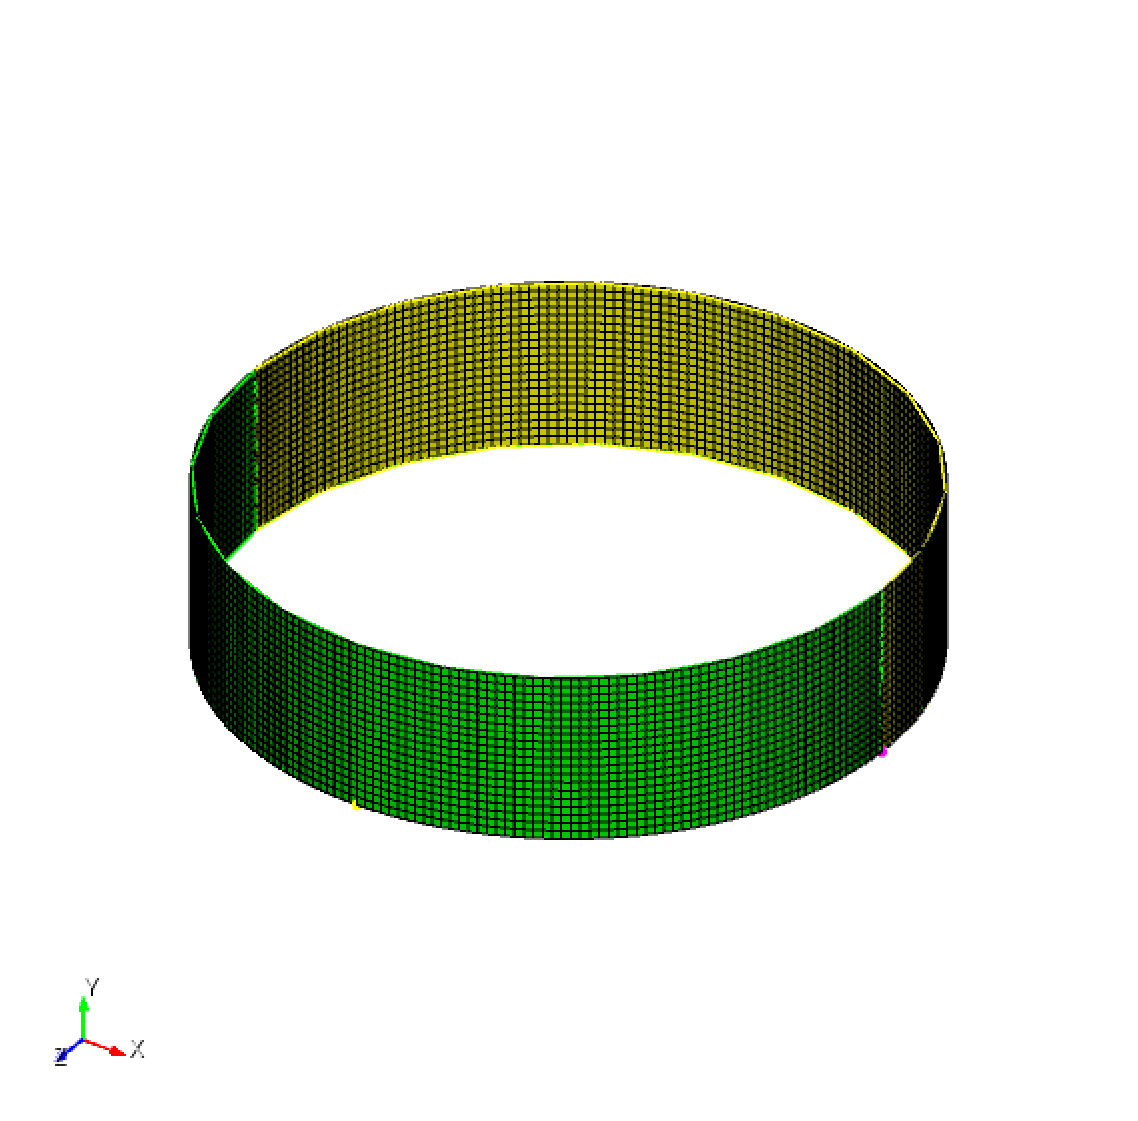
\includegraphics[width=0.6\textwidth]{PlateRing.eps}
%  \caption{3D Ring}
%  \label{fig:PlateRing}
%\end{figure}
%%
%
\begin{figure}[tbhp]
  \centering
  \vspace{-35mm}
  \resizebox{0.9\linewidth}{!}{%% Creator: Matplotlib, PGF backend
%%
%% To include the figure in your LaTeX document, write
%%   \input{<filename>.pgf}
%%
%% Make sure the required packages are loaded in your preamble
%%   \usepackage{pgf}
%%
%% Figures using additional raster images can only be included by \input if
%% they are in the same directory as the main LaTeX file. For loading figures
%% from other directories you can use the `import` package
%%   \usepackage{import}
%% and then include the figures with
%%   \import{<path to file>}{<filename>.pgf}
%%
%% Matplotlib used the following preamble
%%
\begingroup%
\makeatletter%
\begin{pgfpicture}%
\pgfpathrectangle{\pgfpointorigin}{\pgfqpoint{9.840000in}{8.462857in}}%
\pgfusepath{use as bounding box}%
\begin{pgfscope}%
\pgfsetbuttcap%
\pgfsetroundjoin%
\definecolor{currentfill}{rgb}{1.000000,1.000000,1.000000}%
\pgfsetfillcolor{currentfill}%
\pgfsetlinewidth{0.000000pt}%
\definecolor{currentstroke}{rgb}{1.000000,1.000000,1.000000}%
\pgfsetstrokecolor{currentstroke}%
\pgfsetdash{}{0pt}%
\pgfpathmoveto{\pgfqpoint{0.000000in}{0.000000in}}%
\pgfpathlineto{\pgfqpoint{9.840000in}{0.000000in}}%
\pgfpathlineto{\pgfqpoint{9.840000in}{8.462857in}}%
\pgfpathlineto{\pgfqpoint{0.000000in}{8.462857in}}%
\pgfpathclose%
\pgfusepath{fill}%
\end{pgfscope}%
\begin{pgfscope}%
\pgfsetbuttcap%
\pgfsetroundjoin%
\definecolor{currentfill}{rgb}{1.000000,1.000000,1.000000}%
\pgfsetfillcolor{currentfill}%
\pgfsetlinewidth{0.000000pt}%
\definecolor{currentstroke}{rgb}{0.000000,0.000000,0.000000}%
\pgfsetstrokecolor{currentstroke}%
\pgfsetstrokeopacity{0.000000}%
\pgfsetdash{}{0pt}%
\pgfpathmoveto{\pgfqpoint{0.100000in}{0.100000in}}%
\pgfpathlineto{\pgfqpoint{9.740000in}{0.100000in}}%
\pgfpathlineto{\pgfqpoint{9.740000in}{8.362857in}}%
\pgfpathlineto{\pgfqpoint{0.100000in}{8.362857in}}%
\pgfpathclose%
\pgfusepath{fill}%
\end{pgfscope}%
\begin{pgfscope}%
\pgfpathrectangle{\pgfqpoint{0.100000in}{0.100000in}}{\pgfqpoint{9.640000in}{8.262857in}} %
\pgfusepath{clip}%
\pgfsetbuttcap%
\pgfsetroundjoin%
\definecolor{currentfill}{rgb}{0.280085,0.235857,0.326570}%
\pgfsetfillcolor{currentfill}%
\pgfsetfillopacity{0.859496}%
\pgfsetlinewidth{1.003750pt}%
\definecolor{currentstroke}{rgb}{0.280085,0.235857,0.326570}%
\pgfsetstrokecolor{currentstroke}%
\pgfsetstrokeopacity{0.859496}%
\pgfsetdash{}{0pt}%
\pgfpathmoveto{\pgfqpoint{6.324324in}{3.204374in}}%
\pgfpathcurveto{\pgfqpoint{6.332560in}{3.204374in}}{\pgfqpoint{6.340460in}{3.207646in}}{\pgfqpoint{6.346284in}{3.213470in}}%
\pgfpathcurveto{\pgfqpoint{6.352108in}{3.219294in}}{\pgfqpoint{6.355380in}{3.227194in}}{\pgfqpoint{6.355380in}{3.235430in}}%
\pgfpathcurveto{\pgfqpoint{6.355380in}{3.243667in}}{\pgfqpoint{6.352108in}{3.251567in}}{\pgfqpoint{6.346284in}{3.257391in}}%
\pgfpathcurveto{\pgfqpoint{6.340460in}{3.263215in}}{\pgfqpoint{6.332560in}{3.266487in}}{\pgfqpoint{6.324324in}{3.266487in}}%
\pgfpathcurveto{\pgfqpoint{6.316087in}{3.266487in}}{\pgfqpoint{6.308187in}{3.263215in}}{\pgfqpoint{6.302363in}{3.257391in}}%
\pgfpathcurveto{\pgfqpoint{6.296539in}{3.251567in}}{\pgfqpoint{6.293267in}{3.243667in}}{\pgfqpoint{6.293267in}{3.235430in}}%
\pgfpathcurveto{\pgfqpoint{6.293267in}{3.227194in}}{\pgfqpoint{6.296539in}{3.219294in}}{\pgfqpoint{6.302363in}{3.213470in}}%
\pgfpathcurveto{\pgfqpoint{6.308187in}{3.207646in}}{\pgfqpoint{6.316087in}{3.204374in}}{\pgfqpoint{6.324324in}{3.204374in}}%
\pgfpathclose%
\pgfusepath{stroke,fill}%
\end{pgfscope}%
\begin{pgfscope}%
\pgfpathrectangle{\pgfqpoint{0.100000in}{0.100000in}}{\pgfqpoint{9.640000in}{8.262857in}} %
\pgfusepath{clip}%
\pgfsetbuttcap%
\pgfsetroundjoin%
\definecolor{currentfill}{rgb}{0.280085,0.235857,0.326570}%
\pgfsetfillcolor{currentfill}%
\pgfsetfillopacity{0.832925}%
\pgfsetlinewidth{1.003750pt}%
\definecolor{currentstroke}{rgb}{0.280085,0.235857,0.326570}%
\pgfsetstrokecolor{currentstroke}%
\pgfsetstrokeopacity{0.832925}%
\pgfsetdash{}{0pt}%
\pgfpathmoveto{\pgfqpoint{6.255858in}{3.069804in}}%
\pgfpathcurveto{\pgfqpoint{6.264094in}{3.069804in}}{\pgfqpoint{6.271994in}{3.073077in}}{\pgfqpoint{6.277818in}{3.078901in}}%
\pgfpathcurveto{\pgfqpoint{6.283642in}{3.084725in}}{\pgfqpoint{6.286914in}{3.092625in}}{\pgfqpoint{6.286914in}{3.100861in}}%
\pgfpathcurveto{\pgfqpoint{6.286914in}{3.109097in}}{\pgfqpoint{6.283642in}{3.116997in}}{\pgfqpoint{6.277818in}{3.122821in}}%
\pgfpathcurveto{\pgfqpoint{6.271994in}{3.128645in}}{\pgfqpoint{6.264094in}{3.131917in}}{\pgfqpoint{6.255858in}{3.131917in}}%
\pgfpathcurveto{\pgfqpoint{6.247622in}{3.131917in}}{\pgfqpoint{6.239722in}{3.128645in}}{\pgfqpoint{6.233898in}{3.122821in}}%
\pgfpathcurveto{\pgfqpoint{6.228074in}{3.116997in}}{\pgfqpoint{6.224801in}{3.109097in}}{\pgfqpoint{6.224801in}{3.100861in}}%
\pgfpathcurveto{\pgfqpoint{6.224801in}{3.092625in}}{\pgfqpoint{6.228074in}{3.084725in}}{\pgfqpoint{6.233898in}{3.078901in}}%
\pgfpathcurveto{\pgfqpoint{6.239722in}{3.073077in}}{\pgfqpoint{6.247622in}{3.069804in}}{\pgfqpoint{6.255858in}{3.069804in}}%
\pgfpathclose%
\pgfusepath{stroke,fill}%
\end{pgfscope}%
\begin{pgfscope}%
\pgfpathrectangle{\pgfqpoint{0.100000in}{0.100000in}}{\pgfqpoint{9.640000in}{8.262857in}} %
\pgfusepath{clip}%
\pgfsetbuttcap%
\pgfsetroundjoin%
\definecolor{currentfill}{rgb}{0.280085,0.235857,0.326570}%
\pgfsetfillcolor{currentfill}%
\pgfsetfillopacity{0.884499}%
\pgfsetlinewidth{1.003750pt}%
\definecolor{currentstroke}{rgb}{0.280085,0.235857,0.326570}%
\pgfsetstrokecolor{currentstroke}%
\pgfsetstrokeopacity{0.884499}%
\pgfsetdash{}{0pt}%
\pgfpathmoveto{\pgfqpoint{6.380613in}{3.351386in}}%
\pgfpathcurveto{\pgfqpoint{6.388850in}{3.351386in}}{\pgfqpoint{6.396750in}{3.354658in}}{\pgfqpoint{6.402574in}{3.360482in}}%
\pgfpathcurveto{\pgfqpoint{6.408398in}{3.366306in}}{\pgfqpoint{6.411670in}{3.374206in}}{\pgfqpoint{6.411670in}{3.382442in}}%
\pgfpathcurveto{\pgfqpoint{6.411670in}{3.390679in}}{\pgfqpoint{6.408398in}{3.398579in}}{\pgfqpoint{6.402574in}{3.404403in}}%
\pgfpathcurveto{\pgfqpoint{6.396750in}{3.410227in}}{\pgfqpoint{6.388850in}{3.413499in}}{\pgfqpoint{6.380613in}{3.413499in}}%
\pgfpathcurveto{\pgfqpoint{6.372377in}{3.413499in}}{\pgfqpoint{6.364477in}{3.410227in}}{\pgfqpoint{6.358653in}{3.404403in}}%
\pgfpathcurveto{\pgfqpoint{6.352829in}{3.398579in}}{\pgfqpoint{6.349557in}{3.390679in}}{\pgfqpoint{6.349557in}{3.382442in}}%
\pgfpathcurveto{\pgfqpoint{6.349557in}{3.374206in}}{\pgfqpoint{6.352829in}{3.366306in}}{\pgfqpoint{6.358653in}{3.360482in}}%
\pgfpathcurveto{\pgfqpoint{6.364477in}{3.354658in}}{\pgfqpoint{6.372377in}{3.351386in}}{\pgfqpoint{6.380613in}{3.351386in}}%
\pgfpathclose%
\pgfusepath{stroke,fill}%
\end{pgfscope}%
\begin{pgfscope}%
\pgfpathrectangle{\pgfqpoint{0.100000in}{0.100000in}}{\pgfqpoint{9.640000in}{8.262857in}} %
\pgfusepath{clip}%
\pgfsetbuttcap%
\pgfsetroundjoin%
\definecolor{currentfill}{rgb}{0.280085,0.235857,0.326570}%
\pgfsetfillcolor{currentfill}%
\pgfsetfillopacity{0.805080}%
\pgfsetlinewidth{1.003750pt}%
\definecolor{currentstroke}{rgb}{0.280085,0.235857,0.326570}%
\pgfsetstrokecolor{currentstroke}%
\pgfsetstrokeopacity{0.805080}%
\pgfsetdash{}{0pt}%
\pgfpathmoveto{\pgfqpoint{6.176035in}{2.949020in}}%
\pgfpathcurveto{\pgfqpoint{6.184271in}{2.949020in}}{\pgfqpoint{6.192171in}{2.952292in}}{\pgfqpoint{6.197995in}{2.958116in}}%
\pgfpathcurveto{\pgfqpoint{6.203819in}{2.963940in}}{\pgfqpoint{6.207091in}{2.971840in}}{\pgfqpoint{6.207091in}{2.980076in}}%
\pgfpathcurveto{\pgfqpoint{6.207091in}{2.988313in}}{\pgfqpoint{6.203819in}{2.996213in}}{\pgfqpoint{6.197995in}{3.002037in}}%
\pgfpathcurveto{\pgfqpoint{6.192171in}{3.007860in}}{\pgfqpoint{6.184271in}{3.011133in}}{\pgfqpoint{6.176035in}{3.011133in}}%
\pgfpathcurveto{\pgfqpoint{6.167798in}{3.011133in}}{\pgfqpoint{6.159898in}{3.007860in}}{\pgfqpoint{6.154074in}{3.002037in}}%
\pgfpathcurveto{\pgfqpoint{6.148250in}{2.996213in}}{\pgfqpoint{6.144978in}{2.988313in}}{\pgfqpoint{6.144978in}{2.980076in}}%
\pgfpathcurveto{\pgfqpoint{6.144978in}{2.971840in}}{\pgfqpoint{6.148250in}{2.963940in}}{\pgfqpoint{6.154074in}{2.958116in}}%
\pgfpathcurveto{\pgfqpoint{6.159898in}{2.952292in}}{\pgfqpoint{6.167798in}{2.949020in}}{\pgfqpoint{6.176035in}{2.949020in}}%
\pgfpathclose%
\pgfusepath{stroke,fill}%
\end{pgfscope}%
\begin{pgfscope}%
\pgfpathrectangle{\pgfqpoint{0.100000in}{0.100000in}}{\pgfqpoint{9.640000in}{8.262857in}} %
\pgfusepath{clip}%
\pgfsetbuttcap%
\pgfsetroundjoin%
\definecolor{currentfill}{rgb}{0.280085,0.235857,0.326570}%
\pgfsetfillcolor{currentfill}%
\pgfsetfillopacity{0.907652}%
\pgfsetlinewidth{1.003750pt}%
\definecolor{currentstroke}{rgb}{0.280085,0.235857,0.326570}%
\pgfsetstrokecolor{currentstroke}%
\pgfsetstrokeopacity{0.907652}%
\pgfsetdash{}{0pt}%
\pgfpathmoveto{\pgfqpoint{6.424035in}{3.509339in}}%
\pgfpathcurveto{\pgfqpoint{6.432271in}{3.509339in}}{\pgfqpoint{6.440172in}{3.512611in}}{\pgfqpoint{6.445995in}{3.518435in}}%
\pgfpathcurveto{\pgfqpoint{6.451819in}{3.524259in}}{\pgfqpoint{6.455092in}{3.532159in}}{\pgfqpoint{6.455092in}{3.540395in}}%
\pgfpathcurveto{\pgfqpoint{6.455092in}{3.548632in}}{\pgfqpoint{6.451819in}{3.556532in}}{\pgfqpoint{6.445995in}{3.562356in}}%
\pgfpathcurveto{\pgfqpoint{6.440172in}{3.568180in}}{\pgfqpoint{6.432271in}{3.571452in}}{\pgfqpoint{6.424035in}{3.571452in}}%
\pgfpathcurveto{\pgfqpoint{6.415799in}{3.571452in}}{\pgfqpoint{6.407899in}{3.568180in}}{\pgfqpoint{6.402075in}{3.562356in}}%
\pgfpathcurveto{\pgfqpoint{6.396251in}{3.556532in}}{\pgfqpoint{6.392979in}{3.548632in}}{\pgfqpoint{6.392979in}{3.540395in}}%
\pgfpathcurveto{\pgfqpoint{6.392979in}{3.532159in}}{\pgfqpoint{6.396251in}{3.524259in}}{\pgfqpoint{6.402075in}{3.518435in}}%
\pgfpathcurveto{\pgfqpoint{6.407899in}{3.512611in}}{\pgfqpoint{6.415799in}{3.509339in}}{\pgfqpoint{6.424035in}{3.509339in}}%
\pgfpathclose%
\pgfusepath{stroke,fill}%
\end{pgfscope}%
\begin{pgfscope}%
\pgfpathrectangle{\pgfqpoint{0.100000in}{0.100000in}}{\pgfqpoint{9.640000in}{8.262857in}} %
\pgfusepath{clip}%
\pgfsetbuttcap%
\pgfsetroundjoin%
\definecolor{currentfill}{rgb}{0.280085,0.235857,0.326570}%
\pgfsetfillcolor{currentfill}%
\pgfsetfillopacity{0.776265}%
\pgfsetlinewidth{1.003750pt}%
\definecolor{currentstroke}{rgb}{0.280085,0.235857,0.326570}%
\pgfsetstrokecolor{currentstroke}%
\pgfsetstrokeopacity{0.776265}%
\pgfsetdash{}{0pt}%
\pgfpathmoveto{\pgfqpoint{6.085785in}{2.843191in}}%
\pgfpathcurveto{\pgfqpoint{6.094021in}{2.843191in}}{\pgfqpoint{6.101921in}{2.846463in}}{\pgfqpoint{6.107745in}{2.852287in}}%
\pgfpathcurveto{\pgfqpoint{6.113569in}{2.858111in}}{\pgfqpoint{6.116841in}{2.866011in}}{\pgfqpoint{6.116841in}{2.874247in}}%
\pgfpathcurveto{\pgfqpoint{6.116841in}{2.882484in}}{\pgfqpoint{6.113569in}{2.890384in}}{\pgfqpoint{6.107745in}{2.896208in}}%
\pgfpathcurveto{\pgfqpoint{6.101921in}{2.902032in}}{\pgfqpoint{6.094021in}{2.905304in}}{\pgfqpoint{6.085785in}{2.905304in}}%
\pgfpathcurveto{\pgfqpoint{6.077549in}{2.905304in}}{\pgfqpoint{6.069648in}{2.902032in}}{\pgfqpoint{6.063825in}{2.896208in}}%
\pgfpathcurveto{\pgfqpoint{6.058001in}{2.890384in}}{\pgfqpoint{6.054728in}{2.882484in}}{\pgfqpoint{6.054728in}{2.874247in}}%
\pgfpathcurveto{\pgfqpoint{6.054728in}{2.866011in}}{\pgfqpoint{6.058001in}{2.858111in}}{\pgfqpoint{6.063825in}{2.852287in}}%
\pgfpathcurveto{\pgfqpoint{6.069648in}{2.846463in}}{\pgfqpoint{6.077549in}{2.843191in}}{\pgfqpoint{6.085785in}{2.843191in}}%
\pgfpathclose%
\pgfusepath{stroke,fill}%
\end{pgfscope}%
\begin{pgfscope}%
\pgfpathrectangle{\pgfqpoint{0.100000in}{0.100000in}}{\pgfqpoint{9.640000in}{8.262857in}} %
\pgfusepath{clip}%
\pgfsetbuttcap%
\pgfsetroundjoin%
\definecolor{currentfill}{rgb}{0.280085,0.235857,0.326570}%
\pgfsetfillcolor{currentfill}%
\pgfsetfillopacity{0.928693}%
\pgfsetlinewidth{1.003750pt}%
\definecolor{currentstroke}{rgb}{0.280085,0.235857,0.326570}%
\pgfsetstrokecolor{currentstroke}%
\pgfsetstrokeopacity{0.928693}%
\pgfsetdash{}{0pt}%
\pgfpathmoveto{\pgfqpoint{6.454035in}{3.676586in}}%
\pgfpathcurveto{\pgfqpoint{6.462271in}{3.676586in}}{\pgfqpoint{6.470171in}{3.679858in}}{\pgfqpoint{6.475995in}{3.685682in}}%
\pgfpathcurveto{\pgfqpoint{6.481819in}{3.691506in}}{\pgfqpoint{6.485091in}{3.699406in}}{\pgfqpoint{6.485091in}{3.707642in}}%
\pgfpathcurveto{\pgfqpoint{6.485091in}{3.715879in}}{\pgfqpoint{6.481819in}{3.723779in}}{\pgfqpoint{6.475995in}{3.729603in}}%
\pgfpathcurveto{\pgfqpoint{6.470171in}{3.735427in}}{\pgfqpoint{6.462271in}{3.738699in}}{\pgfqpoint{6.454035in}{3.738699in}}%
\pgfpathcurveto{\pgfqpoint{6.445798in}{3.738699in}}{\pgfqpoint{6.437898in}{3.735427in}}{\pgfqpoint{6.432074in}{3.729603in}}%
\pgfpathcurveto{\pgfqpoint{6.426251in}{3.723779in}}{\pgfqpoint{6.422978in}{3.715879in}}{\pgfqpoint{6.422978in}{3.707642in}}%
\pgfpathcurveto{\pgfqpoint{6.422978in}{3.699406in}}{\pgfqpoint{6.426251in}{3.691506in}}{\pgfqpoint{6.432074in}{3.685682in}}%
\pgfpathcurveto{\pgfqpoint{6.437898in}{3.679858in}}{\pgfqpoint{6.445798in}{3.676586in}}{\pgfqpoint{6.454035in}{3.676586in}}%
\pgfpathclose%
\pgfusepath{stroke,fill}%
\end{pgfscope}%
\begin{pgfscope}%
\pgfpathrectangle{\pgfqpoint{0.100000in}{0.100000in}}{\pgfqpoint{9.640000in}{8.262857in}} %
\pgfusepath{clip}%
\pgfsetbuttcap%
\pgfsetroundjoin%
\definecolor{currentfill}{rgb}{0.280085,0.235857,0.326570}%
\pgfsetfillcolor{currentfill}%
\pgfsetfillopacity{0.746790}%
\pgfsetlinewidth{1.003750pt}%
\definecolor{currentstroke}{rgb}{0.280085,0.235857,0.326570}%
\pgfsetstrokecolor{currentstroke}%
\pgfsetstrokeopacity{0.746790}%
\pgfsetdash{}{0pt}%
\pgfpathmoveto{\pgfqpoint{5.986138in}{2.753309in}}%
\pgfpathcurveto{\pgfqpoint{5.994374in}{2.753309in}}{\pgfqpoint{6.002274in}{2.756581in}}{\pgfqpoint{6.008098in}{2.762405in}}%
\pgfpathcurveto{\pgfqpoint{6.013922in}{2.768229in}}{\pgfqpoint{6.017195in}{2.776129in}}{\pgfqpoint{6.017195in}{2.784365in}}%
\pgfpathcurveto{\pgfqpoint{6.017195in}{2.792601in}}{\pgfqpoint{6.013922in}{2.800502in}}{\pgfqpoint{6.008098in}{2.806325in}}%
\pgfpathcurveto{\pgfqpoint{6.002274in}{2.812149in}}{\pgfqpoint{5.994374in}{2.815422in}}{\pgfqpoint{5.986138in}{2.815422in}}%
\pgfpathcurveto{\pgfqpoint{5.977902in}{2.815422in}}{\pgfqpoint{5.970002in}{2.812149in}}{\pgfqpoint{5.964178in}{2.806325in}}%
\pgfpathcurveto{\pgfqpoint{5.958354in}{2.800502in}}{\pgfqpoint{5.955082in}{2.792601in}}{\pgfqpoint{5.955082in}{2.784365in}}%
\pgfpathcurveto{\pgfqpoint{5.955082in}{2.776129in}}{\pgfqpoint{5.958354in}{2.768229in}}{\pgfqpoint{5.964178in}{2.762405in}}%
\pgfpathcurveto{\pgfqpoint{5.970002in}{2.756581in}}{\pgfqpoint{5.977902in}{2.753309in}}{\pgfqpoint{5.986138in}{2.753309in}}%
\pgfpathclose%
\pgfusepath{stroke,fill}%
\end{pgfscope}%
\begin{pgfscope}%
\pgfpathrectangle{\pgfqpoint{0.100000in}{0.100000in}}{\pgfqpoint{9.640000in}{8.262857in}} %
\pgfusepath{clip}%
\pgfsetbuttcap%
\pgfsetroundjoin%
\definecolor{currentfill}{rgb}{0.280085,0.235857,0.326570}%
\pgfsetfillcolor{currentfill}%
\pgfsetfillopacity{0.947378}%
\pgfsetlinewidth{1.003750pt}%
\definecolor{currentstroke}{rgb}{0.280085,0.235857,0.326570}%
\pgfsetstrokecolor{currentstroke}%
\pgfsetstrokeopacity{0.947378}%
\pgfsetdash{}{0pt}%
\pgfpathmoveto{\pgfqpoint{6.470206in}{3.851353in}}%
\pgfpathcurveto{\pgfqpoint{6.478443in}{3.851353in}}{\pgfqpoint{6.486343in}{3.854625in}}{\pgfqpoint{6.492167in}{3.860449in}}%
\pgfpathcurveto{\pgfqpoint{6.497991in}{3.866273in}}{\pgfqpoint{6.501263in}{3.874173in}}{\pgfqpoint{6.501263in}{3.882410in}}%
\pgfpathcurveto{\pgfqpoint{6.501263in}{3.890646in}}{\pgfqpoint{6.497991in}{3.898546in}}{\pgfqpoint{6.492167in}{3.904370in}}%
\pgfpathcurveto{\pgfqpoint{6.486343in}{3.910194in}}{\pgfqpoint{6.478443in}{3.913466in}}{\pgfqpoint{6.470206in}{3.913466in}}%
\pgfpathcurveto{\pgfqpoint{6.461970in}{3.913466in}}{\pgfqpoint{6.454070in}{3.910194in}}{\pgfqpoint{6.448246in}{3.904370in}}%
\pgfpathcurveto{\pgfqpoint{6.442422in}{3.898546in}}{\pgfqpoint{6.439150in}{3.890646in}}{\pgfqpoint{6.439150in}{3.882410in}}%
\pgfpathcurveto{\pgfqpoint{6.439150in}{3.874173in}}{\pgfqpoint{6.442422in}{3.866273in}}{\pgfqpoint{6.448246in}{3.860449in}}%
\pgfpathcurveto{\pgfqpoint{6.454070in}{3.854625in}}{\pgfqpoint{6.461970in}{3.851353in}}{\pgfqpoint{6.470206in}{3.851353in}}%
\pgfpathclose%
\pgfusepath{stroke,fill}%
\end{pgfscope}%
\begin{pgfscope}%
\pgfpathrectangle{\pgfqpoint{0.100000in}{0.100000in}}{\pgfqpoint{9.640000in}{8.262857in}} %
\pgfusepath{clip}%
\pgfsetbuttcap%
\pgfsetroundjoin%
\definecolor{currentfill}{rgb}{0.280085,0.235857,0.326570}%
\pgfsetfillcolor{currentfill}%
\pgfsetfillopacity{0.829179}%
\pgfsetlinewidth{1.003750pt}%
\definecolor{currentstroke}{rgb}{0.280085,0.235857,0.326570}%
\pgfsetstrokecolor{currentstroke}%
\pgfsetstrokeopacity{0.829179}%
\pgfsetdash{}{0pt}%
\pgfpathmoveto{\pgfqpoint{6.475968in}{3.252976in}}%
\pgfpathcurveto{\pgfqpoint{6.484204in}{3.252976in}}{\pgfqpoint{6.492104in}{3.256248in}}{\pgfqpoint{6.497928in}{3.262072in}}%
\pgfpathcurveto{\pgfqpoint{6.503752in}{3.267896in}}{\pgfqpoint{6.507024in}{3.275796in}}{\pgfqpoint{6.507024in}{3.284032in}}%
\pgfpathcurveto{\pgfqpoint{6.507024in}{3.292268in}}{\pgfqpoint{6.503752in}{3.300168in}}{\pgfqpoint{6.497928in}{3.305992in}}%
\pgfpathcurveto{\pgfqpoint{6.492104in}{3.311816in}}{\pgfqpoint{6.484204in}{3.315089in}}{\pgfqpoint{6.475968in}{3.315089in}}%
\pgfpathcurveto{\pgfqpoint{6.467731in}{3.315089in}}{\pgfqpoint{6.459831in}{3.311816in}}{\pgfqpoint{6.454008in}{3.305992in}}%
\pgfpathcurveto{\pgfqpoint{6.448184in}{3.300168in}}{\pgfqpoint{6.444911in}{3.292268in}}{\pgfqpoint{6.444911in}{3.284032in}}%
\pgfpathcurveto{\pgfqpoint{6.444911in}{3.275796in}}{\pgfqpoint{6.448184in}{3.267896in}}{\pgfqpoint{6.454008in}{3.262072in}}%
\pgfpathcurveto{\pgfqpoint{6.459831in}{3.256248in}}{\pgfqpoint{6.467731in}{3.252976in}}{\pgfqpoint{6.475968in}{3.252976in}}%
\pgfpathclose%
\pgfusepath{stroke,fill}%
\end{pgfscope}%
\begin{pgfscope}%
\pgfpathrectangle{\pgfqpoint{0.100000in}{0.100000in}}{\pgfqpoint{9.640000in}{8.262857in}} %
\pgfusepath{clip}%
\pgfsetbuttcap%
\pgfsetroundjoin%
\definecolor{currentfill}{rgb}{0.280085,0.235857,0.326570}%
\pgfsetfillcolor{currentfill}%
\pgfsetfillopacity{0.802756}%
\pgfsetlinewidth{1.003750pt}%
\definecolor{currentstroke}{rgb}{0.280085,0.235857,0.326570}%
\pgfsetstrokecolor{currentstroke}%
\pgfsetstrokeopacity{0.802756}%
\pgfsetdash{}{0pt}%
\pgfpathmoveto{\pgfqpoint{6.407322in}{3.118663in}}%
\pgfpathcurveto{\pgfqpoint{6.415559in}{3.118663in}}{\pgfqpoint{6.423459in}{3.121935in}}{\pgfqpoint{6.429283in}{3.127759in}}%
\pgfpathcurveto{\pgfqpoint{6.435106in}{3.133583in}}{\pgfqpoint{6.438379in}{3.141483in}}{\pgfqpoint{6.438379in}{3.149719in}}%
\pgfpathcurveto{\pgfqpoint{6.438379in}{3.157956in}}{\pgfqpoint{6.435106in}{3.165856in}}{\pgfqpoint{6.429283in}{3.171680in}}%
\pgfpathcurveto{\pgfqpoint{6.423459in}{3.177504in}}{\pgfqpoint{6.415559in}{3.180776in}}{\pgfqpoint{6.407322in}{3.180776in}}%
\pgfpathcurveto{\pgfqpoint{6.399086in}{3.180776in}}{\pgfqpoint{6.391186in}{3.177504in}}{\pgfqpoint{6.385362in}{3.171680in}}%
\pgfpathcurveto{\pgfqpoint{6.379538in}{3.165856in}}{\pgfqpoint{6.376266in}{3.157956in}}{\pgfqpoint{6.376266in}{3.149719in}}%
\pgfpathcurveto{\pgfqpoint{6.376266in}{3.141483in}}{\pgfqpoint{6.379538in}{3.133583in}}{\pgfqpoint{6.385362in}{3.127759in}}%
\pgfpathcurveto{\pgfqpoint{6.391186in}{3.121935in}}{\pgfqpoint{6.399086in}{3.118663in}}{\pgfqpoint{6.407322in}{3.118663in}}%
\pgfpathclose%
\pgfusepath{stroke,fill}%
\end{pgfscope}%
\begin{pgfscope}%
\pgfpathrectangle{\pgfqpoint{0.100000in}{0.100000in}}{\pgfqpoint{9.640000in}{8.262857in}} %
\pgfusepath{clip}%
\pgfsetbuttcap%
\pgfsetroundjoin%
\definecolor{currentfill}{rgb}{0.280085,0.235857,0.326570}%
\pgfsetfillcolor{currentfill}%
\pgfsetfillopacity{0.854042}%
\pgfsetlinewidth{1.003750pt}%
\definecolor{currentstroke}{rgb}{0.280085,0.235857,0.326570}%
\pgfsetstrokecolor{currentstroke}%
\pgfsetstrokeopacity{0.854042}%
\pgfsetdash{}{0pt}%
\pgfpathmoveto{\pgfqpoint{6.532449in}{3.399687in}}%
\pgfpathcurveto{\pgfqpoint{6.540685in}{3.399687in}}{\pgfqpoint{6.548585in}{3.402959in}}{\pgfqpoint{6.554409in}{3.408783in}}%
\pgfpathcurveto{\pgfqpoint{6.560233in}{3.414607in}}{\pgfqpoint{6.563505in}{3.422507in}}{\pgfqpoint{6.563505in}{3.430744in}}%
\pgfpathcurveto{\pgfqpoint{6.563505in}{3.438980in}}{\pgfqpoint{6.560233in}{3.446880in}}{\pgfqpoint{6.554409in}{3.452704in}}%
\pgfpathcurveto{\pgfqpoint{6.548585in}{3.458528in}}{\pgfqpoint{6.540685in}{3.461800in}}{\pgfqpoint{6.532449in}{3.461800in}}%
\pgfpathcurveto{\pgfqpoint{6.524212in}{3.461800in}}{\pgfqpoint{6.516312in}{3.458528in}}{\pgfqpoint{6.510488in}{3.452704in}}%
\pgfpathcurveto{\pgfqpoint{6.504665in}{3.446880in}}{\pgfqpoint{6.501392in}{3.438980in}}{\pgfqpoint{6.501392in}{3.430744in}}%
\pgfpathcurveto{\pgfqpoint{6.501392in}{3.422507in}}{\pgfqpoint{6.504665in}{3.414607in}}{\pgfqpoint{6.510488in}{3.408783in}}%
\pgfpathcurveto{\pgfqpoint{6.516312in}{3.402959in}}{\pgfqpoint{6.524212in}{3.399687in}}{\pgfqpoint{6.532449in}{3.399687in}}%
\pgfpathclose%
\pgfusepath{stroke,fill}%
\end{pgfscope}%
\begin{pgfscope}%
\pgfpathrectangle{\pgfqpoint{0.100000in}{0.100000in}}{\pgfqpoint{9.640000in}{8.262857in}} %
\pgfusepath{clip}%
\pgfsetbuttcap%
\pgfsetroundjoin%
\definecolor{currentfill}{rgb}{0.280085,0.235857,0.326570}%
\pgfsetfillcolor{currentfill}%
\pgfsetfillopacity{0.775066}%
\pgfsetlinewidth{1.003750pt}%
\definecolor{currentstroke}{rgb}{0.280085,0.235857,0.326570}%
\pgfsetstrokecolor{currentstroke}%
\pgfsetstrokeopacity{0.775066}%
\pgfsetdash{}{0pt}%
\pgfpathmoveto{\pgfqpoint{6.327332in}{2.998089in}}%
\pgfpathcurveto{\pgfqpoint{6.335568in}{2.998089in}}{\pgfqpoint{6.343468in}{3.001361in}}{\pgfqpoint{6.349292in}{3.007185in}}%
\pgfpathcurveto{\pgfqpoint{6.355116in}{3.013009in}}{\pgfqpoint{6.358389in}{3.020909in}}{\pgfqpoint{6.358389in}{3.029146in}}%
\pgfpathcurveto{\pgfqpoint{6.358389in}{3.037382in}}{\pgfqpoint{6.355116in}{3.045282in}}{\pgfqpoint{6.349292in}{3.051106in}}%
\pgfpathcurveto{\pgfqpoint{6.343468in}{3.056930in}}{\pgfqpoint{6.335568in}{3.060202in}}{\pgfqpoint{6.327332in}{3.060202in}}%
\pgfpathcurveto{\pgfqpoint{6.319096in}{3.060202in}}{\pgfqpoint{6.311196in}{3.056930in}}{\pgfqpoint{6.305372in}{3.051106in}}%
\pgfpathcurveto{\pgfqpoint{6.299548in}{3.045282in}}{\pgfqpoint{6.296276in}{3.037382in}}{\pgfqpoint{6.296276in}{3.029146in}}%
\pgfpathcurveto{\pgfqpoint{6.296276in}{3.020909in}}{\pgfqpoint{6.299548in}{3.013009in}}{\pgfqpoint{6.305372in}{3.007185in}}%
\pgfpathcurveto{\pgfqpoint{6.311196in}{3.001361in}}{\pgfqpoint{6.319096in}{2.998089in}}{\pgfqpoint{6.327332in}{2.998089in}}%
\pgfpathclose%
\pgfusepath{stroke,fill}%
\end{pgfscope}%
\begin{pgfscope}%
\pgfpathrectangle{\pgfqpoint{0.100000in}{0.100000in}}{\pgfqpoint{9.640000in}{8.262857in}} %
\pgfusepath{clip}%
\pgfsetbuttcap%
\pgfsetroundjoin%
\definecolor{currentfill}{rgb}{0.280085,0.235857,0.326570}%
\pgfsetfillcolor{currentfill}%
\pgfsetfillopacity{0.877065}%
\pgfsetlinewidth{1.003750pt}%
\definecolor{currentstroke}{rgb}{0.280085,0.235857,0.326570}%
\pgfsetstrokecolor{currentstroke}%
\pgfsetstrokeopacity{0.877065}%
\pgfsetdash{}{0pt}%
\pgfpathmoveto{\pgfqpoint{6.576071in}{3.557299in}}%
\pgfpathcurveto{\pgfqpoint{6.584308in}{3.557299in}}{\pgfqpoint{6.592208in}{3.560571in}}{\pgfqpoint{6.598032in}{3.566395in}}%
\pgfpathcurveto{\pgfqpoint{6.603856in}{3.572219in}}{\pgfqpoint{6.607128in}{3.580119in}}{\pgfqpoint{6.607128in}{3.588355in}}%
\pgfpathcurveto{\pgfqpoint{6.607128in}{3.596592in}}{\pgfqpoint{6.603856in}{3.604492in}}{\pgfqpoint{6.598032in}{3.610316in}}%
\pgfpathcurveto{\pgfqpoint{6.592208in}{3.616139in}}{\pgfqpoint{6.584308in}{3.619412in}}{\pgfqpoint{6.576071in}{3.619412in}}%
\pgfpathcurveto{\pgfqpoint{6.567835in}{3.619412in}}{\pgfqpoint{6.559935in}{3.616139in}}{\pgfqpoint{6.554111in}{3.610316in}}%
\pgfpathcurveto{\pgfqpoint{6.548287in}{3.604492in}}{\pgfqpoint{6.545015in}{3.596592in}}{\pgfqpoint{6.545015in}{3.588355in}}%
\pgfpathcurveto{\pgfqpoint{6.545015in}{3.580119in}}{\pgfqpoint{6.548287in}{3.572219in}}{\pgfqpoint{6.554111in}{3.566395in}}%
\pgfpathcurveto{\pgfqpoint{6.559935in}{3.560571in}}{\pgfqpoint{6.567835in}{3.557299in}}{\pgfqpoint{6.576071in}{3.557299in}}%
\pgfpathclose%
\pgfusepath{stroke,fill}%
\end{pgfscope}%
\begin{pgfscope}%
\pgfpathrectangle{\pgfqpoint{0.100000in}{0.100000in}}{\pgfqpoint{9.640000in}{8.262857in}} %
\pgfusepath{clip}%
\pgfsetbuttcap%
\pgfsetroundjoin%
\definecolor{currentfill}{rgb}{0.280085,0.235857,0.326570}%
\pgfsetfillcolor{currentfill}%
\pgfsetfillopacity{0.716967}%
\pgfsetlinewidth{1.003750pt}%
\definecolor{currentstroke}{rgb}{0.280085,0.235857,0.326570}%
\pgfsetstrokecolor{currentstroke}%
\pgfsetstrokeopacity{0.716967}%
\pgfsetdash{}{0pt}%
\pgfpathmoveto{\pgfqpoint{5.878208in}{2.680178in}}%
\pgfpathcurveto{\pgfqpoint{5.886444in}{2.680178in}}{\pgfqpoint{5.894345in}{2.683450in}}{\pgfqpoint{5.900168in}{2.689274in}}%
\pgfpathcurveto{\pgfqpoint{5.905992in}{2.695098in}}{\pgfqpoint{5.909265in}{2.702998in}}{\pgfqpoint{5.909265in}{2.711234in}}%
\pgfpathcurveto{\pgfqpoint{5.909265in}{2.719470in}}{\pgfqpoint{5.905992in}{2.727370in}}{\pgfqpoint{5.900168in}{2.733194in}}%
\pgfpathcurveto{\pgfqpoint{5.894345in}{2.739018in}}{\pgfqpoint{5.886444in}{2.742291in}}{\pgfqpoint{5.878208in}{2.742291in}}%
\pgfpathcurveto{\pgfqpoint{5.869972in}{2.742291in}}{\pgfqpoint{5.862072in}{2.739018in}}{\pgfqpoint{5.856248in}{2.733194in}}%
\pgfpathcurveto{\pgfqpoint{5.850424in}{2.727370in}}{\pgfqpoint{5.847152in}{2.719470in}}{\pgfqpoint{5.847152in}{2.711234in}}%
\pgfpathcurveto{\pgfqpoint{5.847152in}{2.702998in}}{\pgfqpoint{5.850424in}{2.695098in}}{\pgfqpoint{5.856248in}{2.689274in}}%
\pgfpathcurveto{\pgfqpoint{5.862072in}{2.683450in}}{\pgfqpoint{5.869972in}{2.680178in}}{\pgfqpoint{5.878208in}{2.680178in}}%
\pgfpathclose%
\pgfusepath{stroke,fill}%
\end{pgfscope}%
\begin{pgfscope}%
\pgfpathrectangle{\pgfqpoint{0.100000in}{0.100000in}}{\pgfqpoint{9.640000in}{8.262857in}} %
\pgfusepath{clip}%
\pgfsetbuttcap%
\pgfsetroundjoin%
\definecolor{currentfill}{rgb}{0.280085,0.235857,0.326570}%
\pgfsetfillcolor{currentfill}%
\pgfsetfillopacity{0.746411}%
\pgfsetlinewidth{1.003750pt}%
\definecolor{currentstroke}{rgb}{0.280085,0.235857,0.326570}%
\pgfsetstrokecolor{currentstroke}%
\pgfsetstrokeopacity{0.746411}%
\pgfsetdash{}{0pt}%
\pgfpathmoveto{\pgfqpoint{6.236929in}{2.892423in}}%
\pgfpathcurveto{\pgfqpoint{6.245166in}{2.892423in}}{\pgfqpoint{6.253066in}{2.895696in}}{\pgfqpoint{6.258890in}{2.901520in}}%
\pgfpathcurveto{\pgfqpoint{6.264714in}{2.907344in}}{\pgfqpoint{6.267986in}{2.915244in}}{\pgfqpoint{6.267986in}{2.923480in}}%
\pgfpathcurveto{\pgfqpoint{6.267986in}{2.931716in}}{\pgfqpoint{6.264714in}{2.939616in}}{\pgfqpoint{6.258890in}{2.945440in}}%
\pgfpathcurveto{\pgfqpoint{6.253066in}{2.951264in}}{\pgfqpoint{6.245166in}{2.954536in}}{\pgfqpoint{6.236929in}{2.954536in}}%
\pgfpathcurveto{\pgfqpoint{6.228693in}{2.954536in}}{\pgfqpoint{6.220793in}{2.951264in}}{\pgfqpoint{6.214969in}{2.945440in}}%
\pgfpathcurveto{\pgfqpoint{6.209145in}{2.939616in}}{\pgfqpoint{6.205873in}{2.931716in}}{\pgfqpoint{6.205873in}{2.923480in}}%
\pgfpathcurveto{\pgfqpoint{6.205873in}{2.915244in}}{\pgfqpoint{6.209145in}{2.907344in}}{\pgfqpoint{6.214969in}{2.901520in}}%
\pgfpathcurveto{\pgfqpoint{6.220793in}{2.895696in}}{\pgfqpoint{6.228693in}{2.892423in}}{\pgfqpoint{6.236929in}{2.892423in}}%
\pgfpathclose%
\pgfusepath{stroke,fill}%
\end{pgfscope}%
\begin{pgfscope}%
\pgfpathrectangle{\pgfqpoint{0.100000in}{0.100000in}}{\pgfqpoint{9.640000in}{8.262857in}} %
\pgfusepath{clip}%
\pgfsetbuttcap%
\pgfsetroundjoin%
\definecolor{currentfill}{rgb}{0.280085,0.235857,0.326570}%
\pgfsetfillcolor{currentfill}%
\pgfsetfillopacity{0.963492}%
\pgfsetlinewidth{1.003750pt}%
\definecolor{currentstroke}{rgb}{0.280085,0.235857,0.326570}%
\pgfsetstrokecolor{currentstroke}%
\pgfsetstrokeopacity{0.963492}%
\pgfsetdash{}{0pt}%
\pgfpathmoveto{\pgfqpoint{6.472302in}{4.031760in}}%
\pgfpathcurveto{\pgfqpoint{6.480538in}{4.031760in}}{\pgfqpoint{6.488438in}{4.035032in}}{\pgfqpoint{6.494262in}{4.040856in}}%
\pgfpathcurveto{\pgfqpoint{6.500086in}{4.046680in}}{\pgfqpoint{6.503358in}{4.054580in}}{\pgfqpoint{6.503358in}{4.062816in}}%
\pgfpathcurveto{\pgfqpoint{6.503358in}{4.071053in}}{\pgfqpoint{6.500086in}{4.078953in}}{\pgfqpoint{6.494262in}{4.084777in}}%
\pgfpathcurveto{\pgfqpoint{6.488438in}{4.090601in}}{\pgfqpoint{6.480538in}{4.093873in}}{\pgfqpoint{6.472302in}{4.093873in}}%
\pgfpathcurveto{\pgfqpoint{6.464066in}{4.093873in}}{\pgfqpoint{6.456166in}{4.090601in}}{\pgfqpoint{6.450342in}{4.084777in}}%
\pgfpathcurveto{\pgfqpoint{6.444518in}{4.078953in}}{\pgfqpoint{6.441245in}{4.071053in}}{\pgfqpoint{6.441245in}{4.062816in}}%
\pgfpathcurveto{\pgfqpoint{6.441245in}{4.054580in}}{\pgfqpoint{6.444518in}{4.046680in}}{\pgfqpoint{6.450342in}{4.040856in}}%
\pgfpathcurveto{\pgfqpoint{6.456166in}{4.035032in}}{\pgfqpoint{6.464066in}{4.031760in}}{\pgfqpoint{6.472302in}{4.031760in}}%
\pgfpathclose%
\pgfusepath{stroke,fill}%
\end{pgfscope}%
\begin{pgfscope}%
\pgfpathrectangle{\pgfqpoint{0.100000in}{0.100000in}}{\pgfqpoint{9.640000in}{8.262857in}} %
\pgfusepath{clip}%
\pgfsetbuttcap%
\pgfsetroundjoin%
\definecolor{currentfill}{rgb}{0.280085,0.235857,0.326570}%
\pgfsetfillcolor{currentfill}%
\pgfsetfillopacity{0.897988}%
\pgfsetlinewidth{1.003750pt}%
\definecolor{currentstroke}{rgb}{0.280085,0.235857,0.326570}%
\pgfsetstrokecolor{currentstroke}%
\pgfsetstrokeopacity{0.897988}%
\pgfsetdash{}{0pt}%
\pgfpathmoveto{\pgfqpoint{6.606280in}{3.724167in}}%
\pgfpathcurveto{\pgfqpoint{6.614516in}{3.724167in}}{\pgfqpoint{6.622416in}{3.727439in}}{\pgfqpoint{6.628240in}{3.733263in}}%
\pgfpathcurveto{\pgfqpoint{6.634064in}{3.739087in}}{\pgfqpoint{6.637336in}{3.746987in}}{\pgfqpoint{6.637336in}{3.755224in}}%
\pgfpathcurveto{\pgfqpoint{6.637336in}{3.763460in}}{\pgfqpoint{6.634064in}{3.771360in}}{\pgfqpoint{6.628240in}{3.777184in}}%
\pgfpathcurveto{\pgfqpoint{6.622416in}{3.783008in}}{\pgfqpoint{6.614516in}{3.786280in}}{\pgfqpoint{6.606280in}{3.786280in}}%
\pgfpathcurveto{\pgfqpoint{6.598043in}{3.786280in}}{\pgfqpoint{6.590143in}{3.783008in}}{\pgfqpoint{6.584319in}{3.777184in}}%
\pgfpathcurveto{\pgfqpoint{6.578495in}{3.771360in}}{\pgfqpoint{6.575223in}{3.763460in}}{\pgfqpoint{6.575223in}{3.755224in}}%
\pgfpathcurveto{\pgfqpoint{6.575223in}{3.746987in}}{\pgfqpoint{6.578495in}{3.739087in}}{\pgfqpoint{6.584319in}{3.733263in}}%
\pgfpathcurveto{\pgfqpoint{6.590143in}{3.727439in}}{\pgfqpoint{6.598043in}{3.724167in}}{\pgfqpoint{6.606280in}{3.724167in}}%
\pgfpathclose%
\pgfusepath{stroke,fill}%
\end{pgfscope}%
\begin{pgfscope}%
\pgfpathrectangle{\pgfqpoint{0.100000in}{0.100000in}}{\pgfqpoint{9.640000in}{8.262857in}} %
\pgfusepath{clip}%
\pgfsetbuttcap%
\pgfsetroundjoin%
\definecolor{currentfill}{rgb}{0.280085,0.235857,0.326570}%
\pgfsetfillcolor{currentfill}%
\pgfsetfillopacity{0.717100}%
\pgfsetlinewidth{1.003750pt}%
\definecolor{currentstroke}{rgb}{0.280085,0.235857,0.326570}%
\pgfsetstrokecolor{currentstroke}%
\pgfsetstrokeopacity{0.717100}%
\pgfsetdash{}{0pt}%
\pgfpathmoveto{\pgfqpoint{6.137145in}{2.802656in}}%
\pgfpathcurveto{\pgfqpoint{6.145382in}{2.802656in}}{\pgfqpoint{6.153282in}{2.805928in}}{\pgfqpoint{6.159106in}{2.811752in}}%
\pgfpathcurveto{\pgfqpoint{6.164930in}{2.817576in}}{\pgfqpoint{6.168202in}{2.825476in}}{\pgfqpoint{6.168202in}{2.833712in}}%
\pgfpathcurveto{\pgfqpoint{6.168202in}{2.841948in}}{\pgfqpoint{6.164930in}{2.849848in}}{\pgfqpoint{6.159106in}{2.855672in}}%
\pgfpathcurveto{\pgfqpoint{6.153282in}{2.861496in}}{\pgfqpoint{6.145382in}{2.864769in}}{\pgfqpoint{6.137145in}{2.864769in}}%
\pgfpathcurveto{\pgfqpoint{6.128909in}{2.864769in}}{\pgfqpoint{6.121009in}{2.861496in}}{\pgfqpoint{6.115185in}{2.855672in}}%
\pgfpathcurveto{\pgfqpoint{6.109361in}{2.849848in}}{\pgfqpoint{6.106089in}{2.841948in}}{\pgfqpoint{6.106089in}{2.833712in}}%
\pgfpathcurveto{\pgfqpoint{6.106089in}{2.825476in}}{\pgfqpoint{6.109361in}{2.817576in}}{\pgfqpoint{6.115185in}{2.811752in}}%
\pgfpathcurveto{\pgfqpoint{6.121009in}{2.805928in}}{\pgfqpoint{6.128909in}{2.802656in}}{\pgfqpoint{6.137145in}{2.802656in}}%
\pgfpathclose%
\pgfusepath{stroke,fill}%
\end{pgfscope}%
\begin{pgfscope}%
\pgfpathrectangle{\pgfqpoint{0.100000in}{0.100000in}}{\pgfqpoint{9.640000in}{8.262857in}} %
\pgfusepath{clip}%
\pgfsetbuttcap%
\pgfsetroundjoin%
\definecolor{currentfill}{rgb}{0.280085,0.235857,0.326570}%
\pgfsetfillcolor{currentfill}%
\pgfsetfillopacity{0.687107}%
\pgfsetlinewidth{1.003750pt}%
\definecolor{currentstroke}{rgb}{0.280085,0.235857,0.326570}%
\pgfsetstrokecolor{currentstroke}%
\pgfsetstrokeopacity{0.687107}%
\pgfsetdash{}{0pt}%
\pgfpathmoveto{\pgfqpoint{5.763177in}{2.624413in}}%
\pgfpathcurveto{\pgfqpoint{5.771414in}{2.624413in}}{\pgfqpoint{5.779314in}{2.627686in}}{\pgfqpoint{5.785138in}{2.633510in}}%
\pgfpathcurveto{\pgfqpoint{5.790961in}{2.639334in}}{\pgfqpoint{5.794234in}{2.647234in}}{\pgfqpoint{5.794234in}{2.655470in}}%
\pgfpathcurveto{\pgfqpoint{5.794234in}{2.663706in}}{\pgfqpoint{5.790961in}{2.671606in}}{\pgfqpoint{5.785138in}{2.677430in}}%
\pgfpathcurveto{\pgfqpoint{5.779314in}{2.683254in}}{\pgfqpoint{5.771414in}{2.686526in}}{\pgfqpoint{5.763177in}{2.686526in}}%
\pgfpathcurveto{\pgfqpoint{5.754941in}{2.686526in}}{\pgfqpoint{5.747041in}{2.683254in}}{\pgfqpoint{5.741217in}{2.677430in}}%
\pgfpathcurveto{\pgfqpoint{5.735393in}{2.671606in}}{\pgfqpoint{5.732121in}{2.663706in}}{\pgfqpoint{5.732121in}{2.655470in}}%
\pgfpathcurveto{\pgfqpoint{5.732121in}{2.647234in}}{\pgfqpoint{5.735393in}{2.639334in}}{\pgfqpoint{5.741217in}{2.633510in}}%
\pgfpathcurveto{\pgfqpoint{5.747041in}{2.627686in}}{\pgfqpoint{5.754941in}{2.624413in}}{\pgfqpoint{5.763177in}{2.624413in}}%
\pgfpathclose%
\pgfusepath{stroke,fill}%
\end{pgfscope}%
\begin{pgfscope}%
\pgfpathrectangle{\pgfqpoint{0.100000in}{0.100000in}}{\pgfqpoint{9.640000in}{8.262857in}} %
\pgfusepath{clip}%
\pgfsetbuttcap%
\pgfsetroundjoin%
\definecolor{currentfill}{rgb}{0.280085,0.235857,0.326570}%
\pgfsetfillcolor{currentfill}%
\pgfsetfillopacity{0.916568}%
\pgfsetlinewidth{1.003750pt}%
\definecolor{currentstroke}{rgb}{0.280085,0.235857,0.326570}%
\pgfsetstrokecolor{currentstroke}%
\pgfsetstrokeopacity{0.916568}%
\pgfsetdash{}{0pt}%
\pgfpathmoveto{\pgfqpoint{6.622666in}{3.898523in}}%
\pgfpathcurveto{\pgfqpoint{6.630902in}{3.898523in}}{\pgfqpoint{6.638802in}{3.901795in}}{\pgfqpoint{6.644626in}{3.907619in}}%
\pgfpathcurveto{\pgfqpoint{6.650450in}{3.913443in}}{\pgfqpoint{6.653722in}{3.921343in}}{\pgfqpoint{6.653722in}{3.929579in}}%
\pgfpathcurveto{\pgfqpoint{6.653722in}{3.937815in}}{\pgfqpoint{6.650450in}{3.945715in}}{\pgfqpoint{6.644626in}{3.951539in}}%
\pgfpathcurveto{\pgfqpoint{6.638802in}{3.957363in}}{\pgfqpoint{6.630902in}{3.960636in}}{\pgfqpoint{6.622666in}{3.960636in}}%
\pgfpathcurveto{\pgfqpoint{6.614430in}{3.960636in}}{\pgfqpoint{6.606530in}{3.957363in}}{\pgfqpoint{6.600706in}{3.951539in}}%
\pgfpathcurveto{\pgfqpoint{6.594882in}{3.945715in}}{\pgfqpoint{6.591609in}{3.937815in}}{\pgfqpoint{6.591609in}{3.929579in}}%
\pgfpathcurveto{\pgfqpoint{6.591609in}{3.921343in}}{\pgfqpoint{6.594882in}{3.913443in}}{\pgfqpoint{6.600706in}{3.907619in}}%
\pgfpathcurveto{\pgfqpoint{6.606530in}{3.901795in}}{\pgfqpoint{6.614430in}{3.898523in}}{\pgfqpoint{6.622666in}{3.898523in}}%
\pgfpathclose%
\pgfusepath{stroke,fill}%
\end{pgfscope}%
\begin{pgfscope}%
\pgfpathrectangle{\pgfqpoint{0.100000in}{0.100000in}}{\pgfqpoint{9.640000in}{8.262857in}} %
\pgfusepath{clip}%
\pgfsetbuttcap%
\pgfsetroundjoin%
\definecolor{currentfill}{rgb}{0.280085,0.235857,0.326570}%
\pgfsetfillcolor{currentfill}%
\pgfsetfillopacity{0.799031}%
\pgfsetlinewidth{1.003750pt}%
\definecolor{currentstroke}{rgb}{0.280085,0.235857,0.326570}%
\pgfsetstrokecolor{currentstroke}%
\pgfsetstrokeopacity{0.799031}%
\pgfsetdash{}{0pt}%
\pgfpathmoveto{\pgfqpoint{6.626765in}{3.301306in}}%
\pgfpathcurveto{\pgfqpoint{6.635002in}{3.301306in}}{\pgfqpoint{6.642902in}{3.304578in}}{\pgfqpoint{6.648726in}{3.310402in}}%
\pgfpathcurveto{\pgfqpoint{6.654550in}{3.316226in}}{\pgfqpoint{6.657822in}{3.324126in}}{\pgfqpoint{6.657822in}{3.332363in}}%
\pgfpathcurveto{\pgfqpoint{6.657822in}{3.340599in}}{\pgfqpoint{6.654550in}{3.348499in}}{\pgfqpoint{6.648726in}{3.354323in}}%
\pgfpathcurveto{\pgfqpoint{6.642902in}{3.360147in}}{\pgfqpoint{6.635002in}{3.363419in}}{\pgfqpoint{6.626765in}{3.363419in}}%
\pgfpathcurveto{\pgfqpoint{6.618529in}{3.363419in}}{\pgfqpoint{6.610629in}{3.360147in}}{\pgfqpoint{6.604805in}{3.354323in}}%
\pgfpathcurveto{\pgfqpoint{6.598981in}{3.348499in}}{\pgfqpoint{6.595709in}{3.340599in}}{\pgfqpoint{6.595709in}{3.332363in}}%
\pgfpathcurveto{\pgfqpoint{6.595709in}{3.324126in}}{\pgfqpoint{6.598981in}{3.316226in}}{\pgfqpoint{6.604805in}{3.310402in}}%
\pgfpathcurveto{\pgfqpoint{6.610629in}{3.304578in}}{\pgfqpoint{6.618529in}{3.301306in}}{\pgfqpoint{6.626765in}{3.301306in}}%
\pgfpathclose%
\pgfusepath{stroke,fill}%
\end{pgfscope}%
\begin{pgfscope}%
\pgfpathrectangle{\pgfqpoint{0.100000in}{0.100000in}}{\pgfqpoint{9.640000in}{8.262857in}} %
\pgfusepath{clip}%
\pgfsetbuttcap%
\pgfsetroundjoin%
\definecolor{currentfill}{rgb}{0.280085,0.235857,0.326570}%
\pgfsetfillcolor{currentfill}%
\pgfsetfillopacity{0.772756}%
\pgfsetlinewidth{1.003750pt}%
\definecolor{currentstroke}{rgb}{0.280085,0.235857,0.326570}%
\pgfsetstrokecolor{currentstroke}%
\pgfsetstrokeopacity{0.772756}%
\pgfsetdash{}{0pt}%
\pgfpathmoveto{\pgfqpoint{6.557943in}{3.167249in}}%
\pgfpathcurveto{\pgfqpoint{6.566179in}{3.167249in}}{\pgfqpoint{6.574079in}{3.170522in}}{\pgfqpoint{6.579903in}{3.176346in}}%
\pgfpathcurveto{\pgfqpoint{6.585727in}{3.182170in}}{\pgfqpoint{6.589000in}{3.190070in}}{\pgfqpoint{6.589000in}{3.198306in}}%
\pgfpathcurveto{\pgfqpoint{6.589000in}{3.206542in}}{\pgfqpoint{6.585727in}{3.214442in}}{\pgfqpoint{6.579903in}{3.220266in}}%
\pgfpathcurveto{\pgfqpoint{6.574079in}{3.226090in}}{\pgfqpoint{6.566179in}{3.229362in}}{\pgfqpoint{6.557943in}{3.229362in}}%
\pgfpathcurveto{\pgfqpoint{6.549707in}{3.229362in}}{\pgfqpoint{6.541807in}{3.226090in}}{\pgfqpoint{6.535983in}{3.220266in}}%
\pgfpathcurveto{\pgfqpoint{6.530159in}{3.214442in}}{\pgfqpoint{6.526887in}{3.206542in}}{\pgfqpoint{6.526887in}{3.198306in}}%
\pgfpathcurveto{\pgfqpoint{6.526887in}{3.190070in}}{\pgfqpoint{6.530159in}{3.182170in}}{\pgfqpoint{6.535983in}{3.176346in}}%
\pgfpathcurveto{\pgfqpoint{6.541807in}{3.170522in}}{\pgfqpoint{6.549707in}{3.167249in}}{\pgfqpoint{6.557943in}{3.167249in}}%
\pgfpathclose%
\pgfusepath{stroke,fill}%
\end{pgfscope}%
\begin{pgfscope}%
\pgfpathrectangle{\pgfqpoint{0.100000in}{0.100000in}}{\pgfqpoint{9.640000in}{8.262857in}} %
\pgfusepath{clip}%
\pgfsetbuttcap%
\pgfsetroundjoin%
\definecolor{currentfill}{rgb}{0.280085,0.235857,0.326570}%
\pgfsetfillcolor{currentfill}%
\pgfsetfillopacity{0.823755}%
\pgfsetlinewidth{1.003750pt}%
\definecolor{currentstroke}{rgb}{0.280085,0.235857,0.326570}%
\pgfsetstrokecolor{currentstroke}%
\pgfsetstrokeopacity{0.823755}%
\pgfsetdash{}{0pt}%
\pgfpathmoveto{\pgfqpoint{6.683434in}{3.447718in}}%
\pgfpathcurveto{\pgfqpoint{6.691671in}{3.447718in}}{\pgfqpoint{6.699571in}{3.450990in}}{\pgfqpoint{6.705395in}{3.456814in}}%
\pgfpathcurveto{\pgfqpoint{6.711219in}{3.462638in}}{\pgfqpoint{6.714491in}{3.470538in}}{\pgfqpoint{6.714491in}{3.478775in}}%
\pgfpathcurveto{\pgfqpoint{6.714491in}{3.487011in}}{\pgfqpoint{6.711219in}{3.494911in}}{\pgfqpoint{6.705395in}{3.500735in}}%
\pgfpathcurveto{\pgfqpoint{6.699571in}{3.506559in}}{\pgfqpoint{6.691671in}{3.509831in}}{\pgfqpoint{6.683434in}{3.509831in}}%
\pgfpathcurveto{\pgfqpoint{6.675198in}{3.509831in}}{\pgfqpoint{6.667298in}{3.506559in}}{\pgfqpoint{6.661474in}{3.500735in}}%
\pgfpathcurveto{\pgfqpoint{6.655650in}{3.494911in}}{\pgfqpoint{6.652378in}{3.487011in}}{\pgfqpoint{6.652378in}{3.478775in}}%
\pgfpathcurveto{\pgfqpoint{6.652378in}{3.470538in}}{\pgfqpoint{6.655650in}{3.462638in}}{\pgfqpoint{6.661474in}{3.456814in}}%
\pgfpathcurveto{\pgfqpoint{6.667298in}{3.450990in}}{\pgfqpoint{6.675198in}{3.447718in}}{\pgfqpoint{6.683434in}{3.447718in}}%
\pgfpathclose%
\pgfusepath{stroke,fill}%
\end{pgfscope}%
\begin{pgfscope}%
\pgfpathrectangle{\pgfqpoint{0.100000in}{0.100000in}}{\pgfqpoint{9.640000in}{8.262857in}} %
\pgfusepath{clip}%
\pgfsetbuttcap%
\pgfsetroundjoin%
\definecolor{currentfill}{rgb}{0.280085,0.235857,0.326570}%
\pgfsetfillcolor{currentfill}%
\pgfsetfillopacity{0.976844}%
\pgfsetlinewidth{1.003750pt}%
\definecolor{currentstroke}{rgb}{0.280085,0.235857,0.326570}%
\pgfsetstrokecolor{currentstroke}%
\pgfsetstrokeopacity{0.976844}%
\pgfsetdash{}{0pt}%
\pgfpathmoveto{\pgfqpoint{6.460236in}{4.215841in}}%
\pgfpathcurveto{\pgfqpoint{6.468472in}{4.215841in}}{\pgfqpoint{6.476372in}{4.219114in}}{\pgfqpoint{6.482196in}{4.224938in}}%
\pgfpathcurveto{\pgfqpoint{6.488020in}{4.230762in}}{\pgfqpoint{6.491292in}{4.238662in}}{\pgfqpoint{6.491292in}{4.246898in}}%
\pgfpathcurveto{\pgfqpoint{6.491292in}{4.255134in}}{\pgfqpoint{6.488020in}{4.263034in}}{\pgfqpoint{6.482196in}{4.268858in}}%
\pgfpathcurveto{\pgfqpoint{6.476372in}{4.274682in}}{\pgfqpoint{6.468472in}{4.277954in}}{\pgfqpoint{6.460236in}{4.277954in}}%
\pgfpathcurveto{\pgfqpoint{6.451999in}{4.277954in}}{\pgfqpoint{6.444099in}{4.274682in}}{\pgfqpoint{6.438275in}{4.268858in}}%
\pgfpathcurveto{\pgfqpoint{6.432451in}{4.263034in}}{\pgfqpoint{6.429179in}{4.255134in}}{\pgfqpoint{6.429179in}{4.246898in}}%
\pgfpathcurveto{\pgfqpoint{6.429179in}{4.238662in}}{\pgfqpoint{6.432451in}{4.230762in}}{\pgfqpoint{6.438275in}{4.224938in}}%
\pgfpathcurveto{\pgfqpoint{6.444099in}{4.219114in}}{\pgfqpoint{6.451999in}{4.215841in}}{\pgfqpoint{6.460236in}{4.215841in}}%
\pgfpathclose%
\pgfusepath{stroke,fill}%
\end{pgfscope}%
\begin{pgfscope}%
\pgfpathrectangle{\pgfqpoint{0.100000in}{0.100000in}}{\pgfqpoint{9.640000in}{8.262857in}} %
\pgfusepath{clip}%
\pgfsetbuttcap%
\pgfsetroundjoin%
\definecolor{currentfill}{rgb}{0.280085,0.235857,0.326570}%
\pgfsetfillcolor{currentfill}%
\pgfsetfillopacity{0.745219}%
\pgfsetlinewidth{1.003750pt}%
\definecolor{currentstroke}{rgb}{0.280085,0.235857,0.326570}%
\pgfsetstrokecolor{currentstroke}%
\pgfsetstrokeopacity{0.745219}%
\pgfsetdash{}{0pt}%
\pgfpathmoveto{\pgfqpoint{6.477789in}{3.046886in}}%
\pgfpathcurveto{\pgfqpoint{6.486025in}{3.046886in}}{\pgfqpoint{6.493925in}{3.050158in}}{\pgfqpoint{6.499749in}{3.055982in}}%
\pgfpathcurveto{\pgfqpoint{6.505573in}{3.061806in}}{\pgfqpoint{6.508846in}{3.069706in}}{\pgfqpoint{6.508846in}{3.077943in}}%
\pgfpathcurveto{\pgfqpoint{6.508846in}{3.086179in}}{\pgfqpoint{6.505573in}{3.094079in}}{\pgfqpoint{6.499749in}{3.099903in}}%
\pgfpathcurveto{\pgfqpoint{6.493925in}{3.105727in}}{\pgfqpoint{6.486025in}{3.108999in}}{\pgfqpoint{6.477789in}{3.108999in}}%
\pgfpathcurveto{\pgfqpoint{6.469553in}{3.108999in}}{\pgfqpoint{6.461653in}{3.105727in}}{\pgfqpoint{6.455829in}{3.099903in}}%
\pgfpathcurveto{\pgfqpoint{6.450005in}{3.094079in}}{\pgfqpoint{6.446733in}{3.086179in}}{\pgfqpoint{6.446733in}{3.077943in}}%
\pgfpathcurveto{\pgfqpoint{6.446733in}{3.069706in}}{\pgfqpoint{6.450005in}{3.061806in}}{\pgfqpoint{6.455829in}{3.055982in}}%
\pgfpathcurveto{\pgfqpoint{6.461653in}{3.050158in}}{\pgfqpoint{6.469553in}{3.046886in}}{\pgfqpoint{6.477789in}{3.046886in}}%
\pgfpathclose%
\pgfusepath{stroke,fill}%
\end{pgfscope}%
\begin{pgfscope}%
\pgfpathrectangle{\pgfqpoint{0.100000in}{0.100000in}}{\pgfqpoint{9.640000in}{8.262857in}} %
\pgfusepath{clip}%
\pgfsetbuttcap%
\pgfsetroundjoin%
\definecolor{currentfill}{rgb}{0.280085,0.235857,0.326570}%
\pgfsetfillcolor{currentfill}%
\pgfsetfillopacity{0.846650}%
\pgfsetlinewidth{1.003750pt}%
\definecolor{currentstroke}{rgb}{0.280085,0.235857,0.326570}%
\pgfsetstrokecolor{currentstroke}%
\pgfsetstrokeopacity{0.846650}%
\pgfsetdash{}{0pt}%
\pgfpathmoveto{\pgfqpoint{6.727255in}{3.604990in}}%
\pgfpathcurveto{\pgfqpoint{6.735491in}{3.604990in}}{\pgfqpoint{6.743391in}{3.608262in}}{\pgfqpoint{6.749215in}{3.614086in}}%
\pgfpathcurveto{\pgfqpoint{6.755039in}{3.619910in}}{\pgfqpoint{6.758311in}{3.627810in}}{\pgfqpoint{6.758311in}{3.636046in}}%
\pgfpathcurveto{\pgfqpoint{6.758311in}{3.644282in}}{\pgfqpoint{6.755039in}{3.652183in}}{\pgfqpoint{6.749215in}{3.658006in}}%
\pgfpathcurveto{\pgfqpoint{6.743391in}{3.663830in}}{\pgfqpoint{6.735491in}{3.667103in}}{\pgfqpoint{6.727255in}{3.667103in}}%
\pgfpathcurveto{\pgfqpoint{6.719019in}{3.667103in}}{\pgfqpoint{6.711119in}{3.663830in}}{\pgfqpoint{6.705295in}{3.658006in}}%
\pgfpathcurveto{\pgfqpoint{6.699471in}{3.652183in}}{\pgfqpoint{6.696198in}{3.644282in}}{\pgfqpoint{6.696198in}{3.636046in}}%
\pgfpathcurveto{\pgfqpoint{6.696198in}{3.627810in}}{\pgfqpoint{6.699471in}{3.619910in}}{\pgfqpoint{6.705295in}{3.614086in}}%
\pgfpathcurveto{\pgfqpoint{6.711119in}{3.608262in}}{\pgfqpoint{6.719019in}{3.604990in}}{\pgfqpoint{6.727255in}{3.604990in}}%
\pgfpathclose%
\pgfusepath{stroke,fill}%
\end{pgfscope}%
\begin{pgfscope}%
\pgfpathrectangle{\pgfqpoint{0.100000in}{0.100000in}}{\pgfqpoint{9.640000in}{8.262857in}} %
\pgfusepath{clip}%
\pgfsetbuttcap%
\pgfsetroundjoin%
\definecolor{currentfill}{rgb}{0.280085,0.235857,0.326570}%
\pgfsetfillcolor{currentfill}%
\pgfsetfillopacity{0.687442}%
\pgfsetlinewidth{1.003750pt}%
\definecolor{currentstroke}{rgb}{0.280085,0.235857,0.326570}%
\pgfsetstrokecolor{currentstroke}%
\pgfsetstrokeopacity{0.687442}%
\pgfsetdash{}{0pt}%
\pgfpathmoveto{\pgfqpoint{6.029095in}{2.729590in}}%
\pgfpathcurveto{\pgfqpoint{6.037331in}{2.729590in}}{\pgfqpoint{6.045231in}{2.732862in}}{\pgfqpoint{6.051055in}{2.738686in}}%
\pgfpathcurveto{\pgfqpoint{6.056879in}{2.744510in}}{\pgfqpoint{6.060151in}{2.752410in}}{\pgfqpoint{6.060151in}{2.760646in}}%
\pgfpathcurveto{\pgfqpoint{6.060151in}{2.768882in}}{\pgfqpoint{6.056879in}{2.776782in}}{\pgfqpoint{6.051055in}{2.782606in}}%
\pgfpathcurveto{\pgfqpoint{6.045231in}{2.788430in}}{\pgfqpoint{6.037331in}{2.791703in}}{\pgfqpoint{6.029095in}{2.791703in}}%
\pgfpathcurveto{\pgfqpoint{6.020858in}{2.791703in}}{\pgfqpoint{6.012958in}{2.788430in}}{\pgfqpoint{6.007134in}{2.782606in}}%
\pgfpathcurveto{\pgfqpoint{6.001310in}{2.776782in}}{\pgfqpoint{5.998038in}{2.768882in}}{\pgfqpoint{5.998038in}{2.760646in}}%
\pgfpathcurveto{\pgfqpoint{5.998038in}{2.752410in}}{\pgfqpoint{6.001310in}{2.744510in}}{\pgfqpoint{6.007134in}{2.738686in}}%
\pgfpathcurveto{\pgfqpoint{6.012958in}{2.732862in}}{\pgfqpoint{6.020858in}{2.729590in}}{\pgfqpoint{6.029095in}{2.729590in}}%
\pgfpathclose%
\pgfusepath{stroke,fill}%
\end{pgfscope}%
\begin{pgfscope}%
\pgfpathrectangle{\pgfqpoint{0.100000in}{0.100000in}}{\pgfqpoint{9.640000in}{8.262857in}} %
\pgfusepath{clip}%
\pgfsetbuttcap%
\pgfsetroundjoin%
\definecolor{currentfill}{rgb}{0.280085,0.235857,0.326570}%
\pgfsetfillcolor{currentfill}%
\pgfsetfillopacity{0.716723}%
\pgfsetlinewidth{1.003750pt}%
\definecolor{currentstroke}{rgb}{0.280085,0.235857,0.326570}%
\pgfsetstrokecolor{currentstroke}%
\pgfsetstrokeopacity{0.716723}%
\pgfsetdash{}{0pt}%
\pgfpathmoveto{\pgfqpoint{6.387237in}{2.941383in}}%
\pgfpathcurveto{\pgfqpoint{6.395473in}{2.941383in}}{\pgfqpoint{6.403373in}{2.944656in}}{\pgfqpoint{6.409197in}{2.950480in}}%
\pgfpathcurveto{\pgfqpoint{6.415021in}{2.956303in}}{\pgfqpoint{6.418293in}{2.964203in}}{\pgfqpoint{6.418293in}{2.972440in}}%
\pgfpathcurveto{\pgfqpoint{6.418293in}{2.980676in}}{\pgfqpoint{6.415021in}{2.988576in}}{\pgfqpoint{6.409197in}{2.994400in}}%
\pgfpathcurveto{\pgfqpoint{6.403373in}{3.000224in}}{\pgfqpoint{6.395473in}{3.003496in}}{\pgfqpoint{6.387237in}{3.003496in}}%
\pgfpathcurveto{\pgfqpoint{6.379001in}{3.003496in}}{\pgfqpoint{6.371100in}{3.000224in}}{\pgfqpoint{6.365277in}{2.994400in}}%
\pgfpathcurveto{\pgfqpoint{6.359453in}{2.988576in}}{\pgfqpoint{6.356180in}{2.980676in}}{\pgfqpoint{6.356180in}{2.972440in}}%
\pgfpathcurveto{\pgfqpoint{6.356180in}{2.964203in}}{\pgfqpoint{6.359453in}{2.956303in}}{\pgfqpoint{6.365277in}{2.950480in}}%
\pgfpathcurveto{\pgfqpoint{6.371100in}{2.944656in}}{\pgfqpoint{6.379001in}{2.941383in}}{\pgfqpoint{6.387237in}{2.941383in}}%
\pgfpathclose%
\pgfusepath{stroke,fill}%
\end{pgfscope}%
\begin{pgfscope}%
\pgfpathrectangle{\pgfqpoint{0.100000in}{0.100000in}}{\pgfqpoint{9.640000in}{8.262857in}} %
\pgfusepath{clip}%
\pgfsetbuttcap%
\pgfsetroundjoin%
\definecolor{currentfill}{rgb}{0.280085,0.235857,0.326570}%
\pgfsetfillcolor{currentfill}%
\pgfsetfillopacity{0.932591}%
\pgfsetlinewidth{1.003750pt}%
\definecolor{currentstroke}{rgb}{0.280085,0.235857,0.326570}%
\pgfsetstrokecolor{currentstroke}%
\pgfsetstrokeopacity{0.932591}%
\pgfsetdash{}{0pt}%
\pgfpathmoveto{\pgfqpoint{6.624980in}{4.078489in}}%
\pgfpathcurveto{\pgfqpoint{6.633216in}{4.078489in}}{\pgfqpoint{6.641116in}{4.081761in}}{\pgfqpoint{6.646940in}{4.087585in}}%
\pgfpathcurveto{\pgfqpoint{6.652764in}{4.093409in}}{\pgfqpoint{6.656036in}{4.101309in}}{\pgfqpoint{6.656036in}{4.109545in}}%
\pgfpathcurveto{\pgfqpoint{6.656036in}{4.117782in}}{\pgfqpoint{6.652764in}{4.125682in}}{\pgfqpoint{6.646940in}{4.131506in}}%
\pgfpathcurveto{\pgfqpoint{6.641116in}{4.137330in}}{\pgfqpoint{6.633216in}{4.140602in}}{\pgfqpoint{6.624980in}{4.140602in}}%
\pgfpathcurveto{\pgfqpoint{6.616743in}{4.140602in}}{\pgfqpoint{6.608843in}{4.137330in}}{\pgfqpoint{6.603019in}{4.131506in}}%
\pgfpathcurveto{\pgfqpoint{6.597195in}{4.125682in}}{\pgfqpoint{6.593923in}{4.117782in}}{\pgfqpoint{6.593923in}{4.109545in}}%
\pgfpathcurveto{\pgfqpoint{6.593923in}{4.101309in}}{\pgfqpoint{6.597195in}{4.093409in}}{\pgfqpoint{6.603019in}{4.087585in}}%
\pgfpathcurveto{\pgfqpoint{6.608843in}{4.081761in}}{\pgfqpoint{6.616743in}{4.078489in}}{\pgfqpoint{6.624980in}{4.078489in}}%
\pgfpathclose%
\pgfusepath{stroke,fill}%
\end{pgfscope}%
\begin{pgfscope}%
\pgfpathrectangle{\pgfqpoint{0.100000in}{0.100000in}}{\pgfqpoint{9.640000in}{8.262857in}} %
\pgfusepath{clip}%
\pgfsetbuttcap%
\pgfsetroundjoin%
\definecolor{currentfill}{rgb}{0.280085,0.235857,0.326570}%
\pgfsetfillcolor{currentfill}%
\pgfsetfillopacity{0.657516}%
\pgfsetlinewidth{1.003750pt}%
\definecolor{currentstroke}{rgb}{0.280085,0.235857,0.326570}%
\pgfsetstrokecolor{currentstroke}%
\pgfsetstrokeopacity{0.657516}%
\pgfsetdash{}{0pt}%
\pgfpathmoveto{\pgfqpoint{5.642282in}{2.586442in}}%
\pgfpathcurveto{\pgfqpoint{5.650518in}{2.586442in}}{\pgfqpoint{5.658418in}{2.589714in}}{\pgfqpoint{5.664242in}{2.595538in}}%
\pgfpathcurveto{\pgfqpoint{5.670066in}{2.601362in}}{\pgfqpoint{5.673338in}{2.609262in}}{\pgfqpoint{5.673338in}{2.617499in}}%
\pgfpathcurveto{\pgfqpoint{5.673338in}{2.625735in}}{\pgfqpoint{5.670066in}{2.633635in}}{\pgfqpoint{5.664242in}{2.639459in}}%
\pgfpathcurveto{\pgfqpoint{5.658418in}{2.645283in}}{\pgfqpoint{5.650518in}{2.648555in}}{\pgfqpoint{5.642282in}{2.648555in}}%
\pgfpathcurveto{\pgfqpoint{5.634045in}{2.648555in}}{\pgfqpoint{5.626145in}{2.645283in}}{\pgfqpoint{5.620321in}{2.639459in}}%
\pgfpathcurveto{\pgfqpoint{5.614497in}{2.633635in}}{\pgfqpoint{5.611225in}{2.625735in}}{\pgfqpoint{5.611225in}{2.617499in}}%
\pgfpathcurveto{\pgfqpoint{5.611225in}{2.609262in}}{\pgfqpoint{5.614497in}{2.601362in}}{\pgfqpoint{5.620321in}{2.595538in}}%
\pgfpathcurveto{\pgfqpoint{5.626145in}{2.589714in}}{\pgfqpoint{5.634045in}{2.586442in}}{\pgfqpoint{5.642282in}{2.586442in}}%
\pgfpathclose%
\pgfusepath{stroke,fill}%
\end{pgfscope}%
\begin{pgfscope}%
\pgfpathrectangle{\pgfqpoint{0.100000in}{0.100000in}}{\pgfqpoint{9.640000in}{8.262857in}} %
\pgfusepath{clip}%
\pgfsetbuttcap%
\pgfsetroundjoin%
\definecolor{currentfill}{rgb}{0.280085,0.235857,0.326570}%
\pgfsetfillcolor{currentfill}%
\pgfsetfillopacity{0.867455}%
\pgfsetlinewidth{1.003750pt}%
\definecolor{currentstroke}{rgb}{0.280085,0.235857,0.326570}%
\pgfsetstrokecolor{currentstroke}%
\pgfsetstrokeopacity{0.867455}%
\pgfsetdash{}{0pt}%
\pgfpathmoveto{\pgfqpoint{6.757669in}{3.771481in}}%
\pgfpathcurveto{\pgfqpoint{6.765905in}{3.771481in}}{\pgfqpoint{6.773805in}{3.774753in}}{\pgfqpoint{6.779629in}{3.780577in}}%
\pgfpathcurveto{\pgfqpoint{6.785453in}{3.786401in}}{\pgfqpoint{6.788726in}{3.794301in}}{\pgfqpoint{6.788726in}{3.802538in}}%
\pgfpathcurveto{\pgfqpoint{6.788726in}{3.810774in}}{\pgfqpoint{6.785453in}{3.818674in}}{\pgfqpoint{6.779629in}{3.824498in}}%
\pgfpathcurveto{\pgfqpoint{6.773805in}{3.830322in}}{\pgfqpoint{6.765905in}{3.833594in}}{\pgfqpoint{6.757669in}{3.833594in}}%
\pgfpathcurveto{\pgfqpoint{6.749433in}{3.833594in}}{\pgfqpoint{6.741533in}{3.830322in}}{\pgfqpoint{6.735709in}{3.824498in}}%
\pgfpathcurveto{\pgfqpoint{6.729885in}{3.818674in}}{\pgfqpoint{6.726613in}{3.810774in}}{\pgfqpoint{6.726613in}{3.802538in}}%
\pgfpathcurveto{\pgfqpoint{6.726613in}{3.794301in}}{\pgfqpoint{6.729885in}{3.786401in}}{\pgfqpoint{6.735709in}{3.780577in}}%
\pgfpathcurveto{\pgfqpoint{6.741533in}{3.774753in}}{\pgfqpoint{6.749433in}{3.771481in}}{\pgfqpoint{6.757669in}{3.771481in}}%
\pgfpathclose%
\pgfusepath{stroke,fill}%
\end{pgfscope}%
\begin{pgfscope}%
\pgfpathrectangle{\pgfqpoint{0.100000in}{0.100000in}}{\pgfqpoint{9.640000in}{8.262857in}} %
\pgfusepath{clip}%
\pgfsetbuttcap%
\pgfsetroundjoin%
\definecolor{currentfill}{rgb}{0.280085,0.235857,0.326570}%
\pgfsetfillcolor{currentfill}%
\pgfsetfillopacity{0.687573}%
\pgfsetlinewidth{1.003750pt}%
\definecolor{currentstroke}{rgb}{0.280085,0.235857,0.326570}%
\pgfsetstrokecolor{currentstroke}%
\pgfsetstrokeopacity{0.687573}%
\pgfsetdash{}{0pt}%
\pgfpathmoveto{\pgfqpoint{6.287319in}{2.851730in}}%
\pgfpathcurveto{\pgfqpoint{6.295555in}{2.851730in}}{\pgfqpoint{6.303455in}{2.855002in}}{\pgfqpoint{6.309279in}{2.860826in}}%
\pgfpathcurveto{\pgfqpoint{6.315103in}{2.866650in}}{\pgfqpoint{6.318375in}{2.874550in}}{\pgfqpoint{6.318375in}{2.882786in}}%
\pgfpathcurveto{\pgfqpoint{6.318375in}{2.891023in}}{\pgfqpoint{6.315103in}{2.898923in}}{\pgfqpoint{6.309279in}{2.904747in}}%
\pgfpathcurveto{\pgfqpoint{6.303455in}{2.910570in}}{\pgfqpoint{6.295555in}{2.913843in}}{\pgfqpoint{6.287319in}{2.913843in}}%
\pgfpathcurveto{\pgfqpoint{6.279082in}{2.913843in}}{\pgfqpoint{6.271182in}{2.910570in}}{\pgfqpoint{6.265358in}{2.904747in}}%
\pgfpathcurveto{\pgfqpoint{6.259534in}{2.898923in}}{\pgfqpoint{6.256262in}{2.891023in}}{\pgfqpoint{6.256262in}{2.882786in}}%
\pgfpathcurveto{\pgfqpoint{6.256262in}{2.874550in}}{\pgfqpoint{6.259534in}{2.866650in}}{\pgfqpoint{6.265358in}{2.860826in}}%
\pgfpathcurveto{\pgfqpoint{6.271182in}{2.855002in}}{\pgfqpoint{6.279082in}{2.851730in}}{\pgfqpoint{6.287319in}{2.851730in}}%
\pgfpathclose%
\pgfusepath{stroke,fill}%
\end{pgfscope}%
\begin{pgfscope}%
\pgfpathrectangle{\pgfqpoint{0.100000in}{0.100000in}}{\pgfqpoint{9.640000in}{8.262857in}} %
\pgfusepath{clip}%
\pgfsetbuttcap%
\pgfsetroundjoin%
\definecolor{currentfill}{rgb}{0.280085,0.235857,0.326570}%
\pgfsetfillcolor{currentfill}%
\pgfsetfillopacity{0.987277}%
\pgfsetlinewidth{1.003750pt}%
\definecolor{currentstroke}{rgb}{0.280085,0.235857,0.326570}%
\pgfsetstrokecolor{currentstroke}%
\pgfsetstrokeopacity{0.987277}%
\pgfsetdash{}{0pt}%
\pgfpathmoveto{\pgfqpoint{6.434089in}{4.401574in}}%
\pgfpathcurveto{\pgfqpoint{6.442326in}{4.401574in}}{\pgfqpoint{6.450226in}{4.404846in}}{\pgfqpoint{6.456050in}{4.410670in}}%
\pgfpathcurveto{\pgfqpoint{6.461874in}{4.416494in}}{\pgfqpoint{6.465146in}{4.424394in}}{\pgfqpoint{6.465146in}{4.432631in}}%
\pgfpathcurveto{\pgfqpoint{6.465146in}{4.440867in}}{\pgfqpoint{6.461874in}{4.448767in}}{\pgfqpoint{6.456050in}{4.454591in}}%
\pgfpathcurveto{\pgfqpoint{6.450226in}{4.460415in}}{\pgfqpoint{6.442326in}{4.463687in}}{\pgfqpoint{6.434089in}{4.463687in}}%
\pgfpathcurveto{\pgfqpoint{6.425853in}{4.463687in}}{\pgfqpoint{6.417953in}{4.460415in}}{\pgfqpoint{6.412129in}{4.454591in}}%
\pgfpathcurveto{\pgfqpoint{6.406305in}{4.448767in}}{\pgfqpoint{6.403033in}{4.440867in}}{\pgfqpoint{6.403033in}{4.432631in}}%
\pgfpathcurveto{\pgfqpoint{6.403033in}{4.424394in}}{\pgfqpoint{6.406305in}{4.416494in}}{\pgfqpoint{6.412129in}{4.410670in}}%
\pgfpathcurveto{\pgfqpoint{6.417953in}{4.404846in}}{\pgfqpoint{6.425853in}{4.401574in}}{\pgfqpoint{6.434089in}{4.401574in}}%
\pgfpathclose%
\pgfusepath{stroke,fill}%
\end{pgfscope}%
\begin{pgfscope}%
\pgfpathrectangle{\pgfqpoint{0.100000in}{0.100000in}}{\pgfqpoint{9.640000in}{8.262857in}} %
\pgfusepath{clip}%
\pgfsetbuttcap%
\pgfsetroundjoin%
\definecolor{currentfill}{rgb}{0.280085,0.235857,0.326570}%
\pgfsetfillcolor{currentfill}%
\pgfsetfillopacity{0.657746}%
\pgfsetlinewidth{1.003750pt}%
\definecolor{currentstroke}{rgb}{0.280085,0.235857,0.326570}%
\pgfsetstrokecolor{currentstroke}%
\pgfsetstrokeopacity{0.657746}%
\pgfsetdash{}{0pt}%
\pgfpathmoveto{\pgfqpoint{5.913960in}{2.673841in}}%
\pgfpathcurveto{\pgfqpoint{5.922197in}{2.673841in}}{\pgfqpoint{5.930097in}{2.677114in}}{\pgfqpoint{5.935921in}{2.682938in}}%
\pgfpathcurveto{\pgfqpoint{5.941744in}{2.688762in}}{\pgfqpoint{5.945017in}{2.696662in}}{\pgfqpoint{5.945017in}{2.704898in}}%
\pgfpathcurveto{\pgfqpoint{5.945017in}{2.713134in}}{\pgfqpoint{5.941744in}{2.721034in}}{\pgfqpoint{5.935921in}{2.726858in}}%
\pgfpathcurveto{\pgfqpoint{5.930097in}{2.732682in}}{\pgfqpoint{5.922197in}{2.735954in}}{\pgfqpoint{5.913960in}{2.735954in}}%
\pgfpathcurveto{\pgfqpoint{5.905724in}{2.735954in}}{\pgfqpoint{5.897824in}{2.732682in}}{\pgfqpoint{5.892000in}{2.726858in}}%
\pgfpathcurveto{\pgfqpoint{5.886176in}{2.721034in}}{\pgfqpoint{5.882904in}{2.713134in}}{\pgfqpoint{5.882904in}{2.704898in}}%
\pgfpathcurveto{\pgfqpoint{5.882904in}{2.696662in}}{\pgfqpoint{5.886176in}{2.688762in}}{\pgfqpoint{5.892000in}{2.682938in}}%
\pgfpathcurveto{\pgfqpoint{5.897824in}{2.677114in}}{\pgfqpoint{5.905724in}{2.673841in}}{\pgfqpoint{5.913960in}{2.673841in}}%
\pgfpathclose%
\pgfusepath{stroke,fill}%
\end{pgfscope}%
\begin{pgfscope}%
\pgfpathrectangle{\pgfqpoint{0.100000in}{0.100000in}}{\pgfqpoint{9.640000in}{8.262857in}} %
\pgfusepath{clip}%
\pgfsetbuttcap%
\pgfsetroundjoin%
\definecolor{currentfill}{rgb}{0.280085,0.235857,0.326570}%
\pgfsetfillcolor{currentfill}%
\pgfsetfillopacity{0.885932}%
\pgfsetlinewidth{1.003750pt}%
\definecolor{currentstroke}{rgb}{0.280085,0.235857,0.326570}%
\pgfsetstrokecolor{currentstroke}%
\pgfsetstrokeopacity{0.885932}%
\pgfsetdash{}{0pt}%
\pgfpathmoveto{\pgfqpoint{6.774267in}{3.945427in}}%
\pgfpathcurveto{\pgfqpoint{6.782504in}{3.945427in}}{\pgfqpoint{6.790404in}{3.948699in}}{\pgfqpoint{6.796228in}{3.954523in}}%
\pgfpathcurveto{\pgfqpoint{6.802052in}{3.960347in}}{\pgfqpoint{6.805324in}{3.968247in}}{\pgfqpoint{6.805324in}{3.976483in}}%
\pgfpathcurveto{\pgfqpoint{6.805324in}{3.984719in}}{\pgfqpoint{6.802052in}{3.992619in}}{\pgfqpoint{6.796228in}{3.998443in}}%
\pgfpathcurveto{\pgfqpoint{6.790404in}{4.004267in}}{\pgfqpoint{6.782504in}{4.007540in}}{\pgfqpoint{6.774267in}{4.007540in}}%
\pgfpathcurveto{\pgfqpoint{6.766031in}{4.007540in}}{\pgfqpoint{6.758131in}{4.004267in}}{\pgfqpoint{6.752307in}{3.998443in}}%
\pgfpathcurveto{\pgfqpoint{6.746483in}{3.992619in}}{\pgfqpoint{6.743211in}{3.984719in}}{\pgfqpoint{6.743211in}{3.976483in}}%
\pgfpathcurveto{\pgfqpoint{6.743211in}{3.968247in}}{\pgfqpoint{6.746483in}{3.960347in}}{\pgfqpoint{6.752307in}{3.954523in}}%
\pgfpathcurveto{\pgfqpoint{6.758131in}{3.948699in}}{\pgfqpoint{6.766031in}{3.945427in}}{\pgfqpoint{6.774267in}{3.945427in}}%
\pgfpathclose%
\pgfusepath{stroke,fill}%
\end{pgfscope}%
\begin{pgfscope}%
\pgfpathrectangle{\pgfqpoint{0.100000in}{0.100000in}}{\pgfqpoint{9.640000in}{8.262857in}} %
\pgfusepath{clip}%
\pgfsetbuttcap%
\pgfsetroundjoin%
\definecolor{currentfill}{rgb}{0.280085,0.235857,0.326570}%
\pgfsetfillcolor{currentfill}%
\pgfsetfillopacity{0.769052}%
\pgfsetlinewidth{1.003750pt}%
\definecolor{currentstroke}{rgb}{0.280085,0.235857,0.326570}%
\pgfsetstrokecolor{currentstroke}%
\pgfsetstrokeopacity{0.769052}%
\pgfsetdash{}{0pt}%
\pgfpathmoveto{\pgfqpoint{6.776723in}{3.349367in}}%
\pgfpathcurveto{\pgfqpoint{6.784960in}{3.349367in}}{\pgfqpoint{6.792860in}{3.352640in}}{\pgfqpoint{6.798684in}{3.358464in}}%
\pgfpathcurveto{\pgfqpoint{6.804508in}{3.364288in}}{\pgfqpoint{6.807780in}{3.372188in}}{\pgfqpoint{6.807780in}{3.380424in}}%
\pgfpathcurveto{\pgfqpoint{6.807780in}{3.388660in}}{\pgfqpoint{6.804508in}{3.396560in}}{\pgfqpoint{6.798684in}{3.402384in}}%
\pgfpathcurveto{\pgfqpoint{6.792860in}{3.408208in}}{\pgfqpoint{6.784960in}{3.411480in}}{\pgfqpoint{6.776723in}{3.411480in}}%
\pgfpathcurveto{\pgfqpoint{6.768487in}{3.411480in}}{\pgfqpoint{6.760587in}{3.408208in}}{\pgfqpoint{6.754763in}{3.402384in}}%
\pgfpathcurveto{\pgfqpoint{6.748939in}{3.396560in}}{\pgfqpoint{6.745667in}{3.388660in}}{\pgfqpoint{6.745667in}{3.380424in}}%
\pgfpathcurveto{\pgfqpoint{6.745667in}{3.372188in}}{\pgfqpoint{6.748939in}{3.364288in}}{\pgfqpoint{6.754763in}{3.358464in}}%
\pgfpathcurveto{\pgfqpoint{6.760587in}{3.352640in}}{\pgfqpoint{6.768487in}{3.349367in}}{\pgfqpoint{6.776723in}{3.349367in}}%
\pgfpathclose%
\pgfusepath{stroke,fill}%
\end{pgfscope}%
\begin{pgfscope}%
\pgfpathrectangle{\pgfqpoint{0.100000in}{0.100000in}}{\pgfqpoint{9.640000in}{8.262857in}} %
\pgfusepath{clip}%
\pgfsetbuttcap%
\pgfsetroundjoin%
\definecolor{currentfill}{rgb}{0.280085,0.235857,0.326570}%
\pgfsetfillcolor{currentfill}%
\pgfsetfillopacity{0.742922}%
\pgfsetlinewidth{1.003750pt}%
\definecolor{currentstroke}{rgb}{0.280085,0.235857,0.326570}%
\pgfsetstrokecolor{currentstroke}%
\pgfsetstrokeopacity{0.742922}%
\pgfsetdash{}{0pt}%
\pgfpathmoveto{\pgfqpoint{6.707728in}{3.215566in}}%
\pgfpathcurveto{\pgfqpoint{6.715964in}{3.215566in}}{\pgfqpoint{6.723864in}{3.218838in}}{\pgfqpoint{6.729688in}{3.224662in}}%
\pgfpathcurveto{\pgfqpoint{6.735512in}{3.230486in}}{\pgfqpoint{6.738784in}{3.238386in}}{\pgfqpoint{6.738784in}{3.246623in}}%
\pgfpathcurveto{\pgfqpoint{6.738784in}{3.254859in}}{\pgfqpoint{6.735512in}{3.262759in}}{\pgfqpoint{6.729688in}{3.268583in}}%
\pgfpathcurveto{\pgfqpoint{6.723864in}{3.274407in}}{\pgfqpoint{6.715964in}{3.277679in}}{\pgfqpoint{6.707728in}{3.277679in}}%
\pgfpathcurveto{\pgfqpoint{6.699491in}{3.277679in}}{\pgfqpoint{6.691591in}{3.274407in}}{\pgfqpoint{6.685767in}{3.268583in}}%
\pgfpathcurveto{\pgfqpoint{6.679943in}{3.262759in}}{\pgfqpoint{6.676671in}{3.254859in}}{\pgfqpoint{6.676671in}{3.246623in}}%
\pgfpathcurveto{\pgfqpoint{6.676671in}{3.238386in}}{\pgfqpoint{6.679943in}{3.230486in}}{\pgfqpoint{6.685767in}{3.224662in}}%
\pgfpathcurveto{\pgfqpoint{6.691591in}{3.218838in}}{\pgfqpoint{6.699491in}{3.215566in}}{\pgfqpoint{6.707728in}{3.215566in}}%
\pgfpathclose%
\pgfusepath{stroke,fill}%
\end{pgfscope}%
\begin{pgfscope}%
\pgfpathrectangle{\pgfqpoint{0.100000in}{0.100000in}}{\pgfqpoint{9.640000in}{8.262857in}} %
\pgfusepath{clip}%
\pgfsetbuttcap%
\pgfsetroundjoin%
\definecolor{currentfill}{rgb}{0.280085,0.235857,0.326570}%
\pgfsetfillcolor{currentfill}%
\pgfsetfillopacity{0.793638}%
\pgfsetlinewidth{1.003750pt}%
\definecolor{currentstroke}{rgb}{0.280085,0.235857,0.326570}%
\pgfsetstrokecolor{currentstroke}%
\pgfsetstrokeopacity{0.793638}%
\pgfsetdash{}{0pt}%
\pgfpathmoveto{\pgfqpoint{6.833578in}{3.495481in}}%
\pgfpathcurveto{\pgfqpoint{6.841814in}{3.495481in}}{\pgfqpoint{6.849714in}{3.498753in}}{\pgfqpoint{6.855538in}{3.504577in}}%
\pgfpathcurveto{\pgfqpoint{6.861362in}{3.510401in}}{\pgfqpoint{6.864634in}{3.518301in}}{\pgfqpoint{6.864634in}{3.526538in}}%
\pgfpathcurveto{\pgfqpoint{6.864634in}{3.534774in}}{\pgfqpoint{6.861362in}{3.542674in}}{\pgfqpoint{6.855538in}{3.548498in}}%
\pgfpathcurveto{\pgfqpoint{6.849714in}{3.554322in}}{\pgfqpoint{6.841814in}{3.557594in}}{\pgfqpoint{6.833578in}{3.557594in}}%
\pgfpathcurveto{\pgfqpoint{6.825341in}{3.557594in}}{\pgfqpoint{6.817441in}{3.554322in}}{\pgfqpoint{6.811618in}{3.548498in}}%
\pgfpathcurveto{\pgfqpoint{6.805794in}{3.542674in}}{\pgfqpoint{6.802521in}{3.534774in}}{\pgfqpoint{6.802521in}{3.526538in}}%
\pgfpathcurveto{\pgfqpoint{6.802521in}{3.518301in}}{\pgfqpoint{6.805794in}{3.510401in}}{\pgfqpoint{6.811618in}{3.504577in}}%
\pgfpathcurveto{\pgfqpoint{6.817441in}{3.498753in}}{\pgfqpoint{6.825341in}{3.495481in}}{\pgfqpoint{6.833578in}{3.495481in}}%
\pgfpathclose%
\pgfusepath{stroke,fill}%
\end{pgfscope}%
\begin{pgfscope}%
\pgfpathrectangle{\pgfqpoint{0.100000in}{0.100000in}}{\pgfqpoint{9.640000in}{8.262857in}} %
\pgfusepath{clip}%
\pgfsetbuttcap%
\pgfsetroundjoin%
\definecolor{currentfill}{rgb}{0.280085,0.235857,0.326570}%
\pgfsetfillcolor{currentfill}%
\pgfsetfillopacity{0.945867}%
\pgfsetlinewidth{1.003750pt}%
\definecolor{currentstroke}{rgb}{0.280085,0.235857,0.326570}%
\pgfsetstrokecolor{currentstroke}%
\pgfsetstrokeopacity{0.945867}%
\pgfsetdash{}{0pt}%
\pgfpathmoveto{\pgfqpoint{6.613133in}{4.262107in}}%
\pgfpathcurveto{\pgfqpoint{6.621370in}{4.262107in}}{\pgfqpoint{6.629270in}{4.265379in}}{\pgfqpoint{6.635094in}{4.271203in}}%
\pgfpathcurveto{\pgfqpoint{6.640918in}{4.277027in}}{\pgfqpoint{6.644190in}{4.284927in}}{\pgfqpoint{6.644190in}{4.293163in}}%
\pgfpathcurveto{\pgfqpoint{6.644190in}{4.301399in}}{\pgfqpoint{6.640918in}{4.309299in}}{\pgfqpoint{6.635094in}{4.315123in}}%
\pgfpathcurveto{\pgfqpoint{6.629270in}{4.320947in}}{\pgfqpoint{6.621370in}{4.324220in}}{\pgfqpoint{6.613133in}{4.324220in}}%
\pgfpathcurveto{\pgfqpoint{6.604897in}{4.324220in}}{\pgfqpoint{6.596997in}{4.320947in}}{\pgfqpoint{6.591173in}{4.315123in}}%
\pgfpathcurveto{\pgfqpoint{6.585349in}{4.309299in}}{\pgfqpoint{6.582077in}{4.301399in}}{\pgfqpoint{6.582077in}{4.293163in}}%
\pgfpathcurveto{\pgfqpoint{6.582077in}{4.284927in}}{\pgfqpoint{6.585349in}{4.277027in}}{\pgfqpoint{6.591173in}{4.271203in}}%
\pgfpathcurveto{\pgfqpoint{6.596997in}{4.265379in}}{\pgfqpoint{6.604897in}{4.262107in}}{\pgfqpoint{6.613133in}{4.262107in}}%
\pgfpathclose%
\pgfusepath{stroke,fill}%
\end{pgfscope}%
\begin{pgfscope}%
\pgfpathrectangle{\pgfqpoint{0.100000in}{0.100000in}}{\pgfqpoint{9.640000in}{8.262857in}} %
\pgfusepath{clip}%
\pgfsetbuttcap%
\pgfsetroundjoin%
\definecolor{currentfill}{rgb}{0.280085,0.235857,0.326570}%
\pgfsetfillcolor{currentfill}%
\pgfsetfillopacity{0.715538}%
\pgfsetlinewidth{1.003750pt}%
\definecolor{currentstroke}{rgb}{0.280085,0.235857,0.326570}%
\pgfsetstrokecolor{currentstroke}%
\pgfsetstrokeopacity{0.715538}%
\pgfsetdash{}{0pt}%
\pgfpathmoveto{\pgfqpoint{6.627413in}{3.095413in}}%
\pgfpathcurveto{\pgfqpoint{6.635649in}{3.095413in}}{\pgfqpoint{6.643549in}{3.098685in}}{\pgfqpoint{6.649373in}{3.104509in}}%
\pgfpathcurveto{\pgfqpoint{6.655197in}{3.110333in}}{\pgfqpoint{6.658469in}{3.118233in}}{\pgfqpoint{6.658469in}{3.126469in}}%
\pgfpathcurveto{\pgfqpoint{6.658469in}{3.134705in}}{\pgfqpoint{6.655197in}{3.142605in}}{\pgfqpoint{6.649373in}{3.148429in}}%
\pgfpathcurveto{\pgfqpoint{6.643549in}{3.154253in}}{\pgfqpoint{6.635649in}{3.157526in}}{\pgfqpoint{6.627413in}{3.157526in}}%
\pgfpathcurveto{\pgfqpoint{6.619176in}{3.157526in}}{\pgfqpoint{6.611276in}{3.154253in}}{\pgfqpoint{6.605452in}{3.148429in}}%
\pgfpathcurveto{\pgfqpoint{6.599628in}{3.142605in}}{\pgfqpoint{6.596356in}{3.134705in}}{\pgfqpoint{6.596356in}{3.126469in}}%
\pgfpathcurveto{\pgfqpoint{6.596356in}{3.118233in}}{\pgfqpoint{6.599628in}{3.110333in}}{\pgfqpoint{6.605452in}{3.104509in}}%
\pgfpathcurveto{\pgfqpoint{6.611276in}{3.098685in}}{\pgfqpoint{6.619176in}{3.095413in}}{\pgfqpoint{6.627413in}{3.095413in}}%
\pgfpathclose%
\pgfusepath{stroke,fill}%
\end{pgfscope}%
\begin{pgfscope}%
\pgfpathrectangle{\pgfqpoint{0.100000in}{0.100000in}}{\pgfqpoint{9.640000in}{8.262857in}} %
\pgfusepath{clip}%
\pgfsetbuttcap%
\pgfsetroundjoin%
\definecolor{currentfill}{rgb}{0.280085,0.235857,0.326570}%
\pgfsetfillcolor{currentfill}%
\pgfsetfillopacity{0.816405}%
\pgfsetlinewidth{1.003750pt}%
\definecolor{currentstroke}{rgb}{0.280085,0.235857,0.326570}%
\pgfsetstrokecolor{currentstroke}%
\pgfsetstrokeopacity{0.816405}%
\pgfsetdash{}{0pt}%
\pgfpathmoveto{\pgfqpoint{6.877593in}{3.652414in}}%
\pgfpathcurveto{\pgfqpoint{6.885830in}{3.652414in}}{\pgfqpoint{6.893730in}{3.655686in}}{\pgfqpoint{6.899554in}{3.661510in}}%
\pgfpathcurveto{\pgfqpoint{6.905377in}{3.667334in}}{\pgfqpoint{6.908650in}{3.675234in}}{\pgfqpoint{6.908650in}{3.683470in}}%
\pgfpathcurveto{\pgfqpoint{6.908650in}{3.691707in}}{\pgfqpoint{6.905377in}{3.699607in}}{\pgfqpoint{6.899554in}{3.705431in}}%
\pgfpathcurveto{\pgfqpoint{6.893730in}{3.711255in}}{\pgfqpoint{6.885830in}{3.714527in}}{\pgfqpoint{6.877593in}{3.714527in}}%
\pgfpathcurveto{\pgfqpoint{6.869357in}{3.714527in}}{\pgfqpoint{6.861457in}{3.711255in}}{\pgfqpoint{6.855633in}{3.705431in}}%
\pgfpathcurveto{\pgfqpoint{6.849809in}{3.699607in}}{\pgfqpoint{6.846537in}{3.691707in}}{\pgfqpoint{6.846537in}{3.683470in}}%
\pgfpathcurveto{\pgfqpoint{6.846537in}{3.675234in}}{\pgfqpoint{6.849809in}{3.667334in}}{\pgfqpoint{6.855633in}{3.661510in}}%
\pgfpathcurveto{\pgfqpoint{6.861457in}{3.655686in}}{\pgfqpoint{6.869357in}{3.652414in}}{\pgfqpoint{6.877593in}{3.652414in}}%
\pgfpathclose%
\pgfusepath{stroke,fill}%
\end{pgfscope}%
\begin{pgfscope}%
\pgfpathrectangle{\pgfqpoint{0.100000in}{0.100000in}}{\pgfqpoint{9.640000in}{8.262857in}} %
\pgfusepath{clip}%
\pgfsetbuttcap%
\pgfsetroundjoin%
\definecolor{currentfill}{rgb}{0.280085,0.235857,0.326570}%
\pgfsetfillcolor{currentfill}%
\pgfsetfillopacity{0.658079}%
\pgfsetlinewidth{1.003750pt}%
\definecolor{currentstroke}{rgb}{0.280085,0.235857,0.326570}%
\pgfsetstrokecolor{currentstroke}%
\pgfsetstrokeopacity{0.658079}%
\pgfsetdash{}{0pt}%
\pgfpathmoveto{\pgfqpoint{6.179150in}{2.778729in}}%
\pgfpathcurveto{\pgfqpoint{6.187386in}{2.778729in}}{\pgfqpoint{6.195286in}{2.782002in}}{\pgfqpoint{6.201110in}{2.787826in}}%
\pgfpathcurveto{\pgfqpoint{6.206934in}{2.793649in}}{\pgfqpoint{6.210206in}{2.801550in}}{\pgfqpoint{6.210206in}{2.809786in}}%
\pgfpathcurveto{\pgfqpoint{6.210206in}{2.818022in}}{\pgfqpoint{6.206934in}{2.825922in}}{\pgfqpoint{6.201110in}{2.831746in}}%
\pgfpathcurveto{\pgfqpoint{6.195286in}{2.837570in}}{\pgfqpoint{6.187386in}{2.840842in}}{\pgfqpoint{6.179150in}{2.840842in}}%
\pgfpathcurveto{\pgfqpoint{6.170914in}{2.840842in}}{\pgfqpoint{6.163013in}{2.837570in}}{\pgfqpoint{6.157190in}{2.831746in}}%
\pgfpathcurveto{\pgfqpoint{6.151366in}{2.825922in}}{\pgfqpoint{6.148093in}{2.818022in}}{\pgfqpoint{6.148093in}{2.809786in}}%
\pgfpathcurveto{\pgfqpoint{6.148093in}{2.801550in}}{\pgfqpoint{6.151366in}{2.793649in}}{\pgfqpoint{6.157190in}{2.787826in}}%
\pgfpathcurveto{\pgfqpoint{6.163013in}{2.782002in}}{\pgfqpoint{6.170914in}{2.778729in}}{\pgfqpoint{6.179150in}{2.778729in}}%
\pgfpathclose%
\pgfusepath{stroke,fill}%
\end{pgfscope}%
\begin{pgfscope}%
\pgfpathrectangle{\pgfqpoint{0.100000in}{0.100000in}}{\pgfqpoint{9.640000in}{8.262857in}} %
\pgfusepath{clip}%
\pgfsetbuttcap%
\pgfsetroundjoin%
\definecolor{currentfill}{rgb}{0.280085,0.235857,0.326570}%
\pgfsetfillcolor{currentfill}%
\pgfsetfillopacity{0.628491}%
\pgfsetlinewidth{1.003750pt}%
\definecolor{currentstroke}{rgb}{0.280085,0.235857,0.326570}%
\pgfsetstrokecolor{currentstroke}%
\pgfsetstrokeopacity{0.628491}%
\pgfsetdash{}{0pt}%
\pgfpathmoveto{\pgfqpoint{5.516797in}{2.566502in}}%
\pgfpathcurveto{\pgfqpoint{5.525033in}{2.566502in}}{\pgfqpoint{5.532933in}{2.569774in}}{\pgfqpoint{5.538757in}{2.575598in}}%
\pgfpathcurveto{\pgfqpoint{5.544581in}{2.581422in}}{\pgfqpoint{5.547853in}{2.589322in}}{\pgfqpoint{5.547853in}{2.597558in}}%
\pgfpathcurveto{\pgfqpoint{5.547853in}{2.605795in}}{\pgfqpoint{5.544581in}{2.613695in}}{\pgfqpoint{5.538757in}{2.619519in}}%
\pgfpathcurveto{\pgfqpoint{5.532933in}{2.625342in}}{\pgfqpoint{5.525033in}{2.628615in}}{\pgfqpoint{5.516797in}{2.628615in}}%
\pgfpathcurveto{\pgfqpoint{5.508560in}{2.628615in}}{\pgfqpoint{5.500660in}{2.625342in}}{\pgfqpoint{5.494836in}{2.619519in}}%
\pgfpathcurveto{\pgfqpoint{5.489012in}{2.613695in}}{\pgfqpoint{5.485740in}{2.605795in}}{\pgfqpoint{5.485740in}{2.597558in}}%
\pgfpathcurveto{\pgfqpoint{5.485740in}{2.589322in}}{\pgfqpoint{5.489012in}{2.581422in}}{\pgfqpoint{5.494836in}{2.575598in}}%
\pgfpathcurveto{\pgfqpoint{5.500660in}{2.569774in}}{\pgfqpoint{5.508560in}{2.566502in}}{\pgfqpoint{5.516797in}{2.566502in}}%
\pgfpathclose%
\pgfusepath{stroke,fill}%
\end{pgfscope}%
\begin{pgfscope}%
\pgfpathrectangle{\pgfqpoint{0.100000in}{0.100000in}}{\pgfqpoint{9.640000in}{8.262857in}} %
\pgfusepath{clip}%
\pgfsetbuttcap%
\pgfsetroundjoin%
\definecolor{currentfill}{rgb}{0.280085,0.235857,0.326570}%
\pgfsetfillcolor{currentfill}%
\pgfsetfillopacity{0.687199}%
\pgfsetlinewidth{1.003750pt}%
\definecolor{currentstroke}{rgb}{0.280085,0.235857,0.326570}%
\pgfsetstrokecolor{currentstroke}%
\pgfsetstrokeopacity{0.687199}%
\pgfsetdash{}{0pt}%
\pgfpathmoveto{\pgfqpoint{6.536714in}{2.990073in}}%
\pgfpathcurveto{\pgfqpoint{6.544950in}{2.990073in}}{\pgfqpoint{6.552850in}{2.993345in}}{\pgfqpoint{6.558674in}{2.999169in}}%
\pgfpathcurveto{\pgfqpoint{6.564498in}{3.004993in}}{\pgfqpoint{6.567770in}{3.012893in}}{\pgfqpoint{6.567770in}{3.021129in}}%
\pgfpathcurveto{\pgfqpoint{6.567770in}{3.029365in}}{\pgfqpoint{6.564498in}{3.037265in}}{\pgfqpoint{6.558674in}{3.043089in}}%
\pgfpathcurveto{\pgfqpoint{6.552850in}{3.048913in}}{\pgfqpoint{6.544950in}{3.052186in}}{\pgfqpoint{6.536714in}{3.052186in}}%
\pgfpathcurveto{\pgfqpoint{6.528477in}{3.052186in}}{\pgfqpoint{6.520577in}{3.048913in}}{\pgfqpoint{6.514754in}{3.043089in}}%
\pgfpathcurveto{\pgfqpoint{6.508930in}{3.037265in}}{\pgfqpoint{6.505657in}{3.029365in}}{\pgfqpoint{6.505657in}{3.021129in}}%
\pgfpathcurveto{\pgfqpoint{6.505657in}{3.012893in}}{\pgfqpoint{6.508930in}{3.004993in}}{\pgfqpoint{6.514754in}{2.999169in}}%
\pgfpathcurveto{\pgfqpoint{6.520577in}{2.993345in}}{\pgfqpoint{6.528477in}{2.990073in}}{\pgfqpoint{6.536714in}{2.990073in}}%
\pgfpathclose%
\pgfusepath{stroke,fill}%
\end{pgfscope}%
\begin{pgfscope}%
\pgfpathrectangle{\pgfqpoint{0.100000in}{0.100000in}}{\pgfqpoint{9.640000in}{8.262857in}} %
\pgfusepath{clip}%
\pgfsetbuttcap%
\pgfsetroundjoin%
\definecolor{currentfill}{rgb}{0.280085,0.235857,0.326570}%
\pgfsetfillcolor{currentfill}%
\pgfsetfillopacity{0.901864}%
\pgfsetlinewidth{1.003750pt}%
\definecolor{currentstroke}{rgb}{0.280085,0.235857,0.326570}%
\pgfsetstrokecolor{currentstroke}%
\pgfsetstrokeopacity{0.901864}%
\pgfsetdash{}{0pt}%
\pgfpathmoveto{\pgfqpoint{6.776797in}{4.124955in}}%
\pgfpathcurveto{\pgfqpoint{6.785033in}{4.124955in}}{\pgfqpoint{6.792933in}{4.128227in}}{\pgfqpoint{6.798757in}{4.134051in}}%
\pgfpathcurveto{\pgfqpoint{6.804581in}{4.139875in}}{\pgfqpoint{6.807854in}{4.147775in}}{\pgfqpoint{6.807854in}{4.156011in}}%
\pgfpathcurveto{\pgfqpoint{6.807854in}{4.164247in}}{\pgfqpoint{6.804581in}{4.172147in}}{\pgfqpoint{6.798757in}{4.177971in}}%
\pgfpathcurveto{\pgfqpoint{6.792933in}{4.183795in}}{\pgfqpoint{6.785033in}{4.187068in}}{\pgfqpoint{6.776797in}{4.187068in}}%
\pgfpathcurveto{\pgfqpoint{6.768561in}{4.187068in}}{\pgfqpoint{6.760661in}{4.183795in}}{\pgfqpoint{6.754837in}{4.177971in}}%
\pgfpathcurveto{\pgfqpoint{6.749013in}{4.172147in}}{\pgfqpoint{6.745741in}{4.164247in}}{\pgfqpoint{6.745741in}{4.156011in}}%
\pgfpathcurveto{\pgfqpoint{6.745741in}{4.147775in}}{\pgfqpoint{6.749013in}{4.139875in}}{\pgfqpoint{6.754837in}{4.134051in}}%
\pgfpathcurveto{\pgfqpoint{6.760661in}{4.128227in}}{\pgfqpoint{6.768561in}{4.124955in}}{\pgfqpoint{6.776797in}{4.124955in}}%
\pgfpathclose%
\pgfusepath{stroke,fill}%
\end{pgfscope}%
\begin{pgfscope}%
\pgfpathrectangle{\pgfqpoint{0.100000in}{0.100000in}}{\pgfqpoint{9.640000in}{8.262857in}} %
\pgfusepath{clip}%
\pgfsetbuttcap%
\pgfsetroundjoin%
\definecolor{currentfill}{rgb}{0.280085,0.235857,0.326570}%
\pgfsetfillcolor{currentfill}%
\pgfsetfillopacity{0.628317}%
\pgfsetlinewidth{1.003750pt}%
\definecolor{currentstroke}{rgb}{0.280085,0.235857,0.326570}%
\pgfsetstrokecolor{currentstroke}%
\pgfsetstrokeopacity{0.628317}%
\pgfsetdash{}{0pt}%
\pgfpathmoveto{\pgfqpoint{5.792979in}{2.635838in}}%
\pgfpathcurveto{\pgfqpoint{5.801216in}{2.635838in}}{\pgfqpoint{5.809116in}{2.639110in}}{\pgfqpoint{5.814939in}{2.644934in}}%
\pgfpathcurveto{\pgfqpoint{5.820763in}{2.650758in}}{\pgfqpoint{5.824036in}{2.658658in}}{\pgfqpoint{5.824036in}{2.666894in}}%
\pgfpathcurveto{\pgfqpoint{5.824036in}{2.675130in}}{\pgfqpoint{5.820763in}{2.683030in}}{\pgfqpoint{5.814939in}{2.688854in}}%
\pgfpathcurveto{\pgfqpoint{5.809116in}{2.694678in}}{\pgfqpoint{5.801216in}{2.697951in}}{\pgfqpoint{5.792979in}{2.697951in}}%
\pgfpathcurveto{\pgfqpoint{5.784743in}{2.697951in}}{\pgfqpoint{5.776843in}{2.694678in}}{\pgfqpoint{5.771019in}{2.688854in}}%
\pgfpathcurveto{\pgfqpoint{5.765195in}{2.683030in}}{\pgfqpoint{5.761923in}{2.675130in}}{\pgfqpoint{5.761923in}{2.666894in}}%
\pgfpathcurveto{\pgfqpoint{5.761923in}{2.658658in}}{\pgfqpoint{5.765195in}{2.650758in}}{\pgfqpoint{5.771019in}{2.644934in}}%
\pgfpathcurveto{\pgfqpoint{5.776843in}{2.639110in}}{\pgfqpoint{5.784743in}{2.635838in}}{\pgfqpoint{5.792979in}{2.635838in}}%
\pgfpathclose%
\pgfusepath{stroke,fill}%
\end{pgfscope}%
\begin{pgfscope}%
\pgfpathrectangle{\pgfqpoint{0.100000in}{0.100000in}}{\pgfqpoint{9.640000in}{8.262857in}} %
\pgfusepath{clip}%
\pgfsetbuttcap%
\pgfsetroundjoin%
\definecolor{currentfill}{rgb}{0.280085,0.235857,0.326570}%
\pgfsetfillcolor{currentfill}%
\pgfsetfillopacity{0.837094}%
\pgfsetlinewidth{1.003750pt}%
\definecolor{currentstroke}{rgb}{0.280085,0.235857,0.326570}%
\pgfsetstrokecolor{currentstroke}%
\pgfsetstrokeopacity{0.837094}%
\pgfsetdash{}{0pt}%
\pgfpathmoveto{\pgfqpoint{6.908210in}{3.818530in}}%
\pgfpathcurveto{\pgfqpoint{6.916447in}{3.818530in}}{\pgfqpoint{6.924347in}{3.821802in}}{\pgfqpoint{6.930171in}{3.827626in}}%
\pgfpathcurveto{\pgfqpoint{6.935995in}{3.833450in}}{\pgfqpoint{6.939267in}{3.841350in}}{\pgfqpoint{6.939267in}{3.849587in}}%
\pgfpathcurveto{\pgfqpoint{6.939267in}{3.857823in}}{\pgfqpoint{6.935995in}{3.865723in}}{\pgfqpoint{6.930171in}{3.871547in}}%
\pgfpathcurveto{\pgfqpoint{6.924347in}{3.877371in}}{\pgfqpoint{6.916447in}{3.880643in}}{\pgfqpoint{6.908210in}{3.880643in}}%
\pgfpathcurveto{\pgfqpoint{6.899974in}{3.880643in}}{\pgfqpoint{6.892074in}{3.877371in}}{\pgfqpoint{6.886250in}{3.871547in}}%
\pgfpathcurveto{\pgfqpoint{6.880426in}{3.865723in}}{\pgfqpoint{6.877154in}{3.857823in}}{\pgfqpoint{6.877154in}{3.849587in}}%
\pgfpathcurveto{\pgfqpoint{6.877154in}{3.841350in}}{\pgfqpoint{6.880426in}{3.833450in}}{\pgfqpoint{6.886250in}{3.827626in}}%
\pgfpathcurveto{\pgfqpoint{6.892074in}{3.821802in}}{\pgfqpoint{6.899974in}{3.818530in}}{\pgfqpoint{6.908210in}{3.818530in}}%
\pgfpathclose%
\pgfusepath{stroke,fill}%
\end{pgfscope}%
\begin{pgfscope}%
\pgfpathrectangle{\pgfqpoint{0.100000in}{0.100000in}}{\pgfqpoint{9.640000in}{8.262857in}} %
\pgfusepath{clip}%
\pgfsetbuttcap%
\pgfsetroundjoin%
\definecolor{currentfill}{rgb}{0.280085,0.235857,0.326570}%
\pgfsetfillcolor{currentfill}%
\pgfsetfillopacity{0.994666}%
\pgfsetlinewidth{1.003750pt}%
\definecolor{currentstroke}{rgb}{0.280085,0.235857,0.326570}%
\pgfsetstrokecolor{currentstroke}%
\pgfsetstrokeopacity{0.994666}%
\pgfsetdash{}{0pt}%
\pgfpathmoveto{\pgfqpoint{6.394113in}{4.586902in}}%
\pgfpathcurveto{\pgfqpoint{6.402350in}{4.586902in}}{\pgfqpoint{6.410250in}{4.590174in}}{\pgfqpoint{6.416074in}{4.595998in}}%
\pgfpathcurveto{\pgfqpoint{6.421898in}{4.601822in}}{\pgfqpoint{6.425170in}{4.609722in}}{\pgfqpoint{6.425170in}{4.617958in}}%
\pgfpathcurveto{\pgfqpoint{6.425170in}{4.626194in}}{\pgfqpoint{6.421898in}{4.634095in}}{\pgfqpoint{6.416074in}{4.639918in}}%
\pgfpathcurveto{\pgfqpoint{6.410250in}{4.645742in}}{\pgfqpoint{6.402350in}{4.649015in}}{\pgfqpoint{6.394113in}{4.649015in}}%
\pgfpathcurveto{\pgfqpoint{6.385877in}{4.649015in}}{\pgfqpoint{6.377977in}{4.645742in}}{\pgfqpoint{6.372153in}{4.639918in}}%
\pgfpathcurveto{\pgfqpoint{6.366329in}{4.634095in}}{\pgfqpoint{6.363057in}{4.626194in}}{\pgfqpoint{6.363057in}{4.617958in}}%
\pgfpathcurveto{\pgfqpoint{6.363057in}{4.609722in}}{\pgfqpoint{6.366329in}{4.601822in}}{\pgfqpoint{6.372153in}{4.595998in}}%
\pgfpathcurveto{\pgfqpoint{6.377977in}{4.590174in}}{\pgfqpoint{6.385877in}{4.586902in}}{\pgfqpoint{6.394113in}{4.586902in}}%
\pgfpathclose%
\pgfusepath{stroke,fill}%
\end{pgfscope}%
\begin{pgfscope}%
\pgfpathrectangle{\pgfqpoint{0.100000in}{0.100000in}}{\pgfqpoint{9.640000in}{8.262857in}} %
\pgfusepath{clip}%
\pgfsetbuttcap%
\pgfsetroundjoin%
\definecolor{currentfill}{rgb}{0.280085,0.235857,0.326570}%
\pgfsetfillcolor{currentfill}%
\pgfsetfillopacity{0.658210}%
\pgfsetlinewidth{1.003750pt}%
\definecolor{currentstroke}{rgb}{0.280085,0.235857,0.326570}%
\pgfsetstrokecolor{currentstroke}%
\pgfsetstrokeopacity{0.658210}%
\pgfsetdash{}{0pt}%
\pgfpathmoveto{\pgfqpoint{6.436664in}{2.900534in}}%
\pgfpathcurveto{\pgfqpoint{6.444901in}{2.900534in}}{\pgfqpoint{6.452801in}{2.903806in}}{\pgfqpoint{6.458624in}{2.909630in}}%
\pgfpathcurveto{\pgfqpoint{6.464448in}{2.915454in}}{\pgfqpoint{6.467721in}{2.923354in}}{\pgfqpoint{6.467721in}{2.931590in}}%
\pgfpathcurveto{\pgfqpoint{6.467721in}{2.939826in}}{\pgfqpoint{6.464448in}{2.947726in}}{\pgfqpoint{6.458624in}{2.953550in}}%
\pgfpathcurveto{\pgfqpoint{6.452801in}{2.959374in}}{\pgfqpoint{6.444901in}{2.962647in}}{\pgfqpoint{6.436664in}{2.962647in}}%
\pgfpathcurveto{\pgfqpoint{6.428428in}{2.962647in}}{\pgfqpoint{6.420528in}{2.959374in}}{\pgfqpoint{6.414704in}{2.953550in}}%
\pgfpathcurveto{\pgfqpoint{6.408880in}{2.947726in}}{\pgfqpoint{6.405608in}{2.939826in}}{\pgfqpoint{6.405608in}{2.931590in}}%
\pgfpathcurveto{\pgfqpoint{6.405608in}{2.923354in}}{\pgfqpoint{6.408880in}{2.915454in}}{\pgfqpoint{6.414704in}{2.909630in}}%
\pgfpathcurveto{\pgfqpoint{6.420528in}{2.903806in}}{\pgfqpoint{6.428428in}{2.900534in}}{\pgfqpoint{6.436664in}{2.900534in}}%
\pgfpathclose%
\pgfusepath{stroke,fill}%
\end{pgfscope}%
\begin{pgfscope}%
\pgfpathrectangle{\pgfqpoint{0.100000in}{0.100000in}}{\pgfqpoint{9.640000in}{8.262857in}} %
\pgfusepath{clip}%
\pgfsetbuttcap%
\pgfsetroundjoin%
\definecolor{currentfill}{rgb}{0.280085,0.235857,0.326570}%
\pgfsetfillcolor{currentfill}%
\pgfsetfillopacity{0.956241}%
\pgfsetlinewidth{1.003750pt}%
\definecolor{currentstroke}{rgb}{0.280085,0.235857,0.326570}%
\pgfsetstrokecolor{currentstroke}%
\pgfsetstrokeopacity{0.956241}%
\pgfsetdash{}{0pt}%
\pgfpathmoveto{\pgfqpoint{6.587207in}{4.447357in}}%
\pgfpathcurveto{\pgfqpoint{6.595443in}{4.447357in}}{\pgfqpoint{6.603343in}{4.450630in}}{\pgfqpoint{6.609167in}{4.456453in}}%
\pgfpathcurveto{\pgfqpoint{6.614991in}{4.462277in}}{\pgfqpoint{6.618263in}{4.470177in}}{\pgfqpoint{6.618263in}{4.478414in}}%
\pgfpathcurveto{\pgfqpoint{6.618263in}{4.486650in}}{\pgfqpoint{6.614991in}{4.494550in}}{\pgfqpoint{6.609167in}{4.500374in}}%
\pgfpathcurveto{\pgfqpoint{6.603343in}{4.506198in}}{\pgfqpoint{6.595443in}{4.509470in}}{\pgfqpoint{6.587207in}{4.509470in}}%
\pgfpathcurveto{\pgfqpoint{6.578970in}{4.509470in}}{\pgfqpoint{6.571070in}{4.506198in}}{\pgfqpoint{6.565246in}{4.500374in}}%
\pgfpathcurveto{\pgfqpoint{6.559422in}{4.494550in}}{\pgfqpoint{6.556150in}{4.486650in}}{\pgfqpoint{6.556150in}{4.478414in}}%
\pgfpathcurveto{\pgfqpoint{6.556150in}{4.470177in}}{\pgfqpoint{6.559422in}{4.462277in}}{\pgfqpoint{6.565246in}{4.456453in}}%
\pgfpathcurveto{\pgfqpoint{6.571070in}{4.450630in}}{\pgfqpoint{6.578970in}{4.447357in}}{\pgfqpoint{6.587207in}{4.447357in}}%
\pgfpathclose%
\pgfusepath{stroke,fill}%
\end{pgfscope}%
\begin{pgfscope}%
\pgfpathrectangle{\pgfqpoint{0.100000in}{0.100000in}}{\pgfqpoint{9.640000in}{8.262857in}} %
\pgfusepath{clip}%
\pgfsetbuttcap%
\pgfsetroundjoin%
\definecolor{currentfill}{rgb}{0.280085,0.235857,0.326570}%
\pgfsetfillcolor{currentfill}%
\pgfsetfillopacity{0.628547}%
\pgfsetlinewidth{1.003750pt}%
\definecolor{currentstroke}{rgb}{0.280085,0.235857,0.326570}%
\pgfsetstrokecolor{currentstroke}%
\pgfsetstrokeopacity{0.628547}%
\pgfsetdash{}{0pt}%
\pgfpathmoveto{\pgfqpoint{6.063915in}{2.722998in}}%
\pgfpathcurveto{\pgfqpoint{6.072151in}{2.722998in}}{\pgfqpoint{6.080051in}{2.726270in}}{\pgfqpoint{6.085875in}{2.732094in}}%
\pgfpathcurveto{\pgfqpoint{6.091699in}{2.737918in}}{\pgfqpoint{6.094971in}{2.745818in}}{\pgfqpoint{6.094971in}{2.754054in}}%
\pgfpathcurveto{\pgfqpoint{6.094971in}{2.762291in}}{\pgfqpoint{6.091699in}{2.770191in}}{\pgfqpoint{6.085875in}{2.776014in}}%
\pgfpathcurveto{\pgfqpoint{6.080051in}{2.781838in}}{\pgfqpoint{6.072151in}{2.785111in}}{\pgfqpoint{6.063915in}{2.785111in}}%
\pgfpathcurveto{\pgfqpoint{6.055679in}{2.785111in}}{\pgfqpoint{6.047778in}{2.781838in}}{\pgfqpoint{6.041955in}{2.776014in}}%
\pgfpathcurveto{\pgfqpoint{6.036131in}{2.770191in}}{\pgfqpoint{6.032858in}{2.762291in}}{\pgfqpoint{6.032858in}{2.754054in}}%
\pgfpathcurveto{\pgfqpoint{6.032858in}{2.745818in}}{\pgfqpoint{6.036131in}{2.737918in}}{\pgfqpoint{6.041955in}{2.732094in}}%
\pgfpathcurveto{\pgfqpoint{6.047778in}{2.726270in}}{\pgfqpoint{6.055679in}{2.722998in}}{\pgfqpoint{6.063915in}{2.722998in}}%
\pgfpathclose%
\pgfusepath{stroke,fill}%
\end{pgfscope}%
\begin{pgfscope}%
\pgfpathrectangle{\pgfqpoint{0.100000in}{0.100000in}}{\pgfqpoint{9.640000in}{8.262857in}} %
\pgfusepath{clip}%
\pgfsetbuttcap%
\pgfsetroundjoin%
\definecolor{currentfill}{rgb}{0.280085,0.235857,0.326570}%
\pgfsetfillcolor{currentfill}%
\pgfsetfillopacity{0.855467}%
\pgfsetlinewidth{1.003750pt}%
\definecolor{currentstroke}{rgb}{0.280085,0.235857,0.326570}%
\pgfsetstrokecolor{currentstroke}%
\pgfsetstrokeopacity{0.855467}%
\pgfsetdash{}{0pt}%
\pgfpathmoveto{\pgfqpoint{6.925018in}{3.992067in}}%
\pgfpathcurveto{\pgfqpoint{6.933254in}{3.992067in}}{\pgfqpoint{6.941154in}{3.995340in}}{\pgfqpoint{6.946978in}{4.001164in}}%
\pgfpathcurveto{\pgfqpoint{6.952802in}{4.006988in}}{\pgfqpoint{6.956075in}{4.014888in}}{\pgfqpoint{6.956075in}{4.023124in}}%
\pgfpathcurveto{\pgfqpoint{6.956075in}{4.031360in}}{\pgfqpoint{6.952802in}{4.039260in}}{\pgfqpoint{6.946978in}{4.045084in}}%
\pgfpathcurveto{\pgfqpoint{6.941154in}{4.050908in}}{\pgfqpoint{6.933254in}{4.054180in}}{\pgfqpoint{6.925018in}{4.054180in}}%
\pgfpathcurveto{\pgfqpoint{6.916782in}{4.054180in}}{\pgfqpoint{6.908882in}{4.050908in}}{\pgfqpoint{6.903058in}{4.045084in}}%
\pgfpathcurveto{\pgfqpoint{6.897234in}{4.039260in}}{\pgfqpoint{6.893962in}{4.031360in}}{\pgfqpoint{6.893962in}{4.023124in}}%
\pgfpathcurveto{\pgfqpoint{6.893962in}{4.014888in}}{\pgfqpoint{6.897234in}{4.006988in}}{\pgfqpoint{6.903058in}{4.001164in}}%
\pgfpathcurveto{\pgfqpoint{6.908882in}{3.995340in}}{\pgfqpoint{6.916782in}{3.992067in}}{\pgfqpoint{6.925018in}{3.992067in}}%
\pgfpathclose%
\pgfusepath{stroke,fill}%
\end{pgfscope}%
\begin{pgfscope}%
\pgfpathrectangle{\pgfqpoint{0.100000in}{0.100000in}}{\pgfqpoint{9.640000in}{8.262857in}} %
\pgfusepath{clip}%
\pgfsetbuttcap%
\pgfsetroundjoin%
\definecolor{currentfill}{rgb}{0.280085,0.235857,0.326570}%
\pgfsetfillcolor{currentfill}%
\pgfsetfillopacity{0.739238}%
\pgfsetlinewidth{1.003750pt}%
\definecolor{currentstroke}{rgb}{0.280085,0.235857,0.326570}%
\pgfsetstrokecolor{currentstroke}%
\pgfsetstrokeopacity{0.739238}%
\pgfsetdash{}{0pt}%
\pgfpathmoveto{\pgfqpoint{6.925849in}{3.397162in}}%
\pgfpathcurveto{\pgfqpoint{6.934085in}{3.397162in}}{\pgfqpoint{6.941985in}{3.400434in}}{\pgfqpoint{6.947809in}{3.406258in}}%
\pgfpathcurveto{\pgfqpoint{6.953633in}{3.412082in}}{\pgfqpoint{6.956906in}{3.419982in}}{\pgfqpoint{6.956906in}{3.428219in}}%
\pgfpathcurveto{\pgfqpoint{6.956906in}{3.436455in}}{\pgfqpoint{6.953633in}{3.444355in}}{\pgfqpoint{6.947809in}{3.450179in}}%
\pgfpathcurveto{\pgfqpoint{6.941985in}{3.456003in}}{\pgfqpoint{6.934085in}{3.459275in}}{\pgfqpoint{6.925849in}{3.459275in}}%
\pgfpathcurveto{\pgfqpoint{6.917613in}{3.459275in}}{\pgfqpoint{6.909713in}{3.456003in}}{\pgfqpoint{6.903889in}{3.450179in}}%
\pgfpathcurveto{\pgfqpoint{6.898065in}{3.444355in}}{\pgfqpoint{6.894793in}{3.436455in}}{\pgfqpoint{6.894793in}{3.428219in}}%
\pgfpathcurveto{\pgfqpoint{6.894793in}{3.419982in}}{\pgfqpoint{6.898065in}{3.412082in}}{\pgfqpoint{6.903889in}{3.406258in}}%
\pgfpathcurveto{\pgfqpoint{6.909713in}{3.400434in}}{\pgfqpoint{6.917613in}{3.397162in}}{\pgfqpoint{6.925849in}{3.397162in}}%
\pgfpathclose%
\pgfusepath{stroke,fill}%
\end{pgfscope}%
\begin{pgfscope}%
\pgfpathrectangle{\pgfqpoint{0.100000in}{0.100000in}}{\pgfqpoint{9.640000in}{8.262857in}} %
\pgfusepath{clip}%
\pgfsetbuttcap%
\pgfsetroundjoin%
\definecolor{currentfill}{rgb}{0.280085,0.235857,0.326570}%
\pgfsetfillcolor{currentfill}%
\pgfsetfillopacity{0.713253}%
\pgfsetlinewidth{1.003750pt}%
\definecolor{currentstroke}{rgb}{0.280085,0.235857,0.326570}%
\pgfsetstrokecolor{currentstroke}%
\pgfsetstrokeopacity{0.713253}%
\pgfsetdash{}{0pt}%
\pgfpathmoveto{\pgfqpoint{6.856682in}{3.263615in}}%
\pgfpathcurveto{\pgfqpoint{6.864919in}{3.263615in}}{\pgfqpoint{6.872819in}{3.266888in}}{\pgfqpoint{6.878643in}{3.272712in}}%
\pgfpathcurveto{\pgfqpoint{6.884467in}{3.278535in}}{\pgfqpoint{6.887739in}{3.286436in}}{\pgfqpoint{6.887739in}{3.294672in}}%
\pgfpathcurveto{\pgfqpoint{6.887739in}{3.302908in}}{\pgfqpoint{6.884467in}{3.310808in}}{\pgfqpoint{6.878643in}{3.316632in}}%
\pgfpathcurveto{\pgfqpoint{6.872819in}{3.322456in}}{\pgfqpoint{6.864919in}{3.325728in}}{\pgfqpoint{6.856682in}{3.325728in}}%
\pgfpathcurveto{\pgfqpoint{6.848446in}{3.325728in}}{\pgfqpoint{6.840546in}{3.322456in}}{\pgfqpoint{6.834722in}{3.316632in}}%
\pgfpathcurveto{\pgfqpoint{6.828898in}{3.310808in}}{\pgfqpoint{6.825626in}{3.302908in}}{\pgfqpoint{6.825626in}{3.294672in}}%
\pgfpathcurveto{\pgfqpoint{6.825626in}{3.286436in}}{\pgfqpoint{6.828898in}{3.278535in}}{\pgfqpoint{6.834722in}{3.272712in}}%
\pgfpathcurveto{\pgfqpoint{6.840546in}{3.266888in}}{\pgfqpoint{6.848446in}{3.263615in}}{\pgfqpoint{6.856682in}{3.263615in}}%
\pgfpathclose%
\pgfusepath{stroke,fill}%
\end{pgfscope}%
\begin{pgfscope}%
\pgfpathrectangle{\pgfqpoint{0.100000in}{0.100000in}}{\pgfqpoint{9.640000in}{8.262857in}} %
\pgfusepath{clip}%
\pgfsetbuttcap%
\pgfsetroundjoin%
\definecolor{currentfill}{rgb}{0.280085,0.235857,0.326570}%
\pgfsetfillcolor{currentfill}%
\pgfsetfillopacity{0.763688}%
\pgfsetlinewidth{1.003750pt}%
\definecolor{currentstroke}{rgb}{0.280085,0.235857,0.326570}%
\pgfsetstrokecolor{currentstroke}%
\pgfsetstrokeopacity{0.763688}%
\pgfsetdash{}{0pt}%
\pgfpathmoveto{\pgfqpoint{6.982886in}{3.542978in}}%
\pgfpathcurveto{\pgfqpoint{6.991122in}{3.542978in}}{\pgfqpoint{6.999022in}{3.546251in}}{\pgfqpoint{7.004846in}{3.552075in}}%
\pgfpathcurveto{\pgfqpoint{7.010670in}{3.557898in}}{\pgfqpoint{7.013942in}{3.565798in}}{\pgfqpoint{7.013942in}{3.574035in}}%
\pgfpathcurveto{\pgfqpoint{7.013942in}{3.582271in}}{\pgfqpoint{7.010670in}{3.590171in}}{\pgfqpoint{7.004846in}{3.595995in}}%
\pgfpathcurveto{\pgfqpoint{6.999022in}{3.601819in}}{\pgfqpoint{6.991122in}{3.605091in}}{\pgfqpoint{6.982886in}{3.605091in}}%
\pgfpathcurveto{\pgfqpoint{6.974649in}{3.605091in}}{\pgfqpoint{6.966749in}{3.601819in}}{\pgfqpoint{6.960925in}{3.595995in}}%
\pgfpathcurveto{\pgfqpoint{6.955101in}{3.590171in}}{\pgfqpoint{6.951829in}{3.582271in}}{\pgfqpoint{6.951829in}{3.574035in}}%
\pgfpathcurveto{\pgfqpoint{6.951829in}{3.565798in}}{\pgfqpoint{6.955101in}{3.557898in}}{\pgfqpoint{6.960925in}{3.552075in}}%
\pgfpathcurveto{\pgfqpoint{6.966749in}{3.546251in}}{\pgfqpoint{6.974649in}{3.542978in}}{\pgfqpoint{6.982886in}{3.542978in}}%
\pgfpathclose%
\pgfusepath{stroke,fill}%
\end{pgfscope}%
\begin{pgfscope}%
\pgfpathrectangle{\pgfqpoint{0.100000in}{0.100000in}}{\pgfqpoint{9.640000in}{8.262857in}} %
\pgfusepath{clip}%
\pgfsetbuttcap%
\pgfsetroundjoin%
\definecolor{currentfill}{rgb}{0.280085,0.235857,0.326570}%
\pgfsetfillcolor{currentfill}%
\pgfsetfillopacity{0.915066}%
\pgfsetlinewidth{1.003750pt}%
\definecolor{currentstroke}{rgb}{0.280085,0.235857,0.326570}%
\pgfsetstrokecolor{currentstroke}%
\pgfsetstrokeopacity{0.915066}%
\pgfsetdash{}{0pt}%
\pgfpathmoveto{\pgfqpoint{6.765169in}{4.308111in}}%
\pgfpathcurveto{\pgfqpoint{6.773405in}{4.308111in}}{\pgfqpoint{6.781305in}{4.311383in}}{\pgfqpoint{6.787129in}{4.317207in}}%
\pgfpathcurveto{\pgfqpoint{6.792953in}{4.323031in}}{\pgfqpoint{6.796225in}{4.330931in}}{\pgfqpoint{6.796225in}{4.339167in}}%
\pgfpathcurveto{\pgfqpoint{6.796225in}{4.347403in}}{\pgfqpoint{6.792953in}{4.355303in}}{\pgfqpoint{6.787129in}{4.361127in}}%
\pgfpathcurveto{\pgfqpoint{6.781305in}{4.366951in}}{\pgfqpoint{6.773405in}{4.370224in}}{\pgfqpoint{6.765169in}{4.370224in}}%
\pgfpathcurveto{\pgfqpoint{6.756932in}{4.370224in}}{\pgfqpoint{6.749032in}{4.366951in}}{\pgfqpoint{6.743208in}{4.361127in}}%
\pgfpathcurveto{\pgfqpoint{6.737384in}{4.355303in}}{\pgfqpoint{6.734112in}{4.347403in}}{\pgfqpoint{6.734112in}{4.339167in}}%
\pgfpathcurveto{\pgfqpoint{6.734112in}{4.330931in}}{\pgfqpoint{6.737384in}{4.323031in}}{\pgfqpoint{6.743208in}{4.317207in}}%
\pgfpathcurveto{\pgfqpoint{6.749032in}{4.311383in}}{\pgfqpoint{6.756932in}{4.308111in}}{\pgfqpoint{6.765169in}{4.308111in}}%
\pgfpathclose%
\pgfusepath{stroke,fill}%
\end{pgfscope}%
\begin{pgfscope}%
\pgfpathrectangle{\pgfqpoint{0.100000in}{0.100000in}}{\pgfqpoint{9.640000in}{8.262857in}} %
\pgfusepath{clip}%
\pgfsetbuttcap%
\pgfsetroundjoin%
\definecolor{currentfill}{rgb}{0.280085,0.235857,0.326570}%
\pgfsetfillcolor{currentfill}%
\pgfsetfillopacity{0.600321}%
\pgfsetlinewidth{1.003750pt}%
\definecolor{currentstroke}{rgb}{0.280085,0.235857,0.326570}%
\pgfsetstrokecolor{currentstroke}%
\pgfsetstrokeopacity{0.600321}%
\pgfsetdash{}{0pt}%
\pgfpathmoveto{\pgfqpoint{5.388022in}{2.564646in}}%
\pgfpathcurveto{\pgfqpoint{5.396259in}{2.564646in}}{\pgfqpoint{5.404159in}{2.567918in}}{\pgfqpoint{5.409983in}{2.573742in}}%
\pgfpathcurveto{\pgfqpoint{5.415807in}{2.579566in}}{\pgfqpoint{5.419079in}{2.587466in}}{\pgfqpoint{5.419079in}{2.595703in}}%
\pgfpathcurveto{\pgfqpoint{5.419079in}{2.603939in}}{\pgfqpoint{5.415807in}{2.611839in}}{\pgfqpoint{5.409983in}{2.617663in}}%
\pgfpathcurveto{\pgfqpoint{5.404159in}{2.623487in}}{\pgfqpoint{5.396259in}{2.626759in}}{\pgfqpoint{5.388022in}{2.626759in}}%
\pgfpathcurveto{\pgfqpoint{5.379786in}{2.626759in}}{\pgfqpoint{5.371886in}{2.623487in}}{\pgfqpoint{5.366062in}{2.617663in}}%
\pgfpathcurveto{\pgfqpoint{5.360238in}{2.611839in}}{\pgfqpoint{5.356966in}{2.603939in}}{\pgfqpoint{5.356966in}{2.595703in}}%
\pgfpathcurveto{\pgfqpoint{5.356966in}{2.587466in}}{\pgfqpoint{5.360238in}{2.579566in}}{\pgfqpoint{5.366062in}{2.573742in}}%
\pgfpathcurveto{\pgfqpoint{5.371886in}{2.567918in}}{\pgfqpoint{5.379786in}{2.564646in}}{\pgfqpoint{5.388022in}{2.564646in}}%
\pgfpathclose%
\pgfusepath{stroke,fill}%
\end{pgfscope}%
\begin{pgfscope}%
\pgfpathrectangle{\pgfqpoint{0.100000in}{0.100000in}}{\pgfqpoint{9.640000in}{8.262857in}} %
\pgfusepath{clip}%
\pgfsetbuttcap%
\pgfsetroundjoin%
\definecolor{currentfill}{rgb}{0.280085,0.235857,0.326570}%
\pgfsetfillcolor{currentfill}%
\pgfsetfillopacity{0.686020}%
\pgfsetlinewidth{1.003750pt}%
\definecolor{currentstroke}{rgb}{0.280085,0.235857,0.326570}%
\pgfsetstrokecolor{currentstroke}%
\pgfsetstrokeopacity{0.686020}%
\pgfsetdash{}{0pt}%
\pgfpathmoveto{\pgfqpoint{6.776210in}{3.143671in}}%
\pgfpathcurveto{\pgfqpoint{6.784446in}{3.143671in}}{\pgfqpoint{6.792346in}{3.146943in}}{\pgfqpoint{6.798170in}{3.152767in}}%
\pgfpathcurveto{\pgfqpoint{6.803994in}{3.158591in}}{\pgfqpoint{6.807266in}{3.166491in}}{\pgfqpoint{6.807266in}{3.174728in}}%
\pgfpathcurveto{\pgfqpoint{6.807266in}{3.182964in}}{\pgfqpoint{6.803994in}{3.190864in}}{\pgfqpoint{6.798170in}{3.196688in}}%
\pgfpathcurveto{\pgfqpoint{6.792346in}{3.202512in}}{\pgfqpoint{6.784446in}{3.205784in}}{\pgfqpoint{6.776210in}{3.205784in}}%
\pgfpathcurveto{\pgfqpoint{6.767973in}{3.205784in}}{\pgfqpoint{6.760073in}{3.202512in}}{\pgfqpoint{6.754249in}{3.196688in}}%
\pgfpathcurveto{\pgfqpoint{6.748426in}{3.190864in}}{\pgfqpoint{6.745153in}{3.182964in}}{\pgfqpoint{6.745153in}{3.174728in}}%
\pgfpathcurveto{\pgfqpoint{6.745153in}{3.166491in}}{\pgfqpoint{6.748426in}{3.158591in}}{\pgfqpoint{6.754249in}{3.152767in}}%
\pgfpathcurveto{\pgfqpoint{6.760073in}{3.146943in}}{\pgfqpoint{6.767973in}{3.143671in}}{\pgfqpoint{6.776210in}{3.143671in}}%
\pgfpathclose%
\pgfusepath{stroke,fill}%
\end{pgfscope}%
\begin{pgfscope}%
\pgfpathrectangle{\pgfqpoint{0.100000in}{0.100000in}}{\pgfqpoint{9.640000in}{8.262857in}} %
\pgfusepath{clip}%
\pgfsetbuttcap%
\pgfsetroundjoin%
\definecolor{currentfill}{rgb}{0.280085,0.235857,0.326570}%
\pgfsetfillcolor{currentfill}%
\pgfsetfillopacity{0.786329}%
\pgfsetlinewidth{1.003750pt}%
\definecolor{currentstroke}{rgb}{0.280085,0.235857,0.326570}%
\pgfsetstrokecolor{currentstroke}%
\pgfsetstrokeopacity{0.786329}%
\pgfsetdash{}{0pt}%
\pgfpathmoveto{\pgfqpoint{7.027093in}{3.699574in}}%
\pgfpathcurveto{\pgfqpoint{7.035330in}{3.699574in}}{\pgfqpoint{7.043230in}{3.702846in}}{\pgfqpoint{7.049054in}{3.708670in}}%
\pgfpathcurveto{\pgfqpoint{7.054878in}{3.714494in}}{\pgfqpoint{7.058150in}{3.722394in}}{\pgfqpoint{7.058150in}{3.730630in}}%
\pgfpathcurveto{\pgfqpoint{7.058150in}{3.738867in}}{\pgfqpoint{7.054878in}{3.746767in}}{\pgfqpoint{7.049054in}{3.752591in}}%
\pgfpathcurveto{\pgfqpoint{7.043230in}{3.758415in}}{\pgfqpoint{7.035330in}{3.761687in}}{\pgfqpoint{7.027093in}{3.761687in}}%
\pgfpathcurveto{\pgfqpoint{7.018857in}{3.761687in}}{\pgfqpoint{7.010957in}{3.758415in}}{\pgfqpoint{7.005133in}{3.752591in}}%
\pgfpathcurveto{\pgfqpoint{6.999309in}{3.746767in}}{\pgfqpoint{6.996037in}{3.738867in}}{\pgfqpoint{6.996037in}{3.730630in}}%
\pgfpathcurveto{\pgfqpoint{6.996037in}{3.722394in}}{\pgfqpoint{6.999309in}{3.714494in}}{\pgfqpoint{7.005133in}{3.708670in}}%
\pgfpathcurveto{\pgfqpoint{7.010957in}{3.702846in}}{\pgfqpoint{7.018857in}{3.699574in}}{\pgfqpoint{7.027093in}{3.699574in}}%
\pgfpathclose%
\pgfusepath{stroke,fill}%
\end{pgfscope}%
\begin{pgfscope}%
\pgfpathrectangle{\pgfqpoint{0.100000in}{0.100000in}}{\pgfqpoint{9.640000in}{8.262857in}} %
\pgfusepath{clip}%
\pgfsetbuttcap%
\pgfsetroundjoin%
\definecolor{currentfill}{rgb}{0.280085,0.235857,0.326570}%
\pgfsetfillcolor{currentfill}%
\pgfsetfillopacity{0.628877}%
\pgfsetlinewidth{1.003750pt}%
\definecolor{currentstroke}{rgb}{0.280085,0.235857,0.326570}%
\pgfsetstrokecolor{currentstroke}%
\pgfsetstrokeopacity{0.628877}%
\pgfsetdash{}{0pt}%
\pgfpathmoveto{\pgfqpoint{6.328381in}{2.827599in}}%
\pgfpathcurveto{\pgfqpoint{6.336617in}{2.827599in}}{\pgfqpoint{6.344517in}{2.830871in}}{\pgfqpoint{6.350341in}{2.836695in}}%
\pgfpathcurveto{\pgfqpoint{6.356165in}{2.842519in}}{\pgfqpoint{6.359437in}{2.850419in}}{\pgfqpoint{6.359437in}{2.858656in}}%
\pgfpathcurveto{\pgfqpoint{6.359437in}{2.866892in}}{\pgfqpoint{6.356165in}{2.874792in}}{\pgfqpoint{6.350341in}{2.880616in}}%
\pgfpathcurveto{\pgfqpoint{6.344517in}{2.886440in}}{\pgfqpoint{6.336617in}{2.889712in}}{\pgfqpoint{6.328381in}{2.889712in}}%
\pgfpathcurveto{\pgfqpoint{6.320144in}{2.889712in}}{\pgfqpoint{6.312244in}{2.886440in}}{\pgfqpoint{6.306420in}{2.880616in}}%
\pgfpathcurveto{\pgfqpoint{6.300596in}{2.874792in}}{\pgfqpoint{6.297324in}{2.866892in}}{\pgfqpoint{6.297324in}{2.858656in}}%
\pgfpathcurveto{\pgfqpoint{6.297324in}{2.850419in}}{\pgfqpoint{6.300596in}{2.842519in}}{\pgfqpoint{6.306420in}{2.836695in}}%
\pgfpathcurveto{\pgfqpoint{6.312244in}{2.830871in}}{\pgfqpoint{6.320144in}{2.827599in}}{\pgfqpoint{6.328381in}{2.827599in}}%
\pgfpathclose%
\pgfusepath{stroke,fill}%
\end{pgfscope}%
\begin{pgfscope}%
\pgfpathrectangle{\pgfqpoint{0.100000in}{0.100000in}}{\pgfqpoint{9.640000in}{8.262857in}} %
\pgfusepath{clip}%
\pgfsetbuttcap%
\pgfsetroundjoin%
\definecolor{currentfill}{rgb}{0.280085,0.235857,0.326570}%
\pgfsetfillcolor{currentfill}%
\pgfsetfillopacity{0.599452}%
\pgfsetlinewidth{1.003750pt}%
\definecolor{currentstroke}{rgb}{0.280085,0.235857,0.326570}%
\pgfsetstrokecolor{currentstroke}%
\pgfsetstrokeopacity{0.599452}%
\pgfsetdash{}{0pt}%
\pgfpathmoveto{\pgfqpoint{5.667428in}{2.615817in}}%
\pgfpathcurveto{\pgfqpoint{5.675664in}{2.615817in}}{\pgfqpoint{5.683564in}{2.619090in}}{\pgfqpoint{5.689388in}{2.624913in}}%
\pgfpathcurveto{\pgfqpoint{5.695212in}{2.630737in}}{\pgfqpoint{5.698484in}{2.638637in}}{\pgfqpoint{5.698484in}{2.646874in}}%
\pgfpathcurveto{\pgfqpoint{5.698484in}{2.655110in}}{\pgfqpoint{5.695212in}{2.663010in}}{\pgfqpoint{5.689388in}{2.668834in}}%
\pgfpathcurveto{\pgfqpoint{5.683564in}{2.674658in}}{\pgfqpoint{5.675664in}{2.677930in}}{\pgfqpoint{5.667428in}{2.677930in}}%
\pgfpathcurveto{\pgfqpoint{5.659191in}{2.677930in}}{\pgfqpoint{5.651291in}{2.674658in}}{\pgfqpoint{5.645467in}{2.668834in}}%
\pgfpathcurveto{\pgfqpoint{5.639643in}{2.663010in}}{\pgfqpoint{5.636371in}{2.655110in}}{\pgfqpoint{5.636371in}{2.646874in}}%
\pgfpathcurveto{\pgfqpoint{5.636371in}{2.638637in}}{\pgfqpoint{5.639643in}{2.630737in}}{\pgfqpoint{5.645467in}{2.624913in}}%
\pgfpathcurveto{\pgfqpoint{5.651291in}{2.619090in}}{\pgfqpoint{5.659191in}{2.615817in}}{\pgfqpoint{5.667428in}{2.615817in}}%
\pgfpathclose%
\pgfusepath{stroke,fill}%
\end{pgfscope}%
\begin{pgfscope}%
\pgfpathrectangle{\pgfqpoint{0.100000in}{0.100000in}}{\pgfqpoint{9.640000in}{8.262857in}} %
\pgfusepath{clip}%
\pgfsetbuttcap%
\pgfsetroundjoin%
\definecolor{currentfill}{rgb}{0.280085,0.235857,0.326570}%
\pgfsetfillcolor{currentfill}%
\pgfsetfillopacity{0.657838}%
\pgfsetlinewidth{1.003750pt}%
\definecolor{currentstroke}{rgb}{0.280085,0.235857,0.326570}%
\pgfsetstrokecolor{currentstroke}%
\pgfsetstrokeopacity{0.657838}%
\pgfsetdash{}{0pt}%
\pgfpathmoveto{\pgfqpoint{6.685367in}{3.038494in}}%
\pgfpathcurveto{\pgfqpoint{6.693604in}{3.038494in}}{\pgfqpoint{6.701504in}{3.041766in}}{\pgfqpoint{6.707328in}{3.047590in}}%
\pgfpathcurveto{\pgfqpoint{6.713151in}{3.053414in}}{\pgfqpoint{6.716424in}{3.061314in}}{\pgfqpoint{6.716424in}{3.069550in}}%
\pgfpathcurveto{\pgfqpoint{6.716424in}{3.077786in}}{\pgfqpoint{6.713151in}{3.085686in}}{\pgfqpoint{6.707328in}{3.091510in}}%
\pgfpathcurveto{\pgfqpoint{6.701504in}{3.097334in}}{\pgfqpoint{6.693604in}{3.100607in}}{\pgfqpoint{6.685367in}{3.100607in}}%
\pgfpathcurveto{\pgfqpoint{6.677131in}{3.100607in}}{\pgfqpoint{6.669231in}{3.097334in}}{\pgfqpoint{6.663407in}{3.091510in}}%
\pgfpathcurveto{\pgfqpoint{6.657583in}{3.085686in}}{\pgfqpoint{6.654311in}{3.077786in}}{\pgfqpoint{6.654311in}{3.069550in}}%
\pgfpathcurveto{\pgfqpoint{6.654311in}{3.061314in}}{\pgfqpoint{6.657583in}{3.053414in}}{\pgfqpoint{6.663407in}{3.047590in}}%
\pgfpathcurveto{\pgfqpoint{6.669231in}{3.041766in}}{\pgfqpoint{6.677131in}{3.038494in}}{\pgfqpoint{6.685367in}{3.038494in}}%
\pgfpathclose%
\pgfusepath{stroke,fill}%
\end{pgfscope}%
\begin{pgfscope}%
\pgfpathrectangle{\pgfqpoint{0.100000in}{0.100000in}}{\pgfqpoint{9.640000in}{8.262857in}} %
\pgfusepath{clip}%
\pgfsetbuttcap%
\pgfsetroundjoin%
\definecolor{currentfill}{rgb}{0.280085,0.235857,0.326570}%
\pgfsetfillcolor{currentfill}%
\pgfsetfillopacity{0.871310}%
\pgfsetlinewidth{1.003750pt}%
\definecolor{currentstroke}{rgb}{0.280085,0.235857,0.326570}%
\pgfsetstrokecolor{currentstroke}%
\pgfsetstrokeopacity{0.871310}%
\pgfsetdash{}{0pt}%
\pgfpathmoveto{\pgfqpoint{6.927761in}{4.171159in}}%
\pgfpathcurveto{\pgfqpoint{6.935998in}{4.171159in}}{\pgfqpoint{6.943898in}{4.174432in}}{\pgfqpoint{6.949722in}{4.180255in}}%
\pgfpathcurveto{\pgfqpoint{6.955545in}{4.186079in}}{\pgfqpoint{6.958818in}{4.193979in}}{\pgfqpoint{6.958818in}{4.202216in}}%
\pgfpathcurveto{\pgfqpoint{6.958818in}{4.210452in}}{\pgfqpoint{6.955545in}{4.218352in}}{\pgfqpoint{6.949722in}{4.224176in}}%
\pgfpathcurveto{\pgfqpoint{6.943898in}{4.230000in}}{\pgfqpoint{6.935998in}{4.233272in}}{\pgfqpoint{6.927761in}{4.233272in}}%
\pgfpathcurveto{\pgfqpoint{6.919525in}{4.233272in}}{\pgfqpoint{6.911625in}{4.230000in}}{\pgfqpoint{6.905801in}{4.224176in}}%
\pgfpathcurveto{\pgfqpoint{6.899977in}{4.218352in}}{\pgfqpoint{6.896705in}{4.210452in}}{\pgfqpoint{6.896705in}{4.202216in}}%
\pgfpathcurveto{\pgfqpoint{6.896705in}{4.193979in}}{\pgfqpoint{6.899977in}{4.186079in}}{\pgfqpoint{6.905801in}{4.180255in}}%
\pgfpathcurveto{\pgfqpoint{6.911625in}{4.174432in}}{\pgfqpoint{6.919525in}{4.171159in}}{\pgfqpoint{6.927761in}{4.171159in}}%
\pgfpathclose%
\pgfusepath{stroke,fill}%
\end{pgfscope}%
\begin{pgfscope}%
\pgfpathrectangle{\pgfqpoint{0.100000in}{0.100000in}}{\pgfqpoint{9.640000in}{8.262857in}} %
\pgfusepath{clip}%
\pgfsetbuttcap%
\pgfsetroundjoin%
\definecolor{currentfill}{rgb}{0.280085,0.235857,0.326570}%
\pgfsetfillcolor{currentfill}%
\pgfsetfillopacity{0.998925}%
\pgfsetlinewidth{1.003750pt}%
\definecolor{currentstroke}{rgb}{0.280085,0.235857,0.326570}%
\pgfsetstrokecolor{currentstroke}%
\pgfsetstrokeopacity{0.998925}%
\pgfsetdash{}{0pt}%
\pgfpathmoveto{\pgfqpoint{6.340724in}{4.769763in}}%
\pgfpathcurveto{\pgfqpoint{6.348960in}{4.769763in}}{\pgfqpoint{6.356860in}{4.773035in}}{\pgfqpoint{6.362684in}{4.778859in}}%
\pgfpathcurveto{\pgfqpoint{6.368508in}{4.784683in}}{\pgfqpoint{6.371781in}{4.792583in}}{\pgfqpoint{6.371781in}{4.800820in}}%
\pgfpathcurveto{\pgfqpoint{6.371781in}{4.809056in}}{\pgfqpoint{6.368508in}{4.816956in}}{\pgfqpoint{6.362684in}{4.822780in}}%
\pgfpathcurveto{\pgfqpoint{6.356860in}{4.828604in}}{\pgfqpoint{6.348960in}{4.831876in}}{\pgfqpoint{6.340724in}{4.831876in}}%
\pgfpathcurveto{\pgfqpoint{6.332488in}{4.831876in}}{\pgfqpoint{6.324588in}{4.828604in}}{\pgfqpoint{6.318764in}{4.822780in}}%
\pgfpathcurveto{\pgfqpoint{6.312940in}{4.816956in}}{\pgfqpoint{6.309668in}{4.809056in}}{\pgfqpoint{6.309668in}{4.800820in}}%
\pgfpathcurveto{\pgfqpoint{6.309668in}{4.792583in}}{\pgfqpoint{6.312940in}{4.784683in}}{\pgfqpoint{6.318764in}{4.778859in}}%
\pgfpathcurveto{\pgfqpoint{6.324588in}{4.773035in}}{\pgfqpoint{6.332488in}{4.769763in}}{\pgfqpoint{6.340724in}{4.769763in}}%
\pgfpathclose%
\pgfusepath{stroke,fill}%
\end{pgfscope}%
\begin{pgfscope}%
\pgfpathrectangle{\pgfqpoint{0.100000in}{0.100000in}}{\pgfqpoint{9.640000in}{8.262857in}} %
\pgfusepath{clip}%
\pgfsetbuttcap%
\pgfsetroundjoin%
\definecolor{currentfill}{rgb}{0.280085,0.235857,0.326570}%
\pgfsetfillcolor{currentfill}%
\pgfsetfillopacity{0.599279}%
\pgfsetlinewidth{1.003750pt}%
\definecolor{currentstroke}{rgb}{0.280085,0.235857,0.326570}%
\pgfsetstrokecolor{currentstroke}%
\pgfsetstrokeopacity{0.599279}%
\pgfsetdash{}{0pt}%
\pgfpathmoveto{\pgfqpoint{5.942851in}{2.684962in}}%
\pgfpathcurveto{\pgfqpoint{5.951087in}{2.684962in}}{\pgfqpoint{5.958988in}{2.688235in}}{\pgfqpoint{5.964811in}{2.694059in}}%
\pgfpathcurveto{\pgfqpoint{5.970635in}{2.699882in}}{\pgfqpoint{5.973908in}{2.707782in}}{\pgfqpoint{5.973908in}{2.716019in}}%
\pgfpathcurveto{\pgfqpoint{5.973908in}{2.724255in}}{\pgfqpoint{5.970635in}{2.732155in}}{\pgfqpoint{5.964811in}{2.737979in}}%
\pgfpathcurveto{\pgfqpoint{5.958988in}{2.743803in}}{\pgfqpoint{5.951087in}{2.747075in}}{\pgfqpoint{5.942851in}{2.747075in}}%
\pgfpathcurveto{\pgfqpoint{5.934615in}{2.747075in}}{\pgfqpoint{5.926715in}{2.743803in}}{\pgfqpoint{5.920891in}{2.737979in}}%
\pgfpathcurveto{\pgfqpoint{5.915067in}{2.732155in}}{\pgfqpoint{5.911795in}{2.724255in}}{\pgfqpoint{5.911795in}{2.716019in}}%
\pgfpathcurveto{\pgfqpoint{5.911795in}{2.707782in}}{\pgfqpoint{5.915067in}{2.699882in}}{\pgfqpoint{5.920891in}{2.694059in}}%
\pgfpathcurveto{\pgfqpoint{5.926715in}{2.688235in}}{\pgfqpoint{5.934615in}{2.684962in}}{\pgfqpoint{5.942851in}{2.684962in}}%
\pgfpathclose%
\pgfusepath{stroke,fill}%
\end{pgfscope}%
\begin{pgfscope}%
\pgfpathrectangle{\pgfqpoint{0.100000in}{0.100000in}}{\pgfqpoint{9.640000in}{8.262857in}} %
\pgfusepath{clip}%
\pgfsetbuttcap%
\pgfsetroundjoin%
\definecolor{currentfill}{rgb}{0.280085,0.235857,0.326570}%
\pgfsetfillcolor{currentfill}%
\pgfsetfillopacity{0.806902}%
\pgfsetlinewidth{1.003750pt}%
\definecolor{currentstroke}{rgb}{0.280085,0.235857,0.326570}%
\pgfsetstrokecolor{currentstroke}%
\pgfsetstrokeopacity{0.806902}%
\pgfsetdash{}{0pt}%
\pgfpathmoveto{\pgfqpoint{7.057911in}{3.865316in}}%
\pgfpathcurveto{\pgfqpoint{7.066147in}{3.865316in}}{\pgfqpoint{7.074047in}{3.868588in}}{\pgfqpoint{7.079871in}{3.874412in}}%
\pgfpathcurveto{\pgfqpoint{7.085695in}{3.880236in}}{\pgfqpoint{7.088967in}{3.888136in}}{\pgfqpoint{7.088967in}{3.896373in}}%
\pgfpathcurveto{\pgfqpoint{7.088967in}{3.904609in}}{\pgfqpoint{7.085695in}{3.912509in}}{\pgfqpoint{7.079871in}{3.918333in}}%
\pgfpathcurveto{\pgfqpoint{7.074047in}{3.924157in}}{\pgfqpoint{7.066147in}{3.927429in}}{\pgfqpoint{7.057911in}{3.927429in}}%
\pgfpathcurveto{\pgfqpoint{7.049675in}{3.927429in}}{\pgfqpoint{7.041775in}{3.924157in}}{\pgfqpoint{7.035951in}{3.918333in}}%
\pgfpathcurveto{\pgfqpoint{7.030127in}{3.912509in}}{\pgfqpoint{7.026854in}{3.904609in}}{\pgfqpoint{7.026854in}{3.896373in}}%
\pgfpathcurveto{\pgfqpoint{7.026854in}{3.888136in}}{\pgfqpoint{7.030127in}{3.880236in}}{\pgfqpoint{7.035951in}{3.874412in}}%
\pgfpathcurveto{\pgfqpoint{7.041775in}{3.868588in}}{\pgfqpoint{7.049675in}{3.865316in}}{\pgfqpoint{7.057911in}{3.865316in}}%
\pgfpathclose%
\pgfusepath{stroke,fill}%
\end{pgfscope}%
\begin{pgfscope}%
\pgfpathrectangle{\pgfqpoint{0.100000in}{0.100000in}}{\pgfqpoint{9.640000in}{8.262857in}} %
\pgfusepath{clip}%
\pgfsetbuttcap%
\pgfsetroundjoin%
\definecolor{currentfill}{rgb}{0.280085,0.235857,0.326570}%
\pgfsetfillcolor{currentfill}%
\pgfsetfillopacity{0.963589}%
\pgfsetlinewidth{1.003750pt}%
\definecolor{currentstroke}{rgb}{0.280085,0.235857,0.326570}%
\pgfsetstrokecolor{currentstroke}%
\pgfsetstrokeopacity{0.963589}%
\pgfsetdash{}{0pt}%
\pgfpathmoveto{\pgfqpoint{6.547447in}{4.632190in}}%
\pgfpathcurveto{\pgfqpoint{6.555683in}{4.632190in}}{\pgfqpoint{6.563583in}{4.635463in}}{\pgfqpoint{6.569407in}{4.641287in}}%
\pgfpathcurveto{\pgfqpoint{6.575231in}{4.647111in}}{\pgfqpoint{6.578503in}{4.655011in}}{\pgfqpoint{6.578503in}{4.663247in}}%
\pgfpathcurveto{\pgfqpoint{6.578503in}{4.671483in}}{\pgfqpoint{6.575231in}{4.679383in}}{\pgfqpoint{6.569407in}{4.685207in}}%
\pgfpathcurveto{\pgfqpoint{6.563583in}{4.691031in}}{\pgfqpoint{6.555683in}{4.694303in}}{\pgfqpoint{6.547447in}{4.694303in}}%
\pgfpathcurveto{\pgfqpoint{6.539211in}{4.694303in}}{\pgfqpoint{6.531311in}{4.691031in}}{\pgfqpoint{6.525487in}{4.685207in}}%
\pgfpathcurveto{\pgfqpoint{6.519663in}{4.679383in}}{\pgfqpoint{6.516390in}{4.671483in}}{\pgfqpoint{6.516390in}{4.663247in}}%
\pgfpathcurveto{\pgfqpoint{6.516390in}{4.655011in}}{\pgfqpoint{6.519663in}{4.647111in}}{\pgfqpoint{6.525487in}{4.641287in}}%
\pgfpathcurveto{\pgfqpoint{6.531311in}{4.635463in}}{\pgfqpoint{6.539211in}{4.632190in}}{\pgfqpoint{6.547447in}{4.632190in}}%
\pgfpathclose%
\pgfusepath{stroke,fill}%
\end{pgfscope}%
\begin{pgfscope}%
\pgfpathrectangle{\pgfqpoint{0.100000in}{0.100000in}}{\pgfqpoint{9.640000in}{8.262857in}} %
\pgfusepath{clip}%
\pgfsetbuttcap%
\pgfsetroundjoin%
\definecolor{currentfill}{rgb}{0.280085,0.235857,0.326570}%
\pgfsetfillcolor{currentfill}%
\pgfsetfillopacity{0.629008}%
\pgfsetlinewidth{1.003750pt}%
\definecolor{currentstroke}{rgb}{0.280085,0.235857,0.326570}%
\pgfsetstrokecolor{currentstroke}%
\pgfsetstrokeopacity{0.629008}%
\pgfsetdash{}{0pt}%
\pgfpathmoveto{\pgfqpoint{6.585189in}{2.949069in}}%
\pgfpathcurveto{\pgfqpoint{6.593426in}{2.949069in}}{\pgfqpoint{6.601326in}{2.952342in}}{\pgfqpoint{6.607150in}{2.958166in}}%
\pgfpathcurveto{\pgfqpoint{6.612974in}{2.963990in}}{\pgfqpoint{6.616246in}{2.971890in}}{\pgfqpoint{6.616246in}{2.980126in}}%
\pgfpathcurveto{\pgfqpoint{6.616246in}{2.988362in}}{\pgfqpoint{6.612974in}{2.996262in}}{\pgfqpoint{6.607150in}{3.002086in}}%
\pgfpathcurveto{\pgfqpoint{6.601326in}{3.007910in}}{\pgfqpoint{6.593426in}{3.011182in}}{\pgfqpoint{6.585189in}{3.011182in}}%
\pgfpathcurveto{\pgfqpoint{6.576953in}{3.011182in}}{\pgfqpoint{6.569053in}{3.007910in}}{\pgfqpoint{6.563229in}{3.002086in}}%
\pgfpathcurveto{\pgfqpoint{6.557405in}{2.996262in}}{\pgfqpoint{6.554133in}{2.988362in}}{\pgfqpoint{6.554133in}{2.980126in}}%
\pgfpathcurveto{\pgfqpoint{6.554133in}{2.971890in}}{\pgfqpoint{6.557405in}{2.963990in}}{\pgfqpoint{6.563229in}{2.958166in}}%
\pgfpathcurveto{\pgfqpoint{6.569053in}{2.952342in}}{\pgfqpoint{6.576953in}{2.949069in}}{\pgfqpoint{6.585189in}{2.949069in}}%
\pgfpathclose%
\pgfusepath{stroke,fill}%
\end{pgfscope}%
\begin{pgfscope}%
\pgfpathrectangle{\pgfqpoint{0.100000in}{0.100000in}}{\pgfqpoint{9.640000in}{8.262857in}} %
\pgfusepath{clip}%
\pgfsetbuttcap%
\pgfsetroundjoin%
\definecolor{currentfill}{rgb}{0.280085,0.235857,0.326570}%
\pgfsetfillcolor{currentfill}%
\pgfsetfillopacity{0.925381}%
\pgfsetlinewidth{1.003750pt}%
\definecolor{currentstroke}{rgb}{0.280085,0.235857,0.326570}%
\pgfsetstrokecolor{currentstroke}%
\pgfsetstrokeopacity{0.925381}%
\pgfsetdash{}{0pt}%
\pgfpathmoveto{\pgfqpoint{6.739459in}{4.492882in}}%
\pgfpathcurveto{\pgfqpoint{6.747695in}{4.492882in}}{\pgfqpoint{6.755595in}{4.496154in}}{\pgfqpoint{6.761419in}{4.501978in}}%
\pgfpathcurveto{\pgfqpoint{6.767243in}{4.507802in}}{\pgfqpoint{6.770516in}{4.515702in}}{\pgfqpoint{6.770516in}{4.523938in}}%
\pgfpathcurveto{\pgfqpoint{6.770516in}{4.532175in}}{\pgfqpoint{6.767243in}{4.540075in}}{\pgfqpoint{6.761419in}{4.545899in}}%
\pgfpathcurveto{\pgfqpoint{6.755595in}{4.551722in}}{\pgfqpoint{6.747695in}{4.554995in}}{\pgfqpoint{6.739459in}{4.554995in}}%
\pgfpathcurveto{\pgfqpoint{6.731223in}{4.554995in}}{\pgfqpoint{6.723323in}{4.551722in}}{\pgfqpoint{6.717499in}{4.545899in}}%
\pgfpathcurveto{\pgfqpoint{6.711675in}{4.540075in}}{\pgfqpoint{6.708403in}{4.532175in}}{\pgfqpoint{6.708403in}{4.523938in}}%
\pgfpathcurveto{\pgfqpoint{6.708403in}{4.515702in}}{\pgfqpoint{6.711675in}{4.507802in}}{\pgfqpoint{6.717499in}{4.501978in}}%
\pgfpathcurveto{\pgfqpoint{6.723323in}{4.496154in}}{\pgfqpoint{6.731223in}{4.492882in}}{\pgfqpoint{6.739459in}{4.492882in}}%
\pgfpathclose%
\pgfusepath{stroke,fill}%
\end{pgfscope}%
\begin{pgfscope}%
\pgfpathrectangle{\pgfqpoint{0.100000in}{0.100000in}}{\pgfqpoint{9.640000in}{8.262857in}} %
\pgfusepath{clip}%
\pgfsetbuttcap%
\pgfsetroundjoin%
\definecolor{currentfill}{rgb}{0.280085,0.235857,0.326570}%
\pgfsetfillcolor{currentfill}%
\pgfsetfillopacity{0.599507}%
\pgfsetlinewidth{1.003750pt}%
\definecolor{currentstroke}{rgb}{0.280085,0.235857,0.326570}%
\pgfsetstrokecolor{currentstroke}%
\pgfsetstrokeopacity{0.599507}%
\pgfsetdash{}{0pt}%
\pgfpathmoveto{\pgfqpoint{6.213048in}{2.771885in}}%
\pgfpathcurveto{\pgfqpoint{6.221284in}{2.771885in}}{\pgfqpoint{6.229184in}{2.775157in}}{\pgfqpoint{6.235008in}{2.780981in}}%
\pgfpathcurveto{\pgfqpoint{6.240832in}{2.786805in}}{\pgfqpoint{6.244104in}{2.794705in}}{\pgfqpoint{6.244104in}{2.802941in}}%
\pgfpathcurveto{\pgfqpoint{6.244104in}{2.811178in}}{\pgfqpoint{6.240832in}{2.819078in}}{\pgfqpoint{6.235008in}{2.824901in}}%
\pgfpathcurveto{\pgfqpoint{6.229184in}{2.830725in}}{\pgfqpoint{6.221284in}{2.833998in}}{\pgfqpoint{6.213048in}{2.833998in}}%
\pgfpathcurveto{\pgfqpoint{6.204811in}{2.833998in}}{\pgfqpoint{6.196911in}{2.830725in}}{\pgfqpoint{6.191088in}{2.824901in}}%
\pgfpathcurveto{\pgfqpoint{6.185264in}{2.819078in}}{\pgfqpoint{6.181991in}{2.811178in}}{\pgfqpoint{6.181991in}{2.802941in}}%
\pgfpathcurveto{\pgfqpoint{6.181991in}{2.794705in}}{\pgfqpoint{6.185264in}{2.786805in}}{\pgfqpoint{6.191088in}{2.780981in}}%
\pgfpathcurveto{\pgfqpoint{6.196911in}{2.775157in}}{\pgfqpoint{6.204811in}{2.771885in}}{\pgfqpoint{6.213048in}{2.771885in}}%
\pgfpathclose%
\pgfusepath{stroke,fill}%
\end{pgfscope}%
\begin{pgfscope}%
\pgfpathrectangle{\pgfqpoint{0.100000in}{0.100000in}}{\pgfqpoint{9.640000in}{8.262857in}} %
\pgfusepath{clip}%
\pgfsetbuttcap%
\pgfsetroundjoin%
\definecolor{currentfill}{rgb}{0.280085,0.235857,0.326570}%
\pgfsetfillcolor{currentfill}%
\pgfsetfillopacity{0.825172}%
\pgfsetlinewidth{1.003750pt}%
\definecolor{currentstroke}{rgb}{0.280085,0.235857,0.326570}%
\pgfsetstrokecolor{currentstroke}%
\pgfsetstrokeopacity{0.825172}%
\pgfsetdash{}{0pt}%
\pgfpathmoveto{\pgfqpoint{7.074925in}{4.038447in}}%
\pgfpathcurveto{\pgfqpoint{7.083162in}{4.038447in}}{\pgfqpoint{7.091062in}{4.041720in}}{\pgfqpoint{7.096886in}{4.047543in}}%
\pgfpathcurveto{\pgfqpoint{7.102709in}{4.053367in}}{\pgfqpoint{7.105982in}{4.061267in}}{\pgfqpoint{7.105982in}{4.069504in}}%
\pgfpathcurveto{\pgfqpoint{7.105982in}{4.077740in}}{\pgfqpoint{7.102709in}{4.085640in}}{\pgfqpoint{7.096886in}{4.091464in}}%
\pgfpathcurveto{\pgfqpoint{7.091062in}{4.097288in}}{\pgfqpoint{7.083162in}{4.100560in}}{\pgfqpoint{7.074925in}{4.100560in}}%
\pgfpathcurveto{\pgfqpoint{7.066689in}{4.100560in}}{\pgfqpoint{7.058789in}{4.097288in}}{\pgfqpoint{7.052965in}{4.091464in}}%
\pgfpathcurveto{\pgfqpoint{7.047141in}{4.085640in}}{\pgfqpoint{7.043869in}{4.077740in}}{\pgfqpoint{7.043869in}{4.069504in}}%
\pgfpathcurveto{\pgfqpoint{7.043869in}{4.061267in}}{\pgfqpoint{7.047141in}{4.053367in}}{\pgfqpoint{7.052965in}{4.047543in}}%
\pgfpathcurveto{\pgfqpoint{7.058789in}{4.041720in}}{\pgfqpoint{7.066689in}{4.038447in}}{\pgfqpoint{7.074925in}{4.038447in}}%
\pgfpathclose%
\pgfusepath{stroke,fill}%
\end{pgfscope}%
\begin{pgfscope}%
\pgfpathrectangle{\pgfqpoint{0.100000in}{0.100000in}}{\pgfqpoint{9.640000in}{8.262857in}} %
\pgfusepath{clip}%
\pgfsetbuttcap%
\pgfsetroundjoin%
\definecolor{currentfill}{rgb}{0.280085,0.235857,0.326570}%
\pgfsetfillcolor{currentfill}%
\pgfsetfillopacity{0.573279}%
\pgfsetlinewidth{1.003750pt}%
\definecolor{currentstroke}{rgb}{0.280085,0.235857,0.326570}%
\pgfsetstrokecolor{currentstroke}%
\pgfsetstrokeopacity{0.573279}%
\pgfsetdash{}{0pt}%
\pgfpathmoveto{\pgfqpoint{5.257271in}{2.580750in}}%
\pgfpathcurveto{\pgfqpoint{5.265507in}{2.580750in}}{\pgfqpoint{5.273407in}{2.584023in}}{\pgfqpoint{5.279231in}{2.589847in}}%
\pgfpathcurveto{\pgfqpoint{5.285055in}{2.595671in}}{\pgfqpoint{5.288327in}{2.603571in}}{\pgfqpoint{5.288327in}{2.611807in}}%
\pgfpathcurveto{\pgfqpoint{5.288327in}{2.620043in}}{\pgfqpoint{5.285055in}{2.627943in}}{\pgfqpoint{5.279231in}{2.633767in}}%
\pgfpathcurveto{\pgfqpoint{5.273407in}{2.639591in}}{\pgfqpoint{5.265507in}{2.642863in}}{\pgfqpoint{5.257271in}{2.642863in}}%
\pgfpathcurveto{\pgfqpoint{5.249035in}{2.642863in}}{\pgfqpoint{5.241135in}{2.639591in}}{\pgfqpoint{5.235311in}{2.633767in}}%
\pgfpathcurveto{\pgfqpoint{5.229487in}{2.627943in}}{\pgfqpoint{5.226214in}{2.620043in}}{\pgfqpoint{5.226214in}{2.611807in}}%
\pgfpathcurveto{\pgfqpoint{5.226214in}{2.603571in}}{\pgfqpoint{5.229487in}{2.595671in}}{\pgfqpoint{5.235311in}{2.589847in}}%
\pgfpathcurveto{\pgfqpoint{5.241135in}{2.584023in}}{\pgfqpoint{5.249035in}{2.580750in}}{\pgfqpoint{5.257271in}{2.580750in}}%
\pgfpathclose%
\pgfusepath{stroke,fill}%
\end{pgfscope}%
\begin{pgfscope}%
\pgfpathrectangle{\pgfqpoint{0.100000in}{0.100000in}}{\pgfqpoint{9.640000in}{8.262857in}} %
\pgfusepath{clip}%
\pgfsetbuttcap%
\pgfsetroundjoin%
\definecolor{currentfill}{rgb}{0.280085,0.235857,0.326570}%
\pgfsetfillcolor{currentfill}%
\pgfsetfillopacity{0.884437}%
\pgfsetlinewidth{1.003750pt}%
\definecolor{currentstroke}{rgb}{0.280085,0.235857,0.326570}%
\pgfsetstrokecolor{currentstroke}%
\pgfsetstrokeopacity{0.884437}%
\pgfsetdash{}{0pt}%
\pgfpathmoveto{\pgfqpoint{6.916348in}{4.353856in}}%
\pgfpathcurveto{\pgfqpoint{6.924585in}{4.353856in}}{\pgfqpoint{6.932485in}{4.357128in}}{\pgfqpoint{6.938309in}{4.362952in}}%
\pgfpathcurveto{\pgfqpoint{6.944132in}{4.368776in}}{\pgfqpoint{6.947405in}{4.376676in}}{\pgfqpoint{6.947405in}{4.384912in}}%
\pgfpathcurveto{\pgfqpoint{6.947405in}{4.393149in}}{\pgfqpoint{6.944132in}{4.401049in}}{\pgfqpoint{6.938309in}{4.406873in}}%
\pgfpathcurveto{\pgfqpoint{6.932485in}{4.412697in}}{\pgfqpoint{6.924585in}{4.415969in}}{\pgfqpoint{6.916348in}{4.415969in}}%
\pgfpathcurveto{\pgfqpoint{6.908112in}{4.415969in}}{\pgfqpoint{6.900212in}{4.412697in}}{\pgfqpoint{6.894388in}{4.406873in}}%
\pgfpathcurveto{\pgfqpoint{6.888564in}{4.401049in}}{\pgfqpoint{6.885292in}{4.393149in}}{\pgfqpoint{6.885292in}{4.384912in}}%
\pgfpathcurveto{\pgfqpoint{6.885292in}{4.376676in}}{\pgfqpoint{6.888564in}{4.368776in}}{\pgfqpoint{6.894388in}{4.362952in}}%
\pgfpathcurveto{\pgfqpoint{6.900212in}{4.357128in}}{\pgfqpoint{6.908112in}{4.353856in}}{\pgfqpoint{6.916348in}{4.353856in}}%
\pgfpathclose%
\pgfusepath{stroke,fill}%
\end{pgfscope}%
\begin{pgfscope}%
\pgfpathrectangle{\pgfqpoint{0.100000in}{0.100000in}}{\pgfqpoint{9.640000in}{8.262857in}} %
\pgfusepath{clip}%
\pgfsetbuttcap%
\pgfsetroundjoin%
\definecolor{currentfill}{rgb}{0.280085,0.235857,0.326570}%
\pgfsetfillcolor{currentfill}%
\pgfsetfillopacity{0.571435}%
\pgfsetlinewidth{1.003750pt}%
\definecolor{currentstroke}{rgb}{0.280085,0.235857,0.326570}%
\pgfsetstrokecolor{currentstroke}%
\pgfsetstrokeopacity{0.571435}%
\pgfsetdash{}{0pt}%
\pgfpathmoveto{\pgfqpoint{5.538606in}{2.613836in}}%
\pgfpathcurveto{\pgfqpoint{5.546842in}{2.613836in}}{\pgfqpoint{5.554742in}{2.617108in}}{\pgfqpoint{5.560566in}{2.622932in}}%
\pgfpathcurveto{\pgfqpoint{5.566390in}{2.628756in}}{\pgfqpoint{5.569663in}{2.636656in}}{\pgfqpoint{5.569663in}{2.644892in}}%
\pgfpathcurveto{\pgfqpoint{5.569663in}{2.653129in}}{\pgfqpoint{5.566390in}{2.661029in}}{\pgfqpoint{5.560566in}{2.666853in}}%
\pgfpathcurveto{\pgfqpoint{5.554742in}{2.672677in}}{\pgfqpoint{5.546842in}{2.675949in}}{\pgfqpoint{5.538606in}{2.675949in}}%
\pgfpathcurveto{\pgfqpoint{5.530370in}{2.675949in}}{\pgfqpoint{5.522470in}{2.672677in}}{\pgfqpoint{5.516646in}{2.666853in}}%
\pgfpathcurveto{\pgfqpoint{5.510822in}{2.661029in}}{\pgfqpoint{5.507550in}{2.653129in}}{\pgfqpoint{5.507550in}{2.644892in}}%
\pgfpathcurveto{\pgfqpoint{5.507550in}{2.636656in}}{\pgfqpoint{5.510822in}{2.628756in}}{\pgfqpoint{5.516646in}{2.622932in}}%
\pgfpathcurveto{\pgfqpoint{5.522470in}{2.617108in}}{\pgfqpoint{5.530370in}{2.613836in}}{\pgfqpoint{5.538606in}{2.613836in}}%
\pgfpathclose%
\pgfusepath{stroke,fill}%
\end{pgfscope}%
\begin{pgfscope}%
\pgfpathrectangle{\pgfqpoint{0.100000in}{0.100000in}}{\pgfqpoint{9.640000in}{8.262857in}} %
\pgfusepath{clip}%
\pgfsetbuttcap%
\pgfsetroundjoin%
\definecolor{currentfill}{rgb}{0.280085,0.235857,0.326570}%
\pgfsetfillcolor{currentfill}%
\pgfsetfillopacity{0.599836}%
\pgfsetlinewidth{1.003750pt}%
\definecolor{currentstroke}{rgb}{0.280085,0.235857,0.326570}%
\pgfsetstrokecolor{currentstroke}%
\pgfsetstrokeopacity{0.599836}%
\pgfsetdash{}{0pt}%
\pgfpathmoveto{\pgfqpoint{6.476794in}{2.876201in}}%
\pgfpathcurveto{\pgfqpoint{6.485030in}{2.876201in}}{\pgfqpoint{6.492930in}{2.879473in}}{\pgfqpoint{6.498754in}{2.885297in}}%
\pgfpathcurveto{\pgfqpoint{6.504578in}{2.891121in}}{\pgfqpoint{6.507850in}{2.899021in}}{\pgfqpoint{6.507850in}{2.907258in}}%
\pgfpathcurveto{\pgfqpoint{6.507850in}{2.915494in}}{\pgfqpoint{6.504578in}{2.923394in}}{\pgfqpoint{6.498754in}{2.929218in}}%
\pgfpathcurveto{\pgfqpoint{6.492930in}{2.935042in}}{\pgfqpoint{6.485030in}{2.938314in}}{\pgfqpoint{6.476794in}{2.938314in}}%
\pgfpathcurveto{\pgfqpoint{6.468557in}{2.938314in}}{\pgfqpoint{6.460657in}{2.935042in}}{\pgfqpoint{6.454833in}{2.929218in}}%
\pgfpathcurveto{\pgfqpoint{6.449009in}{2.923394in}}{\pgfqpoint{6.445737in}{2.915494in}}{\pgfqpoint{6.445737in}{2.907258in}}%
\pgfpathcurveto{\pgfqpoint{6.445737in}{2.899021in}}{\pgfqpoint{6.449009in}{2.891121in}}{\pgfqpoint{6.454833in}{2.885297in}}%
\pgfpathcurveto{\pgfqpoint{6.460657in}{2.879473in}}{\pgfqpoint{6.468557in}{2.876201in}}{\pgfqpoint{6.476794in}{2.876201in}}%
\pgfpathclose%
\pgfusepath{stroke,fill}%
\end{pgfscope}%
\begin{pgfscope}%
\pgfpathrectangle{\pgfqpoint{0.100000in}{0.100000in}}{\pgfqpoint{9.640000in}{8.262857in}} %
\pgfusepath{clip}%
\pgfsetbuttcap%
\pgfsetroundjoin%
\definecolor{currentfill}{rgb}{0.280085,0.235857,0.326570}%
\pgfsetfillcolor{currentfill}%
\pgfsetfillopacity{0.570571}%
\pgfsetlinewidth{1.003750pt}%
\definecolor{currentstroke}{rgb}{0.280085,0.235857,0.326570}%
\pgfsetstrokecolor{currentstroke}%
\pgfsetstrokeopacity{0.570571}%
\pgfsetdash{}{0pt}%
\pgfpathmoveto{\pgfqpoint{5.817236in}{2.664863in}}%
\pgfpathcurveto{\pgfqpoint{5.825472in}{2.664863in}}{\pgfqpoint{5.833372in}{2.668136in}}{\pgfqpoint{5.839196in}{2.673959in}}%
\pgfpathcurveto{\pgfqpoint{5.845020in}{2.679783in}}{\pgfqpoint{5.848292in}{2.687683in}}{\pgfqpoint{5.848292in}{2.695920in}}%
\pgfpathcurveto{\pgfqpoint{5.848292in}{2.704156in}}{\pgfqpoint{5.845020in}{2.712056in}}{\pgfqpoint{5.839196in}{2.717880in}}%
\pgfpathcurveto{\pgfqpoint{5.833372in}{2.723704in}}{\pgfqpoint{5.825472in}{2.726976in}}{\pgfqpoint{5.817236in}{2.726976in}}%
\pgfpathcurveto{\pgfqpoint{5.808999in}{2.726976in}}{\pgfqpoint{5.801099in}{2.723704in}}{\pgfqpoint{5.795275in}{2.717880in}}%
\pgfpathcurveto{\pgfqpoint{5.789451in}{2.712056in}}{\pgfqpoint{5.786179in}{2.704156in}}{\pgfqpoint{5.786179in}{2.695920in}}%
\pgfpathcurveto{\pgfqpoint{5.786179in}{2.687683in}}{\pgfqpoint{5.789451in}{2.679783in}}{\pgfqpoint{5.795275in}{2.673959in}}%
\pgfpathcurveto{\pgfqpoint{5.801099in}{2.668136in}}{\pgfqpoint{5.808999in}{2.664863in}}{\pgfqpoint{5.817236in}{2.664863in}}%
\pgfpathclose%
\pgfusepath{stroke,fill}%
\end{pgfscope}%
\begin{pgfscope}%
\pgfpathrectangle{\pgfqpoint{0.100000in}{0.100000in}}{\pgfqpoint{9.640000in}{8.262857in}} %
\pgfusepath{clip}%
\pgfsetbuttcap%
\pgfsetroundjoin%
\definecolor{currentfill}{rgb}{0.280085,0.235857,0.326570}%
\pgfsetfillcolor{currentfill}%
\pgfsetlinewidth{1.003750pt}%
\definecolor{currentstroke}{rgb}{0.280085,0.235857,0.326570}%
\pgfsetstrokecolor{currentstroke}%
\pgfsetdash{}{0pt}%
\pgfpathmoveto{\pgfqpoint{6.274500in}{4.948120in}}%
\pgfpathcurveto{\pgfqpoint{6.282736in}{4.948120in}}{\pgfqpoint{6.290636in}{4.951393in}}{\pgfqpoint{6.296460in}{4.957217in}}%
\pgfpathcurveto{\pgfqpoint{6.302284in}{4.963040in}}{\pgfqpoint{6.305556in}{4.970941in}}{\pgfqpoint{6.305556in}{4.979177in}}%
\pgfpathcurveto{\pgfqpoint{6.305556in}{4.987413in}}{\pgfqpoint{6.302284in}{4.995313in}}{\pgfqpoint{6.296460in}{5.001137in}}%
\pgfpathcurveto{\pgfqpoint{6.290636in}{5.006961in}}{\pgfqpoint{6.282736in}{5.010233in}}{\pgfqpoint{6.274500in}{5.010233in}}%
\pgfpathcurveto{\pgfqpoint{6.266264in}{5.010233in}}{\pgfqpoint{6.258364in}{5.006961in}}{\pgfqpoint{6.252540in}{5.001137in}}%
\pgfpathcurveto{\pgfqpoint{6.246716in}{4.995313in}}{\pgfqpoint{6.243443in}{4.987413in}}{\pgfqpoint{6.243443in}{4.979177in}}%
\pgfpathcurveto{\pgfqpoint{6.243443in}{4.970941in}}{\pgfqpoint{6.246716in}{4.963040in}}{\pgfqpoint{6.252540in}{4.957217in}}%
\pgfpathcurveto{\pgfqpoint{6.258364in}{4.951393in}}{\pgfqpoint{6.266264in}{4.948120in}}{\pgfqpoint{6.274500in}{4.948120in}}%
\pgfpathclose%
\pgfusepath{stroke,fill}%
\end{pgfscope}%
\begin{pgfscope}%
\pgfpathrectangle{\pgfqpoint{0.100000in}{0.100000in}}{\pgfqpoint{9.640000in}{8.262857in}} %
\pgfusepath{clip}%
\pgfsetbuttcap%
\pgfsetroundjoin%
\definecolor{currentfill}{rgb}{0.280085,0.235857,0.326570}%
\pgfsetfillcolor{currentfill}%
\pgfsetfillopacity{0.840927}%
\pgfsetlinewidth{1.003750pt}%
\definecolor{currentstroke}{rgb}{0.280085,0.235857,0.326570}%
\pgfsetstrokecolor{currentstroke}%
\pgfsetstrokeopacity{0.840927}%
\pgfsetdash{}{0pt}%
\pgfpathmoveto{\pgfqpoint{7.077880in}{4.217105in}}%
\pgfpathcurveto{\pgfqpoint{7.086116in}{4.217105in}}{\pgfqpoint{7.094016in}{4.220377in}}{\pgfqpoint{7.099840in}{4.226201in}}%
\pgfpathcurveto{\pgfqpoint{7.105664in}{4.232025in}}{\pgfqpoint{7.108936in}{4.239925in}}{\pgfqpoint{7.108936in}{4.248161in}}%
\pgfpathcurveto{\pgfqpoint{7.108936in}{4.256398in}}{\pgfqpoint{7.105664in}{4.264298in}}{\pgfqpoint{7.099840in}{4.270122in}}%
\pgfpathcurveto{\pgfqpoint{7.094016in}{4.275946in}}{\pgfqpoint{7.086116in}{4.279218in}}{\pgfqpoint{7.077880in}{4.279218in}}%
\pgfpathcurveto{\pgfqpoint{7.069643in}{4.279218in}}{\pgfqpoint{7.061743in}{4.275946in}}{\pgfqpoint{7.055919in}{4.270122in}}%
\pgfpathcurveto{\pgfqpoint{7.050095in}{4.264298in}}{\pgfqpoint{7.046823in}{4.256398in}}{\pgfqpoint{7.046823in}{4.248161in}}%
\pgfpathcurveto{\pgfqpoint{7.046823in}{4.239925in}}{\pgfqpoint{7.050095in}{4.232025in}}{\pgfqpoint{7.055919in}{4.226201in}}%
\pgfpathcurveto{\pgfqpoint{7.061743in}{4.220377in}}{\pgfqpoint{7.069643in}{4.217105in}}{\pgfqpoint{7.077880in}{4.217105in}}%
\pgfpathclose%
\pgfusepath{stroke,fill}%
\end{pgfscope}%
\begin{pgfscope}%
\pgfpathrectangle{\pgfqpoint{0.100000in}{0.100000in}}{\pgfqpoint{9.640000in}{8.262857in}} %
\pgfusepath{clip}%
\pgfsetbuttcap%
\pgfsetroundjoin%
\definecolor{currentfill}{rgb}{0.280085,0.235857,0.326570}%
\pgfsetfillcolor{currentfill}%
\pgfsetfillopacity{0.967823}%
\pgfsetlinewidth{1.003750pt}%
\definecolor{currentstroke}{rgb}{0.280085,0.235857,0.326570}%
\pgfsetstrokecolor{currentstroke}%
\pgfsetstrokeopacity{0.967823}%
\pgfsetdash{}{0pt}%
\pgfpathmoveto{\pgfqpoint{6.494268in}{4.814551in}}%
\pgfpathcurveto{\pgfqpoint{6.502505in}{4.814551in}}{\pgfqpoint{6.510405in}{4.817823in}}{\pgfqpoint{6.516228in}{4.823647in}}%
\pgfpathcurveto{\pgfqpoint{6.522052in}{4.829471in}}{\pgfqpoint{6.525325in}{4.837371in}}{\pgfqpoint{6.525325in}{4.845607in}}%
\pgfpathcurveto{\pgfqpoint{6.525325in}{4.853844in}}{\pgfqpoint{6.522052in}{4.861744in}}{\pgfqpoint{6.516228in}{4.867568in}}%
\pgfpathcurveto{\pgfqpoint{6.510405in}{4.873392in}}{\pgfqpoint{6.502505in}{4.876664in}}{\pgfqpoint{6.494268in}{4.876664in}}%
\pgfpathcurveto{\pgfqpoint{6.486032in}{4.876664in}}{\pgfqpoint{6.478132in}{4.873392in}}{\pgfqpoint{6.472308in}{4.867568in}}%
\pgfpathcurveto{\pgfqpoint{6.466484in}{4.861744in}}{\pgfqpoint{6.463212in}{4.853844in}}{\pgfqpoint{6.463212in}{4.845607in}}%
\pgfpathcurveto{\pgfqpoint{6.463212in}{4.837371in}}{\pgfqpoint{6.466484in}{4.829471in}}{\pgfqpoint{6.472308in}{4.823647in}}%
\pgfpathcurveto{\pgfqpoint{6.478132in}{4.817823in}}{\pgfqpoint{6.486032in}{4.814551in}}{\pgfqpoint{6.494268in}{4.814551in}}%
\pgfpathclose%
\pgfusepath{stroke,fill}%
\end{pgfscope}%
\begin{pgfscope}%
\pgfpathrectangle{\pgfqpoint{0.100000in}{0.100000in}}{\pgfqpoint{9.640000in}{8.262857in}} %
\pgfusepath{clip}%
\pgfsetbuttcap%
\pgfsetroundjoin%
\definecolor{currentfill}{rgb}{0.280085,0.235857,0.326570}%
\pgfsetfillcolor{currentfill}%
\pgfsetfillopacity{0.570399}%
\pgfsetlinewidth{1.003750pt}%
\definecolor{currentstroke}{rgb}{0.280085,0.235857,0.326570}%
\pgfsetstrokecolor{currentstroke}%
\pgfsetstrokeopacity{0.570399}%
\pgfsetdash{}{0pt}%
\pgfpathmoveto{\pgfqpoint{6.091904in}{2.733819in}}%
\pgfpathcurveto{\pgfqpoint{6.100141in}{2.733819in}}{\pgfqpoint{6.108041in}{2.737091in}}{\pgfqpoint{6.113865in}{2.742915in}}%
\pgfpathcurveto{\pgfqpoint{6.119688in}{2.748739in}}{\pgfqpoint{6.122961in}{2.756639in}}{\pgfqpoint{6.122961in}{2.764875in}}%
\pgfpathcurveto{\pgfqpoint{6.122961in}{2.773111in}}{\pgfqpoint{6.119688in}{2.781011in}}{\pgfqpoint{6.113865in}{2.786835in}}%
\pgfpathcurveto{\pgfqpoint{6.108041in}{2.792659in}}{\pgfqpoint{6.100141in}{2.795932in}}{\pgfqpoint{6.091904in}{2.795932in}}%
\pgfpathcurveto{\pgfqpoint{6.083668in}{2.795932in}}{\pgfqpoint{6.075768in}{2.792659in}}{\pgfqpoint{6.069944in}{2.786835in}}%
\pgfpathcurveto{\pgfqpoint{6.064120in}{2.781011in}}{\pgfqpoint{6.060848in}{2.773111in}}{\pgfqpoint{6.060848in}{2.764875in}}%
\pgfpathcurveto{\pgfqpoint{6.060848in}{2.756639in}}{\pgfqpoint{6.064120in}{2.748739in}}{\pgfqpoint{6.069944in}{2.742915in}}%
\pgfpathcurveto{\pgfqpoint{6.075768in}{2.737091in}}{\pgfqpoint{6.083668in}{2.733819in}}{\pgfqpoint{6.091904in}{2.733819in}}%
\pgfpathclose%
\pgfusepath{stroke,fill}%
\end{pgfscope}%
\begin{pgfscope}%
\pgfpathrectangle{\pgfqpoint{0.100000in}{0.100000in}}{\pgfqpoint{9.640000in}{8.262857in}} %
\pgfusepath{clip}%
\pgfsetbuttcap%
\pgfsetroundjoin%
\definecolor{currentfill}{rgb}{0.280085,0.235857,0.326570}%
\pgfsetfillcolor{currentfill}%
\pgfsetfillopacity{0.932688}%
\pgfsetlinewidth{1.003750pt}%
\definecolor{currentstroke}{rgb}{0.280085,0.235857,0.326570}%
\pgfsetstrokecolor{currentstroke}%
\pgfsetstrokeopacity{0.932688}%
\pgfsetdash{}{0pt}%
\pgfpathmoveto{\pgfqpoint{6.699914in}{4.677223in}}%
\pgfpathcurveto{\pgfqpoint{6.708150in}{4.677223in}}{\pgfqpoint{6.716050in}{4.680496in}}{\pgfqpoint{6.721874in}{4.686319in}}%
\pgfpathcurveto{\pgfqpoint{6.727698in}{4.692143in}}{\pgfqpoint{6.730970in}{4.700043in}}{\pgfqpoint{6.730970in}{4.708280in}}%
\pgfpathcurveto{\pgfqpoint{6.730970in}{4.716516in}}{\pgfqpoint{6.727698in}{4.724416in}}{\pgfqpoint{6.721874in}{4.730240in}}%
\pgfpathcurveto{\pgfqpoint{6.716050in}{4.736064in}}{\pgfqpoint{6.708150in}{4.739336in}}{\pgfqpoint{6.699914in}{4.739336in}}%
\pgfpathcurveto{\pgfqpoint{6.691677in}{4.739336in}}{\pgfqpoint{6.683777in}{4.736064in}}{\pgfqpoint{6.677953in}{4.730240in}}%
\pgfpathcurveto{\pgfqpoint{6.672130in}{4.724416in}}{\pgfqpoint{6.668857in}{4.716516in}}{\pgfqpoint{6.668857in}{4.708280in}}%
\pgfpathcurveto{\pgfqpoint{6.668857in}{4.700043in}}{\pgfqpoint{6.672130in}{4.692143in}}{\pgfqpoint{6.677953in}{4.686319in}}%
\pgfpathcurveto{\pgfqpoint{6.683777in}{4.680496in}}{\pgfqpoint{6.691677in}{4.677223in}}{\pgfqpoint{6.699914in}{4.677223in}}%
\pgfpathclose%
\pgfusepath{stroke,fill}%
\end{pgfscope}%
\begin{pgfscope}%
\pgfpathrectangle{\pgfqpoint{0.100000in}{0.100000in}}{\pgfqpoint{9.640000in}{8.262857in}} %
\pgfusepath{clip}%
\pgfsetbuttcap%
\pgfsetroundjoin%
\definecolor{currentfill}{rgb}{0.280085,0.235857,0.326570}%
\pgfsetfillcolor{currentfill}%
\pgfsetfillopacity{0.894695}%
\pgfsetlinewidth{1.003750pt}%
\definecolor{currentstroke}{rgb}{0.280085,0.235857,0.326570}%
\pgfsetstrokecolor{currentstroke}%
\pgfsetstrokeopacity{0.894695}%
\pgfsetdash{}{0pt}%
\pgfpathmoveto{\pgfqpoint{6.890854in}{4.538150in}}%
\pgfpathcurveto{\pgfqpoint{6.899090in}{4.538150in}}{\pgfqpoint{6.906990in}{4.541422in}}{\pgfqpoint{6.912814in}{4.547246in}}%
\pgfpathcurveto{\pgfqpoint{6.918638in}{4.553070in}}{\pgfqpoint{6.921910in}{4.560970in}}{\pgfqpoint{6.921910in}{4.569206in}}%
\pgfpathcurveto{\pgfqpoint{6.921910in}{4.577443in}}{\pgfqpoint{6.918638in}{4.585343in}}{\pgfqpoint{6.912814in}{4.591167in}}%
\pgfpathcurveto{\pgfqpoint{6.906990in}{4.596991in}}{\pgfqpoint{6.899090in}{4.600263in}}{\pgfqpoint{6.890854in}{4.600263in}}%
\pgfpathcurveto{\pgfqpoint{6.882618in}{4.600263in}}{\pgfqpoint{6.874718in}{4.596991in}}{\pgfqpoint{6.868894in}{4.591167in}}%
\pgfpathcurveto{\pgfqpoint{6.863070in}{4.585343in}}{\pgfqpoint{6.859797in}{4.577443in}}{\pgfqpoint{6.859797in}{4.569206in}}%
\pgfpathcurveto{\pgfqpoint{6.859797in}{4.560970in}}{\pgfqpoint{6.863070in}{4.553070in}}{\pgfqpoint{6.868894in}{4.547246in}}%
\pgfpathcurveto{\pgfqpoint{6.874718in}{4.541422in}}{\pgfqpoint{6.882618in}{4.538150in}}{\pgfqpoint{6.890854in}{4.538150in}}%
\pgfpathclose%
\pgfusepath{stroke,fill}%
\end{pgfscope}%
\begin{pgfscope}%
\pgfpathrectangle{\pgfqpoint{0.100000in}{0.100000in}}{\pgfqpoint{9.640000in}{8.262857in}} %
\pgfusepath{clip}%
\pgfsetbuttcap%
\pgfsetroundjoin%
\definecolor{currentfill}{rgb}{0.280085,0.235857,0.326570}%
\pgfsetfillcolor{currentfill}%
\pgfsetfillopacity{0.570626}%
\pgfsetlinewidth{1.003750pt}%
\definecolor{currentstroke}{rgb}{0.280085,0.235857,0.326570}%
\pgfsetstrokecolor{currentstroke}%
\pgfsetstrokeopacity{0.570626}%
\pgfsetdash{}{0pt}%
\pgfpathmoveto{\pgfqpoint{6.361366in}{2.820505in}}%
\pgfpathcurveto{\pgfqpoint{6.369602in}{2.820505in}}{\pgfqpoint{6.377502in}{2.823777in}}{\pgfqpoint{6.383326in}{2.829601in}}%
\pgfpathcurveto{\pgfqpoint{6.389150in}{2.835425in}}{\pgfqpoint{6.392422in}{2.843325in}}{\pgfqpoint{6.392422in}{2.851561in}}%
\pgfpathcurveto{\pgfqpoint{6.392422in}{2.859797in}}{\pgfqpoint{6.389150in}{2.867697in}}{\pgfqpoint{6.383326in}{2.873521in}}%
\pgfpathcurveto{\pgfqpoint{6.377502in}{2.879345in}}{\pgfqpoint{6.369602in}{2.882618in}}{\pgfqpoint{6.361366in}{2.882618in}}%
\pgfpathcurveto{\pgfqpoint{6.353130in}{2.882618in}}{\pgfqpoint{6.345230in}{2.879345in}}{\pgfqpoint{6.339406in}{2.873521in}}%
\pgfpathcurveto{\pgfqpoint{6.333582in}{2.867697in}}{\pgfqpoint{6.330309in}{2.859797in}}{\pgfqpoint{6.330309in}{2.851561in}}%
\pgfpathcurveto{\pgfqpoint{6.330309in}{2.843325in}}{\pgfqpoint{6.333582in}{2.835425in}}{\pgfqpoint{6.339406in}{2.829601in}}%
\pgfpathcurveto{\pgfqpoint{6.345230in}{2.823777in}}{\pgfqpoint{6.353130in}{2.820505in}}{\pgfqpoint{6.361366in}{2.820505in}}%
\pgfpathclose%
\pgfusepath{stroke,fill}%
\end{pgfscope}%
\begin{pgfscope}%
\pgfpathrectangle{\pgfqpoint{0.100000in}{0.100000in}}{\pgfqpoint{9.640000in}{8.262857in}} %
\pgfusepath{clip}%
\pgfsetbuttcap%
\pgfsetroundjoin%
\definecolor{currentfill}{rgb}{0.280085,0.235857,0.326570}%
\pgfsetfillcolor{currentfill}%
\pgfsetfillopacity{0.547625}%
\pgfsetlinewidth{1.003750pt}%
\definecolor{currentstroke}{rgb}{0.280085,0.235857,0.326570}%
\pgfsetstrokecolor{currentstroke}%
\pgfsetstrokeopacity{0.547625}%
\pgfsetdash{}{0pt}%
\pgfpathmoveto{\pgfqpoint{5.125852in}{2.614518in}}%
\pgfpathcurveto{\pgfqpoint{5.134089in}{2.614518in}}{\pgfqpoint{5.141989in}{2.617790in}}{\pgfqpoint{5.147813in}{2.623614in}}%
\pgfpathcurveto{\pgfqpoint{5.153637in}{2.629438in}}{\pgfqpoint{5.156909in}{2.637338in}}{\pgfqpoint{5.156909in}{2.645575in}}%
\pgfpathcurveto{\pgfqpoint{5.156909in}{2.653811in}}{\pgfqpoint{5.153637in}{2.661711in}}{\pgfqpoint{5.147813in}{2.667535in}}%
\pgfpathcurveto{\pgfqpoint{5.141989in}{2.673359in}}{\pgfqpoint{5.134089in}{2.676631in}}{\pgfqpoint{5.125852in}{2.676631in}}%
\pgfpathcurveto{\pgfqpoint{5.117616in}{2.676631in}}{\pgfqpoint{5.109716in}{2.673359in}}{\pgfqpoint{5.103892in}{2.667535in}}%
\pgfpathcurveto{\pgfqpoint{5.098068in}{2.661711in}}{\pgfqpoint{5.094796in}{2.653811in}}{\pgfqpoint{5.094796in}{2.645575in}}%
\pgfpathcurveto{\pgfqpoint{5.094796in}{2.637338in}}{\pgfqpoint{5.098068in}{2.629438in}}{\pgfqpoint{5.103892in}{2.623614in}}%
\pgfpathcurveto{\pgfqpoint{5.109716in}{2.617790in}}{\pgfqpoint{5.117616in}{2.614518in}}{\pgfqpoint{5.125852in}{2.614518in}}%
\pgfpathclose%
\pgfusepath{stroke,fill}%
\end{pgfscope}%
\begin{pgfscope}%
\pgfpathrectangle{\pgfqpoint{0.100000in}{0.100000in}}{\pgfqpoint{9.640000in}{8.262857in}} %
\pgfusepath{clip}%
\pgfsetbuttcap%
\pgfsetroundjoin%
\definecolor{currentfill}{rgb}{0.280085,0.235857,0.326570}%
\pgfsetfillcolor{currentfill}%
\pgfsetfillopacity{0.544541}%
\pgfsetlinewidth{1.003750pt}%
\definecolor{currentstroke}{rgb}{0.280085,0.235857,0.326570}%
\pgfsetstrokecolor{currentstroke}%
\pgfsetstrokeopacity{0.544541}%
\pgfsetdash{}{0pt}%
\pgfpathmoveto{\pgfqpoint{5.407827in}{2.629771in}}%
\pgfpathcurveto{\pgfqpoint{5.416063in}{2.629771in}}{\pgfqpoint{5.423963in}{2.633043in}}{\pgfqpoint{5.429787in}{2.638867in}}%
\pgfpathcurveto{\pgfqpoint{5.435611in}{2.644691in}}{\pgfqpoint{5.438883in}{2.652591in}}{\pgfqpoint{5.438883in}{2.660827in}}%
\pgfpathcurveto{\pgfqpoint{5.438883in}{2.669064in}}{\pgfqpoint{5.435611in}{2.676964in}}{\pgfqpoint{5.429787in}{2.682788in}}%
\pgfpathcurveto{\pgfqpoint{5.423963in}{2.688612in}}{\pgfqpoint{5.416063in}{2.691884in}}{\pgfqpoint{5.407827in}{2.691884in}}%
\pgfpathcurveto{\pgfqpoint{5.399591in}{2.691884in}}{\pgfqpoint{5.391690in}{2.688612in}}{\pgfqpoint{5.385867in}{2.682788in}}%
\pgfpathcurveto{\pgfqpoint{5.380043in}{2.676964in}}{\pgfqpoint{5.376770in}{2.669064in}}{\pgfqpoint{5.376770in}{2.660827in}}%
\pgfpathcurveto{\pgfqpoint{5.376770in}{2.652591in}}{\pgfqpoint{5.380043in}{2.644691in}}{\pgfqpoint{5.385867in}{2.638867in}}%
\pgfpathcurveto{\pgfqpoint{5.391690in}{2.633043in}}{\pgfqpoint{5.399591in}{2.629771in}}{\pgfqpoint{5.407827in}{2.629771in}}%
\pgfpathclose%
\pgfusepath{stroke,fill}%
\end{pgfscope}%
\begin{pgfscope}%
\pgfpathrectangle{\pgfqpoint{0.100000in}{0.100000in}}{\pgfqpoint{9.640000in}{8.262857in}} %
\pgfusepath{clip}%
\pgfsetbuttcap%
\pgfsetroundjoin%
\definecolor{currentfill}{rgb}{0.280085,0.235857,0.326570}%
\pgfsetfillcolor{currentfill}%
\pgfsetfillopacity{0.853981}%
\pgfsetlinewidth{1.003750pt}%
\definecolor{currentstroke}{rgb}{0.280085,0.235857,0.326570}%
\pgfsetstrokecolor{currentstroke}%
\pgfsetstrokeopacity{0.853981}%
\pgfsetdash{}{0pt}%
\pgfpathmoveto{\pgfqpoint{7.066680in}{4.399344in}}%
\pgfpathcurveto{\pgfqpoint{7.074916in}{4.399344in}}{\pgfqpoint{7.082816in}{4.402617in}}{\pgfqpoint{7.088640in}{4.408441in}}%
\pgfpathcurveto{\pgfqpoint{7.094464in}{4.414265in}}{\pgfqpoint{7.097736in}{4.422165in}}{\pgfqpoint{7.097736in}{4.430401in}}%
\pgfpathcurveto{\pgfqpoint{7.097736in}{4.438637in}}{\pgfqpoint{7.094464in}{4.446537in}}{\pgfqpoint{7.088640in}{4.452361in}}%
\pgfpathcurveto{\pgfqpoint{7.082816in}{4.458185in}}{\pgfqpoint{7.074916in}{4.461457in}}{\pgfqpoint{7.066680in}{4.461457in}}%
\pgfpathcurveto{\pgfqpoint{7.058443in}{4.461457in}}{\pgfqpoint{7.050543in}{4.458185in}}{\pgfqpoint{7.044719in}{4.452361in}}%
\pgfpathcurveto{\pgfqpoint{7.038896in}{4.446537in}}{\pgfqpoint{7.035623in}{4.438637in}}{\pgfqpoint{7.035623in}{4.430401in}}%
\pgfpathcurveto{\pgfqpoint{7.035623in}{4.422165in}}{\pgfqpoint{7.038896in}{4.414265in}}{\pgfqpoint{7.044719in}{4.408441in}}%
\pgfpathcurveto{\pgfqpoint{7.050543in}{4.402617in}}{\pgfqpoint{7.058443in}{4.399344in}}{\pgfqpoint{7.066680in}{4.399344in}}%
\pgfpathclose%
\pgfusepath{stroke,fill}%
\end{pgfscope}%
\begin{pgfscope}%
\pgfpathrectangle{\pgfqpoint{0.100000in}{0.100000in}}{\pgfqpoint{9.640000in}{8.262857in}} %
\pgfusepath{clip}%
\pgfsetbuttcap%
\pgfsetroundjoin%
\definecolor{currentfill}{rgb}{0.280085,0.235857,0.326570}%
\pgfsetfillcolor{currentfill}%
\pgfsetfillopacity{0.542707}%
\pgfsetlinewidth{1.003750pt}%
\definecolor{currentstroke}{rgb}{0.280085,0.235857,0.326570}%
\pgfsetstrokecolor{currentstroke}%
\pgfsetstrokeopacity{0.542707}%
\pgfsetdash{}{0pt}%
\pgfpathmoveto{\pgfqpoint{5.688369in}{2.662758in}}%
\pgfpathcurveto{\pgfqpoint{5.696605in}{2.662758in}}{\pgfqpoint{5.704505in}{2.666030in}}{\pgfqpoint{5.710329in}{2.671854in}}%
\pgfpathcurveto{\pgfqpoint{5.716153in}{2.677678in}}{\pgfqpoint{5.719426in}{2.685578in}}{\pgfqpoint{5.719426in}{2.693814in}}%
\pgfpathcurveto{\pgfqpoint{5.719426in}{2.702051in}}{\pgfqpoint{5.716153in}{2.709951in}}{\pgfqpoint{5.710329in}{2.715774in}}%
\pgfpathcurveto{\pgfqpoint{5.704505in}{2.721598in}}{\pgfqpoint{5.696605in}{2.724871in}}{\pgfqpoint{5.688369in}{2.724871in}}%
\pgfpathcurveto{\pgfqpoint{5.680133in}{2.724871in}}{\pgfqpoint{5.672233in}{2.721598in}}{\pgfqpoint{5.666409in}{2.715774in}}%
\pgfpathcurveto{\pgfqpoint{5.660585in}{2.709951in}}{\pgfqpoint{5.657313in}{2.702051in}}{\pgfqpoint{5.657313in}{2.693814in}}%
\pgfpathcurveto{\pgfqpoint{5.657313in}{2.685578in}}{\pgfqpoint{5.660585in}{2.677678in}}{\pgfqpoint{5.666409in}{2.671854in}}%
\pgfpathcurveto{\pgfqpoint{5.672233in}{2.666030in}}{\pgfqpoint{5.680133in}{2.662758in}}{\pgfqpoint{5.688369in}{2.662758in}}%
\pgfpathclose%
\pgfusepath{stroke,fill}%
\end{pgfscope}%
\begin{pgfscope}%
\pgfpathrectangle{\pgfqpoint{0.100000in}{0.100000in}}{\pgfqpoint{9.640000in}{8.262857in}} %
\pgfusepath{clip}%
\pgfsetbuttcap%
\pgfsetroundjoin%
\definecolor{currentfill}{rgb}{0.280085,0.235857,0.326570}%
\pgfsetfillcolor{currentfill}%
\pgfsetfillopacity{0.541848}%
\pgfsetlinewidth{1.003750pt}%
\definecolor{currentstroke}{rgb}{0.280085,0.235857,0.326570}%
\pgfsetstrokecolor{currentstroke}%
\pgfsetstrokeopacity{0.541848}%
\pgfsetdash{}{0pt}%
\pgfpathmoveto{\pgfqpoint{5.966227in}{2.713642in}}%
\pgfpathcurveto{\pgfqpoint{5.974463in}{2.713642in}}{\pgfqpoint{5.982363in}{2.716914in}}{\pgfqpoint{5.988187in}{2.722738in}}%
\pgfpathcurveto{\pgfqpoint{5.994011in}{2.728562in}}{\pgfqpoint{5.997284in}{2.736462in}}{\pgfqpoint{5.997284in}{2.744699in}}%
\pgfpathcurveto{\pgfqpoint{5.997284in}{2.752935in}}{\pgfqpoint{5.994011in}{2.760835in}}{\pgfqpoint{5.988187in}{2.766659in}}%
\pgfpathcurveto{\pgfqpoint{5.982363in}{2.772483in}}{\pgfqpoint{5.974463in}{2.775755in}}{\pgfqpoint{5.966227in}{2.775755in}}%
\pgfpathcurveto{\pgfqpoint{5.957991in}{2.775755in}}{\pgfqpoint{5.950091in}{2.772483in}}{\pgfqpoint{5.944267in}{2.766659in}}%
\pgfpathcurveto{\pgfqpoint{5.938443in}{2.760835in}}{\pgfqpoint{5.935171in}{2.752935in}}{\pgfqpoint{5.935171in}{2.744699in}}%
\pgfpathcurveto{\pgfqpoint{5.935171in}{2.736462in}}{\pgfqpoint{5.938443in}{2.728562in}}{\pgfqpoint{5.944267in}{2.722738in}}%
\pgfpathcurveto{\pgfqpoint{5.950091in}{2.716914in}}{\pgfqpoint{5.957991in}{2.713642in}}{\pgfqpoint{5.966227in}{2.713642in}}%
\pgfpathclose%
\pgfusepath{stroke,fill}%
\end{pgfscope}%
\begin{pgfscope}%
\pgfpathrectangle{\pgfqpoint{0.100000in}{0.100000in}}{\pgfqpoint{9.640000in}{8.262857in}} %
\pgfusepath{clip}%
\pgfsetbuttcap%
\pgfsetroundjoin%
\definecolor{currentfill}{rgb}{0.280085,0.235857,0.326570}%
\pgfsetfillcolor{currentfill}%
\pgfsetfillopacity{0.968893}%
\pgfsetlinewidth{1.003750pt}%
\definecolor{currentstroke}{rgb}{0.280085,0.235857,0.326570}%
\pgfsetstrokecolor{currentstroke}%
\pgfsetstrokeopacity{0.968893}%
\pgfsetdash{}{0pt}%
\pgfpathmoveto{\pgfqpoint{6.428247in}{4.992407in}}%
\pgfpathcurveto{\pgfqpoint{6.436483in}{4.992407in}}{\pgfqpoint{6.444383in}{4.995679in}}{\pgfqpoint{6.450207in}{5.001503in}}%
\pgfpathcurveto{\pgfqpoint{6.456031in}{5.007327in}}{\pgfqpoint{6.459303in}{5.015227in}}{\pgfqpoint{6.459303in}{5.023463in}}%
\pgfpathcurveto{\pgfqpoint{6.459303in}{5.031700in}}{\pgfqpoint{6.456031in}{5.039600in}}{\pgfqpoint{6.450207in}{5.045424in}}%
\pgfpathcurveto{\pgfqpoint{6.444383in}{5.051248in}}{\pgfqpoint{6.436483in}{5.054520in}}{\pgfqpoint{6.428247in}{5.054520in}}%
\pgfpathcurveto{\pgfqpoint{6.420011in}{5.054520in}}{\pgfqpoint{6.412111in}{5.051248in}}{\pgfqpoint{6.406287in}{5.045424in}}%
\pgfpathcurveto{\pgfqpoint{6.400463in}{5.039600in}}{\pgfqpoint{6.397190in}{5.031700in}}{\pgfqpoint{6.397190in}{5.023463in}}%
\pgfpathcurveto{\pgfqpoint{6.397190in}{5.015227in}}{\pgfqpoint{6.400463in}{5.007327in}}{\pgfqpoint{6.406287in}{5.001503in}}%
\pgfpathcurveto{\pgfqpoint{6.412111in}{4.995679in}}{\pgfqpoint{6.420011in}{4.992407in}}{\pgfqpoint{6.428247in}{4.992407in}}%
\pgfpathclose%
\pgfusepath{stroke,fill}%
\end{pgfscope}%
\begin{pgfscope}%
\pgfpathrectangle{\pgfqpoint{0.100000in}{0.100000in}}{\pgfqpoint{9.640000in}{8.262857in}} %
\pgfusepath{clip}%
\pgfsetbuttcap%
\pgfsetroundjoin%
\definecolor{currentfill}{rgb}{0.280085,0.235857,0.326570}%
\pgfsetfillcolor{currentfill}%
\pgfsetfillopacity{0.997880}%
\pgfsetlinewidth{1.003750pt}%
\definecolor{currentstroke}{rgb}{0.280085,0.235857,0.326570}%
\pgfsetstrokecolor{currentstroke}%
\pgfsetstrokeopacity{0.997880}%
\pgfsetdash{}{0pt}%
\pgfpathmoveto{\pgfqpoint{6.196175in}{5.119987in}}%
\pgfpathcurveto{\pgfqpoint{6.204411in}{5.119987in}}{\pgfqpoint{6.212311in}{5.123259in}}{\pgfqpoint{6.218135in}{5.129083in}}%
\pgfpathcurveto{\pgfqpoint{6.223959in}{5.134907in}}{\pgfqpoint{6.227231in}{5.142807in}}{\pgfqpoint{6.227231in}{5.151043in}}%
\pgfpathcurveto{\pgfqpoint{6.227231in}{5.159279in}}{\pgfqpoint{6.223959in}{5.167179in}}{\pgfqpoint{6.218135in}{5.173003in}}%
\pgfpathcurveto{\pgfqpoint{6.212311in}{5.178827in}}{\pgfqpoint{6.204411in}{5.182100in}}{\pgfqpoint{6.196175in}{5.182100in}}%
\pgfpathcurveto{\pgfqpoint{6.187938in}{5.182100in}}{\pgfqpoint{6.180038in}{5.178827in}}{\pgfqpoint{6.174214in}{5.173003in}}%
\pgfpathcurveto{\pgfqpoint{6.168390in}{5.167179in}}{\pgfqpoint{6.165118in}{5.159279in}}{\pgfqpoint{6.165118in}{5.151043in}}%
\pgfpathcurveto{\pgfqpoint{6.165118in}{5.142807in}}{\pgfqpoint{6.168390in}{5.134907in}}{\pgfqpoint{6.174214in}{5.129083in}}%
\pgfpathcurveto{\pgfqpoint{6.180038in}{5.123259in}}{\pgfqpoint{6.187938in}{5.119987in}}{\pgfqpoint{6.196175in}{5.119987in}}%
\pgfpathclose%
\pgfusepath{stroke,fill}%
\end{pgfscope}%
\begin{pgfscope}%
\pgfpathrectangle{\pgfqpoint{0.100000in}{0.100000in}}{\pgfqpoint{9.640000in}{8.262857in}} %
\pgfusepath{clip}%
\pgfsetbuttcap%
\pgfsetroundjoin%
\definecolor{currentfill}{rgb}{0.280085,0.235857,0.326570}%
\pgfsetfillcolor{currentfill}%
\pgfsetfillopacity{0.936898}%
\pgfsetlinewidth{1.003750pt}%
\definecolor{currentstroke}{rgb}{0.280085,0.235857,0.326570}%
\pgfsetstrokecolor{currentstroke}%
\pgfsetstrokeopacity{0.936898}%
\pgfsetdash{}{0pt}%
\pgfpathmoveto{\pgfqpoint{6.646944in}{4.859086in}}%
\pgfpathcurveto{\pgfqpoint{6.655181in}{4.859086in}}{\pgfqpoint{6.663081in}{4.862358in}}{\pgfqpoint{6.668905in}{4.868182in}}%
\pgfpathcurveto{\pgfqpoint{6.674728in}{4.874006in}}{\pgfqpoint{6.678001in}{4.881906in}}{\pgfqpoint{6.678001in}{4.890142in}}%
\pgfpathcurveto{\pgfqpoint{6.678001in}{4.898378in}}{\pgfqpoint{6.674728in}{4.906278in}}{\pgfqpoint{6.668905in}{4.912102in}}%
\pgfpathcurveto{\pgfqpoint{6.663081in}{4.917926in}}{\pgfqpoint{6.655181in}{4.921199in}}{\pgfqpoint{6.646944in}{4.921199in}}%
\pgfpathcurveto{\pgfqpoint{6.638708in}{4.921199in}}{\pgfqpoint{6.630808in}{4.917926in}}{\pgfqpoint{6.624984in}{4.912102in}}%
\pgfpathcurveto{\pgfqpoint{6.619160in}{4.906278in}}{\pgfqpoint{6.615888in}{4.898378in}}{\pgfqpoint{6.615888in}{4.890142in}}%
\pgfpathcurveto{\pgfqpoint{6.615888in}{4.881906in}}{\pgfqpoint{6.619160in}{4.874006in}}{\pgfqpoint{6.624984in}{4.868182in}}%
\pgfpathcurveto{\pgfqpoint{6.630808in}{4.862358in}}{\pgfqpoint{6.638708in}{4.859086in}}{\pgfqpoint{6.646944in}{4.859086in}}%
\pgfpathclose%
\pgfusepath{stroke,fill}%
\end{pgfscope}%
\begin{pgfscope}%
\pgfpathrectangle{\pgfqpoint{0.100000in}{0.100000in}}{\pgfqpoint{9.640000in}{8.262857in}} %
\pgfusepath{clip}%
\pgfsetbuttcap%
\pgfsetroundjoin%
\definecolor{currentfill}{rgb}{0.280085,0.235857,0.326570}%
\pgfsetfillcolor{currentfill}%
\pgfsetfillopacity{0.541677}%
\pgfsetlinewidth{1.003750pt}%
\definecolor{currentstroke}{rgb}{0.280085,0.235857,0.326570}%
\pgfsetstrokecolor{currentstroke}%
\pgfsetstrokeopacity{0.541677}%
\pgfsetdash{}{0pt}%
\pgfpathmoveto{\pgfqpoint{6.240145in}{2.782409in}}%
\pgfpathcurveto{\pgfqpoint{6.248381in}{2.782409in}}{\pgfqpoint{6.256281in}{2.785681in}}{\pgfqpoint{6.262105in}{2.791505in}}%
\pgfpathcurveto{\pgfqpoint{6.267929in}{2.797329in}}{\pgfqpoint{6.271202in}{2.805229in}}{\pgfqpoint{6.271202in}{2.813465in}}%
\pgfpathcurveto{\pgfqpoint{6.271202in}{2.821701in}}{\pgfqpoint{6.267929in}{2.829602in}}{\pgfqpoint{6.262105in}{2.835425in}}%
\pgfpathcurveto{\pgfqpoint{6.256281in}{2.841249in}}{\pgfqpoint{6.248381in}{2.844522in}}{\pgfqpoint{6.240145in}{2.844522in}}%
\pgfpathcurveto{\pgfqpoint{6.231909in}{2.844522in}}{\pgfqpoint{6.224009in}{2.841249in}}{\pgfqpoint{6.218185in}{2.835425in}}%
\pgfpathcurveto{\pgfqpoint{6.212361in}{2.829602in}}{\pgfqpoint{6.209089in}{2.821701in}}{\pgfqpoint{6.209089in}{2.813465in}}%
\pgfpathcurveto{\pgfqpoint{6.209089in}{2.805229in}}{\pgfqpoint{6.212361in}{2.797329in}}{\pgfqpoint{6.218185in}{2.791505in}}%
\pgfpathcurveto{\pgfqpoint{6.224009in}{2.785681in}}{\pgfqpoint{6.231909in}{2.782409in}}{\pgfqpoint{6.240145in}{2.782409in}}%
\pgfpathclose%
\pgfusepath{stroke,fill}%
\end{pgfscope}%
\begin{pgfscope}%
\pgfpathrectangle{\pgfqpoint{0.100000in}{0.100000in}}{\pgfqpoint{9.640000in}{8.262857in}} %
\pgfusepath{clip}%
\pgfsetbuttcap%
\pgfsetroundjoin%
\definecolor{currentfill}{rgb}{0.280085,0.235857,0.326570}%
\pgfsetfillcolor{currentfill}%
\pgfsetfillopacity{0.901960}%
\pgfsetlinewidth{1.003750pt}%
\definecolor{currentstroke}{rgb}{0.280085,0.235857,0.326570}%
\pgfsetstrokecolor{currentstroke}%
\pgfsetstrokeopacity{0.901960}%
\pgfsetdash{}{0pt}%
\pgfpathmoveto{\pgfqpoint{6.851521in}{4.722002in}}%
\pgfpathcurveto{\pgfqpoint{6.859758in}{4.722002in}}{\pgfqpoint{6.867658in}{4.725275in}}{\pgfqpoint{6.873482in}{4.731098in}}%
\pgfpathcurveto{\pgfqpoint{6.879306in}{4.736922in}}{\pgfqpoint{6.882578in}{4.744822in}}{\pgfqpoint{6.882578in}{4.753059in}}%
\pgfpathcurveto{\pgfqpoint{6.882578in}{4.761295in}}{\pgfqpoint{6.879306in}{4.769195in}}{\pgfqpoint{6.873482in}{4.775019in}}%
\pgfpathcurveto{\pgfqpoint{6.867658in}{4.780843in}}{\pgfqpoint{6.859758in}{4.784115in}}{\pgfqpoint{6.851521in}{4.784115in}}%
\pgfpathcurveto{\pgfqpoint{6.843285in}{4.784115in}}{\pgfqpoint{6.835385in}{4.780843in}}{\pgfqpoint{6.829561in}{4.775019in}}%
\pgfpathcurveto{\pgfqpoint{6.823737in}{4.769195in}}{\pgfqpoint{6.820465in}{4.761295in}}{\pgfqpoint{6.820465in}{4.753059in}}%
\pgfpathcurveto{\pgfqpoint{6.820465in}{4.744822in}}{\pgfqpoint{6.823737in}{4.736922in}}{\pgfqpoint{6.829561in}{4.731098in}}%
\pgfpathcurveto{\pgfqpoint{6.835385in}{4.725275in}}{\pgfqpoint{6.843285in}{4.722002in}}{\pgfqpoint{6.851521in}{4.722002in}}%
\pgfpathclose%
\pgfusepath{stroke,fill}%
\end{pgfscope}%
\begin{pgfscope}%
\pgfpathrectangle{\pgfqpoint{0.100000in}{0.100000in}}{\pgfqpoint{9.640000in}{8.262857in}} %
\pgfusepath{clip}%
\pgfsetbuttcap%
\pgfsetroundjoin%
\definecolor{currentfill}{rgb}{0.280085,0.235857,0.326570}%
\pgfsetfillcolor{currentfill}%
\pgfsetfillopacity{0.864181}%
\pgfsetlinewidth{1.003750pt}%
\definecolor{currentstroke}{rgb}{0.280085,0.235857,0.326570}%
\pgfsetstrokecolor{currentstroke}%
\pgfsetstrokeopacity{0.864181}%
\pgfsetdash{}{0pt}%
\pgfpathmoveto{\pgfqpoint{7.041399in}{4.583164in}}%
\pgfpathcurveto{\pgfqpoint{7.049635in}{4.583164in}}{\pgfqpoint{7.057535in}{4.586436in}}{\pgfqpoint{7.063359in}{4.592260in}}%
\pgfpathcurveto{\pgfqpoint{7.069183in}{4.598084in}}{\pgfqpoint{7.072455in}{4.605984in}}{\pgfqpoint{7.072455in}{4.614220in}}%
\pgfpathcurveto{\pgfqpoint{7.072455in}{4.622457in}}{\pgfqpoint{7.069183in}{4.630357in}}{\pgfqpoint{7.063359in}{4.636181in}}%
\pgfpathcurveto{\pgfqpoint{7.057535in}{4.642005in}}{\pgfqpoint{7.049635in}{4.645277in}}{\pgfqpoint{7.041399in}{4.645277in}}%
\pgfpathcurveto{\pgfqpoint{7.033162in}{4.645277in}}{\pgfqpoint{7.025262in}{4.642005in}}{\pgfqpoint{7.019438in}{4.636181in}}%
\pgfpathcurveto{\pgfqpoint{7.013614in}{4.630357in}}{\pgfqpoint{7.010342in}{4.622457in}}{\pgfqpoint{7.010342in}{4.614220in}}%
\pgfpathcurveto{\pgfqpoint{7.010342in}{4.605984in}}{\pgfqpoint{7.013614in}{4.598084in}}{\pgfqpoint{7.019438in}{4.592260in}}%
\pgfpathcurveto{\pgfqpoint{7.025262in}{4.586436in}}{\pgfqpoint{7.033162in}{4.583164in}}{\pgfqpoint{7.041399in}{4.583164in}}%
\pgfpathclose%
\pgfusepath{stroke,fill}%
\end{pgfscope}%
\begin{pgfscope}%
\pgfpathrectangle{\pgfqpoint{0.100000in}{0.100000in}}{\pgfqpoint{9.640000in}{8.262857in}} %
\pgfusepath{clip}%
\pgfsetbuttcap%
\pgfsetroundjoin%
\definecolor{currentfill}{rgb}{0.280085,0.235857,0.326570}%
\pgfsetfillcolor{currentfill}%
\pgfsetfillopacity{0.519026}%
\pgfsetlinewidth{1.003750pt}%
\definecolor{currentstroke}{rgb}{0.280085,0.235857,0.326570}%
\pgfsetstrokecolor{currentstroke}%
\pgfsetstrokeopacity{0.519026}%
\pgfsetdash{}{0pt}%
\pgfpathmoveto{\pgfqpoint{5.276400in}{2.663328in}}%
\pgfpathcurveto{\pgfqpoint{5.284637in}{2.663328in}}{\pgfqpoint{5.292537in}{2.666600in}}{\pgfqpoint{5.298361in}{2.672424in}}%
\pgfpathcurveto{\pgfqpoint{5.304184in}{2.678248in}}{\pgfqpoint{5.307457in}{2.686148in}}{\pgfqpoint{5.307457in}{2.694384in}}%
\pgfpathcurveto{\pgfqpoint{5.307457in}{2.702621in}}{\pgfqpoint{5.304184in}{2.710521in}}{\pgfqpoint{5.298361in}{2.716345in}}%
\pgfpathcurveto{\pgfqpoint{5.292537in}{2.722169in}}{\pgfqpoint{5.284637in}{2.725441in}}{\pgfqpoint{5.276400in}{2.725441in}}%
\pgfpathcurveto{\pgfqpoint{5.268164in}{2.725441in}}{\pgfqpoint{5.260264in}{2.722169in}}{\pgfqpoint{5.254440in}{2.716345in}}%
\pgfpathcurveto{\pgfqpoint{5.248616in}{2.710521in}}{\pgfqpoint{5.245344in}{2.702621in}}{\pgfqpoint{5.245344in}{2.694384in}}%
\pgfpathcurveto{\pgfqpoint{5.245344in}{2.686148in}}{\pgfqpoint{5.248616in}{2.678248in}}{\pgfqpoint{5.254440in}{2.672424in}}%
\pgfpathcurveto{\pgfqpoint{5.260264in}{2.666600in}}{\pgfqpoint{5.268164in}{2.663328in}}{\pgfqpoint{5.276400in}{2.663328in}}%
\pgfpathclose%
\pgfusepath{stroke,fill}%
\end{pgfscope}%
\begin{pgfscope}%
\pgfpathrectangle{\pgfqpoint{0.100000in}{0.100000in}}{\pgfqpoint{9.640000in}{8.262857in}} %
\pgfusepath{clip}%
\pgfsetbuttcap%
\pgfsetroundjoin%
\definecolor{currentfill}{rgb}{0.280085,0.235857,0.326570}%
\pgfsetfillcolor{currentfill}%
\pgfsetfillopacity{0.515959}%
\pgfsetlinewidth{1.003750pt}%
\definecolor{currentstroke}{rgb}{0.280085,0.235857,0.326570}%
\pgfsetstrokecolor{currentstroke}%
\pgfsetstrokeopacity{0.515959}%
\pgfsetdash{}{0pt}%
\pgfpathmoveto{\pgfqpoint{5.557564in}{2.678525in}}%
\pgfpathcurveto{\pgfqpoint{5.565801in}{2.678525in}}{\pgfqpoint{5.573701in}{2.681797in}}{\pgfqpoint{5.579525in}{2.687621in}}%
\pgfpathcurveto{\pgfqpoint{5.585348in}{2.693445in}}{\pgfqpoint{5.588621in}{2.701345in}}{\pgfqpoint{5.588621in}{2.709581in}}%
\pgfpathcurveto{\pgfqpoint{5.588621in}{2.717818in}}{\pgfqpoint{5.585348in}{2.725718in}}{\pgfqpoint{5.579525in}{2.731542in}}%
\pgfpathcurveto{\pgfqpoint{5.573701in}{2.737366in}}{\pgfqpoint{5.565801in}{2.740638in}}{\pgfqpoint{5.557564in}{2.740638in}}%
\pgfpathcurveto{\pgfqpoint{5.549328in}{2.740638in}}{\pgfqpoint{5.541428in}{2.737366in}}{\pgfqpoint{5.535604in}{2.731542in}}%
\pgfpathcurveto{\pgfqpoint{5.529780in}{2.725718in}}{\pgfqpoint{5.526508in}{2.717818in}}{\pgfqpoint{5.526508in}{2.709581in}}%
\pgfpathcurveto{\pgfqpoint{5.526508in}{2.701345in}}{\pgfqpoint{5.529780in}{2.693445in}}{\pgfqpoint{5.535604in}{2.687621in}}%
\pgfpathcurveto{\pgfqpoint{5.541428in}{2.681797in}}{\pgfqpoint{5.549328in}{2.678525in}}{\pgfqpoint{5.557564in}{2.678525in}}%
\pgfpathclose%
\pgfusepath{stroke,fill}%
\end{pgfscope}%
\begin{pgfscope}%
\pgfpathrectangle{\pgfqpoint{0.100000in}{0.100000in}}{\pgfqpoint{9.640000in}{8.262857in}} %
\pgfusepath{clip}%
\pgfsetbuttcap%
\pgfsetroundjoin%
\definecolor{currentfill}{rgb}{0.280085,0.235857,0.326570}%
\pgfsetfillcolor{currentfill}%
\pgfsetfillopacity{0.523601}%
\pgfsetlinewidth{1.003750pt}%
\definecolor{currentstroke}{rgb}{0.280085,0.235857,0.326570}%
\pgfsetstrokecolor{currentstroke}%
\pgfsetstrokeopacity{0.523601}%
\pgfsetdash{}{0pt}%
\pgfpathmoveto{\pgfqpoint{4.995064in}{2.665489in}}%
\pgfpathcurveto{\pgfqpoint{5.003300in}{2.665489in}}{\pgfqpoint{5.011200in}{2.668761in}}{\pgfqpoint{5.017024in}{2.674585in}}%
\pgfpathcurveto{\pgfqpoint{5.022848in}{2.680409in}}{\pgfqpoint{5.026120in}{2.688309in}}{\pgfqpoint{5.026120in}{2.696546in}}%
\pgfpathcurveto{\pgfqpoint{5.026120in}{2.704782in}}{\pgfqpoint{5.022848in}{2.712682in}}{\pgfqpoint{5.017024in}{2.718506in}}%
\pgfpathcurveto{\pgfqpoint{5.011200in}{2.724330in}}{\pgfqpoint{5.003300in}{2.727602in}}{\pgfqpoint{4.995064in}{2.727602in}}%
\pgfpathcurveto{\pgfqpoint{4.986828in}{2.727602in}}{\pgfqpoint{4.978927in}{2.724330in}}{\pgfqpoint{4.973104in}{2.718506in}}%
\pgfpathcurveto{\pgfqpoint{4.967280in}{2.712682in}}{\pgfqpoint{4.964007in}{2.704782in}}{\pgfqpoint{4.964007in}{2.696546in}}%
\pgfpathcurveto{\pgfqpoint{4.964007in}{2.688309in}}{\pgfqpoint{4.967280in}{2.680409in}}{\pgfqpoint{4.973104in}{2.674585in}}%
\pgfpathcurveto{\pgfqpoint{4.978927in}{2.668761in}}{\pgfqpoint{4.986828in}{2.665489in}}{\pgfqpoint{4.995064in}{2.665489in}}%
\pgfpathclose%
\pgfusepath{stroke,fill}%
\end{pgfscope}%
\begin{pgfscope}%
\pgfpathrectangle{\pgfqpoint{0.100000in}{0.100000in}}{\pgfqpoint{9.640000in}{8.262857in}} %
\pgfusepath{clip}%
\pgfsetbuttcap%
\pgfsetroundjoin%
\definecolor{currentfill}{rgb}{0.280085,0.235857,0.326570}%
\pgfsetfillcolor{currentfill}%
\pgfsetfillopacity{0.514136}%
\pgfsetlinewidth{1.003750pt}%
\definecolor{currentstroke}{rgb}{0.280085,0.235857,0.326570}%
\pgfsetstrokecolor{currentstroke}%
\pgfsetstrokeopacity{0.514136}%
\pgfsetdash{}{0pt}%
\pgfpathmoveto{\pgfqpoint{5.837318in}{2.711414in}}%
\pgfpathcurveto{\pgfqpoint{5.845554in}{2.711414in}}{\pgfqpoint{5.853455in}{2.714686in}}{\pgfqpoint{5.859278in}{2.720510in}}%
\pgfpathcurveto{\pgfqpoint{5.865102in}{2.726334in}}{\pgfqpoint{5.868375in}{2.734234in}}{\pgfqpoint{5.868375in}{2.742470in}}%
\pgfpathcurveto{\pgfqpoint{5.868375in}{2.750706in}}{\pgfqpoint{5.865102in}{2.758606in}}{\pgfqpoint{5.859278in}{2.764430in}}%
\pgfpathcurveto{\pgfqpoint{5.853455in}{2.770254in}}{\pgfqpoint{5.845554in}{2.773527in}}{\pgfqpoint{5.837318in}{2.773527in}}%
\pgfpathcurveto{\pgfqpoint{5.829082in}{2.773527in}}{\pgfqpoint{5.821182in}{2.770254in}}{\pgfqpoint{5.815358in}{2.764430in}}%
\pgfpathcurveto{\pgfqpoint{5.809534in}{2.758606in}}{\pgfqpoint{5.806262in}{2.750706in}}{\pgfqpoint{5.806262in}{2.742470in}}%
\pgfpathcurveto{\pgfqpoint{5.806262in}{2.734234in}}{\pgfqpoint{5.809534in}{2.726334in}}{\pgfqpoint{5.815358in}{2.720510in}}%
\pgfpathcurveto{\pgfqpoint{5.821182in}{2.714686in}}{\pgfqpoint{5.829082in}{2.711414in}}{\pgfqpoint{5.837318in}{2.711414in}}%
\pgfpathclose%
\pgfusepath{stroke,fill}%
\end{pgfscope}%
\begin{pgfscope}%
\pgfpathrectangle{\pgfqpoint{0.100000in}{0.100000in}}{\pgfqpoint{9.640000in}{8.262857in}} %
\pgfusepath{clip}%
\pgfsetbuttcap%
\pgfsetroundjoin%
\definecolor{currentfill}{rgb}{0.280085,0.235857,0.326570}%
\pgfsetfillcolor{currentfill}%
\pgfsetfillopacity{0.513281}%
\pgfsetlinewidth{1.003750pt}%
\definecolor{currentstroke}{rgb}{0.280085,0.235857,0.326570}%
\pgfsetstrokecolor{currentstroke}%
\pgfsetstrokeopacity{0.513281}%
\pgfsetdash{}{0pt}%
\pgfpathmoveto{\pgfqpoint{6.114409in}{2.762156in}}%
\pgfpathcurveto{\pgfqpoint{6.122645in}{2.762156in}}{\pgfqpoint{6.130545in}{2.765428in}}{\pgfqpoint{6.136369in}{2.771252in}}%
\pgfpathcurveto{\pgfqpoint{6.142193in}{2.777076in}}{\pgfqpoint{6.145466in}{2.784976in}}{\pgfqpoint{6.145466in}{2.793212in}}%
\pgfpathcurveto{\pgfqpoint{6.145466in}{2.801448in}}{\pgfqpoint{6.142193in}{2.809349in}}{\pgfqpoint{6.136369in}{2.815172in}}%
\pgfpathcurveto{\pgfqpoint{6.130545in}{2.820996in}}{\pgfqpoint{6.122645in}{2.824269in}}{\pgfqpoint{6.114409in}{2.824269in}}%
\pgfpathcurveto{\pgfqpoint{6.106173in}{2.824269in}}{\pgfqpoint{6.098273in}{2.820996in}}{\pgfqpoint{6.092449in}{2.815172in}}%
\pgfpathcurveto{\pgfqpoint{6.086625in}{2.809349in}}{\pgfqpoint{6.083353in}{2.801448in}}{\pgfqpoint{6.083353in}{2.793212in}}%
\pgfpathcurveto{\pgfqpoint{6.083353in}{2.784976in}}{\pgfqpoint{6.086625in}{2.777076in}}{\pgfqpoint{6.092449in}{2.771252in}}%
\pgfpathcurveto{\pgfqpoint{6.098273in}{2.765428in}}{\pgfqpoint{6.106173in}{2.762156in}}{\pgfqpoint{6.114409in}{2.762156in}}%
\pgfpathclose%
\pgfusepath{stroke,fill}%
\end{pgfscope}%
\begin{pgfscope}%
\pgfpathrectangle{\pgfqpoint{0.100000in}{0.100000in}}{\pgfqpoint{9.640000in}{8.262857in}} %
\pgfusepath{clip}%
\pgfsetbuttcap%
\pgfsetroundjoin%
\definecolor{currentfill}{rgb}{0.280085,0.235857,0.326570}%
\pgfsetfillcolor{currentfill}%
\pgfsetfillopacity{0.937961}%
\pgfsetlinewidth{1.003750pt}%
\definecolor{currentstroke}{rgb}{0.280085,0.235857,0.326570}%
\pgfsetstrokecolor{currentstroke}%
\pgfsetstrokeopacity{0.937961}%
\pgfsetdash{}{0pt}%
\pgfpathmoveto{\pgfqpoint{6.581124in}{5.036443in}}%
\pgfpathcurveto{\pgfqpoint{6.589361in}{5.036443in}}{\pgfqpoint{6.597261in}{5.039715in}}{\pgfqpoint{6.603085in}{5.045539in}}%
\pgfpathcurveto{\pgfqpoint{6.608909in}{5.051363in}}{\pgfqpoint{6.612181in}{5.059263in}}{\pgfqpoint{6.612181in}{5.067500in}}%
\pgfpathcurveto{\pgfqpoint{6.612181in}{5.075736in}}{\pgfqpoint{6.608909in}{5.083636in}}{\pgfqpoint{6.603085in}{5.089460in}}%
\pgfpathcurveto{\pgfqpoint{6.597261in}{5.095284in}}{\pgfqpoint{6.589361in}{5.098556in}}{\pgfqpoint{6.581124in}{5.098556in}}%
\pgfpathcurveto{\pgfqpoint{6.572888in}{5.098556in}}{\pgfqpoint{6.564988in}{5.095284in}}{\pgfqpoint{6.559164in}{5.089460in}}%
\pgfpathcurveto{\pgfqpoint{6.553340in}{5.083636in}}{\pgfqpoint{6.550068in}{5.075736in}}{\pgfqpoint{6.550068in}{5.067500in}}%
\pgfpathcurveto{\pgfqpoint{6.550068in}{5.059263in}}{\pgfqpoint{6.553340in}{5.051363in}}{\pgfqpoint{6.559164in}{5.045539in}}%
\pgfpathcurveto{\pgfqpoint{6.564988in}{5.039715in}}{\pgfqpoint{6.572888in}{5.036443in}}{\pgfqpoint{6.581124in}{5.036443in}}%
\pgfpathclose%
\pgfusepath{stroke,fill}%
\end{pgfscope}%
\begin{pgfscope}%
\pgfpathrectangle{\pgfqpoint{0.100000in}{0.100000in}}{\pgfqpoint{9.640000in}{8.262857in}} %
\pgfusepath{clip}%
\pgfsetbuttcap%
\pgfsetroundjoin%
\definecolor{currentfill}{rgb}{0.280085,0.235857,0.326570}%
\pgfsetfillcolor{currentfill}%
\pgfsetfillopacity{0.966785}%
\pgfsetlinewidth{1.003750pt}%
\definecolor{currentstroke}{rgb}{0.280085,0.235857,0.326570}%
\pgfsetstrokecolor{currentstroke}%
\pgfsetstrokeopacity{0.966785}%
\pgfsetdash{}{0pt}%
\pgfpathmoveto{\pgfqpoint{6.350114in}{5.163777in}}%
\pgfpathcurveto{\pgfqpoint{6.358350in}{5.163777in}}{\pgfqpoint{6.366250in}{5.167050in}}{\pgfqpoint{6.372074in}{5.172874in}}%
\pgfpathcurveto{\pgfqpoint{6.377898in}{5.178698in}}{\pgfqpoint{6.381170in}{5.186598in}}{\pgfqpoint{6.381170in}{5.194834in}}%
\pgfpathcurveto{\pgfqpoint{6.381170in}{5.203070in}}{\pgfqpoint{6.377898in}{5.210970in}}{\pgfqpoint{6.372074in}{5.216794in}}%
\pgfpathcurveto{\pgfqpoint{6.366250in}{5.222618in}}{\pgfqpoint{6.358350in}{5.225890in}}{\pgfqpoint{6.350114in}{5.225890in}}%
\pgfpathcurveto{\pgfqpoint{6.341878in}{5.225890in}}{\pgfqpoint{6.333978in}{5.222618in}}{\pgfqpoint{6.328154in}{5.216794in}}%
\pgfpathcurveto{\pgfqpoint{6.322330in}{5.210970in}}{\pgfqpoint{6.319057in}{5.203070in}}{\pgfqpoint{6.319057in}{5.194834in}}%
\pgfpathcurveto{\pgfqpoint{6.319057in}{5.186598in}}{\pgfqpoint{6.322330in}{5.178698in}}{\pgfqpoint{6.328154in}{5.172874in}}%
\pgfpathcurveto{\pgfqpoint{6.333978in}{5.167050in}}{\pgfqpoint{6.341878in}{5.163777in}}{\pgfqpoint{6.350114in}{5.163777in}}%
\pgfpathclose%
\pgfusepath{stroke,fill}%
\end{pgfscope}%
\begin{pgfscope}%
\pgfpathrectangle{\pgfqpoint{0.100000in}{0.100000in}}{\pgfqpoint{9.640000in}{8.262857in}} %
\pgfusepath{clip}%
\pgfsetbuttcap%
\pgfsetroundjoin%
\definecolor{currentfill}{rgb}{0.280085,0.235857,0.326570}%
\pgfsetfillcolor{currentfill}%
\pgfsetfillopacity{0.906147}%
\pgfsetlinewidth{1.003750pt}%
\definecolor{currentstroke}{rgb}{0.280085,0.235857,0.326570}%
\pgfsetstrokecolor{currentstroke}%
\pgfsetstrokeopacity{0.906147}%
\pgfsetdash{}{0pt}%
\pgfpathmoveto{\pgfqpoint{6.798760in}{4.903369in}}%
\pgfpathcurveto{\pgfqpoint{6.806996in}{4.903369in}}{\pgfqpoint{6.814896in}{4.906641in}}{\pgfqpoint{6.820720in}{4.912465in}}%
\pgfpathcurveto{\pgfqpoint{6.826544in}{4.918289in}}{\pgfqpoint{6.829816in}{4.926189in}}{\pgfqpoint{6.829816in}{4.934426in}}%
\pgfpathcurveto{\pgfqpoint{6.829816in}{4.942662in}}{\pgfqpoint{6.826544in}{4.950562in}}{\pgfqpoint{6.820720in}{4.956386in}}%
\pgfpathcurveto{\pgfqpoint{6.814896in}{4.962210in}}{\pgfqpoint{6.806996in}{4.965482in}}{\pgfqpoint{6.798760in}{4.965482in}}%
\pgfpathcurveto{\pgfqpoint{6.790523in}{4.965482in}}{\pgfqpoint{6.782623in}{4.962210in}}{\pgfqpoint{6.776799in}{4.956386in}}%
\pgfpathcurveto{\pgfqpoint{6.770975in}{4.950562in}}{\pgfqpoint{6.767703in}{4.942662in}}{\pgfqpoint{6.767703in}{4.934426in}}%
\pgfpathcurveto{\pgfqpoint{6.767703in}{4.926189in}}{\pgfqpoint{6.770975in}{4.918289in}}{\pgfqpoint{6.776799in}{4.912465in}}%
\pgfpathcurveto{\pgfqpoint{6.782623in}{4.906641in}}{\pgfqpoint{6.790523in}{4.903369in}}{\pgfqpoint{6.798760in}{4.903369in}}%
\pgfpathclose%
\pgfusepath{stroke,fill}%
\end{pgfscope}%
\begin{pgfscope}%
\pgfpathrectangle{\pgfqpoint{0.100000in}{0.100000in}}{\pgfqpoint{9.640000in}{8.262857in}} %
\pgfusepath{clip}%
\pgfsetbuttcap%
\pgfsetroundjoin%
\definecolor{currentfill}{rgb}{0.280085,0.235857,0.326570}%
\pgfsetfillcolor{currentfill}%
\pgfsetfillopacity{0.992590}%
\pgfsetlinewidth{1.003750pt}%
\definecolor{currentstroke}{rgb}{0.280085,0.235857,0.326570}%
\pgfsetstrokecolor{currentstroke}%
\pgfsetstrokeopacity{0.992590}%
\pgfsetdash{}{0pt}%
\pgfpathmoveto{\pgfqpoint{6.106626in}{5.283453in}}%
\pgfpathcurveto{\pgfqpoint{6.114863in}{5.283453in}}{\pgfqpoint{6.122763in}{5.286726in}}{\pgfqpoint{6.128587in}{5.292550in}}%
\pgfpathcurveto{\pgfqpoint{6.134411in}{5.298374in}}{\pgfqpoint{6.137683in}{5.306274in}}{\pgfqpoint{6.137683in}{5.314510in}}%
\pgfpathcurveto{\pgfqpoint{6.137683in}{5.322746in}}{\pgfqpoint{6.134411in}{5.330646in}}{\pgfqpoint{6.128587in}{5.336470in}}%
\pgfpathcurveto{\pgfqpoint{6.122763in}{5.342294in}}{\pgfqpoint{6.114863in}{5.345566in}}{\pgfqpoint{6.106626in}{5.345566in}}%
\pgfpathcurveto{\pgfqpoint{6.098390in}{5.345566in}}{\pgfqpoint{6.090490in}{5.342294in}}{\pgfqpoint{6.084666in}{5.336470in}}%
\pgfpathcurveto{\pgfqpoint{6.078842in}{5.330646in}}{\pgfqpoint{6.075570in}{5.322746in}}{\pgfqpoint{6.075570in}{5.314510in}}%
\pgfpathcurveto{\pgfqpoint{6.075570in}{5.306274in}}{\pgfqpoint{6.078842in}{5.298374in}}{\pgfqpoint{6.084666in}{5.292550in}}%
\pgfpathcurveto{\pgfqpoint{6.090490in}{5.286726in}}{\pgfqpoint{6.098390in}{5.283453in}}{\pgfqpoint{6.106626in}{5.283453in}}%
\pgfpathclose%
\pgfusepath{stroke,fill}%
\end{pgfscope}%
\begin{pgfscope}%
\pgfpathrectangle{\pgfqpoint{0.100000in}{0.100000in}}{\pgfqpoint{9.640000in}{8.262857in}} %
\pgfusepath{clip}%
\pgfsetbuttcap%
\pgfsetroundjoin%
\definecolor{currentfill}{rgb}{0.280085,0.235857,0.326570}%
\pgfsetfillcolor{currentfill}%
\pgfsetfillopacity{0.871405}%
\pgfsetlinewidth{1.003750pt}%
\definecolor{currentstroke}{rgb}{0.280085,0.235857,0.326570}%
\pgfsetstrokecolor{currentstroke}%
\pgfsetstrokeopacity{0.871405}%
\pgfsetdash{}{0pt}%
\pgfpathmoveto{\pgfqpoint{7.002277in}{4.766530in}}%
\pgfpathcurveto{\pgfqpoint{7.010513in}{4.766530in}}{\pgfqpoint{7.018413in}{4.769802in}}{\pgfqpoint{7.024237in}{4.775626in}}%
\pgfpathcurveto{\pgfqpoint{7.030061in}{4.781450in}}{\pgfqpoint{7.033333in}{4.789350in}}{\pgfqpoint{7.033333in}{4.797586in}}%
\pgfpathcurveto{\pgfqpoint{7.033333in}{4.805822in}}{\pgfqpoint{7.030061in}{4.813722in}}{\pgfqpoint{7.024237in}{4.819546in}}%
\pgfpathcurveto{\pgfqpoint{7.018413in}{4.825370in}}{\pgfqpoint{7.010513in}{4.828643in}}{\pgfqpoint{7.002277in}{4.828643in}}%
\pgfpathcurveto{\pgfqpoint{6.994041in}{4.828643in}}{\pgfqpoint{6.986141in}{4.825370in}}{\pgfqpoint{6.980317in}{4.819546in}}%
\pgfpathcurveto{\pgfqpoint{6.974493in}{4.813722in}}{\pgfqpoint{6.971220in}{4.805822in}}{\pgfqpoint{6.971220in}{4.797586in}}%
\pgfpathcurveto{\pgfqpoint{6.971220in}{4.789350in}}{\pgfqpoint{6.974493in}{4.781450in}}{\pgfqpoint{6.980317in}{4.775626in}}%
\pgfpathcurveto{\pgfqpoint{6.986141in}{4.769802in}}{\pgfqpoint{6.994041in}{4.766530in}}{\pgfqpoint{7.002277in}{4.766530in}}%
\pgfpathclose%
\pgfusepath{stroke,fill}%
\end{pgfscope}%
\begin{pgfscope}%
\pgfpathrectangle{\pgfqpoint{0.100000in}{0.100000in}}{\pgfqpoint{9.640000in}{8.262857in}} %
\pgfusepath{clip}%
\pgfsetbuttcap%
\pgfsetroundjoin%
\definecolor{currentfill}{rgb}{0.280085,0.235857,0.326570}%
\pgfsetfillcolor{currentfill}%
\pgfsetfillopacity{0.490583}%
\pgfsetlinewidth{1.003750pt}%
\definecolor{currentstroke}{rgb}{0.280085,0.235857,0.326570}%
\pgfsetstrokecolor{currentstroke}%
\pgfsetstrokeopacity{0.490583}%
\pgfsetdash{}{0pt}%
\pgfpathmoveto{\pgfqpoint{5.426132in}{2.711873in}}%
\pgfpathcurveto{\pgfqpoint{5.434368in}{2.711873in}}{\pgfqpoint{5.442268in}{2.715145in}}{\pgfqpoint{5.448092in}{2.720969in}}%
\pgfpathcurveto{\pgfqpoint{5.453916in}{2.726793in}}{\pgfqpoint{5.457188in}{2.734693in}}{\pgfqpoint{5.457188in}{2.742930in}}%
\pgfpathcurveto{\pgfqpoint{5.457188in}{2.751166in}}{\pgfqpoint{5.453916in}{2.759066in}}{\pgfqpoint{5.448092in}{2.764890in}}%
\pgfpathcurveto{\pgfqpoint{5.442268in}{2.770714in}}{\pgfqpoint{5.434368in}{2.773986in}}{\pgfqpoint{5.426132in}{2.773986in}}%
\pgfpathcurveto{\pgfqpoint{5.417895in}{2.773986in}}{\pgfqpoint{5.409995in}{2.770714in}}{\pgfqpoint{5.404171in}{2.764890in}}%
\pgfpathcurveto{\pgfqpoint{5.398348in}{2.759066in}}{\pgfqpoint{5.395075in}{2.751166in}}{\pgfqpoint{5.395075in}{2.742930in}}%
\pgfpathcurveto{\pgfqpoint{5.395075in}{2.734693in}}{\pgfqpoint{5.398348in}{2.726793in}}{\pgfqpoint{5.404171in}{2.720969in}}%
\pgfpathcurveto{\pgfqpoint{5.409995in}{2.715145in}}{\pgfqpoint{5.417895in}{2.711873in}}{\pgfqpoint{5.426132in}{2.711873in}}%
\pgfpathclose%
\pgfusepath{stroke,fill}%
\end{pgfscope}%
\begin{pgfscope}%
\pgfpathrectangle{\pgfqpoint{0.100000in}{0.100000in}}{\pgfqpoint{9.640000in}{8.262857in}} %
\pgfusepath{clip}%
\pgfsetbuttcap%
\pgfsetroundjoin%
\definecolor{currentfill}{rgb}{0.280085,0.235857,0.326570}%
\pgfsetfillcolor{currentfill}%
\pgfsetfillopacity{0.487532}%
\pgfsetlinewidth{1.003750pt}%
\definecolor{currentstroke}{rgb}{0.280085,0.235857,0.326570}%
\pgfsetstrokecolor{currentstroke}%
\pgfsetstrokeopacity{0.487532}%
\pgfsetdash{}{0pt}%
\pgfpathmoveto{\pgfqpoint{5.706490in}{2.727015in}}%
\pgfpathcurveto{\pgfqpoint{5.714726in}{2.727015in}}{\pgfqpoint{5.722626in}{2.730287in}}{\pgfqpoint{5.728450in}{2.736111in}}%
\pgfpathcurveto{\pgfqpoint{5.734274in}{2.741935in}}{\pgfqpoint{5.737547in}{2.749835in}}{\pgfqpoint{5.737547in}{2.758071in}}%
\pgfpathcurveto{\pgfqpoint{5.737547in}{2.766307in}}{\pgfqpoint{5.734274in}{2.774207in}}{\pgfqpoint{5.728450in}{2.780031in}}%
\pgfpathcurveto{\pgfqpoint{5.722626in}{2.785855in}}{\pgfqpoint{5.714726in}{2.789128in}}{\pgfqpoint{5.706490in}{2.789128in}}%
\pgfpathcurveto{\pgfqpoint{5.698254in}{2.789128in}}{\pgfqpoint{5.690354in}{2.785855in}}{\pgfqpoint{5.684530in}{2.780031in}}%
\pgfpathcurveto{\pgfqpoint{5.678706in}{2.774207in}}{\pgfqpoint{5.675434in}{2.766307in}}{\pgfqpoint{5.675434in}{2.758071in}}%
\pgfpathcurveto{\pgfqpoint{5.675434in}{2.749835in}}{\pgfqpoint{5.678706in}{2.741935in}}{\pgfqpoint{5.684530in}{2.736111in}}%
\pgfpathcurveto{\pgfqpoint{5.690354in}{2.730287in}}{\pgfqpoint{5.698254in}{2.727015in}}{\pgfqpoint{5.706490in}{2.727015in}}%
\pgfpathclose%
\pgfusepath{stroke,fill}%
\end{pgfscope}%
\begin{pgfscope}%
\pgfpathrectangle{\pgfqpoint{0.100000in}{0.100000in}}{\pgfqpoint{9.640000in}{8.262857in}} %
\pgfusepath{clip}%
\pgfsetbuttcap%
\pgfsetroundjoin%
\definecolor{currentfill}{rgb}{0.280085,0.235857,0.326570}%
\pgfsetfillcolor{currentfill}%
\pgfsetfillopacity{0.495133}%
\pgfsetlinewidth{1.003750pt}%
\definecolor{currentstroke}{rgb}{0.280085,0.235857,0.326570}%
\pgfsetstrokecolor{currentstroke}%
\pgfsetstrokeopacity{0.495133}%
\pgfsetdash{}{0pt}%
\pgfpathmoveto{\pgfqpoint{5.145624in}{2.714050in}}%
\pgfpathcurveto{\pgfqpoint{5.153860in}{2.714050in}}{\pgfqpoint{5.161760in}{2.717322in}}{\pgfqpoint{5.167584in}{2.723146in}}%
\pgfpathcurveto{\pgfqpoint{5.173408in}{2.728970in}}{\pgfqpoint{5.176680in}{2.736870in}}{\pgfqpoint{5.176680in}{2.745106in}}%
\pgfpathcurveto{\pgfqpoint{5.176680in}{2.753342in}}{\pgfqpoint{5.173408in}{2.761242in}}{\pgfqpoint{5.167584in}{2.767066in}}%
\pgfpathcurveto{\pgfqpoint{5.161760in}{2.772890in}}{\pgfqpoint{5.153860in}{2.776163in}}{\pgfqpoint{5.145624in}{2.776163in}}%
\pgfpathcurveto{\pgfqpoint{5.137387in}{2.776163in}}{\pgfqpoint{5.129487in}{2.772890in}}{\pgfqpoint{5.123663in}{2.767066in}}%
\pgfpathcurveto{\pgfqpoint{5.117839in}{2.761242in}}{\pgfqpoint{5.114567in}{2.753342in}}{\pgfqpoint{5.114567in}{2.745106in}}%
\pgfpathcurveto{\pgfqpoint{5.114567in}{2.736870in}}{\pgfqpoint{5.117839in}{2.728970in}}{\pgfqpoint{5.123663in}{2.723146in}}%
\pgfpathcurveto{\pgfqpoint{5.129487in}{2.717322in}}{\pgfqpoint{5.137387in}{2.714050in}}{\pgfqpoint{5.145624in}{2.714050in}}%
\pgfpathclose%
\pgfusepath{stroke,fill}%
\end{pgfscope}%
\begin{pgfscope}%
\pgfpathrectangle{\pgfqpoint{0.100000in}{0.100000in}}{\pgfqpoint{9.640000in}{8.262857in}} %
\pgfusepath{clip}%
\pgfsetbuttcap%
\pgfsetroundjoin%
\definecolor{currentfill}{rgb}{0.280085,0.235857,0.326570}%
\pgfsetfillcolor{currentfill}%
\pgfsetfillopacity{0.485719}%
\pgfsetlinewidth{1.003750pt}%
\definecolor{currentstroke}{rgb}{0.280085,0.235857,0.326570}%
\pgfsetstrokecolor{currentstroke}%
\pgfsetstrokeopacity{0.485719}%
\pgfsetdash{}{0pt}%
\pgfpathmoveto{\pgfqpoint{5.985460in}{2.759806in}}%
\pgfpathcurveto{\pgfqpoint{5.993696in}{2.759806in}}{\pgfqpoint{6.001596in}{2.763078in}}{\pgfqpoint{6.007420in}{2.768902in}}%
\pgfpathcurveto{\pgfqpoint{6.013244in}{2.774726in}}{\pgfqpoint{6.016516in}{2.782626in}}{\pgfqpoint{6.016516in}{2.790862in}}%
\pgfpathcurveto{\pgfqpoint{6.016516in}{2.799099in}}{\pgfqpoint{6.013244in}{2.806999in}}{\pgfqpoint{6.007420in}{2.812823in}}%
\pgfpathcurveto{\pgfqpoint{6.001596in}{2.818647in}}{\pgfqpoint{5.993696in}{2.821919in}}{\pgfqpoint{5.985460in}{2.821919in}}%
\pgfpathcurveto{\pgfqpoint{5.977224in}{2.821919in}}{\pgfqpoint{5.969324in}{2.818647in}}{\pgfqpoint{5.963500in}{2.812823in}}%
\pgfpathcurveto{\pgfqpoint{5.957676in}{2.806999in}}{\pgfqpoint{5.954403in}{2.799099in}}{\pgfqpoint{5.954403in}{2.790862in}}%
\pgfpathcurveto{\pgfqpoint{5.954403in}{2.782626in}}{\pgfqpoint{5.957676in}{2.774726in}}{\pgfqpoint{5.963500in}{2.768902in}}%
\pgfpathcurveto{\pgfqpoint{5.969324in}{2.763078in}}{\pgfqpoint{5.977224in}{2.759806in}}{\pgfqpoint{5.985460in}{2.759806in}}%
\pgfpathclose%
\pgfusepath{stroke,fill}%
\end{pgfscope}%
\begin{pgfscope}%
\pgfpathrectangle{\pgfqpoint{0.100000in}{0.100000in}}{\pgfqpoint{9.640000in}{8.262857in}} %
\pgfusepath{clip}%
\pgfsetbuttcap%
\pgfsetroundjoin%
\definecolor{currentfill}{rgb}{0.280085,0.235857,0.326570}%
\pgfsetfillcolor{currentfill}%
\pgfsetfillopacity{0.501431}%
\pgfsetlinewidth{1.003750pt}%
\definecolor{currentstroke}{rgb}{0.280085,0.235857,0.326570}%
\pgfsetstrokecolor{currentstroke}%
\pgfsetstrokeopacity{0.501431}%
\pgfsetdash{}{0pt}%
\pgfpathmoveto{\pgfqpoint{4.866178in}{2.733049in}}%
\pgfpathcurveto{\pgfqpoint{4.874414in}{2.733049in}}{\pgfqpoint{4.882314in}{2.736321in}}{\pgfqpoint{4.888138in}{2.742145in}}%
\pgfpathcurveto{\pgfqpoint{4.893962in}{2.747969in}}{\pgfqpoint{4.897234in}{2.755869in}}{\pgfqpoint{4.897234in}{2.764105in}}%
\pgfpathcurveto{\pgfqpoint{4.897234in}{2.772341in}}{\pgfqpoint{4.893962in}{2.780241in}}{\pgfqpoint{4.888138in}{2.786065in}}%
\pgfpathcurveto{\pgfqpoint{4.882314in}{2.791889in}}{\pgfqpoint{4.874414in}{2.795162in}}{\pgfqpoint{4.866178in}{2.795162in}}%
\pgfpathcurveto{\pgfqpoint{4.857942in}{2.795162in}}{\pgfqpoint{4.850041in}{2.791889in}}{\pgfqpoint{4.844218in}{2.786065in}}%
\pgfpathcurveto{\pgfqpoint{4.838394in}{2.780241in}}{\pgfqpoint{4.835121in}{2.772341in}}{\pgfqpoint{4.835121in}{2.764105in}}%
\pgfpathcurveto{\pgfqpoint{4.835121in}{2.755869in}}{\pgfqpoint{4.838394in}{2.747969in}}{\pgfqpoint{4.844218in}{2.742145in}}%
\pgfpathcurveto{\pgfqpoint{4.850041in}{2.736321in}}{\pgfqpoint{4.857942in}{2.733049in}}{\pgfqpoint{4.866178in}{2.733049in}}%
\pgfpathclose%
\pgfusepath{stroke,fill}%
\end{pgfscope}%
\begin{pgfscope}%
\pgfpathrectangle{\pgfqpoint{0.100000in}{0.100000in}}{\pgfqpoint{9.640000in}{8.262857in}} %
\pgfusepath{clip}%
\pgfsetbuttcap%
\pgfsetroundjoin%
\definecolor{currentfill}{rgb}{0.280085,0.235857,0.326570}%
\pgfsetfillcolor{currentfill}%
\pgfsetfillopacity{0.907204}%
\pgfsetlinewidth{1.003750pt}%
\definecolor{currentstroke}{rgb}{0.280085,0.235857,0.326570}%
\pgfsetstrokecolor{currentstroke}%
\pgfsetstrokeopacity{0.907204}%
\pgfsetdash{}{0pt}%
\pgfpathmoveto{\pgfqpoint{6.733140in}{5.080231in}}%
\pgfpathcurveto{\pgfqpoint{6.741376in}{5.080231in}}{\pgfqpoint{6.749276in}{5.083503in}}{\pgfqpoint{6.755100in}{5.089327in}}%
\pgfpathcurveto{\pgfqpoint{6.760924in}{5.095151in}}{\pgfqpoint{6.764197in}{5.103051in}}{\pgfqpoint{6.764197in}{5.111287in}}%
\pgfpathcurveto{\pgfqpoint{6.764197in}{5.119524in}}{\pgfqpoint{6.760924in}{5.127424in}}{\pgfqpoint{6.755100in}{5.133248in}}%
\pgfpathcurveto{\pgfqpoint{6.749276in}{5.139072in}}{\pgfqpoint{6.741376in}{5.142344in}}{\pgfqpoint{6.733140in}{5.142344in}}%
\pgfpathcurveto{\pgfqpoint{6.724904in}{5.142344in}}{\pgfqpoint{6.717004in}{5.139072in}}{\pgfqpoint{6.711180in}{5.133248in}}%
\pgfpathcurveto{\pgfqpoint{6.705356in}{5.127424in}}{\pgfqpoint{6.702084in}{5.119524in}}{\pgfqpoint{6.702084in}{5.111287in}}%
\pgfpathcurveto{\pgfqpoint{6.702084in}{5.103051in}}{\pgfqpoint{6.705356in}{5.095151in}}{\pgfqpoint{6.711180in}{5.089327in}}%
\pgfpathcurveto{\pgfqpoint{6.717004in}{5.083503in}}{\pgfqpoint{6.724904in}{5.080231in}}{\pgfqpoint{6.733140in}{5.080231in}}%
\pgfpathclose%
\pgfusepath{stroke,fill}%
\end{pgfscope}%
\begin{pgfscope}%
\pgfpathrectangle{\pgfqpoint{0.100000in}{0.100000in}}{\pgfqpoint{9.640000in}{8.262857in}} %
\pgfusepath{clip}%
\pgfsetbuttcap%
\pgfsetroundjoin%
\definecolor{currentfill}{rgb}{0.280085,0.235857,0.326570}%
\pgfsetfillcolor{currentfill}%
\pgfsetfillopacity{0.935865}%
\pgfsetlinewidth{1.003750pt}%
\definecolor{currentstroke}{rgb}{0.280085,0.235857,0.326570}%
\pgfsetstrokecolor{currentstroke}%
\pgfsetstrokeopacity{0.935865}%
\pgfsetdash{}{0pt}%
\pgfpathmoveto{\pgfqpoint{6.503183in}{5.207321in}}%
\pgfpathcurveto{\pgfqpoint{6.511419in}{5.207321in}}{\pgfqpoint{6.519319in}{5.210593in}}{\pgfqpoint{6.525143in}{5.216417in}}%
\pgfpathcurveto{\pgfqpoint{6.530967in}{5.222241in}}{\pgfqpoint{6.534239in}{5.230141in}}{\pgfqpoint{6.534239in}{5.238377in}}%
\pgfpathcurveto{\pgfqpoint{6.534239in}{5.246613in}}{\pgfqpoint{6.530967in}{5.254514in}}{\pgfqpoint{6.525143in}{5.260337in}}%
\pgfpathcurveto{\pgfqpoint{6.519319in}{5.266161in}}{\pgfqpoint{6.511419in}{5.269434in}}{\pgfqpoint{6.503183in}{5.269434in}}%
\pgfpathcurveto{\pgfqpoint{6.494947in}{5.269434in}}{\pgfqpoint{6.487047in}{5.266161in}}{\pgfqpoint{6.481223in}{5.260337in}}%
\pgfpathcurveto{\pgfqpoint{6.475399in}{5.254514in}}{\pgfqpoint{6.472126in}{5.246613in}}{\pgfqpoint{6.472126in}{5.238377in}}%
\pgfpathcurveto{\pgfqpoint{6.472126in}{5.230141in}}{\pgfqpoint{6.475399in}{5.222241in}}{\pgfqpoint{6.481223in}{5.216417in}}%
\pgfpathcurveto{\pgfqpoint{6.487047in}{5.210593in}}{\pgfqpoint{6.494947in}{5.207321in}}{\pgfqpoint{6.503183in}{5.207321in}}%
\pgfpathclose%
\pgfusepath{stroke,fill}%
\end{pgfscope}%
\begin{pgfscope}%
\pgfpathrectangle{\pgfqpoint{0.100000in}{0.100000in}}{\pgfqpoint{9.640000in}{8.262857in}} %
\pgfusepath{clip}%
\pgfsetbuttcap%
\pgfsetroundjoin%
\definecolor{currentfill}{rgb}{0.280085,0.235857,0.326570}%
\pgfsetfillcolor{currentfill}%
\pgfsetfillopacity{0.875568}%
\pgfsetlinewidth{1.003750pt}%
\definecolor{currentstroke}{rgb}{0.280085,0.235857,0.326570}%
\pgfsetstrokecolor{currentstroke}%
\pgfsetstrokeopacity{0.875568}%
\pgfsetdash{}{0pt}%
\pgfpathmoveto{\pgfqpoint{6.949721in}{4.947404in}}%
\pgfpathcurveto{\pgfqpoint{6.957958in}{4.947404in}}{\pgfqpoint{6.965858in}{4.950676in}}{\pgfqpoint{6.971682in}{4.956500in}}%
\pgfpathcurveto{\pgfqpoint{6.977506in}{4.962324in}}{\pgfqpoint{6.980778in}{4.970224in}}{\pgfqpoint{6.980778in}{4.978460in}}%
\pgfpathcurveto{\pgfqpoint{6.980778in}{4.986697in}}{\pgfqpoint{6.977506in}{4.994597in}}{\pgfqpoint{6.971682in}{5.000421in}}%
\pgfpathcurveto{\pgfqpoint{6.965858in}{5.006244in}}{\pgfqpoint{6.957958in}{5.009517in}}{\pgfqpoint{6.949721in}{5.009517in}}%
\pgfpathcurveto{\pgfqpoint{6.941485in}{5.009517in}}{\pgfqpoint{6.933585in}{5.006244in}}{\pgfqpoint{6.927761in}{5.000421in}}%
\pgfpathcurveto{\pgfqpoint{6.921937in}{4.994597in}}{\pgfqpoint{6.918665in}{4.986697in}}{\pgfqpoint{6.918665in}{4.978460in}}%
\pgfpathcurveto{\pgfqpoint{6.918665in}{4.970224in}}{\pgfqpoint{6.921937in}{4.962324in}}{\pgfqpoint{6.927761in}{4.956500in}}%
\pgfpathcurveto{\pgfqpoint{6.933585in}{4.950676in}}{\pgfqpoint{6.941485in}{4.947404in}}{\pgfqpoint{6.949721in}{4.947404in}}%
\pgfpathclose%
\pgfusepath{stroke,fill}%
\end{pgfscope}%
\begin{pgfscope}%
\pgfpathrectangle{\pgfqpoint{0.100000in}{0.100000in}}{\pgfqpoint{9.640000in}{8.262857in}} %
\pgfusepath{clip}%
\pgfsetbuttcap%
\pgfsetroundjoin%
\definecolor{currentfill}{rgb}{0.280085,0.235857,0.326570}%
\pgfsetfillcolor{currentfill}%
\pgfsetfillopacity{0.961525}%
\pgfsetlinewidth{1.003750pt}%
\definecolor{currentstroke}{rgb}{0.280085,0.235857,0.326570}%
\pgfsetstrokecolor{currentstroke}%
\pgfsetstrokeopacity{0.961525}%
\pgfsetdash{}{0pt}%
\pgfpathmoveto{\pgfqpoint{6.260745in}{5.326760in}}%
\pgfpathcurveto{\pgfqpoint{6.268982in}{5.326760in}}{\pgfqpoint{6.276882in}{5.330032in}}{\pgfqpoint{6.282706in}{5.335856in}}%
\pgfpathcurveto{\pgfqpoint{6.288530in}{5.341680in}}{\pgfqpoint{6.291802in}{5.349580in}}{\pgfqpoint{6.291802in}{5.357816in}}%
\pgfpathcurveto{\pgfqpoint{6.291802in}{5.366053in}}{\pgfqpoint{6.288530in}{5.373953in}}{\pgfqpoint{6.282706in}{5.379777in}}%
\pgfpathcurveto{\pgfqpoint{6.276882in}{5.385601in}}{\pgfqpoint{6.268982in}{5.388873in}}{\pgfqpoint{6.260745in}{5.388873in}}%
\pgfpathcurveto{\pgfqpoint{6.252509in}{5.388873in}}{\pgfqpoint{6.244609in}{5.385601in}}{\pgfqpoint{6.238785in}{5.379777in}}%
\pgfpathcurveto{\pgfqpoint{6.232961in}{5.373953in}}{\pgfqpoint{6.229689in}{5.366053in}}{\pgfqpoint{6.229689in}{5.357816in}}%
\pgfpathcurveto{\pgfqpoint{6.229689in}{5.349580in}}{\pgfqpoint{6.232961in}{5.341680in}}{\pgfqpoint{6.238785in}{5.335856in}}%
\pgfpathcurveto{\pgfqpoint{6.244609in}{5.330032in}}{\pgfqpoint{6.252509in}{5.326760in}}{\pgfqpoint{6.260745in}{5.326760in}}%
\pgfpathclose%
\pgfusepath{stroke,fill}%
\end{pgfscope}%
\begin{pgfscope}%
\pgfpathrectangle{\pgfqpoint{0.100000in}{0.100000in}}{\pgfqpoint{9.640000in}{8.262857in}} %
\pgfusepath{clip}%
\pgfsetbuttcap%
\pgfsetroundjoin%
\definecolor{currentfill}{rgb}{0.280085,0.235857,0.326570}%
\pgfsetfillcolor{currentfill}%
\pgfsetfillopacity{0.984193}%
\pgfsetlinewidth{1.003750pt}%
\definecolor{currentstroke}{rgb}{0.280085,0.235857,0.326570}%
\pgfsetstrokecolor{currentstroke}%
\pgfsetstrokeopacity{0.984193}%
\pgfsetdash{}{0pt}%
\pgfpathmoveto{\pgfqpoint{6.006866in}{5.436717in}}%
\pgfpathcurveto{\pgfqpoint{6.015103in}{5.436717in}}{\pgfqpoint{6.023003in}{5.439989in}}{\pgfqpoint{6.028827in}{5.445813in}}%
\pgfpathcurveto{\pgfqpoint{6.034651in}{5.451637in}}{\pgfqpoint{6.037923in}{5.459537in}}{\pgfqpoint{6.037923in}{5.467773in}}%
\pgfpathcurveto{\pgfqpoint{6.037923in}{5.476010in}}{\pgfqpoint{6.034651in}{5.483910in}}{\pgfqpoint{6.028827in}{5.489733in}}%
\pgfpathcurveto{\pgfqpoint{6.023003in}{5.495557in}}{\pgfqpoint{6.015103in}{5.498830in}}{\pgfqpoint{6.006866in}{5.498830in}}%
\pgfpathcurveto{\pgfqpoint{5.998630in}{5.498830in}}{\pgfqpoint{5.990730in}{5.495557in}}{\pgfqpoint{5.984906in}{5.489733in}}%
\pgfpathcurveto{\pgfqpoint{5.979082in}{5.483910in}}{\pgfqpoint{5.975810in}{5.476010in}}{\pgfqpoint{5.975810in}{5.467773in}}%
\pgfpathcurveto{\pgfqpoint{5.975810in}{5.459537in}}{\pgfqpoint{5.979082in}{5.451637in}}{\pgfqpoint{5.984906in}{5.445813in}}%
\pgfpathcurveto{\pgfqpoint{5.990730in}{5.439989in}}{\pgfqpoint{5.998630in}{5.436717in}}{\pgfqpoint{6.006866in}{5.436717in}}%
\pgfpathclose%
\pgfusepath{stroke,fill}%
\end{pgfscope}%
\begin{pgfscope}%
\pgfpathrectangle{\pgfqpoint{0.100000in}{0.100000in}}{\pgfqpoint{9.640000in}{8.262857in}} %
\pgfusepath{clip}%
\pgfsetbuttcap%
\pgfsetroundjoin%
\definecolor{currentfill}{rgb}{0.280085,0.235857,0.326570}%
\pgfsetfillcolor{currentfill}%
\pgfsetfillopacity{0.462293}%
\pgfsetlinewidth{1.003750pt}%
\definecolor{currentstroke}{rgb}{0.280085,0.235857,0.326570}%
\pgfsetstrokecolor{currentstroke}%
\pgfsetstrokeopacity{0.462293}%
\pgfsetdash{}{0pt}%
\pgfpathmoveto{\pgfqpoint{5.575054in}{2.760156in}}%
\pgfpathcurveto{\pgfqpoint{5.583290in}{2.760156in}}{\pgfqpoint{5.591190in}{2.763428in}}{\pgfqpoint{5.597014in}{2.769252in}}%
\pgfpathcurveto{\pgfqpoint{5.602838in}{2.775076in}}{\pgfqpoint{5.606110in}{2.782976in}}{\pgfqpoint{5.606110in}{2.791212in}}%
\pgfpathcurveto{\pgfqpoint{5.606110in}{2.799448in}}{\pgfqpoint{5.602838in}{2.807348in}}{\pgfqpoint{5.597014in}{2.813172in}}%
\pgfpathcurveto{\pgfqpoint{5.591190in}{2.818996in}}{\pgfqpoint{5.583290in}{2.822269in}}{\pgfqpoint{5.575054in}{2.822269in}}%
\pgfpathcurveto{\pgfqpoint{5.566817in}{2.822269in}}{\pgfqpoint{5.558917in}{2.818996in}}{\pgfqpoint{5.553093in}{2.813172in}}%
\pgfpathcurveto{\pgfqpoint{5.547269in}{2.807348in}}{\pgfqpoint{5.543997in}{2.799448in}}{\pgfqpoint{5.543997in}{2.791212in}}%
\pgfpathcurveto{\pgfqpoint{5.543997in}{2.782976in}}{\pgfqpoint{5.547269in}{2.775076in}}{\pgfqpoint{5.553093in}{2.769252in}}%
\pgfpathcurveto{\pgfqpoint{5.558917in}{2.763428in}}{\pgfqpoint{5.566817in}{2.760156in}}{\pgfqpoint{5.575054in}{2.760156in}}%
\pgfpathclose%
\pgfusepath{stroke,fill}%
\end{pgfscope}%
\begin{pgfscope}%
\pgfpathrectangle{\pgfqpoint{0.100000in}{0.100000in}}{\pgfqpoint{9.640000in}{8.262857in}} %
\pgfusepath{clip}%
\pgfsetbuttcap%
\pgfsetroundjoin%
\definecolor{currentfill}{rgb}{0.280085,0.235857,0.326570}%
\pgfsetfillcolor{currentfill}%
\pgfsetfillopacity{0.459259}%
\pgfsetlinewidth{1.003750pt}%
\definecolor{currentstroke}{rgb}{0.280085,0.235857,0.326570}%
\pgfsetstrokecolor{currentstroke}%
\pgfsetstrokeopacity{0.459259}%
\pgfsetdash{}{0pt}%
\pgfpathmoveto{\pgfqpoint{5.854611in}{2.775242in}}%
\pgfpathcurveto{\pgfqpoint{5.862847in}{2.775242in}}{\pgfqpoint{5.870747in}{2.778515in}}{\pgfqpoint{5.876571in}{2.784338in}}%
\pgfpathcurveto{\pgfqpoint{5.882395in}{2.790162in}}{\pgfqpoint{5.885667in}{2.798062in}}{\pgfqpoint{5.885667in}{2.806299in}}%
\pgfpathcurveto{\pgfqpoint{5.885667in}{2.814535in}}{\pgfqpoint{5.882395in}{2.822435in}}{\pgfqpoint{5.876571in}{2.828259in}}%
\pgfpathcurveto{\pgfqpoint{5.870747in}{2.834083in}}{\pgfqpoint{5.862847in}{2.837355in}}{\pgfqpoint{5.854611in}{2.837355in}}%
\pgfpathcurveto{\pgfqpoint{5.846374in}{2.837355in}}{\pgfqpoint{5.838474in}{2.834083in}}{\pgfqpoint{5.832650in}{2.828259in}}%
\pgfpathcurveto{\pgfqpoint{5.826826in}{2.822435in}}{\pgfqpoint{5.823554in}{2.814535in}}{\pgfqpoint{5.823554in}{2.806299in}}%
\pgfpathcurveto{\pgfqpoint{5.823554in}{2.798062in}}{\pgfqpoint{5.826826in}{2.790162in}}{\pgfqpoint{5.832650in}{2.784338in}}%
\pgfpathcurveto{\pgfqpoint{5.838474in}{2.778515in}}{\pgfqpoint{5.846374in}{2.775242in}}{\pgfqpoint{5.854611in}{2.775242in}}%
\pgfpathclose%
\pgfusepath{stroke,fill}%
\end{pgfscope}%
\begin{pgfscope}%
\pgfpathrectangle{\pgfqpoint{0.100000in}{0.100000in}}{\pgfqpoint{9.640000in}{8.262857in}} %
\pgfusepath{clip}%
\pgfsetbuttcap%
\pgfsetroundjoin%
\definecolor{currentfill}{rgb}{0.280085,0.235857,0.326570}%
\pgfsetfillcolor{currentfill}%
\pgfsetfillopacity{0.466819}%
\pgfsetlinewidth{1.003750pt}%
\definecolor{currentstroke}{rgb}{0.280085,0.235857,0.326570}%
\pgfsetstrokecolor{currentstroke}%
\pgfsetstrokeopacity{0.466819}%
\pgfsetdash{}{0pt}%
\pgfpathmoveto{\pgfqpoint{5.295369in}{2.762347in}}%
\pgfpathcurveto{\pgfqpoint{5.303605in}{2.762347in}}{\pgfqpoint{5.311505in}{2.765619in}}{\pgfqpoint{5.317329in}{2.771443in}}%
\pgfpathcurveto{\pgfqpoint{5.323153in}{2.777267in}}{\pgfqpoint{5.326425in}{2.785167in}}{\pgfqpoint{5.326425in}{2.793404in}}%
\pgfpathcurveto{\pgfqpoint{5.326425in}{2.801640in}}{\pgfqpoint{5.323153in}{2.809540in}}{\pgfqpoint{5.317329in}{2.815364in}}%
\pgfpathcurveto{\pgfqpoint{5.311505in}{2.821188in}}{\pgfqpoint{5.303605in}{2.824460in}}{\pgfqpoint{5.295369in}{2.824460in}}%
\pgfpathcurveto{\pgfqpoint{5.287132in}{2.824460in}}{\pgfqpoint{5.279232in}{2.821188in}}{\pgfqpoint{5.273408in}{2.815364in}}%
\pgfpathcurveto{\pgfqpoint{5.267584in}{2.809540in}}{\pgfqpoint{5.264312in}{2.801640in}}{\pgfqpoint{5.264312in}{2.793404in}}%
\pgfpathcurveto{\pgfqpoint{5.264312in}{2.785167in}}{\pgfqpoint{5.267584in}{2.777267in}}{\pgfqpoint{5.273408in}{2.771443in}}%
\pgfpathcurveto{\pgfqpoint{5.279232in}{2.765619in}}{\pgfqpoint{5.287132in}{2.762347in}}{\pgfqpoint{5.295369in}{2.762347in}}%
\pgfpathclose%
\pgfusepath{stroke,fill}%
\end{pgfscope}%
\begin{pgfscope}%
\pgfpathrectangle{\pgfqpoint{0.100000in}{0.100000in}}{\pgfqpoint{9.640000in}{8.262857in}} %
\pgfusepath{clip}%
\pgfsetbuttcap%
\pgfsetroundjoin%
\definecolor{currentfill}{rgb}{0.280085,0.235857,0.326570}%
\pgfsetfillcolor{currentfill}%
\pgfsetfillopacity{0.473083}%
\pgfsetlinewidth{1.003750pt}%
\definecolor{currentstroke}{rgb}{0.280085,0.235857,0.326570}%
\pgfsetstrokecolor{currentstroke}%
\pgfsetstrokeopacity{0.473083}%
\pgfsetdash{}{0pt}%
\pgfpathmoveto{\pgfqpoint{5.016769in}{2.781324in}}%
\pgfpathcurveto{\pgfqpoint{5.025005in}{2.781324in}}{\pgfqpoint{5.032906in}{2.784596in}}{\pgfqpoint{5.038729in}{2.790420in}}%
\pgfpathcurveto{\pgfqpoint{5.044553in}{2.796244in}}{\pgfqpoint{5.047826in}{2.804144in}}{\pgfqpoint{5.047826in}{2.812380in}}%
\pgfpathcurveto{\pgfqpoint{5.047826in}{2.820616in}}{\pgfqpoint{5.044553in}{2.828517in}}{\pgfqpoint{5.038729in}{2.834340in}}%
\pgfpathcurveto{\pgfqpoint{5.032906in}{2.840164in}}{\pgfqpoint{5.025005in}{2.843437in}}{\pgfqpoint{5.016769in}{2.843437in}}%
\pgfpathcurveto{\pgfqpoint{5.008533in}{2.843437in}}{\pgfqpoint{5.000633in}{2.840164in}}{\pgfqpoint{4.994809in}{2.834340in}}%
\pgfpathcurveto{\pgfqpoint{4.988985in}{2.828517in}}{\pgfqpoint{4.985713in}{2.820616in}}{\pgfqpoint{4.985713in}{2.812380in}}%
\pgfpathcurveto{\pgfqpoint{4.985713in}{2.804144in}}{\pgfqpoint{4.988985in}{2.796244in}}{\pgfqpoint{4.994809in}{2.790420in}}%
\pgfpathcurveto{\pgfqpoint{5.000633in}{2.784596in}}{\pgfqpoint{5.008533in}{2.781324in}}{\pgfqpoint{5.016769in}{2.781324in}}%
\pgfpathclose%
\pgfusepath{stroke,fill}%
\end{pgfscope}%
\begin{pgfscope}%
\pgfpathrectangle{\pgfqpoint{0.100000in}{0.100000in}}{\pgfqpoint{9.640000in}{8.262857in}} %
\pgfusepath{clip}%
\pgfsetbuttcap%
\pgfsetroundjoin%
\definecolor{currentfill}{rgb}{0.280085,0.235857,0.326570}%
\pgfsetfillcolor{currentfill}%
\pgfsetfillopacity{0.481318}%
\pgfsetlinewidth{1.003750pt}%
\definecolor{currentstroke}{rgb}{0.280085,0.235857,0.326570}%
\pgfsetstrokecolor{currentstroke}%
\pgfsetstrokeopacity{0.481318}%
\pgfsetdash{}{0pt}%
\pgfpathmoveto{\pgfqpoint{4.740433in}{2.816436in}}%
\pgfpathcurveto{\pgfqpoint{4.748669in}{2.816436in}}{\pgfqpoint{4.756569in}{2.819709in}}{\pgfqpoint{4.762393in}{2.825533in}}%
\pgfpathcurveto{\pgfqpoint{4.768217in}{2.831357in}}{\pgfqpoint{4.771489in}{2.839257in}}{\pgfqpoint{4.771489in}{2.847493in}}%
\pgfpathcurveto{\pgfqpoint{4.771489in}{2.855729in}}{\pgfqpoint{4.768217in}{2.863629in}}{\pgfqpoint{4.762393in}{2.869453in}}%
\pgfpathcurveto{\pgfqpoint{4.756569in}{2.875277in}}{\pgfqpoint{4.748669in}{2.878549in}}{\pgfqpoint{4.740433in}{2.878549in}}%
\pgfpathcurveto{\pgfqpoint{4.732196in}{2.878549in}}{\pgfqpoint{4.724296in}{2.875277in}}{\pgfqpoint{4.718472in}{2.869453in}}%
\pgfpathcurveto{\pgfqpoint{4.712648in}{2.863629in}}{\pgfqpoint{4.709376in}{2.855729in}}{\pgfqpoint{4.709376in}{2.847493in}}%
\pgfpathcurveto{\pgfqpoint{4.709376in}{2.839257in}}{\pgfqpoint{4.712648in}{2.831357in}}{\pgfqpoint{4.718472in}{2.825533in}}%
\pgfpathcurveto{\pgfqpoint{4.724296in}{2.819709in}}{\pgfqpoint{4.732196in}{2.816436in}}{\pgfqpoint{4.740433in}{2.816436in}}%
\pgfpathclose%
\pgfusepath{stroke,fill}%
\end{pgfscope}%
\begin{pgfscope}%
\pgfpathrectangle{\pgfqpoint{0.100000in}{0.100000in}}{\pgfqpoint{9.640000in}{8.262857in}} %
\pgfusepath{clip}%
\pgfsetbuttcap%
\pgfsetroundjoin%
\definecolor{currentfill}{rgb}{0.280085,0.235857,0.326570}%
\pgfsetfillcolor{currentfill}%
\pgfsetfillopacity{0.876620}%
\pgfsetlinewidth{1.003750pt}%
\definecolor{currentstroke}{rgb}{0.280085,0.235857,0.326570}%
\pgfsetstrokecolor{currentstroke}%
\pgfsetstrokeopacity{0.876620}%
\pgfsetdash{}{0pt}%
\pgfpathmoveto{\pgfqpoint{6.884301in}{5.123773in}}%
\pgfpathcurveto{\pgfqpoint{6.892537in}{5.123773in}}{\pgfqpoint{6.900437in}{5.127045in}}{\pgfqpoint{6.906261in}{5.132869in}}%
\pgfpathcurveto{\pgfqpoint{6.912085in}{5.138693in}}{\pgfqpoint{6.915357in}{5.146593in}}{\pgfqpoint{6.915357in}{5.154829in}}%
\pgfpathcurveto{\pgfqpoint{6.915357in}{5.163065in}}{\pgfqpoint{6.912085in}{5.170965in}}{\pgfqpoint{6.906261in}{5.176789in}}%
\pgfpathcurveto{\pgfqpoint{6.900437in}{5.182613in}}{\pgfqpoint{6.892537in}{5.185886in}}{\pgfqpoint{6.884301in}{5.185886in}}%
\pgfpathcurveto{\pgfqpoint{6.876065in}{5.185886in}}{\pgfqpoint{6.868165in}{5.182613in}}{\pgfqpoint{6.862341in}{5.176789in}}%
\pgfpathcurveto{\pgfqpoint{6.856517in}{5.170965in}}{\pgfqpoint{6.853244in}{5.163065in}}{\pgfqpoint{6.853244in}{5.154829in}}%
\pgfpathcurveto{\pgfqpoint{6.853244in}{5.146593in}}{\pgfqpoint{6.856517in}{5.138693in}}{\pgfqpoint{6.862341in}{5.132869in}}%
\pgfpathcurveto{\pgfqpoint{6.868165in}{5.127045in}}{\pgfqpoint{6.876065in}{5.123773in}}{\pgfqpoint{6.884301in}{5.123773in}}%
\pgfpathclose%
\pgfusepath{stroke,fill}%
\end{pgfscope}%
\begin{pgfscope}%
\pgfpathrectangle{\pgfqpoint{0.100000in}{0.100000in}}{\pgfqpoint{9.640000in}{8.262857in}} %
\pgfusepath{clip}%
\pgfsetbuttcap%
\pgfsetroundjoin%
\definecolor{currentfill}{rgb}{0.280085,0.235857,0.326570}%
\pgfsetfillcolor{currentfill}%
\pgfsetfillopacity{0.905120}%
\pgfsetlinewidth{1.003750pt}%
\definecolor{currentstroke}{rgb}{0.280085,0.235857,0.326570}%
\pgfsetstrokecolor{currentstroke}%
\pgfsetstrokeopacity{0.905120}%
\pgfsetdash{}{0pt}%
\pgfpathmoveto{\pgfqpoint{6.655389in}{5.250619in}}%
\pgfpathcurveto{\pgfqpoint{6.663625in}{5.250619in}}{\pgfqpoint{6.671525in}{5.253891in}}{\pgfqpoint{6.677349in}{5.259715in}}%
\pgfpathcurveto{\pgfqpoint{6.683173in}{5.265539in}}{\pgfqpoint{6.686446in}{5.273439in}}{\pgfqpoint{6.686446in}{5.281675in}}%
\pgfpathcurveto{\pgfqpoint{6.686446in}{5.289911in}}{\pgfqpoint{6.683173in}{5.297811in}}{\pgfqpoint{6.677349in}{5.303635in}}%
\pgfpathcurveto{\pgfqpoint{6.671525in}{5.309459in}}{\pgfqpoint{6.663625in}{5.312732in}}{\pgfqpoint{6.655389in}{5.312732in}}%
\pgfpathcurveto{\pgfqpoint{6.647153in}{5.312732in}}{\pgfqpoint{6.639253in}{5.309459in}}{\pgfqpoint{6.633429in}{5.303635in}}%
\pgfpathcurveto{\pgfqpoint{6.627605in}{5.297811in}}{\pgfqpoint{6.624333in}{5.289911in}}{\pgfqpoint{6.624333in}{5.281675in}}%
\pgfpathcurveto{\pgfqpoint{6.624333in}{5.273439in}}{\pgfqpoint{6.627605in}{5.265539in}}{\pgfqpoint{6.633429in}{5.259715in}}%
\pgfpathcurveto{\pgfqpoint{6.639253in}{5.253891in}}{\pgfqpoint{6.647153in}{5.250619in}}{\pgfqpoint{6.655389in}{5.250619in}}%
\pgfpathclose%
\pgfusepath{stroke,fill}%
\end{pgfscope}%
\begin{pgfscope}%
\pgfpathrectangle{\pgfqpoint{0.100000in}{0.100000in}}{\pgfqpoint{9.640000in}{8.262857in}} %
\pgfusepath{clip}%
\pgfsetbuttcap%
\pgfsetroundjoin%
\definecolor{currentfill}{rgb}{0.280085,0.235857,0.326570}%
\pgfsetfillcolor{currentfill}%
\pgfsetfillopacity{0.930635}%
\pgfsetlinewidth{1.003750pt}%
\definecolor{currentstroke}{rgb}{0.280085,0.235857,0.326570}%
\pgfsetstrokecolor{currentstroke}%
\pgfsetstrokeopacity{0.930635}%
\pgfsetdash{}{0pt}%
\pgfpathmoveto{\pgfqpoint{6.413994in}{5.369822in}}%
\pgfpathcurveto{\pgfqpoint{6.422230in}{5.369822in}}{\pgfqpoint{6.430130in}{5.373094in}}{\pgfqpoint{6.435954in}{5.378918in}}%
\pgfpathcurveto{\pgfqpoint{6.441778in}{5.384742in}}{\pgfqpoint{6.445050in}{5.392642in}}{\pgfqpoint{6.445050in}{5.400878in}}%
\pgfpathcurveto{\pgfqpoint{6.445050in}{5.409115in}}{\pgfqpoint{6.441778in}{5.417015in}}{\pgfqpoint{6.435954in}{5.422839in}}%
\pgfpathcurveto{\pgfqpoint{6.430130in}{5.428663in}}{\pgfqpoint{6.422230in}{5.431935in}}{\pgfqpoint{6.413994in}{5.431935in}}%
\pgfpathcurveto{\pgfqpoint{6.405757in}{5.431935in}}{\pgfqpoint{6.397857in}{5.428663in}}{\pgfqpoint{6.392033in}{5.422839in}}%
\pgfpathcurveto{\pgfqpoint{6.386209in}{5.417015in}}{\pgfqpoint{6.382937in}{5.409115in}}{\pgfqpoint{6.382937in}{5.400878in}}%
\pgfpathcurveto{\pgfqpoint{6.382937in}{5.392642in}}{\pgfqpoint{6.386209in}{5.384742in}}{\pgfqpoint{6.392033in}{5.378918in}}%
\pgfpathcurveto{\pgfqpoint{6.397857in}{5.373094in}}{\pgfqpoint{6.405757in}{5.369822in}}{\pgfqpoint{6.413994in}{5.369822in}}%
\pgfpathclose%
\pgfusepath{stroke,fill}%
\end{pgfscope}%
\begin{pgfscope}%
\pgfpathrectangle{\pgfqpoint{0.100000in}{0.100000in}}{\pgfqpoint{9.640000in}{8.262857in}} %
\pgfusepath{clip}%
\pgfsetbuttcap%
\pgfsetroundjoin%
\definecolor{currentfill}{rgb}{0.280085,0.235857,0.326570}%
\pgfsetfillcolor{currentfill}%
\pgfsetfillopacity{0.953175}%
\pgfsetlinewidth{1.003750pt}%
\definecolor{currentstroke}{rgb}{0.280085,0.235857,0.326570}%
\pgfsetstrokecolor{currentstroke}%
\pgfsetstrokeopacity{0.953175}%
\pgfsetdash{}{0pt}%
\pgfpathmoveto{\pgfqpoint{6.161150in}{5.479556in}}%
\pgfpathcurveto{\pgfqpoint{6.169386in}{5.479556in}}{\pgfqpoint{6.177286in}{5.482829in}}{\pgfqpoint{6.183110in}{5.488653in}}%
\pgfpathcurveto{\pgfqpoint{6.188934in}{5.494477in}}{\pgfqpoint{6.192207in}{5.502377in}}{\pgfqpoint{6.192207in}{5.510613in}}%
\pgfpathcurveto{\pgfqpoint{6.192207in}{5.518849in}}{\pgfqpoint{6.188934in}{5.526749in}}{\pgfqpoint{6.183110in}{5.532573in}}%
\pgfpathcurveto{\pgfqpoint{6.177286in}{5.538397in}}{\pgfqpoint{6.169386in}{5.541669in}}{\pgfqpoint{6.161150in}{5.541669in}}%
\pgfpathcurveto{\pgfqpoint{6.152914in}{5.541669in}}{\pgfqpoint{6.145014in}{5.538397in}}{\pgfqpoint{6.139190in}{5.532573in}}%
\pgfpathcurveto{\pgfqpoint{6.133366in}{5.526749in}}{\pgfqpoint{6.130094in}{5.518849in}}{\pgfqpoint{6.130094in}{5.510613in}}%
\pgfpathcurveto{\pgfqpoint{6.130094in}{5.502377in}}{\pgfqpoint{6.133366in}{5.494477in}}{\pgfqpoint{6.139190in}{5.488653in}}%
\pgfpathcurveto{\pgfqpoint{6.145014in}{5.482829in}}{\pgfqpoint{6.152914in}{5.479556in}}{\pgfqpoint{6.161150in}{5.479556in}}%
\pgfpathclose%
\pgfusepath{stroke,fill}%
\end{pgfscope}%
\begin{pgfscope}%
\pgfpathrectangle{\pgfqpoint{0.100000in}{0.100000in}}{\pgfqpoint{9.640000in}{8.262857in}} %
\pgfusepath{clip}%
\pgfsetbuttcap%
\pgfsetroundjoin%
\definecolor{currentfill}{rgb}{0.280085,0.235857,0.326570}%
\pgfsetfillcolor{currentfill}%
\pgfsetfillopacity{0.972790}%
\pgfsetlinewidth{1.003750pt}%
\definecolor{currentstroke}{rgb}{0.280085,0.235857,0.326570}%
\pgfsetstrokecolor{currentstroke}%
\pgfsetstrokeopacity{0.972790}%
\pgfsetdash{}{0pt}%
\pgfpathmoveto{\pgfqpoint{5.898024in}{5.578101in}}%
\pgfpathcurveto{\pgfqpoint{5.906260in}{5.578101in}}{\pgfqpoint{5.914160in}{5.581373in}}{\pgfqpoint{5.919984in}{5.587197in}}%
\pgfpathcurveto{\pgfqpoint{5.925808in}{5.593021in}}{\pgfqpoint{5.929080in}{5.600921in}}{\pgfqpoint{5.929080in}{5.609157in}}%
\pgfpathcurveto{\pgfqpoint{5.929080in}{5.617394in}}{\pgfqpoint{5.925808in}{5.625294in}}{\pgfqpoint{5.919984in}{5.631118in}}%
\pgfpathcurveto{\pgfqpoint{5.914160in}{5.636942in}}{\pgfqpoint{5.906260in}{5.640214in}}{\pgfqpoint{5.898024in}{5.640214in}}%
\pgfpathcurveto{\pgfqpoint{5.889787in}{5.640214in}}{\pgfqpoint{5.881887in}{5.636942in}}{\pgfqpoint{5.876063in}{5.631118in}}%
\pgfpathcurveto{\pgfqpoint{5.870240in}{5.625294in}}{\pgfqpoint{5.866967in}{5.617394in}}{\pgfqpoint{5.866967in}{5.609157in}}%
\pgfpathcurveto{\pgfqpoint{5.866967in}{5.600921in}}{\pgfqpoint{5.870240in}{5.593021in}}{\pgfqpoint{5.876063in}{5.587197in}}%
\pgfpathcurveto{\pgfqpoint{5.881887in}{5.581373in}}{\pgfqpoint{5.889787in}{5.578101in}}{\pgfqpoint{5.898024in}{5.578101in}}%
\pgfpathclose%
\pgfusepath{stroke,fill}%
\end{pgfscope}%
\begin{pgfscope}%
\pgfpathrectangle{\pgfqpoint{0.100000in}{0.100000in}}{\pgfqpoint{9.640000in}{8.262857in}} %
\pgfusepath{clip}%
\pgfsetbuttcap%
\pgfsetroundjoin%
\definecolor{currentfill}{rgb}{0.280085,0.235857,0.326570}%
\pgfsetfillcolor{currentfill}%
\pgfsetfillopacity{0.434156}%
\pgfsetlinewidth{1.003750pt}%
\definecolor{currentstroke}{rgb}{0.280085,0.235857,0.326570}%
\pgfsetstrokecolor{currentstroke}%
\pgfsetstrokeopacity{0.434156}%
\pgfsetdash{}{0pt}%
\pgfpathmoveto{\pgfqpoint{5.723172in}{2.808178in}}%
\pgfpathcurveto{\pgfqpoint{5.731408in}{2.808178in}}{\pgfqpoint{5.739308in}{2.811450in}}{\pgfqpoint{5.745132in}{2.817274in}}%
\pgfpathcurveto{\pgfqpoint{5.750956in}{2.823098in}}{\pgfqpoint{5.754229in}{2.830998in}}{\pgfqpoint{5.754229in}{2.839234in}}%
\pgfpathcurveto{\pgfqpoint{5.754229in}{2.847470in}}{\pgfqpoint{5.750956in}{2.855371in}}{\pgfqpoint{5.745132in}{2.861194in}}%
\pgfpathcurveto{\pgfqpoint{5.739308in}{2.867018in}}{\pgfqpoint{5.731408in}{2.870291in}}{\pgfqpoint{5.723172in}{2.870291in}}%
\pgfpathcurveto{\pgfqpoint{5.714936in}{2.870291in}}{\pgfqpoint{5.707036in}{2.867018in}}{\pgfqpoint{5.701212in}{2.861194in}}%
\pgfpathcurveto{\pgfqpoint{5.695388in}{2.855371in}}{\pgfqpoint{5.692116in}{2.847470in}}{\pgfqpoint{5.692116in}{2.839234in}}%
\pgfpathcurveto{\pgfqpoint{5.692116in}{2.830998in}}{\pgfqpoint{5.695388in}{2.823098in}}{\pgfqpoint{5.701212in}{2.817274in}}%
\pgfpathcurveto{\pgfqpoint{5.707036in}{2.811450in}}{\pgfqpoint{5.714936in}{2.808178in}}{\pgfqpoint{5.723172in}{2.808178in}}%
\pgfpathclose%
\pgfusepath{stroke,fill}%
\end{pgfscope}%
\begin{pgfscope}%
\pgfpathrectangle{\pgfqpoint{0.100000in}{0.100000in}}{\pgfqpoint{9.640000in}{8.262857in}} %
\pgfusepath{clip}%
\pgfsetbuttcap%
\pgfsetroundjoin%
\definecolor{currentfill}{rgb}{0.280085,0.235857,0.326570}%
\pgfsetfillcolor{currentfill}%
\pgfsetfillopacity{0.438657}%
\pgfsetlinewidth{1.003750pt}%
\definecolor{currentstroke}{rgb}{0.280085,0.235857,0.326570}%
\pgfsetstrokecolor{currentstroke}%
\pgfsetstrokeopacity{0.438657}%
\pgfsetdash{}{0pt}%
\pgfpathmoveto{\pgfqpoint{5.444306in}{2.810384in}}%
\pgfpathcurveto{\pgfqpoint{5.452542in}{2.810384in}}{\pgfqpoint{5.460442in}{2.813656in}}{\pgfqpoint{5.466266in}{2.819480in}}%
\pgfpathcurveto{\pgfqpoint{5.472090in}{2.825304in}}{\pgfqpoint{5.475362in}{2.833204in}}{\pgfqpoint{5.475362in}{2.841441in}}%
\pgfpathcurveto{\pgfqpoint{5.475362in}{2.849677in}}{\pgfqpoint{5.472090in}{2.857577in}}{\pgfqpoint{5.466266in}{2.863401in}}%
\pgfpathcurveto{\pgfqpoint{5.460442in}{2.869225in}}{\pgfqpoint{5.452542in}{2.872497in}}{\pgfqpoint{5.444306in}{2.872497in}}%
\pgfpathcurveto{\pgfqpoint{5.436070in}{2.872497in}}{\pgfqpoint{5.428170in}{2.869225in}}{\pgfqpoint{5.422346in}{2.863401in}}%
\pgfpathcurveto{\pgfqpoint{5.416522in}{2.857577in}}{\pgfqpoint{5.413249in}{2.849677in}}{\pgfqpoint{5.413249in}{2.841441in}}%
\pgfpathcurveto{\pgfqpoint{5.413249in}{2.833204in}}{\pgfqpoint{5.416522in}{2.825304in}}{\pgfqpoint{5.422346in}{2.819480in}}%
\pgfpathcurveto{\pgfqpoint{5.428170in}{2.813656in}}{\pgfqpoint{5.436070in}{2.810384in}}{\pgfqpoint{5.444306in}{2.810384in}}%
\pgfpathclose%
\pgfusepath{stroke,fill}%
\end{pgfscope}%
\begin{pgfscope}%
\pgfpathrectangle{\pgfqpoint{0.100000in}{0.100000in}}{\pgfqpoint{9.640000in}{8.262857in}} %
\pgfusepath{clip}%
\pgfsetbuttcap%
\pgfsetroundjoin%
\definecolor{currentfill}{rgb}{0.280085,0.235857,0.326570}%
\pgfsetfillcolor{currentfill}%
\pgfsetfillopacity{0.444888}%
\pgfsetlinewidth{1.003750pt}%
\definecolor{currentstroke}{rgb}{0.280085,0.235857,0.326570}%
\pgfsetstrokecolor{currentstroke}%
\pgfsetstrokeopacity{0.444888}%
\pgfsetdash{}{0pt}%
\pgfpathmoveto{\pgfqpoint{5.166548in}{2.829338in}}%
\pgfpathcurveto{\pgfqpoint{5.174784in}{2.829338in}}{\pgfqpoint{5.182684in}{2.832611in}}{\pgfqpoint{5.188508in}{2.838434in}}%
\pgfpathcurveto{\pgfqpoint{5.194332in}{2.844258in}}{\pgfqpoint{5.197604in}{2.852158in}}{\pgfqpoint{5.197604in}{2.860395in}}%
\pgfpathcurveto{\pgfqpoint{5.197604in}{2.868631in}}{\pgfqpoint{5.194332in}{2.876531in}}{\pgfqpoint{5.188508in}{2.882355in}}%
\pgfpathcurveto{\pgfqpoint{5.182684in}{2.888179in}}{\pgfqpoint{5.174784in}{2.891451in}}{\pgfqpoint{5.166548in}{2.891451in}}%
\pgfpathcurveto{\pgfqpoint{5.158311in}{2.891451in}}{\pgfqpoint{5.150411in}{2.888179in}}{\pgfqpoint{5.144587in}{2.882355in}}%
\pgfpathcurveto{\pgfqpoint{5.138763in}{2.876531in}}{\pgfqpoint{5.135491in}{2.868631in}}{\pgfqpoint{5.135491in}{2.860395in}}%
\pgfpathcurveto{\pgfqpoint{5.135491in}{2.852158in}}{\pgfqpoint{5.138763in}{2.844258in}}{\pgfqpoint{5.144587in}{2.838434in}}%
\pgfpathcurveto{\pgfqpoint{5.150411in}{2.832611in}}{\pgfqpoint{5.158311in}{2.829338in}}{\pgfqpoint{5.166548in}{2.829338in}}%
\pgfpathclose%
\pgfusepath{stroke,fill}%
\end{pgfscope}%
\begin{pgfscope}%
\pgfpathrectangle{\pgfqpoint{0.100000in}{0.100000in}}{\pgfqpoint{9.640000in}{8.262857in}} %
\pgfusepath{clip}%
\pgfsetbuttcap%
\pgfsetroundjoin%
\definecolor{currentfill}{rgb}{0.280085,0.235857,0.326570}%
\pgfsetfillcolor{currentfill}%
\pgfsetfillopacity{0.453078}%
\pgfsetlinewidth{1.003750pt}%
\definecolor{currentstroke}{rgb}{0.280085,0.235857,0.326570}%
\pgfsetstrokecolor{currentstroke}%
\pgfsetstrokeopacity{0.453078}%
\pgfsetdash{}{0pt}%
\pgfpathmoveto{\pgfqpoint{4.891075in}{2.864394in}}%
\pgfpathcurveto{\pgfqpoint{4.899312in}{2.864394in}}{\pgfqpoint{4.907212in}{2.867666in}}{\pgfqpoint{4.913036in}{2.873490in}}%
\pgfpathcurveto{\pgfqpoint{4.918859in}{2.879314in}}{\pgfqpoint{4.922132in}{2.887214in}}{\pgfqpoint{4.922132in}{2.895450in}}%
\pgfpathcurveto{\pgfqpoint{4.922132in}{2.903687in}}{\pgfqpoint{4.918859in}{2.911587in}}{\pgfqpoint{4.913036in}{2.917411in}}%
\pgfpathcurveto{\pgfqpoint{4.907212in}{2.923235in}}{\pgfqpoint{4.899312in}{2.926507in}}{\pgfqpoint{4.891075in}{2.926507in}}%
\pgfpathcurveto{\pgfqpoint{4.882839in}{2.926507in}}{\pgfqpoint{4.874939in}{2.923235in}}{\pgfqpoint{4.869115in}{2.917411in}}%
\pgfpathcurveto{\pgfqpoint{4.863291in}{2.911587in}}{\pgfqpoint{4.860019in}{2.903687in}}{\pgfqpoint{4.860019in}{2.895450in}}%
\pgfpathcurveto{\pgfqpoint{4.860019in}{2.887214in}}{\pgfqpoint{4.863291in}{2.879314in}}{\pgfqpoint{4.869115in}{2.873490in}}%
\pgfpathcurveto{\pgfqpoint{4.874939in}{2.867666in}}{\pgfqpoint{4.882839in}{2.864394in}}{\pgfqpoint{4.891075in}{2.864394in}}%
\pgfpathclose%
\pgfusepath{stroke,fill}%
\end{pgfscope}%
\begin{pgfscope}%
\pgfpathrectangle{\pgfqpoint{0.100000in}{0.100000in}}{\pgfqpoint{9.640000in}{8.262857in}} %
\pgfusepath{clip}%
\pgfsetbuttcap%
\pgfsetroundjoin%
\definecolor{currentfill}{rgb}{0.280085,0.235857,0.326570}%
\pgfsetfillcolor{currentfill}%
\pgfsetfillopacity{0.463444}%
\pgfsetlinewidth{1.003750pt}%
\definecolor{currentstroke}{rgb}{0.280085,0.235857,0.326570}%
\pgfsetstrokecolor{currentstroke}%
\pgfsetstrokeopacity{0.463444}%
\pgfsetdash{}{0pt}%
\pgfpathmoveto{\pgfqpoint{4.619022in}{2.914758in}}%
\pgfpathcurveto{\pgfqpoint{4.627259in}{2.914758in}}{\pgfqpoint{4.635159in}{2.918030in}}{\pgfqpoint{4.640983in}{2.923854in}}%
\pgfpathcurveto{\pgfqpoint{4.646807in}{2.929678in}}{\pgfqpoint{4.650079in}{2.937578in}}{\pgfqpoint{4.650079in}{2.945815in}}%
\pgfpathcurveto{\pgfqpoint{4.650079in}{2.954051in}}{\pgfqpoint{4.646807in}{2.961951in}}{\pgfqpoint{4.640983in}{2.967775in}}%
\pgfpathcurveto{\pgfqpoint{4.635159in}{2.973599in}}{\pgfqpoint{4.627259in}{2.976871in}}{\pgfqpoint{4.619022in}{2.976871in}}%
\pgfpathcurveto{\pgfqpoint{4.610786in}{2.976871in}}{\pgfqpoint{4.602886in}{2.973599in}}{\pgfqpoint{4.597062in}{2.967775in}}%
\pgfpathcurveto{\pgfqpoint{4.591238in}{2.961951in}}{\pgfqpoint{4.587966in}{2.954051in}}{\pgfqpoint{4.587966in}{2.945815in}}%
\pgfpathcurveto{\pgfqpoint{4.587966in}{2.937578in}}{\pgfqpoint{4.591238in}{2.929678in}}{\pgfqpoint{4.597062in}{2.923854in}}%
\pgfpathcurveto{\pgfqpoint{4.602886in}{2.918030in}}{\pgfqpoint{4.610786in}{2.914758in}}{\pgfqpoint{4.619022in}{2.914758in}}%
\pgfpathclose%
\pgfusepath{stroke,fill}%
\end{pgfscope}%
\begin{pgfscope}%
\pgfpathrectangle{\pgfqpoint{0.100000in}{0.100000in}}{\pgfqpoint{9.640000in}{8.262857in}} %
\pgfusepath{clip}%
\pgfsetbuttcap%
\pgfsetroundjoin%
\definecolor{currentfill}{rgb}{0.280085,0.235857,0.326570}%
\pgfsetfillcolor{currentfill}%
\pgfsetfillopacity{0.874547}%
\pgfsetlinewidth{1.003750pt}%
\definecolor{currentstroke}{rgb}{0.280085,0.235857,0.326570}%
\pgfsetstrokecolor{currentstroke}%
\pgfsetstrokeopacity{0.874547}%
\pgfsetdash{}{0pt}%
\pgfpathmoveto{\pgfqpoint{6.806740in}{5.293673in}}%
\pgfpathcurveto{\pgfqpoint{6.814976in}{5.293673in}}{\pgfqpoint{6.822876in}{5.296945in}}{\pgfqpoint{6.828700in}{5.302769in}}%
\pgfpathcurveto{\pgfqpoint{6.834524in}{5.308593in}}{\pgfqpoint{6.837796in}{5.316493in}}{\pgfqpoint{6.837796in}{5.324729in}}%
\pgfpathcurveto{\pgfqpoint{6.837796in}{5.332966in}}{\pgfqpoint{6.834524in}{5.340866in}}{\pgfqpoint{6.828700in}{5.346690in}}%
\pgfpathcurveto{\pgfqpoint{6.822876in}{5.352514in}}{\pgfqpoint{6.814976in}{5.355786in}}{\pgfqpoint{6.806740in}{5.355786in}}%
\pgfpathcurveto{\pgfqpoint{6.798503in}{5.355786in}}{\pgfqpoint{6.790603in}{5.352514in}}{\pgfqpoint{6.784779in}{5.346690in}}%
\pgfpathcurveto{\pgfqpoint{6.778956in}{5.340866in}}{\pgfqpoint{6.775683in}{5.332966in}}{\pgfqpoint{6.775683in}{5.324729in}}%
\pgfpathcurveto{\pgfqpoint{6.775683in}{5.316493in}}{\pgfqpoint{6.778956in}{5.308593in}}{\pgfqpoint{6.784779in}{5.302769in}}%
\pgfpathcurveto{\pgfqpoint{6.790603in}{5.296945in}}{\pgfqpoint{6.798503in}{5.293673in}}{\pgfqpoint{6.806740in}{5.293673in}}%
\pgfpathclose%
\pgfusepath{stroke,fill}%
\end{pgfscope}%
\begin{pgfscope}%
\pgfpathrectangle{\pgfqpoint{0.100000in}{0.100000in}}{\pgfqpoint{9.640000in}{8.262857in}} %
\pgfusepath{clip}%
\pgfsetbuttcap%
\pgfsetroundjoin%
\definecolor{currentfill}{rgb}{0.280085,0.235857,0.326570}%
\pgfsetfillcolor{currentfill}%
\pgfsetfillopacity{0.899919}%
\pgfsetlinewidth{1.003750pt}%
\definecolor{currentstroke}{rgb}{0.280085,0.235857,0.326570}%
\pgfsetstrokecolor{currentstroke}%
\pgfsetstrokeopacity{0.899919}%
\pgfsetdash{}{0pt}%
\pgfpathmoveto{\pgfqpoint{6.566378in}{5.412641in}}%
\pgfpathcurveto{\pgfqpoint{6.574614in}{5.412641in}}{\pgfqpoint{6.582515in}{5.415914in}}{\pgfqpoint{6.588338in}{5.421737in}}%
\pgfpathcurveto{\pgfqpoint{6.594162in}{5.427561in}}{\pgfqpoint{6.597435in}{5.435461in}}{\pgfqpoint{6.597435in}{5.443698in}}%
\pgfpathcurveto{\pgfqpoint{6.597435in}{5.451934in}}{\pgfqpoint{6.594162in}{5.459834in}}{\pgfqpoint{6.588338in}{5.465658in}}%
\pgfpathcurveto{\pgfqpoint{6.582515in}{5.471482in}}{\pgfqpoint{6.574614in}{5.474754in}}{\pgfqpoint{6.566378in}{5.474754in}}%
\pgfpathcurveto{\pgfqpoint{6.558142in}{5.474754in}}{\pgfqpoint{6.550242in}{5.471482in}}{\pgfqpoint{6.544418in}{5.465658in}}%
\pgfpathcurveto{\pgfqpoint{6.538594in}{5.459834in}}{\pgfqpoint{6.535322in}{5.451934in}}{\pgfqpoint{6.535322in}{5.443698in}}%
\pgfpathcurveto{\pgfqpoint{6.535322in}{5.435461in}}{\pgfqpoint{6.538594in}{5.427561in}}{\pgfqpoint{6.544418in}{5.421737in}}%
\pgfpathcurveto{\pgfqpoint{6.550242in}{5.415914in}}{\pgfqpoint{6.558142in}{5.412641in}}{\pgfqpoint{6.566378in}{5.412641in}}%
\pgfpathclose%
\pgfusepath{stroke,fill}%
\end{pgfscope}%
\begin{pgfscope}%
\pgfpathrectangle{\pgfqpoint{0.100000in}{0.100000in}}{\pgfqpoint{9.640000in}{8.262857in}} %
\pgfusepath{clip}%
\pgfsetbuttcap%
\pgfsetroundjoin%
\definecolor{currentfill}{rgb}{0.280085,0.235857,0.326570}%
\pgfsetfillcolor{currentfill}%
\pgfsetfillopacity{0.922332}%
\pgfsetlinewidth{1.003750pt}%
\definecolor{currentstroke}{rgb}{0.280085,0.235857,0.326570}%
\pgfsetstrokecolor{currentstroke}%
\pgfsetstrokeopacity{0.922332}%
\pgfsetdash{}{0pt}%
\pgfpathmoveto{\pgfqpoint{6.314563in}{5.522154in}}%
\pgfpathcurveto{\pgfqpoint{6.322799in}{5.522154in}}{\pgfqpoint{6.330699in}{5.525427in}}{\pgfqpoint{6.336523in}{5.531250in}}%
\pgfpathcurveto{\pgfqpoint{6.342347in}{5.537074in}}{\pgfqpoint{6.345619in}{5.544974in}}{\pgfqpoint{6.345619in}{5.553211in}}%
\pgfpathcurveto{\pgfqpoint{6.345619in}{5.561447in}}{\pgfqpoint{6.342347in}{5.569347in}}{\pgfqpoint{6.336523in}{5.575171in}}%
\pgfpathcurveto{\pgfqpoint{6.330699in}{5.580995in}}{\pgfqpoint{6.322799in}{5.584267in}}{\pgfqpoint{6.314563in}{5.584267in}}%
\pgfpathcurveto{\pgfqpoint{6.306326in}{5.584267in}}{\pgfqpoint{6.298426in}{5.580995in}}{\pgfqpoint{6.292602in}{5.575171in}}%
\pgfpathcurveto{\pgfqpoint{6.286778in}{5.569347in}}{\pgfqpoint{6.283506in}{5.561447in}}{\pgfqpoint{6.283506in}{5.553211in}}%
\pgfpathcurveto{\pgfqpoint{6.283506in}{5.544974in}}{\pgfqpoint{6.286778in}{5.537074in}}{\pgfqpoint{6.292602in}{5.531250in}}%
\pgfpathcurveto{\pgfqpoint{6.298426in}{5.525427in}}{\pgfqpoint{6.306326in}{5.522154in}}{\pgfqpoint{6.314563in}{5.522154in}}%
\pgfpathclose%
\pgfusepath{stroke,fill}%
\end{pgfscope}%
\begin{pgfscope}%
\pgfpathrectangle{\pgfqpoint{0.100000in}{0.100000in}}{\pgfqpoint{9.640000in}{8.262857in}} %
\pgfusepath{clip}%
\pgfsetbuttcap%
\pgfsetroundjoin%
\definecolor{currentfill}{rgb}{0.280085,0.235857,0.326570}%
\pgfsetfillcolor{currentfill}%
\pgfsetfillopacity{0.941836}%
\pgfsetlinewidth{1.003750pt}%
\definecolor{currentstroke}{rgb}{0.280085,0.235857,0.326570}%
\pgfsetstrokecolor{currentstroke}%
\pgfsetstrokeopacity{0.941836}%
\pgfsetdash{}{0pt}%
\pgfpathmoveto{\pgfqpoint{6.052455in}{5.620496in}}%
\pgfpathcurveto{\pgfqpoint{6.060691in}{5.620496in}}{\pgfqpoint{6.068592in}{5.623769in}}{\pgfqpoint{6.074415in}{5.629593in}}%
\pgfpathcurveto{\pgfqpoint{6.080239in}{5.635416in}}{\pgfqpoint{6.083512in}{5.643317in}}{\pgfqpoint{6.083512in}{5.651553in}}%
\pgfpathcurveto{\pgfqpoint{6.083512in}{5.659789in}}{\pgfqpoint{6.080239in}{5.667689in}}{\pgfqpoint{6.074415in}{5.673513in}}%
\pgfpathcurveto{\pgfqpoint{6.068592in}{5.679337in}}{\pgfqpoint{6.060691in}{5.682609in}}{\pgfqpoint{6.052455in}{5.682609in}}%
\pgfpathcurveto{\pgfqpoint{6.044219in}{5.682609in}}{\pgfqpoint{6.036319in}{5.679337in}}{\pgfqpoint{6.030495in}{5.673513in}}%
\pgfpathcurveto{\pgfqpoint{6.024671in}{5.667689in}}{\pgfqpoint{6.021399in}{5.659789in}}{\pgfqpoint{6.021399in}{5.651553in}}%
\pgfpathcurveto{\pgfqpoint{6.021399in}{5.643317in}}{\pgfqpoint{6.024671in}{5.635416in}}{\pgfqpoint{6.030495in}{5.629593in}}%
\pgfpathcurveto{\pgfqpoint{6.036319in}{5.623769in}}{\pgfqpoint{6.044219in}{5.620496in}}{\pgfqpoint{6.052455in}{5.620496in}}%
\pgfpathclose%
\pgfusepath{stroke,fill}%
\end{pgfscope}%
\begin{pgfscope}%
\pgfpathrectangle{\pgfqpoint{0.100000in}{0.100000in}}{\pgfqpoint{9.640000in}{8.262857in}} %
\pgfusepath{clip}%
\pgfsetbuttcap%
\pgfsetroundjoin%
\definecolor{currentfill}{rgb}{0.280085,0.235857,0.326570}%
\pgfsetfillcolor{currentfill}%
\pgfsetfillopacity{0.958516}%
\pgfsetlinewidth{1.003750pt}%
\definecolor{currentstroke}{rgb}{0.280085,0.235857,0.326570}%
\pgfsetstrokecolor{currentstroke}%
\pgfsetstrokeopacity{0.958516}%
\pgfsetdash{}{0pt}%
\pgfpathmoveto{\pgfqpoint{5.781330in}{5.706080in}}%
\pgfpathcurveto{\pgfqpoint{5.789566in}{5.706080in}}{\pgfqpoint{5.797466in}{5.709353in}}{\pgfqpoint{5.803290in}{5.715176in}}%
\pgfpathcurveto{\pgfqpoint{5.809114in}{5.721000in}}{\pgfqpoint{5.812386in}{5.728900in}}{\pgfqpoint{5.812386in}{5.737137in}}%
\pgfpathcurveto{\pgfqpoint{5.812386in}{5.745373in}}{\pgfqpoint{5.809114in}{5.753273in}}{\pgfqpoint{5.803290in}{5.759097in}}%
\pgfpathcurveto{\pgfqpoint{5.797466in}{5.764921in}}{\pgfqpoint{5.789566in}{5.768193in}}{\pgfqpoint{5.781330in}{5.768193in}}%
\pgfpathcurveto{\pgfqpoint{5.773094in}{5.768193in}}{\pgfqpoint{5.765194in}{5.764921in}}{\pgfqpoint{5.759370in}{5.759097in}}%
\pgfpathcurveto{\pgfqpoint{5.753546in}{5.753273in}}{\pgfqpoint{5.750273in}{5.745373in}}{\pgfqpoint{5.750273in}{5.737137in}}%
\pgfpathcurveto{\pgfqpoint{5.750273in}{5.728900in}}{\pgfqpoint{5.753546in}{5.721000in}}{\pgfqpoint{5.759370in}{5.715176in}}%
\pgfpathcurveto{\pgfqpoint{5.765194in}{5.709353in}}{\pgfqpoint{5.773094in}{5.706080in}}{\pgfqpoint{5.781330in}{5.706080in}}%
\pgfpathclose%
\pgfusepath{stroke,fill}%
\end{pgfscope}%
\begin{pgfscope}%
\pgfpathrectangle{\pgfqpoint{0.100000in}{0.100000in}}{\pgfqpoint{9.640000in}{8.262857in}} %
\pgfusepath{clip}%
\pgfsetbuttcap%
\pgfsetroundjoin%
\definecolor{currentfill}{rgb}{0.280085,0.235857,0.326570}%
\pgfsetfillcolor{currentfill}%
\pgfsetfillopacity{0.410648}%
\pgfsetlinewidth{1.003750pt}%
\definecolor{currentstroke}{rgb}{0.280085,0.235857,0.326570}%
\pgfsetstrokecolor{currentstroke}%
\pgfsetstrokeopacity{0.410648}%
\pgfsetdash{}{0pt}%
\pgfpathmoveto{\pgfqpoint{5.592442in}{2.858163in}}%
\pgfpathcurveto{\pgfqpoint{5.600678in}{2.858163in}}{\pgfqpoint{5.608578in}{2.861435in}}{\pgfqpoint{5.614402in}{2.867259in}}%
\pgfpathcurveto{\pgfqpoint{5.620226in}{2.873083in}}{\pgfqpoint{5.623498in}{2.880983in}}{\pgfqpoint{5.623498in}{2.889219in}}%
\pgfpathcurveto{\pgfqpoint{5.623498in}{2.897455in}}{\pgfqpoint{5.620226in}{2.905355in}}{\pgfqpoint{5.614402in}{2.911179in}}%
\pgfpathcurveto{\pgfqpoint{5.608578in}{2.917003in}}{\pgfqpoint{5.600678in}{2.920276in}}{\pgfqpoint{5.592442in}{2.920276in}}%
\pgfpathcurveto{\pgfqpoint{5.584205in}{2.920276in}}{\pgfqpoint{5.576305in}{2.917003in}}{\pgfqpoint{5.570481in}{2.911179in}}%
\pgfpathcurveto{\pgfqpoint{5.564657in}{2.905355in}}{\pgfqpoint{5.561385in}{2.897455in}}{\pgfqpoint{5.561385in}{2.889219in}}%
\pgfpathcurveto{\pgfqpoint{5.561385in}{2.880983in}}{\pgfqpoint{5.564657in}{2.873083in}}{\pgfqpoint{5.570481in}{2.867259in}}%
\pgfpathcurveto{\pgfqpoint{5.576305in}{2.861435in}}{\pgfqpoint{5.584205in}{2.858163in}}{\pgfqpoint{5.592442in}{2.858163in}}%
\pgfpathclose%
\pgfusepath{stroke,fill}%
\end{pgfscope}%
\begin{pgfscope}%
\pgfpathrectangle{\pgfqpoint{0.100000in}{0.100000in}}{\pgfqpoint{9.640000in}{8.262857in}} %
\pgfusepath{clip}%
\pgfsetbuttcap%
\pgfsetroundjoin%
\definecolor{currentfill}{rgb}{0.280085,0.235857,0.326570}%
\pgfsetfillcolor{currentfill}%
\pgfsetfillopacity{0.416844}%
\pgfsetlinewidth{1.003750pt}%
\definecolor{currentstroke}{rgb}{0.280085,0.235857,0.326570}%
\pgfsetstrokecolor{currentstroke}%
\pgfsetstrokeopacity{0.416844}%
\pgfsetdash{}{0pt}%
\pgfpathmoveto{\pgfqpoint{5.315520in}{2.877094in}}%
\pgfpathcurveto{\pgfqpoint{5.323756in}{2.877094in}}{\pgfqpoint{5.331656in}{2.880367in}}{\pgfqpoint{5.337480in}{2.886191in}}%
\pgfpathcurveto{\pgfqpoint{5.343304in}{2.892014in}}{\pgfqpoint{5.346576in}{2.899914in}}{\pgfqpoint{5.346576in}{2.908151in}}%
\pgfpathcurveto{\pgfqpoint{5.346576in}{2.916387in}}{\pgfqpoint{5.343304in}{2.924287in}}{\pgfqpoint{5.337480in}{2.930111in}}%
\pgfpathcurveto{\pgfqpoint{5.331656in}{2.935935in}}{\pgfqpoint{5.323756in}{2.939207in}}{\pgfqpoint{5.315520in}{2.939207in}}%
\pgfpathcurveto{\pgfqpoint{5.307283in}{2.939207in}}{\pgfqpoint{5.299383in}{2.935935in}}{\pgfqpoint{5.293559in}{2.930111in}}%
\pgfpathcurveto{\pgfqpoint{5.287735in}{2.924287in}}{\pgfqpoint{5.284463in}{2.916387in}}{\pgfqpoint{5.284463in}{2.908151in}}%
\pgfpathcurveto{\pgfqpoint{5.284463in}{2.899914in}}{\pgfqpoint{5.287735in}{2.892014in}}{\pgfqpoint{5.293559in}{2.886191in}}%
\pgfpathcurveto{\pgfqpoint{5.299383in}{2.880367in}}{\pgfqpoint{5.307283in}{2.877094in}}{\pgfqpoint{5.315520in}{2.877094in}}%
\pgfpathclose%
\pgfusepath{stroke,fill}%
\end{pgfscope}%
\begin{pgfscope}%
\pgfpathrectangle{\pgfqpoint{0.100000in}{0.100000in}}{\pgfqpoint{9.640000in}{8.262857in}} %
\pgfusepath{clip}%
\pgfsetbuttcap%
\pgfsetroundjoin%
\definecolor{currentfill}{rgb}{0.280085,0.235857,0.326570}%
\pgfsetfillcolor{currentfill}%
\pgfsetfillopacity{0.424991}%
\pgfsetlinewidth{1.003750pt}%
\definecolor{currentstroke}{rgb}{0.280085,0.235857,0.326570}%
\pgfsetstrokecolor{currentstroke}%
\pgfsetstrokeopacity{0.424991}%
\pgfsetdash{}{0pt}%
\pgfpathmoveto{\pgfqpoint{5.040906in}{2.912093in}}%
\pgfpathcurveto{\pgfqpoint{5.049142in}{2.912093in}}{\pgfqpoint{5.057043in}{2.915365in}}{\pgfqpoint{5.062866in}{2.921189in}}%
\pgfpathcurveto{\pgfqpoint{5.068690in}{2.927013in}}{\pgfqpoint{5.071963in}{2.934913in}}{\pgfqpoint{5.071963in}{2.943149in}}%
\pgfpathcurveto{\pgfqpoint{5.071963in}{2.951386in}}{\pgfqpoint{5.068690in}{2.959286in}}{\pgfqpoint{5.062866in}{2.965110in}}%
\pgfpathcurveto{\pgfqpoint{5.057043in}{2.970934in}}{\pgfqpoint{5.049142in}{2.974206in}}{\pgfqpoint{5.040906in}{2.974206in}}%
\pgfpathcurveto{\pgfqpoint{5.032670in}{2.974206in}}{\pgfqpoint{5.024770in}{2.970934in}}{\pgfqpoint{5.018946in}{2.965110in}}%
\pgfpathcurveto{\pgfqpoint{5.013122in}{2.959286in}}{\pgfqpoint{5.009850in}{2.951386in}}{\pgfqpoint{5.009850in}{2.943149in}}%
\pgfpathcurveto{\pgfqpoint{5.009850in}{2.934913in}}{\pgfqpoint{5.013122in}{2.927013in}}{\pgfqpoint{5.018946in}{2.921189in}}%
\pgfpathcurveto{\pgfqpoint{5.024770in}{2.915365in}}{\pgfqpoint{5.032670in}{2.912093in}}{\pgfqpoint{5.040906in}{2.912093in}}%
\pgfpathclose%
\pgfusepath{stroke,fill}%
\end{pgfscope}%
\begin{pgfscope}%
\pgfpathrectangle{\pgfqpoint{0.100000in}{0.100000in}}{\pgfqpoint{9.640000in}{8.262857in}} %
\pgfusepath{clip}%
\pgfsetbuttcap%
\pgfsetroundjoin%
\definecolor{currentfill}{rgb}{0.280085,0.235857,0.326570}%
\pgfsetfillcolor{currentfill}%
\pgfsetfillopacity{0.435300}%
\pgfsetlinewidth{1.003750pt}%
\definecolor{currentstroke}{rgb}{0.280085,0.235857,0.326570}%
\pgfsetstrokecolor{currentstroke}%
\pgfsetstrokeopacity{0.435300}%
\pgfsetdash{}{0pt}%
\pgfpathmoveto{\pgfqpoint{4.769736in}{2.962369in}}%
\pgfpathcurveto{\pgfqpoint{4.777972in}{2.962369in}}{\pgfqpoint{4.785872in}{2.965641in}}{\pgfqpoint{4.791696in}{2.971465in}}%
\pgfpathcurveto{\pgfqpoint{4.797520in}{2.977289in}}{\pgfqpoint{4.800792in}{2.985189in}}{\pgfqpoint{4.800792in}{2.993425in}}%
\pgfpathcurveto{\pgfqpoint{4.800792in}{3.001661in}}{\pgfqpoint{4.797520in}{3.009561in}}{\pgfqpoint{4.791696in}{3.015385in}}%
\pgfpathcurveto{\pgfqpoint{4.785872in}{3.021209in}}{\pgfqpoint{4.777972in}{3.024482in}}{\pgfqpoint{4.769736in}{3.024482in}}%
\pgfpathcurveto{\pgfqpoint{4.761499in}{3.024482in}}{\pgfqpoint{4.753599in}{3.021209in}}{\pgfqpoint{4.747775in}{3.015385in}}%
\pgfpathcurveto{\pgfqpoint{4.741952in}{3.009561in}}{\pgfqpoint{4.738679in}{3.001661in}}{\pgfqpoint{4.738679in}{2.993425in}}%
\pgfpathcurveto{\pgfqpoint{4.738679in}{2.985189in}}{\pgfqpoint{4.741952in}{2.977289in}}{\pgfqpoint{4.747775in}{2.971465in}}%
\pgfpathcurveto{\pgfqpoint{4.753599in}{2.965641in}}{\pgfqpoint{4.761499in}{2.962369in}}{\pgfqpoint{4.769736in}{2.962369in}}%
\pgfpathclose%
\pgfusepath{stroke,fill}%
\end{pgfscope}%
\begin{pgfscope}%
\pgfpathrectangle{\pgfqpoint{0.100000in}{0.100000in}}{\pgfqpoint{9.640000in}{8.262857in}} %
\pgfusepath{clip}%
\pgfsetbuttcap%
\pgfsetroundjoin%
\definecolor{currentfill}{rgb}{0.280085,0.235857,0.326570}%
\pgfsetfillcolor{currentfill}%
\pgfsetfillopacity{0.869375}%
\pgfsetlinewidth{1.003750pt}%
\definecolor{currentstroke}{rgb}{0.280085,0.235857,0.326570}%
\pgfsetstrokecolor{currentstroke}%
\pgfsetstrokeopacity{0.869375}%
\pgfsetdash{}{0pt}%
\pgfpathmoveto{\pgfqpoint{6.717907in}{5.455220in}}%
\pgfpathcurveto{\pgfqpoint{6.726143in}{5.455220in}}{\pgfqpoint{6.734043in}{5.458492in}}{\pgfqpoint{6.739867in}{5.464316in}}%
\pgfpathcurveto{\pgfqpoint{6.745691in}{5.470140in}}{\pgfqpoint{6.748963in}{5.478040in}}{\pgfqpoint{6.748963in}{5.486276in}}%
\pgfpathcurveto{\pgfqpoint{6.748963in}{5.494513in}}{\pgfqpoint{6.745691in}{5.502413in}}{\pgfqpoint{6.739867in}{5.508237in}}%
\pgfpathcurveto{\pgfqpoint{6.734043in}{5.514061in}}{\pgfqpoint{6.726143in}{5.517333in}}{\pgfqpoint{6.717907in}{5.517333in}}%
\pgfpathcurveto{\pgfqpoint{6.709670in}{5.517333in}}{\pgfqpoint{6.701770in}{5.514061in}}{\pgfqpoint{6.695946in}{5.508237in}}%
\pgfpathcurveto{\pgfqpoint{6.690122in}{5.502413in}}{\pgfqpoint{6.686850in}{5.494513in}}{\pgfqpoint{6.686850in}{5.486276in}}%
\pgfpathcurveto{\pgfqpoint{6.686850in}{5.478040in}}{\pgfqpoint{6.690122in}{5.470140in}}{\pgfqpoint{6.695946in}{5.464316in}}%
\pgfpathcurveto{\pgfqpoint{6.701770in}{5.458492in}}{\pgfqpoint{6.709670in}{5.455220in}}{\pgfqpoint{6.717907in}{5.455220in}}%
\pgfpathclose%
\pgfusepath{stroke,fill}%
\end{pgfscope}%
\begin{pgfscope}%
\pgfpathrectangle{\pgfqpoint{0.100000in}{0.100000in}}{\pgfqpoint{9.640000in}{8.262857in}} %
\pgfusepath{clip}%
\pgfsetbuttcap%
\pgfsetroundjoin%
\definecolor{currentfill}{rgb}{0.280085,0.235857,0.326570}%
\pgfsetfillcolor{currentfill}%
\pgfsetfillopacity{0.447968}%
\pgfsetlinewidth{1.003750pt}%
\definecolor{currentstroke}{rgb}{0.280085,0.235857,0.326570}%
\pgfsetstrokecolor{currentstroke}%
\pgfsetstrokeopacity{0.447968}%
\pgfsetdash{}{0pt}%
\pgfpathmoveto{\pgfqpoint{4.503090in}{3.026994in}}%
\pgfpathcurveto{\pgfqpoint{4.511326in}{3.026994in}}{\pgfqpoint{4.519226in}{3.030267in}}{\pgfqpoint{4.525050in}{3.036091in}}%
\pgfpathcurveto{\pgfqpoint{4.530874in}{3.041915in}}{\pgfqpoint{4.534146in}{3.049815in}}{\pgfqpoint{4.534146in}{3.058051in}}%
\pgfpathcurveto{\pgfqpoint{4.534146in}{3.066287in}}{\pgfqpoint{4.530874in}{3.074187in}}{\pgfqpoint{4.525050in}{3.080011in}}%
\pgfpathcurveto{\pgfqpoint{4.519226in}{3.085835in}}{\pgfqpoint{4.511326in}{3.089107in}}{\pgfqpoint{4.503090in}{3.089107in}}%
\pgfpathcurveto{\pgfqpoint{4.494854in}{3.089107in}}{\pgfqpoint{4.486953in}{3.085835in}}{\pgfqpoint{4.481130in}{3.080011in}}%
\pgfpathcurveto{\pgfqpoint{4.475306in}{3.074187in}}{\pgfqpoint{4.472033in}{3.066287in}}{\pgfqpoint{4.472033in}{3.058051in}}%
\pgfpathcurveto{\pgfqpoint{4.472033in}{3.049815in}}{\pgfqpoint{4.475306in}{3.041915in}}{\pgfqpoint{4.481130in}{3.036091in}}%
\pgfpathcurveto{\pgfqpoint{4.486953in}{3.030267in}}{\pgfqpoint{4.494854in}{3.026994in}}{\pgfqpoint{4.503090in}{3.026994in}}%
\pgfpathclose%
\pgfusepath{stroke,fill}%
\end{pgfscope}%
\begin{pgfscope}%
\pgfpathrectangle{\pgfqpoint{0.100000in}{0.100000in}}{\pgfqpoint{9.640000in}{8.262857in}} %
\pgfusepath{clip}%
\pgfsetbuttcap%
\pgfsetroundjoin%
\definecolor{currentfill}{rgb}{0.280085,0.235857,0.326570}%
\pgfsetfillcolor{currentfill}%
\pgfsetfillopacity{0.891663}%
\pgfsetlinewidth{1.003750pt}%
\definecolor{currentstroke}{rgb}{0.280085,0.235857,0.326570}%
\pgfsetstrokecolor{currentstroke}%
\pgfsetstrokeopacity{0.891663}%
\pgfsetdash{}{0pt}%
\pgfpathmoveto{\pgfqpoint{6.467112in}{5.564512in}}%
\pgfpathcurveto{\pgfqpoint{6.475348in}{5.564512in}}{\pgfqpoint{6.483248in}{5.567784in}}{\pgfqpoint{6.489072in}{5.573608in}}%
\pgfpathcurveto{\pgfqpoint{6.494896in}{5.579432in}}{\pgfqpoint{6.498168in}{5.587332in}}{\pgfqpoint{6.498168in}{5.595569in}}%
\pgfpathcurveto{\pgfqpoint{6.498168in}{5.603805in}}{\pgfqpoint{6.494896in}{5.611705in}}{\pgfqpoint{6.489072in}{5.617529in}}%
\pgfpathcurveto{\pgfqpoint{6.483248in}{5.623353in}}{\pgfqpoint{6.475348in}{5.626625in}}{\pgfqpoint{6.467112in}{5.626625in}}%
\pgfpathcurveto{\pgfqpoint{6.458875in}{5.626625in}}{\pgfqpoint{6.450975in}{5.623353in}}{\pgfqpoint{6.445151in}{5.617529in}}%
\pgfpathcurveto{\pgfqpoint{6.439327in}{5.611705in}}{\pgfqpoint{6.436055in}{5.603805in}}{\pgfqpoint{6.436055in}{5.595569in}}%
\pgfpathcurveto{\pgfqpoint{6.436055in}{5.587332in}}{\pgfqpoint{6.439327in}{5.579432in}}{\pgfqpoint{6.445151in}{5.573608in}}%
\pgfpathcurveto{\pgfqpoint{6.450975in}{5.567784in}}{\pgfqpoint{6.458875in}{5.564512in}}{\pgfqpoint{6.467112in}{5.564512in}}%
\pgfpathclose%
\pgfusepath{stroke,fill}%
\end{pgfscope}%
\begin{pgfscope}%
\pgfpathrectangle{\pgfqpoint{0.100000in}{0.100000in}}{\pgfqpoint{9.640000in}{8.262857in}} %
\pgfusepath{clip}%
\pgfsetbuttcap%
\pgfsetroundjoin%
\definecolor{currentfill}{rgb}{0.280085,0.235857,0.326570}%
\pgfsetfillcolor{currentfill}%
\pgfsetfillopacity{0.911057}%
\pgfsetlinewidth{1.003750pt}%
\definecolor{currentstroke}{rgb}{0.280085,0.235857,0.326570}%
\pgfsetstrokecolor{currentstroke}%
\pgfsetstrokeopacity{0.911057}%
\pgfsetdash{}{0pt}%
\pgfpathmoveto{\pgfqpoint{6.206016in}{5.662653in}}%
\pgfpathcurveto{\pgfqpoint{6.214252in}{5.662653in}}{\pgfqpoint{6.222152in}{5.665925in}}{\pgfqpoint{6.227976in}{5.671749in}}%
\pgfpathcurveto{\pgfqpoint{6.233800in}{5.677573in}}{\pgfqpoint{6.237072in}{5.685473in}}{\pgfqpoint{6.237072in}{5.693709in}}%
\pgfpathcurveto{\pgfqpoint{6.237072in}{5.701945in}}{\pgfqpoint{6.233800in}{5.709845in}}{\pgfqpoint{6.227976in}{5.715669in}}%
\pgfpathcurveto{\pgfqpoint{6.222152in}{5.721493in}}{\pgfqpoint{6.214252in}{5.724766in}}{\pgfqpoint{6.206016in}{5.724766in}}%
\pgfpathcurveto{\pgfqpoint{6.197779in}{5.724766in}}{\pgfqpoint{6.189879in}{5.721493in}}{\pgfqpoint{6.184055in}{5.715669in}}%
\pgfpathcurveto{\pgfqpoint{6.178231in}{5.709845in}}{\pgfqpoint{6.174959in}{5.701945in}}{\pgfqpoint{6.174959in}{5.693709in}}%
\pgfpathcurveto{\pgfqpoint{6.174959in}{5.685473in}}{\pgfqpoint{6.178231in}{5.677573in}}{\pgfqpoint{6.184055in}{5.671749in}}%
\pgfpathcurveto{\pgfqpoint{6.189879in}{5.665925in}}{\pgfqpoint{6.197779in}{5.662653in}}{\pgfqpoint{6.206016in}{5.662653in}}%
\pgfpathclose%
\pgfusepath{stroke,fill}%
\end{pgfscope}%
\begin{pgfscope}%
\pgfpathrectangle{\pgfqpoint{0.100000in}{0.100000in}}{\pgfqpoint{9.640000in}{8.262857in}} %
\pgfusepath{clip}%
\pgfsetbuttcap%
\pgfsetroundjoin%
\definecolor{currentfill}{rgb}{0.280085,0.235857,0.326570}%
\pgfsetfillcolor{currentfill}%
\pgfsetfillopacity{0.927643}%
\pgfsetlinewidth{1.003750pt}%
\definecolor{currentstroke}{rgb}{0.280085,0.235857,0.326570}%
\pgfsetstrokecolor{currentstroke}%
\pgfsetstrokeopacity{0.927643}%
\pgfsetdash{}{0pt}%
\pgfpathmoveto{\pgfqpoint{5.935890in}{5.748059in}}%
\pgfpathcurveto{\pgfqpoint{5.944126in}{5.748059in}}{\pgfqpoint{5.952026in}{5.751331in}}{\pgfqpoint{5.957850in}{5.757155in}}%
\pgfpathcurveto{\pgfqpoint{5.963674in}{5.762979in}}{\pgfqpoint{5.966947in}{5.770879in}}{\pgfqpoint{5.966947in}{5.779115in}}%
\pgfpathcurveto{\pgfqpoint{5.966947in}{5.787352in}}{\pgfqpoint{5.963674in}{5.795252in}}{\pgfqpoint{5.957850in}{5.801076in}}%
\pgfpathcurveto{\pgfqpoint{5.952026in}{5.806900in}}{\pgfqpoint{5.944126in}{5.810172in}}{\pgfqpoint{5.935890in}{5.810172in}}%
\pgfpathcurveto{\pgfqpoint{5.927654in}{5.810172in}}{\pgfqpoint{5.919754in}{5.806900in}}{\pgfqpoint{5.913930in}{5.801076in}}%
\pgfpathcurveto{\pgfqpoint{5.908106in}{5.795252in}}{\pgfqpoint{5.904834in}{5.787352in}}{\pgfqpoint{5.904834in}{5.779115in}}%
\pgfpathcurveto{\pgfqpoint{5.904834in}{5.770879in}}{\pgfqpoint{5.908106in}{5.762979in}}{\pgfqpoint{5.913930in}{5.757155in}}%
\pgfpathcurveto{\pgfqpoint{5.919754in}{5.751331in}}{\pgfqpoint{5.927654in}{5.748059in}}{\pgfqpoint{5.935890in}{5.748059in}}%
\pgfpathclose%
\pgfusepath{stroke,fill}%
\end{pgfscope}%
\begin{pgfscope}%
\pgfpathrectangle{\pgfqpoint{0.100000in}{0.100000in}}{\pgfqpoint{9.640000in}{8.262857in}} %
\pgfusepath{clip}%
\pgfsetbuttcap%
\pgfsetroundjoin%
\definecolor{currentfill}{rgb}{0.280085,0.235857,0.326570}%
\pgfsetfillcolor{currentfill}%
\pgfsetfillopacity{0.941538}%
\pgfsetlinewidth{1.003750pt}%
\definecolor{currentstroke}{rgb}{0.280085,0.235857,0.326570}%
\pgfsetstrokecolor{currentstroke}%
\pgfsetstrokeopacity{0.941538}%
\pgfsetdash{}{0pt}%
\pgfpathmoveto{\pgfqpoint{5.658100in}{5.819297in}}%
\pgfpathcurveto{\pgfqpoint{5.666337in}{5.819297in}}{\pgfqpoint{5.674237in}{5.822570in}}{\pgfqpoint{5.680061in}{5.828394in}}%
\pgfpathcurveto{\pgfqpoint{5.685885in}{5.834218in}}{\pgfqpoint{5.689157in}{5.842118in}}{\pgfqpoint{5.689157in}{5.850354in}}%
\pgfpathcurveto{\pgfqpoint{5.689157in}{5.858590in}}{\pgfqpoint{5.685885in}{5.866490in}}{\pgfqpoint{5.680061in}{5.872314in}}%
\pgfpathcurveto{\pgfqpoint{5.674237in}{5.878138in}}{\pgfqpoint{5.666337in}{5.881410in}}{\pgfqpoint{5.658100in}{5.881410in}}%
\pgfpathcurveto{\pgfqpoint{5.649864in}{5.881410in}}{\pgfqpoint{5.641964in}{5.878138in}}{\pgfqpoint{5.636140in}{5.872314in}}%
\pgfpathcurveto{\pgfqpoint{5.630316in}{5.866490in}}{\pgfqpoint{5.627044in}{5.858590in}}{\pgfqpoint{5.627044in}{5.850354in}}%
\pgfpathcurveto{\pgfqpoint{5.627044in}{5.842118in}}{\pgfqpoint{5.630316in}{5.834218in}}{\pgfqpoint{5.636140in}{5.828394in}}%
\pgfpathcurveto{\pgfqpoint{5.641964in}{5.822570in}}{\pgfqpoint{5.649864in}{5.819297in}}{\pgfqpoint{5.658100in}{5.819297in}}%
\pgfpathclose%
\pgfusepath{stroke,fill}%
\end{pgfscope}%
\begin{pgfscope}%
\pgfpathrectangle{\pgfqpoint{0.100000in}{0.100000in}}{\pgfqpoint{9.640000in}{8.262857in}} %
\pgfusepath{clip}%
\pgfsetbuttcap%
\pgfsetroundjoin%
\definecolor{currentfill}{rgb}{0.280085,0.235857,0.326570}%
\pgfsetfillcolor{currentfill}%
\pgfsetfillopacity{0.388952}%
\pgfsetlinewidth{1.003750pt}%
\definecolor{currentstroke}{rgb}{0.280085,0.235857,0.326570}%
\pgfsetstrokecolor{currentstroke}%
\pgfsetstrokeopacity{0.388952}%
\pgfsetdash{}{0pt}%
\pgfpathmoveto{\pgfqpoint{5.463692in}{2.924594in}}%
\pgfpathcurveto{\pgfqpoint{5.471928in}{2.924594in}}{\pgfqpoint{5.479828in}{2.927866in}}{\pgfqpoint{5.485652in}{2.933690in}}%
\pgfpathcurveto{\pgfqpoint{5.491476in}{2.939514in}}{\pgfqpoint{5.494748in}{2.947414in}}{\pgfqpoint{5.494748in}{2.955650in}}%
\pgfpathcurveto{\pgfqpoint{5.494748in}{2.963887in}}{\pgfqpoint{5.491476in}{2.971787in}}{\pgfqpoint{5.485652in}{2.977611in}}%
\pgfpathcurveto{\pgfqpoint{5.479828in}{2.983435in}}{\pgfqpoint{5.471928in}{2.986707in}}{\pgfqpoint{5.463692in}{2.986707in}}%
\pgfpathcurveto{\pgfqpoint{5.455455in}{2.986707in}}{\pgfqpoint{5.447555in}{2.983435in}}{\pgfqpoint{5.441731in}{2.977611in}}%
\pgfpathcurveto{\pgfqpoint{5.435907in}{2.971787in}}{\pgfqpoint{5.432635in}{2.963887in}}{\pgfqpoint{5.432635in}{2.955650in}}%
\pgfpathcurveto{\pgfqpoint{5.432635in}{2.947414in}}{\pgfqpoint{5.435907in}{2.939514in}}{\pgfqpoint{5.441731in}{2.933690in}}%
\pgfpathcurveto{\pgfqpoint{5.447555in}{2.927866in}}{\pgfqpoint{5.455455in}{2.924594in}}{\pgfqpoint{5.463692in}{2.924594in}}%
\pgfpathclose%
\pgfusepath{stroke,fill}%
\end{pgfscope}%
\begin{pgfscope}%
\pgfpathrectangle{\pgfqpoint{0.100000in}{0.100000in}}{\pgfqpoint{9.640000in}{8.262857in}} %
\pgfusepath{clip}%
\pgfsetbuttcap%
\pgfsetroundjoin%
\definecolor{currentfill}{rgb}{0.280085,0.235857,0.326570}%
\pgfsetfillcolor{currentfill}%
\pgfsetfillopacity{0.397054}%
\pgfsetlinewidth{1.003750pt}%
\definecolor{currentstroke}{rgb}{0.280085,0.235857,0.326570}%
\pgfsetstrokecolor{currentstroke}%
\pgfsetstrokeopacity{0.397054}%
\pgfsetdash{}{0pt}%
\pgfpathmoveto{\pgfqpoint{5.189932in}{2.959536in}}%
\pgfpathcurveto{\pgfqpoint{5.198168in}{2.959536in}}{\pgfqpoint{5.206068in}{2.962808in}}{\pgfqpoint{5.211892in}{2.968632in}}%
\pgfpathcurveto{\pgfqpoint{5.217716in}{2.974456in}}{\pgfqpoint{5.220988in}{2.982356in}}{\pgfqpoint{5.220988in}{2.990592in}}%
\pgfpathcurveto{\pgfqpoint{5.220988in}{2.998828in}}{\pgfqpoint{5.217716in}{3.006728in}}{\pgfqpoint{5.211892in}{3.012552in}}%
\pgfpathcurveto{\pgfqpoint{5.206068in}{3.018376in}}{\pgfqpoint{5.198168in}{3.021649in}}{\pgfqpoint{5.189932in}{3.021649in}}%
\pgfpathcurveto{\pgfqpoint{5.181696in}{3.021649in}}{\pgfqpoint{5.173796in}{3.018376in}}{\pgfqpoint{5.167972in}{3.012552in}}%
\pgfpathcurveto{\pgfqpoint{5.162148in}{3.006728in}}{\pgfqpoint{5.158875in}{2.998828in}}{\pgfqpoint{5.158875in}{2.990592in}}%
\pgfpathcurveto{\pgfqpoint{5.158875in}{2.982356in}}{\pgfqpoint{5.162148in}{2.974456in}}{\pgfqpoint{5.167972in}{2.968632in}}%
\pgfpathcurveto{\pgfqpoint{5.173796in}{2.962808in}}{\pgfqpoint{5.181696in}{2.959536in}}{\pgfqpoint{5.189932in}{2.959536in}}%
\pgfpathclose%
\pgfusepath{stroke,fill}%
\end{pgfscope}%
\begin{pgfscope}%
\pgfpathrectangle{\pgfqpoint{0.100000in}{0.100000in}}{\pgfqpoint{9.640000in}{8.262857in}} %
\pgfusepath{clip}%
\pgfsetbuttcap%
\pgfsetroundjoin%
\definecolor{currentfill}{rgb}{0.280085,0.235857,0.326570}%
\pgfsetfillcolor{currentfill}%
\pgfsetfillopacity{0.407308}%
\pgfsetlinewidth{1.003750pt}%
\definecolor{currentstroke}{rgb}{0.280085,0.235857,0.326570}%
\pgfsetstrokecolor{currentstroke}%
\pgfsetstrokeopacity{0.407308}%
\pgfsetdash{}{0pt}%
\pgfpathmoveto{\pgfqpoint{4.919638in}{3.009723in}}%
\pgfpathcurveto{\pgfqpoint{4.927874in}{3.009723in}}{\pgfqpoint{4.935775in}{3.012995in}}{\pgfqpoint{4.941598in}{3.018819in}}%
\pgfpathcurveto{\pgfqpoint{4.947422in}{3.024643in}}{\pgfqpoint{4.950695in}{3.032543in}}{\pgfqpoint{4.950695in}{3.040779in}}%
\pgfpathcurveto{\pgfqpoint{4.950695in}{3.049016in}}{\pgfqpoint{4.947422in}{3.056916in}}{\pgfqpoint{4.941598in}{3.062740in}}%
\pgfpathcurveto{\pgfqpoint{4.935775in}{3.068564in}}{\pgfqpoint{4.927874in}{3.071836in}}{\pgfqpoint{4.919638in}{3.071836in}}%
\pgfpathcurveto{\pgfqpoint{4.911402in}{3.071836in}}{\pgfqpoint{4.903502in}{3.068564in}}{\pgfqpoint{4.897678in}{3.062740in}}%
\pgfpathcurveto{\pgfqpoint{4.891854in}{3.056916in}}{\pgfqpoint{4.888582in}{3.049016in}}{\pgfqpoint{4.888582in}{3.040779in}}%
\pgfpathcurveto{\pgfqpoint{4.888582in}{3.032543in}}{\pgfqpoint{4.891854in}{3.024643in}}{\pgfqpoint{4.897678in}{3.018819in}}%
\pgfpathcurveto{\pgfqpoint{4.903502in}{3.012995in}}{\pgfqpoint{4.911402in}{3.009723in}}{\pgfqpoint{4.919638in}{3.009723in}}%
\pgfpathclose%
\pgfusepath{stroke,fill}%
\end{pgfscope}%
\begin{pgfscope}%
\pgfpathrectangle{\pgfqpoint{0.100000in}{0.100000in}}{\pgfqpoint{9.640000in}{8.262857in}} %
\pgfusepath{clip}%
\pgfsetbuttcap%
\pgfsetroundjoin%
\definecolor{currentfill}{rgb}{0.280085,0.235857,0.326570}%
\pgfsetfillcolor{currentfill}%
\pgfsetfillopacity{0.419908}%
\pgfsetlinewidth{1.003750pt}%
\definecolor{currentstroke}{rgb}{0.280085,0.235857,0.326570}%
\pgfsetstrokecolor{currentstroke}%
\pgfsetstrokeopacity{0.419908}%
\pgfsetdash{}{0pt}%
\pgfpathmoveto{\pgfqpoint{4.653892in}{3.074232in}}%
\pgfpathcurveto{\pgfqpoint{4.662129in}{3.074232in}}{\pgfqpoint{4.670029in}{3.077504in}}{\pgfqpoint{4.675853in}{3.083328in}}%
\pgfpathcurveto{\pgfqpoint{4.681677in}{3.089152in}}{\pgfqpoint{4.684949in}{3.097052in}}{\pgfqpoint{4.684949in}{3.105289in}}%
\pgfpathcurveto{\pgfqpoint{4.684949in}{3.113525in}}{\pgfqpoint{4.681677in}{3.121425in}}{\pgfqpoint{4.675853in}{3.127249in}}%
\pgfpathcurveto{\pgfqpoint{4.670029in}{3.133073in}}{\pgfqpoint{4.662129in}{3.136345in}}{\pgfqpoint{4.653892in}{3.136345in}}%
\pgfpathcurveto{\pgfqpoint{4.645656in}{3.136345in}}{\pgfqpoint{4.637756in}{3.133073in}}{\pgfqpoint{4.631932in}{3.127249in}}%
\pgfpathcurveto{\pgfqpoint{4.626108in}{3.121425in}}{\pgfqpoint{4.622836in}{3.113525in}}{\pgfqpoint{4.622836in}{3.105289in}}%
\pgfpathcurveto{\pgfqpoint{4.622836in}{3.097052in}}{\pgfqpoint{4.626108in}{3.089152in}}{\pgfqpoint{4.631932in}{3.083328in}}%
\pgfpathcurveto{\pgfqpoint{4.637756in}{3.077504in}}{\pgfqpoint{4.645656in}{3.074232in}}{\pgfqpoint{4.653892in}{3.074232in}}%
\pgfpathclose%
\pgfusepath{stroke,fill}%
\end{pgfscope}%
\begin{pgfscope}%
\pgfpathrectangle{\pgfqpoint{0.100000in}{0.100000in}}{\pgfqpoint{9.640000in}{8.262857in}} %
\pgfusepath{clip}%
\pgfsetbuttcap%
\pgfsetroundjoin%
\definecolor{currentfill}{rgb}{0.280085,0.235857,0.326570}%
\pgfsetfillcolor{currentfill}%
\pgfsetfillopacity{0.861166}%
\pgfsetlinewidth{1.003750pt}%
\definecolor{currentstroke}{rgb}{0.280085,0.235857,0.326570}%
\pgfsetstrokecolor{currentstroke}%
\pgfsetstrokeopacity{0.861166}%
\pgfsetdash{}{0pt}%
\pgfpathmoveto{\pgfqpoint{6.618804in}{5.606632in}}%
\pgfpathcurveto{\pgfqpoint{6.627040in}{5.606632in}}{\pgfqpoint{6.634940in}{5.609905in}}{\pgfqpoint{6.640764in}{5.615729in}}%
\pgfpathcurveto{\pgfqpoint{6.646588in}{5.621552in}}{\pgfqpoint{6.649860in}{5.629453in}}{\pgfqpoint{6.649860in}{5.637689in}}%
\pgfpathcurveto{\pgfqpoint{6.649860in}{5.645925in}}{\pgfqpoint{6.646588in}{5.653825in}}{\pgfqpoint{6.640764in}{5.659649in}}%
\pgfpathcurveto{\pgfqpoint{6.634940in}{5.665473in}}{\pgfqpoint{6.627040in}{5.668745in}}{\pgfqpoint{6.618804in}{5.668745in}}%
\pgfpathcurveto{\pgfqpoint{6.610568in}{5.668745in}}{\pgfqpoint{6.602668in}{5.665473in}}{\pgfqpoint{6.596844in}{5.659649in}}%
\pgfpathcurveto{\pgfqpoint{6.591020in}{5.653825in}}{\pgfqpoint{6.587747in}{5.645925in}}{\pgfqpoint{6.587747in}{5.637689in}}%
\pgfpathcurveto{\pgfqpoint{6.587747in}{5.629453in}}{\pgfqpoint{6.591020in}{5.621552in}}{\pgfqpoint{6.596844in}{5.615729in}}%
\pgfpathcurveto{\pgfqpoint{6.602668in}{5.609905in}}{\pgfqpoint{6.610568in}{5.606632in}}{\pgfqpoint{6.618804in}{5.606632in}}%
\pgfpathclose%
\pgfusepath{stroke,fill}%
\end{pgfscope}%
\begin{pgfscope}%
\pgfpathrectangle{\pgfqpoint{0.100000in}{0.100000in}}{\pgfqpoint{9.640000in}{8.262857in}} %
\pgfusepath{clip}%
\pgfsetbuttcap%
\pgfsetroundjoin%
\definecolor{currentfill}{rgb}{0.280085,0.235857,0.326570}%
\pgfsetfillcolor{currentfill}%
\pgfsetfillopacity{0.435029}%
\pgfsetlinewidth{1.003750pt}%
\definecolor{currentstroke}{rgb}{0.280085,0.235857,0.326570}%
\pgfsetstrokecolor{currentstroke}%
\pgfsetstrokeopacity{0.435029}%
\pgfsetdash{}{0pt}%
\pgfpathmoveto{\pgfqpoint{4.393717in}{3.152012in}}%
\pgfpathcurveto{\pgfqpoint{4.401953in}{3.152012in}}{\pgfqpoint{4.409853in}{3.155285in}}{\pgfqpoint{4.415677in}{3.161108in}}%
\pgfpathcurveto{\pgfqpoint{4.421501in}{3.166932in}}{\pgfqpoint{4.424773in}{3.174832in}}{\pgfqpoint{4.424773in}{3.183069in}}%
\pgfpathcurveto{\pgfqpoint{4.424773in}{3.191305in}}{\pgfqpoint{4.421501in}{3.199205in}}{\pgfqpoint{4.415677in}{3.205029in}}%
\pgfpathcurveto{\pgfqpoint{4.409853in}{3.210853in}}{\pgfqpoint{4.401953in}{3.214125in}}{\pgfqpoint{4.393717in}{3.214125in}}%
\pgfpathcurveto{\pgfqpoint{4.385481in}{3.214125in}}{\pgfqpoint{4.377581in}{3.210853in}}{\pgfqpoint{4.371757in}{3.205029in}}%
\pgfpathcurveto{\pgfqpoint{4.365933in}{3.199205in}}{\pgfqpoint{4.362660in}{3.191305in}}{\pgfqpoint{4.362660in}{3.183069in}}%
\pgfpathcurveto{\pgfqpoint{4.362660in}{3.174832in}}{\pgfqpoint{4.365933in}{3.166932in}}{\pgfqpoint{4.371757in}{3.161108in}}%
\pgfpathcurveto{\pgfqpoint{4.377581in}{3.155285in}}{\pgfqpoint{4.385481in}{3.152012in}}{\pgfqpoint{4.393717in}{3.152012in}}%
\pgfpathclose%
\pgfusepath{stroke,fill}%
\end{pgfscope}%
\begin{pgfscope}%
\pgfpathrectangle{\pgfqpoint{0.100000in}{0.100000in}}{\pgfqpoint{9.640000in}{8.262857in}} %
\pgfusepath{clip}%
\pgfsetbuttcap%
\pgfsetroundjoin%
\definecolor{currentfill}{rgb}{0.280085,0.235857,0.326570}%
\pgfsetfillcolor{currentfill}%
\pgfsetfillopacity{0.880452}%
\pgfsetlinewidth{1.003750pt}%
\definecolor{currentstroke}{rgb}{0.280085,0.235857,0.326570}%
\pgfsetstrokecolor{currentstroke}%
\pgfsetstrokeopacity{0.880452}%
\pgfsetdash{}{0pt}%
\pgfpathmoveto{\pgfqpoint{6.358712in}{5.704572in}}%
\pgfpathcurveto{\pgfqpoint{6.366949in}{5.704572in}}{\pgfqpoint{6.374849in}{5.707844in}}{\pgfqpoint{6.380673in}{5.713668in}}%
\pgfpathcurveto{\pgfqpoint{6.386496in}{5.719492in}}{\pgfqpoint{6.389769in}{5.727392in}}{\pgfqpoint{6.389769in}{5.735628in}}%
\pgfpathcurveto{\pgfqpoint{6.389769in}{5.743864in}}{\pgfqpoint{6.386496in}{5.751764in}}{\pgfqpoint{6.380673in}{5.757588in}}%
\pgfpathcurveto{\pgfqpoint{6.374849in}{5.763412in}}{\pgfqpoint{6.366949in}{5.766685in}}{\pgfqpoint{6.358712in}{5.766685in}}%
\pgfpathcurveto{\pgfqpoint{6.350476in}{5.766685in}}{\pgfqpoint{6.342576in}{5.763412in}}{\pgfqpoint{6.336752in}{5.757588in}}%
\pgfpathcurveto{\pgfqpoint{6.330928in}{5.751764in}}{\pgfqpoint{6.327656in}{5.743864in}}{\pgfqpoint{6.327656in}{5.735628in}}%
\pgfpathcurveto{\pgfqpoint{6.327656in}{5.727392in}}{\pgfqpoint{6.330928in}{5.719492in}}{\pgfqpoint{6.336752in}{5.713668in}}%
\pgfpathcurveto{\pgfqpoint{6.342576in}{5.707844in}}{\pgfqpoint{6.350476in}{5.704572in}}{\pgfqpoint{6.358712in}{5.704572in}}%
\pgfpathclose%
\pgfusepath{stroke,fill}%
\end{pgfscope}%
\begin{pgfscope}%
\pgfpathrectangle{\pgfqpoint{0.100000in}{0.100000in}}{\pgfqpoint{9.640000in}{8.262857in}} %
\pgfusepath{clip}%
\pgfsetbuttcap%
\pgfsetroundjoin%
\definecolor{currentfill}{rgb}{0.280085,0.235857,0.326570}%
\pgfsetfillcolor{currentfill}%
\pgfsetfillopacity{0.896944}%
\pgfsetlinewidth{1.003750pt}%
\definecolor{currentstroke}{rgb}{0.280085,0.235857,0.326570}%
\pgfsetstrokecolor{currentstroke}%
\pgfsetstrokeopacity{0.896944}%
\pgfsetdash{}{0pt}%
\pgfpathmoveto{\pgfqpoint{6.089580in}{5.789801in}}%
\pgfpathcurveto{\pgfqpoint{6.097816in}{5.789801in}}{\pgfqpoint{6.105716in}{5.793074in}}{\pgfqpoint{6.111540in}{5.798897in}}%
\pgfpathcurveto{\pgfqpoint{6.117364in}{5.804721in}}{\pgfqpoint{6.120636in}{5.812621in}}{\pgfqpoint{6.120636in}{5.820858in}}%
\pgfpathcurveto{\pgfqpoint{6.120636in}{5.829094in}}{\pgfqpoint{6.117364in}{5.836994in}}{\pgfqpoint{6.111540in}{5.842818in}}%
\pgfpathcurveto{\pgfqpoint{6.105716in}{5.848642in}}{\pgfqpoint{6.097816in}{5.851914in}}{\pgfqpoint{6.089580in}{5.851914in}}%
\pgfpathcurveto{\pgfqpoint{6.081343in}{5.851914in}}{\pgfqpoint{6.073443in}{5.848642in}}{\pgfqpoint{6.067619in}{5.842818in}}%
\pgfpathcurveto{\pgfqpoint{6.061796in}{5.836994in}}{\pgfqpoint{6.058523in}{5.829094in}}{\pgfqpoint{6.058523in}{5.820858in}}%
\pgfpathcurveto{\pgfqpoint{6.058523in}{5.812621in}}{\pgfqpoint{6.061796in}{5.804721in}}{\pgfqpoint{6.067619in}{5.798897in}}%
\pgfpathcurveto{\pgfqpoint{6.073443in}{5.793074in}}{\pgfqpoint{6.081343in}{5.789801in}}{\pgfqpoint{6.089580in}{5.789801in}}%
\pgfpathclose%
\pgfusepath{stroke,fill}%
\end{pgfscope}%
\begin{pgfscope}%
\pgfpathrectangle{\pgfqpoint{0.100000in}{0.100000in}}{\pgfqpoint{9.640000in}{8.262857in}} %
\pgfusepath{clip}%
\pgfsetbuttcap%
\pgfsetroundjoin%
\definecolor{currentfill}{rgb}{0.280085,0.235857,0.326570}%
\pgfsetfillcolor{currentfill}%
\pgfsetfillopacity{0.910761}%
\pgfsetlinewidth{1.003750pt}%
\definecolor{currentstroke}{rgb}{0.280085,0.235857,0.326570}%
\pgfsetstrokecolor{currentstroke}%
\pgfsetstrokeopacity{0.910761}%
\pgfsetdash{}{0pt}%
\pgfpathmoveto{\pgfqpoint{5.812769in}{5.860892in}}%
\pgfpathcurveto{\pgfqpoint{5.821005in}{5.860892in}}{\pgfqpoint{5.828905in}{5.864164in}}{\pgfqpoint{5.834729in}{5.869988in}}%
\pgfpathcurveto{\pgfqpoint{5.840553in}{5.875812in}}{\pgfqpoint{5.843825in}{5.883712in}}{\pgfqpoint{5.843825in}{5.891948in}}%
\pgfpathcurveto{\pgfqpoint{5.843825in}{5.900185in}}{\pgfqpoint{5.840553in}{5.908085in}}{\pgfqpoint{5.834729in}{5.913909in}}%
\pgfpathcurveto{\pgfqpoint{5.828905in}{5.919733in}}{\pgfqpoint{5.821005in}{5.923005in}}{\pgfqpoint{5.812769in}{5.923005in}}%
\pgfpathcurveto{\pgfqpoint{5.804533in}{5.923005in}}{\pgfqpoint{5.796632in}{5.919733in}}{\pgfqpoint{5.790809in}{5.913909in}}%
\pgfpathcurveto{\pgfqpoint{5.784985in}{5.908085in}}{\pgfqpoint{5.781712in}{5.900185in}}{\pgfqpoint{5.781712in}{5.891948in}}%
\pgfpathcurveto{\pgfqpoint{5.781712in}{5.883712in}}{\pgfqpoint{5.784985in}{5.875812in}}{\pgfqpoint{5.790809in}{5.869988in}}%
\pgfpathcurveto{\pgfqpoint{5.796632in}{5.864164in}}{\pgfqpoint{5.804533in}{5.860892in}}{\pgfqpoint{5.812769in}{5.860892in}}%
\pgfpathclose%
\pgfusepath{stroke,fill}%
\end{pgfscope}%
\begin{pgfscope}%
\pgfpathrectangle{\pgfqpoint{0.100000in}{0.100000in}}{\pgfqpoint{9.640000in}{8.262857in}} %
\pgfusepath{clip}%
\pgfsetbuttcap%
\pgfsetroundjoin%
\definecolor{currentfill}{rgb}{0.280085,0.235857,0.326570}%
\pgfsetfillcolor{currentfill}%
\pgfsetfillopacity{0.922057}%
\pgfsetlinewidth{1.003750pt}%
\definecolor{currentstroke}{rgb}{0.280085,0.235857,0.326570}%
\pgfsetstrokecolor{currentstroke}%
\pgfsetstrokeopacity{0.922057}%
\pgfsetdash{}{0pt}%
\pgfpathmoveto{\pgfqpoint{5.529717in}{5.916580in}}%
\pgfpathcurveto{\pgfqpoint{5.537953in}{5.916580in}}{\pgfqpoint{5.545853in}{5.919852in}}{\pgfqpoint{5.551677in}{5.925676in}}%
\pgfpathcurveto{\pgfqpoint{5.557501in}{5.931500in}}{\pgfqpoint{5.560773in}{5.939400in}}{\pgfqpoint{5.560773in}{5.947636in}}%
\pgfpathcurveto{\pgfqpoint{5.560773in}{5.955873in}}{\pgfqpoint{5.557501in}{5.963773in}}{\pgfqpoint{5.551677in}{5.969597in}}%
\pgfpathcurveto{\pgfqpoint{5.545853in}{5.975420in}}{\pgfqpoint{5.537953in}{5.978693in}}{\pgfqpoint{5.529717in}{5.978693in}}%
\pgfpathcurveto{\pgfqpoint{5.521480in}{5.978693in}}{\pgfqpoint{5.513580in}{5.975420in}}{\pgfqpoint{5.507756in}{5.969597in}}%
\pgfpathcurveto{\pgfqpoint{5.501932in}{5.963773in}}{\pgfqpoint{5.498660in}{5.955873in}}{\pgfqpoint{5.498660in}{5.947636in}}%
\pgfpathcurveto{\pgfqpoint{5.498660in}{5.939400in}}{\pgfqpoint{5.501932in}{5.931500in}}{\pgfqpoint{5.507756in}{5.925676in}}%
\pgfpathcurveto{\pgfqpoint{5.513580in}{5.919852in}}{\pgfqpoint{5.521480in}{5.916580in}}{\pgfqpoint{5.529717in}{5.916580in}}%
\pgfpathclose%
\pgfusepath{stroke,fill}%
\end{pgfscope}%
\begin{pgfscope}%
\pgfpathrectangle{\pgfqpoint{0.100000in}{0.100000in}}{\pgfqpoint{9.640000in}{8.262857in}} %
\pgfusepath{clip}%
\pgfsetbuttcap%
\pgfsetroundjoin%
\definecolor{currentfill}{rgb}{0.280085,0.235857,0.326570}%
\pgfsetfillcolor{currentfill}%
\pgfsetfillopacity{0.369268}%
\pgfsetlinewidth{1.003750pt}%
\definecolor{currentstroke}{rgb}{0.280085,0.235857,0.326570}%
\pgfsetstrokecolor{currentstroke}%
\pgfsetstrokeopacity{0.369268}%
\pgfsetdash{}{0pt}%
\pgfpathmoveto{\pgfqpoint{5.338159in}{3.006724in}}%
\pgfpathcurveto{\pgfqpoint{5.346395in}{3.006724in}}{\pgfqpoint{5.354295in}{3.009996in}}{\pgfqpoint{5.360119in}{3.015820in}}%
\pgfpathcurveto{\pgfqpoint{5.365943in}{3.021644in}}{\pgfqpoint{5.369215in}{3.029544in}}{\pgfqpoint{5.369215in}{3.037780in}}%
\pgfpathcurveto{\pgfqpoint{5.369215in}{3.046017in}}{\pgfqpoint{5.365943in}{3.053917in}}{\pgfqpoint{5.360119in}{3.059741in}}%
\pgfpathcurveto{\pgfqpoint{5.354295in}{3.065565in}}{\pgfqpoint{5.346395in}{3.068837in}}{\pgfqpoint{5.338159in}{3.068837in}}%
\pgfpathcurveto{\pgfqpoint{5.329923in}{3.068837in}}{\pgfqpoint{5.322023in}{3.065565in}}{\pgfqpoint{5.316199in}{3.059741in}}%
\pgfpathcurveto{\pgfqpoint{5.310375in}{3.053917in}}{\pgfqpoint{5.307102in}{3.046017in}}{\pgfqpoint{5.307102in}{3.037780in}}%
\pgfpathcurveto{\pgfqpoint{5.307102in}{3.029544in}}{\pgfqpoint{5.310375in}{3.021644in}}{\pgfqpoint{5.316199in}{3.015820in}}%
\pgfpathcurveto{\pgfqpoint{5.322023in}{3.009996in}}{\pgfqpoint{5.329923in}{3.006724in}}{\pgfqpoint{5.338159in}{3.006724in}}%
\pgfpathclose%
\pgfusepath{stroke,fill}%
\end{pgfscope}%
\begin{pgfscope}%
\pgfpathrectangle{\pgfqpoint{0.100000in}{0.100000in}}{\pgfqpoint{9.640000in}{8.262857in}} %
\pgfusepath{clip}%
\pgfsetbuttcap%
\pgfsetroundjoin%
\definecolor{currentfill}{rgb}{0.280085,0.235857,0.326570}%
\pgfsetfillcolor{currentfill}%
\pgfsetfillopacity{0.379467}%
\pgfsetlinewidth{1.003750pt}%
\definecolor{currentstroke}{rgb}{0.280085,0.235857,0.326570}%
\pgfsetstrokecolor{currentstroke}%
\pgfsetstrokeopacity{0.379467}%
\pgfsetdash{}{0pt}%
\pgfpathmoveto{\pgfqpoint{5.068736in}{3.056823in}}%
\pgfpathcurveto{\pgfqpoint{5.076973in}{3.056823in}}{\pgfqpoint{5.084873in}{3.060096in}}{\pgfqpoint{5.090697in}{3.065920in}}%
\pgfpathcurveto{\pgfqpoint{5.096521in}{3.071743in}}{\pgfqpoint{5.099793in}{3.079643in}}{\pgfqpoint{5.099793in}{3.087880in}}%
\pgfpathcurveto{\pgfqpoint{5.099793in}{3.096116in}}{\pgfqpoint{5.096521in}{3.104016in}}{\pgfqpoint{5.090697in}{3.109840in}}%
\pgfpathcurveto{\pgfqpoint{5.084873in}{3.115664in}}{\pgfqpoint{5.076973in}{3.118936in}}{\pgfqpoint{5.068736in}{3.118936in}}%
\pgfpathcurveto{\pgfqpoint{5.060500in}{3.118936in}}{\pgfqpoint{5.052600in}{3.115664in}}{\pgfqpoint{5.046776in}{3.109840in}}%
\pgfpathcurveto{\pgfqpoint{5.040952in}{3.104016in}}{\pgfqpoint{5.037680in}{3.096116in}}{\pgfqpoint{5.037680in}{3.087880in}}%
\pgfpathcurveto{\pgfqpoint{5.037680in}{3.079643in}}{\pgfqpoint{5.040952in}{3.071743in}}{\pgfqpoint{5.046776in}{3.065920in}}%
\pgfpathcurveto{\pgfqpoint{5.052600in}{3.060096in}}{\pgfqpoint{5.060500in}{3.056823in}}{\pgfqpoint{5.068736in}{3.056823in}}%
\pgfpathclose%
\pgfusepath{stroke,fill}%
\end{pgfscope}%
\begin{pgfscope}%
\pgfpathrectangle{\pgfqpoint{0.100000in}{0.100000in}}{\pgfqpoint{9.640000in}{8.262857in}} %
\pgfusepath{clip}%
\pgfsetbuttcap%
\pgfsetroundjoin%
\definecolor{currentfill}{rgb}{0.280085,0.235857,0.326570}%
\pgfsetfillcolor{currentfill}%
\pgfsetfillopacity{0.391999}%
\pgfsetlinewidth{1.003750pt}%
\definecolor{currentstroke}{rgb}{0.280085,0.235857,0.326570}%
\pgfsetstrokecolor{currentstroke}%
\pgfsetstrokeopacity{0.391999}%
\pgfsetdash{}{0pt}%
\pgfpathmoveto{\pgfqpoint{4.803885in}{3.121216in}}%
\pgfpathcurveto{\pgfqpoint{4.812121in}{3.121216in}}{\pgfqpoint{4.820021in}{3.124489in}}{\pgfqpoint{4.825845in}{3.130313in}}%
\pgfpathcurveto{\pgfqpoint{4.831669in}{3.136136in}}{\pgfqpoint{4.834941in}{3.144036in}}{\pgfqpoint{4.834941in}{3.152273in}}%
\pgfpathcurveto{\pgfqpoint{4.834941in}{3.160509in}}{\pgfqpoint{4.831669in}{3.168409in}}{\pgfqpoint{4.825845in}{3.174233in}}%
\pgfpathcurveto{\pgfqpoint{4.820021in}{3.180057in}}{\pgfqpoint{4.812121in}{3.183329in}}{\pgfqpoint{4.803885in}{3.183329in}}%
\pgfpathcurveto{\pgfqpoint{4.795649in}{3.183329in}}{\pgfqpoint{4.787749in}{3.180057in}}{\pgfqpoint{4.781925in}{3.174233in}}%
\pgfpathcurveto{\pgfqpoint{4.776101in}{3.168409in}}{\pgfqpoint{4.772828in}{3.160509in}}{\pgfqpoint{4.772828in}{3.152273in}}%
\pgfpathcurveto{\pgfqpoint{4.772828in}{3.144036in}}{\pgfqpoint{4.776101in}{3.136136in}}{\pgfqpoint{4.781925in}{3.130313in}}%
\pgfpathcurveto{\pgfqpoint{4.787749in}{3.124489in}}{\pgfqpoint{4.795649in}{3.121216in}}{\pgfqpoint{4.803885in}{3.121216in}}%
\pgfpathclose%
\pgfusepath{stroke,fill}%
\end{pgfscope}%
\begin{pgfscope}%
\pgfpathrectangle{\pgfqpoint{0.100000in}{0.100000in}}{\pgfqpoint{9.640000in}{8.262857in}} %
\pgfusepath{clip}%
\pgfsetbuttcap%
\pgfsetroundjoin%
\definecolor{currentfill}{rgb}{0.280085,0.235857,0.326570}%
\pgfsetfillcolor{currentfill}%
\pgfsetfillopacity{0.407039}%
\pgfsetlinewidth{1.003750pt}%
\definecolor{currentstroke}{rgb}{0.280085,0.235857,0.326570}%
\pgfsetstrokecolor{currentstroke}%
\pgfsetstrokeopacity{0.407039}%
\pgfsetdash{}{0pt}%
\pgfpathmoveto{\pgfqpoint{4.544627in}{3.198855in}}%
\pgfpathcurveto{\pgfqpoint{4.552863in}{3.198855in}}{\pgfqpoint{4.560763in}{3.202128in}}{\pgfqpoint{4.566587in}{3.207952in}}%
\pgfpathcurveto{\pgfqpoint{4.572411in}{3.213775in}}{\pgfqpoint{4.575683in}{3.221676in}}{\pgfqpoint{4.575683in}{3.229912in}}%
\pgfpathcurveto{\pgfqpoint{4.575683in}{3.238148in}}{\pgfqpoint{4.572411in}{3.246048in}}{\pgfqpoint{4.566587in}{3.251872in}}%
\pgfpathcurveto{\pgfqpoint{4.560763in}{3.257696in}}{\pgfqpoint{4.552863in}{3.260968in}}{\pgfqpoint{4.544627in}{3.260968in}}%
\pgfpathcurveto{\pgfqpoint{4.536391in}{3.260968in}}{\pgfqpoint{4.528491in}{3.257696in}}{\pgfqpoint{4.522667in}{3.251872in}}%
\pgfpathcurveto{\pgfqpoint{4.516843in}{3.246048in}}{\pgfqpoint{4.513570in}{3.238148in}}{\pgfqpoint{4.513570in}{3.229912in}}%
\pgfpathcurveto{\pgfqpoint{4.513570in}{3.221676in}}{\pgfqpoint{4.516843in}{3.213775in}}{\pgfqpoint{4.522667in}{3.207952in}}%
\pgfpathcurveto{\pgfqpoint{4.528491in}{3.202128in}}{\pgfqpoint{4.536391in}{3.198855in}}{\pgfqpoint{4.544627in}{3.198855in}}%
\pgfpathclose%
\pgfusepath{stroke,fill}%
\end{pgfscope}%
\begin{pgfscope}%
\pgfpathrectangle{\pgfqpoint{0.100000in}{0.100000in}}{\pgfqpoint{9.640000in}{8.262857in}} %
\pgfusepath{clip}%
\pgfsetbuttcap%
\pgfsetroundjoin%
\definecolor{currentfill}{rgb}{0.280085,0.235857,0.326570}%
\pgfsetfillcolor{currentfill}%
\pgfsetfillopacity{0.850017}%
\pgfsetlinewidth{1.003750pt}%
\definecolor{currentstroke}{rgb}{0.280085,0.235857,0.326570}%
\pgfsetstrokecolor{currentstroke}%
\pgfsetstrokeopacity{0.850017}%
\pgfsetdash{}{0pt}%
\pgfpathmoveto{\pgfqpoint{6.510553in}{5.746256in}}%
\pgfpathcurveto{\pgfqpoint{6.518789in}{5.746256in}}{\pgfqpoint{6.526689in}{5.749528in}}{\pgfqpoint{6.532513in}{5.755352in}}%
\pgfpathcurveto{\pgfqpoint{6.538337in}{5.761176in}}{\pgfqpoint{6.541609in}{5.769076in}}{\pgfqpoint{6.541609in}{5.777312in}}%
\pgfpathcurveto{\pgfqpoint{6.541609in}{5.785548in}}{\pgfqpoint{6.538337in}{5.793448in}}{\pgfqpoint{6.532513in}{5.799272in}}%
\pgfpathcurveto{\pgfqpoint{6.526689in}{5.805096in}}{\pgfqpoint{6.518789in}{5.808369in}}{\pgfqpoint{6.510553in}{5.808369in}}%
\pgfpathcurveto{\pgfqpoint{6.502316in}{5.808369in}}{\pgfqpoint{6.494416in}{5.805096in}}{\pgfqpoint{6.488592in}{5.799272in}}%
\pgfpathcurveto{\pgfqpoint{6.482768in}{5.793448in}}{\pgfqpoint{6.479496in}{5.785548in}}{\pgfqpoint{6.479496in}{5.777312in}}%
\pgfpathcurveto{\pgfqpoint{6.479496in}{5.769076in}}{\pgfqpoint{6.482768in}{5.761176in}}{\pgfqpoint{6.488592in}{5.755352in}}%
\pgfpathcurveto{\pgfqpoint{6.494416in}{5.749528in}}{\pgfqpoint{6.502316in}{5.746256in}}{\pgfqpoint{6.510553in}{5.746256in}}%
\pgfpathclose%
\pgfusepath{stroke,fill}%
\end{pgfscope}%
\begin{pgfscope}%
\pgfpathrectangle{\pgfqpoint{0.100000in}{0.100000in}}{\pgfqpoint{9.640000in}{8.262857in}} %
\pgfusepath{clip}%
\pgfsetbuttcap%
\pgfsetroundjoin%
\definecolor{currentfill}{rgb}{0.280085,0.235857,0.326570}%
\pgfsetfillcolor{currentfill}%
\pgfsetfillopacity{0.424740}%
\pgfsetlinewidth{1.003750pt}%
\definecolor{currentstroke}{rgb}{0.280085,0.235857,0.326570}%
\pgfsetstrokecolor{currentstroke}%
\pgfsetstrokeopacity{0.424740}%
\pgfsetdash{}{0pt}%
\pgfpathmoveto{\pgfqpoint{4.291920in}{3.288576in}}%
\pgfpathcurveto{\pgfqpoint{4.300156in}{3.288576in}}{\pgfqpoint{4.308056in}{3.291848in}}{\pgfqpoint{4.313880in}{3.297672in}}%
\pgfpathcurveto{\pgfqpoint{4.319704in}{3.303496in}}{\pgfqpoint{4.322976in}{3.311396in}}{\pgfqpoint{4.322976in}{3.319632in}}%
\pgfpathcurveto{\pgfqpoint{4.322976in}{3.327868in}}{\pgfqpoint{4.319704in}{3.335768in}}{\pgfqpoint{4.313880in}{3.341592in}}%
\pgfpathcurveto{\pgfqpoint{4.308056in}{3.347416in}}{\pgfqpoint{4.300156in}{3.350689in}}{\pgfqpoint{4.291920in}{3.350689in}}%
\pgfpathcurveto{\pgfqpoint{4.283683in}{3.350689in}}{\pgfqpoint{4.275783in}{3.347416in}}{\pgfqpoint{4.269959in}{3.341592in}}%
\pgfpathcurveto{\pgfqpoint{4.264135in}{3.335768in}}{\pgfqpoint{4.260863in}{3.327868in}}{\pgfqpoint{4.260863in}{3.319632in}}%
\pgfpathcurveto{\pgfqpoint{4.260863in}{3.311396in}}{\pgfqpoint{4.264135in}{3.303496in}}{\pgfqpoint{4.269959in}{3.297672in}}%
\pgfpathcurveto{\pgfqpoint{4.275783in}{3.291848in}}{\pgfqpoint{4.283683in}{3.288576in}}{\pgfqpoint{4.291920in}{3.288576in}}%
\pgfpathclose%
\pgfusepath{stroke,fill}%
\end{pgfscope}%
\begin{pgfscope}%
\pgfpathrectangle{\pgfqpoint{0.100000in}{0.100000in}}{\pgfqpoint{9.640000in}{8.262857in}} %
\pgfusepath{clip}%
\pgfsetbuttcap%
\pgfsetroundjoin%
\definecolor{currentfill}{rgb}{0.280085,0.235857,0.326570}%
\pgfsetfillcolor{currentfill}%
\pgfsetfillopacity{0.866417}%
\pgfsetlinewidth{1.003750pt}%
\definecolor{currentstroke}{rgb}{0.280085,0.235857,0.326570}%
\pgfsetstrokecolor{currentstroke}%
\pgfsetstrokeopacity{0.866417}%
\pgfsetdash{}{0pt}%
\pgfpathmoveto{\pgfqpoint{6.242406in}{5.831309in}}%
\pgfpathcurveto{\pgfqpoint{6.250642in}{5.831309in}}{\pgfqpoint{6.258542in}{5.834581in}}{\pgfqpoint{6.264366in}{5.840405in}}%
\pgfpathcurveto{\pgfqpoint{6.270190in}{5.846229in}}{\pgfqpoint{6.273462in}{5.854129in}}{\pgfqpoint{6.273462in}{5.862365in}}%
\pgfpathcurveto{\pgfqpoint{6.273462in}{5.870602in}}{\pgfqpoint{6.270190in}{5.878502in}}{\pgfqpoint{6.264366in}{5.884326in}}%
\pgfpathcurveto{\pgfqpoint{6.258542in}{5.890150in}}{\pgfqpoint{6.250642in}{5.893422in}}{\pgfqpoint{6.242406in}{5.893422in}}%
\pgfpathcurveto{\pgfqpoint{6.234170in}{5.893422in}}{\pgfqpoint{6.226270in}{5.890150in}}{\pgfqpoint{6.220446in}{5.884326in}}%
\pgfpathcurveto{\pgfqpoint{6.214622in}{5.878502in}}{\pgfqpoint{6.211349in}{5.870602in}}{\pgfqpoint{6.211349in}{5.862365in}}%
\pgfpathcurveto{\pgfqpoint{6.211349in}{5.854129in}}{\pgfqpoint{6.214622in}{5.846229in}}{\pgfqpoint{6.220446in}{5.840405in}}%
\pgfpathcurveto{\pgfqpoint{6.226270in}{5.834581in}}{\pgfqpoint{6.234170in}{5.831309in}}{\pgfqpoint{6.242406in}{5.831309in}}%
\pgfpathclose%
\pgfusepath{stroke,fill}%
\end{pgfscope}%
\begin{pgfscope}%
\pgfpathrectangle{\pgfqpoint{0.100000in}{0.100000in}}{\pgfqpoint{9.640000in}{8.262857in}} %
\pgfusepath{clip}%
\pgfsetbuttcap%
\pgfsetroundjoin%
\definecolor{currentfill}{rgb}{0.280085,0.235857,0.326570}%
\pgfsetfillcolor{currentfill}%
\pgfsetfillopacity{0.880157}%
\pgfsetlinewidth{1.003750pt}%
\definecolor{currentstroke}{rgb}{0.280085,0.235857,0.326570}%
\pgfsetstrokecolor{currentstroke}%
\pgfsetstrokeopacity{0.880157}%
\pgfsetdash{}{0pt}%
\pgfpathmoveto{\pgfqpoint{5.966567in}{5.902252in}}%
\pgfpathcurveto{\pgfqpoint{5.974803in}{5.902252in}}{\pgfqpoint{5.982704in}{5.905525in}}{\pgfqpoint{5.988527in}{5.911349in}}%
\pgfpathcurveto{\pgfqpoint{5.994351in}{5.917172in}}{\pgfqpoint{5.997624in}{5.925073in}}{\pgfqpoint{5.997624in}{5.933309in}}%
\pgfpathcurveto{\pgfqpoint{5.997624in}{5.941545in}}{\pgfqpoint{5.994351in}{5.949445in}}{\pgfqpoint{5.988527in}{5.955269in}}%
\pgfpathcurveto{\pgfqpoint{5.982704in}{5.961093in}}{\pgfqpoint{5.974803in}{5.964365in}}{\pgfqpoint{5.966567in}{5.964365in}}%
\pgfpathcurveto{\pgfqpoint{5.958331in}{5.964365in}}{\pgfqpoint{5.950431in}{5.961093in}}{\pgfqpoint{5.944607in}{5.955269in}}%
\pgfpathcurveto{\pgfqpoint{5.938783in}{5.949445in}}{\pgfqpoint{5.935511in}{5.941545in}}{\pgfqpoint{5.935511in}{5.933309in}}%
\pgfpathcurveto{\pgfqpoint{5.935511in}{5.925073in}}{\pgfqpoint{5.938783in}{5.917172in}}{\pgfqpoint{5.944607in}{5.911349in}}%
\pgfpathcurveto{\pgfqpoint{5.950431in}{5.905525in}}{\pgfqpoint{5.958331in}{5.902252in}}{\pgfqpoint{5.966567in}{5.902252in}}%
\pgfpathclose%
\pgfusepath{stroke,fill}%
\end{pgfscope}%
\begin{pgfscope}%
\pgfpathrectangle{\pgfqpoint{0.100000in}{0.100000in}}{\pgfqpoint{9.640000in}{8.262857in}} %
\pgfusepath{clip}%
\pgfsetbuttcap%
\pgfsetroundjoin%
\definecolor{currentfill}{rgb}{0.280085,0.235857,0.326570}%
\pgfsetfillcolor{currentfill}%
\pgfsetfillopacity{0.891389}%
\pgfsetlinewidth{1.003750pt}%
\definecolor{currentstroke}{rgb}{0.280085,0.235857,0.326570}%
\pgfsetstrokecolor{currentstroke}%
\pgfsetstrokeopacity{0.891389}%
\pgfsetdash{}{0pt}%
\pgfpathmoveto{\pgfqpoint{5.684471in}{5.957826in}}%
\pgfpathcurveto{\pgfqpoint{5.692707in}{5.957826in}}{\pgfqpoint{5.700607in}{5.961099in}}{\pgfqpoint{5.706431in}{5.966923in}}%
\pgfpathcurveto{\pgfqpoint{5.712255in}{5.972746in}}{\pgfqpoint{5.715527in}{5.980647in}}{\pgfqpoint{5.715527in}{5.988883in}}%
\pgfpathcurveto{\pgfqpoint{5.715527in}{5.997119in}}{\pgfqpoint{5.712255in}{6.005019in}}{\pgfqpoint{5.706431in}{6.010843in}}%
\pgfpathcurveto{\pgfqpoint{5.700607in}{6.016667in}}{\pgfqpoint{5.692707in}{6.019939in}}{\pgfqpoint{5.684471in}{6.019939in}}%
\pgfpathcurveto{\pgfqpoint{5.676235in}{6.019939in}}{\pgfqpoint{5.668335in}{6.016667in}}{\pgfqpoint{5.662511in}{6.010843in}}%
\pgfpathcurveto{\pgfqpoint{5.656687in}{6.005019in}}{\pgfqpoint{5.653414in}{5.997119in}}{\pgfqpoint{5.653414in}{5.988883in}}%
\pgfpathcurveto{\pgfqpoint{5.653414in}{5.980647in}}{\pgfqpoint{5.656687in}{5.972746in}}{\pgfqpoint{5.662511in}{5.966923in}}%
\pgfpathcurveto{\pgfqpoint{5.668335in}{5.961099in}}{\pgfqpoint{5.676235in}{5.957826in}}{\pgfqpoint{5.684471in}{5.957826in}}%
\pgfpathclose%
\pgfusepath{stroke,fill}%
\end{pgfscope}%
\begin{pgfscope}%
\pgfpathrectangle{\pgfqpoint{0.100000in}{0.100000in}}{\pgfqpoint{9.640000in}{8.262857in}} %
\pgfusepath{clip}%
\pgfsetbuttcap%
\pgfsetroundjoin%
\definecolor{currentfill}{rgb}{0.280085,0.235857,0.326570}%
\pgfsetfillcolor{currentfill}%
\pgfsetfillopacity{0.900297}%
\pgfsetlinewidth{1.003750pt}%
\definecolor{currentstroke}{rgb}{0.280085,0.235857,0.326570}%
\pgfsetstrokecolor{currentstroke}%
\pgfsetstrokeopacity{0.900297}%
\pgfsetdash{}{0pt}%
\pgfpathmoveto{\pgfqpoint{5.397606in}{5.996951in}}%
\pgfpathcurveto{\pgfqpoint{5.405842in}{5.996951in}}{\pgfqpoint{5.413742in}{6.000223in}}{\pgfqpoint{5.419566in}{6.006047in}}%
\pgfpathcurveto{\pgfqpoint{5.425390in}{6.011871in}}{\pgfqpoint{5.428662in}{6.019771in}}{\pgfqpoint{5.428662in}{6.028008in}}%
\pgfpathcurveto{\pgfqpoint{5.428662in}{6.036244in}}{\pgfqpoint{5.425390in}{6.044144in}}{\pgfqpoint{5.419566in}{6.049968in}}%
\pgfpathcurveto{\pgfqpoint{5.413742in}{6.055792in}}{\pgfqpoint{5.405842in}{6.059064in}}{\pgfqpoint{5.397606in}{6.059064in}}%
\pgfpathcurveto{\pgfqpoint{5.389370in}{6.059064in}}{\pgfqpoint{5.381470in}{6.055792in}}{\pgfqpoint{5.375646in}{6.049968in}}%
\pgfpathcurveto{\pgfqpoint{5.369822in}{6.044144in}}{\pgfqpoint{5.366549in}{6.036244in}}{\pgfqpoint{5.366549in}{6.028008in}}%
\pgfpathcurveto{\pgfqpoint{5.366549in}{6.019771in}}{\pgfqpoint{5.369822in}{6.011871in}}{\pgfqpoint{5.375646in}{6.006047in}}%
\pgfpathcurveto{\pgfqpoint{5.381470in}{6.000223in}}{\pgfqpoint{5.389370in}{5.996951in}}{\pgfqpoint{5.397606in}{5.996951in}}%
\pgfpathclose%
\pgfusepath{stroke,fill}%
\end{pgfscope}%
\begin{pgfscope}%
\pgfpathrectangle{\pgfqpoint{0.100000in}{0.100000in}}{\pgfqpoint{9.640000in}{8.262857in}} %
\pgfusepath{clip}%
\pgfsetbuttcap%
\pgfsetroundjoin%
\definecolor{currentfill}{rgb}{0.280085,0.235857,0.326570}%
\pgfsetfillcolor{currentfill}%
\pgfsetfillopacity{0.351774}%
\pgfsetlinewidth{1.003750pt}%
\definecolor{currentstroke}{rgb}{0.280085,0.235857,0.326570}%
\pgfsetstrokecolor{currentstroke}%
\pgfsetstrokeopacity{0.351774}%
\pgfsetdash{}{0pt}%
\pgfpathmoveto{\pgfqpoint{5.217037in}{3.103672in}}%
\pgfpathcurveto{\pgfqpoint{5.225273in}{3.103672in}}{\pgfqpoint{5.233173in}{3.106944in}}{\pgfqpoint{5.238997in}{3.112768in}}%
\pgfpathcurveto{\pgfqpoint{5.244821in}{3.118592in}}{\pgfqpoint{5.248093in}{3.126492in}}{\pgfqpoint{5.248093in}{3.134728in}}%
\pgfpathcurveto{\pgfqpoint{5.248093in}{3.142964in}}{\pgfqpoint{5.244821in}{3.150864in}}{\pgfqpoint{5.238997in}{3.156688in}}%
\pgfpathcurveto{\pgfqpoint{5.233173in}{3.162512in}}{\pgfqpoint{5.225273in}{3.165785in}}{\pgfqpoint{5.217037in}{3.165785in}}%
\pgfpathcurveto{\pgfqpoint{5.208801in}{3.165785in}}{\pgfqpoint{5.200901in}{3.162512in}}{\pgfqpoint{5.195077in}{3.156688in}}%
\pgfpathcurveto{\pgfqpoint{5.189253in}{3.150864in}}{\pgfqpoint{5.185980in}{3.142964in}}{\pgfqpoint{5.185980in}{3.134728in}}%
\pgfpathcurveto{\pgfqpoint{5.185980in}{3.126492in}}{\pgfqpoint{5.189253in}{3.118592in}}{\pgfqpoint{5.195077in}{3.112768in}}%
\pgfpathcurveto{\pgfqpoint{5.200901in}{3.106944in}}{\pgfqpoint{5.208801in}{3.103672in}}{\pgfqpoint{5.217037in}{3.103672in}}%
\pgfpathclose%
\pgfusepath{stroke,fill}%
\end{pgfscope}%
\begin{pgfscope}%
\pgfpathrectangle{\pgfqpoint{0.100000in}{0.100000in}}{\pgfqpoint{9.640000in}{8.262857in}} %
\pgfusepath{clip}%
\pgfsetbuttcap%
\pgfsetroundjoin%
\definecolor{currentfill}{rgb}{0.280085,0.235857,0.326570}%
\pgfsetfillcolor{currentfill}%
\pgfsetfillopacity{0.364239}%
\pgfsetlinewidth{1.003750pt}%
\definecolor{currentstroke}{rgb}{0.280085,0.235857,0.326570}%
\pgfsetstrokecolor{currentstroke}%
\pgfsetstrokeopacity{0.364239}%
\pgfsetdash{}{0pt}%
\pgfpathmoveto{\pgfqpoint{4.953074in}{3.167949in}}%
\pgfpathcurveto{\pgfqpoint{4.961310in}{3.167949in}}{\pgfqpoint{4.969210in}{3.171221in}}{\pgfqpoint{4.975034in}{3.177045in}}%
\pgfpathcurveto{\pgfqpoint{4.980858in}{3.182869in}}{\pgfqpoint{4.984130in}{3.190769in}}{\pgfqpoint{4.984130in}{3.199005in}}%
\pgfpathcurveto{\pgfqpoint{4.984130in}{3.207241in}}{\pgfqpoint{4.980858in}{3.215142in}}{\pgfqpoint{4.975034in}{3.220965in}}%
\pgfpathcurveto{\pgfqpoint{4.969210in}{3.226789in}}{\pgfqpoint{4.961310in}{3.230062in}}{\pgfqpoint{4.953074in}{3.230062in}}%
\pgfpathcurveto{\pgfqpoint{4.944838in}{3.230062in}}{\pgfqpoint{4.936937in}{3.226789in}}{\pgfqpoint{4.931114in}{3.220965in}}%
\pgfpathcurveto{\pgfqpoint{4.925290in}{3.215142in}}{\pgfqpoint{4.922017in}{3.207241in}}{\pgfqpoint{4.922017in}{3.199005in}}%
\pgfpathcurveto{\pgfqpoint{4.922017in}{3.190769in}}{\pgfqpoint{4.925290in}{3.182869in}}{\pgfqpoint{4.931114in}{3.177045in}}%
\pgfpathcurveto{\pgfqpoint{4.936937in}{3.171221in}}{\pgfqpoint{4.944838in}{3.167949in}}{\pgfqpoint{4.953074in}{3.167949in}}%
\pgfpathclose%
\pgfusepath{stroke,fill}%
\end{pgfscope}%
\begin{pgfscope}%
\pgfpathrectangle{\pgfqpoint{0.100000in}{0.100000in}}{\pgfqpoint{9.640000in}{8.262857in}} %
\pgfusepath{clip}%
\pgfsetbuttcap%
\pgfsetroundjoin%
\definecolor{currentfill}{rgb}{0.280085,0.235857,0.326570}%
\pgfsetfillcolor{currentfill}%
\pgfsetfillopacity{0.379199}%
\pgfsetlinewidth{1.003750pt}%
\definecolor{currentstroke}{rgb}{0.280085,0.235857,0.326570}%
\pgfsetstrokecolor{currentstroke}%
\pgfsetstrokeopacity{0.379199}%
\pgfsetdash{}{0pt}%
\pgfpathmoveto{\pgfqpoint{4.694727in}{3.245447in}}%
\pgfpathcurveto{\pgfqpoint{4.702964in}{3.245447in}}{\pgfqpoint{4.710864in}{3.248719in}}{\pgfqpoint{4.716687in}{3.254543in}}%
\pgfpathcurveto{\pgfqpoint{4.722511in}{3.260367in}}{\pgfqpoint{4.725784in}{3.268267in}}{\pgfqpoint{4.725784in}{3.276504in}}%
\pgfpathcurveto{\pgfqpoint{4.725784in}{3.284740in}}{\pgfqpoint{4.722511in}{3.292640in}}{\pgfqpoint{4.716687in}{3.298464in}}%
\pgfpathcurveto{\pgfqpoint{4.710864in}{3.304288in}}{\pgfqpoint{4.702964in}{3.307560in}}{\pgfqpoint{4.694727in}{3.307560in}}%
\pgfpathcurveto{\pgfqpoint{4.686491in}{3.307560in}}{\pgfqpoint{4.678591in}{3.304288in}}{\pgfqpoint{4.672767in}{3.298464in}}%
\pgfpathcurveto{\pgfqpoint{4.666943in}{3.292640in}}{\pgfqpoint{4.663671in}{3.284740in}}{\pgfqpoint{4.663671in}{3.276504in}}%
\pgfpathcurveto{\pgfqpoint{4.663671in}{3.268267in}}{\pgfqpoint{4.666943in}{3.260367in}}{\pgfqpoint{4.672767in}{3.254543in}}%
\pgfpathcurveto{\pgfqpoint{4.678591in}{3.248719in}}{\pgfqpoint{4.686491in}{3.245447in}}{\pgfqpoint{4.694727in}{3.245447in}}%
\pgfpathclose%
\pgfusepath{stroke,fill}%
\end{pgfscope}%
\begin{pgfscope}%
\pgfpathrectangle{\pgfqpoint{0.100000in}{0.100000in}}{\pgfqpoint{9.640000in}{8.262857in}} %
\pgfusepath{clip}%
\pgfsetbuttcap%
\pgfsetroundjoin%
\definecolor{currentfill}{rgb}{0.280085,0.235857,0.326570}%
\pgfsetfillcolor{currentfill}%
\pgfsetfillopacity{0.396805}%
\pgfsetlinewidth{1.003750pt}%
\definecolor{currentstroke}{rgb}{0.280085,0.235857,0.326570}%
\pgfsetstrokecolor{currentstroke}%
\pgfsetstrokeopacity{0.396805}%
\pgfsetdash{}{0pt}%
\pgfpathmoveto{\pgfqpoint{4.442954in}{3.335006in}}%
\pgfpathcurveto{\pgfqpoint{4.451190in}{3.335006in}}{\pgfqpoint{4.459091in}{3.338278in}}{\pgfqpoint{4.464914in}{3.344102in}}%
\pgfpathcurveto{\pgfqpoint{4.470738in}{3.349926in}}{\pgfqpoint{4.474011in}{3.357826in}}{\pgfqpoint{4.474011in}{3.366062in}}%
\pgfpathcurveto{\pgfqpoint{4.474011in}{3.374298in}}{\pgfqpoint{4.470738in}{3.382198in}}{\pgfqpoint{4.464914in}{3.388022in}}%
\pgfpathcurveto{\pgfqpoint{4.459091in}{3.393846in}}{\pgfqpoint{4.451190in}{3.397119in}}{\pgfqpoint{4.442954in}{3.397119in}}%
\pgfpathcurveto{\pgfqpoint{4.434718in}{3.397119in}}{\pgfqpoint{4.426818in}{3.393846in}}{\pgfqpoint{4.420994in}{3.388022in}}%
\pgfpathcurveto{\pgfqpoint{4.415170in}{3.382198in}}{\pgfqpoint{4.411898in}{3.374298in}}{\pgfqpoint{4.411898in}{3.366062in}}%
\pgfpathcurveto{\pgfqpoint{4.411898in}{3.357826in}}{\pgfqpoint{4.415170in}{3.349926in}}{\pgfqpoint{4.420994in}{3.344102in}}%
\pgfpathcurveto{\pgfqpoint{4.426818in}{3.338278in}}{\pgfqpoint{4.434718in}{3.335006in}}{\pgfqpoint{4.442954in}{3.335006in}}%
\pgfpathclose%
\pgfusepath{stroke,fill}%
\end{pgfscope}%
\begin{pgfscope}%
\pgfpathrectangle{\pgfqpoint{0.100000in}{0.100000in}}{\pgfqpoint{9.640000in}{8.262857in}} %
\pgfusepath{clip}%
\pgfsetbuttcap%
\pgfsetroundjoin%
\definecolor{currentfill}{rgb}{0.280085,0.235857,0.326570}%
\pgfsetfillcolor{currentfill}%
\pgfsetfillopacity{0.836061}%
\pgfsetlinewidth{1.003750pt}%
\definecolor{currentstroke}{rgb}{0.280085,0.235857,0.326570}%
\pgfsetstrokecolor{currentstroke}%
\pgfsetstrokeopacity{0.836061}%
\pgfsetdash{}{0pt}%
\pgfpathmoveto{\pgfqpoint{6.394376in}{5.872584in}}%
\pgfpathcurveto{\pgfqpoint{6.402612in}{5.872584in}}{\pgfqpoint{6.410512in}{5.875857in}}{\pgfqpoint{6.416336in}{5.881681in}}%
\pgfpathcurveto{\pgfqpoint{6.422160in}{5.887504in}}{\pgfqpoint{6.425433in}{5.895404in}}{\pgfqpoint{6.425433in}{5.903641in}}%
\pgfpathcurveto{\pgfqpoint{6.425433in}{5.911877in}}{\pgfqpoint{6.422160in}{5.919777in}}{\pgfqpoint{6.416336in}{5.925601in}}%
\pgfpathcurveto{\pgfqpoint{6.410512in}{5.931425in}}{\pgfqpoint{6.402612in}{5.934697in}}{\pgfqpoint{6.394376in}{5.934697in}}%
\pgfpathcurveto{\pgfqpoint{6.386140in}{5.934697in}}{\pgfqpoint{6.378240in}{5.931425in}}{\pgfqpoint{6.372416in}{5.925601in}}%
\pgfpathcurveto{\pgfqpoint{6.366592in}{5.919777in}}{\pgfqpoint{6.363320in}{5.911877in}}{\pgfqpoint{6.363320in}{5.903641in}}%
\pgfpathcurveto{\pgfqpoint{6.363320in}{5.895404in}}{\pgfqpoint{6.366592in}{5.887504in}}{\pgfqpoint{6.372416in}{5.881681in}}%
\pgfpathcurveto{\pgfqpoint{6.378240in}{5.875857in}}{\pgfqpoint{6.386140in}{5.872584in}}{\pgfqpoint{6.394376in}{5.872584in}}%
\pgfpathclose%
\pgfusepath{stroke,fill}%
\end{pgfscope}%
\begin{pgfscope}%
\pgfpathrectangle{\pgfqpoint{0.100000in}{0.100000in}}{\pgfqpoint{9.640000in}{8.262857in}} %
\pgfusepath{clip}%
\pgfsetbuttcap%
\pgfsetroundjoin%
\definecolor{currentfill}{rgb}{0.280085,0.235857,0.326570}%
\pgfsetfillcolor{currentfill}%
\pgfsetfillopacity{0.417190}%
\pgfsetlinewidth{1.003750pt}%
\definecolor{currentstroke}{rgb}{0.280085,0.235857,0.326570}%
\pgfsetstrokecolor{currentstroke}%
\pgfsetstrokeopacity{0.417190}%
\pgfsetdash{}{0pt}%
\pgfpathmoveto{\pgfqpoint{4.198640in}{3.435356in}}%
\pgfpathcurveto{\pgfqpoint{4.206876in}{3.435356in}}{\pgfqpoint{4.214776in}{3.438628in}}{\pgfqpoint{4.220600in}{3.444452in}}%
\pgfpathcurveto{\pgfqpoint{4.226424in}{3.450276in}}{\pgfqpoint{4.229697in}{3.458176in}}{\pgfqpoint{4.229697in}{3.466412in}}%
\pgfpathcurveto{\pgfqpoint{4.229697in}{3.474649in}}{\pgfqpoint{4.226424in}{3.482549in}}{\pgfqpoint{4.220600in}{3.488373in}}%
\pgfpathcurveto{\pgfqpoint{4.214776in}{3.494197in}}{\pgfqpoint{4.206876in}{3.497469in}}{\pgfqpoint{4.198640in}{3.497469in}}%
\pgfpathcurveto{\pgfqpoint{4.190404in}{3.497469in}}{\pgfqpoint{4.182504in}{3.494197in}}{\pgfqpoint{4.176680in}{3.488373in}}%
\pgfpathcurveto{\pgfqpoint{4.170856in}{3.482549in}}{\pgfqpoint{4.167584in}{3.474649in}}{\pgfqpoint{4.167584in}{3.466412in}}%
\pgfpathcurveto{\pgfqpoint{4.167584in}{3.458176in}}{\pgfqpoint{4.170856in}{3.450276in}}{\pgfqpoint{4.176680in}{3.444452in}}%
\pgfpathcurveto{\pgfqpoint{4.182504in}{3.438628in}}{\pgfqpoint{4.190404in}{3.435356in}}{\pgfqpoint{4.198640in}{3.435356in}}%
\pgfpathclose%
\pgfusepath{stroke,fill}%
\end{pgfscope}%
\begin{pgfscope}%
\pgfpathrectangle{\pgfqpoint{0.100000in}{0.100000in}}{\pgfqpoint{9.640000in}{8.262857in}} %
\pgfusepath{clip}%
\pgfsetbuttcap%
\pgfsetroundjoin%
\definecolor{currentfill}{rgb}{0.280085,0.235857,0.326570}%
\pgfsetfillcolor{currentfill}%
\pgfsetfillopacity{0.849724}%
\pgfsetlinewidth{1.003750pt}%
\definecolor{currentstroke}{rgb}{0.280085,0.235857,0.326570}%
\pgfsetstrokecolor{currentstroke}%
\pgfsetstrokeopacity{0.849724}%
\pgfsetdash{}{0pt}%
\pgfpathmoveto{\pgfqpoint{6.119503in}{5.943381in}}%
\pgfpathcurveto{\pgfqpoint{6.127739in}{5.943381in}}{\pgfqpoint{6.135639in}{5.946653in}}{\pgfqpoint{6.141463in}{5.952477in}}%
\pgfpathcurveto{\pgfqpoint{6.147287in}{5.958301in}}{\pgfqpoint{6.150560in}{5.966201in}}{\pgfqpoint{6.150560in}{5.974437in}}%
\pgfpathcurveto{\pgfqpoint{6.150560in}{5.982674in}}{\pgfqpoint{6.147287in}{5.990574in}}{\pgfqpoint{6.141463in}{5.996398in}}%
\pgfpathcurveto{\pgfqpoint{6.135639in}{6.002222in}}{\pgfqpoint{6.127739in}{6.005494in}}{\pgfqpoint{6.119503in}{6.005494in}}%
\pgfpathcurveto{\pgfqpoint{6.111267in}{6.005494in}}{\pgfqpoint{6.103367in}{6.002222in}}{\pgfqpoint{6.097543in}{5.996398in}}%
\pgfpathcurveto{\pgfqpoint{6.091719in}{5.990574in}}{\pgfqpoint{6.088447in}{5.982674in}}{\pgfqpoint{6.088447in}{5.974437in}}%
\pgfpathcurveto{\pgfqpoint{6.088447in}{5.966201in}}{\pgfqpoint{6.091719in}{5.958301in}}{\pgfqpoint{6.097543in}{5.952477in}}%
\pgfpathcurveto{\pgfqpoint{6.103367in}{5.946653in}}{\pgfqpoint{6.111267in}{5.943381in}}{\pgfqpoint{6.119503in}{5.943381in}}%
\pgfpathclose%
\pgfusepath{stroke,fill}%
\end{pgfscope}%
\begin{pgfscope}%
\pgfpathrectangle{\pgfqpoint{0.100000in}{0.100000in}}{\pgfqpoint{9.640000in}{8.262857in}} %
\pgfusepath{clip}%
\pgfsetbuttcap%
\pgfsetroundjoin%
\definecolor{currentfill}{rgb}{0.280085,0.235857,0.326570}%
\pgfsetfillcolor{currentfill}%
\pgfsetfillopacity{0.860894}%
\pgfsetlinewidth{1.003750pt}%
\definecolor{currentstroke}{rgb}{0.280085,0.235857,0.326570}%
\pgfsetstrokecolor{currentstroke}%
\pgfsetstrokeopacity{0.860894}%
\pgfsetdash{}{0pt}%
\pgfpathmoveto{\pgfqpoint{5.838357in}{5.998841in}}%
\pgfpathcurveto{\pgfqpoint{5.846593in}{5.998841in}}{\pgfqpoint{5.854493in}{6.002114in}}{\pgfqpoint{5.860317in}{6.007937in}}%
\pgfpathcurveto{\pgfqpoint{5.866141in}{6.013761in}}{\pgfqpoint{5.869413in}{6.021661in}}{\pgfqpoint{5.869413in}{6.029898in}}%
\pgfpathcurveto{\pgfqpoint{5.869413in}{6.038134in}}{\pgfqpoint{5.866141in}{6.046034in}}{\pgfqpoint{5.860317in}{6.051858in}}%
\pgfpathcurveto{\pgfqpoint{5.854493in}{6.057682in}}{\pgfqpoint{5.846593in}{6.060954in}}{\pgfqpoint{5.838357in}{6.060954in}}%
\pgfpathcurveto{\pgfqpoint{5.830120in}{6.060954in}}{\pgfqpoint{5.822220in}{6.057682in}}{\pgfqpoint{5.816396in}{6.051858in}}%
\pgfpathcurveto{\pgfqpoint{5.810572in}{6.046034in}}{\pgfqpoint{5.807300in}{6.038134in}}{\pgfqpoint{5.807300in}{6.029898in}}%
\pgfpathcurveto{\pgfqpoint{5.807300in}{6.021661in}}{\pgfqpoint{5.810572in}{6.013761in}}{\pgfqpoint{5.816396in}{6.007937in}}%
\pgfpathcurveto{\pgfqpoint{5.822220in}{6.002114in}}{\pgfqpoint{5.830120in}{5.998841in}}{\pgfqpoint{5.838357in}{5.998841in}}%
\pgfpathclose%
\pgfusepath{stroke,fill}%
\end{pgfscope}%
\begin{pgfscope}%
\pgfpathrectangle{\pgfqpoint{0.100000in}{0.100000in}}{\pgfqpoint{9.640000in}{8.262857in}} %
\pgfusepath{clip}%
\pgfsetbuttcap%
\pgfsetroundjoin%
\definecolor{currentfill}{rgb}{0.280085,0.235857,0.326570}%
\pgfsetfillcolor{currentfill}%
\pgfsetfillopacity{0.869752}%
\pgfsetlinewidth{1.003750pt}%
\definecolor{currentstroke}{rgb}{0.280085,0.235857,0.326570}%
\pgfsetstrokecolor{currentstroke}%
\pgfsetstrokeopacity{0.869752}%
\pgfsetdash{}{0pt}%
\pgfpathmoveto{\pgfqpoint{5.552423in}{6.037890in}}%
\pgfpathcurveto{\pgfqpoint{5.560660in}{6.037890in}}{\pgfqpoint{5.568560in}{6.041162in}}{\pgfqpoint{5.574383in}{6.046986in}}%
\pgfpathcurveto{\pgfqpoint{5.580207in}{6.052810in}}{\pgfqpoint{5.583480in}{6.060710in}}{\pgfqpoint{5.583480in}{6.068946in}}%
\pgfpathcurveto{\pgfqpoint{5.583480in}{6.077183in}}{\pgfqpoint{5.580207in}{6.085083in}}{\pgfqpoint{5.574383in}{6.090906in}}%
\pgfpathcurveto{\pgfqpoint{5.568560in}{6.096730in}}{\pgfqpoint{5.560660in}{6.100003in}}{\pgfqpoint{5.552423in}{6.100003in}}%
\pgfpathcurveto{\pgfqpoint{5.544187in}{6.100003in}}{\pgfqpoint{5.536287in}{6.096730in}}{\pgfqpoint{5.530463in}{6.090906in}}%
\pgfpathcurveto{\pgfqpoint{5.524639in}{6.085083in}}{\pgfqpoint{5.521367in}{6.077183in}}{\pgfqpoint{5.521367in}{6.068946in}}%
\pgfpathcurveto{\pgfqpoint{5.521367in}{6.060710in}}{\pgfqpoint{5.524639in}{6.052810in}}{\pgfqpoint{5.530463in}{6.046986in}}%
\pgfpathcurveto{\pgfqpoint{5.536287in}{6.041162in}}{\pgfqpoint{5.544187in}{6.037890in}}{\pgfqpoint{5.552423in}{6.037890in}}%
\pgfpathclose%
\pgfusepath{stroke,fill}%
\end{pgfscope}%
\begin{pgfscope}%
\pgfpathrectangle{\pgfqpoint{0.100000in}{0.100000in}}{\pgfqpoint{9.640000in}{8.262857in}} %
\pgfusepath{clip}%
\pgfsetbuttcap%
\pgfsetroundjoin%
\definecolor{currentfill}{rgb}{0.280085,0.235857,0.326570}%
\pgfsetfillcolor{currentfill}%
\pgfsetfillopacity{0.876509}%
\pgfsetlinewidth{1.003750pt}%
\definecolor{currentstroke}{rgb}{0.280085,0.235857,0.326570}%
\pgfsetstrokecolor{currentstroke}%
\pgfsetstrokeopacity{0.876509}%
\pgfsetdash{}{0pt}%
\pgfpathmoveto{\pgfqpoint{5.263223in}{6.059641in}}%
\pgfpathcurveto{\pgfqpoint{5.271460in}{6.059641in}}{\pgfqpoint{5.279360in}{6.062913in}}{\pgfqpoint{5.285184in}{6.068737in}}%
\pgfpathcurveto{\pgfqpoint{5.291008in}{6.074561in}}{\pgfqpoint{5.294280in}{6.082461in}}{\pgfqpoint{5.294280in}{6.090697in}}%
\pgfpathcurveto{\pgfqpoint{5.294280in}{6.098934in}}{\pgfqpoint{5.291008in}{6.106834in}}{\pgfqpoint{5.285184in}{6.112658in}}%
\pgfpathcurveto{\pgfqpoint{5.279360in}{6.118481in}}{\pgfqpoint{5.271460in}{6.121754in}}{\pgfqpoint{5.263223in}{6.121754in}}%
\pgfpathcurveto{\pgfqpoint{5.254987in}{6.121754in}}{\pgfqpoint{5.247087in}{6.118481in}}{\pgfqpoint{5.241263in}{6.112658in}}%
\pgfpathcurveto{\pgfqpoint{5.235439in}{6.106834in}}{\pgfqpoint{5.232167in}{6.098934in}}{\pgfqpoint{5.232167in}{6.090697in}}%
\pgfpathcurveto{\pgfqpoint{5.232167in}{6.082461in}}{\pgfqpoint{5.235439in}{6.074561in}}{\pgfqpoint{5.241263in}{6.068737in}}%
\pgfpathcurveto{\pgfqpoint{5.247087in}{6.062913in}}{\pgfqpoint{5.254987in}{6.059641in}}{\pgfqpoint{5.263223in}{6.059641in}}%
\pgfpathclose%
\pgfusepath{stroke,fill}%
\end{pgfscope}%
\begin{pgfscope}%
\pgfpathrectangle{\pgfqpoint{0.100000in}{0.100000in}}{\pgfqpoint{9.640000in}{8.262857in}} %
\pgfusepath{clip}%
\pgfsetbuttcap%
\pgfsetroundjoin%
\definecolor{currentfill}{rgb}{0.280085,0.235857,0.326570}%
\pgfsetfillcolor{currentfill}%
\pgfsetfillopacity{0.336628}%
\pgfsetlinewidth{1.003750pt}%
\definecolor{currentstroke}{rgb}{0.280085,0.235857,0.326570}%
\pgfsetstrokecolor{currentstroke}%
\pgfsetstrokeopacity{0.336628}%
\pgfsetdash{}{0pt}%
\pgfpathmoveto{\pgfqpoint{5.101466in}{3.214431in}}%
\pgfpathcurveto{\pgfqpoint{5.109702in}{3.214431in}}{\pgfqpoint{5.117602in}{3.217704in}}{\pgfqpoint{5.123426in}{3.223528in}}%
\pgfpathcurveto{\pgfqpoint{5.129250in}{3.229352in}}{\pgfqpoint{5.132522in}{3.237252in}}{\pgfqpoint{5.132522in}{3.245488in}}%
\pgfpathcurveto{\pgfqpoint{5.132522in}{3.253724in}}{\pgfqpoint{5.129250in}{3.261624in}}{\pgfqpoint{5.123426in}{3.267448in}}%
\pgfpathcurveto{\pgfqpoint{5.117602in}{3.273272in}}{\pgfqpoint{5.109702in}{3.276544in}}{\pgfqpoint{5.101466in}{3.276544in}}%
\pgfpathcurveto{\pgfqpoint{5.093229in}{3.276544in}}{\pgfqpoint{5.085329in}{3.273272in}}{\pgfqpoint{5.079505in}{3.267448in}}%
\pgfpathcurveto{\pgfqpoint{5.073682in}{3.261624in}}{\pgfqpoint{5.070409in}{3.253724in}}{\pgfqpoint{5.070409in}{3.245488in}}%
\pgfpathcurveto{\pgfqpoint{5.070409in}{3.237252in}}{\pgfqpoint{5.073682in}{3.229352in}}{\pgfqpoint{5.079505in}{3.223528in}}%
\pgfpathcurveto{\pgfqpoint{5.085329in}{3.217704in}}{\pgfqpoint{5.093229in}{3.214431in}}{\pgfqpoint{5.101466in}{3.214431in}}%
\pgfpathclose%
\pgfusepath{stroke,fill}%
\end{pgfscope}%
\begin{pgfscope}%
\pgfpathrectangle{\pgfqpoint{0.100000in}{0.100000in}}{\pgfqpoint{9.640000in}{8.262857in}} %
\pgfusepath{clip}%
\pgfsetbuttcap%
\pgfsetroundjoin%
\definecolor{currentfill}{rgb}{0.280085,0.235857,0.326570}%
\pgfsetfillcolor{currentfill}%
\pgfsetfillopacity{0.351507}%
\pgfsetlinewidth{1.003750pt}%
\definecolor{currentstroke}{rgb}{0.280085,0.235857,0.326570}%
\pgfsetstrokecolor{currentstroke}%
\pgfsetstrokeopacity{0.351507}%
\pgfsetdash{}{0pt}%
\pgfpathmoveto{\pgfqpoint{4.844024in}{3.291790in}}%
\pgfpathcurveto{\pgfqpoint{4.852261in}{3.291790in}}{\pgfqpoint{4.860161in}{3.295062in}}{\pgfqpoint{4.865985in}{3.300886in}}%
\pgfpathcurveto{\pgfqpoint{4.871809in}{3.306710in}}{\pgfqpoint{4.875081in}{3.314610in}}{\pgfqpoint{4.875081in}{3.322846in}}%
\pgfpathcurveto{\pgfqpoint{4.875081in}{3.331082in}}{\pgfqpoint{4.871809in}{3.338982in}}{\pgfqpoint{4.865985in}{3.344806in}}%
\pgfpathcurveto{\pgfqpoint{4.860161in}{3.350630in}}{\pgfqpoint{4.852261in}{3.353903in}}{\pgfqpoint{4.844024in}{3.353903in}}%
\pgfpathcurveto{\pgfqpoint{4.835788in}{3.353903in}}{\pgfqpoint{4.827888in}{3.350630in}}{\pgfqpoint{4.822064in}{3.344806in}}%
\pgfpathcurveto{\pgfqpoint{4.816240in}{3.338982in}}{\pgfqpoint{4.812968in}{3.331082in}}{\pgfqpoint{4.812968in}{3.322846in}}%
\pgfpathcurveto{\pgfqpoint{4.812968in}{3.314610in}}{\pgfqpoint{4.816240in}{3.306710in}}{\pgfqpoint{4.822064in}{3.300886in}}%
\pgfpathcurveto{\pgfqpoint{4.827888in}{3.295062in}}{\pgfqpoint{4.835788in}{3.291790in}}{\pgfqpoint{4.844024in}{3.291790in}}%
\pgfpathclose%
\pgfusepath{stroke,fill}%
\end{pgfscope}%
\begin{pgfscope}%
\pgfpathrectangle{\pgfqpoint{0.100000in}{0.100000in}}{\pgfqpoint{9.640000in}{8.262857in}} %
\pgfusepath{clip}%
\pgfsetbuttcap%
\pgfsetroundjoin%
\definecolor{currentfill}{rgb}{0.280085,0.235857,0.326570}%
\pgfsetfillcolor{currentfill}%
\pgfsetfillopacity{0.369019}%
\pgfsetlinewidth{1.003750pt}%
\definecolor{currentstroke}{rgb}{0.280085,0.235857,0.326570}%
\pgfsetstrokecolor{currentstroke}%
\pgfsetstrokeopacity{0.369019}%
\pgfsetdash{}{0pt}%
\pgfpathmoveto{\pgfqpoint{4.593179in}{3.381187in}}%
\pgfpathcurveto{\pgfqpoint{4.601416in}{3.381187in}}{\pgfqpoint{4.609316in}{3.384459in}}{\pgfqpoint{4.615140in}{3.390283in}}%
\pgfpathcurveto{\pgfqpoint{4.620964in}{3.396107in}}{\pgfqpoint{4.624236in}{3.404007in}}{\pgfqpoint{4.624236in}{3.412243in}}%
\pgfpathcurveto{\pgfqpoint{4.624236in}{3.420479in}}{\pgfqpoint{4.620964in}{3.428379in}}{\pgfqpoint{4.615140in}{3.434203in}}%
\pgfpathcurveto{\pgfqpoint{4.609316in}{3.440027in}}{\pgfqpoint{4.601416in}{3.443300in}}{\pgfqpoint{4.593179in}{3.443300in}}%
\pgfpathcurveto{\pgfqpoint{4.584943in}{3.443300in}}{\pgfqpoint{4.577043in}{3.440027in}}{\pgfqpoint{4.571219in}{3.434203in}}%
\pgfpathcurveto{\pgfqpoint{4.565395in}{3.428379in}}{\pgfqpoint{4.562123in}{3.420479in}}{\pgfqpoint{4.562123in}{3.412243in}}%
\pgfpathcurveto{\pgfqpoint{4.562123in}{3.404007in}}{\pgfqpoint{4.565395in}{3.396107in}}{\pgfqpoint{4.571219in}{3.390283in}}%
\pgfpathcurveto{\pgfqpoint{4.577043in}{3.384459in}}{\pgfqpoint{4.584943in}{3.381187in}}{\pgfqpoint{4.593179in}{3.381187in}}%
\pgfpathclose%
\pgfusepath{stroke,fill}%
\end{pgfscope}%
\begin{pgfscope}%
\pgfpathrectangle{\pgfqpoint{0.100000in}{0.100000in}}{\pgfqpoint{9.640000in}{8.262857in}} %
\pgfusepath{clip}%
\pgfsetbuttcap%
\pgfsetroundjoin%
\definecolor{currentfill}{rgb}{0.280085,0.235857,0.326570}%
\pgfsetfillcolor{currentfill}%
\pgfsetfillopacity{0.389295}%
\pgfsetlinewidth{1.003750pt}%
\definecolor{currentstroke}{rgb}{0.280085,0.235857,0.326570}%
\pgfsetstrokecolor{currentstroke}%
\pgfsetstrokeopacity{0.389295}%
\pgfsetdash{}{0pt}%
\pgfpathmoveto{\pgfqpoint{4.349816in}{3.481358in}}%
\pgfpathcurveto{\pgfqpoint{4.358052in}{3.481358in}}{\pgfqpoint{4.365952in}{3.484630in}}{\pgfqpoint{4.371776in}{3.490454in}}%
\pgfpathcurveto{\pgfqpoint{4.377600in}{3.496278in}}{\pgfqpoint{4.380872in}{3.504178in}}{\pgfqpoint{4.380872in}{3.512415in}}%
\pgfpathcurveto{\pgfqpoint{4.380872in}{3.520651in}}{\pgfqpoint{4.377600in}{3.528551in}}{\pgfqpoint{4.371776in}{3.534375in}}%
\pgfpathcurveto{\pgfqpoint{4.365952in}{3.540199in}}{\pgfqpoint{4.358052in}{3.543471in}}{\pgfqpoint{4.349816in}{3.543471in}}%
\pgfpathcurveto{\pgfqpoint{4.341580in}{3.543471in}}{\pgfqpoint{4.333680in}{3.540199in}}{\pgfqpoint{4.327856in}{3.534375in}}%
\pgfpathcurveto{\pgfqpoint{4.322032in}{3.528551in}}{\pgfqpoint{4.318759in}{3.520651in}}{\pgfqpoint{4.318759in}{3.512415in}}%
\pgfpathcurveto{\pgfqpoint{4.318759in}{3.504178in}}{\pgfqpoint{4.322032in}{3.496278in}}{\pgfqpoint{4.327856in}{3.490454in}}%
\pgfpathcurveto{\pgfqpoint{4.333680in}{3.484630in}}{\pgfqpoint{4.341580in}{3.481358in}}{\pgfqpoint{4.349816in}{3.481358in}}%
\pgfpathclose%
\pgfusepath{stroke,fill}%
\end{pgfscope}%
\begin{pgfscope}%
\pgfpathrectangle{\pgfqpoint{0.100000in}{0.100000in}}{\pgfqpoint{9.640000in}{8.262857in}} %
\pgfusepath{clip}%
\pgfsetbuttcap%
\pgfsetroundjoin%
\definecolor{currentfill}{rgb}{0.280085,0.235857,0.326570}%
\pgfsetfillcolor{currentfill}%
\pgfsetfillopacity{0.412445}%
\pgfsetlinewidth{1.003750pt}%
\definecolor{currentstroke}{rgb}{0.280085,0.235857,0.326570}%
\pgfsetstrokecolor{currentstroke}%
\pgfsetstrokeopacity{0.412445}%
\pgfsetdash{}{0pt}%
\pgfpathmoveto{\pgfqpoint{4.114742in}{3.590943in}}%
\pgfpathcurveto{\pgfqpoint{4.122979in}{3.590943in}}{\pgfqpoint{4.130879in}{3.594215in}}{\pgfqpoint{4.136703in}{3.600039in}}%
\pgfpathcurveto{\pgfqpoint{4.142527in}{3.605863in}}{\pgfqpoint{4.145799in}{3.613763in}}{\pgfqpoint{4.145799in}{3.621999in}}%
\pgfpathcurveto{\pgfqpoint{4.145799in}{3.630236in}}{\pgfqpoint{4.142527in}{3.638136in}}{\pgfqpoint{4.136703in}{3.643960in}}%
\pgfpathcurveto{\pgfqpoint{4.130879in}{3.649784in}}{\pgfqpoint{4.122979in}{3.653056in}}{\pgfqpoint{4.114742in}{3.653056in}}%
\pgfpathcurveto{\pgfqpoint{4.106506in}{3.653056in}}{\pgfqpoint{4.098606in}{3.649784in}}{\pgfqpoint{4.092782in}{3.643960in}}%
\pgfpathcurveto{\pgfqpoint{4.086958in}{3.638136in}}{\pgfqpoint{4.083686in}{3.630236in}}{\pgfqpoint{4.083686in}{3.621999in}}%
\pgfpathcurveto{\pgfqpoint{4.083686in}{3.613763in}}{\pgfqpoint{4.086958in}{3.605863in}}{\pgfqpoint{4.092782in}{3.600039in}}%
\pgfpathcurveto{\pgfqpoint{4.098606in}{3.594215in}}{\pgfqpoint{4.106506in}{3.590943in}}{\pgfqpoint{4.114742in}{3.590943in}}%
\pgfpathclose%
\pgfusepath{stroke,fill}%
\end{pgfscope}%
\begin{pgfscope}%
\pgfpathrectangle{\pgfqpoint{0.100000in}{0.100000in}}{\pgfqpoint{9.640000in}{8.262857in}} %
\pgfusepath{clip}%
\pgfsetbuttcap%
\pgfsetroundjoin%
\definecolor{currentfill}{rgb}{0.280085,0.235857,0.326570}%
\pgfsetfillcolor{currentfill}%
\pgfsetfillopacity{0.819462}%
\pgfsetlinewidth{1.003750pt}%
\definecolor{currentstroke}{rgb}{0.280085,0.235857,0.326570}%
\pgfsetstrokecolor{currentstroke}%
\pgfsetstrokeopacity{0.819462}%
\pgfsetdash{}{0pt}%
\pgfpathmoveto{\pgfqpoint{6.271584in}{5.984279in}}%
\pgfpathcurveto{\pgfqpoint{6.279820in}{5.984279in}}{\pgfqpoint{6.287720in}{5.987552in}}{\pgfqpoint{6.293544in}{5.993376in}}%
\pgfpathcurveto{\pgfqpoint{6.299368in}{5.999199in}}{\pgfqpoint{6.302640in}{6.007100in}}{\pgfqpoint{6.302640in}{6.015336in}}%
\pgfpathcurveto{\pgfqpoint{6.302640in}{6.023572in}}{\pgfqpoint{6.299368in}{6.031472in}}{\pgfqpoint{6.293544in}{6.037296in}}%
\pgfpathcurveto{\pgfqpoint{6.287720in}{6.043120in}}{\pgfqpoint{6.279820in}{6.046392in}}{\pgfqpoint{6.271584in}{6.046392in}}%
\pgfpathcurveto{\pgfqpoint{6.263347in}{6.046392in}}{\pgfqpoint{6.255447in}{6.043120in}}{\pgfqpoint{6.249623in}{6.037296in}}%
\pgfpathcurveto{\pgfqpoint{6.243799in}{6.031472in}}{\pgfqpoint{6.240527in}{6.023572in}}{\pgfqpoint{6.240527in}{6.015336in}}%
\pgfpathcurveto{\pgfqpoint{6.240527in}{6.007100in}}{\pgfqpoint{6.243799in}{5.999199in}}{\pgfqpoint{6.249623in}{5.993376in}}%
\pgfpathcurveto{\pgfqpoint{6.255447in}{5.987552in}}{\pgfqpoint{6.263347in}{5.984279in}}{\pgfqpoint{6.271584in}{5.984279in}}%
\pgfpathclose%
\pgfusepath{stroke,fill}%
\end{pgfscope}%
\begin{pgfscope}%
\pgfpathrectangle{\pgfqpoint{0.100000in}{0.100000in}}{\pgfqpoint{9.640000in}{8.262857in}} %
\pgfusepath{clip}%
\pgfsetbuttcap%
\pgfsetroundjoin%
\definecolor{currentfill}{rgb}{0.280085,0.235857,0.326570}%
\pgfsetfillcolor{currentfill}%
\pgfsetfillopacity{0.830569}%
\pgfsetlinewidth{1.003750pt}%
\definecolor{currentstroke}{rgb}{0.280085,0.235857,0.326570}%
\pgfsetstrokecolor{currentstroke}%
\pgfsetstrokeopacity{0.830569}%
\pgfsetdash{}{0pt}%
\pgfpathmoveto{\pgfqpoint{5.991381in}{6.039627in}}%
\pgfpathcurveto{\pgfqpoint{5.999617in}{6.039627in}}{\pgfqpoint{6.007517in}{6.042899in}}{\pgfqpoint{6.013341in}{6.048723in}}%
\pgfpathcurveto{\pgfqpoint{6.019165in}{6.054547in}}{\pgfqpoint{6.022437in}{6.062447in}}{\pgfqpoint{6.022437in}{6.070683in}}%
\pgfpathcurveto{\pgfqpoint{6.022437in}{6.078919in}}{\pgfqpoint{6.019165in}{6.086819in}}{\pgfqpoint{6.013341in}{6.092643in}}%
\pgfpathcurveto{\pgfqpoint{6.007517in}{6.098467in}}{\pgfqpoint{5.999617in}{6.101740in}}{\pgfqpoint{5.991381in}{6.101740in}}%
\pgfpathcurveto{\pgfqpoint{5.983144in}{6.101740in}}{\pgfqpoint{5.975244in}{6.098467in}}{\pgfqpoint{5.969420in}{6.092643in}}%
\pgfpathcurveto{\pgfqpoint{5.963596in}{6.086819in}}{\pgfqpoint{5.960324in}{6.078919in}}{\pgfqpoint{5.960324in}{6.070683in}}%
\pgfpathcurveto{\pgfqpoint{5.960324in}{6.062447in}}{\pgfqpoint{5.963596in}{6.054547in}}{\pgfqpoint{5.969420in}{6.048723in}}%
\pgfpathcurveto{\pgfqpoint{5.975244in}{6.042899in}}{\pgfqpoint{5.983144in}{6.039627in}}{\pgfqpoint{5.991381in}{6.039627in}}%
\pgfpathclose%
\pgfusepath{stroke,fill}%
\end{pgfscope}%
\begin{pgfscope}%
\pgfpathrectangle{\pgfqpoint{0.100000in}{0.100000in}}{\pgfqpoint{9.640000in}{8.262857in}} %
\pgfusepath{clip}%
\pgfsetbuttcap%
\pgfsetroundjoin%
\definecolor{currentfill}{rgb}{0.280085,0.235857,0.326570}%
\pgfsetfillcolor{currentfill}%
\pgfsetfillopacity{0.839378}%
\pgfsetlinewidth{1.003750pt}%
\definecolor{currentstroke}{rgb}{0.280085,0.235857,0.326570}%
\pgfsetstrokecolor{currentstroke}%
\pgfsetstrokeopacity{0.839378}%
\pgfsetdash{}{0pt}%
\pgfpathmoveto{\pgfqpoint{5.706373in}{6.078599in}}%
\pgfpathcurveto{\pgfqpoint{5.714609in}{6.078599in}}{\pgfqpoint{5.722509in}{6.081871in}}{\pgfqpoint{5.728333in}{6.087695in}}%
\pgfpathcurveto{\pgfqpoint{5.734157in}{6.093519in}}{\pgfqpoint{5.737430in}{6.101419in}}{\pgfqpoint{5.737430in}{6.109655in}}%
\pgfpathcurveto{\pgfqpoint{5.737430in}{6.117892in}}{\pgfqpoint{5.734157in}{6.125792in}}{\pgfqpoint{5.728333in}{6.131616in}}%
\pgfpathcurveto{\pgfqpoint{5.722509in}{6.137440in}}{\pgfqpoint{5.714609in}{6.140712in}}{\pgfqpoint{5.706373in}{6.140712in}}%
\pgfpathcurveto{\pgfqpoint{5.698137in}{6.140712in}}{\pgfqpoint{5.690237in}{6.137440in}}{\pgfqpoint{5.684413in}{6.131616in}}%
\pgfpathcurveto{\pgfqpoint{5.678589in}{6.125792in}}{\pgfqpoint{5.675317in}{6.117892in}}{\pgfqpoint{5.675317in}{6.109655in}}%
\pgfpathcurveto{\pgfqpoint{5.675317in}{6.101419in}}{\pgfqpoint{5.678589in}{6.093519in}}{\pgfqpoint{5.684413in}{6.087695in}}%
\pgfpathcurveto{\pgfqpoint{5.690237in}{6.081871in}}{\pgfqpoint{5.698137in}{6.078599in}}{\pgfqpoint{5.706373in}{6.078599in}}%
\pgfpathclose%
\pgfusepath{stroke,fill}%
\end{pgfscope}%
\begin{pgfscope}%
\pgfpathrectangle{\pgfqpoint{0.100000in}{0.100000in}}{\pgfqpoint{9.640000in}{8.262857in}} %
\pgfusepath{clip}%
\pgfsetbuttcap%
\pgfsetroundjoin%
\definecolor{currentfill}{rgb}{0.280085,0.235857,0.326570}%
\pgfsetfillcolor{currentfill}%
\pgfsetfillopacity{0.846097}%
\pgfsetlinewidth{1.003750pt}%
\definecolor{currentstroke}{rgb}{0.280085,0.235857,0.326570}%
\pgfsetstrokecolor{currentstroke}%
\pgfsetstrokeopacity{0.846097}%
\pgfsetdash{}{0pt}%
\pgfpathmoveto{\pgfqpoint{5.418080in}{6.100314in}}%
\pgfpathcurveto{\pgfqpoint{5.426316in}{6.100314in}}{\pgfqpoint{5.434216in}{6.103587in}}{\pgfqpoint{5.440040in}{6.109411in}}%
\pgfpathcurveto{\pgfqpoint{5.445864in}{6.115234in}}{\pgfqpoint{5.449136in}{6.123134in}}{\pgfqpoint{5.449136in}{6.131371in}}%
\pgfpathcurveto{\pgfqpoint{5.449136in}{6.139607in}}{\pgfqpoint{5.445864in}{6.147507in}}{\pgfqpoint{5.440040in}{6.153331in}}%
\pgfpathcurveto{\pgfqpoint{5.434216in}{6.159155in}}{\pgfqpoint{5.426316in}{6.162427in}}{\pgfqpoint{5.418080in}{6.162427in}}%
\pgfpathcurveto{\pgfqpoint{5.409843in}{6.162427in}}{\pgfqpoint{5.401943in}{6.159155in}}{\pgfqpoint{5.396119in}{6.153331in}}%
\pgfpathcurveto{\pgfqpoint{5.390295in}{6.147507in}}{\pgfqpoint{5.387023in}{6.139607in}}{\pgfqpoint{5.387023in}{6.131371in}}%
\pgfpathcurveto{\pgfqpoint{5.387023in}{6.123134in}}{\pgfqpoint{5.390295in}{6.115234in}}{\pgfqpoint{5.396119in}{6.109411in}}%
\pgfpathcurveto{\pgfqpoint{5.401943in}{6.103587in}}{\pgfqpoint{5.409843in}{6.100314in}}{\pgfqpoint{5.418080in}{6.100314in}}%
\pgfpathclose%
\pgfusepath{stroke,fill}%
\end{pgfscope}%
\begin{pgfscope}%
\pgfpathrectangle{\pgfqpoint{0.100000in}{0.100000in}}{\pgfqpoint{9.640000in}{8.262857in}} %
\pgfusepath{clip}%
\pgfsetbuttcap%
\pgfsetroundjoin%
\definecolor{currentfill}{rgb}{0.280085,0.235857,0.326570}%
\pgfsetfillcolor{currentfill}%
\pgfsetfillopacity{0.850961}%
\pgfsetlinewidth{1.003750pt}%
\definecolor{currentstroke}{rgb}{0.280085,0.235857,0.326570}%
\pgfsetstrokecolor{currentstroke}%
\pgfsetstrokeopacity{0.850961}%
\pgfsetdash{}{0pt}%
\pgfpathmoveto{\pgfqpoint{5.128032in}{6.104088in}}%
\pgfpathcurveto{\pgfqpoint{5.136268in}{6.104088in}}{\pgfqpoint{5.144168in}{6.107361in}}{\pgfqpoint{5.149992in}{6.113185in}}%
\pgfpathcurveto{\pgfqpoint{5.155816in}{6.119009in}}{\pgfqpoint{5.159088in}{6.126909in}}{\pgfqpoint{5.159088in}{6.135145in}}%
\pgfpathcurveto{\pgfqpoint{5.159088in}{6.143381in}}{\pgfqpoint{5.155816in}{6.151281in}}{\pgfqpoint{5.149992in}{6.157105in}}%
\pgfpathcurveto{\pgfqpoint{5.144168in}{6.162929in}}{\pgfqpoint{5.136268in}{6.166201in}}{\pgfqpoint{5.128032in}{6.166201in}}%
\pgfpathcurveto{\pgfqpoint{5.119796in}{6.166201in}}{\pgfqpoint{5.111896in}{6.162929in}}{\pgfqpoint{5.106072in}{6.157105in}}%
\pgfpathcurveto{\pgfqpoint{5.100248in}{6.151281in}}{\pgfqpoint{5.096975in}{6.143381in}}{\pgfqpoint{5.096975in}{6.135145in}}%
\pgfpathcurveto{\pgfqpoint{5.096975in}{6.126909in}}{\pgfqpoint{5.100248in}{6.119009in}}{\pgfqpoint{5.106072in}{6.113185in}}%
\pgfpathcurveto{\pgfqpoint{5.111896in}{6.107361in}}{\pgfqpoint{5.119796in}{6.104088in}}{\pgfqpoint{5.128032in}{6.104088in}}%
\pgfpathclose%
\pgfusepath{stroke,fill}%
\end{pgfscope}%
\begin{pgfscope}%
\pgfpathrectangle{\pgfqpoint{0.100000in}{0.100000in}}{\pgfqpoint{9.640000in}{8.262857in}} %
\pgfusepath{clip}%
\pgfsetbuttcap%
\pgfsetroundjoin%
\definecolor{currentfill}{rgb}{0.280085,0.235857,0.326570}%
\pgfsetfillcolor{currentfill}%
\pgfsetfillopacity{0.323964}%
\pgfsetlinewidth{1.003750pt}%
\definecolor{currentstroke}{rgb}{0.280085,0.235857,0.326570}%
\pgfsetstrokecolor{currentstroke}%
\pgfsetstrokeopacity{0.323964}%
\pgfsetdash{}{0pt}%
\pgfpathmoveto{\pgfqpoint{4.992525in}{3.337885in}}%
\pgfpathcurveto{\pgfqpoint{5.000761in}{3.337885in}}{\pgfqpoint{5.008661in}{3.341157in}}{\pgfqpoint{5.014485in}{3.346981in}}%
\pgfpathcurveto{\pgfqpoint{5.020309in}{3.352805in}}{\pgfqpoint{5.023582in}{3.360705in}}{\pgfqpoint{5.023582in}{3.368941in}}%
\pgfpathcurveto{\pgfqpoint{5.023582in}{3.377178in}}{\pgfqpoint{5.020309in}{3.385078in}}{\pgfqpoint{5.014485in}{3.390902in}}%
\pgfpathcurveto{\pgfqpoint{5.008661in}{3.396725in}}{\pgfqpoint{5.000761in}{3.399998in}}{\pgfqpoint{4.992525in}{3.399998in}}%
\pgfpathcurveto{\pgfqpoint{4.984289in}{3.399998in}}{\pgfqpoint{4.976389in}{3.396725in}}{\pgfqpoint{4.970565in}{3.390902in}}%
\pgfpathcurveto{\pgfqpoint{4.964741in}{3.385078in}}{\pgfqpoint{4.961469in}{3.377178in}}{\pgfqpoint{4.961469in}{3.368941in}}%
\pgfpathcurveto{\pgfqpoint{4.961469in}{3.360705in}}{\pgfqpoint{4.964741in}{3.352805in}}{\pgfqpoint{4.970565in}{3.346981in}}%
\pgfpathcurveto{\pgfqpoint{4.976389in}{3.341157in}}{\pgfqpoint{4.984289in}{3.337885in}}{\pgfqpoint{4.992525in}{3.337885in}}%
\pgfpathclose%
\pgfusepath{stroke,fill}%
\end{pgfscope}%
\begin{pgfscope}%
\pgfpathrectangle{\pgfqpoint{0.100000in}{0.100000in}}{\pgfqpoint{9.640000in}{8.262857in}} %
\pgfusepath{clip}%
\pgfsetbuttcap%
\pgfsetroundjoin%
\definecolor{currentfill}{rgb}{0.280085,0.235857,0.326570}%
\pgfsetfillcolor{currentfill}%
\pgfsetfillopacity{0.341383}%
\pgfsetlinewidth{1.003750pt}%
\definecolor{currentstroke}{rgb}{0.280085,0.235857,0.326570}%
\pgfsetstrokecolor{currentstroke}%
\pgfsetstrokeopacity{0.341383}%
\pgfsetdash{}{0pt}%
\pgfpathmoveto{\pgfqpoint{4.742602in}{3.427121in}}%
\pgfpathcurveto{\pgfqpoint{4.750838in}{3.427121in}}{\pgfqpoint{4.758738in}{3.430393in}}{\pgfqpoint{4.764562in}{3.436217in}}%
\pgfpathcurveto{\pgfqpoint{4.770386in}{3.442041in}}{\pgfqpoint{4.773658in}{3.449941in}}{\pgfqpoint{4.773658in}{3.458177in}}%
\pgfpathcurveto{\pgfqpoint{4.773658in}{3.466414in}}{\pgfqpoint{4.770386in}{3.474314in}}{\pgfqpoint{4.764562in}{3.480138in}}%
\pgfpathcurveto{\pgfqpoint{4.758738in}{3.485962in}}{\pgfqpoint{4.750838in}{3.489234in}}{\pgfqpoint{4.742602in}{3.489234in}}%
\pgfpathcurveto{\pgfqpoint{4.734365in}{3.489234in}}{\pgfqpoint{4.726465in}{3.485962in}}{\pgfqpoint{4.720641in}{3.480138in}}%
\pgfpathcurveto{\pgfqpoint{4.714817in}{3.474314in}}{\pgfqpoint{4.711545in}{3.466414in}}{\pgfqpoint{4.711545in}{3.458177in}}%
\pgfpathcurveto{\pgfqpoint{4.711545in}{3.449941in}}{\pgfqpoint{4.714817in}{3.442041in}}{\pgfqpoint{4.720641in}{3.436217in}}%
\pgfpathcurveto{\pgfqpoint{4.726465in}{3.430393in}}{\pgfqpoint{4.734365in}{3.427121in}}{\pgfqpoint{4.742602in}{3.427121in}}%
\pgfpathclose%
\pgfusepath{stroke,fill}%
\end{pgfscope}%
\begin{pgfscope}%
\pgfpathrectangle{\pgfqpoint{0.100000in}{0.100000in}}{\pgfqpoint{9.640000in}{8.262857in}} %
\pgfusepath{clip}%
\pgfsetbuttcap%
\pgfsetroundjoin%
\definecolor{currentfill}{rgb}{0.280085,0.235857,0.326570}%
\pgfsetfillcolor{currentfill}%
\pgfsetfillopacity{0.361550}%
\pgfsetlinewidth{1.003750pt}%
\definecolor{currentstroke}{rgb}{0.280085,0.235857,0.326570}%
\pgfsetstrokecolor{currentstroke}%
\pgfsetstrokeopacity{0.361550}%
\pgfsetdash{}{0pt}%
\pgfpathmoveto{\pgfqpoint{4.500182in}{3.527114in}}%
\pgfpathcurveto{\pgfqpoint{4.508418in}{3.527114in}}{\pgfqpoint{4.516318in}{3.530386in}}{\pgfqpoint{4.522142in}{3.536210in}}%
\pgfpathcurveto{\pgfqpoint{4.527966in}{3.542034in}}{\pgfqpoint{4.531238in}{3.549934in}}{\pgfqpoint{4.531238in}{3.558170in}}%
\pgfpathcurveto{\pgfqpoint{4.531238in}{3.566407in}}{\pgfqpoint{4.527966in}{3.574307in}}{\pgfqpoint{4.522142in}{3.580131in}}%
\pgfpathcurveto{\pgfqpoint{4.516318in}{3.585955in}}{\pgfqpoint{4.508418in}{3.589227in}}{\pgfqpoint{4.500182in}{3.589227in}}%
\pgfpathcurveto{\pgfqpoint{4.491946in}{3.589227in}}{\pgfqpoint{4.484046in}{3.585955in}}{\pgfqpoint{4.478222in}{3.580131in}}%
\pgfpathcurveto{\pgfqpoint{4.472398in}{3.574307in}}{\pgfqpoint{4.469125in}{3.566407in}}{\pgfqpoint{4.469125in}{3.558170in}}%
\pgfpathcurveto{\pgfqpoint{4.469125in}{3.549934in}}{\pgfqpoint{4.472398in}{3.542034in}}{\pgfqpoint{4.478222in}{3.536210in}}%
\pgfpathcurveto{\pgfqpoint{4.484046in}{3.530386in}}{\pgfqpoint{4.491946in}{3.527114in}}{\pgfqpoint{4.500182in}{3.527114in}}%
\pgfpathclose%
\pgfusepath{stroke,fill}%
\end{pgfscope}%
\begin{pgfscope}%
\pgfpathrectangle{\pgfqpoint{0.100000in}{0.100000in}}{\pgfqpoint{9.640000in}{8.262857in}} %
\pgfusepath{clip}%
\pgfsetbuttcap%
\pgfsetroundjoin%
\definecolor{currentfill}{rgb}{0.280085,0.235857,0.326570}%
\pgfsetfillcolor{currentfill}%
\pgfsetfillopacity{0.384576}%
\pgfsetlinewidth{1.003750pt}%
\definecolor{currentstroke}{rgb}{0.280085,0.235857,0.326570}%
\pgfsetstrokecolor{currentstroke}%
\pgfsetstrokeopacity{0.384576}%
\pgfsetdash{}{0pt}%
\pgfpathmoveto{\pgfqpoint{4.266074in}{3.636507in}}%
\pgfpathcurveto{\pgfqpoint{4.274311in}{3.636507in}}{\pgfqpoint{4.282211in}{3.639779in}}{\pgfqpoint{4.288035in}{3.645603in}}%
\pgfpathcurveto{\pgfqpoint{4.293859in}{3.651427in}}{\pgfqpoint{4.297131in}{3.659327in}}{\pgfqpoint{4.297131in}{3.667563in}}%
\pgfpathcurveto{\pgfqpoint{4.297131in}{3.675799in}}{\pgfqpoint{4.293859in}{3.683699in}}{\pgfqpoint{4.288035in}{3.689523in}}%
\pgfpathcurveto{\pgfqpoint{4.282211in}{3.695347in}}{\pgfqpoint{4.274311in}{3.698620in}}{\pgfqpoint{4.266074in}{3.698620in}}%
\pgfpathcurveto{\pgfqpoint{4.257838in}{3.698620in}}{\pgfqpoint{4.249938in}{3.695347in}}{\pgfqpoint{4.244114in}{3.689523in}}%
\pgfpathcurveto{\pgfqpoint{4.238290in}{3.683699in}}{\pgfqpoint{4.235018in}{3.675799in}}{\pgfqpoint{4.235018in}{3.667563in}}%
\pgfpathcurveto{\pgfqpoint{4.235018in}{3.659327in}}{\pgfqpoint{4.238290in}{3.651427in}}{\pgfqpoint{4.244114in}{3.645603in}}%
\pgfpathcurveto{\pgfqpoint{4.249938in}{3.639779in}}{\pgfqpoint{4.257838in}{3.636507in}}{\pgfqpoint{4.266074in}{3.636507in}}%
\pgfpathclose%
\pgfusepath{stroke,fill}%
\end{pgfscope}%
\begin{pgfscope}%
\pgfpathrectangle{\pgfqpoint{0.100000in}{0.100000in}}{\pgfqpoint{9.640000in}{8.262857in}} %
\pgfusepath{clip}%
\pgfsetbuttcap%
\pgfsetroundjoin%
\definecolor{currentfill}{rgb}{0.280085,0.235857,0.326570}%
\pgfsetfillcolor{currentfill}%
\pgfsetfillopacity{0.410546}%
\pgfsetlinewidth{1.003750pt}%
\definecolor{currentstroke}{rgb}{0.280085,0.235857,0.326570}%
\pgfsetstrokecolor{currentstroke}%
\pgfsetstrokeopacity{0.410546}%
\pgfsetdash{}{0pt}%
\pgfpathmoveto{\pgfqpoint{4.041006in}{3.753855in}}%
\pgfpathcurveto{\pgfqpoint{4.049242in}{3.753855in}}{\pgfqpoint{4.057142in}{3.757128in}}{\pgfqpoint{4.062966in}{3.762952in}}%
\pgfpathcurveto{\pgfqpoint{4.068790in}{3.768776in}}{\pgfqpoint{4.072062in}{3.776676in}}{\pgfqpoint{4.072062in}{3.784912in}}%
\pgfpathcurveto{\pgfqpoint{4.072062in}{3.793148in}}{\pgfqpoint{4.068790in}{3.801048in}}{\pgfqpoint{4.062966in}{3.806872in}}%
\pgfpathcurveto{\pgfqpoint{4.057142in}{3.812696in}}{\pgfqpoint{4.049242in}{3.815968in}}{\pgfqpoint{4.041006in}{3.815968in}}%
\pgfpathcurveto{\pgfqpoint{4.032769in}{3.815968in}}{\pgfqpoint{4.024869in}{3.812696in}}{\pgfqpoint{4.019045in}{3.806872in}}%
\pgfpathcurveto{\pgfqpoint{4.013221in}{3.801048in}}{\pgfqpoint{4.009949in}{3.793148in}}{\pgfqpoint{4.009949in}{3.784912in}}%
\pgfpathcurveto{\pgfqpoint{4.009949in}{3.776676in}}{\pgfqpoint{4.013221in}{3.768776in}}{\pgfqpoint{4.019045in}{3.762952in}}%
\pgfpathcurveto{\pgfqpoint{4.024869in}{3.757128in}}{\pgfqpoint{4.032769in}{3.753855in}}{\pgfqpoint{4.041006in}{3.753855in}}%
\pgfpathclose%
\pgfusepath{stroke,fill}%
\end{pgfscope}%
\begin{pgfscope}%
\pgfpathrectangle{\pgfqpoint{0.100000in}{0.100000in}}{\pgfqpoint{9.640000in}{8.262857in}} %
\pgfusepath{clip}%
\pgfsetbuttcap%
\pgfsetroundjoin%
\definecolor{currentfill}{rgb}{0.280085,0.235857,0.326570}%
\pgfsetfillcolor{currentfill}%
\pgfsetfillopacity{0.800414}%
\pgfsetlinewidth{1.003750pt}%
\definecolor{currentstroke}{rgb}{0.280085,0.235857,0.326570}%
\pgfsetstrokecolor{currentstroke}%
\pgfsetstrokeopacity{0.800414}%
\pgfsetdash{}{0pt}%
\pgfpathmoveto{\pgfqpoint{6.143550in}{6.080184in}}%
\pgfpathcurveto{\pgfqpoint{6.151787in}{6.080184in}}{\pgfqpoint{6.159687in}{6.083457in}}{\pgfqpoint{6.165511in}{6.089280in}}%
\pgfpathcurveto{\pgfqpoint{6.171334in}{6.095104in}}{\pgfqpoint{6.174607in}{6.103004in}}{\pgfqpoint{6.174607in}{6.111241in}}%
\pgfpathcurveto{\pgfqpoint{6.174607in}{6.119477in}}{\pgfqpoint{6.171334in}{6.127377in}}{\pgfqpoint{6.165511in}{6.133201in}}%
\pgfpathcurveto{\pgfqpoint{6.159687in}{6.139025in}}{\pgfqpoint{6.151787in}{6.142297in}}{\pgfqpoint{6.143550in}{6.142297in}}%
\pgfpathcurveto{\pgfqpoint{6.135314in}{6.142297in}}{\pgfqpoint{6.127414in}{6.139025in}}{\pgfqpoint{6.121590in}{6.133201in}}%
\pgfpathcurveto{\pgfqpoint{6.115766in}{6.127377in}}{\pgfqpoint{6.112494in}{6.119477in}}{\pgfqpoint{6.112494in}{6.111241in}}%
\pgfpathcurveto{\pgfqpoint{6.112494in}{6.103004in}}{\pgfqpoint{6.115766in}{6.095104in}}{\pgfqpoint{6.121590in}{6.089280in}}%
\pgfpathcurveto{\pgfqpoint{6.127414in}{6.083457in}}{\pgfqpoint{6.135314in}{6.080184in}}{\pgfqpoint{6.143550in}{6.080184in}}%
\pgfpathclose%
\pgfusepath{stroke,fill}%
\end{pgfscope}%
\begin{pgfscope}%
\pgfpathrectangle{\pgfqpoint{0.100000in}{0.100000in}}{\pgfqpoint{9.640000in}{8.262857in}} %
\pgfusepath{clip}%
\pgfsetbuttcap%
\pgfsetroundjoin%
\definecolor{currentfill}{rgb}{0.280085,0.235857,0.326570}%
\pgfsetfillcolor{currentfill}%
\pgfsetfillopacity{0.809173}%
\pgfsetlinewidth{1.003750pt}%
\definecolor{currentstroke}{rgb}{0.280085,0.235857,0.326570}%
\pgfsetstrokecolor{currentstroke}%
\pgfsetstrokeopacity{0.809173}%
\pgfsetdash{}{0pt}%
\pgfpathmoveto{\pgfqpoint{5.859463in}{6.119081in}}%
\pgfpathcurveto{\pgfqpoint{5.867699in}{6.119081in}}{\pgfqpoint{5.875599in}{6.122353in}}{\pgfqpoint{5.881423in}{6.128177in}}%
\pgfpathcurveto{\pgfqpoint{5.887247in}{6.134001in}}{\pgfqpoint{5.890519in}{6.141901in}}{\pgfqpoint{5.890519in}{6.150137in}}%
\pgfpathcurveto{\pgfqpoint{5.890519in}{6.158373in}}{\pgfqpoint{5.887247in}{6.166273in}}{\pgfqpoint{5.881423in}{6.172097in}}%
\pgfpathcurveto{\pgfqpoint{5.875599in}{6.177921in}}{\pgfqpoint{5.867699in}{6.181194in}}{\pgfqpoint{5.859463in}{6.181194in}}%
\pgfpathcurveto{\pgfqpoint{5.851227in}{6.181194in}}{\pgfqpoint{5.843326in}{6.177921in}}{\pgfqpoint{5.837503in}{6.172097in}}%
\pgfpathcurveto{\pgfqpoint{5.831679in}{6.166273in}}{\pgfqpoint{5.828406in}{6.158373in}}{\pgfqpoint{5.828406in}{6.150137in}}%
\pgfpathcurveto{\pgfqpoint{5.828406in}{6.141901in}}{\pgfqpoint{5.831679in}{6.134001in}}{\pgfqpoint{5.837503in}{6.128177in}}%
\pgfpathcurveto{\pgfqpoint{5.843326in}{6.122353in}}{\pgfqpoint{5.851227in}{6.119081in}}{\pgfqpoint{5.859463in}{6.119081in}}%
\pgfpathclose%
\pgfusepath{stroke,fill}%
\end{pgfscope}%
\begin{pgfscope}%
\pgfpathrectangle{\pgfqpoint{0.100000in}{0.100000in}}{\pgfqpoint{9.640000in}{8.262857in}} %
\pgfusepath{clip}%
\pgfsetbuttcap%
\pgfsetroundjoin%
\definecolor{currentfill}{rgb}{0.280085,0.235857,0.326570}%
\pgfsetfillcolor{currentfill}%
\pgfsetfillopacity{0.815855}%
\pgfsetlinewidth{1.003750pt}%
\definecolor{currentstroke}{rgb}{0.280085,0.235857,0.326570}%
\pgfsetstrokecolor{currentstroke}%
\pgfsetstrokeopacity{0.815855}%
\pgfsetdash{}{0pt}%
\pgfpathmoveto{\pgfqpoint{5.572070in}{6.140760in}}%
\pgfpathcurveto{\pgfqpoint{5.580306in}{6.140760in}}{\pgfqpoint{5.588206in}{6.144033in}}{\pgfqpoint{5.594030in}{6.149857in}}%
\pgfpathcurveto{\pgfqpoint{5.599854in}{6.155681in}}{\pgfqpoint{5.603127in}{6.163581in}}{\pgfqpoint{5.603127in}{6.171817in}}%
\pgfpathcurveto{\pgfqpoint{5.603127in}{6.180053in}}{\pgfqpoint{5.599854in}{6.187953in}}{\pgfqpoint{5.594030in}{6.193777in}}%
\pgfpathcurveto{\pgfqpoint{5.588206in}{6.199601in}}{\pgfqpoint{5.580306in}{6.202873in}}{\pgfqpoint{5.572070in}{6.202873in}}%
\pgfpathcurveto{\pgfqpoint{5.563834in}{6.202873in}}{\pgfqpoint{5.555934in}{6.199601in}}{\pgfqpoint{5.550110in}{6.193777in}}%
\pgfpathcurveto{\pgfqpoint{5.544286in}{6.187953in}}{\pgfqpoint{5.541014in}{6.180053in}}{\pgfqpoint{5.541014in}{6.171817in}}%
\pgfpathcurveto{\pgfqpoint{5.541014in}{6.163581in}}{\pgfqpoint{5.544286in}{6.155681in}}{\pgfqpoint{5.550110in}{6.149857in}}%
\pgfpathcurveto{\pgfqpoint{5.555934in}{6.144033in}}{\pgfqpoint{5.563834in}{6.140760in}}{\pgfqpoint{5.572070in}{6.140760in}}%
\pgfpathclose%
\pgfusepath{stroke,fill}%
\end{pgfscope}%
\begin{pgfscope}%
\pgfpathrectangle{\pgfqpoint{0.100000in}{0.100000in}}{\pgfqpoint{9.640000in}{8.262857in}} %
\pgfusepath{clip}%
\pgfsetbuttcap%
\pgfsetroundjoin%
\definecolor{currentfill}{rgb}{0.280085,0.235857,0.326570}%
\pgfsetfillcolor{currentfill}%
\pgfsetfillopacity{0.823941}%
\pgfsetlinewidth{1.003750pt}%
\definecolor{currentstroke}{rgb}{0.280085,0.235857,0.326570}%
\pgfsetstrokecolor{currentstroke}%
\pgfsetstrokeopacity{0.823941}%
\pgfsetdash{}{0pt}%
\pgfpathmoveto{\pgfqpoint{4.993484in}{6.129947in}}%
\pgfpathcurveto{\pgfqpoint{5.001720in}{6.129947in}}{\pgfqpoint{5.009620in}{6.133219in}}{\pgfqpoint{5.015444in}{6.139043in}}%
\pgfpathcurveto{\pgfqpoint{5.021268in}{6.144867in}}{\pgfqpoint{5.024541in}{6.152767in}}{\pgfqpoint{5.024541in}{6.161003in}}%
\pgfpathcurveto{\pgfqpoint{5.024541in}{6.169239in}}{\pgfqpoint{5.021268in}{6.177139in}}{\pgfqpoint{5.015444in}{6.182963in}}%
\pgfpathcurveto{\pgfqpoint{5.009620in}{6.188787in}}{\pgfqpoint{5.001720in}{6.192060in}}{\pgfqpoint{4.993484in}{6.192060in}}%
\pgfpathcurveto{\pgfqpoint{4.985248in}{6.192060in}}{\pgfqpoint{4.977348in}{6.188787in}}{\pgfqpoint{4.971524in}{6.182963in}}%
\pgfpathcurveto{\pgfqpoint{4.965700in}{6.177139in}}{\pgfqpoint{4.962428in}{6.169239in}}{\pgfqpoint{4.962428in}{6.161003in}}%
\pgfpathcurveto{\pgfqpoint{4.962428in}{6.152767in}}{\pgfqpoint{4.965700in}{6.144867in}}{\pgfqpoint{4.971524in}{6.139043in}}%
\pgfpathcurveto{\pgfqpoint{4.977348in}{6.133219in}}{\pgfqpoint{4.985248in}{6.129947in}}{\pgfqpoint{4.993484in}{6.129947in}}%
\pgfpathclose%
\pgfusepath{stroke,fill}%
\end{pgfscope}%
\begin{pgfscope}%
\pgfpathrectangle{\pgfqpoint{0.100000in}{0.100000in}}{\pgfqpoint{9.640000in}{8.262857in}} %
\pgfusepath{clip}%
\pgfsetbuttcap%
\pgfsetroundjoin%
\definecolor{currentfill}{rgb}{0.280085,0.235857,0.326570}%
\pgfsetfillcolor{currentfill}%
\pgfsetfillopacity{0.820692}%
\pgfsetlinewidth{1.003750pt}%
\definecolor{currentstroke}{rgb}{0.280085,0.235857,0.326570}%
\pgfsetstrokecolor{currentstroke}%
\pgfsetstrokeopacity{0.820692}%
\pgfsetdash{}{0pt}%
\pgfpathmoveto{\pgfqpoint{5.282903in}{6.144542in}}%
\pgfpathcurveto{\pgfqpoint{5.291139in}{6.144542in}}{\pgfqpoint{5.299039in}{6.147814in}}{\pgfqpoint{5.304863in}{6.153638in}}%
\pgfpathcurveto{\pgfqpoint{5.310687in}{6.159462in}}{\pgfqpoint{5.313959in}{6.167362in}}{\pgfqpoint{5.313959in}{6.175599in}}%
\pgfpathcurveto{\pgfqpoint{5.313959in}{6.183835in}}{\pgfqpoint{5.310687in}{6.191735in}}{\pgfqpoint{5.304863in}{6.197559in}}%
\pgfpathcurveto{\pgfqpoint{5.299039in}{6.203383in}}{\pgfqpoint{5.291139in}{6.206655in}}{\pgfqpoint{5.282903in}{6.206655in}}%
\pgfpathcurveto{\pgfqpoint{5.274666in}{6.206655in}}{\pgfqpoint{5.266766in}{6.203383in}}{\pgfqpoint{5.260942in}{6.197559in}}%
\pgfpathcurveto{\pgfqpoint{5.255118in}{6.191735in}}{\pgfqpoint{5.251846in}{6.183835in}}{\pgfqpoint{5.251846in}{6.175599in}}%
\pgfpathcurveto{\pgfqpoint{5.251846in}{6.167362in}}{\pgfqpoint{5.255118in}{6.159462in}}{\pgfqpoint{5.260942in}{6.153638in}}%
\pgfpathcurveto{\pgfqpoint{5.266766in}{6.147814in}}{\pgfqpoint{5.274666in}{6.144542in}}{\pgfqpoint{5.282903in}{6.144542in}}%
\pgfpathclose%
\pgfusepath{stroke,fill}%
\end{pgfscope}%
\begin{pgfscope}%
\pgfpathrectangle{\pgfqpoint{0.100000in}{0.100000in}}{\pgfqpoint{9.640000in}{8.262857in}} %
\pgfusepath{clip}%
\pgfsetbuttcap%
\pgfsetroundjoin%
\definecolor{currentfill}{rgb}{0.280085,0.235857,0.326570}%
\pgfsetfillcolor{currentfill}%
\pgfsetfillopacity{0.313893}%
\pgfsetlinewidth{1.003750pt}%
\definecolor{currentstroke}{rgb}{0.280085,0.235857,0.326570}%
\pgfsetstrokecolor{currentstroke}%
\pgfsetstrokeopacity{0.313893}%
\pgfsetdash{}{0pt}%
\pgfpathmoveto{\pgfqpoint{4.891227in}{3.472810in}}%
\pgfpathcurveto{\pgfqpoint{4.899464in}{3.472810in}}{\pgfqpoint{4.907364in}{3.476083in}}{\pgfqpoint{4.913188in}{3.481907in}}%
\pgfpathcurveto{\pgfqpoint{4.919011in}{3.487730in}}{\pgfqpoint{4.922284in}{3.495631in}}{\pgfqpoint{4.922284in}{3.503867in}}%
\pgfpathcurveto{\pgfqpoint{4.922284in}{3.512103in}}{\pgfqpoint{4.919011in}{3.520003in}}{\pgfqpoint{4.913188in}{3.525827in}}%
\pgfpathcurveto{\pgfqpoint{4.907364in}{3.531651in}}{\pgfqpoint{4.899464in}{3.534923in}}{\pgfqpoint{4.891227in}{3.534923in}}%
\pgfpathcurveto{\pgfqpoint{4.882991in}{3.534923in}}{\pgfqpoint{4.875091in}{3.531651in}}{\pgfqpoint{4.869267in}{3.525827in}}%
\pgfpathcurveto{\pgfqpoint{4.863443in}{3.520003in}}{\pgfqpoint{4.860171in}{3.512103in}}{\pgfqpoint{4.860171in}{3.503867in}}%
\pgfpathcurveto{\pgfqpoint{4.860171in}{3.495631in}}{\pgfqpoint{4.863443in}{3.487730in}}{\pgfqpoint{4.869267in}{3.481907in}}%
\pgfpathcurveto{\pgfqpoint{4.875091in}{3.476083in}}{\pgfqpoint{4.882991in}{3.472810in}}{\pgfqpoint{4.891227in}{3.472810in}}%
\pgfpathclose%
\pgfusepath{stroke,fill}%
\end{pgfscope}%
\begin{pgfscope}%
\pgfpathrectangle{\pgfqpoint{0.100000in}{0.100000in}}{\pgfqpoint{9.640000in}{8.262857in}} %
\pgfusepath{clip}%
\pgfsetbuttcap%
\pgfsetroundjoin%
\definecolor{currentfill}{rgb}{0.280085,0.235857,0.326570}%
\pgfsetfillcolor{currentfill}%
\pgfsetfillopacity{0.333953}%
\pgfsetlinewidth{1.003750pt}%
\definecolor{currentstroke}{rgb}{0.280085,0.235857,0.326570}%
\pgfsetstrokecolor{currentstroke}%
\pgfsetstrokeopacity{0.333953}%
\pgfsetdash{}{0pt}%
\pgfpathmoveto{\pgfqpoint{4.649745in}{3.572625in}}%
\pgfpathcurveto{\pgfqpoint{4.657981in}{3.572625in}}{\pgfqpoint{4.665881in}{3.575898in}}{\pgfqpoint{4.671705in}{3.581722in}}%
\pgfpathcurveto{\pgfqpoint{4.677529in}{3.587546in}}{\pgfqpoint{4.680801in}{3.595446in}}{\pgfqpoint{4.680801in}{3.603682in}}%
\pgfpathcurveto{\pgfqpoint{4.680801in}{3.611918in}}{\pgfqpoint{4.677529in}{3.619818in}}{\pgfqpoint{4.671705in}{3.625642in}}%
\pgfpathcurveto{\pgfqpoint{4.665881in}{3.631466in}}{\pgfqpoint{4.657981in}{3.634738in}}{\pgfqpoint{4.649745in}{3.634738in}}%
\pgfpathcurveto{\pgfqpoint{4.641509in}{3.634738in}}{\pgfqpoint{4.633609in}{3.631466in}}{\pgfqpoint{4.627785in}{3.625642in}}%
\pgfpathcurveto{\pgfqpoint{4.621961in}{3.619818in}}{\pgfqpoint{4.618688in}{3.611918in}}{\pgfqpoint{4.618688in}{3.603682in}}%
\pgfpathcurveto{\pgfqpoint{4.618688in}{3.595446in}}{\pgfqpoint{4.621961in}{3.587546in}}{\pgfqpoint{4.627785in}{3.581722in}}%
\pgfpathcurveto{\pgfqpoint{4.633609in}{3.575898in}}{\pgfqpoint{4.641509in}{3.572625in}}{\pgfqpoint{4.649745in}{3.572625in}}%
\pgfpathclose%
\pgfusepath{stroke,fill}%
\end{pgfscope}%
\begin{pgfscope}%
\pgfpathrectangle{\pgfqpoint{0.100000in}{0.100000in}}{\pgfqpoint{9.640000in}{8.262857in}} %
\pgfusepath{clip}%
\pgfsetbuttcap%
\pgfsetroundjoin%
\definecolor{currentfill}{rgb}{0.280085,0.235857,0.326570}%
\pgfsetfillcolor{currentfill}%
\pgfsetfillopacity{0.411509}%
\pgfsetlinewidth{1.003750pt}%
\definecolor{currentstroke}{rgb}{0.280085,0.235857,0.326570}%
\pgfsetstrokecolor{currentstroke}%
\pgfsetstrokeopacity{0.411509}%
\pgfsetdash{}{0pt}%
\pgfpathmoveto{\pgfqpoint{3.978120in}{3.922552in}}%
\pgfpathcurveto{\pgfqpoint{3.986356in}{3.922552in}}{\pgfqpoint{3.994256in}{3.925824in}}{\pgfqpoint{4.000080in}{3.931648in}}%
\pgfpathcurveto{\pgfqpoint{4.005904in}{3.937472in}}{\pgfqpoint{4.009177in}{3.945372in}}{\pgfqpoint{4.009177in}{3.953608in}}%
\pgfpathcurveto{\pgfqpoint{4.009177in}{3.961845in}}{\pgfqpoint{4.005904in}{3.969745in}}{\pgfqpoint{4.000080in}{3.975569in}}%
\pgfpathcurveto{\pgfqpoint{3.994256in}{3.981393in}}{\pgfqpoint{3.986356in}{3.984665in}}{\pgfqpoint{3.978120in}{3.984665in}}%
\pgfpathcurveto{\pgfqpoint{3.969884in}{3.984665in}}{\pgfqpoint{3.961984in}{3.981393in}}{\pgfqpoint{3.956160in}{3.975569in}}%
\pgfpathcurveto{\pgfqpoint{3.950336in}{3.969745in}}{\pgfqpoint{3.947064in}{3.961845in}}{\pgfqpoint{3.947064in}{3.953608in}}%
\pgfpathcurveto{\pgfqpoint{3.947064in}{3.945372in}}{\pgfqpoint{3.950336in}{3.937472in}}{\pgfqpoint{3.956160in}{3.931648in}}%
\pgfpathcurveto{\pgfqpoint{3.961984in}{3.925824in}}{\pgfqpoint{3.969884in}{3.922552in}}{\pgfqpoint{3.978120in}{3.922552in}}%
\pgfpathclose%
\pgfusepath{stroke,fill}%
\end{pgfscope}%
\begin{pgfscope}%
\pgfpathrectangle{\pgfqpoint{0.100000in}{0.100000in}}{\pgfqpoint{9.640000in}{8.262857in}} %
\pgfusepath{clip}%
\pgfsetbuttcap%
\pgfsetroundjoin%
\definecolor{currentfill}{rgb}{0.280085,0.235857,0.326570}%
\pgfsetfillcolor{currentfill}%
\pgfsetfillopacity{0.356856}%
\pgfsetlinewidth{1.003750pt}%
\definecolor{currentstroke}{rgb}{0.280085,0.235857,0.326570}%
\pgfsetstrokecolor{currentstroke}%
\pgfsetstrokeopacity{0.356856}%
\pgfsetdash{}{0pt}%
\pgfpathmoveto{\pgfqpoint{4.416596in}{3.681826in}}%
\pgfpathcurveto{\pgfqpoint{4.424833in}{3.681826in}}{\pgfqpoint{4.432733in}{3.685099in}}{\pgfqpoint{4.438557in}{3.690923in}}%
\pgfpathcurveto{\pgfqpoint{4.444380in}{3.696747in}}{\pgfqpoint{4.447653in}{3.704647in}}{\pgfqpoint{4.447653in}{3.712883in}}%
\pgfpathcurveto{\pgfqpoint{4.447653in}{3.721119in}}{\pgfqpoint{4.444380in}{3.729019in}}{\pgfqpoint{4.438557in}{3.734843in}}%
\pgfpathcurveto{\pgfqpoint{4.432733in}{3.740667in}}{\pgfqpoint{4.424833in}{3.743939in}}{\pgfqpoint{4.416596in}{3.743939in}}%
\pgfpathcurveto{\pgfqpoint{4.408360in}{3.743939in}}{\pgfqpoint{4.400460in}{3.740667in}}{\pgfqpoint{4.394636in}{3.734843in}}%
\pgfpathcurveto{\pgfqpoint{4.388812in}{3.729019in}}{\pgfqpoint{4.385540in}{3.721119in}}{\pgfqpoint{4.385540in}{3.712883in}}%
\pgfpathcurveto{\pgfqpoint{4.385540in}{3.704647in}}{\pgfqpoint{4.388812in}{3.696747in}}{\pgfqpoint{4.394636in}{3.690923in}}%
\pgfpathcurveto{\pgfqpoint{4.400460in}{3.685099in}}{\pgfqpoint{4.408360in}{3.681826in}}{\pgfqpoint{4.416596in}{3.681826in}}%
\pgfpathclose%
\pgfusepath{stroke,fill}%
\end{pgfscope}%
\begin{pgfscope}%
\pgfpathrectangle{\pgfqpoint{0.100000in}{0.100000in}}{\pgfqpoint{9.640000in}{8.262857in}} %
\pgfusepath{clip}%
\pgfsetbuttcap%
\pgfsetroundjoin%
\definecolor{currentfill}{rgb}{0.280085,0.235857,0.326570}%
\pgfsetfillcolor{currentfill}%
\pgfsetfillopacity{0.382687}%
\pgfsetlinewidth{1.003750pt}%
\definecolor{currentstroke}{rgb}{0.280085,0.235857,0.326570}%
\pgfsetstrokecolor{currentstroke}%
\pgfsetstrokeopacity{0.382687}%
\pgfsetdash{}{0pt}%
\pgfpathmoveto{\pgfqpoint{4.192508in}{3.798974in}}%
\pgfpathcurveto{\pgfqpoint{4.200744in}{3.798974in}}{\pgfqpoint{4.208644in}{3.802246in}}{\pgfqpoint{4.214468in}{3.808070in}}%
\pgfpathcurveto{\pgfqpoint{4.220292in}{3.813894in}}{\pgfqpoint{4.223564in}{3.821794in}}{\pgfqpoint{4.223564in}{3.830030in}}%
\pgfpathcurveto{\pgfqpoint{4.223564in}{3.838266in}}{\pgfqpoint{4.220292in}{3.846166in}}{\pgfqpoint{4.214468in}{3.851990in}}%
\pgfpathcurveto{\pgfqpoint{4.208644in}{3.857814in}}{\pgfqpoint{4.200744in}{3.861087in}}{\pgfqpoint{4.192508in}{3.861087in}}%
\pgfpathcurveto{\pgfqpoint{4.184272in}{3.861087in}}{\pgfqpoint{4.176371in}{3.857814in}}{\pgfqpoint{4.170548in}{3.851990in}}%
\pgfpathcurveto{\pgfqpoint{4.164724in}{3.846166in}}{\pgfqpoint{4.161451in}{3.838266in}}{\pgfqpoint{4.161451in}{3.830030in}}%
\pgfpathcurveto{\pgfqpoint{4.161451in}{3.821794in}}{\pgfqpoint{4.164724in}{3.813894in}}{\pgfqpoint{4.170548in}{3.808070in}}%
\pgfpathcurveto{\pgfqpoint{4.176371in}{3.802246in}}{\pgfqpoint{4.184272in}{3.798974in}}{\pgfqpoint{4.192508in}{3.798974in}}%
\pgfpathclose%
\pgfusepath{stroke,fill}%
\end{pgfscope}%
\begin{pgfscope}%
\pgfpathrectangle{\pgfqpoint{0.100000in}{0.100000in}}{\pgfqpoint{9.640000in}{8.262857in}} %
\pgfusepath{clip}%
\pgfsetbuttcap%
\pgfsetroundjoin%
\definecolor{currentfill}{rgb}{0.280085,0.235857,0.326570}%
\pgfsetfillcolor{currentfill}%
\pgfsetfillopacity{0.779137}%
\pgfsetlinewidth{1.003750pt}%
\definecolor{currentstroke}{rgb}{0.280085,0.235857,0.326570}%
\pgfsetstrokecolor{currentstroke}%
\pgfsetstrokeopacity{0.779137}%
\pgfsetdash{}{0pt}%
\pgfpathmoveto{\pgfqpoint{6.011699in}{6.159337in}}%
\pgfpathcurveto{\pgfqpoint{6.019936in}{6.159337in}}{\pgfqpoint{6.027836in}{6.162609in}}{\pgfqpoint{6.033660in}{6.168433in}}%
\pgfpathcurveto{\pgfqpoint{6.039484in}{6.174257in}}{\pgfqpoint{6.042756in}{6.182157in}}{\pgfqpoint{6.042756in}{6.190393in}}%
\pgfpathcurveto{\pgfqpoint{6.042756in}{6.198630in}}{\pgfqpoint{6.039484in}{6.206530in}}{\pgfqpoint{6.033660in}{6.212354in}}%
\pgfpathcurveto{\pgfqpoint{6.027836in}{6.218177in}}{\pgfqpoint{6.019936in}{6.221450in}}{\pgfqpoint{6.011699in}{6.221450in}}%
\pgfpathcurveto{\pgfqpoint{6.003463in}{6.221450in}}{\pgfqpoint{5.995563in}{6.218177in}}{\pgfqpoint{5.989739in}{6.212354in}}%
\pgfpathcurveto{\pgfqpoint{5.983915in}{6.206530in}}{\pgfqpoint{5.980643in}{6.198630in}}{\pgfqpoint{5.980643in}{6.190393in}}%
\pgfpathcurveto{\pgfqpoint{5.980643in}{6.182157in}}{\pgfqpoint{5.983915in}{6.174257in}}{\pgfqpoint{5.989739in}{6.168433in}}%
\pgfpathcurveto{\pgfqpoint{5.995563in}{6.162609in}}{\pgfqpoint{6.003463in}{6.159337in}}{\pgfqpoint{6.011699in}{6.159337in}}%
\pgfpathclose%
\pgfusepath{stroke,fill}%
\end{pgfscope}%
\begin{pgfscope}%
\pgfpathrectangle{\pgfqpoint{0.100000in}{0.100000in}}{\pgfqpoint{9.640000in}{8.262857in}} %
\pgfusepath{clip}%
\pgfsetbuttcap%
\pgfsetroundjoin%
\definecolor{currentfill}{rgb}{0.280085,0.235857,0.326570}%
\pgfsetfillcolor{currentfill}%
\pgfsetfillopacity{0.795744}%
\pgfsetlinewidth{1.003750pt}%
\definecolor{currentstroke}{rgb}{0.280085,0.235857,0.326570}%
\pgfsetstrokecolor{currentstroke}%
\pgfsetstrokeopacity{0.795744}%
\pgfsetdash{}{0pt}%
\pgfpathmoveto{\pgfqpoint{4.861005in}{6.137079in}}%
\pgfpathcurveto{\pgfqpoint{4.869241in}{6.137079in}}{\pgfqpoint{4.877141in}{6.140351in}}{\pgfqpoint{4.882965in}{6.146175in}}%
\pgfpathcurveto{\pgfqpoint{4.888789in}{6.151999in}}{\pgfqpoint{4.892061in}{6.159899in}}{\pgfqpoint{4.892061in}{6.168135in}}%
\pgfpathcurveto{\pgfqpoint{4.892061in}{6.176372in}}{\pgfqpoint{4.888789in}{6.184272in}}{\pgfqpoint{4.882965in}{6.190096in}}%
\pgfpathcurveto{\pgfqpoint{4.877141in}{6.195920in}}{\pgfqpoint{4.869241in}{6.199192in}}{\pgfqpoint{4.861005in}{6.199192in}}%
\pgfpathcurveto{\pgfqpoint{4.852768in}{6.199192in}}{\pgfqpoint{4.844868in}{6.195920in}}{\pgfqpoint{4.839044in}{6.190096in}}%
\pgfpathcurveto{\pgfqpoint{4.833220in}{6.184272in}}{\pgfqpoint{4.829948in}{6.176372in}}{\pgfqpoint{4.829948in}{6.168135in}}%
\pgfpathcurveto{\pgfqpoint{4.829948in}{6.159899in}}{\pgfqpoint{4.833220in}{6.151999in}}{\pgfqpoint{4.839044in}{6.146175in}}%
\pgfpathcurveto{\pgfqpoint{4.844868in}{6.140351in}}{\pgfqpoint{4.852768in}{6.137079in}}{\pgfqpoint{4.861005in}{6.137079in}}%
\pgfpathclose%
\pgfusepath{stroke,fill}%
\end{pgfscope}%
\begin{pgfscope}%
\pgfpathrectangle{\pgfqpoint{0.100000in}{0.100000in}}{\pgfqpoint{9.640000in}{8.262857in}} %
\pgfusepath{clip}%
\pgfsetbuttcap%
\pgfsetroundjoin%
\definecolor{currentfill}{rgb}{0.280085,0.235857,0.326570}%
\pgfsetfillcolor{currentfill}%
\pgfsetfillopacity{0.785781}%
\pgfsetlinewidth{1.003750pt}%
\definecolor{currentstroke}{rgb}{0.280085,0.235857,0.326570}%
\pgfsetstrokecolor{currentstroke}%
\pgfsetstrokeopacity{0.785781}%
\pgfsetdash{}{0pt}%
\pgfpathmoveto{\pgfqpoint{5.725202in}{6.180981in}}%
\pgfpathcurveto{\pgfqpoint{5.733438in}{6.180981in}}{\pgfqpoint{5.741338in}{6.184253in}}{\pgfqpoint{5.747162in}{6.190077in}}%
\pgfpathcurveto{\pgfqpoint{5.752986in}{6.195901in}}{\pgfqpoint{5.756259in}{6.203801in}}{\pgfqpoint{5.756259in}{6.212037in}}%
\pgfpathcurveto{\pgfqpoint{5.756259in}{6.220274in}}{\pgfqpoint{5.752986in}{6.228174in}}{\pgfqpoint{5.747162in}{6.233998in}}%
\pgfpathcurveto{\pgfqpoint{5.741338in}{6.239822in}}{\pgfqpoint{5.733438in}{6.243094in}}{\pgfqpoint{5.725202in}{6.243094in}}%
\pgfpathcurveto{\pgfqpoint{5.716966in}{6.243094in}}{\pgfqpoint{5.709066in}{6.239822in}}{\pgfqpoint{5.703242in}{6.233998in}}%
\pgfpathcurveto{\pgfqpoint{5.697418in}{6.228174in}}{\pgfqpoint{5.694146in}{6.220274in}}{\pgfqpoint{5.694146in}{6.212037in}}%
\pgfpathcurveto{\pgfqpoint{5.694146in}{6.203801in}}{\pgfqpoint{5.697418in}{6.195901in}}{\pgfqpoint{5.703242in}{6.190077in}}%
\pgfpathcurveto{\pgfqpoint{5.709066in}{6.184253in}}{\pgfqpoint{5.716966in}{6.180981in}}{\pgfqpoint{5.725202in}{6.180981in}}%
\pgfpathclose%
\pgfusepath{stroke,fill}%
\end{pgfscope}%
\begin{pgfscope}%
\pgfpathrectangle{\pgfqpoint{0.100000in}{0.100000in}}{\pgfqpoint{9.640000in}{8.262857in}} %
\pgfusepath{clip}%
\pgfsetbuttcap%
\pgfsetroundjoin%
\definecolor{currentfill}{rgb}{0.280085,0.235857,0.326570}%
\pgfsetfillcolor{currentfill}%
\pgfsetfillopacity{0.793822}%
\pgfsetlinewidth{1.003750pt}%
\definecolor{currentstroke}{rgb}{0.280085,0.235857,0.326570}%
\pgfsetstrokecolor{currentstroke}%
\pgfsetstrokeopacity{0.793822}%
\pgfsetdash{}{0pt}%
\pgfpathmoveto{\pgfqpoint{5.148345in}{6.170227in}}%
\pgfpathcurveto{\pgfqpoint{5.156581in}{6.170227in}}{\pgfqpoint{5.164481in}{6.173500in}}{\pgfqpoint{5.170305in}{6.179324in}}%
\pgfpathcurveto{\pgfqpoint{5.176129in}{6.185148in}}{\pgfqpoint{5.179401in}{6.193048in}}{\pgfqpoint{5.179401in}{6.201284in}}%
\pgfpathcurveto{\pgfqpoint{5.179401in}{6.209520in}}{\pgfqpoint{5.176129in}{6.217420in}}{\pgfqpoint{5.170305in}{6.223244in}}%
\pgfpathcurveto{\pgfqpoint{5.164481in}{6.229068in}}{\pgfqpoint{5.156581in}{6.232340in}}{\pgfqpoint{5.148345in}{6.232340in}}%
\pgfpathcurveto{\pgfqpoint{5.140108in}{6.232340in}}{\pgfqpoint{5.132208in}{6.229068in}}{\pgfqpoint{5.126384in}{6.223244in}}%
\pgfpathcurveto{\pgfqpoint{5.120560in}{6.217420in}}{\pgfqpoint{5.117288in}{6.209520in}}{\pgfqpoint{5.117288in}{6.201284in}}%
\pgfpathcurveto{\pgfqpoint{5.117288in}{6.193048in}}{\pgfqpoint{5.120560in}{6.185148in}}{\pgfqpoint{5.126384in}{6.179324in}}%
\pgfpathcurveto{\pgfqpoint{5.132208in}{6.173500in}}{\pgfqpoint{5.140108in}{6.170227in}}{\pgfqpoint{5.148345in}{6.170227in}}%
\pgfpathclose%
\pgfusepath{stroke,fill}%
\end{pgfscope}%
\begin{pgfscope}%
\pgfpathrectangle{\pgfqpoint{0.100000in}{0.100000in}}{\pgfqpoint{9.640000in}{8.262857in}} %
\pgfusepath{clip}%
\pgfsetbuttcap%
\pgfsetroundjoin%
\definecolor{currentfill}{rgb}{0.280085,0.235857,0.326570}%
\pgfsetfillcolor{currentfill}%
\pgfsetfillopacity{0.790592}%
\pgfsetlinewidth{1.003750pt}%
\definecolor{currentstroke}{rgb}{0.280085,0.235857,0.326570}%
\pgfsetstrokecolor{currentstroke}%
\pgfsetstrokeopacity{0.790592}%
\pgfsetdash{}{0pt}%
\pgfpathmoveto{\pgfqpoint{5.436909in}{6.184770in}}%
\pgfpathcurveto{\pgfqpoint{5.445146in}{6.184770in}}{\pgfqpoint{5.453046in}{6.188042in}}{\pgfqpoint{5.458870in}{6.193866in}}%
\pgfpathcurveto{\pgfqpoint{5.464694in}{6.199690in}}{\pgfqpoint{5.467966in}{6.207590in}}{\pgfqpoint{5.467966in}{6.215827in}}%
\pgfpathcurveto{\pgfqpoint{5.467966in}{6.224063in}}{\pgfqpoint{5.464694in}{6.231963in}}{\pgfqpoint{5.458870in}{6.237787in}}%
\pgfpathcurveto{\pgfqpoint{5.453046in}{6.243611in}}{\pgfqpoint{5.445146in}{6.246883in}}{\pgfqpoint{5.436909in}{6.246883in}}%
\pgfpathcurveto{\pgfqpoint{5.428673in}{6.246883in}}{\pgfqpoint{5.420773in}{6.243611in}}{\pgfqpoint{5.414949in}{6.237787in}}%
\pgfpathcurveto{\pgfqpoint{5.409125in}{6.231963in}}{\pgfqpoint{5.405853in}{6.224063in}}{\pgfqpoint{5.405853in}{6.215827in}}%
\pgfpathcurveto{\pgfqpoint{5.405853in}{6.207590in}}{\pgfqpoint{5.409125in}{6.199690in}}{\pgfqpoint{5.414949in}{6.193866in}}%
\pgfpathcurveto{\pgfqpoint{5.420773in}{6.188042in}}{\pgfqpoint{5.428673in}{6.184770in}}{\pgfqpoint{5.436909in}{6.184770in}}%
\pgfpathclose%
\pgfusepath{stroke,fill}%
\end{pgfscope}%
\begin{pgfscope}%
\pgfpathrectangle{\pgfqpoint{0.100000in}{0.100000in}}{\pgfqpoint{9.640000in}{8.262857in}} %
\pgfusepath{clip}%
\pgfsetbuttcap%
\pgfsetroundjoin%
\definecolor{currentfill}{rgb}{0.280085,0.235857,0.326570}%
\pgfsetfillcolor{currentfill}%
\pgfsetfillopacity{0.415327}%
\pgfsetlinewidth{1.003750pt}%
\definecolor{currentstroke}{rgb}{0.280085,0.235857,0.326570}%
\pgfsetstrokecolor{currentstroke}%
\pgfsetstrokeopacity{0.415327}%
\pgfsetdash{}{0pt}%
\pgfpathmoveto{\pgfqpoint{3.926683in}{4.095442in}}%
\pgfpathcurveto{\pgfqpoint{3.934919in}{4.095442in}}{\pgfqpoint{3.942819in}{4.098714in}}{\pgfqpoint{3.948643in}{4.104538in}}%
\pgfpathcurveto{\pgfqpoint{3.954467in}{4.110362in}}{\pgfqpoint{3.957739in}{4.118262in}}{\pgfqpoint{3.957739in}{4.126498in}}%
\pgfpathcurveto{\pgfqpoint{3.957739in}{4.134734in}}{\pgfqpoint{3.954467in}{4.142635in}}{\pgfqpoint{3.948643in}{4.148458in}}%
\pgfpathcurveto{\pgfqpoint{3.942819in}{4.154282in}}{\pgfqpoint{3.934919in}{4.157555in}}{\pgfqpoint{3.926683in}{4.157555in}}%
\pgfpathcurveto{\pgfqpoint{3.918446in}{4.157555in}}{\pgfqpoint{3.910546in}{4.154282in}}{\pgfqpoint{3.904722in}{4.148458in}}%
\pgfpathcurveto{\pgfqpoint{3.898898in}{4.142635in}}{\pgfqpoint{3.895626in}{4.134734in}}{\pgfqpoint{3.895626in}{4.126498in}}%
\pgfpathcurveto{\pgfqpoint{3.895626in}{4.118262in}}{\pgfqpoint{3.898898in}{4.110362in}}{\pgfqpoint{3.904722in}{4.104538in}}%
\pgfpathcurveto{\pgfqpoint{3.910546in}{4.098714in}}{\pgfqpoint{3.918446in}{4.095442in}}{\pgfqpoint{3.926683in}{4.095442in}}%
\pgfpathclose%
\pgfusepath{stroke,fill}%
\end{pgfscope}%
\begin{pgfscope}%
\pgfpathrectangle{\pgfqpoint{0.100000in}{0.100000in}}{\pgfqpoint{9.640000in}{8.262857in}} %
\pgfusepath{clip}%
\pgfsetbuttcap%
\pgfsetroundjoin%
\definecolor{currentfill}{rgb}{0.280085,0.235857,0.326570}%
\pgfsetfillcolor{currentfill}%
\pgfsetfillopacity{0.306503}%
\pgfsetlinewidth{1.003750pt}%
\definecolor{currentstroke}{rgb}{0.280085,0.235857,0.326570}%
\pgfsetstrokecolor{currentstroke}%
\pgfsetstrokeopacity{0.306503}%
\pgfsetdash{}{0pt}%
\pgfpathmoveto{\pgfqpoint{4.798511in}{3.617894in}}%
\pgfpathcurveto{\pgfqpoint{4.806747in}{3.617894in}}{\pgfqpoint{4.814647in}{3.621167in}}{\pgfqpoint{4.820471in}{3.626991in}}%
\pgfpathcurveto{\pgfqpoint{4.826295in}{3.632815in}}{\pgfqpoint{4.829568in}{3.640715in}}{\pgfqpoint{4.829568in}{3.648951in}}%
\pgfpathcurveto{\pgfqpoint{4.829568in}{3.657187in}}{\pgfqpoint{4.826295in}{3.665087in}}{\pgfqpoint{4.820471in}{3.670911in}}%
\pgfpathcurveto{\pgfqpoint{4.814647in}{3.676735in}}{\pgfqpoint{4.806747in}{3.680007in}}{\pgfqpoint{4.798511in}{3.680007in}}%
\pgfpathcurveto{\pgfqpoint{4.790275in}{3.680007in}}{\pgfqpoint{4.782375in}{3.676735in}}{\pgfqpoint{4.776551in}{3.670911in}}%
\pgfpathcurveto{\pgfqpoint{4.770727in}{3.665087in}}{\pgfqpoint{4.767455in}{3.657187in}}{\pgfqpoint{4.767455in}{3.648951in}}%
\pgfpathcurveto{\pgfqpoint{4.767455in}{3.640715in}}{\pgfqpoint{4.770727in}{3.632815in}}{\pgfqpoint{4.776551in}{3.626991in}}%
\pgfpathcurveto{\pgfqpoint{4.782375in}{3.621167in}}{\pgfqpoint{4.790275in}{3.617894in}}{\pgfqpoint{4.798511in}{3.617894in}}%
\pgfpathclose%
\pgfusepath{stroke,fill}%
\end{pgfscope}%
\begin{pgfscope}%
\pgfpathrectangle{\pgfqpoint{0.100000in}{0.100000in}}{\pgfqpoint{9.640000in}{8.262857in}} %
\pgfusepath{clip}%
\pgfsetbuttcap%
\pgfsetroundjoin%
\definecolor{currentfill}{rgb}{0.280085,0.235857,0.326570}%
\pgfsetfillcolor{currentfill}%
\pgfsetfillopacity{0.383645}%
\pgfsetlinewidth{1.003750pt}%
\definecolor{currentstroke}{rgb}{0.280085,0.235857,0.326570}%
\pgfsetstrokecolor{currentstroke}%
\pgfsetstrokeopacity{0.383645}%
\pgfsetdash{}{0pt}%
\pgfpathmoveto{\pgfqpoint{4.129805in}{3.967222in}}%
\pgfpathcurveto{\pgfqpoint{4.138041in}{3.967222in}}{\pgfqpoint{4.145941in}{3.970494in}}{\pgfqpoint{4.151765in}{3.976318in}}%
\pgfpathcurveto{\pgfqpoint{4.157589in}{3.982142in}}{\pgfqpoint{4.160862in}{3.990042in}}{\pgfqpoint{4.160862in}{3.998278in}}%
\pgfpathcurveto{\pgfqpoint{4.160862in}{4.006514in}}{\pgfqpoint{4.157589in}{4.014414in}}{\pgfqpoint{4.151765in}{4.020238in}}%
\pgfpathcurveto{\pgfqpoint{4.145941in}{4.026062in}}{\pgfqpoint{4.138041in}{4.029335in}}{\pgfqpoint{4.129805in}{4.029335in}}%
\pgfpathcurveto{\pgfqpoint{4.121569in}{4.029335in}}{\pgfqpoint{4.113669in}{4.026062in}}{\pgfqpoint{4.107845in}{4.020238in}}%
\pgfpathcurveto{\pgfqpoint{4.102021in}{4.014414in}}{\pgfqpoint{4.098749in}{4.006514in}}{\pgfqpoint{4.098749in}{3.998278in}}%
\pgfpathcurveto{\pgfqpoint{4.098749in}{3.990042in}}{\pgfqpoint{4.102021in}{3.982142in}}{\pgfqpoint{4.107845in}{3.976318in}}%
\pgfpathcurveto{\pgfqpoint{4.113669in}{3.970494in}}{\pgfqpoint{4.121569in}{3.967222in}}{\pgfqpoint{4.129805in}{3.967222in}}%
\pgfpathclose%
\pgfusepath{stroke,fill}%
\end{pgfscope}%
\begin{pgfscope}%
\pgfpathrectangle{\pgfqpoint{0.100000in}{0.100000in}}{\pgfqpoint{9.640000in}{8.262857in}} %
\pgfusepath{clip}%
\pgfsetbuttcap%
\pgfsetroundjoin%
\definecolor{currentfill}{rgb}{0.280085,0.235857,0.326570}%
\pgfsetfillcolor{currentfill}%
\pgfsetfillopacity{0.329284}%
\pgfsetlinewidth{1.003750pt}%
\definecolor{currentstroke}{rgb}{0.280085,0.235857,0.326570}%
\pgfsetstrokecolor{currentstroke}%
\pgfsetstrokeopacity{0.329284}%
\pgfsetdash{}{0pt}%
\pgfpathmoveto{\pgfqpoint{4.566315in}{3.726904in}}%
\pgfpathcurveto{\pgfqpoint{4.574551in}{3.726904in}}{\pgfqpoint{4.582451in}{3.730177in}}{\pgfqpoint{4.588275in}{3.736000in}}%
\pgfpathcurveto{\pgfqpoint{4.594099in}{3.741824in}}{\pgfqpoint{4.597371in}{3.749724in}}{\pgfqpoint{4.597371in}{3.757961in}}%
\pgfpathcurveto{\pgfqpoint{4.597371in}{3.766197in}}{\pgfqpoint{4.594099in}{3.774097in}}{\pgfqpoint{4.588275in}{3.779921in}}%
\pgfpathcurveto{\pgfqpoint{4.582451in}{3.785745in}}{\pgfqpoint{4.574551in}{3.789017in}}{\pgfqpoint{4.566315in}{3.789017in}}%
\pgfpathcurveto{\pgfqpoint{4.558078in}{3.789017in}}{\pgfqpoint{4.550178in}{3.785745in}}{\pgfqpoint{4.544354in}{3.779921in}}%
\pgfpathcurveto{\pgfqpoint{4.538530in}{3.774097in}}{\pgfqpoint{4.535258in}{3.766197in}}{\pgfqpoint{4.535258in}{3.757961in}}%
\pgfpathcurveto{\pgfqpoint{4.535258in}{3.749724in}}{\pgfqpoint{4.538530in}{3.741824in}}{\pgfqpoint{4.544354in}{3.736000in}}%
\pgfpathcurveto{\pgfqpoint{4.550178in}{3.730177in}}{\pgfqpoint{4.558078in}{3.726904in}}{\pgfqpoint{4.566315in}{3.726904in}}%
\pgfpathclose%
\pgfusepath{stroke,fill}%
\end{pgfscope}%
\begin{pgfscope}%
\pgfpathrectangle{\pgfqpoint{0.100000in}{0.100000in}}{\pgfqpoint{9.640000in}{8.262857in}} %
\pgfusepath{clip}%
\pgfsetbuttcap%
\pgfsetroundjoin%
\definecolor{currentfill}{rgb}{0.280085,0.235857,0.326570}%
\pgfsetfillcolor{currentfill}%
\pgfsetfillopacity{0.354977}%
\pgfsetlinewidth{1.003750pt}%
\definecolor{currentstroke}{rgb}{0.280085,0.235857,0.326570}%
\pgfsetstrokecolor{currentstroke}%
\pgfsetstrokeopacity{0.354977}%
\pgfsetdash{}{0pt}%
\pgfpathmoveto{\pgfqpoint{4.343199in}{3.843850in}}%
\pgfpathcurveto{\pgfqpoint{4.351435in}{3.843850in}}{\pgfqpoint{4.359336in}{3.847123in}}{\pgfqpoint{4.365159in}{3.852947in}}%
\pgfpathcurveto{\pgfqpoint{4.370983in}{3.858771in}}{\pgfqpoint{4.374256in}{3.866671in}}{\pgfqpoint{4.374256in}{3.874907in}}%
\pgfpathcurveto{\pgfqpoint{4.374256in}{3.883143in}}{\pgfqpoint{4.370983in}{3.891043in}}{\pgfqpoint{4.365159in}{3.896867in}}%
\pgfpathcurveto{\pgfqpoint{4.359336in}{3.902691in}}{\pgfqpoint{4.351435in}{3.905963in}}{\pgfqpoint{4.343199in}{3.905963in}}%
\pgfpathcurveto{\pgfqpoint{4.334963in}{3.905963in}}{\pgfqpoint{4.327063in}{3.902691in}}{\pgfqpoint{4.321239in}{3.896867in}}%
\pgfpathcurveto{\pgfqpoint{4.315415in}{3.891043in}}{\pgfqpoint{4.312143in}{3.883143in}}{\pgfqpoint{4.312143in}{3.874907in}}%
\pgfpathcurveto{\pgfqpoint{4.312143in}{3.866671in}}{\pgfqpoint{4.315415in}{3.858771in}}{\pgfqpoint{4.321239in}{3.852947in}}%
\pgfpathcurveto{\pgfqpoint{4.327063in}{3.847123in}}{\pgfqpoint{4.334963in}{3.843850in}}{\pgfqpoint{4.343199in}{3.843850in}}%
\pgfpathclose%
\pgfusepath{stroke,fill}%
\end{pgfscope}%
\begin{pgfscope}%
\pgfpathrectangle{\pgfqpoint{0.100000in}{0.100000in}}{\pgfqpoint{9.640000in}{8.262857in}} %
\pgfusepath{clip}%
\pgfsetbuttcap%
\pgfsetroundjoin%
\definecolor{currentfill}{rgb}{0.280085,0.235857,0.326570}%
\pgfsetfillcolor{currentfill}%
\pgfsetfillopacity{0.766679}%
\pgfsetlinewidth{1.003750pt}%
\definecolor{currentstroke}{rgb}{0.280085,0.235857,0.326570}%
\pgfsetstrokecolor{currentstroke}%
\pgfsetstrokeopacity{0.766679}%
\pgfsetdash{}{0pt}%
\pgfpathmoveto{\pgfqpoint{4.731974in}{6.125556in}}%
\pgfpathcurveto{\pgfqpoint{4.740211in}{6.125556in}}{\pgfqpoint{4.748111in}{6.128828in}}{\pgfqpoint{4.753935in}{6.134652in}}%
\pgfpathcurveto{\pgfqpoint{4.759759in}{6.140476in}}{\pgfqpoint{4.763031in}{6.148376in}}{\pgfqpoint{4.763031in}{6.156612in}}%
\pgfpathcurveto{\pgfqpoint{4.763031in}{6.164849in}}{\pgfqpoint{4.759759in}{6.172749in}}{\pgfqpoint{4.753935in}{6.178573in}}%
\pgfpathcurveto{\pgfqpoint{4.748111in}{6.184397in}}{\pgfqpoint{4.740211in}{6.187669in}}{\pgfqpoint{4.731974in}{6.187669in}}%
\pgfpathcurveto{\pgfqpoint{4.723738in}{6.187669in}}{\pgfqpoint{4.715838in}{6.184397in}}{\pgfqpoint{4.710014in}{6.178573in}}%
\pgfpathcurveto{\pgfqpoint{4.704190in}{6.172749in}}{\pgfqpoint{4.700918in}{6.164849in}}{\pgfqpoint{4.700918in}{6.156612in}}%
\pgfpathcurveto{\pgfqpoint{4.700918in}{6.148376in}}{\pgfqpoint{4.704190in}{6.140476in}}{\pgfqpoint{4.710014in}{6.134652in}}%
\pgfpathcurveto{\pgfqpoint{4.715838in}{6.128828in}}{\pgfqpoint{4.723738in}{6.125556in}}{\pgfqpoint{4.731974in}{6.125556in}}%
\pgfpathclose%
\pgfusepath{stroke,fill}%
\end{pgfscope}%
\begin{pgfscope}%
\pgfpathrectangle{\pgfqpoint{0.100000in}{0.100000in}}{\pgfqpoint{9.640000in}{8.262857in}} %
\pgfusepath{clip}%
\pgfsetbuttcap%
\pgfsetroundjoin%
\definecolor{currentfill}{rgb}{0.280085,0.235857,0.326570}%
\pgfsetfillcolor{currentfill}%
\pgfsetfillopacity{0.765783}%
\pgfsetlinewidth{1.003750pt}%
\definecolor{currentstroke}{rgb}{0.280085,0.235857,0.326570}%
\pgfsetstrokecolor{currentstroke}%
\pgfsetstrokeopacity{0.765783}%
\pgfsetdash{}{0pt}%
\pgfpathmoveto{\pgfqpoint{5.015830in}{6.177235in}}%
\pgfpathcurveto{\pgfqpoint{5.024067in}{6.177235in}}{\pgfqpoint{5.031967in}{6.180507in}}{\pgfqpoint{5.037791in}{6.186331in}}%
\pgfpathcurveto{\pgfqpoint{5.043615in}{6.192155in}}{\pgfqpoint{5.046887in}{6.200055in}}{\pgfqpoint{5.046887in}{6.208291in}}%
\pgfpathcurveto{\pgfqpoint{5.046887in}{6.216528in}}{\pgfqpoint{5.043615in}{6.224428in}}{\pgfqpoint{5.037791in}{6.230252in}}%
\pgfpathcurveto{\pgfqpoint{5.031967in}{6.236076in}}{\pgfqpoint{5.024067in}{6.239348in}}{\pgfqpoint{5.015830in}{6.239348in}}%
\pgfpathcurveto{\pgfqpoint{5.007594in}{6.239348in}}{\pgfqpoint{4.999694in}{6.236076in}}{\pgfqpoint{4.993870in}{6.230252in}}%
\pgfpathcurveto{\pgfqpoint{4.988046in}{6.224428in}}{\pgfqpoint{4.984774in}{6.216528in}}{\pgfqpoint{4.984774in}{6.208291in}}%
\pgfpathcurveto{\pgfqpoint{4.984774in}{6.200055in}}{\pgfqpoint{4.988046in}{6.192155in}}{\pgfqpoint{4.993870in}{6.186331in}}%
\pgfpathcurveto{\pgfqpoint{4.999694in}{6.180507in}}{\pgfqpoint{5.007594in}{6.177235in}}{\pgfqpoint{5.015830in}{6.177235in}}%
\pgfpathclose%
\pgfusepath{stroke,fill}%
\end{pgfscope}%
\begin{pgfscope}%
\pgfpathrectangle{\pgfqpoint{0.100000in}{0.100000in}}{\pgfqpoint{9.640000in}{8.262857in}} %
\pgfusepath{clip}%
\pgfsetbuttcap%
\pgfsetroundjoin%
\definecolor{currentfill}{rgb}{0.280085,0.235857,0.326570}%
\pgfsetfillcolor{currentfill}%
\pgfsetfillopacity{0.755875}%
\pgfsetlinewidth{1.003750pt}%
\definecolor{currentstroke}{rgb}{0.280085,0.235857,0.326570}%
\pgfsetstrokecolor{currentstroke}%
\pgfsetstrokeopacity{0.755875}%
\pgfsetdash{}{0pt}%
\pgfpathmoveto{\pgfqpoint{5.877483in}{6.220978in}}%
\pgfpathcurveto{\pgfqpoint{5.885719in}{6.220978in}}{\pgfqpoint{5.893619in}{6.224250in}}{\pgfqpoint{5.899443in}{6.230074in}}%
\pgfpathcurveto{\pgfqpoint{5.905267in}{6.235898in}}{\pgfqpoint{5.908539in}{6.243798in}}{\pgfqpoint{5.908539in}{6.252034in}}%
\pgfpathcurveto{\pgfqpoint{5.908539in}{6.260271in}}{\pgfqpoint{5.905267in}{6.268171in}}{\pgfqpoint{5.899443in}{6.273995in}}%
\pgfpathcurveto{\pgfqpoint{5.893619in}{6.279819in}}{\pgfqpoint{5.885719in}{6.283091in}}{\pgfqpoint{5.877483in}{6.283091in}}%
\pgfpathcurveto{\pgfqpoint{5.869246in}{6.283091in}}{\pgfqpoint{5.861346in}{6.279819in}}{\pgfqpoint{5.855522in}{6.273995in}}%
\pgfpathcurveto{\pgfqpoint{5.849698in}{6.268171in}}{\pgfqpoint{5.846426in}{6.260271in}}{\pgfqpoint{5.846426in}{6.252034in}}%
\pgfpathcurveto{\pgfqpoint{5.846426in}{6.243798in}}{\pgfqpoint{5.849698in}{6.235898in}}{\pgfqpoint{5.855522in}{6.230074in}}%
\pgfpathcurveto{\pgfqpoint{5.861346in}{6.224250in}}{\pgfqpoint{5.869246in}{6.220978in}}{\pgfqpoint{5.877483in}{6.220978in}}%
\pgfpathclose%
\pgfusepath{stroke,fill}%
\end{pgfscope}%
\begin{pgfscope}%
\pgfpathrectangle{\pgfqpoint{0.100000in}{0.100000in}}{\pgfqpoint{9.640000in}{8.262857in}} %
\pgfusepath{clip}%
\pgfsetbuttcap%
\pgfsetroundjoin%
\definecolor{currentfill}{rgb}{0.280085,0.235857,0.326570}%
\pgfsetfillcolor{currentfill}%
\pgfsetfillopacity{0.763871}%
\pgfsetlinewidth{1.003750pt}%
\definecolor{currentstroke}{rgb}{0.280085,0.235857,0.326570}%
\pgfsetstrokecolor{currentstroke}%
\pgfsetstrokeopacity{0.763871}%
\pgfsetdash{}{0pt}%
\pgfpathmoveto{\pgfqpoint{5.302343in}{6.210284in}}%
\pgfpathcurveto{\pgfqpoint{5.310580in}{6.210284in}}{\pgfqpoint{5.318480in}{6.213556in}}{\pgfqpoint{5.324304in}{6.219380in}}%
\pgfpathcurveto{\pgfqpoint{5.330128in}{6.225204in}}{\pgfqpoint{5.333400in}{6.233104in}}{\pgfqpoint{5.333400in}{6.241341in}}%
\pgfpathcurveto{\pgfqpoint{5.333400in}{6.249577in}}{\pgfqpoint{5.330128in}{6.257477in}}{\pgfqpoint{5.324304in}{6.263301in}}%
\pgfpathcurveto{\pgfqpoint{5.318480in}{6.269125in}}{\pgfqpoint{5.310580in}{6.272397in}}{\pgfqpoint{5.302343in}{6.272397in}}%
\pgfpathcurveto{\pgfqpoint{5.294107in}{6.272397in}}{\pgfqpoint{5.286207in}{6.269125in}}{\pgfqpoint{5.280383in}{6.263301in}}%
\pgfpathcurveto{\pgfqpoint{5.274559in}{6.257477in}}{\pgfqpoint{5.271287in}{6.249577in}}{\pgfqpoint{5.271287in}{6.241341in}}%
\pgfpathcurveto{\pgfqpoint{5.271287in}{6.233104in}}{\pgfqpoint{5.274559in}{6.225204in}}{\pgfqpoint{5.280383in}{6.219380in}}%
\pgfpathcurveto{\pgfqpoint{5.286207in}{6.213556in}}{\pgfqpoint{5.294107in}{6.210284in}}{\pgfqpoint{5.302343in}{6.210284in}}%
\pgfpathclose%
\pgfusepath{stroke,fill}%
\end{pgfscope}%
\begin{pgfscope}%
\pgfpathrectangle{\pgfqpoint{0.100000in}{0.100000in}}{\pgfqpoint{9.640000in}{8.262857in}} %
\pgfusepath{clip}%
\pgfsetbuttcap%
\pgfsetroundjoin%
\definecolor{currentfill}{rgb}{0.280085,0.235857,0.326570}%
\pgfsetfillcolor{currentfill}%
\pgfsetfillopacity{0.760659}%
\pgfsetlinewidth{1.003750pt}%
\definecolor{currentstroke}{rgb}{0.280085,0.235857,0.326570}%
\pgfsetstrokecolor{currentstroke}%
\pgfsetstrokeopacity{0.760659}%
\pgfsetdash{}{0pt}%
\pgfpathmoveto{\pgfqpoint{5.590060in}{6.224774in}}%
\pgfpathcurveto{\pgfqpoint{5.598296in}{6.224774in}}{\pgfqpoint{5.606196in}{6.228047in}}{\pgfqpoint{5.612020in}{6.233871in}}%
\pgfpathcurveto{\pgfqpoint{5.617844in}{6.239695in}}{\pgfqpoint{5.621116in}{6.247595in}}{\pgfqpoint{5.621116in}{6.255831in}}%
\pgfpathcurveto{\pgfqpoint{5.621116in}{6.264067in}}{\pgfqpoint{5.617844in}{6.271967in}}{\pgfqpoint{5.612020in}{6.277791in}}%
\pgfpathcurveto{\pgfqpoint{5.606196in}{6.283615in}}{\pgfqpoint{5.598296in}{6.286887in}}{\pgfqpoint{5.590060in}{6.286887in}}%
\pgfpathcurveto{\pgfqpoint{5.581823in}{6.286887in}}{\pgfqpoint{5.573923in}{6.283615in}}{\pgfqpoint{5.568099in}{6.277791in}}%
\pgfpathcurveto{\pgfqpoint{5.562276in}{6.271967in}}{\pgfqpoint{5.559003in}{6.264067in}}{\pgfqpoint{5.559003in}{6.255831in}}%
\pgfpathcurveto{\pgfqpoint{5.559003in}{6.247595in}}{\pgfqpoint{5.562276in}{6.239695in}}{\pgfqpoint{5.568099in}{6.233871in}}%
\pgfpathcurveto{\pgfqpoint{5.573923in}{6.228047in}}{\pgfqpoint{5.581823in}{6.224774in}}{\pgfqpoint{5.590060in}{6.224774in}}%
\pgfpathclose%
\pgfusepath{stroke,fill}%
\end{pgfscope}%
\begin{pgfscope}%
\pgfpathrectangle{\pgfqpoint{0.100000in}{0.100000in}}{\pgfqpoint{9.640000in}{8.262857in}} %
\pgfusepath{clip}%
\pgfsetbuttcap%
\pgfsetroundjoin%
\definecolor{currentfill}{rgb}{0.280085,0.235857,0.326570}%
\pgfsetfillcolor{currentfill}%
\pgfsetfillopacity{0.421965}%
\pgfsetlinewidth{1.003750pt}%
\definecolor{currentstroke}{rgb}{0.280085,0.235857,0.326570}%
\pgfsetstrokecolor{currentstroke}%
\pgfsetstrokeopacity{0.421965}%
\pgfsetdash{}{0pt}%
\pgfpathmoveto{\pgfqpoint{3.887192in}{4.270895in}}%
\pgfpathcurveto{\pgfqpoint{3.895428in}{4.270895in}}{\pgfqpoint{3.903328in}{4.274168in}}{\pgfqpoint{3.909152in}{4.279992in}}%
\pgfpathcurveto{\pgfqpoint{3.914976in}{4.285816in}}{\pgfqpoint{3.918248in}{4.293716in}}{\pgfqpoint{3.918248in}{4.301952in}}%
\pgfpathcurveto{\pgfqpoint{3.918248in}{4.310188in}}{\pgfqpoint{3.914976in}{4.318088in}}{\pgfqpoint{3.909152in}{4.323912in}}%
\pgfpathcurveto{\pgfqpoint{3.903328in}{4.329736in}}{\pgfqpoint{3.895428in}{4.333008in}}{\pgfqpoint{3.887192in}{4.333008in}}%
\pgfpathcurveto{\pgfqpoint{3.878956in}{4.333008in}}{\pgfqpoint{3.871056in}{4.329736in}}{\pgfqpoint{3.865232in}{4.323912in}}%
\pgfpathcurveto{\pgfqpoint{3.859408in}{4.318088in}}{\pgfqpoint{3.856135in}{4.310188in}}{\pgfqpoint{3.856135in}{4.301952in}}%
\pgfpathcurveto{\pgfqpoint{3.856135in}{4.293716in}}{\pgfqpoint{3.859408in}{4.285816in}}{\pgfqpoint{3.865232in}{4.279992in}}%
\pgfpathcurveto{\pgfqpoint{3.871056in}{4.274168in}}{\pgfqpoint{3.878956in}{4.270895in}}{\pgfqpoint{3.887192in}{4.270895in}}%
\pgfpathclose%
\pgfusepath{stroke,fill}%
\end{pgfscope}%
\begin{pgfscope}%
\pgfpathrectangle{\pgfqpoint{0.100000in}{0.100000in}}{\pgfqpoint{9.640000in}{8.262857in}} %
\pgfusepath{clip}%
\pgfsetbuttcap%
\pgfsetroundjoin%
\definecolor{currentfill}{rgb}{0.280085,0.235857,0.326570}%
\pgfsetfillcolor{currentfill}%
\pgfsetfillopacity{0.387442}%
\pgfsetlinewidth{1.003750pt}%
\definecolor{currentstroke}{rgb}{0.280085,0.235857,0.326570}%
\pgfsetstrokecolor{currentstroke}%
\pgfsetstrokeopacity{0.387442}%
\pgfsetdash{}{0pt}%
\pgfpathmoveto{\pgfqpoint{4.078561in}{4.139664in}}%
\pgfpathcurveto{\pgfqpoint{4.086798in}{4.139664in}}{\pgfqpoint{4.094698in}{4.142936in}}{\pgfqpoint{4.100522in}{4.148760in}}%
\pgfpathcurveto{\pgfqpoint{4.106346in}{4.154584in}}{\pgfqpoint{4.109618in}{4.162484in}}{\pgfqpoint{4.109618in}{4.170720in}}%
\pgfpathcurveto{\pgfqpoint{4.109618in}{4.178956in}}{\pgfqpoint{4.106346in}{4.186856in}}{\pgfqpoint{4.100522in}{4.192680in}}%
\pgfpathcurveto{\pgfqpoint{4.094698in}{4.198504in}}{\pgfqpoint{4.086798in}{4.201777in}}{\pgfqpoint{4.078561in}{4.201777in}}%
\pgfpathcurveto{\pgfqpoint{4.070325in}{4.201777in}}{\pgfqpoint{4.062425in}{4.198504in}}{\pgfqpoint{4.056601in}{4.192680in}}%
\pgfpathcurveto{\pgfqpoint{4.050777in}{4.186856in}}{\pgfqpoint{4.047505in}{4.178956in}}{\pgfqpoint{4.047505in}{4.170720in}}%
\pgfpathcurveto{\pgfqpoint{4.047505in}{4.162484in}}{\pgfqpoint{4.050777in}{4.154584in}}{\pgfqpoint{4.056601in}{4.148760in}}%
\pgfpathcurveto{\pgfqpoint{4.062425in}{4.142936in}}{\pgfqpoint{4.070325in}{4.139664in}}{\pgfqpoint{4.078561in}{4.139664in}}%
\pgfpathclose%
\pgfusepath{stroke,fill}%
\end{pgfscope}%
\begin{pgfscope}%
\pgfpathrectangle{\pgfqpoint{0.100000in}{0.100000in}}{\pgfqpoint{9.640000in}{8.262857in}} %
\pgfusepath{clip}%
\pgfsetbuttcap%
\pgfsetroundjoin%
\definecolor{currentfill}{rgb}{0.280085,0.235857,0.326570}%
\pgfsetfillcolor{currentfill}%
\pgfsetfillopacity{0.737056}%
\pgfsetlinewidth{1.003750pt}%
\definecolor{currentstroke}{rgb}{0.280085,0.235857,0.326570}%
\pgfsetstrokecolor{currentstroke}%
\pgfsetstrokeopacity{0.737056}%
\pgfsetdash{}{0pt}%
\pgfpathmoveto{\pgfqpoint{4.607715in}{6.095648in}}%
\pgfpathcurveto{\pgfqpoint{4.615952in}{6.095648in}}{\pgfqpoint{4.623852in}{6.098921in}}{\pgfqpoint{4.629676in}{6.104745in}}%
\pgfpathcurveto{\pgfqpoint{4.635499in}{6.110569in}}{\pgfqpoint{4.638772in}{6.118469in}}{\pgfqpoint{4.638772in}{6.126705in}}%
\pgfpathcurveto{\pgfqpoint{4.638772in}{6.134941in}}{\pgfqpoint{4.635499in}{6.142841in}}{\pgfqpoint{4.629676in}{6.148665in}}%
\pgfpathcurveto{\pgfqpoint{4.623852in}{6.154489in}}{\pgfqpoint{4.615952in}{6.157761in}}{\pgfqpoint{4.607715in}{6.157761in}}%
\pgfpathcurveto{\pgfqpoint{4.599479in}{6.157761in}}{\pgfqpoint{4.591579in}{6.154489in}}{\pgfqpoint{4.585755in}{6.148665in}}%
\pgfpathcurveto{\pgfqpoint{4.579931in}{6.142841in}}{\pgfqpoint{4.576659in}{6.134941in}}{\pgfqpoint{4.576659in}{6.126705in}}%
\pgfpathcurveto{\pgfqpoint{4.576659in}{6.118469in}}{\pgfqpoint{4.579931in}{6.110569in}}{\pgfqpoint{4.585755in}{6.104745in}}%
\pgfpathcurveto{\pgfqpoint{4.591579in}{6.098921in}}{\pgfqpoint{4.599479in}{6.095648in}}{\pgfqpoint{4.607715in}{6.095648in}}%
\pgfpathclose%
\pgfusepath{stroke,fill}%
\end{pgfscope}%
\begin{pgfscope}%
\pgfpathrectangle{\pgfqpoint{0.100000in}{0.100000in}}{\pgfqpoint{9.640000in}{8.262857in}} %
\pgfusepath{clip}%
\pgfsetbuttcap%
\pgfsetroundjoin%
\definecolor{currentfill}{rgb}{0.280085,0.235857,0.326570}%
\pgfsetfillcolor{currentfill}%
\pgfsetfillopacity{0.355930}%
\pgfsetlinewidth{1.003750pt}%
\definecolor{currentstroke}{rgb}{0.280085,0.235857,0.326570}%
\pgfsetstrokecolor{currentstroke}%
\pgfsetstrokeopacity{0.355930}%
\pgfsetdash{}{0pt}%
\pgfpathmoveto{\pgfqpoint{4.280678in}{4.011652in}}%
\pgfpathcurveto{\pgfqpoint{4.288915in}{4.011652in}}{\pgfqpoint{4.296815in}{4.014925in}}{\pgfqpoint{4.302639in}{4.020748in}}%
\pgfpathcurveto{\pgfqpoint{4.308462in}{4.026572in}}{\pgfqpoint{4.311735in}{4.034472in}}{\pgfqpoint{4.311735in}{4.042709in}}%
\pgfpathcurveto{\pgfqpoint{4.311735in}{4.050945in}}{\pgfqpoint{4.308462in}{4.058845in}}{\pgfqpoint{4.302639in}{4.064669in}}%
\pgfpathcurveto{\pgfqpoint{4.296815in}{4.070493in}}{\pgfqpoint{4.288915in}{4.073765in}}{\pgfqpoint{4.280678in}{4.073765in}}%
\pgfpathcurveto{\pgfqpoint{4.272442in}{4.073765in}}{\pgfqpoint{4.264542in}{4.070493in}}{\pgfqpoint{4.258718in}{4.064669in}}%
\pgfpathcurveto{\pgfqpoint{4.252894in}{4.058845in}}{\pgfqpoint{4.249622in}{4.050945in}}{\pgfqpoint{4.249622in}{4.042709in}}%
\pgfpathcurveto{\pgfqpoint{4.249622in}{4.034472in}}{\pgfqpoint{4.252894in}{4.026572in}}{\pgfqpoint{4.258718in}{4.020748in}}%
\pgfpathcurveto{\pgfqpoint{4.264542in}{4.014925in}}{\pgfqpoint{4.272442in}{4.011652in}}{\pgfqpoint{4.280678in}{4.011652in}}%
\pgfpathclose%
\pgfusepath{stroke,fill}%
\end{pgfscope}%
\begin{pgfscope}%
\pgfpathrectangle{\pgfqpoint{0.100000in}{0.100000in}}{\pgfqpoint{9.640000in}{8.262857in}} %
\pgfusepath{clip}%
\pgfsetbuttcap%
\pgfsetroundjoin%
\definecolor{currentfill}{rgb}{0.280085,0.235857,0.326570}%
\pgfsetfillcolor{currentfill}%
\pgfsetfillopacity{0.301859}%
\pgfsetlinewidth{1.003750pt}%
\definecolor{currentstroke}{rgb}{0.280085,0.235857,0.326570}%
\pgfsetstrokecolor{currentstroke}%
\pgfsetstrokeopacity{0.301859}%
\pgfsetdash{}{0pt}%
\pgfpathmoveto{\pgfqpoint{4.715236in}{3.771742in}}%
\pgfpathcurveto{\pgfqpoint{4.723472in}{3.771742in}}{\pgfqpoint{4.731372in}{3.775014in}}{\pgfqpoint{4.737196in}{3.780838in}}%
\pgfpathcurveto{\pgfqpoint{4.743020in}{3.786662in}}{\pgfqpoint{4.746292in}{3.794562in}}{\pgfqpoint{4.746292in}{3.802799in}}%
\pgfpathcurveto{\pgfqpoint{4.746292in}{3.811035in}}{\pgfqpoint{4.743020in}{3.818935in}}{\pgfqpoint{4.737196in}{3.824759in}}%
\pgfpathcurveto{\pgfqpoint{4.731372in}{3.830583in}}{\pgfqpoint{4.723472in}{3.833855in}}{\pgfqpoint{4.715236in}{3.833855in}}%
\pgfpathcurveto{\pgfqpoint{4.706999in}{3.833855in}}{\pgfqpoint{4.699099in}{3.830583in}}{\pgfqpoint{4.693275in}{3.824759in}}%
\pgfpathcurveto{\pgfqpoint{4.687451in}{3.818935in}}{\pgfqpoint{4.684179in}{3.811035in}}{\pgfqpoint{4.684179in}{3.802799in}}%
\pgfpathcurveto{\pgfqpoint{4.684179in}{3.794562in}}{\pgfqpoint{4.687451in}{3.786662in}}{\pgfqpoint{4.693275in}{3.780838in}}%
\pgfpathcurveto{\pgfqpoint{4.699099in}{3.775014in}}{\pgfqpoint{4.706999in}{3.771742in}}{\pgfqpoint{4.715236in}{3.771742in}}%
\pgfpathclose%
\pgfusepath{stroke,fill}%
\end{pgfscope}%
\begin{pgfscope}%
\pgfpathrectangle{\pgfqpoint{0.100000in}{0.100000in}}{\pgfqpoint{9.640000in}{8.262857in}} %
\pgfusepath{clip}%
\pgfsetbuttcap%
\pgfsetroundjoin%
\definecolor{currentfill}{rgb}{0.280085,0.235857,0.326570}%
\pgfsetfillcolor{currentfill}%
\pgfsetfillopacity{0.327415}%
\pgfsetlinewidth{1.003750pt}%
\definecolor{currentstroke}{rgb}{0.280085,0.235857,0.326570}%
\pgfsetstrokecolor{currentstroke}%
\pgfsetstrokeopacity{0.327415}%
\pgfsetdash{}{0pt}%
\pgfpathmoveto{\pgfqpoint{4.493086in}{3.888488in}}%
\pgfpathcurveto{\pgfqpoint{4.501323in}{3.888488in}}{\pgfqpoint{4.509223in}{3.891760in}}{\pgfqpoint{4.515047in}{3.897584in}}%
\pgfpathcurveto{\pgfqpoint{4.520870in}{3.903408in}}{\pgfqpoint{4.524143in}{3.911308in}}{\pgfqpoint{4.524143in}{3.919544in}}%
\pgfpathcurveto{\pgfqpoint{4.524143in}{3.927780in}}{\pgfqpoint{4.520870in}{3.935680in}}{\pgfqpoint{4.515047in}{3.941504in}}%
\pgfpathcurveto{\pgfqpoint{4.509223in}{3.947328in}}{\pgfqpoint{4.501323in}{3.950601in}}{\pgfqpoint{4.493086in}{3.950601in}}%
\pgfpathcurveto{\pgfqpoint{4.484850in}{3.950601in}}{\pgfqpoint{4.476950in}{3.947328in}}{\pgfqpoint{4.471126in}{3.941504in}}%
\pgfpathcurveto{\pgfqpoint{4.465302in}{3.935680in}}{\pgfqpoint{4.462030in}{3.927780in}}{\pgfqpoint{4.462030in}{3.919544in}}%
\pgfpathcurveto{\pgfqpoint{4.462030in}{3.911308in}}{\pgfqpoint{4.465302in}{3.903408in}}{\pgfqpoint{4.471126in}{3.897584in}}%
\pgfpathcurveto{\pgfqpoint{4.476950in}{3.891760in}}{\pgfqpoint{4.484850in}{3.888488in}}{\pgfqpoint{4.493086in}{3.888488in}}%
\pgfpathclose%
\pgfusepath{stroke,fill}%
\end{pgfscope}%
\begin{pgfscope}%
\pgfpathrectangle{\pgfqpoint{0.100000in}{0.100000in}}{\pgfqpoint{9.640000in}{8.262857in}} %
\pgfusepath{clip}%
\pgfsetbuttcap%
\pgfsetroundjoin%
\definecolor{currentfill}{rgb}{0.280085,0.235857,0.326570}%
\pgfsetfillcolor{currentfill}%
\pgfsetfillopacity{0.736879}%
\pgfsetlinewidth{1.003750pt}%
\definecolor{currentstroke}{rgb}{0.280085,0.235857,0.326570}%
\pgfsetstrokecolor{currentstroke}%
\pgfsetstrokeopacity{0.736879}%
\pgfsetdash{}{0pt}%
\pgfpathmoveto{\pgfqpoint{4.886741in}{6.165636in}}%
\pgfpathcurveto{\pgfqpoint{4.894978in}{6.165636in}}{\pgfqpoint{4.902878in}{6.168908in}}{\pgfqpoint{4.908702in}{6.174732in}}%
\pgfpathcurveto{\pgfqpoint{4.914526in}{6.180556in}}{\pgfqpoint{4.917798in}{6.188456in}}{\pgfqpoint{4.917798in}{6.196692in}}%
\pgfpathcurveto{\pgfqpoint{4.917798in}{6.204929in}}{\pgfqpoint{4.914526in}{6.212829in}}{\pgfqpoint{4.908702in}{6.218653in}}%
\pgfpathcurveto{\pgfqpoint{4.902878in}{6.224477in}}{\pgfqpoint{4.894978in}{6.227749in}}{\pgfqpoint{4.886741in}{6.227749in}}%
\pgfpathcurveto{\pgfqpoint{4.878505in}{6.227749in}}{\pgfqpoint{4.870605in}{6.224477in}}{\pgfqpoint{4.864781in}{6.218653in}}%
\pgfpathcurveto{\pgfqpoint{4.858957in}{6.212829in}}{\pgfqpoint{4.855685in}{6.204929in}}{\pgfqpoint{4.855685in}{6.196692in}}%
\pgfpathcurveto{\pgfqpoint{4.855685in}{6.188456in}}{\pgfqpoint{4.858957in}{6.180556in}}{\pgfqpoint{4.864781in}{6.174732in}}%
\pgfpathcurveto{\pgfqpoint{4.870605in}{6.168908in}}{\pgfqpoint{4.878505in}{6.165636in}}{\pgfqpoint{4.886741in}{6.165636in}}%
\pgfpathclose%
\pgfusepath{stroke,fill}%
\end{pgfscope}%
\begin{pgfscope}%
\pgfpathrectangle{\pgfqpoint{0.100000in}{0.100000in}}{\pgfqpoint{9.640000in}{8.262857in}} %
\pgfusepath{clip}%
\pgfsetbuttcap%
\pgfsetroundjoin%
\definecolor{currentfill}{rgb}{0.280085,0.235857,0.326570}%
\pgfsetfillcolor{currentfill}%
\pgfsetfillopacity{0.735987}%
\pgfsetlinewidth{1.003750pt}%
\definecolor{currentstroke}{rgb}{0.280085,0.235857,0.326570}%
\pgfsetstrokecolor{currentstroke}%
\pgfsetstrokeopacity{0.735987}%
\pgfsetdash{}{0pt}%
\pgfpathmoveto{\pgfqpoint{5.169797in}{6.217168in}}%
\pgfpathcurveto{\pgfqpoint{5.178033in}{6.217168in}}{\pgfqpoint{5.185933in}{6.220440in}}{\pgfqpoint{5.191757in}{6.226264in}}%
\pgfpathcurveto{\pgfqpoint{5.197581in}{6.232088in}}{\pgfqpoint{5.200853in}{6.239988in}}{\pgfqpoint{5.200853in}{6.248225in}}%
\pgfpathcurveto{\pgfqpoint{5.200853in}{6.256461in}}{\pgfqpoint{5.197581in}{6.264361in}}{\pgfqpoint{5.191757in}{6.270185in}}%
\pgfpathcurveto{\pgfqpoint{5.185933in}{6.276009in}}{\pgfqpoint{5.178033in}{6.279281in}}{\pgfqpoint{5.169797in}{6.279281in}}%
\pgfpathcurveto{\pgfqpoint{5.161561in}{6.279281in}}{\pgfqpoint{5.153661in}{6.276009in}}{\pgfqpoint{5.147837in}{6.270185in}}%
\pgfpathcurveto{\pgfqpoint{5.142013in}{6.264361in}}{\pgfqpoint{5.138740in}{6.256461in}}{\pgfqpoint{5.138740in}{6.248225in}}%
\pgfpathcurveto{\pgfqpoint{5.138740in}{6.239988in}}{\pgfqpoint{5.142013in}{6.232088in}}{\pgfqpoint{5.147837in}{6.226264in}}%
\pgfpathcurveto{\pgfqpoint{5.153661in}{6.220440in}}{\pgfqpoint{5.161561in}{6.217168in}}{\pgfqpoint{5.169797in}{6.217168in}}%
\pgfpathclose%
\pgfusepath{stroke,fill}%
\end{pgfscope}%
\begin{pgfscope}%
\pgfpathrectangle{\pgfqpoint{0.100000in}{0.100000in}}{\pgfqpoint{9.640000in}{8.262857in}} %
\pgfusepath{clip}%
\pgfsetbuttcap%
\pgfsetroundjoin%
\definecolor{currentfill}{rgb}{0.280085,0.235857,0.326570}%
\pgfsetfillcolor{currentfill}%
\pgfsetfillopacity{0.431367}%
\pgfsetlinewidth{1.003750pt}%
\definecolor{currentstroke}{rgb}{0.280085,0.235857,0.326570}%
\pgfsetstrokecolor{currentstroke}%
\pgfsetstrokeopacity{0.431367}%
\pgfsetdash{}{0pt}%
\pgfpathmoveto{\pgfqpoint{3.860045in}{4.447256in}}%
\pgfpathcurveto{\pgfqpoint{3.868281in}{4.447256in}}{\pgfqpoint{3.876181in}{4.450529in}}{\pgfqpoint{3.882005in}{4.456353in}}%
\pgfpathcurveto{\pgfqpoint{3.887829in}{4.462177in}}{\pgfqpoint{3.891101in}{4.470077in}}{\pgfqpoint{3.891101in}{4.478313in}}%
\pgfpathcurveto{\pgfqpoint{3.891101in}{4.486549in}}{\pgfqpoint{3.887829in}{4.494449in}}{\pgfqpoint{3.882005in}{4.500273in}}%
\pgfpathcurveto{\pgfqpoint{3.876181in}{4.506097in}}{\pgfqpoint{3.868281in}{4.509369in}}{\pgfqpoint{3.860045in}{4.509369in}}%
\pgfpathcurveto{\pgfqpoint{3.851808in}{4.509369in}}{\pgfqpoint{3.843908in}{4.506097in}}{\pgfqpoint{3.838084in}{4.500273in}}%
\pgfpathcurveto{\pgfqpoint{3.832260in}{4.494449in}}{\pgfqpoint{3.828988in}{4.486549in}}{\pgfqpoint{3.828988in}{4.478313in}}%
\pgfpathcurveto{\pgfqpoint{3.828988in}{4.470077in}}{\pgfqpoint{3.832260in}{4.462177in}}{\pgfqpoint{3.838084in}{4.456353in}}%
\pgfpathcurveto{\pgfqpoint{3.843908in}{4.450529in}}{\pgfqpoint{3.851808in}{4.447256in}}{\pgfqpoint{3.860045in}{4.447256in}}%
\pgfpathclose%
\pgfusepath{stroke,fill}%
\end{pgfscope}%
\begin{pgfscope}%
\pgfpathrectangle{\pgfqpoint{0.100000in}{0.100000in}}{\pgfqpoint{9.640000in}{8.262857in}} %
\pgfusepath{clip}%
\pgfsetbuttcap%
\pgfsetroundjoin%
\definecolor{currentfill}{rgb}{0.280085,0.235857,0.326570}%
\pgfsetfillcolor{currentfill}%
\pgfsetfillopacity{0.734086}%
\pgfsetlinewidth{1.003750pt}%
\definecolor{currentstroke}{rgb}{0.280085,0.235857,0.326570}%
\pgfsetstrokecolor{currentstroke}%
\pgfsetstrokeopacity{0.734086}%
\pgfsetdash{}{0pt}%
\pgfpathmoveto{\pgfqpoint{5.455488in}{6.250119in}}%
\pgfpathcurveto{\pgfqpoint{5.463724in}{6.250119in}}{\pgfqpoint{5.471624in}{6.253391in}}{\pgfqpoint{5.477448in}{6.259215in}}%
\pgfpathcurveto{\pgfqpoint{5.483272in}{6.265039in}}{\pgfqpoint{5.486544in}{6.272939in}}{\pgfqpoint{5.486544in}{6.281175in}}%
\pgfpathcurveto{\pgfqpoint{5.486544in}{6.289411in}}{\pgfqpoint{5.483272in}{6.297311in}}{\pgfqpoint{5.477448in}{6.303135in}}%
\pgfpathcurveto{\pgfqpoint{5.471624in}{6.308959in}}{\pgfqpoint{5.463724in}{6.312232in}}{\pgfqpoint{5.455488in}{6.312232in}}%
\pgfpathcurveto{\pgfqpoint{5.447251in}{6.312232in}}{\pgfqpoint{5.439351in}{6.308959in}}{\pgfqpoint{5.433528in}{6.303135in}}%
\pgfpathcurveto{\pgfqpoint{5.427704in}{6.297311in}}{\pgfqpoint{5.424431in}{6.289411in}}{\pgfqpoint{5.424431in}{6.281175in}}%
\pgfpathcurveto{\pgfqpoint{5.424431in}{6.272939in}}{\pgfqpoint{5.427704in}{6.265039in}}{\pgfqpoint{5.433528in}{6.259215in}}%
\pgfpathcurveto{\pgfqpoint{5.439351in}{6.253391in}}{\pgfqpoint{5.447251in}{6.250119in}}{\pgfqpoint{5.455488in}{6.250119in}}%
\pgfpathclose%
\pgfusepath{stroke,fill}%
\end{pgfscope}%
\begin{pgfscope}%
\pgfpathrectangle{\pgfqpoint{0.100000in}{0.100000in}}{\pgfqpoint{9.640000in}{8.262857in}} %
\pgfusepath{clip}%
\pgfsetbuttcap%
\pgfsetroundjoin%
\definecolor{currentfill}{rgb}{0.280085,0.235857,0.326570}%
\pgfsetfillcolor{currentfill}%
\pgfsetfillopacity{0.730892}%
\pgfsetlinewidth{1.003750pt}%
\definecolor{currentstroke}{rgb}{0.280085,0.235857,0.326570}%
\pgfsetstrokecolor{currentstroke}%
\pgfsetstrokeopacity{0.730892}%
\pgfsetdash{}{0pt}%
\pgfpathmoveto{\pgfqpoint{5.742360in}{6.264557in}}%
\pgfpathcurveto{\pgfqpoint{5.750597in}{6.264557in}}{\pgfqpoint{5.758497in}{6.267829in}}{\pgfqpoint{5.764321in}{6.273653in}}%
\pgfpathcurveto{\pgfqpoint{5.770145in}{6.279477in}}{\pgfqpoint{5.773417in}{6.287377in}}{\pgfqpoint{5.773417in}{6.295613in}}%
\pgfpathcurveto{\pgfqpoint{5.773417in}{6.303850in}}{\pgfqpoint{5.770145in}{6.311750in}}{\pgfqpoint{5.764321in}{6.317574in}}%
\pgfpathcurveto{\pgfqpoint{5.758497in}{6.323397in}}{\pgfqpoint{5.750597in}{6.326670in}}{\pgfqpoint{5.742360in}{6.326670in}}%
\pgfpathcurveto{\pgfqpoint{5.734124in}{6.326670in}}{\pgfqpoint{5.726224in}{6.323397in}}{\pgfqpoint{5.720400in}{6.317574in}}%
\pgfpathcurveto{\pgfqpoint{5.714576in}{6.311750in}}{\pgfqpoint{5.711304in}{6.303850in}}{\pgfqpoint{5.711304in}{6.295613in}}%
\pgfpathcurveto{\pgfqpoint{5.711304in}{6.287377in}}{\pgfqpoint{5.714576in}{6.279477in}}{\pgfqpoint{5.720400in}{6.273653in}}%
\pgfpathcurveto{\pgfqpoint{5.726224in}{6.267829in}}{\pgfqpoint{5.734124in}{6.264557in}}{\pgfqpoint{5.742360in}{6.264557in}}%
\pgfpathclose%
\pgfusepath{stroke,fill}%
\end{pgfscope}%
\begin{pgfscope}%
\pgfpathrectangle{\pgfqpoint{0.100000in}{0.100000in}}{\pgfqpoint{9.640000in}{8.262857in}} %
\pgfusepath{clip}%
\pgfsetbuttcap%
\pgfsetroundjoin%
\definecolor{currentfill}{rgb}{0.280085,0.235857,0.326570}%
\pgfsetfillcolor{currentfill}%
\pgfsetfillopacity{0.707187}%
\pgfsetlinewidth{1.003750pt}%
\definecolor{currentstroke}{rgb}{0.280085,0.235857,0.326570}%
\pgfsetstrokecolor{currentstroke}%
\pgfsetstrokeopacity{0.707187}%
\pgfsetdash{}{0pt}%
\pgfpathmoveto{\pgfqpoint{4.489477in}{6.047818in}}%
\pgfpathcurveto{\pgfqpoint{4.497714in}{6.047818in}}{\pgfqpoint{4.505614in}{6.051090in}}{\pgfqpoint{4.511438in}{6.056914in}}%
\pgfpathcurveto{\pgfqpoint{4.517262in}{6.062738in}}{\pgfqpoint{4.520534in}{6.070638in}}{\pgfqpoint{4.520534in}{6.078874in}}%
\pgfpathcurveto{\pgfqpoint{4.520534in}{6.087111in}}{\pgfqpoint{4.517262in}{6.095011in}}{\pgfqpoint{4.511438in}{6.100835in}}%
\pgfpathcurveto{\pgfqpoint{4.505614in}{6.106659in}}{\pgfqpoint{4.497714in}{6.109931in}}{\pgfqpoint{4.489477in}{6.109931in}}%
\pgfpathcurveto{\pgfqpoint{4.481241in}{6.109931in}}{\pgfqpoint{4.473341in}{6.106659in}}{\pgfqpoint{4.467517in}{6.100835in}}%
\pgfpathcurveto{\pgfqpoint{4.461693in}{6.095011in}}{\pgfqpoint{4.458421in}{6.087111in}}{\pgfqpoint{4.458421in}{6.078874in}}%
\pgfpathcurveto{\pgfqpoint{4.458421in}{6.070638in}}{\pgfqpoint{4.461693in}{6.062738in}}{\pgfqpoint{4.467517in}{6.056914in}}%
\pgfpathcurveto{\pgfqpoint{4.473341in}{6.051090in}}{\pgfqpoint{4.481241in}{6.047818in}}{\pgfqpoint{4.489477in}{6.047818in}}%
\pgfpathclose%
\pgfusepath{stroke,fill}%
\end{pgfscope}%
\begin{pgfscope}%
\pgfpathrectangle{\pgfqpoint{0.100000in}{0.100000in}}{\pgfqpoint{9.640000in}{8.262857in}} %
\pgfusepath{clip}%
\pgfsetbuttcap%
\pgfsetroundjoin%
\definecolor{currentfill}{rgb}{0.280085,0.235857,0.326570}%
\pgfsetfillcolor{currentfill}%
\pgfsetfillopacity{0.394045}%
\pgfsetlinewidth{1.003750pt}%
\definecolor{currentstroke}{rgb}{0.280085,0.235857,0.326570}%
\pgfsetstrokecolor{currentstroke}%
\pgfsetstrokeopacity{0.394045}%
\pgfsetdash{}{0pt}%
\pgfpathmoveto{\pgfqpoint{4.039273in}{4.314674in}}%
\pgfpathcurveto{\pgfqpoint{4.047510in}{4.314674in}}{\pgfqpoint{4.055410in}{4.317947in}}{\pgfqpoint{4.061234in}{4.323770in}}%
\pgfpathcurveto{\pgfqpoint{4.067058in}{4.329594in}}{\pgfqpoint{4.070330in}{4.337494in}}{\pgfqpoint{4.070330in}{4.345731in}}%
\pgfpathcurveto{\pgfqpoint{4.070330in}{4.353967in}}{\pgfqpoint{4.067058in}{4.361867in}}{\pgfqpoint{4.061234in}{4.367691in}}%
\pgfpathcurveto{\pgfqpoint{4.055410in}{4.373515in}}{\pgfqpoint{4.047510in}{4.376787in}}{\pgfqpoint{4.039273in}{4.376787in}}%
\pgfpathcurveto{\pgfqpoint{4.031037in}{4.376787in}}{\pgfqpoint{4.023137in}{4.373515in}}{\pgfqpoint{4.017313in}{4.367691in}}%
\pgfpathcurveto{\pgfqpoint{4.011489in}{4.361867in}}{\pgfqpoint{4.008217in}{4.353967in}}{\pgfqpoint{4.008217in}{4.345731in}}%
\pgfpathcurveto{\pgfqpoint{4.008217in}{4.337494in}}{\pgfqpoint{4.011489in}{4.329594in}}{\pgfqpoint{4.017313in}{4.323770in}}%
\pgfpathcurveto{\pgfqpoint{4.023137in}{4.317947in}}{\pgfqpoint{4.031037in}{4.314674in}}{\pgfqpoint{4.039273in}{4.314674in}}%
\pgfpathclose%
\pgfusepath{stroke,fill}%
\end{pgfscope}%
\begin{pgfscope}%
\pgfpathrectangle{\pgfqpoint{0.100000in}{0.100000in}}{\pgfqpoint{9.640000in}{8.262857in}} %
\pgfusepath{clip}%
\pgfsetbuttcap%
\pgfsetroundjoin%
\definecolor{currentfill}{rgb}{0.280085,0.235857,0.326570}%
\pgfsetfillcolor{currentfill}%
\pgfsetfillopacity{0.359707}%
\pgfsetlinewidth{1.003750pt}%
\definecolor{currentstroke}{rgb}{0.280085,0.235857,0.326570}%
\pgfsetstrokecolor{currentstroke}%
\pgfsetstrokeopacity{0.359707}%
\pgfsetdash{}{0pt}%
\pgfpathmoveto{\pgfqpoint{4.229627in}{4.183649in}}%
\pgfpathcurveto{\pgfqpoint{4.237863in}{4.183649in}}{\pgfqpoint{4.245763in}{4.186921in}}{\pgfqpoint{4.251587in}{4.192745in}}%
\pgfpathcurveto{\pgfqpoint{4.257411in}{4.198569in}}{\pgfqpoint{4.260683in}{4.206469in}}{\pgfqpoint{4.260683in}{4.214705in}}%
\pgfpathcurveto{\pgfqpoint{4.260683in}{4.222942in}}{\pgfqpoint{4.257411in}{4.230842in}}{\pgfqpoint{4.251587in}{4.236666in}}%
\pgfpathcurveto{\pgfqpoint{4.245763in}{4.242490in}}{\pgfqpoint{4.237863in}{4.245762in}}{\pgfqpoint{4.229627in}{4.245762in}}%
\pgfpathcurveto{\pgfqpoint{4.221391in}{4.245762in}}{\pgfqpoint{4.213491in}{4.242490in}}{\pgfqpoint{4.207667in}{4.236666in}}%
\pgfpathcurveto{\pgfqpoint{4.201843in}{4.230842in}}{\pgfqpoint{4.198570in}{4.222942in}}{\pgfqpoint{4.198570in}{4.214705in}}%
\pgfpathcurveto{\pgfqpoint{4.198570in}{4.206469in}}{\pgfqpoint{4.201843in}{4.198569in}}{\pgfqpoint{4.207667in}{4.192745in}}%
\pgfpathcurveto{\pgfqpoint{4.213491in}{4.186921in}}{\pgfqpoint{4.221391in}{4.183649in}}{\pgfqpoint{4.229627in}{4.183649in}}%
\pgfpathclose%
\pgfusepath{stroke,fill}%
\end{pgfscope}%
\begin{pgfscope}%
\pgfpathrectangle{\pgfqpoint{0.100000in}{0.100000in}}{\pgfqpoint{9.640000in}{8.262857in}} %
\pgfusepath{clip}%
\pgfsetbuttcap%
\pgfsetroundjoin%
\definecolor{currentfill}{rgb}{0.280085,0.235857,0.326570}%
\pgfsetfillcolor{currentfill}%
\pgfsetfillopacity{0.707420}%
\pgfsetlinewidth{1.003750pt}%
\definecolor{currentstroke}{rgb}{0.280085,0.235857,0.326570}%
\pgfsetstrokecolor{currentstroke}%
\pgfsetstrokeopacity{0.707420}%
\pgfsetdash{}{0pt}%
\pgfpathmoveto{\pgfqpoint{4.762400in}{6.135701in}}%
\pgfpathcurveto{\pgfqpoint{4.770637in}{6.135701in}}{\pgfqpoint{4.778537in}{6.138973in}}{\pgfqpoint{4.784361in}{6.144797in}}%
\pgfpathcurveto{\pgfqpoint{4.790185in}{6.150621in}}{\pgfqpoint{4.793457in}{6.158521in}}{\pgfqpoint{4.793457in}{6.166757in}}%
\pgfpathcurveto{\pgfqpoint{4.793457in}{6.174994in}}{\pgfqpoint{4.790185in}{6.182894in}}{\pgfqpoint{4.784361in}{6.188718in}}%
\pgfpathcurveto{\pgfqpoint{4.778537in}{6.194542in}}{\pgfqpoint{4.770637in}{6.197814in}}{\pgfqpoint{4.762400in}{6.197814in}}%
\pgfpathcurveto{\pgfqpoint{4.754164in}{6.197814in}}{\pgfqpoint{4.746264in}{6.194542in}}{\pgfqpoint{4.740440in}{6.188718in}}%
\pgfpathcurveto{\pgfqpoint{4.734616in}{6.182894in}}{\pgfqpoint{4.731344in}{6.174994in}}{\pgfqpoint{4.731344in}{6.166757in}}%
\pgfpathcurveto{\pgfqpoint{4.731344in}{6.158521in}}{\pgfqpoint{4.734616in}{6.150621in}}{\pgfqpoint{4.740440in}{6.144797in}}%
\pgfpathcurveto{\pgfqpoint{4.746264in}{6.138973in}}{\pgfqpoint{4.754164in}{6.135701in}}{\pgfqpoint{4.762400in}{6.135701in}}%
\pgfpathclose%
\pgfusepath{stroke,fill}%
\end{pgfscope}%
\begin{pgfscope}%
\pgfpathrectangle{\pgfqpoint{0.100000in}{0.100000in}}{\pgfqpoint{9.640000in}{8.262857in}} %
\pgfusepath{clip}%
\pgfsetbuttcap%
\pgfsetroundjoin%
\definecolor{currentfill}{rgb}{0.280085,0.235857,0.326570}%
\pgfsetfillcolor{currentfill}%
\pgfsetfillopacity{0.328363}%
\pgfsetlinewidth{1.003750pt}%
\definecolor{currentstroke}{rgb}{0.280085,0.235857,0.326570}%
\pgfsetstrokecolor{currentstroke}%
\pgfsetstrokeopacity{0.328363}%
\pgfsetdash{}{0pt}%
\pgfpathmoveto{\pgfqpoint{4.430746in}{4.055846in}}%
\pgfpathcurveto{\pgfqpoint{4.438982in}{4.055846in}}{\pgfqpoint{4.446882in}{4.059118in}}{\pgfqpoint{4.452706in}{4.064942in}}%
\pgfpathcurveto{\pgfqpoint{4.458530in}{4.070766in}}{\pgfqpoint{4.461802in}{4.078666in}}{\pgfqpoint{4.461802in}{4.086902in}}%
\pgfpathcurveto{\pgfqpoint{4.461802in}{4.095138in}}{\pgfqpoint{4.458530in}{4.103039in}}{\pgfqpoint{4.452706in}{4.108862in}}%
\pgfpathcurveto{\pgfqpoint{4.446882in}{4.114686in}}{\pgfqpoint{4.438982in}{4.117959in}}{\pgfqpoint{4.430746in}{4.117959in}}%
\pgfpathcurveto{\pgfqpoint{4.422510in}{4.117959in}}{\pgfqpoint{4.414610in}{4.114686in}}{\pgfqpoint{4.408786in}{4.108862in}}%
\pgfpathcurveto{\pgfqpoint{4.402962in}{4.103039in}}{\pgfqpoint{4.399689in}{4.095138in}}{\pgfqpoint{4.399689in}{4.086902in}}%
\pgfpathcurveto{\pgfqpoint{4.399689in}{4.078666in}}{\pgfqpoint{4.402962in}{4.070766in}}{\pgfqpoint{4.408786in}{4.064942in}}%
\pgfpathcurveto{\pgfqpoint{4.414610in}{4.059118in}}{\pgfqpoint{4.422510in}{4.055846in}}{\pgfqpoint{4.430746in}{4.055846in}}%
\pgfpathclose%
\pgfusepath{stroke,fill}%
\end{pgfscope}%
\begin{pgfscope}%
\pgfpathrectangle{\pgfqpoint{0.100000in}{0.100000in}}{\pgfqpoint{9.640000in}{8.262857in}} %
\pgfusepath{clip}%
\pgfsetbuttcap%
\pgfsetroundjoin%
\definecolor{currentfill}{rgb}{0.280085,0.235857,0.326570}%
\pgfsetfillcolor{currentfill}%
\pgfsetfillopacity{0.443450}%
\pgfsetlinewidth{1.003750pt}%
\definecolor{currentstroke}{rgb}{0.280085,0.235857,0.326570}%
\pgfsetstrokecolor{currentstroke}%
\pgfsetstrokeopacity{0.443450}%
\pgfsetdash{}{0pt}%
\pgfpathmoveto{\pgfqpoint{3.845532in}{4.622853in}}%
\pgfpathcurveto{\pgfqpoint{3.853768in}{4.622853in}}{\pgfqpoint{3.861668in}{4.626125in}}{\pgfqpoint{3.867492in}{4.631949in}}%
\pgfpathcurveto{\pgfqpoint{3.873316in}{4.637773in}}{\pgfqpoint{3.876588in}{4.645673in}}{\pgfqpoint{3.876588in}{4.653909in}}%
\pgfpathcurveto{\pgfqpoint{3.876588in}{4.662145in}}{\pgfqpoint{3.873316in}{4.670045in}}{\pgfqpoint{3.867492in}{4.675869in}}%
\pgfpathcurveto{\pgfqpoint{3.861668in}{4.681693in}}{\pgfqpoint{3.853768in}{4.684966in}}{\pgfqpoint{3.845532in}{4.684966in}}%
\pgfpathcurveto{\pgfqpoint{3.837296in}{4.684966in}}{\pgfqpoint{3.829396in}{4.681693in}}{\pgfqpoint{3.823572in}{4.675869in}}%
\pgfpathcurveto{\pgfqpoint{3.817748in}{4.670045in}}{\pgfqpoint{3.814475in}{4.662145in}}{\pgfqpoint{3.814475in}{4.653909in}}%
\pgfpathcurveto{\pgfqpoint{3.814475in}{4.645673in}}{\pgfqpoint{3.817748in}{4.637773in}}{\pgfqpoint{3.823572in}{4.631949in}}%
\pgfpathcurveto{\pgfqpoint{3.829396in}{4.626125in}}{\pgfqpoint{3.837296in}{4.622853in}}{\pgfqpoint{3.845532in}{4.622853in}}%
\pgfpathclose%
\pgfusepath{stroke,fill}%
\end{pgfscope}%
\begin{pgfscope}%
\pgfpathrectangle{\pgfqpoint{0.100000in}{0.100000in}}{\pgfqpoint{9.640000in}{8.262857in}} %
\pgfusepath{clip}%
\pgfsetbuttcap%
\pgfsetroundjoin%
\definecolor{currentfill}{rgb}{0.280085,0.235857,0.326570}%
\pgfsetfillcolor{currentfill}%
\pgfsetfillopacity{0.300000}%
\pgfsetlinewidth{1.003750pt}%
\definecolor{currentstroke}{rgb}{0.280085,0.235857,0.326570}%
\pgfsetstrokecolor{currentstroke}%
\pgfsetstrokeopacity{0.300000}%
\pgfsetdash{}{0pt}%
\pgfpathmoveto{\pgfqpoint{4.642175in}{3.932887in}}%
\pgfpathcurveto{\pgfqpoint{4.650412in}{3.932887in}}{\pgfqpoint{4.658312in}{3.936160in}}{\pgfqpoint{4.664136in}{3.941983in}}%
\pgfpathcurveto{\pgfqpoint{4.669960in}{3.947807in}}{\pgfqpoint{4.673232in}{3.955707in}}{\pgfqpoint{4.673232in}{3.963944in}}%
\pgfpathcurveto{\pgfqpoint{4.673232in}{3.972180in}}{\pgfqpoint{4.669960in}{3.980080in}}{\pgfqpoint{4.664136in}{3.985904in}}%
\pgfpathcurveto{\pgfqpoint{4.658312in}{3.991728in}}{\pgfqpoint{4.650412in}{3.995000in}}{\pgfqpoint{4.642175in}{3.995000in}}%
\pgfpathcurveto{\pgfqpoint{4.633939in}{3.995000in}}{\pgfqpoint{4.626039in}{3.991728in}}{\pgfqpoint{4.620215in}{3.985904in}}%
\pgfpathcurveto{\pgfqpoint{4.614391in}{3.980080in}}{\pgfqpoint{4.611119in}{3.972180in}}{\pgfqpoint{4.611119in}{3.963944in}}%
\pgfpathcurveto{\pgfqpoint{4.611119in}{3.955707in}}{\pgfqpoint{4.614391in}{3.947807in}}{\pgfqpoint{4.620215in}{3.941983in}}%
\pgfpathcurveto{\pgfqpoint{4.626039in}{3.936160in}}{\pgfqpoint{4.633939in}{3.932887in}}{\pgfqpoint{4.642175in}{3.932887in}}%
\pgfpathclose%
\pgfusepath{stroke,fill}%
\end{pgfscope}%
\begin{pgfscope}%
\pgfpathrectangle{\pgfqpoint{0.100000in}{0.100000in}}{\pgfqpoint{9.640000in}{8.262857in}} %
\pgfusepath{clip}%
\pgfsetbuttcap%
\pgfsetroundjoin%
\definecolor{currentfill}{rgb}{0.280085,0.235857,0.326570}%
\pgfsetfillcolor{currentfill}%
\pgfsetfillopacity{0.707243}%
\pgfsetlinewidth{1.003750pt}%
\definecolor{currentstroke}{rgb}{0.280085,0.235857,0.326570}%
\pgfsetstrokecolor{currentstroke}%
\pgfsetstrokeopacity{0.707243}%
\pgfsetdash{}{0pt}%
\pgfpathmoveto{\pgfqpoint{5.040652in}{6.205494in}}%
\pgfpathcurveto{\pgfqpoint{5.048888in}{6.205494in}}{\pgfqpoint{5.056788in}{6.208766in}}{\pgfqpoint{5.062612in}{6.214590in}}%
\pgfpathcurveto{\pgfqpoint{5.068436in}{6.220414in}}{\pgfqpoint{5.071708in}{6.228314in}}{\pgfqpoint{5.071708in}{6.236551in}}%
\pgfpathcurveto{\pgfqpoint{5.071708in}{6.244787in}}{\pgfqpoint{5.068436in}{6.252687in}}{\pgfqpoint{5.062612in}{6.258511in}}%
\pgfpathcurveto{\pgfqpoint{5.056788in}{6.264335in}}{\pgfqpoint{5.048888in}{6.267607in}}{\pgfqpoint{5.040652in}{6.267607in}}%
\pgfpathcurveto{\pgfqpoint{5.032416in}{6.267607in}}{\pgfqpoint{5.024516in}{6.264335in}}{\pgfqpoint{5.018692in}{6.258511in}}%
\pgfpathcurveto{\pgfqpoint{5.012868in}{6.252687in}}{\pgfqpoint{5.009595in}{6.244787in}}{\pgfqpoint{5.009595in}{6.236551in}}%
\pgfpathcurveto{\pgfqpoint{5.009595in}{6.228314in}}{\pgfqpoint{5.012868in}{6.220414in}}{\pgfqpoint{5.018692in}{6.214590in}}%
\pgfpathcurveto{\pgfqpoint{5.024516in}{6.208766in}}{\pgfqpoint{5.032416in}{6.205494in}}{\pgfqpoint{5.040652in}{6.205494in}}%
\pgfpathclose%
\pgfusepath{stroke,fill}%
\end{pgfscope}%
\begin{pgfscope}%
\pgfpathrectangle{\pgfqpoint{0.100000in}{0.100000in}}{\pgfqpoint{9.640000in}{8.262857in}} %
\pgfusepath{clip}%
\pgfsetbuttcap%
\pgfsetroundjoin%
\definecolor{currentfill}{rgb}{0.280085,0.235857,0.326570}%
\pgfsetfillcolor{currentfill}%
\pgfsetfillopacity{0.677382}%
\pgfsetlinewidth{1.003750pt}%
\definecolor{currentstroke}{rgb}{0.280085,0.235857,0.326570}%
\pgfsetstrokecolor{currentstroke}%
\pgfsetstrokeopacity{0.677382}%
\pgfsetdash{}{0pt}%
\pgfpathmoveto{\pgfqpoint{4.378427in}{5.982705in}}%
\pgfpathcurveto{\pgfqpoint{4.386664in}{5.982705in}}{\pgfqpoint{4.394564in}{5.985978in}}{\pgfqpoint{4.400388in}{5.991802in}}%
\pgfpathcurveto{\pgfqpoint{4.406212in}{5.997626in}}{\pgfqpoint{4.409484in}{6.005526in}}{\pgfqpoint{4.409484in}{6.013762in}}%
\pgfpathcurveto{\pgfqpoint{4.409484in}{6.021998in}}{\pgfqpoint{4.406212in}{6.029898in}}{\pgfqpoint{4.400388in}{6.035722in}}%
\pgfpathcurveto{\pgfqpoint{4.394564in}{6.041546in}}{\pgfqpoint{4.386664in}{6.044818in}}{\pgfqpoint{4.378427in}{6.044818in}}%
\pgfpathcurveto{\pgfqpoint{4.370191in}{6.044818in}}{\pgfqpoint{4.362291in}{6.041546in}}{\pgfqpoint{4.356467in}{6.035722in}}%
\pgfpathcurveto{\pgfqpoint{4.350643in}{6.029898in}}{\pgfqpoint{4.347371in}{6.021998in}}{\pgfqpoint{4.347371in}{6.013762in}}%
\pgfpathcurveto{\pgfqpoint{4.347371in}{6.005526in}}{\pgfqpoint{4.350643in}{5.997626in}}{\pgfqpoint{4.356467in}{5.991802in}}%
\pgfpathcurveto{\pgfqpoint{4.362291in}{5.985978in}}{\pgfqpoint{4.370191in}{5.982705in}}{\pgfqpoint{4.378427in}{5.982705in}}%
\pgfpathclose%
\pgfusepath{stroke,fill}%
\end{pgfscope}%
\begin{pgfscope}%
\pgfpathrectangle{\pgfqpoint{0.100000in}{0.100000in}}{\pgfqpoint{9.640000in}{8.262857in}} %
\pgfusepath{clip}%
\pgfsetbuttcap%
\pgfsetroundjoin%
\definecolor{currentfill}{rgb}{0.280085,0.235857,0.326570}%
\pgfsetfillcolor{currentfill}%
\pgfsetfillopacity{0.706357}%
\pgfsetlinewidth{1.003750pt}%
\definecolor{currentstroke}{rgb}{0.280085,0.235857,0.326570}%
\pgfsetstrokecolor{currentstroke}%
\pgfsetstrokeopacity{0.706357}%
\pgfsetdash{}{0pt}%
\pgfpathmoveto{\pgfqpoint{5.322911in}{6.256880in}}%
\pgfpathcurveto{\pgfqpoint{5.331148in}{6.256880in}}{\pgfqpoint{5.339048in}{6.260153in}}{\pgfqpoint{5.344872in}{6.265977in}}%
\pgfpathcurveto{\pgfqpoint{5.350696in}{6.271801in}}{\pgfqpoint{5.353968in}{6.279701in}}{\pgfqpoint{5.353968in}{6.287937in}}%
\pgfpathcurveto{\pgfqpoint{5.353968in}{6.296173in}}{\pgfqpoint{5.350696in}{6.304073in}}{\pgfqpoint{5.344872in}{6.309897in}}%
\pgfpathcurveto{\pgfqpoint{5.339048in}{6.315721in}}{\pgfqpoint{5.331148in}{6.318993in}}{\pgfqpoint{5.322911in}{6.318993in}}%
\pgfpathcurveto{\pgfqpoint{5.314675in}{6.318993in}}{\pgfqpoint{5.306775in}{6.315721in}}{\pgfqpoint{5.300951in}{6.309897in}}%
\pgfpathcurveto{\pgfqpoint{5.295127in}{6.304073in}}{\pgfqpoint{5.291855in}{6.296173in}}{\pgfqpoint{5.291855in}{6.287937in}}%
\pgfpathcurveto{\pgfqpoint{5.291855in}{6.279701in}}{\pgfqpoint{5.295127in}{6.271801in}}{\pgfqpoint{5.300951in}{6.265977in}}%
\pgfpathcurveto{\pgfqpoint{5.306775in}{6.260153in}}{\pgfqpoint{5.314675in}{6.256880in}}{\pgfqpoint{5.322911in}{6.256880in}}%
\pgfpathclose%
\pgfusepath{stroke,fill}%
\end{pgfscope}%
\begin{pgfscope}%
\pgfpathrectangle{\pgfqpoint{0.100000in}{0.100000in}}{\pgfqpoint{9.640000in}{8.262857in}} %
\pgfusepath{clip}%
\pgfsetbuttcap%
\pgfsetroundjoin%
\definecolor{currentfill}{rgb}{0.280085,0.235857,0.326570}%
\pgfsetfillcolor{currentfill}%
\pgfsetfillopacity{0.403396}%
\pgfsetlinewidth{1.003750pt}%
\definecolor{currentstroke}{rgb}{0.280085,0.235857,0.326570}%
\pgfsetstrokecolor{currentstroke}%
\pgfsetstrokeopacity{0.403396}%
\pgfsetdash{}{0pt}%
\pgfpathmoveto{\pgfqpoint{4.012336in}{4.490601in}}%
\pgfpathcurveto{\pgfqpoint{4.020573in}{4.490601in}}{\pgfqpoint{4.028473in}{4.493873in}}{\pgfqpoint{4.034297in}{4.499697in}}%
\pgfpathcurveto{\pgfqpoint{4.040121in}{4.505521in}}{\pgfqpoint{4.043393in}{4.513421in}}{\pgfqpoint{4.043393in}{4.521657in}}%
\pgfpathcurveto{\pgfqpoint{4.043393in}{4.529893in}}{\pgfqpoint{4.040121in}{4.537793in}}{\pgfqpoint{4.034297in}{4.543617in}}%
\pgfpathcurveto{\pgfqpoint{4.028473in}{4.549441in}}{\pgfqpoint{4.020573in}{4.552714in}}{\pgfqpoint{4.012336in}{4.552714in}}%
\pgfpathcurveto{\pgfqpoint{4.004100in}{4.552714in}}{\pgfqpoint{3.996200in}{4.549441in}}{\pgfqpoint{3.990376in}{4.543617in}}%
\pgfpathcurveto{\pgfqpoint{3.984552in}{4.537793in}}{\pgfqpoint{3.981280in}{4.529893in}}{\pgfqpoint{3.981280in}{4.521657in}}%
\pgfpathcurveto{\pgfqpoint{3.981280in}{4.513421in}}{\pgfqpoint{3.984552in}{4.505521in}}{\pgfqpoint{3.990376in}{4.499697in}}%
\pgfpathcurveto{\pgfqpoint{3.996200in}{4.493873in}}{\pgfqpoint{4.004100in}{4.490601in}}{\pgfqpoint{4.012336in}{4.490601in}}%
\pgfpathclose%
\pgfusepath{stroke,fill}%
\end{pgfscope}%
\begin{pgfscope}%
\pgfpathrectangle{\pgfqpoint{0.100000in}{0.100000in}}{\pgfqpoint{9.640000in}{8.262857in}} %
\pgfusepath{clip}%
\pgfsetbuttcap%
\pgfsetroundjoin%
\definecolor{currentfill}{rgb}{0.280085,0.235857,0.326570}%
\pgfsetfillcolor{currentfill}%
\pgfsetfillopacity{0.704467}%
\pgfsetlinewidth{1.003750pt}%
\definecolor{currentstroke}{rgb}{0.280085,0.235857,0.326570}%
\pgfsetstrokecolor{currentstroke}%
\pgfsetstrokeopacity{0.704467}%
\pgfsetdash{}{0pt}%
\pgfpathmoveto{\pgfqpoint{5.607785in}{6.289733in}}%
\pgfpathcurveto{\pgfqpoint{5.616021in}{6.289733in}}{\pgfqpoint{5.623921in}{6.293005in}}{\pgfqpoint{5.629745in}{6.298829in}}%
\pgfpathcurveto{\pgfqpoint{5.635569in}{6.304653in}}{\pgfqpoint{5.638841in}{6.312553in}}{\pgfqpoint{5.638841in}{6.320789in}}%
\pgfpathcurveto{\pgfqpoint{5.638841in}{6.329025in}}{\pgfqpoint{5.635569in}{6.336925in}}{\pgfqpoint{5.629745in}{6.342749in}}%
\pgfpathcurveto{\pgfqpoint{5.623921in}{6.348573in}}{\pgfqpoint{5.616021in}{6.351846in}}{\pgfqpoint{5.607785in}{6.351846in}}%
\pgfpathcurveto{\pgfqpoint{5.599548in}{6.351846in}}{\pgfqpoint{5.591648in}{6.348573in}}{\pgfqpoint{5.585824in}{6.342749in}}%
\pgfpathcurveto{\pgfqpoint{5.580001in}{6.336925in}}{\pgfqpoint{5.576728in}{6.329025in}}{\pgfqpoint{5.576728in}{6.320789in}}%
\pgfpathcurveto{\pgfqpoint{5.576728in}{6.312553in}}{\pgfqpoint{5.580001in}{6.304653in}}{\pgfqpoint{5.585824in}{6.298829in}}%
\pgfpathcurveto{\pgfqpoint{5.591648in}{6.293005in}}{\pgfqpoint{5.599548in}{6.289733in}}{\pgfqpoint{5.607785in}{6.289733in}}%
\pgfpathclose%
\pgfusepath{stroke,fill}%
\end{pgfscope}%
\begin{pgfscope}%
\pgfpathrectangle{\pgfqpoint{0.100000in}{0.100000in}}{\pgfqpoint{9.640000in}{8.262857in}} %
\pgfusepath{clip}%
\pgfsetbuttcap%
\pgfsetroundjoin%
\definecolor{currentfill}{rgb}{0.280085,0.235857,0.326570}%
\pgfsetfillcolor{currentfill}%
\pgfsetfillopacity{0.458109}%
\pgfsetlinewidth{1.003750pt}%
\definecolor{currentstroke}{rgb}{0.280085,0.235857,0.326570}%
\pgfsetstrokecolor{currentstroke}%
\pgfsetstrokeopacity{0.458109}%
\pgfsetdash{}{0pt}%
\pgfpathmoveto{\pgfqpoint{3.843836in}{4.796008in}}%
\pgfpathcurveto{\pgfqpoint{3.852073in}{4.796008in}}{\pgfqpoint{3.859973in}{4.799280in}}{\pgfqpoint{3.865797in}{4.805104in}}%
\pgfpathcurveto{\pgfqpoint{3.871620in}{4.810928in}}{\pgfqpoint{3.874893in}{4.818828in}}{\pgfqpoint{3.874893in}{4.827064in}}%
\pgfpathcurveto{\pgfqpoint{3.874893in}{4.835300in}}{\pgfqpoint{3.871620in}{4.843200in}}{\pgfqpoint{3.865797in}{4.849024in}}%
\pgfpathcurveto{\pgfqpoint{3.859973in}{4.854848in}}{\pgfqpoint{3.852073in}{4.858121in}}{\pgfqpoint{3.843836in}{4.858121in}}%
\pgfpathcurveto{\pgfqpoint{3.835600in}{4.858121in}}{\pgfqpoint{3.827700in}{4.854848in}}{\pgfqpoint{3.821876in}{4.849024in}}%
\pgfpathcurveto{\pgfqpoint{3.816052in}{4.843200in}}{\pgfqpoint{3.812780in}{4.835300in}}{\pgfqpoint{3.812780in}{4.827064in}}%
\pgfpathcurveto{\pgfqpoint{3.812780in}{4.818828in}}{\pgfqpoint{3.816052in}{4.810928in}}{\pgfqpoint{3.821876in}{4.805104in}}%
\pgfpathcurveto{\pgfqpoint{3.827700in}{4.799280in}}{\pgfqpoint{3.835600in}{4.796008in}}{\pgfqpoint{3.843836in}{4.796008in}}%
\pgfpathclose%
\pgfusepath{stroke,fill}%
\end{pgfscope}%
\begin{pgfscope}%
\pgfpathrectangle{\pgfqpoint{0.100000in}{0.100000in}}{\pgfqpoint{9.640000in}{8.262857in}} %
\pgfusepath{clip}%
\pgfsetbuttcap%
\pgfsetroundjoin%
\definecolor{currentfill}{rgb}{0.280085,0.235857,0.326570}%
\pgfsetfillcolor{currentfill}%
\pgfsetfillopacity{0.677716}%
\pgfsetlinewidth{1.003750pt}%
\definecolor{currentstroke}{rgb}{0.280085,0.235857,0.326570}%
\pgfsetstrokecolor{currentstroke}%
\pgfsetstrokeopacity{0.677716}%
\pgfsetdash{}{0pt}%
\pgfpathmoveto{\pgfqpoint{4.644059in}{6.087891in}}%
\pgfpathcurveto{\pgfqpoint{4.652295in}{6.087891in}}{\pgfqpoint{4.660195in}{6.091163in}}{\pgfqpoint{4.666019in}{6.096987in}}%
\pgfpathcurveto{\pgfqpoint{4.671843in}{6.102811in}}{\pgfqpoint{4.675115in}{6.110711in}}{\pgfqpoint{4.675115in}{6.118947in}}%
\pgfpathcurveto{\pgfqpoint{4.675115in}{6.127184in}}{\pgfqpoint{4.671843in}{6.135084in}}{\pgfqpoint{4.666019in}{6.140908in}}%
\pgfpathcurveto{\pgfqpoint{4.660195in}{6.146732in}}{\pgfqpoint{4.652295in}{6.150004in}}{\pgfqpoint{4.644059in}{6.150004in}}%
\pgfpathcurveto{\pgfqpoint{4.635822in}{6.150004in}}{\pgfqpoint{4.627922in}{6.146732in}}{\pgfqpoint{4.622098in}{6.140908in}}%
\pgfpathcurveto{\pgfqpoint{4.616275in}{6.135084in}}{\pgfqpoint{4.613002in}{6.127184in}}{\pgfqpoint{4.613002in}{6.118947in}}%
\pgfpathcurveto{\pgfqpoint{4.613002in}{6.110711in}}{\pgfqpoint{4.616275in}{6.102811in}}{\pgfqpoint{4.622098in}{6.096987in}}%
\pgfpathcurveto{\pgfqpoint{4.627922in}{6.091163in}}{\pgfqpoint{4.635822in}{6.087891in}}{\pgfqpoint{4.644059in}{6.087891in}}%
\pgfpathclose%
\pgfusepath{stroke,fill}%
\end{pgfscope}%
\begin{pgfscope}%
\pgfpathrectangle{\pgfqpoint{0.100000in}{0.100000in}}{\pgfqpoint{9.640000in}{8.262857in}} %
\pgfusepath{clip}%
\pgfsetbuttcap%
\pgfsetroundjoin%
\definecolor{currentfill}{rgb}{0.280085,0.235857,0.326570}%
\pgfsetfillcolor{currentfill}%
\pgfsetfillopacity{0.366274}%
\pgfsetlinewidth{1.003750pt}%
\definecolor{currentstroke}{rgb}{0.280085,0.235857,0.326570}%
\pgfsetstrokecolor{currentstroke}%
\pgfsetstrokeopacity{0.366274}%
\pgfsetdash{}{0pt}%
\pgfpathmoveto{\pgfqpoint{4.190540in}{4.358219in}}%
\pgfpathcurveto{\pgfqpoint{4.198777in}{4.358219in}}{\pgfqpoint{4.206677in}{4.361491in}}{\pgfqpoint{4.212501in}{4.367315in}}%
\pgfpathcurveto{\pgfqpoint{4.218324in}{4.373139in}}{\pgfqpoint{4.221597in}{4.381039in}}{\pgfqpoint{4.221597in}{4.389275in}}%
\pgfpathcurveto{\pgfqpoint{4.221597in}{4.397511in}}{\pgfqpoint{4.218324in}{4.405411in}}{\pgfqpoint{4.212501in}{4.411235in}}%
\pgfpathcurveto{\pgfqpoint{4.206677in}{4.417059in}}{\pgfqpoint{4.198777in}{4.420332in}}{\pgfqpoint{4.190540in}{4.420332in}}%
\pgfpathcurveto{\pgfqpoint{4.182304in}{4.420332in}}{\pgfqpoint{4.174404in}{4.417059in}}{\pgfqpoint{4.168580in}{4.411235in}}%
\pgfpathcurveto{\pgfqpoint{4.162756in}{4.405411in}}{\pgfqpoint{4.159484in}{4.397511in}}{\pgfqpoint{4.159484in}{4.389275in}}%
\pgfpathcurveto{\pgfqpoint{4.159484in}{4.381039in}}{\pgfqpoint{4.162756in}{4.373139in}}{\pgfqpoint{4.168580in}{4.367315in}}%
\pgfpathcurveto{\pgfqpoint{4.174404in}{4.361491in}}{\pgfqpoint{4.182304in}{4.358219in}}{\pgfqpoint{4.190540in}{4.358219in}}%
\pgfpathclose%
\pgfusepath{stroke,fill}%
\end{pgfscope}%
\begin{pgfscope}%
\pgfpathrectangle{\pgfqpoint{0.100000in}{0.100000in}}{\pgfqpoint{9.640000in}{8.262857in}} %
\pgfusepath{clip}%
\pgfsetbuttcap%
\pgfsetroundjoin%
\definecolor{currentfill}{rgb}{0.280085,0.235857,0.326570}%
\pgfsetfillcolor{currentfill}%
\pgfsetfillopacity{0.647943}%
\pgfsetlinewidth{1.003750pt}%
\definecolor{currentstroke}{rgb}{0.280085,0.235857,0.326570}%
\pgfsetstrokecolor{currentstroke}%
\pgfsetstrokeopacity{0.647943}%
\pgfsetdash{}{0pt}%
\pgfpathmoveto{\pgfqpoint{4.275639in}{5.901120in}}%
\pgfpathcurveto{\pgfqpoint{4.283875in}{5.901120in}}{\pgfqpoint{4.291775in}{5.904392in}}{\pgfqpoint{4.297599in}{5.910216in}}%
\pgfpathcurveto{\pgfqpoint{4.303423in}{5.916040in}}{\pgfqpoint{4.306695in}{5.923940in}}{\pgfqpoint{4.306695in}{5.932176in}}%
\pgfpathcurveto{\pgfqpoint{4.306695in}{5.940412in}}{\pgfqpoint{4.303423in}{5.948312in}}{\pgfqpoint{4.297599in}{5.954136in}}%
\pgfpathcurveto{\pgfqpoint{4.291775in}{5.959960in}}{\pgfqpoint{4.283875in}{5.963233in}}{\pgfqpoint{4.275639in}{5.963233in}}%
\pgfpathcurveto{\pgfqpoint{4.267402in}{5.963233in}}{\pgfqpoint{4.259502in}{5.959960in}}{\pgfqpoint{4.253678in}{5.954136in}}%
\pgfpathcurveto{\pgfqpoint{4.247854in}{5.948312in}}{\pgfqpoint{4.244582in}{5.940412in}}{\pgfqpoint{4.244582in}{5.932176in}}%
\pgfpathcurveto{\pgfqpoint{4.244582in}{5.923940in}}{\pgfqpoint{4.247854in}{5.916040in}}{\pgfqpoint{4.253678in}{5.910216in}}%
\pgfpathcurveto{\pgfqpoint{4.259502in}{5.904392in}}{\pgfqpoint{4.267402in}{5.901120in}}{\pgfqpoint{4.275639in}{5.901120in}}%
\pgfpathclose%
\pgfusepath{stroke,fill}%
\end{pgfscope}%
\begin{pgfscope}%
\pgfpathrectangle{\pgfqpoint{0.100000in}{0.100000in}}{\pgfqpoint{9.640000in}{8.262857in}} %
\pgfusepath{clip}%
\pgfsetbuttcap%
\pgfsetroundjoin%
\definecolor{currentfill}{rgb}{0.280085,0.235857,0.326570}%
\pgfsetfillcolor{currentfill}%
\pgfsetfillopacity{0.332119}%
\pgfsetlinewidth{1.003750pt}%
\definecolor{currentstroke}{rgb}{0.280085,0.235857,0.326570}%
\pgfsetstrokecolor{currentstroke}%
\pgfsetstrokeopacity{0.332119}%
\pgfsetdash{}{0pt}%
\pgfpathmoveto{\pgfqpoint{4.379886in}{4.227399in}}%
\pgfpathcurveto{\pgfqpoint{4.388122in}{4.227399in}}{\pgfqpoint{4.396022in}{4.230671in}}{\pgfqpoint{4.401846in}{4.236495in}}%
\pgfpathcurveto{\pgfqpoint{4.407670in}{4.242319in}}{\pgfqpoint{4.410942in}{4.250219in}}{\pgfqpoint{4.410942in}{4.258456in}}%
\pgfpathcurveto{\pgfqpoint{4.410942in}{4.266692in}}{\pgfqpoint{4.407670in}{4.274592in}}{\pgfqpoint{4.401846in}{4.280416in}}%
\pgfpathcurveto{\pgfqpoint{4.396022in}{4.286240in}}{\pgfqpoint{4.388122in}{4.289512in}}{\pgfqpoint{4.379886in}{4.289512in}}%
\pgfpathcurveto{\pgfqpoint{4.371649in}{4.289512in}}{\pgfqpoint{4.363749in}{4.286240in}}{\pgfqpoint{4.357925in}{4.280416in}}%
\pgfpathcurveto{\pgfqpoint{4.352101in}{4.274592in}}{\pgfqpoint{4.348829in}{4.266692in}}{\pgfqpoint{4.348829in}{4.258456in}}%
\pgfpathcurveto{\pgfqpoint{4.348829in}{4.250219in}}{\pgfqpoint{4.352101in}{4.242319in}}{\pgfqpoint{4.357925in}{4.236495in}}%
\pgfpathcurveto{\pgfqpoint{4.363749in}{4.230671in}}{\pgfqpoint{4.371649in}{4.227399in}}{\pgfqpoint{4.379886in}{4.227399in}}%
\pgfpathclose%
\pgfusepath{stroke,fill}%
\end{pgfscope}%
\begin{pgfscope}%
\pgfpathrectangle{\pgfqpoint{0.100000in}{0.100000in}}{\pgfqpoint{9.640000in}{8.262857in}} %
\pgfusepath{clip}%
\pgfsetbuttcap%
\pgfsetroundjoin%
\definecolor{currentfill}{rgb}{0.280085,0.235857,0.326570}%
\pgfsetfillcolor{currentfill}%
\pgfsetfillopacity{0.475215}%
\pgfsetlinewidth{1.003750pt}%
\definecolor{currentstroke}{rgb}{0.280085,0.235857,0.326570}%
\pgfsetstrokecolor{currentstroke}%
\pgfsetstrokeopacity{0.475215}%
\pgfsetdash{}{0pt}%
\pgfpathmoveto{\pgfqpoint{3.855028in}{4.965054in}}%
\pgfpathcurveto{\pgfqpoint{3.863264in}{4.965054in}}{\pgfqpoint{3.871164in}{4.968326in}}{\pgfqpoint{3.876988in}{4.974150in}}%
\pgfpathcurveto{\pgfqpoint{3.882812in}{4.979974in}}{\pgfqpoint{3.886084in}{4.987874in}}{\pgfqpoint{3.886084in}{4.996110in}}%
\pgfpathcurveto{\pgfqpoint{3.886084in}{5.004346in}}{\pgfqpoint{3.882812in}{5.012246in}}{\pgfqpoint{3.876988in}{5.018070in}}%
\pgfpathcurveto{\pgfqpoint{3.871164in}{5.023894in}}{\pgfqpoint{3.863264in}{5.027167in}}{\pgfqpoint{3.855028in}{5.027167in}}%
\pgfpathcurveto{\pgfqpoint{3.846792in}{5.027167in}}{\pgfqpoint{3.838892in}{5.023894in}}{\pgfqpoint{3.833068in}{5.018070in}}%
\pgfpathcurveto{\pgfqpoint{3.827244in}{5.012246in}}{\pgfqpoint{3.823971in}{5.004346in}}{\pgfqpoint{3.823971in}{4.996110in}}%
\pgfpathcurveto{\pgfqpoint{3.823971in}{4.987874in}}{\pgfqpoint{3.827244in}{4.979974in}}{\pgfqpoint{3.833068in}{4.974150in}}%
\pgfpathcurveto{\pgfqpoint{3.838892in}{4.968326in}}{\pgfqpoint{3.846792in}{4.965054in}}{\pgfqpoint{3.855028in}{4.965054in}}%
\pgfpathclose%
\pgfusepath{stroke,fill}%
\end{pgfscope}%
\begin{pgfscope}%
\pgfpathrectangle{\pgfqpoint{0.100000in}{0.100000in}}{\pgfqpoint{9.640000in}{8.262857in}} %
\pgfusepath{clip}%
\pgfsetbuttcap%
\pgfsetroundjoin%
\definecolor{currentfill}{rgb}{0.280085,0.235857,0.326570}%
\pgfsetfillcolor{currentfill}%
\pgfsetfillopacity{0.677947}%
\pgfsetlinewidth{1.003750pt}%
\definecolor{currentstroke}{rgb}{0.280085,0.235857,0.326570}%
\pgfsetstrokecolor{currentstroke}%
\pgfsetstrokeopacity{0.677947}%
\pgfsetdash{}{0pt}%
\pgfpathmoveto{\pgfqpoint{4.916232in}{6.175532in}}%
\pgfpathcurveto{\pgfqpoint{4.924468in}{6.175532in}}{\pgfqpoint{4.932368in}{6.178805in}}{\pgfqpoint{4.938192in}{6.184629in}}%
\pgfpathcurveto{\pgfqpoint{4.944016in}{6.190452in}}{\pgfqpoint{4.947288in}{6.198353in}}{\pgfqpoint{4.947288in}{6.206589in}}%
\pgfpathcurveto{\pgfqpoint{4.947288in}{6.214825in}}{\pgfqpoint{4.944016in}{6.222725in}}{\pgfqpoint{4.938192in}{6.228549in}}%
\pgfpathcurveto{\pgfqpoint{4.932368in}{6.234373in}}{\pgfqpoint{4.924468in}{6.237645in}}{\pgfqpoint{4.916232in}{6.237645in}}%
\pgfpathcurveto{\pgfqpoint{4.907996in}{6.237645in}}{\pgfqpoint{4.900096in}{6.234373in}}{\pgfqpoint{4.894272in}{6.228549in}}%
\pgfpathcurveto{\pgfqpoint{4.888448in}{6.222725in}}{\pgfqpoint{4.885175in}{6.214825in}}{\pgfqpoint{4.885175in}{6.206589in}}%
\pgfpathcurveto{\pgfqpoint{4.885175in}{6.198353in}}{\pgfqpoint{4.888448in}{6.190452in}}{\pgfqpoint{4.894272in}{6.184629in}}%
\pgfpathcurveto{\pgfqpoint{4.900096in}{6.178805in}}{\pgfqpoint{4.907996in}{6.175532in}}{\pgfqpoint{4.916232in}{6.175532in}}%
\pgfpathclose%
\pgfusepath{stroke,fill}%
\end{pgfscope}%
\begin{pgfscope}%
\pgfpathrectangle{\pgfqpoint{0.100000in}{0.100000in}}{\pgfqpoint{9.640000in}{8.262857in}} %
\pgfusepath{clip}%
\pgfsetbuttcap%
\pgfsetroundjoin%
\definecolor{currentfill}{rgb}{0.280085,0.235857,0.326570}%
\pgfsetfillcolor{currentfill}%
\pgfsetfillopacity{0.300943}%
\pgfsetlinewidth{1.003750pt}%
\definecolor{currentstroke}{rgb}{0.280085,0.235857,0.326570}%
\pgfsetstrokecolor{currentstroke}%
\pgfsetstrokeopacity{0.300943}%
\pgfsetdash{}{0pt}%
\pgfpathmoveto{\pgfqpoint{4.580015in}{4.099804in}}%
\pgfpathcurveto{\pgfqpoint{4.588251in}{4.099804in}}{\pgfqpoint{4.596151in}{4.103076in}}{\pgfqpoint{4.601975in}{4.108900in}}%
\pgfpathcurveto{\pgfqpoint{4.607799in}{4.114724in}}{\pgfqpoint{4.611071in}{4.122624in}}{\pgfqpoint{4.611071in}{4.130860in}}%
\pgfpathcurveto{\pgfqpoint{4.611071in}{4.139097in}}{\pgfqpoint{4.607799in}{4.146997in}}{\pgfqpoint{4.601975in}{4.152821in}}%
\pgfpathcurveto{\pgfqpoint{4.596151in}{4.158645in}}{\pgfqpoint{4.588251in}{4.161917in}}{\pgfqpoint{4.580015in}{4.161917in}}%
\pgfpathcurveto{\pgfqpoint{4.571778in}{4.161917in}}{\pgfqpoint{4.563878in}{4.158645in}}{\pgfqpoint{4.558054in}{4.152821in}}%
\pgfpathcurveto{\pgfqpoint{4.552230in}{4.146997in}}{\pgfqpoint{4.548958in}{4.139097in}}{\pgfqpoint{4.548958in}{4.130860in}}%
\pgfpathcurveto{\pgfqpoint{4.548958in}{4.122624in}}{\pgfqpoint{4.552230in}{4.114724in}}{\pgfqpoint{4.558054in}{4.108900in}}%
\pgfpathcurveto{\pgfqpoint{4.563878in}{4.103076in}}{\pgfqpoint{4.571778in}{4.099804in}}{\pgfqpoint{4.580015in}{4.099804in}}%
\pgfpathclose%
\pgfusepath{stroke,fill}%
\end{pgfscope}%
\begin{pgfscope}%
\pgfpathrectangle{\pgfqpoint{0.100000in}{0.100000in}}{\pgfqpoint{9.640000in}{8.262857in}} %
\pgfusepath{clip}%
\pgfsetbuttcap%
\pgfsetroundjoin%
\definecolor{currentfill}{rgb}{0.280085,0.235857,0.326570}%
\pgfsetfillcolor{currentfill}%
\pgfsetfillopacity{0.415414}%
\pgfsetlinewidth{1.003750pt}%
\definecolor{currentstroke}{rgb}{0.280085,0.235857,0.326570}%
\pgfsetstrokecolor{currentstroke}%
\pgfsetstrokeopacity{0.415414}%
\pgfsetdash{}{0pt}%
\pgfpathmoveto{\pgfqpoint{3.998039in}{4.665774in}}%
\pgfpathcurveto{\pgfqpoint{4.006276in}{4.665774in}}{\pgfqpoint{4.014176in}{4.669047in}}{\pgfqpoint{4.020000in}{4.674871in}}%
\pgfpathcurveto{\pgfqpoint{4.025823in}{4.680695in}}{\pgfqpoint{4.029096in}{4.688595in}}{\pgfqpoint{4.029096in}{4.696831in}}%
\pgfpathcurveto{\pgfqpoint{4.029096in}{4.705067in}}{\pgfqpoint{4.025823in}{4.712967in}}{\pgfqpoint{4.020000in}{4.718791in}}%
\pgfpathcurveto{\pgfqpoint{4.014176in}{4.724615in}}{\pgfqpoint{4.006276in}{4.727887in}}{\pgfqpoint{3.998039in}{4.727887in}}%
\pgfpathcurveto{\pgfqpoint{3.989803in}{4.727887in}}{\pgfqpoint{3.981903in}{4.724615in}}{\pgfqpoint{3.976079in}{4.718791in}}%
\pgfpathcurveto{\pgfqpoint{3.970255in}{4.712967in}}{\pgfqpoint{3.966983in}{4.705067in}}{\pgfqpoint{3.966983in}{4.696831in}}%
\pgfpathcurveto{\pgfqpoint{3.966983in}{4.688595in}}{\pgfqpoint{3.970255in}{4.680695in}}{\pgfqpoint{3.976079in}{4.674871in}}%
\pgfpathcurveto{\pgfqpoint{3.981903in}{4.669047in}}{\pgfqpoint{3.989803in}{4.665774in}}{\pgfqpoint{3.998039in}{4.665774in}}%
\pgfpathclose%
\pgfusepath{stroke,fill}%
\end{pgfscope}%
\begin{pgfscope}%
\pgfpathrectangle{\pgfqpoint{0.100000in}{0.100000in}}{\pgfqpoint{9.640000in}{8.262857in}} %
\pgfusepath{clip}%
\pgfsetbuttcap%
\pgfsetroundjoin%
\definecolor{currentfill}{rgb}{0.280085,0.235857,0.326570}%
\pgfsetfillcolor{currentfill}%
\pgfsetfillopacity{0.619167}%
\pgfsetlinewidth{1.003750pt}%
\definecolor{currentstroke}{rgb}{0.280085,0.235857,0.326570}%
\pgfsetstrokecolor{currentstroke}%
\pgfsetstrokeopacity{0.619167}%
\pgfsetdash{}{0pt}%
\pgfpathmoveto{\pgfqpoint{4.182083in}{5.804021in}}%
\pgfpathcurveto{\pgfqpoint{4.190320in}{5.804021in}}{\pgfqpoint{4.198220in}{5.807294in}}{\pgfqpoint{4.204044in}{5.813118in}}%
\pgfpathcurveto{\pgfqpoint{4.209868in}{5.818942in}}{\pgfqpoint{4.213140in}{5.826842in}}{\pgfqpoint{4.213140in}{5.835078in}}%
\pgfpathcurveto{\pgfqpoint{4.213140in}{5.843314in}}{\pgfqpoint{4.209868in}{5.851214in}}{\pgfqpoint{4.204044in}{5.857038in}}%
\pgfpathcurveto{\pgfqpoint{4.198220in}{5.862862in}}{\pgfqpoint{4.190320in}{5.866134in}}{\pgfqpoint{4.182083in}{5.866134in}}%
\pgfpathcurveto{\pgfqpoint{4.173847in}{5.866134in}}{\pgfqpoint{4.165947in}{5.862862in}}{\pgfqpoint{4.160123in}{5.857038in}}%
\pgfpathcurveto{\pgfqpoint{4.154299in}{5.851214in}}{\pgfqpoint{4.151027in}{5.843314in}}{\pgfqpoint{4.151027in}{5.835078in}}%
\pgfpathcurveto{\pgfqpoint{4.151027in}{5.826842in}}{\pgfqpoint{4.154299in}{5.818942in}}{\pgfqpoint{4.160123in}{5.813118in}}%
\pgfpathcurveto{\pgfqpoint{4.165947in}{5.807294in}}{\pgfqpoint{4.173847in}{5.804021in}}{\pgfqpoint{4.182083in}{5.804021in}}%
\pgfpathclose%
\pgfusepath{stroke,fill}%
\end{pgfscope}%
\begin{pgfscope}%
\pgfpathrectangle{\pgfqpoint{0.100000in}{0.100000in}}{\pgfqpoint{9.640000in}{8.262857in}} %
\pgfusepath{clip}%
\pgfsetbuttcap%
\pgfsetroundjoin%
\definecolor{currentfill}{rgb}{0.280085,0.235857,0.326570}%
\pgfsetfillcolor{currentfill}%
\pgfsetfillopacity{0.677772}%
\pgfsetlinewidth{1.003750pt}%
\definecolor{currentstroke}{rgb}{0.280085,0.235857,0.326570}%
\pgfsetstrokecolor{currentstroke}%
\pgfsetstrokeopacity{0.677772}%
\pgfsetdash{}{0pt}%
\pgfpathmoveto{\pgfqpoint{5.193713in}{6.245132in}}%
\pgfpathcurveto{\pgfqpoint{5.201949in}{6.245132in}}{\pgfqpoint{5.209849in}{6.248404in}}{\pgfqpoint{5.215673in}{6.254228in}}%
\pgfpathcurveto{\pgfqpoint{5.221497in}{6.260052in}}{\pgfqpoint{5.224769in}{6.267952in}}{\pgfqpoint{5.224769in}{6.276189in}}%
\pgfpathcurveto{\pgfqpoint{5.224769in}{6.284425in}}{\pgfqpoint{5.221497in}{6.292325in}}{\pgfqpoint{5.215673in}{6.298149in}}%
\pgfpathcurveto{\pgfqpoint{5.209849in}{6.303973in}}{\pgfqpoint{5.201949in}{6.307245in}}{\pgfqpoint{5.193713in}{6.307245in}}%
\pgfpathcurveto{\pgfqpoint{5.185477in}{6.307245in}}{\pgfqpoint{5.177577in}{6.303973in}}{\pgfqpoint{5.171753in}{6.298149in}}%
\pgfpathcurveto{\pgfqpoint{5.165929in}{6.292325in}}{\pgfqpoint{5.162656in}{6.284425in}}{\pgfqpoint{5.162656in}{6.276189in}}%
\pgfpathcurveto{\pgfqpoint{5.162656in}{6.267952in}}{\pgfqpoint{5.165929in}{6.260052in}}{\pgfqpoint{5.171753in}{6.254228in}}%
\pgfpathcurveto{\pgfqpoint{5.177577in}{6.248404in}}{\pgfqpoint{5.185477in}{6.245132in}}{\pgfqpoint{5.193713in}{6.245132in}}%
\pgfpathclose%
\pgfusepath{stroke,fill}%
\end{pgfscope}%
\begin{pgfscope}%
\pgfpathrectangle{\pgfqpoint{0.100000in}{0.100000in}}{\pgfqpoint{9.640000in}{8.262857in}} %
\pgfusepath{clip}%
\pgfsetbuttcap%
\pgfsetroundjoin%
\definecolor{currentfill}{rgb}{0.280085,0.235857,0.326570}%
\pgfsetfillcolor{currentfill}%
\pgfsetfillopacity{0.648074}%
\pgfsetlinewidth{1.003750pt}%
\definecolor{currentstroke}{rgb}{0.280085,0.235857,0.326570}%
\pgfsetstrokecolor{currentstroke}%
\pgfsetstrokeopacity{0.648074}%
\pgfsetdash{}{0pt}%
\pgfpathmoveto{\pgfqpoint{4.532884in}{6.022846in}}%
\pgfpathcurveto{\pgfqpoint{4.541120in}{6.022846in}}{\pgfqpoint{4.549020in}{6.026119in}}{\pgfqpoint{4.554844in}{6.031942in}}%
\pgfpathcurveto{\pgfqpoint{4.560668in}{6.037766in}}{\pgfqpoint{4.563941in}{6.045666in}}{\pgfqpoint{4.563941in}{6.053903in}}%
\pgfpathcurveto{\pgfqpoint{4.563941in}{6.062139in}}{\pgfqpoint{4.560668in}{6.070039in}}{\pgfqpoint{4.554844in}{6.075863in}}%
\pgfpathcurveto{\pgfqpoint{4.549020in}{6.081687in}}{\pgfqpoint{4.541120in}{6.084959in}}{\pgfqpoint{4.532884in}{6.084959in}}%
\pgfpathcurveto{\pgfqpoint{4.524648in}{6.084959in}}{\pgfqpoint{4.516748in}{6.081687in}}{\pgfqpoint{4.510924in}{6.075863in}}%
\pgfpathcurveto{\pgfqpoint{4.505100in}{6.070039in}}{\pgfqpoint{4.501828in}{6.062139in}}{\pgfqpoint{4.501828in}{6.053903in}}%
\pgfpathcurveto{\pgfqpoint{4.501828in}{6.045666in}}{\pgfqpoint{4.505100in}{6.037766in}}{\pgfqpoint{4.510924in}{6.031942in}}%
\pgfpathcurveto{\pgfqpoint{4.516748in}{6.026119in}}{\pgfqpoint{4.524648in}{6.022846in}}{\pgfqpoint{4.532884in}{6.022846in}}%
\pgfpathclose%
\pgfusepath{stroke,fill}%
\end{pgfscope}%
\begin{pgfscope}%
\pgfpathrectangle{\pgfqpoint{0.100000in}{0.100000in}}{\pgfqpoint{9.640000in}{8.262857in}} %
\pgfusepath{clip}%
\pgfsetbuttcap%
\pgfsetroundjoin%
\definecolor{currentfill}{rgb}{0.280085,0.235857,0.326570}%
\pgfsetfillcolor{currentfill}%
\pgfsetfillopacity{0.494615}%
\pgfsetlinewidth{1.003750pt}%
\definecolor{currentstroke}{rgb}{0.280085,0.235857,0.326570}%
\pgfsetstrokecolor{currentstroke}%
\pgfsetstrokeopacity{0.494615}%
\pgfsetdash{}{0pt}%
\pgfpathmoveto{\pgfqpoint{3.879062in}{5.128344in}}%
\pgfpathcurveto{\pgfqpoint{3.887299in}{5.128344in}}{\pgfqpoint{3.895199in}{5.131616in}}{\pgfqpoint{3.901022in}{5.137440in}}%
\pgfpathcurveto{\pgfqpoint{3.906846in}{5.143264in}}{\pgfqpoint{3.910119in}{5.151164in}}{\pgfqpoint{3.910119in}{5.159400in}}%
\pgfpathcurveto{\pgfqpoint{3.910119in}{5.167637in}}{\pgfqpoint{3.906846in}{5.175537in}}{\pgfqpoint{3.901022in}{5.181361in}}%
\pgfpathcurveto{\pgfqpoint{3.895199in}{5.187185in}}{\pgfqpoint{3.887299in}{5.190457in}}{\pgfqpoint{3.879062in}{5.190457in}}%
\pgfpathcurveto{\pgfqpoint{3.870826in}{5.190457in}}{\pgfqpoint{3.862926in}{5.187185in}}{\pgfqpoint{3.857102in}{5.181361in}}%
\pgfpathcurveto{\pgfqpoint{3.851278in}{5.175537in}}{\pgfqpoint{3.848006in}{5.167637in}}{\pgfqpoint{3.848006in}{5.159400in}}%
\pgfpathcurveto{\pgfqpoint{3.848006in}{5.151164in}}{\pgfqpoint{3.851278in}{5.143264in}}{\pgfqpoint{3.857102in}{5.137440in}}%
\pgfpathcurveto{\pgfqpoint{3.862926in}{5.131616in}}{\pgfqpoint{3.870826in}{5.128344in}}{\pgfqpoint{3.879062in}{5.128344in}}%
\pgfpathclose%
\pgfusepath{stroke,fill}%
\end{pgfscope}%
\begin{pgfscope}%
\pgfpathrectangle{\pgfqpoint{0.100000in}{0.100000in}}{\pgfqpoint{9.640000in}{8.262857in}} %
\pgfusepath{clip}%
\pgfsetbuttcap%
\pgfsetroundjoin%
\definecolor{currentfill}{rgb}{0.280085,0.235857,0.326570}%
\pgfsetfillcolor{currentfill}%
\pgfsetfillopacity{0.591336}%
\pgfsetlinewidth{1.003750pt}%
\definecolor{currentstroke}{rgb}{0.280085,0.235857,0.326570}%
\pgfsetstrokecolor{currentstroke}%
\pgfsetstrokeopacity{0.591336}%
\pgfsetdash{}{0pt}%
\pgfpathmoveto{\pgfqpoint{4.098626in}{5.692511in}}%
\pgfpathcurveto{\pgfqpoint{4.106862in}{5.692511in}}{\pgfqpoint{4.114762in}{5.695784in}}{\pgfqpoint{4.120586in}{5.701608in}}%
\pgfpathcurveto{\pgfqpoint{4.126410in}{5.707431in}}{\pgfqpoint{4.129682in}{5.715331in}}{\pgfqpoint{4.129682in}{5.723568in}}%
\pgfpathcurveto{\pgfqpoint{4.129682in}{5.731804in}}{\pgfqpoint{4.126410in}{5.739704in}}{\pgfqpoint{4.120586in}{5.745528in}}%
\pgfpathcurveto{\pgfqpoint{4.114762in}{5.751352in}}{\pgfqpoint{4.106862in}{5.754624in}}{\pgfqpoint{4.098626in}{5.754624in}}%
\pgfpathcurveto{\pgfqpoint{4.090390in}{5.754624in}}{\pgfqpoint{4.082490in}{5.751352in}}{\pgfqpoint{4.076666in}{5.745528in}}%
\pgfpathcurveto{\pgfqpoint{4.070842in}{5.739704in}}{\pgfqpoint{4.067569in}{5.731804in}}{\pgfqpoint{4.067569in}{5.723568in}}%
\pgfpathcurveto{\pgfqpoint{4.067569in}{5.715331in}}{\pgfqpoint{4.070842in}{5.707431in}}{\pgfqpoint{4.076666in}{5.701608in}}%
\pgfpathcurveto{\pgfqpoint{4.082490in}{5.695784in}}{\pgfqpoint{4.090390in}{5.692511in}}{\pgfqpoint{4.098626in}{5.692511in}}%
\pgfpathclose%
\pgfusepath{stroke,fill}%
\end{pgfscope}%
\begin{pgfscope}%
\pgfpathrectangle{\pgfqpoint{0.100000in}{0.100000in}}{\pgfqpoint{9.640000in}{8.262857in}} %
\pgfusepath{clip}%
\pgfsetbuttcap%
\pgfsetroundjoin%
\definecolor{currentfill}{rgb}{0.280085,0.235857,0.326570}%
\pgfsetfillcolor{currentfill}%
\pgfsetfillopacity{0.676890}%
\pgfsetlinewidth{1.003750pt}%
\definecolor{currentstroke}{rgb}{0.280085,0.235857,0.326570}%
\pgfsetstrokecolor{currentstroke}%
\pgfsetstrokeopacity{0.676890}%
\pgfsetdash{}{0pt}%
\pgfpathmoveto{\pgfqpoint{5.475181in}{6.296373in}}%
\pgfpathcurveto{\pgfqpoint{5.483417in}{6.296373in}}{\pgfqpoint{5.491317in}{6.299646in}}{\pgfqpoint{5.497141in}{6.305470in}}%
\pgfpathcurveto{\pgfqpoint{5.502965in}{6.311294in}}{\pgfqpoint{5.506237in}{6.319194in}}{\pgfqpoint{5.506237in}{6.327430in}}%
\pgfpathcurveto{\pgfqpoint{5.506237in}{6.335666in}}{\pgfqpoint{5.502965in}{6.343566in}}{\pgfqpoint{5.497141in}{6.349390in}}%
\pgfpathcurveto{\pgfqpoint{5.491317in}{6.355214in}}{\pgfqpoint{5.483417in}{6.358486in}}{\pgfqpoint{5.475181in}{6.358486in}}%
\pgfpathcurveto{\pgfqpoint{5.466945in}{6.358486in}}{\pgfqpoint{5.459045in}{6.355214in}}{\pgfqpoint{5.453221in}{6.349390in}}%
\pgfpathcurveto{\pgfqpoint{5.447397in}{6.343566in}}{\pgfqpoint{5.444124in}{6.335666in}}{\pgfqpoint{5.444124in}{6.327430in}}%
\pgfpathcurveto{\pgfqpoint{5.444124in}{6.319194in}}{\pgfqpoint{5.447397in}{6.311294in}}{\pgfqpoint{5.453221in}{6.305470in}}%
\pgfpathcurveto{\pgfqpoint{5.459045in}{6.299646in}}{\pgfqpoint{5.466945in}{6.296373in}}{\pgfqpoint{5.475181in}{6.296373in}}%
\pgfpathclose%
\pgfusepath{stroke,fill}%
\end{pgfscope}%
\begin{pgfscope}%
\pgfpathrectangle{\pgfqpoint{0.100000in}{0.100000in}}{\pgfqpoint{9.640000in}{8.262857in}} %
\pgfusepath{clip}%
\pgfsetbuttcap%
\pgfsetroundjoin%
\definecolor{currentfill}{rgb}{0.280085,0.235857,0.326570}%
\pgfsetfillcolor{currentfill}%
\pgfsetfillopacity{0.375575}%
\pgfsetlinewidth{1.003750pt}%
\definecolor{currentstroke}{rgb}{0.280085,0.235857,0.326570}%
\pgfsetstrokecolor{currentstroke}%
\pgfsetstrokeopacity{0.375575}%
\pgfsetdash{}{0pt}%
\pgfpathmoveto{\pgfqpoint{4.163811in}{4.533712in}}%
\pgfpathcurveto{\pgfqpoint{4.172048in}{4.533712in}}{\pgfqpoint{4.179948in}{4.536985in}}{\pgfqpoint{4.185772in}{4.542809in}}%
\pgfpathcurveto{\pgfqpoint{4.191596in}{4.548633in}}{\pgfqpoint{4.194868in}{4.556533in}}{\pgfqpoint{4.194868in}{4.564769in}}%
\pgfpathcurveto{\pgfqpoint{4.194868in}{4.573005in}}{\pgfqpoint{4.191596in}{4.580905in}}{\pgfqpoint{4.185772in}{4.586729in}}%
\pgfpathcurveto{\pgfqpoint{4.179948in}{4.592553in}}{\pgfqpoint{4.172048in}{4.595825in}}{\pgfqpoint{4.163811in}{4.595825in}}%
\pgfpathcurveto{\pgfqpoint{4.155575in}{4.595825in}}{\pgfqpoint{4.147675in}{4.592553in}}{\pgfqpoint{4.141851in}{4.586729in}}%
\pgfpathcurveto{\pgfqpoint{4.136027in}{4.580905in}}{\pgfqpoint{4.132755in}{4.573005in}}{\pgfqpoint{4.132755in}{4.564769in}}%
\pgfpathcurveto{\pgfqpoint{4.132755in}{4.556533in}}{\pgfqpoint{4.136027in}{4.548633in}}{\pgfqpoint{4.141851in}{4.542809in}}%
\pgfpathcurveto{\pgfqpoint{4.147675in}{4.536985in}}{\pgfqpoint{4.155575in}{4.533712in}}{\pgfqpoint{4.163811in}{4.533712in}}%
\pgfpathclose%
\pgfusepath{stroke,fill}%
\end{pgfscope}%
\begin{pgfscope}%
\pgfpathrectangle{\pgfqpoint{0.100000in}{0.100000in}}{\pgfqpoint{9.640000in}{8.262857in}} %
\pgfusepath{clip}%
\pgfsetbuttcap%
\pgfsetroundjoin%
\definecolor{currentfill}{rgb}{0.280085,0.235857,0.326570}%
\pgfsetfillcolor{currentfill}%
\pgfsetfillopacity{0.516134}%
\pgfsetlinewidth{1.003750pt}%
\definecolor{currentstroke}{rgb}{0.280085,0.235857,0.326570}%
\pgfsetstrokecolor{currentstroke}%
\pgfsetstrokeopacity{0.516134}%
\pgfsetdash{}{0pt}%
\pgfpathmoveto{\pgfqpoint{3.915778in}{5.284266in}}%
\pgfpathcurveto{\pgfqpoint{3.924015in}{5.284266in}}{\pgfqpoint{3.931915in}{5.287538in}}{\pgfqpoint{3.937739in}{5.293362in}}%
\pgfpathcurveto{\pgfqpoint{3.943562in}{5.299186in}}{\pgfqpoint{3.946835in}{5.307086in}}{\pgfqpoint{3.946835in}{5.315322in}}%
\pgfpathcurveto{\pgfqpoint{3.946835in}{5.323559in}}{\pgfqpoint{3.943562in}{5.331459in}}{\pgfqpoint{3.937739in}{5.337283in}}%
\pgfpathcurveto{\pgfqpoint{3.931915in}{5.343107in}}{\pgfqpoint{3.924015in}{5.346379in}}{\pgfqpoint{3.915778in}{5.346379in}}%
\pgfpathcurveto{\pgfqpoint{3.907542in}{5.346379in}}{\pgfqpoint{3.899642in}{5.343107in}}{\pgfqpoint{3.893818in}{5.337283in}}%
\pgfpathcurveto{\pgfqpoint{3.887994in}{5.331459in}}{\pgfqpoint{3.884722in}{5.323559in}}{\pgfqpoint{3.884722in}{5.315322in}}%
\pgfpathcurveto{\pgfqpoint{3.884722in}{5.307086in}}{\pgfqpoint{3.887994in}{5.299186in}}{\pgfqpoint{3.893818in}{5.293362in}}%
\pgfpathcurveto{\pgfqpoint{3.899642in}{5.287538in}}{\pgfqpoint{3.907542in}{5.284266in}}{\pgfqpoint{3.915778in}{5.284266in}}%
\pgfpathclose%
\pgfusepath{stroke,fill}%
\end{pgfscope}%
\begin{pgfscope}%
\pgfpathrectangle{\pgfqpoint{0.100000in}{0.100000in}}{\pgfqpoint{9.640000in}{8.262857in}} %
\pgfusepath{clip}%
\pgfsetbuttcap%
\pgfsetroundjoin%
\definecolor{currentfill}{rgb}{0.280085,0.235857,0.326570}%
\pgfsetfillcolor{currentfill}%
\pgfsetfillopacity{0.564721}%
\pgfsetlinewidth{1.003750pt}%
\definecolor{currentstroke}{rgb}{0.280085,0.235857,0.326570}%
\pgfsetstrokecolor{currentstroke}%
\pgfsetstrokeopacity{0.564721}%
\pgfsetdash{}{0pt}%
\pgfpathmoveto{\pgfqpoint{4.026018in}{5.567812in}}%
\pgfpathcurveto{\pgfqpoint{4.034255in}{5.567812in}}{\pgfqpoint{4.042155in}{5.571085in}}{\pgfqpoint{4.047979in}{5.576909in}}%
\pgfpathcurveto{\pgfqpoint{4.053803in}{5.582732in}}{\pgfqpoint{4.057075in}{5.590633in}}{\pgfqpoint{4.057075in}{5.598869in}}%
\pgfpathcurveto{\pgfqpoint{4.057075in}{5.607105in}}{\pgfqpoint{4.053803in}{5.615005in}}{\pgfqpoint{4.047979in}{5.620829in}}%
\pgfpathcurveto{\pgfqpoint{4.042155in}{5.626653in}}{\pgfqpoint{4.034255in}{5.629925in}}{\pgfqpoint{4.026018in}{5.629925in}}%
\pgfpathcurveto{\pgfqpoint{4.017782in}{5.629925in}}{\pgfqpoint{4.009882in}{5.626653in}}{\pgfqpoint{4.004058in}{5.620829in}}%
\pgfpathcurveto{\pgfqpoint{3.998234in}{5.615005in}}{\pgfqpoint{3.994962in}{5.607105in}}{\pgfqpoint{3.994962in}{5.598869in}}%
\pgfpathcurveto{\pgfqpoint{3.994962in}{5.590633in}}{\pgfqpoint{3.998234in}{5.582732in}}{\pgfqpoint{4.004058in}{5.576909in}}%
\pgfpathcurveto{\pgfqpoint{4.009882in}{5.571085in}}{\pgfqpoint{4.017782in}{5.567812in}}{\pgfqpoint{4.026018in}{5.567812in}}%
\pgfpathclose%
\pgfusepath{stroke,fill}%
\end{pgfscope}%
\begin{pgfscope}%
\pgfpathrectangle{\pgfqpoint{0.100000in}{0.100000in}}{\pgfqpoint{9.640000in}{8.262857in}} %
\pgfusepath{clip}%
\pgfsetbuttcap%
\pgfsetroundjoin%
\definecolor{currentfill}{rgb}{0.280085,0.235857,0.326570}%
\pgfsetfillcolor{currentfill}%
\pgfsetfillopacity{0.539575}%
\pgfsetlinewidth{1.003750pt}%
\definecolor{currentstroke}{rgb}{0.280085,0.235857,0.326570}%
\pgfsetstrokecolor{currentstroke}%
\pgfsetstrokeopacity{0.539575}%
\pgfsetdash{}{0pt}%
\pgfpathmoveto{\pgfqpoint{3.964897in}{5.431256in}}%
\pgfpathcurveto{\pgfqpoint{3.973133in}{5.431256in}}{\pgfqpoint{3.981033in}{5.434528in}}{\pgfqpoint{3.986857in}{5.440352in}}%
\pgfpathcurveto{\pgfqpoint{3.992681in}{5.446176in}}{\pgfqpoint{3.995953in}{5.454076in}}{\pgfqpoint{3.995953in}{5.462312in}}%
\pgfpathcurveto{\pgfqpoint{3.995953in}{5.470549in}}{\pgfqpoint{3.992681in}{5.478449in}}{\pgfqpoint{3.986857in}{5.484273in}}%
\pgfpathcurveto{\pgfqpoint{3.981033in}{5.490097in}}{\pgfqpoint{3.973133in}{5.493369in}}{\pgfqpoint{3.964897in}{5.493369in}}%
\pgfpathcurveto{\pgfqpoint{3.956660in}{5.493369in}}{\pgfqpoint{3.948760in}{5.490097in}}{\pgfqpoint{3.942936in}{5.484273in}}%
\pgfpathcurveto{\pgfqpoint{3.937112in}{5.478449in}}{\pgfqpoint{3.933840in}{5.470549in}}{\pgfqpoint{3.933840in}{5.462312in}}%
\pgfpathcurveto{\pgfqpoint{3.933840in}{5.454076in}}{\pgfqpoint{3.937112in}{5.446176in}}{\pgfqpoint{3.942936in}{5.440352in}}%
\pgfpathcurveto{\pgfqpoint{3.948760in}{5.434528in}}{\pgfqpoint{3.956660in}{5.431256in}}{\pgfqpoint{3.964897in}{5.431256in}}%
\pgfpathclose%
\pgfusepath{stroke,fill}%
\end{pgfscope}%
\begin{pgfscope}%
\pgfpathrectangle{\pgfqpoint{0.100000in}{0.100000in}}{\pgfqpoint{9.640000in}{8.262857in}} %
\pgfusepath{clip}%
\pgfsetbuttcap%
\pgfsetroundjoin%
\definecolor{currentfill}{rgb}{0.280085,0.235857,0.326570}%
\pgfsetfillcolor{currentfill}%
\pgfsetfillopacity{0.429995}%
\pgfsetlinewidth{1.003750pt}%
\definecolor{currentstroke}{rgb}{0.280085,0.235857,0.326570}%
\pgfsetstrokecolor{currentstroke}%
\pgfsetstrokeopacity{0.429995}%
\pgfsetdash{}{0pt}%
\pgfpathmoveto{\pgfqpoint{3.996562in}{4.838523in}}%
\pgfpathcurveto{\pgfqpoint{4.004799in}{4.838523in}}{\pgfqpoint{4.012699in}{4.841795in}}{\pgfqpoint{4.018522in}{4.847619in}}%
\pgfpathcurveto{\pgfqpoint{4.024346in}{4.853443in}}{\pgfqpoint{4.027619in}{4.861343in}}{\pgfqpoint{4.027619in}{4.869579in}}%
\pgfpathcurveto{\pgfqpoint{4.027619in}{4.877816in}}{\pgfqpoint{4.024346in}{4.885716in}}{\pgfqpoint{4.018522in}{4.891540in}}%
\pgfpathcurveto{\pgfqpoint{4.012699in}{4.897364in}}{\pgfqpoint{4.004799in}{4.900636in}}{\pgfqpoint{3.996562in}{4.900636in}}%
\pgfpathcurveto{\pgfqpoint{3.988326in}{4.900636in}}{\pgfqpoint{3.980426in}{4.897364in}}{\pgfqpoint{3.974602in}{4.891540in}}%
\pgfpathcurveto{\pgfqpoint{3.968778in}{4.885716in}}{\pgfqpoint{3.965506in}{4.877816in}}{\pgfqpoint{3.965506in}{4.869579in}}%
\pgfpathcurveto{\pgfqpoint{3.965506in}{4.861343in}}{\pgfqpoint{3.968778in}{4.853443in}}{\pgfqpoint{3.974602in}{4.847619in}}%
\pgfpathcurveto{\pgfqpoint{3.980426in}{4.841795in}}{\pgfqpoint{3.988326in}{4.838523in}}{\pgfqpoint{3.996562in}{4.838523in}}%
\pgfpathclose%
\pgfusepath{stroke,fill}%
\end{pgfscope}%
\begin{pgfscope}%
\pgfpathrectangle{\pgfqpoint{0.100000in}{0.100000in}}{\pgfqpoint{9.640000in}{8.262857in}} %
\pgfusepath{clip}%
\pgfsetbuttcap%
\pgfsetroundjoin%
\definecolor{currentfill}{rgb}{0.280085,0.235857,0.326570}%
\pgfsetfillcolor{currentfill}%
\pgfsetfillopacity{0.648406}%
\pgfsetlinewidth{1.003750pt}%
\definecolor{currentstroke}{rgb}{0.280085,0.235857,0.326570}%
\pgfsetstrokecolor{currentstroke}%
\pgfsetstrokeopacity{0.648406}%
\pgfsetdash{}{0pt}%
\pgfpathmoveto{\pgfqpoint{4.797789in}{6.127743in}}%
\pgfpathcurveto{\pgfqpoint{4.806025in}{6.127743in}}{\pgfqpoint{4.813925in}{6.131016in}}{\pgfqpoint{4.819749in}{6.136840in}}%
\pgfpathcurveto{\pgfqpoint{4.825573in}{6.142664in}}{\pgfqpoint{4.828846in}{6.150564in}}{\pgfqpoint{4.828846in}{6.158800in}}%
\pgfpathcurveto{\pgfqpoint{4.828846in}{6.167036in}}{\pgfqpoint{4.825573in}{6.174936in}}{\pgfqpoint{4.819749in}{6.180760in}}%
\pgfpathcurveto{\pgfqpoint{4.813925in}{6.186584in}}{\pgfqpoint{4.806025in}{6.189856in}}{\pgfqpoint{4.797789in}{6.189856in}}%
\pgfpathcurveto{\pgfqpoint{4.789553in}{6.189856in}}{\pgfqpoint{4.781653in}{6.186584in}}{\pgfqpoint{4.775829in}{6.180760in}}%
\pgfpathcurveto{\pgfqpoint{4.770005in}{6.174936in}}{\pgfqpoint{4.766733in}{6.167036in}}{\pgfqpoint{4.766733in}{6.158800in}}%
\pgfpathcurveto{\pgfqpoint{4.766733in}{6.150564in}}{\pgfqpoint{4.770005in}{6.142664in}}{\pgfqpoint{4.775829in}{6.136840in}}%
\pgfpathcurveto{\pgfqpoint{4.781653in}{6.131016in}}{\pgfqpoint{4.789553in}{6.127743in}}{\pgfqpoint{4.797789in}{6.127743in}}%
\pgfpathclose%
\pgfusepath{stroke,fill}%
\end{pgfscope}%
\begin{pgfscope}%
\pgfpathrectangle{\pgfqpoint{0.100000in}{0.100000in}}{\pgfqpoint{9.640000in}{8.262857in}} %
\pgfusepath{clip}%
\pgfsetbuttcap%
\pgfsetroundjoin%
\definecolor{currentfill}{rgb}{0.280085,0.235857,0.326570}%
\pgfsetfillcolor{currentfill}%
\pgfsetfillopacity{0.338652}%
\pgfsetlinewidth{1.003750pt}%
\definecolor{currentstroke}{rgb}{0.280085,0.235857,0.326570}%
\pgfsetstrokecolor{currentstroke}%
\pgfsetstrokeopacity{0.338652}%
\pgfsetdash{}{0pt}%
\pgfpathmoveto{\pgfqpoint{4.340999in}{4.401530in}}%
\pgfpathcurveto{\pgfqpoint{4.349235in}{4.401530in}}{\pgfqpoint{4.357135in}{4.404802in}}{\pgfqpoint{4.362959in}{4.410626in}}%
\pgfpathcurveto{\pgfqpoint{4.368783in}{4.416450in}}{\pgfqpoint{4.372055in}{4.424350in}}{\pgfqpoint{4.372055in}{4.432587in}}%
\pgfpathcurveto{\pgfqpoint{4.372055in}{4.440823in}}{\pgfqpoint{4.368783in}{4.448723in}}{\pgfqpoint{4.362959in}{4.454547in}}%
\pgfpathcurveto{\pgfqpoint{4.357135in}{4.460371in}}{\pgfqpoint{4.349235in}{4.463643in}}{\pgfqpoint{4.340999in}{4.463643in}}%
\pgfpathcurveto{\pgfqpoint{4.332762in}{4.463643in}}{\pgfqpoint{4.324862in}{4.460371in}}{\pgfqpoint{4.319038in}{4.454547in}}%
\pgfpathcurveto{\pgfqpoint{4.313215in}{4.448723in}}{\pgfqpoint{4.309942in}{4.440823in}}{\pgfqpoint{4.309942in}{4.432587in}}%
\pgfpathcurveto{\pgfqpoint{4.309942in}{4.424350in}}{\pgfqpoint{4.313215in}{4.416450in}}{\pgfqpoint{4.319038in}{4.410626in}}%
\pgfpathcurveto{\pgfqpoint{4.324862in}{4.404802in}}{\pgfqpoint{4.332762in}{4.401530in}}{\pgfqpoint{4.340999in}{4.401530in}}%
\pgfpathclose%
\pgfusepath{stroke,fill}%
\end{pgfscope}%
\begin{pgfscope}%
\pgfpathrectangle{\pgfqpoint{0.100000in}{0.100000in}}{\pgfqpoint{9.640000in}{8.262857in}} %
\pgfusepath{clip}%
\pgfsetbuttcap%
\pgfsetroundjoin%
\definecolor{currentfill}{rgb}{0.280085,0.235857,0.326570}%
\pgfsetfillcolor{currentfill}%
\pgfsetfillopacity{0.618798}%
\pgfsetlinewidth{1.003750pt}%
\definecolor{currentstroke}{rgb}{0.280085,0.235857,0.326570}%
\pgfsetstrokecolor{currentstroke}%
\pgfsetstrokeopacity{0.618798}%
\pgfsetdash{}{0pt}%
\pgfpathmoveto{\pgfqpoint{4.429952in}{5.941373in}}%
\pgfpathcurveto{\pgfqpoint{4.438188in}{5.941373in}}{\pgfqpoint{4.446088in}{5.944646in}}{\pgfqpoint{4.451912in}{5.950470in}}%
\pgfpathcurveto{\pgfqpoint{4.457736in}{5.956294in}}{\pgfqpoint{4.461008in}{5.964194in}}{\pgfqpoint{4.461008in}{5.972430in}}%
\pgfpathcurveto{\pgfqpoint{4.461008in}{5.980666in}}{\pgfqpoint{4.457736in}{5.988566in}}{\pgfqpoint{4.451912in}{5.994390in}}%
\pgfpathcurveto{\pgfqpoint{4.446088in}{6.000214in}}{\pgfqpoint{4.438188in}{6.003486in}}{\pgfqpoint{4.429952in}{6.003486in}}%
\pgfpathcurveto{\pgfqpoint{4.421715in}{6.003486in}}{\pgfqpoint{4.413815in}{6.000214in}}{\pgfqpoint{4.407991in}{5.994390in}}%
\pgfpathcurveto{\pgfqpoint{4.402167in}{5.988566in}}{\pgfqpoint{4.398895in}{5.980666in}}{\pgfqpoint{4.398895in}{5.972430in}}%
\pgfpathcurveto{\pgfqpoint{4.398895in}{5.964194in}}{\pgfqpoint{4.402167in}{5.956294in}}{\pgfqpoint{4.407991in}{5.950470in}}%
\pgfpathcurveto{\pgfqpoint{4.413815in}{5.944646in}}{\pgfqpoint{4.421715in}{5.941373in}}{\pgfqpoint{4.429952in}{5.941373in}}%
\pgfpathclose%
\pgfusepath{stroke,fill}%
\end{pgfscope}%
\begin{pgfscope}%
\pgfpathrectangle{\pgfqpoint{0.100000in}{0.100000in}}{\pgfqpoint{9.640000in}{8.262857in}} %
\pgfusepath{clip}%
\pgfsetbuttcap%
\pgfsetroundjoin%
\definecolor{currentfill}{rgb}{0.280085,0.235857,0.326570}%
\pgfsetfillcolor{currentfill}%
\pgfsetfillopacity{0.304679}%
\pgfsetlinewidth{1.003750pt}%
\definecolor{currentstroke}{rgb}{0.280085,0.235857,0.326570}%
\pgfsetstrokecolor{currentstroke}%
\pgfsetstrokeopacity{0.304679}%
\pgfsetdash{}{0pt}%
\pgfpathmoveto{\pgfqpoint{4.529344in}{4.270916in}}%
\pgfpathcurveto{\pgfqpoint{4.537580in}{4.270916in}}{\pgfqpoint{4.545480in}{4.274189in}}{\pgfqpoint{4.551304in}{4.280013in}}%
\pgfpathcurveto{\pgfqpoint{4.557128in}{4.285837in}}{\pgfqpoint{4.560401in}{4.293737in}}{\pgfqpoint{4.560401in}{4.301973in}}%
\pgfpathcurveto{\pgfqpoint{4.560401in}{4.310209in}}{\pgfqpoint{4.557128in}{4.318109in}}{\pgfqpoint{4.551304in}{4.323933in}}%
\pgfpathcurveto{\pgfqpoint{4.545480in}{4.329757in}}{\pgfqpoint{4.537580in}{4.333029in}}{\pgfqpoint{4.529344in}{4.333029in}}%
\pgfpathcurveto{\pgfqpoint{4.521108in}{4.333029in}}{\pgfqpoint{4.513208in}{4.329757in}}{\pgfqpoint{4.507384in}{4.323933in}}%
\pgfpathcurveto{\pgfqpoint{4.501560in}{4.318109in}}{\pgfqpoint{4.498288in}{4.310209in}}{\pgfqpoint{4.498288in}{4.301973in}}%
\pgfpathcurveto{\pgfqpoint{4.498288in}{4.293737in}}{\pgfqpoint{4.501560in}{4.285837in}}{\pgfqpoint{4.507384in}{4.280013in}}%
\pgfpathcurveto{\pgfqpoint{4.513208in}{4.274189in}}{\pgfqpoint{4.521108in}{4.270916in}}{\pgfqpoint{4.529344in}{4.270916in}}%
\pgfpathclose%
\pgfusepath{stroke,fill}%
\end{pgfscope}%
\begin{pgfscope}%
\pgfpathrectangle{\pgfqpoint{0.100000in}{0.100000in}}{\pgfqpoint{9.640000in}{8.262857in}} %
\pgfusepath{clip}%
\pgfsetbuttcap%
\pgfsetroundjoin%
\definecolor{currentfill}{rgb}{0.280085,0.235857,0.326570}%
\pgfsetfillcolor{currentfill}%
\pgfsetfillopacity{0.447009}%
\pgfsetlinewidth{1.003750pt}%
\definecolor{currentstroke}{rgb}{0.280085,0.235857,0.326570}%
\pgfsetstrokecolor{currentstroke}%
\pgfsetstrokeopacity{0.447009}%
\pgfsetdash{}{0pt}%
\pgfpathmoveto{\pgfqpoint{4.007973in}{5.007182in}}%
\pgfpathcurveto{\pgfqpoint{4.016210in}{5.007182in}}{\pgfqpoint{4.024110in}{5.010454in}}{\pgfqpoint{4.029934in}{5.016278in}}%
\pgfpathcurveto{\pgfqpoint{4.035758in}{5.022102in}}{\pgfqpoint{4.039030in}{5.030002in}}{\pgfqpoint{4.039030in}{5.038238in}}%
\pgfpathcurveto{\pgfqpoint{4.039030in}{5.046475in}}{\pgfqpoint{4.035758in}{5.054375in}}{\pgfqpoint{4.029934in}{5.060199in}}%
\pgfpathcurveto{\pgfqpoint{4.024110in}{5.066023in}}{\pgfqpoint{4.016210in}{5.069295in}}{\pgfqpoint{4.007973in}{5.069295in}}%
\pgfpathcurveto{\pgfqpoint{3.999737in}{5.069295in}}{\pgfqpoint{3.991837in}{5.066023in}}{\pgfqpoint{3.986013in}{5.060199in}}%
\pgfpathcurveto{\pgfqpoint{3.980189in}{5.054375in}}{\pgfqpoint{3.976917in}{5.046475in}}{\pgfqpoint{3.976917in}{5.038238in}}%
\pgfpathcurveto{\pgfqpoint{3.976917in}{5.030002in}}{\pgfqpoint{3.980189in}{5.022102in}}{\pgfqpoint{3.986013in}{5.016278in}}%
\pgfpathcurveto{\pgfqpoint{3.991837in}{5.010454in}}{\pgfqpoint{3.999737in}{5.007182in}}{\pgfqpoint{4.007973in}{5.007182in}}%
\pgfpathclose%
\pgfusepath{stroke,fill}%
\end{pgfscope}%
\begin{pgfscope}%
\pgfpathrectangle{\pgfqpoint{0.100000in}{0.100000in}}{\pgfqpoint{9.640000in}{8.262857in}} %
\pgfusepath{clip}%
\pgfsetbuttcap%
\pgfsetroundjoin%
\definecolor{currentfill}{rgb}{0.280085,0.235857,0.326570}%
\pgfsetfillcolor{currentfill}%
\pgfsetfillopacity{0.648636}%
\pgfsetlinewidth{1.003750pt}%
\definecolor{currentstroke}{rgb}{0.280085,0.235857,0.326570}%
\pgfsetstrokecolor{currentstroke}%
\pgfsetstrokeopacity{0.648636}%
\pgfsetdash{}{0pt}%
\pgfpathmoveto{\pgfqpoint{5.069217in}{6.215144in}}%
\pgfpathcurveto{\pgfqpoint{5.077453in}{6.215144in}}{\pgfqpoint{5.085353in}{6.218417in}}{\pgfqpoint{5.091177in}{6.224241in}}%
\pgfpathcurveto{\pgfqpoint{5.097001in}{6.230065in}}{\pgfqpoint{5.100273in}{6.237965in}}{\pgfqpoint{5.100273in}{6.246201in}}%
\pgfpathcurveto{\pgfqpoint{5.100273in}{6.254437in}}{\pgfqpoint{5.097001in}{6.262337in}}{\pgfqpoint{5.091177in}{6.268161in}}%
\pgfpathcurveto{\pgfqpoint{5.085353in}{6.273985in}}{\pgfqpoint{5.077453in}{6.277257in}}{\pgfqpoint{5.069217in}{6.277257in}}%
\pgfpathcurveto{\pgfqpoint{5.060980in}{6.277257in}}{\pgfqpoint{5.053080in}{6.273985in}}{\pgfqpoint{5.047256in}{6.268161in}}%
\pgfpathcurveto{\pgfqpoint{5.041432in}{6.262337in}}{\pgfqpoint{5.038160in}{6.254437in}}{\pgfqpoint{5.038160in}{6.246201in}}%
\pgfpathcurveto{\pgfqpoint{5.038160in}{6.237965in}}{\pgfqpoint{5.041432in}{6.230065in}}{\pgfqpoint{5.047256in}{6.224241in}}%
\pgfpathcurveto{\pgfqpoint{5.053080in}{6.218417in}}{\pgfqpoint{5.060980in}{6.215144in}}{\pgfqpoint{5.069217in}{6.215144in}}%
\pgfpathclose%
\pgfusepath{stroke,fill}%
\end{pgfscope}%
\begin{pgfscope}%
\pgfpathrectangle{\pgfqpoint{0.100000in}{0.100000in}}{\pgfqpoint{9.640000in}{8.262857in}} %
\pgfusepath{clip}%
\pgfsetbuttcap%
\pgfsetroundjoin%
\definecolor{currentfill}{rgb}{0.280085,0.235857,0.326570}%
\pgfsetfillcolor{currentfill}%
\pgfsetfillopacity{0.387529}%
\pgfsetlinewidth{1.003750pt}%
\definecolor{currentstroke}{rgb}{0.280085,0.235857,0.326570}%
\pgfsetstrokecolor{currentstroke}%
\pgfsetstrokeopacity{0.387529}%
\pgfsetdash{}{0pt}%
\pgfpathmoveto{\pgfqpoint{4.149728in}{4.708466in}}%
\pgfpathcurveto{\pgfqpoint{4.157964in}{4.708466in}}{\pgfqpoint{4.165864in}{4.711738in}}{\pgfqpoint{4.171688in}{4.717562in}}%
\pgfpathcurveto{\pgfqpoint{4.177512in}{4.723386in}}{\pgfqpoint{4.180784in}{4.731286in}}{\pgfqpoint{4.180784in}{4.739522in}}%
\pgfpathcurveto{\pgfqpoint{4.180784in}{4.747758in}}{\pgfqpoint{4.177512in}{4.755658in}}{\pgfqpoint{4.171688in}{4.761482in}}%
\pgfpathcurveto{\pgfqpoint{4.165864in}{4.767306in}}{\pgfqpoint{4.157964in}{4.770579in}}{\pgfqpoint{4.149728in}{4.770579in}}%
\pgfpathcurveto{\pgfqpoint{4.141491in}{4.770579in}}{\pgfqpoint{4.133591in}{4.767306in}}{\pgfqpoint{4.127767in}{4.761482in}}%
\pgfpathcurveto{\pgfqpoint{4.121944in}{4.755658in}}{\pgfqpoint{4.118671in}{4.747758in}}{\pgfqpoint{4.118671in}{4.739522in}}%
\pgfpathcurveto{\pgfqpoint{4.118671in}{4.731286in}}{\pgfqpoint{4.121944in}{4.723386in}}{\pgfqpoint{4.127767in}{4.717562in}}%
\pgfpathcurveto{\pgfqpoint{4.133591in}{4.711738in}}{\pgfqpoint{4.141491in}{4.708466in}}{\pgfqpoint{4.149728in}{4.708466in}}%
\pgfpathclose%
\pgfusepath{stroke,fill}%
\end{pgfscope}%
\begin{pgfscope}%
\pgfpathrectangle{\pgfqpoint{0.100000in}{0.100000in}}{\pgfqpoint{9.640000in}{8.262857in}} %
\pgfusepath{clip}%
\pgfsetbuttcap%
\pgfsetroundjoin%
\definecolor{currentfill}{rgb}{0.280085,0.235857,0.326570}%
\pgfsetfillcolor{currentfill}%
\pgfsetfillopacity{0.590179}%
\pgfsetlinewidth{1.003750pt}%
\definecolor{currentstroke}{rgb}{0.280085,0.235857,0.326570}%
\pgfsetstrokecolor{currentstroke}%
\pgfsetstrokeopacity{0.590179}%
\pgfsetdash{}{0pt}%
\pgfpathmoveto{\pgfqpoint{4.336235in}{5.844432in}}%
\pgfpathcurveto{\pgfqpoint{4.344472in}{5.844432in}}{\pgfqpoint{4.352372in}{5.847705in}}{\pgfqpoint{4.358196in}{5.853529in}}%
\pgfpathcurveto{\pgfqpoint{4.364020in}{5.859353in}}{\pgfqpoint{4.367292in}{5.867253in}}{\pgfqpoint{4.367292in}{5.875489in}}%
\pgfpathcurveto{\pgfqpoint{4.367292in}{5.883725in}}{\pgfqpoint{4.364020in}{5.891625in}}{\pgfqpoint{4.358196in}{5.897449in}}%
\pgfpathcurveto{\pgfqpoint{4.352372in}{5.903273in}}{\pgfqpoint{4.344472in}{5.906545in}}{\pgfqpoint{4.336235in}{5.906545in}}%
\pgfpathcurveto{\pgfqpoint{4.327999in}{5.906545in}}{\pgfqpoint{4.320099in}{5.903273in}}{\pgfqpoint{4.314275in}{5.897449in}}%
\pgfpathcurveto{\pgfqpoint{4.308451in}{5.891625in}}{\pgfqpoint{4.305179in}{5.883725in}}{\pgfqpoint{4.305179in}{5.875489in}}%
\pgfpathcurveto{\pgfqpoint{4.305179in}{5.867253in}}{\pgfqpoint{4.308451in}{5.859353in}}{\pgfqpoint{4.314275in}{5.853529in}}%
\pgfpathcurveto{\pgfqpoint{4.320099in}{5.847705in}}{\pgfqpoint{4.327999in}{5.844432in}}{\pgfqpoint{4.336235in}{5.844432in}}%
\pgfpathclose%
\pgfusepath{stroke,fill}%
\end{pgfscope}%
\begin{pgfscope}%
\pgfpathrectangle{\pgfqpoint{0.100000in}{0.100000in}}{\pgfqpoint{9.640000in}{8.262857in}} %
\pgfusepath{clip}%
\pgfsetbuttcap%
\pgfsetroundjoin%
\definecolor{currentfill}{rgb}{0.280085,0.235857,0.326570}%
\pgfsetfillcolor{currentfill}%
\pgfsetfillopacity{0.648462}%
\pgfsetlinewidth{1.003750pt}%
\definecolor{currentstroke}{rgb}{0.280085,0.235857,0.326570}%
\pgfsetstrokecolor{currentstroke}%
\pgfsetstrokeopacity{0.648462}%
\pgfsetdash{}{0pt}%
\pgfpathmoveto{\pgfqpoint{5.345932in}{6.284552in}}%
\pgfpathcurveto{\pgfqpoint{5.354168in}{6.284552in}}{\pgfqpoint{5.362068in}{6.287824in}}{\pgfqpoint{5.367892in}{6.293648in}}%
\pgfpathcurveto{\pgfqpoint{5.373716in}{6.299472in}}{\pgfqpoint{5.376988in}{6.307372in}}{\pgfqpoint{5.376988in}{6.315609in}}%
\pgfpathcurveto{\pgfqpoint{5.376988in}{6.323845in}}{\pgfqpoint{5.373716in}{6.331745in}}{\pgfqpoint{5.367892in}{6.337569in}}%
\pgfpathcurveto{\pgfqpoint{5.362068in}{6.343393in}}{\pgfqpoint{5.354168in}{6.346665in}}{\pgfqpoint{5.345932in}{6.346665in}}%
\pgfpathcurveto{\pgfqpoint{5.337695in}{6.346665in}}{\pgfqpoint{5.329795in}{6.343393in}}{\pgfqpoint{5.323971in}{6.337569in}}%
\pgfpathcurveto{\pgfqpoint{5.318147in}{6.331745in}}{\pgfqpoint{5.314875in}{6.323845in}}{\pgfqpoint{5.314875in}{6.315609in}}%
\pgfpathcurveto{\pgfqpoint{5.314875in}{6.307372in}}{\pgfqpoint{5.318147in}{6.299472in}}{\pgfqpoint{5.323971in}{6.293648in}}%
\pgfpathcurveto{\pgfqpoint{5.329795in}{6.287824in}}{\pgfqpoint{5.337695in}{6.284552in}}{\pgfqpoint{5.345932in}{6.284552in}}%
\pgfpathclose%
\pgfusepath{stroke,fill}%
\end{pgfscope}%
\begin{pgfscope}%
\pgfpathrectangle{\pgfqpoint{0.100000in}{0.100000in}}{\pgfqpoint{9.640000in}{8.262857in}} %
\pgfusepath{clip}%
\pgfsetbuttcap%
\pgfsetroundjoin%
\definecolor{currentfill}{rgb}{0.280085,0.235857,0.326570}%
\pgfsetfillcolor{currentfill}%
\pgfsetfillopacity{0.618928}%
\pgfsetlinewidth{1.003750pt}%
\definecolor{currentstroke}{rgb}{0.280085,0.235857,0.326570}%
\pgfsetstrokecolor{currentstroke}%
\pgfsetstrokeopacity{0.618928}%
\pgfsetdash{}{0pt}%
\pgfpathmoveto{\pgfqpoint{4.686493in}{6.062767in}}%
\pgfpathcurveto{\pgfqpoint{4.694729in}{6.062767in}}{\pgfqpoint{4.702629in}{6.066039in}}{\pgfqpoint{4.708453in}{6.071863in}}%
\pgfpathcurveto{\pgfqpoint{4.714277in}{6.077687in}}{\pgfqpoint{4.717549in}{6.085587in}}{\pgfqpoint{4.717549in}{6.093823in}}%
\pgfpathcurveto{\pgfqpoint{4.717549in}{6.102059in}}{\pgfqpoint{4.714277in}{6.109959in}}{\pgfqpoint{4.708453in}{6.115783in}}%
\pgfpathcurveto{\pgfqpoint{4.702629in}{6.121607in}}{\pgfqpoint{4.694729in}{6.124880in}}{\pgfqpoint{4.686493in}{6.124880in}}%
\pgfpathcurveto{\pgfqpoint{4.678257in}{6.124880in}}{\pgfqpoint{4.670357in}{6.121607in}}{\pgfqpoint{4.664533in}{6.115783in}}%
\pgfpathcurveto{\pgfqpoint{4.658709in}{6.109959in}}{\pgfqpoint{4.655436in}{6.102059in}}{\pgfqpoint{4.655436in}{6.093823in}}%
\pgfpathcurveto{\pgfqpoint{4.655436in}{6.085587in}}{\pgfqpoint{4.658709in}{6.077687in}}{\pgfqpoint{4.664533in}{6.071863in}}%
\pgfpathcurveto{\pgfqpoint{4.670357in}{6.066039in}}{\pgfqpoint{4.678257in}{6.062767in}}{\pgfqpoint{4.686493in}{6.062767in}}%
\pgfpathclose%
\pgfusepath{stroke,fill}%
\end{pgfscope}%
\begin{pgfscope}%
\pgfpathrectangle{\pgfqpoint{0.100000in}{0.100000in}}{\pgfqpoint{9.640000in}{8.262857in}} %
\pgfusepath{clip}%
\pgfsetbuttcap%
\pgfsetroundjoin%
\definecolor{currentfill}{rgb}{0.280085,0.235857,0.326570}%
\pgfsetfillcolor{currentfill}%
\pgfsetfillopacity{0.466304}%
\pgfsetlinewidth{1.003750pt}%
\definecolor{currentstroke}{rgb}{0.280085,0.235857,0.326570}%
\pgfsetstrokecolor{currentstroke}%
\pgfsetstrokeopacity{0.466304}%
\pgfsetdash{}{0pt}%
\pgfpathmoveto{\pgfqpoint{4.032226in}{5.170108in}}%
\pgfpathcurveto{\pgfqpoint{4.040462in}{5.170108in}}{\pgfqpoint{4.048362in}{5.173381in}}{\pgfqpoint{4.054186in}{5.179205in}}%
\pgfpathcurveto{\pgfqpoint{4.060010in}{5.185029in}}{\pgfqpoint{4.063282in}{5.192929in}}{\pgfqpoint{4.063282in}{5.201165in}}%
\pgfpathcurveto{\pgfqpoint{4.063282in}{5.209401in}}{\pgfqpoint{4.060010in}{5.217301in}}{\pgfqpoint{4.054186in}{5.223125in}}%
\pgfpathcurveto{\pgfqpoint{4.048362in}{5.228949in}}{\pgfqpoint{4.040462in}{5.232221in}}{\pgfqpoint{4.032226in}{5.232221in}}%
\pgfpathcurveto{\pgfqpoint{4.023990in}{5.232221in}}{\pgfqpoint{4.016090in}{5.228949in}}{\pgfqpoint{4.010266in}{5.223125in}}%
\pgfpathcurveto{\pgfqpoint{4.004442in}{5.217301in}}{\pgfqpoint{4.001169in}{5.209401in}}{\pgfqpoint{4.001169in}{5.201165in}}%
\pgfpathcurveto{\pgfqpoint{4.001169in}{5.192929in}}{\pgfqpoint{4.004442in}{5.185029in}}{\pgfqpoint{4.010266in}{5.179205in}}%
\pgfpathcurveto{\pgfqpoint{4.016090in}{5.173381in}}{\pgfqpoint{4.023990in}{5.170108in}}{\pgfqpoint{4.032226in}{5.170108in}}%
\pgfpathclose%
\pgfusepath{stroke,fill}%
\end{pgfscope}%
\begin{pgfscope}%
\pgfpathrectangle{\pgfqpoint{0.100000in}{0.100000in}}{\pgfqpoint{9.640000in}{8.262857in}} %
\pgfusepath{clip}%
\pgfsetbuttcap%
\pgfsetroundjoin%
\definecolor{currentfill}{rgb}{0.280085,0.235857,0.326570}%
\pgfsetfillcolor{currentfill}%
\pgfsetfillopacity{0.562500}%
\pgfsetlinewidth{1.003750pt}%
\definecolor{currentstroke}{rgb}{0.280085,0.235857,0.326570}%
\pgfsetstrokecolor{currentstroke}%
\pgfsetstrokeopacity{0.562500}%
\pgfsetdash{}{0pt}%
\pgfpathmoveto{\pgfqpoint{4.252602in}{5.733121in}}%
\pgfpathcurveto{\pgfqpoint{4.260838in}{5.733121in}}{\pgfqpoint{4.268738in}{5.736393in}}{\pgfqpoint{4.274562in}{5.742217in}}%
\pgfpathcurveto{\pgfqpoint{4.280386in}{5.748041in}}{\pgfqpoint{4.283658in}{5.755941in}}{\pgfqpoint{4.283658in}{5.764177in}}%
\pgfpathcurveto{\pgfqpoint{4.283658in}{5.772414in}}{\pgfqpoint{4.280386in}{5.780314in}}{\pgfqpoint{4.274562in}{5.786137in}}%
\pgfpathcurveto{\pgfqpoint{4.268738in}{5.791961in}}{\pgfqpoint{4.260838in}{5.795234in}}{\pgfqpoint{4.252602in}{5.795234in}}%
\pgfpathcurveto{\pgfqpoint{4.244366in}{5.795234in}}{\pgfqpoint{4.236466in}{5.791961in}}{\pgfqpoint{4.230642in}{5.786137in}}%
\pgfpathcurveto{\pgfqpoint{4.224818in}{5.780314in}}{\pgfqpoint{4.221545in}{5.772414in}}{\pgfqpoint{4.221545in}{5.764177in}}%
\pgfpathcurveto{\pgfqpoint{4.221545in}{5.755941in}}{\pgfqpoint{4.224818in}{5.748041in}}{\pgfqpoint{4.230642in}{5.742217in}}%
\pgfpathcurveto{\pgfqpoint{4.236466in}{5.736393in}}{\pgfqpoint{4.244366in}{5.733121in}}{\pgfqpoint{4.252602in}{5.733121in}}%
\pgfpathclose%
\pgfusepath{stroke,fill}%
\end{pgfscope}%
\begin{pgfscope}%
\pgfpathrectangle{\pgfqpoint{0.100000in}{0.100000in}}{\pgfqpoint{9.640000in}{8.262857in}} %
\pgfusepath{clip}%
\pgfsetbuttcap%
\pgfsetroundjoin%
\definecolor{currentfill}{rgb}{0.280085,0.235857,0.326570}%
\pgfsetfillcolor{currentfill}%
\pgfsetfillopacity{0.347903}%
\pgfsetlinewidth{1.003750pt}%
\definecolor{currentstroke}{rgb}{0.280085,0.235857,0.326570}%
\pgfsetstrokecolor{currentstroke}%
\pgfsetstrokeopacity{0.347903}%
\pgfsetdash{}{0pt}%
\pgfpathmoveto{\pgfqpoint{4.314476in}{4.576593in}}%
\pgfpathcurveto{\pgfqpoint{4.322713in}{4.576593in}}{\pgfqpoint{4.330613in}{4.579866in}}{\pgfqpoint{4.336437in}{4.585690in}}%
\pgfpathcurveto{\pgfqpoint{4.342261in}{4.591514in}}{\pgfqpoint{4.345533in}{4.599414in}}{\pgfqpoint{4.345533in}{4.607650in}}%
\pgfpathcurveto{\pgfqpoint{4.345533in}{4.615886in}}{\pgfqpoint{4.342261in}{4.623786in}}{\pgfqpoint{4.336437in}{4.629610in}}%
\pgfpathcurveto{\pgfqpoint{4.330613in}{4.635434in}}{\pgfqpoint{4.322713in}{4.638706in}}{\pgfqpoint{4.314476in}{4.638706in}}%
\pgfpathcurveto{\pgfqpoint{4.306240in}{4.638706in}}{\pgfqpoint{4.298340in}{4.635434in}}{\pgfqpoint{4.292516in}{4.629610in}}%
\pgfpathcurveto{\pgfqpoint{4.286692in}{4.623786in}}{\pgfqpoint{4.283420in}{4.615886in}}{\pgfqpoint{4.283420in}{4.607650in}}%
\pgfpathcurveto{\pgfqpoint{4.283420in}{4.599414in}}{\pgfqpoint{4.286692in}{4.591514in}}{\pgfqpoint{4.292516in}{4.585690in}}%
\pgfpathcurveto{\pgfqpoint{4.298340in}{4.579866in}}{\pgfqpoint{4.306240in}{4.576593in}}{\pgfqpoint{4.314476in}{4.576593in}}%
\pgfpathclose%
\pgfusepath{stroke,fill}%
\end{pgfscope}%
\begin{pgfscope}%
\pgfpathrectangle{\pgfqpoint{0.100000in}{0.100000in}}{\pgfqpoint{9.640000in}{8.262857in}} %
\pgfusepath{clip}%
\pgfsetbuttcap%
\pgfsetroundjoin%
\definecolor{currentfill}{rgb}{0.280085,0.235857,0.326570}%
\pgfsetfillcolor{currentfill}%
\pgfsetfillopacity{0.487706}%
\pgfsetlinewidth{1.003750pt}%
\definecolor{currentstroke}{rgb}{0.280085,0.235857,0.326570}%
\pgfsetstrokecolor{currentstroke}%
\pgfsetstrokeopacity{0.487706}%
\pgfsetdash{}{0pt}%
\pgfpathmoveto{\pgfqpoint{4.069157in}{5.325694in}}%
\pgfpathcurveto{\pgfqpoint{4.077393in}{5.325694in}}{\pgfqpoint{4.085293in}{5.328966in}}{\pgfqpoint{4.091117in}{5.334790in}}%
\pgfpathcurveto{\pgfqpoint{4.096941in}{5.340614in}}{\pgfqpoint{4.100213in}{5.348514in}}{\pgfqpoint{4.100213in}{5.356750in}}%
\pgfpathcurveto{\pgfqpoint{4.100213in}{5.364986in}}{\pgfqpoint{4.096941in}{5.372886in}}{\pgfqpoint{4.091117in}{5.378710in}}%
\pgfpathcurveto{\pgfqpoint{4.085293in}{5.384534in}}{\pgfqpoint{4.077393in}{5.387807in}}{\pgfqpoint{4.069157in}{5.387807in}}%
\pgfpathcurveto{\pgfqpoint{4.060920in}{5.387807in}}{\pgfqpoint{4.053020in}{5.384534in}}{\pgfqpoint{4.047196in}{5.378710in}}%
\pgfpathcurveto{\pgfqpoint{4.041372in}{5.372886in}}{\pgfqpoint{4.038100in}{5.364986in}}{\pgfqpoint{4.038100in}{5.356750in}}%
\pgfpathcurveto{\pgfqpoint{4.038100in}{5.348514in}}{\pgfqpoint{4.041372in}{5.340614in}}{\pgfqpoint{4.047196in}{5.334790in}}%
\pgfpathcurveto{\pgfqpoint{4.053020in}{5.328966in}}{\pgfqpoint{4.060920in}{5.325694in}}{\pgfqpoint{4.069157in}{5.325694in}}%
\pgfpathclose%
\pgfusepath{stroke,fill}%
\end{pgfscope}%
\begin{pgfscope}%
\pgfpathrectangle{\pgfqpoint{0.100000in}{0.100000in}}{\pgfqpoint{9.640000in}{8.262857in}} %
\pgfusepath{clip}%
\pgfsetbuttcap%
\pgfsetroundjoin%
\definecolor{currentfill}{rgb}{0.280085,0.235857,0.326570}%
\pgfsetfillcolor{currentfill}%
\pgfsetfillopacity{0.536030}%
\pgfsetlinewidth{1.003750pt}%
\definecolor{currentstroke}{rgb}{0.280085,0.235857,0.326570}%
\pgfsetstrokecolor{currentstroke}%
\pgfsetstrokeopacity{0.536030}%
\pgfsetdash{}{0pt}%
\pgfpathmoveto{\pgfqpoint{4.179805in}{5.608659in}}%
\pgfpathcurveto{\pgfqpoint{4.188041in}{5.608659in}}{\pgfqpoint{4.195941in}{5.611932in}}{\pgfqpoint{4.201765in}{5.617756in}}%
\pgfpathcurveto{\pgfqpoint{4.207589in}{5.623579in}}{\pgfqpoint{4.210862in}{5.631479in}}{\pgfqpoint{4.210862in}{5.639716in}}%
\pgfpathcurveto{\pgfqpoint{4.210862in}{5.647952in}}{\pgfqpoint{4.207589in}{5.655852in}}{\pgfqpoint{4.201765in}{5.661676in}}%
\pgfpathcurveto{\pgfqpoint{4.195941in}{5.667500in}}{\pgfqpoint{4.188041in}{5.670772in}}{\pgfqpoint{4.179805in}{5.670772in}}%
\pgfpathcurveto{\pgfqpoint{4.171569in}{5.670772in}}{\pgfqpoint{4.163669in}{5.667500in}}{\pgfqpoint{4.157845in}{5.661676in}}%
\pgfpathcurveto{\pgfqpoint{4.152021in}{5.655852in}}{\pgfqpoint{4.148749in}{5.647952in}}{\pgfqpoint{4.148749in}{5.639716in}}%
\pgfpathcurveto{\pgfqpoint{4.148749in}{5.631479in}}{\pgfqpoint{4.152021in}{5.623579in}}{\pgfqpoint{4.157845in}{5.617756in}}%
\pgfpathcurveto{\pgfqpoint{4.163669in}{5.611932in}}{\pgfqpoint{4.171569in}{5.608659in}}{\pgfqpoint{4.179805in}{5.608659in}}%
\pgfpathclose%
\pgfusepath{stroke,fill}%
\end{pgfscope}%
\begin{pgfscope}%
\pgfpathrectangle{\pgfqpoint{0.100000in}{0.100000in}}{\pgfqpoint{9.640000in}{8.262857in}} %
\pgfusepath{clip}%
\pgfsetbuttcap%
\pgfsetroundjoin%
\definecolor{currentfill}{rgb}{0.280085,0.235857,0.326570}%
\pgfsetfillcolor{currentfill}%
\pgfsetfillopacity{0.511020}%
\pgfsetlinewidth{1.003750pt}%
\definecolor{currentstroke}{rgb}{0.280085,0.235857,0.326570}%
\pgfsetstrokecolor{currentstroke}%
\pgfsetstrokeopacity{0.511020}%
\pgfsetdash{}{0pt}%
\pgfpathmoveto{\pgfqpoint{4.118483in}{5.472377in}}%
\pgfpathcurveto{\pgfqpoint{4.126720in}{5.472377in}}{\pgfqpoint{4.134620in}{5.475649in}}{\pgfqpoint{4.140444in}{5.481473in}}%
\pgfpathcurveto{\pgfqpoint{4.146267in}{5.487297in}}{\pgfqpoint{4.149540in}{5.495197in}}{\pgfqpoint{4.149540in}{5.503433in}}%
\pgfpathcurveto{\pgfqpoint{4.149540in}{5.511669in}}{\pgfqpoint{4.146267in}{5.519569in}}{\pgfqpoint{4.140444in}{5.525393in}}%
\pgfpathcurveto{\pgfqpoint{4.134620in}{5.531217in}}{\pgfqpoint{4.126720in}{5.534490in}}{\pgfqpoint{4.118483in}{5.534490in}}%
\pgfpathcurveto{\pgfqpoint{4.110247in}{5.534490in}}{\pgfqpoint{4.102347in}{5.531217in}}{\pgfqpoint{4.096523in}{5.525393in}}%
\pgfpathcurveto{\pgfqpoint{4.090699in}{5.519569in}}{\pgfqpoint{4.087427in}{5.511669in}}{\pgfqpoint{4.087427in}{5.503433in}}%
\pgfpathcurveto{\pgfqpoint{4.087427in}{5.495197in}}{\pgfqpoint{4.090699in}{5.487297in}}{\pgfqpoint{4.096523in}{5.481473in}}%
\pgfpathcurveto{\pgfqpoint{4.102347in}{5.475649in}}{\pgfqpoint{4.110247in}{5.472377in}}{\pgfqpoint{4.118483in}{5.472377in}}%
\pgfpathclose%
\pgfusepath{stroke,fill}%
\end{pgfscope}%
\begin{pgfscope}%
\pgfpathrectangle{\pgfqpoint{0.100000in}{0.100000in}}{\pgfqpoint{9.640000in}{8.262857in}} %
\pgfusepath{clip}%
\pgfsetbuttcap%
\pgfsetroundjoin%
\definecolor{currentfill}{rgb}{0.280085,0.235857,0.326570}%
\pgfsetfillcolor{currentfill}%
\pgfsetfillopacity{0.402032}%
\pgfsetlinewidth{1.003750pt}%
\definecolor{currentstroke}{rgb}{0.280085,0.235857,0.326570}%
\pgfsetstrokecolor{currentstroke}%
\pgfsetstrokeopacity{0.402032}%
\pgfsetdash{}{0pt}%
\pgfpathmoveto{\pgfqpoint{4.148467in}{4.880810in}}%
\pgfpathcurveto{\pgfqpoint{4.156703in}{4.880810in}}{\pgfqpoint{4.164603in}{4.884082in}}{\pgfqpoint{4.170427in}{4.889906in}}%
\pgfpathcurveto{\pgfqpoint{4.176251in}{4.895730in}}{\pgfqpoint{4.179524in}{4.903630in}}{\pgfqpoint{4.179524in}{4.911866in}}%
\pgfpathcurveto{\pgfqpoint{4.179524in}{4.920102in}}{\pgfqpoint{4.176251in}{4.928002in}}{\pgfqpoint{4.170427in}{4.933826in}}%
\pgfpathcurveto{\pgfqpoint{4.164603in}{4.939650in}}{\pgfqpoint{4.156703in}{4.942923in}}{\pgfqpoint{4.148467in}{4.942923in}}%
\pgfpathcurveto{\pgfqpoint{4.140231in}{4.942923in}}{\pgfqpoint{4.132331in}{4.939650in}}{\pgfqpoint{4.126507in}{4.933826in}}%
\pgfpathcurveto{\pgfqpoint{4.120683in}{4.928002in}}{\pgfqpoint{4.117411in}{4.920102in}}{\pgfqpoint{4.117411in}{4.911866in}}%
\pgfpathcurveto{\pgfqpoint{4.117411in}{4.903630in}}{\pgfqpoint{4.120683in}{4.895730in}}{\pgfqpoint{4.126507in}{4.889906in}}%
\pgfpathcurveto{\pgfqpoint{4.132331in}{4.884082in}}{\pgfqpoint{4.140231in}{4.880810in}}{\pgfqpoint{4.148467in}{4.880810in}}%
\pgfpathclose%
\pgfusepath{stroke,fill}%
\end{pgfscope}%
\begin{pgfscope}%
\pgfpathrectangle{\pgfqpoint{0.100000in}{0.100000in}}{\pgfqpoint{9.640000in}{8.262857in}} %
\pgfusepath{clip}%
\pgfsetbuttcap%
\pgfsetroundjoin%
\definecolor{currentfill}{rgb}{0.280085,0.235857,0.326570}%
\pgfsetfillcolor{currentfill}%
\pgfsetfillopacity{0.619258}%
\pgfsetlinewidth{1.003750pt}%
\definecolor{currentstroke}{rgb}{0.280085,0.235857,0.326570}%
\pgfsetstrokecolor{currentstroke}%
\pgfsetstrokeopacity{0.619258}%
\pgfsetdash{}{0pt}%
\pgfpathmoveto{\pgfqpoint{4.950676in}{6.167377in}}%
\pgfpathcurveto{\pgfqpoint{4.958912in}{6.167377in}}{\pgfqpoint{4.966812in}{6.170649in}}{\pgfqpoint{4.972636in}{6.176473in}}%
\pgfpathcurveto{\pgfqpoint{4.978460in}{6.182297in}}{\pgfqpoint{4.981732in}{6.190197in}}{\pgfqpoint{4.981732in}{6.198434in}}%
\pgfpathcurveto{\pgfqpoint{4.981732in}{6.206670in}}{\pgfqpoint{4.978460in}{6.214570in}}{\pgfqpoint{4.972636in}{6.220394in}}%
\pgfpathcurveto{\pgfqpoint{4.966812in}{6.226218in}}{\pgfqpoint{4.958912in}{6.229490in}}{\pgfqpoint{4.950676in}{6.229490in}}%
\pgfpathcurveto{\pgfqpoint{4.942439in}{6.229490in}}{\pgfqpoint{4.934539in}{6.226218in}}{\pgfqpoint{4.928715in}{6.220394in}}%
\pgfpathcurveto{\pgfqpoint{4.922892in}{6.214570in}}{\pgfqpoint{4.919619in}{6.206670in}}{\pgfqpoint{4.919619in}{6.198434in}}%
\pgfpathcurveto{\pgfqpoint{4.919619in}{6.190197in}}{\pgfqpoint{4.922892in}{6.182297in}}{\pgfqpoint{4.928715in}{6.176473in}}%
\pgfpathcurveto{\pgfqpoint{4.934539in}{6.170649in}}{\pgfqpoint{4.942439in}{6.167377in}}{\pgfqpoint{4.950676in}{6.167377in}}%
\pgfpathclose%
\pgfusepath{stroke,fill}%
\end{pgfscope}%
\begin{pgfscope}%
\pgfpathrectangle{\pgfqpoint{0.100000in}{0.100000in}}{\pgfqpoint{9.640000in}{8.262857in}} %
\pgfusepath{clip}%
\pgfsetbuttcap%
\pgfsetroundjoin%
\definecolor{currentfill}{rgb}{0.280085,0.235857,0.326570}%
\pgfsetfillcolor{currentfill}%
\pgfsetfillopacity{0.311177}%
\pgfsetlinewidth{1.003750pt}%
\definecolor{currentstroke}{rgb}{0.280085,0.235857,0.326570}%
\pgfsetstrokecolor{currentstroke}%
\pgfsetstrokeopacity{0.311177}%
\pgfsetdash{}{0pt}%
\pgfpathmoveto{\pgfqpoint{4.490655in}{4.444611in}}%
\pgfpathcurveto{\pgfqpoint{4.498892in}{4.444611in}}{\pgfqpoint{4.506792in}{4.447883in}}{\pgfqpoint{4.512616in}{4.453707in}}%
\pgfpathcurveto{\pgfqpoint{4.518439in}{4.459531in}}{\pgfqpoint{4.521712in}{4.467431in}}{\pgfqpoint{4.521712in}{4.475667in}}%
\pgfpathcurveto{\pgfqpoint{4.521712in}{4.483904in}}{\pgfqpoint{4.518439in}{4.491804in}}{\pgfqpoint{4.512616in}{4.497628in}}%
\pgfpathcurveto{\pgfqpoint{4.506792in}{4.503452in}}{\pgfqpoint{4.498892in}{4.506724in}}{\pgfqpoint{4.490655in}{4.506724in}}%
\pgfpathcurveto{\pgfqpoint{4.482419in}{4.506724in}}{\pgfqpoint{4.474519in}{4.503452in}}{\pgfqpoint{4.468695in}{4.497628in}}%
\pgfpathcurveto{\pgfqpoint{4.462871in}{4.491804in}}{\pgfqpoint{4.459599in}{4.483904in}}{\pgfqpoint{4.459599in}{4.475667in}}%
\pgfpathcurveto{\pgfqpoint{4.459599in}{4.467431in}}{\pgfqpoint{4.462871in}{4.459531in}}{\pgfqpoint{4.468695in}{4.453707in}}%
\pgfpathcurveto{\pgfqpoint{4.474519in}{4.447883in}}{\pgfqpoint{4.482419in}{4.444611in}}{\pgfqpoint{4.490655in}{4.444611in}}%
\pgfpathclose%
\pgfusepath{stroke,fill}%
\end{pgfscope}%
\begin{pgfscope}%
\pgfpathrectangle{\pgfqpoint{0.100000in}{0.100000in}}{\pgfqpoint{9.640000in}{8.262857in}} %
\pgfusepath{clip}%
\pgfsetbuttcap%
\pgfsetroundjoin%
\definecolor{currentfill}{rgb}{0.280085,0.235857,0.326570}%
\pgfsetfillcolor{currentfill}%
\pgfsetfillopacity{0.589811}%
\pgfsetlinewidth{1.003750pt}%
\definecolor{currentstroke}{rgb}{0.280085,0.235857,0.326570}%
\pgfsetstrokecolor{currentstroke}%
\pgfsetstrokeopacity{0.589811}%
\pgfsetdash{}{0pt}%
\pgfpathmoveto{\pgfqpoint{4.583420in}{5.981407in}}%
\pgfpathcurveto{\pgfqpoint{4.591656in}{5.981407in}}{\pgfqpoint{4.599556in}{5.984679in}}{\pgfqpoint{4.605380in}{5.990503in}}%
\pgfpathcurveto{\pgfqpoint{4.611204in}{5.996327in}}{\pgfqpoint{4.614476in}{6.004227in}}{\pgfqpoint{4.614476in}{6.012464in}}%
\pgfpathcurveto{\pgfqpoint{4.614476in}{6.020700in}}{\pgfqpoint{4.611204in}{6.028600in}}{\pgfqpoint{4.605380in}{6.034424in}}%
\pgfpathcurveto{\pgfqpoint{4.599556in}{6.040248in}}{\pgfqpoint{4.591656in}{6.043520in}}{\pgfqpoint{4.583420in}{6.043520in}}%
\pgfpathcurveto{\pgfqpoint{4.575184in}{6.043520in}}{\pgfqpoint{4.567284in}{6.040248in}}{\pgfqpoint{4.561460in}{6.034424in}}%
\pgfpathcurveto{\pgfqpoint{4.555636in}{6.028600in}}{\pgfqpoint{4.552363in}{6.020700in}}{\pgfqpoint{4.552363in}{6.012464in}}%
\pgfpathcurveto{\pgfqpoint{4.552363in}{6.004227in}}{\pgfqpoint{4.555636in}{5.996327in}}{\pgfqpoint{4.561460in}{5.990503in}}%
\pgfpathcurveto{\pgfqpoint{4.567284in}{5.984679in}}{\pgfqpoint{4.575184in}{5.981407in}}{\pgfqpoint{4.583420in}{5.981407in}}%
\pgfpathclose%
\pgfusepath{stroke,fill}%
\end{pgfscope}%
\begin{pgfscope}%
\pgfpathrectangle{\pgfqpoint{0.100000in}{0.100000in}}{\pgfqpoint{9.640000in}{8.262857in}} %
\pgfusepath{clip}%
\pgfsetbuttcap%
\pgfsetroundjoin%
\definecolor{currentfill}{rgb}{0.280085,0.235857,0.326570}%
\pgfsetfillcolor{currentfill}%
\pgfsetfillopacity{0.418954}%
\pgfsetlinewidth{1.003750pt}%
\definecolor{currentstroke}{rgb}{0.280085,0.235857,0.326570}%
\pgfsetstrokecolor{currentstroke}%
\pgfsetstrokeopacity{0.418954}%
\pgfsetdash{}{0pt}%
\pgfpathmoveto{\pgfqpoint{4.160095in}{5.049083in}}%
\pgfpathcurveto{\pgfqpoint{4.168332in}{5.049083in}}{\pgfqpoint{4.176232in}{5.052356in}}{\pgfqpoint{4.182056in}{5.058180in}}%
\pgfpathcurveto{\pgfqpoint{4.187879in}{5.064004in}}{\pgfqpoint{4.191152in}{5.071904in}}{\pgfqpoint{4.191152in}{5.080140in}}%
\pgfpathcurveto{\pgfqpoint{4.191152in}{5.088376in}}{\pgfqpoint{4.187879in}{5.096276in}}{\pgfqpoint{4.182056in}{5.102100in}}%
\pgfpathcurveto{\pgfqpoint{4.176232in}{5.107924in}}{\pgfqpoint{4.168332in}{5.111196in}}{\pgfqpoint{4.160095in}{5.111196in}}%
\pgfpathcurveto{\pgfqpoint{4.151859in}{5.111196in}}{\pgfqpoint{4.143959in}{5.107924in}}{\pgfqpoint{4.138135in}{5.102100in}}%
\pgfpathcurveto{\pgfqpoint{4.132311in}{5.096276in}}{\pgfqpoint{4.129039in}{5.088376in}}{\pgfqpoint{4.129039in}{5.080140in}}%
\pgfpathcurveto{\pgfqpoint{4.129039in}{5.071904in}}{\pgfqpoint{4.132311in}{5.064004in}}{\pgfqpoint{4.138135in}{5.058180in}}%
\pgfpathcurveto{\pgfqpoint{4.143959in}{5.052356in}}{\pgfqpoint{4.151859in}{5.049083in}}{\pgfqpoint{4.160095in}{5.049083in}}%
\pgfpathclose%
\pgfusepath{stroke,fill}%
\end{pgfscope}%
\begin{pgfscope}%
\pgfpathrectangle{\pgfqpoint{0.100000in}{0.100000in}}{\pgfqpoint{9.640000in}{8.262857in}} %
\pgfusepath{clip}%
\pgfsetbuttcap%
\pgfsetroundjoin%
\definecolor{currentfill}{rgb}{0.280085,0.235857,0.326570}%
\pgfsetfillcolor{currentfill}%
\pgfsetfillopacity{0.619487}%
\pgfsetlinewidth{1.003750pt}%
\definecolor{currentstroke}{rgb}{0.280085,0.235857,0.326570}%
\pgfsetstrokecolor{currentstroke}%
\pgfsetstrokeopacity{0.619487}%
\pgfsetdash{}{0pt}%
\pgfpathmoveto{\pgfqpoint{5.221362in}{6.254539in}}%
\pgfpathcurveto{\pgfqpoint{5.229598in}{6.254539in}}{\pgfqpoint{5.237498in}{6.257811in}}{\pgfqpoint{5.243322in}{6.263635in}}%
\pgfpathcurveto{\pgfqpoint{5.249146in}{6.269459in}}{\pgfqpoint{5.252418in}{6.277359in}}{\pgfqpoint{5.252418in}{6.285596in}}%
\pgfpathcurveto{\pgfqpoint{5.252418in}{6.293832in}}{\pgfqpoint{5.249146in}{6.301732in}}{\pgfqpoint{5.243322in}{6.307556in}}%
\pgfpathcurveto{\pgfqpoint{5.237498in}{6.313380in}}{\pgfqpoint{5.229598in}{6.316652in}}{\pgfqpoint{5.221362in}{6.316652in}}%
\pgfpathcurveto{\pgfqpoint{5.213125in}{6.316652in}}{\pgfqpoint{5.205225in}{6.313380in}}{\pgfqpoint{5.199401in}{6.307556in}}%
\pgfpathcurveto{\pgfqpoint{5.193577in}{6.301732in}}{\pgfqpoint{5.190305in}{6.293832in}}{\pgfqpoint{5.190305in}{6.285596in}}%
\pgfpathcurveto{\pgfqpoint{5.190305in}{6.277359in}}{\pgfqpoint{5.193577in}{6.269459in}}{\pgfqpoint{5.199401in}{6.263635in}}%
\pgfpathcurveto{\pgfqpoint{5.205225in}{6.257811in}}{\pgfqpoint{5.213125in}{6.254539in}}{\pgfqpoint{5.221362in}{6.254539in}}%
\pgfpathclose%
\pgfusepath{stroke,fill}%
\end{pgfscope}%
\begin{pgfscope}%
\pgfpathrectangle{\pgfqpoint{0.100000in}{0.100000in}}{\pgfqpoint{9.640000in}{8.262857in}} %
\pgfusepath{clip}%
\pgfsetbuttcap%
\pgfsetroundjoin%
\definecolor{currentfill}{rgb}{0.280085,0.235857,0.326570}%
\pgfsetfillcolor{currentfill}%
\pgfsetfillopacity{0.359794}%
\pgfsetlinewidth{1.003750pt}%
\definecolor{currentstroke}{rgb}{0.280085,0.235857,0.326570}%
\pgfsetstrokecolor{currentstroke}%
\pgfsetstrokeopacity{0.359794}%
\pgfsetdash{}{0pt}%
\pgfpathmoveto{\pgfqpoint{4.300604in}{4.750928in}}%
\pgfpathcurveto{\pgfqpoint{4.308840in}{4.750928in}}{\pgfqpoint{4.316740in}{4.754201in}}{\pgfqpoint{4.322564in}{4.760025in}}%
\pgfpathcurveto{\pgfqpoint{4.328388in}{4.765848in}}{\pgfqpoint{4.331660in}{4.773749in}}{\pgfqpoint{4.331660in}{4.781985in}}%
\pgfpathcurveto{\pgfqpoint{4.331660in}{4.790221in}}{\pgfqpoint{4.328388in}{4.798121in}}{\pgfqpoint{4.322564in}{4.803945in}}%
\pgfpathcurveto{\pgfqpoint{4.316740in}{4.809769in}}{\pgfqpoint{4.308840in}{4.813041in}}{\pgfqpoint{4.300604in}{4.813041in}}%
\pgfpathcurveto{\pgfqpoint{4.292368in}{4.813041in}}{\pgfqpoint{4.284468in}{4.809769in}}{\pgfqpoint{4.278644in}{4.803945in}}%
\pgfpathcurveto{\pgfqpoint{4.272820in}{4.798121in}}{\pgfqpoint{4.269547in}{4.790221in}}{\pgfqpoint{4.269547in}{4.781985in}}%
\pgfpathcurveto{\pgfqpoint{4.269547in}{4.773749in}}{\pgfqpoint{4.272820in}{4.765848in}}{\pgfqpoint{4.278644in}{4.760025in}}%
\pgfpathcurveto{\pgfqpoint{4.284468in}{4.754201in}}{\pgfqpoint{4.292368in}{4.750928in}}{\pgfqpoint{4.300604in}{4.750928in}}%
\pgfpathclose%
\pgfusepath{stroke,fill}%
\end{pgfscope}%
\begin{pgfscope}%
\pgfpathrectangle{\pgfqpoint{0.100000in}{0.100000in}}{\pgfqpoint{9.640000in}{8.262857in}} %
\pgfusepath{clip}%
\pgfsetbuttcap%
\pgfsetroundjoin%
\definecolor{currentfill}{rgb}{0.280085,0.235857,0.326570}%
\pgfsetfillcolor{currentfill}%
\pgfsetfillopacity{0.561349}%
\pgfsetlinewidth{1.003750pt}%
\definecolor{currentstroke}{rgb}{0.280085,0.235857,0.326570}%
\pgfsetstrokecolor{currentstroke}%
\pgfsetstrokeopacity{0.561349}%
\pgfsetdash{}{0pt}%
\pgfpathmoveto{\pgfqpoint{4.489546in}{5.884623in}}%
\pgfpathcurveto{\pgfqpoint{4.497782in}{5.884623in}}{\pgfqpoint{4.505682in}{5.887895in}}{\pgfqpoint{4.511506in}{5.893719in}}%
\pgfpathcurveto{\pgfqpoint{4.517330in}{5.899543in}}{\pgfqpoint{4.520602in}{5.907443in}}{\pgfqpoint{4.520602in}{5.915679in}}%
\pgfpathcurveto{\pgfqpoint{4.520602in}{5.923916in}}{\pgfqpoint{4.517330in}{5.931816in}}{\pgfqpoint{4.511506in}{5.937640in}}%
\pgfpathcurveto{\pgfqpoint{4.505682in}{5.943463in}}{\pgfqpoint{4.497782in}{5.946736in}}{\pgfqpoint{4.489546in}{5.946736in}}%
\pgfpathcurveto{\pgfqpoint{4.481310in}{5.946736in}}{\pgfqpoint{4.473410in}{5.943463in}}{\pgfqpoint{4.467586in}{5.937640in}}%
\pgfpathcurveto{\pgfqpoint{4.461762in}{5.931816in}}{\pgfqpoint{4.458489in}{5.923916in}}{\pgfqpoint{4.458489in}{5.915679in}}%
\pgfpathcurveto{\pgfqpoint{4.458489in}{5.907443in}}{\pgfqpoint{4.461762in}{5.899543in}}{\pgfqpoint{4.467586in}{5.893719in}}%
\pgfpathcurveto{\pgfqpoint{4.473410in}{5.887895in}}{\pgfqpoint{4.481310in}{5.884623in}}{\pgfqpoint{4.489546in}{5.884623in}}%
\pgfpathclose%
\pgfusepath{stroke,fill}%
\end{pgfscope}%
\begin{pgfscope}%
\pgfpathrectangle{\pgfqpoint{0.100000in}{0.100000in}}{\pgfqpoint{9.640000in}{8.262857in}} %
\pgfusepath{clip}%
\pgfsetbuttcap%
\pgfsetroundjoin%
\definecolor{currentfill}{rgb}{0.280085,0.235857,0.326570}%
\pgfsetfillcolor{currentfill}%
\pgfsetfillopacity{0.589941}%
\pgfsetlinewidth{1.003750pt}%
\definecolor{currentstroke}{rgb}{0.280085,0.235857,0.326570}%
\pgfsetstrokecolor{currentstroke}%
\pgfsetstrokeopacity{0.589941}%
\pgfsetdash{}{0pt}%
\pgfpathmoveto{\pgfqpoint{4.839261in}{6.102468in}}%
\pgfpathcurveto{\pgfqpoint{4.847497in}{6.102468in}}{\pgfqpoint{4.855397in}{6.105741in}}{\pgfqpoint{4.861221in}{6.111565in}}%
\pgfpathcurveto{\pgfqpoint{4.867045in}{6.117389in}}{\pgfqpoint{4.870317in}{6.125289in}}{\pgfqpoint{4.870317in}{6.133525in}}%
\pgfpathcurveto{\pgfqpoint{4.870317in}{6.141761in}}{\pgfqpoint{4.867045in}{6.149661in}}{\pgfqpoint{4.861221in}{6.155485in}}%
\pgfpathcurveto{\pgfqpoint{4.855397in}{6.161309in}}{\pgfqpoint{4.847497in}{6.164581in}}{\pgfqpoint{4.839261in}{6.164581in}}%
\pgfpathcurveto{\pgfqpoint{4.831025in}{6.164581in}}{\pgfqpoint{4.823125in}{6.161309in}}{\pgfqpoint{4.817301in}{6.155485in}}%
\pgfpathcurveto{\pgfqpoint{4.811477in}{6.149661in}}{\pgfqpoint{4.808204in}{6.141761in}}{\pgfqpoint{4.808204in}{6.133525in}}%
\pgfpathcurveto{\pgfqpoint{4.808204in}{6.125289in}}{\pgfqpoint{4.811477in}{6.117389in}}{\pgfqpoint{4.817301in}{6.111565in}}%
\pgfpathcurveto{\pgfqpoint{4.823125in}{6.105741in}}{\pgfqpoint{4.831025in}{6.102468in}}{\pgfqpoint{4.839261in}{6.102468in}}%
\pgfpathclose%
\pgfusepath{stroke,fill}%
\end{pgfscope}%
\begin{pgfscope}%
\pgfpathrectangle{\pgfqpoint{0.100000in}{0.100000in}}{\pgfqpoint{9.640000in}{8.262857in}} %
\pgfusepath{clip}%
\pgfsetbuttcap%
\pgfsetroundjoin%
\definecolor{currentfill}{rgb}{0.280085,0.235857,0.326570}%
\pgfsetfillcolor{currentfill}%
\pgfsetfillopacity{0.438145}%
\pgfsetlinewidth{1.003750pt}%
\definecolor{currentstroke}{rgb}{0.280085,0.235857,0.326570}%
\pgfsetstrokecolor{currentstroke}%
\pgfsetstrokeopacity{0.438145}%
\pgfsetdash{}{0pt}%
\pgfpathmoveto{\pgfqpoint{4.184563in}{5.211648in}}%
\pgfpathcurveto{\pgfqpoint{4.192800in}{5.211648in}}{\pgfqpoint{4.200700in}{5.214920in}}{\pgfqpoint{4.206524in}{5.220744in}}%
\pgfpathcurveto{\pgfqpoint{4.212348in}{5.226568in}}{\pgfqpoint{4.215620in}{5.234468in}}{\pgfqpoint{4.215620in}{5.242704in}}%
\pgfpathcurveto{\pgfqpoint{4.215620in}{5.250941in}}{\pgfqpoint{4.212348in}{5.258841in}}{\pgfqpoint{4.206524in}{5.264665in}}%
\pgfpathcurveto{\pgfqpoint{4.200700in}{5.270489in}}{\pgfqpoint{4.192800in}{5.273761in}}{\pgfqpoint{4.184563in}{5.273761in}}%
\pgfpathcurveto{\pgfqpoint{4.176327in}{5.273761in}}{\pgfqpoint{4.168427in}{5.270489in}}{\pgfqpoint{4.162603in}{5.264665in}}%
\pgfpathcurveto{\pgfqpoint{4.156779in}{5.258841in}}{\pgfqpoint{4.153507in}{5.250941in}}{\pgfqpoint{4.153507in}{5.242704in}}%
\pgfpathcurveto{\pgfqpoint{4.153507in}{5.234468in}}{\pgfqpoint{4.156779in}{5.226568in}}{\pgfqpoint{4.162603in}{5.220744in}}%
\pgfpathcurveto{\pgfqpoint{4.168427in}{5.214920in}}{\pgfqpoint{4.176327in}{5.211648in}}{\pgfqpoint{4.184563in}{5.211648in}}%
\pgfpathclose%
\pgfusepath{stroke,fill}%
\end{pgfscope}%
\begin{pgfscope}%
\pgfpathrectangle{\pgfqpoint{0.100000in}{0.100000in}}{\pgfqpoint{9.640000in}{8.262857in}} %
\pgfusepath{clip}%
\pgfsetbuttcap%
\pgfsetroundjoin%
\definecolor{currentfill}{rgb}{0.280085,0.235857,0.326570}%
\pgfsetfillcolor{currentfill}%
\pgfsetfillopacity{0.533821}%
\pgfsetlinewidth{1.003750pt}%
\definecolor{currentstroke}{rgb}{0.280085,0.235857,0.326570}%
\pgfsetstrokecolor{currentstroke}%
\pgfsetstrokeopacity{0.533821}%
\pgfsetdash{}{0pt}%
\pgfpathmoveto{\pgfqpoint{4.405739in}{5.773509in}}%
\pgfpathcurveto{\pgfqpoint{4.413976in}{5.773509in}}{\pgfqpoint{4.421876in}{5.776781in}}{\pgfqpoint{4.427700in}{5.782605in}}%
\pgfpathcurveto{\pgfqpoint{4.433524in}{5.788429in}}{\pgfqpoint{4.436796in}{5.796329in}}{\pgfqpoint{4.436796in}{5.804566in}}%
\pgfpathcurveto{\pgfqpoint{4.436796in}{5.812802in}}{\pgfqpoint{4.433524in}{5.820702in}}{\pgfqpoint{4.427700in}{5.826526in}}%
\pgfpathcurveto{\pgfqpoint{4.421876in}{5.832350in}}{\pgfqpoint{4.413976in}{5.835622in}}{\pgfqpoint{4.405739in}{5.835622in}}%
\pgfpathcurveto{\pgfqpoint{4.397503in}{5.835622in}}{\pgfqpoint{4.389603in}{5.832350in}}{\pgfqpoint{4.383779in}{5.826526in}}%
\pgfpathcurveto{\pgfqpoint{4.377955in}{5.820702in}}{\pgfqpoint{4.374683in}{5.812802in}}{\pgfqpoint{4.374683in}{5.804566in}}%
\pgfpathcurveto{\pgfqpoint{4.374683in}{5.796329in}}{\pgfqpoint{4.377955in}{5.788429in}}{\pgfqpoint{4.383779in}{5.782605in}}%
\pgfpathcurveto{\pgfqpoint{4.389603in}{5.776781in}}{\pgfqpoint{4.397503in}{5.773509in}}{\pgfqpoint{4.405739in}{5.773509in}}%
\pgfpathclose%
\pgfusepath{stroke,fill}%
\end{pgfscope}%
\begin{pgfscope}%
\pgfpathrectangle{\pgfqpoint{0.100000in}{0.100000in}}{\pgfqpoint{9.640000in}{8.262857in}} %
\pgfusepath{clip}%
\pgfsetbuttcap%
\pgfsetroundjoin%
\definecolor{currentfill}{rgb}{0.280085,0.235857,0.326570}%
\pgfsetfillcolor{currentfill}%
\pgfsetfillopacity{0.320379}%
\pgfsetlinewidth{1.003750pt}%
\definecolor{currentstroke}{rgb}{0.280085,0.235857,0.326570}%
\pgfsetstrokecolor{currentstroke}%
\pgfsetstrokeopacity{0.320379}%
\pgfsetdash{}{0pt}%
\pgfpathmoveto{\pgfqpoint{4.464338in}{4.619246in}}%
\pgfpathcurveto{\pgfqpoint{4.472574in}{4.619246in}}{\pgfqpoint{4.480474in}{4.622518in}}{\pgfqpoint{4.486298in}{4.628342in}}%
\pgfpathcurveto{\pgfqpoint{4.492122in}{4.634166in}}{\pgfqpoint{4.495394in}{4.642066in}}{\pgfqpoint{4.495394in}{4.650302in}}%
\pgfpathcurveto{\pgfqpoint{4.495394in}{4.658539in}}{\pgfqpoint{4.492122in}{4.666439in}}{\pgfqpoint{4.486298in}{4.672263in}}%
\pgfpathcurveto{\pgfqpoint{4.480474in}{4.678087in}}{\pgfqpoint{4.472574in}{4.681359in}}{\pgfqpoint{4.464338in}{4.681359in}}%
\pgfpathcurveto{\pgfqpoint{4.456101in}{4.681359in}}{\pgfqpoint{4.448201in}{4.678087in}}{\pgfqpoint{4.442377in}{4.672263in}}%
\pgfpathcurveto{\pgfqpoint{4.436553in}{4.666439in}}{\pgfqpoint{4.433281in}{4.658539in}}{\pgfqpoint{4.433281in}{4.650302in}}%
\pgfpathcurveto{\pgfqpoint{4.433281in}{4.642066in}}{\pgfqpoint{4.436553in}{4.634166in}}{\pgfqpoint{4.442377in}{4.628342in}}%
\pgfpathcurveto{\pgfqpoint{4.448201in}{4.622518in}}{\pgfqpoint{4.456101in}{4.619246in}}{\pgfqpoint{4.464338in}{4.619246in}}%
\pgfpathclose%
\pgfusepath{stroke,fill}%
\end{pgfscope}%
\begin{pgfscope}%
\pgfpathrectangle{\pgfqpoint{0.100000in}{0.100000in}}{\pgfqpoint{9.640000in}{8.262857in}} %
\pgfusepath{clip}%
\pgfsetbuttcap%
\pgfsetroundjoin%
\definecolor{currentfill}{rgb}{0.280085,0.235857,0.326570}%
\pgfsetfillcolor{currentfill}%
\pgfsetfillopacity{0.459432}%
\pgfsetlinewidth{1.003750pt}%
\definecolor{currentstroke}{rgb}{0.280085,0.235857,0.326570}%
\pgfsetstrokecolor{currentstroke}%
\pgfsetstrokeopacity{0.459432}%
\pgfsetdash{}{0pt}%
\pgfpathmoveto{\pgfqpoint{4.221706in}{5.366897in}}%
\pgfpathcurveto{\pgfqpoint{4.229942in}{5.366897in}}{\pgfqpoint{4.237842in}{5.370170in}}{\pgfqpoint{4.243666in}{5.375994in}}%
\pgfpathcurveto{\pgfqpoint{4.249490in}{5.381817in}}{\pgfqpoint{4.252762in}{5.389718in}}{\pgfqpoint{4.252762in}{5.397954in}}%
\pgfpathcurveto{\pgfqpoint{4.252762in}{5.406190in}}{\pgfqpoint{4.249490in}{5.414090in}}{\pgfqpoint{4.243666in}{5.419914in}}%
\pgfpathcurveto{\pgfqpoint{4.237842in}{5.425738in}}{\pgfqpoint{4.229942in}{5.429010in}}{\pgfqpoint{4.221706in}{5.429010in}}%
\pgfpathcurveto{\pgfqpoint{4.213469in}{5.429010in}}{\pgfqpoint{4.205569in}{5.425738in}}{\pgfqpoint{4.199745in}{5.419914in}}%
\pgfpathcurveto{\pgfqpoint{4.193921in}{5.414090in}}{\pgfqpoint{4.190649in}{5.406190in}}{\pgfqpoint{4.190649in}{5.397954in}}%
\pgfpathcurveto{\pgfqpoint{4.190649in}{5.389718in}}{\pgfqpoint{4.193921in}{5.381817in}}{\pgfqpoint{4.199745in}{5.375994in}}%
\pgfpathcurveto{\pgfqpoint{4.205569in}{5.370170in}}{\pgfqpoint{4.213469in}{5.366897in}}{\pgfqpoint{4.221706in}{5.366897in}}%
\pgfpathclose%
\pgfusepath{stroke,fill}%
\end{pgfscope}%
\begin{pgfscope}%
\pgfpathrectangle{\pgfqpoint{0.100000in}{0.100000in}}{\pgfqpoint{9.640000in}{8.262857in}} %
\pgfusepath{clip}%
\pgfsetbuttcap%
\pgfsetroundjoin%
\definecolor{currentfill}{rgb}{0.280085,0.235857,0.326570}%
\pgfsetfillcolor{currentfill}%
\pgfsetfillopacity{0.507494}%
\pgfsetlinewidth{1.003750pt}%
\definecolor{currentstroke}{rgb}{0.280085,0.235857,0.326570}%
\pgfsetstrokecolor{currentstroke}%
\pgfsetstrokeopacity{0.507494}%
\pgfsetdash{}{0pt}%
\pgfpathmoveto{\pgfqpoint{4.332757in}{5.649284in}}%
\pgfpathcurveto{\pgfqpoint{4.340993in}{5.649284in}}{\pgfqpoint{4.348893in}{5.652557in}}{\pgfqpoint{4.354717in}{5.658381in}}%
\pgfpathcurveto{\pgfqpoint{4.360541in}{5.664205in}}{\pgfqpoint{4.363813in}{5.672105in}}{\pgfqpoint{4.363813in}{5.680341in}}%
\pgfpathcurveto{\pgfqpoint{4.363813in}{5.688577in}}{\pgfqpoint{4.360541in}{5.696477in}}{\pgfqpoint{4.354717in}{5.702301in}}%
\pgfpathcurveto{\pgfqpoint{4.348893in}{5.708125in}}{\pgfqpoint{4.340993in}{5.711397in}}{\pgfqpoint{4.332757in}{5.711397in}}%
\pgfpathcurveto{\pgfqpoint{4.324520in}{5.711397in}}{\pgfqpoint{4.316620in}{5.708125in}}{\pgfqpoint{4.310796in}{5.702301in}}%
\pgfpathcurveto{\pgfqpoint{4.304972in}{5.696477in}}{\pgfqpoint{4.301700in}{5.688577in}}{\pgfqpoint{4.301700in}{5.680341in}}%
\pgfpathcurveto{\pgfqpoint{4.301700in}{5.672105in}}{\pgfqpoint{4.304972in}{5.664205in}}{\pgfqpoint{4.310796in}{5.658381in}}%
\pgfpathcurveto{\pgfqpoint{4.316620in}{5.652557in}}{\pgfqpoint{4.324520in}{5.649284in}}{\pgfqpoint{4.332757in}{5.649284in}}%
\pgfpathclose%
\pgfusepath{stroke,fill}%
\end{pgfscope}%
\begin{pgfscope}%
\pgfpathrectangle{\pgfqpoint{0.100000in}{0.100000in}}{\pgfqpoint{9.640000in}{8.262857in}} %
\pgfusepath{clip}%
\pgfsetbuttcap%
\pgfsetroundjoin%
\definecolor{currentfill}{rgb}{0.280085,0.235857,0.326570}%
\pgfsetfillcolor{currentfill}%
\pgfsetfillopacity{0.482620}%
\pgfsetlinewidth{1.003750pt}%
\definecolor{currentstroke}{rgb}{0.280085,0.235857,0.326570}%
\pgfsetstrokecolor{currentstroke}%
\pgfsetstrokeopacity{0.482620}%
\pgfsetdash{}{0pt}%
\pgfpathmoveto{\pgfqpoint{4.271238in}{5.513274in}}%
\pgfpathcurveto{\pgfqpoint{4.279474in}{5.513274in}}{\pgfqpoint{4.287374in}{5.516547in}}{\pgfqpoint{4.293198in}{5.522371in}}%
\pgfpathcurveto{\pgfqpoint{4.299022in}{5.528195in}}{\pgfqpoint{4.302294in}{5.536095in}}{\pgfqpoint{4.302294in}{5.544331in}}%
\pgfpathcurveto{\pgfqpoint{4.302294in}{5.552567in}}{\pgfqpoint{4.299022in}{5.560467in}}{\pgfqpoint{4.293198in}{5.566291in}}%
\pgfpathcurveto{\pgfqpoint{4.287374in}{5.572115in}}{\pgfqpoint{4.279474in}{5.575387in}}{\pgfqpoint{4.271238in}{5.575387in}}%
\pgfpathcurveto{\pgfqpoint{4.263002in}{5.575387in}}{\pgfqpoint{4.255101in}{5.572115in}}{\pgfqpoint{4.249278in}{5.566291in}}%
\pgfpathcurveto{\pgfqpoint{4.243454in}{5.560467in}}{\pgfqpoint{4.240181in}{5.552567in}}{\pgfqpoint{4.240181in}{5.544331in}}%
\pgfpathcurveto{\pgfqpoint{4.240181in}{5.536095in}}{\pgfqpoint{4.243454in}{5.528195in}}{\pgfqpoint{4.249278in}{5.522371in}}%
\pgfpathcurveto{\pgfqpoint{4.255101in}{5.516547in}}{\pgfqpoint{4.263002in}{5.513274in}}{\pgfqpoint{4.271238in}{5.513274in}}%
\pgfpathclose%
\pgfusepath{stroke,fill}%
\end{pgfscope}%
\begin{pgfscope}%
\pgfpathrectangle{\pgfqpoint{0.100000in}{0.100000in}}{\pgfqpoint{9.640000in}{8.262857in}} %
\pgfusepath{clip}%
\pgfsetbuttcap%
\pgfsetroundjoin%
\definecolor{currentfill}{rgb}{0.280085,0.235857,0.326570}%
\pgfsetfillcolor{currentfill}%
\pgfsetfillopacity{0.374218}%
\pgfsetlinewidth{1.003750pt}%
\definecolor{currentstroke}{rgb}{0.280085,0.235857,0.326570}%
\pgfsetstrokecolor{currentstroke}%
\pgfsetstrokeopacity{0.374218}%
\pgfsetdash{}{0pt}%
\pgfpathmoveto{\pgfqpoint{4.299557in}{4.922869in}}%
\pgfpathcurveto{\pgfqpoint{4.307794in}{4.922869in}}{\pgfqpoint{4.315694in}{4.926142in}}{\pgfqpoint{4.321518in}{4.931966in}}%
\pgfpathcurveto{\pgfqpoint{4.327341in}{4.937790in}}{\pgfqpoint{4.330614in}{4.945690in}}{\pgfqpoint{4.330614in}{4.953926in}}%
\pgfpathcurveto{\pgfqpoint{4.330614in}{4.962162in}}{\pgfqpoint{4.327341in}{4.970062in}}{\pgfqpoint{4.321518in}{4.975886in}}%
\pgfpathcurveto{\pgfqpoint{4.315694in}{4.981710in}}{\pgfqpoint{4.307794in}{4.984982in}}{\pgfqpoint{4.299557in}{4.984982in}}%
\pgfpathcurveto{\pgfqpoint{4.291321in}{4.984982in}}{\pgfqpoint{4.283421in}{4.981710in}}{\pgfqpoint{4.277597in}{4.975886in}}%
\pgfpathcurveto{\pgfqpoint{4.271773in}{4.970062in}}{\pgfqpoint{4.268501in}{4.962162in}}{\pgfqpoint{4.268501in}{4.953926in}}%
\pgfpathcurveto{\pgfqpoint{4.268501in}{4.945690in}}{\pgfqpoint{4.271773in}{4.937790in}}{\pgfqpoint{4.277597in}{4.931966in}}%
\pgfpathcurveto{\pgfqpoint{4.283421in}{4.926142in}}{\pgfqpoint{4.291321in}{4.922869in}}{\pgfqpoint{4.299557in}{4.922869in}}%
\pgfpathclose%
\pgfusepath{stroke,fill}%
\end{pgfscope}%
\begin{pgfscope}%
\pgfpathrectangle{\pgfqpoint{0.100000in}{0.100000in}}{\pgfqpoint{9.640000in}{8.262857in}} %
\pgfusepath{clip}%
\pgfsetbuttcap%
\pgfsetroundjoin%
\definecolor{currentfill}{rgb}{0.280085,0.235857,0.326570}%
\pgfsetfillcolor{currentfill}%
\pgfsetfillopacity{0.590269}%
\pgfsetlinewidth{1.003750pt}%
\definecolor{currentstroke}{rgb}{0.280085,0.235857,0.326570}%
\pgfsetstrokecolor{currentstroke}%
\pgfsetstrokeopacity{0.590269}%
\pgfsetdash{}{0pt}%
\pgfpathmoveto{\pgfqpoint{5.102725in}{6.206794in}}%
\pgfpathcurveto{\pgfqpoint{5.110962in}{6.206794in}}{\pgfqpoint{5.118862in}{6.210066in}}{\pgfqpoint{5.124686in}{6.215890in}}%
\pgfpathcurveto{\pgfqpoint{5.130510in}{6.221714in}}{\pgfqpoint{5.133782in}{6.229614in}}{\pgfqpoint{5.133782in}{6.237850in}}%
\pgfpathcurveto{\pgfqpoint{5.133782in}{6.246087in}}{\pgfqpoint{5.130510in}{6.253987in}}{\pgfqpoint{5.124686in}{6.259811in}}%
\pgfpathcurveto{\pgfqpoint{5.118862in}{6.265635in}}{\pgfqpoint{5.110962in}{6.268907in}}{\pgfqpoint{5.102725in}{6.268907in}}%
\pgfpathcurveto{\pgfqpoint{5.094489in}{6.268907in}}{\pgfqpoint{5.086589in}{6.265635in}}{\pgfqpoint{5.080765in}{6.259811in}}%
\pgfpathcurveto{\pgfqpoint{5.074941in}{6.253987in}}{\pgfqpoint{5.071669in}{6.246087in}}{\pgfqpoint{5.071669in}{6.237850in}}%
\pgfpathcurveto{\pgfqpoint{5.071669in}{6.229614in}}{\pgfqpoint{5.074941in}{6.221714in}}{\pgfqpoint{5.080765in}{6.215890in}}%
\pgfpathcurveto{\pgfqpoint{5.086589in}{6.210066in}}{\pgfqpoint{5.094489in}{6.206794in}}{\pgfqpoint{5.102725in}{6.206794in}}%
\pgfpathclose%
\pgfusepath{stroke,fill}%
\end{pgfscope}%
\begin{pgfscope}%
\pgfpathrectangle{\pgfqpoint{0.100000in}{0.100000in}}{\pgfqpoint{9.640000in}{8.262857in}} %
\pgfusepath{clip}%
\pgfsetbuttcap%
\pgfsetroundjoin%
\definecolor{currentfill}{rgb}{0.280085,0.235857,0.326570}%
\pgfsetfillcolor{currentfill}%
\pgfsetfillopacity{0.560983}%
\pgfsetlinewidth{1.003750pt}%
\definecolor{currentstroke}{rgb}{0.280085,0.235857,0.326570}%
\pgfsetstrokecolor{currentstroke}%
\pgfsetstrokeopacity{0.560983}%
\pgfsetdash{}{0pt}%
\pgfpathmoveto{\pgfqpoint{4.736050in}{6.021222in}}%
\pgfpathcurveto{\pgfqpoint{4.744287in}{6.021222in}}{\pgfqpoint{4.752187in}{6.024495in}}{\pgfqpoint{4.758011in}{6.030318in}}%
\pgfpathcurveto{\pgfqpoint{4.763835in}{6.036142in}}{\pgfqpoint{4.767107in}{6.044042in}}{\pgfqpoint{4.767107in}{6.052279in}}%
\pgfpathcurveto{\pgfqpoint{4.767107in}{6.060515in}}{\pgfqpoint{4.763835in}{6.068415in}}{\pgfqpoint{4.758011in}{6.074239in}}%
\pgfpathcurveto{\pgfqpoint{4.752187in}{6.080063in}}{\pgfqpoint{4.744287in}{6.083335in}}{\pgfqpoint{4.736050in}{6.083335in}}%
\pgfpathcurveto{\pgfqpoint{4.727814in}{6.083335in}}{\pgfqpoint{4.719914in}{6.080063in}}{\pgfqpoint{4.714090in}{6.074239in}}%
\pgfpathcurveto{\pgfqpoint{4.708266in}{6.068415in}}{\pgfqpoint{4.704994in}{6.060515in}}{\pgfqpoint{4.704994in}{6.052279in}}%
\pgfpathcurveto{\pgfqpoint{4.704994in}{6.044042in}}{\pgfqpoint{4.708266in}{6.036142in}}{\pgfqpoint{4.714090in}{6.030318in}}%
\pgfpathcurveto{\pgfqpoint{4.719914in}{6.024495in}}{\pgfqpoint{4.727814in}{6.021222in}}{\pgfqpoint{4.736050in}{6.021222in}}%
\pgfpathclose%
\pgfusepath{stroke,fill}%
\end{pgfscope}%
\begin{pgfscope}%
\pgfpathrectangle{\pgfqpoint{0.100000in}{0.100000in}}{\pgfqpoint{9.640000in}{8.262857in}} %
\pgfusepath{clip}%
\pgfsetbuttcap%
\pgfsetroundjoin%
\definecolor{currentfill}{rgb}{0.280085,0.235857,0.326570}%
\pgfsetfillcolor{currentfill}%
\pgfsetfillopacity{0.391050}%
\pgfsetlinewidth{1.003750pt}%
\definecolor{currentstroke}{rgb}{0.280085,0.235857,0.326570}%
\pgfsetstrokecolor{currentstroke}%
\pgfsetstrokeopacity{0.391050}%
\pgfsetdash{}{0pt}%
\pgfpathmoveto{\pgfqpoint{4.311400in}{5.090760in}}%
\pgfpathcurveto{\pgfqpoint{4.319636in}{5.090760in}}{\pgfqpoint{4.327536in}{5.094032in}}{\pgfqpoint{4.333360in}{5.099856in}}%
\pgfpathcurveto{\pgfqpoint{4.339184in}{5.105680in}}{\pgfqpoint{4.342457in}{5.113580in}}{\pgfqpoint{4.342457in}{5.121816in}}%
\pgfpathcurveto{\pgfqpoint{4.342457in}{5.130053in}}{\pgfqpoint{4.339184in}{5.137953in}}{\pgfqpoint{4.333360in}{5.143777in}}%
\pgfpathcurveto{\pgfqpoint{4.327536in}{5.149601in}}{\pgfqpoint{4.319636in}{5.152873in}}{\pgfqpoint{4.311400in}{5.152873in}}%
\pgfpathcurveto{\pgfqpoint{4.303164in}{5.152873in}}{\pgfqpoint{4.295264in}{5.149601in}}{\pgfqpoint{4.289440in}{5.143777in}}%
\pgfpathcurveto{\pgfqpoint{4.283616in}{5.137953in}}{\pgfqpoint{4.280344in}{5.130053in}}{\pgfqpoint{4.280344in}{5.121816in}}%
\pgfpathcurveto{\pgfqpoint{4.280344in}{5.113580in}}{\pgfqpoint{4.283616in}{5.105680in}}{\pgfqpoint{4.289440in}{5.099856in}}%
\pgfpathcurveto{\pgfqpoint{4.295264in}{5.094032in}}{\pgfqpoint{4.303164in}{5.090760in}}{\pgfqpoint{4.311400in}{5.090760in}}%
\pgfpathclose%
\pgfusepath{stroke,fill}%
\end{pgfscope}%
\begin{pgfscope}%
\pgfpathrectangle{\pgfqpoint{0.100000in}{0.100000in}}{\pgfqpoint{9.640000in}{8.262857in}} %
\pgfusepath{clip}%
\pgfsetbuttcap%
\pgfsetroundjoin%
\definecolor{currentfill}{rgb}{0.280085,0.235857,0.326570}%
\pgfsetfillcolor{currentfill}%
\pgfsetfillopacity{0.332206}%
\pgfsetlinewidth{1.003750pt}%
\definecolor{currentstroke}{rgb}{0.280085,0.235857,0.326570}%
\pgfsetstrokecolor{currentstroke}%
\pgfsetstrokeopacity{0.332206}%
\pgfsetdash{}{0pt}%
\pgfpathmoveto{\pgfqpoint{4.450674in}{4.793164in}}%
\pgfpathcurveto{\pgfqpoint{4.458911in}{4.793164in}}{\pgfqpoint{4.466811in}{4.796437in}}{\pgfqpoint{4.472635in}{4.802260in}}%
\pgfpathcurveto{\pgfqpoint{4.478459in}{4.808084in}}{\pgfqpoint{4.481731in}{4.815984in}}{\pgfqpoint{4.481731in}{4.824221in}}%
\pgfpathcurveto{\pgfqpoint{4.481731in}{4.832457in}}{\pgfqpoint{4.478459in}{4.840357in}}{\pgfqpoint{4.472635in}{4.846181in}}%
\pgfpathcurveto{\pgfqpoint{4.466811in}{4.852005in}}{\pgfqpoint{4.458911in}{4.855277in}}{\pgfqpoint{4.450674in}{4.855277in}}%
\pgfpathcurveto{\pgfqpoint{4.442438in}{4.855277in}}{\pgfqpoint{4.434538in}{4.852005in}}{\pgfqpoint{4.428714in}{4.846181in}}%
\pgfpathcurveto{\pgfqpoint{4.422890in}{4.840357in}}{\pgfqpoint{4.419618in}{4.832457in}}{\pgfqpoint{4.419618in}{4.824221in}}%
\pgfpathcurveto{\pgfqpoint{4.419618in}{4.815984in}}{\pgfqpoint{4.422890in}{4.808084in}}{\pgfqpoint{4.428714in}{4.802260in}}%
\pgfpathcurveto{\pgfqpoint{4.434538in}{4.796437in}}{\pgfqpoint{4.442438in}{4.793164in}}{\pgfqpoint{4.450674in}{4.793164in}}%
\pgfpathclose%
\pgfusepath{stroke,fill}%
\end{pgfscope}%
\begin{pgfscope}%
\pgfpathrectangle{\pgfqpoint{0.100000in}{0.100000in}}{\pgfqpoint{9.640000in}{8.262857in}} %
\pgfusepath{clip}%
\pgfsetbuttcap%
\pgfsetroundjoin%
\definecolor{currentfill}{rgb}{0.280085,0.235857,0.326570}%
\pgfsetfillcolor{currentfill}%
\pgfsetfillopacity{0.532676}%
\pgfsetlinewidth{1.003750pt}%
\definecolor{currentstroke}{rgb}{0.280085,0.235857,0.326570}%
\pgfsetstrokecolor{currentstroke}%
\pgfsetstrokeopacity{0.532676}%
\pgfsetdash{}{0pt}%
\pgfpathmoveto{\pgfqpoint{4.642022in}{5.924594in}}%
\pgfpathcurveto{\pgfqpoint{4.650258in}{5.924594in}}{\pgfqpoint{4.658158in}{5.927867in}}{\pgfqpoint{4.663982in}{5.933691in}}%
\pgfpathcurveto{\pgfqpoint{4.669806in}{5.939514in}}{\pgfqpoint{4.673078in}{5.947415in}}{\pgfqpoint{4.673078in}{5.955651in}}%
\pgfpathcurveto{\pgfqpoint{4.673078in}{5.963887in}}{\pgfqpoint{4.669806in}{5.971787in}}{\pgfqpoint{4.663982in}{5.977611in}}%
\pgfpathcurveto{\pgfqpoint{4.658158in}{5.983435in}}{\pgfqpoint{4.650258in}{5.986707in}}{\pgfqpoint{4.642022in}{5.986707in}}%
\pgfpathcurveto{\pgfqpoint{4.633785in}{5.986707in}}{\pgfqpoint{4.625885in}{5.983435in}}{\pgfqpoint{4.620061in}{5.977611in}}%
\pgfpathcurveto{\pgfqpoint{4.614238in}{5.971787in}}{\pgfqpoint{4.610965in}{5.963887in}}{\pgfqpoint{4.610965in}{5.955651in}}%
\pgfpathcurveto{\pgfqpoint{4.610965in}{5.947415in}}{\pgfqpoint{4.614238in}{5.939514in}}{\pgfqpoint{4.620061in}{5.933691in}}%
\pgfpathcurveto{\pgfqpoint{4.625885in}{5.927867in}}{\pgfqpoint{4.633785in}{5.924594in}}{\pgfqpoint{4.642022in}{5.924594in}}%
\pgfpathclose%
\pgfusepath{stroke,fill}%
\end{pgfscope}%
\begin{pgfscope}%
\pgfpathrectangle{\pgfqpoint{0.100000in}{0.100000in}}{\pgfqpoint{9.640000in}{8.262857in}} %
\pgfusepath{clip}%
\pgfsetbuttcap%
\pgfsetroundjoin%
\definecolor{currentfill}{rgb}{0.280085,0.235857,0.326570}%
\pgfsetfillcolor{currentfill}%
\pgfsetfillopacity{0.561112}%
\pgfsetlinewidth{1.003750pt}%
\definecolor{currentstroke}{rgb}{0.280085,0.235857,0.326570}%
\pgfsetstrokecolor{currentstroke}%
\pgfsetstrokeopacity{0.561112}%
\pgfsetdash{}{0pt}%
\pgfpathmoveto{\pgfqpoint{4.991195in}{6.141954in}}%
\pgfpathcurveto{\pgfqpoint{4.999431in}{6.141954in}}{\pgfqpoint{5.007331in}{6.145226in}}{\pgfqpoint{5.013155in}{6.151050in}}%
\pgfpathcurveto{\pgfqpoint{5.018979in}{6.156874in}}{\pgfqpoint{5.022251in}{6.164774in}}{\pgfqpoint{5.022251in}{6.173010in}}%
\pgfpathcurveto{\pgfqpoint{5.022251in}{6.181246in}}{\pgfqpoint{5.018979in}{6.189146in}}{\pgfqpoint{5.013155in}{6.194970in}}%
\pgfpathcurveto{\pgfqpoint{5.007331in}{6.200794in}}{\pgfqpoint{4.999431in}{6.204067in}}{\pgfqpoint{4.991195in}{6.204067in}}%
\pgfpathcurveto{\pgfqpoint{4.982959in}{6.204067in}}{\pgfqpoint{4.975059in}{6.200794in}}{\pgfqpoint{4.969235in}{6.194970in}}%
\pgfpathcurveto{\pgfqpoint{4.963411in}{6.189146in}}{\pgfqpoint{4.960138in}{6.181246in}}{\pgfqpoint{4.960138in}{6.173010in}}%
\pgfpathcurveto{\pgfqpoint{4.960138in}{6.164774in}}{\pgfqpoint{4.963411in}{6.156874in}}{\pgfqpoint{4.969235in}{6.151050in}}%
\pgfpathcurveto{\pgfqpoint{4.975059in}{6.145226in}}{\pgfqpoint{4.982959in}{6.141954in}}{\pgfqpoint{4.991195in}{6.141954in}}%
\pgfpathclose%
\pgfusepath{stroke,fill}%
\end{pgfscope}%
\begin{pgfscope}%
\pgfpathrectangle{\pgfqpoint{0.100000in}{0.100000in}}{\pgfqpoint{9.640000in}{8.262857in}} %
\pgfusepath{clip}%
\pgfsetbuttcap%
\pgfsetroundjoin%
\definecolor{currentfill}{rgb}{0.280085,0.235857,0.326570}%
\pgfsetfillcolor{currentfill}%
\pgfsetfillopacity{0.410138}%
\pgfsetlinewidth{1.003750pt}%
\definecolor{currentstroke}{rgb}{0.280085,0.235857,0.326570}%
\pgfsetstrokecolor{currentstroke}%
\pgfsetstrokeopacity{0.410138}%
\pgfsetdash{}{0pt}%
\pgfpathmoveto{\pgfqpoint{4.336081in}{5.252964in}}%
\pgfpathcurveto{\pgfqpoint{4.344317in}{5.252964in}}{\pgfqpoint{4.352217in}{5.256236in}}{\pgfqpoint{4.358041in}{5.262060in}}%
\pgfpathcurveto{\pgfqpoint{4.363865in}{5.267884in}}{\pgfqpoint{4.367138in}{5.275784in}}{\pgfqpoint{4.367138in}{5.284020in}}%
\pgfpathcurveto{\pgfqpoint{4.367138in}{5.292256in}}{\pgfqpoint{4.363865in}{5.300156in}}{\pgfqpoint{4.358041in}{5.305980in}}%
\pgfpathcurveto{\pgfqpoint{4.352217in}{5.311804in}}{\pgfqpoint{4.344317in}{5.315077in}}{\pgfqpoint{4.336081in}{5.315077in}}%
\pgfpathcurveto{\pgfqpoint{4.327845in}{5.315077in}}{\pgfqpoint{4.319945in}{5.311804in}}{\pgfqpoint{4.314121in}{5.305980in}}%
\pgfpathcurveto{\pgfqpoint{4.308297in}{5.300156in}}{\pgfqpoint{4.305025in}{5.292256in}}{\pgfqpoint{4.305025in}{5.284020in}}%
\pgfpathcurveto{\pgfqpoint{4.305025in}{5.275784in}}{\pgfqpoint{4.308297in}{5.267884in}}{\pgfqpoint{4.314121in}{5.262060in}}%
\pgfpathcurveto{\pgfqpoint{4.319945in}{5.256236in}}{\pgfqpoint{4.327845in}{5.252964in}}{\pgfqpoint{4.336081in}{5.252964in}}%
\pgfpathclose%
\pgfusepath{stroke,fill}%
\end{pgfscope}%
\begin{pgfscope}%
\pgfpathrectangle{\pgfqpoint{0.100000in}{0.100000in}}{\pgfqpoint{9.640000in}{8.262857in}} %
\pgfusepath{clip}%
\pgfsetbuttcap%
\pgfsetroundjoin%
\definecolor{currentfill}{rgb}{0.280085,0.235857,0.326570}%
\pgfsetfillcolor{currentfill}%
\pgfsetfillopacity{0.505297}%
\pgfsetlinewidth{1.003750pt}%
\definecolor{currentstroke}{rgb}{0.280085,0.235857,0.326570}%
\pgfsetstrokecolor{currentstroke}%
\pgfsetstrokeopacity{0.505297}%
\pgfsetdash{}{0pt}%
\pgfpathmoveto{\pgfqpoint{4.558045in}{5.813678in}}%
\pgfpathcurveto{\pgfqpoint{4.566282in}{5.813678in}}{\pgfqpoint{4.574182in}{5.816950in}}{\pgfqpoint{4.580006in}{5.822774in}}%
\pgfpathcurveto{\pgfqpoint{4.585830in}{5.828598in}}{\pgfqpoint{4.589102in}{5.836498in}}{\pgfqpoint{4.589102in}{5.844735in}}%
\pgfpathcurveto{\pgfqpoint{4.589102in}{5.852971in}}{\pgfqpoint{4.585830in}{5.860871in}}{\pgfqpoint{4.580006in}{5.866695in}}%
\pgfpathcurveto{\pgfqpoint{4.574182in}{5.872519in}}{\pgfqpoint{4.566282in}{5.875791in}}{\pgfqpoint{4.558045in}{5.875791in}}%
\pgfpathcurveto{\pgfqpoint{4.549809in}{5.875791in}}{\pgfqpoint{4.541909in}{5.872519in}}{\pgfqpoint{4.536085in}{5.866695in}}%
\pgfpathcurveto{\pgfqpoint{4.530261in}{5.860871in}}{\pgfqpoint{4.526989in}{5.852971in}}{\pgfqpoint{4.526989in}{5.844735in}}%
\pgfpathcurveto{\pgfqpoint{4.526989in}{5.836498in}}{\pgfqpoint{4.530261in}{5.828598in}}{\pgfqpoint{4.536085in}{5.822774in}}%
\pgfpathcurveto{\pgfqpoint{4.541909in}{5.816950in}}{\pgfqpoint{4.549809in}{5.813678in}}{\pgfqpoint{4.558045in}{5.813678in}}%
\pgfpathclose%
\pgfusepath{stroke,fill}%
\end{pgfscope}%
\begin{pgfscope}%
\pgfpathrectangle{\pgfqpoint{0.100000in}{0.100000in}}{\pgfqpoint{9.640000in}{8.262857in}} %
\pgfusepath{clip}%
\pgfsetbuttcap%
\pgfsetroundjoin%
\definecolor{currentfill}{rgb}{0.280085,0.235857,0.326570}%
\pgfsetfillcolor{currentfill}%
\pgfsetfillopacity{0.431310}%
\pgfsetlinewidth{1.003750pt}%
\definecolor{currentstroke}{rgb}{0.280085,0.235857,0.326570}%
\pgfsetstrokecolor{currentstroke}%
\pgfsetstrokeopacity{0.431310}%
\pgfsetdash{}{0pt}%
\pgfpathmoveto{\pgfqpoint{4.373432in}{5.407879in}}%
\pgfpathcurveto{\pgfqpoint{4.381668in}{5.407879in}}{\pgfqpoint{4.389569in}{5.411151in}}{\pgfqpoint{4.395392in}{5.416975in}}%
\pgfpathcurveto{\pgfqpoint{4.401216in}{5.422799in}}{\pgfqpoint{4.404489in}{5.430699in}}{\pgfqpoint{4.404489in}{5.438935in}}%
\pgfpathcurveto{\pgfqpoint{4.404489in}{5.447172in}}{\pgfqpoint{4.401216in}{5.455072in}}{\pgfqpoint{4.395392in}{5.460896in}}%
\pgfpathcurveto{\pgfqpoint{4.389569in}{5.466720in}}{\pgfqpoint{4.381668in}{5.469992in}}{\pgfqpoint{4.373432in}{5.469992in}}%
\pgfpathcurveto{\pgfqpoint{4.365196in}{5.469992in}}{\pgfqpoint{4.357296in}{5.466720in}}{\pgfqpoint{4.351472in}{5.460896in}}%
\pgfpathcurveto{\pgfqpoint{4.345648in}{5.455072in}}{\pgfqpoint{4.342376in}{5.447172in}}{\pgfqpoint{4.342376in}{5.438935in}}%
\pgfpathcurveto{\pgfqpoint{4.342376in}{5.430699in}}{\pgfqpoint{4.345648in}{5.422799in}}{\pgfqpoint{4.351472in}{5.416975in}}%
\pgfpathcurveto{\pgfqpoint{4.357296in}{5.411151in}}{\pgfqpoint{4.365196in}{5.407879in}}{\pgfqpoint{4.373432in}{5.407879in}}%
\pgfpathclose%
\pgfusepath{stroke,fill}%
\end{pgfscope}%
\begin{pgfscope}%
\pgfpathrectangle{\pgfqpoint{0.100000in}{0.100000in}}{\pgfqpoint{9.640000in}{8.262857in}} %
\pgfusepath{clip}%
\pgfsetbuttcap%
\pgfsetroundjoin%
\definecolor{currentfill}{rgb}{0.280085,0.235857,0.326570}%
\pgfsetfillcolor{currentfill}%
\pgfsetfillopacity{0.479113}%
\pgfsetlinewidth{1.003750pt}%
\definecolor{currentstroke}{rgb}{0.280085,0.235857,0.326570}%
\pgfsetstrokecolor{currentstroke}%
\pgfsetstrokeopacity{0.479113}%
\pgfsetdash{}{0pt}%
\pgfpathmoveto{\pgfqpoint{4.484880in}{5.689689in}}%
\pgfpathcurveto{\pgfqpoint{4.493116in}{5.689689in}}{\pgfqpoint{4.501016in}{5.692962in}}{\pgfqpoint{4.506840in}{5.698786in}}%
\pgfpathcurveto{\pgfqpoint{4.512664in}{5.704610in}}{\pgfqpoint{4.515936in}{5.712510in}}{\pgfqpoint{4.515936in}{5.720746in}}%
\pgfpathcurveto{\pgfqpoint{4.515936in}{5.728982in}}{\pgfqpoint{4.512664in}{5.736882in}}{\pgfqpoint{4.506840in}{5.742706in}}%
\pgfpathcurveto{\pgfqpoint{4.501016in}{5.748530in}}{\pgfqpoint{4.493116in}{5.751802in}}{\pgfqpoint{4.484880in}{5.751802in}}%
\pgfpathcurveto{\pgfqpoint{4.476643in}{5.751802in}}{\pgfqpoint{4.468743in}{5.748530in}}{\pgfqpoint{4.462919in}{5.742706in}}%
\pgfpathcurveto{\pgfqpoint{4.457095in}{5.736882in}}{\pgfqpoint{4.453823in}{5.728982in}}{\pgfqpoint{4.453823in}{5.720746in}}%
\pgfpathcurveto{\pgfqpoint{4.453823in}{5.712510in}}{\pgfqpoint{4.457095in}{5.704610in}}{\pgfqpoint{4.462919in}{5.698786in}}%
\pgfpathcurveto{\pgfqpoint{4.468743in}{5.692962in}}{\pgfqpoint{4.476643in}{5.689689in}}{\pgfqpoint{4.484880in}{5.689689in}}%
\pgfpathclose%
\pgfusepath{stroke,fill}%
\end{pgfscope}%
\begin{pgfscope}%
\pgfpathrectangle{\pgfqpoint{0.100000in}{0.100000in}}{\pgfqpoint{9.640000in}{8.262857in}} %
\pgfusepath{clip}%
\pgfsetbuttcap%
\pgfsetroundjoin%
\definecolor{currentfill}{rgb}{0.280085,0.235857,0.326570}%
\pgfsetfillcolor{currentfill}%
\pgfsetfillopacity{0.454373}%
\pgfsetlinewidth{1.003750pt}%
\definecolor{currentstroke}{rgb}{0.280085,0.235857,0.326570}%
\pgfsetstrokecolor{currentstroke}%
\pgfsetstrokeopacity{0.454373}%
\pgfsetdash{}{0pt}%
\pgfpathmoveto{\pgfqpoint{4.423167in}{5.553951in}}%
\pgfpathcurveto{\pgfqpoint{4.431403in}{5.553951in}}{\pgfqpoint{4.439303in}{5.557224in}}{\pgfqpoint{4.445127in}{5.563048in}}%
\pgfpathcurveto{\pgfqpoint{4.450951in}{5.568872in}}{\pgfqpoint{4.454223in}{5.576772in}}{\pgfqpoint{4.454223in}{5.585008in}}%
\pgfpathcurveto{\pgfqpoint{4.454223in}{5.593244in}}{\pgfqpoint{4.450951in}{5.601144in}}{\pgfqpoint{4.445127in}{5.606968in}}%
\pgfpathcurveto{\pgfqpoint{4.439303in}{5.612792in}}{\pgfqpoint{4.431403in}{5.616064in}}{\pgfqpoint{4.423167in}{5.616064in}}%
\pgfpathcurveto{\pgfqpoint{4.414931in}{5.616064in}}{\pgfqpoint{4.407031in}{5.612792in}}{\pgfqpoint{4.401207in}{5.606968in}}%
\pgfpathcurveto{\pgfqpoint{4.395383in}{5.601144in}}{\pgfqpoint{4.392110in}{5.593244in}}{\pgfqpoint{4.392110in}{5.585008in}}%
\pgfpathcurveto{\pgfqpoint{4.392110in}{5.576772in}}{\pgfqpoint{4.395383in}{5.568872in}}{\pgfqpoint{4.401207in}{5.563048in}}%
\pgfpathcurveto{\pgfqpoint{4.407031in}{5.557224in}}{\pgfqpoint{4.414931in}{5.553951in}}{\pgfqpoint{4.423167in}{5.553951in}}%
\pgfpathclose%
\pgfusepath{stroke,fill}%
\end{pgfscope}%
\begin{pgfscope}%
\pgfpathrectangle{\pgfqpoint{0.100000in}{0.100000in}}{\pgfqpoint{9.640000in}{8.262857in}} %
\pgfusepath{clip}%
\pgfsetbuttcap%
\pgfsetroundjoin%
\definecolor{currentfill}{rgb}{0.280085,0.235857,0.326570}%
\pgfsetfillcolor{currentfill}%
\pgfsetfillopacity{0.346554}%
\pgfsetlinewidth{1.003750pt}%
\definecolor{currentstroke}{rgb}{0.280085,0.235857,0.326570}%
\pgfsetstrokecolor{currentstroke}%
\pgfsetstrokeopacity{0.346554}%
\pgfsetdash{}{0pt}%
\pgfpathmoveto{\pgfqpoint{4.449840in}{4.964704in}}%
\pgfpathcurveto{\pgfqpoint{4.458076in}{4.964704in}}{\pgfqpoint{4.465976in}{4.967977in}}{\pgfqpoint{4.471800in}{4.973801in}}%
\pgfpathcurveto{\pgfqpoint{4.477624in}{4.979625in}}{\pgfqpoint{4.480896in}{4.987525in}}{\pgfqpoint{4.480896in}{4.995761in}}%
\pgfpathcurveto{\pgfqpoint{4.480896in}{5.003997in}}{\pgfqpoint{4.477624in}{5.011897in}}{\pgfqpoint{4.471800in}{5.017721in}}%
\pgfpathcurveto{\pgfqpoint{4.465976in}{5.023545in}}{\pgfqpoint{4.458076in}{5.026817in}}{\pgfqpoint{4.449840in}{5.026817in}}%
\pgfpathcurveto{\pgfqpoint{4.441603in}{5.026817in}}{\pgfqpoint{4.433703in}{5.023545in}}{\pgfqpoint{4.427879in}{5.017721in}}%
\pgfpathcurveto{\pgfqpoint{4.422055in}{5.011897in}}{\pgfqpoint{4.418783in}{5.003997in}}{\pgfqpoint{4.418783in}{4.995761in}}%
\pgfpathcurveto{\pgfqpoint{4.418783in}{4.987525in}}{\pgfqpoint{4.422055in}{4.979625in}}{\pgfqpoint{4.427879in}{4.973801in}}%
\pgfpathcurveto{\pgfqpoint{4.433703in}{4.967977in}}{\pgfqpoint{4.441603in}{4.964704in}}{\pgfqpoint{4.449840in}{4.964704in}}%
\pgfpathclose%
\pgfusepath{stroke,fill}%
\end{pgfscope}%
\begin{pgfscope}%
\pgfpathrectangle{\pgfqpoint{0.100000in}{0.100000in}}{\pgfqpoint{9.640000in}{8.262857in}} %
\pgfusepath{clip}%
\pgfsetbuttcap%
\pgfsetroundjoin%
\definecolor{currentfill}{rgb}{0.280085,0.235857,0.326570}%
\pgfsetfillcolor{currentfill}%
\pgfsetfillopacity{0.532312}%
\pgfsetlinewidth{1.003750pt}%
\definecolor{currentstroke}{rgb}{0.280085,0.235857,0.326570}%
\pgfsetstrokecolor{currentstroke}%
\pgfsetstrokeopacity{0.532312}%
\pgfsetdash{}{0pt}%
\pgfpathmoveto{\pgfqpoint{4.887850in}{6.060821in}}%
\pgfpathcurveto{\pgfqpoint{4.896086in}{6.060821in}}{\pgfqpoint{4.903986in}{6.064093in}}{\pgfqpoint{4.909810in}{6.069917in}}%
\pgfpathcurveto{\pgfqpoint{4.915634in}{6.075741in}}{\pgfqpoint{4.918906in}{6.083641in}}{\pgfqpoint{4.918906in}{6.091877in}}%
\pgfpathcurveto{\pgfqpoint{4.918906in}{6.100113in}}{\pgfqpoint{4.915634in}{6.108013in}}{\pgfqpoint{4.909810in}{6.113837in}}%
\pgfpathcurveto{\pgfqpoint{4.903986in}{6.119661in}}{\pgfqpoint{4.896086in}{6.122934in}}{\pgfqpoint{4.887850in}{6.122934in}}%
\pgfpathcurveto{\pgfqpoint{4.879614in}{6.122934in}}{\pgfqpoint{4.871714in}{6.119661in}}{\pgfqpoint{4.865890in}{6.113837in}}%
\pgfpathcurveto{\pgfqpoint{4.860066in}{6.108013in}}{\pgfqpoint{4.856793in}{6.100113in}}{\pgfqpoint{4.856793in}{6.091877in}}%
\pgfpathcurveto{\pgfqpoint{4.856793in}{6.083641in}}{\pgfqpoint{4.860066in}{6.075741in}}{\pgfqpoint{4.865890in}{6.069917in}}%
\pgfpathcurveto{\pgfqpoint{4.871714in}{6.064093in}}{\pgfqpoint{4.879614in}{6.060821in}}{\pgfqpoint{4.887850in}{6.060821in}}%
\pgfpathclose%
\pgfusepath{stroke,fill}%
\end{pgfscope}%
\begin{pgfscope}%
\pgfpathrectangle{\pgfqpoint{0.100000in}{0.100000in}}{\pgfqpoint{9.640000in}{8.262857in}} %
\pgfusepath{clip}%
\pgfsetbuttcap%
\pgfsetroundjoin%
\definecolor{currentfill}{rgb}{0.280085,0.235857,0.326570}%
\pgfsetfillcolor{currentfill}%
\pgfsetfillopacity{0.363295}%
\pgfsetlinewidth{1.003750pt}%
\definecolor{currentstroke}{rgb}{0.280085,0.235857,0.326570}%
\pgfsetstrokecolor{currentstroke}%
\pgfsetstrokeopacity{0.363295}%
\pgfsetdash{}{0pt}%
\pgfpathmoveto{\pgfqpoint{4.461894in}{5.132213in}}%
\pgfpathcurveto{\pgfqpoint{4.470131in}{5.132213in}}{\pgfqpoint{4.478031in}{5.135485in}}{\pgfqpoint{4.483855in}{5.141309in}}%
\pgfpathcurveto{\pgfqpoint{4.489679in}{5.147133in}}{\pgfqpoint{4.492951in}{5.155033in}}{\pgfqpoint{4.492951in}{5.163270in}}%
\pgfpathcurveto{\pgfqpoint{4.492951in}{5.171506in}}{\pgfqpoint{4.489679in}{5.179406in}}{\pgfqpoint{4.483855in}{5.185230in}}%
\pgfpathcurveto{\pgfqpoint{4.478031in}{5.191054in}}{\pgfqpoint{4.470131in}{5.194326in}}{\pgfqpoint{4.461894in}{5.194326in}}%
\pgfpathcurveto{\pgfqpoint{4.453658in}{5.194326in}}{\pgfqpoint{4.445758in}{5.191054in}}{\pgfqpoint{4.439934in}{5.185230in}}%
\pgfpathcurveto{\pgfqpoint{4.434110in}{5.179406in}}{\pgfqpoint{4.430838in}{5.171506in}}{\pgfqpoint{4.430838in}{5.163270in}}%
\pgfpathcurveto{\pgfqpoint{4.430838in}{5.155033in}}{\pgfqpoint{4.434110in}{5.147133in}}{\pgfqpoint{4.439934in}{5.141309in}}%
\pgfpathcurveto{\pgfqpoint{4.445758in}{5.135485in}}{\pgfqpoint{4.453658in}{5.132213in}}{\pgfqpoint{4.461894in}{5.132213in}}%
\pgfpathclose%
\pgfusepath{stroke,fill}%
\end{pgfscope}%
\begin{pgfscope}%
\pgfpathrectangle{\pgfqpoint{0.100000in}{0.100000in}}{\pgfqpoint{9.640000in}{8.262857in}} %
\pgfusepath{clip}%
\pgfsetbuttcap%
\pgfsetroundjoin%
\definecolor{currentfill}{rgb}{0.280085,0.235857,0.326570}%
\pgfsetfillcolor{currentfill}%
\pgfsetfillopacity{0.504158}%
\pgfsetlinewidth{1.003750pt}%
\definecolor{currentstroke}{rgb}{0.280085,0.235857,0.326570}%
\pgfsetstrokecolor{currentstroke}%
\pgfsetstrokeopacity{0.504158}%
\pgfsetdash{}{0pt}%
\pgfpathmoveto{\pgfqpoint{4.793670in}{5.964349in}}%
\pgfpathcurveto{\pgfqpoint{4.801906in}{5.964349in}}{\pgfqpoint{4.809806in}{5.967621in}}{\pgfqpoint{4.815630in}{5.973445in}}%
\pgfpathcurveto{\pgfqpoint{4.821454in}{5.979269in}}{\pgfqpoint{4.824726in}{5.987169in}}{\pgfqpoint{4.824726in}{5.995405in}}%
\pgfpathcurveto{\pgfqpoint{4.824726in}{6.003642in}}{\pgfqpoint{4.821454in}{6.011542in}}{\pgfqpoint{4.815630in}{6.017366in}}%
\pgfpathcurveto{\pgfqpoint{4.809806in}{6.023189in}}{\pgfqpoint{4.801906in}{6.026462in}}{\pgfqpoint{4.793670in}{6.026462in}}%
\pgfpathcurveto{\pgfqpoint{4.785433in}{6.026462in}}{\pgfqpoint{4.777533in}{6.023189in}}{\pgfqpoint{4.771709in}{6.017366in}}%
\pgfpathcurveto{\pgfqpoint{4.765886in}{6.011542in}}{\pgfqpoint{4.762613in}{6.003642in}}{\pgfqpoint{4.762613in}{5.995405in}}%
\pgfpathcurveto{\pgfqpoint{4.762613in}{5.987169in}}{\pgfqpoint{4.765886in}{5.979269in}}{\pgfqpoint{4.771709in}{5.973445in}}%
\pgfpathcurveto{\pgfqpoint{4.777533in}{5.967621in}}{\pgfqpoint{4.785433in}{5.964349in}}{\pgfqpoint{4.793670in}{5.964349in}}%
\pgfpathclose%
\pgfusepath{stroke,fill}%
\end{pgfscope}%
\begin{pgfscope}%
\pgfpathrectangle{\pgfqpoint{0.100000in}{0.100000in}}{\pgfqpoint{9.640000in}{8.262857in}} %
\pgfusepath{clip}%
\pgfsetbuttcap%
\pgfsetroundjoin%
\definecolor{currentfill}{rgb}{0.280085,0.235857,0.326570}%
\pgfsetfillcolor{currentfill}%
\pgfsetfillopacity{0.382281}%
\pgfsetlinewidth{1.003750pt}%
\definecolor{currentstroke}{rgb}{0.280085,0.235857,0.326570}%
\pgfsetstrokecolor{currentstroke}%
\pgfsetstrokeopacity{0.382281}%
\pgfsetdash{}{0pt}%
\pgfpathmoveto{\pgfqpoint{4.486786in}{5.294058in}}%
\pgfpathcurveto{\pgfqpoint{4.495022in}{5.294058in}}{\pgfqpoint{4.502922in}{5.297330in}}{\pgfqpoint{4.508746in}{5.303154in}}%
\pgfpathcurveto{\pgfqpoint{4.514570in}{5.308978in}}{\pgfqpoint{4.517842in}{5.316878in}}{\pgfqpoint{4.517842in}{5.325114in}}%
\pgfpathcurveto{\pgfqpoint{4.517842in}{5.333351in}}{\pgfqpoint{4.514570in}{5.341251in}}{\pgfqpoint{4.508746in}{5.347075in}}%
\pgfpathcurveto{\pgfqpoint{4.502922in}{5.352898in}}{\pgfqpoint{4.495022in}{5.356171in}}{\pgfqpoint{4.486786in}{5.356171in}}%
\pgfpathcurveto{\pgfqpoint{4.478549in}{5.356171in}}{\pgfqpoint{4.470649in}{5.352898in}}{\pgfqpoint{4.464825in}{5.347075in}}%
\pgfpathcurveto{\pgfqpoint{4.459001in}{5.341251in}}{\pgfqpoint{4.455729in}{5.333351in}}{\pgfqpoint{4.455729in}{5.325114in}}%
\pgfpathcurveto{\pgfqpoint{4.455729in}{5.316878in}}{\pgfqpoint{4.459001in}{5.308978in}}{\pgfqpoint{4.464825in}{5.303154in}}%
\pgfpathcurveto{\pgfqpoint{4.470649in}{5.297330in}}{\pgfqpoint{4.478549in}{5.294058in}}{\pgfqpoint{4.486786in}{5.294058in}}%
\pgfpathclose%
\pgfusepath{stroke,fill}%
\end{pgfscope}%
\begin{pgfscope}%
\pgfpathrectangle{\pgfqpoint{0.100000in}{0.100000in}}{\pgfqpoint{9.640000in}{8.262857in}} %
\pgfusepath{clip}%
\pgfsetbuttcap%
\pgfsetroundjoin%
\definecolor{currentfill}{rgb}{0.280085,0.235857,0.326570}%
\pgfsetfillcolor{currentfill}%
\pgfsetfillopacity{0.476928}%
\pgfsetlinewidth{1.003750pt}%
\definecolor{currentstroke}{rgb}{0.280085,0.235857,0.326570}%
\pgfsetstrokecolor{currentstroke}%
\pgfsetstrokeopacity{0.476928}%
\pgfsetdash{}{0pt}%
\pgfpathmoveto{\pgfqpoint{4.709527in}{5.853630in}}%
\pgfpathcurveto{\pgfqpoint{4.717763in}{5.853630in}}{\pgfqpoint{4.725663in}{5.856902in}}{\pgfqpoint{4.731487in}{5.862726in}}%
\pgfpathcurveto{\pgfqpoint{4.737311in}{5.868550in}}{\pgfqpoint{4.740583in}{5.876450in}}{\pgfqpoint{4.740583in}{5.884686in}}%
\pgfpathcurveto{\pgfqpoint{4.740583in}{5.892922in}}{\pgfqpoint{4.737311in}{5.900822in}}{\pgfqpoint{4.731487in}{5.906646in}}%
\pgfpathcurveto{\pgfqpoint{4.725663in}{5.912470in}}{\pgfqpoint{4.717763in}{5.915743in}}{\pgfqpoint{4.709527in}{5.915743in}}%
\pgfpathcurveto{\pgfqpoint{4.701290in}{5.915743in}}{\pgfqpoint{4.693390in}{5.912470in}}{\pgfqpoint{4.687566in}{5.906646in}}%
\pgfpathcurveto{\pgfqpoint{4.681742in}{5.900822in}}{\pgfqpoint{4.678470in}{5.892922in}}{\pgfqpoint{4.678470in}{5.884686in}}%
\pgfpathcurveto{\pgfqpoint{4.678470in}{5.876450in}}{\pgfqpoint{4.681742in}{5.868550in}}{\pgfqpoint{4.687566in}{5.862726in}}%
\pgfpathcurveto{\pgfqpoint{4.693390in}{5.856902in}}{\pgfqpoint{4.701290in}{5.853630in}}{\pgfqpoint{4.709527in}{5.853630in}}%
\pgfpathclose%
\pgfusepath{stroke,fill}%
\end{pgfscope}%
\begin{pgfscope}%
\pgfpathrectangle{\pgfqpoint{0.100000in}{0.100000in}}{\pgfqpoint{9.640000in}{8.262857in}} %
\pgfusepath{clip}%
\pgfsetbuttcap%
\pgfsetroundjoin%
\definecolor{currentfill}{rgb}{0.280085,0.235857,0.326570}%
\pgfsetfillcolor{currentfill}%
\pgfsetfillopacity{0.403340}%
\pgfsetlinewidth{1.003750pt}%
\definecolor{currentstroke}{rgb}{0.280085,0.235857,0.326570}%
\pgfsetstrokecolor{currentstroke}%
\pgfsetstrokeopacity{0.403340}%
\pgfsetdash{}{0pt}%
\pgfpathmoveto{\pgfqpoint{4.524343in}{5.448640in}}%
\pgfpathcurveto{\pgfqpoint{4.532579in}{5.448640in}}{\pgfqpoint{4.540479in}{5.451912in}}{\pgfqpoint{4.546303in}{5.457736in}}%
\pgfpathcurveto{\pgfqpoint{4.552127in}{5.463560in}}{\pgfqpoint{4.555399in}{5.471460in}}{\pgfqpoint{4.555399in}{5.479697in}}%
\pgfpathcurveto{\pgfqpoint{4.555399in}{5.487933in}}{\pgfqpoint{4.552127in}{5.495833in}}{\pgfqpoint{4.546303in}{5.501657in}}%
\pgfpathcurveto{\pgfqpoint{4.540479in}{5.507481in}}{\pgfqpoint{4.532579in}{5.510753in}}{\pgfqpoint{4.524343in}{5.510753in}}%
\pgfpathcurveto{\pgfqpoint{4.516107in}{5.510753in}}{\pgfqpoint{4.508207in}{5.507481in}}{\pgfqpoint{4.502383in}{5.501657in}}%
\pgfpathcurveto{\pgfqpoint{4.496559in}{5.495833in}}{\pgfqpoint{4.493286in}{5.487933in}}{\pgfqpoint{4.493286in}{5.479697in}}%
\pgfpathcurveto{\pgfqpoint{4.493286in}{5.471460in}}{\pgfqpoint{4.496559in}{5.463560in}}{\pgfqpoint{4.502383in}{5.457736in}}%
\pgfpathcurveto{\pgfqpoint{4.508207in}{5.451912in}}{\pgfqpoint{4.516107in}{5.448640in}}{\pgfqpoint{4.524343in}{5.448640in}}%
\pgfpathclose%
\pgfusepath{stroke,fill}%
\end{pgfscope}%
\begin{pgfscope}%
\pgfpathrectangle{\pgfqpoint{0.100000in}{0.100000in}}{\pgfqpoint{9.640000in}{8.262857in}} %
\pgfusepath{clip}%
\pgfsetbuttcap%
\pgfsetroundjoin%
\definecolor{currentfill}{rgb}{0.280085,0.235857,0.326570}%
\pgfsetfillcolor{currentfill}%
\pgfsetfillopacity{0.450885}%
\pgfsetlinewidth{1.003750pt}%
\definecolor{currentstroke}{rgb}{0.280085,0.235857,0.326570}%
\pgfsetstrokecolor{currentstroke}%
\pgfsetstrokeopacity{0.450885}%
\pgfsetdash{}{0pt}%
\pgfpathmoveto{\pgfqpoint{4.636181in}{5.729876in}}%
\pgfpathcurveto{\pgfqpoint{4.644417in}{5.729876in}}{\pgfqpoint{4.652317in}{5.733149in}}{\pgfqpoint{4.658141in}{5.738973in}}%
\pgfpathcurveto{\pgfqpoint{4.663965in}{5.744796in}}{\pgfqpoint{4.667237in}{5.752697in}}{\pgfqpoint{4.667237in}{5.760933in}}%
\pgfpathcurveto{\pgfqpoint{4.667237in}{5.769169in}}{\pgfqpoint{4.663965in}{5.777069in}}{\pgfqpoint{4.658141in}{5.782893in}}%
\pgfpathcurveto{\pgfqpoint{4.652317in}{5.788717in}}{\pgfqpoint{4.644417in}{5.791989in}}{\pgfqpoint{4.636181in}{5.791989in}}%
\pgfpathcurveto{\pgfqpoint{4.627944in}{5.791989in}}{\pgfqpoint{4.620044in}{5.788717in}}{\pgfqpoint{4.614220in}{5.782893in}}%
\pgfpathcurveto{\pgfqpoint{4.608397in}{5.777069in}}{\pgfqpoint{4.605124in}{5.769169in}}{\pgfqpoint{4.605124in}{5.760933in}}%
\pgfpathcurveto{\pgfqpoint{4.605124in}{5.752697in}}{\pgfqpoint{4.608397in}{5.744796in}}{\pgfqpoint{4.614220in}{5.738973in}}%
\pgfpathcurveto{\pgfqpoint{4.620044in}{5.733149in}}{\pgfqpoint{4.627944in}{5.729876in}}{\pgfqpoint{4.636181in}{5.729876in}}%
\pgfpathclose%
\pgfusepath{stroke,fill}%
\end{pgfscope}%
\begin{pgfscope}%
\pgfpathrectangle{\pgfqpoint{0.100000in}{0.100000in}}{\pgfqpoint{9.640000in}{8.262857in}} %
\pgfusepath{clip}%
\pgfsetbuttcap%
\pgfsetroundjoin%
\definecolor{currentfill}{rgb}{0.280085,0.235857,0.326570}%
\pgfsetfillcolor{currentfill}%
\pgfsetfillopacity{0.426279}%
\pgfsetlinewidth{1.003750pt}%
\definecolor{currentstroke}{rgb}{0.280085,0.235857,0.326570}%
\pgfsetstrokecolor{currentstroke}%
\pgfsetstrokeopacity{0.426279}%
\pgfsetdash{}{0pt}%
\pgfpathmoveto{\pgfqpoint{4.574277in}{5.594409in}}%
\pgfpathcurveto{\pgfqpoint{4.582514in}{5.594409in}}{\pgfqpoint{4.590414in}{5.597681in}}{\pgfqpoint{4.596237in}{5.603505in}}%
\pgfpathcurveto{\pgfqpoint{4.602061in}{5.609329in}}{\pgfqpoint{4.605334in}{5.617229in}}{\pgfqpoint{4.605334in}{5.625466in}}%
\pgfpathcurveto{\pgfqpoint{4.605334in}{5.633702in}}{\pgfqpoint{4.602061in}{5.641602in}}{\pgfqpoint{4.596237in}{5.647426in}}%
\pgfpathcurveto{\pgfqpoint{4.590414in}{5.653250in}}{\pgfqpoint{4.582514in}{5.656522in}}{\pgfqpoint{4.574277in}{5.656522in}}%
\pgfpathcurveto{\pgfqpoint{4.566041in}{5.656522in}}{\pgfqpoint{4.558141in}{5.653250in}}{\pgfqpoint{4.552317in}{5.647426in}}%
\pgfpathcurveto{\pgfqpoint{4.546493in}{5.641602in}}{\pgfqpoint{4.543221in}{5.633702in}}{\pgfqpoint{4.543221in}{5.625466in}}%
\pgfpathcurveto{\pgfqpoint{4.543221in}{5.617229in}}{\pgfqpoint{4.546493in}{5.609329in}}{\pgfqpoint{4.552317in}{5.603505in}}%
\pgfpathcurveto{\pgfqpoint{4.558141in}{5.597681in}}{\pgfqpoint{4.566041in}{5.594409in}}{\pgfqpoint{4.574277in}{5.594409in}}%
\pgfpathclose%
\pgfusepath{stroke,fill}%
\end{pgfscope}%
\begin{pgfscope}%
\pgfpathrectangle{\pgfqpoint{0.100000in}{0.100000in}}{\pgfqpoint{9.640000in}{8.262857in}} %
\pgfusepath{clip}%
\pgfsetrectcap%
\pgfsetroundjoin%
\pgfsetlinewidth{1.003750pt}%
\definecolor{currentstroke}{rgb}{1.000000,1.000000,1.000000}%
\pgfsetstrokecolor{currentstroke}%
\pgfsetdash{}{0pt}%
\pgfpathmoveto{\pgfqpoint{5.258866in}{5.138065in}}%
\pgfusepath{stroke}%
\end{pgfscope}%
\begin{pgfscope}%
\pgfpathrectangle{\pgfqpoint{0.100000in}{0.100000in}}{\pgfqpoint{9.640000in}{8.262857in}} %
\pgfusepath{clip}%
\pgfsetrectcap%
\pgfsetroundjoin%
\pgfsetlinewidth{1.003750pt}%
\definecolor{currentstroke}{rgb}{1.000000,1.000000,1.000000}%
\pgfsetstrokecolor{currentstroke}%
\pgfsetdash{}{0pt}%
\pgfpathmoveto{\pgfqpoint{2.187770in}{4.278537in}}%
\pgfusepath{stroke}%
\end{pgfscope}%
\end{pgfpicture}%
\makeatother%
\endgroup%
}
  \vspace{-35mm}
  \caption{Discretization of a 3D Proving Ring}
  \label{fig:PlateRing}
\end{figure}
%


\Cref{fig:PlateRing_n} demonstrates that, as with the curved beam, the curved shell requires a dense discretization to model.
This is mostly as a consequence of requiring a small horizon.
Surfaces with less curvature are less constrained.

%
\begin{figure}[tbhp]
  \centering
  \resizebox{0.8\linewidth}{!}{%% Creator: Matplotlib, PGF backend
%%
%% To include the figure in your LaTeX document, write
%%   \input{<filename>.pgf}
%%
%% Make sure the required packages are loaded in your preamble
%%   \usepackage{pgf}
%%
%% Figures using additional raster images can only be included by \input if
%% they are in the same directory as the main LaTeX file. For loading figures
%% from other directories you can use the `import` package
%%   \usepackage{import}
%% and then include the figures with
%%   \import{<path to file>}{<filename>.pgf}
%%
%% Matplotlib used the following preamble
%%
\begingroup%
\makeatletter%
\begin{pgfpicture}%
\pgfpathrectangle{\pgfpointorigin}{\pgfqpoint{8.000000in}{6.000000in}}%
\pgfusepath{use as bounding box}%
\begin{pgfscope}%
\pgfsetbuttcap%
\pgfsetroundjoin%
\definecolor{currentfill}{rgb}{1.000000,1.000000,1.000000}%
\pgfsetfillcolor{currentfill}%
\pgfsetlinewidth{0.000000pt}%
\definecolor{currentstroke}{rgb}{1.000000,1.000000,1.000000}%
\pgfsetstrokecolor{currentstroke}%
\pgfsetdash{}{0pt}%
\pgfpathmoveto{\pgfqpoint{0.000000in}{0.000000in}}%
\pgfpathlineto{\pgfqpoint{8.000000in}{0.000000in}}%
\pgfpathlineto{\pgfqpoint{8.000000in}{6.000000in}}%
\pgfpathlineto{\pgfqpoint{0.000000in}{6.000000in}}%
\pgfpathclose%
\pgfusepath{fill}%
\end{pgfscope}%
\begin{pgfscope}%
\pgfsetbuttcap%
\pgfsetroundjoin%
\definecolor{currentfill}{rgb}{1.000000,1.000000,1.000000}%
\pgfsetfillcolor{currentfill}%
\pgfsetlinewidth{0.000000pt}%
\definecolor{currentstroke}{rgb}{0.000000,0.000000,0.000000}%
\pgfsetstrokecolor{currentstroke}%
\pgfsetstrokeopacity{0.000000}%
\pgfsetdash{}{0pt}%
\pgfpathmoveto{\pgfqpoint{1.000000in}{2.359504in}}%
\pgfpathlineto{\pgfqpoint{3.818182in}{2.359504in}}%
\pgfpathlineto{\pgfqpoint{3.818182in}{3.640496in}}%
\pgfpathlineto{\pgfqpoint{1.000000in}{3.640496in}}%
\pgfpathclose%
\pgfusepath{fill}%
\end{pgfscope}%
\begin{pgfscope}%
\pgfpathrectangle{\pgfqpoint{1.000000in}{2.359504in}}{\pgfqpoint{2.818182in}{1.280992in}} %
\pgfusepath{clip}%
\pgfsetrectcap%
\pgfsetroundjoin%
\pgfsetlinewidth{1.003750pt}%
\definecolor{currentstroke}{rgb}{0.000000,0.000000,1.000000}%
\pgfsetstrokecolor{currentstroke}%
\pgfsetdash{}{0pt}%
\pgfpathmoveto{\pgfqpoint{3.752551in}{2.363767in}}%
\pgfpathlineto{\pgfqpoint{3.751435in}{2.406381in}}%
\pgfpathlineto{\pgfqpoint{3.747665in}{2.457401in}}%
\pgfpathlineto{\pgfqpoint{3.741292in}{2.508174in}}%
\pgfpathlineto{\pgfqpoint{3.732370in}{2.558581in}}%
\pgfpathlineto{\pgfqpoint{3.720960in}{2.608505in}}%
\pgfpathlineto{\pgfqpoint{3.707124in}{2.657837in}}%
\pgfpathlineto{\pgfqpoint{3.690933in}{2.706474in}}%
\pgfpathlineto{\pgfqpoint{3.672457in}{2.754316in}}%
\pgfpathlineto{\pgfqpoint{3.651771in}{2.801274in}}%
\pgfpathlineto{\pgfqpoint{3.628953in}{2.847260in}}%
\pgfpathlineto{\pgfqpoint{3.604084in}{2.892195in}}%
\pgfpathlineto{\pgfqpoint{3.577243in}{2.936005in}}%
\pgfpathlineto{\pgfqpoint{3.548514in}{2.978621in}}%
\pgfpathlineto{\pgfqpoint{3.517980in}{3.019982in}}%
\pgfpathlineto{\pgfqpoint{3.485726in}{3.060031in}}%
\pgfpathlineto{\pgfqpoint{3.451836in}{3.098715in}}%
\pgfpathlineto{\pgfqpoint{3.416393in}{3.135989in}}%
\pgfpathlineto{\pgfqpoint{3.379482in}{3.171810in}}%
\pgfpathlineto{\pgfqpoint{3.341184in}{3.206143in}}%
\pgfpathlineto{\pgfqpoint{3.301582in}{3.238954in}}%
\pgfpathlineto{\pgfqpoint{3.260755in}{3.270215in}}%
\pgfpathlineto{\pgfqpoint{3.218783in}{3.299903in}}%
\pgfpathlineto{\pgfqpoint{3.175743in}{3.327995in}}%
\pgfpathlineto{\pgfqpoint{3.124280in}{3.358731in}}%
\pgfpathlineto{\pgfqpoint{3.071582in}{3.387249in}}%
\pgfpathlineto{\pgfqpoint{3.017762in}{3.413531in}}%
\pgfpathlineto{\pgfqpoint{2.962930in}{3.437564in}}%
\pgfpathlineto{\pgfqpoint{2.907191in}{3.459336in}}%
\pgfpathlineto{\pgfqpoint{2.850647in}{3.478842in}}%
\pgfpathlineto{\pgfqpoint{2.793396in}{3.496076in}}%
\pgfpathlineto{\pgfqpoint{2.735535in}{3.511035in}}%
\pgfpathlineto{\pgfqpoint{2.677155in}{3.523717in}}%
\pgfpathlineto{\pgfqpoint{2.618346in}{3.534122in}}%
\pgfpathlineto{\pgfqpoint{2.559196in}{3.542251in}}%
\pgfpathlineto{\pgfqpoint{2.499790in}{3.548103in}}%
\pgfpathlineto{\pgfqpoint{2.440213in}{3.551679in}}%
\pgfpathlineto{\pgfqpoint{2.380547in}{3.552979in}}%
\pgfpathlineto{\pgfqpoint{2.320875in}{3.552004in}}%
\pgfpathlineto{\pgfqpoint{2.261280in}{3.548753in}}%
\pgfpathlineto{\pgfqpoint{2.201844in}{3.543226in}}%
\pgfpathlineto{\pgfqpoint{2.142652in}{3.535423in}}%
\pgfpathlineto{\pgfqpoint{2.083790in}{3.525343in}}%
\pgfpathlineto{\pgfqpoint{2.025343in}{3.512986in}}%
\pgfpathlineto{\pgfqpoint{1.967402in}{3.498352in}}%
\pgfpathlineto{\pgfqpoint{1.910058in}{3.481443in}}%
\pgfpathlineto{\pgfqpoint{1.853408in}{3.462262in}}%
\pgfpathlineto{\pgfqpoint{1.797547in}{3.440813in}}%
\pgfpathlineto{\pgfqpoint{1.742579in}{3.417102in}}%
\pgfpathlineto{\pgfqpoint{1.688608in}{3.391141in}}%
\pgfpathlineto{\pgfqpoint{1.635743in}{3.362941in}}%
\pgfpathlineto{\pgfqpoint{1.584096in}{3.332521in}}%
\pgfpathlineto{\pgfqpoint{1.533784in}{3.299903in}}%
\pgfpathlineto{\pgfqpoint{1.491812in}{3.270215in}}%
\pgfpathlineto{\pgfqpoint{1.450986in}{3.238954in}}%
\pgfpathlineto{\pgfqpoint{1.411383in}{3.206143in}}%
\pgfpathlineto{\pgfqpoint{1.373086in}{3.171810in}}%
\pgfpathlineto{\pgfqpoint{1.336174in}{3.135989in}}%
\pgfpathlineto{\pgfqpoint{1.300731in}{3.098715in}}%
\pgfpathlineto{\pgfqpoint{1.266841in}{3.060031in}}%
\pgfpathlineto{\pgfqpoint{1.234587in}{3.019982in}}%
\pgfpathlineto{\pgfqpoint{1.204054in}{2.978621in}}%
\pgfpathlineto{\pgfqpoint{1.175325in}{2.936005in}}%
\pgfpathlineto{\pgfqpoint{1.148484in}{2.892195in}}%
\pgfpathlineto{\pgfqpoint{1.123614in}{2.847260in}}%
\pgfpathlineto{\pgfqpoint{1.100796in}{2.801274in}}%
\pgfpathlineto{\pgfqpoint{1.080111in}{2.754316in}}%
\pgfpathlineto{\pgfqpoint{1.061635in}{2.706474in}}%
\pgfpathlineto{\pgfqpoint{1.045443in}{2.657837in}}%
\pgfpathlineto{\pgfqpoint{1.031608in}{2.608505in}}%
\pgfpathlineto{\pgfqpoint{1.020197in}{2.558581in}}%
\pgfpathlineto{\pgfqpoint{1.011275in}{2.508174in}}%
\pgfpathlineto{\pgfqpoint{1.004902in}{2.457401in}}%
\pgfpathlineto{\pgfqpoint{1.001133in}{2.406381in}}%
\pgfpathlineto{\pgfqpoint{1.000016in}{2.363767in}}%
\pgfpathlineto{\pgfqpoint{1.000016in}{2.363767in}}%
\pgfusepath{stroke}%
\end{pgfscope}%
\begin{pgfscope}%
\pgfpathrectangle{\pgfqpoint{1.000000in}{2.359504in}}{\pgfqpoint{2.818182in}{1.280992in}} %
\pgfusepath{clip}%
\pgfsetbuttcap%
\pgfsetmiterjoin%
\definecolor{currentfill}{rgb}{0.000000,0.500000,0.000000}%
\pgfsetfillcolor{currentfill}%
\pgfsetlinewidth{0.501875pt}%
\definecolor{currentstroke}{rgb}{0.000000,0.000000,0.000000}%
\pgfsetstrokecolor{currentstroke}%
\pgfsetdash{}{0pt}%
\pgfsys@defobject{currentmarker}{\pgfqpoint{-0.041667in}{-0.041667in}}{\pgfqpoint{0.041667in}{0.041667in}}{%
\pgfpathmoveto{\pgfqpoint{-0.000000in}{-0.041667in}}%
\pgfpathlineto{\pgfqpoint{0.041667in}{0.041667in}}%
\pgfpathlineto{\pgfqpoint{-0.041667in}{0.041667in}}%
\pgfpathclose%
\pgfusepath{stroke,fill}%
}%
\begin{pgfscope}%
\pgfsys@transformshift{3.732527in}{2.363767in}%
\pgfsys@useobject{currentmarker}{}%
\end{pgfscope}%
\begin{pgfscope}%
\pgfsys@transformshift{3.717442in}{2.533464in}%
\pgfsys@useobject{currentmarker}{}%
\end{pgfscope}%
\begin{pgfscope}%
\pgfsys@transformshift{3.674938in}{2.698619in}%
\pgfsys@useobject{currentmarker}{}%
\end{pgfscope}%
\begin{pgfscope}%
\pgfsys@transformshift{3.607335in}{2.855419in}%
\pgfsys@useobject{currentmarker}{}%
\end{pgfscope}%
\begin{pgfscope}%
\pgfsys@transformshift{3.517316in}{3.000735in}%
\pgfsys@useobject{currentmarker}{}%
\end{pgfscope}%
\begin{pgfscope}%
\pgfsys@transformshift{3.407770in}{3.132105in}%
\pgfsys@useobject{currentmarker}{}%
\end{pgfscope}%
\begin{pgfscope}%
\pgfsys@transformshift{3.281645in}{3.247684in}%
\pgfsys@useobject{currentmarker}{}%
\end{pgfscope}%
\begin{pgfscope}%
\pgfsys@transformshift{3.141833in}{3.346161in}%
\pgfsys@useobject{currentmarker}{}%
\end{pgfscope}%
\begin{pgfscope}%
\pgfsys@transformshift{2.991092in}{3.426667in}%
\pgfsys@useobject{currentmarker}{}%
\end{pgfscope}%
\begin{pgfscope}%
\pgfsys@transformshift{2.832005in}{3.488665in}%
\pgfsys@useobject{currentmarker}{}%
\end{pgfscope}%
\begin{pgfscope}%
\pgfsys@transformshift{2.666967in}{3.531859in}%
\pgfsys@useobject{currentmarker}{}%
\end{pgfscope}%
\begin{pgfscope}%
\pgfsys@transformshift{2.498213in}{3.556103in}%
\pgfsys@useobject{currentmarker}{}%
\end{pgfscope}%
\begin{pgfscope}%
\pgfsys@transformshift{2.327859in}{3.561337in}%
\pgfsys@useobject{currentmarker}{}%
\end{pgfscope}%
\begin{pgfscope}%
\pgfsys@transformshift{2.157967in}{3.547551in}%
\pgfsys@useobject{currentmarker}{}%
\end{pgfscope}%
\begin{pgfscope}%
\pgfsys@transformshift{1.990616in}{3.514773in}%
\pgfsys@useobject{currentmarker}{}%
\end{pgfscope}%
\begin{pgfscope}%
\pgfsys@transformshift{1.827970in}{3.463096in}%
\pgfsys@useobject{currentmarker}{}%
\end{pgfscope}%
\begin{pgfscope}%
\pgfsys@transformshift{1.672330in}{3.392723in}%
\pgfsys@useobject{currentmarker}{}%
\end{pgfscope}%
\begin{pgfscope}%
\pgfsys@transformshift{1.526176in}{3.304046in}%
\pgfsys@useobject{currentmarker}{}%
\end{pgfscope}%
\begin{pgfscope}%
\pgfsys@transformshift{1.392174in}{3.197740in}%
\pgfsys@useobject{currentmarker}{}%
\end{pgfscope}%
\begin{pgfscope}%
\pgfsys@transformshift{1.273150in}{3.074860in}%
\pgfsys@useobject{currentmarker}{}%
\end{pgfscope}%
\begin{pgfscope}%
\pgfsys@transformshift{1.172033in}{2.936946in}%
\pgfsys@useobject{currentmarker}{}%
\end{pgfscope}%
\begin{pgfscope}%
\pgfsys@transformshift{1.091762in}{2.786115in}%
\pgfsys@useobject{currentmarker}{}%
\end{pgfscope}%
\begin{pgfscope}%
\pgfsys@transformshift{1.035152in}{2.625123in}%
\pgfsys@useobject{currentmarker}{}%
\end{pgfscope}%
\begin{pgfscope}%
\pgfsys@transformshift{1.004741in}{2.457410in}%
\pgfsys@useobject{currentmarker}{}%
\end{pgfscope}%
\end{pgfscope}%
\begin{pgfscope}%
\pgfpathrectangle{\pgfqpoint{1.000000in}{2.359504in}}{\pgfqpoint{2.818182in}{1.280992in}} %
\pgfusepath{clip}%
\pgfsetbuttcap%
\pgfsetroundjoin%
\definecolor{currentfill}{rgb}{1.000000,0.000000,0.000000}%
\pgfsetfillcolor{currentfill}%
\pgfsetlinewidth{0.501875pt}%
\definecolor{currentstroke}{rgb}{0.000000,0.000000,0.000000}%
\pgfsetstrokecolor{currentstroke}%
\pgfsetdash{}{0pt}%
\pgfsys@defobject{currentmarker}{\pgfqpoint{-0.041667in}{-0.041667in}}{\pgfqpoint{0.041667in}{0.041667in}}{%
\pgfpathmoveto{\pgfqpoint{0.000000in}{-0.041667in}}%
\pgfpathcurveto{\pgfqpoint{0.011050in}{-0.041667in}}{\pgfqpoint{0.021649in}{-0.037276in}}{\pgfqpoint{0.029463in}{-0.029463in}}%
\pgfpathcurveto{\pgfqpoint{0.037276in}{-0.021649in}}{\pgfqpoint{0.041667in}{-0.011050in}}{\pgfqpoint{0.041667in}{0.000000in}}%
\pgfpathcurveto{\pgfqpoint{0.041667in}{0.011050in}}{\pgfqpoint{0.037276in}{0.021649in}}{\pgfqpoint{0.029463in}{0.029463in}}%
\pgfpathcurveto{\pgfqpoint{0.021649in}{0.037276in}}{\pgfqpoint{0.011050in}{0.041667in}}{\pgfqpoint{0.000000in}{0.041667in}}%
\pgfpathcurveto{\pgfqpoint{-0.011050in}{0.041667in}}{\pgfqpoint{-0.021649in}{0.037276in}}{\pgfqpoint{-0.029463in}{0.029463in}}%
\pgfpathcurveto{\pgfqpoint{-0.037276in}{0.021649in}}{\pgfqpoint{-0.041667in}{0.011050in}}{\pgfqpoint{-0.041667in}{0.000000in}}%
\pgfpathcurveto{\pgfqpoint{-0.041667in}{-0.011050in}}{\pgfqpoint{-0.037276in}{-0.021649in}}{\pgfqpoint{-0.029463in}{-0.029463in}}%
\pgfpathcurveto{\pgfqpoint{-0.021649in}{-0.037276in}}{\pgfqpoint{-0.011050in}{-0.041667in}}{\pgfqpoint{0.000000in}{-0.041667in}}%
\pgfpathclose%
\pgfusepath{stroke,fill}%
}%
\begin{pgfscope}%
\pgfsys@transformshift{3.717850in}{2.493703in}%
\pgfsys@useobject{currentmarker}{}%
\end{pgfscope}%
\begin{pgfscope}%
\pgfsys@transformshift{3.653936in}{2.741599in}%
\pgfsys@useobject{currentmarker}{}%
\end{pgfscope}%
\begin{pgfscope}%
\pgfsys@transformshift{3.535154in}{2.968922in}%
\pgfsys@useobject{currentmarker}{}%
\end{pgfscope}%
\begin{pgfscope}%
\pgfsys@transformshift{3.370778in}{3.166216in}%
\pgfsys@useobject{currentmarker}{}%
\end{pgfscope}%
\begin{pgfscope}%
\pgfsys@transformshift{3.170618in}{3.327137in}%
\pgfsys@useobject{currentmarker}{}%
\end{pgfscope}%
\begin{pgfscope}%
\pgfsys@transformshift{2.944180in}{3.447895in}%
\pgfsys@useobject{currentmarker}{}%
\end{pgfscope}%
\begin{pgfscope}%
\pgfsys@transformshift{2.700210in}{3.526526in}%
\pgfsys@useobject{currentmarker}{}%
\end{pgfscope}%
\begin{pgfscope}%
\pgfsys@transformshift{2.446614in}{3.562189in}%
\pgfsys@useobject{currentmarker}{}%
\end{pgfscope}%
\begin{pgfscope}%
\pgfsys@transformshift{2.190700in}{3.554622in}%
\pgfsys@useobject{currentmarker}{}%
\end{pgfscope}%
\begin{pgfscope}%
\pgfsys@transformshift{1.939618in}{3.503874in}%
\pgfsys@useobject{currentmarker}{}%
\end{pgfscope}%
\begin{pgfscope}%
\pgfsys@transformshift{1.700843in}{3.410363in}%
\pgfsys@useobject{currentmarker}{}%
\end{pgfscope}%
\begin{pgfscope}%
\pgfsys@transformshift{1.482563in}{3.275248in}%
\pgfsys@useobject{currentmarker}{}%
\end{pgfscope}%
\begin{pgfscope}%
\pgfsys@transformshift{1.293819in}{3.101046in}%
\pgfsys@useobject{currentmarker}{}%
\end{pgfscope}%
\begin{pgfscope}%
\pgfsys@transformshift{1.144297in}{2.892367in}%
\pgfsys@useobject{currentmarker}{}%
\end{pgfscope}%
\begin{pgfscope}%
\pgfsys@transformshift{1.043737in}{2.656593in}%
\pgfsys@useobject{currentmarker}{}%
\end{pgfscope}%
\begin{pgfscope}%
\pgfsys@transformshift{1.000982in}{2.404349in}%
\pgfsys@useobject{currentmarker}{}%
\end{pgfscope}%
\end{pgfscope}%
\begin{pgfscope}%
\pgfpathrectangle{\pgfqpoint{1.000000in}{2.359504in}}{\pgfqpoint{2.818182in}{1.280992in}} %
\pgfusepath{clip}%
\pgfsetbuttcap%
\pgfsetroundjoin%
\definecolor{currentfill}{rgb}{0.000000,0.750000,0.750000}%
\pgfsetfillcolor{currentfill}%
\pgfsetlinewidth{0.501875pt}%
\definecolor{currentstroke}{rgb}{0.000000,0.000000,0.000000}%
\pgfsetstrokecolor{currentstroke}%
\pgfsetdash{}{0pt}%
\pgfsys@defobject{currentmarker}{\pgfqpoint{-0.041667in}{-0.041667in}}{\pgfqpoint{0.041667in}{0.041667in}}{%
\pgfpathmoveto{\pgfqpoint{0.000000in}{-0.041667in}}%
\pgfpathcurveto{\pgfqpoint{0.011050in}{-0.041667in}}{\pgfqpoint{0.021649in}{-0.037276in}}{\pgfqpoint{0.029463in}{-0.029463in}}%
\pgfpathcurveto{\pgfqpoint{0.037276in}{-0.021649in}}{\pgfqpoint{0.041667in}{-0.011050in}}{\pgfqpoint{0.041667in}{0.000000in}}%
\pgfpathcurveto{\pgfqpoint{0.041667in}{0.011050in}}{\pgfqpoint{0.037276in}{0.021649in}}{\pgfqpoint{0.029463in}{0.029463in}}%
\pgfpathcurveto{\pgfqpoint{0.021649in}{0.037276in}}{\pgfqpoint{0.011050in}{0.041667in}}{\pgfqpoint{0.000000in}{0.041667in}}%
\pgfpathcurveto{\pgfqpoint{-0.011050in}{0.041667in}}{\pgfqpoint{-0.021649in}{0.037276in}}{\pgfqpoint{-0.029463in}{0.029463in}}%
\pgfpathcurveto{\pgfqpoint{-0.037276in}{0.021649in}}{\pgfqpoint{-0.041667in}{0.011050in}}{\pgfqpoint{-0.041667in}{0.000000in}}%
\pgfpathcurveto{\pgfqpoint{-0.041667in}{-0.011050in}}{\pgfqpoint{-0.037276in}{-0.021649in}}{\pgfqpoint{-0.029463in}{-0.029463in}}%
\pgfpathcurveto{\pgfqpoint{-0.021649in}{-0.037276in}}{\pgfqpoint{-0.011050in}{-0.041667in}}{\pgfqpoint{0.000000in}{-0.041667in}}%
\pgfpathclose%
\pgfusepath{stroke,fill}%
}%
\begin{pgfscope}%
\pgfsys@transformshift{3.648262in}{2.689528in}%
\pgfsys@useobject{currentmarker}{}%
\end{pgfscope}%
\begin{pgfscope}%
\pgfsys@transformshift{3.301424in}{3.218804in}%
\pgfsys@useobject{currentmarker}{}%
\end{pgfscope}%
\begin{pgfscope}%
\pgfsys@transformshift{2.744723in}{3.522562in}%
\pgfsys@useobject{currentmarker}{}%
\end{pgfscope}%
\begin{pgfscope}%
\pgfsys@transformshift{2.111852in}{3.557009in}%
\pgfsys@useobject{currentmarker}{}%
\end{pgfscope}%
\begin{pgfscope}%
\pgfsys@transformshift{1.524241in}{3.318650in}%
\pgfsys@useobject{currentmarker}{}%
\end{pgfscope}%
\begin{pgfscope}%
\pgfsys@transformshift{1.111742in}{2.837899in}%
\pgfsys@useobject{currentmarker}{}%
\end{pgfscope}%
\end{pgfscope}%
\begin{pgfscope}%
\pgfsetbuttcap%
\pgfsetroundjoin%
\definecolor{currentfill}{rgb}{0.000000,0.000000,0.000000}%
\pgfsetfillcolor{currentfill}%
\pgfsetlinewidth{0.501875pt}%
\definecolor{currentstroke}{rgb}{0.000000,0.000000,0.000000}%
\pgfsetstrokecolor{currentstroke}%
\pgfsetdash{}{0pt}%
\pgfsys@defobject{currentmarker}{\pgfqpoint{0.000000in}{0.000000in}}{\pgfqpoint{0.000000in}{0.055556in}}{%
\pgfpathmoveto{\pgfqpoint{0.000000in}{0.000000in}}%
\pgfpathlineto{\pgfqpoint{0.000000in}{0.055556in}}%
\pgfusepath{stroke,fill}%
}%
\begin{pgfscope}%
\pgfsys@transformshift{1.000000in}{2.359504in}%
\pgfsys@useobject{currentmarker}{}%
\end{pgfscope}%
\end{pgfscope}%
\begin{pgfscope}%
\pgfsetbuttcap%
\pgfsetroundjoin%
\definecolor{currentfill}{rgb}{0.000000,0.000000,0.000000}%
\pgfsetfillcolor{currentfill}%
\pgfsetlinewidth{0.501875pt}%
\definecolor{currentstroke}{rgb}{0.000000,0.000000,0.000000}%
\pgfsetstrokecolor{currentstroke}%
\pgfsetdash{}{0pt}%
\pgfsys@defobject{currentmarker}{\pgfqpoint{0.000000in}{-0.055556in}}{\pgfqpoint{0.000000in}{0.000000in}}{%
\pgfpathmoveto{\pgfqpoint{0.000000in}{0.000000in}}%
\pgfpathlineto{\pgfqpoint{0.000000in}{-0.055556in}}%
\pgfusepath{stroke,fill}%
}%
\begin{pgfscope}%
\pgfsys@transformshift{1.000000in}{3.640496in}%
\pgfsys@useobject{currentmarker}{}%
\end{pgfscope}%
\end{pgfscope}%
\begin{pgfscope}%
\pgftext[x=1.000000in,y=2.303949in,,top]{{\rmfamily\fontsize{12.000000}{14.400000}\selectfont \(\displaystyle 0.00\)}}%
\end{pgfscope}%
\begin{pgfscope}%
\pgfsetbuttcap%
\pgfsetroundjoin%
\definecolor{currentfill}{rgb}{0.000000,0.000000,0.000000}%
\pgfsetfillcolor{currentfill}%
\pgfsetlinewidth{0.501875pt}%
\definecolor{currentstroke}{rgb}{0.000000,0.000000,0.000000}%
\pgfsetstrokecolor{currentstroke}%
\pgfsetdash{}{0pt}%
\pgfsys@defobject{currentmarker}{\pgfqpoint{0.000000in}{0.000000in}}{\pgfqpoint{0.000000in}{0.055556in}}{%
\pgfpathmoveto{\pgfqpoint{0.000000in}{0.000000in}}%
\pgfpathlineto{\pgfqpoint{0.000000in}{0.055556in}}%
\pgfusepath{stroke,fill}%
}%
\begin{pgfscope}%
\pgfsys@transformshift{1.640496in}{2.359504in}%
\pgfsys@useobject{currentmarker}{}%
\end{pgfscope}%
\end{pgfscope}%
\begin{pgfscope}%
\pgfsetbuttcap%
\pgfsetroundjoin%
\definecolor{currentfill}{rgb}{0.000000,0.000000,0.000000}%
\pgfsetfillcolor{currentfill}%
\pgfsetlinewidth{0.501875pt}%
\definecolor{currentstroke}{rgb}{0.000000,0.000000,0.000000}%
\pgfsetstrokecolor{currentstroke}%
\pgfsetdash{}{0pt}%
\pgfsys@defobject{currentmarker}{\pgfqpoint{0.000000in}{-0.055556in}}{\pgfqpoint{0.000000in}{0.000000in}}{%
\pgfpathmoveto{\pgfqpoint{0.000000in}{0.000000in}}%
\pgfpathlineto{\pgfqpoint{0.000000in}{-0.055556in}}%
\pgfusepath{stroke,fill}%
}%
\begin{pgfscope}%
\pgfsys@transformshift{1.640496in}{3.640496in}%
\pgfsys@useobject{currentmarker}{}%
\end{pgfscope}%
\end{pgfscope}%
\begin{pgfscope}%
\pgftext[x=1.640496in,y=2.303949in,,top]{{\rmfamily\fontsize{12.000000}{14.400000}\selectfont \(\displaystyle 0.25\)}}%
\end{pgfscope}%
\begin{pgfscope}%
\pgfsetbuttcap%
\pgfsetroundjoin%
\definecolor{currentfill}{rgb}{0.000000,0.000000,0.000000}%
\pgfsetfillcolor{currentfill}%
\pgfsetlinewidth{0.501875pt}%
\definecolor{currentstroke}{rgb}{0.000000,0.000000,0.000000}%
\pgfsetstrokecolor{currentstroke}%
\pgfsetdash{}{0pt}%
\pgfsys@defobject{currentmarker}{\pgfqpoint{0.000000in}{0.000000in}}{\pgfqpoint{0.000000in}{0.055556in}}{%
\pgfpathmoveto{\pgfqpoint{0.000000in}{0.000000in}}%
\pgfpathlineto{\pgfqpoint{0.000000in}{0.055556in}}%
\pgfusepath{stroke,fill}%
}%
\begin{pgfscope}%
\pgfsys@transformshift{2.280992in}{2.359504in}%
\pgfsys@useobject{currentmarker}{}%
\end{pgfscope}%
\end{pgfscope}%
\begin{pgfscope}%
\pgfsetbuttcap%
\pgfsetroundjoin%
\definecolor{currentfill}{rgb}{0.000000,0.000000,0.000000}%
\pgfsetfillcolor{currentfill}%
\pgfsetlinewidth{0.501875pt}%
\definecolor{currentstroke}{rgb}{0.000000,0.000000,0.000000}%
\pgfsetstrokecolor{currentstroke}%
\pgfsetdash{}{0pt}%
\pgfsys@defobject{currentmarker}{\pgfqpoint{0.000000in}{-0.055556in}}{\pgfqpoint{0.000000in}{0.000000in}}{%
\pgfpathmoveto{\pgfqpoint{0.000000in}{0.000000in}}%
\pgfpathlineto{\pgfqpoint{0.000000in}{-0.055556in}}%
\pgfusepath{stroke,fill}%
}%
\begin{pgfscope}%
\pgfsys@transformshift{2.280992in}{3.640496in}%
\pgfsys@useobject{currentmarker}{}%
\end{pgfscope}%
\end{pgfscope}%
\begin{pgfscope}%
\pgftext[x=2.280992in,y=2.303949in,,top]{{\rmfamily\fontsize{12.000000}{14.400000}\selectfont \(\displaystyle 0.50\)}}%
\end{pgfscope}%
\begin{pgfscope}%
\pgfsetbuttcap%
\pgfsetroundjoin%
\definecolor{currentfill}{rgb}{0.000000,0.000000,0.000000}%
\pgfsetfillcolor{currentfill}%
\pgfsetlinewidth{0.501875pt}%
\definecolor{currentstroke}{rgb}{0.000000,0.000000,0.000000}%
\pgfsetstrokecolor{currentstroke}%
\pgfsetdash{}{0pt}%
\pgfsys@defobject{currentmarker}{\pgfqpoint{0.000000in}{0.000000in}}{\pgfqpoint{0.000000in}{0.055556in}}{%
\pgfpathmoveto{\pgfqpoint{0.000000in}{0.000000in}}%
\pgfpathlineto{\pgfqpoint{0.000000in}{0.055556in}}%
\pgfusepath{stroke,fill}%
}%
\begin{pgfscope}%
\pgfsys@transformshift{2.921488in}{2.359504in}%
\pgfsys@useobject{currentmarker}{}%
\end{pgfscope}%
\end{pgfscope}%
\begin{pgfscope}%
\pgfsetbuttcap%
\pgfsetroundjoin%
\definecolor{currentfill}{rgb}{0.000000,0.000000,0.000000}%
\pgfsetfillcolor{currentfill}%
\pgfsetlinewidth{0.501875pt}%
\definecolor{currentstroke}{rgb}{0.000000,0.000000,0.000000}%
\pgfsetstrokecolor{currentstroke}%
\pgfsetdash{}{0pt}%
\pgfsys@defobject{currentmarker}{\pgfqpoint{0.000000in}{-0.055556in}}{\pgfqpoint{0.000000in}{0.000000in}}{%
\pgfpathmoveto{\pgfqpoint{0.000000in}{0.000000in}}%
\pgfpathlineto{\pgfqpoint{0.000000in}{-0.055556in}}%
\pgfusepath{stroke,fill}%
}%
\begin{pgfscope}%
\pgfsys@transformshift{2.921488in}{3.640496in}%
\pgfsys@useobject{currentmarker}{}%
\end{pgfscope}%
\end{pgfscope}%
\begin{pgfscope}%
\pgftext[x=2.921488in,y=2.303949in,,top]{{\rmfamily\fontsize{12.000000}{14.400000}\selectfont \(\displaystyle 0.75\)}}%
\end{pgfscope}%
\begin{pgfscope}%
\pgfsetbuttcap%
\pgfsetroundjoin%
\definecolor{currentfill}{rgb}{0.000000,0.000000,0.000000}%
\pgfsetfillcolor{currentfill}%
\pgfsetlinewidth{0.501875pt}%
\definecolor{currentstroke}{rgb}{0.000000,0.000000,0.000000}%
\pgfsetstrokecolor{currentstroke}%
\pgfsetdash{}{0pt}%
\pgfsys@defobject{currentmarker}{\pgfqpoint{0.000000in}{0.000000in}}{\pgfqpoint{0.000000in}{0.055556in}}{%
\pgfpathmoveto{\pgfqpoint{0.000000in}{0.000000in}}%
\pgfpathlineto{\pgfqpoint{0.000000in}{0.055556in}}%
\pgfusepath{stroke,fill}%
}%
\begin{pgfscope}%
\pgfsys@transformshift{3.561983in}{2.359504in}%
\pgfsys@useobject{currentmarker}{}%
\end{pgfscope}%
\end{pgfscope}%
\begin{pgfscope}%
\pgfsetbuttcap%
\pgfsetroundjoin%
\definecolor{currentfill}{rgb}{0.000000,0.000000,0.000000}%
\pgfsetfillcolor{currentfill}%
\pgfsetlinewidth{0.501875pt}%
\definecolor{currentstroke}{rgb}{0.000000,0.000000,0.000000}%
\pgfsetstrokecolor{currentstroke}%
\pgfsetdash{}{0pt}%
\pgfsys@defobject{currentmarker}{\pgfqpoint{0.000000in}{-0.055556in}}{\pgfqpoint{0.000000in}{0.000000in}}{%
\pgfpathmoveto{\pgfqpoint{0.000000in}{0.000000in}}%
\pgfpathlineto{\pgfqpoint{0.000000in}{-0.055556in}}%
\pgfusepath{stroke,fill}%
}%
\begin{pgfscope}%
\pgfsys@transformshift{3.561983in}{3.640496in}%
\pgfsys@useobject{currentmarker}{}%
\end{pgfscope}%
\end{pgfscope}%
\begin{pgfscope}%
\pgftext[x=3.561983in,y=2.303949in,,top]{{\rmfamily\fontsize{12.000000}{14.400000}\selectfont \(\displaystyle 1.00\)}}%
\end{pgfscope}%
\begin{pgfscope}%
\pgfsetbuttcap%
\pgfsetroundjoin%
\definecolor{currentfill}{rgb}{0.000000,0.000000,0.000000}%
\pgfsetfillcolor{currentfill}%
\pgfsetlinewidth{0.501875pt}%
\definecolor{currentstroke}{rgb}{0.000000,0.000000,0.000000}%
\pgfsetstrokecolor{currentstroke}%
\pgfsetdash{}{0pt}%
\pgfsys@defobject{currentmarker}{\pgfqpoint{0.000000in}{0.000000in}}{\pgfqpoint{0.055556in}{0.000000in}}{%
\pgfpathmoveto{\pgfqpoint{0.000000in}{0.000000in}}%
\pgfpathlineto{\pgfqpoint{0.055556in}{0.000000in}}%
\pgfusepath{stroke,fill}%
}%
\begin{pgfscope}%
\pgfsys@transformshift{1.000000in}{2.359504in}%
\pgfsys@useobject{currentmarker}{}%
\end{pgfscope}%
\end{pgfscope}%
\begin{pgfscope}%
\pgfsetbuttcap%
\pgfsetroundjoin%
\definecolor{currentfill}{rgb}{0.000000,0.000000,0.000000}%
\pgfsetfillcolor{currentfill}%
\pgfsetlinewidth{0.501875pt}%
\definecolor{currentstroke}{rgb}{0.000000,0.000000,0.000000}%
\pgfsetstrokecolor{currentstroke}%
\pgfsetdash{}{0pt}%
\pgfsys@defobject{currentmarker}{\pgfqpoint{-0.055556in}{0.000000in}}{\pgfqpoint{0.000000in}{0.000000in}}{%
\pgfpathmoveto{\pgfqpoint{0.000000in}{0.000000in}}%
\pgfpathlineto{\pgfqpoint{-0.055556in}{0.000000in}}%
\pgfusepath{stroke,fill}%
}%
\begin{pgfscope}%
\pgfsys@transformshift{3.818182in}{2.359504in}%
\pgfsys@useobject{currentmarker}{}%
\end{pgfscope}%
\end{pgfscope}%
\begin{pgfscope}%
\pgftext[x=0.944444in,y=2.359504in,right,]{{\rmfamily\fontsize{12.000000}{14.400000}\selectfont \(\displaystyle 0.0\)}}%
\end{pgfscope}%
\begin{pgfscope}%
\pgfsetbuttcap%
\pgfsetroundjoin%
\definecolor{currentfill}{rgb}{0.000000,0.000000,0.000000}%
\pgfsetfillcolor{currentfill}%
\pgfsetlinewidth{0.501875pt}%
\definecolor{currentstroke}{rgb}{0.000000,0.000000,0.000000}%
\pgfsetstrokecolor{currentstroke}%
\pgfsetdash{}{0pt}%
\pgfsys@defobject{currentmarker}{\pgfqpoint{0.000000in}{0.000000in}}{\pgfqpoint{0.055556in}{0.000000in}}{%
\pgfpathmoveto{\pgfqpoint{0.000000in}{0.000000in}}%
\pgfpathlineto{\pgfqpoint{0.055556in}{0.000000in}}%
\pgfusepath{stroke,fill}%
}%
\begin{pgfscope}%
\pgfsys@transformshift{1.000000in}{2.615702in}%
\pgfsys@useobject{currentmarker}{}%
\end{pgfscope}%
\end{pgfscope}%
\begin{pgfscope}%
\pgfsetbuttcap%
\pgfsetroundjoin%
\definecolor{currentfill}{rgb}{0.000000,0.000000,0.000000}%
\pgfsetfillcolor{currentfill}%
\pgfsetlinewidth{0.501875pt}%
\definecolor{currentstroke}{rgb}{0.000000,0.000000,0.000000}%
\pgfsetstrokecolor{currentstroke}%
\pgfsetdash{}{0pt}%
\pgfsys@defobject{currentmarker}{\pgfqpoint{-0.055556in}{0.000000in}}{\pgfqpoint{0.000000in}{0.000000in}}{%
\pgfpathmoveto{\pgfqpoint{0.000000in}{0.000000in}}%
\pgfpathlineto{\pgfqpoint{-0.055556in}{0.000000in}}%
\pgfusepath{stroke,fill}%
}%
\begin{pgfscope}%
\pgfsys@transformshift{3.818182in}{2.615702in}%
\pgfsys@useobject{currentmarker}{}%
\end{pgfscope}%
\end{pgfscope}%
\begin{pgfscope}%
\pgftext[x=0.944444in,y=2.615702in,right,]{{\rmfamily\fontsize{12.000000}{14.400000}\selectfont \(\displaystyle 0.1\)}}%
\end{pgfscope}%
\begin{pgfscope}%
\pgfsetbuttcap%
\pgfsetroundjoin%
\definecolor{currentfill}{rgb}{0.000000,0.000000,0.000000}%
\pgfsetfillcolor{currentfill}%
\pgfsetlinewidth{0.501875pt}%
\definecolor{currentstroke}{rgb}{0.000000,0.000000,0.000000}%
\pgfsetstrokecolor{currentstroke}%
\pgfsetdash{}{0pt}%
\pgfsys@defobject{currentmarker}{\pgfqpoint{0.000000in}{0.000000in}}{\pgfqpoint{0.055556in}{0.000000in}}{%
\pgfpathmoveto{\pgfqpoint{0.000000in}{0.000000in}}%
\pgfpathlineto{\pgfqpoint{0.055556in}{0.000000in}}%
\pgfusepath{stroke,fill}%
}%
\begin{pgfscope}%
\pgfsys@transformshift{1.000000in}{2.871901in}%
\pgfsys@useobject{currentmarker}{}%
\end{pgfscope}%
\end{pgfscope}%
\begin{pgfscope}%
\pgfsetbuttcap%
\pgfsetroundjoin%
\definecolor{currentfill}{rgb}{0.000000,0.000000,0.000000}%
\pgfsetfillcolor{currentfill}%
\pgfsetlinewidth{0.501875pt}%
\definecolor{currentstroke}{rgb}{0.000000,0.000000,0.000000}%
\pgfsetstrokecolor{currentstroke}%
\pgfsetdash{}{0pt}%
\pgfsys@defobject{currentmarker}{\pgfqpoint{-0.055556in}{0.000000in}}{\pgfqpoint{0.000000in}{0.000000in}}{%
\pgfpathmoveto{\pgfqpoint{0.000000in}{0.000000in}}%
\pgfpathlineto{\pgfqpoint{-0.055556in}{0.000000in}}%
\pgfusepath{stroke,fill}%
}%
\begin{pgfscope}%
\pgfsys@transformshift{3.818182in}{2.871901in}%
\pgfsys@useobject{currentmarker}{}%
\end{pgfscope}%
\end{pgfscope}%
\begin{pgfscope}%
\pgftext[x=0.944444in,y=2.871901in,right,]{{\rmfamily\fontsize{12.000000}{14.400000}\selectfont \(\displaystyle 0.2\)}}%
\end{pgfscope}%
\begin{pgfscope}%
\pgfsetbuttcap%
\pgfsetroundjoin%
\definecolor{currentfill}{rgb}{0.000000,0.000000,0.000000}%
\pgfsetfillcolor{currentfill}%
\pgfsetlinewidth{0.501875pt}%
\definecolor{currentstroke}{rgb}{0.000000,0.000000,0.000000}%
\pgfsetstrokecolor{currentstroke}%
\pgfsetdash{}{0pt}%
\pgfsys@defobject{currentmarker}{\pgfqpoint{0.000000in}{0.000000in}}{\pgfqpoint{0.055556in}{0.000000in}}{%
\pgfpathmoveto{\pgfqpoint{0.000000in}{0.000000in}}%
\pgfpathlineto{\pgfqpoint{0.055556in}{0.000000in}}%
\pgfusepath{stroke,fill}%
}%
\begin{pgfscope}%
\pgfsys@transformshift{1.000000in}{3.128099in}%
\pgfsys@useobject{currentmarker}{}%
\end{pgfscope}%
\end{pgfscope}%
\begin{pgfscope}%
\pgfsetbuttcap%
\pgfsetroundjoin%
\definecolor{currentfill}{rgb}{0.000000,0.000000,0.000000}%
\pgfsetfillcolor{currentfill}%
\pgfsetlinewidth{0.501875pt}%
\definecolor{currentstroke}{rgb}{0.000000,0.000000,0.000000}%
\pgfsetstrokecolor{currentstroke}%
\pgfsetdash{}{0pt}%
\pgfsys@defobject{currentmarker}{\pgfqpoint{-0.055556in}{0.000000in}}{\pgfqpoint{0.000000in}{0.000000in}}{%
\pgfpathmoveto{\pgfqpoint{0.000000in}{0.000000in}}%
\pgfpathlineto{\pgfqpoint{-0.055556in}{0.000000in}}%
\pgfusepath{stroke,fill}%
}%
\begin{pgfscope}%
\pgfsys@transformshift{3.818182in}{3.128099in}%
\pgfsys@useobject{currentmarker}{}%
\end{pgfscope}%
\end{pgfscope}%
\begin{pgfscope}%
\pgftext[x=0.944444in,y=3.128099in,right,]{{\rmfamily\fontsize{12.000000}{14.400000}\selectfont \(\displaystyle 0.3\)}}%
\end{pgfscope}%
\begin{pgfscope}%
\pgfsetbuttcap%
\pgfsetroundjoin%
\definecolor{currentfill}{rgb}{0.000000,0.000000,0.000000}%
\pgfsetfillcolor{currentfill}%
\pgfsetlinewidth{0.501875pt}%
\definecolor{currentstroke}{rgb}{0.000000,0.000000,0.000000}%
\pgfsetstrokecolor{currentstroke}%
\pgfsetdash{}{0pt}%
\pgfsys@defobject{currentmarker}{\pgfqpoint{0.000000in}{0.000000in}}{\pgfqpoint{0.055556in}{0.000000in}}{%
\pgfpathmoveto{\pgfqpoint{0.000000in}{0.000000in}}%
\pgfpathlineto{\pgfqpoint{0.055556in}{0.000000in}}%
\pgfusepath{stroke,fill}%
}%
\begin{pgfscope}%
\pgfsys@transformshift{1.000000in}{3.384298in}%
\pgfsys@useobject{currentmarker}{}%
\end{pgfscope}%
\end{pgfscope}%
\begin{pgfscope}%
\pgfsetbuttcap%
\pgfsetroundjoin%
\definecolor{currentfill}{rgb}{0.000000,0.000000,0.000000}%
\pgfsetfillcolor{currentfill}%
\pgfsetlinewidth{0.501875pt}%
\definecolor{currentstroke}{rgb}{0.000000,0.000000,0.000000}%
\pgfsetstrokecolor{currentstroke}%
\pgfsetdash{}{0pt}%
\pgfsys@defobject{currentmarker}{\pgfqpoint{-0.055556in}{0.000000in}}{\pgfqpoint{0.000000in}{0.000000in}}{%
\pgfpathmoveto{\pgfqpoint{0.000000in}{0.000000in}}%
\pgfpathlineto{\pgfqpoint{-0.055556in}{0.000000in}}%
\pgfusepath{stroke,fill}%
}%
\begin{pgfscope}%
\pgfsys@transformshift{3.818182in}{3.384298in}%
\pgfsys@useobject{currentmarker}{}%
\end{pgfscope}%
\end{pgfscope}%
\begin{pgfscope}%
\pgftext[x=0.944444in,y=3.384298in,right,]{{\rmfamily\fontsize{12.000000}{14.400000}\selectfont \(\displaystyle 0.4\)}}%
\end{pgfscope}%
\begin{pgfscope}%
\pgfsetbuttcap%
\pgfsetroundjoin%
\definecolor{currentfill}{rgb}{0.000000,0.000000,0.000000}%
\pgfsetfillcolor{currentfill}%
\pgfsetlinewidth{0.501875pt}%
\definecolor{currentstroke}{rgb}{0.000000,0.000000,0.000000}%
\pgfsetstrokecolor{currentstroke}%
\pgfsetdash{}{0pt}%
\pgfsys@defobject{currentmarker}{\pgfqpoint{0.000000in}{0.000000in}}{\pgfqpoint{0.055556in}{0.000000in}}{%
\pgfpathmoveto{\pgfqpoint{0.000000in}{0.000000in}}%
\pgfpathlineto{\pgfqpoint{0.055556in}{0.000000in}}%
\pgfusepath{stroke,fill}%
}%
\begin{pgfscope}%
\pgfsys@transformshift{1.000000in}{3.640496in}%
\pgfsys@useobject{currentmarker}{}%
\end{pgfscope}%
\end{pgfscope}%
\begin{pgfscope}%
\pgfsetbuttcap%
\pgfsetroundjoin%
\definecolor{currentfill}{rgb}{0.000000,0.000000,0.000000}%
\pgfsetfillcolor{currentfill}%
\pgfsetlinewidth{0.501875pt}%
\definecolor{currentstroke}{rgb}{0.000000,0.000000,0.000000}%
\pgfsetstrokecolor{currentstroke}%
\pgfsetdash{}{0pt}%
\pgfsys@defobject{currentmarker}{\pgfqpoint{-0.055556in}{0.000000in}}{\pgfqpoint{0.000000in}{0.000000in}}{%
\pgfpathmoveto{\pgfqpoint{0.000000in}{0.000000in}}%
\pgfpathlineto{\pgfqpoint{-0.055556in}{0.000000in}}%
\pgfusepath{stroke,fill}%
}%
\begin{pgfscope}%
\pgfsys@transformshift{3.818182in}{3.640496in}%
\pgfsys@useobject{currentmarker}{}%
\end{pgfscope}%
\end{pgfscope}%
\begin{pgfscope}%
\pgftext[x=0.944444in,y=3.640496in,right,]{{\rmfamily\fontsize{12.000000}{14.400000}\selectfont \(\displaystyle 0.5\)}}%
\end{pgfscope}%
\begin{pgfscope}%
\pgfsetbuttcap%
\pgfsetroundjoin%
\pgfsetlinewidth{1.003750pt}%
\definecolor{currentstroke}{rgb}{0.000000,0.000000,0.000000}%
\pgfsetstrokecolor{currentstroke}%
\pgfsetdash{}{0pt}%
\pgfpathmoveto{\pgfqpoint{1.000000in}{3.640496in}}%
\pgfpathlineto{\pgfqpoint{3.818182in}{3.640496in}}%
\pgfusepath{stroke}%
\end{pgfscope}%
\begin{pgfscope}%
\pgfsetbuttcap%
\pgfsetroundjoin%
\pgfsetlinewidth{1.003750pt}%
\definecolor{currentstroke}{rgb}{0.000000,0.000000,0.000000}%
\pgfsetstrokecolor{currentstroke}%
\pgfsetdash{}{0pt}%
\pgfpathmoveto{\pgfqpoint{3.818182in}{2.359504in}}%
\pgfpathlineto{\pgfqpoint{3.818182in}{3.640496in}}%
\pgfusepath{stroke}%
\end{pgfscope}%
\begin{pgfscope}%
\pgfsetbuttcap%
\pgfsetroundjoin%
\pgfsetlinewidth{1.003750pt}%
\definecolor{currentstroke}{rgb}{0.000000,0.000000,0.000000}%
\pgfsetstrokecolor{currentstroke}%
\pgfsetdash{}{0pt}%
\pgfpathmoveto{\pgfqpoint{1.000000in}{2.359504in}}%
\pgfpathlineto{\pgfqpoint{3.818182in}{2.359504in}}%
\pgfusepath{stroke}%
\end{pgfscope}%
\begin{pgfscope}%
\pgfsetbuttcap%
\pgfsetroundjoin%
\pgfsetlinewidth{1.003750pt}%
\definecolor{currentstroke}{rgb}{0.000000,0.000000,0.000000}%
\pgfsetstrokecolor{currentstroke}%
\pgfsetdash{}{0pt}%
\pgfpathmoveto{\pgfqpoint{1.000000in}{2.359504in}}%
\pgfpathlineto{\pgfqpoint{1.000000in}{3.640496in}}%
\pgfusepath{stroke}%
\end{pgfscope}%
\begin{pgfscope}%
\pgftext[x=2.409091in,y=3.709940in,,base]{{\rmfamily\fontsize{14.400000}{17.280000}\selectfont Exagerrated Deformation}}%
\end{pgfscope}%
\begin{pgfscope}%
\pgfsetbuttcap%
\pgfsetroundjoin%
\definecolor{currentfill}{rgb}{1.000000,1.000000,1.000000}%
\pgfsetfillcolor{currentfill}%
\pgfsetlinewidth{1.003750pt}%
\definecolor{currentstroke}{rgb}{0.000000,0.000000,0.000000}%
\pgfsetstrokecolor{currentstroke}%
\pgfsetdash{}{0pt}%
\pgfpathmoveto{\pgfqpoint{0.849766in}{0.666116in}}%
\pgfpathlineto{\pgfqpoint{3.968415in}{0.666116in}}%
\pgfpathlineto{\pgfqpoint{3.968415in}{1.905004in}}%
\pgfpathlineto{\pgfqpoint{0.849766in}{1.905004in}}%
\pgfpathlineto{\pgfqpoint{0.849766in}{0.666116in}}%
\pgfpathclose%
\pgfusepath{stroke,fill}%
\end{pgfscope}%
\begin{pgfscope}%
\pgfsetrectcap%
\pgfsetroundjoin%
\pgfsetlinewidth{1.003750pt}%
\definecolor{currentstroke}{rgb}{0.000000,0.000000,1.000000}%
\pgfsetstrokecolor{currentstroke}%
\pgfsetdash{}{0pt}%
\pgfpathmoveto{\pgfqpoint{0.989766in}{1.755004in}}%
\pgfpathlineto{\pgfqpoint{1.269766in}{1.755004in}}%
\pgfusepath{stroke}%
\end{pgfscope}%
\begin{pgfscope}%
\pgftext[x=1.489766in,y=1.685004in,left,base]{{\rmfamily\fontsize{14.400000}{17.280000}\selectfont Analytical}}%
\end{pgfscope}%
\begin{pgfscope}%
\pgfsetbuttcap%
\pgfsetmiterjoin%
\definecolor{currentfill}{rgb}{0.000000,0.500000,0.000000}%
\pgfsetfillcolor{currentfill}%
\pgfsetlinewidth{0.501875pt}%
\definecolor{currentstroke}{rgb}{0.000000,0.000000,0.000000}%
\pgfsetstrokecolor{currentstroke}%
\pgfsetdash{}{0pt}%
\pgfsys@defobject{currentmarker}{\pgfqpoint{-0.041667in}{-0.041667in}}{\pgfqpoint{0.041667in}{0.041667in}}{%
\pgfpathmoveto{\pgfqpoint{-0.000000in}{-0.041667in}}%
\pgfpathlineto{\pgfqpoint{0.041667in}{0.041667in}}%
\pgfpathlineto{\pgfqpoint{-0.041667in}{0.041667in}}%
\pgfpathclose%
\pgfusepath{stroke,fill}%
}%
\begin{pgfscope}%
\pgfsys@transformshift{0.989766in}{1.466115in}%
\pgfsys@useobject{currentmarker}{}%
\end{pgfscope}%
\begin{pgfscope}%
\pgfsys@transformshift{1.269766in}{1.466115in}%
\pgfsys@useobject{currentmarker}{}%
\end{pgfscope}%
\end{pgfscope}%
\begin{pgfscope}%
\pgftext[x=1.489766in,y=1.396115in,left,base]{{\rmfamily\fontsize{14.400000}{17.280000}\selectfont 300 nodes/length, \(\displaystyle \delta=0.010\)}}%
\end{pgfscope}%
\begin{pgfscope}%
\pgfsetbuttcap%
\pgfsetroundjoin%
\definecolor{currentfill}{rgb}{1.000000,0.000000,0.000000}%
\pgfsetfillcolor{currentfill}%
\pgfsetlinewidth{0.501875pt}%
\definecolor{currentstroke}{rgb}{0.000000,0.000000,0.000000}%
\pgfsetstrokecolor{currentstroke}%
\pgfsetdash{}{0pt}%
\pgfsys@defobject{currentmarker}{\pgfqpoint{-0.041667in}{-0.041667in}}{\pgfqpoint{0.041667in}{0.041667in}}{%
\pgfpathmoveto{\pgfqpoint{0.000000in}{-0.041667in}}%
\pgfpathcurveto{\pgfqpoint{0.011050in}{-0.041667in}}{\pgfqpoint{0.021649in}{-0.037276in}}{\pgfqpoint{0.029463in}{-0.029463in}}%
\pgfpathcurveto{\pgfqpoint{0.037276in}{-0.021649in}}{\pgfqpoint{0.041667in}{-0.011050in}}{\pgfqpoint{0.041667in}{0.000000in}}%
\pgfpathcurveto{\pgfqpoint{0.041667in}{0.011050in}}{\pgfqpoint{0.037276in}{0.021649in}}{\pgfqpoint{0.029463in}{0.029463in}}%
\pgfpathcurveto{\pgfqpoint{0.021649in}{0.037276in}}{\pgfqpoint{0.011050in}{0.041667in}}{\pgfqpoint{0.000000in}{0.041667in}}%
\pgfpathcurveto{\pgfqpoint{-0.011050in}{0.041667in}}{\pgfqpoint{-0.021649in}{0.037276in}}{\pgfqpoint{-0.029463in}{0.029463in}}%
\pgfpathcurveto{\pgfqpoint{-0.037276in}{0.021649in}}{\pgfqpoint{-0.041667in}{0.011050in}}{\pgfqpoint{-0.041667in}{0.000000in}}%
\pgfpathcurveto{\pgfqpoint{-0.041667in}{-0.011050in}}{\pgfqpoint{-0.037276in}{-0.021649in}}{\pgfqpoint{-0.029463in}{-0.029463in}}%
\pgfpathcurveto{\pgfqpoint{-0.021649in}{-0.037276in}}{\pgfqpoint{-0.011050in}{-0.041667in}}{\pgfqpoint{0.000000in}{-0.041667in}}%
\pgfpathclose%
\pgfusepath{stroke,fill}%
}%
\begin{pgfscope}%
\pgfsys@transformshift{0.989766in}{1.166115in}%
\pgfsys@useobject{currentmarker}{}%
\end{pgfscope}%
\begin{pgfscope}%
\pgfsys@transformshift{1.269766in}{1.166115in}%
\pgfsys@useobject{currentmarker}{}%
\end{pgfscope}%
\end{pgfscope}%
\begin{pgfscope}%
\pgftext[x=1.489766in,y=1.096115in,left,base]{{\rmfamily\fontsize{14.400000}{17.280000}\selectfont 200 nodes/length, \(\displaystyle \delta=0.015\)}}%
\end{pgfscope}%
\begin{pgfscope}%
\pgfsetbuttcap%
\pgfsetroundjoin%
\definecolor{currentfill}{rgb}{0.000000,0.750000,0.750000}%
\pgfsetfillcolor{currentfill}%
\pgfsetlinewidth{0.501875pt}%
\definecolor{currentstroke}{rgb}{0.000000,0.000000,0.000000}%
\pgfsetstrokecolor{currentstroke}%
\pgfsetdash{}{0pt}%
\pgfsys@defobject{currentmarker}{\pgfqpoint{-0.041667in}{-0.041667in}}{\pgfqpoint{0.041667in}{0.041667in}}{%
\pgfpathmoveto{\pgfqpoint{0.000000in}{-0.041667in}}%
\pgfpathcurveto{\pgfqpoint{0.011050in}{-0.041667in}}{\pgfqpoint{0.021649in}{-0.037276in}}{\pgfqpoint{0.029463in}{-0.029463in}}%
\pgfpathcurveto{\pgfqpoint{0.037276in}{-0.021649in}}{\pgfqpoint{0.041667in}{-0.011050in}}{\pgfqpoint{0.041667in}{0.000000in}}%
\pgfpathcurveto{\pgfqpoint{0.041667in}{0.011050in}}{\pgfqpoint{0.037276in}{0.021649in}}{\pgfqpoint{0.029463in}{0.029463in}}%
\pgfpathcurveto{\pgfqpoint{0.021649in}{0.037276in}}{\pgfqpoint{0.011050in}{0.041667in}}{\pgfqpoint{0.000000in}{0.041667in}}%
\pgfpathcurveto{\pgfqpoint{-0.011050in}{0.041667in}}{\pgfqpoint{-0.021649in}{0.037276in}}{\pgfqpoint{-0.029463in}{0.029463in}}%
\pgfpathcurveto{\pgfqpoint{-0.037276in}{0.021649in}}{\pgfqpoint{-0.041667in}{0.011050in}}{\pgfqpoint{-0.041667in}{0.000000in}}%
\pgfpathcurveto{\pgfqpoint{-0.041667in}{-0.011050in}}{\pgfqpoint{-0.037276in}{-0.021649in}}{\pgfqpoint{-0.029463in}{-0.029463in}}%
\pgfpathcurveto{\pgfqpoint{-0.021649in}{-0.037276in}}{\pgfqpoint{-0.011050in}{-0.041667in}}{\pgfqpoint{0.000000in}{-0.041667in}}%
\pgfpathclose%
\pgfusepath{stroke,fill}%
}%
\begin{pgfscope}%
\pgfsys@transformshift{0.989766in}{0.866116in}%
\pgfsys@useobject{currentmarker}{}%
\end{pgfscope}%
\begin{pgfscope}%
\pgfsys@transformshift{1.269766in}{0.866116in}%
\pgfsys@useobject{currentmarker}{}%
\end{pgfscope}%
\end{pgfscope}%
\begin{pgfscope}%
\pgftext[x=1.489766in,y=0.796116in,left,base]{{\rmfamily\fontsize{14.400000}{17.280000}\selectfont  80 nodes/length, \(\displaystyle \delta=0.038\)}}%
\end{pgfscope}%
\begin{pgfscope}%
\pgfsetbuttcap%
\pgfsetroundjoin%
\definecolor{currentfill}{rgb}{1.000000,1.000000,1.000000}%
\pgfsetfillcolor{currentfill}%
\pgfsetlinewidth{0.000000pt}%
\definecolor{currentstroke}{rgb}{0.000000,0.000000,0.000000}%
\pgfsetstrokecolor{currentstroke}%
\pgfsetstrokeopacity{0.000000}%
\pgfsetdash{}{0pt}%
\pgfpathmoveto{\pgfqpoint{4.381818in}{0.600000in}}%
\pgfpathlineto{\pgfqpoint{7.200000in}{0.600000in}}%
\pgfpathlineto{\pgfqpoint{7.200000in}{5.400000in}}%
\pgfpathlineto{\pgfqpoint{4.381818in}{5.400000in}}%
\pgfpathclose%
\pgfusepath{fill}%
\end{pgfscope}%
\begin{pgfscope}%
\pgfpathrectangle{\pgfqpoint{4.381818in}{0.600000in}}{\pgfqpoint{2.818182in}{4.800000in}} %
\pgfusepath{clip}%
\pgfsetrectcap%
\pgfsetroundjoin%
\pgfsetlinewidth{1.003750pt}%
\definecolor{currentstroke}{rgb}{0.000000,0.000000,1.000000}%
\pgfsetstrokecolor{currentstroke}%
\pgfsetdash{}{0pt}%
\pgfpathmoveto{\pgfqpoint{7.199985in}{4.170639in}}%
\pgfpathlineto{\pgfqpoint{7.185589in}{4.098679in}}%
\pgfpathlineto{\pgfqpoint{7.163005in}{3.995689in}}%
\pgfpathlineto{\pgfqpoint{7.135868in}{3.882133in}}%
\pgfpathlineto{\pgfqpoint{7.108297in}{3.775604in}}%
\pgfpathlineto{\pgfqpoint{7.079819in}{3.673410in}}%
\pgfpathlineto{\pgfqpoint{7.047687in}{3.566442in}}%
\pgfpathlineto{\pgfqpoint{7.016645in}{3.470583in}}%
\pgfpathlineto{\pgfqpoint{6.982944in}{3.374017in}}%
\pgfpathlineto{\pgfqpoint{6.951995in}{3.291636in}}%
\pgfpathlineto{\pgfqpoint{6.919194in}{3.210397in}}%
\pgfpathlineto{\pgfqpoint{6.884594in}{3.130980in}}%
\pgfpathlineto{\pgfqpoint{6.854426in}{3.066641in}}%
\pgfpathlineto{\pgfqpoint{6.823081in}{3.004328in}}%
\pgfpathlineto{\pgfqpoint{6.790592in}{2.944334in}}%
\pgfpathlineto{\pgfqpoint{6.756996in}{2.886922in}}%
\pgfpathlineto{\pgfqpoint{6.722331in}{2.832319in}}%
\pgfpathlineto{\pgfqpoint{6.686633in}{2.780720in}}%
\pgfpathlineto{\pgfqpoint{6.649944in}{2.732284in}}%
\pgfpathlineto{\pgfqpoint{6.619906in}{2.695898in}}%
\pgfpathlineto{\pgfqpoint{6.589280in}{2.661663in}}%
\pgfpathlineto{\pgfqpoint{6.558089in}{2.629613in}}%
\pgfpathlineto{\pgfqpoint{6.526353in}{2.599768in}}%
\pgfpathlineto{\pgfqpoint{6.494097in}{2.572133in}}%
\pgfpathlineto{\pgfqpoint{6.461342in}{2.546699in}}%
\pgfpathlineto{\pgfqpoint{6.428111in}{2.523446in}}%
\pgfpathlineto{\pgfqpoint{6.394430in}{2.502337in}}%
\pgfpathlineto{\pgfqpoint{6.360320in}{2.483327in}}%
\pgfpathlineto{\pgfqpoint{6.325807in}{2.466355in}}%
\pgfpathlineto{\pgfqpoint{6.290914in}{2.451350in}}%
\pgfpathlineto{\pgfqpoint{6.255668in}{2.438231in}}%
\pgfpathlineto{\pgfqpoint{6.211149in}{2.424339in}}%
\pgfpathlineto{\pgfqpoint{6.166165in}{2.413043in}}%
\pgfpathlineto{\pgfqpoint{6.120765in}{2.404117in}}%
\pgfpathlineto{\pgfqpoint{6.075000in}{2.397314in}}%
\pgfpathlineto{\pgfqpoint{6.019671in}{2.391581in}}%
\pgfpathlineto{\pgfqpoint{5.963978in}{2.388039in}}%
\pgfpathlineto{\pgfqpoint{5.889306in}{2.385836in}}%
\pgfpathlineto{\pgfqpoint{5.776841in}{2.385339in}}%
\pgfpathlineto{\pgfqpoint{5.664466in}{2.384289in}}%
\pgfpathlineto{\pgfqpoint{5.599241in}{2.381674in}}%
\pgfpathlineto{\pgfqpoint{5.543659in}{2.377457in}}%
\pgfpathlineto{\pgfqpoint{5.488472in}{2.370885in}}%
\pgfpathlineto{\pgfqpoint{5.442847in}{2.363263in}}%
\pgfpathlineto{\pgfqpoint{5.397607in}{2.353418in}}%
\pgfpathlineto{\pgfqpoint{5.352803in}{2.341109in}}%
\pgfpathlineto{\pgfqpoint{5.317307in}{2.329343in}}%
\pgfpathlineto{\pgfqpoint{5.282147in}{2.315760in}}%
\pgfpathlineto{\pgfqpoint{5.247347in}{2.300271in}}%
\pgfpathlineto{\pgfqpoint{5.212932in}{2.282796in}}%
\pgfpathlineto{\pgfqpoint{5.178927in}{2.263266in}}%
\pgfpathlineto{\pgfqpoint{5.145356in}{2.241625in}}%
\pgfpathlineto{\pgfqpoint{5.112242in}{2.217829in}}%
\pgfpathlineto{\pgfqpoint{5.079610in}{2.191847in}}%
\pgfpathlineto{\pgfqpoint{5.047481in}{2.163659in}}%
\pgfpathlineto{\pgfqpoint{5.015880in}{2.133262in}}%
\pgfpathlineto{\pgfqpoint{4.984827in}{2.100664in}}%
\pgfpathlineto{\pgfqpoint{4.954347in}{2.065887in}}%
\pgfpathlineto{\pgfqpoint{4.924459in}{2.028969in}}%
\pgfpathlineto{\pgfqpoint{4.887965in}{1.979890in}}%
\pgfpathlineto{\pgfqpoint{4.852471in}{1.927676in}}%
\pgfpathlineto{\pgfqpoint{4.818016in}{1.872495in}}%
\pgfpathlineto{\pgfqpoint{4.784639in}{1.814547in}}%
\pgfpathlineto{\pgfqpoint{4.752376in}{1.754068in}}%
\pgfpathlineto{\pgfqpoint{4.721263in}{1.691325in}}%
\pgfpathlineto{\pgfqpoint{4.691335in}{1.626619in}}%
\pgfpathlineto{\pgfqpoint{4.657031in}{1.546853in}}%
\pgfpathlineto{\pgfqpoint{4.624535in}{1.465375in}}%
\pgfpathlineto{\pgfqpoint{4.593900in}{1.382875in}}%
\pgfpathlineto{\pgfqpoint{4.560574in}{1.286330in}}%
\pgfpathlineto{\pgfqpoint{4.529918in}{1.190680in}}%
\pgfpathlineto{\pgfqpoint{4.498238in}{1.084191in}}%
\pgfpathlineto{\pgfqpoint{4.466982in}{0.970531in}}%
\pgfpathlineto{\pgfqpoint{4.437827in}{0.855549in}}%
\pgfpathlineto{\pgfqpoint{4.410761in}{0.739305in}}%
\pgfpathlineto{\pgfqpoint{4.387510in}{0.629331in}}%
\pgfpathlineto{\pgfqpoint{4.381833in}{0.600042in}}%
\pgfpathlineto{\pgfqpoint{4.381833in}{0.600042in}}%
\pgfusepath{stroke}%
\end{pgfscope}%
\begin{pgfscope}%
\pgfpathrectangle{\pgfqpoint{4.381818in}{0.600000in}}{\pgfqpoint{2.818182in}{4.800000in}} %
\pgfusepath{clip}%
\pgfsetbuttcap%
\pgfsetmiterjoin%
\definecolor{currentfill}{rgb}{0.000000,0.500000,0.000000}%
\pgfsetfillcolor{currentfill}%
\pgfsetlinewidth{0.501875pt}%
\definecolor{currentstroke}{rgb}{0.000000,0.000000,0.000000}%
\pgfsetstrokecolor{currentstroke}%
\pgfsetdash{}{0pt}%
\pgfsys@defobject{currentmarker}{\pgfqpoint{-0.041667in}{-0.041667in}}{\pgfqpoint{0.041667in}{0.041667in}}{%
\pgfpathmoveto{\pgfqpoint{-0.000000in}{-0.041667in}}%
\pgfpathlineto{\pgfqpoint{0.041667in}{0.041667in}}%
\pgfpathlineto{\pgfqpoint{-0.041667in}{0.041667in}}%
\pgfpathclose%
\pgfusepath{stroke,fill}%
}%
\begin{pgfscope}%
\pgfsys@transformshift{7.199985in}{3.795466in}%
\pgfsys@useobject{currentmarker}{}%
\end{pgfscope}%
\begin{pgfscope}%
\pgfsys@transformshift{7.171057in}{3.669076in}%
\pgfsys@useobject{currentmarker}{}%
\end{pgfscope}%
\begin{pgfscope}%
\pgfsys@transformshift{7.087284in}{3.369487in}%
\pgfsys@useobject{currentmarker}{}%
\end{pgfscope}%
\begin{pgfscope}%
\pgfsys@transformshift{6.951995in}{3.003306in}%
\pgfsys@useobject{currentmarker}{}%
\end{pgfscope}%
\begin{pgfscope}%
\pgfsys@transformshift{6.770565in}{2.661970in}%
\pgfsys@useobject{currentmarker}{}%
\end{pgfscope}%
\begin{pgfscope}%
\pgfsys@transformshift{6.550205in}{2.406133in}%
\pgfsys@useobject{currentmarker}{}%
\end{pgfscope}%
\begin{pgfscope}%
\pgfsys@transformshift{6.299672in}{2.258118in}%
\pgfsys@useobject{currentmarker}{}%
\end{pgfscope}%
\begin{pgfscope}%
\pgfsys@transformshift{6.028920in}{2.202906in}%
\pgfsys@useobject{currentmarker}{}%
\end{pgfscope}%
\begin{pgfscope}%
\pgfsys@transformshift{5.748711in}{2.196802in}%
\pgfsys@useobject{currentmarker}{}%
\end{pgfscope}%
\begin{pgfscope}%
\pgfsys@transformshift{5.470179in}{2.181707in}%
\pgfsys@useobject{currentmarker}{}%
\end{pgfscope}%
\begin{pgfscope}%
\pgfsys@transformshift{5.204392in}{2.102135in}%
\pgfsys@useobject{currentmarker}{}%
\end{pgfscope}%
\begin{pgfscope}%
\pgfsys@transformshift{4.961912in}{1.921734in}%
\pgfsys@useobject{currentmarker}{}%
\end{pgfscope}%
\begin{pgfscope}%
\pgfsys@transformshift{4.752376in}{1.636140in}%
\pgfsys@useobject{currentmarker}{}%
\end{pgfscope}%
\begin{pgfscope}%
\pgfsys@transformshift{4.584110in}{1.279482in}%
\pgfsys@useobject{currentmarker}{}%
\end{pgfscope}%
\begin{pgfscope}%
\pgfsys@transformshift{4.463800in}{0.922869in}%
\pgfsys@useobject{currentmarker}{}%
\end{pgfscope}%
\begin{pgfscope}%
\pgfsys@transformshift{4.396229in}{0.664157in}%
\pgfsys@useobject{currentmarker}{}%
\end{pgfscope}%
\end{pgfscope}%
\begin{pgfscope}%
\pgfpathrectangle{\pgfqpoint{4.381818in}{0.600000in}}{\pgfqpoint{2.818182in}{4.800000in}} %
\pgfusepath{clip}%
\pgfsetbuttcap%
\pgfsetroundjoin%
\definecolor{currentfill}{rgb}{1.000000,0.000000,0.000000}%
\pgfsetfillcolor{currentfill}%
\pgfsetlinewidth{0.501875pt}%
\definecolor{currentstroke}{rgb}{0.000000,0.000000,0.000000}%
\pgfsetstrokecolor{currentstroke}%
\pgfsetdash{}{0pt}%
\pgfsys@defobject{currentmarker}{\pgfqpoint{-0.041667in}{-0.041667in}}{\pgfqpoint{0.041667in}{0.041667in}}{%
\pgfpathmoveto{\pgfqpoint{0.000000in}{-0.041667in}}%
\pgfpathcurveto{\pgfqpoint{0.011050in}{-0.041667in}}{\pgfqpoint{0.021649in}{-0.037276in}}{\pgfqpoint{0.029463in}{-0.029463in}}%
\pgfpathcurveto{\pgfqpoint{0.037276in}{-0.021649in}}{\pgfqpoint{0.041667in}{-0.011050in}}{\pgfqpoint{0.041667in}{0.000000in}}%
\pgfpathcurveto{\pgfqpoint{0.041667in}{0.011050in}}{\pgfqpoint{0.037276in}{0.021649in}}{\pgfqpoint{0.029463in}{0.029463in}}%
\pgfpathcurveto{\pgfqpoint{0.021649in}{0.037276in}}{\pgfqpoint{0.011050in}{0.041667in}}{\pgfqpoint{0.000000in}{0.041667in}}%
\pgfpathcurveto{\pgfqpoint{-0.011050in}{0.041667in}}{\pgfqpoint{-0.021649in}{0.037276in}}{\pgfqpoint{-0.029463in}{0.029463in}}%
\pgfpathcurveto{\pgfqpoint{-0.037276in}{0.021649in}}{\pgfqpoint{-0.041667in}{0.011050in}}{\pgfqpoint{-0.041667in}{0.000000in}}%
\pgfpathcurveto{\pgfqpoint{-0.041667in}{-0.011050in}}{\pgfqpoint{-0.037276in}{-0.021649in}}{\pgfqpoint{-0.029463in}{-0.029463in}}%
\pgfpathcurveto{\pgfqpoint{-0.021649in}{-0.037276in}}{\pgfqpoint{-0.011050in}{-0.041667in}}{\pgfqpoint{0.000000in}{-0.041667in}}%
\pgfpathclose%
\pgfusepath{stroke,fill}%
}%
\begin{pgfscope}%
\pgfsys@transformshift{7.197004in}{3.674023in}%
\pgfsys@useobject{currentmarker}{}%
\end{pgfscope}%
\begin{pgfscope}%
\pgfsys@transformshift{7.150746in}{3.488556in}%
\pgfsys@useobject{currentmarker}{}%
\end{pgfscope}%
\begin{pgfscope}%
\pgfsys@transformshift{7.050221in}{3.167682in}%
\pgfsys@useobject{currentmarker}{}%
\end{pgfscope}%
\begin{pgfscope}%
\pgfsys@transformshift{6.899440in}{2.812344in}%
\pgfsys@useobject{currentmarker}{}%
\end{pgfscope}%
\begin{pgfscope}%
\pgfsys@transformshift{6.704420in}{2.503347in}%
\pgfsys@useobject{currentmarker}{}%
\end{pgfscope}%
\begin{pgfscope}%
\pgfsys@transformshift{6.472945in}{2.288302in}%
\pgfsys@useobject{currentmarker}{}%
\end{pgfscope}%
\begin{pgfscope}%
\pgfsys@transformshift{6.214252in}{2.176902in}%
\pgfsys@useobject{currentmarker}{}%
\end{pgfscope}%
\begin{pgfscope}%
\pgfsys@transformshift{5.938665in}{2.144394in}%
\pgfsys@useobject{currentmarker}{}%
\end{pgfscope}%
\begin{pgfscope}%
\pgfsys@transformshift{5.657181in}{2.142053in}%
\pgfsys@useobject{currentmarker}{}%
\end{pgfscope}%
\begin{pgfscope}%
\pgfsys@transformshift{5.381033in}{2.112332in}%
\pgfsys@useobject{currentmarker}{}%
\end{pgfscope}%
\begin{pgfscope}%
\pgfsys@transformshift{5.121243in}{2.005691in}%
\pgfsys@useobject{currentmarker}{}%
\end{pgfscope}%
\begin{pgfscope}%
\pgfsys@transformshift{4.888177in}{1.795900in}%
\pgfsys@useobject{currentmarker}{}%
\end{pgfscope}%
\begin{pgfscope}%
\pgfsys@transformshift{4.691137in}{1.490811in}%
\pgfsys@useobject{currentmarker}{}%
\end{pgfscope}%
\begin{pgfscope}%
\pgfsys@transformshift{4.537985in}{1.136201in}%
\pgfsys@useobject{currentmarker}{}%
\end{pgfscope}%
\begin{pgfscope}%
\pgfsys@transformshift{4.434834in}{0.811519in}%
\pgfsys@useobject{currentmarker}{}%
\end{pgfscope}%
\begin{pgfscope}%
\pgfsys@transformshift{4.385801in}{0.617088in}%
\pgfsys@useobject{currentmarker}{}%
\end{pgfscope}%
\end{pgfscope}%
\begin{pgfscope}%
\pgfpathrectangle{\pgfqpoint{4.381818in}{0.600000in}}{\pgfqpoint{2.818182in}{4.800000in}} %
\pgfusepath{clip}%
\pgfsetbuttcap%
\pgfsetroundjoin%
\definecolor{currentfill}{rgb}{0.000000,0.750000,0.750000}%
\pgfsetfillcolor{currentfill}%
\pgfsetlinewidth{0.501875pt}%
\definecolor{currentstroke}{rgb}{0.000000,0.000000,0.000000}%
\pgfsetstrokecolor{currentstroke}%
\pgfsetdash{}{0pt}%
\pgfsys@defobject{currentmarker}{\pgfqpoint{-0.041667in}{-0.041667in}}{\pgfqpoint{0.041667in}{0.041667in}}{%
\pgfpathmoveto{\pgfqpoint{0.000000in}{-0.041667in}}%
\pgfpathcurveto{\pgfqpoint{0.011050in}{-0.041667in}}{\pgfqpoint{0.021649in}{-0.037276in}}{\pgfqpoint{0.029463in}{-0.029463in}}%
\pgfpathcurveto{\pgfqpoint{0.037276in}{-0.021649in}}{\pgfqpoint{0.041667in}{-0.011050in}}{\pgfqpoint{0.041667in}{0.000000in}}%
\pgfpathcurveto{\pgfqpoint{0.041667in}{0.011050in}}{\pgfqpoint{0.037276in}{0.021649in}}{\pgfqpoint{0.029463in}{0.029463in}}%
\pgfpathcurveto{\pgfqpoint{0.021649in}{0.037276in}}{\pgfqpoint{0.011050in}{0.041667in}}{\pgfqpoint{0.000000in}{0.041667in}}%
\pgfpathcurveto{\pgfqpoint{-0.011050in}{0.041667in}}{\pgfqpoint{-0.021649in}{0.037276in}}{\pgfqpoint{-0.029463in}{0.029463in}}%
\pgfpathcurveto{\pgfqpoint{-0.037276in}{0.021649in}}{\pgfqpoint{-0.041667in}{0.011050in}}{\pgfqpoint{-0.041667in}{0.000000in}}%
\pgfpathcurveto{\pgfqpoint{-0.041667in}{-0.011050in}}{\pgfqpoint{-0.037276in}{-0.021649in}}{\pgfqpoint{-0.029463in}{-0.029463in}}%
\pgfpathcurveto{\pgfqpoint{-0.021649in}{-0.037276in}}{\pgfqpoint{-0.011050in}{-0.041667in}}{\pgfqpoint{0.000000in}{-0.041667in}}%
\pgfpathclose%
\pgfusepath{stroke,fill}%
}%
\begin{pgfscope}%
\pgfsys@transformshift{7.168367in}{3.088484in}%
\pgfsys@useobject{currentmarker}{}%
\end{pgfscope}%
\begin{pgfscope}%
\pgfsys@transformshift{7.052638in}{2.768233in}%
\pgfsys@useobject{currentmarker}{}%
\end{pgfscope}%
\begin{pgfscope}%
\pgfsys@transformshift{6.858878in}{2.398870in}%
\pgfsys@useobject{currentmarker}{}%
\end{pgfscope}%
\begin{pgfscope}%
\pgfsys@transformshift{6.599068in}{2.105984in}%
\pgfsys@useobject{currentmarker}{}%
\end{pgfscope}%
\begin{pgfscope}%
\pgfsys@transformshift{6.289277in}{1.945850in}%
\pgfsys@useobject{currentmarker}{}%
\end{pgfscope}%
\begin{pgfscope}%
\pgfsys@transformshift{5.948665in}{1.900445in}%
\pgfsys@useobject{currentmarker}{}%
\end{pgfscope}%
\begin{pgfscope}%
\pgfsys@transformshift{5.598296in}{1.896631in}%
\pgfsys@useobject{currentmarker}{}%
\end{pgfscope}%
\begin{pgfscope}%
\pgfsys@transformshift{5.259840in}{1.842365in}%
\pgfsys@useobject{currentmarker}{}%
\end{pgfscope}%
\begin{pgfscope}%
\pgfsys@transformshift{4.954227in}{1.668605in}%
\pgfsys@useobject{currentmarker}{}%
\end{pgfscope}%
\begin{pgfscope}%
\pgfsys@transformshift{4.700360in}{1.364288in}%
\pgfsys@useobject{currentmarker}{}%
\end{pgfscope}%
\begin{pgfscope}%
\pgfsys@transformshift{4.513938in}{0.993285in}%
\pgfsys@useobject{currentmarker}{}%
\end{pgfscope}%
\begin{pgfscope}%
\pgfsys@transformshift{4.406491in}{0.686903in}%
\pgfsys@useobject{currentmarker}{}%
\end{pgfscope}%
\end{pgfscope}%
\begin{pgfscope}%
\pgfsetbuttcap%
\pgfsetroundjoin%
\definecolor{currentfill}{rgb}{0.000000,0.000000,0.000000}%
\pgfsetfillcolor{currentfill}%
\pgfsetlinewidth{0.501875pt}%
\definecolor{currentstroke}{rgb}{0.000000,0.000000,0.000000}%
\pgfsetstrokecolor{currentstroke}%
\pgfsetdash{}{0pt}%
\pgfsys@defobject{currentmarker}{\pgfqpoint{0.000000in}{0.000000in}}{\pgfqpoint{0.000000in}{0.055556in}}{%
\pgfpathmoveto{\pgfqpoint{0.000000in}{0.000000in}}%
\pgfpathlineto{\pgfqpoint{0.000000in}{0.055556in}}%
\pgfusepath{stroke,fill}%
}%
\begin{pgfscope}%
\pgfsys@transformshift{4.381818in}{0.600000in}%
\pgfsys@useobject{currentmarker}{}%
\end{pgfscope}%
\end{pgfscope}%
\begin{pgfscope}%
\pgfsetbuttcap%
\pgfsetroundjoin%
\definecolor{currentfill}{rgb}{0.000000,0.000000,0.000000}%
\pgfsetfillcolor{currentfill}%
\pgfsetlinewidth{0.501875pt}%
\definecolor{currentstroke}{rgb}{0.000000,0.000000,0.000000}%
\pgfsetstrokecolor{currentstroke}%
\pgfsetdash{}{0pt}%
\pgfsys@defobject{currentmarker}{\pgfqpoint{0.000000in}{-0.055556in}}{\pgfqpoint{0.000000in}{0.000000in}}{%
\pgfpathmoveto{\pgfqpoint{0.000000in}{0.000000in}}%
\pgfpathlineto{\pgfqpoint{0.000000in}{-0.055556in}}%
\pgfusepath{stroke,fill}%
}%
\begin{pgfscope}%
\pgfsys@transformshift{4.381818in}{5.400000in}%
\pgfsys@useobject{currentmarker}{}%
\end{pgfscope}%
\end{pgfscope}%
\begin{pgfscope}%
\pgftext[x=4.381818in,y=0.544444in,,top]{{\rmfamily\fontsize{12.000000}{14.400000}\selectfont \(\displaystyle 0.00\)}}%
\end{pgfscope}%
\begin{pgfscope}%
\pgfsetbuttcap%
\pgfsetroundjoin%
\definecolor{currentfill}{rgb}{0.000000,0.000000,0.000000}%
\pgfsetfillcolor{currentfill}%
\pgfsetlinewidth{0.501875pt}%
\definecolor{currentstroke}{rgb}{0.000000,0.000000,0.000000}%
\pgfsetstrokecolor{currentstroke}%
\pgfsetdash{}{0pt}%
\pgfsys@defobject{currentmarker}{\pgfqpoint{0.000000in}{0.000000in}}{\pgfqpoint{0.000000in}{0.055556in}}{%
\pgfpathmoveto{\pgfqpoint{0.000000in}{0.000000in}}%
\pgfpathlineto{\pgfqpoint{0.000000in}{0.055556in}}%
\pgfusepath{stroke,fill}%
}%
\begin{pgfscope}%
\pgfsys@transformshift{5.086364in}{0.600000in}%
\pgfsys@useobject{currentmarker}{}%
\end{pgfscope}%
\end{pgfscope}%
\begin{pgfscope}%
\pgfsetbuttcap%
\pgfsetroundjoin%
\definecolor{currentfill}{rgb}{0.000000,0.000000,0.000000}%
\pgfsetfillcolor{currentfill}%
\pgfsetlinewidth{0.501875pt}%
\definecolor{currentstroke}{rgb}{0.000000,0.000000,0.000000}%
\pgfsetstrokecolor{currentstroke}%
\pgfsetdash{}{0pt}%
\pgfsys@defobject{currentmarker}{\pgfqpoint{0.000000in}{-0.055556in}}{\pgfqpoint{0.000000in}{0.000000in}}{%
\pgfpathmoveto{\pgfqpoint{0.000000in}{0.000000in}}%
\pgfpathlineto{\pgfqpoint{0.000000in}{-0.055556in}}%
\pgfusepath{stroke,fill}%
}%
\begin{pgfscope}%
\pgfsys@transformshift{5.086364in}{5.400000in}%
\pgfsys@useobject{currentmarker}{}%
\end{pgfscope}%
\end{pgfscope}%
\begin{pgfscope}%
\pgftext[x=5.086364in,y=0.544444in,,top]{{\rmfamily\fontsize{12.000000}{14.400000}\selectfont \(\displaystyle 0.25\)}}%
\end{pgfscope}%
\begin{pgfscope}%
\pgfsetbuttcap%
\pgfsetroundjoin%
\definecolor{currentfill}{rgb}{0.000000,0.000000,0.000000}%
\pgfsetfillcolor{currentfill}%
\pgfsetlinewidth{0.501875pt}%
\definecolor{currentstroke}{rgb}{0.000000,0.000000,0.000000}%
\pgfsetstrokecolor{currentstroke}%
\pgfsetdash{}{0pt}%
\pgfsys@defobject{currentmarker}{\pgfqpoint{0.000000in}{0.000000in}}{\pgfqpoint{0.000000in}{0.055556in}}{%
\pgfpathmoveto{\pgfqpoint{0.000000in}{0.000000in}}%
\pgfpathlineto{\pgfqpoint{0.000000in}{0.055556in}}%
\pgfusepath{stroke,fill}%
}%
\begin{pgfscope}%
\pgfsys@transformshift{5.790909in}{0.600000in}%
\pgfsys@useobject{currentmarker}{}%
\end{pgfscope}%
\end{pgfscope}%
\begin{pgfscope}%
\pgfsetbuttcap%
\pgfsetroundjoin%
\definecolor{currentfill}{rgb}{0.000000,0.000000,0.000000}%
\pgfsetfillcolor{currentfill}%
\pgfsetlinewidth{0.501875pt}%
\definecolor{currentstroke}{rgb}{0.000000,0.000000,0.000000}%
\pgfsetstrokecolor{currentstroke}%
\pgfsetdash{}{0pt}%
\pgfsys@defobject{currentmarker}{\pgfqpoint{0.000000in}{-0.055556in}}{\pgfqpoint{0.000000in}{0.000000in}}{%
\pgfpathmoveto{\pgfqpoint{0.000000in}{0.000000in}}%
\pgfpathlineto{\pgfqpoint{0.000000in}{-0.055556in}}%
\pgfusepath{stroke,fill}%
}%
\begin{pgfscope}%
\pgfsys@transformshift{5.790909in}{5.400000in}%
\pgfsys@useobject{currentmarker}{}%
\end{pgfscope}%
\end{pgfscope}%
\begin{pgfscope}%
\pgftext[x=5.790909in,y=0.544444in,,top]{{\rmfamily\fontsize{12.000000}{14.400000}\selectfont \(\displaystyle 0.50\)}}%
\end{pgfscope}%
\begin{pgfscope}%
\pgfsetbuttcap%
\pgfsetroundjoin%
\definecolor{currentfill}{rgb}{0.000000,0.000000,0.000000}%
\pgfsetfillcolor{currentfill}%
\pgfsetlinewidth{0.501875pt}%
\definecolor{currentstroke}{rgb}{0.000000,0.000000,0.000000}%
\pgfsetstrokecolor{currentstroke}%
\pgfsetdash{}{0pt}%
\pgfsys@defobject{currentmarker}{\pgfqpoint{0.000000in}{0.000000in}}{\pgfqpoint{0.000000in}{0.055556in}}{%
\pgfpathmoveto{\pgfqpoint{0.000000in}{0.000000in}}%
\pgfpathlineto{\pgfqpoint{0.000000in}{0.055556in}}%
\pgfusepath{stroke,fill}%
}%
\begin{pgfscope}%
\pgfsys@transformshift{6.495455in}{0.600000in}%
\pgfsys@useobject{currentmarker}{}%
\end{pgfscope}%
\end{pgfscope}%
\begin{pgfscope}%
\pgfsetbuttcap%
\pgfsetroundjoin%
\definecolor{currentfill}{rgb}{0.000000,0.000000,0.000000}%
\pgfsetfillcolor{currentfill}%
\pgfsetlinewidth{0.501875pt}%
\definecolor{currentstroke}{rgb}{0.000000,0.000000,0.000000}%
\pgfsetstrokecolor{currentstroke}%
\pgfsetdash{}{0pt}%
\pgfsys@defobject{currentmarker}{\pgfqpoint{0.000000in}{-0.055556in}}{\pgfqpoint{0.000000in}{0.000000in}}{%
\pgfpathmoveto{\pgfqpoint{0.000000in}{0.000000in}}%
\pgfpathlineto{\pgfqpoint{0.000000in}{-0.055556in}}%
\pgfusepath{stroke,fill}%
}%
\begin{pgfscope}%
\pgfsys@transformshift{6.495455in}{5.400000in}%
\pgfsys@useobject{currentmarker}{}%
\end{pgfscope}%
\end{pgfscope}%
\begin{pgfscope}%
\pgftext[x=6.495455in,y=0.544444in,,top]{{\rmfamily\fontsize{12.000000}{14.400000}\selectfont \(\displaystyle 0.75\)}}%
\end{pgfscope}%
\begin{pgfscope}%
\pgfsetbuttcap%
\pgfsetroundjoin%
\definecolor{currentfill}{rgb}{0.000000,0.000000,0.000000}%
\pgfsetfillcolor{currentfill}%
\pgfsetlinewidth{0.501875pt}%
\definecolor{currentstroke}{rgb}{0.000000,0.000000,0.000000}%
\pgfsetstrokecolor{currentstroke}%
\pgfsetdash{}{0pt}%
\pgfsys@defobject{currentmarker}{\pgfqpoint{0.000000in}{0.000000in}}{\pgfqpoint{0.000000in}{0.055556in}}{%
\pgfpathmoveto{\pgfqpoint{0.000000in}{0.000000in}}%
\pgfpathlineto{\pgfqpoint{0.000000in}{0.055556in}}%
\pgfusepath{stroke,fill}%
}%
\begin{pgfscope}%
\pgfsys@transformshift{7.200000in}{0.600000in}%
\pgfsys@useobject{currentmarker}{}%
\end{pgfscope}%
\end{pgfscope}%
\begin{pgfscope}%
\pgfsetbuttcap%
\pgfsetroundjoin%
\definecolor{currentfill}{rgb}{0.000000,0.000000,0.000000}%
\pgfsetfillcolor{currentfill}%
\pgfsetlinewidth{0.501875pt}%
\definecolor{currentstroke}{rgb}{0.000000,0.000000,0.000000}%
\pgfsetstrokecolor{currentstroke}%
\pgfsetdash{}{0pt}%
\pgfsys@defobject{currentmarker}{\pgfqpoint{0.000000in}{-0.055556in}}{\pgfqpoint{0.000000in}{0.000000in}}{%
\pgfpathmoveto{\pgfqpoint{0.000000in}{0.000000in}}%
\pgfpathlineto{\pgfqpoint{0.000000in}{-0.055556in}}%
\pgfusepath{stroke,fill}%
}%
\begin{pgfscope}%
\pgfsys@transformshift{7.200000in}{5.400000in}%
\pgfsys@useobject{currentmarker}{}%
\end{pgfscope}%
\end{pgfscope}%
\begin{pgfscope}%
\pgftext[x=7.200000in,y=0.544444in,,top]{{\rmfamily\fontsize{12.000000}{14.400000}\selectfont \(\displaystyle 1.00\)}}%
\end{pgfscope}%
\begin{pgfscope}%
\pgfsetbuttcap%
\pgfsetroundjoin%
\definecolor{currentfill}{rgb}{0.000000,0.000000,0.000000}%
\pgfsetfillcolor{currentfill}%
\pgfsetlinewidth{0.501875pt}%
\definecolor{currentstroke}{rgb}{0.000000,0.000000,0.000000}%
\pgfsetstrokecolor{currentstroke}%
\pgfsetdash{}{0pt}%
\pgfsys@defobject{currentmarker}{\pgfqpoint{-0.055556in}{0.000000in}}{\pgfqpoint{0.000000in}{0.000000in}}{%
\pgfpathmoveto{\pgfqpoint{0.000000in}{0.000000in}}%
\pgfpathlineto{\pgfqpoint{-0.055556in}{0.000000in}}%
\pgfusepath{stroke,fill}%
}%
\begin{pgfscope}%
\pgfsys@transformshift{7.200000in}{0.600000in}%
\pgfsys@useobject{currentmarker}{}%
\end{pgfscope}%
\end{pgfscope}%
\begin{pgfscope}%
\pgftext[x=7.255556in,y=0.600000in,left,]{{\rmfamily\fontsize{12.000000}{14.400000}\selectfont \(\displaystyle 0.0000\)}}%
\end{pgfscope}%
\begin{pgfscope}%
\pgfsetbuttcap%
\pgfsetroundjoin%
\definecolor{currentfill}{rgb}{0.000000,0.000000,0.000000}%
\pgfsetfillcolor{currentfill}%
\pgfsetlinewidth{0.501875pt}%
\definecolor{currentstroke}{rgb}{0.000000,0.000000,0.000000}%
\pgfsetstrokecolor{currentstroke}%
\pgfsetdash{}{0pt}%
\pgfsys@defobject{currentmarker}{\pgfqpoint{-0.055556in}{0.000000in}}{\pgfqpoint{0.000000in}{0.000000in}}{%
\pgfpathmoveto{\pgfqpoint{0.000000in}{0.000000in}}%
\pgfpathlineto{\pgfqpoint{-0.055556in}{0.000000in}}%
\pgfusepath{stroke,fill}%
}%
\begin{pgfscope}%
\pgfsys@transformshift{7.200000in}{1.800000in}%
\pgfsys@useobject{currentmarker}{}%
\end{pgfscope}%
\end{pgfscope}%
\begin{pgfscope}%
\pgftext[x=7.255556in,y=1.800000in,left,]{{\rmfamily\fontsize{12.000000}{14.400000}\selectfont \(\displaystyle 0.0025\)}}%
\end{pgfscope}%
\begin{pgfscope}%
\pgfsetbuttcap%
\pgfsetroundjoin%
\definecolor{currentfill}{rgb}{0.000000,0.000000,0.000000}%
\pgfsetfillcolor{currentfill}%
\pgfsetlinewidth{0.501875pt}%
\definecolor{currentstroke}{rgb}{0.000000,0.000000,0.000000}%
\pgfsetstrokecolor{currentstroke}%
\pgfsetdash{}{0pt}%
\pgfsys@defobject{currentmarker}{\pgfqpoint{-0.055556in}{0.000000in}}{\pgfqpoint{0.000000in}{0.000000in}}{%
\pgfpathmoveto{\pgfqpoint{0.000000in}{0.000000in}}%
\pgfpathlineto{\pgfqpoint{-0.055556in}{0.000000in}}%
\pgfusepath{stroke,fill}%
}%
\begin{pgfscope}%
\pgfsys@transformshift{7.200000in}{3.000000in}%
\pgfsys@useobject{currentmarker}{}%
\end{pgfscope}%
\end{pgfscope}%
\begin{pgfscope}%
\pgftext[x=7.255556in,y=3.000000in,left,]{{\rmfamily\fontsize{12.000000}{14.400000}\selectfont \(\displaystyle 0.0050\)}}%
\end{pgfscope}%
\begin{pgfscope}%
\pgfsetbuttcap%
\pgfsetroundjoin%
\definecolor{currentfill}{rgb}{0.000000,0.000000,0.000000}%
\pgfsetfillcolor{currentfill}%
\pgfsetlinewidth{0.501875pt}%
\definecolor{currentstroke}{rgb}{0.000000,0.000000,0.000000}%
\pgfsetstrokecolor{currentstroke}%
\pgfsetdash{}{0pt}%
\pgfsys@defobject{currentmarker}{\pgfqpoint{-0.055556in}{0.000000in}}{\pgfqpoint{0.000000in}{0.000000in}}{%
\pgfpathmoveto{\pgfqpoint{0.000000in}{0.000000in}}%
\pgfpathlineto{\pgfqpoint{-0.055556in}{0.000000in}}%
\pgfusepath{stroke,fill}%
}%
\begin{pgfscope}%
\pgfsys@transformshift{7.200000in}{4.200000in}%
\pgfsys@useobject{currentmarker}{}%
\end{pgfscope}%
\end{pgfscope}%
\begin{pgfscope}%
\pgftext[x=7.255556in,y=4.200000in,left,]{{\rmfamily\fontsize{12.000000}{14.400000}\selectfont \(\displaystyle 0.0075\)}}%
\end{pgfscope}%
\begin{pgfscope}%
\pgfsetbuttcap%
\pgfsetroundjoin%
\definecolor{currentfill}{rgb}{0.000000,0.000000,0.000000}%
\pgfsetfillcolor{currentfill}%
\pgfsetlinewidth{0.501875pt}%
\definecolor{currentstroke}{rgb}{0.000000,0.000000,0.000000}%
\pgfsetstrokecolor{currentstroke}%
\pgfsetdash{}{0pt}%
\pgfsys@defobject{currentmarker}{\pgfqpoint{-0.055556in}{0.000000in}}{\pgfqpoint{0.000000in}{0.000000in}}{%
\pgfpathmoveto{\pgfqpoint{0.000000in}{0.000000in}}%
\pgfpathlineto{\pgfqpoint{-0.055556in}{0.000000in}}%
\pgfusepath{stroke,fill}%
}%
\begin{pgfscope}%
\pgfsys@transformshift{7.200000in}{5.400000in}%
\pgfsys@useobject{currentmarker}{}%
\end{pgfscope}%
\end{pgfscope}%
\begin{pgfscope}%
\pgftext[x=7.255556in,y=5.400000in,left,]{{\rmfamily\fontsize{12.000000}{14.400000}\selectfont \(\displaystyle 0.0100\)}}%
\end{pgfscope}%
\begin{pgfscope}%
\pgfsetbuttcap%
\pgfsetroundjoin%
\pgfsetlinewidth{1.003750pt}%
\definecolor{currentstroke}{rgb}{0.000000,0.000000,0.000000}%
\pgfsetstrokecolor{currentstroke}%
\pgfsetdash{}{0pt}%
\pgfpathmoveto{\pgfqpoint{4.381818in}{5.400000in}}%
\pgfpathlineto{\pgfqpoint{7.200000in}{5.400000in}}%
\pgfusepath{stroke}%
\end{pgfscope}%
\begin{pgfscope}%
\pgfsetbuttcap%
\pgfsetroundjoin%
\pgfsetlinewidth{1.003750pt}%
\definecolor{currentstroke}{rgb}{0.000000,0.000000,0.000000}%
\pgfsetstrokecolor{currentstroke}%
\pgfsetdash{}{0pt}%
\pgfpathmoveto{\pgfqpoint{7.200000in}{0.600000in}}%
\pgfpathlineto{\pgfqpoint{7.200000in}{5.400000in}}%
\pgfusepath{stroke}%
\end{pgfscope}%
\begin{pgfscope}%
\pgfsetbuttcap%
\pgfsetroundjoin%
\pgfsetlinewidth{1.003750pt}%
\definecolor{currentstroke}{rgb}{0.000000,0.000000,0.000000}%
\pgfsetstrokecolor{currentstroke}%
\pgfsetdash{}{0pt}%
\pgfpathmoveto{\pgfqpoint{4.381818in}{0.600000in}}%
\pgfpathlineto{\pgfqpoint{7.200000in}{0.600000in}}%
\pgfusepath{stroke}%
\end{pgfscope}%
\begin{pgfscope}%
\pgfsetbuttcap%
\pgfsetroundjoin%
\pgfsetlinewidth{1.003750pt}%
\definecolor{currentstroke}{rgb}{0.000000,0.000000,0.000000}%
\pgfsetstrokecolor{currentstroke}%
\pgfsetdash{}{0pt}%
\pgfpathmoveto{\pgfqpoint{4.381818in}{0.600000in}}%
\pgfpathlineto{\pgfqpoint{4.381818in}{5.400000in}}%
\pgfusepath{stroke}%
\end{pgfscope}%
\begin{pgfscope}%
\pgftext[x=5.790909in,y=5.469444in,,base]{{\rmfamily\fontsize{14.400000}{17.280000}\selectfont X Displacement}}%
\end{pgfscope}%
\end{pgfpicture}%
\makeatother%
\endgroup%
}
  \caption{Plate-based Proving Ring}
  \label{fig:PlateRing_n}
\end{figure}
%


\chapter{Conclusion}

This work develops what we believe to be the first state-based peridynamic thin feature models.
These models allow for the simulation of bending in peridynamic beams, plates, and shells.
They are verified by comparing their strain energies to the strain energy of classical models for small homogenous deformations, which are matched for both Euler-Bernoulli beams and for Kirchhoff-Love plates as the peridynamic horizon approaches zero.
In addition to matching linear elastic models for these structures, it has been shown that the peridynamic models also match with Eringen-style gradient elasticity as the horizon decreases.

The bond-pair version of the bending model resists only bending deformation and is limited to plates with Poisson's ratios $\nu = \sfrac{1}{3}$.
To simulate loading incorporating forces both in-plane and transverse to the beam or plate, the pure bending model was combined with a conventional peridynamic model for in-plane deformation.
The result is a hybrid bending-extension model.
The Poisson's ratio limitation was overcome by decomposing bending deformation into isotropic and deviatoric components, allowing for a bond-multiple isotropic bending correction to the deformation energy.
With this correction, the deformation energy was shown to match that of a Kirchhoff-Love plate for any (valid) Poisson's ratio.

To further extend the utility of the model, a reformulation was developed to gracefully include curved and irregularly discretized areas.
By adding virtual points at locations where no nodes is present, the bond-pair model can be applied to regions where bonds are not initially organized into equal and opposite pairs.
This includes curved surfaces, where a virtual point may be added slightly above or below the surface, as well as irregularly discretized regions in which virtual points may be added between peridynamic nodes.

Code was written to evaluate both beam and plate models for a variety of support configurations, load configurations, and materials.
Although many problems of interest result in purely transverse deformation, both mathematical models and computer code are fully 3D.
The nature of peridynamic models results in large but easily parallelizable problems.
The code was written with this in mind, and scales easily to large problems on multiple machines.
Simulations run with the developed models provide results in agreement with conventional methods for several support configurations, including simply-supported, clamped, and free end conditions.
Good agreement was also reached for applied displacements, moments, and both point and distributed loading conditions.
The proposed damage model successfully reproduces the impact of nonlinear elasticity on deformation of a rectangular beam, and the framework is laid to allow application of the same model to a variety of beam cross sections.
Brittle fracture results for both beam and plate simulations are also consistent with expectation.
A single-torsion plate demonstrates the peridynamic advantages of natural crack path development without the need to predict direction of propagation.
The hybrid bending-extension model resists transverse, in-plane, and combined deformation, allowing it to successfully reproduce the stiffening effect of adding in-plane tension to a transversely-loaded plate.
With the bond-multiple correction, the extended model demonstrated the effect of varying Poisson's ratio on plate bending.
Because it was inspired by a similar decomposition used in extension models, there same procedure can be used for combined in-plane and transverse deformations.
Implementation of the virtual point extension greatly increases the practical utility of the model, a fact demonstrated by accurate simulations of the displacements of irregularly discretized plates and beams.
Finally, the addition of virtual points allows application to curved features, as demonstrated by successful simulation of beam and plate based rings.

The state-based nature of these models allows them to resist bending as a basic deformation mode, in a way that is fundamentally different from previous peridynamic models, both 3D solid and thin-feature.
While the examples in this work focus on conventional elastic and inelastic behavior, treating bending as a basic deformation opens the possibility of modeling thin features whose resistance to bending is not simply a function of stresses that vary through the thickness to produce a moment, and suggests a wide variety of possible applications: 
Graphene sheets are only one atom thick, so their bending behavior cannot be the result of through-thickness variation in stress. 
Some biological membranes resist isotropic bending but not deviatoric stresses.
Highly-structured metamaterials may also have bending properties that cannot be derived solely from bulk solid properties.

Peridynamic modeling is a technique that is swiftly growing in popularity, especially among those concerned with the propagation of material failure.
The bending behavior of thin features is a critical part of many engineering analyses that has been largely out of reach for reasonably-sized peridynamic models. 
These peridynamic bending models extend the domain of problems to which peridynamic modeling can be applied.

\appendix
\chapter{Fr\'echet Derivative}
\label{sec:frechet}
\section{Definition}
The derivative of a function of a state is defined by Silling in \cite{silling2007peridynamic} as follows:
\begin{quote}
Let $\Psi$ be a function of a state, $\Psi(\cdot):\mathcal{A}_m\rightarrow\mathcal{L}_n$. Suppose there exists a state-valued function denoted $\nabla\Psi\in\mathcal{A}_{m+n}$ such that for any $\vstate{A}{}{}\in\mathcal{A}_m$ and any $\Delta\vstate{A}{}{}\in\mathcal{A}_m$,
\begin{equation}
  \Psi(\vstate{A}{}{}+\Delta\vstate{A}{}{})=\Psi(\vstate{A}{}{})+\nabla\Psi(\vstate{A}{}{})\bullet\Delta\vstate{A}{}{}+o(||\Delta\vstate{A}{}{}||).
\end{equation}
Then $\Psi$ is said to be \textit{differentiable} and $\nabla\Psi$ is called the \textit{Frechet derivative} of $\Psi$.
\end{quote}
This is a fairly straightforward way of defining a derivative with respect to a state.
Because the force vector-state and deformation vector-state are work conjugate, the force vector-state can be determined by taking the Fr\'echet derivative of energy with respect to the deformation vector-state.
\section{Bond-Pair Force}
For the bond-pair model, we derive the bond force function from the bond-pair energy function
%
\begin{align}
%
\tvstate{T}{}{\boldsymbol{\xi}} &= \nabla w\!\left(\tvstate{Y}{}{\boldsymbol{\xi}}\right)\notag \\
%
w&=\omega\!\left(\boldsymbol{\xi}\right)\alpha\left[1+\cos\!\left(\theta\!\left(\tvstate{Y}{}{\boldsymbol{\xi}},\tvstate{Y}{}{-\boldsymbol{\xi}}\right)\right)\right]\notag \\
%
w\!\left(\tvstate{Y}{}{\boldsymbol{\xi}}+\Delta\tvstate{Y}{}{\boldsymbol{\xi}}\right) &=
 \omega\!\left(\boldsymbol{\xi}\right)\alpha\left[1+\cos\!\left(\theta\!\left(\tvstate{Y}{}{\boldsymbol{\xi}}+\Delta\tvstate{Y}{}{\boldsymbol{\xi}},\tvstate{Y}{}{-\boldsymbol{\xi}}\right)\right)\right]\notag
\end{align}
%
\begin{multline}
\nabla w\!\left(\tvstate{Y}{}{\boldsymbol{\xi}}\right)\bullet\Delta\tvstate{Y}{}{\boldsymbol{\xi}}= 
w\!\left(\tvstate{Y}{}{\boldsymbol{\xi}}+\Delta\tvstate{Y}{}{\boldsymbol{\xi}}\right) -w\!\left(\tvstate{Y}{}{\boldsymbol{\xi}}\right) \notag\\
%
=\omega\!\left(\boldsymbol{\xi}\right)\alpha\sin\!\left(\theta\!\left(\tvstate{Y}{}{\boldsymbol{\xi}},\tvstate{Y}{}{-\boldsymbol{\xi}}\right)\right)\!\left[\theta\!\left(\tvstate{Y}{}{\boldsymbol{\xi}}+\Delta\tvstate{Y}{}{\boldsymbol{\xi}},\tvstate{Y}{}{-\boldsymbol{\xi}}\right)-\theta\!\left(\tvstate{Y}{}{\boldsymbol{\xi}},\tvstate{Y}{}{-\boldsymbol{\xi}}\right)\right]
\end{multline}
%
\begin{equation}
\left[\theta\!\left(\tvstate{Y}{}{\boldsymbol{\xi}}+\Delta\tvstate{Y}{}{\boldsymbol{\xi}},\tvstate{Y}{}{-\boldsymbol{\xi}}\right)-\theta\!\left(\tvstate{Y}{}{\boldsymbol{\xi}},\tvstate{Y}{}{-\boldsymbol{\xi}}\right)\right] = 
\frac{\Delta\tvstate{Y}{}{\boldsymbol{\xi}}}{|\tvstate{Y}{}{\boldsymbol{\xi}}|}\bullet \hat{\theta}\!\left(\tvstate{Y}{}{\boldsymbol{\xi}},\tvstate{Y}{}{-\boldsymbol{\xi}}\right)\notag
\end{equation}
%
To determine the $\hat{\theta}$ direction vector, we must construct a vector that is normal to $\tvstate{Y}{}{\boldsymbol{\xi}}$ and that is in the plane containing both $\vstate{Y}{}{\boldsymbol{\xi}}$ and $\vstate{Y}{}{\boldsymbol{-\xi}}$.
The cross product of $\vstate{Y}{}{\boldsymbol{\xi}}$ and $\vstate{Y}{}{\boldsymbol{-\xi}}$ is a vector normal to that plane, so any vector normal to that cross product will be in the correct plane.
Therefore, the vector $\vstate{Y}{}{\boldsymbol{\xi}}\times\left[\vstate{Y}{}{\boldsymbol{\xi}}\times\vstate{Y}{}{\boldsymbol{-\xi}}\right]$ is both normal to $\vstate{Y}{}{\boldsymbol{\xi}}$ and is in the plane containing both $\vstate{Y}{}{\boldsymbol{\xi}}$ and $\vstate{Y}{}{\boldsymbol{-\xi}}$.
Normalizing gives us the $\hat{\theta}$ direction vector:
%
\begin{equation}
\hat{\theta}\!\left(\tvstate{Y}{}{\boldsymbol{\xi}},\tvstate{Y}{}{-\boldsymbol{\xi}}\right)=
\frac{\tvstate{Y}{}{\boldsymbol{\xi}}\times\left[\tvstate{Y}{}{\boldsymbol{\xi}}\times\tvstate{Y}{}{\boldsymbol{-\xi}}\right]}{|\tvstate{Y}{}{\boldsymbol{\xi}}||\tvstate{Y}{}{\boldsymbol{\xi}}||\tvstate{Y}{}{\boldsymbol{-\xi}}|\sin\!\left(\theta\!\left(\tvstate{Y}{}{\boldsymbol{\xi}},\tvstate{Y}{}{-\boldsymbol{\xi}}\right)\right)}\notag 
\end{equation}
%
We combine all of these to get the expression for bond force found in \cref{eq:SillingForceNO}.
\begin{align}
%
\tvstate{T}{}{\boldsymbol{\xi}} &=
\omega\!\left(\boldsymbol{\xi}\right)\frac{-\alpha}{|\tvstate{Y}{}{\boldsymbol{\xi}}|} \frac{\tvstate{Y}{}{\boldsymbol{\xi}}}{|\tvstate{Y}{}{\boldsymbol{\xi}}|} \times 
\left[\frac{\tvstate{Y}{}{\boldsymbol{\xi}}}{|\tvstate{Y}{}{\boldsymbol{\xi}}|} \times 
\frac{\tvstate{Y}{}{-\boldsymbol{\xi}}}{|\tvstate{Y}{}{-\boldsymbol{\xi}}|}\right]\notag
\end{align}
%
\section{Isotropic Bending Correction}
To derive the bending ``pressure'' force, we start with the isotropic energy discrepancy
%
\begin{equation}
    W'=2G\frac{h^3}{12}\frac{3\nu-1}{1-\nu}\bar{\boldsymbol{\kappa}}^2. \notag
\end{equation}
%
with
%
\begin{align}
    \bar{\boldsymbol{\kappa}}\left(\vstate{Y}{}{}\right) &= \frac{1}{m} \int_0^\delta \int_0^{2\pi}\omega(\xi)\frac{\vstate{Y}{}{\boldsymbol{\xi}}+\vstate{Y}{}{\boldsymbol{-\xi}}}{\xi^2} \xi {\rm d}\phi {\rm d}\xi \notag \\
    &= \frac{2}{m} \int_0^\delta \int_0^{2\pi}\omega(\xi)\frac{\vstate{Y}{}{\boldsymbol{\xi}}}{\xi^2} \xi {\rm d}\phi {\rm d}\xi \notag
\end{align}
Because $\bar{\boldsymbol{\kappa}}$ is itself a vector-state, we will need to begin with the change in $\bar{\boldsymbol{\kappa}}$ with respect to $\vstate{Y}{}{}$ and carry the result through to find the change in $W'$.
\begin{align}
    \bar{\boldsymbol{\kappa}}\left(\vstate{Y}{}{}+\Delta\vstate{Y}{}{}\right) &= \frac{2}{m} \int_0^\delta \int_0^{2\pi}\omega(\xi)\frac{\vstate{Y}{}{\boldsymbol{\xi}}+\Delta\vstate{Y}{}{\boldsymbol{\xi}}}{\xi^2} \xi {\rm d}\phi {\rm d}\xi \notag \\
    &= \bar{\boldsymbol{\kappa}}\left(\vstate{Y}{}{}\right) + \frac{2}{m} \int_0^\delta \int_0^{2\pi}\omega(\xi)\frac{\Delta\vstate{Y}{}{\boldsymbol{\xi}}}{\xi^2} \xi {\rm d}\phi {\rm d}\xi \notag 
\end{align}
%
%
\begin{align}
    W'\left(\vstate{Y}{}{}+\Delta\vstate{Y}{}{}\right) &=2G\frac{h^3}{12}\frac{3\nu-1}{1-\nu}\left[\bar{\boldsymbol{\kappa}}\!\left(\vstate{Y}{}{}+\Delta\vstate{Y}{}{}\right)\right]^2 \notag \\
    &=2G\frac{h^3}{12}\frac{3\nu-1}{1-\nu} \left\{ \vphantom{\int_0^\delta} \bar{\boldsymbol{\kappa}}\!\left(\vstate{Y}{}{}\right) \cdot \bar{\boldsymbol{\kappa}}\!\left(\vstate{Y}{}{}\right)\right. \notag \\
    &\phantom{=2G\frac{h^3}{12}\frac{3\nu-1}{1-\nu}} + \frac{4}{m} \int_0^\delta \int_0^{2\pi}\omega(\xi)\frac{\Delta\vstate{Y}{}{\boldsymbol{\xi}}\cdot \bar{\boldsymbol{\kappa}}\!\left(\vstate{Y}{}{}\right)}{\xi^2} \xi {\rm d}\phi {\rm d}\xi \notag \\
    &\phantom{=2G\frac{h^3}{12}\frac{3\nu-1}{1-\nu}}\left. + \frac{2}{m} \int_0^\delta \int_0^{2\pi}\omega(\xi)\frac{\Delta\vstate{Y}{}{\boldsymbol{\xi}}\cdot \Delta\vstate{Y}{}{\boldsymbol{\xi}}}{\xi^2} \xi {\rm d}\phi {\rm d}\xi\right\} \notag \\
    &=W'\left(\vstate{Y}{}{}\right)+ 2G\frac{h^3}{12}\frac{3\nu-1}{1-\nu} \frac{4}{m} \frac{\omega(\xi)}{\xi^2} \bar{\boldsymbol{\kappa}}\!\left(\vstate{Y}{}{}\right) \bullet \Delta\vstate{Y}{}{} + o\left(||\Delta\vstate{Y}{}{}||\right)\notag \\
    \nabla W'\!\left(\vstate{Y}{}{}\right) &= \vstate{T}{}{\boldsymbol{\xi}} =  \frac{8 G}{m} \frac{h^3}{12}\frac{3\nu-1}{1-\nu}\frac{\omega(\xi)}{\xi^2} \bar{\boldsymbol{\kappa}}\notag
\end{align}
%
This demonstrates the bond-length dependent ``pressure'' applied to each point in the neighborhood of a point with average curvature $\bar{\boldsymbol{\kappa}}$.




\chapter{Notations }

Peridynamics is a new field, and different authors use a variety of notations to represent a variety of concepts.
Although chosen to be as consistent as possible with other authors, the following notation is therefore not portable to other works.


\pagebreak{}

\bibliographystyle{plain}
%\nocite{*}
\bibliography{jogrady_bibdesk}

\begin{vita}
This should be a one-page short vita.

There can be more paragraphs.\end{vita}

\end{document}
